\chapter{Characterisation of the electronic setup}\label{ch:electronic_setup}

\textit{By the time the \gls{rf} signal has reached the acoustic transducer,
it has been synthesized from a reference signal, amplified, and matched to
the impedance of the \gls{aod} transducer. We are going to inspect the
\gls{rf} signal characteristics at each transmission and find that each stage
unintentionally carries out frequency dependent amplitude characteristics
which, as we will see in the next chapter, are responsible for the complex
intensity distribution observed with the photodiode.}

\section{Digital signal synthesizer}

We already covered the fundamental functionality of the \gls{dds} in
\Cref{ch:digital_signal_synthesis} and its integration in our experimental
setup in \Cref{subsec:setup_signal_source}. In this chapter we will discuss
measurements of the frequency and the amplitude characteristics.

Physical analysis of the \gls{dds} output \gls{rf} signal is in fact no simple
endeavour as usual operation time scales are of many magnitudes greater than
the signal periodicity. The procedure we used to resolve this circumstance is
depcited in \Cref{fig:signal_window}.
\begin{figure}[htb]
  \centering
  \begin{adjustbox}{width=\textwidth}
    %% Creator: Matplotlib, PGF backend
%%
%% To include the figure in your LaTeX document, write
%%   \input{<filename>.pgf}
%%
%% Make sure the required packages are loaded in your preamble
%%   \usepackage{pgf}
%%
%% Figures using additional raster images can only be included by \input if
%% they are in the same directory as the main LaTeX file. For loading figures
%% from other directories you can use the `import` package
%%   \usepackage{import}
%% and then include the figures with
%%   \import{<path to file>}{<filename>.pgf}
%%
%% Matplotlib used the following preamble
%%   \usepackage{amsmath}\usepackage{siunitx}\usepackage{lmodern}
%%   \usepackage{fontspec}
%%
\begingroup%
\makeatletter%
\begin{pgfpicture}%
\pgfpathrectangle{\pgfpointorigin}{\pgfqpoint{12.000000in}{4.000000in}}%
\pgfusepath{use as bounding box, clip}%
\begin{pgfscope}%
\pgfsetbuttcap%
\pgfsetmiterjoin%
\pgfsetlinewidth{0.000000pt}%
\definecolor{currentstroke}{rgb}{1.000000,1.000000,1.000000}%
\pgfsetstrokecolor{currentstroke}%
\pgfsetdash{}{0pt}%
\pgfpathmoveto{\pgfqpoint{0.000000in}{0.000000in}}%
\pgfpathlineto{\pgfqpoint{12.000000in}{0.000000in}}%
\pgfpathlineto{\pgfqpoint{12.000000in}{4.000000in}}%
\pgfpathlineto{\pgfqpoint{0.000000in}{4.000000in}}%
\pgfpathclose%
\pgfusepath{}%
\end{pgfscope}%
\begin{pgfscope}%
\pgfsetbuttcap%
\pgfsetmiterjoin%
\definecolor{currentfill}{rgb}{1.000000,1.000000,1.000000}%
\pgfsetfillcolor{currentfill}%
\pgfsetlinewidth{0.000000pt}%
\definecolor{currentstroke}{rgb}{0.000000,0.000000,0.000000}%
\pgfsetstrokecolor{currentstroke}%
\pgfsetstrokeopacity{0.000000}%
\pgfsetdash{}{0pt}%
\pgfpathmoveto{\pgfqpoint{1.500000in}{0.800000in}}%
\pgfpathlineto{\pgfqpoint{10.800000in}{0.800000in}}%
\pgfpathlineto{\pgfqpoint{10.800000in}{3.920000in}}%
\pgfpathlineto{\pgfqpoint{1.500000in}{3.920000in}}%
\pgfpathclose%
\pgfusepath{fill}%
\end{pgfscope}%
\begin{pgfscope}%
\pgfpathrectangle{\pgfqpoint{1.500000in}{0.800000in}}{\pgfqpoint{9.300000in}{3.120000in}}%
\pgfusepath{clip}%
\pgfsetbuttcap%
\pgfsetmiterjoin%
\definecolor{currentfill}{rgb}{0.501961,0.501961,0.501961}%
\pgfsetfillcolor{currentfill}%
\pgfsetfillopacity{0.500000}%
\pgfsetlinewidth{1.003750pt}%
\definecolor{currentstroke}{rgb}{0.501961,0.501961,0.501961}%
\pgfsetstrokecolor{currentstroke}%
\pgfsetstrokeopacity{0.500000}%
\pgfsetdash{}{0pt}%
\pgfpathmoveto{\pgfqpoint{2.063636in}{0.800000in}}%
\pgfpathlineto{\pgfqpoint{2.063636in}{3.920000in}}%
\pgfpathlineto{\pgfqpoint{3.050000in}{3.920000in}}%
\pgfpathlineto{\pgfqpoint{3.050000in}{0.800000in}}%
\pgfpathclose%
\pgfusepath{stroke,fill}%
\end{pgfscope}%
\begin{pgfscope}%
\pgfpathrectangle{\pgfqpoint{1.500000in}{0.800000in}}{\pgfqpoint{9.300000in}{3.120000in}}%
\pgfusepath{clip}%
\pgfsetbuttcap%
\pgfsetmiterjoin%
\definecolor{currentfill}{rgb}{0.501961,0.501961,0.501961}%
\pgfsetfillcolor{currentfill}%
\pgfsetfillopacity{0.500000}%
\pgfsetlinewidth{1.003750pt}%
\definecolor{currentstroke}{rgb}{0.501961,0.501961,0.501961}%
\pgfsetstrokecolor{currentstroke}%
\pgfsetstrokeopacity{0.500000}%
\pgfsetdash{}{0pt}%
\pgfpathmoveto{\pgfqpoint{2.627273in}{0.800000in}}%
\pgfpathlineto{\pgfqpoint{2.627273in}{3.920000in}}%
\pgfpathlineto{\pgfqpoint{3.613636in}{3.920000in}}%
\pgfpathlineto{\pgfqpoint{3.613636in}{0.800000in}}%
\pgfpathclose%
\pgfusepath{stroke,fill}%
\end{pgfscope}%
\begin{pgfscope}%
\pgfsetbuttcap%
\pgfsetroundjoin%
\definecolor{currentfill}{rgb}{0.000000,0.000000,0.000000}%
\pgfsetfillcolor{currentfill}%
\pgfsetlinewidth{1.003750pt}%
\definecolor{currentstroke}{rgb}{0.000000,0.000000,0.000000}%
\pgfsetstrokecolor{currentstroke}%
\pgfsetdash{}{0pt}%
\pgfsys@defobject{currentmarker}{\pgfqpoint{0.000000in}{0.000000in}}{\pgfqpoint{0.000000in}{0.055556in}}{%
\pgfpathmoveto{\pgfqpoint{0.000000in}{0.000000in}}%
\pgfpathlineto{\pgfqpoint{0.000000in}{0.055556in}}%
\pgfusepath{stroke,fill}%
}%
\begin{pgfscope}%
\pgfsys@transformshift{1.922727in}{0.800000in}%
\pgfsys@useobject{currentmarker}{}%
\end{pgfscope}%
\end{pgfscope}%
\begin{pgfscope}%
\pgfsetbuttcap%
\pgfsetroundjoin%
\definecolor{currentfill}{rgb}{0.000000,0.000000,0.000000}%
\pgfsetfillcolor{currentfill}%
\pgfsetlinewidth{1.003750pt}%
\definecolor{currentstroke}{rgb}{0.000000,0.000000,0.000000}%
\pgfsetstrokecolor{currentstroke}%
\pgfsetdash{}{0pt}%
\pgfsys@defobject{currentmarker}{\pgfqpoint{0.000000in}{-0.055556in}}{\pgfqpoint{0.000000in}{0.000000in}}{%
\pgfpathmoveto{\pgfqpoint{0.000000in}{0.000000in}}%
\pgfpathlineto{\pgfqpoint{0.000000in}{-0.055556in}}%
\pgfusepath{stroke,fill}%
}%
\begin{pgfscope}%
\pgfsys@transformshift{1.922727in}{3.920000in}%
\pgfsys@useobject{currentmarker}{}%
\end{pgfscope}%
\end{pgfscope}%
\begin{pgfscope}%
\pgftext[x=1.922727in,y=0.702778in,,top]{\fontsize{10.000000}{12.000000}\selectfont \(\displaystyle 0.0\)}%
\end{pgfscope}%
\begin{pgfscope}%
\pgfsetbuttcap%
\pgfsetroundjoin%
\definecolor{currentfill}{rgb}{0.000000,0.000000,0.000000}%
\pgfsetfillcolor{currentfill}%
\pgfsetlinewidth{1.003750pt}%
\definecolor{currentstroke}{rgb}{0.000000,0.000000,0.000000}%
\pgfsetstrokecolor{currentstroke}%
\pgfsetdash{}{0pt}%
\pgfsys@defobject{currentmarker}{\pgfqpoint{0.000000in}{0.000000in}}{\pgfqpoint{0.000000in}{0.055556in}}{%
\pgfpathmoveto{\pgfqpoint{0.000000in}{0.000000in}}%
\pgfpathlineto{\pgfqpoint{0.000000in}{0.055556in}}%
\pgfusepath{stroke,fill}%
}%
\begin{pgfscope}%
\pgfsys@transformshift{3.331818in}{0.800000in}%
\pgfsys@useobject{currentmarker}{}%
\end{pgfscope}%
\end{pgfscope}%
\begin{pgfscope}%
\pgfsetbuttcap%
\pgfsetroundjoin%
\definecolor{currentfill}{rgb}{0.000000,0.000000,0.000000}%
\pgfsetfillcolor{currentfill}%
\pgfsetlinewidth{1.003750pt}%
\definecolor{currentstroke}{rgb}{0.000000,0.000000,0.000000}%
\pgfsetstrokecolor{currentstroke}%
\pgfsetdash{}{0pt}%
\pgfsys@defobject{currentmarker}{\pgfqpoint{0.000000in}{-0.055556in}}{\pgfqpoint{0.000000in}{0.000000in}}{%
\pgfpathmoveto{\pgfqpoint{0.000000in}{0.000000in}}%
\pgfpathlineto{\pgfqpoint{0.000000in}{-0.055556in}}%
\pgfusepath{stroke,fill}%
}%
\begin{pgfscope}%
\pgfsys@transformshift{3.331818in}{3.920000in}%
\pgfsys@useobject{currentmarker}{}%
\end{pgfscope}%
\end{pgfscope}%
\begin{pgfscope}%
\pgftext[x=3.331818in,y=0.702778in,,top]{\fontsize{10.000000}{12.000000}\selectfont \(\displaystyle 0.1\)}%
\end{pgfscope}%
\begin{pgfscope}%
\pgfsetbuttcap%
\pgfsetroundjoin%
\definecolor{currentfill}{rgb}{0.000000,0.000000,0.000000}%
\pgfsetfillcolor{currentfill}%
\pgfsetlinewidth{1.003750pt}%
\definecolor{currentstroke}{rgb}{0.000000,0.000000,0.000000}%
\pgfsetstrokecolor{currentstroke}%
\pgfsetdash{}{0pt}%
\pgfsys@defobject{currentmarker}{\pgfqpoint{0.000000in}{0.000000in}}{\pgfqpoint{0.000000in}{0.055556in}}{%
\pgfpathmoveto{\pgfqpoint{0.000000in}{0.000000in}}%
\pgfpathlineto{\pgfqpoint{0.000000in}{0.055556in}}%
\pgfusepath{stroke,fill}%
}%
\begin{pgfscope}%
\pgfsys@transformshift{4.740909in}{0.800000in}%
\pgfsys@useobject{currentmarker}{}%
\end{pgfscope}%
\end{pgfscope}%
\begin{pgfscope}%
\pgfsetbuttcap%
\pgfsetroundjoin%
\definecolor{currentfill}{rgb}{0.000000,0.000000,0.000000}%
\pgfsetfillcolor{currentfill}%
\pgfsetlinewidth{1.003750pt}%
\definecolor{currentstroke}{rgb}{0.000000,0.000000,0.000000}%
\pgfsetstrokecolor{currentstroke}%
\pgfsetdash{}{0pt}%
\pgfsys@defobject{currentmarker}{\pgfqpoint{0.000000in}{-0.055556in}}{\pgfqpoint{0.000000in}{0.000000in}}{%
\pgfpathmoveto{\pgfqpoint{0.000000in}{0.000000in}}%
\pgfpathlineto{\pgfqpoint{0.000000in}{-0.055556in}}%
\pgfusepath{stroke,fill}%
}%
\begin{pgfscope}%
\pgfsys@transformshift{4.740909in}{3.920000in}%
\pgfsys@useobject{currentmarker}{}%
\end{pgfscope}%
\end{pgfscope}%
\begin{pgfscope}%
\pgftext[x=4.740909in,y=0.702778in,,top]{\fontsize{10.000000}{12.000000}\selectfont \(\displaystyle 0.2\)}%
\end{pgfscope}%
\begin{pgfscope}%
\pgfsetbuttcap%
\pgfsetroundjoin%
\definecolor{currentfill}{rgb}{0.000000,0.000000,0.000000}%
\pgfsetfillcolor{currentfill}%
\pgfsetlinewidth{1.003750pt}%
\definecolor{currentstroke}{rgb}{0.000000,0.000000,0.000000}%
\pgfsetstrokecolor{currentstroke}%
\pgfsetdash{}{0pt}%
\pgfsys@defobject{currentmarker}{\pgfqpoint{0.000000in}{0.000000in}}{\pgfqpoint{0.000000in}{0.055556in}}{%
\pgfpathmoveto{\pgfqpoint{0.000000in}{0.000000in}}%
\pgfpathlineto{\pgfqpoint{0.000000in}{0.055556in}}%
\pgfusepath{stroke,fill}%
}%
\begin{pgfscope}%
\pgfsys@transformshift{6.150000in}{0.800000in}%
\pgfsys@useobject{currentmarker}{}%
\end{pgfscope}%
\end{pgfscope}%
\begin{pgfscope}%
\pgfsetbuttcap%
\pgfsetroundjoin%
\definecolor{currentfill}{rgb}{0.000000,0.000000,0.000000}%
\pgfsetfillcolor{currentfill}%
\pgfsetlinewidth{1.003750pt}%
\definecolor{currentstroke}{rgb}{0.000000,0.000000,0.000000}%
\pgfsetstrokecolor{currentstroke}%
\pgfsetdash{}{0pt}%
\pgfsys@defobject{currentmarker}{\pgfqpoint{0.000000in}{-0.055556in}}{\pgfqpoint{0.000000in}{0.000000in}}{%
\pgfpathmoveto{\pgfqpoint{0.000000in}{0.000000in}}%
\pgfpathlineto{\pgfqpoint{0.000000in}{-0.055556in}}%
\pgfusepath{stroke,fill}%
}%
\begin{pgfscope}%
\pgfsys@transformshift{6.150000in}{3.920000in}%
\pgfsys@useobject{currentmarker}{}%
\end{pgfscope}%
\end{pgfscope}%
\begin{pgfscope}%
\pgftext[x=6.150000in,y=0.702778in,,top]{\fontsize{10.000000}{12.000000}\selectfont \(\displaystyle 0.3\)}%
\end{pgfscope}%
\begin{pgfscope}%
\pgfsetbuttcap%
\pgfsetroundjoin%
\definecolor{currentfill}{rgb}{0.000000,0.000000,0.000000}%
\pgfsetfillcolor{currentfill}%
\pgfsetlinewidth{1.003750pt}%
\definecolor{currentstroke}{rgb}{0.000000,0.000000,0.000000}%
\pgfsetstrokecolor{currentstroke}%
\pgfsetdash{}{0pt}%
\pgfsys@defobject{currentmarker}{\pgfqpoint{0.000000in}{0.000000in}}{\pgfqpoint{0.000000in}{0.055556in}}{%
\pgfpathmoveto{\pgfqpoint{0.000000in}{0.000000in}}%
\pgfpathlineto{\pgfqpoint{0.000000in}{0.055556in}}%
\pgfusepath{stroke,fill}%
}%
\begin{pgfscope}%
\pgfsys@transformshift{7.559091in}{0.800000in}%
\pgfsys@useobject{currentmarker}{}%
\end{pgfscope}%
\end{pgfscope}%
\begin{pgfscope}%
\pgfsetbuttcap%
\pgfsetroundjoin%
\definecolor{currentfill}{rgb}{0.000000,0.000000,0.000000}%
\pgfsetfillcolor{currentfill}%
\pgfsetlinewidth{1.003750pt}%
\definecolor{currentstroke}{rgb}{0.000000,0.000000,0.000000}%
\pgfsetstrokecolor{currentstroke}%
\pgfsetdash{}{0pt}%
\pgfsys@defobject{currentmarker}{\pgfqpoint{0.000000in}{-0.055556in}}{\pgfqpoint{0.000000in}{0.000000in}}{%
\pgfpathmoveto{\pgfqpoint{0.000000in}{0.000000in}}%
\pgfpathlineto{\pgfqpoint{0.000000in}{-0.055556in}}%
\pgfusepath{stroke,fill}%
}%
\begin{pgfscope}%
\pgfsys@transformshift{7.559091in}{3.920000in}%
\pgfsys@useobject{currentmarker}{}%
\end{pgfscope}%
\end{pgfscope}%
\begin{pgfscope}%
\pgftext[x=7.559091in,y=0.702778in,,top]{\fontsize{10.000000}{12.000000}\selectfont \(\displaystyle 0.4\)}%
\end{pgfscope}%
\begin{pgfscope}%
\pgfsetbuttcap%
\pgfsetroundjoin%
\definecolor{currentfill}{rgb}{0.000000,0.000000,0.000000}%
\pgfsetfillcolor{currentfill}%
\pgfsetlinewidth{1.003750pt}%
\definecolor{currentstroke}{rgb}{0.000000,0.000000,0.000000}%
\pgfsetstrokecolor{currentstroke}%
\pgfsetdash{}{0pt}%
\pgfsys@defobject{currentmarker}{\pgfqpoint{0.000000in}{0.000000in}}{\pgfqpoint{0.000000in}{0.055556in}}{%
\pgfpathmoveto{\pgfqpoint{0.000000in}{0.000000in}}%
\pgfpathlineto{\pgfqpoint{0.000000in}{0.055556in}}%
\pgfusepath{stroke,fill}%
}%
\begin{pgfscope}%
\pgfsys@transformshift{8.968182in}{0.800000in}%
\pgfsys@useobject{currentmarker}{}%
\end{pgfscope}%
\end{pgfscope}%
\begin{pgfscope}%
\pgfsetbuttcap%
\pgfsetroundjoin%
\definecolor{currentfill}{rgb}{0.000000,0.000000,0.000000}%
\pgfsetfillcolor{currentfill}%
\pgfsetlinewidth{1.003750pt}%
\definecolor{currentstroke}{rgb}{0.000000,0.000000,0.000000}%
\pgfsetstrokecolor{currentstroke}%
\pgfsetdash{}{0pt}%
\pgfsys@defobject{currentmarker}{\pgfqpoint{0.000000in}{-0.055556in}}{\pgfqpoint{0.000000in}{0.000000in}}{%
\pgfpathmoveto{\pgfqpoint{0.000000in}{0.000000in}}%
\pgfpathlineto{\pgfqpoint{0.000000in}{-0.055556in}}%
\pgfusepath{stroke,fill}%
}%
\begin{pgfscope}%
\pgfsys@transformshift{8.968182in}{3.920000in}%
\pgfsys@useobject{currentmarker}{}%
\end{pgfscope}%
\end{pgfscope}%
\begin{pgfscope}%
\pgftext[x=8.968182in,y=0.702778in,,top]{\fontsize{10.000000}{12.000000}\selectfont \(\displaystyle 0.5\)}%
\end{pgfscope}%
\begin{pgfscope}%
\pgfsetbuttcap%
\pgfsetroundjoin%
\definecolor{currentfill}{rgb}{0.000000,0.000000,0.000000}%
\pgfsetfillcolor{currentfill}%
\pgfsetlinewidth{1.003750pt}%
\definecolor{currentstroke}{rgb}{0.000000,0.000000,0.000000}%
\pgfsetstrokecolor{currentstroke}%
\pgfsetdash{}{0pt}%
\pgfsys@defobject{currentmarker}{\pgfqpoint{0.000000in}{0.000000in}}{\pgfqpoint{0.000000in}{0.055556in}}{%
\pgfpathmoveto{\pgfqpoint{0.000000in}{0.000000in}}%
\pgfpathlineto{\pgfqpoint{0.000000in}{0.055556in}}%
\pgfusepath{stroke,fill}%
}%
\begin{pgfscope}%
\pgfsys@transformshift{10.377273in}{0.800000in}%
\pgfsys@useobject{currentmarker}{}%
\end{pgfscope}%
\end{pgfscope}%
\begin{pgfscope}%
\pgfsetbuttcap%
\pgfsetroundjoin%
\definecolor{currentfill}{rgb}{0.000000,0.000000,0.000000}%
\pgfsetfillcolor{currentfill}%
\pgfsetlinewidth{1.003750pt}%
\definecolor{currentstroke}{rgb}{0.000000,0.000000,0.000000}%
\pgfsetstrokecolor{currentstroke}%
\pgfsetdash{}{0pt}%
\pgfsys@defobject{currentmarker}{\pgfqpoint{0.000000in}{-0.055556in}}{\pgfqpoint{0.000000in}{0.000000in}}{%
\pgfpathmoveto{\pgfqpoint{0.000000in}{0.000000in}}%
\pgfpathlineto{\pgfqpoint{0.000000in}{-0.055556in}}%
\pgfusepath{stroke,fill}%
}%
\begin{pgfscope}%
\pgfsys@transformshift{10.377273in}{3.920000in}%
\pgfsys@useobject{currentmarker}{}%
\end{pgfscope}%
\end{pgfscope}%
\begin{pgfscope}%
\pgftext[x=10.377273in,y=0.702778in,,top]{\fontsize{10.000000}{12.000000}\selectfont \(\displaystyle 0.6\)}%
\end{pgfscope}%
\begin{pgfscope}%
\pgftext[x=6.150000in,y=0.468333in,,top]{\fontsize{14.000000}{16.800000}\selectfont \(\displaystyle t\) (\si{\micro\second})}%
\end{pgfscope}%
\begin{pgfscope}%
\pgfsetbuttcap%
\pgfsetroundjoin%
\definecolor{currentfill}{rgb}{0.000000,0.000000,0.000000}%
\pgfsetfillcolor{currentfill}%
\pgfsetlinewidth{1.003750pt}%
\definecolor{currentstroke}{rgb}{0.000000,0.000000,0.000000}%
\pgfsetstrokecolor{currentstroke}%
\pgfsetdash{}{0pt}%
\pgfsys@defobject{currentmarker}{\pgfqpoint{0.000000in}{0.000000in}}{\pgfqpoint{0.055556in}{0.000000in}}{%
\pgfpathmoveto{\pgfqpoint{0.000000in}{0.000000in}}%
\pgfpathlineto{\pgfqpoint{0.055556in}{0.000000in}}%
\pgfusepath{stroke,fill}%
}%
\begin{pgfscope}%
\pgfsys@transformshift{1.500000in}{0.941817in}%
\pgfsys@useobject{currentmarker}{}%
\end{pgfscope}%
\end{pgfscope}%
\begin{pgfscope}%
\pgfsetbuttcap%
\pgfsetroundjoin%
\definecolor{currentfill}{rgb}{0.000000,0.000000,0.000000}%
\pgfsetfillcolor{currentfill}%
\pgfsetlinewidth{1.003750pt}%
\definecolor{currentstroke}{rgb}{0.000000,0.000000,0.000000}%
\pgfsetstrokecolor{currentstroke}%
\pgfsetdash{}{0pt}%
\pgfsys@defobject{currentmarker}{\pgfqpoint{-0.055556in}{0.000000in}}{\pgfqpoint{0.000000in}{0.000000in}}{%
\pgfpathmoveto{\pgfqpoint{0.000000in}{0.000000in}}%
\pgfpathlineto{\pgfqpoint{-0.055556in}{0.000000in}}%
\pgfusepath{stroke,fill}%
}%
\begin{pgfscope}%
\pgfsys@transformshift{10.800000in}{0.941817in}%
\pgfsys@useobject{currentmarker}{}%
\end{pgfscope}%
\end{pgfscope}%
\begin{pgfscope}%
\pgftext[x=1.047839in,y=0.893623in,left,base]{\fontsize{10.000000}{12.000000}\selectfont \(\displaystyle -1.00\)}%
\end{pgfscope}%
\begin{pgfscope}%
\pgfsetbuttcap%
\pgfsetroundjoin%
\definecolor{currentfill}{rgb}{0.000000,0.000000,0.000000}%
\pgfsetfillcolor{currentfill}%
\pgfsetlinewidth{1.003750pt}%
\definecolor{currentstroke}{rgb}{0.000000,0.000000,0.000000}%
\pgfsetstrokecolor{currentstroke}%
\pgfsetdash{}{0pt}%
\pgfsys@defobject{currentmarker}{\pgfqpoint{0.000000in}{0.000000in}}{\pgfqpoint{0.055556in}{0.000000in}}{%
\pgfpathmoveto{\pgfqpoint{0.000000in}{0.000000in}}%
\pgfpathlineto{\pgfqpoint{0.055556in}{0.000000in}}%
\pgfusepath{stroke,fill}%
}%
\begin{pgfscope}%
\pgfsys@transformshift{1.500000in}{1.296363in}%
\pgfsys@useobject{currentmarker}{}%
\end{pgfscope}%
\end{pgfscope}%
\begin{pgfscope}%
\pgfsetbuttcap%
\pgfsetroundjoin%
\definecolor{currentfill}{rgb}{0.000000,0.000000,0.000000}%
\pgfsetfillcolor{currentfill}%
\pgfsetlinewidth{1.003750pt}%
\definecolor{currentstroke}{rgb}{0.000000,0.000000,0.000000}%
\pgfsetstrokecolor{currentstroke}%
\pgfsetdash{}{0pt}%
\pgfsys@defobject{currentmarker}{\pgfqpoint{-0.055556in}{0.000000in}}{\pgfqpoint{0.000000in}{0.000000in}}{%
\pgfpathmoveto{\pgfqpoint{0.000000in}{0.000000in}}%
\pgfpathlineto{\pgfqpoint{-0.055556in}{0.000000in}}%
\pgfusepath{stroke,fill}%
}%
\begin{pgfscope}%
\pgfsys@transformshift{10.800000in}{1.296363in}%
\pgfsys@useobject{currentmarker}{}%
\end{pgfscope}%
\end{pgfscope}%
\begin{pgfscope}%
\pgftext[x=1.047839in,y=1.248169in,left,base]{\fontsize{10.000000}{12.000000}\selectfont \(\displaystyle -0.75\)}%
\end{pgfscope}%
\begin{pgfscope}%
\pgfsetbuttcap%
\pgfsetroundjoin%
\definecolor{currentfill}{rgb}{0.000000,0.000000,0.000000}%
\pgfsetfillcolor{currentfill}%
\pgfsetlinewidth{1.003750pt}%
\definecolor{currentstroke}{rgb}{0.000000,0.000000,0.000000}%
\pgfsetstrokecolor{currentstroke}%
\pgfsetdash{}{0pt}%
\pgfsys@defobject{currentmarker}{\pgfqpoint{0.000000in}{0.000000in}}{\pgfqpoint{0.055556in}{0.000000in}}{%
\pgfpathmoveto{\pgfqpoint{0.000000in}{0.000000in}}%
\pgfpathlineto{\pgfqpoint{0.055556in}{0.000000in}}%
\pgfusepath{stroke,fill}%
}%
\begin{pgfscope}%
\pgfsys@transformshift{1.500000in}{1.650909in}%
\pgfsys@useobject{currentmarker}{}%
\end{pgfscope}%
\end{pgfscope}%
\begin{pgfscope}%
\pgfsetbuttcap%
\pgfsetroundjoin%
\definecolor{currentfill}{rgb}{0.000000,0.000000,0.000000}%
\pgfsetfillcolor{currentfill}%
\pgfsetlinewidth{1.003750pt}%
\definecolor{currentstroke}{rgb}{0.000000,0.000000,0.000000}%
\pgfsetstrokecolor{currentstroke}%
\pgfsetdash{}{0pt}%
\pgfsys@defobject{currentmarker}{\pgfqpoint{-0.055556in}{0.000000in}}{\pgfqpoint{0.000000in}{0.000000in}}{%
\pgfpathmoveto{\pgfqpoint{0.000000in}{0.000000in}}%
\pgfpathlineto{\pgfqpoint{-0.055556in}{0.000000in}}%
\pgfusepath{stroke,fill}%
}%
\begin{pgfscope}%
\pgfsys@transformshift{10.800000in}{1.650909in}%
\pgfsys@useobject{currentmarker}{}%
\end{pgfscope}%
\end{pgfscope}%
\begin{pgfscope}%
\pgftext[x=1.047839in,y=1.602714in,left,base]{\fontsize{10.000000}{12.000000}\selectfont \(\displaystyle -0.50\)}%
\end{pgfscope}%
\begin{pgfscope}%
\pgfsetbuttcap%
\pgfsetroundjoin%
\definecolor{currentfill}{rgb}{0.000000,0.000000,0.000000}%
\pgfsetfillcolor{currentfill}%
\pgfsetlinewidth{1.003750pt}%
\definecolor{currentstroke}{rgb}{0.000000,0.000000,0.000000}%
\pgfsetstrokecolor{currentstroke}%
\pgfsetdash{}{0pt}%
\pgfsys@defobject{currentmarker}{\pgfqpoint{0.000000in}{0.000000in}}{\pgfqpoint{0.055556in}{0.000000in}}{%
\pgfpathmoveto{\pgfqpoint{0.000000in}{0.000000in}}%
\pgfpathlineto{\pgfqpoint{0.055556in}{0.000000in}}%
\pgfusepath{stroke,fill}%
}%
\begin{pgfscope}%
\pgfsys@transformshift{1.500000in}{2.005454in}%
\pgfsys@useobject{currentmarker}{}%
\end{pgfscope}%
\end{pgfscope}%
\begin{pgfscope}%
\pgfsetbuttcap%
\pgfsetroundjoin%
\definecolor{currentfill}{rgb}{0.000000,0.000000,0.000000}%
\pgfsetfillcolor{currentfill}%
\pgfsetlinewidth{1.003750pt}%
\definecolor{currentstroke}{rgb}{0.000000,0.000000,0.000000}%
\pgfsetstrokecolor{currentstroke}%
\pgfsetdash{}{0pt}%
\pgfsys@defobject{currentmarker}{\pgfqpoint{-0.055556in}{0.000000in}}{\pgfqpoint{0.000000in}{0.000000in}}{%
\pgfpathmoveto{\pgfqpoint{0.000000in}{0.000000in}}%
\pgfpathlineto{\pgfqpoint{-0.055556in}{0.000000in}}%
\pgfusepath{stroke,fill}%
}%
\begin{pgfscope}%
\pgfsys@transformshift{10.800000in}{2.005454in}%
\pgfsys@useobject{currentmarker}{}%
\end{pgfscope}%
\end{pgfscope}%
\begin{pgfscope}%
\pgftext[x=1.047839in,y=1.957260in,left,base]{\fontsize{10.000000}{12.000000}\selectfont \(\displaystyle -0.25\)}%
\end{pgfscope}%
\begin{pgfscope}%
\pgfsetbuttcap%
\pgfsetroundjoin%
\definecolor{currentfill}{rgb}{0.000000,0.000000,0.000000}%
\pgfsetfillcolor{currentfill}%
\pgfsetlinewidth{1.003750pt}%
\definecolor{currentstroke}{rgb}{0.000000,0.000000,0.000000}%
\pgfsetstrokecolor{currentstroke}%
\pgfsetdash{}{0pt}%
\pgfsys@defobject{currentmarker}{\pgfqpoint{0.000000in}{0.000000in}}{\pgfqpoint{0.055556in}{0.000000in}}{%
\pgfpathmoveto{\pgfqpoint{0.000000in}{0.000000in}}%
\pgfpathlineto{\pgfqpoint{0.055556in}{0.000000in}}%
\pgfusepath{stroke,fill}%
}%
\begin{pgfscope}%
\pgfsys@transformshift{1.500000in}{2.360000in}%
\pgfsys@useobject{currentmarker}{}%
\end{pgfscope}%
\end{pgfscope}%
\begin{pgfscope}%
\pgfsetbuttcap%
\pgfsetroundjoin%
\definecolor{currentfill}{rgb}{0.000000,0.000000,0.000000}%
\pgfsetfillcolor{currentfill}%
\pgfsetlinewidth{1.003750pt}%
\definecolor{currentstroke}{rgb}{0.000000,0.000000,0.000000}%
\pgfsetstrokecolor{currentstroke}%
\pgfsetdash{}{0pt}%
\pgfsys@defobject{currentmarker}{\pgfqpoint{-0.055556in}{0.000000in}}{\pgfqpoint{0.000000in}{0.000000in}}{%
\pgfpathmoveto{\pgfqpoint{0.000000in}{0.000000in}}%
\pgfpathlineto{\pgfqpoint{-0.055556in}{0.000000in}}%
\pgfusepath{stroke,fill}%
}%
\begin{pgfscope}%
\pgfsys@transformshift{10.800000in}{2.360000in}%
\pgfsys@useobject{currentmarker}{}%
\end{pgfscope}%
\end{pgfscope}%
\begin{pgfscope}%
\pgftext[x=1.155864in,y=2.311805in,left,base]{\fontsize{10.000000}{12.000000}\selectfont \(\displaystyle 0.00\)}%
\end{pgfscope}%
\begin{pgfscope}%
\pgfsetbuttcap%
\pgfsetroundjoin%
\definecolor{currentfill}{rgb}{0.000000,0.000000,0.000000}%
\pgfsetfillcolor{currentfill}%
\pgfsetlinewidth{1.003750pt}%
\definecolor{currentstroke}{rgb}{0.000000,0.000000,0.000000}%
\pgfsetstrokecolor{currentstroke}%
\pgfsetdash{}{0pt}%
\pgfsys@defobject{currentmarker}{\pgfqpoint{0.000000in}{0.000000in}}{\pgfqpoint{0.055556in}{0.000000in}}{%
\pgfpathmoveto{\pgfqpoint{0.000000in}{0.000000in}}%
\pgfpathlineto{\pgfqpoint{0.055556in}{0.000000in}}%
\pgfusepath{stroke,fill}%
}%
\begin{pgfscope}%
\pgfsys@transformshift{1.500000in}{2.714545in}%
\pgfsys@useobject{currentmarker}{}%
\end{pgfscope}%
\end{pgfscope}%
\begin{pgfscope}%
\pgfsetbuttcap%
\pgfsetroundjoin%
\definecolor{currentfill}{rgb}{0.000000,0.000000,0.000000}%
\pgfsetfillcolor{currentfill}%
\pgfsetlinewidth{1.003750pt}%
\definecolor{currentstroke}{rgb}{0.000000,0.000000,0.000000}%
\pgfsetstrokecolor{currentstroke}%
\pgfsetdash{}{0pt}%
\pgfsys@defobject{currentmarker}{\pgfqpoint{-0.055556in}{0.000000in}}{\pgfqpoint{0.000000in}{0.000000in}}{%
\pgfpathmoveto{\pgfqpoint{0.000000in}{0.000000in}}%
\pgfpathlineto{\pgfqpoint{-0.055556in}{0.000000in}}%
\pgfusepath{stroke,fill}%
}%
\begin{pgfscope}%
\pgfsys@transformshift{10.800000in}{2.714545in}%
\pgfsys@useobject{currentmarker}{}%
\end{pgfscope}%
\end{pgfscope}%
\begin{pgfscope}%
\pgftext[x=1.155864in,y=2.666351in,left,base]{\fontsize{10.000000}{12.000000}\selectfont \(\displaystyle 0.25\)}%
\end{pgfscope}%
\begin{pgfscope}%
\pgfsetbuttcap%
\pgfsetroundjoin%
\definecolor{currentfill}{rgb}{0.000000,0.000000,0.000000}%
\pgfsetfillcolor{currentfill}%
\pgfsetlinewidth{1.003750pt}%
\definecolor{currentstroke}{rgb}{0.000000,0.000000,0.000000}%
\pgfsetstrokecolor{currentstroke}%
\pgfsetdash{}{0pt}%
\pgfsys@defobject{currentmarker}{\pgfqpoint{0.000000in}{0.000000in}}{\pgfqpoint{0.055556in}{0.000000in}}{%
\pgfpathmoveto{\pgfqpoint{0.000000in}{0.000000in}}%
\pgfpathlineto{\pgfqpoint{0.055556in}{0.000000in}}%
\pgfusepath{stroke,fill}%
}%
\begin{pgfscope}%
\pgfsys@transformshift{1.500000in}{3.069091in}%
\pgfsys@useobject{currentmarker}{}%
\end{pgfscope}%
\end{pgfscope}%
\begin{pgfscope}%
\pgfsetbuttcap%
\pgfsetroundjoin%
\definecolor{currentfill}{rgb}{0.000000,0.000000,0.000000}%
\pgfsetfillcolor{currentfill}%
\pgfsetlinewidth{1.003750pt}%
\definecolor{currentstroke}{rgb}{0.000000,0.000000,0.000000}%
\pgfsetstrokecolor{currentstroke}%
\pgfsetdash{}{0pt}%
\pgfsys@defobject{currentmarker}{\pgfqpoint{-0.055556in}{0.000000in}}{\pgfqpoint{0.000000in}{0.000000in}}{%
\pgfpathmoveto{\pgfqpoint{0.000000in}{0.000000in}}%
\pgfpathlineto{\pgfqpoint{-0.055556in}{0.000000in}}%
\pgfusepath{stroke,fill}%
}%
\begin{pgfscope}%
\pgfsys@transformshift{10.800000in}{3.069091in}%
\pgfsys@useobject{currentmarker}{}%
\end{pgfscope}%
\end{pgfscope}%
\begin{pgfscope}%
\pgftext[x=1.155864in,y=3.020896in,left,base]{\fontsize{10.000000}{12.000000}\selectfont \(\displaystyle 0.50\)}%
\end{pgfscope}%
\begin{pgfscope}%
\pgfsetbuttcap%
\pgfsetroundjoin%
\definecolor{currentfill}{rgb}{0.000000,0.000000,0.000000}%
\pgfsetfillcolor{currentfill}%
\pgfsetlinewidth{1.003750pt}%
\definecolor{currentstroke}{rgb}{0.000000,0.000000,0.000000}%
\pgfsetstrokecolor{currentstroke}%
\pgfsetdash{}{0pt}%
\pgfsys@defobject{currentmarker}{\pgfqpoint{0.000000in}{0.000000in}}{\pgfqpoint{0.055556in}{0.000000in}}{%
\pgfpathmoveto{\pgfqpoint{0.000000in}{0.000000in}}%
\pgfpathlineto{\pgfqpoint{0.055556in}{0.000000in}}%
\pgfusepath{stroke,fill}%
}%
\begin{pgfscope}%
\pgfsys@transformshift{1.500000in}{3.423636in}%
\pgfsys@useobject{currentmarker}{}%
\end{pgfscope}%
\end{pgfscope}%
\begin{pgfscope}%
\pgfsetbuttcap%
\pgfsetroundjoin%
\definecolor{currentfill}{rgb}{0.000000,0.000000,0.000000}%
\pgfsetfillcolor{currentfill}%
\pgfsetlinewidth{1.003750pt}%
\definecolor{currentstroke}{rgb}{0.000000,0.000000,0.000000}%
\pgfsetstrokecolor{currentstroke}%
\pgfsetdash{}{0pt}%
\pgfsys@defobject{currentmarker}{\pgfqpoint{-0.055556in}{0.000000in}}{\pgfqpoint{0.000000in}{0.000000in}}{%
\pgfpathmoveto{\pgfqpoint{0.000000in}{0.000000in}}%
\pgfpathlineto{\pgfqpoint{-0.055556in}{0.000000in}}%
\pgfusepath{stroke,fill}%
}%
\begin{pgfscope}%
\pgfsys@transformshift{10.800000in}{3.423636in}%
\pgfsys@useobject{currentmarker}{}%
\end{pgfscope}%
\end{pgfscope}%
\begin{pgfscope}%
\pgftext[x=1.155864in,y=3.375442in,left,base]{\fontsize{10.000000}{12.000000}\selectfont \(\displaystyle 0.75\)}%
\end{pgfscope}%
\begin{pgfscope}%
\pgfsetbuttcap%
\pgfsetroundjoin%
\definecolor{currentfill}{rgb}{0.000000,0.000000,0.000000}%
\pgfsetfillcolor{currentfill}%
\pgfsetlinewidth{1.003750pt}%
\definecolor{currentstroke}{rgb}{0.000000,0.000000,0.000000}%
\pgfsetstrokecolor{currentstroke}%
\pgfsetdash{}{0pt}%
\pgfsys@defobject{currentmarker}{\pgfqpoint{0.000000in}{0.000000in}}{\pgfqpoint{0.055556in}{0.000000in}}{%
\pgfpathmoveto{\pgfqpoint{0.000000in}{0.000000in}}%
\pgfpathlineto{\pgfqpoint{0.055556in}{0.000000in}}%
\pgfusepath{stroke,fill}%
}%
\begin{pgfscope}%
\pgfsys@transformshift{1.500000in}{3.778182in}%
\pgfsys@useobject{currentmarker}{}%
\end{pgfscope}%
\end{pgfscope}%
\begin{pgfscope}%
\pgfsetbuttcap%
\pgfsetroundjoin%
\definecolor{currentfill}{rgb}{0.000000,0.000000,0.000000}%
\pgfsetfillcolor{currentfill}%
\pgfsetlinewidth{1.003750pt}%
\definecolor{currentstroke}{rgb}{0.000000,0.000000,0.000000}%
\pgfsetstrokecolor{currentstroke}%
\pgfsetdash{}{0pt}%
\pgfsys@defobject{currentmarker}{\pgfqpoint{-0.055556in}{0.000000in}}{\pgfqpoint{0.000000in}{0.000000in}}{%
\pgfpathmoveto{\pgfqpoint{0.000000in}{0.000000in}}%
\pgfpathlineto{\pgfqpoint{-0.055556in}{0.000000in}}%
\pgfusepath{stroke,fill}%
}%
\begin{pgfscope}%
\pgfsys@transformshift{10.800000in}{3.778182in}%
\pgfsys@useobject{currentmarker}{}%
\end{pgfscope}%
\end{pgfscope}%
\begin{pgfscope}%
\pgftext[x=1.155864in,y=3.729987in,left,base]{\fontsize{10.000000}{12.000000}\selectfont \(\displaystyle 1.00\)}%
\end{pgfscope}%
\begin{pgfscope}%
\pgfsetbuttcap%
\pgfsetroundjoin%
\definecolor{currentfill}{rgb}{0.000000,0.000000,0.000000}%
\pgfsetfillcolor{currentfill}%
\pgfsetlinewidth{0.501875pt}%
\definecolor{currentstroke}{rgb}{0.000000,0.000000,0.000000}%
\pgfsetstrokecolor{currentstroke}%
\pgfsetdash{}{0pt}%
\pgfsys@defobject{currentmarker}{\pgfqpoint{0.000000in}{0.000000in}}{\pgfqpoint{0.027778in}{0.000000in}}{%
\pgfpathmoveto{\pgfqpoint{0.000000in}{0.000000in}}%
\pgfpathlineto{\pgfqpoint{0.027778in}{0.000000in}}%
\pgfusepath{stroke,fill}%
}%
\begin{pgfscope}%
\pgfsys@transformshift{1.500000in}{0.853181in}%
\pgfsys@useobject{currentmarker}{}%
\end{pgfscope}%
\end{pgfscope}%
\begin{pgfscope}%
\pgfsetbuttcap%
\pgfsetroundjoin%
\definecolor{currentfill}{rgb}{0.000000,0.000000,0.000000}%
\pgfsetfillcolor{currentfill}%
\pgfsetlinewidth{0.501875pt}%
\definecolor{currentstroke}{rgb}{0.000000,0.000000,0.000000}%
\pgfsetstrokecolor{currentstroke}%
\pgfsetdash{}{0pt}%
\pgfsys@defobject{currentmarker}{\pgfqpoint{-0.027778in}{0.000000in}}{\pgfqpoint{0.000000in}{0.000000in}}{%
\pgfpathmoveto{\pgfqpoint{0.000000in}{0.000000in}}%
\pgfpathlineto{\pgfqpoint{-0.027778in}{0.000000in}}%
\pgfusepath{stroke,fill}%
}%
\begin{pgfscope}%
\pgfsys@transformshift{10.800000in}{0.853181in}%
\pgfsys@useobject{currentmarker}{}%
\end{pgfscope}%
\end{pgfscope}%
\begin{pgfscope}%
\pgfsetbuttcap%
\pgfsetroundjoin%
\definecolor{currentfill}{rgb}{0.000000,0.000000,0.000000}%
\pgfsetfillcolor{currentfill}%
\pgfsetlinewidth{0.501875pt}%
\definecolor{currentstroke}{rgb}{0.000000,0.000000,0.000000}%
\pgfsetstrokecolor{currentstroke}%
\pgfsetdash{}{0pt}%
\pgfsys@defobject{currentmarker}{\pgfqpoint{0.000000in}{0.000000in}}{\pgfqpoint{0.027778in}{0.000000in}}{%
\pgfpathmoveto{\pgfqpoint{0.000000in}{0.000000in}}%
\pgfpathlineto{\pgfqpoint{0.027778in}{0.000000in}}%
\pgfusepath{stroke,fill}%
}%
\begin{pgfscope}%
\pgfsys@transformshift{1.500000in}{1.030454in}%
\pgfsys@useobject{currentmarker}{}%
\end{pgfscope}%
\end{pgfscope}%
\begin{pgfscope}%
\pgfsetbuttcap%
\pgfsetroundjoin%
\definecolor{currentfill}{rgb}{0.000000,0.000000,0.000000}%
\pgfsetfillcolor{currentfill}%
\pgfsetlinewidth{0.501875pt}%
\definecolor{currentstroke}{rgb}{0.000000,0.000000,0.000000}%
\pgfsetstrokecolor{currentstroke}%
\pgfsetdash{}{0pt}%
\pgfsys@defobject{currentmarker}{\pgfqpoint{-0.027778in}{0.000000in}}{\pgfqpoint{0.000000in}{0.000000in}}{%
\pgfpathmoveto{\pgfqpoint{0.000000in}{0.000000in}}%
\pgfpathlineto{\pgfqpoint{-0.027778in}{0.000000in}}%
\pgfusepath{stroke,fill}%
}%
\begin{pgfscope}%
\pgfsys@transformshift{10.800000in}{1.030454in}%
\pgfsys@useobject{currentmarker}{}%
\end{pgfscope}%
\end{pgfscope}%
\begin{pgfscope}%
\pgfsetbuttcap%
\pgfsetroundjoin%
\definecolor{currentfill}{rgb}{0.000000,0.000000,0.000000}%
\pgfsetfillcolor{currentfill}%
\pgfsetlinewidth{0.501875pt}%
\definecolor{currentstroke}{rgb}{0.000000,0.000000,0.000000}%
\pgfsetstrokecolor{currentstroke}%
\pgfsetdash{}{0pt}%
\pgfsys@defobject{currentmarker}{\pgfqpoint{0.000000in}{0.000000in}}{\pgfqpoint{0.027778in}{0.000000in}}{%
\pgfpathmoveto{\pgfqpoint{0.000000in}{0.000000in}}%
\pgfpathlineto{\pgfqpoint{0.027778in}{0.000000in}}%
\pgfusepath{stroke,fill}%
}%
\begin{pgfscope}%
\pgfsys@transformshift{1.500000in}{1.119090in}%
\pgfsys@useobject{currentmarker}{}%
\end{pgfscope}%
\end{pgfscope}%
\begin{pgfscope}%
\pgfsetbuttcap%
\pgfsetroundjoin%
\definecolor{currentfill}{rgb}{0.000000,0.000000,0.000000}%
\pgfsetfillcolor{currentfill}%
\pgfsetlinewidth{0.501875pt}%
\definecolor{currentstroke}{rgb}{0.000000,0.000000,0.000000}%
\pgfsetstrokecolor{currentstroke}%
\pgfsetdash{}{0pt}%
\pgfsys@defobject{currentmarker}{\pgfqpoint{-0.027778in}{0.000000in}}{\pgfqpoint{0.000000in}{0.000000in}}{%
\pgfpathmoveto{\pgfqpoint{0.000000in}{0.000000in}}%
\pgfpathlineto{\pgfqpoint{-0.027778in}{0.000000in}}%
\pgfusepath{stroke,fill}%
}%
\begin{pgfscope}%
\pgfsys@transformshift{10.800000in}{1.119090in}%
\pgfsys@useobject{currentmarker}{}%
\end{pgfscope}%
\end{pgfscope}%
\begin{pgfscope}%
\pgfsetbuttcap%
\pgfsetroundjoin%
\definecolor{currentfill}{rgb}{0.000000,0.000000,0.000000}%
\pgfsetfillcolor{currentfill}%
\pgfsetlinewidth{0.501875pt}%
\definecolor{currentstroke}{rgb}{0.000000,0.000000,0.000000}%
\pgfsetstrokecolor{currentstroke}%
\pgfsetdash{}{0pt}%
\pgfsys@defobject{currentmarker}{\pgfqpoint{0.000000in}{0.000000in}}{\pgfqpoint{0.027778in}{0.000000in}}{%
\pgfpathmoveto{\pgfqpoint{0.000000in}{0.000000in}}%
\pgfpathlineto{\pgfqpoint{0.027778in}{0.000000in}}%
\pgfusepath{stroke,fill}%
}%
\begin{pgfscope}%
\pgfsys@transformshift{1.500000in}{1.207727in}%
\pgfsys@useobject{currentmarker}{}%
\end{pgfscope}%
\end{pgfscope}%
\begin{pgfscope}%
\pgfsetbuttcap%
\pgfsetroundjoin%
\definecolor{currentfill}{rgb}{0.000000,0.000000,0.000000}%
\pgfsetfillcolor{currentfill}%
\pgfsetlinewidth{0.501875pt}%
\definecolor{currentstroke}{rgb}{0.000000,0.000000,0.000000}%
\pgfsetstrokecolor{currentstroke}%
\pgfsetdash{}{0pt}%
\pgfsys@defobject{currentmarker}{\pgfqpoint{-0.027778in}{0.000000in}}{\pgfqpoint{0.000000in}{0.000000in}}{%
\pgfpathmoveto{\pgfqpoint{0.000000in}{0.000000in}}%
\pgfpathlineto{\pgfqpoint{-0.027778in}{0.000000in}}%
\pgfusepath{stroke,fill}%
}%
\begin{pgfscope}%
\pgfsys@transformshift{10.800000in}{1.207727in}%
\pgfsys@useobject{currentmarker}{}%
\end{pgfscope}%
\end{pgfscope}%
\begin{pgfscope}%
\pgfsetbuttcap%
\pgfsetroundjoin%
\definecolor{currentfill}{rgb}{0.000000,0.000000,0.000000}%
\pgfsetfillcolor{currentfill}%
\pgfsetlinewidth{0.501875pt}%
\definecolor{currentstroke}{rgb}{0.000000,0.000000,0.000000}%
\pgfsetstrokecolor{currentstroke}%
\pgfsetdash{}{0pt}%
\pgfsys@defobject{currentmarker}{\pgfqpoint{0.000000in}{0.000000in}}{\pgfqpoint{0.027778in}{0.000000in}}{%
\pgfpathmoveto{\pgfqpoint{0.000000in}{0.000000in}}%
\pgfpathlineto{\pgfqpoint{0.027778in}{0.000000in}}%
\pgfusepath{stroke,fill}%
}%
\begin{pgfscope}%
\pgfsys@transformshift{1.500000in}{1.384999in}%
\pgfsys@useobject{currentmarker}{}%
\end{pgfscope}%
\end{pgfscope}%
\begin{pgfscope}%
\pgfsetbuttcap%
\pgfsetroundjoin%
\definecolor{currentfill}{rgb}{0.000000,0.000000,0.000000}%
\pgfsetfillcolor{currentfill}%
\pgfsetlinewidth{0.501875pt}%
\definecolor{currentstroke}{rgb}{0.000000,0.000000,0.000000}%
\pgfsetstrokecolor{currentstroke}%
\pgfsetdash{}{0pt}%
\pgfsys@defobject{currentmarker}{\pgfqpoint{-0.027778in}{0.000000in}}{\pgfqpoint{0.000000in}{0.000000in}}{%
\pgfpathmoveto{\pgfqpoint{0.000000in}{0.000000in}}%
\pgfpathlineto{\pgfqpoint{-0.027778in}{0.000000in}}%
\pgfusepath{stroke,fill}%
}%
\begin{pgfscope}%
\pgfsys@transformshift{10.800000in}{1.384999in}%
\pgfsys@useobject{currentmarker}{}%
\end{pgfscope}%
\end{pgfscope}%
\begin{pgfscope}%
\pgfsetbuttcap%
\pgfsetroundjoin%
\definecolor{currentfill}{rgb}{0.000000,0.000000,0.000000}%
\pgfsetfillcolor{currentfill}%
\pgfsetlinewidth{0.501875pt}%
\definecolor{currentstroke}{rgb}{0.000000,0.000000,0.000000}%
\pgfsetstrokecolor{currentstroke}%
\pgfsetdash{}{0pt}%
\pgfsys@defobject{currentmarker}{\pgfqpoint{0.000000in}{0.000000in}}{\pgfqpoint{0.027778in}{0.000000in}}{%
\pgfpathmoveto{\pgfqpoint{0.000000in}{0.000000in}}%
\pgfpathlineto{\pgfqpoint{0.027778in}{0.000000in}}%
\pgfusepath{stroke,fill}%
}%
\begin{pgfscope}%
\pgfsys@transformshift{1.500000in}{1.473636in}%
\pgfsys@useobject{currentmarker}{}%
\end{pgfscope}%
\end{pgfscope}%
\begin{pgfscope}%
\pgfsetbuttcap%
\pgfsetroundjoin%
\definecolor{currentfill}{rgb}{0.000000,0.000000,0.000000}%
\pgfsetfillcolor{currentfill}%
\pgfsetlinewidth{0.501875pt}%
\definecolor{currentstroke}{rgb}{0.000000,0.000000,0.000000}%
\pgfsetstrokecolor{currentstroke}%
\pgfsetdash{}{0pt}%
\pgfsys@defobject{currentmarker}{\pgfqpoint{-0.027778in}{0.000000in}}{\pgfqpoint{0.000000in}{0.000000in}}{%
\pgfpathmoveto{\pgfqpoint{0.000000in}{0.000000in}}%
\pgfpathlineto{\pgfqpoint{-0.027778in}{0.000000in}}%
\pgfusepath{stroke,fill}%
}%
\begin{pgfscope}%
\pgfsys@transformshift{10.800000in}{1.473636in}%
\pgfsys@useobject{currentmarker}{}%
\end{pgfscope}%
\end{pgfscope}%
\begin{pgfscope}%
\pgfsetbuttcap%
\pgfsetroundjoin%
\definecolor{currentfill}{rgb}{0.000000,0.000000,0.000000}%
\pgfsetfillcolor{currentfill}%
\pgfsetlinewidth{0.501875pt}%
\definecolor{currentstroke}{rgb}{0.000000,0.000000,0.000000}%
\pgfsetstrokecolor{currentstroke}%
\pgfsetdash{}{0pt}%
\pgfsys@defobject{currentmarker}{\pgfqpoint{0.000000in}{0.000000in}}{\pgfqpoint{0.027778in}{0.000000in}}{%
\pgfpathmoveto{\pgfqpoint{0.000000in}{0.000000in}}%
\pgfpathlineto{\pgfqpoint{0.027778in}{0.000000in}}%
\pgfusepath{stroke,fill}%
}%
\begin{pgfscope}%
\pgfsys@transformshift{1.500000in}{1.562272in}%
\pgfsys@useobject{currentmarker}{}%
\end{pgfscope}%
\end{pgfscope}%
\begin{pgfscope}%
\pgfsetbuttcap%
\pgfsetroundjoin%
\definecolor{currentfill}{rgb}{0.000000,0.000000,0.000000}%
\pgfsetfillcolor{currentfill}%
\pgfsetlinewidth{0.501875pt}%
\definecolor{currentstroke}{rgb}{0.000000,0.000000,0.000000}%
\pgfsetstrokecolor{currentstroke}%
\pgfsetdash{}{0pt}%
\pgfsys@defobject{currentmarker}{\pgfqpoint{-0.027778in}{0.000000in}}{\pgfqpoint{0.000000in}{0.000000in}}{%
\pgfpathmoveto{\pgfqpoint{0.000000in}{0.000000in}}%
\pgfpathlineto{\pgfqpoint{-0.027778in}{0.000000in}}%
\pgfusepath{stroke,fill}%
}%
\begin{pgfscope}%
\pgfsys@transformshift{10.800000in}{1.562272in}%
\pgfsys@useobject{currentmarker}{}%
\end{pgfscope}%
\end{pgfscope}%
\begin{pgfscope}%
\pgfsetbuttcap%
\pgfsetroundjoin%
\definecolor{currentfill}{rgb}{0.000000,0.000000,0.000000}%
\pgfsetfillcolor{currentfill}%
\pgfsetlinewidth{0.501875pt}%
\definecolor{currentstroke}{rgb}{0.000000,0.000000,0.000000}%
\pgfsetstrokecolor{currentstroke}%
\pgfsetdash{}{0pt}%
\pgfsys@defobject{currentmarker}{\pgfqpoint{0.000000in}{0.000000in}}{\pgfqpoint{0.027778in}{0.000000in}}{%
\pgfpathmoveto{\pgfqpoint{0.000000in}{0.000000in}}%
\pgfpathlineto{\pgfqpoint{0.027778in}{0.000000in}}%
\pgfusepath{stroke,fill}%
}%
\begin{pgfscope}%
\pgfsys@transformshift{1.500000in}{1.739545in}%
\pgfsys@useobject{currentmarker}{}%
\end{pgfscope}%
\end{pgfscope}%
\begin{pgfscope}%
\pgfsetbuttcap%
\pgfsetroundjoin%
\definecolor{currentfill}{rgb}{0.000000,0.000000,0.000000}%
\pgfsetfillcolor{currentfill}%
\pgfsetlinewidth{0.501875pt}%
\definecolor{currentstroke}{rgb}{0.000000,0.000000,0.000000}%
\pgfsetstrokecolor{currentstroke}%
\pgfsetdash{}{0pt}%
\pgfsys@defobject{currentmarker}{\pgfqpoint{-0.027778in}{0.000000in}}{\pgfqpoint{0.000000in}{0.000000in}}{%
\pgfpathmoveto{\pgfqpoint{0.000000in}{0.000000in}}%
\pgfpathlineto{\pgfqpoint{-0.027778in}{0.000000in}}%
\pgfusepath{stroke,fill}%
}%
\begin{pgfscope}%
\pgfsys@transformshift{10.800000in}{1.739545in}%
\pgfsys@useobject{currentmarker}{}%
\end{pgfscope}%
\end{pgfscope}%
\begin{pgfscope}%
\pgfsetbuttcap%
\pgfsetroundjoin%
\definecolor{currentfill}{rgb}{0.000000,0.000000,0.000000}%
\pgfsetfillcolor{currentfill}%
\pgfsetlinewidth{0.501875pt}%
\definecolor{currentstroke}{rgb}{0.000000,0.000000,0.000000}%
\pgfsetstrokecolor{currentstroke}%
\pgfsetdash{}{0pt}%
\pgfsys@defobject{currentmarker}{\pgfqpoint{0.000000in}{0.000000in}}{\pgfqpoint{0.027778in}{0.000000in}}{%
\pgfpathmoveto{\pgfqpoint{0.000000in}{0.000000in}}%
\pgfpathlineto{\pgfqpoint{0.027778in}{0.000000in}}%
\pgfusepath{stroke,fill}%
}%
\begin{pgfscope}%
\pgfsys@transformshift{1.500000in}{1.828181in}%
\pgfsys@useobject{currentmarker}{}%
\end{pgfscope}%
\end{pgfscope}%
\begin{pgfscope}%
\pgfsetbuttcap%
\pgfsetroundjoin%
\definecolor{currentfill}{rgb}{0.000000,0.000000,0.000000}%
\pgfsetfillcolor{currentfill}%
\pgfsetlinewidth{0.501875pt}%
\definecolor{currentstroke}{rgb}{0.000000,0.000000,0.000000}%
\pgfsetstrokecolor{currentstroke}%
\pgfsetdash{}{0pt}%
\pgfsys@defobject{currentmarker}{\pgfqpoint{-0.027778in}{0.000000in}}{\pgfqpoint{0.000000in}{0.000000in}}{%
\pgfpathmoveto{\pgfqpoint{0.000000in}{0.000000in}}%
\pgfpathlineto{\pgfqpoint{-0.027778in}{0.000000in}}%
\pgfusepath{stroke,fill}%
}%
\begin{pgfscope}%
\pgfsys@transformshift{10.800000in}{1.828181in}%
\pgfsys@useobject{currentmarker}{}%
\end{pgfscope}%
\end{pgfscope}%
\begin{pgfscope}%
\pgfsetbuttcap%
\pgfsetroundjoin%
\definecolor{currentfill}{rgb}{0.000000,0.000000,0.000000}%
\pgfsetfillcolor{currentfill}%
\pgfsetlinewidth{0.501875pt}%
\definecolor{currentstroke}{rgb}{0.000000,0.000000,0.000000}%
\pgfsetstrokecolor{currentstroke}%
\pgfsetdash{}{0pt}%
\pgfsys@defobject{currentmarker}{\pgfqpoint{0.000000in}{0.000000in}}{\pgfqpoint{0.027778in}{0.000000in}}{%
\pgfpathmoveto{\pgfqpoint{0.000000in}{0.000000in}}%
\pgfpathlineto{\pgfqpoint{0.027778in}{0.000000in}}%
\pgfusepath{stroke,fill}%
}%
\begin{pgfscope}%
\pgfsys@transformshift{1.500000in}{1.916818in}%
\pgfsys@useobject{currentmarker}{}%
\end{pgfscope}%
\end{pgfscope}%
\begin{pgfscope}%
\pgfsetbuttcap%
\pgfsetroundjoin%
\definecolor{currentfill}{rgb}{0.000000,0.000000,0.000000}%
\pgfsetfillcolor{currentfill}%
\pgfsetlinewidth{0.501875pt}%
\definecolor{currentstroke}{rgb}{0.000000,0.000000,0.000000}%
\pgfsetstrokecolor{currentstroke}%
\pgfsetdash{}{0pt}%
\pgfsys@defobject{currentmarker}{\pgfqpoint{-0.027778in}{0.000000in}}{\pgfqpoint{0.000000in}{0.000000in}}{%
\pgfpathmoveto{\pgfqpoint{0.000000in}{0.000000in}}%
\pgfpathlineto{\pgfqpoint{-0.027778in}{0.000000in}}%
\pgfusepath{stroke,fill}%
}%
\begin{pgfscope}%
\pgfsys@transformshift{10.800000in}{1.916818in}%
\pgfsys@useobject{currentmarker}{}%
\end{pgfscope}%
\end{pgfscope}%
\begin{pgfscope}%
\pgfsetbuttcap%
\pgfsetroundjoin%
\definecolor{currentfill}{rgb}{0.000000,0.000000,0.000000}%
\pgfsetfillcolor{currentfill}%
\pgfsetlinewidth{0.501875pt}%
\definecolor{currentstroke}{rgb}{0.000000,0.000000,0.000000}%
\pgfsetstrokecolor{currentstroke}%
\pgfsetdash{}{0pt}%
\pgfsys@defobject{currentmarker}{\pgfqpoint{0.000000in}{0.000000in}}{\pgfqpoint{0.027778in}{0.000000in}}{%
\pgfpathmoveto{\pgfqpoint{0.000000in}{0.000000in}}%
\pgfpathlineto{\pgfqpoint{0.027778in}{0.000000in}}%
\pgfusepath{stroke,fill}%
}%
\begin{pgfscope}%
\pgfsys@transformshift{1.500000in}{2.094090in}%
\pgfsys@useobject{currentmarker}{}%
\end{pgfscope}%
\end{pgfscope}%
\begin{pgfscope}%
\pgfsetbuttcap%
\pgfsetroundjoin%
\definecolor{currentfill}{rgb}{0.000000,0.000000,0.000000}%
\pgfsetfillcolor{currentfill}%
\pgfsetlinewidth{0.501875pt}%
\definecolor{currentstroke}{rgb}{0.000000,0.000000,0.000000}%
\pgfsetstrokecolor{currentstroke}%
\pgfsetdash{}{0pt}%
\pgfsys@defobject{currentmarker}{\pgfqpoint{-0.027778in}{0.000000in}}{\pgfqpoint{0.000000in}{0.000000in}}{%
\pgfpathmoveto{\pgfqpoint{0.000000in}{0.000000in}}%
\pgfpathlineto{\pgfqpoint{-0.027778in}{0.000000in}}%
\pgfusepath{stroke,fill}%
}%
\begin{pgfscope}%
\pgfsys@transformshift{10.800000in}{2.094090in}%
\pgfsys@useobject{currentmarker}{}%
\end{pgfscope}%
\end{pgfscope}%
\begin{pgfscope}%
\pgfsetbuttcap%
\pgfsetroundjoin%
\definecolor{currentfill}{rgb}{0.000000,0.000000,0.000000}%
\pgfsetfillcolor{currentfill}%
\pgfsetlinewidth{0.501875pt}%
\definecolor{currentstroke}{rgb}{0.000000,0.000000,0.000000}%
\pgfsetstrokecolor{currentstroke}%
\pgfsetdash{}{0pt}%
\pgfsys@defobject{currentmarker}{\pgfqpoint{0.000000in}{0.000000in}}{\pgfqpoint{0.027778in}{0.000000in}}{%
\pgfpathmoveto{\pgfqpoint{0.000000in}{0.000000in}}%
\pgfpathlineto{\pgfqpoint{0.027778in}{0.000000in}}%
\pgfusepath{stroke,fill}%
}%
\begin{pgfscope}%
\pgfsys@transformshift{1.500000in}{2.182727in}%
\pgfsys@useobject{currentmarker}{}%
\end{pgfscope}%
\end{pgfscope}%
\begin{pgfscope}%
\pgfsetbuttcap%
\pgfsetroundjoin%
\definecolor{currentfill}{rgb}{0.000000,0.000000,0.000000}%
\pgfsetfillcolor{currentfill}%
\pgfsetlinewidth{0.501875pt}%
\definecolor{currentstroke}{rgb}{0.000000,0.000000,0.000000}%
\pgfsetstrokecolor{currentstroke}%
\pgfsetdash{}{0pt}%
\pgfsys@defobject{currentmarker}{\pgfqpoint{-0.027778in}{0.000000in}}{\pgfqpoint{0.000000in}{0.000000in}}{%
\pgfpathmoveto{\pgfqpoint{0.000000in}{0.000000in}}%
\pgfpathlineto{\pgfqpoint{-0.027778in}{0.000000in}}%
\pgfusepath{stroke,fill}%
}%
\begin{pgfscope}%
\pgfsys@transformshift{10.800000in}{2.182727in}%
\pgfsys@useobject{currentmarker}{}%
\end{pgfscope}%
\end{pgfscope}%
\begin{pgfscope}%
\pgfsetbuttcap%
\pgfsetroundjoin%
\definecolor{currentfill}{rgb}{0.000000,0.000000,0.000000}%
\pgfsetfillcolor{currentfill}%
\pgfsetlinewidth{0.501875pt}%
\definecolor{currentstroke}{rgb}{0.000000,0.000000,0.000000}%
\pgfsetstrokecolor{currentstroke}%
\pgfsetdash{}{0pt}%
\pgfsys@defobject{currentmarker}{\pgfqpoint{0.000000in}{0.000000in}}{\pgfqpoint{0.027778in}{0.000000in}}{%
\pgfpathmoveto{\pgfqpoint{0.000000in}{0.000000in}}%
\pgfpathlineto{\pgfqpoint{0.027778in}{0.000000in}}%
\pgfusepath{stroke,fill}%
}%
\begin{pgfscope}%
\pgfsys@transformshift{1.500000in}{2.271363in}%
\pgfsys@useobject{currentmarker}{}%
\end{pgfscope}%
\end{pgfscope}%
\begin{pgfscope}%
\pgfsetbuttcap%
\pgfsetroundjoin%
\definecolor{currentfill}{rgb}{0.000000,0.000000,0.000000}%
\pgfsetfillcolor{currentfill}%
\pgfsetlinewidth{0.501875pt}%
\definecolor{currentstroke}{rgb}{0.000000,0.000000,0.000000}%
\pgfsetstrokecolor{currentstroke}%
\pgfsetdash{}{0pt}%
\pgfsys@defobject{currentmarker}{\pgfqpoint{-0.027778in}{0.000000in}}{\pgfqpoint{0.000000in}{0.000000in}}{%
\pgfpathmoveto{\pgfqpoint{0.000000in}{0.000000in}}%
\pgfpathlineto{\pgfqpoint{-0.027778in}{0.000000in}}%
\pgfusepath{stroke,fill}%
}%
\begin{pgfscope}%
\pgfsys@transformshift{10.800000in}{2.271363in}%
\pgfsys@useobject{currentmarker}{}%
\end{pgfscope}%
\end{pgfscope}%
\begin{pgfscope}%
\pgfsetbuttcap%
\pgfsetroundjoin%
\definecolor{currentfill}{rgb}{0.000000,0.000000,0.000000}%
\pgfsetfillcolor{currentfill}%
\pgfsetlinewidth{0.501875pt}%
\definecolor{currentstroke}{rgb}{0.000000,0.000000,0.000000}%
\pgfsetstrokecolor{currentstroke}%
\pgfsetdash{}{0pt}%
\pgfsys@defobject{currentmarker}{\pgfqpoint{0.000000in}{0.000000in}}{\pgfqpoint{0.027778in}{0.000000in}}{%
\pgfpathmoveto{\pgfqpoint{0.000000in}{0.000000in}}%
\pgfpathlineto{\pgfqpoint{0.027778in}{0.000000in}}%
\pgfusepath{stroke,fill}%
}%
\begin{pgfscope}%
\pgfsys@transformshift{1.500000in}{2.448636in}%
\pgfsys@useobject{currentmarker}{}%
\end{pgfscope}%
\end{pgfscope}%
\begin{pgfscope}%
\pgfsetbuttcap%
\pgfsetroundjoin%
\definecolor{currentfill}{rgb}{0.000000,0.000000,0.000000}%
\pgfsetfillcolor{currentfill}%
\pgfsetlinewidth{0.501875pt}%
\definecolor{currentstroke}{rgb}{0.000000,0.000000,0.000000}%
\pgfsetstrokecolor{currentstroke}%
\pgfsetdash{}{0pt}%
\pgfsys@defobject{currentmarker}{\pgfqpoint{-0.027778in}{0.000000in}}{\pgfqpoint{0.000000in}{0.000000in}}{%
\pgfpathmoveto{\pgfqpoint{0.000000in}{0.000000in}}%
\pgfpathlineto{\pgfqpoint{-0.027778in}{0.000000in}}%
\pgfusepath{stroke,fill}%
}%
\begin{pgfscope}%
\pgfsys@transformshift{10.800000in}{2.448636in}%
\pgfsys@useobject{currentmarker}{}%
\end{pgfscope}%
\end{pgfscope}%
\begin{pgfscope}%
\pgfsetbuttcap%
\pgfsetroundjoin%
\definecolor{currentfill}{rgb}{0.000000,0.000000,0.000000}%
\pgfsetfillcolor{currentfill}%
\pgfsetlinewidth{0.501875pt}%
\definecolor{currentstroke}{rgb}{0.000000,0.000000,0.000000}%
\pgfsetstrokecolor{currentstroke}%
\pgfsetdash{}{0pt}%
\pgfsys@defobject{currentmarker}{\pgfqpoint{0.000000in}{0.000000in}}{\pgfqpoint{0.027778in}{0.000000in}}{%
\pgfpathmoveto{\pgfqpoint{0.000000in}{0.000000in}}%
\pgfpathlineto{\pgfqpoint{0.027778in}{0.000000in}}%
\pgfusepath{stroke,fill}%
}%
\begin{pgfscope}%
\pgfsys@transformshift{1.500000in}{2.537272in}%
\pgfsys@useobject{currentmarker}{}%
\end{pgfscope}%
\end{pgfscope}%
\begin{pgfscope}%
\pgfsetbuttcap%
\pgfsetroundjoin%
\definecolor{currentfill}{rgb}{0.000000,0.000000,0.000000}%
\pgfsetfillcolor{currentfill}%
\pgfsetlinewidth{0.501875pt}%
\definecolor{currentstroke}{rgb}{0.000000,0.000000,0.000000}%
\pgfsetstrokecolor{currentstroke}%
\pgfsetdash{}{0pt}%
\pgfsys@defobject{currentmarker}{\pgfqpoint{-0.027778in}{0.000000in}}{\pgfqpoint{0.000000in}{0.000000in}}{%
\pgfpathmoveto{\pgfqpoint{0.000000in}{0.000000in}}%
\pgfpathlineto{\pgfqpoint{-0.027778in}{0.000000in}}%
\pgfusepath{stroke,fill}%
}%
\begin{pgfscope}%
\pgfsys@transformshift{10.800000in}{2.537272in}%
\pgfsys@useobject{currentmarker}{}%
\end{pgfscope}%
\end{pgfscope}%
\begin{pgfscope}%
\pgfsetbuttcap%
\pgfsetroundjoin%
\definecolor{currentfill}{rgb}{0.000000,0.000000,0.000000}%
\pgfsetfillcolor{currentfill}%
\pgfsetlinewidth{0.501875pt}%
\definecolor{currentstroke}{rgb}{0.000000,0.000000,0.000000}%
\pgfsetstrokecolor{currentstroke}%
\pgfsetdash{}{0pt}%
\pgfsys@defobject{currentmarker}{\pgfqpoint{0.000000in}{0.000000in}}{\pgfqpoint{0.027778in}{0.000000in}}{%
\pgfpathmoveto{\pgfqpoint{0.000000in}{0.000000in}}%
\pgfpathlineto{\pgfqpoint{0.027778in}{0.000000in}}%
\pgfusepath{stroke,fill}%
}%
\begin{pgfscope}%
\pgfsys@transformshift{1.500000in}{2.625909in}%
\pgfsys@useobject{currentmarker}{}%
\end{pgfscope}%
\end{pgfscope}%
\begin{pgfscope}%
\pgfsetbuttcap%
\pgfsetroundjoin%
\definecolor{currentfill}{rgb}{0.000000,0.000000,0.000000}%
\pgfsetfillcolor{currentfill}%
\pgfsetlinewidth{0.501875pt}%
\definecolor{currentstroke}{rgb}{0.000000,0.000000,0.000000}%
\pgfsetstrokecolor{currentstroke}%
\pgfsetdash{}{0pt}%
\pgfsys@defobject{currentmarker}{\pgfqpoint{-0.027778in}{0.000000in}}{\pgfqpoint{0.000000in}{0.000000in}}{%
\pgfpathmoveto{\pgfqpoint{0.000000in}{0.000000in}}%
\pgfpathlineto{\pgfqpoint{-0.027778in}{0.000000in}}%
\pgfusepath{stroke,fill}%
}%
\begin{pgfscope}%
\pgfsys@transformshift{10.800000in}{2.625909in}%
\pgfsys@useobject{currentmarker}{}%
\end{pgfscope}%
\end{pgfscope}%
\begin{pgfscope}%
\pgfsetbuttcap%
\pgfsetroundjoin%
\definecolor{currentfill}{rgb}{0.000000,0.000000,0.000000}%
\pgfsetfillcolor{currentfill}%
\pgfsetlinewidth{0.501875pt}%
\definecolor{currentstroke}{rgb}{0.000000,0.000000,0.000000}%
\pgfsetstrokecolor{currentstroke}%
\pgfsetdash{}{0pt}%
\pgfsys@defobject{currentmarker}{\pgfqpoint{0.000000in}{0.000000in}}{\pgfqpoint{0.027778in}{0.000000in}}{%
\pgfpathmoveto{\pgfqpoint{0.000000in}{0.000000in}}%
\pgfpathlineto{\pgfqpoint{0.027778in}{0.000000in}}%
\pgfusepath{stroke,fill}%
}%
\begin{pgfscope}%
\pgfsys@transformshift{1.500000in}{2.803182in}%
\pgfsys@useobject{currentmarker}{}%
\end{pgfscope}%
\end{pgfscope}%
\begin{pgfscope}%
\pgfsetbuttcap%
\pgfsetroundjoin%
\definecolor{currentfill}{rgb}{0.000000,0.000000,0.000000}%
\pgfsetfillcolor{currentfill}%
\pgfsetlinewidth{0.501875pt}%
\definecolor{currentstroke}{rgb}{0.000000,0.000000,0.000000}%
\pgfsetstrokecolor{currentstroke}%
\pgfsetdash{}{0pt}%
\pgfsys@defobject{currentmarker}{\pgfqpoint{-0.027778in}{0.000000in}}{\pgfqpoint{0.000000in}{0.000000in}}{%
\pgfpathmoveto{\pgfqpoint{0.000000in}{0.000000in}}%
\pgfpathlineto{\pgfqpoint{-0.027778in}{0.000000in}}%
\pgfusepath{stroke,fill}%
}%
\begin{pgfscope}%
\pgfsys@transformshift{10.800000in}{2.803182in}%
\pgfsys@useobject{currentmarker}{}%
\end{pgfscope}%
\end{pgfscope}%
\begin{pgfscope}%
\pgfsetbuttcap%
\pgfsetroundjoin%
\definecolor{currentfill}{rgb}{0.000000,0.000000,0.000000}%
\pgfsetfillcolor{currentfill}%
\pgfsetlinewidth{0.501875pt}%
\definecolor{currentstroke}{rgb}{0.000000,0.000000,0.000000}%
\pgfsetstrokecolor{currentstroke}%
\pgfsetdash{}{0pt}%
\pgfsys@defobject{currentmarker}{\pgfqpoint{0.000000in}{0.000000in}}{\pgfqpoint{0.027778in}{0.000000in}}{%
\pgfpathmoveto{\pgfqpoint{0.000000in}{0.000000in}}%
\pgfpathlineto{\pgfqpoint{0.027778in}{0.000000in}}%
\pgfusepath{stroke,fill}%
}%
\begin{pgfscope}%
\pgfsys@transformshift{1.500000in}{2.891818in}%
\pgfsys@useobject{currentmarker}{}%
\end{pgfscope}%
\end{pgfscope}%
\begin{pgfscope}%
\pgfsetbuttcap%
\pgfsetroundjoin%
\definecolor{currentfill}{rgb}{0.000000,0.000000,0.000000}%
\pgfsetfillcolor{currentfill}%
\pgfsetlinewidth{0.501875pt}%
\definecolor{currentstroke}{rgb}{0.000000,0.000000,0.000000}%
\pgfsetstrokecolor{currentstroke}%
\pgfsetdash{}{0pt}%
\pgfsys@defobject{currentmarker}{\pgfqpoint{-0.027778in}{0.000000in}}{\pgfqpoint{0.000000in}{0.000000in}}{%
\pgfpathmoveto{\pgfqpoint{0.000000in}{0.000000in}}%
\pgfpathlineto{\pgfqpoint{-0.027778in}{0.000000in}}%
\pgfusepath{stroke,fill}%
}%
\begin{pgfscope}%
\pgfsys@transformshift{10.800000in}{2.891818in}%
\pgfsys@useobject{currentmarker}{}%
\end{pgfscope}%
\end{pgfscope}%
\begin{pgfscope}%
\pgfsetbuttcap%
\pgfsetroundjoin%
\definecolor{currentfill}{rgb}{0.000000,0.000000,0.000000}%
\pgfsetfillcolor{currentfill}%
\pgfsetlinewidth{0.501875pt}%
\definecolor{currentstroke}{rgb}{0.000000,0.000000,0.000000}%
\pgfsetstrokecolor{currentstroke}%
\pgfsetdash{}{0pt}%
\pgfsys@defobject{currentmarker}{\pgfqpoint{0.000000in}{0.000000in}}{\pgfqpoint{0.027778in}{0.000000in}}{%
\pgfpathmoveto{\pgfqpoint{0.000000in}{0.000000in}}%
\pgfpathlineto{\pgfqpoint{0.027778in}{0.000000in}}%
\pgfusepath{stroke,fill}%
}%
\begin{pgfscope}%
\pgfsys@transformshift{1.500000in}{2.980454in}%
\pgfsys@useobject{currentmarker}{}%
\end{pgfscope}%
\end{pgfscope}%
\begin{pgfscope}%
\pgfsetbuttcap%
\pgfsetroundjoin%
\definecolor{currentfill}{rgb}{0.000000,0.000000,0.000000}%
\pgfsetfillcolor{currentfill}%
\pgfsetlinewidth{0.501875pt}%
\definecolor{currentstroke}{rgb}{0.000000,0.000000,0.000000}%
\pgfsetstrokecolor{currentstroke}%
\pgfsetdash{}{0pt}%
\pgfsys@defobject{currentmarker}{\pgfqpoint{-0.027778in}{0.000000in}}{\pgfqpoint{0.000000in}{0.000000in}}{%
\pgfpathmoveto{\pgfqpoint{0.000000in}{0.000000in}}%
\pgfpathlineto{\pgfqpoint{-0.027778in}{0.000000in}}%
\pgfusepath{stroke,fill}%
}%
\begin{pgfscope}%
\pgfsys@transformshift{10.800000in}{2.980454in}%
\pgfsys@useobject{currentmarker}{}%
\end{pgfscope}%
\end{pgfscope}%
\begin{pgfscope}%
\pgfsetbuttcap%
\pgfsetroundjoin%
\definecolor{currentfill}{rgb}{0.000000,0.000000,0.000000}%
\pgfsetfillcolor{currentfill}%
\pgfsetlinewidth{0.501875pt}%
\definecolor{currentstroke}{rgb}{0.000000,0.000000,0.000000}%
\pgfsetstrokecolor{currentstroke}%
\pgfsetdash{}{0pt}%
\pgfsys@defobject{currentmarker}{\pgfqpoint{0.000000in}{0.000000in}}{\pgfqpoint{0.027778in}{0.000000in}}{%
\pgfpathmoveto{\pgfqpoint{0.000000in}{0.000000in}}%
\pgfpathlineto{\pgfqpoint{0.027778in}{0.000000in}}%
\pgfusepath{stroke,fill}%
}%
\begin{pgfscope}%
\pgfsys@transformshift{1.500000in}{3.157727in}%
\pgfsys@useobject{currentmarker}{}%
\end{pgfscope}%
\end{pgfscope}%
\begin{pgfscope}%
\pgfsetbuttcap%
\pgfsetroundjoin%
\definecolor{currentfill}{rgb}{0.000000,0.000000,0.000000}%
\pgfsetfillcolor{currentfill}%
\pgfsetlinewidth{0.501875pt}%
\definecolor{currentstroke}{rgb}{0.000000,0.000000,0.000000}%
\pgfsetstrokecolor{currentstroke}%
\pgfsetdash{}{0pt}%
\pgfsys@defobject{currentmarker}{\pgfqpoint{-0.027778in}{0.000000in}}{\pgfqpoint{0.000000in}{0.000000in}}{%
\pgfpathmoveto{\pgfqpoint{0.000000in}{0.000000in}}%
\pgfpathlineto{\pgfqpoint{-0.027778in}{0.000000in}}%
\pgfusepath{stroke,fill}%
}%
\begin{pgfscope}%
\pgfsys@transformshift{10.800000in}{3.157727in}%
\pgfsys@useobject{currentmarker}{}%
\end{pgfscope}%
\end{pgfscope}%
\begin{pgfscope}%
\pgfsetbuttcap%
\pgfsetroundjoin%
\definecolor{currentfill}{rgb}{0.000000,0.000000,0.000000}%
\pgfsetfillcolor{currentfill}%
\pgfsetlinewidth{0.501875pt}%
\definecolor{currentstroke}{rgb}{0.000000,0.000000,0.000000}%
\pgfsetstrokecolor{currentstroke}%
\pgfsetdash{}{0pt}%
\pgfsys@defobject{currentmarker}{\pgfqpoint{0.000000in}{0.000000in}}{\pgfqpoint{0.027778in}{0.000000in}}{%
\pgfpathmoveto{\pgfqpoint{0.000000in}{0.000000in}}%
\pgfpathlineto{\pgfqpoint{0.027778in}{0.000000in}}%
\pgfusepath{stroke,fill}%
}%
\begin{pgfscope}%
\pgfsys@transformshift{1.500000in}{3.246363in}%
\pgfsys@useobject{currentmarker}{}%
\end{pgfscope}%
\end{pgfscope}%
\begin{pgfscope}%
\pgfsetbuttcap%
\pgfsetroundjoin%
\definecolor{currentfill}{rgb}{0.000000,0.000000,0.000000}%
\pgfsetfillcolor{currentfill}%
\pgfsetlinewidth{0.501875pt}%
\definecolor{currentstroke}{rgb}{0.000000,0.000000,0.000000}%
\pgfsetstrokecolor{currentstroke}%
\pgfsetdash{}{0pt}%
\pgfsys@defobject{currentmarker}{\pgfqpoint{-0.027778in}{0.000000in}}{\pgfqpoint{0.000000in}{0.000000in}}{%
\pgfpathmoveto{\pgfqpoint{0.000000in}{0.000000in}}%
\pgfpathlineto{\pgfqpoint{-0.027778in}{0.000000in}}%
\pgfusepath{stroke,fill}%
}%
\begin{pgfscope}%
\pgfsys@transformshift{10.800000in}{3.246363in}%
\pgfsys@useobject{currentmarker}{}%
\end{pgfscope}%
\end{pgfscope}%
\begin{pgfscope}%
\pgfsetbuttcap%
\pgfsetroundjoin%
\definecolor{currentfill}{rgb}{0.000000,0.000000,0.000000}%
\pgfsetfillcolor{currentfill}%
\pgfsetlinewidth{0.501875pt}%
\definecolor{currentstroke}{rgb}{0.000000,0.000000,0.000000}%
\pgfsetstrokecolor{currentstroke}%
\pgfsetdash{}{0pt}%
\pgfsys@defobject{currentmarker}{\pgfqpoint{0.000000in}{0.000000in}}{\pgfqpoint{0.027778in}{0.000000in}}{%
\pgfpathmoveto{\pgfqpoint{0.000000in}{0.000000in}}%
\pgfpathlineto{\pgfqpoint{0.027778in}{0.000000in}}%
\pgfusepath{stroke,fill}%
}%
\begin{pgfscope}%
\pgfsys@transformshift{1.500000in}{3.335000in}%
\pgfsys@useobject{currentmarker}{}%
\end{pgfscope}%
\end{pgfscope}%
\begin{pgfscope}%
\pgfsetbuttcap%
\pgfsetroundjoin%
\definecolor{currentfill}{rgb}{0.000000,0.000000,0.000000}%
\pgfsetfillcolor{currentfill}%
\pgfsetlinewidth{0.501875pt}%
\definecolor{currentstroke}{rgb}{0.000000,0.000000,0.000000}%
\pgfsetstrokecolor{currentstroke}%
\pgfsetdash{}{0pt}%
\pgfsys@defobject{currentmarker}{\pgfqpoint{-0.027778in}{0.000000in}}{\pgfqpoint{0.000000in}{0.000000in}}{%
\pgfpathmoveto{\pgfqpoint{0.000000in}{0.000000in}}%
\pgfpathlineto{\pgfqpoint{-0.027778in}{0.000000in}}%
\pgfusepath{stroke,fill}%
}%
\begin{pgfscope}%
\pgfsys@transformshift{10.800000in}{3.335000in}%
\pgfsys@useobject{currentmarker}{}%
\end{pgfscope}%
\end{pgfscope}%
\begin{pgfscope}%
\pgfsetbuttcap%
\pgfsetroundjoin%
\definecolor{currentfill}{rgb}{0.000000,0.000000,0.000000}%
\pgfsetfillcolor{currentfill}%
\pgfsetlinewidth{0.501875pt}%
\definecolor{currentstroke}{rgb}{0.000000,0.000000,0.000000}%
\pgfsetstrokecolor{currentstroke}%
\pgfsetdash{}{0pt}%
\pgfsys@defobject{currentmarker}{\pgfqpoint{0.000000in}{0.000000in}}{\pgfqpoint{0.027778in}{0.000000in}}{%
\pgfpathmoveto{\pgfqpoint{0.000000in}{0.000000in}}%
\pgfpathlineto{\pgfqpoint{0.027778in}{0.000000in}}%
\pgfusepath{stroke,fill}%
}%
\begin{pgfscope}%
\pgfsys@transformshift{1.500000in}{3.512273in}%
\pgfsys@useobject{currentmarker}{}%
\end{pgfscope}%
\end{pgfscope}%
\begin{pgfscope}%
\pgfsetbuttcap%
\pgfsetroundjoin%
\definecolor{currentfill}{rgb}{0.000000,0.000000,0.000000}%
\pgfsetfillcolor{currentfill}%
\pgfsetlinewidth{0.501875pt}%
\definecolor{currentstroke}{rgb}{0.000000,0.000000,0.000000}%
\pgfsetstrokecolor{currentstroke}%
\pgfsetdash{}{0pt}%
\pgfsys@defobject{currentmarker}{\pgfqpoint{-0.027778in}{0.000000in}}{\pgfqpoint{0.000000in}{0.000000in}}{%
\pgfpathmoveto{\pgfqpoint{0.000000in}{0.000000in}}%
\pgfpathlineto{\pgfqpoint{-0.027778in}{0.000000in}}%
\pgfusepath{stroke,fill}%
}%
\begin{pgfscope}%
\pgfsys@transformshift{10.800000in}{3.512273in}%
\pgfsys@useobject{currentmarker}{}%
\end{pgfscope}%
\end{pgfscope}%
\begin{pgfscope}%
\pgfsetbuttcap%
\pgfsetroundjoin%
\definecolor{currentfill}{rgb}{0.000000,0.000000,0.000000}%
\pgfsetfillcolor{currentfill}%
\pgfsetlinewidth{0.501875pt}%
\definecolor{currentstroke}{rgb}{0.000000,0.000000,0.000000}%
\pgfsetstrokecolor{currentstroke}%
\pgfsetdash{}{0pt}%
\pgfsys@defobject{currentmarker}{\pgfqpoint{0.000000in}{0.000000in}}{\pgfqpoint{0.027778in}{0.000000in}}{%
\pgfpathmoveto{\pgfqpoint{0.000000in}{0.000000in}}%
\pgfpathlineto{\pgfqpoint{0.027778in}{0.000000in}}%
\pgfusepath{stroke,fill}%
}%
\begin{pgfscope}%
\pgfsys@transformshift{1.500000in}{3.600909in}%
\pgfsys@useobject{currentmarker}{}%
\end{pgfscope}%
\end{pgfscope}%
\begin{pgfscope}%
\pgfsetbuttcap%
\pgfsetroundjoin%
\definecolor{currentfill}{rgb}{0.000000,0.000000,0.000000}%
\pgfsetfillcolor{currentfill}%
\pgfsetlinewidth{0.501875pt}%
\definecolor{currentstroke}{rgb}{0.000000,0.000000,0.000000}%
\pgfsetstrokecolor{currentstroke}%
\pgfsetdash{}{0pt}%
\pgfsys@defobject{currentmarker}{\pgfqpoint{-0.027778in}{0.000000in}}{\pgfqpoint{0.000000in}{0.000000in}}{%
\pgfpathmoveto{\pgfqpoint{0.000000in}{0.000000in}}%
\pgfpathlineto{\pgfqpoint{-0.027778in}{0.000000in}}%
\pgfusepath{stroke,fill}%
}%
\begin{pgfscope}%
\pgfsys@transformshift{10.800000in}{3.600909in}%
\pgfsys@useobject{currentmarker}{}%
\end{pgfscope}%
\end{pgfscope}%
\begin{pgfscope}%
\pgfsetbuttcap%
\pgfsetroundjoin%
\definecolor{currentfill}{rgb}{0.000000,0.000000,0.000000}%
\pgfsetfillcolor{currentfill}%
\pgfsetlinewidth{0.501875pt}%
\definecolor{currentstroke}{rgb}{0.000000,0.000000,0.000000}%
\pgfsetstrokecolor{currentstroke}%
\pgfsetdash{}{0pt}%
\pgfsys@defobject{currentmarker}{\pgfqpoint{0.000000in}{0.000000in}}{\pgfqpoint{0.027778in}{0.000000in}}{%
\pgfpathmoveto{\pgfqpoint{0.000000in}{0.000000in}}%
\pgfpathlineto{\pgfqpoint{0.027778in}{0.000000in}}%
\pgfusepath{stroke,fill}%
}%
\begin{pgfscope}%
\pgfsys@transformshift{1.500000in}{3.689545in}%
\pgfsys@useobject{currentmarker}{}%
\end{pgfscope}%
\end{pgfscope}%
\begin{pgfscope}%
\pgfsetbuttcap%
\pgfsetroundjoin%
\definecolor{currentfill}{rgb}{0.000000,0.000000,0.000000}%
\pgfsetfillcolor{currentfill}%
\pgfsetlinewidth{0.501875pt}%
\definecolor{currentstroke}{rgb}{0.000000,0.000000,0.000000}%
\pgfsetstrokecolor{currentstroke}%
\pgfsetdash{}{0pt}%
\pgfsys@defobject{currentmarker}{\pgfqpoint{-0.027778in}{0.000000in}}{\pgfqpoint{0.000000in}{0.000000in}}{%
\pgfpathmoveto{\pgfqpoint{0.000000in}{0.000000in}}%
\pgfpathlineto{\pgfqpoint{-0.027778in}{0.000000in}}%
\pgfusepath{stroke,fill}%
}%
\begin{pgfscope}%
\pgfsys@transformshift{10.800000in}{3.689545in}%
\pgfsys@useobject{currentmarker}{}%
\end{pgfscope}%
\end{pgfscope}%
\begin{pgfscope}%
\pgfsetbuttcap%
\pgfsetroundjoin%
\definecolor{currentfill}{rgb}{0.000000,0.000000,0.000000}%
\pgfsetfillcolor{currentfill}%
\pgfsetlinewidth{0.501875pt}%
\definecolor{currentstroke}{rgb}{0.000000,0.000000,0.000000}%
\pgfsetstrokecolor{currentstroke}%
\pgfsetdash{}{0pt}%
\pgfsys@defobject{currentmarker}{\pgfqpoint{0.000000in}{0.000000in}}{\pgfqpoint{0.027778in}{0.000000in}}{%
\pgfpathmoveto{\pgfqpoint{0.000000in}{0.000000in}}%
\pgfpathlineto{\pgfqpoint{0.027778in}{0.000000in}}%
\pgfusepath{stroke,fill}%
}%
\begin{pgfscope}%
\pgfsys@transformshift{1.500000in}{3.866818in}%
\pgfsys@useobject{currentmarker}{}%
\end{pgfscope}%
\end{pgfscope}%
\begin{pgfscope}%
\pgfsetbuttcap%
\pgfsetroundjoin%
\definecolor{currentfill}{rgb}{0.000000,0.000000,0.000000}%
\pgfsetfillcolor{currentfill}%
\pgfsetlinewidth{0.501875pt}%
\definecolor{currentstroke}{rgb}{0.000000,0.000000,0.000000}%
\pgfsetstrokecolor{currentstroke}%
\pgfsetdash{}{0pt}%
\pgfsys@defobject{currentmarker}{\pgfqpoint{-0.027778in}{0.000000in}}{\pgfqpoint{0.000000in}{0.000000in}}{%
\pgfpathmoveto{\pgfqpoint{0.000000in}{0.000000in}}%
\pgfpathlineto{\pgfqpoint{-0.027778in}{0.000000in}}%
\pgfusepath{stroke,fill}%
}%
\begin{pgfscope}%
\pgfsys@transformshift{10.800000in}{3.866818in}%
\pgfsys@useobject{currentmarker}{}%
\end{pgfscope}%
\end{pgfscope}%
\begin{pgfscope}%
\pgftext[x=0.936728in,y=2.360000in,,bottom,rotate=90.000000]{\fontsize{14.000000}{16.800000}\selectfont \(\displaystyle U\) (V)}%
\end{pgfscope}%
\begin{pgfscope}%
\pgfpathrectangle{\pgfqpoint{1.500000in}{0.800000in}}{\pgfqpoint{9.300000in}{3.120000in}}%
\pgfusepath{clip}%
\pgfsetrectcap%
\pgfsetroundjoin%
\pgfsetlinewidth{2.007500pt}%
\definecolor{currentstroke}{rgb}{0.192157,0.509804,0.741176}%
\pgfsetstrokecolor{currentstroke}%
\pgfsetdash{}{0pt}%
\pgfpathmoveto{\pgfqpoint{1.922727in}{3.778182in}}%
\pgfpathlineto{\pgfqpoint{1.925546in}{3.771017in}}%
\pgfpathlineto{\pgfqpoint{1.928366in}{3.749594in}}%
\pgfpathlineto{\pgfqpoint{1.931185in}{3.714129in}}%
\pgfpathlineto{\pgfqpoint{1.934004in}{3.664982in}}%
\pgfpathlineto{\pgfqpoint{1.936823in}{3.602648in}}%
\pgfpathlineto{\pgfqpoint{1.939642in}{3.527757in}}%
\pgfpathlineto{\pgfqpoint{1.945280in}{3.343452in}}%
\pgfpathlineto{\pgfqpoint{1.950918in}{3.119498in}}%
\pgfpathlineto{\pgfqpoint{1.956557in}{2.864924in}}%
\pgfpathlineto{\pgfqpoint{1.967833in}{2.305788in}}%
\pgfpathlineto{\pgfqpoint{1.979110in}{1.755307in}}%
\pgfpathlineto{\pgfqpoint{1.984748in}{1.511223in}}%
\pgfpathlineto{\pgfqpoint{1.990386in}{1.301360in}}%
\pgfpathlineto{\pgfqpoint{1.996024in}{1.134177in}}%
\pgfpathlineto{\pgfqpoint{1.998844in}{1.068772in}}%
\pgfpathlineto{\pgfqpoint{2.001663in}{1.016415in}}%
\pgfpathlineto{\pgfqpoint{2.004482in}{0.977634in}}%
\pgfpathlineto{\pgfqpoint{2.007301in}{0.952822in}}%
\pgfpathlineto{\pgfqpoint{2.010120in}{0.942229in}}%
\pgfpathlineto{\pgfqpoint{2.012939in}{0.945962in}}%
\pgfpathlineto{\pgfqpoint{2.015758in}{0.963983in}}%
\pgfpathlineto{\pgfqpoint{2.018577in}{0.996111in}}%
\pgfpathlineto{\pgfqpoint{2.021397in}{1.042021in}}%
\pgfpathlineto{\pgfqpoint{2.024216in}{1.101248in}}%
\pgfpathlineto{\pgfqpoint{2.027035in}{1.173194in}}%
\pgfpathlineto{\pgfqpoint{2.029854in}{1.257133in}}%
\pgfpathlineto{\pgfqpoint{2.035492in}{1.457482in}}%
\pgfpathlineto{\pgfqpoint{2.041130in}{1.694218in}}%
\pgfpathlineto{\pgfqpoint{2.049588in}{2.096360in}}%
\pgfpathlineto{\pgfqpoint{2.066502in}{2.933613in}}%
\pgfpathlineto{\pgfqpoint{2.072141in}{3.181158in}}%
\pgfpathlineto{\pgfqpoint{2.077779in}{3.395598in}}%
\pgfpathlineto{\pgfqpoint{2.083417in}{3.568286in}}%
\pgfpathlineto{\pgfqpoint{2.086236in}{3.636723in}}%
\pgfpathlineto{\pgfqpoint{2.089055in}{3.692259in}}%
\pgfpathlineto{\pgfqpoint{2.091875in}{3.734334in}}%
\pgfpathlineto{\pgfqpoint{2.094694in}{3.762521in}}%
\pgfpathlineto{\pgfqpoint{2.097513in}{3.776536in}}%
\pgfpathlineto{\pgfqpoint{2.100332in}{3.776237in}}%
\pgfpathlineto{\pgfqpoint{2.103151in}{3.761628in}}%
\pgfpathlineto{\pgfqpoint{2.105970in}{3.732855in}}%
\pgfpathlineto{\pgfqpoint{2.108789in}{3.690211in}}%
\pgfpathlineto{\pgfqpoint{2.111608in}{3.634125in}}%
\pgfpathlineto{\pgfqpoint{2.114428in}{3.565164in}}%
\pgfpathlineto{\pgfqpoint{2.117247in}{3.484026in}}%
\pgfpathlineto{\pgfqpoint{2.122885in}{3.288609in}}%
\pgfpathlineto{\pgfqpoint{2.128523in}{3.055755in}}%
\pgfpathlineto{\pgfqpoint{2.136981in}{2.657132in}}%
\pgfpathlineto{\pgfqpoint{2.156714in}{1.688977in}}%
\pgfpathlineto{\pgfqpoint{2.162353in}{1.452906in}}%
\pgfpathlineto{\pgfqpoint{2.167991in}{1.253407in}}%
\pgfpathlineto{\pgfqpoint{2.170810in}{1.169952in}}%
\pgfpathlineto{\pgfqpoint{2.173629in}{1.098521in}}%
\pgfpathlineto{\pgfqpoint{2.176448in}{1.039838in}}%
\pgfpathlineto{\pgfqpoint{2.179267in}{0.994495in}}%
\pgfpathlineto{\pgfqpoint{2.182086in}{0.962949in}}%
\pgfpathlineto{\pgfqpoint{2.184906in}{0.945520in}}%
\pgfpathlineto{\pgfqpoint{2.187725in}{0.942385in}}%
\pgfpathlineto{\pgfqpoint{2.190544in}{0.953573in}}%
\pgfpathlineto{\pgfqpoint{2.193363in}{0.978974in}}%
\pgfpathlineto{\pgfqpoint{2.196182in}{1.018329in}}%
\pgfpathlineto{\pgfqpoint{2.199001in}{1.071241in}}%
\pgfpathlineto{\pgfqpoint{2.201820in}{1.137176in}}%
\pgfpathlineto{\pgfqpoint{2.204639in}{1.215467in}}%
\pgfpathlineto{\pgfqpoint{2.210278in}{1.405836in}}%
\pgfpathlineto{\pgfqpoint{2.215916in}{1.634675in}}%
\pgfpathlineto{\pgfqpoint{2.221554in}{1.892756in}}%
\pgfpathlineto{\pgfqpoint{2.232831in}{2.454266in}}%
\pgfpathlineto{\pgfqpoint{2.241288in}{2.870472in}}%
\pgfpathlineto{\pgfqpoint{2.246926in}{3.124510in}}%
\pgfpathlineto{\pgfqpoint{2.252564in}{3.347725in}}%
\pgfpathlineto{\pgfqpoint{2.258203in}{3.531119in}}%
\pgfpathlineto{\pgfqpoint{2.261022in}{3.605500in}}%
\pgfpathlineto{\pgfqpoint{2.263841in}{3.667297in}}%
\pgfpathlineto{\pgfqpoint{2.266660in}{3.715883in}}%
\pgfpathlineto{\pgfqpoint{2.269479in}{3.750769in}}%
\pgfpathlineto{\pgfqpoint{2.272298in}{3.771601in}}%
\pgfpathlineto{\pgfqpoint{2.275117in}{3.778169in}}%
\pgfpathlineto{\pgfqpoint{2.277937in}{3.770408in}}%
\pgfpathlineto{\pgfqpoint{2.280756in}{3.748394in}}%
\pgfpathlineto{\pgfqpoint{2.283575in}{3.712352in}}%
\pgfpathlineto{\pgfqpoint{2.286394in}{3.662644in}}%
\pgfpathlineto{\pgfqpoint{2.289213in}{3.599773in}}%
\pgfpathlineto{\pgfqpoint{2.292032in}{3.524375in}}%
\pgfpathlineto{\pgfqpoint{2.297670in}{3.339162in}}%
\pgfpathlineto{\pgfqpoint{2.303309in}{3.114473in}}%
\pgfpathlineto{\pgfqpoint{2.308947in}{2.859366in}}%
\pgfpathlineto{\pgfqpoint{2.320223in}{2.299850in}}%
\pgfpathlineto{\pgfqpoint{2.331500in}{1.749937in}}%
\pgfpathlineto{\pgfqpoint{2.337138in}{1.506470in}}%
\pgfpathlineto{\pgfqpoint{2.342776in}{1.297415in}}%
\pgfpathlineto{\pgfqpoint{2.348415in}{1.131199in}}%
\pgfpathlineto{\pgfqpoint{2.351234in}{1.066326in}}%
\pgfpathlineto{\pgfqpoint{2.354053in}{1.014525in}}%
\pgfpathlineto{\pgfqpoint{2.356872in}{0.976319in}}%
\pgfpathlineto{\pgfqpoint{2.359691in}{0.952096in}}%
\pgfpathlineto{\pgfqpoint{2.362510in}{0.942098in}}%
\pgfpathlineto{\pgfqpoint{2.365329in}{0.946428in}}%
\pgfpathlineto{\pgfqpoint{2.368148in}{0.965042in}}%
\pgfpathlineto{\pgfqpoint{2.370968in}{0.997752in}}%
\pgfpathlineto{\pgfqpoint{2.373787in}{1.044226in}}%
\pgfpathlineto{\pgfqpoint{2.376606in}{1.103996in}}%
\pgfpathlineto{\pgfqpoint{2.379425in}{1.176458in}}%
\pgfpathlineto{\pgfqpoint{2.382244in}{1.260879in}}%
\pgfpathlineto{\pgfqpoint{2.387882in}{1.462074in}}%
\pgfpathlineto{\pgfqpoint{2.393521in}{1.699471in}}%
\pgfpathlineto{\pgfqpoint{2.401978in}{2.102202in}}%
\pgfpathlineto{\pgfqpoint{2.418893in}{2.939042in}}%
\pgfpathlineto{\pgfqpoint{2.424531in}{3.185996in}}%
\pgfpathlineto{\pgfqpoint{2.430169in}{3.399649in}}%
\pgfpathlineto{\pgfqpoint{2.435807in}{3.571386in}}%
\pgfpathlineto{\pgfqpoint{2.438627in}{3.639299in}}%
\pgfpathlineto{\pgfqpoint{2.441446in}{3.694285in}}%
\pgfpathlineto{\pgfqpoint{2.444265in}{3.735788in}}%
\pgfpathlineto{\pgfqpoint{2.447084in}{3.763389in}}%
\pgfpathlineto{\pgfqpoint{2.449903in}{3.776809in}}%
\pgfpathlineto{\pgfqpoint{2.452722in}{3.775913in}}%
\pgfpathlineto{\pgfqpoint{2.455541in}{3.760710in}}%
\pgfpathlineto{\pgfqpoint{2.458360in}{3.731353in}}%
\pgfpathlineto{\pgfqpoint{2.461179in}{3.688139in}}%
\pgfpathlineto{\pgfqpoint{2.463999in}{3.631504in}}%
\pgfpathlineto{\pgfqpoint{2.466818in}{3.562021in}}%
\pgfpathlineto{\pgfqpoint{2.469637in}{3.480392in}}%
\pgfpathlineto{\pgfqpoint{2.475275in}{3.284110in}}%
\pgfpathlineto{\pgfqpoint{2.480913in}{3.050571in}}%
\pgfpathlineto{\pgfqpoint{2.489371in}{2.651319in}}%
\pgfpathlineto{\pgfqpoint{2.509105in}{1.683748in}}%
\pgfpathlineto{\pgfqpoint{2.514743in}{1.448346in}}%
\pgfpathlineto{\pgfqpoint{2.520381in}{1.249700in}}%
\pgfpathlineto{\pgfqpoint{2.523200in}{1.166730in}}%
\pgfpathlineto{\pgfqpoint{2.526019in}{1.095817in}}%
\pgfpathlineto{\pgfqpoint{2.528838in}{1.037679in}}%
\pgfpathlineto{\pgfqpoint{2.531658in}{0.992902in}}%
\pgfpathlineto{\pgfqpoint{2.534477in}{0.961939in}}%
\pgfpathlineto{\pgfqpoint{2.537296in}{0.945104in}}%
\pgfpathlineto{\pgfqpoint{2.540115in}{0.942565in}}%
\pgfpathlineto{\pgfqpoint{2.542934in}{0.954349in}}%
\pgfpathlineto{\pgfqpoint{2.545753in}{0.980337in}}%
\pgfpathlineto{\pgfqpoint{2.548572in}{1.020266in}}%
\pgfpathlineto{\pgfqpoint{2.551391in}{1.073732in}}%
\pgfpathlineto{\pgfqpoint{2.554210in}{1.140196in}}%
\pgfpathlineto{\pgfqpoint{2.557030in}{1.218986in}}%
\pgfpathlineto{\pgfqpoint{2.562668in}{1.410241in}}%
\pgfpathlineto{\pgfqpoint{2.568306in}{1.639788in}}%
\pgfpathlineto{\pgfqpoint{2.573944in}{1.898370in}}%
\pgfpathlineto{\pgfqpoint{2.585221in}{2.460195in}}%
\pgfpathlineto{\pgfqpoint{2.593678in}{2.876012in}}%
\pgfpathlineto{\pgfqpoint{2.599316in}{3.129508in}}%
\pgfpathlineto{\pgfqpoint{2.604955in}{3.351981in}}%
\pgfpathlineto{\pgfqpoint{2.610593in}{3.534460in}}%
\pgfpathlineto{\pgfqpoint{2.613412in}{3.608331in}}%
\pgfpathlineto{\pgfqpoint{2.616231in}{3.669589in}}%
\pgfpathlineto{\pgfqpoint{2.619050in}{3.717613in}}%
\pgfpathlineto{\pgfqpoint{2.621869in}{3.751919in}}%
\pgfpathlineto{\pgfqpoint{2.624689in}{3.772160in}}%
\pgfpathlineto{\pgfqpoint{2.627508in}{3.778132in}}%
\pgfpathlineto{\pgfqpoint{2.630327in}{3.769774in}}%
\pgfpathlineto{\pgfqpoint{2.633146in}{3.747171in}}%
\pgfpathlineto{\pgfqpoint{2.635965in}{3.710550in}}%
\pgfpathlineto{\pgfqpoint{2.638784in}{3.660283in}}%
\pgfpathlineto{\pgfqpoint{2.641603in}{3.596877in}}%
\pgfpathlineto{\pgfqpoint{2.644422in}{3.520972in}}%
\pgfpathlineto{\pgfqpoint{2.650061in}{3.334855in}}%
\pgfpathlineto{\pgfqpoint{2.655699in}{3.109435in}}%
\pgfpathlineto{\pgfqpoint{2.661337in}{2.853800in}}%
\pgfpathlineto{\pgfqpoint{2.672614in}{2.293914in}}%
\pgfpathlineto{\pgfqpoint{2.683890in}{1.744578in}}%
\pgfpathlineto{\pgfqpoint{2.689528in}{1.501732in}}%
\pgfpathlineto{\pgfqpoint{2.695167in}{1.293489in}}%
\pgfpathlineto{\pgfqpoint{2.697986in}{1.205031in}}%
\pgfpathlineto{\pgfqpoint{2.700805in}{1.128243in}}%
\pgfpathlineto{\pgfqpoint{2.703624in}{1.063903in}}%
\pgfpathlineto{\pgfqpoint{2.706443in}{1.012658in}}%
\pgfpathlineto{\pgfqpoint{2.709262in}{0.975029in}}%
\pgfpathlineto{\pgfqpoint{2.712081in}{0.951394in}}%
\pgfpathlineto{\pgfqpoint{2.714900in}{0.941992in}}%
\pgfpathlineto{\pgfqpoint{2.717720in}{0.946920in}}%
\pgfpathlineto{\pgfqpoint{2.720539in}{0.966125in}}%
\pgfpathlineto{\pgfqpoint{2.723358in}{0.999416in}}%
\pgfpathlineto{\pgfqpoint{2.726177in}{1.046455in}}%
\pgfpathlineto{\pgfqpoint{2.728996in}{1.106767in}}%
\pgfpathlineto{\pgfqpoint{2.731815in}{1.179742in}}%
\pgfpathlineto{\pgfqpoint{2.737453in}{1.360613in}}%
\pgfpathlineto{\pgfqpoint{2.743092in}{1.581776in}}%
\pgfpathlineto{\pgfqpoint{2.748730in}{1.834315in}}%
\pgfpathlineto{\pgfqpoint{2.757187in}{2.249434in}}%
\pgfpathlineto{\pgfqpoint{2.771283in}{2.944462in}}%
\pgfpathlineto{\pgfqpoint{2.776921in}{3.190819in}}%
\pgfpathlineto{\pgfqpoint{2.782559in}{3.403681in}}%
\pgfpathlineto{\pgfqpoint{2.788198in}{3.574466in}}%
\pgfpathlineto{\pgfqpoint{2.791017in}{3.641852in}}%
\pgfpathlineto{\pgfqpoint{2.793836in}{3.696286in}}%
\pgfpathlineto{\pgfqpoint{2.796655in}{3.737218in}}%
\pgfpathlineto{\pgfqpoint{2.799474in}{3.764233in}}%
\pgfpathlineto{\pgfqpoint{2.802293in}{3.777058in}}%
\pgfpathlineto{\pgfqpoint{2.805112in}{3.775565in}}%
\pgfpathlineto{\pgfqpoint{2.807931in}{3.759768in}}%
\pgfpathlineto{\pgfqpoint{2.810751in}{3.729826in}}%
\pgfpathlineto{\pgfqpoint{2.813570in}{3.686043in}}%
\pgfpathlineto{\pgfqpoint{2.816389in}{3.628861in}}%
\pgfpathlineto{\pgfqpoint{2.819208in}{3.558857in}}%
\pgfpathlineto{\pgfqpoint{2.822027in}{3.476739in}}%
\pgfpathlineto{\pgfqpoint{2.827665in}{3.279594in}}%
\pgfpathlineto{\pgfqpoint{2.833304in}{3.045374in}}%
\pgfpathlineto{\pgfqpoint{2.841761in}{2.645501in}}%
\pgfpathlineto{\pgfqpoint{2.858676in}{1.806837in}}%
\pgfpathlineto{\pgfqpoint{2.864314in}{1.557110in}}%
\pgfpathlineto{\pgfqpoint{2.869952in}{1.339753in}}%
\pgfpathlineto{\pgfqpoint{2.875590in}{1.163529in}}%
\pgfpathlineto{\pgfqpoint{2.878409in}{1.093135in}}%
\pgfpathlineto{\pgfqpoint{2.881229in}{1.035543in}}%
\pgfpathlineto{\pgfqpoint{2.884048in}{0.991333in}}%
\pgfpathlineto{\pgfqpoint{2.886867in}{0.960954in}}%
\pgfpathlineto{\pgfqpoint{2.889686in}{0.944712in}}%
\pgfpathlineto{\pgfqpoint{2.892505in}{0.942770in}}%
\pgfpathlineto{\pgfqpoint{2.895324in}{0.955150in}}%
\pgfpathlineto{\pgfqpoint{2.898143in}{0.981725in}}%
\pgfpathlineto{\pgfqpoint{2.900962in}{1.022227in}}%
\pgfpathlineto{\pgfqpoint{2.903782in}{1.076247in}}%
\pgfpathlineto{\pgfqpoint{2.906601in}{1.143238in}}%
\pgfpathlineto{\pgfqpoint{2.909420in}{1.222525in}}%
\pgfpathlineto{\pgfqpoint{2.915058in}{1.414663in}}%
\pgfpathlineto{\pgfqpoint{2.920696in}{1.644913in}}%
\pgfpathlineto{\pgfqpoint{2.929154in}{2.041115in}}%
\pgfpathlineto{\pgfqpoint{2.948888in}{3.011308in}}%
\pgfpathlineto{\pgfqpoint{2.954526in}{3.249852in}}%
\pgfpathlineto{\pgfqpoint{2.960164in}{3.452519in}}%
\pgfpathlineto{\pgfqpoint{2.962983in}{3.537780in}}%
\pgfpathlineto{\pgfqpoint{2.965802in}{3.611140in}}%
\pgfpathlineto{\pgfqpoint{2.968621in}{3.671858in}}%
\pgfpathlineto{\pgfqpoint{2.971440in}{3.719319in}}%
\pgfpathlineto{\pgfqpoint{2.974260in}{3.753045in}}%
\pgfpathlineto{\pgfqpoint{2.977079in}{3.772695in}}%
\pgfpathlineto{\pgfqpoint{2.979898in}{3.778070in}}%
\pgfpathlineto{\pgfqpoint{2.982717in}{3.769115in}}%
\pgfpathlineto{\pgfqpoint{2.985536in}{3.745922in}}%
\pgfpathlineto{\pgfqpoint{2.988355in}{3.708725in}}%
\pgfpathlineto{\pgfqpoint{2.991174in}{3.657899in}}%
\pgfpathlineto{\pgfqpoint{2.993993in}{3.593959in}}%
\pgfpathlineto{\pgfqpoint{2.996813in}{3.517549in}}%
\pgfpathlineto{\pgfqpoint{3.002451in}{3.330531in}}%
\pgfpathlineto{\pgfqpoint{3.008089in}{3.104383in}}%
\pgfpathlineto{\pgfqpoint{3.013727in}{2.848225in}}%
\pgfpathlineto{\pgfqpoint{3.025004in}{2.287978in}}%
\pgfpathlineto{\pgfqpoint{3.036280in}{1.739229in}}%
\pgfpathlineto{\pgfqpoint{3.041919in}{1.497009in}}%
\pgfpathlineto{\pgfqpoint{3.047557in}{1.289581in}}%
\pgfpathlineto{\pgfqpoint{3.050376in}{1.201592in}}%
\pgfpathlineto{\pgfqpoint{3.053195in}{1.125309in}}%
\pgfpathlineto{\pgfqpoint{3.056014in}{1.061502in}}%
\pgfpathlineto{\pgfqpoint{3.058833in}{1.010816in}}%
\pgfpathlineto{\pgfqpoint{3.061652in}{0.973762in}}%
\pgfpathlineto{\pgfqpoint{3.064471in}{0.950717in}}%
\pgfpathlineto{\pgfqpoint{3.067291in}{0.941912in}}%
\pgfpathlineto{\pgfqpoint{3.070110in}{0.947436in}}%
\pgfpathlineto{\pgfqpoint{3.072929in}{0.967233in}}%
\pgfpathlineto{\pgfqpoint{3.075748in}{1.001104in}}%
\pgfpathlineto{\pgfqpoint{3.078567in}{1.048707in}}%
\pgfpathlineto{\pgfqpoint{3.081386in}{1.109559in}}%
\pgfpathlineto{\pgfqpoint{3.084205in}{1.183047in}}%
\pgfpathlineto{\pgfqpoint{3.089844in}{1.364838in}}%
\pgfpathlineto{\pgfqpoint{3.095482in}{1.586751in}}%
\pgfpathlineto{\pgfqpoint{3.101120in}{1.839839in}}%
\pgfpathlineto{\pgfqpoint{3.112397in}{2.397878in}}%
\pgfpathlineto{\pgfqpoint{3.123673in}{2.949871in}}%
\pgfpathlineto{\pgfqpoint{3.129311in}{3.195628in}}%
\pgfpathlineto{\pgfqpoint{3.134950in}{3.407696in}}%
\pgfpathlineto{\pgfqpoint{3.140588in}{3.577523in}}%
\pgfpathlineto{\pgfqpoint{3.143407in}{3.644383in}}%
\pgfpathlineto{\pgfqpoint{3.146226in}{3.698265in}}%
\pgfpathlineto{\pgfqpoint{3.149045in}{3.738624in}}%
\pgfpathlineto{\pgfqpoint{3.151864in}{3.765052in}}%
\pgfpathlineto{\pgfqpoint{3.154683in}{3.777282in}}%
\pgfpathlineto{\pgfqpoint{3.157503in}{3.775192in}}%
\pgfpathlineto{\pgfqpoint{3.160322in}{3.758801in}}%
\pgfpathlineto{\pgfqpoint{3.163141in}{3.728276in}}%
\pgfpathlineto{\pgfqpoint{3.165960in}{3.683925in}}%
\pgfpathlineto{\pgfqpoint{3.168779in}{3.626196in}}%
\pgfpathlineto{\pgfqpoint{3.171598in}{3.555672in}}%
\pgfpathlineto{\pgfqpoint{3.174417in}{3.473066in}}%
\pgfpathlineto{\pgfqpoint{3.180055in}{3.275062in}}%
\pgfpathlineto{\pgfqpoint{3.185694in}{3.040166in}}%
\pgfpathlineto{\pgfqpoint{3.194151in}{2.639678in}}%
\pgfpathlineto{\pgfqpoint{3.211066in}{1.801370in}}%
\pgfpathlineto{\pgfqpoint{3.216704in}{1.552219in}}%
\pgfpathlineto{\pgfqpoint{3.222342in}{1.335634in}}%
\pgfpathlineto{\pgfqpoint{3.227981in}{1.160349in}}%
\pgfpathlineto{\pgfqpoint{3.230800in}{1.090475in}}%
\pgfpathlineto{\pgfqpoint{3.233619in}{1.033430in}}%
\pgfpathlineto{\pgfqpoint{3.236438in}{0.989789in}}%
\pgfpathlineto{\pgfqpoint{3.239257in}{0.959994in}}%
\pgfpathlineto{\pgfqpoint{3.242076in}{0.944345in}}%
\pgfpathlineto{\pgfqpoint{3.244895in}{0.943001in}}%
\pgfpathlineto{\pgfqpoint{3.247714in}{0.955975in}}%
\pgfpathlineto{\pgfqpoint{3.250534in}{0.983137in}}%
\pgfpathlineto{\pgfqpoint{3.253353in}{1.024211in}}%
\pgfpathlineto{\pgfqpoint{3.256172in}{1.078783in}}%
\pgfpathlineto{\pgfqpoint{3.258991in}{1.146301in}}%
\pgfpathlineto{\pgfqpoint{3.261810in}{1.226084in}}%
\pgfpathlineto{\pgfqpoint{3.267448in}{1.419100in}}%
\pgfpathlineto{\pgfqpoint{3.273086in}{1.650051in}}%
\pgfpathlineto{\pgfqpoint{3.281544in}{2.046908in}}%
\pgfpathlineto{\pgfqpoint{3.301278in}{3.016581in}}%
\pgfpathlineto{\pgfqpoint{3.306916in}{3.254471in}}%
\pgfpathlineto{\pgfqpoint{3.312554in}{3.456299in}}%
\pgfpathlineto{\pgfqpoint{3.315373in}{3.541080in}}%
\pgfpathlineto{\pgfqpoint{3.318192in}{3.613927in}}%
\pgfpathlineto{\pgfqpoint{3.321012in}{3.674104in}}%
\pgfpathlineto{\pgfqpoint{3.323831in}{3.721002in}}%
\pgfpathlineto{\pgfqpoint{3.326650in}{3.754147in}}%
\pgfpathlineto{\pgfqpoint{3.329469in}{3.773205in}}%
\pgfpathlineto{\pgfqpoint{3.332288in}{3.777983in}}%
\pgfpathlineto{\pgfqpoint{3.335107in}{3.768432in}}%
\pgfpathlineto{\pgfqpoint{3.337926in}{3.744650in}}%
\pgfpathlineto{\pgfqpoint{3.340745in}{3.706876in}}%
\pgfpathlineto{\pgfqpoint{3.343565in}{3.655493in}}%
\pgfpathlineto{\pgfqpoint{3.346384in}{3.591019in}}%
\pgfpathlineto{\pgfqpoint{3.349203in}{3.514106in}}%
\pgfpathlineto{\pgfqpoint{3.354841in}{3.326189in}}%
\pgfpathlineto{\pgfqpoint{3.360479in}{3.099319in}}%
\pgfpathlineto{\pgfqpoint{3.366117in}{2.842641in}}%
\pgfpathlineto{\pgfqpoint{3.377394in}{2.282044in}}%
\pgfpathlineto{\pgfqpoint{3.385851in}{1.864807in}}%
\pgfpathlineto{\pgfqpoint{3.391490in}{1.609304in}}%
\pgfpathlineto{\pgfqpoint{3.397128in}{1.384066in}}%
\pgfpathlineto{\pgfqpoint{3.402766in}{1.198174in}}%
\pgfpathlineto{\pgfqpoint{3.405585in}{1.122396in}}%
\pgfpathlineto{\pgfqpoint{3.408404in}{1.059124in}}%
\pgfpathlineto{\pgfqpoint{3.411223in}{1.008996in}}%
\pgfpathlineto{\pgfqpoint{3.414043in}{0.972520in}}%
\pgfpathlineto{\pgfqpoint{3.416862in}{0.950065in}}%
\pgfpathlineto{\pgfqpoint{3.419681in}{0.941856in}}%
\pgfpathlineto{\pgfqpoint{3.422500in}{0.947976in}}%
\pgfpathlineto{\pgfqpoint{3.425319in}{0.968365in}}%
\pgfpathlineto{\pgfqpoint{3.428138in}{1.002816in}}%
\pgfpathlineto{\pgfqpoint{3.430957in}{1.050981in}}%
\pgfpathlineto{\pgfqpoint{3.433776in}{1.112374in}}%
\pgfpathlineto{\pgfqpoint{3.436596in}{1.186373in}}%
\pgfpathlineto{\pgfqpoint{3.442234in}{1.369081in}}%
\pgfpathlineto{\pgfqpoint{3.447872in}{1.591739in}}%
\pgfpathlineto{\pgfqpoint{3.453510in}{1.845371in}}%
\pgfpathlineto{\pgfqpoint{3.464787in}{2.403818in}}%
\pgfpathlineto{\pgfqpoint{3.476063in}{2.955270in}}%
\pgfpathlineto{\pgfqpoint{3.481701in}{3.200422in}}%
\pgfpathlineto{\pgfqpoint{3.487340in}{3.411691in}}%
\pgfpathlineto{\pgfqpoint{3.492978in}{3.580560in}}%
\pgfpathlineto{\pgfqpoint{3.495797in}{3.646892in}}%
\pgfpathlineto{\pgfqpoint{3.498616in}{3.700220in}}%
\pgfpathlineto{\pgfqpoint{3.501435in}{3.740005in}}%
\pgfpathlineto{\pgfqpoint{3.504254in}{3.765846in}}%
\pgfpathlineto{\pgfqpoint{3.507074in}{3.777482in}}%
\pgfpathlineto{\pgfqpoint{3.509893in}{3.774794in}}%
\pgfpathlineto{\pgfqpoint{3.512712in}{3.757810in}}%
\pgfpathlineto{\pgfqpoint{3.515531in}{3.726701in}}%
\pgfpathlineto{\pgfqpoint{3.518350in}{3.681783in}}%
\pgfpathlineto{\pgfqpoint{3.521169in}{3.623508in}}%
\pgfpathlineto{\pgfqpoint{3.523988in}{3.552466in}}%
\pgfpathlineto{\pgfqpoint{3.526807in}{3.469374in}}%
\pgfpathlineto{\pgfqpoint{3.532446in}{3.270514in}}%
\pgfpathlineto{\pgfqpoint{3.538084in}{3.034945in}}%
\pgfpathlineto{\pgfqpoint{3.546541in}{2.633850in}}%
\pgfpathlineto{\pgfqpoint{3.563456in}{1.795913in}}%
\pgfpathlineto{\pgfqpoint{3.569094in}{1.547341in}}%
\pgfpathlineto{\pgfqpoint{3.574732in}{1.331534in}}%
\pgfpathlineto{\pgfqpoint{3.580371in}{1.157190in}}%
\pgfpathlineto{\pgfqpoint{3.583190in}{1.087838in}}%
\pgfpathlineto{\pgfqpoint{3.586009in}{1.031340in}}%
\pgfpathlineto{\pgfqpoint{3.588828in}{0.988268in}}%
\pgfpathlineto{\pgfqpoint{3.591647in}{0.959057in}}%
\pgfpathlineto{\pgfqpoint{3.594466in}{0.944003in}}%
\pgfpathlineto{\pgfqpoint{3.597285in}{0.943256in}}%
\pgfpathlineto{\pgfqpoint{3.600105in}{0.956825in}}%
\pgfpathlineto{\pgfqpoint{3.602924in}{0.984573in}}%
\pgfpathlineto{\pgfqpoint{3.605743in}{1.026219in}}%
\pgfpathlineto{\pgfqpoint{3.608562in}{1.081342in}}%
\pgfpathlineto{\pgfqpoint{3.611381in}{1.149386in}}%
\pgfpathlineto{\pgfqpoint{3.614200in}{1.229663in}}%
\pgfpathlineto{\pgfqpoint{3.619838in}{1.423555in}}%
\pgfpathlineto{\pgfqpoint{3.625477in}{1.655201in}}%
\pgfpathlineto{\pgfqpoint{3.633934in}{2.052706in}}%
\pgfpathlineto{\pgfqpoint{3.653668in}{3.021843in}}%
\pgfpathlineto{\pgfqpoint{3.659306in}{3.259075in}}%
\pgfpathlineto{\pgfqpoint{3.664944in}{3.460059in}}%
\pgfpathlineto{\pgfqpoint{3.667763in}{3.544359in}}%
\pgfpathlineto{\pgfqpoint{3.670583in}{3.616692in}}%
\pgfpathlineto{\pgfqpoint{3.673402in}{3.676327in}}%
\pgfpathlineto{\pgfqpoint{3.676221in}{3.722660in}}%
\pgfpathlineto{\pgfqpoint{3.679040in}{3.755224in}}%
\pgfpathlineto{\pgfqpoint{3.681859in}{3.773690in}}%
\pgfpathlineto{\pgfqpoint{3.684678in}{3.777871in}}%
\pgfpathlineto{\pgfqpoint{3.687497in}{3.767724in}}%
\pgfpathlineto{\pgfqpoint{3.690316in}{3.743353in}}%
\pgfpathlineto{\pgfqpoint{3.693136in}{3.705004in}}%
\pgfpathlineto{\pgfqpoint{3.695955in}{3.653064in}}%
\pgfpathlineto{\pgfqpoint{3.698774in}{3.588058in}}%
\pgfpathlineto{\pgfqpoint{3.701593in}{3.510642in}}%
\pgfpathlineto{\pgfqpoint{3.707231in}{3.321831in}}%
\pgfpathlineto{\pgfqpoint{3.712869in}{3.094241in}}%
\pgfpathlineto{\pgfqpoint{3.718508in}{2.837049in}}%
\pgfpathlineto{\pgfqpoint{3.729784in}{2.276112in}}%
\pgfpathlineto{\pgfqpoint{3.738242in}{1.859243in}}%
\pgfpathlineto{\pgfqpoint{3.743880in}{1.604269in}}%
\pgfpathlineto{\pgfqpoint{3.749518in}{1.379763in}}%
\pgfpathlineto{\pgfqpoint{3.755156in}{1.194777in}}%
\pgfpathlineto{\pgfqpoint{3.757975in}{1.119505in}}%
\pgfpathlineto{\pgfqpoint{3.760795in}{1.056769in}}%
\pgfpathlineto{\pgfqpoint{3.763614in}{1.007201in}}%
\pgfpathlineto{\pgfqpoint{3.766433in}{0.971303in}}%
\pgfpathlineto{\pgfqpoint{3.769252in}{0.949437in}}%
\pgfpathlineto{\pgfqpoint{3.772071in}{0.941824in}}%
\pgfpathlineto{\pgfqpoint{3.774890in}{0.948542in}}%
\pgfpathlineto{\pgfqpoint{3.777709in}{0.969522in}}%
\pgfpathlineto{\pgfqpoint{3.780528in}{1.004552in}}%
\pgfpathlineto{\pgfqpoint{3.783347in}{1.053279in}}%
\pgfpathlineto{\pgfqpoint{3.786167in}{1.115210in}}%
\pgfpathlineto{\pgfqpoint{3.788986in}{1.189719in}}%
\pgfpathlineto{\pgfqpoint{3.794624in}{1.373341in}}%
\pgfpathlineto{\pgfqpoint{3.800262in}{1.596741in}}%
\pgfpathlineto{\pgfqpoint{3.805900in}{1.850913in}}%
\pgfpathlineto{\pgfqpoint{3.817177in}{2.409757in}}%
\pgfpathlineto{\pgfqpoint{3.828453in}{2.960658in}}%
\pgfpathlineto{\pgfqpoint{3.834092in}{3.205201in}}%
\pgfpathlineto{\pgfqpoint{3.839730in}{3.415669in}}%
\pgfpathlineto{\pgfqpoint{3.845368in}{3.583575in}}%
\pgfpathlineto{\pgfqpoint{3.848187in}{3.649378in}}%
\pgfpathlineto{\pgfqpoint{3.851006in}{3.702151in}}%
\pgfpathlineto{\pgfqpoint{3.853826in}{3.741363in}}%
\pgfpathlineto{\pgfqpoint{3.856645in}{3.766616in}}%
\pgfpathlineto{\pgfqpoint{3.859464in}{3.777656in}}%
\pgfpathlineto{\pgfqpoint{3.862283in}{3.774371in}}%
\pgfpathlineto{\pgfqpoint{3.865102in}{3.756794in}}%
\pgfpathlineto{\pgfqpoint{3.867921in}{3.725103in}}%
\pgfpathlineto{\pgfqpoint{3.870740in}{3.679618in}}%
\pgfpathlineto{\pgfqpoint{3.873559in}{3.620798in}}%
\pgfpathlineto{\pgfqpoint{3.876378in}{3.549239in}}%
\pgfpathlineto{\pgfqpoint{3.879198in}{3.465663in}}%
\pgfpathlineto{\pgfqpoint{3.884836in}{3.265950in}}%
\pgfpathlineto{\pgfqpoint{3.890474in}{3.029713in}}%
\pgfpathlineto{\pgfqpoint{3.898931in}{2.628017in}}%
\pgfpathlineto{\pgfqpoint{3.915846in}{1.790466in}}%
\pgfpathlineto{\pgfqpoint{3.921484in}{1.542478in}}%
\pgfpathlineto{\pgfqpoint{3.927123in}{1.327451in}}%
\pgfpathlineto{\pgfqpoint{3.932761in}{1.154053in}}%
\pgfpathlineto{\pgfqpoint{3.935580in}{1.085223in}}%
\pgfpathlineto{\pgfqpoint{3.938399in}{1.029274in}}%
\pgfpathlineto{\pgfqpoint{3.941218in}{0.986772in}}%
\pgfpathlineto{\pgfqpoint{3.944037in}{0.958146in}}%
\pgfpathlineto{\pgfqpoint{3.946857in}{0.943685in}}%
\pgfpathlineto{\pgfqpoint{3.949676in}{0.943536in}}%
\pgfpathlineto{\pgfqpoint{3.952495in}{0.957700in}}%
\pgfpathlineto{\pgfqpoint{3.955314in}{0.986033in}}%
\pgfpathlineto{\pgfqpoint{3.958133in}{1.028250in}}%
\pgfpathlineto{\pgfqpoint{3.960952in}{1.083924in}}%
\pgfpathlineto{\pgfqpoint{3.963771in}{1.152492in}}%
\pgfpathlineto{\pgfqpoint{3.966590in}{1.233262in}}%
\pgfpathlineto{\pgfqpoint{3.972229in}{1.428026in}}%
\pgfpathlineto{\pgfqpoint{3.977867in}{1.660364in}}%
\pgfpathlineto{\pgfqpoint{3.986324in}{2.058510in}}%
\pgfpathlineto{\pgfqpoint{4.006058in}{3.027093in}}%
\pgfpathlineto{\pgfqpoint{4.011696in}{3.263662in}}%
\pgfpathlineto{\pgfqpoint{4.017335in}{3.463800in}}%
\pgfpathlineto{\pgfqpoint{4.020154in}{3.547618in}}%
\pgfpathlineto{\pgfqpoint{4.022973in}{3.619435in}}%
\pgfpathlineto{\pgfqpoint{4.025792in}{3.678526in}}%
\pgfpathlineto{\pgfqpoint{4.028611in}{3.724294in}}%
\pgfpathlineto{\pgfqpoint{4.031430in}{3.756277in}}%
\pgfpathlineto{\pgfqpoint{4.034249in}{3.774150in}}%
\pgfpathlineto{\pgfqpoint{4.037068in}{3.777734in}}%
\pgfpathlineto{\pgfqpoint{4.039888in}{3.766992in}}%
\pgfpathlineto{\pgfqpoint{4.042707in}{3.742032in}}%
\pgfpathlineto{\pgfqpoint{4.045526in}{3.703108in}}%
\pgfpathlineto{\pgfqpoint{4.048345in}{3.650612in}}%
\pgfpathlineto{\pgfqpoint{4.051164in}{3.585075in}}%
\pgfpathlineto{\pgfqpoint{4.053983in}{3.507158in}}%
\pgfpathlineto{\pgfqpoint{4.059621in}{3.317455in}}%
\pgfpathlineto{\pgfqpoint{4.065260in}{3.089151in}}%
\pgfpathlineto{\pgfqpoint{4.070898in}{2.831449in}}%
\pgfpathlineto{\pgfqpoint{4.082174in}{2.270180in}}%
\pgfpathlineto{\pgfqpoint{4.090632in}{1.853688in}}%
\pgfpathlineto{\pgfqpoint{4.096270in}{1.599247in}}%
\pgfpathlineto{\pgfqpoint{4.101908in}{1.375477in}}%
\pgfpathlineto{\pgfqpoint{4.107546in}{1.191400in}}%
\pgfpathlineto{\pgfqpoint{4.110366in}{1.116636in}}%
\pgfpathlineto{\pgfqpoint{4.113185in}{1.054437in}}%
\pgfpathlineto{\pgfqpoint{4.116004in}{1.005429in}}%
\pgfpathlineto{\pgfqpoint{4.118823in}{0.970110in}}%
\pgfpathlineto{\pgfqpoint{4.121642in}{0.948834in}}%
\pgfpathlineto{\pgfqpoint{4.124461in}{0.941818in}}%
\pgfpathlineto{\pgfqpoint{4.127280in}{0.949132in}}%
\pgfpathlineto{\pgfqpoint{4.130099in}{0.970703in}}%
\pgfpathlineto{\pgfqpoint{4.132919in}{1.006312in}}%
\pgfpathlineto{\pgfqpoint{4.135738in}{1.055600in}}%
\pgfpathlineto{\pgfqpoint{4.138557in}{1.118068in}}%
\pgfpathlineto{\pgfqpoint{4.141376in}{1.193086in}}%
\pgfpathlineto{\pgfqpoint{4.147014in}{1.377618in}}%
\pgfpathlineto{\pgfqpoint{4.152652in}{1.601756in}}%
\pgfpathlineto{\pgfqpoint{4.158291in}{1.856464in}}%
\pgfpathlineto{\pgfqpoint{4.169567in}{2.415696in}}%
\pgfpathlineto{\pgfqpoint{4.180844in}{2.966036in}}%
\pgfpathlineto{\pgfqpoint{4.186482in}{3.209966in}}%
\pgfpathlineto{\pgfqpoint{4.192120in}{3.419628in}}%
\pgfpathlineto{\pgfqpoint{4.197758in}{3.586569in}}%
\pgfpathlineto{\pgfqpoint{4.200577in}{3.651841in}}%
\pgfpathlineto{\pgfqpoint{4.203397in}{3.704059in}}%
\pgfpathlineto{\pgfqpoint{4.206216in}{3.742696in}}%
\pgfpathlineto{\pgfqpoint{4.209035in}{3.767361in}}%
\pgfpathlineto{\pgfqpoint{4.211854in}{3.777805in}}%
\pgfpathlineto{\pgfqpoint{4.214673in}{3.773923in}}%
\pgfpathlineto{\pgfqpoint{4.217492in}{3.755753in}}%
\pgfpathlineto{\pgfqpoint{4.220311in}{3.723480in}}%
\pgfpathlineto{\pgfqpoint{4.223130in}{3.677429in}}%
\pgfpathlineto{\pgfqpoint{4.225950in}{3.618066in}}%
\pgfpathlineto{\pgfqpoint{4.228769in}{3.545991in}}%
\pgfpathlineto{\pgfqpoint{4.231588in}{3.461932in}}%
\pgfpathlineto{\pgfqpoint{4.237226in}{3.261371in}}%
\pgfpathlineto{\pgfqpoint{4.242864in}{3.024469in}}%
\pgfpathlineto{\pgfqpoint{4.251322in}{2.622179in}}%
\pgfpathlineto{\pgfqpoint{4.268236in}{1.785028in}}%
\pgfpathlineto{\pgfqpoint{4.273875in}{1.537630in}}%
\pgfpathlineto{\pgfqpoint{4.279513in}{1.323387in}}%
\pgfpathlineto{\pgfqpoint{4.285151in}{1.150936in}}%
\pgfpathlineto{\pgfqpoint{4.287970in}{1.082630in}}%
\pgfpathlineto{\pgfqpoint{4.290789in}{1.027231in}}%
\pgfpathlineto{\pgfqpoint{4.293608in}{0.985300in}}%
\pgfpathlineto{\pgfqpoint{4.296428in}{0.957259in}}%
\pgfpathlineto{\pgfqpoint{4.299247in}{0.943393in}}%
\pgfpathlineto{\pgfqpoint{4.302066in}{0.943841in}}%
\pgfpathlineto{\pgfqpoint{4.304885in}{0.958599in}}%
\pgfpathlineto{\pgfqpoint{4.307704in}{0.987517in}}%
\pgfpathlineto{\pgfqpoint{4.310523in}{1.030304in}}%
\pgfpathlineto{\pgfqpoint{4.313342in}{1.086528in}}%
\pgfpathlineto{\pgfqpoint{4.316161in}{1.155619in}}%
\pgfpathlineto{\pgfqpoint{4.318981in}{1.236880in}}%
\pgfpathlineto{\pgfqpoint{4.324619in}{1.432513in}}%
\pgfpathlineto{\pgfqpoint{4.330257in}{1.665539in}}%
\pgfpathlineto{\pgfqpoint{4.338714in}{2.064320in}}%
\pgfpathlineto{\pgfqpoint{4.358448in}{3.032331in}}%
\pgfpathlineto{\pgfqpoint{4.364087in}{3.268234in}}%
\pgfpathlineto{\pgfqpoint{4.369725in}{3.467521in}}%
\pgfpathlineto{\pgfqpoint{4.372544in}{3.550855in}}%
\pgfpathlineto{\pgfqpoint{4.375363in}{3.622156in}}%
\pgfpathlineto{\pgfqpoint{4.378182in}{3.680703in}}%
\pgfpathlineto{\pgfqpoint{4.381001in}{3.725905in}}%
\pgfpathlineto{\pgfqpoint{4.383820in}{3.757305in}}%
\pgfpathlineto{\pgfqpoint{4.386639in}{3.774585in}}%
\pgfpathlineto{\pgfqpoint{4.389459in}{3.777572in}}%
\pgfpathlineto{\pgfqpoint{4.392278in}{3.766234in}}%
\pgfpathlineto{\pgfqpoint{4.395097in}{3.740687in}}%
\pgfpathlineto{\pgfqpoint{4.397916in}{3.701188in}}%
\pgfpathlineto{\pgfqpoint{4.400735in}{3.648137in}}%
\pgfpathlineto{\pgfqpoint{4.403554in}{3.582070in}}%
\pgfpathlineto{\pgfqpoint{4.406373in}{3.503654in}}%
\pgfpathlineto{\pgfqpoint{4.412012in}{3.313063in}}%
\pgfpathlineto{\pgfqpoint{4.417650in}{3.084047in}}%
\pgfpathlineto{\pgfqpoint{4.423288in}{2.825841in}}%
\pgfpathlineto{\pgfqpoint{4.434565in}{2.264251in}}%
\pgfpathlineto{\pgfqpoint{4.443022in}{1.848141in}}%
\pgfpathlineto{\pgfqpoint{4.448660in}{1.594238in}}%
\pgfpathlineto{\pgfqpoint{4.454298in}{1.371208in}}%
\pgfpathlineto{\pgfqpoint{4.459937in}{1.188043in}}%
\pgfpathlineto{\pgfqpoint{4.462756in}{1.113789in}}%
\pgfpathlineto{\pgfqpoint{4.465575in}{1.052127in}}%
\pgfpathlineto{\pgfqpoint{4.468394in}{1.003682in}}%
\pgfpathlineto{\pgfqpoint{4.471213in}{0.968941in}}%
\pgfpathlineto{\pgfqpoint{4.474032in}{0.948256in}}%
\pgfpathlineto{\pgfqpoint{4.476851in}{0.941837in}}%
\pgfpathlineto{\pgfqpoint{4.479670in}{0.949748in}}%
\pgfpathlineto{\pgfqpoint{4.482490in}{0.971909in}}%
\pgfpathlineto{\pgfqpoint{4.485309in}{1.008096in}}%
\pgfpathlineto{\pgfqpoint{4.488128in}{1.057944in}}%
\pgfpathlineto{\pgfqpoint{4.490947in}{1.120948in}}%
\pgfpathlineto{\pgfqpoint{4.493766in}{1.196473in}}%
\pgfpathlineto{\pgfqpoint{4.499404in}{1.381912in}}%
\pgfpathlineto{\pgfqpoint{4.505043in}{1.606784in}}%
\pgfpathlineto{\pgfqpoint{4.510681in}{1.862024in}}%
\pgfpathlineto{\pgfqpoint{4.521957in}{2.421633in}}%
\pgfpathlineto{\pgfqpoint{4.533234in}{2.971403in}}%
\pgfpathlineto{\pgfqpoint{4.538872in}{3.214715in}}%
\pgfpathlineto{\pgfqpoint{4.544510in}{3.423568in}}%
\pgfpathlineto{\pgfqpoint{4.550149in}{3.589541in}}%
\pgfpathlineto{\pgfqpoint{4.552968in}{3.654281in}}%
\pgfpathlineto{\pgfqpoint{4.555787in}{3.705943in}}%
\pgfpathlineto{\pgfqpoint{4.558606in}{3.744005in}}%
\pgfpathlineto{\pgfqpoint{4.561425in}{3.768081in}}%
\pgfpathlineto{\pgfqpoint{4.564244in}{3.777930in}}%
\pgfpathlineto{\pgfqpoint{4.567063in}{3.773450in}}%
\pgfpathlineto{\pgfqpoint{4.569882in}{3.754688in}}%
\pgfpathlineto{\pgfqpoint{4.572702in}{3.721834in}}%
\pgfpathlineto{\pgfqpoint{4.575521in}{3.675218in}}%
\pgfpathlineto{\pgfqpoint{4.578340in}{3.615312in}}%
\pgfpathlineto{\pgfqpoint{4.581159in}{3.542722in}}%
\pgfpathlineto{\pgfqpoint{4.586797in}{3.362543in}}%
\pgfpathlineto{\pgfqpoint{4.592435in}{3.141945in}}%
\pgfpathlineto{\pgfqpoint{4.598074in}{2.889821in}}%
\pgfpathlineto{\pgfqpoint{4.606531in}{2.475008in}}%
\pgfpathlineto{\pgfqpoint{4.620627in}{1.779601in}}%
\pgfpathlineto{\pgfqpoint{4.626265in}{1.532796in}}%
\pgfpathlineto{\pgfqpoint{4.631903in}{1.319341in}}%
\pgfpathlineto{\pgfqpoint{4.637541in}{1.147841in}}%
\pgfpathlineto{\pgfqpoint{4.640360in}{1.080060in}}%
\pgfpathlineto{\pgfqpoint{4.643180in}{1.025212in}}%
\pgfpathlineto{\pgfqpoint{4.645999in}{0.983852in}}%
\pgfpathlineto{\pgfqpoint{4.648818in}{0.956397in}}%
\pgfpathlineto{\pgfqpoint{4.651637in}{0.943125in}}%
\pgfpathlineto{\pgfqpoint{4.654456in}{0.944171in}}%
\pgfpathlineto{\pgfqpoint{4.657275in}{0.959522in}}%
\pgfpathlineto{\pgfqpoint{4.660094in}{0.989026in}}%
\pgfpathlineto{\pgfqpoint{4.662913in}{1.032382in}}%
\pgfpathlineto{\pgfqpoint{4.665733in}{1.089154in}}%
\pgfpathlineto{\pgfqpoint{4.668552in}{1.158767in}}%
\pgfpathlineto{\pgfqpoint{4.671371in}{1.240518in}}%
\pgfpathlineto{\pgfqpoint{4.677009in}{1.437017in}}%
\pgfpathlineto{\pgfqpoint{4.682647in}{1.670727in}}%
\pgfpathlineto{\pgfqpoint{4.691105in}{2.070134in}}%
\pgfpathlineto{\pgfqpoint{4.710838in}{3.037557in}}%
\pgfpathlineto{\pgfqpoint{4.716477in}{3.272790in}}%
\pgfpathlineto{\pgfqpoint{4.722115in}{3.471223in}}%
\pgfpathlineto{\pgfqpoint{4.724934in}{3.554072in}}%
\pgfpathlineto{\pgfqpoint{4.727753in}{3.624855in}}%
\pgfpathlineto{\pgfqpoint{4.730572in}{3.682857in}}%
\pgfpathlineto{\pgfqpoint{4.733391in}{3.727492in}}%
\pgfpathlineto{\pgfqpoint{4.736211in}{3.758308in}}%
\pgfpathlineto{\pgfqpoint{4.739030in}{3.774996in}}%
\pgfpathlineto{\pgfqpoint{4.739030in}{3.774996in}}%
\pgfusepath{stroke}%
\end{pgfscope}%
\begin{pgfscope}%
\pgfpathrectangle{\pgfqpoint{1.500000in}{0.800000in}}{\pgfqpoint{9.300000in}{3.120000in}}%
\pgfusepath{clip}%
\pgfsetrectcap%
\pgfsetroundjoin%
\pgfsetlinewidth{2.007500pt}%
\definecolor{currentstroke}{rgb}{0.419608,0.682353,0.839216}%
\pgfsetstrokecolor{currentstroke}%
\pgfsetdash{}{0pt}%
\pgfpathmoveto{\pgfqpoint{4.741849in}{3.776937in}}%
\pgfpathlineto{\pgfqpoint{4.744668in}{3.758308in}}%
\pgfpathlineto{\pgfqpoint{4.747487in}{3.717613in}}%
\pgfpathlineto{\pgfqpoint{4.750306in}{3.655493in}}%
\pgfpathlineto{\pgfqpoint{4.753125in}{3.572929in}}%
\pgfpathlineto{\pgfqpoint{4.755944in}{3.471223in}}%
\pgfpathlineto{\pgfqpoint{4.761583in}{3.217084in}}%
\pgfpathlineto{\pgfqpoint{4.767221in}{2.909056in}}%
\pgfpathlineto{\pgfqpoint{4.775678in}{2.388967in}}%
\pgfpathlineto{\pgfqpoint{4.784136in}{1.864807in}}%
\pgfpathlineto{\pgfqpoint{4.789774in}{1.549778in}}%
\pgfpathlineto{\pgfqpoint{4.795412in}{1.285692in}}%
\pgfpathlineto{\pgfqpoint{4.798231in}{1.178097in}}%
\pgfpathlineto{\pgfqpoint{4.801050in}{1.089154in}}%
\pgfpathlineto{\pgfqpoint{4.803869in}{1.020266in}}%
\pgfpathlineto{\pgfqpoint{4.806689in}{0.972520in}}%
\pgfpathlineto{\pgfqpoint{4.809508in}{0.946671in}}%
\pgfpathlineto{\pgfqpoint{4.812327in}{0.943125in}}%
\pgfpathlineto{\pgfqpoint{4.815146in}{0.961939in}}%
\pgfpathlineto{\pgfqpoint{4.817965in}{1.002816in}}%
\pgfpathlineto{\pgfqpoint{4.820784in}{1.065111in}}%
\pgfpathlineto{\pgfqpoint{4.823603in}{1.147841in}}%
\pgfpathlineto{\pgfqpoint{4.826422in}{1.249700in}}%
\pgfpathlineto{\pgfqpoint{4.832061in}{1.504099in}}%
\pgfpathlineto{\pgfqpoint{4.837699in}{1.812313in}}%
\pgfpathlineto{\pgfqpoint{4.846156in}{2.332518in}}%
\pgfpathlineto{\pgfqpoint{4.854614in}{2.856584in}}%
\pgfpathlineto{\pgfqpoint{4.860252in}{3.171440in}}%
\pgfpathlineto{\pgfqpoint{4.865890in}{3.435276in}}%
\pgfpathlineto{\pgfqpoint{4.868709in}{3.542722in}}%
\pgfpathlineto{\pgfqpoint{4.871528in}{3.631504in}}%
\pgfpathlineto{\pgfqpoint{4.874348in}{3.700220in}}%
\pgfpathlineto{\pgfqpoint{4.877167in}{3.747785in}}%
\pgfpathlineto{\pgfqpoint{4.879986in}{3.773450in}}%
\pgfpathlineto{\pgfqpoint{4.882805in}{3.776809in}}%
\pgfpathlineto{\pgfqpoint{4.885624in}{3.757810in}}%
\pgfpathlineto{\pgfqpoint{4.888443in}{3.716751in}}%
\pgfpathlineto{\pgfqpoint{4.891262in}{3.654281in}}%
\pgfpathlineto{\pgfqpoint{4.894081in}{3.571386in}}%
\pgfpathlineto{\pgfqpoint{4.896900in}{3.469374in}}%
\pgfpathlineto{\pgfqpoint{4.902539in}{3.214715in}}%
\pgfpathlineto{\pgfqpoint{4.908177in}{2.906315in}}%
\pgfpathlineto{\pgfqpoint{4.916634in}{2.385996in}}%
\pgfpathlineto{\pgfqpoint{4.925092in}{1.862024in}}%
\pgfpathlineto{\pgfqpoint{4.930730in}{1.547341in}}%
\pgfpathlineto{\pgfqpoint{4.936368in}{1.283755in}}%
\pgfpathlineto{\pgfqpoint{4.939187in}{1.176458in}}%
\pgfpathlineto{\pgfqpoint{4.942006in}{1.087838in}}%
\pgfpathlineto{\pgfqpoint{4.944826in}{1.019294in}}%
\pgfpathlineto{\pgfqpoint{4.947645in}{0.971909in}}%
\pgfpathlineto{\pgfqpoint{4.950464in}{0.946428in}}%
\pgfpathlineto{\pgfqpoint{4.953283in}{0.943256in}}%
\pgfpathlineto{\pgfqpoint{4.956102in}{0.962441in}}%
\pgfpathlineto{\pgfqpoint{4.958921in}{1.003682in}}%
\pgfpathlineto{\pgfqpoint{4.961740in}{1.066326in}}%
\pgfpathlineto{\pgfqpoint{4.964559in}{1.149386in}}%
\pgfpathlineto{\pgfqpoint{4.967379in}{1.251551in}}%
\pgfpathlineto{\pgfqpoint{4.973017in}{1.506470in}}%
\pgfpathlineto{\pgfqpoint{4.978655in}{1.815055in}}%
\pgfpathlineto{\pgfqpoint{4.987112in}{2.335488in}}%
\pgfpathlineto{\pgfqpoint{4.995570in}{2.859366in}}%
\pgfpathlineto{\pgfqpoint{5.001208in}{3.173875in}}%
\pgfpathlineto{\pgfqpoint{5.006846in}{3.437211in}}%
\pgfpathlineto{\pgfqpoint{5.009665in}{3.544359in}}%
\pgfpathlineto{\pgfqpoint{5.012484in}{3.632817in}}%
\pgfpathlineto{\pgfqpoint{5.015304in}{3.701188in}}%
\pgfpathlineto{\pgfqpoint{5.018123in}{3.748394in}}%
\pgfpathlineto{\pgfqpoint{5.020942in}{3.773690in}}%
\pgfpathlineto{\pgfqpoint{5.023761in}{3.776676in}}%
\pgfpathlineto{\pgfqpoint{5.026580in}{3.757305in}}%
\pgfpathlineto{\pgfqpoint{5.029399in}{3.715883in}}%
\pgfpathlineto{\pgfqpoint{5.032218in}{3.653064in}}%
\pgfpathlineto{\pgfqpoint{5.035037in}{3.569839in}}%
\pgfpathlineto{\pgfqpoint{5.037857in}{3.467521in}}%
\pgfpathlineto{\pgfqpoint{5.043495in}{3.212342in}}%
\pgfpathlineto{\pgfqpoint{5.049133in}{2.903572in}}%
\pgfpathlineto{\pgfqpoint{5.057590in}{2.383026in}}%
\pgfpathlineto{\pgfqpoint{5.066048in}{1.859243in}}%
\pgfpathlineto{\pgfqpoint{5.071686in}{1.544908in}}%
\pgfpathlineto{\pgfqpoint{5.077324in}{1.281823in}}%
\pgfpathlineto{\pgfqpoint{5.080143in}{1.174823in}}%
\pgfpathlineto{\pgfqpoint{5.082963in}{1.086528in}}%
\pgfpathlineto{\pgfqpoint{5.085782in}{1.018329in}}%
\pgfpathlineto{\pgfqpoint{5.088601in}{0.971303in}}%
\pgfpathlineto{\pgfqpoint{5.091420in}{0.946192in}}%
\pgfpathlineto{\pgfqpoint{5.094239in}{0.943393in}}%
\pgfpathlineto{\pgfqpoint{5.097058in}{0.962949in}}%
\pgfpathlineto{\pgfqpoint{5.099877in}{1.004552in}}%
\pgfpathlineto{\pgfqpoint{5.102696in}{1.067546in}}%
\pgfpathlineto{\pgfqpoint{5.105515in}{1.150936in}}%
\pgfpathlineto{\pgfqpoint{5.108335in}{1.253407in}}%
\pgfpathlineto{\pgfqpoint{5.113973in}{1.508845in}}%
\pgfpathlineto{\pgfqpoint{5.119611in}{1.817800in}}%
\pgfpathlineto{\pgfqpoint{5.128068in}{2.338459in}}%
\pgfpathlineto{\pgfqpoint{5.136526in}{2.862146in}}%
\pgfpathlineto{\pgfqpoint{5.142164in}{3.176306in}}%
\pgfpathlineto{\pgfqpoint{5.147802in}{3.439141in}}%
\pgfpathlineto{\pgfqpoint{5.150621in}{3.545991in}}%
\pgfpathlineto{\pgfqpoint{5.153441in}{3.634125in}}%
\pgfpathlineto{\pgfqpoint{5.156260in}{3.702151in}}%
\pgfpathlineto{\pgfqpoint{5.159079in}{3.748997in}}%
\pgfpathlineto{\pgfqpoint{5.161898in}{3.773923in}}%
\pgfpathlineto{\pgfqpoint{5.164717in}{3.776536in}}%
\pgfpathlineto{\pgfqpoint{5.167536in}{3.756794in}}%
\pgfpathlineto{\pgfqpoint{5.170355in}{3.715009in}}%
\pgfpathlineto{\pgfqpoint{5.173174in}{3.651841in}}%
\pgfpathlineto{\pgfqpoint{5.175994in}{3.568286in}}%
\pgfpathlineto{\pgfqpoint{5.178813in}{3.465663in}}%
\pgfpathlineto{\pgfqpoint{5.184451in}{3.209966in}}%
\pgfpathlineto{\pgfqpoint{5.190089in}{2.900827in}}%
\pgfpathlineto{\pgfqpoint{5.198546in}{2.380055in}}%
\pgfpathlineto{\pgfqpoint{5.207004in}{1.856464in}}%
\pgfpathlineto{\pgfqpoint{5.212642in}{1.542478in}}%
\pgfpathlineto{\pgfqpoint{5.218280in}{1.279895in}}%
\pgfpathlineto{\pgfqpoint{5.221099in}{1.173194in}}%
\pgfpathlineto{\pgfqpoint{5.223919in}{1.085223in}}%
\pgfpathlineto{\pgfqpoint{5.226738in}{1.017369in}}%
\pgfpathlineto{\pgfqpoint{5.229557in}{0.970703in}}%
\pgfpathlineto{\pgfqpoint{5.232376in}{0.945962in}}%
\pgfpathlineto{\pgfqpoint{5.235195in}{0.943536in}}%
\pgfpathlineto{\pgfqpoint{5.238014in}{0.963463in}}%
\pgfpathlineto{\pgfqpoint{5.240833in}{1.005429in}}%
\pgfpathlineto{\pgfqpoint{5.243652in}{1.068772in}}%
\pgfpathlineto{\pgfqpoint{5.246472in}{1.152492in}}%
\pgfpathlineto{\pgfqpoint{5.249291in}{1.255268in}}%
\pgfpathlineto{\pgfqpoint{5.254929in}{1.511223in}}%
\pgfpathlineto{\pgfqpoint{5.260567in}{1.820546in}}%
\pgfpathlineto{\pgfqpoint{5.269025in}{2.341430in}}%
\pgfpathlineto{\pgfqpoint{5.277482in}{2.864924in}}%
\pgfpathlineto{\pgfqpoint{5.283120in}{3.178734in}}%
\pgfpathlineto{\pgfqpoint{5.288758in}{3.441067in}}%
\pgfpathlineto{\pgfqpoint{5.291577in}{3.547618in}}%
\pgfpathlineto{\pgfqpoint{5.294397in}{3.635427in}}%
\pgfpathlineto{\pgfqpoint{5.297216in}{3.703108in}}%
\pgfpathlineto{\pgfqpoint{5.300035in}{3.749594in}}%
\pgfpathlineto{\pgfqpoint{5.302854in}{3.774150in}}%
\pgfpathlineto{\pgfqpoint{5.305673in}{3.776389in}}%
\pgfpathlineto{\pgfqpoint{5.308492in}{3.756277in}}%
\pgfpathlineto{\pgfqpoint{5.311311in}{3.714129in}}%
\pgfpathlineto{\pgfqpoint{5.314130in}{3.650612in}}%
\pgfpathlineto{\pgfqpoint{5.316950in}{3.566728in}}%
\pgfpathlineto{\pgfqpoint{5.319769in}{3.463800in}}%
\pgfpathlineto{\pgfqpoint{5.325407in}{3.207585in}}%
\pgfpathlineto{\pgfqpoint{5.331045in}{2.898079in}}%
\pgfpathlineto{\pgfqpoint{5.339503in}{2.377084in}}%
\pgfpathlineto{\pgfqpoint{5.347960in}{1.853688in}}%
\pgfpathlineto{\pgfqpoint{5.353598in}{1.540052in}}%
\pgfpathlineto{\pgfqpoint{5.359236in}{1.277972in}}%
\pgfpathlineto{\pgfqpoint{5.362056in}{1.171570in}}%
\pgfpathlineto{\pgfqpoint{5.364875in}{1.083924in}}%
\pgfpathlineto{\pgfqpoint{5.367694in}{1.016415in}}%
\pgfpathlineto{\pgfqpoint{5.370513in}{0.970110in}}%
\pgfpathlineto{\pgfqpoint{5.373332in}{0.945738in}}%
\pgfpathlineto{\pgfqpoint{5.376151in}{0.943685in}}%
\pgfpathlineto{\pgfqpoint{5.378970in}{0.963983in}}%
\pgfpathlineto{\pgfqpoint{5.381789in}{1.006312in}}%
\pgfpathlineto{\pgfqpoint{5.384609in}{1.070004in}}%
\pgfpathlineto{\pgfqpoint{5.387428in}{1.154053in}}%
\pgfpathlineto{\pgfqpoint{5.390247in}{1.257133in}}%
\pgfpathlineto{\pgfqpoint{5.395885in}{1.513605in}}%
\pgfpathlineto{\pgfqpoint{5.401523in}{1.823295in}}%
\pgfpathlineto{\pgfqpoint{5.409981in}{2.344401in}}%
\pgfpathlineto{\pgfqpoint{5.418438in}{2.867699in}}%
\pgfpathlineto{\pgfqpoint{5.424076in}{3.181158in}}%
\pgfpathlineto{\pgfqpoint{5.429714in}{3.442987in}}%
\pgfpathlineto{\pgfqpoint{5.432534in}{3.549239in}}%
\pgfpathlineto{\pgfqpoint{5.435353in}{3.636723in}}%
\pgfpathlineto{\pgfqpoint{5.438172in}{3.704059in}}%
\pgfpathlineto{\pgfqpoint{5.440991in}{3.750184in}}%
\pgfpathlineto{\pgfqpoint{5.443810in}{3.774371in}}%
\pgfpathlineto{\pgfqpoint{5.446629in}{3.776237in}}%
\pgfpathlineto{\pgfqpoint{5.449448in}{3.755753in}}%
\pgfpathlineto{\pgfqpoint{5.452267in}{3.713243in}}%
\pgfpathlineto{\pgfqpoint{5.455087in}{3.649378in}}%
\pgfpathlineto{\pgfqpoint{5.457906in}{3.565164in}}%
\pgfpathlineto{\pgfqpoint{5.460725in}{3.461932in}}%
\pgfpathlineto{\pgfqpoint{5.466363in}{3.205201in}}%
\pgfpathlineto{\pgfqpoint{5.472001in}{2.895329in}}%
\pgfpathlineto{\pgfqpoint{5.480459in}{2.374113in}}%
\pgfpathlineto{\pgfqpoint{5.488916in}{1.850913in}}%
\pgfpathlineto{\pgfqpoint{5.494554in}{1.537630in}}%
\pgfpathlineto{\pgfqpoint{5.500192in}{1.276053in}}%
\pgfpathlineto{\pgfqpoint{5.503012in}{1.169952in}}%
\pgfpathlineto{\pgfqpoint{5.505831in}{1.082630in}}%
\pgfpathlineto{\pgfqpoint{5.508650in}{1.015467in}}%
\pgfpathlineto{\pgfqpoint{5.511469in}{0.969522in}}%
\pgfpathlineto{\pgfqpoint{5.514288in}{0.945520in}}%
\pgfpathlineto{\pgfqpoint{5.517107in}{0.943841in}}%
\pgfpathlineto{\pgfqpoint{5.519926in}{0.964510in}}%
\pgfpathlineto{\pgfqpoint{5.522745in}{1.007201in}}%
\pgfpathlineto{\pgfqpoint{5.525565in}{1.071241in}}%
\pgfpathlineto{\pgfqpoint{5.528384in}{1.155619in}}%
\pgfpathlineto{\pgfqpoint{5.531203in}{1.259003in}}%
\pgfpathlineto{\pgfqpoint{5.536841in}{1.515991in}}%
\pgfpathlineto{\pgfqpoint{5.542479in}{1.826047in}}%
\pgfpathlineto{\pgfqpoint{5.550937in}{2.347372in}}%
\pgfpathlineto{\pgfqpoint{5.559394in}{2.870472in}}%
\pgfpathlineto{\pgfqpoint{5.565032in}{3.183579in}}%
\pgfpathlineto{\pgfqpoint{5.570671in}{3.444903in}}%
\pgfpathlineto{\pgfqpoint{5.573490in}{3.550855in}}%
\pgfpathlineto{\pgfqpoint{5.576309in}{3.638014in}}%
\pgfpathlineto{\pgfqpoint{5.579128in}{3.705004in}}%
\pgfpathlineto{\pgfqpoint{5.581947in}{3.750769in}}%
\pgfpathlineto{\pgfqpoint{5.584766in}{3.774585in}}%
\pgfpathlineto{\pgfqpoint{5.587585in}{3.776078in}}%
\pgfpathlineto{\pgfqpoint{5.590404in}{3.755224in}}%
\pgfpathlineto{\pgfqpoint{5.593223in}{3.712352in}}%
\pgfpathlineto{\pgfqpoint{5.596043in}{3.648137in}}%
\pgfpathlineto{\pgfqpoint{5.598862in}{3.563595in}}%
\pgfpathlineto{\pgfqpoint{5.601681in}{3.460059in}}%
\pgfpathlineto{\pgfqpoint{5.607319in}{3.202813in}}%
\pgfpathlineto{\pgfqpoint{5.612957in}{2.892576in}}%
\pgfpathlineto{\pgfqpoint{5.621415in}{2.371142in}}%
\pgfpathlineto{\pgfqpoint{5.629872in}{1.848141in}}%
\pgfpathlineto{\pgfqpoint{5.635510in}{1.535211in}}%
\pgfpathlineto{\pgfqpoint{5.641149in}{1.274140in}}%
\pgfpathlineto{\pgfqpoint{5.643968in}{1.168338in}}%
\pgfpathlineto{\pgfqpoint{5.646787in}{1.081342in}}%
\pgfpathlineto{\pgfqpoint{5.649606in}{1.014525in}}%
\pgfpathlineto{\pgfqpoint{5.652425in}{0.968941in}}%
\pgfpathlineto{\pgfqpoint{5.655244in}{0.945309in}}%
\pgfpathlineto{\pgfqpoint{5.658063in}{0.944003in}}%
\pgfpathlineto{\pgfqpoint{5.660882in}{0.965042in}}%
\pgfpathlineto{\pgfqpoint{5.663702in}{1.008096in}}%
\pgfpathlineto{\pgfqpoint{5.666521in}{1.072484in}}%
\pgfpathlineto{\pgfqpoint{5.669340in}{1.157190in}}%
\pgfpathlineto{\pgfqpoint{5.672159in}{1.260879in}}%
\pgfpathlineto{\pgfqpoint{5.677797in}{1.518381in}}%
\pgfpathlineto{\pgfqpoint{5.683435in}{1.828800in}}%
\pgfpathlineto{\pgfqpoint{5.691893in}{2.350343in}}%
\pgfpathlineto{\pgfqpoint{5.700350in}{2.873243in}}%
\pgfpathlineto{\pgfqpoint{5.705988in}{3.185996in}}%
\pgfpathlineto{\pgfqpoint{5.711627in}{3.446815in}}%
\pgfpathlineto{\pgfqpoint{5.714446in}{3.552466in}}%
\pgfpathlineto{\pgfqpoint{5.717265in}{3.639299in}}%
\pgfpathlineto{\pgfqpoint{5.720084in}{3.705943in}}%
\pgfpathlineto{\pgfqpoint{5.722903in}{3.751347in}}%
\pgfpathlineto{\pgfqpoint{5.725722in}{3.774794in}}%
\pgfpathlineto{\pgfqpoint{5.728541in}{3.775913in}}%
\pgfpathlineto{\pgfqpoint{5.731360in}{3.754688in}}%
\pgfpathlineto{\pgfqpoint{5.734180in}{3.711454in}}%
\pgfpathlineto{\pgfqpoint{5.736999in}{3.646892in}}%
\pgfpathlineto{\pgfqpoint{5.739818in}{3.562021in}}%
\pgfpathlineto{\pgfqpoint{5.742637in}{3.458181in}}%
\pgfpathlineto{\pgfqpoint{5.748275in}{3.200422in}}%
\pgfpathlineto{\pgfqpoint{5.753913in}{2.889821in}}%
\pgfpathlineto{\pgfqpoint{5.762371in}{2.368170in}}%
\pgfpathlineto{\pgfqpoint{5.770828in}{1.845371in}}%
\pgfpathlineto{\pgfqpoint{5.776466in}{1.532796in}}%
\pgfpathlineto{\pgfqpoint{5.782105in}{1.272231in}}%
\pgfpathlineto{\pgfqpoint{5.784924in}{1.166730in}}%
\pgfpathlineto{\pgfqpoint{5.787743in}{1.080060in}}%
\pgfpathlineto{\pgfqpoint{5.790562in}{1.013589in}}%
\pgfpathlineto{\pgfqpoint{5.793381in}{0.968365in}}%
\pgfpathlineto{\pgfqpoint{5.796200in}{0.945104in}}%
\pgfpathlineto{\pgfqpoint{5.799019in}{0.944171in}}%
\pgfpathlineto{\pgfqpoint{5.801838in}{0.965581in}}%
\pgfpathlineto{\pgfqpoint{5.804658in}{1.008996in}}%
\pgfpathlineto{\pgfqpoint{5.807477in}{1.073732in}}%
\pgfpathlineto{\pgfqpoint{5.810296in}{1.158767in}}%
\pgfpathlineto{\pgfqpoint{5.813115in}{1.262759in}}%
\pgfpathlineto{\pgfqpoint{5.818753in}{1.520774in}}%
\pgfpathlineto{\pgfqpoint{5.824391in}{1.831557in}}%
\pgfpathlineto{\pgfqpoint{5.832849in}{2.353314in}}%
\pgfpathlineto{\pgfqpoint{5.841306in}{2.876012in}}%
\pgfpathlineto{\pgfqpoint{5.846944in}{3.188410in}}%
\pgfpathlineto{\pgfqpoint{5.852583in}{3.448721in}}%
\pgfpathlineto{\pgfqpoint{5.855402in}{3.554072in}}%
\pgfpathlineto{\pgfqpoint{5.858221in}{3.640578in}}%
\pgfpathlineto{\pgfqpoint{5.861040in}{3.706876in}}%
\pgfpathlineto{\pgfqpoint{5.863859in}{3.751919in}}%
\pgfpathlineto{\pgfqpoint{5.866678in}{3.774996in}}%
\pgfpathlineto{\pgfqpoint{5.869497in}{3.775742in}}%
\pgfpathlineto{\pgfqpoint{5.872317in}{3.754147in}}%
\pgfpathlineto{\pgfqpoint{5.875136in}{3.710550in}}%
\pgfpathlineto{\pgfqpoint{5.877955in}{3.645640in}}%
\pgfpathlineto{\pgfqpoint{5.880774in}{3.560442in}}%
\pgfpathlineto{\pgfqpoint{5.883593in}{3.456299in}}%
\pgfpathlineto{\pgfqpoint{5.889231in}{3.198027in}}%
\pgfpathlineto{\pgfqpoint{5.894870in}{2.887064in}}%
\pgfpathlineto{\pgfqpoint{5.903327in}{2.365199in}}%
\pgfpathlineto{\pgfqpoint{5.911784in}{1.842604in}}%
\pgfpathlineto{\pgfqpoint{5.917422in}{1.530384in}}%
\pgfpathlineto{\pgfqpoint{5.923061in}{1.270327in}}%
\pgfpathlineto{\pgfqpoint{5.925880in}{1.165127in}}%
\pgfpathlineto{\pgfqpoint{5.928699in}{1.078783in}}%
\pgfpathlineto{\pgfqpoint{5.931518in}{1.012658in}}%
\pgfpathlineto{\pgfqpoint{5.934337in}{0.967796in}}%
\pgfpathlineto{\pgfqpoint{5.937156in}{0.944905in}}%
\pgfpathlineto{\pgfqpoint{5.939975in}{0.944345in}}%
\pgfpathlineto{\pgfqpoint{5.942795in}{0.966125in}}%
\pgfpathlineto{\pgfqpoint{5.945614in}{1.009903in}}%
\pgfpathlineto{\pgfqpoint{5.948433in}{1.074987in}}%
\pgfpathlineto{\pgfqpoint{5.951252in}{1.160349in}}%
\pgfpathlineto{\pgfqpoint{5.954071in}{1.264644in}}%
\pgfpathlineto{\pgfqpoint{5.959709in}{1.523171in}}%
\pgfpathlineto{\pgfqpoint{5.965348in}{1.834315in}}%
\pgfpathlineto{\pgfqpoint{5.973805in}{2.356286in}}%
\pgfpathlineto{\pgfqpoint{5.982262in}{2.878778in}}%
\pgfpathlineto{\pgfqpoint{5.987901in}{3.190819in}}%
\pgfpathlineto{\pgfqpoint{5.993539in}{3.450623in}}%
\pgfpathlineto{\pgfqpoint{5.996358in}{3.555672in}}%
\pgfpathlineto{\pgfqpoint{5.999177in}{3.641852in}}%
\pgfpathlineto{\pgfqpoint{6.001996in}{3.707804in}}%
\pgfpathlineto{\pgfqpoint{6.004815in}{3.752485in}}%
\pgfpathlineto{\pgfqpoint{6.007634in}{3.775192in}}%
\pgfpathlineto{\pgfqpoint{6.010453in}{3.775565in}}%
\pgfpathlineto{\pgfqpoint{6.013273in}{3.753599in}}%
\pgfpathlineto{\pgfqpoint{6.016092in}{3.709641in}}%
\pgfpathlineto{\pgfqpoint{6.018911in}{3.644383in}}%
\pgfpathlineto{\pgfqpoint{6.021730in}{3.558857in}}%
\pgfpathlineto{\pgfqpoint{6.024549in}{3.454411in}}%
\pgfpathlineto{\pgfqpoint{6.030187in}{3.195628in}}%
\pgfpathlineto{\pgfqpoint{6.035826in}{2.884304in}}%
\pgfpathlineto{\pgfqpoint{6.044283in}{2.362228in}}%
\pgfpathlineto{\pgfqpoint{6.052740in}{1.839839in}}%
\pgfpathlineto{\pgfqpoint{6.058379in}{1.527976in}}%
\pgfpathlineto{\pgfqpoint{6.064017in}{1.268428in}}%
\pgfpathlineto{\pgfqpoint{6.066836in}{1.163529in}}%
\pgfpathlineto{\pgfqpoint{6.069655in}{1.077512in}}%
\pgfpathlineto{\pgfqpoint{6.072474in}{1.011734in}}%
\pgfpathlineto{\pgfqpoint{6.075293in}{0.967233in}}%
\pgfpathlineto{\pgfqpoint{6.078112in}{0.944712in}}%
\pgfpathlineto{\pgfqpoint{6.080932in}{0.944525in}}%
\pgfpathlineto{\pgfqpoint{6.083751in}{0.966676in}}%
\pgfpathlineto{\pgfqpoint{6.086570in}{1.010816in}}%
\pgfpathlineto{\pgfqpoint{6.089389in}{1.076247in}}%
\pgfpathlineto{\pgfqpoint{6.092208in}{1.161936in}}%
\pgfpathlineto{\pgfqpoint{6.095027in}{1.266533in}}%
\pgfpathlineto{\pgfqpoint{6.100665in}{1.525572in}}%
\pgfpathlineto{\pgfqpoint{6.106304in}{1.837076in}}%
\pgfpathlineto{\pgfqpoint{6.114761in}{2.359257in}}%
\pgfpathlineto{\pgfqpoint{6.123218in}{2.881542in}}%
\pgfpathlineto{\pgfqpoint{6.128857in}{3.193226in}}%
\pgfpathlineto{\pgfqpoint{6.134495in}{3.452519in}}%
\pgfpathlineto{\pgfqpoint{6.137314in}{3.557267in}}%
\pgfpathlineto{\pgfqpoint{6.140133in}{3.643121in}}%
\pgfpathlineto{\pgfqpoint{6.142952in}{3.708725in}}%
\pgfpathlineto{\pgfqpoint{6.145771in}{3.753045in}}%
\pgfpathlineto{\pgfqpoint{6.148590in}{3.775381in}}%
\pgfpathlineto{\pgfqpoint{6.151410in}{3.775381in}}%
\pgfpathlineto{\pgfqpoint{6.154229in}{3.753045in}}%
\pgfpathlineto{\pgfqpoint{6.157048in}{3.708725in}}%
\pgfpathlineto{\pgfqpoint{6.159867in}{3.643121in}}%
\pgfpathlineto{\pgfqpoint{6.162686in}{3.557267in}}%
\pgfpathlineto{\pgfqpoint{6.165505in}{3.452519in}}%
\pgfpathlineto{\pgfqpoint{6.171143in}{3.193226in}}%
\pgfpathlineto{\pgfqpoint{6.176782in}{2.881542in}}%
\pgfpathlineto{\pgfqpoint{6.188058in}{2.181458in}}%
\pgfpathlineto{\pgfqpoint{6.196516in}{1.675926in}}%
\pgfpathlineto{\pgfqpoint{6.202154in}{1.388386in}}%
\pgfpathlineto{\pgfqpoint{6.204973in}{1.266533in}}%
\pgfpathlineto{\pgfqpoint{6.207792in}{1.161936in}}%
\pgfpathlineto{\pgfqpoint{6.210611in}{1.076247in}}%
\pgfpathlineto{\pgfqpoint{6.213430in}{1.010816in}}%
\pgfpathlineto{\pgfqpoint{6.216249in}{0.966676in}}%
\pgfpathlineto{\pgfqpoint{6.219068in}{0.944525in}}%
\pgfpathlineto{\pgfqpoint{6.221888in}{0.944712in}}%
\pgfpathlineto{\pgfqpoint{6.224707in}{0.967233in}}%
\pgfpathlineto{\pgfqpoint{6.227526in}{1.011734in}}%
\pgfpathlineto{\pgfqpoint{6.230345in}{1.077512in}}%
\pgfpathlineto{\pgfqpoint{6.233164in}{1.163529in}}%
\pgfpathlineto{\pgfqpoint{6.235983in}{1.268428in}}%
\pgfpathlineto{\pgfqpoint{6.241621in}{1.527976in}}%
\pgfpathlineto{\pgfqpoint{6.247260in}{1.839839in}}%
\pgfpathlineto{\pgfqpoint{6.258536in}{2.540015in}}%
\pgfpathlineto{\pgfqpoint{6.266994in}{3.045374in}}%
\pgfpathlineto{\pgfqpoint{6.272632in}{3.332695in}}%
\pgfpathlineto{\pgfqpoint{6.275451in}{3.454411in}}%
\pgfpathlineto{\pgfqpoint{6.278270in}{3.558857in}}%
\pgfpathlineto{\pgfqpoint{6.281089in}{3.644383in}}%
\pgfpathlineto{\pgfqpoint{6.283908in}{3.709641in}}%
\pgfpathlineto{\pgfqpoint{6.286727in}{3.753599in}}%
\pgfpathlineto{\pgfqpoint{6.289547in}{3.775565in}}%
\pgfpathlineto{\pgfqpoint{6.292366in}{3.775192in}}%
\pgfpathlineto{\pgfqpoint{6.295185in}{3.752485in}}%
\pgfpathlineto{\pgfqpoint{6.298004in}{3.707804in}}%
\pgfpathlineto{\pgfqpoint{6.300823in}{3.641852in}}%
\pgfpathlineto{\pgfqpoint{6.303642in}{3.555672in}}%
\pgfpathlineto{\pgfqpoint{6.306461in}{3.450623in}}%
\pgfpathlineto{\pgfqpoint{6.312099in}{3.190819in}}%
\pgfpathlineto{\pgfqpoint{6.317738in}{2.878778in}}%
\pgfpathlineto{\pgfqpoint{6.329014in}{2.178511in}}%
\pgfpathlineto{\pgfqpoint{6.337472in}{1.673325in}}%
\pgfpathlineto{\pgfqpoint{6.343110in}{1.386224in}}%
\pgfpathlineto{\pgfqpoint{6.345929in}{1.264644in}}%
\pgfpathlineto{\pgfqpoint{6.348748in}{1.160349in}}%
\pgfpathlineto{\pgfqpoint{6.351567in}{1.074987in}}%
\pgfpathlineto{\pgfqpoint{6.354386in}{1.009903in}}%
\pgfpathlineto{\pgfqpoint{6.357205in}{0.966125in}}%
\pgfpathlineto{\pgfqpoint{6.360025in}{0.944345in}}%
\pgfpathlineto{\pgfqpoint{6.362844in}{0.944905in}}%
\pgfpathlineto{\pgfqpoint{6.365663in}{0.967796in}}%
\pgfpathlineto{\pgfqpoint{6.368482in}{1.012658in}}%
\pgfpathlineto{\pgfqpoint{6.371301in}{1.078783in}}%
\pgfpathlineto{\pgfqpoint{6.374120in}{1.165127in}}%
\pgfpathlineto{\pgfqpoint{6.376939in}{1.270327in}}%
\pgfpathlineto{\pgfqpoint{6.382578in}{1.530384in}}%
\pgfpathlineto{\pgfqpoint{6.388216in}{1.842604in}}%
\pgfpathlineto{\pgfqpoint{6.399492in}{2.542961in}}%
\pgfpathlineto{\pgfqpoint{6.407950in}{3.047974in}}%
\pgfpathlineto{\pgfqpoint{6.413588in}{3.334855in}}%
\pgfpathlineto{\pgfqpoint{6.416407in}{3.456299in}}%
\pgfpathlineto{\pgfqpoint{6.419226in}{3.560442in}}%
\pgfpathlineto{\pgfqpoint{6.422045in}{3.645640in}}%
\pgfpathlineto{\pgfqpoint{6.424864in}{3.710550in}}%
\pgfpathlineto{\pgfqpoint{6.427683in}{3.754147in}}%
\pgfpathlineto{\pgfqpoint{6.430503in}{3.775742in}}%
\pgfpathlineto{\pgfqpoint{6.433322in}{3.774996in}}%
\pgfpathlineto{\pgfqpoint{6.436141in}{3.751919in}}%
\pgfpathlineto{\pgfqpoint{6.438960in}{3.706876in}}%
\pgfpathlineto{\pgfqpoint{6.441779in}{3.640578in}}%
\pgfpathlineto{\pgfqpoint{6.444598in}{3.554072in}}%
\pgfpathlineto{\pgfqpoint{6.447417in}{3.448721in}}%
\pgfpathlineto{\pgfqpoint{6.453056in}{3.188410in}}%
\pgfpathlineto{\pgfqpoint{6.458694in}{2.876012in}}%
\pgfpathlineto{\pgfqpoint{6.469970in}{2.175565in}}%
\pgfpathlineto{\pgfqpoint{6.478428in}{1.670727in}}%
\pgfpathlineto{\pgfqpoint{6.484066in}{1.384066in}}%
\pgfpathlineto{\pgfqpoint{6.486885in}{1.262759in}}%
\pgfpathlineto{\pgfqpoint{6.489704in}{1.158767in}}%
\pgfpathlineto{\pgfqpoint{6.492523in}{1.073732in}}%
\pgfpathlineto{\pgfqpoint{6.495342in}{1.008996in}}%
\pgfpathlineto{\pgfqpoint{6.498162in}{0.965581in}}%
\pgfpathlineto{\pgfqpoint{6.500981in}{0.944171in}}%
\pgfpathlineto{\pgfqpoint{6.503800in}{0.945104in}}%
\pgfpathlineto{\pgfqpoint{6.506619in}{0.968365in}}%
\pgfpathlineto{\pgfqpoint{6.509438in}{1.013589in}}%
\pgfpathlineto{\pgfqpoint{6.512257in}{1.080060in}}%
\pgfpathlineto{\pgfqpoint{6.515076in}{1.166730in}}%
\pgfpathlineto{\pgfqpoint{6.517895in}{1.272231in}}%
\pgfpathlineto{\pgfqpoint{6.523534in}{1.532796in}}%
\pgfpathlineto{\pgfqpoint{6.529172in}{1.845371in}}%
\pgfpathlineto{\pgfqpoint{6.540448in}{2.545907in}}%
\pgfpathlineto{\pgfqpoint{6.548906in}{3.050571in}}%
\pgfpathlineto{\pgfqpoint{6.554544in}{3.337011in}}%
\pgfpathlineto{\pgfqpoint{6.557363in}{3.458181in}}%
\pgfpathlineto{\pgfqpoint{6.560182in}{3.562021in}}%
\pgfpathlineto{\pgfqpoint{6.563001in}{3.646892in}}%
\pgfpathlineto{\pgfqpoint{6.565820in}{3.711454in}}%
\pgfpathlineto{\pgfqpoint{6.568640in}{3.754688in}}%
\pgfpathlineto{\pgfqpoint{6.571459in}{3.775913in}}%
\pgfpathlineto{\pgfqpoint{6.574278in}{3.774794in}}%
\pgfpathlineto{\pgfqpoint{6.577097in}{3.751347in}}%
\pgfpathlineto{\pgfqpoint{6.579916in}{3.705943in}}%
\pgfpathlineto{\pgfqpoint{6.582735in}{3.639299in}}%
\pgfpathlineto{\pgfqpoint{6.585554in}{3.552466in}}%
\pgfpathlineto{\pgfqpoint{6.588373in}{3.446815in}}%
\pgfpathlineto{\pgfqpoint{6.594012in}{3.185996in}}%
\pgfpathlineto{\pgfqpoint{6.599650in}{2.873243in}}%
\pgfpathlineto{\pgfqpoint{6.610926in}{2.172619in}}%
\pgfpathlineto{\pgfqpoint{6.619384in}{1.668131in}}%
\pgfpathlineto{\pgfqpoint{6.625022in}{1.381912in}}%
\pgfpathlineto{\pgfqpoint{6.627841in}{1.260879in}}%
\pgfpathlineto{\pgfqpoint{6.630660in}{1.157190in}}%
\pgfpathlineto{\pgfqpoint{6.633479in}{1.072484in}}%
\pgfpathlineto{\pgfqpoint{6.636298in}{1.008096in}}%
\pgfpathlineto{\pgfqpoint{6.639118in}{0.965042in}}%
\pgfpathlineto{\pgfqpoint{6.641937in}{0.944003in}}%
\pgfpathlineto{\pgfqpoint{6.644756in}{0.945309in}}%
\pgfpathlineto{\pgfqpoint{6.647575in}{0.968941in}}%
\pgfpathlineto{\pgfqpoint{6.650394in}{1.014525in}}%
\pgfpathlineto{\pgfqpoint{6.653213in}{1.081342in}}%
\pgfpathlineto{\pgfqpoint{6.656032in}{1.168338in}}%
\pgfpathlineto{\pgfqpoint{6.658851in}{1.274140in}}%
\pgfpathlineto{\pgfqpoint{6.664490in}{1.535211in}}%
\pgfpathlineto{\pgfqpoint{6.670128in}{1.848141in}}%
\pgfpathlineto{\pgfqpoint{6.681404in}{2.548853in}}%
\pgfpathlineto{\pgfqpoint{6.689862in}{3.053164in}}%
\pgfpathlineto{\pgfqpoint{6.695500in}{3.339162in}}%
\pgfpathlineto{\pgfqpoint{6.698319in}{3.460059in}}%
\pgfpathlineto{\pgfqpoint{6.701138in}{3.563595in}}%
\pgfpathlineto{\pgfqpoint{6.703957in}{3.648137in}}%
\pgfpathlineto{\pgfqpoint{6.706777in}{3.712352in}}%
\pgfpathlineto{\pgfqpoint{6.709596in}{3.755224in}}%
\pgfpathlineto{\pgfqpoint{6.712415in}{3.776078in}}%
\pgfpathlineto{\pgfqpoint{6.715234in}{3.774585in}}%
\pgfpathlineto{\pgfqpoint{6.718053in}{3.750769in}}%
\pgfpathlineto{\pgfqpoint{6.720872in}{3.705004in}}%
\pgfpathlineto{\pgfqpoint{6.723691in}{3.638014in}}%
\pgfpathlineto{\pgfqpoint{6.726510in}{3.550855in}}%
\pgfpathlineto{\pgfqpoint{6.729329in}{3.444903in}}%
\pgfpathlineto{\pgfqpoint{6.734968in}{3.183579in}}%
\pgfpathlineto{\pgfqpoint{6.740606in}{2.870472in}}%
\pgfpathlineto{\pgfqpoint{6.751882in}{2.169674in}}%
\pgfpathlineto{\pgfqpoint{6.760340in}{1.665539in}}%
\pgfpathlineto{\pgfqpoint{6.765978in}{1.379763in}}%
\pgfpathlineto{\pgfqpoint{6.768797in}{1.259003in}}%
\pgfpathlineto{\pgfqpoint{6.771616in}{1.155619in}}%
\pgfpathlineto{\pgfqpoint{6.774435in}{1.071241in}}%
\pgfpathlineto{\pgfqpoint{6.777255in}{1.007201in}}%
\pgfpathlineto{\pgfqpoint{6.780074in}{0.964510in}}%
\pgfpathlineto{\pgfqpoint{6.782893in}{0.943841in}}%
\pgfpathlineto{\pgfqpoint{6.785712in}{0.945520in}}%
\pgfpathlineto{\pgfqpoint{6.788531in}{0.969522in}}%
\pgfpathlineto{\pgfqpoint{6.791350in}{1.015467in}}%
\pgfpathlineto{\pgfqpoint{6.794169in}{1.082630in}}%
\pgfpathlineto{\pgfqpoint{6.796988in}{1.169952in}}%
\pgfpathlineto{\pgfqpoint{6.799808in}{1.276053in}}%
\pgfpathlineto{\pgfqpoint{6.805446in}{1.537630in}}%
\pgfpathlineto{\pgfqpoint{6.811084in}{1.850913in}}%
\pgfpathlineto{\pgfqpoint{6.822360in}{2.551797in}}%
\pgfpathlineto{\pgfqpoint{6.830818in}{3.055755in}}%
\pgfpathlineto{\pgfqpoint{6.836456in}{3.341309in}}%
\pgfpathlineto{\pgfqpoint{6.839275in}{3.461932in}}%
\pgfpathlineto{\pgfqpoint{6.842094in}{3.565164in}}%
\pgfpathlineto{\pgfqpoint{6.844913in}{3.649378in}}%
\pgfpathlineto{\pgfqpoint{6.847733in}{3.713243in}}%
\pgfpathlineto{\pgfqpoint{6.850552in}{3.755753in}}%
\pgfpathlineto{\pgfqpoint{6.853371in}{3.776237in}}%
\pgfpathlineto{\pgfqpoint{6.856190in}{3.774371in}}%
\pgfpathlineto{\pgfqpoint{6.859009in}{3.750184in}}%
\pgfpathlineto{\pgfqpoint{6.861828in}{3.704059in}}%
\pgfpathlineto{\pgfqpoint{6.864647in}{3.636723in}}%
\pgfpathlineto{\pgfqpoint{6.867466in}{3.549239in}}%
\pgfpathlineto{\pgfqpoint{6.870286in}{3.442987in}}%
\pgfpathlineto{\pgfqpoint{6.875924in}{3.181158in}}%
\pgfpathlineto{\pgfqpoint{6.881562in}{2.867699in}}%
\pgfpathlineto{\pgfqpoint{6.892839in}{2.166731in}}%
\pgfpathlineto{\pgfqpoint{6.901296in}{1.662950in}}%
\pgfpathlineto{\pgfqpoint{6.906934in}{1.377618in}}%
\pgfpathlineto{\pgfqpoint{6.909753in}{1.257133in}}%
\pgfpathlineto{\pgfqpoint{6.912572in}{1.154053in}}%
\pgfpathlineto{\pgfqpoint{6.915391in}{1.070004in}}%
\pgfpathlineto{\pgfqpoint{6.918211in}{1.006312in}}%
\pgfpathlineto{\pgfqpoint{6.921030in}{0.963983in}}%
\pgfpathlineto{\pgfqpoint{6.923849in}{0.943685in}}%
\pgfpathlineto{\pgfqpoint{6.926668in}{0.945738in}}%
\pgfpathlineto{\pgfqpoint{6.929487in}{0.970110in}}%
\pgfpathlineto{\pgfqpoint{6.932306in}{1.016415in}}%
\pgfpathlineto{\pgfqpoint{6.935125in}{1.083924in}}%
\pgfpathlineto{\pgfqpoint{6.937944in}{1.171570in}}%
\pgfpathlineto{\pgfqpoint{6.940764in}{1.277972in}}%
\pgfpathlineto{\pgfqpoint{6.946402in}{1.540052in}}%
\pgfpathlineto{\pgfqpoint{6.952040in}{1.853688in}}%
\pgfpathlineto{\pgfqpoint{6.963317in}{2.554740in}}%
\pgfpathlineto{\pgfqpoint{6.971774in}{3.058342in}}%
\pgfpathlineto{\pgfqpoint{6.977412in}{3.343452in}}%
\pgfpathlineto{\pgfqpoint{6.980231in}{3.463800in}}%
\pgfpathlineto{\pgfqpoint{6.983050in}{3.566728in}}%
\pgfpathlineto{\pgfqpoint{6.985870in}{3.650612in}}%
\pgfpathlineto{\pgfqpoint{6.988689in}{3.714129in}}%
\pgfpathlineto{\pgfqpoint{6.991508in}{3.756277in}}%
\pgfpathlineto{\pgfqpoint{6.994327in}{3.776389in}}%
\pgfpathlineto{\pgfqpoint{6.997146in}{3.774150in}}%
\pgfpathlineto{\pgfqpoint{6.999965in}{3.749594in}}%
\pgfpathlineto{\pgfqpoint{7.002784in}{3.703108in}}%
\pgfpathlineto{\pgfqpoint{7.005603in}{3.635427in}}%
\pgfpathlineto{\pgfqpoint{7.008423in}{3.547618in}}%
\pgfpathlineto{\pgfqpoint{7.011242in}{3.441067in}}%
\pgfpathlineto{\pgfqpoint{7.016880in}{3.178734in}}%
\pgfpathlineto{\pgfqpoint{7.022518in}{2.864924in}}%
\pgfpathlineto{\pgfqpoint{7.033795in}{2.163787in}}%
\pgfpathlineto{\pgfqpoint{7.042252in}{1.660364in}}%
\pgfpathlineto{\pgfqpoint{7.047890in}{1.375477in}}%
\pgfpathlineto{\pgfqpoint{7.050709in}{1.255268in}}%
\pgfpathlineto{\pgfqpoint{7.053528in}{1.152492in}}%
\pgfpathlineto{\pgfqpoint{7.056348in}{1.068772in}}%
\pgfpathlineto{\pgfqpoint{7.059167in}{1.005429in}}%
\pgfpathlineto{\pgfqpoint{7.061986in}{0.963463in}}%
\pgfpathlineto{\pgfqpoint{7.064805in}{0.943536in}}%
\pgfpathlineto{\pgfqpoint{7.067624in}{0.945962in}}%
\pgfpathlineto{\pgfqpoint{7.070443in}{0.970703in}}%
\pgfpathlineto{\pgfqpoint{7.073262in}{1.017369in}}%
\pgfpathlineto{\pgfqpoint{7.076081in}{1.085223in}}%
\pgfpathlineto{\pgfqpoint{7.078901in}{1.173194in}}%
\pgfpathlineto{\pgfqpoint{7.081720in}{1.279895in}}%
\pgfpathlineto{\pgfqpoint{7.087358in}{1.542478in}}%
\pgfpathlineto{\pgfqpoint{7.092996in}{1.856464in}}%
\pgfpathlineto{\pgfqpoint{7.104273in}{2.557683in}}%
\pgfpathlineto{\pgfqpoint{7.112730in}{3.060927in}}%
\pgfpathlineto{\pgfqpoint{7.118368in}{3.345591in}}%
\pgfpathlineto{\pgfqpoint{7.121187in}{3.465663in}}%
\pgfpathlineto{\pgfqpoint{7.124006in}{3.568286in}}%
\pgfpathlineto{\pgfqpoint{7.126826in}{3.651841in}}%
\pgfpathlineto{\pgfqpoint{7.129645in}{3.715009in}}%
\pgfpathlineto{\pgfqpoint{7.132464in}{3.756794in}}%
\pgfpathlineto{\pgfqpoint{7.135283in}{3.776536in}}%
\pgfpathlineto{\pgfqpoint{7.138102in}{3.773923in}}%
\pgfpathlineto{\pgfqpoint{7.140921in}{3.748997in}}%
\pgfpathlineto{\pgfqpoint{7.143740in}{3.702151in}}%
\pgfpathlineto{\pgfqpoint{7.146559in}{3.634125in}}%
\pgfpathlineto{\pgfqpoint{7.149379in}{3.545991in}}%
\pgfpathlineto{\pgfqpoint{7.152198in}{3.439141in}}%
\pgfpathlineto{\pgfqpoint{7.157836in}{3.176306in}}%
\pgfpathlineto{\pgfqpoint{7.163474in}{2.862146in}}%
\pgfpathlineto{\pgfqpoint{7.174751in}{2.160845in}}%
\pgfpathlineto{\pgfqpoint{7.183208in}{1.657781in}}%
\pgfpathlineto{\pgfqpoint{7.188846in}{1.373341in}}%
\pgfpathlineto{\pgfqpoint{7.191665in}{1.253407in}}%
\pgfpathlineto{\pgfqpoint{7.194485in}{1.150936in}}%
\pgfpathlineto{\pgfqpoint{7.197304in}{1.067546in}}%
\pgfpathlineto{\pgfqpoint{7.200123in}{1.004552in}}%
\pgfpathlineto{\pgfqpoint{7.202942in}{0.962949in}}%
\pgfpathlineto{\pgfqpoint{7.205761in}{0.943393in}}%
\pgfpathlineto{\pgfqpoint{7.208580in}{0.946192in}}%
\pgfpathlineto{\pgfqpoint{7.211399in}{0.971303in}}%
\pgfpathlineto{\pgfqpoint{7.214218in}{1.018329in}}%
\pgfpathlineto{\pgfqpoint{7.217037in}{1.086528in}}%
\pgfpathlineto{\pgfqpoint{7.219857in}{1.174823in}}%
\pgfpathlineto{\pgfqpoint{7.222676in}{1.281823in}}%
\pgfpathlineto{\pgfqpoint{7.228314in}{1.544908in}}%
\pgfpathlineto{\pgfqpoint{7.233952in}{1.859243in}}%
\pgfpathlineto{\pgfqpoint{7.245229in}{2.560625in}}%
\pgfpathlineto{\pgfqpoint{7.253686in}{3.063508in}}%
\pgfpathlineto{\pgfqpoint{7.259324in}{3.347725in}}%
\pgfpathlineto{\pgfqpoint{7.262143in}{3.467521in}}%
\pgfpathlineto{\pgfqpoint{7.264963in}{3.569839in}}%
\pgfpathlineto{\pgfqpoint{7.267782in}{3.653064in}}%
\pgfpathlineto{\pgfqpoint{7.270601in}{3.715883in}}%
\pgfpathlineto{\pgfqpoint{7.273420in}{3.757305in}}%
\pgfpathlineto{\pgfqpoint{7.276239in}{3.776676in}}%
\pgfpathlineto{\pgfqpoint{7.279058in}{3.773690in}}%
\pgfpathlineto{\pgfqpoint{7.281877in}{3.748394in}}%
\pgfpathlineto{\pgfqpoint{7.284696in}{3.701188in}}%
\pgfpathlineto{\pgfqpoint{7.287516in}{3.632817in}}%
\pgfpathlineto{\pgfqpoint{7.290335in}{3.544359in}}%
\pgfpathlineto{\pgfqpoint{7.293154in}{3.437211in}}%
\pgfpathlineto{\pgfqpoint{7.298792in}{3.173875in}}%
\pgfpathlineto{\pgfqpoint{7.304430in}{2.859366in}}%
\pgfpathlineto{\pgfqpoint{7.315707in}{2.157904in}}%
\pgfpathlineto{\pgfqpoint{7.324164in}{1.655201in}}%
\pgfpathlineto{\pgfqpoint{7.329802in}{1.371208in}}%
\pgfpathlineto{\pgfqpoint{7.332621in}{1.251551in}}%
\pgfpathlineto{\pgfqpoint{7.335441in}{1.149386in}}%
\pgfpathlineto{\pgfqpoint{7.338260in}{1.066326in}}%
\pgfpathlineto{\pgfqpoint{7.341079in}{1.003682in}}%
\pgfpathlineto{\pgfqpoint{7.343898in}{0.962441in}}%
\pgfpathlineto{\pgfqpoint{7.346717in}{0.943256in}}%
\pgfpathlineto{\pgfqpoint{7.349536in}{0.946428in}}%
\pgfpathlineto{\pgfqpoint{7.352355in}{0.971909in}}%
\pgfpathlineto{\pgfqpoint{7.355174in}{1.019294in}}%
\pgfpathlineto{\pgfqpoint{7.357994in}{1.087838in}}%
\pgfpathlineto{\pgfqpoint{7.360813in}{1.176458in}}%
\pgfpathlineto{\pgfqpoint{7.363632in}{1.283755in}}%
\pgfpathlineto{\pgfqpoint{7.369270in}{1.547341in}}%
\pgfpathlineto{\pgfqpoint{7.374908in}{1.862024in}}%
\pgfpathlineto{\pgfqpoint{7.386185in}{2.563566in}}%
\pgfpathlineto{\pgfqpoint{7.394642in}{3.066087in}}%
\pgfpathlineto{\pgfqpoint{7.400280in}{3.349855in}}%
\pgfpathlineto{\pgfqpoint{7.403100in}{3.469374in}}%
\pgfpathlineto{\pgfqpoint{7.405919in}{3.571386in}}%
\pgfpathlineto{\pgfqpoint{7.408738in}{3.654281in}}%
\pgfpathlineto{\pgfqpoint{7.411557in}{3.716751in}}%
\pgfpathlineto{\pgfqpoint{7.414376in}{3.757810in}}%
\pgfpathlineto{\pgfqpoint{7.417195in}{3.776809in}}%
\pgfpathlineto{\pgfqpoint{7.420014in}{3.773450in}}%
\pgfpathlineto{\pgfqpoint{7.422833in}{3.747785in}}%
\pgfpathlineto{\pgfqpoint{7.425652in}{3.700220in}}%
\pgfpathlineto{\pgfqpoint{7.428472in}{3.631504in}}%
\pgfpathlineto{\pgfqpoint{7.431291in}{3.542722in}}%
\pgfpathlineto{\pgfqpoint{7.434110in}{3.435276in}}%
\pgfpathlineto{\pgfqpoint{7.439748in}{3.171440in}}%
\pgfpathlineto{\pgfqpoint{7.445386in}{2.856584in}}%
\pgfpathlineto{\pgfqpoint{7.456663in}{2.154963in}}%
\pgfpathlineto{\pgfqpoint{7.465120in}{1.652625in}}%
\pgfpathlineto{\pgfqpoint{7.470758in}{1.369081in}}%
\pgfpathlineto{\pgfqpoint{7.473578in}{1.249700in}}%
\pgfpathlineto{\pgfqpoint{7.476397in}{1.147841in}}%
\pgfpathlineto{\pgfqpoint{7.479216in}{1.065111in}}%
\pgfpathlineto{\pgfqpoint{7.482035in}{1.002816in}}%
\pgfpathlineto{\pgfqpoint{7.484854in}{0.961939in}}%
\pgfpathlineto{\pgfqpoint{7.487673in}{0.943125in}}%
\pgfpathlineto{\pgfqpoint{7.490492in}{0.946671in}}%
\pgfpathlineto{\pgfqpoint{7.493311in}{0.972520in}}%
\pgfpathlineto{\pgfqpoint{7.496131in}{1.020266in}}%
\pgfpathlineto{\pgfqpoint{7.498950in}{1.089154in}}%
\pgfpathlineto{\pgfqpoint{7.501769in}{1.178097in}}%
\pgfpathlineto{\pgfqpoint{7.504588in}{1.285692in}}%
\pgfpathlineto{\pgfqpoint{7.510226in}{1.549778in}}%
\pgfpathlineto{\pgfqpoint{7.515864in}{1.864807in}}%
\pgfpathlineto{\pgfqpoint{7.527141in}{2.566506in}}%
\pgfpathlineto{\pgfqpoint{7.535598in}{3.068662in}}%
\pgfpathlineto{\pgfqpoint{7.541236in}{3.351981in}}%
\pgfpathlineto{\pgfqpoint{7.544056in}{3.471223in}}%
\pgfpathlineto{\pgfqpoint{7.546875in}{3.572929in}}%
\pgfpathlineto{\pgfqpoint{7.549694in}{3.655493in}}%
\pgfpathlineto{\pgfqpoint{7.552513in}{3.717613in}}%
\pgfpathlineto{\pgfqpoint{7.555332in}{3.758308in}}%
\pgfpathlineto{\pgfqpoint{7.558151in}{3.776937in}}%
\pgfpathlineto{\pgfqpoint{7.558151in}{3.776937in}}%
\pgfusepath{stroke}%
\end{pgfscope}%
\begin{pgfscope}%
\pgfpathrectangle{\pgfqpoint{1.500000in}{0.800000in}}{\pgfqpoint{9.300000in}{3.120000in}}%
\pgfusepath{clip}%
\pgfsetrectcap%
\pgfsetroundjoin%
\pgfsetlinewidth{2.007500pt}%
\definecolor{currentstroke}{rgb}{0.619608,0.792157,0.882353}%
\pgfsetstrokecolor{currentstroke}%
\pgfsetdash{}{0pt}%
\pgfpathmoveto{\pgfqpoint{7.560970in}{3.771017in}}%
\pgfpathlineto{\pgfqpoint{7.563789in}{3.733597in}}%
\pgfpathlineto{\pgfqpoint{7.566609in}{3.664982in}}%
\pgfpathlineto{\pgfqpoint{7.569428in}{3.566728in}}%
\pgfpathlineto{\pgfqpoint{7.572247in}{3.441067in}}%
\pgfpathlineto{\pgfqpoint{7.575066in}{3.290853in}}%
\pgfpathlineto{\pgfqpoint{7.580704in}{2.930894in}}%
\pgfpathlineto{\pgfqpoint{7.589162in}{2.305788in}}%
\pgfpathlineto{\pgfqpoint{7.597619in}{1.691596in}}%
\pgfpathlineto{\pgfqpoint{7.603257in}{1.350128in}}%
\pgfpathlineto{\pgfqpoint{7.606076in}{1.211968in}}%
\pgfpathlineto{\pgfqpoint{7.608895in}{1.099882in}}%
\pgfpathlineto{\pgfqpoint{7.611715in}{1.016415in}}%
\pgfpathlineto{\pgfqpoint{7.614534in}{0.963463in}}%
\pgfpathlineto{\pgfqpoint{7.617353in}{0.942229in}}%
\pgfpathlineto{\pgfqpoint{7.620172in}{0.953195in}}%
\pgfpathlineto{\pgfqpoint{7.622991in}{0.996111in}}%
\pgfpathlineto{\pgfqpoint{7.625810in}{1.070004in}}%
\pgfpathlineto{\pgfqpoint{7.628629in}{1.173194in}}%
\pgfpathlineto{\pgfqpoint{7.631448in}{1.303339in}}%
\pgfpathlineto{\pgfqpoint{7.634267in}{1.457482in}}%
\pgfpathlineto{\pgfqpoint{7.639906in}{1.823295in}}%
\pgfpathlineto{\pgfqpoint{7.651182in}{2.662940in}}%
\pgfpathlineto{\pgfqpoint{7.656820in}{3.060927in}}%
\pgfpathlineto{\pgfqpoint{7.662459in}{3.395598in}}%
\pgfpathlineto{\pgfqpoint{7.665278in}{3.529440in}}%
\pgfpathlineto{\pgfqpoint{7.668097in}{3.636723in}}%
\pgfpathlineto{\pgfqpoint{7.670916in}{3.715009in}}%
\pgfpathlineto{\pgfqpoint{7.673735in}{3.762521in}}%
\pgfpathlineto{\pgfqpoint{7.676554in}{3.778179in}}%
\pgfpathlineto{\pgfqpoint{7.679373in}{3.761628in}}%
\pgfpathlineto{\pgfqpoint{7.682193in}{3.713243in}}%
\pgfpathlineto{\pgfqpoint{7.685012in}{3.634125in}}%
\pgfpathlineto{\pgfqpoint{7.687831in}{3.526069in}}%
\pgfpathlineto{\pgfqpoint{7.690650in}{3.391529in}}%
\pgfpathlineto{\pgfqpoint{7.696288in}{3.055755in}}%
\pgfpathlineto{\pgfqpoint{7.701926in}{2.657132in}}%
\pgfpathlineto{\pgfqpoint{7.713203in}{1.817800in}}%
\pgfpathlineto{\pgfqpoint{7.718841in}{1.452906in}}%
\pgfpathlineto{\pgfqpoint{7.721660in}{1.299385in}}%
\pgfpathlineto{\pgfqpoint{7.724479in}{1.169952in}}%
\pgfpathlineto{\pgfqpoint{7.727298in}{1.067546in}}%
\pgfpathlineto{\pgfqpoint{7.730118in}{0.994495in}}%
\pgfpathlineto{\pgfqpoint{7.732937in}{0.952456in}}%
\pgfpathlineto{\pgfqpoint{7.735756in}{0.942385in}}%
\pgfpathlineto{\pgfqpoint{7.738575in}{0.964510in}}%
\pgfpathlineto{\pgfqpoint{7.741394in}{1.018329in}}%
\pgfpathlineto{\pgfqpoint{7.744213in}{1.102619in}}%
\pgfpathlineto{\pgfqpoint{7.747032in}{1.215467in}}%
\pgfpathlineto{\pgfqpoint{7.749851in}{1.354309in}}%
\pgfpathlineto{\pgfqpoint{7.755490in}{1.696843in}}%
\pgfpathlineto{\pgfqpoint{7.761128in}{2.099280in}}%
\pgfpathlineto{\pgfqpoint{7.772404in}{2.936329in}}%
\pgfpathlineto{\pgfqpoint{7.778043in}{3.295328in}}%
\pgfpathlineto{\pgfqpoint{7.780862in}{3.444903in}}%
\pgfpathlineto{\pgfqpoint{7.783681in}{3.569839in}}%
\pgfpathlineto{\pgfqpoint{7.786500in}{3.667297in}}%
\pgfpathlineto{\pgfqpoint{7.789319in}{3.735064in}}%
\pgfpathlineto{\pgfqpoint{7.792138in}{3.771601in}}%
\pgfpathlineto{\pgfqpoint{7.794957in}{3.776078in}}%
\pgfpathlineto{\pgfqpoint{7.797777in}{3.748394in}}%
\pgfpathlineto{\pgfqpoint{7.800596in}{3.689178in}}%
\pgfpathlineto{\pgfqpoint{7.803415in}{3.599773in}}%
\pgfpathlineto{\pgfqpoint{7.806234in}{3.482211in}}%
\pgfpathlineto{\pgfqpoint{7.809053in}{3.339162in}}%
\pgfpathlineto{\pgfqpoint{7.814691in}{2.990103in}}%
\pgfpathlineto{\pgfqpoint{7.823149in}{2.371142in}}%
\pgfpathlineto{\pgfqpoint{7.831606in}{1.749937in}}%
\pgfpathlineto{\pgfqpoint{7.837244in}{1.397077in}}%
\pgfpathlineto{\pgfqpoint{7.840063in}{1.251551in}}%
\pgfpathlineto{\pgfqpoint{7.842882in}{1.131199in}}%
\pgfpathlineto{\pgfqpoint{7.845702in}{1.038756in}}%
\pgfpathlineto{\pgfqpoint{7.848521in}{0.976319in}}%
\pgfpathlineto{\pgfqpoint{7.851340in}{0.945309in}}%
\pgfpathlineto{\pgfqpoint{7.854159in}{0.946428in}}%
\pgfpathlineto{\pgfqpoint{7.856978in}{0.979652in}}%
\pgfpathlineto{\pgfqpoint{7.859797in}{1.044226in}}%
\pgfpathlineto{\pgfqpoint{7.862616in}{1.138683in}}%
\pgfpathlineto{\pgfqpoint{7.865435in}{1.260879in}}%
\pgfpathlineto{\pgfqpoint{7.868255in}{1.408037in}}%
\pgfpathlineto{\pgfqpoint{7.873893in}{1.763382in}}%
\pgfpathlineto{\pgfqpoint{7.882350in}{2.385996in}}%
\pgfpathlineto{\pgfqpoint{7.890808in}{3.003378in}}%
\pgfpathlineto{\pgfqpoint{7.896446in}{3.349855in}}%
\pgfpathlineto{\pgfqpoint{7.899265in}{3.491233in}}%
\pgfpathlineto{\pgfqpoint{7.902084in}{3.606919in}}%
\pgfpathlineto{\pgfqpoint{7.904903in}{3.694285in}}%
\pgfpathlineto{\pgfqpoint{7.907722in}{3.751347in}}%
\pgfpathlineto{\pgfqpoint{7.910541in}{3.776809in}}%
\pgfpathlineto{\pgfqpoint{7.913361in}{3.770094in}}%
\pgfpathlineto{\pgfqpoint{7.916180in}{3.731353in}}%
\pgfpathlineto{\pgfqpoint{7.918999in}{3.661466in}}%
\pgfpathlineto{\pgfqpoint{7.921818in}{3.562021in}}%
\pgfpathlineto{\pgfqpoint{7.924637in}{3.435276in}}%
\pgfpathlineto{\pgfqpoint{7.927456in}{3.284110in}}%
\pgfpathlineto{\pgfqpoint{7.933094in}{2.922723in}}%
\pgfpathlineto{\pgfqpoint{7.941552in}{2.296882in}}%
\pgfpathlineto{\pgfqpoint{7.950009in}{1.683748in}}%
\pgfpathlineto{\pgfqpoint{7.955647in}{1.343889in}}%
\pgfpathlineto{\pgfqpoint{7.958466in}{1.206757in}}%
\pgfpathlineto{\pgfqpoint{7.961286in}{1.095817in}}%
\pgfpathlineto{\pgfqpoint{7.964105in}{1.013589in}}%
\pgfpathlineto{\pgfqpoint{7.966924in}{0.961939in}}%
\pgfpathlineto{\pgfqpoint{7.969743in}{0.942042in}}%
\pgfpathlineto{\pgfqpoint{7.972562in}{0.954349in}}%
\pgfpathlineto{\pgfqpoint{7.975381in}{0.998581in}}%
\pgfpathlineto{\pgfqpoint{7.978200in}{1.073732in}}%
\pgfpathlineto{\pgfqpoint{7.981019in}{1.178097in}}%
\pgfpathlineto{\pgfqpoint{7.983839in}{1.309305in}}%
\pgfpathlineto{\pgfqpoint{7.989477in}{1.639788in}}%
\pgfpathlineto{\pgfqpoint{7.995115in}{2.035327in}}%
\pgfpathlineto{\pgfqpoint{8.009211in}{3.068662in}}%
\pgfpathlineto{\pgfqpoint{8.014849in}{3.401667in}}%
\pgfpathlineto{\pgfqpoint{8.017668in}{3.534460in}}%
\pgfpathlineto{\pgfqpoint{8.020487in}{3.640578in}}%
\pgfpathlineto{\pgfqpoint{8.023306in}{3.717613in}}%
\pgfpathlineto{\pgfqpoint{8.026125in}{3.763814in}}%
\pgfpathlineto{\pgfqpoint{8.028944in}{3.778132in}}%
\pgfpathlineto{\pgfqpoint{8.031764in}{3.760242in}}%
\pgfpathlineto{\pgfqpoint{8.034583in}{3.710550in}}%
\pgfpathlineto{\pgfqpoint{8.037402in}{3.630185in}}%
\pgfpathlineto{\pgfqpoint{8.040221in}{3.520972in}}%
\pgfpathlineto{\pgfqpoint{8.043040in}{3.385392in}}%
\pgfpathlineto{\pgfqpoint{8.048678in}{3.047974in}}%
\pgfpathlineto{\pgfqpoint{8.054317in}{2.648411in}}%
\pgfpathlineto{\pgfqpoint{8.065593in}{1.809574in}}%
\pgfpathlineto{\pgfqpoint{8.071231in}{1.446072in}}%
\pgfpathlineto{\pgfqpoint{8.074050in}{1.293489in}}%
\pgfpathlineto{\pgfqpoint{8.076870in}{1.165127in}}%
\pgfpathlineto{\pgfqpoint{8.079689in}{1.063903in}}%
\pgfpathlineto{\pgfqpoint{8.082508in}{0.992115in}}%
\pgfpathlineto{\pgfqpoint{8.085327in}{0.951394in}}%
\pgfpathlineto{\pgfqpoint{8.088146in}{0.942665in}}%
\pgfpathlineto{\pgfqpoint{8.090965in}{0.966125in}}%
\pgfpathlineto{\pgfqpoint{8.093784in}{1.021243in}}%
\pgfpathlineto{\pgfqpoint{8.096603in}{1.106767in}}%
\pgfpathlineto{\pgfqpoint{8.099423in}{1.220753in}}%
\pgfpathlineto{\pgfqpoint{8.102242in}{1.360613in}}%
\pgfpathlineto{\pgfqpoint{8.107880in}{1.704735in}}%
\pgfpathlineto{\pgfqpoint{8.113518in}{2.108047in}}%
\pgfpathlineto{\pgfqpoint{8.124795in}{2.944462in}}%
\pgfpathlineto{\pgfqpoint{8.130433in}{3.302010in}}%
\pgfpathlineto{\pgfqpoint{8.133252in}{3.450623in}}%
\pgfpathlineto{\pgfqpoint{8.136071in}{3.574466in}}%
\pgfpathlineto{\pgfqpoint{8.138890in}{3.670726in}}%
\pgfpathlineto{\pgfqpoint{8.141709in}{3.737218in}}%
\pgfpathlineto{\pgfqpoint{8.144528in}{3.772431in}}%
\pgfpathlineto{\pgfqpoint{8.147348in}{3.775565in}}%
\pgfpathlineto{\pgfqpoint{8.150167in}{3.746550in}}%
\pgfpathlineto{\pgfqpoint{8.152986in}{3.686043in}}%
\pgfpathlineto{\pgfqpoint{8.155805in}{3.595420in}}%
\pgfpathlineto{\pgfqpoint{8.158624in}{3.476739in}}%
\pgfpathlineto{\pgfqpoint{8.161443in}{3.332695in}}%
\pgfpathlineto{\pgfqpoint{8.167081in}{2.982105in}}%
\pgfpathlineto{\pgfqpoint{8.175539in}{2.362228in}}%
\pgfpathlineto{\pgfqpoint{8.183996in}{1.741902in}}%
\pgfpathlineto{\pgfqpoint{8.189634in}{1.390552in}}%
\pgfpathlineto{\pgfqpoint{8.192454in}{1.246013in}}%
\pgfpathlineto{\pgfqpoint{8.195273in}{1.126773in}}%
\pgfpathlineto{\pgfqpoint{8.198092in}{1.035543in}}%
\pgfpathlineto{\pgfqpoint{8.200911in}{0.974393in}}%
\pgfpathlineto{\pgfqpoint{8.203730in}{0.944712in}}%
\pgfpathlineto{\pgfqpoint{8.206549in}{0.947175in}}%
\pgfpathlineto{\pgfqpoint{8.209368in}{0.981725in}}%
\pgfpathlineto{\pgfqpoint{8.212187in}{1.047578in}}%
\pgfpathlineto{\pgfqpoint{8.215007in}{1.143238in}}%
\pgfpathlineto{\pgfqpoint{8.217826in}{1.266533in}}%
\pgfpathlineto{\pgfqpoint{8.220645in}{1.414663in}}%
\pgfpathlineto{\pgfqpoint{8.226283in}{1.771480in}}%
\pgfpathlineto{\pgfqpoint{8.234740in}{2.394908in}}%
\pgfpathlineto{\pgfqpoint{8.243198in}{3.011308in}}%
\pgfpathlineto{\pgfqpoint{8.248836in}{3.356219in}}%
\pgfpathlineto{\pgfqpoint{8.251655in}{3.496586in}}%
\pgfpathlineto{\pgfqpoint{8.254474in}{3.611140in}}%
\pgfpathlineto{\pgfqpoint{8.257293in}{3.697279in}}%
\pgfpathlineto{\pgfqpoint{8.260112in}{3.753045in}}%
\pgfpathlineto{\pgfqpoint{8.262932in}{3.777173in}}%
\pgfpathlineto{\pgfqpoint{8.265751in}{3.769115in}}%
\pgfpathlineto{\pgfqpoint{8.268570in}{3.729054in}}%
\pgfpathlineto{\pgfqpoint{8.271389in}{3.657899in}}%
\pgfpathlineto{\pgfqpoint{8.274208in}{3.557267in}}%
\pgfpathlineto{\pgfqpoint{8.277027in}{3.429443in}}%
\pgfpathlineto{\pgfqpoint{8.279846in}{3.277330in}}%
\pgfpathlineto{\pgfqpoint{8.285485in}{2.914530in}}%
\pgfpathlineto{\pgfqpoint{8.293942in}{2.287978in}}%
\pgfpathlineto{\pgfqpoint{8.302399in}{1.675926in}}%
\pgfpathlineto{\pgfqpoint{8.308038in}{1.337691in}}%
\pgfpathlineto{\pgfqpoint{8.310857in}{1.201592in}}%
\pgfpathlineto{\pgfqpoint{8.313676in}{1.091803in}}%
\pgfpathlineto{\pgfqpoint{8.316495in}{1.010816in}}%
\pgfpathlineto{\pgfqpoint{8.319314in}{0.960471in}}%
\pgfpathlineto{\pgfqpoint{8.322133in}{0.941912in}}%
\pgfpathlineto{\pgfqpoint{8.324952in}{0.955559in}}%
\pgfpathlineto{\pgfqpoint{8.327771in}{1.001104in}}%
\pgfpathlineto{\pgfqpoint{8.330590in}{1.077512in}}%
\pgfpathlineto{\pgfqpoint{8.333410in}{1.183047in}}%
\pgfpathlineto{\pgfqpoint{8.336229in}{1.315313in}}%
\pgfpathlineto{\pgfqpoint{8.341867in}{1.647480in}}%
\pgfpathlineto{\pgfqpoint{8.347505in}{2.044011in}}%
\pgfpathlineto{\pgfqpoint{8.361601in}{3.076369in}}%
\pgfpathlineto{\pgfqpoint{8.367239in}{3.407696in}}%
\pgfpathlineto{\pgfqpoint{8.370058in}{3.539433in}}%
\pgfpathlineto{\pgfqpoint{8.372877in}{3.644383in}}%
\pgfpathlineto{\pgfqpoint{8.375696in}{3.720163in}}%
\pgfpathlineto{\pgfqpoint{8.378516in}{3.765052in}}%
\pgfpathlineto{\pgfqpoint{8.381335in}{3.778029in}}%
\pgfpathlineto{\pgfqpoint{8.384154in}{3.758801in}}%
\pgfpathlineto{\pgfqpoint{8.386973in}{3.707804in}}%
\pgfpathlineto{\pgfqpoint{8.389792in}{3.626196in}}%
\pgfpathlineto{\pgfqpoint{8.392611in}{3.515830in}}%
\pgfpathlineto{\pgfqpoint{8.395430in}{3.379214in}}%
\pgfpathlineto{\pgfqpoint{8.401069in}{3.040166in}}%
\pgfpathlineto{\pgfqpoint{8.406707in}{2.639678in}}%
\pgfpathlineto{\pgfqpoint{8.417983in}{1.801370in}}%
\pgfpathlineto{\pgfqpoint{8.423622in}{1.439275in}}%
\pgfpathlineto{\pgfqpoint{8.426441in}{1.287634in}}%
\pgfpathlineto{\pgfqpoint{8.429260in}{1.160349in}}%
\pgfpathlineto{\pgfqpoint{8.432079in}{1.060310in}}%
\pgfpathlineto{\pgfqpoint{8.434898in}{0.989789in}}%
\pgfpathlineto{\pgfqpoint{8.437717in}{0.950388in}}%
\pgfpathlineto{\pgfqpoint{8.440536in}{0.943001in}}%
\pgfpathlineto{\pgfqpoint{8.443355in}{0.967796in}}%
\pgfpathlineto{\pgfqpoint{8.446174in}{1.024211in}}%
\pgfpathlineto{\pgfqpoint{8.448994in}{1.110964in}}%
\pgfpathlineto{\pgfqpoint{8.451813in}{1.226084in}}%
\pgfpathlineto{\pgfqpoint{8.454632in}{1.366957in}}%
\pgfpathlineto{\pgfqpoint{8.460270in}{1.712653in}}%
\pgfpathlineto{\pgfqpoint{8.465908in}{2.116824in}}%
\pgfpathlineto{\pgfqpoint{8.477185in}{2.952572in}}%
\pgfpathlineto{\pgfqpoint{8.482823in}{3.308654in}}%
\pgfpathlineto{\pgfqpoint{8.485642in}{3.456299in}}%
\pgfpathlineto{\pgfqpoint{8.488461in}{3.579044in}}%
\pgfpathlineto{\pgfqpoint{8.491280in}{3.674104in}}%
\pgfpathlineto{\pgfqpoint{8.494100in}{3.739317in}}%
\pgfpathlineto{\pgfqpoint{8.496919in}{3.773205in}}%
\pgfpathlineto{\pgfqpoint{8.499738in}{3.774996in}}%
\pgfpathlineto{\pgfqpoint{8.502557in}{3.744650in}}%
\pgfpathlineto{\pgfqpoint{8.505376in}{3.682857in}}%
\pgfpathlineto{\pgfqpoint{8.508195in}{3.591019in}}%
\pgfpathlineto{\pgfqpoint{8.511014in}{3.471223in}}%
\pgfpathlineto{\pgfqpoint{8.513833in}{3.326189in}}%
\pgfpathlineto{\pgfqpoint{8.519472in}{2.974083in}}%
\pgfpathlineto{\pgfqpoint{8.527929in}{2.353314in}}%
\pgfpathlineto{\pgfqpoint{8.536386in}{1.733892in}}%
\pgfpathlineto{\pgfqpoint{8.542025in}{1.384066in}}%
\pgfpathlineto{\pgfqpoint{8.544844in}{1.240518in}}%
\pgfpathlineto{\pgfqpoint{8.547663in}{1.122396in}}%
\pgfpathlineto{\pgfqpoint{8.550482in}{1.032382in}}%
\pgfpathlineto{\pgfqpoint{8.553301in}{0.972520in}}%
\pgfpathlineto{\pgfqpoint{8.556120in}{0.944171in}}%
\pgfpathlineto{\pgfqpoint{8.558939in}{0.947976in}}%
\pgfpathlineto{\pgfqpoint{8.561758in}{0.983852in}}%
\pgfpathlineto{\pgfqpoint{8.564578in}{1.050981in}}%
\pgfpathlineto{\pgfqpoint{8.567397in}{1.147841in}}%
\pgfpathlineto{\pgfqpoint{8.570216in}{1.272231in}}%
\pgfpathlineto{\pgfqpoint{8.573035in}{1.421326in}}%
\pgfpathlineto{\pgfqpoint{8.578673in}{1.779601in}}%
\pgfpathlineto{\pgfqpoint{8.587131in}{2.403818in}}%
\pgfpathlineto{\pgfqpoint{8.595588in}{3.019214in}}%
\pgfpathlineto{\pgfqpoint{8.601226in}{3.362543in}}%
\pgfpathlineto{\pgfqpoint{8.604045in}{3.501895in}}%
\pgfpathlineto{\pgfqpoint{8.606864in}{3.615312in}}%
\pgfpathlineto{\pgfqpoint{8.609684in}{3.700220in}}%
\pgfpathlineto{\pgfqpoint{8.612503in}{3.754688in}}%
\pgfpathlineto{\pgfqpoint{8.615322in}{3.777482in}}%
\pgfpathlineto{\pgfqpoint{8.618141in}{3.768081in}}%
\pgfpathlineto{\pgfqpoint{8.620960in}{3.726701in}}%
\pgfpathlineto{\pgfqpoint{8.623779in}{3.654281in}}%
\pgfpathlineto{\pgfqpoint{8.626598in}{3.552466in}}%
\pgfpathlineto{\pgfqpoint{8.629417in}{3.423568in}}%
\pgfpathlineto{\pgfqpoint{8.632237in}{3.270514in}}%
\pgfpathlineto{\pgfqpoint{8.637875in}{2.906315in}}%
\pgfpathlineto{\pgfqpoint{8.646332in}{2.279078in}}%
\pgfpathlineto{\pgfqpoint{8.654789in}{1.668131in}}%
\pgfpathlineto{\pgfqpoint{8.660428in}{1.331534in}}%
\pgfpathlineto{\pgfqpoint{8.663247in}{1.196473in}}%
\pgfpathlineto{\pgfqpoint{8.666066in}{1.087838in}}%
\pgfpathlineto{\pgfqpoint{8.668885in}{1.008096in}}%
\pgfpathlineto{\pgfqpoint{8.671704in}{0.959057in}}%
\pgfpathlineto{\pgfqpoint{8.674523in}{0.941837in}}%
\pgfpathlineto{\pgfqpoint{8.677342in}{0.956825in}}%
\pgfpathlineto{\pgfqpoint{8.680162in}{1.003682in}}%
\pgfpathlineto{\pgfqpoint{8.682981in}{1.081342in}}%
\pgfpathlineto{\pgfqpoint{8.685800in}{1.188043in}}%
\pgfpathlineto{\pgfqpoint{8.688619in}{1.321361in}}%
\pgfpathlineto{\pgfqpoint{8.694257in}{1.655201in}}%
\pgfpathlineto{\pgfqpoint{8.699895in}{2.052706in}}%
\pgfpathlineto{\pgfqpoint{8.713991in}{3.084047in}}%
\pgfpathlineto{\pgfqpoint{8.719629in}{3.413682in}}%
\pgfpathlineto{\pgfqpoint{8.722448in}{3.544359in}}%
\pgfpathlineto{\pgfqpoint{8.725268in}{3.648137in}}%
\pgfpathlineto{\pgfqpoint{8.728087in}{3.722660in}}%
\pgfpathlineto{\pgfqpoint{8.730906in}{3.766234in}}%
\pgfpathlineto{\pgfqpoint{8.733725in}{3.777871in}}%
\pgfpathlineto{\pgfqpoint{8.736544in}{3.757305in}}%
\pgfpathlineto{\pgfqpoint{8.739363in}{3.705004in}}%
\pgfpathlineto{\pgfqpoint{8.742182in}{3.622156in}}%
\pgfpathlineto{\pgfqpoint{8.745001in}{3.510642in}}%
\pgfpathlineto{\pgfqpoint{8.747820in}{3.372996in}}%
\pgfpathlineto{\pgfqpoint{8.753459in}{3.032331in}}%
\pgfpathlineto{\pgfqpoint{8.759097in}{2.630934in}}%
\pgfpathlineto{\pgfqpoint{8.770373in}{1.793188in}}%
\pgfpathlineto{\pgfqpoint{8.776012in}{1.432513in}}%
\pgfpathlineto{\pgfqpoint{8.778831in}{1.281823in}}%
\pgfpathlineto{\pgfqpoint{8.781650in}{1.155619in}}%
\pgfpathlineto{\pgfqpoint{8.784469in}{1.056769in}}%
\pgfpathlineto{\pgfqpoint{8.787288in}{0.987517in}}%
\pgfpathlineto{\pgfqpoint{8.790107in}{0.949437in}}%
\pgfpathlineto{\pgfqpoint{8.792926in}{0.943393in}}%
\pgfpathlineto{\pgfqpoint{8.795746in}{0.969522in}}%
\pgfpathlineto{\pgfqpoint{8.798565in}{1.027231in}}%
\pgfpathlineto{\pgfqpoint{8.801384in}{1.115210in}}%
\pgfpathlineto{\pgfqpoint{8.804203in}{1.231460in}}%
\pgfpathlineto{\pgfqpoint{8.807022in}{1.373341in}}%
\pgfpathlineto{\pgfqpoint{8.812660in}{1.720597in}}%
\pgfpathlineto{\pgfqpoint{8.821118in}{2.338459in}}%
\pgfpathlineto{\pgfqpoint{8.829575in}{2.960658in}}%
\pgfpathlineto{\pgfqpoint{8.835213in}{3.315261in}}%
\pgfpathlineto{\pgfqpoint{8.838032in}{3.461932in}}%
\pgfpathlineto{\pgfqpoint{8.840851in}{3.583575in}}%
\pgfpathlineto{\pgfqpoint{8.843671in}{3.677429in}}%
\pgfpathlineto{\pgfqpoint{8.846490in}{3.741363in}}%
\pgfpathlineto{\pgfqpoint{8.849309in}{3.773923in}}%
\pgfpathlineto{\pgfqpoint{8.852128in}{3.774371in}}%
\pgfpathlineto{\pgfqpoint{8.854947in}{3.742696in}}%
\pgfpathlineto{\pgfqpoint{8.857766in}{3.679618in}}%
\pgfpathlineto{\pgfqpoint{8.860585in}{3.586569in}}%
\pgfpathlineto{\pgfqpoint{8.863404in}{3.465663in}}%
\pgfpathlineto{\pgfqpoint{8.866224in}{3.319645in}}%
\pgfpathlineto{\pgfqpoint{8.871862in}{2.966036in}}%
\pgfpathlineto{\pgfqpoint{8.880319in}{2.344401in}}%
\pgfpathlineto{\pgfqpoint{8.888777in}{1.725906in}}%
\pgfpathlineto{\pgfqpoint{8.894415in}{1.377618in}}%
\pgfpathlineto{\pgfqpoint{8.897234in}{1.235068in}}%
\pgfpathlineto{\pgfqpoint{8.900053in}{1.118068in}}%
\pgfpathlineto{\pgfqpoint{8.902872in}{1.029274in}}%
\pgfpathlineto{\pgfqpoint{8.905691in}{0.970703in}}%
\pgfpathlineto{\pgfqpoint{8.908510in}{0.943685in}}%
\pgfpathlineto{\pgfqpoint{8.911330in}{0.948834in}}%
\pgfpathlineto{\pgfqpoint{8.914149in}{0.986033in}}%
\pgfpathlineto{\pgfqpoint{8.916968in}{1.054437in}}%
\pgfpathlineto{\pgfqpoint{8.919787in}{1.152492in}}%
\pgfpathlineto{\pgfqpoint{8.922606in}{1.277972in}}%
\pgfpathlineto{\pgfqpoint{8.925425in}{1.428026in}}%
\pgfpathlineto{\pgfqpoint{8.931063in}{1.787746in}}%
\pgfpathlineto{\pgfqpoint{8.939521in}{2.412727in}}%
\pgfpathlineto{\pgfqpoint{8.947978in}{3.027093in}}%
\pgfpathlineto{\pgfqpoint{8.953616in}{3.368828in}}%
\pgfpathlineto{\pgfqpoint{8.956435in}{3.507158in}}%
\pgfpathlineto{\pgfqpoint{8.959255in}{3.619435in}}%
\pgfpathlineto{\pgfqpoint{8.962074in}{3.703108in}}%
\pgfpathlineto{\pgfqpoint{8.964893in}{3.756277in}}%
\pgfpathlineto{\pgfqpoint{8.967712in}{3.777734in}}%
\pgfpathlineto{\pgfqpoint{8.970531in}{3.766992in}}%
\pgfpathlineto{\pgfqpoint{8.973350in}{3.724294in}}%
\pgfpathlineto{\pgfqpoint{8.976169in}{3.650612in}}%
\pgfpathlineto{\pgfqpoint{8.978988in}{3.547618in}}%
\pgfpathlineto{\pgfqpoint{8.981808in}{3.417650in}}%
\pgfpathlineto{\pgfqpoint{8.984627in}{3.263662in}}%
\pgfpathlineto{\pgfqpoint{8.990265in}{2.898079in}}%
\pgfpathlineto{\pgfqpoint{9.001541in}{2.058510in}}%
\pgfpathlineto{\pgfqpoint{9.007180in}{1.660364in}}%
\pgfpathlineto{\pgfqpoint{9.012818in}{1.325417in}}%
\pgfpathlineto{\pgfqpoint{9.015637in}{1.191400in}}%
\pgfpathlineto{\pgfqpoint{9.018456in}{1.083924in}}%
\pgfpathlineto{\pgfqpoint{9.021275in}{1.005429in}}%
\pgfpathlineto{\pgfqpoint{9.024094in}{0.957700in}}%
\pgfpathlineto{\pgfqpoint{9.026914in}{0.941818in}}%
\pgfpathlineto{\pgfqpoint{9.029733in}{0.958146in}}%
\pgfpathlineto{\pgfqpoint{9.032552in}{1.006312in}}%
\pgfpathlineto{\pgfqpoint{9.035371in}{1.085223in}}%
\pgfpathlineto{\pgfqpoint{9.038190in}{1.193086in}}%
\pgfpathlineto{\pgfqpoint{9.041009in}{1.327451in}}%
\pgfpathlineto{\pgfqpoint{9.046647in}{1.662950in}}%
\pgfpathlineto{\pgfqpoint{9.052286in}{2.061414in}}%
\pgfpathlineto{\pgfqpoint{9.063562in}{2.900827in}}%
\pgfpathlineto{\pgfqpoint{9.069200in}{3.265950in}}%
\pgfpathlineto{\pgfqpoint{9.072019in}{3.419628in}}%
\pgfpathlineto{\pgfqpoint{9.074839in}{3.549239in}}%
\pgfpathlineto{\pgfqpoint{9.077658in}{3.651841in}}%
\pgfpathlineto{\pgfqpoint{9.080477in}{3.725103in}}%
\pgfpathlineto{\pgfqpoint{9.083296in}{3.767361in}}%
\pgfpathlineto{\pgfqpoint{9.086115in}{3.777656in}}%
\pgfpathlineto{\pgfqpoint{9.088934in}{3.755753in}}%
\pgfpathlineto{\pgfqpoint{9.091753in}{3.702151in}}%
\pgfpathlineto{\pgfqpoint{9.094572in}{3.618066in}}%
\pgfpathlineto{\pgfqpoint{9.097392in}{3.505409in}}%
\pgfpathlineto{\pgfqpoint{9.100211in}{3.366737in}}%
\pgfpathlineto{\pgfqpoint{9.105849in}{3.024469in}}%
\pgfpathlineto{\pgfqpoint{9.111487in}{2.622179in}}%
\pgfpathlineto{\pgfqpoint{9.122764in}{1.785028in}}%
\pgfpathlineto{\pgfqpoint{9.128402in}{1.425788in}}%
\pgfpathlineto{\pgfqpoint{9.131221in}{1.276053in}}%
\pgfpathlineto{\pgfqpoint{9.134040in}{1.150936in}}%
\pgfpathlineto{\pgfqpoint{9.136859in}{1.053279in}}%
\pgfpathlineto{\pgfqpoint{9.139678in}{0.985300in}}%
\pgfpathlineto{\pgfqpoint{9.142497in}{0.948542in}}%
\pgfpathlineto{\pgfqpoint{9.145317in}{0.943841in}}%
\pgfpathlineto{\pgfqpoint{9.148136in}{0.971303in}}%
\pgfpathlineto{\pgfqpoint{9.150955in}{1.030304in}}%
\pgfpathlineto{\pgfqpoint{9.153774in}{1.119505in}}%
\pgfpathlineto{\pgfqpoint{9.156593in}{1.236880in}}%
\pgfpathlineto{\pgfqpoint{9.159412in}{1.379763in}}%
\pgfpathlineto{\pgfqpoint{9.165050in}{1.728566in}}%
\pgfpathlineto{\pgfqpoint{9.173508in}{2.347372in}}%
\pgfpathlineto{\pgfqpoint{9.181965in}{2.968721in}}%
\pgfpathlineto{\pgfqpoint{9.187603in}{3.321831in}}%
\pgfpathlineto{\pgfqpoint{9.190423in}{3.467521in}}%
\pgfpathlineto{\pgfqpoint{9.193242in}{3.588058in}}%
\pgfpathlineto{\pgfqpoint{9.196061in}{3.680703in}}%
\pgfpathlineto{\pgfqpoint{9.198880in}{3.743353in}}%
\pgfpathlineto{\pgfqpoint{9.201699in}{3.774585in}}%
\pgfpathlineto{\pgfqpoint{9.204518in}{3.773690in}}%
\pgfpathlineto{\pgfqpoint{9.207337in}{3.740687in}}%
\pgfpathlineto{\pgfqpoint{9.210156in}{3.676327in}}%
\pgfpathlineto{\pgfqpoint{9.212976in}{3.582070in}}%
\pgfpathlineto{\pgfqpoint{9.215795in}{3.460059in}}%
\pgfpathlineto{\pgfqpoint{9.218614in}{3.313063in}}%
\pgfpathlineto{\pgfqpoint{9.224252in}{2.957965in}}%
\pgfpathlineto{\pgfqpoint{9.232709in}{2.335488in}}%
\pgfpathlineto{\pgfqpoint{9.241167in}{1.717946in}}%
\pgfpathlineto{\pgfqpoint{9.246805in}{1.371208in}}%
\pgfpathlineto{\pgfqpoint{9.249624in}{1.229663in}}%
\pgfpathlineto{\pgfqpoint{9.252443in}{1.113789in}}%
\pgfpathlineto{\pgfqpoint{9.255262in}{1.026219in}}%
\pgfpathlineto{\pgfqpoint{9.258081in}{0.968941in}}%
\pgfpathlineto{\pgfqpoint{9.260901in}{0.943256in}}%
\pgfpathlineto{\pgfqpoint{9.263720in}{0.949748in}}%
\pgfpathlineto{\pgfqpoint{9.266539in}{0.988268in}}%
\pgfpathlineto{\pgfqpoint{9.269358in}{1.057944in}}%
\pgfpathlineto{\pgfqpoint{9.272177in}{1.157190in}}%
\pgfpathlineto{\pgfqpoint{9.274996in}{1.283755in}}%
\pgfpathlineto{\pgfqpoint{9.277815in}{1.434763in}}%
\pgfpathlineto{\pgfqpoint{9.283454in}{1.795913in}}%
\pgfpathlineto{\pgfqpoint{9.291911in}{2.421633in}}%
\pgfpathlineto{\pgfqpoint{9.300368in}{3.034945in}}%
\pgfpathlineto{\pgfqpoint{9.306007in}{3.375073in}}%
\pgfpathlineto{\pgfqpoint{9.308826in}{3.512377in}}%
\pgfpathlineto{\pgfqpoint{9.311645in}{3.623508in}}%
\pgfpathlineto{\pgfqpoint{9.314464in}{3.705943in}}%
\pgfpathlineto{\pgfqpoint{9.317283in}{3.757810in}}%
\pgfpathlineto{\pgfqpoint{9.320102in}{3.777930in}}%
\pgfpathlineto{\pgfqpoint{9.322921in}{3.765846in}}%
\pgfpathlineto{\pgfqpoint{9.325740in}{3.721834in}}%
\pgfpathlineto{\pgfqpoint{9.328560in}{3.646892in}}%
\pgfpathlineto{\pgfqpoint{9.331379in}{3.542722in}}%
\pgfpathlineto{\pgfqpoint{9.334198in}{3.411691in}}%
\pgfpathlineto{\pgfqpoint{9.337017in}{3.256775in}}%
\pgfpathlineto{\pgfqpoint{9.342655in}{2.889821in}}%
\pgfpathlineto{\pgfqpoint{9.362389in}{1.475943in}}%
\pgfpathlineto{\pgfqpoint{9.365208in}{1.319341in}}%
\pgfpathlineto{\pgfqpoint{9.368027in}{1.186373in}}%
\pgfpathlineto{\pgfqpoint{9.370846in}{1.080060in}}%
\pgfpathlineto{\pgfqpoint{9.373665in}{1.002816in}}%
\pgfpathlineto{\pgfqpoint{9.376485in}{0.956397in}}%
\pgfpathlineto{\pgfqpoint{9.379304in}{0.941856in}}%
\pgfpathlineto{\pgfqpoint{9.382123in}{0.959522in}}%
\pgfpathlineto{\pgfqpoint{9.384942in}{1.008996in}}%
\pgfpathlineto{\pgfqpoint{9.387761in}{1.089154in}}%
\pgfpathlineto{\pgfqpoint{9.390580in}{1.198174in}}%
\pgfpathlineto{\pgfqpoint{9.393399in}{1.333582in}}%
\pgfpathlineto{\pgfqpoint{9.399038in}{1.670727in}}%
\pgfpathlineto{\pgfqpoint{9.404676in}{2.070134in}}%
\pgfpathlineto{\pgfqpoint{9.415952in}{2.909056in}}%
\pgfpathlineto{\pgfqpoint{9.421591in}{3.272790in}}%
\pgfpathlineto{\pgfqpoint{9.424410in}{3.425531in}}%
\pgfpathlineto{\pgfqpoint{9.427229in}{3.554072in}}%
\pgfpathlineto{\pgfqpoint{9.430048in}{3.655493in}}%
\pgfpathlineto{\pgfqpoint{9.432867in}{3.727492in}}%
\pgfpathlineto{\pgfqpoint{9.435686in}{3.768432in}}%
\pgfpathlineto{\pgfqpoint{9.438505in}{3.777385in}}%
\pgfpathlineto{\pgfqpoint{9.441324in}{3.754147in}}%
\pgfpathlineto{\pgfqpoint{9.444144in}{3.699245in}}%
\pgfpathlineto{\pgfqpoint{9.446963in}{3.613927in}}%
\pgfpathlineto{\pgfqpoint{9.449782in}{3.500130in}}%
\pgfpathlineto{\pgfqpoint{9.452601in}{3.360439in}}%
\pgfpathlineto{\pgfqpoint{9.458239in}{3.016581in}}%
\pgfpathlineto{\pgfqpoint{9.463877in}{2.613414in}}%
\pgfpathlineto{\pgfqpoint{9.475154in}{1.776892in}}%
\pgfpathlineto{\pgfqpoint{9.480792in}{1.419100in}}%
\pgfpathlineto{\pgfqpoint{9.483611in}{1.270327in}}%
\pgfpathlineto{\pgfqpoint{9.486430in}{1.146301in}}%
\pgfpathlineto{\pgfqpoint{9.489249in}{1.049841in}}%
\pgfpathlineto{\pgfqpoint{9.492069in}{0.983137in}}%
\pgfpathlineto{\pgfqpoint{9.494888in}{0.947703in}}%
\pgfpathlineto{\pgfqpoint{9.497707in}{0.944345in}}%
\pgfpathlineto{\pgfqpoint{9.500526in}{0.973138in}}%
\pgfpathlineto{\pgfqpoint{9.503345in}{1.033430in}}%
\pgfpathlineto{\pgfqpoint{9.506164in}{1.123850in}}%
\pgfpathlineto{\pgfqpoint{9.508983in}{1.242345in}}%
\pgfpathlineto{\pgfqpoint{9.511802in}{1.386224in}}%
\pgfpathlineto{\pgfqpoint{9.517441in}{1.736559in}}%
\pgfpathlineto{\pgfqpoint{9.525898in}{2.356286in}}%
\pgfpathlineto{\pgfqpoint{9.534355in}{2.976760in}}%
\pgfpathlineto{\pgfqpoint{9.539994in}{3.328362in}}%
\pgfpathlineto{\pgfqpoint{9.542813in}{3.473066in}}%
\pgfpathlineto{\pgfqpoint{9.545632in}{3.592492in}}%
\pgfpathlineto{\pgfqpoint{9.548451in}{3.683925in}}%
\pgfpathlineto{\pgfqpoint{9.551270in}{3.745289in}}%
\pgfpathlineto{\pgfqpoint{9.554089in}{3.775192in}}%
\pgfpathlineto{\pgfqpoint{9.556908in}{3.772953in}}%
\pgfpathlineto{\pgfqpoint{9.559727in}{3.738624in}}%
\pgfpathlineto{\pgfqpoint{9.562547in}{3.672984in}}%
\pgfpathlineto{\pgfqpoint{9.565366in}{3.577523in}}%
\pgfpathlineto{\pgfqpoint{9.568185in}{3.454411in}}%
\pgfpathlineto{\pgfqpoint{9.571004in}{3.306444in}}%
\pgfpathlineto{\pgfqpoint{9.576642in}{2.949871in}}%
\pgfpathlineto{\pgfqpoint{9.585100in}{2.326576in}}%
\pgfpathlineto{\pgfqpoint{9.593557in}{1.710011in}}%
\pgfpathlineto{\pgfqpoint{9.599195in}{1.364838in}}%
\pgfpathlineto{\pgfqpoint{9.602014in}{1.224302in}}%
\pgfpathlineto{\pgfqpoint{9.604833in}{1.109559in}}%
\pgfpathlineto{\pgfqpoint{9.607653in}{1.023216in}}%
\pgfpathlineto{\pgfqpoint{9.610472in}{0.967233in}}%
\pgfpathlineto{\pgfqpoint{9.613291in}{0.942883in}}%
\pgfpathlineto{\pgfqpoint{9.616110in}{0.950717in}}%
\pgfpathlineto{\pgfqpoint{9.618929in}{0.990558in}}%
\pgfpathlineto{\pgfqpoint{9.621748in}{1.061502in}}%
\pgfpathlineto{\pgfqpoint{9.624567in}{1.161936in}}%
\pgfpathlineto{\pgfqpoint{9.627386in}{1.289581in}}%
\pgfpathlineto{\pgfqpoint{9.630206in}{1.441537in}}%
\pgfpathlineto{\pgfqpoint{9.635844in}{1.804102in}}%
\pgfpathlineto{\pgfqpoint{9.644301in}{2.430537in}}%
\pgfpathlineto{\pgfqpoint{9.652758in}{3.042771in}}%
\pgfpathlineto{\pgfqpoint{9.658397in}{3.381278in}}%
\pgfpathlineto{\pgfqpoint{9.661216in}{3.517549in}}%
\pgfpathlineto{\pgfqpoint{9.664035in}{3.627531in}}%
\pgfpathlineto{\pgfqpoint{9.666854in}{3.708725in}}%
\pgfpathlineto{\pgfqpoint{9.669673in}{3.759287in}}%
\pgfpathlineto{\pgfqpoint{9.672492in}{3.778070in}}%
\pgfpathlineto{\pgfqpoint{9.675311in}{3.764645in}}%
\pgfpathlineto{\pgfqpoint{9.678131in}{3.719319in}}%
\pgfpathlineto{\pgfqpoint{9.680950in}{3.643121in}}%
\pgfpathlineto{\pgfqpoint{9.683769in}{3.537780in}}%
\pgfpathlineto{\pgfqpoint{9.686588in}{3.405691in}}%
\pgfpathlineto{\pgfqpoint{9.692226in}{3.073803in}}%
\pgfpathlineto{\pgfqpoint{9.697864in}{2.677437in}}%
\pgfpathlineto{\pgfqpoint{9.711960in}{1.644913in}}%
\pgfpathlineto{\pgfqpoint{9.717598in}{1.313305in}}%
\pgfpathlineto{\pgfqpoint{9.720417in}{1.181392in}}%
\pgfpathlineto{\pgfqpoint{9.723237in}{1.076247in}}%
\pgfpathlineto{\pgfqpoint{9.726056in}{1.000257in}}%
\pgfpathlineto{\pgfqpoint{9.728875in}{0.955150in}}%
\pgfpathlineto{\pgfqpoint{9.731694in}{0.941949in}}%
\pgfpathlineto{\pgfqpoint{9.734513in}{0.960954in}}%
\pgfpathlineto{\pgfqpoint{9.737332in}{1.011734in}}%
\pgfpathlineto{\pgfqpoint{9.740151in}{1.093135in}}%
\pgfpathlineto{\pgfqpoint{9.742970in}{1.203309in}}%
\pgfpathlineto{\pgfqpoint{9.745790in}{1.339753in}}%
\pgfpathlineto{\pgfqpoint{9.751428in}{1.678530in}}%
\pgfpathlineto{\pgfqpoint{9.757066in}{2.078865in}}%
\pgfpathlineto{\pgfqpoint{9.768342in}{2.917264in}}%
\pgfpathlineto{\pgfqpoint{9.773981in}{3.279594in}}%
\pgfpathlineto{\pgfqpoint{9.776800in}{3.431392in}}%
\pgfpathlineto{\pgfqpoint{9.779619in}{3.558857in}}%
\pgfpathlineto{\pgfqpoint{9.782438in}{3.659094in}}%
\pgfpathlineto{\pgfqpoint{9.785257in}{3.729826in}}%
\pgfpathlineto{\pgfqpoint{9.788076in}{3.769448in}}%
\pgfpathlineto{\pgfqpoint{9.790895in}{3.777058in}}%
\pgfpathlineto{\pgfqpoint{9.793715in}{3.752485in}}%
\pgfpathlineto{\pgfqpoint{9.796534in}{3.696286in}}%
\pgfpathlineto{\pgfqpoint{9.799353in}{3.609738in}}%
\pgfpathlineto{\pgfqpoint{9.802172in}{3.494807in}}%
\pgfpathlineto{\pgfqpoint{9.804991in}{3.354102in}}%
\pgfpathlineto{\pgfqpoint{9.810629in}{3.008668in}}%
\pgfpathlineto{\pgfqpoint{9.816268in}{2.604639in}}%
\pgfpathlineto{\pgfqpoint{9.827544in}{1.768778in}}%
\pgfpathlineto{\pgfqpoint{9.833182in}{1.412450in}}%
\pgfpathlineto{\pgfqpoint{9.836001in}{1.264644in}}%
\pgfpathlineto{\pgfqpoint{9.838821in}{1.141715in}}%
\pgfpathlineto{\pgfqpoint{9.841640in}{1.046455in}}%
\pgfpathlineto{\pgfqpoint{9.844459in}{0.981028in}}%
\pgfpathlineto{\pgfqpoint{9.847278in}{0.946920in}}%
\pgfpathlineto{\pgfqpoint{9.850097in}{0.944905in}}%
\pgfpathlineto{\pgfqpoint{9.852916in}{0.975029in}}%
\pgfpathlineto{\pgfqpoint{9.855735in}{1.036608in}}%
\pgfpathlineto{\pgfqpoint{9.858554in}{1.128243in}}%
\pgfpathlineto{\pgfqpoint{9.861373in}{1.247854in}}%
\pgfpathlineto{\pgfqpoint{9.864193in}{1.392723in}}%
\pgfpathlineto{\pgfqpoint{9.869831in}{1.744578in}}%
\pgfpathlineto{\pgfqpoint{9.878288in}{2.365199in}}%
\pgfpathlineto{\pgfqpoint{9.886746in}{2.984774in}}%
\pgfpathlineto{\pgfqpoint{9.892384in}{3.334855in}}%
\pgfpathlineto{\pgfqpoint{9.895203in}{3.478568in}}%
\pgfpathlineto{\pgfqpoint{9.898022in}{3.596877in}}%
\pgfpathlineto{\pgfqpoint{9.900841in}{3.687094in}}%
\pgfpathlineto{\pgfqpoint{9.903660in}{3.747171in}}%
\pgfpathlineto{\pgfqpoint{9.906479in}{3.775742in}}%
\pgfpathlineto{\pgfqpoint{9.909299in}{3.772160in}}%
\pgfpathlineto{\pgfqpoint{9.912118in}{3.736506in}}%
\pgfpathlineto{\pgfqpoint{9.914937in}{3.669589in}}%
\pgfpathlineto{\pgfqpoint{9.917756in}{3.572929in}}%
\pgfpathlineto{\pgfqpoint{9.920575in}{3.448721in}}%
\pgfpathlineto{\pgfqpoint{9.923394in}{3.299787in}}%
\pgfpathlineto{\pgfqpoint{9.929032in}{2.941753in}}%
\pgfpathlineto{\pgfqpoint{9.937490in}{2.317666in}}%
\pgfpathlineto{\pgfqpoint{9.945947in}{1.702101in}}%
\pgfpathlineto{\pgfqpoint{9.951585in}{1.358507in}}%
\pgfpathlineto{\pgfqpoint{9.954404in}{1.218986in}}%
\pgfpathlineto{\pgfqpoint{9.957224in}{1.105379in}}%
\pgfpathlineto{\pgfqpoint{9.960043in}{1.020266in}}%
\pgfpathlineto{\pgfqpoint{9.962862in}{0.965581in}}%
\pgfpathlineto{\pgfqpoint{9.965681in}{0.942565in}}%
\pgfpathlineto{\pgfqpoint{9.968500in}{0.951742in}}%
\pgfpathlineto{\pgfqpoint{9.971319in}{0.992902in}}%
\pgfpathlineto{\pgfqpoint{9.974138in}{1.065111in}}%
\pgfpathlineto{\pgfqpoint{9.976957in}{1.166730in}}%
\pgfpathlineto{\pgfqpoint{9.979777in}{1.295449in}}%
\pgfpathlineto{\pgfqpoint{9.982596in}{1.448346in}}%
\pgfpathlineto{\pgfqpoint{9.988234in}{1.812313in}}%
\pgfpathlineto{\pgfqpoint{9.996691in}{2.439438in}}%
\pgfpathlineto{\pgfqpoint{10.005149in}{3.050571in}}%
\pgfpathlineto{\pgfqpoint{10.010787in}{3.387442in}}%
\pgfpathlineto{\pgfqpoint{10.013606in}{3.522676in}}%
\pgfpathlineto{\pgfqpoint{10.016425in}{3.631504in}}%
\pgfpathlineto{\pgfqpoint{10.019244in}{3.711454in}}%
\pgfpathlineto{\pgfqpoint{10.022063in}{3.760710in}}%
\pgfpathlineto{\pgfqpoint{10.024883in}{3.778154in}}%
\pgfpathlineto{\pgfqpoint{10.027702in}{3.763389in}}%
\pgfpathlineto{\pgfqpoint{10.030521in}{3.716751in}}%
\pgfpathlineto{\pgfqpoint{10.033340in}{3.639299in}}%
\pgfpathlineto{\pgfqpoint{10.036159in}{3.532792in}}%
\pgfpathlineto{\pgfqpoint{10.038978in}{3.399649in}}%
\pgfpathlineto{\pgfqpoint{10.044616in}{3.066087in}}%
\pgfpathlineto{\pgfqpoint{10.050255in}{2.668743in}}%
\pgfpathlineto{\pgfqpoint{10.064350in}{1.637230in}}%
\pgfpathlineto{\pgfqpoint{10.069988in}{1.307312in}}%
\pgfpathlineto{\pgfqpoint{10.072808in}{1.176458in}}%
\pgfpathlineto{\pgfqpoint{10.075627in}{1.072484in}}%
\pgfpathlineto{\pgfqpoint{10.078446in}{0.997752in}}%
\pgfpathlineto{\pgfqpoint{10.081265in}{0.953958in}}%
\pgfpathlineto{\pgfqpoint{10.084084in}{0.942098in}}%
\pgfpathlineto{\pgfqpoint{10.086903in}{0.962441in}}%
\pgfpathlineto{\pgfqpoint{10.089722in}{1.014525in}}%
\pgfpathlineto{\pgfqpoint{10.092541in}{1.097167in}}%
\pgfpathlineto{\pgfqpoint{10.095361in}{1.208489in}}%
\pgfpathlineto{\pgfqpoint{10.098180in}{1.345964in}}%
\pgfpathlineto{\pgfqpoint{10.103818in}{1.686361in}}%
\pgfpathlineto{\pgfqpoint{10.109456in}{2.087607in}}%
\pgfpathlineto{\pgfqpoint{10.120733in}{2.925449in}}%
\pgfpathlineto{\pgfqpoint{10.126371in}{3.286362in}}%
\pgfpathlineto{\pgfqpoint{10.129190in}{3.437211in}}%
\pgfpathlineto{\pgfqpoint{10.132009in}{3.563595in}}%
\pgfpathlineto{\pgfqpoint{10.134828in}{3.662644in}}%
\pgfpathlineto{\pgfqpoint{10.137647in}{3.732107in}}%
\pgfpathlineto{\pgfqpoint{10.140467in}{3.770408in}}%
\pgfpathlineto{\pgfqpoint{10.143286in}{3.776676in}}%
\pgfpathlineto{\pgfqpoint{10.146105in}{3.750769in}}%
\pgfpathlineto{\pgfqpoint{10.148924in}{3.693275in}}%
\pgfpathlineto{\pgfqpoint{10.151743in}{3.605500in}}%
\pgfpathlineto{\pgfqpoint{10.154562in}{3.489439in}}%
\pgfpathlineto{\pgfqpoint{10.157381in}{3.347725in}}%
\pgfpathlineto{\pgfqpoint{10.163019in}{3.000728in}}%
\pgfpathlineto{\pgfqpoint{10.171477in}{2.383026in}}%
\pgfpathlineto{\pgfqpoint{10.179934in}{1.760687in}}%
\pgfpathlineto{\pgfqpoint{10.185572in}{1.405836in}}%
\pgfpathlineto{\pgfqpoint{10.188392in}{1.259003in}}%
\pgfpathlineto{\pgfqpoint{10.191211in}{1.137176in}}%
\pgfpathlineto{\pgfqpoint{10.194030in}{1.043120in}}%
\pgfpathlineto{\pgfqpoint{10.196849in}{0.978974in}}%
\pgfpathlineto{\pgfqpoint{10.199668in}{0.946192in}}%
\pgfpathlineto{\pgfqpoint{10.202487in}{0.945520in}}%
\pgfpathlineto{\pgfqpoint{10.205306in}{0.976974in}}%
\pgfpathlineto{\pgfqpoint{10.208125in}{1.039838in}}%
\pgfpathlineto{\pgfqpoint{10.210945in}{1.132685in}}%
\pgfpathlineto{\pgfqpoint{10.213764in}{1.253407in}}%
\pgfpathlineto{\pgfqpoint{10.216583in}{1.399261in}}%
\pgfpathlineto{\pgfqpoint{10.222221in}{1.752621in}}%
\pgfpathlineto{\pgfqpoint{10.230678in}{2.374113in}}%
\pgfpathlineto{\pgfqpoint{10.239136in}{2.992764in}}%
\pgfpathlineto{\pgfqpoint{10.244774in}{3.341309in}}%
\pgfpathlineto{\pgfqpoint{10.247593in}{3.484026in}}%
\pgfpathlineto{\pgfqpoint{10.250412in}{3.601213in}}%
\pgfpathlineto{\pgfqpoint{10.253231in}{3.690211in}}%
\pgfpathlineto{\pgfqpoint{10.256051in}{3.748997in}}%
\pgfpathlineto{\pgfqpoint{10.258870in}{3.776237in}}%
\pgfpathlineto{\pgfqpoint{10.261689in}{3.771312in}}%
\pgfpathlineto{\pgfqpoint{10.264508in}{3.734334in}}%
\pgfpathlineto{\pgfqpoint{10.267327in}{3.666142in}}%
\pgfpathlineto{\pgfqpoint{10.270146in}{3.568286in}}%
\pgfpathlineto{\pgfqpoint{10.272965in}{3.442987in}}%
\pgfpathlineto{\pgfqpoint{10.275784in}{3.293093in}}%
\pgfpathlineto{\pgfqpoint{10.281423in}{2.933613in}}%
\pgfpathlineto{\pgfqpoint{10.289880in}{2.308757in}}%
\pgfpathlineto{\pgfqpoint{10.298337in}{1.694218in}}%
\pgfpathlineto{\pgfqpoint{10.303976in}{1.352216in}}%
\pgfpathlineto{\pgfqpoint{10.306795in}{1.213715in}}%
\pgfpathlineto{\pgfqpoint{10.309614in}{1.101248in}}%
\pgfpathlineto{\pgfqpoint{10.312433in}{1.017369in}}%
\pgfpathlineto{\pgfqpoint{10.315252in}{0.963983in}}%
\pgfpathlineto{\pgfqpoint{10.318071in}{0.942304in}}%
\pgfpathlineto{\pgfqpoint{10.320890in}{0.952822in}}%
\pgfpathlineto{\pgfqpoint{10.323709in}{0.995300in}}%
\pgfpathlineto{\pgfqpoint{10.326529in}{1.068772in}}%
\pgfpathlineto{\pgfqpoint{10.329348in}{1.171570in}}%
\pgfpathlineto{\pgfqpoint{10.332167in}{1.301360in}}%
\pgfpathlineto{\pgfqpoint{10.334986in}{1.455192in}}%
\pgfpathlineto{\pgfqpoint{10.340624in}{1.820546in}}%
\pgfpathlineto{\pgfqpoint{10.351901in}{2.660037in}}%
\pgfpathlineto{\pgfqpoint{10.357539in}{3.058342in}}%
\pgfpathlineto{\pgfqpoint{10.363177in}{3.393566in}}%
\pgfpathlineto{\pgfqpoint{10.365996in}{3.527757in}}%
\pgfpathlineto{\pgfqpoint{10.368815in}{3.635427in}}%
\pgfpathlineto{\pgfqpoint{10.371634in}{3.714129in}}%
\pgfpathlineto{\pgfqpoint{10.374454in}{3.762077in}}%
\pgfpathlineto{\pgfqpoint{10.377273in}{3.778182in}}%
\pgfpathlineto{\pgfqpoint{10.377273in}{3.778182in}}%
\pgfusepath{stroke}%
\end{pgfscope}%
\begin{pgfscope}%
\pgfsetrectcap%
\pgfsetmiterjoin%
\pgfsetlinewidth{1.003750pt}%
\definecolor{currentstroke}{rgb}{0.000000,0.000000,0.000000}%
\pgfsetstrokecolor{currentstroke}%
\pgfsetdash{}{0pt}%
\pgfpathmoveto{\pgfqpoint{1.500000in}{0.800000in}}%
\pgfpathlineto{\pgfqpoint{1.500000in}{3.920000in}}%
\pgfusepath{stroke}%
\end{pgfscope}%
\begin{pgfscope}%
\pgfsetrectcap%
\pgfsetmiterjoin%
\pgfsetlinewidth{1.003750pt}%
\definecolor{currentstroke}{rgb}{0.000000,0.000000,0.000000}%
\pgfsetstrokecolor{currentstroke}%
\pgfsetdash{}{0pt}%
\pgfpathmoveto{\pgfqpoint{10.800000in}{0.800000in}}%
\pgfpathlineto{\pgfqpoint{10.800000in}{3.920000in}}%
\pgfusepath{stroke}%
\end{pgfscope}%
\begin{pgfscope}%
\pgfsetrectcap%
\pgfsetmiterjoin%
\pgfsetlinewidth{1.003750pt}%
\definecolor{currentstroke}{rgb}{0.000000,0.000000,0.000000}%
\pgfsetstrokecolor{currentstroke}%
\pgfsetdash{}{0pt}%
\pgfpathmoveto{\pgfqpoint{1.500000in}{0.800000in}}%
\pgfpathlineto{\pgfqpoint{10.800000in}{0.800000in}}%
\pgfusepath{stroke}%
\end{pgfscope}%
\begin{pgfscope}%
\pgfsetrectcap%
\pgfsetmiterjoin%
\pgfsetlinewidth{1.003750pt}%
\definecolor{currentstroke}{rgb}{0.000000,0.000000,0.000000}%
\pgfsetstrokecolor{currentstroke}%
\pgfsetdash{}{0pt}%
\pgfpathmoveto{\pgfqpoint{1.500000in}{3.920000in}}%
\pgfpathlineto{\pgfqpoint{10.800000in}{3.920000in}}%
\pgfusepath{stroke}%
\end{pgfscope}%
\begin{pgfscope}%
\pgfsetbuttcap%
\pgfsetmiterjoin%
\definecolor{currentfill}{rgb}{1.000000,1.000000,1.000000}%
\pgfsetfillcolor{currentfill}%
\pgfsetfillopacity{0.800000}%
\pgfsetlinewidth{1.003750pt}%
\definecolor{currentstroke}{rgb}{1.000000,1.000000,1.000000}%
\pgfsetstrokecolor{currentstroke}%
\pgfsetstrokeopacity{0.800000}%
\pgfsetdash{}{0pt}%
\pgfpathmoveto{\pgfqpoint{4.273879in}{-0.094611in}}%
\pgfpathlineto{\pgfqpoint{8.026121in}{-0.094611in}}%
\pgfpathlineto{\pgfqpoint{8.026121in}{0.234778in}}%
\pgfpathlineto{\pgfqpoint{4.273879in}{0.234778in}}%
\pgfpathclose%
\pgfusepath{stroke,fill}%
\end{pgfscope}%
\begin{pgfscope}%
\pgfsetrectcap%
\pgfsetroundjoin%
\pgfsetlinewidth{2.007500pt}%
\definecolor{currentstroke}{rgb}{0.192157,0.509804,0.741176}%
\pgfsetstrokecolor{currentstroke}%
\pgfsetdash{}{0pt}%
\pgfpathmoveto{\pgfqpoint{4.351657in}{0.088944in}}%
\pgfpathlineto{\pgfqpoint{4.546101in}{0.088944in}}%
\pgfusepath{stroke}%
\end{pgfscope}%
\begin{pgfscope}%
\pgftext[x=4.701657in,y=0.020889in,left,base]{\fontsize{14.000000}{16.800000}\selectfont 80 \si{\mega\hertz}}%
\end{pgfscope}%
\begin{pgfscope}%
\pgfsetrectcap%
\pgfsetroundjoin%
\pgfsetlinewidth{2.007500pt}%
\definecolor{currentstroke}{rgb}{0.419608,0.682353,0.839216}%
\pgfsetstrokecolor{currentstroke}%
\pgfsetdash{}{0pt}%
\pgfpathmoveto{\pgfqpoint{5.551849in}{0.088944in}}%
\pgfpathlineto{\pgfqpoint{5.746293in}{0.088944in}}%
\pgfusepath{stroke}%
\end{pgfscope}%
\begin{pgfscope}%
\pgftext[x=5.901849in,y=0.020889in,left,base]{\fontsize{14.000000}{16.800000}\selectfont 100 \si{\mega\hertz}}%
\end{pgfscope}%
\begin{pgfscope}%
\pgfsetrectcap%
\pgfsetroundjoin%
\pgfsetlinewidth{2.007500pt}%
\definecolor{currentstroke}{rgb}{0.619608,0.792157,0.882353}%
\pgfsetstrokecolor{currentstroke}%
\pgfsetdash{}{0pt}%
\pgfpathmoveto{\pgfqpoint{6.847318in}{0.088944in}}%
\pgfpathlineto{\pgfqpoint{7.041762in}{0.088944in}}%
\pgfusepath{stroke}%
\end{pgfscope}%
\begin{pgfscope}%
\pgftext[x=7.197318in,y=0.020889in,left,base]{\fontsize{14.000000}{16.800000}\selectfont 120 \si{\mega\hertz}}%
\end{pgfscope}%
\end{pgfpicture}%
\makeatother%
\endgroup%

  \end{adjustbox}
  \caption{Idealized \gls{dds} signal output with constant frequency
    increments. The measured window only captures a subset (gray) of the complete
    modulation (shades of blue).}\label{fig:signal_window}
\end{figure}
The strategy consists of capturing multiple, small time windows of the signal
(gray) which delayed would cover the complete signal trace (blue).
\begin{figure}[htb]
  \centering
  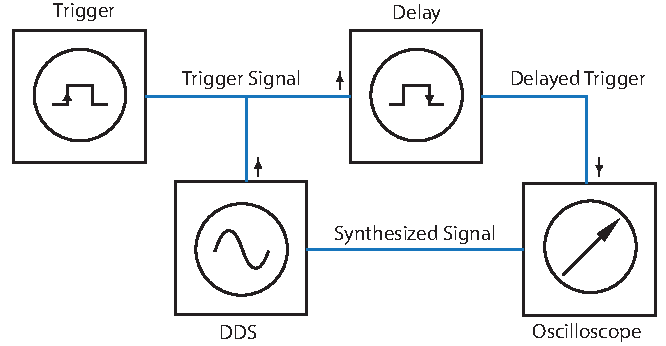
\includegraphics[width=.6\textwidth]{../figure/signal/setup-dds.pdf}
  \caption{Measurement setup of the synthesizer signal. By inserting a pulse
    generator in between the trigger source and the oscilloscope we can delay
    the capture window of the oscilloscope by the pulse width.
  }\label{fig:signal_window_setup}
\end{figure}
The experimental setup used to reailize this concept is schematically drawn in
\Cref{fig:signal_window_setup}. In between the oscilloscope and the trigger
source we inserted a pulse generator. The pulse generator width equals the
delay time of the oscilloscope and the oscilloscope is configured to capture
on the falling edge of the signal generated by the pulse generator. Further
the oscilloscope's impedance was configured to \SI{50}{\ohm} as high impedance
measurements in the high frequency regime are subject to reflection and
inductance effects. In \Cref{tab:signal_parameters_dds} we can find an
overview of the experimental parameters used.
\begin{table}[htb]
  \centering
  \begin{tabular}{cccccc}
    \toprule
    Frequency Range $f$ &
    Sweep Duration $T_s$ &
    Window Duration $T_w$ &
    Number Windows $N_w$ \\
    \midrule
    \SIrange{80}{120}{\mega\hertz} &
    \SI{30}{\milli\second} &
    \SI{50}{\micro\second} &
    300 \\
    \bottomrule
  \end{tabular}
  \caption{Experimental parameters used to inspect the output \gls{rf} signal
    of the \gls{dds}.
  }\label{tab:signal_parameters_dds}
\end{table}
The specified frequency range is motivated to cover the greatest possible
spatial dimensions permitted by the dimensions of the optics. According to
\cref{eq:spatial_position_frequency} this translates to a spatial resolution
in the atomic plane of about \SI{146}{\micro\meter} (typical atomic clouds are
with \SI{30}{\micro\meter} much smaller). Sweep and window duration were
selected as a compromise between the oscilloscope being able to resolve the
signal fine enough to perform \gls{fft} and the sweep duration being
comparable to later experiments. The time delay was incremented in $N_w$ steps
until $T_s=T_w$, thus we will capture $N_w$ overlapping windows.

\subsubsection{Frequency spectrum}

For an ideal linear frequency sweep we would expect a continuous increase of
the frequency with respect to time, yet we know that the \gls{dds} makes use
of digital signal processing methods which suggests a discrete frequency
spectrum. To help us expose the characteristics of the digital frequency
sweep we will utilize a spectrogram. A spectrogram visualizes how the
frequency spectrum varies in time. One way to obtain a spectrogram is to
partition the data into overlapping time chunks while performing \gls{fft}
which allows us to combine time and frequency domain specific
characteristics. In our case we choose the relative spectral power to be
encoded as color.
\begin{figure}[htb]
  \centering
  \begin{adjustbox}{width=\textwidth}
    \inputpgf{../figure/signal/synthesis}{spectrogram.pgf}
  \end{adjustbox}
  \caption{Spectrogram of delayed time windows with width
    \SI{100}{\micro\second} of the \gls{dds} output signal configured to
    perform a linear frequency sweep. For an ideal linear sweep we would
    expect a linear timeline of the frequency, instead we observe a discrete
    set of frequencies.
  }\label{fig:signal_synthesis_spectrogram}
\end{figure}
\Cref{fig:signal_synthesis_spectrogram} depicts four spectrograms, each taken
at a different time window during the frequency sweep. The first spectrogram
captures the start of the frequency sweep as can be read from the time scale.
The first time window does not disclose any signal. This phenomena will be
observed frequently. For unknown reasons the output signal of the \gls{dds} is
absent for multiple microseconds after the \gls{dds} receives the external
trigger signal. The exact duration of the trigger delay varies around
\SI{4}{\milli\second} but does not affect the internal state of the \gls{dds}
as the first measured frequency matches the theoretically expected frequency
according to the ramp. If we take a look at the following spectrogram windows
we can see how the \gls{dds} outputs a constant frequency over a short time
period (\SI{100}{\micro\second}), therefore the frequency range consists of
discrete frequencies. We can actually even observe such a
frequency increment in the second, third and fifth spectrogram. Finally in the
last spectrogram the frequency drops back to the initial value --- a side
effect of the \gls{dds} sweep mode which unfortunately is the only mode, that
supports an external trigger signal.
\begin{figure}[htb]
  \centering
  \begin{adjustbox}{width=\textwidth}
    \inputpgf{../figure/signal/synthesis}{frequency.pgf}
  \end{adjustbox}
  \caption{Most dominant frequency in the \gls{fft} spectrum for each
    (delayed) measurement during a frequency sweep of the \gls{dds}.
  }\label{fig:signal_synthesis_frequency}
\end{figure}
In \Cref{ch:digital_signal_synthesis} we were unable to make a statement about
the frequency resolution of the digital ramp. Therefore we visualized the
frequency evolution with each delayed measurement in
\Cref{fig:signal_synthesis_frequency}. Neglecting the first \num{50}
measurements because of the trigger hole, we find that on average the
frequency increments by about \SI{310}{\kilo\hertz}. Using
\cref{eq:spatial_position_frequency} this relates to a spatial resolution of
about \SI{1.1}{\micro\meter}.

\subsubsection{Amplitude frequency response}

In the Fourier space we can locate the dominant frequency at the maximum of
the power spectrum. That in mind we can reduce the previous obtained time
window measurements to pairs of dominant frequencies and maximum amplitude.
Under the assumption that the maximum voltage per measurement is approximately
the mean peak-to-peak amplitude of the signal we can find the amplitude
frequency response spectrum with little effort.
\Cref{fig:signal_synthesis_response} visualizes the described routine for the
\gls{dds} assigned to the \gls{h} and \gls{v} \gls{aod} with frequency control
by digital ramp and manual increments.
\begin{figure}[htb]
  \centering
  \begin{adjustbox}{width=\textwidth}
    %% Creator: Matplotlib, PGF backend
%%
%% To include the figure in your LaTeX document, write
%%   \input{<filename>.pgf}
%%
%% Make sure the required packages are loaded in your preamble
%%   \usepackage{pgf}
%%
%% Figures using additional raster images can only be included by \input if
%% they are in the same directory as the main LaTeX file. For loading figures
%% from other directories you can use the `import` package
%%   \usepackage{import}
%% and then include the figures with
%%   \import{<path to file>}{<filename>.pgf}
%%
%% Matplotlib used the following preamble
%%   \usepackage{amsmath}\usepackage{siunitx}\usepackage{lmodern}
%%   \usepackage{fontspec}
%%
\begingroup%
\makeatletter%
\begin{pgfpicture}%
\pgfpathrectangle{\pgfpointorigin}{\pgfqpoint{12.000000in}{6.000000in}}%
\pgfusepath{use as bounding box, clip}%
\begin{pgfscope}%
\pgfsetbuttcap%
\pgfsetmiterjoin%
\pgfsetlinewidth{0.000000pt}%
\definecolor{currentstroke}{rgb}{1.000000,1.000000,1.000000}%
\pgfsetstrokecolor{currentstroke}%
\pgfsetdash{}{0pt}%
\pgfpathmoveto{\pgfqpoint{0.000000in}{0.000000in}}%
\pgfpathlineto{\pgfqpoint{12.000000in}{0.000000in}}%
\pgfpathlineto{\pgfqpoint{12.000000in}{6.000000in}}%
\pgfpathlineto{\pgfqpoint{0.000000in}{6.000000in}}%
\pgfpathclose%
\pgfusepath{}%
\end{pgfscope}%
\begin{pgfscope}%
\pgfsetbuttcap%
\pgfsetmiterjoin%
\definecolor{currentfill}{rgb}{1.000000,1.000000,1.000000}%
\pgfsetfillcolor{currentfill}%
\pgfsetlinewidth{0.000000pt}%
\definecolor{currentstroke}{rgb}{0.000000,0.000000,0.000000}%
\pgfsetstrokecolor{currentstroke}%
\pgfsetstrokeopacity{0.000000}%
\pgfsetdash{}{0pt}%
\pgfpathmoveto{\pgfqpoint{1.500000in}{1.200000in}}%
\pgfpathlineto{\pgfqpoint{10.800000in}{1.200000in}}%
\pgfpathlineto{\pgfqpoint{10.800000in}{5.880000in}}%
\pgfpathlineto{\pgfqpoint{1.500000in}{5.880000in}}%
\pgfpathclose%
\pgfusepath{fill}%
\end{pgfscope}%
\begin{pgfscope}%
\pgfsetbuttcap%
\pgfsetroundjoin%
\definecolor{currentfill}{rgb}{0.000000,0.000000,0.000000}%
\pgfsetfillcolor{currentfill}%
\pgfsetlinewidth{1.003750pt}%
\definecolor{currentstroke}{rgb}{0.000000,0.000000,0.000000}%
\pgfsetstrokecolor{currentstroke}%
\pgfsetdash{}{0pt}%
\pgfsys@defobject{currentmarker}{\pgfqpoint{0.000000in}{0.000000in}}{\pgfqpoint{0.000000in}{0.055556in}}{%
\pgfpathmoveto{\pgfqpoint{0.000000in}{0.000000in}}%
\pgfpathlineto{\pgfqpoint{0.000000in}{0.055556in}}%
\pgfusepath{stroke,fill}%
}%
\begin{pgfscope}%
\pgfsys@transformshift{1.922727in}{1.200000in}%
\pgfsys@useobject{currentmarker}{}%
\end{pgfscope}%
\end{pgfscope}%
\begin{pgfscope}%
\pgfsetbuttcap%
\pgfsetroundjoin%
\definecolor{currentfill}{rgb}{0.000000,0.000000,0.000000}%
\pgfsetfillcolor{currentfill}%
\pgfsetlinewidth{1.003750pt}%
\definecolor{currentstroke}{rgb}{0.000000,0.000000,0.000000}%
\pgfsetstrokecolor{currentstroke}%
\pgfsetdash{}{0pt}%
\pgfsys@defobject{currentmarker}{\pgfqpoint{0.000000in}{-0.055556in}}{\pgfqpoint{0.000000in}{0.000000in}}{%
\pgfpathmoveto{\pgfqpoint{0.000000in}{0.000000in}}%
\pgfpathlineto{\pgfqpoint{0.000000in}{-0.055556in}}%
\pgfusepath{stroke,fill}%
}%
\begin{pgfscope}%
\pgfsys@transformshift{1.922727in}{5.880000in}%
\pgfsys@useobject{currentmarker}{}%
\end{pgfscope}%
\end{pgfscope}%
\begin{pgfscope}%
\pgftext[x=1.922727in,y=1.102778in,,top]{\fontsize{10.000000}{12.000000}\selectfont \(\displaystyle 80\)}%
\end{pgfscope}%
\begin{pgfscope}%
\pgfsetbuttcap%
\pgfsetroundjoin%
\definecolor{currentfill}{rgb}{0.000000,0.000000,0.000000}%
\pgfsetfillcolor{currentfill}%
\pgfsetlinewidth{1.003750pt}%
\definecolor{currentstroke}{rgb}{0.000000,0.000000,0.000000}%
\pgfsetstrokecolor{currentstroke}%
\pgfsetdash{}{0pt}%
\pgfsys@defobject{currentmarker}{\pgfqpoint{0.000000in}{0.000000in}}{\pgfqpoint{0.000000in}{0.055556in}}{%
\pgfpathmoveto{\pgfqpoint{0.000000in}{0.000000in}}%
\pgfpathlineto{\pgfqpoint{0.000000in}{0.055556in}}%
\pgfusepath{stroke,fill}%
}%
\begin{pgfscope}%
\pgfsys@transformshift{2.979545in}{1.200000in}%
\pgfsys@useobject{currentmarker}{}%
\end{pgfscope}%
\end{pgfscope}%
\begin{pgfscope}%
\pgfsetbuttcap%
\pgfsetroundjoin%
\definecolor{currentfill}{rgb}{0.000000,0.000000,0.000000}%
\pgfsetfillcolor{currentfill}%
\pgfsetlinewidth{1.003750pt}%
\definecolor{currentstroke}{rgb}{0.000000,0.000000,0.000000}%
\pgfsetstrokecolor{currentstroke}%
\pgfsetdash{}{0pt}%
\pgfsys@defobject{currentmarker}{\pgfqpoint{0.000000in}{-0.055556in}}{\pgfqpoint{0.000000in}{0.000000in}}{%
\pgfpathmoveto{\pgfqpoint{0.000000in}{0.000000in}}%
\pgfpathlineto{\pgfqpoint{0.000000in}{-0.055556in}}%
\pgfusepath{stroke,fill}%
}%
\begin{pgfscope}%
\pgfsys@transformshift{2.979545in}{5.880000in}%
\pgfsys@useobject{currentmarker}{}%
\end{pgfscope}%
\end{pgfscope}%
\begin{pgfscope}%
\pgftext[x=2.979545in,y=1.102778in,,top]{\fontsize{10.000000}{12.000000}\selectfont \(\displaystyle 85\)}%
\end{pgfscope}%
\begin{pgfscope}%
\pgfsetbuttcap%
\pgfsetroundjoin%
\definecolor{currentfill}{rgb}{0.000000,0.000000,0.000000}%
\pgfsetfillcolor{currentfill}%
\pgfsetlinewidth{1.003750pt}%
\definecolor{currentstroke}{rgb}{0.000000,0.000000,0.000000}%
\pgfsetstrokecolor{currentstroke}%
\pgfsetdash{}{0pt}%
\pgfsys@defobject{currentmarker}{\pgfqpoint{0.000000in}{0.000000in}}{\pgfqpoint{0.000000in}{0.055556in}}{%
\pgfpathmoveto{\pgfqpoint{0.000000in}{0.000000in}}%
\pgfpathlineto{\pgfqpoint{0.000000in}{0.055556in}}%
\pgfusepath{stroke,fill}%
}%
\begin{pgfscope}%
\pgfsys@transformshift{4.036364in}{1.200000in}%
\pgfsys@useobject{currentmarker}{}%
\end{pgfscope}%
\end{pgfscope}%
\begin{pgfscope}%
\pgfsetbuttcap%
\pgfsetroundjoin%
\definecolor{currentfill}{rgb}{0.000000,0.000000,0.000000}%
\pgfsetfillcolor{currentfill}%
\pgfsetlinewidth{1.003750pt}%
\definecolor{currentstroke}{rgb}{0.000000,0.000000,0.000000}%
\pgfsetstrokecolor{currentstroke}%
\pgfsetdash{}{0pt}%
\pgfsys@defobject{currentmarker}{\pgfqpoint{0.000000in}{-0.055556in}}{\pgfqpoint{0.000000in}{0.000000in}}{%
\pgfpathmoveto{\pgfqpoint{0.000000in}{0.000000in}}%
\pgfpathlineto{\pgfqpoint{0.000000in}{-0.055556in}}%
\pgfusepath{stroke,fill}%
}%
\begin{pgfscope}%
\pgfsys@transformshift{4.036364in}{5.880000in}%
\pgfsys@useobject{currentmarker}{}%
\end{pgfscope}%
\end{pgfscope}%
\begin{pgfscope}%
\pgftext[x=4.036364in,y=1.102778in,,top]{\fontsize{10.000000}{12.000000}\selectfont \(\displaystyle 90\)}%
\end{pgfscope}%
\begin{pgfscope}%
\pgfsetbuttcap%
\pgfsetroundjoin%
\definecolor{currentfill}{rgb}{0.000000,0.000000,0.000000}%
\pgfsetfillcolor{currentfill}%
\pgfsetlinewidth{1.003750pt}%
\definecolor{currentstroke}{rgb}{0.000000,0.000000,0.000000}%
\pgfsetstrokecolor{currentstroke}%
\pgfsetdash{}{0pt}%
\pgfsys@defobject{currentmarker}{\pgfqpoint{0.000000in}{0.000000in}}{\pgfqpoint{0.000000in}{0.055556in}}{%
\pgfpathmoveto{\pgfqpoint{0.000000in}{0.000000in}}%
\pgfpathlineto{\pgfqpoint{0.000000in}{0.055556in}}%
\pgfusepath{stroke,fill}%
}%
\begin{pgfscope}%
\pgfsys@transformshift{5.093182in}{1.200000in}%
\pgfsys@useobject{currentmarker}{}%
\end{pgfscope}%
\end{pgfscope}%
\begin{pgfscope}%
\pgfsetbuttcap%
\pgfsetroundjoin%
\definecolor{currentfill}{rgb}{0.000000,0.000000,0.000000}%
\pgfsetfillcolor{currentfill}%
\pgfsetlinewidth{1.003750pt}%
\definecolor{currentstroke}{rgb}{0.000000,0.000000,0.000000}%
\pgfsetstrokecolor{currentstroke}%
\pgfsetdash{}{0pt}%
\pgfsys@defobject{currentmarker}{\pgfqpoint{0.000000in}{-0.055556in}}{\pgfqpoint{0.000000in}{0.000000in}}{%
\pgfpathmoveto{\pgfqpoint{0.000000in}{0.000000in}}%
\pgfpathlineto{\pgfqpoint{0.000000in}{-0.055556in}}%
\pgfusepath{stroke,fill}%
}%
\begin{pgfscope}%
\pgfsys@transformshift{5.093182in}{5.880000in}%
\pgfsys@useobject{currentmarker}{}%
\end{pgfscope}%
\end{pgfscope}%
\begin{pgfscope}%
\pgftext[x=5.093182in,y=1.102778in,,top]{\fontsize{10.000000}{12.000000}\selectfont \(\displaystyle 95\)}%
\end{pgfscope}%
\begin{pgfscope}%
\pgfsetbuttcap%
\pgfsetroundjoin%
\definecolor{currentfill}{rgb}{0.000000,0.000000,0.000000}%
\pgfsetfillcolor{currentfill}%
\pgfsetlinewidth{1.003750pt}%
\definecolor{currentstroke}{rgb}{0.000000,0.000000,0.000000}%
\pgfsetstrokecolor{currentstroke}%
\pgfsetdash{}{0pt}%
\pgfsys@defobject{currentmarker}{\pgfqpoint{0.000000in}{0.000000in}}{\pgfqpoint{0.000000in}{0.055556in}}{%
\pgfpathmoveto{\pgfqpoint{0.000000in}{0.000000in}}%
\pgfpathlineto{\pgfqpoint{0.000000in}{0.055556in}}%
\pgfusepath{stroke,fill}%
}%
\begin{pgfscope}%
\pgfsys@transformshift{6.150000in}{1.200000in}%
\pgfsys@useobject{currentmarker}{}%
\end{pgfscope}%
\end{pgfscope}%
\begin{pgfscope}%
\pgfsetbuttcap%
\pgfsetroundjoin%
\definecolor{currentfill}{rgb}{0.000000,0.000000,0.000000}%
\pgfsetfillcolor{currentfill}%
\pgfsetlinewidth{1.003750pt}%
\definecolor{currentstroke}{rgb}{0.000000,0.000000,0.000000}%
\pgfsetstrokecolor{currentstroke}%
\pgfsetdash{}{0pt}%
\pgfsys@defobject{currentmarker}{\pgfqpoint{0.000000in}{-0.055556in}}{\pgfqpoint{0.000000in}{0.000000in}}{%
\pgfpathmoveto{\pgfqpoint{0.000000in}{0.000000in}}%
\pgfpathlineto{\pgfqpoint{0.000000in}{-0.055556in}}%
\pgfusepath{stroke,fill}%
}%
\begin{pgfscope}%
\pgfsys@transformshift{6.150000in}{5.880000in}%
\pgfsys@useobject{currentmarker}{}%
\end{pgfscope}%
\end{pgfscope}%
\begin{pgfscope}%
\pgftext[x=6.150000in,y=1.102778in,,top]{\fontsize{10.000000}{12.000000}\selectfont \(\displaystyle 100\)}%
\end{pgfscope}%
\begin{pgfscope}%
\pgfsetbuttcap%
\pgfsetroundjoin%
\definecolor{currentfill}{rgb}{0.000000,0.000000,0.000000}%
\pgfsetfillcolor{currentfill}%
\pgfsetlinewidth{1.003750pt}%
\definecolor{currentstroke}{rgb}{0.000000,0.000000,0.000000}%
\pgfsetstrokecolor{currentstroke}%
\pgfsetdash{}{0pt}%
\pgfsys@defobject{currentmarker}{\pgfqpoint{0.000000in}{0.000000in}}{\pgfqpoint{0.000000in}{0.055556in}}{%
\pgfpathmoveto{\pgfqpoint{0.000000in}{0.000000in}}%
\pgfpathlineto{\pgfqpoint{0.000000in}{0.055556in}}%
\pgfusepath{stroke,fill}%
}%
\begin{pgfscope}%
\pgfsys@transformshift{7.206818in}{1.200000in}%
\pgfsys@useobject{currentmarker}{}%
\end{pgfscope}%
\end{pgfscope}%
\begin{pgfscope}%
\pgfsetbuttcap%
\pgfsetroundjoin%
\definecolor{currentfill}{rgb}{0.000000,0.000000,0.000000}%
\pgfsetfillcolor{currentfill}%
\pgfsetlinewidth{1.003750pt}%
\definecolor{currentstroke}{rgb}{0.000000,0.000000,0.000000}%
\pgfsetstrokecolor{currentstroke}%
\pgfsetdash{}{0pt}%
\pgfsys@defobject{currentmarker}{\pgfqpoint{0.000000in}{-0.055556in}}{\pgfqpoint{0.000000in}{0.000000in}}{%
\pgfpathmoveto{\pgfqpoint{0.000000in}{0.000000in}}%
\pgfpathlineto{\pgfqpoint{0.000000in}{-0.055556in}}%
\pgfusepath{stroke,fill}%
}%
\begin{pgfscope}%
\pgfsys@transformshift{7.206818in}{5.880000in}%
\pgfsys@useobject{currentmarker}{}%
\end{pgfscope}%
\end{pgfscope}%
\begin{pgfscope}%
\pgftext[x=7.206818in,y=1.102778in,,top]{\fontsize{10.000000}{12.000000}\selectfont \(\displaystyle 105\)}%
\end{pgfscope}%
\begin{pgfscope}%
\pgfsetbuttcap%
\pgfsetroundjoin%
\definecolor{currentfill}{rgb}{0.000000,0.000000,0.000000}%
\pgfsetfillcolor{currentfill}%
\pgfsetlinewidth{1.003750pt}%
\definecolor{currentstroke}{rgb}{0.000000,0.000000,0.000000}%
\pgfsetstrokecolor{currentstroke}%
\pgfsetdash{}{0pt}%
\pgfsys@defobject{currentmarker}{\pgfqpoint{0.000000in}{0.000000in}}{\pgfqpoint{0.000000in}{0.055556in}}{%
\pgfpathmoveto{\pgfqpoint{0.000000in}{0.000000in}}%
\pgfpathlineto{\pgfqpoint{0.000000in}{0.055556in}}%
\pgfusepath{stroke,fill}%
}%
\begin{pgfscope}%
\pgfsys@transformshift{8.263636in}{1.200000in}%
\pgfsys@useobject{currentmarker}{}%
\end{pgfscope}%
\end{pgfscope}%
\begin{pgfscope}%
\pgfsetbuttcap%
\pgfsetroundjoin%
\definecolor{currentfill}{rgb}{0.000000,0.000000,0.000000}%
\pgfsetfillcolor{currentfill}%
\pgfsetlinewidth{1.003750pt}%
\definecolor{currentstroke}{rgb}{0.000000,0.000000,0.000000}%
\pgfsetstrokecolor{currentstroke}%
\pgfsetdash{}{0pt}%
\pgfsys@defobject{currentmarker}{\pgfqpoint{0.000000in}{-0.055556in}}{\pgfqpoint{0.000000in}{0.000000in}}{%
\pgfpathmoveto{\pgfqpoint{0.000000in}{0.000000in}}%
\pgfpathlineto{\pgfqpoint{0.000000in}{-0.055556in}}%
\pgfusepath{stroke,fill}%
}%
\begin{pgfscope}%
\pgfsys@transformshift{8.263636in}{5.880000in}%
\pgfsys@useobject{currentmarker}{}%
\end{pgfscope}%
\end{pgfscope}%
\begin{pgfscope}%
\pgftext[x=8.263636in,y=1.102778in,,top]{\fontsize{10.000000}{12.000000}\selectfont \(\displaystyle 110\)}%
\end{pgfscope}%
\begin{pgfscope}%
\pgfsetbuttcap%
\pgfsetroundjoin%
\definecolor{currentfill}{rgb}{0.000000,0.000000,0.000000}%
\pgfsetfillcolor{currentfill}%
\pgfsetlinewidth{1.003750pt}%
\definecolor{currentstroke}{rgb}{0.000000,0.000000,0.000000}%
\pgfsetstrokecolor{currentstroke}%
\pgfsetdash{}{0pt}%
\pgfsys@defobject{currentmarker}{\pgfqpoint{0.000000in}{0.000000in}}{\pgfqpoint{0.000000in}{0.055556in}}{%
\pgfpathmoveto{\pgfqpoint{0.000000in}{0.000000in}}%
\pgfpathlineto{\pgfqpoint{0.000000in}{0.055556in}}%
\pgfusepath{stroke,fill}%
}%
\begin{pgfscope}%
\pgfsys@transformshift{9.320455in}{1.200000in}%
\pgfsys@useobject{currentmarker}{}%
\end{pgfscope}%
\end{pgfscope}%
\begin{pgfscope}%
\pgfsetbuttcap%
\pgfsetroundjoin%
\definecolor{currentfill}{rgb}{0.000000,0.000000,0.000000}%
\pgfsetfillcolor{currentfill}%
\pgfsetlinewidth{1.003750pt}%
\definecolor{currentstroke}{rgb}{0.000000,0.000000,0.000000}%
\pgfsetstrokecolor{currentstroke}%
\pgfsetdash{}{0pt}%
\pgfsys@defobject{currentmarker}{\pgfqpoint{0.000000in}{-0.055556in}}{\pgfqpoint{0.000000in}{0.000000in}}{%
\pgfpathmoveto{\pgfqpoint{0.000000in}{0.000000in}}%
\pgfpathlineto{\pgfqpoint{0.000000in}{-0.055556in}}%
\pgfusepath{stroke,fill}%
}%
\begin{pgfscope}%
\pgfsys@transformshift{9.320455in}{5.880000in}%
\pgfsys@useobject{currentmarker}{}%
\end{pgfscope}%
\end{pgfscope}%
\begin{pgfscope}%
\pgftext[x=9.320455in,y=1.102778in,,top]{\fontsize{10.000000}{12.000000}\selectfont \(\displaystyle 115\)}%
\end{pgfscope}%
\begin{pgfscope}%
\pgfsetbuttcap%
\pgfsetroundjoin%
\definecolor{currentfill}{rgb}{0.000000,0.000000,0.000000}%
\pgfsetfillcolor{currentfill}%
\pgfsetlinewidth{1.003750pt}%
\definecolor{currentstroke}{rgb}{0.000000,0.000000,0.000000}%
\pgfsetstrokecolor{currentstroke}%
\pgfsetdash{}{0pt}%
\pgfsys@defobject{currentmarker}{\pgfqpoint{0.000000in}{0.000000in}}{\pgfqpoint{0.000000in}{0.055556in}}{%
\pgfpathmoveto{\pgfqpoint{0.000000in}{0.000000in}}%
\pgfpathlineto{\pgfqpoint{0.000000in}{0.055556in}}%
\pgfusepath{stroke,fill}%
}%
\begin{pgfscope}%
\pgfsys@transformshift{10.377273in}{1.200000in}%
\pgfsys@useobject{currentmarker}{}%
\end{pgfscope}%
\end{pgfscope}%
\begin{pgfscope}%
\pgfsetbuttcap%
\pgfsetroundjoin%
\definecolor{currentfill}{rgb}{0.000000,0.000000,0.000000}%
\pgfsetfillcolor{currentfill}%
\pgfsetlinewidth{1.003750pt}%
\definecolor{currentstroke}{rgb}{0.000000,0.000000,0.000000}%
\pgfsetstrokecolor{currentstroke}%
\pgfsetdash{}{0pt}%
\pgfsys@defobject{currentmarker}{\pgfqpoint{0.000000in}{-0.055556in}}{\pgfqpoint{0.000000in}{0.000000in}}{%
\pgfpathmoveto{\pgfqpoint{0.000000in}{0.000000in}}%
\pgfpathlineto{\pgfqpoint{0.000000in}{-0.055556in}}%
\pgfusepath{stroke,fill}%
}%
\begin{pgfscope}%
\pgfsys@transformshift{10.377273in}{5.880000in}%
\pgfsys@useobject{currentmarker}{}%
\end{pgfscope}%
\end{pgfscope}%
\begin{pgfscope}%
\pgftext[x=10.377273in,y=1.102778in,,top]{\fontsize{10.000000}{12.000000}\selectfont \(\displaystyle 120\)}%
\end{pgfscope}%
\begin{pgfscope}%
\pgftext[x=6.150000in,y=0.868333in,,top]{\fontsize{14.000000}{16.800000}\selectfont f (\si{\mega\hertz})}%
\end{pgfscope}%
\begin{pgfscope}%
\pgfsetbuttcap%
\pgfsetroundjoin%
\definecolor{currentfill}{rgb}{0.000000,0.000000,0.000000}%
\pgfsetfillcolor{currentfill}%
\pgfsetlinewidth{1.003750pt}%
\definecolor{currentstroke}{rgb}{0.000000,0.000000,0.000000}%
\pgfsetstrokecolor{currentstroke}%
\pgfsetdash{}{0pt}%
\pgfsys@defobject{currentmarker}{\pgfqpoint{0.000000in}{0.000000in}}{\pgfqpoint{0.055556in}{0.000000in}}{%
\pgfpathmoveto{\pgfqpoint{0.000000in}{0.000000in}}%
\pgfpathlineto{\pgfqpoint{0.055556in}{0.000000in}}%
\pgfusepath{stroke,fill}%
}%
\begin{pgfscope}%
\pgfsys@transformshift{1.500000in}{1.200000in}%
\pgfsys@useobject{currentmarker}{}%
\end{pgfscope}%
\end{pgfscope}%
\begin{pgfscope}%
\pgfsetbuttcap%
\pgfsetroundjoin%
\definecolor{currentfill}{rgb}{0.000000,0.000000,0.000000}%
\pgfsetfillcolor{currentfill}%
\pgfsetlinewidth{1.003750pt}%
\definecolor{currentstroke}{rgb}{0.000000,0.000000,0.000000}%
\pgfsetstrokecolor{currentstroke}%
\pgfsetdash{}{0pt}%
\pgfsys@defobject{currentmarker}{\pgfqpoint{-0.055556in}{0.000000in}}{\pgfqpoint{0.000000in}{0.000000in}}{%
\pgfpathmoveto{\pgfqpoint{0.000000in}{0.000000in}}%
\pgfpathlineto{\pgfqpoint{-0.055556in}{0.000000in}}%
\pgfusepath{stroke,fill}%
}%
\begin{pgfscope}%
\pgfsys@transformshift{10.800000in}{1.200000in}%
\pgfsys@useobject{currentmarker}{}%
\end{pgfscope}%
\end{pgfscope}%
\begin{pgfscope}%
\pgftext[x=1.155864in,y=1.151806in,left,base]{\fontsize{10.000000}{12.000000}\selectfont \(\displaystyle 0.00\)}%
\end{pgfscope}%
\begin{pgfscope}%
\pgfsetbuttcap%
\pgfsetroundjoin%
\definecolor{currentfill}{rgb}{0.000000,0.000000,0.000000}%
\pgfsetfillcolor{currentfill}%
\pgfsetlinewidth{1.003750pt}%
\definecolor{currentstroke}{rgb}{0.000000,0.000000,0.000000}%
\pgfsetstrokecolor{currentstroke}%
\pgfsetdash{}{0pt}%
\pgfsys@defobject{currentmarker}{\pgfqpoint{0.000000in}{0.000000in}}{\pgfqpoint{0.055556in}{0.000000in}}{%
\pgfpathmoveto{\pgfqpoint{0.000000in}{0.000000in}}%
\pgfpathlineto{\pgfqpoint{0.055556in}{0.000000in}}%
\pgfusepath{stroke,fill}%
}%
\begin{pgfscope}%
\pgfsys@transformshift{1.500000in}{1.785000in}%
\pgfsys@useobject{currentmarker}{}%
\end{pgfscope}%
\end{pgfscope}%
\begin{pgfscope}%
\pgfsetbuttcap%
\pgfsetroundjoin%
\definecolor{currentfill}{rgb}{0.000000,0.000000,0.000000}%
\pgfsetfillcolor{currentfill}%
\pgfsetlinewidth{1.003750pt}%
\definecolor{currentstroke}{rgb}{0.000000,0.000000,0.000000}%
\pgfsetstrokecolor{currentstroke}%
\pgfsetdash{}{0pt}%
\pgfsys@defobject{currentmarker}{\pgfqpoint{-0.055556in}{0.000000in}}{\pgfqpoint{0.000000in}{0.000000in}}{%
\pgfpathmoveto{\pgfqpoint{0.000000in}{0.000000in}}%
\pgfpathlineto{\pgfqpoint{-0.055556in}{0.000000in}}%
\pgfusepath{stroke,fill}%
}%
\begin{pgfscope}%
\pgfsys@transformshift{10.800000in}{1.785000in}%
\pgfsys@useobject{currentmarker}{}%
\end{pgfscope}%
\end{pgfscope}%
\begin{pgfscope}%
\pgftext[x=1.155864in,y=1.736806in,left,base]{\fontsize{10.000000}{12.000000}\selectfont \(\displaystyle 0.05\)}%
\end{pgfscope}%
\begin{pgfscope}%
\pgfsetbuttcap%
\pgfsetroundjoin%
\definecolor{currentfill}{rgb}{0.000000,0.000000,0.000000}%
\pgfsetfillcolor{currentfill}%
\pgfsetlinewidth{1.003750pt}%
\definecolor{currentstroke}{rgb}{0.000000,0.000000,0.000000}%
\pgfsetstrokecolor{currentstroke}%
\pgfsetdash{}{0pt}%
\pgfsys@defobject{currentmarker}{\pgfqpoint{0.000000in}{0.000000in}}{\pgfqpoint{0.055556in}{0.000000in}}{%
\pgfpathmoveto{\pgfqpoint{0.000000in}{0.000000in}}%
\pgfpathlineto{\pgfqpoint{0.055556in}{0.000000in}}%
\pgfusepath{stroke,fill}%
}%
\begin{pgfscope}%
\pgfsys@transformshift{1.500000in}{2.370000in}%
\pgfsys@useobject{currentmarker}{}%
\end{pgfscope}%
\end{pgfscope}%
\begin{pgfscope}%
\pgfsetbuttcap%
\pgfsetroundjoin%
\definecolor{currentfill}{rgb}{0.000000,0.000000,0.000000}%
\pgfsetfillcolor{currentfill}%
\pgfsetlinewidth{1.003750pt}%
\definecolor{currentstroke}{rgb}{0.000000,0.000000,0.000000}%
\pgfsetstrokecolor{currentstroke}%
\pgfsetdash{}{0pt}%
\pgfsys@defobject{currentmarker}{\pgfqpoint{-0.055556in}{0.000000in}}{\pgfqpoint{0.000000in}{0.000000in}}{%
\pgfpathmoveto{\pgfqpoint{0.000000in}{0.000000in}}%
\pgfpathlineto{\pgfqpoint{-0.055556in}{0.000000in}}%
\pgfusepath{stroke,fill}%
}%
\begin{pgfscope}%
\pgfsys@transformshift{10.800000in}{2.370000in}%
\pgfsys@useobject{currentmarker}{}%
\end{pgfscope}%
\end{pgfscope}%
\begin{pgfscope}%
\pgftext[x=1.155864in,y=2.321806in,left,base]{\fontsize{10.000000}{12.000000}\selectfont \(\displaystyle 0.10\)}%
\end{pgfscope}%
\begin{pgfscope}%
\pgfsetbuttcap%
\pgfsetroundjoin%
\definecolor{currentfill}{rgb}{0.000000,0.000000,0.000000}%
\pgfsetfillcolor{currentfill}%
\pgfsetlinewidth{1.003750pt}%
\definecolor{currentstroke}{rgb}{0.000000,0.000000,0.000000}%
\pgfsetstrokecolor{currentstroke}%
\pgfsetdash{}{0pt}%
\pgfsys@defobject{currentmarker}{\pgfqpoint{0.000000in}{0.000000in}}{\pgfqpoint{0.055556in}{0.000000in}}{%
\pgfpathmoveto{\pgfqpoint{0.000000in}{0.000000in}}%
\pgfpathlineto{\pgfqpoint{0.055556in}{0.000000in}}%
\pgfusepath{stroke,fill}%
}%
\begin{pgfscope}%
\pgfsys@transformshift{1.500000in}{2.955000in}%
\pgfsys@useobject{currentmarker}{}%
\end{pgfscope}%
\end{pgfscope}%
\begin{pgfscope}%
\pgfsetbuttcap%
\pgfsetroundjoin%
\definecolor{currentfill}{rgb}{0.000000,0.000000,0.000000}%
\pgfsetfillcolor{currentfill}%
\pgfsetlinewidth{1.003750pt}%
\definecolor{currentstroke}{rgb}{0.000000,0.000000,0.000000}%
\pgfsetstrokecolor{currentstroke}%
\pgfsetdash{}{0pt}%
\pgfsys@defobject{currentmarker}{\pgfqpoint{-0.055556in}{0.000000in}}{\pgfqpoint{0.000000in}{0.000000in}}{%
\pgfpathmoveto{\pgfqpoint{0.000000in}{0.000000in}}%
\pgfpathlineto{\pgfqpoint{-0.055556in}{0.000000in}}%
\pgfusepath{stroke,fill}%
}%
\begin{pgfscope}%
\pgfsys@transformshift{10.800000in}{2.955000in}%
\pgfsys@useobject{currentmarker}{}%
\end{pgfscope}%
\end{pgfscope}%
\begin{pgfscope}%
\pgftext[x=1.155864in,y=2.906806in,left,base]{\fontsize{10.000000}{12.000000}\selectfont \(\displaystyle 0.15\)}%
\end{pgfscope}%
\begin{pgfscope}%
\pgfsetbuttcap%
\pgfsetroundjoin%
\definecolor{currentfill}{rgb}{0.000000,0.000000,0.000000}%
\pgfsetfillcolor{currentfill}%
\pgfsetlinewidth{1.003750pt}%
\definecolor{currentstroke}{rgb}{0.000000,0.000000,0.000000}%
\pgfsetstrokecolor{currentstroke}%
\pgfsetdash{}{0pt}%
\pgfsys@defobject{currentmarker}{\pgfqpoint{0.000000in}{0.000000in}}{\pgfqpoint{0.055556in}{0.000000in}}{%
\pgfpathmoveto{\pgfqpoint{0.000000in}{0.000000in}}%
\pgfpathlineto{\pgfqpoint{0.055556in}{0.000000in}}%
\pgfusepath{stroke,fill}%
}%
\begin{pgfscope}%
\pgfsys@transformshift{1.500000in}{3.540000in}%
\pgfsys@useobject{currentmarker}{}%
\end{pgfscope}%
\end{pgfscope}%
\begin{pgfscope}%
\pgfsetbuttcap%
\pgfsetroundjoin%
\definecolor{currentfill}{rgb}{0.000000,0.000000,0.000000}%
\pgfsetfillcolor{currentfill}%
\pgfsetlinewidth{1.003750pt}%
\definecolor{currentstroke}{rgb}{0.000000,0.000000,0.000000}%
\pgfsetstrokecolor{currentstroke}%
\pgfsetdash{}{0pt}%
\pgfsys@defobject{currentmarker}{\pgfqpoint{-0.055556in}{0.000000in}}{\pgfqpoint{0.000000in}{0.000000in}}{%
\pgfpathmoveto{\pgfqpoint{0.000000in}{0.000000in}}%
\pgfpathlineto{\pgfqpoint{-0.055556in}{0.000000in}}%
\pgfusepath{stroke,fill}%
}%
\begin{pgfscope}%
\pgfsys@transformshift{10.800000in}{3.540000in}%
\pgfsys@useobject{currentmarker}{}%
\end{pgfscope}%
\end{pgfscope}%
\begin{pgfscope}%
\pgftext[x=1.155864in,y=3.491806in,left,base]{\fontsize{10.000000}{12.000000}\selectfont \(\displaystyle 0.20\)}%
\end{pgfscope}%
\begin{pgfscope}%
\pgfsetbuttcap%
\pgfsetroundjoin%
\definecolor{currentfill}{rgb}{0.000000,0.000000,0.000000}%
\pgfsetfillcolor{currentfill}%
\pgfsetlinewidth{1.003750pt}%
\definecolor{currentstroke}{rgb}{0.000000,0.000000,0.000000}%
\pgfsetstrokecolor{currentstroke}%
\pgfsetdash{}{0pt}%
\pgfsys@defobject{currentmarker}{\pgfqpoint{0.000000in}{0.000000in}}{\pgfqpoint{0.055556in}{0.000000in}}{%
\pgfpathmoveto{\pgfqpoint{0.000000in}{0.000000in}}%
\pgfpathlineto{\pgfqpoint{0.055556in}{0.000000in}}%
\pgfusepath{stroke,fill}%
}%
\begin{pgfscope}%
\pgfsys@transformshift{1.500000in}{4.125000in}%
\pgfsys@useobject{currentmarker}{}%
\end{pgfscope}%
\end{pgfscope}%
\begin{pgfscope}%
\pgfsetbuttcap%
\pgfsetroundjoin%
\definecolor{currentfill}{rgb}{0.000000,0.000000,0.000000}%
\pgfsetfillcolor{currentfill}%
\pgfsetlinewidth{1.003750pt}%
\definecolor{currentstroke}{rgb}{0.000000,0.000000,0.000000}%
\pgfsetstrokecolor{currentstroke}%
\pgfsetdash{}{0pt}%
\pgfsys@defobject{currentmarker}{\pgfqpoint{-0.055556in}{0.000000in}}{\pgfqpoint{0.000000in}{0.000000in}}{%
\pgfpathmoveto{\pgfqpoint{0.000000in}{0.000000in}}%
\pgfpathlineto{\pgfqpoint{-0.055556in}{0.000000in}}%
\pgfusepath{stroke,fill}%
}%
\begin{pgfscope}%
\pgfsys@transformshift{10.800000in}{4.125000in}%
\pgfsys@useobject{currentmarker}{}%
\end{pgfscope}%
\end{pgfscope}%
\begin{pgfscope}%
\pgftext[x=1.155864in,y=4.076806in,left,base]{\fontsize{10.000000}{12.000000}\selectfont \(\displaystyle 0.25\)}%
\end{pgfscope}%
\begin{pgfscope}%
\pgfsetbuttcap%
\pgfsetroundjoin%
\definecolor{currentfill}{rgb}{0.000000,0.000000,0.000000}%
\pgfsetfillcolor{currentfill}%
\pgfsetlinewidth{1.003750pt}%
\definecolor{currentstroke}{rgb}{0.000000,0.000000,0.000000}%
\pgfsetstrokecolor{currentstroke}%
\pgfsetdash{}{0pt}%
\pgfsys@defobject{currentmarker}{\pgfqpoint{0.000000in}{0.000000in}}{\pgfqpoint{0.055556in}{0.000000in}}{%
\pgfpathmoveto{\pgfqpoint{0.000000in}{0.000000in}}%
\pgfpathlineto{\pgfqpoint{0.055556in}{0.000000in}}%
\pgfusepath{stroke,fill}%
}%
\begin{pgfscope}%
\pgfsys@transformshift{1.500000in}{4.710000in}%
\pgfsys@useobject{currentmarker}{}%
\end{pgfscope}%
\end{pgfscope}%
\begin{pgfscope}%
\pgfsetbuttcap%
\pgfsetroundjoin%
\definecolor{currentfill}{rgb}{0.000000,0.000000,0.000000}%
\pgfsetfillcolor{currentfill}%
\pgfsetlinewidth{1.003750pt}%
\definecolor{currentstroke}{rgb}{0.000000,0.000000,0.000000}%
\pgfsetstrokecolor{currentstroke}%
\pgfsetdash{}{0pt}%
\pgfsys@defobject{currentmarker}{\pgfqpoint{-0.055556in}{0.000000in}}{\pgfqpoint{0.000000in}{0.000000in}}{%
\pgfpathmoveto{\pgfqpoint{0.000000in}{0.000000in}}%
\pgfpathlineto{\pgfqpoint{-0.055556in}{0.000000in}}%
\pgfusepath{stroke,fill}%
}%
\begin{pgfscope}%
\pgfsys@transformshift{10.800000in}{4.710000in}%
\pgfsys@useobject{currentmarker}{}%
\end{pgfscope}%
\end{pgfscope}%
\begin{pgfscope}%
\pgftext[x=1.155864in,y=4.661806in,left,base]{\fontsize{10.000000}{12.000000}\selectfont \(\displaystyle 0.30\)}%
\end{pgfscope}%
\begin{pgfscope}%
\pgfsetbuttcap%
\pgfsetroundjoin%
\definecolor{currentfill}{rgb}{0.000000,0.000000,0.000000}%
\pgfsetfillcolor{currentfill}%
\pgfsetlinewidth{1.003750pt}%
\definecolor{currentstroke}{rgb}{0.000000,0.000000,0.000000}%
\pgfsetstrokecolor{currentstroke}%
\pgfsetdash{}{0pt}%
\pgfsys@defobject{currentmarker}{\pgfqpoint{0.000000in}{0.000000in}}{\pgfqpoint{0.055556in}{0.000000in}}{%
\pgfpathmoveto{\pgfqpoint{0.000000in}{0.000000in}}%
\pgfpathlineto{\pgfqpoint{0.055556in}{0.000000in}}%
\pgfusepath{stroke,fill}%
}%
\begin{pgfscope}%
\pgfsys@transformshift{1.500000in}{5.295000in}%
\pgfsys@useobject{currentmarker}{}%
\end{pgfscope}%
\end{pgfscope}%
\begin{pgfscope}%
\pgfsetbuttcap%
\pgfsetroundjoin%
\definecolor{currentfill}{rgb}{0.000000,0.000000,0.000000}%
\pgfsetfillcolor{currentfill}%
\pgfsetlinewidth{1.003750pt}%
\definecolor{currentstroke}{rgb}{0.000000,0.000000,0.000000}%
\pgfsetstrokecolor{currentstroke}%
\pgfsetdash{}{0pt}%
\pgfsys@defobject{currentmarker}{\pgfqpoint{-0.055556in}{0.000000in}}{\pgfqpoint{0.000000in}{0.000000in}}{%
\pgfpathmoveto{\pgfqpoint{0.000000in}{0.000000in}}%
\pgfpathlineto{\pgfqpoint{-0.055556in}{0.000000in}}%
\pgfusepath{stroke,fill}%
}%
\begin{pgfscope}%
\pgfsys@transformshift{10.800000in}{5.295000in}%
\pgfsys@useobject{currentmarker}{}%
\end{pgfscope}%
\end{pgfscope}%
\begin{pgfscope}%
\pgftext[x=1.155864in,y=5.246806in,left,base]{\fontsize{10.000000}{12.000000}\selectfont \(\displaystyle 0.35\)}%
\end{pgfscope}%
\begin{pgfscope}%
\pgfsetbuttcap%
\pgfsetroundjoin%
\definecolor{currentfill}{rgb}{0.000000,0.000000,0.000000}%
\pgfsetfillcolor{currentfill}%
\pgfsetlinewidth{1.003750pt}%
\definecolor{currentstroke}{rgb}{0.000000,0.000000,0.000000}%
\pgfsetstrokecolor{currentstroke}%
\pgfsetdash{}{0pt}%
\pgfsys@defobject{currentmarker}{\pgfqpoint{0.000000in}{0.000000in}}{\pgfqpoint{0.055556in}{0.000000in}}{%
\pgfpathmoveto{\pgfqpoint{0.000000in}{0.000000in}}%
\pgfpathlineto{\pgfqpoint{0.055556in}{0.000000in}}%
\pgfusepath{stroke,fill}%
}%
\begin{pgfscope}%
\pgfsys@transformshift{1.500000in}{5.880000in}%
\pgfsys@useobject{currentmarker}{}%
\end{pgfscope}%
\end{pgfscope}%
\begin{pgfscope}%
\pgfsetbuttcap%
\pgfsetroundjoin%
\definecolor{currentfill}{rgb}{0.000000,0.000000,0.000000}%
\pgfsetfillcolor{currentfill}%
\pgfsetlinewidth{1.003750pt}%
\definecolor{currentstroke}{rgb}{0.000000,0.000000,0.000000}%
\pgfsetstrokecolor{currentstroke}%
\pgfsetdash{}{0pt}%
\pgfsys@defobject{currentmarker}{\pgfqpoint{-0.055556in}{0.000000in}}{\pgfqpoint{0.000000in}{0.000000in}}{%
\pgfpathmoveto{\pgfqpoint{0.000000in}{0.000000in}}%
\pgfpathlineto{\pgfqpoint{-0.055556in}{0.000000in}}%
\pgfusepath{stroke,fill}%
}%
\begin{pgfscope}%
\pgfsys@transformshift{10.800000in}{5.880000in}%
\pgfsys@useobject{currentmarker}{}%
\end{pgfscope}%
\end{pgfscope}%
\begin{pgfscope}%
\pgftext[x=1.155864in,y=5.831806in,left,base]{\fontsize{10.000000}{12.000000}\selectfont \(\displaystyle 0.40\)}%
\end{pgfscope}%
\begin{pgfscope}%
\pgfsetbuttcap%
\pgfsetroundjoin%
\definecolor{currentfill}{rgb}{0.000000,0.000000,0.000000}%
\pgfsetfillcolor{currentfill}%
\pgfsetlinewidth{0.501875pt}%
\definecolor{currentstroke}{rgb}{0.000000,0.000000,0.000000}%
\pgfsetstrokecolor{currentstroke}%
\pgfsetdash{}{0pt}%
\pgfsys@defobject{currentmarker}{\pgfqpoint{0.000000in}{0.000000in}}{\pgfqpoint{0.027778in}{0.000000in}}{%
\pgfpathmoveto{\pgfqpoint{0.000000in}{0.000000in}}%
\pgfpathlineto{\pgfqpoint{0.027778in}{0.000000in}}%
\pgfusepath{stroke,fill}%
}%
\begin{pgfscope}%
\pgfsys@transformshift{1.500000in}{1.317000in}%
\pgfsys@useobject{currentmarker}{}%
\end{pgfscope}%
\end{pgfscope}%
\begin{pgfscope}%
\pgfsetbuttcap%
\pgfsetroundjoin%
\definecolor{currentfill}{rgb}{0.000000,0.000000,0.000000}%
\pgfsetfillcolor{currentfill}%
\pgfsetlinewidth{0.501875pt}%
\definecolor{currentstroke}{rgb}{0.000000,0.000000,0.000000}%
\pgfsetstrokecolor{currentstroke}%
\pgfsetdash{}{0pt}%
\pgfsys@defobject{currentmarker}{\pgfqpoint{-0.027778in}{0.000000in}}{\pgfqpoint{0.000000in}{0.000000in}}{%
\pgfpathmoveto{\pgfqpoint{0.000000in}{0.000000in}}%
\pgfpathlineto{\pgfqpoint{-0.027778in}{0.000000in}}%
\pgfusepath{stroke,fill}%
}%
\begin{pgfscope}%
\pgfsys@transformshift{10.800000in}{1.317000in}%
\pgfsys@useobject{currentmarker}{}%
\end{pgfscope}%
\end{pgfscope}%
\begin{pgfscope}%
\pgfsetbuttcap%
\pgfsetroundjoin%
\definecolor{currentfill}{rgb}{0.000000,0.000000,0.000000}%
\pgfsetfillcolor{currentfill}%
\pgfsetlinewidth{0.501875pt}%
\definecolor{currentstroke}{rgb}{0.000000,0.000000,0.000000}%
\pgfsetstrokecolor{currentstroke}%
\pgfsetdash{}{0pt}%
\pgfsys@defobject{currentmarker}{\pgfqpoint{0.000000in}{0.000000in}}{\pgfqpoint{0.027778in}{0.000000in}}{%
\pgfpathmoveto{\pgfqpoint{0.000000in}{0.000000in}}%
\pgfpathlineto{\pgfqpoint{0.027778in}{0.000000in}}%
\pgfusepath{stroke,fill}%
}%
\begin{pgfscope}%
\pgfsys@transformshift{1.500000in}{1.434000in}%
\pgfsys@useobject{currentmarker}{}%
\end{pgfscope}%
\end{pgfscope}%
\begin{pgfscope}%
\pgfsetbuttcap%
\pgfsetroundjoin%
\definecolor{currentfill}{rgb}{0.000000,0.000000,0.000000}%
\pgfsetfillcolor{currentfill}%
\pgfsetlinewidth{0.501875pt}%
\definecolor{currentstroke}{rgb}{0.000000,0.000000,0.000000}%
\pgfsetstrokecolor{currentstroke}%
\pgfsetdash{}{0pt}%
\pgfsys@defobject{currentmarker}{\pgfqpoint{-0.027778in}{0.000000in}}{\pgfqpoint{0.000000in}{0.000000in}}{%
\pgfpathmoveto{\pgfqpoint{0.000000in}{0.000000in}}%
\pgfpathlineto{\pgfqpoint{-0.027778in}{0.000000in}}%
\pgfusepath{stroke,fill}%
}%
\begin{pgfscope}%
\pgfsys@transformshift{10.800000in}{1.434000in}%
\pgfsys@useobject{currentmarker}{}%
\end{pgfscope}%
\end{pgfscope}%
\begin{pgfscope}%
\pgfsetbuttcap%
\pgfsetroundjoin%
\definecolor{currentfill}{rgb}{0.000000,0.000000,0.000000}%
\pgfsetfillcolor{currentfill}%
\pgfsetlinewidth{0.501875pt}%
\definecolor{currentstroke}{rgb}{0.000000,0.000000,0.000000}%
\pgfsetstrokecolor{currentstroke}%
\pgfsetdash{}{0pt}%
\pgfsys@defobject{currentmarker}{\pgfqpoint{0.000000in}{0.000000in}}{\pgfqpoint{0.027778in}{0.000000in}}{%
\pgfpathmoveto{\pgfqpoint{0.000000in}{0.000000in}}%
\pgfpathlineto{\pgfqpoint{0.027778in}{0.000000in}}%
\pgfusepath{stroke,fill}%
}%
\begin{pgfscope}%
\pgfsys@transformshift{1.500000in}{1.551000in}%
\pgfsys@useobject{currentmarker}{}%
\end{pgfscope}%
\end{pgfscope}%
\begin{pgfscope}%
\pgfsetbuttcap%
\pgfsetroundjoin%
\definecolor{currentfill}{rgb}{0.000000,0.000000,0.000000}%
\pgfsetfillcolor{currentfill}%
\pgfsetlinewidth{0.501875pt}%
\definecolor{currentstroke}{rgb}{0.000000,0.000000,0.000000}%
\pgfsetstrokecolor{currentstroke}%
\pgfsetdash{}{0pt}%
\pgfsys@defobject{currentmarker}{\pgfqpoint{-0.027778in}{0.000000in}}{\pgfqpoint{0.000000in}{0.000000in}}{%
\pgfpathmoveto{\pgfqpoint{0.000000in}{0.000000in}}%
\pgfpathlineto{\pgfqpoint{-0.027778in}{0.000000in}}%
\pgfusepath{stroke,fill}%
}%
\begin{pgfscope}%
\pgfsys@transformshift{10.800000in}{1.551000in}%
\pgfsys@useobject{currentmarker}{}%
\end{pgfscope}%
\end{pgfscope}%
\begin{pgfscope}%
\pgfsetbuttcap%
\pgfsetroundjoin%
\definecolor{currentfill}{rgb}{0.000000,0.000000,0.000000}%
\pgfsetfillcolor{currentfill}%
\pgfsetlinewidth{0.501875pt}%
\definecolor{currentstroke}{rgb}{0.000000,0.000000,0.000000}%
\pgfsetstrokecolor{currentstroke}%
\pgfsetdash{}{0pt}%
\pgfsys@defobject{currentmarker}{\pgfqpoint{0.000000in}{0.000000in}}{\pgfqpoint{0.027778in}{0.000000in}}{%
\pgfpathmoveto{\pgfqpoint{0.000000in}{0.000000in}}%
\pgfpathlineto{\pgfqpoint{0.027778in}{0.000000in}}%
\pgfusepath{stroke,fill}%
}%
\begin{pgfscope}%
\pgfsys@transformshift{1.500000in}{1.668000in}%
\pgfsys@useobject{currentmarker}{}%
\end{pgfscope}%
\end{pgfscope}%
\begin{pgfscope}%
\pgfsetbuttcap%
\pgfsetroundjoin%
\definecolor{currentfill}{rgb}{0.000000,0.000000,0.000000}%
\pgfsetfillcolor{currentfill}%
\pgfsetlinewidth{0.501875pt}%
\definecolor{currentstroke}{rgb}{0.000000,0.000000,0.000000}%
\pgfsetstrokecolor{currentstroke}%
\pgfsetdash{}{0pt}%
\pgfsys@defobject{currentmarker}{\pgfqpoint{-0.027778in}{0.000000in}}{\pgfqpoint{0.000000in}{0.000000in}}{%
\pgfpathmoveto{\pgfqpoint{0.000000in}{0.000000in}}%
\pgfpathlineto{\pgfqpoint{-0.027778in}{0.000000in}}%
\pgfusepath{stroke,fill}%
}%
\begin{pgfscope}%
\pgfsys@transformshift{10.800000in}{1.668000in}%
\pgfsys@useobject{currentmarker}{}%
\end{pgfscope}%
\end{pgfscope}%
\begin{pgfscope}%
\pgfsetbuttcap%
\pgfsetroundjoin%
\definecolor{currentfill}{rgb}{0.000000,0.000000,0.000000}%
\pgfsetfillcolor{currentfill}%
\pgfsetlinewidth{0.501875pt}%
\definecolor{currentstroke}{rgb}{0.000000,0.000000,0.000000}%
\pgfsetstrokecolor{currentstroke}%
\pgfsetdash{}{0pt}%
\pgfsys@defobject{currentmarker}{\pgfqpoint{0.000000in}{0.000000in}}{\pgfqpoint{0.027778in}{0.000000in}}{%
\pgfpathmoveto{\pgfqpoint{0.000000in}{0.000000in}}%
\pgfpathlineto{\pgfqpoint{0.027778in}{0.000000in}}%
\pgfusepath{stroke,fill}%
}%
\begin{pgfscope}%
\pgfsys@transformshift{1.500000in}{1.902000in}%
\pgfsys@useobject{currentmarker}{}%
\end{pgfscope}%
\end{pgfscope}%
\begin{pgfscope}%
\pgfsetbuttcap%
\pgfsetroundjoin%
\definecolor{currentfill}{rgb}{0.000000,0.000000,0.000000}%
\pgfsetfillcolor{currentfill}%
\pgfsetlinewidth{0.501875pt}%
\definecolor{currentstroke}{rgb}{0.000000,0.000000,0.000000}%
\pgfsetstrokecolor{currentstroke}%
\pgfsetdash{}{0pt}%
\pgfsys@defobject{currentmarker}{\pgfqpoint{-0.027778in}{0.000000in}}{\pgfqpoint{0.000000in}{0.000000in}}{%
\pgfpathmoveto{\pgfqpoint{0.000000in}{0.000000in}}%
\pgfpathlineto{\pgfqpoint{-0.027778in}{0.000000in}}%
\pgfusepath{stroke,fill}%
}%
\begin{pgfscope}%
\pgfsys@transformshift{10.800000in}{1.902000in}%
\pgfsys@useobject{currentmarker}{}%
\end{pgfscope}%
\end{pgfscope}%
\begin{pgfscope}%
\pgfsetbuttcap%
\pgfsetroundjoin%
\definecolor{currentfill}{rgb}{0.000000,0.000000,0.000000}%
\pgfsetfillcolor{currentfill}%
\pgfsetlinewidth{0.501875pt}%
\definecolor{currentstroke}{rgb}{0.000000,0.000000,0.000000}%
\pgfsetstrokecolor{currentstroke}%
\pgfsetdash{}{0pt}%
\pgfsys@defobject{currentmarker}{\pgfqpoint{0.000000in}{0.000000in}}{\pgfqpoint{0.027778in}{0.000000in}}{%
\pgfpathmoveto{\pgfqpoint{0.000000in}{0.000000in}}%
\pgfpathlineto{\pgfqpoint{0.027778in}{0.000000in}}%
\pgfusepath{stroke,fill}%
}%
\begin{pgfscope}%
\pgfsys@transformshift{1.500000in}{2.019000in}%
\pgfsys@useobject{currentmarker}{}%
\end{pgfscope}%
\end{pgfscope}%
\begin{pgfscope}%
\pgfsetbuttcap%
\pgfsetroundjoin%
\definecolor{currentfill}{rgb}{0.000000,0.000000,0.000000}%
\pgfsetfillcolor{currentfill}%
\pgfsetlinewidth{0.501875pt}%
\definecolor{currentstroke}{rgb}{0.000000,0.000000,0.000000}%
\pgfsetstrokecolor{currentstroke}%
\pgfsetdash{}{0pt}%
\pgfsys@defobject{currentmarker}{\pgfqpoint{-0.027778in}{0.000000in}}{\pgfqpoint{0.000000in}{0.000000in}}{%
\pgfpathmoveto{\pgfqpoint{0.000000in}{0.000000in}}%
\pgfpathlineto{\pgfqpoint{-0.027778in}{0.000000in}}%
\pgfusepath{stroke,fill}%
}%
\begin{pgfscope}%
\pgfsys@transformshift{10.800000in}{2.019000in}%
\pgfsys@useobject{currentmarker}{}%
\end{pgfscope}%
\end{pgfscope}%
\begin{pgfscope}%
\pgfsetbuttcap%
\pgfsetroundjoin%
\definecolor{currentfill}{rgb}{0.000000,0.000000,0.000000}%
\pgfsetfillcolor{currentfill}%
\pgfsetlinewidth{0.501875pt}%
\definecolor{currentstroke}{rgb}{0.000000,0.000000,0.000000}%
\pgfsetstrokecolor{currentstroke}%
\pgfsetdash{}{0pt}%
\pgfsys@defobject{currentmarker}{\pgfqpoint{0.000000in}{0.000000in}}{\pgfqpoint{0.027778in}{0.000000in}}{%
\pgfpathmoveto{\pgfqpoint{0.000000in}{0.000000in}}%
\pgfpathlineto{\pgfqpoint{0.027778in}{0.000000in}}%
\pgfusepath{stroke,fill}%
}%
\begin{pgfscope}%
\pgfsys@transformshift{1.500000in}{2.136000in}%
\pgfsys@useobject{currentmarker}{}%
\end{pgfscope}%
\end{pgfscope}%
\begin{pgfscope}%
\pgfsetbuttcap%
\pgfsetroundjoin%
\definecolor{currentfill}{rgb}{0.000000,0.000000,0.000000}%
\pgfsetfillcolor{currentfill}%
\pgfsetlinewidth{0.501875pt}%
\definecolor{currentstroke}{rgb}{0.000000,0.000000,0.000000}%
\pgfsetstrokecolor{currentstroke}%
\pgfsetdash{}{0pt}%
\pgfsys@defobject{currentmarker}{\pgfqpoint{-0.027778in}{0.000000in}}{\pgfqpoint{0.000000in}{0.000000in}}{%
\pgfpathmoveto{\pgfqpoint{0.000000in}{0.000000in}}%
\pgfpathlineto{\pgfqpoint{-0.027778in}{0.000000in}}%
\pgfusepath{stroke,fill}%
}%
\begin{pgfscope}%
\pgfsys@transformshift{10.800000in}{2.136000in}%
\pgfsys@useobject{currentmarker}{}%
\end{pgfscope}%
\end{pgfscope}%
\begin{pgfscope}%
\pgfsetbuttcap%
\pgfsetroundjoin%
\definecolor{currentfill}{rgb}{0.000000,0.000000,0.000000}%
\pgfsetfillcolor{currentfill}%
\pgfsetlinewidth{0.501875pt}%
\definecolor{currentstroke}{rgb}{0.000000,0.000000,0.000000}%
\pgfsetstrokecolor{currentstroke}%
\pgfsetdash{}{0pt}%
\pgfsys@defobject{currentmarker}{\pgfqpoint{0.000000in}{0.000000in}}{\pgfqpoint{0.027778in}{0.000000in}}{%
\pgfpathmoveto{\pgfqpoint{0.000000in}{0.000000in}}%
\pgfpathlineto{\pgfqpoint{0.027778in}{0.000000in}}%
\pgfusepath{stroke,fill}%
}%
\begin{pgfscope}%
\pgfsys@transformshift{1.500000in}{2.253000in}%
\pgfsys@useobject{currentmarker}{}%
\end{pgfscope}%
\end{pgfscope}%
\begin{pgfscope}%
\pgfsetbuttcap%
\pgfsetroundjoin%
\definecolor{currentfill}{rgb}{0.000000,0.000000,0.000000}%
\pgfsetfillcolor{currentfill}%
\pgfsetlinewidth{0.501875pt}%
\definecolor{currentstroke}{rgb}{0.000000,0.000000,0.000000}%
\pgfsetstrokecolor{currentstroke}%
\pgfsetdash{}{0pt}%
\pgfsys@defobject{currentmarker}{\pgfqpoint{-0.027778in}{0.000000in}}{\pgfqpoint{0.000000in}{0.000000in}}{%
\pgfpathmoveto{\pgfqpoint{0.000000in}{0.000000in}}%
\pgfpathlineto{\pgfqpoint{-0.027778in}{0.000000in}}%
\pgfusepath{stroke,fill}%
}%
\begin{pgfscope}%
\pgfsys@transformshift{10.800000in}{2.253000in}%
\pgfsys@useobject{currentmarker}{}%
\end{pgfscope}%
\end{pgfscope}%
\begin{pgfscope}%
\pgfsetbuttcap%
\pgfsetroundjoin%
\definecolor{currentfill}{rgb}{0.000000,0.000000,0.000000}%
\pgfsetfillcolor{currentfill}%
\pgfsetlinewidth{0.501875pt}%
\definecolor{currentstroke}{rgb}{0.000000,0.000000,0.000000}%
\pgfsetstrokecolor{currentstroke}%
\pgfsetdash{}{0pt}%
\pgfsys@defobject{currentmarker}{\pgfqpoint{0.000000in}{0.000000in}}{\pgfqpoint{0.027778in}{0.000000in}}{%
\pgfpathmoveto{\pgfqpoint{0.000000in}{0.000000in}}%
\pgfpathlineto{\pgfqpoint{0.027778in}{0.000000in}}%
\pgfusepath{stroke,fill}%
}%
\begin{pgfscope}%
\pgfsys@transformshift{1.500000in}{2.370000in}%
\pgfsys@useobject{currentmarker}{}%
\end{pgfscope}%
\end{pgfscope}%
\begin{pgfscope}%
\pgfsetbuttcap%
\pgfsetroundjoin%
\definecolor{currentfill}{rgb}{0.000000,0.000000,0.000000}%
\pgfsetfillcolor{currentfill}%
\pgfsetlinewidth{0.501875pt}%
\definecolor{currentstroke}{rgb}{0.000000,0.000000,0.000000}%
\pgfsetstrokecolor{currentstroke}%
\pgfsetdash{}{0pt}%
\pgfsys@defobject{currentmarker}{\pgfqpoint{-0.027778in}{0.000000in}}{\pgfqpoint{0.000000in}{0.000000in}}{%
\pgfpathmoveto{\pgfqpoint{0.000000in}{0.000000in}}%
\pgfpathlineto{\pgfqpoint{-0.027778in}{0.000000in}}%
\pgfusepath{stroke,fill}%
}%
\begin{pgfscope}%
\pgfsys@transformshift{10.800000in}{2.370000in}%
\pgfsys@useobject{currentmarker}{}%
\end{pgfscope}%
\end{pgfscope}%
\begin{pgfscope}%
\pgfsetbuttcap%
\pgfsetroundjoin%
\definecolor{currentfill}{rgb}{0.000000,0.000000,0.000000}%
\pgfsetfillcolor{currentfill}%
\pgfsetlinewidth{0.501875pt}%
\definecolor{currentstroke}{rgb}{0.000000,0.000000,0.000000}%
\pgfsetstrokecolor{currentstroke}%
\pgfsetdash{}{0pt}%
\pgfsys@defobject{currentmarker}{\pgfqpoint{0.000000in}{0.000000in}}{\pgfqpoint{0.027778in}{0.000000in}}{%
\pgfpathmoveto{\pgfqpoint{0.000000in}{0.000000in}}%
\pgfpathlineto{\pgfqpoint{0.027778in}{0.000000in}}%
\pgfusepath{stroke,fill}%
}%
\begin{pgfscope}%
\pgfsys@transformshift{1.500000in}{2.487000in}%
\pgfsys@useobject{currentmarker}{}%
\end{pgfscope}%
\end{pgfscope}%
\begin{pgfscope}%
\pgfsetbuttcap%
\pgfsetroundjoin%
\definecolor{currentfill}{rgb}{0.000000,0.000000,0.000000}%
\pgfsetfillcolor{currentfill}%
\pgfsetlinewidth{0.501875pt}%
\definecolor{currentstroke}{rgb}{0.000000,0.000000,0.000000}%
\pgfsetstrokecolor{currentstroke}%
\pgfsetdash{}{0pt}%
\pgfsys@defobject{currentmarker}{\pgfqpoint{-0.027778in}{0.000000in}}{\pgfqpoint{0.000000in}{0.000000in}}{%
\pgfpathmoveto{\pgfqpoint{0.000000in}{0.000000in}}%
\pgfpathlineto{\pgfqpoint{-0.027778in}{0.000000in}}%
\pgfusepath{stroke,fill}%
}%
\begin{pgfscope}%
\pgfsys@transformshift{10.800000in}{2.487000in}%
\pgfsys@useobject{currentmarker}{}%
\end{pgfscope}%
\end{pgfscope}%
\begin{pgfscope}%
\pgfsetbuttcap%
\pgfsetroundjoin%
\definecolor{currentfill}{rgb}{0.000000,0.000000,0.000000}%
\pgfsetfillcolor{currentfill}%
\pgfsetlinewidth{0.501875pt}%
\definecolor{currentstroke}{rgb}{0.000000,0.000000,0.000000}%
\pgfsetstrokecolor{currentstroke}%
\pgfsetdash{}{0pt}%
\pgfsys@defobject{currentmarker}{\pgfqpoint{0.000000in}{0.000000in}}{\pgfqpoint{0.027778in}{0.000000in}}{%
\pgfpathmoveto{\pgfqpoint{0.000000in}{0.000000in}}%
\pgfpathlineto{\pgfqpoint{0.027778in}{0.000000in}}%
\pgfusepath{stroke,fill}%
}%
\begin{pgfscope}%
\pgfsys@transformshift{1.500000in}{2.604000in}%
\pgfsys@useobject{currentmarker}{}%
\end{pgfscope}%
\end{pgfscope}%
\begin{pgfscope}%
\pgfsetbuttcap%
\pgfsetroundjoin%
\definecolor{currentfill}{rgb}{0.000000,0.000000,0.000000}%
\pgfsetfillcolor{currentfill}%
\pgfsetlinewidth{0.501875pt}%
\definecolor{currentstroke}{rgb}{0.000000,0.000000,0.000000}%
\pgfsetstrokecolor{currentstroke}%
\pgfsetdash{}{0pt}%
\pgfsys@defobject{currentmarker}{\pgfqpoint{-0.027778in}{0.000000in}}{\pgfqpoint{0.000000in}{0.000000in}}{%
\pgfpathmoveto{\pgfqpoint{0.000000in}{0.000000in}}%
\pgfpathlineto{\pgfqpoint{-0.027778in}{0.000000in}}%
\pgfusepath{stroke,fill}%
}%
\begin{pgfscope}%
\pgfsys@transformshift{10.800000in}{2.604000in}%
\pgfsys@useobject{currentmarker}{}%
\end{pgfscope}%
\end{pgfscope}%
\begin{pgfscope}%
\pgfsetbuttcap%
\pgfsetroundjoin%
\definecolor{currentfill}{rgb}{0.000000,0.000000,0.000000}%
\pgfsetfillcolor{currentfill}%
\pgfsetlinewidth{0.501875pt}%
\definecolor{currentstroke}{rgb}{0.000000,0.000000,0.000000}%
\pgfsetstrokecolor{currentstroke}%
\pgfsetdash{}{0pt}%
\pgfsys@defobject{currentmarker}{\pgfqpoint{0.000000in}{0.000000in}}{\pgfqpoint{0.027778in}{0.000000in}}{%
\pgfpathmoveto{\pgfqpoint{0.000000in}{0.000000in}}%
\pgfpathlineto{\pgfqpoint{0.027778in}{0.000000in}}%
\pgfusepath{stroke,fill}%
}%
\begin{pgfscope}%
\pgfsys@transformshift{1.500000in}{2.721000in}%
\pgfsys@useobject{currentmarker}{}%
\end{pgfscope}%
\end{pgfscope}%
\begin{pgfscope}%
\pgfsetbuttcap%
\pgfsetroundjoin%
\definecolor{currentfill}{rgb}{0.000000,0.000000,0.000000}%
\pgfsetfillcolor{currentfill}%
\pgfsetlinewidth{0.501875pt}%
\definecolor{currentstroke}{rgb}{0.000000,0.000000,0.000000}%
\pgfsetstrokecolor{currentstroke}%
\pgfsetdash{}{0pt}%
\pgfsys@defobject{currentmarker}{\pgfqpoint{-0.027778in}{0.000000in}}{\pgfqpoint{0.000000in}{0.000000in}}{%
\pgfpathmoveto{\pgfqpoint{0.000000in}{0.000000in}}%
\pgfpathlineto{\pgfqpoint{-0.027778in}{0.000000in}}%
\pgfusepath{stroke,fill}%
}%
\begin{pgfscope}%
\pgfsys@transformshift{10.800000in}{2.721000in}%
\pgfsys@useobject{currentmarker}{}%
\end{pgfscope}%
\end{pgfscope}%
\begin{pgfscope}%
\pgfsetbuttcap%
\pgfsetroundjoin%
\definecolor{currentfill}{rgb}{0.000000,0.000000,0.000000}%
\pgfsetfillcolor{currentfill}%
\pgfsetlinewidth{0.501875pt}%
\definecolor{currentstroke}{rgb}{0.000000,0.000000,0.000000}%
\pgfsetstrokecolor{currentstroke}%
\pgfsetdash{}{0pt}%
\pgfsys@defobject{currentmarker}{\pgfqpoint{0.000000in}{0.000000in}}{\pgfqpoint{0.027778in}{0.000000in}}{%
\pgfpathmoveto{\pgfqpoint{0.000000in}{0.000000in}}%
\pgfpathlineto{\pgfqpoint{0.027778in}{0.000000in}}%
\pgfusepath{stroke,fill}%
}%
\begin{pgfscope}%
\pgfsys@transformshift{1.500000in}{2.838000in}%
\pgfsys@useobject{currentmarker}{}%
\end{pgfscope}%
\end{pgfscope}%
\begin{pgfscope}%
\pgfsetbuttcap%
\pgfsetroundjoin%
\definecolor{currentfill}{rgb}{0.000000,0.000000,0.000000}%
\pgfsetfillcolor{currentfill}%
\pgfsetlinewidth{0.501875pt}%
\definecolor{currentstroke}{rgb}{0.000000,0.000000,0.000000}%
\pgfsetstrokecolor{currentstroke}%
\pgfsetdash{}{0pt}%
\pgfsys@defobject{currentmarker}{\pgfqpoint{-0.027778in}{0.000000in}}{\pgfqpoint{0.000000in}{0.000000in}}{%
\pgfpathmoveto{\pgfqpoint{0.000000in}{0.000000in}}%
\pgfpathlineto{\pgfqpoint{-0.027778in}{0.000000in}}%
\pgfusepath{stroke,fill}%
}%
\begin{pgfscope}%
\pgfsys@transformshift{10.800000in}{2.838000in}%
\pgfsys@useobject{currentmarker}{}%
\end{pgfscope}%
\end{pgfscope}%
\begin{pgfscope}%
\pgfsetbuttcap%
\pgfsetroundjoin%
\definecolor{currentfill}{rgb}{0.000000,0.000000,0.000000}%
\pgfsetfillcolor{currentfill}%
\pgfsetlinewidth{0.501875pt}%
\definecolor{currentstroke}{rgb}{0.000000,0.000000,0.000000}%
\pgfsetstrokecolor{currentstroke}%
\pgfsetdash{}{0pt}%
\pgfsys@defobject{currentmarker}{\pgfqpoint{0.000000in}{0.000000in}}{\pgfqpoint{0.027778in}{0.000000in}}{%
\pgfpathmoveto{\pgfqpoint{0.000000in}{0.000000in}}%
\pgfpathlineto{\pgfqpoint{0.027778in}{0.000000in}}%
\pgfusepath{stroke,fill}%
}%
\begin{pgfscope}%
\pgfsys@transformshift{1.500000in}{3.072000in}%
\pgfsys@useobject{currentmarker}{}%
\end{pgfscope}%
\end{pgfscope}%
\begin{pgfscope}%
\pgfsetbuttcap%
\pgfsetroundjoin%
\definecolor{currentfill}{rgb}{0.000000,0.000000,0.000000}%
\pgfsetfillcolor{currentfill}%
\pgfsetlinewidth{0.501875pt}%
\definecolor{currentstroke}{rgb}{0.000000,0.000000,0.000000}%
\pgfsetstrokecolor{currentstroke}%
\pgfsetdash{}{0pt}%
\pgfsys@defobject{currentmarker}{\pgfqpoint{-0.027778in}{0.000000in}}{\pgfqpoint{0.000000in}{0.000000in}}{%
\pgfpathmoveto{\pgfqpoint{0.000000in}{0.000000in}}%
\pgfpathlineto{\pgfqpoint{-0.027778in}{0.000000in}}%
\pgfusepath{stroke,fill}%
}%
\begin{pgfscope}%
\pgfsys@transformshift{10.800000in}{3.072000in}%
\pgfsys@useobject{currentmarker}{}%
\end{pgfscope}%
\end{pgfscope}%
\begin{pgfscope}%
\pgfsetbuttcap%
\pgfsetroundjoin%
\definecolor{currentfill}{rgb}{0.000000,0.000000,0.000000}%
\pgfsetfillcolor{currentfill}%
\pgfsetlinewidth{0.501875pt}%
\definecolor{currentstroke}{rgb}{0.000000,0.000000,0.000000}%
\pgfsetstrokecolor{currentstroke}%
\pgfsetdash{}{0pt}%
\pgfsys@defobject{currentmarker}{\pgfqpoint{0.000000in}{0.000000in}}{\pgfqpoint{0.027778in}{0.000000in}}{%
\pgfpathmoveto{\pgfqpoint{0.000000in}{0.000000in}}%
\pgfpathlineto{\pgfqpoint{0.027778in}{0.000000in}}%
\pgfusepath{stroke,fill}%
}%
\begin{pgfscope}%
\pgfsys@transformshift{1.500000in}{3.189000in}%
\pgfsys@useobject{currentmarker}{}%
\end{pgfscope}%
\end{pgfscope}%
\begin{pgfscope}%
\pgfsetbuttcap%
\pgfsetroundjoin%
\definecolor{currentfill}{rgb}{0.000000,0.000000,0.000000}%
\pgfsetfillcolor{currentfill}%
\pgfsetlinewidth{0.501875pt}%
\definecolor{currentstroke}{rgb}{0.000000,0.000000,0.000000}%
\pgfsetstrokecolor{currentstroke}%
\pgfsetdash{}{0pt}%
\pgfsys@defobject{currentmarker}{\pgfqpoint{-0.027778in}{0.000000in}}{\pgfqpoint{0.000000in}{0.000000in}}{%
\pgfpathmoveto{\pgfqpoint{0.000000in}{0.000000in}}%
\pgfpathlineto{\pgfqpoint{-0.027778in}{0.000000in}}%
\pgfusepath{stroke,fill}%
}%
\begin{pgfscope}%
\pgfsys@transformshift{10.800000in}{3.189000in}%
\pgfsys@useobject{currentmarker}{}%
\end{pgfscope}%
\end{pgfscope}%
\begin{pgfscope}%
\pgfsetbuttcap%
\pgfsetroundjoin%
\definecolor{currentfill}{rgb}{0.000000,0.000000,0.000000}%
\pgfsetfillcolor{currentfill}%
\pgfsetlinewidth{0.501875pt}%
\definecolor{currentstroke}{rgb}{0.000000,0.000000,0.000000}%
\pgfsetstrokecolor{currentstroke}%
\pgfsetdash{}{0pt}%
\pgfsys@defobject{currentmarker}{\pgfqpoint{0.000000in}{0.000000in}}{\pgfqpoint{0.027778in}{0.000000in}}{%
\pgfpathmoveto{\pgfqpoint{0.000000in}{0.000000in}}%
\pgfpathlineto{\pgfqpoint{0.027778in}{0.000000in}}%
\pgfusepath{stroke,fill}%
}%
\begin{pgfscope}%
\pgfsys@transformshift{1.500000in}{3.306000in}%
\pgfsys@useobject{currentmarker}{}%
\end{pgfscope}%
\end{pgfscope}%
\begin{pgfscope}%
\pgfsetbuttcap%
\pgfsetroundjoin%
\definecolor{currentfill}{rgb}{0.000000,0.000000,0.000000}%
\pgfsetfillcolor{currentfill}%
\pgfsetlinewidth{0.501875pt}%
\definecolor{currentstroke}{rgb}{0.000000,0.000000,0.000000}%
\pgfsetstrokecolor{currentstroke}%
\pgfsetdash{}{0pt}%
\pgfsys@defobject{currentmarker}{\pgfqpoint{-0.027778in}{0.000000in}}{\pgfqpoint{0.000000in}{0.000000in}}{%
\pgfpathmoveto{\pgfqpoint{0.000000in}{0.000000in}}%
\pgfpathlineto{\pgfqpoint{-0.027778in}{0.000000in}}%
\pgfusepath{stroke,fill}%
}%
\begin{pgfscope}%
\pgfsys@transformshift{10.800000in}{3.306000in}%
\pgfsys@useobject{currentmarker}{}%
\end{pgfscope}%
\end{pgfscope}%
\begin{pgfscope}%
\pgfsetbuttcap%
\pgfsetroundjoin%
\definecolor{currentfill}{rgb}{0.000000,0.000000,0.000000}%
\pgfsetfillcolor{currentfill}%
\pgfsetlinewidth{0.501875pt}%
\definecolor{currentstroke}{rgb}{0.000000,0.000000,0.000000}%
\pgfsetstrokecolor{currentstroke}%
\pgfsetdash{}{0pt}%
\pgfsys@defobject{currentmarker}{\pgfqpoint{0.000000in}{0.000000in}}{\pgfqpoint{0.027778in}{0.000000in}}{%
\pgfpathmoveto{\pgfqpoint{0.000000in}{0.000000in}}%
\pgfpathlineto{\pgfqpoint{0.027778in}{0.000000in}}%
\pgfusepath{stroke,fill}%
}%
\begin{pgfscope}%
\pgfsys@transformshift{1.500000in}{3.423000in}%
\pgfsys@useobject{currentmarker}{}%
\end{pgfscope}%
\end{pgfscope}%
\begin{pgfscope}%
\pgfsetbuttcap%
\pgfsetroundjoin%
\definecolor{currentfill}{rgb}{0.000000,0.000000,0.000000}%
\pgfsetfillcolor{currentfill}%
\pgfsetlinewidth{0.501875pt}%
\definecolor{currentstroke}{rgb}{0.000000,0.000000,0.000000}%
\pgfsetstrokecolor{currentstroke}%
\pgfsetdash{}{0pt}%
\pgfsys@defobject{currentmarker}{\pgfqpoint{-0.027778in}{0.000000in}}{\pgfqpoint{0.000000in}{0.000000in}}{%
\pgfpathmoveto{\pgfqpoint{0.000000in}{0.000000in}}%
\pgfpathlineto{\pgfqpoint{-0.027778in}{0.000000in}}%
\pgfusepath{stroke,fill}%
}%
\begin{pgfscope}%
\pgfsys@transformshift{10.800000in}{3.423000in}%
\pgfsys@useobject{currentmarker}{}%
\end{pgfscope}%
\end{pgfscope}%
\begin{pgfscope}%
\pgfsetbuttcap%
\pgfsetroundjoin%
\definecolor{currentfill}{rgb}{0.000000,0.000000,0.000000}%
\pgfsetfillcolor{currentfill}%
\pgfsetlinewidth{0.501875pt}%
\definecolor{currentstroke}{rgb}{0.000000,0.000000,0.000000}%
\pgfsetstrokecolor{currentstroke}%
\pgfsetdash{}{0pt}%
\pgfsys@defobject{currentmarker}{\pgfqpoint{0.000000in}{0.000000in}}{\pgfqpoint{0.027778in}{0.000000in}}{%
\pgfpathmoveto{\pgfqpoint{0.000000in}{0.000000in}}%
\pgfpathlineto{\pgfqpoint{0.027778in}{0.000000in}}%
\pgfusepath{stroke,fill}%
}%
\begin{pgfscope}%
\pgfsys@transformshift{1.500000in}{3.657000in}%
\pgfsys@useobject{currentmarker}{}%
\end{pgfscope}%
\end{pgfscope}%
\begin{pgfscope}%
\pgfsetbuttcap%
\pgfsetroundjoin%
\definecolor{currentfill}{rgb}{0.000000,0.000000,0.000000}%
\pgfsetfillcolor{currentfill}%
\pgfsetlinewidth{0.501875pt}%
\definecolor{currentstroke}{rgb}{0.000000,0.000000,0.000000}%
\pgfsetstrokecolor{currentstroke}%
\pgfsetdash{}{0pt}%
\pgfsys@defobject{currentmarker}{\pgfqpoint{-0.027778in}{0.000000in}}{\pgfqpoint{0.000000in}{0.000000in}}{%
\pgfpathmoveto{\pgfqpoint{0.000000in}{0.000000in}}%
\pgfpathlineto{\pgfqpoint{-0.027778in}{0.000000in}}%
\pgfusepath{stroke,fill}%
}%
\begin{pgfscope}%
\pgfsys@transformshift{10.800000in}{3.657000in}%
\pgfsys@useobject{currentmarker}{}%
\end{pgfscope}%
\end{pgfscope}%
\begin{pgfscope}%
\pgfsetbuttcap%
\pgfsetroundjoin%
\definecolor{currentfill}{rgb}{0.000000,0.000000,0.000000}%
\pgfsetfillcolor{currentfill}%
\pgfsetlinewidth{0.501875pt}%
\definecolor{currentstroke}{rgb}{0.000000,0.000000,0.000000}%
\pgfsetstrokecolor{currentstroke}%
\pgfsetdash{}{0pt}%
\pgfsys@defobject{currentmarker}{\pgfqpoint{0.000000in}{0.000000in}}{\pgfqpoint{0.027778in}{0.000000in}}{%
\pgfpathmoveto{\pgfqpoint{0.000000in}{0.000000in}}%
\pgfpathlineto{\pgfqpoint{0.027778in}{0.000000in}}%
\pgfusepath{stroke,fill}%
}%
\begin{pgfscope}%
\pgfsys@transformshift{1.500000in}{3.774000in}%
\pgfsys@useobject{currentmarker}{}%
\end{pgfscope}%
\end{pgfscope}%
\begin{pgfscope}%
\pgfsetbuttcap%
\pgfsetroundjoin%
\definecolor{currentfill}{rgb}{0.000000,0.000000,0.000000}%
\pgfsetfillcolor{currentfill}%
\pgfsetlinewidth{0.501875pt}%
\definecolor{currentstroke}{rgb}{0.000000,0.000000,0.000000}%
\pgfsetstrokecolor{currentstroke}%
\pgfsetdash{}{0pt}%
\pgfsys@defobject{currentmarker}{\pgfqpoint{-0.027778in}{0.000000in}}{\pgfqpoint{0.000000in}{0.000000in}}{%
\pgfpathmoveto{\pgfqpoint{0.000000in}{0.000000in}}%
\pgfpathlineto{\pgfqpoint{-0.027778in}{0.000000in}}%
\pgfusepath{stroke,fill}%
}%
\begin{pgfscope}%
\pgfsys@transformshift{10.800000in}{3.774000in}%
\pgfsys@useobject{currentmarker}{}%
\end{pgfscope}%
\end{pgfscope}%
\begin{pgfscope}%
\pgfsetbuttcap%
\pgfsetroundjoin%
\definecolor{currentfill}{rgb}{0.000000,0.000000,0.000000}%
\pgfsetfillcolor{currentfill}%
\pgfsetlinewidth{0.501875pt}%
\definecolor{currentstroke}{rgb}{0.000000,0.000000,0.000000}%
\pgfsetstrokecolor{currentstroke}%
\pgfsetdash{}{0pt}%
\pgfsys@defobject{currentmarker}{\pgfqpoint{0.000000in}{0.000000in}}{\pgfqpoint{0.027778in}{0.000000in}}{%
\pgfpathmoveto{\pgfqpoint{0.000000in}{0.000000in}}%
\pgfpathlineto{\pgfqpoint{0.027778in}{0.000000in}}%
\pgfusepath{stroke,fill}%
}%
\begin{pgfscope}%
\pgfsys@transformshift{1.500000in}{3.891000in}%
\pgfsys@useobject{currentmarker}{}%
\end{pgfscope}%
\end{pgfscope}%
\begin{pgfscope}%
\pgfsetbuttcap%
\pgfsetroundjoin%
\definecolor{currentfill}{rgb}{0.000000,0.000000,0.000000}%
\pgfsetfillcolor{currentfill}%
\pgfsetlinewidth{0.501875pt}%
\definecolor{currentstroke}{rgb}{0.000000,0.000000,0.000000}%
\pgfsetstrokecolor{currentstroke}%
\pgfsetdash{}{0pt}%
\pgfsys@defobject{currentmarker}{\pgfqpoint{-0.027778in}{0.000000in}}{\pgfqpoint{0.000000in}{0.000000in}}{%
\pgfpathmoveto{\pgfqpoint{0.000000in}{0.000000in}}%
\pgfpathlineto{\pgfqpoint{-0.027778in}{0.000000in}}%
\pgfusepath{stroke,fill}%
}%
\begin{pgfscope}%
\pgfsys@transformshift{10.800000in}{3.891000in}%
\pgfsys@useobject{currentmarker}{}%
\end{pgfscope}%
\end{pgfscope}%
\begin{pgfscope}%
\pgfsetbuttcap%
\pgfsetroundjoin%
\definecolor{currentfill}{rgb}{0.000000,0.000000,0.000000}%
\pgfsetfillcolor{currentfill}%
\pgfsetlinewidth{0.501875pt}%
\definecolor{currentstroke}{rgb}{0.000000,0.000000,0.000000}%
\pgfsetstrokecolor{currentstroke}%
\pgfsetdash{}{0pt}%
\pgfsys@defobject{currentmarker}{\pgfqpoint{0.000000in}{0.000000in}}{\pgfqpoint{0.027778in}{0.000000in}}{%
\pgfpathmoveto{\pgfqpoint{0.000000in}{0.000000in}}%
\pgfpathlineto{\pgfqpoint{0.027778in}{0.000000in}}%
\pgfusepath{stroke,fill}%
}%
\begin{pgfscope}%
\pgfsys@transformshift{1.500000in}{4.008000in}%
\pgfsys@useobject{currentmarker}{}%
\end{pgfscope}%
\end{pgfscope}%
\begin{pgfscope}%
\pgfsetbuttcap%
\pgfsetroundjoin%
\definecolor{currentfill}{rgb}{0.000000,0.000000,0.000000}%
\pgfsetfillcolor{currentfill}%
\pgfsetlinewidth{0.501875pt}%
\definecolor{currentstroke}{rgb}{0.000000,0.000000,0.000000}%
\pgfsetstrokecolor{currentstroke}%
\pgfsetdash{}{0pt}%
\pgfsys@defobject{currentmarker}{\pgfqpoint{-0.027778in}{0.000000in}}{\pgfqpoint{0.000000in}{0.000000in}}{%
\pgfpathmoveto{\pgfqpoint{0.000000in}{0.000000in}}%
\pgfpathlineto{\pgfqpoint{-0.027778in}{0.000000in}}%
\pgfusepath{stroke,fill}%
}%
\begin{pgfscope}%
\pgfsys@transformshift{10.800000in}{4.008000in}%
\pgfsys@useobject{currentmarker}{}%
\end{pgfscope}%
\end{pgfscope}%
\begin{pgfscope}%
\pgfsetbuttcap%
\pgfsetroundjoin%
\definecolor{currentfill}{rgb}{0.000000,0.000000,0.000000}%
\pgfsetfillcolor{currentfill}%
\pgfsetlinewidth{0.501875pt}%
\definecolor{currentstroke}{rgb}{0.000000,0.000000,0.000000}%
\pgfsetstrokecolor{currentstroke}%
\pgfsetdash{}{0pt}%
\pgfsys@defobject{currentmarker}{\pgfqpoint{0.000000in}{0.000000in}}{\pgfqpoint{0.027778in}{0.000000in}}{%
\pgfpathmoveto{\pgfqpoint{0.000000in}{0.000000in}}%
\pgfpathlineto{\pgfqpoint{0.027778in}{0.000000in}}%
\pgfusepath{stroke,fill}%
}%
\begin{pgfscope}%
\pgfsys@transformshift{1.500000in}{4.125000in}%
\pgfsys@useobject{currentmarker}{}%
\end{pgfscope}%
\end{pgfscope}%
\begin{pgfscope}%
\pgfsetbuttcap%
\pgfsetroundjoin%
\definecolor{currentfill}{rgb}{0.000000,0.000000,0.000000}%
\pgfsetfillcolor{currentfill}%
\pgfsetlinewidth{0.501875pt}%
\definecolor{currentstroke}{rgb}{0.000000,0.000000,0.000000}%
\pgfsetstrokecolor{currentstroke}%
\pgfsetdash{}{0pt}%
\pgfsys@defobject{currentmarker}{\pgfqpoint{-0.027778in}{0.000000in}}{\pgfqpoint{0.000000in}{0.000000in}}{%
\pgfpathmoveto{\pgfqpoint{0.000000in}{0.000000in}}%
\pgfpathlineto{\pgfqpoint{-0.027778in}{0.000000in}}%
\pgfusepath{stroke,fill}%
}%
\begin{pgfscope}%
\pgfsys@transformshift{10.800000in}{4.125000in}%
\pgfsys@useobject{currentmarker}{}%
\end{pgfscope}%
\end{pgfscope}%
\begin{pgfscope}%
\pgfsetbuttcap%
\pgfsetroundjoin%
\definecolor{currentfill}{rgb}{0.000000,0.000000,0.000000}%
\pgfsetfillcolor{currentfill}%
\pgfsetlinewidth{0.501875pt}%
\definecolor{currentstroke}{rgb}{0.000000,0.000000,0.000000}%
\pgfsetstrokecolor{currentstroke}%
\pgfsetdash{}{0pt}%
\pgfsys@defobject{currentmarker}{\pgfqpoint{0.000000in}{0.000000in}}{\pgfqpoint{0.027778in}{0.000000in}}{%
\pgfpathmoveto{\pgfqpoint{0.000000in}{0.000000in}}%
\pgfpathlineto{\pgfqpoint{0.027778in}{0.000000in}}%
\pgfusepath{stroke,fill}%
}%
\begin{pgfscope}%
\pgfsys@transformshift{1.500000in}{4.242000in}%
\pgfsys@useobject{currentmarker}{}%
\end{pgfscope}%
\end{pgfscope}%
\begin{pgfscope}%
\pgfsetbuttcap%
\pgfsetroundjoin%
\definecolor{currentfill}{rgb}{0.000000,0.000000,0.000000}%
\pgfsetfillcolor{currentfill}%
\pgfsetlinewidth{0.501875pt}%
\definecolor{currentstroke}{rgb}{0.000000,0.000000,0.000000}%
\pgfsetstrokecolor{currentstroke}%
\pgfsetdash{}{0pt}%
\pgfsys@defobject{currentmarker}{\pgfqpoint{-0.027778in}{0.000000in}}{\pgfqpoint{0.000000in}{0.000000in}}{%
\pgfpathmoveto{\pgfqpoint{0.000000in}{0.000000in}}%
\pgfpathlineto{\pgfqpoint{-0.027778in}{0.000000in}}%
\pgfusepath{stroke,fill}%
}%
\begin{pgfscope}%
\pgfsys@transformshift{10.800000in}{4.242000in}%
\pgfsys@useobject{currentmarker}{}%
\end{pgfscope}%
\end{pgfscope}%
\begin{pgfscope}%
\pgfsetbuttcap%
\pgfsetroundjoin%
\definecolor{currentfill}{rgb}{0.000000,0.000000,0.000000}%
\pgfsetfillcolor{currentfill}%
\pgfsetlinewidth{0.501875pt}%
\definecolor{currentstroke}{rgb}{0.000000,0.000000,0.000000}%
\pgfsetstrokecolor{currentstroke}%
\pgfsetdash{}{0pt}%
\pgfsys@defobject{currentmarker}{\pgfqpoint{0.000000in}{0.000000in}}{\pgfqpoint{0.027778in}{0.000000in}}{%
\pgfpathmoveto{\pgfqpoint{0.000000in}{0.000000in}}%
\pgfpathlineto{\pgfqpoint{0.027778in}{0.000000in}}%
\pgfusepath{stroke,fill}%
}%
\begin{pgfscope}%
\pgfsys@transformshift{1.500000in}{4.359000in}%
\pgfsys@useobject{currentmarker}{}%
\end{pgfscope}%
\end{pgfscope}%
\begin{pgfscope}%
\pgfsetbuttcap%
\pgfsetroundjoin%
\definecolor{currentfill}{rgb}{0.000000,0.000000,0.000000}%
\pgfsetfillcolor{currentfill}%
\pgfsetlinewidth{0.501875pt}%
\definecolor{currentstroke}{rgb}{0.000000,0.000000,0.000000}%
\pgfsetstrokecolor{currentstroke}%
\pgfsetdash{}{0pt}%
\pgfsys@defobject{currentmarker}{\pgfqpoint{-0.027778in}{0.000000in}}{\pgfqpoint{0.000000in}{0.000000in}}{%
\pgfpathmoveto{\pgfqpoint{0.000000in}{0.000000in}}%
\pgfpathlineto{\pgfqpoint{-0.027778in}{0.000000in}}%
\pgfusepath{stroke,fill}%
}%
\begin{pgfscope}%
\pgfsys@transformshift{10.800000in}{4.359000in}%
\pgfsys@useobject{currentmarker}{}%
\end{pgfscope}%
\end{pgfscope}%
\begin{pgfscope}%
\pgfsetbuttcap%
\pgfsetroundjoin%
\definecolor{currentfill}{rgb}{0.000000,0.000000,0.000000}%
\pgfsetfillcolor{currentfill}%
\pgfsetlinewidth{0.501875pt}%
\definecolor{currentstroke}{rgb}{0.000000,0.000000,0.000000}%
\pgfsetstrokecolor{currentstroke}%
\pgfsetdash{}{0pt}%
\pgfsys@defobject{currentmarker}{\pgfqpoint{0.000000in}{0.000000in}}{\pgfqpoint{0.027778in}{0.000000in}}{%
\pgfpathmoveto{\pgfqpoint{0.000000in}{0.000000in}}%
\pgfpathlineto{\pgfqpoint{0.027778in}{0.000000in}}%
\pgfusepath{stroke,fill}%
}%
\begin{pgfscope}%
\pgfsys@transformshift{1.500000in}{4.476000in}%
\pgfsys@useobject{currentmarker}{}%
\end{pgfscope}%
\end{pgfscope}%
\begin{pgfscope}%
\pgfsetbuttcap%
\pgfsetroundjoin%
\definecolor{currentfill}{rgb}{0.000000,0.000000,0.000000}%
\pgfsetfillcolor{currentfill}%
\pgfsetlinewidth{0.501875pt}%
\definecolor{currentstroke}{rgb}{0.000000,0.000000,0.000000}%
\pgfsetstrokecolor{currentstroke}%
\pgfsetdash{}{0pt}%
\pgfsys@defobject{currentmarker}{\pgfqpoint{-0.027778in}{0.000000in}}{\pgfqpoint{0.000000in}{0.000000in}}{%
\pgfpathmoveto{\pgfqpoint{0.000000in}{0.000000in}}%
\pgfpathlineto{\pgfqpoint{-0.027778in}{0.000000in}}%
\pgfusepath{stroke,fill}%
}%
\begin{pgfscope}%
\pgfsys@transformshift{10.800000in}{4.476000in}%
\pgfsys@useobject{currentmarker}{}%
\end{pgfscope}%
\end{pgfscope}%
\begin{pgfscope}%
\pgfsetbuttcap%
\pgfsetroundjoin%
\definecolor{currentfill}{rgb}{0.000000,0.000000,0.000000}%
\pgfsetfillcolor{currentfill}%
\pgfsetlinewidth{0.501875pt}%
\definecolor{currentstroke}{rgb}{0.000000,0.000000,0.000000}%
\pgfsetstrokecolor{currentstroke}%
\pgfsetdash{}{0pt}%
\pgfsys@defobject{currentmarker}{\pgfqpoint{0.000000in}{0.000000in}}{\pgfqpoint{0.027778in}{0.000000in}}{%
\pgfpathmoveto{\pgfqpoint{0.000000in}{0.000000in}}%
\pgfpathlineto{\pgfqpoint{0.027778in}{0.000000in}}%
\pgfusepath{stroke,fill}%
}%
\begin{pgfscope}%
\pgfsys@transformshift{1.500000in}{4.593000in}%
\pgfsys@useobject{currentmarker}{}%
\end{pgfscope}%
\end{pgfscope}%
\begin{pgfscope}%
\pgfsetbuttcap%
\pgfsetroundjoin%
\definecolor{currentfill}{rgb}{0.000000,0.000000,0.000000}%
\pgfsetfillcolor{currentfill}%
\pgfsetlinewidth{0.501875pt}%
\definecolor{currentstroke}{rgb}{0.000000,0.000000,0.000000}%
\pgfsetstrokecolor{currentstroke}%
\pgfsetdash{}{0pt}%
\pgfsys@defobject{currentmarker}{\pgfqpoint{-0.027778in}{0.000000in}}{\pgfqpoint{0.000000in}{0.000000in}}{%
\pgfpathmoveto{\pgfqpoint{0.000000in}{0.000000in}}%
\pgfpathlineto{\pgfqpoint{-0.027778in}{0.000000in}}%
\pgfusepath{stroke,fill}%
}%
\begin{pgfscope}%
\pgfsys@transformshift{10.800000in}{4.593000in}%
\pgfsys@useobject{currentmarker}{}%
\end{pgfscope}%
\end{pgfscope}%
\begin{pgfscope}%
\pgfsetbuttcap%
\pgfsetroundjoin%
\definecolor{currentfill}{rgb}{0.000000,0.000000,0.000000}%
\pgfsetfillcolor{currentfill}%
\pgfsetlinewidth{0.501875pt}%
\definecolor{currentstroke}{rgb}{0.000000,0.000000,0.000000}%
\pgfsetstrokecolor{currentstroke}%
\pgfsetdash{}{0pt}%
\pgfsys@defobject{currentmarker}{\pgfqpoint{0.000000in}{0.000000in}}{\pgfqpoint{0.027778in}{0.000000in}}{%
\pgfpathmoveto{\pgfqpoint{0.000000in}{0.000000in}}%
\pgfpathlineto{\pgfqpoint{0.027778in}{0.000000in}}%
\pgfusepath{stroke,fill}%
}%
\begin{pgfscope}%
\pgfsys@transformshift{1.500000in}{4.710000in}%
\pgfsys@useobject{currentmarker}{}%
\end{pgfscope}%
\end{pgfscope}%
\begin{pgfscope}%
\pgfsetbuttcap%
\pgfsetroundjoin%
\definecolor{currentfill}{rgb}{0.000000,0.000000,0.000000}%
\pgfsetfillcolor{currentfill}%
\pgfsetlinewidth{0.501875pt}%
\definecolor{currentstroke}{rgb}{0.000000,0.000000,0.000000}%
\pgfsetstrokecolor{currentstroke}%
\pgfsetdash{}{0pt}%
\pgfsys@defobject{currentmarker}{\pgfqpoint{-0.027778in}{0.000000in}}{\pgfqpoint{0.000000in}{0.000000in}}{%
\pgfpathmoveto{\pgfqpoint{0.000000in}{0.000000in}}%
\pgfpathlineto{\pgfqpoint{-0.027778in}{0.000000in}}%
\pgfusepath{stroke,fill}%
}%
\begin{pgfscope}%
\pgfsys@transformshift{10.800000in}{4.710000in}%
\pgfsys@useobject{currentmarker}{}%
\end{pgfscope}%
\end{pgfscope}%
\begin{pgfscope}%
\pgfsetbuttcap%
\pgfsetroundjoin%
\definecolor{currentfill}{rgb}{0.000000,0.000000,0.000000}%
\pgfsetfillcolor{currentfill}%
\pgfsetlinewidth{0.501875pt}%
\definecolor{currentstroke}{rgb}{0.000000,0.000000,0.000000}%
\pgfsetstrokecolor{currentstroke}%
\pgfsetdash{}{0pt}%
\pgfsys@defobject{currentmarker}{\pgfqpoint{0.000000in}{0.000000in}}{\pgfqpoint{0.027778in}{0.000000in}}{%
\pgfpathmoveto{\pgfqpoint{0.000000in}{0.000000in}}%
\pgfpathlineto{\pgfqpoint{0.027778in}{0.000000in}}%
\pgfusepath{stroke,fill}%
}%
\begin{pgfscope}%
\pgfsys@transformshift{1.500000in}{4.827000in}%
\pgfsys@useobject{currentmarker}{}%
\end{pgfscope}%
\end{pgfscope}%
\begin{pgfscope}%
\pgfsetbuttcap%
\pgfsetroundjoin%
\definecolor{currentfill}{rgb}{0.000000,0.000000,0.000000}%
\pgfsetfillcolor{currentfill}%
\pgfsetlinewidth{0.501875pt}%
\definecolor{currentstroke}{rgb}{0.000000,0.000000,0.000000}%
\pgfsetstrokecolor{currentstroke}%
\pgfsetdash{}{0pt}%
\pgfsys@defobject{currentmarker}{\pgfqpoint{-0.027778in}{0.000000in}}{\pgfqpoint{0.000000in}{0.000000in}}{%
\pgfpathmoveto{\pgfqpoint{0.000000in}{0.000000in}}%
\pgfpathlineto{\pgfqpoint{-0.027778in}{0.000000in}}%
\pgfusepath{stroke,fill}%
}%
\begin{pgfscope}%
\pgfsys@transformshift{10.800000in}{4.827000in}%
\pgfsys@useobject{currentmarker}{}%
\end{pgfscope}%
\end{pgfscope}%
\begin{pgfscope}%
\pgfsetbuttcap%
\pgfsetroundjoin%
\definecolor{currentfill}{rgb}{0.000000,0.000000,0.000000}%
\pgfsetfillcolor{currentfill}%
\pgfsetlinewidth{0.501875pt}%
\definecolor{currentstroke}{rgb}{0.000000,0.000000,0.000000}%
\pgfsetstrokecolor{currentstroke}%
\pgfsetdash{}{0pt}%
\pgfsys@defobject{currentmarker}{\pgfqpoint{0.000000in}{0.000000in}}{\pgfqpoint{0.027778in}{0.000000in}}{%
\pgfpathmoveto{\pgfqpoint{0.000000in}{0.000000in}}%
\pgfpathlineto{\pgfqpoint{0.027778in}{0.000000in}}%
\pgfusepath{stroke,fill}%
}%
\begin{pgfscope}%
\pgfsys@transformshift{1.500000in}{4.944000in}%
\pgfsys@useobject{currentmarker}{}%
\end{pgfscope}%
\end{pgfscope}%
\begin{pgfscope}%
\pgfsetbuttcap%
\pgfsetroundjoin%
\definecolor{currentfill}{rgb}{0.000000,0.000000,0.000000}%
\pgfsetfillcolor{currentfill}%
\pgfsetlinewidth{0.501875pt}%
\definecolor{currentstroke}{rgb}{0.000000,0.000000,0.000000}%
\pgfsetstrokecolor{currentstroke}%
\pgfsetdash{}{0pt}%
\pgfsys@defobject{currentmarker}{\pgfqpoint{-0.027778in}{0.000000in}}{\pgfqpoint{0.000000in}{0.000000in}}{%
\pgfpathmoveto{\pgfqpoint{0.000000in}{0.000000in}}%
\pgfpathlineto{\pgfqpoint{-0.027778in}{0.000000in}}%
\pgfusepath{stroke,fill}%
}%
\begin{pgfscope}%
\pgfsys@transformshift{10.800000in}{4.944000in}%
\pgfsys@useobject{currentmarker}{}%
\end{pgfscope}%
\end{pgfscope}%
\begin{pgfscope}%
\pgfsetbuttcap%
\pgfsetroundjoin%
\definecolor{currentfill}{rgb}{0.000000,0.000000,0.000000}%
\pgfsetfillcolor{currentfill}%
\pgfsetlinewidth{0.501875pt}%
\definecolor{currentstroke}{rgb}{0.000000,0.000000,0.000000}%
\pgfsetstrokecolor{currentstroke}%
\pgfsetdash{}{0pt}%
\pgfsys@defobject{currentmarker}{\pgfqpoint{0.000000in}{0.000000in}}{\pgfqpoint{0.027778in}{0.000000in}}{%
\pgfpathmoveto{\pgfqpoint{0.000000in}{0.000000in}}%
\pgfpathlineto{\pgfqpoint{0.027778in}{0.000000in}}%
\pgfusepath{stroke,fill}%
}%
\begin{pgfscope}%
\pgfsys@transformshift{1.500000in}{5.061000in}%
\pgfsys@useobject{currentmarker}{}%
\end{pgfscope}%
\end{pgfscope}%
\begin{pgfscope}%
\pgfsetbuttcap%
\pgfsetroundjoin%
\definecolor{currentfill}{rgb}{0.000000,0.000000,0.000000}%
\pgfsetfillcolor{currentfill}%
\pgfsetlinewidth{0.501875pt}%
\definecolor{currentstroke}{rgb}{0.000000,0.000000,0.000000}%
\pgfsetstrokecolor{currentstroke}%
\pgfsetdash{}{0pt}%
\pgfsys@defobject{currentmarker}{\pgfqpoint{-0.027778in}{0.000000in}}{\pgfqpoint{0.000000in}{0.000000in}}{%
\pgfpathmoveto{\pgfqpoint{0.000000in}{0.000000in}}%
\pgfpathlineto{\pgfqpoint{-0.027778in}{0.000000in}}%
\pgfusepath{stroke,fill}%
}%
\begin{pgfscope}%
\pgfsys@transformshift{10.800000in}{5.061000in}%
\pgfsys@useobject{currentmarker}{}%
\end{pgfscope}%
\end{pgfscope}%
\begin{pgfscope}%
\pgfsetbuttcap%
\pgfsetroundjoin%
\definecolor{currentfill}{rgb}{0.000000,0.000000,0.000000}%
\pgfsetfillcolor{currentfill}%
\pgfsetlinewidth{0.501875pt}%
\definecolor{currentstroke}{rgb}{0.000000,0.000000,0.000000}%
\pgfsetstrokecolor{currentstroke}%
\pgfsetdash{}{0pt}%
\pgfsys@defobject{currentmarker}{\pgfqpoint{0.000000in}{0.000000in}}{\pgfqpoint{0.027778in}{0.000000in}}{%
\pgfpathmoveto{\pgfqpoint{0.000000in}{0.000000in}}%
\pgfpathlineto{\pgfqpoint{0.027778in}{0.000000in}}%
\pgfusepath{stroke,fill}%
}%
\begin{pgfscope}%
\pgfsys@transformshift{1.500000in}{5.178000in}%
\pgfsys@useobject{currentmarker}{}%
\end{pgfscope}%
\end{pgfscope}%
\begin{pgfscope}%
\pgfsetbuttcap%
\pgfsetroundjoin%
\definecolor{currentfill}{rgb}{0.000000,0.000000,0.000000}%
\pgfsetfillcolor{currentfill}%
\pgfsetlinewidth{0.501875pt}%
\definecolor{currentstroke}{rgb}{0.000000,0.000000,0.000000}%
\pgfsetstrokecolor{currentstroke}%
\pgfsetdash{}{0pt}%
\pgfsys@defobject{currentmarker}{\pgfqpoint{-0.027778in}{0.000000in}}{\pgfqpoint{0.000000in}{0.000000in}}{%
\pgfpathmoveto{\pgfqpoint{0.000000in}{0.000000in}}%
\pgfpathlineto{\pgfqpoint{-0.027778in}{0.000000in}}%
\pgfusepath{stroke,fill}%
}%
\begin{pgfscope}%
\pgfsys@transformshift{10.800000in}{5.178000in}%
\pgfsys@useobject{currentmarker}{}%
\end{pgfscope}%
\end{pgfscope}%
\begin{pgfscope}%
\pgfsetbuttcap%
\pgfsetroundjoin%
\definecolor{currentfill}{rgb}{0.000000,0.000000,0.000000}%
\pgfsetfillcolor{currentfill}%
\pgfsetlinewidth{0.501875pt}%
\definecolor{currentstroke}{rgb}{0.000000,0.000000,0.000000}%
\pgfsetstrokecolor{currentstroke}%
\pgfsetdash{}{0pt}%
\pgfsys@defobject{currentmarker}{\pgfqpoint{0.000000in}{0.000000in}}{\pgfqpoint{0.027778in}{0.000000in}}{%
\pgfpathmoveto{\pgfqpoint{0.000000in}{0.000000in}}%
\pgfpathlineto{\pgfqpoint{0.027778in}{0.000000in}}%
\pgfusepath{stroke,fill}%
}%
\begin{pgfscope}%
\pgfsys@transformshift{1.500000in}{5.412000in}%
\pgfsys@useobject{currentmarker}{}%
\end{pgfscope}%
\end{pgfscope}%
\begin{pgfscope}%
\pgfsetbuttcap%
\pgfsetroundjoin%
\definecolor{currentfill}{rgb}{0.000000,0.000000,0.000000}%
\pgfsetfillcolor{currentfill}%
\pgfsetlinewidth{0.501875pt}%
\definecolor{currentstroke}{rgb}{0.000000,0.000000,0.000000}%
\pgfsetstrokecolor{currentstroke}%
\pgfsetdash{}{0pt}%
\pgfsys@defobject{currentmarker}{\pgfqpoint{-0.027778in}{0.000000in}}{\pgfqpoint{0.000000in}{0.000000in}}{%
\pgfpathmoveto{\pgfqpoint{0.000000in}{0.000000in}}%
\pgfpathlineto{\pgfqpoint{-0.027778in}{0.000000in}}%
\pgfusepath{stroke,fill}%
}%
\begin{pgfscope}%
\pgfsys@transformshift{10.800000in}{5.412000in}%
\pgfsys@useobject{currentmarker}{}%
\end{pgfscope}%
\end{pgfscope}%
\begin{pgfscope}%
\pgfsetbuttcap%
\pgfsetroundjoin%
\definecolor{currentfill}{rgb}{0.000000,0.000000,0.000000}%
\pgfsetfillcolor{currentfill}%
\pgfsetlinewidth{0.501875pt}%
\definecolor{currentstroke}{rgb}{0.000000,0.000000,0.000000}%
\pgfsetstrokecolor{currentstroke}%
\pgfsetdash{}{0pt}%
\pgfsys@defobject{currentmarker}{\pgfqpoint{0.000000in}{0.000000in}}{\pgfqpoint{0.027778in}{0.000000in}}{%
\pgfpathmoveto{\pgfqpoint{0.000000in}{0.000000in}}%
\pgfpathlineto{\pgfqpoint{0.027778in}{0.000000in}}%
\pgfusepath{stroke,fill}%
}%
\begin{pgfscope}%
\pgfsys@transformshift{1.500000in}{5.529000in}%
\pgfsys@useobject{currentmarker}{}%
\end{pgfscope}%
\end{pgfscope}%
\begin{pgfscope}%
\pgfsetbuttcap%
\pgfsetroundjoin%
\definecolor{currentfill}{rgb}{0.000000,0.000000,0.000000}%
\pgfsetfillcolor{currentfill}%
\pgfsetlinewidth{0.501875pt}%
\definecolor{currentstroke}{rgb}{0.000000,0.000000,0.000000}%
\pgfsetstrokecolor{currentstroke}%
\pgfsetdash{}{0pt}%
\pgfsys@defobject{currentmarker}{\pgfqpoint{-0.027778in}{0.000000in}}{\pgfqpoint{0.000000in}{0.000000in}}{%
\pgfpathmoveto{\pgfqpoint{0.000000in}{0.000000in}}%
\pgfpathlineto{\pgfqpoint{-0.027778in}{0.000000in}}%
\pgfusepath{stroke,fill}%
}%
\begin{pgfscope}%
\pgfsys@transformshift{10.800000in}{5.529000in}%
\pgfsys@useobject{currentmarker}{}%
\end{pgfscope}%
\end{pgfscope}%
\begin{pgfscope}%
\pgfsetbuttcap%
\pgfsetroundjoin%
\definecolor{currentfill}{rgb}{0.000000,0.000000,0.000000}%
\pgfsetfillcolor{currentfill}%
\pgfsetlinewidth{0.501875pt}%
\definecolor{currentstroke}{rgb}{0.000000,0.000000,0.000000}%
\pgfsetstrokecolor{currentstroke}%
\pgfsetdash{}{0pt}%
\pgfsys@defobject{currentmarker}{\pgfqpoint{0.000000in}{0.000000in}}{\pgfqpoint{0.027778in}{0.000000in}}{%
\pgfpathmoveto{\pgfqpoint{0.000000in}{0.000000in}}%
\pgfpathlineto{\pgfqpoint{0.027778in}{0.000000in}}%
\pgfusepath{stroke,fill}%
}%
\begin{pgfscope}%
\pgfsys@transformshift{1.500000in}{5.646000in}%
\pgfsys@useobject{currentmarker}{}%
\end{pgfscope}%
\end{pgfscope}%
\begin{pgfscope}%
\pgfsetbuttcap%
\pgfsetroundjoin%
\definecolor{currentfill}{rgb}{0.000000,0.000000,0.000000}%
\pgfsetfillcolor{currentfill}%
\pgfsetlinewidth{0.501875pt}%
\definecolor{currentstroke}{rgb}{0.000000,0.000000,0.000000}%
\pgfsetstrokecolor{currentstroke}%
\pgfsetdash{}{0pt}%
\pgfsys@defobject{currentmarker}{\pgfqpoint{-0.027778in}{0.000000in}}{\pgfqpoint{0.000000in}{0.000000in}}{%
\pgfpathmoveto{\pgfqpoint{0.000000in}{0.000000in}}%
\pgfpathlineto{\pgfqpoint{-0.027778in}{0.000000in}}%
\pgfusepath{stroke,fill}%
}%
\begin{pgfscope}%
\pgfsys@transformshift{10.800000in}{5.646000in}%
\pgfsys@useobject{currentmarker}{}%
\end{pgfscope}%
\end{pgfscope}%
\begin{pgfscope}%
\pgfsetbuttcap%
\pgfsetroundjoin%
\definecolor{currentfill}{rgb}{0.000000,0.000000,0.000000}%
\pgfsetfillcolor{currentfill}%
\pgfsetlinewidth{0.501875pt}%
\definecolor{currentstroke}{rgb}{0.000000,0.000000,0.000000}%
\pgfsetstrokecolor{currentstroke}%
\pgfsetdash{}{0pt}%
\pgfsys@defobject{currentmarker}{\pgfqpoint{0.000000in}{0.000000in}}{\pgfqpoint{0.027778in}{0.000000in}}{%
\pgfpathmoveto{\pgfqpoint{0.000000in}{0.000000in}}%
\pgfpathlineto{\pgfqpoint{0.027778in}{0.000000in}}%
\pgfusepath{stroke,fill}%
}%
\begin{pgfscope}%
\pgfsys@transformshift{1.500000in}{5.763000in}%
\pgfsys@useobject{currentmarker}{}%
\end{pgfscope}%
\end{pgfscope}%
\begin{pgfscope}%
\pgfsetbuttcap%
\pgfsetroundjoin%
\definecolor{currentfill}{rgb}{0.000000,0.000000,0.000000}%
\pgfsetfillcolor{currentfill}%
\pgfsetlinewidth{0.501875pt}%
\definecolor{currentstroke}{rgb}{0.000000,0.000000,0.000000}%
\pgfsetstrokecolor{currentstroke}%
\pgfsetdash{}{0pt}%
\pgfsys@defobject{currentmarker}{\pgfqpoint{-0.027778in}{0.000000in}}{\pgfqpoint{0.000000in}{0.000000in}}{%
\pgfpathmoveto{\pgfqpoint{0.000000in}{0.000000in}}%
\pgfpathlineto{\pgfqpoint{-0.027778in}{0.000000in}}%
\pgfusepath{stroke,fill}%
}%
\begin{pgfscope}%
\pgfsys@transformshift{10.800000in}{5.763000in}%
\pgfsys@useobject{currentmarker}{}%
\end{pgfscope}%
\end{pgfscope}%
\begin{pgfscope}%
\pgftext[x=1.044753in,y=3.540000in,,bottom,rotate=90.000000]{\fontsize{14.000000}{16.800000}\selectfont A (V)}%
\end{pgfscope}%
\begin{pgfscope}%
\pgfpathrectangle{\pgfqpoint{1.500000in}{1.200000in}}{\pgfqpoint{9.300000in}{4.680000in}}%
\pgfusepath{clip}%
\pgfsetrectcap%
\pgfsetroundjoin%
\pgfsetlinewidth{2.007500pt}%
\definecolor{currentstroke}{rgb}{0.192157,0.509804,0.741176}%
\pgfsetstrokecolor{currentstroke}%
\pgfsetdash{}{0pt}%
\pgfpathmoveto{\pgfqpoint{1.922998in}{4.799876in}}%
\pgfpathlineto{\pgfqpoint{2.728306in}{4.864887in}}%
\pgfpathlineto{\pgfqpoint{2.793830in}{4.832381in}}%
\pgfpathlineto{\pgfqpoint{2.994629in}{4.832381in}}%
\pgfpathlineto{\pgfqpoint{3.062266in}{4.864887in}}%
\pgfpathlineto{\pgfqpoint{3.129903in}{4.832381in}}%
\pgfpathlineto{\pgfqpoint{3.129903in}{4.832381in}}%
\pgfpathlineto{\pgfqpoint{3.129903in}{4.864887in}}%
\pgfpathlineto{\pgfqpoint{3.197541in}{4.832381in}}%
\pgfpathlineto{\pgfqpoint{3.197541in}{4.832381in}}%
\pgfpathlineto{\pgfqpoint{3.197541in}{4.864887in}}%
\pgfpathlineto{\pgfqpoint{3.263065in}{4.832381in}}%
\pgfpathlineto{\pgfqpoint{3.263065in}{4.832381in}}%
\pgfpathlineto{\pgfqpoint{3.330702in}{4.864887in}}%
\pgfpathlineto{\pgfqpoint{3.330702in}{4.832381in}}%
\pgfpathlineto{\pgfqpoint{3.398340in}{4.832381in}}%
\pgfpathlineto{\pgfqpoint{3.398340in}{4.832381in}}%
\pgfpathlineto{\pgfqpoint{3.465977in}{4.864887in}}%
\pgfpathlineto{\pgfqpoint{3.465977in}{4.832381in}}%
\pgfpathlineto{\pgfqpoint{3.531501in}{4.864887in}}%
\pgfpathlineto{\pgfqpoint{3.531501in}{4.832381in}}%
\pgfpathlineto{\pgfqpoint{3.599138in}{4.832381in}}%
\pgfpathlineto{\pgfqpoint{3.599138in}{4.864887in}}%
\pgfpathlineto{\pgfqpoint{3.799937in}{4.864887in}}%
\pgfpathlineto{\pgfqpoint{3.799937in}{4.832381in}}%
\pgfpathlineto{\pgfqpoint{3.799937in}{4.864887in}}%
\pgfpathlineto{\pgfqpoint{3.867574in}{4.864887in}}%
\pgfpathlineto{\pgfqpoint{3.867574in}{4.832381in}}%
\pgfpathlineto{\pgfqpoint{3.935212in}{4.832381in}}%
\pgfpathlineto{\pgfqpoint{3.935212in}{4.832381in}}%
\pgfpathlineto{\pgfqpoint{3.935212in}{4.864887in}}%
\pgfpathlineto{\pgfqpoint{4.000736in}{4.864887in}}%
\pgfpathlineto{\pgfqpoint{4.000736in}{4.832381in}}%
\pgfpathlineto{\pgfqpoint{4.068373in}{4.864887in}}%
\pgfpathlineto{\pgfqpoint{4.068373in}{4.864887in}}%
\pgfpathlineto{\pgfqpoint{4.136011in}{4.864887in}}%
\pgfpathlineto{\pgfqpoint{4.136011in}{4.864887in}}%
\pgfpathlineto{\pgfqpoint{4.201534in}{4.832381in}}%
\pgfpathlineto{\pgfqpoint{4.201534in}{4.864887in}}%
\pgfpathlineto{\pgfqpoint{4.537608in}{4.864887in}}%
\pgfpathlineto{\pgfqpoint{4.537608in}{4.864887in}}%
\pgfpathlineto{\pgfqpoint{4.605245in}{4.897392in}}%
\pgfpathlineto{\pgfqpoint{4.605245in}{4.864887in}}%
\pgfpathlineto{\pgfqpoint{5.207641in}{4.864887in}}%
\pgfpathlineto{\pgfqpoint{5.207641in}{4.897392in}}%
\pgfpathlineto{\pgfqpoint{5.207641in}{4.864887in}}%
\pgfpathlineto{\pgfqpoint{5.744514in}{4.864887in}}%
\pgfpathlineto{\pgfqpoint{5.744514in}{4.864887in}}%
\pgfpathlineto{\pgfqpoint{5.744514in}{4.897392in}}%
\pgfpathlineto{\pgfqpoint{5.812151in}{4.864887in}}%
\pgfpathlineto{\pgfqpoint{5.812151in}{4.864887in}}%
\pgfpathlineto{\pgfqpoint{5.877675in}{4.864887in}}%
\pgfpathlineto{\pgfqpoint{5.877675in}{4.864887in}}%
\pgfpathlineto{\pgfqpoint{5.945312in}{4.897392in}}%
\pgfpathlineto{\pgfqpoint{5.945312in}{4.864887in}}%
\pgfpathlineto{\pgfqpoint{5.945312in}{4.864887in}}%
\pgfpathlineto{\pgfqpoint{6.750621in}{4.864887in}}%
\pgfpathlineto{\pgfqpoint{6.750621in}{4.832381in}}%
\pgfpathlineto{\pgfqpoint{6.816144in}{4.864887in}}%
\pgfpathlineto{\pgfqpoint{6.816144in}{4.864887in}}%
\pgfpathlineto{\pgfqpoint{7.019057in}{4.864887in}}%
\pgfpathlineto{\pgfqpoint{7.019057in}{4.864887in}}%
\pgfpathlineto{\pgfqpoint{7.019057in}{4.897392in}}%
\pgfpathlineto{\pgfqpoint{7.084580in}{4.864887in}}%
\pgfpathlineto{\pgfqpoint{7.084580in}{4.864887in}}%
\pgfpathlineto{\pgfqpoint{7.152218in}{4.864887in}}%
\pgfpathlineto{\pgfqpoint{7.152218in}{4.897392in}}%
\pgfpathlineto{\pgfqpoint{7.219855in}{4.864887in}}%
\pgfpathlineto{\pgfqpoint{7.219855in}{4.897392in}}%
\pgfpathlineto{\pgfqpoint{7.219855in}{4.897392in}}%
\pgfpathlineto{\pgfqpoint{7.285379in}{4.897392in}}%
\pgfpathlineto{\pgfqpoint{7.285379in}{4.864887in}}%
\pgfpathlineto{\pgfqpoint{7.353017in}{4.897392in}}%
\pgfpathlineto{\pgfqpoint{7.353017in}{4.864887in}}%
\pgfpathlineto{\pgfqpoint{7.353017in}{4.897392in}}%
\pgfpathlineto{\pgfqpoint{7.420654in}{4.864887in}}%
\pgfpathlineto{\pgfqpoint{7.420654in}{4.864887in}}%
\pgfpathlineto{\pgfqpoint{7.553815in}{4.864887in}}%
\pgfpathlineto{\pgfqpoint{7.553815in}{4.897392in}}%
\pgfpathlineto{\pgfqpoint{7.553815in}{4.897392in}}%
\pgfpathlineto{\pgfqpoint{7.621453in}{4.864887in}}%
\pgfpathlineto{\pgfqpoint{7.621453in}{4.897392in}}%
\pgfpathlineto{\pgfqpoint{7.689090in}{4.864887in}}%
\pgfpathlineto{\pgfqpoint{7.689090in}{4.864887in}}%
\pgfpathlineto{\pgfqpoint{7.754614in}{4.864887in}}%
\pgfpathlineto{\pgfqpoint{7.754614in}{4.897392in}}%
\pgfpathlineto{\pgfqpoint{7.754614in}{4.897392in}}%
\pgfpathlineto{\pgfqpoint{7.822251in}{4.897392in}}%
\pgfpathlineto{\pgfqpoint{7.822251in}{4.864887in}}%
\pgfpathlineto{\pgfqpoint{7.889889in}{4.897392in}}%
\pgfpathlineto{\pgfqpoint{7.889889in}{4.864887in}}%
\pgfpathlineto{\pgfqpoint{7.889889in}{4.897392in}}%
\pgfpathlineto{\pgfqpoint{7.957526in}{4.897392in}}%
\pgfpathlineto{\pgfqpoint{7.957526in}{4.864887in}}%
\pgfpathlineto{\pgfqpoint{8.023050in}{4.897392in}}%
\pgfpathlineto{\pgfqpoint{8.023050in}{4.864887in}}%
\pgfpathlineto{\pgfqpoint{8.090687in}{4.864887in}}%
\pgfpathlineto{\pgfqpoint{8.090687in}{4.897392in}}%
\pgfpathlineto{\pgfqpoint{8.090687in}{4.897392in}}%
\pgfpathlineto{\pgfqpoint{9.229956in}{4.897392in}}%
\pgfpathlineto{\pgfqpoint{9.229956in}{4.929897in}}%
\pgfpathlineto{\pgfqpoint{9.297593in}{4.897392in}}%
\pgfpathlineto{\pgfqpoint{9.297593in}{4.897392in}}%
\pgfpathlineto{\pgfqpoint{9.365231in}{4.929897in}}%
\pgfpathlineto{\pgfqpoint{9.365231in}{4.897392in}}%
\pgfpathlineto{\pgfqpoint{9.365231in}{4.897392in}}%
\pgfpathlineto{\pgfqpoint{9.430754in}{4.897392in}}%
\pgfpathlineto{\pgfqpoint{9.430754in}{4.929897in}}%
\pgfpathlineto{\pgfqpoint{9.498392in}{4.929897in}}%
\pgfpathlineto{\pgfqpoint{9.498392in}{4.897392in}}%
\pgfpathlineto{\pgfqpoint{9.566029in}{4.897392in}}%
\pgfpathlineto{\pgfqpoint{9.566029in}{4.897392in}}%
\pgfpathlineto{\pgfqpoint{9.633667in}{4.929897in}}%
\pgfpathlineto{\pgfqpoint{9.633667in}{4.929897in}}%
\pgfpathlineto{\pgfqpoint{9.699190in}{4.897392in}}%
\pgfpathlineto{\pgfqpoint{9.699190in}{4.929897in}}%
\pgfpathlineto{\pgfqpoint{9.699190in}{4.897392in}}%
\pgfpathlineto{\pgfqpoint{9.834465in}{4.897392in}}%
\pgfpathlineto{\pgfqpoint{9.834465in}{4.897392in}}%
\pgfpathlineto{\pgfqpoint{9.899989in}{4.929897in}}%
\pgfpathlineto{\pgfqpoint{9.899989in}{4.897392in}}%
\pgfpathlineto{\pgfqpoint{9.899989in}{4.897392in}}%
\pgfpathlineto{\pgfqpoint{9.967627in}{4.929897in}}%
\pgfpathlineto{\pgfqpoint{9.967627in}{4.897392in}}%
\pgfpathlineto{\pgfqpoint{10.102901in}{4.897392in}}%
\pgfpathlineto{\pgfqpoint{10.102901in}{4.897392in}}%
\pgfpathlineto{\pgfqpoint{10.168425in}{4.929897in}}%
\pgfpathlineto{\pgfqpoint{10.168425in}{4.897392in}}%
\pgfpathlineto{\pgfqpoint{10.303700in}{4.897392in}}%
\pgfpathlineto{\pgfqpoint{10.303700in}{4.897392in}}%
\pgfpathlineto{\pgfqpoint{10.369224in}{4.929897in}}%
\pgfpathlineto{\pgfqpoint{10.369224in}{4.897392in}}%
\pgfpathlineto{\pgfqpoint{1.922998in}{4.897392in}}%
\pgfpathlineto{\pgfqpoint{1.922998in}{4.897392in}}%
\pgfusepath{stroke}%
\end{pgfscope}%
\begin{pgfscope}%
\pgfpathrectangle{\pgfqpoint{1.500000in}{1.200000in}}{\pgfqpoint{9.300000in}{4.680000in}}%
\pgfusepath{clip}%
\pgfsetrectcap%
\pgfsetroundjoin%
\pgfsetlinewidth{2.007500pt}%
\definecolor{currentstroke}{rgb}{0.619608,0.792157,0.882353}%
\pgfsetstrokecolor{currentstroke}%
\pgfsetdash{}{0pt}%
\pgfpathmoveto{\pgfqpoint{1.922998in}{4.799876in}}%
\pgfpathlineto{\pgfqpoint{2.793830in}{4.799876in}}%
\pgfpathlineto{\pgfqpoint{2.861467in}{4.832381in}}%
\pgfpathlineto{\pgfqpoint{3.129903in}{4.832381in}}%
\pgfpathlineto{\pgfqpoint{3.129903in}{4.832381in}}%
\pgfpathlineto{\pgfqpoint{3.197541in}{4.864887in}}%
\pgfpathlineto{\pgfqpoint{3.197541in}{4.832381in}}%
\pgfpathlineto{\pgfqpoint{3.197541in}{4.832381in}}%
\pgfpathlineto{\pgfqpoint{3.263065in}{4.864887in}}%
\pgfpathlineto{\pgfqpoint{3.263065in}{4.832381in}}%
\pgfpathlineto{\pgfqpoint{3.398340in}{4.832381in}}%
\pgfpathlineto{\pgfqpoint{3.398340in}{4.864887in}}%
\pgfpathlineto{\pgfqpoint{3.398340in}{4.832381in}}%
\pgfpathlineto{\pgfqpoint{3.465977in}{4.864887in}}%
\pgfpathlineto{\pgfqpoint{3.465977in}{4.832381in}}%
\pgfpathlineto{\pgfqpoint{3.531501in}{4.864887in}}%
\pgfpathlineto{\pgfqpoint{3.531501in}{4.832381in}}%
\pgfpathlineto{\pgfqpoint{3.599138in}{4.832381in}}%
\pgfpathlineto{\pgfqpoint{3.599138in}{4.864887in}}%
\pgfpathlineto{\pgfqpoint{3.666776in}{4.864887in}}%
\pgfpathlineto{\pgfqpoint{3.666776in}{4.832381in}}%
\pgfpathlineto{\pgfqpoint{3.732299in}{4.864887in}}%
\pgfpathlineto{\pgfqpoint{3.732299in}{4.832381in}}%
\pgfpathlineto{\pgfqpoint{3.799937in}{4.864887in}}%
\pgfpathlineto{\pgfqpoint{3.799937in}{4.864887in}}%
\pgfpathlineto{\pgfqpoint{3.799937in}{4.832381in}}%
\pgfpathlineto{\pgfqpoint{3.867574in}{4.832381in}}%
\pgfpathlineto{\pgfqpoint{3.867574in}{4.864887in}}%
\pgfpathlineto{\pgfqpoint{3.935212in}{4.832381in}}%
\pgfpathlineto{\pgfqpoint{3.935212in}{4.864887in}}%
\pgfpathlineto{\pgfqpoint{3.935212in}{4.864887in}}%
\pgfpathlineto{\pgfqpoint{4.136011in}{4.864887in}}%
\pgfpathlineto{\pgfqpoint{4.136011in}{4.832381in}}%
\pgfpathlineto{\pgfqpoint{4.136011in}{4.864887in}}%
\pgfpathlineto{\pgfqpoint{4.670769in}{4.864887in}}%
\pgfpathlineto{\pgfqpoint{4.670769in}{4.864887in}}%
\pgfpathlineto{\pgfqpoint{4.670769in}{4.832381in}}%
\pgfpathlineto{\pgfqpoint{4.738407in}{4.864887in}}%
\pgfpathlineto{\pgfqpoint{4.738407in}{4.832381in}}%
\pgfpathlineto{\pgfqpoint{4.806044in}{4.864887in}}%
\pgfpathlineto{\pgfqpoint{4.806044in}{4.864887in}}%
\pgfpathlineto{\pgfqpoint{5.006843in}{4.864887in}}%
\pgfpathlineto{\pgfqpoint{5.006843in}{4.897392in}}%
\pgfpathlineto{\pgfqpoint{5.006843in}{4.864887in}}%
\pgfpathlineto{\pgfqpoint{5.140004in}{4.864887in}}%
\pgfpathlineto{\pgfqpoint{5.140004in}{4.832381in}}%
\pgfpathlineto{\pgfqpoint{5.207641in}{4.864887in}}%
\pgfpathlineto{\pgfqpoint{5.207641in}{4.864887in}}%
\pgfpathlineto{\pgfqpoint{5.945312in}{4.864887in}}%
\pgfpathlineto{\pgfqpoint{5.945312in}{4.832381in}}%
\pgfpathlineto{\pgfqpoint{5.945312in}{4.864887in}}%
\pgfpathlineto{\pgfqpoint{6.146111in}{4.864887in}}%
\pgfpathlineto{\pgfqpoint{6.146111in}{4.864887in}}%
\pgfpathlineto{\pgfqpoint{6.146111in}{4.832381in}}%
\pgfpathlineto{\pgfqpoint{6.213748in}{4.864887in}}%
\pgfpathlineto{\pgfqpoint{6.213748in}{4.832381in}}%
\pgfpathlineto{\pgfqpoint{6.281386in}{4.864887in}}%
\pgfpathlineto{\pgfqpoint{6.281386in}{4.864887in}}%
\pgfpathlineto{\pgfqpoint{6.549822in}{4.864887in}}%
\pgfpathlineto{\pgfqpoint{6.549822in}{4.864887in}}%
\pgfpathlineto{\pgfqpoint{6.615346in}{4.897392in}}%
\pgfpathlineto{\pgfqpoint{6.615346in}{4.864887in}}%
\pgfpathlineto{\pgfqpoint{6.883782in}{4.864887in}}%
\pgfpathlineto{\pgfqpoint{6.883782in}{4.832381in}}%
\pgfpathlineto{\pgfqpoint{6.951419in}{4.864887in}}%
\pgfpathlineto{\pgfqpoint{6.951419in}{4.864887in}}%
\pgfpathlineto{\pgfqpoint{7.754614in}{4.864887in}}%
\pgfpathlineto{\pgfqpoint{7.754614in}{4.864887in}}%
\pgfpathlineto{\pgfqpoint{7.822251in}{4.897392in}}%
\pgfpathlineto{\pgfqpoint{7.822251in}{4.864887in}}%
\pgfpathlineto{\pgfqpoint{7.889889in}{4.864887in}}%
\pgfpathlineto{\pgfqpoint{7.889889in}{4.897392in}}%
\pgfpathlineto{\pgfqpoint{7.889889in}{4.864887in}}%
\pgfpathlineto{\pgfqpoint{8.023050in}{4.864887in}}%
\pgfpathlineto{\pgfqpoint{8.023050in}{4.864887in}}%
\pgfpathlineto{\pgfqpoint{8.090687in}{4.897392in}}%
\pgfpathlineto{\pgfqpoint{8.090687in}{4.864887in}}%
\pgfpathlineto{\pgfqpoint{8.090687in}{4.897392in}}%
\pgfpathlineto{\pgfqpoint{8.158325in}{4.864887in}}%
\pgfpathlineto{\pgfqpoint{8.158325in}{4.864887in}}%
\pgfpathlineto{\pgfqpoint{8.223849in}{4.897392in}}%
\pgfpathlineto{\pgfqpoint{8.223849in}{4.897392in}}%
\pgfpathlineto{\pgfqpoint{8.291486in}{4.864887in}}%
\pgfpathlineto{\pgfqpoint{8.291486in}{4.897392in}}%
\pgfpathlineto{\pgfqpoint{8.291486in}{4.897392in}}%
\pgfpathlineto{\pgfqpoint{10.236063in}{4.897392in}}%
\pgfpathlineto{\pgfqpoint{10.236063in}{4.897392in}}%
\pgfpathlineto{\pgfqpoint{10.236063in}{4.929897in}}%
\pgfpathlineto{\pgfqpoint{10.303700in}{4.897392in}}%
\pgfpathlineto{\pgfqpoint{10.303700in}{4.897392in}}%
\pgfpathlineto{\pgfqpoint{10.369224in}{4.929897in}}%
\pgfpathlineto{\pgfqpoint{10.369224in}{4.897392in}}%
\pgfpathlineto{\pgfqpoint{1.922998in}{4.897392in}}%
\pgfpathlineto{\pgfqpoint{1.922998in}{4.897392in}}%
\pgfusepath{stroke}%
\end{pgfscope}%
\begin{pgfscope}%
\pgfpathrectangle{\pgfqpoint{1.500000in}{1.200000in}}{\pgfqpoint{9.300000in}{4.680000in}}%
\pgfusepath{clip}%
\pgfsetrectcap%
\pgfsetroundjoin%
\pgfsetlinewidth{2.007500pt}%
\definecolor{currentstroke}{rgb}{0.419608,0.682353,0.839216}%
\pgfsetstrokecolor{currentstroke}%
\pgfsetdash{}{0pt}%
\pgfpathmoveto{\pgfqpoint{1.922727in}{4.799876in}}%
\pgfpathlineto{\pgfqpoint{1.965212in}{4.832381in}}%
\pgfpathlineto{\pgfqpoint{2.007698in}{4.832381in}}%
\pgfpathlineto{\pgfqpoint{2.050183in}{4.799876in}}%
\pgfpathlineto{\pgfqpoint{2.092668in}{4.832381in}}%
\pgfpathlineto{\pgfqpoint{2.135153in}{4.799876in}}%
\pgfpathlineto{\pgfqpoint{2.177638in}{4.864887in}}%
\pgfpathlineto{\pgfqpoint{2.262608in}{4.799876in}}%
\pgfpathlineto{\pgfqpoint{2.390064in}{4.799876in}}%
\pgfpathlineto{\pgfqpoint{2.432549in}{4.832381in}}%
\pgfpathlineto{\pgfqpoint{2.475034in}{4.799876in}}%
\pgfpathlineto{\pgfqpoint{2.517519in}{4.799876in}}%
\pgfpathlineto{\pgfqpoint{2.560005in}{4.832381in}}%
\pgfpathlineto{\pgfqpoint{2.602490in}{4.832381in}}%
\pgfpathlineto{\pgfqpoint{2.644975in}{4.799876in}}%
\pgfpathlineto{\pgfqpoint{2.687460in}{4.864887in}}%
\pgfpathlineto{\pgfqpoint{2.729945in}{4.799876in}}%
\pgfpathlineto{\pgfqpoint{2.772430in}{4.799876in}}%
\pgfpathlineto{\pgfqpoint{2.814915in}{4.832381in}}%
\pgfpathlineto{\pgfqpoint{2.984856in}{4.832381in}}%
\pgfpathlineto{\pgfqpoint{3.027341in}{4.864887in}}%
\pgfpathlineto{\pgfqpoint{3.069826in}{4.832381in}}%
\pgfpathlineto{\pgfqpoint{3.112312in}{4.864887in}}%
\pgfpathlineto{\pgfqpoint{3.154797in}{4.832381in}}%
\pgfpathlineto{\pgfqpoint{3.239767in}{4.832381in}}%
\pgfpathlineto{\pgfqpoint{3.282252in}{4.864887in}}%
\pgfpathlineto{\pgfqpoint{3.324737in}{4.832381in}}%
\pgfpathlineto{\pgfqpoint{3.409708in}{4.832381in}}%
\pgfpathlineto{\pgfqpoint{3.452193in}{4.864887in}}%
\pgfpathlineto{\pgfqpoint{3.494678in}{4.832381in}}%
\pgfpathlineto{\pgfqpoint{3.537163in}{4.864887in}}%
\pgfpathlineto{\pgfqpoint{3.579648in}{4.832381in}}%
\pgfpathlineto{\pgfqpoint{3.664619in}{4.832381in}}%
\pgfpathlineto{\pgfqpoint{3.707104in}{4.799876in}}%
\pgfpathlineto{\pgfqpoint{3.792074in}{4.864887in}}%
\pgfpathlineto{\pgfqpoint{3.834559in}{4.799876in}}%
\pgfpathlineto{\pgfqpoint{3.919529in}{4.864887in}}%
\pgfpathlineto{\pgfqpoint{3.962015in}{4.864887in}}%
\pgfpathlineto{\pgfqpoint{4.004500in}{4.832381in}}%
\pgfpathlineto{\pgfqpoint{4.174440in}{4.832381in}}%
\pgfpathlineto{\pgfqpoint{4.216926in}{4.864887in}}%
\pgfpathlineto{\pgfqpoint{4.259411in}{4.864887in}}%
\pgfpathlineto{\pgfqpoint{4.301896in}{4.897392in}}%
\pgfpathlineto{\pgfqpoint{4.344381in}{4.897392in}}%
\pgfpathlineto{\pgfqpoint{4.429351in}{4.832381in}}%
\pgfpathlineto{\pgfqpoint{4.556807in}{4.832381in}}%
\pgfpathlineto{\pgfqpoint{4.599292in}{4.864887in}}%
\pgfpathlineto{\pgfqpoint{4.641777in}{4.864887in}}%
\pgfpathlineto{\pgfqpoint{4.684262in}{4.832381in}}%
\pgfpathlineto{\pgfqpoint{4.726747in}{4.832381in}}%
\pgfpathlineto{\pgfqpoint{4.769233in}{4.864887in}}%
\pgfpathlineto{\pgfqpoint{4.811718in}{4.864887in}}%
\pgfpathlineto{\pgfqpoint{4.854203in}{4.897392in}}%
\pgfpathlineto{\pgfqpoint{4.896688in}{4.832381in}}%
\pgfpathlineto{\pgfqpoint{4.939173in}{4.864887in}}%
\pgfpathlineto{\pgfqpoint{4.981658in}{4.832381in}}%
\pgfpathlineto{\pgfqpoint{5.024143in}{4.864887in}}%
\pgfpathlineto{\pgfqpoint{5.066629in}{4.832381in}}%
\pgfpathlineto{\pgfqpoint{5.109114in}{4.864887in}}%
\pgfpathlineto{\pgfqpoint{5.151599in}{4.832381in}}%
\pgfpathlineto{\pgfqpoint{5.194084in}{4.897392in}}%
\pgfpathlineto{\pgfqpoint{5.236569in}{4.832381in}}%
\pgfpathlineto{\pgfqpoint{5.279054in}{4.864887in}}%
\pgfpathlineto{\pgfqpoint{5.321540in}{4.832381in}}%
\pgfpathlineto{\pgfqpoint{5.533965in}{4.832381in}}%
\pgfpathlineto{\pgfqpoint{5.576450in}{4.864887in}}%
\pgfpathlineto{\pgfqpoint{5.618936in}{4.832381in}}%
\pgfpathlineto{\pgfqpoint{5.661421in}{4.864887in}}%
\pgfpathlineto{\pgfqpoint{5.746391in}{4.864887in}}%
\pgfpathlineto{\pgfqpoint{5.788876in}{4.832381in}}%
\pgfpathlineto{\pgfqpoint{5.831361in}{4.864887in}}%
\pgfpathlineto{\pgfqpoint{5.873847in}{4.832381in}}%
\pgfpathlineto{\pgfqpoint{5.958817in}{4.832381in}}%
\pgfpathlineto{\pgfqpoint{6.001302in}{4.864887in}}%
\pgfpathlineto{\pgfqpoint{6.043787in}{4.864887in}}%
\pgfpathlineto{\pgfqpoint{6.086272in}{4.832381in}}%
\pgfpathlineto{\pgfqpoint{6.128757in}{4.864887in}}%
\pgfpathlineto{\pgfqpoint{6.256213in}{4.864887in}}%
\pgfpathlineto{\pgfqpoint{6.298698in}{4.832381in}}%
\pgfpathlineto{\pgfqpoint{6.341183in}{4.864887in}}%
\pgfpathlineto{\pgfqpoint{6.426153in}{4.864887in}}%
\pgfpathlineto{\pgfqpoint{6.468639in}{4.832381in}}%
\pgfpathlineto{\pgfqpoint{6.511124in}{4.864887in}}%
\pgfpathlineto{\pgfqpoint{6.681064in}{4.864887in}}%
\pgfpathlineto{\pgfqpoint{6.723550in}{4.832381in}}%
\pgfpathlineto{\pgfqpoint{6.766035in}{4.832381in}}%
\pgfpathlineto{\pgfqpoint{6.808520in}{4.864887in}}%
\pgfpathlineto{\pgfqpoint{7.020946in}{4.864887in}}%
\pgfpathlineto{\pgfqpoint{7.063431in}{4.832381in}}%
\pgfpathlineto{\pgfqpoint{7.105916in}{4.864887in}}%
\pgfpathlineto{\pgfqpoint{7.233371in}{4.864887in}}%
\pgfpathlineto{\pgfqpoint{7.275857in}{4.897392in}}%
\pgfpathlineto{\pgfqpoint{7.318342in}{4.832381in}}%
\pgfpathlineto{\pgfqpoint{7.360827in}{4.864887in}}%
\pgfpathlineto{\pgfqpoint{7.403312in}{4.832381in}}%
\pgfpathlineto{\pgfqpoint{7.488282in}{4.897392in}}%
\pgfpathlineto{\pgfqpoint{7.530767in}{4.864887in}}%
\pgfpathlineto{\pgfqpoint{7.700708in}{4.864887in}}%
\pgfpathlineto{\pgfqpoint{7.743193in}{4.897392in}}%
\pgfpathlineto{\pgfqpoint{7.785678in}{4.864887in}}%
\pgfpathlineto{\pgfqpoint{7.955619in}{4.864887in}}%
\pgfpathlineto{\pgfqpoint{7.998104in}{4.897392in}}%
\pgfpathlineto{\pgfqpoint{8.040589in}{4.864887in}}%
\pgfpathlineto{\pgfqpoint{8.253015in}{4.864887in}}%
\pgfpathlineto{\pgfqpoint{8.295500in}{4.897392in}}%
\pgfpathlineto{\pgfqpoint{8.337985in}{4.864887in}}%
\pgfpathlineto{\pgfqpoint{8.465441in}{4.864887in}}%
\pgfpathlineto{\pgfqpoint{8.507926in}{4.897392in}}%
\pgfpathlineto{\pgfqpoint{8.720352in}{4.897392in}}%
\pgfpathlineto{\pgfqpoint{8.762837in}{4.864887in}}%
\pgfpathlineto{\pgfqpoint{8.805322in}{4.897392in}}%
\pgfpathlineto{\pgfqpoint{8.932778in}{4.897392in}}%
\pgfpathlineto{\pgfqpoint{8.975263in}{4.864887in}}%
\pgfpathlineto{\pgfqpoint{9.017748in}{4.897392in}}%
\pgfpathlineto{\pgfqpoint{9.060233in}{4.897392in}}%
\pgfpathlineto{\pgfqpoint{9.102718in}{4.929897in}}%
\pgfpathlineto{\pgfqpoint{9.145203in}{4.897392in}}%
\pgfpathlineto{\pgfqpoint{10.207332in}{4.897392in}}%
\pgfpathlineto{\pgfqpoint{10.249817in}{4.929897in}}%
\pgfpathlineto{\pgfqpoint{10.292302in}{4.929897in}}%
\pgfpathlineto{\pgfqpoint{10.334788in}{4.897392in}}%
\pgfpathlineto{\pgfqpoint{10.377273in}{4.897392in}}%
\pgfpathlineto{\pgfqpoint{10.377273in}{4.897392in}}%
\pgfusepath{stroke}%
\end{pgfscope}%
\begin{pgfscope}%
\pgfpathrectangle{\pgfqpoint{1.500000in}{1.200000in}}{\pgfqpoint{9.300000in}{4.680000in}}%
\pgfusepath{clip}%
\pgfsetrectcap%
\pgfsetroundjoin%
\pgfsetlinewidth{2.007500pt}%
\definecolor{currentstroke}{rgb}{0.776471,0.858824,0.937255}%
\pgfsetstrokecolor{currentstroke}%
\pgfsetdash{}{0pt}%
\pgfpathmoveto{\pgfqpoint{1.922727in}{4.799876in}}%
\pgfpathlineto{\pgfqpoint{2.092668in}{4.799876in}}%
\pgfpathlineto{\pgfqpoint{2.135153in}{4.832381in}}%
\pgfpathlineto{\pgfqpoint{2.177638in}{4.799876in}}%
\pgfpathlineto{\pgfqpoint{2.220123in}{4.799876in}}%
\pgfpathlineto{\pgfqpoint{2.262608in}{4.832381in}}%
\pgfpathlineto{\pgfqpoint{2.305094in}{4.799876in}}%
\pgfpathlineto{\pgfqpoint{2.347579in}{4.799876in}}%
\pgfpathlineto{\pgfqpoint{2.390064in}{4.864887in}}%
\pgfpathlineto{\pgfqpoint{2.432549in}{4.832381in}}%
\pgfpathlineto{\pgfqpoint{2.517519in}{4.832381in}}%
\pgfpathlineto{\pgfqpoint{2.560005in}{4.799876in}}%
\pgfpathlineto{\pgfqpoint{2.602490in}{4.832381in}}%
\pgfpathlineto{\pgfqpoint{2.644975in}{4.799876in}}%
\pgfpathlineto{\pgfqpoint{2.729945in}{4.799876in}}%
\pgfpathlineto{\pgfqpoint{2.772430in}{4.832381in}}%
\pgfpathlineto{\pgfqpoint{2.814915in}{4.799876in}}%
\pgfpathlineto{\pgfqpoint{2.857401in}{4.832381in}}%
\pgfpathlineto{\pgfqpoint{2.899886in}{4.799876in}}%
\pgfpathlineto{\pgfqpoint{2.984856in}{4.864887in}}%
\pgfpathlineto{\pgfqpoint{3.027341in}{4.799876in}}%
\pgfpathlineto{\pgfqpoint{3.069826in}{4.799876in}}%
\pgfpathlineto{\pgfqpoint{3.112312in}{4.832381in}}%
\pgfpathlineto{\pgfqpoint{3.154797in}{4.832381in}}%
\pgfpathlineto{\pgfqpoint{3.197282in}{4.799876in}}%
\pgfpathlineto{\pgfqpoint{3.239767in}{4.832381in}}%
\pgfpathlineto{\pgfqpoint{3.282252in}{4.799876in}}%
\pgfpathlineto{\pgfqpoint{3.367222in}{4.864887in}}%
\pgfpathlineto{\pgfqpoint{3.409708in}{4.864887in}}%
\pgfpathlineto{\pgfqpoint{3.452193in}{4.832381in}}%
\pgfpathlineto{\pgfqpoint{3.494678in}{4.832381in}}%
\pgfpathlineto{\pgfqpoint{3.537163in}{4.897392in}}%
\pgfpathlineto{\pgfqpoint{3.579648in}{4.832381in}}%
\pgfpathlineto{\pgfqpoint{3.707104in}{4.832381in}}%
\pgfpathlineto{\pgfqpoint{3.749589in}{4.864887in}}%
\pgfpathlineto{\pgfqpoint{3.792074in}{4.832381in}}%
\pgfpathlineto{\pgfqpoint{3.834559in}{4.864887in}}%
\pgfpathlineto{\pgfqpoint{3.877044in}{4.832381in}}%
\pgfpathlineto{\pgfqpoint{3.919529in}{4.832381in}}%
\pgfpathlineto{\pgfqpoint{3.962015in}{4.864887in}}%
\pgfpathlineto{\pgfqpoint{4.046985in}{4.864887in}}%
\pgfpathlineto{\pgfqpoint{4.089470in}{4.832381in}}%
\pgfpathlineto{\pgfqpoint{4.131955in}{4.864887in}}%
\pgfpathlineto{\pgfqpoint{4.174440in}{4.864887in}}%
\pgfpathlineto{\pgfqpoint{4.216926in}{4.832381in}}%
\pgfpathlineto{\pgfqpoint{4.556807in}{4.832381in}}%
\pgfpathlineto{\pgfqpoint{4.599292in}{4.864887in}}%
\pgfpathlineto{\pgfqpoint{4.641777in}{4.832381in}}%
\pgfpathlineto{\pgfqpoint{4.684262in}{4.864887in}}%
\pgfpathlineto{\pgfqpoint{4.726747in}{4.832381in}}%
\pgfpathlineto{\pgfqpoint{4.769233in}{4.864887in}}%
\pgfpathlineto{\pgfqpoint{4.811718in}{4.832381in}}%
\pgfpathlineto{\pgfqpoint{4.939173in}{4.832381in}}%
\pgfpathlineto{\pgfqpoint{4.981658in}{4.864887in}}%
\pgfpathlineto{\pgfqpoint{5.024143in}{4.832381in}}%
\pgfpathlineto{\pgfqpoint{5.066629in}{4.832381in}}%
\pgfpathlineto{\pgfqpoint{5.109114in}{4.864887in}}%
\pgfpathlineto{\pgfqpoint{5.151599in}{4.832381in}}%
\pgfpathlineto{\pgfqpoint{5.576450in}{4.832381in}}%
\pgfpathlineto{\pgfqpoint{5.618936in}{4.864887in}}%
\pgfpathlineto{\pgfqpoint{5.661421in}{4.832381in}}%
\pgfpathlineto{\pgfqpoint{5.703906in}{4.864887in}}%
\pgfpathlineto{\pgfqpoint{5.746391in}{4.864887in}}%
\pgfpathlineto{\pgfqpoint{5.788876in}{4.832381in}}%
\pgfpathlineto{\pgfqpoint{5.831361in}{4.864887in}}%
\pgfpathlineto{\pgfqpoint{5.873847in}{4.832381in}}%
\pgfpathlineto{\pgfqpoint{6.001302in}{4.832381in}}%
\pgfpathlineto{\pgfqpoint{6.043787in}{4.864887in}}%
\pgfpathlineto{\pgfqpoint{6.086272in}{4.832381in}}%
\pgfpathlineto{\pgfqpoint{6.511124in}{4.832381in}}%
\pgfpathlineto{\pgfqpoint{6.553609in}{4.864887in}}%
\pgfpathlineto{\pgfqpoint{6.596094in}{4.832381in}}%
\pgfpathlineto{\pgfqpoint{6.638579in}{4.832381in}}%
\pgfpathlineto{\pgfqpoint{6.681064in}{4.864887in}}%
\pgfpathlineto{\pgfqpoint{6.723550in}{4.832381in}}%
\pgfpathlineto{\pgfqpoint{6.766035in}{4.864887in}}%
\pgfpathlineto{\pgfqpoint{6.808520in}{4.832381in}}%
\pgfpathlineto{\pgfqpoint{6.851005in}{4.864887in}}%
\pgfpathlineto{\pgfqpoint{6.893490in}{4.864887in}}%
\pgfpathlineto{\pgfqpoint{6.935975in}{4.832381in}}%
\pgfpathlineto{\pgfqpoint{7.020946in}{4.832381in}}%
\pgfpathlineto{\pgfqpoint{7.063431in}{4.864887in}}%
\pgfpathlineto{\pgfqpoint{7.105916in}{4.832381in}}%
\pgfpathlineto{\pgfqpoint{7.148401in}{4.864887in}}%
\pgfpathlineto{\pgfqpoint{7.233371in}{4.864887in}}%
\pgfpathlineto{\pgfqpoint{7.275857in}{4.832381in}}%
\pgfpathlineto{\pgfqpoint{7.318342in}{4.864887in}}%
\pgfpathlineto{\pgfqpoint{7.530767in}{4.864887in}}%
\pgfpathlineto{\pgfqpoint{7.573253in}{4.832381in}}%
\pgfpathlineto{\pgfqpoint{7.615738in}{4.864887in}}%
\pgfpathlineto{\pgfqpoint{7.828164in}{4.864887in}}%
\pgfpathlineto{\pgfqpoint{7.870649in}{4.832381in}}%
\pgfpathlineto{\pgfqpoint{7.913134in}{4.897392in}}%
\pgfpathlineto{\pgfqpoint{7.955619in}{4.864887in}}%
\pgfpathlineto{\pgfqpoint{7.998104in}{4.864887in}}%
\pgfpathlineto{\pgfqpoint{8.040589in}{4.832381in}}%
\pgfpathlineto{\pgfqpoint{8.083074in}{4.897392in}}%
\pgfpathlineto{\pgfqpoint{8.125560in}{4.864887in}}%
\pgfpathlineto{\pgfqpoint{8.168045in}{4.864887in}}%
\pgfpathlineto{\pgfqpoint{8.210530in}{4.897392in}}%
\pgfpathlineto{\pgfqpoint{8.253015in}{4.864887in}}%
\pgfpathlineto{\pgfqpoint{8.380471in}{4.864887in}}%
\pgfpathlineto{\pgfqpoint{8.422956in}{4.897392in}}%
\pgfpathlineto{\pgfqpoint{8.465441in}{4.864887in}}%
\pgfpathlineto{\pgfqpoint{8.762837in}{4.864887in}}%
\pgfpathlineto{\pgfqpoint{8.805322in}{4.897392in}}%
\pgfpathlineto{\pgfqpoint{8.847807in}{4.897392in}}%
\pgfpathlineto{\pgfqpoint{8.890292in}{4.864887in}}%
\pgfpathlineto{\pgfqpoint{8.932778in}{4.897392in}}%
\pgfpathlineto{\pgfqpoint{8.975263in}{4.897392in}}%
\pgfpathlineto{\pgfqpoint{9.017748in}{4.864887in}}%
\pgfpathlineto{\pgfqpoint{9.060233in}{4.897392in}}%
\pgfpathlineto{\pgfqpoint{9.187688in}{4.897392in}}%
\pgfpathlineto{\pgfqpoint{9.230174in}{4.864887in}}%
\pgfpathlineto{\pgfqpoint{9.272659in}{4.897392in}}%
\pgfpathlineto{\pgfqpoint{9.697510in}{4.897392in}}%
\pgfpathlineto{\pgfqpoint{9.739995in}{4.864887in}}%
\pgfpathlineto{\pgfqpoint{9.824966in}{4.864887in}}%
\pgfpathlineto{\pgfqpoint{9.867451in}{4.897392in}}%
\pgfpathlineto{\pgfqpoint{10.377273in}{4.897392in}}%
\pgfpathlineto{\pgfqpoint{10.377273in}{4.897392in}}%
\pgfusepath{stroke}%
\end{pgfscope}%
\begin{pgfscope}%
\pgfsetrectcap%
\pgfsetmiterjoin%
\pgfsetlinewidth{1.003750pt}%
\definecolor{currentstroke}{rgb}{0.000000,0.000000,0.000000}%
\pgfsetstrokecolor{currentstroke}%
\pgfsetdash{}{0pt}%
\pgfpathmoveto{\pgfqpoint{1.500000in}{1.200000in}}%
\pgfpathlineto{\pgfqpoint{1.500000in}{5.880000in}}%
\pgfusepath{stroke}%
\end{pgfscope}%
\begin{pgfscope}%
\pgfsetrectcap%
\pgfsetmiterjoin%
\pgfsetlinewidth{1.003750pt}%
\definecolor{currentstroke}{rgb}{0.000000,0.000000,0.000000}%
\pgfsetstrokecolor{currentstroke}%
\pgfsetdash{}{0pt}%
\pgfpathmoveto{\pgfqpoint{10.800000in}{1.200000in}}%
\pgfpathlineto{\pgfqpoint{10.800000in}{5.880000in}}%
\pgfusepath{stroke}%
\end{pgfscope}%
\begin{pgfscope}%
\pgfsetrectcap%
\pgfsetmiterjoin%
\pgfsetlinewidth{1.003750pt}%
\definecolor{currentstroke}{rgb}{0.000000,0.000000,0.000000}%
\pgfsetstrokecolor{currentstroke}%
\pgfsetdash{}{0pt}%
\pgfpathmoveto{\pgfqpoint{1.500000in}{1.200000in}}%
\pgfpathlineto{\pgfqpoint{10.800000in}{1.200000in}}%
\pgfusepath{stroke}%
\end{pgfscope}%
\begin{pgfscope}%
\pgfsetrectcap%
\pgfsetmiterjoin%
\pgfsetlinewidth{1.003750pt}%
\definecolor{currentstroke}{rgb}{0.000000,0.000000,0.000000}%
\pgfsetstrokecolor{currentstroke}%
\pgfsetdash{}{0pt}%
\pgfpathmoveto{\pgfqpoint{1.500000in}{5.880000in}}%
\pgfpathlineto{\pgfqpoint{10.800000in}{5.880000in}}%
\pgfusepath{stroke}%
\end{pgfscope}%
\begin{pgfscope}%
\pgfsetbuttcap%
\pgfsetmiterjoin%
\definecolor{currentfill}{rgb}{1.000000,1.000000,1.000000}%
\pgfsetfillcolor{currentfill}%
\pgfsetfillopacity{0.800000}%
\pgfsetlinewidth{1.003750pt}%
\definecolor{currentstroke}{rgb}{1.000000,1.000000,1.000000}%
\pgfsetstrokecolor{currentstroke}%
\pgfsetstrokeopacity{0.800000}%
\pgfsetdash{}{0pt}%
\pgfpathmoveto{\pgfqpoint{3.410862in}{0.071389in}}%
\pgfpathlineto{\pgfqpoint{8.889138in}{0.071389in}}%
\pgfpathlineto{\pgfqpoint{8.889138in}{0.400778in}}%
\pgfpathlineto{\pgfqpoint{3.410862in}{0.400778in}}%
\pgfpathclose%
\pgfusepath{stroke,fill}%
\end{pgfscope}%
\begin{pgfscope}%
\pgfsetrectcap%
\pgfsetroundjoin%
\pgfsetlinewidth{2.007500pt}%
\definecolor{currentstroke}{rgb}{0.192157,0.509804,0.741176}%
\pgfsetstrokecolor{currentstroke}%
\pgfsetdash{}{0pt}%
\pgfpathmoveto{\pgfqpoint{3.488639in}{0.254944in}}%
\pgfpathlineto{\pgfqpoint{3.683084in}{0.254944in}}%
\pgfusepath{stroke}%
\end{pgfscope}%
\begin{pgfscope}%
\pgftext[x=3.838639in,y=0.186889in,left,base]{\fontsize{14.000000}{16.800000}\selectfont Ramp H}%
\end{pgfscope}%
\begin{pgfscope}%
\pgfsetrectcap%
\pgfsetroundjoin%
\pgfsetlinewidth{2.007500pt}%
\definecolor{currentstroke}{rgb}{0.619608,0.792157,0.882353}%
\pgfsetstrokecolor{currentstroke}%
\pgfsetdash{}{0pt}%
\pgfpathmoveto{\pgfqpoint{4.739111in}{0.254944in}}%
\pgfpathlineto{\pgfqpoint{4.933556in}{0.254944in}}%
\pgfusepath{stroke}%
\end{pgfscope}%
\begin{pgfscope}%
\pgftext[x=5.089111in,y=0.186889in,left,base]{\fontsize{14.000000}{16.800000}\selectfont Ramp V}%
\end{pgfscope}%
\begin{pgfscope}%
\pgfsetrectcap%
\pgfsetroundjoin%
\pgfsetlinewidth{2.007500pt}%
\definecolor{currentstroke}{rgb}{0.419608,0.682353,0.839216}%
\pgfsetstrokecolor{currentstroke}%
\pgfsetdash{}{0pt}%
\pgfpathmoveto{\pgfqpoint{5.989583in}{0.254944in}}%
\pgfpathlineto{\pgfqpoint{6.184028in}{0.254944in}}%
\pgfusepath{stroke}%
\end{pgfscope}%
\begin{pgfscope}%
\pgftext[x=6.339583in,y=0.186889in,left,base]{\fontsize{14.000000}{16.800000}\selectfont Constant H}%
\end{pgfscope}%
\begin{pgfscope}%
\pgfsetrectcap%
\pgfsetroundjoin%
\pgfsetlinewidth{2.007500pt}%
\definecolor{currentstroke}{rgb}{0.776471,0.858824,0.937255}%
\pgfsetstrokecolor{currentstroke}%
\pgfsetdash{}{0pt}%
\pgfpathmoveto{\pgfqpoint{7.497694in}{0.254944in}}%
\pgfpathlineto{\pgfqpoint{7.692139in}{0.254944in}}%
\pgfusepath{stroke}%
\end{pgfscope}%
\begin{pgfscope}%
\pgftext[x=7.847694in,y=0.186889in,left,base]{\fontsize{14.000000}{16.800000}\selectfont Constant V}%
\end{pgfscope}%
\end{pgfpicture}%
\makeatother%
\endgroup%

  \end{adjustbox}
  \caption{Amplitude frequency response of the \gls{dds} signal sources for
    the \gls{h} and \gls{v} \gls{aod}. The frequency increments
    are performed through the integrated digital ramp and manually.
  }\label{fig:signal_synthesis_response}
\end{figure}
The peak-to-peak amplitude of the synthesizser signal is constant with small
noise contributions. On a closer view we can see that the oscilloscopes
voltage resolution is at its limit, thus we only observe discrete voltage
steps. We conclude from \Cref{fig:signal_synthesis_response} that the
amplitude response of the \gls{dds} is independent of the output frequency
and the method used to provide frequency increments. The sinc response
we theorized to cause a drop of about \SI{2}{\percent} of the amplitude in
\Cref{ch:digital_signal_synthesis} is not observable in our measurements.

\section{Power amplifier}

The piezoelectric attached to the acousto-optic crystal inside the \gls{aod}
elements has to emit acoustic waves strong enough to propagate through the
crystal of the \gls{aod}. The power demands specified by the \gls{aod} are
not met by the \gls{dds}, therefore we have to employ a power amplifier
between the \gls{dds} and the \gls{aod}. Even though we previously concluded
that the \gls{dds} signal amplitude is independent of the output frequency,
the power amplifier can introduce new frequency dependent characteristics
which we dedicate ourselves to in this section.

\subsubsection{Amplitude frequency response}\label{subsec:electronic_amplitude_frequency_response}

The measurement procedure described in the previous section is still valid
for the now amplified signal of strength \SI{33}{\decibelm}. At the
usual \SI{50}{\ohm} in between coaxial cables this corresponds to an
approximate voltage of \SI{10}{\volt}. In order to protect the oscilloscope
against potential damage caused by too much power, we inserted a chain of
attentuators (order given from coaxial cable to oscilloscope):
\SI{1}{\decibel} -- \SI{3}{\decibel} -- \SI{3}{\decibel} -- \SI{6}{\decibel}
-- \SI{10}{\decibel} -- \SI{10}{\decibel}. The order was chosen in such a way
to distribute heat uniformly accross the attentuators. The total
damping of this configuration yields \SI{33}{\decibel} which should give us
the same signal power as before from the \gls{dds}.
\Cref{fig:signal_amplification_response} presents the damped output signal
after amplification for the two distinct (\gls{h}, \gls{v}) amplifiers and
\gls{dds} signals for the same input frequencies as in the previous
measurement.
\begin{figure}[htb]
  \centering
  \begin{adjustbox}{width=\textwidth}
    %% Creator: Matplotlib, PGF backend
%%
%% To include the figure in your LaTeX document, write
%%   \input{<filename>.pgf}
%%
%% Make sure the required packages are loaded in your preamble
%%   \usepackage{pgf}
%%
%% Figures using additional raster images can only be included by \input if
%% they are in the same directory as the main LaTeX file. For loading figures
%% from other directories you can use the `import` package
%%   \usepackage{import}
%% and then include the figures with
%%   \import{<path to file>}{<filename>.pgf}
%%
%% Matplotlib used the following preamble
%%   \usepackage{amsmath}\usepackage{siunitx}\usepackage{lmodern}
%%   \usepackage{fontspec}
%%
\begingroup%
\makeatletter%
\begin{pgfpicture}%
\pgfpathrectangle{\pgfpointorigin}{\pgfqpoint{12.000000in}{6.000000in}}%
\pgfusepath{use as bounding box, clip}%
\begin{pgfscope}%
\pgfsetbuttcap%
\pgfsetmiterjoin%
\pgfsetlinewidth{0.000000pt}%
\definecolor{currentstroke}{rgb}{1.000000,1.000000,1.000000}%
\pgfsetstrokecolor{currentstroke}%
\pgfsetdash{}{0pt}%
\pgfpathmoveto{\pgfqpoint{0.000000in}{0.000000in}}%
\pgfpathlineto{\pgfqpoint{12.000000in}{0.000000in}}%
\pgfpathlineto{\pgfqpoint{12.000000in}{6.000000in}}%
\pgfpathlineto{\pgfqpoint{0.000000in}{6.000000in}}%
\pgfpathclose%
\pgfusepath{}%
\end{pgfscope}%
\begin{pgfscope}%
\pgfsetbuttcap%
\pgfsetmiterjoin%
\definecolor{currentfill}{rgb}{1.000000,1.000000,1.000000}%
\pgfsetfillcolor{currentfill}%
\pgfsetlinewidth{0.000000pt}%
\definecolor{currentstroke}{rgb}{0.000000,0.000000,0.000000}%
\pgfsetstrokecolor{currentstroke}%
\pgfsetstrokeopacity{0.000000}%
\pgfsetdash{}{0pt}%
\pgfpathmoveto{\pgfqpoint{1.500000in}{1.200000in}}%
\pgfpathlineto{\pgfqpoint{10.800000in}{1.200000in}}%
\pgfpathlineto{\pgfqpoint{10.800000in}{5.880000in}}%
\pgfpathlineto{\pgfqpoint{1.500000in}{5.880000in}}%
\pgfpathclose%
\pgfusepath{fill}%
\end{pgfscope}%
\begin{pgfscope}%
\pgfsetbuttcap%
\pgfsetroundjoin%
\definecolor{currentfill}{rgb}{0.000000,0.000000,0.000000}%
\pgfsetfillcolor{currentfill}%
\pgfsetlinewidth{1.003750pt}%
\definecolor{currentstroke}{rgb}{0.000000,0.000000,0.000000}%
\pgfsetstrokecolor{currentstroke}%
\pgfsetdash{}{0pt}%
\pgfsys@defobject{currentmarker}{\pgfqpoint{0.000000in}{0.000000in}}{\pgfqpoint{0.000000in}{0.055556in}}{%
\pgfpathmoveto{\pgfqpoint{0.000000in}{0.000000in}}%
\pgfpathlineto{\pgfqpoint{0.000000in}{0.055556in}}%
\pgfusepath{stroke,fill}%
}%
\begin{pgfscope}%
\pgfsys@transformshift{1.922727in}{1.200000in}%
\pgfsys@useobject{currentmarker}{}%
\end{pgfscope}%
\end{pgfscope}%
\begin{pgfscope}%
\pgfsetbuttcap%
\pgfsetroundjoin%
\definecolor{currentfill}{rgb}{0.000000,0.000000,0.000000}%
\pgfsetfillcolor{currentfill}%
\pgfsetlinewidth{1.003750pt}%
\definecolor{currentstroke}{rgb}{0.000000,0.000000,0.000000}%
\pgfsetstrokecolor{currentstroke}%
\pgfsetdash{}{0pt}%
\pgfsys@defobject{currentmarker}{\pgfqpoint{0.000000in}{-0.055556in}}{\pgfqpoint{0.000000in}{0.000000in}}{%
\pgfpathmoveto{\pgfqpoint{0.000000in}{0.000000in}}%
\pgfpathlineto{\pgfqpoint{0.000000in}{-0.055556in}}%
\pgfusepath{stroke,fill}%
}%
\begin{pgfscope}%
\pgfsys@transformshift{1.922727in}{5.880000in}%
\pgfsys@useobject{currentmarker}{}%
\end{pgfscope}%
\end{pgfscope}%
\begin{pgfscope}%
\pgftext[x=1.922727in,y=1.102778in,,top]{\fontsize{10.000000}{12.000000}\selectfont \(\displaystyle 80\)}%
\end{pgfscope}%
\begin{pgfscope}%
\pgfsetbuttcap%
\pgfsetroundjoin%
\definecolor{currentfill}{rgb}{0.000000,0.000000,0.000000}%
\pgfsetfillcolor{currentfill}%
\pgfsetlinewidth{1.003750pt}%
\definecolor{currentstroke}{rgb}{0.000000,0.000000,0.000000}%
\pgfsetstrokecolor{currentstroke}%
\pgfsetdash{}{0pt}%
\pgfsys@defobject{currentmarker}{\pgfqpoint{0.000000in}{0.000000in}}{\pgfqpoint{0.000000in}{0.055556in}}{%
\pgfpathmoveto{\pgfqpoint{0.000000in}{0.000000in}}%
\pgfpathlineto{\pgfqpoint{0.000000in}{0.055556in}}%
\pgfusepath{stroke,fill}%
}%
\begin{pgfscope}%
\pgfsys@transformshift{2.979545in}{1.200000in}%
\pgfsys@useobject{currentmarker}{}%
\end{pgfscope}%
\end{pgfscope}%
\begin{pgfscope}%
\pgfsetbuttcap%
\pgfsetroundjoin%
\definecolor{currentfill}{rgb}{0.000000,0.000000,0.000000}%
\pgfsetfillcolor{currentfill}%
\pgfsetlinewidth{1.003750pt}%
\definecolor{currentstroke}{rgb}{0.000000,0.000000,0.000000}%
\pgfsetstrokecolor{currentstroke}%
\pgfsetdash{}{0pt}%
\pgfsys@defobject{currentmarker}{\pgfqpoint{0.000000in}{-0.055556in}}{\pgfqpoint{0.000000in}{0.000000in}}{%
\pgfpathmoveto{\pgfqpoint{0.000000in}{0.000000in}}%
\pgfpathlineto{\pgfqpoint{0.000000in}{-0.055556in}}%
\pgfusepath{stroke,fill}%
}%
\begin{pgfscope}%
\pgfsys@transformshift{2.979545in}{5.880000in}%
\pgfsys@useobject{currentmarker}{}%
\end{pgfscope}%
\end{pgfscope}%
\begin{pgfscope}%
\pgftext[x=2.979545in,y=1.102778in,,top]{\fontsize{10.000000}{12.000000}\selectfont \(\displaystyle 85\)}%
\end{pgfscope}%
\begin{pgfscope}%
\pgfsetbuttcap%
\pgfsetroundjoin%
\definecolor{currentfill}{rgb}{0.000000,0.000000,0.000000}%
\pgfsetfillcolor{currentfill}%
\pgfsetlinewidth{1.003750pt}%
\definecolor{currentstroke}{rgb}{0.000000,0.000000,0.000000}%
\pgfsetstrokecolor{currentstroke}%
\pgfsetdash{}{0pt}%
\pgfsys@defobject{currentmarker}{\pgfqpoint{0.000000in}{0.000000in}}{\pgfqpoint{0.000000in}{0.055556in}}{%
\pgfpathmoveto{\pgfqpoint{0.000000in}{0.000000in}}%
\pgfpathlineto{\pgfqpoint{0.000000in}{0.055556in}}%
\pgfusepath{stroke,fill}%
}%
\begin{pgfscope}%
\pgfsys@transformshift{4.036364in}{1.200000in}%
\pgfsys@useobject{currentmarker}{}%
\end{pgfscope}%
\end{pgfscope}%
\begin{pgfscope}%
\pgfsetbuttcap%
\pgfsetroundjoin%
\definecolor{currentfill}{rgb}{0.000000,0.000000,0.000000}%
\pgfsetfillcolor{currentfill}%
\pgfsetlinewidth{1.003750pt}%
\definecolor{currentstroke}{rgb}{0.000000,0.000000,0.000000}%
\pgfsetstrokecolor{currentstroke}%
\pgfsetdash{}{0pt}%
\pgfsys@defobject{currentmarker}{\pgfqpoint{0.000000in}{-0.055556in}}{\pgfqpoint{0.000000in}{0.000000in}}{%
\pgfpathmoveto{\pgfqpoint{0.000000in}{0.000000in}}%
\pgfpathlineto{\pgfqpoint{0.000000in}{-0.055556in}}%
\pgfusepath{stroke,fill}%
}%
\begin{pgfscope}%
\pgfsys@transformshift{4.036364in}{5.880000in}%
\pgfsys@useobject{currentmarker}{}%
\end{pgfscope}%
\end{pgfscope}%
\begin{pgfscope}%
\pgftext[x=4.036364in,y=1.102778in,,top]{\fontsize{10.000000}{12.000000}\selectfont \(\displaystyle 90\)}%
\end{pgfscope}%
\begin{pgfscope}%
\pgfsetbuttcap%
\pgfsetroundjoin%
\definecolor{currentfill}{rgb}{0.000000,0.000000,0.000000}%
\pgfsetfillcolor{currentfill}%
\pgfsetlinewidth{1.003750pt}%
\definecolor{currentstroke}{rgb}{0.000000,0.000000,0.000000}%
\pgfsetstrokecolor{currentstroke}%
\pgfsetdash{}{0pt}%
\pgfsys@defobject{currentmarker}{\pgfqpoint{0.000000in}{0.000000in}}{\pgfqpoint{0.000000in}{0.055556in}}{%
\pgfpathmoveto{\pgfqpoint{0.000000in}{0.000000in}}%
\pgfpathlineto{\pgfqpoint{0.000000in}{0.055556in}}%
\pgfusepath{stroke,fill}%
}%
\begin{pgfscope}%
\pgfsys@transformshift{5.093182in}{1.200000in}%
\pgfsys@useobject{currentmarker}{}%
\end{pgfscope}%
\end{pgfscope}%
\begin{pgfscope}%
\pgfsetbuttcap%
\pgfsetroundjoin%
\definecolor{currentfill}{rgb}{0.000000,0.000000,0.000000}%
\pgfsetfillcolor{currentfill}%
\pgfsetlinewidth{1.003750pt}%
\definecolor{currentstroke}{rgb}{0.000000,0.000000,0.000000}%
\pgfsetstrokecolor{currentstroke}%
\pgfsetdash{}{0pt}%
\pgfsys@defobject{currentmarker}{\pgfqpoint{0.000000in}{-0.055556in}}{\pgfqpoint{0.000000in}{0.000000in}}{%
\pgfpathmoveto{\pgfqpoint{0.000000in}{0.000000in}}%
\pgfpathlineto{\pgfqpoint{0.000000in}{-0.055556in}}%
\pgfusepath{stroke,fill}%
}%
\begin{pgfscope}%
\pgfsys@transformshift{5.093182in}{5.880000in}%
\pgfsys@useobject{currentmarker}{}%
\end{pgfscope}%
\end{pgfscope}%
\begin{pgfscope}%
\pgftext[x=5.093182in,y=1.102778in,,top]{\fontsize{10.000000}{12.000000}\selectfont \(\displaystyle 95\)}%
\end{pgfscope}%
\begin{pgfscope}%
\pgfsetbuttcap%
\pgfsetroundjoin%
\definecolor{currentfill}{rgb}{0.000000,0.000000,0.000000}%
\pgfsetfillcolor{currentfill}%
\pgfsetlinewidth{1.003750pt}%
\definecolor{currentstroke}{rgb}{0.000000,0.000000,0.000000}%
\pgfsetstrokecolor{currentstroke}%
\pgfsetdash{}{0pt}%
\pgfsys@defobject{currentmarker}{\pgfqpoint{0.000000in}{0.000000in}}{\pgfqpoint{0.000000in}{0.055556in}}{%
\pgfpathmoveto{\pgfqpoint{0.000000in}{0.000000in}}%
\pgfpathlineto{\pgfqpoint{0.000000in}{0.055556in}}%
\pgfusepath{stroke,fill}%
}%
\begin{pgfscope}%
\pgfsys@transformshift{6.150000in}{1.200000in}%
\pgfsys@useobject{currentmarker}{}%
\end{pgfscope}%
\end{pgfscope}%
\begin{pgfscope}%
\pgfsetbuttcap%
\pgfsetroundjoin%
\definecolor{currentfill}{rgb}{0.000000,0.000000,0.000000}%
\pgfsetfillcolor{currentfill}%
\pgfsetlinewidth{1.003750pt}%
\definecolor{currentstroke}{rgb}{0.000000,0.000000,0.000000}%
\pgfsetstrokecolor{currentstroke}%
\pgfsetdash{}{0pt}%
\pgfsys@defobject{currentmarker}{\pgfqpoint{0.000000in}{-0.055556in}}{\pgfqpoint{0.000000in}{0.000000in}}{%
\pgfpathmoveto{\pgfqpoint{0.000000in}{0.000000in}}%
\pgfpathlineto{\pgfqpoint{0.000000in}{-0.055556in}}%
\pgfusepath{stroke,fill}%
}%
\begin{pgfscope}%
\pgfsys@transformshift{6.150000in}{5.880000in}%
\pgfsys@useobject{currentmarker}{}%
\end{pgfscope}%
\end{pgfscope}%
\begin{pgfscope}%
\pgftext[x=6.150000in,y=1.102778in,,top]{\fontsize{10.000000}{12.000000}\selectfont \(\displaystyle 100\)}%
\end{pgfscope}%
\begin{pgfscope}%
\pgfsetbuttcap%
\pgfsetroundjoin%
\definecolor{currentfill}{rgb}{0.000000,0.000000,0.000000}%
\pgfsetfillcolor{currentfill}%
\pgfsetlinewidth{1.003750pt}%
\definecolor{currentstroke}{rgb}{0.000000,0.000000,0.000000}%
\pgfsetstrokecolor{currentstroke}%
\pgfsetdash{}{0pt}%
\pgfsys@defobject{currentmarker}{\pgfqpoint{0.000000in}{0.000000in}}{\pgfqpoint{0.000000in}{0.055556in}}{%
\pgfpathmoveto{\pgfqpoint{0.000000in}{0.000000in}}%
\pgfpathlineto{\pgfqpoint{0.000000in}{0.055556in}}%
\pgfusepath{stroke,fill}%
}%
\begin{pgfscope}%
\pgfsys@transformshift{7.206818in}{1.200000in}%
\pgfsys@useobject{currentmarker}{}%
\end{pgfscope}%
\end{pgfscope}%
\begin{pgfscope}%
\pgfsetbuttcap%
\pgfsetroundjoin%
\definecolor{currentfill}{rgb}{0.000000,0.000000,0.000000}%
\pgfsetfillcolor{currentfill}%
\pgfsetlinewidth{1.003750pt}%
\definecolor{currentstroke}{rgb}{0.000000,0.000000,0.000000}%
\pgfsetstrokecolor{currentstroke}%
\pgfsetdash{}{0pt}%
\pgfsys@defobject{currentmarker}{\pgfqpoint{0.000000in}{-0.055556in}}{\pgfqpoint{0.000000in}{0.000000in}}{%
\pgfpathmoveto{\pgfqpoint{0.000000in}{0.000000in}}%
\pgfpathlineto{\pgfqpoint{0.000000in}{-0.055556in}}%
\pgfusepath{stroke,fill}%
}%
\begin{pgfscope}%
\pgfsys@transformshift{7.206818in}{5.880000in}%
\pgfsys@useobject{currentmarker}{}%
\end{pgfscope}%
\end{pgfscope}%
\begin{pgfscope}%
\pgftext[x=7.206818in,y=1.102778in,,top]{\fontsize{10.000000}{12.000000}\selectfont \(\displaystyle 105\)}%
\end{pgfscope}%
\begin{pgfscope}%
\pgfsetbuttcap%
\pgfsetroundjoin%
\definecolor{currentfill}{rgb}{0.000000,0.000000,0.000000}%
\pgfsetfillcolor{currentfill}%
\pgfsetlinewidth{1.003750pt}%
\definecolor{currentstroke}{rgb}{0.000000,0.000000,0.000000}%
\pgfsetstrokecolor{currentstroke}%
\pgfsetdash{}{0pt}%
\pgfsys@defobject{currentmarker}{\pgfqpoint{0.000000in}{0.000000in}}{\pgfqpoint{0.000000in}{0.055556in}}{%
\pgfpathmoveto{\pgfqpoint{0.000000in}{0.000000in}}%
\pgfpathlineto{\pgfqpoint{0.000000in}{0.055556in}}%
\pgfusepath{stroke,fill}%
}%
\begin{pgfscope}%
\pgfsys@transformshift{8.263636in}{1.200000in}%
\pgfsys@useobject{currentmarker}{}%
\end{pgfscope}%
\end{pgfscope}%
\begin{pgfscope}%
\pgfsetbuttcap%
\pgfsetroundjoin%
\definecolor{currentfill}{rgb}{0.000000,0.000000,0.000000}%
\pgfsetfillcolor{currentfill}%
\pgfsetlinewidth{1.003750pt}%
\definecolor{currentstroke}{rgb}{0.000000,0.000000,0.000000}%
\pgfsetstrokecolor{currentstroke}%
\pgfsetdash{}{0pt}%
\pgfsys@defobject{currentmarker}{\pgfqpoint{0.000000in}{-0.055556in}}{\pgfqpoint{0.000000in}{0.000000in}}{%
\pgfpathmoveto{\pgfqpoint{0.000000in}{0.000000in}}%
\pgfpathlineto{\pgfqpoint{0.000000in}{-0.055556in}}%
\pgfusepath{stroke,fill}%
}%
\begin{pgfscope}%
\pgfsys@transformshift{8.263636in}{5.880000in}%
\pgfsys@useobject{currentmarker}{}%
\end{pgfscope}%
\end{pgfscope}%
\begin{pgfscope}%
\pgftext[x=8.263636in,y=1.102778in,,top]{\fontsize{10.000000}{12.000000}\selectfont \(\displaystyle 110\)}%
\end{pgfscope}%
\begin{pgfscope}%
\pgfsetbuttcap%
\pgfsetroundjoin%
\definecolor{currentfill}{rgb}{0.000000,0.000000,0.000000}%
\pgfsetfillcolor{currentfill}%
\pgfsetlinewidth{1.003750pt}%
\definecolor{currentstroke}{rgb}{0.000000,0.000000,0.000000}%
\pgfsetstrokecolor{currentstroke}%
\pgfsetdash{}{0pt}%
\pgfsys@defobject{currentmarker}{\pgfqpoint{0.000000in}{0.000000in}}{\pgfqpoint{0.000000in}{0.055556in}}{%
\pgfpathmoveto{\pgfqpoint{0.000000in}{0.000000in}}%
\pgfpathlineto{\pgfqpoint{0.000000in}{0.055556in}}%
\pgfusepath{stroke,fill}%
}%
\begin{pgfscope}%
\pgfsys@transformshift{9.320455in}{1.200000in}%
\pgfsys@useobject{currentmarker}{}%
\end{pgfscope}%
\end{pgfscope}%
\begin{pgfscope}%
\pgfsetbuttcap%
\pgfsetroundjoin%
\definecolor{currentfill}{rgb}{0.000000,0.000000,0.000000}%
\pgfsetfillcolor{currentfill}%
\pgfsetlinewidth{1.003750pt}%
\definecolor{currentstroke}{rgb}{0.000000,0.000000,0.000000}%
\pgfsetstrokecolor{currentstroke}%
\pgfsetdash{}{0pt}%
\pgfsys@defobject{currentmarker}{\pgfqpoint{0.000000in}{-0.055556in}}{\pgfqpoint{0.000000in}{0.000000in}}{%
\pgfpathmoveto{\pgfqpoint{0.000000in}{0.000000in}}%
\pgfpathlineto{\pgfqpoint{0.000000in}{-0.055556in}}%
\pgfusepath{stroke,fill}%
}%
\begin{pgfscope}%
\pgfsys@transformshift{9.320455in}{5.880000in}%
\pgfsys@useobject{currentmarker}{}%
\end{pgfscope}%
\end{pgfscope}%
\begin{pgfscope}%
\pgftext[x=9.320455in,y=1.102778in,,top]{\fontsize{10.000000}{12.000000}\selectfont \(\displaystyle 115\)}%
\end{pgfscope}%
\begin{pgfscope}%
\pgfsetbuttcap%
\pgfsetroundjoin%
\definecolor{currentfill}{rgb}{0.000000,0.000000,0.000000}%
\pgfsetfillcolor{currentfill}%
\pgfsetlinewidth{1.003750pt}%
\definecolor{currentstroke}{rgb}{0.000000,0.000000,0.000000}%
\pgfsetstrokecolor{currentstroke}%
\pgfsetdash{}{0pt}%
\pgfsys@defobject{currentmarker}{\pgfqpoint{0.000000in}{0.000000in}}{\pgfqpoint{0.000000in}{0.055556in}}{%
\pgfpathmoveto{\pgfqpoint{0.000000in}{0.000000in}}%
\pgfpathlineto{\pgfqpoint{0.000000in}{0.055556in}}%
\pgfusepath{stroke,fill}%
}%
\begin{pgfscope}%
\pgfsys@transformshift{10.377273in}{1.200000in}%
\pgfsys@useobject{currentmarker}{}%
\end{pgfscope}%
\end{pgfscope}%
\begin{pgfscope}%
\pgfsetbuttcap%
\pgfsetroundjoin%
\definecolor{currentfill}{rgb}{0.000000,0.000000,0.000000}%
\pgfsetfillcolor{currentfill}%
\pgfsetlinewidth{1.003750pt}%
\definecolor{currentstroke}{rgb}{0.000000,0.000000,0.000000}%
\pgfsetstrokecolor{currentstroke}%
\pgfsetdash{}{0pt}%
\pgfsys@defobject{currentmarker}{\pgfqpoint{0.000000in}{-0.055556in}}{\pgfqpoint{0.000000in}{0.000000in}}{%
\pgfpathmoveto{\pgfqpoint{0.000000in}{0.000000in}}%
\pgfpathlineto{\pgfqpoint{0.000000in}{-0.055556in}}%
\pgfusepath{stroke,fill}%
}%
\begin{pgfscope}%
\pgfsys@transformshift{10.377273in}{5.880000in}%
\pgfsys@useobject{currentmarker}{}%
\end{pgfscope}%
\end{pgfscope}%
\begin{pgfscope}%
\pgftext[x=10.377273in,y=1.102778in,,top]{\fontsize{10.000000}{12.000000}\selectfont \(\displaystyle 120\)}%
\end{pgfscope}%
\begin{pgfscope}%
\pgftext[x=6.150000in,y=0.868333in,,top]{\fontsize{14.000000}{16.800000}\selectfont \(\displaystyle f\) (\si{\mega\hertz})}%
\end{pgfscope}%
\begin{pgfscope}%
\pgfsetbuttcap%
\pgfsetroundjoin%
\definecolor{currentfill}{rgb}{0.000000,0.000000,0.000000}%
\pgfsetfillcolor{currentfill}%
\pgfsetlinewidth{1.003750pt}%
\definecolor{currentstroke}{rgb}{0.000000,0.000000,0.000000}%
\pgfsetstrokecolor{currentstroke}%
\pgfsetdash{}{0pt}%
\pgfsys@defobject{currentmarker}{\pgfqpoint{0.000000in}{0.000000in}}{\pgfqpoint{0.055556in}{0.000000in}}{%
\pgfpathmoveto{\pgfqpoint{0.000000in}{0.000000in}}%
\pgfpathlineto{\pgfqpoint{0.055556in}{0.000000in}}%
\pgfusepath{stroke,fill}%
}%
\begin{pgfscope}%
\pgfsys@transformshift{1.500000in}{1.200000in}%
\pgfsys@useobject{currentmarker}{}%
\end{pgfscope}%
\end{pgfscope}%
\begin{pgfscope}%
\pgfsetbuttcap%
\pgfsetroundjoin%
\definecolor{currentfill}{rgb}{0.000000,0.000000,0.000000}%
\pgfsetfillcolor{currentfill}%
\pgfsetlinewidth{1.003750pt}%
\definecolor{currentstroke}{rgb}{0.000000,0.000000,0.000000}%
\pgfsetstrokecolor{currentstroke}%
\pgfsetdash{}{0pt}%
\pgfsys@defobject{currentmarker}{\pgfqpoint{-0.055556in}{0.000000in}}{\pgfqpoint{0.000000in}{0.000000in}}{%
\pgfpathmoveto{\pgfqpoint{0.000000in}{0.000000in}}%
\pgfpathlineto{\pgfqpoint{-0.055556in}{0.000000in}}%
\pgfusepath{stroke,fill}%
}%
\begin{pgfscope}%
\pgfsys@transformshift{10.800000in}{1.200000in}%
\pgfsys@useobject{currentmarker}{}%
\end{pgfscope}%
\end{pgfscope}%
\begin{pgfscope}%
\pgftext[x=1.155864in,y=1.151806in,left,base]{\fontsize{10.000000}{12.000000}\selectfont \(\displaystyle 0.00\)}%
\end{pgfscope}%
\begin{pgfscope}%
\pgfsetbuttcap%
\pgfsetroundjoin%
\definecolor{currentfill}{rgb}{0.000000,0.000000,0.000000}%
\pgfsetfillcolor{currentfill}%
\pgfsetlinewidth{1.003750pt}%
\definecolor{currentstroke}{rgb}{0.000000,0.000000,0.000000}%
\pgfsetstrokecolor{currentstroke}%
\pgfsetdash{}{0pt}%
\pgfsys@defobject{currentmarker}{\pgfqpoint{0.000000in}{0.000000in}}{\pgfqpoint{0.055556in}{0.000000in}}{%
\pgfpathmoveto{\pgfqpoint{0.000000in}{0.000000in}}%
\pgfpathlineto{\pgfqpoint{0.055556in}{0.000000in}}%
\pgfusepath{stroke,fill}%
}%
\begin{pgfscope}%
\pgfsys@transformshift{1.500000in}{1.785000in}%
\pgfsys@useobject{currentmarker}{}%
\end{pgfscope}%
\end{pgfscope}%
\begin{pgfscope}%
\pgfsetbuttcap%
\pgfsetroundjoin%
\definecolor{currentfill}{rgb}{0.000000,0.000000,0.000000}%
\pgfsetfillcolor{currentfill}%
\pgfsetlinewidth{1.003750pt}%
\definecolor{currentstroke}{rgb}{0.000000,0.000000,0.000000}%
\pgfsetstrokecolor{currentstroke}%
\pgfsetdash{}{0pt}%
\pgfsys@defobject{currentmarker}{\pgfqpoint{-0.055556in}{0.000000in}}{\pgfqpoint{0.000000in}{0.000000in}}{%
\pgfpathmoveto{\pgfqpoint{0.000000in}{0.000000in}}%
\pgfpathlineto{\pgfqpoint{-0.055556in}{0.000000in}}%
\pgfusepath{stroke,fill}%
}%
\begin{pgfscope}%
\pgfsys@transformshift{10.800000in}{1.785000in}%
\pgfsys@useobject{currentmarker}{}%
\end{pgfscope}%
\end{pgfscope}%
\begin{pgfscope}%
\pgftext[x=1.155864in,y=1.736806in,left,base]{\fontsize{10.000000}{12.000000}\selectfont \(\displaystyle 0.05\)}%
\end{pgfscope}%
\begin{pgfscope}%
\pgfsetbuttcap%
\pgfsetroundjoin%
\definecolor{currentfill}{rgb}{0.000000,0.000000,0.000000}%
\pgfsetfillcolor{currentfill}%
\pgfsetlinewidth{1.003750pt}%
\definecolor{currentstroke}{rgb}{0.000000,0.000000,0.000000}%
\pgfsetstrokecolor{currentstroke}%
\pgfsetdash{}{0pt}%
\pgfsys@defobject{currentmarker}{\pgfqpoint{0.000000in}{0.000000in}}{\pgfqpoint{0.055556in}{0.000000in}}{%
\pgfpathmoveto{\pgfqpoint{0.000000in}{0.000000in}}%
\pgfpathlineto{\pgfqpoint{0.055556in}{0.000000in}}%
\pgfusepath{stroke,fill}%
}%
\begin{pgfscope}%
\pgfsys@transformshift{1.500000in}{2.370000in}%
\pgfsys@useobject{currentmarker}{}%
\end{pgfscope}%
\end{pgfscope}%
\begin{pgfscope}%
\pgfsetbuttcap%
\pgfsetroundjoin%
\definecolor{currentfill}{rgb}{0.000000,0.000000,0.000000}%
\pgfsetfillcolor{currentfill}%
\pgfsetlinewidth{1.003750pt}%
\definecolor{currentstroke}{rgb}{0.000000,0.000000,0.000000}%
\pgfsetstrokecolor{currentstroke}%
\pgfsetdash{}{0pt}%
\pgfsys@defobject{currentmarker}{\pgfqpoint{-0.055556in}{0.000000in}}{\pgfqpoint{0.000000in}{0.000000in}}{%
\pgfpathmoveto{\pgfqpoint{0.000000in}{0.000000in}}%
\pgfpathlineto{\pgfqpoint{-0.055556in}{0.000000in}}%
\pgfusepath{stroke,fill}%
}%
\begin{pgfscope}%
\pgfsys@transformshift{10.800000in}{2.370000in}%
\pgfsys@useobject{currentmarker}{}%
\end{pgfscope}%
\end{pgfscope}%
\begin{pgfscope}%
\pgftext[x=1.155864in,y=2.321806in,left,base]{\fontsize{10.000000}{12.000000}\selectfont \(\displaystyle 0.10\)}%
\end{pgfscope}%
\begin{pgfscope}%
\pgfsetbuttcap%
\pgfsetroundjoin%
\definecolor{currentfill}{rgb}{0.000000,0.000000,0.000000}%
\pgfsetfillcolor{currentfill}%
\pgfsetlinewidth{1.003750pt}%
\definecolor{currentstroke}{rgb}{0.000000,0.000000,0.000000}%
\pgfsetstrokecolor{currentstroke}%
\pgfsetdash{}{0pt}%
\pgfsys@defobject{currentmarker}{\pgfqpoint{0.000000in}{0.000000in}}{\pgfqpoint{0.055556in}{0.000000in}}{%
\pgfpathmoveto{\pgfqpoint{0.000000in}{0.000000in}}%
\pgfpathlineto{\pgfqpoint{0.055556in}{0.000000in}}%
\pgfusepath{stroke,fill}%
}%
\begin{pgfscope}%
\pgfsys@transformshift{1.500000in}{2.955000in}%
\pgfsys@useobject{currentmarker}{}%
\end{pgfscope}%
\end{pgfscope}%
\begin{pgfscope}%
\pgfsetbuttcap%
\pgfsetroundjoin%
\definecolor{currentfill}{rgb}{0.000000,0.000000,0.000000}%
\pgfsetfillcolor{currentfill}%
\pgfsetlinewidth{1.003750pt}%
\definecolor{currentstroke}{rgb}{0.000000,0.000000,0.000000}%
\pgfsetstrokecolor{currentstroke}%
\pgfsetdash{}{0pt}%
\pgfsys@defobject{currentmarker}{\pgfqpoint{-0.055556in}{0.000000in}}{\pgfqpoint{0.000000in}{0.000000in}}{%
\pgfpathmoveto{\pgfqpoint{0.000000in}{0.000000in}}%
\pgfpathlineto{\pgfqpoint{-0.055556in}{0.000000in}}%
\pgfusepath{stroke,fill}%
}%
\begin{pgfscope}%
\pgfsys@transformshift{10.800000in}{2.955000in}%
\pgfsys@useobject{currentmarker}{}%
\end{pgfscope}%
\end{pgfscope}%
\begin{pgfscope}%
\pgftext[x=1.155864in,y=2.906806in,left,base]{\fontsize{10.000000}{12.000000}\selectfont \(\displaystyle 0.15\)}%
\end{pgfscope}%
\begin{pgfscope}%
\pgfsetbuttcap%
\pgfsetroundjoin%
\definecolor{currentfill}{rgb}{0.000000,0.000000,0.000000}%
\pgfsetfillcolor{currentfill}%
\pgfsetlinewidth{1.003750pt}%
\definecolor{currentstroke}{rgb}{0.000000,0.000000,0.000000}%
\pgfsetstrokecolor{currentstroke}%
\pgfsetdash{}{0pt}%
\pgfsys@defobject{currentmarker}{\pgfqpoint{0.000000in}{0.000000in}}{\pgfqpoint{0.055556in}{0.000000in}}{%
\pgfpathmoveto{\pgfqpoint{0.000000in}{0.000000in}}%
\pgfpathlineto{\pgfqpoint{0.055556in}{0.000000in}}%
\pgfusepath{stroke,fill}%
}%
\begin{pgfscope}%
\pgfsys@transformshift{1.500000in}{3.540000in}%
\pgfsys@useobject{currentmarker}{}%
\end{pgfscope}%
\end{pgfscope}%
\begin{pgfscope}%
\pgfsetbuttcap%
\pgfsetroundjoin%
\definecolor{currentfill}{rgb}{0.000000,0.000000,0.000000}%
\pgfsetfillcolor{currentfill}%
\pgfsetlinewidth{1.003750pt}%
\definecolor{currentstroke}{rgb}{0.000000,0.000000,0.000000}%
\pgfsetstrokecolor{currentstroke}%
\pgfsetdash{}{0pt}%
\pgfsys@defobject{currentmarker}{\pgfqpoint{-0.055556in}{0.000000in}}{\pgfqpoint{0.000000in}{0.000000in}}{%
\pgfpathmoveto{\pgfqpoint{0.000000in}{0.000000in}}%
\pgfpathlineto{\pgfqpoint{-0.055556in}{0.000000in}}%
\pgfusepath{stroke,fill}%
}%
\begin{pgfscope}%
\pgfsys@transformshift{10.800000in}{3.540000in}%
\pgfsys@useobject{currentmarker}{}%
\end{pgfscope}%
\end{pgfscope}%
\begin{pgfscope}%
\pgftext[x=1.155864in,y=3.491806in,left,base]{\fontsize{10.000000}{12.000000}\selectfont \(\displaystyle 0.20\)}%
\end{pgfscope}%
\begin{pgfscope}%
\pgfsetbuttcap%
\pgfsetroundjoin%
\definecolor{currentfill}{rgb}{0.000000,0.000000,0.000000}%
\pgfsetfillcolor{currentfill}%
\pgfsetlinewidth{1.003750pt}%
\definecolor{currentstroke}{rgb}{0.000000,0.000000,0.000000}%
\pgfsetstrokecolor{currentstroke}%
\pgfsetdash{}{0pt}%
\pgfsys@defobject{currentmarker}{\pgfqpoint{0.000000in}{0.000000in}}{\pgfqpoint{0.055556in}{0.000000in}}{%
\pgfpathmoveto{\pgfqpoint{0.000000in}{0.000000in}}%
\pgfpathlineto{\pgfqpoint{0.055556in}{0.000000in}}%
\pgfusepath{stroke,fill}%
}%
\begin{pgfscope}%
\pgfsys@transformshift{1.500000in}{4.125000in}%
\pgfsys@useobject{currentmarker}{}%
\end{pgfscope}%
\end{pgfscope}%
\begin{pgfscope}%
\pgfsetbuttcap%
\pgfsetroundjoin%
\definecolor{currentfill}{rgb}{0.000000,0.000000,0.000000}%
\pgfsetfillcolor{currentfill}%
\pgfsetlinewidth{1.003750pt}%
\definecolor{currentstroke}{rgb}{0.000000,0.000000,0.000000}%
\pgfsetstrokecolor{currentstroke}%
\pgfsetdash{}{0pt}%
\pgfsys@defobject{currentmarker}{\pgfqpoint{-0.055556in}{0.000000in}}{\pgfqpoint{0.000000in}{0.000000in}}{%
\pgfpathmoveto{\pgfqpoint{0.000000in}{0.000000in}}%
\pgfpathlineto{\pgfqpoint{-0.055556in}{0.000000in}}%
\pgfusepath{stroke,fill}%
}%
\begin{pgfscope}%
\pgfsys@transformshift{10.800000in}{4.125000in}%
\pgfsys@useobject{currentmarker}{}%
\end{pgfscope}%
\end{pgfscope}%
\begin{pgfscope}%
\pgftext[x=1.155864in,y=4.076806in,left,base]{\fontsize{10.000000}{12.000000}\selectfont \(\displaystyle 0.25\)}%
\end{pgfscope}%
\begin{pgfscope}%
\pgfsetbuttcap%
\pgfsetroundjoin%
\definecolor{currentfill}{rgb}{0.000000,0.000000,0.000000}%
\pgfsetfillcolor{currentfill}%
\pgfsetlinewidth{1.003750pt}%
\definecolor{currentstroke}{rgb}{0.000000,0.000000,0.000000}%
\pgfsetstrokecolor{currentstroke}%
\pgfsetdash{}{0pt}%
\pgfsys@defobject{currentmarker}{\pgfqpoint{0.000000in}{0.000000in}}{\pgfqpoint{0.055556in}{0.000000in}}{%
\pgfpathmoveto{\pgfqpoint{0.000000in}{0.000000in}}%
\pgfpathlineto{\pgfqpoint{0.055556in}{0.000000in}}%
\pgfusepath{stroke,fill}%
}%
\begin{pgfscope}%
\pgfsys@transformshift{1.500000in}{4.710000in}%
\pgfsys@useobject{currentmarker}{}%
\end{pgfscope}%
\end{pgfscope}%
\begin{pgfscope}%
\pgfsetbuttcap%
\pgfsetroundjoin%
\definecolor{currentfill}{rgb}{0.000000,0.000000,0.000000}%
\pgfsetfillcolor{currentfill}%
\pgfsetlinewidth{1.003750pt}%
\definecolor{currentstroke}{rgb}{0.000000,0.000000,0.000000}%
\pgfsetstrokecolor{currentstroke}%
\pgfsetdash{}{0pt}%
\pgfsys@defobject{currentmarker}{\pgfqpoint{-0.055556in}{0.000000in}}{\pgfqpoint{0.000000in}{0.000000in}}{%
\pgfpathmoveto{\pgfqpoint{0.000000in}{0.000000in}}%
\pgfpathlineto{\pgfqpoint{-0.055556in}{0.000000in}}%
\pgfusepath{stroke,fill}%
}%
\begin{pgfscope}%
\pgfsys@transformshift{10.800000in}{4.710000in}%
\pgfsys@useobject{currentmarker}{}%
\end{pgfscope}%
\end{pgfscope}%
\begin{pgfscope}%
\pgftext[x=1.155864in,y=4.661806in,left,base]{\fontsize{10.000000}{12.000000}\selectfont \(\displaystyle 0.30\)}%
\end{pgfscope}%
\begin{pgfscope}%
\pgfsetbuttcap%
\pgfsetroundjoin%
\definecolor{currentfill}{rgb}{0.000000,0.000000,0.000000}%
\pgfsetfillcolor{currentfill}%
\pgfsetlinewidth{1.003750pt}%
\definecolor{currentstroke}{rgb}{0.000000,0.000000,0.000000}%
\pgfsetstrokecolor{currentstroke}%
\pgfsetdash{}{0pt}%
\pgfsys@defobject{currentmarker}{\pgfqpoint{0.000000in}{0.000000in}}{\pgfqpoint{0.055556in}{0.000000in}}{%
\pgfpathmoveto{\pgfqpoint{0.000000in}{0.000000in}}%
\pgfpathlineto{\pgfqpoint{0.055556in}{0.000000in}}%
\pgfusepath{stroke,fill}%
}%
\begin{pgfscope}%
\pgfsys@transformshift{1.500000in}{5.295000in}%
\pgfsys@useobject{currentmarker}{}%
\end{pgfscope}%
\end{pgfscope}%
\begin{pgfscope}%
\pgfsetbuttcap%
\pgfsetroundjoin%
\definecolor{currentfill}{rgb}{0.000000,0.000000,0.000000}%
\pgfsetfillcolor{currentfill}%
\pgfsetlinewidth{1.003750pt}%
\definecolor{currentstroke}{rgb}{0.000000,0.000000,0.000000}%
\pgfsetstrokecolor{currentstroke}%
\pgfsetdash{}{0pt}%
\pgfsys@defobject{currentmarker}{\pgfqpoint{-0.055556in}{0.000000in}}{\pgfqpoint{0.000000in}{0.000000in}}{%
\pgfpathmoveto{\pgfqpoint{0.000000in}{0.000000in}}%
\pgfpathlineto{\pgfqpoint{-0.055556in}{0.000000in}}%
\pgfusepath{stroke,fill}%
}%
\begin{pgfscope}%
\pgfsys@transformshift{10.800000in}{5.295000in}%
\pgfsys@useobject{currentmarker}{}%
\end{pgfscope}%
\end{pgfscope}%
\begin{pgfscope}%
\pgftext[x=1.155864in,y=5.246806in,left,base]{\fontsize{10.000000}{12.000000}\selectfont \(\displaystyle 0.35\)}%
\end{pgfscope}%
\begin{pgfscope}%
\pgfsetbuttcap%
\pgfsetroundjoin%
\definecolor{currentfill}{rgb}{0.000000,0.000000,0.000000}%
\pgfsetfillcolor{currentfill}%
\pgfsetlinewidth{1.003750pt}%
\definecolor{currentstroke}{rgb}{0.000000,0.000000,0.000000}%
\pgfsetstrokecolor{currentstroke}%
\pgfsetdash{}{0pt}%
\pgfsys@defobject{currentmarker}{\pgfqpoint{0.000000in}{0.000000in}}{\pgfqpoint{0.055556in}{0.000000in}}{%
\pgfpathmoveto{\pgfqpoint{0.000000in}{0.000000in}}%
\pgfpathlineto{\pgfqpoint{0.055556in}{0.000000in}}%
\pgfusepath{stroke,fill}%
}%
\begin{pgfscope}%
\pgfsys@transformshift{1.500000in}{5.880000in}%
\pgfsys@useobject{currentmarker}{}%
\end{pgfscope}%
\end{pgfscope}%
\begin{pgfscope}%
\pgfsetbuttcap%
\pgfsetroundjoin%
\definecolor{currentfill}{rgb}{0.000000,0.000000,0.000000}%
\pgfsetfillcolor{currentfill}%
\pgfsetlinewidth{1.003750pt}%
\definecolor{currentstroke}{rgb}{0.000000,0.000000,0.000000}%
\pgfsetstrokecolor{currentstroke}%
\pgfsetdash{}{0pt}%
\pgfsys@defobject{currentmarker}{\pgfqpoint{-0.055556in}{0.000000in}}{\pgfqpoint{0.000000in}{0.000000in}}{%
\pgfpathmoveto{\pgfqpoint{0.000000in}{0.000000in}}%
\pgfpathlineto{\pgfqpoint{-0.055556in}{0.000000in}}%
\pgfusepath{stroke,fill}%
}%
\begin{pgfscope}%
\pgfsys@transformshift{10.800000in}{5.880000in}%
\pgfsys@useobject{currentmarker}{}%
\end{pgfscope}%
\end{pgfscope}%
\begin{pgfscope}%
\pgftext[x=1.155864in,y=5.831806in,left,base]{\fontsize{10.000000}{12.000000}\selectfont \(\displaystyle 0.40\)}%
\end{pgfscope}%
\begin{pgfscope}%
\pgfsetbuttcap%
\pgfsetroundjoin%
\definecolor{currentfill}{rgb}{0.000000,0.000000,0.000000}%
\pgfsetfillcolor{currentfill}%
\pgfsetlinewidth{0.501875pt}%
\definecolor{currentstroke}{rgb}{0.000000,0.000000,0.000000}%
\pgfsetstrokecolor{currentstroke}%
\pgfsetdash{}{0pt}%
\pgfsys@defobject{currentmarker}{\pgfqpoint{0.000000in}{0.000000in}}{\pgfqpoint{0.027778in}{0.000000in}}{%
\pgfpathmoveto{\pgfqpoint{0.000000in}{0.000000in}}%
\pgfpathlineto{\pgfqpoint{0.027778in}{0.000000in}}%
\pgfusepath{stroke,fill}%
}%
\begin{pgfscope}%
\pgfsys@transformshift{1.500000in}{1.317000in}%
\pgfsys@useobject{currentmarker}{}%
\end{pgfscope}%
\end{pgfscope}%
\begin{pgfscope}%
\pgfsetbuttcap%
\pgfsetroundjoin%
\definecolor{currentfill}{rgb}{0.000000,0.000000,0.000000}%
\pgfsetfillcolor{currentfill}%
\pgfsetlinewidth{0.501875pt}%
\definecolor{currentstroke}{rgb}{0.000000,0.000000,0.000000}%
\pgfsetstrokecolor{currentstroke}%
\pgfsetdash{}{0pt}%
\pgfsys@defobject{currentmarker}{\pgfqpoint{-0.027778in}{0.000000in}}{\pgfqpoint{0.000000in}{0.000000in}}{%
\pgfpathmoveto{\pgfqpoint{0.000000in}{0.000000in}}%
\pgfpathlineto{\pgfqpoint{-0.027778in}{0.000000in}}%
\pgfusepath{stroke,fill}%
}%
\begin{pgfscope}%
\pgfsys@transformshift{10.800000in}{1.317000in}%
\pgfsys@useobject{currentmarker}{}%
\end{pgfscope}%
\end{pgfscope}%
\begin{pgfscope}%
\pgfsetbuttcap%
\pgfsetroundjoin%
\definecolor{currentfill}{rgb}{0.000000,0.000000,0.000000}%
\pgfsetfillcolor{currentfill}%
\pgfsetlinewidth{0.501875pt}%
\definecolor{currentstroke}{rgb}{0.000000,0.000000,0.000000}%
\pgfsetstrokecolor{currentstroke}%
\pgfsetdash{}{0pt}%
\pgfsys@defobject{currentmarker}{\pgfqpoint{0.000000in}{0.000000in}}{\pgfqpoint{0.027778in}{0.000000in}}{%
\pgfpathmoveto{\pgfqpoint{0.000000in}{0.000000in}}%
\pgfpathlineto{\pgfqpoint{0.027778in}{0.000000in}}%
\pgfusepath{stroke,fill}%
}%
\begin{pgfscope}%
\pgfsys@transformshift{1.500000in}{1.434000in}%
\pgfsys@useobject{currentmarker}{}%
\end{pgfscope}%
\end{pgfscope}%
\begin{pgfscope}%
\pgfsetbuttcap%
\pgfsetroundjoin%
\definecolor{currentfill}{rgb}{0.000000,0.000000,0.000000}%
\pgfsetfillcolor{currentfill}%
\pgfsetlinewidth{0.501875pt}%
\definecolor{currentstroke}{rgb}{0.000000,0.000000,0.000000}%
\pgfsetstrokecolor{currentstroke}%
\pgfsetdash{}{0pt}%
\pgfsys@defobject{currentmarker}{\pgfqpoint{-0.027778in}{0.000000in}}{\pgfqpoint{0.000000in}{0.000000in}}{%
\pgfpathmoveto{\pgfqpoint{0.000000in}{0.000000in}}%
\pgfpathlineto{\pgfqpoint{-0.027778in}{0.000000in}}%
\pgfusepath{stroke,fill}%
}%
\begin{pgfscope}%
\pgfsys@transformshift{10.800000in}{1.434000in}%
\pgfsys@useobject{currentmarker}{}%
\end{pgfscope}%
\end{pgfscope}%
\begin{pgfscope}%
\pgfsetbuttcap%
\pgfsetroundjoin%
\definecolor{currentfill}{rgb}{0.000000,0.000000,0.000000}%
\pgfsetfillcolor{currentfill}%
\pgfsetlinewidth{0.501875pt}%
\definecolor{currentstroke}{rgb}{0.000000,0.000000,0.000000}%
\pgfsetstrokecolor{currentstroke}%
\pgfsetdash{}{0pt}%
\pgfsys@defobject{currentmarker}{\pgfqpoint{0.000000in}{0.000000in}}{\pgfqpoint{0.027778in}{0.000000in}}{%
\pgfpathmoveto{\pgfqpoint{0.000000in}{0.000000in}}%
\pgfpathlineto{\pgfqpoint{0.027778in}{0.000000in}}%
\pgfusepath{stroke,fill}%
}%
\begin{pgfscope}%
\pgfsys@transformshift{1.500000in}{1.551000in}%
\pgfsys@useobject{currentmarker}{}%
\end{pgfscope}%
\end{pgfscope}%
\begin{pgfscope}%
\pgfsetbuttcap%
\pgfsetroundjoin%
\definecolor{currentfill}{rgb}{0.000000,0.000000,0.000000}%
\pgfsetfillcolor{currentfill}%
\pgfsetlinewidth{0.501875pt}%
\definecolor{currentstroke}{rgb}{0.000000,0.000000,0.000000}%
\pgfsetstrokecolor{currentstroke}%
\pgfsetdash{}{0pt}%
\pgfsys@defobject{currentmarker}{\pgfqpoint{-0.027778in}{0.000000in}}{\pgfqpoint{0.000000in}{0.000000in}}{%
\pgfpathmoveto{\pgfqpoint{0.000000in}{0.000000in}}%
\pgfpathlineto{\pgfqpoint{-0.027778in}{0.000000in}}%
\pgfusepath{stroke,fill}%
}%
\begin{pgfscope}%
\pgfsys@transformshift{10.800000in}{1.551000in}%
\pgfsys@useobject{currentmarker}{}%
\end{pgfscope}%
\end{pgfscope}%
\begin{pgfscope}%
\pgfsetbuttcap%
\pgfsetroundjoin%
\definecolor{currentfill}{rgb}{0.000000,0.000000,0.000000}%
\pgfsetfillcolor{currentfill}%
\pgfsetlinewidth{0.501875pt}%
\definecolor{currentstroke}{rgb}{0.000000,0.000000,0.000000}%
\pgfsetstrokecolor{currentstroke}%
\pgfsetdash{}{0pt}%
\pgfsys@defobject{currentmarker}{\pgfqpoint{0.000000in}{0.000000in}}{\pgfqpoint{0.027778in}{0.000000in}}{%
\pgfpathmoveto{\pgfqpoint{0.000000in}{0.000000in}}%
\pgfpathlineto{\pgfqpoint{0.027778in}{0.000000in}}%
\pgfusepath{stroke,fill}%
}%
\begin{pgfscope}%
\pgfsys@transformshift{1.500000in}{1.668000in}%
\pgfsys@useobject{currentmarker}{}%
\end{pgfscope}%
\end{pgfscope}%
\begin{pgfscope}%
\pgfsetbuttcap%
\pgfsetroundjoin%
\definecolor{currentfill}{rgb}{0.000000,0.000000,0.000000}%
\pgfsetfillcolor{currentfill}%
\pgfsetlinewidth{0.501875pt}%
\definecolor{currentstroke}{rgb}{0.000000,0.000000,0.000000}%
\pgfsetstrokecolor{currentstroke}%
\pgfsetdash{}{0pt}%
\pgfsys@defobject{currentmarker}{\pgfqpoint{-0.027778in}{0.000000in}}{\pgfqpoint{0.000000in}{0.000000in}}{%
\pgfpathmoveto{\pgfqpoint{0.000000in}{0.000000in}}%
\pgfpathlineto{\pgfqpoint{-0.027778in}{0.000000in}}%
\pgfusepath{stroke,fill}%
}%
\begin{pgfscope}%
\pgfsys@transformshift{10.800000in}{1.668000in}%
\pgfsys@useobject{currentmarker}{}%
\end{pgfscope}%
\end{pgfscope}%
\begin{pgfscope}%
\pgfsetbuttcap%
\pgfsetroundjoin%
\definecolor{currentfill}{rgb}{0.000000,0.000000,0.000000}%
\pgfsetfillcolor{currentfill}%
\pgfsetlinewidth{0.501875pt}%
\definecolor{currentstroke}{rgb}{0.000000,0.000000,0.000000}%
\pgfsetstrokecolor{currentstroke}%
\pgfsetdash{}{0pt}%
\pgfsys@defobject{currentmarker}{\pgfqpoint{0.000000in}{0.000000in}}{\pgfqpoint{0.027778in}{0.000000in}}{%
\pgfpathmoveto{\pgfqpoint{0.000000in}{0.000000in}}%
\pgfpathlineto{\pgfqpoint{0.027778in}{0.000000in}}%
\pgfusepath{stroke,fill}%
}%
\begin{pgfscope}%
\pgfsys@transformshift{1.500000in}{1.902000in}%
\pgfsys@useobject{currentmarker}{}%
\end{pgfscope}%
\end{pgfscope}%
\begin{pgfscope}%
\pgfsetbuttcap%
\pgfsetroundjoin%
\definecolor{currentfill}{rgb}{0.000000,0.000000,0.000000}%
\pgfsetfillcolor{currentfill}%
\pgfsetlinewidth{0.501875pt}%
\definecolor{currentstroke}{rgb}{0.000000,0.000000,0.000000}%
\pgfsetstrokecolor{currentstroke}%
\pgfsetdash{}{0pt}%
\pgfsys@defobject{currentmarker}{\pgfqpoint{-0.027778in}{0.000000in}}{\pgfqpoint{0.000000in}{0.000000in}}{%
\pgfpathmoveto{\pgfqpoint{0.000000in}{0.000000in}}%
\pgfpathlineto{\pgfqpoint{-0.027778in}{0.000000in}}%
\pgfusepath{stroke,fill}%
}%
\begin{pgfscope}%
\pgfsys@transformshift{10.800000in}{1.902000in}%
\pgfsys@useobject{currentmarker}{}%
\end{pgfscope}%
\end{pgfscope}%
\begin{pgfscope}%
\pgfsetbuttcap%
\pgfsetroundjoin%
\definecolor{currentfill}{rgb}{0.000000,0.000000,0.000000}%
\pgfsetfillcolor{currentfill}%
\pgfsetlinewidth{0.501875pt}%
\definecolor{currentstroke}{rgb}{0.000000,0.000000,0.000000}%
\pgfsetstrokecolor{currentstroke}%
\pgfsetdash{}{0pt}%
\pgfsys@defobject{currentmarker}{\pgfqpoint{0.000000in}{0.000000in}}{\pgfqpoint{0.027778in}{0.000000in}}{%
\pgfpathmoveto{\pgfqpoint{0.000000in}{0.000000in}}%
\pgfpathlineto{\pgfqpoint{0.027778in}{0.000000in}}%
\pgfusepath{stroke,fill}%
}%
\begin{pgfscope}%
\pgfsys@transformshift{1.500000in}{2.019000in}%
\pgfsys@useobject{currentmarker}{}%
\end{pgfscope}%
\end{pgfscope}%
\begin{pgfscope}%
\pgfsetbuttcap%
\pgfsetroundjoin%
\definecolor{currentfill}{rgb}{0.000000,0.000000,0.000000}%
\pgfsetfillcolor{currentfill}%
\pgfsetlinewidth{0.501875pt}%
\definecolor{currentstroke}{rgb}{0.000000,0.000000,0.000000}%
\pgfsetstrokecolor{currentstroke}%
\pgfsetdash{}{0pt}%
\pgfsys@defobject{currentmarker}{\pgfqpoint{-0.027778in}{0.000000in}}{\pgfqpoint{0.000000in}{0.000000in}}{%
\pgfpathmoveto{\pgfqpoint{0.000000in}{0.000000in}}%
\pgfpathlineto{\pgfqpoint{-0.027778in}{0.000000in}}%
\pgfusepath{stroke,fill}%
}%
\begin{pgfscope}%
\pgfsys@transformshift{10.800000in}{2.019000in}%
\pgfsys@useobject{currentmarker}{}%
\end{pgfscope}%
\end{pgfscope}%
\begin{pgfscope}%
\pgfsetbuttcap%
\pgfsetroundjoin%
\definecolor{currentfill}{rgb}{0.000000,0.000000,0.000000}%
\pgfsetfillcolor{currentfill}%
\pgfsetlinewidth{0.501875pt}%
\definecolor{currentstroke}{rgb}{0.000000,0.000000,0.000000}%
\pgfsetstrokecolor{currentstroke}%
\pgfsetdash{}{0pt}%
\pgfsys@defobject{currentmarker}{\pgfqpoint{0.000000in}{0.000000in}}{\pgfqpoint{0.027778in}{0.000000in}}{%
\pgfpathmoveto{\pgfqpoint{0.000000in}{0.000000in}}%
\pgfpathlineto{\pgfqpoint{0.027778in}{0.000000in}}%
\pgfusepath{stroke,fill}%
}%
\begin{pgfscope}%
\pgfsys@transformshift{1.500000in}{2.136000in}%
\pgfsys@useobject{currentmarker}{}%
\end{pgfscope}%
\end{pgfscope}%
\begin{pgfscope}%
\pgfsetbuttcap%
\pgfsetroundjoin%
\definecolor{currentfill}{rgb}{0.000000,0.000000,0.000000}%
\pgfsetfillcolor{currentfill}%
\pgfsetlinewidth{0.501875pt}%
\definecolor{currentstroke}{rgb}{0.000000,0.000000,0.000000}%
\pgfsetstrokecolor{currentstroke}%
\pgfsetdash{}{0pt}%
\pgfsys@defobject{currentmarker}{\pgfqpoint{-0.027778in}{0.000000in}}{\pgfqpoint{0.000000in}{0.000000in}}{%
\pgfpathmoveto{\pgfqpoint{0.000000in}{0.000000in}}%
\pgfpathlineto{\pgfqpoint{-0.027778in}{0.000000in}}%
\pgfusepath{stroke,fill}%
}%
\begin{pgfscope}%
\pgfsys@transformshift{10.800000in}{2.136000in}%
\pgfsys@useobject{currentmarker}{}%
\end{pgfscope}%
\end{pgfscope}%
\begin{pgfscope}%
\pgfsetbuttcap%
\pgfsetroundjoin%
\definecolor{currentfill}{rgb}{0.000000,0.000000,0.000000}%
\pgfsetfillcolor{currentfill}%
\pgfsetlinewidth{0.501875pt}%
\definecolor{currentstroke}{rgb}{0.000000,0.000000,0.000000}%
\pgfsetstrokecolor{currentstroke}%
\pgfsetdash{}{0pt}%
\pgfsys@defobject{currentmarker}{\pgfqpoint{0.000000in}{0.000000in}}{\pgfqpoint{0.027778in}{0.000000in}}{%
\pgfpathmoveto{\pgfqpoint{0.000000in}{0.000000in}}%
\pgfpathlineto{\pgfqpoint{0.027778in}{0.000000in}}%
\pgfusepath{stroke,fill}%
}%
\begin{pgfscope}%
\pgfsys@transformshift{1.500000in}{2.253000in}%
\pgfsys@useobject{currentmarker}{}%
\end{pgfscope}%
\end{pgfscope}%
\begin{pgfscope}%
\pgfsetbuttcap%
\pgfsetroundjoin%
\definecolor{currentfill}{rgb}{0.000000,0.000000,0.000000}%
\pgfsetfillcolor{currentfill}%
\pgfsetlinewidth{0.501875pt}%
\definecolor{currentstroke}{rgb}{0.000000,0.000000,0.000000}%
\pgfsetstrokecolor{currentstroke}%
\pgfsetdash{}{0pt}%
\pgfsys@defobject{currentmarker}{\pgfqpoint{-0.027778in}{0.000000in}}{\pgfqpoint{0.000000in}{0.000000in}}{%
\pgfpathmoveto{\pgfqpoint{0.000000in}{0.000000in}}%
\pgfpathlineto{\pgfqpoint{-0.027778in}{0.000000in}}%
\pgfusepath{stroke,fill}%
}%
\begin{pgfscope}%
\pgfsys@transformshift{10.800000in}{2.253000in}%
\pgfsys@useobject{currentmarker}{}%
\end{pgfscope}%
\end{pgfscope}%
\begin{pgfscope}%
\pgfsetbuttcap%
\pgfsetroundjoin%
\definecolor{currentfill}{rgb}{0.000000,0.000000,0.000000}%
\pgfsetfillcolor{currentfill}%
\pgfsetlinewidth{0.501875pt}%
\definecolor{currentstroke}{rgb}{0.000000,0.000000,0.000000}%
\pgfsetstrokecolor{currentstroke}%
\pgfsetdash{}{0pt}%
\pgfsys@defobject{currentmarker}{\pgfqpoint{0.000000in}{0.000000in}}{\pgfqpoint{0.027778in}{0.000000in}}{%
\pgfpathmoveto{\pgfqpoint{0.000000in}{0.000000in}}%
\pgfpathlineto{\pgfqpoint{0.027778in}{0.000000in}}%
\pgfusepath{stroke,fill}%
}%
\begin{pgfscope}%
\pgfsys@transformshift{1.500000in}{2.370000in}%
\pgfsys@useobject{currentmarker}{}%
\end{pgfscope}%
\end{pgfscope}%
\begin{pgfscope}%
\pgfsetbuttcap%
\pgfsetroundjoin%
\definecolor{currentfill}{rgb}{0.000000,0.000000,0.000000}%
\pgfsetfillcolor{currentfill}%
\pgfsetlinewidth{0.501875pt}%
\definecolor{currentstroke}{rgb}{0.000000,0.000000,0.000000}%
\pgfsetstrokecolor{currentstroke}%
\pgfsetdash{}{0pt}%
\pgfsys@defobject{currentmarker}{\pgfqpoint{-0.027778in}{0.000000in}}{\pgfqpoint{0.000000in}{0.000000in}}{%
\pgfpathmoveto{\pgfqpoint{0.000000in}{0.000000in}}%
\pgfpathlineto{\pgfqpoint{-0.027778in}{0.000000in}}%
\pgfusepath{stroke,fill}%
}%
\begin{pgfscope}%
\pgfsys@transformshift{10.800000in}{2.370000in}%
\pgfsys@useobject{currentmarker}{}%
\end{pgfscope}%
\end{pgfscope}%
\begin{pgfscope}%
\pgfsetbuttcap%
\pgfsetroundjoin%
\definecolor{currentfill}{rgb}{0.000000,0.000000,0.000000}%
\pgfsetfillcolor{currentfill}%
\pgfsetlinewidth{0.501875pt}%
\definecolor{currentstroke}{rgb}{0.000000,0.000000,0.000000}%
\pgfsetstrokecolor{currentstroke}%
\pgfsetdash{}{0pt}%
\pgfsys@defobject{currentmarker}{\pgfqpoint{0.000000in}{0.000000in}}{\pgfqpoint{0.027778in}{0.000000in}}{%
\pgfpathmoveto{\pgfqpoint{0.000000in}{0.000000in}}%
\pgfpathlineto{\pgfqpoint{0.027778in}{0.000000in}}%
\pgfusepath{stroke,fill}%
}%
\begin{pgfscope}%
\pgfsys@transformshift{1.500000in}{2.487000in}%
\pgfsys@useobject{currentmarker}{}%
\end{pgfscope}%
\end{pgfscope}%
\begin{pgfscope}%
\pgfsetbuttcap%
\pgfsetroundjoin%
\definecolor{currentfill}{rgb}{0.000000,0.000000,0.000000}%
\pgfsetfillcolor{currentfill}%
\pgfsetlinewidth{0.501875pt}%
\definecolor{currentstroke}{rgb}{0.000000,0.000000,0.000000}%
\pgfsetstrokecolor{currentstroke}%
\pgfsetdash{}{0pt}%
\pgfsys@defobject{currentmarker}{\pgfqpoint{-0.027778in}{0.000000in}}{\pgfqpoint{0.000000in}{0.000000in}}{%
\pgfpathmoveto{\pgfqpoint{0.000000in}{0.000000in}}%
\pgfpathlineto{\pgfqpoint{-0.027778in}{0.000000in}}%
\pgfusepath{stroke,fill}%
}%
\begin{pgfscope}%
\pgfsys@transformshift{10.800000in}{2.487000in}%
\pgfsys@useobject{currentmarker}{}%
\end{pgfscope}%
\end{pgfscope}%
\begin{pgfscope}%
\pgfsetbuttcap%
\pgfsetroundjoin%
\definecolor{currentfill}{rgb}{0.000000,0.000000,0.000000}%
\pgfsetfillcolor{currentfill}%
\pgfsetlinewidth{0.501875pt}%
\definecolor{currentstroke}{rgb}{0.000000,0.000000,0.000000}%
\pgfsetstrokecolor{currentstroke}%
\pgfsetdash{}{0pt}%
\pgfsys@defobject{currentmarker}{\pgfqpoint{0.000000in}{0.000000in}}{\pgfqpoint{0.027778in}{0.000000in}}{%
\pgfpathmoveto{\pgfqpoint{0.000000in}{0.000000in}}%
\pgfpathlineto{\pgfqpoint{0.027778in}{0.000000in}}%
\pgfusepath{stroke,fill}%
}%
\begin{pgfscope}%
\pgfsys@transformshift{1.500000in}{2.604000in}%
\pgfsys@useobject{currentmarker}{}%
\end{pgfscope}%
\end{pgfscope}%
\begin{pgfscope}%
\pgfsetbuttcap%
\pgfsetroundjoin%
\definecolor{currentfill}{rgb}{0.000000,0.000000,0.000000}%
\pgfsetfillcolor{currentfill}%
\pgfsetlinewidth{0.501875pt}%
\definecolor{currentstroke}{rgb}{0.000000,0.000000,0.000000}%
\pgfsetstrokecolor{currentstroke}%
\pgfsetdash{}{0pt}%
\pgfsys@defobject{currentmarker}{\pgfqpoint{-0.027778in}{0.000000in}}{\pgfqpoint{0.000000in}{0.000000in}}{%
\pgfpathmoveto{\pgfqpoint{0.000000in}{0.000000in}}%
\pgfpathlineto{\pgfqpoint{-0.027778in}{0.000000in}}%
\pgfusepath{stroke,fill}%
}%
\begin{pgfscope}%
\pgfsys@transformshift{10.800000in}{2.604000in}%
\pgfsys@useobject{currentmarker}{}%
\end{pgfscope}%
\end{pgfscope}%
\begin{pgfscope}%
\pgfsetbuttcap%
\pgfsetroundjoin%
\definecolor{currentfill}{rgb}{0.000000,0.000000,0.000000}%
\pgfsetfillcolor{currentfill}%
\pgfsetlinewidth{0.501875pt}%
\definecolor{currentstroke}{rgb}{0.000000,0.000000,0.000000}%
\pgfsetstrokecolor{currentstroke}%
\pgfsetdash{}{0pt}%
\pgfsys@defobject{currentmarker}{\pgfqpoint{0.000000in}{0.000000in}}{\pgfqpoint{0.027778in}{0.000000in}}{%
\pgfpathmoveto{\pgfqpoint{0.000000in}{0.000000in}}%
\pgfpathlineto{\pgfqpoint{0.027778in}{0.000000in}}%
\pgfusepath{stroke,fill}%
}%
\begin{pgfscope}%
\pgfsys@transformshift{1.500000in}{2.721000in}%
\pgfsys@useobject{currentmarker}{}%
\end{pgfscope}%
\end{pgfscope}%
\begin{pgfscope}%
\pgfsetbuttcap%
\pgfsetroundjoin%
\definecolor{currentfill}{rgb}{0.000000,0.000000,0.000000}%
\pgfsetfillcolor{currentfill}%
\pgfsetlinewidth{0.501875pt}%
\definecolor{currentstroke}{rgb}{0.000000,0.000000,0.000000}%
\pgfsetstrokecolor{currentstroke}%
\pgfsetdash{}{0pt}%
\pgfsys@defobject{currentmarker}{\pgfqpoint{-0.027778in}{0.000000in}}{\pgfqpoint{0.000000in}{0.000000in}}{%
\pgfpathmoveto{\pgfqpoint{0.000000in}{0.000000in}}%
\pgfpathlineto{\pgfqpoint{-0.027778in}{0.000000in}}%
\pgfusepath{stroke,fill}%
}%
\begin{pgfscope}%
\pgfsys@transformshift{10.800000in}{2.721000in}%
\pgfsys@useobject{currentmarker}{}%
\end{pgfscope}%
\end{pgfscope}%
\begin{pgfscope}%
\pgfsetbuttcap%
\pgfsetroundjoin%
\definecolor{currentfill}{rgb}{0.000000,0.000000,0.000000}%
\pgfsetfillcolor{currentfill}%
\pgfsetlinewidth{0.501875pt}%
\definecolor{currentstroke}{rgb}{0.000000,0.000000,0.000000}%
\pgfsetstrokecolor{currentstroke}%
\pgfsetdash{}{0pt}%
\pgfsys@defobject{currentmarker}{\pgfqpoint{0.000000in}{0.000000in}}{\pgfqpoint{0.027778in}{0.000000in}}{%
\pgfpathmoveto{\pgfqpoint{0.000000in}{0.000000in}}%
\pgfpathlineto{\pgfqpoint{0.027778in}{0.000000in}}%
\pgfusepath{stroke,fill}%
}%
\begin{pgfscope}%
\pgfsys@transformshift{1.500000in}{2.838000in}%
\pgfsys@useobject{currentmarker}{}%
\end{pgfscope}%
\end{pgfscope}%
\begin{pgfscope}%
\pgfsetbuttcap%
\pgfsetroundjoin%
\definecolor{currentfill}{rgb}{0.000000,0.000000,0.000000}%
\pgfsetfillcolor{currentfill}%
\pgfsetlinewidth{0.501875pt}%
\definecolor{currentstroke}{rgb}{0.000000,0.000000,0.000000}%
\pgfsetstrokecolor{currentstroke}%
\pgfsetdash{}{0pt}%
\pgfsys@defobject{currentmarker}{\pgfqpoint{-0.027778in}{0.000000in}}{\pgfqpoint{0.000000in}{0.000000in}}{%
\pgfpathmoveto{\pgfqpoint{0.000000in}{0.000000in}}%
\pgfpathlineto{\pgfqpoint{-0.027778in}{0.000000in}}%
\pgfusepath{stroke,fill}%
}%
\begin{pgfscope}%
\pgfsys@transformshift{10.800000in}{2.838000in}%
\pgfsys@useobject{currentmarker}{}%
\end{pgfscope}%
\end{pgfscope}%
\begin{pgfscope}%
\pgfsetbuttcap%
\pgfsetroundjoin%
\definecolor{currentfill}{rgb}{0.000000,0.000000,0.000000}%
\pgfsetfillcolor{currentfill}%
\pgfsetlinewidth{0.501875pt}%
\definecolor{currentstroke}{rgb}{0.000000,0.000000,0.000000}%
\pgfsetstrokecolor{currentstroke}%
\pgfsetdash{}{0pt}%
\pgfsys@defobject{currentmarker}{\pgfqpoint{0.000000in}{0.000000in}}{\pgfqpoint{0.027778in}{0.000000in}}{%
\pgfpathmoveto{\pgfqpoint{0.000000in}{0.000000in}}%
\pgfpathlineto{\pgfqpoint{0.027778in}{0.000000in}}%
\pgfusepath{stroke,fill}%
}%
\begin{pgfscope}%
\pgfsys@transformshift{1.500000in}{3.072000in}%
\pgfsys@useobject{currentmarker}{}%
\end{pgfscope}%
\end{pgfscope}%
\begin{pgfscope}%
\pgfsetbuttcap%
\pgfsetroundjoin%
\definecolor{currentfill}{rgb}{0.000000,0.000000,0.000000}%
\pgfsetfillcolor{currentfill}%
\pgfsetlinewidth{0.501875pt}%
\definecolor{currentstroke}{rgb}{0.000000,0.000000,0.000000}%
\pgfsetstrokecolor{currentstroke}%
\pgfsetdash{}{0pt}%
\pgfsys@defobject{currentmarker}{\pgfqpoint{-0.027778in}{0.000000in}}{\pgfqpoint{0.000000in}{0.000000in}}{%
\pgfpathmoveto{\pgfqpoint{0.000000in}{0.000000in}}%
\pgfpathlineto{\pgfqpoint{-0.027778in}{0.000000in}}%
\pgfusepath{stroke,fill}%
}%
\begin{pgfscope}%
\pgfsys@transformshift{10.800000in}{3.072000in}%
\pgfsys@useobject{currentmarker}{}%
\end{pgfscope}%
\end{pgfscope}%
\begin{pgfscope}%
\pgfsetbuttcap%
\pgfsetroundjoin%
\definecolor{currentfill}{rgb}{0.000000,0.000000,0.000000}%
\pgfsetfillcolor{currentfill}%
\pgfsetlinewidth{0.501875pt}%
\definecolor{currentstroke}{rgb}{0.000000,0.000000,0.000000}%
\pgfsetstrokecolor{currentstroke}%
\pgfsetdash{}{0pt}%
\pgfsys@defobject{currentmarker}{\pgfqpoint{0.000000in}{0.000000in}}{\pgfqpoint{0.027778in}{0.000000in}}{%
\pgfpathmoveto{\pgfqpoint{0.000000in}{0.000000in}}%
\pgfpathlineto{\pgfqpoint{0.027778in}{0.000000in}}%
\pgfusepath{stroke,fill}%
}%
\begin{pgfscope}%
\pgfsys@transformshift{1.500000in}{3.189000in}%
\pgfsys@useobject{currentmarker}{}%
\end{pgfscope}%
\end{pgfscope}%
\begin{pgfscope}%
\pgfsetbuttcap%
\pgfsetroundjoin%
\definecolor{currentfill}{rgb}{0.000000,0.000000,0.000000}%
\pgfsetfillcolor{currentfill}%
\pgfsetlinewidth{0.501875pt}%
\definecolor{currentstroke}{rgb}{0.000000,0.000000,0.000000}%
\pgfsetstrokecolor{currentstroke}%
\pgfsetdash{}{0pt}%
\pgfsys@defobject{currentmarker}{\pgfqpoint{-0.027778in}{0.000000in}}{\pgfqpoint{0.000000in}{0.000000in}}{%
\pgfpathmoveto{\pgfqpoint{0.000000in}{0.000000in}}%
\pgfpathlineto{\pgfqpoint{-0.027778in}{0.000000in}}%
\pgfusepath{stroke,fill}%
}%
\begin{pgfscope}%
\pgfsys@transformshift{10.800000in}{3.189000in}%
\pgfsys@useobject{currentmarker}{}%
\end{pgfscope}%
\end{pgfscope}%
\begin{pgfscope}%
\pgfsetbuttcap%
\pgfsetroundjoin%
\definecolor{currentfill}{rgb}{0.000000,0.000000,0.000000}%
\pgfsetfillcolor{currentfill}%
\pgfsetlinewidth{0.501875pt}%
\definecolor{currentstroke}{rgb}{0.000000,0.000000,0.000000}%
\pgfsetstrokecolor{currentstroke}%
\pgfsetdash{}{0pt}%
\pgfsys@defobject{currentmarker}{\pgfqpoint{0.000000in}{0.000000in}}{\pgfqpoint{0.027778in}{0.000000in}}{%
\pgfpathmoveto{\pgfqpoint{0.000000in}{0.000000in}}%
\pgfpathlineto{\pgfqpoint{0.027778in}{0.000000in}}%
\pgfusepath{stroke,fill}%
}%
\begin{pgfscope}%
\pgfsys@transformshift{1.500000in}{3.306000in}%
\pgfsys@useobject{currentmarker}{}%
\end{pgfscope}%
\end{pgfscope}%
\begin{pgfscope}%
\pgfsetbuttcap%
\pgfsetroundjoin%
\definecolor{currentfill}{rgb}{0.000000,0.000000,0.000000}%
\pgfsetfillcolor{currentfill}%
\pgfsetlinewidth{0.501875pt}%
\definecolor{currentstroke}{rgb}{0.000000,0.000000,0.000000}%
\pgfsetstrokecolor{currentstroke}%
\pgfsetdash{}{0pt}%
\pgfsys@defobject{currentmarker}{\pgfqpoint{-0.027778in}{0.000000in}}{\pgfqpoint{0.000000in}{0.000000in}}{%
\pgfpathmoveto{\pgfqpoint{0.000000in}{0.000000in}}%
\pgfpathlineto{\pgfqpoint{-0.027778in}{0.000000in}}%
\pgfusepath{stroke,fill}%
}%
\begin{pgfscope}%
\pgfsys@transformshift{10.800000in}{3.306000in}%
\pgfsys@useobject{currentmarker}{}%
\end{pgfscope}%
\end{pgfscope}%
\begin{pgfscope}%
\pgfsetbuttcap%
\pgfsetroundjoin%
\definecolor{currentfill}{rgb}{0.000000,0.000000,0.000000}%
\pgfsetfillcolor{currentfill}%
\pgfsetlinewidth{0.501875pt}%
\definecolor{currentstroke}{rgb}{0.000000,0.000000,0.000000}%
\pgfsetstrokecolor{currentstroke}%
\pgfsetdash{}{0pt}%
\pgfsys@defobject{currentmarker}{\pgfqpoint{0.000000in}{0.000000in}}{\pgfqpoint{0.027778in}{0.000000in}}{%
\pgfpathmoveto{\pgfqpoint{0.000000in}{0.000000in}}%
\pgfpathlineto{\pgfqpoint{0.027778in}{0.000000in}}%
\pgfusepath{stroke,fill}%
}%
\begin{pgfscope}%
\pgfsys@transformshift{1.500000in}{3.423000in}%
\pgfsys@useobject{currentmarker}{}%
\end{pgfscope}%
\end{pgfscope}%
\begin{pgfscope}%
\pgfsetbuttcap%
\pgfsetroundjoin%
\definecolor{currentfill}{rgb}{0.000000,0.000000,0.000000}%
\pgfsetfillcolor{currentfill}%
\pgfsetlinewidth{0.501875pt}%
\definecolor{currentstroke}{rgb}{0.000000,0.000000,0.000000}%
\pgfsetstrokecolor{currentstroke}%
\pgfsetdash{}{0pt}%
\pgfsys@defobject{currentmarker}{\pgfqpoint{-0.027778in}{0.000000in}}{\pgfqpoint{0.000000in}{0.000000in}}{%
\pgfpathmoveto{\pgfqpoint{0.000000in}{0.000000in}}%
\pgfpathlineto{\pgfqpoint{-0.027778in}{0.000000in}}%
\pgfusepath{stroke,fill}%
}%
\begin{pgfscope}%
\pgfsys@transformshift{10.800000in}{3.423000in}%
\pgfsys@useobject{currentmarker}{}%
\end{pgfscope}%
\end{pgfscope}%
\begin{pgfscope}%
\pgfsetbuttcap%
\pgfsetroundjoin%
\definecolor{currentfill}{rgb}{0.000000,0.000000,0.000000}%
\pgfsetfillcolor{currentfill}%
\pgfsetlinewidth{0.501875pt}%
\definecolor{currentstroke}{rgb}{0.000000,0.000000,0.000000}%
\pgfsetstrokecolor{currentstroke}%
\pgfsetdash{}{0pt}%
\pgfsys@defobject{currentmarker}{\pgfqpoint{0.000000in}{0.000000in}}{\pgfqpoint{0.027778in}{0.000000in}}{%
\pgfpathmoveto{\pgfqpoint{0.000000in}{0.000000in}}%
\pgfpathlineto{\pgfqpoint{0.027778in}{0.000000in}}%
\pgfusepath{stroke,fill}%
}%
\begin{pgfscope}%
\pgfsys@transformshift{1.500000in}{3.657000in}%
\pgfsys@useobject{currentmarker}{}%
\end{pgfscope}%
\end{pgfscope}%
\begin{pgfscope}%
\pgfsetbuttcap%
\pgfsetroundjoin%
\definecolor{currentfill}{rgb}{0.000000,0.000000,0.000000}%
\pgfsetfillcolor{currentfill}%
\pgfsetlinewidth{0.501875pt}%
\definecolor{currentstroke}{rgb}{0.000000,0.000000,0.000000}%
\pgfsetstrokecolor{currentstroke}%
\pgfsetdash{}{0pt}%
\pgfsys@defobject{currentmarker}{\pgfqpoint{-0.027778in}{0.000000in}}{\pgfqpoint{0.000000in}{0.000000in}}{%
\pgfpathmoveto{\pgfqpoint{0.000000in}{0.000000in}}%
\pgfpathlineto{\pgfqpoint{-0.027778in}{0.000000in}}%
\pgfusepath{stroke,fill}%
}%
\begin{pgfscope}%
\pgfsys@transformshift{10.800000in}{3.657000in}%
\pgfsys@useobject{currentmarker}{}%
\end{pgfscope}%
\end{pgfscope}%
\begin{pgfscope}%
\pgfsetbuttcap%
\pgfsetroundjoin%
\definecolor{currentfill}{rgb}{0.000000,0.000000,0.000000}%
\pgfsetfillcolor{currentfill}%
\pgfsetlinewidth{0.501875pt}%
\definecolor{currentstroke}{rgb}{0.000000,0.000000,0.000000}%
\pgfsetstrokecolor{currentstroke}%
\pgfsetdash{}{0pt}%
\pgfsys@defobject{currentmarker}{\pgfqpoint{0.000000in}{0.000000in}}{\pgfqpoint{0.027778in}{0.000000in}}{%
\pgfpathmoveto{\pgfqpoint{0.000000in}{0.000000in}}%
\pgfpathlineto{\pgfqpoint{0.027778in}{0.000000in}}%
\pgfusepath{stroke,fill}%
}%
\begin{pgfscope}%
\pgfsys@transformshift{1.500000in}{3.774000in}%
\pgfsys@useobject{currentmarker}{}%
\end{pgfscope}%
\end{pgfscope}%
\begin{pgfscope}%
\pgfsetbuttcap%
\pgfsetroundjoin%
\definecolor{currentfill}{rgb}{0.000000,0.000000,0.000000}%
\pgfsetfillcolor{currentfill}%
\pgfsetlinewidth{0.501875pt}%
\definecolor{currentstroke}{rgb}{0.000000,0.000000,0.000000}%
\pgfsetstrokecolor{currentstroke}%
\pgfsetdash{}{0pt}%
\pgfsys@defobject{currentmarker}{\pgfqpoint{-0.027778in}{0.000000in}}{\pgfqpoint{0.000000in}{0.000000in}}{%
\pgfpathmoveto{\pgfqpoint{0.000000in}{0.000000in}}%
\pgfpathlineto{\pgfqpoint{-0.027778in}{0.000000in}}%
\pgfusepath{stroke,fill}%
}%
\begin{pgfscope}%
\pgfsys@transformshift{10.800000in}{3.774000in}%
\pgfsys@useobject{currentmarker}{}%
\end{pgfscope}%
\end{pgfscope}%
\begin{pgfscope}%
\pgfsetbuttcap%
\pgfsetroundjoin%
\definecolor{currentfill}{rgb}{0.000000,0.000000,0.000000}%
\pgfsetfillcolor{currentfill}%
\pgfsetlinewidth{0.501875pt}%
\definecolor{currentstroke}{rgb}{0.000000,0.000000,0.000000}%
\pgfsetstrokecolor{currentstroke}%
\pgfsetdash{}{0pt}%
\pgfsys@defobject{currentmarker}{\pgfqpoint{0.000000in}{0.000000in}}{\pgfqpoint{0.027778in}{0.000000in}}{%
\pgfpathmoveto{\pgfqpoint{0.000000in}{0.000000in}}%
\pgfpathlineto{\pgfqpoint{0.027778in}{0.000000in}}%
\pgfusepath{stroke,fill}%
}%
\begin{pgfscope}%
\pgfsys@transformshift{1.500000in}{3.891000in}%
\pgfsys@useobject{currentmarker}{}%
\end{pgfscope}%
\end{pgfscope}%
\begin{pgfscope}%
\pgfsetbuttcap%
\pgfsetroundjoin%
\definecolor{currentfill}{rgb}{0.000000,0.000000,0.000000}%
\pgfsetfillcolor{currentfill}%
\pgfsetlinewidth{0.501875pt}%
\definecolor{currentstroke}{rgb}{0.000000,0.000000,0.000000}%
\pgfsetstrokecolor{currentstroke}%
\pgfsetdash{}{0pt}%
\pgfsys@defobject{currentmarker}{\pgfqpoint{-0.027778in}{0.000000in}}{\pgfqpoint{0.000000in}{0.000000in}}{%
\pgfpathmoveto{\pgfqpoint{0.000000in}{0.000000in}}%
\pgfpathlineto{\pgfqpoint{-0.027778in}{0.000000in}}%
\pgfusepath{stroke,fill}%
}%
\begin{pgfscope}%
\pgfsys@transformshift{10.800000in}{3.891000in}%
\pgfsys@useobject{currentmarker}{}%
\end{pgfscope}%
\end{pgfscope}%
\begin{pgfscope}%
\pgfsetbuttcap%
\pgfsetroundjoin%
\definecolor{currentfill}{rgb}{0.000000,0.000000,0.000000}%
\pgfsetfillcolor{currentfill}%
\pgfsetlinewidth{0.501875pt}%
\definecolor{currentstroke}{rgb}{0.000000,0.000000,0.000000}%
\pgfsetstrokecolor{currentstroke}%
\pgfsetdash{}{0pt}%
\pgfsys@defobject{currentmarker}{\pgfqpoint{0.000000in}{0.000000in}}{\pgfqpoint{0.027778in}{0.000000in}}{%
\pgfpathmoveto{\pgfqpoint{0.000000in}{0.000000in}}%
\pgfpathlineto{\pgfqpoint{0.027778in}{0.000000in}}%
\pgfusepath{stroke,fill}%
}%
\begin{pgfscope}%
\pgfsys@transformshift{1.500000in}{4.008000in}%
\pgfsys@useobject{currentmarker}{}%
\end{pgfscope}%
\end{pgfscope}%
\begin{pgfscope}%
\pgfsetbuttcap%
\pgfsetroundjoin%
\definecolor{currentfill}{rgb}{0.000000,0.000000,0.000000}%
\pgfsetfillcolor{currentfill}%
\pgfsetlinewidth{0.501875pt}%
\definecolor{currentstroke}{rgb}{0.000000,0.000000,0.000000}%
\pgfsetstrokecolor{currentstroke}%
\pgfsetdash{}{0pt}%
\pgfsys@defobject{currentmarker}{\pgfqpoint{-0.027778in}{0.000000in}}{\pgfqpoint{0.000000in}{0.000000in}}{%
\pgfpathmoveto{\pgfqpoint{0.000000in}{0.000000in}}%
\pgfpathlineto{\pgfqpoint{-0.027778in}{0.000000in}}%
\pgfusepath{stroke,fill}%
}%
\begin{pgfscope}%
\pgfsys@transformshift{10.800000in}{4.008000in}%
\pgfsys@useobject{currentmarker}{}%
\end{pgfscope}%
\end{pgfscope}%
\begin{pgfscope}%
\pgfsetbuttcap%
\pgfsetroundjoin%
\definecolor{currentfill}{rgb}{0.000000,0.000000,0.000000}%
\pgfsetfillcolor{currentfill}%
\pgfsetlinewidth{0.501875pt}%
\definecolor{currentstroke}{rgb}{0.000000,0.000000,0.000000}%
\pgfsetstrokecolor{currentstroke}%
\pgfsetdash{}{0pt}%
\pgfsys@defobject{currentmarker}{\pgfqpoint{0.000000in}{0.000000in}}{\pgfqpoint{0.027778in}{0.000000in}}{%
\pgfpathmoveto{\pgfqpoint{0.000000in}{0.000000in}}%
\pgfpathlineto{\pgfqpoint{0.027778in}{0.000000in}}%
\pgfusepath{stroke,fill}%
}%
\begin{pgfscope}%
\pgfsys@transformshift{1.500000in}{4.125000in}%
\pgfsys@useobject{currentmarker}{}%
\end{pgfscope}%
\end{pgfscope}%
\begin{pgfscope}%
\pgfsetbuttcap%
\pgfsetroundjoin%
\definecolor{currentfill}{rgb}{0.000000,0.000000,0.000000}%
\pgfsetfillcolor{currentfill}%
\pgfsetlinewidth{0.501875pt}%
\definecolor{currentstroke}{rgb}{0.000000,0.000000,0.000000}%
\pgfsetstrokecolor{currentstroke}%
\pgfsetdash{}{0pt}%
\pgfsys@defobject{currentmarker}{\pgfqpoint{-0.027778in}{0.000000in}}{\pgfqpoint{0.000000in}{0.000000in}}{%
\pgfpathmoveto{\pgfqpoint{0.000000in}{0.000000in}}%
\pgfpathlineto{\pgfqpoint{-0.027778in}{0.000000in}}%
\pgfusepath{stroke,fill}%
}%
\begin{pgfscope}%
\pgfsys@transformshift{10.800000in}{4.125000in}%
\pgfsys@useobject{currentmarker}{}%
\end{pgfscope}%
\end{pgfscope}%
\begin{pgfscope}%
\pgfsetbuttcap%
\pgfsetroundjoin%
\definecolor{currentfill}{rgb}{0.000000,0.000000,0.000000}%
\pgfsetfillcolor{currentfill}%
\pgfsetlinewidth{0.501875pt}%
\definecolor{currentstroke}{rgb}{0.000000,0.000000,0.000000}%
\pgfsetstrokecolor{currentstroke}%
\pgfsetdash{}{0pt}%
\pgfsys@defobject{currentmarker}{\pgfqpoint{0.000000in}{0.000000in}}{\pgfqpoint{0.027778in}{0.000000in}}{%
\pgfpathmoveto{\pgfqpoint{0.000000in}{0.000000in}}%
\pgfpathlineto{\pgfqpoint{0.027778in}{0.000000in}}%
\pgfusepath{stroke,fill}%
}%
\begin{pgfscope}%
\pgfsys@transformshift{1.500000in}{4.242000in}%
\pgfsys@useobject{currentmarker}{}%
\end{pgfscope}%
\end{pgfscope}%
\begin{pgfscope}%
\pgfsetbuttcap%
\pgfsetroundjoin%
\definecolor{currentfill}{rgb}{0.000000,0.000000,0.000000}%
\pgfsetfillcolor{currentfill}%
\pgfsetlinewidth{0.501875pt}%
\definecolor{currentstroke}{rgb}{0.000000,0.000000,0.000000}%
\pgfsetstrokecolor{currentstroke}%
\pgfsetdash{}{0pt}%
\pgfsys@defobject{currentmarker}{\pgfqpoint{-0.027778in}{0.000000in}}{\pgfqpoint{0.000000in}{0.000000in}}{%
\pgfpathmoveto{\pgfqpoint{0.000000in}{0.000000in}}%
\pgfpathlineto{\pgfqpoint{-0.027778in}{0.000000in}}%
\pgfusepath{stroke,fill}%
}%
\begin{pgfscope}%
\pgfsys@transformshift{10.800000in}{4.242000in}%
\pgfsys@useobject{currentmarker}{}%
\end{pgfscope}%
\end{pgfscope}%
\begin{pgfscope}%
\pgfsetbuttcap%
\pgfsetroundjoin%
\definecolor{currentfill}{rgb}{0.000000,0.000000,0.000000}%
\pgfsetfillcolor{currentfill}%
\pgfsetlinewidth{0.501875pt}%
\definecolor{currentstroke}{rgb}{0.000000,0.000000,0.000000}%
\pgfsetstrokecolor{currentstroke}%
\pgfsetdash{}{0pt}%
\pgfsys@defobject{currentmarker}{\pgfqpoint{0.000000in}{0.000000in}}{\pgfqpoint{0.027778in}{0.000000in}}{%
\pgfpathmoveto{\pgfqpoint{0.000000in}{0.000000in}}%
\pgfpathlineto{\pgfqpoint{0.027778in}{0.000000in}}%
\pgfusepath{stroke,fill}%
}%
\begin{pgfscope}%
\pgfsys@transformshift{1.500000in}{4.359000in}%
\pgfsys@useobject{currentmarker}{}%
\end{pgfscope}%
\end{pgfscope}%
\begin{pgfscope}%
\pgfsetbuttcap%
\pgfsetroundjoin%
\definecolor{currentfill}{rgb}{0.000000,0.000000,0.000000}%
\pgfsetfillcolor{currentfill}%
\pgfsetlinewidth{0.501875pt}%
\definecolor{currentstroke}{rgb}{0.000000,0.000000,0.000000}%
\pgfsetstrokecolor{currentstroke}%
\pgfsetdash{}{0pt}%
\pgfsys@defobject{currentmarker}{\pgfqpoint{-0.027778in}{0.000000in}}{\pgfqpoint{0.000000in}{0.000000in}}{%
\pgfpathmoveto{\pgfqpoint{0.000000in}{0.000000in}}%
\pgfpathlineto{\pgfqpoint{-0.027778in}{0.000000in}}%
\pgfusepath{stroke,fill}%
}%
\begin{pgfscope}%
\pgfsys@transformshift{10.800000in}{4.359000in}%
\pgfsys@useobject{currentmarker}{}%
\end{pgfscope}%
\end{pgfscope}%
\begin{pgfscope}%
\pgfsetbuttcap%
\pgfsetroundjoin%
\definecolor{currentfill}{rgb}{0.000000,0.000000,0.000000}%
\pgfsetfillcolor{currentfill}%
\pgfsetlinewidth{0.501875pt}%
\definecolor{currentstroke}{rgb}{0.000000,0.000000,0.000000}%
\pgfsetstrokecolor{currentstroke}%
\pgfsetdash{}{0pt}%
\pgfsys@defobject{currentmarker}{\pgfqpoint{0.000000in}{0.000000in}}{\pgfqpoint{0.027778in}{0.000000in}}{%
\pgfpathmoveto{\pgfqpoint{0.000000in}{0.000000in}}%
\pgfpathlineto{\pgfqpoint{0.027778in}{0.000000in}}%
\pgfusepath{stroke,fill}%
}%
\begin{pgfscope}%
\pgfsys@transformshift{1.500000in}{4.476000in}%
\pgfsys@useobject{currentmarker}{}%
\end{pgfscope}%
\end{pgfscope}%
\begin{pgfscope}%
\pgfsetbuttcap%
\pgfsetroundjoin%
\definecolor{currentfill}{rgb}{0.000000,0.000000,0.000000}%
\pgfsetfillcolor{currentfill}%
\pgfsetlinewidth{0.501875pt}%
\definecolor{currentstroke}{rgb}{0.000000,0.000000,0.000000}%
\pgfsetstrokecolor{currentstroke}%
\pgfsetdash{}{0pt}%
\pgfsys@defobject{currentmarker}{\pgfqpoint{-0.027778in}{0.000000in}}{\pgfqpoint{0.000000in}{0.000000in}}{%
\pgfpathmoveto{\pgfqpoint{0.000000in}{0.000000in}}%
\pgfpathlineto{\pgfqpoint{-0.027778in}{0.000000in}}%
\pgfusepath{stroke,fill}%
}%
\begin{pgfscope}%
\pgfsys@transformshift{10.800000in}{4.476000in}%
\pgfsys@useobject{currentmarker}{}%
\end{pgfscope}%
\end{pgfscope}%
\begin{pgfscope}%
\pgfsetbuttcap%
\pgfsetroundjoin%
\definecolor{currentfill}{rgb}{0.000000,0.000000,0.000000}%
\pgfsetfillcolor{currentfill}%
\pgfsetlinewidth{0.501875pt}%
\definecolor{currentstroke}{rgb}{0.000000,0.000000,0.000000}%
\pgfsetstrokecolor{currentstroke}%
\pgfsetdash{}{0pt}%
\pgfsys@defobject{currentmarker}{\pgfqpoint{0.000000in}{0.000000in}}{\pgfqpoint{0.027778in}{0.000000in}}{%
\pgfpathmoveto{\pgfqpoint{0.000000in}{0.000000in}}%
\pgfpathlineto{\pgfqpoint{0.027778in}{0.000000in}}%
\pgfusepath{stroke,fill}%
}%
\begin{pgfscope}%
\pgfsys@transformshift{1.500000in}{4.593000in}%
\pgfsys@useobject{currentmarker}{}%
\end{pgfscope}%
\end{pgfscope}%
\begin{pgfscope}%
\pgfsetbuttcap%
\pgfsetroundjoin%
\definecolor{currentfill}{rgb}{0.000000,0.000000,0.000000}%
\pgfsetfillcolor{currentfill}%
\pgfsetlinewidth{0.501875pt}%
\definecolor{currentstroke}{rgb}{0.000000,0.000000,0.000000}%
\pgfsetstrokecolor{currentstroke}%
\pgfsetdash{}{0pt}%
\pgfsys@defobject{currentmarker}{\pgfqpoint{-0.027778in}{0.000000in}}{\pgfqpoint{0.000000in}{0.000000in}}{%
\pgfpathmoveto{\pgfqpoint{0.000000in}{0.000000in}}%
\pgfpathlineto{\pgfqpoint{-0.027778in}{0.000000in}}%
\pgfusepath{stroke,fill}%
}%
\begin{pgfscope}%
\pgfsys@transformshift{10.800000in}{4.593000in}%
\pgfsys@useobject{currentmarker}{}%
\end{pgfscope}%
\end{pgfscope}%
\begin{pgfscope}%
\pgfsetbuttcap%
\pgfsetroundjoin%
\definecolor{currentfill}{rgb}{0.000000,0.000000,0.000000}%
\pgfsetfillcolor{currentfill}%
\pgfsetlinewidth{0.501875pt}%
\definecolor{currentstroke}{rgb}{0.000000,0.000000,0.000000}%
\pgfsetstrokecolor{currentstroke}%
\pgfsetdash{}{0pt}%
\pgfsys@defobject{currentmarker}{\pgfqpoint{0.000000in}{0.000000in}}{\pgfqpoint{0.027778in}{0.000000in}}{%
\pgfpathmoveto{\pgfqpoint{0.000000in}{0.000000in}}%
\pgfpathlineto{\pgfqpoint{0.027778in}{0.000000in}}%
\pgfusepath{stroke,fill}%
}%
\begin{pgfscope}%
\pgfsys@transformshift{1.500000in}{4.710000in}%
\pgfsys@useobject{currentmarker}{}%
\end{pgfscope}%
\end{pgfscope}%
\begin{pgfscope}%
\pgfsetbuttcap%
\pgfsetroundjoin%
\definecolor{currentfill}{rgb}{0.000000,0.000000,0.000000}%
\pgfsetfillcolor{currentfill}%
\pgfsetlinewidth{0.501875pt}%
\definecolor{currentstroke}{rgb}{0.000000,0.000000,0.000000}%
\pgfsetstrokecolor{currentstroke}%
\pgfsetdash{}{0pt}%
\pgfsys@defobject{currentmarker}{\pgfqpoint{-0.027778in}{0.000000in}}{\pgfqpoint{0.000000in}{0.000000in}}{%
\pgfpathmoveto{\pgfqpoint{0.000000in}{0.000000in}}%
\pgfpathlineto{\pgfqpoint{-0.027778in}{0.000000in}}%
\pgfusepath{stroke,fill}%
}%
\begin{pgfscope}%
\pgfsys@transformshift{10.800000in}{4.710000in}%
\pgfsys@useobject{currentmarker}{}%
\end{pgfscope}%
\end{pgfscope}%
\begin{pgfscope}%
\pgfsetbuttcap%
\pgfsetroundjoin%
\definecolor{currentfill}{rgb}{0.000000,0.000000,0.000000}%
\pgfsetfillcolor{currentfill}%
\pgfsetlinewidth{0.501875pt}%
\definecolor{currentstroke}{rgb}{0.000000,0.000000,0.000000}%
\pgfsetstrokecolor{currentstroke}%
\pgfsetdash{}{0pt}%
\pgfsys@defobject{currentmarker}{\pgfqpoint{0.000000in}{0.000000in}}{\pgfqpoint{0.027778in}{0.000000in}}{%
\pgfpathmoveto{\pgfqpoint{0.000000in}{0.000000in}}%
\pgfpathlineto{\pgfqpoint{0.027778in}{0.000000in}}%
\pgfusepath{stroke,fill}%
}%
\begin{pgfscope}%
\pgfsys@transformshift{1.500000in}{4.827000in}%
\pgfsys@useobject{currentmarker}{}%
\end{pgfscope}%
\end{pgfscope}%
\begin{pgfscope}%
\pgfsetbuttcap%
\pgfsetroundjoin%
\definecolor{currentfill}{rgb}{0.000000,0.000000,0.000000}%
\pgfsetfillcolor{currentfill}%
\pgfsetlinewidth{0.501875pt}%
\definecolor{currentstroke}{rgb}{0.000000,0.000000,0.000000}%
\pgfsetstrokecolor{currentstroke}%
\pgfsetdash{}{0pt}%
\pgfsys@defobject{currentmarker}{\pgfqpoint{-0.027778in}{0.000000in}}{\pgfqpoint{0.000000in}{0.000000in}}{%
\pgfpathmoveto{\pgfqpoint{0.000000in}{0.000000in}}%
\pgfpathlineto{\pgfqpoint{-0.027778in}{0.000000in}}%
\pgfusepath{stroke,fill}%
}%
\begin{pgfscope}%
\pgfsys@transformshift{10.800000in}{4.827000in}%
\pgfsys@useobject{currentmarker}{}%
\end{pgfscope}%
\end{pgfscope}%
\begin{pgfscope}%
\pgfsetbuttcap%
\pgfsetroundjoin%
\definecolor{currentfill}{rgb}{0.000000,0.000000,0.000000}%
\pgfsetfillcolor{currentfill}%
\pgfsetlinewidth{0.501875pt}%
\definecolor{currentstroke}{rgb}{0.000000,0.000000,0.000000}%
\pgfsetstrokecolor{currentstroke}%
\pgfsetdash{}{0pt}%
\pgfsys@defobject{currentmarker}{\pgfqpoint{0.000000in}{0.000000in}}{\pgfqpoint{0.027778in}{0.000000in}}{%
\pgfpathmoveto{\pgfqpoint{0.000000in}{0.000000in}}%
\pgfpathlineto{\pgfqpoint{0.027778in}{0.000000in}}%
\pgfusepath{stroke,fill}%
}%
\begin{pgfscope}%
\pgfsys@transformshift{1.500000in}{4.944000in}%
\pgfsys@useobject{currentmarker}{}%
\end{pgfscope}%
\end{pgfscope}%
\begin{pgfscope}%
\pgfsetbuttcap%
\pgfsetroundjoin%
\definecolor{currentfill}{rgb}{0.000000,0.000000,0.000000}%
\pgfsetfillcolor{currentfill}%
\pgfsetlinewidth{0.501875pt}%
\definecolor{currentstroke}{rgb}{0.000000,0.000000,0.000000}%
\pgfsetstrokecolor{currentstroke}%
\pgfsetdash{}{0pt}%
\pgfsys@defobject{currentmarker}{\pgfqpoint{-0.027778in}{0.000000in}}{\pgfqpoint{0.000000in}{0.000000in}}{%
\pgfpathmoveto{\pgfqpoint{0.000000in}{0.000000in}}%
\pgfpathlineto{\pgfqpoint{-0.027778in}{0.000000in}}%
\pgfusepath{stroke,fill}%
}%
\begin{pgfscope}%
\pgfsys@transformshift{10.800000in}{4.944000in}%
\pgfsys@useobject{currentmarker}{}%
\end{pgfscope}%
\end{pgfscope}%
\begin{pgfscope}%
\pgfsetbuttcap%
\pgfsetroundjoin%
\definecolor{currentfill}{rgb}{0.000000,0.000000,0.000000}%
\pgfsetfillcolor{currentfill}%
\pgfsetlinewidth{0.501875pt}%
\definecolor{currentstroke}{rgb}{0.000000,0.000000,0.000000}%
\pgfsetstrokecolor{currentstroke}%
\pgfsetdash{}{0pt}%
\pgfsys@defobject{currentmarker}{\pgfqpoint{0.000000in}{0.000000in}}{\pgfqpoint{0.027778in}{0.000000in}}{%
\pgfpathmoveto{\pgfqpoint{0.000000in}{0.000000in}}%
\pgfpathlineto{\pgfqpoint{0.027778in}{0.000000in}}%
\pgfusepath{stroke,fill}%
}%
\begin{pgfscope}%
\pgfsys@transformshift{1.500000in}{5.061000in}%
\pgfsys@useobject{currentmarker}{}%
\end{pgfscope}%
\end{pgfscope}%
\begin{pgfscope}%
\pgfsetbuttcap%
\pgfsetroundjoin%
\definecolor{currentfill}{rgb}{0.000000,0.000000,0.000000}%
\pgfsetfillcolor{currentfill}%
\pgfsetlinewidth{0.501875pt}%
\definecolor{currentstroke}{rgb}{0.000000,0.000000,0.000000}%
\pgfsetstrokecolor{currentstroke}%
\pgfsetdash{}{0pt}%
\pgfsys@defobject{currentmarker}{\pgfqpoint{-0.027778in}{0.000000in}}{\pgfqpoint{0.000000in}{0.000000in}}{%
\pgfpathmoveto{\pgfqpoint{0.000000in}{0.000000in}}%
\pgfpathlineto{\pgfqpoint{-0.027778in}{0.000000in}}%
\pgfusepath{stroke,fill}%
}%
\begin{pgfscope}%
\pgfsys@transformshift{10.800000in}{5.061000in}%
\pgfsys@useobject{currentmarker}{}%
\end{pgfscope}%
\end{pgfscope}%
\begin{pgfscope}%
\pgfsetbuttcap%
\pgfsetroundjoin%
\definecolor{currentfill}{rgb}{0.000000,0.000000,0.000000}%
\pgfsetfillcolor{currentfill}%
\pgfsetlinewidth{0.501875pt}%
\definecolor{currentstroke}{rgb}{0.000000,0.000000,0.000000}%
\pgfsetstrokecolor{currentstroke}%
\pgfsetdash{}{0pt}%
\pgfsys@defobject{currentmarker}{\pgfqpoint{0.000000in}{0.000000in}}{\pgfqpoint{0.027778in}{0.000000in}}{%
\pgfpathmoveto{\pgfqpoint{0.000000in}{0.000000in}}%
\pgfpathlineto{\pgfqpoint{0.027778in}{0.000000in}}%
\pgfusepath{stroke,fill}%
}%
\begin{pgfscope}%
\pgfsys@transformshift{1.500000in}{5.178000in}%
\pgfsys@useobject{currentmarker}{}%
\end{pgfscope}%
\end{pgfscope}%
\begin{pgfscope}%
\pgfsetbuttcap%
\pgfsetroundjoin%
\definecolor{currentfill}{rgb}{0.000000,0.000000,0.000000}%
\pgfsetfillcolor{currentfill}%
\pgfsetlinewidth{0.501875pt}%
\definecolor{currentstroke}{rgb}{0.000000,0.000000,0.000000}%
\pgfsetstrokecolor{currentstroke}%
\pgfsetdash{}{0pt}%
\pgfsys@defobject{currentmarker}{\pgfqpoint{-0.027778in}{0.000000in}}{\pgfqpoint{0.000000in}{0.000000in}}{%
\pgfpathmoveto{\pgfqpoint{0.000000in}{0.000000in}}%
\pgfpathlineto{\pgfqpoint{-0.027778in}{0.000000in}}%
\pgfusepath{stroke,fill}%
}%
\begin{pgfscope}%
\pgfsys@transformshift{10.800000in}{5.178000in}%
\pgfsys@useobject{currentmarker}{}%
\end{pgfscope}%
\end{pgfscope}%
\begin{pgfscope}%
\pgfsetbuttcap%
\pgfsetroundjoin%
\definecolor{currentfill}{rgb}{0.000000,0.000000,0.000000}%
\pgfsetfillcolor{currentfill}%
\pgfsetlinewidth{0.501875pt}%
\definecolor{currentstroke}{rgb}{0.000000,0.000000,0.000000}%
\pgfsetstrokecolor{currentstroke}%
\pgfsetdash{}{0pt}%
\pgfsys@defobject{currentmarker}{\pgfqpoint{0.000000in}{0.000000in}}{\pgfqpoint{0.027778in}{0.000000in}}{%
\pgfpathmoveto{\pgfqpoint{0.000000in}{0.000000in}}%
\pgfpathlineto{\pgfqpoint{0.027778in}{0.000000in}}%
\pgfusepath{stroke,fill}%
}%
\begin{pgfscope}%
\pgfsys@transformshift{1.500000in}{5.412000in}%
\pgfsys@useobject{currentmarker}{}%
\end{pgfscope}%
\end{pgfscope}%
\begin{pgfscope}%
\pgfsetbuttcap%
\pgfsetroundjoin%
\definecolor{currentfill}{rgb}{0.000000,0.000000,0.000000}%
\pgfsetfillcolor{currentfill}%
\pgfsetlinewidth{0.501875pt}%
\definecolor{currentstroke}{rgb}{0.000000,0.000000,0.000000}%
\pgfsetstrokecolor{currentstroke}%
\pgfsetdash{}{0pt}%
\pgfsys@defobject{currentmarker}{\pgfqpoint{-0.027778in}{0.000000in}}{\pgfqpoint{0.000000in}{0.000000in}}{%
\pgfpathmoveto{\pgfqpoint{0.000000in}{0.000000in}}%
\pgfpathlineto{\pgfqpoint{-0.027778in}{0.000000in}}%
\pgfusepath{stroke,fill}%
}%
\begin{pgfscope}%
\pgfsys@transformshift{10.800000in}{5.412000in}%
\pgfsys@useobject{currentmarker}{}%
\end{pgfscope}%
\end{pgfscope}%
\begin{pgfscope}%
\pgfsetbuttcap%
\pgfsetroundjoin%
\definecolor{currentfill}{rgb}{0.000000,0.000000,0.000000}%
\pgfsetfillcolor{currentfill}%
\pgfsetlinewidth{0.501875pt}%
\definecolor{currentstroke}{rgb}{0.000000,0.000000,0.000000}%
\pgfsetstrokecolor{currentstroke}%
\pgfsetdash{}{0pt}%
\pgfsys@defobject{currentmarker}{\pgfqpoint{0.000000in}{0.000000in}}{\pgfqpoint{0.027778in}{0.000000in}}{%
\pgfpathmoveto{\pgfqpoint{0.000000in}{0.000000in}}%
\pgfpathlineto{\pgfqpoint{0.027778in}{0.000000in}}%
\pgfusepath{stroke,fill}%
}%
\begin{pgfscope}%
\pgfsys@transformshift{1.500000in}{5.529000in}%
\pgfsys@useobject{currentmarker}{}%
\end{pgfscope}%
\end{pgfscope}%
\begin{pgfscope}%
\pgfsetbuttcap%
\pgfsetroundjoin%
\definecolor{currentfill}{rgb}{0.000000,0.000000,0.000000}%
\pgfsetfillcolor{currentfill}%
\pgfsetlinewidth{0.501875pt}%
\definecolor{currentstroke}{rgb}{0.000000,0.000000,0.000000}%
\pgfsetstrokecolor{currentstroke}%
\pgfsetdash{}{0pt}%
\pgfsys@defobject{currentmarker}{\pgfqpoint{-0.027778in}{0.000000in}}{\pgfqpoint{0.000000in}{0.000000in}}{%
\pgfpathmoveto{\pgfqpoint{0.000000in}{0.000000in}}%
\pgfpathlineto{\pgfqpoint{-0.027778in}{0.000000in}}%
\pgfusepath{stroke,fill}%
}%
\begin{pgfscope}%
\pgfsys@transformshift{10.800000in}{5.529000in}%
\pgfsys@useobject{currentmarker}{}%
\end{pgfscope}%
\end{pgfscope}%
\begin{pgfscope}%
\pgfsetbuttcap%
\pgfsetroundjoin%
\definecolor{currentfill}{rgb}{0.000000,0.000000,0.000000}%
\pgfsetfillcolor{currentfill}%
\pgfsetlinewidth{0.501875pt}%
\definecolor{currentstroke}{rgb}{0.000000,0.000000,0.000000}%
\pgfsetstrokecolor{currentstroke}%
\pgfsetdash{}{0pt}%
\pgfsys@defobject{currentmarker}{\pgfqpoint{0.000000in}{0.000000in}}{\pgfqpoint{0.027778in}{0.000000in}}{%
\pgfpathmoveto{\pgfqpoint{0.000000in}{0.000000in}}%
\pgfpathlineto{\pgfqpoint{0.027778in}{0.000000in}}%
\pgfusepath{stroke,fill}%
}%
\begin{pgfscope}%
\pgfsys@transformshift{1.500000in}{5.646000in}%
\pgfsys@useobject{currentmarker}{}%
\end{pgfscope}%
\end{pgfscope}%
\begin{pgfscope}%
\pgfsetbuttcap%
\pgfsetroundjoin%
\definecolor{currentfill}{rgb}{0.000000,0.000000,0.000000}%
\pgfsetfillcolor{currentfill}%
\pgfsetlinewidth{0.501875pt}%
\definecolor{currentstroke}{rgb}{0.000000,0.000000,0.000000}%
\pgfsetstrokecolor{currentstroke}%
\pgfsetdash{}{0pt}%
\pgfsys@defobject{currentmarker}{\pgfqpoint{-0.027778in}{0.000000in}}{\pgfqpoint{0.000000in}{0.000000in}}{%
\pgfpathmoveto{\pgfqpoint{0.000000in}{0.000000in}}%
\pgfpathlineto{\pgfqpoint{-0.027778in}{0.000000in}}%
\pgfusepath{stroke,fill}%
}%
\begin{pgfscope}%
\pgfsys@transformshift{10.800000in}{5.646000in}%
\pgfsys@useobject{currentmarker}{}%
\end{pgfscope}%
\end{pgfscope}%
\begin{pgfscope}%
\pgfsetbuttcap%
\pgfsetroundjoin%
\definecolor{currentfill}{rgb}{0.000000,0.000000,0.000000}%
\pgfsetfillcolor{currentfill}%
\pgfsetlinewidth{0.501875pt}%
\definecolor{currentstroke}{rgb}{0.000000,0.000000,0.000000}%
\pgfsetstrokecolor{currentstroke}%
\pgfsetdash{}{0pt}%
\pgfsys@defobject{currentmarker}{\pgfqpoint{0.000000in}{0.000000in}}{\pgfqpoint{0.027778in}{0.000000in}}{%
\pgfpathmoveto{\pgfqpoint{0.000000in}{0.000000in}}%
\pgfpathlineto{\pgfqpoint{0.027778in}{0.000000in}}%
\pgfusepath{stroke,fill}%
}%
\begin{pgfscope}%
\pgfsys@transformshift{1.500000in}{5.763000in}%
\pgfsys@useobject{currentmarker}{}%
\end{pgfscope}%
\end{pgfscope}%
\begin{pgfscope}%
\pgfsetbuttcap%
\pgfsetroundjoin%
\definecolor{currentfill}{rgb}{0.000000,0.000000,0.000000}%
\pgfsetfillcolor{currentfill}%
\pgfsetlinewidth{0.501875pt}%
\definecolor{currentstroke}{rgb}{0.000000,0.000000,0.000000}%
\pgfsetstrokecolor{currentstroke}%
\pgfsetdash{}{0pt}%
\pgfsys@defobject{currentmarker}{\pgfqpoint{-0.027778in}{0.000000in}}{\pgfqpoint{0.000000in}{0.000000in}}{%
\pgfpathmoveto{\pgfqpoint{0.000000in}{0.000000in}}%
\pgfpathlineto{\pgfqpoint{-0.027778in}{0.000000in}}%
\pgfusepath{stroke,fill}%
}%
\begin{pgfscope}%
\pgfsys@transformshift{10.800000in}{5.763000in}%
\pgfsys@useobject{currentmarker}{}%
\end{pgfscope}%
\end{pgfscope}%
\begin{pgfscope}%
\pgftext[x=1.044753in,y=3.540000in,,bottom,rotate=90.000000]{\fontsize{14.000000}{16.800000}\selectfont \(\displaystyle U\) (V)}%
\end{pgfscope}%
\begin{pgfscope}%
\pgfpathrectangle{\pgfqpoint{1.500000in}{1.200000in}}{\pgfqpoint{9.300000in}{4.680000in}}%
\pgfusepath{clip}%
\pgfsetrectcap%
\pgfsetroundjoin%
\pgfsetlinewidth{2.007500pt}%
\definecolor{currentstroke}{rgb}{0.192157,0.509804,0.741176}%
\pgfsetstrokecolor{currentstroke}%
\pgfsetdash{}{0pt}%
\pgfpathmoveto{\pgfqpoint{1.922998in}{5.111216in}}%
\pgfpathlineto{\pgfqpoint{2.728306in}{5.011350in}}%
\pgfpathlineto{\pgfqpoint{2.929105in}{5.011350in}}%
\pgfpathlineto{\pgfqpoint{2.994629in}{5.044638in}}%
\pgfpathlineto{\pgfqpoint{3.129903in}{5.044638in}}%
\pgfpathlineto{\pgfqpoint{3.129903in}{5.077927in}}%
\pgfpathlineto{\pgfqpoint{3.398340in}{5.077927in}}%
\pgfpathlineto{\pgfqpoint{3.398340in}{5.077927in}}%
\pgfpathlineto{\pgfqpoint{3.398340in}{5.111216in}}%
\pgfpathlineto{\pgfqpoint{4.068373in}{5.111216in}}%
\pgfpathlineto{\pgfqpoint{4.068373in}{5.077927in}}%
\pgfpathlineto{\pgfqpoint{4.269172in}{5.077927in}}%
\pgfpathlineto{\pgfqpoint{4.269172in}{5.044638in}}%
\pgfpathlineto{\pgfqpoint{4.336809in}{5.044638in}}%
\pgfpathlineto{\pgfqpoint{4.336809in}{5.044638in}}%
\pgfpathlineto{\pgfqpoint{4.336809in}{5.077927in}}%
\pgfpathlineto{\pgfqpoint{4.404447in}{5.044638in}}%
\pgfpathlineto{\pgfqpoint{4.404447in}{5.077927in}}%
\pgfpathlineto{\pgfqpoint{4.469970in}{5.044638in}}%
\pgfpathlineto{\pgfqpoint{4.469970in}{5.044638in}}%
\pgfpathlineto{\pgfqpoint{4.670769in}{5.044638in}}%
\pgfpathlineto{\pgfqpoint{4.670769in}{5.044638in}}%
\pgfpathlineto{\pgfqpoint{4.670769in}{5.077927in}}%
\pgfpathlineto{\pgfqpoint{4.738407in}{5.044638in}}%
\pgfpathlineto{\pgfqpoint{4.738407in}{5.077927in}}%
\pgfpathlineto{\pgfqpoint{4.806044in}{5.044638in}}%
\pgfpathlineto{\pgfqpoint{4.806044in}{5.044638in}}%
\pgfpathlineto{\pgfqpoint{4.873681in}{5.077927in}}%
\pgfpathlineto{\pgfqpoint{4.873681in}{5.077927in}}%
\pgfpathlineto{\pgfqpoint{5.006843in}{5.077927in}}%
\pgfpathlineto{\pgfqpoint{5.006843in}{5.077927in}}%
\pgfpathlineto{\pgfqpoint{5.006843in}{5.111216in}}%
\pgfpathlineto{\pgfqpoint{5.074480in}{5.077927in}}%
\pgfpathlineto{\pgfqpoint{5.074480in}{5.111216in}}%
\pgfpathlineto{\pgfqpoint{5.408440in}{5.111216in}}%
\pgfpathlineto{\pgfqpoint{5.408440in}{5.111216in}}%
\pgfpathlineto{\pgfqpoint{5.476077in}{5.144504in}}%
\pgfpathlineto{\pgfqpoint{5.476077in}{5.111216in}}%
\pgfpathlineto{\pgfqpoint{5.543715in}{5.144504in}}%
\pgfpathlineto{\pgfqpoint{5.543715in}{5.144504in}}%
\pgfpathlineto{\pgfqpoint{5.676876in}{5.144504in}}%
\pgfpathlineto{\pgfqpoint{5.676876in}{5.144504in}}%
\pgfpathlineto{\pgfqpoint{5.744514in}{5.177793in}}%
\pgfpathlineto{\pgfqpoint{5.744514in}{5.144504in}}%
\pgfpathlineto{\pgfqpoint{5.744514in}{5.144504in}}%
\pgfpathlineto{\pgfqpoint{5.945312in}{5.144504in}}%
\pgfpathlineto{\pgfqpoint{5.945312in}{5.111216in}}%
\pgfpathlineto{\pgfqpoint{5.945312in}{5.111216in}}%
\pgfpathlineto{\pgfqpoint{6.146111in}{5.111216in}}%
\pgfpathlineto{\pgfqpoint{6.146111in}{5.077927in}}%
\pgfpathlineto{\pgfqpoint{6.146111in}{5.077927in}}%
\pgfpathlineto{\pgfqpoint{6.346910in}{5.077927in}}%
\pgfpathlineto{\pgfqpoint{6.346910in}{5.077927in}}%
\pgfpathlineto{\pgfqpoint{6.414547in}{5.044638in}}%
\pgfpathlineto{\pgfqpoint{6.414547in}{5.044638in}}%
\pgfpathlineto{\pgfqpoint{6.549822in}{5.044638in}}%
\pgfpathlineto{\pgfqpoint{6.549822in}{5.077927in}}%
\pgfpathlineto{\pgfqpoint{6.615346in}{5.044638in}}%
\pgfpathlineto{\pgfqpoint{6.615346in}{5.044638in}}%
\pgfpathlineto{\pgfqpoint{6.750621in}{5.044638in}}%
\pgfpathlineto{\pgfqpoint{6.750621in}{5.044638in}}%
\pgfpathlineto{\pgfqpoint{6.816144in}{5.077927in}}%
\pgfpathlineto{\pgfqpoint{6.816144in}{5.044638in}}%
\pgfpathlineto{\pgfqpoint{6.816144in}{5.044638in}}%
\pgfpathlineto{\pgfqpoint{6.883782in}{5.077927in}}%
\pgfpathlineto{\pgfqpoint{6.883782in}{5.044638in}}%
\pgfpathlineto{\pgfqpoint{6.951419in}{5.077927in}}%
\pgfpathlineto{\pgfqpoint{6.951419in}{5.077927in}}%
\pgfpathlineto{\pgfqpoint{7.084580in}{5.077927in}}%
\pgfpathlineto{\pgfqpoint{7.084580in}{5.077927in}}%
\pgfpathlineto{\pgfqpoint{7.152218in}{5.111216in}}%
\pgfpathlineto{\pgfqpoint{7.152218in}{5.077927in}}%
\pgfpathlineto{\pgfqpoint{7.219855in}{5.111216in}}%
\pgfpathlineto{\pgfqpoint{7.219855in}{5.077927in}}%
\pgfpathlineto{\pgfqpoint{7.219855in}{5.111216in}}%
\pgfpathlineto{\pgfqpoint{7.285379in}{5.111216in}}%
\pgfpathlineto{\pgfqpoint{7.285379in}{5.111216in}}%
\pgfpathlineto{\pgfqpoint{7.353017in}{5.144504in}}%
\pgfpathlineto{\pgfqpoint{7.353017in}{5.111216in}}%
\pgfpathlineto{\pgfqpoint{7.353017in}{5.111216in}}%
\pgfpathlineto{\pgfqpoint{7.889889in}{5.111216in}}%
\pgfpathlineto{\pgfqpoint{7.889889in}{5.077927in}}%
\pgfpathlineto{\pgfqpoint{7.889889in}{5.077927in}}%
\pgfpathlineto{\pgfqpoint{8.090687in}{5.077927in}}%
\pgfpathlineto{\pgfqpoint{8.090687in}{5.077927in}}%
\pgfpathlineto{\pgfqpoint{8.158325in}{5.044638in}}%
\pgfpathlineto{\pgfqpoint{8.158325in}{5.044638in}}%
\pgfpathlineto{\pgfqpoint{8.359124in}{5.044638in}}%
\pgfpathlineto{\pgfqpoint{8.359124in}{5.011350in}}%
\pgfpathlineto{\pgfqpoint{8.426761in}{5.044638in}}%
\pgfpathlineto{\pgfqpoint{8.426761in}{5.011350in}}%
\pgfpathlineto{\pgfqpoint{8.492285in}{5.011350in}}%
\pgfpathlineto{\pgfqpoint{8.492285in}{5.044638in}}%
\pgfpathlineto{\pgfqpoint{8.492285in}{5.011350in}}%
\pgfpathlineto{\pgfqpoint{8.559922in}{5.044638in}}%
\pgfpathlineto{\pgfqpoint{8.559922in}{5.044638in}}%
\pgfpathlineto{\pgfqpoint{8.760721in}{5.044638in}}%
\pgfpathlineto{\pgfqpoint{8.760721in}{5.077927in}}%
\pgfpathlineto{\pgfqpoint{8.828358in}{5.044638in}}%
\pgfpathlineto{\pgfqpoint{8.828358in}{5.044638in}}%
\pgfpathlineto{\pgfqpoint{8.895996in}{5.044638in}}%
\pgfpathlineto{\pgfqpoint{8.895996in}{5.044638in}}%
\pgfpathlineto{\pgfqpoint{8.961520in}{5.077927in}}%
\pgfpathlineto{\pgfqpoint{8.961520in}{5.077927in}}%
\pgfpathlineto{\pgfqpoint{9.229956in}{5.077927in}}%
\pgfpathlineto{\pgfqpoint{9.229956in}{5.044638in}}%
\pgfpathlineto{\pgfqpoint{9.297593in}{5.044638in}}%
\pgfpathlineto{\pgfqpoint{9.297593in}{5.077927in}}%
\pgfpathlineto{\pgfqpoint{9.365231in}{5.077927in}}%
\pgfpathlineto{\pgfqpoint{9.365231in}{5.044638in}}%
\pgfpathlineto{\pgfqpoint{9.365231in}{5.044638in}}%
\pgfpathlineto{\pgfqpoint{9.430754in}{5.077927in}}%
\pgfpathlineto{\pgfqpoint{9.430754in}{5.077927in}}%
\pgfpathlineto{\pgfqpoint{9.498392in}{5.077927in}}%
\pgfpathlineto{\pgfqpoint{9.498392in}{5.044638in}}%
\pgfpathlineto{\pgfqpoint{9.566029in}{5.044638in}}%
\pgfpathlineto{\pgfqpoint{9.566029in}{5.044638in}}%
\pgfpathlineto{\pgfqpoint{9.566029in}{5.077927in}}%
\pgfpathlineto{\pgfqpoint{9.633667in}{5.044638in}}%
\pgfpathlineto{\pgfqpoint{9.633667in}{5.044638in}}%
\pgfpathlineto{\pgfqpoint{9.766828in}{5.044638in}}%
\pgfpathlineto{\pgfqpoint{9.766828in}{5.011350in}}%
\pgfpathlineto{\pgfqpoint{10.369224in}{5.011350in}}%
\pgfpathlineto{\pgfqpoint{10.369224in}{5.011350in}}%
\pgfpathlineto{\pgfqpoint{1.922998in}{5.077927in}}%
\pgfpathlineto{\pgfqpoint{1.922998in}{5.077927in}}%
\pgfusepath{stroke}%
\end{pgfscope}%
\begin{pgfscope}%
\pgfpathrectangle{\pgfqpoint{1.500000in}{1.200000in}}{\pgfqpoint{9.300000in}{4.680000in}}%
\pgfusepath{clip}%
\pgfsetrectcap%
\pgfsetroundjoin%
\pgfsetlinewidth{2.007500pt}%
\definecolor{currentstroke}{rgb}{0.619608,0.792157,0.882353}%
\pgfsetstrokecolor{currentstroke}%
\pgfsetdash{}{0pt}%
\pgfpathmoveto{\pgfqpoint{1.922998in}{5.077927in}}%
\pgfpathlineto{\pgfqpoint{2.793830in}{5.011350in}}%
\pgfpathlineto{\pgfqpoint{2.793830in}{5.144504in}}%
\pgfpathlineto{\pgfqpoint{2.861467in}{5.011350in}}%
\pgfpathlineto{\pgfqpoint{2.861467in}{5.011350in}}%
\pgfpathlineto{\pgfqpoint{2.929105in}{5.044638in}}%
\pgfpathlineto{\pgfqpoint{3.062266in}{5.044638in}}%
\pgfpathlineto{\pgfqpoint{3.129903in}{5.211082in}}%
\pgfpathlineto{\pgfqpoint{3.129903in}{5.077927in}}%
\pgfpathlineto{\pgfqpoint{3.197541in}{5.044638in}}%
\pgfpathlineto{\pgfqpoint{3.197541in}{5.044638in}}%
\pgfpathlineto{\pgfqpoint{3.263065in}{5.044638in}}%
\pgfpathlineto{\pgfqpoint{3.263065in}{5.111216in}}%
\pgfpathlineto{\pgfqpoint{3.330702in}{5.077927in}}%
\pgfpathlineto{\pgfqpoint{3.330702in}{5.077927in}}%
\pgfpathlineto{\pgfqpoint{3.465977in}{5.077927in}}%
\pgfpathlineto{\pgfqpoint{3.465977in}{5.077927in}}%
\pgfpathlineto{\pgfqpoint{3.531501in}{5.111216in}}%
\pgfpathlineto{\pgfqpoint{3.531501in}{5.077927in}}%
\pgfpathlineto{\pgfqpoint{3.599138in}{5.077927in}}%
\pgfpathlineto{\pgfqpoint{3.599138in}{5.111216in}}%
\pgfpathlineto{\pgfqpoint{3.599138in}{5.077927in}}%
\pgfpathlineto{\pgfqpoint{3.666776in}{5.111216in}}%
\pgfpathlineto{\pgfqpoint{3.666776in}{5.111216in}}%
\pgfpathlineto{\pgfqpoint{3.732299in}{5.077927in}}%
\pgfpathlineto{\pgfqpoint{3.732299in}{5.077927in}}%
\pgfpathlineto{\pgfqpoint{3.799937in}{5.111216in}}%
\pgfpathlineto{\pgfqpoint{3.799937in}{5.077927in}}%
\pgfpathlineto{\pgfqpoint{3.799937in}{5.077927in}}%
\pgfpathlineto{\pgfqpoint{3.867574in}{5.077927in}}%
\pgfpathlineto{\pgfqpoint{3.867574in}{5.111216in}}%
\pgfpathlineto{\pgfqpoint{3.935212in}{5.077927in}}%
\pgfpathlineto{\pgfqpoint{3.935212in}{5.077927in}}%
\pgfpathlineto{\pgfqpoint{4.000736in}{5.077927in}}%
\pgfpathlineto{\pgfqpoint{4.000736in}{5.044638in}}%
\pgfpathlineto{\pgfqpoint{4.068373in}{5.044638in}}%
\pgfpathlineto{\pgfqpoint{4.068373in}{5.077927in}}%
\pgfpathlineto{\pgfqpoint{4.136011in}{5.077927in}}%
\pgfpathlineto{\pgfqpoint{4.136011in}{5.044638in}}%
\pgfpathlineto{\pgfqpoint{4.136011in}{5.044638in}}%
\pgfpathlineto{\pgfqpoint{4.537608in}{5.044638in}}%
\pgfpathlineto{\pgfqpoint{4.537608in}{5.044638in}}%
\pgfpathlineto{\pgfqpoint{4.605245in}{5.011350in}}%
\pgfpathlineto{\pgfqpoint{4.605245in}{5.044638in}}%
\pgfpathlineto{\pgfqpoint{4.806044in}{5.044638in}}%
\pgfpathlineto{\pgfqpoint{4.806044in}{5.077927in}}%
\pgfpathlineto{\pgfqpoint{4.873681in}{5.077927in}}%
\pgfpathlineto{\pgfqpoint{4.873681in}{5.044638in}}%
\pgfpathlineto{\pgfqpoint{4.873681in}{5.044638in}}%
\pgfpathlineto{\pgfqpoint{5.006843in}{5.044638in}}%
\pgfpathlineto{\pgfqpoint{5.006843in}{5.077927in}}%
\pgfpathlineto{\pgfqpoint{5.006843in}{5.077927in}}%
\pgfpathlineto{\pgfqpoint{5.074480in}{5.077927in}}%
\pgfpathlineto{\pgfqpoint{5.074480in}{5.077927in}}%
\pgfpathlineto{\pgfqpoint{5.140004in}{5.044638in}}%
\pgfpathlineto{\pgfqpoint{5.275279in}{5.111216in}}%
\pgfpathlineto{\pgfqpoint{5.275279in}{5.077927in}}%
\pgfpathlineto{\pgfqpoint{5.342916in}{5.077927in}}%
\pgfpathlineto{\pgfqpoint{5.342916in}{5.077927in}}%
\pgfpathlineto{\pgfqpoint{5.408440in}{5.111216in}}%
\pgfpathlineto{\pgfqpoint{5.408440in}{5.077927in}}%
\pgfpathlineto{\pgfqpoint{5.408440in}{5.077927in}}%
\pgfpathlineto{\pgfqpoint{5.543715in}{5.077927in}}%
\pgfpathlineto{\pgfqpoint{5.543715in}{5.077927in}}%
\pgfpathlineto{\pgfqpoint{5.543715in}{5.111216in}}%
\pgfpathlineto{\pgfqpoint{5.609239in}{5.077927in}}%
\pgfpathlineto{\pgfqpoint{5.609239in}{5.077927in}}%
\pgfpathlineto{\pgfqpoint{5.744514in}{5.077927in}}%
\pgfpathlineto{\pgfqpoint{5.744514in}{5.077927in}}%
\pgfpathlineto{\pgfqpoint{5.812151in}{5.044638in}}%
\pgfpathlineto{\pgfqpoint{5.812151in}{5.077927in}}%
\pgfpathlineto{\pgfqpoint{5.877675in}{5.077927in}}%
\pgfpathlineto{\pgfqpoint{5.877675in}{5.077927in}}%
\pgfpathlineto{\pgfqpoint{5.945312in}{5.044638in}}%
\pgfpathlineto{\pgfqpoint{5.945312in}{5.077927in}}%
\pgfpathlineto{\pgfqpoint{5.945312in}{5.044638in}}%
\pgfpathlineto{\pgfqpoint{6.012950in}{5.044638in}}%
\pgfpathlineto{\pgfqpoint{6.012950in}{5.044638in}}%
\pgfpathlineto{\pgfqpoint{6.080587in}{5.077927in}}%
\pgfpathlineto{\pgfqpoint{6.080587in}{5.044638in}}%
\pgfpathlineto{\pgfqpoint{6.146111in}{5.077927in}}%
\pgfpathlineto{\pgfqpoint{6.146111in}{5.077927in}}%
\pgfpathlineto{\pgfqpoint{6.146111in}{5.044638in}}%
\pgfpathlineto{\pgfqpoint{6.213748in}{5.077927in}}%
\pgfpathlineto{\pgfqpoint{6.213748in}{5.044638in}}%
\pgfpathlineto{\pgfqpoint{6.414547in}{5.044638in}}%
\pgfpathlineto{\pgfqpoint{6.414547in}{5.044638in}}%
\pgfpathlineto{\pgfqpoint{6.482184in}{5.011350in}}%
\pgfpathlineto{\pgfqpoint{6.482184in}{5.011350in}}%
\pgfpathlineto{\pgfqpoint{6.482184in}{5.044638in}}%
\pgfpathlineto{\pgfqpoint{6.549822in}{5.011350in}}%
\pgfpathlineto{\pgfqpoint{6.549822in}{5.044638in}}%
\pgfpathlineto{\pgfqpoint{6.615346in}{5.011350in}}%
\pgfpathlineto{\pgfqpoint{6.615346in}{5.011350in}}%
\pgfpathlineto{\pgfqpoint{6.682983in}{5.011350in}}%
\pgfpathlineto{\pgfqpoint{6.682983in}{5.044638in}}%
\pgfpathlineto{\pgfqpoint{6.682983in}{5.044638in}}%
\pgfpathlineto{\pgfqpoint{6.750621in}{5.044638in}}%
\pgfpathlineto{\pgfqpoint{6.750621in}{5.011350in}}%
\pgfpathlineto{\pgfqpoint{6.816144in}{5.044638in}}%
\pgfpathlineto{\pgfqpoint{6.816144in}{5.011350in}}%
\pgfpathlineto{\pgfqpoint{6.816144in}{5.044638in}}%
\pgfpathlineto{\pgfqpoint{7.152218in}{5.044638in}}%
\pgfpathlineto{\pgfqpoint{7.152218in}{5.077927in}}%
\pgfpathlineto{\pgfqpoint{7.219855in}{5.044638in}}%
\pgfpathlineto{\pgfqpoint{7.219855in}{5.077927in}}%
\pgfpathlineto{\pgfqpoint{7.219855in}{5.077927in}}%
\pgfpathlineto{\pgfqpoint{7.353017in}{5.077927in}}%
\pgfpathlineto{\pgfqpoint{7.353017in}{5.077927in}}%
\pgfpathlineto{\pgfqpoint{7.353017in}{5.111216in}}%
\pgfpathlineto{\pgfqpoint{7.420654in}{5.077927in}}%
\pgfpathlineto{\pgfqpoint{7.420654in}{5.077927in}}%
\pgfpathlineto{\pgfqpoint{7.553815in}{5.077927in}}%
\pgfpathlineto{\pgfqpoint{7.553815in}{5.077927in}}%
\pgfpathlineto{\pgfqpoint{7.621453in}{5.044638in}}%
\pgfpathlineto{\pgfqpoint{7.621453in}{5.077927in}}%
\pgfpathlineto{\pgfqpoint{7.689090in}{5.077927in}}%
\pgfpathlineto{\pgfqpoint{7.689090in}{5.077927in}}%
\pgfpathlineto{\pgfqpoint{7.754614in}{5.044638in}}%
\pgfpathlineto{\pgfqpoint{7.754614in}{5.044638in}}%
\pgfpathlineto{\pgfqpoint{7.822251in}{5.044638in}}%
\pgfpathlineto{\pgfqpoint{7.822251in}{5.044638in}}%
\pgfpathlineto{\pgfqpoint{7.889889in}{5.011350in}}%
\pgfpathlineto{\pgfqpoint{7.889889in}{5.011350in}}%
\pgfpathlineto{\pgfqpoint{7.889889in}{5.044638in}}%
\pgfpathlineto{\pgfqpoint{7.957526in}{5.011350in}}%
\pgfpathlineto{\pgfqpoint{7.957526in}{5.011350in}}%
\pgfpathlineto{\pgfqpoint{8.158325in}{5.011350in}}%
\pgfpathlineto{\pgfqpoint{8.158325in}{4.978061in}}%
\pgfpathlineto{\pgfqpoint{8.223849in}{4.978061in}}%
\pgfpathlineto{\pgfqpoint{8.223849in}{5.011350in}}%
\pgfpathlineto{\pgfqpoint{8.291486in}{5.011350in}}%
\pgfpathlineto{\pgfqpoint{8.291486in}{4.978061in}}%
\pgfpathlineto{\pgfqpoint{8.291486in}{4.978061in}}%
\pgfpathlineto{\pgfqpoint{8.359124in}{5.011350in}}%
\pgfpathlineto{\pgfqpoint{8.359124in}{4.978061in}}%
\pgfpathlineto{\pgfqpoint{8.426761in}{5.011350in}}%
\pgfpathlineto{\pgfqpoint{8.426761in}{4.978061in}}%
\pgfpathlineto{\pgfqpoint{8.492285in}{4.978061in}}%
\pgfpathlineto{\pgfqpoint{8.492285in}{5.011350in}}%
\pgfpathlineto{\pgfqpoint{8.492285in}{5.011350in}}%
\pgfpathlineto{\pgfqpoint{8.559922in}{5.011350in}}%
\pgfpathlineto{\pgfqpoint{8.559922in}{4.978061in}}%
\pgfpathlineto{\pgfqpoint{8.627560in}{5.011350in}}%
\pgfpathlineto{\pgfqpoint{8.627560in}{4.978061in}}%
\pgfpathlineto{\pgfqpoint{8.627560in}{5.011350in}}%
\pgfpathlineto{\pgfqpoint{8.695197in}{4.978061in}}%
\pgfpathlineto{\pgfqpoint{8.695197in}{5.011350in}}%
\pgfpathlineto{\pgfqpoint{9.029157in}{5.011350in}}%
\pgfpathlineto{\pgfqpoint{9.029157in}{5.044638in}}%
\pgfpathlineto{\pgfqpoint{9.029157in}{5.011350in}}%
\pgfpathlineto{\pgfqpoint{9.096794in}{5.011350in}}%
\pgfpathlineto{\pgfqpoint{9.164432in}{5.044638in}}%
\pgfpathlineto{\pgfqpoint{9.164432in}{5.011350in}}%
\pgfpathlineto{\pgfqpoint{9.164432in}{5.011350in}}%
\pgfpathlineto{\pgfqpoint{9.297593in}{5.011350in}}%
\pgfpathlineto{\pgfqpoint{9.297593in}{5.011350in}}%
\pgfpathlineto{\pgfqpoint{9.365231in}{5.044638in}}%
\pgfpathlineto{\pgfqpoint{9.365231in}{5.011350in}}%
\pgfpathlineto{\pgfqpoint{9.365231in}{5.011350in}}%
\pgfpathlineto{\pgfqpoint{9.967627in}{5.011350in}}%
\pgfpathlineto{\pgfqpoint{9.967627in}{4.978061in}}%
\pgfpathlineto{\pgfqpoint{10.035264in}{5.011350in}}%
\pgfpathlineto{\pgfqpoint{10.035264in}{5.011350in}}%
\pgfpathlineto{\pgfqpoint{10.102901in}{5.011350in}}%
\pgfpathlineto{\pgfqpoint{10.102901in}{5.011350in}}%
\pgfpathlineto{\pgfqpoint{10.102901in}{4.978061in}}%
\pgfpathlineto{\pgfqpoint{10.236063in}{4.978061in}}%
\pgfpathlineto{\pgfqpoint{10.236063in}{4.978061in}}%
\pgfpathlineto{\pgfqpoint{10.236063in}{5.011350in}}%
\pgfpathlineto{\pgfqpoint{10.369224in}{5.011350in}}%
\pgfpathlineto{\pgfqpoint{10.369224in}{5.011350in}}%
\pgfpathlineto{\pgfqpoint{1.922998in}{5.044638in}}%
\pgfpathlineto{\pgfqpoint{1.922998in}{5.044638in}}%
\pgfusepath{stroke}%
\end{pgfscope}%
\begin{pgfscope}%
\pgfpathrectangle{\pgfqpoint{1.500000in}{1.200000in}}{\pgfqpoint{9.300000in}{4.680000in}}%
\pgfusepath{clip}%
\pgfsetrectcap%
\pgfsetroundjoin%
\pgfsetlinewidth{2.007500pt}%
\definecolor{currentstroke}{rgb}{0.419608,0.682353,0.839216}%
\pgfsetstrokecolor{currentstroke}%
\pgfsetdash{}{0pt}%
\pgfpathmoveto{\pgfqpoint{1.922727in}{5.111216in}}%
\pgfpathlineto{\pgfqpoint{1.965212in}{5.077927in}}%
\pgfpathlineto{\pgfqpoint{2.092668in}{5.077927in}}%
\pgfpathlineto{\pgfqpoint{2.135153in}{5.044638in}}%
\pgfpathlineto{\pgfqpoint{2.390064in}{5.044638in}}%
\pgfpathlineto{\pgfqpoint{2.432549in}{5.011350in}}%
\pgfpathlineto{\pgfqpoint{2.475034in}{5.044638in}}%
\pgfpathlineto{\pgfqpoint{2.517519in}{5.044638in}}%
\pgfpathlineto{\pgfqpoint{2.560005in}{5.011350in}}%
\pgfpathlineto{\pgfqpoint{2.602490in}{5.011350in}}%
\pgfpathlineto{\pgfqpoint{2.644975in}{4.978061in}}%
\pgfpathlineto{\pgfqpoint{2.687460in}{5.011350in}}%
\pgfpathlineto{\pgfqpoint{2.729945in}{4.978061in}}%
\pgfpathlineto{\pgfqpoint{2.772430in}{5.011350in}}%
\pgfpathlineto{\pgfqpoint{2.814915in}{4.978061in}}%
\pgfpathlineto{\pgfqpoint{2.899886in}{4.978061in}}%
\pgfpathlineto{\pgfqpoint{2.942371in}{5.011350in}}%
\pgfpathlineto{\pgfqpoint{3.069826in}{5.011350in}}%
\pgfpathlineto{\pgfqpoint{3.112312in}{5.044638in}}%
\pgfpathlineto{\pgfqpoint{3.197282in}{5.044638in}}%
\pgfpathlineto{\pgfqpoint{3.239767in}{5.077927in}}%
\pgfpathlineto{\pgfqpoint{3.282252in}{5.044638in}}%
\pgfpathlineto{\pgfqpoint{3.324737in}{5.077927in}}%
\pgfpathlineto{\pgfqpoint{3.367222in}{5.077927in}}%
\pgfpathlineto{\pgfqpoint{3.409708in}{5.111216in}}%
\pgfpathlineto{\pgfqpoint{3.452193in}{5.077927in}}%
\pgfpathlineto{\pgfqpoint{3.537163in}{5.077927in}}%
\pgfpathlineto{\pgfqpoint{3.579648in}{5.111216in}}%
\pgfpathlineto{\pgfqpoint{3.622133in}{5.077927in}}%
\pgfpathlineto{\pgfqpoint{3.664619in}{5.111216in}}%
\pgfpathlineto{\pgfqpoint{3.877044in}{5.111216in}}%
\pgfpathlineto{\pgfqpoint{3.919529in}{5.077927in}}%
\pgfpathlineto{\pgfqpoint{3.962015in}{5.111216in}}%
\pgfpathlineto{\pgfqpoint{4.004500in}{5.077927in}}%
\pgfpathlineto{\pgfqpoint{4.089470in}{5.077927in}}%
\pgfpathlineto{\pgfqpoint{4.131955in}{5.111216in}}%
\pgfpathlineto{\pgfqpoint{4.174440in}{5.044638in}}%
\pgfpathlineto{\pgfqpoint{4.216926in}{5.077927in}}%
\pgfpathlineto{\pgfqpoint{4.259411in}{5.044638in}}%
\pgfpathlineto{\pgfqpoint{4.301896in}{5.077927in}}%
\pgfpathlineto{\pgfqpoint{4.344381in}{5.044638in}}%
\pgfpathlineto{\pgfqpoint{4.471836in}{5.044638in}}%
\pgfpathlineto{\pgfqpoint{4.514322in}{5.011350in}}%
\pgfpathlineto{\pgfqpoint{4.556807in}{5.077927in}}%
\pgfpathlineto{\pgfqpoint{4.599292in}{5.044638in}}%
\pgfpathlineto{\pgfqpoint{4.939173in}{5.044638in}}%
\pgfpathlineto{\pgfqpoint{4.981658in}{5.077927in}}%
\pgfpathlineto{\pgfqpoint{5.024143in}{5.044638in}}%
\pgfpathlineto{\pgfqpoint{5.066629in}{5.111216in}}%
\pgfpathlineto{\pgfqpoint{5.109114in}{5.077927in}}%
\pgfpathlineto{\pgfqpoint{5.151599in}{5.111216in}}%
\pgfpathlineto{\pgfqpoint{5.321540in}{5.111216in}}%
\pgfpathlineto{\pgfqpoint{5.364025in}{5.144504in}}%
\pgfpathlineto{\pgfqpoint{5.448995in}{5.144504in}}%
\pgfpathlineto{\pgfqpoint{5.491480in}{5.111216in}}%
\pgfpathlineto{\pgfqpoint{5.533965in}{5.144504in}}%
\pgfpathlineto{\pgfqpoint{5.746391in}{5.144504in}}%
\pgfpathlineto{\pgfqpoint{5.788876in}{5.111216in}}%
\pgfpathlineto{\pgfqpoint{5.958817in}{5.111216in}}%
\pgfpathlineto{\pgfqpoint{6.001302in}{5.077927in}}%
\pgfpathlineto{\pgfqpoint{6.043787in}{5.111216in}}%
\pgfpathlineto{\pgfqpoint{6.086272in}{5.077927in}}%
\pgfpathlineto{\pgfqpoint{6.128757in}{5.111216in}}%
\pgfpathlineto{\pgfqpoint{6.171243in}{5.077927in}}%
\pgfpathlineto{\pgfqpoint{6.213728in}{5.077927in}}%
\pgfpathlineto{\pgfqpoint{6.256213in}{5.044638in}}%
\pgfpathlineto{\pgfqpoint{6.298698in}{5.077927in}}%
\pgfpathlineto{\pgfqpoint{6.341183in}{5.077927in}}%
\pgfpathlineto{\pgfqpoint{6.383668in}{5.044638in}}%
\pgfpathlineto{\pgfqpoint{6.638579in}{5.044638in}}%
\pgfpathlineto{\pgfqpoint{6.681064in}{5.011350in}}%
\pgfpathlineto{\pgfqpoint{6.766035in}{5.011350in}}%
\pgfpathlineto{\pgfqpoint{6.851005in}{5.077927in}}%
\pgfpathlineto{\pgfqpoint{6.978460in}{5.077927in}}%
\pgfpathlineto{\pgfqpoint{7.020946in}{5.044638in}}%
\pgfpathlineto{\pgfqpoint{7.063431in}{5.044638in}}%
\pgfpathlineto{\pgfqpoint{7.148401in}{5.111216in}}%
\pgfpathlineto{\pgfqpoint{7.190886in}{5.077927in}}%
\pgfpathlineto{\pgfqpoint{7.233371in}{5.077927in}}%
\pgfpathlineto{\pgfqpoint{7.275857in}{5.111216in}}%
\pgfpathlineto{\pgfqpoint{7.403312in}{5.111216in}}%
\pgfpathlineto{\pgfqpoint{7.445797in}{5.077927in}}%
\pgfpathlineto{\pgfqpoint{7.488282in}{5.111216in}}%
\pgfpathlineto{\pgfqpoint{7.615738in}{5.111216in}}%
\pgfpathlineto{\pgfqpoint{7.658223in}{5.077927in}}%
\pgfpathlineto{\pgfqpoint{7.700708in}{5.111216in}}%
\pgfpathlineto{\pgfqpoint{7.743193in}{5.077927in}}%
\pgfpathlineto{\pgfqpoint{7.785678in}{5.077927in}}%
\pgfpathlineto{\pgfqpoint{7.828164in}{5.111216in}}%
\pgfpathlineto{\pgfqpoint{7.870649in}{5.077927in}}%
\pgfpathlineto{\pgfqpoint{7.955619in}{5.077927in}}%
\pgfpathlineto{\pgfqpoint{7.998104in}{5.044638in}}%
\pgfpathlineto{\pgfqpoint{8.040589in}{5.077927in}}%
\pgfpathlineto{\pgfqpoint{8.083074in}{5.077927in}}%
\pgfpathlineto{\pgfqpoint{8.125560in}{5.044638in}}%
\pgfpathlineto{\pgfqpoint{8.168045in}{5.044638in}}%
\pgfpathlineto{\pgfqpoint{8.210530in}{5.011350in}}%
\pgfpathlineto{\pgfqpoint{8.337985in}{5.011350in}}%
\pgfpathlineto{\pgfqpoint{8.380471in}{5.044638in}}%
\pgfpathlineto{\pgfqpoint{8.422956in}{5.011350in}}%
\pgfpathlineto{\pgfqpoint{8.465441in}{5.044638in}}%
\pgfpathlineto{\pgfqpoint{8.507926in}{5.011350in}}%
\pgfpathlineto{\pgfqpoint{8.635381in}{5.011350in}}%
\pgfpathlineto{\pgfqpoint{8.677867in}{5.044638in}}%
\pgfpathlineto{\pgfqpoint{8.720352in}{5.011350in}}%
\pgfpathlineto{\pgfqpoint{8.762837in}{5.044638in}}%
\pgfpathlineto{\pgfqpoint{8.932778in}{5.044638in}}%
\pgfpathlineto{\pgfqpoint{8.975263in}{5.077927in}}%
\pgfpathlineto{\pgfqpoint{9.017748in}{5.044638in}}%
\pgfpathlineto{\pgfqpoint{9.060233in}{5.044638in}}%
\pgfpathlineto{\pgfqpoint{9.102718in}{5.077927in}}%
\pgfpathlineto{\pgfqpoint{9.145203in}{5.044638in}}%
\pgfpathlineto{\pgfqpoint{9.485085in}{5.044638in}}%
\pgfpathlineto{\pgfqpoint{9.527570in}{5.011350in}}%
\pgfpathlineto{\pgfqpoint{9.570055in}{5.044638in}}%
\pgfpathlineto{\pgfqpoint{9.612540in}{5.044638in}}%
\pgfpathlineto{\pgfqpoint{9.655025in}{5.077927in}}%
\pgfpathlineto{\pgfqpoint{9.739995in}{5.011350in}}%
\pgfpathlineto{\pgfqpoint{9.952421in}{5.011350in}}%
\pgfpathlineto{\pgfqpoint{9.994906in}{5.044638in}}%
\pgfpathlineto{\pgfqpoint{10.037392in}{5.011350in}}%
\pgfpathlineto{\pgfqpoint{10.164847in}{5.011350in}}%
\pgfpathlineto{\pgfqpoint{10.207332in}{4.978061in}}%
\pgfpathlineto{\pgfqpoint{10.249817in}{4.978061in}}%
\pgfpathlineto{\pgfqpoint{10.292302in}{5.011350in}}%
\pgfpathlineto{\pgfqpoint{10.377273in}{5.011350in}}%
\pgfpathlineto{\pgfqpoint{10.377273in}{5.011350in}}%
\pgfusepath{stroke}%
\end{pgfscope}%
\begin{pgfscope}%
\pgfpathrectangle{\pgfqpoint{1.500000in}{1.200000in}}{\pgfqpoint{9.300000in}{4.680000in}}%
\pgfusepath{clip}%
\pgfsetrectcap%
\pgfsetroundjoin%
\pgfsetlinewidth{2.007500pt}%
\definecolor{currentstroke}{rgb}{0.776471,0.858824,0.937255}%
\pgfsetstrokecolor{currentstroke}%
\pgfsetdash{}{0pt}%
\pgfpathmoveto{\pgfqpoint{1.922727in}{5.111216in}}%
\pgfpathlineto{\pgfqpoint{1.965212in}{5.077927in}}%
\pgfpathlineto{\pgfqpoint{2.007698in}{5.077927in}}%
\pgfpathlineto{\pgfqpoint{2.050183in}{5.044638in}}%
\pgfpathlineto{\pgfqpoint{2.347579in}{5.044638in}}%
\pgfpathlineto{\pgfqpoint{2.390064in}{5.077927in}}%
\pgfpathlineto{\pgfqpoint{2.432549in}{5.011350in}}%
\pgfpathlineto{\pgfqpoint{2.475034in}{5.044638in}}%
\pgfpathlineto{\pgfqpoint{2.517519in}{5.011350in}}%
\pgfpathlineto{\pgfqpoint{2.560005in}{5.011350in}}%
\pgfpathlineto{\pgfqpoint{2.602490in}{5.044638in}}%
\pgfpathlineto{\pgfqpoint{2.644975in}{5.044638in}}%
\pgfpathlineto{\pgfqpoint{2.687460in}{5.011350in}}%
\pgfpathlineto{\pgfqpoint{2.729945in}{5.011350in}}%
\pgfpathlineto{\pgfqpoint{2.772430in}{5.044638in}}%
\pgfpathlineto{\pgfqpoint{2.814915in}{5.011350in}}%
\pgfpathlineto{\pgfqpoint{2.857401in}{5.011350in}}%
\pgfpathlineto{\pgfqpoint{2.899886in}{5.044638in}}%
\pgfpathlineto{\pgfqpoint{2.942371in}{5.044638in}}%
\pgfpathlineto{\pgfqpoint{2.984856in}{5.077927in}}%
\pgfpathlineto{\pgfqpoint{3.027341in}{5.044638in}}%
\pgfpathlineto{\pgfqpoint{3.069826in}{5.044638in}}%
\pgfpathlineto{\pgfqpoint{3.112312in}{5.077927in}}%
\pgfpathlineto{\pgfqpoint{3.324737in}{5.077927in}}%
\pgfpathlineto{\pgfqpoint{3.367222in}{5.111216in}}%
\pgfpathlineto{\pgfqpoint{3.409708in}{5.077927in}}%
\pgfpathlineto{\pgfqpoint{3.494678in}{5.077927in}}%
\pgfpathlineto{\pgfqpoint{3.537163in}{5.111216in}}%
\pgfpathlineto{\pgfqpoint{3.749589in}{5.111216in}}%
\pgfpathlineto{\pgfqpoint{3.792074in}{5.077927in}}%
\pgfpathlineto{\pgfqpoint{3.877044in}{5.077927in}}%
\pgfpathlineto{\pgfqpoint{3.919529in}{5.111216in}}%
\pgfpathlineto{\pgfqpoint{3.962015in}{5.077927in}}%
\pgfpathlineto{\pgfqpoint{4.089470in}{5.077927in}}%
\pgfpathlineto{\pgfqpoint{4.131955in}{5.044638in}}%
\pgfpathlineto{\pgfqpoint{4.259411in}{5.044638in}}%
\pgfpathlineto{\pgfqpoint{4.301896in}{5.077927in}}%
\pgfpathlineto{\pgfqpoint{4.344381in}{5.044638in}}%
\pgfpathlineto{\pgfqpoint{4.429351in}{5.044638in}}%
\pgfpathlineto{\pgfqpoint{4.471836in}{5.011350in}}%
\pgfpathlineto{\pgfqpoint{4.514322in}{5.044638in}}%
\pgfpathlineto{\pgfqpoint{4.726747in}{5.044638in}}%
\pgfpathlineto{\pgfqpoint{4.769233in}{5.077927in}}%
\pgfpathlineto{\pgfqpoint{4.811718in}{5.044638in}}%
\pgfpathlineto{\pgfqpoint{4.854203in}{5.077927in}}%
\pgfpathlineto{\pgfqpoint{4.896688in}{5.077927in}}%
\pgfpathlineto{\pgfqpoint{4.939173in}{5.044638in}}%
\pgfpathlineto{\pgfqpoint{5.024143in}{5.044638in}}%
\pgfpathlineto{\pgfqpoint{5.066629in}{5.077927in}}%
\pgfpathlineto{\pgfqpoint{5.109114in}{5.044638in}}%
\pgfpathlineto{\pgfqpoint{5.151599in}{5.077927in}}%
\pgfpathlineto{\pgfqpoint{5.194084in}{5.077927in}}%
\pgfpathlineto{\pgfqpoint{5.236569in}{5.044638in}}%
\pgfpathlineto{\pgfqpoint{5.279054in}{5.111216in}}%
\pgfpathlineto{\pgfqpoint{5.321540in}{5.077927in}}%
\pgfpathlineto{\pgfqpoint{5.364025in}{5.111216in}}%
\pgfpathlineto{\pgfqpoint{5.406510in}{5.077927in}}%
\pgfpathlineto{\pgfqpoint{5.448995in}{5.077927in}}%
\pgfpathlineto{\pgfqpoint{5.491480in}{5.111216in}}%
\pgfpathlineto{\pgfqpoint{5.533965in}{5.077927in}}%
\pgfpathlineto{\pgfqpoint{5.576450in}{5.077927in}}%
\pgfpathlineto{\pgfqpoint{5.618936in}{5.111216in}}%
\pgfpathlineto{\pgfqpoint{5.661421in}{5.077927in}}%
\pgfpathlineto{\pgfqpoint{6.001302in}{5.077927in}}%
\pgfpathlineto{\pgfqpoint{6.043787in}{5.044638in}}%
\pgfpathlineto{\pgfqpoint{6.086272in}{5.077927in}}%
\pgfpathlineto{\pgfqpoint{6.128757in}{5.044638in}}%
\pgfpathlineto{\pgfqpoint{6.171243in}{5.044638in}}%
\pgfpathlineto{\pgfqpoint{6.213728in}{5.077927in}}%
\pgfpathlineto{\pgfqpoint{6.256213in}{5.044638in}}%
\pgfpathlineto{\pgfqpoint{6.298698in}{5.044638in}}%
\pgfpathlineto{\pgfqpoint{6.341183in}{5.011350in}}%
\pgfpathlineto{\pgfqpoint{6.383668in}{5.077927in}}%
\pgfpathlineto{\pgfqpoint{6.468639in}{5.011350in}}%
\pgfpathlineto{\pgfqpoint{6.511124in}{5.044638in}}%
\pgfpathlineto{\pgfqpoint{6.553609in}{5.011350in}}%
\pgfpathlineto{\pgfqpoint{6.851005in}{5.011350in}}%
\pgfpathlineto{\pgfqpoint{6.893490in}{5.044638in}}%
\pgfpathlineto{\pgfqpoint{7.190886in}{5.044638in}}%
\pgfpathlineto{\pgfqpoint{7.233371in}{5.077927in}}%
\pgfpathlineto{\pgfqpoint{7.445797in}{5.077927in}}%
\pgfpathlineto{\pgfqpoint{7.488282in}{5.111216in}}%
\pgfpathlineto{\pgfqpoint{7.530767in}{5.044638in}}%
\pgfpathlineto{\pgfqpoint{7.573253in}{5.044638in}}%
\pgfpathlineto{\pgfqpoint{7.615738in}{5.077927in}}%
\pgfpathlineto{\pgfqpoint{7.658223in}{5.077927in}}%
\pgfpathlineto{\pgfqpoint{7.700708in}{5.044638in}}%
\pgfpathlineto{\pgfqpoint{7.743193in}{5.044638in}}%
\pgfpathlineto{\pgfqpoint{7.785678in}{5.011350in}}%
\pgfpathlineto{\pgfqpoint{7.828164in}{5.044638in}}%
\pgfpathlineto{\pgfqpoint{7.870649in}{5.044638in}}%
\pgfpathlineto{\pgfqpoint{7.913134in}{5.011350in}}%
\pgfpathlineto{\pgfqpoint{8.168045in}{5.011350in}}%
\pgfpathlineto{\pgfqpoint{8.210530in}{4.978061in}}%
\pgfpathlineto{\pgfqpoint{8.253015in}{4.978061in}}%
\pgfpathlineto{\pgfqpoint{8.295500in}{5.011350in}}%
\pgfpathlineto{\pgfqpoint{8.337985in}{4.978061in}}%
\pgfpathlineto{\pgfqpoint{8.380471in}{5.011350in}}%
\pgfpathlineto{\pgfqpoint{8.422956in}{4.978061in}}%
\pgfpathlineto{\pgfqpoint{8.465441in}{4.978061in}}%
\pgfpathlineto{\pgfqpoint{8.507926in}{5.011350in}}%
\pgfpathlineto{\pgfqpoint{8.550411in}{4.978061in}}%
\pgfpathlineto{\pgfqpoint{8.592896in}{4.978061in}}%
\pgfpathlineto{\pgfqpoint{8.635381in}{5.011350in}}%
\pgfpathlineto{\pgfqpoint{9.145203in}{5.011350in}}%
\pgfpathlineto{\pgfqpoint{9.187688in}{5.044638in}}%
\pgfpathlineto{\pgfqpoint{9.230174in}{5.011350in}}%
\pgfpathlineto{\pgfqpoint{9.272659in}{5.044638in}}%
\pgfpathlineto{\pgfqpoint{9.315144in}{5.011350in}}%
\pgfpathlineto{\pgfqpoint{9.400114in}{5.011350in}}%
\pgfpathlineto{\pgfqpoint{9.442599in}{5.044638in}}%
\pgfpathlineto{\pgfqpoint{9.485085in}{5.011350in}}%
\pgfpathlineto{\pgfqpoint{9.527570in}{5.044638in}}%
\pgfpathlineto{\pgfqpoint{9.570055in}{5.044638in}}%
\pgfpathlineto{\pgfqpoint{9.612540in}{5.011350in}}%
\pgfpathlineto{\pgfqpoint{9.909936in}{5.011350in}}%
\pgfpathlineto{\pgfqpoint{9.952421in}{4.978061in}}%
\pgfpathlineto{\pgfqpoint{9.994906in}{5.011350in}}%
\pgfpathlineto{\pgfqpoint{10.037392in}{4.978061in}}%
\pgfpathlineto{\pgfqpoint{10.079877in}{5.011350in}}%
\pgfpathlineto{\pgfqpoint{10.122362in}{5.011350in}}%
\pgfpathlineto{\pgfqpoint{10.164847in}{4.978061in}}%
\pgfpathlineto{\pgfqpoint{10.292302in}{4.978061in}}%
\pgfpathlineto{\pgfqpoint{10.334788in}{5.011350in}}%
\pgfpathlineto{\pgfqpoint{10.377273in}{5.011350in}}%
\pgfpathlineto{\pgfqpoint{10.377273in}{5.011350in}}%
\pgfusepath{stroke}%
\end{pgfscope}%
\begin{pgfscope}%
\pgfsetrectcap%
\pgfsetmiterjoin%
\pgfsetlinewidth{1.003750pt}%
\definecolor{currentstroke}{rgb}{0.000000,0.000000,0.000000}%
\pgfsetstrokecolor{currentstroke}%
\pgfsetdash{}{0pt}%
\pgfpathmoveto{\pgfqpoint{1.500000in}{1.200000in}}%
\pgfpathlineto{\pgfqpoint{1.500000in}{5.880000in}}%
\pgfusepath{stroke}%
\end{pgfscope}%
\begin{pgfscope}%
\pgfsetrectcap%
\pgfsetmiterjoin%
\pgfsetlinewidth{1.003750pt}%
\definecolor{currentstroke}{rgb}{0.000000,0.000000,0.000000}%
\pgfsetstrokecolor{currentstroke}%
\pgfsetdash{}{0pt}%
\pgfpathmoveto{\pgfqpoint{10.800000in}{1.200000in}}%
\pgfpathlineto{\pgfqpoint{10.800000in}{5.880000in}}%
\pgfusepath{stroke}%
\end{pgfscope}%
\begin{pgfscope}%
\pgfsetrectcap%
\pgfsetmiterjoin%
\pgfsetlinewidth{1.003750pt}%
\definecolor{currentstroke}{rgb}{0.000000,0.000000,0.000000}%
\pgfsetstrokecolor{currentstroke}%
\pgfsetdash{}{0pt}%
\pgfpathmoveto{\pgfqpoint{1.500000in}{1.200000in}}%
\pgfpathlineto{\pgfqpoint{10.800000in}{1.200000in}}%
\pgfusepath{stroke}%
\end{pgfscope}%
\begin{pgfscope}%
\pgfsetrectcap%
\pgfsetmiterjoin%
\pgfsetlinewidth{1.003750pt}%
\definecolor{currentstroke}{rgb}{0.000000,0.000000,0.000000}%
\pgfsetstrokecolor{currentstroke}%
\pgfsetdash{}{0pt}%
\pgfpathmoveto{\pgfqpoint{1.500000in}{5.880000in}}%
\pgfpathlineto{\pgfqpoint{10.800000in}{5.880000in}}%
\pgfusepath{stroke}%
\end{pgfscope}%
\begin{pgfscope}%
\pgfsetbuttcap%
\pgfsetmiterjoin%
\definecolor{currentfill}{rgb}{1.000000,1.000000,1.000000}%
\pgfsetfillcolor{currentfill}%
\pgfsetfillopacity{0.800000}%
\pgfsetlinewidth{1.003750pt}%
\definecolor{currentstroke}{rgb}{1.000000,1.000000,1.000000}%
\pgfsetstrokecolor{currentstroke}%
\pgfsetstrokeopacity{0.800000}%
\pgfsetdash{}{0pt}%
\pgfpathmoveto{\pgfqpoint{3.410862in}{0.071389in}}%
\pgfpathlineto{\pgfqpoint{8.889138in}{0.071389in}}%
\pgfpathlineto{\pgfqpoint{8.889138in}{0.400778in}}%
\pgfpathlineto{\pgfqpoint{3.410862in}{0.400778in}}%
\pgfpathclose%
\pgfusepath{stroke,fill}%
\end{pgfscope}%
\begin{pgfscope}%
\pgfsetrectcap%
\pgfsetroundjoin%
\pgfsetlinewidth{2.007500pt}%
\definecolor{currentstroke}{rgb}{0.192157,0.509804,0.741176}%
\pgfsetstrokecolor{currentstroke}%
\pgfsetdash{}{0pt}%
\pgfpathmoveto{\pgfqpoint{3.488639in}{0.254944in}}%
\pgfpathlineto{\pgfqpoint{3.683084in}{0.254944in}}%
\pgfusepath{stroke}%
\end{pgfscope}%
\begin{pgfscope}%
\pgftext[x=3.838639in,y=0.186889in,left,base]{\fontsize{14.000000}{16.800000}\selectfont Ramp H}%
\end{pgfscope}%
\begin{pgfscope}%
\pgfsetrectcap%
\pgfsetroundjoin%
\pgfsetlinewidth{2.007500pt}%
\definecolor{currentstroke}{rgb}{0.619608,0.792157,0.882353}%
\pgfsetstrokecolor{currentstroke}%
\pgfsetdash{}{0pt}%
\pgfpathmoveto{\pgfqpoint{4.739111in}{0.254944in}}%
\pgfpathlineto{\pgfqpoint{4.933556in}{0.254944in}}%
\pgfusepath{stroke}%
\end{pgfscope}%
\begin{pgfscope}%
\pgftext[x=5.089111in,y=0.186889in,left,base]{\fontsize{14.000000}{16.800000}\selectfont Ramp V}%
\end{pgfscope}%
\begin{pgfscope}%
\pgfsetrectcap%
\pgfsetroundjoin%
\pgfsetlinewidth{2.007500pt}%
\definecolor{currentstroke}{rgb}{0.419608,0.682353,0.839216}%
\pgfsetstrokecolor{currentstroke}%
\pgfsetdash{}{0pt}%
\pgfpathmoveto{\pgfqpoint{5.989583in}{0.254944in}}%
\pgfpathlineto{\pgfqpoint{6.184028in}{0.254944in}}%
\pgfusepath{stroke}%
\end{pgfscope}%
\begin{pgfscope}%
\pgftext[x=6.339583in,y=0.186889in,left,base]{\fontsize{14.000000}{16.800000}\selectfont Constant H}%
\end{pgfscope}%
\begin{pgfscope}%
\pgfsetrectcap%
\pgfsetroundjoin%
\pgfsetlinewidth{2.007500pt}%
\definecolor{currentstroke}{rgb}{0.776471,0.858824,0.937255}%
\pgfsetstrokecolor{currentstroke}%
\pgfsetdash{}{0pt}%
\pgfpathmoveto{\pgfqpoint{7.497694in}{0.254944in}}%
\pgfpathlineto{\pgfqpoint{7.692139in}{0.254944in}}%
\pgfusepath{stroke}%
\end{pgfscope}%
\begin{pgfscope}%
\pgftext[x=7.847694in,y=0.186889in,left,base]{\fontsize{14.000000}{16.800000}\selectfont Constant V}%
\end{pgfscope}%
\end{pgfpicture}%
\makeatother%
\endgroup%

  \end{adjustbox}
  \caption{Amplitude frequency response of the \gls{dds} signal after power
    amplification. In comparison to the \gls{dds} we observe very small
    oscillations.
  }\label{fig:signal_amplification_response}
\end{figure}
In comparison to the \gls{dds} response the amplifier introduces small ripple.
Again, we cannot identify significant differences between the type of
frequency increment used. Although these effects are small in terms of voltage it is
difficult to relate them to the overall power response as only voltage but
not current was measured.

\subsubsection{Network analyzer transmission}

We previously discovered that the amplifier amends the frequency amplitude
response, nevertheless it is difficult to isolate the actual influence of
the amplifier. Therefore we conducted more detailed measurements of the
amplifiers power transmission with the network analyzer. The network analyzer
is a device that can measure reflection and transmission parameters of
electric components. As it was exactly built for these types of measurements,
we expect it to have more significance, then the previous measurement. As in
the measurement with the oscilloscope we also haveto protect the network
analyzer against the output power of the amplifier. This time we used a
single \SI{30}{\decibel} attentuator in between the network analyzer input
and the power amplifier output.
\begin{figure}[htb]
  \centering
  \begin{adjustbox}{width=\textwidth}
    %% Creator: Matplotlib, PGF backend
%%
%% To include the figure in your LaTeX document, write
%%   \input{<filename>.pgf}
%%
%% Make sure the required packages are loaded in your preamble
%%   \usepackage{pgf}
%%
%% Figures using additional raster images can only be included by \input if
%% they are in the same directory as the main LaTeX file. For loading figures
%% from other directories you can use the `import` package
%%   \usepackage{import}
%% and then include the figures with
%%   \import{<path to file>}{<filename>.pgf}
%%
%% Matplotlib used the following preamble
%%   \usepackage{amsmath}\usepackage{siunitx}\usepackage{lmodern}
%%   \usepackage{fontspec}
%%
\begingroup%
\makeatletter%
\begin{pgfpicture}%
\pgfpathrectangle{\pgfpointorigin}{\pgfqpoint{12.000000in}{6.000000in}}%
\pgfusepath{use as bounding box, clip}%
\begin{pgfscope}%
\pgfsetbuttcap%
\pgfsetmiterjoin%
\pgfsetlinewidth{0.000000pt}%
\definecolor{currentstroke}{rgb}{1.000000,1.000000,1.000000}%
\pgfsetstrokecolor{currentstroke}%
\pgfsetdash{}{0pt}%
\pgfpathmoveto{\pgfqpoint{0.000000in}{0.000000in}}%
\pgfpathlineto{\pgfqpoint{12.000000in}{0.000000in}}%
\pgfpathlineto{\pgfqpoint{12.000000in}{6.000000in}}%
\pgfpathlineto{\pgfqpoint{0.000000in}{6.000000in}}%
\pgfpathclose%
\pgfusepath{}%
\end{pgfscope}%
\begin{pgfscope}%
\pgfsetbuttcap%
\pgfsetmiterjoin%
\definecolor{currentfill}{rgb}{1.000000,1.000000,1.000000}%
\pgfsetfillcolor{currentfill}%
\pgfsetlinewidth{0.000000pt}%
\definecolor{currentstroke}{rgb}{0.000000,0.000000,0.000000}%
\pgfsetstrokecolor{currentstroke}%
\pgfsetstrokeopacity{0.000000}%
\pgfsetdash{}{0pt}%
\pgfpathmoveto{\pgfqpoint{1.500000in}{1.200000in}}%
\pgfpathlineto{\pgfqpoint{10.800000in}{1.200000in}}%
\pgfpathlineto{\pgfqpoint{10.800000in}{5.880000in}}%
\pgfpathlineto{\pgfqpoint{1.500000in}{5.880000in}}%
\pgfpathclose%
\pgfusepath{fill}%
\end{pgfscope}%
\begin{pgfscope}%
\pgfpathrectangle{\pgfqpoint{1.500000in}{1.200000in}}{\pgfqpoint{9.300000in}{4.680000in}}%
\pgfusepath{clip}%
\pgfsetbuttcap%
\pgfsetroundjoin%
\definecolor{currentfill}{rgb}{0.192157,0.509804,0.741176}%
\pgfsetfillcolor{currentfill}%
\pgfsetlinewidth{1.003750pt}%
\definecolor{currentstroke}{rgb}{0.192157,0.509804,0.741176}%
\pgfsetstrokecolor{currentstroke}%
\pgfsetdash{}{0pt}%
\pgfpathmoveto{\pgfqpoint{1.963992in}{3.231120in}}%
\pgfpathcurveto{\pgfqpoint{1.975042in}{3.231120in}}{\pgfqpoint{1.985641in}{3.235511in}}{\pgfqpoint{1.993455in}{3.243324in}}%
\pgfpathcurveto{\pgfqpoint{2.001268in}{3.251138in}}{\pgfqpoint{2.005658in}{3.261737in}}{\pgfqpoint{2.005658in}{3.272787in}}%
\pgfpathcurveto{\pgfqpoint{2.005658in}{3.283837in}}{\pgfqpoint{2.001268in}{3.294436in}}{\pgfqpoint{1.993455in}{3.302250in}}%
\pgfpathcurveto{\pgfqpoint{1.985641in}{3.310064in}}{\pgfqpoint{1.975042in}{3.314454in}}{\pgfqpoint{1.963992in}{3.314454in}}%
\pgfpathcurveto{\pgfqpoint{1.952942in}{3.314454in}}{\pgfqpoint{1.942343in}{3.310064in}}{\pgfqpoint{1.934529in}{3.302250in}}%
\pgfpathcurveto{\pgfqpoint{1.926715in}{3.294436in}}{\pgfqpoint{1.922325in}{3.283837in}}{\pgfqpoint{1.922325in}{3.272787in}}%
\pgfpathcurveto{\pgfqpoint{1.922325in}{3.261737in}}{\pgfqpoint{1.926715in}{3.251138in}}{\pgfqpoint{1.934529in}{3.243324in}}%
\pgfpathcurveto{\pgfqpoint{1.942343in}{3.235511in}}{\pgfqpoint{1.952942in}{3.231120in}}{\pgfqpoint{1.963992in}{3.231120in}}%
\pgfpathclose%
\pgfusepath{stroke,fill}%
\end{pgfscope}%
\begin{pgfscope}%
\pgfpathrectangle{\pgfqpoint{1.500000in}{1.200000in}}{\pgfqpoint{9.300000in}{4.680000in}}%
\pgfusepath{clip}%
\pgfsetbuttcap%
\pgfsetroundjoin%
\definecolor{currentfill}{rgb}{0.192157,0.509804,0.741176}%
\pgfsetfillcolor{currentfill}%
\pgfsetlinewidth{1.003750pt}%
\definecolor{currentstroke}{rgb}{0.192157,0.509804,0.741176}%
\pgfsetstrokecolor{currentstroke}%
\pgfsetdash{}{0pt}%
\pgfpathmoveto{\pgfqpoint{2.005852in}{3.175653in}}%
\pgfpathcurveto{\pgfqpoint{2.016902in}{3.175653in}}{\pgfqpoint{2.027501in}{3.180043in}}{\pgfqpoint{2.035315in}{3.187857in}}%
\pgfpathcurveto{\pgfqpoint{2.043128in}{3.195670in}}{\pgfqpoint{2.047519in}{3.206269in}}{\pgfqpoint{2.047519in}{3.217319in}}%
\pgfpathcurveto{\pgfqpoint{2.047519in}{3.228369in}}{\pgfqpoint{2.043128in}{3.238968in}}{\pgfqpoint{2.035315in}{3.246782in}}%
\pgfpathcurveto{\pgfqpoint{2.027501in}{3.254596in}}{\pgfqpoint{2.016902in}{3.258986in}}{\pgfqpoint{2.005852in}{3.258986in}}%
\pgfpathcurveto{\pgfqpoint{1.994802in}{3.258986in}}{\pgfqpoint{1.984203in}{3.254596in}}{\pgfqpoint{1.976389in}{3.246782in}}%
\pgfpathcurveto{\pgfqpoint{1.968576in}{3.238968in}}{\pgfqpoint{1.964185in}{3.228369in}}{\pgfqpoint{1.964185in}{3.217319in}}%
\pgfpathcurveto{\pgfqpoint{1.964185in}{3.206269in}}{\pgfqpoint{1.968576in}{3.195670in}}{\pgfqpoint{1.976389in}{3.187857in}}%
\pgfpathcurveto{\pgfqpoint{1.984203in}{3.180043in}}{\pgfqpoint{1.994802in}{3.175653in}}{\pgfqpoint{2.005852in}{3.175653in}}%
\pgfpathclose%
\pgfusepath{stroke,fill}%
\end{pgfscope}%
\begin{pgfscope}%
\pgfpathrectangle{\pgfqpoint{1.500000in}{1.200000in}}{\pgfqpoint{9.300000in}{4.680000in}}%
\pgfusepath{clip}%
\pgfsetbuttcap%
\pgfsetroundjoin%
\definecolor{currentfill}{rgb}{0.192157,0.509804,0.741176}%
\pgfsetfillcolor{currentfill}%
\pgfsetlinewidth{1.003750pt}%
\definecolor{currentstroke}{rgb}{0.192157,0.509804,0.741176}%
\pgfsetstrokecolor{currentstroke}%
\pgfsetdash{}{0pt}%
\pgfpathmoveto{\pgfqpoint{2.047712in}{3.182042in}}%
\pgfpathcurveto{\pgfqpoint{2.058762in}{3.182042in}}{\pgfqpoint{2.069361in}{3.186432in}}{\pgfqpoint{2.077175in}{3.194246in}}%
\pgfpathcurveto{\pgfqpoint{2.084988in}{3.202060in}}{\pgfqpoint{2.089379in}{3.212659in}}{\pgfqpoint{2.089379in}{3.223709in}}%
\pgfpathcurveto{\pgfqpoint{2.089379in}{3.234759in}}{\pgfqpoint{2.084988in}{3.245358in}}{\pgfqpoint{2.077175in}{3.253172in}}%
\pgfpathcurveto{\pgfqpoint{2.069361in}{3.260985in}}{\pgfqpoint{2.058762in}{3.265375in}}{\pgfqpoint{2.047712in}{3.265375in}}%
\pgfpathcurveto{\pgfqpoint{2.036662in}{3.265375in}}{\pgfqpoint{2.026063in}{3.260985in}}{\pgfqpoint{2.018249in}{3.253172in}}%
\pgfpathcurveto{\pgfqpoint{2.010436in}{3.245358in}}{\pgfqpoint{2.006045in}{3.234759in}}{\pgfqpoint{2.006045in}{3.223709in}}%
\pgfpathcurveto{\pgfqpoint{2.006045in}{3.212659in}}{\pgfqpoint{2.010436in}{3.202060in}}{\pgfqpoint{2.018249in}{3.194246in}}%
\pgfpathcurveto{\pgfqpoint{2.026063in}{3.186432in}}{\pgfqpoint{2.036662in}{3.182042in}}{\pgfqpoint{2.047712in}{3.182042in}}%
\pgfpathclose%
\pgfusepath{stroke,fill}%
\end{pgfscope}%
\begin{pgfscope}%
\pgfpathrectangle{\pgfqpoint{1.500000in}{1.200000in}}{\pgfqpoint{9.300000in}{4.680000in}}%
\pgfusepath{clip}%
\pgfsetbuttcap%
\pgfsetroundjoin%
\definecolor{currentfill}{rgb}{0.192157,0.509804,0.741176}%
\pgfsetfillcolor{currentfill}%
\pgfsetlinewidth{1.003750pt}%
\definecolor{currentstroke}{rgb}{0.192157,0.509804,0.741176}%
\pgfsetstrokecolor{currentstroke}%
\pgfsetdash{}{0pt}%
\pgfpathmoveto{\pgfqpoint{2.089572in}{3.128338in}}%
\pgfpathcurveto{\pgfqpoint{2.100622in}{3.128338in}}{\pgfqpoint{2.111221in}{3.132728in}}{\pgfqpoint{2.119035in}{3.140542in}}%
\pgfpathcurveto{\pgfqpoint{2.126848in}{3.148355in}}{\pgfqpoint{2.131239in}{3.158954in}}{\pgfqpoint{2.131239in}{3.170005in}}%
\pgfpathcurveto{\pgfqpoint{2.131239in}{3.181055in}}{\pgfqpoint{2.126848in}{3.191654in}}{\pgfqpoint{2.119035in}{3.199467in}}%
\pgfpathcurveto{\pgfqpoint{2.111221in}{3.207281in}}{\pgfqpoint{2.100622in}{3.211671in}}{\pgfqpoint{2.089572in}{3.211671in}}%
\pgfpathcurveto{\pgfqpoint{2.078522in}{3.211671in}}{\pgfqpoint{2.067923in}{3.207281in}}{\pgfqpoint{2.060109in}{3.199467in}}%
\pgfpathcurveto{\pgfqpoint{2.052296in}{3.191654in}}{\pgfqpoint{2.047905in}{3.181055in}}{\pgfqpoint{2.047905in}{3.170005in}}%
\pgfpathcurveto{\pgfqpoint{2.047905in}{3.158954in}}{\pgfqpoint{2.052296in}{3.148355in}}{\pgfqpoint{2.060109in}{3.140542in}}%
\pgfpathcurveto{\pgfqpoint{2.067923in}{3.132728in}}{\pgfqpoint{2.078522in}{3.128338in}}{\pgfqpoint{2.089572in}{3.128338in}}%
\pgfpathclose%
\pgfusepath{stroke,fill}%
\end{pgfscope}%
\begin{pgfscope}%
\pgfpathrectangle{\pgfqpoint{1.500000in}{1.200000in}}{\pgfqpoint{9.300000in}{4.680000in}}%
\pgfusepath{clip}%
\pgfsetbuttcap%
\pgfsetroundjoin%
\definecolor{currentfill}{rgb}{0.192157,0.509804,0.741176}%
\pgfsetfillcolor{currentfill}%
\pgfsetlinewidth{1.003750pt}%
\definecolor{currentstroke}{rgb}{0.192157,0.509804,0.741176}%
\pgfsetstrokecolor{currentstroke}%
\pgfsetdash{}{0pt}%
\pgfpathmoveto{\pgfqpoint{2.131432in}{3.092211in}}%
\pgfpathcurveto{\pgfqpoint{2.142482in}{3.092211in}}{\pgfqpoint{2.153081in}{3.096601in}}{\pgfqpoint{2.160895in}{3.104415in}}%
\pgfpathcurveto{\pgfqpoint{2.168709in}{3.112229in}}{\pgfqpoint{2.173099in}{3.122828in}}{\pgfqpoint{2.173099in}{3.133878in}}%
\pgfpathcurveto{\pgfqpoint{2.173099in}{3.144928in}}{\pgfqpoint{2.168709in}{3.155527in}}{\pgfqpoint{2.160895in}{3.163341in}}%
\pgfpathcurveto{\pgfqpoint{2.153081in}{3.171154in}}{\pgfqpoint{2.142482in}{3.175544in}}{\pgfqpoint{2.131432in}{3.175544in}}%
\pgfpathcurveto{\pgfqpoint{2.120382in}{3.175544in}}{\pgfqpoint{2.109783in}{3.171154in}}{\pgfqpoint{2.101969in}{3.163341in}}%
\pgfpathcurveto{\pgfqpoint{2.094156in}{3.155527in}}{\pgfqpoint{2.089765in}{3.144928in}}{\pgfqpoint{2.089765in}{3.133878in}}%
\pgfpathcurveto{\pgfqpoint{2.089765in}{3.122828in}}{\pgfqpoint{2.094156in}{3.112229in}}{\pgfqpoint{2.101969in}{3.104415in}}%
\pgfpathcurveto{\pgfqpoint{2.109783in}{3.096601in}}{\pgfqpoint{2.120382in}{3.092211in}}{\pgfqpoint{2.131432in}{3.092211in}}%
\pgfpathclose%
\pgfusepath{stroke,fill}%
\end{pgfscope}%
\begin{pgfscope}%
\pgfpathrectangle{\pgfqpoint{1.500000in}{1.200000in}}{\pgfqpoint{9.300000in}{4.680000in}}%
\pgfusepath{clip}%
\pgfsetbuttcap%
\pgfsetroundjoin%
\definecolor{currentfill}{rgb}{0.192157,0.509804,0.741176}%
\pgfsetfillcolor{currentfill}%
\pgfsetlinewidth{1.003750pt}%
\definecolor{currentstroke}{rgb}{0.192157,0.509804,0.741176}%
\pgfsetstrokecolor{currentstroke}%
\pgfsetdash{}{0pt}%
\pgfpathmoveto{\pgfqpoint{2.173292in}{3.090505in}}%
\pgfpathcurveto{\pgfqpoint{2.184342in}{3.090505in}}{\pgfqpoint{2.194941in}{3.094895in}}{\pgfqpoint{2.202755in}{3.102709in}}%
\pgfpathcurveto{\pgfqpoint{2.210569in}{3.110523in}}{\pgfqpoint{2.214959in}{3.121122in}}{\pgfqpoint{2.214959in}{3.132172in}}%
\pgfpathcurveto{\pgfqpoint{2.214959in}{3.143222in}}{\pgfqpoint{2.210569in}{3.153821in}}{\pgfqpoint{2.202755in}{3.161635in}}%
\pgfpathcurveto{\pgfqpoint{2.194941in}{3.169448in}}{\pgfqpoint{2.184342in}{3.173839in}}{\pgfqpoint{2.173292in}{3.173839in}}%
\pgfpathcurveto{\pgfqpoint{2.162242in}{3.173839in}}{\pgfqpoint{2.151643in}{3.169448in}}{\pgfqpoint{2.143829in}{3.161635in}}%
\pgfpathcurveto{\pgfqpoint{2.136016in}{3.153821in}}{\pgfqpoint{2.131626in}{3.143222in}}{\pgfqpoint{2.131626in}{3.132172in}}%
\pgfpathcurveto{\pgfqpoint{2.131626in}{3.121122in}}{\pgfqpoint{2.136016in}{3.110523in}}{\pgfqpoint{2.143829in}{3.102709in}}%
\pgfpathcurveto{\pgfqpoint{2.151643in}{3.094895in}}{\pgfqpoint{2.162242in}{3.090505in}}{\pgfqpoint{2.173292in}{3.090505in}}%
\pgfpathclose%
\pgfusepath{stroke,fill}%
\end{pgfscope}%
\begin{pgfscope}%
\pgfpathrectangle{\pgfqpoint{1.500000in}{1.200000in}}{\pgfqpoint{9.300000in}{4.680000in}}%
\pgfusepath{clip}%
\pgfsetbuttcap%
\pgfsetroundjoin%
\definecolor{currentfill}{rgb}{0.192157,0.509804,0.741176}%
\pgfsetfillcolor{currentfill}%
\pgfsetlinewidth{1.003750pt}%
\definecolor{currentstroke}{rgb}{0.192157,0.509804,0.741176}%
\pgfsetstrokecolor{currentstroke}%
\pgfsetdash{}{0pt}%
\pgfpathmoveto{\pgfqpoint{2.215152in}{3.051205in}}%
\pgfpathcurveto{\pgfqpoint{2.226202in}{3.051205in}}{\pgfqpoint{2.236801in}{3.055595in}}{\pgfqpoint{2.244615in}{3.063409in}}%
\pgfpathcurveto{\pgfqpoint{2.252429in}{3.071222in}}{\pgfqpoint{2.256819in}{3.081821in}}{\pgfqpoint{2.256819in}{3.092871in}}%
\pgfpathcurveto{\pgfqpoint{2.256819in}{3.103922in}}{\pgfqpoint{2.252429in}{3.114521in}}{\pgfqpoint{2.244615in}{3.122334in}}%
\pgfpathcurveto{\pgfqpoint{2.236801in}{3.130148in}}{\pgfqpoint{2.226202in}{3.134538in}}{\pgfqpoint{2.215152in}{3.134538in}}%
\pgfpathcurveto{\pgfqpoint{2.204102in}{3.134538in}}{\pgfqpoint{2.193503in}{3.130148in}}{\pgfqpoint{2.185690in}{3.122334in}}%
\pgfpathcurveto{\pgfqpoint{2.177876in}{3.114521in}}{\pgfqpoint{2.173486in}{3.103922in}}{\pgfqpoint{2.173486in}{3.092871in}}%
\pgfpathcurveto{\pgfqpoint{2.173486in}{3.081821in}}{\pgfqpoint{2.177876in}{3.071222in}}{\pgfqpoint{2.185690in}{3.063409in}}%
\pgfpathcurveto{\pgfqpoint{2.193503in}{3.055595in}}{\pgfqpoint{2.204102in}{3.051205in}}{\pgfqpoint{2.215152in}{3.051205in}}%
\pgfpathclose%
\pgfusepath{stroke,fill}%
\end{pgfscope}%
\begin{pgfscope}%
\pgfpathrectangle{\pgfqpoint{1.500000in}{1.200000in}}{\pgfqpoint{9.300000in}{4.680000in}}%
\pgfusepath{clip}%
\pgfsetbuttcap%
\pgfsetroundjoin%
\definecolor{currentfill}{rgb}{0.192157,0.509804,0.741176}%
\pgfsetfillcolor{currentfill}%
\pgfsetlinewidth{1.003750pt}%
\definecolor{currentstroke}{rgb}{0.192157,0.509804,0.741176}%
\pgfsetstrokecolor{currentstroke}%
\pgfsetdash{}{0pt}%
\pgfpathmoveto{\pgfqpoint{2.257012in}{3.052018in}}%
\pgfpathcurveto{\pgfqpoint{2.268063in}{3.052018in}}{\pgfqpoint{2.278662in}{3.056408in}}{\pgfqpoint{2.286475in}{3.064222in}}%
\pgfpathcurveto{\pgfqpoint{2.294289in}{3.072036in}}{\pgfqpoint{2.298679in}{3.082635in}}{\pgfqpoint{2.298679in}{3.093685in}}%
\pgfpathcurveto{\pgfqpoint{2.298679in}{3.104735in}}{\pgfqpoint{2.294289in}{3.115334in}}{\pgfqpoint{2.286475in}{3.123147in}}%
\pgfpathcurveto{\pgfqpoint{2.278662in}{3.130961in}}{\pgfqpoint{2.268063in}{3.135351in}}{\pgfqpoint{2.257012in}{3.135351in}}%
\pgfpathcurveto{\pgfqpoint{2.245962in}{3.135351in}}{\pgfqpoint{2.235363in}{3.130961in}}{\pgfqpoint{2.227550in}{3.123147in}}%
\pgfpathcurveto{\pgfqpoint{2.219736in}{3.115334in}}{\pgfqpoint{2.215346in}{3.104735in}}{\pgfqpoint{2.215346in}{3.093685in}}%
\pgfpathcurveto{\pgfqpoint{2.215346in}{3.082635in}}{\pgfqpoint{2.219736in}{3.072036in}}{\pgfqpoint{2.227550in}{3.064222in}}%
\pgfpathcurveto{\pgfqpoint{2.235363in}{3.056408in}}{\pgfqpoint{2.245962in}{3.052018in}}{\pgfqpoint{2.257012in}{3.052018in}}%
\pgfpathclose%
\pgfusepath{stroke,fill}%
\end{pgfscope}%
\begin{pgfscope}%
\pgfpathrectangle{\pgfqpoint{1.500000in}{1.200000in}}{\pgfqpoint{9.300000in}{4.680000in}}%
\pgfusepath{clip}%
\pgfsetbuttcap%
\pgfsetroundjoin%
\definecolor{currentfill}{rgb}{0.192157,0.509804,0.741176}%
\pgfsetfillcolor{currentfill}%
\pgfsetlinewidth{1.003750pt}%
\definecolor{currentstroke}{rgb}{0.192157,0.509804,0.741176}%
\pgfsetstrokecolor{currentstroke}%
\pgfsetdash{}{0pt}%
\pgfpathmoveto{\pgfqpoint{2.298872in}{3.020730in}}%
\pgfpathcurveto{\pgfqpoint{2.309923in}{3.020730in}}{\pgfqpoint{2.320522in}{3.025121in}}{\pgfqpoint{2.328335in}{3.032934in}}%
\pgfpathcurveto{\pgfqpoint{2.336149in}{3.040748in}}{\pgfqpoint{2.340539in}{3.051347in}}{\pgfqpoint{2.340539in}{3.062397in}}%
\pgfpathcurveto{\pgfqpoint{2.340539in}{3.073447in}}{\pgfqpoint{2.336149in}{3.084046in}}{\pgfqpoint{2.328335in}{3.091860in}}%
\pgfpathcurveto{\pgfqpoint{2.320522in}{3.099673in}}{\pgfqpoint{2.309923in}{3.104064in}}{\pgfqpoint{2.298872in}{3.104064in}}%
\pgfpathcurveto{\pgfqpoint{2.287822in}{3.104064in}}{\pgfqpoint{2.277223in}{3.099673in}}{\pgfqpoint{2.269410in}{3.091860in}}%
\pgfpathcurveto{\pgfqpoint{2.261596in}{3.084046in}}{\pgfqpoint{2.257206in}{3.073447in}}{\pgfqpoint{2.257206in}{3.062397in}}%
\pgfpathcurveto{\pgfqpoint{2.257206in}{3.051347in}}{\pgfqpoint{2.261596in}{3.040748in}}{\pgfqpoint{2.269410in}{3.032934in}}%
\pgfpathcurveto{\pgfqpoint{2.277223in}{3.025121in}}{\pgfqpoint{2.287822in}{3.020730in}}{\pgfqpoint{2.298872in}{3.020730in}}%
\pgfpathclose%
\pgfusepath{stroke,fill}%
\end{pgfscope}%
\begin{pgfscope}%
\pgfpathrectangle{\pgfqpoint{1.500000in}{1.200000in}}{\pgfqpoint{9.300000in}{4.680000in}}%
\pgfusepath{clip}%
\pgfsetbuttcap%
\pgfsetroundjoin%
\definecolor{currentfill}{rgb}{0.192157,0.509804,0.741176}%
\pgfsetfillcolor{currentfill}%
\pgfsetlinewidth{1.003750pt}%
\definecolor{currentstroke}{rgb}{0.192157,0.509804,0.741176}%
\pgfsetstrokecolor{currentstroke}%
\pgfsetdash{}{0pt}%
\pgfpathmoveto{\pgfqpoint{2.340733in}{2.986674in}}%
\pgfpathcurveto{\pgfqpoint{2.351783in}{2.986674in}}{\pgfqpoint{2.362382in}{2.991064in}}{\pgfqpoint{2.370195in}{2.998877in}}%
\pgfpathcurveto{\pgfqpoint{2.378009in}{3.006691in}}{\pgfqpoint{2.382399in}{3.017290in}}{\pgfqpoint{2.382399in}{3.028340in}}%
\pgfpathcurveto{\pgfqpoint{2.382399in}{3.039390in}}{\pgfqpoint{2.378009in}{3.049989in}}{\pgfqpoint{2.370195in}{3.057803in}}%
\pgfpathcurveto{\pgfqpoint{2.362382in}{3.065617in}}{\pgfqpoint{2.351783in}{3.070007in}}{\pgfqpoint{2.340733in}{3.070007in}}%
\pgfpathcurveto{\pgfqpoint{2.329682in}{3.070007in}}{\pgfqpoint{2.319083in}{3.065617in}}{\pgfqpoint{2.311270in}{3.057803in}}%
\pgfpathcurveto{\pgfqpoint{2.303456in}{3.049989in}}{\pgfqpoint{2.299066in}{3.039390in}}{\pgfqpoint{2.299066in}{3.028340in}}%
\pgfpathcurveto{\pgfqpoint{2.299066in}{3.017290in}}{\pgfqpoint{2.303456in}{3.006691in}}{\pgfqpoint{2.311270in}{2.998877in}}%
\pgfpathcurveto{\pgfqpoint{2.319083in}{2.991064in}}{\pgfqpoint{2.329682in}{2.986674in}}{\pgfqpoint{2.340733in}{2.986674in}}%
\pgfpathclose%
\pgfusepath{stroke,fill}%
\end{pgfscope}%
\begin{pgfscope}%
\pgfpathrectangle{\pgfqpoint{1.500000in}{1.200000in}}{\pgfqpoint{9.300000in}{4.680000in}}%
\pgfusepath{clip}%
\pgfsetbuttcap%
\pgfsetroundjoin%
\definecolor{currentfill}{rgb}{0.192157,0.509804,0.741176}%
\pgfsetfillcolor{currentfill}%
\pgfsetlinewidth{1.003750pt}%
\definecolor{currentstroke}{rgb}{0.192157,0.509804,0.741176}%
\pgfsetstrokecolor{currentstroke}%
\pgfsetdash{}{0pt}%
\pgfpathmoveto{\pgfqpoint{2.382593in}{3.007452in}}%
\pgfpathcurveto{\pgfqpoint{2.393643in}{3.007452in}}{\pgfqpoint{2.404242in}{3.011843in}}{\pgfqpoint{2.412055in}{3.019656in}}%
\pgfpathcurveto{\pgfqpoint{2.419869in}{3.027470in}}{\pgfqpoint{2.424259in}{3.038069in}}{\pgfqpoint{2.424259in}{3.049119in}}%
\pgfpathcurveto{\pgfqpoint{2.424259in}{3.060169in}}{\pgfqpoint{2.419869in}{3.070768in}}{\pgfqpoint{2.412055in}{3.078582in}}%
\pgfpathcurveto{\pgfqpoint{2.404242in}{3.086395in}}{\pgfqpoint{2.393643in}{3.090786in}}{\pgfqpoint{2.382593in}{3.090786in}}%
\pgfpathcurveto{\pgfqpoint{2.371543in}{3.090786in}}{\pgfqpoint{2.360943in}{3.086395in}}{\pgfqpoint{2.353130in}{3.078582in}}%
\pgfpathcurveto{\pgfqpoint{2.345316in}{3.070768in}}{\pgfqpoint{2.340926in}{3.060169in}}{\pgfqpoint{2.340926in}{3.049119in}}%
\pgfpathcurveto{\pgfqpoint{2.340926in}{3.038069in}}{\pgfqpoint{2.345316in}{3.027470in}}{\pgfqpoint{2.353130in}{3.019656in}}%
\pgfpathcurveto{\pgfqpoint{2.360943in}{3.011843in}}{\pgfqpoint{2.371543in}{3.007452in}}{\pgfqpoint{2.382593in}{3.007452in}}%
\pgfpathclose%
\pgfusepath{stroke,fill}%
\end{pgfscope}%
\begin{pgfscope}%
\pgfpathrectangle{\pgfqpoint{1.500000in}{1.200000in}}{\pgfqpoint{9.300000in}{4.680000in}}%
\pgfusepath{clip}%
\pgfsetbuttcap%
\pgfsetroundjoin%
\definecolor{currentfill}{rgb}{0.192157,0.509804,0.741176}%
\pgfsetfillcolor{currentfill}%
\pgfsetlinewidth{1.003750pt}%
\definecolor{currentstroke}{rgb}{0.192157,0.509804,0.741176}%
\pgfsetstrokecolor{currentstroke}%
\pgfsetdash{}{0pt}%
\pgfpathmoveto{\pgfqpoint{2.424453in}{2.968433in}}%
\pgfpathcurveto{\pgfqpoint{2.435503in}{2.968433in}}{\pgfqpoint{2.446102in}{2.972824in}}{\pgfqpoint{2.453916in}{2.980637in}}%
\pgfpathcurveto{\pgfqpoint{2.461729in}{2.988451in}}{\pgfqpoint{2.466119in}{2.999050in}}{\pgfqpoint{2.466119in}{3.010100in}}%
\pgfpathcurveto{\pgfqpoint{2.466119in}{3.021150in}}{\pgfqpoint{2.461729in}{3.031749in}}{\pgfqpoint{2.453916in}{3.039563in}}%
\pgfpathcurveto{\pgfqpoint{2.446102in}{3.047376in}}{\pgfqpoint{2.435503in}{3.051767in}}{\pgfqpoint{2.424453in}{3.051767in}}%
\pgfpathcurveto{\pgfqpoint{2.413403in}{3.051767in}}{\pgfqpoint{2.402804in}{3.047376in}}{\pgfqpoint{2.394990in}{3.039563in}}%
\pgfpathcurveto{\pgfqpoint{2.387176in}{3.031749in}}{\pgfqpoint{2.382786in}{3.021150in}}{\pgfqpoint{2.382786in}{3.010100in}}%
\pgfpathcurveto{\pgfqpoint{2.382786in}{2.999050in}}{\pgfqpoint{2.387176in}{2.988451in}}{\pgfqpoint{2.394990in}{2.980637in}}%
\pgfpathcurveto{\pgfqpoint{2.402804in}{2.972824in}}{\pgfqpoint{2.413403in}{2.968433in}}{\pgfqpoint{2.424453in}{2.968433in}}%
\pgfpathclose%
\pgfusepath{stroke,fill}%
\end{pgfscope}%
\begin{pgfscope}%
\pgfpathrectangle{\pgfqpoint{1.500000in}{1.200000in}}{\pgfqpoint{9.300000in}{4.680000in}}%
\pgfusepath{clip}%
\pgfsetbuttcap%
\pgfsetroundjoin%
\definecolor{currentfill}{rgb}{0.192157,0.509804,0.741176}%
\pgfsetfillcolor{currentfill}%
\pgfsetlinewidth{1.003750pt}%
\definecolor{currentstroke}{rgb}{0.192157,0.509804,0.741176}%
\pgfsetstrokecolor{currentstroke}%
\pgfsetdash{}{0pt}%
\pgfpathmoveto{\pgfqpoint{2.466313in}{2.940318in}}%
\pgfpathcurveto{\pgfqpoint{2.477363in}{2.940318in}}{\pgfqpoint{2.487962in}{2.944709in}}{\pgfqpoint{2.495776in}{2.952522in}}%
\pgfpathcurveto{\pgfqpoint{2.503589in}{2.960336in}}{\pgfqpoint{2.507979in}{2.970935in}}{\pgfqpoint{2.507979in}{2.981985in}}%
\pgfpathcurveto{\pgfqpoint{2.507979in}{2.993035in}}{\pgfqpoint{2.503589in}{3.003634in}}{\pgfqpoint{2.495776in}{3.011448in}}%
\pgfpathcurveto{\pgfqpoint{2.487962in}{3.019262in}}{\pgfqpoint{2.477363in}{3.023652in}}{\pgfqpoint{2.466313in}{3.023652in}}%
\pgfpathcurveto{\pgfqpoint{2.455263in}{3.023652in}}{\pgfqpoint{2.444664in}{3.019262in}}{\pgfqpoint{2.436850in}{3.011448in}}%
\pgfpathcurveto{\pgfqpoint{2.429036in}{3.003634in}}{\pgfqpoint{2.424646in}{2.993035in}}{\pgfqpoint{2.424646in}{2.981985in}}%
\pgfpathcurveto{\pgfqpoint{2.424646in}{2.970935in}}{\pgfqpoint{2.429036in}{2.960336in}}{\pgfqpoint{2.436850in}{2.952522in}}%
\pgfpathcurveto{\pgfqpoint{2.444664in}{2.944709in}}{\pgfqpoint{2.455263in}{2.940318in}}{\pgfqpoint{2.466313in}{2.940318in}}%
\pgfpathclose%
\pgfusepath{stroke,fill}%
\end{pgfscope}%
\begin{pgfscope}%
\pgfpathrectangle{\pgfqpoint{1.500000in}{1.200000in}}{\pgfqpoint{9.300000in}{4.680000in}}%
\pgfusepath{clip}%
\pgfsetbuttcap%
\pgfsetroundjoin%
\definecolor{currentfill}{rgb}{0.192157,0.509804,0.741176}%
\pgfsetfillcolor{currentfill}%
\pgfsetlinewidth{1.003750pt}%
\definecolor{currentstroke}{rgb}{0.192157,0.509804,0.741176}%
\pgfsetstrokecolor{currentstroke}%
\pgfsetdash{}{0pt}%
\pgfpathmoveto{\pgfqpoint{2.508173in}{2.966445in}}%
\pgfpathcurveto{\pgfqpoint{2.519223in}{2.966445in}}{\pgfqpoint{2.529822in}{2.970835in}}{\pgfqpoint{2.537636in}{2.978649in}}%
\pgfpathcurveto{\pgfqpoint{2.545449in}{2.986463in}}{\pgfqpoint{2.549840in}{2.997062in}}{\pgfqpoint{2.549840in}{3.008112in}}%
\pgfpathcurveto{\pgfqpoint{2.549840in}{3.019162in}}{\pgfqpoint{2.545449in}{3.029761in}}{\pgfqpoint{2.537636in}{3.037575in}}%
\pgfpathcurveto{\pgfqpoint{2.529822in}{3.045388in}}{\pgfqpoint{2.519223in}{3.049778in}}{\pgfqpoint{2.508173in}{3.049778in}}%
\pgfpathcurveto{\pgfqpoint{2.497123in}{3.049778in}}{\pgfqpoint{2.486524in}{3.045388in}}{\pgfqpoint{2.478710in}{3.037575in}}%
\pgfpathcurveto{\pgfqpoint{2.470896in}{3.029761in}}{\pgfqpoint{2.466506in}{3.019162in}}{\pgfqpoint{2.466506in}{3.008112in}}%
\pgfpathcurveto{\pgfqpoint{2.466506in}{2.997062in}}{\pgfqpoint{2.470896in}{2.986463in}}{\pgfqpoint{2.478710in}{2.978649in}}%
\pgfpathcurveto{\pgfqpoint{2.486524in}{2.970835in}}{\pgfqpoint{2.497123in}{2.966445in}}{\pgfqpoint{2.508173in}{2.966445in}}%
\pgfpathclose%
\pgfusepath{stroke,fill}%
\end{pgfscope}%
\begin{pgfscope}%
\pgfpathrectangle{\pgfqpoint{1.500000in}{1.200000in}}{\pgfqpoint{9.300000in}{4.680000in}}%
\pgfusepath{clip}%
\pgfsetbuttcap%
\pgfsetroundjoin%
\definecolor{currentfill}{rgb}{0.192157,0.509804,0.741176}%
\pgfsetfillcolor{currentfill}%
\pgfsetlinewidth{1.003750pt}%
\definecolor{currentstroke}{rgb}{0.192157,0.509804,0.741176}%
\pgfsetstrokecolor{currentstroke}%
\pgfsetdash{}{0pt}%
\pgfpathmoveto{\pgfqpoint{2.550033in}{2.946312in}}%
\pgfpathcurveto{\pgfqpoint{2.561083in}{2.946312in}}{\pgfqpoint{2.571682in}{2.950702in}}{\pgfqpoint{2.579496in}{2.958516in}}%
\pgfpathcurveto{\pgfqpoint{2.587309in}{2.966329in}}{\pgfqpoint{2.591700in}{2.976928in}}{\pgfqpoint{2.591700in}{2.987978in}}%
\pgfpathcurveto{\pgfqpoint{2.591700in}{2.999028in}}{\pgfqpoint{2.587309in}{3.009627in}}{\pgfqpoint{2.579496in}{3.017441in}}%
\pgfpathcurveto{\pgfqpoint{2.571682in}{3.025255in}}{\pgfqpoint{2.561083in}{3.029645in}}{\pgfqpoint{2.550033in}{3.029645in}}%
\pgfpathcurveto{\pgfqpoint{2.538983in}{3.029645in}}{\pgfqpoint{2.528384in}{3.025255in}}{\pgfqpoint{2.520570in}{3.017441in}}%
\pgfpathcurveto{\pgfqpoint{2.512757in}{3.009627in}}{\pgfqpoint{2.508366in}{2.999028in}}{\pgfqpoint{2.508366in}{2.987978in}}%
\pgfpathcurveto{\pgfqpoint{2.508366in}{2.976928in}}{\pgfqpoint{2.512757in}{2.966329in}}{\pgfqpoint{2.520570in}{2.958516in}}%
\pgfpathcurveto{\pgfqpoint{2.528384in}{2.950702in}}{\pgfqpoint{2.538983in}{2.946312in}}{\pgfqpoint{2.550033in}{2.946312in}}%
\pgfpathclose%
\pgfusepath{stroke,fill}%
\end{pgfscope}%
\begin{pgfscope}%
\pgfpathrectangle{\pgfqpoint{1.500000in}{1.200000in}}{\pgfqpoint{9.300000in}{4.680000in}}%
\pgfusepath{clip}%
\pgfsetbuttcap%
\pgfsetroundjoin%
\definecolor{currentfill}{rgb}{0.192157,0.509804,0.741176}%
\pgfsetfillcolor{currentfill}%
\pgfsetlinewidth{1.003750pt}%
\definecolor{currentstroke}{rgb}{0.192157,0.509804,0.741176}%
\pgfsetstrokecolor{currentstroke}%
\pgfsetdash{}{0pt}%
\pgfpathmoveto{\pgfqpoint{2.591893in}{2.948518in}}%
\pgfpathcurveto{\pgfqpoint{2.602943in}{2.948518in}}{\pgfqpoint{2.613542in}{2.952909in}}{\pgfqpoint{2.621356in}{2.960722in}}%
\pgfpathcurveto{\pgfqpoint{2.629169in}{2.968536in}}{\pgfqpoint{2.633560in}{2.979135in}}{\pgfqpoint{2.633560in}{2.990185in}}%
\pgfpathcurveto{\pgfqpoint{2.633560in}{3.001235in}}{\pgfqpoint{2.629169in}{3.011834in}}{\pgfqpoint{2.621356in}{3.019648in}}%
\pgfpathcurveto{\pgfqpoint{2.613542in}{3.027461in}}{\pgfqpoint{2.602943in}{3.031852in}}{\pgfqpoint{2.591893in}{3.031852in}}%
\pgfpathcurveto{\pgfqpoint{2.580843in}{3.031852in}}{\pgfqpoint{2.570244in}{3.027461in}}{\pgfqpoint{2.562430in}{3.019648in}}%
\pgfpathcurveto{\pgfqpoint{2.554617in}{3.011834in}}{\pgfqpoint{2.550226in}{3.001235in}}{\pgfqpoint{2.550226in}{2.990185in}}%
\pgfpathcurveto{\pgfqpoint{2.550226in}{2.979135in}}{\pgfqpoint{2.554617in}{2.968536in}}{\pgfqpoint{2.562430in}{2.960722in}}%
\pgfpathcurveto{\pgfqpoint{2.570244in}{2.952909in}}{\pgfqpoint{2.580843in}{2.948518in}}{\pgfqpoint{2.591893in}{2.948518in}}%
\pgfpathclose%
\pgfusepath{stroke,fill}%
\end{pgfscope}%
\begin{pgfscope}%
\pgfpathrectangle{\pgfqpoint{1.500000in}{1.200000in}}{\pgfqpoint{9.300000in}{4.680000in}}%
\pgfusepath{clip}%
\pgfsetbuttcap%
\pgfsetroundjoin%
\definecolor{currentfill}{rgb}{0.192157,0.509804,0.741176}%
\pgfsetfillcolor{currentfill}%
\pgfsetlinewidth{1.003750pt}%
\definecolor{currentstroke}{rgb}{0.192157,0.509804,0.741176}%
\pgfsetstrokecolor{currentstroke}%
\pgfsetdash{}{0pt}%
\pgfpathmoveto{\pgfqpoint{2.633753in}{3.000674in}}%
\pgfpathcurveto{\pgfqpoint{2.644803in}{3.000674in}}{\pgfqpoint{2.655402in}{3.005064in}}{\pgfqpoint{2.663216in}{3.012878in}}%
\pgfpathcurveto{\pgfqpoint{2.671030in}{3.020691in}}{\pgfqpoint{2.675420in}{3.031290in}}{\pgfqpoint{2.675420in}{3.042340in}}%
\pgfpathcurveto{\pgfqpoint{2.675420in}{3.053391in}}{\pgfqpoint{2.671030in}{3.063990in}}{\pgfqpoint{2.663216in}{3.071803in}}%
\pgfpathcurveto{\pgfqpoint{2.655402in}{3.079617in}}{\pgfqpoint{2.644803in}{3.084007in}}{\pgfqpoint{2.633753in}{3.084007in}}%
\pgfpathcurveto{\pgfqpoint{2.622703in}{3.084007in}}{\pgfqpoint{2.612104in}{3.079617in}}{\pgfqpoint{2.604290in}{3.071803in}}%
\pgfpathcurveto{\pgfqpoint{2.596477in}{3.063990in}}{\pgfqpoint{2.592086in}{3.053391in}}{\pgfqpoint{2.592086in}{3.042340in}}%
\pgfpathcurveto{\pgfqpoint{2.592086in}{3.031290in}}{\pgfqpoint{2.596477in}{3.020691in}}{\pgfqpoint{2.604290in}{3.012878in}}%
\pgfpathcurveto{\pgfqpoint{2.612104in}{3.005064in}}{\pgfqpoint{2.622703in}{3.000674in}}{\pgfqpoint{2.633753in}{3.000674in}}%
\pgfpathclose%
\pgfusepath{stroke,fill}%
\end{pgfscope}%
\begin{pgfscope}%
\pgfpathrectangle{\pgfqpoint{1.500000in}{1.200000in}}{\pgfqpoint{9.300000in}{4.680000in}}%
\pgfusepath{clip}%
\pgfsetbuttcap%
\pgfsetroundjoin%
\definecolor{currentfill}{rgb}{0.192157,0.509804,0.741176}%
\pgfsetfillcolor{currentfill}%
\pgfsetlinewidth{1.003750pt}%
\definecolor{currentstroke}{rgb}{0.192157,0.509804,0.741176}%
\pgfsetstrokecolor{currentstroke}%
\pgfsetdash{}{0pt}%
\pgfpathmoveto{\pgfqpoint{2.675613in}{2.974072in}}%
\pgfpathcurveto{\pgfqpoint{2.686663in}{2.974072in}}{\pgfqpoint{2.697262in}{2.978462in}}{\pgfqpoint{2.705076in}{2.986276in}}%
\pgfpathcurveto{\pgfqpoint{2.712890in}{2.994090in}}{\pgfqpoint{2.717280in}{3.004689in}}{\pgfqpoint{2.717280in}{3.015739in}}%
\pgfpathcurveto{\pgfqpoint{2.717280in}{3.026789in}}{\pgfqpoint{2.712890in}{3.037388in}}{\pgfqpoint{2.705076in}{3.045202in}}%
\pgfpathcurveto{\pgfqpoint{2.697262in}{3.053015in}}{\pgfqpoint{2.686663in}{3.057406in}}{\pgfqpoint{2.675613in}{3.057406in}}%
\pgfpathcurveto{\pgfqpoint{2.664563in}{3.057406in}}{\pgfqpoint{2.653964in}{3.053015in}}{\pgfqpoint{2.646150in}{3.045202in}}%
\pgfpathcurveto{\pgfqpoint{2.638337in}{3.037388in}}{\pgfqpoint{2.633947in}{3.026789in}}{\pgfqpoint{2.633947in}{3.015739in}}%
\pgfpathcurveto{\pgfqpoint{2.633947in}{3.004689in}}{\pgfqpoint{2.638337in}{2.994090in}}{\pgfqpoint{2.646150in}{2.986276in}}%
\pgfpathcurveto{\pgfqpoint{2.653964in}{2.978462in}}{\pgfqpoint{2.664563in}{2.974072in}}{\pgfqpoint{2.675613in}{2.974072in}}%
\pgfpathclose%
\pgfusepath{stroke,fill}%
\end{pgfscope}%
\begin{pgfscope}%
\pgfpathrectangle{\pgfqpoint{1.500000in}{1.200000in}}{\pgfqpoint{9.300000in}{4.680000in}}%
\pgfusepath{clip}%
\pgfsetbuttcap%
\pgfsetroundjoin%
\definecolor{currentfill}{rgb}{0.192157,0.509804,0.741176}%
\pgfsetfillcolor{currentfill}%
\pgfsetlinewidth{1.003750pt}%
\definecolor{currentstroke}{rgb}{0.192157,0.509804,0.741176}%
\pgfsetstrokecolor{currentstroke}%
\pgfsetdash{}{0pt}%
\pgfpathmoveto{\pgfqpoint{2.717473in}{2.978722in}}%
\pgfpathcurveto{\pgfqpoint{2.728523in}{2.978722in}}{\pgfqpoint{2.739122in}{2.983113in}}{\pgfqpoint{2.746936in}{2.990926in}}%
\pgfpathcurveto{\pgfqpoint{2.754750in}{2.998740in}}{\pgfqpoint{2.759140in}{3.009339in}}{\pgfqpoint{2.759140in}{3.020389in}}%
\pgfpathcurveto{\pgfqpoint{2.759140in}{3.031439in}}{\pgfqpoint{2.754750in}{3.042038in}}{\pgfqpoint{2.746936in}{3.049852in}}%
\pgfpathcurveto{\pgfqpoint{2.739122in}{3.057666in}}{\pgfqpoint{2.728523in}{3.062056in}}{\pgfqpoint{2.717473in}{3.062056in}}%
\pgfpathcurveto{\pgfqpoint{2.706423in}{3.062056in}}{\pgfqpoint{2.695824in}{3.057666in}}{\pgfqpoint{2.688011in}{3.049852in}}%
\pgfpathcurveto{\pgfqpoint{2.680197in}{3.042038in}}{\pgfqpoint{2.675807in}{3.031439in}}{\pgfqpoint{2.675807in}{3.020389in}}%
\pgfpathcurveto{\pgfqpoint{2.675807in}{3.009339in}}{\pgfqpoint{2.680197in}{2.998740in}}{\pgfqpoint{2.688011in}{2.990926in}}%
\pgfpathcurveto{\pgfqpoint{2.695824in}{2.983113in}}{\pgfqpoint{2.706423in}{2.978722in}}{\pgfqpoint{2.717473in}{2.978722in}}%
\pgfpathclose%
\pgfusepath{stroke,fill}%
\end{pgfscope}%
\begin{pgfscope}%
\pgfpathrectangle{\pgfqpoint{1.500000in}{1.200000in}}{\pgfqpoint{9.300000in}{4.680000in}}%
\pgfusepath{clip}%
\pgfsetbuttcap%
\pgfsetroundjoin%
\definecolor{currentfill}{rgb}{0.192157,0.509804,0.741176}%
\pgfsetfillcolor{currentfill}%
\pgfsetlinewidth{1.003750pt}%
\definecolor{currentstroke}{rgb}{0.192157,0.509804,0.741176}%
\pgfsetstrokecolor{currentstroke}%
\pgfsetdash{}{0pt}%
\pgfpathmoveto{\pgfqpoint{2.759333in}{3.026163in}}%
\pgfpathcurveto{\pgfqpoint{2.770384in}{3.026163in}}{\pgfqpoint{2.780983in}{3.030553in}}{\pgfqpoint{2.788796in}{3.038367in}}%
\pgfpathcurveto{\pgfqpoint{2.796610in}{3.046180in}}{\pgfqpoint{2.801000in}{3.056779in}}{\pgfqpoint{2.801000in}{3.067830in}}%
\pgfpathcurveto{\pgfqpoint{2.801000in}{3.078880in}}{\pgfqpoint{2.796610in}{3.089479in}}{\pgfqpoint{2.788796in}{3.097292in}}%
\pgfpathcurveto{\pgfqpoint{2.780983in}{3.105106in}}{\pgfqpoint{2.770384in}{3.109496in}}{\pgfqpoint{2.759333in}{3.109496in}}%
\pgfpathcurveto{\pgfqpoint{2.748283in}{3.109496in}}{\pgfqpoint{2.737684in}{3.105106in}}{\pgfqpoint{2.729871in}{3.097292in}}%
\pgfpathcurveto{\pgfqpoint{2.722057in}{3.089479in}}{\pgfqpoint{2.717667in}{3.078880in}}{\pgfqpoint{2.717667in}{3.067830in}}%
\pgfpathcurveto{\pgfqpoint{2.717667in}{3.056779in}}{\pgfqpoint{2.722057in}{3.046180in}}{\pgfqpoint{2.729871in}{3.038367in}}%
\pgfpathcurveto{\pgfqpoint{2.737684in}{3.030553in}}{\pgfqpoint{2.748283in}{3.026163in}}{\pgfqpoint{2.759333in}{3.026163in}}%
\pgfpathclose%
\pgfusepath{stroke,fill}%
\end{pgfscope}%
\begin{pgfscope}%
\pgfpathrectangle{\pgfqpoint{1.500000in}{1.200000in}}{\pgfqpoint{9.300000in}{4.680000in}}%
\pgfusepath{clip}%
\pgfsetbuttcap%
\pgfsetroundjoin%
\definecolor{currentfill}{rgb}{0.192157,0.509804,0.741176}%
\pgfsetfillcolor{currentfill}%
\pgfsetlinewidth{1.003750pt}%
\definecolor{currentstroke}{rgb}{0.192157,0.509804,0.741176}%
\pgfsetstrokecolor{currentstroke}%
\pgfsetdash{}{0pt}%
\pgfpathmoveto{\pgfqpoint{2.801193in}{3.030715in}}%
\pgfpathcurveto{\pgfqpoint{2.812244in}{3.030715in}}{\pgfqpoint{2.822843in}{3.035105in}}{\pgfqpoint{2.830656in}{3.042919in}}%
\pgfpathcurveto{\pgfqpoint{2.838470in}{3.050733in}}{\pgfqpoint{2.842860in}{3.061332in}}{\pgfqpoint{2.842860in}{3.072382in}}%
\pgfpathcurveto{\pgfqpoint{2.842860in}{3.083432in}}{\pgfqpoint{2.838470in}{3.094031in}}{\pgfqpoint{2.830656in}{3.101845in}}%
\pgfpathcurveto{\pgfqpoint{2.822843in}{3.109658in}}{\pgfqpoint{2.812244in}{3.114048in}}{\pgfqpoint{2.801193in}{3.114048in}}%
\pgfpathcurveto{\pgfqpoint{2.790143in}{3.114048in}}{\pgfqpoint{2.779544in}{3.109658in}}{\pgfqpoint{2.771731in}{3.101845in}}%
\pgfpathcurveto{\pgfqpoint{2.763917in}{3.094031in}}{\pgfqpoint{2.759527in}{3.083432in}}{\pgfqpoint{2.759527in}{3.072382in}}%
\pgfpathcurveto{\pgfqpoint{2.759527in}{3.061332in}}{\pgfqpoint{2.763917in}{3.050733in}}{\pgfqpoint{2.771731in}{3.042919in}}%
\pgfpathcurveto{\pgfqpoint{2.779544in}{3.035105in}}{\pgfqpoint{2.790143in}{3.030715in}}{\pgfqpoint{2.801193in}{3.030715in}}%
\pgfpathclose%
\pgfusepath{stroke,fill}%
\end{pgfscope}%
\begin{pgfscope}%
\pgfpathrectangle{\pgfqpoint{1.500000in}{1.200000in}}{\pgfqpoint{9.300000in}{4.680000in}}%
\pgfusepath{clip}%
\pgfsetbuttcap%
\pgfsetroundjoin%
\definecolor{currentfill}{rgb}{0.192157,0.509804,0.741176}%
\pgfsetfillcolor{currentfill}%
\pgfsetlinewidth{1.003750pt}%
\definecolor{currentstroke}{rgb}{0.192157,0.509804,0.741176}%
\pgfsetstrokecolor{currentstroke}%
\pgfsetdash{}{0pt}%
\pgfpathmoveto{\pgfqpoint{2.843054in}{3.070976in}}%
\pgfpathcurveto{\pgfqpoint{2.854104in}{3.070976in}}{\pgfqpoint{2.864703in}{3.075366in}}{\pgfqpoint{2.872516in}{3.083180in}}%
\pgfpathcurveto{\pgfqpoint{2.880330in}{3.090994in}}{\pgfqpoint{2.884720in}{3.101593in}}{\pgfqpoint{2.884720in}{3.112643in}}%
\pgfpathcurveto{\pgfqpoint{2.884720in}{3.123693in}}{\pgfqpoint{2.880330in}{3.134292in}}{\pgfqpoint{2.872516in}{3.142106in}}%
\pgfpathcurveto{\pgfqpoint{2.864703in}{3.149919in}}{\pgfqpoint{2.854104in}{3.154310in}}{\pgfqpoint{2.843054in}{3.154310in}}%
\pgfpathcurveto{\pgfqpoint{2.832003in}{3.154310in}}{\pgfqpoint{2.821404in}{3.149919in}}{\pgfqpoint{2.813591in}{3.142106in}}%
\pgfpathcurveto{\pgfqpoint{2.805777in}{3.134292in}}{\pgfqpoint{2.801387in}{3.123693in}}{\pgfqpoint{2.801387in}{3.112643in}}%
\pgfpathcurveto{\pgfqpoint{2.801387in}{3.101593in}}{\pgfqpoint{2.805777in}{3.090994in}}{\pgfqpoint{2.813591in}{3.083180in}}%
\pgfpathcurveto{\pgfqpoint{2.821404in}{3.075366in}}{\pgfqpoint{2.832003in}{3.070976in}}{\pgfqpoint{2.843054in}{3.070976in}}%
\pgfpathclose%
\pgfusepath{stroke,fill}%
\end{pgfscope}%
\begin{pgfscope}%
\pgfpathrectangle{\pgfqpoint{1.500000in}{1.200000in}}{\pgfqpoint{9.300000in}{4.680000in}}%
\pgfusepath{clip}%
\pgfsetbuttcap%
\pgfsetroundjoin%
\definecolor{currentfill}{rgb}{0.192157,0.509804,0.741176}%
\pgfsetfillcolor{currentfill}%
\pgfsetlinewidth{1.003750pt}%
\definecolor{currentstroke}{rgb}{0.192157,0.509804,0.741176}%
\pgfsetstrokecolor{currentstroke}%
\pgfsetdash{}{0pt}%
\pgfpathmoveto{\pgfqpoint{2.884914in}{3.053499in}}%
\pgfpathcurveto{\pgfqpoint{2.895964in}{3.053499in}}{\pgfqpoint{2.906563in}{3.057890in}}{\pgfqpoint{2.914376in}{3.065703in}}%
\pgfpathcurveto{\pgfqpoint{2.922190in}{3.073517in}}{\pgfqpoint{2.926580in}{3.084116in}}{\pgfqpoint{2.926580in}{3.095166in}}%
\pgfpathcurveto{\pgfqpoint{2.926580in}{3.106216in}}{\pgfqpoint{2.922190in}{3.116815in}}{\pgfqpoint{2.914376in}{3.124629in}}%
\pgfpathcurveto{\pgfqpoint{2.906563in}{3.132443in}}{\pgfqpoint{2.895964in}{3.136833in}}{\pgfqpoint{2.884914in}{3.136833in}}%
\pgfpathcurveto{\pgfqpoint{2.873863in}{3.136833in}}{\pgfqpoint{2.863264in}{3.132443in}}{\pgfqpoint{2.855451in}{3.124629in}}%
\pgfpathcurveto{\pgfqpoint{2.847637in}{3.116815in}}{\pgfqpoint{2.843247in}{3.106216in}}{\pgfqpoint{2.843247in}{3.095166in}}%
\pgfpathcurveto{\pgfqpoint{2.843247in}{3.084116in}}{\pgfqpoint{2.847637in}{3.073517in}}{\pgfqpoint{2.855451in}{3.065703in}}%
\pgfpathcurveto{\pgfqpoint{2.863264in}{3.057890in}}{\pgfqpoint{2.873863in}{3.053499in}}{\pgfqpoint{2.884914in}{3.053499in}}%
\pgfpathclose%
\pgfusepath{stroke,fill}%
\end{pgfscope}%
\begin{pgfscope}%
\pgfpathrectangle{\pgfqpoint{1.500000in}{1.200000in}}{\pgfqpoint{9.300000in}{4.680000in}}%
\pgfusepath{clip}%
\pgfsetbuttcap%
\pgfsetroundjoin%
\definecolor{currentfill}{rgb}{0.192157,0.509804,0.741176}%
\pgfsetfillcolor{currentfill}%
\pgfsetlinewidth{1.003750pt}%
\definecolor{currentstroke}{rgb}{0.192157,0.509804,0.741176}%
\pgfsetstrokecolor{currentstroke}%
\pgfsetdash{}{0pt}%
\pgfpathmoveto{\pgfqpoint{2.926774in}{3.018724in}}%
\pgfpathcurveto{\pgfqpoint{2.937824in}{3.018724in}}{\pgfqpoint{2.948423in}{3.023115in}}{\pgfqpoint{2.956236in}{3.030928in}}%
\pgfpathcurveto{\pgfqpoint{2.964050in}{3.038742in}}{\pgfqpoint{2.968440in}{3.049341in}}{\pgfqpoint{2.968440in}{3.060391in}}%
\pgfpathcurveto{\pgfqpoint{2.968440in}{3.071441in}}{\pgfqpoint{2.964050in}{3.082040in}}{\pgfqpoint{2.956236in}{3.089854in}}%
\pgfpathcurveto{\pgfqpoint{2.948423in}{3.097667in}}{\pgfqpoint{2.937824in}{3.102058in}}{\pgfqpoint{2.926774in}{3.102058in}}%
\pgfpathcurveto{\pgfqpoint{2.915724in}{3.102058in}}{\pgfqpoint{2.905125in}{3.097667in}}{\pgfqpoint{2.897311in}{3.089854in}}%
\pgfpathcurveto{\pgfqpoint{2.889497in}{3.082040in}}{\pgfqpoint{2.885107in}{3.071441in}}{\pgfqpoint{2.885107in}{3.060391in}}%
\pgfpathcurveto{\pgfqpoint{2.885107in}{3.049341in}}{\pgfqpoint{2.889497in}{3.038742in}}{\pgfqpoint{2.897311in}{3.030928in}}%
\pgfpathcurveto{\pgfqpoint{2.905125in}{3.023115in}}{\pgfqpoint{2.915724in}{3.018724in}}{\pgfqpoint{2.926774in}{3.018724in}}%
\pgfpathclose%
\pgfusepath{stroke,fill}%
\end{pgfscope}%
\begin{pgfscope}%
\pgfpathrectangle{\pgfqpoint{1.500000in}{1.200000in}}{\pgfqpoint{9.300000in}{4.680000in}}%
\pgfusepath{clip}%
\pgfsetbuttcap%
\pgfsetroundjoin%
\definecolor{currentfill}{rgb}{0.192157,0.509804,0.741176}%
\pgfsetfillcolor{currentfill}%
\pgfsetlinewidth{1.003750pt}%
\definecolor{currentstroke}{rgb}{0.192157,0.509804,0.741176}%
\pgfsetstrokecolor{currentstroke}%
\pgfsetdash{}{0pt}%
\pgfpathmoveto{\pgfqpoint{2.968634in}{3.055935in}}%
\pgfpathcurveto{\pgfqpoint{2.979684in}{3.055935in}}{\pgfqpoint{2.990283in}{3.060325in}}{\pgfqpoint{2.998097in}{3.068139in}}%
\pgfpathcurveto{\pgfqpoint{3.005910in}{3.075952in}}{\pgfqpoint{3.010300in}{3.086551in}}{\pgfqpoint{3.010300in}{3.097602in}}%
\pgfpathcurveto{\pgfqpoint{3.010300in}{3.108652in}}{\pgfqpoint{3.005910in}{3.119251in}}{\pgfqpoint{2.998097in}{3.127064in}}%
\pgfpathcurveto{\pgfqpoint{2.990283in}{3.134878in}}{\pgfqpoint{2.979684in}{3.139268in}}{\pgfqpoint{2.968634in}{3.139268in}}%
\pgfpathcurveto{\pgfqpoint{2.957584in}{3.139268in}}{\pgfqpoint{2.946985in}{3.134878in}}{\pgfqpoint{2.939171in}{3.127064in}}%
\pgfpathcurveto{\pgfqpoint{2.931357in}{3.119251in}}{\pgfqpoint{2.926967in}{3.108652in}}{\pgfqpoint{2.926967in}{3.097602in}}%
\pgfpathcurveto{\pgfqpoint{2.926967in}{3.086551in}}{\pgfqpoint{2.931357in}{3.075952in}}{\pgfqpoint{2.939171in}{3.068139in}}%
\pgfpathcurveto{\pgfqpoint{2.946985in}{3.060325in}}{\pgfqpoint{2.957584in}{3.055935in}}{\pgfqpoint{2.968634in}{3.055935in}}%
\pgfpathclose%
\pgfusepath{stroke,fill}%
\end{pgfscope}%
\begin{pgfscope}%
\pgfpathrectangle{\pgfqpoint{1.500000in}{1.200000in}}{\pgfqpoint{9.300000in}{4.680000in}}%
\pgfusepath{clip}%
\pgfsetbuttcap%
\pgfsetroundjoin%
\definecolor{currentfill}{rgb}{0.192157,0.509804,0.741176}%
\pgfsetfillcolor{currentfill}%
\pgfsetlinewidth{1.003750pt}%
\definecolor{currentstroke}{rgb}{0.192157,0.509804,0.741176}%
\pgfsetstrokecolor{currentstroke}%
\pgfsetdash{}{0pt}%
\pgfpathmoveto{\pgfqpoint{3.010494in}{3.035251in}}%
\pgfpathcurveto{\pgfqpoint{3.021544in}{3.035251in}}{\pgfqpoint{3.032143in}{3.039641in}}{\pgfqpoint{3.039957in}{3.047455in}}%
\pgfpathcurveto{\pgfqpoint{3.047770in}{3.055268in}}{\pgfqpoint{3.052161in}{3.065867in}}{\pgfqpoint{3.052161in}{3.076917in}}%
\pgfpathcurveto{\pgfqpoint{3.052161in}{3.087968in}}{\pgfqpoint{3.047770in}{3.098567in}}{\pgfqpoint{3.039957in}{3.106380in}}%
\pgfpathcurveto{\pgfqpoint{3.032143in}{3.114194in}}{\pgfqpoint{3.021544in}{3.118584in}}{\pgfqpoint{3.010494in}{3.118584in}}%
\pgfpathcurveto{\pgfqpoint{2.999444in}{3.118584in}}{\pgfqpoint{2.988845in}{3.114194in}}{\pgfqpoint{2.981031in}{3.106380in}}%
\pgfpathcurveto{\pgfqpoint{2.973217in}{3.098567in}}{\pgfqpoint{2.968827in}{3.087968in}}{\pgfqpoint{2.968827in}{3.076917in}}%
\pgfpathcurveto{\pgfqpoint{2.968827in}{3.065867in}}{\pgfqpoint{2.973217in}{3.055268in}}{\pgfqpoint{2.981031in}{3.047455in}}%
\pgfpathcurveto{\pgfqpoint{2.988845in}{3.039641in}}{\pgfqpoint{2.999444in}{3.035251in}}{\pgfqpoint{3.010494in}{3.035251in}}%
\pgfpathclose%
\pgfusepath{stroke,fill}%
\end{pgfscope}%
\begin{pgfscope}%
\pgfpathrectangle{\pgfqpoint{1.500000in}{1.200000in}}{\pgfqpoint{9.300000in}{4.680000in}}%
\pgfusepath{clip}%
\pgfsetbuttcap%
\pgfsetroundjoin%
\definecolor{currentfill}{rgb}{0.192157,0.509804,0.741176}%
\pgfsetfillcolor{currentfill}%
\pgfsetlinewidth{1.003750pt}%
\definecolor{currentstroke}{rgb}{0.192157,0.509804,0.741176}%
\pgfsetstrokecolor{currentstroke}%
\pgfsetdash{}{0pt}%
\pgfpathmoveto{\pgfqpoint{3.052354in}{3.054139in}}%
\pgfpathcurveto{\pgfqpoint{3.063404in}{3.054139in}}{\pgfqpoint{3.074003in}{3.058529in}}{\pgfqpoint{3.081817in}{3.066343in}}%
\pgfpathcurveto{\pgfqpoint{3.089630in}{3.074156in}}{\pgfqpoint{3.094021in}{3.084755in}}{\pgfqpoint{3.094021in}{3.095805in}}%
\pgfpathcurveto{\pgfqpoint{3.094021in}{3.106855in}}{\pgfqpoint{3.089630in}{3.117454in}}{\pgfqpoint{3.081817in}{3.125268in}}%
\pgfpathcurveto{\pgfqpoint{3.074003in}{3.133082in}}{\pgfqpoint{3.063404in}{3.137472in}}{\pgfqpoint{3.052354in}{3.137472in}}%
\pgfpathcurveto{\pgfqpoint{3.041304in}{3.137472in}}{\pgfqpoint{3.030705in}{3.133082in}}{\pgfqpoint{3.022891in}{3.125268in}}%
\pgfpathcurveto{\pgfqpoint{3.015078in}{3.117454in}}{\pgfqpoint{3.010687in}{3.106855in}}{\pgfqpoint{3.010687in}{3.095805in}}%
\pgfpathcurveto{\pgfqpoint{3.010687in}{3.084755in}}{\pgfqpoint{3.015078in}{3.074156in}}{\pgfqpoint{3.022891in}{3.066343in}}%
\pgfpathcurveto{\pgfqpoint{3.030705in}{3.058529in}}{\pgfqpoint{3.041304in}{3.054139in}}{\pgfqpoint{3.052354in}{3.054139in}}%
\pgfpathclose%
\pgfusepath{stroke,fill}%
\end{pgfscope}%
\begin{pgfscope}%
\pgfpathrectangle{\pgfqpoint{1.500000in}{1.200000in}}{\pgfqpoint{9.300000in}{4.680000in}}%
\pgfusepath{clip}%
\pgfsetbuttcap%
\pgfsetroundjoin%
\definecolor{currentfill}{rgb}{0.192157,0.509804,0.741176}%
\pgfsetfillcolor{currentfill}%
\pgfsetlinewidth{1.003750pt}%
\definecolor{currentstroke}{rgb}{0.192157,0.509804,0.741176}%
\pgfsetstrokecolor{currentstroke}%
\pgfsetdash{}{0pt}%
\pgfpathmoveto{\pgfqpoint{3.094214in}{3.161741in}}%
\pgfpathcurveto{\pgfqpoint{3.105264in}{3.161741in}}{\pgfqpoint{3.115863in}{3.166132in}}{\pgfqpoint{3.123677in}{3.173945in}}%
\pgfpathcurveto{\pgfqpoint{3.131490in}{3.181759in}}{\pgfqpoint{3.135881in}{3.192358in}}{\pgfqpoint{3.135881in}{3.203408in}}%
\pgfpathcurveto{\pgfqpoint{3.135881in}{3.214458in}}{\pgfqpoint{3.131490in}{3.225057in}}{\pgfqpoint{3.123677in}{3.232871in}}%
\pgfpathcurveto{\pgfqpoint{3.115863in}{3.240684in}}{\pgfqpoint{3.105264in}{3.245075in}}{\pgfqpoint{3.094214in}{3.245075in}}%
\pgfpathcurveto{\pgfqpoint{3.083164in}{3.245075in}}{\pgfqpoint{3.072565in}{3.240684in}}{\pgfqpoint{3.064751in}{3.232871in}}%
\pgfpathcurveto{\pgfqpoint{3.056938in}{3.225057in}}{\pgfqpoint{3.052547in}{3.214458in}}{\pgfqpoint{3.052547in}{3.203408in}}%
\pgfpathcurveto{\pgfqpoint{3.052547in}{3.192358in}}{\pgfqpoint{3.056938in}{3.181759in}}{\pgfqpoint{3.064751in}{3.173945in}}%
\pgfpathcurveto{\pgfqpoint{3.072565in}{3.166132in}}{\pgfqpoint{3.083164in}{3.161741in}}{\pgfqpoint{3.094214in}{3.161741in}}%
\pgfpathclose%
\pgfusepath{stroke,fill}%
\end{pgfscope}%
\begin{pgfscope}%
\pgfpathrectangle{\pgfqpoint{1.500000in}{1.200000in}}{\pgfqpoint{9.300000in}{4.680000in}}%
\pgfusepath{clip}%
\pgfsetbuttcap%
\pgfsetroundjoin%
\definecolor{currentfill}{rgb}{0.192157,0.509804,0.741176}%
\pgfsetfillcolor{currentfill}%
\pgfsetlinewidth{1.003750pt}%
\definecolor{currentstroke}{rgb}{0.192157,0.509804,0.741176}%
\pgfsetstrokecolor{currentstroke}%
\pgfsetdash{}{0pt}%
\pgfpathmoveto{\pgfqpoint{3.136074in}{3.175547in}}%
\pgfpathcurveto{\pgfqpoint{3.147124in}{3.175547in}}{\pgfqpoint{3.157723in}{3.179937in}}{\pgfqpoint{3.165537in}{3.187751in}}%
\pgfpathcurveto{\pgfqpoint{3.173351in}{3.195564in}}{\pgfqpoint{3.177741in}{3.206163in}}{\pgfqpoint{3.177741in}{3.217213in}}%
\pgfpathcurveto{\pgfqpoint{3.177741in}{3.228264in}}{\pgfqpoint{3.173351in}{3.238863in}}{\pgfqpoint{3.165537in}{3.246676in}}%
\pgfpathcurveto{\pgfqpoint{3.157723in}{3.254490in}}{\pgfqpoint{3.147124in}{3.258880in}}{\pgfqpoint{3.136074in}{3.258880in}}%
\pgfpathcurveto{\pgfqpoint{3.125024in}{3.258880in}}{\pgfqpoint{3.114425in}{3.254490in}}{\pgfqpoint{3.106611in}{3.246676in}}%
\pgfpathcurveto{\pgfqpoint{3.098798in}{3.238863in}}{\pgfqpoint{3.094407in}{3.228264in}}{\pgfqpoint{3.094407in}{3.217213in}}%
\pgfpathcurveto{\pgfqpoint{3.094407in}{3.206163in}}{\pgfqpoint{3.098798in}{3.195564in}}{\pgfqpoint{3.106611in}{3.187751in}}%
\pgfpathcurveto{\pgfqpoint{3.114425in}{3.179937in}}{\pgfqpoint{3.125024in}{3.175547in}}{\pgfqpoint{3.136074in}{3.175547in}}%
\pgfpathclose%
\pgfusepath{stroke,fill}%
\end{pgfscope}%
\begin{pgfscope}%
\pgfpathrectangle{\pgfqpoint{1.500000in}{1.200000in}}{\pgfqpoint{9.300000in}{4.680000in}}%
\pgfusepath{clip}%
\pgfsetbuttcap%
\pgfsetroundjoin%
\definecolor{currentfill}{rgb}{0.192157,0.509804,0.741176}%
\pgfsetfillcolor{currentfill}%
\pgfsetlinewidth{1.003750pt}%
\definecolor{currentstroke}{rgb}{0.192157,0.509804,0.741176}%
\pgfsetstrokecolor{currentstroke}%
\pgfsetdash{}{0pt}%
\pgfpathmoveto{\pgfqpoint{3.177934in}{3.204640in}}%
\pgfpathcurveto{\pgfqpoint{3.188984in}{3.204640in}}{\pgfqpoint{3.199583in}{3.209030in}}{\pgfqpoint{3.207397in}{3.216843in}}%
\pgfpathcurveto{\pgfqpoint{3.215211in}{3.224657in}}{\pgfqpoint{3.219601in}{3.235256in}}{\pgfqpoint{3.219601in}{3.246306in}}%
\pgfpathcurveto{\pgfqpoint{3.219601in}{3.257356in}}{\pgfqpoint{3.215211in}{3.267955in}}{\pgfqpoint{3.207397in}{3.275769in}}%
\pgfpathcurveto{\pgfqpoint{3.199583in}{3.283583in}}{\pgfqpoint{3.188984in}{3.287973in}}{\pgfqpoint{3.177934in}{3.287973in}}%
\pgfpathcurveto{\pgfqpoint{3.166884in}{3.287973in}}{\pgfqpoint{3.156285in}{3.283583in}}{\pgfqpoint{3.148471in}{3.275769in}}%
\pgfpathcurveto{\pgfqpoint{3.140658in}{3.267955in}}{\pgfqpoint{3.136268in}{3.257356in}}{\pgfqpoint{3.136268in}{3.246306in}}%
\pgfpathcurveto{\pgfqpoint{3.136268in}{3.235256in}}{\pgfqpoint{3.140658in}{3.224657in}}{\pgfqpoint{3.148471in}{3.216843in}}%
\pgfpathcurveto{\pgfqpoint{3.156285in}{3.209030in}}{\pgfqpoint{3.166884in}{3.204640in}}{\pgfqpoint{3.177934in}{3.204640in}}%
\pgfpathclose%
\pgfusepath{stroke,fill}%
\end{pgfscope}%
\begin{pgfscope}%
\pgfpathrectangle{\pgfqpoint{1.500000in}{1.200000in}}{\pgfqpoint{9.300000in}{4.680000in}}%
\pgfusepath{clip}%
\pgfsetbuttcap%
\pgfsetroundjoin%
\definecolor{currentfill}{rgb}{0.192157,0.509804,0.741176}%
\pgfsetfillcolor{currentfill}%
\pgfsetlinewidth{1.003750pt}%
\definecolor{currentstroke}{rgb}{0.192157,0.509804,0.741176}%
\pgfsetstrokecolor{currentstroke}%
\pgfsetdash{}{0pt}%
\pgfpathmoveto{\pgfqpoint{3.219794in}{3.264968in}}%
\pgfpathcurveto{\pgfqpoint{3.230844in}{3.264968in}}{\pgfqpoint{3.241443in}{3.269358in}}{\pgfqpoint{3.249257in}{3.277172in}}%
\pgfpathcurveto{\pgfqpoint{3.257071in}{3.284985in}}{\pgfqpoint{3.261461in}{3.295584in}}{\pgfqpoint{3.261461in}{3.306634in}}%
\pgfpathcurveto{\pgfqpoint{3.261461in}{3.317685in}}{\pgfqpoint{3.257071in}{3.328284in}}{\pgfqpoint{3.249257in}{3.336097in}}%
\pgfpathcurveto{\pgfqpoint{3.241443in}{3.343911in}}{\pgfqpoint{3.230844in}{3.348301in}}{\pgfqpoint{3.219794in}{3.348301in}}%
\pgfpathcurveto{\pgfqpoint{3.208744in}{3.348301in}}{\pgfqpoint{3.198145in}{3.343911in}}{\pgfqpoint{3.190331in}{3.336097in}}%
\pgfpathcurveto{\pgfqpoint{3.182518in}{3.328284in}}{\pgfqpoint{3.178128in}{3.317685in}}{\pgfqpoint{3.178128in}{3.306634in}}%
\pgfpathcurveto{\pgfqpoint{3.178128in}{3.295584in}}{\pgfqpoint{3.182518in}{3.284985in}}{\pgfqpoint{3.190331in}{3.277172in}}%
\pgfpathcurveto{\pgfqpoint{3.198145in}{3.269358in}}{\pgfqpoint{3.208744in}{3.264968in}}{\pgfqpoint{3.219794in}{3.264968in}}%
\pgfpathclose%
\pgfusepath{stroke,fill}%
\end{pgfscope}%
\begin{pgfscope}%
\pgfpathrectangle{\pgfqpoint{1.500000in}{1.200000in}}{\pgfqpoint{9.300000in}{4.680000in}}%
\pgfusepath{clip}%
\pgfsetbuttcap%
\pgfsetroundjoin%
\definecolor{currentfill}{rgb}{0.192157,0.509804,0.741176}%
\pgfsetfillcolor{currentfill}%
\pgfsetlinewidth{1.003750pt}%
\definecolor{currentstroke}{rgb}{0.192157,0.509804,0.741176}%
\pgfsetstrokecolor{currentstroke}%
\pgfsetdash{}{0pt}%
\pgfpathmoveto{\pgfqpoint{3.261654in}{3.275307in}}%
\pgfpathcurveto{\pgfqpoint{3.272704in}{3.275307in}}{\pgfqpoint{3.283304in}{3.279697in}}{\pgfqpoint{3.291117in}{3.287510in}}%
\pgfpathcurveto{\pgfqpoint{3.298931in}{3.295324in}}{\pgfqpoint{3.303321in}{3.305923in}}{\pgfqpoint{3.303321in}{3.316973in}}%
\pgfpathcurveto{\pgfqpoint{3.303321in}{3.328023in}}{\pgfqpoint{3.298931in}{3.338622in}}{\pgfqpoint{3.291117in}{3.346436in}}%
\pgfpathcurveto{\pgfqpoint{3.283304in}{3.354250in}}{\pgfqpoint{3.272704in}{3.358640in}}{\pgfqpoint{3.261654in}{3.358640in}}%
\pgfpathcurveto{\pgfqpoint{3.250604in}{3.358640in}}{\pgfqpoint{3.240005in}{3.354250in}}{\pgfqpoint{3.232192in}{3.346436in}}%
\pgfpathcurveto{\pgfqpoint{3.224378in}{3.338622in}}{\pgfqpoint{3.219988in}{3.328023in}}{\pgfqpoint{3.219988in}{3.316973in}}%
\pgfpathcurveto{\pgfqpoint{3.219988in}{3.305923in}}{\pgfqpoint{3.224378in}{3.295324in}}{\pgfqpoint{3.232192in}{3.287510in}}%
\pgfpathcurveto{\pgfqpoint{3.240005in}{3.279697in}}{\pgfqpoint{3.250604in}{3.275307in}}{\pgfqpoint{3.261654in}{3.275307in}}%
\pgfpathclose%
\pgfusepath{stroke,fill}%
\end{pgfscope}%
\begin{pgfscope}%
\pgfpathrectangle{\pgfqpoint{1.500000in}{1.200000in}}{\pgfqpoint{9.300000in}{4.680000in}}%
\pgfusepath{clip}%
\pgfsetbuttcap%
\pgfsetroundjoin%
\definecolor{currentfill}{rgb}{0.192157,0.509804,0.741176}%
\pgfsetfillcolor{currentfill}%
\pgfsetlinewidth{1.003750pt}%
\definecolor{currentstroke}{rgb}{0.192157,0.509804,0.741176}%
\pgfsetstrokecolor{currentstroke}%
\pgfsetdash{}{0pt}%
\pgfpathmoveto{\pgfqpoint{3.303514in}{3.261806in}}%
\pgfpathcurveto{\pgfqpoint{3.314565in}{3.261806in}}{\pgfqpoint{3.325164in}{3.266196in}}{\pgfqpoint{3.332977in}{3.274010in}}%
\pgfpathcurveto{\pgfqpoint{3.340791in}{3.281824in}}{\pgfqpoint{3.345181in}{3.292423in}}{\pgfqpoint{3.345181in}{3.303473in}}%
\pgfpathcurveto{\pgfqpoint{3.345181in}{3.314523in}}{\pgfqpoint{3.340791in}{3.325122in}}{\pgfqpoint{3.332977in}{3.332936in}}%
\pgfpathcurveto{\pgfqpoint{3.325164in}{3.340749in}}{\pgfqpoint{3.314565in}{3.345139in}}{\pgfqpoint{3.303514in}{3.345139in}}%
\pgfpathcurveto{\pgfqpoint{3.292464in}{3.345139in}}{\pgfqpoint{3.281865in}{3.340749in}}{\pgfqpoint{3.274052in}{3.332936in}}%
\pgfpathcurveto{\pgfqpoint{3.266238in}{3.325122in}}{\pgfqpoint{3.261848in}{3.314523in}}{\pgfqpoint{3.261848in}{3.303473in}}%
\pgfpathcurveto{\pgfqpoint{3.261848in}{3.292423in}}{\pgfqpoint{3.266238in}{3.281824in}}{\pgfqpoint{3.274052in}{3.274010in}}%
\pgfpathcurveto{\pgfqpoint{3.281865in}{3.266196in}}{\pgfqpoint{3.292464in}{3.261806in}}{\pgfqpoint{3.303514in}{3.261806in}}%
\pgfpathclose%
\pgfusepath{stroke,fill}%
\end{pgfscope}%
\begin{pgfscope}%
\pgfpathrectangle{\pgfqpoint{1.500000in}{1.200000in}}{\pgfqpoint{9.300000in}{4.680000in}}%
\pgfusepath{clip}%
\pgfsetbuttcap%
\pgfsetroundjoin%
\definecolor{currentfill}{rgb}{0.192157,0.509804,0.741176}%
\pgfsetfillcolor{currentfill}%
\pgfsetlinewidth{1.003750pt}%
\definecolor{currentstroke}{rgb}{0.192157,0.509804,0.741176}%
\pgfsetstrokecolor{currentstroke}%
\pgfsetdash{}{0pt}%
\pgfpathmoveto{\pgfqpoint{3.345375in}{3.296330in}}%
\pgfpathcurveto{\pgfqpoint{3.356425in}{3.296330in}}{\pgfqpoint{3.367024in}{3.300721in}}{\pgfqpoint{3.374837in}{3.308534in}}%
\pgfpathcurveto{\pgfqpoint{3.382651in}{3.316348in}}{\pgfqpoint{3.387041in}{3.326947in}}{\pgfqpoint{3.387041in}{3.337997in}}%
\pgfpathcurveto{\pgfqpoint{3.387041in}{3.349047in}}{\pgfqpoint{3.382651in}{3.359646in}}{\pgfqpoint{3.374837in}{3.367460in}}%
\pgfpathcurveto{\pgfqpoint{3.367024in}{3.375274in}}{\pgfqpoint{3.356425in}{3.379664in}}{\pgfqpoint{3.345375in}{3.379664in}}%
\pgfpathcurveto{\pgfqpoint{3.334324in}{3.379664in}}{\pgfqpoint{3.323725in}{3.375274in}}{\pgfqpoint{3.315912in}{3.367460in}}%
\pgfpathcurveto{\pgfqpoint{3.308098in}{3.359646in}}{\pgfqpoint{3.303708in}{3.349047in}}{\pgfqpoint{3.303708in}{3.337997in}}%
\pgfpathcurveto{\pgfqpoint{3.303708in}{3.326947in}}{\pgfqpoint{3.308098in}{3.316348in}}{\pgfqpoint{3.315912in}{3.308534in}}%
\pgfpathcurveto{\pgfqpoint{3.323725in}{3.300721in}}{\pgfqpoint{3.334324in}{3.296330in}}{\pgfqpoint{3.345375in}{3.296330in}}%
\pgfpathclose%
\pgfusepath{stroke,fill}%
\end{pgfscope}%
\begin{pgfscope}%
\pgfpathrectangle{\pgfqpoint{1.500000in}{1.200000in}}{\pgfqpoint{9.300000in}{4.680000in}}%
\pgfusepath{clip}%
\pgfsetbuttcap%
\pgfsetroundjoin%
\definecolor{currentfill}{rgb}{0.192157,0.509804,0.741176}%
\pgfsetfillcolor{currentfill}%
\pgfsetlinewidth{1.003750pt}%
\definecolor{currentstroke}{rgb}{0.192157,0.509804,0.741176}%
\pgfsetstrokecolor{currentstroke}%
\pgfsetdash{}{0pt}%
\pgfpathmoveto{\pgfqpoint{3.387235in}{3.245107in}}%
\pgfpathcurveto{\pgfqpoint{3.398285in}{3.245107in}}{\pgfqpoint{3.408884in}{3.249497in}}{\pgfqpoint{3.416697in}{3.257311in}}%
\pgfpathcurveto{\pgfqpoint{3.424511in}{3.265125in}}{\pgfqpoint{3.428901in}{3.275724in}}{\pgfqpoint{3.428901in}{3.286774in}}%
\pgfpathcurveto{\pgfqpoint{3.428901in}{3.297824in}}{\pgfqpoint{3.424511in}{3.308423in}}{\pgfqpoint{3.416697in}{3.316237in}}%
\pgfpathcurveto{\pgfqpoint{3.408884in}{3.324050in}}{\pgfqpoint{3.398285in}{3.328441in}}{\pgfqpoint{3.387235in}{3.328441in}}%
\pgfpathcurveto{\pgfqpoint{3.376184in}{3.328441in}}{\pgfqpoint{3.365585in}{3.324050in}}{\pgfqpoint{3.357772in}{3.316237in}}%
\pgfpathcurveto{\pgfqpoint{3.349958in}{3.308423in}}{\pgfqpoint{3.345568in}{3.297824in}}{\pgfqpoint{3.345568in}{3.286774in}}%
\pgfpathcurveto{\pgfqpoint{3.345568in}{3.275724in}}{\pgfqpoint{3.349958in}{3.265125in}}{\pgfqpoint{3.357772in}{3.257311in}}%
\pgfpathcurveto{\pgfqpoint{3.365585in}{3.249497in}}{\pgfqpoint{3.376184in}{3.245107in}}{\pgfqpoint{3.387235in}{3.245107in}}%
\pgfpathclose%
\pgfusepath{stroke,fill}%
\end{pgfscope}%
\begin{pgfscope}%
\pgfpathrectangle{\pgfqpoint{1.500000in}{1.200000in}}{\pgfqpoint{9.300000in}{4.680000in}}%
\pgfusepath{clip}%
\pgfsetbuttcap%
\pgfsetroundjoin%
\definecolor{currentfill}{rgb}{0.192157,0.509804,0.741176}%
\pgfsetfillcolor{currentfill}%
\pgfsetlinewidth{1.003750pt}%
\definecolor{currentstroke}{rgb}{0.192157,0.509804,0.741176}%
\pgfsetstrokecolor{currentstroke}%
\pgfsetdash{}{0pt}%
\pgfpathmoveto{\pgfqpoint{3.429095in}{3.218941in}}%
\pgfpathcurveto{\pgfqpoint{3.440145in}{3.218941in}}{\pgfqpoint{3.450744in}{3.223331in}}{\pgfqpoint{3.458557in}{3.231145in}}%
\pgfpathcurveto{\pgfqpoint{3.466371in}{3.238958in}}{\pgfqpoint{3.470761in}{3.249557in}}{\pgfqpoint{3.470761in}{3.260607in}}%
\pgfpathcurveto{\pgfqpoint{3.470761in}{3.271657in}}{\pgfqpoint{3.466371in}{3.282257in}}{\pgfqpoint{3.458557in}{3.290070in}}%
\pgfpathcurveto{\pgfqpoint{3.450744in}{3.297884in}}{\pgfqpoint{3.440145in}{3.302274in}}{\pgfqpoint{3.429095in}{3.302274in}}%
\pgfpathcurveto{\pgfqpoint{3.418045in}{3.302274in}}{\pgfqpoint{3.407446in}{3.297884in}}{\pgfqpoint{3.399632in}{3.290070in}}%
\pgfpathcurveto{\pgfqpoint{3.391818in}{3.282257in}}{\pgfqpoint{3.387428in}{3.271657in}}{\pgfqpoint{3.387428in}{3.260607in}}%
\pgfpathcurveto{\pgfqpoint{3.387428in}{3.249557in}}{\pgfqpoint{3.391818in}{3.238958in}}{\pgfqpoint{3.399632in}{3.231145in}}%
\pgfpathcurveto{\pgfqpoint{3.407446in}{3.223331in}}{\pgfqpoint{3.418045in}{3.218941in}}{\pgfqpoint{3.429095in}{3.218941in}}%
\pgfpathclose%
\pgfusepath{stroke,fill}%
\end{pgfscope}%
\begin{pgfscope}%
\pgfpathrectangle{\pgfqpoint{1.500000in}{1.200000in}}{\pgfqpoint{9.300000in}{4.680000in}}%
\pgfusepath{clip}%
\pgfsetbuttcap%
\pgfsetroundjoin%
\definecolor{currentfill}{rgb}{0.192157,0.509804,0.741176}%
\pgfsetfillcolor{currentfill}%
\pgfsetlinewidth{1.003750pt}%
\definecolor{currentstroke}{rgb}{0.192157,0.509804,0.741176}%
\pgfsetstrokecolor{currentstroke}%
\pgfsetdash{}{0pt}%
\pgfpathmoveto{\pgfqpoint{3.470955in}{3.234989in}}%
\pgfpathcurveto{\pgfqpoint{3.482005in}{3.234989in}}{\pgfqpoint{3.492604in}{3.239380in}}{\pgfqpoint{3.500418in}{3.247193in}}%
\pgfpathcurveto{\pgfqpoint{3.508231in}{3.255007in}}{\pgfqpoint{3.512621in}{3.265606in}}{\pgfqpoint{3.512621in}{3.276656in}}%
\pgfpathcurveto{\pgfqpoint{3.512621in}{3.287706in}}{\pgfqpoint{3.508231in}{3.298305in}}{\pgfqpoint{3.500418in}{3.306119in}}%
\pgfpathcurveto{\pgfqpoint{3.492604in}{3.313932in}}{\pgfqpoint{3.482005in}{3.318323in}}{\pgfqpoint{3.470955in}{3.318323in}}%
\pgfpathcurveto{\pgfqpoint{3.459905in}{3.318323in}}{\pgfqpoint{3.449306in}{3.313932in}}{\pgfqpoint{3.441492in}{3.306119in}}%
\pgfpathcurveto{\pgfqpoint{3.433678in}{3.298305in}}{\pgfqpoint{3.429288in}{3.287706in}}{\pgfqpoint{3.429288in}{3.276656in}}%
\pgfpathcurveto{\pgfqpoint{3.429288in}{3.265606in}}{\pgfqpoint{3.433678in}{3.255007in}}{\pgfqpoint{3.441492in}{3.247193in}}%
\pgfpathcurveto{\pgfqpoint{3.449306in}{3.239380in}}{\pgfqpoint{3.459905in}{3.234989in}}{\pgfqpoint{3.470955in}{3.234989in}}%
\pgfpathclose%
\pgfusepath{stroke,fill}%
\end{pgfscope}%
\begin{pgfscope}%
\pgfpathrectangle{\pgfqpoint{1.500000in}{1.200000in}}{\pgfqpoint{9.300000in}{4.680000in}}%
\pgfusepath{clip}%
\pgfsetbuttcap%
\pgfsetroundjoin%
\definecolor{currentfill}{rgb}{0.192157,0.509804,0.741176}%
\pgfsetfillcolor{currentfill}%
\pgfsetlinewidth{1.003750pt}%
\definecolor{currentstroke}{rgb}{0.192157,0.509804,0.741176}%
\pgfsetstrokecolor{currentstroke}%
\pgfsetdash{}{0pt}%
\pgfpathmoveto{\pgfqpoint{3.512815in}{3.176594in}}%
\pgfpathcurveto{\pgfqpoint{3.523865in}{3.176594in}}{\pgfqpoint{3.534464in}{3.180984in}}{\pgfqpoint{3.542278in}{3.188798in}}%
\pgfpathcurveto{\pgfqpoint{3.550091in}{3.196612in}}{\pgfqpoint{3.554482in}{3.207211in}}{\pgfqpoint{3.554482in}{3.218261in}}%
\pgfpathcurveto{\pgfqpoint{3.554482in}{3.229311in}}{\pgfqpoint{3.550091in}{3.239910in}}{\pgfqpoint{3.542278in}{3.247724in}}%
\pgfpathcurveto{\pgfqpoint{3.534464in}{3.255537in}}{\pgfqpoint{3.523865in}{3.259927in}}{\pgfqpoint{3.512815in}{3.259927in}}%
\pgfpathcurveto{\pgfqpoint{3.501765in}{3.259927in}}{\pgfqpoint{3.491166in}{3.255537in}}{\pgfqpoint{3.483352in}{3.247724in}}%
\pgfpathcurveto{\pgfqpoint{3.475538in}{3.239910in}}{\pgfqpoint{3.471148in}{3.229311in}}{\pgfqpoint{3.471148in}{3.218261in}}%
\pgfpathcurveto{\pgfqpoint{3.471148in}{3.207211in}}{\pgfqpoint{3.475538in}{3.196612in}}{\pgfqpoint{3.483352in}{3.188798in}}%
\pgfpathcurveto{\pgfqpoint{3.491166in}{3.180984in}}{\pgfqpoint{3.501765in}{3.176594in}}{\pgfqpoint{3.512815in}{3.176594in}}%
\pgfpathclose%
\pgfusepath{stroke,fill}%
\end{pgfscope}%
\begin{pgfscope}%
\pgfpathrectangle{\pgfqpoint{1.500000in}{1.200000in}}{\pgfqpoint{9.300000in}{4.680000in}}%
\pgfusepath{clip}%
\pgfsetbuttcap%
\pgfsetroundjoin%
\definecolor{currentfill}{rgb}{0.192157,0.509804,0.741176}%
\pgfsetfillcolor{currentfill}%
\pgfsetlinewidth{1.003750pt}%
\definecolor{currentstroke}{rgb}{0.192157,0.509804,0.741176}%
\pgfsetstrokecolor{currentstroke}%
\pgfsetdash{}{0pt}%
\pgfpathmoveto{\pgfqpoint{3.554675in}{3.132537in}}%
\pgfpathcurveto{\pgfqpoint{3.565725in}{3.132537in}}{\pgfqpoint{3.576324in}{3.136927in}}{\pgfqpoint{3.584138in}{3.144741in}}%
\pgfpathcurveto{\pgfqpoint{3.591951in}{3.152555in}}{\pgfqpoint{3.596342in}{3.163154in}}{\pgfqpoint{3.596342in}{3.174204in}}%
\pgfpathcurveto{\pgfqpoint{3.596342in}{3.185254in}}{\pgfqpoint{3.591951in}{3.195853in}}{\pgfqpoint{3.584138in}{3.203666in}}%
\pgfpathcurveto{\pgfqpoint{3.576324in}{3.211480in}}{\pgfqpoint{3.565725in}{3.215870in}}{\pgfqpoint{3.554675in}{3.215870in}}%
\pgfpathcurveto{\pgfqpoint{3.543625in}{3.215870in}}{\pgfqpoint{3.533026in}{3.211480in}}{\pgfqpoint{3.525212in}{3.203666in}}%
\pgfpathcurveto{\pgfqpoint{3.517399in}{3.195853in}}{\pgfqpoint{3.513008in}{3.185254in}}{\pgfqpoint{3.513008in}{3.174204in}}%
\pgfpathcurveto{\pgfqpoint{3.513008in}{3.163154in}}{\pgfqpoint{3.517399in}{3.152555in}}{\pgfqpoint{3.525212in}{3.144741in}}%
\pgfpathcurveto{\pgfqpoint{3.533026in}{3.136927in}}{\pgfqpoint{3.543625in}{3.132537in}}{\pgfqpoint{3.554675in}{3.132537in}}%
\pgfpathclose%
\pgfusepath{stroke,fill}%
\end{pgfscope}%
\begin{pgfscope}%
\pgfpathrectangle{\pgfqpoint{1.500000in}{1.200000in}}{\pgfqpoint{9.300000in}{4.680000in}}%
\pgfusepath{clip}%
\pgfsetbuttcap%
\pgfsetroundjoin%
\definecolor{currentfill}{rgb}{0.192157,0.509804,0.741176}%
\pgfsetfillcolor{currentfill}%
\pgfsetlinewidth{1.003750pt}%
\definecolor{currentstroke}{rgb}{0.192157,0.509804,0.741176}%
\pgfsetstrokecolor{currentstroke}%
\pgfsetdash{}{0pt}%
\pgfpathmoveto{\pgfqpoint{3.596535in}{3.084401in}}%
\pgfpathcurveto{\pgfqpoint{3.607585in}{3.084401in}}{\pgfqpoint{3.618184in}{3.088791in}}{\pgfqpoint{3.625998in}{3.096604in}}%
\pgfpathcurveto{\pgfqpoint{3.633811in}{3.104418in}}{\pgfqpoint{3.638202in}{3.115017in}}{\pgfqpoint{3.638202in}{3.126067in}}%
\pgfpathcurveto{\pgfqpoint{3.638202in}{3.137117in}}{\pgfqpoint{3.633811in}{3.147716in}}{\pgfqpoint{3.625998in}{3.155530in}}%
\pgfpathcurveto{\pgfqpoint{3.618184in}{3.163344in}}{\pgfqpoint{3.607585in}{3.167734in}}{\pgfqpoint{3.596535in}{3.167734in}}%
\pgfpathcurveto{\pgfqpoint{3.585485in}{3.167734in}}{\pgfqpoint{3.574886in}{3.163344in}}{\pgfqpoint{3.567072in}{3.155530in}}%
\pgfpathcurveto{\pgfqpoint{3.559259in}{3.147716in}}{\pgfqpoint{3.554868in}{3.137117in}}{\pgfqpoint{3.554868in}{3.126067in}}%
\pgfpathcurveto{\pgfqpoint{3.554868in}{3.115017in}}{\pgfqpoint{3.559259in}{3.104418in}}{\pgfqpoint{3.567072in}{3.096604in}}%
\pgfpathcurveto{\pgfqpoint{3.574886in}{3.088791in}}{\pgfqpoint{3.585485in}{3.084401in}}{\pgfqpoint{3.596535in}{3.084401in}}%
\pgfpathclose%
\pgfusepath{stroke,fill}%
\end{pgfscope}%
\begin{pgfscope}%
\pgfpathrectangle{\pgfqpoint{1.500000in}{1.200000in}}{\pgfqpoint{9.300000in}{4.680000in}}%
\pgfusepath{clip}%
\pgfsetbuttcap%
\pgfsetroundjoin%
\definecolor{currentfill}{rgb}{0.192157,0.509804,0.741176}%
\pgfsetfillcolor{currentfill}%
\pgfsetlinewidth{1.003750pt}%
\definecolor{currentstroke}{rgb}{0.192157,0.509804,0.741176}%
\pgfsetstrokecolor{currentstroke}%
\pgfsetdash{}{0pt}%
\pgfpathmoveto{\pgfqpoint{3.638395in}{3.089814in}}%
\pgfpathcurveto{\pgfqpoint{3.649445in}{3.089814in}}{\pgfqpoint{3.660044in}{3.094204in}}{\pgfqpoint{3.667858in}{3.102018in}}%
\pgfpathcurveto{\pgfqpoint{3.675672in}{3.109831in}}{\pgfqpoint{3.680062in}{3.120430in}}{\pgfqpoint{3.680062in}{3.131480in}}%
\pgfpathcurveto{\pgfqpoint{3.680062in}{3.142531in}}{\pgfqpoint{3.675672in}{3.153130in}}{\pgfqpoint{3.667858in}{3.160943in}}%
\pgfpathcurveto{\pgfqpoint{3.660044in}{3.168757in}}{\pgfqpoint{3.649445in}{3.173147in}}{\pgfqpoint{3.638395in}{3.173147in}}%
\pgfpathcurveto{\pgfqpoint{3.627345in}{3.173147in}}{\pgfqpoint{3.616746in}{3.168757in}}{\pgfqpoint{3.608932in}{3.160943in}}%
\pgfpathcurveto{\pgfqpoint{3.601119in}{3.153130in}}{\pgfqpoint{3.596728in}{3.142531in}}{\pgfqpoint{3.596728in}{3.131480in}}%
\pgfpathcurveto{\pgfqpoint{3.596728in}{3.120430in}}{\pgfqpoint{3.601119in}{3.109831in}}{\pgfqpoint{3.608932in}{3.102018in}}%
\pgfpathcurveto{\pgfqpoint{3.616746in}{3.094204in}}{\pgfqpoint{3.627345in}{3.089814in}}{\pgfqpoint{3.638395in}{3.089814in}}%
\pgfpathclose%
\pgfusepath{stroke,fill}%
\end{pgfscope}%
\begin{pgfscope}%
\pgfpathrectangle{\pgfqpoint{1.500000in}{1.200000in}}{\pgfqpoint{9.300000in}{4.680000in}}%
\pgfusepath{clip}%
\pgfsetbuttcap%
\pgfsetroundjoin%
\definecolor{currentfill}{rgb}{0.192157,0.509804,0.741176}%
\pgfsetfillcolor{currentfill}%
\pgfsetlinewidth{1.003750pt}%
\definecolor{currentstroke}{rgb}{0.192157,0.509804,0.741176}%
\pgfsetstrokecolor{currentstroke}%
\pgfsetdash{}{0pt}%
\pgfpathmoveto{\pgfqpoint{3.680255in}{3.012762in}}%
\pgfpathcurveto{\pgfqpoint{3.691305in}{3.012762in}}{\pgfqpoint{3.701904in}{3.017152in}}{\pgfqpoint{3.709718in}{3.024966in}}%
\pgfpathcurveto{\pgfqpoint{3.717532in}{3.032780in}}{\pgfqpoint{3.721922in}{3.043379in}}{\pgfqpoint{3.721922in}{3.054429in}}%
\pgfpathcurveto{\pgfqpoint{3.721922in}{3.065479in}}{\pgfqpoint{3.717532in}{3.076078in}}{\pgfqpoint{3.709718in}{3.083892in}}%
\pgfpathcurveto{\pgfqpoint{3.701904in}{3.091705in}}{\pgfqpoint{3.691305in}{3.096095in}}{\pgfqpoint{3.680255in}{3.096095in}}%
\pgfpathcurveto{\pgfqpoint{3.669205in}{3.096095in}}{\pgfqpoint{3.658606in}{3.091705in}}{\pgfqpoint{3.650792in}{3.083892in}}%
\pgfpathcurveto{\pgfqpoint{3.642979in}{3.076078in}}{\pgfqpoint{3.638589in}{3.065479in}}{\pgfqpoint{3.638589in}{3.054429in}}%
\pgfpathcurveto{\pgfqpoint{3.638589in}{3.043379in}}{\pgfqpoint{3.642979in}{3.032780in}}{\pgfqpoint{3.650792in}{3.024966in}}%
\pgfpathcurveto{\pgfqpoint{3.658606in}{3.017152in}}{\pgfqpoint{3.669205in}{3.012762in}}{\pgfqpoint{3.680255in}{3.012762in}}%
\pgfpathclose%
\pgfusepath{stroke,fill}%
\end{pgfscope}%
\begin{pgfscope}%
\pgfpathrectangle{\pgfqpoint{1.500000in}{1.200000in}}{\pgfqpoint{9.300000in}{4.680000in}}%
\pgfusepath{clip}%
\pgfsetbuttcap%
\pgfsetroundjoin%
\definecolor{currentfill}{rgb}{0.192157,0.509804,0.741176}%
\pgfsetfillcolor{currentfill}%
\pgfsetlinewidth{1.003750pt}%
\definecolor{currentstroke}{rgb}{0.192157,0.509804,0.741176}%
\pgfsetstrokecolor{currentstroke}%
\pgfsetdash{}{0pt}%
\pgfpathmoveto{\pgfqpoint{3.722115in}{2.936479in}}%
\pgfpathcurveto{\pgfqpoint{3.733165in}{2.936479in}}{\pgfqpoint{3.743764in}{2.940869in}}{\pgfqpoint{3.751578in}{2.948683in}}%
\pgfpathcurveto{\pgfqpoint{3.759392in}{2.956497in}}{\pgfqpoint{3.763782in}{2.967096in}}{\pgfqpoint{3.763782in}{2.978146in}}%
\pgfpathcurveto{\pgfqpoint{3.763782in}{2.989196in}}{\pgfqpoint{3.759392in}{2.999795in}}{\pgfqpoint{3.751578in}{3.007609in}}%
\pgfpathcurveto{\pgfqpoint{3.743764in}{3.015422in}}{\pgfqpoint{3.733165in}{3.019812in}}{\pgfqpoint{3.722115in}{3.019812in}}%
\pgfpathcurveto{\pgfqpoint{3.711065in}{3.019812in}}{\pgfqpoint{3.700466in}{3.015422in}}{\pgfqpoint{3.692652in}{3.007609in}}%
\pgfpathcurveto{\pgfqpoint{3.684839in}{2.999795in}}{\pgfqpoint{3.680449in}{2.989196in}}{\pgfqpoint{3.680449in}{2.978146in}}%
\pgfpathcurveto{\pgfqpoint{3.680449in}{2.967096in}}{\pgfqpoint{3.684839in}{2.956497in}}{\pgfqpoint{3.692652in}{2.948683in}}%
\pgfpathcurveto{\pgfqpoint{3.700466in}{2.940869in}}{\pgfqpoint{3.711065in}{2.936479in}}{\pgfqpoint{3.722115in}{2.936479in}}%
\pgfpathclose%
\pgfusepath{stroke,fill}%
\end{pgfscope}%
\begin{pgfscope}%
\pgfpathrectangle{\pgfqpoint{1.500000in}{1.200000in}}{\pgfqpoint{9.300000in}{4.680000in}}%
\pgfusepath{clip}%
\pgfsetbuttcap%
\pgfsetroundjoin%
\definecolor{currentfill}{rgb}{0.192157,0.509804,0.741176}%
\pgfsetfillcolor{currentfill}%
\pgfsetlinewidth{1.003750pt}%
\definecolor{currentstroke}{rgb}{0.192157,0.509804,0.741176}%
\pgfsetstrokecolor{currentstroke}%
\pgfsetdash{}{0pt}%
\pgfpathmoveto{\pgfqpoint{3.763975in}{2.920927in}}%
\pgfpathcurveto{\pgfqpoint{3.775025in}{2.920927in}}{\pgfqpoint{3.785625in}{2.925317in}}{\pgfqpoint{3.793438in}{2.933131in}}%
\pgfpathcurveto{\pgfqpoint{3.801252in}{2.940945in}}{\pgfqpoint{3.805642in}{2.951544in}}{\pgfqpoint{3.805642in}{2.962594in}}%
\pgfpathcurveto{\pgfqpoint{3.805642in}{2.973644in}}{\pgfqpoint{3.801252in}{2.984243in}}{\pgfqpoint{3.793438in}{2.992057in}}%
\pgfpathcurveto{\pgfqpoint{3.785625in}{2.999870in}}{\pgfqpoint{3.775025in}{3.004260in}}{\pgfqpoint{3.763975in}{3.004260in}}%
\pgfpathcurveto{\pgfqpoint{3.752925in}{3.004260in}}{\pgfqpoint{3.742326in}{2.999870in}}{\pgfqpoint{3.734513in}{2.992057in}}%
\pgfpathcurveto{\pgfqpoint{3.726699in}{2.984243in}}{\pgfqpoint{3.722309in}{2.973644in}}{\pgfqpoint{3.722309in}{2.962594in}}%
\pgfpathcurveto{\pgfqpoint{3.722309in}{2.951544in}}{\pgfqpoint{3.726699in}{2.940945in}}{\pgfqpoint{3.734513in}{2.933131in}}%
\pgfpathcurveto{\pgfqpoint{3.742326in}{2.925317in}}{\pgfqpoint{3.752925in}{2.920927in}}{\pgfqpoint{3.763975in}{2.920927in}}%
\pgfpathclose%
\pgfusepath{stroke,fill}%
\end{pgfscope}%
\begin{pgfscope}%
\pgfpathrectangle{\pgfqpoint{1.500000in}{1.200000in}}{\pgfqpoint{9.300000in}{4.680000in}}%
\pgfusepath{clip}%
\pgfsetbuttcap%
\pgfsetroundjoin%
\definecolor{currentfill}{rgb}{0.192157,0.509804,0.741176}%
\pgfsetfillcolor{currentfill}%
\pgfsetlinewidth{1.003750pt}%
\definecolor{currentstroke}{rgb}{0.192157,0.509804,0.741176}%
\pgfsetstrokecolor{currentstroke}%
\pgfsetdash{}{0pt}%
\pgfpathmoveto{\pgfqpoint{3.805835in}{2.841729in}}%
\pgfpathcurveto{\pgfqpoint{3.816886in}{2.841729in}}{\pgfqpoint{3.827485in}{2.846119in}}{\pgfqpoint{3.835298in}{2.853932in}}%
\pgfpathcurveto{\pgfqpoint{3.843112in}{2.861746in}}{\pgfqpoint{3.847502in}{2.872345in}}{\pgfqpoint{3.847502in}{2.883395in}}%
\pgfpathcurveto{\pgfqpoint{3.847502in}{2.894445in}}{\pgfqpoint{3.843112in}{2.905044in}}{\pgfqpoint{3.835298in}{2.912858in}}%
\pgfpathcurveto{\pgfqpoint{3.827485in}{2.920672in}}{\pgfqpoint{3.816886in}{2.925062in}}{\pgfqpoint{3.805835in}{2.925062in}}%
\pgfpathcurveto{\pgfqpoint{3.794785in}{2.925062in}}{\pgfqpoint{3.784186in}{2.920672in}}{\pgfqpoint{3.776373in}{2.912858in}}%
\pgfpathcurveto{\pgfqpoint{3.768559in}{2.905044in}}{\pgfqpoint{3.764169in}{2.894445in}}{\pgfqpoint{3.764169in}{2.883395in}}%
\pgfpathcurveto{\pgfqpoint{3.764169in}{2.872345in}}{\pgfqpoint{3.768559in}{2.861746in}}{\pgfqpoint{3.776373in}{2.853932in}}%
\pgfpathcurveto{\pgfqpoint{3.784186in}{2.846119in}}{\pgfqpoint{3.794785in}{2.841729in}}{\pgfqpoint{3.805835in}{2.841729in}}%
\pgfpathclose%
\pgfusepath{stroke,fill}%
\end{pgfscope}%
\begin{pgfscope}%
\pgfpathrectangle{\pgfqpoint{1.500000in}{1.200000in}}{\pgfqpoint{9.300000in}{4.680000in}}%
\pgfusepath{clip}%
\pgfsetbuttcap%
\pgfsetroundjoin%
\definecolor{currentfill}{rgb}{0.192157,0.509804,0.741176}%
\pgfsetfillcolor{currentfill}%
\pgfsetlinewidth{1.003750pt}%
\definecolor{currentstroke}{rgb}{0.192157,0.509804,0.741176}%
\pgfsetstrokecolor{currentstroke}%
\pgfsetdash{}{0pt}%
\pgfpathmoveto{\pgfqpoint{3.847696in}{2.739645in}}%
\pgfpathcurveto{\pgfqpoint{3.858746in}{2.739645in}}{\pgfqpoint{3.869345in}{2.744035in}}{\pgfqpoint{3.877158in}{2.751849in}}%
\pgfpathcurveto{\pgfqpoint{3.884972in}{2.759662in}}{\pgfqpoint{3.889362in}{2.770261in}}{\pgfqpoint{3.889362in}{2.781312in}}%
\pgfpathcurveto{\pgfqpoint{3.889362in}{2.792362in}}{\pgfqpoint{3.884972in}{2.802961in}}{\pgfqpoint{3.877158in}{2.810774in}}%
\pgfpathcurveto{\pgfqpoint{3.869345in}{2.818588in}}{\pgfqpoint{3.858746in}{2.822978in}}{\pgfqpoint{3.847696in}{2.822978in}}%
\pgfpathcurveto{\pgfqpoint{3.836645in}{2.822978in}}{\pgfqpoint{3.826046in}{2.818588in}}{\pgfqpoint{3.818233in}{2.810774in}}%
\pgfpathcurveto{\pgfqpoint{3.810419in}{2.802961in}}{\pgfqpoint{3.806029in}{2.792362in}}{\pgfqpoint{3.806029in}{2.781312in}}%
\pgfpathcurveto{\pgfqpoint{3.806029in}{2.770261in}}{\pgfqpoint{3.810419in}{2.759662in}}{\pgfqpoint{3.818233in}{2.751849in}}%
\pgfpathcurveto{\pgfqpoint{3.826046in}{2.744035in}}{\pgfqpoint{3.836645in}{2.739645in}}{\pgfqpoint{3.847696in}{2.739645in}}%
\pgfpathclose%
\pgfusepath{stroke,fill}%
\end{pgfscope}%
\begin{pgfscope}%
\pgfpathrectangle{\pgfqpoint{1.500000in}{1.200000in}}{\pgfqpoint{9.300000in}{4.680000in}}%
\pgfusepath{clip}%
\pgfsetbuttcap%
\pgfsetroundjoin%
\definecolor{currentfill}{rgb}{0.192157,0.509804,0.741176}%
\pgfsetfillcolor{currentfill}%
\pgfsetlinewidth{1.003750pt}%
\definecolor{currentstroke}{rgb}{0.192157,0.509804,0.741176}%
\pgfsetstrokecolor{currentstroke}%
\pgfsetdash{}{0pt}%
\pgfpathmoveto{\pgfqpoint{3.889556in}{2.711332in}}%
\pgfpathcurveto{\pgfqpoint{3.900606in}{2.711332in}}{\pgfqpoint{3.911205in}{2.715722in}}{\pgfqpoint{3.919018in}{2.723536in}}%
\pgfpathcurveto{\pgfqpoint{3.926832in}{2.731349in}}{\pgfqpoint{3.931222in}{2.741948in}}{\pgfqpoint{3.931222in}{2.752999in}}%
\pgfpathcurveto{\pgfqpoint{3.931222in}{2.764049in}}{\pgfqpoint{3.926832in}{2.774648in}}{\pgfqpoint{3.919018in}{2.782461in}}%
\pgfpathcurveto{\pgfqpoint{3.911205in}{2.790275in}}{\pgfqpoint{3.900606in}{2.794665in}}{\pgfqpoint{3.889556in}{2.794665in}}%
\pgfpathcurveto{\pgfqpoint{3.878505in}{2.794665in}}{\pgfqpoint{3.867906in}{2.790275in}}{\pgfqpoint{3.860093in}{2.782461in}}%
\pgfpathcurveto{\pgfqpoint{3.852279in}{2.774648in}}{\pgfqpoint{3.847889in}{2.764049in}}{\pgfqpoint{3.847889in}{2.752999in}}%
\pgfpathcurveto{\pgfqpoint{3.847889in}{2.741948in}}{\pgfqpoint{3.852279in}{2.731349in}}{\pgfqpoint{3.860093in}{2.723536in}}%
\pgfpathcurveto{\pgfqpoint{3.867906in}{2.715722in}}{\pgfqpoint{3.878505in}{2.711332in}}{\pgfqpoint{3.889556in}{2.711332in}}%
\pgfpathclose%
\pgfusepath{stroke,fill}%
\end{pgfscope}%
\begin{pgfscope}%
\pgfpathrectangle{\pgfqpoint{1.500000in}{1.200000in}}{\pgfqpoint{9.300000in}{4.680000in}}%
\pgfusepath{clip}%
\pgfsetbuttcap%
\pgfsetroundjoin%
\definecolor{currentfill}{rgb}{0.192157,0.509804,0.741176}%
\pgfsetfillcolor{currentfill}%
\pgfsetlinewidth{1.003750pt}%
\definecolor{currentstroke}{rgb}{0.192157,0.509804,0.741176}%
\pgfsetstrokecolor{currentstroke}%
\pgfsetdash{}{0pt}%
\pgfpathmoveto{\pgfqpoint{3.931416in}{2.626741in}}%
\pgfpathcurveto{\pgfqpoint{3.942466in}{2.626741in}}{\pgfqpoint{3.953065in}{2.631131in}}{\pgfqpoint{3.960878in}{2.638945in}}%
\pgfpathcurveto{\pgfqpoint{3.968692in}{2.646758in}}{\pgfqpoint{3.973082in}{2.657357in}}{\pgfqpoint{3.973082in}{2.668407in}}%
\pgfpathcurveto{\pgfqpoint{3.973082in}{2.679458in}}{\pgfqpoint{3.968692in}{2.690057in}}{\pgfqpoint{3.960878in}{2.697870in}}%
\pgfpathcurveto{\pgfqpoint{3.953065in}{2.705684in}}{\pgfqpoint{3.942466in}{2.710074in}}{\pgfqpoint{3.931416in}{2.710074in}}%
\pgfpathcurveto{\pgfqpoint{3.920366in}{2.710074in}}{\pgfqpoint{3.909767in}{2.705684in}}{\pgfqpoint{3.901953in}{2.697870in}}%
\pgfpathcurveto{\pgfqpoint{3.894139in}{2.690057in}}{\pgfqpoint{3.889749in}{2.679458in}}{\pgfqpoint{3.889749in}{2.668407in}}%
\pgfpathcurveto{\pgfqpoint{3.889749in}{2.657357in}}{\pgfqpoint{3.894139in}{2.646758in}}{\pgfqpoint{3.901953in}{2.638945in}}%
\pgfpathcurveto{\pgfqpoint{3.909767in}{2.631131in}}{\pgfqpoint{3.920366in}{2.626741in}}{\pgfqpoint{3.931416in}{2.626741in}}%
\pgfpathclose%
\pgfusepath{stroke,fill}%
\end{pgfscope}%
\begin{pgfscope}%
\pgfpathrectangle{\pgfqpoint{1.500000in}{1.200000in}}{\pgfqpoint{9.300000in}{4.680000in}}%
\pgfusepath{clip}%
\pgfsetbuttcap%
\pgfsetroundjoin%
\definecolor{currentfill}{rgb}{0.192157,0.509804,0.741176}%
\pgfsetfillcolor{currentfill}%
\pgfsetlinewidth{1.003750pt}%
\definecolor{currentstroke}{rgb}{0.192157,0.509804,0.741176}%
\pgfsetstrokecolor{currentstroke}%
\pgfsetdash{}{0pt}%
\pgfpathmoveto{\pgfqpoint{3.973276in}{2.536166in}}%
\pgfpathcurveto{\pgfqpoint{3.984326in}{2.536166in}}{\pgfqpoint{3.994925in}{2.540556in}}{\pgfqpoint{4.002739in}{2.548369in}}%
\pgfpathcurveto{\pgfqpoint{4.010552in}{2.556183in}}{\pgfqpoint{4.014942in}{2.566782in}}{\pgfqpoint{4.014942in}{2.577832in}}%
\pgfpathcurveto{\pgfqpoint{4.014942in}{2.588882in}}{\pgfqpoint{4.010552in}{2.599481in}}{\pgfqpoint{4.002739in}{2.607295in}}%
\pgfpathcurveto{\pgfqpoint{3.994925in}{2.615109in}}{\pgfqpoint{3.984326in}{2.619499in}}{\pgfqpoint{3.973276in}{2.619499in}}%
\pgfpathcurveto{\pgfqpoint{3.962226in}{2.619499in}}{\pgfqpoint{3.951627in}{2.615109in}}{\pgfqpoint{3.943813in}{2.607295in}}%
\pgfpathcurveto{\pgfqpoint{3.935999in}{2.599481in}}{\pgfqpoint{3.931609in}{2.588882in}}{\pgfqpoint{3.931609in}{2.577832in}}%
\pgfpathcurveto{\pgfqpoint{3.931609in}{2.566782in}}{\pgfqpoint{3.935999in}{2.556183in}}{\pgfqpoint{3.943813in}{2.548369in}}%
\pgfpathcurveto{\pgfqpoint{3.951627in}{2.540556in}}{\pgfqpoint{3.962226in}{2.536166in}}{\pgfqpoint{3.973276in}{2.536166in}}%
\pgfpathclose%
\pgfusepath{stroke,fill}%
\end{pgfscope}%
\begin{pgfscope}%
\pgfpathrectangle{\pgfqpoint{1.500000in}{1.200000in}}{\pgfqpoint{9.300000in}{4.680000in}}%
\pgfusepath{clip}%
\pgfsetbuttcap%
\pgfsetroundjoin%
\definecolor{currentfill}{rgb}{0.192157,0.509804,0.741176}%
\pgfsetfillcolor{currentfill}%
\pgfsetlinewidth{1.003750pt}%
\definecolor{currentstroke}{rgb}{0.192157,0.509804,0.741176}%
\pgfsetstrokecolor{currentstroke}%
\pgfsetdash{}{0pt}%
\pgfpathmoveto{\pgfqpoint{4.015136in}{2.539522in}}%
\pgfpathcurveto{\pgfqpoint{4.026186in}{2.539522in}}{\pgfqpoint{4.036785in}{2.543913in}}{\pgfqpoint{4.044599in}{2.551726in}}%
\pgfpathcurveto{\pgfqpoint{4.052412in}{2.559540in}}{\pgfqpoint{4.056803in}{2.570139in}}{\pgfqpoint{4.056803in}{2.581189in}}%
\pgfpathcurveto{\pgfqpoint{4.056803in}{2.592239in}}{\pgfqpoint{4.052412in}{2.602838in}}{\pgfqpoint{4.044599in}{2.610652in}}%
\pgfpathcurveto{\pgfqpoint{4.036785in}{2.618466in}}{\pgfqpoint{4.026186in}{2.622856in}}{\pgfqpoint{4.015136in}{2.622856in}}%
\pgfpathcurveto{\pgfqpoint{4.004086in}{2.622856in}}{\pgfqpoint{3.993487in}{2.618466in}}{\pgfqpoint{3.985673in}{2.610652in}}%
\pgfpathcurveto{\pgfqpoint{3.977859in}{2.602838in}}{\pgfqpoint{3.973469in}{2.592239in}}{\pgfqpoint{3.973469in}{2.581189in}}%
\pgfpathcurveto{\pgfqpoint{3.973469in}{2.570139in}}{\pgfqpoint{3.977859in}{2.559540in}}{\pgfqpoint{3.985673in}{2.551726in}}%
\pgfpathcurveto{\pgfqpoint{3.993487in}{2.543913in}}{\pgfqpoint{4.004086in}{2.539522in}}{\pgfqpoint{4.015136in}{2.539522in}}%
\pgfpathclose%
\pgfusepath{stroke,fill}%
\end{pgfscope}%
\begin{pgfscope}%
\pgfpathrectangle{\pgfqpoint{1.500000in}{1.200000in}}{\pgfqpoint{9.300000in}{4.680000in}}%
\pgfusepath{clip}%
\pgfsetbuttcap%
\pgfsetroundjoin%
\definecolor{currentfill}{rgb}{0.192157,0.509804,0.741176}%
\pgfsetfillcolor{currentfill}%
\pgfsetlinewidth{1.003750pt}%
\definecolor{currentstroke}{rgb}{0.192157,0.509804,0.741176}%
\pgfsetstrokecolor{currentstroke}%
\pgfsetdash{}{0pt}%
\pgfpathmoveto{\pgfqpoint{4.056996in}{2.442379in}}%
\pgfpathcurveto{\pgfqpoint{4.068046in}{2.442379in}}{\pgfqpoint{4.078645in}{2.446769in}}{\pgfqpoint{4.086459in}{2.454582in}}%
\pgfpathcurveto{\pgfqpoint{4.094272in}{2.462396in}}{\pgfqpoint{4.098663in}{2.472995in}}{\pgfqpoint{4.098663in}{2.484045in}}%
\pgfpathcurveto{\pgfqpoint{4.098663in}{2.495095in}}{\pgfqpoint{4.094272in}{2.505694in}}{\pgfqpoint{4.086459in}{2.513508in}}%
\pgfpathcurveto{\pgfqpoint{4.078645in}{2.521322in}}{\pgfqpoint{4.068046in}{2.525712in}}{\pgfqpoint{4.056996in}{2.525712in}}%
\pgfpathcurveto{\pgfqpoint{4.045946in}{2.525712in}}{\pgfqpoint{4.035347in}{2.521322in}}{\pgfqpoint{4.027533in}{2.513508in}}%
\pgfpathcurveto{\pgfqpoint{4.019720in}{2.505694in}}{\pgfqpoint{4.015329in}{2.495095in}}{\pgfqpoint{4.015329in}{2.484045in}}%
\pgfpathcurveto{\pgfqpoint{4.015329in}{2.472995in}}{\pgfqpoint{4.019720in}{2.462396in}}{\pgfqpoint{4.027533in}{2.454582in}}%
\pgfpathcurveto{\pgfqpoint{4.035347in}{2.446769in}}{\pgfqpoint{4.045946in}{2.442379in}}{\pgfqpoint{4.056996in}{2.442379in}}%
\pgfpathclose%
\pgfusepath{stroke,fill}%
\end{pgfscope}%
\begin{pgfscope}%
\pgfpathrectangle{\pgfqpoint{1.500000in}{1.200000in}}{\pgfqpoint{9.300000in}{4.680000in}}%
\pgfusepath{clip}%
\pgfsetbuttcap%
\pgfsetroundjoin%
\definecolor{currentfill}{rgb}{0.192157,0.509804,0.741176}%
\pgfsetfillcolor{currentfill}%
\pgfsetlinewidth{1.003750pt}%
\definecolor{currentstroke}{rgb}{0.192157,0.509804,0.741176}%
\pgfsetstrokecolor{currentstroke}%
\pgfsetdash{}{0pt}%
\pgfpathmoveto{\pgfqpoint{4.098856in}{2.434477in}}%
\pgfpathcurveto{\pgfqpoint{4.109906in}{2.434477in}}{\pgfqpoint{4.120505in}{2.438867in}}{\pgfqpoint{4.128319in}{2.446681in}}%
\pgfpathcurveto{\pgfqpoint{4.136132in}{2.454494in}}{\pgfqpoint{4.140523in}{2.465093in}}{\pgfqpoint{4.140523in}{2.476143in}}%
\pgfpathcurveto{\pgfqpoint{4.140523in}{2.487194in}}{\pgfqpoint{4.136132in}{2.497793in}}{\pgfqpoint{4.128319in}{2.505606in}}%
\pgfpathcurveto{\pgfqpoint{4.120505in}{2.513420in}}{\pgfqpoint{4.109906in}{2.517810in}}{\pgfqpoint{4.098856in}{2.517810in}}%
\pgfpathcurveto{\pgfqpoint{4.087806in}{2.517810in}}{\pgfqpoint{4.077207in}{2.513420in}}{\pgfqpoint{4.069393in}{2.505606in}}%
\pgfpathcurveto{\pgfqpoint{4.061580in}{2.497793in}}{\pgfqpoint{4.057189in}{2.487194in}}{\pgfqpoint{4.057189in}{2.476143in}}%
\pgfpathcurveto{\pgfqpoint{4.057189in}{2.465093in}}{\pgfqpoint{4.061580in}{2.454494in}}{\pgfqpoint{4.069393in}{2.446681in}}%
\pgfpathcurveto{\pgfqpoint{4.077207in}{2.438867in}}{\pgfqpoint{4.087806in}{2.434477in}}{\pgfqpoint{4.098856in}{2.434477in}}%
\pgfpathclose%
\pgfusepath{stroke,fill}%
\end{pgfscope}%
\begin{pgfscope}%
\pgfpathrectangle{\pgfqpoint{1.500000in}{1.200000in}}{\pgfqpoint{9.300000in}{4.680000in}}%
\pgfusepath{clip}%
\pgfsetbuttcap%
\pgfsetroundjoin%
\definecolor{currentfill}{rgb}{0.192157,0.509804,0.741176}%
\pgfsetfillcolor{currentfill}%
\pgfsetlinewidth{1.003750pt}%
\definecolor{currentstroke}{rgb}{0.192157,0.509804,0.741176}%
\pgfsetstrokecolor{currentstroke}%
\pgfsetdash{}{0pt}%
\pgfpathmoveto{\pgfqpoint{4.140716in}{2.410062in}}%
\pgfpathcurveto{\pgfqpoint{4.151766in}{2.410062in}}{\pgfqpoint{4.162365in}{2.414452in}}{\pgfqpoint{4.170179in}{2.422266in}}%
\pgfpathcurveto{\pgfqpoint{4.177992in}{2.430079in}}{\pgfqpoint{4.182383in}{2.440678in}}{\pgfqpoint{4.182383in}{2.451728in}}%
\pgfpathcurveto{\pgfqpoint{4.182383in}{2.462778in}}{\pgfqpoint{4.177992in}{2.473377in}}{\pgfqpoint{4.170179in}{2.481191in}}%
\pgfpathcurveto{\pgfqpoint{4.162365in}{2.489005in}}{\pgfqpoint{4.151766in}{2.493395in}}{\pgfqpoint{4.140716in}{2.493395in}}%
\pgfpathcurveto{\pgfqpoint{4.129666in}{2.493395in}}{\pgfqpoint{4.119067in}{2.489005in}}{\pgfqpoint{4.111253in}{2.481191in}}%
\pgfpathcurveto{\pgfqpoint{4.103440in}{2.473377in}}{\pgfqpoint{4.099049in}{2.462778in}}{\pgfqpoint{4.099049in}{2.451728in}}%
\pgfpathcurveto{\pgfqpoint{4.099049in}{2.440678in}}{\pgfqpoint{4.103440in}{2.430079in}}{\pgfqpoint{4.111253in}{2.422266in}}%
\pgfpathcurveto{\pgfqpoint{4.119067in}{2.414452in}}{\pgfqpoint{4.129666in}{2.410062in}}{\pgfqpoint{4.140716in}{2.410062in}}%
\pgfpathclose%
\pgfusepath{stroke,fill}%
\end{pgfscope}%
\begin{pgfscope}%
\pgfpathrectangle{\pgfqpoint{1.500000in}{1.200000in}}{\pgfqpoint{9.300000in}{4.680000in}}%
\pgfusepath{clip}%
\pgfsetbuttcap%
\pgfsetroundjoin%
\definecolor{currentfill}{rgb}{0.192157,0.509804,0.741176}%
\pgfsetfillcolor{currentfill}%
\pgfsetlinewidth{1.003750pt}%
\definecolor{currentstroke}{rgb}{0.192157,0.509804,0.741176}%
\pgfsetstrokecolor{currentstroke}%
\pgfsetdash{}{0pt}%
\pgfpathmoveto{\pgfqpoint{4.182576in}{2.407668in}}%
\pgfpathcurveto{\pgfqpoint{4.193626in}{2.407668in}}{\pgfqpoint{4.204225in}{2.412058in}}{\pgfqpoint{4.212039in}{2.419872in}}%
\pgfpathcurveto{\pgfqpoint{4.219853in}{2.427686in}}{\pgfqpoint{4.224243in}{2.438285in}}{\pgfqpoint{4.224243in}{2.449335in}}%
\pgfpathcurveto{\pgfqpoint{4.224243in}{2.460385in}}{\pgfqpoint{4.219853in}{2.470984in}}{\pgfqpoint{4.212039in}{2.478798in}}%
\pgfpathcurveto{\pgfqpoint{4.204225in}{2.486611in}}{\pgfqpoint{4.193626in}{2.491001in}}{\pgfqpoint{4.182576in}{2.491001in}}%
\pgfpathcurveto{\pgfqpoint{4.171526in}{2.491001in}}{\pgfqpoint{4.160927in}{2.486611in}}{\pgfqpoint{4.153113in}{2.478798in}}%
\pgfpathcurveto{\pgfqpoint{4.145300in}{2.470984in}}{\pgfqpoint{4.140909in}{2.460385in}}{\pgfqpoint{4.140909in}{2.449335in}}%
\pgfpathcurveto{\pgfqpoint{4.140909in}{2.438285in}}{\pgfqpoint{4.145300in}{2.427686in}}{\pgfqpoint{4.153113in}{2.419872in}}%
\pgfpathcurveto{\pgfqpoint{4.160927in}{2.412058in}}{\pgfqpoint{4.171526in}{2.407668in}}{\pgfqpoint{4.182576in}{2.407668in}}%
\pgfpathclose%
\pgfusepath{stroke,fill}%
\end{pgfscope}%
\begin{pgfscope}%
\pgfpathrectangle{\pgfqpoint{1.500000in}{1.200000in}}{\pgfqpoint{9.300000in}{4.680000in}}%
\pgfusepath{clip}%
\pgfsetbuttcap%
\pgfsetroundjoin%
\definecolor{currentfill}{rgb}{0.192157,0.509804,0.741176}%
\pgfsetfillcolor{currentfill}%
\pgfsetlinewidth{1.003750pt}%
\definecolor{currentstroke}{rgb}{0.192157,0.509804,0.741176}%
\pgfsetstrokecolor{currentstroke}%
\pgfsetdash{}{0pt}%
\pgfpathmoveto{\pgfqpoint{4.224436in}{2.388862in}}%
\pgfpathcurveto{\pgfqpoint{4.235486in}{2.388862in}}{\pgfqpoint{4.246085in}{2.393253in}}{\pgfqpoint{4.253899in}{2.401066in}}%
\pgfpathcurveto{\pgfqpoint{4.261713in}{2.408880in}}{\pgfqpoint{4.266103in}{2.419479in}}{\pgfqpoint{4.266103in}{2.430529in}}%
\pgfpathcurveto{\pgfqpoint{4.266103in}{2.441579in}}{\pgfqpoint{4.261713in}{2.452178in}}{\pgfqpoint{4.253899in}{2.459992in}}%
\pgfpathcurveto{\pgfqpoint{4.246085in}{2.467806in}}{\pgfqpoint{4.235486in}{2.472196in}}{\pgfqpoint{4.224436in}{2.472196in}}%
\pgfpathcurveto{\pgfqpoint{4.213386in}{2.472196in}}{\pgfqpoint{4.202787in}{2.467806in}}{\pgfqpoint{4.194973in}{2.459992in}}%
\pgfpathcurveto{\pgfqpoint{4.187160in}{2.452178in}}{\pgfqpoint{4.182770in}{2.441579in}}{\pgfqpoint{4.182770in}{2.430529in}}%
\pgfpathcurveto{\pgfqpoint{4.182770in}{2.419479in}}{\pgfqpoint{4.187160in}{2.408880in}}{\pgfqpoint{4.194973in}{2.401066in}}%
\pgfpathcurveto{\pgfqpoint{4.202787in}{2.393253in}}{\pgfqpoint{4.213386in}{2.388862in}}{\pgfqpoint{4.224436in}{2.388862in}}%
\pgfpathclose%
\pgfusepath{stroke,fill}%
\end{pgfscope}%
\begin{pgfscope}%
\pgfpathrectangle{\pgfqpoint{1.500000in}{1.200000in}}{\pgfqpoint{9.300000in}{4.680000in}}%
\pgfusepath{clip}%
\pgfsetbuttcap%
\pgfsetroundjoin%
\definecolor{currentfill}{rgb}{0.192157,0.509804,0.741176}%
\pgfsetfillcolor{currentfill}%
\pgfsetlinewidth{1.003750pt}%
\definecolor{currentstroke}{rgb}{0.192157,0.509804,0.741176}%
\pgfsetstrokecolor{currentstroke}%
\pgfsetdash{}{0pt}%
\pgfpathmoveto{\pgfqpoint{4.266296in}{2.301820in}}%
\pgfpathcurveto{\pgfqpoint{4.277346in}{2.301820in}}{\pgfqpoint{4.287945in}{2.306210in}}{\pgfqpoint{4.295759in}{2.314024in}}%
\pgfpathcurveto{\pgfqpoint{4.303573in}{2.321838in}}{\pgfqpoint{4.307963in}{2.332437in}}{\pgfqpoint{4.307963in}{2.343487in}}%
\pgfpathcurveto{\pgfqpoint{4.307963in}{2.354537in}}{\pgfqpoint{4.303573in}{2.365136in}}{\pgfqpoint{4.295759in}{2.372950in}}%
\pgfpathcurveto{\pgfqpoint{4.287945in}{2.380763in}}{\pgfqpoint{4.277346in}{2.385153in}}{\pgfqpoint{4.266296in}{2.385153in}}%
\pgfpathcurveto{\pgfqpoint{4.255246in}{2.385153in}}{\pgfqpoint{4.244647in}{2.380763in}}{\pgfqpoint{4.236834in}{2.372950in}}%
\pgfpathcurveto{\pgfqpoint{4.229020in}{2.365136in}}{\pgfqpoint{4.224630in}{2.354537in}}{\pgfqpoint{4.224630in}{2.343487in}}%
\pgfpathcurveto{\pgfqpoint{4.224630in}{2.332437in}}{\pgfqpoint{4.229020in}{2.321838in}}{\pgfqpoint{4.236834in}{2.314024in}}%
\pgfpathcurveto{\pgfqpoint{4.244647in}{2.306210in}}{\pgfqpoint{4.255246in}{2.301820in}}{\pgfqpoint{4.266296in}{2.301820in}}%
\pgfpathclose%
\pgfusepath{stroke,fill}%
\end{pgfscope}%
\begin{pgfscope}%
\pgfpathrectangle{\pgfqpoint{1.500000in}{1.200000in}}{\pgfqpoint{9.300000in}{4.680000in}}%
\pgfusepath{clip}%
\pgfsetbuttcap%
\pgfsetroundjoin%
\definecolor{currentfill}{rgb}{0.192157,0.509804,0.741176}%
\pgfsetfillcolor{currentfill}%
\pgfsetlinewidth{1.003750pt}%
\definecolor{currentstroke}{rgb}{0.192157,0.509804,0.741176}%
\pgfsetstrokecolor{currentstroke}%
\pgfsetdash{}{0pt}%
\pgfpathmoveto{\pgfqpoint{4.308156in}{2.296218in}}%
\pgfpathcurveto{\pgfqpoint{4.319207in}{2.296218in}}{\pgfqpoint{4.329806in}{2.300608in}}{\pgfqpoint{4.337619in}{2.308422in}}%
\pgfpathcurveto{\pgfqpoint{4.345433in}{2.316236in}}{\pgfqpoint{4.349823in}{2.326835in}}{\pgfqpoint{4.349823in}{2.337885in}}%
\pgfpathcurveto{\pgfqpoint{4.349823in}{2.348935in}}{\pgfqpoint{4.345433in}{2.359534in}}{\pgfqpoint{4.337619in}{2.367348in}}%
\pgfpathcurveto{\pgfqpoint{4.329806in}{2.375161in}}{\pgfqpoint{4.319207in}{2.379551in}}{\pgfqpoint{4.308156in}{2.379551in}}%
\pgfpathcurveto{\pgfqpoint{4.297106in}{2.379551in}}{\pgfqpoint{4.286507in}{2.375161in}}{\pgfqpoint{4.278694in}{2.367348in}}%
\pgfpathcurveto{\pgfqpoint{4.270880in}{2.359534in}}{\pgfqpoint{4.266490in}{2.348935in}}{\pgfqpoint{4.266490in}{2.337885in}}%
\pgfpathcurveto{\pgfqpoint{4.266490in}{2.326835in}}{\pgfqpoint{4.270880in}{2.316236in}}{\pgfqpoint{4.278694in}{2.308422in}}%
\pgfpathcurveto{\pgfqpoint{4.286507in}{2.300608in}}{\pgfqpoint{4.297106in}{2.296218in}}{\pgfqpoint{4.308156in}{2.296218in}}%
\pgfpathclose%
\pgfusepath{stroke,fill}%
\end{pgfscope}%
\begin{pgfscope}%
\pgfpathrectangle{\pgfqpoint{1.500000in}{1.200000in}}{\pgfqpoint{9.300000in}{4.680000in}}%
\pgfusepath{clip}%
\pgfsetbuttcap%
\pgfsetroundjoin%
\definecolor{currentfill}{rgb}{0.192157,0.509804,0.741176}%
\pgfsetfillcolor{currentfill}%
\pgfsetlinewidth{1.003750pt}%
\definecolor{currentstroke}{rgb}{0.192157,0.509804,0.741176}%
\pgfsetstrokecolor{currentstroke}%
\pgfsetdash{}{0pt}%
\pgfpathmoveto{\pgfqpoint{4.350016in}{2.254540in}}%
\pgfpathcurveto{\pgfqpoint{4.361067in}{2.254540in}}{\pgfqpoint{4.371666in}{2.258931in}}{\pgfqpoint{4.379479in}{2.266744in}}%
\pgfpathcurveto{\pgfqpoint{4.387293in}{2.274558in}}{\pgfqpoint{4.391683in}{2.285157in}}{\pgfqpoint{4.391683in}{2.296207in}}%
\pgfpathcurveto{\pgfqpoint{4.391683in}{2.307257in}}{\pgfqpoint{4.387293in}{2.317856in}}{\pgfqpoint{4.379479in}{2.325670in}}%
\pgfpathcurveto{\pgfqpoint{4.371666in}{2.333484in}}{\pgfqpoint{4.361067in}{2.337874in}}{\pgfqpoint{4.350016in}{2.337874in}}%
\pgfpathcurveto{\pgfqpoint{4.338966in}{2.337874in}}{\pgfqpoint{4.328367in}{2.333484in}}{\pgfqpoint{4.320554in}{2.325670in}}%
\pgfpathcurveto{\pgfqpoint{4.312740in}{2.317856in}}{\pgfqpoint{4.308350in}{2.307257in}}{\pgfqpoint{4.308350in}{2.296207in}}%
\pgfpathcurveto{\pgfqpoint{4.308350in}{2.285157in}}{\pgfqpoint{4.312740in}{2.274558in}}{\pgfqpoint{4.320554in}{2.266744in}}%
\pgfpathcurveto{\pgfqpoint{4.328367in}{2.258931in}}{\pgfqpoint{4.338966in}{2.254540in}}{\pgfqpoint{4.350016in}{2.254540in}}%
\pgfpathclose%
\pgfusepath{stroke,fill}%
\end{pgfscope}%
\begin{pgfscope}%
\pgfpathrectangle{\pgfqpoint{1.500000in}{1.200000in}}{\pgfqpoint{9.300000in}{4.680000in}}%
\pgfusepath{clip}%
\pgfsetbuttcap%
\pgfsetroundjoin%
\definecolor{currentfill}{rgb}{0.192157,0.509804,0.741176}%
\pgfsetfillcolor{currentfill}%
\pgfsetlinewidth{1.003750pt}%
\definecolor{currentstroke}{rgb}{0.192157,0.509804,0.741176}%
\pgfsetstrokecolor{currentstroke}%
\pgfsetdash{}{0pt}%
\pgfpathmoveto{\pgfqpoint{4.391877in}{2.256160in}}%
\pgfpathcurveto{\pgfqpoint{4.402927in}{2.256160in}}{\pgfqpoint{4.413526in}{2.260551in}}{\pgfqpoint{4.421339in}{2.268364in}}%
\pgfpathcurveto{\pgfqpoint{4.429153in}{2.276178in}}{\pgfqpoint{4.433543in}{2.286777in}}{\pgfqpoint{4.433543in}{2.297827in}}%
\pgfpathcurveto{\pgfqpoint{4.433543in}{2.308877in}}{\pgfqpoint{4.429153in}{2.319476in}}{\pgfqpoint{4.421339in}{2.327290in}}%
\pgfpathcurveto{\pgfqpoint{4.413526in}{2.335104in}}{\pgfqpoint{4.402927in}{2.339494in}}{\pgfqpoint{4.391877in}{2.339494in}}%
\pgfpathcurveto{\pgfqpoint{4.380826in}{2.339494in}}{\pgfqpoint{4.370227in}{2.335104in}}{\pgfqpoint{4.362414in}{2.327290in}}%
\pgfpathcurveto{\pgfqpoint{4.354600in}{2.319476in}}{\pgfqpoint{4.350210in}{2.308877in}}{\pgfqpoint{4.350210in}{2.297827in}}%
\pgfpathcurveto{\pgfqpoint{4.350210in}{2.286777in}}{\pgfqpoint{4.354600in}{2.276178in}}{\pgfqpoint{4.362414in}{2.268364in}}%
\pgfpathcurveto{\pgfqpoint{4.370227in}{2.260551in}}{\pgfqpoint{4.380826in}{2.256160in}}{\pgfqpoint{4.391877in}{2.256160in}}%
\pgfpathclose%
\pgfusepath{stroke,fill}%
\end{pgfscope}%
\begin{pgfscope}%
\pgfpathrectangle{\pgfqpoint{1.500000in}{1.200000in}}{\pgfqpoint{9.300000in}{4.680000in}}%
\pgfusepath{clip}%
\pgfsetbuttcap%
\pgfsetroundjoin%
\definecolor{currentfill}{rgb}{0.192157,0.509804,0.741176}%
\pgfsetfillcolor{currentfill}%
\pgfsetlinewidth{1.003750pt}%
\definecolor{currentstroke}{rgb}{0.192157,0.509804,0.741176}%
\pgfsetstrokecolor{currentstroke}%
\pgfsetdash{}{0pt}%
\pgfpathmoveto{\pgfqpoint{4.433737in}{2.223950in}}%
\pgfpathcurveto{\pgfqpoint{4.444787in}{2.223950in}}{\pgfqpoint{4.455386in}{2.228340in}}{\pgfqpoint{4.463199in}{2.236154in}}%
\pgfpathcurveto{\pgfqpoint{4.471013in}{2.243967in}}{\pgfqpoint{4.475403in}{2.254566in}}{\pgfqpoint{4.475403in}{2.265617in}}%
\pgfpathcurveto{\pgfqpoint{4.475403in}{2.276667in}}{\pgfqpoint{4.471013in}{2.287266in}}{\pgfqpoint{4.463199in}{2.295079in}}%
\pgfpathcurveto{\pgfqpoint{4.455386in}{2.302893in}}{\pgfqpoint{4.444787in}{2.307283in}}{\pgfqpoint{4.433737in}{2.307283in}}%
\pgfpathcurveto{\pgfqpoint{4.422687in}{2.307283in}}{\pgfqpoint{4.412087in}{2.302893in}}{\pgfqpoint{4.404274in}{2.295079in}}%
\pgfpathcurveto{\pgfqpoint{4.396460in}{2.287266in}}{\pgfqpoint{4.392070in}{2.276667in}}{\pgfqpoint{4.392070in}{2.265617in}}%
\pgfpathcurveto{\pgfqpoint{4.392070in}{2.254566in}}{\pgfqpoint{4.396460in}{2.243967in}}{\pgfqpoint{4.404274in}{2.236154in}}%
\pgfpathcurveto{\pgfqpoint{4.412087in}{2.228340in}}{\pgfqpoint{4.422687in}{2.223950in}}{\pgfqpoint{4.433737in}{2.223950in}}%
\pgfpathclose%
\pgfusepath{stroke,fill}%
\end{pgfscope}%
\begin{pgfscope}%
\pgfpathrectangle{\pgfqpoint{1.500000in}{1.200000in}}{\pgfqpoint{9.300000in}{4.680000in}}%
\pgfusepath{clip}%
\pgfsetbuttcap%
\pgfsetroundjoin%
\definecolor{currentfill}{rgb}{0.192157,0.509804,0.741176}%
\pgfsetfillcolor{currentfill}%
\pgfsetlinewidth{1.003750pt}%
\definecolor{currentstroke}{rgb}{0.192157,0.509804,0.741176}%
\pgfsetstrokecolor{currentstroke}%
\pgfsetdash{}{0pt}%
\pgfpathmoveto{\pgfqpoint{4.475597in}{2.204038in}}%
\pgfpathcurveto{\pgfqpoint{4.486647in}{2.204038in}}{\pgfqpoint{4.497246in}{2.208428in}}{\pgfqpoint{4.505060in}{2.216242in}}%
\pgfpathcurveto{\pgfqpoint{4.512873in}{2.224056in}}{\pgfqpoint{4.517263in}{2.234655in}}{\pgfqpoint{4.517263in}{2.245705in}}%
\pgfpathcurveto{\pgfqpoint{4.517263in}{2.256755in}}{\pgfqpoint{4.512873in}{2.267354in}}{\pgfqpoint{4.505060in}{2.275168in}}%
\pgfpathcurveto{\pgfqpoint{4.497246in}{2.282981in}}{\pgfqpoint{4.486647in}{2.287371in}}{\pgfqpoint{4.475597in}{2.287371in}}%
\pgfpathcurveto{\pgfqpoint{4.464547in}{2.287371in}}{\pgfqpoint{4.453948in}{2.282981in}}{\pgfqpoint{4.446134in}{2.275168in}}%
\pgfpathcurveto{\pgfqpoint{4.438320in}{2.267354in}}{\pgfqpoint{4.433930in}{2.256755in}}{\pgfqpoint{4.433930in}{2.245705in}}%
\pgfpathcurveto{\pgfqpoint{4.433930in}{2.234655in}}{\pgfqpoint{4.438320in}{2.224056in}}{\pgfqpoint{4.446134in}{2.216242in}}%
\pgfpathcurveto{\pgfqpoint{4.453948in}{2.208428in}}{\pgfqpoint{4.464547in}{2.204038in}}{\pgfqpoint{4.475597in}{2.204038in}}%
\pgfpathclose%
\pgfusepath{stroke,fill}%
\end{pgfscope}%
\begin{pgfscope}%
\pgfpathrectangle{\pgfqpoint{1.500000in}{1.200000in}}{\pgfqpoint{9.300000in}{4.680000in}}%
\pgfusepath{clip}%
\pgfsetbuttcap%
\pgfsetroundjoin%
\definecolor{currentfill}{rgb}{0.192157,0.509804,0.741176}%
\pgfsetfillcolor{currentfill}%
\pgfsetlinewidth{1.003750pt}%
\definecolor{currentstroke}{rgb}{0.192157,0.509804,0.741176}%
\pgfsetstrokecolor{currentstroke}%
\pgfsetdash{}{0pt}%
\pgfpathmoveto{\pgfqpoint{4.517457in}{2.193661in}}%
\pgfpathcurveto{\pgfqpoint{4.528507in}{2.193661in}}{\pgfqpoint{4.539106in}{2.198052in}}{\pgfqpoint{4.546920in}{2.205865in}}%
\pgfpathcurveto{\pgfqpoint{4.554733in}{2.213679in}}{\pgfqpoint{4.559123in}{2.224278in}}{\pgfqpoint{4.559123in}{2.235328in}}%
\pgfpathcurveto{\pgfqpoint{4.559123in}{2.246378in}}{\pgfqpoint{4.554733in}{2.256977in}}{\pgfqpoint{4.546920in}{2.264791in}}%
\pgfpathcurveto{\pgfqpoint{4.539106in}{2.272605in}}{\pgfqpoint{4.528507in}{2.276995in}}{\pgfqpoint{4.517457in}{2.276995in}}%
\pgfpathcurveto{\pgfqpoint{4.506407in}{2.276995in}}{\pgfqpoint{4.495808in}{2.272605in}}{\pgfqpoint{4.487994in}{2.264791in}}%
\pgfpathcurveto{\pgfqpoint{4.480180in}{2.256977in}}{\pgfqpoint{4.475790in}{2.246378in}}{\pgfqpoint{4.475790in}{2.235328in}}%
\pgfpathcurveto{\pgfqpoint{4.475790in}{2.224278in}}{\pgfqpoint{4.480180in}{2.213679in}}{\pgfqpoint{4.487994in}{2.205865in}}%
\pgfpathcurveto{\pgfqpoint{4.495808in}{2.198052in}}{\pgfqpoint{4.506407in}{2.193661in}}{\pgfqpoint{4.517457in}{2.193661in}}%
\pgfpathclose%
\pgfusepath{stroke,fill}%
\end{pgfscope}%
\begin{pgfscope}%
\pgfpathrectangle{\pgfqpoint{1.500000in}{1.200000in}}{\pgfqpoint{9.300000in}{4.680000in}}%
\pgfusepath{clip}%
\pgfsetbuttcap%
\pgfsetroundjoin%
\definecolor{currentfill}{rgb}{0.192157,0.509804,0.741176}%
\pgfsetfillcolor{currentfill}%
\pgfsetlinewidth{1.003750pt}%
\definecolor{currentstroke}{rgb}{0.192157,0.509804,0.741176}%
\pgfsetstrokecolor{currentstroke}%
\pgfsetdash{}{0pt}%
\pgfpathmoveto{\pgfqpoint{4.559317in}{2.181775in}}%
\pgfpathcurveto{\pgfqpoint{4.570367in}{2.181775in}}{\pgfqpoint{4.580966in}{2.186165in}}{\pgfqpoint{4.588780in}{2.193979in}}%
\pgfpathcurveto{\pgfqpoint{4.596593in}{2.201792in}}{\pgfqpoint{4.600984in}{2.212391in}}{\pgfqpoint{4.600984in}{2.223442in}}%
\pgfpathcurveto{\pgfqpoint{4.600984in}{2.234492in}}{\pgfqpoint{4.596593in}{2.245091in}}{\pgfqpoint{4.588780in}{2.252904in}}%
\pgfpathcurveto{\pgfqpoint{4.580966in}{2.260718in}}{\pgfqpoint{4.570367in}{2.265108in}}{\pgfqpoint{4.559317in}{2.265108in}}%
\pgfpathcurveto{\pgfqpoint{4.548267in}{2.265108in}}{\pgfqpoint{4.537668in}{2.260718in}}{\pgfqpoint{4.529854in}{2.252904in}}%
\pgfpathcurveto{\pgfqpoint{4.522040in}{2.245091in}}{\pgfqpoint{4.517650in}{2.234492in}}{\pgfqpoint{4.517650in}{2.223442in}}%
\pgfpathcurveto{\pgfqpoint{4.517650in}{2.212391in}}{\pgfqpoint{4.522040in}{2.201792in}}{\pgfqpoint{4.529854in}{2.193979in}}%
\pgfpathcurveto{\pgfqpoint{4.537668in}{2.186165in}}{\pgfqpoint{4.548267in}{2.181775in}}{\pgfqpoint{4.559317in}{2.181775in}}%
\pgfpathclose%
\pgfusepath{stroke,fill}%
\end{pgfscope}%
\begin{pgfscope}%
\pgfpathrectangle{\pgfqpoint{1.500000in}{1.200000in}}{\pgfqpoint{9.300000in}{4.680000in}}%
\pgfusepath{clip}%
\pgfsetbuttcap%
\pgfsetroundjoin%
\definecolor{currentfill}{rgb}{0.192157,0.509804,0.741176}%
\pgfsetfillcolor{currentfill}%
\pgfsetlinewidth{1.003750pt}%
\definecolor{currentstroke}{rgb}{0.192157,0.509804,0.741176}%
\pgfsetstrokecolor{currentstroke}%
\pgfsetdash{}{0pt}%
\pgfpathmoveto{\pgfqpoint{4.601177in}{2.156653in}}%
\pgfpathcurveto{\pgfqpoint{4.612227in}{2.156653in}}{\pgfqpoint{4.622826in}{2.161043in}}{\pgfqpoint{4.630640in}{2.168857in}}%
\pgfpathcurveto{\pgfqpoint{4.638453in}{2.176671in}}{\pgfqpoint{4.642844in}{2.187270in}}{\pgfqpoint{4.642844in}{2.198320in}}%
\pgfpathcurveto{\pgfqpoint{4.642844in}{2.209370in}}{\pgfqpoint{4.638453in}{2.219969in}}{\pgfqpoint{4.630640in}{2.227783in}}%
\pgfpathcurveto{\pgfqpoint{4.622826in}{2.235596in}}{\pgfqpoint{4.612227in}{2.239986in}}{\pgfqpoint{4.601177in}{2.239986in}}%
\pgfpathcurveto{\pgfqpoint{4.590127in}{2.239986in}}{\pgfqpoint{4.579528in}{2.235596in}}{\pgfqpoint{4.571714in}{2.227783in}}%
\pgfpathcurveto{\pgfqpoint{4.563901in}{2.219969in}}{\pgfqpoint{4.559510in}{2.209370in}}{\pgfqpoint{4.559510in}{2.198320in}}%
\pgfpathcurveto{\pgfqpoint{4.559510in}{2.187270in}}{\pgfqpoint{4.563901in}{2.176671in}}{\pgfqpoint{4.571714in}{2.168857in}}%
\pgfpathcurveto{\pgfqpoint{4.579528in}{2.161043in}}{\pgfqpoint{4.590127in}{2.156653in}}{\pgfqpoint{4.601177in}{2.156653in}}%
\pgfpathclose%
\pgfusepath{stroke,fill}%
\end{pgfscope}%
\begin{pgfscope}%
\pgfpathrectangle{\pgfqpoint{1.500000in}{1.200000in}}{\pgfqpoint{9.300000in}{4.680000in}}%
\pgfusepath{clip}%
\pgfsetbuttcap%
\pgfsetroundjoin%
\definecolor{currentfill}{rgb}{0.192157,0.509804,0.741176}%
\pgfsetfillcolor{currentfill}%
\pgfsetlinewidth{1.003750pt}%
\definecolor{currentstroke}{rgb}{0.192157,0.509804,0.741176}%
\pgfsetstrokecolor{currentstroke}%
\pgfsetdash{}{0pt}%
\pgfpathmoveto{\pgfqpoint{4.643037in}{2.084633in}}%
\pgfpathcurveto{\pgfqpoint{4.654087in}{2.084633in}}{\pgfqpoint{4.664686in}{2.089023in}}{\pgfqpoint{4.672500in}{2.096837in}}%
\pgfpathcurveto{\pgfqpoint{4.680313in}{2.104650in}}{\pgfqpoint{4.684704in}{2.115249in}}{\pgfqpoint{4.684704in}{2.126300in}}%
\pgfpathcurveto{\pgfqpoint{4.684704in}{2.137350in}}{\pgfqpoint{4.680313in}{2.147949in}}{\pgfqpoint{4.672500in}{2.155762in}}%
\pgfpathcurveto{\pgfqpoint{4.664686in}{2.163576in}}{\pgfqpoint{4.654087in}{2.167966in}}{\pgfqpoint{4.643037in}{2.167966in}}%
\pgfpathcurveto{\pgfqpoint{4.631987in}{2.167966in}}{\pgfqpoint{4.621388in}{2.163576in}}{\pgfqpoint{4.613574in}{2.155762in}}%
\pgfpathcurveto{\pgfqpoint{4.605761in}{2.147949in}}{\pgfqpoint{4.601370in}{2.137350in}}{\pgfqpoint{4.601370in}{2.126300in}}%
\pgfpathcurveto{\pgfqpoint{4.601370in}{2.115249in}}{\pgfqpoint{4.605761in}{2.104650in}}{\pgfqpoint{4.613574in}{2.096837in}}%
\pgfpathcurveto{\pgfqpoint{4.621388in}{2.089023in}}{\pgfqpoint{4.631987in}{2.084633in}}{\pgfqpoint{4.643037in}{2.084633in}}%
\pgfpathclose%
\pgfusepath{stroke,fill}%
\end{pgfscope}%
\begin{pgfscope}%
\pgfpathrectangle{\pgfqpoint{1.500000in}{1.200000in}}{\pgfqpoint{9.300000in}{4.680000in}}%
\pgfusepath{clip}%
\pgfsetbuttcap%
\pgfsetroundjoin%
\definecolor{currentfill}{rgb}{0.192157,0.509804,0.741176}%
\pgfsetfillcolor{currentfill}%
\pgfsetlinewidth{1.003750pt}%
\definecolor{currentstroke}{rgb}{0.192157,0.509804,0.741176}%
\pgfsetstrokecolor{currentstroke}%
\pgfsetdash{}{0pt}%
\pgfpathmoveto{\pgfqpoint{4.684897in}{2.066842in}}%
\pgfpathcurveto{\pgfqpoint{4.695947in}{2.066842in}}{\pgfqpoint{4.706546in}{2.071233in}}{\pgfqpoint{4.714360in}{2.079046in}}%
\pgfpathcurveto{\pgfqpoint{4.722174in}{2.086860in}}{\pgfqpoint{4.726564in}{2.097459in}}{\pgfqpoint{4.726564in}{2.108509in}}%
\pgfpathcurveto{\pgfqpoint{4.726564in}{2.119559in}}{\pgfqpoint{4.722174in}{2.130158in}}{\pgfqpoint{4.714360in}{2.137972in}}%
\pgfpathcurveto{\pgfqpoint{4.706546in}{2.145786in}}{\pgfqpoint{4.695947in}{2.150176in}}{\pgfqpoint{4.684897in}{2.150176in}}%
\pgfpathcurveto{\pgfqpoint{4.673847in}{2.150176in}}{\pgfqpoint{4.663248in}{2.145786in}}{\pgfqpoint{4.655434in}{2.137972in}}%
\pgfpathcurveto{\pgfqpoint{4.647621in}{2.130158in}}{\pgfqpoint{4.643230in}{2.119559in}}{\pgfqpoint{4.643230in}{2.108509in}}%
\pgfpathcurveto{\pgfqpoint{4.643230in}{2.097459in}}{\pgfqpoint{4.647621in}{2.086860in}}{\pgfqpoint{4.655434in}{2.079046in}}%
\pgfpathcurveto{\pgfqpoint{4.663248in}{2.071233in}}{\pgfqpoint{4.673847in}{2.066842in}}{\pgfqpoint{4.684897in}{2.066842in}}%
\pgfpathclose%
\pgfusepath{stroke,fill}%
\end{pgfscope}%
\begin{pgfscope}%
\pgfpathrectangle{\pgfqpoint{1.500000in}{1.200000in}}{\pgfqpoint{9.300000in}{4.680000in}}%
\pgfusepath{clip}%
\pgfsetbuttcap%
\pgfsetroundjoin%
\definecolor{currentfill}{rgb}{0.192157,0.509804,0.741176}%
\pgfsetfillcolor{currentfill}%
\pgfsetlinewidth{1.003750pt}%
\definecolor{currentstroke}{rgb}{0.192157,0.509804,0.741176}%
\pgfsetstrokecolor{currentstroke}%
\pgfsetdash{}{0pt}%
\pgfpathmoveto{\pgfqpoint{4.726757in}{2.057336in}}%
\pgfpathcurveto{\pgfqpoint{4.737807in}{2.057336in}}{\pgfqpoint{4.748406in}{2.061726in}}{\pgfqpoint{4.756220in}{2.069540in}}%
\pgfpathcurveto{\pgfqpoint{4.764034in}{2.077353in}}{\pgfqpoint{4.768424in}{2.087952in}}{\pgfqpoint{4.768424in}{2.099002in}}%
\pgfpathcurveto{\pgfqpoint{4.768424in}{2.110053in}}{\pgfqpoint{4.764034in}{2.120652in}}{\pgfqpoint{4.756220in}{2.128465in}}%
\pgfpathcurveto{\pgfqpoint{4.748406in}{2.136279in}}{\pgfqpoint{4.737807in}{2.140669in}}{\pgfqpoint{4.726757in}{2.140669in}}%
\pgfpathcurveto{\pgfqpoint{4.715707in}{2.140669in}}{\pgfqpoint{4.705108in}{2.136279in}}{\pgfqpoint{4.697294in}{2.128465in}}%
\pgfpathcurveto{\pgfqpoint{4.689481in}{2.120652in}}{\pgfqpoint{4.685091in}{2.110053in}}{\pgfqpoint{4.685091in}{2.099002in}}%
\pgfpathcurveto{\pgfqpoint{4.685091in}{2.087952in}}{\pgfqpoint{4.689481in}{2.077353in}}{\pgfqpoint{4.697294in}{2.069540in}}%
\pgfpathcurveto{\pgfqpoint{4.705108in}{2.061726in}}{\pgfqpoint{4.715707in}{2.057336in}}{\pgfqpoint{4.726757in}{2.057336in}}%
\pgfpathclose%
\pgfusepath{stroke,fill}%
\end{pgfscope}%
\begin{pgfscope}%
\pgfpathrectangle{\pgfqpoint{1.500000in}{1.200000in}}{\pgfqpoint{9.300000in}{4.680000in}}%
\pgfusepath{clip}%
\pgfsetbuttcap%
\pgfsetroundjoin%
\definecolor{currentfill}{rgb}{0.192157,0.509804,0.741176}%
\pgfsetfillcolor{currentfill}%
\pgfsetlinewidth{1.003750pt}%
\definecolor{currentstroke}{rgb}{0.192157,0.509804,0.741176}%
\pgfsetstrokecolor{currentstroke}%
\pgfsetdash{}{0pt}%
\pgfpathmoveto{\pgfqpoint{4.768617in}{2.051914in}}%
\pgfpathcurveto{\pgfqpoint{4.779667in}{2.051914in}}{\pgfqpoint{4.790266in}{2.056304in}}{\pgfqpoint{4.798080in}{2.064117in}}%
\pgfpathcurveto{\pgfqpoint{4.805894in}{2.071931in}}{\pgfqpoint{4.810284in}{2.082530in}}{\pgfqpoint{4.810284in}{2.093580in}}%
\pgfpathcurveto{\pgfqpoint{4.810284in}{2.104630in}}{\pgfqpoint{4.805894in}{2.115229in}}{\pgfqpoint{4.798080in}{2.123043in}}%
\pgfpathcurveto{\pgfqpoint{4.790266in}{2.130857in}}{\pgfqpoint{4.779667in}{2.135247in}}{\pgfqpoint{4.768617in}{2.135247in}}%
\pgfpathcurveto{\pgfqpoint{4.757567in}{2.135247in}}{\pgfqpoint{4.746968in}{2.130857in}}{\pgfqpoint{4.739155in}{2.123043in}}%
\pgfpathcurveto{\pgfqpoint{4.731341in}{2.115229in}}{\pgfqpoint{4.726951in}{2.104630in}}{\pgfqpoint{4.726951in}{2.093580in}}%
\pgfpathcurveto{\pgfqpoint{4.726951in}{2.082530in}}{\pgfqpoint{4.731341in}{2.071931in}}{\pgfqpoint{4.739155in}{2.064117in}}%
\pgfpathcurveto{\pgfqpoint{4.746968in}{2.056304in}}{\pgfqpoint{4.757567in}{2.051914in}}{\pgfqpoint{4.768617in}{2.051914in}}%
\pgfpathclose%
\pgfusepath{stroke,fill}%
\end{pgfscope}%
\begin{pgfscope}%
\pgfpathrectangle{\pgfqpoint{1.500000in}{1.200000in}}{\pgfqpoint{9.300000in}{4.680000in}}%
\pgfusepath{clip}%
\pgfsetbuttcap%
\pgfsetroundjoin%
\definecolor{currentfill}{rgb}{0.192157,0.509804,0.741176}%
\pgfsetfillcolor{currentfill}%
\pgfsetlinewidth{1.003750pt}%
\definecolor{currentstroke}{rgb}{0.192157,0.509804,0.741176}%
\pgfsetstrokecolor{currentstroke}%
\pgfsetdash{}{0pt}%
\pgfpathmoveto{\pgfqpoint{4.810477in}{2.033034in}}%
\pgfpathcurveto{\pgfqpoint{4.821528in}{2.033034in}}{\pgfqpoint{4.832127in}{2.037424in}}{\pgfqpoint{4.839940in}{2.045238in}}%
\pgfpathcurveto{\pgfqpoint{4.847754in}{2.053052in}}{\pgfqpoint{4.852144in}{2.063651in}}{\pgfqpoint{4.852144in}{2.074701in}}%
\pgfpathcurveto{\pgfqpoint{4.852144in}{2.085751in}}{\pgfqpoint{4.847754in}{2.096350in}}{\pgfqpoint{4.839940in}{2.104164in}}%
\pgfpathcurveto{\pgfqpoint{4.832127in}{2.111977in}}{\pgfqpoint{4.821528in}{2.116367in}}{\pgfqpoint{4.810477in}{2.116367in}}%
\pgfpathcurveto{\pgfqpoint{4.799427in}{2.116367in}}{\pgfqpoint{4.788828in}{2.111977in}}{\pgfqpoint{4.781015in}{2.104164in}}%
\pgfpathcurveto{\pgfqpoint{4.773201in}{2.096350in}}{\pgfqpoint{4.768811in}{2.085751in}}{\pgfqpoint{4.768811in}{2.074701in}}%
\pgfpathcurveto{\pgfqpoint{4.768811in}{2.063651in}}{\pgfqpoint{4.773201in}{2.053052in}}{\pgfqpoint{4.781015in}{2.045238in}}%
\pgfpathcurveto{\pgfqpoint{4.788828in}{2.037424in}}{\pgfqpoint{4.799427in}{2.033034in}}{\pgfqpoint{4.810477in}{2.033034in}}%
\pgfpathclose%
\pgfusepath{stroke,fill}%
\end{pgfscope}%
\begin{pgfscope}%
\pgfpathrectangle{\pgfqpoint{1.500000in}{1.200000in}}{\pgfqpoint{9.300000in}{4.680000in}}%
\pgfusepath{clip}%
\pgfsetbuttcap%
\pgfsetroundjoin%
\definecolor{currentfill}{rgb}{0.192157,0.509804,0.741176}%
\pgfsetfillcolor{currentfill}%
\pgfsetlinewidth{1.003750pt}%
\definecolor{currentstroke}{rgb}{0.192157,0.509804,0.741176}%
\pgfsetstrokecolor{currentstroke}%
\pgfsetdash{}{0pt}%
\pgfpathmoveto{\pgfqpoint{4.852337in}{1.998920in}}%
\pgfpathcurveto{\pgfqpoint{4.863388in}{1.998920in}}{\pgfqpoint{4.873987in}{2.003310in}}{\pgfqpoint{4.881800in}{2.011124in}}%
\pgfpathcurveto{\pgfqpoint{4.889614in}{2.018937in}}{\pgfqpoint{4.894004in}{2.029536in}}{\pgfqpoint{4.894004in}{2.040587in}}%
\pgfpathcurveto{\pgfqpoint{4.894004in}{2.051637in}}{\pgfqpoint{4.889614in}{2.062236in}}{\pgfqpoint{4.881800in}{2.070049in}}%
\pgfpathcurveto{\pgfqpoint{4.873987in}{2.077863in}}{\pgfqpoint{4.863388in}{2.082253in}}{\pgfqpoint{4.852337in}{2.082253in}}%
\pgfpathcurveto{\pgfqpoint{4.841287in}{2.082253in}}{\pgfqpoint{4.830688in}{2.077863in}}{\pgfqpoint{4.822875in}{2.070049in}}%
\pgfpathcurveto{\pgfqpoint{4.815061in}{2.062236in}}{\pgfqpoint{4.810671in}{2.051637in}}{\pgfqpoint{4.810671in}{2.040587in}}%
\pgfpathcurveto{\pgfqpoint{4.810671in}{2.029536in}}{\pgfqpoint{4.815061in}{2.018937in}}{\pgfqpoint{4.822875in}{2.011124in}}%
\pgfpathcurveto{\pgfqpoint{4.830688in}{2.003310in}}{\pgfqpoint{4.841287in}{1.998920in}}{\pgfqpoint{4.852337in}{1.998920in}}%
\pgfpathclose%
\pgfusepath{stroke,fill}%
\end{pgfscope}%
\begin{pgfscope}%
\pgfpathrectangle{\pgfqpoint{1.500000in}{1.200000in}}{\pgfqpoint{9.300000in}{4.680000in}}%
\pgfusepath{clip}%
\pgfsetbuttcap%
\pgfsetroundjoin%
\definecolor{currentfill}{rgb}{0.192157,0.509804,0.741176}%
\pgfsetfillcolor{currentfill}%
\pgfsetlinewidth{1.003750pt}%
\definecolor{currentstroke}{rgb}{0.192157,0.509804,0.741176}%
\pgfsetstrokecolor{currentstroke}%
\pgfsetdash{}{0pt}%
\pgfpathmoveto{\pgfqpoint{4.894198in}{1.973929in}}%
\pgfpathcurveto{\pgfqpoint{4.905248in}{1.973929in}}{\pgfqpoint{4.915847in}{1.978319in}}{\pgfqpoint{4.923660in}{1.986132in}}%
\pgfpathcurveto{\pgfqpoint{4.931474in}{1.993946in}}{\pgfqpoint{4.935864in}{2.004545in}}{\pgfqpoint{4.935864in}{2.015595in}}%
\pgfpathcurveto{\pgfqpoint{4.935864in}{2.026645in}}{\pgfqpoint{4.931474in}{2.037244in}}{\pgfqpoint{4.923660in}{2.045058in}}%
\pgfpathcurveto{\pgfqpoint{4.915847in}{2.052872in}}{\pgfqpoint{4.905248in}{2.057262in}}{\pgfqpoint{4.894198in}{2.057262in}}%
\pgfpathcurveto{\pgfqpoint{4.883147in}{2.057262in}}{\pgfqpoint{4.872548in}{2.052872in}}{\pgfqpoint{4.864735in}{2.045058in}}%
\pgfpathcurveto{\pgfqpoint{4.856921in}{2.037244in}}{\pgfqpoint{4.852531in}{2.026645in}}{\pgfqpoint{4.852531in}{2.015595in}}%
\pgfpathcurveto{\pgfqpoint{4.852531in}{2.004545in}}{\pgfqpoint{4.856921in}{1.993946in}}{\pgfqpoint{4.864735in}{1.986132in}}%
\pgfpathcurveto{\pgfqpoint{4.872548in}{1.978319in}}{\pgfqpoint{4.883147in}{1.973929in}}{\pgfqpoint{4.894198in}{1.973929in}}%
\pgfpathclose%
\pgfusepath{stroke,fill}%
\end{pgfscope}%
\begin{pgfscope}%
\pgfpathrectangle{\pgfqpoint{1.500000in}{1.200000in}}{\pgfqpoint{9.300000in}{4.680000in}}%
\pgfusepath{clip}%
\pgfsetbuttcap%
\pgfsetroundjoin%
\definecolor{currentfill}{rgb}{0.192157,0.509804,0.741176}%
\pgfsetfillcolor{currentfill}%
\pgfsetlinewidth{1.003750pt}%
\definecolor{currentstroke}{rgb}{0.192157,0.509804,0.741176}%
\pgfsetstrokecolor{currentstroke}%
\pgfsetdash{}{0pt}%
\pgfpathmoveto{\pgfqpoint{4.936058in}{1.952980in}}%
\pgfpathcurveto{\pgfqpoint{4.947108in}{1.952980in}}{\pgfqpoint{4.957707in}{1.957370in}}{\pgfqpoint{4.965520in}{1.965184in}}%
\pgfpathcurveto{\pgfqpoint{4.973334in}{1.972998in}}{\pgfqpoint{4.977724in}{1.983597in}}{\pgfqpoint{4.977724in}{1.994647in}}%
\pgfpathcurveto{\pgfqpoint{4.977724in}{2.005697in}}{\pgfqpoint{4.973334in}{2.016296in}}{\pgfqpoint{4.965520in}{2.024110in}}%
\pgfpathcurveto{\pgfqpoint{4.957707in}{2.031923in}}{\pgfqpoint{4.947108in}{2.036313in}}{\pgfqpoint{4.936058in}{2.036313in}}%
\pgfpathcurveto{\pgfqpoint{4.925008in}{2.036313in}}{\pgfqpoint{4.914408in}{2.031923in}}{\pgfqpoint{4.906595in}{2.024110in}}%
\pgfpathcurveto{\pgfqpoint{4.898781in}{2.016296in}}{\pgfqpoint{4.894391in}{2.005697in}}{\pgfqpoint{4.894391in}{1.994647in}}%
\pgfpathcurveto{\pgfqpoint{4.894391in}{1.983597in}}{\pgfqpoint{4.898781in}{1.972998in}}{\pgfqpoint{4.906595in}{1.965184in}}%
\pgfpathcurveto{\pgfqpoint{4.914408in}{1.957370in}}{\pgfqpoint{4.925008in}{1.952980in}}{\pgfqpoint{4.936058in}{1.952980in}}%
\pgfpathclose%
\pgfusepath{stroke,fill}%
\end{pgfscope}%
\begin{pgfscope}%
\pgfpathrectangle{\pgfqpoint{1.500000in}{1.200000in}}{\pgfqpoint{9.300000in}{4.680000in}}%
\pgfusepath{clip}%
\pgfsetbuttcap%
\pgfsetroundjoin%
\definecolor{currentfill}{rgb}{0.192157,0.509804,0.741176}%
\pgfsetfillcolor{currentfill}%
\pgfsetlinewidth{1.003750pt}%
\definecolor{currentstroke}{rgb}{0.192157,0.509804,0.741176}%
\pgfsetstrokecolor{currentstroke}%
\pgfsetdash{}{0pt}%
\pgfpathmoveto{\pgfqpoint{4.977918in}{1.934814in}}%
\pgfpathcurveto{\pgfqpoint{4.988968in}{1.934814in}}{\pgfqpoint{4.999567in}{1.939204in}}{\pgfqpoint{5.007380in}{1.947018in}}%
\pgfpathcurveto{\pgfqpoint{5.015194in}{1.954831in}}{\pgfqpoint{5.019584in}{1.965431in}}{\pgfqpoint{5.019584in}{1.976481in}}%
\pgfpathcurveto{\pgfqpoint{5.019584in}{1.987531in}}{\pgfqpoint{5.015194in}{1.998130in}}{\pgfqpoint{5.007380in}{2.005943in}}%
\pgfpathcurveto{\pgfqpoint{4.999567in}{2.013757in}}{\pgfqpoint{4.988968in}{2.018147in}}{\pgfqpoint{4.977918in}{2.018147in}}%
\pgfpathcurveto{\pgfqpoint{4.966868in}{2.018147in}}{\pgfqpoint{4.956269in}{2.013757in}}{\pgfqpoint{4.948455in}{2.005943in}}%
\pgfpathcurveto{\pgfqpoint{4.940641in}{1.998130in}}{\pgfqpoint{4.936251in}{1.987531in}}{\pgfqpoint{4.936251in}{1.976481in}}%
\pgfpathcurveto{\pgfqpoint{4.936251in}{1.965431in}}{\pgfqpoint{4.940641in}{1.954831in}}{\pgfqpoint{4.948455in}{1.947018in}}%
\pgfpathcurveto{\pgfqpoint{4.956269in}{1.939204in}}{\pgfqpoint{4.966868in}{1.934814in}}{\pgfqpoint{4.977918in}{1.934814in}}%
\pgfpathclose%
\pgfusepath{stroke,fill}%
\end{pgfscope}%
\begin{pgfscope}%
\pgfpathrectangle{\pgfqpoint{1.500000in}{1.200000in}}{\pgfqpoint{9.300000in}{4.680000in}}%
\pgfusepath{clip}%
\pgfsetbuttcap%
\pgfsetroundjoin%
\definecolor{currentfill}{rgb}{0.192157,0.509804,0.741176}%
\pgfsetfillcolor{currentfill}%
\pgfsetlinewidth{1.003750pt}%
\definecolor{currentstroke}{rgb}{0.192157,0.509804,0.741176}%
\pgfsetstrokecolor{currentstroke}%
\pgfsetdash{}{0pt}%
\pgfpathmoveto{\pgfqpoint{5.019778in}{1.859052in}}%
\pgfpathcurveto{\pgfqpoint{5.030828in}{1.859052in}}{\pgfqpoint{5.041427in}{1.863442in}}{\pgfqpoint{5.049241in}{1.871256in}}%
\pgfpathcurveto{\pgfqpoint{5.057054in}{1.879069in}}{\pgfqpoint{5.061444in}{1.889668in}}{\pgfqpoint{5.061444in}{1.900718in}}%
\pgfpathcurveto{\pgfqpoint{5.061444in}{1.911768in}}{\pgfqpoint{5.057054in}{1.922368in}}{\pgfqpoint{5.049241in}{1.930181in}}%
\pgfpathcurveto{\pgfqpoint{5.041427in}{1.937995in}}{\pgfqpoint{5.030828in}{1.942385in}}{\pgfqpoint{5.019778in}{1.942385in}}%
\pgfpathcurveto{\pgfqpoint{5.008728in}{1.942385in}}{\pgfqpoint{4.998129in}{1.937995in}}{\pgfqpoint{4.990315in}{1.930181in}}%
\pgfpathcurveto{\pgfqpoint{4.982501in}{1.922368in}}{\pgfqpoint{4.978111in}{1.911768in}}{\pgfqpoint{4.978111in}{1.900718in}}%
\pgfpathcurveto{\pgfqpoint{4.978111in}{1.889668in}}{\pgfqpoint{4.982501in}{1.879069in}}{\pgfqpoint{4.990315in}{1.871256in}}%
\pgfpathcurveto{\pgfqpoint{4.998129in}{1.863442in}}{\pgfqpoint{5.008728in}{1.859052in}}{\pgfqpoint{5.019778in}{1.859052in}}%
\pgfpathclose%
\pgfusepath{stroke,fill}%
\end{pgfscope}%
\begin{pgfscope}%
\pgfpathrectangle{\pgfqpoint{1.500000in}{1.200000in}}{\pgfqpoint{9.300000in}{4.680000in}}%
\pgfusepath{clip}%
\pgfsetbuttcap%
\pgfsetroundjoin%
\definecolor{currentfill}{rgb}{0.192157,0.509804,0.741176}%
\pgfsetfillcolor{currentfill}%
\pgfsetlinewidth{1.003750pt}%
\definecolor{currentstroke}{rgb}{0.192157,0.509804,0.741176}%
\pgfsetstrokecolor{currentstroke}%
\pgfsetdash{}{0pt}%
\pgfpathmoveto{\pgfqpoint{5.061638in}{1.854211in}}%
\pgfpathcurveto{\pgfqpoint{5.072688in}{1.854211in}}{\pgfqpoint{5.083287in}{1.858601in}}{\pgfqpoint{5.091101in}{1.866415in}}%
\pgfpathcurveto{\pgfqpoint{5.098914in}{1.874228in}}{\pgfqpoint{5.103305in}{1.884827in}}{\pgfqpoint{5.103305in}{1.895877in}}%
\pgfpathcurveto{\pgfqpoint{5.103305in}{1.906928in}}{\pgfqpoint{5.098914in}{1.917527in}}{\pgfqpoint{5.091101in}{1.925340in}}%
\pgfpathcurveto{\pgfqpoint{5.083287in}{1.933154in}}{\pgfqpoint{5.072688in}{1.937544in}}{\pgfqpoint{5.061638in}{1.937544in}}%
\pgfpathcurveto{\pgfqpoint{5.050588in}{1.937544in}}{\pgfqpoint{5.039989in}{1.933154in}}{\pgfqpoint{5.032175in}{1.925340in}}%
\pgfpathcurveto{\pgfqpoint{5.024361in}{1.917527in}}{\pgfqpoint{5.019971in}{1.906928in}}{\pgfqpoint{5.019971in}{1.895877in}}%
\pgfpathcurveto{\pgfqpoint{5.019971in}{1.884827in}}{\pgfqpoint{5.024361in}{1.874228in}}{\pgfqpoint{5.032175in}{1.866415in}}%
\pgfpathcurveto{\pgfqpoint{5.039989in}{1.858601in}}{\pgfqpoint{5.050588in}{1.854211in}}{\pgfqpoint{5.061638in}{1.854211in}}%
\pgfpathclose%
\pgfusepath{stroke,fill}%
\end{pgfscope}%
\begin{pgfscope}%
\pgfpathrectangle{\pgfqpoint{1.500000in}{1.200000in}}{\pgfqpoint{9.300000in}{4.680000in}}%
\pgfusepath{clip}%
\pgfsetbuttcap%
\pgfsetroundjoin%
\definecolor{currentfill}{rgb}{0.192157,0.509804,0.741176}%
\pgfsetfillcolor{currentfill}%
\pgfsetlinewidth{1.003750pt}%
\definecolor{currentstroke}{rgb}{0.192157,0.509804,0.741176}%
\pgfsetstrokecolor{currentstroke}%
\pgfsetdash{}{0pt}%
\pgfpathmoveto{\pgfqpoint{5.103498in}{1.835257in}}%
\pgfpathcurveto{\pgfqpoint{5.114548in}{1.835257in}}{\pgfqpoint{5.125147in}{1.839647in}}{\pgfqpoint{5.132961in}{1.847460in}}%
\pgfpathcurveto{\pgfqpoint{5.140774in}{1.855274in}}{\pgfqpoint{5.145165in}{1.865873in}}{\pgfqpoint{5.145165in}{1.876923in}}%
\pgfpathcurveto{\pgfqpoint{5.145165in}{1.887973in}}{\pgfqpoint{5.140774in}{1.898572in}}{\pgfqpoint{5.132961in}{1.906386in}}%
\pgfpathcurveto{\pgfqpoint{5.125147in}{1.914200in}}{\pgfqpoint{5.114548in}{1.918590in}}{\pgfqpoint{5.103498in}{1.918590in}}%
\pgfpathcurveto{\pgfqpoint{5.092448in}{1.918590in}}{\pgfqpoint{5.081849in}{1.914200in}}{\pgfqpoint{5.074035in}{1.906386in}}%
\pgfpathcurveto{\pgfqpoint{5.066222in}{1.898572in}}{\pgfqpoint{5.061831in}{1.887973in}}{\pgfqpoint{5.061831in}{1.876923in}}%
\pgfpathcurveto{\pgfqpoint{5.061831in}{1.865873in}}{\pgfqpoint{5.066222in}{1.855274in}}{\pgfqpoint{5.074035in}{1.847460in}}%
\pgfpathcurveto{\pgfqpoint{5.081849in}{1.839647in}}{\pgfqpoint{5.092448in}{1.835257in}}{\pgfqpoint{5.103498in}{1.835257in}}%
\pgfpathclose%
\pgfusepath{stroke,fill}%
\end{pgfscope}%
\begin{pgfscope}%
\pgfpathrectangle{\pgfqpoint{1.500000in}{1.200000in}}{\pgfqpoint{9.300000in}{4.680000in}}%
\pgfusepath{clip}%
\pgfsetbuttcap%
\pgfsetroundjoin%
\definecolor{currentfill}{rgb}{0.192157,0.509804,0.741176}%
\pgfsetfillcolor{currentfill}%
\pgfsetlinewidth{1.003750pt}%
\definecolor{currentstroke}{rgb}{0.192157,0.509804,0.741176}%
\pgfsetstrokecolor{currentstroke}%
\pgfsetdash{}{0pt}%
\pgfpathmoveto{\pgfqpoint{5.145358in}{1.823161in}}%
\pgfpathcurveto{\pgfqpoint{5.156408in}{1.823161in}}{\pgfqpoint{5.167007in}{1.827551in}}{\pgfqpoint{5.174821in}{1.835365in}}%
\pgfpathcurveto{\pgfqpoint{5.182634in}{1.843178in}}{\pgfqpoint{5.187025in}{1.853778in}}{\pgfqpoint{5.187025in}{1.864828in}}%
\pgfpathcurveto{\pgfqpoint{5.187025in}{1.875878in}}{\pgfqpoint{5.182634in}{1.886477in}}{\pgfqpoint{5.174821in}{1.894290in}}%
\pgfpathcurveto{\pgfqpoint{5.167007in}{1.902104in}}{\pgfqpoint{5.156408in}{1.906494in}}{\pgfqpoint{5.145358in}{1.906494in}}%
\pgfpathcurveto{\pgfqpoint{5.134308in}{1.906494in}}{\pgfqpoint{5.123709in}{1.902104in}}{\pgfqpoint{5.115895in}{1.894290in}}%
\pgfpathcurveto{\pgfqpoint{5.108082in}{1.886477in}}{\pgfqpoint{5.103691in}{1.875878in}}{\pgfqpoint{5.103691in}{1.864828in}}%
\pgfpathcurveto{\pgfqpoint{5.103691in}{1.853778in}}{\pgfqpoint{5.108082in}{1.843178in}}{\pgfqpoint{5.115895in}{1.835365in}}%
\pgfpathcurveto{\pgfqpoint{5.123709in}{1.827551in}}{\pgfqpoint{5.134308in}{1.823161in}}{\pgfqpoint{5.145358in}{1.823161in}}%
\pgfpathclose%
\pgfusepath{stroke,fill}%
\end{pgfscope}%
\begin{pgfscope}%
\pgfpathrectangle{\pgfqpoint{1.500000in}{1.200000in}}{\pgfqpoint{9.300000in}{4.680000in}}%
\pgfusepath{clip}%
\pgfsetbuttcap%
\pgfsetroundjoin%
\definecolor{currentfill}{rgb}{0.192157,0.509804,0.741176}%
\pgfsetfillcolor{currentfill}%
\pgfsetlinewidth{1.003750pt}%
\definecolor{currentstroke}{rgb}{0.192157,0.509804,0.741176}%
\pgfsetstrokecolor{currentstroke}%
\pgfsetdash{}{0pt}%
\pgfpathmoveto{\pgfqpoint{5.187218in}{1.732173in}}%
\pgfpathcurveto{\pgfqpoint{5.198268in}{1.732173in}}{\pgfqpoint{5.208867in}{1.736563in}}{\pgfqpoint{5.216681in}{1.744377in}}%
\pgfpathcurveto{\pgfqpoint{5.224495in}{1.752190in}}{\pgfqpoint{5.228885in}{1.762789in}}{\pgfqpoint{5.228885in}{1.773839in}}%
\pgfpathcurveto{\pgfqpoint{5.228885in}{1.784890in}}{\pgfqpoint{5.224495in}{1.795489in}}{\pgfqpoint{5.216681in}{1.803302in}}%
\pgfpathcurveto{\pgfqpoint{5.208867in}{1.811116in}}{\pgfqpoint{5.198268in}{1.815506in}}{\pgfqpoint{5.187218in}{1.815506in}}%
\pgfpathcurveto{\pgfqpoint{5.176168in}{1.815506in}}{\pgfqpoint{5.165569in}{1.811116in}}{\pgfqpoint{5.157755in}{1.803302in}}%
\pgfpathcurveto{\pgfqpoint{5.149942in}{1.795489in}}{\pgfqpoint{5.145551in}{1.784890in}}{\pgfqpoint{5.145551in}{1.773839in}}%
\pgfpathcurveto{\pgfqpoint{5.145551in}{1.762789in}}{\pgfqpoint{5.149942in}{1.752190in}}{\pgfqpoint{5.157755in}{1.744377in}}%
\pgfpathcurveto{\pgfqpoint{5.165569in}{1.736563in}}{\pgfqpoint{5.176168in}{1.732173in}}{\pgfqpoint{5.187218in}{1.732173in}}%
\pgfpathclose%
\pgfusepath{stroke,fill}%
\end{pgfscope}%
\begin{pgfscope}%
\pgfpathrectangle{\pgfqpoint{1.500000in}{1.200000in}}{\pgfqpoint{9.300000in}{4.680000in}}%
\pgfusepath{clip}%
\pgfsetbuttcap%
\pgfsetroundjoin%
\definecolor{currentfill}{rgb}{0.192157,0.509804,0.741176}%
\pgfsetfillcolor{currentfill}%
\pgfsetlinewidth{1.003750pt}%
\definecolor{currentstroke}{rgb}{0.192157,0.509804,0.741176}%
\pgfsetstrokecolor{currentstroke}%
\pgfsetdash{}{0pt}%
\pgfpathmoveto{\pgfqpoint{5.229078in}{1.773689in}}%
\pgfpathcurveto{\pgfqpoint{5.240128in}{1.773689in}}{\pgfqpoint{5.250727in}{1.778079in}}{\pgfqpoint{5.258541in}{1.785893in}}%
\pgfpathcurveto{\pgfqpoint{5.266355in}{1.793706in}}{\pgfqpoint{5.270745in}{1.804305in}}{\pgfqpoint{5.270745in}{1.815355in}}%
\pgfpathcurveto{\pgfqpoint{5.270745in}{1.826406in}}{\pgfqpoint{5.266355in}{1.837005in}}{\pgfqpoint{5.258541in}{1.844818in}}%
\pgfpathcurveto{\pgfqpoint{5.250727in}{1.852632in}}{\pgfqpoint{5.240128in}{1.857022in}}{\pgfqpoint{5.229078in}{1.857022in}}%
\pgfpathcurveto{\pgfqpoint{5.218028in}{1.857022in}}{\pgfqpoint{5.207429in}{1.852632in}}{\pgfqpoint{5.199615in}{1.844818in}}%
\pgfpathcurveto{\pgfqpoint{5.191802in}{1.837005in}}{\pgfqpoint{5.187412in}{1.826406in}}{\pgfqpoint{5.187412in}{1.815355in}}%
\pgfpathcurveto{\pgfqpoint{5.187412in}{1.804305in}}{\pgfqpoint{5.191802in}{1.793706in}}{\pgfqpoint{5.199615in}{1.785893in}}%
\pgfpathcurveto{\pgfqpoint{5.207429in}{1.778079in}}{\pgfqpoint{5.218028in}{1.773689in}}{\pgfqpoint{5.229078in}{1.773689in}}%
\pgfpathclose%
\pgfusepath{stroke,fill}%
\end{pgfscope}%
\begin{pgfscope}%
\pgfpathrectangle{\pgfqpoint{1.500000in}{1.200000in}}{\pgfqpoint{9.300000in}{4.680000in}}%
\pgfusepath{clip}%
\pgfsetbuttcap%
\pgfsetroundjoin%
\definecolor{currentfill}{rgb}{0.192157,0.509804,0.741176}%
\pgfsetfillcolor{currentfill}%
\pgfsetlinewidth{1.003750pt}%
\definecolor{currentstroke}{rgb}{0.192157,0.509804,0.741176}%
\pgfsetstrokecolor{currentstroke}%
\pgfsetdash{}{0pt}%
\pgfpathmoveto{\pgfqpoint{5.270938in}{1.731291in}}%
\pgfpathcurveto{\pgfqpoint{5.281988in}{1.731291in}}{\pgfqpoint{5.292587in}{1.735681in}}{\pgfqpoint{5.300401in}{1.743494in}}%
\pgfpathcurveto{\pgfqpoint{5.308215in}{1.751308in}}{\pgfqpoint{5.312605in}{1.761907in}}{\pgfqpoint{5.312605in}{1.772957in}}%
\pgfpathcurveto{\pgfqpoint{5.312605in}{1.784007in}}{\pgfqpoint{5.308215in}{1.794606in}}{\pgfqpoint{5.300401in}{1.802420in}}%
\pgfpathcurveto{\pgfqpoint{5.292587in}{1.810234in}}{\pgfqpoint{5.281988in}{1.814624in}}{\pgfqpoint{5.270938in}{1.814624in}}%
\pgfpathcurveto{\pgfqpoint{5.259888in}{1.814624in}}{\pgfqpoint{5.249289in}{1.810234in}}{\pgfqpoint{5.241476in}{1.802420in}}%
\pgfpathcurveto{\pgfqpoint{5.233662in}{1.794606in}}{\pgfqpoint{5.229272in}{1.784007in}}{\pgfqpoint{5.229272in}{1.772957in}}%
\pgfpathcurveto{\pgfqpoint{5.229272in}{1.761907in}}{\pgfqpoint{5.233662in}{1.751308in}}{\pgfqpoint{5.241476in}{1.743494in}}%
\pgfpathcurveto{\pgfqpoint{5.249289in}{1.735681in}}{\pgfqpoint{5.259888in}{1.731291in}}{\pgfqpoint{5.270938in}{1.731291in}}%
\pgfpathclose%
\pgfusepath{stroke,fill}%
\end{pgfscope}%
\begin{pgfscope}%
\pgfpathrectangle{\pgfqpoint{1.500000in}{1.200000in}}{\pgfqpoint{9.300000in}{4.680000in}}%
\pgfusepath{clip}%
\pgfsetbuttcap%
\pgfsetroundjoin%
\definecolor{currentfill}{rgb}{0.192157,0.509804,0.741176}%
\pgfsetfillcolor{currentfill}%
\pgfsetlinewidth{1.003750pt}%
\definecolor{currentstroke}{rgb}{0.192157,0.509804,0.741176}%
\pgfsetstrokecolor{currentstroke}%
\pgfsetdash{}{0pt}%
\pgfpathmoveto{\pgfqpoint{5.312798in}{1.761657in}}%
\pgfpathcurveto{\pgfqpoint{5.323848in}{1.761657in}}{\pgfqpoint{5.334448in}{1.766047in}}{\pgfqpoint{5.342261in}{1.773861in}}%
\pgfpathcurveto{\pgfqpoint{5.350075in}{1.781675in}}{\pgfqpoint{5.354465in}{1.792274in}}{\pgfqpoint{5.354465in}{1.803324in}}%
\pgfpathcurveto{\pgfqpoint{5.354465in}{1.814374in}}{\pgfqpoint{5.350075in}{1.824973in}}{\pgfqpoint{5.342261in}{1.832786in}}%
\pgfpathcurveto{\pgfqpoint{5.334448in}{1.840600in}}{\pgfqpoint{5.323848in}{1.844990in}}{\pgfqpoint{5.312798in}{1.844990in}}%
\pgfpathcurveto{\pgfqpoint{5.301748in}{1.844990in}}{\pgfqpoint{5.291149in}{1.840600in}}{\pgfqpoint{5.283336in}{1.832786in}}%
\pgfpathcurveto{\pgfqpoint{5.275522in}{1.824973in}}{\pgfqpoint{5.271132in}{1.814374in}}{\pgfqpoint{5.271132in}{1.803324in}}%
\pgfpathcurveto{\pgfqpoint{5.271132in}{1.792274in}}{\pgfqpoint{5.275522in}{1.781675in}}{\pgfqpoint{5.283336in}{1.773861in}}%
\pgfpathcurveto{\pgfqpoint{5.291149in}{1.766047in}}{\pgfqpoint{5.301748in}{1.761657in}}{\pgfqpoint{5.312798in}{1.761657in}}%
\pgfpathclose%
\pgfusepath{stroke,fill}%
\end{pgfscope}%
\begin{pgfscope}%
\pgfpathrectangle{\pgfqpoint{1.500000in}{1.200000in}}{\pgfqpoint{9.300000in}{4.680000in}}%
\pgfusepath{clip}%
\pgfsetbuttcap%
\pgfsetroundjoin%
\definecolor{currentfill}{rgb}{0.192157,0.509804,0.741176}%
\pgfsetfillcolor{currentfill}%
\pgfsetlinewidth{1.003750pt}%
\definecolor{currentstroke}{rgb}{0.192157,0.509804,0.741176}%
\pgfsetstrokecolor{currentstroke}%
\pgfsetdash{}{0pt}%
\pgfpathmoveto{\pgfqpoint{5.354658in}{1.782303in}}%
\pgfpathcurveto{\pgfqpoint{5.365709in}{1.782303in}}{\pgfqpoint{5.376308in}{1.786693in}}{\pgfqpoint{5.384121in}{1.794507in}}%
\pgfpathcurveto{\pgfqpoint{5.391935in}{1.802321in}}{\pgfqpoint{5.396325in}{1.812920in}}{\pgfqpoint{5.396325in}{1.823970in}}%
\pgfpathcurveto{\pgfqpoint{5.396325in}{1.835020in}}{\pgfqpoint{5.391935in}{1.845619in}}{\pgfqpoint{5.384121in}{1.853433in}}%
\pgfpathcurveto{\pgfqpoint{5.376308in}{1.861246in}}{\pgfqpoint{5.365709in}{1.865637in}}{\pgfqpoint{5.354658in}{1.865637in}}%
\pgfpathcurveto{\pgfqpoint{5.343608in}{1.865637in}}{\pgfqpoint{5.333009in}{1.861246in}}{\pgfqpoint{5.325196in}{1.853433in}}%
\pgfpathcurveto{\pgfqpoint{5.317382in}{1.845619in}}{\pgfqpoint{5.312992in}{1.835020in}}{\pgfqpoint{5.312992in}{1.823970in}}%
\pgfpathcurveto{\pgfqpoint{5.312992in}{1.812920in}}{\pgfqpoint{5.317382in}{1.802321in}}{\pgfqpoint{5.325196in}{1.794507in}}%
\pgfpathcurveto{\pgfqpoint{5.333009in}{1.786693in}}{\pgfqpoint{5.343608in}{1.782303in}}{\pgfqpoint{5.354658in}{1.782303in}}%
\pgfpathclose%
\pgfusepath{stroke,fill}%
\end{pgfscope}%
\begin{pgfscope}%
\pgfpathrectangle{\pgfqpoint{1.500000in}{1.200000in}}{\pgfqpoint{9.300000in}{4.680000in}}%
\pgfusepath{clip}%
\pgfsetbuttcap%
\pgfsetroundjoin%
\definecolor{currentfill}{rgb}{0.192157,0.509804,0.741176}%
\pgfsetfillcolor{currentfill}%
\pgfsetlinewidth{1.003750pt}%
\definecolor{currentstroke}{rgb}{0.192157,0.509804,0.741176}%
\pgfsetstrokecolor{currentstroke}%
\pgfsetdash{}{0pt}%
\pgfpathmoveto{\pgfqpoint{5.396519in}{1.781603in}}%
\pgfpathcurveto{\pgfqpoint{5.407569in}{1.781603in}}{\pgfqpoint{5.418168in}{1.785994in}}{\pgfqpoint{5.425981in}{1.793807in}}%
\pgfpathcurveto{\pgfqpoint{5.433795in}{1.801621in}}{\pgfqpoint{5.438185in}{1.812220in}}{\pgfqpoint{5.438185in}{1.823270in}}%
\pgfpathcurveto{\pgfqpoint{5.438185in}{1.834320in}}{\pgfqpoint{5.433795in}{1.844919in}}{\pgfqpoint{5.425981in}{1.852733in}}%
\pgfpathcurveto{\pgfqpoint{5.418168in}{1.860547in}}{\pgfqpoint{5.407569in}{1.864937in}}{\pgfqpoint{5.396519in}{1.864937in}}%
\pgfpathcurveto{\pgfqpoint{5.385468in}{1.864937in}}{\pgfqpoint{5.374869in}{1.860547in}}{\pgfqpoint{5.367056in}{1.852733in}}%
\pgfpathcurveto{\pgfqpoint{5.359242in}{1.844919in}}{\pgfqpoint{5.354852in}{1.834320in}}{\pgfqpoint{5.354852in}{1.823270in}}%
\pgfpathcurveto{\pgfqpoint{5.354852in}{1.812220in}}{\pgfqpoint{5.359242in}{1.801621in}}{\pgfqpoint{5.367056in}{1.793807in}}%
\pgfpathcurveto{\pgfqpoint{5.374869in}{1.785994in}}{\pgfqpoint{5.385468in}{1.781603in}}{\pgfqpoint{5.396519in}{1.781603in}}%
\pgfpathclose%
\pgfusepath{stroke,fill}%
\end{pgfscope}%
\begin{pgfscope}%
\pgfpathrectangle{\pgfqpoint{1.500000in}{1.200000in}}{\pgfqpoint{9.300000in}{4.680000in}}%
\pgfusepath{clip}%
\pgfsetbuttcap%
\pgfsetroundjoin%
\definecolor{currentfill}{rgb}{0.192157,0.509804,0.741176}%
\pgfsetfillcolor{currentfill}%
\pgfsetlinewidth{1.003750pt}%
\definecolor{currentstroke}{rgb}{0.192157,0.509804,0.741176}%
\pgfsetstrokecolor{currentstroke}%
\pgfsetdash{}{0pt}%
\pgfpathmoveto{\pgfqpoint{5.438379in}{1.739716in}}%
\pgfpathcurveto{\pgfqpoint{5.449429in}{1.739716in}}{\pgfqpoint{5.460028in}{1.744106in}}{\pgfqpoint{5.467841in}{1.751920in}}%
\pgfpathcurveto{\pgfqpoint{5.475655in}{1.759734in}}{\pgfqpoint{5.480045in}{1.770333in}}{\pgfqpoint{5.480045in}{1.781383in}}%
\pgfpathcurveto{\pgfqpoint{5.480045in}{1.792433in}}{\pgfqpoint{5.475655in}{1.803032in}}{\pgfqpoint{5.467841in}{1.810846in}}%
\pgfpathcurveto{\pgfqpoint{5.460028in}{1.818659in}}{\pgfqpoint{5.449429in}{1.823050in}}{\pgfqpoint{5.438379in}{1.823050in}}%
\pgfpathcurveto{\pgfqpoint{5.427328in}{1.823050in}}{\pgfqpoint{5.416729in}{1.818659in}}{\pgfqpoint{5.408916in}{1.810846in}}%
\pgfpathcurveto{\pgfqpoint{5.401102in}{1.803032in}}{\pgfqpoint{5.396712in}{1.792433in}}{\pgfqpoint{5.396712in}{1.781383in}}%
\pgfpathcurveto{\pgfqpoint{5.396712in}{1.770333in}}{\pgfqpoint{5.401102in}{1.759734in}}{\pgfqpoint{5.408916in}{1.751920in}}%
\pgfpathcurveto{\pgfqpoint{5.416729in}{1.744106in}}{\pgfqpoint{5.427328in}{1.739716in}}{\pgfqpoint{5.438379in}{1.739716in}}%
\pgfpathclose%
\pgfusepath{stroke,fill}%
\end{pgfscope}%
\begin{pgfscope}%
\pgfpathrectangle{\pgfqpoint{1.500000in}{1.200000in}}{\pgfqpoint{9.300000in}{4.680000in}}%
\pgfusepath{clip}%
\pgfsetbuttcap%
\pgfsetroundjoin%
\definecolor{currentfill}{rgb}{0.192157,0.509804,0.741176}%
\pgfsetfillcolor{currentfill}%
\pgfsetlinewidth{1.003750pt}%
\definecolor{currentstroke}{rgb}{0.192157,0.509804,0.741176}%
\pgfsetstrokecolor{currentstroke}%
\pgfsetdash{}{0pt}%
\pgfpathmoveto{\pgfqpoint{5.480239in}{1.742516in}}%
\pgfpathcurveto{\pgfqpoint{5.491289in}{1.742516in}}{\pgfqpoint{5.501888in}{1.746906in}}{\pgfqpoint{5.509701in}{1.754719in}}%
\pgfpathcurveto{\pgfqpoint{5.517515in}{1.762533in}}{\pgfqpoint{5.521905in}{1.773132in}}{\pgfqpoint{5.521905in}{1.784182in}}%
\pgfpathcurveto{\pgfqpoint{5.521905in}{1.795232in}}{\pgfqpoint{5.517515in}{1.805831in}}{\pgfqpoint{5.509701in}{1.813645in}}%
\pgfpathcurveto{\pgfqpoint{5.501888in}{1.821459in}}{\pgfqpoint{5.491289in}{1.825849in}}{\pgfqpoint{5.480239in}{1.825849in}}%
\pgfpathcurveto{\pgfqpoint{5.469189in}{1.825849in}}{\pgfqpoint{5.458590in}{1.821459in}}{\pgfqpoint{5.450776in}{1.813645in}}%
\pgfpathcurveto{\pgfqpoint{5.442962in}{1.805831in}}{\pgfqpoint{5.438572in}{1.795232in}}{\pgfqpoint{5.438572in}{1.784182in}}%
\pgfpathcurveto{\pgfqpoint{5.438572in}{1.773132in}}{\pgfqpoint{5.442962in}{1.762533in}}{\pgfqpoint{5.450776in}{1.754719in}}%
\pgfpathcurveto{\pgfqpoint{5.458590in}{1.746906in}}{\pgfqpoint{5.469189in}{1.742516in}}{\pgfqpoint{5.480239in}{1.742516in}}%
\pgfpathclose%
\pgfusepath{stroke,fill}%
\end{pgfscope}%
\begin{pgfscope}%
\pgfpathrectangle{\pgfqpoint{1.500000in}{1.200000in}}{\pgfqpoint{9.300000in}{4.680000in}}%
\pgfusepath{clip}%
\pgfsetbuttcap%
\pgfsetroundjoin%
\definecolor{currentfill}{rgb}{0.192157,0.509804,0.741176}%
\pgfsetfillcolor{currentfill}%
\pgfsetlinewidth{1.003750pt}%
\definecolor{currentstroke}{rgb}{0.192157,0.509804,0.741176}%
\pgfsetstrokecolor{currentstroke}%
\pgfsetdash{}{0pt}%
\pgfpathmoveto{\pgfqpoint{5.522099in}{1.747550in}}%
\pgfpathcurveto{\pgfqpoint{5.533149in}{1.747550in}}{\pgfqpoint{5.543748in}{1.751940in}}{\pgfqpoint{5.551562in}{1.759753in}}%
\pgfpathcurveto{\pgfqpoint{5.559375in}{1.767567in}}{\pgfqpoint{5.563765in}{1.778166in}}{\pgfqpoint{5.563765in}{1.789216in}}%
\pgfpathcurveto{\pgfqpoint{5.563765in}{1.800266in}}{\pgfqpoint{5.559375in}{1.810865in}}{\pgfqpoint{5.551562in}{1.818679in}}%
\pgfpathcurveto{\pgfqpoint{5.543748in}{1.826493in}}{\pgfqpoint{5.533149in}{1.830883in}}{\pgfqpoint{5.522099in}{1.830883in}}%
\pgfpathcurveto{\pgfqpoint{5.511049in}{1.830883in}}{\pgfqpoint{5.500450in}{1.826493in}}{\pgfqpoint{5.492636in}{1.818679in}}%
\pgfpathcurveto{\pgfqpoint{5.484822in}{1.810865in}}{\pgfqpoint{5.480432in}{1.800266in}}{\pgfqpoint{5.480432in}{1.789216in}}%
\pgfpathcurveto{\pgfqpoint{5.480432in}{1.778166in}}{\pgfqpoint{5.484822in}{1.767567in}}{\pgfqpoint{5.492636in}{1.759753in}}%
\pgfpathcurveto{\pgfqpoint{5.500450in}{1.751940in}}{\pgfqpoint{5.511049in}{1.747550in}}{\pgfqpoint{5.522099in}{1.747550in}}%
\pgfpathclose%
\pgfusepath{stroke,fill}%
\end{pgfscope}%
\begin{pgfscope}%
\pgfpathrectangle{\pgfqpoint{1.500000in}{1.200000in}}{\pgfqpoint{9.300000in}{4.680000in}}%
\pgfusepath{clip}%
\pgfsetbuttcap%
\pgfsetroundjoin%
\definecolor{currentfill}{rgb}{0.192157,0.509804,0.741176}%
\pgfsetfillcolor{currentfill}%
\pgfsetlinewidth{1.003750pt}%
\definecolor{currentstroke}{rgb}{0.192157,0.509804,0.741176}%
\pgfsetstrokecolor{currentstroke}%
\pgfsetdash{}{0pt}%
\pgfpathmoveto{\pgfqpoint{5.563959in}{1.749102in}}%
\pgfpathcurveto{\pgfqpoint{5.575009in}{1.749102in}}{\pgfqpoint{5.585608in}{1.753493in}}{\pgfqpoint{5.593422in}{1.761306in}}%
\pgfpathcurveto{\pgfqpoint{5.601235in}{1.769120in}}{\pgfqpoint{5.605626in}{1.779719in}}{\pgfqpoint{5.605626in}{1.790769in}}%
\pgfpathcurveto{\pgfqpoint{5.605626in}{1.801819in}}{\pgfqpoint{5.601235in}{1.812418in}}{\pgfqpoint{5.593422in}{1.820232in}}%
\pgfpathcurveto{\pgfqpoint{5.585608in}{1.828045in}}{\pgfqpoint{5.575009in}{1.832436in}}{\pgfqpoint{5.563959in}{1.832436in}}%
\pgfpathcurveto{\pgfqpoint{5.552909in}{1.832436in}}{\pgfqpoint{5.542310in}{1.828045in}}{\pgfqpoint{5.534496in}{1.820232in}}%
\pgfpathcurveto{\pgfqpoint{5.526682in}{1.812418in}}{\pgfqpoint{5.522292in}{1.801819in}}{\pgfqpoint{5.522292in}{1.790769in}}%
\pgfpathcurveto{\pgfqpoint{5.522292in}{1.779719in}}{\pgfqpoint{5.526682in}{1.769120in}}{\pgfqpoint{5.534496in}{1.761306in}}%
\pgfpathcurveto{\pgfqpoint{5.542310in}{1.753493in}}{\pgfqpoint{5.552909in}{1.749102in}}{\pgfqpoint{5.563959in}{1.749102in}}%
\pgfpathclose%
\pgfusepath{stroke,fill}%
\end{pgfscope}%
\begin{pgfscope}%
\pgfpathrectangle{\pgfqpoint{1.500000in}{1.200000in}}{\pgfqpoint{9.300000in}{4.680000in}}%
\pgfusepath{clip}%
\pgfsetbuttcap%
\pgfsetroundjoin%
\definecolor{currentfill}{rgb}{0.192157,0.509804,0.741176}%
\pgfsetfillcolor{currentfill}%
\pgfsetlinewidth{1.003750pt}%
\definecolor{currentstroke}{rgb}{0.192157,0.509804,0.741176}%
\pgfsetstrokecolor{currentstroke}%
\pgfsetdash{}{0pt}%
\pgfpathmoveto{\pgfqpoint{5.605819in}{1.696150in}}%
\pgfpathcurveto{\pgfqpoint{5.616869in}{1.696150in}}{\pgfqpoint{5.627468in}{1.700541in}}{\pgfqpoint{5.635282in}{1.708354in}}%
\pgfpathcurveto{\pgfqpoint{5.643095in}{1.716168in}}{\pgfqpoint{5.647486in}{1.726767in}}{\pgfqpoint{5.647486in}{1.737817in}}%
\pgfpathcurveto{\pgfqpoint{5.647486in}{1.748867in}}{\pgfqpoint{5.643095in}{1.759466in}}{\pgfqpoint{5.635282in}{1.767280in}}%
\pgfpathcurveto{\pgfqpoint{5.627468in}{1.775093in}}{\pgfqpoint{5.616869in}{1.779484in}}{\pgfqpoint{5.605819in}{1.779484in}}%
\pgfpathcurveto{\pgfqpoint{5.594769in}{1.779484in}}{\pgfqpoint{5.584170in}{1.775093in}}{\pgfqpoint{5.576356in}{1.767280in}}%
\pgfpathcurveto{\pgfqpoint{5.568543in}{1.759466in}}{\pgfqpoint{5.564152in}{1.748867in}}{\pgfqpoint{5.564152in}{1.737817in}}%
\pgfpathcurveto{\pgfqpoint{5.564152in}{1.726767in}}{\pgfqpoint{5.568543in}{1.716168in}}{\pgfqpoint{5.576356in}{1.708354in}}%
\pgfpathcurveto{\pgfqpoint{5.584170in}{1.700541in}}{\pgfqpoint{5.594769in}{1.696150in}}{\pgfqpoint{5.605819in}{1.696150in}}%
\pgfpathclose%
\pgfusepath{stroke,fill}%
\end{pgfscope}%
\begin{pgfscope}%
\pgfpathrectangle{\pgfqpoint{1.500000in}{1.200000in}}{\pgfqpoint{9.300000in}{4.680000in}}%
\pgfusepath{clip}%
\pgfsetbuttcap%
\pgfsetroundjoin%
\definecolor{currentfill}{rgb}{0.192157,0.509804,0.741176}%
\pgfsetfillcolor{currentfill}%
\pgfsetlinewidth{1.003750pt}%
\definecolor{currentstroke}{rgb}{0.192157,0.509804,0.741176}%
\pgfsetstrokecolor{currentstroke}%
\pgfsetdash{}{0pt}%
\pgfpathmoveto{\pgfqpoint{5.647679in}{1.718048in}}%
\pgfpathcurveto{\pgfqpoint{5.658729in}{1.718048in}}{\pgfqpoint{5.669328in}{1.722438in}}{\pgfqpoint{5.677142in}{1.730252in}}%
\pgfpathcurveto{\pgfqpoint{5.684955in}{1.738065in}}{\pgfqpoint{5.689346in}{1.748664in}}{\pgfqpoint{5.689346in}{1.759714in}}%
\pgfpathcurveto{\pgfqpoint{5.689346in}{1.770764in}}{\pgfqpoint{5.684955in}{1.781363in}}{\pgfqpoint{5.677142in}{1.789177in}}%
\pgfpathcurveto{\pgfqpoint{5.669328in}{1.796991in}}{\pgfqpoint{5.658729in}{1.801381in}}{\pgfqpoint{5.647679in}{1.801381in}}%
\pgfpathcurveto{\pgfqpoint{5.636629in}{1.801381in}}{\pgfqpoint{5.626030in}{1.796991in}}{\pgfqpoint{5.618216in}{1.789177in}}%
\pgfpathcurveto{\pgfqpoint{5.610403in}{1.781363in}}{\pgfqpoint{5.606012in}{1.770764in}}{\pgfqpoint{5.606012in}{1.759714in}}%
\pgfpathcurveto{\pgfqpoint{5.606012in}{1.748664in}}{\pgfqpoint{5.610403in}{1.738065in}}{\pgfqpoint{5.618216in}{1.730252in}}%
\pgfpathcurveto{\pgfqpoint{5.626030in}{1.722438in}}{\pgfqpoint{5.636629in}{1.718048in}}{\pgfqpoint{5.647679in}{1.718048in}}%
\pgfpathclose%
\pgfusepath{stroke,fill}%
\end{pgfscope}%
\begin{pgfscope}%
\pgfpathrectangle{\pgfqpoint{1.500000in}{1.200000in}}{\pgfqpoint{9.300000in}{4.680000in}}%
\pgfusepath{clip}%
\pgfsetbuttcap%
\pgfsetroundjoin%
\definecolor{currentfill}{rgb}{0.192157,0.509804,0.741176}%
\pgfsetfillcolor{currentfill}%
\pgfsetlinewidth{1.003750pt}%
\definecolor{currentstroke}{rgb}{0.192157,0.509804,0.741176}%
\pgfsetstrokecolor{currentstroke}%
\pgfsetdash{}{0pt}%
\pgfpathmoveto{\pgfqpoint{5.689539in}{1.741778in}}%
\pgfpathcurveto{\pgfqpoint{5.700589in}{1.741778in}}{\pgfqpoint{5.711188in}{1.746168in}}{\pgfqpoint{5.719002in}{1.753982in}}%
\pgfpathcurveto{\pgfqpoint{5.726816in}{1.761795in}}{\pgfqpoint{5.731206in}{1.772395in}}{\pgfqpoint{5.731206in}{1.783445in}}%
\pgfpathcurveto{\pgfqpoint{5.731206in}{1.794495in}}{\pgfqpoint{5.726816in}{1.805094in}}{\pgfqpoint{5.719002in}{1.812907in}}%
\pgfpathcurveto{\pgfqpoint{5.711188in}{1.820721in}}{\pgfqpoint{5.700589in}{1.825111in}}{\pgfqpoint{5.689539in}{1.825111in}}%
\pgfpathcurveto{\pgfqpoint{5.678489in}{1.825111in}}{\pgfqpoint{5.667890in}{1.820721in}}{\pgfqpoint{5.660076in}{1.812907in}}%
\pgfpathcurveto{\pgfqpoint{5.652263in}{1.805094in}}{\pgfqpoint{5.647872in}{1.794495in}}{\pgfqpoint{5.647872in}{1.783445in}}%
\pgfpathcurveto{\pgfqpoint{5.647872in}{1.772395in}}{\pgfqpoint{5.652263in}{1.761795in}}{\pgfqpoint{5.660076in}{1.753982in}}%
\pgfpathcurveto{\pgfqpoint{5.667890in}{1.746168in}}{\pgfqpoint{5.678489in}{1.741778in}}{\pgfqpoint{5.689539in}{1.741778in}}%
\pgfpathclose%
\pgfusepath{stroke,fill}%
\end{pgfscope}%
\begin{pgfscope}%
\pgfpathrectangle{\pgfqpoint{1.500000in}{1.200000in}}{\pgfqpoint{9.300000in}{4.680000in}}%
\pgfusepath{clip}%
\pgfsetbuttcap%
\pgfsetroundjoin%
\definecolor{currentfill}{rgb}{0.192157,0.509804,0.741176}%
\pgfsetfillcolor{currentfill}%
\pgfsetlinewidth{1.003750pt}%
\definecolor{currentstroke}{rgb}{0.192157,0.509804,0.741176}%
\pgfsetstrokecolor{currentstroke}%
\pgfsetdash{}{0pt}%
\pgfpathmoveto{\pgfqpoint{5.731399in}{1.751589in}}%
\pgfpathcurveto{\pgfqpoint{5.742449in}{1.751589in}}{\pgfqpoint{5.753048in}{1.755980in}}{\pgfqpoint{5.760862in}{1.763793in}}%
\pgfpathcurveto{\pgfqpoint{5.768676in}{1.771607in}}{\pgfqpoint{5.773066in}{1.782206in}}{\pgfqpoint{5.773066in}{1.793256in}}%
\pgfpathcurveto{\pgfqpoint{5.773066in}{1.804306in}}{\pgfqpoint{5.768676in}{1.814905in}}{\pgfqpoint{5.760862in}{1.822719in}}%
\pgfpathcurveto{\pgfqpoint{5.753048in}{1.830532in}}{\pgfqpoint{5.742449in}{1.834923in}}{\pgfqpoint{5.731399in}{1.834923in}}%
\pgfpathcurveto{\pgfqpoint{5.720349in}{1.834923in}}{\pgfqpoint{5.709750in}{1.830532in}}{\pgfqpoint{5.701936in}{1.822719in}}%
\pgfpathcurveto{\pgfqpoint{5.694123in}{1.814905in}}{\pgfqpoint{5.689733in}{1.804306in}}{\pgfqpoint{5.689733in}{1.793256in}}%
\pgfpathcurveto{\pgfqpoint{5.689733in}{1.782206in}}{\pgfqpoint{5.694123in}{1.771607in}}{\pgfqpoint{5.701936in}{1.763793in}}%
\pgfpathcurveto{\pgfqpoint{5.709750in}{1.755980in}}{\pgfqpoint{5.720349in}{1.751589in}}{\pgfqpoint{5.731399in}{1.751589in}}%
\pgfpathclose%
\pgfusepath{stroke,fill}%
\end{pgfscope}%
\begin{pgfscope}%
\pgfpathrectangle{\pgfqpoint{1.500000in}{1.200000in}}{\pgfqpoint{9.300000in}{4.680000in}}%
\pgfusepath{clip}%
\pgfsetbuttcap%
\pgfsetroundjoin%
\definecolor{currentfill}{rgb}{0.192157,0.509804,0.741176}%
\pgfsetfillcolor{currentfill}%
\pgfsetlinewidth{1.003750pt}%
\definecolor{currentstroke}{rgb}{0.192157,0.509804,0.741176}%
\pgfsetstrokecolor{currentstroke}%
\pgfsetdash{}{0pt}%
\pgfpathmoveto{\pgfqpoint{5.773259in}{1.708347in}}%
\pgfpathcurveto{\pgfqpoint{5.784309in}{1.708347in}}{\pgfqpoint{5.794908in}{1.712738in}}{\pgfqpoint{5.802722in}{1.720551in}}%
\pgfpathcurveto{\pgfqpoint{5.810536in}{1.728365in}}{\pgfqpoint{5.814926in}{1.738964in}}{\pgfqpoint{5.814926in}{1.750014in}}%
\pgfpathcurveto{\pgfqpoint{5.814926in}{1.761064in}}{\pgfqpoint{5.810536in}{1.771663in}}{\pgfqpoint{5.802722in}{1.779477in}}%
\pgfpathcurveto{\pgfqpoint{5.794908in}{1.787291in}}{\pgfqpoint{5.784309in}{1.791681in}}{\pgfqpoint{5.773259in}{1.791681in}}%
\pgfpathcurveto{\pgfqpoint{5.762209in}{1.791681in}}{\pgfqpoint{5.751610in}{1.787291in}}{\pgfqpoint{5.743796in}{1.779477in}}%
\pgfpathcurveto{\pgfqpoint{5.735983in}{1.771663in}}{\pgfqpoint{5.731593in}{1.761064in}}{\pgfqpoint{5.731593in}{1.750014in}}%
\pgfpathcurveto{\pgfqpoint{5.731593in}{1.738964in}}{\pgfqpoint{5.735983in}{1.728365in}}{\pgfqpoint{5.743796in}{1.720551in}}%
\pgfpathcurveto{\pgfqpoint{5.751610in}{1.712738in}}{\pgfqpoint{5.762209in}{1.708347in}}{\pgfqpoint{5.773259in}{1.708347in}}%
\pgfpathclose%
\pgfusepath{stroke,fill}%
\end{pgfscope}%
\begin{pgfscope}%
\pgfpathrectangle{\pgfqpoint{1.500000in}{1.200000in}}{\pgfqpoint{9.300000in}{4.680000in}}%
\pgfusepath{clip}%
\pgfsetbuttcap%
\pgfsetroundjoin%
\definecolor{currentfill}{rgb}{0.192157,0.509804,0.741176}%
\pgfsetfillcolor{currentfill}%
\pgfsetlinewidth{1.003750pt}%
\definecolor{currentstroke}{rgb}{0.192157,0.509804,0.741176}%
\pgfsetstrokecolor{currentstroke}%
\pgfsetdash{}{0pt}%
\pgfpathmoveto{\pgfqpoint{5.815119in}{1.739946in}}%
\pgfpathcurveto{\pgfqpoint{5.826169in}{1.739946in}}{\pgfqpoint{5.836769in}{1.744336in}}{\pgfqpoint{5.844582in}{1.752150in}}%
\pgfpathcurveto{\pgfqpoint{5.852396in}{1.759963in}}{\pgfqpoint{5.856786in}{1.770562in}}{\pgfqpoint{5.856786in}{1.781613in}}%
\pgfpathcurveto{\pgfqpoint{5.856786in}{1.792663in}}{\pgfqpoint{5.852396in}{1.803262in}}{\pgfqpoint{5.844582in}{1.811075in}}%
\pgfpathcurveto{\pgfqpoint{5.836769in}{1.818889in}}{\pgfqpoint{5.826169in}{1.823279in}}{\pgfqpoint{5.815119in}{1.823279in}}%
\pgfpathcurveto{\pgfqpoint{5.804069in}{1.823279in}}{\pgfqpoint{5.793470in}{1.818889in}}{\pgfqpoint{5.785657in}{1.811075in}}%
\pgfpathcurveto{\pgfqpoint{5.777843in}{1.803262in}}{\pgfqpoint{5.773453in}{1.792663in}}{\pgfqpoint{5.773453in}{1.781613in}}%
\pgfpathcurveto{\pgfqpoint{5.773453in}{1.770562in}}{\pgfqpoint{5.777843in}{1.759963in}}{\pgfqpoint{5.785657in}{1.752150in}}%
\pgfpathcurveto{\pgfqpoint{5.793470in}{1.744336in}}{\pgfqpoint{5.804069in}{1.739946in}}{\pgfqpoint{5.815119in}{1.739946in}}%
\pgfpathclose%
\pgfusepath{stroke,fill}%
\end{pgfscope}%
\begin{pgfscope}%
\pgfpathrectangle{\pgfqpoint{1.500000in}{1.200000in}}{\pgfqpoint{9.300000in}{4.680000in}}%
\pgfusepath{clip}%
\pgfsetbuttcap%
\pgfsetroundjoin%
\definecolor{currentfill}{rgb}{0.192157,0.509804,0.741176}%
\pgfsetfillcolor{currentfill}%
\pgfsetlinewidth{1.003750pt}%
\definecolor{currentstroke}{rgb}{0.192157,0.509804,0.741176}%
\pgfsetstrokecolor{currentstroke}%
\pgfsetdash{}{0pt}%
\pgfpathmoveto{\pgfqpoint{5.856979in}{1.763634in}}%
\pgfpathcurveto{\pgfqpoint{5.868030in}{1.763634in}}{\pgfqpoint{5.878629in}{1.768025in}}{\pgfqpoint{5.886442in}{1.775838in}}%
\pgfpathcurveto{\pgfqpoint{5.894256in}{1.783652in}}{\pgfqpoint{5.898646in}{1.794251in}}{\pgfqpoint{5.898646in}{1.805301in}}%
\pgfpathcurveto{\pgfqpoint{5.898646in}{1.816351in}}{\pgfqpoint{5.894256in}{1.826950in}}{\pgfqpoint{5.886442in}{1.834764in}}%
\pgfpathcurveto{\pgfqpoint{5.878629in}{1.842577in}}{\pgfqpoint{5.868030in}{1.846968in}}{\pgfqpoint{5.856979in}{1.846968in}}%
\pgfpathcurveto{\pgfqpoint{5.845929in}{1.846968in}}{\pgfqpoint{5.835330in}{1.842577in}}{\pgfqpoint{5.827517in}{1.834764in}}%
\pgfpathcurveto{\pgfqpoint{5.819703in}{1.826950in}}{\pgfqpoint{5.815313in}{1.816351in}}{\pgfqpoint{5.815313in}{1.805301in}}%
\pgfpathcurveto{\pgfqpoint{5.815313in}{1.794251in}}{\pgfqpoint{5.819703in}{1.783652in}}{\pgfqpoint{5.827517in}{1.775838in}}%
\pgfpathcurveto{\pgfqpoint{5.835330in}{1.768025in}}{\pgfqpoint{5.845929in}{1.763634in}}{\pgfqpoint{5.856979in}{1.763634in}}%
\pgfpathclose%
\pgfusepath{stroke,fill}%
\end{pgfscope}%
\begin{pgfscope}%
\pgfpathrectangle{\pgfqpoint{1.500000in}{1.200000in}}{\pgfqpoint{9.300000in}{4.680000in}}%
\pgfusepath{clip}%
\pgfsetbuttcap%
\pgfsetroundjoin%
\definecolor{currentfill}{rgb}{0.192157,0.509804,0.741176}%
\pgfsetfillcolor{currentfill}%
\pgfsetlinewidth{1.003750pt}%
\definecolor{currentstroke}{rgb}{0.192157,0.509804,0.741176}%
\pgfsetstrokecolor{currentstroke}%
\pgfsetdash{}{0pt}%
\pgfpathmoveto{\pgfqpoint{5.898840in}{1.781079in}}%
\pgfpathcurveto{\pgfqpoint{5.909890in}{1.781079in}}{\pgfqpoint{5.920489in}{1.785470in}}{\pgfqpoint{5.928302in}{1.793283in}}%
\pgfpathcurveto{\pgfqpoint{5.936116in}{1.801097in}}{\pgfqpoint{5.940506in}{1.811696in}}{\pgfqpoint{5.940506in}{1.822746in}}%
\pgfpathcurveto{\pgfqpoint{5.940506in}{1.833796in}}{\pgfqpoint{5.936116in}{1.844395in}}{\pgfqpoint{5.928302in}{1.852209in}}%
\pgfpathcurveto{\pgfqpoint{5.920489in}{1.860023in}}{\pgfqpoint{5.909890in}{1.864413in}}{\pgfqpoint{5.898840in}{1.864413in}}%
\pgfpathcurveto{\pgfqpoint{5.887789in}{1.864413in}}{\pgfqpoint{5.877190in}{1.860023in}}{\pgfqpoint{5.869377in}{1.852209in}}%
\pgfpathcurveto{\pgfqpoint{5.861563in}{1.844395in}}{\pgfqpoint{5.857173in}{1.833796in}}{\pgfqpoint{5.857173in}{1.822746in}}%
\pgfpathcurveto{\pgfqpoint{5.857173in}{1.811696in}}{\pgfqpoint{5.861563in}{1.801097in}}{\pgfqpoint{5.869377in}{1.793283in}}%
\pgfpathcurveto{\pgfqpoint{5.877190in}{1.785470in}}{\pgfqpoint{5.887789in}{1.781079in}}{\pgfqpoint{5.898840in}{1.781079in}}%
\pgfpathclose%
\pgfusepath{stroke,fill}%
\end{pgfscope}%
\begin{pgfscope}%
\pgfpathrectangle{\pgfqpoint{1.500000in}{1.200000in}}{\pgfqpoint{9.300000in}{4.680000in}}%
\pgfusepath{clip}%
\pgfsetbuttcap%
\pgfsetroundjoin%
\definecolor{currentfill}{rgb}{0.192157,0.509804,0.741176}%
\pgfsetfillcolor{currentfill}%
\pgfsetlinewidth{1.003750pt}%
\definecolor{currentstroke}{rgb}{0.192157,0.509804,0.741176}%
\pgfsetstrokecolor{currentstroke}%
\pgfsetdash{}{0pt}%
\pgfpathmoveto{\pgfqpoint{5.940700in}{1.730054in}}%
\pgfpathcurveto{\pgfqpoint{5.951750in}{1.730054in}}{\pgfqpoint{5.962349in}{1.734444in}}{\pgfqpoint{5.970162in}{1.742258in}}%
\pgfpathcurveto{\pgfqpoint{5.977976in}{1.750071in}}{\pgfqpoint{5.982366in}{1.760670in}}{\pgfqpoint{5.982366in}{1.771720in}}%
\pgfpathcurveto{\pgfqpoint{5.982366in}{1.782770in}}{\pgfqpoint{5.977976in}{1.793369in}}{\pgfqpoint{5.970162in}{1.801183in}}%
\pgfpathcurveto{\pgfqpoint{5.962349in}{1.808997in}}{\pgfqpoint{5.951750in}{1.813387in}}{\pgfqpoint{5.940700in}{1.813387in}}%
\pgfpathcurveto{\pgfqpoint{5.929649in}{1.813387in}}{\pgfqpoint{5.919050in}{1.808997in}}{\pgfqpoint{5.911237in}{1.801183in}}%
\pgfpathcurveto{\pgfqpoint{5.903423in}{1.793369in}}{\pgfqpoint{5.899033in}{1.782770in}}{\pgfqpoint{5.899033in}{1.771720in}}%
\pgfpathcurveto{\pgfqpoint{5.899033in}{1.760670in}}{\pgfqpoint{5.903423in}{1.750071in}}{\pgfqpoint{5.911237in}{1.742258in}}%
\pgfpathcurveto{\pgfqpoint{5.919050in}{1.734444in}}{\pgfqpoint{5.929649in}{1.730054in}}{\pgfqpoint{5.940700in}{1.730054in}}%
\pgfpathclose%
\pgfusepath{stroke,fill}%
\end{pgfscope}%
\begin{pgfscope}%
\pgfpathrectangle{\pgfqpoint{1.500000in}{1.200000in}}{\pgfqpoint{9.300000in}{4.680000in}}%
\pgfusepath{clip}%
\pgfsetbuttcap%
\pgfsetroundjoin%
\definecolor{currentfill}{rgb}{0.192157,0.509804,0.741176}%
\pgfsetfillcolor{currentfill}%
\pgfsetlinewidth{1.003750pt}%
\definecolor{currentstroke}{rgb}{0.192157,0.509804,0.741176}%
\pgfsetstrokecolor{currentstroke}%
\pgfsetdash{}{0pt}%
\pgfpathmoveto{\pgfqpoint{5.982560in}{1.763545in}}%
\pgfpathcurveto{\pgfqpoint{5.993610in}{1.763545in}}{\pgfqpoint{6.004209in}{1.767936in}}{\pgfqpoint{6.012022in}{1.775749in}}%
\pgfpathcurveto{\pgfqpoint{6.019836in}{1.783563in}}{\pgfqpoint{6.024226in}{1.794162in}}{\pgfqpoint{6.024226in}{1.805212in}}%
\pgfpathcurveto{\pgfqpoint{6.024226in}{1.816262in}}{\pgfqpoint{6.019836in}{1.826861in}}{\pgfqpoint{6.012022in}{1.834675in}}%
\pgfpathcurveto{\pgfqpoint{6.004209in}{1.842489in}}{\pgfqpoint{5.993610in}{1.846879in}}{\pgfqpoint{5.982560in}{1.846879in}}%
\pgfpathcurveto{\pgfqpoint{5.971510in}{1.846879in}}{\pgfqpoint{5.960911in}{1.842489in}}{\pgfqpoint{5.953097in}{1.834675in}}%
\pgfpathcurveto{\pgfqpoint{5.945283in}{1.826861in}}{\pgfqpoint{5.940893in}{1.816262in}}{\pgfqpoint{5.940893in}{1.805212in}}%
\pgfpathcurveto{\pgfqpoint{5.940893in}{1.794162in}}{\pgfqpoint{5.945283in}{1.783563in}}{\pgfqpoint{5.953097in}{1.775749in}}%
\pgfpathcurveto{\pgfqpoint{5.960911in}{1.767936in}}{\pgfqpoint{5.971510in}{1.763545in}}{\pgfqpoint{5.982560in}{1.763545in}}%
\pgfpathclose%
\pgfusepath{stroke,fill}%
\end{pgfscope}%
\begin{pgfscope}%
\pgfpathrectangle{\pgfqpoint{1.500000in}{1.200000in}}{\pgfqpoint{9.300000in}{4.680000in}}%
\pgfusepath{clip}%
\pgfsetbuttcap%
\pgfsetroundjoin%
\definecolor{currentfill}{rgb}{0.192157,0.509804,0.741176}%
\pgfsetfillcolor{currentfill}%
\pgfsetlinewidth{1.003750pt}%
\definecolor{currentstroke}{rgb}{0.192157,0.509804,0.741176}%
\pgfsetstrokecolor{currentstroke}%
\pgfsetdash{}{0pt}%
\pgfpathmoveto{\pgfqpoint{6.024420in}{1.785895in}}%
\pgfpathcurveto{\pgfqpoint{6.035470in}{1.785895in}}{\pgfqpoint{6.046069in}{1.790285in}}{\pgfqpoint{6.053883in}{1.798099in}}%
\pgfpathcurveto{\pgfqpoint{6.061696in}{1.805913in}}{\pgfqpoint{6.066086in}{1.816512in}}{\pgfqpoint{6.066086in}{1.827562in}}%
\pgfpathcurveto{\pgfqpoint{6.066086in}{1.838612in}}{\pgfqpoint{6.061696in}{1.849211in}}{\pgfqpoint{6.053883in}{1.857025in}}%
\pgfpathcurveto{\pgfqpoint{6.046069in}{1.864838in}}{\pgfqpoint{6.035470in}{1.869228in}}{\pgfqpoint{6.024420in}{1.869228in}}%
\pgfpathcurveto{\pgfqpoint{6.013370in}{1.869228in}}{\pgfqpoint{6.002771in}{1.864838in}}{\pgfqpoint{5.994957in}{1.857025in}}%
\pgfpathcurveto{\pgfqpoint{5.987143in}{1.849211in}}{\pgfqpoint{5.982753in}{1.838612in}}{\pgfqpoint{5.982753in}{1.827562in}}%
\pgfpathcurveto{\pgfqpoint{5.982753in}{1.816512in}}{\pgfqpoint{5.987143in}{1.805913in}}{\pgfqpoint{5.994957in}{1.798099in}}%
\pgfpathcurveto{\pgfqpoint{6.002771in}{1.790285in}}{\pgfqpoint{6.013370in}{1.785895in}}{\pgfqpoint{6.024420in}{1.785895in}}%
\pgfpathclose%
\pgfusepath{stroke,fill}%
\end{pgfscope}%
\begin{pgfscope}%
\pgfpathrectangle{\pgfqpoint{1.500000in}{1.200000in}}{\pgfqpoint{9.300000in}{4.680000in}}%
\pgfusepath{clip}%
\pgfsetbuttcap%
\pgfsetroundjoin%
\definecolor{currentfill}{rgb}{0.192157,0.509804,0.741176}%
\pgfsetfillcolor{currentfill}%
\pgfsetlinewidth{1.003750pt}%
\definecolor{currentstroke}{rgb}{0.192157,0.509804,0.741176}%
\pgfsetstrokecolor{currentstroke}%
\pgfsetdash{}{0pt}%
\pgfpathmoveto{\pgfqpoint{6.066280in}{1.810439in}}%
\pgfpathcurveto{\pgfqpoint{6.077330in}{1.810439in}}{\pgfqpoint{6.087929in}{1.814829in}}{\pgfqpoint{6.095743in}{1.822643in}}%
\pgfpathcurveto{\pgfqpoint{6.103556in}{1.830456in}}{\pgfqpoint{6.107947in}{1.841055in}}{\pgfqpoint{6.107947in}{1.852105in}}%
\pgfpathcurveto{\pgfqpoint{6.107947in}{1.863155in}}{\pgfqpoint{6.103556in}{1.873755in}}{\pgfqpoint{6.095743in}{1.881568in}}%
\pgfpathcurveto{\pgfqpoint{6.087929in}{1.889382in}}{\pgfqpoint{6.077330in}{1.893772in}}{\pgfqpoint{6.066280in}{1.893772in}}%
\pgfpathcurveto{\pgfqpoint{6.055230in}{1.893772in}}{\pgfqpoint{6.044631in}{1.889382in}}{\pgfqpoint{6.036817in}{1.881568in}}%
\pgfpathcurveto{\pgfqpoint{6.029003in}{1.873755in}}{\pgfqpoint{6.024613in}{1.863155in}}{\pgfqpoint{6.024613in}{1.852105in}}%
\pgfpathcurveto{\pgfqpoint{6.024613in}{1.841055in}}{\pgfqpoint{6.029003in}{1.830456in}}{\pgfqpoint{6.036817in}{1.822643in}}%
\pgfpathcurveto{\pgfqpoint{6.044631in}{1.814829in}}{\pgfqpoint{6.055230in}{1.810439in}}{\pgfqpoint{6.066280in}{1.810439in}}%
\pgfpathclose%
\pgfusepath{stroke,fill}%
\end{pgfscope}%
\begin{pgfscope}%
\pgfpathrectangle{\pgfqpoint{1.500000in}{1.200000in}}{\pgfqpoint{9.300000in}{4.680000in}}%
\pgfusepath{clip}%
\pgfsetbuttcap%
\pgfsetroundjoin%
\definecolor{currentfill}{rgb}{0.192157,0.509804,0.741176}%
\pgfsetfillcolor{currentfill}%
\pgfsetlinewidth{1.003750pt}%
\definecolor{currentstroke}{rgb}{0.192157,0.509804,0.741176}%
\pgfsetstrokecolor{currentstroke}%
\pgfsetdash{}{0pt}%
\pgfpathmoveto{\pgfqpoint{6.108140in}{1.781807in}}%
\pgfpathcurveto{\pgfqpoint{6.119190in}{1.781807in}}{\pgfqpoint{6.129789in}{1.786198in}}{\pgfqpoint{6.137603in}{1.794011in}}%
\pgfpathcurveto{\pgfqpoint{6.145416in}{1.801825in}}{\pgfqpoint{6.149807in}{1.812424in}}{\pgfqpoint{6.149807in}{1.823474in}}%
\pgfpathcurveto{\pgfqpoint{6.149807in}{1.834524in}}{\pgfqpoint{6.145416in}{1.845123in}}{\pgfqpoint{6.137603in}{1.852937in}}%
\pgfpathcurveto{\pgfqpoint{6.129789in}{1.860750in}}{\pgfqpoint{6.119190in}{1.865141in}}{\pgfqpoint{6.108140in}{1.865141in}}%
\pgfpathcurveto{\pgfqpoint{6.097090in}{1.865141in}}{\pgfqpoint{6.086491in}{1.860750in}}{\pgfqpoint{6.078677in}{1.852937in}}%
\pgfpathcurveto{\pgfqpoint{6.070864in}{1.845123in}}{\pgfqpoint{6.066473in}{1.834524in}}{\pgfqpoint{6.066473in}{1.823474in}}%
\pgfpathcurveto{\pgfqpoint{6.066473in}{1.812424in}}{\pgfqpoint{6.070864in}{1.801825in}}{\pgfqpoint{6.078677in}{1.794011in}}%
\pgfpathcurveto{\pgfqpoint{6.086491in}{1.786198in}}{\pgfqpoint{6.097090in}{1.781807in}}{\pgfqpoint{6.108140in}{1.781807in}}%
\pgfpathclose%
\pgfusepath{stroke,fill}%
\end{pgfscope}%
\begin{pgfscope}%
\pgfpathrectangle{\pgfqpoint{1.500000in}{1.200000in}}{\pgfqpoint{9.300000in}{4.680000in}}%
\pgfusepath{clip}%
\pgfsetbuttcap%
\pgfsetroundjoin%
\definecolor{currentfill}{rgb}{0.192157,0.509804,0.741176}%
\pgfsetfillcolor{currentfill}%
\pgfsetlinewidth{1.003750pt}%
\definecolor{currentstroke}{rgb}{0.192157,0.509804,0.741176}%
\pgfsetstrokecolor{currentstroke}%
\pgfsetdash{}{0pt}%
\pgfpathmoveto{\pgfqpoint{6.150000in}{1.813204in}}%
\pgfpathcurveto{\pgfqpoint{6.161050in}{1.813204in}}{\pgfqpoint{6.171649in}{1.817594in}}{\pgfqpoint{6.179463in}{1.825408in}}%
\pgfpathcurveto{\pgfqpoint{6.187276in}{1.833221in}}{\pgfqpoint{6.191667in}{1.843820in}}{\pgfqpoint{6.191667in}{1.854871in}}%
\pgfpathcurveto{\pgfqpoint{6.191667in}{1.865921in}}{\pgfqpoint{6.187276in}{1.876520in}}{\pgfqpoint{6.179463in}{1.884333in}}%
\pgfpathcurveto{\pgfqpoint{6.171649in}{1.892147in}}{\pgfqpoint{6.161050in}{1.896537in}}{\pgfqpoint{6.150000in}{1.896537in}}%
\pgfpathcurveto{\pgfqpoint{6.138950in}{1.896537in}}{\pgfqpoint{6.128351in}{1.892147in}}{\pgfqpoint{6.120537in}{1.884333in}}%
\pgfpathcurveto{\pgfqpoint{6.112724in}{1.876520in}}{\pgfqpoint{6.108333in}{1.865921in}}{\pgfqpoint{6.108333in}{1.854871in}}%
\pgfpathcurveto{\pgfqpoint{6.108333in}{1.843820in}}{\pgfqpoint{6.112724in}{1.833221in}}{\pgfqpoint{6.120537in}{1.825408in}}%
\pgfpathcurveto{\pgfqpoint{6.128351in}{1.817594in}}{\pgfqpoint{6.138950in}{1.813204in}}{\pgfqpoint{6.150000in}{1.813204in}}%
\pgfpathclose%
\pgfusepath{stroke,fill}%
\end{pgfscope}%
\begin{pgfscope}%
\pgfpathrectangle{\pgfqpoint{1.500000in}{1.200000in}}{\pgfqpoint{9.300000in}{4.680000in}}%
\pgfusepath{clip}%
\pgfsetbuttcap%
\pgfsetroundjoin%
\definecolor{currentfill}{rgb}{0.192157,0.509804,0.741176}%
\pgfsetfillcolor{currentfill}%
\pgfsetlinewidth{1.003750pt}%
\definecolor{currentstroke}{rgb}{0.192157,0.509804,0.741176}%
\pgfsetstrokecolor{currentstroke}%
\pgfsetdash{}{0pt}%
\pgfpathmoveto{\pgfqpoint{6.191860in}{1.840048in}}%
\pgfpathcurveto{\pgfqpoint{6.202910in}{1.840048in}}{\pgfqpoint{6.213509in}{1.844438in}}{\pgfqpoint{6.221323in}{1.852252in}}%
\pgfpathcurveto{\pgfqpoint{6.229136in}{1.860065in}}{\pgfqpoint{6.233527in}{1.870664in}}{\pgfqpoint{6.233527in}{1.881715in}}%
\pgfpathcurveto{\pgfqpoint{6.233527in}{1.892765in}}{\pgfqpoint{6.229136in}{1.903364in}}{\pgfqpoint{6.221323in}{1.911177in}}%
\pgfpathcurveto{\pgfqpoint{6.213509in}{1.918991in}}{\pgfqpoint{6.202910in}{1.923381in}}{\pgfqpoint{6.191860in}{1.923381in}}%
\pgfpathcurveto{\pgfqpoint{6.180810in}{1.923381in}}{\pgfqpoint{6.170211in}{1.918991in}}{\pgfqpoint{6.162397in}{1.911177in}}%
\pgfpathcurveto{\pgfqpoint{6.154584in}{1.903364in}}{\pgfqpoint{6.150193in}{1.892765in}}{\pgfqpoint{6.150193in}{1.881715in}}%
\pgfpathcurveto{\pgfqpoint{6.150193in}{1.870664in}}{\pgfqpoint{6.154584in}{1.860065in}}{\pgfqpoint{6.162397in}{1.852252in}}%
\pgfpathcurveto{\pgfqpoint{6.170211in}{1.844438in}}{\pgfqpoint{6.180810in}{1.840048in}}{\pgfqpoint{6.191860in}{1.840048in}}%
\pgfpathclose%
\pgfusepath{stroke,fill}%
\end{pgfscope}%
\begin{pgfscope}%
\pgfpathrectangle{\pgfqpoint{1.500000in}{1.200000in}}{\pgfqpoint{9.300000in}{4.680000in}}%
\pgfusepath{clip}%
\pgfsetbuttcap%
\pgfsetroundjoin%
\definecolor{currentfill}{rgb}{0.192157,0.509804,0.741176}%
\pgfsetfillcolor{currentfill}%
\pgfsetlinewidth{1.003750pt}%
\definecolor{currentstroke}{rgb}{0.192157,0.509804,0.741176}%
\pgfsetstrokecolor{currentstroke}%
\pgfsetdash{}{0pt}%
\pgfpathmoveto{\pgfqpoint{6.233720in}{1.769617in}}%
\pgfpathcurveto{\pgfqpoint{6.244770in}{1.769617in}}{\pgfqpoint{6.255369in}{1.774007in}}{\pgfqpoint{6.263183in}{1.781821in}}%
\pgfpathcurveto{\pgfqpoint{6.270997in}{1.789635in}}{\pgfqpoint{6.275387in}{1.800234in}}{\pgfqpoint{6.275387in}{1.811284in}}%
\pgfpathcurveto{\pgfqpoint{6.275387in}{1.822334in}}{\pgfqpoint{6.270997in}{1.832933in}}{\pgfqpoint{6.263183in}{1.840747in}}%
\pgfpathcurveto{\pgfqpoint{6.255369in}{1.848560in}}{\pgfqpoint{6.244770in}{1.852950in}}{\pgfqpoint{6.233720in}{1.852950in}}%
\pgfpathcurveto{\pgfqpoint{6.222670in}{1.852950in}}{\pgfqpoint{6.212071in}{1.848560in}}{\pgfqpoint{6.204257in}{1.840747in}}%
\pgfpathcurveto{\pgfqpoint{6.196444in}{1.832933in}}{\pgfqpoint{6.192053in}{1.822334in}}{\pgfqpoint{6.192053in}{1.811284in}}%
\pgfpathcurveto{\pgfqpoint{6.192053in}{1.800234in}}{\pgfqpoint{6.196444in}{1.789635in}}{\pgfqpoint{6.204257in}{1.781821in}}%
\pgfpathcurveto{\pgfqpoint{6.212071in}{1.774007in}}{\pgfqpoint{6.222670in}{1.769617in}}{\pgfqpoint{6.233720in}{1.769617in}}%
\pgfpathclose%
\pgfusepath{stroke,fill}%
\end{pgfscope}%
\begin{pgfscope}%
\pgfpathrectangle{\pgfqpoint{1.500000in}{1.200000in}}{\pgfqpoint{9.300000in}{4.680000in}}%
\pgfusepath{clip}%
\pgfsetbuttcap%
\pgfsetroundjoin%
\definecolor{currentfill}{rgb}{0.192157,0.509804,0.741176}%
\pgfsetfillcolor{currentfill}%
\pgfsetlinewidth{1.003750pt}%
\definecolor{currentstroke}{rgb}{0.192157,0.509804,0.741176}%
\pgfsetstrokecolor{currentstroke}%
\pgfsetdash{}{0pt}%
\pgfpathmoveto{\pgfqpoint{6.275580in}{1.726742in}}%
\pgfpathcurveto{\pgfqpoint{6.286630in}{1.726742in}}{\pgfqpoint{6.297229in}{1.731132in}}{\pgfqpoint{6.305043in}{1.738946in}}%
\pgfpathcurveto{\pgfqpoint{6.312857in}{1.746759in}}{\pgfqpoint{6.317247in}{1.757358in}}{\pgfqpoint{6.317247in}{1.768408in}}%
\pgfpathcurveto{\pgfqpoint{6.317247in}{1.779459in}}{\pgfqpoint{6.312857in}{1.790058in}}{\pgfqpoint{6.305043in}{1.797871in}}%
\pgfpathcurveto{\pgfqpoint{6.297229in}{1.805685in}}{\pgfqpoint{6.286630in}{1.810075in}}{\pgfqpoint{6.275580in}{1.810075in}}%
\pgfpathcurveto{\pgfqpoint{6.264530in}{1.810075in}}{\pgfqpoint{6.253931in}{1.805685in}}{\pgfqpoint{6.246117in}{1.797871in}}%
\pgfpathcurveto{\pgfqpoint{6.238304in}{1.790058in}}{\pgfqpoint{6.233914in}{1.779459in}}{\pgfqpoint{6.233914in}{1.768408in}}%
\pgfpathcurveto{\pgfqpoint{6.233914in}{1.757358in}}{\pgfqpoint{6.238304in}{1.746759in}}{\pgfqpoint{6.246117in}{1.738946in}}%
\pgfpathcurveto{\pgfqpoint{6.253931in}{1.731132in}}{\pgfqpoint{6.264530in}{1.726742in}}{\pgfqpoint{6.275580in}{1.726742in}}%
\pgfpathclose%
\pgfusepath{stroke,fill}%
\end{pgfscope}%
\begin{pgfscope}%
\pgfpathrectangle{\pgfqpoint{1.500000in}{1.200000in}}{\pgfqpoint{9.300000in}{4.680000in}}%
\pgfusepath{clip}%
\pgfsetbuttcap%
\pgfsetroundjoin%
\definecolor{currentfill}{rgb}{0.192157,0.509804,0.741176}%
\pgfsetfillcolor{currentfill}%
\pgfsetlinewidth{1.003750pt}%
\definecolor{currentstroke}{rgb}{0.192157,0.509804,0.741176}%
\pgfsetstrokecolor{currentstroke}%
\pgfsetdash{}{0pt}%
\pgfpathmoveto{\pgfqpoint{6.317440in}{1.761316in}}%
\pgfpathcurveto{\pgfqpoint{6.328490in}{1.761316in}}{\pgfqpoint{6.339089in}{1.765706in}}{\pgfqpoint{6.346903in}{1.773520in}}%
\pgfpathcurveto{\pgfqpoint{6.354717in}{1.781333in}}{\pgfqpoint{6.359107in}{1.791933in}}{\pgfqpoint{6.359107in}{1.802983in}}%
\pgfpathcurveto{\pgfqpoint{6.359107in}{1.814033in}}{\pgfqpoint{6.354717in}{1.824632in}}{\pgfqpoint{6.346903in}{1.832445in}}%
\pgfpathcurveto{\pgfqpoint{6.339089in}{1.840259in}}{\pgfqpoint{6.328490in}{1.844649in}}{\pgfqpoint{6.317440in}{1.844649in}}%
\pgfpathcurveto{\pgfqpoint{6.306390in}{1.844649in}}{\pgfqpoint{6.295791in}{1.840259in}}{\pgfqpoint{6.287978in}{1.832445in}}%
\pgfpathcurveto{\pgfqpoint{6.280164in}{1.824632in}}{\pgfqpoint{6.275774in}{1.814033in}}{\pgfqpoint{6.275774in}{1.802983in}}%
\pgfpathcurveto{\pgfqpoint{6.275774in}{1.791933in}}{\pgfqpoint{6.280164in}{1.781333in}}{\pgfqpoint{6.287978in}{1.773520in}}%
\pgfpathcurveto{\pgfqpoint{6.295791in}{1.765706in}}{\pgfqpoint{6.306390in}{1.761316in}}{\pgfqpoint{6.317440in}{1.761316in}}%
\pgfpathclose%
\pgfusepath{stroke,fill}%
\end{pgfscope}%
\begin{pgfscope}%
\pgfpathrectangle{\pgfqpoint{1.500000in}{1.200000in}}{\pgfqpoint{9.300000in}{4.680000in}}%
\pgfusepath{clip}%
\pgfsetbuttcap%
\pgfsetroundjoin%
\definecolor{currentfill}{rgb}{0.192157,0.509804,0.741176}%
\pgfsetfillcolor{currentfill}%
\pgfsetlinewidth{1.003750pt}%
\definecolor{currentstroke}{rgb}{0.192157,0.509804,0.741176}%
\pgfsetstrokecolor{currentstroke}%
\pgfsetdash{}{0pt}%
\pgfpathmoveto{\pgfqpoint{6.359300in}{1.801394in}}%
\pgfpathcurveto{\pgfqpoint{6.370351in}{1.801394in}}{\pgfqpoint{6.380950in}{1.805784in}}{\pgfqpoint{6.388763in}{1.813598in}}%
\pgfpathcurveto{\pgfqpoint{6.396577in}{1.821412in}}{\pgfqpoint{6.400967in}{1.832011in}}{\pgfqpoint{6.400967in}{1.843061in}}%
\pgfpathcurveto{\pgfqpoint{6.400967in}{1.854111in}}{\pgfqpoint{6.396577in}{1.864710in}}{\pgfqpoint{6.388763in}{1.872523in}}%
\pgfpathcurveto{\pgfqpoint{6.380950in}{1.880337in}}{\pgfqpoint{6.370351in}{1.884727in}}{\pgfqpoint{6.359300in}{1.884727in}}%
\pgfpathcurveto{\pgfqpoint{6.348250in}{1.884727in}}{\pgfqpoint{6.337651in}{1.880337in}}{\pgfqpoint{6.329838in}{1.872523in}}%
\pgfpathcurveto{\pgfqpoint{6.322024in}{1.864710in}}{\pgfqpoint{6.317634in}{1.854111in}}{\pgfqpoint{6.317634in}{1.843061in}}%
\pgfpathcurveto{\pgfqpoint{6.317634in}{1.832011in}}{\pgfqpoint{6.322024in}{1.821412in}}{\pgfqpoint{6.329838in}{1.813598in}}%
\pgfpathcurveto{\pgfqpoint{6.337651in}{1.805784in}}{\pgfqpoint{6.348250in}{1.801394in}}{\pgfqpoint{6.359300in}{1.801394in}}%
\pgfpathclose%
\pgfusepath{stroke,fill}%
\end{pgfscope}%
\begin{pgfscope}%
\pgfpathrectangle{\pgfqpoint{1.500000in}{1.200000in}}{\pgfqpoint{9.300000in}{4.680000in}}%
\pgfusepath{clip}%
\pgfsetbuttcap%
\pgfsetroundjoin%
\definecolor{currentfill}{rgb}{0.192157,0.509804,0.741176}%
\pgfsetfillcolor{currentfill}%
\pgfsetlinewidth{1.003750pt}%
\definecolor{currentstroke}{rgb}{0.192157,0.509804,0.741176}%
\pgfsetstrokecolor{currentstroke}%
\pgfsetdash{}{0pt}%
\pgfpathmoveto{\pgfqpoint{6.401160in}{1.832759in}}%
\pgfpathcurveto{\pgfqpoint{6.412211in}{1.832759in}}{\pgfqpoint{6.422810in}{1.837149in}}{\pgfqpoint{6.430623in}{1.844963in}}%
\pgfpathcurveto{\pgfqpoint{6.438437in}{1.852776in}}{\pgfqpoint{6.442827in}{1.863375in}}{\pgfqpoint{6.442827in}{1.874426in}}%
\pgfpathcurveto{\pgfqpoint{6.442827in}{1.885476in}}{\pgfqpoint{6.438437in}{1.896075in}}{\pgfqpoint{6.430623in}{1.903888in}}%
\pgfpathcurveto{\pgfqpoint{6.422810in}{1.911702in}}{\pgfqpoint{6.412211in}{1.916092in}}{\pgfqpoint{6.401160in}{1.916092in}}%
\pgfpathcurveto{\pgfqpoint{6.390110in}{1.916092in}}{\pgfqpoint{6.379511in}{1.911702in}}{\pgfqpoint{6.371698in}{1.903888in}}%
\pgfpathcurveto{\pgfqpoint{6.363884in}{1.896075in}}{\pgfqpoint{6.359494in}{1.885476in}}{\pgfqpoint{6.359494in}{1.874426in}}%
\pgfpathcurveto{\pgfqpoint{6.359494in}{1.863375in}}{\pgfqpoint{6.363884in}{1.852776in}}{\pgfqpoint{6.371698in}{1.844963in}}%
\pgfpathcurveto{\pgfqpoint{6.379511in}{1.837149in}}{\pgfqpoint{6.390110in}{1.832759in}}{\pgfqpoint{6.401160in}{1.832759in}}%
\pgfpathclose%
\pgfusepath{stroke,fill}%
\end{pgfscope}%
\begin{pgfscope}%
\pgfpathrectangle{\pgfqpoint{1.500000in}{1.200000in}}{\pgfqpoint{9.300000in}{4.680000in}}%
\pgfusepath{clip}%
\pgfsetbuttcap%
\pgfsetroundjoin%
\definecolor{currentfill}{rgb}{0.192157,0.509804,0.741176}%
\pgfsetfillcolor{currentfill}%
\pgfsetlinewidth{1.003750pt}%
\definecolor{currentstroke}{rgb}{0.192157,0.509804,0.741176}%
\pgfsetstrokecolor{currentstroke}%
\pgfsetdash{}{0pt}%
\pgfpathmoveto{\pgfqpoint{6.443021in}{1.881588in}}%
\pgfpathcurveto{\pgfqpoint{6.454071in}{1.881588in}}{\pgfqpoint{6.464670in}{1.885978in}}{\pgfqpoint{6.472483in}{1.893792in}}%
\pgfpathcurveto{\pgfqpoint{6.480297in}{1.901605in}}{\pgfqpoint{6.484687in}{1.912204in}}{\pgfqpoint{6.484687in}{1.923254in}}%
\pgfpathcurveto{\pgfqpoint{6.484687in}{1.934305in}}{\pgfqpoint{6.480297in}{1.944904in}}{\pgfqpoint{6.472483in}{1.952717in}}%
\pgfpathcurveto{\pgfqpoint{6.464670in}{1.960531in}}{\pgfqpoint{6.454071in}{1.964921in}}{\pgfqpoint{6.443021in}{1.964921in}}%
\pgfpathcurveto{\pgfqpoint{6.431970in}{1.964921in}}{\pgfqpoint{6.421371in}{1.960531in}}{\pgfqpoint{6.413558in}{1.952717in}}%
\pgfpathcurveto{\pgfqpoint{6.405744in}{1.944904in}}{\pgfqpoint{6.401354in}{1.934305in}}{\pgfqpoint{6.401354in}{1.923254in}}%
\pgfpathcurveto{\pgfqpoint{6.401354in}{1.912204in}}{\pgfqpoint{6.405744in}{1.901605in}}{\pgfqpoint{6.413558in}{1.893792in}}%
\pgfpathcurveto{\pgfqpoint{6.421371in}{1.885978in}}{\pgfqpoint{6.431970in}{1.881588in}}{\pgfqpoint{6.443021in}{1.881588in}}%
\pgfpathclose%
\pgfusepath{stroke,fill}%
\end{pgfscope}%
\begin{pgfscope}%
\pgfpathrectangle{\pgfqpoint{1.500000in}{1.200000in}}{\pgfqpoint{9.300000in}{4.680000in}}%
\pgfusepath{clip}%
\pgfsetbuttcap%
\pgfsetroundjoin%
\definecolor{currentfill}{rgb}{0.192157,0.509804,0.741176}%
\pgfsetfillcolor{currentfill}%
\pgfsetlinewidth{1.003750pt}%
\definecolor{currentstroke}{rgb}{0.192157,0.509804,0.741176}%
\pgfsetstrokecolor{currentstroke}%
\pgfsetdash{}{0pt}%
\pgfpathmoveto{\pgfqpoint{6.484881in}{1.856405in}}%
\pgfpathcurveto{\pgfqpoint{6.495931in}{1.856405in}}{\pgfqpoint{6.506530in}{1.860795in}}{\pgfqpoint{6.514343in}{1.868609in}}%
\pgfpathcurveto{\pgfqpoint{6.522157in}{1.876423in}}{\pgfqpoint{6.526547in}{1.887022in}}{\pgfqpoint{6.526547in}{1.898072in}}%
\pgfpathcurveto{\pgfqpoint{6.526547in}{1.909122in}}{\pgfqpoint{6.522157in}{1.919721in}}{\pgfqpoint{6.514343in}{1.927535in}}%
\pgfpathcurveto{\pgfqpoint{6.506530in}{1.935348in}}{\pgfqpoint{6.495931in}{1.939738in}}{\pgfqpoint{6.484881in}{1.939738in}}%
\pgfpathcurveto{\pgfqpoint{6.473831in}{1.939738in}}{\pgfqpoint{6.463231in}{1.935348in}}{\pgfqpoint{6.455418in}{1.927535in}}%
\pgfpathcurveto{\pgfqpoint{6.447604in}{1.919721in}}{\pgfqpoint{6.443214in}{1.909122in}}{\pgfqpoint{6.443214in}{1.898072in}}%
\pgfpathcurveto{\pgfqpoint{6.443214in}{1.887022in}}{\pgfqpoint{6.447604in}{1.876423in}}{\pgfqpoint{6.455418in}{1.868609in}}%
\pgfpathcurveto{\pgfqpoint{6.463231in}{1.860795in}}{\pgfqpoint{6.473831in}{1.856405in}}{\pgfqpoint{6.484881in}{1.856405in}}%
\pgfpathclose%
\pgfusepath{stroke,fill}%
\end{pgfscope}%
\begin{pgfscope}%
\pgfpathrectangle{\pgfqpoint{1.500000in}{1.200000in}}{\pgfqpoint{9.300000in}{4.680000in}}%
\pgfusepath{clip}%
\pgfsetbuttcap%
\pgfsetroundjoin%
\definecolor{currentfill}{rgb}{0.192157,0.509804,0.741176}%
\pgfsetfillcolor{currentfill}%
\pgfsetlinewidth{1.003750pt}%
\definecolor{currentstroke}{rgb}{0.192157,0.509804,0.741176}%
\pgfsetstrokecolor{currentstroke}%
\pgfsetdash{}{0pt}%
\pgfpathmoveto{\pgfqpoint{6.526741in}{1.890055in}}%
\pgfpathcurveto{\pgfqpoint{6.537791in}{1.890055in}}{\pgfqpoint{6.548390in}{1.894445in}}{\pgfqpoint{6.556204in}{1.902258in}}%
\pgfpathcurveto{\pgfqpoint{6.564017in}{1.910072in}}{\pgfqpoint{6.568407in}{1.920671in}}{\pgfqpoint{6.568407in}{1.931721in}}%
\pgfpathcurveto{\pgfqpoint{6.568407in}{1.942771in}}{\pgfqpoint{6.564017in}{1.953370in}}{\pgfqpoint{6.556204in}{1.961184in}}%
\pgfpathcurveto{\pgfqpoint{6.548390in}{1.968998in}}{\pgfqpoint{6.537791in}{1.973388in}}{\pgfqpoint{6.526741in}{1.973388in}}%
\pgfpathcurveto{\pgfqpoint{6.515691in}{1.973388in}}{\pgfqpoint{6.505092in}{1.968998in}}{\pgfqpoint{6.497278in}{1.961184in}}%
\pgfpathcurveto{\pgfqpoint{6.489464in}{1.953370in}}{\pgfqpoint{6.485074in}{1.942771in}}{\pgfqpoint{6.485074in}{1.931721in}}%
\pgfpathcurveto{\pgfqpoint{6.485074in}{1.920671in}}{\pgfqpoint{6.489464in}{1.910072in}}{\pgfqpoint{6.497278in}{1.902258in}}%
\pgfpathcurveto{\pgfqpoint{6.505092in}{1.894445in}}{\pgfqpoint{6.515691in}{1.890055in}}{\pgfqpoint{6.526741in}{1.890055in}}%
\pgfpathclose%
\pgfusepath{stroke,fill}%
\end{pgfscope}%
\begin{pgfscope}%
\pgfpathrectangle{\pgfqpoint{1.500000in}{1.200000in}}{\pgfqpoint{9.300000in}{4.680000in}}%
\pgfusepath{clip}%
\pgfsetbuttcap%
\pgfsetroundjoin%
\definecolor{currentfill}{rgb}{0.192157,0.509804,0.741176}%
\pgfsetfillcolor{currentfill}%
\pgfsetlinewidth{1.003750pt}%
\definecolor{currentstroke}{rgb}{0.192157,0.509804,0.741176}%
\pgfsetstrokecolor{currentstroke}%
\pgfsetdash{}{0pt}%
\pgfpathmoveto{\pgfqpoint{6.568601in}{1.913016in}}%
\pgfpathcurveto{\pgfqpoint{6.579651in}{1.913016in}}{\pgfqpoint{6.590250in}{1.917406in}}{\pgfqpoint{6.598064in}{1.925220in}}%
\pgfpathcurveto{\pgfqpoint{6.605877in}{1.933034in}}{\pgfqpoint{6.610267in}{1.943633in}}{\pgfqpoint{6.610267in}{1.954683in}}%
\pgfpathcurveto{\pgfqpoint{6.610267in}{1.965733in}}{\pgfqpoint{6.605877in}{1.976332in}}{\pgfqpoint{6.598064in}{1.984146in}}%
\pgfpathcurveto{\pgfqpoint{6.590250in}{1.991959in}}{\pgfqpoint{6.579651in}{1.996349in}}{\pgfqpoint{6.568601in}{1.996349in}}%
\pgfpathcurveto{\pgfqpoint{6.557551in}{1.996349in}}{\pgfqpoint{6.546952in}{1.991959in}}{\pgfqpoint{6.539138in}{1.984146in}}%
\pgfpathcurveto{\pgfqpoint{6.531324in}{1.976332in}}{\pgfqpoint{6.526934in}{1.965733in}}{\pgfqpoint{6.526934in}{1.954683in}}%
\pgfpathcurveto{\pgfqpoint{6.526934in}{1.943633in}}{\pgfqpoint{6.531324in}{1.933034in}}{\pgfqpoint{6.539138in}{1.925220in}}%
\pgfpathcurveto{\pgfqpoint{6.546952in}{1.917406in}}{\pgfqpoint{6.557551in}{1.913016in}}{\pgfqpoint{6.568601in}{1.913016in}}%
\pgfpathclose%
\pgfusepath{stroke,fill}%
\end{pgfscope}%
\begin{pgfscope}%
\pgfpathrectangle{\pgfqpoint{1.500000in}{1.200000in}}{\pgfqpoint{9.300000in}{4.680000in}}%
\pgfusepath{clip}%
\pgfsetbuttcap%
\pgfsetroundjoin%
\definecolor{currentfill}{rgb}{0.192157,0.509804,0.741176}%
\pgfsetfillcolor{currentfill}%
\pgfsetlinewidth{1.003750pt}%
\definecolor{currentstroke}{rgb}{0.192157,0.509804,0.741176}%
\pgfsetstrokecolor{currentstroke}%
\pgfsetdash{}{0pt}%
\pgfpathmoveto{\pgfqpoint{6.610461in}{1.964609in}}%
\pgfpathcurveto{\pgfqpoint{6.621511in}{1.964609in}}{\pgfqpoint{6.632110in}{1.968999in}}{\pgfqpoint{6.639924in}{1.976813in}}%
\pgfpathcurveto{\pgfqpoint{6.647737in}{1.984627in}}{\pgfqpoint{6.652128in}{1.995226in}}{\pgfqpoint{6.652128in}{2.006276in}}%
\pgfpathcurveto{\pgfqpoint{6.652128in}{2.017326in}}{\pgfqpoint{6.647737in}{2.027925in}}{\pgfqpoint{6.639924in}{2.035738in}}%
\pgfpathcurveto{\pgfqpoint{6.632110in}{2.043552in}}{\pgfqpoint{6.621511in}{2.047942in}}{\pgfqpoint{6.610461in}{2.047942in}}%
\pgfpathcurveto{\pgfqpoint{6.599411in}{2.047942in}}{\pgfqpoint{6.588812in}{2.043552in}}{\pgfqpoint{6.580998in}{2.035738in}}%
\pgfpathcurveto{\pgfqpoint{6.573184in}{2.027925in}}{\pgfqpoint{6.568794in}{2.017326in}}{\pgfqpoint{6.568794in}{2.006276in}}%
\pgfpathcurveto{\pgfqpoint{6.568794in}{1.995226in}}{\pgfqpoint{6.573184in}{1.984627in}}{\pgfqpoint{6.580998in}{1.976813in}}%
\pgfpathcurveto{\pgfqpoint{6.588812in}{1.968999in}}{\pgfqpoint{6.599411in}{1.964609in}}{\pgfqpoint{6.610461in}{1.964609in}}%
\pgfpathclose%
\pgfusepath{stroke,fill}%
\end{pgfscope}%
\begin{pgfscope}%
\pgfpathrectangle{\pgfqpoint{1.500000in}{1.200000in}}{\pgfqpoint{9.300000in}{4.680000in}}%
\pgfusepath{clip}%
\pgfsetbuttcap%
\pgfsetroundjoin%
\definecolor{currentfill}{rgb}{0.192157,0.509804,0.741176}%
\pgfsetfillcolor{currentfill}%
\pgfsetlinewidth{1.003750pt}%
\definecolor{currentstroke}{rgb}{0.192157,0.509804,0.741176}%
\pgfsetstrokecolor{currentstroke}%
\pgfsetdash{}{0pt}%
\pgfpathmoveto{\pgfqpoint{6.652321in}{1.999086in}}%
\pgfpathcurveto{\pgfqpoint{6.663371in}{1.999086in}}{\pgfqpoint{6.673970in}{2.003476in}}{\pgfqpoint{6.681784in}{2.011290in}}%
\pgfpathcurveto{\pgfqpoint{6.689597in}{2.019104in}}{\pgfqpoint{6.693988in}{2.029703in}}{\pgfqpoint{6.693988in}{2.040753in}}%
\pgfpathcurveto{\pgfqpoint{6.693988in}{2.051803in}}{\pgfqpoint{6.689597in}{2.062402in}}{\pgfqpoint{6.681784in}{2.070215in}}%
\pgfpathcurveto{\pgfqpoint{6.673970in}{2.078029in}}{\pgfqpoint{6.663371in}{2.082419in}}{\pgfqpoint{6.652321in}{2.082419in}}%
\pgfpathcurveto{\pgfqpoint{6.641271in}{2.082419in}}{\pgfqpoint{6.630672in}{2.078029in}}{\pgfqpoint{6.622858in}{2.070215in}}%
\pgfpathcurveto{\pgfqpoint{6.615045in}{2.062402in}}{\pgfqpoint{6.610654in}{2.051803in}}{\pgfqpoint{6.610654in}{2.040753in}}%
\pgfpathcurveto{\pgfqpoint{6.610654in}{2.029703in}}{\pgfqpoint{6.615045in}{2.019104in}}{\pgfqpoint{6.622858in}{2.011290in}}%
\pgfpathcurveto{\pgfqpoint{6.630672in}{2.003476in}}{\pgfqpoint{6.641271in}{1.999086in}}{\pgfqpoint{6.652321in}{1.999086in}}%
\pgfpathclose%
\pgfusepath{stroke,fill}%
\end{pgfscope}%
\begin{pgfscope}%
\pgfpathrectangle{\pgfqpoint{1.500000in}{1.200000in}}{\pgfqpoint{9.300000in}{4.680000in}}%
\pgfusepath{clip}%
\pgfsetbuttcap%
\pgfsetroundjoin%
\definecolor{currentfill}{rgb}{0.192157,0.509804,0.741176}%
\pgfsetfillcolor{currentfill}%
\pgfsetlinewidth{1.003750pt}%
\definecolor{currentstroke}{rgb}{0.192157,0.509804,0.741176}%
\pgfsetstrokecolor{currentstroke}%
\pgfsetdash{}{0pt}%
\pgfpathmoveto{\pgfqpoint{6.694181in}{1.957001in}}%
\pgfpathcurveto{\pgfqpoint{6.705231in}{1.957001in}}{\pgfqpoint{6.715830in}{1.961392in}}{\pgfqpoint{6.723644in}{1.969205in}}%
\pgfpathcurveto{\pgfqpoint{6.731457in}{1.977019in}}{\pgfqpoint{6.735848in}{1.987618in}}{\pgfqpoint{6.735848in}{1.998668in}}%
\pgfpathcurveto{\pgfqpoint{6.735848in}{2.009718in}}{\pgfqpoint{6.731457in}{2.020317in}}{\pgfqpoint{6.723644in}{2.028131in}}%
\pgfpathcurveto{\pgfqpoint{6.715830in}{2.035944in}}{\pgfqpoint{6.705231in}{2.040335in}}{\pgfqpoint{6.694181in}{2.040335in}}%
\pgfpathcurveto{\pgfqpoint{6.683131in}{2.040335in}}{\pgfqpoint{6.672532in}{2.035944in}}{\pgfqpoint{6.664718in}{2.028131in}}%
\pgfpathcurveto{\pgfqpoint{6.656905in}{2.020317in}}{\pgfqpoint{6.652514in}{2.009718in}}{\pgfqpoint{6.652514in}{1.998668in}}%
\pgfpathcurveto{\pgfqpoint{6.652514in}{1.987618in}}{\pgfqpoint{6.656905in}{1.977019in}}{\pgfqpoint{6.664718in}{1.969205in}}%
\pgfpathcurveto{\pgfqpoint{6.672532in}{1.961392in}}{\pgfqpoint{6.683131in}{1.957001in}}{\pgfqpoint{6.694181in}{1.957001in}}%
\pgfpathclose%
\pgfusepath{stroke,fill}%
\end{pgfscope}%
\begin{pgfscope}%
\pgfpathrectangle{\pgfqpoint{1.500000in}{1.200000in}}{\pgfqpoint{9.300000in}{4.680000in}}%
\pgfusepath{clip}%
\pgfsetbuttcap%
\pgfsetroundjoin%
\definecolor{currentfill}{rgb}{0.192157,0.509804,0.741176}%
\pgfsetfillcolor{currentfill}%
\pgfsetlinewidth{1.003750pt}%
\definecolor{currentstroke}{rgb}{0.192157,0.509804,0.741176}%
\pgfsetstrokecolor{currentstroke}%
\pgfsetdash{}{0pt}%
\pgfpathmoveto{\pgfqpoint{6.736041in}{1.990790in}}%
\pgfpathcurveto{\pgfqpoint{6.747091in}{1.990790in}}{\pgfqpoint{6.757690in}{1.995180in}}{\pgfqpoint{6.765504in}{2.002994in}}%
\pgfpathcurveto{\pgfqpoint{6.773318in}{2.010807in}}{\pgfqpoint{6.777708in}{2.021406in}}{\pgfqpoint{6.777708in}{2.032456in}}%
\pgfpathcurveto{\pgfqpoint{6.777708in}{2.043506in}}{\pgfqpoint{6.773318in}{2.054105in}}{\pgfqpoint{6.765504in}{2.061919in}}%
\pgfpathcurveto{\pgfqpoint{6.757690in}{2.069733in}}{\pgfqpoint{6.747091in}{2.074123in}}{\pgfqpoint{6.736041in}{2.074123in}}%
\pgfpathcurveto{\pgfqpoint{6.724991in}{2.074123in}}{\pgfqpoint{6.714392in}{2.069733in}}{\pgfqpoint{6.706578in}{2.061919in}}%
\pgfpathcurveto{\pgfqpoint{6.698765in}{2.054105in}}{\pgfqpoint{6.694374in}{2.043506in}}{\pgfqpoint{6.694374in}{2.032456in}}%
\pgfpathcurveto{\pgfqpoint{6.694374in}{2.021406in}}{\pgfqpoint{6.698765in}{2.010807in}}{\pgfqpoint{6.706578in}{2.002994in}}%
\pgfpathcurveto{\pgfqpoint{6.714392in}{1.995180in}}{\pgfqpoint{6.724991in}{1.990790in}}{\pgfqpoint{6.736041in}{1.990790in}}%
\pgfpathclose%
\pgfusepath{stroke,fill}%
\end{pgfscope}%
\begin{pgfscope}%
\pgfpathrectangle{\pgfqpoint{1.500000in}{1.200000in}}{\pgfqpoint{9.300000in}{4.680000in}}%
\pgfusepath{clip}%
\pgfsetbuttcap%
\pgfsetroundjoin%
\definecolor{currentfill}{rgb}{0.192157,0.509804,0.741176}%
\pgfsetfillcolor{currentfill}%
\pgfsetlinewidth{1.003750pt}%
\definecolor{currentstroke}{rgb}{0.192157,0.509804,0.741176}%
\pgfsetstrokecolor{currentstroke}%
\pgfsetdash{}{0pt}%
\pgfpathmoveto{\pgfqpoint{6.777901in}{2.016245in}}%
\pgfpathcurveto{\pgfqpoint{6.788951in}{2.016245in}}{\pgfqpoint{6.799550in}{2.020635in}}{\pgfqpoint{6.807364in}{2.028449in}}%
\pgfpathcurveto{\pgfqpoint{6.815178in}{2.036263in}}{\pgfqpoint{6.819568in}{2.046862in}}{\pgfqpoint{6.819568in}{2.057912in}}%
\pgfpathcurveto{\pgfqpoint{6.819568in}{2.068962in}}{\pgfqpoint{6.815178in}{2.079561in}}{\pgfqpoint{6.807364in}{2.087374in}}%
\pgfpathcurveto{\pgfqpoint{6.799550in}{2.095188in}}{\pgfqpoint{6.788951in}{2.099578in}}{\pgfqpoint{6.777901in}{2.099578in}}%
\pgfpathcurveto{\pgfqpoint{6.766851in}{2.099578in}}{\pgfqpoint{6.756252in}{2.095188in}}{\pgfqpoint{6.748438in}{2.087374in}}%
\pgfpathcurveto{\pgfqpoint{6.740625in}{2.079561in}}{\pgfqpoint{6.736235in}{2.068962in}}{\pgfqpoint{6.736235in}{2.057912in}}%
\pgfpathcurveto{\pgfqpoint{6.736235in}{2.046862in}}{\pgfqpoint{6.740625in}{2.036263in}}{\pgfqpoint{6.748438in}{2.028449in}}%
\pgfpathcurveto{\pgfqpoint{6.756252in}{2.020635in}}{\pgfqpoint{6.766851in}{2.016245in}}{\pgfqpoint{6.777901in}{2.016245in}}%
\pgfpathclose%
\pgfusepath{stroke,fill}%
\end{pgfscope}%
\begin{pgfscope}%
\pgfpathrectangle{\pgfqpoint{1.500000in}{1.200000in}}{\pgfqpoint{9.300000in}{4.680000in}}%
\pgfusepath{clip}%
\pgfsetbuttcap%
\pgfsetroundjoin%
\definecolor{currentfill}{rgb}{0.192157,0.509804,0.741176}%
\pgfsetfillcolor{currentfill}%
\pgfsetlinewidth{1.003750pt}%
\definecolor{currentstroke}{rgb}{0.192157,0.509804,0.741176}%
\pgfsetstrokecolor{currentstroke}%
\pgfsetdash{}{0pt}%
\pgfpathmoveto{\pgfqpoint{6.819761in}{2.054358in}}%
\pgfpathcurveto{\pgfqpoint{6.830811in}{2.054358in}}{\pgfqpoint{6.841410in}{2.058748in}}{\pgfqpoint{6.849224in}{2.066562in}}%
\pgfpathcurveto{\pgfqpoint{6.857038in}{2.074375in}}{\pgfqpoint{6.861428in}{2.084974in}}{\pgfqpoint{6.861428in}{2.096024in}}%
\pgfpathcurveto{\pgfqpoint{6.861428in}{2.107075in}}{\pgfqpoint{6.857038in}{2.117674in}}{\pgfqpoint{6.849224in}{2.125487in}}%
\pgfpathcurveto{\pgfqpoint{6.841410in}{2.133301in}}{\pgfqpoint{6.830811in}{2.137691in}}{\pgfqpoint{6.819761in}{2.137691in}}%
\pgfpathcurveto{\pgfqpoint{6.808711in}{2.137691in}}{\pgfqpoint{6.798112in}{2.133301in}}{\pgfqpoint{6.790299in}{2.125487in}}%
\pgfpathcurveto{\pgfqpoint{6.782485in}{2.117674in}}{\pgfqpoint{6.778095in}{2.107075in}}{\pgfqpoint{6.778095in}{2.096024in}}%
\pgfpathcurveto{\pgfqpoint{6.778095in}{2.084974in}}{\pgfqpoint{6.782485in}{2.074375in}}{\pgfqpoint{6.790299in}{2.066562in}}%
\pgfpathcurveto{\pgfqpoint{6.798112in}{2.058748in}}{\pgfqpoint{6.808711in}{2.054358in}}{\pgfqpoint{6.819761in}{2.054358in}}%
\pgfpathclose%
\pgfusepath{stroke,fill}%
\end{pgfscope}%
\begin{pgfscope}%
\pgfpathrectangle{\pgfqpoint{1.500000in}{1.200000in}}{\pgfqpoint{9.300000in}{4.680000in}}%
\pgfusepath{clip}%
\pgfsetbuttcap%
\pgfsetroundjoin%
\definecolor{currentfill}{rgb}{0.192157,0.509804,0.741176}%
\pgfsetfillcolor{currentfill}%
\pgfsetlinewidth{1.003750pt}%
\definecolor{currentstroke}{rgb}{0.192157,0.509804,0.741176}%
\pgfsetstrokecolor{currentstroke}%
\pgfsetdash{}{0pt}%
\pgfpathmoveto{\pgfqpoint{6.861621in}{2.081032in}}%
\pgfpathcurveto{\pgfqpoint{6.872672in}{2.081032in}}{\pgfqpoint{6.883271in}{2.085422in}}{\pgfqpoint{6.891084in}{2.093236in}}%
\pgfpathcurveto{\pgfqpoint{6.898898in}{2.101049in}}{\pgfqpoint{6.903288in}{2.111648in}}{\pgfqpoint{6.903288in}{2.122699in}}%
\pgfpathcurveto{\pgfqpoint{6.903288in}{2.133749in}}{\pgfqpoint{6.898898in}{2.144348in}}{\pgfqpoint{6.891084in}{2.152161in}}%
\pgfpathcurveto{\pgfqpoint{6.883271in}{2.159975in}}{\pgfqpoint{6.872672in}{2.164365in}}{\pgfqpoint{6.861621in}{2.164365in}}%
\pgfpathcurveto{\pgfqpoint{6.850571in}{2.164365in}}{\pgfqpoint{6.839972in}{2.159975in}}{\pgfqpoint{6.832159in}{2.152161in}}%
\pgfpathcurveto{\pgfqpoint{6.824345in}{2.144348in}}{\pgfqpoint{6.819955in}{2.133749in}}{\pgfqpoint{6.819955in}{2.122699in}}%
\pgfpathcurveto{\pgfqpoint{6.819955in}{2.111648in}}{\pgfqpoint{6.824345in}{2.101049in}}{\pgfqpoint{6.832159in}{2.093236in}}%
\pgfpathcurveto{\pgfqpoint{6.839972in}{2.085422in}}{\pgfqpoint{6.850571in}{2.081032in}}{\pgfqpoint{6.861621in}{2.081032in}}%
\pgfpathclose%
\pgfusepath{stroke,fill}%
\end{pgfscope}%
\begin{pgfscope}%
\pgfpathrectangle{\pgfqpoint{1.500000in}{1.200000in}}{\pgfqpoint{9.300000in}{4.680000in}}%
\pgfusepath{clip}%
\pgfsetbuttcap%
\pgfsetroundjoin%
\definecolor{currentfill}{rgb}{0.192157,0.509804,0.741176}%
\pgfsetfillcolor{currentfill}%
\pgfsetlinewidth{1.003750pt}%
\definecolor{currentstroke}{rgb}{0.192157,0.509804,0.741176}%
\pgfsetstrokecolor{currentstroke}%
\pgfsetdash{}{0pt}%
\pgfpathmoveto{\pgfqpoint{6.903481in}{2.038873in}}%
\pgfpathcurveto{\pgfqpoint{6.914532in}{2.038873in}}{\pgfqpoint{6.925131in}{2.043264in}}{\pgfqpoint{6.932944in}{2.051077in}}%
\pgfpathcurveto{\pgfqpoint{6.940758in}{2.058891in}}{\pgfqpoint{6.945148in}{2.069490in}}{\pgfqpoint{6.945148in}{2.080540in}}%
\pgfpathcurveto{\pgfqpoint{6.945148in}{2.091590in}}{\pgfqpoint{6.940758in}{2.102189in}}{\pgfqpoint{6.932944in}{2.110003in}}%
\pgfpathcurveto{\pgfqpoint{6.925131in}{2.117816in}}{\pgfqpoint{6.914532in}{2.122207in}}{\pgfqpoint{6.903481in}{2.122207in}}%
\pgfpathcurveto{\pgfqpoint{6.892431in}{2.122207in}}{\pgfqpoint{6.881832in}{2.117816in}}{\pgfqpoint{6.874019in}{2.110003in}}%
\pgfpathcurveto{\pgfqpoint{6.866205in}{2.102189in}}{\pgfqpoint{6.861815in}{2.091590in}}{\pgfqpoint{6.861815in}{2.080540in}}%
\pgfpathcurveto{\pgfqpoint{6.861815in}{2.069490in}}{\pgfqpoint{6.866205in}{2.058891in}}{\pgfqpoint{6.874019in}{2.051077in}}%
\pgfpathcurveto{\pgfqpoint{6.881832in}{2.043264in}}{\pgfqpoint{6.892431in}{2.038873in}}{\pgfqpoint{6.903481in}{2.038873in}}%
\pgfpathclose%
\pgfusepath{stroke,fill}%
\end{pgfscope}%
\begin{pgfscope}%
\pgfpathrectangle{\pgfqpoint{1.500000in}{1.200000in}}{\pgfqpoint{9.300000in}{4.680000in}}%
\pgfusepath{clip}%
\pgfsetbuttcap%
\pgfsetroundjoin%
\definecolor{currentfill}{rgb}{0.192157,0.509804,0.741176}%
\pgfsetfillcolor{currentfill}%
\pgfsetlinewidth{1.003750pt}%
\definecolor{currentstroke}{rgb}{0.192157,0.509804,0.741176}%
\pgfsetstrokecolor{currentstroke}%
\pgfsetdash{}{0pt}%
\pgfpathmoveto{\pgfqpoint{6.945342in}{2.075421in}}%
\pgfpathcurveto{\pgfqpoint{6.956392in}{2.075421in}}{\pgfqpoint{6.966991in}{2.079811in}}{\pgfqpoint{6.974804in}{2.087625in}}%
\pgfpathcurveto{\pgfqpoint{6.982618in}{2.095438in}}{\pgfqpoint{6.987008in}{2.106037in}}{\pgfqpoint{6.987008in}{2.117087in}}%
\pgfpathcurveto{\pgfqpoint{6.987008in}{2.128137in}}{\pgfqpoint{6.982618in}{2.138736in}}{\pgfqpoint{6.974804in}{2.146550in}}%
\pgfpathcurveto{\pgfqpoint{6.966991in}{2.154364in}}{\pgfqpoint{6.956392in}{2.158754in}}{\pgfqpoint{6.945342in}{2.158754in}}%
\pgfpathcurveto{\pgfqpoint{6.934291in}{2.158754in}}{\pgfqpoint{6.923692in}{2.154364in}}{\pgfqpoint{6.915879in}{2.146550in}}%
\pgfpathcurveto{\pgfqpoint{6.908065in}{2.138736in}}{\pgfqpoint{6.903675in}{2.128137in}}{\pgfqpoint{6.903675in}{2.117087in}}%
\pgfpathcurveto{\pgfqpoint{6.903675in}{2.106037in}}{\pgfqpoint{6.908065in}{2.095438in}}{\pgfqpoint{6.915879in}{2.087625in}}%
\pgfpathcurveto{\pgfqpoint{6.923692in}{2.079811in}}{\pgfqpoint{6.934291in}{2.075421in}}{\pgfqpoint{6.945342in}{2.075421in}}%
\pgfpathclose%
\pgfusepath{stroke,fill}%
\end{pgfscope}%
\begin{pgfscope}%
\pgfpathrectangle{\pgfqpoint{1.500000in}{1.200000in}}{\pgfqpoint{9.300000in}{4.680000in}}%
\pgfusepath{clip}%
\pgfsetbuttcap%
\pgfsetroundjoin%
\definecolor{currentfill}{rgb}{0.192157,0.509804,0.741176}%
\pgfsetfillcolor{currentfill}%
\pgfsetlinewidth{1.003750pt}%
\definecolor{currentstroke}{rgb}{0.192157,0.509804,0.741176}%
\pgfsetstrokecolor{currentstroke}%
\pgfsetdash{}{0pt}%
\pgfpathmoveto{\pgfqpoint{6.987202in}{2.094302in}}%
\pgfpathcurveto{\pgfqpoint{6.998252in}{2.094302in}}{\pgfqpoint{7.008851in}{2.098692in}}{\pgfqpoint{7.016664in}{2.106506in}}%
\pgfpathcurveto{\pgfqpoint{7.024478in}{2.114319in}}{\pgfqpoint{7.028868in}{2.124918in}}{\pgfqpoint{7.028868in}{2.135969in}}%
\pgfpathcurveto{\pgfqpoint{7.028868in}{2.147019in}}{\pgfqpoint{7.024478in}{2.157618in}}{\pgfqpoint{7.016664in}{2.165431in}}%
\pgfpathcurveto{\pgfqpoint{7.008851in}{2.173245in}}{\pgfqpoint{6.998252in}{2.177635in}}{\pgfqpoint{6.987202in}{2.177635in}}%
\pgfpathcurveto{\pgfqpoint{6.976152in}{2.177635in}}{\pgfqpoint{6.965552in}{2.173245in}}{\pgfqpoint{6.957739in}{2.165431in}}%
\pgfpathcurveto{\pgfqpoint{6.949925in}{2.157618in}}{\pgfqpoint{6.945535in}{2.147019in}}{\pgfqpoint{6.945535in}{2.135969in}}%
\pgfpathcurveto{\pgfqpoint{6.945535in}{2.124918in}}{\pgfqpoint{6.949925in}{2.114319in}}{\pgfqpoint{6.957739in}{2.106506in}}%
\pgfpathcurveto{\pgfqpoint{6.965552in}{2.098692in}}{\pgfqpoint{6.976152in}{2.094302in}}{\pgfqpoint{6.987202in}{2.094302in}}%
\pgfpathclose%
\pgfusepath{stroke,fill}%
\end{pgfscope}%
\begin{pgfscope}%
\pgfpathrectangle{\pgfqpoint{1.500000in}{1.200000in}}{\pgfqpoint{9.300000in}{4.680000in}}%
\pgfusepath{clip}%
\pgfsetbuttcap%
\pgfsetroundjoin%
\definecolor{currentfill}{rgb}{0.192157,0.509804,0.741176}%
\pgfsetfillcolor{currentfill}%
\pgfsetlinewidth{1.003750pt}%
\definecolor{currentstroke}{rgb}{0.192157,0.509804,0.741176}%
\pgfsetstrokecolor{currentstroke}%
\pgfsetdash{}{0pt}%
\pgfpathmoveto{\pgfqpoint{7.029062in}{2.109661in}}%
\pgfpathcurveto{\pgfqpoint{7.040112in}{2.109661in}}{\pgfqpoint{7.050711in}{2.114051in}}{\pgfqpoint{7.058524in}{2.121865in}}%
\pgfpathcurveto{\pgfqpoint{7.066338in}{2.129679in}}{\pgfqpoint{7.070728in}{2.140278in}}{\pgfqpoint{7.070728in}{2.151328in}}%
\pgfpathcurveto{\pgfqpoint{7.070728in}{2.162378in}}{\pgfqpoint{7.066338in}{2.172977in}}{\pgfqpoint{7.058524in}{2.180791in}}%
\pgfpathcurveto{\pgfqpoint{7.050711in}{2.188604in}}{\pgfqpoint{7.040112in}{2.192994in}}{\pgfqpoint{7.029062in}{2.192994in}}%
\pgfpathcurveto{\pgfqpoint{7.018012in}{2.192994in}}{\pgfqpoint{7.007413in}{2.188604in}}{\pgfqpoint{6.999599in}{2.180791in}}%
\pgfpathcurveto{\pgfqpoint{6.991785in}{2.172977in}}{\pgfqpoint{6.987395in}{2.162378in}}{\pgfqpoint{6.987395in}{2.151328in}}%
\pgfpathcurveto{\pgfqpoint{6.987395in}{2.140278in}}{\pgfqpoint{6.991785in}{2.129679in}}{\pgfqpoint{6.999599in}{2.121865in}}%
\pgfpathcurveto{\pgfqpoint{7.007413in}{2.114051in}}{\pgfqpoint{7.018012in}{2.109661in}}{\pgfqpoint{7.029062in}{2.109661in}}%
\pgfpathclose%
\pgfusepath{stroke,fill}%
\end{pgfscope}%
\begin{pgfscope}%
\pgfpathrectangle{\pgfqpoint{1.500000in}{1.200000in}}{\pgfqpoint{9.300000in}{4.680000in}}%
\pgfusepath{clip}%
\pgfsetbuttcap%
\pgfsetroundjoin%
\definecolor{currentfill}{rgb}{0.192157,0.509804,0.741176}%
\pgfsetfillcolor{currentfill}%
\pgfsetlinewidth{1.003750pt}%
\definecolor{currentstroke}{rgb}{0.192157,0.509804,0.741176}%
\pgfsetstrokecolor{currentstroke}%
\pgfsetdash{}{0pt}%
\pgfpathmoveto{\pgfqpoint{7.070922in}{2.145944in}}%
\pgfpathcurveto{\pgfqpoint{7.081972in}{2.145944in}}{\pgfqpoint{7.092571in}{2.150334in}}{\pgfqpoint{7.100385in}{2.158148in}}%
\pgfpathcurveto{\pgfqpoint{7.108198in}{2.165962in}}{\pgfqpoint{7.112588in}{2.176561in}}{\pgfqpoint{7.112588in}{2.187611in}}%
\pgfpathcurveto{\pgfqpoint{7.112588in}{2.198661in}}{\pgfqpoint{7.108198in}{2.209260in}}{\pgfqpoint{7.100385in}{2.217073in}}%
\pgfpathcurveto{\pgfqpoint{7.092571in}{2.224887in}}{\pgfqpoint{7.081972in}{2.229277in}}{\pgfqpoint{7.070922in}{2.229277in}}%
\pgfpathcurveto{\pgfqpoint{7.059872in}{2.229277in}}{\pgfqpoint{7.049273in}{2.224887in}}{\pgfqpoint{7.041459in}{2.217073in}}%
\pgfpathcurveto{\pgfqpoint{7.033645in}{2.209260in}}{\pgfqpoint{7.029255in}{2.198661in}}{\pgfqpoint{7.029255in}{2.187611in}}%
\pgfpathcurveto{\pgfqpoint{7.029255in}{2.176561in}}{\pgfqpoint{7.033645in}{2.165962in}}{\pgfqpoint{7.041459in}{2.158148in}}%
\pgfpathcurveto{\pgfqpoint{7.049273in}{2.150334in}}{\pgfqpoint{7.059872in}{2.145944in}}{\pgfqpoint{7.070922in}{2.145944in}}%
\pgfpathclose%
\pgfusepath{stroke,fill}%
\end{pgfscope}%
\begin{pgfscope}%
\pgfpathrectangle{\pgfqpoint{1.500000in}{1.200000in}}{\pgfqpoint{9.300000in}{4.680000in}}%
\pgfusepath{clip}%
\pgfsetbuttcap%
\pgfsetroundjoin%
\definecolor{currentfill}{rgb}{0.192157,0.509804,0.741176}%
\pgfsetfillcolor{currentfill}%
\pgfsetlinewidth{1.003750pt}%
\definecolor{currentstroke}{rgb}{0.192157,0.509804,0.741176}%
\pgfsetstrokecolor{currentstroke}%
\pgfsetdash{}{0pt}%
\pgfpathmoveto{\pgfqpoint{7.112782in}{2.089599in}}%
\pgfpathcurveto{\pgfqpoint{7.123832in}{2.089599in}}{\pgfqpoint{7.134431in}{2.093989in}}{\pgfqpoint{7.142245in}{2.101802in}}%
\pgfpathcurveto{\pgfqpoint{7.150058in}{2.109616in}}{\pgfqpoint{7.154449in}{2.120215in}}{\pgfqpoint{7.154449in}{2.131265in}}%
\pgfpathcurveto{\pgfqpoint{7.154449in}{2.142315in}}{\pgfqpoint{7.150058in}{2.152914in}}{\pgfqpoint{7.142245in}{2.160728in}}%
\pgfpathcurveto{\pgfqpoint{7.134431in}{2.168542in}}{\pgfqpoint{7.123832in}{2.172932in}}{\pgfqpoint{7.112782in}{2.172932in}}%
\pgfpathcurveto{\pgfqpoint{7.101732in}{2.172932in}}{\pgfqpoint{7.091133in}{2.168542in}}{\pgfqpoint{7.083319in}{2.160728in}}%
\pgfpathcurveto{\pgfqpoint{7.075505in}{2.152914in}}{\pgfqpoint{7.071115in}{2.142315in}}{\pgfqpoint{7.071115in}{2.131265in}}%
\pgfpathcurveto{\pgfqpoint{7.071115in}{2.120215in}}{\pgfqpoint{7.075505in}{2.109616in}}{\pgfqpoint{7.083319in}{2.101802in}}%
\pgfpathcurveto{\pgfqpoint{7.091133in}{2.093989in}}{\pgfqpoint{7.101732in}{2.089599in}}{\pgfqpoint{7.112782in}{2.089599in}}%
\pgfpathclose%
\pgfusepath{stroke,fill}%
\end{pgfscope}%
\begin{pgfscope}%
\pgfpathrectangle{\pgfqpoint{1.500000in}{1.200000in}}{\pgfqpoint{9.300000in}{4.680000in}}%
\pgfusepath{clip}%
\pgfsetbuttcap%
\pgfsetroundjoin%
\definecolor{currentfill}{rgb}{0.192157,0.509804,0.741176}%
\pgfsetfillcolor{currentfill}%
\pgfsetlinewidth{1.003750pt}%
\definecolor{currentstroke}{rgb}{0.192157,0.509804,0.741176}%
\pgfsetstrokecolor{currentstroke}%
\pgfsetdash{}{0pt}%
\pgfpathmoveto{\pgfqpoint{7.154642in}{2.112380in}}%
\pgfpathcurveto{\pgfqpoint{7.165692in}{2.112380in}}{\pgfqpoint{7.176291in}{2.116770in}}{\pgfqpoint{7.184105in}{2.124584in}}%
\pgfpathcurveto{\pgfqpoint{7.191918in}{2.132397in}}{\pgfqpoint{7.196309in}{2.142996in}}{\pgfqpoint{7.196309in}{2.154046in}}%
\pgfpathcurveto{\pgfqpoint{7.196309in}{2.165097in}}{\pgfqpoint{7.191918in}{2.175696in}}{\pgfqpoint{7.184105in}{2.183509in}}%
\pgfpathcurveto{\pgfqpoint{7.176291in}{2.191323in}}{\pgfqpoint{7.165692in}{2.195713in}}{\pgfqpoint{7.154642in}{2.195713in}}%
\pgfpathcurveto{\pgfqpoint{7.143592in}{2.195713in}}{\pgfqpoint{7.132993in}{2.191323in}}{\pgfqpoint{7.125179in}{2.183509in}}%
\pgfpathcurveto{\pgfqpoint{7.117366in}{2.175696in}}{\pgfqpoint{7.112975in}{2.165097in}}{\pgfqpoint{7.112975in}{2.154046in}}%
\pgfpathcurveto{\pgfqpoint{7.112975in}{2.142996in}}{\pgfqpoint{7.117366in}{2.132397in}}{\pgfqpoint{7.125179in}{2.124584in}}%
\pgfpathcurveto{\pgfqpoint{7.132993in}{2.116770in}}{\pgfqpoint{7.143592in}{2.112380in}}{\pgfqpoint{7.154642in}{2.112380in}}%
\pgfpathclose%
\pgfusepath{stroke,fill}%
\end{pgfscope}%
\begin{pgfscope}%
\pgfpathrectangle{\pgfqpoint{1.500000in}{1.200000in}}{\pgfqpoint{9.300000in}{4.680000in}}%
\pgfusepath{clip}%
\pgfsetbuttcap%
\pgfsetroundjoin%
\definecolor{currentfill}{rgb}{0.192157,0.509804,0.741176}%
\pgfsetfillcolor{currentfill}%
\pgfsetlinewidth{1.003750pt}%
\definecolor{currentstroke}{rgb}{0.192157,0.509804,0.741176}%
\pgfsetstrokecolor{currentstroke}%
\pgfsetdash{}{0pt}%
\pgfpathmoveto{\pgfqpoint{7.196502in}{2.135217in}}%
\pgfpathcurveto{\pgfqpoint{7.207552in}{2.135217in}}{\pgfqpoint{7.218151in}{2.139607in}}{\pgfqpoint{7.225965in}{2.147421in}}%
\pgfpathcurveto{\pgfqpoint{7.233778in}{2.155234in}}{\pgfqpoint{7.238169in}{2.165833in}}{\pgfqpoint{7.238169in}{2.176883in}}%
\pgfpathcurveto{\pgfqpoint{7.238169in}{2.187934in}}{\pgfqpoint{7.233778in}{2.198533in}}{\pgfqpoint{7.225965in}{2.206346in}}%
\pgfpathcurveto{\pgfqpoint{7.218151in}{2.214160in}}{\pgfqpoint{7.207552in}{2.218550in}}{\pgfqpoint{7.196502in}{2.218550in}}%
\pgfpathcurveto{\pgfqpoint{7.185452in}{2.218550in}}{\pgfqpoint{7.174853in}{2.214160in}}{\pgfqpoint{7.167039in}{2.206346in}}%
\pgfpathcurveto{\pgfqpoint{7.159226in}{2.198533in}}{\pgfqpoint{7.154835in}{2.187934in}}{\pgfqpoint{7.154835in}{2.176883in}}%
\pgfpathcurveto{\pgfqpoint{7.154835in}{2.165833in}}{\pgfqpoint{7.159226in}{2.155234in}}{\pgfqpoint{7.167039in}{2.147421in}}%
\pgfpathcurveto{\pgfqpoint{7.174853in}{2.139607in}}{\pgfqpoint{7.185452in}{2.135217in}}{\pgfqpoint{7.196502in}{2.135217in}}%
\pgfpathclose%
\pgfusepath{stroke,fill}%
\end{pgfscope}%
\begin{pgfscope}%
\pgfpathrectangle{\pgfqpoint{1.500000in}{1.200000in}}{\pgfqpoint{9.300000in}{4.680000in}}%
\pgfusepath{clip}%
\pgfsetbuttcap%
\pgfsetroundjoin%
\definecolor{currentfill}{rgb}{0.192157,0.509804,0.741176}%
\pgfsetfillcolor{currentfill}%
\pgfsetlinewidth{1.003750pt}%
\definecolor{currentstroke}{rgb}{0.192157,0.509804,0.741176}%
\pgfsetstrokecolor{currentstroke}%
\pgfsetdash{}{0pt}%
\pgfpathmoveto{\pgfqpoint{7.238362in}{2.156695in}}%
\pgfpathcurveto{\pgfqpoint{7.249412in}{2.156695in}}{\pgfqpoint{7.260011in}{2.161085in}}{\pgfqpoint{7.267825in}{2.168898in}}%
\pgfpathcurveto{\pgfqpoint{7.275639in}{2.176712in}}{\pgfqpoint{7.280029in}{2.187311in}}{\pgfqpoint{7.280029in}{2.198361in}}%
\pgfpathcurveto{\pgfqpoint{7.280029in}{2.209411in}}{\pgfqpoint{7.275639in}{2.220010in}}{\pgfqpoint{7.267825in}{2.227824in}}%
\pgfpathcurveto{\pgfqpoint{7.260011in}{2.235638in}}{\pgfqpoint{7.249412in}{2.240028in}}{\pgfqpoint{7.238362in}{2.240028in}}%
\pgfpathcurveto{\pgfqpoint{7.227312in}{2.240028in}}{\pgfqpoint{7.216713in}{2.235638in}}{\pgfqpoint{7.208899in}{2.227824in}}%
\pgfpathcurveto{\pgfqpoint{7.201086in}{2.220010in}}{\pgfqpoint{7.196695in}{2.209411in}}{\pgfqpoint{7.196695in}{2.198361in}}%
\pgfpathcurveto{\pgfqpoint{7.196695in}{2.187311in}}{\pgfqpoint{7.201086in}{2.176712in}}{\pgfqpoint{7.208899in}{2.168898in}}%
\pgfpathcurveto{\pgfqpoint{7.216713in}{2.161085in}}{\pgfqpoint{7.227312in}{2.156695in}}{\pgfqpoint{7.238362in}{2.156695in}}%
\pgfpathclose%
\pgfusepath{stroke,fill}%
\end{pgfscope}%
\begin{pgfscope}%
\pgfpathrectangle{\pgfqpoint{1.500000in}{1.200000in}}{\pgfqpoint{9.300000in}{4.680000in}}%
\pgfusepath{clip}%
\pgfsetbuttcap%
\pgfsetroundjoin%
\definecolor{currentfill}{rgb}{0.192157,0.509804,0.741176}%
\pgfsetfillcolor{currentfill}%
\pgfsetlinewidth{1.003750pt}%
\definecolor{currentstroke}{rgb}{0.192157,0.509804,0.741176}%
\pgfsetstrokecolor{currentstroke}%
\pgfsetdash{}{0pt}%
\pgfpathmoveto{\pgfqpoint{7.280222in}{2.170512in}}%
\pgfpathcurveto{\pgfqpoint{7.291272in}{2.170512in}}{\pgfqpoint{7.301871in}{2.174902in}}{\pgfqpoint{7.309685in}{2.182716in}}%
\pgfpathcurveto{\pgfqpoint{7.317499in}{2.190529in}}{\pgfqpoint{7.321889in}{2.201128in}}{\pgfqpoint{7.321889in}{2.212178in}}%
\pgfpathcurveto{\pgfqpoint{7.321889in}{2.223229in}}{\pgfqpoint{7.317499in}{2.233828in}}{\pgfqpoint{7.309685in}{2.241641in}}%
\pgfpathcurveto{\pgfqpoint{7.301871in}{2.249455in}}{\pgfqpoint{7.291272in}{2.253845in}}{\pgfqpoint{7.280222in}{2.253845in}}%
\pgfpathcurveto{\pgfqpoint{7.269172in}{2.253845in}}{\pgfqpoint{7.258573in}{2.249455in}}{\pgfqpoint{7.250759in}{2.241641in}}%
\pgfpathcurveto{\pgfqpoint{7.242946in}{2.233828in}}{\pgfqpoint{7.238556in}{2.223229in}}{\pgfqpoint{7.238556in}{2.212178in}}%
\pgfpathcurveto{\pgfqpoint{7.238556in}{2.201128in}}{\pgfqpoint{7.242946in}{2.190529in}}{\pgfqpoint{7.250759in}{2.182716in}}%
\pgfpathcurveto{\pgfqpoint{7.258573in}{2.174902in}}{\pgfqpoint{7.269172in}{2.170512in}}{\pgfqpoint{7.280222in}{2.170512in}}%
\pgfpathclose%
\pgfusepath{stroke,fill}%
\end{pgfscope}%
\begin{pgfscope}%
\pgfpathrectangle{\pgfqpoint{1.500000in}{1.200000in}}{\pgfqpoint{9.300000in}{4.680000in}}%
\pgfusepath{clip}%
\pgfsetbuttcap%
\pgfsetroundjoin%
\definecolor{currentfill}{rgb}{0.192157,0.509804,0.741176}%
\pgfsetfillcolor{currentfill}%
\pgfsetlinewidth{1.003750pt}%
\definecolor{currentstroke}{rgb}{0.192157,0.509804,0.741176}%
\pgfsetstrokecolor{currentstroke}%
\pgfsetdash{}{0pt}%
\pgfpathmoveto{\pgfqpoint{7.322082in}{2.117323in}}%
\pgfpathcurveto{\pgfqpoint{7.333132in}{2.117323in}}{\pgfqpoint{7.343731in}{2.121713in}}{\pgfqpoint{7.351545in}{2.129527in}}%
\pgfpathcurveto{\pgfqpoint{7.359359in}{2.137340in}}{\pgfqpoint{7.363749in}{2.147939in}}{\pgfqpoint{7.363749in}{2.158990in}}%
\pgfpathcurveto{\pgfqpoint{7.363749in}{2.170040in}}{\pgfqpoint{7.359359in}{2.180639in}}{\pgfqpoint{7.351545in}{2.188452in}}%
\pgfpathcurveto{\pgfqpoint{7.343731in}{2.196266in}}{\pgfqpoint{7.333132in}{2.200656in}}{\pgfqpoint{7.322082in}{2.200656in}}%
\pgfpathcurveto{\pgfqpoint{7.311032in}{2.200656in}}{\pgfqpoint{7.300433in}{2.196266in}}{\pgfqpoint{7.292620in}{2.188452in}}%
\pgfpathcurveto{\pgfqpoint{7.284806in}{2.180639in}}{\pgfqpoint{7.280416in}{2.170040in}}{\pgfqpoint{7.280416in}{2.158990in}}%
\pgfpathcurveto{\pgfqpoint{7.280416in}{2.147939in}}{\pgfqpoint{7.284806in}{2.137340in}}{\pgfqpoint{7.292620in}{2.129527in}}%
\pgfpathcurveto{\pgfqpoint{7.300433in}{2.121713in}}{\pgfqpoint{7.311032in}{2.117323in}}{\pgfqpoint{7.322082in}{2.117323in}}%
\pgfpathclose%
\pgfusepath{stroke,fill}%
\end{pgfscope}%
\begin{pgfscope}%
\pgfpathrectangle{\pgfqpoint{1.500000in}{1.200000in}}{\pgfqpoint{9.300000in}{4.680000in}}%
\pgfusepath{clip}%
\pgfsetbuttcap%
\pgfsetroundjoin%
\definecolor{currentfill}{rgb}{0.192157,0.509804,0.741176}%
\pgfsetfillcolor{currentfill}%
\pgfsetlinewidth{1.003750pt}%
\definecolor{currentstroke}{rgb}{0.192157,0.509804,0.741176}%
\pgfsetstrokecolor{currentstroke}%
\pgfsetdash{}{0pt}%
\pgfpathmoveto{\pgfqpoint{7.363942in}{2.139694in}}%
\pgfpathcurveto{\pgfqpoint{7.374992in}{2.139694in}}{\pgfqpoint{7.385592in}{2.144084in}}{\pgfqpoint{7.393405in}{2.151898in}}%
\pgfpathcurveto{\pgfqpoint{7.401219in}{2.159712in}}{\pgfqpoint{7.405609in}{2.170311in}}{\pgfqpoint{7.405609in}{2.181361in}}%
\pgfpathcurveto{\pgfqpoint{7.405609in}{2.192411in}}{\pgfqpoint{7.401219in}{2.203010in}}{\pgfqpoint{7.393405in}{2.210824in}}%
\pgfpathcurveto{\pgfqpoint{7.385592in}{2.218637in}}{\pgfqpoint{7.374992in}{2.223028in}}{\pgfqpoint{7.363942in}{2.223028in}}%
\pgfpathcurveto{\pgfqpoint{7.352892in}{2.223028in}}{\pgfqpoint{7.342293in}{2.218637in}}{\pgfqpoint{7.334480in}{2.210824in}}%
\pgfpathcurveto{\pgfqpoint{7.326666in}{2.203010in}}{\pgfqpoint{7.322276in}{2.192411in}}{\pgfqpoint{7.322276in}{2.181361in}}%
\pgfpathcurveto{\pgfqpoint{7.322276in}{2.170311in}}{\pgfqpoint{7.326666in}{2.159712in}}{\pgfqpoint{7.334480in}{2.151898in}}%
\pgfpathcurveto{\pgfqpoint{7.342293in}{2.144084in}}{\pgfqpoint{7.352892in}{2.139694in}}{\pgfqpoint{7.363942in}{2.139694in}}%
\pgfpathclose%
\pgfusepath{stroke,fill}%
\end{pgfscope}%
\begin{pgfscope}%
\pgfpathrectangle{\pgfqpoint{1.500000in}{1.200000in}}{\pgfqpoint{9.300000in}{4.680000in}}%
\pgfusepath{clip}%
\pgfsetbuttcap%
\pgfsetroundjoin%
\definecolor{currentfill}{rgb}{0.192157,0.509804,0.741176}%
\pgfsetfillcolor{currentfill}%
\pgfsetlinewidth{1.003750pt}%
\definecolor{currentstroke}{rgb}{0.192157,0.509804,0.741176}%
\pgfsetstrokecolor{currentstroke}%
\pgfsetdash{}{0pt}%
\pgfpathmoveto{\pgfqpoint{7.405802in}{2.150006in}}%
\pgfpathcurveto{\pgfqpoint{7.416853in}{2.150006in}}{\pgfqpoint{7.427452in}{2.154396in}}{\pgfqpoint{7.435265in}{2.162210in}}%
\pgfpathcurveto{\pgfqpoint{7.443079in}{2.170024in}}{\pgfqpoint{7.447469in}{2.180623in}}{\pgfqpoint{7.447469in}{2.191673in}}%
\pgfpathcurveto{\pgfqpoint{7.447469in}{2.202723in}}{\pgfqpoint{7.443079in}{2.213322in}}{\pgfqpoint{7.435265in}{2.221135in}}%
\pgfpathcurveto{\pgfqpoint{7.427452in}{2.228949in}}{\pgfqpoint{7.416853in}{2.233339in}}{\pgfqpoint{7.405802in}{2.233339in}}%
\pgfpathcurveto{\pgfqpoint{7.394752in}{2.233339in}}{\pgfqpoint{7.384153in}{2.228949in}}{\pgfqpoint{7.376340in}{2.221135in}}%
\pgfpathcurveto{\pgfqpoint{7.368526in}{2.213322in}}{\pgfqpoint{7.364136in}{2.202723in}}{\pgfqpoint{7.364136in}{2.191673in}}%
\pgfpathcurveto{\pgfqpoint{7.364136in}{2.180623in}}{\pgfqpoint{7.368526in}{2.170024in}}{\pgfqpoint{7.376340in}{2.162210in}}%
\pgfpathcurveto{\pgfqpoint{7.384153in}{2.154396in}}{\pgfqpoint{7.394752in}{2.150006in}}{\pgfqpoint{7.405802in}{2.150006in}}%
\pgfpathclose%
\pgfusepath{stroke,fill}%
\end{pgfscope}%
\begin{pgfscope}%
\pgfpathrectangle{\pgfqpoint{1.500000in}{1.200000in}}{\pgfqpoint{9.300000in}{4.680000in}}%
\pgfusepath{clip}%
\pgfsetbuttcap%
\pgfsetroundjoin%
\definecolor{currentfill}{rgb}{0.192157,0.509804,0.741176}%
\pgfsetfillcolor{currentfill}%
\pgfsetlinewidth{1.003750pt}%
\definecolor{currentstroke}{rgb}{0.192157,0.509804,0.741176}%
\pgfsetstrokecolor{currentstroke}%
\pgfsetdash{}{0pt}%
\pgfpathmoveto{\pgfqpoint{7.447663in}{2.183265in}}%
\pgfpathcurveto{\pgfqpoint{7.458713in}{2.183265in}}{\pgfqpoint{7.469312in}{2.187655in}}{\pgfqpoint{7.477125in}{2.195469in}}%
\pgfpathcurveto{\pgfqpoint{7.484939in}{2.203282in}}{\pgfqpoint{7.489329in}{2.213881in}}{\pgfqpoint{7.489329in}{2.224931in}}%
\pgfpathcurveto{\pgfqpoint{7.489329in}{2.235982in}}{\pgfqpoint{7.484939in}{2.246581in}}{\pgfqpoint{7.477125in}{2.254394in}}%
\pgfpathcurveto{\pgfqpoint{7.469312in}{2.262208in}}{\pgfqpoint{7.458713in}{2.266598in}}{\pgfqpoint{7.447663in}{2.266598in}}%
\pgfpathcurveto{\pgfqpoint{7.436612in}{2.266598in}}{\pgfqpoint{7.426013in}{2.262208in}}{\pgfqpoint{7.418200in}{2.254394in}}%
\pgfpathcurveto{\pgfqpoint{7.410386in}{2.246581in}}{\pgfqpoint{7.405996in}{2.235982in}}{\pgfqpoint{7.405996in}{2.224931in}}%
\pgfpathcurveto{\pgfqpoint{7.405996in}{2.213881in}}{\pgfqpoint{7.410386in}{2.203282in}}{\pgfqpoint{7.418200in}{2.195469in}}%
\pgfpathcurveto{\pgfqpoint{7.426013in}{2.187655in}}{\pgfqpoint{7.436612in}{2.183265in}}{\pgfqpoint{7.447663in}{2.183265in}}%
\pgfpathclose%
\pgfusepath{stroke,fill}%
\end{pgfscope}%
\begin{pgfscope}%
\pgfpathrectangle{\pgfqpoint{1.500000in}{1.200000in}}{\pgfqpoint{9.300000in}{4.680000in}}%
\pgfusepath{clip}%
\pgfsetbuttcap%
\pgfsetroundjoin%
\definecolor{currentfill}{rgb}{0.192157,0.509804,0.741176}%
\pgfsetfillcolor{currentfill}%
\pgfsetlinewidth{1.003750pt}%
\definecolor{currentstroke}{rgb}{0.192157,0.509804,0.741176}%
\pgfsetstrokecolor{currentstroke}%
\pgfsetdash{}{0pt}%
\pgfpathmoveto{\pgfqpoint{7.489523in}{2.192949in}}%
\pgfpathcurveto{\pgfqpoint{7.500573in}{2.192949in}}{\pgfqpoint{7.511172in}{2.197340in}}{\pgfqpoint{7.518985in}{2.205153in}}%
\pgfpathcurveto{\pgfqpoint{7.526799in}{2.212967in}}{\pgfqpoint{7.531189in}{2.223566in}}{\pgfqpoint{7.531189in}{2.234616in}}%
\pgfpathcurveto{\pgfqpoint{7.531189in}{2.245666in}}{\pgfqpoint{7.526799in}{2.256265in}}{\pgfqpoint{7.518985in}{2.264079in}}%
\pgfpathcurveto{\pgfqpoint{7.511172in}{2.271892in}}{\pgfqpoint{7.500573in}{2.276283in}}{\pgfqpoint{7.489523in}{2.276283in}}%
\pgfpathcurveto{\pgfqpoint{7.478472in}{2.276283in}}{\pgfqpoint{7.467873in}{2.271892in}}{\pgfqpoint{7.460060in}{2.264079in}}%
\pgfpathcurveto{\pgfqpoint{7.452246in}{2.256265in}}{\pgfqpoint{7.447856in}{2.245666in}}{\pgfqpoint{7.447856in}{2.234616in}}%
\pgfpathcurveto{\pgfqpoint{7.447856in}{2.223566in}}{\pgfqpoint{7.452246in}{2.212967in}}{\pgfqpoint{7.460060in}{2.205153in}}%
\pgfpathcurveto{\pgfqpoint{7.467873in}{2.197340in}}{\pgfqpoint{7.478472in}{2.192949in}}{\pgfqpoint{7.489523in}{2.192949in}}%
\pgfpathclose%
\pgfusepath{stroke,fill}%
\end{pgfscope}%
\begin{pgfscope}%
\pgfpathrectangle{\pgfqpoint{1.500000in}{1.200000in}}{\pgfqpoint{9.300000in}{4.680000in}}%
\pgfusepath{clip}%
\pgfsetbuttcap%
\pgfsetroundjoin%
\definecolor{currentfill}{rgb}{0.192157,0.509804,0.741176}%
\pgfsetfillcolor{currentfill}%
\pgfsetlinewidth{1.003750pt}%
\definecolor{currentstroke}{rgb}{0.192157,0.509804,0.741176}%
\pgfsetstrokecolor{currentstroke}%
\pgfsetdash{}{0pt}%
\pgfpathmoveto{\pgfqpoint{7.531383in}{2.134730in}}%
\pgfpathcurveto{\pgfqpoint{7.542433in}{2.134730in}}{\pgfqpoint{7.553032in}{2.139121in}}{\pgfqpoint{7.560845in}{2.146934in}}%
\pgfpathcurveto{\pgfqpoint{7.568659in}{2.154748in}}{\pgfqpoint{7.573049in}{2.165347in}}{\pgfqpoint{7.573049in}{2.176397in}}%
\pgfpathcurveto{\pgfqpoint{7.573049in}{2.187447in}}{\pgfqpoint{7.568659in}{2.198046in}}{\pgfqpoint{7.560845in}{2.205860in}}%
\pgfpathcurveto{\pgfqpoint{7.553032in}{2.213673in}}{\pgfqpoint{7.542433in}{2.218064in}}{\pgfqpoint{7.531383in}{2.218064in}}%
\pgfpathcurveto{\pgfqpoint{7.520333in}{2.218064in}}{\pgfqpoint{7.509734in}{2.213673in}}{\pgfqpoint{7.501920in}{2.205860in}}%
\pgfpathcurveto{\pgfqpoint{7.494106in}{2.198046in}}{\pgfqpoint{7.489716in}{2.187447in}}{\pgfqpoint{7.489716in}{2.176397in}}%
\pgfpathcurveto{\pgfqpoint{7.489716in}{2.165347in}}{\pgfqpoint{7.494106in}{2.154748in}}{\pgfqpoint{7.501920in}{2.146934in}}%
\pgfpathcurveto{\pgfqpoint{7.509734in}{2.139121in}}{\pgfqpoint{7.520333in}{2.134730in}}{\pgfqpoint{7.531383in}{2.134730in}}%
\pgfpathclose%
\pgfusepath{stroke,fill}%
\end{pgfscope}%
\begin{pgfscope}%
\pgfpathrectangle{\pgfqpoint{1.500000in}{1.200000in}}{\pgfqpoint{9.300000in}{4.680000in}}%
\pgfusepath{clip}%
\pgfsetbuttcap%
\pgfsetroundjoin%
\definecolor{currentfill}{rgb}{0.192157,0.509804,0.741176}%
\pgfsetfillcolor{currentfill}%
\pgfsetlinewidth{1.003750pt}%
\definecolor{currentstroke}{rgb}{0.192157,0.509804,0.741176}%
\pgfsetstrokecolor{currentstroke}%
\pgfsetdash{}{0pt}%
\pgfpathmoveto{\pgfqpoint{7.573243in}{2.139541in}}%
\pgfpathcurveto{\pgfqpoint{7.584293in}{2.139541in}}{\pgfqpoint{7.594892in}{2.143931in}}{\pgfqpoint{7.602706in}{2.151745in}}%
\pgfpathcurveto{\pgfqpoint{7.610519in}{2.159558in}}{\pgfqpoint{7.614909in}{2.170158in}}{\pgfqpoint{7.614909in}{2.181208in}}%
\pgfpathcurveto{\pgfqpoint{7.614909in}{2.192258in}}{\pgfqpoint{7.610519in}{2.202857in}}{\pgfqpoint{7.602706in}{2.210670in}}%
\pgfpathcurveto{\pgfqpoint{7.594892in}{2.218484in}}{\pgfqpoint{7.584293in}{2.222874in}}{\pgfqpoint{7.573243in}{2.222874in}}%
\pgfpathcurveto{\pgfqpoint{7.562193in}{2.222874in}}{\pgfqpoint{7.551594in}{2.218484in}}{\pgfqpoint{7.543780in}{2.210670in}}%
\pgfpathcurveto{\pgfqpoint{7.535966in}{2.202857in}}{\pgfqpoint{7.531576in}{2.192258in}}{\pgfqpoint{7.531576in}{2.181208in}}%
\pgfpathcurveto{\pgfqpoint{7.531576in}{2.170158in}}{\pgfqpoint{7.535966in}{2.159558in}}{\pgfqpoint{7.543780in}{2.151745in}}%
\pgfpathcurveto{\pgfqpoint{7.551594in}{2.143931in}}{\pgfqpoint{7.562193in}{2.139541in}}{\pgfqpoint{7.573243in}{2.139541in}}%
\pgfpathclose%
\pgfusepath{stroke,fill}%
\end{pgfscope}%
\begin{pgfscope}%
\pgfpathrectangle{\pgfqpoint{1.500000in}{1.200000in}}{\pgfqpoint{9.300000in}{4.680000in}}%
\pgfusepath{clip}%
\pgfsetbuttcap%
\pgfsetroundjoin%
\definecolor{currentfill}{rgb}{0.192157,0.509804,0.741176}%
\pgfsetfillcolor{currentfill}%
\pgfsetlinewidth{1.003750pt}%
\definecolor{currentstroke}{rgb}{0.192157,0.509804,0.741176}%
\pgfsetstrokecolor{currentstroke}%
\pgfsetdash{}{0pt}%
\pgfpathmoveto{\pgfqpoint{7.615103in}{2.160409in}}%
\pgfpathcurveto{\pgfqpoint{7.626153in}{2.160409in}}{\pgfqpoint{7.636752in}{2.164799in}}{\pgfqpoint{7.644566in}{2.172613in}}%
\pgfpathcurveto{\pgfqpoint{7.652379in}{2.180427in}}{\pgfqpoint{7.656770in}{2.191026in}}{\pgfqpoint{7.656770in}{2.202076in}}%
\pgfpathcurveto{\pgfqpoint{7.656770in}{2.213126in}}{\pgfqpoint{7.652379in}{2.223725in}}{\pgfqpoint{7.644566in}{2.231539in}}%
\pgfpathcurveto{\pgfqpoint{7.636752in}{2.239352in}}{\pgfqpoint{7.626153in}{2.243743in}}{\pgfqpoint{7.615103in}{2.243743in}}%
\pgfpathcurveto{\pgfqpoint{7.604053in}{2.243743in}}{\pgfqpoint{7.593454in}{2.239352in}}{\pgfqpoint{7.585640in}{2.231539in}}%
\pgfpathcurveto{\pgfqpoint{7.577826in}{2.223725in}}{\pgfqpoint{7.573436in}{2.213126in}}{\pgfqpoint{7.573436in}{2.202076in}}%
\pgfpathcurveto{\pgfqpoint{7.573436in}{2.191026in}}{\pgfqpoint{7.577826in}{2.180427in}}{\pgfqpoint{7.585640in}{2.172613in}}%
\pgfpathcurveto{\pgfqpoint{7.593454in}{2.164799in}}{\pgfqpoint{7.604053in}{2.160409in}}{\pgfqpoint{7.615103in}{2.160409in}}%
\pgfpathclose%
\pgfusepath{stroke,fill}%
\end{pgfscope}%
\begin{pgfscope}%
\pgfpathrectangle{\pgfqpoint{1.500000in}{1.200000in}}{\pgfqpoint{9.300000in}{4.680000in}}%
\pgfusepath{clip}%
\pgfsetbuttcap%
\pgfsetroundjoin%
\definecolor{currentfill}{rgb}{0.192157,0.509804,0.741176}%
\pgfsetfillcolor{currentfill}%
\pgfsetlinewidth{1.003750pt}%
\definecolor{currentstroke}{rgb}{0.192157,0.509804,0.741176}%
\pgfsetstrokecolor{currentstroke}%
\pgfsetdash{}{0pt}%
\pgfpathmoveto{\pgfqpoint{7.656963in}{2.174046in}}%
\pgfpathcurveto{\pgfqpoint{7.668013in}{2.174046in}}{\pgfqpoint{7.678612in}{2.178436in}}{\pgfqpoint{7.686426in}{2.186250in}}%
\pgfpathcurveto{\pgfqpoint{7.694239in}{2.194063in}}{\pgfqpoint{7.698630in}{2.204663in}}{\pgfqpoint{7.698630in}{2.215713in}}%
\pgfpathcurveto{\pgfqpoint{7.698630in}{2.226763in}}{\pgfqpoint{7.694239in}{2.237362in}}{\pgfqpoint{7.686426in}{2.245175in}}%
\pgfpathcurveto{\pgfqpoint{7.678612in}{2.252989in}}{\pgfqpoint{7.668013in}{2.257379in}}{\pgfqpoint{7.656963in}{2.257379in}}%
\pgfpathcurveto{\pgfqpoint{7.645913in}{2.257379in}}{\pgfqpoint{7.635314in}{2.252989in}}{\pgfqpoint{7.627500in}{2.245175in}}%
\pgfpathcurveto{\pgfqpoint{7.619687in}{2.237362in}}{\pgfqpoint{7.615296in}{2.226763in}}{\pgfqpoint{7.615296in}{2.215713in}}%
\pgfpathcurveto{\pgfqpoint{7.615296in}{2.204663in}}{\pgfqpoint{7.619687in}{2.194063in}}{\pgfqpoint{7.627500in}{2.186250in}}%
\pgfpathcurveto{\pgfqpoint{7.635314in}{2.178436in}}{\pgfqpoint{7.645913in}{2.174046in}}{\pgfqpoint{7.656963in}{2.174046in}}%
\pgfpathclose%
\pgfusepath{stroke,fill}%
\end{pgfscope}%
\begin{pgfscope}%
\pgfpathrectangle{\pgfqpoint{1.500000in}{1.200000in}}{\pgfqpoint{9.300000in}{4.680000in}}%
\pgfusepath{clip}%
\pgfsetbuttcap%
\pgfsetroundjoin%
\definecolor{currentfill}{rgb}{0.192157,0.509804,0.741176}%
\pgfsetfillcolor{currentfill}%
\pgfsetlinewidth{1.003750pt}%
\definecolor{currentstroke}{rgb}{0.192157,0.509804,0.741176}%
\pgfsetstrokecolor{currentstroke}%
\pgfsetdash{}{0pt}%
\pgfpathmoveto{\pgfqpoint{7.698823in}{2.194808in}}%
\pgfpathcurveto{\pgfqpoint{7.709873in}{2.194808in}}{\pgfqpoint{7.720472in}{2.199198in}}{\pgfqpoint{7.728286in}{2.207012in}}%
\pgfpathcurveto{\pgfqpoint{7.736099in}{2.214826in}}{\pgfqpoint{7.740490in}{2.225425in}}{\pgfqpoint{7.740490in}{2.236475in}}%
\pgfpathcurveto{\pgfqpoint{7.740490in}{2.247525in}}{\pgfqpoint{7.736099in}{2.258124in}}{\pgfqpoint{7.728286in}{2.265938in}}%
\pgfpathcurveto{\pgfqpoint{7.720472in}{2.273751in}}{\pgfqpoint{7.709873in}{2.278141in}}{\pgfqpoint{7.698823in}{2.278141in}}%
\pgfpathcurveto{\pgfqpoint{7.687773in}{2.278141in}}{\pgfqpoint{7.677174in}{2.273751in}}{\pgfqpoint{7.669360in}{2.265938in}}%
\pgfpathcurveto{\pgfqpoint{7.661547in}{2.258124in}}{\pgfqpoint{7.657156in}{2.247525in}}{\pgfqpoint{7.657156in}{2.236475in}}%
\pgfpathcurveto{\pgfqpoint{7.657156in}{2.225425in}}{\pgfqpoint{7.661547in}{2.214826in}}{\pgfqpoint{7.669360in}{2.207012in}}%
\pgfpathcurveto{\pgfqpoint{7.677174in}{2.199198in}}{\pgfqpoint{7.687773in}{2.194808in}}{\pgfqpoint{7.698823in}{2.194808in}}%
\pgfpathclose%
\pgfusepath{stroke,fill}%
\end{pgfscope}%
\begin{pgfscope}%
\pgfpathrectangle{\pgfqpoint{1.500000in}{1.200000in}}{\pgfqpoint{9.300000in}{4.680000in}}%
\pgfusepath{clip}%
\pgfsetbuttcap%
\pgfsetroundjoin%
\definecolor{currentfill}{rgb}{0.192157,0.509804,0.741176}%
\pgfsetfillcolor{currentfill}%
\pgfsetlinewidth{1.003750pt}%
\definecolor{currentstroke}{rgb}{0.192157,0.509804,0.741176}%
\pgfsetstrokecolor{currentstroke}%
\pgfsetdash{}{0pt}%
\pgfpathmoveto{\pgfqpoint{7.740683in}{2.130172in}}%
\pgfpathcurveto{\pgfqpoint{7.751733in}{2.130172in}}{\pgfqpoint{7.762332in}{2.134562in}}{\pgfqpoint{7.770146in}{2.142375in}}%
\pgfpathcurveto{\pgfqpoint{7.777960in}{2.150189in}}{\pgfqpoint{7.782350in}{2.160788in}}{\pgfqpoint{7.782350in}{2.171838in}}%
\pgfpathcurveto{\pgfqpoint{7.782350in}{2.182888in}}{\pgfqpoint{7.777960in}{2.193487in}}{\pgfqpoint{7.770146in}{2.201301in}}%
\pgfpathcurveto{\pgfqpoint{7.762332in}{2.209115in}}{\pgfqpoint{7.751733in}{2.213505in}}{\pgfqpoint{7.740683in}{2.213505in}}%
\pgfpathcurveto{\pgfqpoint{7.729633in}{2.213505in}}{\pgfqpoint{7.719034in}{2.209115in}}{\pgfqpoint{7.711220in}{2.201301in}}%
\pgfpathcurveto{\pgfqpoint{7.703407in}{2.193487in}}{\pgfqpoint{7.699016in}{2.182888in}}{\pgfqpoint{7.699016in}{2.171838in}}%
\pgfpathcurveto{\pgfqpoint{7.699016in}{2.160788in}}{\pgfqpoint{7.703407in}{2.150189in}}{\pgfqpoint{7.711220in}{2.142375in}}%
\pgfpathcurveto{\pgfqpoint{7.719034in}{2.134562in}}{\pgfqpoint{7.729633in}{2.130172in}}{\pgfqpoint{7.740683in}{2.130172in}}%
\pgfpathclose%
\pgfusepath{stroke,fill}%
\end{pgfscope}%
\begin{pgfscope}%
\pgfpathrectangle{\pgfqpoint{1.500000in}{1.200000in}}{\pgfqpoint{9.300000in}{4.680000in}}%
\pgfusepath{clip}%
\pgfsetbuttcap%
\pgfsetroundjoin%
\definecolor{currentfill}{rgb}{0.192157,0.509804,0.741176}%
\pgfsetfillcolor{currentfill}%
\pgfsetlinewidth{1.003750pt}%
\definecolor{currentstroke}{rgb}{0.192157,0.509804,0.741176}%
\pgfsetstrokecolor{currentstroke}%
\pgfsetdash{}{0pt}%
\pgfpathmoveto{\pgfqpoint{7.782543in}{2.173090in}}%
\pgfpathcurveto{\pgfqpoint{7.793593in}{2.173090in}}{\pgfqpoint{7.804192in}{2.177480in}}{\pgfqpoint{7.812006in}{2.185294in}}%
\pgfpathcurveto{\pgfqpoint{7.819820in}{2.193107in}}{\pgfqpoint{7.824210in}{2.203706in}}{\pgfqpoint{7.824210in}{2.214756in}}%
\pgfpathcurveto{\pgfqpoint{7.824210in}{2.225807in}}{\pgfqpoint{7.819820in}{2.236406in}}{\pgfqpoint{7.812006in}{2.244219in}}%
\pgfpathcurveto{\pgfqpoint{7.804192in}{2.252033in}}{\pgfqpoint{7.793593in}{2.256423in}}{\pgfqpoint{7.782543in}{2.256423in}}%
\pgfpathcurveto{\pgfqpoint{7.771493in}{2.256423in}}{\pgfqpoint{7.760894in}{2.252033in}}{\pgfqpoint{7.753080in}{2.244219in}}%
\pgfpathcurveto{\pgfqpoint{7.745267in}{2.236406in}}{\pgfqpoint{7.740877in}{2.225807in}}{\pgfqpoint{7.740877in}{2.214756in}}%
\pgfpathcurveto{\pgfqpoint{7.740877in}{2.203706in}}{\pgfqpoint{7.745267in}{2.193107in}}{\pgfqpoint{7.753080in}{2.185294in}}%
\pgfpathcurveto{\pgfqpoint{7.760894in}{2.177480in}}{\pgfqpoint{7.771493in}{2.173090in}}{\pgfqpoint{7.782543in}{2.173090in}}%
\pgfpathclose%
\pgfusepath{stroke,fill}%
\end{pgfscope}%
\begin{pgfscope}%
\pgfpathrectangle{\pgfqpoint{1.500000in}{1.200000in}}{\pgfqpoint{9.300000in}{4.680000in}}%
\pgfusepath{clip}%
\pgfsetbuttcap%
\pgfsetroundjoin%
\definecolor{currentfill}{rgb}{0.192157,0.509804,0.741176}%
\pgfsetfillcolor{currentfill}%
\pgfsetlinewidth{1.003750pt}%
\definecolor{currentstroke}{rgb}{0.192157,0.509804,0.741176}%
\pgfsetstrokecolor{currentstroke}%
\pgfsetdash{}{0pt}%
\pgfpathmoveto{\pgfqpoint{7.824403in}{2.191281in}}%
\pgfpathcurveto{\pgfqpoint{7.835453in}{2.191281in}}{\pgfqpoint{7.846052in}{2.195671in}}{\pgfqpoint{7.853866in}{2.203485in}}%
\pgfpathcurveto{\pgfqpoint{7.861680in}{2.211298in}}{\pgfqpoint{7.866070in}{2.221897in}}{\pgfqpoint{7.866070in}{2.232947in}}%
\pgfpathcurveto{\pgfqpoint{7.866070in}{2.243997in}}{\pgfqpoint{7.861680in}{2.254596in}}{\pgfqpoint{7.853866in}{2.262410in}}%
\pgfpathcurveto{\pgfqpoint{7.846052in}{2.270224in}}{\pgfqpoint{7.835453in}{2.274614in}}{\pgfqpoint{7.824403in}{2.274614in}}%
\pgfpathcurveto{\pgfqpoint{7.813353in}{2.274614in}}{\pgfqpoint{7.802754in}{2.270224in}}{\pgfqpoint{7.794940in}{2.262410in}}%
\pgfpathcurveto{\pgfqpoint{7.787127in}{2.254596in}}{\pgfqpoint{7.782737in}{2.243997in}}{\pgfqpoint{7.782737in}{2.232947in}}%
\pgfpathcurveto{\pgfqpoint{7.782737in}{2.221897in}}{\pgfqpoint{7.787127in}{2.211298in}}{\pgfqpoint{7.794940in}{2.203485in}}%
\pgfpathcurveto{\pgfqpoint{7.802754in}{2.195671in}}{\pgfqpoint{7.813353in}{2.191281in}}{\pgfqpoint{7.824403in}{2.191281in}}%
\pgfpathclose%
\pgfusepath{stroke,fill}%
\end{pgfscope}%
\begin{pgfscope}%
\pgfpathrectangle{\pgfqpoint{1.500000in}{1.200000in}}{\pgfqpoint{9.300000in}{4.680000in}}%
\pgfusepath{clip}%
\pgfsetbuttcap%
\pgfsetroundjoin%
\definecolor{currentfill}{rgb}{0.192157,0.509804,0.741176}%
\pgfsetfillcolor{currentfill}%
\pgfsetlinewidth{1.003750pt}%
\definecolor{currentstroke}{rgb}{0.192157,0.509804,0.741176}%
\pgfsetstrokecolor{currentstroke}%
\pgfsetdash{}{0pt}%
\pgfpathmoveto{\pgfqpoint{7.866263in}{2.207831in}}%
\pgfpathcurveto{\pgfqpoint{7.877313in}{2.207831in}}{\pgfqpoint{7.887913in}{2.212221in}}{\pgfqpoint{7.895726in}{2.220035in}}%
\pgfpathcurveto{\pgfqpoint{7.903540in}{2.227849in}}{\pgfqpoint{7.907930in}{2.238448in}}{\pgfqpoint{7.907930in}{2.249498in}}%
\pgfpathcurveto{\pgfqpoint{7.907930in}{2.260548in}}{\pgfqpoint{7.903540in}{2.271147in}}{\pgfqpoint{7.895726in}{2.278961in}}%
\pgfpathcurveto{\pgfqpoint{7.887913in}{2.286774in}}{\pgfqpoint{7.877313in}{2.291164in}}{\pgfqpoint{7.866263in}{2.291164in}}%
\pgfpathcurveto{\pgfqpoint{7.855213in}{2.291164in}}{\pgfqpoint{7.844614in}{2.286774in}}{\pgfqpoint{7.836801in}{2.278961in}}%
\pgfpathcurveto{\pgfqpoint{7.828987in}{2.271147in}}{\pgfqpoint{7.824597in}{2.260548in}}{\pgfqpoint{7.824597in}{2.249498in}}%
\pgfpathcurveto{\pgfqpoint{7.824597in}{2.238448in}}{\pgfqpoint{7.828987in}{2.227849in}}{\pgfqpoint{7.836801in}{2.220035in}}%
\pgfpathcurveto{\pgfqpoint{7.844614in}{2.212221in}}{\pgfqpoint{7.855213in}{2.207831in}}{\pgfqpoint{7.866263in}{2.207831in}}%
\pgfpathclose%
\pgfusepath{stroke,fill}%
\end{pgfscope}%
\begin{pgfscope}%
\pgfpathrectangle{\pgfqpoint{1.500000in}{1.200000in}}{\pgfqpoint{9.300000in}{4.680000in}}%
\pgfusepath{clip}%
\pgfsetbuttcap%
\pgfsetroundjoin%
\definecolor{currentfill}{rgb}{0.192157,0.509804,0.741176}%
\pgfsetfillcolor{currentfill}%
\pgfsetlinewidth{1.003750pt}%
\definecolor{currentstroke}{rgb}{0.192157,0.509804,0.741176}%
\pgfsetstrokecolor{currentstroke}%
\pgfsetdash{}{0pt}%
\pgfpathmoveto{\pgfqpoint{7.908123in}{2.240364in}}%
\pgfpathcurveto{\pgfqpoint{7.919174in}{2.240364in}}{\pgfqpoint{7.929773in}{2.244755in}}{\pgfqpoint{7.937586in}{2.252568in}}%
\pgfpathcurveto{\pgfqpoint{7.945400in}{2.260382in}}{\pgfqpoint{7.949790in}{2.270981in}}{\pgfqpoint{7.949790in}{2.282031in}}%
\pgfpathcurveto{\pgfqpoint{7.949790in}{2.293081in}}{\pgfqpoint{7.945400in}{2.303680in}}{\pgfqpoint{7.937586in}{2.311494in}}%
\pgfpathcurveto{\pgfqpoint{7.929773in}{2.319308in}}{\pgfqpoint{7.919174in}{2.323698in}}{\pgfqpoint{7.908123in}{2.323698in}}%
\pgfpathcurveto{\pgfqpoint{7.897073in}{2.323698in}}{\pgfqpoint{7.886474in}{2.319308in}}{\pgfqpoint{7.878661in}{2.311494in}}%
\pgfpathcurveto{\pgfqpoint{7.870847in}{2.303680in}}{\pgfqpoint{7.866457in}{2.293081in}}{\pgfqpoint{7.866457in}{2.282031in}}%
\pgfpathcurveto{\pgfqpoint{7.866457in}{2.270981in}}{\pgfqpoint{7.870847in}{2.260382in}}{\pgfqpoint{7.878661in}{2.252568in}}%
\pgfpathcurveto{\pgfqpoint{7.886474in}{2.244755in}}{\pgfqpoint{7.897073in}{2.240364in}}{\pgfqpoint{7.908123in}{2.240364in}}%
\pgfpathclose%
\pgfusepath{stroke,fill}%
\end{pgfscope}%
\begin{pgfscope}%
\pgfpathrectangle{\pgfqpoint{1.500000in}{1.200000in}}{\pgfqpoint{9.300000in}{4.680000in}}%
\pgfusepath{clip}%
\pgfsetbuttcap%
\pgfsetroundjoin%
\definecolor{currentfill}{rgb}{0.192157,0.509804,0.741176}%
\pgfsetfillcolor{currentfill}%
\pgfsetlinewidth{1.003750pt}%
\definecolor{currentstroke}{rgb}{0.192157,0.509804,0.741176}%
\pgfsetstrokecolor{currentstroke}%
\pgfsetdash{}{0pt}%
\pgfpathmoveto{\pgfqpoint{7.949984in}{2.186387in}}%
\pgfpathcurveto{\pgfqpoint{7.961034in}{2.186387in}}{\pgfqpoint{7.971633in}{2.190777in}}{\pgfqpoint{7.979446in}{2.198591in}}%
\pgfpathcurveto{\pgfqpoint{7.987260in}{2.206405in}}{\pgfqpoint{7.991650in}{2.217004in}}{\pgfqpoint{7.991650in}{2.228054in}}%
\pgfpathcurveto{\pgfqpoint{7.991650in}{2.239104in}}{\pgfqpoint{7.987260in}{2.249703in}}{\pgfqpoint{7.979446in}{2.257517in}}%
\pgfpathcurveto{\pgfqpoint{7.971633in}{2.265330in}}{\pgfqpoint{7.961034in}{2.269720in}}{\pgfqpoint{7.949984in}{2.269720in}}%
\pgfpathcurveto{\pgfqpoint{7.938933in}{2.269720in}}{\pgfqpoint{7.928334in}{2.265330in}}{\pgfqpoint{7.920521in}{2.257517in}}%
\pgfpathcurveto{\pgfqpoint{7.912707in}{2.249703in}}{\pgfqpoint{7.908317in}{2.239104in}}{\pgfqpoint{7.908317in}{2.228054in}}%
\pgfpathcurveto{\pgfqpoint{7.908317in}{2.217004in}}{\pgfqpoint{7.912707in}{2.206405in}}{\pgfqpoint{7.920521in}{2.198591in}}%
\pgfpathcurveto{\pgfqpoint{7.928334in}{2.190777in}}{\pgfqpoint{7.938933in}{2.186387in}}{\pgfqpoint{7.949984in}{2.186387in}}%
\pgfpathclose%
\pgfusepath{stroke,fill}%
\end{pgfscope}%
\begin{pgfscope}%
\pgfpathrectangle{\pgfqpoint{1.500000in}{1.200000in}}{\pgfqpoint{9.300000in}{4.680000in}}%
\pgfusepath{clip}%
\pgfsetbuttcap%
\pgfsetroundjoin%
\definecolor{currentfill}{rgb}{0.192157,0.509804,0.741176}%
\pgfsetfillcolor{currentfill}%
\pgfsetlinewidth{1.003750pt}%
\definecolor{currentstroke}{rgb}{0.192157,0.509804,0.741176}%
\pgfsetstrokecolor{currentstroke}%
\pgfsetdash{}{0pt}%
\pgfpathmoveto{\pgfqpoint{7.991844in}{2.206462in}}%
\pgfpathcurveto{\pgfqpoint{8.002894in}{2.206462in}}{\pgfqpoint{8.013493in}{2.210853in}}{\pgfqpoint{8.021306in}{2.218666in}}%
\pgfpathcurveto{\pgfqpoint{8.029120in}{2.226480in}}{\pgfqpoint{8.033510in}{2.237079in}}{\pgfqpoint{8.033510in}{2.248129in}}%
\pgfpathcurveto{\pgfqpoint{8.033510in}{2.259179in}}{\pgfqpoint{8.029120in}{2.269778in}}{\pgfqpoint{8.021306in}{2.277592in}}%
\pgfpathcurveto{\pgfqpoint{8.013493in}{2.285405in}}{\pgfqpoint{8.002894in}{2.289796in}}{\pgfqpoint{7.991844in}{2.289796in}}%
\pgfpathcurveto{\pgfqpoint{7.980793in}{2.289796in}}{\pgfqpoint{7.970194in}{2.285405in}}{\pgfqpoint{7.962381in}{2.277592in}}%
\pgfpathcurveto{\pgfqpoint{7.954567in}{2.269778in}}{\pgfqpoint{7.950177in}{2.259179in}}{\pgfqpoint{7.950177in}{2.248129in}}%
\pgfpathcurveto{\pgfqpoint{7.950177in}{2.237079in}}{\pgfqpoint{7.954567in}{2.226480in}}{\pgfqpoint{7.962381in}{2.218666in}}%
\pgfpathcurveto{\pgfqpoint{7.970194in}{2.210853in}}{\pgfqpoint{7.980793in}{2.206462in}}{\pgfqpoint{7.991844in}{2.206462in}}%
\pgfpathclose%
\pgfusepath{stroke,fill}%
\end{pgfscope}%
\begin{pgfscope}%
\pgfpathrectangle{\pgfqpoint{1.500000in}{1.200000in}}{\pgfqpoint{9.300000in}{4.680000in}}%
\pgfusepath{clip}%
\pgfsetbuttcap%
\pgfsetroundjoin%
\definecolor{currentfill}{rgb}{0.192157,0.509804,0.741176}%
\pgfsetfillcolor{currentfill}%
\pgfsetlinewidth{1.003750pt}%
\definecolor{currentstroke}{rgb}{0.192157,0.509804,0.741176}%
\pgfsetstrokecolor{currentstroke}%
\pgfsetdash{}{0pt}%
\pgfpathmoveto{\pgfqpoint{8.033704in}{2.222024in}}%
\pgfpathcurveto{\pgfqpoint{8.044754in}{2.222024in}}{\pgfqpoint{8.055353in}{2.226414in}}{\pgfqpoint{8.063166in}{2.234228in}}%
\pgfpathcurveto{\pgfqpoint{8.070980in}{2.242041in}}{\pgfqpoint{8.075370in}{2.252640in}}{\pgfqpoint{8.075370in}{2.263691in}}%
\pgfpathcurveto{\pgfqpoint{8.075370in}{2.274741in}}{\pgfqpoint{8.070980in}{2.285340in}}{\pgfqpoint{8.063166in}{2.293153in}}%
\pgfpathcurveto{\pgfqpoint{8.055353in}{2.300967in}}{\pgfqpoint{8.044754in}{2.305357in}}{\pgfqpoint{8.033704in}{2.305357in}}%
\pgfpathcurveto{\pgfqpoint{8.022654in}{2.305357in}}{\pgfqpoint{8.012055in}{2.300967in}}{\pgfqpoint{8.004241in}{2.293153in}}%
\pgfpathcurveto{\pgfqpoint{7.996427in}{2.285340in}}{\pgfqpoint{7.992037in}{2.274741in}}{\pgfqpoint{7.992037in}{2.263691in}}%
\pgfpathcurveto{\pgfqpoint{7.992037in}{2.252640in}}{\pgfqpoint{7.996427in}{2.242041in}}{\pgfqpoint{8.004241in}{2.234228in}}%
\pgfpathcurveto{\pgfqpoint{8.012055in}{2.226414in}}{\pgfqpoint{8.022654in}{2.222024in}}{\pgfqpoint{8.033704in}{2.222024in}}%
\pgfpathclose%
\pgfusepath{stroke,fill}%
\end{pgfscope}%
\begin{pgfscope}%
\pgfpathrectangle{\pgfqpoint{1.500000in}{1.200000in}}{\pgfqpoint{9.300000in}{4.680000in}}%
\pgfusepath{clip}%
\pgfsetbuttcap%
\pgfsetroundjoin%
\definecolor{currentfill}{rgb}{0.192157,0.509804,0.741176}%
\pgfsetfillcolor{currentfill}%
\pgfsetlinewidth{1.003750pt}%
\definecolor{currentstroke}{rgb}{0.192157,0.509804,0.741176}%
\pgfsetstrokecolor{currentstroke}%
\pgfsetdash{}{0pt}%
\pgfpathmoveto{\pgfqpoint{8.075564in}{2.252526in}}%
\pgfpathcurveto{\pgfqpoint{8.086614in}{2.252526in}}{\pgfqpoint{8.097213in}{2.256916in}}{\pgfqpoint{8.105027in}{2.264730in}}%
\pgfpathcurveto{\pgfqpoint{8.112840in}{2.272543in}}{\pgfqpoint{8.117230in}{2.283143in}}{\pgfqpoint{8.117230in}{2.294193in}}%
\pgfpathcurveto{\pgfqpoint{8.117230in}{2.305243in}}{\pgfqpoint{8.112840in}{2.315842in}}{\pgfqpoint{8.105027in}{2.323655in}}%
\pgfpathcurveto{\pgfqpoint{8.097213in}{2.331469in}}{\pgfqpoint{8.086614in}{2.335859in}}{\pgfqpoint{8.075564in}{2.335859in}}%
\pgfpathcurveto{\pgfqpoint{8.064514in}{2.335859in}}{\pgfqpoint{8.053915in}{2.331469in}}{\pgfqpoint{8.046101in}{2.323655in}}%
\pgfpathcurveto{\pgfqpoint{8.038287in}{2.315842in}}{\pgfqpoint{8.033897in}{2.305243in}}{\pgfqpoint{8.033897in}{2.294193in}}%
\pgfpathcurveto{\pgfqpoint{8.033897in}{2.283143in}}{\pgfqpoint{8.038287in}{2.272543in}}{\pgfqpoint{8.046101in}{2.264730in}}%
\pgfpathcurveto{\pgfqpoint{8.053915in}{2.256916in}}{\pgfqpoint{8.064514in}{2.252526in}}{\pgfqpoint{8.075564in}{2.252526in}}%
\pgfpathclose%
\pgfusepath{stroke,fill}%
\end{pgfscope}%
\begin{pgfscope}%
\pgfpathrectangle{\pgfqpoint{1.500000in}{1.200000in}}{\pgfqpoint{9.300000in}{4.680000in}}%
\pgfusepath{clip}%
\pgfsetbuttcap%
\pgfsetroundjoin%
\definecolor{currentfill}{rgb}{0.192157,0.509804,0.741176}%
\pgfsetfillcolor{currentfill}%
\pgfsetlinewidth{1.003750pt}%
\definecolor{currentstroke}{rgb}{0.192157,0.509804,0.741176}%
\pgfsetstrokecolor{currentstroke}%
\pgfsetdash{}{0pt}%
\pgfpathmoveto{\pgfqpoint{8.117424in}{2.270858in}}%
\pgfpathcurveto{\pgfqpoint{8.128474in}{2.270858in}}{\pgfqpoint{8.139073in}{2.275248in}}{\pgfqpoint{8.146887in}{2.283061in}}%
\pgfpathcurveto{\pgfqpoint{8.154700in}{2.290875in}}{\pgfqpoint{8.159091in}{2.301474in}}{\pgfqpoint{8.159091in}{2.312524in}}%
\pgfpathcurveto{\pgfqpoint{8.159091in}{2.323574in}}{\pgfqpoint{8.154700in}{2.334173in}}{\pgfqpoint{8.146887in}{2.341987in}}%
\pgfpathcurveto{\pgfqpoint{8.139073in}{2.349801in}}{\pgfqpoint{8.128474in}{2.354191in}}{\pgfqpoint{8.117424in}{2.354191in}}%
\pgfpathcurveto{\pgfqpoint{8.106374in}{2.354191in}}{\pgfqpoint{8.095775in}{2.349801in}}{\pgfqpoint{8.087961in}{2.341987in}}%
\pgfpathcurveto{\pgfqpoint{8.080147in}{2.334173in}}{\pgfqpoint{8.075757in}{2.323574in}}{\pgfqpoint{8.075757in}{2.312524in}}%
\pgfpathcurveto{\pgfqpoint{8.075757in}{2.301474in}}{\pgfqpoint{8.080147in}{2.290875in}}{\pgfqpoint{8.087961in}{2.283061in}}%
\pgfpathcurveto{\pgfqpoint{8.095775in}{2.275248in}}{\pgfqpoint{8.106374in}{2.270858in}}{\pgfqpoint{8.117424in}{2.270858in}}%
\pgfpathclose%
\pgfusepath{stroke,fill}%
\end{pgfscope}%
\begin{pgfscope}%
\pgfpathrectangle{\pgfqpoint{1.500000in}{1.200000in}}{\pgfqpoint{9.300000in}{4.680000in}}%
\pgfusepath{clip}%
\pgfsetbuttcap%
\pgfsetroundjoin%
\definecolor{currentfill}{rgb}{0.192157,0.509804,0.741176}%
\pgfsetfillcolor{currentfill}%
\pgfsetlinewidth{1.003750pt}%
\definecolor{currentstroke}{rgb}{0.192157,0.509804,0.741176}%
\pgfsetstrokecolor{currentstroke}%
\pgfsetdash{}{0pt}%
\pgfpathmoveto{\pgfqpoint{8.159284in}{2.203515in}}%
\pgfpathcurveto{\pgfqpoint{8.170334in}{2.203515in}}{\pgfqpoint{8.180933in}{2.207905in}}{\pgfqpoint{8.188747in}{2.215718in}}%
\pgfpathcurveto{\pgfqpoint{8.196560in}{2.223532in}}{\pgfqpoint{8.200951in}{2.234131in}}{\pgfqpoint{8.200951in}{2.245181in}}%
\pgfpathcurveto{\pgfqpoint{8.200951in}{2.256231in}}{\pgfqpoint{8.196560in}{2.266830in}}{\pgfqpoint{8.188747in}{2.274644in}}%
\pgfpathcurveto{\pgfqpoint{8.180933in}{2.282458in}}{\pgfqpoint{8.170334in}{2.286848in}}{\pgfqpoint{8.159284in}{2.286848in}}%
\pgfpathcurveto{\pgfqpoint{8.148234in}{2.286848in}}{\pgfqpoint{8.137635in}{2.282458in}}{\pgfqpoint{8.129821in}{2.274644in}}%
\pgfpathcurveto{\pgfqpoint{8.122008in}{2.266830in}}{\pgfqpoint{8.117617in}{2.256231in}}{\pgfqpoint{8.117617in}{2.245181in}}%
\pgfpathcurveto{\pgfqpoint{8.117617in}{2.234131in}}{\pgfqpoint{8.122008in}{2.223532in}}{\pgfqpoint{8.129821in}{2.215718in}}%
\pgfpathcurveto{\pgfqpoint{8.137635in}{2.207905in}}{\pgfqpoint{8.148234in}{2.203515in}}{\pgfqpoint{8.159284in}{2.203515in}}%
\pgfpathclose%
\pgfusepath{stroke,fill}%
\end{pgfscope}%
\begin{pgfscope}%
\pgfpathrectangle{\pgfqpoint{1.500000in}{1.200000in}}{\pgfqpoint{9.300000in}{4.680000in}}%
\pgfusepath{clip}%
\pgfsetbuttcap%
\pgfsetroundjoin%
\definecolor{currentfill}{rgb}{0.192157,0.509804,0.741176}%
\pgfsetfillcolor{currentfill}%
\pgfsetlinewidth{1.003750pt}%
\definecolor{currentstroke}{rgb}{0.192157,0.509804,0.741176}%
\pgfsetstrokecolor{currentstroke}%
\pgfsetdash{}{0pt}%
\pgfpathmoveto{\pgfqpoint{8.201144in}{2.226514in}}%
\pgfpathcurveto{\pgfqpoint{8.212194in}{2.226514in}}{\pgfqpoint{8.222793in}{2.230904in}}{\pgfqpoint{8.230607in}{2.238718in}}%
\pgfpathcurveto{\pgfqpoint{8.238420in}{2.246531in}}{\pgfqpoint{8.242811in}{2.257130in}}{\pgfqpoint{8.242811in}{2.268181in}}%
\pgfpathcurveto{\pgfqpoint{8.242811in}{2.279231in}}{\pgfqpoint{8.238420in}{2.289830in}}{\pgfqpoint{8.230607in}{2.297643in}}%
\pgfpathcurveto{\pgfqpoint{8.222793in}{2.305457in}}{\pgfqpoint{8.212194in}{2.309847in}}{\pgfqpoint{8.201144in}{2.309847in}}%
\pgfpathcurveto{\pgfqpoint{8.190094in}{2.309847in}}{\pgfqpoint{8.179495in}{2.305457in}}{\pgfqpoint{8.171681in}{2.297643in}}%
\pgfpathcurveto{\pgfqpoint{8.163868in}{2.289830in}}{\pgfqpoint{8.159477in}{2.279231in}}{\pgfqpoint{8.159477in}{2.268181in}}%
\pgfpathcurveto{\pgfqpoint{8.159477in}{2.257130in}}{\pgfqpoint{8.163868in}{2.246531in}}{\pgfqpoint{8.171681in}{2.238718in}}%
\pgfpathcurveto{\pgfqpoint{8.179495in}{2.230904in}}{\pgfqpoint{8.190094in}{2.226514in}}{\pgfqpoint{8.201144in}{2.226514in}}%
\pgfpathclose%
\pgfusepath{stroke,fill}%
\end{pgfscope}%
\begin{pgfscope}%
\pgfpathrectangle{\pgfqpoint{1.500000in}{1.200000in}}{\pgfqpoint{9.300000in}{4.680000in}}%
\pgfusepath{clip}%
\pgfsetbuttcap%
\pgfsetroundjoin%
\definecolor{currentfill}{rgb}{0.192157,0.509804,0.741176}%
\pgfsetfillcolor{currentfill}%
\pgfsetlinewidth{1.003750pt}%
\definecolor{currentstroke}{rgb}{0.192157,0.509804,0.741176}%
\pgfsetstrokecolor{currentstroke}%
\pgfsetdash{}{0pt}%
\pgfpathmoveto{\pgfqpoint{8.243004in}{2.243959in}}%
\pgfpathcurveto{\pgfqpoint{8.254054in}{2.243959in}}{\pgfqpoint{8.264653in}{2.248349in}}{\pgfqpoint{8.272467in}{2.256163in}}%
\pgfpathcurveto{\pgfqpoint{8.280280in}{2.263976in}}{\pgfqpoint{8.284671in}{2.274575in}}{\pgfqpoint{8.284671in}{2.285626in}}%
\pgfpathcurveto{\pgfqpoint{8.284671in}{2.296676in}}{\pgfqpoint{8.280280in}{2.307275in}}{\pgfqpoint{8.272467in}{2.315088in}}%
\pgfpathcurveto{\pgfqpoint{8.264653in}{2.322902in}}{\pgfqpoint{8.254054in}{2.327292in}}{\pgfqpoint{8.243004in}{2.327292in}}%
\pgfpathcurveto{\pgfqpoint{8.231954in}{2.327292in}}{\pgfqpoint{8.221355in}{2.322902in}}{\pgfqpoint{8.213541in}{2.315088in}}%
\pgfpathcurveto{\pgfqpoint{8.205728in}{2.307275in}}{\pgfqpoint{8.201337in}{2.296676in}}{\pgfqpoint{8.201337in}{2.285626in}}%
\pgfpathcurveto{\pgfqpoint{8.201337in}{2.274575in}}{\pgfqpoint{8.205728in}{2.263976in}}{\pgfqpoint{8.213541in}{2.256163in}}%
\pgfpathcurveto{\pgfqpoint{8.221355in}{2.248349in}}{\pgfqpoint{8.231954in}{2.243959in}}{\pgfqpoint{8.243004in}{2.243959in}}%
\pgfpathclose%
\pgfusepath{stroke,fill}%
\end{pgfscope}%
\begin{pgfscope}%
\pgfpathrectangle{\pgfqpoint{1.500000in}{1.200000in}}{\pgfqpoint{9.300000in}{4.680000in}}%
\pgfusepath{clip}%
\pgfsetbuttcap%
\pgfsetroundjoin%
\definecolor{currentfill}{rgb}{0.192157,0.509804,0.741176}%
\pgfsetfillcolor{currentfill}%
\pgfsetlinewidth{1.003750pt}%
\definecolor{currentstroke}{rgb}{0.192157,0.509804,0.741176}%
\pgfsetstrokecolor{currentstroke}%
\pgfsetdash{}{0pt}%
\pgfpathmoveto{\pgfqpoint{8.284864in}{2.251222in}}%
\pgfpathcurveto{\pgfqpoint{8.295914in}{2.251222in}}{\pgfqpoint{8.306513in}{2.255612in}}{\pgfqpoint{8.314327in}{2.263426in}}%
\pgfpathcurveto{\pgfqpoint{8.322141in}{2.271239in}}{\pgfqpoint{8.326531in}{2.281839in}}{\pgfqpoint{8.326531in}{2.292889in}}%
\pgfpathcurveto{\pgfqpoint{8.326531in}{2.303939in}}{\pgfqpoint{8.322141in}{2.314538in}}{\pgfqpoint{8.314327in}{2.322351in}}%
\pgfpathcurveto{\pgfqpoint{8.306513in}{2.330165in}}{\pgfqpoint{8.295914in}{2.334555in}}{\pgfqpoint{8.284864in}{2.334555in}}%
\pgfpathcurveto{\pgfqpoint{8.273814in}{2.334555in}}{\pgfqpoint{8.263215in}{2.330165in}}{\pgfqpoint{8.255401in}{2.322351in}}%
\pgfpathcurveto{\pgfqpoint{8.247588in}{2.314538in}}{\pgfqpoint{8.243197in}{2.303939in}}{\pgfqpoint{8.243197in}{2.292889in}}%
\pgfpathcurveto{\pgfqpoint{8.243197in}{2.281839in}}{\pgfqpoint{8.247588in}{2.271239in}}{\pgfqpoint{8.255401in}{2.263426in}}%
\pgfpathcurveto{\pgfqpoint{8.263215in}{2.255612in}}{\pgfqpoint{8.273814in}{2.251222in}}{\pgfqpoint{8.284864in}{2.251222in}}%
\pgfpathclose%
\pgfusepath{stroke,fill}%
\end{pgfscope}%
\begin{pgfscope}%
\pgfpathrectangle{\pgfqpoint{1.500000in}{1.200000in}}{\pgfqpoint{9.300000in}{4.680000in}}%
\pgfusepath{clip}%
\pgfsetbuttcap%
\pgfsetroundjoin%
\definecolor{currentfill}{rgb}{0.192157,0.509804,0.741176}%
\pgfsetfillcolor{currentfill}%
\pgfsetlinewidth{1.003750pt}%
\definecolor{currentstroke}{rgb}{0.192157,0.509804,0.741176}%
\pgfsetstrokecolor{currentstroke}%
\pgfsetdash{}{0pt}%
\pgfpathmoveto{\pgfqpoint{8.326724in}{2.270081in}}%
\pgfpathcurveto{\pgfqpoint{8.337774in}{2.270081in}}{\pgfqpoint{8.348373in}{2.274471in}}{\pgfqpoint{8.356187in}{2.282285in}}%
\pgfpathcurveto{\pgfqpoint{8.364001in}{2.290098in}}{\pgfqpoint{8.368391in}{2.300697in}}{\pgfqpoint{8.368391in}{2.311747in}}%
\pgfpathcurveto{\pgfqpoint{8.368391in}{2.322797in}}{\pgfqpoint{8.364001in}{2.333397in}}{\pgfqpoint{8.356187in}{2.341210in}}%
\pgfpathcurveto{\pgfqpoint{8.348373in}{2.349024in}}{\pgfqpoint{8.337774in}{2.353414in}}{\pgfqpoint{8.326724in}{2.353414in}}%
\pgfpathcurveto{\pgfqpoint{8.315674in}{2.353414in}}{\pgfqpoint{8.305075in}{2.349024in}}{\pgfqpoint{8.297261in}{2.341210in}}%
\pgfpathcurveto{\pgfqpoint{8.289448in}{2.333397in}}{\pgfqpoint{8.285058in}{2.322797in}}{\pgfqpoint{8.285058in}{2.311747in}}%
\pgfpathcurveto{\pgfqpoint{8.285058in}{2.300697in}}{\pgfqpoint{8.289448in}{2.290098in}}{\pgfqpoint{8.297261in}{2.282285in}}%
\pgfpathcurveto{\pgfqpoint{8.305075in}{2.274471in}}{\pgfqpoint{8.315674in}{2.270081in}}{\pgfqpoint{8.326724in}{2.270081in}}%
\pgfpathclose%
\pgfusepath{stroke,fill}%
\end{pgfscope}%
\begin{pgfscope}%
\pgfpathrectangle{\pgfqpoint{1.500000in}{1.200000in}}{\pgfqpoint{9.300000in}{4.680000in}}%
\pgfusepath{clip}%
\pgfsetbuttcap%
\pgfsetroundjoin%
\definecolor{currentfill}{rgb}{0.192157,0.509804,0.741176}%
\pgfsetfillcolor{currentfill}%
\pgfsetlinewidth{1.003750pt}%
\definecolor{currentstroke}{rgb}{0.192157,0.509804,0.741176}%
\pgfsetstrokecolor{currentstroke}%
\pgfsetdash{}{0pt}%
\pgfpathmoveto{\pgfqpoint{8.368584in}{2.190049in}}%
\pgfpathcurveto{\pgfqpoint{8.379634in}{2.190049in}}{\pgfqpoint{8.390233in}{2.194439in}}{\pgfqpoint{8.398047in}{2.202253in}}%
\pgfpathcurveto{\pgfqpoint{8.405861in}{2.210066in}}{\pgfqpoint{8.410251in}{2.220665in}}{\pgfqpoint{8.410251in}{2.231716in}}%
\pgfpathcurveto{\pgfqpoint{8.410251in}{2.242766in}}{\pgfqpoint{8.405861in}{2.253365in}}{\pgfqpoint{8.398047in}{2.261178in}}%
\pgfpathcurveto{\pgfqpoint{8.390233in}{2.268992in}}{\pgfqpoint{8.379634in}{2.273382in}}{\pgfqpoint{8.368584in}{2.273382in}}%
\pgfpathcurveto{\pgfqpoint{8.357534in}{2.273382in}}{\pgfqpoint{8.346935in}{2.268992in}}{\pgfqpoint{8.339122in}{2.261178in}}%
\pgfpathcurveto{\pgfqpoint{8.331308in}{2.253365in}}{\pgfqpoint{8.326918in}{2.242766in}}{\pgfqpoint{8.326918in}{2.231716in}}%
\pgfpathcurveto{\pgfqpoint{8.326918in}{2.220665in}}{\pgfqpoint{8.331308in}{2.210066in}}{\pgfqpoint{8.339122in}{2.202253in}}%
\pgfpathcurveto{\pgfqpoint{8.346935in}{2.194439in}}{\pgfqpoint{8.357534in}{2.190049in}}{\pgfqpoint{8.368584in}{2.190049in}}%
\pgfpathclose%
\pgfusepath{stroke,fill}%
\end{pgfscope}%
\begin{pgfscope}%
\pgfpathrectangle{\pgfqpoint{1.500000in}{1.200000in}}{\pgfqpoint{9.300000in}{4.680000in}}%
\pgfusepath{clip}%
\pgfsetbuttcap%
\pgfsetroundjoin%
\definecolor{currentfill}{rgb}{0.192157,0.509804,0.741176}%
\pgfsetfillcolor{currentfill}%
\pgfsetlinewidth{1.003750pt}%
\definecolor{currentstroke}{rgb}{0.192157,0.509804,0.741176}%
\pgfsetstrokecolor{currentstroke}%
\pgfsetdash{}{0pt}%
\pgfpathmoveto{\pgfqpoint{8.410444in}{2.200840in}}%
\pgfpathcurveto{\pgfqpoint{8.421495in}{2.200840in}}{\pgfqpoint{8.432094in}{2.205231in}}{\pgfqpoint{8.439907in}{2.213044in}}%
\pgfpathcurveto{\pgfqpoint{8.447721in}{2.220858in}}{\pgfqpoint{8.452111in}{2.231457in}}{\pgfqpoint{8.452111in}{2.242507in}}%
\pgfpathcurveto{\pgfqpoint{8.452111in}{2.253557in}}{\pgfqpoint{8.447721in}{2.264156in}}{\pgfqpoint{8.439907in}{2.271970in}}%
\pgfpathcurveto{\pgfqpoint{8.432094in}{2.279783in}}{\pgfqpoint{8.421495in}{2.284174in}}{\pgfqpoint{8.410444in}{2.284174in}}%
\pgfpathcurveto{\pgfqpoint{8.399394in}{2.284174in}}{\pgfqpoint{8.388795in}{2.279783in}}{\pgfqpoint{8.380982in}{2.271970in}}%
\pgfpathcurveto{\pgfqpoint{8.373168in}{2.264156in}}{\pgfqpoint{8.368778in}{2.253557in}}{\pgfqpoint{8.368778in}{2.242507in}}%
\pgfpathcurveto{\pgfqpoint{8.368778in}{2.231457in}}{\pgfqpoint{8.373168in}{2.220858in}}{\pgfqpoint{8.380982in}{2.213044in}}%
\pgfpathcurveto{\pgfqpoint{8.388795in}{2.205231in}}{\pgfqpoint{8.399394in}{2.200840in}}{\pgfqpoint{8.410444in}{2.200840in}}%
\pgfpathclose%
\pgfusepath{stroke,fill}%
\end{pgfscope}%
\begin{pgfscope}%
\pgfpathrectangle{\pgfqpoint{1.500000in}{1.200000in}}{\pgfqpoint{9.300000in}{4.680000in}}%
\pgfusepath{clip}%
\pgfsetbuttcap%
\pgfsetroundjoin%
\definecolor{currentfill}{rgb}{0.192157,0.509804,0.741176}%
\pgfsetfillcolor{currentfill}%
\pgfsetlinewidth{1.003750pt}%
\definecolor{currentstroke}{rgb}{0.192157,0.509804,0.741176}%
\pgfsetstrokecolor{currentstroke}%
\pgfsetdash{}{0pt}%
\pgfpathmoveto{\pgfqpoint{8.452304in}{2.216874in}}%
\pgfpathcurveto{\pgfqpoint{8.463355in}{2.216874in}}{\pgfqpoint{8.473954in}{2.221265in}}{\pgfqpoint{8.481767in}{2.229078in}}%
\pgfpathcurveto{\pgfqpoint{8.489581in}{2.236892in}}{\pgfqpoint{8.493971in}{2.247491in}}{\pgfqpoint{8.493971in}{2.258541in}}%
\pgfpathcurveto{\pgfqpoint{8.493971in}{2.269591in}}{\pgfqpoint{8.489581in}{2.280190in}}{\pgfqpoint{8.481767in}{2.288004in}}%
\pgfpathcurveto{\pgfqpoint{8.473954in}{2.295817in}}{\pgfqpoint{8.463355in}{2.300208in}}{\pgfqpoint{8.452304in}{2.300208in}}%
\pgfpathcurveto{\pgfqpoint{8.441254in}{2.300208in}}{\pgfqpoint{8.430655in}{2.295817in}}{\pgfqpoint{8.422842in}{2.288004in}}%
\pgfpathcurveto{\pgfqpoint{8.415028in}{2.280190in}}{\pgfqpoint{8.410638in}{2.269591in}}{\pgfqpoint{8.410638in}{2.258541in}}%
\pgfpathcurveto{\pgfqpoint{8.410638in}{2.247491in}}{\pgfqpoint{8.415028in}{2.236892in}}{\pgfqpoint{8.422842in}{2.229078in}}%
\pgfpathcurveto{\pgfqpoint{8.430655in}{2.221265in}}{\pgfqpoint{8.441254in}{2.216874in}}{\pgfqpoint{8.452304in}{2.216874in}}%
\pgfpathclose%
\pgfusepath{stroke,fill}%
\end{pgfscope}%
\begin{pgfscope}%
\pgfpathrectangle{\pgfqpoint{1.500000in}{1.200000in}}{\pgfqpoint{9.300000in}{4.680000in}}%
\pgfusepath{clip}%
\pgfsetbuttcap%
\pgfsetroundjoin%
\definecolor{currentfill}{rgb}{0.192157,0.509804,0.741176}%
\pgfsetfillcolor{currentfill}%
\pgfsetlinewidth{1.003750pt}%
\definecolor{currentstroke}{rgb}{0.192157,0.509804,0.741176}%
\pgfsetstrokecolor{currentstroke}%
\pgfsetdash{}{0pt}%
\pgfpathmoveto{\pgfqpoint{8.494165in}{2.235844in}}%
\pgfpathcurveto{\pgfqpoint{8.505215in}{2.235844in}}{\pgfqpoint{8.515814in}{2.240234in}}{\pgfqpoint{8.523627in}{2.248048in}}%
\pgfpathcurveto{\pgfqpoint{8.531441in}{2.255861in}}{\pgfqpoint{8.535831in}{2.266460in}}{\pgfqpoint{8.535831in}{2.277510in}}%
\pgfpathcurveto{\pgfqpoint{8.535831in}{2.288561in}}{\pgfqpoint{8.531441in}{2.299160in}}{\pgfqpoint{8.523627in}{2.306973in}}%
\pgfpathcurveto{\pgfqpoint{8.515814in}{2.314787in}}{\pgfqpoint{8.505215in}{2.319177in}}{\pgfqpoint{8.494165in}{2.319177in}}%
\pgfpathcurveto{\pgfqpoint{8.483114in}{2.319177in}}{\pgfqpoint{8.472515in}{2.314787in}}{\pgfqpoint{8.464702in}{2.306973in}}%
\pgfpathcurveto{\pgfqpoint{8.456888in}{2.299160in}}{\pgfqpoint{8.452498in}{2.288561in}}{\pgfqpoint{8.452498in}{2.277510in}}%
\pgfpathcurveto{\pgfqpoint{8.452498in}{2.266460in}}{\pgfqpoint{8.456888in}{2.255861in}}{\pgfqpoint{8.464702in}{2.248048in}}%
\pgfpathcurveto{\pgfqpoint{8.472515in}{2.240234in}}{\pgfqpoint{8.483114in}{2.235844in}}{\pgfqpoint{8.494165in}{2.235844in}}%
\pgfpathclose%
\pgfusepath{stroke,fill}%
\end{pgfscope}%
\begin{pgfscope}%
\pgfpathrectangle{\pgfqpoint{1.500000in}{1.200000in}}{\pgfqpoint{9.300000in}{4.680000in}}%
\pgfusepath{clip}%
\pgfsetbuttcap%
\pgfsetroundjoin%
\definecolor{currentfill}{rgb}{0.192157,0.509804,0.741176}%
\pgfsetfillcolor{currentfill}%
\pgfsetlinewidth{1.003750pt}%
\definecolor{currentstroke}{rgb}{0.192157,0.509804,0.741176}%
\pgfsetstrokecolor{currentstroke}%
\pgfsetdash{}{0pt}%
\pgfpathmoveto{\pgfqpoint{8.536025in}{2.233866in}}%
\pgfpathcurveto{\pgfqpoint{8.547075in}{2.233866in}}{\pgfqpoint{8.557674in}{2.238256in}}{\pgfqpoint{8.565487in}{2.246070in}}%
\pgfpathcurveto{\pgfqpoint{8.573301in}{2.253883in}}{\pgfqpoint{8.577691in}{2.264482in}}{\pgfqpoint{8.577691in}{2.275533in}}%
\pgfpathcurveto{\pgfqpoint{8.577691in}{2.286583in}}{\pgfqpoint{8.573301in}{2.297182in}}{\pgfqpoint{8.565487in}{2.304995in}}%
\pgfpathcurveto{\pgfqpoint{8.557674in}{2.312809in}}{\pgfqpoint{8.547075in}{2.317199in}}{\pgfqpoint{8.536025in}{2.317199in}}%
\pgfpathcurveto{\pgfqpoint{8.524975in}{2.317199in}}{\pgfqpoint{8.514375in}{2.312809in}}{\pgfqpoint{8.506562in}{2.304995in}}%
\pgfpathcurveto{\pgfqpoint{8.498748in}{2.297182in}}{\pgfqpoint{8.494358in}{2.286583in}}{\pgfqpoint{8.494358in}{2.275533in}}%
\pgfpathcurveto{\pgfqpoint{8.494358in}{2.264482in}}{\pgfqpoint{8.498748in}{2.253883in}}{\pgfqpoint{8.506562in}{2.246070in}}%
\pgfpathcurveto{\pgfqpoint{8.514375in}{2.238256in}}{\pgfqpoint{8.524975in}{2.233866in}}{\pgfqpoint{8.536025in}{2.233866in}}%
\pgfpathclose%
\pgfusepath{stroke,fill}%
\end{pgfscope}%
\begin{pgfscope}%
\pgfpathrectangle{\pgfqpoint{1.500000in}{1.200000in}}{\pgfqpoint{9.300000in}{4.680000in}}%
\pgfusepath{clip}%
\pgfsetbuttcap%
\pgfsetroundjoin%
\definecolor{currentfill}{rgb}{0.192157,0.509804,0.741176}%
\pgfsetfillcolor{currentfill}%
\pgfsetlinewidth{1.003750pt}%
\definecolor{currentstroke}{rgb}{0.192157,0.509804,0.741176}%
\pgfsetstrokecolor{currentstroke}%
\pgfsetdash{}{0pt}%
\pgfpathmoveto{\pgfqpoint{8.577885in}{2.176701in}}%
\pgfpathcurveto{\pgfqpoint{8.588935in}{2.176701in}}{\pgfqpoint{8.599534in}{2.181091in}}{\pgfqpoint{8.607348in}{2.188905in}}%
\pgfpathcurveto{\pgfqpoint{8.615161in}{2.196719in}}{\pgfqpoint{8.619551in}{2.207318in}}{\pgfqpoint{8.619551in}{2.218368in}}%
\pgfpathcurveto{\pgfqpoint{8.619551in}{2.229418in}}{\pgfqpoint{8.615161in}{2.240017in}}{\pgfqpoint{8.607348in}{2.247831in}}%
\pgfpathcurveto{\pgfqpoint{8.599534in}{2.255644in}}{\pgfqpoint{8.588935in}{2.260035in}}{\pgfqpoint{8.577885in}{2.260035in}}%
\pgfpathcurveto{\pgfqpoint{8.566835in}{2.260035in}}{\pgfqpoint{8.556236in}{2.255644in}}{\pgfqpoint{8.548422in}{2.247831in}}%
\pgfpathcurveto{\pgfqpoint{8.540608in}{2.240017in}}{\pgfqpoint{8.536218in}{2.229418in}}{\pgfqpoint{8.536218in}{2.218368in}}%
\pgfpathcurveto{\pgfqpoint{8.536218in}{2.207318in}}{\pgfqpoint{8.540608in}{2.196719in}}{\pgfqpoint{8.548422in}{2.188905in}}%
\pgfpathcurveto{\pgfqpoint{8.556236in}{2.181091in}}{\pgfqpoint{8.566835in}{2.176701in}}{\pgfqpoint{8.577885in}{2.176701in}}%
\pgfpathclose%
\pgfusepath{stroke,fill}%
\end{pgfscope}%
\begin{pgfscope}%
\pgfpathrectangle{\pgfqpoint{1.500000in}{1.200000in}}{\pgfqpoint{9.300000in}{4.680000in}}%
\pgfusepath{clip}%
\pgfsetbuttcap%
\pgfsetroundjoin%
\definecolor{currentfill}{rgb}{0.192157,0.509804,0.741176}%
\pgfsetfillcolor{currentfill}%
\pgfsetlinewidth{1.003750pt}%
\definecolor{currentstroke}{rgb}{0.192157,0.509804,0.741176}%
\pgfsetstrokecolor{currentstroke}%
\pgfsetdash{}{0pt}%
\pgfpathmoveto{\pgfqpoint{8.619745in}{2.170089in}}%
\pgfpathcurveto{\pgfqpoint{8.630795in}{2.170089in}}{\pgfqpoint{8.641394in}{2.174480in}}{\pgfqpoint{8.649208in}{2.182293in}}%
\pgfpathcurveto{\pgfqpoint{8.657021in}{2.190107in}}{\pgfqpoint{8.661411in}{2.200706in}}{\pgfqpoint{8.661411in}{2.211756in}}%
\pgfpathcurveto{\pgfqpoint{8.661411in}{2.222806in}}{\pgfqpoint{8.657021in}{2.233405in}}{\pgfqpoint{8.649208in}{2.241219in}}%
\pgfpathcurveto{\pgfqpoint{8.641394in}{2.249032in}}{\pgfqpoint{8.630795in}{2.253423in}}{\pgfqpoint{8.619745in}{2.253423in}}%
\pgfpathcurveto{\pgfqpoint{8.608695in}{2.253423in}}{\pgfqpoint{8.598096in}{2.249032in}}{\pgfqpoint{8.590282in}{2.241219in}}%
\pgfpathcurveto{\pgfqpoint{8.582468in}{2.233405in}}{\pgfqpoint{8.578078in}{2.222806in}}{\pgfqpoint{8.578078in}{2.211756in}}%
\pgfpathcurveto{\pgfqpoint{8.578078in}{2.200706in}}{\pgfqpoint{8.582468in}{2.190107in}}{\pgfqpoint{8.590282in}{2.182293in}}%
\pgfpathcurveto{\pgfqpoint{8.598096in}{2.174480in}}{\pgfqpoint{8.608695in}{2.170089in}}{\pgfqpoint{8.619745in}{2.170089in}}%
\pgfpathclose%
\pgfusepath{stroke,fill}%
\end{pgfscope}%
\begin{pgfscope}%
\pgfpathrectangle{\pgfqpoint{1.500000in}{1.200000in}}{\pgfqpoint{9.300000in}{4.680000in}}%
\pgfusepath{clip}%
\pgfsetbuttcap%
\pgfsetroundjoin%
\definecolor{currentfill}{rgb}{0.192157,0.509804,0.741176}%
\pgfsetfillcolor{currentfill}%
\pgfsetlinewidth{1.003750pt}%
\definecolor{currentstroke}{rgb}{0.192157,0.509804,0.741176}%
\pgfsetstrokecolor{currentstroke}%
\pgfsetdash{}{0pt}%
\pgfpathmoveto{\pgfqpoint{8.661605in}{2.171907in}}%
\pgfpathcurveto{\pgfqpoint{8.672655in}{2.171907in}}{\pgfqpoint{8.683254in}{2.176297in}}{\pgfqpoint{8.691068in}{2.184111in}}%
\pgfpathcurveto{\pgfqpoint{8.698881in}{2.191925in}}{\pgfqpoint{8.703272in}{2.202524in}}{\pgfqpoint{8.703272in}{2.213574in}}%
\pgfpathcurveto{\pgfqpoint{8.703272in}{2.224624in}}{\pgfqpoint{8.698881in}{2.235223in}}{\pgfqpoint{8.691068in}{2.243036in}}%
\pgfpathcurveto{\pgfqpoint{8.683254in}{2.250850in}}{\pgfqpoint{8.672655in}{2.255240in}}{\pgfqpoint{8.661605in}{2.255240in}}%
\pgfpathcurveto{\pgfqpoint{8.650555in}{2.255240in}}{\pgfqpoint{8.639956in}{2.250850in}}{\pgfqpoint{8.632142in}{2.243036in}}%
\pgfpathcurveto{\pgfqpoint{8.624328in}{2.235223in}}{\pgfqpoint{8.619938in}{2.224624in}}{\pgfqpoint{8.619938in}{2.213574in}}%
\pgfpathcurveto{\pgfqpoint{8.619938in}{2.202524in}}{\pgfqpoint{8.624328in}{2.191925in}}{\pgfqpoint{8.632142in}{2.184111in}}%
\pgfpathcurveto{\pgfqpoint{8.639956in}{2.176297in}}{\pgfqpoint{8.650555in}{2.171907in}}{\pgfqpoint{8.661605in}{2.171907in}}%
\pgfpathclose%
\pgfusepath{stroke,fill}%
\end{pgfscope}%
\begin{pgfscope}%
\pgfpathrectangle{\pgfqpoint{1.500000in}{1.200000in}}{\pgfqpoint{9.300000in}{4.680000in}}%
\pgfusepath{clip}%
\pgfsetbuttcap%
\pgfsetroundjoin%
\definecolor{currentfill}{rgb}{0.192157,0.509804,0.741176}%
\pgfsetfillcolor{currentfill}%
\pgfsetlinewidth{1.003750pt}%
\definecolor{currentstroke}{rgb}{0.192157,0.509804,0.741176}%
\pgfsetstrokecolor{currentstroke}%
\pgfsetdash{}{0pt}%
\pgfpathmoveto{\pgfqpoint{8.703465in}{2.176243in}}%
\pgfpathcurveto{\pgfqpoint{8.714515in}{2.176243in}}{\pgfqpoint{8.725114in}{2.180633in}}{\pgfqpoint{8.732928in}{2.188446in}}%
\pgfpathcurveto{\pgfqpoint{8.740741in}{2.196260in}}{\pgfqpoint{8.745132in}{2.206859in}}{\pgfqpoint{8.745132in}{2.217909in}}%
\pgfpathcurveto{\pgfqpoint{8.745132in}{2.228959in}}{\pgfqpoint{8.740741in}{2.239558in}}{\pgfqpoint{8.732928in}{2.247372in}}%
\pgfpathcurveto{\pgfqpoint{8.725114in}{2.255186in}}{\pgfqpoint{8.714515in}{2.259576in}}{\pgfqpoint{8.703465in}{2.259576in}}%
\pgfpathcurveto{\pgfqpoint{8.692415in}{2.259576in}}{\pgfqpoint{8.681816in}{2.255186in}}{\pgfqpoint{8.674002in}{2.247372in}}%
\pgfpathcurveto{\pgfqpoint{8.666189in}{2.239558in}}{\pgfqpoint{8.661798in}{2.228959in}}{\pgfqpoint{8.661798in}{2.217909in}}%
\pgfpathcurveto{\pgfqpoint{8.661798in}{2.206859in}}{\pgfqpoint{8.666189in}{2.196260in}}{\pgfqpoint{8.674002in}{2.188446in}}%
\pgfpathcurveto{\pgfqpoint{8.681816in}{2.180633in}}{\pgfqpoint{8.692415in}{2.176243in}}{\pgfqpoint{8.703465in}{2.176243in}}%
\pgfpathclose%
\pgfusepath{stroke,fill}%
\end{pgfscope}%
\begin{pgfscope}%
\pgfpathrectangle{\pgfqpoint{1.500000in}{1.200000in}}{\pgfqpoint{9.300000in}{4.680000in}}%
\pgfusepath{clip}%
\pgfsetbuttcap%
\pgfsetroundjoin%
\definecolor{currentfill}{rgb}{0.192157,0.509804,0.741176}%
\pgfsetfillcolor{currentfill}%
\pgfsetlinewidth{1.003750pt}%
\definecolor{currentstroke}{rgb}{0.192157,0.509804,0.741176}%
\pgfsetstrokecolor{currentstroke}%
\pgfsetdash{}{0pt}%
\pgfpathmoveto{\pgfqpoint{8.745325in}{2.191256in}}%
\pgfpathcurveto{\pgfqpoint{8.756375in}{2.191256in}}{\pgfqpoint{8.766974in}{2.195646in}}{\pgfqpoint{8.774788in}{2.203460in}}%
\pgfpathcurveto{\pgfqpoint{8.782601in}{2.211273in}}{\pgfqpoint{8.786992in}{2.221873in}}{\pgfqpoint{8.786992in}{2.232923in}}%
\pgfpathcurveto{\pgfqpoint{8.786992in}{2.243973in}}{\pgfqpoint{8.782601in}{2.254572in}}{\pgfqpoint{8.774788in}{2.262385in}}%
\pgfpathcurveto{\pgfqpoint{8.766974in}{2.270199in}}{\pgfqpoint{8.756375in}{2.274589in}}{\pgfqpoint{8.745325in}{2.274589in}}%
\pgfpathcurveto{\pgfqpoint{8.734275in}{2.274589in}}{\pgfqpoint{8.723676in}{2.270199in}}{\pgfqpoint{8.715862in}{2.262385in}}%
\pgfpathcurveto{\pgfqpoint{8.708049in}{2.254572in}}{\pgfqpoint{8.703658in}{2.243973in}}{\pgfqpoint{8.703658in}{2.232923in}}%
\pgfpathcurveto{\pgfqpoint{8.703658in}{2.221873in}}{\pgfqpoint{8.708049in}{2.211273in}}{\pgfqpoint{8.715862in}{2.203460in}}%
\pgfpathcurveto{\pgfqpoint{8.723676in}{2.195646in}}{\pgfqpoint{8.734275in}{2.191256in}}{\pgfqpoint{8.745325in}{2.191256in}}%
\pgfpathclose%
\pgfusepath{stroke,fill}%
\end{pgfscope}%
\begin{pgfscope}%
\pgfpathrectangle{\pgfqpoint{1.500000in}{1.200000in}}{\pgfqpoint{9.300000in}{4.680000in}}%
\pgfusepath{clip}%
\pgfsetbuttcap%
\pgfsetroundjoin%
\definecolor{currentfill}{rgb}{0.192157,0.509804,0.741176}%
\pgfsetfillcolor{currentfill}%
\pgfsetlinewidth{1.003750pt}%
\definecolor{currentstroke}{rgb}{0.192157,0.509804,0.741176}%
\pgfsetstrokecolor{currentstroke}%
\pgfsetdash{}{0pt}%
\pgfpathmoveto{\pgfqpoint{8.787185in}{2.122268in}}%
\pgfpathcurveto{\pgfqpoint{8.798235in}{2.122268in}}{\pgfqpoint{8.808834in}{2.126659in}}{\pgfqpoint{8.816648in}{2.134472in}}%
\pgfpathcurveto{\pgfqpoint{8.824462in}{2.142286in}}{\pgfqpoint{8.828852in}{2.152885in}}{\pgfqpoint{8.828852in}{2.163935in}}%
\pgfpathcurveto{\pgfqpoint{8.828852in}{2.174985in}}{\pgfqpoint{8.824462in}{2.185584in}}{\pgfqpoint{8.816648in}{2.193398in}}%
\pgfpathcurveto{\pgfqpoint{8.808834in}{2.201211in}}{\pgfqpoint{8.798235in}{2.205602in}}{\pgfqpoint{8.787185in}{2.205602in}}%
\pgfpathcurveto{\pgfqpoint{8.776135in}{2.205602in}}{\pgfqpoint{8.765536in}{2.201211in}}{\pgfqpoint{8.757722in}{2.193398in}}%
\pgfpathcurveto{\pgfqpoint{8.749909in}{2.185584in}}{\pgfqpoint{8.745518in}{2.174985in}}{\pgfqpoint{8.745518in}{2.163935in}}%
\pgfpathcurveto{\pgfqpoint{8.745518in}{2.152885in}}{\pgfqpoint{8.749909in}{2.142286in}}{\pgfqpoint{8.757722in}{2.134472in}}%
\pgfpathcurveto{\pgfqpoint{8.765536in}{2.126659in}}{\pgfqpoint{8.776135in}{2.122268in}}{\pgfqpoint{8.787185in}{2.122268in}}%
\pgfpathclose%
\pgfusepath{stroke,fill}%
\end{pgfscope}%
\begin{pgfscope}%
\pgfpathrectangle{\pgfqpoint{1.500000in}{1.200000in}}{\pgfqpoint{9.300000in}{4.680000in}}%
\pgfusepath{clip}%
\pgfsetbuttcap%
\pgfsetroundjoin%
\definecolor{currentfill}{rgb}{0.192157,0.509804,0.741176}%
\pgfsetfillcolor{currentfill}%
\pgfsetlinewidth{1.003750pt}%
\definecolor{currentstroke}{rgb}{0.192157,0.509804,0.741176}%
\pgfsetstrokecolor{currentstroke}%
\pgfsetdash{}{0pt}%
\pgfpathmoveto{\pgfqpoint{8.829045in}{2.126650in}}%
\pgfpathcurveto{\pgfqpoint{8.840095in}{2.126650in}}{\pgfqpoint{8.850694in}{2.131040in}}{\pgfqpoint{8.858508in}{2.138854in}}%
\pgfpathcurveto{\pgfqpoint{8.866322in}{2.146667in}}{\pgfqpoint{8.870712in}{2.157266in}}{\pgfqpoint{8.870712in}{2.168317in}}%
\pgfpathcurveto{\pgfqpoint{8.870712in}{2.179367in}}{\pgfqpoint{8.866322in}{2.189966in}}{\pgfqpoint{8.858508in}{2.197779in}}%
\pgfpathcurveto{\pgfqpoint{8.850694in}{2.205593in}}{\pgfqpoint{8.840095in}{2.209983in}}{\pgfqpoint{8.829045in}{2.209983in}}%
\pgfpathcurveto{\pgfqpoint{8.817995in}{2.209983in}}{\pgfqpoint{8.807396in}{2.205593in}}{\pgfqpoint{8.799582in}{2.197779in}}%
\pgfpathcurveto{\pgfqpoint{8.791769in}{2.189966in}}{\pgfqpoint{8.787379in}{2.179367in}}{\pgfqpoint{8.787379in}{2.168317in}}%
\pgfpathcurveto{\pgfqpoint{8.787379in}{2.157266in}}{\pgfqpoint{8.791769in}{2.146667in}}{\pgfqpoint{8.799582in}{2.138854in}}%
\pgfpathcurveto{\pgfqpoint{8.807396in}{2.131040in}}{\pgfqpoint{8.817995in}{2.126650in}}{\pgfqpoint{8.829045in}{2.126650in}}%
\pgfpathclose%
\pgfusepath{stroke,fill}%
\end{pgfscope}%
\begin{pgfscope}%
\pgfpathrectangle{\pgfqpoint{1.500000in}{1.200000in}}{\pgfqpoint{9.300000in}{4.680000in}}%
\pgfusepath{clip}%
\pgfsetbuttcap%
\pgfsetroundjoin%
\definecolor{currentfill}{rgb}{0.192157,0.509804,0.741176}%
\pgfsetfillcolor{currentfill}%
\pgfsetlinewidth{1.003750pt}%
\definecolor{currentstroke}{rgb}{0.192157,0.509804,0.741176}%
\pgfsetstrokecolor{currentstroke}%
\pgfsetdash{}{0pt}%
\pgfpathmoveto{\pgfqpoint{8.870905in}{2.127204in}}%
\pgfpathcurveto{\pgfqpoint{8.881955in}{2.127204in}}{\pgfqpoint{8.892554in}{2.131595in}}{\pgfqpoint{8.900368in}{2.139408in}}%
\pgfpathcurveto{\pgfqpoint{8.908182in}{2.147222in}}{\pgfqpoint{8.912572in}{2.157821in}}{\pgfqpoint{8.912572in}{2.168871in}}%
\pgfpathcurveto{\pgfqpoint{8.912572in}{2.179921in}}{\pgfqpoint{8.908182in}{2.190520in}}{\pgfqpoint{8.900368in}{2.198334in}}%
\pgfpathcurveto{\pgfqpoint{8.892554in}{2.206147in}}{\pgfqpoint{8.881955in}{2.210538in}}{\pgfqpoint{8.870905in}{2.210538in}}%
\pgfpathcurveto{\pgfqpoint{8.859855in}{2.210538in}}{\pgfqpoint{8.849256in}{2.206147in}}{\pgfqpoint{8.841443in}{2.198334in}}%
\pgfpathcurveto{\pgfqpoint{8.833629in}{2.190520in}}{\pgfqpoint{8.829239in}{2.179921in}}{\pgfqpoint{8.829239in}{2.168871in}}%
\pgfpathcurveto{\pgfqpoint{8.829239in}{2.157821in}}{\pgfqpoint{8.833629in}{2.147222in}}{\pgfqpoint{8.841443in}{2.139408in}}%
\pgfpathcurveto{\pgfqpoint{8.849256in}{2.131595in}}{\pgfqpoint{8.859855in}{2.127204in}}{\pgfqpoint{8.870905in}{2.127204in}}%
\pgfpathclose%
\pgfusepath{stroke,fill}%
\end{pgfscope}%
\begin{pgfscope}%
\pgfpathrectangle{\pgfqpoint{1.500000in}{1.200000in}}{\pgfqpoint{9.300000in}{4.680000in}}%
\pgfusepath{clip}%
\pgfsetbuttcap%
\pgfsetroundjoin%
\definecolor{currentfill}{rgb}{0.192157,0.509804,0.741176}%
\pgfsetfillcolor{currentfill}%
\pgfsetlinewidth{1.003750pt}%
\definecolor{currentstroke}{rgb}{0.192157,0.509804,0.741176}%
\pgfsetstrokecolor{currentstroke}%
\pgfsetdash{}{0pt}%
\pgfpathmoveto{\pgfqpoint{8.912765in}{2.126444in}}%
\pgfpathcurveto{\pgfqpoint{8.923816in}{2.126444in}}{\pgfqpoint{8.934415in}{2.130834in}}{\pgfqpoint{8.942228in}{2.138648in}}%
\pgfpathcurveto{\pgfqpoint{8.950042in}{2.146462in}}{\pgfqpoint{8.954432in}{2.157061in}}{\pgfqpoint{8.954432in}{2.168111in}}%
\pgfpathcurveto{\pgfqpoint{8.954432in}{2.179161in}}{\pgfqpoint{8.950042in}{2.189760in}}{\pgfqpoint{8.942228in}{2.197573in}}%
\pgfpathcurveto{\pgfqpoint{8.934415in}{2.205387in}}{\pgfqpoint{8.923816in}{2.209777in}}{\pgfqpoint{8.912765in}{2.209777in}}%
\pgfpathcurveto{\pgfqpoint{8.901715in}{2.209777in}}{\pgfqpoint{8.891116in}{2.205387in}}{\pgfqpoint{8.883303in}{2.197573in}}%
\pgfpathcurveto{\pgfqpoint{8.875489in}{2.189760in}}{\pgfqpoint{8.871099in}{2.179161in}}{\pgfqpoint{8.871099in}{2.168111in}}%
\pgfpathcurveto{\pgfqpoint{8.871099in}{2.157061in}}{\pgfqpoint{8.875489in}{2.146462in}}{\pgfqpoint{8.883303in}{2.138648in}}%
\pgfpathcurveto{\pgfqpoint{8.891116in}{2.130834in}}{\pgfqpoint{8.901715in}{2.126444in}}{\pgfqpoint{8.912765in}{2.126444in}}%
\pgfpathclose%
\pgfusepath{stroke,fill}%
\end{pgfscope}%
\begin{pgfscope}%
\pgfpathrectangle{\pgfqpoint{1.500000in}{1.200000in}}{\pgfqpoint{9.300000in}{4.680000in}}%
\pgfusepath{clip}%
\pgfsetbuttcap%
\pgfsetroundjoin%
\definecolor{currentfill}{rgb}{0.192157,0.509804,0.741176}%
\pgfsetfillcolor{currentfill}%
\pgfsetlinewidth{1.003750pt}%
\definecolor{currentstroke}{rgb}{0.192157,0.509804,0.741176}%
\pgfsetstrokecolor{currentstroke}%
\pgfsetdash{}{0pt}%
\pgfpathmoveto{\pgfqpoint{8.954625in}{2.122247in}}%
\pgfpathcurveto{\pgfqpoint{8.965676in}{2.122247in}}{\pgfqpoint{8.976275in}{2.126638in}}{\pgfqpoint{8.984088in}{2.134451in}}%
\pgfpathcurveto{\pgfqpoint{8.991902in}{2.142265in}}{\pgfqpoint{8.996292in}{2.152864in}}{\pgfqpoint{8.996292in}{2.163914in}}%
\pgfpathcurveto{\pgfqpoint{8.996292in}{2.174964in}}{\pgfqpoint{8.991902in}{2.185563in}}{\pgfqpoint{8.984088in}{2.193377in}}%
\pgfpathcurveto{\pgfqpoint{8.976275in}{2.201190in}}{\pgfqpoint{8.965676in}{2.205581in}}{\pgfqpoint{8.954625in}{2.205581in}}%
\pgfpathcurveto{\pgfqpoint{8.943575in}{2.205581in}}{\pgfqpoint{8.932976in}{2.201190in}}{\pgfqpoint{8.925163in}{2.193377in}}%
\pgfpathcurveto{\pgfqpoint{8.917349in}{2.185563in}}{\pgfqpoint{8.912959in}{2.174964in}}{\pgfqpoint{8.912959in}{2.163914in}}%
\pgfpathcurveto{\pgfqpoint{8.912959in}{2.152864in}}{\pgfqpoint{8.917349in}{2.142265in}}{\pgfqpoint{8.925163in}{2.134451in}}%
\pgfpathcurveto{\pgfqpoint{8.932976in}{2.126638in}}{\pgfqpoint{8.943575in}{2.122247in}}{\pgfqpoint{8.954625in}{2.122247in}}%
\pgfpathclose%
\pgfusepath{stroke,fill}%
\end{pgfscope}%
\begin{pgfscope}%
\pgfpathrectangle{\pgfqpoint{1.500000in}{1.200000in}}{\pgfqpoint{9.300000in}{4.680000in}}%
\pgfusepath{clip}%
\pgfsetbuttcap%
\pgfsetroundjoin%
\definecolor{currentfill}{rgb}{0.192157,0.509804,0.741176}%
\pgfsetfillcolor{currentfill}%
\pgfsetlinewidth{1.003750pt}%
\definecolor{currentstroke}{rgb}{0.192157,0.509804,0.741176}%
\pgfsetstrokecolor{currentstroke}%
\pgfsetdash{}{0pt}%
\pgfpathmoveto{\pgfqpoint{8.996486in}{2.044503in}}%
\pgfpathcurveto{\pgfqpoint{9.007536in}{2.044503in}}{\pgfqpoint{9.018135in}{2.048894in}}{\pgfqpoint{9.025948in}{2.056707in}}%
\pgfpathcurveto{\pgfqpoint{9.033762in}{2.064521in}}{\pgfqpoint{9.038152in}{2.075120in}}{\pgfqpoint{9.038152in}{2.086170in}}%
\pgfpathcurveto{\pgfqpoint{9.038152in}{2.097220in}}{\pgfqpoint{9.033762in}{2.107819in}}{\pgfqpoint{9.025948in}{2.115633in}}%
\pgfpathcurveto{\pgfqpoint{9.018135in}{2.123446in}}{\pgfqpoint{9.007536in}{2.127837in}}{\pgfqpoint{8.996486in}{2.127837in}}%
\pgfpathcurveto{\pgfqpoint{8.985435in}{2.127837in}}{\pgfqpoint{8.974836in}{2.123446in}}{\pgfqpoint{8.967023in}{2.115633in}}%
\pgfpathcurveto{\pgfqpoint{8.959209in}{2.107819in}}{\pgfqpoint{8.954819in}{2.097220in}}{\pgfqpoint{8.954819in}{2.086170in}}%
\pgfpathcurveto{\pgfqpoint{8.954819in}{2.075120in}}{\pgfqpoint{8.959209in}{2.064521in}}{\pgfqpoint{8.967023in}{2.056707in}}%
\pgfpathcurveto{\pgfqpoint{8.974836in}{2.048894in}}{\pgfqpoint{8.985435in}{2.044503in}}{\pgfqpoint{8.996486in}{2.044503in}}%
\pgfpathclose%
\pgfusepath{stroke,fill}%
\end{pgfscope}%
\begin{pgfscope}%
\pgfpathrectangle{\pgfqpoint{1.500000in}{1.200000in}}{\pgfqpoint{9.300000in}{4.680000in}}%
\pgfusepath{clip}%
\pgfsetbuttcap%
\pgfsetroundjoin%
\definecolor{currentfill}{rgb}{0.192157,0.509804,0.741176}%
\pgfsetfillcolor{currentfill}%
\pgfsetlinewidth{1.003750pt}%
\definecolor{currentstroke}{rgb}{0.192157,0.509804,0.741176}%
\pgfsetstrokecolor{currentstroke}%
\pgfsetdash{}{0pt}%
\pgfpathmoveto{\pgfqpoint{9.038346in}{2.042396in}}%
\pgfpathcurveto{\pgfqpoint{9.049396in}{2.042396in}}{\pgfqpoint{9.059995in}{2.046786in}}{\pgfqpoint{9.067808in}{2.054600in}}%
\pgfpathcurveto{\pgfqpoint{9.075622in}{2.062414in}}{\pgfqpoint{9.080012in}{2.073013in}}{\pgfqpoint{9.080012in}{2.084063in}}%
\pgfpathcurveto{\pgfqpoint{9.080012in}{2.095113in}}{\pgfqpoint{9.075622in}{2.105712in}}{\pgfqpoint{9.067808in}{2.113526in}}%
\pgfpathcurveto{\pgfqpoint{9.059995in}{2.121339in}}{\pgfqpoint{9.049396in}{2.125729in}}{\pgfqpoint{9.038346in}{2.125729in}}%
\pgfpathcurveto{\pgfqpoint{9.027296in}{2.125729in}}{\pgfqpoint{9.016696in}{2.121339in}}{\pgfqpoint{9.008883in}{2.113526in}}%
\pgfpathcurveto{\pgfqpoint{9.001069in}{2.105712in}}{\pgfqpoint{8.996679in}{2.095113in}}{\pgfqpoint{8.996679in}{2.084063in}}%
\pgfpathcurveto{\pgfqpoint{8.996679in}{2.073013in}}{\pgfqpoint{9.001069in}{2.062414in}}{\pgfqpoint{9.008883in}{2.054600in}}%
\pgfpathcurveto{\pgfqpoint{9.016696in}{2.046786in}}{\pgfqpoint{9.027296in}{2.042396in}}{\pgfqpoint{9.038346in}{2.042396in}}%
\pgfpathclose%
\pgfusepath{stroke,fill}%
\end{pgfscope}%
\begin{pgfscope}%
\pgfpathrectangle{\pgfqpoint{1.500000in}{1.200000in}}{\pgfqpoint{9.300000in}{4.680000in}}%
\pgfusepath{clip}%
\pgfsetbuttcap%
\pgfsetroundjoin%
\definecolor{currentfill}{rgb}{0.192157,0.509804,0.741176}%
\pgfsetfillcolor{currentfill}%
\pgfsetlinewidth{1.003750pt}%
\definecolor{currentstroke}{rgb}{0.192157,0.509804,0.741176}%
\pgfsetstrokecolor{currentstroke}%
\pgfsetdash{}{0pt}%
\pgfpathmoveto{\pgfqpoint{9.080206in}{2.023182in}}%
\pgfpathcurveto{\pgfqpoint{9.091256in}{2.023182in}}{\pgfqpoint{9.101855in}{2.027572in}}{\pgfqpoint{9.109669in}{2.035386in}}%
\pgfpathcurveto{\pgfqpoint{9.117482in}{2.043200in}}{\pgfqpoint{9.121872in}{2.053799in}}{\pgfqpoint{9.121872in}{2.064849in}}%
\pgfpathcurveto{\pgfqpoint{9.121872in}{2.075899in}}{\pgfqpoint{9.117482in}{2.086498in}}{\pgfqpoint{9.109669in}{2.094312in}}%
\pgfpathcurveto{\pgfqpoint{9.101855in}{2.102125in}}{\pgfqpoint{9.091256in}{2.106515in}}{\pgfqpoint{9.080206in}{2.106515in}}%
\pgfpathcurveto{\pgfqpoint{9.069156in}{2.106515in}}{\pgfqpoint{9.058557in}{2.102125in}}{\pgfqpoint{9.050743in}{2.094312in}}%
\pgfpathcurveto{\pgfqpoint{9.042929in}{2.086498in}}{\pgfqpoint{9.038539in}{2.075899in}}{\pgfqpoint{9.038539in}{2.064849in}}%
\pgfpathcurveto{\pgfqpoint{9.038539in}{2.053799in}}{\pgfqpoint{9.042929in}{2.043200in}}{\pgfqpoint{9.050743in}{2.035386in}}%
\pgfpathcurveto{\pgfqpoint{9.058557in}{2.027572in}}{\pgfqpoint{9.069156in}{2.023182in}}{\pgfqpoint{9.080206in}{2.023182in}}%
\pgfpathclose%
\pgfusepath{stroke,fill}%
\end{pgfscope}%
\begin{pgfscope}%
\pgfpathrectangle{\pgfqpoint{1.500000in}{1.200000in}}{\pgfqpoint{9.300000in}{4.680000in}}%
\pgfusepath{clip}%
\pgfsetbuttcap%
\pgfsetroundjoin%
\definecolor{currentfill}{rgb}{0.192157,0.509804,0.741176}%
\pgfsetfillcolor{currentfill}%
\pgfsetlinewidth{1.003750pt}%
\definecolor{currentstroke}{rgb}{0.192157,0.509804,0.741176}%
\pgfsetstrokecolor{currentstroke}%
\pgfsetdash{}{0pt}%
\pgfpathmoveto{\pgfqpoint{9.122066in}{2.016118in}}%
\pgfpathcurveto{\pgfqpoint{9.133116in}{2.016118in}}{\pgfqpoint{9.143715in}{2.020508in}}{\pgfqpoint{9.151529in}{2.028322in}}%
\pgfpathcurveto{\pgfqpoint{9.159342in}{2.036136in}}{\pgfqpoint{9.163732in}{2.046735in}}{\pgfqpoint{9.163732in}{2.057785in}}%
\pgfpathcurveto{\pgfqpoint{9.163732in}{2.068835in}}{\pgfqpoint{9.159342in}{2.079434in}}{\pgfqpoint{9.151529in}{2.087248in}}%
\pgfpathcurveto{\pgfqpoint{9.143715in}{2.095061in}}{\pgfqpoint{9.133116in}{2.099452in}}{\pgfqpoint{9.122066in}{2.099452in}}%
\pgfpathcurveto{\pgfqpoint{9.111016in}{2.099452in}}{\pgfqpoint{9.100417in}{2.095061in}}{\pgfqpoint{9.092603in}{2.087248in}}%
\pgfpathcurveto{\pgfqpoint{9.084789in}{2.079434in}}{\pgfqpoint{9.080399in}{2.068835in}}{\pgfqpoint{9.080399in}{2.057785in}}%
\pgfpathcurveto{\pgfqpoint{9.080399in}{2.046735in}}{\pgfqpoint{9.084789in}{2.036136in}}{\pgfqpoint{9.092603in}{2.028322in}}%
\pgfpathcurveto{\pgfqpoint{9.100417in}{2.020508in}}{\pgfqpoint{9.111016in}{2.016118in}}{\pgfqpoint{9.122066in}{2.016118in}}%
\pgfpathclose%
\pgfusepath{stroke,fill}%
\end{pgfscope}%
\begin{pgfscope}%
\pgfpathrectangle{\pgfqpoint{1.500000in}{1.200000in}}{\pgfqpoint{9.300000in}{4.680000in}}%
\pgfusepath{clip}%
\pgfsetbuttcap%
\pgfsetroundjoin%
\definecolor{currentfill}{rgb}{0.192157,0.509804,0.741176}%
\pgfsetfillcolor{currentfill}%
\pgfsetlinewidth{1.003750pt}%
\definecolor{currentstroke}{rgb}{0.192157,0.509804,0.741176}%
\pgfsetstrokecolor{currentstroke}%
\pgfsetdash{}{0pt}%
\pgfpathmoveto{\pgfqpoint{9.163926in}{2.023085in}}%
\pgfpathcurveto{\pgfqpoint{9.174976in}{2.023085in}}{\pgfqpoint{9.185575in}{2.027475in}}{\pgfqpoint{9.193389in}{2.035289in}}%
\pgfpathcurveto{\pgfqpoint{9.201202in}{2.043103in}}{\pgfqpoint{9.205593in}{2.053702in}}{\pgfqpoint{9.205593in}{2.064752in}}%
\pgfpathcurveto{\pgfqpoint{9.205593in}{2.075802in}}{\pgfqpoint{9.201202in}{2.086401in}}{\pgfqpoint{9.193389in}{2.094215in}}%
\pgfpathcurveto{\pgfqpoint{9.185575in}{2.102028in}}{\pgfqpoint{9.174976in}{2.106418in}}{\pgfqpoint{9.163926in}{2.106418in}}%
\pgfpathcurveto{\pgfqpoint{9.152876in}{2.106418in}}{\pgfqpoint{9.142277in}{2.102028in}}{\pgfqpoint{9.134463in}{2.094215in}}%
\pgfpathcurveto{\pgfqpoint{9.126649in}{2.086401in}}{\pgfqpoint{9.122259in}{2.075802in}}{\pgfqpoint{9.122259in}{2.064752in}}%
\pgfpathcurveto{\pgfqpoint{9.122259in}{2.053702in}}{\pgfqpoint{9.126649in}{2.043103in}}{\pgfqpoint{9.134463in}{2.035289in}}%
\pgfpathcurveto{\pgfqpoint{9.142277in}{2.027475in}}{\pgfqpoint{9.152876in}{2.023085in}}{\pgfqpoint{9.163926in}{2.023085in}}%
\pgfpathclose%
\pgfusepath{stroke,fill}%
\end{pgfscope}%
\begin{pgfscope}%
\pgfpathrectangle{\pgfqpoint{1.500000in}{1.200000in}}{\pgfqpoint{9.300000in}{4.680000in}}%
\pgfusepath{clip}%
\pgfsetbuttcap%
\pgfsetroundjoin%
\definecolor{currentfill}{rgb}{0.192157,0.509804,0.741176}%
\pgfsetfillcolor{currentfill}%
\pgfsetlinewidth{1.003750pt}%
\definecolor{currentstroke}{rgb}{0.192157,0.509804,0.741176}%
\pgfsetstrokecolor{currentstroke}%
\pgfsetdash{}{0pt}%
\pgfpathmoveto{\pgfqpoint{9.205786in}{1.929835in}}%
\pgfpathcurveto{\pgfqpoint{9.216836in}{1.929835in}}{\pgfqpoint{9.227435in}{1.934225in}}{\pgfqpoint{9.235249in}{1.942039in}}%
\pgfpathcurveto{\pgfqpoint{9.243062in}{1.949852in}}{\pgfqpoint{9.247453in}{1.960452in}}{\pgfqpoint{9.247453in}{1.971502in}}%
\pgfpathcurveto{\pgfqpoint{9.247453in}{1.982552in}}{\pgfqpoint{9.243062in}{1.993151in}}{\pgfqpoint{9.235249in}{2.000964in}}%
\pgfpathcurveto{\pgfqpoint{9.227435in}{2.008778in}}{\pgfqpoint{9.216836in}{2.013168in}}{\pgfqpoint{9.205786in}{2.013168in}}%
\pgfpathcurveto{\pgfqpoint{9.194736in}{2.013168in}}{\pgfqpoint{9.184137in}{2.008778in}}{\pgfqpoint{9.176323in}{2.000964in}}%
\pgfpathcurveto{\pgfqpoint{9.168510in}{1.993151in}}{\pgfqpoint{9.164119in}{1.982552in}}{\pgfqpoint{9.164119in}{1.971502in}}%
\pgfpathcurveto{\pgfqpoint{9.164119in}{1.960452in}}{\pgfqpoint{9.168510in}{1.949852in}}{\pgfqpoint{9.176323in}{1.942039in}}%
\pgfpathcurveto{\pgfqpoint{9.184137in}{1.934225in}}{\pgfqpoint{9.194736in}{1.929835in}}{\pgfqpoint{9.205786in}{1.929835in}}%
\pgfpathclose%
\pgfusepath{stroke,fill}%
\end{pgfscope}%
\begin{pgfscope}%
\pgfpathrectangle{\pgfqpoint{1.500000in}{1.200000in}}{\pgfqpoint{9.300000in}{4.680000in}}%
\pgfusepath{clip}%
\pgfsetbuttcap%
\pgfsetroundjoin%
\definecolor{currentfill}{rgb}{0.192157,0.509804,0.741176}%
\pgfsetfillcolor{currentfill}%
\pgfsetlinewidth{1.003750pt}%
\definecolor{currentstroke}{rgb}{0.192157,0.509804,0.741176}%
\pgfsetstrokecolor{currentstroke}%
\pgfsetdash{}{0pt}%
\pgfpathmoveto{\pgfqpoint{9.247646in}{1.928441in}}%
\pgfpathcurveto{\pgfqpoint{9.258696in}{1.928441in}}{\pgfqpoint{9.269295in}{1.932831in}}{\pgfqpoint{9.277109in}{1.940645in}}%
\pgfpathcurveto{\pgfqpoint{9.284922in}{1.948459in}}{\pgfqpoint{9.289313in}{1.959058in}}{\pgfqpoint{9.289313in}{1.970108in}}%
\pgfpathcurveto{\pgfqpoint{9.289313in}{1.981158in}}{\pgfqpoint{9.284922in}{1.991757in}}{\pgfqpoint{9.277109in}{1.999571in}}%
\pgfpathcurveto{\pgfqpoint{9.269295in}{2.007384in}}{\pgfqpoint{9.258696in}{2.011774in}}{\pgfqpoint{9.247646in}{2.011774in}}%
\pgfpathcurveto{\pgfqpoint{9.236596in}{2.011774in}}{\pgfqpoint{9.225997in}{2.007384in}}{\pgfqpoint{9.218183in}{1.999571in}}%
\pgfpathcurveto{\pgfqpoint{9.210370in}{1.991757in}}{\pgfqpoint{9.205979in}{1.981158in}}{\pgfqpoint{9.205979in}{1.970108in}}%
\pgfpathcurveto{\pgfqpoint{9.205979in}{1.959058in}}{\pgfqpoint{9.210370in}{1.948459in}}{\pgfqpoint{9.218183in}{1.940645in}}%
\pgfpathcurveto{\pgfqpoint{9.225997in}{1.932831in}}{\pgfqpoint{9.236596in}{1.928441in}}{\pgfqpoint{9.247646in}{1.928441in}}%
\pgfpathclose%
\pgfusepath{stroke,fill}%
\end{pgfscope}%
\begin{pgfscope}%
\pgfpathrectangle{\pgfqpoint{1.500000in}{1.200000in}}{\pgfqpoint{9.300000in}{4.680000in}}%
\pgfusepath{clip}%
\pgfsetbuttcap%
\pgfsetroundjoin%
\definecolor{currentfill}{rgb}{0.192157,0.509804,0.741176}%
\pgfsetfillcolor{currentfill}%
\pgfsetlinewidth{1.003750pt}%
\definecolor{currentstroke}{rgb}{0.192157,0.509804,0.741176}%
\pgfsetstrokecolor{currentstroke}%
\pgfsetdash{}{0pt}%
\pgfpathmoveto{\pgfqpoint{9.289506in}{1.917923in}}%
\pgfpathcurveto{\pgfqpoint{9.300556in}{1.917923in}}{\pgfqpoint{9.311155in}{1.922313in}}{\pgfqpoint{9.318969in}{1.930127in}}%
\pgfpathcurveto{\pgfqpoint{9.326783in}{1.937941in}}{\pgfqpoint{9.331173in}{1.948540in}}{\pgfqpoint{9.331173in}{1.959590in}}%
\pgfpathcurveto{\pgfqpoint{9.331173in}{1.970640in}}{\pgfqpoint{9.326783in}{1.981239in}}{\pgfqpoint{9.318969in}{1.989052in}}%
\pgfpathcurveto{\pgfqpoint{9.311155in}{1.996866in}}{\pgfqpoint{9.300556in}{2.001256in}}{\pgfqpoint{9.289506in}{2.001256in}}%
\pgfpathcurveto{\pgfqpoint{9.278456in}{2.001256in}}{\pgfqpoint{9.267857in}{1.996866in}}{\pgfqpoint{9.260043in}{1.989052in}}%
\pgfpathcurveto{\pgfqpoint{9.252230in}{1.981239in}}{\pgfqpoint{9.247839in}{1.970640in}}{\pgfqpoint{9.247839in}{1.959590in}}%
\pgfpathcurveto{\pgfqpoint{9.247839in}{1.948540in}}{\pgfqpoint{9.252230in}{1.937941in}}{\pgfqpoint{9.260043in}{1.930127in}}%
\pgfpathcurveto{\pgfqpoint{9.267857in}{1.922313in}}{\pgfqpoint{9.278456in}{1.917923in}}{\pgfqpoint{9.289506in}{1.917923in}}%
\pgfpathclose%
\pgfusepath{stroke,fill}%
\end{pgfscope}%
\begin{pgfscope}%
\pgfpathrectangle{\pgfqpoint{1.500000in}{1.200000in}}{\pgfqpoint{9.300000in}{4.680000in}}%
\pgfusepath{clip}%
\pgfsetbuttcap%
\pgfsetroundjoin%
\definecolor{currentfill}{rgb}{0.192157,0.509804,0.741176}%
\pgfsetfillcolor{currentfill}%
\pgfsetlinewidth{1.003750pt}%
\definecolor{currentstroke}{rgb}{0.192157,0.509804,0.741176}%
\pgfsetstrokecolor{currentstroke}%
\pgfsetdash{}{0pt}%
\pgfpathmoveto{\pgfqpoint{9.331366in}{1.906450in}}%
\pgfpathcurveto{\pgfqpoint{9.342416in}{1.906450in}}{\pgfqpoint{9.353015in}{1.910840in}}{\pgfqpoint{9.360829in}{1.918654in}}%
\pgfpathcurveto{\pgfqpoint{9.368643in}{1.926467in}}{\pgfqpoint{9.373033in}{1.937066in}}{\pgfqpoint{9.373033in}{1.948116in}}%
\pgfpathcurveto{\pgfqpoint{9.373033in}{1.959167in}}{\pgfqpoint{9.368643in}{1.969766in}}{\pgfqpoint{9.360829in}{1.977579in}}%
\pgfpathcurveto{\pgfqpoint{9.353015in}{1.985393in}}{\pgfqpoint{9.342416in}{1.989783in}}{\pgfqpoint{9.331366in}{1.989783in}}%
\pgfpathcurveto{\pgfqpoint{9.320316in}{1.989783in}}{\pgfqpoint{9.309717in}{1.985393in}}{\pgfqpoint{9.301903in}{1.977579in}}%
\pgfpathcurveto{\pgfqpoint{9.294090in}{1.969766in}}{\pgfqpoint{9.289700in}{1.959167in}}{\pgfqpoint{9.289700in}{1.948116in}}%
\pgfpathcurveto{\pgfqpoint{9.289700in}{1.937066in}}{\pgfqpoint{9.294090in}{1.926467in}}{\pgfqpoint{9.301903in}{1.918654in}}%
\pgfpathcurveto{\pgfqpoint{9.309717in}{1.910840in}}{\pgfqpoint{9.320316in}{1.906450in}}{\pgfqpoint{9.331366in}{1.906450in}}%
\pgfpathclose%
\pgfusepath{stroke,fill}%
\end{pgfscope}%
\begin{pgfscope}%
\pgfpathrectangle{\pgfqpoint{1.500000in}{1.200000in}}{\pgfqpoint{9.300000in}{4.680000in}}%
\pgfusepath{clip}%
\pgfsetbuttcap%
\pgfsetroundjoin%
\definecolor{currentfill}{rgb}{0.192157,0.509804,0.741176}%
\pgfsetfillcolor{currentfill}%
\pgfsetlinewidth{1.003750pt}%
\definecolor{currentstroke}{rgb}{0.192157,0.509804,0.741176}%
\pgfsetstrokecolor{currentstroke}%
\pgfsetdash{}{0pt}%
\pgfpathmoveto{\pgfqpoint{9.373226in}{1.889192in}}%
\pgfpathcurveto{\pgfqpoint{9.384276in}{1.889192in}}{\pgfqpoint{9.394875in}{1.893582in}}{\pgfqpoint{9.402689in}{1.901396in}}%
\pgfpathcurveto{\pgfqpoint{9.410503in}{1.909210in}}{\pgfqpoint{9.414893in}{1.919809in}}{\pgfqpoint{9.414893in}{1.930859in}}%
\pgfpathcurveto{\pgfqpoint{9.414893in}{1.941909in}}{\pgfqpoint{9.410503in}{1.952508in}}{\pgfqpoint{9.402689in}{1.960322in}}%
\pgfpathcurveto{\pgfqpoint{9.394875in}{1.968135in}}{\pgfqpoint{9.384276in}{1.972525in}}{\pgfqpoint{9.373226in}{1.972525in}}%
\pgfpathcurveto{\pgfqpoint{9.362176in}{1.972525in}}{\pgfqpoint{9.351577in}{1.968135in}}{\pgfqpoint{9.343764in}{1.960322in}}%
\pgfpathcurveto{\pgfqpoint{9.335950in}{1.952508in}}{\pgfqpoint{9.331560in}{1.941909in}}{\pgfqpoint{9.331560in}{1.930859in}}%
\pgfpathcurveto{\pgfqpoint{9.331560in}{1.919809in}}{\pgfqpoint{9.335950in}{1.909210in}}{\pgfqpoint{9.343764in}{1.901396in}}%
\pgfpathcurveto{\pgfqpoint{9.351577in}{1.893582in}}{\pgfqpoint{9.362176in}{1.889192in}}{\pgfqpoint{9.373226in}{1.889192in}}%
\pgfpathclose%
\pgfusepath{stroke,fill}%
\end{pgfscope}%
\begin{pgfscope}%
\pgfpathrectangle{\pgfqpoint{1.500000in}{1.200000in}}{\pgfqpoint{9.300000in}{4.680000in}}%
\pgfusepath{clip}%
\pgfsetbuttcap%
\pgfsetroundjoin%
\definecolor{currentfill}{rgb}{0.192157,0.509804,0.741176}%
\pgfsetfillcolor{currentfill}%
\pgfsetlinewidth{1.003750pt}%
\definecolor{currentstroke}{rgb}{0.192157,0.509804,0.741176}%
\pgfsetstrokecolor{currentstroke}%
\pgfsetdash{}{0pt}%
\pgfpathmoveto{\pgfqpoint{9.415086in}{1.807748in}}%
\pgfpathcurveto{\pgfqpoint{9.426137in}{1.807748in}}{\pgfqpoint{9.436736in}{1.812139in}}{\pgfqpoint{9.444549in}{1.819952in}}%
\pgfpathcurveto{\pgfqpoint{9.452363in}{1.827766in}}{\pgfqpoint{9.456753in}{1.838365in}}{\pgfqpoint{9.456753in}{1.849415in}}%
\pgfpathcurveto{\pgfqpoint{9.456753in}{1.860465in}}{\pgfqpoint{9.452363in}{1.871064in}}{\pgfqpoint{9.444549in}{1.878878in}}%
\pgfpathcurveto{\pgfqpoint{9.436736in}{1.886691in}}{\pgfqpoint{9.426137in}{1.891082in}}{\pgfqpoint{9.415086in}{1.891082in}}%
\pgfpathcurveto{\pgfqpoint{9.404036in}{1.891082in}}{\pgfqpoint{9.393437in}{1.886691in}}{\pgfqpoint{9.385624in}{1.878878in}}%
\pgfpathcurveto{\pgfqpoint{9.377810in}{1.871064in}}{\pgfqpoint{9.373420in}{1.860465in}}{\pgfqpoint{9.373420in}{1.849415in}}%
\pgfpathcurveto{\pgfqpoint{9.373420in}{1.838365in}}{\pgfqpoint{9.377810in}{1.827766in}}{\pgfqpoint{9.385624in}{1.819952in}}%
\pgfpathcurveto{\pgfqpoint{9.393437in}{1.812139in}}{\pgfqpoint{9.404036in}{1.807748in}}{\pgfqpoint{9.415086in}{1.807748in}}%
\pgfpathclose%
\pgfusepath{stroke,fill}%
\end{pgfscope}%
\begin{pgfscope}%
\pgfpathrectangle{\pgfqpoint{1.500000in}{1.200000in}}{\pgfqpoint{9.300000in}{4.680000in}}%
\pgfusepath{clip}%
\pgfsetbuttcap%
\pgfsetroundjoin%
\definecolor{currentfill}{rgb}{0.192157,0.509804,0.741176}%
\pgfsetfillcolor{currentfill}%
\pgfsetlinewidth{1.003750pt}%
\definecolor{currentstroke}{rgb}{0.192157,0.509804,0.741176}%
\pgfsetstrokecolor{currentstroke}%
\pgfsetdash{}{0pt}%
\pgfpathmoveto{\pgfqpoint{9.456946in}{1.806612in}}%
\pgfpathcurveto{\pgfqpoint{9.467997in}{1.806612in}}{\pgfqpoint{9.478596in}{1.811003in}}{\pgfqpoint{9.486409in}{1.818816in}}%
\pgfpathcurveto{\pgfqpoint{9.494223in}{1.826630in}}{\pgfqpoint{9.498613in}{1.837229in}}{\pgfqpoint{9.498613in}{1.848279in}}%
\pgfpathcurveto{\pgfqpoint{9.498613in}{1.859329in}}{\pgfqpoint{9.494223in}{1.869928in}}{\pgfqpoint{9.486409in}{1.877742in}}%
\pgfpathcurveto{\pgfqpoint{9.478596in}{1.885555in}}{\pgfqpoint{9.467997in}{1.889946in}}{\pgfqpoint{9.456946in}{1.889946in}}%
\pgfpathcurveto{\pgfqpoint{9.445896in}{1.889946in}}{\pgfqpoint{9.435297in}{1.885555in}}{\pgfqpoint{9.427484in}{1.877742in}}%
\pgfpathcurveto{\pgfqpoint{9.419670in}{1.869928in}}{\pgfqpoint{9.415280in}{1.859329in}}{\pgfqpoint{9.415280in}{1.848279in}}%
\pgfpathcurveto{\pgfqpoint{9.415280in}{1.837229in}}{\pgfqpoint{9.419670in}{1.826630in}}{\pgfqpoint{9.427484in}{1.818816in}}%
\pgfpathcurveto{\pgfqpoint{9.435297in}{1.811003in}}{\pgfqpoint{9.445896in}{1.806612in}}{\pgfqpoint{9.456946in}{1.806612in}}%
\pgfpathclose%
\pgfusepath{stroke,fill}%
\end{pgfscope}%
\begin{pgfscope}%
\pgfpathrectangle{\pgfqpoint{1.500000in}{1.200000in}}{\pgfqpoint{9.300000in}{4.680000in}}%
\pgfusepath{clip}%
\pgfsetbuttcap%
\pgfsetroundjoin%
\definecolor{currentfill}{rgb}{0.192157,0.509804,0.741176}%
\pgfsetfillcolor{currentfill}%
\pgfsetlinewidth{1.003750pt}%
\definecolor{currentstroke}{rgb}{0.192157,0.509804,0.741176}%
\pgfsetstrokecolor{currentstroke}%
\pgfsetdash{}{0pt}%
\pgfpathmoveto{\pgfqpoint{9.498807in}{1.799654in}}%
\pgfpathcurveto{\pgfqpoint{9.509857in}{1.799654in}}{\pgfqpoint{9.520456in}{1.804044in}}{\pgfqpoint{9.528269in}{1.811857in}}%
\pgfpathcurveto{\pgfqpoint{9.536083in}{1.819671in}}{\pgfqpoint{9.540473in}{1.830270in}}{\pgfqpoint{9.540473in}{1.841320in}}%
\pgfpathcurveto{\pgfqpoint{9.540473in}{1.852370in}}{\pgfqpoint{9.536083in}{1.862969in}}{\pgfqpoint{9.528269in}{1.870783in}}%
\pgfpathcurveto{\pgfqpoint{9.520456in}{1.878597in}}{\pgfqpoint{9.509857in}{1.882987in}}{\pgfqpoint{9.498807in}{1.882987in}}%
\pgfpathcurveto{\pgfqpoint{9.487756in}{1.882987in}}{\pgfqpoint{9.477157in}{1.878597in}}{\pgfqpoint{9.469344in}{1.870783in}}%
\pgfpathcurveto{\pgfqpoint{9.461530in}{1.862969in}}{\pgfqpoint{9.457140in}{1.852370in}}{\pgfqpoint{9.457140in}{1.841320in}}%
\pgfpathcurveto{\pgfqpoint{9.457140in}{1.830270in}}{\pgfqpoint{9.461530in}{1.819671in}}{\pgfqpoint{9.469344in}{1.811857in}}%
\pgfpathcurveto{\pgfqpoint{9.477157in}{1.804044in}}{\pgfqpoint{9.487756in}{1.799654in}}{\pgfqpoint{9.498807in}{1.799654in}}%
\pgfpathclose%
\pgfusepath{stroke,fill}%
\end{pgfscope}%
\begin{pgfscope}%
\pgfpathrectangle{\pgfqpoint{1.500000in}{1.200000in}}{\pgfqpoint{9.300000in}{4.680000in}}%
\pgfusepath{clip}%
\pgfsetbuttcap%
\pgfsetroundjoin%
\definecolor{currentfill}{rgb}{0.192157,0.509804,0.741176}%
\pgfsetfillcolor{currentfill}%
\pgfsetlinewidth{1.003750pt}%
\definecolor{currentstroke}{rgb}{0.192157,0.509804,0.741176}%
\pgfsetstrokecolor{currentstroke}%
\pgfsetdash{}{0pt}%
\pgfpathmoveto{\pgfqpoint{9.540667in}{1.785963in}}%
\pgfpathcurveto{\pgfqpoint{9.551717in}{1.785963in}}{\pgfqpoint{9.562316in}{1.790353in}}{\pgfqpoint{9.570129in}{1.798166in}}%
\pgfpathcurveto{\pgfqpoint{9.577943in}{1.805980in}}{\pgfqpoint{9.582333in}{1.816579in}}{\pgfqpoint{9.582333in}{1.827629in}}%
\pgfpathcurveto{\pgfqpoint{9.582333in}{1.838679in}}{\pgfqpoint{9.577943in}{1.849278in}}{\pgfqpoint{9.570129in}{1.857092in}}%
\pgfpathcurveto{\pgfqpoint{9.562316in}{1.864906in}}{\pgfqpoint{9.551717in}{1.869296in}}{\pgfqpoint{9.540667in}{1.869296in}}%
\pgfpathcurveto{\pgfqpoint{9.529616in}{1.869296in}}{\pgfqpoint{9.519017in}{1.864906in}}{\pgfqpoint{9.511204in}{1.857092in}}%
\pgfpathcurveto{\pgfqpoint{9.503390in}{1.849278in}}{\pgfqpoint{9.499000in}{1.838679in}}{\pgfqpoint{9.499000in}{1.827629in}}%
\pgfpathcurveto{\pgfqpoint{9.499000in}{1.816579in}}{\pgfqpoint{9.503390in}{1.805980in}}{\pgfqpoint{9.511204in}{1.798166in}}%
\pgfpathcurveto{\pgfqpoint{9.519017in}{1.790353in}}{\pgfqpoint{9.529616in}{1.785963in}}{\pgfqpoint{9.540667in}{1.785963in}}%
\pgfpathclose%
\pgfusepath{stroke,fill}%
\end{pgfscope}%
\begin{pgfscope}%
\pgfpathrectangle{\pgfqpoint{1.500000in}{1.200000in}}{\pgfqpoint{9.300000in}{4.680000in}}%
\pgfusepath{clip}%
\pgfsetbuttcap%
\pgfsetroundjoin%
\definecolor{currentfill}{rgb}{0.192157,0.509804,0.741176}%
\pgfsetfillcolor{currentfill}%
\pgfsetlinewidth{1.003750pt}%
\definecolor{currentstroke}{rgb}{0.192157,0.509804,0.741176}%
\pgfsetstrokecolor{currentstroke}%
\pgfsetdash{}{0pt}%
\pgfpathmoveto{\pgfqpoint{9.582527in}{1.780572in}}%
\pgfpathcurveto{\pgfqpoint{9.593577in}{1.780572in}}{\pgfqpoint{9.604176in}{1.784962in}}{\pgfqpoint{9.611989in}{1.792775in}}%
\pgfpathcurveto{\pgfqpoint{9.619803in}{1.800589in}}{\pgfqpoint{9.624193in}{1.811188in}}{\pgfqpoint{9.624193in}{1.822238in}}%
\pgfpathcurveto{\pgfqpoint{9.624193in}{1.833288in}}{\pgfqpoint{9.619803in}{1.843887in}}{\pgfqpoint{9.611989in}{1.851701in}}%
\pgfpathcurveto{\pgfqpoint{9.604176in}{1.859515in}}{\pgfqpoint{9.593577in}{1.863905in}}{\pgfqpoint{9.582527in}{1.863905in}}%
\pgfpathcurveto{\pgfqpoint{9.571477in}{1.863905in}}{\pgfqpoint{9.560878in}{1.859515in}}{\pgfqpoint{9.553064in}{1.851701in}}%
\pgfpathcurveto{\pgfqpoint{9.545250in}{1.843887in}}{\pgfqpoint{9.540860in}{1.833288in}}{\pgfqpoint{9.540860in}{1.822238in}}%
\pgfpathcurveto{\pgfqpoint{9.540860in}{1.811188in}}{\pgfqpoint{9.545250in}{1.800589in}}{\pgfqpoint{9.553064in}{1.792775in}}%
\pgfpathcurveto{\pgfqpoint{9.560878in}{1.784962in}}{\pgfqpoint{9.571477in}{1.780572in}}{\pgfqpoint{9.582527in}{1.780572in}}%
\pgfpathclose%
\pgfusepath{stroke,fill}%
\end{pgfscope}%
\begin{pgfscope}%
\pgfpathrectangle{\pgfqpoint{1.500000in}{1.200000in}}{\pgfqpoint{9.300000in}{4.680000in}}%
\pgfusepath{clip}%
\pgfsetbuttcap%
\pgfsetroundjoin%
\definecolor{currentfill}{rgb}{0.192157,0.509804,0.741176}%
\pgfsetfillcolor{currentfill}%
\pgfsetlinewidth{1.003750pt}%
\definecolor{currentstroke}{rgb}{0.192157,0.509804,0.741176}%
\pgfsetstrokecolor{currentstroke}%
\pgfsetdash{}{0pt}%
\pgfpathmoveto{\pgfqpoint{9.624387in}{1.697037in}}%
\pgfpathcurveto{\pgfqpoint{9.635437in}{1.697037in}}{\pgfqpoint{9.646036in}{1.701427in}}{\pgfqpoint{9.653850in}{1.709241in}}%
\pgfpathcurveto{\pgfqpoint{9.661663in}{1.717054in}}{\pgfqpoint{9.666053in}{1.727653in}}{\pgfqpoint{9.666053in}{1.738703in}}%
\pgfpathcurveto{\pgfqpoint{9.666053in}{1.749754in}}{\pgfqpoint{9.661663in}{1.760353in}}{\pgfqpoint{9.653850in}{1.768166in}}%
\pgfpathcurveto{\pgfqpoint{9.646036in}{1.775980in}}{\pgfqpoint{9.635437in}{1.780370in}}{\pgfqpoint{9.624387in}{1.780370in}}%
\pgfpathcurveto{\pgfqpoint{9.613337in}{1.780370in}}{\pgfqpoint{9.602738in}{1.775980in}}{\pgfqpoint{9.594924in}{1.768166in}}%
\pgfpathcurveto{\pgfqpoint{9.587110in}{1.760353in}}{\pgfqpoint{9.582720in}{1.749754in}}{\pgfqpoint{9.582720in}{1.738703in}}%
\pgfpathcurveto{\pgfqpoint{9.582720in}{1.727653in}}{\pgfqpoint{9.587110in}{1.717054in}}{\pgfqpoint{9.594924in}{1.709241in}}%
\pgfpathcurveto{\pgfqpoint{9.602738in}{1.701427in}}{\pgfqpoint{9.613337in}{1.697037in}}{\pgfqpoint{9.624387in}{1.697037in}}%
\pgfpathclose%
\pgfusepath{stroke,fill}%
\end{pgfscope}%
\begin{pgfscope}%
\pgfpathrectangle{\pgfqpoint{1.500000in}{1.200000in}}{\pgfqpoint{9.300000in}{4.680000in}}%
\pgfusepath{clip}%
\pgfsetbuttcap%
\pgfsetroundjoin%
\definecolor{currentfill}{rgb}{0.192157,0.509804,0.741176}%
\pgfsetfillcolor{currentfill}%
\pgfsetlinewidth{1.003750pt}%
\definecolor{currentstroke}{rgb}{0.192157,0.509804,0.741176}%
\pgfsetstrokecolor{currentstroke}%
\pgfsetdash{}{0pt}%
\pgfpathmoveto{\pgfqpoint{9.666247in}{1.705634in}}%
\pgfpathcurveto{\pgfqpoint{9.677297in}{1.705634in}}{\pgfqpoint{9.687896in}{1.710024in}}{\pgfqpoint{9.695710in}{1.717838in}}%
\pgfpathcurveto{\pgfqpoint{9.703523in}{1.725651in}}{\pgfqpoint{9.707914in}{1.736250in}}{\pgfqpoint{9.707914in}{1.747300in}}%
\pgfpathcurveto{\pgfqpoint{9.707914in}{1.758351in}}{\pgfqpoint{9.703523in}{1.768950in}}{\pgfqpoint{9.695710in}{1.776763in}}%
\pgfpathcurveto{\pgfqpoint{9.687896in}{1.784577in}}{\pgfqpoint{9.677297in}{1.788967in}}{\pgfqpoint{9.666247in}{1.788967in}}%
\pgfpathcurveto{\pgfqpoint{9.655197in}{1.788967in}}{\pgfqpoint{9.644598in}{1.784577in}}{\pgfqpoint{9.636784in}{1.776763in}}%
\pgfpathcurveto{\pgfqpoint{9.628970in}{1.768950in}}{\pgfqpoint{9.624580in}{1.758351in}}{\pgfqpoint{9.624580in}{1.747300in}}%
\pgfpathcurveto{\pgfqpoint{9.624580in}{1.736250in}}{\pgfqpoint{9.628970in}{1.725651in}}{\pgfqpoint{9.636784in}{1.717838in}}%
\pgfpathcurveto{\pgfqpoint{9.644598in}{1.710024in}}{\pgfqpoint{9.655197in}{1.705634in}}{\pgfqpoint{9.666247in}{1.705634in}}%
\pgfpathclose%
\pgfusepath{stroke,fill}%
\end{pgfscope}%
\begin{pgfscope}%
\pgfpathrectangle{\pgfqpoint{1.500000in}{1.200000in}}{\pgfqpoint{9.300000in}{4.680000in}}%
\pgfusepath{clip}%
\pgfsetbuttcap%
\pgfsetroundjoin%
\definecolor{currentfill}{rgb}{0.192157,0.509804,0.741176}%
\pgfsetfillcolor{currentfill}%
\pgfsetlinewidth{1.003750pt}%
\definecolor{currentstroke}{rgb}{0.192157,0.509804,0.741176}%
\pgfsetstrokecolor{currentstroke}%
\pgfsetdash{}{0pt}%
\pgfpathmoveto{\pgfqpoint{9.708107in}{1.682893in}}%
\pgfpathcurveto{\pgfqpoint{9.719157in}{1.682893in}}{\pgfqpoint{9.729756in}{1.687284in}}{\pgfqpoint{9.737570in}{1.695097in}}%
\pgfpathcurveto{\pgfqpoint{9.745383in}{1.702911in}}{\pgfqpoint{9.749774in}{1.713510in}}{\pgfqpoint{9.749774in}{1.724560in}}%
\pgfpathcurveto{\pgfqpoint{9.749774in}{1.735610in}}{\pgfqpoint{9.745383in}{1.746209in}}{\pgfqpoint{9.737570in}{1.754023in}}%
\pgfpathcurveto{\pgfqpoint{9.729756in}{1.761836in}}{\pgfqpoint{9.719157in}{1.766227in}}{\pgfqpoint{9.708107in}{1.766227in}}%
\pgfpathcurveto{\pgfqpoint{9.697057in}{1.766227in}}{\pgfqpoint{9.686458in}{1.761836in}}{\pgfqpoint{9.678644in}{1.754023in}}%
\pgfpathcurveto{\pgfqpoint{9.670831in}{1.746209in}}{\pgfqpoint{9.666440in}{1.735610in}}{\pgfqpoint{9.666440in}{1.724560in}}%
\pgfpathcurveto{\pgfqpoint{9.666440in}{1.713510in}}{\pgfqpoint{9.670831in}{1.702911in}}{\pgfqpoint{9.678644in}{1.695097in}}%
\pgfpathcurveto{\pgfqpoint{9.686458in}{1.687284in}}{\pgfqpoint{9.697057in}{1.682893in}}{\pgfqpoint{9.708107in}{1.682893in}}%
\pgfpathclose%
\pgfusepath{stroke,fill}%
\end{pgfscope}%
\begin{pgfscope}%
\pgfpathrectangle{\pgfqpoint{1.500000in}{1.200000in}}{\pgfqpoint{9.300000in}{4.680000in}}%
\pgfusepath{clip}%
\pgfsetbuttcap%
\pgfsetroundjoin%
\definecolor{currentfill}{rgb}{0.192157,0.509804,0.741176}%
\pgfsetfillcolor{currentfill}%
\pgfsetlinewidth{1.003750pt}%
\definecolor{currentstroke}{rgb}{0.192157,0.509804,0.741176}%
\pgfsetstrokecolor{currentstroke}%
\pgfsetdash{}{0pt}%
\pgfpathmoveto{\pgfqpoint{9.749967in}{1.696925in}}%
\pgfpathcurveto{\pgfqpoint{9.761017in}{1.696925in}}{\pgfqpoint{9.771616in}{1.701316in}}{\pgfqpoint{9.779430in}{1.709129in}}%
\pgfpathcurveto{\pgfqpoint{9.787243in}{1.716943in}}{\pgfqpoint{9.791634in}{1.727542in}}{\pgfqpoint{9.791634in}{1.738592in}}%
\pgfpathcurveto{\pgfqpoint{9.791634in}{1.749642in}}{\pgfqpoint{9.787243in}{1.760241in}}{\pgfqpoint{9.779430in}{1.768055in}}%
\pgfpathcurveto{\pgfqpoint{9.771616in}{1.775868in}}{\pgfqpoint{9.761017in}{1.780259in}}{\pgfqpoint{9.749967in}{1.780259in}}%
\pgfpathcurveto{\pgfqpoint{9.738917in}{1.780259in}}{\pgfqpoint{9.728318in}{1.775868in}}{\pgfqpoint{9.720504in}{1.768055in}}%
\pgfpathcurveto{\pgfqpoint{9.712691in}{1.760241in}}{\pgfqpoint{9.708300in}{1.749642in}}{\pgfqpoint{9.708300in}{1.738592in}}%
\pgfpathcurveto{\pgfqpoint{9.708300in}{1.727542in}}{\pgfqpoint{9.712691in}{1.716943in}}{\pgfqpoint{9.720504in}{1.709129in}}%
\pgfpathcurveto{\pgfqpoint{9.728318in}{1.701316in}}{\pgfqpoint{9.738917in}{1.696925in}}{\pgfqpoint{9.749967in}{1.696925in}}%
\pgfpathclose%
\pgfusepath{stroke,fill}%
\end{pgfscope}%
\begin{pgfscope}%
\pgfpathrectangle{\pgfqpoint{1.500000in}{1.200000in}}{\pgfqpoint{9.300000in}{4.680000in}}%
\pgfusepath{clip}%
\pgfsetbuttcap%
\pgfsetroundjoin%
\definecolor{currentfill}{rgb}{0.192157,0.509804,0.741176}%
\pgfsetfillcolor{currentfill}%
\pgfsetlinewidth{1.003750pt}%
\definecolor{currentstroke}{rgb}{0.192157,0.509804,0.741176}%
\pgfsetstrokecolor{currentstroke}%
\pgfsetdash{}{0pt}%
\pgfpathmoveto{\pgfqpoint{9.791827in}{1.689899in}}%
\pgfpathcurveto{\pgfqpoint{9.802877in}{1.689899in}}{\pgfqpoint{9.813476in}{1.694289in}}{\pgfqpoint{9.821290in}{1.702103in}}%
\pgfpathcurveto{\pgfqpoint{9.829104in}{1.709916in}}{\pgfqpoint{9.833494in}{1.720515in}}{\pgfqpoint{9.833494in}{1.731566in}}%
\pgfpathcurveto{\pgfqpoint{9.833494in}{1.742616in}}{\pgfqpoint{9.829104in}{1.753215in}}{\pgfqpoint{9.821290in}{1.761028in}}%
\pgfpathcurveto{\pgfqpoint{9.813476in}{1.768842in}}{\pgfqpoint{9.802877in}{1.773232in}}{\pgfqpoint{9.791827in}{1.773232in}}%
\pgfpathcurveto{\pgfqpoint{9.780777in}{1.773232in}}{\pgfqpoint{9.770178in}{1.768842in}}{\pgfqpoint{9.762364in}{1.761028in}}%
\pgfpathcurveto{\pgfqpoint{9.754551in}{1.753215in}}{\pgfqpoint{9.750160in}{1.742616in}}{\pgfqpoint{9.750160in}{1.731566in}}%
\pgfpathcurveto{\pgfqpoint{9.750160in}{1.720515in}}{\pgfqpoint{9.754551in}{1.709916in}}{\pgfqpoint{9.762364in}{1.702103in}}%
\pgfpathcurveto{\pgfqpoint{9.770178in}{1.694289in}}{\pgfqpoint{9.780777in}{1.689899in}}{\pgfqpoint{9.791827in}{1.689899in}}%
\pgfpathclose%
\pgfusepath{stroke,fill}%
\end{pgfscope}%
\begin{pgfscope}%
\pgfpathrectangle{\pgfqpoint{1.500000in}{1.200000in}}{\pgfqpoint{9.300000in}{4.680000in}}%
\pgfusepath{clip}%
\pgfsetbuttcap%
\pgfsetroundjoin%
\definecolor{currentfill}{rgb}{0.192157,0.509804,0.741176}%
\pgfsetfillcolor{currentfill}%
\pgfsetlinewidth{1.003750pt}%
\definecolor{currentstroke}{rgb}{0.192157,0.509804,0.741176}%
\pgfsetstrokecolor{currentstroke}%
\pgfsetdash{}{0pt}%
\pgfpathmoveto{\pgfqpoint{9.833687in}{1.610856in}}%
\pgfpathcurveto{\pgfqpoint{9.844737in}{1.610856in}}{\pgfqpoint{9.855336in}{1.615247in}}{\pgfqpoint{9.863150in}{1.623060in}}%
\pgfpathcurveto{\pgfqpoint{9.870964in}{1.630874in}}{\pgfqpoint{9.875354in}{1.641473in}}{\pgfqpoint{9.875354in}{1.652523in}}%
\pgfpathcurveto{\pgfqpoint{9.875354in}{1.663573in}}{\pgfqpoint{9.870964in}{1.674172in}}{\pgfqpoint{9.863150in}{1.681986in}}%
\pgfpathcurveto{\pgfqpoint{9.855336in}{1.689799in}}{\pgfqpoint{9.844737in}{1.694190in}}{\pgfqpoint{9.833687in}{1.694190in}}%
\pgfpathcurveto{\pgfqpoint{9.822637in}{1.694190in}}{\pgfqpoint{9.812038in}{1.689799in}}{\pgfqpoint{9.804224in}{1.681986in}}%
\pgfpathcurveto{\pgfqpoint{9.796411in}{1.674172in}}{\pgfqpoint{9.792021in}{1.663573in}}{\pgfqpoint{9.792021in}{1.652523in}}%
\pgfpathcurveto{\pgfqpoint{9.792021in}{1.641473in}}{\pgfqpoint{9.796411in}{1.630874in}}{\pgfqpoint{9.804224in}{1.623060in}}%
\pgfpathcurveto{\pgfqpoint{9.812038in}{1.615247in}}{\pgfqpoint{9.822637in}{1.610856in}}{\pgfqpoint{9.833687in}{1.610856in}}%
\pgfpathclose%
\pgfusepath{stroke,fill}%
\end{pgfscope}%
\begin{pgfscope}%
\pgfpathrectangle{\pgfqpoint{1.500000in}{1.200000in}}{\pgfqpoint{9.300000in}{4.680000in}}%
\pgfusepath{clip}%
\pgfsetbuttcap%
\pgfsetroundjoin%
\definecolor{currentfill}{rgb}{0.192157,0.509804,0.741176}%
\pgfsetfillcolor{currentfill}%
\pgfsetlinewidth{1.003750pt}%
\definecolor{currentstroke}{rgb}{0.192157,0.509804,0.741176}%
\pgfsetstrokecolor{currentstroke}%
\pgfsetdash{}{0pt}%
\pgfpathmoveto{\pgfqpoint{9.875547in}{1.617704in}}%
\pgfpathcurveto{\pgfqpoint{9.886597in}{1.617704in}}{\pgfqpoint{9.897196in}{1.622095in}}{\pgfqpoint{9.905010in}{1.629908in}}%
\pgfpathcurveto{\pgfqpoint{9.912824in}{1.637722in}}{\pgfqpoint{9.917214in}{1.648321in}}{\pgfqpoint{9.917214in}{1.659371in}}%
\pgfpathcurveto{\pgfqpoint{9.917214in}{1.670421in}}{\pgfqpoint{9.912824in}{1.681020in}}{\pgfqpoint{9.905010in}{1.688834in}}%
\pgfpathcurveto{\pgfqpoint{9.897196in}{1.696647in}}{\pgfqpoint{9.886597in}{1.701038in}}{\pgfqpoint{9.875547in}{1.701038in}}%
\pgfpathcurveto{\pgfqpoint{9.864497in}{1.701038in}}{\pgfqpoint{9.853898in}{1.696647in}}{\pgfqpoint{9.846084in}{1.688834in}}%
\pgfpathcurveto{\pgfqpoint{9.838271in}{1.681020in}}{\pgfqpoint{9.833881in}{1.670421in}}{\pgfqpoint{9.833881in}{1.659371in}}%
\pgfpathcurveto{\pgfqpoint{9.833881in}{1.648321in}}{\pgfqpoint{9.838271in}{1.637722in}}{\pgfqpoint{9.846084in}{1.629908in}}%
\pgfpathcurveto{\pgfqpoint{9.853898in}{1.622095in}}{\pgfqpoint{9.864497in}{1.617704in}}{\pgfqpoint{9.875547in}{1.617704in}}%
\pgfpathclose%
\pgfusepath{stroke,fill}%
\end{pgfscope}%
\begin{pgfscope}%
\pgfpathrectangle{\pgfqpoint{1.500000in}{1.200000in}}{\pgfqpoint{9.300000in}{4.680000in}}%
\pgfusepath{clip}%
\pgfsetbuttcap%
\pgfsetroundjoin%
\definecolor{currentfill}{rgb}{0.192157,0.509804,0.741176}%
\pgfsetfillcolor{currentfill}%
\pgfsetlinewidth{1.003750pt}%
\definecolor{currentstroke}{rgb}{0.192157,0.509804,0.741176}%
\pgfsetstrokecolor{currentstroke}%
\pgfsetdash{}{0pt}%
\pgfpathmoveto{\pgfqpoint{9.917407in}{1.612451in}}%
\pgfpathcurveto{\pgfqpoint{9.928457in}{1.612451in}}{\pgfqpoint{9.939057in}{1.616842in}}{\pgfqpoint{9.946870in}{1.624655in}}%
\pgfpathcurveto{\pgfqpoint{9.954684in}{1.632469in}}{\pgfqpoint{9.959074in}{1.643068in}}{\pgfqpoint{9.959074in}{1.654118in}}%
\pgfpathcurveto{\pgfqpoint{9.959074in}{1.665168in}}{\pgfqpoint{9.954684in}{1.675767in}}{\pgfqpoint{9.946870in}{1.683581in}}%
\pgfpathcurveto{\pgfqpoint{9.939057in}{1.691395in}}{\pgfqpoint{9.928457in}{1.695785in}}{\pgfqpoint{9.917407in}{1.695785in}}%
\pgfpathcurveto{\pgfqpoint{9.906357in}{1.695785in}}{\pgfqpoint{9.895758in}{1.691395in}}{\pgfqpoint{9.887945in}{1.683581in}}%
\pgfpathcurveto{\pgfqpoint{9.880131in}{1.675767in}}{\pgfqpoint{9.875741in}{1.665168in}}{\pgfqpoint{9.875741in}{1.654118in}}%
\pgfpathcurveto{\pgfqpoint{9.875741in}{1.643068in}}{\pgfqpoint{9.880131in}{1.632469in}}{\pgfqpoint{9.887945in}{1.624655in}}%
\pgfpathcurveto{\pgfqpoint{9.895758in}{1.616842in}}{\pgfqpoint{9.906357in}{1.612451in}}{\pgfqpoint{9.917407in}{1.612451in}}%
\pgfpathclose%
\pgfusepath{stroke,fill}%
\end{pgfscope}%
\begin{pgfscope}%
\pgfpathrectangle{\pgfqpoint{1.500000in}{1.200000in}}{\pgfqpoint{9.300000in}{4.680000in}}%
\pgfusepath{clip}%
\pgfsetbuttcap%
\pgfsetroundjoin%
\definecolor{currentfill}{rgb}{0.192157,0.509804,0.741176}%
\pgfsetfillcolor{currentfill}%
\pgfsetlinewidth{1.003750pt}%
\definecolor{currentstroke}{rgb}{0.192157,0.509804,0.741176}%
\pgfsetstrokecolor{currentstroke}%
\pgfsetdash{}{0pt}%
\pgfpathmoveto{\pgfqpoint{9.959267in}{1.606664in}}%
\pgfpathcurveto{\pgfqpoint{9.970318in}{1.606664in}}{\pgfqpoint{9.980917in}{1.611054in}}{\pgfqpoint{9.988730in}{1.618867in}}%
\pgfpathcurveto{\pgfqpoint{9.996544in}{1.626681in}}{\pgfqpoint{10.000934in}{1.637280in}}{\pgfqpoint{10.000934in}{1.648330in}}%
\pgfpathcurveto{\pgfqpoint{10.000934in}{1.659380in}}{\pgfqpoint{9.996544in}{1.669979in}}{\pgfqpoint{9.988730in}{1.677793in}}%
\pgfpathcurveto{\pgfqpoint{9.980917in}{1.685607in}}{\pgfqpoint{9.970318in}{1.689997in}}{\pgfqpoint{9.959267in}{1.689997in}}%
\pgfpathcurveto{\pgfqpoint{9.948217in}{1.689997in}}{\pgfqpoint{9.937618in}{1.685607in}}{\pgfqpoint{9.929805in}{1.677793in}}%
\pgfpathcurveto{\pgfqpoint{9.921991in}{1.669979in}}{\pgfqpoint{9.917601in}{1.659380in}}{\pgfqpoint{9.917601in}{1.648330in}}%
\pgfpathcurveto{\pgfqpoint{9.917601in}{1.637280in}}{\pgfqpoint{9.921991in}{1.626681in}}{\pgfqpoint{9.929805in}{1.618867in}}%
\pgfpathcurveto{\pgfqpoint{9.937618in}{1.611054in}}{\pgfqpoint{9.948217in}{1.606664in}}{\pgfqpoint{9.959267in}{1.606664in}}%
\pgfpathclose%
\pgfusepath{stroke,fill}%
\end{pgfscope}%
\begin{pgfscope}%
\pgfpathrectangle{\pgfqpoint{1.500000in}{1.200000in}}{\pgfqpoint{9.300000in}{4.680000in}}%
\pgfusepath{clip}%
\pgfsetbuttcap%
\pgfsetroundjoin%
\definecolor{currentfill}{rgb}{0.192157,0.509804,0.741176}%
\pgfsetfillcolor{currentfill}%
\pgfsetlinewidth{1.003750pt}%
\definecolor{currentstroke}{rgb}{0.192157,0.509804,0.741176}%
\pgfsetstrokecolor{currentstroke}%
\pgfsetdash{}{0pt}%
\pgfpathmoveto{\pgfqpoint{10.001128in}{1.610438in}}%
\pgfpathcurveto{\pgfqpoint{10.012178in}{1.610438in}}{\pgfqpoint{10.022777in}{1.614828in}}{\pgfqpoint{10.030590in}{1.622642in}}%
\pgfpathcurveto{\pgfqpoint{10.038404in}{1.630455in}}{\pgfqpoint{10.042794in}{1.641054in}}{\pgfqpoint{10.042794in}{1.652105in}}%
\pgfpathcurveto{\pgfqpoint{10.042794in}{1.663155in}}{\pgfqpoint{10.038404in}{1.673754in}}{\pgfqpoint{10.030590in}{1.681567in}}%
\pgfpathcurveto{\pgfqpoint{10.022777in}{1.689381in}}{\pgfqpoint{10.012178in}{1.693771in}}{\pgfqpoint{10.001128in}{1.693771in}}%
\pgfpathcurveto{\pgfqpoint{9.990077in}{1.693771in}}{\pgfqpoint{9.979478in}{1.689381in}}{\pgfqpoint{9.971665in}{1.681567in}}%
\pgfpathcurveto{\pgfqpoint{9.963851in}{1.673754in}}{\pgfqpoint{9.959461in}{1.663155in}}{\pgfqpoint{9.959461in}{1.652105in}}%
\pgfpathcurveto{\pgfqpoint{9.959461in}{1.641054in}}{\pgfqpoint{9.963851in}{1.630455in}}{\pgfqpoint{9.971665in}{1.622642in}}%
\pgfpathcurveto{\pgfqpoint{9.979478in}{1.614828in}}{\pgfqpoint{9.990077in}{1.610438in}}{\pgfqpoint{10.001128in}{1.610438in}}%
\pgfpathclose%
\pgfusepath{stroke,fill}%
\end{pgfscope}%
\begin{pgfscope}%
\pgfpathrectangle{\pgfqpoint{1.500000in}{1.200000in}}{\pgfqpoint{9.300000in}{4.680000in}}%
\pgfusepath{clip}%
\pgfsetbuttcap%
\pgfsetroundjoin%
\definecolor{currentfill}{rgb}{0.192157,0.509804,0.741176}%
\pgfsetfillcolor{currentfill}%
\pgfsetlinewidth{1.003750pt}%
\definecolor{currentstroke}{rgb}{0.192157,0.509804,0.741176}%
\pgfsetstrokecolor{currentstroke}%
\pgfsetdash{}{0pt}%
\pgfpathmoveto{\pgfqpoint{10.042988in}{1.517125in}}%
\pgfpathcurveto{\pgfqpoint{10.054038in}{1.517125in}}{\pgfqpoint{10.064637in}{1.521515in}}{\pgfqpoint{10.072450in}{1.529329in}}%
\pgfpathcurveto{\pgfqpoint{10.080264in}{1.537142in}}{\pgfqpoint{10.084654in}{1.547741in}}{\pgfqpoint{10.084654in}{1.558791in}}%
\pgfpathcurveto{\pgfqpoint{10.084654in}{1.569841in}}{\pgfqpoint{10.080264in}{1.580440in}}{\pgfqpoint{10.072450in}{1.588254in}}%
\pgfpathcurveto{\pgfqpoint{10.064637in}{1.596068in}}{\pgfqpoint{10.054038in}{1.600458in}}{\pgfqpoint{10.042988in}{1.600458in}}%
\pgfpathcurveto{\pgfqpoint{10.031937in}{1.600458in}}{\pgfqpoint{10.021338in}{1.596068in}}{\pgfqpoint{10.013525in}{1.588254in}}%
\pgfpathcurveto{\pgfqpoint{10.005711in}{1.580440in}}{\pgfqpoint{10.001321in}{1.569841in}}{\pgfqpoint{10.001321in}{1.558791in}}%
\pgfpathcurveto{\pgfqpoint{10.001321in}{1.547741in}}{\pgfqpoint{10.005711in}{1.537142in}}{\pgfqpoint{10.013525in}{1.529329in}}%
\pgfpathcurveto{\pgfqpoint{10.021338in}{1.521515in}}{\pgfqpoint{10.031937in}{1.517125in}}{\pgfqpoint{10.042988in}{1.517125in}}%
\pgfpathclose%
\pgfusepath{stroke,fill}%
\end{pgfscope}%
\begin{pgfscope}%
\pgfpathrectangle{\pgfqpoint{1.500000in}{1.200000in}}{\pgfqpoint{9.300000in}{4.680000in}}%
\pgfusepath{clip}%
\pgfsetbuttcap%
\pgfsetroundjoin%
\definecolor{currentfill}{rgb}{0.192157,0.509804,0.741176}%
\pgfsetfillcolor{currentfill}%
\pgfsetlinewidth{1.003750pt}%
\definecolor{currentstroke}{rgb}{0.192157,0.509804,0.741176}%
\pgfsetstrokecolor{currentstroke}%
\pgfsetdash{}{0pt}%
\pgfpathmoveto{\pgfqpoint{10.084848in}{1.524082in}}%
\pgfpathcurveto{\pgfqpoint{10.095898in}{1.524082in}}{\pgfqpoint{10.106497in}{1.528473in}}{\pgfqpoint{10.114310in}{1.536286in}}%
\pgfpathcurveto{\pgfqpoint{10.122124in}{1.544100in}}{\pgfqpoint{10.126514in}{1.554699in}}{\pgfqpoint{10.126514in}{1.565749in}}%
\pgfpathcurveto{\pgfqpoint{10.126514in}{1.576799in}}{\pgfqpoint{10.122124in}{1.587398in}}{\pgfqpoint{10.114310in}{1.595212in}}%
\pgfpathcurveto{\pgfqpoint{10.106497in}{1.603025in}}{\pgfqpoint{10.095898in}{1.607416in}}{\pgfqpoint{10.084848in}{1.607416in}}%
\pgfpathcurveto{\pgfqpoint{10.073798in}{1.607416in}}{\pgfqpoint{10.063199in}{1.603025in}}{\pgfqpoint{10.055385in}{1.595212in}}%
\pgfpathcurveto{\pgfqpoint{10.047571in}{1.587398in}}{\pgfqpoint{10.043181in}{1.576799in}}{\pgfqpoint{10.043181in}{1.565749in}}%
\pgfpathcurveto{\pgfqpoint{10.043181in}{1.554699in}}{\pgfqpoint{10.047571in}{1.544100in}}{\pgfqpoint{10.055385in}{1.536286in}}%
\pgfpathcurveto{\pgfqpoint{10.063199in}{1.528473in}}{\pgfqpoint{10.073798in}{1.524082in}}{\pgfqpoint{10.084848in}{1.524082in}}%
\pgfpathclose%
\pgfusepath{stroke,fill}%
\end{pgfscope}%
\begin{pgfscope}%
\pgfpathrectangle{\pgfqpoint{1.500000in}{1.200000in}}{\pgfqpoint{9.300000in}{4.680000in}}%
\pgfusepath{clip}%
\pgfsetbuttcap%
\pgfsetroundjoin%
\definecolor{currentfill}{rgb}{0.192157,0.509804,0.741176}%
\pgfsetfillcolor{currentfill}%
\pgfsetlinewidth{1.003750pt}%
\definecolor{currentstroke}{rgb}{0.192157,0.509804,0.741176}%
\pgfsetstrokecolor{currentstroke}%
\pgfsetdash{}{0pt}%
\pgfpathmoveto{\pgfqpoint{10.126708in}{1.520513in}}%
\pgfpathcurveto{\pgfqpoint{10.137758in}{1.520513in}}{\pgfqpoint{10.148357in}{1.524903in}}{\pgfqpoint{10.156171in}{1.532717in}}%
\pgfpathcurveto{\pgfqpoint{10.163984in}{1.540531in}}{\pgfqpoint{10.168374in}{1.551130in}}{\pgfqpoint{10.168374in}{1.562180in}}%
\pgfpathcurveto{\pgfqpoint{10.168374in}{1.573230in}}{\pgfqpoint{10.163984in}{1.583829in}}{\pgfqpoint{10.156171in}{1.591643in}}%
\pgfpathcurveto{\pgfqpoint{10.148357in}{1.599456in}}{\pgfqpoint{10.137758in}{1.603847in}}{\pgfqpoint{10.126708in}{1.603847in}}%
\pgfpathcurveto{\pgfqpoint{10.115658in}{1.603847in}}{\pgfqpoint{10.105059in}{1.599456in}}{\pgfqpoint{10.097245in}{1.591643in}}%
\pgfpathcurveto{\pgfqpoint{10.089431in}{1.583829in}}{\pgfqpoint{10.085041in}{1.573230in}}{\pgfqpoint{10.085041in}{1.562180in}}%
\pgfpathcurveto{\pgfqpoint{10.085041in}{1.551130in}}{\pgfqpoint{10.089431in}{1.540531in}}{\pgfqpoint{10.097245in}{1.532717in}}%
\pgfpathcurveto{\pgfqpoint{10.105059in}{1.524903in}}{\pgfqpoint{10.115658in}{1.520513in}}{\pgfqpoint{10.126708in}{1.520513in}}%
\pgfpathclose%
\pgfusepath{stroke,fill}%
\end{pgfscope}%
\begin{pgfscope}%
\pgfpathrectangle{\pgfqpoint{1.500000in}{1.200000in}}{\pgfqpoint{9.300000in}{4.680000in}}%
\pgfusepath{clip}%
\pgfsetbuttcap%
\pgfsetroundjoin%
\definecolor{currentfill}{rgb}{0.192157,0.509804,0.741176}%
\pgfsetfillcolor{currentfill}%
\pgfsetlinewidth{1.003750pt}%
\definecolor{currentstroke}{rgb}{0.192157,0.509804,0.741176}%
\pgfsetstrokecolor{currentstroke}%
\pgfsetdash{}{0pt}%
\pgfpathmoveto{\pgfqpoint{10.168568in}{1.511778in}}%
\pgfpathcurveto{\pgfqpoint{10.179618in}{1.511778in}}{\pgfqpoint{10.190217in}{1.516168in}}{\pgfqpoint{10.198031in}{1.523982in}}%
\pgfpathcurveto{\pgfqpoint{10.205844in}{1.531795in}}{\pgfqpoint{10.210235in}{1.542395in}}{\pgfqpoint{10.210235in}{1.553445in}}%
\pgfpathcurveto{\pgfqpoint{10.210235in}{1.564495in}}{\pgfqpoint{10.205844in}{1.575094in}}{\pgfqpoint{10.198031in}{1.582907in}}%
\pgfpathcurveto{\pgfqpoint{10.190217in}{1.590721in}}{\pgfqpoint{10.179618in}{1.595111in}}{\pgfqpoint{10.168568in}{1.595111in}}%
\pgfpathcurveto{\pgfqpoint{10.157518in}{1.595111in}}{\pgfqpoint{10.146919in}{1.590721in}}{\pgfqpoint{10.139105in}{1.582907in}}%
\pgfpathcurveto{\pgfqpoint{10.131291in}{1.575094in}}{\pgfqpoint{10.126901in}{1.564495in}}{\pgfqpoint{10.126901in}{1.553445in}}%
\pgfpathcurveto{\pgfqpoint{10.126901in}{1.542395in}}{\pgfqpoint{10.131291in}{1.531795in}}{\pgfqpoint{10.139105in}{1.523982in}}%
\pgfpathcurveto{\pgfqpoint{10.146919in}{1.516168in}}{\pgfqpoint{10.157518in}{1.511778in}}{\pgfqpoint{10.168568in}{1.511778in}}%
\pgfpathclose%
\pgfusepath{stroke,fill}%
\end{pgfscope}%
\begin{pgfscope}%
\pgfpathrectangle{\pgfqpoint{1.500000in}{1.200000in}}{\pgfqpoint{9.300000in}{4.680000in}}%
\pgfusepath{clip}%
\pgfsetbuttcap%
\pgfsetroundjoin%
\definecolor{currentfill}{rgb}{0.192157,0.509804,0.741176}%
\pgfsetfillcolor{currentfill}%
\pgfsetlinewidth{1.003750pt}%
\definecolor{currentstroke}{rgb}{0.192157,0.509804,0.741176}%
\pgfsetstrokecolor{currentstroke}%
\pgfsetdash{}{0pt}%
\pgfpathmoveto{\pgfqpoint{10.210428in}{1.520565in}}%
\pgfpathcurveto{\pgfqpoint{10.221478in}{1.520565in}}{\pgfqpoint{10.232077in}{1.524956in}}{\pgfqpoint{10.239891in}{1.532769in}}%
\pgfpathcurveto{\pgfqpoint{10.247704in}{1.540583in}}{\pgfqpoint{10.252095in}{1.551182in}}{\pgfqpoint{10.252095in}{1.562232in}}%
\pgfpathcurveto{\pgfqpoint{10.252095in}{1.573282in}}{\pgfqpoint{10.247704in}{1.583881in}}{\pgfqpoint{10.239891in}{1.591695in}}%
\pgfpathcurveto{\pgfqpoint{10.232077in}{1.599508in}}{\pgfqpoint{10.221478in}{1.603899in}}{\pgfqpoint{10.210428in}{1.603899in}}%
\pgfpathcurveto{\pgfqpoint{10.199378in}{1.603899in}}{\pgfqpoint{10.188779in}{1.599508in}}{\pgfqpoint{10.180965in}{1.591695in}}%
\pgfpathcurveto{\pgfqpoint{10.173152in}{1.583881in}}{\pgfqpoint{10.168761in}{1.573282in}}{\pgfqpoint{10.168761in}{1.562232in}}%
\pgfpathcurveto{\pgfqpoint{10.168761in}{1.551182in}}{\pgfqpoint{10.173152in}{1.540583in}}{\pgfqpoint{10.180965in}{1.532769in}}%
\pgfpathcurveto{\pgfqpoint{10.188779in}{1.524956in}}{\pgfqpoint{10.199378in}{1.520565in}}{\pgfqpoint{10.210428in}{1.520565in}}%
\pgfpathclose%
\pgfusepath{stroke,fill}%
\end{pgfscope}%
\begin{pgfscope}%
\pgfpathrectangle{\pgfqpoint{1.500000in}{1.200000in}}{\pgfqpoint{9.300000in}{4.680000in}}%
\pgfusepath{clip}%
\pgfsetbuttcap%
\pgfsetroundjoin%
\definecolor{currentfill}{rgb}{0.192157,0.509804,0.741176}%
\pgfsetfillcolor{currentfill}%
\pgfsetlinewidth{1.003750pt}%
\definecolor{currentstroke}{rgb}{0.192157,0.509804,0.741176}%
\pgfsetstrokecolor{currentstroke}%
\pgfsetdash{}{0pt}%
\pgfpathmoveto{\pgfqpoint{10.252288in}{1.447510in}}%
\pgfpathcurveto{\pgfqpoint{10.263338in}{1.447510in}}{\pgfqpoint{10.273937in}{1.451900in}}{\pgfqpoint{10.281751in}{1.459713in}}%
\pgfpathcurveto{\pgfqpoint{10.289564in}{1.467527in}}{\pgfqpoint{10.293955in}{1.478126in}}{\pgfqpoint{10.293955in}{1.489176in}}%
\pgfpathcurveto{\pgfqpoint{10.293955in}{1.500226in}}{\pgfqpoint{10.289564in}{1.510825in}}{\pgfqpoint{10.281751in}{1.518639in}}%
\pgfpathcurveto{\pgfqpoint{10.273937in}{1.526453in}}{\pgfqpoint{10.263338in}{1.530843in}}{\pgfqpoint{10.252288in}{1.530843in}}%
\pgfpathcurveto{\pgfqpoint{10.241238in}{1.530843in}}{\pgfqpoint{10.230639in}{1.526453in}}{\pgfqpoint{10.222825in}{1.518639in}}%
\pgfpathcurveto{\pgfqpoint{10.215012in}{1.510825in}}{\pgfqpoint{10.210621in}{1.500226in}}{\pgfqpoint{10.210621in}{1.489176in}}%
\pgfpathcurveto{\pgfqpoint{10.210621in}{1.478126in}}{\pgfqpoint{10.215012in}{1.467527in}}{\pgfqpoint{10.222825in}{1.459713in}}%
\pgfpathcurveto{\pgfqpoint{10.230639in}{1.451900in}}{\pgfqpoint{10.241238in}{1.447510in}}{\pgfqpoint{10.252288in}{1.447510in}}%
\pgfpathclose%
\pgfusepath{stroke,fill}%
\end{pgfscope}%
\begin{pgfscope}%
\pgfpathrectangle{\pgfqpoint{1.500000in}{1.200000in}}{\pgfqpoint{9.300000in}{4.680000in}}%
\pgfusepath{clip}%
\pgfsetbuttcap%
\pgfsetroundjoin%
\definecolor{currentfill}{rgb}{0.192157,0.509804,0.741176}%
\pgfsetfillcolor{currentfill}%
\pgfsetlinewidth{1.003750pt}%
\definecolor{currentstroke}{rgb}{0.192157,0.509804,0.741176}%
\pgfsetstrokecolor{currentstroke}%
\pgfsetdash{}{0pt}%
\pgfpathmoveto{\pgfqpoint{10.294148in}{1.444732in}}%
\pgfpathcurveto{\pgfqpoint{10.305198in}{1.444732in}}{\pgfqpoint{10.315797in}{1.449122in}}{\pgfqpoint{10.323611in}{1.456935in}}%
\pgfpathcurveto{\pgfqpoint{10.331424in}{1.464749in}}{\pgfqpoint{10.335815in}{1.475348in}}{\pgfqpoint{10.335815in}{1.486398in}}%
\pgfpathcurveto{\pgfqpoint{10.335815in}{1.497448in}}{\pgfqpoint{10.331424in}{1.508047in}}{\pgfqpoint{10.323611in}{1.515861in}}%
\pgfpathcurveto{\pgfqpoint{10.315797in}{1.523675in}}{\pgfqpoint{10.305198in}{1.528065in}}{\pgfqpoint{10.294148in}{1.528065in}}%
\pgfpathcurveto{\pgfqpoint{10.283098in}{1.528065in}}{\pgfqpoint{10.272499in}{1.523675in}}{\pgfqpoint{10.264685in}{1.515861in}}%
\pgfpathcurveto{\pgfqpoint{10.256872in}{1.508047in}}{\pgfqpoint{10.252481in}{1.497448in}}{\pgfqpoint{10.252481in}{1.486398in}}%
\pgfpathcurveto{\pgfqpoint{10.252481in}{1.475348in}}{\pgfqpoint{10.256872in}{1.464749in}}{\pgfqpoint{10.264685in}{1.456935in}}%
\pgfpathcurveto{\pgfqpoint{10.272499in}{1.449122in}}{\pgfqpoint{10.283098in}{1.444732in}}{\pgfqpoint{10.294148in}{1.444732in}}%
\pgfpathclose%
\pgfusepath{stroke,fill}%
\end{pgfscope}%
\begin{pgfscope}%
\pgfpathrectangle{\pgfqpoint{1.500000in}{1.200000in}}{\pgfqpoint{9.300000in}{4.680000in}}%
\pgfusepath{clip}%
\pgfsetbuttcap%
\pgfsetroundjoin%
\definecolor{currentfill}{rgb}{0.192157,0.509804,0.741176}%
\pgfsetfillcolor{currentfill}%
\pgfsetlinewidth{1.003750pt}%
\definecolor{currentstroke}{rgb}{0.192157,0.509804,0.741176}%
\pgfsetstrokecolor{currentstroke}%
\pgfsetdash{}{0pt}%
\pgfpathmoveto{\pgfqpoint{10.336008in}{1.459113in}}%
\pgfpathcurveto{\pgfqpoint{10.347058in}{1.459113in}}{\pgfqpoint{10.357657in}{1.463503in}}{\pgfqpoint{10.365471in}{1.471317in}}%
\pgfpathcurveto{\pgfqpoint{10.373285in}{1.479130in}}{\pgfqpoint{10.377675in}{1.489729in}}{\pgfqpoint{10.377675in}{1.500780in}}%
\pgfpathcurveto{\pgfqpoint{10.377675in}{1.511830in}}{\pgfqpoint{10.373285in}{1.522429in}}{\pgfqpoint{10.365471in}{1.530242in}}%
\pgfpathcurveto{\pgfqpoint{10.357657in}{1.538056in}}{\pgfqpoint{10.347058in}{1.542446in}}{\pgfqpoint{10.336008in}{1.542446in}}%
\pgfpathcurveto{\pgfqpoint{10.324958in}{1.542446in}}{\pgfqpoint{10.314359in}{1.538056in}}{\pgfqpoint{10.306545in}{1.530242in}}%
\pgfpathcurveto{\pgfqpoint{10.298732in}{1.522429in}}{\pgfqpoint{10.294342in}{1.511830in}}{\pgfqpoint{10.294342in}{1.500780in}}%
\pgfpathcurveto{\pgfqpoint{10.294342in}{1.489729in}}{\pgfqpoint{10.298732in}{1.479130in}}{\pgfqpoint{10.306545in}{1.471317in}}%
\pgfpathcurveto{\pgfqpoint{10.314359in}{1.463503in}}{\pgfqpoint{10.324958in}{1.459113in}}{\pgfqpoint{10.336008in}{1.459113in}}%
\pgfpathclose%
\pgfusepath{stroke,fill}%
\end{pgfscope}%
\begin{pgfscope}%
\pgfpathrectangle{\pgfqpoint{1.500000in}{1.200000in}}{\pgfqpoint{9.300000in}{4.680000in}}%
\pgfusepath{clip}%
\pgfsetbuttcap%
\pgfsetroundjoin%
\definecolor{currentfill}{rgb}{0.419608,0.682353,0.839216}%
\pgfsetfillcolor{currentfill}%
\pgfsetlinewidth{1.003750pt}%
\definecolor{currentstroke}{rgb}{0.419608,0.682353,0.839216}%
\pgfsetstrokecolor{currentstroke}%
\pgfsetdash{}{0pt}%
\pgfpathmoveto{\pgfqpoint{1.963992in}{5.605381in}}%
\pgfpathcurveto{\pgfqpoint{1.975042in}{5.605381in}}{\pgfqpoint{1.985641in}{5.609772in}}{\pgfqpoint{1.993455in}{5.617585in}}%
\pgfpathcurveto{\pgfqpoint{2.001268in}{5.625399in}}{\pgfqpoint{2.005658in}{5.635998in}}{\pgfqpoint{2.005658in}{5.647048in}}%
\pgfpathcurveto{\pgfqpoint{2.005658in}{5.658098in}}{\pgfqpoint{2.001268in}{5.668697in}}{\pgfqpoint{1.993455in}{5.676511in}}%
\pgfpathcurveto{\pgfqpoint{1.985641in}{5.684324in}}{\pgfqpoint{1.975042in}{5.688715in}}{\pgfqpoint{1.963992in}{5.688715in}}%
\pgfpathcurveto{\pgfqpoint{1.952942in}{5.688715in}}{\pgfqpoint{1.942343in}{5.684324in}}{\pgfqpoint{1.934529in}{5.676511in}}%
\pgfpathcurveto{\pgfqpoint{1.926715in}{5.668697in}}{\pgfqpoint{1.922325in}{5.658098in}}{\pgfqpoint{1.922325in}{5.647048in}}%
\pgfpathcurveto{\pgfqpoint{1.922325in}{5.635998in}}{\pgfqpoint{1.926715in}{5.625399in}}{\pgfqpoint{1.934529in}{5.617585in}}%
\pgfpathcurveto{\pgfqpoint{1.942343in}{5.609772in}}{\pgfqpoint{1.952942in}{5.605381in}}{\pgfqpoint{1.963992in}{5.605381in}}%
\pgfpathclose%
\pgfusepath{stroke,fill}%
\end{pgfscope}%
\begin{pgfscope}%
\pgfpathrectangle{\pgfqpoint{1.500000in}{1.200000in}}{\pgfqpoint{9.300000in}{4.680000in}}%
\pgfusepath{clip}%
\pgfsetbuttcap%
\pgfsetroundjoin%
\definecolor{currentfill}{rgb}{0.419608,0.682353,0.839216}%
\pgfsetfillcolor{currentfill}%
\pgfsetlinewidth{1.003750pt}%
\definecolor{currentstroke}{rgb}{0.419608,0.682353,0.839216}%
\pgfsetstrokecolor{currentstroke}%
\pgfsetdash{}{0pt}%
\pgfpathmoveto{\pgfqpoint{2.005852in}{5.482278in}}%
\pgfpathcurveto{\pgfqpoint{2.016902in}{5.482278in}}{\pgfqpoint{2.027501in}{5.486668in}}{\pgfqpoint{2.035315in}{5.494482in}}%
\pgfpathcurveto{\pgfqpoint{2.043128in}{5.502295in}}{\pgfqpoint{2.047519in}{5.512894in}}{\pgfqpoint{2.047519in}{5.523944in}}%
\pgfpathcurveto{\pgfqpoint{2.047519in}{5.534995in}}{\pgfqpoint{2.043128in}{5.545594in}}{\pgfqpoint{2.035315in}{5.553407in}}%
\pgfpathcurveto{\pgfqpoint{2.027501in}{5.561221in}}{\pgfqpoint{2.016902in}{5.565611in}}{\pgfqpoint{2.005852in}{5.565611in}}%
\pgfpathcurveto{\pgfqpoint{1.994802in}{5.565611in}}{\pgfqpoint{1.984203in}{5.561221in}}{\pgfqpoint{1.976389in}{5.553407in}}%
\pgfpathcurveto{\pgfqpoint{1.968576in}{5.545594in}}{\pgfqpoint{1.964185in}{5.534995in}}{\pgfqpoint{1.964185in}{5.523944in}}%
\pgfpathcurveto{\pgfqpoint{1.964185in}{5.512894in}}{\pgfqpoint{1.968576in}{5.502295in}}{\pgfqpoint{1.976389in}{5.494482in}}%
\pgfpathcurveto{\pgfqpoint{1.984203in}{5.486668in}}{\pgfqpoint{1.994802in}{5.482278in}}{\pgfqpoint{2.005852in}{5.482278in}}%
\pgfpathclose%
\pgfusepath{stroke,fill}%
\end{pgfscope}%
\begin{pgfscope}%
\pgfpathrectangle{\pgfqpoint{1.500000in}{1.200000in}}{\pgfqpoint{9.300000in}{4.680000in}}%
\pgfusepath{clip}%
\pgfsetbuttcap%
\pgfsetroundjoin%
\definecolor{currentfill}{rgb}{0.419608,0.682353,0.839216}%
\pgfsetfillcolor{currentfill}%
\pgfsetlinewidth{1.003750pt}%
\definecolor{currentstroke}{rgb}{0.419608,0.682353,0.839216}%
\pgfsetstrokecolor{currentstroke}%
\pgfsetdash{}{0pt}%
\pgfpathmoveto{\pgfqpoint{2.047712in}{5.460882in}}%
\pgfpathcurveto{\pgfqpoint{2.058762in}{5.460882in}}{\pgfqpoint{2.069361in}{5.465272in}}{\pgfqpoint{2.077175in}{5.473085in}}%
\pgfpathcurveto{\pgfqpoint{2.084988in}{5.480899in}}{\pgfqpoint{2.089379in}{5.491498in}}{\pgfqpoint{2.089379in}{5.502548in}}%
\pgfpathcurveto{\pgfqpoint{2.089379in}{5.513598in}}{\pgfqpoint{2.084988in}{5.524197in}}{\pgfqpoint{2.077175in}{5.532011in}}%
\pgfpathcurveto{\pgfqpoint{2.069361in}{5.539825in}}{\pgfqpoint{2.058762in}{5.544215in}}{\pgfqpoint{2.047712in}{5.544215in}}%
\pgfpathcurveto{\pgfqpoint{2.036662in}{5.544215in}}{\pgfqpoint{2.026063in}{5.539825in}}{\pgfqpoint{2.018249in}{5.532011in}}%
\pgfpathcurveto{\pgfqpoint{2.010436in}{5.524197in}}{\pgfqpoint{2.006045in}{5.513598in}}{\pgfqpoint{2.006045in}{5.502548in}}%
\pgfpathcurveto{\pgfqpoint{2.006045in}{5.491498in}}{\pgfqpoint{2.010436in}{5.480899in}}{\pgfqpoint{2.018249in}{5.473085in}}%
\pgfpathcurveto{\pgfqpoint{2.026063in}{5.465272in}}{\pgfqpoint{2.036662in}{5.460882in}}{\pgfqpoint{2.047712in}{5.460882in}}%
\pgfpathclose%
\pgfusepath{stroke,fill}%
\end{pgfscope}%
\begin{pgfscope}%
\pgfpathrectangle{\pgfqpoint{1.500000in}{1.200000in}}{\pgfqpoint{9.300000in}{4.680000in}}%
\pgfusepath{clip}%
\pgfsetbuttcap%
\pgfsetroundjoin%
\definecolor{currentfill}{rgb}{0.419608,0.682353,0.839216}%
\pgfsetfillcolor{currentfill}%
\pgfsetlinewidth{1.003750pt}%
\definecolor{currentstroke}{rgb}{0.419608,0.682353,0.839216}%
\pgfsetstrokecolor{currentstroke}%
\pgfsetdash{}{0pt}%
\pgfpathmoveto{\pgfqpoint{2.089572in}{5.349230in}}%
\pgfpathcurveto{\pgfqpoint{2.100622in}{5.349230in}}{\pgfqpoint{2.111221in}{5.353620in}}{\pgfqpoint{2.119035in}{5.361434in}}%
\pgfpathcurveto{\pgfqpoint{2.126848in}{5.369247in}}{\pgfqpoint{2.131239in}{5.379846in}}{\pgfqpoint{2.131239in}{5.390897in}}%
\pgfpathcurveto{\pgfqpoint{2.131239in}{5.401947in}}{\pgfqpoint{2.126848in}{5.412546in}}{\pgfqpoint{2.119035in}{5.420359in}}%
\pgfpathcurveto{\pgfqpoint{2.111221in}{5.428173in}}{\pgfqpoint{2.100622in}{5.432563in}}{\pgfqpoint{2.089572in}{5.432563in}}%
\pgfpathcurveto{\pgfqpoint{2.078522in}{5.432563in}}{\pgfqpoint{2.067923in}{5.428173in}}{\pgfqpoint{2.060109in}{5.420359in}}%
\pgfpathcurveto{\pgfqpoint{2.052296in}{5.412546in}}{\pgfqpoint{2.047905in}{5.401947in}}{\pgfqpoint{2.047905in}{5.390897in}}%
\pgfpathcurveto{\pgfqpoint{2.047905in}{5.379846in}}{\pgfqpoint{2.052296in}{5.369247in}}{\pgfqpoint{2.060109in}{5.361434in}}%
\pgfpathcurveto{\pgfqpoint{2.067923in}{5.353620in}}{\pgfqpoint{2.078522in}{5.349230in}}{\pgfqpoint{2.089572in}{5.349230in}}%
\pgfpathclose%
\pgfusepath{stroke,fill}%
\end{pgfscope}%
\begin{pgfscope}%
\pgfpathrectangle{\pgfqpoint{1.500000in}{1.200000in}}{\pgfqpoint{9.300000in}{4.680000in}}%
\pgfusepath{clip}%
\pgfsetbuttcap%
\pgfsetroundjoin%
\definecolor{currentfill}{rgb}{0.419608,0.682353,0.839216}%
\pgfsetfillcolor{currentfill}%
\pgfsetlinewidth{1.003750pt}%
\definecolor{currentstroke}{rgb}{0.419608,0.682353,0.839216}%
\pgfsetstrokecolor{currentstroke}%
\pgfsetdash{}{0pt}%
\pgfpathmoveto{\pgfqpoint{2.131432in}{5.244086in}}%
\pgfpathcurveto{\pgfqpoint{2.142482in}{5.244086in}}{\pgfqpoint{2.153081in}{5.248476in}}{\pgfqpoint{2.160895in}{5.256290in}}%
\pgfpathcurveto{\pgfqpoint{2.168709in}{5.264104in}}{\pgfqpoint{2.173099in}{5.274703in}}{\pgfqpoint{2.173099in}{5.285753in}}%
\pgfpathcurveto{\pgfqpoint{2.173099in}{5.296803in}}{\pgfqpoint{2.168709in}{5.307402in}}{\pgfqpoint{2.160895in}{5.315216in}}%
\pgfpathcurveto{\pgfqpoint{2.153081in}{5.323029in}}{\pgfqpoint{2.142482in}{5.327420in}}{\pgfqpoint{2.131432in}{5.327420in}}%
\pgfpathcurveto{\pgfqpoint{2.120382in}{5.327420in}}{\pgfqpoint{2.109783in}{5.323029in}}{\pgfqpoint{2.101969in}{5.315216in}}%
\pgfpathcurveto{\pgfqpoint{2.094156in}{5.307402in}}{\pgfqpoint{2.089765in}{5.296803in}}{\pgfqpoint{2.089765in}{5.285753in}}%
\pgfpathcurveto{\pgfqpoint{2.089765in}{5.274703in}}{\pgfqpoint{2.094156in}{5.264104in}}{\pgfqpoint{2.101969in}{5.256290in}}%
\pgfpathcurveto{\pgfqpoint{2.109783in}{5.248476in}}{\pgfqpoint{2.120382in}{5.244086in}}{\pgfqpoint{2.131432in}{5.244086in}}%
\pgfpathclose%
\pgfusepath{stroke,fill}%
\end{pgfscope}%
\begin{pgfscope}%
\pgfpathrectangle{\pgfqpoint{1.500000in}{1.200000in}}{\pgfqpoint{9.300000in}{4.680000in}}%
\pgfusepath{clip}%
\pgfsetbuttcap%
\pgfsetroundjoin%
\definecolor{currentfill}{rgb}{0.419608,0.682353,0.839216}%
\pgfsetfillcolor{currentfill}%
\pgfsetlinewidth{1.003750pt}%
\definecolor{currentstroke}{rgb}{0.419608,0.682353,0.839216}%
\pgfsetstrokecolor{currentstroke}%
\pgfsetdash{}{0pt}%
\pgfpathmoveto{\pgfqpoint{2.173292in}{5.207052in}}%
\pgfpathcurveto{\pgfqpoint{2.184342in}{5.207052in}}{\pgfqpoint{2.194941in}{5.211442in}}{\pgfqpoint{2.202755in}{5.219255in}}%
\pgfpathcurveto{\pgfqpoint{2.210569in}{5.227069in}}{\pgfqpoint{2.214959in}{5.237668in}}{\pgfqpoint{2.214959in}{5.248718in}}%
\pgfpathcurveto{\pgfqpoint{2.214959in}{5.259768in}}{\pgfqpoint{2.210569in}{5.270367in}}{\pgfqpoint{2.202755in}{5.278181in}}%
\pgfpathcurveto{\pgfqpoint{2.194941in}{5.285995in}}{\pgfqpoint{2.184342in}{5.290385in}}{\pgfqpoint{2.173292in}{5.290385in}}%
\pgfpathcurveto{\pgfqpoint{2.162242in}{5.290385in}}{\pgfqpoint{2.151643in}{5.285995in}}{\pgfqpoint{2.143829in}{5.278181in}}%
\pgfpathcurveto{\pgfqpoint{2.136016in}{5.270367in}}{\pgfqpoint{2.131626in}{5.259768in}}{\pgfqpoint{2.131626in}{5.248718in}}%
\pgfpathcurveto{\pgfqpoint{2.131626in}{5.237668in}}{\pgfqpoint{2.136016in}{5.227069in}}{\pgfqpoint{2.143829in}{5.219255in}}%
\pgfpathcurveto{\pgfqpoint{2.151643in}{5.211442in}}{\pgfqpoint{2.162242in}{5.207052in}}{\pgfqpoint{2.173292in}{5.207052in}}%
\pgfpathclose%
\pgfusepath{stroke,fill}%
\end{pgfscope}%
\begin{pgfscope}%
\pgfpathrectangle{\pgfqpoint{1.500000in}{1.200000in}}{\pgfqpoint{9.300000in}{4.680000in}}%
\pgfusepath{clip}%
\pgfsetbuttcap%
\pgfsetroundjoin%
\definecolor{currentfill}{rgb}{0.419608,0.682353,0.839216}%
\pgfsetfillcolor{currentfill}%
\pgfsetlinewidth{1.003750pt}%
\definecolor{currentstroke}{rgb}{0.419608,0.682353,0.839216}%
\pgfsetstrokecolor{currentstroke}%
\pgfsetdash{}{0pt}%
\pgfpathmoveto{\pgfqpoint{2.215152in}{5.126530in}}%
\pgfpathcurveto{\pgfqpoint{2.226202in}{5.126530in}}{\pgfqpoint{2.236801in}{5.130920in}}{\pgfqpoint{2.244615in}{5.138734in}}%
\pgfpathcurveto{\pgfqpoint{2.252429in}{5.146547in}}{\pgfqpoint{2.256819in}{5.157146in}}{\pgfqpoint{2.256819in}{5.168196in}}%
\pgfpathcurveto{\pgfqpoint{2.256819in}{5.179247in}}{\pgfqpoint{2.252429in}{5.189846in}}{\pgfqpoint{2.244615in}{5.197659in}}%
\pgfpathcurveto{\pgfqpoint{2.236801in}{5.205473in}}{\pgfqpoint{2.226202in}{5.209863in}}{\pgfqpoint{2.215152in}{5.209863in}}%
\pgfpathcurveto{\pgfqpoint{2.204102in}{5.209863in}}{\pgfqpoint{2.193503in}{5.205473in}}{\pgfqpoint{2.185690in}{5.197659in}}%
\pgfpathcurveto{\pgfqpoint{2.177876in}{5.189846in}}{\pgfqpoint{2.173486in}{5.179247in}}{\pgfqpoint{2.173486in}{5.168196in}}%
\pgfpathcurveto{\pgfqpoint{2.173486in}{5.157146in}}{\pgfqpoint{2.177876in}{5.146547in}}{\pgfqpoint{2.185690in}{5.138734in}}%
\pgfpathcurveto{\pgfqpoint{2.193503in}{5.130920in}}{\pgfqpoint{2.204102in}{5.126530in}}{\pgfqpoint{2.215152in}{5.126530in}}%
\pgfpathclose%
\pgfusepath{stroke,fill}%
\end{pgfscope}%
\begin{pgfscope}%
\pgfpathrectangle{\pgfqpoint{1.500000in}{1.200000in}}{\pgfqpoint{9.300000in}{4.680000in}}%
\pgfusepath{clip}%
\pgfsetbuttcap%
\pgfsetroundjoin%
\definecolor{currentfill}{rgb}{0.419608,0.682353,0.839216}%
\pgfsetfillcolor{currentfill}%
\pgfsetlinewidth{1.003750pt}%
\definecolor{currentstroke}{rgb}{0.419608,0.682353,0.839216}%
\pgfsetstrokecolor{currentstroke}%
\pgfsetdash{}{0pt}%
\pgfpathmoveto{\pgfqpoint{2.257012in}{5.107869in}}%
\pgfpathcurveto{\pgfqpoint{2.268063in}{5.107869in}}{\pgfqpoint{2.278662in}{5.112259in}}{\pgfqpoint{2.286475in}{5.120073in}}%
\pgfpathcurveto{\pgfqpoint{2.294289in}{5.127887in}}{\pgfqpoint{2.298679in}{5.138486in}}{\pgfqpoint{2.298679in}{5.149536in}}%
\pgfpathcurveto{\pgfqpoint{2.298679in}{5.160586in}}{\pgfqpoint{2.294289in}{5.171185in}}{\pgfqpoint{2.286475in}{5.178999in}}%
\pgfpathcurveto{\pgfqpoint{2.278662in}{5.186812in}}{\pgfqpoint{2.268063in}{5.191202in}}{\pgfqpoint{2.257012in}{5.191202in}}%
\pgfpathcurveto{\pgfqpoint{2.245962in}{5.191202in}}{\pgfqpoint{2.235363in}{5.186812in}}{\pgfqpoint{2.227550in}{5.178999in}}%
\pgfpathcurveto{\pgfqpoint{2.219736in}{5.171185in}}{\pgfqpoint{2.215346in}{5.160586in}}{\pgfqpoint{2.215346in}{5.149536in}}%
\pgfpathcurveto{\pgfqpoint{2.215346in}{5.138486in}}{\pgfqpoint{2.219736in}{5.127887in}}{\pgfqpoint{2.227550in}{5.120073in}}%
\pgfpathcurveto{\pgfqpoint{2.235363in}{5.112259in}}{\pgfqpoint{2.245962in}{5.107869in}}{\pgfqpoint{2.257012in}{5.107869in}}%
\pgfpathclose%
\pgfusepath{stroke,fill}%
\end{pgfscope}%
\begin{pgfscope}%
\pgfpathrectangle{\pgfqpoint{1.500000in}{1.200000in}}{\pgfqpoint{9.300000in}{4.680000in}}%
\pgfusepath{clip}%
\pgfsetbuttcap%
\pgfsetroundjoin%
\definecolor{currentfill}{rgb}{0.419608,0.682353,0.839216}%
\pgfsetfillcolor{currentfill}%
\pgfsetlinewidth{1.003750pt}%
\definecolor{currentstroke}{rgb}{0.419608,0.682353,0.839216}%
\pgfsetstrokecolor{currentstroke}%
\pgfsetdash{}{0pt}%
\pgfpathmoveto{\pgfqpoint{2.298872in}{5.030257in}}%
\pgfpathcurveto{\pgfqpoint{2.309923in}{5.030257in}}{\pgfqpoint{2.320522in}{5.034647in}}{\pgfqpoint{2.328335in}{5.042461in}}%
\pgfpathcurveto{\pgfqpoint{2.336149in}{5.050274in}}{\pgfqpoint{2.340539in}{5.060873in}}{\pgfqpoint{2.340539in}{5.071923in}}%
\pgfpathcurveto{\pgfqpoint{2.340539in}{5.082974in}}{\pgfqpoint{2.336149in}{5.093573in}}{\pgfqpoint{2.328335in}{5.101386in}}%
\pgfpathcurveto{\pgfqpoint{2.320522in}{5.109200in}}{\pgfqpoint{2.309923in}{5.113590in}}{\pgfqpoint{2.298872in}{5.113590in}}%
\pgfpathcurveto{\pgfqpoint{2.287822in}{5.113590in}}{\pgfqpoint{2.277223in}{5.109200in}}{\pgfqpoint{2.269410in}{5.101386in}}%
\pgfpathcurveto{\pgfqpoint{2.261596in}{5.093573in}}{\pgfqpoint{2.257206in}{5.082974in}}{\pgfqpoint{2.257206in}{5.071923in}}%
\pgfpathcurveto{\pgfqpoint{2.257206in}{5.060873in}}{\pgfqpoint{2.261596in}{5.050274in}}{\pgfqpoint{2.269410in}{5.042461in}}%
\pgfpathcurveto{\pgfqpoint{2.277223in}{5.034647in}}{\pgfqpoint{2.287822in}{5.030257in}}{\pgfqpoint{2.298872in}{5.030257in}}%
\pgfpathclose%
\pgfusepath{stroke,fill}%
\end{pgfscope}%
\begin{pgfscope}%
\pgfpathrectangle{\pgfqpoint{1.500000in}{1.200000in}}{\pgfqpoint{9.300000in}{4.680000in}}%
\pgfusepath{clip}%
\pgfsetbuttcap%
\pgfsetroundjoin%
\definecolor{currentfill}{rgb}{0.419608,0.682353,0.839216}%
\pgfsetfillcolor{currentfill}%
\pgfsetlinewidth{1.003750pt}%
\definecolor{currentstroke}{rgb}{0.419608,0.682353,0.839216}%
\pgfsetstrokecolor{currentstroke}%
\pgfsetdash{}{0pt}%
\pgfpathmoveto{\pgfqpoint{2.340733in}{4.949238in}}%
\pgfpathcurveto{\pgfqpoint{2.351783in}{4.949238in}}{\pgfqpoint{2.362382in}{4.953629in}}{\pgfqpoint{2.370195in}{4.961442in}}%
\pgfpathcurveto{\pgfqpoint{2.378009in}{4.969256in}}{\pgfqpoint{2.382399in}{4.979855in}}{\pgfqpoint{2.382399in}{4.990905in}}%
\pgfpathcurveto{\pgfqpoint{2.382399in}{5.001955in}}{\pgfqpoint{2.378009in}{5.012554in}}{\pgfqpoint{2.370195in}{5.020368in}}%
\pgfpathcurveto{\pgfqpoint{2.362382in}{5.028182in}}{\pgfqpoint{2.351783in}{5.032572in}}{\pgfqpoint{2.340733in}{5.032572in}}%
\pgfpathcurveto{\pgfqpoint{2.329682in}{5.032572in}}{\pgfqpoint{2.319083in}{5.028182in}}{\pgfqpoint{2.311270in}{5.020368in}}%
\pgfpathcurveto{\pgfqpoint{2.303456in}{5.012554in}}{\pgfqpoint{2.299066in}{5.001955in}}{\pgfqpoint{2.299066in}{4.990905in}}%
\pgfpathcurveto{\pgfqpoint{2.299066in}{4.979855in}}{\pgfqpoint{2.303456in}{4.969256in}}{\pgfqpoint{2.311270in}{4.961442in}}%
\pgfpathcurveto{\pgfqpoint{2.319083in}{4.953629in}}{\pgfqpoint{2.329682in}{4.949238in}}{\pgfqpoint{2.340733in}{4.949238in}}%
\pgfpathclose%
\pgfusepath{stroke,fill}%
\end{pgfscope}%
\begin{pgfscope}%
\pgfpathrectangle{\pgfqpoint{1.500000in}{1.200000in}}{\pgfqpoint{9.300000in}{4.680000in}}%
\pgfusepath{clip}%
\pgfsetbuttcap%
\pgfsetroundjoin%
\definecolor{currentfill}{rgb}{0.419608,0.682353,0.839216}%
\pgfsetfillcolor{currentfill}%
\pgfsetlinewidth{1.003750pt}%
\definecolor{currentstroke}{rgb}{0.419608,0.682353,0.839216}%
\pgfsetstrokecolor{currentstroke}%
\pgfsetdash{}{0pt}%
\pgfpathmoveto{\pgfqpoint{2.382593in}{4.977429in}}%
\pgfpathcurveto{\pgfqpoint{2.393643in}{4.977429in}}{\pgfqpoint{2.404242in}{4.981820in}}{\pgfqpoint{2.412055in}{4.989633in}}%
\pgfpathcurveto{\pgfqpoint{2.419869in}{4.997447in}}{\pgfqpoint{2.424259in}{5.008046in}}{\pgfqpoint{2.424259in}{5.019096in}}%
\pgfpathcurveto{\pgfqpoint{2.424259in}{5.030146in}}{\pgfqpoint{2.419869in}{5.040745in}}{\pgfqpoint{2.412055in}{5.048559in}}%
\pgfpathcurveto{\pgfqpoint{2.404242in}{5.056372in}}{\pgfqpoint{2.393643in}{5.060763in}}{\pgfqpoint{2.382593in}{5.060763in}}%
\pgfpathcurveto{\pgfqpoint{2.371543in}{5.060763in}}{\pgfqpoint{2.360943in}{5.056372in}}{\pgfqpoint{2.353130in}{5.048559in}}%
\pgfpathcurveto{\pgfqpoint{2.345316in}{5.040745in}}{\pgfqpoint{2.340926in}{5.030146in}}{\pgfqpoint{2.340926in}{5.019096in}}%
\pgfpathcurveto{\pgfqpoint{2.340926in}{5.008046in}}{\pgfqpoint{2.345316in}{4.997447in}}{\pgfqpoint{2.353130in}{4.989633in}}%
\pgfpathcurveto{\pgfqpoint{2.360943in}{4.981820in}}{\pgfqpoint{2.371543in}{4.977429in}}{\pgfqpoint{2.382593in}{4.977429in}}%
\pgfpathclose%
\pgfusepath{stroke,fill}%
\end{pgfscope}%
\begin{pgfscope}%
\pgfpathrectangle{\pgfqpoint{1.500000in}{1.200000in}}{\pgfqpoint{9.300000in}{4.680000in}}%
\pgfusepath{clip}%
\pgfsetbuttcap%
\pgfsetroundjoin%
\definecolor{currentfill}{rgb}{0.419608,0.682353,0.839216}%
\pgfsetfillcolor{currentfill}%
\pgfsetlinewidth{1.003750pt}%
\definecolor{currentstroke}{rgb}{0.419608,0.682353,0.839216}%
\pgfsetstrokecolor{currentstroke}%
\pgfsetdash{}{0pt}%
\pgfpathmoveto{\pgfqpoint{2.424453in}{4.890884in}}%
\pgfpathcurveto{\pgfqpoint{2.435503in}{4.890884in}}{\pgfqpoint{2.446102in}{4.895274in}}{\pgfqpoint{2.453916in}{4.903088in}}%
\pgfpathcurveto{\pgfqpoint{2.461729in}{4.910902in}}{\pgfqpoint{2.466119in}{4.921501in}}{\pgfqpoint{2.466119in}{4.932551in}}%
\pgfpathcurveto{\pgfqpoint{2.466119in}{4.943601in}}{\pgfqpoint{2.461729in}{4.954200in}}{\pgfqpoint{2.453916in}{4.962014in}}%
\pgfpathcurveto{\pgfqpoint{2.446102in}{4.969827in}}{\pgfqpoint{2.435503in}{4.974217in}}{\pgfqpoint{2.424453in}{4.974217in}}%
\pgfpathcurveto{\pgfqpoint{2.413403in}{4.974217in}}{\pgfqpoint{2.402804in}{4.969827in}}{\pgfqpoint{2.394990in}{4.962014in}}%
\pgfpathcurveto{\pgfqpoint{2.387176in}{4.954200in}}{\pgfqpoint{2.382786in}{4.943601in}}{\pgfqpoint{2.382786in}{4.932551in}}%
\pgfpathcurveto{\pgfqpoint{2.382786in}{4.921501in}}{\pgfqpoint{2.387176in}{4.910902in}}{\pgfqpoint{2.394990in}{4.903088in}}%
\pgfpathcurveto{\pgfqpoint{2.402804in}{4.895274in}}{\pgfqpoint{2.413403in}{4.890884in}}{\pgfqpoint{2.424453in}{4.890884in}}%
\pgfpathclose%
\pgfusepath{stroke,fill}%
\end{pgfscope}%
\begin{pgfscope}%
\pgfpathrectangle{\pgfqpoint{1.500000in}{1.200000in}}{\pgfqpoint{9.300000in}{4.680000in}}%
\pgfusepath{clip}%
\pgfsetbuttcap%
\pgfsetroundjoin%
\definecolor{currentfill}{rgb}{0.419608,0.682353,0.839216}%
\pgfsetfillcolor{currentfill}%
\pgfsetlinewidth{1.003750pt}%
\definecolor{currentstroke}{rgb}{0.419608,0.682353,0.839216}%
\pgfsetstrokecolor{currentstroke}%
\pgfsetdash{}{0pt}%
\pgfpathmoveto{\pgfqpoint{2.466313in}{4.840758in}}%
\pgfpathcurveto{\pgfqpoint{2.477363in}{4.840758in}}{\pgfqpoint{2.487962in}{4.845148in}}{\pgfqpoint{2.495776in}{4.852962in}}%
\pgfpathcurveto{\pgfqpoint{2.503589in}{4.860776in}}{\pgfqpoint{2.507979in}{4.871375in}}{\pgfqpoint{2.507979in}{4.882425in}}%
\pgfpathcurveto{\pgfqpoint{2.507979in}{4.893475in}}{\pgfqpoint{2.503589in}{4.904074in}}{\pgfqpoint{2.495776in}{4.911887in}}%
\pgfpathcurveto{\pgfqpoint{2.487962in}{4.919701in}}{\pgfqpoint{2.477363in}{4.924091in}}{\pgfqpoint{2.466313in}{4.924091in}}%
\pgfpathcurveto{\pgfqpoint{2.455263in}{4.924091in}}{\pgfqpoint{2.444664in}{4.919701in}}{\pgfqpoint{2.436850in}{4.911887in}}%
\pgfpathcurveto{\pgfqpoint{2.429036in}{4.904074in}}{\pgfqpoint{2.424646in}{4.893475in}}{\pgfqpoint{2.424646in}{4.882425in}}%
\pgfpathcurveto{\pgfqpoint{2.424646in}{4.871375in}}{\pgfqpoint{2.429036in}{4.860776in}}{\pgfqpoint{2.436850in}{4.852962in}}%
\pgfpathcurveto{\pgfqpoint{2.444664in}{4.845148in}}{\pgfqpoint{2.455263in}{4.840758in}}{\pgfqpoint{2.466313in}{4.840758in}}%
\pgfpathclose%
\pgfusepath{stroke,fill}%
\end{pgfscope}%
\begin{pgfscope}%
\pgfpathrectangle{\pgfqpoint{1.500000in}{1.200000in}}{\pgfqpoint{9.300000in}{4.680000in}}%
\pgfusepath{clip}%
\pgfsetbuttcap%
\pgfsetroundjoin%
\definecolor{currentfill}{rgb}{0.419608,0.682353,0.839216}%
\pgfsetfillcolor{currentfill}%
\pgfsetlinewidth{1.003750pt}%
\definecolor{currentstroke}{rgb}{0.419608,0.682353,0.839216}%
\pgfsetstrokecolor{currentstroke}%
\pgfsetdash{}{0pt}%
\pgfpathmoveto{\pgfqpoint{2.508173in}{4.872297in}}%
\pgfpathcurveto{\pgfqpoint{2.519223in}{4.872297in}}{\pgfqpoint{2.529822in}{4.876687in}}{\pgfqpoint{2.537636in}{4.884501in}}%
\pgfpathcurveto{\pgfqpoint{2.545449in}{4.892314in}}{\pgfqpoint{2.549840in}{4.902913in}}{\pgfqpoint{2.549840in}{4.913963in}}%
\pgfpathcurveto{\pgfqpoint{2.549840in}{4.925014in}}{\pgfqpoint{2.545449in}{4.935613in}}{\pgfqpoint{2.537636in}{4.943426in}}%
\pgfpathcurveto{\pgfqpoint{2.529822in}{4.951240in}}{\pgfqpoint{2.519223in}{4.955630in}}{\pgfqpoint{2.508173in}{4.955630in}}%
\pgfpathcurveto{\pgfqpoint{2.497123in}{4.955630in}}{\pgfqpoint{2.486524in}{4.951240in}}{\pgfqpoint{2.478710in}{4.943426in}}%
\pgfpathcurveto{\pgfqpoint{2.470896in}{4.935613in}}{\pgfqpoint{2.466506in}{4.925014in}}{\pgfqpoint{2.466506in}{4.913963in}}%
\pgfpathcurveto{\pgfqpoint{2.466506in}{4.902913in}}{\pgfqpoint{2.470896in}{4.892314in}}{\pgfqpoint{2.478710in}{4.884501in}}%
\pgfpathcurveto{\pgfqpoint{2.486524in}{4.876687in}}{\pgfqpoint{2.497123in}{4.872297in}}{\pgfqpoint{2.508173in}{4.872297in}}%
\pgfpathclose%
\pgfusepath{stroke,fill}%
\end{pgfscope}%
\begin{pgfscope}%
\pgfpathrectangle{\pgfqpoint{1.500000in}{1.200000in}}{\pgfqpoint{9.300000in}{4.680000in}}%
\pgfusepath{clip}%
\pgfsetbuttcap%
\pgfsetroundjoin%
\definecolor{currentfill}{rgb}{0.419608,0.682353,0.839216}%
\pgfsetfillcolor{currentfill}%
\pgfsetlinewidth{1.003750pt}%
\definecolor{currentstroke}{rgb}{0.419608,0.682353,0.839216}%
\pgfsetstrokecolor{currentstroke}%
\pgfsetdash{}{0pt}%
\pgfpathmoveto{\pgfqpoint{2.550033in}{4.788628in}}%
\pgfpathcurveto{\pgfqpoint{2.561083in}{4.788628in}}{\pgfqpoint{2.571682in}{4.793018in}}{\pgfqpoint{2.579496in}{4.800832in}}%
\pgfpathcurveto{\pgfqpoint{2.587309in}{4.808645in}}{\pgfqpoint{2.591700in}{4.819244in}}{\pgfqpoint{2.591700in}{4.830295in}}%
\pgfpathcurveto{\pgfqpoint{2.591700in}{4.841345in}}{\pgfqpoint{2.587309in}{4.851944in}}{\pgfqpoint{2.579496in}{4.859757in}}%
\pgfpathcurveto{\pgfqpoint{2.571682in}{4.867571in}}{\pgfqpoint{2.561083in}{4.871961in}}{\pgfqpoint{2.550033in}{4.871961in}}%
\pgfpathcurveto{\pgfqpoint{2.538983in}{4.871961in}}{\pgfqpoint{2.528384in}{4.867571in}}{\pgfqpoint{2.520570in}{4.859757in}}%
\pgfpathcurveto{\pgfqpoint{2.512757in}{4.851944in}}{\pgfqpoint{2.508366in}{4.841345in}}{\pgfqpoint{2.508366in}{4.830295in}}%
\pgfpathcurveto{\pgfqpoint{2.508366in}{4.819244in}}{\pgfqpoint{2.512757in}{4.808645in}}{\pgfqpoint{2.520570in}{4.800832in}}%
\pgfpathcurveto{\pgfqpoint{2.528384in}{4.793018in}}{\pgfqpoint{2.538983in}{4.788628in}}{\pgfqpoint{2.550033in}{4.788628in}}%
\pgfpathclose%
\pgfusepath{stroke,fill}%
\end{pgfscope}%
\begin{pgfscope}%
\pgfpathrectangle{\pgfqpoint{1.500000in}{1.200000in}}{\pgfqpoint{9.300000in}{4.680000in}}%
\pgfusepath{clip}%
\pgfsetbuttcap%
\pgfsetroundjoin%
\definecolor{currentfill}{rgb}{0.419608,0.682353,0.839216}%
\pgfsetfillcolor{currentfill}%
\pgfsetlinewidth{1.003750pt}%
\definecolor{currentstroke}{rgb}{0.419608,0.682353,0.839216}%
\pgfsetstrokecolor{currentstroke}%
\pgfsetdash{}{0pt}%
\pgfpathmoveto{\pgfqpoint{2.591893in}{4.762279in}}%
\pgfpathcurveto{\pgfqpoint{2.602943in}{4.762279in}}{\pgfqpoint{2.613542in}{4.766670in}}{\pgfqpoint{2.621356in}{4.774483in}}%
\pgfpathcurveto{\pgfqpoint{2.629169in}{4.782297in}}{\pgfqpoint{2.633560in}{4.792896in}}{\pgfqpoint{2.633560in}{4.803946in}}%
\pgfpathcurveto{\pgfqpoint{2.633560in}{4.814996in}}{\pgfqpoint{2.629169in}{4.825595in}}{\pgfqpoint{2.621356in}{4.833409in}}%
\pgfpathcurveto{\pgfqpoint{2.613542in}{4.841223in}}{\pgfqpoint{2.602943in}{4.845613in}}{\pgfqpoint{2.591893in}{4.845613in}}%
\pgfpathcurveto{\pgfqpoint{2.580843in}{4.845613in}}{\pgfqpoint{2.570244in}{4.841223in}}{\pgfqpoint{2.562430in}{4.833409in}}%
\pgfpathcurveto{\pgfqpoint{2.554617in}{4.825595in}}{\pgfqpoint{2.550226in}{4.814996in}}{\pgfqpoint{2.550226in}{4.803946in}}%
\pgfpathcurveto{\pgfqpoint{2.550226in}{4.792896in}}{\pgfqpoint{2.554617in}{4.782297in}}{\pgfqpoint{2.562430in}{4.774483in}}%
\pgfpathcurveto{\pgfqpoint{2.570244in}{4.766670in}}{\pgfqpoint{2.580843in}{4.762279in}}{\pgfqpoint{2.591893in}{4.762279in}}%
\pgfpathclose%
\pgfusepath{stroke,fill}%
\end{pgfscope}%
\begin{pgfscope}%
\pgfpathrectangle{\pgfqpoint{1.500000in}{1.200000in}}{\pgfqpoint{9.300000in}{4.680000in}}%
\pgfusepath{clip}%
\pgfsetbuttcap%
\pgfsetroundjoin%
\definecolor{currentfill}{rgb}{0.419608,0.682353,0.839216}%
\pgfsetfillcolor{currentfill}%
\pgfsetlinewidth{1.003750pt}%
\definecolor{currentstroke}{rgb}{0.419608,0.682353,0.839216}%
\pgfsetstrokecolor{currentstroke}%
\pgfsetdash{}{0pt}%
\pgfpathmoveto{\pgfqpoint{2.633753in}{4.826126in}}%
\pgfpathcurveto{\pgfqpoint{2.644803in}{4.826126in}}{\pgfqpoint{2.655402in}{4.830516in}}{\pgfqpoint{2.663216in}{4.838330in}}%
\pgfpathcurveto{\pgfqpoint{2.671030in}{4.846144in}}{\pgfqpoint{2.675420in}{4.856743in}}{\pgfqpoint{2.675420in}{4.867793in}}%
\pgfpathcurveto{\pgfqpoint{2.675420in}{4.878843in}}{\pgfqpoint{2.671030in}{4.889442in}}{\pgfqpoint{2.663216in}{4.897256in}}%
\pgfpathcurveto{\pgfqpoint{2.655402in}{4.905069in}}{\pgfqpoint{2.644803in}{4.909459in}}{\pgfqpoint{2.633753in}{4.909459in}}%
\pgfpathcurveto{\pgfqpoint{2.622703in}{4.909459in}}{\pgfqpoint{2.612104in}{4.905069in}}{\pgfqpoint{2.604290in}{4.897256in}}%
\pgfpathcurveto{\pgfqpoint{2.596477in}{4.889442in}}{\pgfqpoint{2.592086in}{4.878843in}}{\pgfqpoint{2.592086in}{4.867793in}}%
\pgfpathcurveto{\pgfqpoint{2.592086in}{4.856743in}}{\pgfqpoint{2.596477in}{4.846144in}}{\pgfqpoint{2.604290in}{4.838330in}}%
\pgfpathcurveto{\pgfqpoint{2.612104in}{4.830516in}}{\pgfqpoint{2.622703in}{4.826126in}}{\pgfqpoint{2.633753in}{4.826126in}}%
\pgfpathclose%
\pgfusepath{stroke,fill}%
\end{pgfscope}%
\begin{pgfscope}%
\pgfpathrectangle{\pgfqpoint{1.500000in}{1.200000in}}{\pgfqpoint{9.300000in}{4.680000in}}%
\pgfusepath{clip}%
\pgfsetbuttcap%
\pgfsetroundjoin%
\definecolor{currentfill}{rgb}{0.419608,0.682353,0.839216}%
\pgfsetfillcolor{currentfill}%
\pgfsetlinewidth{1.003750pt}%
\definecolor{currentstroke}{rgb}{0.419608,0.682353,0.839216}%
\pgfsetstrokecolor{currentstroke}%
\pgfsetdash{}{0pt}%
\pgfpathmoveto{\pgfqpoint{2.675613in}{4.797384in}}%
\pgfpathcurveto{\pgfqpoint{2.686663in}{4.797384in}}{\pgfqpoint{2.697262in}{4.801774in}}{\pgfqpoint{2.705076in}{4.809588in}}%
\pgfpathcurveto{\pgfqpoint{2.712890in}{4.817401in}}{\pgfqpoint{2.717280in}{4.828000in}}{\pgfqpoint{2.717280in}{4.839050in}}%
\pgfpathcurveto{\pgfqpoint{2.717280in}{4.850101in}}{\pgfqpoint{2.712890in}{4.860700in}}{\pgfqpoint{2.705076in}{4.868513in}}%
\pgfpathcurveto{\pgfqpoint{2.697262in}{4.876327in}}{\pgfqpoint{2.686663in}{4.880717in}}{\pgfqpoint{2.675613in}{4.880717in}}%
\pgfpathcurveto{\pgfqpoint{2.664563in}{4.880717in}}{\pgfqpoint{2.653964in}{4.876327in}}{\pgfqpoint{2.646150in}{4.868513in}}%
\pgfpathcurveto{\pgfqpoint{2.638337in}{4.860700in}}{\pgfqpoint{2.633947in}{4.850101in}}{\pgfqpoint{2.633947in}{4.839050in}}%
\pgfpathcurveto{\pgfqpoint{2.633947in}{4.828000in}}{\pgfqpoint{2.638337in}{4.817401in}}{\pgfqpoint{2.646150in}{4.809588in}}%
\pgfpathcurveto{\pgfqpoint{2.653964in}{4.801774in}}{\pgfqpoint{2.664563in}{4.797384in}}{\pgfqpoint{2.675613in}{4.797384in}}%
\pgfpathclose%
\pgfusepath{stroke,fill}%
\end{pgfscope}%
\begin{pgfscope}%
\pgfpathrectangle{\pgfqpoint{1.500000in}{1.200000in}}{\pgfqpoint{9.300000in}{4.680000in}}%
\pgfusepath{clip}%
\pgfsetbuttcap%
\pgfsetroundjoin%
\definecolor{currentfill}{rgb}{0.419608,0.682353,0.839216}%
\pgfsetfillcolor{currentfill}%
\pgfsetlinewidth{1.003750pt}%
\definecolor{currentstroke}{rgb}{0.419608,0.682353,0.839216}%
\pgfsetstrokecolor{currentstroke}%
\pgfsetdash{}{0pt}%
\pgfpathmoveto{\pgfqpoint{2.717473in}{4.777036in}}%
\pgfpathcurveto{\pgfqpoint{2.728523in}{4.777036in}}{\pgfqpoint{2.739122in}{4.781426in}}{\pgfqpoint{2.746936in}{4.789240in}}%
\pgfpathcurveto{\pgfqpoint{2.754750in}{4.797053in}}{\pgfqpoint{2.759140in}{4.807652in}}{\pgfqpoint{2.759140in}{4.818703in}}%
\pgfpathcurveto{\pgfqpoint{2.759140in}{4.829753in}}{\pgfqpoint{2.754750in}{4.840352in}}{\pgfqpoint{2.746936in}{4.848165in}}%
\pgfpathcurveto{\pgfqpoint{2.739122in}{4.855979in}}{\pgfqpoint{2.728523in}{4.860369in}}{\pgfqpoint{2.717473in}{4.860369in}}%
\pgfpathcurveto{\pgfqpoint{2.706423in}{4.860369in}}{\pgfqpoint{2.695824in}{4.855979in}}{\pgfqpoint{2.688011in}{4.848165in}}%
\pgfpathcurveto{\pgfqpoint{2.680197in}{4.840352in}}{\pgfqpoint{2.675807in}{4.829753in}}{\pgfqpoint{2.675807in}{4.818703in}}%
\pgfpathcurveto{\pgfqpoint{2.675807in}{4.807652in}}{\pgfqpoint{2.680197in}{4.797053in}}{\pgfqpoint{2.688011in}{4.789240in}}%
\pgfpathcurveto{\pgfqpoint{2.695824in}{4.781426in}}{\pgfqpoint{2.706423in}{4.777036in}}{\pgfqpoint{2.717473in}{4.777036in}}%
\pgfpathclose%
\pgfusepath{stroke,fill}%
\end{pgfscope}%
\begin{pgfscope}%
\pgfpathrectangle{\pgfqpoint{1.500000in}{1.200000in}}{\pgfqpoint{9.300000in}{4.680000in}}%
\pgfusepath{clip}%
\pgfsetbuttcap%
\pgfsetroundjoin%
\definecolor{currentfill}{rgb}{0.419608,0.682353,0.839216}%
\pgfsetfillcolor{currentfill}%
\pgfsetlinewidth{1.003750pt}%
\definecolor{currentstroke}{rgb}{0.419608,0.682353,0.839216}%
\pgfsetstrokecolor{currentstroke}%
\pgfsetdash{}{0pt}%
\pgfpathmoveto{\pgfqpoint{2.759333in}{4.829780in}}%
\pgfpathcurveto{\pgfqpoint{2.770384in}{4.829780in}}{\pgfqpoint{2.780983in}{4.834170in}}{\pgfqpoint{2.788796in}{4.841984in}}%
\pgfpathcurveto{\pgfqpoint{2.796610in}{4.849798in}}{\pgfqpoint{2.801000in}{4.860397in}}{\pgfqpoint{2.801000in}{4.871447in}}%
\pgfpathcurveto{\pgfqpoint{2.801000in}{4.882497in}}{\pgfqpoint{2.796610in}{4.893096in}}{\pgfqpoint{2.788796in}{4.900910in}}%
\pgfpathcurveto{\pgfqpoint{2.780983in}{4.908723in}}{\pgfqpoint{2.770384in}{4.913113in}}{\pgfqpoint{2.759333in}{4.913113in}}%
\pgfpathcurveto{\pgfqpoint{2.748283in}{4.913113in}}{\pgfqpoint{2.737684in}{4.908723in}}{\pgfqpoint{2.729871in}{4.900910in}}%
\pgfpathcurveto{\pgfqpoint{2.722057in}{4.893096in}}{\pgfqpoint{2.717667in}{4.882497in}}{\pgfqpoint{2.717667in}{4.871447in}}%
\pgfpathcurveto{\pgfqpoint{2.717667in}{4.860397in}}{\pgfqpoint{2.722057in}{4.849798in}}{\pgfqpoint{2.729871in}{4.841984in}}%
\pgfpathcurveto{\pgfqpoint{2.737684in}{4.834170in}}{\pgfqpoint{2.748283in}{4.829780in}}{\pgfqpoint{2.759333in}{4.829780in}}%
\pgfpathclose%
\pgfusepath{stroke,fill}%
\end{pgfscope}%
\begin{pgfscope}%
\pgfpathrectangle{\pgfqpoint{1.500000in}{1.200000in}}{\pgfqpoint{9.300000in}{4.680000in}}%
\pgfusepath{clip}%
\pgfsetbuttcap%
\pgfsetroundjoin%
\definecolor{currentfill}{rgb}{0.419608,0.682353,0.839216}%
\pgfsetfillcolor{currentfill}%
\pgfsetlinewidth{1.003750pt}%
\definecolor{currentstroke}{rgb}{0.419608,0.682353,0.839216}%
\pgfsetstrokecolor{currentstroke}%
\pgfsetdash{}{0pt}%
\pgfpathmoveto{\pgfqpoint{2.801193in}{4.797317in}}%
\pgfpathcurveto{\pgfqpoint{2.812244in}{4.797317in}}{\pgfqpoint{2.822843in}{4.801707in}}{\pgfqpoint{2.830656in}{4.809521in}}%
\pgfpathcurveto{\pgfqpoint{2.838470in}{4.817334in}}{\pgfqpoint{2.842860in}{4.827934in}}{\pgfqpoint{2.842860in}{4.838984in}}%
\pgfpathcurveto{\pgfqpoint{2.842860in}{4.850034in}}{\pgfqpoint{2.838470in}{4.860633in}}{\pgfqpoint{2.830656in}{4.868446in}}%
\pgfpathcurveto{\pgfqpoint{2.822843in}{4.876260in}}{\pgfqpoint{2.812244in}{4.880650in}}{\pgfqpoint{2.801193in}{4.880650in}}%
\pgfpathcurveto{\pgfqpoint{2.790143in}{4.880650in}}{\pgfqpoint{2.779544in}{4.876260in}}{\pgfqpoint{2.771731in}{4.868446in}}%
\pgfpathcurveto{\pgfqpoint{2.763917in}{4.860633in}}{\pgfqpoint{2.759527in}{4.850034in}}{\pgfqpoint{2.759527in}{4.838984in}}%
\pgfpathcurveto{\pgfqpoint{2.759527in}{4.827934in}}{\pgfqpoint{2.763917in}{4.817334in}}{\pgfqpoint{2.771731in}{4.809521in}}%
\pgfpathcurveto{\pgfqpoint{2.779544in}{4.801707in}}{\pgfqpoint{2.790143in}{4.797317in}}{\pgfqpoint{2.801193in}{4.797317in}}%
\pgfpathclose%
\pgfusepath{stroke,fill}%
\end{pgfscope}%
\begin{pgfscope}%
\pgfpathrectangle{\pgfqpoint{1.500000in}{1.200000in}}{\pgfqpoint{9.300000in}{4.680000in}}%
\pgfusepath{clip}%
\pgfsetbuttcap%
\pgfsetroundjoin%
\definecolor{currentfill}{rgb}{0.419608,0.682353,0.839216}%
\pgfsetfillcolor{currentfill}%
\pgfsetlinewidth{1.003750pt}%
\definecolor{currentstroke}{rgb}{0.419608,0.682353,0.839216}%
\pgfsetstrokecolor{currentstroke}%
\pgfsetdash{}{0pt}%
\pgfpathmoveto{\pgfqpoint{2.843054in}{4.848567in}}%
\pgfpathcurveto{\pgfqpoint{2.854104in}{4.848567in}}{\pgfqpoint{2.864703in}{4.852957in}}{\pgfqpoint{2.872516in}{4.860771in}}%
\pgfpathcurveto{\pgfqpoint{2.880330in}{4.868584in}}{\pgfqpoint{2.884720in}{4.879183in}}{\pgfqpoint{2.884720in}{4.890233in}}%
\pgfpathcurveto{\pgfqpoint{2.884720in}{4.901283in}}{\pgfqpoint{2.880330in}{4.911882in}}{\pgfqpoint{2.872516in}{4.919696in}}%
\pgfpathcurveto{\pgfqpoint{2.864703in}{4.927510in}}{\pgfqpoint{2.854104in}{4.931900in}}{\pgfqpoint{2.843054in}{4.931900in}}%
\pgfpathcurveto{\pgfqpoint{2.832003in}{4.931900in}}{\pgfqpoint{2.821404in}{4.927510in}}{\pgfqpoint{2.813591in}{4.919696in}}%
\pgfpathcurveto{\pgfqpoint{2.805777in}{4.911882in}}{\pgfqpoint{2.801387in}{4.901283in}}{\pgfqpoint{2.801387in}{4.890233in}}%
\pgfpathcurveto{\pgfqpoint{2.801387in}{4.879183in}}{\pgfqpoint{2.805777in}{4.868584in}}{\pgfqpoint{2.813591in}{4.860771in}}%
\pgfpathcurveto{\pgfqpoint{2.821404in}{4.852957in}}{\pgfqpoint{2.832003in}{4.848567in}}{\pgfqpoint{2.843054in}{4.848567in}}%
\pgfpathclose%
\pgfusepath{stroke,fill}%
\end{pgfscope}%
\begin{pgfscope}%
\pgfpathrectangle{\pgfqpoint{1.500000in}{1.200000in}}{\pgfqpoint{9.300000in}{4.680000in}}%
\pgfusepath{clip}%
\pgfsetbuttcap%
\pgfsetroundjoin%
\definecolor{currentfill}{rgb}{0.419608,0.682353,0.839216}%
\pgfsetfillcolor{currentfill}%
\pgfsetlinewidth{1.003750pt}%
\definecolor{currentstroke}{rgb}{0.419608,0.682353,0.839216}%
\pgfsetstrokecolor{currentstroke}%
\pgfsetdash{}{0pt}%
\pgfpathmoveto{\pgfqpoint{2.884914in}{4.817643in}}%
\pgfpathcurveto{\pgfqpoint{2.895964in}{4.817643in}}{\pgfqpoint{2.906563in}{4.822033in}}{\pgfqpoint{2.914376in}{4.829847in}}%
\pgfpathcurveto{\pgfqpoint{2.922190in}{4.837660in}}{\pgfqpoint{2.926580in}{4.848259in}}{\pgfqpoint{2.926580in}{4.859310in}}%
\pgfpathcurveto{\pgfqpoint{2.926580in}{4.870360in}}{\pgfqpoint{2.922190in}{4.880959in}}{\pgfqpoint{2.914376in}{4.888772in}}%
\pgfpathcurveto{\pgfqpoint{2.906563in}{4.896586in}}{\pgfqpoint{2.895964in}{4.900976in}}{\pgfqpoint{2.884914in}{4.900976in}}%
\pgfpathcurveto{\pgfqpoint{2.873863in}{4.900976in}}{\pgfqpoint{2.863264in}{4.896586in}}{\pgfqpoint{2.855451in}{4.888772in}}%
\pgfpathcurveto{\pgfqpoint{2.847637in}{4.880959in}}{\pgfqpoint{2.843247in}{4.870360in}}{\pgfqpoint{2.843247in}{4.859310in}}%
\pgfpathcurveto{\pgfqpoint{2.843247in}{4.848259in}}{\pgfqpoint{2.847637in}{4.837660in}}{\pgfqpoint{2.855451in}{4.829847in}}%
\pgfpathcurveto{\pgfqpoint{2.863264in}{4.822033in}}{\pgfqpoint{2.873863in}{4.817643in}}{\pgfqpoint{2.884914in}{4.817643in}}%
\pgfpathclose%
\pgfusepath{stroke,fill}%
\end{pgfscope}%
\begin{pgfscope}%
\pgfpathrectangle{\pgfqpoint{1.500000in}{1.200000in}}{\pgfqpoint{9.300000in}{4.680000in}}%
\pgfusepath{clip}%
\pgfsetbuttcap%
\pgfsetroundjoin%
\definecolor{currentfill}{rgb}{0.419608,0.682353,0.839216}%
\pgfsetfillcolor{currentfill}%
\pgfsetlinewidth{1.003750pt}%
\definecolor{currentstroke}{rgb}{0.419608,0.682353,0.839216}%
\pgfsetstrokecolor{currentstroke}%
\pgfsetdash{}{0pt}%
\pgfpathmoveto{\pgfqpoint{2.926774in}{4.800573in}}%
\pgfpathcurveto{\pgfqpoint{2.937824in}{4.800573in}}{\pgfqpoint{2.948423in}{4.804963in}}{\pgfqpoint{2.956236in}{4.812777in}}%
\pgfpathcurveto{\pgfqpoint{2.964050in}{4.820590in}}{\pgfqpoint{2.968440in}{4.831189in}}{\pgfqpoint{2.968440in}{4.842239in}}%
\pgfpathcurveto{\pgfqpoint{2.968440in}{4.853289in}}{\pgfqpoint{2.964050in}{4.863888in}}{\pgfqpoint{2.956236in}{4.871702in}}%
\pgfpathcurveto{\pgfqpoint{2.948423in}{4.879516in}}{\pgfqpoint{2.937824in}{4.883906in}}{\pgfqpoint{2.926774in}{4.883906in}}%
\pgfpathcurveto{\pgfqpoint{2.915724in}{4.883906in}}{\pgfqpoint{2.905125in}{4.879516in}}{\pgfqpoint{2.897311in}{4.871702in}}%
\pgfpathcurveto{\pgfqpoint{2.889497in}{4.863888in}}{\pgfqpoint{2.885107in}{4.853289in}}{\pgfqpoint{2.885107in}{4.842239in}}%
\pgfpathcurveto{\pgfqpoint{2.885107in}{4.831189in}}{\pgfqpoint{2.889497in}{4.820590in}}{\pgfqpoint{2.897311in}{4.812777in}}%
\pgfpathcurveto{\pgfqpoint{2.905125in}{4.804963in}}{\pgfqpoint{2.915724in}{4.800573in}}{\pgfqpoint{2.926774in}{4.800573in}}%
\pgfpathclose%
\pgfusepath{stroke,fill}%
\end{pgfscope}%
\begin{pgfscope}%
\pgfpathrectangle{\pgfqpoint{1.500000in}{1.200000in}}{\pgfqpoint{9.300000in}{4.680000in}}%
\pgfusepath{clip}%
\pgfsetbuttcap%
\pgfsetroundjoin%
\definecolor{currentfill}{rgb}{0.419608,0.682353,0.839216}%
\pgfsetfillcolor{currentfill}%
\pgfsetlinewidth{1.003750pt}%
\definecolor{currentstroke}{rgb}{0.419608,0.682353,0.839216}%
\pgfsetstrokecolor{currentstroke}%
\pgfsetdash{}{0pt}%
\pgfpathmoveto{\pgfqpoint{2.968634in}{4.838239in}}%
\pgfpathcurveto{\pgfqpoint{2.979684in}{4.838239in}}{\pgfqpoint{2.990283in}{4.842630in}}{\pgfqpoint{2.998097in}{4.850443in}}%
\pgfpathcurveto{\pgfqpoint{3.005910in}{4.858257in}}{\pgfqpoint{3.010300in}{4.868856in}}{\pgfqpoint{3.010300in}{4.879906in}}%
\pgfpathcurveto{\pgfqpoint{3.010300in}{4.890956in}}{\pgfqpoint{3.005910in}{4.901555in}}{\pgfqpoint{2.998097in}{4.909369in}}%
\pgfpathcurveto{\pgfqpoint{2.990283in}{4.917182in}}{\pgfqpoint{2.979684in}{4.921573in}}{\pgfqpoint{2.968634in}{4.921573in}}%
\pgfpathcurveto{\pgfqpoint{2.957584in}{4.921573in}}{\pgfqpoint{2.946985in}{4.917182in}}{\pgfqpoint{2.939171in}{4.909369in}}%
\pgfpathcurveto{\pgfqpoint{2.931357in}{4.901555in}}{\pgfqpoint{2.926967in}{4.890956in}}{\pgfqpoint{2.926967in}{4.879906in}}%
\pgfpathcurveto{\pgfqpoint{2.926967in}{4.868856in}}{\pgfqpoint{2.931357in}{4.858257in}}{\pgfqpoint{2.939171in}{4.850443in}}%
\pgfpathcurveto{\pgfqpoint{2.946985in}{4.842630in}}{\pgfqpoint{2.957584in}{4.838239in}}{\pgfqpoint{2.968634in}{4.838239in}}%
\pgfpathclose%
\pgfusepath{stroke,fill}%
\end{pgfscope}%
\begin{pgfscope}%
\pgfpathrectangle{\pgfqpoint{1.500000in}{1.200000in}}{\pgfqpoint{9.300000in}{4.680000in}}%
\pgfusepath{clip}%
\pgfsetbuttcap%
\pgfsetroundjoin%
\definecolor{currentfill}{rgb}{0.419608,0.682353,0.839216}%
\pgfsetfillcolor{currentfill}%
\pgfsetlinewidth{1.003750pt}%
\definecolor{currentstroke}{rgb}{0.419608,0.682353,0.839216}%
\pgfsetstrokecolor{currentstroke}%
\pgfsetdash{}{0pt}%
\pgfpathmoveto{\pgfqpoint{3.010494in}{4.797650in}}%
\pgfpathcurveto{\pgfqpoint{3.021544in}{4.797650in}}{\pgfqpoint{3.032143in}{4.802040in}}{\pgfqpoint{3.039957in}{4.809853in}}%
\pgfpathcurveto{\pgfqpoint{3.047770in}{4.817667in}}{\pgfqpoint{3.052161in}{4.828266in}}{\pgfqpoint{3.052161in}{4.839316in}}%
\pgfpathcurveto{\pgfqpoint{3.052161in}{4.850366in}}{\pgfqpoint{3.047770in}{4.860965in}}{\pgfqpoint{3.039957in}{4.868779in}}%
\pgfpathcurveto{\pgfqpoint{3.032143in}{4.876593in}}{\pgfqpoint{3.021544in}{4.880983in}}{\pgfqpoint{3.010494in}{4.880983in}}%
\pgfpathcurveto{\pgfqpoint{2.999444in}{4.880983in}}{\pgfqpoint{2.988845in}{4.876593in}}{\pgfqpoint{2.981031in}{4.868779in}}%
\pgfpathcurveto{\pgfqpoint{2.973217in}{4.860965in}}{\pgfqpoint{2.968827in}{4.850366in}}{\pgfqpoint{2.968827in}{4.839316in}}%
\pgfpathcurveto{\pgfqpoint{2.968827in}{4.828266in}}{\pgfqpoint{2.973217in}{4.817667in}}{\pgfqpoint{2.981031in}{4.809853in}}%
\pgfpathcurveto{\pgfqpoint{2.988845in}{4.802040in}}{\pgfqpoint{2.999444in}{4.797650in}}{\pgfqpoint{3.010494in}{4.797650in}}%
\pgfpathclose%
\pgfusepath{stroke,fill}%
\end{pgfscope}%
\begin{pgfscope}%
\pgfpathrectangle{\pgfqpoint{1.500000in}{1.200000in}}{\pgfqpoint{9.300000in}{4.680000in}}%
\pgfusepath{clip}%
\pgfsetbuttcap%
\pgfsetroundjoin%
\definecolor{currentfill}{rgb}{0.419608,0.682353,0.839216}%
\pgfsetfillcolor{currentfill}%
\pgfsetlinewidth{1.003750pt}%
\definecolor{currentstroke}{rgb}{0.419608,0.682353,0.839216}%
\pgfsetstrokecolor{currentstroke}%
\pgfsetdash{}{0pt}%
\pgfpathmoveto{\pgfqpoint{3.052354in}{4.856053in}}%
\pgfpathcurveto{\pgfqpoint{3.063404in}{4.856053in}}{\pgfqpoint{3.074003in}{4.860443in}}{\pgfqpoint{3.081817in}{4.868257in}}%
\pgfpathcurveto{\pgfqpoint{3.089630in}{4.876070in}}{\pgfqpoint{3.094021in}{4.886669in}}{\pgfqpoint{3.094021in}{4.897720in}}%
\pgfpathcurveto{\pgfqpoint{3.094021in}{4.908770in}}{\pgfqpoint{3.089630in}{4.919369in}}{\pgfqpoint{3.081817in}{4.927182in}}%
\pgfpathcurveto{\pgfqpoint{3.074003in}{4.934996in}}{\pgfqpoint{3.063404in}{4.939386in}}{\pgfqpoint{3.052354in}{4.939386in}}%
\pgfpathcurveto{\pgfqpoint{3.041304in}{4.939386in}}{\pgfqpoint{3.030705in}{4.934996in}}{\pgfqpoint{3.022891in}{4.927182in}}%
\pgfpathcurveto{\pgfqpoint{3.015078in}{4.919369in}}{\pgfqpoint{3.010687in}{4.908770in}}{\pgfqpoint{3.010687in}{4.897720in}}%
\pgfpathcurveto{\pgfqpoint{3.010687in}{4.886669in}}{\pgfqpoint{3.015078in}{4.876070in}}{\pgfqpoint{3.022891in}{4.868257in}}%
\pgfpathcurveto{\pgfqpoint{3.030705in}{4.860443in}}{\pgfqpoint{3.041304in}{4.856053in}}{\pgfqpoint{3.052354in}{4.856053in}}%
\pgfpathclose%
\pgfusepath{stroke,fill}%
\end{pgfscope}%
\begin{pgfscope}%
\pgfpathrectangle{\pgfqpoint{1.500000in}{1.200000in}}{\pgfqpoint{9.300000in}{4.680000in}}%
\pgfusepath{clip}%
\pgfsetbuttcap%
\pgfsetroundjoin%
\definecolor{currentfill}{rgb}{0.419608,0.682353,0.839216}%
\pgfsetfillcolor{currentfill}%
\pgfsetlinewidth{1.003750pt}%
\definecolor{currentstroke}{rgb}{0.419608,0.682353,0.839216}%
\pgfsetstrokecolor{currentstroke}%
\pgfsetdash{}{0pt}%
\pgfpathmoveto{\pgfqpoint{3.094214in}{4.963151in}}%
\pgfpathcurveto{\pgfqpoint{3.105264in}{4.963151in}}{\pgfqpoint{3.115863in}{4.967541in}}{\pgfqpoint{3.123677in}{4.975355in}}%
\pgfpathcurveto{\pgfqpoint{3.131490in}{4.983169in}}{\pgfqpoint{3.135881in}{4.993768in}}{\pgfqpoint{3.135881in}{5.004818in}}%
\pgfpathcurveto{\pgfqpoint{3.135881in}{5.015868in}}{\pgfqpoint{3.131490in}{5.026467in}}{\pgfqpoint{3.123677in}{5.034280in}}%
\pgfpathcurveto{\pgfqpoint{3.115863in}{5.042094in}}{\pgfqpoint{3.105264in}{5.046484in}}{\pgfqpoint{3.094214in}{5.046484in}}%
\pgfpathcurveto{\pgfqpoint{3.083164in}{5.046484in}}{\pgfqpoint{3.072565in}{5.042094in}}{\pgfqpoint{3.064751in}{5.034280in}}%
\pgfpathcurveto{\pgfqpoint{3.056938in}{5.026467in}}{\pgfqpoint{3.052547in}{5.015868in}}{\pgfqpoint{3.052547in}{5.004818in}}%
\pgfpathcurveto{\pgfqpoint{3.052547in}{4.993768in}}{\pgfqpoint{3.056938in}{4.983169in}}{\pgfqpoint{3.064751in}{4.975355in}}%
\pgfpathcurveto{\pgfqpoint{3.072565in}{4.967541in}}{\pgfqpoint{3.083164in}{4.963151in}}{\pgfqpoint{3.094214in}{4.963151in}}%
\pgfpathclose%
\pgfusepath{stroke,fill}%
\end{pgfscope}%
\begin{pgfscope}%
\pgfpathrectangle{\pgfqpoint{1.500000in}{1.200000in}}{\pgfqpoint{9.300000in}{4.680000in}}%
\pgfusepath{clip}%
\pgfsetbuttcap%
\pgfsetroundjoin%
\definecolor{currentfill}{rgb}{0.419608,0.682353,0.839216}%
\pgfsetfillcolor{currentfill}%
\pgfsetlinewidth{1.003750pt}%
\definecolor{currentstroke}{rgb}{0.419608,0.682353,0.839216}%
\pgfsetstrokecolor{currentstroke}%
\pgfsetdash{}{0pt}%
\pgfpathmoveto{\pgfqpoint{3.136074in}{5.009089in}}%
\pgfpathcurveto{\pgfqpoint{3.147124in}{5.009089in}}{\pgfqpoint{3.157723in}{5.013480in}}{\pgfqpoint{3.165537in}{5.021293in}}%
\pgfpathcurveto{\pgfqpoint{3.173351in}{5.029107in}}{\pgfqpoint{3.177741in}{5.039706in}}{\pgfqpoint{3.177741in}{5.050756in}}%
\pgfpathcurveto{\pgfqpoint{3.177741in}{5.061806in}}{\pgfqpoint{3.173351in}{5.072405in}}{\pgfqpoint{3.165537in}{5.080219in}}%
\pgfpathcurveto{\pgfqpoint{3.157723in}{5.088033in}}{\pgfqpoint{3.147124in}{5.092423in}}{\pgfqpoint{3.136074in}{5.092423in}}%
\pgfpathcurveto{\pgfqpoint{3.125024in}{5.092423in}}{\pgfqpoint{3.114425in}{5.088033in}}{\pgfqpoint{3.106611in}{5.080219in}}%
\pgfpathcurveto{\pgfqpoint{3.098798in}{5.072405in}}{\pgfqpoint{3.094407in}{5.061806in}}{\pgfqpoint{3.094407in}{5.050756in}}%
\pgfpathcurveto{\pgfqpoint{3.094407in}{5.039706in}}{\pgfqpoint{3.098798in}{5.029107in}}{\pgfqpoint{3.106611in}{5.021293in}}%
\pgfpathcurveto{\pgfqpoint{3.114425in}{5.013480in}}{\pgfqpoint{3.125024in}{5.009089in}}{\pgfqpoint{3.136074in}{5.009089in}}%
\pgfpathclose%
\pgfusepath{stroke,fill}%
\end{pgfscope}%
\begin{pgfscope}%
\pgfpathrectangle{\pgfqpoint{1.500000in}{1.200000in}}{\pgfqpoint{9.300000in}{4.680000in}}%
\pgfusepath{clip}%
\pgfsetbuttcap%
\pgfsetroundjoin%
\definecolor{currentfill}{rgb}{0.419608,0.682353,0.839216}%
\pgfsetfillcolor{currentfill}%
\pgfsetlinewidth{1.003750pt}%
\definecolor{currentstroke}{rgb}{0.419608,0.682353,0.839216}%
\pgfsetstrokecolor{currentstroke}%
\pgfsetdash{}{0pt}%
\pgfpathmoveto{\pgfqpoint{3.177934in}{5.035266in}}%
\pgfpathcurveto{\pgfqpoint{3.188984in}{5.035266in}}{\pgfqpoint{3.199583in}{5.039657in}}{\pgfqpoint{3.207397in}{5.047470in}}%
\pgfpathcurveto{\pgfqpoint{3.215211in}{5.055284in}}{\pgfqpoint{3.219601in}{5.065883in}}{\pgfqpoint{3.219601in}{5.076933in}}%
\pgfpathcurveto{\pgfqpoint{3.219601in}{5.087983in}}{\pgfqpoint{3.215211in}{5.098582in}}{\pgfqpoint{3.207397in}{5.106396in}}%
\pgfpathcurveto{\pgfqpoint{3.199583in}{5.114210in}}{\pgfqpoint{3.188984in}{5.118600in}}{\pgfqpoint{3.177934in}{5.118600in}}%
\pgfpathcurveto{\pgfqpoint{3.166884in}{5.118600in}}{\pgfqpoint{3.156285in}{5.114210in}}{\pgfqpoint{3.148471in}{5.106396in}}%
\pgfpathcurveto{\pgfqpoint{3.140658in}{5.098582in}}{\pgfqpoint{3.136268in}{5.087983in}}{\pgfqpoint{3.136268in}{5.076933in}}%
\pgfpathcurveto{\pgfqpoint{3.136268in}{5.065883in}}{\pgfqpoint{3.140658in}{5.055284in}}{\pgfqpoint{3.148471in}{5.047470in}}%
\pgfpathcurveto{\pgfqpoint{3.156285in}{5.039657in}}{\pgfqpoint{3.166884in}{5.035266in}}{\pgfqpoint{3.177934in}{5.035266in}}%
\pgfpathclose%
\pgfusepath{stroke,fill}%
\end{pgfscope}%
\begin{pgfscope}%
\pgfpathrectangle{\pgfqpoint{1.500000in}{1.200000in}}{\pgfqpoint{9.300000in}{4.680000in}}%
\pgfusepath{clip}%
\pgfsetbuttcap%
\pgfsetroundjoin%
\definecolor{currentfill}{rgb}{0.419608,0.682353,0.839216}%
\pgfsetfillcolor{currentfill}%
\pgfsetlinewidth{1.003750pt}%
\definecolor{currentstroke}{rgb}{0.419608,0.682353,0.839216}%
\pgfsetstrokecolor{currentstroke}%
\pgfsetdash{}{0pt}%
\pgfpathmoveto{\pgfqpoint{3.219794in}{5.098578in}}%
\pgfpathcurveto{\pgfqpoint{3.230844in}{5.098578in}}{\pgfqpoint{3.241443in}{5.102968in}}{\pgfqpoint{3.249257in}{5.110782in}}%
\pgfpathcurveto{\pgfqpoint{3.257071in}{5.118595in}}{\pgfqpoint{3.261461in}{5.129194in}}{\pgfqpoint{3.261461in}{5.140245in}}%
\pgfpathcurveto{\pgfqpoint{3.261461in}{5.151295in}}{\pgfqpoint{3.257071in}{5.161894in}}{\pgfqpoint{3.249257in}{5.169707in}}%
\pgfpathcurveto{\pgfqpoint{3.241443in}{5.177521in}}{\pgfqpoint{3.230844in}{5.181911in}}{\pgfqpoint{3.219794in}{5.181911in}}%
\pgfpathcurveto{\pgfqpoint{3.208744in}{5.181911in}}{\pgfqpoint{3.198145in}{5.177521in}}{\pgfqpoint{3.190331in}{5.169707in}}%
\pgfpathcurveto{\pgfqpoint{3.182518in}{5.161894in}}{\pgfqpoint{3.178128in}{5.151295in}}{\pgfqpoint{3.178128in}{5.140245in}}%
\pgfpathcurveto{\pgfqpoint{3.178128in}{5.129194in}}{\pgfqpoint{3.182518in}{5.118595in}}{\pgfqpoint{3.190331in}{5.110782in}}%
\pgfpathcurveto{\pgfqpoint{3.198145in}{5.102968in}}{\pgfqpoint{3.208744in}{5.098578in}}{\pgfqpoint{3.219794in}{5.098578in}}%
\pgfpathclose%
\pgfusepath{stroke,fill}%
\end{pgfscope}%
\begin{pgfscope}%
\pgfpathrectangle{\pgfqpoint{1.500000in}{1.200000in}}{\pgfqpoint{9.300000in}{4.680000in}}%
\pgfusepath{clip}%
\pgfsetbuttcap%
\pgfsetroundjoin%
\definecolor{currentfill}{rgb}{0.419608,0.682353,0.839216}%
\pgfsetfillcolor{currentfill}%
\pgfsetlinewidth{1.003750pt}%
\definecolor{currentstroke}{rgb}{0.419608,0.682353,0.839216}%
\pgfsetstrokecolor{currentstroke}%
\pgfsetdash{}{0pt}%
\pgfpathmoveto{\pgfqpoint{3.261654in}{5.087269in}}%
\pgfpathcurveto{\pgfqpoint{3.272704in}{5.087269in}}{\pgfqpoint{3.283304in}{5.091660in}}{\pgfqpoint{3.291117in}{5.099473in}}%
\pgfpathcurveto{\pgfqpoint{3.298931in}{5.107287in}}{\pgfqpoint{3.303321in}{5.117886in}}{\pgfqpoint{3.303321in}{5.128936in}}%
\pgfpathcurveto{\pgfqpoint{3.303321in}{5.139986in}}{\pgfqpoint{3.298931in}{5.150585in}}{\pgfqpoint{3.291117in}{5.158399in}}%
\pgfpathcurveto{\pgfqpoint{3.283304in}{5.166212in}}{\pgfqpoint{3.272704in}{5.170603in}}{\pgfqpoint{3.261654in}{5.170603in}}%
\pgfpathcurveto{\pgfqpoint{3.250604in}{5.170603in}}{\pgfqpoint{3.240005in}{5.166212in}}{\pgfqpoint{3.232192in}{5.158399in}}%
\pgfpathcurveto{\pgfqpoint{3.224378in}{5.150585in}}{\pgfqpoint{3.219988in}{5.139986in}}{\pgfqpoint{3.219988in}{5.128936in}}%
\pgfpathcurveto{\pgfqpoint{3.219988in}{5.117886in}}{\pgfqpoint{3.224378in}{5.107287in}}{\pgfqpoint{3.232192in}{5.099473in}}%
\pgfpathcurveto{\pgfqpoint{3.240005in}{5.091660in}}{\pgfqpoint{3.250604in}{5.087269in}}{\pgfqpoint{3.261654in}{5.087269in}}%
\pgfpathclose%
\pgfusepath{stroke,fill}%
\end{pgfscope}%
\begin{pgfscope}%
\pgfpathrectangle{\pgfqpoint{1.500000in}{1.200000in}}{\pgfqpoint{9.300000in}{4.680000in}}%
\pgfusepath{clip}%
\pgfsetbuttcap%
\pgfsetroundjoin%
\definecolor{currentfill}{rgb}{0.419608,0.682353,0.839216}%
\pgfsetfillcolor{currentfill}%
\pgfsetlinewidth{1.003750pt}%
\definecolor{currentstroke}{rgb}{0.419608,0.682353,0.839216}%
\pgfsetstrokecolor{currentstroke}%
\pgfsetdash{}{0pt}%
\pgfpathmoveto{\pgfqpoint{3.303514in}{5.073697in}}%
\pgfpathcurveto{\pgfqpoint{3.314565in}{5.073697in}}{\pgfqpoint{3.325164in}{5.078088in}}{\pgfqpoint{3.332977in}{5.085901in}}%
\pgfpathcurveto{\pgfqpoint{3.340791in}{5.093715in}}{\pgfqpoint{3.345181in}{5.104314in}}{\pgfqpoint{3.345181in}{5.115364in}}%
\pgfpathcurveto{\pgfqpoint{3.345181in}{5.126414in}}{\pgfqpoint{3.340791in}{5.137013in}}{\pgfqpoint{3.332977in}{5.144827in}}%
\pgfpathcurveto{\pgfqpoint{3.325164in}{5.152640in}}{\pgfqpoint{3.314565in}{5.157031in}}{\pgfqpoint{3.303514in}{5.157031in}}%
\pgfpathcurveto{\pgfqpoint{3.292464in}{5.157031in}}{\pgfqpoint{3.281865in}{5.152640in}}{\pgfqpoint{3.274052in}{5.144827in}}%
\pgfpathcurveto{\pgfqpoint{3.266238in}{5.137013in}}{\pgfqpoint{3.261848in}{5.126414in}}{\pgfqpoint{3.261848in}{5.115364in}}%
\pgfpathcurveto{\pgfqpoint{3.261848in}{5.104314in}}{\pgfqpoint{3.266238in}{5.093715in}}{\pgfqpoint{3.274052in}{5.085901in}}%
\pgfpathcurveto{\pgfqpoint{3.281865in}{5.078088in}}{\pgfqpoint{3.292464in}{5.073697in}}{\pgfqpoint{3.303514in}{5.073697in}}%
\pgfpathclose%
\pgfusepath{stroke,fill}%
\end{pgfscope}%
\begin{pgfscope}%
\pgfpathrectangle{\pgfqpoint{1.500000in}{1.200000in}}{\pgfqpoint{9.300000in}{4.680000in}}%
\pgfusepath{clip}%
\pgfsetbuttcap%
\pgfsetroundjoin%
\definecolor{currentfill}{rgb}{0.419608,0.682353,0.839216}%
\pgfsetfillcolor{currentfill}%
\pgfsetlinewidth{1.003750pt}%
\definecolor{currentstroke}{rgb}{0.419608,0.682353,0.839216}%
\pgfsetstrokecolor{currentstroke}%
\pgfsetdash{}{0pt}%
\pgfpathmoveto{\pgfqpoint{3.345375in}{5.125339in}}%
\pgfpathcurveto{\pgfqpoint{3.356425in}{5.125339in}}{\pgfqpoint{3.367024in}{5.129729in}}{\pgfqpoint{3.374837in}{5.137543in}}%
\pgfpathcurveto{\pgfqpoint{3.382651in}{5.145356in}}{\pgfqpoint{3.387041in}{5.155955in}}{\pgfqpoint{3.387041in}{5.167006in}}%
\pgfpathcurveto{\pgfqpoint{3.387041in}{5.178056in}}{\pgfqpoint{3.382651in}{5.188655in}}{\pgfqpoint{3.374837in}{5.196468in}}%
\pgfpathcurveto{\pgfqpoint{3.367024in}{5.204282in}}{\pgfqpoint{3.356425in}{5.208672in}}{\pgfqpoint{3.345375in}{5.208672in}}%
\pgfpathcurveto{\pgfqpoint{3.334324in}{5.208672in}}{\pgfqpoint{3.323725in}{5.204282in}}{\pgfqpoint{3.315912in}{5.196468in}}%
\pgfpathcurveto{\pgfqpoint{3.308098in}{5.188655in}}{\pgfqpoint{3.303708in}{5.178056in}}{\pgfqpoint{3.303708in}{5.167006in}}%
\pgfpathcurveto{\pgfqpoint{3.303708in}{5.155955in}}{\pgfqpoint{3.308098in}{5.145356in}}{\pgfqpoint{3.315912in}{5.137543in}}%
\pgfpathcurveto{\pgfqpoint{3.323725in}{5.129729in}}{\pgfqpoint{3.334324in}{5.125339in}}{\pgfqpoint{3.345375in}{5.125339in}}%
\pgfpathclose%
\pgfusepath{stroke,fill}%
\end{pgfscope}%
\begin{pgfscope}%
\pgfpathrectangle{\pgfqpoint{1.500000in}{1.200000in}}{\pgfqpoint{9.300000in}{4.680000in}}%
\pgfusepath{clip}%
\pgfsetbuttcap%
\pgfsetroundjoin%
\definecolor{currentfill}{rgb}{0.419608,0.682353,0.839216}%
\pgfsetfillcolor{currentfill}%
\pgfsetlinewidth{1.003750pt}%
\definecolor{currentstroke}{rgb}{0.419608,0.682353,0.839216}%
\pgfsetstrokecolor{currentstroke}%
\pgfsetdash{}{0pt}%
\pgfpathmoveto{\pgfqpoint{3.387235in}{5.078960in}}%
\pgfpathcurveto{\pgfqpoint{3.398285in}{5.078960in}}{\pgfqpoint{3.408884in}{5.083350in}}{\pgfqpoint{3.416697in}{5.091164in}}%
\pgfpathcurveto{\pgfqpoint{3.424511in}{5.098977in}}{\pgfqpoint{3.428901in}{5.109576in}}{\pgfqpoint{3.428901in}{5.120626in}}%
\pgfpathcurveto{\pgfqpoint{3.428901in}{5.131677in}}{\pgfqpoint{3.424511in}{5.142276in}}{\pgfqpoint{3.416697in}{5.150089in}}%
\pgfpathcurveto{\pgfqpoint{3.408884in}{5.157903in}}{\pgfqpoint{3.398285in}{5.162293in}}{\pgfqpoint{3.387235in}{5.162293in}}%
\pgfpathcurveto{\pgfqpoint{3.376184in}{5.162293in}}{\pgfqpoint{3.365585in}{5.157903in}}{\pgfqpoint{3.357772in}{5.150089in}}%
\pgfpathcurveto{\pgfqpoint{3.349958in}{5.142276in}}{\pgfqpoint{3.345568in}{5.131677in}}{\pgfqpoint{3.345568in}{5.120626in}}%
\pgfpathcurveto{\pgfqpoint{3.345568in}{5.109576in}}{\pgfqpoint{3.349958in}{5.098977in}}{\pgfqpoint{3.357772in}{5.091164in}}%
\pgfpathcurveto{\pgfqpoint{3.365585in}{5.083350in}}{\pgfqpoint{3.376184in}{5.078960in}}{\pgfqpoint{3.387235in}{5.078960in}}%
\pgfpathclose%
\pgfusepath{stroke,fill}%
\end{pgfscope}%
\begin{pgfscope}%
\pgfpathrectangle{\pgfqpoint{1.500000in}{1.200000in}}{\pgfqpoint{9.300000in}{4.680000in}}%
\pgfusepath{clip}%
\pgfsetbuttcap%
\pgfsetroundjoin%
\definecolor{currentfill}{rgb}{0.419608,0.682353,0.839216}%
\pgfsetfillcolor{currentfill}%
\pgfsetlinewidth{1.003750pt}%
\definecolor{currentstroke}{rgb}{0.419608,0.682353,0.839216}%
\pgfsetstrokecolor{currentstroke}%
\pgfsetdash{}{0pt}%
\pgfpathmoveto{\pgfqpoint{3.429095in}{5.022477in}}%
\pgfpathcurveto{\pgfqpoint{3.440145in}{5.022477in}}{\pgfqpoint{3.450744in}{5.026867in}}{\pgfqpoint{3.458557in}{5.034681in}}%
\pgfpathcurveto{\pgfqpoint{3.466371in}{5.042495in}}{\pgfqpoint{3.470761in}{5.053094in}}{\pgfqpoint{3.470761in}{5.064144in}}%
\pgfpathcurveto{\pgfqpoint{3.470761in}{5.075194in}}{\pgfqpoint{3.466371in}{5.085793in}}{\pgfqpoint{3.458557in}{5.093607in}}%
\pgfpathcurveto{\pgfqpoint{3.450744in}{5.101420in}}{\pgfqpoint{3.440145in}{5.105810in}}{\pgfqpoint{3.429095in}{5.105810in}}%
\pgfpathcurveto{\pgfqpoint{3.418045in}{5.105810in}}{\pgfqpoint{3.407446in}{5.101420in}}{\pgfqpoint{3.399632in}{5.093607in}}%
\pgfpathcurveto{\pgfqpoint{3.391818in}{5.085793in}}{\pgfqpoint{3.387428in}{5.075194in}}{\pgfqpoint{3.387428in}{5.064144in}}%
\pgfpathcurveto{\pgfqpoint{3.387428in}{5.053094in}}{\pgfqpoint{3.391818in}{5.042495in}}{\pgfqpoint{3.399632in}{5.034681in}}%
\pgfpathcurveto{\pgfqpoint{3.407446in}{5.026867in}}{\pgfqpoint{3.418045in}{5.022477in}}{\pgfqpoint{3.429095in}{5.022477in}}%
\pgfpathclose%
\pgfusepath{stroke,fill}%
\end{pgfscope}%
\begin{pgfscope}%
\pgfpathrectangle{\pgfqpoint{1.500000in}{1.200000in}}{\pgfqpoint{9.300000in}{4.680000in}}%
\pgfusepath{clip}%
\pgfsetbuttcap%
\pgfsetroundjoin%
\definecolor{currentfill}{rgb}{0.419608,0.682353,0.839216}%
\pgfsetfillcolor{currentfill}%
\pgfsetlinewidth{1.003750pt}%
\definecolor{currentstroke}{rgb}{0.419608,0.682353,0.839216}%
\pgfsetstrokecolor{currentstroke}%
\pgfsetdash{}{0pt}%
\pgfpathmoveto{\pgfqpoint{3.470955in}{5.001196in}}%
\pgfpathcurveto{\pgfqpoint{3.482005in}{5.001196in}}{\pgfqpoint{3.492604in}{5.005586in}}{\pgfqpoint{3.500418in}{5.013400in}}%
\pgfpathcurveto{\pgfqpoint{3.508231in}{5.021213in}}{\pgfqpoint{3.512621in}{5.031812in}}{\pgfqpoint{3.512621in}{5.042862in}}%
\pgfpathcurveto{\pgfqpoint{3.512621in}{5.053913in}}{\pgfqpoint{3.508231in}{5.064512in}}{\pgfqpoint{3.500418in}{5.072325in}}%
\pgfpathcurveto{\pgfqpoint{3.492604in}{5.080139in}}{\pgfqpoint{3.482005in}{5.084529in}}{\pgfqpoint{3.470955in}{5.084529in}}%
\pgfpathcurveto{\pgfqpoint{3.459905in}{5.084529in}}{\pgfqpoint{3.449306in}{5.080139in}}{\pgfqpoint{3.441492in}{5.072325in}}%
\pgfpathcurveto{\pgfqpoint{3.433678in}{5.064512in}}{\pgfqpoint{3.429288in}{5.053913in}}{\pgfqpoint{3.429288in}{5.042862in}}%
\pgfpathcurveto{\pgfqpoint{3.429288in}{5.031812in}}{\pgfqpoint{3.433678in}{5.021213in}}{\pgfqpoint{3.441492in}{5.013400in}}%
\pgfpathcurveto{\pgfqpoint{3.449306in}{5.005586in}}{\pgfqpoint{3.459905in}{5.001196in}}{\pgfqpoint{3.470955in}{5.001196in}}%
\pgfpathclose%
\pgfusepath{stroke,fill}%
\end{pgfscope}%
\begin{pgfscope}%
\pgfpathrectangle{\pgfqpoint{1.500000in}{1.200000in}}{\pgfqpoint{9.300000in}{4.680000in}}%
\pgfusepath{clip}%
\pgfsetbuttcap%
\pgfsetroundjoin%
\definecolor{currentfill}{rgb}{0.419608,0.682353,0.839216}%
\pgfsetfillcolor{currentfill}%
\pgfsetlinewidth{1.003750pt}%
\definecolor{currentstroke}{rgb}{0.419608,0.682353,0.839216}%
\pgfsetstrokecolor{currentstroke}%
\pgfsetdash{}{0pt}%
\pgfpathmoveto{\pgfqpoint{3.512815in}{4.928046in}}%
\pgfpathcurveto{\pgfqpoint{3.523865in}{4.928046in}}{\pgfqpoint{3.534464in}{4.932436in}}{\pgfqpoint{3.542278in}{4.940249in}}%
\pgfpathcurveto{\pgfqpoint{3.550091in}{4.948063in}}{\pgfqpoint{3.554482in}{4.958662in}}{\pgfqpoint{3.554482in}{4.969712in}}%
\pgfpathcurveto{\pgfqpoint{3.554482in}{4.980762in}}{\pgfqpoint{3.550091in}{4.991361in}}{\pgfqpoint{3.542278in}{4.999175in}}%
\pgfpathcurveto{\pgfqpoint{3.534464in}{5.006989in}}{\pgfqpoint{3.523865in}{5.011379in}}{\pgfqpoint{3.512815in}{5.011379in}}%
\pgfpathcurveto{\pgfqpoint{3.501765in}{5.011379in}}{\pgfqpoint{3.491166in}{5.006989in}}{\pgfqpoint{3.483352in}{4.999175in}}%
\pgfpathcurveto{\pgfqpoint{3.475538in}{4.991361in}}{\pgfqpoint{3.471148in}{4.980762in}}{\pgfqpoint{3.471148in}{4.969712in}}%
\pgfpathcurveto{\pgfqpoint{3.471148in}{4.958662in}}{\pgfqpoint{3.475538in}{4.948063in}}{\pgfqpoint{3.483352in}{4.940249in}}%
\pgfpathcurveto{\pgfqpoint{3.491166in}{4.932436in}}{\pgfqpoint{3.501765in}{4.928046in}}{\pgfqpoint{3.512815in}{4.928046in}}%
\pgfpathclose%
\pgfusepath{stroke,fill}%
\end{pgfscope}%
\begin{pgfscope}%
\pgfpathrectangle{\pgfqpoint{1.500000in}{1.200000in}}{\pgfqpoint{9.300000in}{4.680000in}}%
\pgfusepath{clip}%
\pgfsetbuttcap%
\pgfsetroundjoin%
\definecolor{currentfill}{rgb}{0.419608,0.682353,0.839216}%
\pgfsetfillcolor{currentfill}%
\pgfsetlinewidth{1.003750pt}%
\definecolor{currentstroke}{rgb}{0.419608,0.682353,0.839216}%
\pgfsetstrokecolor{currentstroke}%
\pgfsetdash{}{0pt}%
\pgfpathmoveto{\pgfqpoint{3.554675in}{4.868023in}}%
\pgfpathcurveto{\pgfqpoint{3.565725in}{4.868023in}}{\pgfqpoint{3.576324in}{4.872413in}}{\pgfqpoint{3.584138in}{4.880227in}}%
\pgfpathcurveto{\pgfqpoint{3.591951in}{4.888040in}}{\pgfqpoint{3.596342in}{4.898639in}}{\pgfqpoint{3.596342in}{4.909689in}}%
\pgfpathcurveto{\pgfqpoint{3.596342in}{4.920739in}}{\pgfqpoint{3.591951in}{4.931339in}}{\pgfqpoint{3.584138in}{4.939152in}}%
\pgfpathcurveto{\pgfqpoint{3.576324in}{4.946966in}}{\pgfqpoint{3.565725in}{4.951356in}}{\pgfqpoint{3.554675in}{4.951356in}}%
\pgfpathcurveto{\pgfqpoint{3.543625in}{4.951356in}}{\pgfqpoint{3.533026in}{4.946966in}}{\pgfqpoint{3.525212in}{4.939152in}}%
\pgfpathcurveto{\pgfqpoint{3.517399in}{4.931339in}}{\pgfqpoint{3.513008in}{4.920739in}}{\pgfqpoint{3.513008in}{4.909689in}}%
\pgfpathcurveto{\pgfqpoint{3.513008in}{4.898639in}}{\pgfqpoint{3.517399in}{4.888040in}}{\pgfqpoint{3.525212in}{4.880227in}}%
\pgfpathcurveto{\pgfqpoint{3.533026in}{4.872413in}}{\pgfqpoint{3.543625in}{4.868023in}}{\pgfqpoint{3.554675in}{4.868023in}}%
\pgfpathclose%
\pgfusepath{stroke,fill}%
\end{pgfscope}%
\begin{pgfscope}%
\pgfpathrectangle{\pgfqpoint{1.500000in}{1.200000in}}{\pgfqpoint{9.300000in}{4.680000in}}%
\pgfusepath{clip}%
\pgfsetbuttcap%
\pgfsetroundjoin%
\definecolor{currentfill}{rgb}{0.419608,0.682353,0.839216}%
\pgfsetfillcolor{currentfill}%
\pgfsetlinewidth{1.003750pt}%
\definecolor{currentstroke}{rgb}{0.419608,0.682353,0.839216}%
\pgfsetstrokecolor{currentstroke}%
\pgfsetdash{}{0pt}%
\pgfpathmoveto{\pgfqpoint{3.596535in}{4.773900in}}%
\pgfpathcurveto{\pgfqpoint{3.607585in}{4.773900in}}{\pgfqpoint{3.618184in}{4.778290in}}{\pgfqpoint{3.625998in}{4.786104in}}%
\pgfpathcurveto{\pgfqpoint{3.633811in}{4.793917in}}{\pgfqpoint{3.638202in}{4.804516in}}{\pgfqpoint{3.638202in}{4.815567in}}%
\pgfpathcurveto{\pgfqpoint{3.638202in}{4.826617in}}{\pgfqpoint{3.633811in}{4.837216in}}{\pgfqpoint{3.625998in}{4.845029in}}%
\pgfpathcurveto{\pgfqpoint{3.618184in}{4.852843in}}{\pgfqpoint{3.607585in}{4.857233in}}{\pgfqpoint{3.596535in}{4.857233in}}%
\pgfpathcurveto{\pgfqpoint{3.585485in}{4.857233in}}{\pgfqpoint{3.574886in}{4.852843in}}{\pgfqpoint{3.567072in}{4.845029in}}%
\pgfpathcurveto{\pgfqpoint{3.559259in}{4.837216in}}{\pgfqpoint{3.554868in}{4.826617in}}{\pgfqpoint{3.554868in}{4.815567in}}%
\pgfpathcurveto{\pgfqpoint{3.554868in}{4.804516in}}{\pgfqpoint{3.559259in}{4.793917in}}{\pgfqpoint{3.567072in}{4.786104in}}%
\pgfpathcurveto{\pgfqpoint{3.574886in}{4.778290in}}{\pgfqpoint{3.585485in}{4.773900in}}{\pgfqpoint{3.596535in}{4.773900in}}%
\pgfpathclose%
\pgfusepath{stroke,fill}%
\end{pgfscope}%
\begin{pgfscope}%
\pgfpathrectangle{\pgfqpoint{1.500000in}{1.200000in}}{\pgfqpoint{9.300000in}{4.680000in}}%
\pgfusepath{clip}%
\pgfsetbuttcap%
\pgfsetroundjoin%
\definecolor{currentfill}{rgb}{0.419608,0.682353,0.839216}%
\pgfsetfillcolor{currentfill}%
\pgfsetlinewidth{1.003750pt}%
\definecolor{currentstroke}{rgb}{0.419608,0.682353,0.839216}%
\pgfsetstrokecolor{currentstroke}%
\pgfsetdash{}{0pt}%
\pgfpathmoveto{\pgfqpoint{3.638395in}{4.755423in}}%
\pgfpathcurveto{\pgfqpoint{3.649445in}{4.755423in}}{\pgfqpoint{3.660044in}{4.759813in}}{\pgfqpoint{3.667858in}{4.767627in}}%
\pgfpathcurveto{\pgfqpoint{3.675672in}{4.775441in}}{\pgfqpoint{3.680062in}{4.786040in}}{\pgfqpoint{3.680062in}{4.797090in}}%
\pgfpathcurveto{\pgfqpoint{3.680062in}{4.808140in}}{\pgfqpoint{3.675672in}{4.818739in}}{\pgfqpoint{3.667858in}{4.826553in}}%
\pgfpathcurveto{\pgfqpoint{3.660044in}{4.834366in}}{\pgfqpoint{3.649445in}{4.838757in}}{\pgfqpoint{3.638395in}{4.838757in}}%
\pgfpathcurveto{\pgfqpoint{3.627345in}{4.838757in}}{\pgfqpoint{3.616746in}{4.834366in}}{\pgfqpoint{3.608932in}{4.826553in}}%
\pgfpathcurveto{\pgfqpoint{3.601119in}{4.818739in}}{\pgfqpoint{3.596728in}{4.808140in}}{\pgfqpoint{3.596728in}{4.797090in}}%
\pgfpathcurveto{\pgfqpoint{3.596728in}{4.786040in}}{\pgfqpoint{3.601119in}{4.775441in}}{\pgfqpoint{3.608932in}{4.767627in}}%
\pgfpathcurveto{\pgfqpoint{3.616746in}{4.759813in}}{\pgfqpoint{3.627345in}{4.755423in}}{\pgfqpoint{3.638395in}{4.755423in}}%
\pgfpathclose%
\pgfusepath{stroke,fill}%
\end{pgfscope}%
\begin{pgfscope}%
\pgfpathrectangle{\pgfqpoint{1.500000in}{1.200000in}}{\pgfqpoint{9.300000in}{4.680000in}}%
\pgfusepath{clip}%
\pgfsetbuttcap%
\pgfsetroundjoin%
\definecolor{currentfill}{rgb}{0.419608,0.682353,0.839216}%
\pgfsetfillcolor{currentfill}%
\pgfsetlinewidth{1.003750pt}%
\definecolor{currentstroke}{rgb}{0.419608,0.682353,0.839216}%
\pgfsetstrokecolor{currentstroke}%
\pgfsetdash{}{0pt}%
\pgfpathmoveto{\pgfqpoint{3.680255in}{4.656548in}}%
\pgfpathcurveto{\pgfqpoint{3.691305in}{4.656548in}}{\pgfqpoint{3.701904in}{4.660938in}}{\pgfqpoint{3.709718in}{4.668752in}}%
\pgfpathcurveto{\pgfqpoint{3.717532in}{4.676565in}}{\pgfqpoint{3.721922in}{4.687164in}}{\pgfqpoint{3.721922in}{4.698214in}}%
\pgfpathcurveto{\pgfqpoint{3.721922in}{4.709265in}}{\pgfqpoint{3.717532in}{4.719864in}}{\pgfqpoint{3.709718in}{4.727677in}}%
\pgfpathcurveto{\pgfqpoint{3.701904in}{4.735491in}}{\pgfqpoint{3.691305in}{4.739881in}}{\pgfqpoint{3.680255in}{4.739881in}}%
\pgfpathcurveto{\pgfqpoint{3.669205in}{4.739881in}}{\pgfqpoint{3.658606in}{4.735491in}}{\pgfqpoint{3.650792in}{4.727677in}}%
\pgfpathcurveto{\pgfqpoint{3.642979in}{4.719864in}}{\pgfqpoint{3.638589in}{4.709265in}}{\pgfqpoint{3.638589in}{4.698214in}}%
\pgfpathcurveto{\pgfqpoint{3.638589in}{4.687164in}}{\pgfqpoint{3.642979in}{4.676565in}}{\pgfqpoint{3.650792in}{4.668752in}}%
\pgfpathcurveto{\pgfqpoint{3.658606in}{4.660938in}}{\pgfqpoint{3.669205in}{4.656548in}}{\pgfqpoint{3.680255in}{4.656548in}}%
\pgfpathclose%
\pgfusepath{stroke,fill}%
\end{pgfscope}%
\begin{pgfscope}%
\pgfpathrectangle{\pgfqpoint{1.500000in}{1.200000in}}{\pgfqpoint{9.300000in}{4.680000in}}%
\pgfusepath{clip}%
\pgfsetbuttcap%
\pgfsetroundjoin%
\definecolor{currentfill}{rgb}{0.419608,0.682353,0.839216}%
\pgfsetfillcolor{currentfill}%
\pgfsetlinewidth{1.003750pt}%
\definecolor{currentstroke}{rgb}{0.419608,0.682353,0.839216}%
\pgfsetstrokecolor{currentstroke}%
\pgfsetdash{}{0pt}%
\pgfpathmoveto{\pgfqpoint{3.722115in}{4.554054in}}%
\pgfpathcurveto{\pgfqpoint{3.733165in}{4.554054in}}{\pgfqpoint{3.743764in}{4.558444in}}{\pgfqpoint{3.751578in}{4.566258in}}%
\pgfpathcurveto{\pgfqpoint{3.759392in}{4.574071in}}{\pgfqpoint{3.763782in}{4.584670in}}{\pgfqpoint{3.763782in}{4.595720in}}%
\pgfpathcurveto{\pgfqpoint{3.763782in}{4.606771in}}{\pgfqpoint{3.759392in}{4.617370in}}{\pgfqpoint{3.751578in}{4.625183in}}%
\pgfpathcurveto{\pgfqpoint{3.743764in}{4.632997in}}{\pgfqpoint{3.733165in}{4.637387in}}{\pgfqpoint{3.722115in}{4.637387in}}%
\pgfpathcurveto{\pgfqpoint{3.711065in}{4.637387in}}{\pgfqpoint{3.700466in}{4.632997in}}{\pgfqpoint{3.692652in}{4.625183in}}%
\pgfpathcurveto{\pgfqpoint{3.684839in}{4.617370in}}{\pgfqpoint{3.680449in}{4.606771in}}{\pgfqpoint{3.680449in}{4.595720in}}%
\pgfpathcurveto{\pgfqpoint{3.680449in}{4.584670in}}{\pgfqpoint{3.684839in}{4.574071in}}{\pgfqpoint{3.692652in}{4.566258in}}%
\pgfpathcurveto{\pgfqpoint{3.700466in}{4.558444in}}{\pgfqpoint{3.711065in}{4.554054in}}{\pgfqpoint{3.722115in}{4.554054in}}%
\pgfpathclose%
\pgfusepath{stroke,fill}%
\end{pgfscope}%
\begin{pgfscope}%
\pgfpathrectangle{\pgfqpoint{1.500000in}{1.200000in}}{\pgfqpoint{9.300000in}{4.680000in}}%
\pgfusepath{clip}%
\pgfsetbuttcap%
\pgfsetroundjoin%
\definecolor{currentfill}{rgb}{0.419608,0.682353,0.839216}%
\pgfsetfillcolor{currentfill}%
\pgfsetlinewidth{1.003750pt}%
\definecolor{currentstroke}{rgb}{0.419608,0.682353,0.839216}%
\pgfsetstrokecolor{currentstroke}%
\pgfsetdash{}{0pt}%
\pgfpathmoveto{\pgfqpoint{3.763975in}{4.543440in}}%
\pgfpathcurveto{\pgfqpoint{3.775025in}{4.543440in}}{\pgfqpoint{3.785625in}{4.547831in}}{\pgfqpoint{3.793438in}{4.555644in}}%
\pgfpathcurveto{\pgfqpoint{3.801252in}{4.563458in}}{\pgfqpoint{3.805642in}{4.574057in}}{\pgfqpoint{3.805642in}{4.585107in}}%
\pgfpathcurveto{\pgfqpoint{3.805642in}{4.596157in}}{\pgfqpoint{3.801252in}{4.606756in}}{\pgfqpoint{3.793438in}{4.614570in}}%
\pgfpathcurveto{\pgfqpoint{3.785625in}{4.622383in}}{\pgfqpoint{3.775025in}{4.626774in}}{\pgfqpoint{3.763975in}{4.626774in}}%
\pgfpathcurveto{\pgfqpoint{3.752925in}{4.626774in}}{\pgfqpoint{3.742326in}{4.622383in}}{\pgfqpoint{3.734513in}{4.614570in}}%
\pgfpathcurveto{\pgfqpoint{3.726699in}{4.606756in}}{\pgfqpoint{3.722309in}{4.596157in}}{\pgfqpoint{3.722309in}{4.585107in}}%
\pgfpathcurveto{\pgfqpoint{3.722309in}{4.574057in}}{\pgfqpoint{3.726699in}{4.563458in}}{\pgfqpoint{3.734513in}{4.555644in}}%
\pgfpathcurveto{\pgfqpoint{3.742326in}{4.547831in}}{\pgfqpoint{3.752925in}{4.543440in}}{\pgfqpoint{3.763975in}{4.543440in}}%
\pgfpathclose%
\pgfusepath{stroke,fill}%
\end{pgfscope}%
\begin{pgfscope}%
\pgfpathrectangle{\pgfqpoint{1.500000in}{1.200000in}}{\pgfqpoint{9.300000in}{4.680000in}}%
\pgfusepath{clip}%
\pgfsetbuttcap%
\pgfsetroundjoin%
\definecolor{currentfill}{rgb}{0.419608,0.682353,0.839216}%
\pgfsetfillcolor{currentfill}%
\pgfsetlinewidth{1.003750pt}%
\definecolor{currentstroke}{rgb}{0.419608,0.682353,0.839216}%
\pgfsetstrokecolor{currentstroke}%
\pgfsetdash{}{0pt}%
\pgfpathmoveto{\pgfqpoint{3.805835in}{4.411659in}}%
\pgfpathcurveto{\pgfqpoint{3.816886in}{4.411659in}}{\pgfqpoint{3.827485in}{4.416049in}}{\pgfqpoint{3.835298in}{4.423863in}}%
\pgfpathcurveto{\pgfqpoint{3.843112in}{4.431676in}}{\pgfqpoint{3.847502in}{4.442275in}}{\pgfqpoint{3.847502in}{4.453326in}}%
\pgfpathcurveto{\pgfqpoint{3.847502in}{4.464376in}}{\pgfqpoint{3.843112in}{4.474975in}}{\pgfqpoint{3.835298in}{4.482788in}}%
\pgfpathcurveto{\pgfqpoint{3.827485in}{4.490602in}}{\pgfqpoint{3.816886in}{4.494992in}}{\pgfqpoint{3.805835in}{4.494992in}}%
\pgfpathcurveto{\pgfqpoint{3.794785in}{4.494992in}}{\pgfqpoint{3.784186in}{4.490602in}}{\pgfqpoint{3.776373in}{4.482788in}}%
\pgfpathcurveto{\pgfqpoint{3.768559in}{4.474975in}}{\pgfqpoint{3.764169in}{4.464376in}}{\pgfqpoint{3.764169in}{4.453326in}}%
\pgfpathcurveto{\pgfqpoint{3.764169in}{4.442275in}}{\pgfqpoint{3.768559in}{4.431676in}}{\pgfqpoint{3.776373in}{4.423863in}}%
\pgfpathcurveto{\pgfqpoint{3.784186in}{4.416049in}}{\pgfqpoint{3.794785in}{4.411659in}}{\pgfqpoint{3.805835in}{4.411659in}}%
\pgfpathclose%
\pgfusepath{stroke,fill}%
\end{pgfscope}%
\begin{pgfscope}%
\pgfpathrectangle{\pgfqpoint{1.500000in}{1.200000in}}{\pgfqpoint{9.300000in}{4.680000in}}%
\pgfusepath{clip}%
\pgfsetbuttcap%
\pgfsetroundjoin%
\definecolor{currentfill}{rgb}{0.419608,0.682353,0.839216}%
\pgfsetfillcolor{currentfill}%
\pgfsetlinewidth{1.003750pt}%
\definecolor{currentstroke}{rgb}{0.419608,0.682353,0.839216}%
\pgfsetstrokecolor{currentstroke}%
\pgfsetdash{}{0pt}%
\pgfpathmoveto{\pgfqpoint{3.847696in}{4.293079in}}%
\pgfpathcurveto{\pgfqpoint{3.858746in}{4.293079in}}{\pgfqpoint{3.869345in}{4.297469in}}{\pgfqpoint{3.877158in}{4.305283in}}%
\pgfpathcurveto{\pgfqpoint{3.884972in}{4.313097in}}{\pgfqpoint{3.889362in}{4.323696in}}{\pgfqpoint{3.889362in}{4.334746in}}%
\pgfpathcurveto{\pgfqpoint{3.889362in}{4.345796in}}{\pgfqpoint{3.884972in}{4.356395in}}{\pgfqpoint{3.877158in}{4.364209in}}%
\pgfpathcurveto{\pgfqpoint{3.869345in}{4.372022in}}{\pgfqpoint{3.858746in}{4.376413in}}{\pgfqpoint{3.847696in}{4.376413in}}%
\pgfpathcurveto{\pgfqpoint{3.836645in}{4.376413in}}{\pgfqpoint{3.826046in}{4.372022in}}{\pgfqpoint{3.818233in}{4.364209in}}%
\pgfpathcurveto{\pgfqpoint{3.810419in}{4.356395in}}{\pgfqpoint{3.806029in}{4.345796in}}{\pgfqpoint{3.806029in}{4.334746in}}%
\pgfpathcurveto{\pgfqpoint{3.806029in}{4.323696in}}{\pgfqpoint{3.810419in}{4.313097in}}{\pgfqpoint{3.818233in}{4.305283in}}%
\pgfpathcurveto{\pgfqpoint{3.826046in}{4.297469in}}{\pgfqpoint{3.836645in}{4.293079in}}{\pgfqpoint{3.847696in}{4.293079in}}%
\pgfpathclose%
\pgfusepath{stroke,fill}%
\end{pgfscope}%
\begin{pgfscope}%
\pgfpathrectangle{\pgfqpoint{1.500000in}{1.200000in}}{\pgfqpoint{9.300000in}{4.680000in}}%
\pgfusepath{clip}%
\pgfsetbuttcap%
\pgfsetroundjoin%
\definecolor{currentfill}{rgb}{0.419608,0.682353,0.839216}%
\pgfsetfillcolor{currentfill}%
\pgfsetlinewidth{1.003750pt}%
\definecolor{currentstroke}{rgb}{0.419608,0.682353,0.839216}%
\pgfsetstrokecolor{currentstroke}%
\pgfsetdash{}{0pt}%
\pgfpathmoveto{\pgfqpoint{3.889556in}{4.220670in}}%
\pgfpathcurveto{\pgfqpoint{3.900606in}{4.220670in}}{\pgfqpoint{3.911205in}{4.225061in}}{\pgfqpoint{3.919018in}{4.232874in}}%
\pgfpathcurveto{\pgfqpoint{3.926832in}{4.240688in}}{\pgfqpoint{3.931222in}{4.251287in}}{\pgfqpoint{3.931222in}{4.262337in}}%
\pgfpathcurveto{\pgfqpoint{3.931222in}{4.273387in}}{\pgfqpoint{3.926832in}{4.283986in}}{\pgfqpoint{3.919018in}{4.291800in}}%
\pgfpathcurveto{\pgfqpoint{3.911205in}{4.299613in}}{\pgfqpoint{3.900606in}{4.304004in}}{\pgfqpoint{3.889556in}{4.304004in}}%
\pgfpathcurveto{\pgfqpoint{3.878505in}{4.304004in}}{\pgfqpoint{3.867906in}{4.299613in}}{\pgfqpoint{3.860093in}{4.291800in}}%
\pgfpathcurveto{\pgfqpoint{3.852279in}{4.283986in}}{\pgfqpoint{3.847889in}{4.273387in}}{\pgfqpoint{3.847889in}{4.262337in}}%
\pgfpathcurveto{\pgfqpoint{3.847889in}{4.251287in}}{\pgfqpoint{3.852279in}{4.240688in}}{\pgfqpoint{3.860093in}{4.232874in}}%
\pgfpathcurveto{\pgfqpoint{3.867906in}{4.225061in}}{\pgfqpoint{3.878505in}{4.220670in}}{\pgfqpoint{3.889556in}{4.220670in}}%
\pgfpathclose%
\pgfusepath{stroke,fill}%
\end{pgfscope}%
\begin{pgfscope}%
\pgfpathrectangle{\pgfqpoint{1.500000in}{1.200000in}}{\pgfqpoint{9.300000in}{4.680000in}}%
\pgfusepath{clip}%
\pgfsetbuttcap%
\pgfsetroundjoin%
\definecolor{currentfill}{rgb}{0.419608,0.682353,0.839216}%
\pgfsetfillcolor{currentfill}%
\pgfsetlinewidth{1.003750pt}%
\definecolor{currentstroke}{rgb}{0.419608,0.682353,0.839216}%
\pgfsetstrokecolor{currentstroke}%
\pgfsetdash{}{0pt}%
\pgfpathmoveto{\pgfqpoint{3.931416in}{4.093807in}}%
\pgfpathcurveto{\pgfqpoint{3.942466in}{4.093807in}}{\pgfqpoint{3.953065in}{4.098198in}}{\pgfqpoint{3.960878in}{4.106011in}}%
\pgfpathcurveto{\pgfqpoint{3.968692in}{4.113825in}}{\pgfqpoint{3.973082in}{4.124424in}}{\pgfqpoint{3.973082in}{4.135474in}}%
\pgfpathcurveto{\pgfqpoint{3.973082in}{4.146524in}}{\pgfqpoint{3.968692in}{4.157123in}}{\pgfqpoint{3.960878in}{4.164937in}}%
\pgfpathcurveto{\pgfqpoint{3.953065in}{4.172750in}}{\pgfqpoint{3.942466in}{4.177141in}}{\pgfqpoint{3.931416in}{4.177141in}}%
\pgfpathcurveto{\pgfqpoint{3.920366in}{4.177141in}}{\pgfqpoint{3.909767in}{4.172750in}}{\pgfqpoint{3.901953in}{4.164937in}}%
\pgfpathcurveto{\pgfqpoint{3.894139in}{4.157123in}}{\pgfqpoint{3.889749in}{4.146524in}}{\pgfqpoint{3.889749in}{4.135474in}}%
\pgfpathcurveto{\pgfqpoint{3.889749in}{4.124424in}}{\pgfqpoint{3.894139in}{4.113825in}}{\pgfqpoint{3.901953in}{4.106011in}}%
\pgfpathcurveto{\pgfqpoint{3.909767in}{4.098198in}}{\pgfqpoint{3.920366in}{4.093807in}}{\pgfqpoint{3.931416in}{4.093807in}}%
\pgfpathclose%
\pgfusepath{stroke,fill}%
\end{pgfscope}%
\begin{pgfscope}%
\pgfpathrectangle{\pgfqpoint{1.500000in}{1.200000in}}{\pgfqpoint{9.300000in}{4.680000in}}%
\pgfusepath{clip}%
\pgfsetbuttcap%
\pgfsetroundjoin%
\definecolor{currentfill}{rgb}{0.419608,0.682353,0.839216}%
\pgfsetfillcolor{currentfill}%
\pgfsetlinewidth{1.003750pt}%
\definecolor{currentstroke}{rgb}{0.419608,0.682353,0.839216}%
\pgfsetstrokecolor{currentstroke}%
\pgfsetdash{}{0pt}%
\pgfpathmoveto{\pgfqpoint{3.973276in}{3.993501in}}%
\pgfpathcurveto{\pgfqpoint{3.984326in}{3.993501in}}{\pgfqpoint{3.994925in}{3.997891in}}{\pgfqpoint{4.002739in}{4.005705in}}%
\pgfpathcurveto{\pgfqpoint{4.010552in}{4.013518in}}{\pgfqpoint{4.014942in}{4.024117in}}{\pgfqpoint{4.014942in}{4.035167in}}%
\pgfpathcurveto{\pgfqpoint{4.014942in}{4.046217in}}{\pgfqpoint{4.010552in}{4.056816in}}{\pgfqpoint{4.002739in}{4.064630in}}%
\pgfpathcurveto{\pgfqpoint{3.994925in}{4.072444in}}{\pgfqpoint{3.984326in}{4.076834in}}{\pgfqpoint{3.973276in}{4.076834in}}%
\pgfpathcurveto{\pgfqpoint{3.962226in}{4.076834in}}{\pgfqpoint{3.951627in}{4.072444in}}{\pgfqpoint{3.943813in}{4.064630in}}%
\pgfpathcurveto{\pgfqpoint{3.935999in}{4.056816in}}{\pgfqpoint{3.931609in}{4.046217in}}{\pgfqpoint{3.931609in}{4.035167in}}%
\pgfpathcurveto{\pgfqpoint{3.931609in}{4.024117in}}{\pgfqpoint{3.935999in}{4.013518in}}{\pgfqpoint{3.943813in}{4.005705in}}%
\pgfpathcurveto{\pgfqpoint{3.951627in}{3.997891in}}{\pgfqpoint{3.962226in}{3.993501in}}{\pgfqpoint{3.973276in}{3.993501in}}%
\pgfpathclose%
\pgfusepath{stroke,fill}%
\end{pgfscope}%
\begin{pgfscope}%
\pgfpathrectangle{\pgfqpoint{1.500000in}{1.200000in}}{\pgfqpoint{9.300000in}{4.680000in}}%
\pgfusepath{clip}%
\pgfsetbuttcap%
\pgfsetroundjoin%
\definecolor{currentfill}{rgb}{0.419608,0.682353,0.839216}%
\pgfsetfillcolor{currentfill}%
\pgfsetlinewidth{1.003750pt}%
\definecolor{currentstroke}{rgb}{0.419608,0.682353,0.839216}%
\pgfsetstrokecolor{currentstroke}%
\pgfsetdash{}{0pt}%
\pgfpathmoveto{\pgfqpoint{4.015136in}{3.967312in}}%
\pgfpathcurveto{\pgfqpoint{4.026186in}{3.967312in}}{\pgfqpoint{4.036785in}{3.971702in}}{\pgfqpoint{4.044599in}{3.979516in}}%
\pgfpathcurveto{\pgfqpoint{4.052412in}{3.987329in}}{\pgfqpoint{4.056803in}{3.997928in}}{\pgfqpoint{4.056803in}{4.008978in}}%
\pgfpathcurveto{\pgfqpoint{4.056803in}{4.020028in}}{\pgfqpoint{4.052412in}{4.030627in}}{\pgfqpoint{4.044599in}{4.038441in}}%
\pgfpathcurveto{\pgfqpoint{4.036785in}{4.046255in}}{\pgfqpoint{4.026186in}{4.050645in}}{\pgfqpoint{4.015136in}{4.050645in}}%
\pgfpathcurveto{\pgfqpoint{4.004086in}{4.050645in}}{\pgfqpoint{3.993487in}{4.046255in}}{\pgfqpoint{3.985673in}{4.038441in}}%
\pgfpathcurveto{\pgfqpoint{3.977859in}{4.030627in}}{\pgfqpoint{3.973469in}{4.020028in}}{\pgfqpoint{3.973469in}{4.008978in}}%
\pgfpathcurveto{\pgfqpoint{3.973469in}{3.997928in}}{\pgfqpoint{3.977859in}{3.987329in}}{\pgfqpoint{3.985673in}{3.979516in}}%
\pgfpathcurveto{\pgfqpoint{3.993487in}{3.971702in}}{\pgfqpoint{4.004086in}{3.967312in}}{\pgfqpoint{4.015136in}{3.967312in}}%
\pgfpathclose%
\pgfusepath{stroke,fill}%
\end{pgfscope}%
\begin{pgfscope}%
\pgfpathrectangle{\pgfqpoint{1.500000in}{1.200000in}}{\pgfqpoint{9.300000in}{4.680000in}}%
\pgfusepath{clip}%
\pgfsetbuttcap%
\pgfsetroundjoin%
\definecolor{currentfill}{rgb}{0.419608,0.682353,0.839216}%
\pgfsetfillcolor{currentfill}%
\pgfsetlinewidth{1.003750pt}%
\definecolor{currentstroke}{rgb}{0.419608,0.682353,0.839216}%
\pgfsetstrokecolor{currentstroke}%
\pgfsetdash{}{0pt}%
\pgfpathmoveto{\pgfqpoint{4.056996in}{3.841453in}}%
\pgfpathcurveto{\pgfqpoint{4.068046in}{3.841453in}}{\pgfqpoint{4.078645in}{3.845843in}}{\pgfqpoint{4.086459in}{3.853657in}}%
\pgfpathcurveto{\pgfqpoint{4.094272in}{3.861471in}}{\pgfqpoint{4.098663in}{3.872070in}}{\pgfqpoint{4.098663in}{3.883120in}}%
\pgfpathcurveto{\pgfqpoint{4.098663in}{3.894170in}}{\pgfqpoint{4.094272in}{3.904769in}}{\pgfqpoint{4.086459in}{3.912583in}}%
\pgfpathcurveto{\pgfqpoint{4.078645in}{3.920396in}}{\pgfqpoint{4.068046in}{3.924786in}}{\pgfqpoint{4.056996in}{3.924786in}}%
\pgfpathcurveto{\pgfqpoint{4.045946in}{3.924786in}}{\pgfqpoint{4.035347in}{3.920396in}}{\pgfqpoint{4.027533in}{3.912583in}}%
\pgfpathcurveto{\pgfqpoint{4.019720in}{3.904769in}}{\pgfqpoint{4.015329in}{3.894170in}}{\pgfqpoint{4.015329in}{3.883120in}}%
\pgfpathcurveto{\pgfqpoint{4.015329in}{3.872070in}}{\pgfqpoint{4.019720in}{3.861471in}}{\pgfqpoint{4.027533in}{3.853657in}}%
\pgfpathcurveto{\pgfqpoint{4.035347in}{3.845843in}}{\pgfqpoint{4.045946in}{3.841453in}}{\pgfqpoint{4.056996in}{3.841453in}}%
\pgfpathclose%
\pgfusepath{stroke,fill}%
\end{pgfscope}%
\begin{pgfscope}%
\pgfpathrectangle{\pgfqpoint{1.500000in}{1.200000in}}{\pgfqpoint{9.300000in}{4.680000in}}%
\pgfusepath{clip}%
\pgfsetbuttcap%
\pgfsetroundjoin%
\definecolor{currentfill}{rgb}{0.419608,0.682353,0.839216}%
\pgfsetfillcolor{currentfill}%
\pgfsetlinewidth{1.003750pt}%
\definecolor{currentstroke}{rgb}{0.419608,0.682353,0.839216}%
\pgfsetstrokecolor{currentstroke}%
\pgfsetdash{}{0pt}%
\pgfpathmoveto{\pgfqpoint{4.098856in}{3.822457in}}%
\pgfpathcurveto{\pgfqpoint{4.109906in}{3.822457in}}{\pgfqpoint{4.120505in}{3.826847in}}{\pgfqpoint{4.128319in}{3.834661in}}%
\pgfpathcurveto{\pgfqpoint{4.136132in}{3.842474in}}{\pgfqpoint{4.140523in}{3.853073in}}{\pgfqpoint{4.140523in}{3.864124in}}%
\pgfpathcurveto{\pgfqpoint{4.140523in}{3.875174in}}{\pgfqpoint{4.136132in}{3.885773in}}{\pgfqpoint{4.128319in}{3.893586in}}%
\pgfpathcurveto{\pgfqpoint{4.120505in}{3.901400in}}{\pgfqpoint{4.109906in}{3.905790in}}{\pgfqpoint{4.098856in}{3.905790in}}%
\pgfpathcurveto{\pgfqpoint{4.087806in}{3.905790in}}{\pgfqpoint{4.077207in}{3.901400in}}{\pgfqpoint{4.069393in}{3.893586in}}%
\pgfpathcurveto{\pgfqpoint{4.061580in}{3.885773in}}{\pgfqpoint{4.057189in}{3.875174in}}{\pgfqpoint{4.057189in}{3.864124in}}%
\pgfpathcurveto{\pgfqpoint{4.057189in}{3.853073in}}{\pgfqpoint{4.061580in}{3.842474in}}{\pgfqpoint{4.069393in}{3.834661in}}%
\pgfpathcurveto{\pgfqpoint{4.077207in}{3.826847in}}{\pgfqpoint{4.087806in}{3.822457in}}{\pgfqpoint{4.098856in}{3.822457in}}%
\pgfpathclose%
\pgfusepath{stroke,fill}%
\end{pgfscope}%
\begin{pgfscope}%
\pgfpathrectangle{\pgfqpoint{1.500000in}{1.200000in}}{\pgfqpoint{9.300000in}{4.680000in}}%
\pgfusepath{clip}%
\pgfsetbuttcap%
\pgfsetroundjoin%
\definecolor{currentfill}{rgb}{0.419608,0.682353,0.839216}%
\pgfsetfillcolor{currentfill}%
\pgfsetlinewidth{1.003750pt}%
\definecolor{currentstroke}{rgb}{0.419608,0.682353,0.839216}%
\pgfsetstrokecolor{currentstroke}%
\pgfsetdash{}{0pt}%
\pgfpathmoveto{\pgfqpoint{4.140716in}{3.817984in}}%
\pgfpathcurveto{\pgfqpoint{4.151766in}{3.817984in}}{\pgfqpoint{4.162365in}{3.822374in}}{\pgfqpoint{4.170179in}{3.830187in}}%
\pgfpathcurveto{\pgfqpoint{4.177992in}{3.838001in}}{\pgfqpoint{4.182383in}{3.848600in}}{\pgfqpoint{4.182383in}{3.859650in}}%
\pgfpathcurveto{\pgfqpoint{4.182383in}{3.870700in}}{\pgfqpoint{4.177992in}{3.881299in}}{\pgfqpoint{4.170179in}{3.889113in}}%
\pgfpathcurveto{\pgfqpoint{4.162365in}{3.896927in}}{\pgfqpoint{4.151766in}{3.901317in}}{\pgfqpoint{4.140716in}{3.901317in}}%
\pgfpathcurveto{\pgfqpoint{4.129666in}{3.901317in}}{\pgfqpoint{4.119067in}{3.896927in}}{\pgfqpoint{4.111253in}{3.889113in}}%
\pgfpathcurveto{\pgfqpoint{4.103440in}{3.881299in}}{\pgfqpoint{4.099049in}{3.870700in}}{\pgfqpoint{4.099049in}{3.859650in}}%
\pgfpathcurveto{\pgfqpoint{4.099049in}{3.848600in}}{\pgfqpoint{4.103440in}{3.838001in}}{\pgfqpoint{4.111253in}{3.830187in}}%
\pgfpathcurveto{\pgfqpoint{4.119067in}{3.822374in}}{\pgfqpoint{4.129666in}{3.817984in}}{\pgfqpoint{4.140716in}{3.817984in}}%
\pgfpathclose%
\pgfusepath{stroke,fill}%
\end{pgfscope}%
\begin{pgfscope}%
\pgfpathrectangle{\pgfqpoint{1.500000in}{1.200000in}}{\pgfqpoint{9.300000in}{4.680000in}}%
\pgfusepath{clip}%
\pgfsetbuttcap%
\pgfsetroundjoin%
\definecolor{currentfill}{rgb}{0.419608,0.682353,0.839216}%
\pgfsetfillcolor{currentfill}%
\pgfsetlinewidth{1.003750pt}%
\definecolor{currentstroke}{rgb}{0.419608,0.682353,0.839216}%
\pgfsetstrokecolor{currentstroke}%
\pgfsetdash{}{0pt}%
\pgfpathmoveto{\pgfqpoint{4.182576in}{3.805844in}}%
\pgfpathcurveto{\pgfqpoint{4.193626in}{3.805844in}}{\pgfqpoint{4.204225in}{3.810234in}}{\pgfqpoint{4.212039in}{3.818047in}}%
\pgfpathcurveto{\pgfqpoint{4.219853in}{3.825861in}}{\pgfqpoint{4.224243in}{3.836460in}}{\pgfqpoint{4.224243in}{3.847510in}}%
\pgfpathcurveto{\pgfqpoint{4.224243in}{3.858560in}}{\pgfqpoint{4.219853in}{3.869159in}}{\pgfqpoint{4.212039in}{3.876973in}}%
\pgfpathcurveto{\pgfqpoint{4.204225in}{3.884787in}}{\pgfqpoint{4.193626in}{3.889177in}}{\pgfqpoint{4.182576in}{3.889177in}}%
\pgfpathcurveto{\pgfqpoint{4.171526in}{3.889177in}}{\pgfqpoint{4.160927in}{3.884787in}}{\pgfqpoint{4.153113in}{3.876973in}}%
\pgfpathcurveto{\pgfqpoint{4.145300in}{3.869159in}}{\pgfqpoint{4.140909in}{3.858560in}}{\pgfqpoint{4.140909in}{3.847510in}}%
\pgfpathcurveto{\pgfqpoint{4.140909in}{3.836460in}}{\pgfqpoint{4.145300in}{3.825861in}}{\pgfqpoint{4.153113in}{3.818047in}}%
\pgfpathcurveto{\pgfqpoint{4.160927in}{3.810234in}}{\pgfqpoint{4.171526in}{3.805844in}}{\pgfqpoint{4.182576in}{3.805844in}}%
\pgfpathclose%
\pgfusepath{stroke,fill}%
\end{pgfscope}%
\begin{pgfscope}%
\pgfpathrectangle{\pgfqpoint{1.500000in}{1.200000in}}{\pgfqpoint{9.300000in}{4.680000in}}%
\pgfusepath{clip}%
\pgfsetbuttcap%
\pgfsetroundjoin%
\definecolor{currentfill}{rgb}{0.419608,0.682353,0.839216}%
\pgfsetfillcolor{currentfill}%
\pgfsetlinewidth{1.003750pt}%
\definecolor{currentstroke}{rgb}{0.419608,0.682353,0.839216}%
\pgfsetstrokecolor{currentstroke}%
\pgfsetdash{}{0pt}%
\pgfpathmoveto{\pgfqpoint{4.224436in}{3.784955in}}%
\pgfpathcurveto{\pgfqpoint{4.235486in}{3.784955in}}{\pgfqpoint{4.246085in}{3.789345in}}{\pgfqpoint{4.253899in}{3.797159in}}%
\pgfpathcurveto{\pgfqpoint{4.261713in}{3.804973in}}{\pgfqpoint{4.266103in}{3.815572in}}{\pgfqpoint{4.266103in}{3.826622in}}%
\pgfpathcurveto{\pgfqpoint{4.266103in}{3.837672in}}{\pgfqpoint{4.261713in}{3.848271in}}{\pgfqpoint{4.253899in}{3.856084in}}%
\pgfpathcurveto{\pgfqpoint{4.246085in}{3.863898in}}{\pgfqpoint{4.235486in}{3.868288in}}{\pgfqpoint{4.224436in}{3.868288in}}%
\pgfpathcurveto{\pgfqpoint{4.213386in}{3.868288in}}{\pgfqpoint{4.202787in}{3.863898in}}{\pgfqpoint{4.194973in}{3.856084in}}%
\pgfpathcurveto{\pgfqpoint{4.187160in}{3.848271in}}{\pgfqpoint{4.182770in}{3.837672in}}{\pgfqpoint{4.182770in}{3.826622in}}%
\pgfpathcurveto{\pgfqpoint{4.182770in}{3.815572in}}{\pgfqpoint{4.187160in}{3.804973in}}{\pgfqpoint{4.194973in}{3.797159in}}%
\pgfpathcurveto{\pgfqpoint{4.202787in}{3.789345in}}{\pgfqpoint{4.213386in}{3.784955in}}{\pgfqpoint{4.224436in}{3.784955in}}%
\pgfpathclose%
\pgfusepath{stroke,fill}%
\end{pgfscope}%
\begin{pgfscope}%
\pgfpathrectangle{\pgfqpoint{1.500000in}{1.200000in}}{\pgfqpoint{9.300000in}{4.680000in}}%
\pgfusepath{clip}%
\pgfsetbuttcap%
\pgfsetroundjoin%
\definecolor{currentfill}{rgb}{0.419608,0.682353,0.839216}%
\pgfsetfillcolor{currentfill}%
\pgfsetlinewidth{1.003750pt}%
\definecolor{currentstroke}{rgb}{0.419608,0.682353,0.839216}%
\pgfsetstrokecolor{currentstroke}%
\pgfsetdash{}{0pt}%
\pgfpathmoveto{\pgfqpoint{4.266296in}{3.685460in}}%
\pgfpathcurveto{\pgfqpoint{4.277346in}{3.685460in}}{\pgfqpoint{4.287945in}{3.689850in}}{\pgfqpoint{4.295759in}{3.697664in}}%
\pgfpathcurveto{\pgfqpoint{4.303573in}{3.705477in}}{\pgfqpoint{4.307963in}{3.716076in}}{\pgfqpoint{4.307963in}{3.727127in}}%
\pgfpathcurveto{\pgfqpoint{4.307963in}{3.738177in}}{\pgfqpoint{4.303573in}{3.748776in}}{\pgfqpoint{4.295759in}{3.756589in}}%
\pgfpathcurveto{\pgfqpoint{4.287945in}{3.764403in}}{\pgfqpoint{4.277346in}{3.768793in}}{\pgfqpoint{4.266296in}{3.768793in}}%
\pgfpathcurveto{\pgfqpoint{4.255246in}{3.768793in}}{\pgfqpoint{4.244647in}{3.764403in}}{\pgfqpoint{4.236834in}{3.756589in}}%
\pgfpathcurveto{\pgfqpoint{4.229020in}{3.748776in}}{\pgfqpoint{4.224630in}{3.738177in}}{\pgfqpoint{4.224630in}{3.727127in}}%
\pgfpathcurveto{\pgfqpoint{4.224630in}{3.716076in}}{\pgfqpoint{4.229020in}{3.705477in}}{\pgfqpoint{4.236834in}{3.697664in}}%
\pgfpathcurveto{\pgfqpoint{4.244647in}{3.689850in}}{\pgfqpoint{4.255246in}{3.685460in}}{\pgfqpoint{4.266296in}{3.685460in}}%
\pgfpathclose%
\pgfusepath{stroke,fill}%
\end{pgfscope}%
\begin{pgfscope}%
\pgfpathrectangle{\pgfqpoint{1.500000in}{1.200000in}}{\pgfqpoint{9.300000in}{4.680000in}}%
\pgfusepath{clip}%
\pgfsetbuttcap%
\pgfsetroundjoin%
\definecolor{currentfill}{rgb}{0.419608,0.682353,0.839216}%
\pgfsetfillcolor{currentfill}%
\pgfsetlinewidth{1.003750pt}%
\definecolor{currentstroke}{rgb}{0.419608,0.682353,0.839216}%
\pgfsetstrokecolor{currentstroke}%
\pgfsetdash{}{0pt}%
\pgfpathmoveto{\pgfqpoint{4.308156in}{3.655734in}}%
\pgfpathcurveto{\pgfqpoint{4.319207in}{3.655734in}}{\pgfqpoint{4.329806in}{3.660124in}}{\pgfqpoint{4.337619in}{3.667938in}}%
\pgfpathcurveto{\pgfqpoint{4.345433in}{3.675752in}}{\pgfqpoint{4.349823in}{3.686351in}}{\pgfqpoint{4.349823in}{3.697401in}}%
\pgfpathcurveto{\pgfqpoint{4.349823in}{3.708451in}}{\pgfqpoint{4.345433in}{3.719050in}}{\pgfqpoint{4.337619in}{3.726864in}}%
\pgfpathcurveto{\pgfqpoint{4.329806in}{3.734677in}}{\pgfqpoint{4.319207in}{3.739067in}}{\pgfqpoint{4.308156in}{3.739067in}}%
\pgfpathcurveto{\pgfqpoint{4.297106in}{3.739067in}}{\pgfqpoint{4.286507in}{3.734677in}}{\pgfqpoint{4.278694in}{3.726864in}}%
\pgfpathcurveto{\pgfqpoint{4.270880in}{3.719050in}}{\pgfqpoint{4.266490in}{3.708451in}}{\pgfqpoint{4.266490in}{3.697401in}}%
\pgfpathcurveto{\pgfqpoint{4.266490in}{3.686351in}}{\pgfqpoint{4.270880in}{3.675752in}}{\pgfqpoint{4.278694in}{3.667938in}}%
\pgfpathcurveto{\pgfqpoint{4.286507in}{3.660124in}}{\pgfqpoint{4.297106in}{3.655734in}}{\pgfqpoint{4.308156in}{3.655734in}}%
\pgfpathclose%
\pgfusepath{stroke,fill}%
\end{pgfscope}%
\begin{pgfscope}%
\pgfpathrectangle{\pgfqpoint{1.500000in}{1.200000in}}{\pgfqpoint{9.300000in}{4.680000in}}%
\pgfusepath{clip}%
\pgfsetbuttcap%
\pgfsetroundjoin%
\definecolor{currentfill}{rgb}{0.419608,0.682353,0.839216}%
\pgfsetfillcolor{currentfill}%
\pgfsetlinewidth{1.003750pt}%
\definecolor{currentstroke}{rgb}{0.419608,0.682353,0.839216}%
\pgfsetstrokecolor{currentstroke}%
\pgfsetdash{}{0pt}%
\pgfpathmoveto{\pgfqpoint{4.350016in}{3.631503in}}%
\pgfpathcurveto{\pgfqpoint{4.361067in}{3.631503in}}{\pgfqpoint{4.371666in}{3.635894in}}{\pgfqpoint{4.379479in}{3.643707in}}%
\pgfpathcurveto{\pgfqpoint{4.387293in}{3.651521in}}{\pgfqpoint{4.391683in}{3.662120in}}{\pgfqpoint{4.391683in}{3.673170in}}%
\pgfpathcurveto{\pgfqpoint{4.391683in}{3.684220in}}{\pgfqpoint{4.387293in}{3.694819in}}{\pgfqpoint{4.379479in}{3.702633in}}%
\pgfpathcurveto{\pgfqpoint{4.371666in}{3.710446in}}{\pgfqpoint{4.361067in}{3.714837in}}{\pgfqpoint{4.350016in}{3.714837in}}%
\pgfpathcurveto{\pgfqpoint{4.338966in}{3.714837in}}{\pgfqpoint{4.328367in}{3.710446in}}{\pgfqpoint{4.320554in}{3.702633in}}%
\pgfpathcurveto{\pgfqpoint{4.312740in}{3.694819in}}{\pgfqpoint{4.308350in}{3.684220in}}{\pgfqpoint{4.308350in}{3.673170in}}%
\pgfpathcurveto{\pgfqpoint{4.308350in}{3.662120in}}{\pgfqpoint{4.312740in}{3.651521in}}{\pgfqpoint{4.320554in}{3.643707in}}%
\pgfpathcurveto{\pgfqpoint{4.328367in}{3.635894in}}{\pgfqpoint{4.338966in}{3.631503in}}{\pgfqpoint{4.350016in}{3.631503in}}%
\pgfpathclose%
\pgfusepath{stroke,fill}%
\end{pgfscope}%
\begin{pgfscope}%
\pgfpathrectangle{\pgfqpoint{1.500000in}{1.200000in}}{\pgfqpoint{9.300000in}{4.680000in}}%
\pgfusepath{clip}%
\pgfsetbuttcap%
\pgfsetroundjoin%
\definecolor{currentfill}{rgb}{0.419608,0.682353,0.839216}%
\pgfsetfillcolor{currentfill}%
\pgfsetlinewidth{1.003750pt}%
\definecolor{currentstroke}{rgb}{0.419608,0.682353,0.839216}%
\pgfsetstrokecolor{currentstroke}%
\pgfsetdash{}{0pt}%
\pgfpathmoveto{\pgfqpoint{4.391877in}{3.617911in}}%
\pgfpathcurveto{\pgfqpoint{4.402927in}{3.617911in}}{\pgfqpoint{4.413526in}{3.622301in}}{\pgfqpoint{4.421339in}{3.630115in}}%
\pgfpathcurveto{\pgfqpoint{4.429153in}{3.637928in}}{\pgfqpoint{4.433543in}{3.648527in}}{\pgfqpoint{4.433543in}{3.659577in}}%
\pgfpathcurveto{\pgfqpoint{4.433543in}{3.670628in}}{\pgfqpoint{4.429153in}{3.681227in}}{\pgfqpoint{4.421339in}{3.689040in}}%
\pgfpathcurveto{\pgfqpoint{4.413526in}{3.696854in}}{\pgfqpoint{4.402927in}{3.701244in}}{\pgfqpoint{4.391877in}{3.701244in}}%
\pgfpathcurveto{\pgfqpoint{4.380826in}{3.701244in}}{\pgfqpoint{4.370227in}{3.696854in}}{\pgfqpoint{4.362414in}{3.689040in}}%
\pgfpathcurveto{\pgfqpoint{4.354600in}{3.681227in}}{\pgfqpoint{4.350210in}{3.670628in}}{\pgfqpoint{4.350210in}{3.659577in}}%
\pgfpathcurveto{\pgfqpoint{4.350210in}{3.648527in}}{\pgfqpoint{4.354600in}{3.637928in}}{\pgfqpoint{4.362414in}{3.630115in}}%
\pgfpathcurveto{\pgfqpoint{4.370227in}{3.622301in}}{\pgfqpoint{4.380826in}{3.617911in}}{\pgfqpoint{4.391877in}{3.617911in}}%
\pgfpathclose%
\pgfusepath{stroke,fill}%
\end{pgfscope}%
\begin{pgfscope}%
\pgfpathrectangle{\pgfqpoint{1.500000in}{1.200000in}}{\pgfqpoint{9.300000in}{4.680000in}}%
\pgfusepath{clip}%
\pgfsetbuttcap%
\pgfsetroundjoin%
\definecolor{currentfill}{rgb}{0.419608,0.682353,0.839216}%
\pgfsetfillcolor{currentfill}%
\pgfsetlinewidth{1.003750pt}%
\definecolor{currentstroke}{rgb}{0.419608,0.682353,0.839216}%
\pgfsetstrokecolor{currentstroke}%
\pgfsetdash{}{0pt}%
\pgfpathmoveto{\pgfqpoint{4.433737in}{3.595290in}}%
\pgfpathcurveto{\pgfqpoint{4.444787in}{3.595290in}}{\pgfqpoint{4.455386in}{3.599680in}}{\pgfqpoint{4.463199in}{3.607494in}}%
\pgfpathcurveto{\pgfqpoint{4.471013in}{3.615308in}}{\pgfqpoint{4.475403in}{3.625907in}}{\pgfqpoint{4.475403in}{3.636957in}}%
\pgfpathcurveto{\pgfqpoint{4.475403in}{3.648007in}}{\pgfqpoint{4.471013in}{3.658606in}}{\pgfqpoint{4.463199in}{3.666420in}}%
\pgfpathcurveto{\pgfqpoint{4.455386in}{3.674233in}}{\pgfqpoint{4.444787in}{3.678623in}}{\pgfqpoint{4.433737in}{3.678623in}}%
\pgfpathcurveto{\pgfqpoint{4.422687in}{3.678623in}}{\pgfqpoint{4.412087in}{3.674233in}}{\pgfqpoint{4.404274in}{3.666420in}}%
\pgfpathcurveto{\pgfqpoint{4.396460in}{3.658606in}}{\pgfqpoint{4.392070in}{3.648007in}}{\pgfqpoint{4.392070in}{3.636957in}}%
\pgfpathcurveto{\pgfqpoint{4.392070in}{3.625907in}}{\pgfqpoint{4.396460in}{3.615308in}}{\pgfqpoint{4.404274in}{3.607494in}}%
\pgfpathcurveto{\pgfqpoint{4.412087in}{3.599680in}}{\pgfqpoint{4.422687in}{3.595290in}}{\pgfqpoint{4.433737in}{3.595290in}}%
\pgfpathclose%
\pgfusepath{stroke,fill}%
\end{pgfscope}%
\begin{pgfscope}%
\pgfpathrectangle{\pgfqpoint{1.500000in}{1.200000in}}{\pgfqpoint{9.300000in}{4.680000in}}%
\pgfusepath{clip}%
\pgfsetbuttcap%
\pgfsetroundjoin%
\definecolor{currentfill}{rgb}{0.419608,0.682353,0.839216}%
\pgfsetfillcolor{currentfill}%
\pgfsetlinewidth{1.003750pt}%
\definecolor{currentstroke}{rgb}{0.419608,0.682353,0.839216}%
\pgfsetstrokecolor{currentstroke}%
\pgfsetdash{}{0pt}%
\pgfpathmoveto{\pgfqpoint{4.475597in}{3.574486in}}%
\pgfpathcurveto{\pgfqpoint{4.486647in}{3.574486in}}{\pgfqpoint{4.497246in}{3.578876in}}{\pgfqpoint{4.505060in}{3.586690in}}%
\pgfpathcurveto{\pgfqpoint{4.512873in}{3.594503in}}{\pgfqpoint{4.517263in}{3.605102in}}{\pgfqpoint{4.517263in}{3.616152in}}%
\pgfpathcurveto{\pgfqpoint{4.517263in}{3.627203in}}{\pgfqpoint{4.512873in}{3.637802in}}{\pgfqpoint{4.505060in}{3.645615in}}%
\pgfpathcurveto{\pgfqpoint{4.497246in}{3.653429in}}{\pgfqpoint{4.486647in}{3.657819in}}{\pgfqpoint{4.475597in}{3.657819in}}%
\pgfpathcurveto{\pgfqpoint{4.464547in}{3.657819in}}{\pgfqpoint{4.453948in}{3.653429in}}{\pgfqpoint{4.446134in}{3.645615in}}%
\pgfpathcurveto{\pgfqpoint{4.438320in}{3.637802in}}{\pgfqpoint{4.433930in}{3.627203in}}{\pgfqpoint{4.433930in}{3.616152in}}%
\pgfpathcurveto{\pgfqpoint{4.433930in}{3.605102in}}{\pgfqpoint{4.438320in}{3.594503in}}{\pgfqpoint{4.446134in}{3.586690in}}%
\pgfpathcurveto{\pgfqpoint{4.453948in}{3.578876in}}{\pgfqpoint{4.464547in}{3.574486in}}{\pgfqpoint{4.475597in}{3.574486in}}%
\pgfpathclose%
\pgfusepath{stroke,fill}%
\end{pgfscope}%
\begin{pgfscope}%
\pgfpathrectangle{\pgfqpoint{1.500000in}{1.200000in}}{\pgfqpoint{9.300000in}{4.680000in}}%
\pgfusepath{clip}%
\pgfsetbuttcap%
\pgfsetroundjoin%
\definecolor{currentfill}{rgb}{0.419608,0.682353,0.839216}%
\pgfsetfillcolor{currentfill}%
\pgfsetlinewidth{1.003750pt}%
\definecolor{currentstroke}{rgb}{0.419608,0.682353,0.839216}%
\pgfsetstrokecolor{currentstroke}%
\pgfsetdash{}{0pt}%
\pgfpathmoveto{\pgfqpoint{4.517457in}{3.563421in}}%
\pgfpathcurveto{\pgfqpoint{4.528507in}{3.563421in}}{\pgfqpoint{4.539106in}{3.567811in}}{\pgfqpoint{4.546920in}{3.575625in}}%
\pgfpathcurveto{\pgfqpoint{4.554733in}{3.583438in}}{\pgfqpoint{4.559123in}{3.594037in}}{\pgfqpoint{4.559123in}{3.605087in}}%
\pgfpathcurveto{\pgfqpoint{4.559123in}{3.616138in}}{\pgfqpoint{4.554733in}{3.626737in}}{\pgfqpoint{4.546920in}{3.634550in}}%
\pgfpathcurveto{\pgfqpoint{4.539106in}{3.642364in}}{\pgfqpoint{4.528507in}{3.646754in}}{\pgfqpoint{4.517457in}{3.646754in}}%
\pgfpathcurveto{\pgfqpoint{4.506407in}{3.646754in}}{\pgfqpoint{4.495808in}{3.642364in}}{\pgfqpoint{4.487994in}{3.634550in}}%
\pgfpathcurveto{\pgfqpoint{4.480180in}{3.626737in}}{\pgfqpoint{4.475790in}{3.616138in}}{\pgfqpoint{4.475790in}{3.605087in}}%
\pgfpathcurveto{\pgfqpoint{4.475790in}{3.594037in}}{\pgfqpoint{4.480180in}{3.583438in}}{\pgfqpoint{4.487994in}{3.575625in}}%
\pgfpathcurveto{\pgfqpoint{4.495808in}{3.567811in}}{\pgfqpoint{4.506407in}{3.563421in}}{\pgfqpoint{4.517457in}{3.563421in}}%
\pgfpathclose%
\pgfusepath{stroke,fill}%
\end{pgfscope}%
\begin{pgfscope}%
\pgfpathrectangle{\pgfqpoint{1.500000in}{1.200000in}}{\pgfqpoint{9.300000in}{4.680000in}}%
\pgfusepath{clip}%
\pgfsetbuttcap%
\pgfsetroundjoin%
\definecolor{currentfill}{rgb}{0.419608,0.682353,0.839216}%
\pgfsetfillcolor{currentfill}%
\pgfsetlinewidth{1.003750pt}%
\definecolor{currentstroke}{rgb}{0.419608,0.682353,0.839216}%
\pgfsetstrokecolor{currentstroke}%
\pgfsetdash{}{0pt}%
\pgfpathmoveto{\pgfqpoint{4.559317in}{3.575733in}}%
\pgfpathcurveto{\pgfqpoint{4.570367in}{3.575733in}}{\pgfqpoint{4.580966in}{3.580123in}}{\pgfqpoint{4.588780in}{3.587937in}}%
\pgfpathcurveto{\pgfqpoint{4.596593in}{3.595750in}}{\pgfqpoint{4.600984in}{3.606350in}}{\pgfqpoint{4.600984in}{3.617400in}}%
\pgfpathcurveto{\pgfqpoint{4.600984in}{3.628450in}}{\pgfqpoint{4.596593in}{3.639049in}}{\pgfqpoint{4.588780in}{3.646862in}}%
\pgfpathcurveto{\pgfqpoint{4.580966in}{3.654676in}}{\pgfqpoint{4.570367in}{3.659066in}}{\pgfqpoint{4.559317in}{3.659066in}}%
\pgfpathcurveto{\pgfqpoint{4.548267in}{3.659066in}}{\pgfqpoint{4.537668in}{3.654676in}}{\pgfqpoint{4.529854in}{3.646862in}}%
\pgfpathcurveto{\pgfqpoint{4.522040in}{3.639049in}}{\pgfqpoint{4.517650in}{3.628450in}}{\pgfqpoint{4.517650in}{3.617400in}}%
\pgfpathcurveto{\pgfqpoint{4.517650in}{3.606350in}}{\pgfqpoint{4.522040in}{3.595750in}}{\pgfqpoint{4.529854in}{3.587937in}}%
\pgfpathcurveto{\pgfqpoint{4.537668in}{3.580123in}}{\pgfqpoint{4.548267in}{3.575733in}}{\pgfqpoint{4.559317in}{3.575733in}}%
\pgfpathclose%
\pgfusepath{stroke,fill}%
\end{pgfscope}%
\begin{pgfscope}%
\pgfpathrectangle{\pgfqpoint{1.500000in}{1.200000in}}{\pgfqpoint{9.300000in}{4.680000in}}%
\pgfusepath{clip}%
\pgfsetbuttcap%
\pgfsetroundjoin%
\definecolor{currentfill}{rgb}{0.419608,0.682353,0.839216}%
\pgfsetfillcolor{currentfill}%
\pgfsetlinewidth{1.003750pt}%
\definecolor{currentstroke}{rgb}{0.419608,0.682353,0.839216}%
\pgfsetstrokecolor{currentstroke}%
\pgfsetdash{}{0pt}%
\pgfpathmoveto{\pgfqpoint{4.601177in}{3.552511in}}%
\pgfpathcurveto{\pgfqpoint{4.612227in}{3.552511in}}{\pgfqpoint{4.622826in}{3.556901in}}{\pgfqpoint{4.630640in}{3.564715in}}%
\pgfpathcurveto{\pgfqpoint{4.638453in}{3.572528in}}{\pgfqpoint{4.642844in}{3.583127in}}{\pgfqpoint{4.642844in}{3.594177in}}%
\pgfpathcurveto{\pgfqpoint{4.642844in}{3.605228in}}{\pgfqpoint{4.638453in}{3.615827in}}{\pgfqpoint{4.630640in}{3.623640in}}%
\pgfpathcurveto{\pgfqpoint{4.622826in}{3.631454in}}{\pgfqpoint{4.612227in}{3.635844in}}{\pgfqpoint{4.601177in}{3.635844in}}%
\pgfpathcurveto{\pgfqpoint{4.590127in}{3.635844in}}{\pgfqpoint{4.579528in}{3.631454in}}{\pgfqpoint{4.571714in}{3.623640in}}%
\pgfpathcurveto{\pgfqpoint{4.563901in}{3.615827in}}{\pgfqpoint{4.559510in}{3.605228in}}{\pgfqpoint{4.559510in}{3.594177in}}%
\pgfpathcurveto{\pgfqpoint{4.559510in}{3.583127in}}{\pgfqpoint{4.563901in}{3.572528in}}{\pgfqpoint{4.571714in}{3.564715in}}%
\pgfpathcurveto{\pgfqpoint{4.579528in}{3.556901in}}{\pgfqpoint{4.590127in}{3.552511in}}{\pgfqpoint{4.601177in}{3.552511in}}%
\pgfpathclose%
\pgfusepath{stroke,fill}%
\end{pgfscope}%
\begin{pgfscope}%
\pgfpathrectangle{\pgfqpoint{1.500000in}{1.200000in}}{\pgfqpoint{9.300000in}{4.680000in}}%
\pgfusepath{clip}%
\pgfsetbuttcap%
\pgfsetroundjoin%
\definecolor{currentfill}{rgb}{0.419608,0.682353,0.839216}%
\pgfsetfillcolor{currentfill}%
\pgfsetlinewidth{1.003750pt}%
\definecolor{currentstroke}{rgb}{0.419608,0.682353,0.839216}%
\pgfsetstrokecolor{currentstroke}%
\pgfsetdash{}{0pt}%
\pgfpathmoveto{\pgfqpoint{4.643037in}{3.464125in}}%
\pgfpathcurveto{\pgfqpoint{4.654087in}{3.464125in}}{\pgfqpoint{4.664686in}{3.468515in}}{\pgfqpoint{4.672500in}{3.476329in}}%
\pgfpathcurveto{\pgfqpoint{4.680313in}{3.484143in}}{\pgfqpoint{4.684704in}{3.494742in}}{\pgfqpoint{4.684704in}{3.505792in}}%
\pgfpathcurveto{\pgfqpoint{4.684704in}{3.516842in}}{\pgfqpoint{4.680313in}{3.527441in}}{\pgfqpoint{4.672500in}{3.535255in}}%
\pgfpathcurveto{\pgfqpoint{4.664686in}{3.543068in}}{\pgfqpoint{4.654087in}{3.547458in}}{\pgfqpoint{4.643037in}{3.547458in}}%
\pgfpathcurveto{\pgfqpoint{4.631987in}{3.547458in}}{\pgfqpoint{4.621388in}{3.543068in}}{\pgfqpoint{4.613574in}{3.535255in}}%
\pgfpathcurveto{\pgfqpoint{4.605761in}{3.527441in}}{\pgfqpoint{4.601370in}{3.516842in}}{\pgfqpoint{4.601370in}{3.505792in}}%
\pgfpathcurveto{\pgfqpoint{4.601370in}{3.494742in}}{\pgfqpoint{4.605761in}{3.484143in}}{\pgfqpoint{4.613574in}{3.476329in}}%
\pgfpathcurveto{\pgfqpoint{4.621388in}{3.468515in}}{\pgfqpoint{4.631987in}{3.464125in}}{\pgfqpoint{4.643037in}{3.464125in}}%
\pgfpathclose%
\pgfusepath{stroke,fill}%
\end{pgfscope}%
\begin{pgfscope}%
\pgfpathrectangle{\pgfqpoint{1.500000in}{1.200000in}}{\pgfqpoint{9.300000in}{4.680000in}}%
\pgfusepath{clip}%
\pgfsetbuttcap%
\pgfsetroundjoin%
\definecolor{currentfill}{rgb}{0.419608,0.682353,0.839216}%
\pgfsetfillcolor{currentfill}%
\pgfsetlinewidth{1.003750pt}%
\definecolor{currentstroke}{rgb}{0.419608,0.682353,0.839216}%
\pgfsetstrokecolor{currentstroke}%
\pgfsetdash{}{0pt}%
\pgfpathmoveto{\pgfqpoint{4.684897in}{3.468524in}}%
\pgfpathcurveto{\pgfqpoint{4.695947in}{3.468524in}}{\pgfqpoint{4.706546in}{3.472914in}}{\pgfqpoint{4.714360in}{3.480727in}}%
\pgfpathcurveto{\pgfqpoint{4.722174in}{3.488541in}}{\pgfqpoint{4.726564in}{3.499140in}}{\pgfqpoint{4.726564in}{3.510190in}}%
\pgfpathcurveto{\pgfqpoint{4.726564in}{3.521240in}}{\pgfqpoint{4.722174in}{3.531839in}}{\pgfqpoint{4.714360in}{3.539653in}}%
\pgfpathcurveto{\pgfqpoint{4.706546in}{3.547467in}}{\pgfqpoint{4.695947in}{3.551857in}}{\pgfqpoint{4.684897in}{3.551857in}}%
\pgfpathcurveto{\pgfqpoint{4.673847in}{3.551857in}}{\pgfqpoint{4.663248in}{3.547467in}}{\pgfqpoint{4.655434in}{3.539653in}}%
\pgfpathcurveto{\pgfqpoint{4.647621in}{3.531839in}}{\pgfqpoint{4.643230in}{3.521240in}}{\pgfqpoint{4.643230in}{3.510190in}}%
\pgfpathcurveto{\pgfqpoint{4.643230in}{3.499140in}}{\pgfqpoint{4.647621in}{3.488541in}}{\pgfqpoint{4.655434in}{3.480727in}}%
\pgfpathcurveto{\pgfqpoint{4.663248in}{3.472914in}}{\pgfqpoint{4.673847in}{3.468524in}}{\pgfqpoint{4.684897in}{3.468524in}}%
\pgfpathclose%
\pgfusepath{stroke,fill}%
\end{pgfscope}%
\begin{pgfscope}%
\pgfpathrectangle{\pgfqpoint{1.500000in}{1.200000in}}{\pgfqpoint{9.300000in}{4.680000in}}%
\pgfusepath{clip}%
\pgfsetbuttcap%
\pgfsetroundjoin%
\definecolor{currentfill}{rgb}{0.419608,0.682353,0.839216}%
\pgfsetfillcolor{currentfill}%
\pgfsetlinewidth{1.003750pt}%
\definecolor{currentstroke}{rgb}{0.419608,0.682353,0.839216}%
\pgfsetstrokecolor{currentstroke}%
\pgfsetdash{}{0pt}%
\pgfpathmoveto{\pgfqpoint{4.726757in}{3.450663in}}%
\pgfpathcurveto{\pgfqpoint{4.737807in}{3.450663in}}{\pgfqpoint{4.748406in}{3.455054in}}{\pgfqpoint{4.756220in}{3.462867in}}%
\pgfpathcurveto{\pgfqpoint{4.764034in}{3.470681in}}{\pgfqpoint{4.768424in}{3.481280in}}{\pgfqpoint{4.768424in}{3.492330in}}%
\pgfpathcurveto{\pgfqpoint{4.768424in}{3.503380in}}{\pgfqpoint{4.764034in}{3.513979in}}{\pgfqpoint{4.756220in}{3.521793in}}%
\pgfpathcurveto{\pgfqpoint{4.748406in}{3.529607in}}{\pgfqpoint{4.737807in}{3.533997in}}{\pgfqpoint{4.726757in}{3.533997in}}%
\pgfpathcurveto{\pgfqpoint{4.715707in}{3.533997in}}{\pgfqpoint{4.705108in}{3.529607in}}{\pgfqpoint{4.697294in}{3.521793in}}%
\pgfpathcurveto{\pgfqpoint{4.689481in}{3.513979in}}{\pgfqpoint{4.685091in}{3.503380in}}{\pgfqpoint{4.685091in}{3.492330in}}%
\pgfpathcurveto{\pgfqpoint{4.685091in}{3.481280in}}{\pgfqpoint{4.689481in}{3.470681in}}{\pgfqpoint{4.697294in}{3.462867in}}%
\pgfpathcurveto{\pgfqpoint{4.705108in}{3.455054in}}{\pgfqpoint{4.715707in}{3.450663in}}{\pgfqpoint{4.726757in}{3.450663in}}%
\pgfpathclose%
\pgfusepath{stroke,fill}%
\end{pgfscope}%
\begin{pgfscope}%
\pgfpathrectangle{\pgfqpoint{1.500000in}{1.200000in}}{\pgfqpoint{9.300000in}{4.680000in}}%
\pgfusepath{clip}%
\pgfsetbuttcap%
\pgfsetroundjoin%
\definecolor{currentfill}{rgb}{0.419608,0.682353,0.839216}%
\pgfsetfillcolor{currentfill}%
\pgfsetlinewidth{1.003750pt}%
\definecolor{currentstroke}{rgb}{0.419608,0.682353,0.839216}%
\pgfsetstrokecolor{currentstroke}%
\pgfsetdash{}{0pt}%
\pgfpathmoveto{\pgfqpoint{4.768617in}{3.403177in}}%
\pgfpathcurveto{\pgfqpoint{4.779667in}{3.403177in}}{\pgfqpoint{4.790266in}{3.407567in}}{\pgfqpoint{4.798080in}{3.415381in}}%
\pgfpathcurveto{\pgfqpoint{4.805894in}{3.423194in}}{\pgfqpoint{4.810284in}{3.433793in}}{\pgfqpoint{4.810284in}{3.444843in}}%
\pgfpathcurveto{\pgfqpoint{4.810284in}{3.455894in}}{\pgfqpoint{4.805894in}{3.466493in}}{\pgfqpoint{4.798080in}{3.474306in}}%
\pgfpathcurveto{\pgfqpoint{4.790266in}{3.482120in}}{\pgfqpoint{4.779667in}{3.486510in}}{\pgfqpoint{4.768617in}{3.486510in}}%
\pgfpathcurveto{\pgfqpoint{4.757567in}{3.486510in}}{\pgfqpoint{4.746968in}{3.482120in}}{\pgfqpoint{4.739155in}{3.474306in}}%
\pgfpathcurveto{\pgfqpoint{4.731341in}{3.466493in}}{\pgfqpoint{4.726951in}{3.455894in}}{\pgfqpoint{4.726951in}{3.444843in}}%
\pgfpathcurveto{\pgfqpoint{4.726951in}{3.433793in}}{\pgfqpoint{4.731341in}{3.423194in}}{\pgfqpoint{4.739155in}{3.415381in}}%
\pgfpathcurveto{\pgfqpoint{4.746968in}{3.407567in}}{\pgfqpoint{4.757567in}{3.403177in}}{\pgfqpoint{4.768617in}{3.403177in}}%
\pgfpathclose%
\pgfusepath{stroke,fill}%
\end{pgfscope}%
\begin{pgfscope}%
\pgfpathrectangle{\pgfqpoint{1.500000in}{1.200000in}}{\pgfqpoint{9.300000in}{4.680000in}}%
\pgfusepath{clip}%
\pgfsetbuttcap%
\pgfsetroundjoin%
\definecolor{currentfill}{rgb}{0.419608,0.682353,0.839216}%
\pgfsetfillcolor{currentfill}%
\pgfsetlinewidth{1.003750pt}%
\definecolor{currentstroke}{rgb}{0.419608,0.682353,0.839216}%
\pgfsetstrokecolor{currentstroke}%
\pgfsetdash{}{0pt}%
\pgfpathmoveto{\pgfqpoint{4.810477in}{3.401058in}}%
\pgfpathcurveto{\pgfqpoint{4.821528in}{3.401058in}}{\pgfqpoint{4.832127in}{3.405448in}}{\pgfqpoint{4.839940in}{3.413261in}}%
\pgfpathcurveto{\pgfqpoint{4.847754in}{3.421075in}}{\pgfqpoint{4.852144in}{3.431674in}}{\pgfqpoint{4.852144in}{3.442724in}}%
\pgfpathcurveto{\pgfqpoint{4.852144in}{3.453774in}}{\pgfqpoint{4.847754in}{3.464373in}}{\pgfqpoint{4.839940in}{3.472187in}}%
\pgfpathcurveto{\pgfqpoint{4.832127in}{3.480001in}}{\pgfqpoint{4.821528in}{3.484391in}}{\pgfqpoint{4.810477in}{3.484391in}}%
\pgfpathcurveto{\pgfqpoint{4.799427in}{3.484391in}}{\pgfqpoint{4.788828in}{3.480001in}}{\pgfqpoint{4.781015in}{3.472187in}}%
\pgfpathcurveto{\pgfqpoint{4.773201in}{3.464373in}}{\pgfqpoint{4.768811in}{3.453774in}}{\pgfqpoint{4.768811in}{3.442724in}}%
\pgfpathcurveto{\pgfqpoint{4.768811in}{3.431674in}}{\pgfqpoint{4.773201in}{3.421075in}}{\pgfqpoint{4.781015in}{3.413261in}}%
\pgfpathcurveto{\pgfqpoint{4.788828in}{3.405448in}}{\pgfqpoint{4.799427in}{3.401058in}}{\pgfqpoint{4.810477in}{3.401058in}}%
\pgfpathclose%
\pgfusepath{stroke,fill}%
\end{pgfscope}%
\begin{pgfscope}%
\pgfpathrectangle{\pgfqpoint{1.500000in}{1.200000in}}{\pgfqpoint{9.300000in}{4.680000in}}%
\pgfusepath{clip}%
\pgfsetbuttcap%
\pgfsetroundjoin%
\definecolor{currentfill}{rgb}{0.419608,0.682353,0.839216}%
\pgfsetfillcolor{currentfill}%
\pgfsetlinewidth{1.003750pt}%
\definecolor{currentstroke}{rgb}{0.419608,0.682353,0.839216}%
\pgfsetstrokecolor{currentstroke}%
\pgfsetdash{}{0pt}%
\pgfpathmoveto{\pgfqpoint{4.852337in}{3.390073in}}%
\pgfpathcurveto{\pgfqpoint{4.863388in}{3.390073in}}{\pgfqpoint{4.873987in}{3.394463in}}{\pgfqpoint{4.881800in}{3.402277in}}%
\pgfpathcurveto{\pgfqpoint{4.889614in}{3.410090in}}{\pgfqpoint{4.894004in}{3.420689in}}{\pgfqpoint{4.894004in}{3.431739in}}%
\pgfpathcurveto{\pgfqpoint{4.894004in}{3.442790in}}{\pgfqpoint{4.889614in}{3.453389in}}{\pgfqpoint{4.881800in}{3.461202in}}%
\pgfpathcurveto{\pgfqpoint{4.873987in}{3.469016in}}{\pgfqpoint{4.863388in}{3.473406in}}{\pgfqpoint{4.852337in}{3.473406in}}%
\pgfpathcurveto{\pgfqpoint{4.841287in}{3.473406in}}{\pgfqpoint{4.830688in}{3.469016in}}{\pgfqpoint{4.822875in}{3.461202in}}%
\pgfpathcurveto{\pgfqpoint{4.815061in}{3.453389in}}{\pgfqpoint{4.810671in}{3.442790in}}{\pgfqpoint{4.810671in}{3.431739in}}%
\pgfpathcurveto{\pgfqpoint{4.810671in}{3.420689in}}{\pgfqpoint{4.815061in}{3.410090in}}{\pgfqpoint{4.822875in}{3.402277in}}%
\pgfpathcurveto{\pgfqpoint{4.830688in}{3.394463in}}{\pgfqpoint{4.841287in}{3.390073in}}{\pgfqpoint{4.852337in}{3.390073in}}%
\pgfpathclose%
\pgfusepath{stroke,fill}%
\end{pgfscope}%
\begin{pgfscope}%
\pgfpathrectangle{\pgfqpoint{1.500000in}{1.200000in}}{\pgfqpoint{9.300000in}{4.680000in}}%
\pgfusepath{clip}%
\pgfsetbuttcap%
\pgfsetroundjoin%
\definecolor{currentfill}{rgb}{0.419608,0.682353,0.839216}%
\pgfsetfillcolor{currentfill}%
\pgfsetlinewidth{1.003750pt}%
\definecolor{currentstroke}{rgb}{0.419608,0.682353,0.839216}%
\pgfsetstrokecolor{currentstroke}%
\pgfsetdash{}{0pt}%
\pgfpathmoveto{\pgfqpoint{4.894198in}{3.360909in}}%
\pgfpathcurveto{\pgfqpoint{4.905248in}{3.360909in}}{\pgfqpoint{4.915847in}{3.365300in}}{\pgfqpoint{4.923660in}{3.373113in}}%
\pgfpathcurveto{\pgfqpoint{4.931474in}{3.380927in}}{\pgfqpoint{4.935864in}{3.391526in}}{\pgfqpoint{4.935864in}{3.402576in}}%
\pgfpathcurveto{\pgfqpoint{4.935864in}{3.413626in}}{\pgfqpoint{4.931474in}{3.424225in}}{\pgfqpoint{4.923660in}{3.432039in}}%
\pgfpathcurveto{\pgfqpoint{4.915847in}{3.439852in}}{\pgfqpoint{4.905248in}{3.444243in}}{\pgfqpoint{4.894198in}{3.444243in}}%
\pgfpathcurveto{\pgfqpoint{4.883147in}{3.444243in}}{\pgfqpoint{4.872548in}{3.439852in}}{\pgfqpoint{4.864735in}{3.432039in}}%
\pgfpathcurveto{\pgfqpoint{4.856921in}{3.424225in}}{\pgfqpoint{4.852531in}{3.413626in}}{\pgfqpoint{4.852531in}{3.402576in}}%
\pgfpathcurveto{\pgfqpoint{4.852531in}{3.391526in}}{\pgfqpoint{4.856921in}{3.380927in}}{\pgfqpoint{4.864735in}{3.373113in}}%
\pgfpathcurveto{\pgfqpoint{4.872548in}{3.365300in}}{\pgfqpoint{4.883147in}{3.360909in}}{\pgfqpoint{4.894198in}{3.360909in}}%
\pgfpathclose%
\pgfusepath{stroke,fill}%
\end{pgfscope}%
\begin{pgfscope}%
\pgfpathrectangle{\pgfqpoint{1.500000in}{1.200000in}}{\pgfqpoint{9.300000in}{4.680000in}}%
\pgfusepath{clip}%
\pgfsetbuttcap%
\pgfsetroundjoin%
\definecolor{currentfill}{rgb}{0.419608,0.682353,0.839216}%
\pgfsetfillcolor{currentfill}%
\pgfsetlinewidth{1.003750pt}%
\definecolor{currentstroke}{rgb}{0.419608,0.682353,0.839216}%
\pgfsetstrokecolor{currentstroke}%
\pgfsetdash{}{0pt}%
\pgfpathmoveto{\pgfqpoint{4.936058in}{3.333066in}}%
\pgfpathcurveto{\pgfqpoint{4.947108in}{3.333066in}}{\pgfqpoint{4.957707in}{3.337457in}}{\pgfqpoint{4.965520in}{3.345270in}}%
\pgfpathcurveto{\pgfqpoint{4.973334in}{3.353084in}}{\pgfqpoint{4.977724in}{3.363683in}}{\pgfqpoint{4.977724in}{3.374733in}}%
\pgfpathcurveto{\pgfqpoint{4.977724in}{3.385783in}}{\pgfqpoint{4.973334in}{3.396382in}}{\pgfqpoint{4.965520in}{3.404196in}}%
\pgfpathcurveto{\pgfqpoint{4.957707in}{3.412009in}}{\pgfqpoint{4.947108in}{3.416400in}}{\pgfqpoint{4.936058in}{3.416400in}}%
\pgfpathcurveto{\pgfqpoint{4.925008in}{3.416400in}}{\pgfqpoint{4.914408in}{3.412009in}}{\pgfqpoint{4.906595in}{3.404196in}}%
\pgfpathcurveto{\pgfqpoint{4.898781in}{3.396382in}}{\pgfqpoint{4.894391in}{3.385783in}}{\pgfqpoint{4.894391in}{3.374733in}}%
\pgfpathcurveto{\pgfqpoint{4.894391in}{3.363683in}}{\pgfqpoint{4.898781in}{3.353084in}}{\pgfqpoint{4.906595in}{3.345270in}}%
\pgfpathcurveto{\pgfqpoint{4.914408in}{3.337457in}}{\pgfqpoint{4.925008in}{3.333066in}}{\pgfqpoint{4.936058in}{3.333066in}}%
\pgfpathclose%
\pgfusepath{stroke,fill}%
\end{pgfscope}%
\begin{pgfscope}%
\pgfpathrectangle{\pgfqpoint{1.500000in}{1.200000in}}{\pgfqpoint{9.300000in}{4.680000in}}%
\pgfusepath{clip}%
\pgfsetbuttcap%
\pgfsetroundjoin%
\definecolor{currentfill}{rgb}{0.419608,0.682353,0.839216}%
\pgfsetfillcolor{currentfill}%
\pgfsetlinewidth{1.003750pt}%
\definecolor{currentstroke}{rgb}{0.419608,0.682353,0.839216}%
\pgfsetstrokecolor{currentstroke}%
\pgfsetdash{}{0pt}%
\pgfpathmoveto{\pgfqpoint{4.977918in}{3.304289in}}%
\pgfpathcurveto{\pgfqpoint{4.988968in}{3.304289in}}{\pgfqpoint{4.999567in}{3.308679in}}{\pgfqpoint{5.007380in}{3.316493in}}%
\pgfpathcurveto{\pgfqpoint{5.015194in}{3.324306in}}{\pgfqpoint{5.019584in}{3.334906in}}{\pgfqpoint{5.019584in}{3.345956in}}%
\pgfpathcurveto{\pgfqpoint{5.019584in}{3.357006in}}{\pgfqpoint{5.015194in}{3.367605in}}{\pgfqpoint{5.007380in}{3.375418in}}%
\pgfpathcurveto{\pgfqpoint{4.999567in}{3.383232in}}{\pgfqpoint{4.988968in}{3.387622in}}{\pgfqpoint{4.977918in}{3.387622in}}%
\pgfpathcurveto{\pgfqpoint{4.966868in}{3.387622in}}{\pgfqpoint{4.956269in}{3.383232in}}{\pgfqpoint{4.948455in}{3.375418in}}%
\pgfpathcurveto{\pgfqpoint{4.940641in}{3.367605in}}{\pgfqpoint{4.936251in}{3.357006in}}{\pgfqpoint{4.936251in}{3.345956in}}%
\pgfpathcurveto{\pgfqpoint{4.936251in}{3.334906in}}{\pgfqpoint{4.940641in}{3.324306in}}{\pgfqpoint{4.948455in}{3.316493in}}%
\pgfpathcurveto{\pgfqpoint{4.956269in}{3.308679in}}{\pgfqpoint{4.966868in}{3.304289in}}{\pgfqpoint{4.977918in}{3.304289in}}%
\pgfpathclose%
\pgfusepath{stroke,fill}%
\end{pgfscope}%
\begin{pgfscope}%
\pgfpathrectangle{\pgfqpoint{1.500000in}{1.200000in}}{\pgfqpoint{9.300000in}{4.680000in}}%
\pgfusepath{clip}%
\pgfsetbuttcap%
\pgfsetroundjoin%
\definecolor{currentfill}{rgb}{0.419608,0.682353,0.839216}%
\pgfsetfillcolor{currentfill}%
\pgfsetlinewidth{1.003750pt}%
\definecolor{currentstroke}{rgb}{0.419608,0.682353,0.839216}%
\pgfsetstrokecolor{currentstroke}%
\pgfsetdash{}{0pt}%
\pgfpathmoveto{\pgfqpoint{5.019778in}{3.202411in}}%
\pgfpathcurveto{\pgfqpoint{5.030828in}{3.202411in}}{\pgfqpoint{5.041427in}{3.206801in}}{\pgfqpoint{5.049241in}{3.214615in}}%
\pgfpathcurveto{\pgfqpoint{5.057054in}{3.222428in}}{\pgfqpoint{5.061444in}{3.233027in}}{\pgfqpoint{5.061444in}{3.244077in}}%
\pgfpathcurveto{\pgfqpoint{5.061444in}{3.255127in}}{\pgfqpoint{5.057054in}{3.265727in}}{\pgfqpoint{5.049241in}{3.273540in}}%
\pgfpathcurveto{\pgfqpoint{5.041427in}{3.281354in}}{\pgfqpoint{5.030828in}{3.285744in}}{\pgfqpoint{5.019778in}{3.285744in}}%
\pgfpathcurveto{\pgfqpoint{5.008728in}{3.285744in}}{\pgfqpoint{4.998129in}{3.281354in}}{\pgfqpoint{4.990315in}{3.273540in}}%
\pgfpathcurveto{\pgfqpoint{4.982501in}{3.265727in}}{\pgfqpoint{4.978111in}{3.255127in}}{\pgfqpoint{4.978111in}{3.244077in}}%
\pgfpathcurveto{\pgfqpoint{4.978111in}{3.233027in}}{\pgfqpoint{4.982501in}{3.222428in}}{\pgfqpoint{4.990315in}{3.214615in}}%
\pgfpathcurveto{\pgfqpoint{4.998129in}{3.206801in}}{\pgfqpoint{5.008728in}{3.202411in}}{\pgfqpoint{5.019778in}{3.202411in}}%
\pgfpathclose%
\pgfusepath{stroke,fill}%
\end{pgfscope}%
\begin{pgfscope}%
\pgfpathrectangle{\pgfqpoint{1.500000in}{1.200000in}}{\pgfqpoint{9.300000in}{4.680000in}}%
\pgfusepath{clip}%
\pgfsetbuttcap%
\pgfsetroundjoin%
\definecolor{currentfill}{rgb}{0.419608,0.682353,0.839216}%
\pgfsetfillcolor{currentfill}%
\pgfsetlinewidth{1.003750pt}%
\definecolor{currentstroke}{rgb}{0.419608,0.682353,0.839216}%
\pgfsetstrokecolor{currentstroke}%
\pgfsetdash{}{0pt}%
\pgfpathmoveto{\pgfqpoint{5.061638in}{3.178928in}}%
\pgfpathcurveto{\pgfqpoint{5.072688in}{3.178928in}}{\pgfqpoint{5.083287in}{3.183319in}}{\pgfqpoint{5.091101in}{3.191132in}}%
\pgfpathcurveto{\pgfqpoint{5.098914in}{3.198946in}}{\pgfqpoint{5.103305in}{3.209545in}}{\pgfqpoint{5.103305in}{3.220595in}}%
\pgfpathcurveto{\pgfqpoint{5.103305in}{3.231645in}}{\pgfqpoint{5.098914in}{3.242244in}}{\pgfqpoint{5.091101in}{3.250058in}}%
\pgfpathcurveto{\pgfqpoint{5.083287in}{3.257871in}}{\pgfqpoint{5.072688in}{3.262262in}}{\pgfqpoint{5.061638in}{3.262262in}}%
\pgfpathcurveto{\pgfqpoint{5.050588in}{3.262262in}}{\pgfqpoint{5.039989in}{3.257871in}}{\pgfqpoint{5.032175in}{3.250058in}}%
\pgfpathcurveto{\pgfqpoint{5.024361in}{3.242244in}}{\pgfqpoint{5.019971in}{3.231645in}}{\pgfqpoint{5.019971in}{3.220595in}}%
\pgfpathcurveto{\pgfqpoint{5.019971in}{3.209545in}}{\pgfqpoint{5.024361in}{3.198946in}}{\pgfqpoint{5.032175in}{3.191132in}}%
\pgfpathcurveto{\pgfqpoint{5.039989in}{3.183319in}}{\pgfqpoint{5.050588in}{3.178928in}}{\pgfqpoint{5.061638in}{3.178928in}}%
\pgfpathclose%
\pgfusepath{stroke,fill}%
\end{pgfscope}%
\begin{pgfscope}%
\pgfpathrectangle{\pgfqpoint{1.500000in}{1.200000in}}{\pgfqpoint{9.300000in}{4.680000in}}%
\pgfusepath{clip}%
\pgfsetbuttcap%
\pgfsetroundjoin%
\definecolor{currentfill}{rgb}{0.419608,0.682353,0.839216}%
\pgfsetfillcolor{currentfill}%
\pgfsetlinewidth{1.003750pt}%
\definecolor{currentstroke}{rgb}{0.419608,0.682353,0.839216}%
\pgfsetstrokecolor{currentstroke}%
\pgfsetdash{}{0pt}%
\pgfpathmoveto{\pgfqpoint{5.103498in}{3.146584in}}%
\pgfpathcurveto{\pgfqpoint{5.114548in}{3.146584in}}{\pgfqpoint{5.125147in}{3.150974in}}{\pgfqpoint{5.132961in}{3.158788in}}%
\pgfpathcurveto{\pgfqpoint{5.140774in}{3.166601in}}{\pgfqpoint{5.145165in}{3.177200in}}{\pgfqpoint{5.145165in}{3.188251in}}%
\pgfpathcurveto{\pgfqpoint{5.145165in}{3.199301in}}{\pgfqpoint{5.140774in}{3.209900in}}{\pgfqpoint{5.132961in}{3.217713in}}%
\pgfpathcurveto{\pgfqpoint{5.125147in}{3.225527in}}{\pgfqpoint{5.114548in}{3.229917in}}{\pgfqpoint{5.103498in}{3.229917in}}%
\pgfpathcurveto{\pgfqpoint{5.092448in}{3.229917in}}{\pgfqpoint{5.081849in}{3.225527in}}{\pgfqpoint{5.074035in}{3.217713in}}%
\pgfpathcurveto{\pgfqpoint{5.066222in}{3.209900in}}{\pgfqpoint{5.061831in}{3.199301in}}{\pgfqpoint{5.061831in}{3.188251in}}%
\pgfpathcurveto{\pgfqpoint{5.061831in}{3.177200in}}{\pgfqpoint{5.066222in}{3.166601in}}{\pgfqpoint{5.074035in}{3.158788in}}%
\pgfpathcurveto{\pgfqpoint{5.081849in}{3.150974in}}{\pgfqpoint{5.092448in}{3.146584in}}{\pgfqpoint{5.103498in}{3.146584in}}%
\pgfpathclose%
\pgfusepath{stroke,fill}%
\end{pgfscope}%
\begin{pgfscope}%
\pgfpathrectangle{\pgfqpoint{1.500000in}{1.200000in}}{\pgfqpoint{9.300000in}{4.680000in}}%
\pgfusepath{clip}%
\pgfsetbuttcap%
\pgfsetroundjoin%
\definecolor{currentfill}{rgb}{0.419608,0.682353,0.839216}%
\pgfsetfillcolor{currentfill}%
\pgfsetlinewidth{1.003750pt}%
\definecolor{currentstroke}{rgb}{0.419608,0.682353,0.839216}%
\pgfsetstrokecolor{currentstroke}%
\pgfsetdash{}{0pt}%
\pgfpathmoveto{\pgfqpoint{5.145358in}{3.116606in}}%
\pgfpathcurveto{\pgfqpoint{5.156408in}{3.116606in}}{\pgfqpoint{5.167007in}{3.120996in}}{\pgfqpoint{5.174821in}{3.128810in}}%
\pgfpathcurveto{\pgfqpoint{5.182634in}{3.136623in}}{\pgfqpoint{5.187025in}{3.147222in}}{\pgfqpoint{5.187025in}{3.158272in}}%
\pgfpathcurveto{\pgfqpoint{5.187025in}{3.169323in}}{\pgfqpoint{5.182634in}{3.179922in}}{\pgfqpoint{5.174821in}{3.187735in}}%
\pgfpathcurveto{\pgfqpoint{5.167007in}{3.195549in}}{\pgfqpoint{5.156408in}{3.199939in}}{\pgfqpoint{5.145358in}{3.199939in}}%
\pgfpathcurveto{\pgfqpoint{5.134308in}{3.199939in}}{\pgfqpoint{5.123709in}{3.195549in}}{\pgfqpoint{5.115895in}{3.187735in}}%
\pgfpathcurveto{\pgfqpoint{5.108082in}{3.179922in}}{\pgfqpoint{5.103691in}{3.169323in}}{\pgfqpoint{5.103691in}{3.158272in}}%
\pgfpathcurveto{\pgfqpoint{5.103691in}{3.147222in}}{\pgfqpoint{5.108082in}{3.136623in}}{\pgfqpoint{5.115895in}{3.128810in}}%
\pgfpathcurveto{\pgfqpoint{5.123709in}{3.120996in}}{\pgfqpoint{5.134308in}{3.116606in}}{\pgfqpoint{5.145358in}{3.116606in}}%
\pgfpathclose%
\pgfusepath{stroke,fill}%
\end{pgfscope}%
\begin{pgfscope}%
\pgfpathrectangle{\pgfqpoint{1.500000in}{1.200000in}}{\pgfqpoint{9.300000in}{4.680000in}}%
\pgfusepath{clip}%
\pgfsetbuttcap%
\pgfsetroundjoin%
\definecolor{currentfill}{rgb}{0.419608,0.682353,0.839216}%
\pgfsetfillcolor{currentfill}%
\pgfsetlinewidth{1.003750pt}%
\definecolor{currentstroke}{rgb}{0.419608,0.682353,0.839216}%
\pgfsetstrokecolor{currentstroke}%
\pgfsetdash{}{0pt}%
\pgfpathmoveto{\pgfqpoint{5.187218in}{3.033451in}}%
\pgfpathcurveto{\pgfqpoint{5.198268in}{3.033451in}}{\pgfqpoint{5.208867in}{3.037841in}}{\pgfqpoint{5.216681in}{3.045655in}}%
\pgfpathcurveto{\pgfqpoint{5.224495in}{3.053468in}}{\pgfqpoint{5.228885in}{3.064067in}}{\pgfqpoint{5.228885in}{3.075117in}}%
\pgfpathcurveto{\pgfqpoint{5.228885in}{3.086168in}}{\pgfqpoint{5.224495in}{3.096767in}}{\pgfqpoint{5.216681in}{3.104580in}}%
\pgfpathcurveto{\pgfqpoint{5.208867in}{3.112394in}}{\pgfqpoint{5.198268in}{3.116784in}}{\pgfqpoint{5.187218in}{3.116784in}}%
\pgfpathcurveto{\pgfqpoint{5.176168in}{3.116784in}}{\pgfqpoint{5.165569in}{3.112394in}}{\pgfqpoint{5.157755in}{3.104580in}}%
\pgfpathcurveto{\pgfqpoint{5.149942in}{3.096767in}}{\pgfqpoint{5.145551in}{3.086168in}}{\pgfqpoint{5.145551in}{3.075117in}}%
\pgfpathcurveto{\pgfqpoint{5.145551in}{3.064067in}}{\pgfqpoint{5.149942in}{3.053468in}}{\pgfqpoint{5.157755in}{3.045655in}}%
\pgfpathcurveto{\pgfqpoint{5.165569in}{3.037841in}}{\pgfqpoint{5.176168in}{3.033451in}}{\pgfqpoint{5.187218in}{3.033451in}}%
\pgfpathclose%
\pgfusepath{stroke,fill}%
\end{pgfscope}%
\begin{pgfscope}%
\pgfpathrectangle{\pgfqpoint{1.500000in}{1.200000in}}{\pgfqpoint{9.300000in}{4.680000in}}%
\pgfusepath{clip}%
\pgfsetbuttcap%
\pgfsetroundjoin%
\definecolor{currentfill}{rgb}{0.419608,0.682353,0.839216}%
\pgfsetfillcolor{currentfill}%
\pgfsetlinewidth{1.003750pt}%
\definecolor{currentstroke}{rgb}{0.419608,0.682353,0.839216}%
\pgfsetstrokecolor{currentstroke}%
\pgfsetdash{}{0pt}%
\pgfpathmoveto{\pgfqpoint{5.229078in}{3.034580in}}%
\pgfpathcurveto{\pgfqpoint{5.240128in}{3.034580in}}{\pgfqpoint{5.250727in}{3.038970in}}{\pgfqpoint{5.258541in}{3.046784in}}%
\pgfpathcurveto{\pgfqpoint{5.266355in}{3.054597in}}{\pgfqpoint{5.270745in}{3.065197in}}{\pgfqpoint{5.270745in}{3.076247in}}%
\pgfpathcurveto{\pgfqpoint{5.270745in}{3.087297in}}{\pgfqpoint{5.266355in}{3.097896in}}{\pgfqpoint{5.258541in}{3.105709in}}%
\pgfpathcurveto{\pgfqpoint{5.250727in}{3.113523in}}{\pgfqpoint{5.240128in}{3.117913in}}{\pgfqpoint{5.229078in}{3.117913in}}%
\pgfpathcurveto{\pgfqpoint{5.218028in}{3.117913in}}{\pgfqpoint{5.207429in}{3.113523in}}{\pgfqpoint{5.199615in}{3.105709in}}%
\pgfpathcurveto{\pgfqpoint{5.191802in}{3.097896in}}{\pgfqpoint{5.187412in}{3.087297in}}{\pgfqpoint{5.187412in}{3.076247in}}%
\pgfpathcurveto{\pgfqpoint{5.187412in}{3.065197in}}{\pgfqpoint{5.191802in}{3.054597in}}{\pgfqpoint{5.199615in}{3.046784in}}%
\pgfpathcurveto{\pgfqpoint{5.207429in}{3.038970in}}{\pgfqpoint{5.218028in}{3.034580in}}{\pgfqpoint{5.229078in}{3.034580in}}%
\pgfpathclose%
\pgfusepath{stroke,fill}%
\end{pgfscope}%
\begin{pgfscope}%
\pgfpathrectangle{\pgfqpoint{1.500000in}{1.200000in}}{\pgfqpoint{9.300000in}{4.680000in}}%
\pgfusepath{clip}%
\pgfsetbuttcap%
\pgfsetroundjoin%
\definecolor{currentfill}{rgb}{0.419608,0.682353,0.839216}%
\pgfsetfillcolor{currentfill}%
\pgfsetlinewidth{1.003750pt}%
\definecolor{currentstroke}{rgb}{0.419608,0.682353,0.839216}%
\pgfsetstrokecolor{currentstroke}%
\pgfsetdash{}{0pt}%
\pgfpathmoveto{\pgfqpoint{5.270938in}{2.955232in}}%
\pgfpathcurveto{\pgfqpoint{5.281988in}{2.955232in}}{\pgfqpoint{5.292587in}{2.959622in}}{\pgfqpoint{5.300401in}{2.967436in}}%
\pgfpathcurveto{\pgfqpoint{5.308215in}{2.975249in}}{\pgfqpoint{5.312605in}{2.985848in}}{\pgfqpoint{5.312605in}{2.996899in}}%
\pgfpathcurveto{\pgfqpoint{5.312605in}{3.007949in}}{\pgfqpoint{5.308215in}{3.018548in}}{\pgfqpoint{5.300401in}{3.026361in}}%
\pgfpathcurveto{\pgfqpoint{5.292587in}{3.034175in}}{\pgfqpoint{5.281988in}{3.038565in}}{\pgfqpoint{5.270938in}{3.038565in}}%
\pgfpathcurveto{\pgfqpoint{5.259888in}{3.038565in}}{\pgfqpoint{5.249289in}{3.034175in}}{\pgfqpoint{5.241476in}{3.026361in}}%
\pgfpathcurveto{\pgfqpoint{5.233662in}{3.018548in}}{\pgfqpoint{5.229272in}{3.007949in}}{\pgfqpoint{5.229272in}{2.996899in}}%
\pgfpathcurveto{\pgfqpoint{5.229272in}{2.985848in}}{\pgfqpoint{5.233662in}{2.975249in}}{\pgfqpoint{5.241476in}{2.967436in}}%
\pgfpathcurveto{\pgfqpoint{5.249289in}{2.959622in}}{\pgfqpoint{5.259888in}{2.955232in}}{\pgfqpoint{5.270938in}{2.955232in}}%
\pgfpathclose%
\pgfusepath{stroke,fill}%
\end{pgfscope}%
\begin{pgfscope}%
\pgfpathrectangle{\pgfqpoint{1.500000in}{1.200000in}}{\pgfqpoint{9.300000in}{4.680000in}}%
\pgfusepath{clip}%
\pgfsetbuttcap%
\pgfsetroundjoin%
\definecolor{currentfill}{rgb}{0.419608,0.682353,0.839216}%
\pgfsetfillcolor{currentfill}%
\pgfsetlinewidth{1.003750pt}%
\definecolor{currentstroke}{rgb}{0.419608,0.682353,0.839216}%
\pgfsetstrokecolor{currentstroke}%
\pgfsetdash{}{0pt}%
\pgfpathmoveto{\pgfqpoint{5.312798in}{2.948956in}}%
\pgfpathcurveto{\pgfqpoint{5.323848in}{2.948956in}}{\pgfqpoint{5.334448in}{2.953347in}}{\pgfqpoint{5.342261in}{2.961160in}}%
\pgfpathcurveto{\pgfqpoint{5.350075in}{2.968974in}}{\pgfqpoint{5.354465in}{2.979573in}}{\pgfqpoint{5.354465in}{2.990623in}}%
\pgfpathcurveto{\pgfqpoint{5.354465in}{3.001673in}}{\pgfqpoint{5.350075in}{3.012272in}}{\pgfqpoint{5.342261in}{3.020086in}}%
\pgfpathcurveto{\pgfqpoint{5.334448in}{3.027899in}}{\pgfqpoint{5.323848in}{3.032290in}}{\pgfqpoint{5.312798in}{3.032290in}}%
\pgfpathcurveto{\pgfqpoint{5.301748in}{3.032290in}}{\pgfqpoint{5.291149in}{3.027899in}}{\pgfqpoint{5.283336in}{3.020086in}}%
\pgfpathcurveto{\pgfqpoint{5.275522in}{3.012272in}}{\pgfqpoint{5.271132in}{3.001673in}}{\pgfqpoint{5.271132in}{2.990623in}}%
\pgfpathcurveto{\pgfqpoint{5.271132in}{2.979573in}}{\pgfqpoint{5.275522in}{2.968974in}}{\pgfqpoint{5.283336in}{2.961160in}}%
\pgfpathcurveto{\pgfqpoint{5.291149in}{2.953347in}}{\pgfqpoint{5.301748in}{2.948956in}}{\pgfqpoint{5.312798in}{2.948956in}}%
\pgfpathclose%
\pgfusepath{stroke,fill}%
\end{pgfscope}%
\begin{pgfscope}%
\pgfpathrectangle{\pgfqpoint{1.500000in}{1.200000in}}{\pgfqpoint{9.300000in}{4.680000in}}%
\pgfusepath{clip}%
\pgfsetbuttcap%
\pgfsetroundjoin%
\definecolor{currentfill}{rgb}{0.419608,0.682353,0.839216}%
\pgfsetfillcolor{currentfill}%
\pgfsetlinewidth{1.003750pt}%
\definecolor{currentstroke}{rgb}{0.419608,0.682353,0.839216}%
\pgfsetstrokecolor{currentstroke}%
\pgfsetdash{}{0pt}%
\pgfpathmoveto{\pgfqpoint{5.354658in}{2.929104in}}%
\pgfpathcurveto{\pgfqpoint{5.365709in}{2.929104in}}{\pgfqpoint{5.376308in}{2.933494in}}{\pgfqpoint{5.384121in}{2.941308in}}%
\pgfpathcurveto{\pgfqpoint{5.391935in}{2.949122in}}{\pgfqpoint{5.396325in}{2.959721in}}{\pgfqpoint{5.396325in}{2.970771in}}%
\pgfpathcurveto{\pgfqpoint{5.396325in}{2.981821in}}{\pgfqpoint{5.391935in}{2.992420in}}{\pgfqpoint{5.384121in}{3.000234in}}%
\pgfpathcurveto{\pgfqpoint{5.376308in}{3.008047in}}{\pgfqpoint{5.365709in}{3.012437in}}{\pgfqpoint{5.354658in}{3.012437in}}%
\pgfpathcurveto{\pgfqpoint{5.343608in}{3.012437in}}{\pgfqpoint{5.333009in}{3.008047in}}{\pgfqpoint{5.325196in}{3.000234in}}%
\pgfpathcurveto{\pgfqpoint{5.317382in}{2.992420in}}{\pgfqpoint{5.312992in}{2.981821in}}{\pgfqpoint{5.312992in}{2.970771in}}%
\pgfpathcurveto{\pgfqpoint{5.312992in}{2.959721in}}{\pgfqpoint{5.317382in}{2.949122in}}{\pgfqpoint{5.325196in}{2.941308in}}%
\pgfpathcurveto{\pgfqpoint{5.333009in}{2.933494in}}{\pgfqpoint{5.343608in}{2.929104in}}{\pgfqpoint{5.354658in}{2.929104in}}%
\pgfpathclose%
\pgfusepath{stroke,fill}%
\end{pgfscope}%
\begin{pgfscope}%
\pgfpathrectangle{\pgfqpoint{1.500000in}{1.200000in}}{\pgfqpoint{9.300000in}{4.680000in}}%
\pgfusepath{clip}%
\pgfsetbuttcap%
\pgfsetroundjoin%
\definecolor{currentfill}{rgb}{0.419608,0.682353,0.839216}%
\pgfsetfillcolor{currentfill}%
\pgfsetlinewidth{1.003750pt}%
\definecolor{currentstroke}{rgb}{0.419608,0.682353,0.839216}%
\pgfsetstrokecolor{currentstroke}%
\pgfsetdash{}{0pt}%
\pgfpathmoveto{\pgfqpoint{5.396519in}{2.924838in}}%
\pgfpathcurveto{\pgfqpoint{5.407569in}{2.924838in}}{\pgfqpoint{5.418168in}{2.929228in}}{\pgfqpoint{5.425981in}{2.937042in}}%
\pgfpathcurveto{\pgfqpoint{5.433795in}{2.944855in}}{\pgfqpoint{5.438185in}{2.955454in}}{\pgfqpoint{5.438185in}{2.966504in}}%
\pgfpathcurveto{\pgfqpoint{5.438185in}{2.977554in}}{\pgfqpoint{5.433795in}{2.988154in}}{\pgfqpoint{5.425981in}{2.995967in}}%
\pgfpathcurveto{\pgfqpoint{5.418168in}{3.003781in}}{\pgfqpoint{5.407569in}{3.008171in}}{\pgfqpoint{5.396519in}{3.008171in}}%
\pgfpathcurveto{\pgfqpoint{5.385468in}{3.008171in}}{\pgfqpoint{5.374869in}{3.003781in}}{\pgfqpoint{5.367056in}{2.995967in}}%
\pgfpathcurveto{\pgfqpoint{5.359242in}{2.988154in}}{\pgfqpoint{5.354852in}{2.977554in}}{\pgfqpoint{5.354852in}{2.966504in}}%
\pgfpathcurveto{\pgfqpoint{5.354852in}{2.955454in}}{\pgfqpoint{5.359242in}{2.944855in}}{\pgfqpoint{5.367056in}{2.937042in}}%
\pgfpathcurveto{\pgfqpoint{5.374869in}{2.929228in}}{\pgfqpoint{5.385468in}{2.924838in}}{\pgfqpoint{5.396519in}{2.924838in}}%
\pgfpathclose%
\pgfusepath{stroke,fill}%
\end{pgfscope}%
\begin{pgfscope}%
\pgfpathrectangle{\pgfqpoint{1.500000in}{1.200000in}}{\pgfqpoint{9.300000in}{4.680000in}}%
\pgfusepath{clip}%
\pgfsetbuttcap%
\pgfsetroundjoin%
\definecolor{currentfill}{rgb}{0.419608,0.682353,0.839216}%
\pgfsetfillcolor{currentfill}%
\pgfsetlinewidth{1.003750pt}%
\definecolor{currentstroke}{rgb}{0.419608,0.682353,0.839216}%
\pgfsetstrokecolor{currentstroke}%
\pgfsetdash{}{0pt}%
\pgfpathmoveto{\pgfqpoint{5.438379in}{2.823732in}}%
\pgfpathcurveto{\pgfqpoint{5.449429in}{2.823732in}}{\pgfqpoint{5.460028in}{2.828122in}}{\pgfqpoint{5.467841in}{2.835936in}}%
\pgfpathcurveto{\pgfqpoint{5.475655in}{2.843749in}}{\pgfqpoint{5.480045in}{2.854348in}}{\pgfqpoint{5.480045in}{2.865398in}}%
\pgfpathcurveto{\pgfqpoint{5.480045in}{2.876448in}}{\pgfqpoint{5.475655in}{2.887047in}}{\pgfqpoint{5.467841in}{2.894861in}}%
\pgfpathcurveto{\pgfqpoint{5.460028in}{2.902675in}}{\pgfqpoint{5.449429in}{2.907065in}}{\pgfqpoint{5.438379in}{2.907065in}}%
\pgfpathcurveto{\pgfqpoint{5.427328in}{2.907065in}}{\pgfqpoint{5.416729in}{2.902675in}}{\pgfqpoint{5.408916in}{2.894861in}}%
\pgfpathcurveto{\pgfqpoint{5.401102in}{2.887047in}}{\pgfqpoint{5.396712in}{2.876448in}}{\pgfqpoint{5.396712in}{2.865398in}}%
\pgfpathcurveto{\pgfqpoint{5.396712in}{2.854348in}}{\pgfqpoint{5.401102in}{2.843749in}}{\pgfqpoint{5.408916in}{2.835936in}}%
\pgfpathcurveto{\pgfqpoint{5.416729in}{2.828122in}}{\pgfqpoint{5.427328in}{2.823732in}}{\pgfqpoint{5.438379in}{2.823732in}}%
\pgfpathclose%
\pgfusepath{stroke,fill}%
\end{pgfscope}%
\begin{pgfscope}%
\pgfpathrectangle{\pgfqpoint{1.500000in}{1.200000in}}{\pgfqpoint{9.300000in}{4.680000in}}%
\pgfusepath{clip}%
\pgfsetbuttcap%
\pgfsetroundjoin%
\definecolor{currentfill}{rgb}{0.419608,0.682353,0.839216}%
\pgfsetfillcolor{currentfill}%
\pgfsetlinewidth{1.003750pt}%
\definecolor{currentstroke}{rgb}{0.419608,0.682353,0.839216}%
\pgfsetstrokecolor{currentstroke}%
\pgfsetdash{}{0pt}%
\pgfpathmoveto{\pgfqpoint{5.480239in}{2.807916in}}%
\pgfpathcurveto{\pgfqpoint{5.491289in}{2.807916in}}{\pgfqpoint{5.501888in}{2.812306in}}{\pgfqpoint{5.509701in}{2.820120in}}%
\pgfpathcurveto{\pgfqpoint{5.517515in}{2.827933in}}{\pgfqpoint{5.521905in}{2.838532in}}{\pgfqpoint{5.521905in}{2.849583in}}%
\pgfpathcurveto{\pgfqpoint{5.521905in}{2.860633in}}{\pgfqpoint{5.517515in}{2.871232in}}{\pgfqpoint{5.509701in}{2.879045in}}%
\pgfpathcurveto{\pgfqpoint{5.501888in}{2.886859in}}{\pgfqpoint{5.491289in}{2.891249in}}{\pgfqpoint{5.480239in}{2.891249in}}%
\pgfpathcurveto{\pgfqpoint{5.469189in}{2.891249in}}{\pgfqpoint{5.458590in}{2.886859in}}{\pgfqpoint{5.450776in}{2.879045in}}%
\pgfpathcurveto{\pgfqpoint{5.442962in}{2.871232in}}{\pgfqpoint{5.438572in}{2.860633in}}{\pgfqpoint{5.438572in}{2.849583in}}%
\pgfpathcurveto{\pgfqpoint{5.438572in}{2.838532in}}{\pgfqpoint{5.442962in}{2.827933in}}{\pgfqpoint{5.450776in}{2.820120in}}%
\pgfpathcurveto{\pgfqpoint{5.458590in}{2.812306in}}{\pgfqpoint{5.469189in}{2.807916in}}{\pgfqpoint{5.480239in}{2.807916in}}%
\pgfpathclose%
\pgfusepath{stroke,fill}%
\end{pgfscope}%
\begin{pgfscope}%
\pgfpathrectangle{\pgfqpoint{1.500000in}{1.200000in}}{\pgfqpoint{9.300000in}{4.680000in}}%
\pgfusepath{clip}%
\pgfsetbuttcap%
\pgfsetroundjoin%
\definecolor{currentfill}{rgb}{0.419608,0.682353,0.839216}%
\pgfsetfillcolor{currentfill}%
\pgfsetlinewidth{1.003750pt}%
\definecolor{currentstroke}{rgb}{0.419608,0.682353,0.839216}%
\pgfsetstrokecolor{currentstroke}%
\pgfsetdash{}{0pt}%
\pgfpathmoveto{\pgfqpoint{5.522099in}{2.784429in}}%
\pgfpathcurveto{\pgfqpoint{5.533149in}{2.784429in}}{\pgfqpoint{5.543748in}{2.788819in}}{\pgfqpoint{5.551562in}{2.796633in}}%
\pgfpathcurveto{\pgfqpoint{5.559375in}{2.804446in}}{\pgfqpoint{5.563765in}{2.815045in}}{\pgfqpoint{5.563765in}{2.826095in}}%
\pgfpathcurveto{\pgfqpoint{5.563765in}{2.837146in}}{\pgfqpoint{5.559375in}{2.847745in}}{\pgfqpoint{5.551562in}{2.855558in}}%
\pgfpathcurveto{\pgfqpoint{5.543748in}{2.863372in}}{\pgfqpoint{5.533149in}{2.867762in}}{\pgfqpoint{5.522099in}{2.867762in}}%
\pgfpathcurveto{\pgfqpoint{5.511049in}{2.867762in}}{\pgfqpoint{5.500450in}{2.863372in}}{\pgfqpoint{5.492636in}{2.855558in}}%
\pgfpathcurveto{\pgfqpoint{5.484822in}{2.847745in}}{\pgfqpoint{5.480432in}{2.837146in}}{\pgfqpoint{5.480432in}{2.826095in}}%
\pgfpathcurveto{\pgfqpoint{5.480432in}{2.815045in}}{\pgfqpoint{5.484822in}{2.804446in}}{\pgfqpoint{5.492636in}{2.796633in}}%
\pgfpathcurveto{\pgfqpoint{5.500450in}{2.788819in}}{\pgfqpoint{5.511049in}{2.784429in}}{\pgfqpoint{5.522099in}{2.784429in}}%
\pgfpathclose%
\pgfusepath{stroke,fill}%
\end{pgfscope}%
\begin{pgfscope}%
\pgfpathrectangle{\pgfqpoint{1.500000in}{1.200000in}}{\pgfqpoint{9.300000in}{4.680000in}}%
\pgfusepath{clip}%
\pgfsetbuttcap%
\pgfsetroundjoin%
\definecolor{currentfill}{rgb}{0.419608,0.682353,0.839216}%
\pgfsetfillcolor{currentfill}%
\pgfsetlinewidth{1.003750pt}%
\definecolor{currentstroke}{rgb}{0.419608,0.682353,0.839216}%
\pgfsetstrokecolor{currentstroke}%
\pgfsetdash{}{0pt}%
\pgfpathmoveto{\pgfqpoint{5.563959in}{2.740937in}}%
\pgfpathcurveto{\pgfqpoint{5.575009in}{2.740937in}}{\pgfqpoint{5.585608in}{2.745328in}}{\pgfqpoint{5.593422in}{2.753141in}}%
\pgfpathcurveto{\pgfqpoint{5.601235in}{2.760955in}}{\pgfqpoint{5.605626in}{2.771554in}}{\pgfqpoint{5.605626in}{2.782604in}}%
\pgfpathcurveto{\pgfqpoint{5.605626in}{2.793654in}}{\pgfqpoint{5.601235in}{2.804253in}}{\pgfqpoint{5.593422in}{2.812067in}}%
\pgfpathcurveto{\pgfqpoint{5.585608in}{2.819880in}}{\pgfqpoint{5.575009in}{2.824271in}}{\pgfqpoint{5.563959in}{2.824271in}}%
\pgfpathcurveto{\pgfqpoint{5.552909in}{2.824271in}}{\pgfqpoint{5.542310in}{2.819880in}}{\pgfqpoint{5.534496in}{2.812067in}}%
\pgfpathcurveto{\pgfqpoint{5.526682in}{2.804253in}}{\pgfqpoint{5.522292in}{2.793654in}}{\pgfqpoint{5.522292in}{2.782604in}}%
\pgfpathcurveto{\pgfqpoint{5.522292in}{2.771554in}}{\pgfqpoint{5.526682in}{2.760955in}}{\pgfqpoint{5.534496in}{2.753141in}}%
\pgfpathcurveto{\pgfqpoint{5.542310in}{2.745328in}}{\pgfqpoint{5.552909in}{2.740937in}}{\pgfqpoint{5.563959in}{2.740937in}}%
\pgfpathclose%
\pgfusepath{stroke,fill}%
\end{pgfscope}%
\begin{pgfscope}%
\pgfpathrectangle{\pgfqpoint{1.500000in}{1.200000in}}{\pgfqpoint{9.300000in}{4.680000in}}%
\pgfusepath{clip}%
\pgfsetbuttcap%
\pgfsetroundjoin%
\definecolor{currentfill}{rgb}{0.419608,0.682353,0.839216}%
\pgfsetfillcolor{currentfill}%
\pgfsetlinewidth{1.003750pt}%
\definecolor{currentstroke}{rgb}{0.419608,0.682353,0.839216}%
\pgfsetstrokecolor{currentstroke}%
\pgfsetdash{}{0pt}%
\pgfpathmoveto{\pgfqpoint{5.605819in}{2.652194in}}%
\pgfpathcurveto{\pgfqpoint{5.616869in}{2.652194in}}{\pgfqpoint{5.627468in}{2.656584in}}{\pgfqpoint{5.635282in}{2.664398in}}%
\pgfpathcurveto{\pgfqpoint{5.643095in}{2.672212in}}{\pgfqpoint{5.647486in}{2.682811in}}{\pgfqpoint{5.647486in}{2.693861in}}%
\pgfpathcurveto{\pgfqpoint{5.647486in}{2.704911in}}{\pgfqpoint{5.643095in}{2.715510in}}{\pgfqpoint{5.635282in}{2.723323in}}%
\pgfpathcurveto{\pgfqpoint{5.627468in}{2.731137in}}{\pgfqpoint{5.616869in}{2.735527in}}{\pgfqpoint{5.605819in}{2.735527in}}%
\pgfpathcurveto{\pgfqpoint{5.594769in}{2.735527in}}{\pgfqpoint{5.584170in}{2.731137in}}{\pgfqpoint{5.576356in}{2.723323in}}%
\pgfpathcurveto{\pgfqpoint{5.568543in}{2.715510in}}{\pgfqpoint{5.564152in}{2.704911in}}{\pgfqpoint{5.564152in}{2.693861in}}%
\pgfpathcurveto{\pgfqpoint{5.564152in}{2.682811in}}{\pgfqpoint{5.568543in}{2.672212in}}{\pgfqpoint{5.576356in}{2.664398in}}%
\pgfpathcurveto{\pgfqpoint{5.584170in}{2.656584in}}{\pgfqpoint{5.594769in}{2.652194in}}{\pgfqpoint{5.605819in}{2.652194in}}%
\pgfpathclose%
\pgfusepath{stroke,fill}%
\end{pgfscope}%
\begin{pgfscope}%
\pgfpathrectangle{\pgfqpoint{1.500000in}{1.200000in}}{\pgfqpoint{9.300000in}{4.680000in}}%
\pgfusepath{clip}%
\pgfsetbuttcap%
\pgfsetroundjoin%
\definecolor{currentfill}{rgb}{0.419608,0.682353,0.839216}%
\pgfsetfillcolor{currentfill}%
\pgfsetlinewidth{1.003750pt}%
\definecolor{currentstroke}{rgb}{0.419608,0.682353,0.839216}%
\pgfsetstrokecolor{currentstroke}%
\pgfsetdash{}{0pt}%
\pgfpathmoveto{\pgfqpoint{5.647679in}{2.646693in}}%
\pgfpathcurveto{\pgfqpoint{5.658729in}{2.646693in}}{\pgfqpoint{5.669328in}{2.651083in}}{\pgfqpoint{5.677142in}{2.658897in}}%
\pgfpathcurveto{\pgfqpoint{5.684955in}{2.666710in}}{\pgfqpoint{5.689346in}{2.677309in}}{\pgfqpoint{5.689346in}{2.688359in}}%
\pgfpathcurveto{\pgfqpoint{5.689346in}{2.699410in}}{\pgfqpoint{5.684955in}{2.710009in}}{\pgfqpoint{5.677142in}{2.717822in}}%
\pgfpathcurveto{\pgfqpoint{5.669328in}{2.725636in}}{\pgfqpoint{5.658729in}{2.730026in}}{\pgfqpoint{5.647679in}{2.730026in}}%
\pgfpathcurveto{\pgfqpoint{5.636629in}{2.730026in}}{\pgfqpoint{5.626030in}{2.725636in}}{\pgfqpoint{5.618216in}{2.717822in}}%
\pgfpathcurveto{\pgfqpoint{5.610403in}{2.710009in}}{\pgfqpoint{5.606012in}{2.699410in}}{\pgfqpoint{5.606012in}{2.688359in}}%
\pgfpathcurveto{\pgfqpoint{5.606012in}{2.677309in}}{\pgfqpoint{5.610403in}{2.666710in}}{\pgfqpoint{5.618216in}{2.658897in}}%
\pgfpathcurveto{\pgfqpoint{5.626030in}{2.651083in}}{\pgfqpoint{5.636629in}{2.646693in}}{\pgfqpoint{5.647679in}{2.646693in}}%
\pgfpathclose%
\pgfusepath{stroke,fill}%
\end{pgfscope}%
\begin{pgfscope}%
\pgfpathrectangle{\pgfqpoint{1.500000in}{1.200000in}}{\pgfqpoint{9.300000in}{4.680000in}}%
\pgfusepath{clip}%
\pgfsetbuttcap%
\pgfsetroundjoin%
\definecolor{currentfill}{rgb}{0.419608,0.682353,0.839216}%
\pgfsetfillcolor{currentfill}%
\pgfsetlinewidth{1.003750pt}%
\definecolor{currentstroke}{rgb}{0.419608,0.682353,0.839216}%
\pgfsetstrokecolor{currentstroke}%
\pgfsetdash{}{0pt}%
\pgfpathmoveto{\pgfqpoint{5.689539in}{2.675330in}}%
\pgfpathcurveto{\pgfqpoint{5.700589in}{2.675330in}}{\pgfqpoint{5.711188in}{2.679720in}}{\pgfqpoint{5.719002in}{2.687534in}}%
\pgfpathcurveto{\pgfqpoint{5.726816in}{2.695347in}}{\pgfqpoint{5.731206in}{2.705946in}}{\pgfqpoint{5.731206in}{2.716996in}}%
\pgfpathcurveto{\pgfqpoint{5.731206in}{2.728046in}}{\pgfqpoint{5.726816in}{2.738645in}}{\pgfqpoint{5.719002in}{2.746459in}}%
\pgfpathcurveto{\pgfqpoint{5.711188in}{2.754273in}}{\pgfqpoint{5.700589in}{2.758663in}}{\pgfqpoint{5.689539in}{2.758663in}}%
\pgfpathcurveto{\pgfqpoint{5.678489in}{2.758663in}}{\pgfqpoint{5.667890in}{2.754273in}}{\pgfqpoint{5.660076in}{2.746459in}}%
\pgfpathcurveto{\pgfqpoint{5.652263in}{2.738645in}}{\pgfqpoint{5.647872in}{2.728046in}}{\pgfqpoint{5.647872in}{2.716996in}}%
\pgfpathcurveto{\pgfqpoint{5.647872in}{2.705946in}}{\pgfqpoint{5.652263in}{2.695347in}}{\pgfqpoint{5.660076in}{2.687534in}}%
\pgfpathcurveto{\pgfqpoint{5.667890in}{2.679720in}}{\pgfqpoint{5.678489in}{2.675330in}}{\pgfqpoint{5.689539in}{2.675330in}}%
\pgfpathclose%
\pgfusepath{stroke,fill}%
\end{pgfscope}%
\begin{pgfscope}%
\pgfpathrectangle{\pgfqpoint{1.500000in}{1.200000in}}{\pgfqpoint{9.300000in}{4.680000in}}%
\pgfusepath{clip}%
\pgfsetbuttcap%
\pgfsetroundjoin%
\definecolor{currentfill}{rgb}{0.419608,0.682353,0.839216}%
\pgfsetfillcolor{currentfill}%
\pgfsetlinewidth{1.003750pt}%
\definecolor{currentstroke}{rgb}{0.419608,0.682353,0.839216}%
\pgfsetstrokecolor{currentstroke}%
\pgfsetdash{}{0pt}%
\pgfpathmoveto{\pgfqpoint{5.731399in}{2.697303in}}%
\pgfpathcurveto{\pgfqpoint{5.742449in}{2.697303in}}{\pgfqpoint{5.753048in}{2.701694in}}{\pgfqpoint{5.760862in}{2.709507in}}%
\pgfpathcurveto{\pgfqpoint{5.768676in}{2.717321in}}{\pgfqpoint{5.773066in}{2.727920in}}{\pgfqpoint{5.773066in}{2.738970in}}%
\pgfpathcurveto{\pgfqpoint{5.773066in}{2.750020in}}{\pgfqpoint{5.768676in}{2.760619in}}{\pgfqpoint{5.760862in}{2.768433in}}%
\pgfpathcurveto{\pgfqpoint{5.753048in}{2.776246in}}{\pgfqpoint{5.742449in}{2.780637in}}{\pgfqpoint{5.731399in}{2.780637in}}%
\pgfpathcurveto{\pgfqpoint{5.720349in}{2.780637in}}{\pgfqpoint{5.709750in}{2.776246in}}{\pgfqpoint{5.701936in}{2.768433in}}%
\pgfpathcurveto{\pgfqpoint{5.694123in}{2.760619in}}{\pgfqpoint{5.689733in}{2.750020in}}{\pgfqpoint{5.689733in}{2.738970in}}%
\pgfpathcurveto{\pgfqpoint{5.689733in}{2.727920in}}{\pgfqpoint{5.694123in}{2.717321in}}{\pgfqpoint{5.701936in}{2.709507in}}%
\pgfpathcurveto{\pgfqpoint{5.709750in}{2.701694in}}{\pgfqpoint{5.720349in}{2.697303in}}{\pgfqpoint{5.731399in}{2.697303in}}%
\pgfpathclose%
\pgfusepath{stroke,fill}%
\end{pgfscope}%
\begin{pgfscope}%
\pgfpathrectangle{\pgfqpoint{1.500000in}{1.200000in}}{\pgfqpoint{9.300000in}{4.680000in}}%
\pgfusepath{clip}%
\pgfsetbuttcap%
\pgfsetroundjoin%
\definecolor{currentfill}{rgb}{0.419608,0.682353,0.839216}%
\pgfsetfillcolor{currentfill}%
\pgfsetlinewidth{1.003750pt}%
\definecolor{currentstroke}{rgb}{0.419608,0.682353,0.839216}%
\pgfsetstrokecolor{currentstroke}%
\pgfsetdash{}{0pt}%
\pgfpathmoveto{\pgfqpoint{5.773259in}{2.617057in}}%
\pgfpathcurveto{\pgfqpoint{5.784309in}{2.617057in}}{\pgfqpoint{5.794908in}{2.621447in}}{\pgfqpoint{5.802722in}{2.629261in}}%
\pgfpathcurveto{\pgfqpoint{5.810536in}{2.637075in}}{\pgfqpoint{5.814926in}{2.647674in}}{\pgfqpoint{5.814926in}{2.658724in}}%
\pgfpathcurveto{\pgfqpoint{5.814926in}{2.669774in}}{\pgfqpoint{5.810536in}{2.680373in}}{\pgfqpoint{5.802722in}{2.688187in}}%
\pgfpathcurveto{\pgfqpoint{5.794908in}{2.696000in}}{\pgfqpoint{5.784309in}{2.700390in}}{\pgfqpoint{5.773259in}{2.700390in}}%
\pgfpathcurveto{\pgfqpoint{5.762209in}{2.700390in}}{\pgfqpoint{5.751610in}{2.696000in}}{\pgfqpoint{5.743796in}{2.688187in}}%
\pgfpathcurveto{\pgfqpoint{5.735983in}{2.680373in}}{\pgfqpoint{5.731593in}{2.669774in}}{\pgfqpoint{5.731593in}{2.658724in}}%
\pgfpathcurveto{\pgfqpoint{5.731593in}{2.647674in}}{\pgfqpoint{5.735983in}{2.637075in}}{\pgfqpoint{5.743796in}{2.629261in}}%
\pgfpathcurveto{\pgfqpoint{5.751610in}{2.621447in}}{\pgfqpoint{5.762209in}{2.617057in}}{\pgfqpoint{5.773259in}{2.617057in}}%
\pgfpathclose%
\pgfusepath{stroke,fill}%
\end{pgfscope}%
\begin{pgfscope}%
\pgfpathrectangle{\pgfqpoint{1.500000in}{1.200000in}}{\pgfqpoint{9.300000in}{4.680000in}}%
\pgfusepath{clip}%
\pgfsetbuttcap%
\pgfsetroundjoin%
\definecolor{currentfill}{rgb}{0.419608,0.682353,0.839216}%
\pgfsetfillcolor{currentfill}%
\pgfsetlinewidth{1.003750pt}%
\definecolor{currentstroke}{rgb}{0.419608,0.682353,0.839216}%
\pgfsetstrokecolor{currentstroke}%
\pgfsetdash{}{0pt}%
\pgfpathmoveto{\pgfqpoint{5.815119in}{2.609894in}}%
\pgfpathcurveto{\pgfqpoint{5.826169in}{2.609894in}}{\pgfqpoint{5.836769in}{2.614284in}}{\pgfqpoint{5.844582in}{2.622098in}}%
\pgfpathcurveto{\pgfqpoint{5.852396in}{2.629911in}}{\pgfqpoint{5.856786in}{2.640510in}}{\pgfqpoint{5.856786in}{2.651561in}}%
\pgfpathcurveto{\pgfqpoint{5.856786in}{2.662611in}}{\pgfqpoint{5.852396in}{2.673210in}}{\pgfqpoint{5.844582in}{2.681023in}}%
\pgfpathcurveto{\pgfqpoint{5.836769in}{2.688837in}}{\pgfqpoint{5.826169in}{2.693227in}}{\pgfqpoint{5.815119in}{2.693227in}}%
\pgfpathcurveto{\pgfqpoint{5.804069in}{2.693227in}}{\pgfqpoint{5.793470in}{2.688837in}}{\pgfqpoint{5.785657in}{2.681023in}}%
\pgfpathcurveto{\pgfqpoint{5.777843in}{2.673210in}}{\pgfqpoint{5.773453in}{2.662611in}}{\pgfqpoint{5.773453in}{2.651561in}}%
\pgfpathcurveto{\pgfqpoint{5.773453in}{2.640510in}}{\pgfqpoint{5.777843in}{2.629911in}}{\pgfqpoint{5.785657in}{2.622098in}}%
\pgfpathcurveto{\pgfqpoint{5.793470in}{2.614284in}}{\pgfqpoint{5.804069in}{2.609894in}}{\pgfqpoint{5.815119in}{2.609894in}}%
\pgfpathclose%
\pgfusepath{stroke,fill}%
\end{pgfscope}%
\begin{pgfscope}%
\pgfpathrectangle{\pgfqpoint{1.500000in}{1.200000in}}{\pgfqpoint{9.300000in}{4.680000in}}%
\pgfusepath{clip}%
\pgfsetbuttcap%
\pgfsetroundjoin%
\definecolor{currentfill}{rgb}{0.419608,0.682353,0.839216}%
\pgfsetfillcolor{currentfill}%
\pgfsetlinewidth{1.003750pt}%
\definecolor{currentstroke}{rgb}{0.419608,0.682353,0.839216}%
\pgfsetstrokecolor{currentstroke}%
\pgfsetdash{}{0pt}%
\pgfpathmoveto{\pgfqpoint{5.856979in}{2.608242in}}%
\pgfpathcurveto{\pgfqpoint{5.868030in}{2.608242in}}{\pgfqpoint{5.878629in}{2.612632in}}{\pgfqpoint{5.886442in}{2.620446in}}%
\pgfpathcurveto{\pgfqpoint{5.894256in}{2.628260in}}{\pgfqpoint{5.898646in}{2.638859in}}{\pgfqpoint{5.898646in}{2.649909in}}%
\pgfpathcurveto{\pgfqpoint{5.898646in}{2.660959in}}{\pgfqpoint{5.894256in}{2.671558in}}{\pgfqpoint{5.886442in}{2.679372in}}%
\pgfpathcurveto{\pgfqpoint{5.878629in}{2.687185in}}{\pgfqpoint{5.868030in}{2.691575in}}{\pgfqpoint{5.856979in}{2.691575in}}%
\pgfpathcurveto{\pgfqpoint{5.845929in}{2.691575in}}{\pgfqpoint{5.835330in}{2.687185in}}{\pgfqpoint{5.827517in}{2.679372in}}%
\pgfpathcurveto{\pgfqpoint{5.819703in}{2.671558in}}{\pgfqpoint{5.815313in}{2.660959in}}{\pgfqpoint{5.815313in}{2.649909in}}%
\pgfpathcurveto{\pgfqpoint{5.815313in}{2.638859in}}{\pgfqpoint{5.819703in}{2.628260in}}{\pgfqpoint{5.827517in}{2.620446in}}%
\pgfpathcurveto{\pgfqpoint{5.835330in}{2.612632in}}{\pgfqpoint{5.845929in}{2.608242in}}{\pgfqpoint{5.856979in}{2.608242in}}%
\pgfpathclose%
\pgfusepath{stroke,fill}%
\end{pgfscope}%
\begin{pgfscope}%
\pgfpathrectangle{\pgfqpoint{1.500000in}{1.200000in}}{\pgfqpoint{9.300000in}{4.680000in}}%
\pgfusepath{clip}%
\pgfsetbuttcap%
\pgfsetroundjoin%
\definecolor{currentfill}{rgb}{0.419608,0.682353,0.839216}%
\pgfsetfillcolor{currentfill}%
\pgfsetlinewidth{1.003750pt}%
\definecolor{currentstroke}{rgb}{0.419608,0.682353,0.839216}%
\pgfsetstrokecolor{currentstroke}%
\pgfsetdash{}{0pt}%
\pgfpathmoveto{\pgfqpoint{5.898840in}{2.612621in}}%
\pgfpathcurveto{\pgfqpoint{5.909890in}{2.612621in}}{\pgfqpoint{5.920489in}{2.617011in}}{\pgfqpoint{5.928302in}{2.624825in}}%
\pgfpathcurveto{\pgfqpoint{5.936116in}{2.632638in}}{\pgfqpoint{5.940506in}{2.643237in}}{\pgfqpoint{5.940506in}{2.654288in}}%
\pgfpathcurveto{\pgfqpoint{5.940506in}{2.665338in}}{\pgfqpoint{5.936116in}{2.675937in}}{\pgfqpoint{5.928302in}{2.683750in}}%
\pgfpathcurveto{\pgfqpoint{5.920489in}{2.691564in}}{\pgfqpoint{5.909890in}{2.695954in}}{\pgfqpoint{5.898840in}{2.695954in}}%
\pgfpathcurveto{\pgfqpoint{5.887789in}{2.695954in}}{\pgfqpoint{5.877190in}{2.691564in}}{\pgfqpoint{5.869377in}{2.683750in}}%
\pgfpathcurveto{\pgfqpoint{5.861563in}{2.675937in}}{\pgfqpoint{5.857173in}{2.665338in}}{\pgfqpoint{5.857173in}{2.654288in}}%
\pgfpathcurveto{\pgfqpoint{5.857173in}{2.643237in}}{\pgfqpoint{5.861563in}{2.632638in}}{\pgfqpoint{5.869377in}{2.624825in}}%
\pgfpathcurveto{\pgfqpoint{5.877190in}{2.617011in}}{\pgfqpoint{5.887789in}{2.612621in}}{\pgfqpoint{5.898840in}{2.612621in}}%
\pgfpathclose%
\pgfusepath{stroke,fill}%
\end{pgfscope}%
\begin{pgfscope}%
\pgfpathrectangle{\pgfqpoint{1.500000in}{1.200000in}}{\pgfqpoint{9.300000in}{4.680000in}}%
\pgfusepath{clip}%
\pgfsetbuttcap%
\pgfsetroundjoin%
\definecolor{currentfill}{rgb}{0.419608,0.682353,0.839216}%
\pgfsetfillcolor{currentfill}%
\pgfsetlinewidth{1.003750pt}%
\definecolor{currentstroke}{rgb}{0.419608,0.682353,0.839216}%
\pgfsetstrokecolor{currentstroke}%
\pgfsetdash{}{0pt}%
\pgfpathmoveto{\pgfqpoint{5.940700in}{2.535138in}}%
\pgfpathcurveto{\pgfqpoint{5.951750in}{2.535138in}}{\pgfqpoint{5.962349in}{2.539528in}}{\pgfqpoint{5.970162in}{2.547342in}}%
\pgfpathcurveto{\pgfqpoint{5.977976in}{2.555156in}}{\pgfqpoint{5.982366in}{2.565755in}}{\pgfqpoint{5.982366in}{2.576805in}}%
\pgfpathcurveto{\pgfqpoint{5.982366in}{2.587855in}}{\pgfqpoint{5.977976in}{2.598454in}}{\pgfqpoint{5.970162in}{2.606268in}}%
\pgfpathcurveto{\pgfqpoint{5.962349in}{2.614081in}}{\pgfqpoint{5.951750in}{2.618472in}}{\pgfqpoint{5.940700in}{2.618472in}}%
\pgfpathcurveto{\pgfqpoint{5.929649in}{2.618472in}}{\pgfqpoint{5.919050in}{2.614081in}}{\pgfqpoint{5.911237in}{2.606268in}}%
\pgfpathcurveto{\pgfqpoint{5.903423in}{2.598454in}}{\pgfqpoint{5.899033in}{2.587855in}}{\pgfqpoint{5.899033in}{2.576805in}}%
\pgfpathcurveto{\pgfqpoint{5.899033in}{2.565755in}}{\pgfqpoint{5.903423in}{2.555156in}}{\pgfqpoint{5.911237in}{2.547342in}}%
\pgfpathcurveto{\pgfqpoint{5.919050in}{2.539528in}}{\pgfqpoint{5.929649in}{2.535138in}}{\pgfqpoint{5.940700in}{2.535138in}}%
\pgfpathclose%
\pgfusepath{stroke,fill}%
\end{pgfscope}%
\begin{pgfscope}%
\pgfpathrectangle{\pgfqpoint{1.500000in}{1.200000in}}{\pgfqpoint{9.300000in}{4.680000in}}%
\pgfusepath{clip}%
\pgfsetbuttcap%
\pgfsetroundjoin%
\definecolor{currentfill}{rgb}{0.419608,0.682353,0.839216}%
\pgfsetfillcolor{currentfill}%
\pgfsetlinewidth{1.003750pt}%
\definecolor{currentstroke}{rgb}{0.419608,0.682353,0.839216}%
\pgfsetstrokecolor{currentstroke}%
\pgfsetdash{}{0pt}%
\pgfpathmoveto{\pgfqpoint{5.982560in}{2.526040in}}%
\pgfpathcurveto{\pgfqpoint{5.993610in}{2.526040in}}{\pgfqpoint{6.004209in}{2.530431in}}{\pgfqpoint{6.012022in}{2.538244in}}%
\pgfpathcurveto{\pgfqpoint{6.019836in}{2.546058in}}{\pgfqpoint{6.024226in}{2.556657in}}{\pgfqpoint{6.024226in}{2.567707in}}%
\pgfpathcurveto{\pgfqpoint{6.024226in}{2.578757in}}{\pgfqpoint{6.019836in}{2.589356in}}{\pgfqpoint{6.012022in}{2.597170in}}%
\pgfpathcurveto{\pgfqpoint{6.004209in}{2.604983in}}{\pgfqpoint{5.993610in}{2.609374in}}{\pgfqpoint{5.982560in}{2.609374in}}%
\pgfpathcurveto{\pgfqpoint{5.971510in}{2.609374in}}{\pgfqpoint{5.960911in}{2.604983in}}{\pgfqpoint{5.953097in}{2.597170in}}%
\pgfpathcurveto{\pgfqpoint{5.945283in}{2.589356in}}{\pgfqpoint{5.940893in}{2.578757in}}{\pgfqpoint{5.940893in}{2.567707in}}%
\pgfpathcurveto{\pgfqpoint{5.940893in}{2.556657in}}{\pgfqpoint{5.945283in}{2.546058in}}{\pgfqpoint{5.953097in}{2.538244in}}%
\pgfpathcurveto{\pgfqpoint{5.960911in}{2.530431in}}{\pgfqpoint{5.971510in}{2.526040in}}{\pgfqpoint{5.982560in}{2.526040in}}%
\pgfpathclose%
\pgfusepath{stroke,fill}%
\end{pgfscope}%
\begin{pgfscope}%
\pgfpathrectangle{\pgfqpoint{1.500000in}{1.200000in}}{\pgfqpoint{9.300000in}{4.680000in}}%
\pgfusepath{clip}%
\pgfsetbuttcap%
\pgfsetroundjoin%
\definecolor{currentfill}{rgb}{0.419608,0.682353,0.839216}%
\pgfsetfillcolor{currentfill}%
\pgfsetlinewidth{1.003750pt}%
\definecolor{currentstroke}{rgb}{0.419608,0.682353,0.839216}%
\pgfsetstrokecolor{currentstroke}%
\pgfsetdash{}{0pt}%
\pgfpathmoveto{\pgfqpoint{6.024420in}{2.553750in}}%
\pgfpathcurveto{\pgfqpoint{6.035470in}{2.553750in}}{\pgfqpoint{6.046069in}{2.558140in}}{\pgfqpoint{6.053883in}{2.565954in}}%
\pgfpathcurveto{\pgfqpoint{6.061696in}{2.573767in}}{\pgfqpoint{6.066086in}{2.584366in}}{\pgfqpoint{6.066086in}{2.595417in}}%
\pgfpathcurveto{\pgfqpoint{6.066086in}{2.606467in}}{\pgfqpoint{6.061696in}{2.617066in}}{\pgfqpoint{6.053883in}{2.624879in}}%
\pgfpathcurveto{\pgfqpoint{6.046069in}{2.632693in}}{\pgfqpoint{6.035470in}{2.637083in}}{\pgfqpoint{6.024420in}{2.637083in}}%
\pgfpathcurveto{\pgfqpoint{6.013370in}{2.637083in}}{\pgfqpoint{6.002771in}{2.632693in}}{\pgfqpoint{5.994957in}{2.624879in}}%
\pgfpathcurveto{\pgfqpoint{5.987143in}{2.617066in}}{\pgfqpoint{5.982753in}{2.606467in}}{\pgfqpoint{5.982753in}{2.595417in}}%
\pgfpathcurveto{\pgfqpoint{5.982753in}{2.584366in}}{\pgfqpoint{5.987143in}{2.573767in}}{\pgfqpoint{5.994957in}{2.565954in}}%
\pgfpathcurveto{\pgfqpoint{6.002771in}{2.558140in}}{\pgfqpoint{6.013370in}{2.553750in}}{\pgfqpoint{6.024420in}{2.553750in}}%
\pgfpathclose%
\pgfusepath{stroke,fill}%
\end{pgfscope}%
\begin{pgfscope}%
\pgfpathrectangle{\pgfqpoint{1.500000in}{1.200000in}}{\pgfqpoint{9.300000in}{4.680000in}}%
\pgfusepath{clip}%
\pgfsetbuttcap%
\pgfsetroundjoin%
\definecolor{currentfill}{rgb}{0.419608,0.682353,0.839216}%
\pgfsetfillcolor{currentfill}%
\pgfsetlinewidth{1.003750pt}%
\definecolor{currentstroke}{rgb}{0.419608,0.682353,0.839216}%
\pgfsetstrokecolor{currentstroke}%
\pgfsetdash{}{0pt}%
\pgfpathmoveto{\pgfqpoint{6.066280in}{2.564759in}}%
\pgfpathcurveto{\pgfqpoint{6.077330in}{2.564759in}}{\pgfqpoint{6.087929in}{2.569149in}}{\pgfqpoint{6.095743in}{2.576963in}}%
\pgfpathcurveto{\pgfqpoint{6.103556in}{2.584777in}}{\pgfqpoint{6.107947in}{2.595376in}}{\pgfqpoint{6.107947in}{2.606426in}}%
\pgfpathcurveto{\pgfqpoint{6.107947in}{2.617476in}}{\pgfqpoint{6.103556in}{2.628075in}}{\pgfqpoint{6.095743in}{2.635889in}}%
\pgfpathcurveto{\pgfqpoint{6.087929in}{2.643702in}}{\pgfqpoint{6.077330in}{2.648093in}}{\pgfqpoint{6.066280in}{2.648093in}}%
\pgfpathcurveto{\pgfqpoint{6.055230in}{2.648093in}}{\pgfqpoint{6.044631in}{2.643702in}}{\pgfqpoint{6.036817in}{2.635889in}}%
\pgfpathcurveto{\pgfqpoint{6.029003in}{2.628075in}}{\pgfqpoint{6.024613in}{2.617476in}}{\pgfqpoint{6.024613in}{2.606426in}}%
\pgfpathcurveto{\pgfqpoint{6.024613in}{2.595376in}}{\pgfqpoint{6.029003in}{2.584777in}}{\pgfqpoint{6.036817in}{2.576963in}}%
\pgfpathcurveto{\pgfqpoint{6.044631in}{2.569149in}}{\pgfqpoint{6.055230in}{2.564759in}}{\pgfqpoint{6.066280in}{2.564759in}}%
\pgfpathclose%
\pgfusepath{stroke,fill}%
\end{pgfscope}%
\begin{pgfscope}%
\pgfpathrectangle{\pgfqpoint{1.500000in}{1.200000in}}{\pgfqpoint{9.300000in}{4.680000in}}%
\pgfusepath{clip}%
\pgfsetbuttcap%
\pgfsetroundjoin%
\definecolor{currentfill}{rgb}{0.419608,0.682353,0.839216}%
\pgfsetfillcolor{currentfill}%
\pgfsetlinewidth{1.003750pt}%
\definecolor{currentstroke}{rgb}{0.419608,0.682353,0.839216}%
\pgfsetstrokecolor{currentstroke}%
\pgfsetdash{}{0pt}%
\pgfpathmoveto{\pgfqpoint{6.108140in}{2.488016in}}%
\pgfpathcurveto{\pgfqpoint{6.119190in}{2.488016in}}{\pgfqpoint{6.129789in}{2.492406in}}{\pgfqpoint{6.137603in}{2.500220in}}%
\pgfpathcurveto{\pgfqpoint{6.145416in}{2.508033in}}{\pgfqpoint{6.149807in}{2.518632in}}{\pgfqpoint{6.149807in}{2.529683in}}%
\pgfpathcurveto{\pgfqpoint{6.149807in}{2.540733in}}{\pgfqpoint{6.145416in}{2.551332in}}{\pgfqpoint{6.137603in}{2.559145in}}%
\pgfpathcurveto{\pgfqpoint{6.129789in}{2.566959in}}{\pgfqpoint{6.119190in}{2.571349in}}{\pgfqpoint{6.108140in}{2.571349in}}%
\pgfpathcurveto{\pgfqpoint{6.097090in}{2.571349in}}{\pgfqpoint{6.086491in}{2.566959in}}{\pgfqpoint{6.078677in}{2.559145in}}%
\pgfpathcurveto{\pgfqpoint{6.070864in}{2.551332in}}{\pgfqpoint{6.066473in}{2.540733in}}{\pgfqpoint{6.066473in}{2.529683in}}%
\pgfpathcurveto{\pgfqpoint{6.066473in}{2.518632in}}{\pgfqpoint{6.070864in}{2.508033in}}{\pgfqpoint{6.078677in}{2.500220in}}%
\pgfpathcurveto{\pgfqpoint{6.086491in}{2.492406in}}{\pgfqpoint{6.097090in}{2.488016in}}{\pgfqpoint{6.108140in}{2.488016in}}%
\pgfpathclose%
\pgfusepath{stroke,fill}%
\end{pgfscope}%
\begin{pgfscope}%
\pgfpathrectangle{\pgfqpoint{1.500000in}{1.200000in}}{\pgfqpoint{9.300000in}{4.680000in}}%
\pgfusepath{clip}%
\pgfsetbuttcap%
\pgfsetroundjoin%
\definecolor{currentfill}{rgb}{0.419608,0.682353,0.839216}%
\pgfsetfillcolor{currentfill}%
\pgfsetlinewidth{1.003750pt}%
\definecolor{currentstroke}{rgb}{0.419608,0.682353,0.839216}%
\pgfsetstrokecolor{currentstroke}%
\pgfsetdash{}{0pt}%
\pgfpathmoveto{\pgfqpoint{6.150000in}{2.512208in}}%
\pgfpathcurveto{\pgfqpoint{6.161050in}{2.512208in}}{\pgfqpoint{6.171649in}{2.516599in}}{\pgfqpoint{6.179463in}{2.524412in}}%
\pgfpathcurveto{\pgfqpoint{6.187276in}{2.532226in}}{\pgfqpoint{6.191667in}{2.542825in}}{\pgfqpoint{6.191667in}{2.553875in}}%
\pgfpathcurveto{\pgfqpoint{6.191667in}{2.564925in}}{\pgfqpoint{6.187276in}{2.575524in}}{\pgfqpoint{6.179463in}{2.583338in}}%
\pgfpathcurveto{\pgfqpoint{6.171649in}{2.591151in}}{\pgfqpoint{6.161050in}{2.595542in}}{\pgfqpoint{6.150000in}{2.595542in}}%
\pgfpathcurveto{\pgfqpoint{6.138950in}{2.595542in}}{\pgfqpoint{6.128351in}{2.591151in}}{\pgfqpoint{6.120537in}{2.583338in}}%
\pgfpathcurveto{\pgfqpoint{6.112724in}{2.575524in}}{\pgfqpoint{6.108333in}{2.564925in}}{\pgfqpoint{6.108333in}{2.553875in}}%
\pgfpathcurveto{\pgfqpoint{6.108333in}{2.542825in}}{\pgfqpoint{6.112724in}{2.532226in}}{\pgfqpoint{6.120537in}{2.524412in}}%
\pgfpathcurveto{\pgfqpoint{6.128351in}{2.516599in}}{\pgfqpoint{6.138950in}{2.512208in}}{\pgfqpoint{6.150000in}{2.512208in}}%
\pgfpathclose%
\pgfusepath{stroke,fill}%
\end{pgfscope}%
\begin{pgfscope}%
\pgfpathrectangle{\pgfqpoint{1.500000in}{1.200000in}}{\pgfqpoint{9.300000in}{4.680000in}}%
\pgfusepath{clip}%
\pgfsetbuttcap%
\pgfsetroundjoin%
\definecolor{currentfill}{rgb}{0.419608,0.682353,0.839216}%
\pgfsetfillcolor{currentfill}%
\pgfsetlinewidth{1.003750pt}%
\definecolor{currentstroke}{rgb}{0.419608,0.682353,0.839216}%
\pgfsetstrokecolor{currentstroke}%
\pgfsetdash{}{0pt}%
\pgfpathmoveto{\pgfqpoint{6.191860in}{2.526426in}}%
\pgfpathcurveto{\pgfqpoint{6.202910in}{2.526426in}}{\pgfqpoint{6.213509in}{2.530817in}}{\pgfqpoint{6.221323in}{2.538630in}}%
\pgfpathcurveto{\pgfqpoint{6.229136in}{2.546444in}}{\pgfqpoint{6.233527in}{2.557043in}}{\pgfqpoint{6.233527in}{2.568093in}}%
\pgfpathcurveto{\pgfqpoint{6.233527in}{2.579143in}}{\pgfqpoint{6.229136in}{2.589742in}}{\pgfqpoint{6.221323in}{2.597556in}}%
\pgfpathcurveto{\pgfqpoint{6.213509in}{2.605369in}}{\pgfqpoint{6.202910in}{2.609760in}}{\pgfqpoint{6.191860in}{2.609760in}}%
\pgfpathcurveto{\pgfqpoint{6.180810in}{2.609760in}}{\pgfqpoint{6.170211in}{2.605369in}}{\pgfqpoint{6.162397in}{2.597556in}}%
\pgfpathcurveto{\pgfqpoint{6.154584in}{2.589742in}}{\pgfqpoint{6.150193in}{2.579143in}}{\pgfqpoint{6.150193in}{2.568093in}}%
\pgfpathcurveto{\pgfqpoint{6.150193in}{2.557043in}}{\pgfqpoint{6.154584in}{2.546444in}}{\pgfqpoint{6.162397in}{2.538630in}}%
\pgfpathcurveto{\pgfqpoint{6.170211in}{2.530817in}}{\pgfqpoint{6.180810in}{2.526426in}}{\pgfqpoint{6.191860in}{2.526426in}}%
\pgfpathclose%
\pgfusepath{stroke,fill}%
\end{pgfscope}%
\begin{pgfscope}%
\pgfpathrectangle{\pgfqpoint{1.500000in}{1.200000in}}{\pgfqpoint{9.300000in}{4.680000in}}%
\pgfusepath{clip}%
\pgfsetbuttcap%
\pgfsetroundjoin%
\definecolor{currentfill}{rgb}{0.419608,0.682353,0.839216}%
\pgfsetfillcolor{currentfill}%
\pgfsetlinewidth{1.003750pt}%
\definecolor{currentstroke}{rgb}{0.419608,0.682353,0.839216}%
\pgfsetstrokecolor{currentstroke}%
\pgfsetdash{}{0pt}%
\pgfpathmoveto{\pgfqpoint{6.233720in}{2.572920in}}%
\pgfpathcurveto{\pgfqpoint{6.244770in}{2.572920in}}{\pgfqpoint{6.255369in}{2.577310in}}{\pgfqpoint{6.263183in}{2.585124in}}%
\pgfpathcurveto{\pgfqpoint{6.270997in}{2.592937in}}{\pgfqpoint{6.275387in}{2.603536in}}{\pgfqpoint{6.275387in}{2.614587in}}%
\pgfpathcurveto{\pgfqpoint{6.275387in}{2.625637in}}{\pgfqpoint{6.270997in}{2.636236in}}{\pgfqpoint{6.263183in}{2.644049in}}%
\pgfpathcurveto{\pgfqpoint{6.255369in}{2.651863in}}{\pgfqpoint{6.244770in}{2.656253in}}{\pgfqpoint{6.233720in}{2.656253in}}%
\pgfpathcurveto{\pgfqpoint{6.222670in}{2.656253in}}{\pgfqpoint{6.212071in}{2.651863in}}{\pgfqpoint{6.204257in}{2.644049in}}%
\pgfpathcurveto{\pgfqpoint{6.196444in}{2.636236in}}{\pgfqpoint{6.192053in}{2.625637in}}{\pgfqpoint{6.192053in}{2.614587in}}%
\pgfpathcurveto{\pgfqpoint{6.192053in}{2.603536in}}{\pgfqpoint{6.196444in}{2.592937in}}{\pgfqpoint{6.204257in}{2.585124in}}%
\pgfpathcurveto{\pgfqpoint{6.212071in}{2.577310in}}{\pgfqpoint{6.222670in}{2.572920in}}{\pgfqpoint{6.233720in}{2.572920in}}%
\pgfpathclose%
\pgfusepath{stroke,fill}%
\end{pgfscope}%
\begin{pgfscope}%
\pgfpathrectangle{\pgfqpoint{1.500000in}{1.200000in}}{\pgfqpoint{9.300000in}{4.680000in}}%
\pgfusepath{clip}%
\pgfsetbuttcap%
\pgfsetroundjoin%
\definecolor{currentfill}{rgb}{0.419608,0.682353,0.839216}%
\pgfsetfillcolor{currentfill}%
\pgfsetlinewidth{1.003750pt}%
\definecolor{currentstroke}{rgb}{0.419608,0.682353,0.839216}%
\pgfsetstrokecolor{currentstroke}%
\pgfsetdash{}{0pt}%
\pgfpathmoveto{\pgfqpoint{6.275580in}{2.501398in}}%
\pgfpathcurveto{\pgfqpoint{6.286630in}{2.501398in}}{\pgfqpoint{6.297229in}{2.505788in}}{\pgfqpoint{6.305043in}{2.513602in}}%
\pgfpathcurveto{\pgfqpoint{6.312857in}{2.521415in}}{\pgfqpoint{6.317247in}{2.532014in}}{\pgfqpoint{6.317247in}{2.543065in}}%
\pgfpathcurveto{\pgfqpoint{6.317247in}{2.554115in}}{\pgfqpoint{6.312857in}{2.564714in}}{\pgfqpoint{6.305043in}{2.572527in}}%
\pgfpathcurveto{\pgfqpoint{6.297229in}{2.580341in}}{\pgfqpoint{6.286630in}{2.584731in}}{\pgfqpoint{6.275580in}{2.584731in}}%
\pgfpathcurveto{\pgfqpoint{6.264530in}{2.584731in}}{\pgfqpoint{6.253931in}{2.580341in}}{\pgfqpoint{6.246117in}{2.572527in}}%
\pgfpathcurveto{\pgfqpoint{6.238304in}{2.564714in}}{\pgfqpoint{6.233914in}{2.554115in}}{\pgfqpoint{6.233914in}{2.543065in}}%
\pgfpathcurveto{\pgfqpoint{6.233914in}{2.532014in}}{\pgfqpoint{6.238304in}{2.521415in}}{\pgfqpoint{6.246117in}{2.513602in}}%
\pgfpathcurveto{\pgfqpoint{6.253931in}{2.505788in}}{\pgfqpoint{6.264530in}{2.501398in}}{\pgfqpoint{6.275580in}{2.501398in}}%
\pgfpathclose%
\pgfusepath{stroke,fill}%
\end{pgfscope}%
\begin{pgfscope}%
\pgfpathrectangle{\pgfqpoint{1.500000in}{1.200000in}}{\pgfqpoint{9.300000in}{4.680000in}}%
\pgfusepath{clip}%
\pgfsetbuttcap%
\pgfsetroundjoin%
\definecolor{currentfill}{rgb}{0.419608,0.682353,0.839216}%
\pgfsetfillcolor{currentfill}%
\pgfsetlinewidth{1.003750pt}%
\definecolor{currentstroke}{rgb}{0.419608,0.682353,0.839216}%
\pgfsetstrokecolor{currentstroke}%
\pgfsetdash{}{0pt}%
\pgfpathmoveto{\pgfqpoint{6.317440in}{2.525108in}}%
\pgfpathcurveto{\pgfqpoint{6.328490in}{2.525108in}}{\pgfqpoint{6.339089in}{2.529498in}}{\pgfqpoint{6.346903in}{2.537312in}}%
\pgfpathcurveto{\pgfqpoint{6.354717in}{2.545126in}}{\pgfqpoint{6.359107in}{2.555725in}}{\pgfqpoint{6.359107in}{2.566775in}}%
\pgfpathcurveto{\pgfqpoint{6.359107in}{2.577825in}}{\pgfqpoint{6.354717in}{2.588424in}}{\pgfqpoint{6.346903in}{2.596238in}}%
\pgfpathcurveto{\pgfqpoint{6.339089in}{2.604051in}}{\pgfqpoint{6.328490in}{2.608441in}}{\pgfqpoint{6.317440in}{2.608441in}}%
\pgfpathcurveto{\pgfqpoint{6.306390in}{2.608441in}}{\pgfqpoint{6.295791in}{2.604051in}}{\pgfqpoint{6.287978in}{2.596238in}}%
\pgfpathcurveto{\pgfqpoint{6.280164in}{2.588424in}}{\pgfqpoint{6.275774in}{2.577825in}}{\pgfqpoint{6.275774in}{2.566775in}}%
\pgfpathcurveto{\pgfqpoint{6.275774in}{2.555725in}}{\pgfqpoint{6.280164in}{2.545126in}}{\pgfqpoint{6.287978in}{2.537312in}}%
\pgfpathcurveto{\pgfqpoint{6.295791in}{2.529498in}}{\pgfqpoint{6.306390in}{2.525108in}}{\pgfqpoint{6.317440in}{2.525108in}}%
\pgfpathclose%
\pgfusepath{stroke,fill}%
\end{pgfscope}%
\begin{pgfscope}%
\pgfpathrectangle{\pgfqpoint{1.500000in}{1.200000in}}{\pgfqpoint{9.300000in}{4.680000in}}%
\pgfusepath{clip}%
\pgfsetbuttcap%
\pgfsetroundjoin%
\definecolor{currentfill}{rgb}{0.419608,0.682353,0.839216}%
\pgfsetfillcolor{currentfill}%
\pgfsetlinewidth{1.003750pt}%
\definecolor{currentstroke}{rgb}{0.419608,0.682353,0.839216}%
\pgfsetstrokecolor{currentstroke}%
\pgfsetdash{}{0pt}%
\pgfpathmoveto{\pgfqpoint{6.359300in}{2.555981in}}%
\pgfpathcurveto{\pgfqpoint{6.370351in}{2.555981in}}{\pgfqpoint{6.380950in}{2.560371in}}{\pgfqpoint{6.388763in}{2.568185in}}%
\pgfpathcurveto{\pgfqpoint{6.396577in}{2.575998in}}{\pgfqpoint{6.400967in}{2.586597in}}{\pgfqpoint{6.400967in}{2.597647in}}%
\pgfpathcurveto{\pgfqpoint{6.400967in}{2.608698in}}{\pgfqpoint{6.396577in}{2.619297in}}{\pgfqpoint{6.388763in}{2.627110in}}%
\pgfpathcurveto{\pgfqpoint{6.380950in}{2.634924in}}{\pgfqpoint{6.370351in}{2.639314in}}{\pgfqpoint{6.359300in}{2.639314in}}%
\pgfpathcurveto{\pgfqpoint{6.348250in}{2.639314in}}{\pgfqpoint{6.337651in}{2.634924in}}{\pgfqpoint{6.329838in}{2.627110in}}%
\pgfpathcurveto{\pgfqpoint{6.322024in}{2.619297in}}{\pgfqpoint{6.317634in}{2.608698in}}{\pgfqpoint{6.317634in}{2.597647in}}%
\pgfpathcurveto{\pgfqpoint{6.317634in}{2.586597in}}{\pgfqpoint{6.322024in}{2.575998in}}{\pgfqpoint{6.329838in}{2.568185in}}%
\pgfpathcurveto{\pgfqpoint{6.337651in}{2.560371in}}{\pgfqpoint{6.348250in}{2.555981in}}{\pgfqpoint{6.359300in}{2.555981in}}%
\pgfpathclose%
\pgfusepath{stroke,fill}%
\end{pgfscope}%
\begin{pgfscope}%
\pgfpathrectangle{\pgfqpoint{1.500000in}{1.200000in}}{\pgfqpoint{9.300000in}{4.680000in}}%
\pgfusepath{clip}%
\pgfsetbuttcap%
\pgfsetroundjoin%
\definecolor{currentfill}{rgb}{0.419608,0.682353,0.839216}%
\pgfsetfillcolor{currentfill}%
\pgfsetlinewidth{1.003750pt}%
\definecolor{currentstroke}{rgb}{0.419608,0.682353,0.839216}%
\pgfsetstrokecolor{currentstroke}%
\pgfsetdash{}{0pt}%
\pgfpathmoveto{\pgfqpoint{6.401160in}{2.583329in}}%
\pgfpathcurveto{\pgfqpoint{6.412211in}{2.583329in}}{\pgfqpoint{6.422810in}{2.587719in}}{\pgfqpoint{6.430623in}{2.595533in}}%
\pgfpathcurveto{\pgfqpoint{6.438437in}{2.603347in}}{\pgfqpoint{6.442827in}{2.613946in}}{\pgfqpoint{6.442827in}{2.624996in}}%
\pgfpathcurveto{\pgfqpoint{6.442827in}{2.636046in}}{\pgfqpoint{6.438437in}{2.646645in}}{\pgfqpoint{6.430623in}{2.654458in}}%
\pgfpathcurveto{\pgfqpoint{6.422810in}{2.662272in}}{\pgfqpoint{6.412211in}{2.666662in}}{\pgfqpoint{6.401160in}{2.666662in}}%
\pgfpathcurveto{\pgfqpoint{6.390110in}{2.666662in}}{\pgfqpoint{6.379511in}{2.662272in}}{\pgfqpoint{6.371698in}{2.654458in}}%
\pgfpathcurveto{\pgfqpoint{6.363884in}{2.646645in}}{\pgfqpoint{6.359494in}{2.636046in}}{\pgfqpoint{6.359494in}{2.624996in}}%
\pgfpathcurveto{\pgfqpoint{6.359494in}{2.613946in}}{\pgfqpoint{6.363884in}{2.603347in}}{\pgfqpoint{6.371698in}{2.595533in}}%
\pgfpathcurveto{\pgfqpoint{6.379511in}{2.587719in}}{\pgfqpoint{6.390110in}{2.583329in}}{\pgfqpoint{6.401160in}{2.583329in}}%
\pgfpathclose%
\pgfusepath{stroke,fill}%
\end{pgfscope}%
\begin{pgfscope}%
\pgfpathrectangle{\pgfqpoint{1.500000in}{1.200000in}}{\pgfqpoint{9.300000in}{4.680000in}}%
\pgfusepath{clip}%
\pgfsetbuttcap%
\pgfsetroundjoin%
\definecolor{currentfill}{rgb}{0.419608,0.682353,0.839216}%
\pgfsetfillcolor{currentfill}%
\pgfsetlinewidth{1.003750pt}%
\definecolor{currentstroke}{rgb}{0.419608,0.682353,0.839216}%
\pgfsetstrokecolor{currentstroke}%
\pgfsetdash{}{0pt}%
\pgfpathmoveto{\pgfqpoint{6.443021in}{2.614093in}}%
\pgfpathcurveto{\pgfqpoint{6.454071in}{2.614093in}}{\pgfqpoint{6.464670in}{2.618483in}}{\pgfqpoint{6.472483in}{2.626297in}}%
\pgfpathcurveto{\pgfqpoint{6.480297in}{2.634110in}}{\pgfqpoint{6.484687in}{2.644709in}}{\pgfqpoint{6.484687in}{2.655759in}}%
\pgfpathcurveto{\pgfqpoint{6.484687in}{2.666810in}}{\pgfqpoint{6.480297in}{2.677409in}}{\pgfqpoint{6.472483in}{2.685222in}}%
\pgfpathcurveto{\pgfqpoint{6.464670in}{2.693036in}}{\pgfqpoint{6.454071in}{2.697426in}}{\pgfqpoint{6.443021in}{2.697426in}}%
\pgfpathcurveto{\pgfqpoint{6.431970in}{2.697426in}}{\pgfqpoint{6.421371in}{2.693036in}}{\pgfqpoint{6.413558in}{2.685222in}}%
\pgfpathcurveto{\pgfqpoint{6.405744in}{2.677409in}}{\pgfqpoint{6.401354in}{2.666810in}}{\pgfqpoint{6.401354in}{2.655759in}}%
\pgfpathcurveto{\pgfqpoint{6.401354in}{2.644709in}}{\pgfqpoint{6.405744in}{2.634110in}}{\pgfqpoint{6.413558in}{2.626297in}}%
\pgfpathcurveto{\pgfqpoint{6.421371in}{2.618483in}}{\pgfqpoint{6.431970in}{2.614093in}}{\pgfqpoint{6.443021in}{2.614093in}}%
\pgfpathclose%
\pgfusepath{stroke,fill}%
\end{pgfscope}%
\begin{pgfscope}%
\pgfpathrectangle{\pgfqpoint{1.500000in}{1.200000in}}{\pgfqpoint{9.300000in}{4.680000in}}%
\pgfusepath{clip}%
\pgfsetbuttcap%
\pgfsetroundjoin%
\definecolor{currentfill}{rgb}{0.419608,0.682353,0.839216}%
\pgfsetfillcolor{currentfill}%
\pgfsetlinewidth{1.003750pt}%
\definecolor{currentstroke}{rgb}{0.419608,0.682353,0.839216}%
\pgfsetstrokecolor{currentstroke}%
\pgfsetdash{}{0pt}%
\pgfpathmoveto{\pgfqpoint{6.484881in}{2.553047in}}%
\pgfpathcurveto{\pgfqpoint{6.495931in}{2.553047in}}{\pgfqpoint{6.506530in}{2.557437in}}{\pgfqpoint{6.514343in}{2.565251in}}%
\pgfpathcurveto{\pgfqpoint{6.522157in}{2.573065in}}{\pgfqpoint{6.526547in}{2.583664in}}{\pgfqpoint{6.526547in}{2.594714in}}%
\pgfpathcurveto{\pgfqpoint{6.526547in}{2.605764in}}{\pgfqpoint{6.522157in}{2.616363in}}{\pgfqpoint{6.514343in}{2.624177in}}%
\pgfpathcurveto{\pgfqpoint{6.506530in}{2.631990in}}{\pgfqpoint{6.495931in}{2.636380in}}{\pgfqpoint{6.484881in}{2.636380in}}%
\pgfpathcurveto{\pgfqpoint{6.473831in}{2.636380in}}{\pgfqpoint{6.463231in}{2.631990in}}{\pgfqpoint{6.455418in}{2.624177in}}%
\pgfpathcurveto{\pgfqpoint{6.447604in}{2.616363in}}{\pgfqpoint{6.443214in}{2.605764in}}{\pgfqpoint{6.443214in}{2.594714in}}%
\pgfpathcurveto{\pgfqpoint{6.443214in}{2.583664in}}{\pgfqpoint{6.447604in}{2.573065in}}{\pgfqpoint{6.455418in}{2.565251in}}%
\pgfpathcurveto{\pgfqpoint{6.463231in}{2.557437in}}{\pgfqpoint{6.473831in}{2.553047in}}{\pgfqpoint{6.484881in}{2.553047in}}%
\pgfpathclose%
\pgfusepath{stroke,fill}%
\end{pgfscope}%
\begin{pgfscope}%
\pgfpathrectangle{\pgfqpoint{1.500000in}{1.200000in}}{\pgfqpoint{9.300000in}{4.680000in}}%
\pgfusepath{clip}%
\pgfsetbuttcap%
\pgfsetroundjoin%
\definecolor{currentfill}{rgb}{0.419608,0.682353,0.839216}%
\pgfsetfillcolor{currentfill}%
\pgfsetlinewidth{1.003750pt}%
\definecolor{currentstroke}{rgb}{0.419608,0.682353,0.839216}%
\pgfsetstrokecolor{currentstroke}%
\pgfsetdash{}{0pt}%
\pgfpathmoveto{\pgfqpoint{6.526741in}{2.590003in}}%
\pgfpathcurveto{\pgfqpoint{6.537791in}{2.590003in}}{\pgfqpoint{6.548390in}{2.594393in}}{\pgfqpoint{6.556204in}{2.602207in}}%
\pgfpathcurveto{\pgfqpoint{6.564017in}{2.610020in}}{\pgfqpoint{6.568407in}{2.620619in}}{\pgfqpoint{6.568407in}{2.631670in}}%
\pgfpathcurveto{\pgfqpoint{6.568407in}{2.642720in}}{\pgfqpoint{6.564017in}{2.653319in}}{\pgfqpoint{6.556204in}{2.661132in}}%
\pgfpathcurveto{\pgfqpoint{6.548390in}{2.668946in}}{\pgfqpoint{6.537791in}{2.673336in}}{\pgfqpoint{6.526741in}{2.673336in}}%
\pgfpathcurveto{\pgfqpoint{6.515691in}{2.673336in}}{\pgfqpoint{6.505092in}{2.668946in}}{\pgfqpoint{6.497278in}{2.661132in}}%
\pgfpathcurveto{\pgfqpoint{6.489464in}{2.653319in}}{\pgfqpoint{6.485074in}{2.642720in}}{\pgfqpoint{6.485074in}{2.631670in}}%
\pgfpathcurveto{\pgfqpoint{6.485074in}{2.620619in}}{\pgfqpoint{6.489464in}{2.610020in}}{\pgfqpoint{6.497278in}{2.602207in}}%
\pgfpathcurveto{\pgfqpoint{6.505092in}{2.594393in}}{\pgfqpoint{6.515691in}{2.590003in}}{\pgfqpoint{6.526741in}{2.590003in}}%
\pgfpathclose%
\pgfusepath{stroke,fill}%
\end{pgfscope}%
\begin{pgfscope}%
\pgfpathrectangle{\pgfqpoint{1.500000in}{1.200000in}}{\pgfqpoint{9.300000in}{4.680000in}}%
\pgfusepath{clip}%
\pgfsetbuttcap%
\pgfsetroundjoin%
\definecolor{currentfill}{rgb}{0.419608,0.682353,0.839216}%
\pgfsetfillcolor{currentfill}%
\pgfsetlinewidth{1.003750pt}%
\definecolor{currentstroke}{rgb}{0.419608,0.682353,0.839216}%
\pgfsetstrokecolor{currentstroke}%
\pgfsetdash{}{0pt}%
\pgfpathmoveto{\pgfqpoint{6.568601in}{2.615635in}}%
\pgfpathcurveto{\pgfqpoint{6.579651in}{2.615635in}}{\pgfqpoint{6.590250in}{2.620026in}}{\pgfqpoint{6.598064in}{2.627839in}}%
\pgfpathcurveto{\pgfqpoint{6.605877in}{2.635653in}}{\pgfqpoint{6.610267in}{2.646252in}}{\pgfqpoint{6.610267in}{2.657302in}}%
\pgfpathcurveto{\pgfqpoint{6.610267in}{2.668352in}}{\pgfqpoint{6.605877in}{2.678951in}}{\pgfqpoint{6.598064in}{2.686765in}}%
\pgfpathcurveto{\pgfqpoint{6.590250in}{2.694579in}}{\pgfqpoint{6.579651in}{2.698969in}}{\pgfqpoint{6.568601in}{2.698969in}}%
\pgfpathcurveto{\pgfqpoint{6.557551in}{2.698969in}}{\pgfqpoint{6.546952in}{2.694579in}}{\pgfqpoint{6.539138in}{2.686765in}}%
\pgfpathcurveto{\pgfqpoint{6.531324in}{2.678951in}}{\pgfqpoint{6.526934in}{2.668352in}}{\pgfqpoint{6.526934in}{2.657302in}}%
\pgfpathcurveto{\pgfqpoint{6.526934in}{2.646252in}}{\pgfqpoint{6.531324in}{2.635653in}}{\pgfqpoint{6.539138in}{2.627839in}}%
\pgfpathcurveto{\pgfqpoint{6.546952in}{2.620026in}}{\pgfqpoint{6.557551in}{2.615635in}}{\pgfqpoint{6.568601in}{2.615635in}}%
\pgfpathclose%
\pgfusepath{stroke,fill}%
\end{pgfscope}%
\begin{pgfscope}%
\pgfpathrectangle{\pgfqpoint{1.500000in}{1.200000in}}{\pgfqpoint{9.300000in}{4.680000in}}%
\pgfusepath{clip}%
\pgfsetbuttcap%
\pgfsetroundjoin%
\definecolor{currentfill}{rgb}{0.419608,0.682353,0.839216}%
\pgfsetfillcolor{currentfill}%
\pgfsetlinewidth{1.003750pt}%
\definecolor{currentstroke}{rgb}{0.419608,0.682353,0.839216}%
\pgfsetstrokecolor{currentstroke}%
\pgfsetdash{}{0pt}%
\pgfpathmoveto{\pgfqpoint{6.610461in}{2.648315in}}%
\pgfpathcurveto{\pgfqpoint{6.621511in}{2.648315in}}{\pgfqpoint{6.632110in}{2.652706in}}{\pgfqpoint{6.639924in}{2.660519in}}%
\pgfpathcurveto{\pgfqpoint{6.647737in}{2.668333in}}{\pgfqpoint{6.652128in}{2.678932in}}{\pgfqpoint{6.652128in}{2.689982in}}%
\pgfpathcurveto{\pgfqpoint{6.652128in}{2.701032in}}{\pgfqpoint{6.647737in}{2.711631in}}{\pgfqpoint{6.639924in}{2.719445in}}%
\pgfpathcurveto{\pgfqpoint{6.632110in}{2.727258in}}{\pgfqpoint{6.621511in}{2.731649in}}{\pgfqpoint{6.610461in}{2.731649in}}%
\pgfpathcurveto{\pgfqpoint{6.599411in}{2.731649in}}{\pgfqpoint{6.588812in}{2.727258in}}{\pgfqpoint{6.580998in}{2.719445in}}%
\pgfpathcurveto{\pgfqpoint{6.573184in}{2.711631in}}{\pgfqpoint{6.568794in}{2.701032in}}{\pgfqpoint{6.568794in}{2.689982in}}%
\pgfpathcurveto{\pgfqpoint{6.568794in}{2.678932in}}{\pgfqpoint{6.573184in}{2.668333in}}{\pgfqpoint{6.580998in}{2.660519in}}%
\pgfpathcurveto{\pgfqpoint{6.588812in}{2.652706in}}{\pgfqpoint{6.599411in}{2.648315in}}{\pgfqpoint{6.610461in}{2.648315in}}%
\pgfpathclose%
\pgfusepath{stroke,fill}%
\end{pgfscope}%
\begin{pgfscope}%
\pgfpathrectangle{\pgfqpoint{1.500000in}{1.200000in}}{\pgfqpoint{9.300000in}{4.680000in}}%
\pgfusepath{clip}%
\pgfsetbuttcap%
\pgfsetroundjoin%
\definecolor{currentfill}{rgb}{0.419608,0.682353,0.839216}%
\pgfsetfillcolor{currentfill}%
\pgfsetlinewidth{1.003750pt}%
\definecolor{currentstroke}{rgb}{0.419608,0.682353,0.839216}%
\pgfsetstrokecolor{currentstroke}%
\pgfsetdash{}{0pt}%
\pgfpathmoveto{\pgfqpoint{6.652321in}{2.664571in}}%
\pgfpathcurveto{\pgfqpoint{6.663371in}{2.664571in}}{\pgfqpoint{6.673970in}{2.668961in}}{\pgfqpoint{6.681784in}{2.676775in}}%
\pgfpathcurveto{\pgfqpoint{6.689597in}{2.684588in}}{\pgfqpoint{6.693988in}{2.695187in}}{\pgfqpoint{6.693988in}{2.706237in}}%
\pgfpathcurveto{\pgfqpoint{6.693988in}{2.717287in}}{\pgfqpoint{6.689597in}{2.727886in}}{\pgfqpoint{6.681784in}{2.735700in}}%
\pgfpathcurveto{\pgfqpoint{6.673970in}{2.743514in}}{\pgfqpoint{6.663371in}{2.747904in}}{\pgfqpoint{6.652321in}{2.747904in}}%
\pgfpathcurveto{\pgfqpoint{6.641271in}{2.747904in}}{\pgfqpoint{6.630672in}{2.743514in}}{\pgfqpoint{6.622858in}{2.735700in}}%
\pgfpathcurveto{\pgfqpoint{6.615045in}{2.727886in}}{\pgfqpoint{6.610654in}{2.717287in}}{\pgfqpoint{6.610654in}{2.706237in}}%
\pgfpathcurveto{\pgfqpoint{6.610654in}{2.695187in}}{\pgfqpoint{6.615045in}{2.684588in}}{\pgfqpoint{6.622858in}{2.676775in}}%
\pgfpathcurveto{\pgfqpoint{6.630672in}{2.668961in}}{\pgfqpoint{6.641271in}{2.664571in}}{\pgfqpoint{6.652321in}{2.664571in}}%
\pgfpathclose%
\pgfusepath{stroke,fill}%
\end{pgfscope}%
\begin{pgfscope}%
\pgfpathrectangle{\pgfqpoint{1.500000in}{1.200000in}}{\pgfqpoint{9.300000in}{4.680000in}}%
\pgfusepath{clip}%
\pgfsetbuttcap%
\pgfsetroundjoin%
\definecolor{currentfill}{rgb}{0.419608,0.682353,0.839216}%
\pgfsetfillcolor{currentfill}%
\pgfsetlinewidth{1.003750pt}%
\definecolor{currentstroke}{rgb}{0.419608,0.682353,0.839216}%
\pgfsetstrokecolor{currentstroke}%
\pgfsetdash{}{0pt}%
\pgfpathmoveto{\pgfqpoint{6.694181in}{2.610429in}}%
\pgfpathcurveto{\pgfqpoint{6.705231in}{2.610429in}}{\pgfqpoint{6.715830in}{2.614819in}}{\pgfqpoint{6.723644in}{2.622632in}}%
\pgfpathcurveto{\pgfqpoint{6.731457in}{2.630446in}}{\pgfqpoint{6.735848in}{2.641045in}}{\pgfqpoint{6.735848in}{2.652095in}}%
\pgfpathcurveto{\pgfqpoint{6.735848in}{2.663145in}}{\pgfqpoint{6.731457in}{2.673744in}}{\pgfqpoint{6.723644in}{2.681558in}}%
\pgfpathcurveto{\pgfqpoint{6.715830in}{2.689372in}}{\pgfqpoint{6.705231in}{2.693762in}}{\pgfqpoint{6.694181in}{2.693762in}}%
\pgfpathcurveto{\pgfqpoint{6.683131in}{2.693762in}}{\pgfqpoint{6.672532in}{2.689372in}}{\pgfqpoint{6.664718in}{2.681558in}}%
\pgfpathcurveto{\pgfqpoint{6.656905in}{2.673744in}}{\pgfqpoint{6.652514in}{2.663145in}}{\pgfqpoint{6.652514in}{2.652095in}}%
\pgfpathcurveto{\pgfqpoint{6.652514in}{2.641045in}}{\pgfqpoint{6.656905in}{2.630446in}}{\pgfqpoint{6.664718in}{2.622632in}}%
\pgfpathcurveto{\pgfqpoint{6.672532in}{2.614819in}}{\pgfqpoint{6.683131in}{2.610429in}}{\pgfqpoint{6.694181in}{2.610429in}}%
\pgfpathclose%
\pgfusepath{stroke,fill}%
\end{pgfscope}%
\begin{pgfscope}%
\pgfpathrectangle{\pgfqpoint{1.500000in}{1.200000in}}{\pgfqpoint{9.300000in}{4.680000in}}%
\pgfusepath{clip}%
\pgfsetbuttcap%
\pgfsetroundjoin%
\definecolor{currentfill}{rgb}{0.419608,0.682353,0.839216}%
\pgfsetfillcolor{currentfill}%
\pgfsetlinewidth{1.003750pt}%
\definecolor{currentstroke}{rgb}{0.419608,0.682353,0.839216}%
\pgfsetstrokecolor{currentstroke}%
\pgfsetdash{}{0pt}%
\pgfpathmoveto{\pgfqpoint{6.736041in}{2.627572in}}%
\pgfpathcurveto{\pgfqpoint{6.747091in}{2.627572in}}{\pgfqpoint{6.757690in}{2.631963in}}{\pgfqpoint{6.765504in}{2.639776in}}%
\pgfpathcurveto{\pgfqpoint{6.773318in}{2.647590in}}{\pgfqpoint{6.777708in}{2.658189in}}{\pgfqpoint{6.777708in}{2.669239in}}%
\pgfpathcurveto{\pgfqpoint{6.777708in}{2.680289in}}{\pgfqpoint{6.773318in}{2.690888in}}{\pgfqpoint{6.765504in}{2.698702in}}%
\pgfpathcurveto{\pgfqpoint{6.757690in}{2.706516in}}{\pgfqpoint{6.747091in}{2.710906in}}{\pgfqpoint{6.736041in}{2.710906in}}%
\pgfpathcurveto{\pgfqpoint{6.724991in}{2.710906in}}{\pgfqpoint{6.714392in}{2.706516in}}{\pgfqpoint{6.706578in}{2.698702in}}%
\pgfpathcurveto{\pgfqpoint{6.698765in}{2.690888in}}{\pgfqpoint{6.694374in}{2.680289in}}{\pgfqpoint{6.694374in}{2.669239in}}%
\pgfpathcurveto{\pgfqpoint{6.694374in}{2.658189in}}{\pgfqpoint{6.698765in}{2.647590in}}{\pgfqpoint{6.706578in}{2.639776in}}%
\pgfpathcurveto{\pgfqpoint{6.714392in}{2.631963in}}{\pgfqpoint{6.724991in}{2.627572in}}{\pgfqpoint{6.736041in}{2.627572in}}%
\pgfpathclose%
\pgfusepath{stroke,fill}%
\end{pgfscope}%
\begin{pgfscope}%
\pgfpathrectangle{\pgfqpoint{1.500000in}{1.200000in}}{\pgfqpoint{9.300000in}{4.680000in}}%
\pgfusepath{clip}%
\pgfsetbuttcap%
\pgfsetroundjoin%
\definecolor{currentfill}{rgb}{0.419608,0.682353,0.839216}%
\pgfsetfillcolor{currentfill}%
\pgfsetlinewidth{1.003750pt}%
\definecolor{currentstroke}{rgb}{0.419608,0.682353,0.839216}%
\pgfsetstrokecolor{currentstroke}%
\pgfsetdash{}{0pt}%
\pgfpathmoveto{\pgfqpoint{6.777901in}{2.655138in}}%
\pgfpathcurveto{\pgfqpoint{6.788951in}{2.655138in}}{\pgfqpoint{6.799550in}{2.659528in}}{\pgfqpoint{6.807364in}{2.667342in}}%
\pgfpathcurveto{\pgfqpoint{6.815178in}{2.675156in}}{\pgfqpoint{6.819568in}{2.685755in}}{\pgfqpoint{6.819568in}{2.696805in}}%
\pgfpathcurveto{\pgfqpoint{6.819568in}{2.707855in}}{\pgfqpoint{6.815178in}{2.718454in}}{\pgfqpoint{6.807364in}{2.726268in}}%
\pgfpathcurveto{\pgfqpoint{6.799550in}{2.734081in}}{\pgfqpoint{6.788951in}{2.738472in}}{\pgfqpoint{6.777901in}{2.738472in}}%
\pgfpathcurveto{\pgfqpoint{6.766851in}{2.738472in}}{\pgfqpoint{6.756252in}{2.734081in}}{\pgfqpoint{6.748438in}{2.726268in}}%
\pgfpathcurveto{\pgfqpoint{6.740625in}{2.718454in}}{\pgfqpoint{6.736235in}{2.707855in}}{\pgfqpoint{6.736235in}{2.696805in}}%
\pgfpathcurveto{\pgfqpoint{6.736235in}{2.685755in}}{\pgfqpoint{6.740625in}{2.675156in}}{\pgfqpoint{6.748438in}{2.667342in}}%
\pgfpathcurveto{\pgfqpoint{6.756252in}{2.659528in}}{\pgfqpoint{6.766851in}{2.655138in}}{\pgfqpoint{6.777901in}{2.655138in}}%
\pgfpathclose%
\pgfusepath{stroke,fill}%
\end{pgfscope}%
\begin{pgfscope}%
\pgfpathrectangle{\pgfqpoint{1.500000in}{1.200000in}}{\pgfqpoint{9.300000in}{4.680000in}}%
\pgfusepath{clip}%
\pgfsetbuttcap%
\pgfsetroundjoin%
\definecolor{currentfill}{rgb}{0.419608,0.682353,0.839216}%
\pgfsetfillcolor{currentfill}%
\pgfsetlinewidth{1.003750pt}%
\definecolor{currentstroke}{rgb}{0.419608,0.682353,0.839216}%
\pgfsetstrokecolor{currentstroke}%
\pgfsetdash{}{0pt}%
\pgfpathmoveto{\pgfqpoint{6.819761in}{2.670843in}}%
\pgfpathcurveto{\pgfqpoint{6.830811in}{2.670843in}}{\pgfqpoint{6.841410in}{2.675233in}}{\pgfqpoint{6.849224in}{2.683047in}}%
\pgfpathcurveto{\pgfqpoint{6.857038in}{2.690860in}}{\pgfqpoint{6.861428in}{2.701459in}}{\pgfqpoint{6.861428in}{2.712509in}}%
\pgfpathcurveto{\pgfqpoint{6.861428in}{2.723559in}}{\pgfqpoint{6.857038in}{2.734158in}}{\pgfqpoint{6.849224in}{2.741972in}}%
\pgfpathcurveto{\pgfqpoint{6.841410in}{2.749786in}}{\pgfqpoint{6.830811in}{2.754176in}}{\pgfqpoint{6.819761in}{2.754176in}}%
\pgfpathcurveto{\pgfqpoint{6.808711in}{2.754176in}}{\pgfqpoint{6.798112in}{2.749786in}}{\pgfqpoint{6.790299in}{2.741972in}}%
\pgfpathcurveto{\pgfqpoint{6.782485in}{2.734158in}}{\pgfqpoint{6.778095in}{2.723559in}}{\pgfqpoint{6.778095in}{2.712509in}}%
\pgfpathcurveto{\pgfqpoint{6.778095in}{2.701459in}}{\pgfqpoint{6.782485in}{2.690860in}}{\pgfqpoint{6.790299in}{2.683047in}}%
\pgfpathcurveto{\pgfqpoint{6.798112in}{2.675233in}}{\pgfqpoint{6.808711in}{2.670843in}}{\pgfqpoint{6.819761in}{2.670843in}}%
\pgfpathclose%
\pgfusepath{stroke,fill}%
\end{pgfscope}%
\begin{pgfscope}%
\pgfpathrectangle{\pgfqpoint{1.500000in}{1.200000in}}{\pgfqpoint{9.300000in}{4.680000in}}%
\pgfusepath{clip}%
\pgfsetbuttcap%
\pgfsetroundjoin%
\definecolor{currentfill}{rgb}{0.419608,0.682353,0.839216}%
\pgfsetfillcolor{currentfill}%
\pgfsetlinewidth{1.003750pt}%
\definecolor{currentstroke}{rgb}{0.419608,0.682353,0.839216}%
\pgfsetstrokecolor{currentstroke}%
\pgfsetdash{}{0pt}%
\pgfpathmoveto{\pgfqpoint{6.861621in}{2.675651in}}%
\pgfpathcurveto{\pgfqpoint{6.872672in}{2.675651in}}{\pgfqpoint{6.883271in}{2.680041in}}{\pgfqpoint{6.891084in}{2.687855in}}%
\pgfpathcurveto{\pgfqpoint{6.898898in}{2.695669in}}{\pgfqpoint{6.903288in}{2.706268in}}{\pgfqpoint{6.903288in}{2.717318in}}%
\pgfpathcurveto{\pgfqpoint{6.903288in}{2.728368in}}{\pgfqpoint{6.898898in}{2.738967in}}{\pgfqpoint{6.891084in}{2.746781in}}%
\pgfpathcurveto{\pgfqpoint{6.883271in}{2.754594in}}{\pgfqpoint{6.872672in}{2.758985in}}{\pgfqpoint{6.861621in}{2.758985in}}%
\pgfpathcurveto{\pgfqpoint{6.850571in}{2.758985in}}{\pgfqpoint{6.839972in}{2.754594in}}{\pgfqpoint{6.832159in}{2.746781in}}%
\pgfpathcurveto{\pgfqpoint{6.824345in}{2.738967in}}{\pgfqpoint{6.819955in}{2.728368in}}{\pgfqpoint{6.819955in}{2.717318in}}%
\pgfpathcurveto{\pgfqpoint{6.819955in}{2.706268in}}{\pgfqpoint{6.824345in}{2.695669in}}{\pgfqpoint{6.832159in}{2.687855in}}%
\pgfpathcurveto{\pgfqpoint{6.839972in}{2.680041in}}{\pgfqpoint{6.850571in}{2.675651in}}{\pgfqpoint{6.861621in}{2.675651in}}%
\pgfpathclose%
\pgfusepath{stroke,fill}%
\end{pgfscope}%
\begin{pgfscope}%
\pgfpathrectangle{\pgfqpoint{1.500000in}{1.200000in}}{\pgfqpoint{9.300000in}{4.680000in}}%
\pgfusepath{clip}%
\pgfsetbuttcap%
\pgfsetroundjoin%
\definecolor{currentfill}{rgb}{0.419608,0.682353,0.839216}%
\pgfsetfillcolor{currentfill}%
\pgfsetlinewidth{1.003750pt}%
\definecolor{currentstroke}{rgb}{0.419608,0.682353,0.839216}%
\pgfsetstrokecolor{currentstroke}%
\pgfsetdash{}{0pt}%
\pgfpathmoveto{\pgfqpoint{6.903481in}{2.625294in}}%
\pgfpathcurveto{\pgfqpoint{6.914532in}{2.625294in}}{\pgfqpoint{6.925131in}{2.629684in}}{\pgfqpoint{6.932944in}{2.637498in}}%
\pgfpathcurveto{\pgfqpoint{6.940758in}{2.645312in}}{\pgfqpoint{6.945148in}{2.655911in}}{\pgfqpoint{6.945148in}{2.666961in}}%
\pgfpathcurveto{\pgfqpoint{6.945148in}{2.678011in}}{\pgfqpoint{6.940758in}{2.688610in}}{\pgfqpoint{6.932944in}{2.696424in}}%
\pgfpathcurveto{\pgfqpoint{6.925131in}{2.704237in}}{\pgfqpoint{6.914532in}{2.708627in}}{\pgfqpoint{6.903481in}{2.708627in}}%
\pgfpathcurveto{\pgfqpoint{6.892431in}{2.708627in}}{\pgfqpoint{6.881832in}{2.704237in}}{\pgfqpoint{6.874019in}{2.696424in}}%
\pgfpathcurveto{\pgfqpoint{6.866205in}{2.688610in}}{\pgfqpoint{6.861815in}{2.678011in}}{\pgfqpoint{6.861815in}{2.666961in}}%
\pgfpathcurveto{\pgfqpoint{6.861815in}{2.655911in}}{\pgfqpoint{6.866205in}{2.645312in}}{\pgfqpoint{6.874019in}{2.637498in}}%
\pgfpathcurveto{\pgfqpoint{6.881832in}{2.629684in}}{\pgfqpoint{6.892431in}{2.625294in}}{\pgfqpoint{6.903481in}{2.625294in}}%
\pgfpathclose%
\pgfusepath{stroke,fill}%
\end{pgfscope}%
\begin{pgfscope}%
\pgfpathrectangle{\pgfqpoint{1.500000in}{1.200000in}}{\pgfqpoint{9.300000in}{4.680000in}}%
\pgfusepath{clip}%
\pgfsetbuttcap%
\pgfsetroundjoin%
\definecolor{currentfill}{rgb}{0.419608,0.682353,0.839216}%
\pgfsetfillcolor{currentfill}%
\pgfsetlinewidth{1.003750pt}%
\definecolor{currentstroke}{rgb}{0.419608,0.682353,0.839216}%
\pgfsetstrokecolor{currentstroke}%
\pgfsetdash{}{0pt}%
\pgfpathmoveto{\pgfqpoint{6.945342in}{2.623698in}}%
\pgfpathcurveto{\pgfqpoint{6.956392in}{2.623698in}}{\pgfqpoint{6.966991in}{2.628088in}}{\pgfqpoint{6.974804in}{2.635902in}}%
\pgfpathcurveto{\pgfqpoint{6.982618in}{2.643715in}}{\pgfqpoint{6.987008in}{2.654314in}}{\pgfqpoint{6.987008in}{2.665365in}}%
\pgfpathcurveto{\pgfqpoint{6.987008in}{2.676415in}}{\pgfqpoint{6.982618in}{2.687014in}}{\pgfqpoint{6.974804in}{2.694827in}}%
\pgfpathcurveto{\pgfqpoint{6.966991in}{2.702641in}}{\pgfqpoint{6.956392in}{2.707031in}}{\pgfqpoint{6.945342in}{2.707031in}}%
\pgfpathcurveto{\pgfqpoint{6.934291in}{2.707031in}}{\pgfqpoint{6.923692in}{2.702641in}}{\pgfqpoint{6.915879in}{2.694827in}}%
\pgfpathcurveto{\pgfqpoint{6.908065in}{2.687014in}}{\pgfqpoint{6.903675in}{2.676415in}}{\pgfqpoint{6.903675in}{2.665365in}}%
\pgfpathcurveto{\pgfqpoint{6.903675in}{2.654314in}}{\pgfqpoint{6.908065in}{2.643715in}}{\pgfqpoint{6.915879in}{2.635902in}}%
\pgfpathcurveto{\pgfqpoint{6.923692in}{2.628088in}}{\pgfqpoint{6.934291in}{2.623698in}}{\pgfqpoint{6.945342in}{2.623698in}}%
\pgfpathclose%
\pgfusepath{stroke,fill}%
\end{pgfscope}%
\begin{pgfscope}%
\pgfpathrectangle{\pgfqpoint{1.500000in}{1.200000in}}{\pgfqpoint{9.300000in}{4.680000in}}%
\pgfusepath{clip}%
\pgfsetbuttcap%
\pgfsetroundjoin%
\definecolor{currentfill}{rgb}{0.419608,0.682353,0.839216}%
\pgfsetfillcolor{currentfill}%
\pgfsetlinewidth{1.003750pt}%
\definecolor{currentstroke}{rgb}{0.419608,0.682353,0.839216}%
\pgfsetstrokecolor{currentstroke}%
\pgfsetdash{}{0pt}%
\pgfpathmoveto{\pgfqpoint{6.987202in}{2.635910in}}%
\pgfpathcurveto{\pgfqpoint{6.998252in}{2.635910in}}{\pgfqpoint{7.008851in}{2.640301in}}{\pgfqpoint{7.016664in}{2.648114in}}%
\pgfpathcurveto{\pgfqpoint{7.024478in}{2.655928in}}{\pgfqpoint{7.028868in}{2.666527in}}{\pgfqpoint{7.028868in}{2.677577in}}%
\pgfpathcurveto{\pgfqpoint{7.028868in}{2.688627in}}{\pgfqpoint{7.024478in}{2.699226in}}{\pgfqpoint{7.016664in}{2.707040in}}%
\pgfpathcurveto{\pgfqpoint{7.008851in}{2.714854in}}{\pgfqpoint{6.998252in}{2.719244in}}{\pgfqpoint{6.987202in}{2.719244in}}%
\pgfpathcurveto{\pgfqpoint{6.976152in}{2.719244in}}{\pgfqpoint{6.965552in}{2.714854in}}{\pgfqpoint{6.957739in}{2.707040in}}%
\pgfpathcurveto{\pgfqpoint{6.949925in}{2.699226in}}{\pgfqpoint{6.945535in}{2.688627in}}{\pgfqpoint{6.945535in}{2.677577in}}%
\pgfpathcurveto{\pgfqpoint{6.945535in}{2.666527in}}{\pgfqpoint{6.949925in}{2.655928in}}{\pgfqpoint{6.957739in}{2.648114in}}%
\pgfpathcurveto{\pgfqpoint{6.965552in}{2.640301in}}{\pgfqpoint{6.976152in}{2.635910in}}{\pgfqpoint{6.987202in}{2.635910in}}%
\pgfpathclose%
\pgfusepath{stroke,fill}%
\end{pgfscope}%
\begin{pgfscope}%
\pgfpathrectangle{\pgfqpoint{1.500000in}{1.200000in}}{\pgfqpoint{9.300000in}{4.680000in}}%
\pgfusepath{clip}%
\pgfsetbuttcap%
\pgfsetroundjoin%
\definecolor{currentfill}{rgb}{0.419608,0.682353,0.839216}%
\pgfsetfillcolor{currentfill}%
\pgfsetlinewidth{1.003750pt}%
\definecolor{currentstroke}{rgb}{0.419608,0.682353,0.839216}%
\pgfsetstrokecolor{currentstroke}%
\pgfsetdash{}{0pt}%
\pgfpathmoveto{\pgfqpoint{7.029062in}{2.640271in}}%
\pgfpathcurveto{\pgfqpoint{7.040112in}{2.640271in}}{\pgfqpoint{7.050711in}{2.644661in}}{\pgfqpoint{7.058524in}{2.652474in}}%
\pgfpathcurveto{\pgfqpoint{7.066338in}{2.660288in}}{\pgfqpoint{7.070728in}{2.670887in}}{\pgfqpoint{7.070728in}{2.681937in}}%
\pgfpathcurveto{\pgfqpoint{7.070728in}{2.692987in}}{\pgfqpoint{7.066338in}{2.703586in}}{\pgfqpoint{7.058524in}{2.711400in}}%
\pgfpathcurveto{\pgfqpoint{7.050711in}{2.719214in}}{\pgfqpoint{7.040112in}{2.723604in}}{\pgfqpoint{7.029062in}{2.723604in}}%
\pgfpathcurveto{\pgfqpoint{7.018012in}{2.723604in}}{\pgfqpoint{7.007413in}{2.719214in}}{\pgfqpoint{6.999599in}{2.711400in}}%
\pgfpathcurveto{\pgfqpoint{6.991785in}{2.703586in}}{\pgfqpoint{6.987395in}{2.692987in}}{\pgfqpoint{6.987395in}{2.681937in}}%
\pgfpathcurveto{\pgfqpoint{6.987395in}{2.670887in}}{\pgfqpoint{6.991785in}{2.660288in}}{\pgfqpoint{6.999599in}{2.652474in}}%
\pgfpathcurveto{\pgfqpoint{7.007413in}{2.644661in}}{\pgfqpoint{7.018012in}{2.640271in}}{\pgfqpoint{7.029062in}{2.640271in}}%
\pgfpathclose%
\pgfusepath{stroke,fill}%
\end{pgfscope}%
\begin{pgfscope}%
\pgfpathrectangle{\pgfqpoint{1.500000in}{1.200000in}}{\pgfqpoint{9.300000in}{4.680000in}}%
\pgfusepath{clip}%
\pgfsetbuttcap%
\pgfsetroundjoin%
\definecolor{currentfill}{rgb}{0.419608,0.682353,0.839216}%
\pgfsetfillcolor{currentfill}%
\pgfsetlinewidth{1.003750pt}%
\definecolor{currentstroke}{rgb}{0.419608,0.682353,0.839216}%
\pgfsetstrokecolor{currentstroke}%
\pgfsetdash{}{0pt}%
\pgfpathmoveto{\pgfqpoint{7.070922in}{2.646728in}}%
\pgfpathcurveto{\pgfqpoint{7.081972in}{2.646728in}}{\pgfqpoint{7.092571in}{2.651118in}}{\pgfqpoint{7.100385in}{2.658932in}}%
\pgfpathcurveto{\pgfqpoint{7.108198in}{2.666745in}}{\pgfqpoint{7.112588in}{2.677344in}}{\pgfqpoint{7.112588in}{2.688394in}}%
\pgfpathcurveto{\pgfqpoint{7.112588in}{2.699445in}}{\pgfqpoint{7.108198in}{2.710044in}}{\pgfqpoint{7.100385in}{2.717857in}}%
\pgfpathcurveto{\pgfqpoint{7.092571in}{2.725671in}}{\pgfqpoint{7.081972in}{2.730061in}}{\pgfqpoint{7.070922in}{2.730061in}}%
\pgfpathcurveto{\pgfqpoint{7.059872in}{2.730061in}}{\pgfqpoint{7.049273in}{2.725671in}}{\pgfqpoint{7.041459in}{2.717857in}}%
\pgfpathcurveto{\pgfqpoint{7.033645in}{2.710044in}}{\pgfqpoint{7.029255in}{2.699445in}}{\pgfqpoint{7.029255in}{2.688394in}}%
\pgfpathcurveto{\pgfqpoint{7.029255in}{2.677344in}}{\pgfqpoint{7.033645in}{2.666745in}}{\pgfqpoint{7.041459in}{2.658932in}}%
\pgfpathcurveto{\pgfqpoint{7.049273in}{2.651118in}}{\pgfqpoint{7.059872in}{2.646728in}}{\pgfqpoint{7.070922in}{2.646728in}}%
\pgfpathclose%
\pgfusepath{stroke,fill}%
\end{pgfscope}%
\begin{pgfscope}%
\pgfpathrectangle{\pgfqpoint{1.500000in}{1.200000in}}{\pgfqpoint{9.300000in}{4.680000in}}%
\pgfusepath{clip}%
\pgfsetbuttcap%
\pgfsetroundjoin%
\definecolor{currentfill}{rgb}{0.419608,0.682353,0.839216}%
\pgfsetfillcolor{currentfill}%
\pgfsetlinewidth{1.003750pt}%
\definecolor{currentstroke}{rgb}{0.419608,0.682353,0.839216}%
\pgfsetstrokecolor{currentstroke}%
\pgfsetdash{}{0pt}%
\pgfpathmoveto{\pgfqpoint{7.112782in}{2.564161in}}%
\pgfpathcurveto{\pgfqpoint{7.123832in}{2.564161in}}{\pgfqpoint{7.134431in}{2.568552in}}{\pgfqpoint{7.142245in}{2.576365in}}%
\pgfpathcurveto{\pgfqpoint{7.150058in}{2.584179in}}{\pgfqpoint{7.154449in}{2.594778in}}{\pgfqpoint{7.154449in}{2.605828in}}%
\pgfpathcurveto{\pgfqpoint{7.154449in}{2.616878in}}{\pgfqpoint{7.150058in}{2.627477in}}{\pgfqpoint{7.142245in}{2.635291in}}%
\pgfpathcurveto{\pgfqpoint{7.134431in}{2.643105in}}{\pgfqpoint{7.123832in}{2.647495in}}{\pgfqpoint{7.112782in}{2.647495in}}%
\pgfpathcurveto{\pgfqpoint{7.101732in}{2.647495in}}{\pgfqpoint{7.091133in}{2.643105in}}{\pgfqpoint{7.083319in}{2.635291in}}%
\pgfpathcurveto{\pgfqpoint{7.075505in}{2.627477in}}{\pgfqpoint{7.071115in}{2.616878in}}{\pgfqpoint{7.071115in}{2.605828in}}%
\pgfpathcurveto{\pgfqpoint{7.071115in}{2.594778in}}{\pgfqpoint{7.075505in}{2.584179in}}{\pgfqpoint{7.083319in}{2.576365in}}%
\pgfpathcurveto{\pgfqpoint{7.091133in}{2.568552in}}{\pgfqpoint{7.101732in}{2.564161in}}{\pgfqpoint{7.112782in}{2.564161in}}%
\pgfpathclose%
\pgfusepath{stroke,fill}%
\end{pgfscope}%
\begin{pgfscope}%
\pgfpathrectangle{\pgfqpoint{1.500000in}{1.200000in}}{\pgfqpoint{9.300000in}{4.680000in}}%
\pgfusepath{clip}%
\pgfsetbuttcap%
\pgfsetroundjoin%
\definecolor{currentfill}{rgb}{0.419608,0.682353,0.839216}%
\pgfsetfillcolor{currentfill}%
\pgfsetlinewidth{1.003750pt}%
\definecolor{currentstroke}{rgb}{0.419608,0.682353,0.839216}%
\pgfsetstrokecolor{currentstroke}%
\pgfsetdash{}{0pt}%
\pgfpathmoveto{\pgfqpoint{7.154642in}{2.572562in}}%
\pgfpathcurveto{\pgfqpoint{7.165692in}{2.572562in}}{\pgfqpoint{7.176291in}{2.576952in}}{\pgfqpoint{7.184105in}{2.584766in}}%
\pgfpathcurveto{\pgfqpoint{7.191918in}{2.592579in}}{\pgfqpoint{7.196309in}{2.603178in}}{\pgfqpoint{7.196309in}{2.614228in}}%
\pgfpathcurveto{\pgfqpoint{7.196309in}{2.625279in}}{\pgfqpoint{7.191918in}{2.635878in}}{\pgfqpoint{7.184105in}{2.643691in}}%
\pgfpathcurveto{\pgfqpoint{7.176291in}{2.651505in}}{\pgfqpoint{7.165692in}{2.655895in}}{\pgfqpoint{7.154642in}{2.655895in}}%
\pgfpathcurveto{\pgfqpoint{7.143592in}{2.655895in}}{\pgfqpoint{7.132993in}{2.651505in}}{\pgfqpoint{7.125179in}{2.643691in}}%
\pgfpathcurveto{\pgfqpoint{7.117366in}{2.635878in}}{\pgfqpoint{7.112975in}{2.625279in}}{\pgfqpoint{7.112975in}{2.614228in}}%
\pgfpathcurveto{\pgfqpoint{7.112975in}{2.603178in}}{\pgfqpoint{7.117366in}{2.592579in}}{\pgfqpoint{7.125179in}{2.584766in}}%
\pgfpathcurveto{\pgfqpoint{7.132993in}{2.576952in}}{\pgfqpoint{7.143592in}{2.572562in}}{\pgfqpoint{7.154642in}{2.572562in}}%
\pgfpathclose%
\pgfusepath{stroke,fill}%
\end{pgfscope}%
\begin{pgfscope}%
\pgfpathrectangle{\pgfqpoint{1.500000in}{1.200000in}}{\pgfqpoint{9.300000in}{4.680000in}}%
\pgfusepath{clip}%
\pgfsetbuttcap%
\pgfsetroundjoin%
\definecolor{currentfill}{rgb}{0.419608,0.682353,0.839216}%
\pgfsetfillcolor{currentfill}%
\pgfsetlinewidth{1.003750pt}%
\definecolor{currentstroke}{rgb}{0.419608,0.682353,0.839216}%
\pgfsetstrokecolor{currentstroke}%
\pgfsetdash{}{0pt}%
\pgfpathmoveto{\pgfqpoint{7.196502in}{2.564597in}}%
\pgfpathcurveto{\pgfqpoint{7.207552in}{2.564597in}}{\pgfqpoint{7.218151in}{2.568988in}}{\pgfqpoint{7.225965in}{2.576801in}}%
\pgfpathcurveto{\pgfqpoint{7.233778in}{2.584615in}}{\pgfqpoint{7.238169in}{2.595214in}}{\pgfqpoint{7.238169in}{2.606264in}}%
\pgfpathcurveto{\pgfqpoint{7.238169in}{2.617314in}}{\pgfqpoint{7.233778in}{2.627913in}}{\pgfqpoint{7.225965in}{2.635727in}}%
\pgfpathcurveto{\pgfqpoint{7.218151in}{2.643540in}}{\pgfqpoint{7.207552in}{2.647931in}}{\pgfqpoint{7.196502in}{2.647931in}}%
\pgfpathcurveto{\pgfqpoint{7.185452in}{2.647931in}}{\pgfqpoint{7.174853in}{2.643540in}}{\pgfqpoint{7.167039in}{2.635727in}}%
\pgfpathcurveto{\pgfqpoint{7.159226in}{2.627913in}}{\pgfqpoint{7.154835in}{2.617314in}}{\pgfqpoint{7.154835in}{2.606264in}}%
\pgfpathcurveto{\pgfqpoint{7.154835in}{2.595214in}}{\pgfqpoint{7.159226in}{2.584615in}}{\pgfqpoint{7.167039in}{2.576801in}}%
\pgfpathcurveto{\pgfqpoint{7.174853in}{2.568988in}}{\pgfqpoint{7.185452in}{2.564597in}}{\pgfqpoint{7.196502in}{2.564597in}}%
\pgfpathclose%
\pgfusepath{stroke,fill}%
\end{pgfscope}%
\begin{pgfscope}%
\pgfpathrectangle{\pgfqpoint{1.500000in}{1.200000in}}{\pgfqpoint{9.300000in}{4.680000in}}%
\pgfusepath{clip}%
\pgfsetbuttcap%
\pgfsetroundjoin%
\definecolor{currentfill}{rgb}{0.419608,0.682353,0.839216}%
\pgfsetfillcolor{currentfill}%
\pgfsetlinewidth{1.003750pt}%
\definecolor{currentstroke}{rgb}{0.419608,0.682353,0.839216}%
\pgfsetstrokecolor{currentstroke}%
\pgfsetdash{}{0pt}%
\pgfpathmoveto{\pgfqpoint{7.238362in}{2.569555in}}%
\pgfpathcurveto{\pgfqpoint{7.249412in}{2.569555in}}{\pgfqpoint{7.260011in}{2.573945in}}{\pgfqpoint{7.267825in}{2.581759in}}%
\pgfpathcurveto{\pgfqpoint{7.275639in}{2.589573in}}{\pgfqpoint{7.280029in}{2.600172in}}{\pgfqpoint{7.280029in}{2.611222in}}%
\pgfpathcurveto{\pgfqpoint{7.280029in}{2.622272in}}{\pgfqpoint{7.275639in}{2.632871in}}{\pgfqpoint{7.267825in}{2.640685in}}%
\pgfpathcurveto{\pgfqpoint{7.260011in}{2.648498in}}{\pgfqpoint{7.249412in}{2.652888in}}{\pgfqpoint{7.238362in}{2.652888in}}%
\pgfpathcurveto{\pgfqpoint{7.227312in}{2.652888in}}{\pgfqpoint{7.216713in}{2.648498in}}{\pgfqpoint{7.208899in}{2.640685in}}%
\pgfpathcurveto{\pgfqpoint{7.201086in}{2.632871in}}{\pgfqpoint{7.196695in}{2.622272in}}{\pgfqpoint{7.196695in}{2.611222in}}%
\pgfpathcurveto{\pgfqpoint{7.196695in}{2.600172in}}{\pgfqpoint{7.201086in}{2.589573in}}{\pgfqpoint{7.208899in}{2.581759in}}%
\pgfpathcurveto{\pgfqpoint{7.216713in}{2.573945in}}{\pgfqpoint{7.227312in}{2.569555in}}{\pgfqpoint{7.238362in}{2.569555in}}%
\pgfpathclose%
\pgfusepath{stroke,fill}%
\end{pgfscope}%
\begin{pgfscope}%
\pgfpathrectangle{\pgfqpoint{1.500000in}{1.200000in}}{\pgfqpoint{9.300000in}{4.680000in}}%
\pgfusepath{clip}%
\pgfsetbuttcap%
\pgfsetroundjoin%
\definecolor{currentfill}{rgb}{0.419608,0.682353,0.839216}%
\pgfsetfillcolor{currentfill}%
\pgfsetlinewidth{1.003750pt}%
\definecolor{currentstroke}{rgb}{0.419608,0.682353,0.839216}%
\pgfsetstrokecolor{currentstroke}%
\pgfsetdash{}{0pt}%
\pgfpathmoveto{\pgfqpoint{7.280222in}{2.563027in}}%
\pgfpathcurveto{\pgfqpoint{7.291272in}{2.563027in}}{\pgfqpoint{7.301871in}{2.567417in}}{\pgfqpoint{7.309685in}{2.575231in}}%
\pgfpathcurveto{\pgfqpoint{7.317499in}{2.583044in}}{\pgfqpoint{7.321889in}{2.593644in}}{\pgfqpoint{7.321889in}{2.604694in}}%
\pgfpathcurveto{\pgfqpoint{7.321889in}{2.615744in}}{\pgfqpoint{7.317499in}{2.626343in}}{\pgfqpoint{7.309685in}{2.634156in}}%
\pgfpathcurveto{\pgfqpoint{7.301871in}{2.641970in}}{\pgfqpoint{7.291272in}{2.646360in}}{\pgfqpoint{7.280222in}{2.646360in}}%
\pgfpathcurveto{\pgfqpoint{7.269172in}{2.646360in}}{\pgfqpoint{7.258573in}{2.641970in}}{\pgfqpoint{7.250759in}{2.634156in}}%
\pgfpathcurveto{\pgfqpoint{7.242946in}{2.626343in}}{\pgfqpoint{7.238556in}{2.615744in}}{\pgfqpoint{7.238556in}{2.604694in}}%
\pgfpathcurveto{\pgfqpoint{7.238556in}{2.593644in}}{\pgfqpoint{7.242946in}{2.583044in}}{\pgfqpoint{7.250759in}{2.575231in}}%
\pgfpathcurveto{\pgfqpoint{7.258573in}{2.567417in}}{\pgfqpoint{7.269172in}{2.563027in}}{\pgfqpoint{7.280222in}{2.563027in}}%
\pgfpathclose%
\pgfusepath{stroke,fill}%
\end{pgfscope}%
\begin{pgfscope}%
\pgfpathrectangle{\pgfqpoint{1.500000in}{1.200000in}}{\pgfqpoint{9.300000in}{4.680000in}}%
\pgfusepath{clip}%
\pgfsetbuttcap%
\pgfsetroundjoin%
\definecolor{currentfill}{rgb}{0.419608,0.682353,0.839216}%
\pgfsetfillcolor{currentfill}%
\pgfsetlinewidth{1.003750pt}%
\definecolor{currentstroke}{rgb}{0.419608,0.682353,0.839216}%
\pgfsetstrokecolor{currentstroke}%
\pgfsetdash{}{0pt}%
\pgfpathmoveto{\pgfqpoint{7.322082in}{2.489434in}}%
\pgfpathcurveto{\pgfqpoint{7.333132in}{2.489434in}}{\pgfqpoint{7.343731in}{2.493824in}}{\pgfqpoint{7.351545in}{2.501638in}}%
\pgfpathcurveto{\pgfqpoint{7.359359in}{2.509451in}}{\pgfqpoint{7.363749in}{2.520050in}}{\pgfqpoint{7.363749in}{2.531100in}}%
\pgfpathcurveto{\pgfqpoint{7.363749in}{2.542150in}}{\pgfqpoint{7.359359in}{2.552749in}}{\pgfqpoint{7.351545in}{2.560563in}}%
\pgfpathcurveto{\pgfqpoint{7.343731in}{2.568377in}}{\pgfqpoint{7.333132in}{2.572767in}}{\pgfqpoint{7.322082in}{2.572767in}}%
\pgfpathcurveto{\pgfqpoint{7.311032in}{2.572767in}}{\pgfqpoint{7.300433in}{2.568377in}}{\pgfqpoint{7.292620in}{2.560563in}}%
\pgfpathcurveto{\pgfqpoint{7.284806in}{2.552749in}}{\pgfqpoint{7.280416in}{2.542150in}}{\pgfqpoint{7.280416in}{2.531100in}}%
\pgfpathcurveto{\pgfqpoint{7.280416in}{2.520050in}}{\pgfqpoint{7.284806in}{2.509451in}}{\pgfqpoint{7.292620in}{2.501638in}}%
\pgfpathcurveto{\pgfqpoint{7.300433in}{2.493824in}}{\pgfqpoint{7.311032in}{2.489434in}}{\pgfqpoint{7.322082in}{2.489434in}}%
\pgfpathclose%
\pgfusepath{stroke,fill}%
\end{pgfscope}%
\begin{pgfscope}%
\pgfpathrectangle{\pgfqpoint{1.500000in}{1.200000in}}{\pgfqpoint{9.300000in}{4.680000in}}%
\pgfusepath{clip}%
\pgfsetbuttcap%
\pgfsetroundjoin%
\definecolor{currentfill}{rgb}{0.419608,0.682353,0.839216}%
\pgfsetfillcolor{currentfill}%
\pgfsetlinewidth{1.003750pt}%
\definecolor{currentstroke}{rgb}{0.419608,0.682353,0.839216}%
\pgfsetstrokecolor{currentstroke}%
\pgfsetdash{}{0pt}%
\pgfpathmoveto{\pgfqpoint{7.363942in}{2.491964in}}%
\pgfpathcurveto{\pgfqpoint{7.374992in}{2.491964in}}{\pgfqpoint{7.385592in}{2.496354in}}{\pgfqpoint{7.393405in}{2.504168in}}%
\pgfpathcurveto{\pgfqpoint{7.401219in}{2.511981in}}{\pgfqpoint{7.405609in}{2.522580in}}{\pgfqpoint{7.405609in}{2.533630in}}%
\pgfpathcurveto{\pgfqpoint{7.405609in}{2.544680in}}{\pgfqpoint{7.401219in}{2.555280in}}{\pgfqpoint{7.393405in}{2.563093in}}%
\pgfpathcurveto{\pgfqpoint{7.385592in}{2.570907in}}{\pgfqpoint{7.374992in}{2.575297in}}{\pgfqpoint{7.363942in}{2.575297in}}%
\pgfpathcurveto{\pgfqpoint{7.352892in}{2.575297in}}{\pgfqpoint{7.342293in}{2.570907in}}{\pgfqpoint{7.334480in}{2.563093in}}%
\pgfpathcurveto{\pgfqpoint{7.326666in}{2.555280in}}{\pgfqpoint{7.322276in}{2.544680in}}{\pgfqpoint{7.322276in}{2.533630in}}%
\pgfpathcurveto{\pgfqpoint{7.322276in}{2.522580in}}{\pgfqpoint{7.326666in}{2.511981in}}{\pgfqpoint{7.334480in}{2.504168in}}%
\pgfpathcurveto{\pgfqpoint{7.342293in}{2.496354in}}{\pgfqpoint{7.352892in}{2.491964in}}{\pgfqpoint{7.363942in}{2.491964in}}%
\pgfpathclose%
\pgfusepath{stroke,fill}%
\end{pgfscope}%
\begin{pgfscope}%
\pgfpathrectangle{\pgfqpoint{1.500000in}{1.200000in}}{\pgfqpoint{9.300000in}{4.680000in}}%
\pgfusepath{clip}%
\pgfsetbuttcap%
\pgfsetroundjoin%
\definecolor{currentfill}{rgb}{0.419608,0.682353,0.839216}%
\pgfsetfillcolor{currentfill}%
\pgfsetlinewidth{1.003750pt}%
\definecolor{currentstroke}{rgb}{0.419608,0.682353,0.839216}%
\pgfsetstrokecolor{currentstroke}%
\pgfsetdash{}{0pt}%
\pgfpathmoveto{\pgfqpoint{7.405802in}{2.494415in}}%
\pgfpathcurveto{\pgfqpoint{7.416853in}{2.494415in}}{\pgfqpoint{7.427452in}{2.498805in}}{\pgfqpoint{7.435265in}{2.506619in}}%
\pgfpathcurveto{\pgfqpoint{7.443079in}{2.514433in}}{\pgfqpoint{7.447469in}{2.525032in}}{\pgfqpoint{7.447469in}{2.536082in}}%
\pgfpathcurveto{\pgfqpoint{7.447469in}{2.547132in}}{\pgfqpoint{7.443079in}{2.557731in}}{\pgfqpoint{7.435265in}{2.565545in}}%
\pgfpathcurveto{\pgfqpoint{7.427452in}{2.573358in}}{\pgfqpoint{7.416853in}{2.577748in}}{\pgfqpoint{7.405802in}{2.577748in}}%
\pgfpathcurveto{\pgfqpoint{7.394752in}{2.577748in}}{\pgfqpoint{7.384153in}{2.573358in}}{\pgfqpoint{7.376340in}{2.565545in}}%
\pgfpathcurveto{\pgfqpoint{7.368526in}{2.557731in}}{\pgfqpoint{7.364136in}{2.547132in}}{\pgfqpoint{7.364136in}{2.536082in}}%
\pgfpathcurveto{\pgfqpoint{7.364136in}{2.525032in}}{\pgfqpoint{7.368526in}{2.514433in}}{\pgfqpoint{7.376340in}{2.506619in}}%
\pgfpathcurveto{\pgfqpoint{7.384153in}{2.498805in}}{\pgfqpoint{7.394752in}{2.494415in}}{\pgfqpoint{7.405802in}{2.494415in}}%
\pgfpathclose%
\pgfusepath{stroke,fill}%
\end{pgfscope}%
\begin{pgfscope}%
\pgfpathrectangle{\pgfqpoint{1.500000in}{1.200000in}}{\pgfqpoint{9.300000in}{4.680000in}}%
\pgfusepath{clip}%
\pgfsetbuttcap%
\pgfsetroundjoin%
\definecolor{currentfill}{rgb}{0.419608,0.682353,0.839216}%
\pgfsetfillcolor{currentfill}%
\pgfsetlinewidth{1.003750pt}%
\definecolor{currentstroke}{rgb}{0.419608,0.682353,0.839216}%
\pgfsetstrokecolor{currentstroke}%
\pgfsetdash{}{0pt}%
\pgfpathmoveto{\pgfqpoint{7.447663in}{2.499945in}}%
\pgfpathcurveto{\pgfqpoint{7.458713in}{2.499945in}}{\pgfqpoint{7.469312in}{2.504335in}}{\pgfqpoint{7.477125in}{2.512149in}}%
\pgfpathcurveto{\pgfqpoint{7.484939in}{2.519962in}}{\pgfqpoint{7.489329in}{2.530561in}}{\pgfqpoint{7.489329in}{2.541611in}}%
\pgfpathcurveto{\pgfqpoint{7.489329in}{2.552662in}}{\pgfqpoint{7.484939in}{2.563261in}}{\pgfqpoint{7.477125in}{2.571074in}}%
\pgfpathcurveto{\pgfqpoint{7.469312in}{2.578888in}}{\pgfqpoint{7.458713in}{2.583278in}}{\pgfqpoint{7.447663in}{2.583278in}}%
\pgfpathcurveto{\pgfqpoint{7.436612in}{2.583278in}}{\pgfqpoint{7.426013in}{2.578888in}}{\pgfqpoint{7.418200in}{2.571074in}}%
\pgfpathcurveto{\pgfqpoint{7.410386in}{2.563261in}}{\pgfqpoint{7.405996in}{2.552662in}}{\pgfqpoint{7.405996in}{2.541611in}}%
\pgfpathcurveto{\pgfqpoint{7.405996in}{2.530561in}}{\pgfqpoint{7.410386in}{2.519962in}}{\pgfqpoint{7.418200in}{2.512149in}}%
\pgfpathcurveto{\pgfqpoint{7.426013in}{2.504335in}}{\pgfqpoint{7.436612in}{2.499945in}}{\pgfqpoint{7.447663in}{2.499945in}}%
\pgfpathclose%
\pgfusepath{stroke,fill}%
\end{pgfscope}%
\begin{pgfscope}%
\pgfpathrectangle{\pgfqpoint{1.500000in}{1.200000in}}{\pgfqpoint{9.300000in}{4.680000in}}%
\pgfusepath{clip}%
\pgfsetbuttcap%
\pgfsetroundjoin%
\definecolor{currentfill}{rgb}{0.419608,0.682353,0.839216}%
\pgfsetfillcolor{currentfill}%
\pgfsetlinewidth{1.003750pt}%
\definecolor{currentstroke}{rgb}{0.419608,0.682353,0.839216}%
\pgfsetstrokecolor{currentstroke}%
\pgfsetdash{}{0pt}%
\pgfpathmoveto{\pgfqpoint{7.489523in}{2.502165in}}%
\pgfpathcurveto{\pgfqpoint{7.500573in}{2.502165in}}{\pgfqpoint{7.511172in}{2.506555in}}{\pgfqpoint{7.518985in}{2.514369in}}%
\pgfpathcurveto{\pgfqpoint{7.526799in}{2.522182in}}{\pgfqpoint{7.531189in}{2.532781in}}{\pgfqpoint{7.531189in}{2.543832in}}%
\pgfpathcurveto{\pgfqpoint{7.531189in}{2.554882in}}{\pgfqpoint{7.526799in}{2.565481in}}{\pgfqpoint{7.518985in}{2.573294in}}%
\pgfpathcurveto{\pgfqpoint{7.511172in}{2.581108in}}{\pgfqpoint{7.500573in}{2.585498in}}{\pgfqpoint{7.489523in}{2.585498in}}%
\pgfpathcurveto{\pgfqpoint{7.478472in}{2.585498in}}{\pgfqpoint{7.467873in}{2.581108in}}{\pgfqpoint{7.460060in}{2.573294in}}%
\pgfpathcurveto{\pgfqpoint{7.452246in}{2.565481in}}{\pgfqpoint{7.447856in}{2.554882in}}{\pgfqpoint{7.447856in}{2.543832in}}%
\pgfpathcurveto{\pgfqpoint{7.447856in}{2.532781in}}{\pgfqpoint{7.452246in}{2.522182in}}{\pgfqpoint{7.460060in}{2.514369in}}%
\pgfpathcurveto{\pgfqpoint{7.467873in}{2.506555in}}{\pgfqpoint{7.478472in}{2.502165in}}{\pgfqpoint{7.489523in}{2.502165in}}%
\pgfpathclose%
\pgfusepath{stroke,fill}%
\end{pgfscope}%
\begin{pgfscope}%
\pgfpathrectangle{\pgfqpoint{1.500000in}{1.200000in}}{\pgfqpoint{9.300000in}{4.680000in}}%
\pgfusepath{clip}%
\pgfsetbuttcap%
\pgfsetroundjoin%
\definecolor{currentfill}{rgb}{0.419608,0.682353,0.839216}%
\pgfsetfillcolor{currentfill}%
\pgfsetlinewidth{1.003750pt}%
\definecolor{currentstroke}{rgb}{0.419608,0.682353,0.839216}%
\pgfsetstrokecolor{currentstroke}%
\pgfsetdash{}{0pt}%
\pgfpathmoveto{\pgfqpoint{7.531383in}{2.416539in}}%
\pgfpathcurveto{\pgfqpoint{7.542433in}{2.416539in}}{\pgfqpoint{7.553032in}{2.420929in}}{\pgfqpoint{7.560845in}{2.428743in}}%
\pgfpathcurveto{\pgfqpoint{7.568659in}{2.436556in}}{\pgfqpoint{7.573049in}{2.447155in}}{\pgfqpoint{7.573049in}{2.458205in}}%
\pgfpathcurveto{\pgfqpoint{7.573049in}{2.469256in}}{\pgfqpoint{7.568659in}{2.479855in}}{\pgfqpoint{7.560845in}{2.487668in}}%
\pgfpathcurveto{\pgfqpoint{7.553032in}{2.495482in}}{\pgfqpoint{7.542433in}{2.499872in}}{\pgfqpoint{7.531383in}{2.499872in}}%
\pgfpathcurveto{\pgfqpoint{7.520333in}{2.499872in}}{\pgfqpoint{7.509734in}{2.495482in}}{\pgfqpoint{7.501920in}{2.487668in}}%
\pgfpathcurveto{\pgfqpoint{7.494106in}{2.479855in}}{\pgfqpoint{7.489716in}{2.469256in}}{\pgfqpoint{7.489716in}{2.458205in}}%
\pgfpathcurveto{\pgfqpoint{7.489716in}{2.447155in}}{\pgfqpoint{7.494106in}{2.436556in}}{\pgfqpoint{7.501920in}{2.428743in}}%
\pgfpathcurveto{\pgfqpoint{7.509734in}{2.420929in}}{\pgfqpoint{7.520333in}{2.416539in}}{\pgfqpoint{7.531383in}{2.416539in}}%
\pgfpathclose%
\pgfusepath{stroke,fill}%
\end{pgfscope}%
\begin{pgfscope}%
\pgfpathrectangle{\pgfqpoint{1.500000in}{1.200000in}}{\pgfqpoint{9.300000in}{4.680000in}}%
\pgfusepath{clip}%
\pgfsetbuttcap%
\pgfsetroundjoin%
\definecolor{currentfill}{rgb}{0.419608,0.682353,0.839216}%
\pgfsetfillcolor{currentfill}%
\pgfsetlinewidth{1.003750pt}%
\definecolor{currentstroke}{rgb}{0.419608,0.682353,0.839216}%
\pgfsetstrokecolor{currentstroke}%
\pgfsetdash{}{0pt}%
\pgfpathmoveto{\pgfqpoint{7.573243in}{2.448326in}}%
\pgfpathcurveto{\pgfqpoint{7.584293in}{2.448326in}}{\pgfqpoint{7.594892in}{2.452716in}}{\pgfqpoint{7.602706in}{2.460529in}}%
\pgfpathcurveto{\pgfqpoint{7.610519in}{2.468343in}}{\pgfqpoint{7.614909in}{2.478942in}}{\pgfqpoint{7.614909in}{2.489992in}}%
\pgfpathcurveto{\pgfqpoint{7.614909in}{2.501042in}}{\pgfqpoint{7.610519in}{2.511641in}}{\pgfqpoint{7.602706in}{2.519455in}}%
\pgfpathcurveto{\pgfqpoint{7.594892in}{2.527269in}}{\pgfqpoint{7.584293in}{2.531659in}}{\pgfqpoint{7.573243in}{2.531659in}}%
\pgfpathcurveto{\pgfqpoint{7.562193in}{2.531659in}}{\pgfqpoint{7.551594in}{2.527269in}}{\pgfqpoint{7.543780in}{2.519455in}}%
\pgfpathcurveto{\pgfqpoint{7.535966in}{2.511641in}}{\pgfqpoint{7.531576in}{2.501042in}}{\pgfqpoint{7.531576in}{2.489992in}}%
\pgfpathcurveto{\pgfqpoint{7.531576in}{2.478942in}}{\pgfqpoint{7.535966in}{2.468343in}}{\pgfqpoint{7.543780in}{2.460529in}}%
\pgfpathcurveto{\pgfqpoint{7.551594in}{2.452716in}}{\pgfqpoint{7.562193in}{2.448326in}}{\pgfqpoint{7.573243in}{2.448326in}}%
\pgfpathclose%
\pgfusepath{stroke,fill}%
\end{pgfscope}%
\begin{pgfscope}%
\pgfpathrectangle{\pgfqpoint{1.500000in}{1.200000in}}{\pgfqpoint{9.300000in}{4.680000in}}%
\pgfusepath{clip}%
\pgfsetbuttcap%
\pgfsetroundjoin%
\definecolor{currentfill}{rgb}{0.419608,0.682353,0.839216}%
\pgfsetfillcolor{currentfill}%
\pgfsetlinewidth{1.003750pt}%
\definecolor{currentstroke}{rgb}{0.419608,0.682353,0.839216}%
\pgfsetstrokecolor{currentstroke}%
\pgfsetdash{}{0pt}%
\pgfpathmoveto{\pgfqpoint{7.615103in}{2.444683in}}%
\pgfpathcurveto{\pgfqpoint{7.626153in}{2.444683in}}{\pgfqpoint{7.636752in}{2.449073in}}{\pgfqpoint{7.644566in}{2.456887in}}%
\pgfpathcurveto{\pgfqpoint{7.652379in}{2.464700in}}{\pgfqpoint{7.656770in}{2.475299in}}{\pgfqpoint{7.656770in}{2.486350in}}%
\pgfpathcurveto{\pgfqpoint{7.656770in}{2.497400in}}{\pgfqpoint{7.652379in}{2.507999in}}{\pgfqpoint{7.644566in}{2.515812in}}%
\pgfpathcurveto{\pgfqpoint{7.636752in}{2.523626in}}{\pgfqpoint{7.626153in}{2.528016in}}{\pgfqpoint{7.615103in}{2.528016in}}%
\pgfpathcurveto{\pgfqpoint{7.604053in}{2.528016in}}{\pgfqpoint{7.593454in}{2.523626in}}{\pgfqpoint{7.585640in}{2.515812in}}%
\pgfpathcurveto{\pgfqpoint{7.577826in}{2.507999in}}{\pgfqpoint{7.573436in}{2.497400in}}{\pgfqpoint{7.573436in}{2.486350in}}%
\pgfpathcurveto{\pgfqpoint{7.573436in}{2.475299in}}{\pgfqpoint{7.577826in}{2.464700in}}{\pgfqpoint{7.585640in}{2.456887in}}%
\pgfpathcurveto{\pgfqpoint{7.593454in}{2.449073in}}{\pgfqpoint{7.604053in}{2.444683in}}{\pgfqpoint{7.615103in}{2.444683in}}%
\pgfpathclose%
\pgfusepath{stroke,fill}%
\end{pgfscope}%
\begin{pgfscope}%
\pgfpathrectangle{\pgfqpoint{1.500000in}{1.200000in}}{\pgfqpoint{9.300000in}{4.680000in}}%
\pgfusepath{clip}%
\pgfsetbuttcap%
\pgfsetroundjoin%
\definecolor{currentfill}{rgb}{0.419608,0.682353,0.839216}%
\pgfsetfillcolor{currentfill}%
\pgfsetlinewidth{1.003750pt}%
\definecolor{currentstroke}{rgb}{0.419608,0.682353,0.839216}%
\pgfsetstrokecolor{currentstroke}%
\pgfsetdash{}{0pt}%
\pgfpathmoveto{\pgfqpoint{7.656963in}{2.478490in}}%
\pgfpathcurveto{\pgfqpoint{7.668013in}{2.478490in}}{\pgfqpoint{7.678612in}{2.482881in}}{\pgfqpoint{7.686426in}{2.490694in}}%
\pgfpathcurveto{\pgfqpoint{7.694239in}{2.498508in}}{\pgfqpoint{7.698630in}{2.509107in}}{\pgfqpoint{7.698630in}{2.520157in}}%
\pgfpathcurveto{\pgfqpoint{7.698630in}{2.531207in}}{\pgfqpoint{7.694239in}{2.541806in}}{\pgfqpoint{7.686426in}{2.549620in}}%
\pgfpathcurveto{\pgfqpoint{7.678612in}{2.557434in}}{\pgfqpoint{7.668013in}{2.561824in}}{\pgfqpoint{7.656963in}{2.561824in}}%
\pgfpathcurveto{\pgfqpoint{7.645913in}{2.561824in}}{\pgfqpoint{7.635314in}{2.557434in}}{\pgfqpoint{7.627500in}{2.549620in}}%
\pgfpathcurveto{\pgfqpoint{7.619687in}{2.541806in}}{\pgfqpoint{7.615296in}{2.531207in}}{\pgfqpoint{7.615296in}{2.520157in}}%
\pgfpathcurveto{\pgfqpoint{7.615296in}{2.509107in}}{\pgfqpoint{7.619687in}{2.498508in}}{\pgfqpoint{7.627500in}{2.490694in}}%
\pgfpathcurveto{\pgfqpoint{7.635314in}{2.482881in}}{\pgfqpoint{7.645913in}{2.478490in}}{\pgfqpoint{7.656963in}{2.478490in}}%
\pgfpathclose%
\pgfusepath{stroke,fill}%
\end{pgfscope}%
\begin{pgfscope}%
\pgfpathrectangle{\pgfqpoint{1.500000in}{1.200000in}}{\pgfqpoint{9.300000in}{4.680000in}}%
\pgfusepath{clip}%
\pgfsetbuttcap%
\pgfsetroundjoin%
\definecolor{currentfill}{rgb}{0.419608,0.682353,0.839216}%
\pgfsetfillcolor{currentfill}%
\pgfsetlinewidth{1.003750pt}%
\definecolor{currentstroke}{rgb}{0.419608,0.682353,0.839216}%
\pgfsetstrokecolor{currentstroke}%
\pgfsetdash{}{0pt}%
\pgfpathmoveto{\pgfqpoint{7.698823in}{2.466894in}}%
\pgfpathcurveto{\pgfqpoint{7.709873in}{2.466894in}}{\pgfqpoint{7.720472in}{2.471284in}}{\pgfqpoint{7.728286in}{2.479098in}}%
\pgfpathcurveto{\pgfqpoint{7.736099in}{2.486911in}}{\pgfqpoint{7.740490in}{2.497510in}}{\pgfqpoint{7.740490in}{2.508560in}}%
\pgfpathcurveto{\pgfqpoint{7.740490in}{2.519610in}}{\pgfqpoint{7.736099in}{2.530209in}}{\pgfqpoint{7.728286in}{2.538023in}}%
\pgfpathcurveto{\pgfqpoint{7.720472in}{2.545837in}}{\pgfqpoint{7.709873in}{2.550227in}}{\pgfqpoint{7.698823in}{2.550227in}}%
\pgfpathcurveto{\pgfqpoint{7.687773in}{2.550227in}}{\pgfqpoint{7.677174in}{2.545837in}}{\pgfqpoint{7.669360in}{2.538023in}}%
\pgfpathcurveto{\pgfqpoint{7.661547in}{2.530209in}}{\pgfqpoint{7.657156in}{2.519610in}}{\pgfqpoint{7.657156in}{2.508560in}}%
\pgfpathcurveto{\pgfqpoint{7.657156in}{2.497510in}}{\pgfqpoint{7.661547in}{2.486911in}}{\pgfqpoint{7.669360in}{2.479098in}}%
\pgfpathcurveto{\pgfqpoint{7.677174in}{2.471284in}}{\pgfqpoint{7.687773in}{2.466894in}}{\pgfqpoint{7.698823in}{2.466894in}}%
\pgfpathclose%
\pgfusepath{stroke,fill}%
\end{pgfscope}%
\begin{pgfscope}%
\pgfpathrectangle{\pgfqpoint{1.500000in}{1.200000in}}{\pgfqpoint{9.300000in}{4.680000in}}%
\pgfusepath{clip}%
\pgfsetbuttcap%
\pgfsetroundjoin%
\definecolor{currentfill}{rgb}{0.419608,0.682353,0.839216}%
\pgfsetfillcolor{currentfill}%
\pgfsetlinewidth{1.003750pt}%
\definecolor{currentstroke}{rgb}{0.419608,0.682353,0.839216}%
\pgfsetstrokecolor{currentstroke}%
\pgfsetdash{}{0pt}%
\pgfpathmoveto{\pgfqpoint{7.740683in}{2.407618in}}%
\pgfpathcurveto{\pgfqpoint{7.751733in}{2.407618in}}{\pgfqpoint{7.762332in}{2.412008in}}{\pgfqpoint{7.770146in}{2.419822in}}%
\pgfpathcurveto{\pgfqpoint{7.777960in}{2.427635in}}{\pgfqpoint{7.782350in}{2.438234in}}{\pgfqpoint{7.782350in}{2.449284in}}%
\pgfpathcurveto{\pgfqpoint{7.782350in}{2.460335in}}{\pgfqpoint{7.777960in}{2.470934in}}{\pgfqpoint{7.770146in}{2.478747in}}%
\pgfpathcurveto{\pgfqpoint{7.762332in}{2.486561in}}{\pgfqpoint{7.751733in}{2.490951in}}{\pgfqpoint{7.740683in}{2.490951in}}%
\pgfpathcurveto{\pgfqpoint{7.729633in}{2.490951in}}{\pgfqpoint{7.719034in}{2.486561in}}{\pgfqpoint{7.711220in}{2.478747in}}%
\pgfpathcurveto{\pgfqpoint{7.703407in}{2.470934in}}{\pgfqpoint{7.699016in}{2.460335in}}{\pgfqpoint{7.699016in}{2.449284in}}%
\pgfpathcurveto{\pgfqpoint{7.699016in}{2.438234in}}{\pgfqpoint{7.703407in}{2.427635in}}{\pgfqpoint{7.711220in}{2.419822in}}%
\pgfpathcurveto{\pgfqpoint{7.719034in}{2.412008in}}{\pgfqpoint{7.729633in}{2.407618in}}{\pgfqpoint{7.740683in}{2.407618in}}%
\pgfpathclose%
\pgfusepath{stroke,fill}%
\end{pgfscope}%
\begin{pgfscope}%
\pgfpathrectangle{\pgfqpoint{1.500000in}{1.200000in}}{\pgfqpoint{9.300000in}{4.680000in}}%
\pgfusepath{clip}%
\pgfsetbuttcap%
\pgfsetroundjoin%
\definecolor{currentfill}{rgb}{0.419608,0.682353,0.839216}%
\pgfsetfillcolor{currentfill}%
\pgfsetlinewidth{1.003750pt}%
\definecolor{currentstroke}{rgb}{0.419608,0.682353,0.839216}%
\pgfsetstrokecolor{currentstroke}%
\pgfsetdash{}{0pt}%
\pgfpathmoveto{\pgfqpoint{7.782543in}{2.422137in}}%
\pgfpathcurveto{\pgfqpoint{7.793593in}{2.422137in}}{\pgfqpoint{7.804192in}{2.426527in}}{\pgfqpoint{7.812006in}{2.434341in}}%
\pgfpathcurveto{\pgfqpoint{7.819820in}{2.442155in}}{\pgfqpoint{7.824210in}{2.452754in}}{\pgfqpoint{7.824210in}{2.463804in}}%
\pgfpathcurveto{\pgfqpoint{7.824210in}{2.474854in}}{\pgfqpoint{7.819820in}{2.485453in}}{\pgfqpoint{7.812006in}{2.493267in}}%
\pgfpathcurveto{\pgfqpoint{7.804192in}{2.501080in}}{\pgfqpoint{7.793593in}{2.505470in}}{\pgfqpoint{7.782543in}{2.505470in}}%
\pgfpathcurveto{\pgfqpoint{7.771493in}{2.505470in}}{\pgfqpoint{7.760894in}{2.501080in}}{\pgfqpoint{7.753080in}{2.493267in}}%
\pgfpathcurveto{\pgfqpoint{7.745267in}{2.485453in}}{\pgfqpoint{7.740877in}{2.474854in}}{\pgfqpoint{7.740877in}{2.463804in}}%
\pgfpathcurveto{\pgfqpoint{7.740877in}{2.452754in}}{\pgfqpoint{7.745267in}{2.442155in}}{\pgfqpoint{7.753080in}{2.434341in}}%
\pgfpathcurveto{\pgfqpoint{7.760894in}{2.426527in}}{\pgfqpoint{7.771493in}{2.422137in}}{\pgfqpoint{7.782543in}{2.422137in}}%
\pgfpathclose%
\pgfusepath{stroke,fill}%
\end{pgfscope}%
\begin{pgfscope}%
\pgfpathrectangle{\pgfqpoint{1.500000in}{1.200000in}}{\pgfqpoint{9.300000in}{4.680000in}}%
\pgfusepath{clip}%
\pgfsetbuttcap%
\pgfsetroundjoin%
\definecolor{currentfill}{rgb}{0.419608,0.682353,0.839216}%
\pgfsetfillcolor{currentfill}%
\pgfsetlinewidth{1.003750pt}%
\definecolor{currentstroke}{rgb}{0.419608,0.682353,0.839216}%
\pgfsetstrokecolor{currentstroke}%
\pgfsetdash{}{0pt}%
\pgfpathmoveto{\pgfqpoint{7.824403in}{2.435135in}}%
\pgfpathcurveto{\pgfqpoint{7.835453in}{2.435135in}}{\pgfqpoint{7.846052in}{2.439525in}}{\pgfqpoint{7.853866in}{2.447339in}}%
\pgfpathcurveto{\pgfqpoint{7.861680in}{2.455153in}}{\pgfqpoint{7.866070in}{2.465752in}}{\pgfqpoint{7.866070in}{2.476802in}}%
\pgfpathcurveto{\pgfqpoint{7.866070in}{2.487852in}}{\pgfqpoint{7.861680in}{2.498451in}}{\pgfqpoint{7.853866in}{2.506264in}}%
\pgfpathcurveto{\pgfqpoint{7.846052in}{2.514078in}}{\pgfqpoint{7.835453in}{2.518468in}}{\pgfqpoint{7.824403in}{2.518468in}}%
\pgfpathcurveto{\pgfqpoint{7.813353in}{2.518468in}}{\pgfqpoint{7.802754in}{2.514078in}}{\pgfqpoint{7.794940in}{2.506264in}}%
\pgfpathcurveto{\pgfqpoint{7.787127in}{2.498451in}}{\pgfqpoint{7.782737in}{2.487852in}}{\pgfqpoint{7.782737in}{2.476802in}}%
\pgfpathcurveto{\pgfqpoint{7.782737in}{2.465752in}}{\pgfqpoint{7.787127in}{2.455153in}}{\pgfqpoint{7.794940in}{2.447339in}}%
\pgfpathcurveto{\pgfqpoint{7.802754in}{2.439525in}}{\pgfqpoint{7.813353in}{2.435135in}}{\pgfqpoint{7.824403in}{2.435135in}}%
\pgfpathclose%
\pgfusepath{stroke,fill}%
\end{pgfscope}%
\begin{pgfscope}%
\pgfpathrectangle{\pgfqpoint{1.500000in}{1.200000in}}{\pgfqpoint{9.300000in}{4.680000in}}%
\pgfusepath{clip}%
\pgfsetbuttcap%
\pgfsetroundjoin%
\definecolor{currentfill}{rgb}{0.419608,0.682353,0.839216}%
\pgfsetfillcolor{currentfill}%
\pgfsetlinewidth{1.003750pt}%
\definecolor{currentstroke}{rgb}{0.419608,0.682353,0.839216}%
\pgfsetstrokecolor{currentstroke}%
\pgfsetdash{}{0pt}%
\pgfpathmoveto{\pgfqpoint{7.866263in}{2.445767in}}%
\pgfpathcurveto{\pgfqpoint{7.877313in}{2.445767in}}{\pgfqpoint{7.887913in}{2.450158in}}{\pgfqpoint{7.895726in}{2.457971in}}%
\pgfpathcurveto{\pgfqpoint{7.903540in}{2.465785in}}{\pgfqpoint{7.907930in}{2.476384in}}{\pgfqpoint{7.907930in}{2.487434in}}%
\pgfpathcurveto{\pgfqpoint{7.907930in}{2.498484in}}{\pgfqpoint{7.903540in}{2.509083in}}{\pgfqpoint{7.895726in}{2.516897in}}%
\pgfpathcurveto{\pgfqpoint{7.887913in}{2.524710in}}{\pgfqpoint{7.877313in}{2.529101in}}{\pgfqpoint{7.866263in}{2.529101in}}%
\pgfpathcurveto{\pgfqpoint{7.855213in}{2.529101in}}{\pgfqpoint{7.844614in}{2.524710in}}{\pgfqpoint{7.836801in}{2.516897in}}%
\pgfpathcurveto{\pgfqpoint{7.828987in}{2.509083in}}{\pgfqpoint{7.824597in}{2.498484in}}{\pgfqpoint{7.824597in}{2.487434in}}%
\pgfpathcurveto{\pgfqpoint{7.824597in}{2.476384in}}{\pgfqpoint{7.828987in}{2.465785in}}{\pgfqpoint{7.836801in}{2.457971in}}%
\pgfpathcurveto{\pgfqpoint{7.844614in}{2.450158in}}{\pgfqpoint{7.855213in}{2.445767in}}{\pgfqpoint{7.866263in}{2.445767in}}%
\pgfpathclose%
\pgfusepath{stroke,fill}%
\end{pgfscope}%
\begin{pgfscope}%
\pgfpathrectangle{\pgfqpoint{1.500000in}{1.200000in}}{\pgfqpoint{9.300000in}{4.680000in}}%
\pgfusepath{clip}%
\pgfsetbuttcap%
\pgfsetroundjoin%
\definecolor{currentfill}{rgb}{0.419608,0.682353,0.839216}%
\pgfsetfillcolor{currentfill}%
\pgfsetlinewidth{1.003750pt}%
\definecolor{currentstroke}{rgb}{0.419608,0.682353,0.839216}%
\pgfsetstrokecolor{currentstroke}%
\pgfsetdash{}{0pt}%
\pgfpathmoveto{\pgfqpoint{7.908123in}{2.458868in}}%
\pgfpathcurveto{\pgfqpoint{7.919174in}{2.458868in}}{\pgfqpoint{7.929773in}{2.463258in}}{\pgfqpoint{7.937586in}{2.471072in}}%
\pgfpathcurveto{\pgfqpoint{7.945400in}{2.478885in}}{\pgfqpoint{7.949790in}{2.489484in}}{\pgfqpoint{7.949790in}{2.500535in}}%
\pgfpathcurveto{\pgfqpoint{7.949790in}{2.511585in}}{\pgfqpoint{7.945400in}{2.522184in}}{\pgfqpoint{7.937586in}{2.529997in}}%
\pgfpathcurveto{\pgfqpoint{7.929773in}{2.537811in}}{\pgfqpoint{7.919174in}{2.542201in}}{\pgfqpoint{7.908123in}{2.542201in}}%
\pgfpathcurveto{\pgfqpoint{7.897073in}{2.542201in}}{\pgfqpoint{7.886474in}{2.537811in}}{\pgfqpoint{7.878661in}{2.529997in}}%
\pgfpathcurveto{\pgfqpoint{7.870847in}{2.522184in}}{\pgfqpoint{7.866457in}{2.511585in}}{\pgfqpoint{7.866457in}{2.500535in}}%
\pgfpathcurveto{\pgfqpoint{7.866457in}{2.489484in}}{\pgfqpoint{7.870847in}{2.478885in}}{\pgfqpoint{7.878661in}{2.471072in}}%
\pgfpathcurveto{\pgfqpoint{7.886474in}{2.463258in}}{\pgfqpoint{7.897073in}{2.458868in}}{\pgfqpoint{7.908123in}{2.458868in}}%
\pgfpathclose%
\pgfusepath{stroke,fill}%
\end{pgfscope}%
\begin{pgfscope}%
\pgfpathrectangle{\pgfqpoint{1.500000in}{1.200000in}}{\pgfqpoint{9.300000in}{4.680000in}}%
\pgfusepath{clip}%
\pgfsetbuttcap%
\pgfsetroundjoin%
\definecolor{currentfill}{rgb}{0.419608,0.682353,0.839216}%
\pgfsetfillcolor{currentfill}%
\pgfsetlinewidth{1.003750pt}%
\definecolor{currentstroke}{rgb}{0.419608,0.682353,0.839216}%
\pgfsetstrokecolor{currentstroke}%
\pgfsetdash{}{0pt}%
\pgfpathmoveto{\pgfqpoint{7.949984in}{2.394263in}}%
\pgfpathcurveto{\pgfqpoint{7.961034in}{2.394263in}}{\pgfqpoint{7.971633in}{2.398653in}}{\pgfqpoint{7.979446in}{2.406467in}}%
\pgfpathcurveto{\pgfqpoint{7.987260in}{2.414280in}}{\pgfqpoint{7.991650in}{2.424879in}}{\pgfqpoint{7.991650in}{2.435929in}}%
\pgfpathcurveto{\pgfqpoint{7.991650in}{2.446980in}}{\pgfqpoint{7.987260in}{2.457579in}}{\pgfqpoint{7.979446in}{2.465392in}}%
\pgfpathcurveto{\pgfqpoint{7.971633in}{2.473206in}}{\pgfqpoint{7.961034in}{2.477596in}}{\pgfqpoint{7.949984in}{2.477596in}}%
\pgfpathcurveto{\pgfqpoint{7.938933in}{2.477596in}}{\pgfqpoint{7.928334in}{2.473206in}}{\pgfqpoint{7.920521in}{2.465392in}}%
\pgfpathcurveto{\pgfqpoint{7.912707in}{2.457579in}}{\pgfqpoint{7.908317in}{2.446980in}}{\pgfqpoint{7.908317in}{2.435929in}}%
\pgfpathcurveto{\pgfqpoint{7.908317in}{2.424879in}}{\pgfqpoint{7.912707in}{2.414280in}}{\pgfqpoint{7.920521in}{2.406467in}}%
\pgfpathcurveto{\pgfqpoint{7.928334in}{2.398653in}}{\pgfqpoint{7.938933in}{2.394263in}}{\pgfqpoint{7.949984in}{2.394263in}}%
\pgfpathclose%
\pgfusepath{stroke,fill}%
\end{pgfscope}%
\begin{pgfscope}%
\pgfpathrectangle{\pgfqpoint{1.500000in}{1.200000in}}{\pgfqpoint{9.300000in}{4.680000in}}%
\pgfusepath{clip}%
\pgfsetbuttcap%
\pgfsetroundjoin%
\definecolor{currentfill}{rgb}{0.419608,0.682353,0.839216}%
\pgfsetfillcolor{currentfill}%
\pgfsetlinewidth{1.003750pt}%
\definecolor{currentstroke}{rgb}{0.419608,0.682353,0.839216}%
\pgfsetstrokecolor{currentstroke}%
\pgfsetdash{}{0pt}%
\pgfpathmoveto{\pgfqpoint{7.991844in}{2.423812in}}%
\pgfpathcurveto{\pgfqpoint{8.002894in}{2.423812in}}{\pgfqpoint{8.013493in}{2.428202in}}{\pgfqpoint{8.021306in}{2.436016in}}%
\pgfpathcurveto{\pgfqpoint{8.029120in}{2.443829in}}{\pgfqpoint{8.033510in}{2.454428in}}{\pgfqpoint{8.033510in}{2.465478in}}%
\pgfpathcurveto{\pgfqpoint{8.033510in}{2.476528in}}{\pgfqpoint{8.029120in}{2.487127in}}{\pgfqpoint{8.021306in}{2.494941in}}%
\pgfpathcurveto{\pgfqpoint{8.013493in}{2.502755in}}{\pgfqpoint{8.002894in}{2.507145in}}{\pgfqpoint{7.991844in}{2.507145in}}%
\pgfpathcurveto{\pgfqpoint{7.980793in}{2.507145in}}{\pgfqpoint{7.970194in}{2.502755in}}{\pgfqpoint{7.962381in}{2.494941in}}%
\pgfpathcurveto{\pgfqpoint{7.954567in}{2.487127in}}{\pgfqpoint{7.950177in}{2.476528in}}{\pgfqpoint{7.950177in}{2.465478in}}%
\pgfpathcurveto{\pgfqpoint{7.950177in}{2.454428in}}{\pgfqpoint{7.954567in}{2.443829in}}{\pgfqpoint{7.962381in}{2.436016in}}%
\pgfpathcurveto{\pgfqpoint{7.970194in}{2.428202in}}{\pgfqpoint{7.980793in}{2.423812in}}{\pgfqpoint{7.991844in}{2.423812in}}%
\pgfpathclose%
\pgfusepath{stroke,fill}%
\end{pgfscope}%
\begin{pgfscope}%
\pgfpathrectangle{\pgfqpoint{1.500000in}{1.200000in}}{\pgfqpoint{9.300000in}{4.680000in}}%
\pgfusepath{clip}%
\pgfsetbuttcap%
\pgfsetroundjoin%
\definecolor{currentfill}{rgb}{0.419608,0.682353,0.839216}%
\pgfsetfillcolor{currentfill}%
\pgfsetlinewidth{1.003750pt}%
\definecolor{currentstroke}{rgb}{0.419608,0.682353,0.839216}%
\pgfsetstrokecolor{currentstroke}%
\pgfsetdash{}{0pt}%
\pgfpathmoveto{\pgfqpoint{8.033704in}{2.443205in}}%
\pgfpathcurveto{\pgfqpoint{8.044754in}{2.443205in}}{\pgfqpoint{8.055353in}{2.447595in}}{\pgfqpoint{8.063166in}{2.455409in}}%
\pgfpathcurveto{\pgfqpoint{8.070980in}{2.463222in}}{\pgfqpoint{8.075370in}{2.473821in}}{\pgfqpoint{8.075370in}{2.484872in}}%
\pgfpathcurveto{\pgfqpoint{8.075370in}{2.495922in}}{\pgfqpoint{8.070980in}{2.506521in}}{\pgfqpoint{8.063166in}{2.514334in}}%
\pgfpathcurveto{\pgfqpoint{8.055353in}{2.522148in}}{\pgfqpoint{8.044754in}{2.526538in}}{\pgfqpoint{8.033704in}{2.526538in}}%
\pgfpathcurveto{\pgfqpoint{8.022654in}{2.526538in}}{\pgfqpoint{8.012055in}{2.522148in}}{\pgfqpoint{8.004241in}{2.514334in}}%
\pgfpathcurveto{\pgfqpoint{7.996427in}{2.506521in}}{\pgfqpoint{7.992037in}{2.495922in}}{\pgfqpoint{7.992037in}{2.484872in}}%
\pgfpathcurveto{\pgfqpoint{7.992037in}{2.473821in}}{\pgfqpoint{7.996427in}{2.463222in}}{\pgfqpoint{8.004241in}{2.455409in}}%
\pgfpathcurveto{\pgfqpoint{8.012055in}{2.447595in}}{\pgfqpoint{8.022654in}{2.443205in}}{\pgfqpoint{8.033704in}{2.443205in}}%
\pgfpathclose%
\pgfusepath{stroke,fill}%
\end{pgfscope}%
\begin{pgfscope}%
\pgfpathrectangle{\pgfqpoint{1.500000in}{1.200000in}}{\pgfqpoint{9.300000in}{4.680000in}}%
\pgfusepath{clip}%
\pgfsetbuttcap%
\pgfsetroundjoin%
\definecolor{currentfill}{rgb}{0.419608,0.682353,0.839216}%
\pgfsetfillcolor{currentfill}%
\pgfsetlinewidth{1.003750pt}%
\definecolor{currentstroke}{rgb}{0.419608,0.682353,0.839216}%
\pgfsetstrokecolor{currentstroke}%
\pgfsetdash{}{0pt}%
\pgfpathmoveto{\pgfqpoint{8.075564in}{2.457265in}}%
\pgfpathcurveto{\pgfqpoint{8.086614in}{2.457265in}}{\pgfqpoint{8.097213in}{2.461655in}}{\pgfqpoint{8.105027in}{2.469469in}}%
\pgfpathcurveto{\pgfqpoint{8.112840in}{2.477283in}}{\pgfqpoint{8.117230in}{2.487882in}}{\pgfqpoint{8.117230in}{2.498932in}}%
\pgfpathcurveto{\pgfqpoint{8.117230in}{2.509982in}}{\pgfqpoint{8.112840in}{2.520581in}}{\pgfqpoint{8.105027in}{2.528395in}}%
\pgfpathcurveto{\pgfqpoint{8.097213in}{2.536208in}}{\pgfqpoint{8.086614in}{2.540599in}}{\pgfqpoint{8.075564in}{2.540599in}}%
\pgfpathcurveto{\pgfqpoint{8.064514in}{2.540599in}}{\pgfqpoint{8.053915in}{2.536208in}}{\pgfqpoint{8.046101in}{2.528395in}}%
\pgfpathcurveto{\pgfqpoint{8.038287in}{2.520581in}}{\pgfqpoint{8.033897in}{2.509982in}}{\pgfqpoint{8.033897in}{2.498932in}}%
\pgfpathcurveto{\pgfqpoint{8.033897in}{2.487882in}}{\pgfqpoint{8.038287in}{2.477283in}}{\pgfqpoint{8.046101in}{2.469469in}}%
\pgfpathcurveto{\pgfqpoint{8.053915in}{2.461655in}}{\pgfqpoint{8.064514in}{2.457265in}}{\pgfqpoint{8.075564in}{2.457265in}}%
\pgfpathclose%
\pgfusepath{stroke,fill}%
\end{pgfscope}%
\begin{pgfscope}%
\pgfpathrectangle{\pgfqpoint{1.500000in}{1.200000in}}{\pgfqpoint{9.300000in}{4.680000in}}%
\pgfusepath{clip}%
\pgfsetbuttcap%
\pgfsetroundjoin%
\definecolor{currentfill}{rgb}{0.419608,0.682353,0.839216}%
\pgfsetfillcolor{currentfill}%
\pgfsetlinewidth{1.003750pt}%
\definecolor{currentstroke}{rgb}{0.419608,0.682353,0.839216}%
\pgfsetstrokecolor{currentstroke}%
\pgfsetdash{}{0pt}%
\pgfpathmoveto{\pgfqpoint{8.117424in}{2.480377in}}%
\pgfpathcurveto{\pgfqpoint{8.128474in}{2.480377in}}{\pgfqpoint{8.139073in}{2.484767in}}{\pgfqpoint{8.146887in}{2.492580in}}%
\pgfpathcurveto{\pgfqpoint{8.154700in}{2.500394in}}{\pgfqpoint{8.159091in}{2.510993in}}{\pgfqpoint{8.159091in}{2.522043in}}%
\pgfpathcurveto{\pgfqpoint{8.159091in}{2.533093in}}{\pgfqpoint{8.154700in}{2.543692in}}{\pgfqpoint{8.146887in}{2.551506in}}%
\pgfpathcurveto{\pgfqpoint{8.139073in}{2.559320in}}{\pgfqpoint{8.128474in}{2.563710in}}{\pgfqpoint{8.117424in}{2.563710in}}%
\pgfpathcurveto{\pgfqpoint{8.106374in}{2.563710in}}{\pgfqpoint{8.095775in}{2.559320in}}{\pgfqpoint{8.087961in}{2.551506in}}%
\pgfpathcurveto{\pgfqpoint{8.080147in}{2.543692in}}{\pgfqpoint{8.075757in}{2.533093in}}{\pgfqpoint{8.075757in}{2.522043in}}%
\pgfpathcurveto{\pgfqpoint{8.075757in}{2.510993in}}{\pgfqpoint{8.080147in}{2.500394in}}{\pgfqpoint{8.087961in}{2.492580in}}%
\pgfpathcurveto{\pgfqpoint{8.095775in}{2.484767in}}{\pgfqpoint{8.106374in}{2.480377in}}{\pgfqpoint{8.117424in}{2.480377in}}%
\pgfpathclose%
\pgfusepath{stroke,fill}%
\end{pgfscope}%
\begin{pgfscope}%
\pgfpathrectangle{\pgfqpoint{1.500000in}{1.200000in}}{\pgfqpoint{9.300000in}{4.680000in}}%
\pgfusepath{clip}%
\pgfsetbuttcap%
\pgfsetroundjoin%
\definecolor{currentfill}{rgb}{0.419608,0.682353,0.839216}%
\pgfsetfillcolor{currentfill}%
\pgfsetlinewidth{1.003750pt}%
\definecolor{currentstroke}{rgb}{0.419608,0.682353,0.839216}%
\pgfsetstrokecolor{currentstroke}%
\pgfsetdash{}{0pt}%
\pgfpathmoveto{\pgfqpoint{8.159284in}{2.414681in}}%
\pgfpathcurveto{\pgfqpoint{8.170334in}{2.414681in}}{\pgfqpoint{8.180933in}{2.419071in}}{\pgfqpoint{8.188747in}{2.426885in}}%
\pgfpathcurveto{\pgfqpoint{8.196560in}{2.434698in}}{\pgfqpoint{8.200951in}{2.445297in}}{\pgfqpoint{8.200951in}{2.456347in}}%
\pgfpathcurveto{\pgfqpoint{8.200951in}{2.467398in}}{\pgfqpoint{8.196560in}{2.477997in}}{\pgfqpoint{8.188747in}{2.485810in}}%
\pgfpathcurveto{\pgfqpoint{8.180933in}{2.493624in}}{\pgfqpoint{8.170334in}{2.498014in}}{\pgfqpoint{8.159284in}{2.498014in}}%
\pgfpathcurveto{\pgfqpoint{8.148234in}{2.498014in}}{\pgfqpoint{8.137635in}{2.493624in}}{\pgfqpoint{8.129821in}{2.485810in}}%
\pgfpathcurveto{\pgfqpoint{8.122008in}{2.477997in}}{\pgfqpoint{8.117617in}{2.467398in}}{\pgfqpoint{8.117617in}{2.456347in}}%
\pgfpathcurveto{\pgfqpoint{8.117617in}{2.445297in}}{\pgfqpoint{8.122008in}{2.434698in}}{\pgfqpoint{8.129821in}{2.426885in}}%
\pgfpathcurveto{\pgfqpoint{8.137635in}{2.419071in}}{\pgfqpoint{8.148234in}{2.414681in}}{\pgfqpoint{8.159284in}{2.414681in}}%
\pgfpathclose%
\pgfusepath{stroke,fill}%
\end{pgfscope}%
\begin{pgfscope}%
\pgfpathrectangle{\pgfqpoint{1.500000in}{1.200000in}}{\pgfqpoint{9.300000in}{4.680000in}}%
\pgfusepath{clip}%
\pgfsetbuttcap%
\pgfsetroundjoin%
\definecolor{currentfill}{rgb}{0.419608,0.682353,0.839216}%
\pgfsetfillcolor{currentfill}%
\pgfsetlinewidth{1.003750pt}%
\definecolor{currentstroke}{rgb}{0.419608,0.682353,0.839216}%
\pgfsetstrokecolor{currentstroke}%
\pgfsetdash{}{0pt}%
\pgfpathmoveto{\pgfqpoint{8.201144in}{2.440548in}}%
\pgfpathcurveto{\pgfqpoint{8.212194in}{2.440548in}}{\pgfqpoint{8.222793in}{2.444938in}}{\pgfqpoint{8.230607in}{2.452752in}}%
\pgfpathcurveto{\pgfqpoint{8.238420in}{2.460565in}}{\pgfqpoint{8.242811in}{2.471164in}}{\pgfqpoint{8.242811in}{2.482215in}}%
\pgfpathcurveto{\pgfqpoint{8.242811in}{2.493265in}}{\pgfqpoint{8.238420in}{2.503864in}}{\pgfqpoint{8.230607in}{2.511677in}}%
\pgfpathcurveto{\pgfqpoint{8.222793in}{2.519491in}}{\pgfqpoint{8.212194in}{2.523881in}}{\pgfqpoint{8.201144in}{2.523881in}}%
\pgfpathcurveto{\pgfqpoint{8.190094in}{2.523881in}}{\pgfqpoint{8.179495in}{2.519491in}}{\pgfqpoint{8.171681in}{2.511677in}}%
\pgfpathcurveto{\pgfqpoint{8.163868in}{2.503864in}}{\pgfqpoint{8.159477in}{2.493265in}}{\pgfqpoint{8.159477in}{2.482215in}}%
\pgfpathcurveto{\pgfqpoint{8.159477in}{2.471164in}}{\pgfqpoint{8.163868in}{2.460565in}}{\pgfqpoint{8.171681in}{2.452752in}}%
\pgfpathcurveto{\pgfqpoint{8.179495in}{2.444938in}}{\pgfqpoint{8.190094in}{2.440548in}}{\pgfqpoint{8.201144in}{2.440548in}}%
\pgfpathclose%
\pgfusepath{stroke,fill}%
\end{pgfscope}%
\begin{pgfscope}%
\pgfpathrectangle{\pgfqpoint{1.500000in}{1.200000in}}{\pgfqpoint{9.300000in}{4.680000in}}%
\pgfusepath{clip}%
\pgfsetbuttcap%
\pgfsetroundjoin%
\definecolor{currentfill}{rgb}{0.419608,0.682353,0.839216}%
\pgfsetfillcolor{currentfill}%
\pgfsetlinewidth{1.003750pt}%
\definecolor{currentstroke}{rgb}{0.419608,0.682353,0.839216}%
\pgfsetstrokecolor{currentstroke}%
\pgfsetdash{}{0pt}%
\pgfpathmoveto{\pgfqpoint{8.243004in}{2.466941in}}%
\pgfpathcurveto{\pgfqpoint{8.254054in}{2.466941in}}{\pgfqpoint{8.264653in}{2.471331in}}{\pgfqpoint{8.272467in}{2.479145in}}%
\pgfpathcurveto{\pgfqpoint{8.280280in}{2.486959in}}{\pgfqpoint{8.284671in}{2.497558in}}{\pgfqpoint{8.284671in}{2.508608in}}%
\pgfpathcurveto{\pgfqpoint{8.284671in}{2.519658in}}{\pgfqpoint{8.280280in}{2.530257in}}{\pgfqpoint{8.272467in}{2.538070in}}%
\pgfpathcurveto{\pgfqpoint{8.264653in}{2.545884in}}{\pgfqpoint{8.254054in}{2.550274in}}{\pgfqpoint{8.243004in}{2.550274in}}%
\pgfpathcurveto{\pgfqpoint{8.231954in}{2.550274in}}{\pgfqpoint{8.221355in}{2.545884in}}{\pgfqpoint{8.213541in}{2.538070in}}%
\pgfpathcurveto{\pgfqpoint{8.205728in}{2.530257in}}{\pgfqpoint{8.201337in}{2.519658in}}{\pgfqpoint{8.201337in}{2.508608in}}%
\pgfpathcurveto{\pgfqpoint{8.201337in}{2.497558in}}{\pgfqpoint{8.205728in}{2.486959in}}{\pgfqpoint{8.213541in}{2.479145in}}%
\pgfpathcurveto{\pgfqpoint{8.221355in}{2.471331in}}{\pgfqpoint{8.231954in}{2.466941in}}{\pgfqpoint{8.243004in}{2.466941in}}%
\pgfpathclose%
\pgfusepath{stroke,fill}%
\end{pgfscope}%
\begin{pgfscope}%
\pgfpathrectangle{\pgfqpoint{1.500000in}{1.200000in}}{\pgfqpoint{9.300000in}{4.680000in}}%
\pgfusepath{clip}%
\pgfsetbuttcap%
\pgfsetroundjoin%
\definecolor{currentfill}{rgb}{0.419608,0.682353,0.839216}%
\pgfsetfillcolor{currentfill}%
\pgfsetlinewidth{1.003750pt}%
\definecolor{currentstroke}{rgb}{0.419608,0.682353,0.839216}%
\pgfsetstrokecolor{currentstroke}%
\pgfsetdash{}{0pt}%
\pgfpathmoveto{\pgfqpoint{8.284864in}{2.466762in}}%
\pgfpathcurveto{\pgfqpoint{8.295914in}{2.466762in}}{\pgfqpoint{8.306513in}{2.471152in}}{\pgfqpoint{8.314327in}{2.478966in}}%
\pgfpathcurveto{\pgfqpoint{8.322141in}{2.486780in}}{\pgfqpoint{8.326531in}{2.497379in}}{\pgfqpoint{8.326531in}{2.508429in}}%
\pgfpathcurveto{\pgfqpoint{8.326531in}{2.519479in}}{\pgfqpoint{8.322141in}{2.530078in}}{\pgfqpoint{8.314327in}{2.537892in}}%
\pgfpathcurveto{\pgfqpoint{8.306513in}{2.545705in}}{\pgfqpoint{8.295914in}{2.550096in}}{\pgfqpoint{8.284864in}{2.550096in}}%
\pgfpathcurveto{\pgfqpoint{8.273814in}{2.550096in}}{\pgfqpoint{8.263215in}{2.545705in}}{\pgfqpoint{8.255401in}{2.537892in}}%
\pgfpathcurveto{\pgfqpoint{8.247588in}{2.530078in}}{\pgfqpoint{8.243197in}{2.519479in}}{\pgfqpoint{8.243197in}{2.508429in}}%
\pgfpathcurveto{\pgfqpoint{8.243197in}{2.497379in}}{\pgfqpoint{8.247588in}{2.486780in}}{\pgfqpoint{8.255401in}{2.478966in}}%
\pgfpathcurveto{\pgfqpoint{8.263215in}{2.471152in}}{\pgfqpoint{8.273814in}{2.466762in}}{\pgfqpoint{8.284864in}{2.466762in}}%
\pgfpathclose%
\pgfusepath{stroke,fill}%
\end{pgfscope}%
\begin{pgfscope}%
\pgfpathrectangle{\pgfqpoint{1.500000in}{1.200000in}}{\pgfqpoint{9.300000in}{4.680000in}}%
\pgfusepath{clip}%
\pgfsetbuttcap%
\pgfsetroundjoin%
\definecolor{currentfill}{rgb}{0.419608,0.682353,0.839216}%
\pgfsetfillcolor{currentfill}%
\pgfsetlinewidth{1.003750pt}%
\definecolor{currentstroke}{rgb}{0.419608,0.682353,0.839216}%
\pgfsetstrokecolor{currentstroke}%
\pgfsetdash{}{0pt}%
\pgfpathmoveto{\pgfqpoint{8.326724in}{2.481571in}}%
\pgfpathcurveto{\pgfqpoint{8.337774in}{2.481571in}}{\pgfqpoint{8.348373in}{2.485962in}}{\pgfqpoint{8.356187in}{2.493775in}}%
\pgfpathcurveto{\pgfqpoint{8.364001in}{2.501589in}}{\pgfqpoint{8.368391in}{2.512188in}}{\pgfqpoint{8.368391in}{2.523238in}}%
\pgfpathcurveto{\pgfqpoint{8.368391in}{2.534288in}}{\pgfqpoint{8.364001in}{2.544887in}}{\pgfqpoint{8.356187in}{2.552701in}}%
\pgfpathcurveto{\pgfqpoint{8.348373in}{2.560515in}}{\pgfqpoint{8.337774in}{2.564905in}}{\pgfqpoint{8.326724in}{2.564905in}}%
\pgfpathcurveto{\pgfqpoint{8.315674in}{2.564905in}}{\pgfqpoint{8.305075in}{2.560515in}}{\pgfqpoint{8.297261in}{2.552701in}}%
\pgfpathcurveto{\pgfqpoint{8.289448in}{2.544887in}}{\pgfqpoint{8.285058in}{2.534288in}}{\pgfqpoint{8.285058in}{2.523238in}}%
\pgfpathcurveto{\pgfqpoint{8.285058in}{2.512188in}}{\pgfqpoint{8.289448in}{2.501589in}}{\pgfqpoint{8.297261in}{2.493775in}}%
\pgfpathcurveto{\pgfqpoint{8.305075in}{2.485962in}}{\pgfqpoint{8.315674in}{2.481571in}}{\pgfqpoint{8.326724in}{2.481571in}}%
\pgfpathclose%
\pgfusepath{stroke,fill}%
\end{pgfscope}%
\begin{pgfscope}%
\pgfpathrectangle{\pgfqpoint{1.500000in}{1.200000in}}{\pgfqpoint{9.300000in}{4.680000in}}%
\pgfusepath{clip}%
\pgfsetbuttcap%
\pgfsetroundjoin%
\definecolor{currentfill}{rgb}{0.419608,0.682353,0.839216}%
\pgfsetfillcolor{currentfill}%
\pgfsetlinewidth{1.003750pt}%
\definecolor{currentstroke}{rgb}{0.419608,0.682353,0.839216}%
\pgfsetstrokecolor{currentstroke}%
\pgfsetdash{}{0pt}%
\pgfpathmoveto{\pgfqpoint{8.368584in}{2.406703in}}%
\pgfpathcurveto{\pgfqpoint{8.379634in}{2.406703in}}{\pgfqpoint{8.390233in}{2.411094in}}{\pgfqpoint{8.398047in}{2.418907in}}%
\pgfpathcurveto{\pgfqpoint{8.405861in}{2.426721in}}{\pgfqpoint{8.410251in}{2.437320in}}{\pgfqpoint{8.410251in}{2.448370in}}%
\pgfpathcurveto{\pgfqpoint{8.410251in}{2.459420in}}{\pgfqpoint{8.405861in}{2.470019in}}{\pgfqpoint{8.398047in}{2.477833in}}%
\pgfpathcurveto{\pgfqpoint{8.390233in}{2.485646in}}{\pgfqpoint{8.379634in}{2.490037in}}{\pgfqpoint{8.368584in}{2.490037in}}%
\pgfpathcurveto{\pgfqpoint{8.357534in}{2.490037in}}{\pgfqpoint{8.346935in}{2.485646in}}{\pgfqpoint{8.339122in}{2.477833in}}%
\pgfpathcurveto{\pgfqpoint{8.331308in}{2.470019in}}{\pgfqpoint{8.326918in}{2.459420in}}{\pgfqpoint{8.326918in}{2.448370in}}%
\pgfpathcurveto{\pgfqpoint{8.326918in}{2.437320in}}{\pgfqpoint{8.331308in}{2.426721in}}{\pgfqpoint{8.339122in}{2.418907in}}%
\pgfpathcurveto{\pgfqpoint{8.346935in}{2.411094in}}{\pgfqpoint{8.357534in}{2.406703in}}{\pgfqpoint{8.368584in}{2.406703in}}%
\pgfpathclose%
\pgfusepath{stroke,fill}%
\end{pgfscope}%
\begin{pgfscope}%
\pgfpathrectangle{\pgfqpoint{1.500000in}{1.200000in}}{\pgfqpoint{9.300000in}{4.680000in}}%
\pgfusepath{clip}%
\pgfsetbuttcap%
\pgfsetroundjoin%
\definecolor{currentfill}{rgb}{0.419608,0.682353,0.839216}%
\pgfsetfillcolor{currentfill}%
\pgfsetlinewidth{1.003750pt}%
\definecolor{currentstroke}{rgb}{0.419608,0.682353,0.839216}%
\pgfsetstrokecolor{currentstroke}%
\pgfsetdash{}{0pt}%
\pgfpathmoveto{\pgfqpoint{8.410444in}{2.421597in}}%
\pgfpathcurveto{\pgfqpoint{8.421495in}{2.421597in}}{\pgfqpoint{8.432094in}{2.425987in}}{\pgfqpoint{8.439907in}{2.433801in}}%
\pgfpathcurveto{\pgfqpoint{8.447721in}{2.441615in}}{\pgfqpoint{8.452111in}{2.452214in}}{\pgfqpoint{8.452111in}{2.463264in}}%
\pgfpathcurveto{\pgfqpoint{8.452111in}{2.474314in}}{\pgfqpoint{8.447721in}{2.484913in}}{\pgfqpoint{8.439907in}{2.492726in}}%
\pgfpathcurveto{\pgfqpoint{8.432094in}{2.500540in}}{\pgfqpoint{8.421495in}{2.504930in}}{\pgfqpoint{8.410444in}{2.504930in}}%
\pgfpathcurveto{\pgfqpoint{8.399394in}{2.504930in}}{\pgfqpoint{8.388795in}{2.500540in}}{\pgfqpoint{8.380982in}{2.492726in}}%
\pgfpathcurveto{\pgfqpoint{8.373168in}{2.484913in}}{\pgfqpoint{8.368778in}{2.474314in}}{\pgfqpoint{8.368778in}{2.463264in}}%
\pgfpathcurveto{\pgfqpoint{8.368778in}{2.452214in}}{\pgfqpoint{8.373168in}{2.441615in}}{\pgfqpoint{8.380982in}{2.433801in}}%
\pgfpathcurveto{\pgfqpoint{8.388795in}{2.425987in}}{\pgfqpoint{8.399394in}{2.421597in}}{\pgfqpoint{8.410444in}{2.421597in}}%
\pgfpathclose%
\pgfusepath{stroke,fill}%
\end{pgfscope}%
\begin{pgfscope}%
\pgfpathrectangle{\pgfqpoint{1.500000in}{1.200000in}}{\pgfqpoint{9.300000in}{4.680000in}}%
\pgfusepath{clip}%
\pgfsetbuttcap%
\pgfsetroundjoin%
\definecolor{currentfill}{rgb}{0.419608,0.682353,0.839216}%
\pgfsetfillcolor{currentfill}%
\pgfsetlinewidth{1.003750pt}%
\definecolor{currentstroke}{rgb}{0.419608,0.682353,0.839216}%
\pgfsetstrokecolor{currentstroke}%
\pgfsetdash{}{0pt}%
\pgfpathmoveto{\pgfqpoint{8.452304in}{2.435600in}}%
\pgfpathcurveto{\pgfqpoint{8.463355in}{2.435600in}}{\pgfqpoint{8.473954in}{2.439990in}}{\pgfqpoint{8.481767in}{2.447804in}}%
\pgfpathcurveto{\pgfqpoint{8.489581in}{2.455617in}}{\pgfqpoint{8.493971in}{2.466216in}}{\pgfqpoint{8.493971in}{2.477266in}}%
\pgfpathcurveto{\pgfqpoint{8.493971in}{2.488316in}}{\pgfqpoint{8.489581in}{2.498916in}}{\pgfqpoint{8.481767in}{2.506729in}}%
\pgfpathcurveto{\pgfqpoint{8.473954in}{2.514543in}}{\pgfqpoint{8.463355in}{2.518933in}}{\pgfqpoint{8.452304in}{2.518933in}}%
\pgfpathcurveto{\pgfqpoint{8.441254in}{2.518933in}}{\pgfqpoint{8.430655in}{2.514543in}}{\pgfqpoint{8.422842in}{2.506729in}}%
\pgfpathcurveto{\pgfqpoint{8.415028in}{2.498916in}}{\pgfqpoint{8.410638in}{2.488316in}}{\pgfqpoint{8.410638in}{2.477266in}}%
\pgfpathcurveto{\pgfqpoint{8.410638in}{2.466216in}}{\pgfqpoint{8.415028in}{2.455617in}}{\pgfqpoint{8.422842in}{2.447804in}}%
\pgfpathcurveto{\pgfqpoint{8.430655in}{2.439990in}}{\pgfqpoint{8.441254in}{2.435600in}}{\pgfqpoint{8.452304in}{2.435600in}}%
\pgfpathclose%
\pgfusepath{stroke,fill}%
\end{pgfscope}%
\begin{pgfscope}%
\pgfpathrectangle{\pgfqpoint{1.500000in}{1.200000in}}{\pgfqpoint{9.300000in}{4.680000in}}%
\pgfusepath{clip}%
\pgfsetbuttcap%
\pgfsetroundjoin%
\definecolor{currentfill}{rgb}{0.419608,0.682353,0.839216}%
\pgfsetfillcolor{currentfill}%
\pgfsetlinewidth{1.003750pt}%
\definecolor{currentstroke}{rgb}{0.419608,0.682353,0.839216}%
\pgfsetstrokecolor{currentstroke}%
\pgfsetdash{}{0pt}%
\pgfpathmoveto{\pgfqpoint{8.494165in}{2.455369in}}%
\pgfpathcurveto{\pgfqpoint{8.505215in}{2.455369in}}{\pgfqpoint{8.515814in}{2.459759in}}{\pgfqpoint{8.523627in}{2.467573in}}%
\pgfpathcurveto{\pgfqpoint{8.531441in}{2.475386in}}{\pgfqpoint{8.535831in}{2.485985in}}{\pgfqpoint{8.535831in}{2.497036in}}%
\pgfpathcurveto{\pgfqpoint{8.535831in}{2.508086in}}{\pgfqpoint{8.531441in}{2.518685in}}{\pgfqpoint{8.523627in}{2.526498in}}%
\pgfpathcurveto{\pgfqpoint{8.515814in}{2.534312in}}{\pgfqpoint{8.505215in}{2.538702in}}{\pgfqpoint{8.494165in}{2.538702in}}%
\pgfpathcurveto{\pgfqpoint{8.483114in}{2.538702in}}{\pgfqpoint{8.472515in}{2.534312in}}{\pgfqpoint{8.464702in}{2.526498in}}%
\pgfpathcurveto{\pgfqpoint{8.456888in}{2.518685in}}{\pgfqpoint{8.452498in}{2.508086in}}{\pgfqpoint{8.452498in}{2.497036in}}%
\pgfpathcurveto{\pgfqpoint{8.452498in}{2.485985in}}{\pgfqpoint{8.456888in}{2.475386in}}{\pgfqpoint{8.464702in}{2.467573in}}%
\pgfpathcurveto{\pgfqpoint{8.472515in}{2.459759in}}{\pgfqpoint{8.483114in}{2.455369in}}{\pgfqpoint{8.494165in}{2.455369in}}%
\pgfpathclose%
\pgfusepath{stroke,fill}%
\end{pgfscope}%
\begin{pgfscope}%
\pgfpathrectangle{\pgfqpoint{1.500000in}{1.200000in}}{\pgfqpoint{9.300000in}{4.680000in}}%
\pgfusepath{clip}%
\pgfsetbuttcap%
\pgfsetroundjoin%
\definecolor{currentfill}{rgb}{0.419608,0.682353,0.839216}%
\pgfsetfillcolor{currentfill}%
\pgfsetlinewidth{1.003750pt}%
\definecolor{currentstroke}{rgb}{0.419608,0.682353,0.839216}%
\pgfsetstrokecolor{currentstroke}%
\pgfsetdash{}{0pt}%
\pgfpathmoveto{\pgfqpoint{8.536025in}{2.451335in}}%
\pgfpathcurveto{\pgfqpoint{8.547075in}{2.451335in}}{\pgfqpoint{8.557674in}{2.455725in}}{\pgfqpoint{8.565487in}{2.463539in}}%
\pgfpathcurveto{\pgfqpoint{8.573301in}{2.471352in}}{\pgfqpoint{8.577691in}{2.481951in}}{\pgfqpoint{8.577691in}{2.493001in}}%
\pgfpathcurveto{\pgfqpoint{8.577691in}{2.504052in}}{\pgfqpoint{8.573301in}{2.514651in}}{\pgfqpoint{8.565487in}{2.522464in}}%
\pgfpathcurveto{\pgfqpoint{8.557674in}{2.530278in}}{\pgfqpoint{8.547075in}{2.534668in}}{\pgfqpoint{8.536025in}{2.534668in}}%
\pgfpathcurveto{\pgfqpoint{8.524975in}{2.534668in}}{\pgfqpoint{8.514375in}{2.530278in}}{\pgfqpoint{8.506562in}{2.522464in}}%
\pgfpathcurveto{\pgfqpoint{8.498748in}{2.514651in}}{\pgfqpoint{8.494358in}{2.504052in}}{\pgfqpoint{8.494358in}{2.493001in}}%
\pgfpathcurveto{\pgfqpoint{8.494358in}{2.481951in}}{\pgfqpoint{8.498748in}{2.471352in}}{\pgfqpoint{8.506562in}{2.463539in}}%
\pgfpathcurveto{\pgfqpoint{8.514375in}{2.455725in}}{\pgfqpoint{8.524975in}{2.451335in}}{\pgfqpoint{8.536025in}{2.451335in}}%
\pgfpathclose%
\pgfusepath{stroke,fill}%
\end{pgfscope}%
\begin{pgfscope}%
\pgfpathrectangle{\pgfqpoint{1.500000in}{1.200000in}}{\pgfqpoint{9.300000in}{4.680000in}}%
\pgfusepath{clip}%
\pgfsetbuttcap%
\pgfsetroundjoin%
\definecolor{currentfill}{rgb}{0.419608,0.682353,0.839216}%
\pgfsetfillcolor{currentfill}%
\pgfsetlinewidth{1.003750pt}%
\definecolor{currentstroke}{rgb}{0.419608,0.682353,0.839216}%
\pgfsetstrokecolor{currentstroke}%
\pgfsetdash{}{0pt}%
\pgfpathmoveto{\pgfqpoint{8.577885in}{2.398135in}}%
\pgfpathcurveto{\pgfqpoint{8.588935in}{2.398135in}}{\pgfqpoint{8.599534in}{2.402525in}}{\pgfqpoint{8.607348in}{2.410338in}}%
\pgfpathcurveto{\pgfqpoint{8.615161in}{2.418152in}}{\pgfqpoint{8.619551in}{2.428751in}}{\pgfqpoint{8.619551in}{2.439801in}}%
\pgfpathcurveto{\pgfqpoint{8.619551in}{2.450851in}}{\pgfqpoint{8.615161in}{2.461450in}}{\pgfqpoint{8.607348in}{2.469264in}}%
\pgfpathcurveto{\pgfqpoint{8.599534in}{2.477078in}}{\pgfqpoint{8.588935in}{2.481468in}}{\pgfqpoint{8.577885in}{2.481468in}}%
\pgfpathcurveto{\pgfqpoint{8.566835in}{2.481468in}}{\pgfqpoint{8.556236in}{2.477078in}}{\pgfqpoint{8.548422in}{2.469264in}}%
\pgfpathcurveto{\pgfqpoint{8.540608in}{2.461450in}}{\pgfqpoint{8.536218in}{2.450851in}}{\pgfqpoint{8.536218in}{2.439801in}}%
\pgfpathcurveto{\pgfqpoint{8.536218in}{2.428751in}}{\pgfqpoint{8.540608in}{2.418152in}}{\pgfqpoint{8.548422in}{2.410338in}}%
\pgfpathcurveto{\pgfqpoint{8.556236in}{2.402525in}}{\pgfqpoint{8.566835in}{2.398135in}}{\pgfqpoint{8.577885in}{2.398135in}}%
\pgfpathclose%
\pgfusepath{stroke,fill}%
\end{pgfscope}%
\begin{pgfscope}%
\pgfpathrectangle{\pgfqpoint{1.500000in}{1.200000in}}{\pgfqpoint{9.300000in}{4.680000in}}%
\pgfusepath{clip}%
\pgfsetbuttcap%
\pgfsetroundjoin%
\definecolor{currentfill}{rgb}{0.419608,0.682353,0.839216}%
\pgfsetfillcolor{currentfill}%
\pgfsetlinewidth{1.003750pt}%
\definecolor{currentstroke}{rgb}{0.419608,0.682353,0.839216}%
\pgfsetstrokecolor{currentstroke}%
\pgfsetdash{}{0pt}%
\pgfpathmoveto{\pgfqpoint{8.619745in}{2.404370in}}%
\pgfpathcurveto{\pgfqpoint{8.630795in}{2.404370in}}{\pgfqpoint{8.641394in}{2.408760in}}{\pgfqpoint{8.649208in}{2.416574in}}%
\pgfpathcurveto{\pgfqpoint{8.657021in}{2.424388in}}{\pgfqpoint{8.661411in}{2.434987in}}{\pgfqpoint{8.661411in}{2.446037in}}%
\pgfpathcurveto{\pgfqpoint{8.661411in}{2.457087in}}{\pgfqpoint{8.657021in}{2.467686in}}{\pgfqpoint{8.649208in}{2.475500in}}%
\pgfpathcurveto{\pgfqpoint{8.641394in}{2.483313in}}{\pgfqpoint{8.630795in}{2.487703in}}{\pgfqpoint{8.619745in}{2.487703in}}%
\pgfpathcurveto{\pgfqpoint{8.608695in}{2.487703in}}{\pgfqpoint{8.598096in}{2.483313in}}{\pgfqpoint{8.590282in}{2.475500in}}%
\pgfpathcurveto{\pgfqpoint{8.582468in}{2.467686in}}{\pgfqpoint{8.578078in}{2.457087in}}{\pgfqpoint{8.578078in}{2.446037in}}%
\pgfpathcurveto{\pgfqpoint{8.578078in}{2.434987in}}{\pgfqpoint{8.582468in}{2.424388in}}{\pgfqpoint{8.590282in}{2.416574in}}%
\pgfpathcurveto{\pgfqpoint{8.598096in}{2.408760in}}{\pgfqpoint{8.608695in}{2.404370in}}{\pgfqpoint{8.619745in}{2.404370in}}%
\pgfpathclose%
\pgfusepath{stroke,fill}%
\end{pgfscope}%
\begin{pgfscope}%
\pgfpathrectangle{\pgfqpoint{1.500000in}{1.200000in}}{\pgfqpoint{9.300000in}{4.680000in}}%
\pgfusepath{clip}%
\pgfsetbuttcap%
\pgfsetroundjoin%
\definecolor{currentfill}{rgb}{0.419608,0.682353,0.839216}%
\pgfsetfillcolor{currentfill}%
\pgfsetlinewidth{1.003750pt}%
\definecolor{currentstroke}{rgb}{0.419608,0.682353,0.839216}%
\pgfsetstrokecolor{currentstroke}%
\pgfsetdash{}{0pt}%
\pgfpathmoveto{\pgfqpoint{8.661605in}{2.426721in}}%
\pgfpathcurveto{\pgfqpoint{8.672655in}{2.426721in}}{\pgfqpoint{8.683254in}{2.431112in}}{\pgfqpoint{8.691068in}{2.438925in}}%
\pgfpathcurveto{\pgfqpoint{8.698881in}{2.446739in}}{\pgfqpoint{8.703272in}{2.457338in}}{\pgfqpoint{8.703272in}{2.468388in}}%
\pgfpathcurveto{\pgfqpoint{8.703272in}{2.479438in}}{\pgfqpoint{8.698881in}{2.490037in}}{\pgfqpoint{8.691068in}{2.497851in}}%
\pgfpathcurveto{\pgfqpoint{8.683254in}{2.505664in}}{\pgfqpoint{8.672655in}{2.510055in}}{\pgfqpoint{8.661605in}{2.510055in}}%
\pgfpathcurveto{\pgfqpoint{8.650555in}{2.510055in}}{\pgfqpoint{8.639956in}{2.505664in}}{\pgfqpoint{8.632142in}{2.497851in}}%
\pgfpathcurveto{\pgfqpoint{8.624328in}{2.490037in}}{\pgfqpoint{8.619938in}{2.479438in}}{\pgfqpoint{8.619938in}{2.468388in}}%
\pgfpathcurveto{\pgfqpoint{8.619938in}{2.457338in}}{\pgfqpoint{8.624328in}{2.446739in}}{\pgfqpoint{8.632142in}{2.438925in}}%
\pgfpathcurveto{\pgfqpoint{8.639956in}{2.431112in}}{\pgfqpoint{8.650555in}{2.426721in}}{\pgfqpoint{8.661605in}{2.426721in}}%
\pgfpathclose%
\pgfusepath{stroke,fill}%
\end{pgfscope}%
\begin{pgfscope}%
\pgfpathrectangle{\pgfqpoint{1.500000in}{1.200000in}}{\pgfqpoint{9.300000in}{4.680000in}}%
\pgfusepath{clip}%
\pgfsetbuttcap%
\pgfsetroundjoin%
\definecolor{currentfill}{rgb}{0.419608,0.682353,0.839216}%
\pgfsetfillcolor{currentfill}%
\pgfsetlinewidth{1.003750pt}%
\definecolor{currentstroke}{rgb}{0.419608,0.682353,0.839216}%
\pgfsetstrokecolor{currentstroke}%
\pgfsetdash{}{0pt}%
\pgfpathmoveto{\pgfqpoint{8.703465in}{2.405759in}}%
\pgfpathcurveto{\pgfqpoint{8.714515in}{2.405759in}}{\pgfqpoint{8.725114in}{2.410149in}}{\pgfqpoint{8.732928in}{2.417963in}}%
\pgfpathcurveto{\pgfqpoint{8.740741in}{2.425776in}}{\pgfqpoint{8.745132in}{2.436375in}}{\pgfqpoint{8.745132in}{2.447425in}}%
\pgfpathcurveto{\pgfqpoint{8.745132in}{2.458476in}}{\pgfqpoint{8.740741in}{2.469075in}}{\pgfqpoint{8.732928in}{2.476888in}}%
\pgfpathcurveto{\pgfqpoint{8.725114in}{2.484702in}}{\pgfqpoint{8.714515in}{2.489092in}}{\pgfqpoint{8.703465in}{2.489092in}}%
\pgfpathcurveto{\pgfqpoint{8.692415in}{2.489092in}}{\pgfqpoint{8.681816in}{2.484702in}}{\pgfqpoint{8.674002in}{2.476888in}}%
\pgfpathcurveto{\pgfqpoint{8.666189in}{2.469075in}}{\pgfqpoint{8.661798in}{2.458476in}}{\pgfqpoint{8.661798in}{2.447425in}}%
\pgfpathcurveto{\pgfqpoint{8.661798in}{2.436375in}}{\pgfqpoint{8.666189in}{2.425776in}}{\pgfqpoint{8.674002in}{2.417963in}}%
\pgfpathcurveto{\pgfqpoint{8.681816in}{2.410149in}}{\pgfqpoint{8.692415in}{2.405759in}}{\pgfqpoint{8.703465in}{2.405759in}}%
\pgfpathclose%
\pgfusepath{stroke,fill}%
\end{pgfscope}%
\begin{pgfscope}%
\pgfpathrectangle{\pgfqpoint{1.500000in}{1.200000in}}{\pgfqpoint{9.300000in}{4.680000in}}%
\pgfusepath{clip}%
\pgfsetbuttcap%
\pgfsetroundjoin%
\definecolor{currentfill}{rgb}{0.419608,0.682353,0.839216}%
\pgfsetfillcolor{currentfill}%
\pgfsetlinewidth{1.003750pt}%
\definecolor{currentstroke}{rgb}{0.419608,0.682353,0.839216}%
\pgfsetstrokecolor{currentstroke}%
\pgfsetdash{}{0pt}%
\pgfpathmoveto{\pgfqpoint{8.745325in}{2.415478in}}%
\pgfpathcurveto{\pgfqpoint{8.756375in}{2.415478in}}{\pgfqpoint{8.766974in}{2.419868in}}{\pgfqpoint{8.774788in}{2.427681in}}%
\pgfpathcurveto{\pgfqpoint{8.782601in}{2.435495in}}{\pgfqpoint{8.786992in}{2.446094in}}{\pgfqpoint{8.786992in}{2.457144in}}%
\pgfpathcurveto{\pgfqpoint{8.786992in}{2.468194in}}{\pgfqpoint{8.782601in}{2.478793in}}{\pgfqpoint{8.774788in}{2.486607in}}%
\pgfpathcurveto{\pgfqpoint{8.766974in}{2.494421in}}{\pgfqpoint{8.756375in}{2.498811in}}{\pgfqpoint{8.745325in}{2.498811in}}%
\pgfpathcurveto{\pgfqpoint{8.734275in}{2.498811in}}{\pgfqpoint{8.723676in}{2.494421in}}{\pgfqpoint{8.715862in}{2.486607in}}%
\pgfpathcurveto{\pgfqpoint{8.708049in}{2.478793in}}{\pgfqpoint{8.703658in}{2.468194in}}{\pgfqpoint{8.703658in}{2.457144in}}%
\pgfpathcurveto{\pgfqpoint{8.703658in}{2.446094in}}{\pgfqpoint{8.708049in}{2.435495in}}{\pgfqpoint{8.715862in}{2.427681in}}%
\pgfpathcurveto{\pgfqpoint{8.723676in}{2.419868in}}{\pgfqpoint{8.734275in}{2.415478in}}{\pgfqpoint{8.745325in}{2.415478in}}%
\pgfpathclose%
\pgfusepath{stroke,fill}%
\end{pgfscope}%
\begin{pgfscope}%
\pgfpathrectangle{\pgfqpoint{1.500000in}{1.200000in}}{\pgfqpoint{9.300000in}{4.680000in}}%
\pgfusepath{clip}%
\pgfsetbuttcap%
\pgfsetroundjoin%
\definecolor{currentfill}{rgb}{0.419608,0.682353,0.839216}%
\pgfsetfillcolor{currentfill}%
\pgfsetlinewidth{1.003750pt}%
\definecolor{currentstroke}{rgb}{0.419608,0.682353,0.839216}%
\pgfsetstrokecolor{currentstroke}%
\pgfsetdash{}{0pt}%
\pgfpathmoveto{\pgfqpoint{8.787185in}{2.334103in}}%
\pgfpathcurveto{\pgfqpoint{8.798235in}{2.334103in}}{\pgfqpoint{8.808834in}{2.338493in}}{\pgfqpoint{8.816648in}{2.346307in}}%
\pgfpathcurveto{\pgfqpoint{8.824462in}{2.354120in}}{\pgfqpoint{8.828852in}{2.364719in}}{\pgfqpoint{8.828852in}{2.375770in}}%
\pgfpathcurveto{\pgfqpoint{8.828852in}{2.386820in}}{\pgfqpoint{8.824462in}{2.397419in}}{\pgfqpoint{8.816648in}{2.405232in}}%
\pgfpathcurveto{\pgfqpoint{8.808834in}{2.413046in}}{\pgfqpoint{8.798235in}{2.417436in}}{\pgfqpoint{8.787185in}{2.417436in}}%
\pgfpathcurveto{\pgfqpoint{8.776135in}{2.417436in}}{\pgfqpoint{8.765536in}{2.413046in}}{\pgfqpoint{8.757722in}{2.405232in}}%
\pgfpathcurveto{\pgfqpoint{8.749909in}{2.397419in}}{\pgfqpoint{8.745518in}{2.386820in}}{\pgfqpoint{8.745518in}{2.375770in}}%
\pgfpathcurveto{\pgfqpoint{8.745518in}{2.364719in}}{\pgfqpoint{8.749909in}{2.354120in}}{\pgfqpoint{8.757722in}{2.346307in}}%
\pgfpathcurveto{\pgfqpoint{8.765536in}{2.338493in}}{\pgfqpoint{8.776135in}{2.334103in}}{\pgfqpoint{8.787185in}{2.334103in}}%
\pgfpathclose%
\pgfusepath{stroke,fill}%
\end{pgfscope}%
\begin{pgfscope}%
\pgfpathrectangle{\pgfqpoint{1.500000in}{1.200000in}}{\pgfqpoint{9.300000in}{4.680000in}}%
\pgfusepath{clip}%
\pgfsetbuttcap%
\pgfsetroundjoin%
\definecolor{currentfill}{rgb}{0.419608,0.682353,0.839216}%
\pgfsetfillcolor{currentfill}%
\pgfsetlinewidth{1.003750pt}%
\definecolor{currentstroke}{rgb}{0.419608,0.682353,0.839216}%
\pgfsetstrokecolor{currentstroke}%
\pgfsetdash{}{0pt}%
\pgfpathmoveto{\pgfqpoint{8.829045in}{2.350797in}}%
\pgfpathcurveto{\pgfqpoint{8.840095in}{2.350797in}}{\pgfqpoint{8.850694in}{2.355187in}}{\pgfqpoint{8.858508in}{2.363000in}}%
\pgfpathcurveto{\pgfqpoint{8.866322in}{2.370814in}}{\pgfqpoint{8.870712in}{2.381413in}}{\pgfqpoint{8.870712in}{2.392463in}}%
\pgfpathcurveto{\pgfqpoint{8.870712in}{2.403513in}}{\pgfqpoint{8.866322in}{2.414112in}}{\pgfqpoint{8.858508in}{2.421926in}}%
\pgfpathcurveto{\pgfqpoint{8.850694in}{2.429740in}}{\pgfqpoint{8.840095in}{2.434130in}}{\pgfqpoint{8.829045in}{2.434130in}}%
\pgfpathcurveto{\pgfqpoint{8.817995in}{2.434130in}}{\pgfqpoint{8.807396in}{2.429740in}}{\pgfqpoint{8.799582in}{2.421926in}}%
\pgfpathcurveto{\pgfqpoint{8.791769in}{2.414112in}}{\pgfqpoint{8.787379in}{2.403513in}}{\pgfqpoint{8.787379in}{2.392463in}}%
\pgfpathcurveto{\pgfqpoint{8.787379in}{2.381413in}}{\pgfqpoint{8.791769in}{2.370814in}}{\pgfqpoint{8.799582in}{2.363000in}}%
\pgfpathcurveto{\pgfqpoint{8.807396in}{2.355187in}}{\pgfqpoint{8.817995in}{2.350797in}}{\pgfqpoint{8.829045in}{2.350797in}}%
\pgfpathclose%
\pgfusepath{stroke,fill}%
\end{pgfscope}%
\begin{pgfscope}%
\pgfpathrectangle{\pgfqpoint{1.500000in}{1.200000in}}{\pgfqpoint{9.300000in}{4.680000in}}%
\pgfusepath{clip}%
\pgfsetbuttcap%
\pgfsetroundjoin%
\definecolor{currentfill}{rgb}{0.419608,0.682353,0.839216}%
\pgfsetfillcolor{currentfill}%
\pgfsetlinewidth{1.003750pt}%
\definecolor{currentstroke}{rgb}{0.419608,0.682353,0.839216}%
\pgfsetstrokecolor{currentstroke}%
\pgfsetdash{}{0pt}%
\pgfpathmoveto{\pgfqpoint{8.870905in}{2.347642in}}%
\pgfpathcurveto{\pgfqpoint{8.881955in}{2.347642in}}{\pgfqpoint{8.892554in}{2.352032in}}{\pgfqpoint{8.900368in}{2.359846in}}%
\pgfpathcurveto{\pgfqpoint{8.908182in}{2.367659in}}{\pgfqpoint{8.912572in}{2.378258in}}{\pgfqpoint{8.912572in}{2.389308in}}%
\pgfpathcurveto{\pgfqpoint{8.912572in}{2.400358in}}{\pgfqpoint{8.908182in}{2.410958in}}{\pgfqpoint{8.900368in}{2.418771in}}%
\pgfpathcurveto{\pgfqpoint{8.892554in}{2.426585in}}{\pgfqpoint{8.881955in}{2.430975in}}{\pgfqpoint{8.870905in}{2.430975in}}%
\pgfpathcurveto{\pgfqpoint{8.859855in}{2.430975in}}{\pgfqpoint{8.849256in}{2.426585in}}{\pgfqpoint{8.841443in}{2.418771in}}%
\pgfpathcurveto{\pgfqpoint{8.833629in}{2.410958in}}{\pgfqpoint{8.829239in}{2.400358in}}{\pgfqpoint{8.829239in}{2.389308in}}%
\pgfpathcurveto{\pgfqpoint{8.829239in}{2.378258in}}{\pgfqpoint{8.833629in}{2.367659in}}{\pgfqpoint{8.841443in}{2.359846in}}%
\pgfpathcurveto{\pgfqpoint{8.849256in}{2.352032in}}{\pgfqpoint{8.859855in}{2.347642in}}{\pgfqpoint{8.870905in}{2.347642in}}%
\pgfpathclose%
\pgfusepath{stroke,fill}%
\end{pgfscope}%
\begin{pgfscope}%
\pgfpathrectangle{\pgfqpoint{1.500000in}{1.200000in}}{\pgfqpoint{9.300000in}{4.680000in}}%
\pgfusepath{clip}%
\pgfsetbuttcap%
\pgfsetroundjoin%
\definecolor{currentfill}{rgb}{0.419608,0.682353,0.839216}%
\pgfsetfillcolor{currentfill}%
\pgfsetlinewidth{1.003750pt}%
\definecolor{currentstroke}{rgb}{0.419608,0.682353,0.839216}%
\pgfsetstrokecolor{currentstroke}%
\pgfsetdash{}{0pt}%
\pgfpathmoveto{\pgfqpoint{8.912765in}{2.346359in}}%
\pgfpathcurveto{\pgfqpoint{8.923816in}{2.346359in}}{\pgfqpoint{8.934415in}{2.350749in}}{\pgfqpoint{8.942228in}{2.358563in}}%
\pgfpathcurveto{\pgfqpoint{8.950042in}{2.366376in}}{\pgfqpoint{8.954432in}{2.376975in}}{\pgfqpoint{8.954432in}{2.388025in}}%
\pgfpathcurveto{\pgfqpoint{8.954432in}{2.399076in}}{\pgfqpoint{8.950042in}{2.409675in}}{\pgfqpoint{8.942228in}{2.417488in}}%
\pgfpathcurveto{\pgfqpoint{8.934415in}{2.425302in}}{\pgfqpoint{8.923816in}{2.429692in}}{\pgfqpoint{8.912765in}{2.429692in}}%
\pgfpathcurveto{\pgfqpoint{8.901715in}{2.429692in}}{\pgfqpoint{8.891116in}{2.425302in}}{\pgfqpoint{8.883303in}{2.417488in}}%
\pgfpathcurveto{\pgfqpoint{8.875489in}{2.409675in}}{\pgfqpoint{8.871099in}{2.399076in}}{\pgfqpoint{8.871099in}{2.388025in}}%
\pgfpathcurveto{\pgfqpoint{8.871099in}{2.376975in}}{\pgfqpoint{8.875489in}{2.366376in}}{\pgfqpoint{8.883303in}{2.358563in}}%
\pgfpathcurveto{\pgfqpoint{8.891116in}{2.350749in}}{\pgfqpoint{8.901715in}{2.346359in}}{\pgfqpoint{8.912765in}{2.346359in}}%
\pgfpathclose%
\pgfusepath{stroke,fill}%
\end{pgfscope}%
\begin{pgfscope}%
\pgfpathrectangle{\pgfqpoint{1.500000in}{1.200000in}}{\pgfqpoint{9.300000in}{4.680000in}}%
\pgfusepath{clip}%
\pgfsetbuttcap%
\pgfsetroundjoin%
\definecolor{currentfill}{rgb}{0.419608,0.682353,0.839216}%
\pgfsetfillcolor{currentfill}%
\pgfsetlinewidth{1.003750pt}%
\definecolor{currentstroke}{rgb}{0.419608,0.682353,0.839216}%
\pgfsetstrokecolor{currentstroke}%
\pgfsetdash{}{0pt}%
\pgfpathmoveto{\pgfqpoint{8.954625in}{2.340074in}}%
\pgfpathcurveto{\pgfqpoint{8.965676in}{2.340074in}}{\pgfqpoint{8.976275in}{2.344465in}}{\pgfqpoint{8.984088in}{2.352278in}}%
\pgfpathcurveto{\pgfqpoint{8.991902in}{2.360092in}}{\pgfqpoint{8.996292in}{2.370691in}}{\pgfqpoint{8.996292in}{2.381741in}}%
\pgfpathcurveto{\pgfqpoint{8.996292in}{2.392791in}}{\pgfqpoint{8.991902in}{2.403390in}}{\pgfqpoint{8.984088in}{2.411204in}}%
\pgfpathcurveto{\pgfqpoint{8.976275in}{2.419017in}}{\pgfqpoint{8.965676in}{2.423408in}}{\pgfqpoint{8.954625in}{2.423408in}}%
\pgfpathcurveto{\pgfqpoint{8.943575in}{2.423408in}}{\pgfqpoint{8.932976in}{2.419017in}}{\pgfqpoint{8.925163in}{2.411204in}}%
\pgfpathcurveto{\pgfqpoint{8.917349in}{2.403390in}}{\pgfqpoint{8.912959in}{2.392791in}}{\pgfqpoint{8.912959in}{2.381741in}}%
\pgfpathcurveto{\pgfqpoint{8.912959in}{2.370691in}}{\pgfqpoint{8.917349in}{2.360092in}}{\pgfqpoint{8.925163in}{2.352278in}}%
\pgfpathcurveto{\pgfqpoint{8.932976in}{2.344465in}}{\pgfqpoint{8.943575in}{2.340074in}}{\pgfqpoint{8.954625in}{2.340074in}}%
\pgfpathclose%
\pgfusepath{stroke,fill}%
\end{pgfscope}%
\begin{pgfscope}%
\pgfpathrectangle{\pgfqpoint{1.500000in}{1.200000in}}{\pgfqpoint{9.300000in}{4.680000in}}%
\pgfusepath{clip}%
\pgfsetbuttcap%
\pgfsetroundjoin%
\definecolor{currentfill}{rgb}{0.419608,0.682353,0.839216}%
\pgfsetfillcolor{currentfill}%
\pgfsetlinewidth{1.003750pt}%
\definecolor{currentstroke}{rgb}{0.419608,0.682353,0.839216}%
\pgfsetstrokecolor{currentstroke}%
\pgfsetdash{}{0pt}%
\pgfpathmoveto{\pgfqpoint{8.996486in}{2.274890in}}%
\pgfpathcurveto{\pgfqpoint{9.007536in}{2.274890in}}{\pgfqpoint{9.018135in}{2.279280in}}{\pgfqpoint{9.025948in}{2.287094in}}%
\pgfpathcurveto{\pgfqpoint{9.033762in}{2.294907in}}{\pgfqpoint{9.038152in}{2.305507in}}{\pgfqpoint{9.038152in}{2.316557in}}%
\pgfpathcurveto{\pgfqpoint{9.038152in}{2.327607in}}{\pgfqpoint{9.033762in}{2.338206in}}{\pgfqpoint{9.025948in}{2.346019in}}%
\pgfpathcurveto{\pgfqpoint{9.018135in}{2.353833in}}{\pgfqpoint{9.007536in}{2.358223in}}{\pgfqpoint{8.996486in}{2.358223in}}%
\pgfpathcurveto{\pgfqpoint{8.985435in}{2.358223in}}{\pgfqpoint{8.974836in}{2.353833in}}{\pgfqpoint{8.967023in}{2.346019in}}%
\pgfpathcurveto{\pgfqpoint{8.959209in}{2.338206in}}{\pgfqpoint{8.954819in}{2.327607in}}{\pgfqpoint{8.954819in}{2.316557in}}%
\pgfpathcurveto{\pgfqpoint{8.954819in}{2.305507in}}{\pgfqpoint{8.959209in}{2.294907in}}{\pgfqpoint{8.967023in}{2.287094in}}%
\pgfpathcurveto{\pgfqpoint{8.974836in}{2.279280in}}{\pgfqpoint{8.985435in}{2.274890in}}{\pgfqpoint{8.996486in}{2.274890in}}%
\pgfpathclose%
\pgfusepath{stroke,fill}%
\end{pgfscope}%
\begin{pgfscope}%
\pgfpathrectangle{\pgfqpoint{1.500000in}{1.200000in}}{\pgfqpoint{9.300000in}{4.680000in}}%
\pgfusepath{clip}%
\pgfsetbuttcap%
\pgfsetroundjoin%
\definecolor{currentfill}{rgb}{0.419608,0.682353,0.839216}%
\pgfsetfillcolor{currentfill}%
\pgfsetlinewidth{1.003750pt}%
\definecolor{currentstroke}{rgb}{0.419608,0.682353,0.839216}%
\pgfsetstrokecolor{currentstroke}%
\pgfsetdash{}{0pt}%
\pgfpathmoveto{\pgfqpoint{9.038346in}{2.271817in}}%
\pgfpathcurveto{\pgfqpoint{9.049396in}{2.271817in}}{\pgfqpoint{9.059995in}{2.276207in}}{\pgfqpoint{9.067808in}{2.284021in}}%
\pgfpathcurveto{\pgfqpoint{9.075622in}{2.291834in}}{\pgfqpoint{9.080012in}{2.302433in}}{\pgfqpoint{9.080012in}{2.313484in}}%
\pgfpathcurveto{\pgfqpoint{9.080012in}{2.324534in}}{\pgfqpoint{9.075622in}{2.335133in}}{\pgfqpoint{9.067808in}{2.342946in}}%
\pgfpathcurveto{\pgfqpoint{9.059995in}{2.350760in}}{\pgfqpoint{9.049396in}{2.355150in}}{\pgfqpoint{9.038346in}{2.355150in}}%
\pgfpathcurveto{\pgfqpoint{9.027296in}{2.355150in}}{\pgfqpoint{9.016696in}{2.350760in}}{\pgfqpoint{9.008883in}{2.342946in}}%
\pgfpathcurveto{\pgfqpoint{9.001069in}{2.335133in}}{\pgfqpoint{8.996679in}{2.324534in}}{\pgfqpoint{8.996679in}{2.313484in}}%
\pgfpathcurveto{\pgfqpoint{8.996679in}{2.302433in}}{\pgfqpoint{9.001069in}{2.291834in}}{\pgfqpoint{9.008883in}{2.284021in}}%
\pgfpathcurveto{\pgfqpoint{9.016696in}{2.276207in}}{\pgfqpoint{9.027296in}{2.271817in}}{\pgfqpoint{9.038346in}{2.271817in}}%
\pgfpathclose%
\pgfusepath{stroke,fill}%
\end{pgfscope}%
\begin{pgfscope}%
\pgfpathrectangle{\pgfqpoint{1.500000in}{1.200000in}}{\pgfqpoint{9.300000in}{4.680000in}}%
\pgfusepath{clip}%
\pgfsetbuttcap%
\pgfsetroundjoin%
\definecolor{currentfill}{rgb}{0.419608,0.682353,0.839216}%
\pgfsetfillcolor{currentfill}%
\pgfsetlinewidth{1.003750pt}%
\definecolor{currentstroke}{rgb}{0.419608,0.682353,0.839216}%
\pgfsetstrokecolor{currentstroke}%
\pgfsetdash{}{0pt}%
\pgfpathmoveto{\pgfqpoint{9.080206in}{2.263310in}}%
\pgfpathcurveto{\pgfqpoint{9.091256in}{2.263310in}}{\pgfqpoint{9.101855in}{2.267701in}}{\pgfqpoint{9.109669in}{2.275514in}}%
\pgfpathcurveto{\pgfqpoint{9.117482in}{2.283328in}}{\pgfqpoint{9.121872in}{2.293927in}}{\pgfqpoint{9.121872in}{2.304977in}}%
\pgfpathcurveto{\pgfqpoint{9.121872in}{2.316027in}}{\pgfqpoint{9.117482in}{2.326626in}}{\pgfqpoint{9.109669in}{2.334440in}}%
\pgfpathcurveto{\pgfqpoint{9.101855in}{2.342253in}}{\pgfqpoint{9.091256in}{2.346644in}}{\pgfqpoint{9.080206in}{2.346644in}}%
\pgfpathcurveto{\pgfqpoint{9.069156in}{2.346644in}}{\pgfqpoint{9.058557in}{2.342253in}}{\pgfqpoint{9.050743in}{2.334440in}}%
\pgfpathcurveto{\pgfqpoint{9.042929in}{2.326626in}}{\pgfqpoint{9.038539in}{2.316027in}}{\pgfqpoint{9.038539in}{2.304977in}}%
\pgfpathcurveto{\pgfqpoint{9.038539in}{2.293927in}}{\pgfqpoint{9.042929in}{2.283328in}}{\pgfqpoint{9.050743in}{2.275514in}}%
\pgfpathcurveto{\pgfqpoint{9.058557in}{2.267701in}}{\pgfqpoint{9.069156in}{2.263310in}}{\pgfqpoint{9.080206in}{2.263310in}}%
\pgfpathclose%
\pgfusepath{stroke,fill}%
\end{pgfscope}%
\begin{pgfscope}%
\pgfpathrectangle{\pgfqpoint{1.500000in}{1.200000in}}{\pgfqpoint{9.300000in}{4.680000in}}%
\pgfusepath{clip}%
\pgfsetbuttcap%
\pgfsetroundjoin%
\definecolor{currentfill}{rgb}{0.419608,0.682353,0.839216}%
\pgfsetfillcolor{currentfill}%
\pgfsetlinewidth{1.003750pt}%
\definecolor{currentstroke}{rgb}{0.419608,0.682353,0.839216}%
\pgfsetstrokecolor{currentstroke}%
\pgfsetdash{}{0pt}%
\pgfpathmoveto{\pgfqpoint{9.122066in}{2.265045in}}%
\pgfpathcurveto{\pgfqpoint{9.133116in}{2.265045in}}{\pgfqpoint{9.143715in}{2.269435in}}{\pgfqpoint{9.151529in}{2.277249in}}%
\pgfpathcurveto{\pgfqpoint{9.159342in}{2.285062in}}{\pgfqpoint{9.163732in}{2.295661in}}{\pgfqpoint{9.163732in}{2.306711in}}%
\pgfpathcurveto{\pgfqpoint{9.163732in}{2.317762in}}{\pgfqpoint{9.159342in}{2.328361in}}{\pgfqpoint{9.151529in}{2.336174in}}%
\pgfpathcurveto{\pgfqpoint{9.143715in}{2.343988in}}{\pgfqpoint{9.133116in}{2.348378in}}{\pgfqpoint{9.122066in}{2.348378in}}%
\pgfpathcurveto{\pgfqpoint{9.111016in}{2.348378in}}{\pgfqpoint{9.100417in}{2.343988in}}{\pgfqpoint{9.092603in}{2.336174in}}%
\pgfpathcurveto{\pgfqpoint{9.084789in}{2.328361in}}{\pgfqpoint{9.080399in}{2.317762in}}{\pgfqpoint{9.080399in}{2.306711in}}%
\pgfpathcurveto{\pgfqpoint{9.080399in}{2.295661in}}{\pgfqpoint{9.084789in}{2.285062in}}{\pgfqpoint{9.092603in}{2.277249in}}%
\pgfpathcurveto{\pgfqpoint{9.100417in}{2.269435in}}{\pgfqpoint{9.111016in}{2.265045in}}{\pgfqpoint{9.122066in}{2.265045in}}%
\pgfpathclose%
\pgfusepath{stroke,fill}%
\end{pgfscope}%
\begin{pgfscope}%
\pgfpathrectangle{\pgfqpoint{1.500000in}{1.200000in}}{\pgfqpoint{9.300000in}{4.680000in}}%
\pgfusepath{clip}%
\pgfsetbuttcap%
\pgfsetroundjoin%
\definecolor{currentfill}{rgb}{0.419608,0.682353,0.839216}%
\pgfsetfillcolor{currentfill}%
\pgfsetlinewidth{1.003750pt}%
\definecolor{currentstroke}{rgb}{0.419608,0.682353,0.839216}%
\pgfsetstrokecolor{currentstroke}%
\pgfsetdash{}{0pt}%
\pgfpathmoveto{\pgfqpoint{9.163926in}{2.251390in}}%
\pgfpathcurveto{\pgfqpoint{9.174976in}{2.251390in}}{\pgfqpoint{9.185575in}{2.255780in}}{\pgfqpoint{9.193389in}{2.263594in}}%
\pgfpathcurveto{\pgfqpoint{9.201202in}{2.271407in}}{\pgfqpoint{9.205593in}{2.282006in}}{\pgfqpoint{9.205593in}{2.293057in}}%
\pgfpathcurveto{\pgfqpoint{9.205593in}{2.304107in}}{\pgfqpoint{9.201202in}{2.314706in}}{\pgfqpoint{9.193389in}{2.322519in}}%
\pgfpathcurveto{\pgfqpoint{9.185575in}{2.330333in}}{\pgfqpoint{9.174976in}{2.334723in}}{\pgfqpoint{9.163926in}{2.334723in}}%
\pgfpathcurveto{\pgfqpoint{9.152876in}{2.334723in}}{\pgfqpoint{9.142277in}{2.330333in}}{\pgfqpoint{9.134463in}{2.322519in}}%
\pgfpathcurveto{\pgfqpoint{9.126649in}{2.314706in}}{\pgfqpoint{9.122259in}{2.304107in}}{\pgfqpoint{9.122259in}{2.293057in}}%
\pgfpathcurveto{\pgfqpoint{9.122259in}{2.282006in}}{\pgfqpoint{9.126649in}{2.271407in}}{\pgfqpoint{9.134463in}{2.263594in}}%
\pgfpathcurveto{\pgfqpoint{9.142277in}{2.255780in}}{\pgfqpoint{9.152876in}{2.251390in}}{\pgfqpoint{9.163926in}{2.251390in}}%
\pgfpathclose%
\pgfusepath{stroke,fill}%
\end{pgfscope}%
\begin{pgfscope}%
\pgfpathrectangle{\pgfqpoint{1.500000in}{1.200000in}}{\pgfqpoint{9.300000in}{4.680000in}}%
\pgfusepath{clip}%
\pgfsetbuttcap%
\pgfsetroundjoin%
\definecolor{currentfill}{rgb}{0.419608,0.682353,0.839216}%
\pgfsetfillcolor{currentfill}%
\pgfsetlinewidth{1.003750pt}%
\definecolor{currentstroke}{rgb}{0.419608,0.682353,0.839216}%
\pgfsetstrokecolor{currentstroke}%
\pgfsetdash{}{0pt}%
\pgfpathmoveto{\pgfqpoint{9.205786in}{2.162049in}}%
\pgfpathcurveto{\pgfqpoint{9.216836in}{2.162049in}}{\pgfqpoint{9.227435in}{2.166439in}}{\pgfqpoint{9.235249in}{2.174253in}}%
\pgfpathcurveto{\pgfqpoint{9.243062in}{2.182067in}}{\pgfqpoint{9.247453in}{2.192666in}}{\pgfqpoint{9.247453in}{2.203716in}}%
\pgfpathcurveto{\pgfqpoint{9.247453in}{2.214766in}}{\pgfqpoint{9.243062in}{2.225365in}}{\pgfqpoint{9.235249in}{2.233179in}}%
\pgfpathcurveto{\pgfqpoint{9.227435in}{2.240992in}}{\pgfqpoint{9.216836in}{2.245383in}}{\pgfqpoint{9.205786in}{2.245383in}}%
\pgfpathcurveto{\pgfqpoint{9.194736in}{2.245383in}}{\pgfqpoint{9.184137in}{2.240992in}}{\pgfqpoint{9.176323in}{2.233179in}}%
\pgfpathcurveto{\pgfqpoint{9.168510in}{2.225365in}}{\pgfqpoint{9.164119in}{2.214766in}}{\pgfqpoint{9.164119in}{2.203716in}}%
\pgfpathcurveto{\pgfqpoint{9.164119in}{2.192666in}}{\pgfqpoint{9.168510in}{2.182067in}}{\pgfqpoint{9.176323in}{2.174253in}}%
\pgfpathcurveto{\pgfqpoint{9.184137in}{2.166439in}}{\pgfqpoint{9.194736in}{2.162049in}}{\pgfqpoint{9.205786in}{2.162049in}}%
\pgfpathclose%
\pgfusepath{stroke,fill}%
\end{pgfscope}%
\begin{pgfscope}%
\pgfpathrectangle{\pgfqpoint{1.500000in}{1.200000in}}{\pgfqpoint{9.300000in}{4.680000in}}%
\pgfusepath{clip}%
\pgfsetbuttcap%
\pgfsetroundjoin%
\definecolor{currentfill}{rgb}{0.419608,0.682353,0.839216}%
\pgfsetfillcolor{currentfill}%
\pgfsetlinewidth{1.003750pt}%
\definecolor{currentstroke}{rgb}{0.419608,0.682353,0.839216}%
\pgfsetstrokecolor{currentstroke}%
\pgfsetdash{}{0pt}%
\pgfpathmoveto{\pgfqpoint{9.247646in}{2.173538in}}%
\pgfpathcurveto{\pgfqpoint{9.258696in}{2.173538in}}{\pgfqpoint{9.269295in}{2.177928in}}{\pgfqpoint{9.277109in}{2.185741in}}%
\pgfpathcurveto{\pgfqpoint{9.284922in}{2.193555in}}{\pgfqpoint{9.289313in}{2.204154in}}{\pgfqpoint{9.289313in}{2.215204in}}%
\pgfpathcurveto{\pgfqpoint{9.289313in}{2.226254in}}{\pgfqpoint{9.284922in}{2.236853in}}{\pgfqpoint{9.277109in}{2.244667in}}%
\pgfpathcurveto{\pgfqpoint{9.269295in}{2.252481in}}{\pgfqpoint{9.258696in}{2.256871in}}{\pgfqpoint{9.247646in}{2.256871in}}%
\pgfpathcurveto{\pgfqpoint{9.236596in}{2.256871in}}{\pgfqpoint{9.225997in}{2.252481in}}{\pgfqpoint{9.218183in}{2.244667in}}%
\pgfpathcurveto{\pgfqpoint{9.210370in}{2.236853in}}{\pgfqpoint{9.205979in}{2.226254in}}{\pgfqpoint{9.205979in}{2.215204in}}%
\pgfpathcurveto{\pgfqpoint{9.205979in}{2.204154in}}{\pgfqpoint{9.210370in}{2.193555in}}{\pgfqpoint{9.218183in}{2.185741in}}%
\pgfpathcurveto{\pgfqpoint{9.225997in}{2.177928in}}{\pgfqpoint{9.236596in}{2.173538in}}{\pgfqpoint{9.247646in}{2.173538in}}%
\pgfpathclose%
\pgfusepath{stroke,fill}%
\end{pgfscope}%
\begin{pgfscope}%
\pgfpathrectangle{\pgfqpoint{1.500000in}{1.200000in}}{\pgfqpoint{9.300000in}{4.680000in}}%
\pgfusepath{clip}%
\pgfsetbuttcap%
\pgfsetroundjoin%
\definecolor{currentfill}{rgb}{0.419608,0.682353,0.839216}%
\pgfsetfillcolor{currentfill}%
\pgfsetlinewidth{1.003750pt}%
\definecolor{currentstroke}{rgb}{0.419608,0.682353,0.839216}%
\pgfsetstrokecolor{currentstroke}%
\pgfsetdash{}{0pt}%
\pgfpathmoveto{\pgfqpoint{9.289506in}{2.153714in}}%
\pgfpathcurveto{\pgfqpoint{9.300556in}{2.153714in}}{\pgfqpoint{9.311155in}{2.158104in}}{\pgfqpoint{9.318969in}{2.165918in}}%
\pgfpathcurveto{\pgfqpoint{9.326783in}{2.173732in}}{\pgfqpoint{9.331173in}{2.184331in}}{\pgfqpoint{9.331173in}{2.195381in}}%
\pgfpathcurveto{\pgfqpoint{9.331173in}{2.206431in}}{\pgfqpoint{9.326783in}{2.217030in}}{\pgfqpoint{9.318969in}{2.224844in}}%
\pgfpathcurveto{\pgfqpoint{9.311155in}{2.232657in}}{\pgfqpoint{9.300556in}{2.237047in}}{\pgfqpoint{9.289506in}{2.237047in}}%
\pgfpathcurveto{\pgfqpoint{9.278456in}{2.237047in}}{\pgfqpoint{9.267857in}{2.232657in}}{\pgfqpoint{9.260043in}{2.224844in}}%
\pgfpathcurveto{\pgfqpoint{9.252230in}{2.217030in}}{\pgfqpoint{9.247839in}{2.206431in}}{\pgfqpoint{9.247839in}{2.195381in}}%
\pgfpathcurveto{\pgfqpoint{9.247839in}{2.184331in}}{\pgfqpoint{9.252230in}{2.173732in}}{\pgfqpoint{9.260043in}{2.165918in}}%
\pgfpathcurveto{\pgfqpoint{9.267857in}{2.158104in}}{\pgfqpoint{9.278456in}{2.153714in}}{\pgfqpoint{9.289506in}{2.153714in}}%
\pgfpathclose%
\pgfusepath{stroke,fill}%
\end{pgfscope}%
\begin{pgfscope}%
\pgfpathrectangle{\pgfqpoint{1.500000in}{1.200000in}}{\pgfqpoint{9.300000in}{4.680000in}}%
\pgfusepath{clip}%
\pgfsetbuttcap%
\pgfsetroundjoin%
\definecolor{currentfill}{rgb}{0.419608,0.682353,0.839216}%
\pgfsetfillcolor{currentfill}%
\pgfsetlinewidth{1.003750pt}%
\definecolor{currentstroke}{rgb}{0.419608,0.682353,0.839216}%
\pgfsetstrokecolor{currentstroke}%
\pgfsetdash{}{0pt}%
\pgfpathmoveto{\pgfqpoint{9.331366in}{2.151572in}}%
\pgfpathcurveto{\pgfqpoint{9.342416in}{2.151572in}}{\pgfqpoint{9.353015in}{2.155962in}}{\pgfqpoint{9.360829in}{2.163775in}}%
\pgfpathcurveto{\pgfqpoint{9.368643in}{2.171589in}}{\pgfqpoint{9.373033in}{2.182188in}}{\pgfqpoint{9.373033in}{2.193238in}}%
\pgfpathcurveto{\pgfqpoint{9.373033in}{2.204288in}}{\pgfqpoint{9.368643in}{2.214887in}}{\pgfqpoint{9.360829in}{2.222701in}}%
\pgfpathcurveto{\pgfqpoint{9.353015in}{2.230515in}}{\pgfqpoint{9.342416in}{2.234905in}}{\pgfqpoint{9.331366in}{2.234905in}}%
\pgfpathcurveto{\pgfqpoint{9.320316in}{2.234905in}}{\pgfqpoint{9.309717in}{2.230515in}}{\pgfqpoint{9.301903in}{2.222701in}}%
\pgfpathcurveto{\pgfqpoint{9.294090in}{2.214887in}}{\pgfqpoint{9.289700in}{2.204288in}}{\pgfqpoint{9.289700in}{2.193238in}}%
\pgfpathcurveto{\pgfqpoint{9.289700in}{2.182188in}}{\pgfqpoint{9.294090in}{2.171589in}}{\pgfqpoint{9.301903in}{2.163775in}}%
\pgfpathcurveto{\pgfqpoint{9.309717in}{2.155962in}}{\pgfqpoint{9.320316in}{2.151572in}}{\pgfqpoint{9.331366in}{2.151572in}}%
\pgfpathclose%
\pgfusepath{stroke,fill}%
\end{pgfscope}%
\begin{pgfscope}%
\pgfpathrectangle{\pgfqpoint{1.500000in}{1.200000in}}{\pgfqpoint{9.300000in}{4.680000in}}%
\pgfusepath{clip}%
\pgfsetbuttcap%
\pgfsetroundjoin%
\definecolor{currentfill}{rgb}{0.419608,0.682353,0.839216}%
\pgfsetfillcolor{currentfill}%
\pgfsetlinewidth{1.003750pt}%
\definecolor{currentstroke}{rgb}{0.419608,0.682353,0.839216}%
\pgfsetstrokecolor{currentstroke}%
\pgfsetdash{}{0pt}%
\pgfpathmoveto{\pgfqpoint{9.373226in}{2.146519in}}%
\pgfpathcurveto{\pgfqpoint{9.384276in}{2.146519in}}{\pgfqpoint{9.394875in}{2.150909in}}{\pgfqpoint{9.402689in}{2.158723in}}%
\pgfpathcurveto{\pgfqpoint{9.410503in}{2.166537in}}{\pgfqpoint{9.414893in}{2.177136in}}{\pgfqpoint{9.414893in}{2.188186in}}%
\pgfpathcurveto{\pgfqpoint{9.414893in}{2.199236in}}{\pgfqpoint{9.410503in}{2.209835in}}{\pgfqpoint{9.402689in}{2.217649in}}%
\pgfpathcurveto{\pgfqpoint{9.394875in}{2.225462in}}{\pgfqpoint{9.384276in}{2.229852in}}{\pgfqpoint{9.373226in}{2.229852in}}%
\pgfpathcurveto{\pgfqpoint{9.362176in}{2.229852in}}{\pgfqpoint{9.351577in}{2.225462in}}{\pgfqpoint{9.343764in}{2.217649in}}%
\pgfpathcurveto{\pgfqpoint{9.335950in}{2.209835in}}{\pgfqpoint{9.331560in}{2.199236in}}{\pgfqpoint{9.331560in}{2.188186in}}%
\pgfpathcurveto{\pgfqpoint{9.331560in}{2.177136in}}{\pgfqpoint{9.335950in}{2.166537in}}{\pgfqpoint{9.343764in}{2.158723in}}%
\pgfpathcurveto{\pgfqpoint{9.351577in}{2.150909in}}{\pgfqpoint{9.362176in}{2.146519in}}{\pgfqpoint{9.373226in}{2.146519in}}%
\pgfpathclose%
\pgfusepath{stroke,fill}%
\end{pgfscope}%
\begin{pgfscope}%
\pgfpathrectangle{\pgfqpoint{1.500000in}{1.200000in}}{\pgfqpoint{9.300000in}{4.680000in}}%
\pgfusepath{clip}%
\pgfsetbuttcap%
\pgfsetroundjoin%
\definecolor{currentfill}{rgb}{0.419608,0.682353,0.839216}%
\pgfsetfillcolor{currentfill}%
\pgfsetlinewidth{1.003750pt}%
\definecolor{currentstroke}{rgb}{0.419608,0.682353,0.839216}%
\pgfsetstrokecolor{currentstroke}%
\pgfsetdash{}{0pt}%
\pgfpathmoveto{\pgfqpoint{9.415086in}{2.049094in}}%
\pgfpathcurveto{\pgfqpoint{9.426137in}{2.049094in}}{\pgfqpoint{9.436736in}{2.053485in}}{\pgfqpoint{9.444549in}{2.061298in}}%
\pgfpathcurveto{\pgfqpoint{9.452363in}{2.069112in}}{\pgfqpoint{9.456753in}{2.079711in}}{\pgfqpoint{9.456753in}{2.090761in}}%
\pgfpathcurveto{\pgfqpoint{9.456753in}{2.101811in}}{\pgfqpoint{9.452363in}{2.112410in}}{\pgfqpoint{9.444549in}{2.120224in}}%
\pgfpathcurveto{\pgfqpoint{9.436736in}{2.128037in}}{\pgfqpoint{9.426137in}{2.132428in}}{\pgfqpoint{9.415086in}{2.132428in}}%
\pgfpathcurveto{\pgfqpoint{9.404036in}{2.132428in}}{\pgfqpoint{9.393437in}{2.128037in}}{\pgfqpoint{9.385624in}{2.120224in}}%
\pgfpathcurveto{\pgfqpoint{9.377810in}{2.112410in}}{\pgfqpoint{9.373420in}{2.101811in}}{\pgfqpoint{9.373420in}{2.090761in}}%
\pgfpathcurveto{\pgfqpoint{9.373420in}{2.079711in}}{\pgfqpoint{9.377810in}{2.069112in}}{\pgfqpoint{9.385624in}{2.061298in}}%
\pgfpathcurveto{\pgfqpoint{9.393437in}{2.053485in}}{\pgfqpoint{9.404036in}{2.049094in}}{\pgfqpoint{9.415086in}{2.049094in}}%
\pgfpathclose%
\pgfusepath{stroke,fill}%
\end{pgfscope}%
\begin{pgfscope}%
\pgfpathrectangle{\pgfqpoint{1.500000in}{1.200000in}}{\pgfqpoint{9.300000in}{4.680000in}}%
\pgfusepath{clip}%
\pgfsetbuttcap%
\pgfsetroundjoin%
\definecolor{currentfill}{rgb}{0.419608,0.682353,0.839216}%
\pgfsetfillcolor{currentfill}%
\pgfsetlinewidth{1.003750pt}%
\definecolor{currentstroke}{rgb}{0.419608,0.682353,0.839216}%
\pgfsetstrokecolor{currentstroke}%
\pgfsetdash{}{0pt}%
\pgfpathmoveto{\pgfqpoint{9.456946in}{2.056638in}}%
\pgfpathcurveto{\pgfqpoint{9.467997in}{2.056638in}}{\pgfqpoint{9.478596in}{2.061028in}}{\pgfqpoint{9.486409in}{2.068842in}}%
\pgfpathcurveto{\pgfqpoint{9.494223in}{2.076655in}}{\pgfqpoint{9.498613in}{2.087254in}}{\pgfqpoint{9.498613in}{2.098305in}}%
\pgfpathcurveto{\pgfqpoint{9.498613in}{2.109355in}}{\pgfqpoint{9.494223in}{2.119954in}}{\pgfqpoint{9.486409in}{2.127767in}}%
\pgfpathcurveto{\pgfqpoint{9.478596in}{2.135581in}}{\pgfqpoint{9.467997in}{2.139971in}}{\pgfqpoint{9.456946in}{2.139971in}}%
\pgfpathcurveto{\pgfqpoint{9.445896in}{2.139971in}}{\pgfqpoint{9.435297in}{2.135581in}}{\pgfqpoint{9.427484in}{2.127767in}}%
\pgfpathcurveto{\pgfqpoint{9.419670in}{2.119954in}}{\pgfqpoint{9.415280in}{2.109355in}}{\pgfqpoint{9.415280in}{2.098305in}}%
\pgfpathcurveto{\pgfqpoint{9.415280in}{2.087254in}}{\pgfqpoint{9.419670in}{2.076655in}}{\pgfqpoint{9.427484in}{2.068842in}}%
\pgfpathcurveto{\pgfqpoint{9.435297in}{2.061028in}}{\pgfqpoint{9.445896in}{2.056638in}}{\pgfqpoint{9.456946in}{2.056638in}}%
\pgfpathclose%
\pgfusepath{stroke,fill}%
\end{pgfscope}%
\begin{pgfscope}%
\pgfpathrectangle{\pgfqpoint{1.500000in}{1.200000in}}{\pgfqpoint{9.300000in}{4.680000in}}%
\pgfusepath{clip}%
\pgfsetbuttcap%
\pgfsetroundjoin%
\definecolor{currentfill}{rgb}{0.419608,0.682353,0.839216}%
\pgfsetfillcolor{currentfill}%
\pgfsetlinewidth{1.003750pt}%
\definecolor{currentstroke}{rgb}{0.419608,0.682353,0.839216}%
\pgfsetstrokecolor{currentstroke}%
\pgfsetdash{}{0pt}%
\pgfpathmoveto{\pgfqpoint{9.498807in}{2.038411in}}%
\pgfpathcurveto{\pgfqpoint{9.509857in}{2.038411in}}{\pgfqpoint{9.520456in}{2.042801in}}{\pgfqpoint{9.528269in}{2.050615in}}%
\pgfpathcurveto{\pgfqpoint{9.536083in}{2.058428in}}{\pgfqpoint{9.540473in}{2.069027in}}{\pgfqpoint{9.540473in}{2.080078in}}%
\pgfpathcurveto{\pgfqpoint{9.540473in}{2.091128in}}{\pgfqpoint{9.536083in}{2.101727in}}{\pgfqpoint{9.528269in}{2.109540in}}%
\pgfpathcurveto{\pgfqpoint{9.520456in}{2.117354in}}{\pgfqpoint{9.509857in}{2.121744in}}{\pgfqpoint{9.498807in}{2.121744in}}%
\pgfpathcurveto{\pgfqpoint{9.487756in}{2.121744in}}{\pgfqpoint{9.477157in}{2.117354in}}{\pgfqpoint{9.469344in}{2.109540in}}%
\pgfpathcurveto{\pgfqpoint{9.461530in}{2.101727in}}{\pgfqpoint{9.457140in}{2.091128in}}{\pgfqpoint{9.457140in}{2.080078in}}%
\pgfpathcurveto{\pgfqpoint{9.457140in}{2.069027in}}{\pgfqpoint{9.461530in}{2.058428in}}{\pgfqpoint{9.469344in}{2.050615in}}%
\pgfpathcurveto{\pgfqpoint{9.477157in}{2.042801in}}{\pgfqpoint{9.487756in}{2.038411in}}{\pgfqpoint{9.498807in}{2.038411in}}%
\pgfpathclose%
\pgfusepath{stroke,fill}%
\end{pgfscope}%
\begin{pgfscope}%
\pgfpathrectangle{\pgfqpoint{1.500000in}{1.200000in}}{\pgfqpoint{9.300000in}{4.680000in}}%
\pgfusepath{clip}%
\pgfsetbuttcap%
\pgfsetroundjoin%
\definecolor{currentfill}{rgb}{0.419608,0.682353,0.839216}%
\pgfsetfillcolor{currentfill}%
\pgfsetlinewidth{1.003750pt}%
\definecolor{currentstroke}{rgb}{0.419608,0.682353,0.839216}%
\pgfsetstrokecolor{currentstroke}%
\pgfsetdash{}{0pt}%
\pgfpathmoveto{\pgfqpoint{9.540667in}{2.031255in}}%
\pgfpathcurveto{\pgfqpoint{9.551717in}{2.031255in}}{\pgfqpoint{9.562316in}{2.035645in}}{\pgfqpoint{9.570129in}{2.043459in}}%
\pgfpathcurveto{\pgfqpoint{9.577943in}{2.051273in}}{\pgfqpoint{9.582333in}{2.061872in}}{\pgfqpoint{9.582333in}{2.072922in}}%
\pgfpathcurveto{\pgfqpoint{9.582333in}{2.083972in}}{\pgfqpoint{9.577943in}{2.094571in}}{\pgfqpoint{9.570129in}{2.102385in}}%
\pgfpathcurveto{\pgfqpoint{9.562316in}{2.110198in}}{\pgfqpoint{9.551717in}{2.114588in}}{\pgfqpoint{9.540667in}{2.114588in}}%
\pgfpathcurveto{\pgfqpoint{9.529616in}{2.114588in}}{\pgfqpoint{9.519017in}{2.110198in}}{\pgfqpoint{9.511204in}{2.102385in}}%
\pgfpathcurveto{\pgfqpoint{9.503390in}{2.094571in}}{\pgfqpoint{9.499000in}{2.083972in}}{\pgfqpoint{9.499000in}{2.072922in}}%
\pgfpathcurveto{\pgfqpoint{9.499000in}{2.061872in}}{\pgfqpoint{9.503390in}{2.051273in}}{\pgfqpoint{9.511204in}{2.043459in}}%
\pgfpathcurveto{\pgfqpoint{9.519017in}{2.035645in}}{\pgfqpoint{9.529616in}{2.031255in}}{\pgfqpoint{9.540667in}{2.031255in}}%
\pgfpathclose%
\pgfusepath{stroke,fill}%
\end{pgfscope}%
\begin{pgfscope}%
\pgfpathrectangle{\pgfqpoint{1.500000in}{1.200000in}}{\pgfqpoint{9.300000in}{4.680000in}}%
\pgfusepath{clip}%
\pgfsetbuttcap%
\pgfsetroundjoin%
\definecolor{currentfill}{rgb}{0.419608,0.682353,0.839216}%
\pgfsetfillcolor{currentfill}%
\pgfsetlinewidth{1.003750pt}%
\definecolor{currentstroke}{rgb}{0.419608,0.682353,0.839216}%
\pgfsetstrokecolor{currentstroke}%
\pgfsetdash{}{0pt}%
\pgfpathmoveto{\pgfqpoint{9.582527in}{2.043929in}}%
\pgfpathcurveto{\pgfqpoint{9.593577in}{2.043929in}}{\pgfqpoint{9.604176in}{2.048319in}}{\pgfqpoint{9.611989in}{2.056133in}}%
\pgfpathcurveto{\pgfqpoint{9.619803in}{2.063946in}}{\pgfqpoint{9.624193in}{2.074545in}}{\pgfqpoint{9.624193in}{2.085595in}}%
\pgfpathcurveto{\pgfqpoint{9.624193in}{2.096646in}}{\pgfqpoint{9.619803in}{2.107245in}}{\pgfqpoint{9.611989in}{2.115058in}}%
\pgfpathcurveto{\pgfqpoint{9.604176in}{2.122872in}}{\pgfqpoint{9.593577in}{2.127262in}}{\pgfqpoint{9.582527in}{2.127262in}}%
\pgfpathcurveto{\pgfqpoint{9.571477in}{2.127262in}}{\pgfqpoint{9.560878in}{2.122872in}}{\pgfqpoint{9.553064in}{2.115058in}}%
\pgfpathcurveto{\pgfqpoint{9.545250in}{2.107245in}}{\pgfqpoint{9.540860in}{2.096646in}}{\pgfqpoint{9.540860in}{2.085595in}}%
\pgfpathcurveto{\pgfqpoint{9.540860in}{2.074545in}}{\pgfqpoint{9.545250in}{2.063946in}}{\pgfqpoint{9.553064in}{2.056133in}}%
\pgfpathcurveto{\pgfqpoint{9.560878in}{2.048319in}}{\pgfqpoint{9.571477in}{2.043929in}}{\pgfqpoint{9.582527in}{2.043929in}}%
\pgfpathclose%
\pgfusepath{stroke,fill}%
\end{pgfscope}%
\begin{pgfscope}%
\pgfpathrectangle{\pgfqpoint{1.500000in}{1.200000in}}{\pgfqpoint{9.300000in}{4.680000in}}%
\pgfusepath{clip}%
\pgfsetbuttcap%
\pgfsetroundjoin%
\definecolor{currentfill}{rgb}{0.419608,0.682353,0.839216}%
\pgfsetfillcolor{currentfill}%
\pgfsetlinewidth{1.003750pt}%
\definecolor{currentstroke}{rgb}{0.419608,0.682353,0.839216}%
\pgfsetstrokecolor{currentstroke}%
\pgfsetdash{}{0pt}%
\pgfpathmoveto{\pgfqpoint{9.624387in}{1.940516in}}%
\pgfpathcurveto{\pgfqpoint{9.635437in}{1.940516in}}{\pgfqpoint{9.646036in}{1.944906in}}{\pgfqpoint{9.653850in}{1.952720in}}%
\pgfpathcurveto{\pgfqpoint{9.661663in}{1.960534in}}{\pgfqpoint{9.666053in}{1.971133in}}{\pgfqpoint{9.666053in}{1.982183in}}%
\pgfpathcurveto{\pgfqpoint{9.666053in}{1.993233in}}{\pgfqpoint{9.661663in}{2.003832in}}{\pgfqpoint{9.653850in}{2.011646in}}%
\pgfpathcurveto{\pgfqpoint{9.646036in}{2.019459in}}{\pgfqpoint{9.635437in}{2.023850in}}{\pgfqpoint{9.624387in}{2.023850in}}%
\pgfpathcurveto{\pgfqpoint{9.613337in}{2.023850in}}{\pgfqpoint{9.602738in}{2.019459in}}{\pgfqpoint{9.594924in}{2.011646in}}%
\pgfpathcurveto{\pgfqpoint{9.587110in}{2.003832in}}{\pgfqpoint{9.582720in}{1.993233in}}{\pgfqpoint{9.582720in}{1.982183in}}%
\pgfpathcurveto{\pgfqpoint{9.582720in}{1.971133in}}{\pgfqpoint{9.587110in}{1.960534in}}{\pgfqpoint{9.594924in}{1.952720in}}%
\pgfpathcurveto{\pgfqpoint{9.602738in}{1.944906in}}{\pgfqpoint{9.613337in}{1.940516in}}{\pgfqpoint{9.624387in}{1.940516in}}%
\pgfpathclose%
\pgfusepath{stroke,fill}%
\end{pgfscope}%
\begin{pgfscope}%
\pgfpathrectangle{\pgfqpoint{1.500000in}{1.200000in}}{\pgfqpoint{9.300000in}{4.680000in}}%
\pgfusepath{clip}%
\pgfsetbuttcap%
\pgfsetroundjoin%
\definecolor{currentfill}{rgb}{0.419608,0.682353,0.839216}%
\pgfsetfillcolor{currentfill}%
\pgfsetlinewidth{1.003750pt}%
\definecolor{currentstroke}{rgb}{0.419608,0.682353,0.839216}%
\pgfsetstrokecolor{currentstroke}%
\pgfsetdash{}{0pt}%
\pgfpathmoveto{\pgfqpoint{9.666247in}{1.942336in}}%
\pgfpathcurveto{\pgfqpoint{9.677297in}{1.942336in}}{\pgfqpoint{9.687896in}{1.946727in}}{\pgfqpoint{9.695710in}{1.954540in}}%
\pgfpathcurveto{\pgfqpoint{9.703523in}{1.962354in}}{\pgfqpoint{9.707914in}{1.972953in}}{\pgfqpoint{9.707914in}{1.984003in}}%
\pgfpathcurveto{\pgfqpoint{9.707914in}{1.995053in}}{\pgfqpoint{9.703523in}{2.005652in}}{\pgfqpoint{9.695710in}{2.013466in}}%
\pgfpathcurveto{\pgfqpoint{9.687896in}{2.021279in}}{\pgfqpoint{9.677297in}{2.025670in}}{\pgfqpoint{9.666247in}{2.025670in}}%
\pgfpathcurveto{\pgfqpoint{9.655197in}{2.025670in}}{\pgfqpoint{9.644598in}{2.021279in}}{\pgfqpoint{9.636784in}{2.013466in}}%
\pgfpathcurveto{\pgfqpoint{9.628970in}{2.005652in}}{\pgfqpoint{9.624580in}{1.995053in}}{\pgfqpoint{9.624580in}{1.984003in}}%
\pgfpathcurveto{\pgfqpoint{9.624580in}{1.972953in}}{\pgfqpoint{9.628970in}{1.962354in}}{\pgfqpoint{9.636784in}{1.954540in}}%
\pgfpathcurveto{\pgfqpoint{9.644598in}{1.946727in}}{\pgfqpoint{9.655197in}{1.942336in}}{\pgfqpoint{9.666247in}{1.942336in}}%
\pgfpathclose%
\pgfusepath{stroke,fill}%
\end{pgfscope}%
\begin{pgfscope}%
\pgfpathrectangle{\pgfqpoint{1.500000in}{1.200000in}}{\pgfqpoint{9.300000in}{4.680000in}}%
\pgfusepath{clip}%
\pgfsetbuttcap%
\pgfsetroundjoin%
\definecolor{currentfill}{rgb}{0.419608,0.682353,0.839216}%
\pgfsetfillcolor{currentfill}%
\pgfsetlinewidth{1.003750pt}%
\definecolor{currentstroke}{rgb}{0.419608,0.682353,0.839216}%
\pgfsetstrokecolor{currentstroke}%
\pgfsetdash{}{0pt}%
\pgfpathmoveto{\pgfqpoint{9.708107in}{1.949434in}}%
\pgfpathcurveto{\pgfqpoint{9.719157in}{1.949434in}}{\pgfqpoint{9.729756in}{1.953824in}}{\pgfqpoint{9.737570in}{1.961638in}}%
\pgfpathcurveto{\pgfqpoint{9.745383in}{1.969451in}}{\pgfqpoint{9.749774in}{1.980050in}}{\pgfqpoint{9.749774in}{1.991100in}}%
\pgfpathcurveto{\pgfqpoint{9.749774in}{2.002151in}}{\pgfqpoint{9.745383in}{2.012750in}}{\pgfqpoint{9.737570in}{2.020563in}}%
\pgfpathcurveto{\pgfqpoint{9.729756in}{2.028377in}}{\pgfqpoint{9.719157in}{2.032767in}}{\pgfqpoint{9.708107in}{2.032767in}}%
\pgfpathcurveto{\pgfqpoint{9.697057in}{2.032767in}}{\pgfqpoint{9.686458in}{2.028377in}}{\pgfqpoint{9.678644in}{2.020563in}}%
\pgfpathcurveto{\pgfqpoint{9.670831in}{2.012750in}}{\pgfqpoint{9.666440in}{2.002151in}}{\pgfqpoint{9.666440in}{1.991100in}}%
\pgfpathcurveto{\pgfqpoint{9.666440in}{1.980050in}}{\pgfqpoint{9.670831in}{1.969451in}}{\pgfqpoint{9.678644in}{1.961638in}}%
\pgfpathcurveto{\pgfqpoint{9.686458in}{1.953824in}}{\pgfqpoint{9.697057in}{1.949434in}}{\pgfqpoint{9.708107in}{1.949434in}}%
\pgfpathclose%
\pgfusepath{stroke,fill}%
\end{pgfscope}%
\begin{pgfscope}%
\pgfpathrectangle{\pgfqpoint{1.500000in}{1.200000in}}{\pgfqpoint{9.300000in}{4.680000in}}%
\pgfusepath{clip}%
\pgfsetbuttcap%
\pgfsetroundjoin%
\definecolor{currentfill}{rgb}{0.419608,0.682353,0.839216}%
\pgfsetfillcolor{currentfill}%
\pgfsetlinewidth{1.003750pt}%
\definecolor{currentstroke}{rgb}{0.419608,0.682353,0.839216}%
\pgfsetstrokecolor{currentstroke}%
\pgfsetdash{}{0pt}%
\pgfpathmoveto{\pgfqpoint{9.749967in}{1.962531in}}%
\pgfpathcurveto{\pgfqpoint{9.761017in}{1.962531in}}{\pgfqpoint{9.771616in}{1.966921in}}{\pgfqpoint{9.779430in}{1.974735in}}%
\pgfpathcurveto{\pgfqpoint{9.787243in}{1.982548in}}{\pgfqpoint{9.791634in}{1.993148in}}{\pgfqpoint{9.791634in}{2.004198in}}%
\pgfpathcurveto{\pgfqpoint{9.791634in}{2.015248in}}{\pgfqpoint{9.787243in}{2.025847in}}{\pgfqpoint{9.779430in}{2.033660in}}%
\pgfpathcurveto{\pgfqpoint{9.771616in}{2.041474in}}{\pgfqpoint{9.761017in}{2.045864in}}{\pgfqpoint{9.749967in}{2.045864in}}%
\pgfpathcurveto{\pgfqpoint{9.738917in}{2.045864in}}{\pgfqpoint{9.728318in}{2.041474in}}{\pgfqpoint{9.720504in}{2.033660in}}%
\pgfpathcurveto{\pgfqpoint{9.712691in}{2.025847in}}{\pgfqpoint{9.708300in}{2.015248in}}{\pgfqpoint{9.708300in}{2.004198in}}%
\pgfpathcurveto{\pgfqpoint{9.708300in}{1.993148in}}{\pgfqpoint{9.712691in}{1.982548in}}{\pgfqpoint{9.720504in}{1.974735in}}%
\pgfpathcurveto{\pgfqpoint{9.728318in}{1.966921in}}{\pgfqpoint{9.738917in}{1.962531in}}{\pgfqpoint{9.749967in}{1.962531in}}%
\pgfpathclose%
\pgfusepath{stroke,fill}%
\end{pgfscope}%
\begin{pgfscope}%
\pgfpathrectangle{\pgfqpoint{1.500000in}{1.200000in}}{\pgfqpoint{9.300000in}{4.680000in}}%
\pgfusepath{clip}%
\pgfsetbuttcap%
\pgfsetroundjoin%
\definecolor{currentfill}{rgb}{0.419608,0.682353,0.839216}%
\pgfsetfillcolor{currentfill}%
\pgfsetlinewidth{1.003750pt}%
\definecolor{currentstroke}{rgb}{0.419608,0.682353,0.839216}%
\pgfsetstrokecolor{currentstroke}%
\pgfsetdash{}{0pt}%
\pgfpathmoveto{\pgfqpoint{9.791827in}{1.983311in}}%
\pgfpathcurveto{\pgfqpoint{9.802877in}{1.983311in}}{\pgfqpoint{9.813476in}{1.987702in}}{\pgfqpoint{9.821290in}{1.995515in}}%
\pgfpathcurveto{\pgfqpoint{9.829104in}{2.003329in}}{\pgfqpoint{9.833494in}{2.013928in}}{\pgfqpoint{9.833494in}{2.024978in}}%
\pgfpathcurveto{\pgfqpoint{9.833494in}{2.036028in}}{\pgfqpoint{9.829104in}{2.046627in}}{\pgfqpoint{9.821290in}{2.054441in}}%
\pgfpathcurveto{\pgfqpoint{9.813476in}{2.062254in}}{\pgfqpoint{9.802877in}{2.066645in}}{\pgfqpoint{9.791827in}{2.066645in}}%
\pgfpathcurveto{\pgfqpoint{9.780777in}{2.066645in}}{\pgfqpoint{9.770178in}{2.062254in}}{\pgfqpoint{9.762364in}{2.054441in}}%
\pgfpathcurveto{\pgfqpoint{9.754551in}{2.046627in}}{\pgfqpoint{9.750160in}{2.036028in}}{\pgfqpoint{9.750160in}{2.024978in}}%
\pgfpathcurveto{\pgfqpoint{9.750160in}{2.013928in}}{\pgfqpoint{9.754551in}{2.003329in}}{\pgfqpoint{9.762364in}{1.995515in}}%
\pgfpathcurveto{\pgfqpoint{9.770178in}{1.987702in}}{\pgfqpoint{9.780777in}{1.983311in}}{\pgfqpoint{9.791827in}{1.983311in}}%
\pgfpathclose%
\pgfusepath{stroke,fill}%
\end{pgfscope}%
\begin{pgfscope}%
\pgfpathrectangle{\pgfqpoint{1.500000in}{1.200000in}}{\pgfqpoint{9.300000in}{4.680000in}}%
\pgfusepath{clip}%
\pgfsetbuttcap%
\pgfsetroundjoin%
\definecolor{currentfill}{rgb}{0.419608,0.682353,0.839216}%
\pgfsetfillcolor{currentfill}%
\pgfsetlinewidth{1.003750pt}%
\definecolor{currentstroke}{rgb}{0.419608,0.682353,0.839216}%
\pgfsetstrokecolor{currentstroke}%
\pgfsetdash{}{0pt}%
\pgfpathmoveto{\pgfqpoint{9.833687in}{1.908920in}}%
\pgfpathcurveto{\pgfqpoint{9.844737in}{1.908920in}}{\pgfqpoint{9.855336in}{1.913311in}}{\pgfqpoint{9.863150in}{1.921124in}}%
\pgfpathcurveto{\pgfqpoint{9.870964in}{1.928938in}}{\pgfqpoint{9.875354in}{1.939537in}}{\pgfqpoint{9.875354in}{1.950587in}}%
\pgfpathcurveto{\pgfqpoint{9.875354in}{1.961637in}}{\pgfqpoint{9.870964in}{1.972236in}}{\pgfqpoint{9.863150in}{1.980050in}}%
\pgfpathcurveto{\pgfqpoint{9.855336in}{1.987863in}}{\pgfqpoint{9.844737in}{1.992254in}}{\pgfqpoint{9.833687in}{1.992254in}}%
\pgfpathcurveto{\pgfqpoint{9.822637in}{1.992254in}}{\pgfqpoint{9.812038in}{1.987863in}}{\pgfqpoint{9.804224in}{1.980050in}}%
\pgfpathcurveto{\pgfqpoint{9.796411in}{1.972236in}}{\pgfqpoint{9.792021in}{1.961637in}}{\pgfqpoint{9.792021in}{1.950587in}}%
\pgfpathcurveto{\pgfqpoint{9.792021in}{1.939537in}}{\pgfqpoint{9.796411in}{1.928938in}}{\pgfqpoint{9.804224in}{1.921124in}}%
\pgfpathcurveto{\pgfqpoint{9.812038in}{1.913311in}}{\pgfqpoint{9.822637in}{1.908920in}}{\pgfqpoint{9.833687in}{1.908920in}}%
\pgfpathclose%
\pgfusepath{stroke,fill}%
\end{pgfscope}%
\begin{pgfscope}%
\pgfpathrectangle{\pgfqpoint{1.500000in}{1.200000in}}{\pgfqpoint{9.300000in}{4.680000in}}%
\pgfusepath{clip}%
\pgfsetbuttcap%
\pgfsetroundjoin%
\definecolor{currentfill}{rgb}{0.419608,0.682353,0.839216}%
\pgfsetfillcolor{currentfill}%
\pgfsetlinewidth{1.003750pt}%
\definecolor{currentstroke}{rgb}{0.419608,0.682353,0.839216}%
\pgfsetstrokecolor{currentstroke}%
\pgfsetdash{}{0pt}%
\pgfpathmoveto{\pgfqpoint{9.875547in}{1.926826in}}%
\pgfpathcurveto{\pgfqpoint{9.886597in}{1.926826in}}{\pgfqpoint{9.897196in}{1.931216in}}{\pgfqpoint{9.905010in}{1.939030in}}%
\pgfpathcurveto{\pgfqpoint{9.912824in}{1.946843in}}{\pgfqpoint{9.917214in}{1.957442in}}{\pgfqpoint{9.917214in}{1.968492in}}%
\pgfpathcurveto{\pgfqpoint{9.917214in}{1.979542in}}{\pgfqpoint{9.912824in}{1.990141in}}{\pgfqpoint{9.905010in}{1.997955in}}%
\pgfpathcurveto{\pgfqpoint{9.897196in}{2.005769in}}{\pgfqpoint{9.886597in}{2.010159in}}{\pgfqpoint{9.875547in}{2.010159in}}%
\pgfpathcurveto{\pgfqpoint{9.864497in}{2.010159in}}{\pgfqpoint{9.853898in}{2.005769in}}{\pgfqpoint{9.846084in}{1.997955in}}%
\pgfpathcurveto{\pgfqpoint{9.838271in}{1.990141in}}{\pgfqpoint{9.833881in}{1.979542in}}{\pgfqpoint{9.833881in}{1.968492in}}%
\pgfpathcurveto{\pgfqpoint{9.833881in}{1.957442in}}{\pgfqpoint{9.838271in}{1.946843in}}{\pgfqpoint{9.846084in}{1.939030in}}%
\pgfpathcurveto{\pgfqpoint{9.853898in}{1.931216in}}{\pgfqpoint{9.864497in}{1.926826in}}{\pgfqpoint{9.875547in}{1.926826in}}%
\pgfpathclose%
\pgfusepath{stroke,fill}%
\end{pgfscope}%
\begin{pgfscope}%
\pgfpathrectangle{\pgfqpoint{1.500000in}{1.200000in}}{\pgfqpoint{9.300000in}{4.680000in}}%
\pgfusepath{clip}%
\pgfsetbuttcap%
\pgfsetroundjoin%
\definecolor{currentfill}{rgb}{0.419608,0.682353,0.839216}%
\pgfsetfillcolor{currentfill}%
\pgfsetlinewidth{1.003750pt}%
\definecolor{currentstroke}{rgb}{0.419608,0.682353,0.839216}%
\pgfsetstrokecolor{currentstroke}%
\pgfsetdash{}{0pt}%
\pgfpathmoveto{\pgfqpoint{9.917407in}{1.948793in}}%
\pgfpathcurveto{\pgfqpoint{9.928457in}{1.948793in}}{\pgfqpoint{9.939057in}{1.953183in}}{\pgfqpoint{9.946870in}{1.960997in}}%
\pgfpathcurveto{\pgfqpoint{9.954684in}{1.968810in}}{\pgfqpoint{9.959074in}{1.979409in}}{\pgfqpoint{9.959074in}{1.990459in}}%
\pgfpathcurveto{\pgfqpoint{9.959074in}{2.001510in}}{\pgfqpoint{9.954684in}{2.012109in}}{\pgfqpoint{9.946870in}{2.019922in}}%
\pgfpathcurveto{\pgfqpoint{9.939057in}{2.027736in}}{\pgfqpoint{9.928457in}{2.032126in}}{\pgfqpoint{9.917407in}{2.032126in}}%
\pgfpathcurveto{\pgfqpoint{9.906357in}{2.032126in}}{\pgfqpoint{9.895758in}{2.027736in}}{\pgfqpoint{9.887945in}{2.019922in}}%
\pgfpathcurveto{\pgfqpoint{9.880131in}{2.012109in}}{\pgfqpoint{9.875741in}{2.001510in}}{\pgfqpoint{9.875741in}{1.990459in}}%
\pgfpathcurveto{\pgfqpoint{9.875741in}{1.979409in}}{\pgfqpoint{9.880131in}{1.968810in}}{\pgfqpoint{9.887945in}{1.960997in}}%
\pgfpathcurveto{\pgfqpoint{9.895758in}{1.953183in}}{\pgfqpoint{9.906357in}{1.948793in}}{\pgfqpoint{9.917407in}{1.948793in}}%
\pgfpathclose%
\pgfusepath{stroke,fill}%
\end{pgfscope}%
\begin{pgfscope}%
\pgfpathrectangle{\pgfqpoint{1.500000in}{1.200000in}}{\pgfqpoint{9.300000in}{4.680000in}}%
\pgfusepath{clip}%
\pgfsetbuttcap%
\pgfsetroundjoin%
\definecolor{currentfill}{rgb}{0.419608,0.682353,0.839216}%
\pgfsetfillcolor{currentfill}%
\pgfsetlinewidth{1.003750pt}%
\definecolor{currentstroke}{rgb}{0.419608,0.682353,0.839216}%
\pgfsetstrokecolor{currentstroke}%
\pgfsetdash{}{0pt}%
\pgfpathmoveto{\pgfqpoint{9.959267in}{1.978723in}}%
\pgfpathcurveto{\pgfqpoint{9.970318in}{1.978723in}}{\pgfqpoint{9.980917in}{1.983113in}}{\pgfqpoint{9.988730in}{1.990927in}}%
\pgfpathcurveto{\pgfqpoint{9.996544in}{1.998740in}}{\pgfqpoint{10.000934in}{2.009339in}}{\pgfqpoint{10.000934in}{2.020389in}}%
\pgfpathcurveto{\pgfqpoint{10.000934in}{2.031439in}}{\pgfqpoint{9.996544in}{2.042038in}}{\pgfqpoint{9.988730in}{2.049852in}}%
\pgfpathcurveto{\pgfqpoint{9.980917in}{2.057666in}}{\pgfqpoint{9.970318in}{2.062056in}}{\pgfqpoint{9.959267in}{2.062056in}}%
\pgfpathcurveto{\pgfqpoint{9.948217in}{2.062056in}}{\pgfqpoint{9.937618in}{2.057666in}}{\pgfqpoint{9.929805in}{2.049852in}}%
\pgfpathcurveto{\pgfqpoint{9.921991in}{2.042038in}}{\pgfqpoint{9.917601in}{2.031439in}}{\pgfqpoint{9.917601in}{2.020389in}}%
\pgfpathcurveto{\pgfqpoint{9.917601in}{2.009339in}}{\pgfqpoint{9.921991in}{1.998740in}}{\pgfqpoint{9.929805in}{1.990927in}}%
\pgfpathcurveto{\pgfqpoint{9.937618in}{1.983113in}}{\pgfqpoint{9.948217in}{1.978723in}}{\pgfqpoint{9.959267in}{1.978723in}}%
\pgfpathclose%
\pgfusepath{stroke,fill}%
\end{pgfscope}%
\begin{pgfscope}%
\pgfpathrectangle{\pgfqpoint{1.500000in}{1.200000in}}{\pgfqpoint{9.300000in}{4.680000in}}%
\pgfusepath{clip}%
\pgfsetbuttcap%
\pgfsetroundjoin%
\definecolor{currentfill}{rgb}{0.419608,0.682353,0.839216}%
\pgfsetfillcolor{currentfill}%
\pgfsetlinewidth{1.003750pt}%
\definecolor{currentstroke}{rgb}{0.419608,0.682353,0.839216}%
\pgfsetstrokecolor{currentstroke}%
\pgfsetdash{}{0pt}%
\pgfpathmoveto{\pgfqpoint{10.001128in}{2.005165in}}%
\pgfpathcurveto{\pgfqpoint{10.012178in}{2.005165in}}{\pgfqpoint{10.022777in}{2.009555in}}{\pgfqpoint{10.030590in}{2.017369in}}%
\pgfpathcurveto{\pgfqpoint{10.038404in}{2.025182in}}{\pgfqpoint{10.042794in}{2.035781in}}{\pgfqpoint{10.042794in}{2.046831in}}%
\pgfpathcurveto{\pgfqpoint{10.042794in}{2.057882in}}{\pgfqpoint{10.038404in}{2.068481in}}{\pgfqpoint{10.030590in}{2.076294in}}%
\pgfpathcurveto{\pgfqpoint{10.022777in}{2.084108in}}{\pgfqpoint{10.012178in}{2.088498in}}{\pgfqpoint{10.001128in}{2.088498in}}%
\pgfpathcurveto{\pgfqpoint{9.990077in}{2.088498in}}{\pgfqpoint{9.979478in}{2.084108in}}{\pgfqpoint{9.971665in}{2.076294in}}%
\pgfpathcurveto{\pgfqpoint{9.963851in}{2.068481in}}{\pgfqpoint{9.959461in}{2.057882in}}{\pgfqpoint{9.959461in}{2.046831in}}%
\pgfpathcurveto{\pgfqpoint{9.959461in}{2.035781in}}{\pgfqpoint{9.963851in}{2.025182in}}{\pgfqpoint{9.971665in}{2.017369in}}%
\pgfpathcurveto{\pgfqpoint{9.979478in}{2.009555in}}{\pgfqpoint{9.990077in}{2.005165in}}{\pgfqpoint{10.001128in}{2.005165in}}%
\pgfpathclose%
\pgfusepath{stroke,fill}%
\end{pgfscope}%
\begin{pgfscope}%
\pgfpathrectangle{\pgfqpoint{1.500000in}{1.200000in}}{\pgfqpoint{9.300000in}{4.680000in}}%
\pgfusepath{clip}%
\pgfsetbuttcap%
\pgfsetroundjoin%
\definecolor{currentfill}{rgb}{0.419608,0.682353,0.839216}%
\pgfsetfillcolor{currentfill}%
\pgfsetlinewidth{1.003750pt}%
\definecolor{currentstroke}{rgb}{0.419608,0.682353,0.839216}%
\pgfsetstrokecolor{currentstroke}%
\pgfsetdash{}{0pt}%
\pgfpathmoveto{\pgfqpoint{10.042988in}{1.965333in}}%
\pgfpathcurveto{\pgfqpoint{10.054038in}{1.965333in}}{\pgfqpoint{10.064637in}{1.969723in}}{\pgfqpoint{10.072450in}{1.977536in}}%
\pgfpathcurveto{\pgfqpoint{10.080264in}{1.985350in}}{\pgfqpoint{10.084654in}{1.995949in}}{\pgfqpoint{10.084654in}{2.006999in}}%
\pgfpathcurveto{\pgfqpoint{10.084654in}{2.018049in}}{\pgfqpoint{10.080264in}{2.028648in}}{\pgfqpoint{10.072450in}{2.036462in}}%
\pgfpathcurveto{\pgfqpoint{10.064637in}{2.044276in}}{\pgfqpoint{10.054038in}{2.048666in}}{\pgfqpoint{10.042988in}{2.048666in}}%
\pgfpathcurveto{\pgfqpoint{10.031937in}{2.048666in}}{\pgfqpoint{10.021338in}{2.044276in}}{\pgfqpoint{10.013525in}{2.036462in}}%
\pgfpathcurveto{\pgfqpoint{10.005711in}{2.028648in}}{\pgfqpoint{10.001321in}{2.018049in}}{\pgfqpoint{10.001321in}{2.006999in}}%
\pgfpathcurveto{\pgfqpoint{10.001321in}{1.995949in}}{\pgfqpoint{10.005711in}{1.985350in}}{\pgfqpoint{10.013525in}{1.977536in}}%
\pgfpathcurveto{\pgfqpoint{10.021338in}{1.969723in}}{\pgfqpoint{10.031937in}{1.965333in}}{\pgfqpoint{10.042988in}{1.965333in}}%
\pgfpathclose%
\pgfusepath{stroke,fill}%
\end{pgfscope}%
\begin{pgfscope}%
\pgfpathrectangle{\pgfqpoint{1.500000in}{1.200000in}}{\pgfqpoint{9.300000in}{4.680000in}}%
\pgfusepath{clip}%
\pgfsetbuttcap%
\pgfsetroundjoin%
\definecolor{currentfill}{rgb}{0.419608,0.682353,0.839216}%
\pgfsetfillcolor{currentfill}%
\pgfsetlinewidth{1.003750pt}%
\definecolor{currentstroke}{rgb}{0.419608,0.682353,0.839216}%
\pgfsetstrokecolor{currentstroke}%
\pgfsetdash{}{0pt}%
\pgfpathmoveto{\pgfqpoint{10.084848in}{1.993596in}}%
\pgfpathcurveto{\pgfqpoint{10.095898in}{1.993596in}}{\pgfqpoint{10.106497in}{1.997987in}}{\pgfqpoint{10.114310in}{2.005800in}}%
\pgfpathcurveto{\pgfqpoint{10.122124in}{2.013614in}}{\pgfqpoint{10.126514in}{2.024213in}}{\pgfqpoint{10.126514in}{2.035263in}}%
\pgfpathcurveto{\pgfqpoint{10.126514in}{2.046313in}}{\pgfqpoint{10.122124in}{2.056912in}}{\pgfqpoint{10.114310in}{2.064726in}}%
\pgfpathcurveto{\pgfqpoint{10.106497in}{2.072539in}}{\pgfqpoint{10.095898in}{2.076930in}}{\pgfqpoint{10.084848in}{2.076930in}}%
\pgfpathcurveto{\pgfqpoint{10.073798in}{2.076930in}}{\pgfqpoint{10.063199in}{2.072539in}}{\pgfqpoint{10.055385in}{2.064726in}}%
\pgfpathcurveto{\pgfqpoint{10.047571in}{2.056912in}}{\pgfqpoint{10.043181in}{2.046313in}}{\pgfqpoint{10.043181in}{2.035263in}}%
\pgfpathcurveto{\pgfqpoint{10.043181in}{2.024213in}}{\pgfqpoint{10.047571in}{2.013614in}}{\pgfqpoint{10.055385in}{2.005800in}}%
\pgfpathcurveto{\pgfqpoint{10.063199in}{1.997987in}}{\pgfqpoint{10.073798in}{1.993596in}}{\pgfqpoint{10.084848in}{1.993596in}}%
\pgfpathclose%
\pgfusepath{stroke,fill}%
\end{pgfscope}%
\begin{pgfscope}%
\pgfpathrectangle{\pgfqpoint{1.500000in}{1.200000in}}{\pgfqpoint{9.300000in}{4.680000in}}%
\pgfusepath{clip}%
\pgfsetbuttcap%
\pgfsetroundjoin%
\definecolor{currentfill}{rgb}{0.419608,0.682353,0.839216}%
\pgfsetfillcolor{currentfill}%
\pgfsetlinewidth{1.003750pt}%
\definecolor{currentstroke}{rgb}{0.419608,0.682353,0.839216}%
\pgfsetstrokecolor{currentstroke}%
\pgfsetdash{}{0pt}%
\pgfpathmoveto{\pgfqpoint{10.126708in}{2.024011in}}%
\pgfpathcurveto{\pgfqpoint{10.137758in}{2.024011in}}{\pgfqpoint{10.148357in}{2.028401in}}{\pgfqpoint{10.156171in}{2.036215in}}%
\pgfpathcurveto{\pgfqpoint{10.163984in}{2.044028in}}{\pgfqpoint{10.168374in}{2.054627in}}{\pgfqpoint{10.168374in}{2.065678in}}%
\pgfpathcurveto{\pgfqpoint{10.168374in}{2.076728in}}{\pgfqpoint{10.163984in}{2.087327in}}{\pgfqpoint{10.156171in}{2.095140in}}%
\pgfpathcurveto{\pgfqpoint{10.148357in}{2.102954in}}{\pgfqpoint{10.137758in}{2.107344in}}{\pgfqpoint{10.126708in}{2.107344in}}%
\pgfpathcurveto{\pgfqpoint{10.115658in}{2.107344in}}{\pgfqpoint{10.105059in}{2.102954in}}{\pgfqpoint{10.097245in}{2.095140in}}%
\pgfpathcurveto{\pgfqpoint{10.089431in}{2.087327in}}{\pgfqpoint{10.085041in}{2.076728in}}{\pgfqpoint{10.085041in}{2.065678in}}%
\pgfpathcurveto{\pgfqpoint{10.085041in}{2.054627in}}{\pgfqpoint{10.089431in}{2.044028in}}{\pgfqpoint{10.097245in}{2.036215in}}%
\pgfpathcurveto{\pgfqpoint{10.105059in}{2.028401in}}{\pgfqpoint{10.115658in}{2.024011in}}{\pgfqpoint{10.126708in}{2.024011in}}%
\pgfpathclose%
\pgfusepath{stroke,fill}%
\end{pgfscope}%
\begin{pgfscope}%
\pgfpathrectangle{\pgfqpoint{1.500000in}{1.200000in}}{\pgfqpoint{9.300000in}{4.680000in}}%
\pgfusepath{clip}%
\pgfsetbuttcap%
\pgfsetroundjoin%
\definecolor{currentfill}{rgb}{0.419608,0.682353,0.839216}%
\pgfsetfillcolor{currentfill}%
\pgfsetlinewidth{1.003750pt}%
\definecolor{currentstroke}{rgb}{0.419608,0.682353,0.839216}%
\pgfsetstrokecolor{currentstroke}%
\pgfsetdash{}{0pt}%
\pgfpathmoveto{\pgfqpoint{10.168568in}{2.075573in}}%
\pgfpathcurveto{\pgfqpoint{10.179618in}{2.075573in}}{\pgfqpoint{10.190217in}{2.079963in}}{\pgfqpoint{10.198031in}{2.087777in}}%
\pgfpathcurveto{\pgfqpoint{10.205844in}{2.095591in}}{\pgfqpoint{10.210235in}{2.106190in}}{\pgfqpoint{10.210235in}{2.117240in}}%
\pgfpathcurveto{\pgfqpoint{10.210235in}{2.128290in}}{\pgfqpoint{10.205844in}{2.138889in}}{\pgfqpoint{10.198031in}{2.146703in}}%
\pgfpathcurveto{\pgfqpoint{10.190217in}{2.154516in}}{\pgfqpoint{10.179618in}{2.158906in}}{\pgfqpoint{10.168568in}{2.158906in}}%
\pgfpathcurveto{\pgfqpoint{10.157518in}{2.158906in}}{\pgfqpoint{10.146919in}{2.154516in}}{\pgfqpoint{10.139105in}{2.146703in}}%
\pgfpathcurveto{\pgfqpoint{10.131291in}{2.138889in}}{\pgfqpoint{10.126901in}{2.128290in}}{\pgfqpoint{10.126901in}{2.117240in}}%
\pgfpathcurveto{\pgfqpoint{10.126901in}{2.106190in}}{\pgfqpoint{10.131291in}{2.095591in}}{\pgfqpoint{10.139105in}{2.087777in}}%
\pgfpathcurveto{\pgfqpoint{10.146919in}{2.079963in}}{\pgfqpoint{10.157518in}{2.075573in}}{\pgfqpoint{10.168568in}{2.075573in}}%
\pgfpathclose%
\pgfusepath{stroke,fill}%
\end{pgfscope}%
\begin{pgfscope}%
\pgfpathrectangle{\pgfqpoint{1.500000in}{1.200000in}}{\pgfqpoint{9.300000in}{4.680000in}}%
\pgfusepath{clip}%
\pgfsetbuttcap%
\pgfsetroundjoin%
\definecolor{currentfill}{rgb}{0.419608,0.682353,0.839216}%
\pgfsetfillcolor{currentfill}%
\pgfsetlinewidth{1.003750pt}%
\definecolor{currentstroke}{rgb}{0.419608,0.682353,0.839216}%
\pgfsetstrokecolor{currentstroke}%
\pgfsetdash{}{0pt}%
\pgfpathmoveto{\pgfqpoint{10.210428in}{2.103875in}}%
\pgfpathcurveto{\pgfqpoint{10.221478in}{2.103875in}}{\pgfqpoint{10.232077in}{2.108265in}}{\pgfqpoint{10.239891in}{2.116079in}}%
\pgfpathcurveto{\pgfqpoint{10.247704in}{2.123892in}}{\pgfqpoint{10.252095in}{2.134491in}}{\pgfqpoint{10.252095in}{2.145541in}}%
\pgfpathcurveto{\pgfqpoint{10.252095in}{2.156591in}}{\pgfqpoint{10.247704in}{2.167191in}}{\pgfqpoint{10.239891in}{2.175004in}}%
\pgfpathcurveto{\pgfqpoint{10.232077in}{2.182818in}}{\pgfqpoint{10.221478in}{2.187208in}}{\pgfqpoint{10.210428in}{2.187208in}}%
\pgfpathcurveto{\pgfqpoint{10.199378in}{2.187208in}}{\pgfqpoint{10.188779in}{2.182818in}}{\pgfqpoint{10.180965in}{2.175004in}}%
\pgfpathcurveto{\pgfqpoint{10.173152in}{2.167191in}}{\pgfqpoint{10.168761in}{2.156591in}}{\pgfqpoint{10.168761in}{2.145541in}}%
\pgfpathcurveto{\pgfqpoint{10.168761in}{2.134491in}}{\pgfqpoint{10.173152in}{2.123892in}}{\pgfqpoint{10.180965in}{2.116079in}}%
\pgfpathcurveto{\pgfqpoint{10.188779in}{2.108265in}}{\pgfqpoint{10.199378in}{2.103875in}}{\pgfqpoint{10.210428in}{2.103875in}}%
\pgfpathclose%
\pgfusepath{stroke,fill}%
\end{pgfscope}%
\begin{pgfscope}%
\pgfpathrectangle{\pgfqpoint{1.500000in}{1.200000in}}{\pgfqpoint{9.300000in}{4.680000in}}%
\pgfusepath{clip}%
\pgfsetbuttcap%
\pgfsetroundjoin%
\definecolor{currentfill}{rgb}{0.419608,0.682353,0.839216}%
\pgfsetfillcolor{currentfill}%
\pgfsetlinewidth{1.003750pt}%
\definecolor{currentstroke}{rgb}{0.419608,0.682353,0.839216}%
\pgfsetstrokecolor{currentstroke}%
\pgfsetdash{}{0pt}%
\pgfpathmoveto{\pgfqpoint{10.252288in}{2.042366in}}%
\pgfpathcurveto{\pgfqpoint{10.263338in}{2.042366in}}{\pgfqpoint{10.273937in}{2.046756in}}{\pgfqpoint{10.281751in}{2.054569in}}%
\pgfpathcurveto{\pgfqpoint{10.289564in}{2.062383in}}{\pgfqpoint{10.293955in}{2.072982in}}{\pgfqpoint{10.293955in}{2.084032in}}%
\pgfpathcurveto{\pgfqpoint{10.293955in}{2.095082in}}{\pgfqpoint{10.289564in}{2.105681in}}{\pgfqpoint{10.281751in}{2.113495in}}%
\pgfpathcurveto{\pgfqpoint{10.273937in}{2.121309in}}{\pgfqpoint{10.263338in}{2.125699in}}{\pgfqpoint{10.252288in}{2.125699in}}%
\pgfpathcurveto{\pgfqpoint{10.241238in}{2.125699in}}{\pgfqpoint{10.230639in}{2.121309in}}{\pgfqpoint{10.222825in}{2.113495in}}%
\pgfpathcurveto{\pgfqpoint{10.215012in}{2.105681in}}{\pgfqpoint{10.210621in}{2.095082in}}{\pgfqpoint{10.210621in}{2.084032in}}%
\pgfpathcurveto{\pgfqpoint{10.210621in}{2.072982in}}{\pgfqpoint{10.215012in}{2.062383in}}{\pgfqpoint{10.222825in}{2.054569in}}%
\pgfpathcurveto{\pgfqpoint{10.230639in}{2.046756in}}{\pgfqpoint{10.241238in}{2.042366in}}{\pgfqpoint{10.252288in}{2.042366in}}%
\pgfpathclose%
\pgfusepath{stroke,fill}%
\end{pgfscope}%
\begin{pgfscope}%
\pgfpathrectangle{\pgfqpoint{1.500000in}{1.200000in}}{\pgfqpoint{9.300000in}{4.680000in}}%
\pgfusepath{clip}%
\pgfsetbuttcap%
\pgfsetroundjoin%
\definecolor{currentfill}{rgb}{0.419608,0.682353,0.839216}%
\pgfsetfillcolor{currentfill}%
\pgfsetlinewidth{1.003750pt}%
\definecolor{currentstroke}{rgb}{0.419608,0.682353,0.839216}%
\pgfsetstrokecolor{currentstroke}%
\pgfsetdash{}{0pt}%
\pgfpathmoveto{\pgfqpoint{10.294148in}{2.059272in}}%
\pgfpathcurveto{\pgfqpoint{10.305198in}{2.059272in}}{\pgfqpoint{10.315797in}{2.063662in}}{\pgfqpoint{10.323611in}{2.071476in}}%
\pgfpathcurveto{\pgfqpoint{10.331424in}{2.079289in}}{\pgfqpoint{10.335815in}{2.089888in}}{\pgfqpoint{10.335815in}{2.100939in}}%
\pgfpathcurveto{\pgfqpoint{10.335815in}{2.111989in}}{\pgfqpoint{10.331424in}{2.122588in}}{\pgfqpoint{10.323611in}{2.130401in}}%
\pgfpathcurveto{\pgfqpoint{10.315797in}{2.138215in}}{\pgfqpoint{10.305198in}{2.142605in}}{\pgfqpoint{10.294148in}{2.142605in}}%
\pgfpathcurveto{\pgfqpoint{10.283098in}{2.142605in}}{\pgfqpoint{10.272499in}{2.138215in}}{\pgfqpoint{10.264685in}{2.130401in}}%
\pgfpathcurveto{\pgfqpoint{10.256872in}{2.122588in}}{\pgfqpoint{10.252481in}{2.111989in}}{\pgfqpoint{10.252481in}{2.100939in}}%
\pgfpathcurveto{\pgfqpoint{10.252481in}{2.089888in}}{\pgfqpoint{10.256872in}{2.079289in}}{\pgfqpoint{10.264685in}{2.071476in}}%
\pgfpathcurveto{\pgfqpoint{10.272499in}{2.063662in}}{\pgfqpoint{10.283098in}{2.059272in}}{\pgfqpoint{10.294148in}{2.059272in}}%
\pgfpathclose%
\pgfusepath{stroke,fill}%
\end{pgfscope}%
\begin{pgfscope}%
\pgfpathrectangle{\pgfqpoint{1.500000in}{1.200000in}}{\pgfqpoint{9.300000in}{4.680000in}}%
\pgfusepath{clip}%
\pgfsetbuttcap%
\pgfsetroundjoin%
\definecolor{currentfill}{rgb}{0.419608,0.682353,0.839216}%
\pgfsetfillcolor{currentfill}%
\pgfsetlinewidth{1.003750pt}%
\definecolor{currentstroke}{rgb}{0.419608,0.682353,0.839216}%
\pgfsetstrokecolor{currentstroke}%
\pgfsetdash{}{0pt}%
\pgfpathmoveto{\pgfqpoint{10.336008in}{2.081400in}}%
\pgfpathcurveto{\pgfqpoint{10.347058in}{2.081400in}}{\pgfqpoint{10.357657in}{2.085790in}}{\pgfqpoint{10.365471in}{2.093603in}}%
\pgfpathcurveto{\pgfqpoint{10.373285in}{2.101417in}}{\pgfqpoint{10.377675in}{2.112016in}}{\pgfqpoint{10.377675in}{2.123066in}}%
\pgfpathcurveto{\pgfqpoint{10.377675in}{2.134116in}}{\pgfqpoint{10.373285in}{2.144715in}}{\pgfqpoint{10.365471in}{2.152529in}}%
\pgfpathcurveto{\pgfqpoint{10.357657in}{2.160343in}}{\pgfqpoint{10.347058in}{2.164733in}}{\pgfqpoint{10.336008in}{2.164733in}}%
\pgfpathcurveto{\pgfqpoint{10.324958in}{2.164733in}}{\pgfqpoint{10.314359in}{2.160343in}}{\pgfqpoint{10.306545in}{2.152529in}}%
\pgfpathcurveto{\pgfqpoint{10.298732in}{2.144715in}}{\pgfqpoint{10.294342in}{2.134116in}}{\pgfqpoint{10.294342in}{2.123066in}}%
\pgfpathcurveto{\pgfqpoint{10.294342in}{2.112016in}}{\pgfqpoint{10.298732in}{2.101417in}}{\pgfqpoint{10.306545in}{2.093603in}}%
\pgfpathcurveto{\pgfqpoint{10.314359in}{2.085790in}}{\pgfqpoint{10.324958in}{2.081400in}}{\pgfqpoint{10.336008in}{2.081400in}}%
\pgfpathclose%
\pgfusepath{stroke,fill}%
\end{pgfscope}%
\begin{pgfscope}%
\pgfsetbuttcap%
\pgfsetroundjoin%
\definecolor{currentfill}{rgb}{0.000000,0.000000,0.000000}%
\pgfsetfillcolor{currentfill}%
\pgfsetlinewidth{1.003750pt}%
\definecolor{currentstroke}{rgb}{0.000000,0.000000,0.000000}%
\pgfsetstrokecolor{currentstroke}%
\pgfsetdash{}{0pt}%
\pgfsys@defobject{currentmarker}{\pgfqpoint{0.000000in}{0.000000in}}{\pgfqpoint{0.000000in}{0.055556in}}{%
\pgfpathmoveto{\pgfqpoint{0.000000in}{0.000000in}}%
\pgfpathlineto{\pgfqpoint{0.000000in}{0.055556in}}%
\pgfusepath{stroke,fill}%
}%
\begin{pgfscope}%
\pgfsys@transformshift{1.963992in}{1.200000in}%
\pgfsys@useobject{currentmarker}{}%
\end{pgfscope}%
\end{pgfscope}%
\begin{pgfscope}%
\pgfsetbuttcap%
\pgfsetroundjoin%
\definecolor{currentfill}{rgb}{0.000000,0.000000,0.000000}%
\pgfsetfillcolor{currentfill}%
\pgfsetlinewidth{1.003750pt}%
\definecolor{currentstroke}{rgb}{0.000000,0.000000,0.000000}%
\pgfsetstrokecolor{currentstroke}%
\pgfsetdash{}{0pt}%
\pgfsys@defobject{currentmarker}{\pgfqpoint{0.000000in}{-0.055556in}}{\pgfqpoint{0.000000in}{0.000000in}}{%
\pgfpathmoveto{\pgfqpoint{0.000000in}{0.000000in}}%
\pgfpathlineto{\pgfqpoint{0.000000in}{-0.055556in}}%
\pgfusepath{stroke,fill}%
}%
\begin{pgfscope}%
\pgfsys@transformshift{1.963992in}{5.880000in}%
\pgfsys@useobject{currentmarker}{}%
\end{pgfscope}%
\end{pgfscope}%
\begin{pgfscope}%
\pgftext[x=1.963992in,y=1.102778in,,top]{\fontsize{10.000000}{12.000000}\selectfont \(\displaystyle 60\)}%
\end{pgfscope}%
\begin{pgfscope}%
\pgfsetbuttcap%
\pgfsetroundjoin%
\definecolor{currentfill}{rgb}{0.000000,0.000000,0.000000}%
\pgfsetfillcolor{currentfill}%
\pgfsetlinewidth{1.003750pt}%
\definecolor{currentstroke}{rgb}{0.000000,0.000000,0.000000}%
\pgfsetstrokecolor{currentstroke}%
\pgfsetdash{}{0pt}%
\pgfsys@defobject{currentmarker}{\pgfqpoint{0.000000in}{0.000000in}}{\pgfqpoint{0.000000in}{0.055556in}}{%
\pgfpathmoveto{\pgfqpoint{0.000000in}{0.000000in}}%
\pgfpathlineto{\pgfqpoint{0.000000in}{0.055556in}}%
\pgfusepath{stroke,fill}%
}%
\begin{pgfscope}%
\pgfsys@transformshift{3.010494in}{1.200000in}%
\pgfsys@useobject{currentmarker}{}%
\end{pgfscope}%
\end{pgfscope}%
\begin{pgfscope}%
\pgfsetbuttcap%
\pgfsetroundjoin%
\definecolor{currentfill}{rgb}{0.000000,0.000000,0.000000}%
\pgfsetfillcolor{currentfill}%
\pgfsetlinewidth{1.003750pt}%
\definecolor{currentstroke}{rgb}{0.000000,0.000000,0.000000}%
\pgfsetstrokecolor{currentstroke}%
\pgfsetdash{}{0pt}%
\pgfsys@defobject{currentmarker}{\pgfqpoint{0.000000in}{-0.055556in}}{\pgfqpoint{0.000000in}{0.000000in}}{%
\pgfpathmoveto{\pgfqpoint{0.000000in}{0.000000in}}%
\pgfpathlineto{\pgfqpoint{0.000000in}{-0.055556in}}%
\pgfusepath{stroke,fill}%
}%
\begin{pgfscope}%
\pgfsys@transformshift{3.010494in}{5.880000in}%
\pgfsys@useobject{currentmarker}{}%
\end{pgfscope}%
\end{pgfscope}%
\begin{pgfscope}%
\pgftext[x=3.010494in,y=1.102778in,,top]{\fontsize{10.000000}{12.000000}\selectfont \(\displaystyle 70\)}%
\end{pgfscope}%
\begin{pgfscope}%
\pgfsetbuttcap%
\pgfsetroundjoin%
\definecolor{currentfill}{rgb}{0.000000,0.000000,0.000000}%
\pgfsetfillcolor{currentfill}%
\pgfsetlinewidth{1.003750pt}%
\definecolor{currentstroke}{rgb}{0.000000,0.000000,0.000000}%
\pgfsetstrokecolor{currentstroke}%
\pgfsetdash{}{0pt}%
\pgfsys@defobject{currentmarker}{\pgfqpoint{0.000000in}{0.000000in}}{\pgfqpoint{0.000000in}{0.055556in}}{%
\pgfpathmoveto{\pgfqpoint{0.000000in}{0.000000in}}%
\pgfpathlineto{\pgfqpoint{0.000000in}{0.055556in}}%
\pgfusepath{stroke,fill}%
}%
\begin{pgfscope}%
\pgfsys@transformshift{4.056996in}{1.200000in}%
\pgfsys@useobject{currentmarker}{}%
\end{pgfscope}%
\end{pgfscope}%
\begin{pgfscope}%
\pgfsetbuttcap%
\pgfsetroundjoin%
\definecolor{currentfill}{rgb}{0.000000,0.000000,0.000000}%
\pgfsetfillcolor{currentfill}%
\pgfsetlinewidth{1.003750pt}%
\definecolor{currentstroke}{rgb}{0.000000,0.000000,0.000000}%
\pgfsetstrokecolor{currentstroke}%
\pgfsetdash{}{0pt}%
\pgfsys@defobject{currentmarker}{\pgfqpoint{0.000000in}{-0.055556in}}{\pgfqpoint{0.000000in}{0.000000in}}{%
\pgfpathmoveto{\pgfqpoint{0.000000in}{0.000000in}}%
\pgfpathlineto{\pgfqpoint{0.000000in}{-0.055556in}}%
\pgfusepath{stroke,fill}%
}%
\begin{pgfscope}%
\pgfsys@transformshift{4.056996in}{5.880000in}%
\pgfsys@useobject{currentmarker}{}%
\end{pgfscope}%
\end{pgfscope}%
\begin{pgfscope}%
\pgftext[x=4.056996in,y=1.102778in,,top]{\fontsize{10.000000}{12.000000}\selectfont \(\displaystyle 80\)}%
\end{pgfscope}%
\begin{pgfscope}%
\pgfsetbuttcap%
\pgfsetroundjoin%
\definecolor{currentfill}{rgb}{0.000000,0.000000,0.000000}%
\pgfsetfillcolor{currentfill}%
\pgfsetlinewidth{1.003750pt}%
\definecolor{currentstroke}{rgb}{0.000000,0.000000,0.000000}%
\pgfsetstrokecolor{currentstroke}%
\pgfsetdash{}{0pt}%
\pgfsys@defobject{currentmarker}{\pgfqpoint{0.000000in}{0.000000in}}{\pgfqpoint{0.000000in}{0.055556in}}{%
\pgfpathmoveto{\pgfqpoint{0.000000in}{0.000000in}}%
\pgfpathlineto{\pgfqpoint{0.000000in}{0.055556in}}%
\pgfusepath{stroke,fill}%
}%
\begin{pgfscope}%
\pgfsys@transformshift{5.103498in}{1.200000in}%
\pgfsys@useobject{currentmarker}{}%
\end{pgfscope}%
\end{pgfscope}%
\begin{pgfscope}%
\pgfsetbuttcap%
\pgfsetroundjoin%
\definecolor{currentfill}{rgb}{0.000000,0.000000,0.000000}%
\pgfsetfillcolor{currentfill}%
\pgfsetlinewidth{1.003750pt}%
\definecolor{currentstroke}{rgb}{0.000000,0.000000,0.000000}%
\pgfsetstrokecolor{currentstroke}%
\pgfsetdash{}{0pt}%
\pgfsys@defobject{currentmarker}{\pgfqpoint{0.000000in}{-0.055556in}}{\pgfqpoint{0.000000in}{0.000000in}}{%
\pgfpathmoveto{\pgfqpoint{0.000000in}{0.000000in}}%
\pgfpathlineto{\pgfqpoint{0.000000in}{-0.055556in}}%
\pgfusepath{stroke,fill}%
}%
\begin{pgfscope}%
\pgfsys@transformshift{5.103498in}{5.880000in}%
\pgfsys@useobject{currentmarker}{}%
\end{pgfscope}%
\end{pgfscope}%
\begin{pgfscope}%
\pgftext[x=5.103498in,y=1.102778in,,top]{\fontsize{10.000000}{12.000000}\selectfont \(\displaystyle 90\)}%
\end{pgfscope}%
\begin{pgfscope}%
\pgfsetbuttcap%
\pgfsetroundjoin%
\definecolor{currentfill}{rgb}{0.000000,0.000000,0.000000}%
\pgfsetfillcolor{currentfill}%
\pgfsetlinewidth{1.003750pt}%
\definecolor{currentstroke}{rgb}{0.000000,0.000000,0.000000}%
\pgfsetstrokecolor{currentstroke}%
\pgfsetdash{}{0pt}%
\pgfsys@defobject{currentmarker}{\pgfqpoint{0.000000in}{0.000000in}}{\pgfqpoint{0.000000in}{0.055556in}}{%
\pgfpathmoveto{\pgfqpoint{0.000000in}{0.000000in}}%
\pgfpathlineto{\pgfqpoint{0.000000in}{0.055556in}}%
\pgfusepath{stroke,fill}%
}%
\begin{pgfscope}%
\pgfsys@transformshift{6.150000in}{1.200000in}%
\pgfsys@useobject{currentmarker}{}%
\end{pgfscope}%
\end{pgfscope}%
\begin{pgfscope}%
\pgfsetbuttcap%
\pgfsetroundjoin%
\definecolor{currentfill}{rgb}{0.000000,0.000000,0.000000}%
\pgfsetfillcolor{currentfill}%
\pgfsetlinewidth{1.003750pt}%
\definecolor{currentstroke}{rgb}{0.000000,0.000000,0.000000}%
\pgfsetstrokecolor{currentstroke}%
\pgfsetdash{}{0pt}%
\pgfsys@defobject{currentmarker}{\pgfqpoint{0.000000in}{-0.055556in}}{\pgfqpoint{0.000000in}{0.000000in}}{%
\pgfpathmoveto{\pgfqpoint{0.000000in}{0.000000in}}%
\pgfpathlineto{\pgfqpoint{0.000000in}{-0.055556in}}%
\pgfusepath{stroke,fill}%
}%
\begin{pgfscope}%
\pgfsys@transformshift{6.150000in}{5.880000in}%
\pgfsys@useobject{currentmarker}{}%
\end{pgfscope}%
\end{pgfscope}%
\begin{pgfscope}%
\pgftext[x=6.150000in,y=1.102778in,,top]{\fontsize{10.000000}{12.000000}\selectfont \(\displaystyle 100\)}%
\end{pgfscope}%
\begin{pgfscope}%
\pgfsetbuttcap%
\pgfsetroundjoin%
\definecolor{currentfill}{rgb}{0.000000,0.000000,0.000000}%
\pgfsetfillcolor{currentfill}%
\pgfsetlinewidth{1.003750pt}%
\definecolor{currentstroke}{rgb}{0.000000,0.000000,0.000000}%
\pgfsetstrokecolor{currentstroke}%
\pgfsetdash{}{0pt}%
\pgfsys@defobject{currentmarker}{\pgfqpoint{0.000000in}{0.000000in}}{\pgfqpoint{0.000000in}{0.055556in}}{%
\pgfpathmoveto{\pgfqpoint{0.000000in}{0.000000in}}%
\pgfpathlineto{\pgfqpoint{0.000000in}{0.055556in}}%
\pgfusepath{stroke,fill}%
}%
\begin{pgfscope}%
\pgfsys@transformshift{7.196502in}{1.200000in}%
\pgfsys@useobject{currentmarker}{}%
\end{pgfscope}%
\end{pgfscope}%
\begin{pgfscope}%
\pgfsetbuttcap%
\pgfsetroundjoin%
\definecolor{currentfill}{rgb}{0.000000,0.000000,0.000000}%
\pgfsetfillcolor{currentfill}%
\pgfsetlinewidth{1.003750pt}%
\definecolor{currentstroke}{rgb}{0.000000,0.000000,0.000000}%
\pgfsetstrokecolor{currentstroke}%
\pgfsetdash{}{0pt}%
\pgfsys@defobject{currentmarker}{\pgfqpoint{0.000000in}{-0.055556in}}{\pgfqpoint{0.000000in}{0.000000in}}{%
\pgfpathmoveto{\pgfqpoint{0.000000in}{0.000000in}}%
\pgfpathlineto{\pgfqpoint{0.000000in}{-0.055556in}}%
\pgfusepath{stroke,fill}%
}%
\begin{pgfscope}%
\pgfsys@transformshift{7.196502in}{5.880000in}%
\pgfsys@useobject{currentmarker}{}%
\end{pgfscope}%
\end{pgfscope}%
\begin{pgfscope}%
\pgftext[x=7.196502in,y=1.102778in,,top]{\fontsize{10.000000}{12.000000}\selectfont \(\displaystyle 110\)}%
\end{pgfscope}%
\begin{pgfscope}%
\pgfsetbuttcap%
\pgfsetroundjoin%
\definecolor{currentfill}{rgb}{0.000000,0.000000,0.000000}%
\pgfsetfillcolor{currentfill}%
\pgfsetlinewidth{1.003750pt}%
\definecolor{currentstroke}{rgb}{0.000000,0.000000,0.000000}%
\pgfsetstrokecolor{currentstroke}%
\pgfsetdash{}{0pt}%
\pgfsys@defobject{currentmarker}{\pgfqpoint{0.000000in}{0.000000in}}{\pgfqpoint{0.000000in}{0.055556in}}{%
\pgfpathmoveto{\pgfqpoint{0.000000in}{0.000000in}}%
\pgfpathlineto{\pgfqpoint{0.000000in}{0.055556in}}%
\pgfusepath{stroke,fill}%
}%
\begin{pgfscope}%
\pgfsys@transformshift{8.243004in}{1.200000in}%
\pgfsys@useobject{currentmarker}{}%
\end{pgfscope}%
\end{pgfscope}%
\begin{pgfscope}%
\pgfsetbuttcap%
\pgfsetroundjoin%
\definecolor{currentfill}{rgb}{0.000000,0.000000,0.000000}%
\pgfsetfillcolor{currentfill}%
\pgfsetlinewidth{1.003750pt}%
\definecolor{currentstroke}{rgb}{0.000000,0.000000,0.000000}%
\pgfsetstrokecolor{currentstroke}%
\pgfsetdash{}{0pt}%
\pgfsys@defobject{currentmarker}{\pgfqpoint{0.000000in}{-0.055556in}}{\pgfqpoint{0.000000in}{0.000000in}}{%
\pgfpathmoveto{\pgfqpoint{0.000000in}{0.000000in}}%
\pgfpathlineto{\pgfqpoint{0.000000in}{-0.055556in}}%
\pgfusepath{stroke,fill}%
}%
\begin{pgfscope}%
\pgfsys@transformshift{8.243004in}{5.880000in}%
\pgfsys@useobject{currentmarker}{}%
\end{pgfscope}%
\end{pgfscope}%
\begin{pgfscope}%
\pgftext[x=8.243004in,y=1.102778in,,top]{\fontsize{10.000000}{12.000000}\selectfont \(\displaystyle 120\)}%
\end{pgfscope}%
\begin{pgfscope}%
\pgfsetbuttcap%
\pgfsetroundjoin%
\definecolor{currentfill}{rgb}{0.000000,0.000000,0.000000}%
\pgfsetfillcolor{currentfill}%
\pgfsetlinewidth{1.003750pt}%
\definecolor{currentstroke}{rgb}{0.000000,0.000000,0.000000}%
\pgfsetstrokecolor{currentstroke}%
\pgfsetdash{}{0pt}%
\pgfsys@defobject{currentmarker}{\pgfqpoint{0.000000in}{0.000000in}}{\pgfqpoint{0.000000in}{0.055556in}}{%
\pgfpathmoveto{\pgfqpoint{0.000000in}{0.000000in}}%
\pgfpathlineto{\pgfqpoint{0.000000in}{0.055556in}}%
\pgfusepath{stroke,fill}%
}%
\begin{pgfscope}%
\pgfsys@transformshift{9.289506in}{1.200000in}%
\pgfsys@useobject{currentmarker}{}%
\end{pgfscope}%
\end{pgfscope}%
\begin{pgfscope}%
\pgfsetbuttcap%
\pgfsetroundjoin%
\definecolor{currentfill}{rgb}{0.000000,0.000000,0.000000}%
\pgfsetfillcolor{currentfill}%
\pgfsetlinewidth{1.003750pt}%
\definecolor{currentstroke}{rgb}{0.000000,0.000000,0.000000}%
\pgfsetstrokecolor{currentstroke}%
\pgfsetdash{}{0pt}%
\pgfsys@defobject{currentmarker}{\pgfqpoint{0.000000in}{-0.055556in}}{\pgfqpoint{0.000000in}{0.000000in}}{%
\pgfpathmoveto{\pgfqpoint{0.000000in}{0.000000in}}%
\pgfpathlineto{\pgfqpoint{0.000000in}{-0.055556in}}%
\pgfusepath{stroke,fill}%
}%
\begin{pgfscope}%
\pgfsys@transformshift{9.289506in}{5.880000in}%
\pgfsys@useobject{currentmarker}{}%
\end{pgfscope}%
\end{pgfscope}%
\begin{pgfscope}%
\pgftext[x=9.289506in,y=1.102778in,,top]{\fontsize{10.000000}{12.000000}\selectfont \(\displaystyle 130\)}%
\end{pgfscope}%
\begin{pgfscope}%
\pgfsetbuttcap%
\pgfsetroundjoin%
\definecolor{currentfill}{rgb}{0.000000,0.000000,0.000000}%
\pgfsetfillcolor{currentfill}%
\pgfsetlinewidth{1.003750pt}%
\definecolor{currentstroke}{rgb}{0.000000,0.000000,0.000000}%
\pgfsetstrokecolor{currentstroke}%
\pgfsetdash{}{0pt}%
\pgfsys@defobject{currentmarker}{\pgfqpoint{0.000000in}{0.000000in}}{\pgfqpoint{0.000000in}{0.055556in}}{%
\pgfpathmoveto{\pgfqpoint{0.000000in}{0.000000in}}%
\pgfpathlineto{\pgfqpoint{0.000000in}{0.055556in}}%
\pgfusepath{stroke,fill}%
}%
\begin{pgfscope}%
\pgfsys@transformshift{10.336008in}{1.200000in}%
\pgfsys@useobject{currentmarker}{}%
\end{pgfscope}%
\end{pgfscope}%
\begin{pgfscope}%
\pgfsetbuttcap%
\pgfsetroundjoin%
\definecolor{currentfill}{rgb}{0.000000,0.000000,0.000000}%
\pgfsetfillcolor{currentfill}%
\pgfsetlinewidth{1.003750pt}%
\definecolor{currentstroke}{rgb}{0.000000,0.000000,0.000000}%
\pgfsetstrokecolor{currentstroke}%
\pgfsetdash{}{0pt}%
\pgfsys@defobject{currentmarker}{\pgfqpoint{0.000000in}{-0.055556in}}{\pgfqpoint{0.000000in}{0.000000in}}{%
\pgfpathmoveto{\pgfqpoint{0.000000in}{0.000000in}}%
\pgfpathlineto{\pgfqpoint{0.000000in}{-0.055556in}}%
\pgfusepath{stroke,fill}%
}%
\begin{pgfscope}%
\pgfsys@transformshift{10.336008in}{5.880000in}%
\pgfsys@useobject{currentmarker}{}%
\end{pgfscope}%
\end{pgfscope}%
\begin{pgfscope}%
\pgftext[x=10.336008in,y=1.102778in,,top]{\fontsize{10.000000}{12.000000}\selectfont \(\displaystyle 140\)}%
\end{pgfscope}%
\begin{pgfscope}%
\pgftext[x=6.150000in,y=0.868333in,,top]{\fontsize{14.000000}{16.800000}\selectfont \(\displaystyle f\) (\si{\mega\hertz})}%
\end{pgfscope}%
\begin{pgfscope}%
\pgfsetbuttcap%
\pgfsetroundjoin%
\definecolor{currentfill}{rgb}{0.000000,0.000000,0.000000}%
\pgfsetfillcolor{currentfill}%
\pgfsetlinewidth{1.003750pt}%
\definecolor{currentstroke}{rgb}{0.000000,0.000000,0.000000}%
\pgfsetstrokecolor{currentstroke}%
\pgfsetdash{}{0pt}%
\pgfsys@defobject{currentmarker}{\pgfqpoint{0.000000in}{0.000000in}}{\pgfqpoint{0.055556in}{0.000000in}}{%
\pgfpathmoveto{\pgfqpoint{0.000000in}{0.000000in}}%
\pgfpathlineto{\pgfqpoint{0.055556in}{0.000000in}}%
\pgfusepath{stroke,fill}%
}%
\begin{pgfscope}%
\pgfsys@transformshift{1.500000in}{1.876812in}%
\pgfsys@useobject{currentmarker}{}%
\end{pgfscope}%
\end{pgfscope}%
\begin{pgfscope}%
\pgfsetbuttcap%
\pgfsetroundjoin%
\definecolor{currentfill}{rgb}{0.000000,0.000000,0.000000}%
\pgfsetfillcolor{currentfill}%
\pgfsetlinewidth{1.003750pt}%
\definecolor{currentstroke}{rgb}{0.000000,0.000000,0.000000}%
\pgfsetstrokecolor{currentstroke}%
\pgfsetdash{}{0pt}%
\pgfsys@defobject{currentmarker}{\pgfqpoint{-0.055556in}{0.000000in}}{\pgfqpoint{0.000000in}{0.000000in}}{%
\pgfpathmoveto{\pgfqpoint{0.000000in}{0.000000in}}%
\pgfpathlineto{\pgfqpoint{-0.055556in}{0.000000in}}%
\pgfusepath{stroke,fill}%
}%
\begin{pgfscope}%
\pgfsys@transformshift{10.800000in}{1.876812in}%
\pgfsys@useobject{currentmarker}{}%
\end{pgfscope}%
\end{pgfscope}%
\begin{pgfscope}%
\pgftext[x=1.225308in,y=1.828617in,left,base]{\fontsize{10.000000}{12.000000}\selectfont \(\displaystyle 5.0\)}%
\end{pgfscope}%
\begin{pgfscope}%
\pgfsetbuttcap%
\pgfsetroundjoin%
\definecolor{currentfill}{rgb}{0.000000,0.000000,0.000000}%
\pgfsetfillcolor{currentfill}%
\pgfsetlinewidth{1.003750pt}%
\definecolor{currentstroke}{rgb}{0.000000,0.000000,0.000000}%
\pgfsetstrokecolor{currentstroke}%
\pgfsetdash{}{0pt}%
\pgfsys@defobject{currentmarker}{\pgfqpoint{0.000000in}{0.000000in}}{\pgfqpoint{0.055556in}{0.000000in}}{%
\pgfpathmoveto{\pgfqpoint{0.000000in}{0.000000in}}%
\pgfpathlineto{\pgfqpoint{0.055556in}{0.000000in}}%
\pgfusepath{stroke,fill}%
}%
\begin{pgfscope}%
\pgfsys@transformshift{1.500000in}{2.677763in}%
\pgfsys@useobject{currentmarker}{}%
\end{pgfscope}%
\end{pgfscope}%
\begin{pgfscope}%
\pgfsetbuttcap%
\pgfsetroundjoin%
\definecolor{currentfill}{rgb}{0.000000,0.000000,0.000000}%
\pgfsetfillcolor{currentfill}%
\pgfsetlinewidth{1.003750pt}%
\definecolor{currentstroke}{rgb}{0.000000,0.000000,0.000000}%
\pgfsetstrokecolor{currentstroke}%
\pgfsetdash{}{0pt}%
\pgfsys@defobject{currentmarker}{\pgfqpoint{-0.055556in}{0.000000in}}{\pgfqpoint{0.000000in}{0.000000in}}{%
\pgfpathmoveto{\pgfqpoint{0.000000in}{0.000000in}}%
\pgfpathlineto{\pgfqpoint{-0.055556in}{0.000000in}}%
\pgfusepath{stroke,fill}%
}%
\begin{pgfscope}%
\pgfsys@transformshift{10.800000in}{2.677763in}%
\pgfsys@useobject{currentmarker}{}%
\end{pgfscope}%
\end{pgfscope}%
\begin{pgfscope}%
\pgftext[x=1.225308in,y=2.629568in,left,base]{\fontsize{10.000000}{12.000000}\selectfont \(\displaystyle 5.1\)}%
\end{pgfscope}%
\begin{pgfscope}%
\pgfsetbuttcap%
\pgfsetroundjoin%
\definecolor{currentfill}{rgb}{0.000000,0.000000,0.000000}%
\pgfsetfillcolor{currentfill}%
\pgfsetlinewidth{1.003750pt}%
\definecolor{currentstroke}{rgb}{0.000000,0.000000,0.000000}%
\pgfsetstrokecolor{currentstroke}%
\pgfsetdash{}{0pt}%
\pgfsys@defobject{currentmarker}{\pgfqpoint{0.000000in}{0.000000in}}{\pgfqpoint{0.055556in}{0.000000in}}{%
\pgfpathmoveto{\pgfqpoint{0.000000in}{0.000000in}}%
\pgfpathlineto{\pgfqpoint{0.055556in}{0.000000in}}%
\pgfusepath{stroke,fill}%
}%
\begin{pgfscope}%
\pgfsys@transformshift{1.500000in}{3.478713in}%
\pgfsys@useobject{currentmarker}{}%
\end{pgfscope}%
\end{pgfscope}%
\begin{pgfscope}%
\pgfsetbuttcap%
\pgfsetroundjoin%
\definecolor{currentfill}{rgb}{0.000000,0.000000,0.000000}%
\pgfsetfillcolor{currentfill}%
\pgfsetlinewidth{1.003750pt}%
\definecolor{currentstroke}{rgb}{0.000000,0.000000,0.000000}%
\pgfsetstrokecolor{currentstroke}%
\pgfsetdash{}{0pt}%
\pgfsys@defobject{currentmarker}{\pgfqpoint{-0.055556in}{0.000000in}}{\pgfqpoint{0.000000in}{0.000000in}}{%
\pgfpathmoveto{\pgfqpoint{0.000000in}{0.000000in}}%
\pgfpathlineto{\pgfqpoint{-0.055556in}{0.000000in}}%
\pgfusepath{stroke,fill}%
}%
\begin{pgfscope}%
\pgfsys@transformshift{10.800000in}{3.478713in}%
\pgfsys@useobject{currentmarker}{}%
\end{pgfscope}%
\end{pgfscope}%
\begin{pgfscope}%
\pgftext[x=1.225308in,y=3.430519in,left,base]{\fontsize{10.000000}{12.000000}\selectfont \(\displaystyle 5.2\)}%
\end{pgfscope}%
\begin{pgfscope}%
\pgfsetbuttcap%
\pgfsetroundjoin%
\definecolor{currentfill}{rgb}{0.000000,0.000000,0.000000}%
\pgfsetfillcolor{currentfill}%
\pgfsetlinewidth{1.003750pt}%
\definecolor{currentstroke}{rgb}{0.000000,0.000000,0.000000}%
\pgfsetstrokecolor{currentstroke}%
\pgfsetdash{}{0pt}%
\pgfsys@defobject{currentmarker}{\pgfqpoint{0.000000in}{0.000000in}}{\pgfqpoint{0.055556in}{0.000000in}}{%
\pgfpathmoveto{\pgfqpoint{0.000000in}{0.000000in}}%
\pgfpathlineto{\pgfqpoint{0.055556in}{0.000000in}}%
\pgfusepath{stroke,fill}%
}%
\begin{pgfscope}%
\pgfsys@transformshift{1.500000in}{4.279664in}%
\pgfsys@useobject{currentmarker}{}%
\end{pgfscope}%
\end{pgfscope}%
\begin{pgfscope}%
\pgfsetbuttcap%
\pgfsetroundjoin%
\definecolor{currentfill}{rgb}{0.000000,0.000000,0.000000}%
\pgfsetfillcolor{currentfill}%
\pgfsetlinewidth{1.003750pt}%
\definecolor{currentstroke}{rgb}{0.000000,0.000000,0.000000}%
\pgfsetstrokecolor{currentstroke}%
\pgfsetdash{}{0pt}%
\pgfsys@defobject{currentmarker}{\pgfqpoint{-0.055556in}{0.000000in}}{\pgfqpoint{0.000000in}{0.000000in}}{%
\pgfpathmoveto{\pgfqpoint{0.000000in}{0.000000in}}%
\pgfpathlineto{\pgfqpoint{-0.055556in}{0.000000in}}%
\pgfusepath{stroke,fill}%
}%
\begin{pgfscope}%
\pgfsys@transformshift{10.800000in}{4.279664in}%
\pgfsys@useobject{currentmarker}{}%
\end{pgfscope}%
\end{pgfscope}%
\begin{pgfscope}%
\pgftext[x=1.225308in,y=4.231470in,left,base]{\fontsize{10.000000}{12.000000}\selectfont \(\displaystyle 5.3\)}%
\end{pgfscope}%
\begin{pgfscope}%
\pgfsetbuttcap%
\pgfsetroundjoin%
\definecolor{currentfill}{rgb}{0.000000,0.000000,0.000000}%
\pgfsetfillcolor{currentfill}%
\pgfsetlinewidth{1.003750pt}%
\definecolor{currentstroke}{rgb}{0.000000,0.000000,0.000000}%
\pgfsetstrokecolor{currentstroke}%
\pgfsetdash{}{0pt}%
\pgfsys@defobject{currentmarker}{\pgfqpoint{0.000000in}{0.000000in}}{\pgfqpoint{0.055556in}{0.000000in}}{%
\pgfpathmoveto{\pgfqpoint{0.000000in}{0.000000in}}%
\pgfpathlineto{\pgfqpoint{0.055556in}{0.000000in}}%
\pgfusepath{stroke,fill}%
}%
\begin{pgfscope}%
\pgfsys@transformshift{1.500000in}{5.080615in}%
\pgfsys@useobject{currentmarker}{}%
\end{pgfscope}%
\end{pgfscope}%
\begin{pgfscope}%
\pgfsetbuttcap%
\pgfsetroundjoin%
\definecolor{currentfill}{rgb}{0.000000,0.000000,0.000000}%
\pgfsetfillcolor{currentfill}%
\pgfsetlinewidth{1.003750pt}%
\definecolor{currentstroke}{rgb}{0.000000,0.000000,0.000000}%
\pgfsetstrokecolor{currentstroke}%
\pgfsetdash{}{0pt}%
\pgfsys@defobject{currentmarker}{\pgfqpoint{-0.055556in}{0.000000in}}{\pgfqpoint{0.000000in}{0.000000in}}{%
\pgfpathmoveto{\pgfqpoint{0.000000in}{0.000000in}}%
\pgfpathlineto{\pgfqpoint{-0.055556in}{0.000000in}}%
\pgfusepath{stroke,fill}%
}%
\begin{pgfscope}%
\pgfsys@transformshift{10.800000in}{5.080615in}%
\pgfsys@useobject{currentmarker}{}%
\end{pgfscope}%
\end{pgfscope}%
\begin{pgfscope}%
\pgftext[x=1.225308in,y=5.032420in,left,base]{\fontsize{10.000000}{12.000000}\selectfont \(\displaystyle 5.4\)}%
\end{pgfscope}%
\begin{pgfscope}%
\pgfsetbuttcap%
\pgfsetroundjoin%
\definecolor{currentfill}{rgb}{0.000000,0.000000,0.000000}%
\pgfsetfillcolor{currentfill}%
\pgfsetlinewidth{1.003750pt}%
\definecolor{currentstroke}{rgb}{0.000000,0.000000,0.000000}%
\pgfsetstrokecolor{currentstroke}%
\pgfsetdash{}{0pt}%
\pgfsys@defobject{currentmarker}{\pgfqpoint{0.000000in}{0.000000in}}{\pgfqpoint{0.055556in}{0.000000in}}{%
\pgfpathmoveto{\pgfqpoint{0.000000in}{0.000000in}}%
\pgfpathlineto{\pgfqpoint{0.055556in}{0.000000in}}%
\pgfusepath{stroke,fill}%
}%
\begin{pgfscope}%
\pgfsys@transformshift{1.500000in}{5.881566in}%
\pgfsys@useobject{currentmarker}{}%
\end{pgfscope}%
\end{pgfscope}%
\begin{pgfscope}%
\pgfsetbuttcap%
\pgfsetroundjoin%
\definecolor{currentfill}{rgb}{0.000000,0.000000,0.000000}%
\pgfsetfillcolor{currentfill}%
\pgfsetlinewidth{1.003750pt}%
\definecolor{currentstroke}{rgb}{0.000000,0.000000,0.000000}%
\pgfsetstrokecolor{currentstroke}%
\pgfsetdash{}{0pt}%
\pgfsys@defobject{currentmarker}{\pgfqpoint{-0.055556in}{0.000000in}}{\pgfqpoint{0.000000in}{0.000000in}}{%
\pgfpathmoveto{\pgfqpoint{0.000000in}{0.000000in}}%
\pgfpathlineto{\pgfqpoint{-0.055556in}{0.000000in}}%
\pgfusepath{stroke,fill}%
}%
\begin{pgfscope}%
\pgfsys@transformshift{10.800000in}{5.881566in}%
\pgfsys@useobject{currentmarker}{}%
\end{pgfscope}%
\end{pgfscope}%
\begin{pgfscope}%
\pgftext[x=1.225308in,y=5.833371in,left,base]{\fontsize{10.000000}{12.000000}\selectfont \(\displaystyle 5.5\)}%
\end{pgfscope}%
\begin{pgfscope}%
\pgfsetbuttcap%
\pgfsetroundjoin%
\definecolor{currentfill}{rgb}{0.000000,0.000000,0.000000}%
\pgfsetfillcolor{currentfill}%
\pgfsetlinewidth{0.501875pt}%
\definecolor{currentstroke}{rgb}{0.000000,0.000000,0.000000}%
\pgfsetstrokecolor{currentstroke}%
\pgfsetdash{}{0pt}%
\pgfsys@defobject{currentmarker}{\pgfqpoint{0.000000in}{0.000000in}}{\pgfqpoint{0.027778in}{0.000000in}}{%
\pgfpathmoveto{\pgfqpoint{0.000000in}{0.000000in}}%
\pgfpathlineto{\pgfqpoint{0.027778in}{0.000000in}}%
\pgfusepath{stroke,fill}%
}%
\begin{pgfscope}%
\pgfsys@transformshift{1.500000in}{1.236051in}%
\pgfsys@useobject{currentmarker}{}%
\end{pgfscope}%
\end{pgfscope}%
\begin{pgfscope}%
\pgfsetbuttcap%
\pgfsetroundjoin%
\definecolor{currentfill}{rgb}{0.000000,0.000000,0.000000}%
\pgfsetfillcolor{currentfill}%
\pgfsetlinewidth{0.501875pt}%
\definecolor{currentstroke}{rgb}{0.000000,0.000000,0.000000}%
\pgfsetstrokecolor{currentstroke}%
\pgfsetdash{}{0pt}%
\pgfsys@defobject{currentmarker}{\pgfqpoint{-0.027778in}{0.000000in}}{\pgfqpoint{0.000000in}{0.000000in}}{%
\pgfpathmoveto{\pgfqpoint{0.000000in}{0.000000in}}%
\pgfpathlineto{\pgfqpoint{-0.027778in}{0.000000in}}%
\pgfusepath{stroke,fill}%
}%
\begin{pgfscope}%
\pgfsys@transformshift{10.800000in}{1.236051in}%
\pgfsys@useobject{currentmarker}{}%
\end{pgfscope}%
\end{pgfscope}%
\begin{pgfscope}%
\pgfsetbuttcap%
\pgfsetroundjoin%
\definecolor{currentfill}{rgb}{0.000000,0.000000,0.000000}%
\pgfsetfillcolor{currentfill}%
\pgfsetlinewidth{0.501875pt}%
\definecolor{currentstroke}{rgb}{0.000000,0.000000,0.000000}%
\pgfsetstrokecolor{currentstroke}%
\pgfsetdash{}{0pt}%
\pgfsys@defobject{currentmarker}{\pgfqpoint{0.000000in}{0.000000in}}{\pgfqpoint{0.027778in}{0.000000in}}{%
\pgfpathmoveto{\pgfqpoint{0.000000in}{0.000000in}}%
\pgfpathlineto{\pgfqpoint{0.027778in}{0.000000in}}%
\pgfusepath{stroke,fill}%
}%
\begin{pgfscope}%
\pgfsys@transformshift{1.500000in}{1.396241in}%
\pgfsys@useobject{currentmarker}{}%
\end{pgfscope}%
\end{pgfscope}%
\begin{pgfscope}%
\pgfsetbuttcap%
\pgfsetroundjoin%
\definecolor{currentfill}{rgb}{0.000000,0.000000,0.000000}%
\pgfsetfillcolor{currentfill}%
\pgfsetlinewidth{0.501875pt}%
\definecolor{currentstroke}{rgb}{0.000000,0.000000,0.000000}%
\pgfsetstrokecolor{currentstroke}%
\pgfsetdash{}{0pt}%
\pgfsys@defobject{currentmarker}{\pgfqpoint{-0.027778in}{0.000000in}}{\pgfqpoint{0.000000in}{0.000000in}}{%
\pgfpathmoveto{\pgfqpoint{0.000000in}{0.000000in}}%
\pgfpathlineto{\pgfqpoint{-0.027778in}{0.000000in}}%
\pgfusepath{stroke,fill}%
}%
\begin{pgfscope}%
\pgfsys@transformshift{10.800000in}{1.396241in}%
\pgfsys@useobject{currentmarker}{}%
\end{pgfscope}%
\end{pgfscope}%
\begin{pgfscope}%
\pgfsetbuttcap%
\pgfsetroundjoin%
\definecolor{currentfill}{rgb}{0.000000,0.000000,0.000000}%
\pgfsetfillcolor{currentfill}%
\pgfsetlinewidth{0.501875pt}%
\definecolor{currentstroke}{rgb}{0.000000,0.000000,0.000000}%
\pgfsetstrokecolor{currentstroke}%
\pgfsetdash{}{0pt}%
\pgfsys@defobject{currentmarker}{\pgfqpoint{0.000000in}{0.000000in}}{\pgfqpoint{0.027778in}{0.000000in}}{%
\pgfpathmoveto{\pgfqpoint{0.000000in}{0.000000in}}%
\pgfpathlineto{\pgfqpoint{0.027778in}{0.000000in}}%
\pgfusepath{stroke,fill}%
}%
\begin{pgfscope}%
\pgfsys@transformshift{1.500000in}{1.556432in}%
\pgfsys@useobject{currentmarker}{}%
\end{pgfscope}%
\end{pgfscope}%
\begin{pgfscope}%
\pgfsetbuttcap%
\pgfsetroundjoin%
\definecolor{currentfill}{rgb}{0.000000,0.000000,0.000000}%
\pgfsetfillcolor{currentfill}%
\pgfsetlinewidth{0.501875pt}%
\definecolor{currentstroke}{rgb}{0.000000,0.000000,0.000000}%
\pgfsetstrokecolor{currentstroke}%
\pgfsetdash{}{0pt}%
\pgfsys@defobject{currentmarker}{\pgfqpoint{-0.027778in}{0.000000in}}{\pgfqpoint{0.000000in}{0.000000in}}{%
\pgfpathmoveto{\pgfqpoint{0.000000in}{0.000000in}}%
\pgfpathlineto{\pgfqpoint{-0.027778in}{0.000000in}}%
\pgfusepath{stroke,fill}%
}%
\begin{pgfscope}%
\pgfsys@transformshift{10.800000in}{1.556432in}%
\pgfsys@useobject{currentmarker}{}%
\end{pgfscope}%
\end{pgfscope}%
\begin{pgfscope}%
\pgfsetbuttcap%
\pgfsetroundjoin%
\definecolor{currentfill}{rgb}{0.000000,0.000000,0.000000}%
\pgfsetfillcolor{currentfill}%
\pgfsetlinewidth{0.501875pt}%
\definecolor{currentstroke}{rgb}{0.000000,0.000000,0.000000}%
\pgfsetstrokecolor{currentstroke}%
\pgfsetdash{}{0pt}%
\pgfsys@defobject{currentmarker}{\pgfqpoint{0.000000in}{0.000000in}}{\pgfqpoint{0.027778in}{0.000000in}}{%
\pgfpathmoveto{\pgfqpoint{0.000000in}{0.000000in}}%
\pgfpathlineto{\pgfqpoint{0.027778in}{0.000000in}}%
\pgfusepath{stroke,fill}%
}%
\begin{pgfscope}%
\pgfsys@transformshift{1.500000in}{1.716622in}%
\pgfsys@useobject{currentmarker}{}%
\end{pgfscope}%
\end{pgfscope}%
\begin{pgfscope}%
\pgfsetbuttcap%
\pgfsetroundjoin%
\definecolor{currentfill}{rgb}{0.000000,0.000000,0.000000}%
\pgfsetfillcolor{currentfill}%
\pgfsetlinewidth{0.501875pt}%
\definecolor{currentstroke}{rgb}{0.000000,0.000000,0.000000}%
\pgfsetstrokecolor{currentstroke}%
\pgfsetdash{}{0pt}%
\pgfsys@defobject{currentmarker}{\pgfqpoint{-0.027778in}{0.000000in}}{\pgfqpoint{0.000000in}{0.000000in}}{%
\pgfpathmoveto{\pgfqpoint{0.000000in}{0.000000in}}%
\pgfpathlineto{\pgfqpoint{-0.027778in}{0.000000in}}%
\pgfusepath{stroke,fill}%
}%
\begin{pgfscope}%
\pgfsys@transformshift{10.800000in}{1.716622in}%
\pgfsys@useobject{currentmarker}{}%
\end{pgfscope}%
\end{pgfscope}%
\begin{pgfscope}%
\pgfsetbuttcap%
\pgfsetroundjoin%
\definecolor{currentfill}{rgb}{0.000000,0.000000,0.000000}%
\pgfsetfillcolor{currentfill}%
\pgfsetlinewidth{0.501875pt}%
\definecolor{currentstroke}{rgb}{0.000000,0.000000,0.000000}%
\pgfsetstrokecolor{currentstroke}%
\pgfsetdash{}{0pt}%
\pgfsys@defobject{currentmarker}{\pgfqpoint{0.000000in}{0.000000in}}{\pgfqpoint{0.027778in}{0.000000in}}{%
\pgfpathmoveto{\pgfqpoint{0.000000in}{0.000000in}}%
\pgfpathlineto{\pgfqpoint{0.027778in}{0.000000in}}%
\pgfusepath{stroke,fill}%
}%
\begin{pgfscope}%
\pgfsys@transformshift{1.500000in}{2.037002in}%
\pgfsys@useobject{currentmarker}{}%
\end{pgfscope}%
\end{pgfscope}%
\begin{pgfscope}%
\pgfsetbuttcap%
\pgfsetroundjoin%
\definecolor{currentfill}{rgb}{0.000000,0.000000,0.000000}%
\pgfsetfillcolor{currentfill}%
\pgfsetlinewidth{0.501875pt}%
\definecolor{currentstroke}{rgb}{0.000000,0.000000,0.000000}%
\pgfsetstrokecolor{currentstroke}%
\pgfsetdash{}{0pt}%
\pgfsys@defobject{currentmarker}{\pgfqpoint{-0.027778in}{0.000000in}}{\pgfqpoint{0.000000in}{0.000000in}}{%
\pgfpathmoveto{\pgfqpoint{0.000000in}{0.000000in}}%
\pgfpathlineto{\pgfqpoint{-0.027778in}{0.000000in}}%
\pgfusepath{stroke,fill}%
}%
\begin{pgfscope}%
\pgfsys@transformshift{10.800000in}{2.037002in}%
\pgfsys@useobject{currentmarker}{}%
\end{pgfscope}%
\end{pgfscope}%
\begin{pgfscope}%
\pgfsetbuttcap%
\pgfsetroundjoin%
\definecolor{currentfill}{rgb}{0.000000,0.000000,0.000000}%
\pgfsetfillcolor{currentfill}%
\pgfsetlinewidth{0.501875pt}%
\definecolor{currentstroke}{rgb}{0.000000,0.000000,0.000000}%
\pgfsetstrokecolor{currentstroke}%
\pgfsetdash{}{0pt}%
\pgfsys@defobject{currentmarker}{\pgfqpoint{0.000000in}{0.000000in}}{\pgfqpoint{0.027778in}{0.000000in}}{%
\pgfpathmoveto{\pgfqpoint{0.000000in}{0.000000in}}%
\pgfpathlineto{\pgfqpoint{0.027778in}{0.000000in}}%
\pgfusepath{stroke,fill}%
}%
\begin{pgfscope}%
\pgfsys@transformshift{1.500000in}{2.197192in}%
\pgfsys@useobject{currentmarker}{}%
\end{pgfscope}%
\end{pgfscope}%
\begin{pgfscope}%
\pgfsetbuttcap%
\pgfsetroundjoin%
\definecolor{currentfill}{rgb}{0.000000,0.000000,0.000000}%
\pgfsetfillcolor{currentfill}%
\pgfsetlinewidth{0.501875pt}%
\definecolor{currentstroke}{rgb}{0.000000,0.000000,0.000000}%
\pgfsetstrokecolor{currentstroke}%
\pgfsetdash{}{0pt}%
\pgfsys@defobject{currentmarker}{\pgfqpoint{-0.027778in}{0.000000in}}{\pgfqpoint{0.000000in}{0.000000in}}{%
\pgfpathmoveto{\pgfqpoint{0.000000in}{0.000000in}}%
\pgfpathlineto{\pgfqpoint{-0.027778in}{0.000000in}}%
\pgfusepath{stroke,fill}%
}%
\begin{pgfscope}%
\pgfsys@transformshift{10.800000in}{2.197192in}%
\pgfsys@useobject{currentmarker}{}%
\end{pgfscope}%
\end{pgfscope}%
\begin{pgfscope}%
\pgfsetbuttcap%
\pgfsetroundjoin%
\definecolor{currentfill}{rgb}{0.000000,0.000000,0.000000}%
\pgfsetfillcolor{currentfill}%
\pgfsetlinewidth{0.501875pt}%
\definecolor{currentstroke}{rgb}{0.000000,0.000000,0.000000}%
\pgfsetstrokecolor{currentstroke}%
\pgfsetdash{}{0pt}%
\pgfsys@defobject{currentmarker}{\pgfqpoint{0.000000in}{0.000000in}}{\pgfqpoint{0.027778in}{0.000000in}}{%
\pgfpathmoveto{\pgfqpoint{0.000000in}{0.000000in}}%
\pgfpathlineto{\pgfqpoint{0.027778in}{0.000000in}}%
\pgfusepath{stroke,fill}%
}%
\begin{pgfscope}%
\pgfsys@transformshift{1.500000in}{2.357382in}%
\pgfsys@useobject{currentmarker}{}%
\end{pgfscope}%
\end{pgfscope}%
\begin{pgfscope}%
\pgfsetbuttcap%
\pgfsetroundjoin%
\definecolor{currentfill}{rgb}{0.000000,0.000000,0.000000}%
\pgfsetfillcolor{currentfill}%
\pgfsetlinewidth{0.501875pt}%
\definecolor{currentstroke}{rgb}{0.000000,0.000000,0.000000}%
\pgfsetstrokecolor{currentstroke}%
\pgfsetdash{}{0pt}%
\pgfsys@defobject{currentmarker}{\pgfqpoint{-0.027778in}{0.000000in}}{\pgfqpoint{0.000000in}{0.000000in}}{%
\pgfpathmoveto{\pgfqpoint{0.000000in}{0.000000in}}%
\pgfpathlineto{\pgfqpoint{-0.027778in}{0.000000in}}%
\pgfusepath{stroke,fill}%
}%
\begin{pgfscope}%
\pgfsys@transformshift{10.800000in}{2.357382in}%
\pgfsys@useobject{currentmarker}{}%
\end{pgfscope}%
\end{pgfscope}%
\begin{pgfscope}%
\pgfsetbuttcap%
\pgfsetroundjoin%
\definecolor{currentfill}{rgb}{0.000000,0.000000,0.000000}%
\pgfsetfillcolor{currentfill}%
\pgfsetlinewidth{0.501875pt}%
\definecolor{currentstroke}{rgb}{0.000000,0.000000,0.000000}%
\pgfsetstrokecolor{currentstroke}%
\pgfsetdash{}{0pt}%
\pgfsys@defobject{currentmarker}{\pgfqpoint{0.000000in}{0.000000in}}{\pgfqpoint{0.027778in}{0.000000in}}{%
\pgfpathmoveto{\pgfqpoint{0.000000in}{0.000000in}}%
\pgfpathlineto{\pgfqpoint{0.027778in}{0.000000in}}%
\pgfusepath{stroke,fill}%
}%
\begin{pgfscope}%
\pgfsys@transformshift{1.500000in}{2.517572in}%
\pgfsys@useobject{currentmarker}{}%
\end{pgfscope}%
\end{pgfscope}%
\begin{pgfscope}%
\pgfsetbuttcap%
\pgfsetroundjoin%
\definecolor{currentfill}{rgb}{0.000000,0.000000,0.000000}%
\pgfsetfillcolor{currentfill}%
\pgfsetlinewidth{0.501875pt}%
\definecolor{currentstroke}{rgb}{0.000000,0.000000,0.000000}%
\pgfsetstrokecolor{currentstroke}%
\pgfsetdash{}{0pt}%
\pgfsys@defobject{currentmarker}{\pgfqpoint{-0.027778in}{0.000000in}}{\pgfqpoint{0.000000in}{0.000000in}}{%
\pgfpathmoveto{\pgfqpoint{0.000000in}{0.000000in}}%
\pgfpathlineto{\pgfqpoint{-0.027778in}{0.000000in}}%
\pgfusepath{stroke,fill}%
}%
\begin{pgfscope}%
\pgfsys@transformshift{10.800000in}{2.517572in}%
\pgfsys@useobject{currentmarker}{}%
\end{pgfscope}%
\end{pgfscope}%
\begin{pgfscope}%
\pgfsetbuttcap%
\pgfsetroundjoin%
\definecolor{currentfill}{rgb}{0.000000,0.000000,0.000000}%
\pgfsetfillcolor{currentfill}%
\pgfsetlinewidth{0.501875pt}%
\definecolor{currentstroke}{rgb}{0.000000,0.000000,0.000000}%
\pgfsetstrokecolor{currentstroke}%
\pgfsetdash{}{0pt}%
\pgfsys@defobject{currentmarker}{\pgfqpoint{0.000000in}{0.000000in}}{\pgfqpoint{0.027778in}{0.000000in}}{%
\pgfpathmoveto{\pgfqpoint{0.000000in}{0.000000in}}%
\pgfpathlineto{\pgfqpoint{0.027778in}{0.000000in}}%
\pgfusepath{stroke,fill}%
}%
\begin{pgfscope}%
\pgfsys@transformshift{1.500000in}{2.837953in}%
\pgfsys@useobject{currentmarker}{}%
\end{pgfscope}%
\end{pgfscope}%
\begin{pgfscope}%
\pgfsetbuttcap%
\pgfsetroundjoin%
\definecolor{currentfill}{rgb}{0.000000,0.000000,0.000000}%
\pgfsetfillcolor{currentfill}%
\pgfsetlinewidth{0.501875pt}%
\definecolor{currentstroke}{rgb}{0.000000,0.000000,0.000000}%
\pgfsetstrokecolor{currentstroke}%
\pgfsetdash{}{0pt}%
\pgfsys@defobject{currentmarker}{\pgfqpoint{-0.027778in}{0.000000in}}{\pgfqpoint{0.000000in}{0.000000in}}{%
\pgfpathmoveto{\pgfqpoint{0.000000in}{0.000000in}}%
\pgfpathlineto{\pgfqpoint{-0.027778in}{0.000000in}}%
\pgfusepath{stroke,fill}%
}%
\begin{pgfscope}%
\pgfsys@transformshift{10.800000in}{2.837953in}%
\pgfsys@useobject{currentmarker}{}%
\end{pgfscope}%
\end{pgfscope}%
\begin{pgfscope}%
\pgfsetbuttcap%
\pgfsetroundjoin%
\definecolor{currentfill}{rgb}{0.000000,0.000000,0.000000}%
\pgfsetfillcolor{currentfill}%
\pgfsetlinewidth{0.501875pt}%
\definecolor{currentstroke}{rgb}{0.000000,0.000000,0.000000}%
\pgfsetstrokecolor{currentstroke}%
\pgfsetdash{}{0pt}%
\pgfsys@defobject{currentmarker}{\pgfqpoint{0.000000in}{0.000000in}}{\pgfqpoint{0.027778in}{0.000000in}}{%
\pgfpathmoveto{\pgfqpoint{0.000000in}{0.000000in}}%
\pgfpathlineto{\pgfqpoint{0.027778in}{0.000000in}}%
\pgfusepath{stroke,fill}%
}%
\begin{pgfscope}%
\pgfsys@transformshift{1.500000in}{2.998143in}%
\pgfsys@useobject{currentmarker}{}%
\end{pgfscope}%
\end{pgfscope}%
\begin{pgfscope}%
\pgfsetbuttcap%
\pgfsetroundjoin%
\definecolor{currentfill}{rgb}{0.000000,0.000000,0.000000}%
\pgfsetfillcolor{currentfill}%
\pgfsetlinewidth{0.501875pt}%
\definecolor{currentstroke}{rgb}{0.000000,0.000000,0.000000}%
\pgfsetstrokecolor{currentstroke}%
\pgfsetdash{}{0pt}%
\pgfsys@defobject{currentmarker}{\pgfqpoint{-0.027778in}{0.000000in}}{\pgfqpoint{0.000000in}{0.000000in}}{%
\pgfpathmoveto{\pgfqpoint{0.000000in}{0.000000in}}%
\pgfpathlineto{\pgfqpoint{-0.027778in}{0.000000in}}%
\pgfusepath{stroke,fill}%
}%
\begin{pgfscope}%
\pgfsys@transformshift{10.800000in}{2.998143in}%
\pgfsys@useobject{currentmarker}{}%
\end{pgfscope}%
\end{pgfscope}%
\begin{pgfscope}%
\pgfsetbuttcap%
\pgfsetroundjoin%
\definecolor{currentfill}{rgb}{0.000000,0.000000,0.000000}%
\pgfsetfillcolor{currentfill}%
\pgfsetlinewidth{0.501875pt}%
\definecolor{currentstroke}{rgb}{0.000000,0.000000,0.000000}%
\pgfsetstrokecolor{currentstroke}%
\pgfsetdash{}{0pt}%
\pgfsys@defobject{currentmarker}{\pgfqpoint{0.000000in}{0.000000in}}{\pgfqpoint{0.027778in}{0.000000in}}{%
\pgfpathmoveto{\pgfqpoint{0.000000in}{0.000000in}}%
\pgfpathlineto{\pgfqpoint{0.027778in}{0.000000in}}%
\pgfusepath{stroke,fill}%
}%
\begin{pgfscope}%
\pgfsys@transformshift{1.500000in}{3.158333in}%
\pgfsys@useobject{currentmarker}{}%
\end{pgfscope}%
\end{pgfscope}%
\begin{pgfscope}%
\pgfsetbuttcap%
\pgfsetroundjoin%
\definecolor{currentfill}{rgb}{0.000000,0.000000,0.000000}%
\pgfsetfillcolor{currentfill}%
\pgfsetlinewidth{0.501875pt}%
\definecolor{currentstroke}{rgb}{0.000000,0.000000,0.000000}%
\pgfsetstrokecolor{currentstroke}%
\pgfsetdash{}{0pt}%
\pgfsys@defobject{currentmarker}{\pgfqpoint{-0.027778in}{0.000000in}}{\pgfqpoint{0.000000in}{0.000000in}}{%
\pgfpathmoveto{\pgfqpoint{0.000000in}{0.000000in}}%
\pgfpathlineto{\pgfqpoint{-0.027778in}{0.000000in}}%
\pgfusepath{stroke,fill}%
}%
\begin{pgfscope}%
\pgfsys@transformshift{10.800000in}{3.158333in}%
\pgfsys@useobject{currentmarker}{}%
\end{pgfscope}%
\end{pgfscope}%
\begin{pgfscope}%
\pgfsetbuttcap%
\pgfsetroundjoin%
\definecolor{currentfill}{rgb}{0.000000,0.000000,0.000000}%
\pgfsetfillcolor{currentfill}%
\pgfsetlinewidth{0.501875pt}%
\definecolor{currentstroke}{rgb}{0.000000,0.000000,0.000000}%
\pgfsetstrokecolor{currentstroke}%
\pgfsetdash{}{0pt}%
\pgfsys@defobject{currentmarker}{\pgfqpoint{0.000000in}{0.000000in}}{\pgfqpoint{0.027778in}{0.000000in}}{%
\pgfpathmoveto{\pgfqpoint{0.000000in}{0.000000in}}%
\pgfpathlineto{\pgfqpoint{0.027778in}{0.000000in}}%
\pgfusepath{stroke,fill}%
}%
\begin{pgfscope}%
\pgfsys@transformshift{1.500000in}{3.318523in}%
\pgfsys@useobject{currentmarker}{}%
\end{pgfscope}%
\end{pgfscope}%
\begin{pgfscope}%
\pgfsetbuttcap%
\pgfsetroundjoin%
\definecolor{currentfill}{rgb}{0.000000,0.000000,0.000000}%
\pgfsetfillcolor{currentfill}%
\pgfsetlinewidth{0.501875pt}%
\definecolor{currentstroke}{rgb}{0.000000,0.000000,0.000000}%
\pgfsetstrokecolor{currentstroke}%
\pgfsetdash{}{0pt}%
\pgfsys@defobject{currentmarker}{\pgfqpoint{-0.027778in}{0.000000in}}{\pgfqpoint{0.000000in}{0.000000in}}{%
\pgfpathmoveto{\pgfqpoint{0.000000in}{0.000000in}}%
\pgfpathlineto{\pgfqpoint{-0.027778in}{0.000000in}}%
\pgfusepath{stroke,fill}%
}%
\begin{pgfscope}%
\pgfsys@transformshift{10.800000in}{3.318523in}%
\pgfsys@useobject{currentmarker}{}%
\end{pgfscope}%
\end{pgfscope}%
\begin{pgfscope}%
\pgfsetbuttcap%
\pgfsetroundjoin%
\definecolor{currentfill}{rgb}{0.000000,0.000000,0.000000}%
\pgfsetfillcolor{currentfill}%
\pgfsetlinewidth{0.501875pt}%
\definecolor{currentstroke}{rgb}{0.000000,0.000000,0.000000}%
\pgfsetstrokecolor{currentstroke}%
\pgfsetdash{}{0pt}%
\pgfsys@defobject{currentmarker}{\pgfqpoint{0.000000in}{0.000000in}}{\pgfqpoint{0.027778in}{0.000000in}}{%
\pgfpathmoveto{\pgfqpoint{0.000000in}{0.000000in}}%
\pgfpathlineto{\pgfqpoint{0.027778in}{0.000000in}}%
\pgfusepath{stroke,fill}%
}%
\begin{pgfscope}%
\pgfsys@transformshift{1.500000in}{3.638903in}%
\pgfsys@useobject{currentmarker}{}%
\end{pgfscope}%
\end{pgfscope}%
\begin{pgfscope}%
\pgfsetbuttcap%
\pgfsetroundjoin%
\definecolor{currentfill}{rgb}{0.000000,0.000000,0.000000}%
\pgfsetfillcolor{currentfill}%
\pgfsetlinewidth{0.501875pt}%
\definecolor{currentstroke}{rgb}{0.000000,0.000000,0.000000}%
\pgfsetstrokecolor{currentstroke}%
\pgfsetdash{}{0pt}%
\pgfsys@defobject{currentmarker}{\pgfqpoint{-0.027778in}{0.000000in}}{\pgfqpoint{0.000000in}{0.000000in}}{%
\pgfpathmoveto{\pgfqpoint{0.000000in}{0.000000in}}%
\pgfpathlineto{\pgfqpoint{-0.027778in}{0.000000in}}%
\pgfusepath{stroke,fill}%
}%
\begin{pgfscope}%
\pgfsys@transformshift{10.800000in}{3.638903in}%
\pgfsys@useobject{currentmarker}{}%
\end{pgfscope}%
\end{pgfscope}%
\begin{pgfscope}%
\pgfsetbuttcap%
\pgfsetroundjoin%
\definecolor{currentfill}{rgb}{0.000000,0.000000,0.000000}%
\pgfsetfillcolor{currentfill}%
\pgfsetlinewidth{0.501875pt}%
\definecolor{currentstroke}{rgb}{0.000000,0.000000,0.000000}%
\pgfsetstrokecolor{currentstroke}%
\pgfsetdash{}{0pt}%
\pgfsys@defobject{currentmarker}{\pgfqpoint{0.000000in}{0.000000in}}{\pgfqpoint{0.027778in}{0.000000in}}{%
\pgfpathmoveto{\pgfqpoint{0.000000in}{0.000000in}}%
\pgfpathlineto{\pgfqpoint{0.027778in}{0.000000in}}%
\pgfusepath{stroke,fill}%
}%
\begin{pgfscope}%
\pgfsys@transformshift{1.500000in}{3.799094in}%
\pgfsys@useobject{currentmarker}{}%
\end{pgfscope}%
\end{pgfscope}%
\begin{pgfscope}%
\pgfsetbuttcap%
\pgfsetroundjoin%
\definecolor{currentfill}{rgb}{0.000000,0.000000,0.000000}%
\pgfsetfillcolor{currentfill}%
\pgfsetlinewidth{0.501875pt}%
\definecolor{currentstroke}{rgb}{0.000000,0.000000,0.000000}%
\pgfsetstrokecolor{currentstroke}%
\pgfsetdash{}{0pt}%
\pgfsys@defobject{currentmarker}{\pgfqpoint{-0.027778in}{0.000000in}}{\pgfqpoint{0.000000in}{0.000000in}}{%
\pgfpathmoveto{\pgfqpoint{0.000000in}{0.000000in}}%
\pgfpathlineto{\pgfqpoint{-0.027778in}{0.000000in}}%
\pgfusepath{stroke,fill}%
}%
\begin{pgfscope}%
\pgfsys@transformshift{10.800000in}{3.799094in}%
\pgfsys@useobject{currentmarker}{}%
\end{pgfscope}%
\end{pgfscope}%
\begin{pgfscope}%
\pgfsetbuttcap%
\pgfsetroundjoin%
\definecolor{currentfill}{rgb}{0.000000,0.000000,0.000000}%
\pgfsetfillcolor{currentfill}%
\pgfsetlinewidth{0.501875pt}%
\definecolor{currentstroke}{rgb}{0.000000,0.000000,0.000000}%
\pgfsetstrokecolor{currentstroke}%
\pgfsetdash{}{0pt}%
\pgfsys@defobject{currentmarker}{\pgfqpoint{0.000000in}{0.000000in}}{\pgfqpoint{0.027778in}{0.000000in}}{%
\pgfpathmoveto{\pgfqpoint{0.000000in}{0.000000in}}%
\pgfpathlineto{\pgfqpoint{0.027778in}{0.000000in}}%
\pgfusepath{stroke,fill}%
}%
\begin{pgfscope}%
\pgfsys@transformshift{1.500000in}{3.959284in}%
\pgfsys@useobject{currentmarker}{}%
\end{pgfscope}%
\end{pgfscope}%
\begin{pgfscope}%
\pgfsetbuttcap%
\pgfsetroundjoin%
\definecolor{currentfill}{rgb}{0.000000,0.000000,0.000000}%
\pgfsetfillcolor{currentfill}%
\pgfsetlinewidth{0.501875pt}%
\definecolor{currentstroke}{rgb}{0.000000,0.000000,0.000000}%
\pgfsetstrokecolor{currentstroke}%
\pgfsetdash{}{0pt}%
\pgfsys@defobject{currentmarker}{\pgfqpoint{-0.027778in}{0.000000in}}{\pgfqpoint{0.000000in}{0.000000in}}{%
\pgfpathmoveto{\pgfqpoint{0.000000in}{0.000000in}}%
\pgfpathlineto{\pgfqpoint{-0.027778in}{0.000000in}}%
\pgfusepath{stroke,fill}%
}%
\begin{pgfscope}%
\pgfsys@transformshift{10.800000in}{3.959284in}%
\pgfsys@useobject{currentmarker}{}%
\end{pgfscope}%
\end{pgfscope}%
\begin{pgfscope}%
\pgfsetbuttcap%
\pgfsetroundjoin%
\definecolor{currentfill}{rgb}{0.000000,0.000000,0.000000}%
\pgfsetfillcolor{currentfill}%
\pgfsetlinewidth{0.501875pt}%
\definecolor{currentstroke}{rgb}{0.000000,0.000000,0.000000}%
\pgfsetstrokecolor{currentstroke}%
\pgfsetdash{}{0pt}%
\pgfsys@defobject{currentmarker}{\pgfqpoint{0.000000in}{0.000000in}}{\pgfqpoint{0.027778in}{0.000000in}}{%
\pgfpathmoveto{\pgfqpoint{0.000000in}{0.000000in}}%
\pgfpathlineto{\pgfqpoint{0.027778in}{0.000000in}}%
\pgfusepath{stroke,fill}%
}%
\begin{pgfscope}%
\pgfsys@transformshift{1.500000in}{4.119474in}%
\pgfsys@useobject{currentmarker}{}%
\end{pgfscope}%
\end{pgfscope}%
\begin{pgfscope}%
\pgfsetbuttcap%
\pgfsetroundjoin%
\definecolor{currentfill}{rgb}{0.000000,0.000000,0.000000}%
\pgfsetfillcolor{currentfill}%
\pgfsetlinewidth{0.501875pt}%
\definecolor{currentstroke}{rgb}{0.000000,0.000000,0.000000}%
\pgfsetstrokecolor{currentstroke}%
\pgfsetdash{}{0pt}%
\pgfsys@defobject{currentmarker}{\pgfqpoint{-0.027778in}{0.000000in}}{\pgfqpoint{0.000000in}{0.000000in}}{%
\pgfpathmoveto{\pgfqpoint{0.000000in}{0.000000in}}%
\pgfpathlineto{\pgfqpoint{-0.027778in}{0.000000in}}%
\pgfusepath{stroke,fill}%
}%
\begin{pgfscope}%
\pgfsys@transformshift{10.800000in}{4.119474in}%
\pgfsys@useobject{currentmarker}{}%
\end{pgfscope}%
\end{pgfscope}%
\begin{pgfscope}%
\pgfsetbuttcap%
\pgfsetroundjoin%
\definecolor{currentfill}{rgb}{0.000000,0.000000,0.000000}%
\pgfsetfillcolor{currentfill}%
\pgfsetlinewidth{0.501875pt}%
\definecolor{currentstroke}{rgb}{0.000000,0.000000,0.000000}%
\pgfsetstrokecolor{currentstroke}%
\pgfsetdash{}{0pt}%
\pgfsys@defobject{currentmarker}{\pgfqpoint{0.000000in}{0.000000in}}{\pgfqpoint{0.027778in}{0.000000in}}{%
\pgfpathmoveto{\pgfqpoint{0.000000in}{0.000000in}}%
\pgfpathlineto{\pgfqpoint{0.027778in}{0.000000in}}%
\pgfusepath{stroke,fill}%
}%
\begin{pgfscope}%
\pgfsys@transformshift{1.500000in}{4.439854in}%
\pgfsys@useobject{currentmarker}{}%
\end{pgfscope}%
\end{pgfscope}%
\begin{pgfscope}%
\pgfsetbuttcap%
\pgfsetroundjoin%
\definecolor{currentfill}{rgb}{0.000000,0.000000,0.000000}%
\pgfsetfillcolor{currentfill}%
\pgfsetlinewidth{0.501875pt}%
\definecolor{currentstroke}{rgb}{0.000000,0.000000,0.000000}%
\pgfsetstrokecolor{currentstroke}%
\pgfsetdash{}{0pt}%
\pgfsys@defobject{currentmarker}{\pgfqpoint{-0.027778in}{0.000000in}}{\pgfqpoint{0.000000in}{0.000000in}}{%
\pgfpathmoveto{\pgfqpoint{0.000000in}{0.000000in}}%
\pgfpathlineto{\pgfqpoint{-0.027778in}{0.000000in}}%
\pgfusepath{stroke,fill}%
}%
\begin{pgfscope}%
\pgfsys@transformshift{10.800000in}{4.439854in}%
\pgfsys@useobject{currentmarker}{}%
\end{pgfscope}%
\end{pgfscope}%
\begin{pgfscope}%
\pgfsetbuttcap%
\pgfsetroundjoin%
\definecolor{currentfill}{rgb}{0.000000,0.000000,0.000000}%
\pgfsetfillcolor{currentfill}%
\pgfsetlinewidth{0.501875pt}%
\definecolor{currentstroke}{rgb}{0.000000,0.000000,0.000000}%
\pgfsetstrokecolor{currentstroke}%
\pgfsetdash{}{0pt}%
\pgfsys@defobject{currentmarker}{\pgfqpoint{0.000000in}{0.000000in}}{\pgfqpoint{0.027778in}{0.000000in}}{%
\pgfpathmoveto{\pgfqpoint{0.000000in}{0.000000in}}%
\pgfpathlineto{\pgfqpoint{0.027778in}{0.000000in}}%
\pgfusepath{stroke,fill}%
}%
\begin{pgfscope}%
\pgfsys@transformshift{1.500000in}{4.600044in}%
\pgfsys@useobject{currentmarker}{}%
\end{pgfscope}%
\end{pgfscope}%
\begin{pgfscope}%
\pgfsetbuttcap%
\pgfsetroundjoin%
\definecolor{currentfill}{rgb}{0.000000,0.000000,0.000000}%
\pgfsetfillcolor{currentfill}%
\pgfsetlinewidth{0.501875pt}%
\definecolor{currentstroke}{rgb}{0.000000,0.000000,0.000000}%
\pgfsetstrokecolor{currentstroke}%
\pgfsetdash{}{0pt}%
\pgfsys@defobject{currentmarker}{\pgfqpoint{-0.027778in}{0.000000in}}{\pgfqpoint{0.000000in}{0.000000in}}{%
\pgfpathmoveto{\pgfqpoint{0.000000in}{0.000000in}}%
\pgfpathlineto{\pgfqpoint{-0.027778in}{0.000000in}}%
\pgfusepath{stroke,fill}%
}%
\begin{pgfscope}%
\pgfsys@transformshift{10.800000in}{4.600044in}%
\pgfsys@useobject{currentmarker}{}%
\end{pgfscope}%
\end{pgfscope}%
\begin{pgfscope}%
\pgfsetbuttcap%
\pgfsetroundjoin%
\definecolor{currentfill}{rgb}{0.000000,0.000000,0.000000}%
\pgfsetfillcolor{currentfill}%
\pgfsetlinewidth{0.501875pt}%
\definecolor{currentstroke}{rgb}{0.000000,0.000000,0.000000}%
\pgfsetstrokecolor{currentstroke}%
\pgfsetdash{}{0pt}%
\pgfsys@defobject{currentmarker}{\pgfqpoint{0.000000in}{0.000000in}}{\pgfqpoint{0.027778in}{0.000000in}}{%
\pgfpathmoveto{\pgfqpoint{0.000000in}{0.000000in}}%
\pgfpathlineto{\pgfqpoint{0.027778in}{0.000000in}}%
\pgfusepath{stroke,fill}%
}%
\begin{pgfscope}%
\pgfsys@transformshift{1.500000in}{4.760235in}%
\pgfsys@useobject{currentmarker}{}%
\end{pgfscope}%
\end{pgfscope}%
\begin{pgfscope}%
\pgfsetbuttcap%
\pgfsetroundjoin%
\definecolor{currentfill}{rgb}{0.000000,0.000000,0.000000}%
\pgfsetfillcolor{currentfill}%
\pgfsetlinewidth{0.501875pt}%
\definecolor{currentstroke}{rgb}{0.000000,0.000000,0.000000}%
\pgfsetstrokecolor{currentstroke}%
\pgfsetdash{}{0pt}%
\pgfsys@defobject{currentmarker}{\pgfqpoint{-0.027778in}{0.000000in}}{\pgfqpoint{0.000000in}{0.000000in}}{%
\pgfpathmoveto{\pgfqpoint{0.000000in}{0.000000in}}%
\pgfpathlineto{\pgfqpoint{-0.027778in}{0.000000in}}%
\pgfusepath{stroke,fill}%
}%
\begin{pgfscope}%
\pgfsys@transformshift{10.800000in}{4.760235in}%
\pgfsys@useobject{currentmarker}{}%
\end{pgfscope}%
\end{pgfscope}%
\begin{pgfscope}%
\pgfsetbuttcap%
\pgfsetroundjoin%
\definecolor{currentfill}{rgb}{0.000000,0.000000,0.000000}%
\pgfsetfillcolor{currentfill}%
\pgfsetlinewidth{0.501875pt}%
\definecolor{currentstroke}{rgb}{0.000000,0.000000,0.000000}%
\pgfsetstrokecolor{currentstroke}%
\pgfsetdash{}{0pt}%
\pgfsys@defobject{currentmarker}{\pgfqpoint{0.000000in}{0.000000in}}{\pgfqpoint{0.027778in}{0.000000in}}{%
\pgfpathmoveto{\pgfqpoint{0.000000in}{0.000000in}}%
\pgfpathlineto{\pgfqpoint{0.027778in}{0.000000in}}%
\pgfusepath{stroke,fill}%
}%
\begin{pgfscope}%
\pgfsys@transformshift{1.500000in}{4.920425in}%
\pgfsys@useobject{currentmarker}{}%
\end{pgfscope}%
\end{pgfscope}%
\begin{pgfscope}%
\pgfsetbuttcap%
\pgfsetroundjoin%
\definecolor{currentfill}{rgb}{0.000000,0.000000,0.000000}%
\pgfsetfillcolor{currentfill}%
\pgfsetlinewidth{0.501875pt}%
\definecolor{currentstroke}{rgb}{0.000000,0.000000,0.000000}%
\pgfsetstrokecolor{currentstroke}%
\pgfsetdash{}{0pt}%
\pgfsys@defobject{currentmarker}{\pgfqpoint{-0.027778in}{0.000000in}}{\pgfqpoint{0.000000in}{0.000000in}}{%
\pgfpathmoveto{\pgfqpoint{0.000000in}{0.000000in}}%
\pgfpathlineto{\pgfqpoint{-0.027778in}{0.000000in}}%
\pgfusepath{stroke,fill}%
}%
\begin{pgfscope}%
\pgfsys@transformshift{10.800000in}{4.920425in}%
\pgfsys@useobject{currentmarker}{}%
\end{pgfscope}%
\end{pgfscope}%
\begin{pgfscope}%
\pgfsetbuttcap%
\pgfsetroundjoin%
\definecolor{currentfill}{rgb}{0.000000,0.000000,0.000000}%
\pgfsetfillcolor{currentfill}%
\pgfsetlinewidth{0.501875pt}%
\definecolor{currentstroke}{rgb}{0.000000,0.000000,0.000000}%
\pgfsetstrokecolor{currentstroke}%
\pgfsetdash{}{0pt}%
\pgfsys@defobject{currentmarker}{\pgfqpoint{0.000000in}{0.000000in}}{\pgfqpoint{0.027778in}{0.000000in}}{%
\pgfpathmoveto{\pgfqpoint{0.000000in}{0.000000in}}%
\pgfpathlineto{\pgfqpoint{0.027778in}{0.000000in}}%
\pgfusepath{stroke,fill}%
}%
\begin{pgfscope}%
\pgfsys@transformshift{1.500000in}{5.240805in}%
\pgfsys@useobject{currentmarker}{}%
\end{pgfscope}%
\end{pgfscope}%
\begin{pgfscope}%
\pgfsetbuttcap%
\pgfsetroundjoin%
\definecolor{currentfill}{rgb}{0.000000,0.000000,0.000000}%
\pgfsetfillcolor{currentfill}%
\pgfsetlinewidth{0.501875pt}%
\definecolor{currentstroke}{rgb}{0.000000,0.000000,0.000000}%
\pgfsetstrokecolor{currentstroke}%
\pgfsetdash{}{0pt}%
\pgfsys@defobject{currentmarker}{\pgfqpoint{-0.027778in}{0.000000in}}{\pgfqpoint{0.000000in}{0.000000in}}{%
\pgfpathmoveto{\pgfqpoint{0.000000in}{0.000000in}}%
\pgfpathlineto{\pgfqpoint{-0.027778in}{0.000000in}}%
\pgfusepath{stroke,fill}%
}%
\begin{pgfscope}%
\pgfsys@transformshift{10.800000in}{5.240805in}%
\pgfsys@useobject{currentmarker}{}%
\end{pgfscope}%
\end{pgfscope}%
\begin{pgfscope}%
\pgfsetbuttcap%
\pgfsetroundjoin%
\definecolor{currentfill}{rgb}{0.000000,0.000000,0.000000}%
\pgfsetfillcolor{currentfill}%
\pgfsetlinewidth{0.501875pt}%
\definecolor{currentstroke}{rgb}{0.000000,0.000000,0.000000}%
\pgfsetstrokecolor{currentstroke}%
\pgfsetdash{}{0pt}%
\pgfsys@defobject{currentmarker}{\pgfqpoint{0.000000in}{0.000000in}}{\pgfqpoint{0.027778in}{0.000000in}}{%
\pgfpathmoveto{\pgfqpoint{0.000000in}{0.000000in}}%
\pgfpathlineto{\pgfqpoint{0.027778in}{0.000000in}}%
\pgfusepath{stroke,fill}%
}%
\begin{pgfscope}%
\pgfsys@transformshift{1.500000in}{5.400995in}%
\pgfsys@useobject{currentmarker}{}%
\end{pgfscope}%
\end{pgfscope}%
\begin{pgfscope}%
\pgfsetbuttcap%
\pgfsetroundjoin%
\definecolor{currentfill}{rgb}{0.000000,0.000000,0.000000}%
\pgfsetfillcolor{currentfill}%
\pgfsetlinewidth{0.501875pt}%
\definecolor{currentstroke}{rgb}{0.000000,0.000000,0.000000}%
\pgfsetstrokecolor{currentstroke}%
\pgfsetdash{}{0pt}%
\pgfsys@defobject{currentmarker}{\pgfqpoint{-0.027778in}{0.000000in}}{\pgfqpoint{0.000000in}{0.000000in}}{%
\pgfpathmoveto{\pgfqpoint{0.000000in}{0.000000in}}%
\pgfpathlineto{\pgfqpoint{-0.027778in}{0.000000in}}%
\pgfusepath{stroke,fill}%
}%
\begin{pgfscope}%
\pgfsys@transformshift{10.800000in}{5.400995in}%
\pgfsys@useobject{currentmarker}{}%
\end{pgfscope}%
\end{pgfscope}%
\begin{pgfscope}%
\pgfsetbuttcap%
\pgfsetroundjoin%
\definecolor{currentfill}{rgb}{0.000000,0.000000,0.000000}%
\pgfsetfillcolor{currentfill}%
\pgfsetlinewidth{0.501875pt}%
\definecolor{currentstroke}{rgb}{0.000000,0.000000,0.000000}%
\pgfsetstrokecolor{currentstroke}%
\pgfsetdash{}{0pt}%
\pgfsys@defobject{currentmarker}{\pgfqpoint{0.000000in}{0.000000in}}{\pgfqpoint{0.027778in}{0.000000in}}{%
\pgfpathmoveto{\pgfqpoint{0.000000in}{0.000000in}}%
\pgfpathlineto{\pgfqpoint{0.027778in}{0.000000in}}%
\pgfusepath{stroke,fill}%
}%
\begin{pgfscope}%
\pgfsys@transformshift{1.500000in}{5.561185in}%
\pgfsys@useobject{currentmarker}{}%
\end{pgfscope}%
\end{pgfscope}%
\begin{pgfscope}%
\pgfsetbuttcap%
\pgfsetroundjoin%
\definecolor{currentfill}{rgb}{0.000000,0.000000,0.000000}%
\pgfsetfillcolor{currentfill}%
\pgfsetlinewidth{0.501875pt}%
\definecolor{currentstroke}{rgb}{0.000000,0.000000,0.000000}%
\pgfsetstrokecolor{currentstroke}%
\pgfsetdash{}{0pt}%
\pgfsys@defobject{currentmarker}{\pgfqpoint{-0.027778in}{0.000000in}}{\pgfqpoint{0.000000in}{0.000000in}}{%
\pgfpathmoveto{\pgfqpoint{0.000000in}{0.000000in}}%
\pgfpathlineto{\pgfqpoint{-0.027778in}{0.000000in}}%
\pgfusepath{stroke,fill}%
}%
\begin{pgfscope}%
\pgfsys@transformshift{10.800000in}{5.561185in}%
\pgfsys@useobject{currentmarker}{}%
\end{pgfscope}%
\end{pgfscope}%
\begin{pgfscope}%
\pgfsetbuttcap%
\pgfsetroundjoin%
\definecolor{currentfill}{rgb}{0.000000,0.000000,0.000000}%
\pgfsetfillcolor{currentfill}%
\pgfsetlinewidth{0.501875pt}%
\definecolor{currentstroke}{rgb}{0.000000,0.000000,0.000000}%
\pgfsetstrokecolor{currentstroke}%
\pgfsetdash{}{0pt}%
\pgfsys@defobject{currentmarker}{\pgfqpoint{0.000000in}{0.000000in}}{\pgfqpoint{0.027778in}{0.000000in}}{%
\pgfpathmoveto{\pgfqpoint{0.000000in}{0.000000in}}%
\pgfpathlineto{\pgfqpoint{0.027778in}{0.000000in}}%
\pgfusepath{stroke,fill}%
}%
\begin{pgfscope}%
\pgfsys@transformshift{1.500000in}{5.721375in}%
\pgfsys@useobject{currentmarker}{}%
\end{pgfscope}%
\end{pgfscope}%
\begin{pgfscope}%
\pgfsetbuttcap%
\pgfsetroundjoin%
\definecolor{currentfill}{rgb}{0.000000,0.000000,0.000000}%
\pgfsetfillcolor{currentfill}%
\pgfsetlinewidth{0.501875pt}%
\definecolor{currentstroke}{rgb}{0.000000,0.000000,0.000000}%
\pgfsetstrokecolor{currentstroke}%
\pgfsetdash{}{0pt}%
\pgfsys@defobject{currentmarker}{\pgfqpoint{-0.027778in}{0.000000in}}{\pgfqpoint{0.000000in}{0.000000in}}{%
\pgfpathmoveto{\pgfqpoint{0.000000in}{0.000000in}}%
\pgfpathlineto{\pgfqpoint{-0.027778in}{0.000000in}}%
\pgfusepath{stroke,fill}%
}%
\begin{pgfscope}%
\pgfsys@transformshift{10.800000in}{5.721375in}%
\pgfsys@useobject{currentmarker}{}%
\end{pgfscope}%
\end{pgfscope}%
\begin{pgfscope}%
\pgftext[x=1.114197in,y=3.540000in,,bottom,rotate=90.000000]{\fontsize{14.000000}{16.800000}\selectfont Transmission (\si{\decibel})}%
\end{pgfscope}%
\begin{pgfscope}%
\pgfsetrectcap%
\pgfsetmiterjoin%
\pgfsetlinewidth{1.003750pt}%
\definecolor{currentstroke}{rgb}{0.000000,0.000000,0.000000}%
\pgfsetstrokecolor{currentstroke}%
\pgfsetdash{}{0pt}%
\pgfpathmoveto{\pgfqpoint{1.500000in}{1.200000in}}%
\pgfpathlineto{\pgfqpoint{1.500000in}{5.880000in}}%
\pgfusepath{stroke}%
\end{pgfscope}%
\begin{pgfscope}%
\pgfsetrectcap%
\pgfsetmiterjoin%
\pgfsetlinewidth{1.003750pt}%
\definecolor{currentstroke}{rgb}{0.000000,0.000000,0.000000}%
\pgfsetstrokecolor{currentstroke}%
\pgfsetdash{}{0pt}%
\pgfpathmoveto{\pgfqpoint{10.800000in}{1.200000in}}%
\pgfpathlineto{\pgfqpoint{10.800000in}{5.880000in}}%
\pgfusepath{stroke}%
\end{pgfscope}%
\begin{pgfscope}%
\pgfsetrectcap%
\pgfsetmiterjoin%
\pgfsetlinewidth{1.003750pt}%
\definecolor{currentstroke}{rgb}{0.000000,0.000000,0.000000}%
\pgfsetstrokecolor{currentstroke}%
\pgfsetdash{}{0pt}%
\pgfpathmoveto{\pgfqpoint{1.500000in}{1.200000in}}%
\pgfpathlineto{\pgfqpoint{10.800000in}{1.200000in}}%
\pgfusepath{stroke}%
\end{pgfscope}%
\begin{pgfscope}%
\pgfsetrectcap%
\pgfsetmiterjoin%
\pgfsetlinewidth{1.003750pt}%
\definecolor{currentstroke}{rgb}{0.000000,0.000000,0.000000}%
\pgfsetstrokecolor{currentstroke}%
\pgfsetdash{}{0pt}%
\pgfpathmoveto{\pgfqpoint{1.500000in}{5.880000in}}%
\pgfpathlineto{\pgfqpoint{10.800000in}{5.880000in}}%
\pgfusepath{stroke}%
\end{pgfscope}%
\begin{pgfscope}%
\pgfsetbuttcap%
\pgfsetmiterjoin%
\definecolor{currentfill}{rgb}{1.000000,1.000000,1.000000}%
\pgfsetfillcolor{currentfill}%
\pgfsetfillopacity{0.800000}%
\pgfsetlinewidth{1.003750pt}%
\definecolor{currentstroke}{rgb}{1.000000,1.000000,1.000000}%
\pgfsetstrokecolor{currentstroke}%
\pgfsetstrokeopacity{0.800000}%
\pgfsetdash{}{0pt}%
\pgfpathmoveto{\pgfqpoint{4.641500in}{0.068667in}}%
\pgfpathlineto{\pgfqpoint{7.658500in}{0.068667in}}%
\pgfpathlineto{\pgfqpoint{7.658500in}{0.400778in}}%
\pgfpathlineto{\pgfqpoint{4.641500in}{0.400778in}}%
\pgfpathclose%
\pgfusepath{stroke,fill}%
\end{pgfscope}%
\begin{pgfscope}%
\pgfsetbuttcap%
\pgfsetroundjoin%
\definecolor{currentfill}{rgb}{0.192157,0.509804,0.741176}%
\pgfsetfillcolor{currentfill}%
\pgfsetlinewidth{1.003750pt}%
\definecolor{currentstroke}{rgb}{0.192157,0.509804,0.741176}%
\pgfsetstrokecolor{currentstroke}%
\pgfsetdash{}{0pt}%
\pgfpathmoveto{\pgfqpoint{4.816500in}{0.193542in}}%
\pgfpathcurveto{\pgfqpoint{4.827550in}{0.193542in}}{\pgfqpoint{4.838149in}{0.197932in}}{\pgfqpoint{4.845963in}{0.205746in}}%
\pgfpathcurveto{\pgfqpoint{4.853777in}{0.213559in}}{\pgfqpoint{4.858167in}{0.224158in}}{\pgfqpoint{4.858167in}{0.235208in}}%
\pgfpathcurveto{\pgfqpoint{4.858167in}{0.246258in}}{\pgfqpoint{4.853777in}{0.256857in}}{\pgfqpoint{4.845963in}{0.264671in}}%
\pgfpathcurveto{\pgfqpoint{4.838149in}{0.272485in}}{\pgfqpoint{4.827550in}{0.276875in}}{\pgfqpoint{4.816500in}{0.276875in}}%
\pgfpathcurveto{\pgfqpoint{4.805450in}{0.276875in}}{\pgfqpoint{4.794851in}{0.272485in}}{\pgfqpoint{4.787037in}{0.264671in}}%
\pgfpathcurveto{\pgfqpoint{4.779224in}{0.256857in}}{\pgfqpoint{4.774834in}{0.246258in}}{\pgfqpoint{4.774834in}{0.235208in}}%
\pgfpathcurveto{\pgfqpoint{4.774834in}{0.224158in}}{\pgfqpoint{4.779224in}{0.213559in}}{\pgfqpoint{4.787037in}{0.205746in}}%
\pgfpathcurveto{\pgfqpoint{4.794851in}{0.197932in}}{\pgfqpoint{4.805450in}{0.193542in}}{\pgfqpoint{4.816500in}{0.193542in}}%
\pgfpathclose%
\pgfusepath{stroke,fill}%
\end{pgfscope}%
\begin{pgfscope}%
\pgftext[x=5.069278in,y=0.184167in,left,base]{\fontsize{14.000000}{16.800000}\selectfont Amplifier H}%
\end{pgfscope}%
\begin{pgfscope}%
\pgfsetbuttcap%
\pgfsetroundjoin%
\definecolor{currentfill}{rgb}{0.419608,0.682353,0.839216}%
\pgfsetfillcolor{currentfill}%
\pgfsetlinewidth{1.003750pt}%
\definecolor{currentstroke}{rgb}{0.419608,0.682353,0.839216}%
\pgfsetstrokecolor{currentstroke}%
\pgfsetdash{}{0pt}%
\pgfpathmoveto{\pgfqpoint{6.344444in}{0.193542in}}%
\pgfpathcurveto{\pgfqpoint{6.355495in}{0.193542in}}{\pgfqpoint{6.366094in}{0.197932in}}{\pgfqpoint{6.373907in}{0.205746in}}%
\pgfpathcurveto{\pgfqpoint{6.381721in}{0.213559in}}{\pgfqpoint{6.386111in}{0.224158in}}{\pgfqpoint{6.386111in}{0.235208in}}%
\pgfpathcurveto{\pgfqpoint{6.386111in}{0.246258in}}{\pgfqpoint{6.381721in}{0.256857in}}{\pgfqpoint{6.373907in}{0.264671in}}%
\pgfpathcurveto{\pgfqpoint{6.366094in}{0.272485in}}{\pgfqpoint{6.355495in}{0.276875in}}{\pgfqpoint{6.344444in}{0.276875in}}%
\pgfpathcurveto{\pgfqpoint{6.333394in}{0.276875in}}{\pgfqpoint{6.322795in}{0.272485in}}{\pgfqpoint{6.314982in}{0.264671in}}%
\pgfpathcurveto{\pgfqpoint{6.307168in}{0.256857in}}{\pgfqpoint{6.302778in}{0.246258in}}{\pgfqpoint{6.302778in}{0.235208in}}%
\pgfpathcurveto{\pgfqpoint{6.302778in}{0.224158in}}{\pgfqpoint{6.307168in}{0.213559in}}{\pgfqpoint{6.314982in}{0.205746in}}%
\pgfpathcurveto{\pgfqpoint{6.322795in}{0.197932in}}{\pgfqpoint{6.333394in}{0.193542in}}{\pgfqpoint{6.344444in}{0.193542in}}%
\pgfpathclose%
\pgfusepath{stroke,fill}%
\end{pgfscope}%
\begin{pgfscope}%
\pgftext[x=6.597222in,y=0.184167in,left,base]{\fontsize{14.000000}{16.800000}\selectfont Amplifier V}%
\end{pgfscope}%
\end{pgfpicture}%
\makeatother%
\endgroup%

  \end{adjustbox}
  \caption{Frequency transmission spectrum obtained via the network analyzer
    of the horziontal and vertical amplifiers.
  }\label{fig:signal_amplification_spectrum}
\end{figure}
In \Cref{fig:signal_amplification_spectrum} we see the frequency transmission
spectrum obtained through the network analyzer connected to the horizontal
and vertical amplifiers. We can confirm an offset of the amplification
gain between both amplifiers. If we assume a power amplification
difference of $L=\SI{.2}{\decibel}$, i.e.\ between \SI{80}{\mega\hertz} and
\SI{115}{\mega\hertz} with the \gls{v} amplifier, according to
\begin{equation}
  P
  =
  P_0 10^{L/\SI{10}{\decibel}}
  \label{eq:power_gain_decibel},
\end{equation}
and $P_0=\SI{2}{\watt}$ we would have to expect a drop of up to
\SI{.05}{\watt} in power. Unfortunately we cannot say in how far this is
a relevant magnitude for the \gls{aod}.

\section{Acoustic transducer}

In the previous sections we explored the signal transfer of the synthesis
and amplification stage. The last stage that is accessable to us concerns the
power reflection at the \gls{aod} itself. From the reflection we may estimate
power transmission characteristics, hence for a large reflection we would
expect a small transmission and in that sense less beam intensity in the first
diffraction order.

\subsection{Reflection spectrum}

The power reflection measurements were conducted with the network analyzer
which we have introduced in the previous section. In a first embodiment of the
experiment we directly supplied the \gls{aod} through a coaxial cable of the
network analyzer with power and measured the reflection. In a second
embodiment we used a directional coupler to supply the respective amplifier
with a signal and measure the reflection through a directional coupler.

\subsubsection{Direct connection}

\Cref{fig:signal_reflection_direct} visualizes the power reflection spectrum
of both \gls{aod} elements when directly connected to the network analyzer at
a maximum output power of \SI{10}{\decibel\meter}. The network analyzer port
supplies the signal and measures its reflection.
\begin{figure}[htb]
  \centering
  \begin{adjustbox}{width=\textwidth}
    %% Creator: Matplotlib, PGF backend
%%
%% To include the figure in your LaTeX document, write
%%   \input{<filename>.pgf}
%%
%% Make sure the required packages are loaded in your preamble
%%   \usepackage{pgf}
%%
%% Figures using additional raster images can only be included by \input if
%% they are in the same directory as the main LaTeX file. For loading figures
%% from other directories you can use the `import` package
%%   \usepackage{import}
%% and then include the figures with
%%   \import{<path to file>}{<filename>.pgf}
%%
%% Matplotlib used the following preamble
%%   \usepackage{amsmath}\usepackage{siunitx}\usepackage{lmodern}
%%   \usepackage{fontspec}
%%
\begingroup%
\makeatletter%
\begin{pgfpicture}%
\pgfpathrectangle{\pgfpointorigin}{\pgfqpoint{12.000000in}{6.000000in}}%
\pgfusepath{use as bounding box, clip}%
\begin{pgfscope}%
\pgfsetbuttcap%
\pgfsetmiterjoin%
\pgfsetlinewidth{0.000000pt}%
\definecolor{currentstroke}{rgb}{1.000000,1.000000,1.000000}%
\pgfsetstrokecolor{currentstroke}%
\pgfsetdash{}{0pt}%
\pgfpathmoveto{\pgfqpoint{0.000000in}{0.000000in}}%
\pgfpathlineto{\pgfqpoint{12.000000in}{0.000000in}}%
\pgfpathlineto{\pgfqpoint{12.000000in}{6.000000in}}%
\pgfpathlineto{\pgfqpoint{0.000000in}{6.000000in}}%
\pgfpathclose%
\pgfusepath{}%
\end{pgfscope}%
\begin{pgfscope}%
\pgfsetbuttcap%
\pgfsetmiterjoin%
\definecolor{currentfill}{rgb}{1.000000,1.000000,1.000000}%
\pgfsetfillcolor{currentfill}%
\pgfsetlinewidth{0.000000pt}%
\definecolor{currentstroke}{rgb}{0.000000,0.000000,0.000000}%
\pgfsetstrokecolor{currentstroke}%
\pgfsetstrokeopacity{0.000000}%
\pgfsetdash{}{0pt}%
\pgfpathmoveto{\pgfqpoint{1.500000in}{1.200000in}}%
\pgfpathlineto{\pgfqpoint{10.800000in}{1.200000in}}%
\pgfpathlineto{\pgfqpoint{10.800000in}{5.880000in}}%
\pgfpathlineto{\pgfqpoint{1.500000in}{5.880000in}}%
\pgfpathclose%
\pgfusepath{fill}%
\end{pgfscope}%
\begin{pgfscope}%
\pgfpathrectangle{\pgfqpoint{1.500000in}{1.200000in}}{\pgfqpoint{9.300000in}{4.680000in}}%
\pgfusepath{clip}%
\pgfsetbuttcap%
\pgfsetroundjoin%
\definecolor{currentfill}{rgb}{0.192157,0.509804,0.741176}%
\pgfsetfillcolor{currentfill}%
\pgfsetlinewidth{1.003750pt}%
\definecolor{currentstroke}{rgb}{0.192157,0.509804,0.741176}%
\pgfsetstrokecolor{currentstroke}%
\pgfsetdash{}{0pt}%
\pgfpathmoveto{\pgfqpoint{1.963992in}{5.553014in}}%
\pgfpathcurveto{\pgfqpoint{1.975042in}{5.553014in}}{\pgfqpoint{1.985641in}{5.557404in}}{\pgfqpoint{1.993455in}{5.565218in}}%
\pgfpathcurveto{\pgfqpoint{2.001268in}{5.573031in}}{\pgfqpoint{2.005658in}{5.583630in}}{\pgfqpoint{2.005658in}{5.594680in}}%
\pgfpathcurveto{\pgfqpoint{2.005658in}{5.605731in}}{\pgfqpoint{2.001268in}{5.616330in}}{\pgfqpoint{1.993455in}{5.624143in}}%
\pgfpathcurveto{\pgfqpoint{1.985641in}{5.631957in}}{\pgfqpoint{1.975042in}{5.636347in}}{\pgfqpoint{1.963992in}{5.636347in}}%
\pgfpathcurveto{\pgfqpoint{1.952942in}{5.636347in}}{\pgfqpoint{1.942343in}{5.631957in}}{\pgfqpoint{1.934529in}{5.624143in}}%
\pgfpathcurveto{\pgfqpoint{1.926715in}{5.616330in}}{\pgfqpoint{1.922325in}{5.605731in}}{\pgfqpoint{1.922325in}{5.594680in}}%
\pgfpathcurveto{\pgfqpoint{1.922325in}{5.583630in}}{\pgfqpoint{1.926715in}{5.573031in}}{\pgfqpoint{1.934529in}{5.565218in}}%
\pgfpathcurveto{\pgfqpoint{1.942343in}{5.557404in}}{\pgfqpoint{1.952942in}{5.553014in}}{\pgfqpoint{1.963992in}{5.553014in}}%
\pgfpathclose%
\pgfusepath{stroke,fill}%
\end{pgfscope}%
\begin{pgfscope}%
\pgfpathrectangle{\pgfqpoint{1.500000in}{1.200000in}}{\pgfqpoint{9.300000in}{4.680000in}}%
\pgfusepath{clip}%
\pgfsetbuttcap%
\pgfsetroundjoin%
\definecolor{currentfill}{rgb}{0.192157,0.509804,0.741176}%
\pgfsetfillcolor{currentfill}%
\pgfsetlinewidth{1.003750pt}%
\definecolor{currentstroke}{rgb}{0.192157,0.509804,0.741176}%
\pgfsetstrokecolor{currentstroke}%
\pgfsetdash{}{0pt}%
\pgfpathmoveto{\pgfqpoint{2.005852in}{5.533035in}}%
\pgfpathcurveto{\pgfqpoint{2.016902in}{5.533035in}}{\pgfqpoint{2.027501in}{5.537425in}}{\pgfqpoint{2.035315in}{5.545239in}}%
\pgfpathcurveto{\pgfqpoint{2.043128in}{5.553052in}}{\pgfqpoint{2.047519in}{5.563651in}}{\pgfqpoint{2.047519in}{5.574702in}}%
\pgfpathcurveto{\pgfqpoint{2.047519in}{5.585752in}}{\pgfqpoint{2.043128in}{5.596351in}}{\pgfqpoint{2.035315in}{5.604164in}}%
\pgfpathcurveto{\pgfqpoint{2.027501in}{5.611978in}}{\pgfqpoint{2.016902in}{5.616368in}}{\pgfqpoint{2.005852in}{5.616368in}}%
\pgfpathcurveto{\pgfqpoint{1.994802in}{5.616368in}}{\pgfqpoint{1.984203in}{5.611978in}}{\pgfqpoint{1.976389in}{5.604164in}}%
\pgfpathcurveto{\pgfqpoint{1.968576in}{5.596351in}}{\pgfqpoint{1.964185in}{5.585752in}}{\pgfqpoint{1.964185in}{5.574702in}}%
\pgfpathcurveto{\pgfqpoint{1.964185in}{5.563651in}}{\pgfqpoint{1.968576in}{5.553052in}}{\pgfqpoint{1.976389in}{5.545239in}}%
\pgfpathcurveto{\pgfqpoint{1.984203in}{5.537425in}}{\pgfqpoint{1.994802in}{5.533035in}}{\pgfqpoint{2.005852in}{5.533035in}}%
\pgfpathclose%
\pgfusepath{stroke,fill}%
\end{pgfscope}%
\begin{pgfscope}%
\pgfpathrectangle{\pgfqpoint{1.500000in}{1.200000in}}{\pgfqpoint{9.300000in}{4.680000in}}%
\pgfusepath{clip}%
\pgfsetbuttcap%
\pgfsetroundjoin%
\definecolor{currentfill}{rgb}{0.192157,0.509804,0.741176}%
\pgfsetfillcolor{currentfill}%
\pgfsetlinewidth{1.003750pt}%
\definecolor{currentstroke}{rgb}{0.192157,0.509804,0.741176}%
\pgfsetstrokecolor{currentstroke}%
\pgfsetdash{}{0pt}%
\pgfpathmoveto{\pgfqpoint{2.047712in}{5.510442in}}%
\pgfpathcurveto{\pgfqpoint{2.058762in}{5.510442in}}{\pgfqpoint{2.069361in}{5.514832in}}{\pgfqpoint{2.077175in}{5.522646in}}%
\pgfpathcurveto{\pgfqpoint{2.084988in}{5.530459in}}{\pgfqpoint{2.089379in}{5.541058in}}{\pgfqpoint{2.089379in}{5.552109in}}%
\pgfpathcurveto{\pgfqpoint{2.089379in}{5.563159in}}{\pgfqpoint{2.084988in}{5.573758in}}{\pgfqpoint{2.077175in}{5.581571in}}%
\pgfpathcurveto{\pgfqpoint{2.069361in}{5.589385in}}{\pgfqpoint{2.058762in}{5.593775in}}{\pgfqpoint{2.047712in}{5.593775in}}%
\pgfpathcurveto{\pgfqpoint{2.036662in}{5.593775in}}{\pgfqpoint{2.026063in}{5.589385in}}{\pgfqpoint{2.018249in}{5.581571in}}%
\pgfpathcurveto{\pgfqpoint{2.010436in}{5.573758in}}{\pgfqpoint{2.006045in}{5.563159in}}{\pgfqpoint{2.006045in}{5.552109in}}%
\pgfpathcurveto{\pgfqpoint{2.006045in}{5.541058in}}{\pgfqpoint{2.010436in}{5.530459in}}{\pgfqpoint{2.018249in}{5.522646in}}%
\pgfpathcurveto{\pgfqpoint{2.026063in}{5.514832in}}{\pgfqpoint{2.036662in}{5.510442in}}{\pgfqpoint{2.047712in}{5.510442in}}%
\pgfpathclose%
\pgfusepath{stroke,fill}%
\end{pgfscope}%
\begin{pgfscope}%
\pgfpathrectangle{\pgfqpoint{1.500000in}{1.200000in}}{\pgfqpoint{9.300000in}{4.680000in}}%
\pgfusepath{clip}%
\pgfsetbuttcap%
\pgfsetroundjoin%
\definecolor{currentfill}{rgb}{0.192157,0.509804,0.741176}%
\pgfsetfillcolor{currentfill}%
\pgfsetlinewidth{1.003750pt}%
\definecolor{currentstroke}{rgb}{0.192157,0.509804,0.741176}%
\pgfsetstrokecolor{currentstroke}%
\pgfsetdash{}{0pt}%
\pgfpathmoveto{\pgfqpoint{2.089572in}{5.484029in}}%
\pgfpathcurveto{\pgfqpoint{2.100622in}{5.484029in}}{\pgfqpoint{2.111221in}{5.488419in}}{\pgfqpoint{2.119035in}{5.496233in}}%
\pgfpathcurveto{\pgfqpoint{2.126848in}{5.504047in}}{\pgfqpoint{2.131239in}{5.514646in}}{\pgfqpoint{2.131239in}{5.525696in}}%
\pgfpathcurveto{\pgfqpoint{2.131239in}{5.536746in}}{\pgfqpoint{2.126848in}{5.547345in}}{\pgfqpoint{2.119035in}{5.555159in}}%
\pgfpathcurveto{\pgfqpoint{2.111221in}{5.562972in}}{\pgfqpoint{2.100622in}{5.567363in}}{\pgfqpoint{2.089572in}{5.567363in}}%
\pgfpathcurveto{\pgfqpoint{2.078522in}{5.567363in}}{\pgfqpoint{2.067923in}{5.562972in}}{\pgfqpoint{2.060109in}{5.555159in}}%
\pgfpathcurveto{\pgfqpoint{2.052296in}{5.547345in}}{\pgfqpoint{2.047905in}{5.536746in}}{\pgfqpoint{2.047905in}{5.525696in}}%
\pgfpathcurveto{\pgfqpoint{2.047905in}{5.514646in}}{\pgfqpoint{2.052296in}{5.504047in}}{\pgfqpoint{2.060109in}{5.496233in}}%
\pgfpathcurveto{\pgfqpoint{2.067923in}{5.488419in}}{\pgfqpoint{2.078522in}{5.484029in}}{\pgfqpoint{2.089572in}{5.484029in}}%
\pgfpathclose%
\pgfusepath{stroke,fill}%
\end{pgfscope}%
\begin{pgfscope}%
\pgfpathrectangle{\pgfqpoint{1.500000in}{1.200000in}}{\pgfqpoint{9.300000in}{4.680000in}}%
\pgfusepath{clip}%
\pgfsetbuttcap%
\pgfsetroundjoin%
\definecolor{currentfill}{rgb}{0.192157,0.509804,0.741176}%
\pgfsetfillcolor{currentfill}%
\pgfsetlinewidth{1.003750pt}%
\definecolor{currentstroke}{rgb}{0.192157,0.509804,0.741176}%
\pgfsetstrokecolor{currentstroke}%
\pgfsetdash{}{0pt}%
\pgfpathmoveto{\pgfqpoint{2.131432in}{5.460768in}}%
\pgfpathcurveto{\pgfqpoint{2.142482in}{5.460768in}}{\pgfqpoint{2.153081in}{5.465158in}}{\pgfqpoint{2.160895in}{5.472972in}}%
\pgfpathcurveto{\pgfqpoint{2.168709in}{5.480785in}}{\pgfqpoint{2.173099in}{5.491384in}}{\pgfqpoint{2.173099in}{5.502435in}}%
\pgfpathcurveto{\pgfqpoint{2.173099in}{5.513485in}}{\pgfqpoint{2.168709in}{5.524084in}}{\pgfqpoint{2.160895in}{5.531897in}}%
\pgfpathcurveto{\pgfqpoint{2.153081in}{5.539711in}}{\pgfqpoint{2.142482in}{5.544101in}}{\pgfqpoint{2.131432in}{5.544101in}}%
\pgfpathcurveto{\pgfqpoint{2.120382in}{5.544101in}}{\pgfqpoint{2.109783in}{5.539711in}}{\pgfqpoint{2.101969in}{5.531897in}}%
\pgfpathcurveto{\pgfqpoint{2.094156in}{5.524084in}}{\pgfqpoint{2.089765in}{5.513485in}}{\pgfqpoint{2.089765in}{5.502435in}}%
\pgfpathcurveto{\pgfqpoint{2.089765in}{5.491384in}}{\pgfqpoint{2.094156in}{5.480785in}}{\pgfqpoint{2.101969in}{5.472972in}}%
\pgfpathcurveto{\pgfqpoint{2.109783in}{5.465158in}}{\pgfqpoint{2.120382in}{5.460768in}}{\pgfqpoint{2.131432in}{5.460768in}}%
\pgfpathclose%
\pgfusepath{stroke,fill}%
\end{pgfscope}%
\begin{pgfscope}%
\pgfpathrectangle{\pgfqpoint{1.500000in}{1.200000in}}{\pgfqpoint{9.300000in}{4.680000in}}%
\pgfusepath{clip}%
\pgfsetbuttcap%
\pgfsetroundjoin%
\definecolor{currentfill}{rgb}{0.192157,0.509804,0.741176}%
\pgfsetfillcolor{currentfill}%
\pgfsetlinewidth{1.003750pt}%
\definecolor{currentstroke}{rgb}{0.192157,0.509804,0.741176}%
\pgfsetstrokecolor{currentstroke}%
\pgfsetdash{}{0pt}%
\pgfpathmoveto{\pgfqpoint{2.173292in}{5.425660in}}%
\pgfpathcurveto{\pgfqpoint{2.184342in}{5.425660in}}{\pgfqpoint{2.194941in}{5.430051in}}{\pgfqpoint{2.202755in}{5.437864in}}%
\pgfpathcurveto{\pgfqpoint{2.210569in}{5.445678in}}{\pgfqpoint{2.214959in}{5.456277in}}{\pgfqpoint{2.214959in}{5.467327in}}%
\pgfpathcurveto{\pgfqpoint{2.214959in}{5.478377in}}{\pgfqpoint{2.210569in}{5.488976in}}{\pgfqpoint{2.202755in}{5.496790in}}%
\pgfpathcurveto{\pgfqpoint{2.194941in}{5.504603in}}{\pgfqpoint{2.184342in}{5.508994in}}{\pgfqpoint{2.173292in}{5.508994in}}%
\pgfpathcurveto{\pgfqpoint{2.162242in}{5.508994in}}{\pgfqpoint{2.151643in}{5.504603in}}{\pgfqpoint{2.143829in}{5.496790in}}%
\pgfpathcurveto{\pgfqpoint{2.136016in}{5.488976in}}{\pgfqpoint{2.131626in}{5.478377in}}{\pgfqpoint{2.131626in}{5.467327in}}%
\pgfpathcurveto{\pgfqpoint{2.131626in}{5.456277in}}{\pgfqpoint{2.136016in}{5.445678in}}{\pgfqpoint{2.143829in}{5.437864in}}%
\pgfpathcurveto{\pgfqpoint{2.151643in}{5.430051in}}{\pgfqpoint{2.162242in}{5.425660in}}{\pgfqpoint{2.173292in}{5.425660in}}%
\pgfpathclose%
\pgfusepath{stroke,fill}%
\end{pgfscope}%
\begin{pgfscope}%
\pgfpathrectangle{\pgfqpoint{1.500000in}{1.200000in}}{\pgfqpoint{9.300000in}{4.680000in}}%
\pgfusepath{clip}%
\pgfsetbuttcap%
\pgfsetroundjoin%
\definecolor{currentfill}{rgb}{0.192157,0.509804,0.741176}%
\pgfsetfillcolor{currentfill}%
\pgfsetlinewidth{1.003750pt}%
\definecolor{currentstroke}{rgb}{0.192157,0.509804,0.741176}%
\pgfsetstrokecolor{currentstroke}%
\pgfsetdash{}{0pt}%
\pgfpathmoveto{\pgfqpoint{2.215152in}{5.404176in}}%
\pgfpathcurveto{\pgfqpoint{2.226202in}{5.404176in}}{\pgfqpoint{2.236801in}{5.408566in}}{\pgfqpoint{2.244615in}{5.416380in}}%
\pgfpathcurveto{\pgfqpoint{2.252429in}{5.424193in}}{\pgfqpoint{2.256819in}{5.434793in}}{\pgfqpoint{2.256819in}{5.445843in}}%
\pgfpathcurveto{\pgfqpoint{2.256819in}{5.456893in}}{\pgfqpoint{2.252429in}{5.467492in}}{\pgfqpoint{2.244615in}{5.475305in}}%
\pgfpathcurveto{\pgfqpoint{2.236801in}{5.483119in}}{\pgfqpoint{2.226202in}{5.487509in}}{\pgfqpoint{2.215152in}{5.487509in}}%
\pgfpathcurveto{\pgfqpoint{2.204102in}{5.487509in}}{\pgfqpoint{2.193503in}{5.483119in}}{\pgfqpoint{2.185690in}{5.475305in}}%
\pgfpathcurveto{\pgfqpoint{2.177876in}{5.467492in}}{\pgfqpoint{2.173486in}{5.456893in}}{\pgfqpoint{2.173486in}{5.445843in}}%
\pgfpathcurveto{\pgfqpoint{2.173486in}{5.434793in}}{\pgfqpoint{2.177876in}{5.424193in}}{\pgfqpoint{2.185690in}{5.416380in}}%
\pgfpathcurveto{\pgfqpoint{2.193503in}{5.408566in}}{\pgfqpoint{2.204102in}{5.404176in}}{\pgfqpoint{2.215152in}{5.404176in}}%
\pgfpathclose%
\pgfusepath{stroke,fill}%
\end{pgfscope}%
\begin{pgfscope}%
\pgfpathrectangle{\pgfqpoint{1.500000in}{1.200000in}}{\pgfqpoint{9.300000in}{4.680000in}}%
\pgfusepath{clip}%
\pgfsetbuttcap%
\pgfsetroundjoin%
\definecolor{currentfill}{rgb}{0.192157,0.509804,0.741176}%
\pgfsetfillcolor{currentfill}%
\pgfsetlinewidth{1.003750pt}%
\definecolor{currentstroke}{rgb}{0.192157,0.509804,0.741176}%
\pgfsetstrokecolor{currentstroke}%
\pgfsetdash{}{0pt}%
\pgfpathmoveto{\pgfqpoint{2.257012in}{5.364956in}}%
\pgfpathcurveto{\pgfqpoint{2.268063in}{5.364956in}}{\pgfqpoint{2.278662in}{5.369346in}}{\pgfqpoint{2.286475in}{5.377160in}}%
\pgfpathcurveto{\pgfqpoint{2.294289in}{5.384973in}}{\pgfqpoint{2.298679in}{5.395572in}}{\pgfqpoint{2.298679in}{5.406622in}}%
\pgfpathcurveto{\pgfqpoint{2.298679in}{5.417673in}}{\pgfqpoint{2.294289in}{5.428272in}}{\pgfqpoint{2.286475in}{5.436085in}}%
\pgfpathcurveto{\pgfqpoint{2.278662in}{5.443899in}}{\pgfqpoint{2.268063in}{5.448289in}}{\pgfqpoint{2.257012in}{5.448289in}}%
\pgfpathcurveto{\pgfqpoint{2.245962in}{5.448289in}}{\pgfqpoint{2.235363in}{5.443899in}}{\pgfqpoint{2.227550in}{5.436085in}}%
\pgfpathcurveto{\pgfqpoint{2.219736in}{5.428272in}}{\pgfqpoint{2.215346in}{5.417673in}}{\pgfqpoint{2.215346in}{5.406622in}}%
\pgfpathcurveto{\pgfqpoint{2.215346in}{5.395572in}}{\pgfqpoint{2.219736in}{5.384973in}}{\pgfqpoint{2.227550in}{5.377160in}}%
\pgfpathcurveto{\pgfqpoint{2.235363in}{5.369346in}}{\pgfqpoint{2.245962in}{5.364956in}}{\pgfqpoint{2.257012in}{5.364956in}}%
\pgfpathclose%
\pgfusepath{stroke,fill}%
\end{pgfscope}%
\begin{pgfscope}%
\pgfpathrectangle{\pgfqpoint{1.500000in}{1.200000in}}{\pgfqpoint{9.300000in}{4.680000in}}%
\pgfusepath{clip}%
\pgfsetbuttcap%
\pgfsetroundjoin%
\definecolor{currentfill}{rgb}{0.192157,0.509804,0.741176}%
\pgfsetfillcolor{currentfill}%
\pgfsetlinewidth{1.003750pt}%
\definecolor{currentstroke}{rgb}{0.192157,0.509804,0.741176}%
\pgfsetstrokecolor{currentstroke}%
\pgfsetdash{}{0pt}%
\pgfpathmoveto{\pgfqpoint{2.298872in}{5.342968in}}%
\pgfpathcurveto{\pgfqpoint{2.309923in}{5.342968in}}{\pgfqpoint{2.320522in}{5.347358in}}{\pgfqpoint{2.328335in}{5.355172in}}%
\pgfpathcurveto{\pgfqpoint{2.336149in}{5.362985in}}{\pgfqpoint{2.340539in}{5.373584in}}{\pgfqpoint{2.340539in}{5.384634in}}%
\pgfpathcurveto{\pgfqpoint{2.340539in}{5.395684in}}{\pgfqpoint{2.336149in}{5.406284in}}{\pgfqpoint{2.328335in}{5.414097in}}%
\pgfpathcurveto{\pgfqpoint{2.320522in}{5.421911in}}{\pgfqpoint{2.309923in}{5.426301in}}{\pgfqpoint{2.298872in}{5.426301in}}%
\pgfpathcurveto{\pgfqpoint{2.287822in}{5.426301in}}{\pgfqpoint{2.277223in}{5.421911in}}{\pgfqpoint{2.269410in}{5.414097in}}%
\pgfpathcurveto{\pgfqpoint{2.261596in}{5.406284in}}{\pgfqpoint{2.257206in}{5.395684in}}{\pgfqpoint{2.257206in}{5.384634in}}%
\pgfpathcurveto{\pgfqpoint{2.257206in}{5.373584in}}{\pgfqpoint{2.261596in}{5.362985in}}{\pgfqpoint{2.269410in}{5.355172in}}%
\pgfpathcurveto{\pgfqpoint{2.277223in}{5.347358in}}{\pgfqpoint{2.287822in}{5.342968in}}{\pgfqpoint{2.298872in}{5.342968in}}%
\pgfpathclose%
\pgfusepath{stroke,fill}%
\end{pgfscope}%
\begin{pgfscope}%
\pgfpathrectangle{\pgfqpoint{1.500000in}{1.200000in}}{\pgfqpoint{9.300000in}{4.680000in}}%
\pgfusepath{clip}%
\pgfsetbuttcap%
\pgfsetroundjoin%
\definecolor{currentfill}{rgb}{0.192157,0.509804,0.741176}%
\pgfsetfillcolor{currentfill}%
\pgfsetlinewidth{1.003750pt}%
\definecolor{currentstroke}{rgb}{0.192157,0.509804,0.741176}%
\pgfsetstrokecolor{currentstroke}%
\pgfsetdash{}{0pt}%
\pgfpathmoveto{\pgfqpoint{2.340733in}{5.295954in}}%
\pgfpathcurveto{\pgfqpoint{2.351783in}{5.295954in}}{\pgfqpoint{2.362382in}{5.300344in}}{\pgfqpoint{2.370195in}{5.308158in}}%
\pgfpathcurveto{\pgfqpoint{2.378009in}{5.315972in}}{\pgfqpoint{2.382399in}{5.326571in}}{\pgfqpoint{2.382399in}{5.337621in}}%
\pgfpathcurveto{\pgfqpoint{2.382399in}{5.348671in}}{\pgfqpoint{2.378009in}{5.359270in}}{\pgfqpoint{2.370195in}{5.367083in}}%
\pgfpathcurveto{\pgfqpoint{2.362382in}{5.374897in}}{\pgfqpoint{2.351783in}{5.379287in}}{\pgfqpoint{2.340733in}{5.379287in}}%
\pgfpathcurveto{\pgfqpoint{2.329682in}{5.379287in}}{\pgfqpoint{2.319083in}{5.374897in}}{\pgfqpoint{2.311270in}{5.367083in}}%
\pgfpathcurveto{\pgfqpoint{2.303456in}{5.359270in}}{\pgfqpoint{2.299066in}{5.348671in}}{\pgfqpoint{2.299066in}{5.337621in}}%
\pgfpathcurveto{\pgfqpoint{2.299066in}{5.326571in}}{\pgfqpoint{2.303456in}{5.315972in}}{\pgfqpoint{2.311270in}{5.308158in}}%
\pgfpathcurveto{\pgfqpoint{2.319083in}{5.300344in}}{\pgfqpoint{2.329682in}{5.295954in}}{\pgfqpoint{2.340733in}{5.295954in}}%
\pgfpathclose%
\pgfusepath{stroke,fill}%
\end{pgfscope}%
\begin{pgfscope}%
\pgfpathrectangle{\pgfqpoint{1.500000in}{1.200000in}}{\pgfqpoint{9.300000in}{4.680000in}}%
\pgfusepath{clip}%
\pgfsetbuttcap%
\pgfsetroundjoin%
\definecolor{currentfill}{rgb}{0.192157,0.509804,0.741176}%
\pgfsetfillcolor{currentfill}%
\pgfsetlinewidth{1.003750pt}%
\definecolor{currentstroke}{rgb}{0.192157,0.509804,0.741176}%
\pgfsetstrokecolor{currentstroke}%
\pgfsetdash{}{0pt}%
\pgfpathmoveto{\pgfqpoint{2.382593in}{5.268784in}}%
\pgfpathcurveto{\pgfqpoint{2.393643in}{5.268784in}}{\pgfqpoint{2.404242in}{5.273175in}}{\pgfqpoint{2.412055in}{5.280988in}}%
\pgfpathcurveto{\pgfqpoint{2.419869in}{5.288802in}}{\pgfqpoint{2.424259in}{5.299401in}}{\pgfqpoint{2.424259in}{5.310451in}}%
\pgfpathcurveto{\pgfqpoint{2.424259in}{5.321501in}}{\pgfqpoint{2.419869in}{5.332100in}}{\pgfqpoint{2.412055in}{5.339914in}}%
\pgfpathcurveto{\pgfqpoint{2.404242in}{5.347727in}}{\pgfqpoint{2.393643in}{5.352118in}}{\pgfqpoint{2.382593in}{5.352118in}}%
\pgfpathcurveto{\pgfqpoint{2.371543in}{5.352118in}}{\pgfqpoint{2.360943in}{5.347727in}}{\pgfqpoint{2.353130in}{5.339914in}}%
\pgfpathcurveto{\pgfqpoint{2.345316in}{5.332100in}}{\pgfqpoint{2.340926in}{5.321501in}}{\pgfqpoint{2.340926in}{5.310451in}}%
\pgfpathcurveto{\pgfqpoint{2.340926in}{5.299401in}}{\pgfqpoint{2.345316in}{5.288802in}}{\pgfqpoint{2.353130in}{5.280988in}}%
\pgfpathcurveto{\pgfqpoint{2.360943in}{5.273175in}}{\pgfqpoint{2.371543in}{5.268784in}}{\pgfqpoint{2.382593in}{5.268784in}}%
\pgfpathclose%
\pgfusepath{stroke,fill}%
\end{pgfscope}%
\begin{pgfscope}%
\pgfpathrectangle{\pgfqpoint{1.500000in}{1.200000in}}{\pgfqpoint{9.300000in}{4.680000in}}%
\pgfusepath{clip}%
\pgfsetbuttcap%
\pgfsetroundjoin%
\definecolor{currentfill}{rgb}{0.192157,0.509804,0.741176}%
\pgfsetfillcolor{currentfill}%
\pgfsetlinewidth{1.003750pt}%
\definecolor{currentstroke}{rgb}{0.192157,0.509804,0.741176}%
\pgfsetstrokecolor{currentstroke}%
\pgfsetdash{}{0pt}%
\pgfpathmoveto{\pgfqpoint{2.424453in}{5.221321in}}%
\pgfpathcurveto{\pgfqpoint{2.435503in}{5.221321in}}{\pgfqpoint{2.446102in}{5.225712in}}{\pgfqpoint{2.453916in}{5.233525in}}%
\pgfpathcurveto{\pgfqpoint{2.461729in}{5.241339in}}{\pgfqpoint{2.466119in}{5.251938in}}{\pgfqpoint{2.466119in}{5.262988in}}%
\pgfpathcurveto{\pgfqpoint{2.466119in}{5.274038in}}{\pgfqpoint{2.461729in}{5.284637in}}{\pgfqpoint{2.453916in}{5.292451in}}%
\pgfpathcurveto{\pgfqpoint{2.446102in}{5.300264in}}{\pgfqpoint{2.435503in}{5.304655in}}{\pgfqpoint{2.424453in}{5.304655in}}%
\pgfpathcurveto{\pgfqpoint{2.413403in}{5.304655in}}{\pgfqpoint{2.402804in}{5.300264in}}{\pgfqpoint{2.394990in}{5.292451in}}%
\pgfpathcurveto{\pgfqpoint{2.387176in}{5.284637in}}{\pgfqpoint{2.382786in}{5.274038in}}{\pgfqpoint{2.382786in}{5.262988in}}%
\pgfpathcurveto{\pgfqpoint{2.382786in}{5.251938in}}{\pgfqpoint{2.387176in}{5.241339in}}{\pgfqpoint{2.394990in}{5.233525in}}%
\pgfpathcurveto{\pgfqpoint{2.402804in}{5.225712in}}{\pgfqpoint{2.413403in}{5.221321in}}{\pgfqpoint{2.424453in}{5.221321in}}%
\pgfpathclose%
\pgfusepath{stroke,fill}%
\end{pgfscope}%
\begin{pgfscope}%
\pgfpathrectangle{\pgfqpoint{1.500000in}{1.200000in}}{\pgfqpoint{9.300000in}{4.680000in}}%
\pgfusepath{clip}%
\pgfsetbuttcap%
\pgfsetroundjoin%
\definecolor{currentfill}{rgb}{0.192157,0.509804,0.741176}%
\pgfsetfillcolor{currentfill}%
\pgfsetlinewidth{1.003750pt}%
\definecolor{currentstroke}{rgb}{0.192157,0.509804,0.741176}%
\pgfsetstrokecolor{currentstroke}%
\pgfsetdash{}{0pt}%
\pgfpathmoveto{\pgfqpoint{2.466313in}{5.195727in}}%
\pgfpathcurveto{\pgfqpoint{2.477363in}{5.195727in}}{\pgfqpoint{2.487962in}{5.200117in}}{\pgfqpoint{2.495776in}{5.207931in}}%
\pgfpathcurveto{\pgfqpoint{2.503589in}{5.215744in}}{\pgfqpoint{2.507979in}{5.226343in}}{\pgfqpoint{2.507979in}{5.237394in}}%
\pgfpathcurveto{\pgfqpoint{2.507979in}{5.248444in}}{\pgfqpoint{2.503589in}{5.259043in}}{\pgfqpoint{2.495776in}{5.266856in}}%
\pgfpathcurveto{\pgfqpoint{2.487962in}{5.274670in}}{\pgfqpoint{2.477363in}{5.279060in}}{\pgfqpoint{2.466313in}{5.279060in}}%
\pgfpathcurveto{\pgfqpoint{2.455263in}{5.279060in}}{\pgfqpoint{2.444664in}{5.274670in}}{\pgfqpoint{2.436850in}{5.266856in}}%
\pgfpathcurveto{\pgfqpoint{2.429036in}{5.259043in}}{\pgfqpoint{2.424646in}{5.248444in}}{\pgfqpoint{2.424646in}{5.237394in}}%
\pgfpathcurveto{\pgfqpoint{2.424646in}{5.226343in}}{\pgfqpoint{2.429036in}{5.215744in}}{\pgfqpoint{2.436850in}{5.207931in}}%
\pgfpathcurveto{\pgfqpoint{2.444664in}{5.200117in}}{\pgfqpoint{2.455263in}{5.195727in}}{\pgfqpoint{2.466313in}{5.195727in}}%
\pgfpathclose%
\pgfusepath{stroke,fill}%
\end{pgfscope}%
\begin{pgfscope}%
\pgfpathrectangle{\pgfqpoint{1.500000in}{1.200000in}}{\pgfqpoint{9.300000in}{4.680000in}}%
\pgfusepath{clip}%
\pgfsetbuttcap%
\pgfsetroundjoin%
\definecolor{currentfill}{rgb}{0.192157,0.509804,0.741176}%
\pgfsetfillcolor{currentfill}%
\pgfsetlinewidth{1.003750pt}%
\definecolor{currentstroke}{rgb}{0.192157,0.509804,0.741176}%
\pgfsetstrokecolor{currentstroke}%
\pgfsetdash{}{0pt}%
\pgfpathmoveto{\pgfqpoint{2.508173in}{5.153932in}}%
\pgfpathcurveto{\pgfqpoint{2.519223in}{5.153932in}}{\pgfqpoint{2.529822in}{5.158323in}}{\pgfqpoint{2.537636in}{5.166136in}}%
\pgfpathcurveto{\pgfqpoint{2.545449in}{5.173950in}}{\pgfqpoint{2.549840in}{5.184549in}}{\pgfqpoint{2.549840in}{5.195599in}}%
\pgfpathcurveto{\pgfqpoint{2.549840in}{5.206649in}}{\pgfqpoint{2.545449in}{5.217248in}}{\pgfqpoint{2.537636in}{5.225062in}}%
\pgfpathcurveto{\pgfqpoint{2.529822in}{5.232875in}}{\pgfqpoint{2.519223in}{5.237266in}}{\pgfqpoint{2.508173in}{5.237266in}}%
\pgfpathcurveto{\pgfqpoint{2.497123in}{5.237266in}}{\pgfqpoint{2.486524in}{5.232875in}}{\pgfqpoint{2.478710in}{5.225062in}}%
\pgfpathcurveto{\pgfqpoint{2.470896in}{5.217248in}}{\pgfqpoint{2.466506in}{5.206649in}}{\pgfqpoint{2.466506in}{5.195599in}}%
\pgfpathcurveto{\pgfqpoint{2.466506in}{5.184549in}}{\pgfqpoint{2.470896in}{5.173950in}}{\pgfqpoint{2.478710in}{5.166136in}}%
\pgfpathcurveto{\pgfqpoint{2.486524in}{5.158323in}}{\pgfqpoint{2.497123in}{5.153932in}}{\pgfqpoint{2.508173in}{5.153932in}}%
\pgfpathclose%
\pgfusepath{stroke,fill}%
\end{pgfscope}%
\begin{pgfscope}%
\pgfpathrectangle{\pgfqpoint{1.500000in}{1.200000in}}{\pgfqpoint{9.300000in}{4.680000in}}%
\pgfusepath{clip}%
\pgfsetbuttcap%
\pgfsetroundjoin%
\definecolor{currentfill}{rgb}{0.192157,0.509804,0.741176}%
\pgfsetfillcolor{currentfill}%
\pgfsetlinewidth{1.003750pt}%
\definecolor{currentstroke}{rgb}{0.192157,0.509804,0.741176}%
\pgfsetstrokecolor{currentstroke}%
\pgfsetdash{}{0pt}%
\pgfpathmoveto{\pgfqpoint{2.550033in}{5.113734in}}%
\pgfpathcurveto{\pgfqpoint{2.561083in}{5.113734in}}{\pgfqpoint{2.571682in}{5.118124in}}{\pgfqpoint{2.579496in}{5.125937in}}%
\pgfpathcurveto{\pgfqpoint{2.587309in}{5.133751in}}{\pgfqpoint{2.591700in}{5.144350in}}{\pgfqpoint{2.591700in}{5.155400in}}%
\pgfpathcurveto{\pgfqpoint{2.591700in}{5.166450in}}{\pgfqpoint{2.587309in}{5.177049in}}{\pgfqpoint{2.579496in}{5.184863in}}%
\pgfpathcurveto{\pgfqpoint{2.571682in}{5.192677in}}{\pgfqpoint{2.561083in}{5.197067in}}{\pgfqpoint{2.550033in}{5.197067in}}%
\pgfpathcurveto{\pgfqpoint{2.538983in}{5.197067in}}{\pgfqpoint{2.528384in}{5.192677in}}{\pgfqpoint{2.520570in}{5.184863in}}%
\pgfpathcurveto{\pgfqpoint{2.512757in}{5.177049in}}{\pgfqpoint{2.508366in}{5.166450in}}{\pgfqpoint{2.508366in}{5.155400in}}%
\pgfpathcurveto{\pgfqpoint{2.508366in}{5.144350in}}{\pgfqpoint{2.512757in}{5.133751in}}{\pgfqpoint{2.520570in}{5.125937in}}%
\pgfpathcurveto{\pgfqpoint{2.528384in}{5.118124in}}{\pgfqpoint{2.538983in}{5.113734in}}{\pgfqpoint{2.550033in}{5.113734in}}%
\pgfpathclose%
\pgfusepath{stroke,fill}%
\end{pgfscope}%
\begin{pgfscope}%
\pgfpathrectangle{\pgfqpoint{1.500000in}{1.200000in}}{\pgfqpoint{9.300000in}{4.680000in}}%
\pgfusepath{clip}%
\pgfsetbuttcap%
\pgfsetroundjoin%
\definecolor{currentfill}{rgb}{0.192157,0.509804,0.741176}%
\pgfsetfillcolor{currentfill}%
\pgfsetlinewidth{1.003750pt}%
\definecolor{currentstroke}{rgb}{0.192157,0.509804,0.741176}%
\pgfsetstrokecolor{currentstroke}%
\pgfsetdash{}{0pt}%
\pgfpathmoveto{\pgfqpoint{2.591893in}{5.068500in}}%
\pgfpathcurveto{\pgfqpoint{2.602943in}{5.068500in}}{\pgfqpoint{2.613542in}{5.072891in}}{\pgfqpoint{2.621356in}{5.080704in}}%
\pgfpathcurveto{\pgfqpoint{2.629169in}{5.088518in}}{\pgfqpoint{2.633560in}{5.099117in}}{\pgfqpoint{2.633560in}{5.110167in}}%
\pgfpathcurveto{\pgfqpoint{2.633560in}{5.121217in}}{\pgfqpoint{2.629169in}{5.131816in}}{\pgfqpoint{2.621356in}{5.139630in}}%
\pgfpathcurveto{\pgfqpoint{2.613542in}{5.147443in}}{\pgfqpoint{2.602943in}{5.151834in}}{\pgfqpoint{2.591893in}{5.151834in}}%
\pgfpathcurveto{\pgfqpoint{2.580843in}{5.151834in}}{\pgfqpoint{2.570244in}{5.147443in}}{\pgfqpoint{2.562430in}{5.139630in}}%
\pgfpathcurveto{\pgfqpoint{2.554617in}{5.131816in}}{\pgfqpoint{2.550226in}{5.121217in}}{\pgfqpoint{2.550226in}{5.110167in}}%
\pgfpathcurveto{\pgfqpoint{2.550226in}{5.099117in}}{\pgfqpoint{2.554617in}{5.088518in}}{\pgfqpoint{2.562430in}{5.080704in}}%
\pgfpathcurveto{\pgfqpoint{2.570244in}{5.072891in}}{\pgfqpoint{2.580843in}{5.068500in}}{\pgfqpoint{2.591893in}{5.068500in}}%
\pgfpathclose%
\pgfusepath{stroke,fill}%
\end{pgfscope}%
\begin{pgfscope}%
\pgfpathrectangle{\pgfqpoint{1.500000in}{1.200000in}}{\pgfqpoint{9.300000in}{4.680000in}}%
\pgfusepath{clip}%
\pgfsetbuttcap%
\pgfsetroundjoin%
\definecolor{currentfill}{rgb}{0.192157,0.509804,0.741176}%
\pgfsetfillcolor{currentfill}%
\pgfsetlinewidth{1.003750pt}%
\definecolor{currentstroke}{rgb}{0.192157,0.509804,0.741176}%
\pgfsetstrokecolor{currentstroke}%
\pgfsetdash{}{0pt}%
\pgfpathmoveto{\pgfqpoint{2.633753in}{5.024380in}}%
\pgfpathcurveto{\pgfqpoint{2.644803in}{5.024380in}}{\pgfqpoint{2.655402in}{5.028770in}}{\pgfqpoint{2.663216in}{5.036584in}}%
\pgfpathcurveto{\pgfqpoint{2.671030in}{5.044397in}}{\pgfqpoint{2.675420in}{5.054996in}}{\pgfqpoint{2.675420in}{5.066046in}}%
\pgfpathcurveto{\pgfqpoint{2.675420in}{5.077096in}}{\pgfqpoint{2.671030in}{5.087696in}}{\pgfqpoint{2.663216in}{5.095509in}}%
\pgfpathcurveto{\pgfqpoint{2.655402in}{5.103323in}}{\pgfqpoint{2.644803in}{5.107713in}}{\pgfqpoint{2.633753in}{5.107713in}}%
\pgfpathcurveto{\pgfqpoint{2.622703in}{5.107713in}}{\pgfqpoint{2.612104in}{5.103323in}}{\pgfqpoint{2.604290in}{5.095509in}}%
\pgfpathcurveto{\pgfqpoint{2.596477in}{5.087696in}}{\pgfqpoint{2.592086in}{5.077096in}}{\pgfqpoint{2.592086in}{5.066046in}}%
\pgfpathcurveto{\pgfqpoint{2.592086in}{5.054996in}}{\pgfqpoint{2.596477in}{5.044397in}}{\pgfqpoint{2.604290in}{5.036584in}}%
\pgfpathcurveto{\pgfqpoint{2.612104in}{5.028770in}}{\pgfqpoint{2.622703in}{5.024380in}}{\pgfqpoint{2.633753in}{5.024380in}}%
\pgfpathclose%
\pgfusepath{stroke,fill}%
\end{pgfscope}%
\begin{pgfscope}%
\pgfpathrectangle{\pgfqpoint{1.500000in}{1.200000in}}{\pgfqpoint{9.300000in}{4.680000in}}%
\pgfusepath{clip}%
\pgfsetbuttcap%
\pgfsetroundjoin%
\definecolor{currentfill}{rgb}{0.192157,0.509804,0.741176}%
\pgfsetfillcolor{currentfill}%
\pgfsetlinewidth{1.003750pt}%
\definecolor{currentstroke}{rgb}{0.192157,0.509804,0.741176}%
\pgfsetstrokecolor{currentstroke}%
\pgfsetdash{}{0pt}%
\pgfpathmoveto{\pgfqpoint{2.675613in}{4.981168in}}%
\pgfpathcurveto{\pgfqpoint{2.686663in}{4.981168in}}{\pgfqpoint{2.697262in}{4.985559in}}{\pgfqpoint{2.705076in}{4.993372in}}%
\pgfpathcurveto{\pgfqpoint{2.712890in}{5.001186in}}{\pgfqpoint{2.717280in}{5.011785in}}{\pgfqpoint{2.717280in}{5.022835in}}%
\pgfpathcurveto{\pgfqpoint{2.717280in}{5.033885in}}{\pgfqpoint{2.712890in}{5.044484in}}{\pgfqpoint{2.705076in}{5.052298in}}%
\pgfpathcurveto{\pgfqpoint{2.697262in}{5.060111in}}{\pgfqpoint{2.686663in}{5.064502in}}{\pgfqpoint{2.675613in}{5.064502in}}%
\pgfpathcurveto{\pgfqpoint{2.664563in}{5.064502in}}{\pgfqpoint{2.653964in}{5.060111in}}{\pgfqpoint{2.646150in}{5.052298in}}%
\pgfpathcurveto{\pgfqpoint{2.638337in}{5.044484in}}{\pgfqpoint{2.633947in}{5.033885in}}{\pgfqpoint{2.633947in}{5.022835in}}%
\pgfpathcurveto{\pgfqpoint{2.633947in}{5.011785in}}{\pgfqpoint{2.638337in}{5.001186in}}{\pgfqpoint{2.646150in}{4.993372in}}%
\pgfpathcurveto{\pgfqpoint{2.653964in}{4.985559in}}{\pgfqpoint{2.664563in}{4.981168in}}{\pgfqpoint{2.675613in}{4.981168in}}%
\pgfpathclose%
\pgfusepath{stroke,fill}%
\end{pgfscope}%
\begin{pgfscope}%
\pgfpathrectangle{\pgfqpoint{1.500000in}{1.200000in}}{\pgfqpoint{9.300000in}{4.680000in}}%
\pgfusepath{clip}%
\pgfsetbuttcap%
\pgfsetroundjoin%
\definecolor{currentfill}{rgb}{0.192157,0.509804,0.741176}%
\pgfsetfillcolor{currentfill}%
\pgfsetlinewidth{1.003750pt}%
\definecolor{currentstroke}{rgb}{0.192157,0.509804,0.741176}%
\pgfsetstrokecolor{currentstroke}%
\pgfsetdash{}{0pt}%
\pgfpathmoveto{\pgfqpoint{2.717473in}{4.920386in}}%
\pgfpathcurveto{\pgfqpoint{2.728523in}{4.920386in}}{\pgfqpoint{2.739122in}{4.924776in}}{\pgfqpoint{2.746936in}{4.932590in}}%
\pgfpathcurveto{\pgfqpoint{2.754750in}{4.940403in}}{\pgfqpoint{2.759140in}{4.951002in}}{\pgfqpoint{2.759140in}{4.962053in}}%
\pgfpathcurveto{\pgfqpoint{2.759140in}{4.973103in}}{\pgfqpoint{2.754750in}{4.983702in}}{\pgfqpoint{2.746936in}{4.991515in}}%
\pgfpathcurveto{\pgfqpoint{2.739122in}{4.999329in}}{\pgfqpoint{2.728523in}{5.003719in}}{\pgfqpoint{2.717473in}{5.003719in}}%
\pgfpathcurveto{\pgfqpoint{2.706423in}{5.003719in}}{\pgfqpoint{2.695824in}{4.999329in}}{\pgfqpoint{2.688011in}{4.991515in}}%
\pgfpathcurveto{\pgfqpoint{2.680197in}{4.983702in}}{\pgfqpoint{2.675807in}{4.973103in}}{\pgfqpoint{2.675807in}{4.962053in}}%
\pgfpathcurveto{\pgfqpoint{2.675807in}{4.951002in}}{\pgfqpoint{2.680197in}{4.940403in}}{\pgfqpoint{2.688011in}{4.932590in}}%
\pgfpathcurveto{\pgfqpoint{2.695824in}{4.924776in}}{\pgfqpoint{2.706423in}{4.920386in}}{\pgfqpoint{2.717473in}{4.920386in}}%
\pgfpathclose%
\pgfusepath{stroke,fill}%
\end{pgfscope}%
\begin{pgfscope}%
\pgfpathrectangle{\pgfqpoint{1.500000in}{1.200000in}}{\pgfqpoint{9.300000in}{4.680000in}}%
\pgfusepath{clip}%
\pgfsetbuttcap%
\pgfsetroundjoin%
\definecolor{currentfill}{rgb}{0.192157,0.509804,0.741176}%
\pgfsetfillcolor{currentfill}%
\pgfsetlinewidth{1.003750pt}%
\definecolor{currentstroke}{rgb}{0.192157,0.509804,0.741176}%
\pgfsetstrokecolor{currentstroke}%
\pgfsetdash{}{0pt}%
\pgfpathmoveto{\pgfqpoint{2.759333in}{4.877034in}}%
\pgfpathcurveto{\pgfqpoint{2.770384in}{4.877034in}}{\pgfqpoint{2.780983in}{4.881424in}}{\pgfqpoint{2.788796in}{4.889238in}}%
\pgfpathcurveto{\pgfqpoint{2.796610in}{4.897051in}}{\pgfqpoint{2.801000in}{4.907650in}}{\pgfqpoint{2.801000in}{4.918700in}}%
\pgfpathcurveto{\pgfqpoint{2.801000in}{4.929751in}}{\pgfqpoint{2.796610in}{4.940350in}}{\pgfqpoint{2.788796in}{4.948163in}}%
\pgfpathcurveto{\pgfqpoint{2.780983in}{4.955977in}}{\pgfqpoint{2.770384in}{4.960367in}}{\pgfqpoint{2.759333in}{4.960367in}}%
\pgfpathcurveto{\pgfqpoint{2.748283in}{4.960367in}}{\pgfqpoint{2.737684in}{4.955977in}}{\pgfqpoint{2.729871in}{4.948163in}}%
\pgfpathcurveto{\pgfqpoint{2.722057in}{4.940350in}}{\pgfqpoint{2.717667in}{4.929751in}}{\pgfqpoint{2.717667in}{4.918700in}}%
\pgfpathcurveto{\pgfqpoint{2.717667in}{4.907650in}}{\pgfqpoint{2.722057in}{4.897051in}}{\pgfqpoint{2.729871in}{4.889238in}}%
\pgfpathcurveto{\pgfqpoint{2.737684in}{4.881424in}}{\pgfqpoint{2.748283in}{4.877034in}}{\pgfqpoint{2.759333in}{4.877034in}}%
\pgfpathclose%
\pgfusepath{stroke,fill}%
\end{pgfscope}%
\begin{pgfscope}%
\pgfpathrectangle{\pgfqpoint{1.500000in}{1.200000in}}{\pgfqpoint{9.300000in}{4.680000in}}%
\pgfusepath{clip}%
\pgfsetbuttcap%
\pgfsetroundjoin%
\definecolor{currentfill}{rgb}{0.192157,0.509804,0.741176}%
\pgfsetfillcolor{currentfill}%
\pgfsetlinewidth{1.003750pt}%
\definecolor{currentstroke}{rgb}{0.192157,0.509804,0.741176}%
\pgfsetstrokecolor{currentstroke}%
\pgfsetdash{}{0pt}%
\pgfpathmoveto{\pgfqpoint{2.801193in}{4.818716in}}%
\pgfpathcurveto{\pgfqpoint{2.812244in}{4.818716in}}{\pgfqpoint{2.822843in}{4.823107in}}{\pgfqpoint{2.830656in}{4.830920in}}%
\pgfpathcurveto{\pgfqpoint{2.838470in}{4.838734in}}{\pgfqpoint{2.842860in}{4.849333in}}{\pgfqpoint{2.842860in}{4.860383in}}%
\pgfpathcurveto{\pgfqpoint{2.842860in}{4.871433in}}{\pgfqpoint{2.838470in}{4.882032in}}{\pgfqpoint{2.830656in}{4.889846in}}%
\pgfpathcurveto{\pgfqpoint{2.822843in}{4.897659in}}{\pgfqpoint{2.812244in}{4.902050in}}{\pgfqpoint{2.801193in}{4.902050in}}%
\pgfpathcurveto{\pgfqpoint{2.790143in}{4.902050in}}{\pgfqpoint{2.779544in}{4.897659in}}{\pgfqpoint{2.771731in}{4.889846in}}%
\pgfpathcurveto{\pgfqpoint{2.763917in}{4.882032in}}{\pgfqpoint{2.759527in}{4.871433in}}{\pgfqpoint{2.759527in}{4.860383in}}%
\pgfpathcurveto{\pgfqpoint{2.759527in}{4.849333in}}{\pgfqpoint{2.763917in}{4.838734in}}{\pgfqpoint{2.771731in}{4.830920in}}%
\pgfpathcurveto{\pgfqpoint{2.779544in}{4.823107in}}{\pgfqpoint{2.790143in}{4.818716in}}{\pgfqpoint{2.801193in}{4.818716in}}%
\pgfpathclose%
\pgfusepath{stroke,fill}%
\end{pgfscope}%
\begin{pgfscope}%
\pgfpathrectangle{\pgfqpoint{1.500000in}{1.200000in}}{\pgfqpoint{9.300000in}{4.680000in}}%
\pgfusepath{clip}%
\pgfsetbuttcap%
\pgfsetroundjoin%
\definecolor{currentfill}{rgb}{0.192157,0.509804,0.741176}%
\pgfsetfillcolor{currentfill}%
\pgfsetlinewidth{1.003750pt}%
\definecolor{currentstroke}{rgb}{0.192157,0.509804,0.741176}%
\pgfsetstrokecolor{currentstroke}%
\pgfsetdash{}{0pt}%
\pgfpathmoveto{\pgfqpoint{2.843054in}{4.777015in}}%
\pgfpathcurveto{\pgfqpoint{2.854104in}{4.777015in}}{\pgfqpoint{2.864703in}{4.781405in}}{\pgfqpoint{2.872516in}{4.789219in}}%
\pgfpathcurveto{\pgfqpoint{2.880330in}{4.797033in}}{\pgfqpoint{2.884720in}{4.807632in}}{\pgfqpoint{2.884720in}{4.818682in}}%
\pgfpathcurveto{\pgfqpoint{2.884720in}{4.829732in}}{\pgfqpoint{2.880330in}{4.840331in}}{\pgfqpoint{2.872516in}{4.848145in}}%
\pgfpathcurveto{\pgfqpoint{2.864703in}{4.855958in}}{\pgfqpoint{2.854104in}{4.860348in}}{\pgfqpoint{2.843054in}{4.860348in}}%
\pgfpathcurveto{\pgfqpoint{2.832003in}{4.860348in}}{\pgfqpoint{2.821404in}{4.855958in}}{\pgfqpoint{2.813591in}{4.848145in}}%
\pgfpathcurveto{\pgfqpoint{2.805777in}{4.840331in}}{\pgfqpoint{2.801387in}{4.829732in}}{\pgfqpoint{2.801387in}{4.818682in}}%
\pgfpathcurveto{\pgfqpoint{2.801387in}{4.807632in}}{\pgfqpoint{2.805777in}{4.797033in}}{\pgfqpoint{2.813591in}{4.789219in}}%
\pgfpathcurveto{\pgfqpoint{2.821404in}{4.781405in}}{\pgfqpoint{2.832003in}{4.777015in}}{\pgfqpoint{2.843054in}{4.777015in}}%
\pgfpathclose%
\pgfusepath{stroke,fill}%
\end{pgfscope}%
\begin{pgfscope}%
\pgfpathrectangle{\pgfqpoint{1.500000in}{1.200000in}}{\pgfqpoint{9.300000in}{4.680000in}}%
\pgfusepath{clip}%
\pgfsetbuttcap%
\pgfsetroundjoin%
\definecolor{currentfill}{rgb}{0.192157,0.509804,0.741176}%
\pgfsetfillcolor{currentfill}%
\pgfsetlinewidth{1.003750pt}%
\definecolor{currentstroke}{rgb}{0.192157,0.509804,0.741176}%
\pgfsetstrokecolor{currentstroke}%
\pgfsetdash{}{0pt}%
\pgfpathmoveto{\pgfqpoint{2.884914in}{4.710735in}}%
\pgfpathcurveto{\pgfqpoint{2.895964in}{4.710735in}}{\pgfqpoint{2.906563in}{4.715125in}}{\pgfqpoint{2.914376in}{4.722939in}}%
\pgfpathcurveto{\pgfqpoint{2.922190in}{4.730752in}}{\pgfqpoint{2.926580in}{4.741351in}}{\pgfqpoint{2.926580in}{4.752402in}}%
\pgfpathcurveto{\pgfqpoint{2.926580in}{4.763452in}}{\pgfqpoint{2.922190in}{4.774051in}}{\pgfqpoint{2.914376in}{4.781864in}}%
\pgfpathcurveto{\pgfqpoint{2.906563in}{4.789678in}}{\pgfqpoint{2.895964in}{4.794068in}}{\pgfqpoint{2.884914in}{4.794068in}}%
\pgfpathcurveto{\pgfqpoint{2.873863in}{4.794068in}}{\pgfqpoint{2.863264in}{4.789678in}}{\pgfqpoint{2.855451in}{4.781864in}}%
\pgfpathcurveto{\pgfqpoint{2.847637in}{4.774051in}}{\pgfqpoint{2.843247in}{4.763452in}}{\pgfqpoint{2.843247in}{4.752402in}}%
\pgfpathcurveto{\pgfqpoint{2.843247in}{4.741351in}}{\pgfqpoint{2.847637in}{4.730752in}}{\pgfqpoint{2.855451in}{4.722939in}}%
\pgfpathcurveto{\pgfqpoint{2.863264in}{4.715125in}}{\pgfqpoint{2.873863in}{4.710735in}}{\pgfqpoint{2.884914in}{4.710735in}}%
\pgfpathclose%
\pgfusepath{stroke,fill}%
\end{pgfscope}%
\begin{pgfscope}%
\pgfpathrectangle{\pgfqpoint{1.500000in}{1.200000in}}{\pgfqpoint{9.300000in}{4.680000in}}%
\pgfusepath{clip}%
\pgfsetbuttcap%
\pgfsetroundjoin%
\definecolor{currentfill}{rgb}{0.192157,0.509804,0.741176}%
\pgfsetfillcolor{currentfill}%
\pgfsetlinewidth{1.003750pt}%
\definecolor{currentstroke}{rgb}{0.192157,0.509804,0.741176}%
\pgfsetstrokecolor{currentstroke}%
\pgfsetdash{}{0pt}%
\pgfpathmoveto{\pgfqpoint{2.926774in}{4.662369in}}%
\pgfpathcurveto{\pgfqpoint{2.937824in}{4.662369in}}{\pgfqpoint{2.948423in}{4.666759in}}{\pgfqpoint{2.956236in}{4.674572in}}%
\pgfpathcurveto{\pgfqpoint{2.964050in}{4.682386in}}{\pgfqpoint{2.968440in}{4.692985in}}{\pgfqpoint{2.968440in}{4.704035in}}%
\pgfpathcurveto{\pgfqpoint{2.968440in}{4.715085in}}{\pgfqpoint{2.964050in}{4.725684in}}{\pgfqpoint{2.956236in}{4.733498in}}%
\pgfpathcurveto{\pgfqpoint{2.948423in}{4.741312in}}{\pgfqpoint{2.937824in}{4.745702in}}{\pgfqpoint{2.926774in}{4.745702in}}%
\pgfpathcurveto{\pgfqpoint{2.915724in}{4.745702in}}{\pgfqpoint{2.905125in}{4.741312in}}{\pgfqpoint{2.897311in}{4.733498in}}%
\pgfpathcurveto{\pgfqpoint{2.889497in}{4.725684in}}{\pgfqpoint{2.885107in}{4.715085in}}{\pgfqpoint{2.885107in}{4.704035in}}%
\pgfpathcurveto{\pgfqpoint{2.885107in}{4.692985in}}{\pgfqpoint{2.889497in}{4.682386in}}{\pgfqpoint{2.897311in}{4.674572in}}%
\pgfpathcurveto{\pgfqpoint{2.905125in}{4.666759in}}{\pgfqpoint{2.915724in}{4.662369in}}{\pgfqpoint{2.926774in}{4.662369in}}%
\pgfpathclose%
\pgfusepath{stroke,fill}%
\end{pgfscope}%
\begin{pgfscope}%
\pgfpathrectangle{\pgfqpoint{1.500000in}{1.200000in}}{\pgfqpoint{9.300000in}{4.680000in}}%
\pgfusepath{clip}%
\pgfsetbuttcap%
\pgfsetroundjoin%
\definecolor{currentfill}{rgb}{0.192157,0.509804,0.741176}%
\pgfsetfillcolor{currentfill}%
\pgfsetlinewidth{1.003750pt}%
\definecolor{currentstroke}{rgb}{0.192157,0.509804,0.741176}%
\pgfsetstrokecolor{currentstroke}%
\pgfsetdash{}{0pt}%
\pgfpathmoveto{\pgfqpoint{2.968634in}{4.593940in}}%
\pgfpathcurveto{\pgfqpoint{2.979684in}{4.593940in}}{\pgfqpoint{2.990283in}{4.598330in}}{\pgfqpoint{2.998097in}{4.606144in}}%
\pgfpathcurveto{\pgfqpoint{3.005910in}{4.613957in}}{\pgfqpoint{3.010300in}{4.624557in}}{\pgfqpoint{3.010300in}{4.635607in}}%
\pgfpathcurveto{\pgfqpoint{3.010300in}{4.646657in}}{\pgfqpoint{3.005910in}{4.657256in}}{\pgfqpoint{2.998097in}{4.665069in}}%
\pgfpathcurveto{\pgfqpoint{2.990283in}{4.672883in}}{\pgfqpoint{2.979684in}{4.677273in}}{\pgfqpoint{2.968634in}{4.677273in}}%
\pgfpathcurveto{\pgfqpoint{2.957584in}{4.677273in}}{\pgfqpoint{2.946985in}{4.672883in}}{\pgfqpoint{2.939171in}{4.665069in}}%
\pgfpathcurveto{\pgfqpoint{2.931357in}{4.657256in}}{\pgfqpoint{2.926967in}{4.646657in}}{\pgfqpoint{2.926967in}{4.635607in}}%
\pgfpathcurveto{\pgfqpoint{2.926967in}{4.624557in}}{\pgfqpoint{2.931357in}{4.613957in}}{\pgfqpoint{2.939171in}{4.606144in}}%
\pgfpathcurveto{\pgfqpoint{2.946985in}{4.598330in}}{\pgfqpoint{2.957584in}{4.593940in}}{\pgfqpoint{2.968634in}{4.593940in}}%
\pgfpathclose%
\pgfusepath{stroke,fill}%
\end{pgfscope}%
\begin{pgfscope}%
\pgfpathrectangle{\pgfqpoint{1.500000in}{1.200000in}}{\pgfqpoint{9.300000in}{4.680000in}}%
\pgfusepath{clip}%
\pgfsetbuttcap%
\pgfsetroundjoin%
\definecolor{currentfill}{rgb}{0.192157,0.509804,0.741176}%
\pgfsetfillcolor{currentfill}%
\pgfsetlinewidth{1.003750pt}%
\definecolor{currentstroke}{rgb}{0.192157,0.509804,0.741176}%
\pgfsetstrokecolor{currentstroke}%
\pgfsetdash{}{0pt}%
\pgfpathmoveto{\pgfqpoint{3.010494in}{4.542383in}}%
\pgfpathcurveto{\pgfqpoint{3.021544in}{4.542383in}}{\pgfqpoint{3.032143in}{4.546773in}}{\pgfqpoint{3.039957in}{4.554587in}}%
\pgfpathcurveto{\pgfqpoint{3.047770in}{4.562400in}}{\pgfqpoint{3.052161in}{4.572999in}}{\pgfqpoint{3.052161in}{4.584050in}}%
\pgfpathcurveto{\pgfqpoint{3.052161in}{4.595100in}}{\pgfqpoint{3.047770in}{4.605699in}}{\pgfqpoint{3.039957in}{4.613512in}}%
\pgfpathcurveto{\pgfqpoint{3.032143in}{4.621326in}}{\pgfqpoint{3.021544in}{4.625716in}}{\pgfqpoint{3.010494in}{4.625716in}}%
\pgfpathcurveto{\pgfqpoint{2.999444in}{4.625716in}}{\pgfqpoint{2.988845in}{4.621326in}}{\pgfqpoint{2.981031in}{4.613512in}}%
\pgfpathcurveto{\pgfqpoint{2.973217in}{4.605699in}}{\pgfqpoint{2.968827in}{4.595100in}}{\pgfqpoint{2.968827in}{4.584050in}}%
\pgfpathcurveto{\pgfqpoint{2.968827in}{4.572999in}}{\pgfqpoint{2.973217in}{4.562400in}}{\pgfqpoint{2.981031in}{4.554587in}}%
\pgfpathcurveto{\pgfqpoint{2.988845in}{4.546773in}}{\pgfqpoint{2.999444in}{4.542383in}}{\pgfqpoint{3.010494in}{4.542383in}}%
\pgfpathclose%
\pgfusepath{stroke,fill}%
\end{pgfscope}%
\begin{pgfscope}%
\pgfpathrectangle{\pgfqpoint{1.500000in}{1.200000in}}{\pgfqpoint{9.300000in}{4.680000in}}%
\pgfusepath{clip}%
\pgfsetbuttcap%
\pgfsetroundjoin%
\definecolor{currentfill}{rgb}{0.192157,0.509804,0.741176}%
\pgfsetfillcolor{currentfill}%
\pgfsetlinewidth{1.003750pt}%
\definecolor{currentstroke}{rgb}{0.192157,0.509804,0.741176}%
\pgfsetstrokecolor{currentstroke}%
\pgfsetdash{}{0pt}%
\pgfpathmoveto{\pgfqpoint{3.052354in}{4.470781in}}%
\pgfpathcurveto{\pgfqpoint{3.063404in}{4.470781in}}{\pgfqpoint{3.074003in}{4.475171in}}{\pgfqpoint{3.081817in}{4.482985in}}%
\pgfpathcurveto{\pgfqpoint{3.089630in}{4.490798in}}{\pgfqpoint{3.094021in}{4.501397in}}{\pgfqpoint{3.094021in}{4.512448in}}%
\pgfpathcurveto{\pgfqpoint{3.094021in}{4.523498in}}{\pgfqpoint{3.089630in}{4.534097in}}{\pgfqpoint{3.081817in}{4.541910in}}%
\pgfpathcurveto{\pgfqpoint{3.074003in}{4.549724in}}{\pgfqpoint{3.063404in}{4.554114in}}{\pgfqpoint{3.052354in}{4.554114in}}%
\pgfpathcurveto{\pgfqpoint{3.041304in}{4.554114in}}{\pgfqpoint{3.030705in}{4.549724in}}{\pgfqpoint{3.022891in}{4.541910in}}%
\pgfpathcurveto{\pgfqpoint{3.015078in}{4.534097in}}{\pgfqpoint{3.010687in}{4.523498in}}{\pgfqpoint{3.010687in}{4.512448in}}%
\pgfpathcurveto{\pgfqpoint{3.010687in}{4.501397in}}{\pgfqpoint{3.015078in}{4.490798in}}{\pgfqpoint{3.022891in}{4.482985in}}%
\pgfpathcurveto{\pgfqpoint{3.030705in}{4.475171in}}{\pgfqpoint{3.041304in}{4.470781in}}{\pgfqpoint{3.052354in}{4.470781in}}%
\pgfpathclose%
\pgfusepath{stroke,fill}%
\end{pgfscope}%
\begin{pgfscope}%
\pgfpathrectangle{\pgfqpoint{1.500000in}{1.200000in}}{\pgfqpoint{9.300000in}{4.680000in}}%
\pgfusepath{clip}%
\pgfsetbuttcap%
\pgfsetroundjoin%
\definecolor{currentfill}{rgb}{0.192157,0.509804,0.741176}%
\pgfsetfillcolor{currentfill}%
\pgfsetlinewidth{1.003750pt}%
\definecolor{currentstroke}{rgb}{0.192157,0.509804,0.741176}%
\pgfsetstrokecolor{currentstroke}%
\pgfsetdash{}{0pt}%
\pgfpathmoveto{\pgfqpoint{3.094214in}{4.414284in}}%
\pgfpathcurveto{\pgfqpoint{3.105264in}{4.414284in}}{\pgfqpoint{3.115863in}{4.418674in}}{\pgfqpoint{3.123677in}{4.426487in}}%
\pgfpathcurveto{\pgfqpoint{3.131490in}{4.434301in}}{\pgfqpoint{3.135881in}{4.444900in}}{\pgfqpoint{3.135881in}{4.455950in}}%
\pgfpathcurveto{\pgfqpoint{3.135881in}{4.467000in}}{\pgfqpoint{3.131490in}{4.477599in}}{\pgfqpoint{3.123677in}{4.485413in}}%
\pgfpathcurveto{\pgfqpoint{3.115863in}{4.493227in}}{\pgfqpoint{3.105264in}{4.497617in}}{\pgfqpoint{3.094214in}{4.497617in}}%
\pgfpathcurveto{\pgfqpoint{3.083164in}{4.497617in}}{\pgfqpoint{3.072565in}{4.493227in}}{\pgfqpoint{3.064751in}{4.485413in}}%
\pgfpathcurveto{\pgfqpoint{3.056938in}{4.477599in}}{\pgfqpoint{3.052547in}{4.467000in}}{\pgfqpoint{3.052547in}{4.455950in}}%
\pgfpathcurveto{\pgfqpoint{3.052547in}{4.444900in}}{\pgfqpoint{3.056938in}{4.434301in}}{\pgfqpoint{3.064751in}{4.426487in}}%
\pgfpathcurveto{\pgfqpoint{3.072565in}{4.418674in}}{\pgfqpoint{3.083164in}{4.414284in}}{\pgfqpoint{3.094214in}{4.414284in}}%
\pgfpathclose%
\pgfusepath{stroke,fill}%
\end{pgfscope}%
\begin{pgfscope}%
\pgfpathrectangle{\pgfqpoint{1.500000in}{1.200000in}}{\pgfqpoint{9.300000in}{4.680000in}}%
\pgfusepath{clip}%
\pgfsetbuttcap%
\pgfsetroundjoin%
\definecolor{currentfill}{rgb}{0.192157,0.509804,0.741176}%
\pgfsetfillcolor{currentfill}%
\pgfsetlinewidth{1.003750pt}%
\definecolor{currentstroke}{rgb}{0.192157,0.509804,0.741176}%
\pgfsetstrokecolor{currentstroke}%
\pgfsetdash{}{0pt}%
\pgfpathmoveto{\pgfqpoint{3.136074in}{4.346092in}}%
\pgfpathcurveto{\pgfqpoint{3.147124in}{4.346092in}}{\pgfqpoint{3.157723in}{4.350482in}}{\pgfqpoint{3.165537in}{4.358296in}}%
\pgfpathcurveto{\pgfqpoint{3.173351in}{4.366109in}}{\pgfqpoint{3.177741in}{4.376708in}}{\pgfqpoint{3.177741in}{4.387758in}}%
\pgfpathcurveto{\pgfqpoint{3.177741in}{4.398809in}}{\pgfqpoint{3.173351in}{4.409408in}}{\pgfqpoint{3.165537in}{4.417221in}}%
\pgfpathcurveto{\pgfqpoint{3.157723in}{4.425035in}}{\pgfqpoint{3.147124in}{4.429425in}}{\pgfqpoint{3.136074in}{4.429425in}}%
\pgfpathcurveto{\pgfqpoint{3.125024in}{4.429425in}}{\pgfqpoint{3.114425in}{4.425035in}}{\pgfqpoint{3.106611in}{4.417221in}}%
\pgfpathcurveto{\pgfqpoint{3.098798in}{4.409408in}}{\pgfqpoint{3.094407in}{4.398809in}}{\pgfqpoint{3.094407in}{4.387758in}}%
\pgfpathcurveto{\pgfqpoint{3.094407in}{4.376708in}}{\pgfqpoint{3.098798in}{4.366109in}}{\pgfqpoint{3.106611in}{4.358296in}}%
\pgfpathcurveto{\pgfqpoint{3.114425in}{4.350482in}}{\pgfqpoint{3.125024in}{4.346092in}}{\pgfqpoint{3.136074in}{4.346092in}}%
\pgfpathclose%
\pgfusepath{stroke,fill}%
\end{pgfscope}%
\begin{pgfscope}%
\pgfpathrectangle{\pgfqpoint{1.500000in}{1.200000in}}{\pgfqpoint{9.300000in}{4.680000in}}%
\pgfusepath{clip}%
\pgfsetbuttcap%
\pgfsetroundjoin%
\definecolor{currentfill}{rgb}{0.192157,0.509804,0.741176}%
\pgfsetfillcolor{currentfill}%
\pgfsetlinewidth{1.003750pt}%
\definecolor{currentstroke}{rgb}{0.192157,0.509804,0.741176}%
\pgfsetstrokecolor{currentstroke}%
\pgfsetdash{}{0pt}%
\pgfpathmoveto{\pgfqpoint{3.177934in}{4.283028in}}%
\pgfpathcurveto{\pgfqpoint{3.188984in}{4.283028in}}{\pgfqpoint{3.199583in}{4.287418in}}{\pgfqpoint{3.207397in}{4.295232in}}%
\pgfpathcurveto{\pgfqpoint{3.215211in}{4.303045in}}{\pgfqpoint{3.219601in}{4.313644in}}{\pgfqpoint{3.219601in}{4.324694in}}%
\pgfpathcurveto{\pgfqpoint{3.219601in}{4.335744in}}{\pgfqpoint{3.215211in}{4.346343in}}{\pgfqpoint{3.207397in}{4.354157in}}%
\pgfpathcurveto{\pgfqpoint{3.199583in}{4.361971in}}{\pgfqpoint{3.188984in}{4.366361in}}{\pgfqpoint{3.177934in}{4.366361in}}%
\pgfpathcurveto{\pgfqpoint{3.166884in}{4.366361in}}{\pgfqpoint{3.156285in}{4.361971in}}{\pgfqpoint{3.148471in}{4.354157in}}%
\pgfpathcurveto{\pgfqpoint{3.140658in}{4.346343in}}{\pgfqpoint{3.136268in}{4.335744in}}{\pgfqpoint{3.136268in}{4.324694in}}%
\pgfpathcurveto{\pgfqpoint{3.136268in}{4.313644in}}{\pgfqpoint{3.140658in}{4.303045in}}{\pgfqpoint{3.148471in}{4.295232in}}%
\pgfpathcurveto{\pgfqpoint{3.156285in}{4.287418in}}{\pgfqpoint{3.166884in}{4.283028in}}{\pgfqpoint{3.177934in}{4.283028in}}%
\pgfpathclose%
\pgfusepath{stroke,fill}%
\end{pgfscope}%
\begin{pgfscope}%
\pgfpathrectangle{\pgfqpoint{1.500000in}{1.200000in}}{\pgfqpoint{9.300000in}{4.680000in}}%
\pgfusepath{clip}%
\pgfsetbuttcap%
\pgfsetroundjoin%
\definecolor{currentfill}{rgb}{0.192157,0.509804,0.741176}%
\pgfsetfillcolor{currentfill}%
\pgfsetlinewidth{1.003750pt}%
\definecolor{currentstroke}{rgb}{0.192157,0.509804,0.741176}%
\pgfsetstrokecolor{currentstroke}%
\pgfsetdash{}{0pt}%
\pgfpathmoveto{\pgfqpoint{3.219794in}{4.223266in}}%
\pgfpathcurveto{\pgfqpoint{3.230844in}{4.223266in}}{\pgfqpoint{3.241443in}{4.227656in}}{\pgfqpoint{3.249257in}{4.235470in}}%
\pgfpathcurveto{\pgfqpoint{3.257071in}{4.243283in}}{\pgfqpoint{3.261461in}{4.253882in}}{\pgfqpoint{3.261461in}{4.264932in}}%
\pgfpathcurveto{\pgfqpoint{3.261461in}{4.275983in}}{\pgfqpoint{3.257071in}{4.286582in}}{\pgfqpoint{3.249257in}{4.294395in}}%
\pgfpathcurveto{\pgfqpoint{3.241443in}{4.302209in}}{\pgfqpoint{3.230844in}{4.306599in}}{\pgfqpoint{3.219794in}{4.306599in}}%
\pgfpathcurveto{\pgfqpoint{3.208744in}{4.306599in}}{\pgfqpoint{3.198145in}{4.302209in}}{\pgfqpoint{3.190331in}{4.294395in}}%
\pgfpathcurveto{\pgfqpoint{3.182518in}{4.286582in}}{\pgfqpoint{3.178128in}{4.275983in}}{\pgfqpoint{3.178128in}{4.264932in}}%
\pgfpathcurveto{\pgfqpoint{3.178128in}{4.253882in}}{\pgfqpoint{3.182518in}{4.243283in}}{\pgfqpoint{3.190331in}{4.235470in}}%
\pgfpathcurveto{\pgfqpoint{3.198145in}{4.227656in}}{\pgfqpoint{3.208744in}{4.223266in}}{\pgfqpoint{3.219794in}{4.223266in}}%
\pgfpathclose%
\pgfusepath{stroke,fill}%
\end{pgfscope}%
\begin{pgfscope}%
\pgfpathrectangle{\pgfqpoint{1.500000in}{1.200000in}}{\pgfqpoint{9.300000in}{4.680000in}}%
\pgfusepath{clip}%
\pgfsetbuttcap%
\pgfsetroundjoin%
\definecolor{currentfill}{rgb}{0.192157,0.509804,0.741176}%
\pgfsetfillcolor{currentfill}%
\pgfsetlinewidth{1.003750pt}%
\definecolor{currentstroke}{rgb}{0.192157,0.509804,0.741176}%
\pgfsetstrokecolor{currentstroke}%
\pgfsetdash{}{0pt}%
\pgfpathmoveto{\pgfqpoint{3.261654in}{4.146940in}}%
\pgfpathcurveto{\pgfqpoint{3.272704in}{4.146940in}}{\pgfqpoint{3.283304in}{4.151330in}}{\pgfqpoint{3.291117in}{4.159143in}}%
\pgfpathcurveto{\pgfqpoint{3.298931in}{4.166957in}}{\pgfqpoint{3.303321in}{4.177556in}}{\pgfqpoint{3.303321in}{4.188606in}}%
\pgfpathcurveto{\pgfqpoint{3.303321in}{4.199656in}}{\pgfqpoint{3.298931in}{4.210255in}}{\pgfqpoint{3.291117in}{4.218069in}}%
\pgfpathcurveto{\pgfqpoint{3.283304in}{4.225883in}}{\pgfqpoint{3.272704in}{4.230273in}}{\pgfqpoint{3.261654in}{4.230273in}}%
\pgfpathcurveto{\pgfqpoint{3.250604in}{4.230273in}}{\pgfqpoint{3.240005in}{4.225883in}}{\pgfqpoint{3.232192in}{4.218069in}}%
\pgfpathcurveto{\pgfqpoint{3.224378in}{4.210255in}}{\pgfqpoint{3.219988in}{4.199656in}}{\pgfqpoint{3.219988in}{4.188606in}}%
\pgfpathcurveto{\pgfqpoint{3.219988in}{4.177556in}}{\pgfqpoint{3.224378in}{4.166957in}}{\pgfqpoint{3.232192in}{4.159143in}}%
\pgfpathcurveto{\pgfqpoint{3.240005in}{4.151330in}}{\pgfqpoint{3.250604in}{4.146940in}}{\pgfqpoint{3.261654in}{4.146940in}}%
\pgfpathclose%
\pgfusepath{stroke,fill}%
\end{pgfscope}%
\begin{pgfscope}%
\pgfpathrectangle{\pgfqpoint{1.500000in}{1.200000in}}{\pgfqpoint{9.300000in}{4.680000in}}%
\pgfusepath{clip}%
\pgfsetbuttcap%
\pgfsetroundjoin%
\definecolor{currentfill}{rgb}{0.192157,0.509804,0.741176}%
\pgfsetfillcolor{currentfill}%
\pgfsetlinewidth{1.003750pt}%
\definecolor{currentstroke}{rgb}{0.192157,0.509804,0.741176}%
\pgfsetstrokecolor{currentstroke}%
\pgfsetdash{}{0pt}%
\pgfpathmoveto{\pgfqpoint{3.303514in}{4.082662in}}%
\pgfpathcurveto{\pgfqpoint{3.314565in}{4.082662in}}{\pgfqpoint{3.325164in}{4.087052in}}{\pgfqpoint{3.332977in}{4.094866in}}%
\pgfpathcurveto{\pgfqpoint{3.340791in}{4.102679in}}{\pgfqpoint{3.345181in}{4.113278in}}{\pgfqpoint{3.345181in}{4.124328in}}%
\pgfpathcurveto{\pgfqpoint{3.345181in}{4.135379in}}{\pgfqpoint{3.340791in}{4.145978in}}{\pgfqpoint{3.332977in}{4.153791in}}%
\pgfpathcurveto{\pgfqpoint{3.325164in}{4.161605in}}{\pgfqpoint{3.314565in}{4.165995in}}{\pgfqpoint{3.303514in}{4.165995in}}%
\pgfpathcurveto{\pgfqpoint{3.292464in}{4.165995in}}{\pgfqpoint{3.281865in}{4.161605in}}{\pgfqpoint{3.274052in}{4.153791in}}%
\pgfpathcurveto{\pgfqpoint{3.266238in}{4.145978in}}{\pgfqpoint{3.261848in}{4.135379in}}{\pgfqpoint{3.261848in}{4.124328in}}%
\pgfpathcurveto{\pgfqpoint{3.261848in}{4.113278in}}{\pgfqpoint{3.266238in}{4.102679in}}{\pgfqpoint{3.274052in}{4.094866in}}%
\pgfpathcurveto{\pgfqpoint{3.281865in}{4.087052in}}{\pgfqpoint{3.292464in}{4.082662in}}{\pgfqpoint{3.303514in}{4.082662in}}%
\pgfpathclose%
\pgfusepath{stroke,fill}%
\end{pgfscope}%
\begin{pgfscope}%
\pgfpathrectangle{\pgfqpoint{1.500000in}{1.200000in}}{\pgfqpoint{9.300000in}{4.680000in}}%
\pgfusepath{clip}%
\pgfsetbuttcap%
\pgfsetroundjoin%
\definecolor{currentfill}{rgb}{0.192157,0.509804,0.741176}%
\pgfsetfillcolor{currentfill}%
\pgfsetlinewidth{1.003750pt}%
\definecolor{currentstroke}{rgb}{0.192157,0.509804,0.741176}%
\pgfsetstrokecolor{currentstroke}%
\pgfsetdash{}{0pt}%
\pgfpathmoveto{\pgfqpoint{3.345375in}{4.011742in}}%
\pgfpathcurveto{\pgfqpoint{3.356425in}{4.011742in}}{\pgfqpoint{3.367024in}{4.016132in}}{\pgfqpoint{3.374837in}{4.023946in}}%
\pgfpathcurveto{\pgfqpoint{3.382651in}{4.031760in}}{\pgfqpoint{3.387041in}{4.042359in}}{\pgfqpoint{3.387041in}{4.053409in}}%
\pgfpathcurveto{\pgfqpoint{3.387041in}{4.064459in}}{\pgfqpoint{3.382651in}{4.075058in}}{\pgfqpoint{3.374837in}{4.082872in}}%
\pgfpathcurveto{\pgfqpoint{3.367024in}{4.090685in}}{\pgfqpoint{3.356425in}{4.095076in}}{\pgfqpoint{3.345375in}{4.095076in}}%
\pgfpathcurveto{\pgfqpoint{3.334324in}{4.095076in}}{\pgfqpoint{3.323725in}{4.090685in}}{\pgfqpoint{3.315912in}{4.082872in}}%
\pgfpathcurveto{\pgfqpoint{3.308098in}{4.075058in}}{\pgfqpoint{3.303708in}{4.064459in}}{\pgfqpoint{3.303708in}{4.053409in}}%
\pgfpathcurveto{\pgfqpoint{3.303708in}{4.042359in}}{\pgfqpoint{3.308098in}{4.031760in}}{\pgfqpoint{3.315912in}{4.023946in}}%
\pgfpathcurveto{\pgfqpoint{3.323725in}{4.016132in}}{\pgfqpoint{3.334324in}{4.011742in}}{\pgfqpoint{3.345375in}{4.011742in}}%
\pgfpathclose%
\pgfusepath{stroke,fill}%
\end{pgfscope}%
\begin{pgfscope}%
\pgfpathrectangle{\pgfqpoint{1.500000in}{1.200000in}}{\pgfqpoint{9.300000in}{4.680000in}}%
\pgfusepath{clip}%
\pgfsetbuttcap%
\pgfsetroundjoin%
\definecolor{currentfill}{rgb}{0.192157,0.509804,0.741176}%
\pgfsetfillcolor{currentfill}%
\pgfsetlinewidth{1.003750pt}%
\definecolor{currentstroke}{rgb}{0.192157,0.509804,0.741176}%
\pgfsetstrokecolor{currentstroke}%
\pgfsetdash{}{0pt}%
\pgfpathmoveto{\pgfqpoint{3.387235in}{3.945461in}}%
\pgfpathcurveto{\pgfqpoint{3.398285in}{3.945461in}}{\pgfqpoint{3.408884in}{3.949851in}}{\pgfqpoint{3.416697in}{3.957665in}}%
\pgfpathcurveto{\pgfqpoint{3.424511in}{3.965478in}}{\pgfqpoint{3.428901in}{3.976077in}}{\pgfqpoint{3.428901in}{3.987127in}}%
\pgfpathcurveto{\pgfqpoint{3.428901in}{3.998178in}}{\pgfqpoint{3.424511in}{4.008777in}}{\pgfqpoint{3.416697in}{4.016590in}}%
\pgfpathcurveto{\pgfqpoint{3.408884in}{4.024404in}}{\pgfqpoint{3.398285in}{4.028794in}}{\pgfqpoint{3.387235in}{4.028794in}}%
\pgfpathcurveto{\pgfqpoint{3.376184in}{4.028794in}}{\pgfqpoint{3.365585in}{4.024404in}}{\pgfqpoint{3.357772in}{4.016590in}}%
\pgfpathcurveto{\pgfqpoint{3.349958in}{4.008777in}}{\pgfqpoint{3.345568in}{3.998178in}}{\pgfqpoint{3.345568in}{3.987127in}}%
\pgfpathcurveto{\pgfqpoint{3.345568in}{3.976077in}}{\pgfqpoint{3.349958in}{3.965478in}}{\pgfqpoint{3.357772in}{3.957665in}}%
\pgfpathcurveto{\pgfqpoint{3.365585in}{3.949851in}}{\pgfqpoint{3.376184in}{3.945461in}}{\pgfqpoint{3.387235in}{3.945461in}}%
\pgfpathclose%
\pgfusepath{stroke,fill}%
\end{pgfscope}%
\begin{pgfscope}%
\pgfpathrectangle{\pgfqpoint{1.500000in}{1.200000in}}{\pgfqpoint{9.300000in}{4.680000in}}%
\pgfusepath{clip}%
\pgfsetbuttcap%
\pgfsetroundjoin%
\definecolor{currentfill}{rgb}{0.192157,0.509804,0.741176}%
\pgfsetfillcolor{currentfill}%
\pgfsetlinewidth{1.003750pt}%
\definecolor{currentstroke}{rgb}{0.192157,0.509804,0.741176}%
\pgfsetstrokecolor{currentstroke}%
\pgfsetdash{}{0pt}%
\pgfpathmoveto{\pgfqpoint{3.429095in}{3.853706in}}%
\pgfpathcurveto{\pgfqpoint{3.440145in}{3.853706in}}{\pgfqpoint{3.450744in}{3.858096in}}{\pgfqpoint{3.458557in}{3.865909in}}%
\pgfpathcurveto{\pgfqpoint{3.466371in}{3.873723in}}{\pgfqpoint{3.470761in}{3.884322in}}{\pgfqpoint{3.470761in}{3.895372in}}%
\pgfpathcurveto{\pgfqpoint{3.470761in}{3.906422in}}{\pgfqpoint{3.466371in}{3.917021in}}{\pgfqpoint{3.458557in}{3.924835in}}%
\pgfpathcurveto{\pgfqpoint{3.450744in}{3.932649in}}{\pgfqpoint{3.440145in}{3.937039in}}{\pgfqpoint{3.429095in}{3.937039in}}%
\pgfpathcurveto{\pgfqpoint{3.418045in}{3.937039in}}{\pgfqpoint{3.407446in}{3.932649in}}{\pgfqpoint{3.399632in}{3.924835in}}%
\pgfpathcurveto{\pgfqpoint{3.391818in}{3.917021in}}{\pgfqpoint{3.387428in}{3.906422in}}{\pgfqpoint{3.387428in}{3.895372in}}%
\pgfpathcurveto{\pgfqpoint{3.387428in}{3.884322in}}{\pgfqpoint{3.391818in}{3.873723in}}{\pgfqpoint{3.399632in}{3.865909in}}%
\pgfpathcurveto{\pgfqpoint{3.407446in}{3.858096in}}{\pgfqpoint{3.418045in}{3.853706in}}{\pgfqpoint{3.429095in}{3.853706in}}%
\pgfpathclose%
\pgfusepath{stroke,fill}%
\end{pgfscope}%
\begin{pgfscope}%
\pgfpathrectangle{\pgfqpoint{1.500000in}{1.200000in}}{\pgfqpoint{9.300000in}{4.680000in}}%
\pgfusepath{clip}%
\pgfsetbuttcap%
\pgfsetroundjoin%
\definecolor{currentfill}{rgb}{0.192157,0.509804,0.741176}%
\pgfsetfillcolor{currentfill}%
\pgfsetlinewidth{1.003750pt}%
\definecolor{currentstroke}{rgb}{0.192157,0.509804,0.741176}%
\pgfsetstrokecolor{currentstroke}%
\pgfsetdash{}{0pt}%
\pgfpathmoveto{\pgfqpoint{3.470955in}{3.796741in}}%
\pgfpathcurveto{\pgfqpoint{3.482005in}{3.796741in}}{\pgfqpoint{3.492604in}{3.801132in}}{\pgfqpoint{3.500418in}{3.808945in}}%
\pgfpathcurveto{\pgfqpoint{3.508231in}{3.816759in}}{\pgfqpoint{3.512621in}{3.827358in}}{\pgfqpoint{3.512621in}{3.838408in}}%
\pgfpathcurveto{\pgfqpoint{3.512621in}{3.849458in}}{\pgfqpoint{3.508231in}{3.860057in}}{\pgfqpoint{3.500418in}{3.867871in}}%
\pgfpathcurveto{\pgfqpoint{3.492604in}{3.875685in}}{\pgfqpoint{3.482005in}{3.880075in}}{\pgfqpoint{3.470955in}{3.880075in}}%
\pgfpathcurveto{\pgfqpoint{3.459905in}{3.880075in}}{\pgfqpoint{3.449306in}{3.875685in}}{\pgfqpoint{3.441492in}{3.867871in}}%
\pgfpathcurveto{\pgfqpoint{3.433678in}{3.860057in}}{\pgfqpoint{3.429288in}{3.849458in}}{\pgfqpoint{3.429288in}{3.838408in}}%
\pgfpathcurveto{\pgfqpoint{3.429288in}{3.827358in}}{\pgfqpoint{3.433678in}{3.816759in}}{\pgfqpoint{3.441492in}{3.808945in}}%
\pgfpathcurveto{\pgfqpoint{3.449306in}{3.801132in}}{\pgfqpoint{3.459905in}{3.796741in}}{\pgfqpoint{3.470955in}{3.796741in}}%
\pgfpathclose%
\pgfusepath{stroke,fill}%
\end{pgfscope}%
\begin{pgfscope}%
\pgfpathrectangle{\pgfqpoint{1.500000in}{1.200000in}}{\pgfqpoint{9.300000in}{4.680000in}}%
\pgfusepath{clip}%
\pgfsetbuttcap%
\pgfsetroundjoin%
\definecolor{currentfill}{rgb}{0.192157,0.509804,0.741176}%
\pgfsetfillcolor{currentfill}%
\pgfsetlinewidth{1.003750pt}%
\definecolor{currentstroke}{rgb}{0.192157,0.509804,0.741176}%
\pgfsetstrokecolor{currentstroke}%
\pgfsetdash{}{0pt}%
\pgfpathmoveto{\pgfqpoint{3.512815in}{3.719254in}}%
\pgfpathcurveto{\pgfqpoint{3.523865in}{3.719254in}}{\pgfqpoint{3.534464in}{3.723645in}}{\pgfqpoint{3.542278in}{3.731458in}}%
\pgfpathcurveto{\pgfqpoint{3.550091in}{3.739272in}}{\pgfqpoint{3.554482in}{3.749871in}}{\pgfqpoint{3.554482in}{3.760921in}}%
\pgfpathcurveto{\pgfqpoint{3.554482in}{3.771971in}}{\pgfqpoint{3.550091in}{3.782570in}}{\pgfqpoint{3.542278in}{3.790384in}}%
\pgfpathcurveto{\pgfqpoint{3.534464in}{3.798198in}}{\pgfqpoint{3.523865in}{3.802588in}}{\pgfqpoint{3.512815in}{3.802588in}}%
\pgfpathcurveto{\pgfqpoint{3.501765in}{3.802588in}}{\pgfqpoint{3.491166in}{3.798198in}}{\pgfqpoint{3.483352in}{3.790384in}}%
\pgfpathcurveto{\pgfqpoint{3.475538in}{3.782570in}}{\pgfqpoint{3.471148in}{3.771971in}}{\pgfqpoint{3.471148in}{3.760921in}}%
\pgfpathcurveto{\pgfqpoint{3.471148in}{3.749871in}}{\pgfqpoint{3.475538in}{3.739272in}}{\pgfqpoint{3.483352in}{3.731458in}}%
\pgfpathcurveto{\pgfqpoint{3.491166in}{3.723645in}}{\pgfqpoint{3.501765in}{3.719254in}}{\pgfqpoint{3.512815in}{3.719254in}}%
\pgfpathclose%
\pgfusepath{stroke,fill}%
\end{pgfscope}%
\begin{pgfscope}%
\pgfpathrectangle{\pgfqpoint{1.500000in}{1.200000in}}{\pgfqpoint{9.300000in}{4.680000in}}%
\pgfusepath{clip}%
\pgfsetbuttcap%
\pgfsetroundjoin%
\definecolor{currentfill}{rgb}{0.192157,0.509804,0.741176}%
\pgfsetfillcolor{currentfill}%
\pgfsetlinewidth{1.003750pt}%
\definecolor{currentstroke}{rgb}{0.192157,0.509804,0.741176}%
\pgfsetstrokecolor{currentstroke}%
\pgfsetdash{}{0pt}%
\pgfpathmoveto{\pgfqpoint{3.554675in}{3.632804in}}%
\pgfpathcurveto{\pgfqpoint{3.565725in}{3.632804in}}{\pgfqpoint{3.576324in}{3.637195in}}{\pgfqpoint{3.584138in}{3.645008in}}%
\pgfpathcurveto{\pgfqpoint{3.591951in}{3.652822in}}{\pgfqpoint{3.596342in}{3.663421in}}{\pgfqpoint{3.596342in}{3.674471in}}%
\pgfpathcurveto{\pgfqpoint{3.596342in}{3.685521in}}{\pgfqpoint{3.591951in}{3.696120in}}{\pgfqpoint{3.584138in}{3.703934in}}%
\pgfpathcurveto{\pgfqpoint{3.576324in}{3.711747in}}{\pgfqpoint{3.565725in}{3.716138in}}{\pgfqpoint{3.554675in}{3.716138in}}%
\pgfpathcurveto{\pgfqpoint{3.543625in}{3.716138in}}{\pgfqpoint{3.533026in}{3.711747in}}{\pgfqpoint{3.525212in}{3.703934in}}%
\pgfpathcurveto{\pgfqpoint{3.517399in}{3.696120in}}{\pgfqpoint{3.513008in}{3.685521in}}{\pgfqpoint{3.513008in}{3.674471in}}%
\pgfpathcurveto{\pgfqpoint{3.513008in}{3.663421in}}{\pgfqpoint{3.517399in}{3.652822in}}{\pgfqpoint{3.525212in}{3.645008in}}%
\pgfpathcurveto{\pgfqpoint{3.533026in}{3.637195in}}{\pgfqpoint{3.543625in}{3.632804in}}{\pgfqpoint{3.554675in}{3.632804in}}%
\pgfpathclose%
\pgfusepath{stroke,fill}%
\end{pgfscope}%
\begin{pgfscope}%
\pgfpathrectangle{\pgfqpoint{1.500000in}{1.200000in}}{\pgfqpoint{9.300000in}{4.680000in}}%
\pgfusepath{clip}%
\pgfsetbuttcap%
\pgfsetroundjoin%
\definecolor{currentfill}{rgb}{0.192157,0.509804,0.741176}%
\pgfsetfillcolor{currentfill}%
\pgfsetlinewidth{1.003750pt}%
\definecolor{currentstroke}{rgb}{0.192157,0.509804,0.741176}%
\pgfsetstrokecolor{currentstroke}%
\pgfsetdash{}{0pt}%
\pgfpathmoveto{\pgfqpoint{3.596535in}{3.564309in}}%
\pgfpathcurveto{\pgfqpoint{3.607585in}{3.564309in}}{\pgfqpoint{3.618184in}{3.568699in}}{\pgfqpoint{3.625998in}{3.576513in}}%
\pgfpathcurveto{\pgfqpoint{3.633811in}{3.584326in}}{\pgfqpoint{3.638202in}{3.594925in}}{\pgfqpoint{3.638202in}{3.605975in}}%
\pgfpathcurveto{\pgfqpoint{3.638202in}{3.617026in}}{\pgfqpoint{3.633811in}{3.627625in}}{\pgfqpoint{3.625998in}{3.635438in}}%
\pgfpathcurveto{\pgfqpoint{3.618184in}{3.643252in}}{\pgfqpoint{3.607585in}{3.647642in}}{\pgfqpoint{3.596535in}{3.647642in}}%
\pgfpathcurveto{\pgfqpoint{3.585485in}{3.647642in}}{\pgfqpoint{3.574886in}{3.643252in}}{\pgfqpoint{3.567072in}{3.635438in}}%
\pgfpathcurveto{\pgfqpoint{3.559259in}{3.627625in}}{\pgfqpoint{3.554868in}{3.617026in}}{\pgfqpoint{3.554868in}{3.605975in}}%
\pgfpathcurveto{\pgfqpoint{3.554868in}{3.594925in}}{\pgfqpoint{3.559259in}{3.584326in}}{\pgfqpoint{3.567072in}{3.576513in}}%
\pgfpathcurveto{\pgfqpoint{3.574886in}{3.568699in}}{\pgfqpoint{3.585485in}{3.564309in}}{\pgfqpoint{3.596535in}{3.564309in}}%
\pgfpathclose%
\pgfusepath{stroke,fill}%
\end{pgfscope}%
\begin{pgfscope}%
\pgfpathrectangle{\pgfqpoint{1.500000in}{1.200000in}}{\pgfqpoint{9.300000in}{4.680000in}}%
\pgfusepath{clip}%
\pgfsetbuttcap%
\pgfsetroundjoin%
\definecolor{currentfill}{rgb}{0.192157,0.509804,0.741176}%
\pgfsetfillcolor{currentfill}%
\pgfsetlinewidth{1.003750pt}%
\definecolor{currentstroke}{rgb}{0.192157,0.509804,0.741176}%
\pgfsetstrokecolor{currentstroke}%
\pgfsetdash{}{0pt}%
\pgfpathmoveto{\pgfqpoint{3.638395in}{3.502421in}}%
\pgfpathcurveto{\pgfqpoint{3.649445in}{3.502421in}}{\pgfqpoint{3.660044in}{3.506812in}}{\pgfqpoint{3.667858in}{3.514625in}}%
\pgfpathcurveto{\pgfqpoint{3.675672in}{3.522439in}}{\pgfqpoint{3.680062in}{3.533038in}}{\pgfqpoint{3.680062in}{3.544088in}}%
\pgfpathcurveto{\pgfqpoint{3.680062in}{3.555138in}}{\pgfqpoint{3.675672in}{3.565737in}}{\pgfqpoint{3.667858in}{3.573551in}}%
\pgfpathcurveto{\pgfqpoint{3.660044in}{3.581364in}}{\pgfqpoint{3.649445in}{3.585755in}}{\pgfqpoint{3.638395in}{3.585755in}}%
\pgfpathcurveto{\pgfqpoint{3.627345in}{3.585755in}}{\pgfqpoint{3.616746in}{3.581364in}}{\pgfqpoint{3.608932in}{3.573551in}}%
\pgfpathcurveto{\pgfqpoint{3.601119in}{3.565737in}}{\pgfqpoint{3.596728in}{3.555138in}}{\pgfqpoint{3.596728in}{3.544088in}}%
\pgfpathcurveto{\pgfqpoint{3.596728in}{3.533038in}}{\pgfqpoint{3.601119in}{3.522439in}}{\pgfqpoint{3.608932in}{3.514625in}}%
\pgfpathcurveto{\pgfqpoint{3.616746in}{3.506812in}}{\pgfqpoint{3.627345in}{3.502421in}}{\pgfqpoint{3.638395in}{3.502421in}}%
\pgfpathclose%
\pgfusepath{stroke,fill}%
\end{pgfscope}%
\begin{pgfscope}%
\pgfpathrectangle{\pgfqpoint{1.500000in}{1.200000in}}{\pgfqpoint{9.300000in}{4.680000in}}%
\pgfusepath{clip}%
\pgfsetbuttcap%
\pgfsetroundjoin%
\definecolor{currentfill}{rgb}{0.192157,0.509804,0.741176}%
\pgfsetfillcolor{currentfill}%
\pgfsetlinewidth{1.003750pt}%
\definecolor{currentstroke}{rgb}{0.192157,0.509804,0.741176}%
\pgfsetstrokecolor{currentstroke}%
\pgfsetdash{}{0pt}%
\pgfpathmoveto{\pgfqpoint{3.680255in}{3.428208in}}%
\pgfpathcurveto{\pgfqpoint{3.691305in}{3.428208in}}{\pgfqpoint{3.701904in}{3.432599in}}{\pgfqpoint{3.709718in}{3.440412in}}%
\pgfpathcurveto{\pgfqpoint{3.717532in}{3.448226in}}{\pgfqpoint{3.721922in}{3.458825in}}{\pgfqpoint{3.721922in}{3.469875in}}%
\pgfpathcurveto{\pgfqpoint{3.721922in}{3.480925in}}{\pgfqpoint{3.717532in}{3.491524in}}{\pgfqpoint{3.709718in}{3.499338in}}%
\pgfpathcurveto{\pgfqpoint{3.701904in}{3.507151in}}{\pgfqpoint{3.691305in}{3.511542in}}{\pgfqpoint{3.680255in}{3.511542in}}%
\pgfpathcurveto{\pgfqpoint{3.669205in}{3.511542in}}{\pgfqpoint{3.658606in}{3.507151in}}{\pgfqpoint{3.650792in}{3.499338in}}%
\pgfpathcurveto{\pgfqpoint{3.642979in}{3.491524in}}{\pgfqpoint{3.638589in}{3.480925in}}{\pgfqpoint{3.638589in}{3.469875in}}%
\pgfpathcurveto{\pgfqpoint{3.638589in}{3.458825in}}{\pgfqpoint{3.642979in}{3.448226in}}{\pgfqpoint{3.650792in}{3.440412in}}%
\pgfpathcurveto{\pgfqpoint{3.658606in}{3.432599in}}{\pgfqpoint{3.669205in}{3.428208in}}{\pgfqpoint{3.680255in}{3.428208in}}%
\pgfpathclose%
\pgfusepath{stroke,fill}%
\end{pgfscope}%
\begin{pgfscope}%
\pgfpathrectangle{\pgfqpoint{1.500000in}{1.200000in}}{\pgfqpoint{9.300000in}{4.680000in}}%
\pgfusepath{clip}%
\pgfsetbuttcap%
\pgfsetroundjoin%
\definecolor{currentfill}{rgb}{0.192157,0.509804,0.741176}%
\pgfsetfillcolor{currentfill}%
\pgfsetlinewidth{1.003750pt}%
\definecolor{currentstroke}{rgb}{0.192157,0.509804,0.741176}%
\pgfsetstrokecolor{currentstroke}%
\pgfsetdash{}{0pt}%
\pgfpathmoveto{\pgfqpoint{3.722115in}{3.350017in}}%
\pgfpathcurveto{\pgfqpoint{3.733165in}{3.350017in}}{\pgfqpoint{3.743764in}{3.354408in}}{\pgfqpoint{3.751578in}{3.362221in}}%
\pgfpathcurveto{\pgfqpoint{3.759392in}{3.370035in}}{\pgfqpoint{3.763782in}{3.380634in}}{\pgfqpoint{3.763782in}{3.391684in}}%
\pgfpathcurveto{\pgfqpoint{3.763782in}{3.402734in}}{\pgfqpoint{3.759392in}{3.413333in}}{\pgfqpoint{3.751578in}{3.421147in}}%
\pgfpathcurveto{\pgfqpoint{3.743764in}{3.428960in}}{\pgfqpoint{3.733165in}{3.433351in}}{\pgfqpoint{3.722115in}{3.433351in}}%
\pgfpathcurveto{\pgfqpoint{3.711065in}{3.433351in}}{\pgfqpoint{3.700466in}{3.428960in}}{\pgfqpoint{3.692652in}{3.421147in}}%
\pgfpathcurveto{\pgfqpoint{3.684839in}{3.413333in}}{\pgfqpoint{3.680449in}{3.402734in}}{\pgfqpoint{3.680449in}{3.391684in}}%
\pgfpathcurveto{\pgfqpoint{3.680449in}{3.380634in}}{\pgfqpoint{3.684839in}{3.370035in}}{\pgfqpoint{3.692652in}{3.362221in}}%
\pgfpathcurveto{\pgfqpoint{3.700466in}{3.354408in}}{\pgfqpoint{3.711065in}{3.350017in}}{\pgfqpoint{3.722115in}{3.350017in}}%
\pgfpathclose%
\pgfusepath{stroke,fill}%
\end{pgfscope}%
\begin{pgfscope}%
\pgfpathrectangle{\pgfqpoint{1.500000in}{1.200000in}}{\pgfqpoint{9.300000in}{4.680000in}}%
\pgfusepath{clip}%
\pgfsetbuttcap%
\pgfsetroundjoin%
\definecolor{currentfill}{rgb}{0.192157,0.509804,0.741176}%
\pgfsetfillcolor{currentfill}%
\pgfsetlinewidth{1.003750pt}%
\definecolor{currentstroke}{rgb}{0.192157,0.509804,0.741176}%
\pgfsetstrokecolor{currentstroke}%
\pgfsetdash{}{0pt}%
\pgfpathmoveto{\pgfqpoint{3.763975in}{3.271291in}}%
\pgfpathcurveto{\pgfqpoint{3.775025in}{3.271291in}}{\pgfqpoint{3.785625in}{3.275682in}}{\pgfqpoint{3.793438in}{3.283495in}}%
\pgfpathcurveto{\pgfqpoint{3.801252in}{3.291309in}}{\pgfqpoint{3.805642in}{3.301908in}}{\pgfqpoint{3.805642in}{3.312958in}}%
\pgfpathcurveto{\pgfqpoint{3.805642in}{3.324008in}}{\pgfqpoint{3.801252in}{3.334607in}}{\pgfqpoint{3.793438in}{3.342421in}}%
\pgfpathcurveto{\pgfqpoint{3.785625in}{3.350235in}}{\pgfqpoint{3.775025in}{3.354625in}}{\pgfqpoint{3.763975in}{3.354625in}}%
\pgfpathcurveto{\pgfqpoint{3.752925in}{3.354625in}}{\pgfqpoint{3.742326in}{3.350235in}}{\pgfqpoint{3.734513in}{3.342421in}}%
\pgfpathcurveto{\pgfqpoint{3.726699in}{3.334607in}}{\pgfqpoint{3.722309in}{3.324008in}}{\pgfqpoint{3.722309in}{3.312958in}}%
\pgfpathcurveto{\pgfqpoint{3.722309in}{3.301908in}}{\pgfqpoint{3.726699in}{3.291309in}}{\pgfqpoint{3.734513in}{3.283495in}}%
\pgfpathcurveto{\pgfqpoint{3.742326in}{3.275682in}}{\pgfqpoint{3.752925in}{3.271291in}}{\pgfqpoint{3.763975in}{3.271291in}}%
\pgfpathclose%
\pgfusepath{stroke,fill}%
\end{pgfscope}%
\begin{pgfscope}%
\pgfpathrectangle{\pgfqpoint{1.500000in}{1.200000in}}{\pgfqpoint{9.300000in}{4.680000in}}%
\pgfusepath{clip}%
\pgfsetbuttcap%
\pgfsetroundjoin%
\definecolor{currentfill}{rgb}{0.192157,0.509804,0.741176}%
\pgfsetfillcolor{currentfill}%
\pgfsetlinewidth{1.003750pt}%
\definecolor{currentstroke}{rgb}{0.192157,0.509804,0.741176}%
\pgfsetstrokecolor{currentstroke}%
\pgfsetdash{}{0pt}%
\pgfpathmoveto{\pgfqpoint{3.805835in}{3.198103in}}%
\pgfpathcurveto{\pgfqpoint{3.816886in}{3.198103in}}{\pgfqpoint{3.827485in}{3.202493in}}{\pgfqpoint{3.835298in}{3.210307in}}%
\pgfpathcurveto{\pgfqpoint{3.843112in}{3.218121in}}{\pgfqpoint{3.847502in}{3.228720in}}{\pgfqpoint{3.847502in}{3.239770in}}%
\pgfpathcurveto{\pgfqpoint{3.847502in}{3.250820in}}{\pgfqpoint{3.843112in}{3.261419in}}{\pgfqpoint{3.835298in}{3.269233in}}%
\pgfpathcurveto{\pgfqpoint{3.827485in}{3.277046in}}{\pgfqpoint{3.816886in}{3.281437in}}{\pgfqpoint{3.805835in}{3.281437in}}%
\pgfpathcurveto{\pgfqpoint{3.794785in}{3.281437in}}{\pgfqpoint{3.784186in}{3.277046in}}{\pgfqpoint{3.776373in}{3.269233in}}%
\pgfpathcurveto{\pgfqpoint{3.768559in}{3.261419in}}{\pgfqpoint{3.764169in}{3.250820in}}{\pgfqpoint{3.764169in}{3.239770in}}%
\pgfpathcurveto{\pgfqpoint{3.764169in}{3.228720in}}{\pgfqpoint{3.768559in}{3.218121in}}{\pgfqpoint{3.776373in}{3.210307in}}%
\pgfpathcurveto{\pgfqpoint{3.784186in}{3.202493in}}{\pgfqpoint{3.794785in}{3.198103in}}{\pgfqpoint{3.805835in}{3.198103in}}%
\pgfpathclose%
\pgfusepath{stroke,fill}%
\end{pgfscope}%
\begin{pgfscope}%
\pgfpathrectangle{\pgfqpoint{1.500000in}{1.200000in}}{\pgfqpoint{9.300000in}{4.680000in}}%
\pgfusepath{clip}%
\pgfsetbuttcap%
\pgfsetroundjoin%
\definecolor{currentfill}{rgb}{0.192157,0.509804,0.741176}%
\pgfsetfillcolor{currentfill}%
\pgfsetlinewidth{1.003750pt}%
\definecolor{currentstroke}{rgb}{0.192157,0.509804,0.741176}%
\pgfsetstrokecolor{currentstroke}%
\pgfsetdash{}{0pt}%
\pgfpathmoveto{\pgfqpoint{3.847696in}{3.133475in}}%
\pgfpathcurveto{\pgfqpoint{3.858746in}{3.133475in}}{\pgfqpoint{3.869345in}{3.137865in}}{\pgfqpoint{3.877158in}{3.145679in}}%
\pgfpathcurveto{\pgfqpoint{3.884972in}{3.153492in}}{\pgfqpoint{3.889362in}{3.164091in}}{\pgfqpoint{3.889362in}{3.175142in}}%
\pgfpathcurveto{\pgfqpoint{3.889362in}{3.186192in}}{\pgfqpoint{3.884972in}{3.196791in}}{\pgfqpoint{3.877158in}{3.204604in}}%
\pgfpathcurveto{\pgfqpoint{3.869345in}{3.212418in}}{\pgfqpoint{3.858746in}{3.216808in}}{\pgfqpoint{3.847696in}{3.216808in}}%
\pgfpathcurveto{\pgfqpoint{3.836645in}{3.216808in}}{\pgfqpoint{3.826046in}{3.212418in}}{\pgfqpoint{3.818233in}{3.204604in}}%
\pgfpathcurveto{\pgfqpoint{3.810419in}{3.196791in}}{\pgfqpoint{3.806029in}{3.186192in}}{\pgfqpoint{3.806029in}{3.175142in}}%
\pgfpathcurveto{\pgfqpoint{3.806029in}{3.164091in}}{\pgfqpoint{3.810419in}{3.153492in}}{\pgfqpoint{3.818233in}{3.145679in}}%
\pgfpathcurveto{\pgfqpoint{3.826046in}{3.137865in}}{\pgfqpoint{3.836645in}{3.133475in}}{\pgfqpoint{3.847696in}{3.133475in}}%
\pgfpathclose%
\pgfusepath{stroke,fill}%
\end{pgfscope}%
\begin{pgfscope}%
\pgfpathrectangle{\pgfqpoint{1.500000in}{1.200000in}}{\pgfqpoint{9.300000in}{4.680000in}}%
\pgfusepath{clip}%
\pgfsetbuttcap%
\pgfsetroundjoin%
\definecolor{currentfill}{rgb}{0.192157,0.509804,0.741176}%
\pgfsetfillcolor{currentfill}%
\pgfsetlinewidth{1.003750pt}%
\definecolor{currentstroke}{rgb}{0.192157,0.509804,0.741176}%
\pgfsetstrokecolor{currentstroke}%
\pgfsetdash{}{0pt}%
\pgfpathmoveto{\pgfqpoint{3.889556in}{3.060737in}}%
\pgfpathcurveto{\pgfqpoint{3.900606in}{3.060737in}}{\pgfqpoint{3.911205in}{3.065127in}}{\pgfqpoint{3.919018in}{3.072941in}}%
\pgfpathcurveto{\pgfqpoint{3.926832in}{3.080754in}}{\pgfqpoint{3.931222in}{3.091353in}}{\pgfqpoint{3.931222in}{3.102403in}}%
\pgfpathcurveto{\pgfqpoint{3.931222in}{3.113454in}}{\pgfqpoint{3.926832in}{3.124053in}}{\pgfqpoint{3.919018in}{3.131866in}}%
\pgfpathcurveto{\pgfqpoint{3.911205in}{3.139680in}}{\pgfqpoint{3.900606in}{3.144070in}}{\pgfqpoint{3.889556in}{3.144070in}}%
\pgfpathcurveto{\pgfqpoint{3.878505in}{3.144070in}}{\pgfqpoint{3.867906in}{3.139680in}}{\pgfqpoint{3.860093in}{3.131866in}}%
\pgfpathcurveto{\pgfqpoint{3.852279in}{3.124053in}}{\pgfqpoint{3.847889in}{3.113454in}}{\pgfqpoint{3.847889in}{3.102403in}}%
\pgfpathcurveto{\pgfqpoint{3.847889in}{3.091353in}}{\pgfqpoint{3.852279in}{3.080754in}}{\pgfqpoint{3.860093in}{3.072941in}}%
\pgfpathcurveto{\pgfqpoint{3.867906in}{3.065127in}}{\pgfqpoint{3.878505in}{3.060737in}}{\pgfqpoint{3.889556in}{3.060737in}}%
\pgfpathclose%
\pgfusepath{stroke,fill}%
\end{pgfscope}%
\begin{pgfscope}%
\pgfpathrectangle{\pgfqpoint{1.500000in}{1.200000in}}{\pgfqpoint{9.300000in}{4.680000in}}%
\pgfusepath{clip}%
\pgfsetbuttcap%
\pgfsetroundjoin%
\definecolor{currentfill}{rgb}{0.192157,0.509804,0.741176}%
\pgfsetfillcolor{currentfill}%
\pgfsetlinewidth{1.003750pt}%
\definecolor{currentstroke}{rgb}{0.192157,0.509804,0.741176}%
\pgfsetstrokecolor{currentstroke}%
\pgfsetdash{}{0pt}%
\pgfpathmoveto{\pgfqpoint{3.931416in}{3.005776in}}%
\pgfpathcurveto{\pgfqpoint{3.942466in}{3.005776in}}{\pgfqpoint{3.953065in}{3.010166in}}{\pgfqpoint{3.960878in}{3.017979in}}%
\pgfpathcurveto{\pgfqpoint{3.968692in}{3.025793in}}{\pgfqpoint{3.973082in}{3.036392in}}{\pgfqpoint{3.973082in}{3.047442in}}%
\pgfpathcurveto{\pgfqpoint{3.973082in}{3.058492in}}{\pgfqpoint{3.968692in}{3.069091in}}{\pgfqpoint{3.960878in}{3.076905in}}%
\pgfpathcurveto{\pgfqpoint{3.953065in}{3.084719in}}{\pgfqpoint{3.942466in}{3.089109in}}{\pgfqpoint{3.931416in}{3.089109in}}%
\pgfpathcurveto{\pgfqpoint{3.920366in}{3.089109in}}{\pgfqpoint{3.909767in}{3.084719in}}{\pgfqpoint{3.901953in}{3.076905in}}%
\pgfpathcurveto{\pgfqpoint{3.894139in}{3.069091in}}{\pgfqpoint{3.889749in}{3.058492in}}{\pgfqpoint{3.889749in}{3.047442in}}%
\pgfpathcurveto{\pgfqpoint{3.889749in}{3.036392in}}{\pgfqpoint{3.894139in}{3.025793in}}{\pgfqpoint{3.901953in}{3.017979in}}%
\pgfpathcurveto{\pgfqpoint{3.909767in}{3.010166in}}{\pgfqpoint{3.920366in}{3.005776in}}{\pgfqpoint{3.931416in}{3.005776in}}%
\pgfpathclose%
\pgfusepath{stroke,fill}%
\end{pgfscope}%
\begin{pgfscope}%
\pgfpathrectangle{\pgfqpoint{1.500000in}{1.200000in}}{\pgfqpoint{9.300000in}{4.680000in}}%
\pgfusepath{clip}%
\pgfsetbuttcap%
\pgfsetroundjoin%
\definecolor{currentfill}{rgb}{0.192157,0.509804,0.741176}%
\pgfsetfillcolor{currentfill}%
\pgfsetlinewidth{1.003750pt}%
\definecolor{currentstroke}{rgb}{0.192157,0.509804,0.741176}%
\pgfsetstrokecolor{currentstroke}%
\pgfsetdash{}{0pt}%
\pgfpathmoveto{\pgfqpoint{3.973276in}{2.920561in}}%
\pgfpathcurveto{\pgfqpoint{3.984326in}{2.920561in}}{\pgfqpoint{3.994925in}{2.924951in}}{\pgfqpoint{4.002739in}{2.932765in}}%
\pgfpathcurveto{\pgfqpoint{4.010552in}{2.940578in}}{\pgfqpoint{4.014942in}{2.951177in}}{\pgfqpoint{4.014942in}{2.962228in}}%
\pgfpathcurveto{\pgfqpoint{4.014942in}{2.973278in}}{\pgfqpoint{4.010552in}{2.983877in}}{\pgfqpoint{4.002739in}{2.991690in}}%
\pgfpathcurveto{\pgfqpoint{3.994925in}{2.999504in}}{\pgfqpoint{3.984326in}{3.003894in}}{\pgfqpoint{3.973276in}{3.003894in}}%
\pgfpathcurveto{\pgfqpoint{3.962226in}{3.003894in}}{\pgfqpoint{3.951627in}{2.999504in}}{\pgfqpoint{3.943813in}{2.991690in}}%
\pgfpathcurveto{\pgfqpoint{3.935999in}{2.983877in}}{\pgfqpoint{3.931609in}{2.973278in}}{\pgfqpoint{3.931609in}{2.962228in}}%
\pgfpathcurveto{\pgfqpoint{3.931609in}{2.951177in}}{\pgfqpoint{3.935999in}{2.940578in}}{\pgfqpoint{3.943813in}{2.932765in}}%
\pgfpathcurveto{\pgfqpoint{3.951627in}{2.924951in}}{\pgfqpoint{3.962226in}{2.920561in}}{\pgfqpoint{3.973276in}{2.920561in}}%
\pgfpathclose%
\pgfusepath{stroke,fill}%
\end{pgfscope}%
\begin{pgfscope}%
\pgfpathrectangle{\pgfqpoint{1.500000in}{1.200000in}}{\pgfqpoint{9.300000in}{4.680000in}}%
\pgfusepath{clip}%
\pgfsetbuttcap%
\pgfsetroundjoin%
\definecolor{currentfill}{rgb}{0.192157,0.509804,0.741176}%
\pgfsetfillcolor{currentfill}%
\pgfsetlinewidth{1.003750pt}%
\definecolor{currentstroke}{rgb}{0.192157,0.509804,0.741176}%
\pgfsetstrokecolor{currentstroke}%
\pgfsetdash{}{0pt}%
\pgfpathmoveto{\pgfqpoint{4.015136in}{2.858302in}}%
\pgfpathcurveto{\pgfqpoint{4.026186in}{2.858302in}}{\pgfqpoint{4.036785in}{2.862692in}}{\pgfqpoint{4.044599in}{2.870506in}}%
\pgfpathcurveto{\pgfqpoint{4.052412in}{2.878319in}}{\pgfqpoint{4.056803in}{2.888918in}}{\pgfqpoint{4.056803in}{2.899968in}}%
\pgfpathcurveto{\pgfqpoint{4.056803in}{2.911018in}}{\pgfqpoint{4.052412in}{2.921618in}}{\pgfqpoint{4.044599in}{2.929431in}}%
\pgfpathcurveto{\pgfqpoint{4.036785in}{2.937245in}}{\pgfqpoint{4.026186in}{2.941635in}}{\pgfqpoint{4.015136in}{2.941635in}}%
\pgfpathcurveto{\pgfqpoint{4.004086in}{2.941635in}}{\pgfqpoint{3.993487in}{2.937245in}}{\pgfqpoint{3.985673in}{2.929431in}}%
\pgfpathcurveto{\pgfqpoint{3.977859in}{2.921618in}}{\pgfqpoint{3.973469in}{2.911018in}}{\pgfqpoint{3.973469in}{2.899968in}}%
\pgfpathcurveto{\pgfqpoint{3.973469in}{2.888918in}}{\pgfqpoint{3.977859in}{2.878319in}}{\pgfqpoint{3.985673in}{2.870506in}}%
\pgfpathcurveto{\pgfqpoint{3.993487in}{2.862692in}}{\pgfqpoint{4.004086in}{2.858302in}}{\pgfqpoint{4.015136in}{2.858302in}}%
\pgfpathclose%
\pgfusepath{stroke,fill}%
\end{pgfscope}%
\begin{pgfscope}%
\pgfpathrectangle{\pgfqpoint{1.500000in}{1.200000in}}{\pgfqpoint{9.300000in}{4.680000in}}%
\pgfusepath{clip}%
\pgfsetbuttcap%
\pgfsetroundjoin%
\definecolor{currentfill}{rgb}{0.192157,0.509804,0.741176}%
\pgfsetfillcolor{currentfill}%
\pgfsetlinewidth{1.003750pt}%
\definecolor{currentstroke}{rgb}{0.192157,0.509804,0.741176}%
\pgfsetstrokecolor{currentstroke}%
\pgfsetdash{}{0pt}%
\pgfpathmoveto{\pgfqpoint{4.056996in}{2.807345in}}%
\pgfpathcurveto{\pgfqpoint{4.068046in}{2.807345in}}{\pgfqpoint{4.078645in}{2.811735in}}{\pgfqpoint{4.086459in}{2.819549in}}%
\pgfpathcurveto{\pgfqpoint{4.094272in}{2.827363in}}{\pgfqpoint{4.098663in}{2.837962in}}{\pgfqpoint{4.098663in}{2.849012in}}%
\pgfpathcurveto{\pgfqpoint{4.098663in}{2.860062in}}{\pgfqpoint{4.094272in}{2.870661in}}{\pgfqpoint{4.086459in}{2.878475in}}%
\pgfpathcurveto{\pgfqpoint{4.078645in}{2.886288in}}{\pgfqpoint{4.068046in}{2.890679in}}{\pgfqpoint{4.056996in}{2.890679in}}%
\pgfpathcurveto{\pgfqpoint{4.045946in}{2.890679in}}{\pgfqpoint{4.035347in}{2.886288in}}{\pgfqpoint{4.027533in}{2.878475in}}%
\pgfpathcurveto{\pgfqpoint{4.019720in}{2.870661in}}{\pgfqpoint{4.015329in}{2.860062in}}{\pgfqpoint{4.015329in}{2.849012in}}%
\pgfpathcurveto{\pgfqpoint{4.015329in}{2.837962in}}{\pgfqpoint{4.019720in}{2.827363in}}{\pgfqpoint{4.027533in}{2.819549in}}%
\pgfpathcurveto{\pgfqpoint{4.035347in}{2.811735in}}{\pgfqpoint{4.045946in}{2.807345in}}{\pgfqpoint{4.056996in}{2.807345in}}%
\pgfpathclose%
\pgfusepath{stroke,fill}%
\end{pgfscope}%
\begin{pgfscope}%
\pgfpathrectangle{\pgfqpoint{1.500000in}{1.200000in}}{\pgfqpoint{9.300000in}{4.680000in}}%
\pgfusepath{clip}%
\pgfsetbuttcap%
\pgfsetroundjoin%
\definecolor{currentfill}{rgb}{0.192157,0.509804,0.741176}%
\pgfsetfillcolor{currentfill}%
\pgfsetlinewidth{1.003750pt}%
\definecolor{currentstroke}{rgb}{0.192157,0.509804,0.741176}%
\pgfsetstrokecolor{currentstroke}%
\pgfsetdash{}{0pt}%
\pgfpathmoveto{\pgfqpoint{4.098856in}{2.725000in}}%
\pgfpathcurveto{\pgfqpoint{4.109906in}{2.725000in}}{\pgfqpoint{4.120505in}{2.729390in}}{\pgfqpoint{4.128319in}{2.737204in}}%
\pgfpathcurveto{\pgfqpoint{4.136132in}{2.745017in}}{\pgfqpoint{4.140523in}{2.755616in}}{\pgfqpoint{4.140523in}{2.766667in}}%
\pgfpathcurveto{\pgfqpoint{4.140523in}{2.777717in}}{\pgfqpoint{4.136132in}{2.788316in}}{\pgfqpoint{4.128319in}{2.796129in}}%
\pgfpathcurveto{\pgfqpoint{4.120505in}{2.803943in}}{\pgfqpoint{4.109906in}{2.808333in}}{\pgfqpoint{4.098856in}{2.808333in}}%
\pgfpathcurveto{\pgfqpoint{4.087806in}{2.808333in}}{\pgfqpoint{4.077207in}{2.803943in}}{\pgfqpoint{4.069393in}{2.796129in}}%
\pgfpathcurveto{\pgfqpoint{4.061580in}{2.788316in}}{\pgfqpoint{4.057189in}{2.777717in}}{\pgfqpoint{4.057189in}{2.766667in}}%
\pgfpathcurveto{\pgfqpoint{4.057189in}{2.755616in}}{\pgfqpoint{4.061580in}{2.745017in}}{\pgfqpoint{4.069393in}{2.737204in}}%
\pgfpathcurveto{\pgfqpoint{4.077207in}{2.729390in}}{\pgfqpoint{4.087806in}{2.725000in}}{\pgfqpoint{4.098856in}{2.725000in}}%
\pgfpathclose%
\pgfusepath{stroke,fill}%
\end{pgfscope}%
\begin{pgfscope}%
\pgfpathrectangle{\pgfqpoint{1.500000in}{1.200000in}}{\pgfqpoint{9.300000in}{4.680000in}}%
\pgfusepath{clip}%
\pgfsetbuttcap%
\pgfsetroundjoin%
\definecolor{currentfill}{rgb}{0.192157,0.509804,0.741176}%
\pgfsetfillcolor{currentfill}%
\pgfsetlinewidth{1.003750pt}%
\definecolor{currentstroke}{rgb}{0.192157,0.509804,0.741176}%
\pgfsetstrokecolor{currentstroke}%
\pgfsetdash{}{0pt}%
\pgfpathmoveto{\pgfqpoint{4.140716in}{2.661602in}}%
\pgfpathcurveto{\pgfqpoint{4.151766in}{2.661602in}}{\pgfqpoint{4.162365in}{2.665993in}}{\pgfqpoint{4.170179in}{2.673806in}}%
\pgfpathcurveto{\pgfqpoint{4.177992in}{2.681620in}}{\pgfqpoint{4.182383in}{2.692219in}}{\pgfqpoint{4.182383in}{2.703269in}}%
\pgfpathcurveto{\pgfqpoint{4.182383in}{2.714319in}}{\pgfqpoint{4.177992in}{2.724918in}}{\pgfqpoint{4.170179in}{2.732732in}}%
\pgfpathcurveto{\pgfqpoint{4.162365in}{2.740545in}}{\pgfqpoint{4.151766in}{2.744936in}}{\pgfqpoint{4.140716in}{2.744936in}}%
\pgfpathcurveto{\pgfqpoint{4.129666in}{2.744936in}}{\pgfqpoint{4.119067in}{2.740545in}}{\pgfqpoint{4.111253in}{2.732732in}}%
\pgfpathcurveto{\pgfqpoint{4.103440in}{2.724918in}}{\pgfqpoint{4.099049in}{2.714319in}}{\pgfqpoint{4.099049in}{2.703269in}}%
\pgfpathcurveto{\pgfqpoint{4.099049in}{2.692219in}}{\pgfqpoint{4.103440in}{2.681620in}}{\pgfqpoint{4.111253in}{2.673806in}}%
\pgfpathcurveto{\pgfqpoint{4.119067in}{2.665993in}}{\pgfqpoint{4.129666in}{2.661602in}}{\pgfqpoint{4.140716in}{2.661602in}}%
\pgfpathclose%
\pgfusepath{stroke,fill}%
\end{pgfscope}%
\begin{pgfscope}%
\pgfpathrectangle{\pgfqpoint{1.500000in}{1.200000in}}{\pgfqpoint{9.300000in}{4.680000in}}%
\pgfusepath{clip}%
\pgfsetbuttcap%
\pgfsetroundjoin%
\definecolor{currentfill}{rgb}{0.192157,0.509804,0.741176}%
\pgfsetfillcolor{currentfill}%
\pgfsetlinewidth{1.003750pt}%
\definecolor{currentstroke}{rgb}{0.192157,0.509804,0.741176}%
\pgfsetstrokecolor{currentstroke}%
\pgfsetdash{}{0pt}%
\pgfpathmoveto{\pgfqpoint{4.182576in}{2.609418in}}%
\pgfpathcurveto{\pgfqpoint{4.193626in}{2.609418in}}{\pgfqpoint{4.204225in}{2.613809in}}{\pgfqpoint{4.212039in}{2.621622in}}%
\pgfpathcurveto{\pgfqpoint{4.219853in}{2.629436in}}{\pgfqpoint{4.224243in}{2.640035in}}{\pgfqpoint{4.224243in}{2.651085in}}%
\pgfpathcurveto{\pgfqpoint{4.224243in}{2.662135in}}{\pgfqpoint{4.219853in}{2.672734in}}{\pgfqpoint{4.212039in}{2.680548in}}%
\pgfpathcurveto{\pgfqpoint{4.204225in}{2.688362in}}{\pgfqpoint{4.193626in}{2.692752in}}{\pgfqpoint{4.182576in}{2.692752in}}%
\pgfpathcurveto{\pgfqpoint{4.171526in}{2.692752in}}{\pgfqpoint{4.160927in}{2.688362in}}{\pgfqpoint{4.153113in}{2.680548in}}%
\pgfpathcurveto{\pgfqpoint{4.145300in}{2.672734in}}{\pgfqpoint{4.140909in}{2.662135in}}{\pgfqpoint{4.140909in}{2.651085in}}%
\pgfpathcurveto{\pgfqpoint{4.140909in}{2.640035in}}{\pgfqpoint{4.145300in}{2.629436in}}{\pgfqpoint{4.153113in}{2.621622in}}%
\pgfpathcurveto{\pgfqpoint{4.160927in}{2.613809in}}{\pgfqpoint{4.171526in}{2.609418in}}{\pgfqpoint{4.182576in}{2.609418in}}%
\pgfpathclose%
\pgfusepath{stroke,fill}%
\end{pgfscope}%
\begin{pgfscope}%
\pgfpathrectangle{\pgfqpoint{1.500000in}{1.200000in}}{\pgfqpoint{9.300000in}{4.680000in}}%
\pgfusepath{clip}%
\pgfsetbuttcap%
\pgfsetroundjoin%
\definecolor{currentfill}{rgb}{0.192157,0.509804,0.741176}%
\pgfsetfillcolor{currentfill}%
\pgfsetlinewidth{1.003750pt}%
\definecolor{currentstroke}{rgb}{0.192157,0.509804,0.741176}%
\pgfsetstrokecolor{currentstroke}%
\pgfsetdash{}{0pt}%
\pgfpathmoveto{\pgfqpoint{4.224436in}{2.562555in}}%
\pgfpathcurveto{\pgfqpoint{4.235486in}{2.562555in}}{\pgfqpoint{4.246085in}{2.566945in}}{\pgfqpoint{4.253899in}{2.574758in}}%
\pgfpathcurveto{\pgfqpoint{4.261713in}{2.582572in}}{\pgfqpoint{4.266103in}{2.593171in}}{\pgfqpoint{4.266103in}{2.604221in}}%
\pgfpathcurveto{\pgfqpoint{4.266103in}{2.615271in}}{\pgfqpoint{4.261713in}{2.625870in}}{\pgfqpoint{4.253899in}{2.633684in}}%
\pgfpathcurveto{\pgfqpoint{4.246085in}{2.641498in}}{\pgfqpoint{4.235486in}{2.645888in}}{\pgfqpoint{4.224436in}{2.645888in}}%
\pgfpathcurveto{\pgfqpoint{4.213386in}{2.645888in}}{\pgfqpoint{4.202787in}{2.641498in}}{\pgfqpoint{4.194973in}{2.633684in}}%
\pgfpathcurveto{\pgfqpoint{4.187160in}{2.625870in}}{\pgfqpoint{4.182770in}{2.615271in}}{\pgfqpoint{4.182770in}{2.604221in}}%
\pgfpathcurveto{\pgfqpoint{4.182770in}{2.593171in}}{\pgfqpoint{4.187160in}{2.582572in}}{\pgfqpoint{4.194973in}{2.574758in}}%
\pgfpathcurveto{\pgfqpoint{4.202787in}{2.566945in}}{\pgfqpoint{4.213386in}{2.562555in}}{\pgfqpoint{4.224436in}{2.562555in}}%
\pgfpathclose%
\pgfusepath{stroke,fill}%
\end{pgfscope}%
\begin{pgfscope}%
\pgfpathrectangle{\pgfqpoint{1.500000in}{1.200000in}}{\pgfqpoint{9.300000in}{4.680000in}}%
\pgfusepath{clip}%
\pgfsetbuttcap%
\pgfsetroundjoin%
\definecolor{currentfill}{rgb}{0.192157,0.509804,0.741176}%
\pgfsetfillcolor{currentfill}%
\pgfsetlinewidth{1.003750pt}%
\definecolor{currentstroke}{rgb}{0.192157,0.509804,0.741176}%
\pgfsetstrokecolor{currentstroke}%
\pgfsetdash{}{0pt}%
\pgfpathmoveto{\pgfqpoint{4.266296in}{2.515942in}}%
\pgfpathcurveto{\pgfqpoint{4.277346in}{2.515942in}}{\pgfqpoint{4.287945in}{2.520333in}}{\pgfqpoint{4.295759in}{2.528146in}}%
\pgfpathcurveto{\pgfqpoint{4.303573in}{2.535960in}}{\pgfqpoint{4.307963in}{2.546559in}}{\pgfqpoint{4.307963in}{2.557609in}}%
\pgfpathcurveto{\pgfqpoint{4.307963in}{2.568659in}}{\pgfqpoint{4.303573in}{2.579258in}}{\pgfqpoint{4.295759in}{2.587072in}}%
\pgfpathcurveto{\pgfqpoint{4.287945in}{2.594885in}}{\pgfqpoint{4.277346in}{2.599276in}}{\pgfqpoint{4.266296in}{2.599276in}}%
\pgfpathcurveto{\pgfqpoint{4.255246in}{2.599276in}}{\pgfqpoint{4.244647in}{2.594885in}}{\pgfqpoint{4.236834in}{2.587072in}}%
\pgfpathcurveto{\pgfqpoint{4.229020in}{2.579258in}}{\pgfqpoint{4.224630in}{2.568659in}}{\pgfqpoint{4.224630in}{2.557609in}}%
\pgfpathcurveto{\pgfqpoint{4.224630in}{2.546559in}}{\pgfqpoint{4.229020in}{2.535960in}}{\pgfqpoint{4.236834in}{2.528146in}}%
\pgfpathcurveto{\pgfqpoint{4.244647in}{2.520333in}}{\pgfqpoint{4.255246in}{2.515942in}}{\pgfqpoint{4.266296in}{2.515942in}}%
\pgfpathclose%
\pgfusepath{stroke,fill}%
\end{pgfscope}%
\begin{pgfscope}%
\pgfpathrectangle{\pgfqpoint{1.500000in}{1.200000in}}{\pgfqpoint{9.300000in}{4.680000in}}%
\pgfusepath{clip}%
\pgfsetbuttcap%
\pgfsetroundjoin%
\definecolor{currentfill}{rgb}{0.192157,0.509804,0.741176}%
\pgfsetfillcolor{currentfill}%
\pgfsetlinewidth{1.003750pt}%
\definecolor{currentstroke}{rgb}{0.192157,0.509804,0.741176}%
\pgfsetstrokecolor{currentstroke}%
\pgfsetdash{}{0pt}%
\pgfpathmoveto{\pgfqpoint{4.308156in}{2.463269in}}%
\pgfpathcurveto{\pgfqpoint{4.319207in}{2.463269in}}{\pgfqpoint{4.329806in}{2.467659in}}{\pgfqpoint{4.337619in}{2.475473in}}%
\pgfpathcurveto{\pgfqpoint{4.345433in}{2.483286in}}{\pgfqpoint{4.349823in}{2.493885in}}{\pgfqpoint{4.349823in}{2.504936in}}%
\pgfpathcurveto{\pgfqpoint{4.349823in}{2.515986in}}{\pgfqpoint{4.345433in}{2.526585in}}{\pgfqpoint{4.337619in}{2.534398in}}%
\pgfpathcurveto{\pgfqpoint{4.329806in}{2.542212in}}{\pgfqpoint{4.319207in}{2.546602in}}{\pgfqpoint{4.308156in}{2.546602in}}%
\pgfpathcurveto{\pgfqpoint{4.297106in}{2.546602in}}{\pgfqpoint{4.286507in}{2.542212in}}{\pgfqpoint{4.278694in}{2.534398in}}%
\pgfpathcurveto{\pgfqpoint{4.270880in}{2.526585in}}{\pgfqpoint{4.266490in}{2.515986in}}{\pgfqpoint{4.266490in}{2.504936in}}%
\pgfpathcurveto{\pgfqpoint{4.266490in}{2.493885in}}{\pgfqpoint{4.270880in}{2.483286in}}{\pgfqpoint{4.278694in}{2.475473in}}%
\pgfpathcurveto{\pgfqpoint{4.286507in}{2.467659in}}{\pgfqpoint{4.297106in}{2.463269in}}{\pgfqpoint{4.308156in}{2.463269in}}%
\pgfpathclose%
\pgfusepath{stroke,fill}%
\end{pgfscope}%
\begin{pgfscope}%
\pgfpathrectangle{\pgfqpoint{1.500000in}{1.200000in}}{\pgfqpoint{9.300000in}{4.680000in}}%
\pgfusepath{clip}%
\pgfsetbuttcap%
\pgfsetroundjoin%
\definecolor{currentfill}{rgb}{0.192157,0.509804,0.741176}%
\pgfsetfillcolor{currentfill}%
\pgfsetlinewidth{1.003750pt}%
\definecolor{currentstroke}{rgb}{0.192157,0.509804,0.741176}%
\pgfsetstrokecolor{currentstroke}%
\pgfsetdash{}{0pt}%
\pgfpathmoveto{\pgfqpoint{4.350016in}{2.418979in}}%
\pgfpathcurveto{\pgfqpoint{4.361067in}{2.418979in}}{\pgfqpoint{4.371666in}{2.423369in}}{\pgfqpoint{4.379479in}{2.431183in}}%
\pgfpathcurveto{\pgfqpoint{4.387293in}{2.438997in}}{\pgfqpoint{4.391683in}{2.449596in}}{\pgfqpoint{4.391683in}{2.460646in}}%
\pgfpathcurveto{\pgfqpoint{4.391683in}{2.471696in}}{\pgfqpoint{4.387293in}{2.482295in}}{\pgfqpoint{4.379479in}{2.490109in}}%
\pgfpathcurveto{\pgfqpoint{4.371666in}{2.497922in}}{\pgfqpoint{4.361067in}{2.502312in}}{\pgfqpoint{4.350016in}{2.502312in}}%
\pgfpathcurveto{\pgfqpoint{4.338966in}{2.502312in}}{\pgfqpoint{4.328367in}{2.497922in}}{\pgfqpoint{4.320554in}{2.490109in}}%
\pgfpathcurveto{\pgfqpoint{4.312740in}{2.482295in}}{\pgfqpoint{4.308350in}{2.471696in}}{\pgfqpoint{4.308350in}{2.460646in}}%
\pgfpathcurveto{\pgfqpoint{4.308350in}{2.449596in}}{\pgfqpoint{4.312740in}{2.438997in}}{\pgfqpoint{4.320554in}{2.431183in}}%
\pgfpathcurveto{\pgfqpoint{4.328367in}{2.423369in}}{\pgfqpoint{4.338966in}{2.418979in}}{\pgfqpoint{4.350016in}{2.418979in}}%
\pgfpathclose%
\pgfusepath{stroke,fill}%
\end{pgfscope}%
\begin{pgfscope}%
\pgfpathrectangle{\pgfqpoint{1.500000in}{1.200000in}}{\pgfqpoint{9.300000in}{4.680000in}}%
\pgfusepath{clip}%
\pgfsetbuttcap%
\pgfsetroundjoin%
\definecolor{currentfill}{rgb}{0.192157,0.509804,0.741176}%
\pgfsetfillcolor{currentfill}%
\pgfsetlinewidth{1.003750pt}%
\definecolor{currentstroke}{rgb}{0.192157,0.509804,0.741176}%
\pgfsetstrokecolor{currentstroke}%
\pgfsetdash{}{0pt}%
\pgfpathmoveto{\pgfqpoint{4.391877in}{2.395935in}}%
\pgfpathcurveto{\pgfqpoint{4.402927in}{2.395935in}}{\pgfqpoint{4.413526in}{2.400326in}}{\pgfqpoint{4.421339in}{2.408139in}}%
\pgfpathcurveto{\pgfqpoint{4.429153in}{2.415953in}}{\pgfqpoint{4.433543in}{2.426552in}}{\pgfqpoint{4.433543in}{2.437602in}}%
\pgfpathcurveto{\pgfqpoint{4.433543in}{2.448652in}}{\pgfqpoint{4.429153in}{2.459251in}}{\pgfqpoint{4.421339in}{2.467065in}}%
\pgfpathcurveto{\pgfqpoint{4.413526in}{2.474878in}}{\pgfqpoint{4.402927in}{2.479269in}}{\pgfqpoint{4.391877in}{2.479269in}}%
\pgfpathcurveto{\pgfqpoint{4.380826in}{2.479269in}}{\pgfqpoint{4.370227in}{2.474878in}}{\pgfqpoint{4.362414in}{2.467065in}}%
\pgfpathcurveto{\pgfqpoint{4.354600in}{2.459251in}}{\pgfqpoint{4.350210in}{2.448652in}}{\pgfqpoint{4.350210in}{2.437602in}}%
\pgfpathcurveto{\pgfqpoint{4.350210in}{2.426552in}}{\pgfqpoint{4.354600in}{2.415953in}}{\pgfqpoint{4.362414in}{2.408139in}}%
\pgfpathcurveto{\pgfqpoint{4.370227in}{2.400326in}}{\pgfqpoint{4.380826in}{2.395935in}}{\pgfqpoint{4.391877in}{2.395935in}}%
\pgfpathclose%
\pgfusepath{stroke,fill}%
\end{pgfscope}%
\begin{pgfscope}%
\pgfpathrectangle{\pgfqpoint{1.500000in}{1.200000in}}{\pgfqpoint{9.300000in}{4.680000in}}%
\pgfusepath{clip}%
\pgfsetbuttcap%
\pgfsetroundjoin%
\definecolor{currentfill}{rgb}{0.192157,0.509804,0.741176}%
\pgfsetfillcolor{currentfill}%
\pgfsetlinewidth{1.003750pt}%
\definecolor{currentstroke}{rgb}{0.192157,0.509804,0.741176}%
\pgfsetstrokecolor{currentstroke}%
\pgfsetdash{}{0pt}%
\pgfpathmoveto{\pgfqpoint{4.433737in}{2.382002in}}%
\pgfpathcurveto{\pgfqpoint{4.444787in}{2.382002in}}{\pgfqpoint{4.455386in}{2.386392in}}{\pgfqpoint{4.463199in}{2.394206in}}%
\pgfpathcurveto{\pgfqpoint{4.471013in}{2.402020in}}{\pgfqpoint{4.475403in}{2.412619in}}{\pgfqpoint{4.475403in}{2.423669in}}%
\pgfpathcurveto{\pgfqpoint{4.475403in}{2.434719in}}{\pgfqpoint{4.471013in}{2.445318in}}{\pgfqpoint{4.463199in}{2.453132in}}%
\pgfpathcurveto{\pgfqpoint{4.455386in}{2.460945in}}{\pgfqpoint{4.444787in}{2.465335in}}{\pgfqpoint{4.433737in}{2.465335in}}%
\pgfpathcurveto{\pgfqpoint{4.422687in}{2.465335in}}{\pgfqpoint{4.412087in}{2.460945in}}{\pgfqpoint{4.404274in}{2.453132in}}%
\pgfpathcurveto{\pgfqpoint{4.396460in}{2.445318in}}{\pgfqpoint{4.392070in}{2.434719in}}{\pgfqpoint{4.392070in}{2.423669in}}%
\pgfpathcurveto{\pgfqpoint{4.392070in}{2.412619in}}{\pgfqpoint{4.396460in}{2.402020in}}{\pgfqpoint{4.404274in}{2.394206in}}%
\pgfpathcurveto{\pgfqpoint{4.412087in}{2.386392in}}{\pgfqpoint{4.422687in}{2.382002in}}{\pgfqpoint{4.433737in}{2.382002in}}%
\pgfpathclose%
\pgfusepath{stroke,fill}%
\end{pgfscope}%
\begin{pgfscope}%
\pgfpathrectangle{\pgfqpoint{1.500000in}{1.200000in}}{\pgfqpoint{9.300000in}{4.680000in}}%
\pgfusepath{clip}%
\pgfsetbuttcap%
\pgfsetroundjoin%
\definecolor{currentfill}{rgb}{0.192157,0.509804,0.741176}%
\pgfsetfillcolor{currentfill}%
\pgfsetlinewidth{1.003750pt}%
\definecolor{currentstroke}{rgb}{0.192157,0.509804,0.741176}%
\pgfsetstrokecolor{currentstroke}%
\pgfsetdash{}{0pt}%
\pgfpathmoveto{\pgfqpoint{4.475597in}{2.342243in}}%
\pgfpathcurveto{\pgfqpoint{4.486647in}{2.342243in}}{\pgfqpoint{4.497246in}{2.346633in}}{\pgfqpoint{4.505060in}{2.354447in}}%
\pgfpathcurveto{\pgfqpoint{4.512873in}{2.362260in}}{\pgfqpoint{4.517263in}{2.372859in}}{\pgfqpoint{4.517263in}{2.383909in}}%
\pgfpathcurveto{\pgfqpoint{4.517263in}{2.394959in}}{\pgfqpoint{4.512873in}{2.405559in}}{\pgfqpoint{4.505060in}{2.413372in}}%
\pgfpathcurveto{\pgfqpoint{4.497246in}{2.421186in}}{\pgfqpoint{4.486647in}{2.425576in}}{\pgfqpoint{4.475597in}{2.425576in}}%
\pgfpathcurveto{\pgfqpoint{4.464547in}{2.425576in}}{\pgfqpoint{4.453948in}{2.421186in}}{\pgfqpoint{4.446134in}{2.413372in}}%
\pgfpathcurveto{\pgfqpoint{4.438320in}{2.405559in}}{\pgfqpoint{4.433930in}{2.394959in}}{\pgfqpoint{4.433930in}{2.383909in}}%
\pgfpathcurveto{\pgfqpoint{4.433930in}{2.372859in}}{\pgfqpoint{4.438320in}{2.362260in}}{\pgfqpoint{4.446134in}{2.354447in}}%
\pgfpathcurveto{\pgfqpoint{4.453948in}{2.346633in}}{\pgfqpoint{4.464547in}{2.342243in}}{\pgfqpoint{4.475597in}{2.342243in}}%
\pgfpathclose%
\pgfusepath{stroke,fill}%
\end{pgfscope}%
\begin{pgfscope}%
\pgfpathrectangle{\pgfqpoint{1.500000in}{1.200000in}}{\pgfqpoint{9.300000in}{4.680000in}}%
\pgfusepath{clip}%
\pgfsetbuttcap%
\pgfsetroundjoin%
\definecolor{currentfill}{rgb}{0.192157,0.509804,0.741176}%
\pgfsetfillcolor{currentfill}%
\pgfsetlinewidth{1.003750pt}%
\definecolor{currentstroke}{rgb}{0.192157,0.509804,0.741176}%
\pgfsetstrokecolor{currentstroke}%
\pgfsetdash{}{0pt}%
\pgfpathmoveto{\pgfqpoint{4.517457in}{2.333702in}}%
\pgfpathcurveto{\pgfqpoint{4.528507in}{2.333702in}}{\pgfqpoint{4.539106in}{2.338093in}}{\pgfqpoint{4.546920in}{2.345906in}}%
\pgfpathcurveto{\pgfqpoint{4.554733in}{2.353720in}}{\pgfqpoint{4.559123in}{2.364319in}}{\pgfqpoint{4.559123in}{2.375369in}}%
\pgfpathcurveto{\pgfqpoint{4.559123in}{2.386419in}}{\pgfqpoint{4.554733in}{2.397018in}}{\pgfqpoint{4.546920in}{2.404832in}}%
\pgfpathcurveto{\pgfqpoint{4.539106in}{2.412645in}}{\pgfqpoint{4.528507in}{2.417036in}}{\pgfqpoint{4.517457in}{2.417036in}}%
\pgfpathcurveto{\pgfqpoint{4.506407in}{2.417036in}}{\pgfqpoint{4.495808in}{2.412645in}}{\pgfqpoint{4.487994in}{2.404832in}}%
\pgfpathcurveto{\pgfqpoint{4.480180in}{2.397018in}}{\pgfqpoint{4.475790in}{2.386419in}}{\pgfqpoint{4.475790in}{2.375369in}}%
\pgfpathcurveto{\pgfqpoint{4.475790in}{2.364319in}}{\pgfqpoint{4.480180in}{2.353720in}}{\pgfqpoint{4.487994in}{2.345906in}}%
\pgfpathcurveto{\pgfqpoint{4.495808in}{2.338093in}}{\pgfqpoint{4.506407in}{2.333702in}}{\pgfqpoint{4.517457in}{2.333702in}}%
\pgfpathclose%
\pgfusepath{stroke,fill}%
\end{pgfscope}%
\begin{pgfscope}%
\pgfpathrectangle{\pgfqpoint{1.500000in}{1.200000in}}{\pgfqpoint{9.300000in}{4.680000in}}%
\pgfusepath{clip}%
\pgfsetbuttcap%
\pgfsetroundjoin%
\definecolor{currentfill}{rgb}{0.192157,0.509804,0.741176}%
\pgfsetfillcolor{currentfill}%
\pgfsetlinewidth{1.003750pt}%
\definecolor{currentstroke}{rgb}{0.192157,0.509804,0.741176}%
\pgfsetstrokecolor{currentstroke}%
\pgfsetdash{}{0pt}%
\pgfpathmoveto{\pgfqpoint{4.559317in}{2.331319in}}%
\pgfpathcurveto{\pgfqpoint{4.570367in}{2.331319in}}{\pgfqpoint{4.580966in}{2.335709in}}{\pgfqpoint{4.588780in}{2.343523in}}%
\pgfpathcurveto{\pgfqpoint{4.596593in}{2.351337in}}{\pgfqpoint{4.600984in}{2.361936in}}{\pgfqpoint{4.600984in}{2.372986in}}%
\pgfpathcurveto{\pgfqpoint{4.600984in}{2.384036in}}{\pgfqpoint{4.596593in}{2.394635in}}{\pgfqpoint{4.588780in}{2.402449in}}%
\pgfpathcurveto{\pgfqpoint{4.580966in}{2.410262in}}{\pgfqpoint{4.570367in}{2.414652in}}{\pgfqpoint{4.559317in}{2.414652in}}%
\pgfpathcurveto{\pgfqpoint{4.548267in}{2.414652in}}{\pgfqpoint{4.537668in}{2.410262in}}{\pgfqpoint{4.529854in}{2.402449in}}%
\pgfpathcurveto{\pgfqpoint{4.522040in}{2.394635in}}{\pgfqpoint{4.517650in}{2.384036in}}{\pgfqpoint{4.517650in}{2.372986in}}%
\pgfpathcurveto{\pgfqpoint{4.517650in}{2.361936in}}{\pgfqpoint{4.522040in}{2.351337in}}{\pgfqpoint{4.529854in}{2.343523in}}%
\pgfpathcurveto{\pgfqpoint{4.537668in}{2.335709in}}{\pgfqpoint{4.548267in}{2.331319in}}{\pgfqpoint{4.559317in}{2.331319in}}%
\pgfpathclose%
\pgfusepath{stroke,fill}%
\end{pgfscope}%
\begin{pgfscope}%
\pgfpathrectangle{\pgfqpoint{1.500000in}{1.200000in}}{\pgfqpoint{9.300000in}{4.680000in}}%
\pgfusepath{clip}%
\pgfsetbuttcap%
\pgfsetroundjoin%
\definecolor{currentfill}{rgb}{0.192157,0.509804,0.741176}%
\pgfsetfillcolor{currentfill}%
\pgfsetlinewidth{1.003750pt}%
\definecolor{currentstroke}{rgb}{0.192157,0.509804,0.741176}%
\pgfsetstrokecolor{currentstroke}%
\pgfsetdash{}{0pt}%
\pgfpathmoveto{\pgfqpoint{4.601177in}{2.344340in}}%
\pgfpathcurveto{\pgfqpoint{4.612227in}{2.344340in}}{\pgfqpoint{4.622826in}{2.348731in}}{\pgfqpoint{4.630640in}{2.356544in}}%
\pgfpathcurveto{\pgfqpoint{4.638453in}{2.364358in}}{\pgfqpoint{4.642844in}{2.374957in}}{\pgfqpoint{4.642844in}{2.386007in}}%
\pgfpathcurveto{\pgfqpoint{4.642844in}{2.397057in}}{\pgfqpoint{4.638453in}{2.407656in}}{\pgfqpoint{4.630640in}{2.415470in}}%
\pgfpathcurveto{\pgfqpoint{4.622826in}{2.423283in}}{\pgfqpoint{4.612227in}{2.427674in}}{\pgfqpoint{4.601177in}{2.427674in}}%
\pgfpathcurveto{\pgfqpoint{4.590127in}{2.427674in}}{\pgfqpoint{4.579528in}{2.423283in}}{\pgfqpoint{4.571714in}{2.415470in}}%
\pgfpathcurveto{\pgfqpoint{4.563901in}{2.407656in}}{\pgfqpoint{4.559510in}{2.397057in}}{\pgfqpoint{4.559510in}{2.386007in}}%
\pgfpathcurveto{\pgfqpoint{4.559510in}{2.374957in}}{\pgfqpoint{4.563901in}{2.364358in}}{\pgfqpoint{4.571714in}{2.356544in}}%
\pgfpathcurveto{\pgfqpoint{4.579528in}{2.348731in}}{\pgfqpoint{4.590127in}{2.344340in}}{\pgfqpoint{4.601177in}{2.344340in}}%
\pgfpathclose%
\pgfusepath{stroke,fill}%
\end{pgfscope}%
\begin{pgfscope}%
\pgfpathrectangle{\pgfqpoint{1.500000in}{1.200000in}}{\pgfqpoint{9.300000in}{4.680000in}}%
\pgfusepath{clip}%
\pgfsetbuttcap%
\pgfsetroundjoin%
\definecolor{currentfill}{rgb}{0.192157,0.509804,0.741176}%
\pgfsetfillcolor{currentfill}%
\pgfsetlinewidth{1.003750pt}%
\definecolor{currentstroke}{rgb}{0.192157,0.509804,0.741176}%
\pgfsetstrokecolor{currentstroke}%
\pgfsetdash{}{0pt}%
\pgfpathmoveto{\pgfqpoint{4.643037in}{2.346287in}}%
\pgfpathcurveto{\pgfqpoint{4.654087in}{2.346287in}}{\pgfqpoint{4.664686in}{2.350677in}}{\pgfqpoint{4.672500in}{2.358491in}}%
\pgfpathcurveto{\pgfqpoint{4.680313in}{2.366304in}}{\pgfqpoint{4.684704in}{2.376904in}}{\pgfqpoint{4.684704in}{2.387954in}}%
\pgfpathcurveto{\pgfqpoint{4.684704in}{2.399004in}}{\pgfqpoint{4.680313in}{2.409603in}}{\pgfqpoint{4.672500in}{2.417416in}}%
\pgfpathcurveto{\pgfqpoint{4.664686in}{2.425230in}}{\pgfqpoint{4.654087in}{2.429620in}}{\pgfqpoint{4.643037in}{2.429620in}}%
\pgfpathcurveto{\pgfqpoint{4.631987in}{2.429620in}}{\pgfqpoint{4.621388in}{2.425230in}}{\pgfqpoint{4.613574in}{2.417416in}}%
\pgfpathcurveto{\pgfqpoint{4.605761in}{2.409603in}}{\pgfqpoint{4.601370in}{2.399004in}}{\pgfqpoint{4.601370in}{2.387954in}}%
\pgfpathcurveto{\pgfqpoint{4.601370in}{2.376904in}}{\pgfqpoint{4.605761in}{2.366304in}}{\pgfqpoint{4.613574in}{2.358491in}}%
\pgfpathcurveto{\pgfqpoint{4.621388in}{2.350677in}}{\pgfqpoint{4.631987in}{2.346287in}}{\pgfqpoint{4.643037in}{2.346287in}}%
\pgfpathclose%
\pgfusepath{stroke,fill}%
\end{pgfscope}%
\begin{pgfscope}%
\pgfpathrectangle{\pgfqpoint{1.500000in}{1.200000in}}{\pgfqpoint{9.300000in}{4.680000in}}%
\pgfusepath{clip}%
\pgfsetbuttcap%
\pgfsetroundjoin%
\definecolor{currentfill}{rgb}{0.192157,0.509804,0.741176}%
\pgfsetfillcolor{currentfill}%
\pgfsetlinewidth{1.003750pt}%
\definecolor{currentstroke}{rgb}{0.192157,0.509804,0.741176}%
\pgfsetstrokecolor{currentstroke}%
\pgfsetdash{}{0pt}%
\pgfpathmoveto{\pgfqpoint{4.684897in}{2.343367in}}%
\pgfpathcurveto{\pgfqpoint{4.695947in}{2.343367in}}{\pgfqpoint{4.706546in}{2.347758in}}{\pgfqpoint{4.714360in}{2.355571in}}%
\pgfpathcurveto{\pgfqpoint{4.722174in}{2.363385in}}{\pgfqpoint{4.726564in}{2.373984in}}{\pgfqpoint{4.726564in}{2.385034in}}%
\pgfpathcurveto{\pgfqpoint{4.726564in}{2.396084in}}{\pgfqpoint{4.722174in}{2.406683in}}{\pgfqpoint{4.714360in}{2.414497in}}%
\pgfpathcurveto{\pgfqpoint{4.706546in}{2.422310in}}{\pgfqpoint{4.695947in}{2.426701in}}{\pgfqpoint{4.684897in}{2.426701in}}%
\pgfpathcurveto{\pgfqpoint{4.673847in}{2.426701in}}{\pgfqpoint{4.663248in}{2.422310in}}{\pgfqpoint{4.655434in}{2.414497in}}%
\pgfpathcurveto{\pgfqpoint{4.647621in}{2.406683in}}{\pgfqpoint{4.643230in}{2.396084in}}{\pgfqpoint{4.643230in}{2.385034in}}%
\pgfpathcurveto{\pgfqpoint{4.643230in}{2.373984in}}{\pgfqpoint{4.647621in}{2.363385in}}{\pgfqpoint{4.655434in}{2.355571in}}%
\pgfpathcurveto{\pgfqpoint{4.663248in}{2.347758in}}{\pgfqpoint{4.673847in}{2.343367in}}{\pgfqpoint{4.684897in}{2.343367in}}%
\pgfpathclose%
\pgfusepath{stroke,fill}%
\end{pgfscope}%
\begin{pgfscope}%
\pgfpathrectangle{\pgfqpoint{1.500000in}{1.200000in}}{\pgfqpoint{9.300000in}{4.680000in}}%
\pgfusepath{clip}%
\pgfsetbuttcap%
\pgfsetroundjoin%
\definecolor{currentfill}{rgb}{0.192157,0.509804,0.741176}%
\pgfsetfillcolor{currentfill}%
\pgfsetlinewidth{1.003750pt}%
\definecolor{currentstroke}{rgb}{0.192157,0.509804,0.741176}%
\pgfsetstrokecolor{currentstroke}%
\pgfsetdash{}{0pt}%
\pgfpathmoveto{\pgfqpoint{4.726757in}{2.356593in}}%
\pgfpathcurveto{\pgfqpoint{4.737807in}{2.356593in}}{\pgfqpoint{4.748406in}{2.360983in}}{\pgfqpoint{4.756220in}{2.368797in}}%
\pgfpathcurveto{\pgfqpoint{4.764034in}{2.376611in}}{\pgfqpoint{4.768424in}{2.387210in}}{\pgfqpoint{4.768424in}{2.398260in}}%
\pgfpathcurveto{\pgfqpoint{4.768424in}{2.409310in}}{\pgfqpoint{4.764034in}{2.419909in}}{\pgfqpoint{4.756220in}{2.427722in}}%
\pgfpathcurveto{\pgfqpoint{4.748406in}{2.435536in}}{\pgfqpoint{4.737807in}{2.439926in}}{\pgfqpoint{4.726757in}{2.439926in}}%
\pgfpathcurveto{\pgfqpoint{4.715707in}{2.439926in}}{\pgfqpoint{4.705108in}{2.435536in}}{\pgfqpoint{4.697294in}{2.427722in}}%
\pgfpathcurveto{\pgfqpoint{4.689481in}{2.419909in}}{\pgfqpoint{4.685091in}{2.409310in}}{\pgfqpoint{4.685091in}{2.398260in}}%
\pgfpathcurveto{\pgfqpoint{4.685091in}{2.387210in}}{\pgfqpoint{4.689481in}{2.376611in}}{\pgfqpoint{4.697294in}{2.368797in}}%
\pgfpathcurveto{\pgfqpoint{4.705108in}{2.360983in}}{\pgfqpoint{4.715707in}{2.356593in}}{\pgfqpoint{4.726757in}{2.356593in}}%
\pgfpathclose%
\pgfusepath{stroke,fill}%
\end{pgfscope}%
\begin{pgfscope}%
\pgfpathrectangle{\pgfqpoint{1.500000in}{1.200000in}}{\pgfqpoint{9.300000in}{4.680000in}}%
\pgfusepath{clip}%
\pgfsetbuttcap%
\pgfsetroundjoin%
\definecolor{currentfill}{rgb}{0.192157,0.509804,0.741176}%
\pgfsetfillcolor{currentfill}%
\pgfsetlinewidth{1.003750pt}%
\definecolor{currentstroke}{rgb}{0.192157,0.509804,0.741176}%
\pgfsetstrokecolor{currentstroke}%
\pgfsetdash{}{0pt}%
\pgfpathmoveto{\pgfqpoint{4.768617in}{2.397124in}}%
\pgfpathcurveto{\pgfqpoint{4.779667in}{2.397124in}}{\pgfqpoint{4.790266in}{2.401514in}}{\pgfqpoint{4.798080in}{2.409328in}}%
\pgfpathcurveto{\pgfqpoint{4.805894in}{2.417142in}}{\pgfqpoint{4.810284in}{2.427741in}}{\pgfqpoint{4.810284in}{2.438791in}}%
\pgfpathcurveto{\pgfqpoint{4.810284in}{2.449841in}}{\pgfqpoint{4.805894in}{2.460440in}}{\pgfqpoint{4.798080in}{2.468254in}}%
\pgfpathcurveto{\pgfqpoint{4.790266in}{2.476067in}}{\pgfqpoint{4.779667in}{2.480458in}}{\pgfqpoint{4.768617in}{2.480458in}}%
\pgfpathcurveto{\pgfqpoint{4.757567in}{2.480458in}}{\pgfqpoint{4.746968in}{2.476067in}}{\pgfqpoint{4.739155in}{2.468254in}}%
\pgfpathcurveto{\pgfqpoint{4.731341in}{2.460440in}}{\pgfqpoint{4.726951in}{2.449841in}}{\pgfqpoint{4.726951in}{2.438791in}}%
\pgfpathcurveto{\pgfqpoint{4.726951in}{2.427741in}}{\pgfqpoint{4.731341in}{2.417142in}}{\pgfqpoint{4.739155in}{2.409328in}}%
\pgfpathcurveto{\pgfqpoint{4.746968in}{2.401514in}}{\pgfqpoint{4.757567in}{2.397124in}}{\pgfqpoint{4.768617in}{2.397124in}}%
\pgfpathclose%
\pgfusepath{stroke,fill}%
\end{pgfscope}%
\begin{pgfscope}%
\pgfpathrectangle{\pgfqpoint{1.500000in}{1.200000in}}{\pgfqpoint{9.300000in}{4.680000in}}%
\pgfusepath{clip}%
\pgfsetbuttcap%
\pgfsetroundjoin%
\definecolor{currentfill}{rgb}{0.192157,0.509804,0.741176}%
\pgfsetfillcolor{currentfill}%
\pgfsetlinewidth{1.003750pt}%
\definecolor{currentstroke}{rgb}{0.192157,0.509804,0.741176}%
\pgfsetstrokecolor{currentstroke}%
\pgfsetdash{}{0pt}%
\pgfpathmoveto{\pgfqpoint{4.810477in}{2.401891in}}%
\pgfpathcurveto{\pgfqpoint{4.821528in}{2.401891in}}{\pgfqpoint{4.832127in}{2.406281in}}{\pgfqpoint{4.839940in}{2.414095in}}%
\pgfpathcurveto{\pgfqpoint{4.847754in}{2.421908in}}{\pgfqpoint{4.852144in}{2.432507in}}{\pgfqpoint{4.852144in}{2.443558in}}%
\pgfpathcurveto{\pgfqpoint{4.852144in}{2.454608in}}{\pgfqpoint{4.847754in}{2.465207in}}{\pgfqpoint{4.839940in}{2.473020in}}%
\pgfpathcurveto{\pgfqpoint{4.832127in}{2.480834in}}{\pgfqpoint{4.821528in}{2.485224in}}{\pgfqpoint{4.810477in}{2.485224in}}%
\pgfpathcurveto{\pgfqpoint{4.799427in}{2.485224in}}{\pgfqpoint{4.788828in}{2.480834in}}{\pgfqpoint{4.781015in}{2.473020in}}%
\pgfpathcurveto{\pgfqpoint{4.773201in}{2.465207in}}{\pgfqpoint{4.768811in}{2.454608in}}{\pgfqpoint{4.768811in}{2.443558in}}%
\pgfpathcurveto{\pgfqpoint{4.768811in}{2.432507in}}{\pgfqpoint{4.773201in}{2.421908in}}{\pgfqpoint{4.781015in}{2.414095in}}%
\pgfpathcurveto{\pgfqpoint{4.788828in}{2.406281in}}{\pgfqpoint{4.799427in}{2.401891in}}{\pgfqpoint{4.810477in}{2.401891in}}%
\pgfpathclose%
\pgfusepath{stroke,fill}%
\end{pgfscope}%
\begin{pgfscope}%
\pgfpathrectangle{\pgfqpoint{1.500000in}{1.200000in}}{\pgfqpoint{9.300000in}{4.680000in}}%
\pgfusepath{clip}%
\pgfsetbuttcap%
\pgfsetroundjoin%
\definecolor{currentfill}{rgb}{0.192157,0.509804,0.741176}%
\pgfsetfillcolor{currentfill}%
\pgfsetlinewidth{1.003750pt}%
\definecolor{currentstroke}{rgb}{0.192157,0.509804,0.741176}%
\pgfsetstrokecolor{currentstroke}%
\pgfsetdash{}{0pt}%
\pgfpathmoveto{\pgfqpoint{4.852337in}{2.391755in}}%
\pgfpathcurveto{\pgfqpoint{4.863388in}{2.391755in}}{\pgfqpoint{4.873987in}{2.396145in}}{\pgfqpoint{4.881800in}{2.403959in}}%
\pgfpathcurveto{\pgfqpoint{4.889614in}{2.411772in}}{\pgfqpoint{4.894004in}{2.422371in}}{\pgfqpoint{4.894004in}{2.433421in}}%
\pgfpathcurveto{\pgfqpoint{4.894004in}{2.444472in}}{\pgfqpoint{4.889614in}{2.455071in}}{\pgfqpoint{4.881800in}{2.462884in}}%
\pgfpathcurveto{\pgfqpoint{4.873987in}{2.470698in}}{\pgfqpoint{4.863388in}{2.475088in}}{\pgfqpoint{4.852337in}{2.475088in}}%
\pgfpathcurveto{\pgfqpoint{4.841287in}{2.475088in}}{\pgfqpoint{4.830688in}{2.470698in}}{\pgfqpoint{4.822875in}{2.462884in}}%
\pgfpathcurveto{\pgfqpoint{4.815061in}{2.455071in}}{\pgfqpoint{4.810671in}{2.444472in}}{\pgfqpoint{4.810671in}{2.433421in}}%
\pgfpathcurveto{\pgfqpoint{4.810671in}{2.422371in}}{\pgfqpoint{4.815061in}{2.411772in}}{\pgfqpoint{4.822875in}{2.403959in}}%
\pgfpathcurveto{\pgfqpoint{4.830688in}{2.396145in}}{\pgfqpoint{4.841287in}{2.391755in}}{\pgfqpoint{4.852337in}{2.391755in}}%
\pgfpathclose%
\pgfusepath{stroke,fill}%
\end{pgfscope}%
\begin{pgfscope}%
\pgfpathrectangle{\pgfqpoint{1.500000in}{1.200000in}}{\pgfqpoint{9.300000in}{4.680000in}}%
\pgfusepath{clip}%
\pgfsetbuttcap%
\pgfsetroundjoin%
\definecolor{currentfill}{rgb}{0.192157,0.509804,0.741176}%
\pgfsetfillcolor{currentfill}%
\pgfsetlinewidth{1.003750pt}%
\definecolor{currentstroke}{rgb}{0.192157,0.509804,0.741176}%
\pgfsetstrokecolor{currentstroke}%
\pgfsetdash{}{0pt}%
\pgfpathmoveto{\pgfqpoint{4.894198in}{2.437265in}}%
\pgfpathcurveto{\pgfqpoint{4.905248in}{2.437265in}}{\pgfqpoint{4.915847in}{2.441655in}}{\pgfqpoint{4.923660in}{2.449468in}}%
\pgfpathcurveto{\pgfqpoint{4.931474in}{2.457282in}}{\pgfqpoint{4.935864in}{2.467881in}}{\pgfqpoint{4.935864in}{2.478931in}}%
\pgfpathcurveto{\pgfqpoint{4.935864in}{2.489981in}}{\pgfqpoint{4.931474in}{2.500580in}}{\pgfqpoint{4.923660in}{2.508394in}}%
\pgfpathcurveto{\pgfqpoint{4.915847in}{2.516208in}}{\pgfqpoint{4.905248in}{2.520598in}}{\pgfqpoint{4.894198in}{2.520598in}}%
\pgfpathcurveto{\pgfqpoint{4.883147in}{2.520598in}}{\pgfqpoint{4.872548in}{2.516208in}}{\pgfqpoint{4.864735in}{2.508394in}}%
\pgfpathcurveto{\pgfqpoint{4.856921in}{2.500580in}}{\pgfqpoint{4.852531in}{2.489981in}}{\pgfqpoint{4.852531in}{2.478931in}}%
\pgfpathcurveto{\pgfqpoint{4.852531in}{2.467881in}}{\pgfqpoint{4.856921in}{2.457282in}}{\pgfqpoint{4.864735in}{2.449468in}}%
\pgfpathcurveto{\pgfqpoint{4.872548in}{2.441655in}}{\pgfqpoint{4.883147in}{2.437265in}}{\pgfqpoint{4.894198in}{2.437265in}}%
\pgfpathclose%
\pgfusepath{stroke,fill}%
\end{pgfscope}%
\begin{pgfscope}%
\pgfpathrectangle{\pgfqpoint{1.500000in}{1.200000in}}{\pgfqpoint{9.300000in}{4.680000in}}%
\pgfusepath{clip}%
\pgfsetbuttcap%
\pgfsetroundjoin%
\definecolor{currentfill}{rgb}{0.192157,0.509804,0.741176}%
\pgfsetfillcolor{currentfill}%
\pgfsetlinewidth{1.003750pt}%
\definecolor{currentstroke}{rgb}{0.192157,0.509804,0.741176}%
\pgfsetstrokecolor{currentstroke}%
\pgfsetdash{}{0pt}%
\pgfpathmoveto{\pgfqpoint{4.936058in}{2.462454in}}%
\pgfpathcurveto{\pgfqpoint{4.947108in}{2.462454in}}{\pgfqpoint{4.957707in}{2.466845in}}{\pgfqpoint{4.965520in}{2.474658in}}%
\pgfpathcurveto{\pgfqpoint{4.973334in}{2.482472in}}{\pgfqpoint{4.977724in}{2.493071in}}{\pgfqpoint{4.977724in}{2.504121in}}%
\pgfpathcurveto{\pgfqpoint{4.977724in}{2.515171in}}{\pgfqpoint{4.973334in}{2.525770in}}{\pgfqpoint{4.965520in}{2.533584in}}%
\pgfpathcurveto{\pgfqpoint{4.957707in}{2.541397in}}{\pgfqpoint{4.947108in}{2.545788in}}{\pgfqpoint{4.936058in}{2.545788in}}%
\pgfpathcurveto{\pgfqpoint{4.925008in}{2.545788in}}{\pgfqpoint{4.914408in}{2.541397in}}{\pgfqpoint{4.906595in}{2.533584in}}%
\pgfpathcurveto{\pgfqpoint{4.898781in}{2.525770in}}{\pgfqpoint{4.894391in}{2.515171in}}{\pgfqpoint{4.894391in}{2.504121in}}%
\pgfpathcurveto{\pgfqpoint{4.894391in}{2.493071in}}{\pgfqpoint{4.898781in}{2.482472in}}{\pgfqpoint{4.906595in}{2.474658in}}%
\pgfpathcurveto{\pgfqpoint{4.914408in}{2.466845in}}{\pgfqpoint{4.925008in}{2.462454in}}{\pgfqpoint{4.936058in}{2.462454in}}%
\pgfpathclose%
\pgfusepath{stroke,fill}%
\end{pgfscope}%
\begin{pgfscope}%
\pgfpathrectangle{\pgfqpoint{1.500000in}{1.200000in}}{\pgfqpoint{9.300000in}{4.680000in}}%
\pgfusepath{clip}%
\pgfsetbuttcap%
\pgfsetroundjoin%
\definecolor{currentfill}{rgb}{0.192157,0.509804,0.741176}%
\pgfsetfillcolor{currentfill}%
\pgfsetlinewidth{1.003750pt}%
\definecolor{currentstroke}{rgb}{0.192157,0.509804,0.741176}%
\pgfsetstrokecolor{currentstroke}%
\pgfsetdash{}{0pt}%
\pgfpathmoveto{\pgfqpoint{4.977918in}{2.473535in}}%
\pgfpathcurveto{\pgfqpoint{4.988968in}{2.473535in}}{\pgfqpoint{4.999567in}{2.477925in}}{\pgfqpoint{5.007380in}{2.485739in}}%
\pgfpathcurveto{\pgfqpoint{5.015194in}{2.493552in}}{\pgfqpoint{5.019584in}{2.504151in}}{\pgfqpoint{5.019584in}{2.515201in}}%
\pgfpathcurveto{\pgfqpoint{5.019584in}{2.526251in}}{\pgfqpoint{5.015194in}{2.536850in}}{\pgfqpoint{5.007380in}{2.544664in}}%
\pgfpathcurveto{\pgfqpoint{4.999567in}{2.552478in}}{\pgfqpoint{4.988968in}{2.556868in}}{\pgfqpoint{4.977918in}{2.556868in}}%
\pgfpathcurveto{\pgfqpoint{4.966868in}{2.556868in}}{\pgfqpoint{4.956269in}{2.552478in}}{\pgfqpoint{4.948455in}{2.544664in}}%
\pgfpathcurveto{\pgfqpoint{4.940641in}{2.536850in}}{\pgfqpoint{4.936251in}{2.526251in}}{\pgfqpoint{4.936251in}{2.515201in}}%
\pgfpathcurveto{\pgfqpoint{4.936251in}{2.504151in}}{\pgfqpoint{4.940641in}{2.493552in}}{\pgfqpoint{4.948455in}{2.485739in}}%
\pgfpathcurveto{\pgfqpoint{4.956269in}{2.477925in}}{\pgfqpoint{4.966868in}{2.473535in}}{\pgfqpoint{4.977918in}{2.473535in}}%
\pgfpathclose%
\pgfusepath{stroke,fill}%
\end{pgfscope}%
\begin{pgfscope}%
\pgfpathrectangle{\pgfqpoint{1.500000in}{1.200000in}}{\pgfqpoint{9.300000in}{4.680000in}}%
\pgfusepath{clip}%
\pgfsetbuttcap%
\pgfsetroundjoin%
\definecolor{currentfill}{rgb}{0.192157,0.509804,0.741176}%
\pgfsetfillcolor{currentfill}%
\pgfsetlinewidth{1.003750pt}%
\definecolor{currentstroke}{rgb}{0.192157,0.509804,0.741176}%
\pgfsetstrokecolor{currentstroke}%
\pgfsetdash{}{0pt}%
\pgfpathmoveto{\pgfqpoint{5.019778in}{2.509431in}}%
\pgfpathcurveto{\pgfqpoint{5.030828in}{2.509431in}}{\pgfqpoint{5.041427in}{2.513822in}}{\pgfqpoint{5.049241in}{2.521635in}}%
\pgfpathcurveto{\pgfqpoint{5.057054in}{2.529449in}}{\pgfqpoint{5.061444in}{2.540048in}}{\pgfqpoint{5.061444in}{2.551098in}}%
\pgfpathcurveto{\pgfqpoint{5.061444in}{2.562148in}}{\pgfqpoint{5.057054in}{2.572747in}}{\pgfqpoint{5.049241in}{2.580561in}}%
\pgfpathcurveto{\pgfqpoint{5.041427in}{2.588374in}}{\pgfqpoint{5.030828in}{2.592765in}}{\pgfqpoint{5.019778in}{2.592765in}}%
\pgfpathcurveto{\pgfqpoint{5.008728in}{2.592765in}}{\pgfqpoint{4.998129in}{2.588374in}}{\pgfqpoint{4.990315in}{2.580561in}}%
\pgfpathcurveto{\pgfqpoint{4.982501in}{2.572747in}}{\pgfqpoint{4.978111in}{2.562148in}}{\pgfqpoint{4.978111in}{2.551098in}}%
\pgfpathcurveto{\pgfqpoint{4.978111in}{2.540048in}}{\pgfqpoint{4.982501in}{2.529449in}}{\pgfqpoint{4.990315in}{2.521635in}}%
\pgfpathcurveto{\pgfqpoint{4.998129in}{2.513822in}}{\pgfqpoint{5.008728in}{2.509431in}}{\pgfqpoint{5.019778in}{2.509431in}}%
\pgfpathclose%
\pgfusepath{stroke,fill}%
\end{pgfscope}%
\begin{pgfscope}%
\pgfpathrectangle{\pgfqpoint{1.500000in}{1.200000in}}{\pgfqpoint{9.300000in}{4.680000in}}%
\pgfusepath{clip}%
\pgfsetbuttcap%
\pgfsetroundjoin%
\definecolor{currentfill}{rgb}{0.192157,0.509804,0.741176}%
\pgfsetfillcolor{currentfill}%
\pgfsetlinewidth{1.003750pt}%
\definecolor{currentstroke}{rgb}{0.192157,0.509804,0.741176}%
\pgfsetstrokecolor{currentstroke}%
\pgfsetdash{}{0pt}%
\pgfpathmoveto{\pgfqpoint{5.061638in}{2.555410in}}%
\pgfpathcurveto{\pgfqpoint{5.072688in}{2.555410in}}{\pgfqpoint{5.083287in}{2.559800in}}{\pgfqpoint{5.091101in}{2.567614in}}%
\pgfpathcurveto{\pgfqpoint{5.098914in}{2.575427in}}{\pgfqpoint{5.103305in}{2.586026in}}{\pgfqpoint{5.103305in}{2.597077in}}%
\pgfpathcurveto{\pgfqpoint{5.103305in}{2.608127in}}{\pgfqpoint{5.098914in}{2.618726in}}{\pgfqpoint{5.091101in}{2.626539in}}%
\pgfpathcurveto{\pgfqpoint{5.083287in}{2.634353in}}{\pgfqpoint{5.072688in}{2.638743in}}{\pgfqpoint{5.061638in}{2.638743in}}%
\pgfpathcurveto{\pgfqpoint{5.050588in}{2.638743in}}{\pgfqpoint{5.039989in}{2.634353in}}{\pgfqpoint{5.032175in}{2.626539in}}%
\pgfpathcurveto{\pgfqpoint{5.024361in}{2.618726in}}{\pgfqpoint{5.019971in}{2.608127in}}{\pgfqpoint{5.019971in}{2.597077in}}%
\pgfpathcurveto{\pgfqpoint{5.019971in}{2.586026in}}{\pgfqpoint{5.024361in}{2.575427in}}{\pgfqpoint{5.032175in}{2.567614in}}%
\pgfpathcurveto{\pgfqpoint{5.039989in}{2.559800in}}{\pgfqpoint{5.050588in}{2.555410in}}{\pgfqpoint{5.061638in}{2.555410in}}%
\pgfpathclose%
\pgfusepath{stroke,fill}%
\end{pgfscope}%
\begin{pgfscope}%
\pgfpathrectangle{\pgfqpoint{1.500000in}{1.200000in}}{\pgfqpoint{9.300000in}{4.680000in}}%
\pgfusepath{clip}%
\pgfsetbuttcap%
\pgfsetroundjoin%
\definecolor{currentfill}{rgb}{0.192157,0.509804,0.741176}%
\pgfsetfillcolor{currentfill}%
\pgfsetlinewidth{1.003750pt}%
\definecolor{currentstroke}{rgb}{0.192157,0.509804,0.741176}%
\pgfsetstrokecolor{currentstroke}%
\pgfsetdash{}{0pt}%
\pgfpathmoveto{\pgfqpoint{5.103498in}{2.592686in}}%
\pgfpathcurveto{\pgfqpoint{5.114548in}{2.592686in}}{\pgfqpoint{5.125147in}{2.597077in}}{\pgfqpoint{5.132961in}{2.604890in}}%
\pgfpathcurveto{\pgfqpoint{5.140774in}{2.612704in}}{\pgfqpoint{5.145165in}{2.623303in}}{\pgfqpoint{5.145165in}{2.634353in}}%
\pgfpathcurveto{\pgfqpoint{5.145165in}{2.645403in}}{\pgfqpoint{5.140774in}{2.656002in}}{\pgfqpoint{5.132961in}{2.663816in}}%
\pgfpathcurveto{\pgfqpoint{5.125147in}{2.671629in}}{\pgfqpoint{5.114548in}{2.676020in}}{\pgfqpoint{5.103498in}{2.676020in}}%
\pgfpathcurveto{\pgfqpoint{5.092448in}{2.676020in}}{\pgfqpoint{5.081849in}{2.671629in}}{\pgfqpoint{5.074035in}{2.663816in}}%
\pgfpathcurveto{\pgfqpoint{5.066222in}{2.656002in}}{\pgfqpoint{5.061831in}{2.645403in}}{\pgfqpoint{5.061831in}{2.634353in}}%
\pgfpathcurveto{\pgfqpoint{5.061831in}{2.623303in}}{\pgfqpoint{5.066222in}{2.612704in}}{\pgfqpoint{5.074035in}{2.604890in}}%
\pgfpathcurveto{\pgfqpoint{5.081849in}{2.597077in}}{\pgfqpoint{5.092448in}{2.592686in}}{\pgfqpoint{5.103498in}{2.592686in}}%
\pgfpathclose%
\pgfusepath{stroke,fill}%
\end{pgfscope}%
\begin{pgfscope}%
\pgfpathrectangle{\pgfqpoint{1.500000in}{1.200000in}}{\pgfqpoint{9.300000in}{4.680000in}}%
\pgfusepath{clip}%
\pgfsetbuttcap%
\pgfsetroundjoin%
\definecolor{currentfill}{rgb}{0.192157,0.509804,0.741176}%
\pgfsetfillcolor{currentfill}%
\pgfsetlinewidth{1.003750pt}%
\definecolor{currentstroke}{rgb}{0.192157,0.509804,0.741176}%
\pgfsetstrokecolor{currentstroke}%
\pgfsetdash{}{0pt}%
\pgfpathmoveto{\pgfqpoint{5.145358in}{2.623584in}}%
\pgfpathcurveto{\pgfqpoint{5.156408in}{2.623584in}}{\pgfqpoint{5.167007in}{2.627974in}}{\pgfqpoint{5.174821in}{2.635788in}}%
\pgfpathcurveto{\pgfqpoint{5.182634in}{2.643601in}}{\pgfqpoint{5.187025in}{2.654200in}}{\pgfqpoint{5.187025in}{2.665250in}}%
\pgfpathcurveto{\pgfqpoint{5.187025in}{2.676301in}}{\pgfqpoint{5.182634in}{2.686900in}}{\pgfqpoint{5.174821in}{2.694713in}}%
\pgfpathcurveto{\pgfqpoint{5.167007in}{2.702527in}}{\pgfqpoint{5.156408in}{2.706917in}}{\pgfqpoint{5.145358in}{2.706917in}}%
\pgfpathcurveto{\pgfqpoint{5.134308in}{2.706917in}}{\pgfqpoint{5.123709in}{2.702527in}}{\pgfqpoint{5.115895in}{2.694713in}}%
\pgfpathcurveto{\pgfqpoint{5.108082in}{2.686900in}}{\pgfqpoint{5.103691in}{2.676301in}}{\pgfqpoint{5.103691in}{2.665250in}}%
\pgfpathcurveto{\pgfqpoint{5.103691in}{2.654200in}}{\pgfqpoint{5.108082in}{2.643601in}}{\pgfqpoint{5.115895in}{2.635788in}}%
\pgfpathcurveto{\pgfqpoint{5.123709in}{2.627974in}}{\pgfqpoint{5.134308in}{2.623584in}}{\pgfqpoint{5.145358in}{2.623584in}}%
\pgfpathclose%
\pgfusepath{stroke,fill}%
\end{pgfscope}%
\begin{pgfscope}%
\pgfpathrectangle{\pgfqpoint{1.500000in}{1.200000in}}{\pgfqpoint{9.300000in}{4.680000in}}%
\pgfusepath{clip}%
\pgfsetbuttcap%
\pgfsetroundjoin%
\definecolor{currentfill}{rgb}{0.192157,0.509804,0.741176}%
\pgfsetfillcolor{currentfill}%
\pgfsetlinewidth{1.003750pt}%
\definecolor{currentstroke}{rgb}{0.192157,0.509804,0.741176}%
\pgfsetstrokecolor{currentstroke}%
\pgfsetdash{}{0pt}%
\pgfpathmoveto{\pgfqpoint{5.187218in}{2.644978in}}%
\pgfpathcurveto{\pgfqpoint{5.198268in}{2.644978in}}{\pgfqpoint{5.208867in}{2.649369in}}{\pgfqpoint{5.216681in}{2.657182in}}%
\pgfpathcurveto{\pgfqpoint{5.224495in}{2.664996in}}{\pgfqpoint{5.228885in}{2.675595in}}{\pgfqpoint{5.228885in}{2.686645in}}%
\pgfpathcurveto{\pgfqpoint{5.228885in}{2.697695in}}{\pgfqpoint{5.224495in}{2.708294in}}{\pgfqpoint{5.216681in}{2.716108in}}%
\pgfpathcurveto{\pgfqpoint{5.208867in}{2.723921in}}{\pgfqpoint{5.198268in}{2.728312in}}{\pgfqpoint{5.187218in}{2.728312in}}%
\pgfpathcurveto{\pgfqpoint{5.176168in}{2.728312in}}{\pgfqpoint{5.165569in}{2.723921in}}{\pgfqpoint{5.157755in}{2.716108in}}%
\pgfpathcurveto{\pgfqpoint{5.149942in}{2.708294in}}{\pgfqpoint{5.145551in}{2.697695in}}{\pgfqpoint{5.145551in}{2.686645in}}%
\pgfpathcurveto{\pgfqpoint{5.145551in}{2.675595in}}{\pgfqpoint{5.149942in}{2.664996in}}{\pgfqpoint{5.157755in}{2.657182in}}%
\pgfpathcurveto{\pgfqpoint{5.165569in}{2.649369in}}{\pgfqpoint{5.176168in}{2.644978in}}{\pgfqpoint{5.187218in}{2.644978in}}%
\pgfpathclose%
\pgfusepath{stroke,fill}%
\end{pgfscope}%
\begin{pgfscope}%
\pgfpathrectangle{\pgfqpoint{1.500000in}{1.200000in}}{\pgfqpoint{9.300000in}{4.680000in}}%
\pgfusepath{clip}%
\pgfsetbuttcap%
\pgfsetroundjoin%
\definecolor{currentfill}{rgb}{0.192157,0.509804,0.741176}%
\pgfsetfillcolor{currentfill}%
\pgfsetlinewidth{1.003750pt}%
\definecolor{currentstroke}{rgb}{0.192157,0.509804,0.741176}%
\pgfsetstrokecolor{currentstroke}%
\pgfsetdash{}{0pt}%
\pgfpathmoveto{\pgfqpoint{5.229078in}{2.673018in}}%
\pgfpathcurveto{\pgfqpoint{5.240128in}{2.673018in}}{\pgfqpoint{5.250727in}{2.677409in}}{\pgfqpoint{5.258541in}{2.685222in}}%
\pgfpathcurveto{\pgfqpoint{5.266355in}{2.693036in}}{\pgfqpoint{5.270745in}{2.703635in}}{\pgfqpoint{5.270745in}{2.714685in}}%
\pgfpathcurveto{\pgfqpoint{5.270745in}{2.725735in}}{\pgfqpoint{5.266355in}{2.736334in}}{\pgfqpoint{5.258541in}{2.744148in}}%
\pgfpathcurveto{\pgfqpoint{5.250727in}{2.751961in}}{\pgfqpoint{5.240128in}{2.756352in}}{\pgfqpoint{5.229078in}{2.756352in}}%
\pgfpathcurveto{\pgfqpoint{5.218028in}{2.756352in}}{\pgfqpoint{5.207429in}{2.751961in}}{\pgfqpoint{5.199615in}{2.744148in}}%
\pgfpathcurveto{\pgfqpoint{5.191802in}{2.736334in}}{\pgfqpoint{5.187412in}{2.725735in}}{\pgfqpoint{5.187412in}{2.714685in}}%
\pgfpathcurveto{\pgfqpoint{5.187412in}{2.703635in}}{\pgfqpoint{5.191802in}{2.693036in}}{\pgfqpoint{5.199615in}{2.685222in}}%
\pgfpathcurveto{\pgfqpoint{5.207429in}{2.677409in}}{\pgfqpoint{5.218028in}{2.673018in}}{\pgfqpoint{5.229078in}{2.673018in}}%
\pgfpathclose%
\pgfusepath{stroke,fill}%
\end{pgfscope}%
\begin{pgfscope}%
\pgfpathrectangle{\pgfqpoint{1.500000in}{1.200000in}}{\pgfqpoint{9.300000in}{4.680000in}}%
\pgfusepath{clip}%
\pgfsetbuttcap%
\pgfsetroundjoin%
\definecolor{currentfill}{rgb}{0.192157,0.509804,0.741176}%
\pgfsetfillcolor{currentfill}%
\pgfsetlinewidth{1.003750pt}%
\definecolor{currentstroke}{rgb}{0.192157,0.509804,0.741176}%
\pgfsetstrokecolor{currentstroke}%
\pgfsetdash{}{0pt}%
\pgfpathmoveto{\pgfqpoint{5.270938in}{2.724480in}}%
\pgfpathcurveto{\pgfqpoint{5.281988in}{2.724480in}}{\pgfqpoint{5.292587in}{2.728870in}}{\pgfqpoint{5.300401in}{2.736683in}}%
\pgfpathcurveto{\pgfqpoint{5.308215in}{2.744497in}}{\pgfqpoint{5.312605in}{2.755096in}}{\pgfqpoint{5.312605in}{2.766146in}}%
\pgfpathcurveto{\pgfqpoint{5.312605in}{2.777196in}}{\pgfqpoint{5.308215in}{2.787795in}}{\pgfqpoint{5.300401in}{2.795609in}}%
\pgfpathcurveto{\pgfqpoint{5.292587in}{2.803423in}}{\pgfqpoint{5.281988in}{2.807813in}}{\pgfqpoint{5.270938in}{2.807813in}}%
\pgfpathcurveto{\pgfqpoint{5.259888in}{2.807813in}}{\pgfqpoint{5.249289in}{2.803423in}}{\pgfqpoint{5.241476in}{2.795609in}}%
\pgfpathcurveto{\pgfqpoint{5.233662in}{2.787795in}}{\pgfqpoint{5.229272in}{2.777196in}}{\pgfqpoint{5.229272in}{2.766146in}}%
\pgfpathcurveto{\pgfqpoint{5.229272in}{2.755096in}}{\pgfqpoint{5.233662in}{2.744497in}}{\pgfqpoint{5.241476in}{2.736683in}}%
\pgfpathcurveto{\pgfqpoint{5.249289in}{2.728870in}}{\pgfqpoint{5.259888in}{2.724480in}}{\pgfqpoint{5.270938in}{2.724480in}}%
\pgfpathclose%
\pgfusepath{stroke,fill}%
\end{pgfscope}%
\begin{pgfscope}%
\pgfpathrectangle{\pgfqpoint{1.500000in}{1.200000in}}{\pgfqpoint{9.300000in}{4.680000in}}%
\pgfusepath{clip}%
\pgfsetbuttcap%
\pgfsetroundjoin%
\definecolor{currentfill}{rgb}{0.192157,0.509804,0.741176}%
\pgfsetfillcolor{currentfill}%
\pgfsetlinewidth{1.003750pt}%
\definecolor{currentstroke}{rgb}{0.192157,0.509804,0.741176}%
\pgfsetstrokecolor{currentstroke}%
\pgfsetdash{}{0pt}%
\pgfpathmoveto{\pgfqpoint{5.312798in}{2.741806in}}%
\pgfpathcurveto{\pgfqpoint{5.323848in}{2.741806in}}{\pgfqpoint{5.334448in}{2.746196in}}{\pgfqpoint{5.342261in}{2.754009in}}%
\pgfpathcurveto{\pgfqpoint{5.350075in}{2.761823in}}{\pgfqpoint{5.354465in}{2.772422in}}{\pgfqpoint{5.354465in}{2.783472in}}%
\pgfpathcurveto{\pgfqpoint{5.354465in}{2.794522in}}{\pgfqpoint{5.350075in}{2.805121in}}{\pgfqpoint{5.342261in}{2.812935in}}%
\pgfpathcurveto{\pgfqpoint{5.334448in}{2.820749in}}{\pgfqpoint{5.323848in}{2.825139in}}{\pgfqpoint{5.312798in}{2.825139in}}%
\pgfpathcurveto{\pgfqpoint{5.301748in}{2.825139in}}{\pgfqpoint{5.291149in}{2.820749in}}{\pgfqpoint{5.283336in}{2.812935in}}%
\pgfpathcurveto{\pgfqpoint{5.275522in}{2.805121in}}{\pgfqpoint{5.271132in}{2.794522in}}{\pgfqpoint{5.271132in}{2.783472in}}%
\pgfpathcurveto{\pgfqpoint{5.271132in}{2.772422in}}{\pgfqpoint{5.275522in}{2.761823in}}{\pgfqpoint{5.283336in}{2.754009in}}%
\pgfpathcurveto{\pgfqpoint{5.291149in}{2.746196in}}{\pgfqpoint{5.301748in}{2.741806in}}{\pgfqpoint{5.312798in}{2.741806in}}%
\pgfpathclose%
\pgfusepath{stroke,fill}%
\end{pgfscope}%
\begin{pgfscope}%
\pgfpathrectangle{\pgfqpoint{1.500000in}{1.200000in}}{\pgfqpoint{9.300000in}{4.680000in}}%
\pgfusepath{clip}%
\pgfsetbuttcap%
\pgfsetroundjoin%
\definecolor{currentfill}{rgb}{0.192157,0.509804,0.741176}%
\pgfsetfillcolor{currentfill}%
\pgfsetlinewidth{1.003750pt}%
\definecolor{currentstroke}{rgb}{0.192157,0.509804,0.741176}%
\pgfsetstrokecolor{currentstroke}%
\pgfsetdash{}{0pt}%
\pgfpathmoveto{\pgfqpoint{5.354658in}{2.783595in}}%
\pgfpathcurveto{\pgfqpoint{5.365709in}{2.783595in}}{\pgfqpoint{5.376308in}{2.787985in}}{\pgfqpoint{5.384121in}{2.795799in}}%
\pgfpathcurveto{\pgfqpoint{5.391935in}{2.803612in}}{\pgfqpoint{5.396325in}{2.814211in}}{\pgfqpoint{5.396325in}{2.825261in}}%
\pgfpathcurveto{\pgfqpoint{5.396325in}{2.836311in}}{\pgfqpoint{5.391935in}{2.846910in}}{\pgfqpoint{5.384121in}{2.854724in}}%
\pgfpathcurveto{\pgfqpoint{5.376308in}{2.862538in}}{\pgfqpoint{5.365709in}{2.866928in}}{\pgfqpoint{5.354658in}{2.866928in}}%
\pgfpathcurveto{\pgfqpoint{5.343608in}{2.866928in}}{\pgfqpoint{5.333009in}{2.862538in}}{\pgfqpoint{5.325196in}{2.854724in}}%
\pgfpathcurveto{\pgfqpoint{5.317382in}{2.846910in}}{\pgfqpoint{5.312992in}{2.836311in}}{\pgfqpoint{5.312992in}{2.825261in}}%
\pgfpathcurveto{\pgfqpoint{5.312992in}{2.814211in}}{\pgfqpoint{5.317382in}{2.803612in}}{\pgfqpoint{5.325196in}{2.795799in}}%
\pgfpathcurveto{\pgfqpoint{5.333009in}{2.787985in}}{\pgfqpoint{5.343608in}{2.783595in}}{\pgfqpoint{5.354658in}{2.783595in}}%
\pgfpathclose%
\pgfusepath{stroke,fill}%
\end{pgfscope}%
\begin{pgfscope}%
\pgfpathrectangle{\pgfqpoint{1.500000in}{1.200000in}}{\pgfqpoint{9.300000in}{4.680000in}}%
\pgfusepath{clip}%
\pgfsetbuttcap%
\pgfsetroundjoin%
\definecolor{currentfill}{rgb}{0.192157,0.509804,0.741176}%
\pgfsetfillcolor{currentfill}%
\pgfsetlinewidth{1.003750pt}%
\definecolor{currentstroke}{rgb}{0.192157,0.509804,0.741176}%
\pgfsetstrokecolor{currentstroke}%
\pgfsetdash{}{0pt}%
\pgfpathmoveto{\pgfqpoint{5.396519in}{2.819567in}}%
\pgfpathcurveto{\pgfqpoint{5.407569in}{2.819567in}}{\pgfqpoint{5.418168in}{2.823957in}}{\pgfqpoint{5.425981in}{2.831771in}}%
\pgfpathcurveto{\pgfqpoint{5.433795in}{2.839584in}}{\pgfqpoint{5.438185in}{2.850183in}}{\pgfqpoint{5.438185in}{2.861234in}}%
\pgfpathcurveto{\pgfqpoint{5.438185in}{2.872284in}}{\pgfqpoint{5.433795in}{2.882883in}}{\pgfqpoint{5.425981in}{2.890696in}}%
\pgfpathcurveto{\pgfqpoint{5.418168in}{2.898510in}}{\pgfqpoint{5.407569in}{2.902900in}}{\pgfqpoint{5.396519in}{2.902900in}}%
\pgfpathcurveto{\pgfqpoint{5.385468in}{2.902900in}}{\pgfqpoint{5.374869in}{2.898510in}}{\pgfqpoint{5.367056in}{2.890696in}}%
\pgfpathcurveto{\pgfqpoint{5.359242in}{2.882883in}}{\pgfqpoint{5.354852in}{2.872284in}}{\pgfqpoint{5.354852in}{2.861234in}}%
\pgfpathcurveto{\pgfqpoint{5.354852in}{2.850183in}}{\pgfqpoint{5.359242in}{2.839584in}}{\pgfqpoint{5.367056in}{2.831771in}}%
\pgfpathcurveto{\pgfqpoint{5.374869in}{2.823957in}}{\pgfqpoint{5.385468in}{2.819567in}}{\pgfqpoint{5.396519in}{2.819567in}}%
\pgfpathclose%
\pgfusepath{stroke,fill}%
\end{pgfscope}%
\begin{pgfscope}%
\pgfpathrectangle{\pgfqpoint{1.500000in}{1.200000in}}{\pgfqpoint{9.300000in}{4.680000in}}%
\pgfusepath{clip}%
\pgfsetbuttcap%
\pgfsetroundjoin%
\definecolor{currentfill}{rgb}{0.192157,0.509804,0.741176}%
\pgfsetfillcolor{currentfill}%
\pgfsetlinewidth{1.003750pt}%
\definecolor{currentstroke}{rgb}{0.192157,0.509804,0.741176}%
\pgfsetstrokecolor{currentstroke}%
\pgfsetdash{}{0pt}%
\pgfpathmoveto{\pgfqpoint{5.438379in}{2.844243in}}%
\pgfpathcurveto{\pgfqpoint{5.449429in}{2.844243in}}{\pgfqpoint{5.460028in}{2.848634in}}{\pgfqpoint{5.467841in}{2.856447in}}%
\pgfpathcurveto{\pgfqpoint{5.475655in}{2.864261in}}{\pgfqpoint{5.480045in}{2.874860in}}{\pgfqpoint{5.480045in}{2.885910in}}%
\pgfpathcurveto{\pgfqpoint{5.480045in}{2.896960in}}{\pgfqpoint{5.475655in}{2.907559in}}{\pgfqpoint{5.467841in}{2.915373in}}%
\pgfpathcurveto{\pgfqpoint{5.460028in}{2.923186in}}{\pgfqpoint{5.449429in}{2.927577in}}{\pgfqpoint{5.438379in}{2.927577in}}%
\pgfpathcurveto{\pgfqpoint{5.427328in}{2.927577in}}{\pgfqpoint{5.416729in}{2.923186in}}{\pgfqpoint{5.408916in}{2.915373in}}%
\pgfpathcurveto{\pgfqpoint{5.401102in}{2.907559in}}{\pgfqpoint{5.396712in}{2.896960in}}{\pgfqpoint{5.396712in}{2.885910in}}%
\pgfpathcurveto{\pgfqpoint{5.396712in}{2.874860in}}{\pgfqpoint{5.401102in}{2.864261in}}{\pgfqpoint{5.408916in}{2.856447in}}%
\pgfpathcurveto{\pgfqpoint{5.416729in}{2.848634in}}{\pgfqpoint{5.427328in}{2.844243in}}{\pgfqpoint{5.438379in}{2.844243in}}%
\pgfpathclose%
\pgfusepath{stroke,fill}%
\end{pgfscope}%
\begin{pgfscope}%
\pgfpathrectangle{\pgfqpoint{1.500000in}{1.200000in}}{\pgfqpoint{9.300000in}{4.680000in}}%
\pgfusepath{clip}%
\pgfsetbuttcap%
\pgfsetroundjoin%
\definecolor{currentfill}{rgb}{0.192157,0.509804,0.741176}%
\pgfsetfillcolor{currentfill}%
\pgfsetlinewidth{1.003750pt}%
\definecolor{currentstroke}{rgb}{0.192157,0.509804,0.741176}%
\pgfsetstrokecolor{currentstroke}%
\pgfsetdash{}{0pt}%
\pgfpathmoveto{\pgfqpoint{5.480239in}{2.855178in}}%
\pgfpathcurveto{\pgfqpoint{5.491289in}{2.855178in}}{\pgfqpoint{5.501888in}{2.859568in}}{\pgfqpoint{5.509701in}{2.867382in}}%
\pgfpathcurveto{\pgfqpoint{5.517515in}{2.875195in}}{\pgfqpoint{5.521905in}{2.885794in}}{\pgfqpoint{5.521905in}{2.896844in}}%
\pgfpathcurveto{\pgfqpoint{5.521905in}{2.907894in}}{\pgfqpoint{5.517515in}{2.918493in}}{\pgfqpoint{5.509701in}{2.926307in}}%
\pgfpathcurveto{\pgfqpoint{5.501888in}{2.934121in}}{\pgfqpoint{5.491289in}{2.938511in}}{\pgfqpoint{5.480239in}{2.938511in}}%
\pgfpathcurveto{\pgfqpoint{5.469189in}{2.938511in}}{\pgfqpoint{5.458590in}{2.934121in}}{\pgfqpoint{5.450776in}{2.926307in}}%
\pgfpathcurveto{\pgfqpoint{5.442962in}{2.918493in}}{\pgfqpoint{5.438572in}{2.907894in}}{\pgfqpoint{5.438572in}{2.896844in}}%
\pgfpathcurveto{\pgfqpoint{5.438572in}{2.885794in}}{\pgfqpoint{5.442962in}{2.875195in}}{\pgfqpoint{5.450776in}{2.867382in}}%
\pgfpathcurveto{\pgfqpoint{5.458590in}{2.859568in}}{\pgfqpoint{5.469189in}{2.855178in}}{\pgfqpoint{5.480239in}{2.855178in}}%
\pgfpathclose%
\pgfusepath{stroke,fill}%
\end{pgfscope}%
\begin{pgfscope}%
\pgfpathrectangle{\pgfqpoint{1.500000in}{1.200000in}}{\pgfqpoint{9.300000in}{4.680000in}}%
\pgfusepath{clip}%
\pgfsetbuttcap%
\pgfsetroundjoin%
\definecolor{currentfill}{rgb}{0.192157,0.509804,0.741176}%
\pgfsetfillcolor{currentfill}%
\pgfsetlinewidth{1.003750pt}%
\definecolor{currentstroke}{rgb}{0.192157,0.509804,0.741176}%
\pgfsetstrokecolor{currentstroke}%
\pgfsetdash{}{0pt}%
\pgfpathmoveto{\pgfqpoint{5.522099in}{2.888886in}}%
\pgfpathcurveto{\pgfqpoint{5.533149in}{2.888886in}}{\pgfqpoint{5.543748in}{2.893276in}}{\pgfqpoint{5.551562in}{2.901090in}}%
\pgfpathcurveto{\pgfqpoint{5.559375in}{2.908903in}}{\pgfqpoint{5.563765in}{2.919502in}}{\pgfqpoint{5.563765in}{2.930553in}}%
\pgfpathcurveto{\pgfqpoint{5.563765in}{2.941603in}}{\pgfqpoint{5.559375in}{2.952202in}}{\pgfqpoint{5.551562in}{2.960015in}}%
\pgfpathcurveto{\pgfqpoint{5.543748in}{2.967829in}}{\pgfqpoint{5.533149in}{2.972219in}}{\pgfqpoint{5.522099in}{2.972219in}}%
\pgfpathcurveto{\pgfqpoint{5.511049in}{2.972219in}}{\pgfqpoint{5.500450in}{2.967829in}}{\pgfqpoint{5.492636in}{2.960015in}}%
\pgfpathcurveto{\pgfqpoint{5.484822in}{2.952202in}}{\pgfqpoint{5.480432in}{2.941603in}}{\pgfqpoint{5.480432in}{2.930553in}}%
\pgfpathcurveto{\pgfqpoint{5.480432in}{2.919502in}}{\pgfqpoint{5.484822in}{2.908903in}}{\pgfqpoint{5.492636in}{2.901090in}}%
\pgfpathcurveto{\pgfqpoint{5.500450in}{2.893276in}}{\pgfqpoint{5.511049in}{2.888886in}}{\pgfqpoint{5.522099in}{2.888886in}}%
\pgfpathclose%
\pgfusepath{stroke,fill}%
\end{pgfscope}%
\begin{pgfscope}%
\pgfpathrectangle{\pgfqpoint{1.500000in}{1.200000in}}{\pgfqpoint{9.300000in}{4.680000in}}%
\pgfusepath{clip}%
\pgfsetbuttcap%
\pgfsetroundjoin%
\definecolor{currentfill}{rgb}{0.192157,0.509804,0.741176}%
\pgfsetfillcolor{currentfill}%
\pgfsetlinewidth{1.003750pt}%
\definecolor{currentstroke}{rgb}{0.192157,0.509804,0.741176}%
\pgfsetstrokecolor{currentstroke}%
\pgfsetdash{}{0pt}%
\pgfpathmoveto{\pgfqpoint{5.563959in}{2.916568in}}%
\pgfpathcurveto{\pgfqpoint{5.575009in}{2.916568in}}{\pgfqpoint{5.585608in}{2.920958in}}{\pgfqpoint{5.593422in}{2.928772in}}%
\pgfpathcurveto{\pgfqpoint{5.601235in}{2.936585in}}{\pgfqpoint{5.605626in}{2.947184in}}{\pgfqpoint{5.605626in}{2.958235in}}%
\pgfpathcurveto{\pgfqpoint{5.605626in}{2.969285in}}{\pgfqpoint{5.601235in}{2.979884in}}{\pgfqpoint{5.593422in}{2.987697in}}%
\pgfpathcurveto{\pgfqpoint{5.585608in}{2.995511in}}{\pgfqpoint{5.575009in}{2.999901in}}{\pgfqpoint{5.563959in}{2.999901in}}%
\pgfpathcurveto{\pgfqpoint{5.552909in}{2.999901in}}{\pgfqpoint{5.542310in}{2.995511in}}{\pgfqpoint{5.534496in}{2.987697in}}%
\pgfpathcurveto{\pgfqpoint{5.526682in}{2.979884in}}{\pgfqpoint{5.522292in}{2.969285in}}{\pgfqpoint{5.522292in}{2.958235in}}%
\pgfpathcurveto{\pgfqpoint{5.522292in}{2.947184in}}{\pgfqpoint{5.526682in}{2.936585in}}{\pgfqpoint{5.534496in}{2.928772in}}%
\pgfpathcurveto{\pgfqpoint{5.542310in}{2.920958in}}{\pgfqpoint{5.552909in}{2.916568in}}{\pgfqpoint{5.563959in}{2.916568in}}%
\pgfpathclose%
\pgfusepath{stroke,fill}%
\end{pgfscope}%
\begin{pgfscope}%
\pgfpathrectangle{\pgfqpoint{1.500000in}{1.200000in}}{\pgfqpoint{9.300000in}{4.680000in}}%
\pgfusepath{clip}%
\pgfsetbuttcap%
\pgfsetroundjoin%
\definecolor{currentfill}{rgb}{0.192157,0.509804,0.741176}%
\pgfsetfillcolor{currentfill}%
\pgfsetlinewidth{1.003750pt}%
\definecolor{currentstroke}{rgb}{0.192157,0.509804,0.741176}%
\pgfsetstrokecolor{currentstroke}%
\pgfsetdash{}{0pt}%
\pgfpathmoveto{\pgfqpoint{5.605819in}{2.929947in}}%
\pgfpathcurveto{\pgfqpoint{5.616869in}{2.929947in}}{\pgfqpoint{5.627468in}{2.934338in}}{\pgfqpoint{5.635282in}{2.942151in}}%
\pgfpathcurveto{\pgfqpoint{5.643095in}{2.949965in}}{\pgfqpoint{5.647486in}{2.960564in}}{\pgfqpoint{5.647486in}{2.971614in}}%
\pgfpathcurveto{\pgfqpoint{5.647486in}{2.982664in}}{\pgfqpoint{5.643095in}{2.993263in}}{\pgfqpoint{5.635282in}{3.001077in}}%
\pgfpathcurveto{\pgfqpoint{5.627468in}{3.008890in}}{\pgfqpoint{5.616869in}{3.013281in}}{\pgfqpoint{5.605819in}{3.013281in}}%
\pgfpathcurveto{\pgfqpoint{5.594769in}{3.013281in}}{\pgfqpoint{5.584170in}{3.008890in}}{\pgfqpoint{5.576356in}{3.001077in}}%
\pgfpathcurveto{\pgfqpoint{5.568543in}{2.993263in}}{\pgfqpoint{5.564152in}{2.982664in}}{\pgfqpoint{5.564152in}{2.971614in}}%
\pgfpathcurveto{\pgfqpoint{5.564152in}{2.960564in}}{\pgfqpoint{5.568543in}{2.949965in}}{\pgfqpoint{5.576356in}{2.942151in}}%
\pgfpathcurveto{\pgfqpoint{5.584170in}{2.934338in}}{\pgfqpoint{5.594769in}{2.929947in}}{\pgfqpoint{5.605819in}{2.929947in}}%
\pgfpathclose%
\pgfusepath{stroke,fill}%
\end{pgfscope}%
\begin{pgfscope}%
\pgfpathrectangle{\pgfqpoint{1.500000in}{1.200000in}}{\pgfqpoint{9.300000in}{4.680000in}}%
\pgfusepath{clip}%
\pgfsetbuttcap%
\pgfsetroundjoin%
\definecolor{currentfill}{rgb}{0.192157,0.509804,0.741176}%
\pgfsetfillcolor{currentfill}%
\pgfsetlinewidth{1.003750pt}%
\definecolor{currentstroke}{rgb}{0.192157,0.509804,0.741176}%
\pgfsetstrokecolor{currentstroke}%
\pgfsetdash{}{0pt}%
\pgfpathmoveto{\pgfqpoint{5.647679in}{2.946389in}}%
\pgfpathcurveto{\pgfqpoint{5.658729in}{2.946389in}}{\pgfqpoint{5.669328in}{2.950779in}}{\pgfqpoint{5.677142in}{2.958592in}}%
\pgfpathcurveto{\pgfqpoint{5.684955in}{2.966406in}}{\pgfqpoint{5.689346in}{2.977005in}}{\pgfqpoint{5.689346in}{2.988055in}}%
\pgfpathcurveto{\pgfqpoint{5.689346in}{2.999105in}}{\pgfqpoint{5.684955in}{3.009704in}}{\pgfqpoint{5.677142in}{3.017518in}}%
\pgfpathcurveto{\pgfqpoint{5.669328in}{3.025332in}}{\pgfqpoint{5.658729in}{3.029722in}}{\pgfqpoint{5.647679in}{3.029722in}}%
\pgfpathcurveto{\pgfqpoint{5.636629in}{3.029722in}}{\pgfqpoint{5.626030in}{3.025332in}}{\pgfqpoint{5.618216in}{3.017518in}}%
\pgfpathcurveto{\pgfqpoint{5.610403in}{3.009704in}}{\pgfqpoint{5.606012in}{2.999105in}}{\pgfqpoint{5.606012in}{2.988055in}}%
\pgfpathcurveto{\pgfqpoint{5.606012in}{2.977005in}}{\pgfqpoint{5.610403in}{2.966406in}}{\pgfqpoint{5.618216in}{2.958592in}}%
\pgfpathcurveto{\pgfqpoint{5.626030in}{2.950779in}}{\pgfqpoint{5.636629in}{2.946389in}}{\pgfqpoint{5.647679in}{2.946389in}}%
\pgfpathclose%
\pgfusepath{stroke,fill}%
\end{pgfscope}%
\begin{pgfscope}%
\pgfpathrectangle{\pgfqpoint{1.500000in}{1.200000in}}{\pgfqpoint{9.300000in}{4.680000in}}%
\pgfusepath{clip}%
\pgfsetbuttcap%
\pgfsetroundjoin%
\definecolor{currentfill}{rgb}{0.192157,0.509804,0.741176}%
\pgfsetfillcolor{currentfill}%
\pgfsetlinewidth{1.003750pt}%
\definecolor{currentstroke}{rgb}{0.192157,0.509804,0.741176}%
\pgfsetstrokecolor{currentstroke}%
\pgfsetdash{}{0pt}%
\pgfpathmoveto{\pgfqpoint{5.689539in}{2.970920in}}%
\pgfpathcurveto{\pgfqpoint{5.700589in}{2.970920in}}{\pgfqpoint{5.711188in}{2.975310in}}{\pgfqpoint{5.719002in}{2.983123in}}%
\pgfpathcurveto{\pgfqpoint{5.726816in}{2.990937in}}{\pgfqpoint{5.731206in}{3.001536in}}{\pgfqpoint{5.731206in}{3.012586in}}%
\pgfpathcurveto{\pgfqpoint{5.731206in}{3.023636in}}{\pgfqpoint{5.726816in}{3.034235in}}{\pgfqpoint{5.719002in}{3.042049in}}%
\pgfpathcurveto{\pgfqpoint{5.711188in}{3.049863in}}{\pgfqpoint{5.700589in}{3.054253in}}{\pgfqpoint{5.689539in}{3.054253in}}%
\pgfpathcurveto{\pgfqpoint{5.678489in}{3.054253in}}{\pgfqpoint{5.667890in}{3.049863in}}{\pgfqpoint{5.660076in}{3.042049in}}%
\pgfpathcurveto{\pgfqpoint{5.652263in}{3.034235in}}{\pgfqpoint{5.647872in}{3.023636in}}{\pgfqpoint{5.647872in}{3.012586in}}%
\pgfpathcurveto{\pgfqpoint{5.647872in}{3.001536in}}{\pgfqpoint{5.652263in}{2.990937in}}{\pgfqpoint{5.660076in}{2.983123in}}%
\pgfpathcurveto{\pgfqpoint{5.667890in}{2.975310in}}{\pgfqpoint{5.678489in}{2.970920in}}{\pgfqpoint{5.689539in}{2.970920in}}%
\pgfpathclose%
\pgfusepath{stroke,fill}%
\end{pgfscope}%
\begin{pgfscope}%
\pgfpathrectangle{\pgfqpoint{1.500000in}{1.200000in}}{\pgfqpoint{9.300000in}{4.680000in}}%
\pgfusepath{clip}%
\pgfsetbuttcap%
\pgfsetroundjoin%
\definecolor{currentfill}{rgb}{0.192157,0.509804,0.741176}%
\pgfsetfillcolor{currentfill}%
\pgfsetlinewidth{1.003750pt}%
\definecolor{currentstroke}{rgb}{0.192157,0.509804,0.741176}%
\pgfsetstrokecolor{currentstroke}%
\pgfsetdash{}{0pt}%
\pgfpathmoveto{\pgfqpoint{5.731399in}{2.980014in}}%
\pgfpathcurveto{\pgfqpoint{5.742449in}{2.980014in}}{\pgfqpoint{5.753048in}{2.984404in}}{\pgfqpoint{5.760862in}{2.992218in}}%
\pgfpathcurveto{\pgfqpoint{5.768676in}{3.000031in}}{\pgfqpoint{5.773066in}{3.010631in}}{\pgfqpoint{5.773066in}{3.021681in}}%
\pgfpathcurveto{\pgfqpoint{5.773066in}{3.032731in}}{\pgfqpoint{5.768676in}{3.043330in}}{\pgfqpoint{5.760862in}{3.051143in}}%
\pgfpathcurveto{\pgfqpoint{5.753048in}{3.058957in}}{\pgfqpoint{5.742449in}{3.063347in}}{\pgfqpoint{5.731399in}{3.063347in}}%
\pgfpathcurveto{\pgfqpoint{5.720349in}{3.063347in}}{\pgfqpoint{5.709750in}{3.058957in}}{\pgfqpoint{5.701936in}{3.051143in}}%
\pgfpathcurveto{\pgfqpoint{5.694123in}{3.043330in}}{\pgfqpoint{5.689733in}{3.032731in}}{\pgfqpoint{5.689733in}{3.021681in}}%
\pgfpathcurveto{\pgfqpoint{5.689733in}{3.010631in}}{\pgfqpoint{5.694123in}{3.000031in}}{\pgfqpoint{5.701936in}{2.992218in}}%
\pgfpathcurveto{\pgfqpoint{5.709750in}{2.984404in}}{\pgfqpoint{5.720349in}{2.980014in}}{\pgfqpoint{5.731399in}{2.980014in}}%
\pgfpathclose%
\pgfusepath{stroke,fill}%
\end{pgfscope}%
\begin{pgfscope}%
\pgfpathrectangle{\pgfqpoint{1.500000in}{1.200000in}}{\pgfqpoint{9.300000in}{4.680000in}}%
\pgfusepath{clip}%
\pgfsetbuttcap%
\pgfsetroundjoin%
\definecolor{currentfill}{rgb}{0.192157,0.509804,0.741176}%
\pgfsetfillcolor{currentfill}%
\pgfsetlinewidth{1.003750pt}%
\definecolor{currentstroke}{rgb}{0.192157,0.509804,0.741176}%
\pgfsetstrokecolor{currentstroke}%
\pgfsetdash{}{0pt}%
\pgfpathmoveto{\pgfqpoint{5.773259in}{2.991487in}}%
\pgfpathcurveto{\pgfqpoint{5.784309in}{2.991487in}}{\pgfqpoint{5.794908in}{2.995877in}}{\pgfqpoint{5.802722in}{3.003691in}}%
\pgfpathcurveto{\pgfqpoint{5.810536in}{3.011504in}}{\pgfqpoint{5.814926in}{3.022103in}}{\pgfqpoint{5.814926in}{3.033153in}}%
\pgfpathcurveto{\pgfqpoint{5.814926in}{3.044204in}}{\pgfqpoint{5.810536in}{3.054803in}}{\pgfqpoint{5.802722in}{3.062616in}}%
\pgfpathcurveto{\pgfqpoint{5.794908in}{3.070430in}}{\pgfqpoint{5.784309in}{3.074820in}}{\pgfqpoint{5.773259in}{3.074820in}}%
\pgfpathcurveto{\pgfqpoint{5.762209in}{3.074820in}}{\pgfqpoint{5.751610in}{3.070430in}}{\pgfqpoint{5.743796in}{3.062616in}}%
\pgfpathcurveto{\pgfqpoint{5.735983in}{3.054803in}}{\pgfqpoint{5.731593in}{3.044204in}}{\pgfqpoint{5.731593in}{3.033153in}}%
\pgfpathcurveto{\pgfqpoint{5.731593in}{3.022103in}}{\pgfqpoint{5.735983in}{3.011504in}}{\pgfqpoint{5.743796in}{3.003691in}}%
\pgfpathcurveto{\pgfqpoint{5.751610in}{2.995877in}}{\pgfqpoint{5.762209in}{2.991487in}}{\pgfqpoint{5.773259in}{2.991487in}}%
\pgfpathclose%
\pgfusepath{stroke,fill}%
\end{pgfscope}%
\begin{pgfscope}%
\pgfpathrectangle{\pgfqpoint{1.500000in}{1.200000in}}{\pgfqpoint{9.300000in}{4.680000in}}%
\pgfusepath{clip}%
\pgfsetbuttcap%
\pgfsetroundjoin%
\definecolor{currentfill}{rgb}{0.192157,0.509804,0.741176}%
\pgfsetfillcolor{currentfill}%
\pgfsetlinewidth{1.003750pt}%
\definecolor{currentstroke}{rgb}{0.192157,0.509804,0.741176}%
\pgfsetstrokecolor{currentstroke}%
\pgfsetdash{}{0pt}%
\pgfpathmoveto{\pgfqpoint{5.815119in}{3.014590in}}%
\pgfpathcurveto{\pgfqpoint{5.826169in}{3.014590in}}{\pgfqpoint{5.836769in}{3.018980in}}{\pgfqpoint{5.844582in}{3.026794in}}%
\pgfpathcurveto{\pgfqpoint{5.852396in}{3.034607in}}{\pgfqpoint{5.856786in}{3.045206in}}{\pgfqpoint{5.856786in}{3.056256in}}%
\pgfpathcurveto{\pgfqpoint{5.856786in}{3.067307in}}{\pgfqpoint{5.852396in}{3.077906in}}{\pgfqpoint{5.844582in}{3.085719in}}%
\pgfpathcurveto{\pgfqpoint{5.836769in}{3.093533in}}{\pgfqpoint{5.826169in}{3.097923in}}{\pgfqpoint{5.815119in}{3.097923in}}%
\pgfpathcurveto{\pgfqpoint{5.804069in}{3.097923in}}{\pgfqpoint{5.793470in}{3.093533in}}{\pgfqpoint{5.785657in}{3.085719in}}%
\pgfpathcurveto{\pgfqpoint{5.777843in}{3.077906in}}{\pgfqpoint{5.773453in}{3.067307in}}{\pgfqpoint{5.773453in}{3.056256in}}%
\pgfpathcurveto{\pgfqpoint{5.773453in}{3.045206in}}{\pgfqpoint{5.777843in}{3.034607in}}{\pgfqpoint{5.785657in}{3.026794in}}%
\pgfpathcurveto{\pgfqpoint{5.793470in}{3.018980in}}{\pgfqpoint{5.804069in}{3.014590in}}{\pgfqpoint{5.815119in}{3.014590in}}%
\pgfpathclose%
\pgfusepath{stroke,fill}%
\end{pgfscope}%
\begin{pgfscope}%
\pgfpathrectangle{\pgfqpoint{1.500000in}{1.200000in}}{\pgfqpoint{9.300000in}{4.680000in}}%
\pgfusepath{clip}%
\pgfsetbuttcap%
\pgfsetroundjoin%
\definecolor{currentfill}{rgb}{0.192157,0.509804,0.741176}%
\pgfsetfillcolor{currentfill}%
\pgfsetlinewidth{1.003750pt}%
\definecolor{currentstroke}{rgb}{0.192157,0.509804,0.741176}%
\pgfsetstrokecolor{currentstroke}%
\pgfsetdash{}{0pt}%
\pgfpathmoveto{\pgfqpoint{5.856979in}{3.008446in}}%
\pgfpathcurveto{\pgfqpoint{5.868030in}{3.008446in}}{\pgfqpoint{5.878629in}{3.012836in}}{\pgfqpoint{5.886442in}{3.020650in}}%
\pgfpathcurveto{\pgfqpoint{5.894256in}{3.028463in}}{\pgfqpoint{5.898646in}{3.039062in}}{\pgfqpoint{5.898646in}{3.050112in}}%
\pgfpathcurveto{\pgfqpoint{5.898646in}{3.061163in}}{\pgfqpoint{5.894256in}{3.071762in}}{\pgfqpoint{5.886442in}{3.079575in}}%
\pgfpathcurveto{\pgfqpoint{5.878629in}{3.087389in}}{\pgfqpoint{5.868030in}{3.091779in}}{\pgfqpoint{5.856979in}{3.091779in}}%
\pgfpathcurveto{\pgfqpoint{5.845929in}{3.091779in}}{\pgfqpoint{5.835330in}{3.087389in}}{\pgfqpoint{5.827517in}{3.079575in}}%
\pgfpathcurveto{\pgfqpoint{5.819703in}{3.071762in}}{\pgfqpoint{5.815313in}{3.061163in}}{\pgfqpoint{5.815313in}{3.050112in}}%
\pgfpathcurveto{\pgfqpoint{5.815313in}{3.039062in}}{\pgfqpoint{5.819703in}{3.028463in}}{\pgfqpoint{5.827517in}{3.020650in}}%
\pgfpathcurveto{\pgfqpoint{5.835330in}{3.012836in}}{\pgfqpoint{5.845929in}{3.008446in}}{\pgfqpoint{5.856979in}{3.008446in}}%
\pgfpathclose%
\pgfusepath{stroke,fill}%
\end{pgfscope}%
\begin{pgfscope}%
\pgfpathrectangle{\pgfqpoint{1.500000in}{1.200000in}}{\pgfqpoint{9.300000in}{4.680000in}}%
\pgfusepath{clip}%
\pgfsetbuttcap%
\pgfsetroundjoin%
\definecolor{currentfill}{rgb}{0.192157,0.509804,0.741176}%
\pgfsetfillcolor{currentfill}%
\pgfsetlinewidth{1.003750pt}%
\definecolor{currentstroke}{rgb}{0.192157,0.509804,0.741176}%
\pgfsetstrokecolor{currentstroke}%
\pgfsetdash{}{0pt}%
\pgfpathmoveto{\pgfqpoint{5.898840in}{3.001504in}}%
\pgfpathcurveto{\pgfqpoint{5.909890in}{3.001504in}}{\pgfqpoint{5.920489in}{3.005894in}}{\pgfqpoint{5.928302in}{3.013708in}}%
\pgfpathcurveto{\pgfqpoint{5.936116in}{3.021521in}}{\pgfqpoint{5.940506in}{3.032120in}}{\pgfqpoint{5.940506in}{3.043170in}}%
\pgfpathcurveto{\pgfqpoint{5.940506in}{3.054220in}}{\pgfqpoint{5.936116in}{3.064819in}}{\pgfqpoint{5.928302in}{3.072633in}}%
\pgfpathcurveto{\pgfqpoint{5.920489in}{3.080447in}}{\pgfqpoint{5.909890in}{3.084837in}}{\pgfqpoint{5.898840in}{3.084837in}}%
\pgfpathcurveto{\pgfqpoint{5.887789in}{3.084837in}}{\pgfqpoint{5.877190in}{3.080447in}}{\pgfqpoint{5.869377in}{3.072633in}}%
\pgfpathcurveto{\pgfqpoint{5.861563in}{3.064819in}}{\pgfqpoint{5.857173in}{3.054220in}}{\pgfqpoint{5.857173in}{3.043170in}}%
\pgfpathcurveto{\pgfqpoint{5.857173in}{3.032120in}}{\pgfqpoint{5.861563in}{3.021521in}}{\pgfqpoint{5.869377in}{3.013708in}}%
\pgfpathcurveto{\pgfqpoint{5.877190in}{3.005894in}}{\pgfqpoint{5.887789in}{3.001504in}}{\pgfqpoint{5.898840in}{3.001504in}}%
\pgfpathclose%
\pgfusepath{stroke,fill}%
\end{pgfscope}%
\begin{pgfscope}%
\pgfpathrectangle{\pgfqpoint{1.500000in}{1.200000in}}{\pgfqpoint{9.300000in}{4.680000in}}%
\pgfusepath{clip}%
\pgfsetbuttcap%
\pgfsetroundjoin%
\definecolor{currentfill}{rgb}{0.192157,0.509804,0.741176}%
\pgfsetfillcolor{currentfill}%
\pgfsetlinewidth{1.003750pt}%
\definecolor{currentstroke}{rgb}{0.192157,0.509804,0.741176}%
\pgfsetstrokecolor{currentstroke}%
\pgfsetdash{}{0pt}%
\pgfpathmoveto{\pgfqpoint{5.940700in}{2.999195in}}%
\pgfpathcurveto{\pgfqpoint{5.951750in}{2.999195in}}{\pgfqpoint{5.962349in}{3.003586in}}{\pgfqpoint{5.970162in}{3.011399in}}%
\pgfpathcurveto{\pgfqpoint{5.977976in}{3.019213in}}{\pgfqpoint{5.982366in}{3.029812in}}{\pgfqpoint{5.982366in}{3.040862in}}%
\pgfpathcurveto{\pgfqpoint{5.982366in}{3.051912in}}{\pgfqpoint{5.977976in}{3.062511in}}{\pgfqpoint{5.970162in}{3.070325in}}%
\pgfpathcurveto{\pgfqpoint{5.962349in}{3.078138in}}{\pgfqpoint{5.951750in}{3.082529in}}{\pgfqpoint{5.940700in}{3.082529in}}%
\pgfpathcurveto{\pgfqpoint{5.929649in}{3.082529in}}{\pgfqpoint{5.919050in}{3.078138in}}{\pgfqpoint{5.911237in}{3.070325in}}%
\pgfpathcurveto{\pgfqpoint{5.903423in}{3.062511in}}{\pgfqpoint{5.899033in}{3.051912in}}{\pgfqpoint{5.899033in}{3.040862in}}%
\pgfpathcurveto{\pgfqpoint{5.899033in}{3.029812in}}{\pgfqpoint{5.903423in}{3.019213in}}{\pgfqpoint{5.911237in}{3.011399in}}%
\pgfpathcurveto{\pgfqpoint{5.919050in}{3.003586in}}{\pgfqpoint{5.929649in}{2.999195in}}{\pgfqpoint{5.940700in}{2.999195in}}%
\pgfpathclose%
\pgfusepath{stroke,fill}%
\end{pgfscope}%
\begin{pgfscope}%
\pgfpathrectangle{\pgfqpoint{1.500000in}{1.200000in}}{\pgfqpoint{9.300000in}{4.680000in}}%
\pgfusepath{clip}%
\pgfsetbuttcap%
\pgfsetroundjoin%
\definecolor{currentfill}{rgb}{0.192157,0.509804,0.741176}%
\pgfsetfillcolor{currentfill}%
\pgfsetlinewidth{1.003750pt}%
\definecolor{currentstroke}{rgb}{0.192157,0.509804,0.741176}%
\pgfsetstrokecolor{currentstroke}%
\pgfsetdash{}{0pt}%
\pgfpathmoveto{\pgfqpoint{5.982560in}{3.003940in}}%
\pgfpathcurveto{\pgfqpoint{5.993610in}{3.003940in}}{\pgfqpoint{6.004209in}{3.008330in}}{\pgfqpoint{6.012022in}{3.016144in}}%
\pgfpathcurveto{\pgfqpoint{6.019836in}{3.023957in}}{\pgfqpoint{6.024226in}{3.034556in}}{\pgfqpoint{6.024226in}{3.045606in}}%
\pgfpathcurveto{\pgfqpoint{6.024226in}{3.056657in}}{\pgfqpoint{6.019836in}{3.067256in}}{\pgfqpoint{6.012022in}{3.075069in}}%
\pgfpathcurveto{\pgfqpoint{6.004209in}{3.082883in}}{\pgfqpoint{5.993610in}{3.087273in}}{\pgfqpoint{5.982560in}{3.087273in}}%
\pgfpathcurveto{\pgfqpoint{5.971510in}{3.087273in}}{\pgfqpoint{5.960911in}{3.082883in}}{\pgfqpoint{5.953097in}{3.075069in}}%
\pgfpathcurveto{\pgfqpoint{5.945283in}{3.067256in}}{\pgfqpoint{5.940893in}{3.056657in}}{\pgfqpoint{5.940893in}{3.045606in}}%
\pgfpathcurveto{\pgfqpoint{5.940893in}{3.034556in}}{\pgfqpoint{5.945283in}{3.023957in}}{\pgfqpoint{5.953097in}{3.016144in}}%
\pgfpathcurveto{\pgfqpoint{5.960911in}{3.008330in}}{\pgfqpoint{5.971510in}{3.003940in}}{\pgfqpoint{5.982560in}{3.003940in}}%
\pgfpathclose%
\pgfusepath{stroke,fill}%
\end{pgfscope}%
\begin{pgfscope}%
\pgfpathrectangle{\pgfqpoint{1.500000in}{1.200000in}}{\pgfqpoint{9.300000in}{4.680000in}}%
\pgfusepath{clip}%
\pgfsetbuttcap%
\pgfsetroundjoin%
\definecolor{currentfill}{rgb}{0.192157,0.509804,0.741176}%
\pgfsetfillcolor{currentfill}%
\pgfsetlinewidth{1.003750pt}%
\definecolor{currentstroke}{rgb}{0.192157,0.509804,0.741176}%
\pgfsetstrokecolor{currentstroke}%
\pgfsetdash{}{0pt}%
\pgfpathmoveto{\pgfqpoint{6.024420in}{2.977619in}}%
\pgfpathcurveto{\pgfqpoint{6.035470in}{2.977619in}}{\pgfqpoint{6.046069in}{2.982009in}}{\pgfqpoint{6.053883in}{2.989823in}}%
\pgfpathcurveto{\pgfqpoint{6.061696in}{2.997636in}}{\pgfqpoint{6.066086in}{3.008235in}}{\pgfqpoint{6.066086in}{3.019286in}}%
\pgfpathcurveto{\pgfqpoint{6.066086in}{3.030336in}}{\pgfqpoint{6.061696in}{3.040935in}}{\pgfqpoint{6.053883in}{3.048748in}}%
\pgfpathcurveto{\pgfqpoint{6.046069in}{3.056562in}}{\pgfqpoint{6.035470in}{3.060952in}}{\pgfqpoint{6.024420in}{3.060952in}}%
\pgfpathcurveto{\pgfqpoint{6.013370in}{3.060952in}}{\pgfqpoint{6.002771in}{3.056562in}}{\pgfqpoint{5.994957in}{3.048748in}}%
\pgfpathcurveto{\pgfqpoint{5.987143in}{3.040935in}}{\pgfqpoint{5.982753in}{3.030336in}}{\pgfqpoint{5.982753in}{3.019286in}}%
\pgfpathcurveto{\pgfqpoint{5.982753in}{3.008235in}}{\pgfqpoint{5.987143in}{2.997636in}}{\pgfqpoint{5.994957in}{2.989823in}}%
\pgfpathcurveto{\pgfqpoint{6.002771in}{2.982009in}}{\pgfqpoint{6.013370in}{2.977619in}}{\pgfqpoint{6.024420in}{2.977619in}}%
\pgfpathclose%
\pgfusepath{stroke,fill}%
\end{pgfscope}%
\begin{pgfscope}%
\pgfpathrectangle{\pgfqpoint{1.500000in}{1.200000in}}{\pgfqpoint{9.300000in}{4.680000in}}%
\pgfusepath{clip}%
\pgfsetbuttcap%
\pgfsetroundjoin%
\definecolor{currentfill}{rgb}{0.192157,0.509804,0.741176}%
\pgfsetfillcolor{currentfill}%
\pgfsetlinewidth{1.003750pt}%
\definecolor{currentstroke}{rgb}{0.192157,0.509804,0.741176}%
\pgfsetstrokecolor{currentstroke}%
\pgfsetdash{}{0pt}%
\pgfpathmoveto{\pgfqpoint{6.066280in}{2.964804in}}%
\pgfpathcurveto{\pgfqpoint{6.077330in}{2.964804in}}{\pgfqpoint{6.087929in}{2.969195in}}{\pgfqpoint{6.095743in}{2.977008in}}%
\pgfpathcurveto{\pgfqpoint{6.103556in}{2.984822in}}{\pgfqpoint{6.107947in}{2.995421in}}{\pgfqpoint{6.107947in}{3.006471in}}%
\pgfpathcurveto{\pgfqpoint{6.107947in}{3.017521in}}{\pgfqpoint{6.103556in}{3.028120in}}{\pgfqpoint{6.095743in}{3.035934in}}%
\pgfpathcurveto{\pgfqpoint{6.087929in}{3.043748in}}{\pgfqpoint{6.077330in}{3.048138in}}{\pgfqpoint{6.066280in}{3.048138in}}%
\pgfpathcurveto{\pgfqpoint{6.055230in}{3.048138in}}{\pgfqpoint{6.044631in}{3.043748in}}{\pgfqpoint{6.036817in}{3.035934in}}%
\pgfpathcurveto{\pgfqpoint{6.029003in}{3.028120in}}{\pgfqpoint{6.024613in}{3.017521in}}{\pgfqpoint{6.024613in}{3.006471in}}%
\pgfpathcurveto{\pgfqpoint{6.024613in}{2.995421in}}{\pgfqpoint{6.029003in}{2.984822in}}{\pgfqpoint{6.036817in}{2.977008in}}%
\pgfpathcurveto{\pgfqpoint{6.044631in}{2.969195in}}{\pgfqpoint{6.055230in}{2.964804in}}{\pgfqpoint{6.066280in}{2.964804in}}%
\pgfpathclose%
\pgfusepath{stroke,fill}%
\end{pgfscope}%
\begin{pgfscope}%
\pgfpathrectangle{\pgfqpoint{1.500000in}{1.200000in}}{\pgfqpoint{9.300000in}{4.680000in}}%
\pgfusepath{clip}%
\pgfsetbuttcap%
\pgfsetroundjoin%
\definecolor{currentfill}{rgb}{0.192157,0.509804,0.741176}%
\pgfsetfillcolor{currentfill}%
\pgfsetlinewidth{1.003750pt}%
\definecolor{currentstroke}{rgb}{0.192157,0.509804,0.741176}%
\pgfsetstrokecolor{currentstroke}%
\pgfsetdash{}{0pt}%
\pgfpathmoveto{\pgfqpoint{6.108140in}{2.951166in}}%
\pgfpathcurveto{\pgfqpoint{6.119190in}{2.951166in}}{\pgfqpoint{6.129789in}{2.955557in}}{\pgfqpoint{6.137603in}{2.963370in}}%
\pgfpathcurveto{\pgfqpoint{6.145416in}{2.971184in}}{\pgfqpoint{6.149807in}{2.981783in}}{\pgfqpoint{6.149807in}{2.992833in}}%
\pgfpathcurveto{\pgfqpoint{6.149807in}{3.003883in}}{\pgfqpoint{6.145416in}{3.014482in}}{\pgfqpoint{6.137603in}{3.022296in}}%
\pgfpathcurveto{\pgfqpoint{6.129789in}{3.030110in}}{\pgfqpoint{6.119190in}{3.034500in}}{\pgfqpoint{6.108140in}{3.034500in}}%
\pgfpathcurveto{\pgfqpoint{6.097090in}{3.034500in}}{\pgfqpoint{6.086491in}{3.030110in}}{\pgfqpoint{6.078677in}{3.022296in}}%
\pgfpathcurveto{\pgfqpoint{6.070864in}{3.014482in}}{\pgfqpoint{6.066473in}{3.003883in}}{\pgfqpoint{6.066473in}{2.992833in}}%
\pgfpathcurveto{\pgfqpoint{6.066473in}{2.981783in}}{\pgfqpoint{6.070864in}{2.971184in}}{\pgfqpoint{6.078677in}{2.963370in}}%
\pgfpathcurveto{\pgfqpoint{6.086491in}{2.955557in}}{\pgfqpoint{6.097090in}{2.951166in}}{\pgfqpoint{6.108140in}{2.951166in}}%
\pgfpathclose%
\pgfusepath{stroke,fill}%
\end{pgfscope}%
\begin{pgfscope}%
\pgfpathrectangle{\pgfqpoint{1.500000in}{1.200000in}}{\pgfqpoint{9.300000in}{4.680000in}}%
\pgfusepath{clip}%
\pgfsetbuttcap%
\pgfsetroundjoin%
\definecolor{currentfill}{rgb}{0.192157,0.509804,0.741176}%
\pgfsetfillcolor{currentfill}%
\pgfsetlinewidth{1.003750pt}%
\definecolor{currentstroke}{rgb}{0.192157,0.509804,0.741176}%
\pgfsetstrokecolor{currentstroke}%
\pgfsetdash{}{0pt}%
\pgfpathmoveto{\pgfqpoint{6.150000in}{2.928763in}}%
\pgfpathcurveto{\pgfqpoint{6.161050in}{2.928763in}}{\pgfqpoint{6.171649in}{2.933153in}}{\pgfqpoint{6.179463in}{2.940966in}}%
\pgfpathcurveto{\pgfqpoint{6.187276in}{2.948780in}}{\pgfqpoint{6.191667in}{2.959379in}}{\pgfqpoint{6.191667in}{2.970429in}}%
\pgfpathcurveto{\pgfqpoint{6.191667in}{2.981479in}}{\pgfqpoint{6.187276in}{2.992078in}}{\pgfqpoint{6.179463in}{2.999892in}}%
\pgfpathcurveto{\pgfqpoint{6.171649in}{3.007706in}}{\pgfqpoint{6.161050in}{3.012096in}}{\pgfqpoint{6.150000in}{3.012096in}}%
\pgfpathcurveto{\pgfqpoint{6.138950in}{3.012096in}}{\pgfqpoint{6.128351in}{3.007706in}}{\pgfqpoint{6.120537in}{2.999892in}}%
\pgfpathcurveto{\pgfqpoint{6.112724in}{2.992078in}}{\pgfqpoint{6.108333in}{2.981479in}}{\pgfqpoint{6.108333in}{2.970429in}}%
\pgfpathcurveto{\pgfqpoint{6.108333in}{2.959379in}}{\pgfqpoint{6.112724in}{2.948780in}}{\pgfqpoint{6.120537in}{2.940966in}}%
\pgfpathcurveto{\pgfqpoint{6.128351in}{2.933153in}}{\pgfqpoint{6.138950in}{2.928763in}}{\pgfqpoint{6.150000in}{2.928763in}}%
\pgfpathclose%
\pgfusepath{stroke,fill}%
\end{pgfscope}%
\begin{pgfscope}%
\pgfpathrectangle{\pgfqpoint{1.500000in}{1.200000in}}{\pgfqpoint{9.300000in}{4.680000in}}%
\pgfusepath{clip}%
\pgfsetbuttcap%
\pgfsetroundjoin%
\definecolor{currentfill}{rgb}{0.192157,0.509804,0.741176}%
\pgfsetfillcolor{currentfill}%
\pgfsetlinewidth{1.003750pt}%
\definecolor{currentstroke}{rgb}{0.192157,0.509804,0.741176}%
\pgfsetstrokecolor{currentstroke}%
\pgfsetdash{}{0pt}%
\pgfpathmoveto{\pgfqpoint{6.191860in}{2.909553in}}%
\pgfpathcurveto{\pgfqpoint{6.202910in}{2.909553in}}{\pgfqpoint{6.213509in}{2.913944in}}{\pgfqpoint{6.221323in}{2.921757in}}%
\pgfpathcurveto{\pgfqpoint{6.229136in}{2.929571in}}{\pgfqpoint{6.233527in}{2.940170in}}{\pgfqpoint{6.233527in}{2.951220in}}%
\pgfpathcurveto{\pgfqpoint{6.233527in}{2.962270in}}{\pgfqpoint{6.229136in}{2.972869in}}{\pgfqpoint{6.221323in}{2.980683in}}%
\pgfpathcurveto{\pgfqpoint{6.213509in}{2.988496in}}{\pgfqpoint{6.202910in}{2.992887in}}{\pgfqpoint{6.191860in}{2.992887in}}%
\pgfpathcurveto{\pgfqpoint{6.180810in}{2.992887in}}{\pgfqpoint{6.170211in}{2.988496in}}{\pgfqpoint{6.162397in}{2.980683in}}%
\pgfpathcurveto{\pgfqpoint{6.154584in}{2.972869in}}{\pgfqpoint{6.150193in}{2.962270in}}{\pgfqpoint{6.150193in}{2.951220in}}%
\pgfpathcurveto{\pgfqpoint{6.150193in}{2.940170in}}{\pgfqpoint{6.154584in}{2.929571in}}{\pgfqpoint{6.162397in}{2.921757in}}%
\pgfpathcurveto{\pgfqpoint{6.170211in}{2.913944in}}{\pgfqpoint{6.180810in}{2.909553in}}{\pgfqpoint{6.191860in}{2.909553in}}%
\pgfpathclose%
\pgfusepath{stroke,fill}%
\end{pgfscope}%
\begin{pgfscope}%
\pgfpathrectangle{\pgfqpoint{1.500000in}{1.200000in}}{\pgfqpoint{9.300000in}{4.680000in}}%
\pgfusepath{clip}%
\pgfsetbuttcap%
\pgfsetroundjoin%
\definecolor{currentfill}{rgb}{0.192157,0.509804,0.741176}%
\pgfsetfillcolor{currentfill}%
\pgfsetlinewidth{1.003750pt}%
\definecolor{currentstroke}{rgb}{0.192157,0.509804,0.741176}%
\pgfsetstrokecolor{currentstroke}%
\pgfsetdash{}{0pt}%
\pgfpathmoveto{\pgfqpoint{6.233720in}{2.886108in}}%
\pgfpathcurveto{\pgfqpoint{6.244770in}{2.886108in}}{\pgfqpoint{6.255369in}{2.890498in}}{\pgfqpoint{6.263183in}{2.898312in}}%
\pgfpathcurveto{\pgfqpoint{6.270997in}{2.906125in}}{\pgfqpoint{6.275387in}{2.916724in}}{\pgfqpoint{6.275387in}{2.927775in}}%
\pgfpathcurveto{\pgfqpoint{6.275387in}{2.938825in}}{\pgfqpoint{6.270997in}{2.949424in}}{\pgfqpoint{6.263183in}{2.957237in}}%
\pgfpathcurveto{\pgfqpoint{6.255369in}{2.965051in}}{\pgfqpoint{6.244770in}{2.969441in}}{\pgfqpoint{6.233720in}{2.969441in}}%
\pgfpathcurveto{\pgfqpoint{6.222670in}{2.969441in}}{\pgfqpoint{6.212071in}{2.965051in}}{\pgfqpoint{6.204257in}{2.957237in}}%
\pgfpathcurveto{\pgfqpoint{6.196444in}{2.949424in}}{\pgfqpoint{6.192053in}{2.938825in}}{\pgfqpoint{6.192053in}{2.927775in}}%
\pgfpathcurveto{\pgfqpoint{6.192053in}{2.916724in}}{\pgfqpoint{6.196444in}{2.906125in}}{\pgfqpoint{6.204257in}{2.898312in}}%
\pgfpathcurveto{\pgfqpoint{6.212071in}{2.890498in}}{\pgfqpoint{6.222670in}{2.886108in}}{\pgfqpoint{6.233720in}{2.886108in}}%
\pgfpathclose%
\pgfusepath{stroke,fill}%
\end{pgfscope}%
\begin{pgfscope}%
\pgfpathrectangle{\pgfqpoint{1.500000in}{1.200000in}}{\pgfqpoint{9.300000in}{4.680000in}}%
\pgfusepath{clip}%
\pgfsetbuttcap%
\pgfsetroundjoin%
\definecolor{currentfill}{rgb}{0.192157,0.509804,0.741176}%
\pgfsetfillcolor{currentfill}%
\pgfsetlinewidth{1.003750pt}%
\definecolor{currentstroke}{rgb}{0.192157,0.509804,0.741176}%
\pgfsetstrokecolor{currentstroke}%
\pgfsetdash{}{0pt}%
\pgfpathmoveto{\pgfqpoint{6.275580in}{2.855787in}}%
\pgfpathcurveto{\pgfqpoint{6.286630in}{2.855787in}}{\pgfqpoint{6.297229in}{2.860177in}}{\pgfqpoint{6.305043in}{2.867990in}}%
\pgfpathcurveto{\pgfqpoint{6.312857in}{2.875804in}}{\pgfqpoint{6.317247in}{2.886403in}}{\pgfqpoint{6.317247in}{2.897453in}}%
\pgfpathcurveto{\pgfqpoint{6.317247in}{2.908503in}}{\pgfqpoint{6.312857in}{2.919102in}}{\pgfqpoint{6.305043in}{2.926916in}}%
\pgfpathcurveto{\pgfqpoint{6.297229in}{2.934730in}}{\pgfqpoint{6.286630in}{2.939120in}}{\pgfqpoint{6.275580in}{2.939120in}}%
\pgfpathcurveto{\pgfqpoint{6.264530in}{2.939120in}}{\pgfqpoint{6.253931in}{2.934730in}}{\pgfqpoint{6.246117in}{2.926916in}}%
\pgfpathcurveto{\pgfqpoint{6.238304in}{2.919102in}}{\pgfqpoint{6.233914in}{2.908503in}}{\pgfqpoint{6.233914in}{2.897453in}}%
\pgfpathcurveto{\pgfqpoint{6.233914in}{2.886403in}}{\pgfqpoint{6.238304in}{2.875804in}}{\pgfqpoint{6.246117in}{2.867990in}}%
\pgfpathcurveto{\pgfqpoint{6.253931in}{2.860177in}}{\pgfqpoint{6.264530in}{2.855787in}}{\pgfqpoint{6.275580in}{2.855787in}}%
\pgfpathclose%
\pgfusepath{stroke,fill}%
\end{pgfscope}%
\begin{pgfscope}%
\pgfpathrectangle{\pgfqpoint{1.500000in}{1.200000in}}{\pgfqpoint{9.300000in}{4.680000in}}%
\pgfusepath{clip}%
\pgfsetbuttcap%
\pgfsetroundjoin%
\definecolor{currentfill}{rgb}{0.192157,0.509804,0.741176}%
\pgfsetfillcolor{currentfill}%
\pgfsetlinewidth{1.003750pt}%
\definecolor{currentstroke}{rgb}{0.192157,0.509804,0.741176}%
\pgfsetstrokecolor{currentstroke}%
\pgfsetdash{}{0pt}%
\pgfpathmoveto{\pgfqpoint{6.317440in}{2.823510in}}%
\pgfpathcurveto{\pgfqpoint{6.328490in}{2.823510in}}{\pgfqpoint{6.339089in}{2.827901in}}{\pgfqpoint{6.346903in}{2.835714in}}%
\pgfpathcurveto{\pgfqpoint{6.354717in}{2.843528in}}{\pgfqpoint{6.359107in}{2.854127in}}{\pgfqpoint{6.359107in}{2.865177in}}%
\pgfpathcurveto{\pgfqpoint{6.359107in}{2.876227in}}{\pgfqpoint{6.354717in}{2.886826in}}{\pgfqpoint{6.346903in}{2.894640in}}%
\pgfpathcurveto{\pgfqpoint{6.339089in}{2.902453in}}{\pgfqpoint{6.328490in}{2.906844in}}{\pgfqpoint{6.317440in}{2.906844in}}%
\pgfpathcurveto{\pgfqpoint{6.306390in}{2.906844in}}{\pgfqpoint{6.295791in}{2.902453in}}{\pgfqpoint{6.287978in}{2.894640in}}%
\pgfpathcurveto{\pgfqpoint{6.280164in}{2.886826in}}{\pgfqpoint{6.275774in}{2.876227in}}{\pgfqpoint{6.275774in}{2.865177in}}%
\pgfpathcurveto{\pgfqpoint{6.275774in}{2.854127in}}{\pgfqpoint{6.280164in}{2.843528in}}{\pgfqpoint{6.287978in}{2.835714in}}%
\pgfpathcurveto{\pgfqpoint{6.295791in}{2.827901in}}{\pgfqpoint{6.306390in}{2.823510in}}{\pgfqpoint{6.317440in}{2.823510in}}%
\pgfpathclose%
\pgfusepath{stroke,fill}%
\end{pgfscope}%
\begin{pgfscope}%
\pgfpathrectangle{\pgfqpoint{1.500000in}{1.200000in}}{\pgfqpoint{9.300000in}{4.680000in}}%
\pgfusepath{clip}%
\pgfsetbuttcap%
\pgfsetroundjoin%
\definecolor{currentfill}{rgb}{0.192157,0.509804,0.741176}%
\pgfsetfillcolor{currentfill}%
\pgfsetlinewidth{1.003750pt}%
\definecolor{currentstroke}{rgb}{0.192157,0.509804,0.741176}%
\pgfsetstrokecolor{currentstroke}%
\pgfsetdash{}{0pt}%
\pgfpathmoveto{\pgfqpoint{6.359300in}{2.795201in}}%
\pgfpathcurveto{\pgfqpoint{6.370351in}{2.795201in}}{\pgfqpoint{6.380950in}{2.799591in}}{\pgfqpoint{6.388763in}{2.807405in}}%
\pgfpathcurveto{\pgfqpoint{6.396577in}{2.815219in}}{\pgfqpoint{6.400967in}{2.825818in}}{\pgfqpoint{6.400967in}{2.836868in}}%
\pgfpathcurveto{\pgfqpoint{6.400967in}{2.847918in}}{\pgfqpoint{6.396577in}{2.858517in}}{\pgfqpoint{6.388763in}{2.866331in}}%
\pgfpathcurveto{\pgfqpoint{6.380950in}{2.874144in}}{\pgfqpoint{6.370351in}{2.878534in}}{\pgfqpoint{6.359300in}{2.878534in}}%
\pgfpathcurveto{\pgfqpoint{6.348250in}{2.878534in}}{\pgfqpoint{6.337651in}{2.874144in}}{\pgfqpoint{6.329838in}{2.866331in}}%
\pgfpathcurveto{\pgfqpoint{6.322024in}{2.858517in}}{\pgfqpoint{6.317634in}{2.847918in}}{\pgfqpoint{6.317634in}{2.836868in}}%
\pgfpathcurveto{\pgfqpoint{6.317634in}{2.825818in}}{\pgfqpoint{6.322024in}{2.815219in}}{\pgfqpoint{6.329838in}{2.807405in}}%
\pgfpathcurveto{\pgfqpoint{6.337651in}{2.799591in}}{\pgfqpoint{6.348250in}{2.795201in}}{\pgfqpoint{6.359300in}{2.795201in}}%
\pgfpathclose%
\pgfusepath{stroke,fill}%
\end{pgfscope}%
\begin{pgfscope}%
\pgfpathrectangle{\pgfqpoint{1.500000in}{1.200000in}}{\pgfqpoint{9.300000in}{4.680000in}}%
\pgfusepath{clip}%
\pgfsetbuttcap%
\pgfsetroundjoin%
\definecolor{currentfill}{rgb}{0.192157,0.509804,0.741176}%
\pgfsetfillcolor{currentfill}%
\pgfsetlinewidth{1.003750pt}%
\definecolor{currentstroke}{rgb}{0.192157,0.509804,0.741176}%
\pgfsetstrokecolor{currentstroke}%
\pgfsetdash{}{0pt}%
\pgfpathmoveto{\pgfqpoint{6.401160in}{2.747605in}}%
\pgfpathcurveto{\pgfqpoint{6.412211in}{2.747605in}}{\pgfqpoint{6.422810in}{2.751995in}}{\pgfqpoint{6.430623in}{2.759809in}}%
\pgfpathcurveto{\pgfqpoint{6.438437in}{2.767623in}}{\pgfqpoint{6.442827in}{2.778222in}}{\pgfqpoint{6.442827in}{2.789272in}}%
\pgfpathcurveto{\pgfqpoint{6.442827in}{2.800322in}}{\pgfqpoint{6.438437in}{2.810921in}}{\pgfqpoint{6.430623in}{2.818735in}}%
\pgfpathcurveto{\pgfqpoint{6.422810in}{2.826548in}}{\pgfqpoint{6.412211in}{2.830938in}}{\pgfqpoint{6.401160in}{2.830938in}}%
\pgfpathcurveto{\pgfqpoint{6.390110in}{2.830938in}}{\pgfqpoint{6.379511in}{2.826548in}}{\pgfqpoint{6.371698in}{2.818735in}}%
\pgfpathcurveto{\pgfqpoint{6.363884in}{2.810921in}}{\pgfqpoint{6.359494in}{2.800322in}}{\pgfqpoint{6.359494in}{2.789272in}}%
\pgfpathcurveto{\pgfqpoint{6.359494in}{2.778222in}}{\pgfqpoint{6.363884in}{2.767623in}}{\pgfqpoint{6.371698in}{2.759809in}}%
\pgfpathcurveto{\pgfqpoint{6.379511in}{2.751995in}}{\pgfqpoint{6.390110in}{2.747605in}}{\pgfqpoint{6.401160in}{2.747605in}}%
\pgfpathclose%
\pgfusepath{stroke,fill}%
\end{pgfscope}%
\begin{pgfscope}%
\pgfpathrectangle{\pgfqpoint{1.500000in}{1.200000in}}{\pgfqpoint{9.300000in}{4.680000in}}%
\pgfusepath{clip}%
\pgfsetbuttcap%
\pgfsetroundjoin%
\definecolor{currentfill}{rgb}{0.192157,0.509804,0.741176}%
\pgfsetfillcolor{currentfill}%
\pgfsetlinewidth{1.003750pt}%
\definecolor{currentstroke}{rgb}{0.192157,0.509804,0.741176}%
\pgfsetstrokecolor{currentstroke}%
\pgfsetdash{}{0pt}%
\pgfpathmoveto{\pgfqpoint{6.443021in}{2.713246in}}%
\pgfpathcurveto{\pgfqpoint{6.454071in}{2.713246in}}{\pgfqpoint{6.464670in}{2.717637in}}{\pgfqpoint{6.472483in}{2.725450in}}%
\pgfpathcurveto{\pgfqpoint{6.480297in}{2.733264in}}{\pgfqpoint{6.484687in}{2.743863in}}{\pgfqpoint{6.484687in}{2.754913in}}%
\pgfpathcurveto{\pgfqpoint{6.484687in}{2.765963in}}{\pgfqpoint{6.480297in}{2.776562in}}{\pgfqpoint{6.472483in}{2.784376in}}%
\pgfpathcurveto{\pgfqpoint{6.464670in}{2.792189in}}{\pgfqpoint{6.454071in}{2.796580in}}{\pgfqpoint{6.443021in}{2.796580in}}%
\pgfpathcurveto{\pgfqpoint{6.431970in}{2.796580in}}{\pgfqpoint{6.421371in}{2.792189in}}{\pgfqpoint{6.413558in}{2.784376in}}%
\pgfpathcurveto{\pgfqpoint{6.405744in}{2.776562in}}{\pgfqpoint{6.401354in}{2.765963in}}{\pgfqpoint{6.401354in}{2.754913in}}%
\pgfpathcurveto{\pgfqpoint{6.401354in}{2.743863in}}{\pgfqpoint{6.405744in}{2.733264in}}{\pgfqpoint{6.413558in}{2.725450in}}%
\pgfpathcurveto{\pgfqpoint{6.421371in}{2.717637in}}{\pgfqpoint{6.431970in}{2.713246in}}{\pgfqpoint{6.443021in}{2.713246in}}%
\pgfpathclose%
\pgfusepath{stroke,fill}%
\end{pgfscope}%
\begin{pgfscope}%
\pgfpathrectangle{\pgfqpoint{1.500000in}{1.200000in}}{\pgfqpoint{9.300000in}{4.680000in}}%
\pgfusepath{clip}%
\pgfsetbuttcap%
\pgfsetroundjoin%
\definecolor{currentfill}{rgb}{0.192157,0.509804,0.741176}%
\pgfsetfillcolor{currentfill}%
\pgfsetlinewidth{1.003750pt}%
\definecolor{currentstroke}{rgb}{0.192157,0.509804,0.741176}%
\pgfsetstrokecolor{currentstroke}%
\pgfsetdash{}{0pt}%
\pgfpathmoveto{\pgfqpoint{6.484881in}{2.655618in}}%
\pgfpathcurveto{\pgfqpoint{6.495931in}{2.655618in}}{\pgfqpoint{6.506530in}{2.660008in}}{\pgfqpoint{6.514343in}{2.667822in}}%
\pgfpathcurveto{\pgfqpoint{6.522157in}{2.675635in}}{\pgfqpoint{6.526547in}{2.686234in}}{\pgfqpoint{6.526547in}{2.697284in}}%
\pgfpathcurveto{\pgfqpoint{6.526547in}{2.708334in}}{\pgfqpoint{6.522157in}{2.718934in}}{\pgfqpoint{6.514343in}{2.726747in}}%
\pgfpathcurveto{\pgfqpoint{6.506530in}{2.734561in}}{\pgfqpoint{6.495931in}{2.738951in}}{\pgfqpoint{6.484881in}{2.738951in}}%
\pgfpathcurveto{\pgfqpoint{6.473831in}{2.738951in}}{\pgfqpoint{6.463231in}{2.734561in}}{\pgfqpoint{6.455418in}{2.726747in}}%
\pgfpathcurveto{\pgfqpoint{6.447604in}{2.718934in}}{\pgfqpoint{6.443214in}{2.708334in}}{\pgfqpoint{6.443214in}{2.697284in}}%
\pgfpathcurveto{\pgfqpoint{6.443214in}{2.686234in}}{\pgfqpoint{6.447604in}{2.675635in}}{\pgfqpoint{6.455418in}{2.667822in}}%
\pgfpathcurveto{\pgfqpoint{6.463231in}{2.660008in}}{\pgfqpoint{6.473831in}{2.655618in}}{\pgfqpoint{6.484881in}{2.655618in}}%
\pgfpathclose%
\pgfusepath{stroke,fill}%
\end{pgfscope}%
\begin{pgfscope}%
\pgfpathrectangle{\pgfqpoint{1.500000in}{1.200000in}}{\pgfqpoint{9.300000in}{4.680000in}}%
\pgfusepath{clip}%
\pgfsetbuttcap%
\pgfsetroundjoin%
\definecolor{currentfill}{rgb}{0.192157,0.509804,0.741176}%
\pgfsetfillcolor{currentfill}%
\pgfsetlinewidth{1.003750pt}%
\definecolor{currentstroke}{rgb}{0.192157,0.509804,0.741176}%
\pgfsetstrokecolor{currentstroke}%
\pgfsetdash{}{0pt}%
\pgfpathmoveto{\pgfqpoint{6.526741in}{2.615273in}}%
\pgfpathcurveto{\pgfqpoint{6.537791in}{2.615273in}}{\pgfqpoint{6.548390in}{2.619663in}}{\pgfqpoint{6.556204in}{2.627477in}}%
\pgfpathcurveto{\pgfqpoint{6.564017in}{2.635290in}}{\pgfqpoint{6.568407in}{2.645889in}}{\pgfqpoint{6.568407in}{2.656939in}}%
\pgfpathcurveto{\pgfqpoint{6.568407in}{2.667989in}}{\pgfqpoint{6.564017in}{2.678588in}}{\pgfqpoint{6.556204in}{2.686402in}}%
\pgfpathcurveto{\pgfqpoint{6.548390in}{2.694216in}}{\pgfqpoint{6.537791in}{2.698606in}}{\pgfqpoint{6.526741in}{2.698606in}}%
\pgfpathcurveto{\pgfqpoint{6.515691in}{2.698606in}}{\pgfqpoint{6.505092in}{2.694216in}}{\pgfqpoint{6.497278in}{2.686402in}}%
\pgfpathcurveto{\pgfqpoint{6.489464in}{2.678588in}}{\pgfqpoint{6.485074in}{2.667989in}}{\pgfqpoint{6.485074in}{2.656939in}}%
\pgfpathcurveto{\pgfqpoint{6.485074in}{2.645889in}}{\pgfqpoint{6.489464in}{2.635290in}}{\pgfqpoint{6.497278in}{2.627477in}}%
\pgfpathcurveto{\pgfqpoint{6.505092in}{2.619663in}}{\pgfqpoint{6.515691in}{2.615273in}}{\pgfqpoint{6.526741in}{2.615273in}}%
\pgfpathclose%
\pgfusepath{stroke,fill}%
\end{pgfscope}%
\begin{pgfscope}%
\pgfpathrectangle{\pgfqpoint{1.500000in}{1.200000in}}{\pgfqpoint{9.300000in}{4.680000in}}%
\pgfusepath{clip}%
\pgfsetbuttcap%
\pgfsetroundjoin%
\definecolor{currentfill}{rgb}{0.192157,0.509804,0.741176}%
\pgfsetfillcolor{currentfill}%
\pgfsetlinewidth{1.003750pt}%
\definecolor{currentstroke}{rgb}{0.192157,0.509804,0.741176}%
\pgfsetstrokecolor{currentstroke}%
\pgfsetdash{}{0pt}%
\pgfpathmoveto{\pgfqpoint{6.568601in}{2.570125in}}%
\pgfpathcurveto{\pgfqpoint{6.579651in}{2.570125in}}{\pgfqpoint{6.590250in}{2.574515in}}{\pgfqpoint{6.598064in}{2.582329in}}%
\pgfpathcurveto{\pgfqpoint{6.605877in}{2.590142in}}{\pgfqpoint{6.610267in}{2.600741in}}{\pgfqpoint{6.610267in}{2.611792in}}%
\pgfpathcurveto{\pgfqpoint{6.610267in}{2.622842in}}{\pgfqpoint{6.605877in}{2.633441in}}{\pgfqpoint{6.598064in}{2.641254in}}%
\pgfpathcurveto{\pgfqpoint{6.590250in}{2.649068in}}{\pgfqpoint{6.579651in}{2.653458in}}{\pgfqpoint{6.568601in}{2.653458in}}%
\pgfpathcurveto{\pgfqpoint{6.557551in}{2.653458in}}{\pgfqpoint{6.546952in}{2.649068in}}{\pgfqpoint{6.539138in}{2.641254in}}%
\pgfpathcurveto{\pgfqpoint{6.531324in}{2.633441in}}{\pgfqpoint{6.526934in}{2.622842in}}{\pgfqpoint{6.526934in}{2.611792in}}%
\pgfpathcurveto{\pgfqpoint{6.526934in}{2.600741in}}{\pgfqpoint{6.531324in}{2.590142in}}{\pgfqpoint{6.539138in}{2.582329in}}%
\pgfpathcurveto{\pgfqpoint{6.546952in}{2.574515in}}{\pgfqpoint{6.557551in}{2.570125in}}{\pgfqpoint{6.568601in}{2.570125in}}%
\pgfpathclose%
\pgfusepath{stroke,fill}%
\end{pgfscope}%
\begin{pgfscope}%
\pgfpathrectangle{\pgfqpoint{1.500000in}{1.200000in}}{\pgfqpoint{9.300000in}{4.680000in}}%
\pgfusepath{clip}%
\pgfsetbuttcap%
\pgfsetroundjoin%
\definecolor{currentfill}{rgb}{0.192157,0.509804,0.741176}%
\pgfsetfillcolor{currentfill}%
\pgfsetlinewidth{1.003750pt}%
\definecolor{currentstroke}{rgb}{0.192157,0.509804,0.741176}%
\pgfsetstrokecolor{currentstroke}%
\pgfsetdash{}{0pt}%
\pgfpathmoveto{\pgfqpoint{6.610461in}{2.527203in}}%
\pgfpathcurveto{\pgfqpoint{6.621511in}{2.527203in}}{\pgfqpoint{6.632110in}{2.531593in}}{\pgfqpoint{6.639924in}{2.539407in}}%
\pgfpathcurveto{\pgfqpoint{6.647737in}{2.547220in}}{\pgfqpoint{6.652128in}{2.557819in}}{\pgfqpoint{6.652128in}{2.568870in}}%
\pgfpathcurveto{\pgfqpoint{6.652128in}{2.579920in}}{\pgfqpoint{6.647737in}{2.590519in}}{\pgfqpoint{6.639924in}{2.598332in}}%
\pgfpathcurveto{\pgfqpoint{6.632110in}{2.606146in}}{\pgfqpoint{6.621511in}{2.610536in}}{\pgfqpoint{6.610461in}{2.610536in}}%
\pgfpathcurveto{\pgfqpoint{6.599411in}{2.610536in}}{\pgfqpoint{6.588812in}{2.606146in}}{\pgfqpoint{6.580998in}{2.598332in}}%
\pgfpathcurveto{\pgfqpoint{6.573184in}{2.590519in}}{\pgfqpoint{6.568794in}{2.579920in}}{\pgfqpoint{6.568794in}{2.568870in}}%
\pgfpathcurveto{\pgfqpoint{6.568794in}{2.557819in}}{\pgfqpoint{6.573184in}{2.547220in}}{\pgfqpoint{6.580998in}{2.539407in}}%
\pgfpathcurveto{\pgfqpoint{6.588812in}{2.531593in}}{\pgfqpoint{6.599411in}{2.527203in}}{\pgfqpoint{6.610461in}{2.527203in}}%
\pgfpathclose%
\pgfusepath{stroke,fill}%
\end{pgfscope}%
\begin{pgfscope}%
\pgfpathrectangle{\pgfqpoint{1.500000in}{1.200000in}}{\pgfqpoint{9.300000in}{4.680000in}}%
\pgfusepath{clip}%
\pgfsetbuttcap%
\pgfsetroundjoin%
\definecolor{currentfill}{rgb}{0.192157,0.509804,0.741176}%
\pgfsetfillcolor{currentfill}%
\pgfsetlinewidth{1.003750pt}%
\definecolor{currentstroke}{rgb}{0.192157,0.509804,0.741176}%
\pgfsetstrokecolor{currentstroke}%
\pgfsetdash{}{0pt}%
\pgfpathmoveto{\pgfqpoint{6.652321in}{2.465310in}}%
\pgfpathcurveto{\pgfqpoint{6.663371in}{2.465310in}}{\pgfqpoint{6.673970in}{2.469700in}}{\pgfqpoint{6.681784in}{2.477514in}}%
\pgfpathcurveto{\pgfqpoint{6.689597in}{2.485327in}}{\pgfqpoint{6.693988in}{2.495926in}}{\pgfqpoint{6.693988in}{2.506976in}}%
\pgfpathcurveto{\pgfqpoint{6.693988in}{2.518026in}}{\pgfqpoint{6.689597in}{2.528626in}}{\pgfqpoint{6.681784in}{2.536439in}}%
\pgfpathcurveto{\pgfqpoint{6.673970in}{2.544253in}}{\pgfqpoint{6.663371in}{2.548643in}}{\pgfqpoint{6.652321in}{2.548643in}}%
\pgfpathcurveto{\pgfqpoint{6.641271in}{2.548643in}}{\pgfqpoint{6.630672in}{2.544253in}}{\pgfqpoint{6.622858in}{2.536439in}}%
\pgfpathcurveto{\pgfqpoint{6.615045in}{2.528626in}}{\pgfqpoint{6.610654in}{2.518026in}}{\pgfqpoint{6.610654in}{2.506976in}}%
\pgfpathcurveto{\pgfqpoint{6.610654in}{2.495926in}}{\pgfqpoint{6.615045in}{2.485327in}}{\pgfqpoint{6.622858in}{2.477514in}}%
\pgfpathcurveto{\pgfqpoint{6.630672in}{2.469700in}}{\pgfqpoint{6.641271in}{2.465310in}}{\pgfqpoint{6.652321in}{2.465310in}}%
\pgfpathclose%
\pgfusepath{stroke,fill}%
\end{pgfscope}%
\begin{pgfscope}%
\pgfpathrectangle{\pgfqpoint{1.500000in}{1.200000in}}{\pgfqpoint{9.300000in}{4.680000in}}%
\pgfusepath{clip}%
\pgfsetbuttcap%
\pgfsetroundjoin%
\definecolor{currentfill}{rgb}{0.192157,0.509804,0.741176}%
\pgfsetfillcolor{currentfill}%
\pgfsetlinewidth{1.003750pt}%
\definecolor{currentstroke}{rgb}{0.192157,0.509804,0.741176}%
\pgfsetstrokecolor{currentstroke}%
\pgfsetdash{}{0pt}%
\pgfpathmoveto{\pgfqpoint{6.694181in}{2.416845in}}%
\pgfpathcurveto{\pgfqpoint{6.705231in}{2.416845in}}{\pgfqpoint{6.715830in}{2.421235in}}{\pgfqpoint{6.723644in}{2.429049in}}%
\pgfpathcurveto{\pgfqpoint{6.731457in}{2.436863in}}{\pgfqpoint{6.735848in}{2.447462in}}{\pgfqpoint{6.735848in}{2.458512in}}%
\pgfpathcurveto{\pgfqpoint{6.735848in}{2.469562in}}{\pgfqpoint{6.731457in}{2.480161in}}{\pgfqpoint{6.723644in}{2.487975in}}%
\pgfpathcurveto{\pgfqpoint{6.715830in}{2.495788in}}{\pgfqpoint{6.705231in}{2.500178in}}{\pgfqpoint{6.694181in}{2.500178in}}%
\pgfpathcurveto{\pgfqpoint{6.683131in}{2.500178in}}{\pgfqpoint{6.672532in}{2.495788in}}{\pgfqpoint{6.664718in}{2.487975in}}%
\pgfpathcurveto{\pgfqpoint{6.656905in}{2.480161in}}{\pgfqpoint{6.652514in}{2.469562in}}{\pgfqpoint{6.652514in}{2.458512in}}%
\pgfpathcurveto{\pgfqpoint{6.652514in}{2.447462in}}{\pgfqpoint{6.656905in}{2.436863in}}{\pgfqpoint{6.664718in}{2.429049in}}%
\pgfpathcurveto{\pgfqpoint{6.672532in}{2.421235in}}{\pgfqpoint{6.683131in}{2.416845in}}{\pgfqpoint{6.694181in}{2.416845in}}%
\pgfpathclose%
\pgfusepath{stroke,fill}%
\end{pgfscope}%
\begin{pgfscope}%
\pgfpathrectangle{\pgfqpoint{1.500000in}{1.200000in}}{\pgfqpoint{9.300000in}{4.680000in}}%
\pgfusepath{clip}%
\pgfsetbuttcap%
\pgfsetroundjoin%
\definecolor{currentfill}{rgb}{0.192157,0.509804,0.741176}%
\pgfsetfillcolor{currentfill}%
\pgfsetlinewidth{1.003750pt}%
\definecolor{currentstroke}{rgb}{0.192157,0.509804,0.741176}%
\pgfsetstrokecolor{currentstroke}%
\pgfsetdash{}{0pt}%
\pgfpathmoveto{\pgfqpoint{6.736041in}{2.368733in}}%
\pgfpathcurveto{\pgfqpoint{6.747091in}{2.368733in}}{\pgfqpoint{6.757690in}{2.373124in}}{\pgfqpoint{6.765504in}{2.380937in}}%
\pgfpathcurveto{\pgfqpoint{6.773318in}{2.388751in}}{\pgfqpoint{6.777708in}{2.399350in}}{\pgfqpoint{6.777708in}{2.410400in}}%
\pgfpathcurveto{\pgfqpoint{6.777708in}{2.421450in}}{\pgfqpoint{6.773318in}{2.432049in}}{\pgfqpoint{6.765504in}{2.439863in}}%
\pgfpathcurveto{\pgfqpoint{6.757690in}{2.447676in}}{\pgfqpoint{6.747091in}{2.452067in}}{\pgfqpoint{6.736041in}{2.452067in}}%
\pgfpathcurveto{\pgfqpoint{6.724991in}{2.452067in}}{\pgfqpoint{6.714392in}{2.447676in}}{\pgfqpoint{6.706578in}{2.439863in}}%
\pgfpathcurveto{\pgfqpoint{6.698765in}{2.432049in}}{\pgfqpoint{6.694374in}{2.421450in}}{\pgfqpoint{6.694374in}{2.410400in}}%
\pgfpathcurveto{\pgfqpoint{6.694374in}{2.399350in}}{\pgfqpoint{6.698765in}{2.388751in}}{\pgfqpoint{6.706578in}{2.380937in}}%
\pgfpathcurveto{\pgfqpoint{6.714392in}{2.373124in}}{\pgfqpoint{6.724991in}{2.368733in}}{\pgfqpoint{6.736041in}{2.368733in}}%
\pgfpathclose%
\pgfusepath{stroke,fill}%
\end{pgfscope}%
\begin{pgfscope}%
\pgfpathrectangle{\pgfqpoint{1.500000in}{1.200000in}}{\pgfqpoint{9.300000in}{4.680000in}}%
\pgfusepath{clip}%
\pgfsetbuttcap%
\pgfsetroundjoin%
\definecolor{currentfill}{rgb}{0.192157,0.509804,0.741176}%
\pgfsetfillcolor{currentfill}%
\pgfsetlinewidth{1.003750pt}%
\definecolor{currentstroke}{rgb}{0.192157,0.509804,0.741176}%
\pgfsetstrokecolor{currentstroke}%
\pgfsetdash{}{0pt}%
\pgfpathmoveto{\pgfqpoint{6.777901in}{2.307272in}}%
\pgfpathcurveto{\pgfqpoint{6.788951in}{2.307272in}}{\pgfqpoint{6.799550in}{2.311663in}}{\pgfqpoint{6.807364in}{2.319476in}}%
\pgfpathcurveto{\pgfqpoint{6.815178in}{2.327290in}}{\pgfqpoint{6.819568in}{2.337889in}}{\pgfqpoint{6.819568in}{2.348939in}}%
\pgfpathcurveto{\pgfqpoint{6.819568in}{2.359989in}}{\pgfqpoint{6.815178in}{2.370588in}}{\pgfqpoint{6.807364in}{2.378402in}}%
\pgfpathcurveto{\pgfqpoint{6.799550in}{2.386215in}}{\pgfqpoint{6.788951in}{2.390606in}}{\pgfqpoint{6.777901in}{2.390606in}}%
\pgfpathcurveto{\pgfqpoint{6.766851in}{2.390606in}}{\pgfqpoint{6.756252in}{2.386215in}}{\pgfqpoint{6.748438in}{2.378402in}}%
\pgfpathcurveto{\pgfqpoint{6.740625in}{2.370588in}}{\pgfqpoint{6.736235in}{2.359989in}}{\pgfqpoint{6.736235in}{2.348939in}}%
\pgfpathcurveto{\pgfqpoint{6.736235in}{2.337889in}}{\pgfqpoint{6.740625in}{2.327290in}}{\pgfqpoint{6.748438in}{2.319476in}}%
\pgfpathcurveto{\pgfqpoint{6.756252in}{2.311663in}}{\pgfqpoint{6.766851in}{2.307272in}}{\pgfqpoint{6.777901in}{2.307272in}}%
\pgfpathclose%
\pgfusepath{stroke,fill}%
\end{pgfscope}%
\begin{pgfscope}%
\pgfpathrectangle{\pgfqpoint{1.500000in}{1.200000in}}{\pgfqpoint{9.300000in}{4.680000in}}%
\pgfusepath{clip}%
\pgfsetbuttcap%
\pgfsetroundjoin%
\definecolor{currentfill}{rgb}{0.192157,0.509804,0.741176}%
\pgfsetfillcolor{currentfill}%
\pgfsetlinewidth{1.003750pt}%
\definecolor{currentstroke}{rgb}{0.192157,0.509804,0.741176}%
\pgfsetstrokecolor{currentstroke}%
\pgfsetdash{}{0pt}%
\pgfpathmoveto{\pgfqpoint{6.819761in}{2.259764in}}%
\pgfpathcurveto{\pgfqpoint{6.830811in}{2.259764in}}{\pgfqpoint{6.841410in}{2.264154in}}{\pgfqpoint{6.849224in}{2.271967in}}%
\pgfpathcurveto{\pgfqpoint{6.857038in}{2.279781in}}{\pgfqpoint{6.861428in}{2.290380in}}{\pgfqpoint{6.861428in}{2.301430in}}%
\pgfpathcurveto{\pgfqpoint{6.861428in}{2.312480in}}{\pgfqpoint{6.857038in}{2.323079in}}{\pgfqpoint{6.849224in}{2.330893in}}%
\pgfpathcurveto{\pgfqpoint{6.841410in}{2.338707in}}{\pgfqpoint{6.830811in}{2.343097in}}{\pgfqpoint{6.819761in}{2.343097in}}%
\pgfpathcurveto{\pgfqpoint{6.808711in}{2.343097in}}{\pgfqpoint{6.798112in}{2.338707in}}{\pgfqpoint{6.790299in}{2.330893in}}%
\pgfpathcurveto{\pgfqpoint{6.782485in}{2.323079in}}{\pgfqpoint{6.778095in}{2.312480in}}{\pgfqpoint{6.778095in}{2.301430in}}%
\pgfpathcurveto{\pgfqpoint{6.778095in}{2.290380in}}{\pgfqpoint{6.782485in}{2.279781in}}{\pgfqpoint{6.790299in}{2.271967in}}%
\pgfpathcurveto{\pgfqpoint{6.798112in}{2.264154in}}{\pgfqpoint{6.808711in}{2.259764in}}{\pgfqpoint{6.819761in}{2.259764in}}%
\pgfpathclose%
\pgfusepath{stroke,fill}%
\end{pgfscope}%
\begin{pgfscope}%
\pgfpathrectangle{\pgfqpoint{1.500000in}{1.200000in}}{\pgfqpoint{9.300000in}{4.680000in}}%
\pgfusepath{clip}%
\pgfsetbuttcap%
\pgfsetroundjoin%
\definecolor{currentfill}{rgb}{0.192157,0.509804,0.741176}%
\pgfsetfillcolor{currentfill}%
\pgfsetlinewidth{1.003750pt}%
\definecolor{currentstroke}{rgb}{0.192157,0.509804,0.741176}%
\pgfsetstrokecolor{currentstroke}%
\pgfsetdash{}{0pt}%
\pgfpathmoveto{\pgfqpoint{6.861621in}{2.195175in}}%
\pgfpathcurveto{\pgfqpoint{6.872672in}{2.195175in}}{\pgfqpoint{6.883271in}{2.199565in}}{\pgfqpoint{6.891084in}{2.207379in}}%
\pgfpathcurveto{\pgfqpoint{6.898898in}{2.215193in}}{\pgfqpoint{6.903288in}{2.225792in}}{\pgfqpoint{6.903288in}{2.236842in}}%
\pgfpathcurveto{\pgfqpoint{6.903288in}{2.247892in}}{\pgfqpoint{6.898898in}{2.258491in}}{\pgfqpoint{6.891084in}{2.266304in}}%
\pgfpathcurveto{\pgfqpoint{6.883271in}{2.274118in}}{\pgfqpoint{6.872672in}{2.278508in}}{\pgfqpoint{6.861621in}{2.278508in}}%
\pgfpathcurveto{\pgfqpoint{6.850571in}{2.278508in}}{\pgfqpoint{6.839972in}{2.274118in}}{\pgfqpoint{6.832159in}{2.266304in}}%
\pgfpathcurveto{\pgfqpoint{6.824345in}{2.258491in}}{\pgfqpoint{6.819955in}{2.247892in}}{\pgfqpoint{6.819955in}{2.236842in}}%
\pgfpathcurveto{\pgfqpoint{6.819955in}{2.225792in}}{\pgfqpoint{6.824345in}{2.215193in}}{\pgfqpoint{6.832159in}{2.207379in}}%
\pgfpathcurveto{\pgfqpoint{6.839972in}{2.199565in}}{\pgfqpoint{6.850571in}{2.195175in}}{\pgfqpoint{6.861621in}{2.195175in}}%
\pgfpathclose%
\pgfusepath{stroke,fill}%
\end{pgfscope}%
\begin{pgfscope}%
\pgfpathrectangle{\pgfqpoint{1.500000in}{1.200000in}}{\pgfqpoint{9.300000in}{4.680000in}}%
\pgfusepath{clip}%
\pgfsetbuttcap%
\pgfsetroundjoin%
\definecolor{currentfill}{rgb}{0.192157,0.509804,0.741176}%
\pgfsetfillcolor{currentfill}%
\pgfsetlinewidth{1.003750pt}%
\definecolor{currentstroke}{rgb}{0.192157,0.509804,0.741176}%
\pgfsetstrokecolor{currentstroke}%
\pgfsetdash{}{0pt}%
\pgfpathmoveto{\pgfqpoint{6.903481in}{2.147504in}}%
\pgfpathcurveto{\pgfqpoint{6.914532in}{2.147504in}}{\pgfqpoint{6.925131in}{2.151895in}}{\pgfqpoint{6.932944in}{2.159708in}}%
\pgfpathcurveto{\pgfqpoint{6.940758in}{2.167522in}}{\pgfqpoint{6.945148in}{2.178121in}}{\pgfqpoint{6.945148in}{2.189171in}}%
\pgfpathcurveto{\pgfqpoint{6.945148in}{2.200221in}}{\pgfqpoint{6.940758in}{2.210820in}}{\pgfqpoint{6.932944in}{2.218634in}}%
\pgfpathcurveto{\pgfqpoint{6.925131in}{2.226448in}}{\pgfqpoint{6.914532in}{2.230838in}}{\pgfqpoint{6.903481in}{2.230838in}}%
\pgfpathcurveto{\pgfqpoint{6.892431in}{2.230838in}}{\pgfqpoint{6.881832in}{2.226448in}}{\pgfqpoint{6.874019in}{2.218634in}}%
\pgfpathcurveto{\pgfqpoint{6.866205in}{2.210820in}}{\pgfqpoint{6.861815in}{2.200221in}}{\pgfqpoint{6.861815in}{2.189171in}}%
\pgfpathcurveto{\pgfqpoint{6.861815in}{2.178121in}}{\pgfqpoint{6.866205in}{2.167522in}}{\pgfqpoint{6.874019in}{2.159708in}}%
\pgfpathcurveto{\pgfqpoint{6.881832in}{2.151895in}}{\pgfqpoint{6.892431in}{2.147504in}}{\pgfqpoint{6.903481in}{2.147504in}}%
\pgfpathclose%
\pgfusepath{stroke,fill}%
\end{pgfscope}%
\begin{pgfscope}%
\pgfpathrectangle{\pgfqpoint{1.500000in}{1.200000in}}{\pgfqpoint{9.300000in}{4.680000in}}%
\pgfusepath{clip}%
\pgfsetbuttcap%
\pgfsetroundjoin%
\definecolor{currentfill}{rgb}{0.192157,0.509804,0.741176}%
\pgfsetfillcolor{currentfill}%
\pgfsetlinewidth{1.003750pt}%
\definecolor{currentstroke}{rgb}{0.192157,0.509804,0.741176}%
\pgfsetstrokecolor{currentstroke}%
\pgfsetdash{}{0pt}%
\pgfpathmoveto{\pgfqpoint{6.945342in}{2.089063in}}%
\pgfpathcurveto{\pgfqpoint{6.956392in}{2.089063in}}{\pgfqpoint{6.966991in}{2.093453in}}{\pgfqpoint{6.974804in}{2.101267in}}%
\pgfpathcurveto{\pgfqpoint{6.982618in}{2.109080in}}{\pgfqpoint{6.987008in}{2.119679in}}{\pgfqpoint{6.987008in}{2.130729in}}%
\pgfpathcurveto{\pgfqpoint{6.987008in}{2.141780in}}{\pgfqpoint{6.982618in}{2.152379in}}{\pgfqpoint{6.974804in}{2.160192in}}%
\pgfpathcurveto{\pgfqpoint{6.966991in}{2.168006in}}{\pgfqpoint{6.956392in}{2.172396in}}{\pgfqpoint{6.945342in}{2.172396in}}%
\pgfpathcurveto{\pgfqpoint{6.934291in}{2.172396in}}{\pgfqpoint{6.923692in}{2.168006in}}{\pgfqpoint{6.915879in}{2.160192in}}%
\pgfpathcurveto{\pgfqpoint{6.908065in}{2.152379in}}{\pgfqpoint{6.903675in}{2.141780in}}{\pgfqpoint{6.903675in}{2.130729in}}%
\pgfpathcurveto{\pgfqpoint{6.903675in}{2.119679in}}{\pgfqpoint{6.908065in}{2.109080in}}{\pgfqpoint{6.915879in}{2.101267in}}%
\pgfpathcurveto{\pgfqpoint{6.923692in}{2.093453in}}{\pgfqpoint{6.934291in}{2.089063in}}{\pgfqpoint{6.945342in}{2.089063in}}%
\pgfpathclose%
\pgfusepath{stroke,fill}%
\end{pgfscope}%
\begin{pgfscope}%
\pgfpathrectangle{\pgfqpoint{1.500000in}{1.200000in}}{\pgfqpoint{9.300000in}{4.680000in}}%
\pgfusepath{clip}%
\pgfsetbuttcap%
\pgfsetroundjoin%
\definecolor{currentfill}{rgb}{0.192157,0.509804,0.741176}%
\pgfsetfillcolor{currentfill}%
\pgfsetlinewidth{1.003750pt}%
\definecolor{currentstroke}{rgb}{0.192157,0.509804,0.741176}%
\pgfsetstrokecolor{currentstroke}%
\pgfsetdash{}{0pt}%
\pgfpathmoveto{\pgfqpoint{6.987202in}{2.058453in}}%
\pgfpathcurveto{\pgfqpoint{6.998252in}{2.058453in}}{\pgfqpoint{7.008851in}{2.062843in}}{\pgfqpoint{7.016664in}{2.070657in}}%
\pgfpathcurveto{\pgfqpoint{7.024478in}{2.078470in}}{\pgfqpoint{7.028868in}{2.089069in}}{\pgfqpoint{7.028868in}{2.100119in}}%
\pgfpathcurveto{\pgfqpoint{7.028868in}{2.111170in}}{\pgfqpoint{7.024478in}{2.121769in}}{\pgfqpoint{7.016664in}{2.129582in}}%
\pgfpathcurveto{\pgfqpoint{7.008851in}{2.137396in}}{\pgfqpoint{6.998252in}{2.141786in}}{\pgfqpoint{6.987202in}{2.141786in}}%
\pgfpathcurveto{\pgfqpoint{6.976152in}{2.141786in}}{\pgfqpoint{6.965552in}{2.137396in}}{\pgfqpoint{6.957739in}{2.129582in}}%
\pgfpathcurveto{\pgfqpoint{6.949925in}{2.121769in}}{\pgfqpoint{6.945535in}{2.111170in}}{\pgfqpoint{6.945535in}{2.100119in}}%
\pgfpathcurveto{\pgfqpoint{6.945535in}{2.089069in}}{\pgfqpoint{6.949925in}{2.078470in}}{\pgfqpoint{6.957739in}{2.070657in}}%
\pgfpathcurveto{\pgfqpoint{6.965552in}{2.062843in}}{\pgfqpoint{6.976152in}{2.058453in}}{\pgfqpoint{6.987202in}{2.058453in}}%
\pgfpathclose%
\pgfusepath{stroke,fill}%
\end{pgfscope}%
\begin{pgfscope}%
\pgfpathrectangle{\pgfqpoint{1.500000in}{1.200000in}}{\pgfqpoint{9.300000in}{4.680000in}}%
\pgfusepath{clip}%
\pgfsetbuttcap%
\pgfsetroundjoin%
\definecolor{currentfill}{rgb}{0.192157,0.509804,0.741176}%
\pgfsetfillcolor{currentfill}%
\pgfsetlinewidth{1.003750pt}%
\definecolor{currentstroke}{rgb}{0.192157,0.509804,0.741176}%
\pgfsetstrokecolor{currentstroke}%
\pgfsetdash{}{0pt}%
\pgfpathmoveto{\pgfqpoint{7.029062in}{2.012111in}}%
\pgfpathcurveto{\pgfqpoint{7.040112in}{2.012111in}}{\pgfqpoint{7.050711in}{2.016501in}}{\pgfqpoint{7.058524in}{2.024314in}}%
\pgfpathcurveto{\pgfqpoint{7.066338in}{2.032128in}}{\pgfqpoint{7.070728in}{2.042727in}}{\pgfqpoint{7.070728in}{2.053777in}}%
\pgfpathcurveto{\pgfqpoint{7.070728in}{2.064827in}}{\pgfqpoint{7.066338in}{2.075426in}}{\pgfqpoint{7.058524in}{2.083240in}}%
\pgfpathcurveto{\pgfqpoint{7.050711in}{2.091054in}}{\pgfqpoint{7.040112in}{2.095444in}}{\pgfqpoint{7.029062in}{2.095444in}}%
\pgfpathcurveto{\pgfqpoint{7.018012in}{2.095444in}}{\pgfqpoint{7.007413in}{2.091054in}}{\pgfqpoint{6.999599in}{2.083240in}}%
\pgfpathcurveto{\pgfqpoint{6.991785in}{2.075426in}}{\pgfqpoint{6.987395in}{2.064827in}}{\pgfqpoint{6.987395in}{2.053777in}}%
\pgfpathcurveto{\pgfqpoint{6.987395in}{2.042727in}}{\pgfqpoint{6.991785in}{2.032128in}}{\pgfqpoint{6.999599in}{2.024314in}}%
\pgfpathcurveto{\pgfqpoint{7.007413in}{2.016501in}}{\pgfqpoint{7.018012in}{2.012111in}}{\pgfqpoint{7.029062in}{2.012111in}}%
\pgfpathclose%
\pgfusepath{stroke,fill}%
\end{pgfscope}%
\begin{pgfscope}%
\pgfpathrectangle{\pgfqpoint{1.500000in}{1.200000in}}{\pgfqpoint{9.300000in}{4.680000in}}%
\pgfusepath{clip}%
\pgfsetbuttcap%
\pgfsetroundjoin%
\definecolor{currentfill}{rgb}{0.192157,0.509804,0.741176}%
\pgfsetfillcolor{currentfill}%
\pgfsetlinewidth{1.003750pt}%
\definecolor{currentstroke}{rgb}{0.192157,0.509804,0.741176}%
\pgfsetstrokecolor{currentstroke}%
\pgfsetdash{}{0pt}%
\pgfpathmoveto{\pgfqpoint{7.070922in}{1.984744in}}%
\pgfpathcurveto{\pgfqpoint{7.081972in}{1.984744in}}{\pgfqpoint{7.092571in}{1.989134in}}{\pgfqpoint{7.100385in}{1.996948in}}%
\pgfpathcurveto{\pgfqpoint{7.108198in}{2.004761in}}{\pgfqpoint{7.112588in}{2.015360in}}{\pgfqpoint{7.112588in}{2.026410in}}%
\pgfpathcurveto{\pgfqpoint{7.112588in}{2.037461in}}{\pgfqpoint{7.108198in}{2.048060in}}{\pgfqpoint{7.100385in}{2.055873in}}%
\pgfpathcurveto{\pgfqpoint{7.092571in}{2.063687in}}{\pgfqpoint{7.081972in}{2.068077in}}{\pgfqpoint{7.070922in}{2.068077in}}%
\pgfpathcurveto{\pgfqpoint{7.059872in}{2.068077in}}{\pgfqpoint{7.049273in}{2.063687in}}{\pgfqpoint{7.041459in}{2.055873in}}%
\pgfpathcurveto{\pgfqpoint{7.033645in}{2.048060in}}{\pgfqpoint{7.029255in}{2.037461in}}{\pgfqpoint{7.029255in}{2.026410in}}%
\pgfpathcurveto{\pgfqpoint{7.029255in}{2.015360in}}{\pgfqpoint{7.033645in}{2.004761in}}{\pgfqpoint{7.041459in}{1.996948in}}%
\pgfpathcurveto{\pgfqpoint{7.049273in}{1.989134in}}{\pgfqpoint{7.059872in}{1.984744in}}{\pgfqpoint{7.070922in}{1.984744in}}%
\pgfpathclose%
\pgfusepath{stroke,fill}%
\end{pgfscope}%
\begin{pgfscope}%
\pgfpathrectangle{\pgfqpoint{1.500000in}{1.200000in}}{\pgfqpoint{9.300000in}{4.680000in}}%
\pgfusepath{clip}%
\pgfsetbuttcap%
\pgfsetroundjoin%
\definecolor{currentfill}{rgb}{0.192157,0.509804,0.741176}%
\pgfsetfillcolor{currentfill}%
\pgfsetlinewidth{1.003750pt}%
\definecolor{currentstroke}{rgb}{0.192157,0.509804,0.741176}%
\pgfsetstrokecolor{currentstroke}%
\pgfsetdash{}{0pt}%
\pgfpathmoveto{\pgfqpoint{7.112782in}{1.958641in}}%
\pgfpathcurveto{\pgfqpoint{7.123832in}{1.958641in}}{\pgfqpoint{7.134431in}{1.963032in}}{\pgfqpoint{7.142245in}{1.970845in}}%
\pgfpathcurveto{\pgfqpoint{7.150058in}{1.978659in}}{\pgfqpoint{7.154449in}{1.989258in}}{\pgfqpoint{7.154449in}{2.000308in}}%
\pgfpathcurveto{\pgfqpoint{7.154449in}{2.011358in}}{\pgfqpoint{7.150058in}{2.021957in}}{\pgfqpoint{7.142245in}{2.029771in}}%
\pgfpathcurveto{\pgfqpoint{7.134431in}{2.037584in}}{\pgfqpoint{7.123832in}{2.041975in}}{\pgfqpoint{7.112782in}{2.041975in}}%
\pgfpathcurveto{\pgfqpoint{7.101732in}{2.041975in}}{\pgfqpoint{7.091133in}{2.037584in}}{\pgfqpoint{7.083319in}{2.029771in}}%
\pgfpathcurveto{\pgfqpoint{7.075505in}{2.021957in}}{\pgfqpoint{7.071115in}{2.011358in}}{\pgfqpoint{7.071115in}{2.000308in}}%
\pgfpathcurveto{\pgfqpoint{7.071115in}{1.989258in}}{\pgfqpoint{7.075505in}{1.978659in}}{\pgfqpoint{7.083319in}{1.970845in}}%
\pgfpathcurveto{\pgfqpoint{7.091133in}{1.963032in}}{\pgfqpoint{7.101732in}{1.958641in}}{\pgfqpoint{7.112782in}{1.958641in}}%
\pgfpathclose%
\pgfusepath{stroke,fill}%
\end{pgfscope}%
\begin{pgfscope}%
\pgfpathrectangle{\pgfqpoint{1.500000in}{1.200000in}}{\pgfqpoint{9.300000in}{4.680000in}}%
\pgfusepath{clip}%
\pgfsetbuttcap%
\pgfsetroundjoin%
\definecolor{currentfill}{rgb}{0.192157,0.509804,0.741176}%
\pgfsetfillcolor{currentfill}%
\pgfsetlinewidth{1.003750pt}%
\definecolor{currentstroke}{rgb}{0.192157,0.509804,0.741176}%
\pgfsetstrokecolor{currentstroke}%
\pgfsetdash{}{0pt}%
\pgfpathmoveto{\pgfqpoint{7.154642in}{1.948747in}}%
\pgfpathcurveto{\pgfqpoint{7.165692in}{1.948747in}}{\pgfqpoint{7.176291in}{1.953138in}}{\pgfqpoint{7.184105in}{1.960951in}}%
\pgfpathcurveto{\pgfqpoint{7.191918in}{1.968765in}}{\pgfqpoint{7.196309in}{1.979364in}}{\pgfqpoint{7.196309in}{1.990414in}}%
\pgfpathcurveto{\pgfqpoint{7.196309in}{2.001464in}}{\pgfqpoint{7.191918in}{2.012063in}}{\pgfqpoint{7.184105in}{2.019877in}}%
\pgfpathcurveto{\pgfqpoint{7.176291in}{2.027690in}}{\pgfqpoint{7.165692in}{2.032081in}}{\pgfqpoint{7.154642in}{2.032081in}}%
\pgfpathcurveto{\pgfqpoint{7.143592in}{2.032081in}}{\pgfqpoint{7.132993in}{2.027690in}}{\pgfqpoint{7.125179in}{2.019877in}}%
\pgfpathcurveto{\pgfqpoint{7.117366in}{2.012063in}}{\pgfqpoint{7.112975in}{2.001464in}}{\pgfqpoint{7.112975in}{1.990414in}}%
\pgfpathcurveto{\pgfqpoint{7.112975in}{1.979364in}}{\pgfqpoint{7.117366in}{1.968765in}}{\pgfqpoint{7.125179in}{1.960951in}}%
\pgfpathcurveto{\pgfqpoint{7.132993in}{1.953138in}}{\pgfqpoint{7.143592in}{1.948747in}}{\pgfqpoint{7.154642in}{1.948747in}}%
\pgfpathclose%
\pgfusepath{stroke,fill}%
\end{pgfscope}%
\begin{pgfscope}%
\pgfpathrectangle{\pgfqpoint{1.500000in}{1.200000in}}{\pgfqpoint{9.300000in}{4.680000in}}%
\pgfusepath{clip}%
\pgfsetbuttcap%
\pgfsetroundjoin%
\definecolor{currentfill}{rgb}{0.192157,0.509804,0.741176}%
\pgfsetfillcolor{currentfill}%
\pgfsetlinewidth{1.003750pt}%
\definecolor{currentstroke}{rgb}{0.192157,0.509804,0.741176}%
\pgfsetstrokecolor{currentstroke}%
\pgfsetdash{}{0pt}%
\pgfpathmoveto{\pgfqpoint{7.196502in}{1.944429in}}%
\pgfpathcurveto{\pgfqpoint{7.207552in}{1.944429in}}{\pgfqpoint{7.218151in}{1.948820in}}{\pgfqpoint{7.225965in}{1.956633in}}%
\pgfpathcurveto{\pgfqpoint{7.233778in}{1.964447in}}{\pgfqpoint{7.238169in}{1.975046in}}{\pgfqpoint{7.238169in}{1.986096in}}%
\pgfpathcurveto{\pgfqpoint{7.238169in}{1.997146in}}{\pgfqpoint{7.233778in}{2.007745in}}{\pgfqpoint{7.225965in}{2.015559in}}%
\pgfpathcurveto{\pgfqpoint{7.218151in}{2.023373in}}{\pgfqpoint{7.207552in}{2.027763in}}{\pgfqpoint{7.196502in}{2.027763in}}%
\pgfpathcurveto{\pgfqpoint{7.185452in}{2.027763in}}{\pgfqpoint{7.174853in}{2.023373in}}{\pgfqpoint{7.167039in}{2.015559in}}%
\pgfpathcurveto{\pgfqpoint{7.159226in}{2.007745in}}{\pgfqpoint{7.154835in}{1.997146in}}{\pgfqpoint{7.154835in}{1.986096in}}%
\pgfpathcurveto{\pgfqpoint{7.154835in}{1.975046in}}{\pgfqpoint{7.159226in}{1.964447in}}{\pgfqpoint{7.167039in}{1.956633in}}%
\pgfpathcurveto{\pgfqpoint{7.174853in}{1.948820in}}{\pgfqpoint{7.185452in}{1.944429in}}{\pgfqpoint{7.196502in}{1.944429in}}%
\pgfpathclose%
\pgfusepath{stroke,fill}%
\end{pgfscope}%
\begin{pgfscope}%
\pgfpathrectangle{\pgfqpoint{1.500000in}{1.200000in}}{\pgfqpoint{9.300000in}{4.680000in}}%
\pgfusepath{clip}%
\pgfsetbuttcap%
\pgfsetroundjoin%
\definecolor{currentfill}{rgb}{0.192157,0.509804,0.741176}%
\pgfsetfillcolor{currentfill}%
\pgfsetlinewidth{1.003750pt}%
\definecolor{currentstroke}{rgb}{0.192157,0.509804,0.741176}%
\pgfsetstrokecolor{currentstroke}%
\pgfsetdash{}{0pt}%
\pgfpathmoveto{\pgfqpoint{7.238362in}{1.947282in}}%
\pgfpathcurveto{\pgfqpoint{7.249412in}{1.947282in}}{\pgfqpoint{7.260011in}{1.951672in}}{\pgfqpoint{7.267825in}{1.959486in}}%
\pgfpathcurveto{\pgfqpoint{7.275639in}{1.967299in}}{\pgfqpoint{7.280029in}{1.977898in}}{\pgfqpoint{7.280029in}{1.988948in}}%
\pgfpathcurveto{\pgfqpoint{7.280029in}{1.999998in}}{\pgfqpoint{7.275639in}{2.010597in}}{\pgfqpoint{7.267825in}{2.018411in}}%
\pgfpathcurveto{\pgfqpoint{7.260011in}{2.026225in}}{\pgfqpoint{7.249412in}{2.030615in}}{\pgfqpoint{7.238362in}{2.030615in}}%
\pgfpathcurveto{\pgfqpoint{7.227312in}{2.030615in}}{\pgfqpoint{7.216713in}{2.026225in}}{\pgfqpoint{7.208899in}{2.018411in}}%
\pgfpathcurveto{\pgfqpoint{7.201086in}{2.010597in}}{\pgfqpoint{7.196695in}{1.999998in}}{\pgfqpoint{7.196695in}{1.988948in}}%
\pgfpathcurveto{\pgfqpoint{7.196695in}{1.977898in}}{\pgfqpoint{7.201086in}{1.967299in}}{\pgfqpoint{7.208899in}{1.959486in}}%
\pgfpathcurveto{\pgfqpoint{7.216713in}{1.951672in}}{\pgfqpoint{7.227312in}{1.947282in}}{\pgfqpoint{7.238362in}{1.947282in}}%
\pgfpathclose%
\pgfusepath{stroke,fill}%
\end{pgfscope}%
\begin{pgfscope}%
\pgfpathrectangle{\pgfqpoint{1.500000in}{1.200000in}}{\pgfqpoint{9.300000in}{4.680000in}}%
\pgfusepath{clip}%
\pgfsetbuttcap%
\pgfsetroundjoin%
\definecolor{currentfill}{rgb}{0.192157,0.509804,0.741176}%
\pgfsetfillcolor{currentfill}%
\pgfsetlinewidth{1.003750pt}%
\definecolor{currentstroke}{rgb}{0.192157,0.509804,0.741176}%
\pgfsetstrokecolor{currentstroke}%
\pgfsetdash{}{0pt}%
\pgfpathmoveto{\pgfqpoint{7.280222in}{1.966463in}}%
\pgfpathcurveto{\pgfqpoint{7.291272in}{1.966463in}}{\pgfqpoint{7.301871in}{1.970853in}}{\pgfqpoint{7.309685in}{1.978667in}}%
\pgfpathcurveto{\pgfqpoint{7.317499in}{1.986481in}}{\pgfqpoint{7.321889in}{1.997080in}}{\pgfqpoint{7.321889in}{2.008130in}}%
\pgfpathcurveto{\pgfqpoint{7.321889in}{2.019180in}}{\pgfqpoint{7.317499in}{2.029779in}}{\pgfqpoint{7.309685in}{2.037592in}}%
\pgfpathcurveto{\pgfqpoint{7.301871in}{2.045406in}}{\pgfqpoint{7.291272in}{2.049796in}}{\pgfqpoint{7.280222in}{2.049796in}}%
\pgfpathcurveto{\pgfqpoint{7.269172in}{2.049796in}}{\pgfqpoint{7.258573in}{2.045406in}}{\pgfqpoint{7.250759in}{2.037592in}}%
\pgfpathcurveto{\pgfqpoint{7.242946in}{2.029779in}}{\pgfqpoint{7.238556in}{2.019180in}}{\pgfqpoint{7.238556in}{2.008130in}}%
\pgfpathcurveto{\pgfqpoint{7.238556in}{1.997080in}}{\pgfqpoint{7.242946in}{1.986481in}}{\pgfqpoint{7.250759in}{1.978667in}}%
\pgfpathcurveto{\pgfqpoint{7.258573in}{1.970853in}}{\pgfqpoint{7.269172in}{1.966463in}}{\pgfqpoint{7.280222in}{1.966463in}}%
\pgfpathclose%
\pgfusepath{stroke,fill}%
\end{pgfscope}%
\begin{pgfscope}%
\pgfpathrectangle{\pgfqpoint{1.500000in}{1.200000in}}{\pgfqpoint{9.300000in}{4.680000in}}%
\pgfusepath{clip}%
\pgfsetbuttcap%
\pgfsetroundjoin%
\definecolor{currentfill}{rgb}{0.192157,0.509804,0.741176}%
\pgfsetfillcolor{currentfill}%
\pgfsetlinewidth{1.003750pt}%
\definecolor{currentstroke}{rgb}{0.192157,0.509804,0.741176}%
\pgfsetstrokecolor{currentstroke}%
\pgfsetdash{}{0pt}%
\pgfpathmoveto{\pgfqpoint{7.322082in}{1.973103in}}%
\pgfpathcurveto{\pgfqpoint{7.333132in}{1.973103in}}{\pgfqpoint{7.343731in}{1.977493in}}{\pgfqpoint{7.351545in}{1.985307in}}%
\pgfpathcurveto{\pgfqpoint{7.359359in}{1.993121in}}{\pgfqpoint{7.363749in}{2.003720in}}{\pgfqpoint{7.363749in}{2.014770in}}%
\pgfpathcurveto{\pgfqpoint{7.363749in}{2.025820in}}{\pgfqpoint{7.359359in}{2.036419in}}{\pgfqpoint{7.351545in}{2.044233in}}%
\pgfpathcurveto{\pgfqpoint{7.343731in}{2.052046in}}{\pgfqpoint{7.333132in}{2.056436in}}{\pgfqpoint{7.322082in}{2.056436in}}%
\pgfpathcurveto{\pgfqpoint{7.311032in}{2.056436in}}{\pgfqpoint{7.300433in}{2.052046in}}{\pgfqpoint{7.292620in}{2.044233in}}%
\pgfpathcurveto{\pgfqpoint{7.284806in}{2.036419in}}{\pgfqpoint{7.280416in}{2.025820in}}{\pgfqpoint{7.280416in}{2.014770in}}%
\pgfpathcurveto{\pgfqpoint{7.280416in}{2.003720in}}{\pgfqpoint{7.284806in}{1.993121in}}{\pgfqpoint{7.292620in}{1.985307in}}%
\pgfpathcurveto{\pgfqpoint{7.300433in}{1.977493in}}{\pgfqpoint{7.311032in}{1.973103in}}{\pgfqpoint{7.322082in}{1.973103in}}%
\pgfpathclose%
\pgfusepath{stroke,fill}%
\end{pgfscope}%
\begin{pgfscope}%
\pgfpathrectangle{\pgfqpoint{1.500000in}{1.200000in}}{\pgfqpoint{9.300000in}{4.680000in}}%
\pgfusepath{clip}%
\pgfsetbuttcap%
\pgfsetroundjoin%
\definecolor{currentfill}{rgb}{0.192157,0.509804,0.741176}%
\pgfsetfillcolor{currentfill}%
\pgfsetlinewidth{1.003750pt}%
\definecolor{currentstroke}{rgb}{0.192157,0.509804,0.741176}%
\pgfsetstrokecolor{currentstroke}%
\pgfsetdash{}{0pt}%
\pgfpathmoveto{\pgfqpoint{7.363942in}{2.013829in}}%
\pgfpathcurveto{\pgfqpoint{7.374992in}{2.013829in}}{\pgfqpoint{7.385592in}{2.018219in}}{\pgfqpoint{7.393405in}{2.026033in}}%
\pgfpathcurveto{\pgfqpoint{7.401219in}{2.033847in}}{\pgfqpoint{7.405609in}{2.044446in}}{\pgfqpoint{7.405609in}{2.055496in}}%
\pgfpathcurveto{\pgfqpoint{7.405609in}{2.066546in}}{\pgfqpoint{7.401219in}{2.077145in}}{\pgfqpoint{7.393405in}{2.084959in}}%
\pgfpathcurveto{\pgfqpoint{7.385592in}{2.092772in}}{\pgfqpoint{7.374992in}{2.097162in}}{\pgfqpoint{7.363942in}{2.097162in}}%
\pgfpathcurveto{\pgfqpoint{7.352892in}{2.097162in}}{\pgfqpoint{7.342293in}{2.092772in}}{\pgfqpoint{7.334480in}{2.084959in}}%
\pgfpathcurveto{\pgfqpoint{7.326666in}{2.077145in}}{\pgfqpoint{7.322276in}{2.066546in}}{\pgfqpoint{7.322276in}{2.055496in}}%
\pgfpathcurveto{\pgfqpoint{7.322276in}{2.044446in}}{\pgfqpoint{7.326666in}{2.033847in}}{\pgfqpoint{7.334480in}{2.026033in}}%
\pgfpathcurveto{\pgfqpoint{7.342293in}{2.018219in}}{\pgfqpoint{7.352892in}{2.013829in}}{\pgfqpoint{7.363942in}{2.013829in}}%
\pgfpathclose%
\pgfusepath{stroke,fill}%
\end{pgfscope}%
\begin{pgfscope}%
\pgfpathrectangle{\pgfqpoint{1.500000in}{1.200000in}}{\pgfqpoint{9.300000in}{4.680000in}}%
\pgfusepath{clip}%
\pgfsetbuttcap%
\pgfsetroundjoin%
\definecolor{currentfill}{rgb}{0.192157,0.509804,0.741176}%
\pgfsetfillcolor{currentfill}%
\pgfsetlinewidth{1.003750pt}%
\definecolor{currentstroke}{rgb}{0.192157,0.509804,0.741176}%
\pgfsetstrokecolor{currentstroke}%
\pgfsetdash{}{0pt}%
\pgfpathmoveto{\pgfqpoint{7.405802in}{2.049741in}}%
\pgfpathcurveto{\pgfqpoint{7.416853in}{2.049741in}}{\pgfqpoint{7.427452in}{2.054131in}}{\pgfqpoint{7.435265in}{2.061944in}}%
\pgfpathcurveto{\pgfqpoint{7.443079in}{2.069758in}}{\pgfqpoint{7.447469in}{2.080357in}}{\pgfqpoint{7.447469in}{2.091407in}}%
\pgfpathcurveto{\pgfqpoint{7.447469in}{2.102457in}}{\pgfqpoint{7.443079in}{2.113056in}}{\pgfqpoint{7.435265in}{2.120870in}}%
\pgfpathcurveto{\pgfqpoint{7.427452in}{2.128684in}}{\pgfqpoint{7.416853in}{2.133074in}}{\pgfqpoint{7.405802in}{2.133074in}}%
\pgfpathcurveto{\pgfqpoint{7.394752in}{2.133074in}}{\pgfqpoint{7.384153in}{2.128684in}}{\pgfqpoint{7.376340in}{2.120870in}}%
\pgfpathcurveto{\pgfqpoint{7.368526in}{2.113056in}}{\pgfqpoint{7.364136in}{2.102457in}}{\pgfqpoint{7.364136in}{2.091407in}}%
\pgfpathcurveto{\pgfqpoint{7.364136in}{2.080357in}}{\pgfqpoint{7.368526in}{2.069758in}}{\pgfqpoint{7.376340in}{2.061944in}}%
\pgfpathcurveto{\pgfqpoint{7.384153in}{2.054131in}}{\pgfqpoint{7.394752in}{2.049741in}}{\pgfqpoint{7.405802in}{2.049741in}}%
\pgfpathclose%
\pgfusepath{stroke,fill}%
\end{pgfscope}%
\begin{pgfscope}%
\pgfpathrectangle{\pgfqpoint{1.500000in}{1.200000in}}{\pgfqpoint{9.300000in}{4.680000in}}%
\pgfusepath{clip}%
\pgfsetbuttcap%
\pgfsetroundjoin%
\definecolor{currentfill}{rgb}{0.192157,0.509804,0.741176}%
\pgfsetfillcolor{currentfill}%
\pgfsetlinewidth{1.003750pt}%
\definecolor{currentstroke}{rgb}{0.192157,0.509804,0.741176}%
\pgfsetstrokecolor{currentstroke}%
\pgfsetdash{}{0pt}%
\pgfpathmoveto{\pgfqpoint{7.447663in}{2.109287in}}%
\pgfpathcurveto{\pgfqpoint{7.458713in}{2.109287in}}{\pgfqpoint{7.469312in}{2.113678in}}{\pgfqpoint{7.477125in}{2.121491in}}%
\pgfpathcurveto{\pgfqpoint{7.484939in}{2.129305in}}{\pgfqpoint{7.489329in}{2.139904in}}{\pgfqpoint{7.489329in}{2.150954in}}%
\pgfpathcurveto{\pgfqpoint{7.489329in}{2.162004in}}{\pgfqpoint{7.484939in}{2.172603in}}{\pgfqpoint{7.477125in}{2.180417in}}%
\pgfpathcurveto{\pgfqpoint{7.469312in}{2.188231in}}{\pgfqpoint{7.458713in}{2.192621in}}{\pgfqpoint{7.447663in}{2.192621in}}%
\pgfpathcurveto{\pgfqpoint{7.436612in}{2.192621in}}{\pgfqpoint{7.426013in}{2.188231in}}{\pgfqpoint{7.418200in}{2.180417in}}%
\pgfpathcurveto{\pgfqpoint{7.410386in}{2.172603in}}{\pgfqpoint{7.405996in}{2.162004in}}{\pgfqpoint{7.405996in}{2.150954in}}%
\pgfpathcurveto{\pgfqpoint{7.405996in}{2.139904in}}{\pgfqpoint{7.410386in}{2.129305in}}{\pgfqpoint{7.418200in}{2.121491in}}%
\pgfpathcurveto{\pgfqpoint{7.426013in}{2.113678in}}{\pgfqpoint{7.436612in}{2.109287in}}{\pgfqpoint{7.447663in}{2.109287in}}%
\pgfpathclose%
\pgfusepath{stroke,fill}%
\end{pgfscope}%
\begin{pgfscope}%
\pgfpathrectangle{\pgfqpoint{1.500000in}{1.200000in}}{\pgfqpoint{9.300000in}{4.680000in}}%
\pgfusepath{clip}%
\pgfsetbuttcap%
\pgfsetroundjoin%
\definecolor{currentfill}{rgb}{0.192157,0.509804,0.741176}%
\pgfsetfillcolor{currentfill}%
\pgfsetlinewidth{1.003750pt}%
\definecolor{currentstroke}{rgb}{0.192157,0.509804,0.741176}%
\pgfsetstrokecolor{currentstroke}%
\pgfsetdash{}{0pt}%
\pgfpathmoveto{\pgfqpoint{7.489523in}{2.159877in}}%
\pgfpathcurveto{\pgfqpoint{7.500573in}{2.159877in}}{\pgfqpoint{7.511172in}{2.164267in}}{\pgfqpoint{7.518985in}{2.172081in}}%
\pgfpathcurveto{\pgfqpoint{7.526799in}{2.179894in}}{\pgfqpoint{7.531189in}{2.190493in}}{\pgfqpoint{7.531189in}{2.201543in}}%
\pgfpathcurveto{\pgfqpoint{7.531189in}{2.212594in}}{\pgfqpoint{7.526799in}{2.223193in}}{\pgfqpoint{7.518985in}{2.231006in}}%
\pgfpathcurveto{\pgfqpoint{7.511172in}{2.238820in}}{\pgfqpoint{7.500573in}{2.243210in}}{\pgfqpoint{7.489523in}{2.243210in}}%
\pgfpathcurveto{\pgfqpoint{7.478472in}{2.243210in}}{\pgfqpoint{7.467873in}{2.238820in}}{\pgfqpoint{7.460060in}{2.231006in}}%
\pgfpathcurveto{\pgfqpoint{7.452246in}{2.223193in}}{\pgfqpoint{7.447856in}{2.212594in}}{\pgfqpoint{7.447856in}{2.201543in}}%
\pgfpathcurveto{\pgfqpoint{7.447856in}{2.190493in}}{\pgfqpoint{7.452246in}{2.179894in}}{\pgfqpoint{7.460060in}{2.172081in}}%
\pgfpathcurveto{\pgfqpoint{7.467873in}{2.164267in}}{\pgfqpoint{7.478472in}{2.159877in}}{\pgfqpoint{7.489523in}{2.159877in}}%
\pgfpathclose%
\pgfusepath{stroke,fill}%
\end{pgfscope}%
\begin{pgfscope}%
\pgfpathrectangle{\pgfqpoint{1.500000in}{1.200000in}}{\pgfqpoint{9.300000in}{4.680000in}}%
\pgfusepath{clip}%
\pgfsetbuttcap%
\pgfsetroundjoin%
\definecolor{currentfill}{rgb}{0.192157,0.509804,0.741176}%
\pgfsetfillcolor{currentfill}%
\pgfsetlinewidth{1.003750pt}%
\definecolor{currentstroke}{rgb}{0.192157,0.509804,0.741176}%
\pgfsetstrokecolor{currentstroke}%
\pgfsetdash{}{0pt}%
\pgfpathmoveto{\pgfqpoint{7.531383in}{2.233889in}}%
\pgfpathcurveto{\pgfqpoint{7.542433in}{2.233889in}}{\pgfqpoint{7.553032in}{2.238279in}}{\pgfqpoint{7.560845in}{2.246093in}}%
\pgfpathcurveto{\pgfqpoint{7.568659in}{2.253906in}}{\pgfqpoint{7.573049in}{2.264505in}}{\pgfqpoint{7.573049in}{2.275555in}}%
\pgfpathcurveto{\pgfqpoint{7.573049in}{2.286606in}}{\pgfqpoint{7.568659in}{2.297205in}}{\pgfqpoint{7.560845in}{2.305018in}}%
\pgfpathcurveto{\pgfqpoint{7.553032in}{2.312832in}}{\pgfqpoint{7.542433in}{2.317222in}}{\pgfqpoint{7.531383in}{2.317222in}}%
\pgfpathcurveto{\pgfqpoint{7.520333in}{2.317222in}}{\pgfqpoint{7.509734in}{2.312832in}}{\pgfqpoint{7.501920in}{2.305018in}}%
\pgfpathcurveto{\pgfqpoint{7.494106in}{2.297205in}}{\pgfqpoint{7.489716in}{2.286606in}}{\pgfqpoint{7.489716in}{2.275555in}}%
\pgfpathcurveto{\pgfqpoint{7.489716in}{2.264505in}}{\pgfqpoint{7.494106in}{2.253906in}}{\pgfqpoint{7.501920in}{2.246093in}}%
\pgfpathcurveto{\pgfqpoint{7.509734in}{2.238279in}}{\pgfqpoint{7.520333in}{2.233889in}}{\pgfqpoint{7.531383in}{2.233889in}}%
\pgfpathclose%
\pgfusepath{stroke,fill}%
\end{pgfscope}%
\begin{pgfscope}%
\pgfpathrectangle{\pgfqpoint{1.500000in}{1.200000in}}{\pgfqpoint{9.300000in}{4.680000in}}%
\pgfusepath{clip}%
\pgfsetbuttcap%
\pgfsetroundjoin%
\definecolor{currentfill}{rgb}{0.192157,0.509804,0.741176}%
\pgfsetfillcolor{currentfill}%
\pgfsetlinewidth{1.003750pt}%
\definecolor{currentstroke}{rgb}{0.192157,0.509804,0.741176}%
\pgfsetstrokecolor{currentstroke}%
\pgfsetdash{}{0pt}%
\pgfpathmoveto{\pgfqpoint{7.573243in}{2.310753in}}%
\pgfpathcurveto{\pgfqpoint{7.584293in}{2.310753in}}{\pgfqpoint{7.594892in}{2.315143in}}{\pgfqpoint{7.602706in}{2.322957in}}%
\pgfpathcurveto{\pgfqpoint{7.610519in}{2.330770in}}{\pgfqpoint{7.614909in}{2.341369in}}{\pgfqpoint{7.614909in}{2.352419in}}%
\pgfpathcurveto{\pgfqpoint{7.614909in}{2.363469in}}{\pgfqpoint{7.610519in}{2.374068in}}{\pgfqpoint{7.602706in}{2.381882in}}%
\pgfpathcurveto{\pgfqpoint{7.594892in}{2.389696in}}{\pgfqpoint{7.584293in}{2.394086in}}{\pgfqpoint{7.573243in}{2.394086in}}%
\pgfpathcurveto{\pgfqpoint{7.562193in}{2.394086in}}{\pgfqpoint{7.551594in}{2.389696in}}{\pgfqpoint{7.543780in}{2.381882in}}%
\pgfpathcurveto{\pgfqpoint{7.535966in}{2.374068in}}{\pgfqpoint{7.531576in}{2.363469in}}{\pgfqpoint{7.531576in}{2.352419in}}%
\pgfpathcurveto{\pgfqpoint{7.531576in}{2.341369in}}{\pgfqpoint{7.535966in}{2.330770in}}{\pgfqpoint{7.543780in}{2.322957in}}%
\pgfpathcurveto{\pgfqpoint{7.551594in}{2.315143in}}{\pgfqpoint{7.562193in}{2.310753in}}{\pgfqpoint{7.573243in}{2.310753in}}%
\pgfpathclose%
\pgfusepath{stroke,fill}%
\end{pgfscope}%
\begin{pgfscope}%
\pgfpathrectangle{\pgfqpoint{1.500000in}{1.200000in}}{\pgfqpoint{9.300000in}{4.680000in}}%
\pgfusepath{clip}%
\pgfsetbuttcap%
\pgfsetroundjoin%
\definecolor{currentfill}{rgb}{0.192157,0.509804,0.741176}%
\pgfsetfillcolor{currentfill}%
\pgfsetlinewidth{1.003750pt}%
\definecolor{currentstroke}{rgb}{0.192157,0.509804,0.741176}%
\pgfsetstrokecolor{currentstroke}%
\pgfsetdash{}{0pt}%
\pgfpathmoveto{\pgfqpoint{7.615103in}{2.393829in}}%
\pgfpathcurveto{\pgfqpoint{7.626153in}{2.393829in}}{\pgfqpoint{7.636752in}{2.398219in}}{\pgfqpoint{7.644566in}{2.406033in}}%
\pgfpathcurveto{\pgfqpoint{7.652379in}{2.413847in}}{\pgfqpoint{7.656770in}{2.424446in}}{\pgfqpoint{7.656770in}{2.435496in}}%
\pgfpathcurveto{\pgfqpoint{7.656770in}{2.446546in}}{\pgfqpoint{7.652379in}{2.457145in}}{\pgfqpoint{7.644566in}{2.464959in}}%
\pgfpathcurveto{\pgfqpoint{7.636752in}{2.472772in}}{\pgfqpoint{7.626153in}{2.477163in}}{\pgfqpoint{7.615103in}{2.477163in}}%
\pgfpathcurveto{\pgfqpoint{7.604053in}{2.477163in}}{\pgfqpoint{7.593454in}{2.472772in}}{\pgfqpoint{7.585640in}{2.464959in}}%
\pgfpathcurveto{\pgfqpoint{7.577826in}{2.457145in}}{\pgfqpoint{7.573436in}{2.446546in}}{\pgfqpoint{7.573436in}{2.435496in}}%
\pgfpathcurveto{\pgfqpoint{7.573436in}{2.424446in}}{\pgfqpoint{7.577826in}{2.413847in}}{\pgfqpoint{7.585640in}{2.406033in}}%
\pgfpathcurveto{\pgfqpoint{7.593454in}{2.398219in}}{\pgfqpoint{7.604053in}{2.393829in}}{\pgfqpoint{7.615103in}{2.393829in}}%
\pgfpathclose%
\pgfusepath{stroke,fill}%
\end{pgfscope}%
\begin{pgfscope}%
\pgfpathrectangle{\pgfqpoint{1.500000in}{1.200000in}}{\pgfqpoint{9.300000in}{4.680000in}}%
\pgfusepath{clip}%
\pgfsetbuttcap%
\pgfsetroundjoin%
\definecolor{currentfill}{rgb}{0.192157,0.509804,0.741176}%
\pgfsetfillcolor{currentfill}%
\pgfsetlinewidth{1.003750pt}%
\definecolor{currentstroke}{rgb}{0.192157,0.509804,0.741176}%
\pgfsetstrokecolor{currentstroke}%
\pgfsetdash{}{0pt}%
\pgfpathmoveto{\pgfqpoint{7.656963in}{2.479493in}}%
\pgfpathcurveto{\pgfqpoint{7.668013in}{2.479493in}}{\pgfqpoint{7.678612in}{2.483883in}}{\pgfqpoint{7.686426in}{2.491697in}}%
\pgfpathcurveto{\pgfqpoint{7.694239in}{2.499510in}}{\pgfqpoint{7.698630in}{2.510109in}}{\pgfqpoint{7.698630in}{2.521160in}}%
\pgfpathcurveto{\pgfqpoint{7.698630in}{2.532210in}}{\pgfqpoint{7.694239in}{2.542809in}}{\pgfqpoint{7.686426in}{2.550622in}}%
\pgfpathcurveto{\pgfqpoint{7.678612in}{2.558436in}}{\pgfqpoint{7.668013in}{2.562826in}}{\pgfqpoint{7.656963in}{2.562826in}}%
\pgfpathcurveto{\pgfqpoint{7.645913in}{2.562826in}}{\pgfqpoint{7.635314in}{2.558436in}}{\pgfqpoint{7.627500in}{2.550622in}}%
\pgfpathcurveto{\pgfqpoint{7.619687in}{2.542809in}}{\pgfqpoint{7.615296in}{2.532210in}}{\pgfqpoint{7.615296in}{2.521160in}}%
\pgfpathcurveto{\pgfqpoint{7.615296in}{2.510109in}}{\pgfqpoint{7.619687in}{2.499510in}}{\pgfqpoint{7.627500in}{2.491697in}}%
\pgfpathcurveto{\pgfqpoint{7.635314in}{2.483883in}}{\pgfqpoint{7.645913in}{2.479493in}}{\pgfqpoint{7.656963in}{2.479493in}}%
\pgfpathclose%
\pgfusepath{stroke,fill}%
\end{pgfscope}%
\begin{pgfscope}%
\pgfpathrectangle{\pgfqpoint{1.500000in}{1.200000in}}{\pgfqpoint{9.300000in}{4.680000in}}%
\pgfusepath{clip}%
\pgfsetbuttcap%
\pgfsetroundjoin%
\definecolor{currentfill}{rgb}{0.192157,0.509804,0.741176}%
\pgfsetfillcolor{currentfill}%
\pgfsetlinewidth{1.003750pt}%
\definecolor{currentstroke}{rgb}{0.192157,0.509804,0.741176}%
\pgfsetstrokecolor{currentstroke}%
\pgfsetdash{}{0pt}%
\pgfpathmoveto{\pgfqpoint{7.698823in}{2.568693in}}%
\pgfpathcurveto{\pgfqpoint{7.709873in}{2.568693in}}{\pgfqpoint{7.720472in}{2.573083in}}{\pgfqpoint{7.728286in}{2.580897in}}%
\pgfpathcurveto{\pgfqpoint{7.736099in}{2.588711in}}{\pgfqpoint{7.740490in}{2.599310in}}{\pgfqpoint{7.740490in}{2.610360in}}%
\pgfpathcurveto{\pgfqpoint{7.740490in}{2.621410in}}{\pgfqpoint{7.736099in}{2.632009in}}{\pgfqpoint{7.728286in}{2.639822in}}%
\pgfpathcurveto{\pgfqpoint{7.720472in}{2.647636in}}{\pgfqpoint{7.709873in}{2.652026in}}{\pgfqpoint{7.698823in}{2.652026in}}%
\pgfpathcurveto{\pgfqpoint{7.687773in}{2.652026in}}{\pgfqpoint{7.677174in}{2.647636in}}{\pgfqpoint{7.669360in}{2.639822in}}%
\pgfpathcurveto{\pgfqpoint{7.661547in}{2.632009in}}{\pgfqpoint{7.657156in}{2.621410in}}{\pgfqpoint{7.657156in}{2.610360in}}%
\pgfpathcurveto{\pgfqpoint{7.657156in}{2.599310in}}{\pgfqpoint{7.661547in}{2.588711in}}{\pgfqpoint{7.669360in}{2.580897in}}%
\pgfpathcurveto{\pgfqpoint{7.677174in}{2.573083in}}{\pgfqpoint{7.687773in}{2.568693in}}{\pgfqpoint{7.698823in}{2.568693in}}%
\pgfpathclose%
\pgfusepath{stroke,fill}%
\end{pgfscope}%
\begin{pgfscope}%
\pgfpathrectangle{\pgfqpoint{1.500000in}{1.200000in}}{\pgfqpoint{9.300000in}{4.680000in}}%
\pgfusepath{clip}%
\pgfsetbuttcap%
\pgfsetroundjoin%
\definecolor{currentfill}{rgb}{0.192157,0.509804,0.741176}%
\pgfsetfillcolor{currentfill}%
\pgfsetlinewidth{1.003750pt}%
\definecolor{currentstroke}{rgb}{0.192157,0.509804,0.741176}%
\pgfsetstrokecolor{currentstroke}%
\pgfsetdash{}{0pt}%
\pgfpathmoveto{\pgfqpoint{7.740683in}{2.666461in}}%
\pgfpathcurveto{\pgfqpoint{7.751733in}{2.666461in}}{\pgfqpoint{7.762332in}{2.670851in}}{\pgfqpoint{7.770146in}{2.678665in}}%
\pgfpathcurveto{\pgfqpoint{7.777960in}{2.686478in}}{\pgfqpoint{7.782350in}{2.697077in}}{\pgfqpoint{7.782350in}{2.708127in}}%
\pgfpathcurveto{\pgfqpoint{7.782350in}{2.719177in}}{\pgfqpoint{7.777960in}{2.729776in}}{\pgfqpoint{7.770146in}{2.737590in}}%
\pgfpathcurveto{\pgfqpoint{7.762332in}{2.745404in}}{\pgfqpoint{7.751733in}{2.749794in}}{\pgfqpoint{7.740683in}{2.749794in}}%
\pgfpathcurveto{\pgfqpoint{7.729633in}{2.749794in}}{\pgfqpoint{7.719034in}{2.745404in}}{\pgfqpoint{7.711220in}{2.737590in}}%
\pgfpathcurveto{\pgfqpoint{7.703407in}{2.729776in}}{\pgfqpoint{7.699016in}{2.719177in}}{\pgfqpoint{7.699016in}{2.708127in}}%
\pgfpathcurveto{\pgfqpoint{7.699016in}{2.697077in}}{\pgfqpoint{7.703407in}{2.686478in}}{\pgfqpoint{7.711220in}{2.678665in}}%
\pgfpathcurveto{\pgfqpoint{7.719034in}{2.670851in}}{\pgfqpoint{7.729633in}{2.666461in}}{\pgfqpoint{7.740683in}{2.666461in}}%
\pgfpathclose%
\pgfusepath{stroke,fill}%
\end{pgfscope}%
\begin{pgfscope}%
\pgfpathrectangle{\pgfqpoint{1.500000in}{1.200000in}}{\pgfqpoint{9.300000in}{4.680000in}}%
\pgfusepath{clip}%
\pgfsetbuttcap%
\pgfsetroundjoin%
\definecolor{currentfill}{rgb}{0.192157,0.509804,0.741176}%
\pgfsetfillcolor{currentfill}%
\pgfsetlinewidth{1.003750pt}%
\definecolor{currentstroke}{rgb}{0.192157,0.509804,0.741176}%
\pgfsetstrokecolor{currentstroke}%
\pgfsetdash{}{0pt}%
\pgfpathmoveto{\pgfqpoint{7.782543in}{2.756158in}}%
\pgfpathcurveto{\pgfqpoint{7.793593in}{2.756158in}}{\pgfqpoint{7.804192in}{2.760548in}}{\pgfqpoint{7.812006in}{2.768361in}}%
\pgfpathcurveto{\pgfqpoint{7.819820in}{2.776175in}}{\pgfqpoint{7.824210in}{2.786774in}}{\pgfqpoint{7.824210in}{2.797824in}}%
\pgfpathcurveto{\pgfqpoint{7.824210in}{2.808874in}}{\pgfqpoint{7.819820in}{2.819473in}}{\pgfqpoint{7.812006in}{2.827287in}}%
\pgfpathcurveto{\pgfqpoint{7.804192in}{2.835101in}}{\pgfqpoint{7.793593in}{2.839491in}}{\pgfqpoint{7.782543in}{2.839491in}}%
\pgfpathcurveto{\pgfqpoint{7.771493in}{2.839491in}}{\pgfqpoint{7.760894in}{2.835101in}}{\pgfqpoint{7.753080in}{2.827287in}}%
\pgfpathcurveto{\pgfqpoint{7.745267in}{2.819473in}}{\pgfqpoint{7.740877in}{2.808874in}}{\pgfqpoint{7.740877in}{2.797824in}}%
\pgfpathcurveto{\pgfqpoint{7.740877in}{2.786774in}}{\pgfqpoint{7.745267in}{2.776175in}}{\pgfqpoint{7.753080in}{2.768361in}}%
\pgfpathcurveto{\pgfqpoint{7.760894in}{2.760548in}}{\pgfqpoint{7.771493in}{2.756158in}}{\pgfqpoint{7.782543in}{2.756158in}}%
\pgfpathclose%
\pgfusepath{stroke,fill}%
\end{pgfscope}%
\begin{pgfscope}%
\pgfpathrectangle{\pgfqpoint{1.500000in}{1.200000in}}{\pgfqpoint{9.300000in}{4.680000in}}%
\pgfusepath{clip}%
\pgfsetbuttcap%
\pgfsetroundjoin%
\definecolor{currentfill}{rgb}{0.192157,0.509804,0.741176}%
\pgfsetfillcolor{currentfill}%
\pgfsetlinewidth{1.003750pt}%
\definecolor{currentstroke}{rgb}{0.192157,0.509804,0.741176}%
\pgfsetstrokecolor{currentstroke}%
\pgfsetdash{}{0pt}%
\pgfpathmoveto{\pgfqpoint{7.824403in}{2.858257in}}%
\pgfpathcurveto{\pgfqpoint{7.835453in}{2.858257in}}{\pgfqpoint{7.846052in}{2.862647in}}{\pgfqpoint{7.853866in}{2.870460in}}%
\pgfpathcurveto{\pgfqpoint{7.861680in}{2.878274in}}{\pgfqpoint{7.866070in}{2.888873in}}{\pgfqpoint{7.866070in}{2.899923in}}%
\pgfpathcurveto{\pgfqpoint{7.866070in}{2.910973in}}{\pgfqpoint{7.861680in}{2.921572in}}{\pgfqpoint{7.853866in}{2.929386in}}%
\pgfpathcurveto{\pgfqpoint{7.846052in}{2.937200in}}{\pgfqpoint{7.835453in}{2.941590in}}{\pgfqpoint{7.824403in}{2.941590in}}%
\pgfpathcurveto{\pgfqpoint{7.813353in}{2.941590in}}{\pgfqpoint{7.802754in}{2.937200in}}{\pgfqpoint{7.794940in}{2.929386in}}%
\pgfpathcurveto{\pgfqpoint{7.787127in}{2.921572in}}{\pgfqpoint{7.782737in}{2.910973in}}{\pgfqpoint{7.782737in}{2.899923in}}%
\pgfpathcurveto{\pgfqpoint{7.782737in}{2.888873in}}{\pgfqpoint{7.787127in}{2.878274in}}{\pgfqpoint{7.794940in}{2.870460in}}%
\pgfpathcurveto{\pgfqpoint{7.802754in}{2.862647in}}{\pgfqpoint{7.813353in}{2.858257in}}{\pgfqpoint{7.824403in}{2.858257in}}%
\pgfpathclose%
\pgfusepath{stroke,fill}%
\end{pgfscope}%
\begin{pgfscope}%
\pgfpathrectangle{\pgfqpoint{1.500000in}{1.200000in}}{\pgfqpoint{9.300000in}{4.680000in}}%
\pgfusepath{clip}%
\pgfsetbuttcap%
\pgfsetroundjoin%
\definecolor{currentfill}{rgb}{0.192157,0.509804,0.741176}%
\pgfsetfillcolor{currentfill}%
\pgfsetlinewidth{1.003750pt}%
\definecolor{currentstroke}{rgb}{0.192157,0.509804,0.741176}%
\pgfsetstrokecolor{currentstroke}%
\pgfsetdash{}{0pt}%
\pgfpathmoveto{\pgfqpoint{7.866263in}{2.949134in}}%
\pgfpathcurveto{\pgfqpoint{7.877313in}{2.949134in}}{\pgfqpoint{7.887913in}{2.953524in}}{\pgfqpoint{7.895726in}{2.961338in}}%
\pgfpathcurveto{\pgfqpoint{7.903540in}{2.969152in}}{\pgfqpoint{7.907930in}{2.979751in}}{\pgfqpoint{7.907930in}{2.990801in}}%
\pgfpathcurveto{\pgfqpoint{7.907930in}{3.001851in}}{\pgfqpoint{7.903540in}{3.012450in}}{\pgfqpoint{7.895726in}{3.020264in}}%
\pgfpathcurveto{\pgfqpoint{7.887913in}{3.028077in}}{\pgfqpoint{7.877313in}{3.032467in}}{\pgfqpoint{7.866263in}{3.032467in}}%
\pgfpathcurveto{\pgfqpoint{7.855213in}{3.032467in}}{\pgfqpoint{7.844614in}{3.028077in}}{\pgfqpoint{7.836801in}{3.020264in}}%
\pgfpathcurveto{\pgfqpoint{7.828987in}{3.012450in}}{\pgfqpoint{7.824597in}{3.001851in}}{\pgfqpoint{7.824597in}{2.990801in}}%
\pgfpathcurveto{\pgfqpoint{7.824597in}{2.979751in}}{\pgfqpoint{7.828987in}{2.969152in}}{\pgfqpoint{7.836801in}{2.961338in}}%
\pgfpathcurveto{\pgfqpoint{7.844614in}{2.953524in}}{\pgfqpoint{7.855213in}{2.949134in}}{\pgfqpoint{7.866263in}{2.949134in}}%
\pgfpathclose%
\pgfusepath{stroke,fill}%
\end{pgfscope}%
\begin{pgfscope}%
\pgfpathrectangle{\pgfqpoint{1.500000in}{1.200000in}}{\pgfqpoint{9.300000in}{4.680000in}}%
\pgfusepath{clip}%
\pgfsetbuttcap%
\pgfsetroundjoin%
\definecolor{currentfill}{rgb}{0.192157,0.509804,0.741176}%
\pgfsetfillcolor{currentfill}%
\pgfsetlinewidth{1.003750pt}%
\definecolor{currentstroke}{rgb}{0.192157,0.509804,0.741176}%
\pgfsetstrokecolor{currentstroke}%
\pgfsetdash{}{0pt}%
\pgfpathmoveto{\pgfqpoint{7.908123in}{3.045437in}}%
\pgfpathcurveto{\pgfqpoint{7.919174in}{3.045437in}}{\pgfqpoint{7.929773in}{3.049827in}}{\pgfqpoint{7.937586in}{3.057641in}}%
\pgfpathcurveto{\pgfqpoint{7.945400in}{3.065454in}}{\pgfqpoint{7.949790in}{3.076053in}}{\pgfqpoint{7.949790in}{3.087104in}}%
\pgfpathcurveto{\pgfqpoint{7.949790in}{3.098154in}}{\pgfqpoint{7.945400in}{3.108753in}}{\pgfqpoint{7.937586in}{3.116566in}}%
\pgfpathcurveto{\pgfqpoint{7.929773in}{3.124380in}}{\pgfqpoint{7.919174in}{3.128770in}}{\pgfqpoint{7.908123in}{3.128770in}}%
\pgfpathcurveto{\pgfqpoint{7.897073in}{3.128770in}}{\pgfqpoint{7.886474in}{3.124380in}}{\pgfqpoint{7.878661in}{3.116566in}}%
\pgfpathcurveto{\pgfqpoint{7.870847in}{3.108753in}}{\pgfqpoint{7.866457in}{3.098154in}}{\pgfqpoint{7.866457in}{3.087104in}}%
\pgfpathcurveto{\pgfqpoint{7.866457in}{3.076053in}}{\pgfqpoint{7.870847in}{3.065454in}}{\pgfqpoint{7.878661in}{3.057641in}}%
\pgfpathcurveto{\pgfqpoint{7.886474in}{3.049827in}}{\pgfqpoint{7.897073in}{3.045437in}}{\pgfqpoint{7.908123in}{3.045437in}}%
\pgfpathclose%
\pgfusepath{stroke,fill}%
\end{pgfscope}%
\begin{pgfscope}%
\pgfpathrectangle{\pgfqpoint{1.500000in}{1.200000in}}{\pgfqpoint{9.300000in}{4.680000in}}%
\pgfusepath{clip}%
\pgfsetbuttcap%
\pgfsetroundjoin%
\definecolor{currentfill}{rgb}{0.192157,0.509804,0.741176}%
\pgfsetfillcolor{currentfill}%
\pgfsetlinewidth{1.003750pt}%
\definecolor{currentstroke}{rgb}{0.192157,0.509804,0.741176}%
\pgfsetstrokecolor{currentstroke}%
\pgfsetdash{}{0pt}%
\pgfpathmoveto{\pgfqpoint{7.949984in}{3.133089in}}%
\pgfpathcurveto{\pgfqpoint{7.961034in}{3.133089in}}{\pgfqpoint{7.971633in}{3.137479in}}{\pgfqpoint{7.979446in}{3.145293in}}%
\pgfpathcurveto{\pgfqpoint{7.987260in}{3.153107in}}{\pgfqpoint{7.991650in}{3.163706in}}{\pgfqpoint{7.991650in}{3.174756in}}%
\pgfpathcurveto{\pgfqpoint{7.991650in}{3.185806in}}{\pgfqpoint{7.987260in}{3.196405in}}{\pgfqpoint{7.979446in}{3.204219in}}%
\pgfpathcurveto{\pgfqpoint{7.971633in}{3.212032in}}{\pgfqpoint{7.961034in}{3.216422in}}{\pgfqpoint{7.949984in}{3.216422in}}%
\pgfpathcurveto{\pgfqpoint{7.938933in}{3.216422in}}{\pgfqpoint{7.928334in}{3.212032in}}{\pgfqpoint{7.920521in}{3.204219in}}%
\pgfpathcurveto{\pgfqpoint{7.912707in}{3.196405in}}{\pgfqpoint{7.908317in}{3.185806in}}{\pgfqpoint{7.908317in}{3.174756in}}%
\pgfpathcurveto{\pgfqpoint{7.908317in}{3.163706in}}{\pgfqpoint{7.912707in}{3.153107in}}{\pgfqpoint{7.920521in}{3.145293in}}%
\pgfpathcurveto{\pgfqpoint{7.928334in}{3.137479in}}{\pgfqpoint{7.938933in}{3.133089in}}{\pgfqpoint{7.949984in}{3.133089in}}%
\pgfpathclose%
\pgfusepath{stroke,fill}%
\end{pgfscope}%
\begin{pgfscope}%
\pgfpathrectangle{\pgfqpoint{1.500000in}{1.200000in}}{\pgfqpoint{9.300000in}{4.680000in}}%
\pgfusepath{clip}%
\pgfsetbuttcap%
\pgfsetroundjoin%
\definecolor{currentfill}{rgb}{0.192157,0.509804,0.741176}%
\pgfsetfillcolor{currentfill}%
\pgfsetlinewidth{1.003750pt}%
\definecolor{currentstroke}{rgb}{0.192157,0.509804,0.741176}%
\pgfsetstrokecolor{currentstroke}%
\pgfsetdash{}{0pt}%
\pgfpathmoveto{\pgfqpoint{7.991844in}{3.233561in}}%
\pgfpathcurveto{\pgfqpoint{8.002894in}{3.233561in}}{\pgfqpoint{8.013493in}{3.237951in}}{\pgfqpoint{8.021306in}{3.245765in}}%
\pgfpathcurveto{\pgfqpoint{8.029120in}{3.253579in}}{\pgfqpoint{8.033510in}{3.264178in}}{\pgfqpoint{8.033510in}{3.275228in}}%
\pgfpathcurveto{\pgfqpoint{8.033510in}{3.286278in}}{\pgfqpoint{8.029120in}{3.296877in}}{\pgfqpoint{8.021306in}{3.304691in}}%
\pgfpathcurveto{\pgfqpoint{8.013493in}{3.312504in}}{\pgfqpoint{8.002894in}{3.316895in}}{\pgfqpoint{7.991844in}{3.316895in}}%
\pgfpathcurveto{\pgfqpoint{7.980793in}{3.316895in}}{\pgfqpoint{7.970194in}{3.312504in}}{\pgfqpoint{7.962381in}{3.304691in}}%
\pgfpathcurveto{\pgfqpoint{7.954567in}{3.296877in}}{\pgfqpoint{7.950177in}{3.286278in}}{\pgfqpoint{7.950177in}{3.275228in}}%
\pgfpathcurveto{\pgfqpoint{7.950177in}{3.264178in}}{\pgfqpoint{7.954567in}{3.253579in}}{\pgfqpoint{7.962381in}{3.245765in}}%
\pgfpathcurveto{\pgfqpoint{7.970194in}{3.237951in}}{\pgfqpoint{7.980793in}{3.233561in}}{\pgfqpoint{7.991844in}{3.233561in}}%
\pgfpathclose%
\pgfusepath{stroke,fill}%
\end{pgfscope}%
\begin{pgfscope}%
\pgfpathrectangle{\pgfqpoint{1.500000in}{1.200000in}}{\pgfqpoint{9.300000in}{4.680000in}}%
\pgfusepath{clip}%
\pgfsetbuttcap%
\pgfsetroundjoin%
\definecolor{currentfill}{rgb}{0.192157,0.509804,0.741176}%
\pgfsetfillcolor{currentfill}%
\pgfsetlinewidth{1.003750pt}%
\definecolor{currentstroke}{rgb}{0.192157,0.509804,0.741176}%
\pgfsetstrokecolor{currentstroke}%
\pgfsetdash{}{0pt}%
\pgfpathmoveto{\pgfqpoint{8.033704in}{3.324269in}}%
\pgfpathcurveto{\pgfqpoint{8.044754in}{3.324269in}}{\pgfqpoint{8.055353in}{3.328659in}}{\pgfqpoint{8.063166in}{3.336473in}}%
\pgfpathcurveto{\pgfqpoint{8.070980in}{3.344287in}}{\pgfqpoint{8.075370in}{3.354886in}}{\pgfqpoint{8.075370in}{3.365936in}}%
\pgfpathcurveto{\pgfqpoint{8.075370in}{3.376986in}}{\pgfqpoint{8.070980in}{3.387585in}}{\pgfqpoint{8.063166in}{3.395399in}}%
\pgfpathcurveto{\pgfqpoint{8.055353in}{3.403212in}}{\pgfqpoint{8.044754in}{3.407603in}}{\pgfqpoint{8.033704in}{3.407603in}}%
\pgfpathcurveto{\pgfqpoint{8.022654in}{3.407603in}}{\pgfqpoint{8.012055in}{3.403212in}}{\pgfqpoint{8.004241in}{3.395399in}}%
\pgfpathcurveto{\pgfqpoint{7.996427in}{3.387585in}}{\pgfqpoint{7.992037in}{3.376986in}}{\pgfqpoint{7.992037in}{3.365936in}}%
\pgfpathcurveto{\pgfqpoint{7.992037in}{3.354886in}}{\pgfqpoint{7.996427in}{3.344287in}}{\pgfqpoint{8.004241in}{3.336473in}}%
\pgfpathcurveto{\pgfqpoint{8.012055in}{3.328659in}}{\pgfqpoint{8.022654in}{3.324269in}}{\pgfqpoint{8.033704in}{3.324269in}}%
\pgfpathclose%
\pgfusepath{stroke,fill}%
\end{pgfscope}%
\begin{pgfscope}%
\pgfpathrectangle{\pgfqpoint{1.500000in}{1.200000in}}{\pgfqpoint{9.300000in}{4.680000in}}%
\pgfusepath{clip}%
\pgfsetbuttcap%
\pgfsetroundjoin%
\definecolor{currentfill}{rgb}{0.192157,0.509804,0.741176}%
\pgfsetfillcolor{currentfill}%
\pgfsetlinewidth{1.003750pt}%
\definecolor{currentstroke}{rgb}{0.192157,0.509804,0.741176}%
\pgfsetstrokecolor{currentstroke}%
\pgfsetdash{}{0pt}%
\pgfpathmoveto{\pgfqpoint{8.075564in}{3.411636in}}%
\pgfpathcurveto{\pgfqpoint{8.086614in}{3.411636in}}{\pgfqpoint{8.097213in}{3.416027in}}{\pgfqpoint{8.105027in}{3.423840in}}%
\pgfpathcurveto{\pgfqpoint{8.112840in}{3.431654in}}{\pgfqpoint{8.117230in}{3.442253in}}{\pgfqpoint{8.117230in}{3.453303in}}%
\pgfpathcurveto{\pgfqpoint{8.117230in}{3.464353in}}{\pgfqpoint{8.112840in}{3.474952in}}{\pgfqpoint{8.105027in}{3.482766in}}%
\pgfpathcurveto{\pgfqpoint{8.097213in}{3.490579in}}{\pgfqpoint{8.086614in}{3.494970in}}{\pgfqpoint{8.075564in}{3.494970in}}%
\pgfpathcurveto{\pgfqpoint{8.064514in}{3.494970in}}{\pgfqpoint{8.053915in}{3.490579in}}{\pgfqpoint{8.046101in}{3.482766in}}%
\pgfpathcurveto{\pgfqpoint{8.038287in}{3.474952in}}{\pgfqpoint{8.033897in}{3.464353in}}{\pgfqpoint{8.033897in}{3.453303in}}%
\pgfpathcurveto{\pgfqpoint{8.033897in}{3.442253in}}{\pgfqpoint{8.038287in}{3.431654in}}{\pgfqpoint{8.046101in}{3.423840in}}%
\pgfpathcurveto{\pgfqpoint{8.053915in}{3.416027in}}{\pgfqpoint{8.064514in}{3.411636in}}{\pgfqpoint{8.075564in}{3.411636in}}%
\pgfpathclose%
\pgfusepath{stroke,fill}%
\end{pgfscope}%
\begin{pgfscope}%
\pgfpathrectangle{\pgfqpoint{1.500000in}{1.200000in}}{\pgfqpoint{9.300000in}{4.680000in}}%
\pgfusepath{clip}%
\pgfsetbuttcap%
\pgfsetroundjoin%
\definecolor{currentfill}{rgb}{0.192157,0.509804,0.741176}%
\pgfsetfillcolor{currentfill}%
\pgfsetlinewidth{1.003750pt}%
\definecolor{currentstroke}{rgb}{0.192157,0.509804,0.741176}%
\pgfsetstrokecolor{currentstroke}%
\pgfsetdash{}{0pt}%
\pgfpathmoveto{\pgfqpoint{8.117424in}{3.496796in}}%
\pgfpathcurveto{\pgfqpoint{8.128474in}{3.496796in}}{\pgfqpoint{8.139073in}{3.501186in}}{\pgfqpoint{8.146887in}{3.509000in}}%
\pgfpathcurveto{\pgfqpoint{8.154700in}{3.516813in}}{\pgfqpoint{8.159091in}{3.527413in}}{\pgfqpoint{8.159091in}{3.538463in}}%
\pgfpathcurveto{\pgfqpoint{8.159091in}{3.549513in}}{\pgfqpoint{8.154700in}{3.560112in}}{\pgfqpoint{8.146887in}{3.567925in}}%
\pgfpathcurveto{\pgfqpoint{8.139073in}{3.575739in}}{\pgfqpoint{8.128474in}{3.580129in}}{\pgfqpoint{8.117424in}{3.580129in}}%
\pgfpathcurveto{\pgfqpoint{8.106374in}{3.580129in}}{\pgfqpoint{8.095775in}{3.575739in}}{\pgfqpoint{8.087961in}{3.567925in}}%
\pgfpathcurveto{\pgfqpoint{8.080147in}{3.560112in}}{\pgfqpoint{8.075757in}{3.549513in}}{\pgfqpoint{8.075757in}{3.538463in}}%
\pgfpathcurveto{\pgfqpoint{8.075757in}{3.527413in}}{\pgfqpoint{8.080147in}{3.516813in}}{\pgfqpoint{8.087961in}{3.509000in}}%
\pgfpathcurveto{\pgfqpoint{8.095775in}{3.501186in}}{\pgfqpoint{8.106374in}{3.496796in}}{\pgfqpoint{8.117424in}{3.496796in}}%
\pgfpathclose%
\pgfusepath{stroke,fill}%
\end{pgfscope}%
\begin{pgfscope}%
\pgfpathrectangle{\pgfqpoint{1.500000in}{1.200000in}}{\pgfqpoint{9.300000in}{4.680000in}}%
\pgfusepath{clip}%
\pgfsetbuttcap%
\pgfsetroundjoin%
\definecolor{currentfill}{rgb}{0.192157,0.509804,0.741176}%
\pgfsetfillcolor{currentfill}%
\pgfsetlinewidth{1.003750pt}%
\definecolor{currentstroke}{rgb}{0.192157,0.509804,0.741176}%
\pgfsetstrokecolor{currentstroke}%
\pgfsetdash{}{0pt}%
\pgfpathmoveto{\pgfqpoint{8.159284in}{3.581977in}}%
\pgfpathcurveto{\pgfqpoint{8.170334in}{3.581977in}}{\pgfqpoint{8.180933in}{3.586368in}}{\pgfqpoint{8.188747in}{3.594181in}}%
\pgfpathcurveto{\pgfqpoint{8.196560in}{3.601995in}}{\pgfqpoint{8.200951in}{3.612594in}}{\pgfqpoint{8.200951in}{3.623644in}}%
\pgfpathcurveto{\pgfqpoint{8.200951in}{3.634694in}}{\pgfqpoint{8.196560in}{3.645293in}}{\pgfqpoint{8.188747in}{3.653107in}}%
\pgfpathcurveto{\pgfqpoint{8.180933in}{3.660920in}}{\pgfqpoint{8.170334in}{3.665311in}}{\pgfqpoint{8.159284in}{3.665311in}}%
\pgfpathcurveto{\pgfqpoint{8.148234in}{3.665311in}}{\pgfqpoint{8.137635in}{3.660920in}}{\pgfqpoint{8.129821in}{3.653107in}}%
\pgfpathcurveto{\pgfqpoint{8.122008in}{3.645293in}}{\pgfqpoint{8.117617in}{3.634694in}}{\pgfqpoint{8.117617in}{3.623644in}}%
\pgfpathcurveto{\pgfqpoint{8.117617in}{3.612594in}}{\pgfqpoint{8.122008in}{3.601995in}}{\pgfqpoint{8.129821in}{3.594181in}}%
\pgfpathcurveto{\pgfqpoint{8.137635in}{3.586368in}}{\pgfqpoint{8.148234in}{3.581977in}}{\pgfqpoint{8.159284in}{3.581977in}}%
\pgfpathclose%
\pgfusepath{stroke,fill}%
\end{pgfscope}%
\begin{pgfscope}%
\pgfpathrectangle{\pgfqpoint{1.500000in}{1.200000in}}{\pgfqpoint{9.300000in}{4.680000in}}%
\pgfusepath{clip}%
\pgfsetbuttcap%
\pgfsetroundjoin%
\definecolor{currentfill}{rgb}{0.192157,0.509804,0.741176}%
\pgfsetfillcolor{currentfill}%
\pgfsetlinewidth{1.003750pt}%
\definecolor{currentstroke}{rgb}{0.192157,0.509804,0.741176}%
\pgfsetstrokecolor{currentstroke}%
\pgfsetdash{}{0pt}%
\pgfpathmoveto{\pgfqpoint{8.201144in}{3.665989in}}%
\pgfpathcurveto{\pgfqpoint{8.212194in}{3.665989in}}{\pgfqpoint{8.222793in}{3.670380in}}{\pgfqpoint{8.230607in}{3.678193in}}%
\pgfpathcurveto{\pgfqpoint{8.238420in}{3.686007in}}{\pgfqpoint{8.242811in}{3.696606in}}{\pgfqpoint{8.242811in}{3.707656in}}%
\pgfpathcurveto{\pgfqpoint{8.242811in}{3.718706in}}{\pgfqpoint{8.238420in}{3.729305in}}{\pgfqpoint{8.230607in}{3.737119in}}%
\pgfpathcurveto{\pgfqpoint{8.222793in}{3.744932in}}{\pgfqpoint{8.212194in}{3.749323in}}{\pgfqpoint{8.201144in}{3.749323in}}%
\pgfpathcurveto{\pgfqpoint{8.190094in}{3.749323in}}{\pgfqpoint{8.179495in}{3.744932in}}{\pgfqpoint{8.171681in}{3.737119in}}%
\pgfpathcurveto{\pgfqpoint{8.163868in}{3.729305in}}{\pgfqpoint{8.159477in}{3.718706in}}{\pgfqpoint{8.159477in}{3.707656in}}%
\pgfpathcurveto{\pgfqpoint{8.159477in}{3.696606in}}{\pgfqpoint{8.163868in}{3.686007in}}{\pgfqpoint{8.171681in}{3.678193in}}%
\pgfpathcurveto{\pgfqpoint{8.179495in}{3.670380in}}{\pgfqpoint{8.190094in}{3.665989in}}{\pgfqpoint{8.201144in}{3.665989in}}%
\pgfpathclose%
\pgfusepath{stroke,fill}%
\end{pgfscope}%
\begin{pgfscope}%
\pgfpathrectangle{\pgfqpoint{1.500000in}{1.200000in}}{\pgfqpoint{9.300000in}{4.680000in}}%
\pgfusepath{clip}%
\pgfsetbuttcap%
\pgfsetroundjoin%
\definecolor{currentfill}{rgb}{0.192157,0.509804,0.741176}%
\pgfsetfillcolor{currentfill}%
\pgfsetlinewidth{1.003750pt}%
\definecolor{currentstroke}{rgb}{0.192157,0.509804,0.741176}%
\pgfsetstrokecolor{currentstroke}%
\pgfsetdash{}{0pt}%
\pgfpathmoveto{\pgfqpoint{8.243004in}{3.743634in}}%
\pgfpathcurveto{\pgfqpoint{8.254054in}{3.743634in}}{\pgfqpoint{8.264653in}{3.748024in}}{\pgfqpoint{8.272467in}{3.755838in}}%
\pgfpathcurveto{\pgfqpoint{8.280280in}{3.763651in}}{\pgfqpoint{8.284671in}{3.774250in}}{\pgfqpoint{8.284671in}{3.785301in}}%
\pgfpathcurveto{\pgfqpoint{8.284671in}{3.796351in}}{\pgfqpoint{8.280280in}{3.806950in}}{\pgfqpoint{8.272467in}{3.814763in}}%
\pgfpathcurveto{\pgfqpoint{8.264653in}{3.822577in}}{\pgfqpoint{8.254054in}{3.826967in}}{\pgfqpoint{8.243004in}{3.826967in}}%
\pgfpathcurveto{\pgfqpoint{8.231954in}{3.826967in}}{\pgfqpoint{8.221355in}{3.822577in}}{\pgfqpoint{8.213541in}{3.814763in}}%
\pgfpathcurveto{\pgfqpoint{8.205728in}{3.806950in}}{\pgfqpoint{8.201337in}{3.796351in}}{\pgfqpoint{8.201337in}{3.785301in}}%
\pgfpathcurveto{\pgfqpoint{8.201337in}{3.774250in}}{\pgfqpoint{8.205728in}{3.763651in}}{\pgfqpoint{8.213541in}{3.755838in}}%
\pgfpathcurveto{\pgfqpoint{8.221355in}{3.748024in}}{\pgfqpoint{8.231954in}{3.743634in}}{\pgfqpoint{8.243004in}{3.743634in}}%
\pgfpathclose%
\pgfusepath{stroke,fill}%
\end{pgfscope}%
\begin{pgfscope}%
\pgfpathrectangle{\pgfqpoint{1.500000in}{1.200000in}}{\pgfqpoint{9.300000in}{4.680000in}}%
\pgfusepath{clip}%
\pgfsetbuttcap%
\pgfsetroundjoin%
\definecolor{currentfill}{rgb}{0.192157,0.509804,0.741176}%
\pgfsetfillcolor{currentfill}%
\pgfsetlinewidth{1.003750pt}%
\definecolor{currentstroke}{rgb}{0.192157,0.509804,0.741176}%
\pgfsetstrokecolor{currentstroke}%
\pgfsetdash{}{0pt}%
\pgfpathmoveto{\pgfqpoint{8.284864in}{3.822948in}}%
\pgfpathcurveto{\pgfqpoint{8.295914in}{3.822948in}}{\pgfqpoint{8.306513in}{3.827339in}}{\pgfqpoint{8.314327in}{3.835152in}}%
\pgfpathcurveto{\pgfqpoint{8.322141in}{3.842966in}}{\pgfqpoint{8.326531in}{3.853565in}}{\pgfqpoint{8.326531in}{3.864615in}}%
\pgfpathcurveto{\pgfqpoint{8.326531in}{3.875665in}}{\pgfqpoint{8.322141in}{3.886264in}}{\pgfqpoint{8.314327in}{3.894078in}}%
\pgfpathcurveto{\pgfqpoint{8.306513in}{3.901892in}}{\pgfqpoint{8.295914in}{3.906282in}}{\pgfqpoint{8.284864in}{3.906282in}}%
\pgfpathcurveto{\pgfqpoint{8.273814in}{3.906282in}}{\pgfqpoint{8.263215in}{3.901892in}}{\pgfqpoint{8.255401in}{3.894078in}}%
\pgfpathcurveto{\pgfqpoint{8.247588in}{3.886264in}}{\pgfqpoint{8.243197in}{3.875665in}}{\pgfqpoint{8.243197in}{3.864615in}}%
\pgfpathcurveto{\pgfqpoint{8.243197in}{3.853565in}}{\pgfqpoint{8.247588in}{3.842966in}}{\pgfqpoint{8.255401in}{3.835152in}}%
\pgfpathcurveto{\pgfqpoint{8.263215in}{3.827339in}}{\pgfqpoint{8.273814in}{3.822948in}}{\pgfqpoint{8.284864in}{3.822948in}}%
\pgfpathclose%
\pgfusepath{stroke,fill}%
\end{pgfscope}%
\begin{pgfscope}%
\pgfpathrectangle{\pgfqpoint{1.500000in}{1.200000in}}{\pgfqpoint{9.300000in}{4.680000in}}%
\pgfusepath{clip}%
\pgfsetbuttcap%
\pgfsetroundjoin%
\definecolor{currentfill}{rgb}{0.192157,0.509804,0.741176}%
\pgfsetfillcolor{currentfill}%
\pgfsetlinewidth{1.003750pt}%
\definecolor{currentstroke}{rgb}{0.192157,0.509804,0.741176}%
\pgfsetstrokecolor{currentstroke}%
\pgfsetdash{}{0pt}%
\pgfpathmoveto{\pgfqpoint{8.326724in}{3.893352in}}%
\pgfpathcurveto{\pgfqpoint{8.337774in}{3.893352in}}{\pgfqpoint{8.348373in}{3.897742in}}{\pgfqpoint{8.356187in}{3.905556in}}%
\pgfpathcurveto{\pgfqpoint{8.364001in}{3.913370in}}{\pgfqpoint{8.368391in}{3.923969in}}{\pgfqpoint{8.368391in}{3.935019in}}%
\pgfpathcurveto{\pgfqpoint{8.368391in}{3.946069in}}{\pgfqpoint{8.364001in}{3.956668in}}{\pgfqpoint{8.356187in}{3.964482in}}%
\pgfpathcurveto{\pgfqpoint{8.348373in}{3.972295in}}{\pgfqpoint{8.337774in}{3.976686in}}{\pgfqpoint{8.326724in}{3.976686in}}%
\pgfpathcurveto{\pgfqpoint{8.315674in}{3.976686in}}{\pgfqpoint{8.305075in}{3.972295in}}{\pgfqpoint{8.297261in}{3.964482in}}%
\pgfpathcurveto{\pgfqpoint{8.289448in}{3.956668in}}{\pgfqpoint{8.285058in}{3.946069in}}{\pgfqpoint{8.285058in}{3.935019in}}%
\pgfpathcurveto{\pgfqpoint{8.285058in}{3.923969in}}{\pgfqpoint{8.289448in}{3.913370in}}{\pgfqpoint{8.297261in}{3.905556in}}%
\pgfpathcurveto{\pgfqpoint{8.305075in}{3.897742in}}{\pgfqpoint{8.315674in}{3.893352in}}{\pgfqpoint{8.326724in}{3.893352in}}%
\pgfpathclose%
\pgfusepath{stroke,fill}%
\end{pgfscope}%
\begin{pgfscope}%
\pgfpathrectangle{\pgfqpoint{1.500000in}{1.200000in}}{\pgfqpoint{9.300000in}{4.680000in}}%
\pgfusepath{clip}%
\pgfsetbuttcap%
\pgfsetroundjoin%
\definecolor{currentfill}{rgb}{0.192157,0.509804,0.741176}%
\pgfsetfillcolor{currentfill}%
\pgfsetlinewidth{1.003750pt}%
\definecolor{currentstroke}{rgb}{0.192157,0.509804,0.741176}%
\pgfsetstrokecolor{currentstroke}%
\pgfsetdash{}{0pt}%
\pgfpathmoveto{\pgfqpoint{8.368584in}{3.968263in}}%
\pgfpathcurveto{\pgfqpoint{8.379634in}{3.968263in}}{\pgfqpoint{8.390233in}{3.972654in}}{\pgfqpoint{8.398047in}{3.980467in}}%
\pgfpathcurveto{\pgfqpoint{8.405861in}{3.988281in}}{\pgfqpoint{8.410251in}{3.998880in}}{\pgfqpoint{8.410251in}{4.009930in}}%
\pgfpathcurveto{\pgfqpoint{8.410251in}{4.020980in}}{\pgfqpoint{8.405861in}{4.031579in}}{\pgfqpoint{8.398047in}{4.039393in}}%
\pgfpathcurveto{\pgfqpoint{8.390233in}{4.047207in}}{\pgfqpoint{8.379634in}{4.051597in}}{\pgfqpoint{8.368584in}{4.051597in}}%
\pgfpathcurveto{\pgfqpoint{8.357534in}{4.051597in}}{\pgfqpoint{8.346935in}{4.047207in}}{\pgfqpoint{8.339122in}{4.039393in}}%
\pgfpathcurveto{\pgfqpoint{8.331308in}{4.031579in}}{\pgfqpoint{8.326918in}{4.020980in}}{\pgfqpoint{8.326918in}{4.009930in}}%
\pgfpathcurveto{\pgfqpoint{8.326918in}{3.998880in}}{\pgfqpoint{8.331308in}{3.988281in}}{\pgfqpoint{8.339122in}{3.980467in}}%
\pgfpathcurveto{\pgfqpoint{8.346935in}{3.972654in}}{\pgfqpoint{8.357534in}{3.968263in}}{\pgfqpoint{8.368584in}{3.968263in}}%
\pgfpathclose%
\pgfusepath{stroke,fill}%
\end{pgfscope}%
\begin{pgfscope}%
\pgfpathrectangle{\pgfqpoint{1.500000in}{1.200000in}}{\pgfqpoint{9.300000in}{4.680000in}}%
\pgfusepath{clip}%
\pgfsetbuttcap%
\pgfsetroundjoin%
\definecolor{currentfill}{rgb}{0.192157,0.509804,0.741176}%
\pgfsetfillcolor{currentfill}%
\pgfsetlinewidth{1.003750pt}%
\definecolor{currentstroke}{rgb}{0.192157,0.509804,0.741176}%
\pgfsetstrokecolor{currentstroke}%
\pgfsetdash{}{0pt}%
\pgfpathmoveto{\pgfqpoint{8.410444in}{4.035730in}}%
\pgfpathcurveto{\pgfqpoint{8.421495in}{4.035730in}}{\pgfqpoint{8.432094in}{4.040120in}}{\pgfqpoint{8.439907in}{4.047934in}}%
\pgfpathcurveto{\pgfqpoint{8.447721in}{4.055747in}}{\pgfqpoint{8.452111in}{4.066346in}}{\pgfqpoint{8.452111in}{4.077396in}}%
\pgfpathcurveto{\pgfqpoint{8.452111in}{4.088447in}}{\pgfqpoint{8.447721in}{4.099046in}}{\pgfqpoint{8.439907in}{4.106859in}}%
\pgfpathcurveto{\pgfqpoint{8.432094in}{4.114673in}}{\pgfqpoint{8.421495in}{4.119063in}}{\pgfqpoint{8.410444in}{4.119063in}}%
\pgfpathcurveto{\pgfqpoint{8.399394in}{4.119063in}}{\pgfqpoint{8.388795in}{4.114673in}}{\pgfqpoint{8.380982in}{4.106859in}}%
\pgfpathcurveto{\pgfqpoint{8.373168in}{4.099046in}}{\pgfqpoint{8.368778in}{4.088447in}}{\pgfqpoint{8.368778in}{4.077396in}}%
\pgfpathcurveto{\pgfqpoint{8.368778in}{4.066346in}}{\pgfqpoint{8.373168in}{4.055747in}}{\pgfqpoint{8.380982in}{4.047934in}}%
\pgfpathcurveto{\pgfqpoint{8.388795in}{4.040120in}}{\pgfqpoint{8.399394in}{4.035730in}}{\pgfqpoint{8.410444in}{4.035730in}}%
\pgfpathclose%
\pgfusepath{stroke,fill}%
\end{pgfscope}%
\begin{pgfscope}%
\pgfpathrectangle{\pgfqpoint{1.500000in}{1.200000in}}{\pgfqpoint{9.300000in}{4.680000in}}%
\pgfusepath{clip}%
\pgfsetbuttcap%
\pgfsetroundjoin%
\definecolor{currentfill}{rgb}{0.192157,0.509804,0.741176}%
\pgfsetfillcolor{currentfill}%
\pgfsetlinewidth{1.003750pt}%
\definecolor{currentstroke}{rgb}{0.192157,0.509804,0.741176}%
\pgfsetstrokecolor{currentstroke}%
\pgfsetdash{}{0pt}%
\pgfpathmoveto{\pgfqpoint{8.452304in}{4.105128in}}%
\pgfpathcurveto{\pgfqpoint{8.463355in}{4.105128in}}{\pgfqpoint{8.473954in}{4.109518in}}{\pgfqpoint{8.481767in}{4.117332in}}%
\pgfpathcurveto{\pgfqpoint{8.489581in}{4.125145in}}{\pgfqpoint{8.493971in}{4.135744in}}{\pgfqpoint{8.493971in}{4.146794in}}%
\pgfpathcurveto{\pgfqpoint{8.493971in}{4.157845in}}{\pgfqpoint{8.489581in}{4.168444in}}{\pgfqpoint{8.481767in}{4.176257in}}%
\pgfpathcurveto{\pgfqpoint{8.473954in}{4.184071in}}{\pgfqpoint{8.463355in}{4.188461in}}{\pgfqpoint{8.452304in}{4.188461in}}%
\pgfpathcurveto{\pgfqpoint{8.441254in}{4.188461in}}{\pgfqpoint{8.430655in}{4.184071in}}{\pgfqpoint{8.422842in}{4.176257in}}%
\pgfpathcurveto{\pgfqpoint{8.415028in}{4.168444in}}{\pgfqpoint{8.410638in}{4.157845in}}{\pgfqpoint{8.410638in}{4.146794in}}%
\pgfpathcurveto{\pgfqpoint{8.410638in}{4.135744in}}{\pgfqpoint{8.415028in}{4.125145in}}{\pgfqpoint{8.422842in}{4.117332in}}%
\pgfpathcurveto{\pgfqpoint{8.430655in}{4.109518in}}{\pgfqpoint{8.441254in}{4.105128in}}{\pgfqpoint{8.452304in}{4.105128in}}%
\pgfpathclose%
\pgfusepath{stroke,fill}%
\end{pgfscope}%
\begin{pgfscope}%
\pgfpathrectangle{\pgfqpoint{1.500000in}{1.200000in}}{\pgfqpoint{9.300000in}{4.680000in}}%
\pgfusepath{clip}%
\pgfsetbuttcap%
\pgfsetroundjoin%
\definecolor{currentfill}{rgb}{0.192157,0.509804,0.741176}%
\pgfsetfillcolor{currentfill}%
\pgfsetlinewidth{1.003750pt}%
\definecolor{currentstroke}{rgb}{0.192157,0.509804,0.741176}%
\pgfsetstrokecolor{currentstroke}%
\pgfsetdash{}{0pt}%
\pgfpathmoveto{\pgfqpoint{8.494165in}{4.167854in}}%
\pgfpathcurveto{\pgfqpoint{8.505215in}{4.167854in}}{\pgfqpoint{8.515814in}{4.172244in}}{\pgfqpoint{8.523627in}{4.180058in}}%
\pgfpathcurveto{\pgfqpoint{8.531441in}{4.187871in}}{\pgfqpoint{8.535831in}{4.198471in}}{\pgfqpoint{8.535831in}{4.209521in}}%
\pgfpathcurveto{\pgfqpoint{8.535831in}{4.220571in}}{\pgfqpoint{8.531441in}{4.231170in}}{\pgfqpoint{8.523627in}{4.238983in}}%
\pgfpathcurveto{\pgfqpoint{8.515814in}{4.246797in}}{\pgfqpoint{8.505215in}{4.251187in}}{\pgfqpoint{8.494165in}{4.251187in}}%
\pgfpathcurveto{\pgfqpoint{8.483114in}{4.251187in}}{\pgfqpoint{8.472515in}{4.246797in}}{\pgfqpoint{8.464702in}{4.238983in}}%
\pgfpathcurveto{\pgfqpoint{8.456888in}{4.231170in}}{\pgfqpoint{8.452498in}{4.220571in}}{\pgfqpoint{8.452498in}{4.209521in}}%
\pgfpathcurveto{\pgfqpoint{8.452498in}{4.198471in}}{\pgfqpoint{8.456888in}{4.187871in}}{\pgfqpoint{8.464702in}{4.180058in}}%
\pgfpathcurveto{\pgfqpoint{8.472515in}{4.172244in}}{\pgfqpoint{8.483114in}{4.167854in}}{\pgfqpoint{8.494165in}{4.167854in}}%
\pgfpathclose%
\pgfusepath{stroke,fill}%
\end{pgfscope}%
\begin{pgfscope}%
\pgfpathrectangle{\pgfqpoint{1.500000in}{1.200000in}}{\pgfqpoint{9.300000in}{4.680000in}}%
\pgfusepath{clip}%
\pgfsetbuttcap%
\pgfsetroundjoin%
\definecolor{currentfill}{rgb}{0.192157,0.509804,0.741176}%
\pgfsetfillcolor{currentfill}%
\pgfsetlinewidth{1.003750pt}%
\definecolor{currentstroke}{rgb}{0.192157,0.509804,0.741176}%
\pgfsetstrokecolor{currentstroke}%
\pgfsetdash{}{0pt}%
\pgfpathmoveto{\pgfqpoint{8.536025in}{4.230054in}}%
\pgfpathcurveto{\pgfqpoint{8.547075in}{4.230054in}}{\pgfqpoint{8.557674in}{4.234444in}}{\pgfqpoint{8.565487in}{4.242258in}}%
\pgfpathcurveto{\pgfqpoint{8.573301in}{4.250071in}}{\pgfqpoint{8.577691in}{4.260670in}}{\pgfqpoint{8.577691in}{4.271720in}}%
\pgfpathcurveto{\pgfqpoint{8.577691in}{4.282770in}}{\pgfqpoint{8.573301in}{4.293370in}}{\pgfqpoint{8.565487in}{4.301183in}}%
\pgfpathcurveto{\pgfqpoint{8.557674in}{4.308997in}}{\pgfqpoint{8.547075in}{4.313387in}}{\pgfqpoint{8.536025in}{4.313387in}}%
\pgfpathcurveto{\pgfqpoint{8.524975in}{4.313387in}}{\pgfqpoint{8.514375in}{4.308997in}}{\pgfqpoint{8.506562in}{4.301183in}}%
\pgfpathcurveto{\pgfqpoint{8.498748in}{4.293370in}}{\pgfqpoint{8.494358in}{4.282770in}}{\pgfqpoint{8.494358in}{4.271720in}}%
\pgfpathcurveto{\pgfqpoint{8.494358in}{4.260670in}}{\pgfqpoint{8.498748in}{4.250071in}}{\pgfqpoint{8.506562in}{4.242258in}}%
\pgfpathcurveto{\pgfqpoint{8.514375in}{4.234444in}}{\pgfqpoint{8.524975in}{4.230054in}}{\pgfqpoint{8.536025in}{4.230054in}}%
\pgfpathclose%
\pgfusepath{stroke,fill}%
\end{pgfscope}%
\begin{pgfscope}%
\pgfpathrectangle{\pgfqpoint{1.500000in}{1.200000in}}{\pgfqpoint{9.300000in}{4.680000in}}%
\pgfusepath{clip}%
\pgfsetbuttcap%
\pgfsetroundjoin%
\definecolor{currentfill}{rgb}{0.192157,0.509804,0.741176}%
\pgfsetfillcolor{currentfill}%
\pgfsetlinewidth{1.003750pt}%
\definecolor{currentstroke}{rgb}{0.192157,0.509804,0.741176}%
\pgfsetstrokecolor{currentstroke}%
\pgfsetdash{}{0pt}%
\pgfpathmoveto{\pgfqpoint{8.577885in}{4.289225in}}%
\pgfpathcurveto{\pgfqpoint{8.588935in}{4.289225in}}{\pgfqpoint{8.599534in}{4.293615in}}{\pgfqpoint{8.607348in}{4.301429in}}%
\pgfpathcurveto{\pgfqpoint{8.615161in}{4.309242in}}{\pgfqpoint{8.619551in}{4.319841in}}{\pgfqpoint{8.619551in}{4.330891in}}%
\pgfpathcurveto{\pgfqpoint{8.619551in}{4.341942in}}{\pgfqpoint{8.615161in}{4.352541in}}{\pgfqpoint{8.607348in}{4.360354in}}%
\pgfpathcurveto{\pgfqpoint{8.599534in}{4.368168in}}{\pgfqpoint{8.588935in}{4.372558in}}{\pgfqpoint{8.577885in}{4.372558in}}%
\pgfpathcurveto{\pgfqpoint{8.566835in}{4.372558in}}{\pgfqpoint{8.556236in}{4.368168in}}{\pgfqpoint{8.548422in}{4.360354in}}%
\pgfpathcurveto{\pgfqpoint{8.540608in}{4.352541in}}{\pgfqpoint{8.536218in}{4.341942in}}{\pgfqpoint{8.536218in}{4.330891in}}%
\pgfpathcurveto{\pgfqpoint{8.536218in}{4.319841in}}{\pgfqpoint{8.540608in}{4.309242in}}{\pgfqpoint{8.548422in}{4.301429in}}%
\pgfpathcurveto{\pgfqpoint{8.556236in}{4.293615in}}{\pgfqpoint{8.566835in}{4.289225in}}{\pgfqpoint{8.577885in}{4.289225in}}%
\pgfpathclose%
\pgfusepath{stroke,fill}%
\end{pgfscope}%
\begin{pgfscope}%
\pgfpathrectangle{\pgfqpoint{1.500000in}{1.200000in}}{\pgfqpoint{9.300000in}{4.680000in}}%
\pgfusepath{clip}%
\pgfsetbuttcap%
\pgfsetroundjoin%
\definecolor{currentfill}{rgb}{0.192157,0.509804,0.741176}%
\pgfsetfillcolor{currentfill}%
\pgfsetlinewidth{1.003750pt}%
\definecolor{currentstroke}{rgb}{0.192157,0.509804,0.741176}%
\pgfsetstrokecolor{currentstroke}%
\pgfsetdash{}{0pt}%
\pgfpathmoveto{\pgfqpoint{8.619745in}{4.345891in}}%
\pgfpathcurveto{\pgfqpoint{8.630795in}{4.345891in}}{\pgfqpoint{8.641394in}{4.350281in}}{\pgfqpoint{8.649208in}{4.358095in}}%
\pgfpathcurveto{\pgfqpoint{8.657021in}{4.365908in}}{\pgfqpoint{8.661411in}{4.376507in}}{\pgfqpoint{8.661411in}{4.387557in}}%
\pgfpathcurveto{\pgfqpoint{8.661411in}{4.398607in}}{\pgfqpoint{8.657021in}{4.409207in}}{\pgfqpoint{8.649208in}{4.417020in}}%
\pgfpathcurveto{\pgfqpoint{8.641394in}{4.424834in}}{\pgfqpoint{8.630795in}{4.429224in}}{\pgfqpoint{8.619745in}{4.429224in}}%
\pgfpathcurveto{\pgfqpoint{8.608695in}{4.429224in}}{\pgfqpoint{8.598096in}{4.424834in}}{\pgfqpoint{8.590282in}{4.417020in}}%
\pgfpathcurveto{\pgfqpoint{8.582468in}{4.409207in}}{\pgfqpoint{8.578078in}{4.398607in}}{\pgfqpoint{8.578078in}{4.387557in}}%
\pgfpathcurveto{\pgfqpoint{8.578078in}{4.376507in}}{\pgfqpoint{8.582468in}{4.365908in}}{\pgfqpoint{8.590282in}{4.358095in}}%
\pgfpathcurveto{\pgfqpoint{8.598096in}{4.350281in}}{\pgfqpoint{8.608695in}{4.345891in}}{\pgfqpoint{8.619745in}{4.345891in}}%
\pgfpathclose%
\pgfusepath{stroke,fill}%
\end{pgfscope}%
\begin{pgfscope}%
\pgfpathrectangle{\pgfqpoint{1.500000in}{1.200000in}}{\pgfqpoint{9.300000in}{4.680000in}}%
\pgfusepath{clip}%
\pgfsetbuttcap%
\pgfsetroundjoin%
\definecolor{currentfill}{rgb}{0.192157,0.509804,0.741176}%
\pgfsetfillcolor{currentfill}%
\pgfsetlinewidth{1.003750pt}%
\definecolor{currentstroke}{rgb}{0.192157,0.509804,0.741176}%
\pgfsetstrokecolor{currentstroke}%
\pgfsetdash{}{0pt}%
\pgfpathmoveto{\pgfqpoint{8.661605in}{4.402269in}}%
\pgfpathcurveto{\pgfqpoint{8.672655in}{4.402269in}}{\pgfqpoint{8.683254in}{4.406659in}}{\pgfqpoint{8.691068in}{4.414473in}}%
\pgfpathcurveto{\pgfqpoint{8.698881in}{4.422286in}}{\pgfqpoint{8.703272in}{4.432885in}}{\pgfqpoint{8.703272in}{4.443935in}}%
\pgfpathcurveto{\pgfqpoint{8.703272in}{4.454986in}}{\pgfqpoint{8.698881in}{4.465585in}}{\pgfqpoint{8.691068in}{4.473398in}}%
\pgfpathcurveto{\pgfqpoint{8.683254in}{4.481212in}}{\pgfqpoint{8.672655in}{4.485602in}}{\pgfqpoint{8.661605in}{4.485602in}}%
\pgfpathcurveto{\pgfqpoint{8.650555in}{4.485602in}}{\pgfqpoint{8.639956in}{4.481212in}}{\pgfqpoint{8.632142in}{4.473398in}}%
\pgfpathcurveto{\pgfqpoint{8.624328in}{4.465585in}}{\pgfqpoint{8.619938in}{4.454986in}}{\pgfqpoint{8.619938in}{4.443935in}}%
\pgfpathcurveto{\pgfqpoint{8.619938in}{4.432885in}}{\pgfqpoint{8.624328in}{4.422286in}}{\pgfqpoint{8.632142in}{4.414473in}}%
\pgfpathcurveto{\pgfqpoint{8.639956in}{4.406659in}}{\pgfqpoint{8.650555in}{4.402269in}}{\pgfqpoint{8.661605in}{4.402269in}}%
\pgfpathclose%
\pgfusepath{stroke,fill}%
\end{pgfscope}%
\begin{pgfscope}%
\pgfpathrectangle{\pgfqpoint{1.500000in}{1.200000in}}{\pgfqpoint{9.300000in}{4.680000in}}%
\pgfusepath{clip}%
\pgfsetbuttcap%
\pgfsetroundjoin%
\definecolor{currentfill}{rgb}{0.192157,0.509804,0.741176}%
\pgfsetfillcolor{currentfill}%
\pgfsetlinewidth{1.003750pt}%
\definecolor{currentstroke}{rgb}{0.192157,0.509804,0.741176}%
\pgfsetstrokecolor{currentstroke}%
\pgfsetdash{}{0pt}%
\pgfpathmoveto{\pgfqpoint{8.703465in}{4.453982in}}%
\pgfpathcurveto{\pgfqpoint{8.714515in}{4.453982in}}{\pgfqpoint{8.725114in}{4.458373in}}{\pgfqpoint{8.732928in}{4.466186in}}%
\pgfpathcurveto{\pgfqpoint{8.740741in}{4.474000in}}{\pgfqpoint{8.745132in}{4.484599in}}{\pgfqpoint{8.745132in}{4.495649in}}%
\pgfpathcurveto{\pgfqpoint{8.745132in}{4.506699in}}{\pgfqpoint{8.740741in}{4.517298in}}{\pgfqpoint{8.732928in}{4.525112in}}%
\pgfpathcurveto{\pgfqpoint{8.725114in}{4.532925in}}{\pgfqpoint{8.714515in}{4.537316in}}{\pgfqpoint{8.703465in}{4.537316in}}%
\pgfpathcurveto{\pgfqpoint{8.692415in}{4.537316in}}{\pgfqpoint{8.681816in}{4.532925in}}{\pgfqpoint{8.674002in}{4.525112in}}%
\pgfpathcurveto{\pgfqpoint{8.666189in}{4.517298in}}{\pgfqpoint{8.661798in}{4.506699in}}{\pgfqpoint{8.661798in}{4.495649in}}%
\pgfpathcurveto{\pgfqpoint{8.661798in}{4.484599in}}{\pgfqpoint{8.666189in}{4.474000in}}{\pgfqpoint{8.674002in}{4.466186in}}%
\pgfpathcurveto{\pgfqpoint{8.681816in}{4.458373in}}{\pgfqpoint{8.692415in}{4.453982in}}{\pgfqpoint{8.703465in}{4.453982in}}%
\pgfpathclose%
\pgfusepath{stroke,fill}%
\end{pgfscope}%
\begin{pgfscope}%
\pgfpathrectangle{\pgfqpoint{1.500000in}{1.200000in}}{\pgfqpoint{9.300000in}{4.680000in}}%
\pgfusepath{clip}%
\pgfsetbuttcap%
\pgfsetroundjoin%
\definecolor{currentfill}{rgb}{0.192157,0.509804,0.741176}%
\pgfsetfillcolor{currentfill}%
\pgfsetlinewidth{1.003750pt}%
\definecolor{currentstroke}{rgb}{0.192157,0.509804,0.741176}%
\pgfsetstrokecolor{currentstroke}%
\pgfsetdash{}{0pt}%
\pgfpathmoveto{\pgfqpoint{8.745325in}{4.505581in}}%
\pgfpathcurveto{\pgfqpoint{8.756375in}{4.505581in}}{\pgfqpoint{8.766974in}{4.509972in}}{\pgfqpoint{8.774788in}{4.517785in}}%
\pgfpathcurveto{\pgfqpoint{8.782601in}{4.525599in}}{\pgfqpoint{8.786992in}{4.536198in}}{\pgfqpoint{8.786992in}{4.547248in}}%
\pgfpathcurveto{\pgfqpoint{8.786992in}{4.558298in}}{\pgfqpoint{8.782601in}{4.568897in}}{\pgfqpoint{8.774788in}{4.576711in}}%
\pgfpathcurveto{\pgfqpoint{8.766974in}{4.584524in}}{\pgfqpoint{8.756375in}{4.588915in}}{\pgfqpoint{8.745325in}{4.588915in}}%
\pgfpathcurveto{\pgfqpoint{8.734275in}{4.588915in}}{\pgfqpoint{8.723676in}{4.584524in}}{\pgfqpoint{8.715862in}{4.576711in}}%
\pgfpathcurveto{\pgfqpoint{8.708049in}{4.568897in}}{\pgfqpoint{8.703658in}{4.558298in}}{\pgfqpoint{8.703658in}{4.547248in}}%
\pgfpathcurveto{\pgfqpoint{8.703658in}{4.536198in}}{\pgfqpoint{8.708049in}{4.525599in}}{\pgfqpoint{8.715862in}{4.517785in}}%
\pgfpathcurveto{\pgfqpoint{8.723676in}{4.509972in}}{\pgfqpoint{8.734275in}{4.505581in}}{\pgfqpoint{8.745325in}{4.505581in}}%
\pgfpathclose%
\pgfusepath{stroke,fill}%
\end{pgfscope}%
\begin{pgfscope}%
\pgfpathrectangle{\pgfqpoint{1.500000in}{1.200000in}}{\pgfqpoint{9.300000in}{4.680000in}}%
\pgfusepath{clip}%
\pgfsetbuttcap%
\pgfsetroundjoin%
\definecolor{currentfill}{rgb}{0.192157,0.509804,0.741176}%
\pgfsetfillcolor{currentfill}%
\pgfsetlinewidth{1.003750pt}%
\definecolor{currentstroke}{rgb}{0.192157,0.509804,0.741176}%
\pgfsetstrokecolor{currentstroke}%
\pgfsetdash{}{0pt}%
\pgfpathmoveto{\pgfqpoint{8.787185in}{4.553333in}}%
\pgfpathcurveto{\pgfqpoint{8.798235in}{4.553333in}}{\pgfqpoint{8.808834in}{4.557723in}}{\pgfqpoint{8.816648in}{4.565537in}}%
\pgfpathcurveto{\pgfqpoint{8.824462in}{4.573350in}}{\pgfqpoint{8.828852in}{4.583949in}}{\pgfqpoint{8.828852in}{4.595000in}}%
\pgfpathcurveto{\pgfqpoint{8.828852in}{4.606050in}}{\pgfqpoint{8.824462in}{4.616649in}}{\pgfqpoint{8.816648in}{4.624462in}}%
\pgfpathcurveto{\pgfqpoint{8.808834in}{4.632276in}}{\pgfqpoint{8.798235in}{4.636666in}}{\pgfqpoint{8.787185in}{4.636666in}}%
\pgfpathcurveto{\pgfqpoint{8.776135in}{4.636666in}}{\pgfqpoint{8.765536in}{4.632276in}}{\pgfqpoint{8.757722in}{4.624462in}}%
\pgfpathcurveto{\pgfqpoint{8.749909in}{4.616649in}}{\pgfqpoint{8.745518in}{4.606050in}}{\pgfqpoint{8.745518in}{4.595000in}}%
\pgfpathcurveto{\pgfqpoint{8.745518in}{4.583949in}}{\pgfqpoint{8.749909in}{4.573350in}}{\pgfqpoint{8.757722in}{4.565537in}}%
\pgfpathcurveto{\pgfqpoint{8.765536in}{4.557723in}}{\pgfqpoint{8.776135in}{4.553333in}}{\pgfqpoint{8.787185in}{4.553333in}}%
\pgfpathclose%
\pgfusepath{stroke,fill}%
\end{pgfscope}%
\begin{pgfscope}%
\pgfpathrectangle{\pgfqpoint{1.500000in}{1.200000in}}{\pgfqpoint{9.300000in}{4.680000in}}%
\pgfusepath{clip}%
\pgfsetbuttcap%
\pgfsetroundjoin%
\definecolor{currentfill}{rgb}{0.192157,0.509804,0.741176}%
\pgfsetfillcolor{currentfill}%
\pgfsetlinewidth{1.003750pt}%
\definecolor{currentstroke}{rgb}{0.192157,0.509804,0.741176}%
\pgfsetstrokecolor{currentstroke}%
\pgfsetdash{}{0pt}%
\pgfpathmoveto{\pgfqpoint{8.829045in}{4.601105in}}%
\pgfpathcurveto{\pgfqpoint{8.840095in}{4.601105in}}{\pgfqpoint{8.850694in}{4.605496in}}{\pgfqpoint{8.858508in}{4.613309in}}%
\pgfpathcurveto{\pgfqpoint{8.866322in}{4.621123in}}{\pgfqpoint{8.870712in}{4.631722in}}{\pgfqpoint{8.870712in}{4.642772in}}%
\pgfpathcurveto{\pgfqpoint{8.870712in}{4.653822in}}{\pgfqpoint{8.866322in}{4.664421in}}{\pgfqpoint{8.858508in}{4.672235in}}%
\pgfpathcurveto{\pgfqpoint{8.850694in}{4.680049in}}{\pgfqpoint{8.840095in}{4.684439in}}{\pgfqpoint{8.829045in}{4.684439in}}%
\pgfpathcurveto{\pgfqpoint{8.817995in}{4.684439in}}{\pgfqpoint{8.807396in}{4.680049in}}{\pgfqpoint{8.799582in}{4.672235in}}%
\pgfpathcurveto{\pgfqpoint{8.791769in}{4.664421in}}{\pgfqpoint{8.787379in}{4.653822in}}{\pgfqpoint{8.787379in}{4.642772in}}%
\pgfpathcurveto{\pgfqpoint{8.787379in}{4.631722in}}{\pgfqpoint{8.791769in}{4.621123in}}{\pgfqpoint{8.799582in}{4.613309in}}%
\pgfpathcurveto{\pgfqpoint{8.807396in}{4.605496in}}{\pgfqpoint{8.817995in}{4.601105in}}{\pgfqpoint{8.829045in}{4.601105in}}%
\pgfpathclose%
\pgfusepath{stroke,fill}%
\end{pgfscope}%
\begin{pgfscope}%
\pgfpathrectangle{\pgfqpoint{1.500000in}{1.200000in}}{\pgfqpoint{9.300000in}{4.680000in}}%
\pgfusepath{clip}%
\pgfsetbuttcap%
\pgfsetroundjoin%
\definecolor{currentfill}{rgb}{0.192157,0.509804,0.741176}%
\pgfsetfillcolor{currentfill}%
\pgfsetlinewidth{1.003750pt}%
\definecolor{currentstroke}{rgb}{0.192157,0.509804,0.741176}%
\pgfsetstrokecolor{currentstroke}%
\pgfsetdash{}{0pt}%
\pgfpathmoveto{\pgfqpoint{8.870905in}{4.644553in}}%
\pgfpathcurveto{\pgfqpoint{8.881955in}{4.644553in}}{\pgfqpoint{8.892554in}{4.648944in}}{\pgfqpoint{8.900368in}{4.656757in}}%
\pgfpathcurveto{\pgfqpoint{8.908182in}{4.664571in}}{\pgfqpoint{8.912572in}{4.675170in}}{\pgfqpoint{8.912572in}{4.686220in}}%
\pgfpathcurveto{\pgfqpoint{8.912572in}{4.697270in}}{\pgfqpoint{8.908182in}{4.707869in}}{\pgfqpoint{8.900368in}{4.715683in}}%
\pgfpathcurveto{\pgfqpoint{8.892554in}{4.723496in}}{\pgfqpoint{8.881955in}{4.727887in}}{\pgfqpoint{8.870905in}{4.727887in}}%
\pgfpathcurveto{\pgfqpoint{8.859855in}{4.727887in}}{\pgfqpoint{8.849256in}{4.723496in}}{\pgfqpoint{8.841443in}{4.715683in}}%
\pgfpathcurveto{\pgfqpoint{8.833629in}{4.707869in}}{\pgfqpoint{8.829239in}{4.697270in}}{\pgfqpoint{8.829239in}{4.686220in}}%
\pgfpathcurveto{\pgfqpoint{8.829239in}{4.675170in}}{\pgfqpoint{8.833629in}{4.664571in}}{\pgfqpoint{8.841443in}{4.656757in}}%
\pgfpathcurveto{\pgfqpoint{8.849256in}{4.648944in}}{\pgfqpoint{8.859855in}{4.644553in}}{\pgfqpoint{8.870905in}{4.644553in}}%
\pgfpathclose%
\pgfusepath{stroke,fill}%
\end{pgfscope}%
\begin{pgfscope}%
\pgfpathrectangle{\pgfqpoint{1.500000in}{1.200000in}}{\pgfqpoint{9.300000in}{4.680000in}}%
\pgfusepath{clip}%
\pgfsetbuttcap%
\pgfsetroundjoin%
\definecolor{currentfill}{rgb}{0.192157,0.509804,0.741176}%
\pgfsetfillcolor{currentfill}%
\pgfsetlinewidth{1.003750pt}%
\definecolor{currentstroke}{rgb}{0.192157,0.509804,0.741176}%
\pgfsetstrokecolor{currentstroke}%
\pgfsetdash{}{0pt}%
\pgfpathmoveto{\pgfqpoint{8.912765in}{4.688342in}}%
\pgfpathcurveto{\pgfqpoint{8.923816in}{4.688342in}}{\pgfqpoint{8.934415in}{4.692732in}}{\pgfqpoint{8.942228in}{4.700546in}}%
\pgfpathcurveto{\pgfqpoint{8.950042in}{4.708359in}}{\pgfqpoint{8.954432in}{4.718958in}}{\pgfqpoint{8.954432in}{4.730008in}}%
\pgfpathcurveto{\pgfqpoint{8.954432in}{4.741058in}}{\pgfqpoint{8.950042in}{4.751658in}}{\pgfqpoint{8.942228in}{4.759471in}}%
\pgfpathcurveto{\pgfqpoint{8.934415in}{4.767285in}}{\pgfqpoint{8.923816in}{4.771675in}}{\pgfqpoint{8.912765in}{4.771675in}}%
\pgfpathcurveto{\pgfqpoint{8.901715in}{4.771675in}}{\pgfqpoint{8.891116in}{4.767285in}}{\pgfqpoint{8.883303in}{4.759471in}}%
\pgfpathcurveto{\pgfqpoint{8.875489in}{4.751658in}}{\pgfqpoint{8.871099in}{4.741058in}}{\pgfqpoint{8.871099in}{4.730008in}}%
\pgfpathcurveto{\pgfqpoint{8.871099in}{4.718958in}}{\pgfqpoint{8.875489in}{4.708359in}}{\pgfqpoint{8.883303in}{4.700546in}}%
\pgfpathcurveto{\pgfqpoint{8.891116in}{4.692732in}}{\pgfqpoint{8.901715in}{4.688342in}}{\pgfqpoint{8.912765in}{4.688342in}}%
\pgfpathclose%
\pgfusepath{stroke,fill}%
\end{pgfscope}%
\begin{pgfscope}%
\pgfpathrectangle{\pgfqpoint{1.500000in}{1.200000in}}{\pgfqpoint{9.300000in}{4.680000in}}%
\pgfusepath{clip}%
\pgfsetbuttcap%
\pgfsetroundjoin%
\definecolor{currentfill}{rgb}{0.192157,0.509804,0.741176}%
\pgfsetfillcolor{currentfill}%
\pgfsetlinewidth{1.003750pt}%
\definecolor{currentstroke}{rgb}{0.192157,0.509804,0.741176}%
\pgfsetstrokecolor{currentstroke}%
\pgfsetdash{}{0pt}%
\pgfpathmoveto{\pgfqpoint{8.954625in}{4.730424in}}%
\pgfpathcurveto{\pgfqpoint{8.965676in}{4.730424in}}{\pgfqpoint{8.976275in}{4.734814in}}{\pgfqpoint{8.984088in}{4.742628in}}%
\pgfpathcurveto{\pgfqpoint{8.991902in}{4.750442in}}{\pgfqpoint{8.996292in}{4.761041in}}{\pgfqpoint{8.996292in}{4.772091in}}%
\pgfpathcurveto{\pgfqpoint{8.996292in}{4.783141in}}{\pgfqpoint{8.991902in}{4.793740in}}{\pgfqpoint{8.984088in}{4.801554in}}%
\pgfpathcurveto{\pgfqpoint{8.976275in}{4.809367in}}{\pgfqpoint{8.965676in}{4.813758in}}{\pgfqpoint{8.954625in}{4.813758in}}%
\pgfpathcurveto{\pgfqpoint{8.943575in}{4.813758in}}{\pgfqpoint{8.932976in}{4.809367in}}{\pgfqpoint{8.925163in}{4.801554in}}%
\pgfpathcurveto{\pgfqpoint{8.917349in}{4.793740in}}{\pgfqpoint{8.912959in}{4.783141in}}{\pgfqpoint{8.912959in}{4.772091in}}%
\pgfpathcurveto{\pgfqpoint{8.912959in}{4.761041in}}{\pgfqpoint{8.917349in}{4.750442in}}{\pgfqpoint{8.925163in}{4.742628in}}%
\pgfpathcurveto{\pgfqpoint{8.932976in}{4.734814in}}{\pgfqpoint{8.943575in}{4.730424in}}{\pgfqpoint{8.954625in}{4.730424in}}%
\pgfpathclose%
\pgfusepath{stroke,fill}%
\end{pgfscope}%
\begin{pgfscope}%
\pgfpathrectangle{\pgfqpoint{1.500000in}{1.200000in}}{\pgfqpoint{9.300000in}{4.680000in}}%
\pgfusepath{clip}%
\pgfsetbuttcap%
\pgfsetroundjoin%
\definecolor{currentfill}{rgb}{0.192157,0.509804,0.741176}%
\pgfsetfillcolor{currentfill}%
\pgfsetlinewidth{1.003750pt}%
\definecolor{currentstroke}{rgb}{0.192157,0.509804,0.741176}%
\pgfsetstrokecolor{currentstroke}%
\pgfsetdash{}{0pt}%
\pgfpathmoveto{\pgfqpoint{8.996486in}{4.770780in}}%
\pgfpathcurveto{\pgfqpoint{9.007536in}{4.770780in}}{\pgfqpoint{9.018135in}{4.775170in}}{\pgfqpoint{9.025948in}{4.782983in}}%
\pgfpathcurveto{\pgfqpoint{9.033762in}{4.790797in}}{\pgfqpoint{9.038152in}{4.801396in}}{\pgfqpoint{9.038152in}{4.812446in}}%
\pgfpathcurveto{\pgfqpoint{9.038152in}{4.823496in}}{\pgfqpoint{9.033762in}{4.834095in}}{\pgfqpoint{9.025948in}{4.841909in}}%
\pgfpathcurveto{\pgfqpoint{9.018135in}{4.849723in}}{\pgfqpoint{9.007536in}{4.854113in}}{\pgfqpoint{8.996486in}{4.854113in}}%
\pgfpathcurveto{\pgfqpoint{8.985435in}{4.854113in}}{\pgfqpoint{8.974836in}{4.849723in}}{\pgfqpoint{8.967023in}{4.841909in}}%
\pgfpathcurveto{\pgfqpoint{8.959209in}{4.834095in}}{\pgfqpoint{8.954819in}{4.823496in}}{\pgfqpoint{8.954819in}{4.812446in}}%
\pgfpathcurveto{\pgfqpoint{8.954819in}{4.801396in}}{\pgfqpoint{8.959209in}{4.790797in}}{\pgfqpoint{8.967023in}{4.782983in}}%
\pgfpathcurveto{\pgfqpoint{8.974836in}{4.775170in}}{\pgfqpoint{8.985435in}{4.770780in}}{\pgfqpoint{8.996486in}{4.770780in}}%
\pgfpathclose%
\pgfusepath{stroke,fill}%
\end{pgfscope}%
\begin{pgfscope}%
\pgfpathrectangle{\pgfqpoint{1.500000in}{1.200000in}}{\pgfqpoint{9.300000in}{4.680000in}}%
\pgfusepath{clip}%
\pgfsetbuttcap%
\pgfsetroundjoin%
\definecolor{currentfill}{rgb}{0.192157,0.509804,0.741176}%
\pgfsetfillcolor{currentfill}%
\pgfsetlinewidth{1.003750pt}%
\definecolor{currentstroke}{rgb}{0.192157,0.509804,0.741176}%
\pgfsetstrokecolor{currentstroke}%
\pgfsetdash{}{0pt}%
\pgfpathmoveto{\pgfqpoint{9.038346in}{4.808084in}}%
\pgfpathcurveto{\pgfqpoint{9.049396in}{4.808084in}}{\pgfqpoint{9.059995in}{4.812474in}}{\pgfqpoint{9.067808in}{4.820288in}}%
\pgfpathcurveto{\pgfqpoint{9.075622in}{4.828102in}}{\pgfqpoint{9.080012in}{4.838701in}}{\pgfqpoint{9.080012in}{4.849751in}}%
\pgfpathcurveto{\pgfqpoint{9.080012in}{4.860801in}}{\pgfqpoint{9.075622in}{4.871400in}}{\pgfqpoint{9.067808in}{4.879214in}}%
\pgfpathcurveto{\pgfqpoint{9.059995in}{4.887027in}}{\pgfqpoint{9.049396in}{4.891417in}}{\pgfqpoint{9.038346in}{4.891417in}}%
\pgfpathcurveto{\pgfqpoint{9.027296in}{4.891417in}}{\pgfqpoint{9.016696in}{4.887027in}}{\pgfqpoint{9.008883in}{4.879214in}}%
\pgfpathcurveto{\pgfqpoint{9.001069in}{4.871400in}}{\pgfqpoint{8.996679in}{4.860801in}}{\pgfqpoint{8.996679in}{4.849751in}}%
\pgfpathcurveto{\pgfqpoint{8.996679in}{4.838701in}}{\pgfqpoint{9.001069in}{4.828102in}}{\pgfqpoint{9.008883in}{4.820288in}}%
\pgfpathcurveto{\pgfqpoint{9.016696in}{4.812474in}}{\pgfqpoint{9.027296in}{4.808084in}}{\pgfqpoint{9.038346in}{4.808084in}}%
\pgfpathclose%
\pgfusepath{stroke,fill}%
\end{pgfscope}%
\begin{pgfscope}%
\pgfpathrectangle{\pgfqpoint{1.500000in}{1.200000in}}{\pgfqpoint{9.300000in}{4.680000in}}%
\pgfusepath{clip}%
\pgfsetbuttcap%
\pgfsetroundjoin%
\definecolor{currentfill}{rgb}{0.192157,0.509804,0.741176}%
\pgfsetfillcolor{currentfill}%
\pgfsetlinewidth{1.003750pt}%
\definecolor{currentstroke}{rgb}{0.192157,0.509804,0.741176}%
\pgfsetstrokecolor{currentstroke}%
\pgfsetdash{}{0pt}%
\pgfpathmoveto{\pgfqpoint{9.080206in}{4.845982in}}%
\pgfpathcurveto{\pgfqpoint{9.091256in}{4.845982in}}{\pgfqpoint{9.101855in}{4.850373in}}{\pgfqpoint{9.109669in}{4.858186in}}%
\pgfpathcurveto{\pgfqpoint{9.117482in}{4.866000in}}{\pgfqpoint{9.121872in}{4.876599in}}{\pgfqpoint{9.121872in}{4.887649in}}%
\pgfpathcurveto{\pgfqpoint{9.121872in}{4.898699in}}{\pgfqpoint{9.117482in}{4.909298in}}{\pgfqpoint{9.109669in}{4.917112in}}%
\pgfpathcurveto{\pgfqpoint{9.101855in}{4.924925in}}{\pgfqpoint{9.091256in}{4.929316in}}{\pgfqpoint{9.080206in}{4.929316in}}%
\pgfpathcurveto{\pgfqpoint{9.069156in}{4.929316in}}{\pgfqpoint{9.058557in}{4.924925in}}{\pgfqpoint{9.050743in}{4.917112in}}%
\pgfpathcurveto{\pgfqpoint{9.042929in}{4.909298in}}{\pgfqpoint{9.038539in}{4.898699in}}{\pgfqpoint{9.038539in}{4.887649in}}%
\pgfpathcurveto{\pgfqpoint{9.038539in}{4.876599in}}{\pgfqpoint{9.042929in}{4.866000in}}{\pgfqpoint{9.050743in}{4.858186in}}%
\pgfpathcurveto{\pgfqpoint{9.058557in}{4.850373in}}{\pgfqpoint{9.069156in}{4.845982in}}{\pgfqpoint{9.080206in}{4.845982in}}%
\pgfpathclose%
\pgfusepath{stroke,fill}%
\end{pgfscope}%
\begin{pgfscope}%
\pgfpathrectangle{\pgfqpoint{1.500000in}{1.200000in}}{\pgfqpoint{9.300000in}{4.680000in}}%
\pgfusepath{clip}%
\pgfsetbuttcap%
\pgfsetroundjoin%
\definecolor{currentfill}{rgb}{0.192157,0.509804,0.741176}%
\pgfsetfillcolor{currentfill}%
\pgfsetlinewidth{1.003750pt}%
\definecolor{currentstroke}{rgb}{0.192157,0.509804,0.741176}%
\pgfsetstrokecolor{currentstroke}%
\pgfsetdash{}{0pt}%
\pgfpathmoveto{\pgfqpoint{9.122066in}{4.881738in}}%
\pgfpathcurveto{\pgfqpoint{9.133116in}{4.881738in}}{\pgfqpoint{9.143715in}{4.886128in}}{\pgfqpoint{9.151529in}{4.893942in}}%
\pgfpathcurveto{\pgfqpoint{9.159342in}{4.901755in}}{\pgfqpoint{9.163732in}{4.912354in}}{\pgfqpoint{9.163732in}{4.923404in}}%
\pgfpathcurveto{\pgfqpoint{9.163732in}{4.934455in}}{\pgfqpoint{9.159342in}{4.945054in}}{\pgfqpoint{9.151529in}{4.952867in}}%
\pgfpathcurveto{\pgfqpoint{9.143715in}{4.960681in}}{\pgfqpoint{9.133116in}{4.965071in}}{\pgfqpoint{9.122066in}{4.965071in}}%
\pgfpathcurveto{\pgfqpoint{9.111016in}{4.965071in}}{\pgfqpoint{9.100417in}{4.960681in}}{\pgfqpoint{9.092603in}{4.952867in}}%
\pgfpathcurveto{\pgfqpoint{9.084789in}{4.945054in}}{\pgfqpoint{9.080399in}{4.934455in}}{\pgfqpoint{9.080399in}{4.923404in}}%
\pgfpathcurveto{\pgfqpoint{9.080399in}{4.912354in}}{\pgfqpoint{9.084789in}{4.901755in}}{\pgfqpoint{9.092603in}{4.893942in}}%
\pgfpathcurveto{\pgfqpoint{9.100417in}{4.886128in}}{\pgfqpoint{9.111016in}{4.881738in}}{\pgfqpoint{9.122066in}{4.881738in}}%
\pgfpathclose%
\pgfusepath{stroke,fill}%
\end{pgfscope}%
\begin{pgfscope}%
\pgfpathrectangle{\pgfqpoint{1.500000in}{1.200000in}}{\pgfqpoint{9.300000in}{4.680000in}}%
\pgfusepath{clip}%
\pgfsetbuttcap%
\pgfsetroundjoin%
\definecolor{currentfill}{rgb}{0.192157,0.509804,0.741176}%
\pgfsetfillcolor{currentfill}%
\pgfsetlinewidth{1.003750pt}%
\definecolor{currentstroke}{rgb}{0.192157,0.509804,0.741176}%
\pgfsetstrokecolor{currentstroke}%
\pgfsetdash{}{0pt}%
\pgfpathmoveto{\pgfqpoint{9.163926in}{4.915763in}}%
\pgfpathcurveto{\pgfqpoint{9.174976in}{4.915763in}}{\pgfqpoint{9.185575in}{4.920154in}}{\pgfqpoint{9.193389in}{4.927967in}}%
\pgfpathcurveto{\pgfqpoint{9.201202in}{4.935781in}}{\pgfqpoint{9.205593in}{4.946380in}}{\pgfqpoint{9.205593in}{4.957430in}}%
\pgfpathcurveto{\pgfqpoint{9.205593in}{4.968480in}}{\pgfqpoint{9.201202in}{4.979079in}}{\pgfqpoint{9.193389in}{4.986893in}}%
\pgfpathcurveto{\pgfqpoint{9.185575in}{4.994706in}}{\pgfqpoint{9.174976in}{4.999097in}}{\pgfqpoint{9.163926in}{4.999097in}}%
\pgfpathcurveto{\pgfqpoint{9.152876in}{4.999097in}}{\pgfqpoint{9.142277in}{4.994706in}}{\pgfqpoint{9.134463in}{4.986893in}}%
\pgfpathcurveto{\pgfqpoint{9.126649in}{4.979079in}}{\pgfqpoint{9.122259in}{4.968480in}}{\pgfqpoint{9.122259in}{4.957430in}}%
\pgfpathcurveto{\pgfqpoint{9.122259in}{4.946380in}}{\pgfqpoint{9.126649in}{4.935781in}}{\pgfqpoint{9.134463in}{4.927967in}}%
\pgfpathcurveto{\pgfqpoint{9.142277in}{4.920154in}}{\pgfqpoint{9.152876in}{4.915763in}}{\pgfqpoint{9.163926in}{4.915763in}}%
\pgfpathclose%
\pgfusepath{stroke,fill}%
\end{pgfscope}%
\begin{pgfscope}%
\pgfpathrectangle{\pgfqpoint{1.500000in}{1.200000in}}{\pgfqpoint{9.300000in}{4.680000in}}%
\pgfusepath{clip}%
\pgfsetbuttcap%
\pgfsetroundjoin%
\definecolor{currentfill}{rgb}{0.192157,0.509804,0.741176}%
\pgfsetfillcolor{currentfill}%
\pgfsetlinewidth{1.003750pt}%
\definecolor{currentstroke}{rgb}{0.192157,0.509804,0.741176}%
\pgfsetstrokecolor{currentstroke}%
\pgfsetdash{}{0pt}%
\pgfpathmoveto{\pgfqpoint{9.205786in}{4.948858in}}%
\pgfpathcurveto{\pgfqpoint{9.216836in}{4.948858in}}{\pgfqpoint{9.227435in}{4.953248in}}{\pgfqpoint{9.235249in}{4.961062in}}%
\pgfpathcurveto{\pgfqpoint{9.243062in}{4.968875in}}{\pgfqpoint{9.247453in}{4.979474in}}{\pgfqpoint{9.247453in}{4.990524in}}%
\pgfpathcurveto{\pgfqpoint{9.247453in}{5.001574in}}{\pgfqpoint{9.243062in}{5.012173in}}{\pgfqpoint{9.235249in}{5.019987in}}%
\pgfpathcurveto{\pgfqpoint{9.227435in}{5.027801in}}{\pgfqpoint{9.216836in}{5.032191in}}{\pgfqpoint{9.205786in}{5.032191in}}%
\pgfpathcurveto{\pgfqpoint{9.194736in}{5.032191in}}{\pgfqpoint{9.184137in}{5.027801in}}{\pgfqpoint{9.176323in}{5.019987in}}%
\pgfpathcurveto{\pgfqpoint{9.168510in}{5.012173in}}{\pgfqpoint{9.164119in}{5.001574in}}{\pgfqpoint{9.164119in}{4.990524in}}%
\pgfpathcurveto{\pgfqpoint{9.164119in}{4.979474in}}{\pgfqpoint{9.168510in}{4.968875in}}{\pgfqpoint{9.176323in}{4.961062in}}%
\pgfpathcurveto{\pgfqpoint{9.184137in}{4.953248in}}{\pgfqpoint{9.194736in}{4.948858in}}{\pgfqpoint{9.205786in}{4.948858in}}%
\pgfpathclose%
\pgfusepath{stroke,fill}%
\end{pgfscope}%
\begin{pgfscope}%
\pgfpathrectangle{\pgfqpoint{1.500000in}{1.200000in}}{\pgfqpoint{9.300000in}{4.680000in}}%
\pgfusepath{clip}%
\pgfsetbuttcap%
\pgfsetroundjoin%
\definecolor{currentfill}{rgb}{0.192157,0.509804,0.741176}%
\pgfsetfillcolor{currentfill}%
\pgfsetlinewidth{1.003750pt}%
\definecolor{currentstroke}{rgb}{0.192157,0.509804,0.741176}%
\pgfsetstrokecolor{currentstroke}%
\pgfsetdash{}{0pt}%
\pgfpathmoveto{\pgfqpoint{9.247646in}{4.980046in}}%
\pgfpathcurveto{\pgfqpoint{9.258696in}{4.980046in}}{\pgfqpoint{9.269295in}{4.984436in}}{\pgfqpoint{9.277109in}{4.992250in}}%
\pgfpathcurveto{\pgfqpoint{9.284922in}{5.000064in}}{\pgfqpoint{9.289313in}{5.010663in}}{\pgfqpoint{9.289313in}{5.021713in}}%
\pgfpathcurveto{\pgfqpoint{9.289313in}{5.032763in}}{\pgfqpoint{9.284922in}{5.043362in}}{\pgfqpoint{9.277109in}{5.051176in}}%
\pgfpathcurveto{\pgfqpoint{9.269295in}{5.058989in}}{\pgfqpoint{9.258696in}{5.063379in}}{\pgfqpoint{9.247646in}{5.063379in}}%
\pgfpathcurveto{\pgfqpoint{9.236596in}{5.063379in}}{\pgfqpoint{9.225997in}{5.058989in}}{\pgfqpoint{9.218183in}{5.051176in}}%
\pgfpathcurveto{\pgfqpoint{9.210370in}{5.043362in}}{\pgfqpoint{9.205979in}{5.032763in}}{\pgfqpoint{9.205979in}{5.021713in}}%
\pgfpathcurveto{\pgfqpoint{9.205979in}{5.010663in}}{\pgfqpoint{9.210370in}{5.000064in}}{\pgfqpoint{9.218183in}{4.992250in}}%
\pgfpathcurveto{\pgfqpoint{9.225997in}{4.984436in}}{\pgfqpoint{9.236596in}{4.980046in}}{\pgfqpoint{9.247646in}{4.980046in}}%
\pgfpathclose%
\pgfusepath{stroke,fill}%
\end{pgfscope}%
\begin{pgfscope}%
\pgfpathrectangle{\pgfqpoint{1.500000in}{1.200000in}}{\pgfqpoint{9.300000in}{4.680000in}}%
\pgfusepath{clip}%
\pgfsetbuttcap%
\pgfsetroundjoin%
\definecolor{currentfill}{rgb}{0.192157,0.509804,0.741176}%
\pgfsetfillcolor{currentfill}%
\pgfsetlinewidth{1.003750pt}%
\definecolor{currentstroke}{rgb}{0.192157,0.509804,0.741176}%
\pgfsetstrokecolor{currentstroke}%
\pgfsetdash{}{0pt}%
\pgfpathmoveto{\pgfqpoint{9.289506in}{5.011085in}}%
\pgfpathcurveto{\pgfqpoint{9.300556in}{5.011085in}}{\pgfqpoint{9.311155in}{5.015475in}}{\pgfqpoint{9.318969in}{5.023289in}}%
\pgfpathcurveto{\pgfqpoint{9.326783in}{5.031103in}}{\pgfqpoint{9.331173in}{5.041702in}}{\pgfqpoint{9.331173in}{5.052752in}}%
\pgfpathcurveto{\pgfqpoint{9.331173in}{5.063802in}}{\pgfqpoint{9.326783in}{5.074401in}}{\pgfqpoint{9.318969in}{5.082215in}}%
\pgfpathcurveto{\pgfqpoint{9.311155in}{5.090028in}}{\pgfqpoint{9.300556in}{5.094419in}}{\pgfqpoint{9.289506in}{5.094419in}}%
\pgfpathcurveto{\pgfqpoint{9.278456in}{5.094419in}}{\pgfqpoint{9.267857in}{5.090028in}}{\pgfqpoint{9.260043in}{5.082215in}}%
\pgfpathcurveto{\pgfqpoint{9.252230in}{5.074401in}}{\pgfqpoint{9.247839in}{5.063802in}}{\pgfqpoint{9.247839in}{5.052752in}}%
\pgfpathcurveto{\pgfqpoint{9.247839in}{5.041702in}}{\pgfqpoint{9.252230in}{5.031103in}}{\pgfqpoint{9.260043in}{5.023289in}}%
\pgfpathcurveto{\pgfqpoint{9.267857in}{5.015475in}}{\pgfqpoint{9.278456in}{5.011085in}}{\pgfqpoint{9.289506in}{5.011085in}}%
\pgfpathclose%
\pgfusepath{stroke,fill}%
\end{pgfscope}%
\begin{pgfscope}%
\pgfpathrectangle{\pgfqpoint{1.500000in}{1.200000in}}{\pgfqpoint{9.300000in}{4.680000in}}%
\pgfusepath{clip}%
\pgfsetbuttcap%
\pgfsetroundjoin%
\definecolor{currentfill}{rgb}{0.192157,0.509804,0.741176}%
\pgfsetfillcolor{currentfill}%
\pgfsetlinewidth{1.003750pt}%
\definecolor{currentstroke}{rgb}{0.192157,0.509804,0.741176}%
\pgfsetstrokecolor{currentstroke}%
\pgfsetdash{}{0pt}%
\pgfpathmoveto{\pgfqpoint{9.331366in}{5.039195in}}%
\pgfpathcurveto{\pgfqpoint{9.342416in}{5.039195in}}{\pgfqpoint{9.353015in}{5.043585in}}{\pgfqpoint{9.360829in}{5.051399in}}%
\pgfpathcurveto{\pgfqpoint{9.368643in}{5.059212in}}{\pgfqpoint{9.373033in}{5.069811in}}{\pgfqpoint{9.373033in}{5.080861in}}%
\pgfpathcurveto{\pgfqpoint{9.373033in}{5.091912in}}{\pgfqpoint{9.368643in}{5.102511in}}{\pgfqpoint{9.360829in}{5.110324in}}%
\pgfpathcurveto{\pgfqpoint{9.353015in}{5.118138in}}{\pgfqpoint{9.342416in}{5.122528in}}{\pgfqpoint{9.331366in}{5.122528in}}%
\pgfpathcurveto{\pgfqpoint{9.320316in}{5.122528in}}{\pgfqpoint{9.309717in}{5.118138in}}{\pgfqpoint{9.301903in}{5.110324in}}%
\pgfpathcurveto{\pgfqpoint{9.294090in}{5.102511in}}{\pgfqpoint{9.289700in}{5.091912in}}{\pgfqpoint{9.289700in}{5.080861in}}%
\pgfpathcurveto{\pgfqpoint{9.289700in}{5.069811in}}{\pgfqpoint{9.294090in}{5.059212in}}{\pgfqpoint{9.301903in}{5.051399in}}%
\pgfpathcurveto{\pgfqpoint{9.309717in}{5.043585in}}{\pgfqpoint{9.320316in}{5.039195in}}{\pgfqpoint{9.331366in}{5.039195in}}%
\pgfpathclose%
\pgfusepath{stroke,fill}%
\end{pgfscope}%
\begin{pgfscope}%
\pgfpathrectangle{\pgfqpoint{1.500000in}{1.200000in}}{\pgfqpoint{9.300000in}{4.680000in}}%
\pgfusepath{clip}%
\pgfsetbuttcap%
\pgfsetroundjoin%
\definecolor{currentfill}{rgb}{0.192157,0.509804,0.741176}%
\pgfsetfillcolor{currentfill}%
\pgfsetlinewidth{1.003750pt}%
\definecolor{currentstroke}{rgb}{0.192157,0.509804,0.741176}%
\pgfsetstrokecolor{currentstroke}%
\pgfsetdash{}{0pt}%
\pgfpathmoveto{\pgfqpoint{9.373226in}{5.068101in}}%
\pgfpathcurveto{\pgfqpoint{9.384276in}{5.068101in}}{\pgfqpoint{9.394875in}{5.072491in}}{\pgfqpoint{9.402689in}{5.080305in}}%
\pgfpathcurveto{\pgfqpoint{9.410503in}{5.088118in}}{\pgfqpoint{9.414893in}{5.098717in}}{\pgfqpoint{9.414893in}{5.109767in}}%
\pgfpathcurveto{\pgfqpoint{9.414893in}{5.120817in}}{\pgfqpoint{9.410503in}{5.131416in}}{\pgfqpoint{9.402689in}{5.139230in}}%
\pgfpathcurveto{\pgfqpoint{9.394875in}{5.147044in}}{\pgfqpoint{9.384276in}{5.151434in}}{\pgfqpoint{9.373226in}{5.151434in}}%
\pgfpathcurveto{\pgfqpoint{9.362176in}{5.151434in}}{\pgfqpoint{9.351577in}{5.147044in}}{\pgfqpoint{9.343764in}{5.139230in}}%
\pgfpathcurveto{\pgfqpoint{9.335950in}{5.131416in}}{\pgfqpoint{9.331560in}{5.120817in}}{\pgfqpoint{9.331560in}{5.109767in}}%
\pgfpathcurveto{\pgfqpoint{9.331560in}{5.098717in}}{\pgfqpoint{9.335950in}{5.088118in}}{\pgfqpoint{9.343764in}{5.080305in}}%
\pgfpathcurveto{\pgfqpoint{9.351577in}{5.072491in}}{\pgfqpoint{9.362176in}{5.068101in}}{\pgfqpoint{9.373226in}{5.068101in}}%
\pgfpathclose%
\pgfusepath{stroke,fill}%
\end{pgfscope}%
\begin{pgfscope}%
\pgfpathrectangle{\pgfqpoint{1.500000in}{1.200000in}}{\pgfqpoint{9.300000in}{4.680000in}}%
\pgfusepath{clip}%
\pgfsetbuttcap%
\pgfsetroundjoin%
\definecolor{currentfill}{rgb}{0.192157,0.509804,0.741176}%
\pgfsetfillcolor{currentfill}%
\pgfsetlinewidth{1.003750pt}%
\definecolor{currentstroke}{rgb}{0.192157,0.509804,0.741176}%
\pgfsetstrokecolor{currentstroke}%
\pgfsetdash{}{0pt}%
\pgfpathmoveto{\pgfqpoint{9.415086in}{5.094580in}}%
\pgfpathcurveto{\pgfqpoint{9.426137in}{5.094580in}}{\pgfqpoint{9.436736in}{5.098970in}}{\pgfqpoint{9.444549in}{5.106784in}}%
\pgfpathcurveto{\pgfqpoint{9.452363in}{5.114597in}}{\pgfqpoint{9.456753in}{5.125196in}}{\pgfqpoint{9.456753in}{5.136247in}}%
\pgfpathcurveto{\pgfqpoint{9.456753in}{5.147297in}}{\pgfqpoint{9.452363in}{5.157896in}}{\pgfqpoint{9.444549in}{5.165709in}}%
\pgfpathcurveto{\pgfqpoint{9.436736in}{5.173523in}}{\pgfqpoint{9.426137in}{5.177913in}}{\pgfqpoint{9.415086in}{5.177913in}}%
\pgfpathcurveto{\pgfqpoint{9.404036in}{5.177913in}}{\pgfqpoint{9.393437in}{5.173523in}}{\pgfqpoint{9.385624in}{5.165709in}}%
\pgfpathcurveto{\pgfqpoint{9.377810in}{5.157896in}}{\pgfqpoint{9.373420in}{5.147297in}}{\pgfqpoint{9.373420in}{5.136247in}}%
\pgfpathcurveto{\pgfqpoint{9.373420in}{5.125196in}}{\pgfqpoint{9.377810in}{5.114597in}}{\pgfqpoint{9.385624in}{5.106784in}}%
\pgfpathcurveto{\pgfqpoint{9.393437in}{5.098970in}}{\pgfqpoint{9.404036in}{5.094580in}}{\pgfqpoint{9.415086in}{5.094580in}}%
\pgfpathclose%
\pgfusepath{stroke,fill}%
\end{pgfscope}%
\begin{pgfscope}%
\pgfpathrectangle{\pgfqpoint{1.500000in}{1.200000in}}{\pgfqpoint{9.300000in}{4.680000in}}%
\pgfusepath{clip}%
\pgfsetbuttcap%
\pgfsetroundjoin%
\definecolor{currentfill}{rgb}{0.192157,0.509804,0.741176}%
\pgfsetfillcolor{currentfill}%
\pgfsetlinewidth{1.003750pt}%
\definecolor{currentstroke}{rgb}{0.192157,0.509804,0.741176}%
\pgfsetstrokecolor{currentstroke}%
\pgfsetdash{}{0pt}%
\pgfpathmoveto{\pgfqpoint{9.456946in}{5.121795in}}%
\pgfpathcurveto{\pgfqpoint{9.467997in}{5.121795in}}{\pgfqpoint{9.478596in}{5.126185in}}{\pgfqpoint{9.486409in}{5.133999in}}%
\pgfpathcurveto{\pgfqpoint{9.494223in}{5.141813in}}{\pgfqpoint{9.498613in}{5.152412in}}{\pgfqpoint{9.498613in}{5.163462in}}%
\pgfpathcurveto{\pgfqpoint{9.498613in}{5.174512in}}{\pgfqpoint{9.494223in}{5.185111in}}{\pgfqpoint{9.486409in}{5.192925in}}%
\pgfpathcurveto{\pgfqpoint{9.478596in}{5.200738in}}{\pgfqpoint{9.467997in}{5.205129in}}{\pgfqpoint{9.456946in}{5.205129in}}%
\pgfpathcurveto{\pgfqpoint{9.445896in}{5.205129in}}{\pgfqpoint{9.435297in}{5.200738in}}{\pgfqpoint{9.427484in}{5.192925in}}%
\pgfpathcurveto{\pgfqpoint{9.419670in}{5.185111in}}{\pgfqpoint{9.415280in}{5.174512in}}{\pgfqpoint{9.415280in}{5.163462in}}%
\pgfpathcurveto{\pgfqpoint{9.415280in}{5.152412in}}{\pgfqpoint{9.419670in}{5.141813in}}{\pgfqpoint{9.427484in}{5.133999in}}%
\pgfpathcurveto{\pgfqpoint{9.435297in}{5.126185in}}{\pgfqpoint{9.445896in}{5.121795in}}{\pgfqpoint{9.456946in}{5.121795in}}%
\pgfpathclose%
\pgfusepath{stroke,fill}%
\end{pgfscope}%
\begin{pgfscope}%
\pgfpathrectangle{\pgfqpoint{1.500000in}{1.200000in}}{\pgfqpoint{9.300000in}{4.680000in}}%
\pgfusepath{clip}%
\pgfsetbuttcap%
\pgfsetroundjoin%
\definecolor{currentfill}{rgb}{0.192157,0.509804,0.741176}%
\pgfsetfillcolor{currentfill}%
\pgfsetlinewidth{1.003750pt}%
\definecolor{currentstroke}{rgb}{0.192157,0.509804,0.741176}%
\pgfsetstrokecolor{currentstroke}%
\pgfsetdash{}{0pt}%
\pgfpathmoveto{\pgfqpoint{9.498807in}{5.146703in}}%
\pgfpathcurveto{\pgfqpoint{9.509857in}{5.146703in}}{\pgfqpoint{9.520456in}{5.151093in}}{\pgfqpoint{9.528269in}{5.158907in}}%
\pgfpathcurveto{\pgfqpoint{9.536083in}{5.166720in}}{\pgfqpoint{9.540473in}{5.177319in}}{\pgfqpoint{9.540473in}{5.188370in}}%
\pgfpathcurveto{\pgfqpoint{9.540473in}{5.199420in}}{\pgfqpoint{9.536083in}{5.210019in}}{\pgfqpoint{9.528269in}{5.217832in}}%
\pgfpathcurveto{\pgfqpoint{9.520456in}{5.225646in}}{\pgfqpoint{9.509857in}{5.230036in}}{\pgfqpoint{9.498807in}{5.230036in}}%
\pgfpathcurveto{\pgfqpoint{9.487756in}{5.230036in}}{\pgfqpoint{9.477157in}{5.225646in}}{\pgfqpoint{9.469344in}{5.217832in}}%
\pgfpathcurveto{\pgfqpoint{9.461530in}{5.210019in}}{\pgfqpoint{9.457140in}{5.199420in}}{\pgfqpoint{9.457140in}{5.188370in}}%
\pgfpathcurveto{\pgfqpoint{9.457140in}{5.177319in}}{\pgfqpoint{9.461530in}{5.166720in}}{\pgfqpoint{9.469344in}{5.158907in}}%
\pgfpathcurveto{\pgfqpoint{9.477157in}{5.151093in}}{\pgfqpoint{9.487756in}{5.146703in}}{\pgfqpoint{9.498807in}{5.146703in}}%
\pgfpathclose%
\pgfusepath{stroke,fill}%
\end{pgfscope}%
\begin{pgfscope}%
\pgfpathrectangle{\pgfqpoint{1.500000in}{1.200000in}}{\pgfqpoint{9.300000in}{4.680000in}}%
\pgfusepath{clip}%
\pgfsetbuttcap%
\pgfsetroundjoin%
\definecolor{currentfill}{rgb}{0.192157,0.509804,0.741176}%
\pgfsetfillcolor{currentfill}%
\pgfsetlinewidth{1.003750pt}%
\definecolor{currentstroke}{rgb}{0.192157,0.509804,0.741176}%
\pgfsetstrokecolor{currentstroke}%
\pgfsetdash{}{0pt}%
\pgfpathmoveto{\pgfqpoint{9.540667in}{5.170656in}}%
\pgfpathcurveto{\pgfqpoint{9.551717in}{5.170656in}}{\pgfqpoint{9.562316in}{5.175046in}}{\pgfqpoint{9.570129in}{5.182859in}}%
\pgfpathcurveto{\pgfqpoint{9.577943in}{5.190673in}}{\pgfqpoint{9.582333in}{5.201272in}}{\pgfqpoint{9.582333in}{5.212322in}}%
\pgfpathcurveto{\pgfqpoint{9.582333in}{5.223372in}}{\pgfqpoint{9.577943in}{5.233971in}}{\pgfqpoint{9.570129in}{5.241785in}}%
\pgfpathcurveto{\pgfqpoint{9.562316in}{5.249599in}}{\pgfqpoint{9.551717in}{5.253989in}}{\pgfqpoint{9.540667in}{5.253989in}}%
\pgfpathcurveto{\pgfqpoint{9.529616in}{5.253989in}}{\pgfqpoint{9.519017in}{5.249599in}}{\pgfqpoint{9.511204in}{5.241785in}}%
\pgfpathcurveto{\pgfqpoint{9.503390in}{5.233971in}}{\pgfqpoint{9.499000in}{5.223372in}}{\pgfqpoint{9.499000in}{5.212322in}}%
\pgfpathcurveto{\pgfqpoint{9.499000in}{5.201272in}}{\pgfqpoint{9.503390in}{5.190673in}}{\pgfqpoint{9.511204in}{5.182859in}}%
\pgfpathcurveto{\pgfqpoint{9.519017in}{5.175046in}}{\pgfqpoint{9.529616in}{5.170656in}}{\pgfqpoint{9.540667in}{5.170656in}}%
\pgfpathclose%
\pgfusepath{stroke,fill}%
\end{pgfscope}%
\begin{pgfscope}%
\pgfpathrectangle{\pgfqpoint{1.500000in}{1.200000in}}{\pgfqpoint{9.300000in}{4.680000in}}%
\pgfusepath{clip}%
\pgfsetbuttcap%
\pgfsetroundjoin%
\definecolor{currentfill}{rgb}{0.192157,0.509804,0.741176}%
\pgfsetfillcolor{currentfill}%
\pgfsetlinewidth{1.003750pt}%
\definecolor{currentstroke}{rgb}{0.192157,0.509804,0.741176}%
\pgfsetstrokecolor{currentstroke}%
\pgfsetdash{}{0pt}%
\pgfpathmoveto{\pgfqpoint{9.582527in}{5.195016in}}%
\pgfpathcurveto{\pgfqpoint{9.593577in}{5.195016in}}{\pgfqpoint{9.604176in}{5.199407in}}{\pgfqpoint{9.611989in}{5.207220in}}%
\pgfpathcurveto{\pgfqpoint{9.619803in}{5.215034in}}{\pgfqpoint{9.624193in}{5.225633in}}{\pgfqpoint{9.624193in}{5.236683in}}%
\pgfpathcurveto{\pgfqpoint{9.624193in}{5.247733in}}{\pgfqpoint{9.619803in}{5.258332in}}{\pgfqpoint{9.611989in}{5.266146in}}%
\pgfpathcurveto{\pgfqpoint{9.604176in}{5.273959in}}{\pgfqpoint{9.593577in}{5.278350in}}{\pgfqpoint{9.582527in}{5.278350in}}%
\pgfpathcurveto{\pgfqpoint{9.571477in}{5.278350in}}{\pgfqpoint{9.560878in}{5.273959in}}{\pgfqpoint{9.553064in}{5.266146in}}%
\pgfpathcurveto{\pgfqpoint{9.545250in}{5.258332in}}{\pgfqpoint{9.540860in}{5.247733in}}{\pgfqpoint{9.540860in}{5.236683in}}%
\pgfpathcurveto{\pgfqpoint{9.540860in}{5.225633in}}{\pgfqpoint{9.545250in}{5.215034in}}{\pgfqpoint{9.553064in}{5.207220in}}%
\pgfpathcurveto{\pgfqpoint{9.560878in}{5.199407in}}{\pgfqpoint{9.571477in}{5.195016in}}{\pgfqpoint{9.582527in}{5.195016in}}%
\pgfpathclose%
\pgfusepath{stroke,fill}%
\end{pgfscope}%
\begin{pgfscope}%
\pgfpathrectangle{\pgfqpoint{1.500000in}{1.200000in}}{\pgfqpoint{9.300000in}{4.680000in}}%
\pgfusepath{clip}%
\pgfsetbuttcap%
\pgfsetroundjoin%
\definecolor{currentfill}{rgb}{0.192157,0.509804,0.741176}%
\pgfsetfillcolor{currentfill}%
\pgfsetlinewidth{1.003750pt}%
\definecolor{currentstroke}{rgb}{0.192157,0.509804,0.741176}%
\pgfsetstrokecolor{currentstroke}%
\pgfsetdash{}{0pt}%
\pgfpathmoveto{\pgfqpoint{9.624387in}{5.217352in}}%
\pgfpathcurveto{\pgfqpoint{9.635437in}{5.217352in}}{\pgfqpoint{9.646036in}{5.221742in}}{\pgfqpoint{9.653850in}{5.229556in}}%
\pgfpathcurveto{\pgfqpoint{9.661663in}{5.237370in}}{\pgfqpoint{9.666053in}{5.247969in}}{\pgfqpoint{9.666053in}{5.259019in}}%
\pgfpathcurveto{\pgfqpoint{9.666053in}{5.270069in}}{\pgfqpoint{9.661663in}{5.280668in}}{\pgfqpoint{9.653850in}{5.288482in}}%
\pgfpathcurveto{\pgfqpoint{9.646036in}{5.296295in}}{\pgfqpoint{9.635437in}{5.300685in}}{\pgfqpoint{9.624387in}{5.300685in}}%
\pgfpathcurveto{\pgfqpoint{9.613337in}{5.300685in}}{\pgfqpoint{9.602738in}{5.296295in}}{\pgfqpoint{9.594924in}{5.288482in}}%
\pgfpathcurveto{\pgfqpoint{9.587110in}{5.280668in}}{\pgfqpoint{9.582720in}{5.270069in}}{\pgfqpoint{9.582720in}{5.259019in}}%
\pgfpathcurveto{\pgfqpoint{9.582720in}{5.247969in}}{\pgfqpoint{9.587110in}{5.237370in}}{\pgfqpoint{9.594924in}{5.229556in}}%
\pgfpathcurveto{\pgfqpoint{9.602738in}{5.221742in}}{\pgfqpoint{9.613337in}{5.217352in}}{\pgfqpoint{9.624387in}{5.217352in}}%
\pgfpathclose%
\pgfusepath{stroke,fill}%
\end{pgfscope}%
\begin{pgfscope}%
\pgfpathrectangle{\pgfqpoint{1.500000in}{1.200000in}}{\pgfqpoint{9.300000in}{4.680000in}}%
\pgfusepath{clip}%
\pgfsetbuttcap%
\pgfsetroundjoin%
\definecolor{currentfill}{rgb}{0.192157,0.509804,0.741176}%
\pgfsetfillcolor{currentfill}%
\pgfsetlinewidth{1.003750pt}%
\definecolor{currentstroke}{rgb}{0.192157,0.509804,0.741176}%
\pgfsetstrokecolor{currentstroke}%
\pgfsetdash{}{0pt}%
\pgfpathmoveto{\pgfqpoint{9.666247in}{5.239037in}}%
\pgfpathcurveto{\pgfqpoint{9.677297in}{5.239037in}}{\pgfqpoint{9.687896in}{5.243427in}}{\pgfqpoint{9.695710in}{5.251241in}}%
\pgfpathcurveto{\pgfqpoint{9.703523in}{5.259055in}}{\pgfqpoint{9.707914in}{5.269654in}}{\pgfqpoint{9.707914in}{5.280704in}}%
\pgfpathcurveto{\pgfqpoint{9.707914in}{5.291754in}}{\pgfqpoint{9.703523in}{5.302353in}}{\pgfqpoint{9.695710in}{5.310167in}}%
\pgfpathcurveto{\pgfqpoint{9.687896in}{5.317980in}}{\pgfqpoint{9.677297in}{5.322371in}}{\pgfqpoint{9.666247in}{5.322371in}}%
\pgfpathcurveto{\pgfqpoint{9.655197in}{5.322371in}}{\pgfqpoint{9.644598in}{5.317980in}}{\pgfqpoint{9.636784in}{5.310167in}}%
\pgfpathcurveto{\pgfqpoint{9.628970in}{5.302353in}}{\pgfqpoint{9.624580in}{5.291754in}}{\pgfqpoint{9.624580in}{5.280704in}}%
\pgfpathcurveto{\pgfqpoint{9.624580in}{5.269654in}}{\pgfqpoint{9.628970in}{5.259055in}}{\pgfqpoint{9.636784in}{5.251241in}}%
\pgfpathcurveto{\pgfqpoint{9.644598in}{5.243427in}}{\pgfqpoint{9.655197in}{5.239037in}}{\pgfqpoint{9.666247in}{5.239037in}}%
\pgfpathclose%
\pgfusepath{stroke,fill}%
\end{pgfscope}%
\begin{pgfscope}%
\pgfpathrectangle{\pgfqpoint{1.500000in}{1.200000in}}{\pgfqpoint{9.300000in}{4.680000in}}%
\pgfusepath{clip}%
\pgfsetbuttcap%
\pgfsetroundjoin%
\definecolor{currentfill}{rgb}{0.192157,0.509804,0.741176}%
\pgfsetfillcolor{currentfill}%
\pgfsetlinewidth{1.003750pt}%
\definecolor{currentstroke}{rgb}{0.192157,0.509804,0.741176}%
\pgfsetstrokecolor{currentstroke}%
\pgfsetdash{}{0pt}%
\pgfpathmoveto{\pgfqpoint{9.708107in}{5.259361in}}%
\pgfpathcurveto{\pgfqpoint{9.719157in}{5.259361in}}{\pgfqpoint{9.729756in}{5.263751in}}{\pgfqpoint{9.737570in}{5.271565in}}%
\pgfpathcurveto{\pgfqpoint{9.745383in}{5.279378in}}{\pgfqpoint{9.749774in}{5.289977in}}{\pgfqpoint{9.749774in}{5.301027in}}%
\pgfpathcurveto{\pgfqpoint{9.749774in}{5.312078in}}{\pgfqpoint{9.745383in}{5.322677in}}{\pgfqpoint{9.737570in}{5.330490in}}%
\pgfpathcurveto{\pgfqpoint{9.729756in}{5.338304in}}{\pgfqpoint{9.719157in}{5.342694in}}{\pgfqpoint{9.708107in}{5.342694in}}%
\pgfpathcurveto{\pgfqpoint{9.697057in}{5.342694in}}{\pgfqpoint{9.686458in}{5.338304in}}{\pgfqpoint{9.678644in}{5.330490in}}%
\pgfpathcurveto{\pgfqpoint{9.670831in}{5.322677in}}{\pgfqpoint{9.666440in}{5.312078in}}{\pgfqpoint{9.666440in}{5.301027in}}%
\pgfpathcurveto{\pgfqpoint{9.666440in}{5.289977in}}{\pgfqpoint{9.670831in}{5.279378in}}{\pgfqpoint{9.678644in}{5.271565in}}%
\pgfpathcurveto{\pgfqpoint{9.686458in}{5.263751in}}{\pgfqpoint{9.697057in}{5.259361in}}{\pgfqpoint{9.708107in}{5.259361in}}%
\pgfpathclose%
\pgfusepath{stroke,fill}%
\end{pgfscope}%
\begin{pgfscope}%
\pgfpathrectangle{\pgfqpoint{1.500000in}{1.200000in}}{\pgfqpoint{9.300000in}{4.680000in}}%
\pgfusepath{clip}%
\pgfsetbuttcap%
\pgfsetroundjoin%
\definecolor{currentfill}{rgb}{0.192157,0.509804,0.741176}%
\pgfsetfillcolor{currentfill}%
\pgfsetlinewidth{1.003750pt}%
\definecolor{currentstroke}{rgb}{0.192157,0.509804,0.741176}%
\pgfsetstrokecolor{currentstroke}%
\pgfsetdash{}{0pt}%
\pgfpathmoveto{\pgfqpoint{9.749967in}{5.280047in}}%
\pgfpathcurveto{\pgfqpoint{9.761017in}{5.280047in}}{\pgfqpoint{9.771616in}{5.284437in}}{\pgfqpoint{9.779430in}{5.292251in}}%
\pgfpathcurveto{\pgfqpoint{9.787243in}{5.300064in}}{\pgfqpoint{9.791634in}{5.310663in}}{\pgfqpoint{9.791634in}{5.321714in}}%
\pgfpathcurveto{\pgfqpoint{9.791634in}{5.332764in}}{\pgfqpoint{9.787243in}{5.343363in}}{\pgfqpoint{9.779430in}{5.351176in}}%
\pgfpathcurveto{\pgfqpoint{9.771616in}{5.358990in}}{\pgfqpoint{9.761017in}{5.363380in}}{\pgfqpoint{9.749967in}{5.363380in}}%
\pgfpathcurveto{\pgfqpoint{9.738917in}{5.363380in}}{\pgfqpoint{9.728318in}{5.358990in}}{\pgfqpoint{9.720504in}{5.351176in}}%
\pgfpathcurveto{\pgfqpoint{9.712691in}{5.343363in}}{\pgfqpoint{9.708300in}{5.332764in}}{\pgfqpoint{9.708300in}{5.321714in}}%
\pgfpathcurveto{\pgfqpoint{9.708300in}{5.310663in}}{\pgfqpoint{9.712691in}{5.300064in}}{\pgfqpoint{9.720504in}{5.292251in}}%
\pgfpathcurveto{\pgfqpoint{9.728318in}{5.284437in}}{\pgfqpoint{9.738917in}{5.280047in}}{\pgfqpoint{9.749967in}{5.280047in}}%
\pgfpathclose%
\pgfusepath{stroke,fill}%
\end{pgfscope}%
\begin{pgfscope}%
\pgfpathrectangle{\pgfqpoint{1.500000in}{1.200000in}}{\pgfqpoint{9.300000in}{4.680000in}}%
\pgfusepath{clip}%
\pgfsetbuttcap%
\pgfsetroundjoin%
\definecolor{currentfill}{rgb}{0.192157,0.509804,0.741176}%
\pgfsetfillcolor{currentfill}%
\pgfsetlinewidth{1.003750pt}%
\definecolor{currentstroke}{rgb}{0.192157,0.509804,0.741176}%
\pgfsetstrokecolor{currentstroke}%
\pgfsetdash{}{0pt}%
\pgfpathmoveto{\pgfqpoint{9.791827in}{5.298771in}}%
\pgfpathcurveto{\pgfqpoint{9.802877in}{5.298771in}}{\pgfqpoint{9.813476in}{5.303161in}}{\pgfqpoint{9.821290in}{5.310975in}}%
\pgfpathcurveto{\pgfqpoint{9.829104in}{5.318788in}}{\pgfqpoint{9.833494in}{5.329387in}}{\pgfqpoint{9.833494in}{5.340438in}}%
\pgfpathcurveto{\pgfqpoint{9.833494in}{5.351488in}}{\pgfqpoint{9.829104in}{5.362087in}}{\pgfqpoint{9.821290in}{5.369900in}}%
\pgfpathcurveto{\pgfqpoint{9.813476in}{5.377714in}}{\pgfqpoint{9.802877in}{5.382104in}}{\pgfqpoint{9.791827in}{5.382104in}}%
\pgfpathcurveto{\pgfqpoint{9.780777in}{5.382104in}}{\pgfqpoint{9.770178in}{5.377714in}}{\pgfqpoint{9.762364in}{5.369900in}}%
\pgfpathcurveto{\pgfqpoint{9.754551in}{5.362087in}}{\pgfqpoint{9.750160in}{5.351488in}}{\pgfqpoint{9.750160in}{5.340438in}}%
\pgfpathcurveto{\pgfqpoint{9.750160in}{5.329387in}}{\pgfqpoint{9.754551in}{5.318788in}}{\pgfqpoint{9.762364in}{5.310975in}}%
\pgfpathcurveto{\pgfqpoint{9.770178in}{5.303161in}}{\pgfqpoint{9.780777in}{5.298771in}}{\pgfqpoint{9.791827in}{5.298771in}}%
\pgfpathclose%
\pgfusepath{stroke,fill}%
\end{pgfscope}%
\begin{pgfscope}%
\pgfpathrectangle{\pgfqpoint{1.500000in}{1.200000in}}{\pgfqpoint{9.300000in}{4.680000in}}%
\pgfusepath{clip}%
\pgfsetbuttcap%
\pgfsetroundjoin%
\definecolor{currentfill}{rgb}{0.192157,0.509804,0.741176}%
\pgfsetfillcolor{currentfill}%
\pgfsetlinewidth{1.003750pt}%
\definecolor{currentstroke}{rgb}{0.192157,0.509804,0.741176}%
\pgfsetstrokecolor{currentstroke}%
\pgfsetdash{}{0pt}%
\pgfpathmoveto{\pgfqpoint{9.833687in}{5.317505in}}%
\pgfpathcurveto{\pgfqpoint{9.844737in}{5.317505in}}{\pgfqpoint{9.855336in}{5.321896in}}{\pgfqpoint{9.863150in}{5.329709in}}%
\pgfpathcurveto{\pgfqpoint{9.870964in}{5.337523in}}{\pgfqpoint{9.875354in}{5.348122in}}{\pgfqpoint{9.875354in}{5.359172in}}%
\pgfpathcurveto{\pgfqpoint{9.875354in}{5.370222in}}{\pgfqpoint{9.870964in}{5.380821in}}{\pgfqpoint{9.863150in}{5.388635in}}%
\pgfpathcurveto{\pgfqpoint{9.855336in}{5.396448in}}{\pgfqpoint{9.844737in}{5.400839in}}{\pgfqpoint{9.833687in}{5.400839in}}%
\pgfpathcurveto{\pgfqpoint{9.822637in}{5.400839in}}{\pgfqpoint{9.812038in}{5.396448in}}{\pgfqpoint{9.804224in}{5.388635in}}%
\pgfpathcurveto{\pgfqpoint{9.796411in}{5.380821in}}{\pgfqpoint{9.792021in}{5.370222in}}{\pgfqpoint{9.792021in}{5.359172in}}%
\pgfpathcurveto{\pgfqpoint{9.792021in}{5.348122in}}{\pgfqpoint{9.796411in}{5.337523in}}{\pgfqpoint{9.804224in}{5.329709in}}%
\pgfpathcurveto{\pgfqpoint{9.812038in}{5.321896in}}{\pgfqpoint{9.822637in}{5.317505in}}{\pgfqpoint{9.833687in}{5.317505in}}%
\pgfpathclose%
\pgfusepath{stroke,fill}%
\end{pgfscope}%
\begin{pgfscope}%
\pgfpathrectangle{\pgfqpoint{1.500000in}{1.200000in}}{\pgfqpoint{9.300000in}{4.680000in}}%
\pgfusepath{clip}%
\pgfsetbuttcap%
\pgfsetroundjoin%
\definecolor{currentfill}{rgb}{0.192157,0.509804,0.741176}%
\pgfsetfillcolor{currentfill}%
\pgfsetlinewidth{1.003750pt}%
\definecolor{currentstroke}{rgb}{0.192157,0.509804,0.741176}%
\pgfsetstrokecolor{currentstroke}%
\pgfsetdash{}{0pt}%
\pgfpathmoveto{\pgfqpoint{9.875547in}{5.335666in}}%
\pgfpathcurveto{\pgfqpoint{9.886597in}{5.335666in}}{\pgfqpoint{9.897196in}{5.340056in}}{\pgfqpoint{9.905010in}{5.347870in}}%
\pgfpathcurveto{\pgfqpoint{9.912824in}{5.355684in}}{\pgfqpoint{9.917214in}{5.366283in}}{\pgfqpoint{9.917214in}{5.377333in}}%
\pgfpathcurveto{\pgfqpoint{9.917214in}{5.388383in}}{\pgfqpoint{9.912824in}{5.398982in}}{\pgfqpoint{9.905010in}{5.406796in}}%
\pgfpathcurveto{\pgfqpoint{9.897196in}{5.414609in}}{\pgfqpoint{9.886597in}{5.419000in}}{\pgfqpoint{9.875547in}{5.419000in}}%
\pgfpathcurveto{\pgfqpoint{9.864497in}{5.419000in}}{\pgfqpoint{9.853898in}{5.414609in}}{\pgfqpoint{9.846084in}{5.406796in}}%
\pgfpathcurveto{\pgfqpoint{9.838271in}{5.398982in}}{\pgfqpoint{9.833881in}{5.388383in}}{\pgfqpoint{9.833881in}{5.377333in}}%
\pgfpathcurveto{\pgfqpoint{9.833881in}{5.366283in}}{\pgfqpoint{9.838271in}{5.355684in}}{\pgfqpoint{9.846084in}{5.347870in}}%
\pgfpathcurveto{\pgfqpoint{9.853898in}{5.340056in}}{\pgfqpoint{9.864497in}{5.335666in}}{\pgfqpoint{9.875547in}{5.335666in}}%
\pgfpathclose%
\pgfusepath{stroke,fill}%
\end{pgfscope}%
\begin{pgfscope}%
\pgfpathrectangle{\pgfqpoint{1.500000in}{1.200000in}}{\pgfqpoint{9.300000in}{4.680000in}}%
\pgfusepath{clip}%
\pgfsetbuttcap%
\pgfsetroundjoin%
\definecolor{currentfill}{rgb}{0.192157,0.509804,0.741176}%
\pgfsetfillcolor{currentfill}%
\pgfsetlinewidth{1.003750pt}%
\definecolor{currentstroke}{rgb}{0.192157,0.509804,0.741176}%
\pgfsetstrokecolor{currentstroke}%
\pgfsetdash{}{0pt}%
\pgfpathmoveto{\pgfqpoint{9.917407in}{5.352641in}}%
\pgfpathcurveto{\pgfqpoint{9.928457in}{5.352641in}}{\pgfqpoint{9.939057in}{5.357031in}}{\pgfqpoint{9.946870in}{5.364845in}}%
\pgfpathcurveto{\pgfqpoint{9.954684in}{5.372658in}}{\pgfqpoint{9.959074in}{5.383257in}}{\pgfqpoint{9.959074in}{5.394308in}}%
\pgfpathcurveto{\pgfqpoint{9.959074in}{5.405358in}}{\pgfqpoint{9.954684in}{5.415957in}}{\pgfqpoint{9.946870in}{5.423770in}}%
\pgfpathcurveto{\pgfqpoint{9.939057in}{5.431584in}}{\pgfqpoint{9.928457in}{5.435974in}}{\pgfqpoint{9.917407in}{5.435974in}}%
\pgfpathcurveto{\pgfqpoint{9.906357in}{5.435974in}}{\pgfqpoint{9.895758in}{5.431584in}}{\pgfqpoint{9.887945in}{5.423770in}}%
\pgfpathcurveto{\pgfqpoint{9.880131in}{5.415957in}}{\pgfqpoint{9.875741in}{5.405358in}}{\pgfqpoint{9.875741in}{5.394308in}}%
\pgfpathcurveto{\pgfqpoint{9.875741in}{5.383257in}}{\pgfqpoint{9.880131in}{5.372658in}}{\pgfqpoint{9.887945in}{5.364845in}}%
\pgfpathcurveto{\pgfqpoint{9.895758in}{5.357031in}}{\pgfqpoint{9.906357in}{5.352641in}}{\pgfqpoint{9.917407in}{5.352641in}}%
\pgfpathclose%
\pgfusepath{stroke,fill}%
\end{pgfscope}%
\begin{pgfscope}%
\pgfpathrectangle{\pgfqpoint{1.500000in}{1.200000in}}{\pgfqpoint{9.300000in}{4.680000in}}%
\pgfusepath{clip}%
\pgfsetbuttcap%
\pgfsetroundjoin%
\definecolor{currentfill}{rgb}{0.192157,0.509804,0.741176}%
\pgfsetfillcolor{currentfill}%
\pgfsetlinewidth{1.003750pt}%
\definecolor{currentstroke}{rgb}{0.192157,0.509804,0.741176}%
\pgfsetstrokecolor{currentstroke}%
\pgfsetdash{}{0pt}%
\pgfpathmoveto{\pgfqpoint{9.959267in}{5.369799in}}%
\pgfpathcurveto{\pgfqpoint{9.970318in}{5.369799in}}{\pgfqpoint{9.980917in}{5.374189in}}{\pgfqpoint{9.988730in}{5.382003in}}%
\pgfpathcurveto{\pgfqpoint{9.996544in}{5.389816in}}{\pgfqpoint{10.000934in}{5.400415in}}{\pgfqpoint{10.000934in}{5.411466in}}%
\pgfpathcurveto{\pgfqpoint{10.000934in}{5.422516in}}{\pgfqpoint{9.996544in}{5.433115in}}{\pgfqpoint{9.988730in}{5.440928in}}%
\pgfpathcurveto{\pgfqpoint{9.980917in}{5.448742in}}{\pgfqpoint{9.970318in}{5.453132in}}{\pgfqpoint{9.959267in}{5.453132in}}%
\pgfpathcurveto{\pgfqpoint{9.948217in}{5.453132in}}{\pgfqpoint{9.937618in}{5.448742in}}{\pgfqpoint{9.929805in}{5.440928in}}%
\pgfpathcurveto{\pgfqpoint{9.921991in}{5.433115in}}{\pgfqpoint{9.917601in}{5.422516in}}{\pgfqpoint{9.917601in}{5.411466in}}%
\pgfpathcurveto{\pgfqpoint{9.917601in}{5.400415in}}{\pgfqpoint{9.921991in}{5.389816in}}{\pgfqpoint{9.929805in}{5.382003in}}%
\pgfpathcurveto{\pgfqpoint{9.937618in}{5.374189in}}{\pgfqpoint{9.948217in}{5.369799in}}{\pgfqpoint{9.959267in}{5.369799in}}%
\pgfpathclose%
\pgfusepath{stroke,fill}%
\end{pgfscope}%
\begin{pgfscope}%
\pgfpathrectangle{\pgfqpoint{1.500000in}{1.200000in}}{\pgfqpoint{9.300000in}{4.680000in}}%
\pgfusepath{clip}%
\pgfsetbuttcap%
\pgfsetroundjoin%
\definecolor{currentfill}{rgb}{0.192157,0.509804,0.741176}%
\pgfsetfillcolor{currentfill}%
\pgfsetlinewidth{1.003750pt}%
\definecolor{currentstroke}{rgb}{0.192157,0.509804,0.741176}%
\pgfsetstrokecolor{currentstroke}%
\pgfsetdash{}{0pt}%
\pgfpathmoveto{\pgfqpoint{10.001128in}{5.385366in}}%
\pgfpathcurveto{\pgfqpoint{10.012178in}{5.385366in}}{\pgfqpoint{10.022777in}{5.389757in}}{\pgfqpoint{10.030590in}{5.397570in}}%
\pgfpathcurveto{\pgfqpoint{10.038404in}{5.405384in}}{\pgfqpoint{10.042794in}{5.415983in}}{\pgfqpoint{10.042794in}{5.427033in}}%
\pgfpathcurveto{\pgfqpoint{10.042794in}{5.438083in}}{\pgfqpoint{10.038404in}{5.448682in}}{\pgfqpoint{10.030590in}{5.456496in}}%
\pgfpathcurveto{\pgfqpoint{10.022777in}{5.464309in}}{\pgfqpoint{10.012178in}{5.468700in}}{\pgfqpoint{10.001128in}{5.468700in}}%
\pgfpathcurveto{\pgfqpoint{9.990077in}{5.468700in}}{\pgfqpoint{9.979478in}{5.464309in}}{\pgfqpoint{9.971665in}{5.456496in}}%
\pgfpathcurveto{\pgfqpoint{9.963851in}{5.448682in}}{\pgfqpoint{9.959461in}{5.438083in}}{\pgfqpoint{9.959461in}{5.427033in}}%
\pgfpathcurveto{\pgfqpoint{9.959461in}{5.415983in}}{\pgfqpoint{9.963851in}{5.405384in}}{\pgfqpoint{9.971665in}{5.397570in}}%
\pgfpathcurveto{\pgfqpoint{9.979478in}{5.389757in}}{\pgfqpoint{9.990077in}{5.385366in}}{\pgfqpoint{10.001128in}{5.385366in}}%
\pgfpathclose%
\pgfusepath{stroke,fill}%
\end{pgfscope}%
\begin{pgfscope}%
\pgfpathrectangle{\pgfqpoint{1.500000in}{1.200000in}}{\pgfqpoint{9.300000in}{4.680000in}}%
\pgfusepath{clip}%
\pgfsetbuttcap%
\pgfsetroundjoin%
\definecolor{currentfill}{rgb}{0.192157,0.509804,0.741176}%
\pgfsetfillcolor{currentfill}%
\pgfsetlinewidth{1.003750pt}%
\definecolor{currentstroke}{rgb}{0.192157,0.509804,0.741176}%
\pgfsetstrokecolor{currentstroke}%
\pgfsetdash{}{0pt}%
\pgfpathmoveto{\pgfqpoint{10.042988in}{5.400458in}}%
\pgfpathcurveto{\pgfqpoint{10.054038in}{5.400458in}}{\pgfqpoint{10.064637in}{5.404849in}}{\pgfqpoint{10.072450in}{5.412662in}}%
\pgfpathcurveto{\pgfqpoint{10.080264in}{5.420476in}}{\pgfqpoint{10.084654in}{5.431075in}}{\pgfqpoint{10.084654in}{5.442125in}}%
\pgfpathcurveto{\pgfqpoint{10.084654in}{5.453175in}}{\pgfqpoint{10.080264in}{5.463774in}}{\pgfqpoint{10.072450in}{5.471588in}}%
\pgfpathcurveto{\pgfqpoint{10.064637in}{5.479402in}}{\pgfqpoint{10.054038in}{5.483792in}}{\pgfqpoint{10.042988in}{5.483792in}}%
\pgfpathcurveto{\pgfqpoint{10.031937in}{5.483792in}}{\pgfqpoint{10.021338in}{5.479402in}}{\pgfqpoint{10.013525in}{5.471588in}}%
\pgfpathcurveto{\pgfqpoint{10.005711in}{5.463774in}}{\pgfqpoint{10.001321in}{5.453175in}}{\pgfqpoint{10.001321in}{5.442125in}}%
\pgfpathcurveto{\pgfqpoint{10.001321in}{5.431075in}}{\pgfqpoint{10.005711in}{5.420476in}}{\pgfqpoint{10.013525in}{5.412662in}}%
\pgfpathcurveto{\pgfqpoint{10.021338in}{5.404849in}}{\pgfqpoint{10.031937in}{5.400458in}}{\pgfqpoint{10.042988in}{5.400458in}}%
\pgfpathclose%
\pgfusepath{stroke,fill}%
\end{pgfscope}%
\begin{pgfscope}%
\pgfpathrectangle{\pgfqpoint{1.500000in}{1.200000in}}{\pgfqpoint{9.300000in}{4.680000in}}%
\pgfusepath{clip}%
\pgfsetbuttcap%
\pgfsetroundjoin%
\definecolor{currentfill}{rgb}{0.192157,0.509804,0.741176}%
\pgfsetfillcolor{currentfill}%
\pgfsetlinewidth{1.003750pt}%
\definecolor{currentstroke}{rgb}{0.192157,0.509804,0.741176}%
\pgfsetstrokecolor{currentstroke}%
\pgfsetdash{}{0pt}%
\pgfpathmoveto{\pgfqpoint{10.084848in}{5.415785in}}%
\pgfpathcurveto{\pgfqpoint{10.095898in}{5.415785in}}{\pgfqpoint{10.106497in}{5.420175in}}{\pgfqpoint{10.114310in}{5.427989in}}%
\pgfpathcurveto{\pgfqpoint{10.122124in}{5.435803in}}{\pgfqpoint{10.126514in}{5.446402in}}{\pgfqpoint{10.126514in}{5.457452in}}%
\pgfpathcurveto{\pgfqpoint{10.126514in}{5.468502in}}{\pgfqpoint{10.122124in}{5.479101in}}{\pgfqpoint{10.114310in}{5.486915in}}%
\pgfpathcurveto{\pgfqpoint{10.106497in}{5.494728in}}{\pgfqpoint{10.095898in}{5.499118in}}{\pgfqpoint{10.084848in}{5.499118in}}%
\pgfpathcurveto{\pgfqpoint{10.073798in}{5.499118in}}{\pgfqpoint{10.063199in}{5.494728in}}{\pgfqpoint{10.055385in}{5.486915in}}%
\pgfpathcurveto{\pgfqpoint{10.047571in}{5.479101in}}{\pgfqpoint{10.043181in}{5.468502in}}{\pgfqpoint{10.043181in}{5.457452in}}%
\pgfpathcurveto{\pgfqpoint{10.043181in}{5.446402in}}{\pgfqpoint{10.047571in}{5.435803in}}{\pgfqpoint{10.055385in}{5.427989in}}%
\pgfpathcurveto{\pgfqpoint{10.063199in}{5.420175in}}{\pgfqpoint{10.073798in}{5.415785in}}{\pgfqpoint{10.084848in}{5.415785in}}%
\pgfpathclose%
\pgfusepath{stroke,fill}%
\end{pgfscope}%
\begin{pgfscope}%
\pgfpathrectangle{\pgfqpoint{1.500000in}{1.200000in}}{\pgfqpoint{9.300000in}{4.680000in}}%
\pgfusepath{clip}%
\pgfsetbuttcap%
\pgfsetroundjoin%
\definecolor{currentfill}{rgb}{0.192157,0.509804,0.741176}%
\pgfsetfillcolor{currentfill}%
\pgfsetlinewidth{1.003750pt}%
\definecolor{currentstroke}{rgb}{0.192157,0.509804,0.741176}%
\pgfsetstrokecolor{currentstroke}%
\pgfsetdash{}{0pt}%
\pgfpathmoveto{\pgfqpoint{10.126708in}{5.429698in}}%
\pgfpathcurveto{\pgfqpoint{10.137758in}{5.429698in}}{\pgfqpoint{10.148357in}{5.434088in}}{\pgfqpoint{10.156171in}{5.441902in}}%
\pgfpathcurveto{\pgfqpoint{10.163984in}{5.449716in}}{\pgfqpoint{10.168374in}{5.460315in}}{\pgfqpoint{10.168374in}{5.471365in}}%
\pgfpathcurveto{\pgfqpoint{10.168374in}{5.482415in}}{\pgfqpoint{10.163984in}{5.493014in}}{\pgfqpoint{10.156171in}{5.500828in}}%
\pgfpathcurveto{\pgfqpoint{10.148357in}{5.508641in}}{\pgfqpoint{10.137758in}{5.513031in}}{\pgfqpoint{10.126708in}{5.513031in}}%
\pgfpathcurveto{\pgfqpoint{10.115658in}{5.513031in}}{\pgfqpoint{10.105059in}{5.508641in}}{\pgfqpoint{10.097245in}{5.500828in}}%
\pgfpathcurveto{\pgfqpoint{10.089431in}{5.493014in}}{\pgfqpoint{10.085041in}{5.482415in}}{\pgfqpoint{10.085041in}{5.471365in}}%
\pgfpathcurveto{\pgfqpoint{10.085041in}{5.460315in}}{\pgfqpoint{10.089431in}{5.449716in}}{\pgfqpoint{10.097245in}{5.441902in}}%
\pgfpathcurveto{\pgfqpoint{10.105059in}{5.434088in}}{\pgfqpoint{10.115658in}{5.429698in}}{\pgfqpoint{10.126708in}{5.429698in}}%
\pgfpathclose%
\pgfusepath{stroke,fill}%
\end{pgfscope}%
\begin{pgfscope}%
\pgfpathrectangle{\pgfqpoint{1.500000in}{1.200000in}}{\pgfqpoint{9.300000in}{4.680000in}}%
\pgfusepath{clip}%
\pgfsetbuttcap%
\pgfsetroundjoin%
\definecolor{currentfill}{rgb}{0.192157,0.509804,0.741176}%
\pgfsetfillcolor{currentfill}%
\pgfsetlinewidth{1.003750pt}%
\definecolor{currentstroke}{rgb}{0.192157,0.509804,0.741176}%
\pgfsetstrokecolor{currentstroke}%
\pgfsetdash{}{0pt}%
\pgfpathmoveto{\pgfqpoint{10.168568in}{5.443609in}}%
\pgfpathcurveto{\pgfqpoint{10.179618in}{5.443609in}}{\pgfqpoint{10.190217in}{5.448000in}}{\pgfqpoint{10.198031in}{5.455813in}}%
\pgfpathcurveto{\pgfqpoint{10.205844in}{5.463627in}}{\pgfqpoint{10.210235in}{5.474226in}}{\pgfqpoint{10.210235in}{5.485276in}}%
\pgfpathcurveto{\pgfqpoint{10.210235in}{5.496326in}}{\pgfqpoint{10.205844in}{5.506925in}}{\pgfqpoint{10.198031in}{5.514739in}}%
\pgfpathcurveto{\pgfqpoint{10.190217in}{5.522552in}}{\pgfqpoint{10.179618in}{5.526943in}}{\pgfqpoint{10.168568in}{5.526943in}}%
\pgfpathcurveto{\pgfqpoint{10.157518in}{5.526943in}}{\pgfqpoint{10.146919in}{5.522552in}}{\pgfqpoint{10.139105in}{5.514739in}}%
\pgfpathcurveto{\pgfqpoint{10.131291in}{5.506925in}}{\pgfqpoint{10.126901in}{5.496326in}}{\pgfqpoint{10.126901in}{5.485276in}}%
\pgfpathcurveto{\pgfqpoint{10.126901in}{5.474226in}}{\pgfqpoint{10.131291in}{5.463627in}}{\pgfqpoint{10.139105in}{5.455813in}}%
\pgfpathcurveto{\pgfqpoint{10.146919in}{5.448000in}}{\pgfqpoint{10.157518in}{5.443609in}}{\pgfqpoint{10.168568in}{5.443609in}}%
\pgfpathclose%
\pgfusepath{stroke,fill}%
\end{pgfscope}%
\begin{pgfscope}%
\pgfpathrectangle{\pgfqpoint{1.500000in}{1.200000in}}{\pgfqpoint{9.300000in}{4.680000in}}%
\pgfusepath{clip}%
\pgfsetbuttcap%
\pgfsetroundjoin%
\definecolor{currentfill}{rgb}{0.192157,0.509804,0.741176}%
\pgfsetfillcolor{currentfill}%
\pgfsetlinewidth{1.003750pt}%
\definecolor{currentstroke}{rgb}{0.192157,0.509804,0.741176}%
\pgfsetstrokecolor{currentstroke}%
\pgfsetdash{}{0pt}%
\pgfpathmoveto{\pgfqpoint{10.210428in}{5.456913in}}%
\pgfpathcurveto{\pgfqpoint{10.221478in}{5.456913in}}{\pgfqpoint{10.232077in}{5.461304in}}{\pgfqpoint{10.239891in}{5.469117in}}%
\pgfpathcurveto{\pgfqpoint{10.247704in}{5.476931in}}{\pgfqpoint{10.252095in}{5.487530in}}{\pgfqpoint{10.252095in}{5.498580in}}%
\pgfpathcurveto{\pgfqpoint{10.252095in}{5.509630in}}{\pgfqpoint{10.247704in}{5.520229in}}{\pgfqpoint{10.239891in}{5.528043in}}%
\pgfpathcurveto{\pgfqpoint{10.232077in}{5.535856in}}{\pgfqpoint{10.221478in}{5.540247in}}{\pgfqpoint{10.210428in}{5.540247in}}%
\pgfpathcurveto{\pgfqpoint{10.199378in}{5.540247in}}{\pgfqpoint{10.188779in}{5.535856in}}{\pgfqpoint{10.180965in}{5.528043in}}%
\pgfpathcurveto{\pgfqpoint{10.173152in}{5.520229in}}{\pgfqpoint{10.168761in}{5.509630in}}{\pgfqpoint{10.168761in}{5.498580in}}%
\pgfpathcurveto{\pgfqpoint{10.168761in}{5.487530in}}{\pgfqpoint{10.173152in}{5.476931in}}{\pgfqpoint{10.180965in}{5.469117in}}%
\pgfpathcurveto{\pgfqpoint{10.188779in}{5.461304in}}{\pgfqpoint{10.199378in}{5.456913in}}{\pgfqpoint{10.210428in}{5.456913in}}%
\pgfpathclose%
\pgfusepath{stroke,fill}%
\end{pgfscope}%
\begin{pgfscope}%
\pgfpathrectangle{\pgfqpoint{1.500000in}{1.200000in}}{\pgfqpoint{9.300000in}{4.680000in}}%
\pgfusepath{clip}%
\pgfsetbuttcap%
\pgfsetroundjoin%
\definecolor{currentfill}{rgb}{0.192157,0.509804,0.741176}%
\pgfsetfillcolor{currentfill}%
\pgfsetlinewidth{1.003750pt}%
\definecolor{currentstroke}{rgb}{0.192157,0.509804,0.741176}%
\pgfsetstrokecolor{currentstroke}%
\pgfsetdash{}{0pt}%
\pgfpathmoveto{\pgfqpoint{10.252288in}{5.469324in}}%
\pgfpathcurveto{\pgfqpoint{10.263338in}{5.469324in}}{\pgfqpoint{10.273937in}{5.473714in}}{\pgfqpoint{10.281751in}{5.481528in}}%
\pgfpathcurveto{\pgfqpoint{10.289564in}{5.489341in}}{\pgfqpoint{10.293955in}{5.499940in}}{\pgfqpoint{10.293955in}{5.510991in}}%
\pgfpathcurveto{\pgfqpoint{10.293955in}{5.522041in}}{\pgfqpoint{10.289564in}{5.532640in}}{\pgfqpoint{10.281751in}{5.540453in}}%
\pgfpathcurveto{\pgfqpoint{10.273937in}{5.548267in}}{\pgfqpoint{10.263338in}{5.552657in}}{\pgfqpoint{10.252288in}{5.552657in}}%
\pgfpathcurveto{\pgfqpoint{10.241238in}{5.552657in}}{\pgfqpoint{10.230639in}{5.548267in}}{\pgfqpoint{10.222825in}{5.540453in}}%
\pgfpathcurveto{\pgfqpoint{10.215012in}{5.532640in}}{\pgfqpoint{10.210621in}{5.522041in}}{\pgfqpoint{10.210621in}{5.510991in}}%
\pgfpathcurveto{\pgfqpoint{10.210621in}{5.499940in}}{\pgfqpoint{10.215012in}{5.489341in}}{\pgfqpoint{10.222825in}{5.481528in}}%
\pgfpathcurveto{\pgfqpoint{10.230639in}{5.473714in}}{\pgfqpoint{10.241238in}{5.469324in}}{\pgfqpoint{10.252288in}{5.469324in}}%
\pgfpathclose%
\pgfusepath{stroke,fill}%
\end{pgfscope}%
\begin{pgfscope}%
\pgfpathrectangle{\pgfqpoint{1.500000in}{1.200000in}}{\pgfqpoint{9.300000in}{4.680000in}}%
\pgfusepath{clip}%
\pgfsetbuttcap%
\pgfsetroundjoin%
\definecolor{currentfill}{rgb}{0.192157,0.509804,0.741176}%
\pgfsetfillcolor{currentfill}%
\pgfsetlinewidth{1.003750pt}%
\definecolor{currentstroke}{rgb}{0.192157,0.509804,0.741176}%
\pgfsetstrokecolor{currentstroke}%
\pgfsetdash{}{0pt}%
\pgfpathmoveto{\pgfqpoint{10.294148in}{5.481642in}}%
\pgfpathcurveto{\pgfqpoint{10.305198in}{5.481642in}}{\pgfqpoint{10.315797in}{5.486032in}}{\pgfqpoint{10.323611in}{5.493845in}}%
\pgfpathcurveto{\pgfqpoint{10.331424in}{5.501659in}}{\pgfqpoint{10.335815in}{5.512258in}}{\pgfqpoint{10.335815in}{5.523308in}}%
\pgfpathcurveto{\pgfqpoint{10.335815in}{5.534358in}}{\pgfqpoint{10.331424in}{5.544957in}}{\pgfqpoint{10.323611in}{5.552771in}}%
\pgfpathcurveto{\pgfqpoint{10.315797in}{5.560585in}}{\pgfqpoint{10.305198in}{5.564975in}}{\pgfqpoint{10.294148in}{5.564975in}}%
\pgfpathcurveto{\pgfqpoint{10.283098in}{5.564975in}}{\pgfqpoint{10.272499in}{5.560585in}}{\pgfqpoint{10.264685in}{5.552771in}}%
\pgfpathcurveto{\pgfqpoint{10.256872in}{5.544957in}}{\pgfqpoint{10.252481in}{5.534358in}}{\pgfqpoint{10.252481in}{5.523308in}}%
\pgfpathcurveto{\pgfqpoint{10.252481in}{5.512258in}}{\pgfqpoint{10.256872in}{5.501659in}}{\pgfqpoint{10.264685in}{5.493845in}}%
\pgfpathcurveto{\pgfqpoint{10.272499in}{5.486032in}}{\pgfqpoint{10.283098in}{5.481642in}}{\pgfqpoint{10.294148in}{5.481642in}}%
\pgfpathclose%
\pgfusepath{stroke,fill}%
\end{pgfscope}%
\begin{pgfscope}%
\pgfpathrectangle{\pgfqpoint{1.500000in}{1.200000in}}{\pgfqpoint{9.300000in}{4.680000in}}%
\pgfusepath{clip}%
\pgfsetbuttcap%
\pgfsetroundjoin%
\definecolor{currentfill}{rgb}{0.192157,0.509804,0.741176}%
\pgfsetfillcolor{currentfill}%
\pgfsetlinewidth{1.003750pt}%
\definecolor{currentstroke}{rgb}{0.192157,0.509804,0.741176}%
\pgfsetstrokecolor{currentstroke}%
\pgfsetdash{}{0pt}%
\pgfpathmoveto{\pgfqpoint{10.336008in}{5.493482in}}%
\pgfpathcurveto{\pgfqpoint{10.347058in}{5.493482in}}{\pgfqpoint{10.357657in}{5.497872in}}{\pgfqpoint{10.365471in}{5.505685in}}%
\pgfpathcurveto{\pgfqpoint{10.373285in}{5.513499in}}{\pgfqpoint{10.377675in}{5.524098in}}{\pgfqpoint{10.377675in}{5.535148in}}%
\pgfpathcurveto{\pgfqpoint{10.377675in}{5.546198in}}{\pgfqpoint{10.373285in}{5.556797in}}{\pgfqpoint{10.365471in}{5.564611in}}%
\pgfpathcurveto{\pgfqpoint{10.357657in}{5.572425in}}{\pgfqpoint{10.347058in}{5.576815in}}{\pgfqpoint{10.336008in}{5.576815in}}%
\pgfpathcurveto{\pgfqpoint{10.324958in}{5.576815in}}{\pgfqpoint{10.314359in}{5.572425in}}{\pgfqpoint{10.306545in}{5.564611in}}%
\pgfpathcurveto{\pgfqpoint{10.298732in}{5.556797in}}{\pgfqpoint{10.294342in}{5.546198in}}{\pgfqpoint{10.294342in}{5.535148in}}%
\pgfpathcurveto{\pgfqpoint{10.294342in}{5.524098in}}{\pgfqpoint{10.298732in}{5.513499in}}{\pgfqpoint{10.306545in}{5.505685in}}%
\pgfpathcurveto{\pgfqpoint{10.314359in}{5.497872in}}{\pgfqpoint{10.324958in}{5.493482in}}{\pgfqpoint{10.336008in}{5.493482in}}%
\pgfpathclose%
\pgfusepath{stroke,fill}%
\end{pgfscope}%
\begin{pgfscope}%
\pgfpathrectangle{\pgfqpoint{1.500000in}{1.200000in}}{\pgfqpoint{9.300000in}{4.680000in}}%
\pgfusepath{clip}%
\pgfsetbuttcap%
\pgfsetroundjoin%
\definecolor{currentfill}{rgb}{0.419608,0.682353,0.839216}%
\pgfsetfillcolor{currentfill}%
\pgfsetlinewidth{1.003750pt}%
\definecolor{currentstroke}{rgb}{0.419608,0.682353,0.839216}%
\pgfsetstrokecolor{currentstroke}%
\pgfsetdash{}{0pt}%
\pgfpathmoveto{\pgfqpoint{1.963992in}{5.474641in}}%
\pgfpathcurveto{\pgfqpoint{1.975042in}{5.474641in}}{\pgfqpoint{1.985641in}{5.479032in}}{\pgfqpoint{1.993455in}{5.486845in}}%
\pgfpathcurveto{\pgfqpoint{2.001268in}{5.494659in}}{\pgfqpoint{2.005658in}{5.505258in}}{\pgfqpoint{2.005658in}{5.516308in}}%
\pgfpathcurveto{\pgfqpoint{2.005658in}{5.527358in}}{\pgfqpoint{2.001268in}{5.537957in}}{\pgfqpoint{1.993455in}{5.545771in}}%
\pgfpathcurveto{\pgfqpoint{1.985641in}{5.553585in}}{\pgfqpoint{1.975042in}{5.557975in}}{\pgfqpoint{1.963992in}{5.557975in}}%
\pgfpathcurveto{\pgfqpoint{1.952942in}{5.557975in}}{\pgfqpoint{1.942343in}{5.553585in}}{\pgfqpoint{1.934529in}{5.545771in}}%
\pgfpathcurveto{\pgfqpoint{1.926715in}{5.537957in}}{\pgfqpoint{1.922325in}{5.527358in}}{\pgfqpoint{1.922325in}{5.516308in}}%
\pgfpathcurveto{\pgfqpoint{1.922325in}{5.505258in}}{\pgfqpoint{1.926715in}{5.494659in}}{\pgfqpoint{1.934529in}{5.486845in}}%
\pgfpathcurveto{\pgfqpoint{1.942343in}{5.479032in}}{\pgfqpoint{1.952942in}{5.474641in}}{\pgfqpoint{1.963992in}{5.474641in}}%
\pgfpathclose%
\pgfusepath{stroke,fill}%
\end{pgfscope}%
\begin{pgfscope}%
\pgfpathrectangle{\pgfqpoint{1.500000in}{1.200000in}}{\pgfqpoint{9.300000in}{4.680000in}}%
\pgfusepath{clip}%
\pgfsetbuttcap%
\pgfsetroundjoin%
\definecolor{currentfill}{rgb}{0.419608,0.682353,0.839216}%
\pgfsetfillcolor{currentfill}%
\pgfsetlinewidth{1.003750pt}%
\definecolor{currentstroke}{rgb}{0.419608,0.682353,0.839216}%
\pgfsetstrokecolor{currentstroke}%
\pgfsetdash{}{0pt}%
\pgfpathmoveto{\pgfqpoint{2.005852in}{5.478593in}}%
\pgfpathcurveto{\pgfqpoint{2.016902in}{5.478593in}}{\pgfqpoint{2.027501in}{5.482983in}}{\pgfqpoint{2.035315in}{5.490797in}}%
\pgfpathcurveto{\pgfqpoint{2.043128in}{5.498611in}}{\pgfqpoint{2.047519in}{5.509210in}}{\pgfqpoint{2.047519in}{5.520260in}}%
\pgfpathcurveto{\pgfqpoint{2.047519in}{5.531310in}}{\pgfqpoint{2.043128in}{5.541909in}}{\pgfqpoint{2.035315in}{5.549723in}}%
\pgfpathcurveto{\pgfqpoint{2.027501in}{5.557536in}}{\pgfqpoint{2.016902in}{5.561927in}}{\pgfqpoint{2.005852in}{5.561927in}}%
\pgfpathcurveto{\pgfqpoint{1.994802in}{5.561927in}}{\pgfqpoint{1.984203in}{5.557536in}}{\pgfqpoint{1.976389in}{5.549723in}}%
\pgfpathcurveto{\pgfqpoint{1.968576in}{5.541909in}}{\pgfqpoint{1.964185in}{5.531310in}}{\pgfqpoint{1.964185in}{5.520260in}}%
\pgfpathcurveto{\pgfqpoint{1.964185in}{5.509210in}}{\pgfqpoint{1.968576in}{5.498611in}}{\pgfqpoint{1.976389in}{5.490797in}}%
\pgfpathcurveto{\pgfqpoint{1.984203in}{5.482983in}}{\pgfqpoint{1.994802in}{5.478593in}}{\pgfqpoint{2.005852in}{5.478593in}}%
\pgfpathclose%
\pgfusepath{stroke,fill}%
\end{pgfscope}%
\begin{pgfscope}%
\pgfpathrectangle{\pgfqpoint{1.500000in}{1.200000in}}{\pgfqpoint{9.300000in}{4.680000in}}%
\pgfusepath{clip}%
\pgfsetbuttcap%
\pgfsetroundjoin%
\definecolor{currentfill}{rgb}{0.419608,0.682353,0.839216}%
\pgfsetfillcolor{currentfill}%
\pgfsetlinewidth{1.003750pt}%
\definecolor{currentstroke}{rgb}{0.419608,0.682353,0.839216}%
\pgfsetstrokecolor{currentstroke}%
\pgfsetdash{}{0pt}%
\pgfpathmoveto{\pgfqpoint{2.047712in}{5.455379in}}%
\pgfpathcurveto{\pgfqpoint{2.058762in}{5.455379in}}{\pgfqpoint{2.069361in}{5.459769in}}{\pgfqpoint{2.077175in}{5.467582in}}%
\pgfpathcurveto{\pgfqpoint{2.084988in}{5.475396in}}{\pgfqpoint{2.089379in}{5.485995in}}{\pgfqpoint{2.089379in}{5.497045in}}%
\pgfpathcurveto{\pgfqpoint{2.089379in}{5.508095in}}{\pgfqpoint{2.084988in}{5.518694in}}{\pgfqpoint{2.077175in}{5.526508in}}%
\pgfpathcurveto{\pgfqpoint{2.069361in}{5.534322in}}{\pgfqpoint{2.058762in}{5.538712in}}{\pgfqpoint{2.047712in}{5.538712in}}%
\pgfpathcurveto{\pgfqpoint{2.036662in}{5.538712in}}{\pgfqpoint{2.026063in}{5.534322in}}{\pgfqpoint{2.018249in}{5.526508in}}%
\pgfpathcurveto{\pgfqpoint{2.010436in}{5.518694in}}{\pgfqpoint{2.006045in}{5.508095in}}{\pgfqpoint{2.006045in}{5.497045in}}%
\pgfpathcurveto{\pgfqpoint{2.006045in}{5.485995in}}{\pgfqpoint{2.010436in}{5.475396in}}{\pgfqpoint{2.018249in}{5.467582in}}%
\pgfpathcurveto{\pgfqpoint{2.026063in}{5.459769in}}{\pgfqpoint{2.036662in}{5.455379in}}{\pgfqpoint{2.047712in}{5.455379in}}%
\pgfpathclose%
\pgfusepath{stroke,fill}%
\end{pgfscope}%
\begin{pgfscope}%
\pgfpathrectangle{\pgfqpoint{1.500000in}{1.200000in}}{\pgfqpoint{9.300000in}{4.680000in}}%
\pgfusepath{clip}%
\pgfsetbuttcap%
\pgfsetroundjoin%
\definecolor{currentfill}{rgb}{0.419608,0.682353,0.839216}%
\pgfsetfillcolor{currentfill}%
\pgfsetlinewidth{1.003750pt}%
\definecolor{currentstroke}{rgb}{0.419608,0.682353,0.839216}%
\pgfsetstrokecolor{currentstroke}%
\pgfsetdash{}{0pt}%
\pgfpathmoveto{\pgfqpoint{2.089572in}{5.451315in}}%
\pgfpathcurveto{\pgfqpoint{2.100622in}{5.451315in}}{\pgfqpoint{2.111221in}{5.455705in}}{\pgfqpoint{2.119035in}{5.463519in}}%
\pgfpathcurveto{\pgfqpoint{2.126848in}{5.471332in}}{\pgfqpoint{2.131239in}{5.481931in}}{\pgfqpoint{2.131239in}{5.492982in}}%
\pgfpathcurveto{\pgfqpoint{2.131239in}{5.504032in}}{\pgfqpoint{2.126848in}{5.514631in}}{\pgfqpoint{2.119035in}{5.522444in}}%
\pgfpathcurveto{\pgfqpoint{2.111221in}{5.530258in}}{\pgfqpoint{2.100622in}{5.534648in}}{\pgfqpoint{2.089572in}{5.534648in}}%
\pgfpathcurveto{\pgfqpoint{2.078522in}{5.534648in}}{\pgfqpoint{2.067923in}{5.530258in}}{\pgfqpoint{2.060109in}{5.522444in}}%
\pgfpathcurveto{\pgfqpoint{2.052296in}{5.514631in}}{\pgfqpoint{2.047905in}{5.504032in}}{\pgfqpoint{2.047905in}{5.492982in}}%
\pgfpathcurveto{\pgfqpoint{2.047905in}{5.481931in}}{\pgfqpoint{2.052296in}{5.471332in}}{\pgfqpoint{2.060109in}{5.463519in}}%
\pgfpathcurveto{\pgfqpoint{2.067923in}{5.455705in}}{\pgfqpoint{2.078522in}{5.451315in}}{\pgfqpoint{2.089572in}{5.451315in}}%
\pgfpathclose%
\pgfusepath{stroke,fill}%
\end{pgfscope}%
\begin{pgfscope}%
\pgfpathrectangle{\pgfqpoint{1.500000in}{1.200000in}}{\pgfqpoint{9.300000in}{4.680000in}}%
\pgfusepath{clip}%
\pgfsetbuttcap%
\pgfsetroundjoin%
\definecolor{currentfill}{rgb}{0.419608,0.682353,0.839216}%
\pgfsetfillcolor{currentfill}%
\pgfsetlinewidth{1.003750pt}%
\definecolor{currentstroke}{rgb}{0.419608,0.682353,0.839216}%
\pgfsetstrokecolor{currentstroke}%
\pgfsetdash{}{0pt}%
\pgfpathmoveto{\pgfqpoint{2.131432in}{5.440230in}}%
\pgfpathcurveto{\pgfqpoint{2.142482in}{5.440230in}}{\pgfqpoint{2.153081in}{5.444620in}}{\pgfqpoint{2.160895in}{5.452434in}}%
\pgfpathcurveto{\pgfqpoint{2.168709in}{5.460248in}}{\pgfqpoint{2.173099in}{5.470847in}}{\pgfqpoint{2.173099in}{5.481897in}}%
\pgfpathcurveto{\pgfqpoint{2.173099in}{5.492947in}}{\pgfqpoint{2.168709in}{5.503546in}}{\pgfqpoint{2.160895in}{5.511359in}}%
\pgfpathcurveto{\pgfqpoint{2.153081in}{5.519173in}}{\pgfqpoint{2.142482in}{5.523563in}}{\pgfqpoint{2.131432in}{5.523563in}}%
\pgfpathcurveto{\pgfqpoint{2.120382in}{5.523563in}}{\pgfqpoint{2.109783in}{5.519173in}}{\pgfqpoint{2.101969in}{5.511359in}}%
\pgfpathcurveto{\pgfqpoint{2.094156in}{5.503546in}}{\pgfqpoint{2.089765in}{5.492947in}}{\pgfqpoint{2.089765in}{5.481897in}}%
\pgfpathcurveto{\pgfqpoint{2.089765in}{5.470847in}}{\pgfqpoint{2.094156in}{5.460248in}}{\pgfqpoint{2.101969in}{5.452434in}}%
\pgfpathcurveto{\pgfqpoint{2.109783in}{5.444620in}}{\pgfqpoint{2.120382in}{5.440230in}}{\pgfqpoint{2.131432in}{5.440230in}}%
\pgfpathclose%
\pgfusepath{stroke,fill}%
\end{pgfscope}%
\begin{pgfscope}%
\pgfpathrectangle{\pgfqpoint{1.500000in}{1.200000in}}{\pgfqpoint{9.300000in}{4.680000in}}%
\pgfusepath{clip}%
\pgfsetbuttcap%
\pgfsetroundjoin%
\definecolor{currentfill}{rgb}{0.419608,0.682353,0.839216}%
\pgfsetfillcolor{currentfill}%
\pgfsetlinewidth{1.003750pt}%
\definecolor{currentstroke}{rgb}{0.419608,0.682353,0.839216}%
\pgfsetstrokecolor{currentstroke}%
\pgfsetdash{}{0pt}%
\pgfpathmoveto{\pgfqpoint{2.173292in}{5.430091in}}%
\pgfpathcurveto{\pgfqpoint{2.184342in}{5.430091in}}{\pgfqpoint{2.194941in}{5.434481in}}{\pgfqpoint{2.202755in}{5.442295in}}%
\pgfpathcurveto{\pgfqpoint{2.210569in}{5.450108in}}{\pgfqpoint{2.214959in}{5.460707in}}{\pgfqpoint{2.214959in}{5.471757in}}%
\pgfpathcurveto{\pgfqpoint{2.214959in}{5.482808in}}{\pgfqpoint{2.210569in}{5.493407in}}{\pgfqpoint{2.202755in}{5.501220in}}%
\pgfpathcurveto{\pgfqpoint{2.194941in}{5.509034in}}{\pgfqpoint{2.184342in}{5.513424in}}{\pgfqpoint{2.173292in}{5.513424in}}%
\pgfpathcurveto{\pgfqpoint{2.162242in}{5.513424in}}{\pgfqpoint{2.151643in}{5.509034in}}{\pgfqpoint{2.143829in}{5.501220in}}%
\pgfpathcurveto{\pgfqpoint{2.136016in}{5.493407in}}{\pgfqpoint{2.131626in}{5.482808in}}{\pgfqpoint{2.131626in}{5.471757in}}%
\pgfpathcurveto{\pgfqpoint{2.131626in}{5.460707in}}{\pgfqpoint{2.136016in}{5.450108in}}{\pgfqpoint{2.143829in}{5.442295in}}%
\pgfpathcurveto{\pgfqpoint{2.151643in}{5.434481in}}{\pgfqpoint{2.162242in}{5.430091in}}{\pgfqpoint{2.173292in}{5.430091in}}%
\pgfpathclose%
\pgfusepath{stroke,fill}%
\end{pgfscope}%
\begin{pgfscope}%
\pgfpathrectangle{\pgfqpoint{1.500000in}{1.200000in}}{\pgfqpoint{9.300000in}{4.680000in}}%
\pgfusepath{clip}%
\pgfsetbuttcap%
\pgfsetroundjoin%
\definecolor{currentfill}{rgb}{0.419608,0.682353,0.839216}%
\pgfsetfillcolor{currentfill}%
\pgfsetlinewidth{1.003750pt}%
\definecolor{currentstroke}{rgb}{0.419608,0.682353,0.839216}%
\pgfsetstrokecolor{currentstroke}%
\pgfsetdash{}{0pt}%
\pgfpathmoveto{\pgfqpoint{2.215152in}{5.426913in}}%
\pgfpathcurveto{\pgfqpoint{2.226202in}{5.426913in}}{\pgfqpoint{2.236801in}{5.431303in}}{\pgfqpoint{2.244615in}{5.439117in}}%
\pgfpathcurveto{\pgfqpoint{2.252429in}{5.446931in}}{\pgfqpoint{2.256819in}{5.457530in}}{\pgfqpoint{2.256819in}{5.468580in}}%
\pgfpathcurveto{\pgfqpoint{2.256819in}{5.479630in}}{\pgfqpoint{2.252429in}{5.490229in}}{\pgfqpoint{2.244615in}{5.498043in}}%
\pgfpathcurveto{\pgfqpoint{2.236801in}{5.505856in}}{\pgfqpoint{2.226202in}{5.510247in}}{\pgfqpoint{2.215152in}{5.510247in}}%
\pgfpathcurveto{\pgfqpoint{2.204102in}{5.510247in}}{\pgfqpoint{2.193503in}{5.505856in}}{\pgfqpoint{2.185690in}{5.498043in}}%
\pgfpathcurveto{\pgfqpoint{2.177876in}{5.490229in}}{\pgfqpoint{2.173486in}{5.479630in}}{\pgfqpoint{2.173486in}{5.468580in}}%
\pgfpathcurveto{\pgfqpoint{2.173486in}{5.457530in}}{\pgfqpoint{2.177876in}{5.446931in}}{\pgfqpoint{2.185690in}{5.439117in}}%
\pgfpathcurveto{\pgfqpoint{2.193503in}{5.431303in}}{\pgfqpoint{2.204102in}{5.426913in}}{\pgfqpoint{2.215152in}{5.426913in}}%
\pgfpathclose%
\pgfusepath{stroke,fill}%
\end{pgfscope}%
\begin{pgfscope}%
\pgfpathrectangle{\pgfqpoint{1.500000in}{1.200000in}}{\pgfqpoint{9.300000in}{4.680000in}}%
\pgfusepath{clip}%
\pgfsetbuttcap%
\pgfsetroundjoin%
\definecolor{currentfill}{rgb}{0.419608,0.682353,0.839216}%
\pgfsetfillcolor{currentfill}%
\pgfsetlinewidth{1.003750pt}%
\definecolor{currentstroke}{rgb}{0.419608,0.682353,0.839216}%
\pgfsetstrokecolor{currentstroke}%
\pgfsetdash{}{0pt}%
\pgfpathmoveto{\pgfqpoint{2.257012in}{5.402393in}}%
\pgfpathcurveto{\pgfqpoint{2.268063in}{5.402393in}}{\pgfqpoint{2.278662in}{5.406783in}}{\pgfqpoint{2.286475in}{5.414597in}}%
\pgfpathcurveto{\pgfqpoint{2.294289in}{5.422410in}}{\pgfqpoint{2.298679in}{5.433009in}}{\pgfqpoint{2.298679in}{5.444060in}}%
\pgfpathcurveto{\pgfqpoint{2.298679in}{5.455110in}}{\pgfqpoint{2.294289in}{5.465709in}}{\pgfqpoint{2.286475in}{5.473522in}}%
\pgfpathcurveto{\pgfqpoint{2.278662in}{5.481336in}}{\pgfqpoint{2.268063in}{5.485726in}}{\pgfqpoint{2.257012in}{5.485726in}}%
\pgfpathcurveto{\pgfqpoint{2.245962in}{5.485726in}}{\pgfqpoint{2.235363in}{5.481336in}}{\pgfqpoint{2.227550in}{5.473522in}}%
\pgfpathcurveto{\pgfqpoint{2.219736in}{5.465709in}}{\pgfqpoint{2.215346in}{5.455110in}}{\pgfqpoint{2.215346in}{5.444060in}}%
\pgfpathcurveto{\pgfqpoint{2.215346in}{5.433009in}}{\pgfqpoint{2.219736in}{5.422410in}}{\pgfqpoint{2.227550in}{5.414597in}}%
\pgfpathcurveto{\pgfqpoint{2.235363in}{5.406783in}}{\pgfqpoint{2.245962in}{5.402393in}}{\pgfqpoint{2.257012in}{5.402393in}}%
\pgfpathclose%
\pgfusepath{stroke,fill}%
\end{pgfscope}%
\begin{pgfscope}%
\pgfpathrectangle{\pgfqpoint{1.500000in}{1.200000in}}{\pgfqpoint{9.300000in}{4.680000in}}%
\pgfusepath{clip}%
\pgfsetbuttcap%
\pgfsetroundjoin%
\definecolor{currentfill}{rgb}{0.419608,0.682353,0.839216}%
\pgfsetfillcolor{currentfill}%
\pgfsetlinewidth{1.003750pt}%
\definecolor{currentstroke}{rgb}{0.419608,0.682353,0.839216}%
\pgfsetstrokecolor{currentstroke}%
\pgfsetdash{}{0pt}%
\pgfpathmoveto{\pgfqpoint{2.298872in}{5.406236in}}%
\pgfpathcurveto{\pgfqpoint{2.309923in}{5.406236in}}{\pgfqpoint{2.320522in}{5.410626in}}{\pgfqpoint{2.328335in}{5.418439in}}%
\pgfpathcurveto{\pgfqpoint{2.336149in}{5.426253in}}{\pgfqpoint{2.340539in}{5.436852in}}{\pgfqpoint{2.340539in}{5.447902in}}%
\pgfpathcurveto{\pgfqpoint{2.340539in}{5.458952in}}{\pgfqpoint{2.336149in}{5.469551in}}{\pgfqpoint{2.328335in}{5.477365in}}%
\pgfpathcurveto{\pgfqpoint{2.320522in}{5.485179in}}{\pgfqpoint{2.309923in}{5.489569in}}{\pgfqpoint{2.298872in}{5.489569in}}%
\pgfpathcurveto{\pgfqpoint{2.287822in}{5.489569in}}{\pgfqpoint{2.277223in}{5.485179in}}{\pgfqpoint{2.269410in}{5.477365in}}%
\pgfpathcurveto{\pgfqpoint{2.261596in}{5.469551in}}{\pgfqpoint{2.257206in}{5.458952in}}{\pgfqpoint{2.257206in}{5.447902in}}%
\pgfpathcurveto{\pgfqpoint{2.257206in}{5.436852in}}{\pgfqpoint{2.261596in}{5.426253in}}{\pgfqpoint{2.269410in}{5.418439in}}%
\pgfpathcurveto{\pgfqpoint{2.277223in}{5.410626in}}{\pgfqpoint{2.287822in}{5.406236in}}{\pgfqpoint{2.298872in}{5.406236in}}%
\pgfpathclose%
\pgfusepath{stroke,fill}%
\end{pgfscope}%
\begin{pgfscope}%
\pgfpathrectangle{\pgfqpoint{1.500000in}{1.200000in}}{\pgfqpoint{9.300000in}{4.680000in}}%
\pgfusepath{clip}%
\pgfsetbuttcap%
\pgfsetroundjoin%
\definecolor{currentfill}{rgb}{0.419608,0.682353,0.839216}%
\pgfsetfillcolor{currentfill}%
\pgfsetlinewidth{1.003750pt}%
\definecolor{currentstroke}{rgb}{0.419608,0.682353,0.839216}%
\pgfsetstrokecolor{currentstroke}%
\pgfsetdash{}{0pt}%
\pgfpathmoveto{\pgfqpoint{2.340733in}{5.377032in}}%
\pgfpathcurveto{\pgfqpoint{2.351783in}{5.377032in}}{\pgfqpoint{2.362382in}{5.381422in}}{\pgfqpoint{2.370195in}{5.389235in}}%
\pgfpathcurveto{\pgfqpoint{2.378009in}{5.397049in}}{\pgfqpoint{2.382399in}{5.407648in}}{\pgfqpoint{2.382399in}{5.418698in}}%
\pgfpathcurveto{\pgfqpoint{2.382399in}{5.429748in}}{\pgfqpoint{2.378009in}{5.440347in}}{\pgfqpoint{2.370195in}{5.448161in}}%
\pgfpathcurveto{\pgfqpoint{2.362382in}{5.455975in}}{\pgfqpoint{2.351783in}{5.460365in}}{\pgfqpoint{2.340733in}{5.460365in}}%
\pgfpathcurveto{\pgfqpoint{2.329682in}{5.460365in}}{\pgfqpoint{2.319083in}{5.455975in}}{\pgfqpoint{2.311270in}{5.448161in}}%
\pgfpathcurveto{\pgfqpoint{2.303456in}{5.440347in}}{\pgfqpoint{2.299066in}{5.429748in}}{\pgfqpoint{2.299066in}{5.418698in}}%
\pgfpathcurveto{\pgfqpoint{2.299066in}{5.407648in}}{\pgfqpoint{2.303456in}{5.397049in}}{\pgfqpoint{2.311270in}{5.389235in}}%
\pgfpathcurveto{\pgfqpoint{2.319083in}{5.381422in}}{\pgfqpoint{2.329682in}{5.377032in}}{\pgfqpoint{2.340733in}{5.377032in}}%
\pgfpathclose%
\pgfusepath{stroke,fill}%
\end{pgfscope}%
\begin{pgfscope}%
\pgfpathrectangle{\pgfqpoint{1.500000in}{1.200000in}}{\pgfqpoint{9.300000in}{4.680000in}}%
\pgfusepath{clip}%
\pgfsetbuttcap%
\pgfsetroundjoin%
\definecolor{currentfill}{rgb}{0.419608,0.682353,0.839216}%
\pgfsetfillcolor{currentfill}%
\pgfsetlinewidth{1.003750pt}%
\definecolor{currentstroke}{rgb}{0.419608,0.682353,0.839216}%
\pgfsetstrokecolor{currentstroke}%
\pgfsetdash{}{0pt}%
\pgfpathmoveto{\pgfqpoint{2.382593in}{5.376848in}}%
\pgfpathcurveto{\pgfqpoint{2.393643in}{5.376848in}}{\pgfqpoint{2.404242in}{5.381238in}}{\pgfqpoint{2.412055in}{5.389052in}}%
\pgfpathcurveto{\pgfqpoint{2.419869in}{5.396865in}}{\pgfqpoint{2.424259in}{5.407464in}}{\pgfqpoint{2.424259in}{5.418515in}}%
\pgfpathcurveto{\pgfqpoint{2.424259in}{5.429565in}}{\pgfqpoint{2.419869in}{5.440164in}}{\pgfqpoint{2.412055in}{5.447977in}}%
\pgfpathcurveto{\pgfqpoint{2.404242in}{5.455791in}}{\pgfqpoint{2.393643in}{5.460181in}}{\pgfqpoint{2.382593in}{5.460181in}}%
\pgfpathcurveto{\pgfqpoint{2.371543in}{5.460181in}}{\pgfqpoint{2.360943in}{5.455791in}}{\pgfqpoint{2.353130in}{5.447977in}}%
\pgfpathcurveto{\pgfqpoint{2.345316in}{5.440164in}}{\pgfqpoint{2.340926in}{5.429565in}}{\pgfqpoint{2.340926in}{5.418515in}}%
\pgfpathcurveto{\pgfqpoint{2.340926in}{5.407464in}}{\pgfqpoint{2.345316in}{5.396865in}}{\pgfqpoint{2.353130in}{5.389052in}}%
\pgfpathcurveto{\pgfqpoint{2.360943in}{5.381238in}}{\pgfqpoint{2.371543in}{5.376848in}}{\pgfqpoint{2.382593in}{5.376848in}}%
\pgfpathclose%
\pgfusepath{stroke,fill}%
\end{pgfscope}%
\begin{pgfscope}%
\pgfpathrectangle{\pgfqpoint{1.500000in}{1.200000in}}{\pgfqpoint{9.300000in}{4.680000in}}%
\pgfusepath{clip}%
\pgfsetbuttcap%
\pgfsetroundjoin%
\definecolor{currentfill}{rgb}{0.419608,0.682353,0.839216}%
\pgfsetfillcolor{currentfill}%
\pgfsetlinewidth{1.003750pt}%
\definecolor{currentstroke}{rgb}{0.419608,0.682353,0.839216}%
\pgfsetstrokecolor{currentstroke}%
\pgfsetdash{}{0pt}%
\pgfpathmoveto{\pgfqpoint{2.424453in}{5.349974in}}%
\pgfpathcurveto{\pgfqpoint{2.435503in}{5.349974in}}{\pgfqpoint{2.446102in}{5.354364in}}{\pgfqpoint{2.453916in}{5.362178in}}%
\pgfpathcurveto{\pgfqpoint{2.461729in}{5.369991in}}{\pgfqpoint{2.466119in}{5.380590in}}{\pgfqpoint{2.466119in}{5.391640in}}%
\pgfpathcurveto{\pgfqpoint{2.466119in}{5.402690in}}{\pgfqpoint{2.461729in}{5.413290in}}{\pgfqpoint{2.453916in}{5.421103in}}%
\pgfpathcurveto{\pgfqpoint{2.446102in}{5.428917in}}{\pgfqpoint{2.435503in}{5.433307in}}{\pgfqpoint{2.424453in}{5.433307in}}%
\pgfpathcurveto{\pgfqpoint{2.413403in}{5.433307in}}{\pgfqpoint{2.402804in}{5.428917in}}{\pgfqpoint{2.394990in}{5.421103in}}%
\pgfpathcurveto{\pgfqpoint{2.387176in}{5.413290in}}{\pgfqpoint{2.382786in}{5.402690in}}{\pgfqpoint{2.382786in}{5.391640in}}%
\pgfpathcurveto{\pgfqpoint{2.382786in}{5.380590in}}{\pgfqpoint{2.387176in}{5.369991in}}{\pgfqpoint{2.394990in}{5.362178in}}%
\pgfpathcurveto{\pgfqpoint{2.402804in}{5.354364in}}{\pgfqpoint{2.413403in}{5.349974in}}{\pgfqpoint{2.424453in}{5.349974in}}%
\pgfpathclose%
\pgfusepath{stroke,fill}%
\end{pgfscope}%
\begin{pgfscope}%
\pgfpathrectangle{\pgfqpoint{1.500000in}{1.200000in}}{\pgfqpoint{9.300000in}{4.680000in}}%
\pgfusepath{clip}%
\pgfsetbuttcap%
\pgfsetroundjoin%
\definecolor{currentfill}{rgb}{0.419608,0.682353,0.839216}%
\pgfsetfillcolor{currentfill}%
\pgfsetlinewidth{1.003750pt}%
\definecolor{currentstroke}{rgb}{0.419608,0.682353,0.839216}%
\pgfsetstrokecolor{currentstroke}%
\pgfsetdash{}{0pt}%
\pgfpathmoveto{\pgfqpoint{2.466313in}{5.349824in}}%
\pgfpathcurveto{\pgfqpoint{2.477363in}{5.349824in}}{\pgfqpoint{2.487962in}{5.354214in}}{\pgfqpoint{2.495776in}{5.362028in}}%
\pgfpathcurveto{\pgfqpoint{2.503589in}{5.369841in}}{\pgfqpoint{2.507979in}{5.380440in}}{\pgfqpoint{2.507979in}{5.391490in}}%
\pgfpathcurveto{\pgfqpoint{2.507979in}{5.402541in}}{\pgfqpoint{2.503589in}{5.413140in}}{\pgfqpoint{2.495776in}{5.420953in}}%
\pgfpathcurveto{\pgfqpoint{2.487962in}{5.428767in}}{\pgfqpoint{2.477363in}{5.433157in}}{\pgfqpoint{2.466313in}{5.433157in}}%
\pgfpathcurveto{\pgfqpoint{2.455263in}{5.433157in}}{\pgfqpoint{2.444664in}{5.428767in}}{\pgfqpoint{2.436850in}{5.420953in}}%
\pgfpathcurveto{\pgfqpoint{2.429036in}{5.413140in}}{\pgfqpoint{2.424646in}{5.402541in}}{\pgfqpoint{2.424646in}{5.391490in}}%
\pgfpathcurveto{\pgfqpoint{2.424646in}{5.380440in}}{\pgfqpoint{2.429036in}{5.369841in}}{\pgfqpoint{2.436850in}{5.362028in}}%
\pgfpathcurveto{\pgfqpoint{2.444664in}{5.354214in}}{\pgfqpoint{2.455263in}{5.349824in}}{\pgfqpoint{2.466313in}{5.349824in}}%
\pgfpathclose%
\pgfusepath{stroke,fill}%
\end{pgfscope}%
\begin{pgfscope}%
\pgfpathrectangle{\pgfqpoint{1.500000in}{1.200000in}}{\pgfqpoint{9.300000in}{4.680000in}}%
\pgfusepath{clip}%
\pgfsetbuttcap%
\pgfsetroundjoin%
\definecolor{currentfill}{rgb}{0.419608,0.682353,0.839216}%
\pgfsetfillcolor{currentfill}%
\pgfsetlinewidth{1.003750pt}%
\definecolor{currentstroke}{rgb}{0.419608,0.682353,0.839216}%
\pgfsetstrokecolor{currentstroke}%
\pgfsetdash{}{0pt}%
\pgfpathmoveto{\pgfqpoint{2.508173in}{5.327484in}}%
\pgfpathcurveto{\pgfqpoint{2.519223in}{5.327484in}}{\pgfqpoint{2.529822in}{5.331874in}}{\pgfqpoint{2.537636in}{5.339688in}}%
\pgfpathcurveto{\pgfqpoint{2.545449in}{5.347502in}}{\pgfqpoint{2.549840in}{5.358101in}}{\pgfqpoint{2.549840in}{5.369151in}}%
\pgfpathcurveto{\pgfqpoint{2.549840in}{5.380201in}}{\pgfqpoint{2.545449in}{5.390800in}}{\pgfqpoint{2.537636in}{5.398613in}}%
\pgfpathcurveto{\pgfqpoint{2.529822in}{5.406427in}}{\pgfqpoint{2.519223in}{5.410817in}}{\pgfqpoint{2.508173in}{5.410817in}}%
\pgfpathcurveto{\pgfqpoint{2.497123in}{5.410817in}}{\pgfqpoint{2.486524in}{5.406427in}}{\pgfqpoint{2.478710in}{5.398613in}}%
\pgfpathcurveto{\pgfqpoint{2.470896in}{5.390800in}}{\pgfqpoint{2.466506in}{5.380201in}}{\pgfqpoint{2.466506in}{5.369151in}}%
\pgfpathcurveto{\pgfqpoint{2.466506in}{5.358101in}}{\pgfqpoint{2.470896in}{5.347502in}}{\pgfqpoint{2.478710in}{5.339688in}}%
\pgfpathcurveto{\pgfqpoint{2.486524in}{5.331874in}}{\pgfqpoint{2.497123in}{5.327484in}}{\pgfqpoint{2.508173in}{5.327484in}}%
\pgfpathclose%
\pgfusepath{stroke,fill}%
\end{pgfscope}%
\begin{pgfscope}%
\pgfpathrectangle{\pgfqpoint{1.500000in}{1.200000in}}{\pgfqpoint{9.300000in}{4.680000in}}%
\pgfusepath{clip}%
\pgfsetbuttcap%
\pgfsetroundjoin%
\definecolor{currentfill}{rgb}{0.419608,0.682353,0.839216}%
\pgfsetfillcolor{currentfill}%
\pgfsetlinewidth{1.003750pt}%
\definecolor{currentstroke}{rgb}{0.419608,0.682353,0.839216}%
\pgfsetstrokecolor{currentstroke}%
\pgfsetdash{}{0pt}%
\pgfpathmoveto{\pgfqpoint{2.550033in}{5.317324in}}%
\pgfpathcurveto{\pgfqpoint{2.561083in}{5.317324in}}{\pgfqpoint{2.571682in}{5.321714in}}{\pgfqpoint{2.579496in}{5.329528in}}%
\pgfpathcurveto{\pgfqpoint{2.587309in}{5.337341in}}{\pgfqpoint{2.591700in}{5.347940in}}{\pgfqpoint{2.591700in}{5.358990in}}%
\pgfpathcurveto{\pgfqpoint{2.591700in}{5.370041in}}{\pgfqpoint{2.587309in}{5.380640in}}{\pgfqpoint{2.579496in}{5.388453in}}%
\pgfpathcurveto{\pgfqpoint{2.571682in}{5.396267in}}{\pgfqpoint{2.561083in}{5.400657in}}{\pgfqpoint{2.550033in}{5.400657in}}%
\pgfpathcurveto{\pgfqpoint{2.538983in}{5.400657in}}{\pgfqpoint{2.528384in}{5.396267in}}{\pgfqpoint{2.520570in}{5.388453in}}%
\pgfpathcurveto{\pgfqpoint{2.512757in}{5.380640in}}{\pgfqpoint{2.508366in}{5.370041in}}{\pgfqpoint{2.508366in}{5.358990in}}%
\pgfpathcurveto{\pgfqpoint{2.508366in}{5.347940in}}{\pgfqpoint{2.512757in}{5.337341in}}{\pgfqpoint{2.520570in}{5.329528in}}%
\pgfpathcurveto{\pgfqpoint{2.528384in}{5.321714in}}{\pgfqpoint{2.538983in}{5.317324in}}{\pgfqpoint{2.550033in}{5.317324in}}%
\pgfpathclose%
\pgfusepath{stroke,fill}%
\end{pgfscope}%
\begin{pgfscope}%
\pgfpathrectangle{\pgfqpoint{1.500000in}{1.200000in}}{\pgfqpoint{9.300000in}{4.680000in}}%
\pgfusepath{clip}%
\pgfsetbuttcap%
\pgfsetroundjoin%
\definecolor{currentfill}{rgb}{0.419608,0.682353,0.839216}%
\pgfsetfillcolor{currentfill}%
\pgfsetlinewidth{1.003750pt}%
\definecolor{currentstroke}{rgb}{0.419608,0.682353,0.839216}%
\pgfsetstrokecolor{currentstroke}%
\pgfsetdash{}{0pt}%
\pgfpathmoveto{\pgfqpoint{2.591893in}{5.302737in}}%
\pgfpathcurveto{\pgfqpoint{2.602943in}{5.302737in}}{\pgfqpoint{2.613542in}{5.307128in}}{\pgfqpoint{2.621356in}{5.314941in}}%
\pgfpathcurveto{\pgfqpoint{2.629169in}{5.322755in}}{\pgfqpoint{2.633560in}{5.333354in}}{\pgfqpoint{2.633560in}{5.344404in}}%
\pgfpathcurveto{\pgfqpoint{2.633560in}{5.355454in}}{\pgfqpoint{2.629169in}{5.366053in}}{\pgfqpoint{2.621356in}{5.373867in}}%
\pgfpathcurveto{\pgfqpoint{2.613542in}{5.381681in}}{\pgfqpoint{2.602943in}{5.386071in}}{\pgfqpoint{2.591893in}{5.386071in}}%
\pgfpathcurveto{\pgfqpoint{2.580843in}{5.386071in}}{\pgfqpoint{2.570244in}{5.381681in}}{\pgfqpoint{2.562430in}{5.373867in}}%
\pgfpathcurveto{\pgfqpoint{2.554617in}{5.366053in}}{\pgfqpoint{2.550226in}{5.355454in}}{\pgfqpoint{2.550226in}{5.344404in}}%
\pgfpathcurveto{\pgfqpoint{2.550226in}{5.333354in}}{\pgfqpoint{2.554617in}{5.322755in}}{\pgfqpoint{2.562430in}{5.314941in}}%
\pgfpathcurveto{\pgfqpoint{2.570244in}{5.307128in}}{\pgfqpoint{2.580843in}{5.302737in}}{\pgfqpoint{2.591893in}{5.302737in}}%
\pgfpathclose%
\pgfusepath{stroke,fill}%
\end{pgfscope}%
\begin{pgfscope}%
\pgfpathrectangle{\pgfqpoint{1.500000in}{1.200000in}}{\pgfqpoint{9.300000in}{4.680000in}}%
\pgfusepath{clip}%
\pgfsetbuttcap%
\pgfsetroundjoin%
\definecolor{currentfill}{rgb}{0.419608,0.682353,0.839216}%
\pgfsetfillcolor{currentfill}%
\pgfsetlinewidth{1.003750pt}%
\definecolor{currentstroke}{rgb}{0.419608,0.682353,0.839216}%
\pgfsetstrokecolor{currentstroke}%
\pgfsetdash{}{0pt}%
\pgfpathmoveto{\pgfqpoint{2.633753in}{5.284016in}}%
\pgfpathcurveto{\pgfqpoint{2.644803in}{5.284016in}}{\pgfqpoint{2.655402in}{5.288406in}}{\pgfqpoint{2.663216in}{5.296220in}}%
\pgfpathcurveto{\pgfqpoint{2.671030in}{5.304033in}}{\pgfqpoint{2.675420in}{5.314632in}}{\pgfqpoint{2.675420in}{5.325682in}}%
\pgfpathcurveto{\pgfqpoint{2.675420in}{5.336732in}}{\pgfqpoint{2.671030in}{5.347332in}}{\pgfqpoint{2.663216in}{5.355145in}}%
\pgfpathcurveto{\pgfqpoint{2.655402in}{5.362959in}}{\pgfqpoint{2.644803in}{5.367349in}}{\pgfqpoint{2.633753in}{5.367349in}}%
\pgfpathcurveto{\pgfqpoint{2.622703in}{5.367349in}}{\pgfqpoint{2.612104in}{5.362959in}}{\pgfqpoint{2.604290in}{5.355145in}}%
\pgfpathcurveto{\pgfqpoint{2.596477in}{5.347332in}}{\pgfqpoint{2.592086in}{5.336732in}}{\pgfqpoint{2.592086in}{5.325682in}}%
\pgfpathcurveto{\pgfqpoint{2.592086in}{5.314632in}}{\pgfqpoint{2.596477in}{5.304033in}}{\pgfqpoint{2.604290in}{5.296220in}}%
\pgfpathcurveto{\pgfqpoint{2.612104in}{5.288406in}}{\pgfqpoint{2.622703in}{5.284016in}}{\pgfqpoint{2.633753in}{5.284016in}}%
\pgfpathclose%
\pgfusepath{stroke,fill}%
\end{pgfscope}%
\begin{pgfscope}%
\pgfpathrectangle{\pgfqpoint{1.500000in}{1.200000in}}{\pgfqpoint{9.300000in}{4.680000in}}%
\pgfusepath{clip}%
\pgfsetbuttcap%
\pgfsetroundjoin%
\definecolor{currentfill}{rgb}{0.419608,0.682353,0.839216}%
\pgfsetfillcolor{currentfill}%
\pgfsetlinewidth{1.003750pt}%
\definecolor{currentstroke}{rgb}{0.419608,0.682353,0.839216}%
\pgfsetstrokecolor{currentstroke}%
\pgfsetdash{}{0pt}%
\pgfpathmoveto{\pgfqpoint{2.675613in}{5.274509in}}%
\pgfpathcurveto{\pgfqpoint{2.686663in}{5.274509in}}{\pgfqpoint{2.697262in}{5.278899in}}{\pgfqpoint{2.705076in}{5.286713in}}%
\pgfpathcurveto{\pgfqpoint{2.712890in}{5.294527in}}{\pgfqpoint{2.717280in}{5.305126in}}{\pgfqpoint{2.717280in}{5.316176in}}%
\pgfpathcurveto{\pgfqpoint{2.717280in}{5.327226in}}{\pgfqpoint{2.712890in}{5.337825in}}{\pgfqpoint{2.705076in}{5.345638in}}%
\pgfpathcurveto{\pgfqpoint{2.697262in}{5.353452in}}{\pgfqpoint{2.686663in}{5.357842in}}{\pgfqpoint{2.675613in}{5.357842in}}%
\pgfpathcurveto{\pgfqpoint{2.664563in}{5.357842in}}{\pgfqpoint{2.653964in}{5.353452in}}{\pgfqpoint{2.646150in}{5.345638in}}%
\pgfpathcurveto{\pgfqpoint{2.638337in}{5.337825in}}{\pgfqpoint{2.633947in}{5.327226in}}{\pgfqpoint{2.633947in}{5.316176in}}%
\pgfpathcurveto{\pgfqpoint{2.633947in}{5.305126in}}{\pgfqpoint{2.638337in}{5.294527in}}{\pgfqpoint{2.646150in}{5.286713in}}%
\pgfpathcurveto{\pgfqpoint{2.653964in}{5.278899in}}{\pgfqpoint{2.664563in}{5.274509in}}{\pgfqpoint{2.675613in}{5.274509in}}%
\pgfpathclose%
\pgfusepath{stroke,fill}%
\end{pgfscope}%
\begin{pgfscope}%
\pgfpathrectangle{\pgfqpoint{1.500000in}{1.200000in}}{\pgfqpoint{9.300000in}{4.680000in}}%
\pgfusepath{clip}%
\pgfsetbuttcap%
\pgfsetroundjoin%
\definecolor{currentfill}{rgb}{0.419608,0.682353,0.839216}%
\pgfsetfillcolor{currentfill}%
\pgfsetlinewidth{1.003750pt}%
\definecolor{currentstroke}{rgb}{0.419608,0.682353,0.839216}%
\pgfsetstrokecolor{currentstroke}%
\pgfsetdash{}{0pt}%
\pgfpathmoveto{\pgfqpoint{2.717473in}{5.240660in}}%
\pgfpathcurveto{\pgfqpoint{2.728523in}{5.240660in}}{\pgfqpoint{2.739122in}{5.245050in}}{\pgfqpoint{2.746936in}{5.252864in}}%
\pgfpathcurveto{\pgfqpoint{2.754750in}{5.260677in}}{\pgfqpoint{2.759140in}{5.271276in}}{\pgfqpoint{2.759140in}{5.282326in}}%
\pgfpathcurveto{\pgfqpoint{2.759140in}{5.293377in}}{\pgfqpoint{2.754750in}{5.303976in}}{\pgfqpoint{2.746936in}{5.311789in}}%
\pgfpathcurveto{\pgfqpoint{2.739122in}{5.319603in}}{\pgfqpoint{2.728523in}{5.323993in}}{\pgfqpoint{2.717473in}{5.323993in}}%
\pgfpathcurveto{\pgfqpoint{2.706423in}{5.323993in}}{\pgfqpoint{2.695824in}{5.319603in}}{\pgfqpoint{2.688011in}{5.311789in}}%
\pgfpathcurveto{\pgfqpoint{2.680197in}{5.303976in}}{\pgfqpoint{2.675807in}{5.293377in}}{\pgfqpoint{2.675807in}{5.282326in}}%
\pgfpathcurveto{\pgfqpoint{2.675807in}{5.271276in}}{\pgfqpoint{2.680197in}{5.260677in}}{\pgfqpoint{2.688011in}{5.252864in}}%
\pgfpathcurveto{\pgfqpoint{2.695824in}{5.245050in}}{\pgfqpoint{2.706423in}{5.240660in}}{\pgfqpoint{2.717473in}{5.240660in}}%
\pgfpathclose%
\pgfusepath{stroke,fill}%
\end{pgfscope}%
\begin{pgfscope}%
\pgfpathrectangle{\pgfqpoint{1.500000in}{1.200000in}}{\pgfqpoint{9.300000in}{4.680000in}}%
\pgfusepath{clip}%
\pgfsetbuttcap%
\pgfsetroundjoin%
\definecolor{currentfill}{rgb}{0.419608,0.682353,0.839216}%
\pgfsetfillcolor{currentfill}%
\pgfsetlinewidth{1.003750pt}%
\definecolor{currentstroke}{rgb}{0.419608,0.682353,0.839216}%
\pgfsetstrokecolor{currentstroke}%
\pgfsetdash{}{0pt}%
\pgfpathmoveto{\pgfqpoint{2.759333in}{5.235906in}}%
\pgfpathcurveto{\pgfqpoint{2.770384in}{5.235906in}}{\pgfqpoint{2.780983in}{5.240296in}}{\pgfqpoint{2.788796in}{5.248110in}}%
\pgfpathcurveto{\pgfqpoint{2.796610in}{5.255923in}}{\pgfqpoint{2.801000in}{5.266522in}}{\pgfqpoint{2.801000in}{5.277572in}}%
\pgfpathcurveto{\pgfqpoint{2.801000in}{5.288622in}}{\pgfqpoint{2.796610in}{5.299221in}}{\pgfqpoint{2.788796in}{5.307035in}}%
\pgfpathcurveto{\pgfqpoint{2.780983in}{5.314849in}}{\pgfqpoint{2.770384in}{5.319239in}}{\pgfqpoint{2.759333in}{5.319239in}}%
\pgfpathcurveto{\pgfqpoint{2.748283in}{5.319239in}}{\pgfqpoint{2.737684in}{5.314849in}}{\pgfqpoint{2.729871in}{5.307035in}}%
\pgfpathcurveto{\pgfqpoint{2.722057in}{5.299221in}}{\pgfqpoint{2.717667in}{5.288622in}}{\pgfqpoint{2.717667in}{5.277572in}}%
\pgfpathcurveto{\pgfqpoint{2.717667in}{5.266522in}}{\pgfqpoint{2.722057in}{5.255923in}}{\pgfqpoint{2.729871in}{5.248110in}}%
\pgfpathcurveto{\pgfqpoint{2.737684in}{5.240296in}}{\pgfqpoint{2.748283in}{5.235906in}}{\pgfqpoint{2.759333in}{5.235906in}}%
\pgfpathclose%
\pgfusepath{stroke,fill}%
\end{pgfscope}%
\begin{pgfscope}%
\pgfpathrectangle{\pgfqpoint{1.500000in}{1.200000in}}{\pgfqpoint{9.300000in}{4.680000in}}%
\pgfusepath{clip}%
\pgfsetbuttcap%
\pgfsetroundjoin%
\definecolor{currentfill}{rgb}{0.419608,0.682353,0.839216}%
\pgfsetfillcolor{currentfill}%
\pgfsetlinewidth{1.003750pt}%
\definecolor{currentstroke}{rgb}{0.419608,0.682353,0.839216}%
\pgfsetstrokecolor{currentstroke}%
\pgfsetdash{}{0pt}%
\pgfpathmoveto{\pgfqpoint{2.801193in}{5.206566in}}%
\pgfpathcurveto{\pgfqpoint{2.812244in}{5.206566in}}{\pgfqpoint{2.822843in}{5.210956in}}{\pgfqpoint{2.830656in}{5.218770in}}%
\pgfpathcurveto{\pgfqpoint{2.838470in}{5.226583in}}{\pgfqpoint{2.842860in}{5.237182in}}{\pgfqpoint{2.842860in}{5.248233in}}%
\pgfpathcurveto{\pgfqpoint{2.842860in}{5.259283in}}{\pgfqpoint{2.838470in}{5.269882in}}{\pgfqpoint{2.830656in}{5.277695in}}%
\pgfpathcurveto{\pgfqpoint{2.822843in}{5.285509in}}{\pgfqpoint{2.812244in}{5.289899in}}{\pgfqpoint{2.801193in}{5.289899in}}%
\pgfpathcurveto{\pgfqpoint{2.790143in}{5.289899in}}{\pgfqpoint{2.779544in}{5.285509in}}{\pgfqpoint{2.771731in}{5.277695in}}%
\pgfpathcurveto{\pgfqpoint{2.763917in}{5.269882in}}{\pgfqpoint{2.759527in}{5.259283in}}{\pgfqpoint{2.759527in}{5.248233in}}%
\pgfpathcurveto{\pgfqpoint{2.759527in}{5.237182in}}{\pgfqpoint{2.763917in}{5.226583in}}{\pgfqpoint{2.771731in}{5.218770in}}%
\pgfpathcurveto{\pgfqpoint{2.779544in}{5.210956in}}{\pgfqpoint{2.790143in}{5.206566in}}{\pgfqpoint{2.801193in}{5.206566in}}%
\pgfpathclose%
\pgfusepath{stroke,fill}%
\end{pgfscope}%
\begin{pgfscope}%
\pgfpathrectangle{\pgfqpoint{1.500000in}{1.200000in}}{\pgfqpoint{9.300000in}{4.680000in}}%
\pgfusepath{clip}%
\pgfsetbuttcap%
\pgfsetroundjoin%
\definecolor{currentfill}{rgb}{0.419608,0.682353,0.839216}%
\pgfsetfillcolor{currentfill}%
\pgfsetlinewidth{1.003750pt}%
\definecolor{currentstroke}{rgb}{0.419608,0.682353,0.839216}%
\pgfsetstrokecolor{currentstroke}%
\pgfsetdash{}{0pt}%
\pgfpathmoveto{\pgfqpoint{2.843054in}{5.202356in}}%
\pgfpathcurveto{\pgfqpoint{2.854104in}{5.202356in}}{\pgfqpoint{2.864703in}{5.206746in}}{\pgfqpoint{2.872516in}{5.214560in}}%
\pgfpathcurveto{\pgfqpoint{2.880330in}{5.222373in}}{\pgfqpoint{2.884720in}{5.232972in}}{\pgfqpoint{2.884720in}{5.244022in}}%
\pgfpathcurveto{\pgfqpoint{2.884720in}{5.255073in}}{\pgfqpoint{2.880330in}{5.265672in}}{\pgfqpoint{2.872516in}{5.273485in}}%
\pgfpathcurveto{\pgfqpoint{2.864703in}{5.281299in}}{\pgfqpoint{2.854104in}{5.285689in}}{\pgfqpoint{2.843054in}{5.285689in}}%
\pgfpathcurveto{\pgfqpoint{2.832003in}{5.285689in}}{\pgfqpoint{2.821404in}{5.281299in}}{\pgfqpoint{2.813591in}{5.273485in}}%
\pgfpathcurveto{\pgfqpoint{2.805777in}{5.265672in}}{\pgfqpoint{2.801387in}{5.255073in}}{\pgfqpoint{2.801387in}{5.244022in}}%
\pgfpathcurveto{\pgfqpoint{2.801387in}{5.232972in}}{\pgfqpoint{2.805777in}{5.222373in}}{\pgfqpoint{2.813591in}{5.214560in}}%
\pgfpathcurveto{\pgfqpoint{2.821404in}{5.206746in}}{\pgfqpoint{2.832003in}{5.202356in}}{\pgfqpoint{2.843054in}{5.202356in}}%
\pgfpathclose%
\pgfusepath{stroke,fill}%
\end{pgfscope}%
\begin{pgfscope}%
\pgfpathrectangle{\pgfqpoint{1.500000in}{1.200000in}}{\pgfqpoint{9.300000in}{4.680000in}}%
\pgfusepath{clip}%
\pgfsetbuttcap%
\pgfsetroundjoin%
\definecolor{currentfill}{rgb}{0.419608,0.682353,0.839216}%
\pgfsetfillcolor{currentfill}%
\pgfsetlinewidth{1.003750pt}%
\definecolor{currentstroke}{rgb}{0.419608,0.682353,0.839216}%
\pgfsetstrokecolor{currentstroke}%
\pgfsetdash{}{0pt}%
\pgfpathmoveto{\pgfqpoint{2.884914in}{5.169285in}}%
\pgfpathcurveto{\pgfqpoint{2.895964in}{5.169285in}}{\pgfqpoint{2.906563in}{5.173675in}}{\pgfqpoint{2.914376in}{5.181488in}}%
\pgfpathcurveto{\pgfqpoint{2.922190in}{5.189302in}}{\pgfqpoint{2.926580in}{5.199901in}}{\pgfqpoint{2.926580in}{5.210951in}}%
\pgfpathcurveto{\pgfqpoint{2.926580in}{5.222001in}}{\pgfqpoint{2.922190in}{5.232600in}}{\pgfqpoint{2.914376in}{5.240414in}}%
\pgfpathcurveto{\pgfqpoint{2.906563in}{5.248228in}}{\pgfqpoint{2.895964in}{5.252618in}}{\pgfqpoint{2.884914in}{5.252618in}}%
\pgfpathcurveto{\pgfqpoint{2.873863in}{5.252618in}}{\pgfqpoint{2.863264in}{5.248228in}}{\pgfqpoint{2.855451in}{5.240414in}}%
\pgfpathcurveto{\pgfqpoint{2.847637in}{5.232600in}}{\pgfqpoint{2.843247in}{5.222001in}}{\pgfqpoint{2.843247in}{5.210951in}}%
\pgfpathcurveto{\pgfqpoint{2.843247in}{5.199901in}}{\pgfqpoint{2.847637in}{5.189302in}}{\pgfqpoint{2.855451in}{5.181488in}}%
\pgfpathcurveto{\pgfqpoint{2.863264in}{5.173675in}}{\pgfqpoint{2.873863in}{5.169285in}}{\pgfqpoint{2.884914in}{5.169285in}}%
\pgfpathclose%
\pgfusepath{stroke,fill}%
\end{pgfscope}%
\begin{pgfscope}%
\pgfpathrectangle{\pgfqpoint{1.500000in}{1.200000in}}{\pgfqpoint{9.300000in}{4.680000in}}%
\pgfusepath{clip}%
\pgfsetbuttcap%
\pgfsetroundjoin%
\definecolor{currentfill}{rgb}{0.419608,0.682353,0.839216}%
\pgfsetfillcolor{currentfill}%
\pgfsetlinewidth{1.003750pt}%
\definecolor{currentstroke}{rgb}{0.419608,0.682353,0.839216}%
\pgfsetstrokecolor{currentstroke}%
\pgfsetdash{}{0pt}%
\pgfpathmoveto{\pgfqpoint{2.926774in}{5.159720in}}%
\pgfpathcurveto{\pgfqpoint{2.937824in}{5.159720in}}{\pgfqpoint{2.948423in}{5.164110in}}{\pgfqpoint{2.956236in}{5.171924in}}%
\pgfpathcurveto{\pgfqpoint{2.964050in}{5.179737in}}{\pgfqpoint{2.968440in}{5.190336in}}{\pgfqpoint{2.968440in}{5.201386in}}%
\pgfpathcurveto{\pgfqpoint{2.968440in}{5.212437in}}{\pgfqpoint{2.964050in}{5.223036in}}{\pgfqpoint{2.956236in}{5.230849in}}%
\pgfpathcurveto{\pgfqpoint{2.948423in}{5.238663in}}{\pgfqpoint{2.937824in}{5.243053in}}{\pgfqpoint{2.926774in}{5.243053in}}%
\pgfpathcurveto{\pgfqpoint{2.915724in}{5.243053in}}{\pgfqpoint{2.905125in}{5.238663in}}{\pgfqpoint{2.897311in}{5.230849in}}%
\pgfpathcurveto{\pgfqpoint{2.889497in}{5.223036in}}{\pgfqpoint{2.885107in}{5.212437in}}{\pgfqpoint{2.885107in}{5.201386in}}%
\pgfpathcurveto{\pgfqpoint{2.885107in}{5.190336in}}{\pgfqpoint{2.889497in}{5.179737in}}{\pgfqpoint{2.897311in}{5.171924in}}%
\pgfpathcurveto{\pgfqpoint{2.905125in}{5.164110in}}{\pgfqpoint{2.915724in}{5.159720in}}{\pgfqpoint{2.926774in}{5.159720in}}%
\pgfpathclose%
\pgfusepath{stroke,fill}%
\end{pgfscope}%
\begin{pgfscope}%
\pgfpathrectangle{\pgfqpoint{1.500000in}{1.200000in}}{\pgfqpoint{9.300000in}{4.680000in}}%
\pgfusepath{clip}%
\pgfsetbuttcap%
\pgfsetroundjoin%
\definecolor{currentfill}{rgb}{0.419608,0.682353,0.839216}%
\pgfsetfillcolor{currentfill}%
\pgfsetlinewidth{1.003750pt}%
\definecolor{currentstroke}{rgb}{0.419608,0.682353,0.839216}%
\pgfsetstrokecolor{currentstroke}%
\pgfsetdash{}{0pt}%
\pgfpathmoveto{\pgfqpoint{2.968634in}{5.129533in}}%
\pgfpathcurveto{\pgfqpoint{2.979684in}{5.129533in}}{\pgfqpoint{2.990283in}{5.133923in}}{\pgfqpoint{2.998097in}{5.141737in}}%
\pgfpathcurveto{\pgfqpoint{3.005910in}{5.149551in}}{\pgfqpoint{3.010300in}{5.160150in}}{\pgfqpoint{3.010300in}{5.171200in}}%
\pgfpathcurveto{\pgfqpoint{3.010300in}{5.182250in}}{\pgfqpoint{3.005910in}{5.192849in}}{\pgfqpoint{2.998097in}{5.200662in}}%
\pgfpathcurveto{\pgfqpoint{2.990283in}{5.208476in}}{\pgfqpoint{2.979684in}{5.212866in}}{\pgfqpoint{2.968634in}{5.212866in}}%
\pgfpathcurveto{\pgfqpoint{2.957584in}{5.212866in}}{\pgfqpoint{2.946985in}{5.208476in}}{\pgfqpoint{2.939171in}{5.200662in}}%
\pgfpathcurveto{\pgfqpoint{2.931357in}{5.192849in}}{\pgfqpoint{2.926967in}{5.182250in}}{\pgfqpoint{2.926967in}{5.171200in}}%
\pgfpathcurveto{\pgfqpoint{2.926967in}{5.160150in}}{\pgfqpoint{2.931357in}{5.149551in}}{\pgfqpoint{2.939171in}{5.141737in}}%
\pgfpathcurveto{\pgfqpoint{2.946985in}{5.133923in}}{\pgfqpoint{2.957584in}{5.129533in}}{\pgfqpoint{2.968634in}{5.129533in}}%
\pgfpathclose%
\pgfusepath{stroke,fill}%
\end{pgfscope}%
\begin{pgfscope}%
\pgfpathrectangle{\pgfqpoint{1.500000in}{1.200000in}}{\pgfqpoint{9.300000in}{4.680000in}}%
\pgfusepath{clip}%
\pgfsetbuttcap%
\pgfsetroundjoin%
\definecolor{currentfill}{rgb}{0.419608,0.682353,0.839216}%
\pgfsetfillcolor{currentfill}%
\pgfsetlinewidth{1.003750pt}%
\definecolor{currentstroke}{rgb}{0.419608,0.682353,0.839216}%
\pgfsetstrokecolor{currentstroke}%
\pgfsetdash{}{0pt}%
\pgfpathmoveto{\pgfqpoint{3.010494in}{5.112505in}}%
\pgfpathcurveto{\pgfqpoint{3.021544in}{5.112505in}}{\pgfqpoint{3.032143in}{5.116896in}}{\pgfqpoint{3.039957in}{5.124709in}}%
\pgfpathcurveto{\pgfqpoint{3.047770in}{5.132523in}}{\pgfqpoint{3.052161in}{5.143122in}}{\pgfqpoint{3.052161in}{5.154172in}}%
\pgfpathcurveto{\pgfqpoint{3.052161in}{5.165222in}}{\pgfqpoint{3.047770in}{5.175821in}}{\pgfqpoint{3.039957in}{5.183635in}}%
\pgfpathcurveto{\pgfqpoint{3.032143in}{5.191448in}}{\pgfqpoint{3.021544in}{5.195839in}}{\pgfqpoint{3.010494in}{5.195839in}}%
\pgfpathcurveto{\pgfqpoint{2.999444in}{5.195839in}}{\pgfqpoint{2.988845in}{5.191448in}}{\pgfqpoint{2.981031in}{5.183635in}}%
\pgfpathcurveto{\pgfqpoint{2.973217in}{5.175821in}}{\pgfqpoint{2.968827in}{5.165222in}}{\pgfqpoint{2.968827in}{5.154172in}}%
\pgfpathcurveto{\pgfqpoint{2.968827in}{5.143122in}}{\pgfqpoint{2.973217in}{5.132523in}}{\pgfqpoint{2.981031in}{5.124709in}}%
\pgfpathcurveto{\pgfqpoint{2.988845in}{5.116896in}}{\pgfqpoint{2.999444in}{5.112505in}}{\pgfqpoint{3.010494in}{5.112505in}}%
\pgfpathclose%
\pgfusepath{stroke,fill}%
\end{pgfscope}%
\begin{pgfscope}%
\pgfpathrectangle{\pgfqpoint{1.500000in}{1.200000in}}{\pgfqpoint{9.300000in}{4.680000in}}%
\pgfusepath{clip}%
\pgfsetbuttcap%
\pgfsetroundjoin%
\definecolor{currentfill}{rgb}{0.419608,0.682353,0.839216}%
\pgfsetfillcolor{currentfill}%
\pgfsetlinewidth{1.003750pt}%
\definecolor{currentstroke}{rgb}{0.419608,0.682353,0.839216}%
\pgfsetstrokecolor{currentstroke}%
\pgfsetdash{}{0pt}%
\pgfpathmoveto{\pgfqpoint{3.052354in}{5.096390in}}%
\pgfpathcurveto{\pgfqpoint{3.063404in}{5.096390in}}{\pgfqpoint{3.074003in}{5.100780in}}{\pgfqpoint{3.081817in}{5.108593in}}%
\pgfpathcurveto{\pgfqpoint{3.089630in}{5.116407in}}{\pgfqpoint{3.094021in}{5.127006in}}{\pgfqpoint{3.094021in}{5.138056in}}%
\pgfpathcurveto{\pgfqpoint{3.094021in}{5.149106in}}{\pgfqpoint{3.089630in}{5.159705in}}{\pgfqpoint{3.081817in}{5.167519in}}%
\pgfpathcurveto{\pgfqpoint{3.074003in}{5.175333in}}{\pgfqpoint{3.063404in}{5.179723in}}{\pgfqpoint{3.052354in}{5.179723in}}%
\pgfpathcurveto{\pgfqpoint{3.041304in}{5.179723in}}{\pgfqpoint{3.030705in}{5.175333in}}{\pgfqpoint{3.022891in}{5.167519in}}%
\pgfpathcurveto{\pgfqpoint{3.015078in}{5.159705in}}{\pgfqpoint{3.010687in}{5.149106in}}{\pgfqpoint{3.010687in}{5.138056in}}%
\pgfpathcurveto{\pgfqpoint{3.010687in}{5.127006in}}{\pgfqpoint{3.015078in}{5.116407in}}{\pgfqpoint{3.022891in}{5.108593in}}%
\pgfpathcurveto{\pgfqpoint{3.030705in}{5.100780in}}{\pgfqpoint{3.041304in}{5.096390in}}{\pgfqpoint{3.052354in}{5.096390in}}%
\pgfpathclose%
\pgfusepath{stroke,fill}%
\end{pgfscope}%
\begin{pgfscope}%
\pgfpathrectangle{\pgfqpoint{1.500000in}{1.200000in}}{\pgfqpoint{9.300000in}{4.680000in}}%
\pgfusepath{clip}%
\pgfsetbuttcap%
\pgfsetroundjoin%
\definecolor{currentfill}{rgb}{0.419608,0.682353,0.839216}%
\pgfsetfillcolor{currentfill}%
\pgfsetlinewidth{1.003750pt}%
\definecolor{currentstroke}{rgb}{0.419608,0.682353,0.839216}%
\pgfsetstrokecolor{currentstroke}%
\pgfsetdash{}{0pt}%
\pgfpathmoveto{\pgfqpoint{3.094214in}{5.065348in}}%
\pgfpathcurveto{\pgfqpoint{3.105264in}{5.065348in}}{\pgfqpoint{3.115863in}{5.069738in}}{\pgfqpoint{3.123677in}{5.077551in}}%
\pgfpathcurveto{\pgfqpoint{3.131490in}{5.085365in}}{\pgfqpoint{3.135881in}{5.095964in}}{\pgfqpoint{3.135881in}{5.107014in}}%
\pgfpathcurveto{\pgfqpoint{3.135881in}{5.118064in}}{\pgfqpoint{3.131490in}{5.128663in}}{\pgfqpoint{3.123677in}{5.136477in}}%
\pgfpathcurveto{\pgfqpoint{3.115863in}{5.144291in}}{\pgfqpoint{3.105264in}{5.148681in}}{\pgfqpoint{3.094214in}{5.148681in}}%
\pgfpathcurveto{\pgfqpoint{3.083164in}{5.148681in}}{\pgfqpoint{3.072565in}{5.144291in}}{\pgfqpoint{3.064751in}{5.136477in}}%
\pgfpathcurveto{\pgfqpoint{3.056938in}{5.128663in}}{\pgfqpoint{3.052547in}{5.118064in}}{\pgfqpoint{3.052547in}{5.107014in}}%
\pgfpathcurveto{\pgfqpoint{3.052547in}{5.095964in}}{\pgfqpoint{3.056938in}{5.085365in}}{\pgfqpoint{3.064751in}{5.077551in}}%
\pgfpathcurveto{\pgfqpoint{3.072565in}{5.069738in}}{\pgfqpoint{3.083164in}{5.065348in}}{\pgfqpoint{3.094214in}{5.065348in}}%
\pgfpathclose%
\pgfusepath{stroke,fill}%
\end{pgfscope}%
\begin{pgfscope}%
\pgfpathrectangle{\pgfqpoint{1.500000in}{1.200000in}}{\pgfqpoint{9.300000in}{4.680000in}}%
\pgfusepath{clip}%
\pgfsetbuttcap%
\pgfsetroundjoin%
\definecolor{currentfill}{rgb}{0.419608,0.682353,0.839216}%
\pgfsetfillcolor{currentfill}%
\pgfsetlinewidth{1.003750pt}%
\definecolor{currentstroke}{rgb}{0.419608,0.682353,0.839216}%
\pgfsetstrokecolor{currentstroke}%
\pgfsetdash{}{0pt}%
\pgfpathmoveto{\pgfqpoint{3.136074in}{5.046992in}}%
\pgfpathcurveto{\pgfqpoint{3.147124in}{5.046992in}}{\pgfqpoint{3.157723in}{5.051382in}}{\pgfqpoint{3.165537in}{5.059196in}}%
\pgfpathcurveto{\pgfqpoint{3.173351in}{5.067009in}}{\pgfqpoint{3.177741in}{5.077608in}}{\pgfqpoint{3.177741in}{5.088658in}}%
\pgfpathcurveto{\pgfqpoint{3.177741in}{5.099709in}}{\pgfqpoint{3.173351in}{5.110308in}}{\pgfqpoint{3.165537in}{5.118121in}}%
\pgfpathcurveto{\pgfqpoint{3.157723in}{5.125935in}}{\pgfqpoint{3.147124in}{5.130325in}}{\pgfqpoint{3.136074in}{5.130325in}}%
\pgfpathcurveto{\pgfqpoint{3.125024in}{5.130325in}}{\pgfqpoint{3.114425in}{5.125935in}}{\pgfqpoint{3.106611in}{5.118121in}}%
\pgfpathcurveto{\pgfqpoint{3.098798in}{5.110308in}}{\pgfqpoint{3.094407in}{5.099709in}}{\pgfqpoint{3.094407in}{5.088658in}}%
\pgfpathcurveto{\pgfqpoint{3.094407in}{5.077608in}}{\pgfqpoint{3.098798in}{5.067009in}}{\pgfqpoint{3.106611in}{5.059196in}}%
\pgfpathcurveto{\pgfqpoint{3.114425in}{5.051382in}}{\pgfqpoint{3.125024in}{5.046992in}}{\pgfqpoint{3.136074in}{5.046992in}}%
\pgfpathclose%
\pgfusepath{stroke,fill}%
\end{pgfscope}%
\begin{pgfscope}%
\pgfpathrectangle{\pgfqpoint{1.500000in}{1.200000in}}{\pgfqpoint{9.300000in}{4.680000in}}%
\pgfusepath{clip}%
\pgfsetbuttcap%
\pgfsetroundjoin%
\definecolor{currentfill}{rgb}{0.419608,0.682353,0.839216}%
\pgfsetfillcolor{currentfill}%
\pgfsetlinewidth{1.003750pt}%
\definecolor{currentstroke}{rgb}{0.419608,0.682353,0.839216}%
\pgfsetstrokecolor{currentstroke}%
\pgfsetdash{}{0pt}%
\pgfpathmoveto{\pgfqpoint{3.177934in}{5.008291in}}%
\pgfpathcurveto{\pgfqpoint{3.188984in}{5.008291in}}{\pgfqpoint{3.199583in}{5.012681in}}{\pgfqpoint{3.207397in}{5.020495in}}%
\pgfpathcurveto{\pgfqpoint{3.215211in}{5.028308in}}{\pgfqpoint{3.219601in}{5.038907in}}{\pgfqpoint{3.219601in}{5.049957in}}%
\pgfpathcurveto{\pgfqpoint{3.219601in}{5.061007in}}{\pgfqpoint{3.215211in}{5.071606in}}{\pgfqpoint{3.207397in}{5.079420in}}%
\pgfpathcurveto{\pgfqpoint{3.199583in}{5.087234in}}{\pgfqpoint{3.188984in}{5.091624in}}{\pgfqpoint{3.177934in}{5.091624in}}%
\pgfpathcurveto{\pgfqpoint{3.166884in}{5.091624in}}{\pgfqpoint{3.156285in}{5.087234in}}{\pgfqpoint{3.148471in}{5.079420in}}%
\pgfpathcurveto{\pgfqpoint{3.140658in}{5.071606in}}{\pgfqpoint{3.136268in}{5.061007in}}{\pgfqpoint{3.136268in}{5.049957in}}%
\pgfpathcurveto{\pgfqpoint{3.136268in}{5.038907in}}{\pgfqpoint{3.140658in}{5.028308in}}{\pgfqpoint{3.148471in}{5.020495in}}%
\pgfpathcurveto{\pgfqpoint{3.156285in}{5.012681in}}{\pgfqpoint{3.166884in}{5.008291in}}{\pgfqpoint{3.177934in}{5.008291in}}%
\pgfpathclose%
\pgfusepath{stroke,fill}%
\end{pgfscope}%
\begin{pgfscope}%
\pgfpathrectangle{\pgfqpoint{1.500000in}{1.200000in}}{\pgfqpoint{9.300000in}{4.680000in}}%
\pgfusepath{clip}%
\pgfsetbuttcap%
\pgfsetroundjoin%
\definecolor{currentfill}{rgb}{0.419608,0.682353,0.839216}%
\pgfsetfillcolor{currentfill}%
\pgfsetlinewidth{1.003750pt}%
\definecolor{currentstroke}{rgb}{0.419608,0.682353,0.839216}%
\pgfsetstrokecolor{currentstroke}%
\pgfsetdash{}{0pt}%
\pgfpathmoveto{\pgfqpoint{3.219794in}{4.991764in}}%
\pgfpathcurveto{\pgfqpoint{3.230844in}{4.991764in}}{\pgfqpoint{3.241443in}{4.996154in}}{\pgfqpoint{3.249257in}{5.003967in}}%
\pgfpathcurveto{\pgfqpoint{3.257071in}{5.011781in}}{\pgfqpoint{3.261461in}{5.022380in}}{\pgfqpoint{3.261461in}{5.033430in}}%
\pgfpathcurveto{\pgfqpoint{3.261461in}{5.044480in}}{\pgfqpoint{3.257071in}{5.055079in}}{\pgfqpoint{3.249257in}{5.062893in}}%
\pgfpathcurveto{\pgfqpoint{3.241443in}{5.070707in}}{\pgfqpoint{3.230844in}{5.075097in}}{\pgfqpoint{3.219794in}{5.075097in}}%
\pgfpathcurveto{\pgfqpoint{3.208744in}{5.075097in}}{\pgfqpoint{3.198145in}{5.070707in}}{\pgfqpoint{3.190331in}{5.062893in}}%
\pgfpathcurveto{\pgfqpoint{3.182518in}{5.055079in}}{\pgfqpoint{3.178128in}{5.044480in}}{\pgfqpoint{3.178128in}{5.033430in}}%
\pgfpathcurveto{\pgfqpoint{3.178128in}{5.022380in}}{\pgfqpoint{3.182518in}{5.011781in}}{\pgfqpoint{3.190331in}{5.003967in}}%
\pgfpathcurveto{\pgfqpoint{3.198145in}{4.996154in}}{\pgfqpoint{3.208744in}{4.991764in}}{\pgfqpoint{3.219794in}{4.991764in}}%
\pgfpathclose%
\pgfusepath{stroke,fill}%
\end{pgfscope}%
\begin{pgfscope}%
\pgfpathrectangle{\pgfqpoint{1.500000in}{1.200000in}}{\pgfqpoint{9.300000in}{4.680000in}}%
\pgfusepath{clip}%
\pgfsetbuttcap%
\pgfsetroundjoin%
\definecolor{currentfill}{rgb}{0.419608,0.682353,0.839216}%
\pgfsetfillcolor{currentfill}%
\pgfsetlinewidth{1.003750pt}%
\definecolor{currentstroke}{rgb}{0.419608,0.682353,0.839216}%
\pgfsetstrokecolor{currentstroke}%
\pgfsetdash{}{0pt}%
\pgfpathmoveto{\pgfqpoint{3.261654in}{4.953771in}}%
\pgfpathcurveto{\pgfqpoint{3.272704in}{4.953771in}}{\pgfqpoint{3.283304in}{4.958162in}}{\pgfqpoint{3.291117in}{4.965975in}}%
\pgfpathcurveto{\pgfqpoint{3.298931in}{4.973789in}}{\pgfqpoint{3.303321in}{4.984388in}}{\pgfqpoint{3.303321in}{4.995438in}}%
\pgfpathcurveto{\pgfqpoint{3.303321in}{5.006488in}}{\pgfqpoint{3.298931in}{5.017087in}}{\pgfqpoint{3.291117in}{5.024901in}}%
\pgfpathcurveto{\pgfqpoint{3.283304in}{5.032714in}}{\pgfqpoint{3.272704in}{5.037105in}}{\pgfqpoint{3.261654in}{5.037105in}}%
\pgfpathcurveto{\pgfqpoint{3.250604in}{5.037105in}}{\pgfqpoint{3.240005in}{5.032714in}}{\pgfqpoint{3.232192in}{5.024901in}}%
\pgfpathcurveto{\pgfqpoint{3.224378in}{5.017087in}}{\pgfqpoint{3.219988in}{5.006488in}}{\pgfqpoint{3.219988in}{4.995438in}}%
\pgfpathcurveto{\pgfqpoint{3.219988in}{4.984388in}}{\pgfqpoint{3.224378in}{4.973789in}}{\pgfqpoint{3.232192in}{4.965975in}}%
\pgfpathcurveto{\pgfqpoint{3.240005in}{4.958162in}}{\pgfqpoint{3.250604in}{4.953771in}}{\pgfqpoint{3.261654in}{4.953771in}}%
\pgfpathclose%
\pgfusepath{stroke,fill}%
\end{pgfscope}%
\begin{pgfscope}%
\pgfpathrectangle{\pgfqpoint{1.500000in}{1.200000in}}{\pgfqpoint{9.300000in}{4.680000in}}%
\pgfusepath{clip}%
\pgfsetbuttcap%
\pgfsetroundjoin%
\definecolor{currentfill}{rgb}{0.419608,0.682353,0.839216}%
\pgfsetfillcolor{currentfill}%
\pgfsetlinewidth{1.003750pt}%
\definecolor{currentstroke}{rgb}{0.419608,0.682353,0.839216}%
\pgfsetstrokecolor{currentstroke}%
\pgfsetdash{}{0pt}%
\pgfpathmoveto{\pgfqpoint{3.303514in}{4.941509in}}%
\pgfpathcurveto{\pgfqpoint{3.314565in}{4.941509in}}{\pgfqpoint{3.325164in}{4.945899in}}{\pgfqpoint{3.332977in}{4.953712in}}%
\pgfpathcurveto{\pgfqpoint{3.340791in}{4.961526in}}{\pgfqpoint{3.345181in}{4.972125in}}{\pgfqpoint{3.345181in}{4.983175in}}%
\pgfpathcurveto{\pgfqpoint{3.345181in}{4.994225in}}{\pgfqpoint{3.340791in}{5.004824in}}{\pgfqpoint{3.332977in}{5.012638in}}%
\pgfpathcurveto{\pgfqpoint{3.325164in}{5.020452in}}{\pgfqpoint{3.314565in}{5.024842in}}{\pgfqpoint{3.303514in}{5.024842in}}%
\pgfpathcurveto{\pgfqpoint{3.292464in}{5.024842in}}{\pgfqpoint{3.281865in}{5.020452in}}{\pgfqpoint{3.274052in}{5.012638in}}%
\pgfpathcurveto{\pgfqpoint{3.266238in}{5.004824in}}{\pgfqpoint{3.261848in}{4.994225in}}{\pgfqpoint{3.261848in}{4.983175in}}%
\pgfpathcurveto{\pgfqpoint{3.261848in}{4.972125in}}{\pgfqpoint{3.266238in}{4.961526in}}{\pgfqpoint{3.274052in}{4.953712in}}%
\pgfpathcurveto{\pgfqpoint{3.281865in}{4.945899in}}{\pgfqpoint{3.292464in}{4.941509in}}{\pgfqpoint{3.303514in}{4.941509in}}%
\pgfpathclose%
\pgfusepath{stroke,fill}%
\end{pgfscope}%
\begin{pgfscope}%
\pgfpathrectangle{\pgfqpoint{1.500000in}{1.200000in}}{\pgfqpoint{9.300000in}{4.680000in}}%
\pgfusepath{clip}%
\pgfsetbuttcap%
\pgfsetroundjoin%
\definecolor{currentfill}{rgb}{0.419608,0.682353,0.839216}%
\pgfsetfillcolor{currentfill}%
\pgfsetlinewidth{1.003750pt}%
\definecolor{currentstroke}{rgb}{0.419608,0.682353,0.839216}%
\pgfsetstrokecolor{currentstroke}%
\pgfsetdash{}{0pt}%
\pgfpathmoveto{\pgfqpoint{3.345375in}{4.901431in}}%
\pgfpathcurveto{\pgfqpoint{3.356425in}{4.901431in}}{\pgfqpoint{3.367024in}{4.905822in}}{\pgfqpoint{3.374837in}{4.913635in}}%
\pgfpathcurveto{\pgfqpoint{3.382651in}{4.921449in}}{\pgfqpoint{3.387041in}{4.932048in}}{\pgfqpoint{3.387041in}{4.943098in}}%
\pgfpathcurveto{\pgfqpoint{3.387041in}{4.954148in}}{\pgfqpoint{3.382651in}{4.964747in}}{\pgfqpoint{3.374837in}{4.972561in}}%
\pgfpathcurveto{\pgfqpoint{3.367024in}{4.980374in}}{\pgfqpoint{3.356425in}{4.984765in}}{\pgfqpoint{3.345375in}{4.984765in}}%
\pgfpathcurveto{\pgfqpoint{3.334324in}{4.984765in}}{\pgfqpoint{3.323725in}{4.980374in}}{\pgfqpoint{3.315912in}{4.972561in}}%
\pgfpathcurveto{\pgfqpoint{3.308098in}{4.964747in}}{\pgfqpoint{3.303708in}{4.954148in}}{\pgfqpoint{3.303708in}{4.943098in}}%
\pgfpathcurveto{\pgfqpoint{3.303708in}{4.932048in}}{\pgfqpoint{3.308098in}{4.921449in}}{\pgfqpoint{3.315912in}{4.913635in}}%
\pgfpathcurveto{\pgfqpoint{3.323725in}{4.905822in}}{\pgfqpoint{3.334324in}{4.901431in}}{\pgfqpoint{3.345375in}{4.901431in}}%
\pgfpathclose%
\pgfusepath{stroke,fill}%
\end{pgfscope}%
\begin{pgfscope}%
\pgfpathrectangle{\pgfqpoint{1.500000in}{1.200000in}}{\pgfqpoint{9.300000in}{4.680000in}}%
\pgfusepath{clip}%
\pgfsetbuttcap%
\pgfsetroundjoin%
\definecolor{currentfill}{rgb}{0.419608,0.682353,0.839216}%
\pgfsetfillcolor{currentfill}%
\pgfsetlinewidth{1.003750pt}%
\definecolor{currentstroke}{rgb}{0.419608,0.682353,0.839216}%
\pgfsetstrokecolor{currentstroke}%
\pgfsetdash{}{0pt}%
\pgfpathmoveto{\pgfqpoint{3.387235in}{4.874113in}}%
\pgfpathcurveto{\pgfqpoint{3.398285in}{4.874113in}}{\pgfqpoint{3.408884in}{4.878503in}}{\pgfqpoint{3.416697in}{4.886317in}}%
\pgfpathcurveto{\pgfqpoint{3.424511in}{4.894131in}}{\pgfqpoint{3.428901in}{4.904730in}}{\pgfqpoint{3.428901in}{4.915780in}}%
\pgfpathcurveto{\pgfqpoint{3.428901in}{4.926830in}}{\pgfqpoint{3.424511in}{4.937429in}}{\pgfqpoint{3.416697in}{4.945243in}}%
\pgfpathcurveto{\pgfqpoint{3.408884in}{4.953056in}}{\pgfqpoint{3.398285in}{4.957447in}}{\pgfqpoint{3.387235in}{4.957447in}}%
\pgfpathcurveto{\pgfqpoint{3.376184in}{4.957447in}}{\pgfqpoint{3.365585in}{4.953056in}}{\pgfqpoint{3.357772in}{4.945243in}}%
\pgfpathcurveto{\pgfqpoint{3.349958in}{4.937429in}}{\pgfqpoint{3.345568in}{4.926830in}}{\pgfqpoint{3.345568in}{4.915780in}}%
\pgfpathcurveto{\pgfqpoint{3.345568in}{4.904730in}}{\pgfqpoint{3.349958in}{4.894131in}}{\pgfqpoint{3.357772in}{4.886317in}}%
\pgfpathcurveto{\pgfqpoint{3.365585in}{4.878503in}}{\pgfqpoint{3.376184in}{4.874113in}}{\pgfqpoint{3.387235in}{4.874113in}}%
\pgfpathclose%
\pgfusepath{stroke,fill}%
\end{pgfscope}%
\begin{pgfscope}%
\pgfpathrectangle{\pgfqpoint{1.500000in}{1.200000in}}{\pgfqpoint{9.300000in}{4.680000in}}%
\pgfusepath{clip}%
\pgfsetbuttcap%
\pgfsetroundjoin%
\definecolor{currentfill}{rgb}{0.419608,0.682353,0.839216}%
\pgfsetfillcolor{currentfill}%
\pgfsetlinewidth{1.003750pt}%
\definecolor{currentstroke}{rgb}{0.419608,0.682353,0.839216}%
\pgfsetstrokecolor{currentstroke}%
\pgfsetdash{}{0pt}%
\pgfpathmoveto{\pgfqpoint{3.429095in}{4.840743in}}%
\pgfpathcurveto{\pgfqpoint{3.440145in}{4.840743in}}{\pgfqpoint{3.450744in}{4.845133in}}{\pgfqpoint{3.458557in}{4.852947in}}%
\pgfpathcurveto{\pgfqpoint{3.466371in}{4.860761in}}{\pgfqpoint{3.470761in}{4.871360in}}{\pgfqpoint{3.470761in}{4.882410in}}%
\pgfpathcurveto{\pgfqpoint{3.470761in}{4.893460in}}{\pgfqpoint{3.466371in}{4.904059in}}{\pgfqpoint{3.458557in}{4.911873in}}%
\pgfpathcurveto{\pgfqpoint{3.450744in}{4.919686in}}{\pgfqpoint{3.440145in}{4.924076in}}{\pgfqpoint{3.429095in}{4.924076in}}%
\pgfpathcurveto{\pgfqpoint{3.418045in}{4.924076in}}{\pgfqpoint{3.407446in}{4.919686in}}{\pgfqpoint{3.399632in}{4.911873in}}%
\pgfpathcurveto{\pgfqpoint{3.391818in}{4.904059in}}{\pgfqpoint{3.387428in}{4.893460in}}{\pgfqpoint{3.387428in}{4.882410in}}%
\pgfpathcurveto{\pgfqpoint{3.387428in}{4.871360in}}{\pgfqpoint{3.391818in}{4.860761in}}{\pgfqpoint{3.399632in}{4.852947in}}%
\pgfpathcurveto{\pgfqpoint{3.407446in}{4.845133in}}{\pgfqpoint{3.418045in}{4.840743in}}{\pgfqpoint{3.429095in}{4.840743in}}%
\pgfpathclose%
\pgfusepath{stroke,fill}%
\end{pgfscope}%
\begin{pgfscope}%
\pgfpathrectangle{\pgfqpoint{1.500000in}{1.200000in}}{\pgfqpoint{9.300000in}{4.680000in}}%
\pgfusepath{clip}%
\pgfsetbuttcap%
\pgfsetroundjoin%
\definecolor{currentfill}{rgb}{0.419608,0.682353,0.839216}%
\pgfsetfillcolor{currentfill}%
\pgfsetlinewidth{1.003750pt}%
\definecolor{currentstroke}{rgb}{0.419608,0.682353,0.839216}%
\pgfsetstrokecolor{currentstroke}%
\pgfsetdash{}{0pt}%
\pgfpathmoveto{\pgfqpoint{3.470955in}{4.800276in}}%
\pgfpathcurveto{\pgfqpoint{3.482005in}{4.800276in}}{\pgfqpoint{3.492604in}{4.804666in}}{\pgfqpoint{3.500418in}{4.812480in}}%
\pgfpathcurveto{\pgfqpoint{3.508231in}{4.820293in}}{\pgfqpoint{3.512621in}{4.830892in}}{\pgfqpoint{3.512621in}{4.841942in}}%
\pgfpathcurveto{\pgfqpoint{3.512621in}{4.852993in}}{\pgfqpoint{3.508231in}{4.863592in}}{\pgfqpoint{3.500418in}{4.871405in}}%
\pgfpathcurveto{\pgfqpoint{3.492604in}{4.879219in}}{\pgfqpoint{3.482005in}{4.883609in}}{\pgfqpoint{3.470955in}{4.883609in}}%
\pgfpathcurveto{\pgfqpoint{3.459905in}{4.883609in}}{\pgfqpoint{3.449306in}{4.879219in}}{\pgfqpoint{3.441492in}{4.871405in}}%
\pgfpathcurveto{\pgfqpoint{3.433678in}{4.863592in}}{\pgfqpoint{3.429288in}{4.852993in}}{\pgfqpoint{3.429288in}{4.841942in}}%
\pgfpathcurveto{\pgfqpoint{3.429288in}{4.830892in}}{\pgfqpoint{3.433678in}{4.820293in}}{\pgfqpoint{3.441492in}{4.812480in}}%
\pgfpathcurveto{\pgfqpoint{3.449306in}{4.804666in}}{\pgfqpoint{3.459905in}{4.800276in}}{\pgfqpoint{3.470955in}{4.800276in}}%
\pgfpathclose%
\pgfusepath{stroke,fill}%
\end{pgfscope}%
\begin{pgfscope}%
\pgfpathrectangle{\pgfqpoint{1.500000in}{1.200000in}}{\pgfqpoint{9.300000in}{4.680000in}}%
\pgfusepath{clip}%
\pgfsetbuttcap%
\pgfsetroundjoin%
\definecolor{currentfill}{rgb}{0.419608,0.682353,0.839216}%
\pgfsetfillcolor{currentfill}%
\pgfsetlinewidth{1.003750pt}%
\definecolor{currentstroke}{rgb}{0.419608,0.682353,0.839216}%
\pgfsetstrokecolor{currentstroke}%
\pgfsetdash{}{0pt}%
\pgfpathmoveto{\pgfqpoint{3.512815in}{4.768774in}}%
\pgfpathcurveto{\pgfqpoint{3.523865in}{4.768774in}}{\pgfqpoint{3.534464in}{4.773165in}}{\pgfqpoint{3.542278in}{4.780978in}}%
\pgfpathcurveto{\pgfqpoint{3.550091in}{4.788792in}}{\pgfqpoint{3.554482in}{4.799391in}}{\pgfqpoint{3.554482in}{4.810441in}}%
\pgfpathcurveto{\pgfqpoint{3.554482in}{4.821491in}}{\pgfqpoint{3.550091in}{4.832090in}}{\pgfqpoint{3.542278in}{4.839904in}}%
\pgfpathcurveto{\pgfqpoint{3.534464in}{4.847718in}}{\pgfqpoint{3.523865in}{4.852108in}}{\pgfqpoint{3.512815in}{4.852108in}}%
\pgfpathcurveto{\pgfqpoint{3.501765in}{4.852108in}}{\pgfqpoint{3.491166in}{4.847718in}}{\pgfqpoint{3.483352in}{4.839904in}}%
\pgfpathcurveto{\pgfqpoint{3.475538in}{4.832090in}}{\pgfqpoint{3.471148in}{4.821491in}}{\pgfqpoint{3.471148in}{4.810441in}}%
\pgfpathcurveto{\pgfqpoint{3.471148in}{4.799391in}}{\pgfqpoint{3.475538in}{4.788792in}}{\pgfqpoint{3.483352in}{4.780978in}}%
\pgfpathcurveto{\pgfqpoint{3.491166in}{4.773165in}}{\pgfqpoint{3.501765in}{4.768774in}}{\pgfqpoint{3.512815in}{4.768774in}}%
\pgfpathclose%
\pgfusepath{stroke,fill}%
\end{pgfscope}%
\begin{pgfscope}%
\pgfpathrectangle{\pgfqpoint{1.500000in}{1.200000in}}{\pgfqpoint{9.300000in}{4.680000in}}%
\pgfusepath{clip}%
\pgfsetbuttcap%
\pgfsetroundjoin%
\definecolor{currentfill}{rgb}{0.419608,0.682353,0.839216}%
\pgfsetfillcolor{currentfill}%
\pgfsetlinewidth{1.003750pt}%
\definecolor{currentstroke}{rgb}{0.419608,0.682353,0.839216}%
\pgfsetstrokecolor{currentstroke}%
\pgfsetdash{}{0pt}%
\pgfpathmoveto{\pgfqpoint{3.554675in}{4.733567in}}%
\pgfpathcurveto{\pgfqpoint{3.565725in}{4.733567in}}{\pgfqpoint{3.576324in}{4.737957in}}{\pgfqpoint{3.584138in}{4.745771in}}%
\pgfpathcurveto{\pgfqpoint{3.591951in}{4.753585in}}{\pgfqpoint{3.596342in}{4.764184in}}{\pgfqpoint{3.596342in}{4.775234in}}%
\pgfpathcurveto{\pgfqpoint{3.596342in}{4.786284in}}{\pgfqpoint{3.591951in}{4.796883in}}{\pgfqpoint{3.584138in}{4.804696in}}%
\pgfpathcurveto{\pgfqpoint{3.576324in}{4.812510in}}{\pgfqpoint{3.565725in}{4.816900in}}{\pgfqpoint{3.554675in}{4.816900in}}%
\pgfpathcurveto{\pgfqpoint{3.543625in}{4.816900in}}{\pgfqpoint{3.533026in}{4.812510in}}{\pgfqpoint{3.525212in}{4.804696in}}%
\pgfpathcurveto{\pgfqpoint{3.517399in}{4.796883in}}{\pgfqpoint{3.513008in}{4.786284in}}{\pgfqpoint{3.513008in}{4.775234in}}%
\pgfpathcurveto{\pgfqpoint{3.513008in}{4.764184in}}{\pgfqpoint{3.517399in}{4.753585in}}{\pgfqpoint{3.525212in}{4.745771in}}%
\pgfpathcurveto{\pgfqpoint{3.533026in}{4.737957in}}{\pgfqpoint{3.543625in}{4.733567in}}{\pgfqpoint{3.554675in}{4.733567in}}%
\pgfpathclose%
\pgfusepath{stroke,fill}%
\end{pgfscope}%
\begin{pgfscope}%
\pgfpathrectangle{\pgfqpoint{1.500000in}{1.200000in}}{\pgfqpoint{9.300000in}{4.680000in}}%
\pgfusepath{clip}%
\pgfsetbuttcap%
\pgfsetroundjoin%
\definecolor{currentfill}{rgb}{0.419608,0.682353,0.839216}%
\pgfsetfillcolor{currentfill}%
\pgfsetlinewidth{1.003750pt}%
\definecolor{currentstroke}{rgb}{0.419608,0.682353,0.839216}%
\pgfsetstrokecolor{currentstroke}%
\pgfsetdash{}{0pt}%
\pgfpathmoveto{\pgfqpoint{3.596535in}{4.711858in}}%
\pgfpathcurveto{\pgfqpoint{3.607585in}{4.711858in}}{\pgfqpoint{3.618184in}{4.716248in}}{\pgfqpoint{3.625998in}{4.724062in}}%
\pgfpathcurveto{\pgfqpoint{3.633811in}{4.731876in}}{\pgfqpoint{3.638202in}{4.742475in}}{\pgfqpoint{3.638202in}{4.753525in}}%
\pgfpathcurveto{\pgfqpoint{3.638202in}{4.764575in}}{\pgfqpoint{3.633811in}{4.775174in}}{\pgfqpoint{3.625998in}{4.782988in}}%
\pgfpathcurveto{\pgfqpoint{3.618184in}{4.790801in}}{\pgfqpoint{3.607585in}{4.795191in}}{\pgfqpoint{3.596535in}{4.795191in}}%
\pgfpathcurveto{\pgfqpoint{3.585485in}{4.795191in}}{\pgfqpoint{3.574886in}{4.790801in}}{\pgfqpoint{3.567072in}{4.782988in}}%
\pgfpathcurveto{\pgfqpoint{3.559259in}{4.775174in}}{\pgfqpoint{3.554868in}{4.764575in}}{\pgfqpoint{3.554868in}{4.753525in}}%
\pgfpathcurveto{\pgfqpoint{3.554868in}{4.742475in}}{\pgfqpoint{3.559259in}{4.731876in}}{\pgfqpoint{3.567072in}{4.724062in}}%
\pgfpathcurveto{\pgfqpoint{3.574886in}{4.716248in}}{\pgfqpoint{3.585485in}{4.711858in}}{\pgfqpoint{3.596535in}{4.711858in}}%
\pgfpathclose%
\pgfusepath{stroke,fill}%
\end{pgfscope}%
\begin{pgfscope}%
\pgfpathrectangle{\pgfqpoint{1.500000in}{1.200000in}}{\pgfqpoint{9.300000in}{4.680000in}}%
\pgfusepath{clip}%
\pgfsetbuttcap%
\pgfsetroundjoin%
\definecolor{currentfill}{rgb}{0.419608,0.682353,0.839216}%
\pgfsetfillcolor{currentfill}%
\pgfsetlinewidth{1.003750pt}%
\definecolor{currentstroke}{rgb}{0.419608,0.682353,0.839216}%
\pgfsetstrokecolor{currentstroke}%
\pgfsetdash{}{0pt}%
\pgfpathmoveto{\pgfqpoint{3.638395in}{4.655202in}}%
\pgfpathcurveto{\pgfqpoint{3.649445in}{4.655202in}}{\pgfqpoint{3.660044in}{4.659592in}}{\pgfqpoint{3.667858in}{4.667405in}}%
\pgfpathcurveto{\pgfqpoint{3.675672in}{4.675219in}}{\pgfqpoint{3.680062in}{4.685818in}}{\pgfqpoint{3.680062in}{4.696868in}}%
\pgfpathcurveto{\pgfqpoint{3.680062in}{4.707918in}}{\pgfqpoint{3.675672in}{4.718517in}}{\pgfqpoint{3.667858in}{4.726331in}}%
\pgfpathcurveto{\pgfqpoint{3.660044in}{4.734145in}}{\pgfqpoint{3.649445in}{4.738535in}}{\pgfqpoint{3.638395in}{4.738535in}}%
\pgfpathcurveto{\pgfqpoint{3.627345in}{4.738535in}}{\pgfqpoint{3.616746in}{4.734145in}}{\pgfqpoint{3.608932in}{4.726331in}}%
\pgfpathcurveto{\pgfqpoint{3.601119in}{4.718517in}}{\pgfqpoint{3.596728in}{4.707918in}}{\pgfqpoint{3.596728in}{4.696868in}}%
\pgfpathcurveto{\pgfqpoint{3.596728in}{4.685818in}}{\pgfqpoint{3.601119in}{4.675219in}}{\pgfqpoint{3.608932in}{4.667405in}}%
\pgfpathcurveto{\pgfqpoint{3.616746in}{4.659592in}}{\pgfqpoint{3.627345in}{4.655202in}}{\pgfqpoint{3.638395in}{4.655202in}}%
\pgfpathclose%
\pgfusepath{stroke,fill}%
\end{pgfscope}%
\begin{pgfscope}%
\pgfpathrectangle{\pgfqpoint{1.500000in}{1.200000in}}{\pgfqpoint{9.300000in}{4.680000in}}%
\pgfusepath{clip}%
\pgfsetbuttcap%
\pgfsetroundjoin%
\definecolor{currentfill}{rgb}{0.419608,0.682353,0.839216}%
\pgfsetfillcolor{currentfill}%
\pgfsetlinewidth{1.003750pt}%
\definecolor{currentstroke}{rgb}{0.419608,0.682353,0.839216}%
\pgfsetstrokecolor{currentstroke}%
\pgfsetdash{}{0pt}%
\pgfpathmoveto{\pgfqpoint{3.680255in}{4.629992in}}%
\pgfpathcurveto{\pgfqpoint{3.691305in}{4.629992in}}{\pgfqpoint{3.701904in}{4.634382in}}{\pgfqpoint{3.709718in}{4.642196in}}%
\pgfpathcurveto{\pgfqpoint{3.717532in}{4.650009in}}{\pgfqpoint{3.721922in}{4.660608in}}{\pgfqpoint{3.721922in}{4.671659in}}%
\pgfpathcurveto{\pgfqpoint{3.721922in}{4.682709in}}{\pgfqpoint{3.717532in}{4.693308in}}{\pgfqpoint{3.709718in}{4.701121in}}%
\pgfpathcurveto{\pgfqpoint{3.701904in}{4.708935in}}{\pgfqpoint{3.691305in}{4.713325in}}{\pgfqpoint{3.680255in}{4.713325in}}%
\pgfpathcurveto{\pgfqpoint{3.669205in}{4.713325in}}{\pgfqpoint{3.658606in}{4.708935in}}{\pgfqpoint{3.650792in}{4.701121in}}%
\pgfpathcurveto{\pgfqpoint{3.642979in}{4.693308in}}{\pgfqpoint{3.638589in}{4.682709in}}{\pgfqpoint{3.638589in}{4.671659in}}%
\pgfpathcurveto{\pgfqpoint{3.638589in}{4.660608in}}{\pgfqpoint{3.642979in}{4.650009in}}{\pgfqpoint{3.650792in}{4.642196in}}%
\pgfpathcurveto{\pgfqpoint{3.658606in}{4.634382in}}{\pgfqpoint{3.669205in}{4.629992in}}{\pgfqpoint{3.680255in}{4.629992in}}%
\pgfpathclose%
\pgfusepath{stroke,fill}%
\end{pgfscope}%
\begin{pgfscope}%
\pgfpathrectangle{\pgfqpoint{1.500000in}{1.200000in}}{\pgfqpoint{9.300000in}{4.680000in}}%
\pgfusepath{clip}%
\pgfsetbuttcap%
\pgfsetroundjoin%
\definecolor{currentfill}{rgb}{0.419608,0.682353,0.839216}%
\pgfsetfillcolor{currentfill}%
\pgfsetlinewidth{1.003750pt}%
\definecolor{currentstroke}{rgb}{0.419608,0.682353,0.839216}%
\pgfsetstrokecolor{currentstroke}%
\pgfsetdash{}{0pt}%
\pgfpathmoveto{\pgfqpoint{3.722115in}{4.579499in}}%
\pgfpathcurveto{\pgfqpoint{3.733165in}{4.579499in}}{\pgfqpoint{3.743764in}{4.583889in}}{\pgfqpoint{3.751578in}{4.591702in}}%
\pgfpathcurveto{\pgfqpoint{3.759392in}{4.599516in}}{\pgfqpoint{3.763782in}{4.610115in}}{\pgfqpoint{3.763782in}{4.621165in}}%
\pgfpathcurveto{\pgfqpoint{3.763782in}{4.632215in}}{\pgfqpoint{3.759392in}{4.642814in}}{\pgfqpoint{3.751578in}{4.650628in}}%
\pgfpathcurveto{\pgfqpoint{3.743764in}{4.658442in}}{\pgfqpoint{3.733165in}{4.662832in}}{\pgfqpoint{3.722115in}{4.662832in}}%
\pgfpathcurveto{\pgfqpoint{3.711065in}{4.662832in}}{\pgfqpoint{3.700466in}{4.658442in}}{\pgfqpoint{3.692652in}{4.650628in}}%
\pgfpathcurveto{\pgfqpoint{3.684839in}{4.642814in}}{\pgfqpoint{3.680449in}{4.632215in}}{\pgfqpoint{3.680449in}{4.621165in}}%
\pgfpathcurveto{\pgfqpoint{3.680449in}{4.610115in}}{\pgfqpoint{3.684839in}{4.599516in}}{\pgfqpoint{3.692652in}{4.591702in}}%
\pgfpathcurveto{\pgfqpoint{3.700466in}{4.583889in}}{\pgfqpoint{3.711065in}{4.579499in}}{\pgfqpoint{3.722115in}{4.579499in}}%
\pgfpathclose%
\pgfusepath{stroke,fill}%
\end{pgfscope}%
\begin{pgfscope}%
\pgfpathrectangle{\pgfqpoint{1.500000in}{1.200000in}}{\pgfqpoint{9.300000in}{4.680000in}}%
\pgfusepath{clip}%
\pgfsetbuttcap%
\pgfsetroundjoin%
\definecolor{currentfill}{rgb}{0.419608,0.682353,0.839216}%
\pgfsetfillcolor{currentfill}%
\pgfsetlinewidth{1.003750pt}%
\definecolor{currentstroke}{rgb}{0.419608,0.682353,0.839216}%
\pgfsetstrokecolor{currentstroke}%
\pgfsetdash{}{0pt}%
\pgfpathmoveto{\pgfqpoint{3.763975in}{4.540492in}}%
\pgfpathcurveto{\pgfqpoint{3.775025in}{4.540492in}}{\pgfqpoint{3.785625in}{4.544882in}}{\pgfqpoint{3.793438in}{4.552696in}}%
\pgfpathcurveto{\pgfqpoint{3.801252in}{4.560510in}}{\pgfqpoint{3.805642in}{4.571109in}}{\pgfqpoint{3.805642in}{4.582159in}}%
\pgfpathcurveto{\pgfqpoint{3.805642in}{4.593209in}}{\pgfqpoint{3.801252in}{4.603808in}}{\pgfqpoint{3.793438in}{4.611622in}}%
\pgfpathcurveto{\pgfqpoint{3.785625in}{4.619435in}}{\pgfqpoint{3.775025in}{4.623826in}}{\pgfqpoint{3.763975in}{4.623826in}}%
\pgfpathcurveto{\pgfqpoint{3.752925in}{4.623826in}}{\pgfqpoint{3.742326in}{4.619435in}}{\pgfqpoint{3.734513in}{4.611622in}}%
\pgfpathcurveto{\pgfqpoint{3.726699in}{4.603808in}}{\pgfqpoint{3.722309in}{4.593209in}}{\pgfqpoint{3.722309in}{4.582159in}}%
\pgfpathcurveto{\pgfqpoint{3.722309in}{4.571109in}}{\pgfqpoint{3.726699in}{4.560510in}}{\pgfqpoint{3.734513in}{4.552696in}}%
\pgfpathcurveto{\pgfqpoint{3.742326in}{4.544882in}}{\pgfqpoint{3.752925in}{4.540492in}}{\pgfqpoint{3.763975in}{4.540492in}}%
\pgfpathclose%
\pgfusepath{stroke,fill}%
\end{pgfscope}%
\begin{pgfscope}%
\pgfpathrectangle{\pgfqpoint{1.500000in}{1.200000in}}{\pgfqpoint{9.300000in}{4.680000in}}%
\pgfusepath{clip}%
\pgfsetbuttcap%
\pgfsetroundjoin%
\definecolor{currentfill}{rgb}{0.419608,0.682353,0.839216}%
\pgfsetfillcolor{currentfill}%
\pgfsetlinewidth{1.003750pt}%
\definecolor{currentstroke}{rgb}{0.419608,0.682353,0.839216}%
\pgfsetstrokecolor{currentstroke}%
\pgfsetdash{}{0pt}%
\pgfpathmoveto{\pgfqpoint{3.805835in}{4.495194in}}%
\pgfpathcurveto{\pgfqpoint{3.816886in}{4.495194in}}{\pgfqpoint{3.827485in}{4.499585in}}{\pgfqpoint{3.835298in}{4.507398in}}%
\pgfpathcurveto{\pgfqpoint{3.843112in}{4.515212in}}{\pgfqpoint{3.847502in}{4.525811in}}{\pgfqpoint{3.847502in}{4.536861in}}%
\pgfpathcurveto{\pgfqpoint{3.847502in}{4.547911in}}{\pgfqpoint{3.843112in}{4.558510in}}{\pgfqpoint{3.835298in}{4.566324in}}%
\pgfpathcurveto{\pgfqpoint{3.827485in}{4.574138in}}{\pgfqpoint{3.816886in}{4.578528in}}{\pgfqpoint{3.805835in}{4.578528in}}%
\pgfpathcurveto{\pgfqpoint{3.794785in}{4.578528in}}{\pgfqpoint{3.784186in}{4.574138in}}{\pgfqpoint{3.776373in}{4.566324in}}%
\pgfpathcurveto{\pgfqpoint{3.768559in}{4.558510in}}{\pgfqpoint{3.764169in}{4.547911in}}{\pgfqpoint{3.764169in}{4.536861in}}%
\pgfpathcurveto{\pgfqpoint{3.764169in}{4.525811in}}{\pgfqpoint{3.768559in}{4.515212in}}{\pgfqpoint{3.776373in}{4.507398in}}%
\pgfpathcurveto{\pgfqpoint{3.784186in}{4.499585in}}{\pgfqpoint{3.794785in}{4.495194in}}{\pgfqpoint{3.805835in}{4.495194in}}%
\pgfpathclose%
\pgfusepath{stroke,fill}%
\end{pgfscope}%
\begin{pgfscope}%
\pgfpathrectangle{\pgfqpoint{1.500000in}{1.200000in}}{\pgfqpoint{9.300000in}{4.680000in}}%
\pgfusepath{clip}%
\pgfsetbuttcap%
\pgfsetroundjoin%
\definecolor{currentfill}{rgb}{0.419608,0.682353,0.839216}%
\pgfsetfillcolor{currentfill}%
\pgfsetlinewidth{1.003750pt}%
\definecolor{currentstroke}{rgb}{0.419608,0.682353,0.839216}%
\pgfsetstrokecolor{currentstroke}%
\pgfsetdash{}{0pt}%
\pgfpathmoveto{\pgfqpoint{3.847696in}{4.453934in}}%
\pgfpathcurveto{\pgfqpoint{3.858746in}{4.453934in}}{\pgfqpoint{3.869345in}{4.458324in}}{\pgfqpoint{3.877158in}{4.466138in}}%
\pgfpathcurveto{\pgfqpoint{3.884972in}{4.473951in}}{\pgfqpoint{3.889362in}{4.484550in}}{\pgfqpoint{3.889362in}{4.495600in}}%
\pgfpathcurveto{\pgfqpoint{3.889362in}{4.506651in}}{\pgfqpoint{3.884972in}{4.517250in}}{\pgfqpoint{3.877158in}{4.525063in}}%
\pgfpathcurveto{\pgfqpoint{3.869345in}{4.532877in}}{\pgfqpoint{3.858746in}{4.537267in}}{\pgfqpoint{3.847696in}{4.537267in}}%
\pgfpathcurveto{\pgfqpoint{3.836645in}{4.537267in}}{\pgfqpoint{3.826046in}{4.532877in}}{\pgfqpoint{3.818233in}{4.525063in}}%
\pgfpathcurveto{\pgfqpoint{3.810419in}{4.517250in}}{\pgfqpoint{3.806029in}{4.506651in}}{\pgfqpoint{3.806029in}{4.495600in}}%
\pgfpathcurveto{\pgfqpoint{3.806029in}{4.484550in}}{\pgfqpoint{3.810419in}{4.473951in}}{\pgfqpoint{3.818233in}{4.466138in}}%
\pgfpathcurveto{\pgfqpoint{3.826046in}{4.458324in}}{\pgfqpoint{3.836645in}{4.453934in}}{\pgfqpoint{3.847696in}{4.453934in}}%
\pgfpathclose%
\pgfusepath{stroke,fill}%
\end{pgfscope}%
\begin{pgfscope}%
\pgfpathrectangle{\pgfqpoint{1.500000in}{1.200000in}}{\pgfqpoint{9.300000in}{4.680000in}}%
\pgfusepath{clip}%
\pgfsetbuttcap%
\pgfsetroundjoin%
\definecolor{currentfill}{rgb}{0.419608,0.682353,0.839216}%
\pgfsetfillcolor{currentfill}%
\pgfsetlinewidth{1.003750pt}%
\definecolor{currentstroke}{rgb}{0.419608,0.682353,0.839216}%
\pgfsetstrokecolor{currentstroke}%
\pgfsetdash{}{0pt}%
\pgfpathmoveto{\pgfqpoint{3.889556in}{4.409115in}}%
\pgfpathcurveto{\pgfqpoint{3.900606in}{4.409115in}}{\pgfqpoint{3.911205in}{4.413505in}}{\pgfqpoint{3.919018in}{4.421319in}}%
\pgfpathcurveto{\pgfqpoint{3.926832in}{4.429132in}}{\pgfqpoint{3.931222in}{4.439731in}}{\pgfqpoint{3.931222in}{4.450782in}}%
\pgfpathcurveto{\pgfqpoint{3.931222in}{4.461832in}}{\pgfqpoint{3.926832in}{4.472431in}}{\pgfqpoint{3.919018in}{4.480244in}}%
\pgfpathcurveto{\pgfqpoint{3.911205in}{4.488058in}}{\pgfqpoint{3.900606in}{4.492448in}}{\pgfqpoint{3.889556in}{4.492448in}}%
\pgfpathcurveto{\pgfqpoint{3.878505in}{4.492448in}}{\pgfqpoint{3.867906in}{4.488058in}}{\pgfqpoint{3.860093in}{4.480244in}}%
\pgfpathcurveto{\pgfqpoint{3.852279in}{4.472431in}}{\pgfqpoint{3.847889in}{4.461832in}}{\pgfqpoint{3.847889in}{4.450782in}}%
\pgfpathcurveto{\pgfqpoint{3.847889in}{4.439731in}}{\pgfqpoint{3.852279in}{4.429132in}}{\pgfqpoint{3.860093in}{4.421319in}}%
\pgfpathcurveto{\pgfqpoint{3.867906in}{4.413505in}}{\pgfqpoint{3.878505in}{4.409115in}}{\pgfqpoint{3.889556in}{4.409115in}}%
\pgfpathclose%
\pgfusepath{stroke,fill}%
\end{pgfscope}%
\begin{pgfscope}%
\pgfpathrectangle{\pgfqpoint{1.500000in}{1.200000in}}{\pgfqpoint{9.300000in}{4.680000in}}%
\pgfusepath{clip}%
\pgfsetbuttcap%
\pgfsetroundjoin%
\definecolor{currentfill}{rgb}{0.419608,0.682353,0.839216}%
\pgfsetfillcolor{currentfill}%
\pgfsetlinewidth{1.003750pt}%
\definecolor{currentstroke}{rgb}{0.419608,0.682353,0.839216}%
\pgfsetstrokecolor{currentstroke}%
\pgfsetdash{}{0pt}%
\pgfpathmoveto{\pgfqpoint{3.931416in}{4.363501in}}%
\pgfpathcurveto{\pgfqpoint{3.942466in}{4.363501in}}{\pgfqpoint{3.953065in}{4.367891in}}{\pgfqpoint{3.960878in}{4.375704in}}%
\pgfpathcurveto{\pgfqpoint{3.968692in}{4.383518in}}{\pgfqpoint{3.973082in}{4.394117in}}{\pgfqpoint{3.973082in}{4.405167in}}%
\pgfpathcurveto{\pgfqpoint{3.973082in}{4.416217in}}{\pgfqpoint{3.968692in}{4.426816in}}{\pgfqpoint{3.960878in}{4.434630in}}%
\pgfpathcurveto{\pgfqpoint{3.953065in}{4.442444in}}{\pgfqpoint{3.942466in}{4.446834in}}{\pgfqpoint{3.931416in}{4.446834in}}%
\pgfpathcurveto{\pgfqpoint{3.920366in}{4.446834in}}{\pgfqpoint{3.909767in}{4.442444in}}{\pgfqpoint{3.901953in}{4.434630in}}%
\pgfpathcurveto{\pgfqpoint{3.894139in}{4.426816in}}{\pgfqpoint{3.889749in}{4.416217in}}{\pgfqpoint{3.889749in}{4.405167in}}%
\pgfpathcurveto{\pgfqpoint{3.889749in}{4.394117in}}{\pgfqpoint{3.894139in}{4.383518in}}{\pgfqpoint{3.901953in}{4.375704in}}%
\pgfpathcurveto{\pgfqpoint{3.909767in}{4.367891in}}{\pgfqpoint{3.920366in}{4.363501in}}{\pgfqpoint{3.931416in}{4.363501in}}%
\pgfpathclose%
\pgfusepath{stroke,fill}%
\end{pgfscope}%
\begin{pgfscope}%
\pgfpathrectangle{\pgfqpoint{1.500000in}{1.200000in}}{\pgfqpoint{9.300000in}{4.680000in}}%
\pgfusepath{clip}%
\pgfsetbuttcap%
\pgfsetroundjoin%
\definecolor{currentfill}{rgb}{0.419608,0.682353,0.839216}%
\pgfsetfillcolor{currentfill}%
\pgfsetlinewidth{1.003750pt}%
\definecolor{currentstroke}{rgb}{0.419608,0.682353,0.839216}%
\pgfsetstrokecolor{currentstroke}%
\pgfsetdash{}{0pt}%
\pgfpathmoveto{\pgfqpoint{3.973276in}{4.320155in}}%
\pgfpathcurveto{\pgfqpoint{3.984326in}{4.320155in}}{\pgfqpoint{3.994925in}{4.324545in}}{\pgfqpoint{4.002739in}{4.332359in}}%
\pgfpathcurveto{\pgfqpoint{4.010552in}{4.340173in}}{\pgfqpoint{4.014942in}{4.350772in}}{\pgfqpoint{4.014942in}{4.361822in}}%
\pgfpathcurveto{\pgfqpoint{4.014942in}{4.372872in}}{\pgfqpoint{4.010552in}{4.383471in}}{\pgfqpoint{4.002739in}{4.391285in}}%
\pgfpathcurveto{\pgfqpoint{3.994925in}{4.399098in}}{\pgfqpoint{3.984326in}{4.403489in}}{\pgfqpoint{3.973276in}{4.403489in}}%
\pgfpathcurveto{\pgfqpoint{3.962226in}{4.403489in}}{\pgfqpoint{3.951627in}{4.399098in}}{\pgfqpoint{3.943813in}{4.391285in}}%
\pgfpathcurveto{\pgfqpoint{3.935999in}{4.383471in}}{\pgfqpoint{3.931609in}{4.372872in}}{\pgfqpoint{3.931609in}{4.361822in}}%
\pgfpathcurveto{\pgfqpoint{3.931609in}{4.350772in}}{\pgfqpoint{3.935999in}{4.340173in}}{\pgfqpoint{3.943813in}{4.332359in}}%
\pgfpathcurveto{\pgfqpoint{3.951627in}{4.324545in}}{\pgfqpoint{3.962226in}{4.320155in}}{\pgfqpoint{3.973276in}{4.320155in}}%
\pgfpathclose%
\pgfusepath{stroke,fill}%
\end{pgfscope}%
\begin{pgfscope}%
\pgfpathrectangle{\pgfqpoint{1.500000in}{1.200000in}}{\pgfqpoint{9.300000in}{4.680000in}}%
\pgfusepath{clip}%
\pgfsetbuttcap%
\pgfsetroundjoin%
\definecolor{currentfill}{rgb}{0.419608,0.682353,0.839216}%
\pgfsetfillcolor{currentfill}%
\pgfsetlinewidth{1.003750pt}%
\definecolor{currentstroke}{rgb}{0.419608,0.682353,0.839216}%
\pgfsetstrokecolor{currentstroke}%
\pgfsetdash{}{0pt}%
\pgfpathmoveto{\pgfqpoint{4.015136in}{4.231770in}}%
\pgfpathcurveto{\pgfqpoint{4.026186in}{4.231770in}}{\pgfqpoint{4.036785in}{4.236160in}}{\pgfqpoint{4.044599in}{4.243974in}}%
\pgfpathcurveto{\pgfqpoint{4.052412in}{4.251787in}}{\pgfqpoint{4.056803in}{4.262386in}}{\pgfqpoint{4.056803in}{4.273437in}}%
\pgfpathcurveto{\pgfqpoint{4.056803in}{4.284487in}}{\pgfqpoint{4.052412in}{4.295086in}}{\pgfqpoint{4.044599in}{4.302899in}}%
\pgfpathcurveto{\pgfqpoint{4.036785in}{4.310713in}}{\pgfqpoint{4.026186in}{4.315103in}}{\pgfqpoint{4.015136in}{4.315103in}}%
\pgfpathcurveto{\pgfqpoint{4.004086in}{4.315103in}}{\pgfqpoint{3.993487in}{4.310713in}}{\pgfqpoint{3.985673in}{4.302899in}}%
\pgfpathcurveto{\pgfqpoint{3.977859in}{4.295086in}}{\pgfqpoint{3.973469in}{4.284487in}}{\pgfqpoint{3.973469in}{4.273437in}}%
\pgfpathcurveto{\pgfqpoint{3.973469in}{4.262386in}}{\pgfqpoint{3.977859in}{4.251787in}}{\pgfqpoint{3.985673in}{4.243974in}}%
\pgfpathcurveto{\pgfqpoint{3.993487in}{4.236160in}}{\pgfqpoint{4.004086in}{4.231770in}}{\pgfqpoint{4.015136in}{4.231770in}}%
\pgfpathclose%
\pgfusepath{stroke,fill}%
\end{pgfscope}%
\begin{pgfscope}%
\pgfpathrectangle{\pgfqpoint{1.500000in}{1.200000in}}{\pgfqpoint{9.300000in}{4.680000in}}%
\pgfusepath{clip}%
\pgfsetbuttcap%
\pgfsetroundjoin%
\definecolor{currentfill}{rgb}{0.419608,0.682353,0.839216}%
\pgfsetfillcolor{currentfill}%
\pgfsetlinewidth{1.003750pt}%
\definecolor{currentstroke}{rgb}{0.419608,0.682353,0.839216}%
\pgfsetstrokecolor{currentstroke}%
\pgfsetdash{}{0pt}%
\pgfpathmoveto{\pgfqpoint{4.056996in}{4.191125in}}%
\pgfpathcurveto{\pgfqpoint{4.068046in}{4.191125in}}{\pgfqpoint{4.078645in}{4.195515in}}{\pgfqpoint{4.086459in}{4.203329in}}%
\pgfpathcurveto{\pgfqpoint{4.094272in}{4.211142in}}{\pgfqpoint{4.098663in}{4.221741in}}{\pgfqpoint{4.098663in}{4.232792in}}%
\pgfpathcurveto{\pgfqpoint{4.098663in}{4.243842in}}{\pgfqpoint{4.094272in}{4.254441in}}{\pgfqpoint{4.086459in}{4.262254in}}%
\pgfpathcurveto{\pgfqpoint{4.078645in}{4.270068in}}{\pgfqpoint{4.068046in}{4.274458in}}{\pgfqpoint{4.056996in}{4.274458in}}%
\pgfpathcurveto{\pgfqpoint{4.045946in}{4.274458in}}{\pgfqpoint{4.035347in}{4.270068in}}{\pgfqpoint{4.027533in}{4.262254in}}%
\pgfpathcurveto{\pgfqpoint{4.019720in}{4.254441in}}{\pgfqpoint{4.015329in}{4.243842in}}{\pgfqpoint{4.015329in}{4.232792in}}%
\pgfpathcurveto{\pgfqpoint{4.015329in}{4.221741in}}{\pgfqpoint{4.019720in}{4.211142in}}{\pgfqpoint{4.027533in}{4.203329in}}%
\pgfpathcurveto{\pgfqpoint{4.035347in}{4.195515in}}{\pgfqpoint{4.045946in}{4.191125in}}{\pgfqpoint{4.056996in}{4.191125in}}%
\pgfpathclose%
\pgfusepath{stroke,fill}%
\end{pgfscope}%
\begin{pgfscope}%
\pgfpathrectangle{\pgfqpoint{1.500000in}{1.200000in}}{\pgfqpoint{9.300000in}{4.680000in}}%
\pgfusepath{clip}%
\pgfsetbuttcap%
\pgfsetroundjoin%
\definecolor{currentfill}{rgb}{0.419608,0.682353,0.839216}%
\pgfsetfillcolor{currentfill}%
\pgfsetlinewidth{1.003750pt}%
\definecolor{currentstroke}{rgb}{0.419608,0.682353,0.839216}%
\pgfsetstrokecolor{currentstroke}%
\pgfsetdash{}{0pt}%
\pgfpathmoveto{\pgfqpoint{4.098856in}{4.111532in}}%
\pgfpathcurveto{\pgfqpoint{4.109906in}{4.111532in}}{\pgfqpoint{4.120505in}{4.115922in}}{\pgfqpoint{4.128319in}{4.123736in}}%
\pgfpathcurveto{\pgfqpoint{4.136132in}{4.131550in}}{\pgfqpoint{4.140523in}{4.142149in}}{\pgfqpoint{4.140523in}{4.153199in}}%
\pgfpathcurveto{\pgfqpoint{4.140523in}{4.164249in}}{\pgfqpoint{4.136132in}{4.174848in}}{\pgfqpoint{4.128319in}{4.182661in}}%
\pgfpathcurveto{\pgfqpoint{4.120505in}{4.190475in}}{\pgfqpoint{4.109906in}{4.194865in}}{\pgfqpoint{4.098856in}{4.194865in}}%
\pgfpathcurveto{\pgfqpoint{4.087806in}{4.194865in}}{\pgfqpoint{4.077207in}{4.190475in}}{\pgfqpoint{4.069393in}{4.182661in}}%
\pgfpathcurveto{\pgfqpoint{4.061580in}{4.174848in}}{\pgfqpoint{4.057189in}{4.164249in}}{\pgfqpoint{4.057189in}{4.153199in}}%
\pgfpathcurveto{\pgfqpoint{4.057189in}{4.142149in}}{\pgfqpoint{4.061580in}{4.131550in}}{\pgfqpoint{4.069393in}{4.123736in}}%
\pgfpathcurveto{\pgfqpoint{4.077207in}{4.115922in}}{\pgfqpoint{4.087806in}{4.111532in}}{\pgfqpoint{4.098856in}{4.111532in}}%
\pgfpathclose%
\pgfusepath{stroke,fill}%
\end{pgfscope}%
\begin{pgfscope}%
\pgfpathrectangle{\pgfqpoint{1.500000in}{1.200000in}}{\pgfqpoint{9.300000in}{4.680000in}}%
\pgfusepath{clip}%
\pgfsetbuttcap%
\pgfsetroundjoin%
\definecolor{currentfill}{rgb}{0.419608,0.682353,0.839216}%
\pgfsetfillcolor{currentfill}%
\pgfsetlinewidth{1.003750pt}%
\definecolor{currentstroke}{rgb}{0.419608,0.682353,0.839216}%
\pgfsetstrokecolor{currentstroke}%
\pgfsetdash{}{0pt}%
\pgfpathmoveto{\pgfqpoint{4.140716in}{4.048236in}}%
\pgfpathcurveto{\pgfqpoint{4.151766in}{4.048236in}}{\pgfqpoint{4.162365in}{4.052626in}}{\pgfqpoint{4.170179in}{4.060440in}}%
\pgfpathcurveto{\pgfqpoint{4.177992in}{4.068254in}}{\pgfqpoint{4.182383in}{4.078853in}}{\pgfqpoint{4.182383in}{4.089903in}}%
\pgfpathcurveto{\pgfqpoint{4.182383in}{4.100953in}}{\pgfqpoint{4.177992in}{4.111552in}}{\pgfqpoint{4.170179in}{4.119366in}}%
\pgfpathcurveto{\pgfqpoint{4.162365in}{4.127179in}}{\pgfqpoint{4.151766in}{4.131569in}}{\pgfqpoint{4.140716in}{4.131569in}}%
\pgfpathcurveto{\pgfqpoint{4.129666in}{4.131569in}}{\pgfqpoint{4.119067in}{4.127179in}}{\pgfqpoint{4.111253in}{4.119366in}}%
\pgfpathcurveto{\pgfqpoint{4.103440in}{4.111552in}}{\pgfqpoint{4.099049in}{4.100953in}}{\pgfqpoint{4.099049in}{4.089903in}}%
\pgfpathcurveto{\pgfqpoint{4.099049in}{4.078853in}}{\pgfqpoint{4.103440in}{4.068254in}}{\pgfqpoint{4.111253in}{4.060440in}}%
\pgfpathcurveto{\pgfqpoint{4.119067in}{4.052626in}}{\pgfqpoint{4.129666in}{4.048236in}}{\pgfqpoint{4.140716in}{4.048236in}}%
\pgfpathclose%
\pgfusepath{stroke,fill}%
\end{pgfscope}%
\begin{pgfscope}%
\pgfpathrectangle{\pgfqpoint{1.500000in}{1.200000in}}{\pgfqpoint{9.300000in}{4.680000in}}%
\pgfusepath{clip}%
\pgfsetbuttcap%
\pgfsetroundjoin%
\definecolor{currentfill}{rgb}{0.419608,0.682353,0.839216}%
\pgfsetfillcolor{currentfill}%
\pgfsetlinewidth{1.003750pt}%
\definecolor{currentstroke}{rgb}{0.419608,0.682353,0.839216}%
\pgfsetstrokecolor{currentstroke}%
\pgfsetdash{}{0pt}%
\pgfpathmoveto{\pgfqpoint{4.182576in}{3.990059in}}%
\pgfpathcurveto{\pgfqpoint{4.193626in}{3.990059in}}{\pgfqpoint{4.204225in}{3.994449in}}{\pgfqpoint{4.212039in}{4.002263in}}%
\pgfpathcurveto{\pgfqpoint{4.219853in}{4.010076in}}{\pgfqpoint{4.224243in}{4.020675in}}{\pgfqpoint{4.224243in}{4.031725in}}%
\pgfpathcurveto{\pgfqpoint{4.224243in}{4.042775in}}{\pgfqpoint{4.219853in}{4.053374in}}{\pgfqpoint{4.212039in}{4.061188in}}%
\pgfpathcurveto{\pgfqpoint{4.204225in}{4.069002in}}{\pgfqpoint{4.193626in}{4.073392in}}{\pgfqpoint{4.182576in}{4.073392in}}%
\pgfpathcurveto{\pgfqpoint{4.171526in}{4.073392in}}{\pgfqpoint{4.160927in}{4.069002in}}{\pgfqpoint{4.153113in}{4.061188in}}%
\pgfpathcurveto{\pgfqpoint{4.145300in}{4.053374in}}{\pgfqpoint{4.140909in}{4.042775in}}{\pgfqpoint{4.140909in}{4.031725in}}%
\pgfpathcurveto{\pgfqpoint{4.140909in}{4.020675in}}{\pgfqpoint{4.145300in}{4.010076in}}{\pgfqpoint{4.153113in}{4.002263in}}%
\pgfpathcurveto{\pgfqpoint{4.160927in}{3.994449in}}{\pgfqpoint{4.171526in}{3.990059in}}{\pgfqpoint{4.182576in}{3.990059in}}%
\pgfpathclose%
\pgfusepath{stroke,fill}%
\end{pgfscope}%
\begin{pgfscope}%
\pgfpathrectangle{\pgfqpoint{1.500000in}{1.200000in}}{\pgfqpoint{9.300000in}{4.680000in}}%
\pgfusepath{clip}%
\pgfsetbuttcap%
\pgfsetroundjoin%
\definecolor{currentfill}{rgb}{0.419608,0.682353,0.839216}%
\pgfsetfillcolor{currentfill}%
\pgfsetlinewidth{1.003750pt}%
\definecolor{currentstroke}{rgb}{0.419608,0.682353,0.839216}%
\pgfsetstrokecolor{currentstroke}%
\pgfsetdash{}{0pt}%
\pgfpathmoveto{\pgfqpoint{4.224436in}{3.922806in}}%
\pgfpathcurveto{\pgfqpoint{4.235486in}{3.922806in}}{\pgfqpoint{4.246085in}{3.927197in}}{\pgfqpoint{4.253899in}{3.935010in}}%
\pgfpathcurveto{\pgfqpoint{4.261713in}{3.942824in}}{\pgfqpoint{4.266103in}{3.953423in}}{\pgfqpoint{4.266103in}{3.964473in}}%
\pgfpathcurveto{\pgfqpoint{4.266103in}{3.975523in}}{\pgfqpoint{4.261713in}{3.986122in}}{\pgfqpoint{4.253899in}{3.993936in}}%
\pgfpathcurveto{\pgfqpoint{4.246085in}{4.001750in}}{\pgfqpoint{4.235486in}{4.006140in}}{\pgfqpoint{4.224436in}{4.006140in}}%
\pgfpathcurveto{\pgfqpoint{4.213386in}{4.006140in}}{\pgfqpoint{4.202787in}{4.001750in}}{\pgfqpoint{4.194973in}{3.993936in}}%
\pgfpathcurveto{\pgfqpoint{4.187160in}{3.986122in}}{\pgfqpoint{4.182770in}{3.975523in}}{\pgfqpoint{4.182770in}{3.964473in}}%
\pgfpathcurveto{\pgfqpoint{4.182770in}{3.953423in}}{\pgfqpoint{4.187160in}{3.942824in}}{\pgfqpoint{4.194973in}{3.935010in}}%
\pgfpathcurveto{\pgfqpoint{4.202787in}{3.927197in}}{\pgfqpoint{4.213386in}{3.922806in}}{\pgfqpoint{4.224436in}{3.922806in}}%
\pgfpathclose%
\pgfusepath{stroke,fill}%
\end{pgfscope}%
\begin{pgfscope}%
\pgfpathrectangle{\pgfqpoint{1.500000in}{1.200000in}}{\pgfqpoint{9.300000in}{4.680000in}}%
\pgfusepath{clip}%
\pgfsetbuttcap%
\pgfsetroundjoin%
\definecolor{currentfill}{rgb}{0.419608,0.682353,0.839216}%
\pgfsetfillcolor{currentfill}%
\pgfsetlinewidth{1.003750pt}%
\definecolor{currentstroke}{rgb}{0.419608,0.682353,0.839216}%
\pgfsetstrokecolor{currentstroke}%
\pgfsetdash{}{0pt}%
\pgfpathmoveto{\pgfqpoint{4.266296in}{3.839921in}}%
\pgfpathcurveto{\pgfqpoint{4.277346in}{3.839921in}}{\pgfqpoint{4.287945in}{3.844311in}}{\pgfqpoint{4.295759in}{3.852125in}}%
\pgfpathcurveto{\pgfqpoint{4.303573in}{3.859938in}}{\pgfqpoint{4.307963in}{3.870537in}}{\pgfqpoint{4.307963in}{3.881587in}}%
\pgfpathcurveto{\pgfqpoint{4.307963in}{3.892638in}}{\pgfqpoint{4.303573in}{3.903237in}}{\pgfqpoint{4.295759in}{3.911050in}}%
\pgfpathcurveto{\pgfqpoint{4.287945in}{3.918864in}}{\pgfqpoint{4.277346in}{3.923254in}}{\pgfqpoint{4.266296in}{3.923254in}}%
\pgfpathcurveto{\pgfqpoint{4.255246in}{3.923254in}}{\pgfqpoint{4.244647in}{3.918864in}}{\pgfqpoint{4.236834in}{3.911050in}}%
\pgfpathcurveto{\pgfqpoint{4.229020in}{3.903237in}}{\pgfqpoint{4.224630in}{3.892638in}}{\pgfqpoint{4.224630in}{3.881587in}}%
\pgfpathcurveto{\pgfqpoint{4.224630in}{3.870537in}}{\pgfqpoint{4.229020in}{3.859938in}}{\pgfqpoint{4.236834in}{3.852125in}}%
\pgfpathcurveto{\pgfqpoint{4.244647in}{3.844311in}}{\pgfqpoint{4.255246in}{3.839921in}}{\pgfqpoint{4.266296in}{3.839921in}}%
\pgfpathclose%
\pgfusepath{stroke,fill}%
\end{pgfscope}%
\begin{pgfscope}%
\pgfpathrectangle{\pgfqpoint{1.500000in}{1.200000in}}{\pgfqpoint{9.300000in}{4.680000in}}%
\pgfusepath{clip}%
\pgfsetbuttcap%
\pgfsetroundjoin%
\definecolor{currentfill}{rgb}{0.419608,0.682353,0.839216}%
\pgfsetfillcolor{currentfill}%
\pgfsetlinewidth{1.003750pt}%
\definecolor{currentstroke}{rgb}{0.419608,0.682353,0.839216}%
\pgfsetstrokecolor{currentstroke}%
\pgfsetdash{}{0pt}%
\pgfpathmoveto{\pgfqpoint{4.308156in}{3.770836in}}%
\pgfpathcurveto{\pgfqpoint{4.319207in}{3.770836in}}{\pgfqpoint{4.329806in}{3.775226in}}{\pgfqpoint{4.337619in}{3.783039in}}%
\pgfpathcurveto{\pgfqpoint{4.345433in}{3.790853in}}{\pgfqpoint{4.349823in}{3.801452in}}{\pgfqpoint{4.349823in}{3.812502in}}%
\pgfpathcurveto{\pgfqpoint{4.349823in}{3.823552in}}{\pgfqpoint{4.345433in}{3.834151in}}{\pgfqpoint{4.337619in}{3.841965in}}%
\pgfpathcurveto{\pgfqpoint{4.329806in}{3.849779in}}{\pgfqpoint{4.319207in}{3.854169in}}{\pgfqpoint{4.308156in}{3.854169in}}%
\pgfpathcurveto{\pgfqpoint{4.297106in}{3.854169in}}{\pgfqpoint{4.286507in}{3.849779in}}{\pgfqpoint{4.278694in}{3.841965in}}%
\pgfpathcurveto{\pgfqpoint{4.270880in}{3.834151in}}{\pgfqpoint{4.266490in}{3.823552in}}{\pgfqpoint{4.266490in}{3.812502in}}%
\pgfpathcurveto{\pgfqpoint{4.266490in}{3.801452in}}{\pgfqpoint{4.270880in}{3.790853in}}{\pgfqpoint{4.278694in}{3.783039in}}%
\pgfpathcurveto{\pgfqpoint{4.286507in}{3.775226in}}{\pgfqpoint{4.297106in}{3.770836in}}{\pgfqpoint{4.308156in}{3.770836in}}%
\pgfpathclose%
\pgfusepath{stroke,fill}%
\end{pgfscope}%
\begin{pgfscope}%
\pgfpathrectangle{\pgfqpoint{1.500000in}{1.200000in}}{\pgfqpoint{9.300000in}{4.680000in}}%
\pgfusepath{clip}%
\pgfsetbuttcap%
\pgfsetroundjoin%
\definecolor{currentfill}{rgb}{0.419608,0.682353,0.839216}%
\pgfsetfillcolor{currentfill}%
\pgfsetlinewidth{1.003750pt}%
\definecolor{currentstroke}{rgb}{0.419608,0.682353,0.839216}%
\pgfsetstrokecolor{currentstroke}%
\pgfsetdash{}{0pt}%
\pgfpathmoveto{\pgfqpoint{4.350016in}{3.696895in}}%
\pgfpathcurveto{\pgfqpoint{4.361067in}{3.696895in}}{\pgfqpoint{4.371666in}{3.701285in}}{\pgfqpoint{4.379479in}{3.709098in}}%
\pgfpathcurveto{\pgfqpoint{4.387293in}{3.716912in}}{\pgfqpoint{4.391683in}{3.727511in}}{\pgfqpoint{4.391683in}{3.738561in}}%
\pgfpathcurveto{\pgfqpoint{4.391683in}{3.749611in}}{\pgfqpoint{4.387293in}{3.760210in}}{\pgfqpoint{4.379479in}{3.768024in}}%
\pgfpathcurveto{\pgfqpoint{4.371666in}{3.775838in}}{\pgfqpoint{4.361067in}{3.780228in}}{\pgfqpoint{4.350016in}{3.780228in}}%
\pgfpathcurveto{\pgfqpoint{4.338966in}{3.780228in}}{\pgfqpoint{4.328367in}{3.775838in}}{\pgfqpoint{4.320554in}{3.768024in}}%
\pgfpathcurveto{\pgfqpoint{4.312740in}{3.760210in}}{\pgfqpoint{4.308350in}{3.749611in}}{\pgfqpoint{4.308350in}{3.738561in}}%
\pgfpathcurveto{\pgfqpoint{4.308350in}{3.727511in}}{\pgfqpoint{4.312740in}{3.716912in}}{\pgfqpoint{4.320554in}{3.709098in}}%
\pgfpathcurveto{\pgfqpoint{4.328367in}{3.701285in}}{\pgfqpoint{4.338966in}{3.696895in}}{\pgfqpoint{4.350016in}{3.696895in}}%
\pgfpathclose%
\pgfusepath{stroke,fill}%
\end{pgfscope}%
\begin{pgfscope}%
\pgfpathrectangle{\pgfqpoint{1.500000in}{1.200000in}}{\pgfqpoint{9.300000in}{4.680000in}}%
\pgfusepath{clip}%
\pgfsetbuttcap%
\pgfsetroundjoin%
\definecolor{currentfill}{rgb}{0.419608,0.682353,0.839216}%
\pgfsetfillcolor{currentfill}%
\pgfsetlinewidth{1.003750pt}%
\definecolor{currentstroke}{rgb}{0.419608,0.682353,0.839216}%
\pgfsetstrokecolor{currentstroke}%
\pgfsetdash{}{0pt}%
\pgfpathmoveto{\pgfqpoint{4.391877in}{3.597592in}}%
\pgfpathcurveto{\pgfqpoint{4.402927in}{3.597592in}}{\pgfqpoint{4.413526in}{3.601982in}}{\pgfqpoint{4.421339in}{3.609796in}}%
\pgfpathcurveto{\pgfqpoint{4.429153in}{3.617609in}}{\pgfqpoint{4.433543in}{3.628208in}}{\pgfqpoint{4.433543in}{3.639258in}}%
\pgfpathcurveto{\pgfqpoint{4.433543in}{3.650309in}}{\pgfqpoint{4.429153in}{3.660908in}}{\pgfqpoint{4.421339in}{3.668721in}}%
\pgfpathcurveto{\pgfqpoint{4.413526in}{3.676535in}}{\pgfqpoint{4.402927in}{3.680925in}}{\pgfqpoint{4.391877in}{3.680925in}}%
\pgfpathcurveto{\pgfqpoint{4.380826in}{3.680925in}}{\pgfqpoint{4.370227in}{3.676535in}}{\pgfqpoint{4.362414in}{3.668721in}}%
\pgfpathcurveto{\pgfqpoint{4.354600in}{3.660908in}}{\pgfqpoint{4.350210in}{3.650309in}}{\pgfqpoint{4.350210in}{3.639258in}}%
\pgfpathcurveto{\pgfqpoint{4.350210in}{3.628208in}}{\pgfqpoint{4.354600in}{3.617609in}}{\pgfqpoint{4.362414in}{3.609796in}}%
\pgfpathcurveto{\pgfqpoint{4.370227in}{3.601982in}}{\pgfqpoint{4.380826in}{3.597592in}}{\pgfqpoint{4.391877in}{3.597592in}}%
\pgfpathclose%
\pgfusepath{stroke,fill}%
\end{pgfscope}%
\begin{pgfscope}%
\pgfpathrectangle{\pgfqpoint{1.500000in}{1.200000in}}{\pgfqpoint{9.300000in}{4.680000in}}%
\pgfusepath{clip}%
\pgfsetbuttcap%
\pgfsetroundjoin%
\definecolor{currentfill}{rgb}{0.419608,0.682353,0.839216}%
\pgfsetfillcolor{currentfill}%
\pgfsetlinewidth{1.003750pt}%
\definecolor{currentstroke}{rgb}{0.419608,0.682353,0.839216}%
\pgfsetstrokecolor{currentstroke}%
\pgfsetdash{}{0pt}%
\pgfpathmoveto{\pgfqpoint{4.433737in}{3.539241in}}%
\pgfpathcurveto{\pgfqpoint{4.444787in}{3.539241in}}{\pgfqpoint{4.455386in}{3.543631in}}{\pgfqpoint{4.463199in}{3.551445in}}%
\pgfpathcurveto{\pgfqpoint{4.471013in}{3.559259in}}{\pgfqpoint{4.475403in}{3.569858in}}{\pgfqpoint{4.475403in}{3.580908in}}%
\pgfpathcurveto{\pgfqpoint{4.475403in}{3.591958in}}{\pgfqpoint{4.471013in}{3.602557in}}{\pgfqpoint{4.463199in}{3.610370in}}%
\pgfpathcurveto{\pgfqpoint{4.455386in}{3.618184in}}{\pgfqpoint{4.444787in}{3.622574in}}{\pgfqpoint{4.433737in}{3.622574in}}%
\pgfpathcurveto{\pgfqpoint{4.422687in}{3.622574in}}{\pgfqpoint{4.412087in}{3.618184in}}{\pgfqpoint{4.404274in}{3.610370in}}%
\pgfpathcurveto{\pgfqpoint{4.396460in}{3.602557in}}{\pgfqpoint{4.392070in}{3.591958in}}{\pgfqpoint{4.392070in}{3.580908in}}%
\pgfpathcurveto{\pgfqpoint{4.392070in}{3.569858in}}{\pgfqpoint{4.396460in}{3.559259in}}{\pgfqpoint{4.404274in}{3.551445in}}%
\pgfpathcurveto{\pgfqpoint{4.412087in}{3.543631in}}{\pgfqpoint{4.422687in}{3.539241in}}{\pgfqpoint{4.433737in}{3.539241in}}%
\pgfpathclose%
\pgfusepath{stroke,fill}%
\end{pgfscope}%
\begin{pgfscope}%
\pgfpathrectangle{\pgfqpoint{1.500000in}{1.200000in}}{\pgfqpoint{9.300000in}{4.680000in}}%
\pgfusepath{clip}%
\pgfsetbuttcap%
\pgfsetroundjoin%
\definecolor{currentfill}{rgb}{0.419608,0.682353,0.839216}%
\pgfsetfillcolor{currentfill}%
\pgfsetlinewidth{1.003750pt}%
\definecolor{currentstroke}{rgb}{0.419608,0.682353,0.839216}%
\pgfsetstrokecolor{currentstroke}%
\pgfsetdash{}{0pt}%
\pgfpathmoveto{\pgfqpoint{4.475597in}{3.448256in}}%
\pgfpathcurveto{\pgfqpoint{4.486647in}{3.448256in}}{\pgfqpoint{4.497246in}{3.452647in}}{\pgfqpoint{4.505060in}{3.460460in}}%
\pgfpathcurveto{\pgfqpoint{4.512873in}{3.468274in}}{\pgfqpoint{4.517263in}{3.478873in}}{\pgfqpoint{4.517263in}{3.489923in}}%
\pgfpathcurveto{\pgfqpoint{4.517263in}{3.500973in}}{\pgfqpoint{4.512873in}{3.511572in}}{\pgfqpoint{4.505060in}{3.519386in}}%
\pgfpathcurveto{\pgfqpoint{4.497246in}{3.527199in}}{\pgfqpoint{4.486647in}{3.531590in}}{\pgfqpoint{4.475597in}{3.531590in}}%
\pgfpathcurveto{\pgfqpoint{4.464547in}{3.531590in}}{\pgfqpoint{4.453948in}{3.527199in}}{\pgfqpoint{4.446134in}{3.519386in}}%
\pgfpathcurveto{\pgfqpoint{4.438320in}{3.511572in}}{\pgfqpoint{4.433930in}{3.500973in}}{\pgfqpoint{4.433930in}{3.489923in}}%
\pgfpathcurveto{\pgfqpoint{4.433930in}{3.478873in}}{\pgfqpoint{4.438320in}{3.468274in}}{\pgfqpoint{4.446134in}{3.460460in}}%
\pgfpathcurveto{\pgfqpoint{4.453948in}{3.452647in}}{\pgfqpoint{4.464547in}{3.448256in}}{\pgfqpoint{4.475597in}{3.448256in}}%
\pgfpathclose%
\pgfusepath{stroke,fill}%
\end{pgfscope}%
\begin{pgfscope}%
\pgfpathrectangle{\pgfqpoint{1.500000in}{1.200000in}}{\pgfqpoint{9.300000in}{4.680000in}}%
\pgfusepath{clip}%
\pgfsetbuttcap%
\pgfsetroundjoin%
\definecolor{currentfill}{rgb}{0.419608,0.682353,0.839216}%
\pgfsetfillcolor{currentfill}%
\pgfsetlinewidth{1.003750pt}%
\definecolor{currentstroke}{rgb}{0.419608,0.682353,0.839216}%
\pgfsetstrokecolor{currentstroke}%
\pgfsetdash{}{0pt}%
\pgfpathmoveto{\pgfqpoint{4.517457in}{3.373665in}}%
\pgfpathcurveto{\pgfqpoint{4.528507in}{3.373665in}}{\pgfqpoint{4.539106in}{3.378055in}}{\pgfqpoint{4.546920in}{3.385868in}}%
\pgfpathcurveto{\pgfqpoint{4.554733in}{3.393682in}}{\pgfqpoint{4.559123in}{3.404281in}}{\pgfqpoint{4.559123in}{3.415331in}}%
\pgfpathcurveto{\pgfqpoint{4.559123in}{3.426381in}}{\pgfqpoint{4.554733in}{3.436980in}}{\pgfqpoint{4.546920in}{3.444794in}}%
\pgfpathcurveto{\pgfqpoint{4.539106in}{3.452608in}}{\pgfqpoint{4.528507in}{3.456998in}}{\pgfqpoint{4.517457in}{3.456998in}}%
\pgfpathcurveto{\pgfqpoint{4.506407in}{3.456998in}}{\pgfqpoint{4.495808in}{3.452608in}}{\pgfqpoint{4.487994in}{3.444794in}}%
\pgfpathcurveto{\pgfqpoint{4.480180in}{3.436980in}}{\pgfqpoint{4.475790in}{3.426381in}}{\pgfqpoint{4.475790in}{3.415331in}}%
\pgfpathcurveto{\pgfqpoint{4.475790in}{3.404281in}}{\pgfqpoint{4.480180in}{3.393682in}}{\pgfqpoint{4.487994in}{3.385868in}}%
\pgfpathcurveto{\pgfqpoint{4.495808in}{3.378055in}}{\pgfqpoint{4.506407in}{3.373665in}}{\pgfqpoint{4.517457in}{3.373665in}}%
\pgfpathclose%
\pgfusepath{stroke,fill}%
\end{pgfscope}%
\begin{pgfscope}%
\pgfpathrectangle{\pgfqpoint{1.500000in}{1.200000in}}{\pgfqpoint{9.300000in}{4.680000in}}%
\pgfusepath{clip}%
\pgfsetbuttcap%
\pgfsetroundjoin%
\definecolor{currentfill}{rgb}{0.419608,0.682353,0.839216}%
\pgfsetfillcolor{currentfill}%
\pgfsetlinewidth{1.003750pt}%
\definecolor{currentstroke}{rgb}{0.419608,0.682353,0.839216}%
\pgfsetstrokecolor{currentstroke}%
\pgfsetdash{}{0pt}%
\pgfpathmoveto{\pgfqpoint{4.559317in}{3.276167in}}%
\pgfpathcurveto{\pgfqpoint{4.570367in}{3.276167in}}{\pgfqpoint{4.580966in}{3.280557in}}{\pgfqpoint{4.588780in}{3.288371in}}%
\pgfpathcurveto{\pgfqpoint{4.596593in}{3.296185in}}{\pgfqpoint{4.600984in}{3.306784in}}{\pgfqpoint{4.600984in}{3.317834in}}%
\pgfpathcurveto{\pgfqpoint{4.600984in}{3.328884in}}{\pgfqpoint{4.596593in}{3.339483in}}{\pgfqpoint{4.588780in}{3.347297in}}%
\pgfpathcurveto{\pgfqpoint{4.580966in}{3.355110in}}{\pgfqpoint{4.570367in}{3.359500in}}{\pgfqpoint{4.559317in}{3.359500in}}%
\pgfpathcurveto{\pgfqpoint{4.548267in}{3.359500in}}{\pgfqpoint{4.537668in}{3.355110in}}{\pgfqpoint{4.529854in}{3.347297in}}%
\pgfpathcurveto{\pgfqpoint{4.522040in}{3.339483in}}{\pgfqpoint{4.517650in}{3.328884in}}{\pgfqpoint{4.517650in}{3.317834in}}%
\pgfpathcurveto{\pgfqpoint{4.517650in}{3.306784in}}{\pgfqpoint{4.522040in}{3.296185in}}{\pgfqpoint{4.529854in}{3.288371in}}%
\pgfpathcurveto{\pgfqpoint{4.537668in}{3.280557in}}{\pgfqpoint{4.548267in}{3.276167in}}{\pgfqpoint{4.559317in}{3.276167in}}%
\pgfpathclose%
\pgfusepath{stroke,fill}%
\end{pgfscope}%
\begin{pgfscope}%
\pgfpathrectangle{\pgfqpoint{1.500000in}{1.200000in}}{\pgfqpoint{9.300000in}{4.680000in}}%
\pgfusepath{clip}%
\pgfsetbuttcap%
\pgfsetroundjoin%
\definecolor{currentfill}{rgb}{0.419608,0.682353,0.839216}%
\pgfsetfillcolor{currentfill}%
\pgfsetlinewidth{1.003750pt}%
\definecolor{currentstroke}{rgb}{0.419608,0.682353,0.839216}%
\pgfsetstrokecolor{currentstroke}%
\pgfsetdash{}{0pt}%
\pgfpathmoveto{\pgfqpoint{4.601177in}{3.194537in}}%
\pgfpathcurveto{\pgfqpoint{4.612227in}{3.194537in}}{\pgfqpoint{4.622826in}{3.198927in}}{\pgfqpoint{4.630640in}{3.206741in}}%
\pgfpathcurveto{\pgfqpoint{4.638453in}{3.214555in}}{\pgfqpoint{4.642844in}{3.225154in}}{\pgfqpoint{4.642844in}{3.236204in}}%
\pgfpathcurveto{\pgfqpoint{4.642844in}{3.247254in}}{\pgfqpoint{4.638453in}{3.257853in}}{\pgfqpoint{4.630640in}{3.265667in}}%
\pgfpathcurveto{\pgfqpoint{4.622826in}{3.273480in}}{\pgfqpoint{4.612227in}{3.277871in}}{\pgfqpoint{4.601177in}{3.277871in}}%
\pgfpathcurveto{\pgfqpoint{4.590127in}{3.277871in}}{\pgfqpoint{4.579528in}{3.273480in}}{\pgfqpoint{4.571714in}{3.265667in}}%
\pgfpathcurveto{\pgfqpoint{4.563901in}{3.257853in}}{\pgfqpoint{4.559510in}{3.247254in}}{\pgfqpoint{4.559510in}{3.236204in}}%
\pgfpathcurveto{\pgfqpoint{4.559510in}{3.225154in}}{\pgfqpoint{4.563901in}{3.214555in}}{\pgfqpoint{4.571714in}{3.206741in}}%
\pgfpathcurveto{\pgfqpoint{4.579528in}{3.198927in}}{\pgfqpoint{4.590127in}{3.194537in}}{\pgfqpoint{4.601177in}{3.194537in}}%
\pgfpathclose%
\pgfusepath{stroke,fill}%
\end{pgfscope}%
\begin{pgfscope}%
\pgfpathrectangle{\pgfqpoint{1.500000in}{1.200000in}}{\pgfqpoint{9.300000in}{4.680000in}}%
\pgfusepath{clip}%
\pgfsetbuttcap%
\pgfsetroundjoin%
\definecolor{currentfill}{rgb}{0.419608,0.682353,0.839216}%
\pgfsetfillcolor{currentfill}%
\pgfsetlinewidth{1.003750pt}%
\definecolor{currentstroke}{rgb}{0.419608,0.682353,0.839216}%
\pgfsetstrokecolor{currentstroke}%
\pgfsetdash{}{0pt}%
\pgfpathmoveto{\pgfqpoint{4.643037in}{3.105698in}}%
\pgfpathcurveto{\pgfqpoint{4.654087in}{3.105698in}}{\pgfqpoint{4.664686in}{3.110089in}}{\pgfqpoint{4.672500in}{3.117902in}}%
\pgfpathcurveto{\pgfqpoint{4.680313in}{3.125716in}}{\pgfqpoint{4.684704in}{3.136315in}}{\pgfqpoint{4.684704in}{3.147365in}}%
\pgfpathcurveto{\pgfqpoint{4.684704in}{3.158415in}}{\pgfqpoint{4.680313in}{3.169014in}}{\pgfqpoint{4.672500in}{3.176828in}}%
\pgfpathcurveto{\pgfqpoint{4.664686in}{3.184641in}}{\pgfqpoint{4.654087in}{3.189032in}}{\pgfqpoint{4.643037in}{3.189032in}}%
\pgfpathcurveto{\pgfqpoint{4.631987in}{3.189032in}}{\pgfqpoint{4.621388in}{3.184641in}}{\pgfqpoint{4.613574in}{3.176828in}}%
\pgfpathcurveto{\pgfqpoint{4.605761in}{3.169014in}}{\pgfqpoint{4.601370in}{3.158415in}}{\pgfqpoint{4.601370in}{3.147365in}}%
\pgfpathcurveto{\pgfqpoint{4.601370in}{3.136315in}}{\pgfqpoint{4.605761in}{3.125716in}}{\pgfqpoint{4.613574in}{3.117902in}}%
\pgfpathcurveto{\pgfqpoint{4.621388in}{3.110089in}}{\pgfqpoint{4.631987in}{3.105698in}}{\pgfqpoint{4.643037in}{3.105698in}}%
\pgfpathclose%
\pgfusepath{stroke,fill}%
\end{pgfscope}%
\begin{pgfscope}%
\pgfpathrectangle{\pgfqpoint{1.500000in}{1.200000in}}{\pgfqpoint{9.300000in}{4.680000in}}%
\pgfusepath{clip}%
\pgfsetbuttcap%
\pgfsetroundjoin%
\definecolor{currentfill}{rgb}{0.419608,0.682353,0.839216}%
\pgfsetfillcolor{currentfill}%
\pgfsetlinewidth{1.003750pt}%
\definecolor{currentstroke}{rgb}{0.419608,0.682353,0.839216}%
\pgfsetstrokecolor{currentstroke}%
\pgfsetdash{}{0pt}%
\pgfpathmoveto{\pgfqpoint{4.684897in}{3.020727in}}%
\pgfpathcurveto{\pgfqpoint{4.695947in}{3.020727in}}{\pgfqpoint{4.706546in}{3.025118in}}{\pgfqpoint{4.714360in}{3.032931in}}%
\pgfpathcurveto{\pgfqpoint{4.722174in}{3.040745in}}{\pgfqpoint{4.726564in}{3.051344in}}{\pgfqpoint{4.726564in}{3.062394in}}%
\pgfpathcurveto{\pgfqpoint{4.726564in}{3.073444in}}{\pgfqpoint{4.722174in}{3.084043in}}{\pgfqpoint{4.714360in}{3.091857in}}%
\pgfpathcurveto{\pgfqpoint{4.706546in}{3.099670in}}{\pgfqpoint{4.695947in}{3.104061in}}{\pgfqpoint{4.684897in}{3.104061in}}%
\pgfpathcurveto{\pgfqpoint{4.673847in}{3.104061in}}{\pgfqpoint{4.663248in}{3.099670in}}{\pgfqpoint{4.655434in}{3.091857in}}%
\pgfpathcurveto{\pgfqpoint{4.647621in}{3.084043in}}{\pgfqpoint{4.643230in}{3.073444in}}{\pgfqpoint{4.643230in}{3.062394in}}%
\pgfpathcurveto{\pgfqpoint{4.643230in}{3.051344in}}{\pgfqpoint{4.647621in}{3.040745in}}{\pgfqpoint{4.655434in}{3.032931in}}%
\pgfpathcurveto{\pgfqpoint{4.663248in}{3.025118in}}{\pgfqpoint{4.673847in}{3.020727in}}{\pgfqpoint{4.684897in}{3.020727in}}%
\pgfpathclose%
\pgfusepath{stroke,fill}%
\end{pgfscope}%
\begin{pgfscope}%
\pgfpathrectangle{\pgfqpoint{1.500000in}{1.200000in}}{\pgfqpoint{9.300000in}{4.680000in}}%
\pgfusepath{clip}%
\pgfsetbuttcap%
\pgfsetroundjoin%
\definecolor{currentfill}{rgb}{0.419608,0.682353,0.839216}%
\pgfsetfillcolor{currentfill}%
\pgfsetlinewidth{1.003750pt}%
\definecolor{currentstroke}{rgb}{0.419608,0.682353,0.839216}%
\pgfsetstrokecolor{currentstroke}%
\pgfsetdash{}{0pt}%
\pgfpathmoveto{\pgfqpoint{4.726757in}{2.917678in}}%
\pgfpathcurveto{\pgfqpoint{4.737807in}{2.917678in}}{\pgfqpoint{4.748406in}{2.922069in}}{\pgfqpoint{4.756220in}{2.929882in}}%
\pgfpathcurveto{\pgfqpoint{4.764034in}{2.937696in}}{\pgfqpoint{4.768424in}{2.948295in}}{\pgfqpoint{4.768424in}{2.959345in}}%
\pgfpathcurveto{\pgfqpoint{4.768424in}{2.970395in}}{\pgfqpoint{4.764034in}{2.980994in}}{\pgfqpoint{4.756220in}{2.988808in}}%
\pgfpathcurveto{\pgfqpoint{4.748406in}{2.996621in}}{\pgfqpoint{4.737807in}{3.001012in}}{\pgfqpoint{4.726757in}{3.001012in}}%
\pgfpathcurveto{\pgfqpoint{4.715707in}{3.001012in}}{\pgfqpoint{4.705108in}{2.996621in}}{\pgfqpoint{4.697294in}{2.988808in}}%
\pgfpathcurveto{\pgfqpoint{4.689481in}{2.980994in}}{\pgfqpoint{4.685091in}{2.970395in}}{\pgfqpoint{4.685091in}{2.959345in}}%
\pgfpathcurveto{\pgfqpoint{4.685091in}{2.948295in}}{\pgfqpoint{4.689481in}{2.937696in}}{\pgfqpoint{4.697294in}{2.929882in}}%
\pgfpathcurveto{\pgfqpoint{4.705108in}{2.922069in}}{\pgfqpoint{4.715707in}{2.917678in}}{\pgfqpoint{4.726757in}{2.917678in}}%
\pgfpathclose%
\pgfusepath{stroke,fill}%
\end{pgfscope}%
\begin{pgfscope}%
\pgfpathrectangle{\pgfqpoint{1.500000in}{1.200000in}}{\pgfqpoint{9.300000in}{4.680000in}}%
\pgfusepath{clip}%
\pgfsetbuttcap%
\pgfsetroundjoin%
\definecolor{currentfill}{rgb}{0.419608,0.682353,0.839216}%
\pgfsetfillcolor{currentfill}%
\pgfsetlinewidth{1.003750pt}%
\definecolor{currentstroke}{rgb}{0.419608,0.682353,0.839216}%
\pgfsetstrokecolor{currentstroke}%
\pgfsetdash{}{0pt}%
\pgfpathmoveto{\pgfqpoint{4.768617in}{2.811433in}}%
\pgfpathcurveto{\pgfqpoint{4.779667in}{2.811433in}}{\pgfqpoint{4.790266in}{2.815824in}}{\pgfqpoint{4.798080in}{2.823637in}}%
\pgfpathcurveto{\pgfqpoint{4.805894in}{2.831451in}}{\pgfqpoint{4.810284in}{2.842050in}}{\pgfqpoint{4.810284in}{2.853100in}}%
\pgfpathcurveto{\pgfqpoint{4.810284in}{2.864150in}}{\pgfqpoint{4.805894in}{2.874749in}}{\pgfqpoint{4.798080in}{2.882563in}}%
\pgfpathcurveto{\pgfqpoint{4.790266in}{2.890377in}}{\pgfqpoint{4.779667in}{2.894767in}}{\pgfqpoint{4.768617in}{2.894767in}}%
\pgfpathcurveto{\pgfqpoint{4.757567in}{2.894767in}}{\pgfqpoint{4.746968in}{2.890377in}}{\pgfqpoint{4.739155in}{2.882563in}}%
\pgfpathcurveto{\pgfqpoint{4.731341in}{2.874749in}}{\pgfqpoint{4.726951in}{2.864150in}}{\pgfqpoint{4.726951in}{2.853100in}}%
\pgfpathcurveto{\pgfqpoint{4.726951in}{2.842050in}}{\pgfqpoint{4.731341in}{2.831451in}}{\pgfqpoint{4.739155in}{2.823637in}}%
\pgfpathcurveto{\pgfqpoint{4.746968in}{2.815824in}}{\pgfqpoint{4.757567in}{2.811433in}}{\pgfqpoint{4.768617in}{2.811433in}}%
\pgfpathclose%
\pgfusepath{stroke,fill}%
\end{pgfscope}%
\begin{pgfscope}%
\pgfpathrectangle{\pgfqpoint{1.500000in}{1.200000in}}{\pgfqpoint{9.300000in}{4.680000in}}%
\pgfusepath{clip}%
\pgfsetbuttcap%
\pgfsetroundjoin%
\definecolor{currentfill}{rgb}{0.419608,0.682353,0.839216}%
\pgfsetfillcolor{currentfill}%
\pgfsetlinewidth{1.003750pt}%
\definecolor{currentstroke}{rgb}{0.419608,0.682353,0.839216}%
\pgfsetstrokecolor{currentstroke}%
\pgfsetdash{}{0pt}%
\pgfpathmoveto{\pgfqpoint{4.810477in}{2.742647in}}%
\pgfpathcurveto{\pgfqpoint{4.821528in}{2.742647in}}{\pgfqpoint{4.832127in}{2.747037in}}{\pgfqpoint{4.839940in}{2.754851in}}%
\pgfpathcurveto{\pgfqpoint{4.847754in}{2.762665in}}{\pgfqpoint{4.852144in}{2.773264in}}{\pgfqpoint{4.852144in}{2.784314in}}%
\pgfpathcurveto{\pgfqpoint{4.852144in}{2.795364in}}{\pgfqpoint{4.847754in}{2.805963in}}{\pgfqpoint{4.839940in}{2.813777in}}%
\pgfpathcurveto{\pgfqpoint{4.832127in}{2.821590in}}{\pgfqpoint{4.821528in}{2.825980in}}{\pgfqpoint{4.810477in}{2.825980in}}%
\pgfpathcurveto{\pgfqpoint{4.799427in}{2.825980in}}{\pgfqpoint{4.788828in}{2.821590in}}{\pgfqpoint{4.781015in}{2.813777in}}%
\pgfpathcurveto{\pgfqpoint{4.773201in}{2.805963in}}{\pgfqpoint{4.768811in}{2.795364in}}{\pgfqpoint{4.768811in}{2.784314in}}%
\pgfpathcurveto{\pgfqpoint{4.768811in}{2.773264in}}{\pgfqpoint{4.773201in}{2.762665in}}{\pgfqpoint{4.781015in}{2.754851in}}%
\pgfpathcurveto{\pgfqpoint{4.788828in}{2.747037in}}{\pgfqpoint{4.799427in}{2.742647in}}{\pgfqpoint{4.810477in}{2.742647in}}%
\pgfpathclose%
\pgfusepath{stroke,fill}%
\end{pgfscope}%
\begin{pgfscope}%
\pgfpathrectangle{\pgfqpoint{1.500000in}{1.200000in}}{\pgfqpoint{9.300000in}{4.680000in}}%
\pgfusepath{clip}%
\pgfsetbuttcap%
\pgfsetroundjoin%
\definecolor{currentfill}{rgb}{0.419608,0.682353,0.839216}%
\pgfsetfillcolor{currentfill}%
\pgfsetlinewidth{1.003750pt}%
\definecolor{currentstroke}{rgb}{0.419608,0.682353,0.839216}%
\pgfsetstrokecolor{currentstroke}%
\pgfsetdash{}{0pt}%
\pgfpathmoveto{\pgfqpoint{4.852337in}{2.649199in}}%
\pgfpathcurveto{\pgfqpoint{4.863388in}{2.649199in}}{\pgfqpoint{4.873987in}{2.653589in}}{\pgfqpoint{4.881800in}{2.661403in}}%
\pgfpathcurveto{\pgfqpoint{4.889614in}{2.669216in}}{\pgfqpoint{4.894004in}{2.679815in}}{\pgfqpoint{4.894004in}{2.690865in}}%
\pgfpathcurveto{\pgfqpoint{4.894004in}{2.701915in}}{\pgfqpoint{4.889614in}{2.712515in}}{\pgfqpoint{4.881800in}{2.720328in}}%
\pgfpathcurveto{\pgfqpoint{4.873987in}{2.728142in}}{\pgfqpoint{4.863388in}{2.732532in}}{\pgfqpoint{4.852337in}{2.732532in}}%
\pgfpathcurveto{\pgfqpoint{4.841287in}{2.732532in}}{\pgfqpoint{4.830688in}{2.728142in}}{\pgfqpoint{4.822875in}{2.720328in}}%
\pgfpathcurveto{\pgfqpoint{4.815061in}{2.712515in}}{\pgfqpoint{4.810671in}{2.701915in}}{\pgfqpoint{4.810671in}{2.690865in}}%
\pgfpathcurveto{\pgfqpoint{4.810671in}{2.679815in}}{\pgfqpoint{4.815061in}{2.669216in}}{\pgfqpoint{4.822875in}{2.661403in}}%
\pgfpathcurveto{\pgfqpoint{4.830688in}{2.653589in}}{\pgfqpoint{4.841287in}{2.649199in}}{\pgfqpoint{4.852337in}{2.649199in}}%
\pgfpathclose%
\pgfusepath{stroke,fill}%
\end{pgfscope}%
\begin{pgfscope}%
\pgfpathrectangle{\pgfqpoint{1.500000in}{1.200000in}}{\pgfqpoint{9.300000in}{4.680000in}}%
\pgfusepath{clip}%
\pgfsetbuttcap%
\pgfsetroundjoin%
\definecolor{currentfill}{rgb}{0.419608,0.682353,0.839216}%
\pgfsetfillcolor{currentfill}%
\pgfsetlinewidth{1.003750pt}%
\definecolor{currentstroke}{rgb}{0.419608,0.682353,0.839216}%
\pgfsetstrokecolor{currentstroke}%
\pgfsetdash{}{0pt}%
\pgfpathmoveto{\pgfqpoint{4.894198in}{2.562920in}}%
\pgfpathcurveto{\pgfqpoint{4.905248in}{2.562920in}}{\pgfqpoint{4.915847in}{2.567310in}}{\pgfqpoint{4.923660in}{2.575124in}}%
\pgfpathcurveto{\pgfqpoint{4.931474in}{2.582938in}}{\pgfqpoint{4.935864in}{2.593537in}}{\pgfqpoint{4.935864in}{2.604587in}}%
\pgfpathcurveto{\pgfqpoint{4.935864in}{2.615637in}}{\pgfqpoint{4.931474in}{2.626236in}}{\pgfqpoint{4.923660in}{2.634050in}}%
\pgfpathcurveto{\pgfqpoint{4.915847in}{2.641863in}}{\pgfqpoint{4.905248in}{2.646254in}}{\pgfqpoint{4.894198in}{2.646254in}}%
\pgfpathcurveto{\pgfqpoint{4.883147in}{2.646254in}}{\pgfqpoint{4.872548in}{2.641863in}}{\pgfqpoint{4.864735in}{2.634050in}}%
\pgfpathcurveto{\pgfqpoint{4.856921in}{2.626236in}}{\pgfqpoint{4.852531in}{2.615637in}}{\pgfqpoint{4.852531in}{2.604587in}}%
\pgfpathcurveto{\pgfqpoint{4.852531in}{2.593537in}}{\pgfqpoint{4.856921in}{2.582938in}}{\pgfqpoint{4.864735in}{2.575124in}}%
\pgfpathcurveto{\pgfqpoint{4.872548in}{2.567310in}}{\pgfqpoint{4.883147in}{2.562920in}}{\pgfqpoint{4.894198in}{2.562920in}}%
\pgfpathclose%
\pgfusepath{stroke,fill}%
\end{pgfscope}%
\begin{pgfscope}%
\pgfpathrectangle{\pgfqpoint{1.500000in}{1.200000in}}{\pgfqpoint{9.300000in}{4.680000in}}%
\pgfusepath{clip}%
\pgfsetbuttcap%
\pgfsetroundjoin%
\definecolor{currentfill}{rgb}{0.419608,0.682353,0.839216}%
\pgfsetfillcolor{currentfill}%
\pgfsetlinewidth{1.003750pt}%
\definecolor{currentstroke}{rgb}{0.419608,0.682353,0.839216}%
\pgfsetstrokecolor{currentstroke}%
\pgfsetdash{}{0pt}%
\pgfpathmoveto{\pgfqpoint{4.936058in}{2.451382in}}%
\pgfpathcurveto{\pgfqpoint{4.947108in}{2.451382in}}{\pgfqpoint{4.957707in}{2.455772in}}{\pgfqpoint{4.965520in}{2.463586in}}%
\pgfpathcurveto{\pgfqpoint{4.973334in}{2.471400in}}{\pgfqpoint{4.977724in}{2.481999in}}{\pgfqpoint{4.977724in}{2.493049in}}%
\pgfpathcurveto{\pgfqpoint{4.977724in}{2.504099in}}{\pgfqpoint{4.973334in}{2.514698in}}{\pgfqpoint{4.965520in}{2.522512in}}%
\pgfpathcurveto{\pgfqpoint{4.957707in}{2.530325in}}{\pgfqpoint{4.947108in}{2.534716in}}{\pgfqpoint{4.936058in}{2.534716in}}%
\pgfpathcurveto{\pgfqpoint{4.925008in}{2.534716in}}{\pgfqpoint{4.914408in}{2.530325in}}{\pgfqpoint{4.906595in}{2.522512in}}%
\pgfpathcurveto{\pgfqpoint{4.898781in}{2.514698in}}{\pgfqpoint{4.894391in}{2.504099in}}{\pgfqpoint{4.894391in}{2.493049in}}%
\pgfpathcurveto{\pgfqpoint{4.894391in}{2.481999in}}{\pgfqpoint{4.898781in}{2.471400in}}{\pgfqpoint{4.906595in}{2.463586in}}%
\pgfpathcurveto{\pgfqpoint{4.914408in}{2.455772in}}{\pgfqpoint{4.925008in}{2.451382in}}{\pgfqpoint{4.936058in}{2.451382in}}%
\pgfpathclose%
\pgfusepath{stroke,fill}%
\end{pgfscope}%
\begin{pgfscope}%
\pgfpathrectangle{\pgfqpoint{1.500000in}{1.200000in}}{\pgfqpoint{9.300000in}{4.680000in}}%
\pgfusepath{clip}%
\pgfsetbuttcap%
\pgfsetroundjoin%
\definecolor{currentfill}{rgb}{0.419608,0.682353,0.839216}%
\pgfsetfillcolor{currentfill}%
\pgfsetlinewidth{1.003750pt}%
\definecolor{currentstroke}{rgb}{0.419608,0.682353,0.839216}%
\pgfsetstrokecolor{currentstroke}%
\pgfsetdash{}{0pt}%
\pgfpathmoveto{\pgfqpoint{4.977918in}{2.359315in}}%
\pgfpathcurveto{\pgfqpoint{4.988968in}{2.359315in}}{\pgfqpoint{4.999567in}{2.363705in}}{\pgfqpoint{5.007380in}{2.371518in}}%
\pgfpathcurveto{\pgfqpoint{5.015194in}{2.379332in}}{\pgfqpoint{5.019584in}{2.389931in}}{\pgfqpoint{5.019584in}{2.400981in}}%
\pgfpathcurveto{\pgfqpoint{5.019584in}{2.412031in}}{\pgfqpoint{5.015194in}{2.422630in}}{\pgfqpoint{5.007380in}{2.430444in}}%
\pgfpathcurveto{\pgfqpoint{4.999567in}{2.438258in}}{\pgfqpoint{4.988968in}{2.442648in}}{\pgfqpoint{4.977918in}{2.442648in}}%
\pgfpathcurveto{\pgfqpoint{4.966868in}{2.442648in}}{\pgfqpoint{4.956269in}{2.438258in}}{\pgfqpoint{4.948455in}{2.430444in}}%
\pgfpathcurveto{\pgfqpoint{4.940641in}{2.422630in}}{\pgfqpoint{4.936251in}{2.412031in}}{\pgfqpoint{4.936251in}{2.400981in}}%
\pgfpathcurveto{\pgfqpoint{4.936251in}{2.389931in}}{\pgfqpoint{4.940641in}{2.379332in}}{\pgfqpoint{4.948455in}{2.371518in}}%
\pgfpathcurveto{\pgfqpoint{4.956269in}{2.363705in}}{\pgfqpoint{4.966868in}{2.359315in}}{\pgfqpoint{4.977918in}{2.359315in}}%
\pgfpathclose%
\pgfusepath{stroke,fill}%
\end{pgfscope}%
\begin{pgfscope}%
\pgfpathrectangle{\pgfqpoint{1.500000in}{1.200000in}}{\pgfqpoint{9.300000in}{4.680000in}}%
\pgfusepath{clip}%
\pgfsetbuttcap%
\pgfsetroundjoin%
\definecolor{currentfill}{rgb}{0.419608,0.682353,0.839216}%
\pgfsetfillcolor{currentfill}%
\pgfsetlinewidth{1.003750pt}%
\definecolor{currentstroke}{rgb}{0.419608,0.682353,0.839216}%
\pgfsetstrokecolor{currentstroke}%
\pgfsetdash{}{0pt}%
\pgfpathmoveto{\pgfqpoint{5.019778in}{2.278916in}}%
\pgfpathcurveto{\pgfqpoint{5.030828in}{2.278916in}}{\pgfqpoint{5.041427in}{2.283306in}}{\pgfqpoint{5.049241in}{2.291120in}}%
\pgfpathcurveto{\pgfqpoint{5.057054in}{2.298933in}}{\pgfqpoint{5.061444in}{2.309532in}}{\pgfqpoint{5.061444in}{2.320582in}}%
\pgfpathcurveto{\pgfqpoint{5.061444in}{2.331632in}}{\pgfqpoint{5.057054in}{2.342231in}}{\pgfqpoint{5.049241in}{2.350045in}}%
\pgfpathcurveto{\pgfqpoint{5.041427in}{2.357859in}}{\pgfqpoint{5.030828in}{2.362249in}}{\pgfqpoint{5.019778in}{2.362249in}}%
\pgfpathcurveto{\pgfqpoint{5.008728in}{2.362249in}}{\pgfqpoint{4.998129in}{2.357859in}}{\pgfqpoint{4.990315in}{2.350045in}}%
\pgfpathcurveto{\pgfqpoint{4.982501in}{2.342231in}}{\pgfqpoint{4.978111in}{2.331632in}}{\pgfqpoint{4.978111in}{2.320582in}}%
\pgfpathcurveto{\pgfqpoint{4.978111in}{2.309532in}}{\pgfqpoint{4.982501in}{2.298933in}}{\pgfqpoint{4.990315in}{2.291120in}}%
\pgfpathcurveto{\pgfqpoint{4.998129in}{2.283306in}}{\pgfqpoint{5.008728in}{2.278916in}}{\pgfqpoint{5.019778in}{2.278916in}}%
\pgfpathclose%
\pgfusepath{stroke,fill}%
\end{pgfscope}%
\begin{pgfscope}%
\pgfpathrectangle{\pgfqpoint{1.500000in}{1.200000in}}{\pgfqpoint{9.300000in}{4.680000in}}%
\pgfusepath{clip}%
\pgfsetbuttcap%
\pgfsetroundjoin%
\definecolor{currentfill}{rgb}{0.419608,0.682353,0.839216}%
\pgfsetfillcolor{currentfill}%
\pgfsetlinewidth{1.003750pt}%
\definecolor{currentstroke}{rgb}{0.419608,0.682353,0.839216}%
\pgfsetstrokecolor{currentstroke}%
\pgfsetdash{}{0pt}%
\pgfpathmoveto{\pgfqpoint{5.061638in}{2.192626in}}%
\pgfpathcurveto{\pgfqpoint{5.072688in}{2.192626in}}{\pgfqpoint{5.083287in}{2.197016in}}{\pgfqpoint{5.091101in}{2.204830in}}%
\pgfpathcurveto{\pgfqpoint{5.098914in}{2.212644in}}{\pgfqpoint{5.103305in}{2.223243in}}{\pgfqpoint{5.103305in}{2.234293in}}%
\pgfpathcurveto{\pgfqpoint{5.103305in}{2.245343in}}{\pgfqpoint{5.098914in}{2.255942in}}{\pgfqpoint{5.091101in}{2.263756in}}%
\pgfpathcurveto{\pgfqpoint{5.083287in}{2.271569in}}{\pgfqpoint{5.072688in}{2.275959in}}{\pgfqpoint{5.061638in}{2.275959in}}%
\pgfpathcurveto{\pgfqpoint{5.050588in}{2.275959in}}{\pgfqpoint{5.039989in}{2.271569in}}{\pgfqpoint{5.032175in}{2.263756in}}%
\pgfpathcurveto{\pgfqpoint{5.024361in}{2.255942in}}{\pgfqpoint{5.019971in}{2.245343in}}{\pgfqpoint{5.019971in}{2.234293in}}%
\pgfpathcurveto{\pgfqpoint{5.019971in}{2.223243in}}{\pgfqpoint{5.024361in}{2.212644in}}{\pgfqpoint{5.032175in}{2.204830in}}%
\pgfpathcurveto{\pgfqpoint{5.039989in}{2.197016in}}{\pgfqpoint{5.050588in}{2.192626in}}{\pgfqpoint{5.061638in}{2.192626in}}%
\pgfpathclose%
\pgfusepath{stroke,fill}%
\end{pgfscope}%
\begin{pgfscope}%
\pgfpathrectangle{\pgfqpoint{1.500000in}{1.200000in}}{\pgfqpoint{9.300000in}{4.680000in}}%
\pgfusepath{clip}%
\pgfsetbuttcap%
\pgfsetroundjoin%
\definecolor{currentfill}{rgb}{0.419608,0.682353,0.839216}%
\pgfsetfillcolor{currentfill}%
\pgfsetlinewidth{1.003750pt}%
\definecolor{currentstroke}{rgb}{0.419608,0.682353,0.839216}%
\pgfsetstrokecolor{currentstroke}%
\pgfsetdash{}{0pt}%
\pgfpathmoveto{\pgfqpoint{5.103498in}{2.106285in}}%
\pgfpathcurveto{\pgfqpoint{5.114548in}{2.106285in}}{\pgfqpoint{5.125147in}{2.110676in}}{\pgfqpoint{5.132961in}{2.118489in}}%
\pgfpathcurveto{\pgfqpoint{5.140774in}{2.126303in}}{\pgfqpoint{5.145165in}{2.136902in}}{\pgfqpoint{5.145165in}{2.147952in}}%
\pgfpathcurveto{\pgfqpoint{5.145165in}{2.159002in}}{\pgfqpoint{5.140774in}{2.169601in}}{\pgfqpoint{5.132961in}{2.177415in}}%
\pgfpathcurveto{\pgfqpoint{5.125147in}{2.185228in}}{\pgfqpoint{5.114548in}{2.189619in}}{\pgfqpoint{5.103498in}{2.189619in}}%
\pgfpathcurveto{\pgfqpoint{5.092448in}{2.189619in}}{\pgfqpoint{5.081849in}{2.185228in}}{\pgfqpoint{5.074035in}{2.177415in}}%
\pgfpathcurveto{\pgfqpoint{5.066222in}{2.169601in}}{\pgfqpoint{5.061831in}{2.159002in}}{\pgfqpoint{5.061831in}{2.147952in}}%
\pgfpathcurveto{\pgfqpoint{5.061831in}{2.136902in}}{\pgfqpoint{5.066222in}{2.126303in}}{\pgfqpoint{5.074035in}{2.118489in}}%
\pgfpathcurveto{\pgfqpoint{5.081849in}{2.110676in}}{\pgfqpoint{5.092448in}{2.106285in}}{\pgfqpoint{5.103498in}{2.106285in}}%
\pgfpathclose%
\pgfusepath{stroke,fill}%
\end{pgfscope}%
\begin{pgfscope}%
\pgfpathrectangle{\pgfqpoint{1.500000in}{1.200000in}}{\pgfqpoint{9.300000in}{4.680000in}}%
\pgfusepath{clip}%
\pgfsetbuttcap%
\pgfsetroundjoin%
\definecolor{currentfill}{rgb}{0.419608,0.682353,0.839216}%
\pgfsetfillcolor{currentfill}%
\pgfsetlinewidth{1.003750pt}%
\definecolor{currentstroke}{rgb}{0.419608,0.682353,0.839216}%
\pgfsetstrokecolor{currentstroke}%
\pgfsetdash{}{0pt}%
\pgfpathmoveto{\pgfqpoint{5.145358in}{2.023621in}}%
\pgfpathcurveto{\pgfqpoint{5.156408in}{2.023621in}}{\pgfqpoint{5.167007in}{2.028011in}}{\pgfqpoint{5.174821in}{2.035824in}}%
\pgfpathcurveto{\pgfqpoint{5.182634in}{2.043638in}}{\pgfqpoint{5.187025in}{2.054237in}}{\pgfqpoint{5.187025in}{2.065287in}}%
\pgfpathcurveto{\pgfqpoint{5.187025in}{2.076337in}}{\pgfqpoint{5.182634in}{2.086936in}}{\pgfqpoint{5.174821in}{2.094750in}}%
\pgfpathcurveto{\pgfqpoint{5.167007in}{2.102564in}}{\pgfqpoint{5.156408in}{2.106954in}}{\pgfqpoint{5.145358in}{2.106954in}}%
\pgfpathcurveto{\pgfqpoint{5.134308in}{2.106954in}}{\pgfqpoint{5.123709in}{2.102564in}}{\pgfqpoint{5.115895in}{2.094750in}}%
\pgfpathcurveto{\pgfqpoint{5.108082in}{2.086936in}}{\pgfqpoint{5.103691in}{2.076337in}}{\pgfqpoint{5.103691in}{2.065287in}}%
\pgfpathcurveto{\pgfqpoint{5.103691in}{2.054237in}}{\pgfqpoint{5.108082in}{2.043638in}}{\pgfqpoint{5.115895in}{2.035824in}}%
\pgfpathcurveto{\pgfqpoint{5.123709in}{2.028011in}}{\pgfqpoint{5.134308in}{2.023621in}}{\pgfqpoint{5.145358in}{2.023621in}}%
\pgfpathclose%
\pgfusepath{stroke,fill}%
\end{pgfscope}%
\begin{pgfscope}%
\pgfpathrectangle{\pgfqpoint{1.500000in}{1.200000in}}{\pgfqpoint{9.300000in}{4.680000in}}%
\pgfusepath{clip}%
\pgfsetbuttcap%
\pgfsetroundjoin%
\definecolor{currentfill}{rgb}{0.419608,0.682353,0.839216}%
\pgfsetfillcolor{currentfill}%
\pgfsetlinewidth{1.003750pt}%
\definecolor{currentstroke}{rgb}{0.419608,0.682353,0.839216}%
\pgfsetstrokecolor{currentstroke}%
\pgfsetdash{}{0pt}%
\pgfpathmoveto{\pgfqpoint{5.187218in}{1.959607in}}%
\pgfpathcurveto{\pgfqpoint{5.198268in}{1.959607in}}{\pgfqpoint{5.208867in}{1.963997in}}{\pgfqpoint{5.216681in}{1.971811in}}%
\pgfpathcurveto{\pgfqpoint{5.224495in}{1.979624in}}{\pgfqpoint{5.228885in}{1.990223in}}{\pgfqpoint{5.228885in}{2.001273in}}%
\pgfpathcurveto{\pgfqpoint{5.228885in}{2.012324in}}{\pgfqpoint{5.224495in}{2.022923in}}{\pgfqpoint{5.216681in}{2.030736in}}%
\pgfpathcurveto{\pgfqpoint{5.208867in}{2.038550in}}{\pgfqpoint{5.198268in}{2.042940in}}{\pgfqpoint{5.187218in}{2.042940in}}%
\pgfpathcurveto{\pgfqpoint{5.176168in}{2.042940in}}{\pgfqpoint{5.165569in}{2.038550in}}{\pgfqpoint{5.157755in}{2.030736in}}%
\pgfpathcurveto{\pgfqpoint{5.149942in}{2.022923in}}{\pgfqpoint{5.145551in}{2.012324in}}{\pgfqpoint{5.145551in}{2.001273in}}%
\pgfpathcurveto{\pgfqpoint{5.145551in}{1.990223in}}{\pgfqpoint{5.149942in}{1.979624in}}{\pgfqpoint{5.157755in}{1.971811in}}%
\pgfpathcurveto{\pgfqpoint{5.165569in}{1.963997in}}{\pgfqpoint{5.176168in}{1.959607in}}{\pgfqpoint{5.187218in}{1.959607in}}%
\pgfpathclose%
\pgfusepath{stroke,fill}%
\end{pgfscope}%
\begin{pgfscope}%
\pgfpathrectangle{\pgfqpoint{1.500000in}{1.200000in}}{\pgfqpoint{9.300000in}{4.680000in}}%
\pgfusepath{clip}%
\pgfsetbuttcap%
\pgfsetroundjoin%
\definecolor{currentfill}{rgb}{0.419608,0.682353,0.839216}%
\pgfsetfillcolor{currentfill}%
\pgfsetlinewidth{1.003750pt}%
\definecolor{currentstroke}{rgb}{0.419608,0.682353,0.839216}%
\pgfsetstrokecolor{currentstroke}%
\pgfsetdash{}{0pt}%
\pgfpathmoveto{\pgfqpoint{5.229078in}{1.865719in}}%
\pgfpathcurveto{\pgfqpoint{5.240128in}{1.865719in}}{\pgfqpoint{5.250727in}{1.870110in}}{\pgfqpoint{5.258541in}{1.877923in}}%
\pgfpathcurveto{\pgfqpoint{5.266355in}{1.885737in}}{\pgfqpoint{5.270745in}{1.896336in}}{\pgfqpoint{5.270745in}{1.907386in}}%
\pgfpathcurveto{\pgfqpoint{5.270745in}{1.918436in}}{\pgfqpoint{5.266355in}{1.929035in}}{\pgfqpoint{5.258541in}{1.936849in}}%
\pgfpathcurveto{\pgfqpoint{5.250727in}{1.944662in}}{\pgfqpoint{5.240128in}{1.949053in}}{\pgfqpoint{5.229078in}{1.949053in}}%
\pgfpathcurveto{\pgfqpoint{5.218028in}{1.949053in}}{\pgfqpoint{5.207429in}{1.944662in}}{\pgfqpoint{5.199615in}{1.936849in}}%
\pgfpathcurveto{\pgfqpoint{5.191802in}{1.929035in}}{\pgfqpoint{5.187412in}{1.918436in}}{\pgfqpoint{5.187412in}{1.907386in}}%
\pgfpathcurveto{\pgfqpoint{5.187412in}{1.896336in}}{\pgfqpoint{5.191802in}{1.885737in}}{\pgfqpoint{5.199615in}{1.877923in}}%
\pgfpathcurveto{\pgfqpoint{5.207429in}{1.870110in}}{\pgfqpoint{5.218028in}{1.865719in}}{\pgfqpoint{5.229078in}{1.865719in}}%
\pgfpathclose%
\pgfusepath{stroke,fill}%
\end{pgfscope}%
\begin{pgfscope}%
\pgfpathrectangle{\pgfqpoint{1.500000in}{1.200000in}}{\pgfqpoint{9.300000in}{4.680000in}}%
\pgfusepath{clip}%
\pgfsetbuttcap%
\pgfsetroundjoin%
\definecolor{currentfill}{rgb}{0.419608,0.682353,0.839216}%
\pgfsetfillcolor{currentfill}%
\pgfsetlinewidth{1.003750pt}%
\definecolor{currentstroke}{rgb}{0.419608,0.682353,0.839216}%
\pgfsetstrokecolor{currentstroke}%
\pgfsetdash{}{0pt}%
\pgfpathmoveto{\pgfqpoint{5.270938in}{1.817146in}}%
\pgfpathcurveto{\pgfqpoint{5.281988in}{1.817146in}}{\pgfqpoint{5.292587in}{1.821536in}}{\pgfqpoint{5.300401in}{1.829349in}}%
\pgfpathcurveto{\pgfqpoint{5.308215in}{1.837163in}}{\pgfqpoint{5.312605in}{1.847762in}}{\pgfqpoint{5.312605in}{1.858812in}}%
\pgfpathcurveto{\pgfqpoint{5.312605in}{1.869862in}}{\pgfqpoint{5.308215in}{1.880461in}}{\pgfqpoint{5.300401in}{1.888275in}}%
\pgfpathcurveto{\pgfqpoint{5.292587in}{1.896089in}}{\pgfqpoint{5.281988in}{1.900479in}}{\pgfqpoint{5.270938in}{1.900479in}}%
\pgfpathcurveto{\pgfqpoint{5.259888in}{1.900479in}}{\pgfqpoint{5.249289in}{1.896089in}}{\pgfqpoint{5.241476in}{1.888275in}}%
\pgfpathcurveto{\pgfqpoint{5.233662in}{1.880461in}}{\pgfqpoint{5.229272in}{1.869862in}}{\pgfqpoint{5.229272in}{1.858812in}}%
\pgfpathcurveto{\pgfqpoint{5.229272in}{1.847762in}}{\pgfqpoint{5.233662in}{1.837163in}}{\pgfqpoint{5.241476in}{1.829349in}}%
\pgfpathcurveto{\pgfqpoint{5.249289in}{1.821536in}}{\pgfqpoint{5.259888in}{1.817146in}}{\pgfqpoint{5.270938in}{1.817146in}}%
\pgfpathclose%
\pgfusepath{stroke,fill}%
\end{pgfscope}%
\begin{pgfscope}%
\pgfpathrectangle{\pgfqpoint{1.500000in}{1.200000in}}{\pgfqpoint{9.300000in}{4.680000in}}%
\pgfusepath{clip}%
\pgfsetbuttcap%
\pgfsetroundjoin%
\definecolor{currentfill}{rgb}{0.419608,0.682353,0.839216}%
\pgfsetfillcolor{currentfill}%
\pgfsetlinewidth{1.003750pt}%
\definecolor{currentstroke}{rgb}{0.419608,0.682353,0.839216}%
\pgfsetstrokecolor{currentstroke}%
\pgfsetdash{}{0pt}%
\pgfpathmoveto{\pgfqpoint{5.312798in}{1.741521in}}%
\pgfpathcurveto{\pgfqpoint{5.323848in}{1.741521in}}{\pgfqpoint{5.334448in}{1.745911in}}{\pgfqpoint{5.342261in}{1.753725in}}%
\pgfpathcurveto{\pgfqpoint{5.350075in}{1.761538in}}{\pgfqpoint{5.354465in}{1.772137in}}{\pgfqpoint{5.354465in}{1.783188in}}%
\pgfpathcurveto{\pgfqpoint{5.354465in}{1.794238in}}{\pgfqpoint{5.350075in}{1.804837in}}{\pgfqpoint{5.342261in}{1.812650in}}%
\pgfpathcurveto{\pgfqpoint{5.334448in}{1.820464in}}{\pgfqpoint{5.323848in}{1.824854in}}{\pgfqpoint{5.312798in}{1.824854in}}%
\pgfpathcurveto{\pgfqpoint{5.301748in}{1.824854in}}{\pgfqpoint{5.291149in}{1.820464in}}{\pgfqpoint{5.283336in}{1.812650in}}%
\pgfpathcurveto{\pgfqpoint{5.275522in}{1.804837in}}{\pgfqpoint{5.271132in}{1.794238in}}{\pgfqpoint{5.271132in}{1.783188in}}%
\pgfpathcurveto{\pgfqpoint{5.271132in}{1.772137in}}{\pgfqpoint{5.275522in}{1.761538in}}{\pgfqpoint{5.283336in}{1.753725in}}%
\pgfpathcurveto{\pgfqpoint{5.291149in}{1.745911in}}{\pgfqpoint{5.301748in}{1.741521in}}{\pgfqpoint{5.312798in}{1.741521in}}%
\pgfpathclose%
\pgfusepath{stroke,fill}%
\end{pgfscope}%
\begin{pgfscope}%
\pgfpathrectangle{\pgfqpoint{1.500000in}{1.200000in}}{\pgfqpoint{9.300000in}{4.680000in}}%
\pgfusepath{clip}%
\pgfsetbuttcap%
\pgfsetroundjoin%
\definecolor{currentfill}{rgb}{0.419608,0.682353,0.839216}%
\pgfsetfillcolor{currentfill}%
\pgfsetlinewidth{1.003750pt}%
\definecolor{currentstroke}{rgb}{0.419608,0.682353,0.839216}%
\pgfsetstrokecolor{currentstroke}%
\pgfsetdash{}{0pt}%
\pgfpathmoveto{\pgfqpoint{5.354658in}{1.675045in}}%
\pgfpathcurveto{\pgfqpoint{5.365709in}{1.675045in}}{\pgfqpoint{5.376308in}{1.679435in}}{\pgfqpoint{5.384121in}{1.687249in}}%
\pgfpathcurveto{\pgfqpoint{5.391935in}{1.695062in}}{\pgfqpoint{5.396325in}{1.705662in}}{\pgfqpoint{5.396325in}{1.716712in}}%
\pgfpathcurveto{\pgfqpoint{5.396325in}{1.727762in}}{\pgfqpoint{5.391935in}{1.738361in}}{\pgfqpoint{5.384121in}{1.746174in}}%
\pgfpathcurveto{\pgfqpoint{5.376308in}{1.753988in}}{\pgfqpoint{5.365709in}{1.758378in}}{\pgfqpoint{5.354658in}{1.758378in}}%
\pgfpathcurveto{\pgfqpoint{5.343608in}{1.758378in}}{\pgfqpoint{5.333009in}{1.753988in}}{\pgfqpoint{5.325196in}{1.746174in}}%
\pgfpathcurveto{\pgfqpoint{5.317382in}{1.738361in}}{\pgfqpoint{5.312992in}{1.727762in}}{\pgfqpoint{5.312992in}{1.716712in}}%
\pgfpathcurveto{\pgfqpoint{5.312992in}{1.705662in}}{\pgfqpoint{5.317382in}{1.695062in}}{\pgfqpoint{5.325196in}{1.687249in}}%
\pgfpathcurveto{\pgfqpoint{5.333009in}{1.679435in}}{\pgfqpoint{5.343608in}{1.675045in}}{\pgfqpoint{5.354658in}{1.675045in}}%
\pgfpathclose%
\pgfusepath{stroke,fill}%
\end{pgfscope}%
\begin{pgfscope}%
\pgfpathrectangle{\pgfqpoint{1.500000in}{1.200000in}}{\pgfqpoint{9.300000in}{4.680000in}}%
\pgfusepath{clip}%
\pgfsetbuttcap%
\pgfsetroundjoin%
\definecolor{currentfill}{rgb}{0.419608,0.682353,0.839216}%
\pgfsetfillcolor{currentfill}%
\pgfsetlinewidth{1.003750pt}%
\definecolor{currentstroke}{rgb}{0.419608,0.682353,0.839216}%
\pgfsetstrokecolor{currentstroke}%
\pgfsetdash{}{0pt}%
\pgfpathmoveto{\pgfqpoint{5.396519in}{1.629173in}}%
\pgfpathcurveto{\pgfqpoint{5.407569in}{1.629173in}}{\pgfqpoint{5.418168in}{1.633564in}}{\pgfqpoint{5.425981in}{1.641377in}}%
\pgfpathcurveto{\pgfqpoint{5.433795in}{1.649191in}}{\pgfqpoint{5.438185in}{1.659790in}}{\pgfqpoint{5.438185in}{1.670840in}}%
\pgfpathcurveto{\pgfqpoint{5.438185in}{1.681890in}}{\pgfqpoint{5.433795in}{1.692489in}}{\pgfqpoint{5.425981in}{1.700303in}}%
\pgfpathcurveto{\pgfqpoint{5.418168in}{1.708116in}}{\pgfqpoint{5.407569in}{1.712507in}}{\pgfqpoint{5.396519in}{1.712507in}}%
\pgfpathcurveto{\pgfqpoint{5.385468in}{1.712507in}}{\pgfqpoint{5.374869in}{1.708116in}}{\pgfqpoint{5.367056in}{1.700303in}}%
\pgfpathcurveto{\pgfqpoint{5.359242in}{1.692489in}}{\pgfqpoint{5.354852in}{1.681890in}}{\pgfqpoint{5.354852in}{1.670840in}}%
\pgfpathcurveto{\pgfqpoint{5.354852in}{1.659790in}}{\pgfqpoint{5.359242in}{1.649191in}}{\pgfqpoint{5.367056in}{1.641377in}}%
\pgfpathcurveto{\pgfqpoint{5.374869in}{1.633564in}}{\pgfqpoint{5.385468in}{1.629173in}}{\pgfqpoint{5.396519in}{1.629173in}}%
\pgfpathclose%
\pgfusepath{stroke,fill}%
\end{pgfscope}%
\begin{pgfscope}%
\pgfpathrectangle{\pgfqpoint{1.500000in}{1.200000in}}{\pgfqpoint{9.300000in}{4.680000in}}%
\pgfusepath{clip}%
\pgfsetbuttcap%
\pgfsetroundjoin%
\definecolor{currentfill}{rgb}{0.419608,0.682353,0.839216}%
\pgfsetfillcolor{currentfill}%
\pgfsetlinewidth{1.003750pt}%
\definecolor{currentstroke}{rgb}{0.419608,0.682353,0.839216}%
\pgfsetstrokecolor{currentstroke}%
\pgfsetdash{}{0pt}%
\pgfpathmoveto{\pgfqpoint{5.438379in}{1.587462in}}%
\pgfpathcurveto{\pgfqpoint{5.449429in}{1.587462in}}{\pgfqpoint{5.460028in}{1.591852in}}{\pgfqpoint{5.467841in}{1.599666in}}%
\pgfpathcurveto{\pgfqpoint{5.475655in}{1.607479in}}{\pgfqpoint{5.480045in}{1.618078in}}{\pgfqpoint{5.480045in}{1.629129in}}%
\pgfpathcurveto{\pgfqpoint{5.480045in}{1.640179in}}{\pgfqpoint{5.475655in}{1.650778in}}{\pgfqpoint{5.467841in}{1.658591in}}%
\pgfpathcurveto{\pgfqpoint{5.460028in}{1.666405in}}{\pgfqpoint{5.449429in}{1.670795in}}{\pgfqpoint{5.438379in}{1.670795in}}%
\pgfpathcurveto{\pgfqpoint{5.427328in}{1.670795in}}{\pgfqpoint{5.416729in}{1.666405in}}{\pgfqpoint{5.408916in}{1.658591in}}%
\pgfpathcurveto{\pgfqpoint{5.401102in}{1.650778in}}{\pgfqpoint{5.396712in}{1.640179in}}{\pgfqpoint{5.396712in}{1.629129in}}%
\pgfpathcurveto{\pgfqpoint{5.396712in}{1.618078in}}{\pgfqpoint{5.401102in}{1.607479in}}{\pgfqpoint{5.408916in}{1.599666in}}%
\pgfpathcurveto{\pgfqpoint{5.416729in}{1.591852in}}{\pgfqpoint{5.427328in}{1.587462in}}{\pgfqpoint{5.438379in}{1.587462in}}%
\pgfpathclose%
\pgfusepath{stroke,fill}%
\end{pgfscope}%
\begin{pgfscope}%
\pgfpathrectangle{\pgfqpoint{1.500000in}{1.200000in}}{\pgfqpoint{9.300000in}{4.680000in}}%
\pgfusepath{clip}%
\pgfsetbuttcap%
\pgfsetroundjoin%
\definecolor{currentfill}{rgb}{0.419608,0.682353,0.839216}%
\pgfsetfillcolor{currentfill}%
\pgfsetlinewidth{1.003750pt}%
\definecolor{currentstroke}{rgb}{0.419608,0.682353,0.839216}%
\pgfsetstrokecolor{currentstroke}%
\pgfsetdash{}{0pt}%
\pgfpathmoveto{\pgfqpoint{5.480239in}{1.551103in}}%
\pgfpathcurveto{\pgfqpoint{5.491289in}{1.551103in}}{\pgfqpoint{5.501888in}{1.555493in}}{\pgfqpoint{5.509701in}{1.563307in}}%
\pgfpathcurveto{\pgfqpoint{5.517515in}{1.571120in}}{\pgfqpoint{5.521905in}{1.581719in}}{\pgfqpoint{5.521905in}{1.592770in}}%
\pgfpathcurveto{\pgfqpoint{5.521905in}{1.603820in}}{\pgfqpoint{5.517515in}{1.614419in}}{\pgfqpoint{5.509701in}{1.622232in}}%
\pgfpathcurveto{\pgfqpoint{5.501888in}{1.630046in}}{\pgfqpoint{5.491289in}{1.634436in}}{\pgfqpoint{5.480239in}{1.634436in}}%
\pgfpathcurveto{\pgfqpoint{5.469189in}{1.634436in}}{\pgfqpoint{5.458590in}{1.630046in}}{\pgfqpoint{5.450776in}{1.622232in}}%
\pgfpathcurveto{\pgfqpoint{5.442962in}{1.614419in}}{\pgfqpoint{5.438572in}{1.603820in}}{\pgfqpoint{5.438572in}{1.592770in}}%
\pgfpathcurveto{\pgfqpoint{5.438572in}{1.581719in}}{\pgfqpoint{5.442962in}{1.571120in}}{\pgfqpoint{5.450776in}{1.563307in}}%
\pgfpathcurveto{\pgfqpoint{5.458590in}{1.555493in}}{\pgfqpoint{5.469189in}{1.551103in}}{\pgfqpoint{5.480239in}{1.551103in}}%
\pgfpathclose%
\pgfusepath{stroke,fill}%
\end{pgfscope}%
\begin{pgfscope}%
\pgfpathrectangle{\pgfqpoint{1.500000in}{1.200000in}}{\pgfqpoint{9.300000in}{4.680000in}}%
\pgfusepath{clip}%
\pgfsetbuttcap%
\pgfsetroundjoin%
\definecolor{currentfill}{rgb}{0.419608,0.682353,0.839216}%
\pgfsetfillcolor{currentfill}%
\pgfsetlinewidth{1.003750pt}%
\definecolor{currentstroke}{rgb}{0.419608,0.682353,0.839216}%
\pgfsetstrokecolor{currentstroke}%
\pgfsetdash{}{0pt}%
\pgfpathmoveto{\pgfqpoint{5.522099in}{1.498464in}}%
\pgfpathcurveto{\pgfqpoint{5.533149in}{1.498464in}}{\pgfqpoint{5.543748in}{1.502854in}}{\pgfqpoint{5.551562in}{1.510667in}}%
\pgfpathcurveto{\pgfqpoint{5.559375in}{1.518481in}}{\pgfqpoint{5.563765in}{1.529080in}}{\pgfqpoint{5.563765in}{1.540130in}}%
\pgfpathcurveto{\pgfqpoint{5.563765in}{1.551180in}}{\pgfqpoint{5.559375in}{1.561779in}}{\pgfqpoint{5.551562in}{1.569593in}}%
\pgfpathcurveto{\pgfqpoint{5.543748in}{1.577407in}}{\pgfqpoint{5.533149in}{1.581797in}}{\pgfqpoint{5.522099in}{1.581797in}}%
\pgfpathcurveto{\pgfqpoint{5.511049in}{1.581797in}}{\pgfqpoint{5.500450in}{1.577407in}}{\pgfqpoint{5.492636in}{1.569593in}}%
\pgfpathcurveto{\pgfqpoint{5.484822in}{1.561779in}}{\pgfqpoint{5.480432in}{1.551180in}}{\pgfqpoint{5.480432in}{1.540130in}}%
\pgfpathcurveto{\pgfqpoint{5.480432in}{1.529080in}}{\pgfqpoint{5.484822in}{1.518481in}}{\pgfqpoint{5.492636in}{1.510667in}}%
\pgfpathcurveto{\pgfqpoint{5.500450in}{1.502854in}}{\pgfqpoint{5.511049in}{1.498464in}}{\pgfqpoint{5.522099in}{1.498464in}}%
\pgfpathclose%
\pgfusepath{stroke,fill}%
\end{pgfscope}%
\begin{pgfscope}%
\pgfpathrectangle{\pgfqpoint{1.500000in}{1.200000in}}{\pgfqpoint{9.300000in}{4.680000in}}%
\pgfusepath{clip}%
\pgfsetbuttcap%
\pgfsetroundjoin%
\definecolor{currentfill}{rgb}{0.419608,0.682353,0.839216}%
\pgfsetfillcolor{currentfill}%
\pgfsetlinewidth{1.003750pt}%
\definecolor{currentstroke}{rgb}{0.419608,0.682353,0.839216}%
\pgfsetstrokecolor{currentstroke}%
\pgfsetdash{}{0pt}%
\pgfpathmoveto{\pgfqpoint{5.563959in}{1.497687in}}%
\pgfpathcurveto{\pgfqpoint{5.575009in}{1.497687in}}{\pgfqpoint{5.585608in}{1.502077in}}{\pgfqpoint{5.593422in}{1.509891in}}%
\pgfpathcurveto{\pgfqpoint{5.601235in}{1.517705in}}{\pgfqpoint{5.605626in}{1.528304in}}{\pgfqpoint{5.605626in}{1.539354in}}%
\pgfpathcurveto{\pgfqpoint{5.605626in}{1.550404in}}{\pgfqpoint{5.601235in}{1.561003in}}{\pgfqpoint{5.593422in}{1.568817in}}%
\pgfpathcurveto{\pgfqpoint{5.585608in}{1.576630in}}{\pgfqpoint{5.575009in}{1.581021in}}{\pgfqpoint{5.563959in}{1.581021in}}%
\pgfpathcurveto{\pgfqpoint{5.552909in}{1.581021in}}{\pgfqpoint{5.542310in}{1.576630in}}{\pgfqpoint{5.534496in}{1.568817in}}%
\pgfpathcurveto{\pgfqpoint{5.526682in}{1.561003in}}{\pgfqpoint{5.522292in}{1.550404in}}{\pgfqpoint{5.522292in}{1.539354in}}%
\pgfpathcurveto{\pgfqpoint{5.522292in}{1.528304in}}{\pgfqpoint{5.526682in}{1.517705in}}{\pgfqpoint{5.534496in}{1.509891in}}%
\pgfpathcurveto{\pgfqpoint{5.542310in}{1.502077in}}{\pgfqpoint{5.552909in}{1.497687in}}{\pgfqpoint{5.563959in}{1.497687in}}%
\pgfpathclose%
\pgfusepath{stroke,fill}%
\end{pgfscope}%
\begin{pgfscope}%
\pgfpathrectangle{\pgfqpoint{1.500000in}{1.200000in}}{\pgfqpoint{9.300000in}{4.680000in}}%
\pgfusepath{clip}%
\pgfsetbuttcap%
\pgfsetroundjoin%
\definecolor{currentfill}{rgb}{0.419608,0.682353,0.839216}%
\pgfsetfillcolor{currentfill}%
\pgfsetlinewidth{1.003750pt}%
\definecolor{currentstroke}{rgb}{0.419608,0.682353,0.839216}%
\pgfsetstrokecolor{currentstroke}%
\pgfsetdash{}{0pt}%
\pgfpathmoveto{\pgfqpoint{5.605819in}{1.449600in}}%
\pgfpathcurveto{\pgfqpoint{5.616869in}{1.449600in}}{\pgfqpoint{5.627468in}{1.453991in}}{\pgfqpoint{5.635282in}{1.461804in}}%
\pgfpathcurveto{\pgfqpoint{5.643095in}{1.469618in}}{\pgfqpoint{5.647486in}{1.480217in}}{\pgfqpoint{5.647486in}{1.491267in}}%
\pgfpathcurveto{\pgfqpoint{5.647486in}{1.502317in}}{\pgfqpoint{5.643095in}{1.512916in}}{\pgfqpoint{5.635282in}{1.520730in}}%
\pgfpathcurveto{\pgfqpoint{5.627468in}{1.528544in}}{\pgfqpoint{5.616869in}{1.532934in}}{\pgfqpoint{5.605819in}{1.532934in}}%
\pgfpathcurveto{\pgfqpoint{5.594769in}{1.532934in}}{\pgfqpoint{5.584170in}{1.528544in}}{\pgfqpoint{5.576356in}{1.520730in}}%
\pgfpathcurveto{\pgfqpoint{5.568543in}{1.512916in}}{\pgfqpoint{5.564152in}{1.502317in}}{\pgfqpoint{5.564152in}{1.491267in}}%
\pgfpathcurveto{\pgfqpoint{5.564152in}{1.480217in}}{\pgfqpoint{5.568543in}{1.469618in}}{\pgfqpoint{5.576356in}{1.461804in}}%
\pgfpathcurveto{\pgfqpoint{5.584170in}{1.453991in}}{\pgfqpoint{5.594769in}{1.449600in}}{\pgfqpoint{5.605819in}{1.449600in}}%
\pgfpathclose%
\pgfusepath{stroke,fill}%
\end{pgfscope}%
\begin{pgfscope}%
\pgfpathrectangle{\pgfqpoint{1.500000in}{1.200000in}}{\pgfqpoint{9.300000in}{4.680000in}}%
\pgfusepath{clip}%
\pgfsetbuttcap%
\pgfsetroundjoin%
\definecolor{currentfill}{rgb}{0.419608,0.682353,0.839216}%
\pgfsetfillcolor{currentfill}%
\pgfsetlinewidth{1.003750pt}%
\definecolor{currentstroke}{rgb}{0.419608,0.682353,0.839216}%
\pgfsetstrokecolor{currentstroke}%
\pgfsetdash{}{0pt}%
\pgfpathmoveto{\pgfqpoint{5.647679in}{1.446262in}}%
\pgfpathcurveto{\pgfqpoint{5.658729in}{1.446262in}}{\pgfqpoint{5.669328in}{1.450652in}}{\pgfqpoint{5.677142in}{1.458466in}}%
\pgfpathcurveto{\pgfqpoint{5.684955in}{1.466279in}}{\pgfqpoint{5.689346in}{1.476878in}}{\pgfqpoint{5.689346in}{1.487929in}}%
\pgfpathcurveto{\pgfqpoint{5.689346in}{1.498979in}}{\pgfqpoint{5.684955in}{1.509578in}}{\pgfqpoint{5.677142in}{1.517391in}}%
\pgfpathcurveto{\pgfqpoint{5.669328in}{1.525205in}}{\pgfqpoint{5.658729in}{1.529595in}}{\pgfqpoint{5.647679in}{1.529595in}}%
\pgfpathcurveto{\pgfqpoint{5.636629in}{1.529595in}}{\pgfqpoint{5.626030in}{1.525205in}}{\pgfqpoint{5.618216in}{1.517391in}}%
\pgfpathcurveto{\pgfqpoint{5.610403in}{1.509578in}}{\pgfqpoint{5.606012in}{1.498979in}}{\pgfqpoint{5.606012in}{1.487929in}}%
\pgfpathcurveto{\pgfqpoint{5.606012in}{1.476878in}}{\pgfqpoint{5.610403in}{1.466279in}}{\pgfqpoint{5.618216in}{1.458466in}}%
\pgfpathcurveto{\pgfqpoint{5.626030in}{1.450652in}}{\pgfqpoint{5.636629in}{1.446262in}}{\pgfqpoint{5.647679in}{1.446262in}}%
\pgfpathclose%
\pgfusepath{stroke,fill}%
\end{pgfscope}%
\begin{pgfscope}%
\pgfpathrectangle{\pgfqpoint{1.500000in}{1.200000in}}{\pgfqpoint{9.300000in}{4.680000in}}%
\pgfusepath{clip}%
\pgfsetbuttcap%
\pgfsetroundjoin%
\definecolor{currentfill}{rgb}{0.419608,0.682353,0.839216}%
\pgfsetfillcolor{currentfill}%
\pgfsetlinewidth{1.003750pt}%
\definecolor{currentstroke}{rgb}{0.419608,0.682353,0.839216}%
\pgfsetstrokecolor{currentstroke}%
\pgfsetdash{}{0pt}%
\pgfpathmoveto{\pgfqpoint{5.689539in}{1.426805in}}%
\pgfpathcurveto{\pgfqpoint{5.700589in}{1.426805in}}{\pgfqpoint{5.711188in}{1.431195in}}{\pgfqpoint{5.719002in}{1.439009in}}%
\pgfpathcurveto{\pgfqpoint{5.726816in}{1.446823in}}{\pgfqpoint{5.731206in}{1.457422in}}{\pgfqpoint{5.731206in}{1.468472in}}%
\pgfpathcurveto{\pgfqpoint{5.731206in}{1.479522in}}{\pgfqpoint{5.726816in}{1.490121in}}{\pgfqpoint{5.719002in}{1.497935in}}%
\pgfpathcurveto{\pgfqpoint{5.711188in}{1.505748in}}{\pgfqpoint{5.700589in}{1.510138in}}{\pgfqpoint{5.689539in}{1.510138in}}%
\pgfpathcurveto{\pgfqpoint{5.678489in}{1.510138in}}{\pgfqpoint{5.667890in}{1.505748in}}{\pgfqpoint{5.660076in}{1.497935in}}%
\pgfpathcurveto{\pgfqpoint{5.652263in}{1.490121in}}{\pgfqpoint{5.647872in}{1.479522in}}{\pgfqpoint{5.647872in}{1.468472in}}%
\pgfpathcurveto{\pgfqpoint{5.647872in}{1.457422in}}{\pgfqpoint{5.652263in}{1.446823in}}{\pgfqpoint{5.660076in}{1.439009in}}%
\pgfpathcurveto{\pgfqpoint{5.667890in}{1.431195in}}{\pgfqpoint{5.678489in}{1.426805in}}{\pgfqpoint{5.689539in}{1.426805in}}%
\pgfpathclose%
\pgfusepath{stroke,fill}%
\end{pgfscope}%
\begin{pgfscope}%
\pgfpathrectangle{\pgfqpoint{1.500000in}{1.200000in}}{\pgfqpoint{9.300000in}{4.680000in}}%
\pgfusepath{clip}%
\pgfsetbuttcap%
\pgfsetroundjoin%
\definecolor{currentfill}{rgb}{0.419608,0.682353,0.839216}%
\pgfsetfillcolor{currentfill}%
\pgfsetlinewidth{1.003750pt}%
\definecolor{currentstroke}{rgb}{0.419608,0.682353,0.839216}%
\pgfsetstrokecolor{currentstroke}%
\pgfsetdash{}{0pt}%
\pgfpathmoveto{\pgfqpoint{5.731399in}{1.425580in}}%
\pgfpathcurveto{\pgfqpoint{5.742449in}{1.425580in}}{\pgfqpoint{5.753048in}{1.429970in}}{\pgfqpoint{5.760862in}{1.437784in}}%
\pgfpathcurveto{\pgfqpoint{5.768676in}{1.445598in}}{\pgfqpoint{5.773066in}{1.456197in}}{\pgfqpoint{5.773066in}{1.467247in}}%
\pgfpathcurveto{\pgfqpoint{5.773066in}{1.478297in}}{\pgfqpoint{5.768676in}{1.488896in}}{\pgfqpoint{5.760862in}{1.496709in}}%
\pgfpathcurveto{\pgfqpoint{5.753048in}{1.504523in}}{\pgfqpoint{5.742449in}{1.508913in}}{\pgfqpoint{5.731399in}{1.508913in}}%
\pgfpathcurveto{\pgfqpoint{5.720349in}{1.508913in}}{\pgfqpoint{5.709750in}{1.504523in}}{\pgfqpoint{5.701936in}{1.496709in}}%
\pgfpathcurveto{\pgfqpoint{5.694123in}{1.488896in}}{\pgfqpoint{5.689733in}{1.478297in}}{\pgfqpoint{5.689733in}{1.467247in}}%
\pgfpathcurveto{\pgfqpoint{5.689733in}{1.456197in}}{\pgfqpoint{5.694123in}{1.445598in}}{\pgfqpoint{5.701936in}{1.437784in}}%
\pgfpathcurveto{\pgfqpoint{5.709750in}{1.429970in}}{\pgfqpoint{5.720349in}{1.425580in}}{\pgfqpoint{5.731399in}{1.425580in}}%
\pgfpathclose%
\pgfusepath{stroke,fill}%
\end{pgfscope}%
\begin{pgfscope}%
\pgfpathrectangle{\pgfqpoint{1.500000in}{1.200000in}}{\pgfqpoint{9.300000in}{4.680000in}}%
\pgfusepath{clip}%
\pgfsetbuttcap%
\pgfsetroundjoin%
\definecolor{currentfill}{rgb}{0.419608,0.682353,0.839216}%
\pgfsetfillcolor{currentfill}%
\pgfsetlinewidth{1.003750pt}%
\definecolor{currentstroke}{rgb}{0.419608,0.682353,0.839216}%
\pgfsetstrokecolor{currentstroke}%
\pgfsetdash{}{0pt}%
\pgfpathmoveto{\pgfqpoint{5.773259in}{1.419994in}}%
\pgfpathcurveto{\pgfqpoint{5.784309in}{1.419994in}}{\pgfqpoint{5.794908in}{1.424384in}}{\pgfqpoint{5.802722in}{1.432198in}}%
\pgfpathcurveto{\pgfqpoint{5.810536in}{1.440012in}}{\pgfqpoint{5.814926in}{1.450611in}}{\pgfqpoint{5.814926in}{1.461661in}}%
\pgfpathcurveto{\pgfqpoint{5.814926in}{1.472711in}}{\pgfqpoint{5.810536in}{1.483310in}}{\pgfqpoint{5.802722in}{1.491124in}}%
\pgfpathcurveto{\pgfqpoint{5.794908in}{1.498937in}}{\pgfqpoint{5.784309in}{1.503327in}}{\pgfqpoint{5.773259in}{1.503327in}}%
\pgfpathcurveto{\pgfqpoint{5.762209in}{1.503327in}}{\pgfqpoint{5.751610in}{1.498937in}}{\pgfqpoint{5.743796in}{1.491124in}}%
\pgfpathcurveto{\pgfqpoint{5.735983in}{1.483310in}}{\pgfqpoint{5.731593in}{1.472711in}}{\pgfqpoint{5.731593in}{1.461661in}}%
\pgfpathcurveto{\pgfqpoint{5.731593in}{1.450611in}}{\pgfqpoint{5.735983in}{1.440012in}}{\pgfqpoint{5.743796in}{1.432198in}}%
\pgfpathcurveto{\pgfqpoint{5.751610in}{1.424384in}}{\pgfqpoint{5.762209in}{1.419994in}}{\pgfqpoint{5.773259in}{1.419994in}}%
\pgfpathclose%
\pgfusepath{stroke,fill}%
\end{pgfscope}%
\begin{pgfscope}%
\pgfpathrectangle{\pgfqpoint{1.500000in}{1.200000in}}{\pgfqpoint{9.300000in}{4.680000in}}%
\pgfusepath{clip}%
\pgfsetbuttcap%
\pgfsetroundjoin%
\definecolor{currentfill}{rgb}{0.419608,0.682353,0.839216}%
\pgfsetfillcolor{currentfill}%
\pgfsetlinewidth{1.003750pt}%
\definecolor{currentstroke}{rgb}{0.419608,0.682353,0.839216}%
\pgfsetstrokecolor{currentstroke}%
\pgfsetdash{}{0pt}%
\pgfpathmoveto{\pgfqpoint{5.815119in}{1.407666in}}%
\pgfpathcurveto{\pgfqpoint{5.826169in}{1.407666in}}{\pgfqpoint{5.836769in}{1.412056in}}{\pgfqpoint{5.844582in}{1.419870in}}%
\pgfpathcurveto{\pgfqpoint{5.852396in}{1.427683in}}{\pgfqpoint{5.856786in}{1.438282in}}{\pgfqpoint{5.856786in}{1.449333in}}%
\pgfpathcurveto{\pgfqpoint{5.856786in}{1.460383in}}{\pgfqpoint{5.852396in}{1.470982in}}{\pgfqpoint{5.844582in}{1.478795in}}%
\pgfpathcurveto{\pgfqpoint{5.836769in}{1.486609in}}{\pgfqpoint{5.826169in}{1.490999in}}{\pgfqpoint{5.815119in}{1.490999in}}%
\pgfpathcurveto{\pgfqpoint{5.804069in}{1.490999in}}{\pgfqpoint{5.793470in}{1.486609in}}{\pgfqpoint{5.785657in}{1.478795in}}%
\pgfpathcurveto{\pgfqpoint{5.777843in}{1.470982in}}{\pgfqpoint{5.773453in}{1.460383in}}{\pgfqpoint{5.773453in}{1.449333in}}%
\pgfpathcurveto{\pgfqpoint{5.773453in}{1.438282in}}{\pgfqpoint{5.777843in}{1.427683in}}{\pgfqpoint{5.785657in}{1.419870in}}%
\pgfpathcurveto{\pgfqpoint{5.793470in}{1.412056in}}{\pgfqpoint{5.804069in}{1.407666in}}{\pgfqpoint{5.815119in}{1.407666in}}%
\pgfpathclose%
\pgfusepath{stroke,fill}%
\end{pgfscope}%
\begin{pgfscope}%
\pgfpathrectangle{\pgfqpoint{1.500000in}{1.200000in}}{\pgfqpoint{9.300000in}{4.680000in}}%
\pgfusepath{clip}%
\pgfsetbuttcap%
\pgfsetroundjoin%
\definecolor{currentfill}{rgb}{0.419608,0.682353,0.839216}%
\pgfsetfillcolor{currentfill}%
\pgfsetlinewidth{1.003750pt}%
\definecolor{currentstroke}{rgb}{0.419608,0.682353,0.839216}%
\pgfsetstrokecolor{currentstroke}%
\pgfsetdash{}{0pt}%
\pgfpathmoveto{\pgfqpoint{5.856979in}{1.426690in}}%
\pgfpathcurveto{\pgfqpoint{5.868030in}{1.426690in}}{\pgfqpoint{5.878629in}{1.431081in}}{\pgfqpoint{5.886442in}{1.438894in}}%
\pgfpathcurveto{\pgfqpoint{5.894256in}{1.446708in}}{\pgfqpoint{5.898646in}{1.457307in}}{\pgfqpoint{5.898646in}{1.468357in}}%
\pgfpathcurveto{\pgfqpoint{5.898646in}{1.479407in}}{\pgfqpoint{5.894256in}{1.490006in}}{\pgfqpoint{5.886442in}{1.497820in}}%
\pgfpathcurveto{\pgfqpoint{5.878629in}{1.505633in}}{\pgfqpoint{5.868030in}{1.510024in}}{\pgfqpoint{5.856979in}{1.510024in}}%
\pgfpathcurveto{\pgfqpoint{5.845929in}{1.510024in}}{\pgfqpoint{5.835330in}{1.505633in}}{\pgfqpoint{5.827517in}{1.497820in}}%
\pgfpathcurveto{\pgfqpoint{5.819703in}{1.490006in}}{\pgfqpoint{5.815313in}{1.479407in}}{\pgfqpoint{5.815313in}{1.468357in}}%
\pgfpathcurveto{\pgfqpoint{5.815313in}{1.457307in}}{\pgfqpoint{5.819703in}{1.446708in}}{\pgfqpoint{5.827517in}{1.438894in}}%
\pgfpathcurveto{\pgfqpoint{5.835330in}{1.431081in}}{\pgfqpoint{5.845929in}{1.426690in}}{\pgfqpoint{5.856979in}{1.426690in}}%
\pgfpathclose%
\pgfusepath{stroke,fill}%
\end{pgfscope}%
\begin{pgfscope}%
\pgfpathrectangle{\pgfqpoint{1.500000in}{1.200000in}}{\pgfqpoint{9.300000in}{4.680000in}}%
\pgfusepath{clip}%
\pgfsetbuttcap%
\pgfsetroundjoin%
\definecolor{currentfill}{rgb}{0.419608,0.682353,0.839216}%
\pgfsetfillcolor{currentfill}%
\pgfsetlinewidth{1.003750pt}%
\definecolor{currentstroke}{rgb}{0.419608,0.682353,0.839216}%
\pgfsetstrokecolor{currentstroke}%
\pgfsetdash{}{0pt}%
\pgfpathmoveto{\pgfqpoint{5.898840in}{1.412253in}}%
\pgfpathcurveto{\pgfqpoint{5.909890in}{1.412253in}}{\pgfqpoint{5.920489in}{1.416643in}}{\pgfqpoint{5.928302in}{1.424456in}}%
\pgfpathcurveto{\pgfqpoint{5.936116in}{1.432270in}}{\pgfqpoint{5.940506in}{1.442869in}}{\pgfqpoint{5.940506in}{1.453919in}}%
\pgfpathcurveto{\pgfqpoint{5.940506in}{1.464969in}}{\pgfqpoint{5.936116in}{1.475568in}}{\pgfqpoint{5.928302in}{1.483382in}}%
\pgfpathcurveto{\pgfqpoint{5.920489in}{1.491196in}}{\pgfqpoint{5.909890in}{1.495586in}}{\pgfqpoint{5.898840in}{1.495586in}}%
\pgfpathcurveto{\pgfqpoint{5.887789in}{1.495586in}}{\pgfqpoint{5.877190in}{1.491196in}}{\pgfqpoint{5.869377in}{1.483382in}}%
\pgfpathcurveto{\pgfqpoint{5.861563in}{1.475568in}}{\pgfqpoint{5.857173in}{1.464969in}}{\pgfqpoint{5.857173in}{1.453919in}}%
\pgfpathcurveto{\pgfqpoint{5.857173in}{1.442869in}}{\pgfqpoint{5.861563in}{1.432270in}}{\pgfqpoint{5.869377in}{1.424456in}}%
\pgfpathcurveto{\pgfqpoint{5.877190in}{1.416643in}}{\pgfqpoint{5.887789in}{1.412253in}}{\pgfqpoint{5.898840in}{1.412253in}}%
\pgfpathclose%
\pgfusepath{stroke,fill}%
\end{pgfscope}%
\begin{pgfscope}%
\pgfpathrectangle{\pgfqpoint{1.500000in}{1.200000in}}{\pgfqpoint{9.300000in}{4.680000in}}%
\pgfusepath{clip}%
\pgfsetbuttcap%
\pgfsetroundjoin%
\definecolor{currentfill}{rgb}{0.419608,0.682353,0.839216}%
\pgfsetfillcolor{currentfill}%
\pgfsetlinewidth{1.003750pt}%
\definecolor{currentstroke}{rgb}{0.419608,0.682353,0.839216}%
\pgfsetstrokecolor{currentstroke}%
\pgfsetdash{}{0pt}%
\pgfpathmoveto{\pgfqpoint{5.940700in}{1.440289in}}%
\pgfpathcurveto{\pgfqpoint{5.951750in}{1.440289in}}{\pgfqpoint{5.962349in}{1.444679in}}{\pgfqpoint{5.970162in}{1.452493in}}%
\pgfpathcurveto{\pgfqpoint{5.977976in}{1.460306in}}{\pgfqpoint{5.982366in}{1.470905in}}{\pgfqpoint{5.982366in}{1.481955in}}%
\pgfpathcurveto{\pgfqpoint{5.982366in}{1.493006in}}{\pgfqpoint{5.977976in}{1.503605in}}{\pgfqpoint{5.970162in}{1.511418in}}%
\pgfpathcurveto{\pgfqpoint{5.962349in}{1.519232in}}{\pgfqpoint{5.951750in}{1.523622in}}{\pgfqpoint{5.940700in}{1.523622in}}%
\pgfpathcurveto{\pgfqpoint{5.929649in}{1.523622in}}{\pgfqpoint{5.919050in}{1.519232in}}{\pgfqpoint{5.911237in}{1.511418in}}%
\pgfpathcurveto{\pgfqpoint{5.903423in}{1.503605in}}{\pgfqpoint{5.899033in}{1.493006in}}{\pgfqpoint{5.899033in}{1.481955in}}%
\pgfpathcurveto{\pgfqpoint{5.899033in}{1.470905in}}{\pgfqpoint{5.903423in}{1.460306in}}{\pgfqpoint{5.911237in}{1.452493in}}%
\pgfpathcurveto{\pgfqpoint{5.919050in}{1.444679in}}{\pgfqpoint{5.929649in}{1.440289in}}{\pgfqpoint{5.940700in}{1.440289in}}%
\pgfpathclose%
\pgfusepath{stroke,fill}%
\end{pgfscope}%
\begin{pgfscope}%
\pgfpathrectangle{\pgfqpoint{1.500000in}{1.200000in}}{\pgfqpoint{9.300000in}{4.680000in}}%
\pgfusepath{clip}%
\pgfsetbuttcap%
\pgfsetroundjoin%
\definecolor{currentfill}{rgb}{0.419608,0.682353,0.839216}%
\pgfsetfillcolor{currentfill}%
\pgfsetlinewidth{1.003750pt}%
\definecolor{currentstroke}{rgb}{0.419608,0.682353,0.839216}%
\pgfsetstrokecolor{currentstroke}%
\pgfsetdash{}{0pt}%
\pgfpathmoveto{\pgfqpoint{5.982560in}{1.437258in}}%
\pgfpathcurveto{\pgfqpoint{5.993610in}{1.437258in}}{\pgfqpoint{6.004209in}{1.441649in}}{\pgfqpoint{6.012022in}{1.449462in}}%
\pgfpathcurveto{\pgfqpoint{6.019836in}{1.457276in}}{\pgfqpoint{6.024226in}{1.467875in}}{\pgfqpoint{6.024226in}{1.478925in}}%
\pgfpathcurveto{\pgfqpoint{6.024226in}{1.489975in}}{\pgfqpoint{6.019836in}{1.500574in}}{\pgfqpoint{6.012022in}{1.508388in}}%
\pgfpathcurveto{\pgfqpoint{6.004209in}{1.516201in}}{\pgfqpoint{5.993610in}{1.520592in}}{\pgfqpoint{5.982560in}{1.520592in}}%
\pgfpathcurveto{\pgfqpoint{5.971510in}{1.520592in}}{\pgfqpoint{5.960911in}{1.516201in}}{\pgfqpoint{5.953097in}{1.508388in}}%
\pgfpathcurveto{\pgfqpoint{5.945283in}{1.500574in}}{\pgfqpoint{5.940893in}{1.489975in}}{\pgfqpoint{5.940893in}{1.478925in}}%
\pgfpathcurveto{\pgfqpoint{5.940893in}{1.467875in}}{\pgfqpoint{5.945283in}{1.457276in}}{\pgfqpoint{5.953097in}{1.449462in}}%
\pgfpathcurveto{\pgfqpoint{5.960911in}{1.441649in}}{\pgfqpoint{5.971510in}{1.437258in}}{\pgfqpoint{5.982560in}{1.437258in}}%
\pgfpathclose%
\pgfusepath{stroke,fill}%
\end{pgfscope}%
\begin{pgfscope}%
\pgfpathrectangle{\pgfqpoint{1.500000in}{1.200000in}}{\pgfqpoint{9.300000in}{4.680000in}}%
\pgfusepath{clip}%
\pgfsetbuttcap%
\pgfsetroundjoin%
\definecolor{currentfill}{rgb}{0.419608,0.682353,0.839216}%
\pgfsetfillcolor{currentfill}%
\pgfsetlinewidth{1.003750pt}%
\definecolor{currentstroke}{rgb}{0.419608,0.682353,0.839216}%
\pgfsetstrokecolor{currentstroke}%
\pgfsetdash{}{0pt}%
\pgfpathmoveto{\pgfqpoint{6.024420in}{1.465781in}}%
\pgfpathcurveto{\pgfqpoint{6.035470in}{1.465781in}}{\pgfqpoint{6.046069in}{1.470171in}}{\pgfqpoint{6.053883in}{1.477985in}}%
\pgfpathcurveto{\pgfqpoint{6.061696in}{1.485799in}}{\pgfqpoint{6.066086in}{1.496398in}}{\pgfqpoint{6.066086in}{1.507448in}}%
\pgfpathcurveto{\pgfqpoint{6.066086in}{1.518498in}}{\pgfqpoint{6.061696in}{1.529097in}}{\pgfqpoint{6.053883in}{1.536911in}}%
\pgfpathcurveto{\pgfqpoint{6.046069in}{1.544724in}}{\pgfqpoint{6.035470in}{1.549114in}}{\pgfqpoint{6.024420in}{1.549114in}}%
\pgfpathcurveto{\pgfqpoint{6.013370in}{1.549114in}}{\pgfqpoint{6.002771in}{1.544724in}}{\pgfqpoint{5.994957in}{1.536911in}}%
\pgfpathcurveto{\pgfqpoint{5.987143in}{1.529097in}}{\pgfqpoint{5.982753in}{1.518498in}}{\pgfqpoint{5.982753in}{1.507448in}}%
\pgfpathcurveto{\pgfqpoint{5.982753in}{1.496398in}}{\pgfqpoint{5.987143in}{1.485799in}}{\pgfqpoint{5.994957in}{1.477985in}}%
\pgfpathcurveto{\pgfqpoint{6.002771in}{1.470171in}}{\pgfqpoint{6.013370in}{1.465781in}}{\pgfqpoint{6.024420in}{1.465781in}}%
\pgfpathclose%
\pgfusepath{stroke,fill}%
\end{pgfscope}%
\begin{pgfscope}%
\pgfpathrectangle{\pgfqpoint{1.500000in}{1.200000in}}{\pgfqpoint{9.300000in}{4.680000in}}%
\pgfusepath{clip}%
\pgfsetbuttcap%
\pgfsetroundjoin%
\definecolor{currentfill}{rgb}{0.419608,0.682353,0.839216}%
\pgfsetfillcolor{currentfill}%
\pgfsetlinewidth{1.003750pt}%
\definecolor{currentstroke}{rgb}{0.419608,0.682353,0.839216}%
\pgfsetstrokecolor{currentstroke}%
\pgfsetdash{}{0pt}%
\pgfpathmoveto{\pgfqpoint{6.066280in}{1.459733in}}%
\pgfpathcurveto{\pgfqpoint{6.077330in}{1.459733in}}{\pgfqpoint{6.087929in}{1.464124in}}{\pgfqpoint{6.095743in}{1.471937in}}%
\pgfpathcurveto{\pgfqpoint{6.103556in}{1.479751in}}{\pgfqpoint{6.107947in}{1.490350in}}{\pgfqpoint{6.107947in}{1.501400in}}%
\pgfpathcurveto{\pgfqpoint{6.107947in}{1.512450in}}{\pgfqpoint{6.103556in}{1.523049in}}{\pgfqpoint{6.095743in}{1.530863in}}%
\pgfpathcurveto{\pgfqpoint{6.087929in}{1.538676in}}{\pgfqpoint{6.077330in}{1.543067in}}{\pgfqpoint{6.066280in}{1.543067in}}%
\pgfpathcurveto{\pgfqpoint{6.055230in}{1.543067in}}{\pgfqpoint{6.044631in}{1.538676in}}{\pgfqpoint{6.036817in}{1.530863in}}%
\pgfpathcurveto{\pgfqpoint{6.029003in}{1.523049in}}{\pgfqpoint{6.024613in}{1.512450in}}{\pgfqpoint{6.024613in}{1.501400in}}%
\pgfpathcurveto{\pgfqpoint{6.024613in}{1.490350in}}{\pgfqpoint{6.029003in}{1.479751in}}{\pgfqpoint{6.036817in}{1.471937in}}%
\pgfpathcurveto{\pgfqpoint{6.044631in}{1.464124in}}{\pgfqpoint{6.055230in}{1.459733in}}{\pgfqpoint{6.066280in}{1.459733in}}%
\pgfpathclose%
\pgfusepath{stroke,fill}%
\end{pgfscope}%
\begin{pgfscope}%
\pgfpathrectangle{\pgfqpoint{1.500000in}{1.200000in}}{\pgfqpoint{9.300000in}{4.680000in}}%
\pgfusepath{clip}%
\pgfsetbuttcap%
\pgfsetroundjoin%
\definecolor{currentfill}{rgb}{0.419608,0.682353,0.839216}%
\pgfsetfillcolor{currentfill}%
\pgfsetlinewidth{1.003750pt}%
\definecolor{currentstroke}{rgb}{0.419608,0.682353,0.839216}%
\pgfsetstrokecolor{currentstroke}%
\pgfsetdash{}{0pt}%
\pgfpathmoveto{\pgfqpoint{6.108140in}{1.461867in}}%
\pgfpathcurveto{\pgfqpoint{6.119190in}{1.461867in}}{\pgfqpoint{6.129789in}{1.466257in}}{\pgfqpoint{6.137603in}{1.474071in}}%
\pgfpathcurveto{\pgfqpoint{6.145416in}{1.481884in}}{\pgfqpoint{6.149807in}{1.492483in}}{\pgfqpoint{6.149807in}{1.503533in}}%
\pgfpathcurveto{\pgfqpoint{6.149807in}{1.514584in}}{\pgfqpoint{6.145416in}{1.525183in}}{\pgfqpoint{6.137603in}{1.532996in}}%
\pgfpathcurveto{\pgfqpoint{6.129789in}{1.540810in}}{\pgfqpoint{6.119190in}{1.545200in}}{\pgfqpoint{6.108140in}{1.545200in}}%
\pgfpathcurveto{\pgfqpoint{6.097090in}{1.545200in}}{\pgfqpoint{6.086491in}{1.540810in}}{\pgfqpoint{6.078677in}{1.532996in}}%
\pgfpathcurveto{\pgfqpoint{6.070864in}{1.525183in}}{\pgfqpoint{6.066473in}{1.514584in}}{\pgfqpoint{6.066473in}{1.503533in}}%
\pgfpathcurveto{\pgfqpoint{6.066473in}{1.492483in}}{\pgfqpoint{6.070864in}{1.481884in}}{\pgfqpoint{6.078677in}{1.474071in}}%
\pgfpathcurveto{\pgfqpoint{6.086491in}{1.466257in}}{\pgfqpoint{6.097090in}{1.461867in}}{\pgfqpoint{6.108140in}{1.461867in}}%
\pgfpathclose%
\pgfusepath{stroke,fill}%
\end{pgfscope}%
\begin{pgfscope}%
\pgfpathrectangle{\pgfqpoint{1.500000in}{1.200000in}}{\pgfqpoint{9.300000in}{4.680000in}}%
\pgfusepath{clip}%
\pgfsetbuttcap%
\pgfsetroundjoin%
\definecolor{currentfill}{rgb}{0.419608,0.682353,0.839216}%
\pgfsetfillcolor{currentfill}%
\pgfsetlinewidth{1.003750pt}%
\definecolor{currentstroke}{rgb}{0.419608,0.682353,0.839216}%
\pgfsetstrokecolor{currentstroke}%
\pgfsetdash{}{0pt}%
\pgfpathmoveto{\pgfqpoint{6.150000in}{1.477844in}}%
\pgfpathcurveto{\pgfqpoint{6.161050in}{1.477844in}}{\pgfqpoint{6.171649in}{1.482235in}}{\pgfqpoint{6.179463in}{1.490048in}}%
\pgfpathcurveto{\pgfqpoint{6.187276in}{1.497862in}}{\pgfqpoint{6.191667in}{1.508461in}}{\pgfqpoint{6.191667in}{1.519511in}}%
\pgfpathcurveto{\pgfqpoint{6.191667in}{1.530561in}}{\pgfqpoint{6.187276in}{1.541160in}}{\pgfqpoint{6.179463in}{1.548974in}}%
\pgfpathcurveto{\pgfqpoint{6.171649in}{1.556787in}}{\pgfqpoint{6.161050in}{1.561178in}}{\pgfqpoint{6.150000in}{1.561178in}}%
\pgfpathcurveto{\pgfqpoint{6.138950in}{1.561178in}}{\pgfqpoint{6.128351in}{1.556787in}}{\pgfqpoint{6.120537in}{1.548974in}}%
\pgfpathcurveto{\pgfqpoint{6.112724in}{1.541160in}}{\pgfqpoint{6.108333in}{1.530561in}}{\pgfqpoint{6.108333in}{1.519511in}}%
\pgfpathcurveto{\pgfqpoint{6.108333in}{1.508461in}}{\pgfqpoint{6.112724in}{1.497862in}}{\pgfqpoint{6.120537in}{1.490048in}}%
\pgfpathcurveto{\pgfqpoint{6.128351in}{1.482235in}}{\pgfqpoint{6.138950in}{1.477844in}}{\pgfqpoint{6.150000in}{1.477844in}}%
\pgfpathclose%
\pgfusepath{stroke,fill}%
\end{pgfscope}%
\begin{pgfscope}%
\pgfpathrectangle{\pgfqpoint{1.500000in}{1.200000in}}{\pgfqpoint{9.300000in}{4.680000in}}%
\pgfusepath{clip}%
\pgfsetbuttcap%
\pgfsetroundjoin%
\definecolor{currentfill}{rgb}{0.419608,0.682353,0.839216}%
\pgfsetfillcolor{currentfill}%
\pgfsetlinewidth{1.003750pt}%
\definecolor{currentstroke}{rgb}{0.419608,0.682353,0.839216}%
\pgfsetstrokecolor{currentstroke}%
\pgfsetdash{}{0pt}%
\pgfpathmoveto{\pgfqpoint{6.191860in}{1.491511in}}%
\pgfpathcurveto{\pgfqpoint{6.202910in}{1.491511in}}{\pgfqpoint{6.213509in}{1.495901in}}{\pgfqpoint{6.221323in}{1.503714in}}%
\pgfpathcurveto{\pgfqpoint{6.229136in}{1.511528in}}{\pgfqpoint{6.233527in}{1.522127in}}{\pgfqpoint{6.233527in}{1.533177in}}%
\pgfpathcurveto{\pgfqpoint{6.233527in}{1.544227in}}{\pgfqpoint{6.229136in}{1.554826in}}{\pgfqpoint{6.221323in}{1.562640in}}%
\pgfpathcurveto{\pgfqpoint{6.213509in}{1.570454in}}{\pgfqpoint{6.202910in}{1.574844in}}{\pgfqpoint{6.191860in}{1.574844in}}%
\pgfpathcurveto{\pgfqpoint{6.180810in}{1.574844in}}{\pgfqpoint{6.170211in}{1.570454in}}{\pgfqpoint{6.162397in}{1.562640in}}%
\pgfpathcurveto{\pgfqpoint{6.154584in}{1.554826in}}{\pgfqpoint{6.150193in}{1.544227in}}{\pgfqpoint{6.150193in}{1.533177in}}%
\pgfpathcurveto{\pgfqpoint{6.150193in}{1.522127in}}{\pgfqpoint{6.154584in}{1.511528in}}{\pgfqpoint{6.162397in}{1.503714in}}%
\pgfpathcurveto{\pgfqpoint{6.170211in}{1.495901in}}{\pgfqpoint{6.180810in}{1.491511in}}{\pgfqpoint{6.191860in}{1.491511in}}%
\pgfpathclose%
\pgfusepath{stroke,fill}%
\end{pgfscope}%
\begin{pgfscope}%
\pgfpathrectangle{\pgfqpoint{1.500000in}{1.200000in}}{\pgfqpoint{9.300000in}{4.680000in}}%
\pgfusepath{clip}%
\pgfsetbuttcap%
\pgfsetroundjoin%
\definecolor{currentfill}{rgb}{0.419608,0.682353,0.839216}%
\pgfsetfillcolor{currentfill}%
\pgfsetlinewidth{1.003750pt}%
\definecolor{currentstroke}{rgb}{0.419608,0.682353,0.839216}%
\pgfsetstrokecolor{currentstroke}%
\pgfsetdash{}{0pt}%
\pgfpathmoveto{\pgfqpoint{6.233720in}{1.522497in}}%
\pgfpathcurveto{\pgfqpoint{6.244770in}{1.522497in}}{\pgfqpoint{6.255369in}{1.526887in}}{\pgfqpoint{6.263183in}{1.534701in}}%
\pgfpathcurveto{\pgfqpoint{6.270997in}{1.542515in}}{\pgfqpoint{6.275387in}{1.553114in}}{\pgfqpoint{6.275387in}{1.564164in}}%
\pgfpathcurveto{\pgfqpoint{6.275387in}{1.575214in}}{\pgfqpoint{6.270997in}{1.585813in}}{\pgfqpoint{6.263183in}{1.593626in}}%
\pgfpathcurveto{\pgfqpoint{6.255369in}{1.601440in}}{\pgfqpoint{6.244770in}{1.605830in}}{\pgfqpoint{6.233720in}{1.605830in}}%
\pgfpathcurveto{\pgfqpoint{6.222670in}{1.605830in}}{\pgfqpoint{6.212071in}{1.601440in}}{\pgfqpoint{6.204257in}{1.593626in}}%
\pgfpathcurveto{\pgfqpoint{6.196444in}{1.585813in}}{\pgfqpoint{6.192053in}{1.575214in}}{\pgfqpoint{6.192053in}{1.564164in}}%
\pgfpathcurveto{\pgfqpoint{6.192053in}{1.553114in}}{\pgfqpoint{6.196444in}{1.542515in}}{\pgfqpoint{6.204257in}{1.534701in}}%
\pgfpathcurveto{\pgfqpoint{6.212071in}{1.526887in}}{\pgfqpoint{6.222670in}{1.522497in}}{\pgfqpoint{6.233720in}{1.522497in}}%
\pgfpathclose%
\pgfusepath{stroke,fill}%
\end{pgfscope}%
\begin{pgfscope}%
\pgfpathrectangle{\pgfqpoint{1.500000in}{1.200000in}}{\pgfqpoint{9.300000in}{4.680000in}}%
\pgfusepath{clip}%
\pgfsetbuttcap%
\pgfsetroundjoin%
\definecolor{currentfill}{rgb}{0.419608,0.682353,0.839216}%
\pgfsetfillcolor{currentfill}%
\pgfsetlinewidth{1.003750pt}%
\definecolor{currentstroke}{rgb}{0.419608,0.682353,0.839216}%
\pgfsetstrokecolor{currentstroke}%
\pgfsetdash{}{0pt}%
\pgfpathmoveto{\pgfqpoint{6.275580in}{1.536528in}}%
\pgfpathcurveto{\pgfqpoint{6.286630in}{1.536528in}}{\pgfqpoint{6.297229in}{1.540918in}}{\pgfqpoint{6.305043in}{1.548732in}}%
\pgfpathcurveto{\pgfqpoint{6.312857in}{1.556545in}}{\pgfqpoint{6.317247in}{1.567144in}}{\pgfqpoint{6.317247in}{1.578194in}}%
\pgfpathcurveto{\pgfqpoint{6.317247in}{1.589245in}}{\pgfqpoint{6.312857in}{1.599844in}}{\pgfqpoint{6.305043in}{1.607657in}}%
\pgfpathcurveto{\pgfqpoint{6.297229in}{1.615471in}}{\pgfqpoint{6.286630in}{1.619861in}}{\pgfqpoint{6.275580in}{1.619861in}}%
\pgfpathcurveto{\pgfqpoint{6.264530in}{1.619861in}}{\pgfqpoint{6.253931in}{1.615471in}}{\pgfqpoint{6.246117in}{1.607657in}}%
\pgfpathcurveto{\pgfqpoint{6.238304in}{1.599844in}}{\pgfqpoint{6.233914in}{1.589245in}}{\pgfqpoint{6.233914in}{1.578194in}}%
\pgfpathcurveto{\pgfqpoint{6.233914in}{1.567144in}}{\pgfqpoint{6.238304in}{1.556545in}}{\pgfqpoint{6.246117in}{1.548732in}}%
\pgfpathcurveto{\pgfqpoint{6.253931in}{1.540918in}}{\pgfqpoint{6.264530in}{1.536528in}}{\pgfqpoint{6.275580in}{1.536528in}}%
\pgfpathclose%
\pgfusepath{stroke,fill}%
\end{pgfscope}%
\begin{pgfscope}%
\pgfpathrectangle{\pgfqpoint{1.500000in}{1.200000in}}{\pgfqpoint{9.300000in}{4.680000in}}%
\pgfusepath{clip}%
\pgfsetbuttcap%
\pgfsetroundjoin%
\definecolor{currentfill}{rgb}{0.419608,0.682353,0.839216}%
\pgfsetfillcolor{currentfill}%
\pgfsetlinewidth{1.003750pt}%
\definecolor{currentstroke}{rgb}{0.419608,0.682353,0.839216}%
\pgfsetstrokecolor{currentstroke}%
\pgfsetdash{}{0pt}%
\pgfpathmoveto{\pgfqpoint{6.317440in}{1.544399in}}%
\pgfpathcurveto{\pgfqpoint{6.328490in}{1.544399in}}{\pgfqpoint{6.339089in}{1.548789in}}{\pgfqpoint{6.346903in}{1.556602in}}%
\pgfpathcurveto{\pgfqpoint{6.354717in}{1.564416in}}{\pgfqpoint{6.359107in}{1.575015in}}{\pgfqpoint{6.359107in}{1.586065in}}%
\pgfpathcurveto{\pgfqpoint{6.359107in}{1.597115in}}{\pgfqpoint{6.354717in}{1.607714in}}{\pgfqpoint{6.346903in}{1.615528in}}%
\pgfpathcurveto{\pgfqpoint{6.339089in}{1.623342in}}{\pgfqpoint{6.328490in}{1.627732in}}{\pgfqpoint{6.317440in}{1.627732in}}%
\pgfpathcurveto{\pgfqpoint{6.306390in}{1.627732in}}{\pgfqpoint{6.295791in}{1.623342in}}{\pgfqpoint{6.287978in}{1.615528in}}%
\pgfpathcurveto{\pgfqpoint{6.280164in}{1.607714in}}{\pgfqpoint{6.275774in}{1.597115in}}{\pgfqpoint{6.275774in}{1.586065in}}%
\pgfpathcurveto{\pgfqpoint{6.275774in}{1.575015in}}{\pgfqpoint{6.280164in}{1.564416in}}{\pgfqpoint{6.287978in}{1.556602in}}%
\pgfpathcurveto{\pgfqpoint{6.295791in}{1.548789in}}{\pgfqpoint{6.306390in}{1.544399in}}{\pgfqpoint{6.317440in}{1.544399in}}%
\pgfpathclose%
\pgfusepath{stroke,fill}%
\end{pgfscope}%
\begin{pgfscope}%
\pgfpathrectangle{\pgfqpoint{1.500000in}{1.200000in}}{\pgfqpoint{9.300000in}{4.680000in}}%
\pgfusepath{clip}%
\pgfsetbuttcap%
\pgfsetroundjoin%
\definecolor{currentfill}{rgb}{0.419608,0.682353,0.839216}%
\pgfsetfillcolor{currentfill}%
\pgfsetlinewidth{1.003750pt}%
\definecolor{currentstroke}{rgb}{0.419608,0.682353,0.839216}%
\pgfsetstrokecolor{currentstroke}%
\pgfsetdash{}{0pt}%
\pgfpathmoveto{\pgfqpoint{6.359300in}{1.551540in}}%
\pgfpathcurveto{\pgfqpoint{6.370351in}{1.551540in}}{\pgfqpoint{6.380950in}{1.555930in}}{\pgfqpoint{6.388763in}{1.563744in}}%
\pgfpathcurveto{\pgfqpoint{6.396577in}{1.571558in}}{\pgfqpoint{6.400967in}{1.582157in}}{\pgfqpoint{6.400967in}{1.593207in}}%
\pgfpathcurveto{\pgfqpoint{6.400967in}{1.604257in}}{\pgfqpoint{6.396577in}{1.614856in}}{\pgfqpoint{6.388763in}{1.622669in}}%
\pgfpathcurveto{\pgfqpoint{6.380950in}{1.630483in}}{\pgfqpoint{6.370351in}{1.634873in}}{\pgfqpoint{6.359300in}{1.634873in}}%
\pgfpathcurveto{\pgfqpoint{6.348250in}{1.634873in}}{\pgfqpoint{6.337651in}{1.630483in}}{\pgfqpoint{6.329838in}{1.622669in}}%
\pgfpathcurveto{\pgfqpoint{6.322024in}{1.614856in}}{\pgfqpoint{6.317634in}{1.604257in}}{\pgfqpoint{6.317634in}{1.593207in}}%
\pgfpathcurveto{\pgfqpoint{6.317634in}{1.582157in}}{\pgfqpoint{6.322024in}{1.571558in}}{\pgfqpoint{6.329838in}{1.563744in}}%
\pgfpathcurveto{\pgfqpoint{6.337651in}{1.555930in}}{\pgfqpoint{6.348250in}{1.551540in}}{\pgfqpoint{6.359300in}{1.551540in}}%
\pgfpathclose%
\pgfusepath{stroke,fill}%
\end{pgfscope}%
\begin{pgfscope}%
\pgfpathrectangle{\pgfqpoint{1.500000in}{1.200000in}}{\pgfqpoint{9.300000in}{4.680000in}}%
\pgfusepath{clip}%
\pgfsetbuttcap%
\pgfsetroundjoin%
\definecolor{currentfill}{rgb}{0.419608,0.682353,0.839216}%
\pgfsetfillcolor{currentfill}%
\pgfsetlinewidth{1.003750pt}%
\definecolor{currentstroke}{rgb}{0.419608,0.682353,0.839216}%
\pgfsetstrokecolor{currentstroke}%
\pgfsetdash{}{0pt}%
\pgfpathmoveto{\pgfqpoint{6.401160in}{1.590089in}}%
\pgfpathcurveto{\pgfqpoint{6.412211in}{1.590089in}}{\pgfqpoint{6.422810in}{1.594479in}}{\pgfqpoint{6.430623in}{1.602293in}}%
\pgfpathcurveto{\pgfqpoint{6.438437in}{1.610106in}}{\pgfqpoint{6.442827in}{1.620705in}}{\pgfqpoint{6.442827in}{1.631756in}}%
\pgfpathcurveto{\pgfqpoint{6.442827in}{1.642806in}}{\pgfqpoint{6.438437in}{1.653405in}}{\pgfqpoint{6.430623in}{1.661218in}}%
\pgfpathcurveto{\pgfqpoint{6.422810in}{1.669032in}}{\pgfqpoint{6.412211in}{1.673422in}}{\pgfqpoint{6.401160in}{1.673422in}}%
\pgfpathcurveto{\pgfqpoint{6.390110in}{1.673422in}}{\pgfqpoint{6.379511in}{1.669032in}}{\pgfqpoint{6.371698in}{1.661218in}}%
\pgfpathcurveto{\pgfqpoint{6.363884in}{1.653405in}}{\pgfqpoint{6.359494in}{1.642806in}}{\pgfqpoint{6.359494in}{1.631756in}}%
\pgfpathcurveto{\pgfqpoint{6.359494in}{1.620705in}}{\pgfqpoint{6.363884in}{1.610106in}}{\pgfqpoint{6.371698in}{1.602293in}}%
\pgfpathcurveto{\pgfqpoint{6.379511in}{1.594479in}}{\pgfqpoint{6.390110in}{1.590089in}}{\pgfqpoint{6.401160in}{1.590089in}}%
\pgfpathclose%
\pgfusepath{stroke,fill}%
\end{pgfscope}%
\begin{pgfscope}%
\pgfpathrectangle{\pgfqpoint{1.500000in}{1.200000in}}{\pgfqpoint{9.300000in}{4.680000in}}%
\pgfusepath{clip}%
\pgfsetbuttcap%
\pgfsetroundjoin%
\definecolor{currentfill}{rgb}{0.419608,0.682353,0.839216}%
\pgfsetfillcolor{currentfill}%
\pgfsetlinewidth{1.003750pt}%
\definecolor{currentstroke}{rgb}{0.419608,0.682353,0.839216}%
\pgfsetstrokecolor{currentstroke}%
\pgfsetdash{}{0pt}%
\pgfpathmoveto{\pgfqpoint{6.443021in}{1.583270in}}%
\pgfpathcurveto{\pgfqpoint{6.454071in}{1.583270in}}{\pgfqpoint{6.464670in}{1.587660in}}{\pgfqpoint{6.472483in}{1.595474in}}%
\pgfpathcurveto{\pgfqpoint{6.480297in}{1.603288in}}{\pgfqpoint{6.484687in}{1.613887in}}{\pgfqpoint{6.484687in}{1.624937in}}%
\pgfpathcurveto{\pgfqpoint{6.484687in}{1.635987in}}{\pgfqpoint{6.480297in}{1.646586in}}{\pgfqpoint{6.472483in}{1.654400in}}%
\pgfpathcurveto{\pgfqpoint{6.464670in}{1.662213in}}{\pgfqpoint{6.454071in}{1.666604in}}{\pgfqpoint{6.443021in}{1.666604in}}%
\pgfpathcurveto{\pgfqpoint{6.431970in}{1.666604in}}{\pgfqpoint{6.421371in}{1.662213in}}{\pgfqpoint{6.413558in}{1.654400in}}%
\pgfpathcurveto{\pgfqpoint{6.405744in}{1.646586in}}{\pgfqpoint{6.401354in}{1.635987in}}{\pgfqpoint{6.401354in}{1.624937in}}%
\pgfpathcurveto{\pgfqpoint{6.401354in}{1.613887in}}{\pgfqpoint{6.405744in}{1.603288in}}{\pgfqpoint{6.413558in}{1.595474in}}%
\pgfpathcurveto{\pgfqpoint{6.421371in}{1.587660in}}{\pgfqpoint{6.431970in}{1.583270in}}{\pgfqpoint{6.443021in}{1.583270in}}%
\pgfpathclose%
\pgfusepath{stroke,fill}%
\end{pgfscope}%
\begin{pgfscope}%
\pgfpathrectangle{\pgfqpoint{1.500000in}{1.200000in}}{\pgfqpoint{9.300000in}{4.680000in}}%
\pgfusepath{clip}%
\pgfsetbuttcap%
\pgfsetroundjoin%
\definecolor{currentfill}{rgb}{0.419608,0.682353,0.839216}%
\pgfsetfillcolor{currentfill}%
\pgfsetlinewidth{1.003750pt}%
\definecolor{currentstroke}{rgb}{0.419608,0.682353,0.839216}%
\pgfsetstrokecolor{currentstroke}%
\pgfsetdash{}{0pt}%
\pgfpathmoveto{\pgfqpoint{6.484881in}{1.604524in}}%
\pgfpathcurveto{\pgfqpoint{6.495931in}{1.604524in}}{\pgfqpoint{6.506530in}{1.608915in}}{\pgfqpoint{6.514343in}{1.616728in}}%
\pgfpathcurveto{\pgfqpoint{6.522157in}{1.624542in}}{\pgfqpoint{6.526547in}{1.635141in}}{\pgfqpoint{6.526547in}{1.646191in}}%
\pgfpathcurveto{\pgfqpoint{6.526547in}{1.657241in}}{\pgfqpoint{6.522157in}{1.667840in}}{\pgfqpoint{6.514343in}{1.675654in}}%
\pgfpathcurveto{\pgfqpoint{6.506530in}{1.683467in}}{\pgfqpoint{6.495931in}{1.687858in}}{\pgfqpoint{6.484881in}{1.687858in}}%
\pgfpathcurveto{\pgfqpoint{6.473831in}{1.687858in}}{\pgfqpoint{6.463231in}{1.683467in}}{\pgfqpoint{6.455418in}{1.675654in}}%
\pgfpathcurveto{\pgfqpoint{6.447604in}{1.667840in}}{\pgfqpoint{6.443214in}{1.657241in}}{\pgfqpoint{6.443214in}{1.646191in}}%
\pgfpathcurveto{\pgfqpoint{6.443214in}{1.635141in}}{\pgfqpoint{6.447604in}{1.624542in}}{\pgfqpoint{6.455418in}{1.616728in}}%
\pgfpathcurveto{\pgfqpoint{6.463231in}{1.608915in}}{\pgfqpoint{6.473831in}{1.604524in}}{\pgfqpoint{6.484881in}{1.604524in}}%
\pgfpathclose%
\pgfusepath{stroke,fill}%
\end{pgfscope}%
\begin{pgfscope}%
\pgfpathrectangle{\pgfqpoint{1.500000in}{1.200000in}}{\pgfqpoint{9.300000in}{4.680000in}}%
\pgfusepath{clip}%
\pgfsetbuttcap%
\pgfsetroundjoin%
\definecolor{currentfill}{rgb}{0.419608,0.682353,0.839216}%
\pgfsetfillcolor{currentfill}%
\pgfsetlinewidth{1.003750pt}%
\definecolor{currentstroke}{rgb}{0.419608,0.682353,0.839216}%
\pgfsetstrokecolor{currentstroke}%
\pgfsetdash{}{0pt}%
\pgfpathmoveto{\pgfqpoint{6.526741in}{1.615360in}}%
\pgfpathcurveto{\pgfqpoint{6.537791in}{1.615360in}}{\pgfqpoint{6.548390in}{1.619750in}}{\pgfqpoint{6.556204in}{1.627564in}}%
\pgfpathcurveto{\pgfqpoint{6.564017in}{1.635377in}}{\pgfqpoint{6.568407in}{1.645976in}}{\pgfqpoint{6.568407in}{1.657026in}}%
\pgfpathcurveto{\pgfqpoint{6.568407in}{1.668076in}}{\pgfqpoint{6.564017in}{1.678676in}}{\pgfqpoint{6.556204in}{1.686489in}}%
\pgfpathcurveto{\pgfqpoint{6.548390in}{1.694303in}}{\pgfqpoint{6.537791in}{1.698693in}}{\pgfqpoint{6.526741in}{1.698693in}}%
\pgfpathcurveto{\pgfqpoint{6.515691in}{1.698693in}}{\pgfqpoint{6.505092in}{1.694303in}}{\pgfqpoint{6.497278in}{1.686489in}}%
\pgfpathcurveto{\pgfqpoint{6.489464in}{1.678676in}}{\pgfqpoint{6.485074in}{1.668076in}}{\pgfqpoint{6.485074in}{1.657026in}}%
\pgfpathcurveto{\pgfqpoint{6.485074in}{1.645976in}}{\pgfqpoint{6.489464in}{1.635377in}}{\pgfqpoint{6.497278in}{1.627564in}}%
\pgfpathcurveto{\pgfqpoint{6.505092in}{1.619750in}}{\pgfqpoint{6.515691in}{1.615360in}}{\pgfqpoint{6.526741in}{1.615360in}}%
\pgfpathclose%
\pgfusepath{stroke,fill}%
\end{pgfscope}%
\begin{pgfscope}%
\pgfpathrectangle{\pgfqpoint{1.500000in}{1.200000in}}{\pgfqpoint{9.300000in}{4.680000in}}%
\pgfusepath{clip}%
\pgfsetbuttcap%
\pgfsetroundjoin%
\definecolor{currentfill}{rgb}{0.419608,0.682353,0.839216}%
\pgfsetfillcolor{currentfill}%
\pgfsetlinewidth{1.003750pt}%
\definecolor{currentstroke}{rgb}{0.419608,0.682353,0.839216}%
\pgfsetstrokecolor{currentstroke}%
\pgfsetdash{}{0pt}%
\pgfpathmoveto{\pgfqpoint{6.568601in}{1.641525in}}%
\pgfpathcurveto{\pgfqpoint{6.579651in}{1.641525in}}{\pgfqpoint{6.590250in}{1.645916in}}{\pgfqpoint{6.598064in}{1.653729in}}%
\pgfpathcurveto{\pgfqpoint{6.605877in}{1.661543in}}{\pgfqpoint{6.610267in}{1.672142in}}{\pgfqpoint{6.610267in}{1.683192in}}%
\pgfpathcurveto{\pgfqpoint{6.610267in}{1.694242in}}{\pgfqpoint{6.605877in}{1.704841in}}{\pgfqpoint{6.598064in}{1.712655in}}%
\pgfpathcurveto{\pgfqpoint{6.590250in}{1.720468in}}{\pgfqpoint{6.579651in}{1.724859in}}{\pgfqpoint{6.568601in}{1.724859in}}%
\pgfpathcurveto{\pgfqpoint{6.557551in}{1.724859in}}{\pgfqpoint{6.546952in}{1.720468in}}{\pgfqpoint{6.539138in}{1.712655in}}%
\pgfpathcurveto{\pgfqpoint{6.531324in}{1.704841in}}{\pgfqpoint{6.526934in}{1.694242in}}{\pgfqpoint{6.526934in}{1.683192in}}%
\pgfpathcurveto{\pgfqpoint{6.526934in}{1.672142in}}{\pgfqpoint{6.531324in}{1.661543in}}{\pgfqpoint{6.539138in}{1.653729in}}%
\pgfpathcurveto{\pgfqpoint{6.546952in}{1.645916in}}{\pgfqpoint{6.557551in}{1.641525in}}{\pgfqpoint{6.568601in}{1.641525in}}%
\pgfpathclose%
\pgfusepath{stroke,fill}%
\end{pgfscope}%
\begin{pgfscope}%
\pgfpathrectangle{\pgfqpoint{1.500000in}{1.200000in}}{\pgfqpoint{9.300000in}{4.680000in}}%
\pgfusepath{clip}%
\pgfsetbuttcap%
\pgfsetroundjoin%
\definecolor{currentfill}{rgb}{0.419608,0.682353,0.839216}%
\pgfsetfillcolor{currentfill}%
\pgfsetlinewidth{1.003750pt}%
\definecolor{currentstroke}{rgb}{0.419608,0.682353,0.839216}%
\pgfsetstrokecolor{currentstroke}%
\pgfsetdash{}{0pt}%
\pgfpathmoveto{\pgfqpoint{6.610461in}{1.665634in}}%
\pgfpathcurveto{\pgfqpoint{6.621511in}{1.665634in}}{\pgfqpoint{6.632110in}{1.670024in}}{\pgfqpoint{6.639924in}{1.677838in}}%
\pgfpathcurveto{\pgfqpoint{6.647737in}{1.685651in}}{\pgfqpoint{6.652128in}{1.696250in}}{\pgfqpoint{6.652128in}{1.707301in}}%
\pgfpathcurveto{\pgfqpoint{6.652128in}{1.718351in}}{\pgfqpoint{6.647737in}{1.728950in}}{\pgfqpoint{6.639924in}{1.736763in}}%
\pgfpathcurveto{\pgfqpoint{6.632110in}{1.744577in}}{\pgfqpoint{6.621511in}{1.748967in}}{\pgfqpoint{6.610461in}{1.748967in}}%
\pgfpathcurveto{\pgfqpoint{6.599411in}{1.748967in}}{\pgfqpoint{6.588812in}{1.744577in}}{\pgfqpoint{6.580998in}{1.736763in}}%
\pgfpathcurveto{\pgfqpoint{6.573184in}{1.728950in}}{\pgfqpoint{6.568794in}{1.718351in}}{\pgfqpoint{6.568794in}{1.707301in}}%
\pgfpathcurveto{\pgfqpoint{6.568794in}{1.696250in}}{\pgfqpoint{6.573184in}{1.685651in}}{\pgfqpoint{6.580998in}{1.677838in}}%
\pgfpathcurveto{\pgfqpoint{6.588812in}{1.670024in}}{\pgfqpoint{6.599411in}{1.665634in}}{\pgfqpoint{6.610461in}{1.665634in}}%
\pgfpathclose%
\pgfusepath{stroke,fill}%
\end{pgfscope}%
\begin{pgfscope}%
\pgfpathrectangle{\pgfqpoint{1.500000in}{1.200000in}}{\pgfqpoint{9.300000in}{4.680000in}}%
\pgfusepath{clip}%
\pgfsetbuttcap%
\pgfsetroundjoin%
\definecolor{currentfill}{rgb}{0.419608,0.682353,0.839216}%
\pgfsetfillcolor{currentfill}%
\pgfsetlinewidth{1.003750pt}%
\definecolor{currentstroke}{rgb}{0.419608,0.682353,0.839216}%
\pgfsetstrokecolor{currentstroke}%
\pgfsetdash{}{0pt}%
\pgfpathmoveto{\pgfqpoint{6.652321in}{1.672865in}}%
\pgfpathcurveto{\pgfqpoint{6.663371in}{1.672865in}}{\pgfqpoint{6.673970in}{1.677255in}}{\pgfqpoint{6.681784in}{1.685069in}}%
\pgfpathcurveto{\pgfqpoint{6.689597in}{1.692883in}}{\pgfqpoint{6.693988in}{1.703482in}}{\pgfqpoint{6.693988in}{1.714532in}}%
\pgfpathcurveto{\pgfqpoint{6.693988in}{1.725582in}}{\pgfqpoint{6.689597in}{1.736181in}}{\pgfqpoint{6.681784in}{1.743995in}}%
\pgfpathcurveto{\pgfqpoint{6.673970in}{1.751808in}}{\pgfqpoint{6.663371in}{1.756198in}}{\pgfqpoint{6.652321in}{1.756198in}}%
\pgfpathcurveto{\pgfqpoint{6.641271in}{1.756198in}}{\pgfqpoint{6.630672in}{1.751808in}}{\pgfqpoint{6.622858in}{1.743995in}}%
\pgfpathcurveto{\pgfqpoint{6.615045in}{1.736181in}}{\pgfqpoint{6.610654in}{1.725582in}}{\pgfqpoint{6.610654in}{1.714532in}}%
\pgfpathcurveto{\pgfqpoint{6.610654in}{1.703482in}}{\pgfqpoint{6.615045in}{1.692883in}}{\pgfqpoint{6.622858in}{1.685069in}}%
\pgfpathcurveto{\pgfqpoint{6.630672in}{1.677255in}}{\pgfqpoint{6.641271in}{1.672865in}}{\pgfqpoint{6.652321in}{1.672865in}}%
\pgfpathclose%
\pgfusepath{stroke,fill}%
\end{pgfscope}%
\begin{pgfscope}%
\pgfpathrectangle{\pgfqpoint{1.500000in}{1.200000in}}{\pgfqpoint{9.300000in}{4.680000in}}%
\pgfusepath{clip}%
\pgfsetbuttcap%
\pgfsetroundjoin%
\definecolor{currentfill}{rgb}{0.419608,0.682353,0.839216}%
\pgfsetfillcolor{currentfill}%
\pgfsetlinewidth{1.003750pt}%
\definecolor{currentstroke}{rgb}{0.419608,0.682353,0.839216}%
\pgfsetstrokecolor{currentstroke}%
\pgfsetdash{}{0pt}%
\pgfpathmoveto{\pgfqpoint{6.694181in}{1.709235in}}%
\pgfpathcurveto{\pgfqpoint{6.705231in}{1.709235in}}{\pgfqpoint{6.715830in}{1.713625in}}{\pgfqpoint{6.723644in}{1.721438in}}%
\pgfpathcurveto{\pgfqpoint{6.731457in}{1.729252in}}{\pgfqpoint{6.735848in}{1.739851in}}{\pgfqpoint{6.735848in}{1.750901in}}%
\pgfpathcurveto{\pgfqpoint{6.735848in}{1.761951in}}{\pgfqpoint{6.731457in}{1.772550in}}{\pgfqpoint{6.723644in}{1.780364in}}%
\pgfpathcurveto{\pgfqpoint{6.715830in}{1.788178in}}{\pgfqpoint{6.705231in}{1.792568in}}{\pgfqpoint{6.694181in}{1.792568in}}%
\pgfpathcurveto{\pgfqpoint{6.683131in}{1.792568in}}{\pgfqpoint{6.672532in}{1.788178in}}{\pgfqpoint{6.664718in}{1.780364in}}%
\pgfpathcurveto{\pgfqpoint{6.656905in}{1.772550in}}{\pgfqpoint{6.652514in}{1.761951in}}{\pgfqpoint{6.652514in}{1.750901in}}%
\pgfpathcurveto{\pgfqpoint{6.652514in}{1.739851in}}{\pgfqpoint{6.656905in}{1.729252in}}{\pgfqpoint{6.664718in}{1.721438in}}%
\pgfpathcurveto{\pgfqpoint{6.672532in}{1.713625in}}{\pgfqpoint{6.683131in}{1.709235in}}{\pgfqpoint{6.694181in}{1.709235in}}%
\pgfpathclose%
\pgfusepath{stroke,fill}%
\end{pgfscope}%
\begin{pgfscope}%
\pgfpathrectangle{\pgfqpoint{1.500000in}{1.200000in}}{\pgfqpoint{9.300000in}{4.680000in}}%
\pgfusepath{clip}%
\pgfsetbuttcap%
\pgfsetroundjoin%
\definecolor{currentfill}{rgb}{0.419608,0.682353,0.839216}%
\pgfsetfillcolor{currentfill}%
\pgfsetlinewidth{1.003750pt}%
\definecolor{currentstroke}{rgb}{0.419608,0.682353,0.839216}%
\pgfsetstrokecolor{currentstroke}%
\pgfsetdash{}{0pt}%
\pgfpathmoveto{\pgfqpoint{6.736041in}{1.722167in}}%
\pgfpathcurveto{\pgfqpoint{6.747091in}{1.722167in}}{\pgfqpoint{6.757690in}{1.726557in}}{\pgfqpoint{6.765504in}{1.734371in}}%
\pgfpathcurveto{\pgfqpoint{6.773318in}{1.742185in}}{\pgfqpoint{6.777708in}{1.752784in}}{\pgfqpoint{6.777708in}{1.763834in}}%
\pgfpathcurveto{\pgfqpoint{6.777708in}{1.774884in}}{\pgfqpoint{6.773318in}{1.785483in}}{\pgfqpoint{6.765504in}{1.793297in}}%
\pgfpathcurveto{\pgfqpoint{6.757690in}{1.801110in}}{\pgfqpoint{6.747091in}{1.805501in}}{\pgfqpoint{6.736041in}{1.805501in}}%
\pgfpathcurveto{\pgfqpoint{6.724991in}{1.805501in}}{\pgfqpoint{6.714392in}{1.801110in}}{\pgfqpoint{6.706578in}{1.793297in}}%
\pgfpathcurveto{\pgfqpoint{6.698765in}{1.785483in}}{\pgfqpoint{6.694374in}{1.774884in}}{\pgfqpoint{6.694374in}{1.763834in}}%
\pgfpathcurveto{\pgfqpoint{6.694374in}{1.752784in}}{\pgfqpoint{6.698765in}{1.742185in}}{\pgfqpoint{6.706578in}{1.734371in}}%
\pgfpathcurveto{\pgfqpoint{6.714392in}{1.726557in}}{\pgfqpoint{6.724991in}{1.722167in}}{\pgfqpoint{6.736041in}{1.722167in}}%
\pgfpathclose%
\pgfusepath{stroke,fill}%
\end{pgfscope}%
\begin{pgfscope}%
\pgfpathrectangle{\pgfqpoint{1.500000in}{1.200000in}}{\pgfqpoint{9.300000in}{4.680000in}}%
\pgfusepath{clip}%
\pgfsetbuttcap%
\pgfsetroundjoin%
\definecolor{currentfill}{rgb}{0.419608,0.682353,0.839216}%
\pgfsetfillcolor{currentfill}%
\pgfsetlinewidth{1.003750pt}%
\definecolor{currentstroke}{rgb}{0.419608,0.682353,0.839216}%
\pgfsetstrokecolor{currentstroke}%
\pgfsetdash{}{0pt}%
\pgfpathmoveto{\pgfqpoint{6.777901in}{1.763822in}}%
\pgfpathcurveto{\pgfqpoint{6.788951in}{1.763822in}}{\pgfqpoint{6.799550in}{1.768212in}}{\pgfqpoint{6.807364in}{1.776026in}}%
\pgfpathcurveto{\pgfqpoint{6.815178in}{1.783840in}}{\pgfqpoint{6.819568in}{1.794439in}}{\pgfqpoint{6.819568in}{1.805489in}}%
\pgfpathcurveto{\pgfqpoint{6.819568in}{1.816539in}}{\pgfqpoint{6.815178in}{1.827138in}}{\pgfqpoint{6.807364in}{1.834952in}}%
\pgfpathcurveto{\pgfqpoint{6.799550in}{1.842765in}}{\pgfqpoint{6.788951in}{1.847155in}}{\pgfqpoint{6.777901in}{1.847155in}}%
\pgfpathcurveto{\pgfqpoint{6.766851in}{1.847155in}}{\pgfqpoint{6.756252in}{1.842765in}}{\pgfqpoint{6.748438in}{1.834952in}}%
\pgfpathcurveto{\pgfqpoint{6.740625in}{1.827138in}}{\pgfqpoint{6.736235in}{1.816539in}}{\pgfqpoint{6.736235in}{1.805489in}}%
\pgfpathcurveto{\pgfqpoint{6.736235in}{1.794439in}}{\pgfqpoint{6.740625in}{1.783840in}}{\pgfqpoint{6.748438in}{1.776026in}}%
\pgfpathcurveto{\pgfqpoint{6.756252in}{1.768212in}}{\pgfqpoint{6.766851in}{1.763822in}}{\pgfqpoint{6.777901in}{1.763822in}}%
\pgfpathclose%
\pgfusepath{stroke,fill}%
\end{pgfscope}%
\begin{pgfscope}%
\pgfpathrectangle{\pgfqpoint{1.500000in}{1.200000in}}{\pgfqpoint{9.300000in}{4.680000in}}%
\pgfusepath{clip}%
\pgfsetbuttcap%
\pgfsetroundjoin%
\definecolor{currentfill}{rgb}{0.419608,0.682353,0.839216}%
\pgfsetfillcolor{currentfill}%
\pgfsetlinewidth{1.003750pt}%
\definecolor{currentstroke}{rgb}{0.419608,0.682353,0.839216}%
\pgfsetstrokecolor{currentstroke}%
\pgfsetdash{}{0pt}%
\pgfpathmoveto{\pgfqpoint{6.819761in}{1.768206in}}%
\pgfpathcurveto{\pgfqpoint{6.830811in}{1.768206in}}{\pgfqpoint{6.841410in}{1.772597in}}{\pgfqpoint{6.849224in}{1.780410in}}%
\pgfpathcurveto{\pgfqpoint{6.857038in}{1.788224in}}{\pgfqpoint{6.861428in}{1.798823in}}{\pgfqpoint{6.861428in}{1.809873in}}%
\pgfpathcurveto{\pgfqpoint{6.861428in}{1.820923in}}{\pgfqpoint{6.857038in}{1.831522in}}{\pgfqpoint{6.849224in}{1.839336in}}%
\pgfpathcurveto{\pgfqpoint{6.841410in}{1.847150in}}{\pgfqpoint{6.830811in}{1.851540in}}{\pgfqpoint{6.819761in}{1.851540in}}%
\pgfpathcurveto{\pgfqpoint{6.808711in}{1.851540in}}{\pgfqpoint{6.798112in}{1.847150in}}{\pgfqpoint{6.790299in}{1.839336in}}%
\pgfpathcurveto{\pgfqpoint{6.782485in}{1.831522in}}{\pgfqpoint{6.778095in}{1.820923in}}{\pgfqpoint{6.778095in}{1.809873in}}%
\pgfpathcurveto{\pgfqpoint{6.778095in}{1.798823in}}{\pgfqpoint{6.782485in}{1.788224in}}{\pgfqpoint{6.790299in}{1.780410in}}%
\pgfpathcurveto{\pgfqpoint{6.798112in}{1.772597in}}{\pgfqpoint{6.808711in}{1.768206in}}{\pgfqpoint{6.819761in}{1.768206in}}%
\pgfpathclose%
\pgfusepath{stroke,fill}%
\end{pgfscope}%
\begin{pgfscope}%
\pgfpathrectangle{\pgfqpoint{1.500000in}{1.200000in}}{\pgfqpoint{9.300000in}{4.680000in}}%
\pgfusepath{clip}%
\pgfsetbuttcap%
\pgfsetroundjoin%
\definecolor{currentfill}{rgb}{0.419608,0.682353,0.839216}%
\pgfsetfillcolor{currentfill}%
\pgfsetlinewidth{1.003750pt}%
\definecolor{currentstroke}{rgb}{0.419608,0.682353,0.839216}%
\pgfsetstrokecolor{currentstroke}%
\pgfsetdash{}{0pt}%
\pgfpathmoveto{\pgfqpoint{6.861621in}{1.800438in}}%
\pgfpathcurveto{\pgfqpoint{6.872672in}{1.800438in}}{\pgfqpoint{6.883271in}{1.804828in}}{\pgfqpoint{6.891084in}{1.812642in}}%
\pgfpathcurveto{\pgfqpoint{6.898898in}{1.820456in}}{\pgfqpoint{6.903288in}{1.831055in}}{\pgfqpoint{6.903288in}{1.842105in}}%
\pgfpathcurveto{\pgfqpoint{6.903288in}{1.853155in}}{\pgfqpoint{6.898898in}{1.863754in}}{\pgfqpoint{6.891084in}{1.871568in}}%
\pgfpathcurveto{\pgfqpoint{6.883271in}{1.879381in}}{\pgfqpoint{6.872672in}{1.883772in}}{\pgfqpoint{6.861621in}{1.883772in}}%
\pgfpathcurveto{\pgfqpoint{6.850571in}{1.883772in}}{\pgfqpoint{6.839972in}{1.879381in}}{\pgfqpoint{6.832159in}{1.871568in}}%
\pgfpathcurveto{\pgfqpoint{6.824345in}{1.863754in}}{\pgfqpoint{6.819955in}{1.853155in}}{\pgfqpoint{6.819955in}{1.842105in}}%
\pgfpathcurveto{\pgfqpoint{6.819955in}{1.831055in}}{\pgfqpoint{6.824345in}{1.820456in}}{\pgfqpoint{6.832159in}{1.812642in}}%
\pgfpathcurveto{\pgfqpoint{6.839972in}{1.804828in}}{\pgfqpoint{6.850571in}{1.800438in}}{\pgfqpoint{6.861621in}{1.800438in}}%
\pgfpathclose%
\pgfusepath{stroke,fill}%
\end{pgfscope}%
\begin{pgfscope}%
\pgfpathrectangle{\pgfqpoint{1.500000in}{1.200000in}}{\pgfqpoint{9.300000in}{4.680000in}}%
\pgfusepath{clip}%
\pgfsetbuttcap%
\pgfsetroundjoin%
\definecolor{currentfill}{rgb}{0.419608,0.682353,0.839216}%
\pgfsetfillcolor{currentfill}%
\pgfsetlinewidth{1.003750pt}%
\definecolor{currentstroke}{rgb}{0.419608,0.682353,0.839216}%
\pgfsetstrokecolor{currentstroke}%
\pgfsetdash{}{0pt}%
\pgfpathmoveto{\pgfqpoint{6.903481in}{1.831529in}}%
\pgfpathcurveto{\pgfqpoint{6.914532in}{1.831529in}}{\pgfqpoint{6.925131in}{1.835919in}}{\pgfqpoint{6.932944in}{1.843733in}}%
\pgfpathcurveto{\pgfqpoint{6.940758in}{1.851547in}}{\pgfqpoint{6.945148in}{1.862146in}}{\pgfqpoint{6.945148in}{1.873196in}}%
\pgfpathcurveto{\pgfqpoint{6.945148in}{1.884246in}}{\pgfqpoint{6.940758in}{1.894845in}}{\pgfqpoint{6.932944in}{1.902658in}}%
\pgfpathcurveto{\pgfqpoint{6.925131in}{1.910472in}}{\pgfqpoint{6.914532in}{1.914862in}}{\pgfqpoint{6.903481in}{1.914862in}}%
\pgfpathcurveto{\pgfqpoint{6.892431in}{1.914862in}}{\pgfqpoint{6.881832in}{1.910472in}}{\pgfqpoint{6.874019in}{1.902658in}}%
\pgfpathcurveto{\pgfqpoint{6.866205in}{1.894845in}}{\pgfqpoint{6.861815in}{1.884246in}}{\pgfqpoint{6.861815in}{1.873196in}}%
\pgfpathcurveto{\pgfqpoint{6.861815in}{1.862146in}}{\pgfqpoint{6.866205in}{1.851547in}}{\pgfqpoint{6.874019in}{1.843733in}}%
\pgfpathcurveto{\pgfqpoint{6.881832in}{1.835919in}}{\pgfqpoint{6.892431in}{1.831529in}}{\pgfqpoint{6.903481in}{1.831529in}}%
\pgfpathclose%
\pgfusepath{stroke,fill}%
\end{pgfscope}%
\begin{pgfscope}%
\pgfpathrectangle{\pgfqpoint{1.500000in}{1.200000in}}{\pgfqpoint{9.300000in}{4.680000in}}%
\pgfusepath{clip}%
\pgfsetbuttcap%
\pgfsetroundjoin%
\definecolor{currentfill}{rgb}{0.419608,0.682353,0.839216}%
\pgfsetfillcolor{currentfill}%
\pgfsetlinewidth{1.003750pt}%
\definecolor{currentstroke}{rgb}{0.419608,0.682353,0.839216}%
\pgfsetstrokecolor{currentstroke}%
\pgfsetdash{}{0pt}%
\pgfpathmoveto{\pgfqpoint{6.945342in}{1.866053in}}%
\pgfpathcurveto{\pgfqpoint{6.956392in}{1.866053in}}{\pgfqpoint{6.966991in}{1.870443in}}{\pgfqpoint{6.974804in}{1.878257in}}%
\pgfpathcurveto{\pgfqpoint{6.982618in}{1.886071in}}{\pgfqpoint{6.987008in}{1.896670in}}{\pgfqpoint{6.987008in}{1.907720in}}%
\pgfpathcurveto{\pgfqpoint{6.987008in}{1.918770in}}{\pgfqpoint{6.982618in}{1.929369in}}{\pgfqpoint{6.974804in}{1.937183in}}%
\pgfpathcurveto{\pgfqpoint{6.966991in}{1.944996in}}{\pgfqpoint{6.956392in}{1.949387in}}{\pgfqpoint{6.945342in}{1.949387in}}%
\pgfpathcurveto{\pgfqpoint{6.934291in}{1.949387in}}{\pgfqpoint{6.923692in}{1.944996in}}{\pgfqpoint{6.915879in}{1.937183in}}%
\pgfpathcurveto{\pgfqpoint{6.908065in}{1.929369in}}{\pgfqpoint{6.903675in}{1.918770in}}{\pgfqpoint{6.903675in}{1.907720in}}%
\pgfpathcurveto{\pgfqpoint{6.903675in}{1.896670in}}{\pgfqpoint{6.908065in}{1.886071in}}{\pgfqpoint{6.915879in}{1.878257in}}%
\pgfpathcurveto{\pgfqpoint{6.923692in}{1.870443in}}{\pgfqpoint{6.934291in}{1.866053in}}{\pgfqpoint{6.945342in}{1.866053in}}%
\pgfpathclose%
\pgfusepath{stroke,fill}%
\end{pgfscope}%
\begin{pgfscope}%
\pgfpathrectangle{\pgfqpoint{1.500000in}{1.200000in}}{\pgfqpoint{9.300000in}{4.680000in}}%
\pgfusepath{clip}%
\pgfsetbuttcap%
\pgfsetroundjoin%
\definecolor{currentfill}{rgb}{0.419608,0.682353,0.839216}%
\pgfsetfillcolor{currentfill}%
\pgfsetlinewidth{1.003750pt}%
\definecolor{currentstroke}{rgb}{0.419608,0.682353,0.839216}%
\pgfsetstrokecolor{currentstroke}%
\pgfsetdash{}{0pt}%
\pgfpathmoveto{\pgfqpoint{6.987202in}{1.896506in}}%
\pgfpathcurveto{\pgfqpoint{6.998252in}{1.896506in}}{\pgfqpoint{7.008851in}{1.900896in}}{\pgfqpoint{7.016664in}{1.908710in}}%
\pgfpathcurveto{\pgfqpoint{7.024478in}{1.916524in}}{\pgfqpoint{7.028868in}{1.927123in}}{\pgfqpoint{7.028868in}{1.938173in}}%
\pgfpathcurveto{\pgfqpoint{7.028868in}{1.949223in}}{\pgfqpoint{7.024478in}{1.959822in}}{\pgfqpoint{7.016664in}{1.967636in}}%
\pgfpathcurveto{\pgfqpoint{7.008851in}{1.975449in}}{\pgfqpoint{6.998252in}{1.979840in}}{\pgfqpoint{6.987202in}{1.979840in}}%
\pgfpathcurveto{\pgfqpoint{6.976152in}{1.979840in}}{\pgfqpoint{6.965552in}{1.975449in}}{\pgfqpoint{6.957739in}{1.967636in}}%
\pgfpathcurveto{\pgfqpoint{6.949925in}{1.959822in}}{\pgfqpoint{6.945535in}{1.949223in}}{\pgfqpoint{6.945535in}{1.938173in}}%
\pgfpathcurveto{\pgfqpoint{6.945535in}{1.927123in}}{\pgfqpoint{6.949925in}{1.916524in}}{\pgfqpoint{6.957739in}{1.908710in}}%
\pgfpathcurveto{\pgfqpoint{6.965552in}{1.900896in}}{\pgfqpoint{6.976152in}{1.896506in}}{\pgfqpoint{6.987202in}{1.896506in}}%
\pgfpathclose%
\pgfusepath{stroke,fill}%
\end{pgfscope}%
\begin{pgfscope}%
\pgfpathrectangle{\pgfqpoint{1.500000in}{1.200000in}}{\pgfqpoint{9.300000in}{4.680000in}}%
\pgfusepath{clip}%
\pgfsetbuttcap%
\pgfsetroundjoin%
\definecolor{currentfill}{rgb}{0.419608,0.682353,0.839216}%
\pgfsetfillcolor{currentfill}%
\pgfsetlinewidth{1.003750pt}%
\definecolor{currentstroke}{rgb}{0.419608,0.682353,0.839216}%
\pgfsetstrokecolor{currentstroke}%
\pgfsetdash{}{0pt}%
\pgfpathmoveto{\pgfqpoint{7.029062in}{1.930793in}}%
\pgfpathcurveto{\pgfqpoint{7.040112in}{1.930793in}}{\pgfqpoint{7.050711in}{1.935183in}}{\pgfqpoint{7.058524in}{1.942997in}}%
\pgfpathcurveto{\pgfqpoint{7.066338in}{1.950810in}}{\pgfqpoint{7.070728in}{1.961409in}}{\pgfqpoint{7.070728in}{1.972459in}}%
\pgfpathcurveto{\pgfqpoint{7.070728in}{1.983509in}}{\pgfqpoint{7.066338in}{1.994108in}}{\pgfqpoint{7.058524in}{2.001922in}}%
\pgfpathcurveto{\pgfqpoint{7.050711in}{2.009736in}}{\pgfqpoint{7.040112in}{2.014126in}}{\pgfqpoint{7.029062in}{2.014126in}}%
\pgfpathcurveto{\pgfqpoint{7.018012in}{2.014126in}}{\pgfqpoint{7.007413in}{2.009736in}}{\pgfqpoint{6.999599in}{2.001922in}}%
\pgfpathcurveto{\pgfqpoint{6.991785in}{1.994108in}}{\pgfqpoint{6.987395in}{1.983509in}}{\pgfqpoint{6.987395in}{1.972459in}}%
\pgfpathcurveto{\pgfqpoint{6.987395in}{1.961409in}}{\pgfqpoint{6.991785in}{1.950810in}}{\pgfqpoint{6.999599in}{1.942997in}}%
\pgfpathcurveto{\pgfqpoint{7.007413in}{1.935183in}}{\pgfqpoint{7.018012in}{1.930793in}}{\pgfqpoint{7.029062in}{1.930793in}}%
\pgfpathclose%
\pgfusepath{stroke,fill}%
\end{pgfscope}%
\begin{pgfscope}%
\pgfpathrectangle{\pgfqpoint{1.500000in}{1.200000in}}{\pgfqpoint{9.300000in}{4.680000in}}%
\pgfusepath{clip}%
\pgfsetbuttcap%
\pgfsetroundjoin%
\definecolor{currentfill}{rgb}{0.419608,0.682353,0.839216}%
\pgfsetfillcolor{currentfill}%
\pgfsetlinewidth{1.003750pt}%
\definecolor{currentstroke}{rgb}{0.419608,0.682353,0.839216}%
\pgfsetstrokecolor{currentstroke}%
\pgfsetdash{}{0pt}%
\pgfpathmoveto{\pgfqpoint{7.070922in}{1.982370in}}%
\pgfpathcurveto{\pgfqpoint{7.081972in}{1.982370in}}{\pgfqpoint{7.092571in}{1.986761in}}{\pgfqpoint{7.100385in}{1.994574in}}%
\pgfpathcurveto{\pgfqpoint{7.108198in}{2.002388in}}{\pgfqpoint{7.112588in}{2.012987in}}{\pgfqpoint{7.112588in}{2.024037in}}%
\pgfpathcurveto{\pgfqpoint{7.112588in}{2.035087in}}{\pgfqpoint{7.108198in}{2.045686in}}{\pgfqpoint{7.100385in}{2.053500in}}%
\pgfpathcurveto{\pgfqpoint{7.092571in}{2.061313in}}{\pgfqpoint{7.081972in}{2.065704in}}{\pgfqpoint{7.070922in}{2.065704in}}%
\pgfpathcurveto{\pgfqpoint{7.059872in}{2.065704in}}{\pgfqpoint{7.049273in}{2.061313in}}{\pgfqpoint{7.041459in}{2.053500in}}%
\pgfpathcurveto{\pgfqpoint{7.033645in}{2.045686in}}{\pgfqpoint{7.029255in}{2.035087in}}{\pgfqpoint{7.029255in}{2.024037in}}%
\pgfpathcurveto{\pgfqpoint{7.029255in}{2.012987in}}{\pgfqpoint{7.033645in}{2.002388in}}{\pgfqpoint{7.041459in}{1.994574in}}%
\pgfpathcurveto{\pgfqpoint{7.049273in}{1.986761in}}{\pgfqpoint{7.059872in}{1.982370in}}{\pgfqpoint{7.070922in}{1.982370in}}%
\pgfpathclose%
\pgfusepath{stroke,fill}%
\end{pgfscope}%
\begin{pgfscope}%
\pgfpathrectangle{\pgfqpoint{1.500000in}{1.200000in}}{\pgfqpoint{9.300000in}{4.680000in}}%
\pgfusepath{clip}%
\pgfsetbuttcap%
\pgfsetroundjoin%
\definecolor{currentfill}{rgb}{0.419608,0.682353,0.839216}%
\pgfsetfillcolor{currentfill}%
\pgfsetlinewidth{1.003750pt}%
\definecolor{currentstroke}{rgb}{0.419608,0.682353,0.839216}%
\pgfsetstrokecolor{currentstroke}%
\pgfsetdash{}{0pt}%
\pgfpathmoveto{\pgfqpoint{7.112782in}{2.022177in}}%
\pgfpathcurveto{\pgfqpoint{7.123832in}{2.022177in}}{\pgfqpoint{7.134431in}{2.026567in}}{\pgfqpoint{7.142245in}{2.034381in}}%
\pgfpathcurveto{\pgfqpoint{7.150058in}{2.042195in}}{\pgfqpoint{7.154449in}{2.052794in}}{\pgfqpoint{7.154449in}{2.063844in}}%
\pgfpathcurveto{\pgfqpoint{7.154449in}{2.074894in}}{\pgfqpoint{7.150058in}{2.085493in}}{\pgfqpoint{7.142245in}{2.093307in}}%
\pgfpathcurveto{\pgfqpoint{7.134431in}{2.101120in}}{\pgfqpoint{7.123832in}{2.105511in}}{\pgfqpoint{7.112782in}{2.105511in}}%
\pgfpathcurveto{\pgfqpoint{7.101732in}{2.105511in}}{\pgfqpoint{7.091133in}{2.101120in}}{\pgfqpoint{7.083319in}{2.093307in}}%
\pgfpathcurveto{\pgfqpoint{7.075505in}{2.085493in}}{\pgfqpoint{7.071115in}{2.074894in}}{\pgfqpoint{7.071115in}{2.063844in}}%
\pgfpathcurveto{\pgfqpoint{7.071115in}{2.052794in}}{\pgfqpoint{7.075505in}{2.042195in}}{\pgfqpoint{7.083319in}{2.034381in}}%
\pgfpathcurveto{\pgfqpoint{7.091133in}{2.026567in}}{\pgfqpoint{7.101732in}{2.022177in}}{\pgfqpoint{7.112782in}{2.022177in}}%
\pgfpathclose%
\pgfusepath{stroke,fill}%
\end{pgfscope}%
\begin{pgfscope}%
\pgfpathrectangle{\pgfqpoint{1.500000in}{1.200000in}}{\pgfqpoint{9.300000in}{4.680000in}}%
\pgfusepath{clip}%
\pgfsetbuttcap%
\pgfsetroundjoin%
\definecolor{currentfill}{rgb}{0.419608,0.682353,0.839216}%
\pgfsetfillcolor{currentfill}%
\pgfsetlinewidth{1.003750pt}%
\definecolor{currentstroke}{rgb}{0.419608,0.682353,0.839216}%
\pgfsetstrokecolor{currentstroke}%
\pgfsetdash{}{0pt}%
\pgfpathmoveto{\pgfqpoint{7.154642in}{2.067894in}}%
\pgfpathcurveto{\pgfqpoint{7.165692in}{2.067894in}}{\pgfqpoint{7.176291in}{2.072285in}}{\pgfqpoint{7.184105in}{2.080098in}}%
\pgfpathcurveto{\pgfqpoint{7.191918in}{2.087912in}}{\pgfqpoint{7.196309in}{2.098511in}}{\pgfqpoint{7.196309in}{2.109561in}}%
\pgfpathcurveto{\pgfqpoint{7.196309in}{2.120611in}}{\pgfqpoint{7.191918in}{2.131210in}}{\pgfqpoint{7.184105in}{2.139024in}}%
\pgfpathcurveto{\pgfqpoint{7.176291in}{2.146837in}}{\pgfqpoint{7.165692in}{2.151228in}}{\pgfqpoint{7.154642in}{2.151228in}}%
\pgfpathcurveto{\pgfqpoint{7.143592in}{2.151228in}}{\pgfqpoint{7.132993in}{2.146837in}}{\pgfqpoint{7.125179in}{2.139024in}}%
\pgfpathcurveto{\pgfqpoint{7.117366in}{2.131210in}}{\pgfqpoint{7.112975in}{2.120611in}}{\pgfqpoint{7.112975in}{2.109561in}}%
\pgfpathcurveto{\pgfqpoint{7.112975in}{2.098511in}}{\pgfqpoint{7.117366in}{2.087912in}}{\pgfqpoint{7.125179in}{2.080098in}}%
\pgfpathcurveto{\pgfqpoint{7.132993in}{2.072285in}}{\pgfqpoint{7.143592in}{2.067894in}}{\pgfqpoint{7.154642in}{2.067894in}}%
\pgfpathclose%
\pgfusepath{stroke,fill}%
\end{pgfscope}%
\begin{pgfscope}%
\pgfpathrectangle{\pgfqpoint{1.500000in}{1.200000in}}{\pgfqpoint{9.300000in}{4.680000in}}%
\pgfusepath{clip}%
\pgfsetbuttcap%
\pgfsetroundjoin%
\definecolor{currentfill}{rgb}{0.419608,0.682353,0.839216}%
\pgfsetfillcolor{currentfill}%
\pgfsetlinewidth{1.003750pt}%
\definecolor{currentstroke}{rgb}{0.419608,0.682353,0.839216}%
\pgfsetstrokecolor{currentstroke}%
\pgfsetdash{}{0pt}%
\pgfpathmoveto{\pgfqpoint{7.196502in}{2.113622in}}%
\pgfpathcurveto{\pgfqpoint{7.207552in}{2.113622in}}{\pgfqpoint{7.218151in}{2.118012in}}{\pgfqpoint{7.225965in}{2.125826in}}%
\pgfpathcurveto{\pgfqpoint{7.233778in}{2.133640in}}{\pgfqpoint{7.238169in}{2.144239in}}{\pgfqpoint{7.238169in}{2.155289in}}%
\pgfpathcurveto{\pgfqpoint{7.238169in}{2.166339in}}{\pgfqpoint{7.233778in}{2.176938in}}{\pgfqpoint{7.225965in}{2.184752in}}%
\pgfpathcurveto{\pgfqpoint{7.218151in}{2.192565in}}{\pgfqpoint{7.207552in}{2.196955in}}{\pgfqpoint{7.196502in}{2.196955in}}%
\pgfpathcurveto{\pgfqpoint{7.185452in}{2.196955in}}{\pgfqpoint{7.174853in}{2.192565in}}{\pgfqpoint{7.167039in}{2.184752in}}%
\pgfpathcurveto{\pgfqpoint{7.159226in}{2.176938in}}{\pgfqpoint{7.154835in}{2.166339in}}{\pgfqpoint{7.154835in}{2.155289in}}%
\pgfpathcurveto{\pgfqpoint{7.154835in}{2.144239in}}{\pgfqpoint{7.159226in}{2.133640in}}{\pgfqpoint{7.167039in}{2.125826in}}%
\pgfpathcurveto{\pgfqpoint{7.174853in}{2.118012in}}{\pgfqpoint{7.185452in}{2.113622in}}{\pgfqpoint{7.196502in}{2.113622in}}%
\pgfpathclose%
\pgfusepath{stroke,fill}%
\end{pgfscope}%
\begin{pgfscope}%
\pgfpathrectangle{\pgfqpoint{1.500000in}{1.200000in}}{\pgfqpoint{9.300000in}{4.680000in}}%
\pgfusepath{clip}%
\pgfsetbuttcap%
\pgfsetroundjoin%
\definecolor{currentfill}{rgb}{0.419608,0.682353,0.839216}%
\pgfsetfillcolor{currentfill}%
\pgfsetlinewidth{1.003750pt}%
\definecolor{currentstroke}{rgb}{0.419608,0.682353,0.839216}%
\pgfsetstrokecolor{currentstroke}%
\pgfsetdash{}{0pt}%
\pgfpathmoveto{\pgfqpoint{7.238362in}{2.173942in}}%
\pgfpathcurveto{\pgfqpoint{7.249412in}{2.173942in}}{\pgfqpoint{7.260011in}{2.178333in}}{\pgfqpoint{7.267825in}{2.186146in}}%
\pgfpathcurveto{\pgfqpoint{7.275639in}{2.193960in}}{\pgfqpoint{7.280029in}{2.204559in}}{\pgfqpoint{7.280029in}{2.215609in}}%
\pgfpathcurveto{\pgfqpoint{7.280029in}{2.226659in}}{\pgfqpoint{7.275639in}{2.237258in}}{\pgfqpoint{7.267825in}{2.245072in}}%
\pgfpathcurveto{\pgfqpoint{7.260011in}{2.252885in}}{\pgfqpoint{7.249412in}{2.257276in}}{\pgfqpoint{7.238362in}{2.257276in}}%
\pgfpathcurveto{\pgfqpoint{7.227312in}{2.257276in}}{\pgfqpoint{7.216713in}{2.252885in}}{\pgfqpoint{7.208899in}{2.245072in}}%
\pgfpathcurveto{\pgfqpoint{7.201086in}{2.237258in}}{\pgfqpoint{7.196695in}{2.226659in}}{\pgfqpoint{7.196695in}{2.215609in}}%
\pgfpathcurveto{\pgfqpoint{7.196695in}{2.204559in}}{\pgfqpoint{7.201086in}{2.193960in}}{\pgfqpoint{7.208899in}{2.186146in}}%
\pgfpathcurveto{\pgfqpoint{7.216713in}{2.178333in}}{\pgfqpoint{7.227312in}{2.173942in}}{\pgfqpoint{7.238362in}{2.173942in}}%
\pgfpathclose%
\pgfusepath{stroke,fill}%
\end{pgfscope}%
\begin{pgfscope}%
\pgfpathrectangle{\pgfqpoint{1.500000in}{1.200000in}}{\pgfqpoint{9.300000in}{4.680000in}}%
\pgfusepath{clip}%
\pgfsetbuttcap%
\pgfsetroundjoin%
\definecolor{currentfill}{rgb}{0.419608,0.682353,0.839216}%
\pgfsetfillcolor{currentfill}%
\pgfsetlinewidth{1.003750pt}%
\definecolor{currentstroke}{rgb}{0.419608,0.682353,0.839216}%
\pgfsetstrokecolor{currentstroke}%
\pgfsetdash{}{0pt}%
\pgfpathmoveto{\pgfqpoint{7.280222in}{2.214305in}}%
\pgfpathcurveto{\pgfqpoint{7.291272in}{2.214305in}}{\pgfqpoint{7.301871in}{2.218695in}}{\pgfqpoint{7.309685in}{2.226509in}}%
\pgfpathcurveto{\pgfqpoint{7.317499in}{2.234322in}}{\pgfqpoint{7.321889in}{2.244921in}}{\pgfqpoint{7.321889in}{2.255972in}}%
\pgfpathcurveto{\pgfqpoint{7.321889in}{2.267022in}}{\pgfqpoint{7.317499in}{2.277621in}}{\pgfqpoint{7.309685in}{2.285434in}}%
\pgfpathcurveto{\pgfqpoint{7.301871in}{2.293248in}}{\pgfqpoint{7.291272in}{2.297638in}}{\pgfqpoint{7.280222in}{2.297638in}}%
\pgfpathcurveto{\pgfqpoint{7.269172in}{2.297638in}}{\pgfqpoint{7.258573in}{2.293248in}}{\pgfqpoint{7.250759in}{2.285434in}}%
\pgfpathcurveto{\pgfqpoint{7.242946in}{2.277621in}}{\pgfqpoint{7.238556in}{2.267022in}}{\pgfqpoint{7.238556in}{2.255972in}}%
\pgfpathcurveto{\pgfqpoint{7.238556in}{2.244921in}}{\pgfqpoint{7.242946in}{2.234322in}}{\pgfqpoint{7.250759in}{2.226509in}}%
\pgfpathcurveto{\pgfqpoint{7.258573in}{2.218695in}}{\pgfqpoint{7.269172in}{2.214305in}}{\pgfqpoint{7.280222in}{2.214305in}}%
\pgfpathclose%
\pgfusepath{stroke,fill}%
\end{pgfscope}%
\begin{pgfscope}%
\pgfpathrectangle{\pgfqpoint{1.500000in}{1.200000in}}{\pgfqpoint{9.300000in}{4.680000in}}%
\pgfusepath{clip}%
\pgfsetbuttcap%
\pgfsetroundjoin%
\definecolor{currentfill}{rgb}{0.419608,0.682353,0.839216}%
\pgfsetfillcolor{currentfill}%
\pgfsetlinewidth{1.003750pt}%
\definecolor{currentstroke}{rgb}{0.419608,0.682353,0.839216}%
\pgfsetstrokecolor{currentstroke}%
\pgfsetdash{}{0pt}%
\pgfpathmoveto{\pgfqpoint{7.322082in}{2.277696in}}%
\pgfpathcurveto{\pgfqpoint{7.333132in}{2.277696in}}{\pgfqpoint{7.343731in}{2.282086in}}{\pgfqpoint{7.351545in}{2.289900in}}%
\pgfpathcurveto{\pgfqpoint{7.359359in}{2.297713in}}{\pgfqpoint{7.363749in}{2.308312in}}{\pgfqpoint{7.363749in}{2.319363in}}%
\pgfpathcurveto{\pgfqpoint{7.363749in}{2.330413in}}{\pgfqpoint{7.359359in}{2.341012in}}{\pgfqpoint{7.351545in}{2.348825in}}%
\pgfpathcurveto{\pgfqpoint{7.343731in}{2.356639in}}{\pgfqpoint{7.333132in}{2.361029in}}{\pgfqpoint{7.322082in}{2.361029in}}%
\pgfpathcurveto{\pgfqpoint{7.311032in}{2.361029in}}{\pgfqpoint{7.300433in}{2.356639in}}{\pgfqpoint{7.292620in}{2.348825in}}%
\pgfpathcurveto{\pgfqpoint{7.284806in}{2.341012in}}{\pgfqpoint{7.280416in}{2.330413in}}{\pgfqpoint{7.280416in}{2.319363in}}%
\pgfpathcurveto{\pgfqpoint{7.280416in}{2.308312in}}{\pgfqpoint{7.284806in}{2.297713in}}{\pgfqpoint{7.292620in}{2.289900in}}%
\pgfpathcurveto{\pgfqpoint{7.300433in}{2.282086in}}{\pgfqpoint{7.311032in}{2.277696in}}{\pgfqpoint{7.322082in}{2.277696in}}%
\pgfpathclose%
\pgfusepath{stroke,fill}%
\end{pgfscope}%
\begin{pgfscope}%
\pgfpathrectangle{\pgfqpoint{1.500000in}{1.200000in}}{\pgfqpoint{9.300000in}{4.680000in}}%
\pgfusepath{clip}%
\pgfsetbuttcap%
\pgfsetroundjoin%
\definecolor{currentfill}{rgb}{0.419608,0.682353,0.839216}%
\pgfsetfillcolor{currentfill}%
\pgfsetlinewidth{1.003750pt}%
\definecolor{currentstroke}{rgb}{0.419608,0.682353,0.839216}%
\pgfsetstrokecolor{currentstroke}%
\pgfsetdash{}{0pt}%
\pgfpathmoveto{\pgfqpoint{7.363942in}{2.341813in}}%
\pgfpathcurveto{\pgfqpoint{7.374992in}{2.341813in}}{\pgfqpoint{7.385592in}{2.346203in}}{\pgfqpoint{7.393405in}{2.354016in}}%
\pgfpathcurveto{\pgfqpoint{7.401219in}{2.361830in}}{\pgfqpoint{7.405609in}{2.372429in}}{\pgfqpoint{7.405609in}{2.383479in}}%
\pgfpathcurveto{\pgfqpoint{7.405609in}{2.394529in}}{\pgfqpoint{7.401219in}{2.405128in}}{\pgfqpoint{7.393405in}{2.412942in}}%
\pgfpathcurveto{\pgfqpoint{7.385592in}{2.420756in}}{\pgfqpoint{7.374992in}{2.425146in}}{\pgfqpoint{7.363942in}{2.425146in}}%
\pgfpathcurveto{\pgfqpoint{7.352892in}{2.425146in}}{\pgfqpoint{7.342293in}{2.420756in}}{\pgfqpoint{7.334480in}{2.412942in}}%
\pgfpathcurveto{\pgfqpoint{7.326666in}{2.405128in}}{\pgfqpoint{7.322276in}{2.394529in}}{\pgfqpoint{7.322276in}{2.383479in}}%
\pgfpathcurveto{\pgfqpoint{7.322276in}{2.372429in}}{\pgfqpoint{7.326666in}{2.361830in}}{\pgfqpoint{7.334480in}{2.354016in}}%
\pgfpathcurveto{\pgfqpoint{7.342293in}{2.346203in}}{\pgfqpoint{7.352892in}{2.341813in}}{\pgfqpoint{7.363942in}{2.341813in}}%
\pgfpathclose%
\pgfusepath{stroke,fill}%
\end{pgfscope}%
\begin{pgfscope}%
\pgfpathrectangle{\pgfqpoint{1.500000in}{1.200000in}}{\pgfqpoint{9.300000in}{4.680000in}}%
\pgfusepath{clip}%
\pgfsetbuttcap%
\pgfsetroundjoin%
\definecolor{currentfill}{rgb}{0.419608,0.682353,0.839216}%
\pgfsetfillcolor{currentfill}%
\pgfsetlinewidth{1.003750pt}%
\definecolor{currentstroke}{rgb}{0.419608,0.682353,0.839216}%
\pgfsetstrokecolor{currentstroke}%
\pgfsetdash{}{0pt}%
\pgfpathmoveto{\pgfqpoint{7.405802in}{2.400619in}}%
\pgfpathcurveto{\pgfqpoint{7.416853in}{2.400619in}}{\pgfqpoint{7.427452in}{2.405009in}}{\pgfqpoint{7.435265in}{2.412823in}}%
\pgfpathcurveto{\pgfqpoint{7.443079in}{2.420636in}}{\pgfqpoint{7.447469in}{2.431235in}}{\pgfqpoint{7.447469in}{2.442285in}}%
\pgfpathcurveto{\pgfqpoint{7.447469in}{2.453336in}}{\pgfqpoint{7.443079in}{2.463935in}}{\pgfqpoint{7.435265in}{2.471748in}}%
\pgfpathcurveto{\pgfqpoint{7.427452in}{2.479562in}}{\pgfqpoint{7.416853in}{2.483952in}}{\pgfqpoint{7.405802in}{2.483952in}}%
\pgfpathcurveto{\pgfqpoint{7.394752in}{2.483952in}}{\pgfqpoint{7.384153in}{2.479562in}}{\pgfqpoint{7.376340in}{2.471748in}}%
\pgfpathcurveto{\pgfqpoint{7.368526in}{2.463935in}}{\pgfqpoint{7.364136in}{2.453336in}}{\pgfqpoint{7.364136in}{2.442285in}}%
\pgfpathcurveto{\pgfqpoint{7.364136in}{2.431235in}}{\pgfqpoint{7.368526in}{2.420636in}}{\pgfqpoint{7.376340in}{2.412823in}}%
\pgfpathcurveto{\pgfqpoint{7.384153in}{2.405009in}}{\pgfqpoint{7.394752in}{2.400619in}}{\pgfqpoint{7.405802in}{2.400619in}}%
\pgfpathclose%
\pgfusepath{stroke,fill}%
\end{pgfscope}%
\begin{pgfscope}%
\pgfpathrectangle{\pgfqpoint{1.500000in}{1.200000in}}{\pgfqpoint{9.300000in}{4.680000in}}%
\pgfusepath{clip}%
\pgfsetbuttcap%
\pgfsetroundjoin%
\definecolor{currentfill}{rgb}{0.419608,0.682353,0.839216}%
\pgfsetfillcolor{currentfill}%
\pgfsetlinewidth{1.003750pt}%
\definecolor{currentstroke}{rgb}{0.419608,0.682353,0.839216}%
\pgfsetstrokecolor{currentstroke}%
\pgfsetdash{}{0pt}%
\pgfpathmoveto{\pgfqpoint{7.447663in}{2.469498in}}%
\pgfpathcurveto{\pgfqpoint{7.458713in}{2.469498in}}{\pgfqpoint{7.469312in}{2.473888in}}{\pgfqpoint{7.477125in}{2.481702in}}%
\pgfpathcurveto{\pgfqpoint{7.484939in}{2.489516in}}{\pgfqpoint{7.489329in}{2.500115in}}{\pgfqpoint{7.489329in}{2.511165in}}%
\pgfpathcurveto{\pgfqpoint{7.489329in}{2.522215in}}{\pgfqpoint{7.484939in}{2.532814in}}{\pgfqpoint{7.477125in}{2.540628in}}%
\pgfpathcurveto{\pgfqpoint{7.469312in}{2.548441in}}{\pgfqpoint{7.458713in}{2.552831in}}{\pgfqpoint{7.447663in}{2.552831in}}%
\pgfpathcurveto{\pgfqpoint{7.436612in}{2.552831in}}{\pgfqpoint{7.426013in}{2.548441in}}{\pgfqpoint{7.418200in}{2.540628in}}%
\pgfpathcurveto{\pgfqpoint{7.410386in}{2.532814in}}{\pgfqpoint{7.405996in}{2.522215in}}{\pgfqpoint{7.405996in}{2.511165in}}%
\pgfpathcurveto{\pgfqpoint{7.405996in}{2.500115in}}{\pgfqpoint{7.410386in}{2.489516in}}{\pgfqpoint{7.418200in}{2.481702in}}%
\pgfpathcurveto{\pgfqpoint{7.426013in}{2.473888in}}{\pgfqpoint{7.436612in}{2.469498in}}{\pgfqpoint{7.447663in}{2.469498in}}%
\pgfpathclose%
\pgfusepath{stroke,fill}%
\end{pgfscope}%
\begin{pgfscope}%
\pgfpathrectangle{\pgfqpoint{1.500000in}{1.200000in}}{\pgfqpoint{9.300000in}{4.680000in}}%
\pgfusepath{clip}%
\pgfsetbuttcap%
\pgfsetroundjoin%
\definecolor{currentfill}{rgb}{0.419608,0.682353,0.839216}%
\pgfsetfillcolor{currentfill}%
\pgfsetlinewidth{1.003750pt}%
\definecolor{currentstroke}{rgb}{0.419608,0.682353,0.839216}%
\pgfsetstrokecolor{currentstroke}%
\pgfsetdash{}{0pt}%
\pgfpathmoveto{\pgfqpoint{7.489523in}{2.535206in}}%
\pgfpathcurveto{\pgfqpoint{7.500573in}{2.535206in}}{\pgfqpoint{7.511172in}{2.539596in}}{\pgfqpoint{7.518985in}{2.547410in}}%
\pgfpathcurveto{\pgfqpoint{7.526799in}{2.555223in}}{\pgfqpoint{7.531189in}{2.565822in}}{\pgfqpoint{7.531189in}{2.576872in}}%
\pgfpathcurveto{\pgfqpoint{7.531189in}{2.587922in}}{\pgfqpoint{7.526799in}{2.598522in}}{\pgfqpoint{7.518985in}{2.606335in}}%
\pgfpathcurveto{\pgfqpoint{7.511172in}{2.614149in}}{\pgfqpoint{7.500573in}{2.618539in}}{\pgfqpoint{7.489523in}{2.618539in}}%
\pgfpathcurveto{\pgfqpoint{7.478472in}{2.618539in}}{\pgfqpoint{7.467873in}{2.614149in}}{\pgfqpoint{7.460060in}{2.606335in}}%
\pgfpathcurveto{\pgfqpoint{7.452246in}{2.598522in}}{\pgfqpoint{7.447856in}{2.587922in}}{\pgfqpoint{7.447856in}{2.576872in}}%
\pgfpathcurveto{\pgfqpoint{7.447856in}{2.565822in}}{\pgfqpoint{7.452246in}{2.555223in}}{\pgfqpoint{7.460060in}{2.547410in}}%
\pgfpathcurveto{\pgfqpoint{7.467873in}{2.539596in}}{\pgfqpoint{7.478472in}{2.535206in}}{\pgfqpoint{7.489523in}{2.535206in}}%
\pgfpathclose%
\pgfusepath{stroke,fill}%
\end{pgfscope}%
\begin{pgfscope}%
\pgfpathrectangle{\pgfqpoint{1.500000in}{1.200000in}}{\pgfqpoint{9.300000in}{4.680000in}}%
\pgfusepath{clip}%
\pgfsetbuttcap%
\pgfsetroundjoin%
\definecolor{currentfill}{rgb}{0.419608,0.682353,0.839216}%
\pgfsetfillcolor{currentfill}%
\pgfsetlinewidth{1.003750pt}%
\definecolor{currentstroke}{rgb}{0.419608,0.682353,0.839216}%
\pgfsetstrokecolor{currentstroke}%
\pgfsetdash{}{0pt}%
\pgfpathmoveto{\pgfqpoint{7.531383in}{2.613961in}}%
\pgfpathcurveto{\pgfqpoint{7.542433in}{2.613961in}}{\pgfqpoint{7.553032in}{2.618352in}}{\pgfqpoint{7.560845in}{2.626165in}}%
\pgfpathcurveto{\pgfqpoint{7.568659in}{2.633979in}}{\pgfqpoint{7.573049in}{2.644578in}}{\pgfqpoint{7.573049in}{2.655628in}}%
\pgfpathcurveto{\pgfqpoint{7.573049in}{2.666678in}}{\pgfqpoint{7.568659in}{2.677277in}}{\pgfqpoint{7.560845in}{2.685091in}}%
\pgfpathcurveto{\pgfqpoint{7.553032in}{2.692904in}}{\pgfqpoint{7.542433in}{2.697295in}}{\pgfqpoint{7.531383in}{2.697295in}}%
\pgfpathcurveto{\pgfqpoint{7.520333in}{2.697295in}}{\pgfqpoint{7.509734in}{2.692904in}}{\pgfqpoint{7.501920in}{2.685091in}}%
\pgfpathcurveto{\pgfqpoint{7.494106in}{2.677277in}}{\pgfqpoint{7.489716in}{2.666678in}}{\pgfqpoint{7.489716in}{2.655628in}}%
\pgfpathcurveto{\pgfqpoint{7.489716in}{2.644578in}}{\pgfqpoint{7.494106in}{2.633979in}}{\pgfqpoint{7.501920in}{2.626165in}}%
\pgfpathcurveto{\pgfqpoint{7.509734in}{2.618352in}}{\pgfqpoint{7.520333in}{2.613961in}}{\pgfqpoint{7.531383in}{2.613961in}}%
\pgfpathclose%
\pgfusepath{stroke,fill}%
\end{pgfscope}%
\begin{pgfscope}%
\pgfpathrectangle{\pgfqpoint{1.500000in}{1.200000in}}{\pgfqpoint{9.300000in}{4.680000in}}%
\pgfusepath{clip}%
\pgfsetbuttcap%
\pgfsetroundjoin%
\definecolor{currentfill}{rgb}{0.419608,0.682353,0.839216}%
\pgfsetfillcolor{currentfill}%
\pgfsetlinewidth{1.003750pt}%
\definecolor{currentstroke}{rgb}{0.419608,0.682353,0.839216}%
\pgfsetstrokecolor{currentstroke}%
\pgfsetdash{}{0pt}%
\pgfpathmoveto{\pgfqpoint{7.573243in}{2.687601in}}%
\pgfpathcurveto{\pgfqpoint{7.584293in}{2.687601in}}{\pgfqpoint{7.594892in}{2.691992in}}{\pgfqpoint{7.602706in}{2.699805in}}%
\pgfpathcurveto{\pgfqpoint{7.610519in}{2.707619in}}{\pgfqpoint{7.614909in}{2.718218in}}{\pgfqpoint{7.614909in}{2.729268in}}%
\pgfpathcurveto{\pgfqpoint{7.614909in}{2.740318in}}{\pgfqpoint{7.610519in}{2.750917in}}{\pgfqpoint{7.602706in}{2.758731in}}%
\pgfpathcurveto{\pgfqpoint{7.594892in}{2.766544in}}{\pgfqpoint{7.584293in}{2.770935in}}{\pgfqpoint{7.573243in}{2.770935in}}%
\pgfpathcurveto{\pgfqpoint{7.562193in}{2.770935in}}{\pgfqpoint{7.551594in}{2.766544in}}{\pgfqpoint{7.543780in}{2.758731in}}%
\pgfpathcurveto{\pgfqpoint{7.535966in}{2.750917in}}{\pgfqpoint{7.531576in}{2.740318in}}{\pgfqpoint{7.531576in}{2.729268in}}%
\pgfpathcurveto{\pgfqpoint{7.531576in}{2.718218in}}{\pgfqpoint{7.535966in}{2.707619in}}{\pgfqpoint{7.543780in}{2.699805in}}%
\pgfpathcurveto{\pgfqpoint{7.551594in}{2.691992in}}{\pgfqpoint{7.562193in}{2.687601in}}{\pgfqpoint{7.573243in}{2.687601in}}%
\pgfpathclose%
\pgfusepath{stroke,fill}%
\end{pgfscope}%
\begin{pgfscope}%
\pgfpathrectangle{\pgfqpoint{1.500000in}{1.200000in}}{\pgfqpoint{9.300000in}{4.680000in}}%
\pgfusepath{clip}%
\pgfsetbuttcap%
\pgfsetroundjoin%
\definecolor{currentfill}{rgb}{0.419608,0.682353,0.839216}%
\pgfsetfillcolor{currentfill}%
\pgfsetlinewidth{1.003750pt}%
\definecolor{currentstroke}{rgb}{0.419608,0.682353,0.839216}%
\pgfsetstrokecolor{currentstroke}%
\pgfsetdash{}{0pt}%
\pgfpathmoveto{\pgfqpoint{7.615103in}{2.761264in}}%
\pgfpathcurveto{\pgfqpoint{7.626153in}{2.761264in}}{\pgfqpoint{7.636752in}{2.765654in}}{\pgfqpoint{7.644566in}{2.773468in}}%
\pgfpathcurveto{\pgfqpoint{7.652379in}{2.781281in}}{\pgfqpoint{7.656770in}{2.791880in}}{\pgfqpoint{7.656770in}{2.802930in}}%
\pgfpathcurveto{\pgfqpoint{7.656770in}{2.813981in}}{\pgfqpoint{7.652379in}{2.824580in}}{\pgfqpoint{7.644566in}{2.832393in}}%
\pgfpathcurveto{\pgfqpoint{7.636752in}{2.840207in}}{\pgfqpoint{7.626153in}{2.844597in}}{\pgfqpoint{7.615103in}{2.844597in}}%
\pgfpathcurveto{\pgfqpoint{7.604053in}{2.844597in}}{\pgfqpoint{7.593454in}{2.840207in}}{\pgfqpoint{7.585640in}{2.832393in}}%
\pgfpathcurveto{\pgfqpoint{7.577826in}{2.824580in}}{\pgfqpoint{7.573436in}{2.813981in}}{\pgfqpoint{7.573436in}{2.802930in}}%
\pgfpathcurveto{\pgfqpoint{7.573436in}{2.791880in}}{\pgfqpoint{7.577826in}{2.781281in}}{\pgfqpoint{7.585640in}{2.773468in}}%
\pgfpathcurveto{\pgfqpoint{7.593454in}{2.765654in}}{\pgfqpoint{7.604053in}{2.761264in}}{\pgfqpoint{7.615103in}{2.761264in}}%
\pgfpathclose%
\pgfusepath{stroke,fill}%
\end{pgfscope}%
\begin{pgfscope}%
\pgfpathrectangle{\pgfqpoint{1.500000in}{1.200000in}}{\pgfqpoint{9.300000in}{4.680000in}}%
\pgfusepath{clip}%
\pgfsetbuttcap%
\pgfsetroundjoin%
\definecolor{currentfill}{rgb}{0.419608,0.682353,0.839216}%
\pgfsetfillcolor{currentfill}%
\pgfsetlinewidth{1.003750pt}%
\definecolor{currentstroke}{rgb}{0.419608,0.682353,0.839216}%
\pgfsetstrokecolor{currentstroke}%
\pgfsetdash{}{0pt}%
\pgfpathmoveto{\pgfqpoint{7.656963in}{2.830981in}}%
\pgfpathcurveto{\pgfqpoint{7.668013in}{2.830981in}}{\pgfqpoint{7.678612in}{2.835371in}}{\pgfqpoint{7.686426in}{2.843185in}}%
\pgfpathcurveto{\pgfqpoint{7.694239in}{2.850999in}}{\pgfqpoint{7.698630in}{2.861598in}}{\pgfqpoint{7.698630in}{2.872648in}}%
\pgfpathcurveto{\pgfqpoint{7.698630in}{2.883698in}}{\pgfqpoint{7.694239in}{2.894297in}}{\pgfqpoint{7.686426in}{2.902111in}}%
\pgfpathcurveto{\pgfqpoint{7.678612in}{2.909924in}}{\pgfqpoint{7.668013in}{2.914315in}}{\pgfqpoint{7.656963in}{2.914315in}}%
\pgfpathcurveto{\pgfqpoint{7.645913in}{2.914315in}}{\pgfqpoint{7.635314in}{2.909924in}}{\pgfqpoint{7.627500in}{2.902111in}}%
\pgfpathcurveto{\pgfqpoint{7.619687in}{2.894297in}}{\pgfqpoint{7.615296in}{2.883698in}}{\pgfqpoint{7.615296in}{2.872648in}}%
\pgfpathcurveto{\pgfqpoint{7.615296in}{2.861598in}}{\pgfqpoint{7.619687in}{2.850999in}}{\pgfqpoint{7.627500in}{2.843185in}}%
\pgfpathcurveto{\pgfqpoint{7.635314in}{2.835371in}}{\pgfqpoint{7.645913in}{2.830981in}}{\pgfqpoint{7.656963in}{2.830981in}}%
\pgfpathclose%
\pgfusepath{stroke,fill}%
\end{pgfscope}%
\begin{pgfscope}%
\pgfpathrectangle{\pgfqpoint{1.500000in}{1.200000in}}{\pgfqpoint{9.300000in}{4.680000in}}%
\pgfusepath{clip}%
\pgfsetbuttcap%
\pgfsetroundjoin%
\definecolor{currentfill}{rgb}{0.419608,0.682353,0.839216}%
\pgfsetfillcolor{currentfill}%
\pgfsetlinewidth{1.003750pt}%
\definecolor{currentstroke}{rgb}{0.419608,0.682353,0.839216}%
\pgfsetstrokecolor{currentstroke}%
\pgfsetdash{}{0pt}%
\pgfpathmoveto{\pgfqpoint{7.698823in}{2.914342in}}%
\pgfpathcurveto{\pgfqpoint{7.709873in}{2.914342in}}{\pgfqpoint{7.720472in}{2.918732in}}{\pgfqpoint{7.728286in}{2.926546in}}%
\pgfpathcurveto{\pgfqpoint{7.736099in}{2.934360in}}{\pgfqpoint{7.740490in}{2.944959in}}{\pgfqpoint{7.740490in}{2.956009in}}%
\pgfpathcurveto{\pgfqpoint{7.740490in}{2.967059in}}{\pgfqpoint{7.736099in}{2.977658in}}{\pgfqpoint{7.728286in}{2.985471in}}%
\pgfpathcurveto{\pgfqpoint{7.720472in}{2.993285in}}{\pgfqpoint{7.709873in}{2.997675in}}{\pgfqpoint{7.698823in}{2.997675in}}%
\pgfpathcurveto{\pgfqpoint{7.687773in}{2.997675in}}{\pgfqpoint{7.677174in}{2.993285in}}{\pgfqpoint{7.669360in}{2.985471in}}%
\pgfpathcurveto{\pgfqpoint{7.661547in}{2.977658in}}{\pgfqpoint{7.657156in}{2.967059in}}{\pgfqpoint{7.657156in}{2.956009in}}%
\pgfpathcurveto{\pgfqpoint{7.657156in}{2.944959in}}{\pgfqpoint{7.661547in}{2.934360in}}{\pgfqpoint{7.669360in}{2.926546in}}%
\pgfpathcurveto{\pgfqpoint{7.677174in}{2.918732in}}{\pgfqpoint{7.687773in}{2.914342in}}{\pgfqpoint{7.698823in}{2.914342in}}%
\pgfpathclose%
\pgfusepath{stroke,fill}%
\end{pgfscope}%
\begin{pgfscope}%
\pgfpathrectangle{\pgfqpoint{1.500000in}{1.200000in}}{\pgfqpoint{9.300000in}{4.680000in}}%
\pgfusepath{clip}%
\pgfsetbuttcap%
\pgfsetroundjoin%
\definecolor{currentfill}{rgb}{0.419608,0.682353,0.839216}%
\pgfsetfillcolor{currentfill}%
\pgfsetlinewidth{1.003750pt}%
\definecolor{currentstroke}{rgb}{0.419608,0.682353,0.839216}%
\pgfsetstrokecolor{currentstroke}%
\pgfsetdash{}{0pt}%
\pgfpathmoveto{\pgfqpoint{7.740683in}{2.985521in}}%
\pgfpathcurveto{\pgfqpoint{7.751733in}{2.985521in}}{\pgfqpoint{7.762332in}{2.989911in}}{\pgfqpoint{7.770146in}{2.997725in}}%
\pgfpathcurveto{\pgfqpoint{7.777960in}{3.005538in}}{\pgfqpoint{7.782350in}{3.016137in}}{\pgfqpoint{7.782350in}{3.027187in}}%
\pgfpathcurveto{\pgfqpoint{7.782350in}{3.038237in}}{\pgfqpoint{7.777960in}{3.048837in}}{\pgfqpoint{7.770146in}{3.056650in}}%
\pgfpathcurveto{\pgfqpoint{7.762332in}{3.064464in}}{\pgfqpoint{7.751733in}{3.068854in}}{\pgfqpoint{7.740683in}{3.068854in}}%
\pgfpathcurveto{\pgfqpoint{7.729633in}{3.068854in}}{\pgfqpoint{7.719034in}{3.064464in}}{\pgfqpoint{7.711220in}{3.056650in}}%
\pgfpathcurveto{\pgfqpoint{7.703407in}{3.048837in}}{\pgfqpoint{7.699016in}{3.038237in}}{\pgfqpoint{7.699016in}{3.027187in}}%
\pgfpathcurveto{\pgfqpoint{7.699016in}{3.016137in}}{\pgfqpoint{7.703407in}{3.005538in}}{\pgfqpoint{7.711220in}{2.997725in}}%
\pgfpathcurveto{\pgfqpoint{7.719034in}{2.989911in}}{\pgfqpoint{7.729633in}{2.985521in}}{\pgfqpoint{7.740683in}{2.985521in}}%
\pgfpathclose%
\pgfusepath{stroke,fill}%
\end{pgfscope}%
\begin{pgfscope}%
\pgfpathrectangle{\pgfqpoint{1.500000in}{1.200000in}}{\pgfqpoint{9.300000in}{4.680000in}}%
\pgfusepath{clip}%
\pgfsetbuttcap%
\pgfsetroundjoin%
\definecolor{currentfill}{rgb}{0.419608,0.682353,0.839216}%
\pgfsetfillcolor{currentfill}%
\pgfsetlinewidth{1.003750pt}%
\definecolor{currentstroke}{rgb}{0.419608,0.682353,0.839216}%
\pgfsetstrokecolor{currentstroke}%
\pgfsetdash{}{0pt}%
\pgfpathmoveto{\pgfqpoint{7.782543in}{3.060759in}}%
\pgfpathcurveto{\pgfqpoint{7.793593in}{3.060759in}}{\pgfqpoint{7.804192in}{3.065149in}}{\pgfqpoint{7.812006in}{3.072963in}}%
\pgfpathcurveto{\pgfqpoint{7.819820in}{3.080777in}}{\pgfqpoint{7.824210in}{3.091376in}}{\pgfqpoint{7.824210in}{3.102426in}}%
\pgfpathcurveto{\pgfqpoint{7.824210in}{3.113476in}}{\pgfqpoint{7.819820in}{3.124075in}}{\pgfqpoint{7.812006in}{3.131888in}}%
\pgfpathcurveto{\pgfqpoint{7.804192in}{3.139702in}}{\pgfqpoint{7.793593in}{3.144092in}}{\pgfqpoint{7.782543in}{3.144092in}}%
\pgfpathcurveto{\pgfqpoint{7.771493in}{3.144092in}}{\pgfqpoint{7.760894in}{3.139702in}}{\pgfqpoint{7.753080in}{3.131888in}}%
\pgfpathcurveto{\pgfqpoint{7.745267in}{3.124075in}}{\pgfqpoint{7.740877in}{3.113476in}}{\pgfqpoint{7.740877in}{3.102426in}}%
\pgfpathcurveto{\pgfqpoint{7.740877in}{3.091376in}}{\pgfqpoint{7.745267in}{3.080777in}}{\pgfqpoint{7.753080in}{3.072963in}}%
\pgfpathcurveto{\pgfqpoint{7.760894in}{3.065149in}}{\pgfqpoint{7.771493in}{3.060759in}}{\pgfqpoint{7.782543in}{3.060759in}}%
\pgfpathclose%
\pgfusepath{stroke,fill}%
\end{pgfscope}%
\begin{pgfscope}%
\pgfpathrectangle{\pgfqpoint{1.500000in}{1.200000in}}{\pgfqpoint{9.300000in}{4.680000in}}%
\pgfusepath{clip}%
\pgfsetbuttcap%
\pgfsetroundjoin%
\definecolor{currentfill}{rgb}{0.419608,0.682353,0.839216}%
\pgfsetfillcolor{currentfill}%
\pgfsetlinewidth{1.003750pt}%
\definecolor{currentstroke}{rgb}{0.419608,0.682353,0.839216}%
\pgfsetstrokecolor{currentstroke}%
\pgfsetdash{}{0pt}%
\pgfpathmoveto{\pgfqpoint{7.824403in}{3.144270in}}%
\pgfpathcurveto{\pgfqpoint{7.835453in}{3.144270in}}{\pgfqpoint{7.846052in}{3.148660in}}{\pgfqpoint{7.853866in}{3.156473in}}%
\pgfpathcurveto{\pgfqpoint{7.861680in}{3.164287in}}{\pgfqpoint{7.866070in}{3.174886in}}{\pgfqpoint{7.866070in}{3.185936in}}%
\pgfpathcurveto{\pgfqpoint{7.866070in}{3.196986in}}{\pgfqpoint{7.861680in}{3.207585in}}{\pgfqpoint{7.853866in}{3.215399in}}%
\pgfpathcurveto{\pgfqpoint{7.846052in}{3.223213in}}{\pgfqpoint{7.835453in}{3.227603in}}{\pgfqpoint{7.824403in}{3.227603in}}%
\pgfpathcurveto{\pgfqpoint{7.813353in}{3.227603in}}{\pgfqpoint{7.802754in}{3.223213in}}{\pgfqpoint{7.794940in}{3.215399in}}%
\pgfpathcurveto{\pgfqpoint{7.787127in}{3.207585in}}{\pgfqpoint{7.782737in}{3.196986in}}{\pgfqpoint{7.782737in}{3.185936in}}%
\pgfpathcurveto{\pgfqpoint{7.782737in}{3.174886in}}{\pgfqpoint{7.787127in}{3.164287in}}{\pgfqpoint{7.794940in}{3.156473in}}%
\pgfpathcurveto{\pgfqpoint{7.802754in}{3.148660in}}{\pgfqpoint{7.813353in}{3.144270in}}{\pgfqpoint{7.824403in}{3.144270in}}%
\pgfpathclose%
\pgfusepath{stroke,fill}%
\end{pgfscope}%
\begin{pgfscope}%
\pgfpathrectangle{\pgfqpoint{1.500000in}{1.200000in}}{\pgfqpoint{9.300000in}{4.680000in}}%
\pgfusepath{clip}%
\pgfsetbuttcap%
\pgfsetroundjoin%
\definecolor{currentfill}{rgb}{0.419608,0.682353,0.839216}%
\pgfsetfillcolor{currentfill}%
\pgfsetlinewidth{1.003750pt}%
\definecolor{currentstroke}{rgb}{0.419608,0.682353,0.839216}%
\pgfsetstrokecolor{currentstroke}%
\pgfsetdash{}{0pt}%
\pgfpathmoveto{\pgfqpoint{7.866263in}{3.217321in}}%
\pgfpathcurveto{\pgfqpoint{7.877313in}{3.217321in}}{\pgfqpoint{7.887913in}{3.221711in}}{\pgfqpoint{7.895726in}{3.229525in}}%
\pgfpathcurveto{\pgfqpoint{7.903540in}{3.237339in}}{\pgfqpoint{7.907930in}{3.247938in}}{\pgfqpoint{7.907930in}{3.258988in}}%
\pgfpathcurveto{\pgfqpoint{7.907930in}{3.270038in}}{\pgfqpoint{7.903540in}{3.280637in}}{\pgfqpoint{7.895726in}{3.288451in}}%
\pgfpathcurveto{\pgfqpoint{7.887913in}{3.296264in}}{\pgfqpoint{7.877313in}{3.300654in}}{\pgfqpoint{7.866263in}{3.300654in}}%
\pgfpathcurveto{\pgfqpoint{7.855213in}{3.300654in}}{\pgfqpoint{7.844614in}{3.296264in}}{\pgfqpoint{7.836801in}{3.288451in}}%
\pgfpathcurveto{\pgfqpoint{7.828987in}{3.280637in}}{\pgfqpoint{7.824597in}{3.270038in}}{\pgfqpoint{7.824597in}{3.258988in}}%
\pgfpathcurveto{\pgfqpoint{7.824597in}{3.247938in}}{\pgfqpoint{7.828987in}{3.237339in}}{\pgfqpoint{7.836801in}{3.229525in}}%
\pgfpathcurveto{\pgfqpoint{7.844614in}{3.221711in}}{\pgfqpoint{7.855213in}{3.217321in}}{\pgfqpoint{7.866263in}{3.217321in}}%
\pgfpathclose%
\pgfusepath{stroke,fill}%
\end{pgfscope}%
\begin{pgfscope}%
\pgfpathrectangle{\pgfqpoint{1.500000in}{1.200000in}}{\pgfqpoint{9.300000in}{4.680000in}}%
\pgfusepath{clip}%
\pgfsetbuttcap%
\pgfsetroundjoin%
\definecolor{currentfill}{rgb}{0.419608,0.682353,0.839216}%
\pgfsetfillcolor{currentfill}%
\pgfsetlinewidth{1.003750pt}%
\definecolor{currentstroke}{rgb}{0.419608,0.682353,0.839216}%
\pgfsetstrokecolor{currentstroke}%
\pgfsetdash{}{0pt}%
\pgfpathmoveto{\pgfqpoint{7.908123in}{3.295697in}}%
\pgfpathcurveto{\pgfqpoint{7.919174in}{3.295697in}}{\pgfqpoint{7.929773in}{3.300087in}}{\pgfqpoint{7.937586in}{3.307901in}}%
\pgfpathcurveto{\pgfqpoint{7.945400in}{3.315714in}}{\pgfqpoint{7.949790in}{3.326313in}}{\pgfqpoint{7.949790in}{3.337364in}}%
\pgfpathcurveto{\pgfqpoint{7.949790in}{3.348414in}}{\pgfqpoint{7.945400in}{3.359013in}}{\pgfqpoint{7.937586in}{3.366826in}}%
\pgfpathcurveto{\pgfqpoint{7.929773in}{3.374640in}}{\pgfqpoint{7.919174in}{3.379030in}}{\pgfqpoint{7.908123in}{3.379030in}}%
\pgfpathcurveto{\pgfqpoint{7.897073in}{3.379030in}}{\pgfqpoint{7.886474in}{3.374640in}}{\pgfqpoint{7.878661in}{3.366826in}}%
\pgfpathcurveto{\pgfqpoint{7.870847in}{3.359013in}}{\pgfqpoint{7.866457in}{3.348414in}}{\pgfqpoint{7.866457in}{3.337364in}}%
\pgfpathcurveto{\pgfqpoint{7.866457in}{3.326313in}}{\pgfqpoint{7.870847in}{3.315714in}}{\pgfqpoint{7.878661in}{3.307901in}}%
\pgfpathcurveto{\pgfqpoint{7.886474in}{3.300087in}}{\pgfqpoint{7.897073in}{3.295697in}}{\pgfqpoint{7.908123in}{3.295697in}}%
\pgfpathclose%
\pgfusepath{stroke,fill}%
\end{pgfscope}%
\begin{pgfscope}%
\pgfpathrectangle{\pgfqpoint{1.500000in}{1.200000in}}{\pgfqpoint{9.300000in}{4.680000in}}%
\pgfusepath{clip}%
\pgfsetbuttcap%
\pgfsetroundjoin%
\definecolor{currentfill}{rgb}{0.419608,0.682353,0.839216}%
\pgfsetfillcolor{currentfill}%
\pgfsetlinewidth{1.003750pt}%
\definecolor{currentstroke}{rgb}{0.419608,0.682353,0.839216}%
\pgfsetstrokecolor{currentstroke}%
\pgfsetdash{}{0pt}%
\pgfpathmoveto{\pgfqpoint{7.949984in}{3.373116in}}%
\pgfpathcurveto{\pgfqpoint{7.961034in}{3.373116in}}{\pgfqpoint{7.971633in}{3.377507in}}{\pgfqpoint{7.979446in}{3.385320in}}%
\pgfpathcurveto{\pgfqpoint{7.987260in}{3.393134in}}{\pgfqpoint{7.991650in}{3.403733in}}{\pgfqpoint{7.991650in}{3.414783in}}%
\pgfpathcurveto{\pgfqpoint{7.991650in}{3.425833in}}{\pgfqpoint{7.987260in}{3.436432in}}{\pgfqpoint{7.979446in}{3.444246in}}%
\pgfpathcurveto{\pgfqpoint{7.971633in}{3.452060in}}{\pgfqpoint{7.961034in}{3.456450in}}{\pgfqpoint{7.949984in}{3.456450in}}%
\pgfpathcurveto{\pgfqpoint{7.938933in}{3.456450in}}{\pgfqpoint{7.928334in}{3.452060in}}{\pgfqpoint{7.920521in}{3.444246in}}%
\pgfpathcurveto{\pgfqpoint{7.912707in}{3.436432in}}{\pgfqpoint{7.908317in}{3.425833in}}{\pgfqpoint{7.908317in}{3.414783in}}%
\pgfpathcurveto{\pgfqpoint{7.908317in}{3.403733in}}{\pgfqpoint{7.912707in}{3.393134in}}{\pgfqpoint{7.920521in}{3.385320in}}%
\pgfpathcurveto{\pgfqpoint{7.928334in}{3.377507in}}{\pgfqpoint{7.938933in}{3.373116in}}{\pgfqpoint{7.949984in}{3.373116in}}%
\pgfpathclose%
\pgfusepath{stroke,fill}%
\end{pgfscope}%
\begin{pgfscope}%
\pgfpathrectangle{\pgfqpoint{1.500000in}{1.200000in}}{\pgfqpoint{9.300000in}{4.680000in}}%
\pgfusepath{clip}%
\pgfsetbuttcap%
\pgfsetroundjoin%
\definecolor{currentfill}{rgb}{0.419608,0.682353,0.839216}%
\pgfsetfillcolor{currentfill}%
\pgfsetlinewidth{1.003750pt}%
\definecolor{currentstroke}{rgb}{0.419608,0.682353,0.839216}%
\pgfsetstrokecolor{currentstroke}%
\pgfsetdash{}{0pt}%
\pgfpathmoveto{\pgfqpoint{7.991844in}{3.450634in}}%
\pgfpathcurveto{\pgfqpoint{8.002894in}{3.450634in}}{\pgfqpoint{8.013493in}{3.455024in}}{\pgfqpoint{8.021306in}{3.462837in}}%
\pgfpathcurveto{\pgfqpoint{8.029120in}{3.470651in}}{\pgfqpoint{8.033510in}{3.481250in}}{\pgfqpoint{8.033510in}{3.492300in}}%
\pgfpathcurveto{\pgfqpoint{8.033510in}{3.503350in}}{\pgfqpoint{8.029120in}{3.513949in}}{\pgfqpoint{8.021306in}{3.521763in}}%
\pgfpathcurveto{\pgfqpoint{8.013493in}{3.529577in}}{\pgfqpoint{8.002894in}{3.533967in}}{\pgfqpoint{7.991844in}{3.533967in}}%
\pgfpathcurveto{\pgfqpoint{7.980793in}{3.533967in}}{\pgfqpoint{7.970194in}{3.529577in}}{\pgfqpoint{7.962381in}{3.521763in}}%
\pgfpathcurveto{\pgfqpoint{7.954567in}{3.513949in}}{\pgfqpoint{7.950177in}{3.503350in}}{\pgfqpoint{7.950177in}{3.492300in}}%
\pgfpathcurveto{\pgfqpoint{7.950177in}{3.481250in}}{\pgfqpoint{7.954567in}{3.470651in}}{\pgfqpoint{7.962381in}{3.462837in}}%
\pgfpathcurveto{\pgfqpoint{7.970194in}{3.455024in}}{\pgfqpoint{7.980793in}{3.450634in}}{\pgfqpoint{7.991844in}{3.450634in}}%
\pgfpathclose%
\pgfusepath{stroke,fill}%
\end{pgfscope}%
\begin{pgfscope}%
\pgfpathrectangle{\pgfqpoint{1.500000in}{1.200000in}}{\pgfqpoint{9.300000in}{4.680000in}}%
\pgfusepath{clip}%
\pgfsetbuttcap%
\pgfsetroundjoin%
\definecolor{currentfill}{rgb}{0.419608,0.682353,0.839216}%
\pgfsetfillcolor{currentfill}%
\pgfsetlinewidth{1.003750pt}%
\definecolor{currentstroke}{rgb}{0.419608,0.682353,0.839216}%
\pgfsetstrokecolor{currentstroke}%
\pgfsetdash{}{0pt}%
\pgfpathmoveto{\pgfqpoint{8.033704in}{3.524225in}}%
\pgfpathcurveto{\pgfqpoint{8.044754in}{3.524225in}}{\pgfqpoint{8.055353in}{3.528615in}}{\pgfqpoint{8.063166in}{3.536429in}}%
\pgfpathcurveto{\pgfqpoint{8.070980in}{3.544242in}}{\pgfqpoint{8.075370in}{3.554841in}}{\pgfqpoint{8.075370in}{3.565891in}}%
\pgfpathcurveto{\pgfqpoint{8.075370in}{3.576941in}}{\pgfqpoint{8.070980in}{3.587541in}}{\pgfqpoint{8.063166in}{3.595354in}}%
\pgfpathcurveto{\pgfqpoint{8.055353in}{3.603168in}}{\pgfqpoint{8.044754in}{3.607558in}}{\pgfqpoint{8.033704in}{3.607558in}}%
\pgfpathcurveto{\pgfqpoint{8.022654in}{3.607558in}}{\pgfqpoint{8.012055in}{3.603168in}}{\pgfqpoint{8.004241in}{3.595354in}}%
\pgfpathcurveto{\pgfqpoint{7.996427in}{3.587541in}}{\pgfqpoint{7.992037in}{3.576941in}}{\pgfqpoint{7.992037in}{3.565891in}}%
\pgfpathcurveto{\pgfqpoint{7.992037in}{3.554841in}}{\pgfqpoint{7.996427in}{3.544242in}}{\pgfqpoint{8.004241in}{3.536429in}}%
\pgfpathcurveto{\pgfqpoint{8.012055in}{3.528615in}}{\pgfqpoint{8.022654in}{3.524225in}}{\pgfqpoint{8.033704in}{3.524225in}}%
\pgfpathclose%
\pgfusepath{stroke,fill}%
\end{pgfscope}%
\begin{pgfscope}%
\pgfpathrectangle{\pgfqpoint{1.500000in}{1.200000in}}{\pgfqpoint{9.300000in}{4.680000in}}%
\pgfusepath{clip}%
\pgfsetbuttcap%
\pgfsetroundjoin%
\definecolor{currentfill}{rgb}{0.419608,0.682353,0.839216}%
\pgfsetfillcolor{currentfill}%
\pgfsetlinewidth{1.003750pt}%
\definecolor{currentstroke}{rgb}{0.419608,0.682353,0.839216}%
\pgfsetstrokecolor{currentstroke}%
\pgfsetdash{}{0pt}%
\pgfpathmoveto{\pgfqpoint{8.075564in}{3.598572in}}%
\pgfpathcurveto{\pgfqpoint{8.086614in}{3.598572in}}{\pgfqpoint{8.097213in}{3.602963in}}{\pgfqpoint{8.105027in}{3.610776in}}%
\pgfpathcurveto{\pgfqpoint{8.112840in}{3.618590in}}{\pgfqpoint{8.117230in}{3.629189in}}{\pgfqpoint{8.117230in}{3.640239in}}%
\pgfpathcurveto{\pgfqpoint{8.117230in}{3.651289in}}{\pgfqpoint{8.112840in}{3.661888in}}{\pgfqpoint{8.105027in}{3.669702in}}%
\pgfpathcurveto{\pgfqpoint{8.097213in}{3.677516in}}{\pgfqpoint{8.086614in}{3.681906in}}{\pgfqpoint{8.075564in}{3.681906in}}%
\pgfpathcurveto{\pgfqpoint{8.064514in}{3.681906in}}{\pgfqpoint{8.053915in}{3.677516in}}{\pgfqpoint{8.046101in}{3.669702in}}%
\pgfpathcurveto{\pgfqpoint{8.038287in}{3.661888in}}{\pgfqpoint{8.033897in}{3.651289in}}{\pgfqpoint{8.033897in}{3.640239in}}%
\pgfpathcurveto{\pgfqpoint{8.033897in}{3.629189in}}{\pgfqpoint{8.038287in}{3.618590in}}{\pgfqpoint{8.046101in}{3.610776in}}%
\pgfpathcurveto{\pgfqpoint{8.053915in}{3.602963in}}{\pgfqpoint{8.064514in}{3.598572in}}{\pgfqpoint{8.075564in}{3.598572in}}%
\pgfpathclose%
\pgfusepath{stroke,fill}%
\end{pgfscope}%
\begin{pgfscope}%
\pgfpathrectangle{\pgfqpoint{1.500000in}{1.200000in}}{\pgfqpoint{9.300000in}{4.680000in}}%
\pgfusepath{clip}%
\pgfsetbuttcap%
\pgfsetroundjoin%
\definecolor{currentfill}{rgb}{0.419608,0.682353,0.839216}%
\pgfsetfillcolor{currentfill}%
\pgfsetlinewidth{1.003750pt}%
\definecolor{currentstroke}{rgb}{0.419608,0.682353,0.839216}%
\pgfsetstrokecolor{currentstroke}%
\pgfsetdash{}{0pt}%
\pgfpathmoveto{\pgfqpoint{8.117424in}{3.671776in}}%
\pgfpathcurveto{\pgfqpoint{8.128474in}{3.671776in}}{\pgfqpoint{8.139073in}{3.676166in}}{\pgfqpoint{8.146887in}{3.683980in}}%
\pgfpathcurveto{\pgfqpoint{8.154700in}{3.691794in}}{\pgfqpoint{8.159091in}{3.702393in}}{\pgfqpoint{8.159091in}{3.713443in}}%
\pgfpathcurveto{\pgfqpoint{8.159091in}{3.724493in}}{\pgfqpoint{8.154700in}{3.735092in}}{\pgfqpoint{8.146887in}{3.742906in}}%
\pgfpathcurveto{\pgfqpoint{8.139073in}{3.750719in}}{\pgfqpoint{8.128474in}{3.755109in}}{\pgfqpoint{8.117424in}{3.755109in}}%
\pgfpathcurveto{\pgfqpoint{8.106374in}{3.755109in}}{\pgfqpoint{8.095775in}{3.750719in}}{\pgfqpoint{8.087961in}{3.742906in}}%
\pgfpathcurveto{\pgfqpoint{8.080147in}{3.735092in}}{\pgfqpoint{8.075757in}{3.724493in}}{\pgfqpoint{8.075757in}{3.713443in}}%
\pgfpathcurveto{\pgfqpoint{8.075757in}{3.702393in}}{\pgfqpoint{8.080147in}{3.691794in}}{\pgfqpoint{8.087961in}{3.683980in}}%
\pgfpathcurveto{\pgfqpoint{8.095775in}{3.676166in}}{\pgfqpoint{8.106374in}{3.671776in}}{\pgfqpoint{8.117424in}{3.671776in}}%
\pgfpathclose%
\pgfusepath{stroke,fill}%
\end{pgfscope}%
\begin{pgfscope}%
\pgfpathrectangle{\pgfqpoint{1.500000in}{1.200000in}}{\pgfqpoint{9.300000in}{4.680000in}}%
\pgfusepath{clip}%
\pgfsetbuttcap%
\pgfsetroundjoin%
\definecolor{currentfill}{rgb}{0.419608,0.682353,0.839216}%
\pgfsetfillcolor{currentfill}%
\pgfsetlinewidth{1.003750pt}%
\definecolor{currentstroke}{rgb}{0.419608,0.682353,0.839216}%
\pgfsetstrokecolor{currentstroke}%
\pgfsetdash{}{0pt}%
\pgfpathmoveto{\pgfqpoint{8.159284in}{3.742568in}}%
\pgfpathcurveto{\pgfqpoint{8.170334in}{3.742568in}}{\pgfqpoint{8.180933in}{3.746958in}}{\pgfqpoint{8.188747in}{3.754771in}}%
\pgfpathcurveto{\pgfqpoint{8.196560in}{3.762585in}}{\pgfqpoint{8.200951in}{3.773184in}}{\pgfqpoint{8.200951in}{3.784234in}}%
\pgfpathcurveto{\pgfqpoint{8.200951in}{3.795284in}}{\pgfqpoint{8.196560in}{3.805883in}}{\pgfqpoint{8.188747in}{3.813697in}}%
\pgfpathcurveto{\pgfqpoint{8.180933in}{3.821511in}}{\pgfqpoint{8.170334in}{3.825901in}}{\pgfqpoint{8.159284in}{3.825901in}}%
\pgfpathcurveto{\pgfqpoint{8.148234in}{3.825901in}}{\pgfqpoint{8.137635in}{3.821511in}}{\pgfqpoint{8.129821in}{3.813697in}}%
\pgfpathcurveto{\pgfqpoint{8.122008in}{3.805883in}}{\pgfqpoint{8.117617in}{3.795284in}}{\pgfqpoint{8.117617in}{3.784234in}}%
\pgfpathcurveto{\pgfqpoint{8.117617in}{3.773184in}}{\pgfqpoint{8.122008in}{3.762585in}}{\pgfqpoint{8.129821in}{3.754771in}}%
\pgfpathcurveto{\pgfqpoint{8.137635in}{3.746958in}}{\pgfqpoint{8.148234in}{3.742568in}}{\pgfqpoint{8.159284in}{3.742568in}}%
\pgfpathclose%
\pgfusepath{stroke,fill}%
\end{pgfscope}%
\begin{pgfscope}%
\pgfpathrectangle{\pgfqpoint{1.500000in}{1.200000in}}{\pgfqpoint{9.300000in}{4.680000in}}%
\pgfusepath{clip}%
\pgfsetbuttcap%
\pgfsetroundjoin%
\definecolor{currentfill}{rgb}{0.419608,0.682353,0.839216}%
\pgfsetfillcolor{currentfill}%
\pgfsetlinewidth{1.003750pt}%
\definecolor{currentstroke}{rgb}{0.419608,0.682353,0.839216}%
\pgfsetstrokecolor{currentstroke}%
\pgfsetdash{}{0pt}%
\pgfpathmoveto{\pgfqpoint{8.201144in}{3.815252in}}%
\pgfpathcurveto{\pgfqpoint{8.212194in}{3.815252in}}{\pgfqpoint{8.222793in}{3.819642in}}{\pgfqpoint{8.230607in}{3.827456in}}%
\pgfpathcurveto{\pgfqpoint{8.238420in}{3.835270in}}{\pgfqpoint{8.242811in}{3.845869in}}{\pgfqpoint{8.242811in}{3.856919in}}%
\pgfpathcurveto{\pgfqpoint{8.242811in}{3.867969in}}{\pgfqpoint{8.238420in}{3.878568in}}{\pgfqpoint{8.230607in}{3.886382in}}%
\pgfpathcurveto{\pgfqpoint{8.222793in}{3.894195in}}{\pgfqpoint{8.212194in}{3.898586in}}{\pgfqpoint{8.201144in}{3.898586in}}%
\pgfpathcurveto{\pgfqpoint{8.190094in}{3.898586in}}{\pgfqpoint{8.179495in}{3.894195in}}{\pgfqpoint{8.171681in}{3.886382in}}%
\pgfpathcurveto{\pgfqpoint{8.163868in}{3.878568in}}{\pgfqpoint{8.159477in}{3.867969in}}{\pgfqpoint{8.159477in}{3.856919in}}%
\pgfpathcurveto{\pgfqpoint{8.159477in}{3.845869in}}{\pgfqpoint{8.163868in}{3.835270in}}{\pgfqpoint{8.171681in}{3.827456in}}%
\pgfpathcurveto{\pgfqpoint{8.179495in}{3.819642in}}{\pgfqpoint{8.190094in}{3.815252in}}{\pgfqpoint{8.201144in}{3.815252in}}%
\pgfpathclose%
\pgfusepath{stroke,fill}%
\end{pgfscope}%
\begin{pgfscope}%
\pgfpathrectangle{\pgfqpoint{1.500000in}{1.200000in}}{\pgfqpoint{9.300000in}{4.680000in}}%
\pgfusepath{clip}%
\pgfsetbuttcap%
\pgfsetroundjoin%
\definecolor{currentfill}{rgb}{0.419608,0.682353,0.839216}%
\pgfsetfillcolor{currentfill}%
\pgfsetlinewidth{1.003750pt}%
\definecolor{currentstroke}{rgb}{0.419608,0.682353,0.839216}%
\pgfsetstrokecolor{currentstroke}%
\pgfsetdash{}{0pt}%
\pgfpathmoveto{\pgfqpoint{8.243004in}{3.886949in}}%
\pgfpathcurveto{\pgfqpoint{8.254054in}{3.886949in}}{\pgfqpoint{8.264653in}{3.891339in}}{\pgfqpoint{8.272467in}{3.899153in}}%
\pgfpathcurveto{\pgfqpoint{8.280280in}{3.906967in}}{\pgfqpoint{8.284671in}{3.917566in}}{\pgfqpoint{8.284671in}{3.928616in}}%
\pgfpathcurveto{\pgfqpoint{8.284671in}{3.939666in}}{\pgfqpoint{8.280280in}{3.950265in}}{\pgfqpoint{8.272467in}{3.958078in}}%
\pgfpathcurveto{\pgfqpoint{8.264653in}{3.965892in}}{\pgfqpoint{8.254054in}{3.970282in}}{\pgfqpoint{8.243004in}{3.970282in}}%
\pgfpathcurveto{\pgfqpoint{8.231954in}{3.970282in}}{\pgfqpoint{8.221355in}{3.965892in}}{\pgfqpoint{8.213541in}{3.958078in}}%
\pgfpathcurveto{\pgfqpoint{8.205728in}{3.950265in}}{\pgfqpoint{8.201337in}{3.939666in}}{\pgfqpoint{8.201337in}{3.928616in}}%
\pgfpathcurveto{\pgfqpoint{8.201337in}{3.917566in}}{\pgfqpoint{8.205728in}{3.906967in}}{\pgfqpoint{8.213541in}{3.899153in}}%
\pgfpathcurveto{\pgfqpoint{8.221355in}{3.891339in}}{\pgfqpoint{8.231954in}{3.886949in}}{\pgfqpoint{8.243004in}{3.886949in}}%
\pgfpathclose%
\pgfusepath{stroke,fill}%
\end{pgfscope}%
\begin{pgfscope}%
\pgfpathrectangle{\pgfqpoint{1.500000in}{1.200000in}}{\pgfqpoint{9.300000in}{4.680000in}}%
\pgfusepath{clip}%
\pgfsetbuttcap%
\pgfsetroundjoin%
\definecolor{currentfill}{rgb}{0.419608,0.682353,0.839216}%
\pgfsetfillcolor{currentfill}%
\pgfsetlinewidth{1.003750pt}%
\definecolor{currentstroke}{rgb}{0.419608,0.682353,0.839216}%
\pgfsetstrokecolor{currentstroke}%
\pgfsetdash{}{0pt}%
\pgfpathmoveto{\pgfqpoint{8.284864in}{3.953887in}}%
\pgfpathcurveto{\pgfqpoint{8.295914in}{3.953887in}}{\pgfqpoint{8.306513in}{3.958277in}}{\pgfqpoint{8.314327in}{3.966090in}}%
\pgfpathcurveto{\pgfqpoint{8.322141in}{3.973904in}}{\pgfqpoint{8.326531in}{3.984503in}}{\pgfqpoint{8.326531in}{3.995553in}}%
\pgfpathcurveto{\pgfqpoint{8.326531in}{4.006603in}}{\pgfqpoint{8.322141in}{4.017202in}}{\pgfqpoint{8.314327in}{4.025016in}}%
\pgfpathcurveto{\pgfqpoint{8.306513in}{4.032830in}}{\pgfqpoint{8.295914in}{4.037220in}}{\pgfqpoint{8.284864in}{4.037220in}}%
\pgfpathcurveto{\pgfqpoint{8.273814in}{4.037220in}}{\pgfqpoint{8.263215in}{4.032830in}}{\pgfqpoint{8.255401in}{4.025016in}}%
\pgfpathcurveto{\pgfqpoint{8.247588in}{4.017202in}}{\pgfqpoint{8.243197in}{4.006603in}}{\pgfqpoint{8.243197in}{3.995553in}}%
\pgfpathcurveto{\pgfqpoint{8.243197in}{3.984503in}}{\pgfqpoint{8.247588in}{3.973904in}}{\pgfqpoint{8.255401in}{3.966090in}}%
\pgfpathcurveto{\pgfqpoint{8.263215in}{3.958277in}}{\pgfqpoint{8.273814in}{3.953887in}}{\pgfqpoint{8.284864in}{3.953887in}}%
\pgfpathclose%
\pgfusepath{stroke,fill}%
\end{pgfscope}%
\begin{pgfscope}%
\pgfpathrectangle{\pgfqpoint{1.500000in}{1.200000in}}{\pgfqpoint{9.300000in}{4.680000in}}%
\pgfusepath{clip}%
\pgfsetbuttcap%
\pgfsetroundjoin%
\definecolor{currentfill}{rgb}{0.419608,0.682353,0.839216}%
\pgfsetfillcolor{currentfill}%
\pgfsetlinewidth{1.003750pt}%
\definecolor{currentstroke}{rgb}{0.419608,0.682353,0.839216}%
\pgfsetstrokecolor{currentstroke}%
\pgfsetdash{}{0pt}%
\pgfpathmoveto{\pgfqpoint{8.326724in}{4.020338in}}%
\pgfpathcurveto{\pgfqpoint{8.337774in}{4.020338in}}{\pgfqpoint{8.348373in}{4.024729in}}{\pgfqpoint{8.356187in}{4.032542in}}%
\pgfpathcurveto{\pgfqpoint{8.364001in}{4.040356in}}{\pgfqpoint{8.368391in}{4.050955in}}{\pgfqpoint{8.368391in}{4.062005in}}%
\pgfpathcurveto{\pgfqpoint{8.368391in}{4.073055in}}{\pgfqpoint{8.364001in}{4.083654in}}{\pgfqpoint{8.356187in}{4.091468in}}%
\pgfpathcurveto{\pgfqpoint{8.348373in}{4.099281in}}{\pgfqpoint{8.337774in}{4.103672in}}{\pgfqpoint{8.326724in}{4.103672in}}%
\pgfpathcurveto{\pgfqpoint{8.315674in}{4.103672in}}{\pgfqpoint{8.305075in}{4.099281in}}{\pgfqpoint{8.297261in}{4.091468in}}%
\pgfpathcurveto{\pgfqpoint{8.289448in}{4.083654in}}{\pgfqpoint{8.285058in}{4.073055in}}{\pgfqpoint{8.285058in}{4.062005in}}%
\pgfpathcurveto{\pgfqpoint{8.285058in}{4.050955in}}{\pgfqpoint{8.289448in}{4.040356in}}{\pgfqpoint{8.297261in}{4.032542in}}%
\pgfpathcurveto{\pgfqpoint{8.305075in}{4.024729in}}{\pgfqpoint{8.315674in}{4.020338in}}{\pgfqpoint{8.326724in}{4.020338in}}%
\pgfpathclose%
\pgfusepath{stroke,fill}%
\end{pgfscope}%
\begin{pgfscope}%
\pgfpathrectangle{\pgfqpoint{1.500000in}{1.200000in}}{\pgfqpoint{9.300000in}{4.680000in}}%
\pgfusepath{clip}%
\pgfsetbuttcap%
\pgfsetroundjoin%
\definecolor{currentfill}{rgb}{0.419608,0.682353,0.839216}%
\pgfsetfillcolor{currentfill}%
\pgfsetlinewidth{1.003750pt}%
\definecolor{currentstroke}{rgb}{0.419608,0.682353,0.839216}%
\pgfsetstrokecolor{currentstroke}%
\pgfsetdash{}{0pt}%
\pgfpathmoveto{\pgfqpoint{8.368584in}{4.086906in}}%
\pgfpathcurveto{\pgfqpoint{8.379634in}{4.086906in}}{\pgfqpoint{8.390233in}{4.091297in}}{\pgfqpoint{8.398047in}{4.099110in}}%
\pgfpathcurveto{\pgfqpoint{8.405861in}{4.106924in}}{\pgfqpoint{8.410251in}{4.117523in}}{\pgfqpoint{8.410251in}{4.128573in}}%
\pgfpathcurveto{\pgfqpoint{8.410251in}{4.139623in}}{\pgfqpoint{8.405861in}{4.150222in}}{\pgfqpoint{8.398047in}{4.158036in}}%
\pgfpathcurveto{\pgfqpoint{8.390233in}{4.165849in}}{\pgfqpoint{8.379634in}{4.170240in}}{\pgfqpoint{8.368584in}{4.170240in}}%
\pgfpathcurveto{\pgfqpoint{8.357534in}{4.170240in}}{\pgfqpoint{8.346935in}{4.165849in}}{\pgfqpoint{8.339122in}{4.158036in}}%
\pgfpathcurveto{\pgfqpoint{8.331308in}{4.150222in}}{\pgfqpoint{8.326918in}{4.139623in}}{\pgfqpoint{8.326918in}{4.128573in}}%
\pgfpathcurveto{\pgfqpoint{8.326918in}{4.117523in}}{\pgfqpoint{8.331308in}{4.106924in}}{\pgfqpoint{8.339122in}{4.099110in}}%
\pgfpathcurveto{\pgfqpoint{8.346935in}{4.091297in}}{\pgfqpoint{8.357534in}{4.086906in}}{\pgfqpoint{8.368584in}{4.086906in}}%
\pgfpathclose%
\pgfusepath{stroke,fill}%
\end{pgfscope}%
\begin{pgfscope}%
\pgfpathrectangle{\pgfqpoint{1.500000in}{1.200000in}}{\pgfqpoint{9.300000in}{4.680000in}}%
\pgfusepath{clip}%
\pgfsetbuttcap%
\pgfsetroundjoin%
\definecolor{currentfill}{rgb}{0.419608,0.682353,0.839216}%
\pgfsetfillcolor{currentfill}%
\pgfsetlinewidth{1.003750pt}%
\definecolor{currentstroke}{rgb}{0.419608,0.682353,0.839216}%
\pgfsetstrokecolor{currentstroke}%
\pgfsetdash{}{0pt}%
\pgfpathmoveto{\pgfqpoint{8.410444in}{4.149291in}}%
\pgfpathcurveto{\pgfqpoint{8.421495in}{4.149291in}}{\pgfqpoint{8.432094in}{4.153681in}}{\pgfqpoint{8.439907in}{4.161495in}}%
\pgfpathcurveto{\pgfqpoint{8.447721in}{4.169309in}}{\pgfqpoint{8.452111in}{4.179908in}}{\pgfqpoint{8.452111in}{4.190958in}}%
\pgfpathcurveto{\pgfqpoint{8.452111in}{4.202008in}}{\pgfqpoint{8.447721in}{4.212607in}}{\pgfqpoint{8.439907in}{4.220421in}}%
\pgfpathcurveto{\pgfqpoint{8.432094in}{4.228234in}}{\pgfqpoint{8.421495in}{4.232624in}}{\pgfqpoint{8.410444in}{4.232624in}}%
\pgfpathcurveto{\pgfqpoint{8.399394in}{4.232624in}}{\pgfqpoint{8.388795in}{4.228234in}}{\pgfqpoint{8.380982in}{4.220421in}}%
\pgfpathcurveto{\pgfqpoint{8.373168in}{4.212607in}}{\pgfqpoint{8.368778in}{4.202008in}}{\pgfqpoint{8.368778in}{4.190958in}}%
\pgfpathcurveto{\pgfqpoint{8.368778in}{4.179908in}}{\pgfqpoint{8.373168in}{4.169309in}}{\pgfqpoint{8.380982in}{4.161495in}}%
\pgfpathcurveto{\pgfqpoint{8.388795in}{4.153681in}}{\pgfqpoint{8.399394in}{4.149291in}}{\pgfqpoint{8.410444in}{4.149291in}}%
\pgfpathclose%
\pgfusepath{stroke,fill}%
\end{pgfscope}%
\begin{pgfscope}%
\pgfpathrectangle{\pgfqpoint{1.500000in}{1.200000in}}{\pgfqpoint{9.300000in}{4.680000in}}%
\pgfusepath{clip}%
\pgfsetbuttcap%
\pgfsetroundjoin%
\definecolor{currentfill}{rgb}{0.419608,0.682353,0.839216}%
\pgfsetfillcolor{currentfill}%
\pgfsetlinewidth{1.003750pt}%
\definecolor{currentstroke}{rgb}{0.419608,0.682353,0.839216}%
\pgfsetstrokecolor{currentstroke}%
\pgfsetdash{}{0pt}%
\pgfpathmoveto{\pgfqpoint{8.452304in}{4.212010in}}%
\pgfpathcurveto{\pgfqpoint{8.463355in}{4.212010in}}{\pgfqpoint{8.473954in}{4.216401in}}{\pgfqpoint{8.481767in}{4.224214in}}%
\pgfpathcurveto{\pgfqpoint{8.489581in}{4.232028in}}{\pgfqpoint{8.493971in}{4.242627in}}{\pgfqpoint{8.493971in}{4.253677in}}%
\pgfpathcurveto{\pgfqpoint{8.493971in}{4.264727in}}{\pgfqpoint{8.489581in}{4.275326in}}{\pgfqpoint{8.481767in}{4.283140in}}%
\pgfpathcurveto{\pgfqpoint{8.473954in}{4.290953in}}{\pgfqpoint{8.463355in}{4.295344in}}{\pgfqpoint{8.452304in}{4.295344in}}%
\pgfpathcurveto{\pgfqpoint{8.441254in}{4.295344in}}{\pgfqpoint{8.430655in}{4.290953in}}{\pgfqpoint{8.422842in}{4.283140in}}%
\pgfpathcurveto{\pgfqpoint{8.415028in}{4.275326in}}{\pgfqpoint{8.410638in}{4.264727in}}{\pgfqpoint{8.410638in}{4.253677in}}%
\pgfpathcurveto{\pgfqpoint{8.410638in}{4.242627in}}{\pgfqpoint{8.415028in}{4.232028in}}{\pgfqpoint{8.422842in}{4.224214in}}%
\pgfpathcurveto{\pgfqpoint{8.430655in}{4.216401in}}{\pgfqpoint{8.441254in}{4.212010in}}{\pgfqpoint{8.452304in}{4.212010in}}%
\pgfpathclose%
\pgfusepath{stroke,fill}%
\end{pgfscope}%
\begin{pgfscope}%
\pgfpathrectangle{\pgfqpoint{1.500000in}{1.200000in}}{\pgfqpoint{9.300000in}{4.680000in}}%
\pgfusepath{clip}%
\pgfsetbuttcap%
\pgfsetroundjoin%
\definecolor{currentfill}{rgb}{0.419608,0.682353,0.839216}%
\pgfsetfillcolor{currentfill}%
\pgfsetlinewidth{1.003750pt}%
\definecolor{currentstroke}{rgb}{0.419608,0.682353,0.839216}%
\pgfsetstrokecolor{currentstroke}%
\pgfsetdash{}{0pt}%
\pgfpathmoveto{\pgfqpoint{8.494165in}{4.272249in}}%
\pgfpathcurveto{\pgfqpoint{8.505215in}{4.272249in}}{\pgfqpoint{8.515814in}{4.276639in}}{\pgfqpoint{8.523627in}{4.284453in}}%
\pgfpathcurveto{\pgfqpoint{8.531441in}{4.292266in}}{\pgfqpoint{8.535831in}{4.302865in}}{\pgfqpoint{8.535831in}{4.313915in}}%
\pgfpathcurveto{\pgfqpoint{8.535831in}{4.324966in}}{\pgfqpoint{8.531441in}{4.335565in}}{\pgfqpoint{8.523627in}{4.343378in}}%
\pgfpathcurveto{\pgfqpoint{8.515814in}{4.351192in}}{\pgfqpoint{8.505215in}{4.355582in}}{\pgfqpoint{8.494165in}{4.355582in}}%
\pgfpathcurveto{\pgfqpoint{8.483114in}{4.355582in}}{\pgfqpoint{8.472515in}{4.351192in}}{\pgfqpoint{8.464702in}{4.343378in}}%
\pgfpathcurveto{\pgfqpoint{8.456888in}{4.335565in}}{\pgfqpoint{8.452498in}{4.324966in}}{\pgfqpoint{8.452498in}{4.313915in}}%
\pgfpathcurveto{\pgfqpoint{8.452498in}{4.302865in}}{\pgfqpoint{8.456888in}{4.292266in}}{\pgfqpoint{8.464702in}{4.284453in}}%
\pgfpathcurveto{\pgfqpoint{8.472515in}{4.276639in}}{\pgfqpoint{8.483114in}{4.272249in}}{\pgfqpoint{8.494165in}{4.272249in}}%
\pgfpathclose%
\pgfusepath{stroke,fill}%
\end{pgfscope}%
\begin{pgfscope}%
\pgfpathrectangle{\pgfqpoint{1.500000in}{1.200000in}}{\pgfqpoint{9.300000in}{4.680000in}}%
\pgfusepath{clip}%
\pgfsetbuttcap%
\pgfsetroundjoin%
\definecolor{currentfill}{rgb}{0.419608,0.682353,0.839216}%
\pgfsetfillcolor{currentfill}%
\pgfsetlinewidth{1.003750pt}%
\definecolor{currentstroke}{rgb}{0.419608,0.682353,0.839216}%
\pgfsetstrokecolor{currentstroke}%
\pgfsetdash{}{0pt}%
\pgfpathmoveto{\pgfqpoint{8.536025in}{4.331935in}}%
\pgfpathcurveto{\pgfqpoint{8.547075in}{4.331935in}}{\pgfqpoint{8.557674in}{4.336325in}}{\pgfqpoint{8.565487in}{4.344139in}}%
\pgfpathcurveto{\pgfqpoint{8.573301in}{4.351952in}}{\pgfqpoint{8.577691in}{4.362551in}}{\pgfqpoint{8.577691in}{4.373602in}}%
\pgfpathcurveto{\pgfqpoint{8.577691in}{4.384652in}}{\pgfqpoint{8.573301in}{4.395251in}}{\pgfqpoint{8.565487in}{4.403064in}}%
\pgfpathcurveto{\pgfqpoint{8.557674in}{4.410878in}}{\pgfqpoint{8.547075in}{4.415268in}}{\pgfqpoint{8.536025in}{4.415268in}}%
\pgfpathcurveto{\pgfqpoint{8.524975in}{4.415268in}}{\pgfqpoint{8.514375in}{4.410878in}}{\pgfqpoint{8.506562in}{4.403064in}}%
\pgfpathcurveto{\pgfqpoint{8.498748in}{4.395251in}}{\pgfqpoint{8.494358in}{4.384652in}}{\pgfqpoint{8.494358in}{4.373602in}}%
\pgfpathcurveto{\pgfqpoint{8.494358in}{4.362551in}}{\pgfqpoint{8.498748in}{4.351952in}}{\pgfqpoint{8.506562in}{4.344139in}}%
\pgfpathcurveto{\pgfqpoint{8.514375in}{4.336325in}}{\pgfqpoint{8.524975in}{4.331935in}}{\pgfqpoint{8.536025in}{4.331935in}}%
\pgfpathclose%
\pgfusepath{stroke,fill}%
\end{pgfscope}%
\begin{pgfscope}%
\pgfpathrectangle{\pgfqpoint{1.500000in}{1.200000in}}{\pgfqpoint{9.300000in}{4.680000in}}%
\pgfusepath{clip}%
\pgfsetbuttcap%
\pgfsetroundjoin%
\definecolor{currentfill}{rgb}{0.419608,0.682353,0.839216}%
\pgfsetfillcolor{currentfill}%
\pgfsetlinewidth{1.003750pt}%
\definecolor{currentstroke}{rgb}{0.419608,0.682353,0.839216}%
\pgfsetstrokecolor{currentstroke}%
\pgfsetdash{}{0pt}%
\pgfpathmoveto{\pgfqpoint{8.577885in}{4.388165in}}%
\pgfpathcurveto{\pgfqpoint{8.588935in}{4.388165in}}{\pgfqpoint{8.599534in}{4.392555in}}{\pgfqpoint{8.607348in}{4.400369in}}%
\pgfpathcurveto{\pgfqpoint{8.615161in}{4.408182in}}{\pgfqpoint{8.619551in}{4.418781in}}{\pgfqpoint{8.619551in}{4.429831in}}%
\pgfpathcurveto{\pgfqpoint{8.619551in}{4.440882in}}{\pgfqpoint{8.615161in}{4.451481in}}{\pgfqpoint{8.607348in}{4.459294in}}%
\pgfpathcurveto{\pgfqpoint{8.599534in}{4.467108in}}{\pgfqpoint{8.588935in}{4.471498in}}{\pgfqpoint{8.577885in}{4.471498in}}%
\pgfpathcurveto{\pgfqpoint{8.566835in}{4.471498in}}{\pgfqpoint{8.556236in}{4.467108in}}{\pgfqpoint{8.548422in}{4.459294in}}%
\pgfpathcurveto{\pgfqpoint{8.540608in}{4.451481in}}{\pgfqpoint{8.536218in}{4.440882in}}{\pgfqpoint{8.536218in}{4.429831in}}%
\pgfpathcurveto{\pgfqpoint{8.536218in}{4.418781in}}{\pgfqpoint{8.540608in}{4.408182in}}{\pgfqpoint{8.548422in}{4.400369in}}%
\pgfpathcurveto{\pgfqpoint{8.556236in}{4.392555in}}{\pgfqpoint{8.566835in}{4.388165in}}{\pgfqpoint{8.577885in}{4.388165in}}%
\pgfpathclose%
\pgfusepath{stroke,fill}%
\end{pgfscope}%
\begin{pgfscope}%
\pgfpathrectangle{\pgfqpoint{1.500000in}{1.200000in}}{\pgfqpoint{9.300000in}{4.680000in}}%
\pgfusepath{clip}%
\pgfsetbuttcap%
\pgfsetroundjoin%
\definecolor{currentfill}{rgb}{0.419608,0.682353,0.839216}%
\pgfsetfillcolor{currentfill}%
\pgfsetlinewidth{1.003750pt}%
\definecolor{currentstroke}{rgb}{0.419608,0.682353,0.839216}%
\pgfsetstrokecolor{currentstroke}%
\pgfsetdash{}{0pt}%
\pgfpathmoveto{\pgfqpoint{8.619745in}{4.443851in}}%
\pgfpathcurveto{\pgfqpoint{8.630795in}{4.443851in}}{\pgfqpoint{8.641394in}{4.448241in}}{\pgfqpoint{8.649208in}{4.456055in}}%
\pgfpathcurveto{\pgfqpoint{8.657021in}{4.463868in}}{\pgfqpoint{8.661411in}{4.474467in}}{\pgfqpoint{8.661411in}{4.485517in}}%
\pgfpathcurveto{\pgfqpoint{8.661411in}{4.496567in}}{\pgfqpoint{8.657021in}{4.507166in}}{\pgfqpoint{8.649208in}{4.514980in}}%
\pgfpathcurveto{\pgfqpoint{8.641394in}{4.522794in}}{\pgfqpoint{8.630795in}{4.527184in}}{\pgfqpoint{8.619745in}{4.527184in}}%
\pgfpathcurveto{\pgfqpoint{8.608695in}{4.527184in}}{\pgfqpoint{8.598096in}{4.522794in}}{\pgfqpoint{8.590282in}{4.514980in}}%
\pgfpathcurveto{\pgfqpoint{8.582468in}{4.507166in}}{\pgfqpoint{8.578078in}{4.496567in}}{\pgfqpoint{8.578078in}{4.485517in}}%
\pgfpathcurveto{\pgfqpoint{8.578078in}{4.474467in}}{\pgfqpoint{8.582468in}{4.463868in}}{\pgfqpoint{8.590282in}{4.456055in}}%
\pgfpathcurveto{\pgfqpoint{8.598096in}{4.448241in}}{\pgfqpoint{8.608695in}{4.443851in}}{\pgfqpoint{8.619745in}{4.443851in}}%
\pgfpathclose%
\pgfusepath{stroke,fill}%
\end{pgfscope}%
\begin{pgfscope}%
\pgfpathrectangle{\pgfqpoint{1.500000in}{1.200000in}}{\pgfqpoint{9.300000in}{4.680000in}}%
\pgfusepath{clip}%
\pgfsetbuttcap%
\pgfsetroundjoin%
\definecolor{currentfill}{rgb}{0.419608,0.682353,0.839216}%
\pgfsetfillcolor{currentfill}%
\pgfsetlinewidth{1.003750pt}%
\definecolor{currentstroke}{rgb}{0.419608,0.682353,0.839216}%
\pgfsetstrokecolor{currentstroke}%
\pgfsetdash{}{0pt}%
\pgfpathmoveto{\pgfqpoint{8.661605in}{4.498856in}}%
\pgfpathcurveto{\pgfqpoint{8.672655in}{4.498856in}}{\pgfqpoint{8.683254in}{4.503246in}}{\pgfqpoint{8.691068in}{4.511059in}}%
\pgfpathcurveto{\pgfqpoint{8.698881in}{4.518873in}}{\pgfqpoint{8.703272in}{4.529472in}}{\pgfqpoint{8.703272in}{4.540522in}}%
\pgfpathcurveto{\pgfqpoint{8.703272in}{4.551572in}}{\pgfqpoint{8.698881in}{4.562171in}}{\pgfqpoint{8.691068in}{4.569985in}}%
\pgfpathcurveto{\pgfqpoint{8.683254in}{4.577799in}}{\pgfqpoint{8.672655in}{4.582189in}}{\pgfqpoint{8.661605in}{4.582189in}}%
\pgfpathcurveto{\pgfqpoint{8.650555in}{4.582189in}}{\pgfqpoint{8.639956in}{4.577799in}}{\pgfqpoint{8.632142in}{4.569985in}}%
\pgfpathcurveto{\pgfqpoint{8.624328in}{4.562171in}}{\pgfqpoint{8.619938in}{4.551572in}}{\pgfqpoint{8.619938in}{4.540522in}}%
\pgfpathcurveto{\pgfqpoint{8.619938in}{4.529472in}}{\pgfqpoint{8.624328in}{4.518873in}}{\pgfqpoint{8.632142in}{4.511059in}}%
\pgfpathcurveto{\pgfqpoint{8.639956in}{4.503246in}}{\pgfqpoint{8.650555in}{4.498856in}}{\pgfqpoint{8.661605in}{4.498856in}}%
\pgfpathclose%
\pgfusepath{stroke,fill}%
\end{pgfscope}%
\begin{pgfscope}%
\pgfpathrectangle{\pgfqpoint{1.500000in}{1.200000in}}{\pgfqpoint{9.300000in}{4.680000in}}%
\pgfusepath{clip}%
\pgfsetbuttcap%
\pgfsetroundjoin%
\definecolor{currentfill}{rgb}{0.419608,0.682353,0.839216}%
\pgfsetfillcolor{currentfill}%
\pgfsetlinewidth{1.003750pt}%
\definecolor{currentstroke}{rgb}{0.419608,0.682353,0.839216}%
\pgfsetstrokecolor{currentstroke}%
\pgfsetdash{}{0pt}%
\pgfpathmoveto{\pgfqpoint{8.703465in}{4.551729in}}%
\pgfpathcurveto{\pgfqpoint{8.714515in}{4.551729in}}{\pgfqpoint{8.725114in}{4.556119in}}{\pgfqpoint{8.732928in}{4.563933in}}%
\pgfpathcurveto{\pgfqpoint{8.740741in}{4.571746in}}{\pgfqpoint{8.745132in}{4.582345in}}{\pgfqpoint{8.745132in}{4.593396in}}%
\pgfpathcurveto{\pgfqpoint{8.745132in}{4.604446in}}{\pgfqpoint{8.740741in}{4.615045in}}{\pgfqpoint{8.732928in}{4.622858in}}%
\pgfpathcurveto{\pgfqpoint{8.725114in}{4.630672in}}{\pgfqpoint{8.714515in}{4.635062in}}{\pgfqpoint{8.703465in}{4.635062in}}%
\pgfpathcurveto{\pgfqpoint{8.692415in}{4.635062in}}{\pgfqpoint{8.681816in}{4.630672in}}{\pgfqpoint{8.674002in}{4.622858in}}%
\pgfpathcurveto{\pgfqpoint{8.666189in}{4.615045in}}{\pgfqpoint{8.661798in}{4.604446in}}{\pgfqpoint{8.661798in}{4.593396in}}%
\pgfpathcurveto{\pgfqpoint{8.661798in}{4.582345in}}{\pgfqpoint{8.666189in}{4.571746in}}{\pgfqpoint{8.674002in}{4.563933in}}%
\pgfpathcurveto{\pgfqpoint{8.681816in}{4.556119in}}{\pgfqpoint{8.692415in}{4.551729in}}{\pgfqpoint{8.703465in}{4.551729in}}%
\pgfpathclose%
\pgfusepath{stroke,fill}%
\end{pgfscope}%
\begin{pgfscope}%
\pgfpathrectangle{\pgfqpoint{1.500000in}{1.200000in}}{\pgfqpoint{9.300000in}{4.680000in}}%
\pgfusepath{clip}%
\pgfsetbuttcap%
\pgfsetroundjoin%
\definecolor{currentfill}{rgb}{0.419608,0.682353,0.839216}%
\pgfsetfillcolor{currentfill}%
\pgfsetlinewidth{1.003750pt}%
\definecolor{currentstroke}{rgb}{0.419608,0.682353,0.839216}%
\pgfsetstrokecolor{currentstroke}%
\pgfsetdash{}{0pt}%
\pgfpathmoveto{\pgfqpoint{8.745325in}{4.601805in}}%
\pgfpathcurveto{\pgfqpoint{8.756375in}{4.601805in}}{\pgfqpoint{8.766974in}{4.606196in}}{\pgfqpoint{8.774788in}{4.614009in}}%
\pgfpathcurveto{\pgfqpoint{8.782601in}{4.621823in}}{\pgfqpoint{8.786992in}{4.632422in}}{\pgfqpoint{8.786992in}{4.643472in}}%
\pgfpathcurveto{\pgfqpoint{8.786992in}{4.654522in}}{\pgfqpoint{8.782601in}{4.665121in}}{\pgfqpoint{8.774788in}{4.672935in}}%
\pgfpathcurveto{\pgfqpoint{8.766974in}{4.680748in}}{\pgfqpoint{8.756375in}{4.685139in}}{\pgfqpoint{8.745325in}{4.685139in}}%
\pgfpathcurveto{\pgfqpoint{8.734275in}{4.685139in}}{\pgfqpoint{8.723676in}{4.680748in}}{\pgfqpoint{8.715862in}{4.672935in}}%
\pgfpathcurveto{\pgfqpoint{8.708049in}{4.665121in}}{\pgfqpoint{8.703658in}{4.654522in}}{\pgfqpoint{8.703658in}{4.643472in}}%
\pgfpathcurveto{\pgfqpoint{8.703658in}{4.632422in}}{\pgfqpoint{8.708049in}{4.621823in}}{\pgfqpoint{8.715862in}{4.614009in}}%
\pgfpathcurveto{\pgfqpoint{8.723676in}{4.606196in}}{\pgfqpoint{8.734275in}{4.601805in}}{\pgfqpoint{8.745325in}{4.601805in}}%
\pgfpathclose%
\pgfusepath{stroke,fill}%
\end{pgfscope}%
\begin{pgfscope}%
\pgfpathrectangle{\pgfqpoint{1.500000in}{1.200000in}}{\pgfqpoint{9.300000in}{4.680000in}}%
\pgfusepath{clip}%
\pgfsetbuttcap%
\pgfsetroundjoin%
\definecolor{currentfill}{rgb}{0.419608,0.682353,0.839216}%
\pgfsetfillcolor{currentfill}%
\pgfsetlinewidth{1.003750pt}%
\definecolor{currentstroke}{rgb}{0.419608,0.682353,0.839216}%
\pgfsetstrokecolor{currentstroke}%
\pgfsetdash{}{0pt}%
\pgfpathmoveto{\pgfqpoint{8.787185in}{4.651091in}}%
\pgfpathcurveto{\pgfqpoint{8.798235in}{4.651091in}}{\pgfqpoint{8.808834in}{4.655482in}}{\pgfqpoint{8.816648in}{4.663295in}}%
\pgfpathcurveto{\pgfqpoint{8.824462in}{4.671109in}}{\pgfqpoint{8.828852in}{4.681708in}}{\pgfqpoint{8.828852in}{4.692758in}}%
\pgfpathcurveto{\pgfqpoint{8.828852in}{4.703808in}}{\pgfqpoint{8.824462in}{4.714407in}}{\pgfqpoint{8.816648in}{4.722221in}}%
\pgfpathcurveto{\pgfqpoint{8.808834in}{4.730034in}}{\pgfqpoint{8.798235in}{4.734425in}}{\pgfqpoint{8.787185in}{4.734425in}}%
\pgfpathcurveto{\pgfqpoint{8.776135in}{4.734425in}}{\pgfqpoint{8.765536in}{4.730034in}}{\pgfqpoint{8.757722in}{4.722221in}}%
\pgfpathcurveto{\pgfqpoint{8.749909in}{4.714407in}}{\pgfqpoint{8.745518in}{4.703808in}}{\pgfqpoint{8.745518in}{4.692758in}}%
\pgfpathcurveto{\pgfqpoint{8.745518in}{4.681708in}}{\pgfqpoint{8.749909in}{4.671109in}}{\pgfqpoint{8.757722in}{4.663295in}}%
\pgfpathcurveto{\pgfqpoint{8.765536in}{4.655482in}}{\pgfqpoint{8.776135in}{4.651091in}}{\pgfqpoint{8.787185in}{4.651091in}}%
\pgfpathclose%
\pgfusepath{stroke,fill}%
\end{pgfscope}%
\begin{pgfscope}%
\pgfpathrectangle{\pgfqpoint{1.500000in}{1.200000in}}{\pgfqpoint{9.300000in}{4.680000in}}%
\pgfusepath{clip}%
\pgfsetbuttcap%
\pgfsetroundjoin%
\definecolor{currentfill}{rgb}{0.419608,0.682353,0.839216}%
\pgfsetfillcolor{currentfill}%
\pgfsetlinewidth{1.003750pt}%
\definecolor{currentstroke}{rgb}{0.419608,0.682353,0.839216}%
\pgfsetstrokecolor{currentstroke}%
\pgfsetdash{}{0pt}%
\pgfpathmoveto{\pgfqpoint{8.829045in}{4.697843in}}%
\pgfpathcurveto{\pgfqpoint{8.840095in}{4.697843in}}{\pgfqpoint{8.850694in}{4.702233in}}{\pgfqpoint{8.858508in}{4.710046in}}%
\pgfpathcurveto{\pgfqpoint{8.866322in}{4.717860in}}{\pgfqpoint{8.870712in}{4.728459in}}{\pgfqpoint{8.870712in}{4.739509in}}%
\pgfpathcurveto{\pgfqpoint{8.870712in}{4.750559in}}{\pgfqpoint{8.866322in}{4.761158in}}{\pgfqpoint{8.858508in}{4.768972in}}%
\pgfpathcurveto{\pgfqpoint{8.850694in}{4.776786in}}{\pgfqpoint{8.840095in}{4.781176in}}{\pgfqpoint{8.829045in}{4.781176in}}%
\pgfpathcurveto{\pgfqpoint{8.817995in}{4.781176in}}{\pgfqpoint{8.807396in}{4.776786in}}{\pgfqpoint{8.799582in}{4.768972in}}%
\pgfpathcurveto{\pgfqpoint{8.791769in}{4.761158in}}{\pgfqpoint{8.787379in}{4.750559in}}{\pgfqpoint{8.787379in}{4.739509in}}%
\pgfpathcurveto{\pgfqpoint{8.787379in}{4.728459in}}{\pgfqpoint{8.791769in}{4.717860in}}{\pgfqpoint{8.799582in}{4.710046in}}%
\pgfpathcurveto{\pgfqpoint{8.807396in}{4.702233in}}{\pgfqpoint{8.817995in}{4.697843in}}{\pgfqpoint{8.829045in}{4.697843in}}%
\pgfpathclose%
\pgfusepath{stroke,fill}%
\end{pgfscope}%
\begin{pgfscope}%
\pgfpathrectangle{\pgfqpoint{1.500000in}{1.200000in}}{\pgfqpoint{9.300000in}{4.680000in}}%
\pgfusepath{clip}%
\pgfsetbuttcap%
\pgfsetroundjoin%
\definecolor{currentfill}{rgb}{0.419608,0.682353,0.839216}%
\pgfsetfillcolor{currentfill}%
\pgfsetlinewidth{1.003750pt}%
\definecolor{currentstroke}{rgb}{0.419608,0.682353,0.839216}%
\pgfsetstrokecolor{currentstroke}%
\pgfsetdash{}{0pt}%
\pgfpathmoveto{\pgfqpoint{8.870905in}{4.743567in}}%
\pgfpathcurveto{\pgfqpoint{8.881955in}{4.743567in}}{\pgfqpoint{8.892554in}{4.747957in}}{\pgfqpoint{8.900368in}{4.755770in}}%
\pgfpathcurveto{\pgfqpoint{8.908182in}{4.763584in}}{\pgfqpoint{8.912572in}{4.774183in}}{\pgfqpoint{8.912572in}{4.785233in}}%
\pgfpathcurveto{\pgfqpoint{8.912572in}{4.796283in}}{\pgfqpoint{8.908182in}{4.806882in}}{\pgfqpoint{8.900368in}{4.814696in}}%
\pgfpathcurveto{\pgfqpoint{8.892554in}{4.822510in}}{\pgfqpoint{8.881955in}{4.826900in}}{\pgfqpoint{8.870905in}{4.826900in}}%
\pgfpathcurveto{\pgfqpoint{8.859855in}{4.826900in}}{\pgfqpoint{8.849256in}{4.822510in}}{\pgfqpoint{8.841443in}{4.814696in}}%
\pgfpathcurveto{\pgfqpoint{8.833629in}{4.806882in}}{\pgfqpoint{8.829239in}{4.796283in}}{\pgfqpoint{8.829239in}{4.785233in}}%
\pgfpathcurveto{\pgfqpoint{8.829239in}{4.774183in}}{\pgfqpoint{8.833629in}{4.763584in}}{\pgfqpoint{8.841443in}{4.755770in}}%
\pgfpathcurveto{\pgfqpoint{8.849256in}{4.747957in}}{\pgfqpoint{8.859855in}{4.743567in}}{\pgfqpoint{8.870905in}{4.743567in}}%
\pgfpathclose%
\pgfusepath{stroke,fill}%
\end{pgfscope}%
\begin{pgfscope}%
\pgfpathrectangle{\pgfqpoint{1.500000in}{1.200000in}}{\pgfqpoint{9.300000in}{4.680000in}}%
\pgfusepath{clip}%
\pgfsetbuttcap%
\pgfsetroundjoin%
\definecolor{currentfill}{rgb}{0.419608,0.682353,0.839216}%
\pgfsetfillcolor{currentfill}%
\pgfsetlinewidth{1.003750pt}%
\definecolor{currentstroke}{rgb}{0.419608,0.682353,0.839216}%
\pgfsetstrokecolor{currentstroke}%
\pgfsetdash{}{0pt}%
\pgfpathmoveto{\pgfqpoint{8.912765in}{4.787821in}}%
\pgfpathcurveto{\pgfqpoint{8.923816in}{4.787821in}}{\pgfqpoint{8.934415in}{4.792212in}}{\pgfqpoint{8.942228in}{4.800025in}}%
\pgfpathcurveto{\pgfqpoint{8.950042in}{4.807839in}}{\pgfqpoint{8.954432in}{4.818438in}}{\pgfqpoint{8.954432in}{4.829488in}}%
\pgfpathcurveto{\pgfqpoint{8.954432in}{4.840538in}}{\pgfqpoint{8.950042in}{4.851137in}}{\pgfqpoint{8.942228in}{4.858951in}}%
\pgfpathcurveto{\pgfqpoint{8.934415in}{4.866765in}}{\pgfqpoint{8.923816in}{4.871155in}}{\pgfqpoint{8.912765in}{4.871155in}}%
\pgfpathcurveto{\pgfqpoint{8.901715in}{4.871155in}}{\pgfqpoint{8.891116in}{4.866765in}}{\pgfqpoint{8.883303in}{4.858951in}}%
\pgfpathcurveto{\pgfqpoint{8.875489in}{4.851137in}}{\pgfqpoint{8.871099in}{4.840538in}}{\pgfqpoint{8.871099in}{4.829488in}}%
\pgfpathcurveto{\pgfqpoint{8.871099in}{4.818438in}}{\pgfqpoint{8.875489in}{4.807839in}}{\pgfqpoint{8.883303in}{4.800025in}}%
\pgfpathcurveto{\pgfqpoint{8.891116in}{4.792212in}}{\pgfqpoint{8.901715in}{4.787821in}}{\pgfqpoint{8.912765in}{4.787821in}}%
\pgfpathclose%
\pgfusepath{stroke,fill}%
\end{pgfscope}%
\begin{pgfscope}%
\pgfpathrectangle{\pgfqpoint{1.500000in}{1.200000in}}{\pgfqpoint{9.300000in}{4.680000in}}%
\pgfusepath{clip}%
\pgfsetbuttcap%
\pgfsetroundjoin%
\definecolor{currentfill}{rgb}{0.419608,0.682353,0.839216}%
\pgfsetfillcolor{currentfill}%
\pgfsetlinewidth{1.003750pt}%
\definecolor{currentstroke}{rgb}{0.419608,0.682353,0.839216}%
\pgfsetstrokecolor{currentstroke}%
\pgfsetdash{}{0pt}%
\pgfpathmoveto{\pgfqpoint{8.954625in}{4.829848in}}%
\pgfpathcurveto{\pgfqpoint{8.965676in}{4.829848in}}{\pgfqpoint{8.976275in}{4.834238in}}{\pgfqpoint{8.984088in}{4.842051in}}%
\pgfpathcurveto{\pgfqpoint{8.991902in}{4.849865in}}{\pgfqpoint{8.996292in}{4.860464in}}{\pgfqpoint{8.996292in}{4.871514in}}%
\pgfpathcurveto{\pgfqpoint{8.996292in}{4.882564in}}{\pgfqpoint{8.991902in}{4.893163in}}{\pgfqpoint{8.984088in}{4.900977in}}%
\pgfpathcurveto{\pgfqpoint{8.976275in}{4.908791in}}{\pgfqpoint{8.965676in}{4.913181in}}{\pgfqpoint{8.954625in}{4.913181in}}%
\pgfpathcurveto{\pgfqpoint{8.943575in}{4.913181in}}{\pgfqpoint{8.932976in}{4.908791in}}{\pgfqpoint{8.925163in}{4.900977in}}%
\pgfpathcurveto{\pgfqpoint{8.917349in}{4.893163in}}{\pgfqpoint{8.912959in}{4.882564in}}{\pgfqpoint{8.912959in}{4.871514in}}%
\pgfpathcurveto{\pgfqpoint{8.912959in}{4.860464in}}{\pgfqpoint{8.917349in}{4.849865in}}{\pgfqpoint{8.925163in}{4.842051in}}%
\pgfpathcurveto{\pgfqpoint{8.932976in}{4.834238in}}{\pgfqpoint{8.943575in}{4.829848in}}{\pgfqpoint{8.954625in}{4.829848in}}%
\pgfpathclose%
\pgfusepath{stroke,fill}%
\end{pgfscope}%
\begin{pgfscope}%
\pgfpathrectangle{\pgfqpoint{1.500000in}{1.200000in}}{\pgfqpoint{9.300000in}{4.680000in}}%
\pgfusepath{clip}%
\pgfsetbuttcap%
\pgfsetroundjoin%
\definecolor{currentfill}{rgb}{0.419608,0.682353,0.839216}%
\pgfsetfillcolor{currentfill}%
\pgfsetlinewidth{1.003750pt}%
\definecolor{currentstroke}{rgb}{0.419608,0.682353,0.839216}%
\pgfsetstrokecolor{currentstroke}%
\pgfsetdash{}{0pt}%
\pgfpathmoveto{\pgfqpoint{8.996486in}{4.870442in}}%
\pgfpathcurveto{\pgfqpoint{9.007536in}{4.870442in}}{\pgfqpoint{9.018135in}{4.874832in}}{\pgfqpoint{9.025948in}{4.882646in}}%
\pgfpathcurveto{\pgfqpoint{9.033762in}{4.890459in}}{\pgfqpoint{9.038152in}{4.901058in}}{\pgfqpoint{9.038152in}{4.912108in}}%
\pgfpathcurveto{\pgfqpoint{9.038152in}{4.923158in}}{\pgfqpoint{9.033762in}{4.933757in}}{\pgfqpoint{9.025948in}{4.941571in}}%
\pgfpathcurveto{\pgfqpoint{9.018135in}{4.949385in}}{\pgfqpoint{9.007536in}{4.953775in}}{\pgfqpoint{8.996486in}{4.953775in}}%
\pgfpathcurveto{\pgfqpoint{8.985435in}{4.953775in}}{\pgfqpoint{8.974836in}{4.949385in}}{\pgfqpoint{8.967023in}{4.941571in}}%
\pgfpathcurveto{\pgfqpoint{8.959209in}{4.933757in}}{\pgfqpoint{8.954819in}{4.923158in}}{\pgfqpoint{8.954819in}{4.912108in}}%
\pgfpathcurveto{\pgfqpoint{8.954819in}{4.901058in}}{\pgfqpoint{8.959209in}{4.890459in}}{\pgfqpoint{8.967023in}{4.882646in}}%
\pgfpathcurveto{\pgfqpoint{8.974836in}{4.874832in}}{\pgfqpoint{8.985435in}{4.870442in}}{\pgfqpoint{8.996486in}{4.870442in}}%
\pgfpathclose%
\pgfusepath{stroke,fill}%
\end{pgfscope}%
\begin{pgfscope}%
\pgfpathrectangle{\pgfqpoint{1.500000in}{1.200000in}}{\pgfqpoint{9.300000in}{4.680000in}}%
\pgfusepath{clip}%
\pgfsetbuttcap%
\pgfsetroundjoin%
\definecolor{currentfill}{rgb}{0.419608,0.682353,0.839216}%
\pgfsetfillcolor{currentfill}%
\pgfsetlinewidth{1.003750pt}%
\definecolor{currentstroke}{rgb}{0.419608,0.682353,0.839216}%
\pgfsetstrokecolor{currentstroke}%
\pgfsetdash{}{0pt}%
\pgfpathmoveto{\pgfqpoint{9.038346in}{4.909512in}}%
\pgfpathcurveto{\pgfqpoint{9.049396in}{4.909512in}}{\pgfqpoint{9.059995in}{4.913902in}}{\pgfqpoint{9.067808in}{4.921716in}}%
\pgfpathcurveto{\pgfqpoint{9.075622in}{4.929529in}}{\pgfqpoint{9.080012in}{4.940128in}}{\pgfqpoint{9.080012in}{4.951178in}}%
\pgfpathcurveto{\pgfqpoint{9.080012in}{4.962229in}}{\pgfqpoint{9.075622in}{4.972828in}}{\pgfqpoint{9.067808in}{4.980641in}}%
\pgfpathcurveto{\pgfqpoint{9.059995in}{4.988455in}}{\pgfqpoint{9.049396in}{4.992845in}}{\pgfqpoint{9.038346in}{4.992845in}}%
\pgfpathcurveto{\pgfqpoint{9.027296in}{4.992845in}}{\pgfqpoint{9.016696in}{4.988455in}}{\pgfqpoint{9.008883in}{4.980641in}}%
\pgfpathcurveto{\pgfqpoint{9.001069in}{4.972828in}}{\pgfqpoint{8.996679in}{4.962229in}}{\pgfqpoint{8.996679in}{4.951178in}}%
\pgfpathcurveto{\pgfqpoint{8.996679in}{4.940128in}}{\pgfqpoint{9.001069in}{4.929529in}}{\pgfqpoint{9.008883in}{4.921716in}}%
\pgfpathcurveto{\pgfqpoint{9.016696in}{4.913902in}}{\pgfqpoint{9.027296in}{4.909512in}}{\pgfqpoint{9.038346in}{4.909512in}}%
\pgfpathclose%
\pgfusepath{stroke,fill}%
\end{pgfscope}%
\begin{pgfscope}%
\pgfpathrectangle{\pgfqpoint{1.500000in}{1.200000in}}{\pgfqpoint{9.300000in}{4.680000in}}%
\pgfusepath{clip}%
\pgfsetbuttcap%
\pgfsetroundjoin%
\definecolor{currentfill}{rgb}{0.419608,0.682353,0.839216}%
\pgfsetfillcolor{currentfill}%
\pgfsetlinewidth{1.003750pt}%
\definecolor{currentstroke}{rgb}{0.419608,0.682353,0.839216}%
\pgfsetstrokecolor{currentstroke}%
\pgfsetdash{}{0pt}%
\pgfpathmoveto{\pgfqpoint{9.080206in}{4.946955in}}%
\pgfpathcurveto{\pgfqpoint{9.091256in}{4.946955in}}{\pgfqpoint{9.101855in}{4.951346in}}{\pgfqpoint{9.109669in}{4.959159in}}%
\pgfpathcurveto{\pgfqpoint{9.117482in}{4.966973in}}{\pgfqpoint{9.121872in}{4.977572in}}{\pgfqpoint{9.121872in}{4.988622in}}%
\pgfpathcurveto{\pgfqpoint{9.121872in}{4.999672in}}{\pgfqpoint{9.117482in}{5.010271in}}{\pgfqpoint{9.109669in}{5.018085in}}%
\pgfpathcurveto{\pgfqpoint{9.101855in}{5.025898in}}{\pgfqpoint{9.091256in}{5.030289in}}{\pgfqpoint{9.080206in}{5.030289in}}%
\pgfpathcurveto{\pgfqpoint{9.069156in}{5.030289in}}{\pgfqpoint{9.058557in}{5.025898in}}{\pgfqpoint{9.050743in}{5.018085in}}%
\pgfpathcurveto{\pgfqpoint{9.042929in}{5.010271in}}{\pgfqpoint{9.038539in}{4.999672in}}{\pgfqpoint{9.038539in}{4.988622in}}%
\pgfpathcurveto{\pgfqpoint{9.038539in}{4.977572in}}{\pgfqpoint{9.042929in}{4.966973in}}{\pgfqpoint{9.050743in}{4.959159in}}%
\pgfpathcurveto{\pgfqpoint{9.058557in}{4.951346in}}{\pgfqpoint{9.069156in}{4.946955in}}{\pgfqpoint{9.080206in}{4.946955in}}%
\pgfpathclose%
\pgfusepath{stroke,fill}%
\end{pgfscope}%
\begin{pgfscope}%
\pgfpathrectangle{\pgfqpoint{1.500000in}{1.200000in}}{\pgfqpoint{9.300000in}{4.680000in}}%
\pgfusepath{clip}%
\pgfsetbuttcap%
\pgfsetroundjoin%
\definecolor{currentfill}{rgb}{0.419608,0.682353,0.839216}%
\pgfsetfillcolor{currentfill}%
\pgfsetlinewidth{1.003750pt}%
\definecolor{currentstroke}{rgb}{0.419608,0.682353,0.839216}%
\pgfsetstrokecolor{currentstroke}%
\pgfsetdash{}{0pt}%
\pgfpathmoveto{\pgfqpoint{9.122066in}{4.984019in}}%
\pgfpathcurveto{\pgfqpoint{9.133116in}{4.984019in}}{\pgfqpoint{9.143715in}{4.988410in}}{\pgfqpoint{9.151529in}{4.996223in}}%
\pgfpathcurveto{\pgfqpoint{9.159342in}{5.004037in}}{\pgfqpoint{9.163732in}{5.014636in}}{\pgfqpoint{9.163732in}{5.025686in}}%
\pgfpathcurveto{\pgfqpoint{9.163732in}{5.036736in}}{\pgfqpoint{9.159342in}{5.047335in}}{\pgfqpoint{9.151529in}{5.055149in}}%
\pgfpathcurveto{\pgfqpoint{9.143715in}{5.062962in}}{\pgfqpoint{9.133116in}{5.067353in}}{\pgfqpoint{9.122066in}{5.067353in}}%
\pgfpathcurveto{\pgfqpoint{9.111016in}{5.067353in}}{\pgfqpoint{9.100417in}{5.062962in}}{\pgfqpoint{9.092603in}{5.055149in}}%
\pgfpathcurveto{\pgfqpoint{9.084789in}{5.047335in}}{\pgfqpoint{9.080399in}{5.036736in}}{\pgfqpoint{9.080399in}{5.025686in}}%
\pgfpathcurveto{\pgfqpoint{9.080399in}{5.014636in}}{\pgfqpoint{9.084789in}{5.004037in}}{\pgfqpoint{9.092603in}{4.996223in}}%
\pgfpathcurveto{\pgfqpoint{9.100417in}{4.988410in}}{\pgfqpoint{9.111016in}{4.984019in}}{\pgfqpoint{9.122066in}{4.984019in}}%
\pgfpathclose%
\pgfusepath{stroke,fill}%
\end{pgfscope}%
\begin{pgfscope}%
\pgfpathrectangle{\pgfqpoint{1.500000in}{1.200000in}}{\pgfqpoint{9.300000in}{4.680000in}}%
\pgfusepath{clip}%
\pgfsetbuttcap%
\pgfsetroundjoin%
\definecolor{currentfill}{rgb}{0.419608,0.682353,0.839216}%
\pgfsetfillcolor{currentfill}%
\pgfsetlinewidth{1.003750pt}%
\definecolor{currentstroke}{rgb}{0.419608,0.682353,0.839216}%
\pgfsetstrokecolor{currentstroke}%
\pgfsetdash{}{0pt}%
\pgfpathmoveto{\pgfqpoint{9.163926in}{5.019224in}}%
\pgfpathcurveto{\pgfqpoint{9.174976in}{5.019224in}}{\pgfqpoint{9.185575in}{5.023614in}}{\pgfqpoint{9.193389in}{5.031428in}}%
\pgfpathcurveto{\pgfqpoint{9.201202in}{5.039241in}}{\pgfqpoint{9.205593in}{5.049840in}}{\pgfqpoint{9.205593in}{5.060890in}}%
\pgfpathcurveto{\pgfqpoint{9.205593in}{5.071941in}}{\pgfqpoint{9.201202in}{5.082540in}}{\pgfqpoint{9.193389in}{5.090353in}}%
\pgfpathcurveto{\pgfqpoint{9.185575in}{5.098167in}}{\pgfqpoint{9.174976in}{5.102557in}}{\pgfqpoint{9.163926in}{5.102557in}}%
\pgfpathcurveto{\pgfqpoint{9.152876in}{5.102557in}}{\pgfqpoint{9.142277in}{5.098167in}}{\pgfqpoint{9.134463in}{5.090353in}}%
\pgfpathcurveto{\pgfqpoint{9.126649in}{5.082540in}}{\pgfqpoint{9.122259in}{5.071941in}}{\pgfqpoint{9.122259in}{5.060890in}}%
\pgfpathcurveto{\pgfqpoint{9.122259in}{5.049840in}}{\pgfqpoint{9.126649in}{5.039241in}}{\pgfqpoint{9.134463in}{5.031428in}}%
\pgfpathcurveto{\pgfqpoint{9.142277in}{5.023614in}}{\pgfqpoint{9.152876in}{5.019224in}}{\pgfqpoint{9.163926in}{5.019224in}}%
\pgfpathclose%
\pgfusepath{stroke,fill}%
\end{pgfscope}%
\begin{pgfscope}%
\pgfpathrectangle{\pgfqpoint{1.500000in}{1.200000in}}{\pgfqpoint{9.300000in}{4.680000in}}%
\pgfusepath{clip}%
\pgfsetbuttcap%
\pgfsetroundjoin%
\definecolor{currentfill}{rgb}{0.419608,0.682353,0.839216}%
\pgfsetfillcolor{currentfill}%
\pgfsetlinewidth{1.003750pt}%
\definecolor{currentstroke}{rgb}{0.419608,0.682353,0.839216}%
\pgfsetstrokecolor{currentstroke}%
\pgfsetdash{}{0pt}%
\pgfpathmoveto{\pgfqpoint{9.205786in}{5.052141in}}%
\pgfpathcurveto{\pgfqpoint{9.216836in}{5.052141in}}{\pgfqpoint{9.227435in}{5.056531in}}{\pgfqpoint{9.235249in}{5.064345in}}%
\pgfpathcurveto{\pgfqpoint{9.243062in}{5.072158in}}{\pgfqpoint{9.247453in}{5.082757in}}{\pgfqpoint{9.247453in}{5.093808in}}%
\pgfpathcurveto{\pgfqpoint{9.247453in}{5.104858in}}{\pgfqpoint{9.243062in}{5.115457in}}{\pgfqpoint{9.235249in}{5.123270in}}%
\pgfpathcurveto{\pgfqpoint{9.227435in}{5.131084in}}{\pgfqpoint{9.216836in}{5.135474in}}{\pgfqpoint{9.205786in}{5.135474in}}%
\pgfpathcurveto{\pgfqpoint{9.194736in}{5.135474in}}{\pgfqpoint{9.184137in}{5.131084in}}{\pgfqpoint{9.176323in}{5.123270in}}%
\pgfpathcurveto{\pgfqpoint{9.168510in}{5.115457in}}{\pgfqpoint{9.164119in}{5.104858in}}{\pgfqpoint{9.164119in}{5.093808in}}%
\pgfpathcurveto{\pgfqpoint{9.164119in}{5.082757in}}{\pgfqpoint{9.168510in}{5.072158in}}{\pgfqpoint{9.176323in}{5.064345in}}%
\pgfpathcurveto{\pgfqpoint{9.184137in}{5.056531in}}{\pgfqpoint{9.194736in}{5.052141in}}{\pgfqpoint{9.205786in}{5.052141in}}%
\pgfpathclose%
\pgfusepath{stroke,fill}%
\end{pgfscope}%
\begin{pgfscope}%
\pgfpathrectangle{\pgfqpoint{1.500000in}{1.200000in}}{\pgfqpoint{9.300000in}{4.680000in}}%
\pgfusepath{clip}%
\pgfsetbuttcap%
\pgfsetroundjoin%
\definecolor{currentfill}{rgb}{0.419608,0.682353,0.839216}%
\pgfsetfillcolor{currentfill}%
\pgfsetlinewidth{1.003750pt}%
\definecolor{currentstroke}{rgb}{0.419608,0.682353,0.839216}%
\pgfsetstrokecolor{currentstroke}%
\pgfsetdash{}{0pt}%
\pgfpathmoveto{\pgfqpoint{9.247646in}{5.084192in}}%
\pgfpathcurveto{\pgfqpoint{9.258696in}{5.084192in}}{\pgfqpoint{9.269295in}{5.088582in}}{\pgfqpoint{9.277109in}{5.096396in}}%
\pgfpathcurveto{\pgfqpoint{9.284922in}{5.104209in}}{\pgfqpoint{9.289313in}{5.114808in}}{\pgfqpoint{9.289313in}{5.125859in}}%
\pgfpathcurveto{\pgfqpoint{9.289313in}{5.136909in}}{\pgfqpoint{9.284922in}{5.147508in}}{\pgfqpoint{9.277109in}{5.155321in}}%
\pgfpathcurveto{\pgfqpoint{9.269295in}{5.163135in}}{\pgfqpoint{9.258696in}{5.167525in}}{\pgfqpoint{9.247646in}{5.167525in}}%
\pgfpathcurveto{\pgfqpoint{9.236596in}{5.167525in}}{\pgfqpoint{9.225997in}{5.163135in}}{\pgfqpoint{9.218183in}{5.155321in}}%
\pgfpathcurveto{\pgfqpoint{9.210370in}{5.147508in}}{\pgfqpoint{9.205979in}{5.136909in}}{\pgfqpoint{9.205979in}{5.125859in}}%
\pgfpathcurveto{\pgfqpoint{9.205979in}{5.114808in}}{\pgfqpoint{9.210370in}{5.104209in}}{\pgfqpoint{9.218183in}{5.096396in}}%
\pgfpathcurveto{\pgfqpoint{9.225997in}{5.088582in}}{\pgfqpoint{9.236596in}{5.084192in}}{\pgfqpoint{9.247646in}{5.084192in}}%
\pgfpathclose%
\pgfusepath{stroke,fill}%
\end{pgfscope}%
\begin{pgfscope}%
\pgfpathrectangle{\pgfqpoint{1.500000in}{1.200000in}}{\pgfqpoint{9.300000in}{4.680000in}}%
\pgfusepath{clip}%
\pgfsetbuttcap%
\pgfsetroundjoin%
\definecolor{currentfill}{rgb}{0.419608,0.682353,0.839216}%
\pgfsetfillcolor{currentfill}%
\pgfsetlinewidth{1.003750pt}%
\definecolor{currentstroke}{rgb}{0.419608,0.682353,0.839216}%
\pgfsetstrokecolor{currentstroke}%
\pgfsetdash{}{0pt}%
\pgfpathmoveto{\pgfqpoint{9.289506in}{5.115186in}}%
\pgfpathcurveto{\pgfqpoint{9.300556in}{5.115186in}}{\pgfqpoint{9.311155in}{5.119577in}}{\pgfqpoint{9.318969in}{5.127390in}}%
\pgfpathcurveto{\pgfqpoint{9.326783in}{5.135204in}}{\pgfqpoint{9.331173in}{5.145803in}}{\pgfqpoint{9.331173in}{5.156853in}}%
\pgfpathcurveto{\pgfqpoint{9.331173in}{5.167903in}}{\pgfqpoint{9.326783in}{5.178502in}}{\pgfqpoint{9.318969in}{5.186316in}}%
\pgfpathcurveto{\pgfqpoint{9.311155in}{5.194129in}}{\pgfqpoint{9.300556in}{5.198520in}}{\pgfqpoint{9.289506in}{5.198520in}}%
\pgfpathcurveto{\pgfqpoint{9.278456in}{5.198520in}}{\pgfqpoint{9.267857in}{5.194129in}}{\pgfqpoint{9.260043in}{5.186316in}}%
\pgfpathcurveto{\pgfqpoint{9.252230in}{5.178502in}}{\pgfqpoint{9.247839in}{5.167903in}}{\pgfqpoint{9.247839in}{5.156853in}}%
\pgfpathcurveto{\pgfqpoint{9.247839in}{5.145803in}}{\pgfqpoint{9.252230in}{5.135204in}}{\pgfqpoint{9.260043in}{5.127390in}}%
\pgfpathcurveto{\pgfqpoint{9.267857in}{5.119577in}}{\pgfqpoint{9.278456in}{5.115186in}}{\pgfqpoint{9.289506in}{5.115186in}}%
\pgfpathclose%
\pgfusepath{stroke,fill}%
\end{pgfscope}%
\begin{pgfscope}%
\pgfpathrectangle{\pgfqpoint{1.500000in}{1.200000in}}{\pgfqpoint{9.300000in}{4.680000in}}%
\pgfusepath{clip}%
\pgfsetbuttcap%
\pgfsetroundjoin%
\definecolor{currentfill}{rgb}{0.419608,0.682353,0.839216}%
\pgfsetfillcolor{currentfill}%
\pgfsetlinewidth{1.003750pt}%
\definecolor{currentstroke}{rgb}{0.419608,0.682353,0.839216}%
\pgfsetstrokecolor{currentstroke}%
\pgfsetdash{}{0pt}%
\pgfpathmoveto{\pgfqpoint{9.331366in}{5.145002in}}%
\pgfpathcurveto{\pgfqpoint{9.342416in}{5.145002in}}{\pgfqpoint{9.353015in}{5.149393in}}{\pgfqpoint{9.360829in}{5.157206in}}%
\pgfpathcurveto{\pgfqpoint{9.368643in}{5.165020in}}{\pgfqpoint{9.373033in}{5.175619in}}{\pgfqpoint{9.373033in}{5.186669in}}%
\pgfpathcurveto{\pgfqpoint{9.373033in}{5.197719in}}{\pgfqpoint{9.368643in}{5.208318in}}{\pgfqpoint{9.360829in}{5.216132in}}%
\pgfpathcurveto{\pgfqpoint{9.353015in}{5.223946in}}{\pgfqpoint{9.342416in}{5.228336in}}{\pgfqpoint{9.331366in}{5.228336in}}%
\pgfpathcurveto{\pgfqpoint{9.320316in}{5.228336in}}{\pgfqpoint{9.309717in}{5.223946in}}{\pgfqpoint{9.301903in}{5.216132in}}%
\pgfpathcurveto{\pgfqpoint{9.294090in}{5.208318in}}{\pgfqpoint{9.289700in}{5.197719in}}{\pgfqpoint{9.289700in}{5.186669in}}%
\pgfpathcurveto{\pgfqpoint{9.289700in}{5.175619in}}{\pgfqpoint{9.294090in}{5.165020in}}{\pgfqpoint{9.301903in}{5.157206in}}%
\pgfpathcurveto{\pgfqpoint{9.309717in}{5.149393in}}{\pgfqpoint{9.320316in}{5.145002in}}{\pgfqpoint{9.331366in}{5.145002in}}%
\pgfpathclose%
\pgfusepath{stroke,fill}%
\end{pgfscope}%
\begin{pgfscope}%
\pgfpathrectangle{\pgfqpoint{1.500000in}{1.200000in}}{\pgfqpoint{9.300000in}{4.680000in}}%
\pgfusepath{clip}%
\pgfsetbuttcap%
\pgfsetroundjoin%
\definecolor{currentfill}{rgb}{0.419608,0.682353,0.839216}%
\pgfsetfillcolor{currentfill}%
\pgfsetlinewidth{1.003750pt}%
\definecolor{currentstroke}{rgb}{0.419608,0.682353,0.839216}%
\pgfsetstrokecolor{currentstroke}%
\pgfsetdash{}{0pt}%
\pgfpathmoveto{\pgfqpoint{9.373226in}{5.174025in}}%
\pgfpathcurveto{\pgfqpoint{9.384276in}{5.174025in}}{\pgfqpoint{9.394875in}{5.178415in}}{\pgfqpoint{9.402689in}{5.186229in}}%
\pgfpathcurveto{\pgfqpoint{9.410503in}{5.194042in}}{\pgfqpoint{9.414893in}{5.204641in}}{\pgfqpoint{9.414893in}{5.215691in}}%
\pgfpathcurveto{\pgfqpoint{9.414893in}{5.226741in}}{\pgfqpoint{9.410503in}{5.237340in}}{\pgfqpoint{9.402689in}{5.245154in}}%
\pgfpathcurveto{\pgfqpoint{9.394875in}{5.252968in}}{\pgfqpoint{9.384276in}{5.257358in}}{\pgfqpoint{9.373226in}{5.257358in}}%
\pgfpathcurveto{\pgfqpoint{9.362176in}{5.257358in}}{\pgfqpoint{9.351577in}{5.252968in}}{\pgfqpoint{9.343764in}{5.245154in}}%
\pgfpathcurveto{\pgfqpoint{9.335950in}{5.237340in}}{\pgfqpoint{9.331560in}{5.226741in}}{\pgfqpoint{9.331560in}{5.215691in}}%
\pgfpathcurveto{\pgfqpoint{9.331560in}{5.204641in}}{\pgfqpoint{9.335950in}{5.194042in}}{\pgfqpoint{9.343764in}{5.186229in}}%
\pgfpathcurveto{\pgfqpoint{9.351577in}{5.178415in}}{\pgfqpoint{9.362176in}{5.174025in}}{\pgfqpoint{9.373226in}{5.174025in}}%
\pgfpathclose%
\pgfusepath{stroke,fill}%
\end{pgfscope}%
\begin{pgfscope}%
\pgfpathrectangle{\pgfqpoint{1.500000in}{1.200000in}}{\pgfqpoint{9.300000in}{4.680000in}}%
\pgfusepath{clip}%
\pgfsetbuttcap%
\pgfsetroundjoin%
\definecolor{currentfill}{rgb}{0.419608,0.682353,0.839216}%
\pgfsetfillcolor{currentfill}%
\pgfsetlinewidth{1.003750pt}%
\definecolor{currentstroke}{rgb}{0.419608,0.682353,0.839216}%
\pgfsetstrokecolor{currentstroke}%
\pgfsetdash{}{0pt}%
\pgfpathmoveto{\pgfqpoint{9.415086in}{5.201055in}}%
\pgfpathcurveto{\pgfqpoint{9.426137in}{5.201055in}}{\pgfqpoint{9.436736in}{5.205446in}}{\pgfqpoint{9.444549in}{5.213259in}}%
\pgfpathcurveto{\pgfqpoint{9.452363in}{5.221073in}}{\pgfqpoint{9.456753in}{5.231672in}}{\pgfqpoint{9.456753in}{5.242722in}}%
\pgfpathcurveto{\pgfqpoint{9.456753in}{5.253772in}}{\pgfqpoint{9.452363in}{5.264371in}}{\pgfqpoint{9.444549in}{5.272185in}}%
\pgfpathcurveto{\pgfqpoint{9.436736in}{5.279998in}}{\pgfqpoint{9.426137in}{5.284389in}}{\pgfqpoint{9.415086in}{5.284389in}}%
\pgfpathcurveto{\pgfqpoint{9.404036in}{5.284389in}}{\pgfqpoint{9.393437in}{5.279998in}}{\pgfqpoint{9.385624in}{5.272185in}}%
\pgfpathcurveto{\pgfqpoint{9.377810in}{5.264371in}}{\pgfqpoint{9.373420in}{5.253772in}}{\pgfqpoint{9.373420in}{5.242722in}}%
\pgfpathcurveto{\pgfqpoint{9.373420in}{5.231672in}}{\pgfqpoint{9.377810in}{5.221073in}}{\pgfqpoint{9.385624in}{5.213259in}}%
\pgfpathcurveto{\pgfqpoint{9.393437in}{5.205446in}}{\pgfqpoint{9.404036in}{5.201055in}}{\pgfqpoint{9.415086in}{5.201055in}}%
\pgfpathclose%
\pgfusepath{stroke,fill}%
\end{pgfscope}%
\begin{pgfscope}%
\pgfpathrectangle{\pgfqpoint{1.500000in}{1.200000in}}{\pgfqpoint{9.300000in}{4.680000in}}%
\pgfusepath{clip}%
\pgfsetbuttcap%
\pgfsetroundjoin%
\definecolor{currentfill}{rgb}{0.419608,0.682353,0.839216}%
\pgfsetfillcolor{currentfill}%
\pgfsetlinewidth{1.003750pt}%
\definecolor{currentstroke}{rgb}{0.419608,0.682353,0.839216}%
\pgfsetstrokecolor{currentstroke}%
\pgfsetdash{}{0pt}%
\pgfpathmoveto{\pgfqpoint{9.456946in}{5.227802in}}%
\pgfpathcurveto{\pgfqpoint{9.467997in}{5.227802in}}{\pgfqpoint{9.478596in}{5.232192in}}{\pgfqpoint{9.486409in}{5.240005in}}%
\pgfpathcurveto{\pgfqpoint{9.494223in}{5.247819in}}{\pgfqpoint{9.498613in}{5.258418in}}{\pgfqpoint{9.498613in}{5.269468in}}%
\pgfpathcurveto{\pgfqpoint{9.498613in}{5.280518in}}{\pgfqpoint{9.494223in}{5.291117in}}{\pgfqpoint{9.486409in}{5.298931in}}%
\pgfpathcurveto{\pgfqpoint{9.478596in}{5.306745in}}{\pgfqpoint{9.467997in}{5.311135in}}{\pgfqpoint{9.456946in}{5.311135in}}%
\pgfpathcurveto{\pgfqpoint{9.445896in}{5.311135in}}{\pgfqpoint{9.435297in}{5.306745in}}{\pgfqpoint{9.427484in}{5.298931in}}%
\pgfpathcurveto{\pgfqpoint{9.419670in}{5.291117in}}{\pgfqpoint{9.415280in}{5.280518in}}{\pgfqpoint{9.415280in}{5.269468in}}%
\pgfpathcurveto{\pgfqpoint{9.415280in}{5.258418in}}{\pgfqpoint{9.419670in}{5.247819in}}{\pgfqpoint{9.427484in}{5.240005in}}%
\pgfpathcurveto{\pgfqpoint{9.435297in}{5.232192in}}{\pgfqpoint{9.445896in}{5.227802in}}{\pgfqpoint{9.456946in}{5.227802in}}%
\pgfpathclose%
\pgfusepath{stroke,fill}%
\end{pgfscope}%
\begin{pgfscope}%
\pgfpathrectangle{\pgfqpoint{1.500000in}{1.200000in}}{\pgfqpoint{9.300000in}{4.680000in}}%
\pgfusepath{clip}%
\pgfsetbuttcap%
\pgfsetroundjoin%
\definecolor{currentfill}{rgb}{0.419608,0.682353,0.839216}%
\pgfsetfillcolor{currentfill}%
\pgfsetlinewidth{1.003750pt}%
\definecolor{currentstroke}{rgb}{0.419608,0.682353,0.839216}%
\pgfsetstrokecolor{currentstroke}%
\pgfsetdash{}{0pt}%
\pgfpathmoveto{\pgfqpoint{9.498807in}{5.253392in}}%
\pgfpathcurveto{\pgfqpoint{9.509857in}{5.253392in}}{\pgfqpoint{9.520456in}{5.257783in}}{\pgfqpoint{9.528269in}{5.265596in}}%
\pgfpathcurveto{\pgfqpoint{9.536083in}{5.273410in}}{\pgfqpoint{9.540473in}{5.284009in}}{\pgfqpoint{9.540473in}{5.295059in}}%
\pgfpathcurveto{\pgfqpoint{9.540473in}{5.306109in}}{\pgfqpoint{9.536083in}{5.316708in}}{\pgfqpoint{9.528269in}{5.324522in}}%
\pgfpathcurveto{\pgfqpoint{9.520456in}{5.332335in}}{\pgfqpoint{9.509857in}{5.336726in}}{\pgfqpoint{9.498807in}{5.336726in}}%
\pgfpathcurveto{\pgfqpoint{9.487756in}{5.336726in}}{\pgfqpoint{9.477157in}{5.332335in}}{\pgfqpoint{9.469344in}{5.324522in}}%
\pgfpathcurveto{\pgfqpoint{9.461530in}{5.316708in}}{\pgfqpoint{9.457140in}{5.306109in}}{\pgfqpoint{9.457140in}{5.295059in}}%
\pgfpathcurveto{\pgfqpoint{9.457140in}{5.284009in}}{\pgfqpoint{9.461530in}{5.273410in}}{\pgfqpoint{9.469344in}{5.265596in}}%
\pgfpathcurveto{\pgfqpoint{9.477157in}{5.257783in}}{\pgfqpoint{9.487756in}{5.253392in}}{\pgfqpoint{9.498807in}{5.253392in}}%
\pgfpathclose%
\pgfusepath{stroke,fill}%
\end{pgfscope}%
\begin{pgfscope}%
\pgfpathrectangle{\pgfqpoint{1.500000in}{1.200000in}}{\pgfqpoint{9.300000in}{4.680000in}}%
\pgfusepath{clip}%
\pgfsetbuttcap%
\pgfsetroundjoin%
\definecolor{currentfill}{rgb}{0.419608,0.682353,0.839216}%
\pgfsetfillcolor{currentfill}%
\pgfsetlinewidth{1.003750pt}%
\definecolor{currentstroke}{rgb}{0.419608,0.682353,0.839216}%
\pgfsetstrokecolor{currentstroke}%
\pgfsetdash{}{0pt}%
\pgfpathmoveto{\pgfqpoint{9.540667in}{5.277019in}}%
\pgfpathcurveto{\pgfqpoint{9.551717in}{5.277019in}}{\pgfqpoint{9.562316in}{5.281409in}}{\pgfqpoint{9.570129in}{5.289223in}}%
\pgfpathcurveto{\pgfqpoint{9.577943in}{5.297036in}}{\pgfqpoint{9.582333in}{5.307635in}}{\pgfqpoint{9.582333in}{5.318686in}}%
\pgfpathcurveto{\pgfqpoint{9.582333in}{5.329736in}}{\pgfqpoint{9.577943in}{5.340335in}}{\pgfqpoint{9.570129in}{5.348148in}}%
\pgfpathcurveto{\pgfqpoint{9.562316in}{5.355962in}}{\pgfqpoint{9.551717in}{5.360352in}}{\pgfqpoint{9.540667in}{5.360352in}}%
\pgfpathcurveto{\pgfqpoint{9.529616in}{5.360352in}}{\pgfqpoint{9.519017in}{5.355962in}}{\pgfqpoint{9.511204in}{5.348148in}}%
\pgfpathcurveto{\pgfqpoint{9.503390in}{5.340335in}}{\pgfqpoint{9.499000in}{5.329736in}}{\pgfqpoint{9.499000in}{5.318686in}}%
\pgfpathcurveto{\pgfqpoint{9.499000in}{5.307635in}}{\pgfqpoint{9.503390in}{5.297036in}}{\pgfqpoint{9.511204in}{5.289223in}}%
\pgfpathcurveto{\pgfqpoint{9.519017in}{5.281409in}}{\pgfqpoint{9.529616in}{5.277019in}}{\pgfqpoint{9.540667in}{5.277019in}}%
\pgfpathclose%
\pgfusepath{stroke,fill}%
\end{pgfscope}%
\begin{pgfscope}%
\pgfpathrectangle{\pgfqpoint{1.500000in}{1.200000in}}{\pgfqpoint{9.300000in}{4.680000in}}%
\pgfusepath{clip}%
\pgfsetbuttcap%
\pgfsetroundjoin%
\definecolor{currentfill}{rgb}{0.419608,0.682353,0.839216}%
\pgfsetfillcolor{currentfill}%
\pgfsetlinewidth{1.003750pt}%
\definecolor{currentstroke}{rgb}{0.419608,0.682353,0.839216}%
\pgfsetstrokecolor{currentstroke}%
\pgfsetdash{}{0pt}%
\pgfpathmoveto{\pgfqpoint{9.582527in}{5.300633in}}%
\pgfpathcurveto{\pgfqpoint{9.593577in}{5.300633in}}{\pgfqpoint{9.604176in}{5.305023in}}{\pgfqpoint{9.611989in}{5.312836in}}%
\pgfpathcurveto{\pgfqpoint{9.619803in}{5.320650in}}{\pgfqpoint{9.624193in}{5.331249in}}{\pgfqpoint{9.624193in}{5.342299in}}%
\pgfpathcurveto{\pgfqpoint{9.624193in}{5.353349in}}{\pgfqpoint{9.619803in}{5.363948in}}{\pgfqpoint{9.611989in}{5.371762in}}%
\pgfpathcurveto{\pgfqpoint{9.604176in}{5.379576in}}{\pgfqpoint{9.593577in}{5.383966in}}{\pgfqpoint{9.582527in}{5.383966in}}%
\pgfpathcurveto{\pgfqpoint{9.571477in}{5.383966in}}{\pgfqpoint{9.560878in}{5.379576in}}{\pgfqpoint{9.553064in}{5.371762in}}%
\pgfpathcurveto{\pgfqpoint{9.545250in}{5.363948in}}{\pgfqpoint{9.540860in}{5.353349in}}{\pgfqpoint{9.540860in}{5.342299in}}%
\pgfpathcurveto{\pgfqpoint{9.540860in}{5.331249in}}{\pgfqpoint{9.545250in}{5.320650in}}{\pgfqpoint{9.553064in}{5.312836in}}%
\pgfpathcurveto{\pgfqpoint{9.560878in}{5.305023in}}{\pgfqpoint{9.571477in}{5.300633in}}{\pgfqpoint{9.582527in}{5.300633in}}%
\pgfpathclose%
\pgfusepath{stroke,fill}%
\end{pgfscope}%
\begin{pgfscope}%
\pgfpathrectangle{\pgfqpoint{1.500000in}{1.200000in}}{\pgfqpoint{9.300000in}{4.680000in}}%
\pgfusepath{clip}%
\pgfsetbuttcap%
\pgfsetroundjoin%
\definecolor{currentfill}{rgb}{0.419608,0.682353,0.839216}%
\pgfsetfillcolor{currentfill}%
\pgfsetlinewidth{1.003750pt}%
\definecolor{currentstroke}{rgb}{0.419608,0.682353,0.839216}%
\pgfsetstrokecolor{currentstroke}%
\pgfsetdash{}{0pt}%
\pgfpathmoveto{\pgfqpoint{9.624387in}{5.322958in}}%
\pgfpathcurveto{\pgfqpoint{9.635437in}{5.322958in}}{\pgfqpoint{9.646036in}{5.327349in}}{\pgfqpoint{9.653850in}{5.335162in}}%
\pgfpathcurveto{\pgfqpoint{9.661663in}{5.342976in}}{\pgfqpoint{9.666053in}{5.353575in}}{\pgfqpoint{9.666053in}{5.364625in}}%
\pgfpathcurveto{\pgfqpoint{9.666053in}{5.375675in}}{\pgfqpoint{9.661663in}{5.386274in}}{\pgfqpoint{9.653850in}{5.394088in}}%
\pgfpathcurveto{\pgfqpoint{9.646036in}{5.401901in}}{\pgfqpoint{9.635437in}{5.406292in}}{\pgfqpoint{9.624387in}{5.406292in}}%
\pgfpathcurveto{\pgfqpoint{9.613337in}{5.406292in}}{\pgfqpoint{9.602738in}{5.401901in}}{\pgfqpoint{9.594924in}{5.394088in}}%
\pgfpathcurveto{\pgfqpoint{9.587110in}{5.386274in}}{\pgfqpoint{9.582720in}{5.375675in}}{\pgfqpoint{9.582720in}{5.364625in}}%
\pgfpathcurveto{\pgfqpoint{9.582720in}{5.353575in}}{\pgfqpoint{9.587110in}{5.342976in}}{\pgfqpoint{9.594924in}{5.335162in}}%
\pgfpathcurveto{\pgfqpoint{9.602738in}{5.327349in}}{\pgfqpoint{9.613337in}{5.322958in}}{\pgfqpoint{9.624387in}{5.322958in}}%
\pgfpathclose%
\pgfusepath{stroke,fill}%
\end{pgfscope}%
\begin{pgfscope}%
\pgfpathrectangle{\pgfqpoint{1.500000in}{1.200000in}}{\pgfqpoint{9.300000in}{4.680000in}}%
\pgfusepath{clip}%
\pgfsetbuttcap%
\pgfsetroundjoin%
\definecolor{currentfill}{rgb}{0.419608,0.682353,0.839216}%
\pgfsetfillcolor{currentfill}%
\pgfsetlinewidth{1.003750pt}%
\definecolor{currentstroke}{rgb}{0.419608,0.682353,0.839216}%
\pgfsetstrokecolor{currentstroke}%
\pgfsetdash{}{0pt}%
\pgfpathmoveto{\pgfqpoint{9.666247in}{5.344254in}}%
\pgfpathcurveto{\pgfqpoint{9.677297in}{5.344254in}}{\pgfqpoint{9.687896in}{5.348645in}}{\pgfqpoint{9.695710in}{5.356458in}}%
\pgfpathcurveto{\pgfqpoint{9.703523in}{5.364272in}}{\pgfqpoint{9.707914in}{5.374871in}}{\pgfqpoint{9.707914in}{5.385921in}}%
\pgfpathcurveto{\pgfqpoint{9.707914in}{5.396971in}}{\pgfqpoint{9.703523in}{5.407570in}}{\pgfqpoint{9.695710in}{5.415384in}}%
\pgfpathcurveto{\pgfqpoint{9.687896in}{5.423197in}}{\pgfqpoint{9.677297in}{5.427588in}}{\pgfqpoint{9.666247in}{5.427588in}}%
\pgfpathcurveto{\pgfqpoint{9.655197in}{5.427588in}}{\pgfqpoint{9.644598in}{5.423197in}}{\pgfqpoint{9.636784in}{5.415384in}}%
\pgfpathcurveto{\pgfqpoint{9.628970in}{5.407570in}}{\pgfqpoint{9.624580in}{5.396971in}}{\pgfqpoint{9.624580in}{5.385921in}}%
\pgfpathcurveto{\pgfqpoint{9.624580in}{5.374871in}}{\pgfqpoint{9.628970in}{5.364272in}}{\pgfqpoint{9.636784in}{5.356458in}}%
\pgfpathcurveto{\pgfqpoint{9.644598in}{5.348645in}}{\pgfqpoint{9.655197in}{5.344254in}}{\pgfqpoint{9.666247in}{5.344254in}}%
\pgfpathclose%
\pgfusepath{stroke,fill}%
\end{pgfscope}%
\begin{pgfscope}%
\pgfpathrectangle{\pgfqpoint{1.500000in}{1.200000in}}{\pgfqpoint{9.300000in}{4.680000in}}%
\pgfusepath{clip}%
\pgfsetbuttcap%
\pgfsetroundjoin%
\definecolor{currentfill}{rgb}{0.419608,0.682353,0.839216}%
\pgfsetfillcolor{currentfill}%
\pgfsetlinewidth{1.003750pt}%
\definecolor{currentstroke}{rgb}{0.419608,0.682353,0.839216}%
\pgfsetstrokecolor{currentstroke}%
\pgfsetdash{}{0pt}%
\pgfpathmoveto{\pgfqpoint{9.708107in}{5.364812in}}%
\pgfpathcurveto{\pgfqpoint{9.719157in}{5.364812in}}{\pgfqpoint{9.729756in}{5.369202in}}{\pgfqpoint{9.737570in}{5.377016in}}%
\pgfpathcurveto{\pgfqpoint{9.745383in}{5.384829in}}{\pgfqpoint{9.749774in}{5.395428in}}{\pgfqpoint{9.749774in}{5.406478in}}%
\pgfpathcurveto{\pgfqpoint{9.749774in}{5.417528in}}{\pgfqpoint{9.745383in}{5.428127in}}{\pgfqpoint{9.737570in}{5.435941in}}%
\pgfpathcurveto{\pgfqpoint{9.729756in}{5.443755in}}{\pgfqpoint{9.719157in}{5.448145in}}{\pgfqpoint{9.708107in}{5.448145in}}%
\pgfpathcurveto{\pgfqpoint{9.697057in}{5.448145in}}{\pgfqpoint{9.686458in}{5.443755in}}{\pgfqpoint{9.678644in}{5.435941in}}%
\pgfpathcurveto{\pgfqpoint{9.670831in}{5.428127in}}{\pgfqpoint{9.666440in}{5.417528in}}{\pgfqpoint{9.666440in}{5.406478in}}%
\pgfpathcurveto{\pgfqpoint{9.666440in}{5.395428in}}{\pgfqpoint{9.670831in}{5.384829in}}{\pgfqpoint{9.678644in}{5.377016in}}%
\pgfpathcurveto{\pgfqpoint{9.686458in}{5.369202in}}{\pgfqpoint{9.697057in}{5.364812in}}{\pgfqpoint{9.708107in}{5.364812in}}%
\pgfpathclose%
\pgfusepath{stroke,fill}%
\end{pgfscope}%
\begin{pgfscope}%
\pgfpathrectangle{\pgfqpoint{1.500000in}{1.200000in}}{\pgfqpoint{9.300000in}{4.680000in}}%
\pgfusepath{clip}%
\pgfsetbuttcap%
\pgfsetroundjoin%
\definecolor{currentfill}{rgb}{0.419608,0.682353,0.839216}%
\pgfsetfillcolor{currentfill}%
\pgfsetlinewidth{1.003750pt}%
\definecolor{currentstroke}{rgb}{0.419608,0.682353,0.839216}%
\pgfsetstrokecolor{currentstroke}%
\pgfsetdash{}{0pt}%
\pgfpathmoveto{\pgfqpoint{9.749967in}{5.384499in}}%
\pgfpathcurveto{\pgfqpoint{9.761017in}{5.384499in}}{\pgfqpoint{9.771616in}{5.388889in}}{\pgfqpoint{9.779430in}{5.396703in}}%
\pgfpathcurveto{\pgfqpoint{9.787243in}{5.404517in}}{\pgfqpoint{9.791634in}{5.415116in}}{\pgfqpoint{9.791634in}{5.426166in}}%
\pgfpathcurveto{\pgfqpoint{9.791634in}{5.437216in}}{\pgfqpoint{9.787243in}{5.447815in}}{\pgfqpoint{9.779430in}{5.455629in}}%
\pgfpathcurveto{\pgfqpoint{9.771616in}{5.463442in}}{\pgfqpoint{9.761017in}{5.467833in}}{\pgfqpoint{9.749967in}{5.467833in}}%
\pgfpathcurveto{\pgfqpoint{9.738917in}{5.467833in}}{\pgfqpoint{9.728318in}{5.463442in}}{\pgfqpoint{9.720504in}{5.455629in}}%
\pgfpathcurveto{\pgfqpoint{9.712691in}{5.447815in}}{\pgfqpoint{9.708300in}{5.437216in}}{\pgfqpoint{9.708300in}{5.426166in}}%
\pgfpathcurveto{\pgfqpoint{9.708300in}{5.415116in}}{\pgfqpoint{9.712691in}{5.404517in}}{\pgfqpoint{9.720504in}{5.396703in}}%
\pgfpathcurveto{\pgfqpoint{9.728318in}{5.388889in}}{\pgfqpoint{9.738917in}{5.384499in}}{\pgfqpoint{9.749967in}{5.384499in}}%
\pgfpathclose%
\pgfusepath{stroke,fill}%
\end{pgfscope}%
\begin{pgfscope}%
\pgfpathrectangle{\pgfqpoint{1.500000in}{1.200000in}}{\pgfqpoint{9.300000in}{4.680000in}}%
\pgfusepath{clip}%
\pgfsetbuttcap%
\pgfsetroundjoin%
\definecolor{currentfill}{rgb}{0.419608,0.682353,0.839216}%
\pgfsetfillcolor{currentfill}%
\pgfsetlinewidth{1.003750pt}%
\definecolor{currentstroke}{rgb}{0.419608,0.682353,0.839216}%
\pgfsetstrokecolor{currentstroke}%
\pgfsetdash{}{0pt}%
\pgfpathmoveto{\pgfqpoint{9.791827in}{5.403181in}}%
\pgfpathcurveto{\pgfqpoint{9.802877in}{5.403181in}}{\pgfqpoint{9.813476in}{5.407571in}}{\pgfqpoint{9.821290in}{5.415385in}}%
\pgfpathcurveto{\pgfqpoint{9.829104in}{5.423199in}}{\pgfqpoint{9.833494in}{5.433798in}}{\pgfqpoint{9.833494in}{5.444848in}}%
\pgfpathcurveto{\pgfqpoint{9.833494in}{5.455898in}}{\pgfqpoint{9.829104in}{5.466497in}}{\pgfqpoint{9.821290in}{5.474311in}}%
\pgfpathcurveto{\pgfqpoint{9.813476in}{5.482124in}}{\pgfqpoint{9.802877in}{5.486514in}}{\pgfqpoint{9.791827in}{5.486514in}}%
\pgfpathcurveto{\pgfqpoint{9.780777in}{5.486514in}}{\pgfqpoint{9.770178in}{5.482124in}}{\pgfqpoint{9.762364in}{5.474311in}}%
\pgfpathcurveto{\pgfqpoint{9.754551in}{5.466497in}}{\pgfqpoint{9.750160in}{5.455898in}}{\pgfqpoint{9.750160in}{5.444848in}}%
\pgfpathcurveto{\pgfqpoint{9.750160in}{5.433798in}}{\pgfqpoint{9.754551in}{5.423199in}}{\pgfqpoint{9.762364in}{5.415385in}}%
\pgfpathcurveto{\pgfqpoint{9.770178in}{5.407571in}}{\pgfqpoint{9.780777in}{5.403181in}}{\pgfqpoint{9.791827in}{5.403181in}}%
\pgfpathclose%
\pgfusepath{stroke,fill}%
\end{pgfscope}%
\begin{pgfscope}%
\pgfpathrectangle{\pgfqpoint{1.500000in}{1.200000in}}{\pgfqpoint{9.300000in}{4.680000in}}%
\pgfusepath{clip}%
\pgfsetbuttcap%
\pgfsetroundjoin%
\definecolor{currentfill}{rgb}{0.419608,0.682353,0.839216}%
\pgfsetfillcolor{currentfill}%
\pgfsetlinewidth{1.003750pt}%
\definecolor{currentstroke}{rgb}{0.419608,0.682353,0.839216}%
\pgfsetstrokecolor{currentstroke}%
\pgfsetdash{}{0pt}%
\pgfpathmoveto{\pgfqpoint{9.833687in}{5.421382in}}%
\pgfpathcurveto{\pgfqpoint{9.844737in}{5.421382in}}{\pgfqpoint{9.855336in}{5.425773in}}{\pgfqpoint{9.863150in}{5.433586in}}%
\pgfpathcurveto{\pgfqpoint{9.870964in}{5.441400in}}{\pgfqpoint{9.875354in}{5.451999in}}{\pgfqpoint{9.875354in}{5.463049in}}%
\pgfpathcurveto{\pgfqpoint{9.875354in}{5.474099in}}{\pgfqpoint{9.870964in}{5.484698in}}{\pgfqpoint{9.863150in}{5.492512in}}%
\pgfpathcurveto{\pgfqpoint{9.855336in}{5.500325in}}{\pgfqpoint{9.844737in}{5.504716in}}{\pgfqpoint{9.833687in}{5.504716in}}%
\pgfpathcurveto{\pgfqpoint{9.822637in}{5.504716in}}{\pgfqpoint{9.812038in}{5.500325in}}{\pgfqpoint{9.804224in}{5.492512in}}%
\pgfpathcurveto{\pgfqpoint{9.796411in}{5.484698in}}{\pgfqpoint{9.792021in}{5.474099in}}{\pgfqpoint{9.792021in}{5.463049in}}%
\pgfpathcurveto{\pgfqpoint{9.792021in}{5.451999in}}{\pgfqpoint{9.796411in}{5.441400in}}{\pgfqpoint{9.804224in}{5.433586in}}%
\pgfpathcurveto{\pgfqpoint{9.812038in}{5.425773in}}{\pgfqpoint{9.822637in}{5.421382in}}{\pgfqpoint{9.833687in}{5.421382in}}%
\pgfpathclose%
\pgfusepath{stroke,fill}%
\end{pgfscope}%
\begin{pgfscope}%
\pgfpathrectangle{\pgfqpoint{1.500000in}{1.200000in}}{\pgfqpoint{9.300000in}{4.680000in}}%
\pgfusepath{clip}%
\pgfsetbuttcap%
\pgfsetroundjoin%
\definecolor{currentfill}{rgb}{0.419608,0.682353,0.839216}%
\pgfsetfillcolor{currentfill}%
\pgfsetlinewidth{1.003750pt}%
\definecolor{currentstroke}{rgb}{0.419608,0.682353,0.839216}%
\pgfsetstrokecolor{currentstroke}%
\pgfsetdash{}{0pt}%
\pgfpathmoveto{\pgfqpoint{9.875547in}{5.438650in}}%
\pgfpathcurveto{\pgfqpoint{9.886597in}{5.438650in}}{\pgfqpoint{9.897196in}{5.443040in}}{\pgfqpoint{9.905010in}{5.450854in}}%
\pgfpathcurveto{\pgfqpoint{9.912824in}{5.458668in}}{\pgfqpoint{9.917214in}{5.469267in}}{\pgfqpoint{9.917214in}{5.480317in}}%
\pgfpathcurveto{\pgfqpoint{9.917214in}{5.491367in}}{\pgfqpoint{9.912824in}{5.501966in}}{\pgfqpoint{9.905010in}{5.509780in}}%
\pgfpathcurveto{\pgfqpoint{9.897196in}{5.517593in}}{\pgfqpoint{9.886597in}{5.521983in}}{\pgfqpoint{9.875547in}{5.521983in}}%
\pgfpathcurveto{\pgfqpoint{9.864497in}{5.521983in}}{\pgfqpoint{9.853898in}{5.517593in}}{\pgfqpoint{9.846084in}{5.509780in}}%
\pgfpathcurveto{\pgfqpoint{9.838271in}{5.501966in}}{\pgfqpoint{9.833881in}{5.491367in}}{\pgfqpoint{9.833881in}{5.480317in}}%
\pgfpathcurveto{\pgfqpoint{9.833881in}{5.469267in}}{\pgfqpoint{9.838271in}{5.458668in}}{\pgfqpoint{9.846084in}{5.450854in}}%
\pgfpathcurveto{\pgfqpoint{9.853898in}{5.443040in}}{\pgfqpoint{9.864497in}{5.438650in}}{\pgfqpoint{9.875547in}{5.438650in}}%
\pgfpathclose%
\pgfusepath{stroke,fill}%
\end{pgfscope}%
\begin{pgfscope}%
\pgfpathrectangle{\pgfqpoint{1.500000in}{1.200000in}}{\pgfqpoint{9.300000in}{4.680000in}}%
\pgfusepath{clip}%
\pgfsetbuttcap%
\pgfsetroundjoin%
\definecolor{currentfill}{rgb}{0.419608,0.682353,0.839216}%
\pgfsetfillcolor{currentfill}%
\pgfsetlinewidth{1.003750pt}%
\definecolor{currentstroke}{rgb}{0.419608,0.682353,0.839216}%
\pgfsetstrokecolor{currentstroke}%
\pgfsetdash{}{0pt}%
\pgfpathmoveto{\pgfqpoint{9.917407in}{5.455283in}}%
\pgfpathcurveto{\pgfqpoint{9.928457in}{5.455283in}}{\pgfqpoint{9.939057in}{5.459673in}}{\pgfqpoint{9.946870in}{5.467487in}}%
\pgfpathcurveto{\pgfqpoint{9.954684in}{5.475301in}}{\pgfqpoint{9.959074in}{5.485900in}}{\pgfqpoint{9.959074in}{5.496950in}}%
\pgfpathcurveto{\pgfqpoint{9.959074in}{5.508000in}}{\pgfqpoint{9.954684in}{5.518599in}}{\pgfqpoint{9.946870in}{5.526412in}}%
\pgfpathcurveto{\pgfqpoint{9.939057in}{5.534226in}}{\pgfqpoint{9.928457in}{5.538616in}}{\pgfqpoint{9.917407in}{5.538616in}}%
\pgfpathcurveto{\pgfqpoint{9.906357in}{5.538616in}}{\pgfqpoint{9.895758in}{5.534226in}}{\pgfqpoint{9.887945in}{5.526412in}}%
\pgfpathcurveto{\pgfqpoint{9.880131in}{5.518599in}}{\pgfqpoint{9.875741in}{5.508000in}}{\pgfqpoint{9.875741in}{5.496950in}}%
\pgfpathcurveto{\pgfqpoint{9.875741in}{5.485900in}}{\pgfqpoint{9.880131in}{5.475301in}}{\pgfqpoint{9.887945in}{5.467487in}}%
\pgfpathcurveto{\pgfqpoint{9.895758in}{5.459673in}}{\pgfqpoint{9.906357in}{5.455283in}}{\pgfqpoint{9.917407in}{5.455283in}}%
\pgfpathclose%
\pgfusepath{stroke,fill}%
\end{pgfscope}%
\begin{pgfscope}%
\pgfpathrectangle{\pgfqpoint{1.500000in}{1.200000in}}{\pgfqpoint{9.300000in}{4.680000in}}%
\pgfusepath{clip}%
\pgfsetbuttcap%
\pgfsetroundjoin%
\definecolor{currentfill}{rgb}{0.419608,0.682353,0.839216}%
\pgfsetfillcolor{currentfill}%
\pgfsetlinewidth{1.003750pt}%
\definecolor{currentstroke}{rgb}{0.419608,0.682353,0.839216}%
\pgfsetstrokecolor{currentstroke}%
\pgfsetdash{}{0pt}%
\pgfpathmoveto{\pgfqpoint{9.959267in}{5.470932in}}%
\pgfpathcurveto{\pgfqpoint{9.970318in}{5.470932in}}{\pgfqpoint{9.980917in}{5.475322in}}{\pgfqpoint{9.988730in}{5.483136in}}%
\pgfpathcurveto{\pgfqpoint{9.996544in}{5.490949in}}{\pgfqpoint{10.000934in}{5.501548in}}{\pgfqpoint{10.000934in}{5.512598in}}%
\pgfpathcurveto{\pgfqpoint{10.000934in}{5.523649in}}{\pgfqpoint{9.996544in}{5.534248in}}{\pgfqpoint{9.988730in}{5.542061in}}%
\pgfpathcurveto{\pgfqpoint{9.980917in}{5.549875in}}{\pgfqpoint{9.970318in}{5.554265in}}{\pgfqpoint{9.959267in}{5.554265in}}%
\pgfpathcurveto{\pgfqpoint{9.948217in}{5.554265in}}{\pgfqpoint{9.937618in}{5.549875in}}{\pgfqpoint{9.929805in}{5.542061in}}%
\pgfpathcurveto{\pgfqpoint{9.921991in}{5.534248in}}{\pgfqpoint{9.917601in}{5.523649in}}{\pgfqpoint{9.917601in}{5.512598in}}%
\pgfpathcurveto{\pgfqpoint{9.917601in}{5.501548in}}{\pgfqpoint{9.921991in}{5.490949in}}{\pgfqpoint{9.929805in}{5.483136in}}%
\pgfpathcurveto{\pgfqpoint{9.937618in}{5.475322in}}{\pgfqpoint{9.948217in}{5.470932in}}{\pgfqpoint{9.959267in}{5.470932in}}%
\pgfpathclose%
\pgfusepath{stroke,fill}%
\end{pgfscope}%
\begin{pgfscope}%
\pgfpathrectangle{\pgfqpoint{1.500000in}{1.200000in}}{\pgfqpoint{9.300000in}{4.680000in}}%
\pgfusepath{clip}%
\pgfsetbuttcap%
\pgfsetroundjoin%
\definecolor{currentfill}{rgb}{0.419608,0.682353,0.839216}%
\pgfsetfillcolor{currentfill}%
\pgfsetlinewidth{1.003750pt}%
\definecolor{currentstroke}{rgb}{0.419608,0.682353,0.839216}%
\pgfsetstrokecolor{currentstroke}%
\pgfsetdash{}{0pt}%
\pgfpathmoveto{\pgfqpoint{10.001128in}{5.486810in}}%
\pgfpathcurveto{\pgfqpoint{10.012178in}{5.486810in}}{\pgfqpoint{10.022777in}{5.491200in}}{\pgfqpoint{10.030590in}{5.499014in}}%
\pgfpathcurveto{\pgfqpoint{10.038404in}{5.506827in}}{\pgfqpoint{10.042794in}{5.517426in}}{\pgfqpoint{10.042794in}{5.528477in}}%
\pgfpathcurveto{\pgfqpoint{10.042794in}{5.539527in}}{\pgfqpoint{10.038404in}{5.550126in}}{\pgfqpoint{10.030590in}{5.557939in}}%
\pgfpathcurveto{\pgfqpoint{10.022777in}{5.565753in}}{\pgfqpoint{10.012178in}{5.570143in}}{\pgfqpoint{10.001128in}{5.570143in}}%
\pgfpathcurveto{\pgfqpoint{9.990077in}{5.570143in}}{\pgfqpoint{9.979478in}{5.565753in}}{\pgfqpoint{9.971665in}{5.557939in}}%
\pgfpathcurveto{\pgfqpoint{9.963851in}{5.550126in}}{\pgfqpoint{9.959461in}{5.539527in}}{\pgfqpoint{9.959461in}{5.528477in}}%
\pgfpathcurveto{\pgfqpoint{9.959461in}{5.517426in}}{\pgfqpoint{9.963851in}{5.506827in}}{\pgfqpoint{9.971665in}{5.499014in}}%
\pgfpathcurveto{\pgfqpoint{9.979478in}{5.491200in}}{\pgfqpoint{9.990077in}{5.486810in}}{\pgfqpoint{10.001128in}{5.486810in}}%
\pgfpathclose%
\pgfusepath{stroke,fill}%
\end{pgfscope}%
\begin{pgfscope}%
\pgfpathrectangle{\pgfqpoint{1.500000in}{1.200000in}}{\pgfqpoint{9.300000in}{4.680000in}}%
\pgfusepath{clip}%
\pgfsetbuttcap%
\pgfsetroundjoin%
\definecolor{currentfill}{rgb}{0.419608,0.682353,0.839216}%
\pgfsetfillcolor{currentfill}%
\pgfsetlinewidth{1.003750pt}%
\definecolor{currentstroke}{rgb}{0.419608,0.682353,0.839216}%
\pgfsetstrokecolor{currentstroke}%
\pgfsetdash{}{0pt}%
\pgfpathmoveto{\pgfqpoint{10.042988in}{5.501382in}}%
\pgfpathcurveto{\pgfqpoint{10.054038in}{5.501382in}}{\pgfqpoint{10.064637in}{5.505772in}}{\pgfqpoint{10.072450in}{5.513586in}}%
\pgfpathcurveto{\pgfqpoint{10.080264in}{5.521400in}}{\pgfqpoint{10.084654in}{5.531999in}}{\pgfqpoint{10.084654in}{5.543049in}}%
\pgfpathcurveto{\pgfqpoint{10.084654in}{5.554099in}}{\pgfqpoint{10.080264in}{5.564698in}}{\pgfqpoint{10.072450in}{5.572512in}}%
\pgfpathcurveto{\pgfqpoint{10.064637in}{5.580325in}}{\pgfqpoint{10.054038in}{5.584716in}}{\pgfqpoint{10.042988in}{5.584716in}}%
\pgfpathcurveto{\pgfqpoint{10.031937in}{5.584716in}}{\pgfqpoint{10.021338in}{5.580325in}}{\pgfqpoint{10.013525in}{5.572512in}}%
\pgfpathcurveto{\pgfqpoint{10.005711in}{5.564698in}}{\pgfqpoint{10.001321in}{5.554099in}}{\pgfqpoint{10.001321in}{5.543049in}}%
\pgfpathcurveto{\pgfqpoint{10.001321in}{5.531999in}}{\pgfqpoint{10.005711in}{5.521400in}}{\pgfqpoint{10.013525in}{5.513586in}}%
\pgfpathcurveto{\pgfqpoint{10.021338in}{5.505772in}}{\pgfqpoint{10.031937in}{5.501382in}}{\pgfqpoint{10.042988in}{5.501382in}}%
\pgfpathclose%
\pgfusepath{stroke,fill}%
\end{pgfscope}%
\begin{pgfscope}%
\pgfpathrectangle{\pgfqpoint{1.500000in}{1.200000in}}{\pgfqpoint{9.300000in}{4.680000in}}%
\pgfusepath{clip}%
\pgfsetbuttcap%
\pgfsetroundjoin%
\definecolor{currentfill}{rgb}{0.419608,0.682353,0.839216}%
\pgfsetfillcolor{currentfill}%
\pgfsetlinewidth{1.003750pt}%
\definecolor{currentstroke}{rgb}{0.419608,0.682353,0.839216}%
\pgfsetstrokecolor{currentstroke}%
\pgfsetdash{}{0pt}%
\pgfpathmoveto{\pgfqpoint{10.084848in}{5.514837in}}%
\pgfpathcurveto{\pgfqpoint{10.095898in}{5.514837in}}{\pgfqpoint{10.106497in}{5.519227in}}{\pgfqpoint{10.114310in}{5.527040in}}%
\pgfpathcurveto{\pgfqpoint{10.122124in}{5.534854in}}{\pgfqpoint{10.126514in}{5.545453in}}{\pgfqpoint{10.126514in}{5.556503in}}%
\pgfpathcurveto{\pgfqpoint{10.126514in}{5.567553in}}{\pgfqpoint{10.122124in}{5.578152in}}{\pgfqpoint{10.114310in}{5.585966in}}%
\pgfpathcurveto{\pgfqpoint{10.106497in}{5.593780in}}{\pgfqpoint{10.095898in}{5.598170in}}{\pgfqpoint{10.084848in}{5.598170in}}%
\pgfpathcurveto{\pgfqpoint{10.073798in}{5.598170in}}{\pgfqpoint{10.063199in}{5.593780in}}{\pgfqpoint{10.055385in}{5.585966in}}%
\pgfpathcurveto{\pgfqpoint{10.047571in}{5.578152in}}{\pgfqpoint{10.043181in}{5.567553in}}{\pgfqpoint{10.043181in}{5.556503in}}%
\pgfpathcurveto{\pgfqpoint{10.043181in}{5.545453in}}{\pgfqpoint{10.047571in}{5.534854in}}{\pgfqpoint{10.055385in}{5.527040in}}%
\pgfpathcurveto{\pgfqpoint{10.063199in}{5.519227in}}{\pgfqpoint{10.073798in}{5.514837in}}{\pgfqpoint{10.084848in}{5.514837in}}%
\pgfpathclose%
\pgfusepath{stroke,fill}%
\end{pgfscope}%
\begin{pgfscope}%
\pgfpathrectangle{\pgfqpoint{1.500000in}{1.200000in}}{\pgfqpoint{9.300000in}{4.680000in}}%
\pgfusepath{clip}%
\pgfsetbuttcap%
\pgfsetroundjoin%
\definecolor{currentfill}{rgb}{0.419608,0.682353,0.839216}%
\pgfsetfillcolor{currentfill}%
\pgfsetlinewidth{1.003750pt}%
\definecolor{currentstroke}{rgb}{0.419608,0.682353,0.839216}%
\pgfsetstrokecolor{currentstroke}%
\pgfsetdash{}{0pt}%
\pgfpathmoveto{\pgfqpoint{10.126708in}{5.528707in}}%
\pgfpathcurveto{\pgfqpoint{10.137758in}{5.528707in}}{\pgfqpoint{10.148357in}{5.533097in}}{\pgfqpoint{10.156171in}{5.540911in}}%
\pgfpathcurveto{\pgfqpoint{10.163984in}{5.548724in}}{\pgfqpoint{10.168374in}{5.559324in}}{\pgfqpoint{10.168374in}{5.570374in}}%
\pgfpathcurveto{\pgfqpoint{10.168374in}{5.581424in}}{\pgfqpoint{10.163984in}{5.592023in}}{\pgfqpoint{10.156171in}{5.599836in}}%
\pgfpathcurveto{\pgfqpoint{10.148357in}{5.607650in}}{\pgfqpoint{10.137758in}{5.612040in}}{\pgfqpoint{10.126708in}{5.612040in}}%
\pgfpathcurveto{\pgfqpoint{10.115658in}{5.612040in}}{\pgfqpoint{10.105059in}{5.607650in}}{\pgfqpoint{10.097245in}{5.599836in}}%
\pgfpathcurveto{\pgfqpoint{10.089431in}{5.592023in}}{\pgfqpoint{10.085041in}{5.581424in}}{\pgfqpoint{10.085041in}{5.570374in}}%
\pgfpathcurveto{\pgfqpoint{10.085041in}{5.559324in}}{\pgfqpoint{10.089431in}{5.548724in}}{\pgfqpoint{10.097245in}{5.540911in}}%
\pgfpathcurveto{\pgfqpoint{10.105059in}{5.533097in}}{\pgfqpoint{10.115658in}{5.528707in}}{\pgfqpoint{10.126708in}{5.528707in}}%
\pgfpathclose%
\pgfusepath{stroke,fill}%
\end{pgfscope}%
\begin{pgfscope}%
\pgfpathrectangle{\pgfqpoint{1.500000in}{1.200000in}}{\pgfqpoint{9.300000in}{4.680000in}}%
\pgfusepath{clip}%
\pgfsetbuttcap%
\pgfsetroundjoin%
\definecolor{currentfill}{rgb}{0.419608,0.682353,0.839216}%
\pgfsetfillcolor{currentfill}%
\pgfsetlinewidth{1.003750pt}%
\definecolor{currentstroke}{rgb}{0.419608,0.682353,0.839216}%
\pgfsetstrokecolor{currentstroke}%
\pgfsetdash{}{0pt}%
\pgfpathmoveto{\pgfqpoint{10.168568in}{5.541590in}}%
\pgfpathcurveto{\pgfqpoint{10.179618in}{5.541590in}}{\pgfqpoint{10.190217in}{5.545980in}}{\pgfqpoint{10.198031in}{5.553794in}}%
\pgfpathcurveto{\pgfqpoint{10.205844in}{5.561607in}}{\pgfqpoint{10.210235in}{5.572206in}}{\pgfqpoint{10.210235in}{5.583257in}}%
\pgfpathcurveto{\pgfqpoint{10.210235in}{5.594307in}}{\pgfqpoint{10.205844in}{5.604906in}}{\pgfqpoint{10.198031in}{5.612719in}}%
\pgfpathcurveto{\pgfqpoint{10.190217in}{5.620533in}}{\pgfqpoint{10.179618in}{5.624923in}}{\pgfqpoint{10.168568in}{5.624923in}}%
\pgfpathcurveto{\pgfqpoint{10.157518in}{5.624923in}}{\pgfqpoint{10.146919in}{5.620533in}}{\pgfqpoint{10.139105in}{5.612719in}}%
\pgfpathcurveto{\pgfqpoint{10.131291in}{5.604906in}}{\pgfqpoint{10.126901in}{5.594307in}}{\pgfqpoint{10.126901in}{5.583257in}}%
\pgfpathcurveto{\pgfqpoint{10.126901in}{5.572206in}}{\pgfqpoint{10.131291in}{5.561607in}}{\pgfqpoint{10.139105in}{5.553794in}}%
\pgfpathcurveto{\pgfqpoint{10.146919in}{5.545980in}}{\pgfqpoint{10.157518in}{5.541590in}}{\pgfqpoint{10.168568in}{5.541590in}}%
\pgfpathclose%
\pgfusepath{stroke,fill}%
\end{pgfscope}%
\begin{pgfscope}%
\pgfpathrectangle{\pgfqpoint{1.500000in}{1.200000in}}{\pgfqpoint{9.300000in}{4.680000in}}%
\pgfusepath{clip}%
\pgfsetbuttcap%
\pgfsetroundjoin%
\definecolor{currentfill}{rgb}{0.419608,0.682353,0.839216}%
\pgfsetfillcolor{currentfill}%
\pgfsetlinewidth{1.003750pt}%
\definecolor{currentstroke}{rgb}{0.419608,0.682353,0.839216}%
\pgfsetstrokecolor{currentstroke}%
\pgfsetdash{}{0pt}%
\pgfpathmoveto{\pgfqpoint{10.210428in}{5.553738in}}%
\pgfpathcurveto{\pgfqpoint{10.221478in}{5.553738in}}{\pgfqpoint{10.232077in}{5.558129in}}{\pgfqpoint{10.239891in}{5.565942in}}%
\pgfpathcurveto{\pgfqpoint{10.247704in}{5.573756in}}{\pgfqpoint{10.252095in}{5.584355in}}{\pgfqpoint{10.252095in}{5.595405in}}%
\pgfpathcurveto{\pgfqpoint{10.252095in}{5.606455in}}{\pgfqpoint{10.247704in}{5.617054in}}{\pgfqpoint{10.239891in}{5.624868in}}%
\pgfpathcurveto{\pgfqpoint{10.232077in}{5.632682in}}{\pgfqpoint{10.221478in}{5.637072in}}{\pgfqpoint{10.210428in}{5.637072in}}%
\pgfpathcurveto{\pgfqpoint{10.199378in}{5.637072in}}{\pgfqpoint{10.188779in}{5.632682in}}{\pgfqpoint{10.180965in}{5.624868in}}%
\pgfpathcurveto{\pgfqpoint{10.173152in}{5.617054in}}{\pgfqpoint{10.168761in}{5.606455in}}{\pgfqpoint{10.168761in}{5.595405in}}%
\pgfpathcurveto{\pgfqpoint{10.168761in}{5.584355in}}{\pgfqpoint{10.173152in}{5.573756in}}{\pgfqpoint{10.180965in}{5.565942in}}%
\pgfpathcurveto{\pgfqpoint{10.188779in}{5.558129in}}{\pgfqpoint{10.199378in}{5.553738in}}{\pgfqpoint{10.210428in}{5.553738in}}%
\pgfpathclose%
\pgfusepath{stroke,fill}%
\end{pgfscope}%
\begin{pgfscope}%
\pgfpathrectangle{\pgfqpoint{1.500000in}{1.200000in}}{\pgfqpoint{9.300000in}{4.680000in}}%
\pgfusepath{clip}%
\pgfsetbuttcap%
\pgfsetroundjoin%
\definecolor{currentfill}{rgb}{0.419608,0.682353,0.839216}%
\pgfsetfillcolor{currentfill}%
\pgfsetlinewidth{1.003750pt}%
\definecolor{currentstroke}{rgb}{0.419608,0.682353,0.839216}%
\pgfsetstrokecolor{currentstroke}%
\pgfsetdash{}{0pt}%
\pgfpathmoveto{\pgfqpoint{10.252288in}{5.565828in}}%
\pgfpathcurveto{\pgfqpoint{10.263338in}{5.565828in}}{\pgfqpoint{10.273937in}{5.570218in}}{\pgfqpoint{10.281751in}{5.578032in}}%
\pgfpathcurveto{\pgfqpoint{10.289564in}{5.585846in}}{\pgfqpoint{10.293955in}{5.596445in}}{\pgfqpoint{10.293955in}{5.607495in}}%
\pgfpathcurveto{\pgfqpoint{10.293955in}{5.618545in}}{\pgfqpoint{10.289564in}{5.629144in}}{\pgfqpoint{10.281751in}{5.636958in}}%
\pgfpathcurveto{\pgfqpoint{10.273937in}{5.644771in}}{\pgfqpoint{10.263338in}{5.649161in}}{\pgfqpoint{10.252288in}{5.649161in}}%
\pgfpathcurveto{\pgfqpoint{10.241238in}{5.649161in}}{\pgfqpoint{10.230639in}{5.644771in}}{\pgfqpoint{10.222825in}{5.636958in}}%
\pgfpathcurveto{\pgfqpoint{10.215012in}{5.629144in}}{\pgfqpoint{10.210621in}{5.618545in}}{\pgfqpoint{10.210621in}{5.607495in}}%
\pgfpathcurveto{\pgfqpoint{10.210621in}{5.596445in}}{\pgfqpoint{10.215012in}{5.585846in}}{\pgfqpoint{10.222825in}{5.578032in}}%
\pgfpathcurveto{\pgfqpoint{10.230639in}{5.570218in}}{\pgfqpoint{10.241238in}{5.565828in}}{\pgfqpoint{10.252288in}{5.565828in}}%
\pgfpathclose%
\pgfusepath{stroke,fill}%
\end{pgfscope}%
\begin{pgfscope}%
\pgfpathrectangle{\pgfqpoint{1.500000in}{1.200000in}}{\pgfqpoint{9.300000in}{4.680000in}}%
\pgfusepath{clip}%
\pgfsetbuttcap%
\pgfsetroundjoin%
\definecolor{currentfill}{rgb}{0.419608,0.682353,0.839216}%
\pgfsetfillcolor{currentfill}%
\pgfsetlinewidth{1.003750pt}%
\definecolor{currentstroke}{rgb}{0.419608,0.682353,0.839216}%
\pgfsetstrokecolor{currentstroke}%
\pgfsetdash{}{0pt}%
\pgfpathmoveto{\pgfqpoint{10.294148in}{5.577313in}}%
\pgfpathcurveto{\pgfqpoint{10.305198in}{5.577313in}}{\pgfqpoint{10.315797in}{5.581703in}}{\pgfqpoint{10.323611in}{5.589517in}}%
\pgfpathcurveto{\pgfqpoint{10.331424in}{5.597330in}}{\pgfqpoint{10.335815in}{5.607929in}}{\pgfqpoint{10.335815in}{5.618980in}}%
\pgfpathcurveto{\pgfqpoint{10.335815in}{5.630030in}}{\pgfqpoint{10.331424in}{5.640629in}}{\pgfqpoint{10.323611in}{5.648442in}}%
\pgfpathcurveto{\pgfqpoint{10.315797in}{5.656256in}}{\pgfqpoint{10.305198in}{5.660646in}}{\pgfqpoint{10.294148in}{5.660646in}}%
\pgfpathcurveto{\pgfqpoint{10.283098in}{5.660646in}}{\pgfqpoint{10.272499in}{5.656256in}}{\pgfqpoint{10.264685in}{5.648442in}}%
\pgfpathcurveto{\pgfqpoint{10.256872in}{5.640629in}}{\pgfqpoint{10.252481in}{5.630030in}}{\pgfqpoint{10.252481in}{5.618980in}}%
\pgfpathcurveto{\pgfqpoint{10.252481in}{5.607929in}}{\pgfqpoint{10.256872in}{5.597330in}}{\pgfqpoint{10.264685in}{5.589517in}}%
\pgfpathcurveto{\pgfqpoint{10.272499in}{5.581703in}}{\pgfqpoint{10.283098in}{5.577313in}}{\pgfqpoint{10.294148in}{5.577313in}}%
\pgfpathclose%
\pgfusepath{stroke,fill}%
\end{pgfscope}%
\begin{pgfscope}%
\pgfpathrectangle{\pgfqpoint{1.500000in}{1.200000in}}{\pgfqpoint{9.300000in}{4.680000in}}%
\pgfusepath{clip}%
\pgfsetbuttcap%
\pgfsetroundjoin%
\definecolor{currentfill}{rgb}{0.419608,0.682353,0.839216}%
\pgfsetfillcolor{currentfill}%
\pgfsetlinewidth{1.003750pt}%
\definecolor{currentstroke}{rgb}{0.419608,0.682353,0.839216}%
\pgfsetstrokecolor{currentstroke}%
\pgfsetdash{}{0pt}%
\pgfpathmoveto{\pgfqpoint{10.336008in}{5.589001in}}%
\pgfpathcurveto{\pgfqpoint{10.347058in}{5.589001in}}{\pgfqpoint{10.357657in}{5.593391in}}{\pgfqpoint{10.365471in}{5.601205in}}%
\pgfpathcurveto{\pgfqpoint{10.373285in}{5.609018in}}{\pgfqpoint{10.377675in}{5.619617in}}{\pgfqpoint{10.377675in}{5.630667in}}%
\pgfpathcurveto{\pgfqpoint{10.377675in}{5.641718in}}{\pgfqpoint{10.373285in}{5.652317in}}{\pgfqpoint{10.365471in}{5.660130in}}%
\pgfpathcurveto{\pgfqpoint{10.357657in}{5.667944in}}{\pgfqpoint{10.347058in}{5.672334in}}{\pgfqpoint{10.336008in}{5.672334in}}%
\pgfpathcurveto{\pgfqpoint{10.324958in}{5.672334in}}{\pgfqpoint{10.314359in}{5.667944in}}{\pgfqpoint{10.306545in}{5.660130in}}%
\pgfpathcurveto{\pgfqpoint{10.298732in}{5.652317in}}{\pgfqpoint{10.294342in}{5.641718in}}{\pgfqpoint{10.294342in}{5.630667in}}%
\pgfpathcurveto{\pgfqpoint{10.294342in}{5.619617in}}{\pgfqpoint{10.298732in}{5.609018in}}{\pgfqpoint{10.306545in}{5.601205in}}%
\pgfpathcurveto{\pgfqpoint{10.314359in}{5.593391in}}{\pgfqpoint{10.324958in}{5.589001in}}{\pgfqpoint{10.336008in}{5.589001in}}%
\pgfpathclose%
\pgfusepath{stroke,fill}%
\end{pgfscope}%
\begin{pgfscope}%
\pgfsetbuttcap%
\pgfsetroundjoin%
\definecolor{currentfill}{rgb}{0.000000,0.000000,0.000000}%
\pgfsetfillcolor{currentfill}%
\pgfsetlinewidth{1.003750pt}%
\definecolor{currentstroke}{rgb}{0.000000,0.000000,0.000000}%
\pgfsetstrokecolor{currentstroke}%
\pgfsetdash{}{0pt}%
\pgfsys@defobject{currentmarker}{\pgfqpoint{0.000000in}{0.000000in}}{\pgfqpoint{0.000000in}{0.055556in}}{%
\pgfpathmoveto{\pgfqpoint{0.000000in}{0.000000in}}%
\pgfpathlineto{\pgfqpoint{0.000000in}{0.055556in}}%
\pgfusepath{stroke,fill}%
}%
\begin{pgfscope}%
\pgfsys@transformshift{1.963992in}{1.200000in}%
\pgfsys@useobject{currentmarker}{}%
\end{pgfscope}%
\end{pgfscope}%
\begin{pgfscope}%
\pgfsetbuttcap%
\pgfsetroundjoin%
\definecolor{currentfill}{rgb}{0.000000,0.000000,0.000000}%
\pgfsetfillcolor{currentfill}%
\pgfsetlinewidth{1.003750pt}%
\definecolor{currentstroke}{rgb}{0.000000,0.000000,0.000000}%
\pgfsetstrokecolor{currentstroke}%
\pgfsetdash{}{0pt}%
\pgfsys@defobject{currentmarker}{\pgfqpoint{0.000000in}{-0.055556in}}{\pgfqpoint{0.000000in}{0.000000in}}{%
\pgfpathmoveto{\pgfqpoint{0.000000in}{0.000000in}}%
\pgfpathlineto{\pgfqpoint{0.000000in}{-0.055556in}}%
\pgfusepath{stroke,fill}%
}%
\begin{pgfscope}%
\pgfsys@transformshift{1.963992in}{5.880000in}%
\pgfsys@useobject{currentmarker}{}%
\end{pgfscope}%
\end{pgfscope}%
\begin{pgfscope}%
\pgftext[x=1.963992in,y=1.102778in,,top]{\fontsize{10.000000}{12.000000}\selectfont \(\displaystyle 60\)}%
\end{pgfscope}%
\begin{pgfscope}%
\pgfsetbuttcap%
\pgfsetroundjoin%
\definecolor{currentfill}{rgb}{0.000000,0.000000,0.000000}%
\pgfsetfillcolor{currentfill}%
\pgfsetlinewidth{1.003750pt}%
\definecolor{currentstroke}{rgb}{0.000000,0.000000,0.000000}%
\pgfsetstrokecolor{currentstroke}%
\pgfsetdash{}{0pt}%
\pgfsys@defobject{currentmarker}{\pgfqpoint{0.000000in}{0.000000in}}{\pgfqpoint{0.000000in}{0.055556in}}{%
\pgfpathmoveto{\pgfqpoint{0.000000in}{0.000000in}}%
\pgfpathlineto{\pgfqpoint{0.000000in}{0.055556in}}%
\pgfusepath{stroke,fill}%
}%
\begin{pgfscope}%
\pgfsys@transformshift{3.010494in}{1.200000in}%
\pgfsys@useobject{currentmarker}{}%
\end{pgfscope}%
\end{pgfscope}%
\begin{pgfscope}%
\pgfsetbuttcap%
\pgfsetroundjoin%
\definecolor{currentfill}{rgb}{0.000000,0.000000,0.000000}%
\pgfsetfillcolor{currentfill}%
\pgfsetlinewidth{1.003750pt}%
\definecolor{currentstroke}{rgb}{0.000000,0.000000,0.000000}%
\pgfsetstrokecolor{currentstroke}%
\pgfsetdash{}{0pt}%
\pgfsys@defobject{currentmarker}{\pgfqpoint{0.000000in}{-0.055556in}}{\pgfqpoint{0.000000in}{0.000000in}}{%
\pgfpathmoveto{\pgfqpoint{0.000000in}{0.000000in}}%
\pgfpathlineto{\pgfqpoint{0.000000in}{-0.055556in}}%
\pgfusepath{stroke,fill}%
}%
\begin{pgfscope}%
\pgfsys@transformshift{3.010494in}{5.880000in}%
\pgfsys@useobject{currentmarker}{}%
\end{pgfscope}%
\end{pgfscope}%
\begin{pgfscope}%
\pgftext[x=3.010494in,y=1.102778in,,top]{\fontsize{10.000000}{12.000000}\selectfont \(\displaystyle 70\)}%
\end{pgfscope}%
\begin{pgfscope}%
\pgfsetbuttcap%
\pgfsetroundjoin%
\definecolor{currentfill}{rgb}{0.000000,0.000000,0.000000}%
\pgfsetfillcolor{currentfill}%
\pgfsetlinewidth{1.003750pt}%
\definecolor{currentstroke}{rgb}{0.000000,0.000000,0.000000}%
\pgfsetstrokecolor{currentstroke}%
\pgfsetdash{}{0pt}%
\pgfsys@defobject{currentmarker}{\pgfqpoint{0.000000in}{0.000000in}}{\pgfqpoint{0.000000in}{0.055556in}}{%
\pgfpathmoveto{\pgfqpoint{0.000000in}{0.000000in}}%
\pgfpathlineto{\pgfqpoint{0.000000in}{0.055556in}}%
\pgfusepath{stroke,fill}%
}%
\begin{pgfscope}%
\pgfsys@transformshift{4.056996in}{1.200000in}%
\pgfsys@useobject{currentmarker}{}%
\end{pgfscope}%
\end{pgfscope}%
\begin{pgfscope}%
\pgfsetbuttcap%
\pgfsetroundjoin%
\definecolor{currentfill}{rgb}{0.000000,0.000000,0.000000}%
\pgfsetfillcolor{currentfill}%
\pgfsetlinewidth{1.003750pt}%
\definecolor{currentstroke}{rgb}{0.000000,0.000000,0.000000}%
\pgfsetstrokecolor{currentstroke}%
\pgfsetdash{}{0pt}%
\pgfsys@defobject{currentmarker}{\pgfqpoint{0.000000in}{-0.055556in}}{\pgfqpoint{0.000000in}{0.000000in}}{%
\pgfpathmoveto{\pgfqpoint{0.000000in}{0.000000in}}%
\pgfpathlineto{\pgfqpoint{0.000000in}{-0.055556in}}%
\pgfusepath{stroke,fill}%
}%
\begin{pgfscope}%
\pgfsys@transformshift{4.056996in}{5.880000in}%
\pgfsys@useobject{currentmarker}{}%
\end{pgfscope}%
\end{pgfscope}%
\begin{pgfscope}%
\pgftext[x=4.056996in,y=1.102778in,,top]{\fontsize{10.000000}{12.000000}\selectfont \(\displaystyle 80\)}%
\end{pgfscope}%
\begin{pgfscope}%
\pgfsetbuttcap%
\pgfsetroundjoin%
\definecolor{currentfill}{rgb}{0.000000,0.000000,0.000000}%
\pgfsetfillcolor{currentfill}%
\pgfsetlinewidth{1.003750pt}%
\definecolor{currentstroke}{rgb}{0.000000,0.000000,0.000000}%
\pgfsetstrokecolor{currentstroke}%
\pgfsetdash{}{0pt}%
\pgfsys@defobject{currentmarker}{\pgfqpoint{0.000000in}{0.000000in}}{\pgfqpoint{0.000000in}{0.055556in}}{%
\pgfpathmoveto{\pgfqpoint{0.000000in}{0.000000in}}%
\pgfpathlineto{\pgfqpoint{0.000000in}{0.055556in}}%
\pgfusepath{stroke,fill}%
}%
\begin{pgfscope}%
\pgfsys@transformshift{5.103498in}{1.200000in}%
\pgfsys@useobject{currentmarker}{}%
\end{pgfscope}%
\end{pgfscope}%
\begin{pgfscope}%
\pgfsetbuttcap%
\pgfsetroundjoin%
\definecolor{currentfill}{rgb}{0.000000,0.000000,0.000000}%
\pgfsetfillcolor{currentfill}%
\pgfsetlinewidth{1.003750pt}%
\definecolor{currentstroke}{rgb}{0.000000,0.000000,0.000000}%
\pgfsetstrokecolor{currentstroke}%
\pgfsetdash{}{0pt}%
\pgfsys@defobject{currentmarker}{\pgfqpoint{0.000000in}{-0.055556in}}{\pgfqpoint{0.000000in}{0.000000in}}{%
\pgfpathmoveto{\pgfqpoint{0.000000in}{0.000000in}}%
\pgfpathlineto{\pgfqpoint{0.000000in}{-0.055556in}}%
\pgfusepath{stroke,fill}%
}%
\begin{pgfscope}%
\pgfsys@transformshift{5.103498in}{5.880000in}%
\pgfsys@useobject{currentmarker}{}%
\end{pgfscope}%
\end{pgfscope}%
\begin{pgfscope}%
\pgftext[x=5.103498in,y=1.102778in,,top]{\fontsize{10.000000}{12.000000}\selectfont \(\displaystyle 90\)}%
\end{pgfscope}%
\begin{pgfscope}%
\pgfsetbuttcap%
\pgfsetroundjoin%
\definecolor{currentfill}{rgb}{0.000000,0.000000,0.000000}%
\pgfsetfillcolor{currentfill}%
\pgfsetlinewidth{1.003750pt}%
\definecolor{currentstroke}{rgb}{0.000000,0.000000,0.000000}%
\pgfsetstrokecolor{currentstroke}%
\pgfsetdash{}{0pt}%
\pgfsys@defobject{currentmarker}{\pgfqpoint{0.000000in}{0.000000in}}{\pgfqpoint{0.000000in}{0.055556in}}{%
\pgfpathmoveto{\pgfqpoint{0.000000in}{0.000000in}}%
\pgfpathlineto{\pgfqpoint{0.000000in}{0.055556in}}%
\pgfusepath{stroke,fill}%
}%
\begin{pgfscope}%
\pgfsys@transformshift{6.150000in}{1.200000in}%
\pgfsys@useobject{currentmarker}{}%
\end{pgfscope}%
\end{pgfscope}%
\begin{pgfscope}%
\pgfsetbuttcap%
\pgfsetroundjoin%
\definecolor{currentfill}{rgb}{0.000000,0.000000,0.000000}%
\pgfsetfillcolor{currentfill}%
\pgfsetlinewidth{1.003750pt}%
\definecolor{currentstroke}{rgb}{0.000000,0.000000,0.000000}%
\pgfsetstrokecolor{currentstroke}%
\pgfsetdash{}{0pt}%
\pgfsys@defobject{currentmarker}{\pgfqpoint{0.000000in}{-0.055556in}}{\pgfqpoint{0.000000in}{0.000000in}}{%
\pgfpathmoveto{\pgfqpoint{0.000000in}{0.000000in}}%
\pgfpathlineto{\pgfqpoint{0.000000in}{-0.055556in}}%
\pgfusepath{stroke,fill}%
}%
\begin{pgfscope}%
\pgfsys@transformshift{6.150000in}{5.880000in}%
\pgfsys@useobject{currentmarker}{}%
\end{pgfscope}%
\end{pgfscope}%
\begin{pgfscope}%
\pgftext[x=6.150000in,y=1.102778in,,top]{\fontsize{10.000000}{12.000000}\selectfont \(\displaystyle 100\)}%
\end{pgfscope}%
\begin{pgfscope}%
\pgfsetbuttcap%
\pgfsetroundjoin%
\definecolor{currentfill}{rgb}{0.000000,0.000000,0.000000}%
\pgfsetfillcolor{currentfill}%
\pgfsetlinewidth{1.003750pt}%
\definecolor{currentstroke}{rgb}{0.000000,0.000000,0.000000}%
\pgfsetstrokecolor{currentstroke}%
\pgfsetdash{}{0pt}%
\pgfsys@defobject{currentmarker}{\pgfqpoint{0.000000in}{0.000000in}}{\pgfqpoint{0.000000in}{0.055556in}}{%
\pgfpathmoveto{\pgfqpoint{0.000000in}{0.000000in}}%
\pgfpathlineto{\pgfqpoint{0.000000in}{0.055556in}}%
\pgfusepath{stroke,fill}%
}%
\begin{pgfscope}%
\pgfsys@transformshift{7.196502in}{1.200000in}%
\pgfsys@useobject{currentmarker}{}%
\end{pgfscope}%
\end{pgfscope}%
\begin{pgfscope}%
\pgfsetbuttcap%
\pgfsetroundjoin%
\definecolor{currentfill}{rgb}{0.000000,0.000000,0.000000}%
\pgfsetfillcolor{currentfill}%
\pgfsetlinewidth{1.003750pt}%
\definecolor{currentstroke}{rgb}{0.000000,0.000000,0.000000}%
\pgfsetstrokecolor{currentstroke}%
\pgfsetdash{}{0pt}%
\pgfsys@defobject{currentmarker}{\pgfqpoint{0.000000in}{-0.055556in}}{\pgfqpoint{0.000000in}{0.000000in}}{%
\pgfpathmoveto{\pgfqpoint{0.000000in}{0.000000in}}%
\pgfpathlineto{\pgfqpoint{0.000000in}{-0.055556in}}%
\pgfusepath{stroke,fill}%
}%
\begin{pgfscope}%
\pgfsys@transformshift{7.196502in}{5.880000in}%
\pgfsys@useobject{currentmarker}{}%
\end{pgfscope}%
\end{pgfscope}%
\begin{pgfscope}%
\pgftext[x=7.196502in,y=1.102778in,,top]{\fontsize{10.000000}{12.000000}\selectfont \(\displaystyle 110\)}%
\end{pgfscope}%
\begin{pgfscope}%
\pgfsetbuttcap%
\pgfsetroundjoin%
\definecolor{currentfill}{rgb}{0.000000,0.000000,0.000000}%
\pgfsetfillcolor{currentfill}%
\pgfsetlinewidth{1.003750pt}%
\definecolor{currentstroke}{rgb}{0.000000,0.000000,0.000000}%
\pgfsetstrokecolor{currentstroke}%
\pgfsetdash{}{0pt}%
\pgfsys@defobject{currentmarker}{\pgfqpoint{0.000000in}{0.000000in}}{\pgfqpoint{0.000000in}{0.055556in}}{%
\pgfpathmoveto{\pgfqpoint{0.000000in}{0.000000in}}%
\pgfpathlineto{\pgfqpoint{0.000000in}{0.055556in}}%
\pgfusepath{stroke,fill}%
}%
\begin{pgfscope}%
\pgfsys@transformshift{8.243004in}{1.200000in}%
\pgfsys@useobject{currentmarker}{}%
\end{pgfscope}%
\end{pgfscope}%
\begin{pgfscope}%
\pgfsetbuttcap%
\pgfsetroundjoin%
\definecolor{currentfill}{rgb}{0.000000,0.000000,0.000000}%
\pgfsetfillcolor{currentfill}%
\pgfsetlinewidth{1.003750pt}%
\definecolor{currentstroke}{rgb}{0.000000,0.000000,0.000000}%
\pgfsetstrokecolor{currentstroke}%
\pgfsetdash{}{0pt}%
\pgfsys@defobject{currentmarker}{\pgfqpoint{0.000000in}{-0.055556in}}{\pgfqpoint{0.000000in}{0.000000in}}{%
\pgfpathmoveto{\pgfqpoint{0.000000in}{0.000000in}}%
\pgfpathlineto{\pgfqpoint{0.000000in}{-0.055556in}}%
\pgfusepath{stroke,fill}%
}%
\begin{pgfscope}%
\pgfsys@transformshift{8.243004in}{5.880000in}%
\pgfsys@useobject{currentmarker}{}%
\end{pgfscope}%
\end{pgfscope}%
\begin{pgfscope}%
\pgftext[x=8.243004in,y=1.102778in,,top]{\fontsize{10.000000}{12.000000}\selectfont \(\displaystyle 120\)}%
\end{pgfscope}%
\begin{pgfscope}%
\pgfsetbuttcap%
\pgfsetroundjoin%
\definecolor{currentfill}{rgb}{0.000000,0.000000,0.000000}%
\pgfsetfillcolor{currentfill}%
\pgfsetlinewidth{1.003750pt}%
\definecolor{currentstroke}{rgb}{0.000000,0.000000,0.000000}%
\pgfsetstrokecolor{currentstroke}%
\pgfsetdash{}{0pt}%
\pgfsys@defobject{currentmarker}{\pgfqpoint{0.000000in}{0.000000in}}{\pgfqpoint{0.000000in}{0.055556in}}{%
\pgfpathmoveto{\pgfqpoint{0.000000in}{0.000000in}}%
\pgfpathlineto{\pgfqpoint{0.000000in}{0.055556in}}%
\pgfusepath{stroke,fill}%
}%
\begin{pgfscope}%
\pgfsys@transformshift{9.289506in}{1.200000in}%
\pgfsys@useobject{currentmarker}{}%
\end{pgfscope}%
\end{pgfscope}%
\begin{pgfscope}%
\pgfsetbuttcap%
\pgfsetroundjoin%
\definecolor{currentfill}{rgb}{0.000000,0.000000,0.000000}%
\pgfsetfillcolor{currentfill}%
\pgfsetlinewidth{1.003750pt}%
\definecolor{currentstroke}{rgb}{0.000000,0.000000,0.000000}%
\pgfsetstrokecolor{currentstroke}%
\pgfsetdash{}{0pt}%
\pgfsys@defobject{currentmarker}{\pgfqpoint{0.000000in}{-0.055556in}}{\pgfqpoint{0.000000in}{0.000000in}}{%
\pgfpathmoveto{\pgfqpoint{0.000000in}{0.000000in}}%
\pgfpathlineto{\pgfqpoint{0.000000in}{-0.055556in}}%
\pgfusepath{stroke,fill}%
}%
\begin{pgfscope}%
\pgfsys@transformshift{9.289506in}{5.880000in}%
\pgfsys@useobject{currentmarker}{}%
\end{pgfscope}%
\end{pgfscope}%
\begin{pgfscope}%
\pgftext[x=9.289506in,y=1.102778in,,top]{\fontsize{10.000000}{12.000000}\selectfont \(\displaystyle 130\)}%
\end{pgfscope}%
\begin{pgfscope}%
\pgfsetbuttcap%
\pgfsetroundjoin%
\definecolor{currentfill}{rgb}{0.000000,0.000000,0.000000}%
\pgfsetfillcolor{currentfill}%
\pgfsetlinewidth{1.003750pt}%
\definecolor{currentstroke}{rgb}{0.000000,0.000000,0.000000}%
\pgfsetstrokecolor{currentstroke}%
\pgfsetdash{}{0pt}%
\pgfsys@defobject{currentmarker}{\pgfqpoint{0.000000in}{0.000000in}}{\pgfqpoint{0.000000in}{0.055556in}}{%
\pgfpathmoveto{\pgfqpoint{0.000000in}{0.000000in}}%
\pgfpathlineto{\pgfqpoint{0.000000in}{0.055556in}}%
\pgfusepath{stroke,fill}%
}%
\begin{pgfscope}%
\pgfsys@transformshift{10.336008in}{1.200000in}%
\pgfsys@useobject{currentmarker}{}%
\end{pgfscope}%
\end{pgfscope}%
\begin{pgfscope}%
\pgfsetbuttcap%
\pgfsetroundjoin%
\definecolor{currentfill}{rgb}{0.000000,0.000000,0.000000}%
\pgfsetfillcolor{currentfill}%
\pgfsetlinewidth{1.003750pt}%
\definecolor{currentstroke}{rgb}{0.000000,0.000000,0.000000}%
\pgfsetstrokecolor{currentstroke}%
\pgfsetdash{}{0pt}%
\pgfsys@defobject{currentmarker}{\pgfqpoint{0.000000in}{-0.055556in}}{\pgfqpoint{0.000000in}{0.000000in}}{%
\pgfpathmoveto{\pgfqpoint{0.000000in}{0.000000in}}%
\pgfpathlineto{\pgfqpoint{0.000000in}{-0.055556in}}%
\pgfusepath{stroke,fill}%
}%
\begin{pgfscope}%
\pgfsys@transformshift{10.336008in}{5.880000in}%
\pgfsys@useobject{currentmarker}{}%
\end{pgfscope}%
\end{pgfscope}%
\begin{pgfscope}%
\pgftext[x=10.336008in,y=1.102778in,,top]{\fontsize{10.000000}{12.000000}\selectfont \(\displaystyle 140\)}%
\end{pgfscope}%
\begin{pgfscope}%
\pgftext[x=6.150000in,y=0.868333in,,top]{\fontsize{14.000000}{16.800000}\selectfont \(\displaystyle f\) (\si{\mega\hertz})}%
\end{pgfscope}%
\begin{pgfscope}%
\pgfsetbuttcap%
\pgfsetroundjoin%
\definecolor{currentfill}{rgb}{0.000000,0.000000,0.000000}%
\pgfsetfillcolor{currentfill}%
\pgfsetlinewidth{1.003750pt}%
\definecolor{currentstroke}{rgb}{0.000000,0.000000,0.000000}%
\pgfsetstrokecolor{currentstroke}%
\pgfsetdash{}{0pt}%
\pgfsys@defobject{currentmarker}{\pgfqpoint{0.000000in}{0.000000in}}{\pgfqpoint{0.055556in}{0.000000in}}{%
\pgfpathmoveto{\pgfqpoint{0.000000in}{0.000000in}}%
\pgfpathlineto{\pgfqpoint{0.055556in}{0.000000in}}%
\pgfusepath{stroke,fill}%
}%
\begin{pgfscope}%
\pgfsys@transformshift{1.500000in}{1.368712in}%
\pgfsys@useobject{currentmarker}{}%
\end{pgfscope}%
\end{pgfscope}%
\begin{pgfscope}%
\pgfsetbuttcap%
\pgfsetroundjoin%
\definecolor{currentfill}{rgb}{0.000000,0.000000,0.000000}%
\pgfsetfillcolor{currentfill}%
\pgfsetlinewidth{1.003750pt}%
\definecolor{currentstroke}{rgb}{0.000000,0.000000,0.000000}%
\pgfsetstrokecolor{currentstroke}%
\pgfsetdash{}{0pt}%
\pgfsys@defobject{currentmarker}{\pgfqpoint{-0.055556in}{0.000000in}}{\pgfqpoint{0.000000in}{0.000000in}}{%
\pgfpathmoveto{\pgfqpoint{0.000000in}{0.000000in}}%
\pgfpathlineto{\pgfqpoint{-0.055556in}{0.000000in}}%
\pgfusepath{stroke,fill}%
}%
\begin{pgfscope}%
\pgfsys@transformshift{10.800000in}{1.368712in}%
\pgfsys@useobject{currentmarker}{}%
\end{pgfscope}%
\end{pgfscope}%
\begin{pgfscope}%
\pgftext[x=1.155864in,y=1.320518in,left,base]{\fontsize{10.000000}{12.000000}\selectfont \(\displaystyle -10\)}%
\end{pgfscope}%
\begin{pgfscope}%
\pgfsetbuttcap%
\pgfsetroundjoin%
\definecolor{currentfill}{rgb}{0.000000,0.000000,0.000000}%
\pgfsetfillcolor{currentfill}%
\pgfsetlinewidth{1.003750pt}%
\definecolor{currentstroke}{rgb}{0.000000,0.000000,0.000000}%
\pgfsetstrokecolor{currentstroke}%
\pgfsetdash{}{0pt}%
\pgfsys@defobject{currentmarker}{\pgfqpoint{0.000000in}{0.000000in}}{\pgfqpoint{0.055556in}{0.000000in}}{%
\pgfpathmoveto{\pgfqpoint{0.000000in}{0.000000in}}%
\pgfpathlineto{\pgfqpoint{0.055556in}{0.000000in}}%
\pgfusepath{stroke,fill}%
}%
\begin{pgfscope}%
\pgfsys@transformshift{1.500000in}{2.385826in}%
\pgfsys@useobject{currentmarker}{}%
\end{pgfscope}%
\end{pgfscope}%
\begin{pgfscope}%
\pgfsetbuttcap%
\pgfsetroundjoin%
\definecolor{currentfill}{rgb}{0.000000,0.000000,0.000000}%
\pgfsetfillcolor{currentfill}%
\pgfsetlinewidth{1.003750pt}%
\definecolor{currentstroke}{rgb}{0.000000,0.000000,0.000000}%
\pgfsetstrokecolor{currentstroke}%
\pgfsetdash{}{0pt}%
\pgfsys@defobject{currentmarker}{\pgfqpoint{-0.055556in}{0.000000in}}{\pgfqpoint{0.000000in}{0.000000in}}{%
\pgfpathmoveto{\pgfqpoint{0.000000in}{0.000000in}}%
\pgfpathlineto{\pgfqpoint{-0.055556in}{0.000000in}}%
\pgfusepath{stroke,fill}%
}%
\begin{pgfscope}%
\pgfsys@transformshift{10.800000in}{2.385826in}%
\pgfsys@useobject{currentmarker}{}%
\end{pgfscope}%
\end{pgfscope}%
\begin{pgfscope}%
\pgftext[x=1.225308in,y=2.337632in,left,base]{\fontsize{10.000000}{12.000000}\selectfont \(\displaystyle -8\)}%
\end{pgfscope}%
\begin{pgfscope}%
\pgfsetbuttcap%
\pgfsetroundjoin%
\definecolor{currentfill}{rgb}{0.000000,0.000000,0.000000}%
\pgfsetfillcolor{currentfill}%
\pgfsetlinewidth{1.003750pt}%
\definecolor{currentstroke}{rgb}{0.000000,0.000000,0.000000}%
\pgfsetstrokecolor{currentstroke}%
\pgfsetdash{}{0pt}%
\pgfsys@defobject{currentmarker}{\pgfqpoint{0.000000in}{0.000000in}}{\pgfqpoint{0.055556in}{0.000000in}}{%
\pgfpathmoveto{\pgfqpoint{0.000000in}{0.000000in}}%
\pgfpathlineto{\pgfqpoint{0.055556in}{0.000000in}}%
\pgfusepath{stroke,fill}%
}%
\begin{pgfscope}%
\pgfsys@transformshift{1.500000in}{3.402940in}%
\pgfsys@useobject{currentmarker}{}%
\end{pgfscope}%
\end{pgfscope}%
\begin{pgfscope}%
\pgfsetbuttcap%
\pgfsetroundjoin%
\definecolor{currentfill}{rgb}{0.000000,0.000000,0.000000}%
\pgfsetfillcolor{currentfill}%
\pgfsetlinewidth{1.003750pt}%
\definecolor{currentstroke}{rgb}{0.000000,0.000000,0.000000}%
\pgfsetstrokecolor{currentstroke}%
\pgfsetdash{}{0pt}%
\pgfsys@defobject{currentmarker}{\pgfqpoint{-0.055556in}{0.000000in}}{\pgfqpoint{0.000000in}{0.000000in}}{%
\pgfpathmoveto{\pgfqpoint{0.000000in}{0.000000in}}%
\pgfpathlineto{\pgfqpoint{-0.055556in}{0.000000in}}%
\pgfusepath{stroke,fill}%
}%
\begin{pgfscope}%
\pgfsys@transformshift{10.800000in}{3.402940in}%
\pgfsys@useobject{currentmarker}{}%
\end{pgfscope}%
\end{pgfscope}%
\begin{pgfscope}%
\pgftext[x=1.225308in,y=3.354745in,left,base]{\fontsize{10.000000}{12.000000}\selectfont \(\displaystyle -6\)}%
\end{pgfscope}%
\begin{pgfscope}%
\pgfsetbuttcap%
\pgfsetroundjoin%
\definecolor{currentfill}{rgb}{0.000000,0.000000,0.000000}%
\pgfsetfillcolor{currentfill}%
\pgfsetlinewidth{1.003750pt}%
\definecolor{currentstroke}{rgb}{0.000000,0.000000,0.000000}%
\pgfsetstrokecolor{currentstroke}%
\pgfsetdash{}{0pt}%
\pgfsys@defobject{currentmarker}{\pgfqpoint{0.000000in}{0.000000in}}{\pgfqpoint{0.055556in}{0.000000in}}{%
\pgfpathmoveto{\pgfqpoint{0.000000in}{0.000000in}}%
\pgfpathlineto{\pgfqpoint{0.055556in}{0.000000in}}%
\pgfusepath{stroke,fill}%
}%
\begin{pgfscope}%
\pgfsys@transformshift{1.500000in}{4.420054in}%
\pgfsys@useobject{currentmarker}{}%
\end{pgfscope}%
\end{pgfscope}%
\begin{pgfscope}%
\pgfsetbuttcap%
\pgfsetroundjoin%
\definecolor{currentfill}{rgb}{0.000000,0.000000,0.000000}%
\pgfsetfillcolor{currentfill}%
\pgfsetlinewidth{1.003750pt}%
\definecolor{currentstroke}{rgb}{0.000000,0.000000,0.000000}%
\pgfsetstrokecolor{currentstroke}%
\pgfsetdash{}{0pt}%
\pgfsys@defobject{currentmarker}{\pgfqpoint{-0.055556in}{0.000000in}}{\pgfqpoint{0.000000in}{0.000000in}}{%
\pgfpathmoveto{\pgfqpoint{0.000000in}{0.000000in}}%
\pgfpathlineto{\pgfqpoint{-0.055556in}{0.000000in}}%
\pgfusepath{stroke,fill}%
}%
\begin{pgfscope}%
\pgfsys@transformshift{10.800000in}{4.420054in}%
\pgfsys@useobject{currentmarker}{}%
\end{pgfscope}%
\end{pgfscope}%
\begin{pgfscope}%
\pgftext[x=1.225308in,y=4.371859in,left,base]{\fontsize{10.000000}{12.000000}\selectfont \(\displaystyle -4\)}%
\end{pgfscope}%
\begin{pgfscope}%
\pgfsetbuttcap%
\pgfsetroundjoin%
\definecolor{currentfill}{rgb}{0.000000,0.000000,0.000000}%
\pgfsetfillcolor{currentfill}%
\pgfsetlinewidth{1.003750pt}%
\definecolor{currentstroke}{rgb}{0.000000,0.000000,0.000000}%
\pgfsetstrokecolor{currentstroke}%
\pgfsetdash{}{0pt}%
\pgfsys@defobject{currentmarker}{\pgfqpoint{0.000000in}{0.000000in}}{\pgfqpoint{0.055556in}{0.000000in}}{%
\pgfpathmoveto{\pgfqpoint{0.000000in}{0.000000in}}%
\pgfpathlineto{\pgfqpoint{0.055556in}{0.000000in}}%
\pgfusepath{stroke,fill}%
}%
\begin{pgfscope}%
\pgfsys@transformshift{1.500000in}{5.437167in}%
\pgfsys@useobject{currentmarker}{}%
\end{pgfscope}%
\end{pgfscope}%
\begin{pgfscope}%
\pgfsetbuttcap%
\pgfsetroundjoin%
\definecolor{currentfill}{rgb}{0.000000,0.000000,0.000000}%
\pgfsetfillcolor{currentfill}%
\pgfsetlinewidth{1.003750pt}%
\definecolor{currentstroke}{rgb}{0.000000,0.000000,0.000000}%
\pgfsetstrokecolor{currentstroke}%
\pgfsetdash{}{0pt}%
\pgfsys@defobject{currentmarker}{\pgfqpoint{-0.055556in}{0.000000in}}{\pgfqpoint{0.000000in}{0.000000in}}{%
\pgfpathmoveto{\pgfqpoint{0.000000in}{0.000000in}}%
\pgfpathlineto{\pgfqpoint{-0.055556in}{0.000000in}}%
\pgfusepath{stroke,fill}%
}%
\begin{pgfscope}%
\pgfsys@transformshift{10.800000in}{5.437167in}%
\pgfsys@useobject{currentmarker}{}%
\end{pgfscope}%
\end{pgfscope}%
\begin{pgfscope}%
\pgftext[x=1.225308in,y=5.388973in,left,base]{\fontsize{10.000000}{12.000000}\selectfont \(\displaystyle -2\)}%
\end{pgfscope}%
\begin{pgfscope}%
\pgfsetbuttcap%
\pgfsetroundjoin%
\definecolor{currentfill}{rgb}{0.000000,0.000000,0.000000}%
\pgfsetfillcolor{currentfill}%
\pgfsetlinewidth{0.501875pt}%
\definecolor{currentstroke}{rgb}{0.000000,0.000000,0.000000}%
\pgfsetstrokecolor{currentstroke}%
\pgfsetdash{}{0pt}%
\pgfsys@defobject{currentmarker}{\pgfqpoint{0.000000in}{0.000000in}}{\pgfqpoint{0.027778in}{0.000000in}}{%
\pgfpathmoveto{\pgfqpoint{0.000000in}{0.000000in}}%
\pgfpathlineto{\pgfqpoint{0.027778in}{0.000000in}}%
\pgfusepath{stroke,fill}%
}%
\begin{pgfscope}%
\pgfsys@transformshift{1.500000in}{1.622991in}%
\pgfsys@useobject{currentmarker}{}%
\end{pgfscope}%
\end{pgfscope}%
\begin{pgfscope}%
\pgfsetbuttcap%
\pgfsetroundjoin%
\definecolor{currentfill}{rgb}{0.000000,0.000000,0.000000}%
\pgfsetfillcolor{currentfill}%
\pgfsetlinewidth{0.501875pt}%
\definecolor{currentstroke}{rgb}{0.000000,0.000000,0.000000}%
\pgfsetstrokecolor{currentstroke}%
\pgfsetdash{}{0pt}%
\pgfsys@defobject{currentmarker}{\pgfqpoint{-0.027778in}{0.000000in}}{\pgfqpoint{0.000000in}{0.000000in}}{%
\pgfpathmoveto{\pgfqpoint{0.000000in}{0.000000in}}%
\pgfpathlineto{\pgfqpoint{-0.027778in}{0.000000in}}%
\pgfusepath{stroke,fill}%
}%
\begin{pgfscope}%
\pgfsys@transformshift{10.800000in}{1.622991in}%
\pgfsys@useobject{currentmarker}{}%
\end{pgfscope}%
\end{pgfscope}%
\begin{pgfscope}%
\pgfsetbuttcap%
\pgfsetroundjoin%
\definecolor{currentfill}{rgb}{0.000000,0.000000,0.000000}%
\pgfsetfillcolor{currentfill}%
\pgfsetlinewidth{0.501875pt}%
\definecolor{currentstroke}{rgb}{0.000000,0.000000,0.000000}%
\pgfsetstrokecolor{currentstroke}%
\pgfsetdash{}{0pt}%
\pgfsys@defobject{currentmarker}{\pgfqpoint{0.000000in}{0.000000in}}{\pgfqpoint{0.027778in}{0.000000in}}{%
\pgfpathmoveto{\pgfqpoint{0.000000in}{0.000000in}}%
\pgfpathlineto{\pgfqpoint{0.027778in}{0.000000in}}%
\pgfusepath{stroke,fill}%
}%
\begin{pgfscope}%
\pgfsys@transformshift{1.500000in}{1.877269in}%
\pgfsys@useobject{currentmarker}{}%
\end{pgfscope}%
\end{pgfscope}%
\begin{pgfscope}%
\pgfsetbuttcap%
\pgfsetroundjoin%
\definecolor{currentfill}{rgb}{0.000000,0.000000,0.000000}%
\pgfsetfillcolor{currentfill}%
\pgfsetlinewidth{0.501875pt}%
\definecolor{currentstroke}{rgb}{0.000000,0.000000,0.000000}%
\pgfsetstrokecolor{currentstroke}%
\pgfsetdash{}{0pt}%
\pgfsys@defobject{currentmarker}{\pgfqpoint{-0.027778in}{0.000000in}}{\pgfqpoint{0.000000in}{0.000000in}}{%
\pgfpathmoveto{\pgfqpoint{0.000000in}{0.000000in}}%
\pgfpathlineto{\pgfqpoint{-0.027778in}{0.000000in}}%
\pgfusepath{stroke,fill}%
}%
\begin{pgfscope}%
\pgfsys@transformshift{10.800000in}{1.877269in}%
\pgfsys@useobject{currentmarker}{}%
\end{pgfscope}%
\end{pgfscope}%
\begin{pgfscope}%
\pgfsetbuttcap%
\pgfsetroundjoin%
\definecolor{currentfill}{rgb}{0.000000,0.000000,0.000000}%
\pgfsetfillcolor{currentfill}%
\pgfsetlinewidth{0.501875pt}%
\definecolor{currentstroke}{rgb}{0.000000,0.000000,0.000000}%
\pgfsetstrokecolor{currentstroke}%
\pgfsetdash{}{0pt}%
\pgfsys@defobject{currentmarker}{\pgfqpoint{0.000000in}{0.000000in}}{\pgfqpoint{0.027778in}{0.000000in}}{%
\pgfpathmoveto{\pgfqpoint{0.000000in}{0.000000in}}%
\pgfpathlineto{\pgfqpoint{0.027778in}{0.000000in}}%
\pgfusepath{stroke,fill}%
}%
\begin{pgfscope}%
\pgfsys@transformshift{1.500000in}{2.131548in}%
\pgfsys@useobject{currentmarker}{}%
\end{pgfscope}%
\end{pgfscope}%
\begin{pgfscope}%
\pgfsetbuttcap%
\pgfsetroundjoin%
\definecolor{currentfill}{rgb}{0.000000,0.000000,0.000000}%
\pgfsetfillcolor{currentfill}%
\pgfsetlinewidth{0.501875pt}%
\definecolor{currentstroke}{rgb}{0.000000,0.000000,0.000000}%
\pgfsetstrokecolor{currentstroke}%
\pgfsetdash{}{0pt}%
\pgfsys@defobject{currentmarker}{\pgfqpoint{-0.027778in}{0.000000in}}{\pgfqpoint{0.000000in}{0.000000in}}{%
\pgfpathmoveto{\pgfqpoint{0.000000in}{0.000000in}}%
\pgfpathlineto{\pgfqpoint{-0.027778in}{0.000000in}}%
\pgfusepath{stroke,fill}%
}%
\begin{pgfscope}%
\pgfsys@transformshift{10.800000in}{2.131548in}%
\pgfsys@useobject{currentmarker}{}%
\end{pgfscope}%
\end{pgfscope}%
\begin{pgfscope}%
\pgfsetbuttcap%
\pgfsetroundjoin%
\definecolor{currentfill}{rgb}{0.000000,0.000000,0.000000}%
\pgfsetfillcolor{currentfill}%
\pgfsetlinewidth{0.501875pt}%
\definecolor{currentstroke}{rgb}{0.000000,0.000000,0.000000}%
\pgfsetstrokecolor{currentstroke}%
\pgfsetdash{}{0pt}%
\pgfsys@defobject{currentmarker}{\pgfqpoint{0.000000in}{0.000000in}}{\pgfqpoint{0.027778in}{0.000000in}}{%
\pgfpathmoveto{\pgfqpoint{0.000000in}{0.000000in}}%
\pgfpathlineto{\pgfqpoint{0.027778in}{0.000000in}}%
\pgfusepath{stroke,fill}%
}%
\begin{pgfscope}%
\pgfsys@transformshift{1.500000in}{2.640105in}%
\pgfsys@useobject{currentmarker}{}%
\end{pgfscope}%
\end{pgfscope}%
\begin{pgfscope}%
\pgfsetbuttcap%
\pgfsetroundjoin%
\definecolor{currentfill}{rgb}{0.000000,0.000000,0.000000}%
\pgfsetfillcolor{currentfill}%
\pgfsetlinewidth{0.501875pt}%
\definecolor{currentstroke}{rgb}{0.000000,0.000000,0.000000}%
\pgfsetstrokecolor{currentstroke}%
\pgfsetdash{}{0pt}%
\pgfsys@defobject{currentmarker}{\pgfqpoint{-0.027778in}{0.000000in}}{\pgfqpoint{0.000000in}{0.000000in}}{%
\pgfpathmoveto{\pgfqpoint{0.000000in}{0.000000in}}%
\pgfpathlineto{\pgfqpoint{-0.027778in}{0.000000in}}%
\pgfusepath{stroke,fill}%
}%
\begin{pgfscope}%
\pgfsys@transformshift{10.800000in}{2.640105in}%
\pgfsys@useobject{currentmarker}{}%
\end{pgfscope}%
\end{pgfscope}%
\begin{pgfscope}%
\pgfsetbuttcap%
\pgfsetroundjoin%
\definecolor{currentfill}{rgb}{0.000000,0.000000,0.000000}%
\pgfsetfillcolor{currentfill}%
\pgfsetlinewidth{0.501875pt}%
\definecolor{currentstroke}{rgb}{0.000000,0.000000,0.000000}%
\pgfsetstrokecolor{currentstroke}%
\pgfsetdash{}{0pt}%
\pgfsys@defobject{currentmarker}{\pgfqpoint{0.000000in}{0.000000in}}{\pgfqpoint{0.027778in}{0.000000in}}{%
\pgfpathmoveto{\pgfqpoint{0.000000in}{0.000000in}}%
\pgfpathlineto{\pgfqpoint{0.027778in}{0.000000in}}%
\pgfusepath{stroke,fill}%
}%
\begin{pgfscope}%
\pgfsys@transformshift{1.500000in}{2.894383in}%
\pgfsys@useobject{currentmarker}{}%
\end{pgfscope}%
\end{pgfscope}%
\begin{pgfscope}%
\pgfsetbuttcap%
\pgfsetroundjoin%
\definecolor{currentfill}{rgb}{0.000000,0.000000,0.000000}%
\pgfsetfillcolor{currentfill}%
\pgfsetlinewidth{0.501875pt}%
\definecolor{currentstroke}{rgb}{0.000000,0.000000,0.000000}%
\pgfsetstrokecolor{currentstroke}%
\pgfsetdash{}{0pt}%
\pgfsys@defobject{currentmarker}{\pgfqpoint{-0.027778in}{0.000000in}}{\pgfqpoint{0.000000in}{0.000000in}}{%
\pgfpathmoveto{\pgfqpoint{0.000000in}{0.000000in}}%
\pgfpathlineto{\pgfqpoint{-0.027778in}{0.000000in}}%
\pgfusepath{stroke,fill}%
}%
\begin{pgfscope}%
\pgfsys@transformshift{10.800000in}{2.894383in}%
\pgfsys@useobject{currentmarker}{}%
\end{pgfscope}%
\end{pgfscope}%
\begin{pgfscope}%
\pgfsetbuttcap%
\pgfsetroundjoin%
\definecolor{currentfill}{rgb}{0.000000,0.000000,0.000000}%
\pgfsetfillcolor{currentfill}%
\pgfsetlinewidth{0.501875pt}%
\definecolor{currentstroke}{rgb}{0.000000,0.000000,0.000000}%
\pgfsetstrokecolor{currentstroke}%
\pgfsetdash{}{0pt}%
\pgfsys@defobject{currentmarker}{\pgfqpoint{0.000000in}{0.000000in}}{\pgfqpoint{0.027778in}{0.000000in}}{%
\pgfpathmoveto{\pgfqpoint{0.000000in}{0.000000in}}%
\pgfpathlineto{\pgfqpoint{0.027778in}{0.000000in}}%
\pgfusepath{stroke,fill}%
}%
\begin{pgfscope}%
\pgfsys@transformshift{1.500000in}{3.148661in}%
\pgfsys@useobject{currentmarker}{}%
\end{pgfscope}%
\end{pgfscope}%
\begin{pgfscope}%
\pgfsetbuttcap%
\pgfsetroundjoin%
\definecolor{currentfill}{rgb}{0.000000,0.000000,0.000000}%
\pgfsetfillcolor{currentfill}%
\pgfsetlinewidth{0.501875pt}%
\definecolor{currentstroke}{rgb}{0.000000,0.000000,0.000000}%
\pgfsetstrokecolor{currentstroke}%
\pgfsetdash{}{0pt}%
\pgfsys@defobject{currentmarker}{\pgfqpoint{-0.027778in}{0.000000in}}{\pgfqpoint{0.000000in}{0.000000in}}{%
\pgfpathmoveto{\pgfqpoint{0.000000in}{0.000000in}}%
\pgfpathlineto{\pgfqpoint{-0.027778in}{0.000000in}}%
\pgfusepath{stroke,fill}%
}%
\begin{pgfscope}%
\pgfsys@transformshift{10.800000in}{3.148661in}%
\pgfsys@useobject{currentmarker}{}%
\end{pgfscope}%
\end{pgfscope}%
\begin{pgfscope}%
\pgfsetbuttcap%
\pgfsetroundjoin%
\definecolor{currentfill}{rgb}{0.000000,0.000000,0.000000}%
\pgfsetfillcolor{currentfill}%
\pgfsetlinewidth{0.501875pt}%
\definecolor{currentstroke}{rgb}{0.000000,0.000000,0.000000}%
\pgfsetstrokecolor{currentstroke}%
\pgfsetdash{}{0pt}%
\pgfsys@defobject{currentmarker}{\pgfqpoint{0.000000in}{0.000000in}}{\pgfqpoint{0.027778in}{0.000000in}}{%
\pgfpathmoveto{\pgfqpoint{0.000000in}{0.000000in}}%
\pgfpathlineto{\pgfqpoint{0.027778in}{0.000000in}}%
\pgfusepath{stroke,fill}%
}%
\begin{pgfscope}%
\pgfsys@transformshift{1.500000in}{3.657218in}%
\pgfsys@useobject{currentmarker}{}%
\end{pgfscope}%
\end{pgfscope}%
\begin{pgfscope}%
\pgfsetbuttcap%
\pgfsetroundjoin%
\definecolor{currentfill}{rgb}{0.000000,0.000000,0.000000}%
\pgfsetfillcolor{currentfill}%
\pgfsetlinewidth{0.501875pt}%
\definecolor{currentstroke}{rgb}{0.000000,0.000000,0.000000}%
\pgfsetstrokecolor{currentstroke}%
\pgfsetdash{}{0pt}%
\pgfsys@defobject{currentmarker}{\pgfqpoint{-0.027778in}{0.000000in}}{\pgfqpoint{0.000000in}{0.000000in}}{%
\pgfpathmoveto{\pgfqpoint{0.000000in}{0.000000in}}%
\pgfpathlineto{\pgfqpoint{-0.027778in}{0.000000in}}%
\pgfusepath{stroke,fill}%
}%
\begin{pgfscope}%
\pgfsys@transformshift{10.800000in}{3.657218in}%
\pgfsys@useobject{currentmarker}{}%
\end{pgfscope}%
\end{pgfscope}%
\begin{pgfscope}%
\pgfsetbuttcap%
\pgfsetroundjoin%
\definecolor{currentfill}{rgb}{0.000000,0.000000,0.000000}%
\pgfsetfillcolor{currentfill}%
\pgfsetlinewidth{0.501875pt}%
\definecolor{currentstroke}{rgb}{0.000000,0.000000,0.000000}%
\pgfsetstrokecolor{currentstroke}%
\pgfsetdash{}{0pt}%
\pgfsys@defobject{currentmarker}{\pgfqpoint{0.000000in}{0.000000in}}{\pgfqpoint{0.027778in}{0.000000in}}{%
\pgfpathmoveto{\pgfqpoint{0.000000in}{0.000000in}}%
\pgfpathlineto{\pgfqpoint{0.027778in}{0.000000in}}%
\pgfusepath{stroke,fill}%
}%
\begin{pgfscope}%
\pgfsys@transformshift{1.500000in}{3.911497in}%
\pgfsys@useobject{currentmarker}{}%
\end{pgfscope}%
\end{pgfscope}%
\begin{pgfscope}%
\pgfsetbuttcap%
\pgfsetroundjoin%
\definecolor{currentfill}{rgb}{0.000000,0.000000,0.000000}%
\pgfsetfillcolor{currentfill}%
\pgfsetlinewidth{0.501875pt}%
\definecolor{currentstroke}{rgb}{0.000000,0.000000,0.000000}%
\pgfsetstrokecolor{currentstroke}%
\pgfsetdash{}{0pt}%
\pgfsys@defobject{currentmarker}{\pgfqpoint{-0.027778in}{0.000000in}}{\pgfqpoint{0.000000in}{0.000000in}}{%
\pgfpathmoveto{\pgfqpoint{0.000000in}{0.000000in}}%
\pgfpathlineto{\pgfqpoint{-0.027778in}{0.000000in}}%
\pgfusepath{stroke,fill}%
}%
\begin{pgfscope}%
\pgfsys@transformshift{10.800000in}{3.911497in}%
\pgfsys@useobject{currentmarker}{}%
\end{pgfscope}%
\end{pgfscope}%
\begin{pgfscope}%
\pgfsetbuttcap%
\pgfsetroundjoin%
\definecolor{currentfill}{rgb}{0.000000,0.000000,0.000000}%
\pgfsetfillcolor{currentfill}%
\pgfsetlinewidth{0.501875pt}%
\definecolor{currentstroke}{rgb}{0.000000,0.000000,0.000000}%
\pgfsetstrokecolor{currentstroke}%
\pgfsetdash{}{0pt}%
\pgfsys@defobject{currentmarker}{\pgfqpoint{0.000000in}{0.000000in}}{\pgfqpoint{0.027778in}{0.000000in}}{%
\pgfpathmoveto{\pgfqpoint{0.000000in}{0.000000in}}%
\pgfpathlineto{\pgfqpoint{0.027778in}{0.000000in}}%
\pgfusepath{stroke,fill}%
}%
\begin{pgfscope}%
\pgfsys@transformshift{1.500000in}{4.165775in}%
\pgfsys@useobject{currentmarker}{}%
\end{pgfscope}%
\end{pgfscope}%
\begin{pgfscope}%
\pgfsetbuttcap%
\pgfsetroundjoin%
\definecolor{currentfill}{rgb}{0.000000,0.000000,0.000000}%
\pgfsetfillcolor{currentfill}%
\pgfsetlinewidth{0.501875pt}%
\definecolor{currentstroke}{rgb}{0.000000,0.000000,0.000000}%
\pgfsetstrokecolor{currentstroke}%
\pgfsetdash{}{0pt}%
\pgfsys@defobject{currentmarker}{\pgfqpoint{-0.027778in}{0.000000in}}{\pgfqpoint{0.000000in}{0.000000in}}{%
\pgfpathmoveto{\pgfqpoint{0.000000in}{0.000000in}}%
\pgfpathlineto{\pgfqpoint{-0.027778in}{0.000000in}}%
\pgfusepath{stroke,fill}%
}%
\begin{pgfscope}%
\pgfsys@transformshift{10.800000in}{4.165775in}%
\pgfsys@useobject{currentmarker}{}%
\end{pgfscope}%
\end{pgfscope}%
\begin{pgfscope}%
\pgfsetbuttcap%
\pgfsetroundjoin%
\definecolor{currentfill}{rgb}{0.000000,0.000000,0.000000}%
\pgfsetfillcolor{currentfill}%
\pgfsetlinewidth{0.501875pt}%
\definecolor{currentstroke}{rgb}{0.000000,0.000000,0.000000}%
\pgfsetstrokecolor{currentstroke}%
\pgfsetdash{}{0pt}%
\pgfsys@defobject{currentmarker}{\pgfqpoint{0.000000in}{0.000000in}}{\pgfqpoint{0.027778in}{0.000000in}}{%
\pgfpathmoveto{\pgfqpoint{0.000000in}{0.000000in}}%
\pgfpathlineto{\pgfqpoint{0.027778in}{0.000000in}}%
\pgfusepath{stroke,fill}%
}%
\begin{pgfscope}%
\pgfsys@transformshift{1.500000in}{4.674332in}%
\pgfsys@useobject{currentmarker}{}%
\end{pgfscope}%
\end{pgfscope}%
\begin{pgfscope}%
\pgfsetbuttcap%
\pgfsetroundjoin%
\definecolor{currentfill}{rgb}{0.000000,0.000000,0.000000}%
\pgfsetfillcolor{currentfill}%
\pgfsetlinewidth{0.501875pt}%
\definecolor{currentstroke}{rgb}{0.000000,0.000000,0.000000}%
\pgfsetstrokecolor{currentstroke}%
\pgfsetdash{}{0pt}%
\pgfsys@defobject{currentmarker}{\pgfqpoint{-0.027778in}{0.000000in}}{\pgfqpoint{0.000000in}{0.000000in}}{%
\pgfpathmoveto{\pgfqpoint{0.000000in}{0.000000in}}%
\pgfpathlineto{\pgfqpoint{-0.027778in}{0.000000in}}%
\pgfusepath{stroke,fill}%
}%
\begin{pgfscope}%
\pgfsys@transformshift{10.800000in}{4.674332in}%
\pgfsys@useobject{currentmarker}{}%
\end{pgfscope}%
\end{pgfscope}%
\begin{pgfscope}%
\pgfsetbuttcap%
\pgfsetroundjoin%
\definecolor{currentfill}{rgb}{0.000000,0.000000,0.000000}%
\pgfsetfillcolor{currentfill}%
\pgfsetlinewidth{0.501875pt}%
\definecolor{currentstroke}{rgb}{0.000000,0.000000,0.000000}%
\pgfsetstrokecolor{currentstroke}%
\pgfsetdash{}{0pt}%
\pgfsys@defobject{currentmarker}{\pgfqpoint{0.000000in}{0.000000in}}{\pgfqpoint{0.027778in}{0.000000in}}{%
\pgfpathmoveto{\pgfqpoint{0.000000in}{0.000000in}}%
\pgfpathlineto{\pgfqpoint{0.027778in}{0.000000in}}%
\pgfusepath{stroke,fill}%
}%
\begin{pgfscope}%
\pgfsys@transformshift{1.500000in}{4.928611in}%
\pgfsys@useobject{currentmarker}{}%
\end{pgfscope}%
\end{pgfscope}%
\begin{pgfscope}%
\pgfsetbuttcap%
\pgfsetroundjoin%
\definecolor{currentfill}{rgb}{0.000000,0.000000,0.000000}%
\pgfsetfillcolor{currentfill}%
\pgfsetlinewidth{0.501875pt}%
\definecolor{currentstroke}{rgb}{0.000000,0.000000,0.000000}%
\pgfsetstrokecolor{currentstroke}%
\pgfsetdash{}{0pt}%
\pgfsys@defobject{currentmarker}{\pgfqpoint{-0.027778in}{0.000000in}}{\pgfqpoint{0.000000in}{0.000000in}}{%
\pgfpathmoveto{\pgfqpoint{0.000000in}{0.000000in}}%
\pgfpathlineto{\pgfqpoint{-0.027778in}{0.000000in}}%
\pgfusepath{stroke,fill}%
}%
\begin{pgfscope}%
\pgfsys@transformshift{10.800000in}{4.928611in}%
\pgfsys@useobject{currentmarker}{}%
\end{pgfscope}%
\end{pgfscope}%
\begin{pgfscope}%
\pgfsetbuttcap%
\pgfsetroundjoin%
\definecolor{currentfill}{rgb}{0.000000,0.000000,0.000000}%
\pgfsetfillcolor{currentfill}%
\pgfsetlinewidth{0.501875pt}%
\definecolor{currentstroke}{rgb}{0.000000,0.000000,0.000000}%
\pgfsetstrokecolor{currentstroke}%
\pgfsetdash{}{0pt}%
\pgfsys@defobject{currentmarker}{\pgfqpoint{0.000000in}{0.000000in}}{\pgfqpoint{0.027778in}{0.000000in}}{%
\pgfpathmoveto{\pgfqpoint{0.000000in}{0.000000in}}%
\pgfpathlineto{\pgfqpoint{0.027778in}{0.000000in}}%
\pgfusepath{stroke,fill}%
}%
\begin{pgfscope}%
\pgfsys@transformshift{1.500000in}{5.182889in}%
\pgfsys@useobject{currentmarker}{}%
\end{pgfscope}%
\end{pgfscope}%
\begin{pgfscope}%
\pgfsetbuttcap%
\pgfsetroundjoin%
\definecolor{currentfill}{rgb}{0.000000,0.000000,0.000000}%
\pgfsetfillcolor{currentfill}%
\pgfsetlinewidth{0.501875pt}%
\definecolor{currentstroke}{rgb}{0.000000,0.000000,0.000000}%
\pgfsetstrokecolor{currentstroke}%
\pgfsetdash{}{0pt}%
\pgfsys@defobject{currentmarker}{\pgfqpoint{-0.027778in}{0.000000in}}{\pgfqpoint{0.000000in}{0.000000in}}{%
\pgfpathmoveto{\pgfqpoint{0.000000in}{0.000000in}}%
\pgfpathlineto{\pgfqpoint{-0.027778in}{0.000000in}}%
\pgfusepath{stroke,fill}%
}%
\begin{pgfscope}%
\pgfsys@transformshift{10.800000in}{5.182889in}%
\pgfsys@useobject{currentmarker}{}%
\end{pgfscope}%
\end{pgfscope}%
\begin{pgfscope}%
\pgfsetbuttcap%
\pgfsetroundjoin%
\definecolor{currentfill}{rgb}{0.000000,0.000000,0.000000}%
\pgfsetfillcolor{currentfill}%
\pgfsetlinewidth{0.501875pt}%
\definecolor{currentstroke}{rgb}{0.000000,0.000000,0.000000}%
\pgfsetstrokecolor{currentstroke}%
\pgfsetdash{}{0pt}%
\pgfsys@defobject{currentmarker}{\pgfqpoint{0.000000in}{0.000000in}}{\pgfqpoint{0.027778in}{0.000000in}}{%
\pgfpathmoveto{\pgfqpoint{0.000000in}{0.000000in}}%
\pgfpathlineto{\pgfqpoint{0.027778in}{0.000000in}}%
\pgfusepath{stroke,fill}%
}%
\begin{pgfscope}%
\pgfsys@transformshift{1.500000in}{5.691446in}%
\pgfsys@useobject{currentmarker}{}%
\end{pgfscope}%
\end{pgfscope}%
\begin{pgfscope}%
\pgfsetbuttcap%
\pgfsetroundjoin%
\definecolor{currentfill}{rgb}{0.000000,0.000000,0.000000}%
\pgfsetfillcolor{currentfill}%
\pgfsetlinewidth{0.501875pt}%
\definecolor{currentstroke}{rgb}{0.000000,0.000000,0.000000}%
\pgfsetstrokecolor{currentstroke}%
\pgfsetdash{}{0pt}%
\pgfsys@defobject{currentmarker}{\pgfqpoint{-0.027778in}{0.000000in}}{\pgfqpoint{0.000000in}{0.000000in}}{%
\pgfpathmoveto{\pgfqpoint{0.000000in}{0.000000in}}%
\pgfpathlineto{\pgfqpoint{-0.027778in}{0.000000in}}%
\pgfusepath{stroke,fill}%
}%
\begin{pgfscope}%
\pgfsys@transformshift{10.800000in}{5.691446in}%
\pgfsys@useobject{currentmarker}{}%
\end{pgfscope}%
\end{pgfscope}%
\begin{pgfscope}%
\pgftext[x=1.044753in,y=3.540000in,,bottom,rotate=90.000000]{\fontsize{14.000000}{16.800000}\selectfont Reflection (\si{\decibel})}%
\end{pgfscope}%
\begin{pgfscope}%
\pgfsetrectcap%
\pgfsetmiterjoin%
\pgfsetlinewidth{1.003750pt}%
\definecolor{currentstroke}{rgb}{0.000000,0.000000,0.000000}%
\pgfsetstrokecolor{currentstroke}%
\pgfsetdash{}{0pt}%
\pgfpathmoveto{\pgfqpoint{1.500000in}{1.200000in}}%
\pgfpathlineto{\pgfqpoint{1.500000in}{5.880000in}}%
\pgfusepath{stroke}%
\end{pgfscope}%
\begin{pgfscope}%
\pgfsetrectcap%
\pgfsetmiterjoin%
\pgfsetlinewidth{1.003750pt}%
\definecolor{currentstroke}{rgb}{0.000000,0.000000,0.000000}%
\pgfsetstrokecolor{currentstroke}%
\pgfsetdash{}{0pt}%
\pgfpathmoveto{\pgfqpoint{10.800000in}{1.200000in}}%
\pgfpathlineto{\pgfqpoint{10.800000in}{5.880000in}}%
\pgfusepath{stroke}%
\end{pgfscope}%
\begin{pgfscope}%
\pgfsetrectcap%
\pgfsetmiterjoin%
\pgfsetlinewidth{1.003750pt}%
\definecolor{currentstroke}{rgb}{0.000000,0.000000,0.000000}%
\pgfsetstrokecolor{currentstroke}%
\pgfsetdash{}{0pt}%
\pgfpathmoveto{\pgfqpoint{1.500000in}{1.200000in}}%
\pgfpathlineto{\pgfqpoint{10.800000in}{1.200000in}}%
\pgfusepath{stroke}%
\end{pgfscope}%
\begin{pgfscope}%
\pgfsetrectcap%
\pgfsetmiterjoin%
\pgfsetlinewidth{1.003750pt}%
\definecolor{currentstroke}{rgb}{0.000000,0.000000,0.000000}%
\pgfsetstrokecolor{currentstroke}%
\pgfsetdash{}{0pt}%
\pgfpathmoveto{\pgfqpoint{1.500000in}{5.880000in}}%
\pgfpathlineto{\pgfqpoint{10.800000in}{5.880000in}}%
\pgfusepath{stroke}%
\end{pgfscope}%
\begin{pgfscope}%
\pgfsetbuttcap%
\pgfsetmiterjoin%
\definecolor{currentfill}{rgb}{1.000000,1.000000,1.000000}%
\pgfsetfillcolor{currentfill}%
\pgfsetfillopacity{0.800000}%
\pgfsetlinewidth{1.003750pt}%
\definecolor{currentstroke}{rgb}{1.000000,1.000000,1.000000}%
\pgfsetstrokecolor{currentstroke}%
\pgfsetstrokeopacity{0.800000}%
\pgfsetdash{}{0pt}%
\pgfpathmoveto{\pgfqpoint{4.987806in}{0.071389in}}%
\pgfpathlineto{\pgfqpoint{7.312194in}{0.071389in}}%
\pgfpathlineto{\pgfqpoint{7.312194in}{0.400778in}}%
\pgfpathlineto{\pgfqpoint{4.987806in}{0.400778in}}%
\pgfpathclose%
\pgfusepath{stroke,fill}%
\end{pgfscope}%
\begin{pgfscope}%
\pgfsetbuttcap%
\pgfsetroundjoin%
\definecolor{currentfill}{rgb}{0.192157,0.509804,0.741176}%
\pgfsetfillcolor{currentfill}%
\pgfsetlinewidth{1.003750pt}%
\definecolor{currentstroke}{rgb}{0.192157,0.509804,0.741176}%
\pgfsetstrokecolor{currentstroke}%
\pgfsetdash{}{0pt}%
\pgfpathmoveto{\pgfqpoint{5.162806in}{0.196264in}}%
\pgfpathcurveto{\pgfqpoint{5.173856in}{0.196264in}}{\pgfqpoint{5.184455in}{0.200654in}}{\pgfqpoint{5.192268in}{0.208468in}}%
\pgfpathcurveto{\pgfqpoint{5.200082in}{0.216281in}}{\pgfqpoint{5.204472in}{0.226880in}}{\pgfqpoint{5.204472in}{0.237931in}}%
\pgfpathcurveto{\pgfqpoint{5.204472in}{0.248981in}}{\pgfqpoint{5.200082in}{0.259580in}}{\pgfqpoint{5.192268in}{0.267393in}}%
\pgfpathcurveto{\pgfqpoint{5.184455in}{0.275207in}}{\pgfqpoint{5.173856in}{0.279597in}}{\pgfqpoint{5.162806in}{0.279597in}}%
\pgfpathcurveto{\pgfqpoint{5.151756in}{0.279597in}}{\pgfqpoint{5.141157in}{0.275207in}}{\pgfqpoint{5.133343in}{0.267393in}}%
\pgfpathcurveto{\pgfqpoint{5.125529in}{0.259580in}}{\pgfqpoint{5.121139in}{0.248981in}}{\pgfqpoint{5.121139in}{0.237931in}}%
\pgfpathcurveto{\pgfqpoint{5.121139in}{0.226880in}}{\pgfqpoint{5.125529in}{0.216281in}}{\pgfqpoint{5.133343in}{0.208468in}}%
\pgfpathcurveto{\pgfqpoint{5.141157in}{0.200654in}}{\pgfqpoint{5.151756in}{0.196264in}}{\pgfqpoint{5.162806in}{0.196264in}}%
\pgfpathclose%
\pgfusepath{stroke,fill}%
\end{pgfscope}%
\begin{pgfscope}%
\pgftext[x=5.415583in,y=0.186889in,left,base]{\fontsize{14.000000}{16.800000}\selectfont AOD H}%
\end{pgfscope}%
\begin{pgfscope}%
\pgfsetbuttcap%
\pgfsetroundjoin%
\definecolor{currentfill}{rgb}{0.419608,0.682353,0.839216}%
\pgfsetfillcolor{currentfill}%
\pgfsetlinewidth{1.003750pt}%
\definecolor{currentstroke}{rgb}{0.419608,0.682353,0.839216}%
\pgfsetstrokecolor{currentstroke}%
\pgfsetdash{}{0pt}%
\pgfpathmoveto{\pgfqpoint{6.344444in}{0.196264in}}%
\pgfpathcurveto{\pgfqpoint{6.355495in}{0.196264in}}{\pgfqpoint{6.366094in}{0.200654in}}{\pgfqpoint{6.373907in}{0.208468in}}%
\pgfpathcurveto{\pgfqpoint{6.381721in}{0.216281in}}{\pgfqpoint{6.386111in}{0.226880in}}{\pgfqpoint{6.386111in}{0.237931in}}%
\pgfpathcurveto{\pgfqpoint{6.386111in}{0.248981in}}{\pgfqpoint{6.381721in}{0.259580in}}{\pgfqpoint{6.373907in}{0.267393in}}%
\pgfpathcurveto{\pgfqpoint{6.366094in}{0.275207in}}{\pgfqpoint{6.355495in}{0.279597in}}{\pgfqpoint{6.344444in}{0.279597in}}%
\pgfpathcurveto{\pgfqpoint{6.333394in}{0.279597in}}{\pgfqpoint{6.322795in}{0.275207in}}{\pgfqpoint{6.314982in}{0.267393in}}%
\pgfpathcurveto{\pgfqpoint{6.307168in}{0.259580in}}{\pgfqpoint{6.302778in}{0.248981in}}{\pgfqpoint{6.302778in}{0.237931in}}%
\pgfpathcurveto{\pgfqpoint{6.302778in}{0.226880in}}{\pgfqpoint{6.307168in}{0.216281in}}{\pgfqpoint{6.314982in}{0.208468in}}%
\pgfpathcurveto{\pgfqpoint{6.322795in}{0.200654in}}{\pgfqpoint{6.333394in}{0.196264in}}{\pgfqpoint{6.344444in}{0.196264in}}%
\pgfpathclose%
\pgfusepath{stroke,fill}%
\end{pgfscope}%
\begin{pgfscope}%
\pgftext[x=6.597222in,y=0.186889in,left,base]{\fontsize{14.000000}{16.800000}\selectfont AOD V}%
\end{pgfscope}%
\end{pgfpicture}%
\makeatother%
\endgroup%

  \end{adjustbox}
  \caption{Signal reflection of the two different \gls{aod} when directly
    connected to the network analyzer.
  }\label{fig:signal_reflection_direct}
\end{figure}
The most interesting finding in \Cref{fig:signal_reflection_direct} is that
the power reflection shows very different behaviour for the distinct \gls{aod}
elements. The \gls{aod} anticipated for the vertical deflection is most
transmissive at \SI{97}{\mega\hertz} with transmission falling of on both
sides while the \gls{aod} anticipated for the horizontal deflection has two
local transmission maxima and a rather bad transmision near the center
frequency.

\subsubsection{Amplified coupled connection}

In the second procedure we amplify the signal and couple the network analyzer
through a directional coupler to measure the refleciton. This is done in order
to avoid harm to the network analyzer as the network analyzer is not able to
handle \SI{2}{\watt} signals. The direct-coupler is an apparatus comprising a
coaxial input and output port as well as a coaxial input reflection and output
reflection port. It is disignated to measure the reflection of a (possible)
high power signal without jeopardizing measurement equipement.
\begin{figure}[htb]
  \centering
  \begin{adjustbox}{width=\textwidth}
    %% Creator: Matplotlib, PGF backend
%%
%% To include the figure in your LaTeX document, write
%%   \input{<filename>.pgf}
%%
%% Make sure the required packages are loaded in your preamble
%%   \usepackage{pgf}
%%
%% Figures using additional raster images can only be included by \input if
%% they are in the same directory as the main LaTeX file. For loading figures
%% from other directories you can use the `import` package
%%   \usepackage{import}
%% and then include the figures with
%%   \import{<path to file>}{<filename>.pgf}
%%
%% Matplotlib used the following preamble
%%   \usepackage{amsmath}\usepackage{siunitx}\usepackage{lmodern}
%%   \usepackage{fontspec}
%%
\begingroup%
\makeatletter%
\begin{pgfpicture}%
\pgfpathrectangle{\pgfpointorigin}{\pgfqpoint{12.000000in}{6.000000in}}%
\pgfusepath{use as bounding box, clip}%
\begin{pgfscope}%
\pgfsetbuttcap%
\pgfsetmiterjoin%
\pgfsetlinewidth{0.000000pt}%
\definecolor{currentstroke}{rgb}{1.000000,1.000000,1.000000}%
\pgfsetstrokecolor{currentstroke}%
\pgfsetdash{}{0pt}%
\pgfpathmoveto{\pgfqpoint{0.000000in}{0.000000in}}%
\pgfpathlineto{\pgfqpoint{12.000000in}{0.000000in}}%
\pgfpathlineto{\pgfqpoint{12.000000in}{6.000000in}}%
\pgfpathlineto{\pgfqpoint{0.000000in}{6.000000in}}%
\pgfpathclose%
\pgfusepath{}%
\end{pgfscope}%
\begin{pgfscope}%
\pgfsetbuttcap%
\pgfsetmiterjoin%
\definecolor{currentfill}{rgb}{1.000000,1.000000,1.000000}%
\pgfsetfillcolor{currentfill}%
\pgfsetlinewidth{0.000000pt}%
\definecolor{currentstroke}{rgb}{0.000000,0.000000,0.000000}%
\pgfsetstrokecolor{currentstroke}%
\pgfsetstrokeopacity{0.000000}%
\pgfsetdash{}{0pt}%
\pgfpathmoveto{\pgfqpoint{1.500000in}{1.200000in}}%
\pgfpathlineto{\pgfqpoint{6.036585in}{1.200000in}}%
\pgfpathlineto{\pgfqpoint{6.036585in}{5.400000in}}%
\pgfpathlineto{\pgfqpoint{1.500000in}{5.400000in}}%
\pgfpathclose%
\pgfusepath{fill}%
\end{pgfscope}%
\begin{pgfscope}%
\pgfpathrectangle{\pgfqpoint{1.500000in}{1.200000in}}{\pgfqpoint{4.536585in}{4.200000in}}%
\pgfusepath{clip}%
\pgfsetbuttcap%
\pgfsetroundjoin%
\definecolor{currentfill}{rgb}{0.192157,0.509804,0.741176}%
\pgfsetfillcolor{currentfill}%
\pgfsetlinewidth{1.003750pt}%
\definecolor{currentstroke}{rgb}{0.192157,0.509804,0.741176}%
\pgfsetstrokecolor{currentstroke}%
\pgfsetdash{}{0pt}%
\pgfpathmoveto{\pgfqpoint{1.736013in}{5.005184in}}%
\pgfpathcurveto{\pgfqpoint{1.743379in}{5.005184in}}{\pgfqpoint{1.750445in}{5.008111in}}{\pgfqpoint{1.755655in}{5.013320in}}%
\pgfpathcurveto{\pgfqpoint{1.760864in}{5.018529in}}{\pgfqpoint{1.763790in}{5.025595in}}{\pgfqpoint{1.763790in}{5.032962in}}%
\pgfpathcurveto{\pgfqpoint{1.763790in}{5.040329in}}{\pgfqpoint{1.760864in}{5.047395in}}{\pgfqpoint{1.755655in}{5.052604in}}%
\pgfpathcurveto{\pgfqpoint{1.750445in}{5.057813in}}{\pgfqpoint{1.743379in}{5.060740in}}{\pgfqpoint{1.736013in}{5.060740in}}%
\pgfpathcurveto{\pgfqpoint{1.728646in}{5.060740in}}{\pgfqpoint{1.721580in}{5.057813in}}{\pgfqpoint{1.716371in}{5.052604in}}%
\pgfpathcurveto{\pgfqpoint{1.711162in}{5.047395in}}{\pgfqpoint{1.708235in}{5.040329in}}{\pgfqpoint{1.708235in}{5.032962in}}%
\pgfpathcurveto{\pgfqpoint{1.708235in}{5.025595in}}{\pgfqpoint{1.711162in}{5.018529in}}{\pgfqpoint{1.716371in}{5.013320in}}%
\pgfpathcurveto{\pgfqpoint{1.721580in}{5.008111in}}{\pgfqpoint{1.728646in}{5.005184in}}{\pgfqpoint{1.736013in}{5.005184in}}%
\pgfpathclose%
\pgfusepath{stroke,fill}%
\end{pgfscope}%
\begin{pgfscope}%
\pgfpathrectangle{\pgfqpoint{1.500000in}{1.200000in}}{\pgfqpoint{4.536585in}{4.200000in}}%
\pgfusepath{clip}%
\pgfsetbuttcap%
\pgfsetroundjoin%
\definecolor{currentfill}{rgb}{0.192157,0.509804,0.741176}%
\pgfsetfillcolor{currentfill}%
\pgfsetlinewidth{1.003750pt}%
\definecolor{currentstroke}{rgb}{0.192157,0.509804,0.741176}%
\pgfsetstrokecolor{currentstroke}%
\pgfsetdash{}{0pt}%
\pgfpathmoveto{\pgfqpoint{1.756335in}{4.977217in}}%
\pgfpathcurveto{\pgfqpoint{1.763702in}{4.977217in}}{\pgfqpoint{1.770768in}{4.980144in}}{\pgfqpoint{1.775977in}{4.985353in}}%
\pgfpathcurveto{\pgfqpoint{1.781186in}{4.990562in}}{\pgfqpoint{1.784113in}{4.997628in}}{\pgfqpoint{1.784113in}{5.004995in}}%
\pgfpathcurveto{\pgfqpoint{1.784113in}{5.012361in}}{\pgfqpoint{1.781186in}{5.019427in}}{\pgfqpoint{1.775977in}{5.024636in}}%
\pgfpathcurveto{\pgfqpoint{1.770768in}{5.029846in}}{\pgfqpoint{1.763702in}{5.032772in}}{\pgfqpoint{1.756335in}{5.032772in}}%
\pgfpathcurveto{\pgfqpoint{1.748969in}{5.032772in}}{\pgfqpoint{1.741903in}{5.029846in}}{\pgfqpoint{1.736694in}{5.024636in}}%
\pgfpathcurveto{\pgfqpoint{1.731485in}{5.019427in}}{\pgfqpoint{1.728558in}{5.012361in}}{\pgfqpoint{1.728558in}{5.004995in}}%
\pgfpathcurveto{\pgfqpoint{1.728558in}{4.997628in}}{\pgfqpoint{1.731485in}{4.990562in}}{\pgfqpoint{1.736694in}{4.985353in}}%
\pgfpathcurveto{\pgfqpoint{1.741903in}{4.980144in}}{\pgfqpoint{1.748969in}{4.977217in}}{\pgfqpoint{1.756335in}{4.977217in}}%
\pgfpathclose%
\pgfusepath{stroke,fill}%
\end{pgfscope}%
\begin{pgfscope}%
\pgfpathrectangle{\pgfqpoint{1.500000in}{1.200000in}}{\pgfqpoint{4.536585in}{4.200000in}}%
\pgfusepath{clip}%
\pgfsetbuttcap%
\pgfsetroundjoin%
\definecolor{currentfill}{rgb}{0.192157,0.509804,0.741176}%
\pgfsetfillcolor{currentfill}%
\pgfsetlinewidth{1.003750pt}%
\definecolor{currentstroke}{rgb}{0.192157,0.509804,0.741176}%
\pgfsetstrokecolor{currentstroke}%
\pgfsetdash{}{0pt}%
\pgfpathmoveto{\pgfqpoint{1.776658in}{4.949347in}}%
\pgfpathcurveto{\pgfqpoint{1.784025in}{4.949347in}}{\pgfqpoint{1.791091in}{4.952274in}}{\pgfqpoint{1.796300in}{4.957483in}}%
\pgfpathcurveto{\pgfqpoint{1.801509in}{4.962692in}}{\pgfqpoint{1.804436in}{4.969758in}}{\pgfqpoint{1.804436in}{4.977125in}}%
\pgfpathcurveto{\pgfqpoint{1.804436in}{4.984492in}}{\pgfqpoint{1.801509in}{4.991558in}}{\pgfqpoint{1.796300in}{4.996767in}}%
\pgfpathcurveto{\pgfqpoint{1.791091in}{5.001976in}}{\pgfqpoint{1.784025in}{5.004903in}}{\pgfqpoint{1.776658in}{5.004903in}}%
\pgfpathcurveto{\pgfqpoint{1.769292in}{5.004903in}}{\pgfqpoint{1.762225in}{5.001976in}}{\pgfqpoint{1.757016in}{4.996767in}}%
\pgfpathcurveto{\pgfqpoint{1.751807in}{4.991558in}}{\pgfqpoint{1.748880in}{4.984492in}}{\pgfqpoint{1.748880in}{4.977125in}}%
\pgfpathcurveto{\pgfqpoint{1.748880in}{4.969758in}}{\pgfqpoint{1.751807in}{4.962692in}}{\pgfqpoint{1.757016in}{4.957483in}}%
\pgfpathcurveto{\pgfqpoint{1.762225in}{4.952274in}}{\pgfqpoint{1.769292in}{4.949347in}}{\pgfqpoint{1.776658in}{4.949347in}}%
\pgfpathclose%
\pgfusepath{stroke,fill}%
\end{pgfscope}%
\begin{pgfscope}%
\pgfpathrectangle{\pgfqpoint{1.500000in}{1.200000in}}{\pgfqpoint{4.536585in}{4.200000in}}%
\pgfusepath{clip}%
\pgfsetbuttcap%
\pgfsetroundjoin%
\definecolor{currentfill}{rgb}{0.192157,0.509804,0.741176}%
\pgfsetfillcolor{currentfill}%
\pgfsetlinewidth{1.003750pt}%
\definecolor{currentstroke}{rgb}{0.192157,0.509804,0.741176}%
\pgfsetstrokecolor{currentstroke}%
\pgfsetdash{}{0pt}%
\pgfpathmoveto{\pgfqpoint{1.796981in}{4.922541in}}%
\pgfpathcurveto{\pgfqpoint{1.804348in}{4.922541in}}{\pgfqpoint{1.811414in}{4.925467in}}{\pgfqpoint{1.816623in}{4.930677in}}%
\pgfpathcurveto{\pgfqpoint{1.821832in}{4.935886in}}{\pgfqpoint{1.824759in}{4.942952in}}{\pgfqpoint{1.824759in}{4.950318in}}%
\pgfpathcurveto{\pgfqpoint{1.824759in}{4.957685in}}{\pgfqpoint{1.821832in}{4.964751in}}{\pgfqpoint{1.816623in}{4.969960in}}%
\pgfpathcurveto{\pgfqpoint{1.811414in}{4.975169in}}{\pgfqpoint{1.804348in}{4.978096in}}{\pgfqpoint{1.796981in}{4.978096in}}%
\pgfpathcurveto{\pgfqpoint{1.789614in}{4.978096in}}{\pgfqpoint{1.782548in}{4.975169in}}{\pgfqpoint{1.777339in}{4.969960in}}%
\pgfpathcurveto{\pgfqpoint{1.772130in}{4.964751in}}{\pgfqpoint{1.769203in}{4.957685in}}{\pgfqpoint{1.769203in}{4.950318in}}%
\pgfpathcurveto{\pgfqpoint{1.769203in}{4.942952in}}{\pgfqpoint{1.772130in}{4.935886in}}{\pgfqpoint{1.777339in}{4.930677in}}%
\pgfpathcurveto{\pgfqpoint{1.782548in}{4.925467in}}{\pgfqpoint{1.789614in}{4.922541in}}{\pgfqpoint{1.796981in}{4.922541in}}%
\pgfpathclose%
\pgfusepath{stroke,fill}%
\end{pgfscope}%
\begin{pgfscope}%
\pgfpathrectangle{\pgfqpoint{1.500000in}{1.200000in}}{\pgfqpoint{4.536585in}{4.200000in}}%
\pgfusepath{clip}%
\pgfsetbuttcap%
\pgfsetroundjoin%
\definecolor{currentfill}{rgb}{0.192157,0.509804,0.741176}%
\pgfsetfillcolor{currentfill}%
\pgfsetlinewidth{1.003750pt}%
\definecolor{currentstroke}{rgb}{0.192157,0.509804,0.741176}%
\pgfsetstrokecolor{currentstroke}%
\pgfsetdash{}{0pt}%
\pgfpathmoveto{\pgfqpoint{1.817304in}{4.889852in}}%
\pgfpathcurveto{\pgfqpoint{1.824671in}{4.889852in}}{\pgfqpoint{1.831737in}{4.892779in}}{\pgfqpoint{1.836946in}{4.897988in}}%
\pgfpathcurveto{\pgfqpoint{1.842155in}{4.903197in}}{\pgfqpoint{1.845082in}{4.910263in}}{\pgfqpoint{1.845082in}{4.917630in}}%
\pgfpathcurveto{\pgfqpoint{1.845082in}{4.924997in}}{\pgfqpoint{1.842155in}{4.932063in}}{\pgfqpoint{1.836946in}{4.937272in}}%
\pgfpathcurveto{\pgfqpoint{1.831737in}{4.942481in}}{\pgfqpoint{1.824671in}{4.945408in}}{\pgfqpoint{1.817304in}{4.945408in}}%
\pgfpathcurveto{\pgfqpoint{1.809937in}{4.945408in}}{\pgfqpoint{1.802871in}{4.942481in}}{\pgfqpoint{1.797662in}{4.937272in}}%
\pgfpathcurveto{\pgfqpoint{1.792453in}{4.932063in}}{\pgfqpoint{1.789526in}{4.924997in}}{\pgfqpoint{1.789526in}{4.917630in}}%
\pgfpathcurveto{\pgfqpoint{1.789526in}{4.910263in}}{\pgfqpoint{1.792453in}{4.903197in}}{\pgfqpoint{1.797662in}{4.897988in}}%
\pgfpathcurveto{\pgfqpoint{1.802871in}{4.892779in}}{\pgfqpoint{1.809937in}{4.889852in}}{\pgfqpoint{1.817304in}{4.889852in}}%
\pgfpathclose%
\pgfusepath{stroke,fill}%
\end{pgfscope}%
\begin{pgfscope}%
\pgfpathrectangle{\pgfqpoint{1.500000in}{1.200000in}}{\pgfqpoint{4.536585in}{4.200000in}}%
\pgfusepath{clip}%
\pgfsetbuttcap%
\pgfsetroundjoin%
\definecolor{currentfill}{rgb}{0.192157,0.509804,0.741176}%
\pgfsetfillcolor{currentfill}%
\pgfsetlinewidth{1.003750pt}%
\definecolor{currentstroke}{rgb}{0.192157,0.509804,0.741176}%
\pgfsetstrokecolor{currentstroke}%
\pgfsetdash{}{0pt}%
\pgfpathmoveto{\pgfqpoint{1.837627in}{4.850134in}}%
\pgfpathcurveto{\pgfqpoint{1.844993in}{4.850134in}}{\pgfqpoint{1.852059in}{4.853061in}}{\pgfqpoint{1.857269in}{4.858270in}}%
\pgfpathcurveto{\pgfqpoint{1.862478in}{4.863479in}}{\pgfqpoint{1.865404in}{4.870545in}}{\pgfqpoint{1.865404in}{4.877912in}}%
\pgfpathcurveto{\pgfqpoint{1.865404in}{4.885279in}}{\pgfqpoint{1.862478in}{4.892345in}}{\pgfqpoint{1.857269in}{4.897554in}}%
\pgfpathcurveto{\pgfqpoint{1.852059in}{4.902763in}}{\pgfqpoint{1.844993in}{4.905690in}}{\pgfqpoint{1.837627in}{4.905690in}}%
\pgfpathcurveto{\pgfqpoint{1.830260in}{4.905690in}}{\pgfqpoint{1.823194in}{4.902763in}}{\pgfqpoint{1.817985in}{4.897554in}}%
\pgfpathcurveto{\pgfqpoint{1.812776in}{4.892345in}}{\pgfqpoint{1.809849in}{4.885279in}}{\pgfqpoint{1.809849in}{4.877912in}}%
\pgfpathcurveto{\pgfqpoint{1.809849in}{4.870545in}}{\pgfqpoint{1.812776in}{4.863479in}}{\pgfqpoint{1.817985in}{4.858270in}}%
\pgfpathcurveto{\pgfqpoint{1.823194in}{4.853061in}}{\pgfqpoint{1.830260in}{4.850134in}}{\pgfqpoint{1.837627in}{4.850134in}}%
\pgfpathclose%
\pgfusepath{stroke,fill}%
\end{pgfscope}%
\begin{pgfscope}%
\pgfpathrectangle{\pgfqpoint{1.500000in}{1.200000in}}{\pgfqpoint{4.536585in}{4.200000in}}%
\pgfusepath{clip}%
\pgfsetbuttcap%
\pgfsetroundjoin%
\definecolor{currentfill}{rgb}{0.192157,0.509804,0.741176}%
\pgfsetfillcolor{currentfill}%
\pgfsetlinewidth{1.003750pt}%
\definecolor{currentstroke}{rgb}{0.192157,0.509804,0.741176}%
\pgfsetstrokecolor{currentstroke}%
\pgfsetdash{}{0pt}%
\pgfpathmoveto{\pgfqpoint{1.857949in}{4.823008in}}%
\pgfpathcurveto{\pgfqpoint{1.865316in}{4.823008in}}{\pgfqpoint{1.872382in}{4.825935in}}{\pgfqpoint{1.877591in}{4.831144in}}%
\pgfpathcurveto{\pgfqpoint{1.882800in}{4.836353in}}{\pgfqpoint{1.885727in}{4.843419in}}{\pgfqpoint{1.885727in}{4.850786in}}%
\pgfpathcurveto{\pgfqpoint{1.885727in}{4.858152in}}{\pgfqpoint{1.882800in}{4.865218in}}{\pgfqpoint{1.877591in}{4.870427in}}%
\pgfpathcurveto{\pgfqpoint{1.872382in}{4.875636in}}{\pgfqpoint{1.865316in}{4.878563in}}{\pgfqpoint{1.857949in}{4.878563in}}%
\pgfpathcurveto{\pgfqpoint{1.850583in}{4.878563in}}{\pgfqpoint{1.843517in}{4.875636in}}{\pgfqpoint{1.838308in}{4.870427in}}%
\pgfpathcurveto{\pgfqpoint{1.833099in}{4.865218in}}{\pgfqpoint{1.830172in}{4.858152in}}{\pgfqpoint{1.830172in}{4.850786in}}%
\pgfpathcurveto{\pgfqpoint{1.830172in}{4.843419in}}{\pgfqpoint{1.833099in}{4.836353in}}{\pgfqpoint{1.838308in}{4.831144in}}%
\pgfpathcurveto{\pgfqpoint{1.843517in}{4.825935in}}{\pgfqpoint{1.850583in}{4.823008in}}{\pgfqpoint{1.857949in}{4.823008in}}%
\pgfpathclose%
\pgfusepath{stroke,fill}%
\end{pgfscope}%
\begin{pgfscope}%
\pgfpathrectangle{\pgfqpoint{1.500000in}{1.200000in}}{\pgfqpoint{4.536585in}{4.200000in}}%
\pgfusepath{clip}%
\pgfsetbuttcap%
\pgfsetroundjoin%
\definecolor{currentfill}{rgb}{0.192157,0.509804,0.741176}%
\pgfsetfillcolor{currentfill}%
\pgfsetlinewidth{1.003750pt}%
\definecolor{currentstroke}{rgb}{0.192157,0.509804,0.741176}%
\pgfsetstrokecolor{currentstroke}%
\pgfsetdash{}{0pt}%
\pgfpathmoveto{\pgfqpoint{1.878272in}{4.775501in}}%
\pgfpathcurveto{\pgfqpoint{1.885639in}{4.775501in}}{\pgfqpoint{1.892705in}{4.778428in}}{\pgfqpoint{1.897914in}{4.783637in}}%
\pgfpathcurveto{\pgfqpoint{1.903123in}{4.788846in}}{\pgfqpoint{1.906050in}{4.795912in}}{\pgfqpoint{1.906050in}{4.803279in}}%
\pgfpathcurveto{\pgfqpoint{1.906050in}{4.810646in}}{\pgfqpoint{1.903123in}{4.817712in}}{\pgfqpoint{1.897914in}{4.822921in}}%
\pgfpathcurveto{\pgfqpoint{1.892705in}{4.828130in}}{\pgfqpoint{1.885639in}{4.831057in}}{\pgfqpoint{1.878272in}{4.831057in}}%
\pgfpathcurveto{\pgfqpoint{1.870906in}{4.831057in}}{\pgfqpoint{1.863839in}{4.828130in}}{\pgfqpoint{1.858630in}{4.822921in}}%
\pgfpathcurveto{\pgfqpoint{1.853421in}{4.817712in}}{\pgfqpoint{1.850494in}{4.810646in}}{\pgfqpoint{1.850494in}{4.803279in}}%
\pgfpathcurveto{\pgfqpoint{1.850494in}{4.795912in}}{\pgfqpoint{1.853421in}{4.788846in}}{\pgfqpoint{1.858630in}{4.783637in}}%
\pgfpathcurveto{\pgfqpoint{1.863839in}{4.778428in}}{\pgfqpoint{1.870906in}{4.775501in}}{\pgfqpoint{1.878272in}{4.775501in}}%
\pgfpathclose%
\pgfusepath{stroke,fill}%
\end{pgfscope}%
\begin{pgfscope}%
\pgfpathrectangle{\pgfqpoint{1.500000in}{1.200000in}}{\pgfqpoint{4.536585in}{4.200000in}}%
\pgfusepath{clip}%
\pgfsetbuttcap%
\pgfsetroundjoin%
\definecolor{currentfill}{rgb}{0.192157,0.509804,0.741176}%
\pgfsetfillcolor{currentfill}%
\pgfsetlinewidth{1.003750pt}%
\definecolor{currentstroke}{rgb}{0.192157,0.509804,0.741176}%
\pgfsetstrokecolor{currentstroke}%
\pgfsetdash{}{0pt}%
\pgfpathmoveto{\pgfqpoint{1.898595in}{4.748292in}}%
\pgfpathcurveto{\pgfqpoint{1.905962in}{4.748292in}}{\pgfqpoint{1.913028in}{4.751219in}}{\pgfqpoint{1.918237in}{4.756428in}}%
\pgfpathcurveto{\pgfqpoint{1.923446in}{4.761637in}}{\pgfqpoint{1.926373in}{4.768703in}}{\pgfqpoint{1.926373in}{4.776070in}}%
\pgfpathcurveto{\pgfqpoint{1.926373in}{4.783436in}}{\pgfqpoint{1.923446in}{4.790502in}}{\pgfqpoint{1.918237in}{4.795711in}}%
\pgfpathcurveto{\pgfqpoint{1.913028in}{4.800921in}}{\pgfqpoint{1.905962in}{4.803847in}}{\pgfqpoint{1.898595in}{4.803847in}}%
\pgfpathcurveto{\pgfqpoint{1.891228in}{4.803847in}}{\pgfqpoint{1.884162in}{4.800921in}}{\pgfqpoint{1.878953in}{4.795711in}}%
\pgfpathcurveto{\pgfqpoint{1.873744in}{4.790502in}}{\pgfqpoint{1.870817in}{4.783436in}}{\pgfqpoint{1.870817in}{4.776070in}}%
\pgfpathcurveto{\pgfqpoint{1.870817in}{4.768703in}}{\pgfqpoint{1.873744in}{4.761637in}}{\pgfqpoint{1.878953in}{4.756428in}}%
\pgfpathcurveto{\pgfqpoint{1.884162in}{4.751219in}}{\pgfqpoint{1.891228in}{4.748292in}}{\pgfqpoint{1.898595in}{4.748292in}}%
\pgfpathclose%
\pgfusepath{stroke,fill}%
\end{pgfscope}%
\begin{pgfscope}%
\pgfpathrectangle{\pgfqpoint{1.500000in}{1.200000in}}{\pgfqpoint{4.536585in}{4.200000in}}%
\pgfusepath{clip}%
\pgfsetbuttcap%
\pgfsetroundjoin%
\definecolor{currentfill}{rgb}{0.192157,0.509804,0.741176}%
\pgfsetfillcolor{currentfill}%
\pgfsetlinewidth{1.003750pt}%
\definecolor{currentstroke}{rgb}{0.192157,0.509804,0.741176}%
\pgfsetstrokecolor{currentstroke}%
\pgfsetdash{}{0pt}%
\pgfpathmoveto{\pgfqpoint{1.918918in}{4.698760in}}%
\pgfpathcurveto{\pgfqpoint{1.926285in}{4.698760in}}{\pgfqpoint{1.933351in}{4.701687in}}{\pgfqpoint{1.938560in}{4.706896in}}%
\pgfpathcurveto{\pgfqpoint{1.943769in}{4.712105in}}{\pgfqpoint{1.946696in}{4.719171in}}{\pgfqpoint{1.946696in}{4.726538in}}%
\pgfpathcurveto{\pgfqpoint{1.946696in}{4.733905in}}{\pgfqpoint{1.943769in}{4.740971in}}{\pgfqpoint{1.938560in}{4.746180in}}%
\pgfpathcurveto{\pgfqpoint{1.933351in}{4.751389in}}{\pgfqpoint{1.926285in}{4.754316in}}{\pgfqpoint{1.918918in}{4.754316in}}%
\pgfpathcurveto{\pgfqpoint{1.911551in}{4.754316in}}{\pgfqpoint{1.904485in}{4.751389in}}{\pgfqpoint{1.899276in}{4.746180in}}%
\pgfpathcurveto{\pgfqpoint{1.894067in}{4.740971in}}{\pgfqpoint{1.891140in}{4.733905in}}{\pgfqpoint{1.891140in}{4.726538in}}%
\pgfpathcurveto{\pgfqpoint{1.891140in}{4.719171in}}{\pgfqpoint{1.894067in}{4.712105in}}{\pgfqpoint{1.899276in}{4.706896in}}%
\pgfpathcurveto{\pgfqpoint{1.904485in}{4.701687in}}{\pgfqpoint{1.911551in}{4.698760in}}{\pgfqpoint{1.918918in}{4.698760in}}%
\pgfpathclose%
\pgfusepath{stroke,fill}%
\end{pgfscope}%
\begin{pgfscope}%
\pgfpathrectangle{\pgfqpoint{1.500000in}{1.200000in}}{\pgfqpoint{4.536585in}{4.200000in}}%
\pgfusepath{clip}%
\pgfsetbuttcap%
\pgfsetroundjoin%
\definecolor{currentfill}{rgb}{0.192157,0.509804,0.741176}%
\pgfsetfillcolor{currentfill}%
\pgfsetlinewidth{1.003750pt}%
\definecolor{currentstroke}{rgb}{0.192157,0.509804,0.741176}%
\pgfsetstrokecolor{currentstroke}%
\pgfsetdash{}{0pt}%
\pgfpathmoveto{\pgfqpoint{1.939241in}{4.664451in}}%
\pgfpathcurveto{\pgfqpoint{1.946607in}{4.664451in}}{\pgfqpoint{1.953673in}{4.667378in}}{\pgfqpoint{1.958883in}{4.672587in}}%
\pgfpathcurveto{\pgfqpoint{1.964092in}{4.677796in}}{\pgfqpoint{1.967018in}{4.684862in}}{\pgfqpoint{1.967018in}{4.692229in}}%
\pgfpathcurveto{\pgfqpoint{1.967018in}{4.699595in}}{\pgfqpoint{1.964092in}{4.706661in}}{\pgfqpoint{1.958883in}{4.711871in}}%
\pgfpathcurveto{\pgfqpoint{1.953673in}{4.717080in}}{\pgfqpoint{1.946607in}{4.720006in}}{\pgfqpoint{1.939241in}{4.720006in}}%
\pgfpathcurveto{\pgfqpoint{1.931874in}{4.720006in}}{\pgfqpoint{1.924808in}{4.717080in}}{\pgfqpoint{1.919599in}{4.711871in}}%
\pgfpathcurveto{\pgfqpoint{1.914390in}{4.706661in}}{\pgfqpoint{1.911463in}{4.699595in}}{\pgfqpoint{1.911463in}{4.692229in}}%
\pgfpathcurveto{\pgfqpoint{1.911463in}{4.684862in}}{\pgfqpoint{1.914390in}{4.677796in}}{\pgfqpoint{1.919599in}{4.672587in}}%
\pgfpathcurveto{\pgfqpoint{1.924808in}{4.667378in}}{\pgfqpoint{1.931874in}{4.664451in}}{\pgfqpoint{1.939241in}{4.664451in}}%
\pgfpathclose%
\pgfusepath{stroke,fill}%
\end{pgfscope}%
\begin{pgfscope}%
\pgfpathrectangle{\pgfqpoint{1.500000in}{1.200000in}}{\pgfqpoint{4.536585in}{4.200000in}}%
\pgfusepath{clip}%
\pgfsetbuttcap%
\pgfsetroundjoin%
\definecolor{currentfill}{rgb}{0.192157,0.509804,0.741176}%
\pgfsetfillcolor{currentfill}%
\pgfsetlinewidth{1.003750pt}%
\definecolor{currentstroke}{rgb}{0.192157,0.509804,0.741176}%
\pgfsetstrokecolor{currentstroke}%
\pgfsetdash{}{0pt}%
\pgfpathmoveto{\pgfqpoint{1.959563in}{4.610544in}}%
\pgfpathcurveto{\pgfqpoint{1.966930in}{4.610544in}}{\pgfqpoint{1.973996in}{4.613471in}}{\pgfqpoint{1.979205in}{4.618680in}}%
\pgfpathcurveto{\pgfqpoint{1.984414in}{4.623889in}}{\pgfqpoint{1.987341in}{4.630955in}}{\pgfqpoint{1.987341in}{4.638322in}}%
\pgfpathcurveto{\pgfqpoint{1.987341in}{4.645688in}}{\pgfqpoint{1.984414in}{4.652754in}}{\pgfqpoint{1.979205in}{4.657963in}}%
\pgfpathcurveto{\pgfqpoint{1.973996in}{4.663172in}}{\pgfqpoint{1.966930in}{4.666099in}}{\pgfqpoint{1.959563in}{4.666099in}}%
\pgfpathcurveto{\pgfqpoint{1.952197in}{4.666099in}}{\pgfqpoint{1.945131in}{4.663172in}}{\pgfqpoint{1.939922in}{4.657963in}}%
\pgfpathcurveto{\pgfqpoint{1.934713in}{4.652754in}}{\pgfqpoint{1.931786in}{4.645688in}}{\pgfqpoint{1.931786in}{4.638322in}}%
\pgfpathcurveto{\pgfqpoint{1.931786in}{4.630955in}}{\pgfqpoint{1.934713in}{4.623889in}}{\pgfqpoint{1.939922in}{4.618680in}}%
\pgfpathcurveto{\pgfqpoint{1.945131in}{4.613471in}}{\pgfqpoint{1.952197in}{4.610544in}}{\pgfqpoint{1.959563in}{4.610544in}}%
\pgfpathclose%
\pgfusepath{stroke,fill}%
\end{pgfscope}%
\begin{pgfscope}%
\pgfpathrectangle{\pgfqpoint{1.500000in}{1.200000in}}{\pgfqpoint{4.536585in}{4.200000in}}%
\pgfusepath{clip}%
\pgfsetbuttcap%
\pgfsetroundjoin%
\definecolor{currentfill}{rgb}{0.192157,0.509804,0.741176}%
\pgfsetfillcolor{currentfill}%
\pgfsetlinewidth{1.003750pt}%
\definecolor{currentstroke}{rgb}{0.192157,0.509804,0.741176}%
\pgfsetstrokecolor{currentstroke}%
\pgfsetdash{}{0pt}%
\pgfpathmoveto{\pgfqpoint{1.979886in}{4.582314in}}%
\pgfpathcurveto{\pgfqpoint{1.987253in}{4.582314in}}{\pgfqpoint{1.994319in}{4.585241in}}{\pgfqpoint{1.999528in}{4.590450in}}%
\pgfpathcurveto{\pgfqpoint{2.004737in}{4.595659in}}{\pgfqpoint{2.007664in}{4.602725in}}{\pgfqpoint{2.007664in}{4.610092in}}%
\pgfpathcurveto{\pgfqpoint{2.007664in}{4.617459in}}{\pgfqpoint{2.004737in}{4.624525in}}{\pgfqpoint{1.999528in}{4.629734in}}%
\pgfpathcurveto{\pgfqpoint{1.994319in}{4.634943in}}{\pgfqpoint{1.987253in}{4.637870in}}{\pgfqpoint{1.979886in}{4.637870in}}%
\pgfpathcurveto{\pgfqpoint{1.972520in}{4.637870in}}{\pgfqpoint{1.965453in}{4.634943in}}{\pgfqpoint{1.960244in}{4.629734in}}%
\pgfpathcurveto{\pgfqpoint{1.955035in}{4.624525in}}{\pgfqpoint{1.952108in}{4.617459in}}{\pgfqpoint{1.952108in}{4.610092in}}%
\pgfpathcurveto{\pgfqpoint{1.952108in}{4.602725in}}{\pgfqpoint{1.955035in}{4.595659in}}{\pgfqpoint{1.960244in}{4.590450in}}%
\pgfpathcurveto{\pgfqpoint{1.965453in}{4.585241in}}{\pgfqpoint{1.972520in}{4.582314in}}{\pgfqpoint{1.979886in}{4.582314in}}%
\pgfpathclose%
\pgfusepath{stroke,fill}%
\end{pgfscope}%
\begin{pgfscope}%
\pgfpathrectangle{\pgfqpoint{1.500000in}{1.200000in}}{\pgfqpoint{4.536585in}{4.200000in}}%
\pgfusepath{clip}%
\pgfsetbuttcap%
\pgfsetroundjoin%
\definecolor{currentfill}{rgb}{0.192157,0.509804,0.741176}%
\pgfsetfillcolor{currentfill}%
\pgfsetlinewidth{1.003750pt}%
\definecolor{currentstroke}{rgb}{0.192157,0.509804,0.741176}%
\pgfsetstrokecolor{currentstroke}%
\pgfsetdash{}{0pt}%
\pgfpathmoveto{\pgfqpoint{2.000209in}{4.533011in}}%
\pgfpathcurveto{\pgfqpoint{2.007576in}{4.533011in}}{\pgfqpoint{2.014642in}{4.535938in}}{\pgfqpoint{2.019851in}{4.541147in}}%
\pgfpathcurveto{\pgfqpoint{2.025060in}{4.546356in}}{\pgfqpoint{2.027987in}{4.553422in}}{\pgfqpoint{2.027987in}{4.560789in}}%
\pgfpathcurveto{\pgfqpoint{2.027987in}{4.568155in}}{\pgfqpoint{2.025060in}{4.575221in}}{\pgfqpoint{2.019851in}{4.580430in}}%
\pgfpathcurveto{\pgfqpoint{2.014642in}{4.585639in}}{\pgfqpoint{2.007576in}{4.588566in}}{\pgfqpoint{2.000209in}{4.588566in}}%
\pgfpathcurveto{\pgfqpoint{1.992842in}{4.588566in}}{\pgfqpoint{1.985776in}{4.585639in}}{\pgfqpoint{1.980567in}{4.580430in}}%
\pgfpathcurveto{\pgfqpoint{1.975358in}{4.575221in}}{\pgfqpoint{1.972431in}{4.568155in}}{\pgfqpoint{1.972431in}{4.560789in}}%
\pgfpathcurveto{\pgfqpoint{1.972431in}{4.553422in}}{\pgfqpoint{1.975358in}{4.546356in}}{\pgfqpoint{1.980567in}{4.541147in}}%
\pgfpathcurveto{\pgfqpoint{1.985776in}{4.535938in}}{\pgfqpoint{1.992842in}{4.533011in}}{\pgfqpoint{2.000209in}{4.533011in}}%
\pgfpathclose%
\pgfusepath{stroke,fill}%
\end{pgfscope}%
\begin{pgfscope}%
\pgfpathrectangle{\pgfqpoint{1.500000in}{1.200000in}}{\pgfqpoint{4.536585in}{4.200000in}}%
\pgfusepath{clip}%
\pgfsetbuttcap%
\pgfsetroundjoin%
\definecolor{currentfill}{rgb}{0.192157,0.509804,0.741176}%
\pgfsetfillcolor{currentfill}%
\pgfsetlinewidth{1.003750pt}%
\definecolor{currentstroke}{rgb}{0.192157,0.509804,0.741176}%
\pgfsetstrokecolor{currentstroke}%
\pgfsetdash{}{0pt}%
\pgfpathmoveto{\pgfqpoint{2.020532in}{4.494017in}}%
\pgfpathcurveto{\pgfqpoint{2.027899in}{4.494017in}}{\pgfqpoint{2.034965in}{4.496943in}}{\pgfqpoint{2.040174in}{4.502152in}}%
\pgfpathcurveto{\pgfqpoint{2.045383in}{4.507362in}}{\pgfqpoint{2.048310in}{4.514428in}}{\pgfqpoint{2.048310in}{4.521794in}}%
\pgfpathcurveto{\pgfqpoint{2.048310in}{4.529161in}}{\pgfqpoint{2.045383in}{4.536227in}}{\pgfqpoint{2.040174in}{4.541436in}}%
\pgfpathcurveto{\pgfqpoint{2.034965in}{4.546645in}}{\pgfqpoint{2.027899in}{4.549572in}}{\pgfqpoint{2.020532in}{4.549572in}}%
\pgfpathcurveto{\pgfqpoint{2.013165in}{4.549572in}}{\pgfqpoint{2.006099in}{4.546645in}}{\pgfqpoint{2.000890in}{4.541436in}}%
\pgfpathcurveto{\pgfqpoint{1.995681in}{4.536227in}}{\pgfqpoint{1.992754in}{4.529161in}}{\pgfqpoint{1.992754in}{4.521794in}}%
\pgfpathcurveto{\pgfqpoint{1.992754in}{4.514428in}}{\pgfqpoint{1.995681in}{4.507362in}}{\pgfqpoint{2.000890in}{4.502152in}}%
\pgfpathcurveto{\pgfqpoint{2.006099in}{4.496943in}}{\pgfqpoint{2.013165in}{4.494017in}}{\pgfqpoint{2.020532in}{4.494017in}}%
\pgfpathclose%
\pgfusepath{stroke,fill}%
\end{pgfscope}%
\begin{pgfscope}%
\pgfpathrectangle{\pgfqpoint{1.500000in}{1.200000in}}{\pgfqpoint{4.536585in}{4.200000in}}%
\pgfusepath{clip}%
\pgfsetbuttcap%
\pgfsetroundjoin%
\definecolor{currentfill}{rgb}{0.192157,0.509804,0.741176}%
\pgfsetfillcolor{currentfill}%
\pgfsetlinewidth{1.003750pt}%
\definecolor{currentstroke}{rgb}{0.192157,0.509804,0.741176}%
\pgfsetstrokecolor{currentstroke}%
\pgfsetdash{}{0pt}%
\pgfpathmoveto{\pgfqpoint{2.040855in}{4.448668in}}%
\pgfpathcurveto{\pgfqpoint{2.048221in}{4.448668in}}{\pgfqpoint{2.055287in}{4.451595in}}{\pgfqpoint{2.060497in}{4.456804in}}%
\pgfpathcurveto{\pgfqpoint{2.065706in}{4.462013in}}{\pgfqpoint{2.068632in}{4.469079in}}{\pgfqpoint{2.068632in}{4.476446in}}%
\pgfpathcurveto{\pgfqpoint{2.068632in}{4.483813in}}{\pgfqpoint{2.065706in}{4.490879in}}{\pgfqpoint{2.060497in}{4.496088in}}%
\pgfpathcurveto{\pgfqpoint{2.055287in}{4.501297in}}{\pgfqpoint{2.048221in}{4.504224in}}{\pgfqpoint{2.040855in}{4.504224in}}%
\pgfpathcurveto{\pgfqpoint{2.033488in}{4.504224in}}{\pgfqpoint{2.026422in}{4.501297in}}{\pgfqpoint{2.021213in}{4.496088in}}%
\pgfpathcurveto{\pgfqpoint{2.016004in}{4.490879in}}{\pgfqpoint{2.013077in}{4.483813in}}{\pgfqpoint{2.013077in}{4.476446in}}%
\pgfpathcurveto{\pgfqpoint{2.013077in}{4.469079in}}{\pgfqpoint{2.016004in}{4.462013in}}{\pgfqpoint{2.021213in}{4.456804in}}%
\pgfpathcurveto{\pgfqpoint{2.026422in}{4.451595in}}{\pgfqpoint{2.033488in}{4.448668in}}{\pgfqpoint{2.040855in}{4.448668in}}%
\pgfpathclose%
\pgfusepath{stroke,fill}%
\end{pgfscope}%
\begin{pgfscope}%
\pgfpathrectangle{\pgfqpoint{1.500000in}{1.200000in}}{\pgfqpoint{4.536585in}{4.200000in}}%
\pgfusepath{clip}%
\pgfsetbuttcap%
\pgfsetroundjoin%
\definecolor{currentfill}{rgb}{0.192157,0.509804,0.741176}%
\pgfsetfillcolor{currentfill}%
\pgfsetlinewidth{1.003750pt}%
\definecolor{currentstroke}{rgb}{0.192157,0.509804,0.741176}%
\pgfsetstrokecolor{currentstroke}%
\pgfsetdash{}{0pt}%
\pgfpathmoveto{\pgfqpoint{2.061177in}{4.405071in}}%
\pgfpathcurveto{\pgfqpoint{2.068544in}{4.405071in}}{\pgfqpoint{2.075610in}{4.407998in}}{\pgfqpoint{2.080819in}{4.413207in}}%
\pgfpathcurveto{\pgfqpoint{2.086028in}{4.418416in}}{\pgfqpoint{2.088955in}{4.425482in}}{\pgfqpoint{2.088955in}{4.432849in}}%
\pgfpathcurveto{\pgfqpoint{2.088955in}{4.440216in}}{\pgfqpoint{2.086028in}{4.447282in}}{\pgfqpoint{2.080819in}{4.452491in}}%
\pgfpathcurveto{\pgfqpoint{2.075610in}{4.457700in}}{\pgfqpoint{2.068544in}{4.460627in}}{\pgfqpoint{2.061177in}{4.460627in}}%
\pgfpathcurveto{\pgfqpoint{2.053811in}{4.460627in}}{\pgfqpoint{2.046745in}{4.457700in}}{\pgfqpoint{2.041536in}{4.452491in}}%
\pgfpathcurveto{\pgfqpoint{2.036327in}{4.447282in}}{\pgfqpoint{2.033400in}{4.440216in}}{\pgfqpoint{2.033400in}{4.432849in}}%
\pgfpathcurveto{\pgfqpoint{2.033400in}{4.425482in}}{\pgfqpoint{2.036327in}{4.418416in}}{\pgfqpoint{2.041536in}{4.413207in}}%
\pgfpathcurveto{\pgfqpoint{2.046745in}{4.407998in}}{\pgfqpoint{2.053811in}{4.405071in}}{\pgfqpoint{2.061177in}{4.405071in}}%
\pgfpathclose%
\pgfusepath{stroke,fill}%
\end{pgfscope}%
\begin{pgfscope}%
\pgfpathrectangle{\pgfqpoint{1.500000in}{1.200000in}}{\pgfqpoint{4.536585in}{4.200000in}}%
\pgfusepath{clip}%
\pgfsetbuttcap%
\pgfsetroundjoin%
\definecolor{currentfill}{rgb}{0.192157,0.509804,0.741176}%
\pgfsetfillcolor{currentfill}%
\pgfsetlinewidth{1.003750pt}%
\definecolor{currentstroke}{rgb}{0.192157,0.509804,0.741176}%
\pgfsetstrokecolor{currentstroke}%
\pgfsetdash{}{0pt}%
\pgfpathmoveto{\pgfqpoint{2.081500in}{4.207762in}}%
\pgfpathcurveto{\pgfqpoint{2.088867in}{4.207762in}}{\pgfqpoint{2.095933in}{4.210689in}}{\pgfqpoint{2.101142in}{4.215898in}}%
\pgfpathcurveto{\pgfqpoint{2.106351in}{4.221107in}}{\pgfqpoint{2.109278in}{4.228173in}}{\pgfqpoint{2.109278in}{4.235540in}}%
\pgfpathcurveto{\pgfqpoint{2.109278in}{4.242907in}}{\pgfqpoint{2.106351in}{4.249973in}}{\pgfqpoint{2.101142in}{4.255182in}}%
\pgfpathcurveto{\pgfqpoint{2.095933in}{4.260391in}}{\pgfqpoint{2.088867in}{4.263318in}}{\pgfqpoint{2.081500in}{4.263318in}}%
\pgfpathcurveto{\pgfqpoint{2.074134in}{4.263318in}}{\pgfqpoint{2.067067in}{4.260391in}}{\pgfqpoint{2.061858in}{4.255182in}}%
\pgfpathcurveto{\pgfqpoint{2.056649in}{4.249973in}}{\pgfqpoint{2.053722in}{4.242907in}}{\pgfqpoint{2.053722in}{4.235540in}}%
\pgfpathcurveto{\pgfqpoint{2.053722in}{4.228173in}}{\pgfqpoint{2.056649in}{4.221107in}}{\pgfqpoint{2.061858in}{4.215898in}}%
\pgfpathcurveto{\pgfqpoint{2.067067in}{4.210689in}}{\pgfqpoint{2.074134in}{4.207762in}}{\pgfqpoint{2.081500in}{4.207762in}}%
\pgfpathclose%
\pgfusepath{stroke,fill}%
\end{pgfscope}%
\begin{pgfscope}%
\pgfpathrectangle{\pgfqpoint{1.500000in}{1.200000in}}{\pgfqpoint{4.536585in}{4.200000in}}%
\pgfusepath{clip}%
\pgfsetbuttcap%
\pgfsetroundjoin%
\definecolor{currentfill}{rgb}{0.192157,0.509804,0.741176}%
\pgfsetfillcolor{currentfill}%
\pgfsetlinewidth{1.003750pt}%
\definecolor{currentstroke}{rgb}{0.192157,0.509804,0.741176}%
\pgfsetstrokecolor{currentstroke}%
\pgfsetdash{}{0pt}%
\pgfpathmoveto{\pgfqpoint{2.101823in}{4.306939in}}%
\pgfpathcurveto{\pgfqpoint{2.109190in}{4.306939in}}{\pgfqpoint{2.116256in}{4.309866in}}{\pgfqpoint{2.121465in}{4.315075in}}%
\pgfpathcurveto{\pgfqpoint{2.126674in}{4.320284in}}{\pgfqpoint{2.129601in}{4.327350in}}{\pgfqpoint{2.129601in}{4.334717in}}%
\pgfpathcurveto{\pgfqpoint{2.129601in}{4.342084in}}{\pgfqpoint{2.126674in}{4.349150in}}{\pgfqpoint{2.121465in}{4.354359in}}%
\pgfpathcurveto{\pgfqpoint{2.116256in}{4.359568in}}{\pgfqpoint{2.109190in}{4.362495in}}{\pgfqpoint{2.101823in}{4.362495in}}%
\pgfpathcurveto{\pgfqpoint{2.094456in}{4.362495in}}{\pgfqpoint{2.087390in}{4.359568in}}{\pgfqpoint{2.082181in}{4.354359in}}%
\pgfpathcurveto{\pgfqpoint{2.076972in}{4.349150in}}{\pgfqpoint{2.074045in}{4.342084in}}{\pgfqpoint{2.074045in}{4.334717in}}%
\pgfpathcurveto{\pgfqpoint{2.074045in}{4.327350in}}{\pgfqpoint{2.076972in}{4.320284in}}{\pgfqpoint{2.082181in}{4.315075in}}%
\pgfpathcurveto{\pgfqpoint{2.087390in}{4.309866in}}{\pgfqpoint{2.094456in}{4.306939in}}{\pgfqpoint{2.101823in}{4.306939in}}%
\pgfpathclose%
\pgfusepath{stroke,fill}%
\end{pgfscope}%
\begin{pgfscope}%
\pgfpathrectangle{\pgfqpoint{1.500000in}{1.200000in}}{\pgfqpoint{4.536585in}{4.200000in}}%
\pgfusepath{clip}%
\pgfsetbuttcap%
\pgfsetroundjoin%
\definecolor{currentfill}{rgb}{0.192157,0.509804,0.741176}%
\pgfsetfillcolor{currentfill}%
\pgfsetlinewidth{1.003750pt}%
\definecolor{currentstroke}{rgb}{0.192157,0.509804,0.741176}%
\pgfsetstrokecolor{currentstroke}%
\pgfsetdash{}{0pt}%
\pgfpathmoveto{\pgfqpoint{2.122146in}{4.262695in}}%
\pgfpathcurveto{\pgfqpoint{2.129513in}{4.262695in}}{\pgfqpoint{2.136579in}{4.265622in}}{\pgfqpoint{2.141788in}{4.270831in}}%
\pgfpathcurveto{\pgfqpoint{2.146997in}{4.276040in}}{\pgfqpoint{2.149924in}{4.283106in}}{\pgfqpoint{2.149924in}{4.290473in}}%
\pgfpathcurveto{\pgfqpoint{2.149924in}{4.297839in}}{\pgfqpoint{2.146997in}{4.304905in}}{\pgfqpoint{2.141788in}{4.310114in}}%
\pgfpathcurveto{\pgfqpoint{2.136579in}{4.315323in}}{\pgfqpoint{2.129513in}{4.318250in}}{\pgfqpoint{2.122146in}{4.318250in}}%
\pgfpathcurveto{\pgfqpoint{2.114779in}{4.318250in}}{\pgfqpoint{2.107713in}{4.315323in}}{\pgfqpoint{2.102504in}{4.310114in}}%
\pgfpathcurveto{\pgfqpoint{2.097295in}{4.304905in}}{\pgfqpoint{2.094368in}{4.297839in}}{\pgfqpoint{2.094368in}{4.290473in}}%
\pgfpathcurveto{\pgfqpoint{2.094368in}{4.283106in}}{\pgfqpoint{2.097295in}{4.276040in}}{\pgfqpoint{2.102504in}{4.270831in}}%
\pgfpathcurveto{\pgfqpoint{2.107713in}{4.265622in}}{\pgfqpoint{2.114779in}{4.262695in}}{\pgfqpoint{2.122146in}{4.262695in}}%
\pgfpathclose%
\pgfusepath{stroke,fill}%
\end{pgfscope}%
\begin{pgfscope}%
\pgfpathrectangle{\pgfqpoint{1.500000in}{1.200000in}}{\pgfqpoint{4.536585in}{4.200000in}}%
\pgfusepath{clip}%
\pgfsetbuttcap%
\pgfsetroundjoin%
\definecolor{currentfill}{rgb}{0.192157,0.509804,0.741176}%
\pgfsetfillcolor{currentfill}%
\pgfsetlinewidth{1.003750pt}%
\definecolor{currentstroke}{rgb}{0.192157,0.509804,0.741176}%
\pgfsetstrokecolor{currentstroke}%
\pgfsetdash{}{0pt}%
\pgfpathmoveto{\pgfqpoint{2.142469in}{4.208596in}}%
\pgfpathcurveto{\pgfqpoint{2.149835in}{4.208596in}}{\pgfqpoint{2.156901in}{4.211523in}}{\pgfqpoint{2.162111in}{4.216732in}}%
\pgfpathcurveto{\pgfqpoint{2.167320in}{4.221941in}}{\pgfqpoint{2.170246in}{4.229007in}}{\pgfqpoint{2.170246in}{4.236374in}}%
\pgfpathcurveto{\pgfqpoint{2.170246in}{4.243741in}}{\pgfqpoint{2.167320in}{4.250807in}}{\pgfqpoint{2.162111in}{4.256016in}}%
\pgfpathcurveto{\pgfqpoint{2.156901in}{4.261225in}}{\pgfqpoint{2.149835in}{4.264152in}}{\pgfqpoint{2.142469in}{4.264152in}}%
\pgfpathcurveto{\pgfqpoint{2.135102in}{4.264152in}}{\pgfqpoint{2.128036in}{4.261225in}}{\pgfqpoint{2.122827in}{4.256016in}}%
\pgfpathcurveto{\pgfqpoint{2.117618in}{4.250807in}}{\pgfqpoint{2.114691in}{4.243741in}}{\pgfqpoint{2.114691in}{4.236374in}}%
\pgfpathcurveto{\pgfqpoint{2.114691in}{4.229007in}}{\pgfqpoint{2.117618in}{4.221941in}}{\pgfqpoint{2.122827in}{4.216732in}}%
\pgfpathcurveto{\pgfqpoint{2.128036in}{4.211523in}}{\pgfqpoint{2.135102in}{4.208596in}}{\pgfqpoint{2.142469in}{4.208596in}}%
\pgfpathclose%
\pgfusepath{stroke,fill}%
\end{pgfscope}%
\begin{pgfscope}%
\pgfpathrectangle{\pgfqpoint{1.500000in}{1.200000in}}{\pgfqpoint{4.536585in}{4.200000in}}%
\pgfusepath{clip}%
\pgfsetbuttcap%
\pgfsetroundjoin%
\definecolor{currentfill}{rgb}{0.192157,0.509804,0.741176}%
\pgfsetfillcolor{currentfill}%
\pgfsetlinewidth{1.003750pt}%
\definecolor{currentstroke}{rgb}{0.192157,0.509804,0.741176}%
\pgfsetstrokecolor{currentstroke}%
\pgfsetdash{}{0pt}%
\pgfpathmoveto{\pgfqpoint{2.162791in}{4.172902in}}%
\pgfpathcurveto{\pgfqpoint{2.170158in}{4.172902in}}{\pgfqpoint{2.177224in}{4.175829in}}{\pgfqpoint{2.182433in}{4.181038in}}%
\pgfpathcurveto{\pgfqpoint{2.187642in}{4.186247in}}{\pgfqpoint{2.190569in}{4.193313in}}{\pgfqpoint{2.190569in}{4.200680in}}%
\pgfpathcurveto{\pgfqpoint{2.190569in}{4.208047in}}{\pgfqpoint{2.187642in}{4.215113in}}{\pgfqpoint{2.182433in}{4.220322in}}%
\pgfpathcurveto{\pgfqpoint{2.177224in}{4.225531in}}{\pgfqpoint{2.170158in}{4.228458in}}{\pgfqpoint{2.162791in}{4.228458in}}%
\pgfpathcurveto{\pgfqpoint{2.155425in}{4.228458in}}{\pgfqpoint{2.148359in}{4.225531in}}{\pgfqpoint{2.143150in}{4.220322in}}%
\pgfpathcurveto{\pgfqpoint{2.137941in}{4.215113in}}{\pgfqpoint{2.135014in}{4.208047in}}{\pgfqpoint{2.135014in}{4.200680in}}%
\pgfpathcurveto{\pgfqpoint{2.135014in}{4.193313in}}{\pgfqpoint{2.137941in}{4.186247in}}{\pgfqpoint{2.143150in}{4.181038in}}%
\pgfpathcurveto{\pgfqpoint{2.148359in}{4.175829in}}{\pgfqpoint{2.155425in}{4.172902in}}{\pgfqpoint{2.162791in}{4.172902in}}%
\pgfpathclose%
\pgfusepath{stroke,fill}%
\end{pgfscope}%
\begin{pgfscope}%
\pgfpathrectangle{\pgfqpoint{1.500000in}{1.200000in}}{\pgfqpoint{4.536585in}{4.200000in}}%
\pgfusepath{clip}%
\pgfsetbuttcap%
\pgfsetroundjoin%
\definecolor{currentfill}{rgb}{0.192157,0.509804,0.741176}%
\pgfsetfillcolor{currentfill}%
\pgfsetlinewidth{1.003750pt}%
\definecolor{currentstroke}{rgb}{0.192157,0.509804,0.741176}%
\pgfsetstrokecolor{currentstroke}%
\pgfsetdash{}{0pt}%
\pgfpathmoveto{\pgfqpoint{2.183114in}{4.117140in}}%
\pgfpathcurveto{\pgfqpoint{2.190481in}{4.117140in}}{\pgfqpoint{2.197547in}{4.120067in}}{\pgfqpoint{2.202756in}{4.125276in}}%
\pgfpathcurveto{\pgfqpoint{2.207965in}{4.130485in}}{\pgfqpoint{2.210892in}{4.137551in}}{\pgfqpoint{2.210892in}{4.144918in}}%
\pgfpathcurveto{\pgfqpoint{2.210892in}{4.152285in}}{\pgfqpoint{2.207965in}{4.159351in}}{\pgfqpoint{2.202756in}{4.164560in}}%
\pgfpathcurveto{\pgfqpoint{2.197547in}{4.169769in}}{\pgfqpoint{2.190481in}{4.172696in}}{\pgfqpoint{2.183114in}{4.172696in}}%
\pgfpathcurveto{\pgfqpoint{2.175748in}{4.172696in}}{\pgfqpoint{2.168681in}{4.169769in}}{\pgfqpoint{2.163472in}{4.164560in}}%
\pgfpathcurveto{\pgfqpoint{2.158263in}{4.159351in}}{\pgfqpoint{2.155336in}{4.152285in}}{\pgfqpoint{2.155336in}{4.144918in}}%
\pgfpathcurveto{\pgfqpoint{2.155336in}{4.137551in}}{\pgfqpoint{2.158263in}{4.130485in}}{\pgfqpoint{2.163472in}{4.125276in}}%
\pgfpathcurveto{\pgfqpoint{2.168681in}{4.120067in}}{\pgfqpoint{2.175748in}{4.117140in}}{\pgfqpoint{2.183114in}{4.117140in}}%
\pgfpathclose%
\pgfusepath{stroke,fill}%
\end{pgfscope}%
\begin{pgfscope}%
\pgfpathrectangle{\pgfqpoint{1.500000in}{1.200000in}}{\pgfqpoint{4.536585in}{4.200000in}}%
\pgfusepath{clip}%
\pgfsetbuttcap%
\pgfsetroundjoin%
\definecolor{currentfill}{rgb}{0.192157,0.509804,0.741176}%
\pgfsetfillcolor{currentfill}%
\pgfsetlinewidth{1.003750pt}%
\definecolor{currentstroke}{rgb}{0.192157,0.509804,0.741176}%
\pgfsetstrokecolor{currentstroke}%
\pgfsetdash{}{0pt}%
\pgfpathmoveto{\pgfqpoint{2.203437in}{4.081755in}}%
\pgfpathcurveto{\pgfqpoint{2.210804in}{4.081755in}}{\pgfqpoint{2.217870in}{4.084682in}}{\pgfqpoint{2.223079in}{4.089891in}}%
\pgfpathcurveto{\pgfqpoint{2.228288in}{4.095100in}}{\pgfqpoint{2.231215in}{4.102166in}}{\pgfqpoint{2.231215in}{4.109533in}}%
\pgfpathcurveto{\pgfqpoint{2.231215in}{4.116900in}}{\pgfqpoint{2.228288in}{4.123966in}}{\pgfqpoint{2.223079in}{4.129175in}}%
\pgfpathcurveto{\pgfqpoint{2.217870in}{4.134384in}}{\pgfqpoint{2.210804in}{4.137311in}}{\pgfqpoint{2.203437in}{4.137311in}}%
\pgfpathcurveto{\pgfqpoint{2.196070in}{4.137311in}}{\pgfqpoint{2.189004in}{4.134384in}}{\pgfqpoint{2.183795in}{4.129175in}}%
\pgfpathcurveto{\pgfqpoint{2.178586in}{4.123966in}}{\pgfqpoint{2.175659in}{4.116900in}}{\pgfqpoint{2.175659in}{4.109533in}}%
\pgfpathcurveto{\pgfqpoint{2.175659in}{4.102166in}}{\pgfqpoint{2.178586in}{4.095100in}}{\pgfqpoint{2.183795in}{4.089891in}}%
\pgfpathcurveto{\pgfqpoint{2.189004in}{4.084682in}}{\pgfqpoint{2.196070in}{4.081755in}}{\pgfqpoint{2.203437in}{4.081755in}}%
\pgfpathclose%
\pgfusepath{stroke,fill}%
\end{pgfscope}%
\begin{pgfscope}%
\pgfpathrectangle{\pgfqpoint{1.500000in}{1.200000in}}{\pgfqpoint{4.536585in}{4.200000in}}%
\pgfusepath{clip}%
\pgfsetbuttcap%
\pgfsetroundjoin%
\definecolor{currentfill}{rgb}{0.192157,0.509804,0.741176}%
\pgfsetfillcolor{currentfill}%
\pgfsetlinewidth{1.003750pt}%
\definecolor{currentstroke}{rgb}{0.192157,0.509804,0.741176}%
\pgfsetstrokecolor{currentstroke}%
\pgfsetdash{}{0pt}%
\pgfpathmoveto{\pgfqpoint{2.223760in}{4.026657in}}%
\pgfpathcurveto{\pgfqpoint{2.231127in}{4.026657in}}{\pgfqpoint{2.238193in}{4.029584in}}{\pgfqpoint{2.243402in}{4.034793in}}%
\pgfpathcurveto{\pgfqpoint{2.248611in}{4.040002in}}{\pgfqpoint{2.251538in}{4.047068in}}{\pgfqpoint{2.251538in}{4.054435in}}%
\pgfpathcurveto{\pgfqpoint{2.251538in}{4.061802in}}{\pgfqpoint{2.248611in}{4.068868in}}{\pgfqpoint{2.243402in}{4.074077in}}%
\pgfpathcurveto{\pgfqpoint{2.238193in}{4.079286in}}{\pgfqpoint{2.231127in}{4.082213in}}{\pgfqpoint{2.223760in}{4.082213in}}%
\pgfpathcurveto{\pgfqpoint{2.216393in}{4.082213in}}{\pgfqpoint{2.209327in}{4.079286in}}{\pgfqpoint{2.204118in}{4.074077in}}%
\pgfpathcurveto{\pgfqpoint{2.198909in}{4.068868in}}{\pgfqpoint{2.195982in}{4.061802in}}{\pgfqpoint{2.195982in}{4.054435in}}%
\pgfpathcurveto{\pgfqpoint{2.195982in}{4.047068in}}{\pgfqpoint{2.198909in}{4.040002in}}{\pgfqpoint{2.204118in}{4.034793in}}%
\pgfpathcurveto{\pgfqpoint{2.209327in}{4.029584in}}{\pgfqpoint{2.216393in}{4.026657in}}{\pgfqpoint{2.223760in}{4.026657in}}%
\pgfpathclose%
\pgfusepath{stroke,fill}%
\end{pgfscope}%
\begin{pgfscope}%
\pgfpathrectangle{\pgfqpoint{1.500000in}{1.200000in}}{\pgfqpoint{4.536585in}{4.200000in}}%
\pgfusepath{clip}%
\pgfsetbuttcap%
\pgfsetroundjoin%
\definecolor{currentfill}{rgb}{0.192157,0.509804,0.741176}%
\pgfsetfillcolor{currentfill}%
\pgfsetlinewidth{1.003750pt}%
\definecolor{currentstroke}{rgb}{0.192157,0.509804,0.741176}%
\pgfsetstrokecolor{currentstroke}%
\pgfsetdash{}{0pt}%
\pgfpathmoveto{\pgfqpoint{2.244083in}{3.988849in}}%
\pgfpathcurveto{\pgfqpoint{2.251449in}{3.988849in}}{\pgfqpoint{2.258515in}{3.991776in}}{\pgfqpoint{2.263725in}{3.996985in}}%
\pgfpathcurveto{\pgfqpoint{2.268934in}{4.002194in}}{\pgfqpoint{2.271860in}{4.009260in}}{\pgfqpoint{2.271860in}{4.016627in}}%
\pgfpathcurveto{\pgfqpoint{2.271860in}{4.023994in}}{\pgfqpoint{2.268934in}{4.031060in}}{\pgfqpoint{2.263725in}{4.036269in}}%
\pgfpathcurveto{\pgfqpoint{2.258515in}{4.041478in}}{\pgfqpoint{2.251449in}{4.044405in}}{\pgfqpoint{2.244083in}{4.044405in}}%
\pgfpathcurveto{\pgfqpoint{2.236716in}{4.044405in}}{\pgfqpoint{2.229650in}{4.041478in}}{\pgfqpoint{2.224441in}{4.036269in}}%
\pgfpathcurveto{\pgfqpoint{2.219232in}{4.031060in}}{\pgfqpoint{2.216305in}{4.023994in}}{\pgfqpoint{2.216305in}{4.016627in}}%
\pgfpathcurveto{\pgfqpoint{2.216305in}{4.009260in}}{\pgfqpoint{2.219232in}{4.002194in}}{\pgfqpoint{2.224441in}{3.996985in}}%
\pgfpathcurveto{\pgfqpoint{2.229650in}{3.991776in}}{\pgfqpoint{2.236716in}{3.988849in}}{\pgfqpoint{2.244083in}{3.988849in}}%
\pgfpathclose%
\pgfusepath{stroke,fill}%
\end{pgfscope}%
\begin{pgfscope}%
\pgfpathrectangle{\pgfqpoint{1.500000in}{1.200000in}}{\pgfqpoint{4.536585in}{4.200000in}}%
\pgfusepath{clip}%
\pgfsetbuttcap%
\pgfsetroundjoin%
\definecolor{currentfill}{rgb}{0.192157,0.509804,0.741176}%
\pgfsetfillcolor{currentfill}%
\pgfsetlinewidth{1.003750pt}%
\definecolor{currentstroke}{rgb}{0.192157,0.509804,0.741176}%
\pgfsetstrokecolor{currentstroke}%
\pgfsetdash{}{0pt}%
\pgfpathmoveto{\pgfqpoint{2.264405in}{3.928908in}}%
\pgfpathcurveto{\pgfqpoint{2.271772in}{3.928908in}}{\pgfqpoint{2.278838in}{3.931835in}}{\pgfqpoint{2.284047in}{3.937044in}}%
\pgfpathcurveto{\pgfqpoint{2.289256in}{3.942253in}}{\pgfqpoint{2.292183in}{3.949319in}}{\pgfqpoint{2.292183in}{3.956686in}}%
\pgfpathcurveto{\pgfqpoint{2.292183in}{3.964052in}}{\pgfqpoint{2.289256in}{3.971118in}}{\pgfqpoint{2.284047in}{3.976327in}}%
\pgfpathcurveto{\pgfqpoint{2.278838in}{3.981537in}}{\pgfqpoint{2.271772in}{3.984463in}}{\pgfqpoint{2.264405in}{3.984463in}}%
\pgfpathcurveto{\pgfqpoint{2.257039in}{3.984463in}}{\pgfqpoint{2.249973in}{3.981537in}}{\pgfqpoint{2.244764in}{3.976327in}}%
\pgfpathcurveto{\pgfqpoint{2.239555in}{3.971118in}}{\pgfqpoint{2.236628in}{3.964052in}}{\pgfqpoint{2.236628in}{3.956686in}}%
\pgfpathcurveto{\pgfqpoint{2.236628in}{3.949319in}}{\pgfqpoint{2.239555in}{3.942253in}}{\pgfqpoint{2.244764in}{3.937044in}}%
\pgfpathcurveto{\pgfqpoint{2.249973in}{3.931835in}}{\pgfqpoint{2.257039in}{3.928908in}}{\pgfqpoint{2.264405in}{3.928908in}}%
\pgfpathclose%
\pgfusepath{stroke,fill}%
\end{pgfscope}%
\begin{pgfscope}%
\pgfpathrectangle{\pgfqpoint{1.500000in}{1.200000in}}{\pgfqpoint{4.536585in}{4.200000in}}%
\pgfusepath{clip}%
\pgfsetbuttcap%
\pgfsetroundjoin%
\definecolor{currentfill}{rgb}{0.192157,0.509804,0.741176}%
\pgfsetfillcolor{currentfill}%
\pgfsetlinewidth{1.003750pt}%
\definecolor{currentstroke}{rgb}{0.192157,0.509804,0.741176}%
\pgfsetstrokecolor{currentstroke}%
\pgfsetdash{}{0pt}%
\pgfpathmoveto{\pgfqpoint{2.284728in}{3.881475in}}%
\pgfpathcurveto{\pgfqpoint{2.292095in}{3.881475in}}{\pgfqpoint{2.299161in}{3.884402in}}{\pgfqpoint{2.304370in}{3.889611in}}%
\pgfpathcurveto{\pgfqpoint{2.309579in}{3.894820in}}{\pgfqpoint{2.312506in}{3.901886in}}{\pgfqpoint{2.312506in}{3.909253in}}%
\pgfpathcurveto{\pgfqpoint{2.312506in}{3.916620in}}{\pgfqpoint{2.309579in}{3.923686in}}{\pgfqpoint{2.304370in}{3.928895in}}%
\pgfpathcurveto{\pgfqpoint{2.299161in}{3.934104in}}{\pgfqpoint{2.292095in}{3.937031in}}{\pgfqpoint{2.284728in}{3.937031in}}%
\pgfpathcurveto{\pgfqpoint{2.277362in}{3.937031in}}{\pgfqpoint{2.270295in}{3.934104in}}{\pgfqpoint{2.265086in}{3.928895in}}%
\pgfpathcurveto{\pgfqpoint{2.259877in}{3.923686in}}{\pgfqpoint{2.256950in}{3.916620in}}{\pgfqpoint{2.256950in}{3.909253in}}%
\pgfpathcurveto{\pgfqpoint{2.256950in}{3.901886in}}{\pgfqpoint{2.259877in}{3.894820in}}{\pgfqpoint{2.265086in}{3.889611in}}%
\pgfpathcurveto{\pgfqpoint{2.270295in}{3.884402in}}{\pgfqpoint{2.277362in}{3.881475in}}{\pgfqpoint{2.284728in}{3.881475in}}%
\pgfpathclose%
\pgfusepath{stroke,fill}%
\end{pgfscope}%
\begin{pgfscope}%
\pgfpathrectangle{\pgfqpoint{1.500000in}{1.200000in}}{\pgfqpoint{4.536585in}{4.200000in}}%
\pgfusepath{clip}%
\pgfsetbuttcap%
\pgfsetroundjoin%
\definecolor{currentfill}{rgb}{0.192157,0.509804,0.741176}%
\pgfsetfillcolor{currentfill}%
\pgfsetlinewidth{1.003750pt}%
\definecolor{currentstroke}{rgb}{0.192157,0.509804,0.741176}%
\pgfsetstrokecolor{currentstroke}%
\pgfsetdash{}{0pt}%
\pgfpathmoveto{\pgfqpoint{2.305051in}{3.825472in}}%
\pgfpathcurveto{\pgfqpoint{2.312418in}{3.825472in}}{\pgfqpoint{2.319484in}{3.828399in}}{\pgfqpoint{2.324693in}{3.833608in}}%
\pgfpathcurveto{\pgfqpoint{2.329902in}{3.838817in}}{\pgfqpoint{2.332829in}{3.845883in}}{\pgfqpoint{2.332829in}{3.853250in}}%
\pgfpathcurveto{\pgfqpoint{2.332829in}{3.860617in}}{\pgfqpoint{2.329902in}{3.867683in}}{\pgfqpoint{2.324693in}{3.872892in}}%
\pgfpathcurveto{\pgfqpoint{2.319484in}{3.878101in}}{\pgfqpoint{2.312418in}{3.881028in}}{\pgfqpoint{2.305051in}{3.881028in}}%
\pgfpathcurveto{\pgfqpoint{2.297684in}{3.881028in}}{\pgfqpoint{2.290618in}{3.878101in}}{\pgfqpoint{2.285409in}{3.872892in}}%
\pgfpathcurveto{\pgfqpoint{2.280200in}{3.867683in}}{\pgfqpoint{2.277273in}{3.860617in}}{\pgfqpoint{2.277273in}{3.853250in}}%
\pgfpathcurveto{\pgfqpoint{2.277273in}{3.845883in}}{\pgfqpoint{2.280200in}{3.838817in}}{\pgfqpoint{2.285409in}{3.833608in}}%
\pgfpathcurveto{\pgfqpoint{2.290618in}{3.828399in}}{\pgfqpoint{2.297684in}{3.825472in}}{\pgfqpoint{2.305051in}{3.825472in}}%
\pgfpathclose%
\pgfusepath{stroke,fill}%
\end{pgfscope}%
\begin{pgfscope}%
\pgfpathrectangle{\pgfqpoint{1.500000in}{1.200000in}}{\pgfqpoint{4.536585in}{4.200000in}}%
\pgfusepath{clip}%
\pgfsetbuttcap%
\pgfsetroundjoin%
\definecolor{currentfill}{rgb}{0.192157,0.509804,0.741176}%
\pgfsetfillcolor{currentfill}%
\pgfsetlinewidth{1.003750pt}%
\definecolor{currentstroke}{rgb}{0.192157,0.509804,0.741176}%
\pgfsetstrokecolor{currentstroke}%
\pgfsetdash{}{0pt}%
\pgfpathmoveto{\pgfqpoint{2.325374in}{3.775837in}}%
\pgfpathcurveto{\pgfqpoint{2.332741in}{3.775837in}}{\pgfqpoint{2.339807in}{3.778764in}}{\pgfqpoint{2.345016in}{3.783973in}}%
\pgfpathcurveto{\pgfqpoint{2.350225in}{3.789182in}}{\pgfqpoint{2.353152in}{3.796248in}}{\pgfqpoint{2.353152in}{3.803615in}}%
\pgfpathcurveto{\pgfqpoint{2.353152in}{3.810982in}}{\pgfqpoint{2.350225in}{3.818048in}}{\pgfqpoint{2.345016in}{3.823257in}}%
\pgfpathcurveto{\pgfqpoint{2.339807in}{3.828466in}}{\pgfqpoint{2.332741in}{3.831393in}}{\pgfqpoint{2.325374in}{3.831393in}}%
\pgfpathcurveto{\pgfqpoint{2.318007in}{3.831393in}}{\pgfqpoint{2.310941in}{3.828466in}}{\pgfqpoint{2.305732in}{3.823257in}}%
\pgfpathcurveto{\pgfqpoint{2.300523in}{3.818048in}}{\pgfqpoint{2.297596in}{3.810982in}}{\pgfqpoint{2.297596in}{3.803615in}}%
\pgfpathcurveto{\pgfqpoint{2.297596in}{3.796248in}}{\pgfqpoint{2.300523in}{3.789182in}}{\pgfqpoint{2.305732in}{3.783973in}}%
\pgfpathcurveto{\pgfqpoint{2.310941in}{3.778764in}}{\pgfqpoint{2.318007in}{3.775837in}}{\pgfqpoint{2.325374in}{3.775837in}}%
\pgfpathclose%
\pgfusepath{stroke,fill}%
\end{pgfscope}%
\begin{pgfscope}%
\pgfpathrectangle{\pgfqpoint{1.500000in}{1.200000in}}{\pgfqpoint{4.536585in}{4.200000in}}%
\pgfusepath{clip}%
\pgfsetbuttcap%
\pgfsetroundjoin%
\definecolor{currentfill}{rgb}{0.192157,0.509804,0.741176}%
\pgfsetfillcolor{currentfill}%
\pgfsetlinewidth{1.003750pt}%
\definecolor{currentstroke}{rgb}{0.192157,0.509804,0.741176}%
\pgfsetstrokecolor{currentstroke}%
\pgfsetdash{}{0pt}%
\pgfpathmoveto{\pgfqpoint{2.345697in}{3.730594in}}%
\pgfpathcurveto{\pgfqpoint{2.353063in}{3.730594in}}{\pgfqpoint{2.360129in}{3.733521in}}{\pgfqpoint{2.365339in}{3.738730in}}%
\pgfpathcurveto{\pgfqpoint{2.370548in}{3.743939in}}{\pgfqpoint{2.373474in}{3.751006in}}{\pgfqpoint{2.373474in}{3.758372in}}%
\pgfpathcurveto{\pgfqpoint{2.373474in}{3.765739in}}{\pgfqpoint{2.370548in}{3.772805in}}{\pgfqpoint{2.365339in}{3.778014in}}%
\pgfpathcurveto{\pgfqpoint{2.360129in}{3.783223in}}{\pgfqpoint{2.353063in}{3.786150in}}{\pgfqpoint{2.345697in}{3.786150in}}%
\pgfpathcurveto{\pgfqpoint{2.338330in}{3.786150in}}{\pgfqpoint{2.331264in}{3.783223in}}{\pgfqpoint{2.326055in}{3.778014in}}%
\pgfpathcurveto{\pgfqpoint{2.320846in}{3.772805in}}{\pgfqpoint{2.317919in}{3.765739in}}{\pgfqpoint{2.317919in}{3.758372in}}%
\pgfpathcurveto{\pgfqpoint{2.317919in}{3.751006in}}{\pgfqpoint{2.320846in}{3.743939in}}{\pgfqpoint{2.326055in}{3.738730in}}%
\pgfpathcurveto{\pgfqpoint{2.331264in}{3.733521in}}{\pgfqpoint{2.338330in}{3.730594in}}{\pgfqpoint{2.345697in}{3.730594in}}%
\pgfpathclose%
\pgfusepath{stroke,fill}%
\end{pgfscope}%
\begin{pgfscope}%
\pgfpathrectangle{\pgfqpoint{1.500000in}{1.200000in}}{\pgfqpoint{4.536585in}{4.200000in}}%
\pgfusepath{clip}%
\pgfsetbuttcap%
\pgfsetroundjoin%
\definecolor{currentfill}{rgb}{0.192157,0.509804,0.741176}%
\pgfsetfillcolor{currentfill}%
\pgfsetlinewidth{1.003750pt}%
\definecolor{currentstroke}{rgb}{0.192157,0.509804,0.741176}%
\pgfsetstrokecolor{currentstroke}%
\pgfsetdash{}{0pt}%
\pgfpathmoveto{\pgfqpoint{2.366019in}{3.674221in}}%
\pgfpathcurveto{\pgfqpoint{2.373386in}{3.674221in}}{\pgfqpoint{2.380452in}{3.677148in}}{\pgfqpoint{2.385661in}{3.682357in}}%
\pgfpathcurveto{\pgfqpoint{2.390870in}{3.687566in}}{\pgfqpoint{2.393797in}{3.694632in}}{\pgfqpoint{2.393797in}{3.701999in}}%
\pgfpathcurveto{\pgfqpoint{2.393797in}{3.709365in}}{\pgfqpoint{2.390870in}{3.716431in}}{\pgfqpoint{2.385661in}{3.721640in}}%
\pgfpathcurveto{\pgfqpoint{2.380452in}{3.726849in}}{\pgfqpoint{2.373386in}{3.729776in}}{\pgfqpoint{2.366019in}{3.729776in}}%
\pgfpathcurveto{\pgfqpoint{2.358653in}{3.729776in}}{\pgfqpoint{2.351587in}{3.726849in}}{\pgfqpoint{2.346378in}{3.721640in}}%
\pgfpathcurveto{\pgfqpoint{2.341169in}{3.716431in}}{\pgfqpoint{2.338242in}{3.709365in}}{\pgfqpoint{2.338242in}{3.701999in}}%
\pgfpathcurveto{\pgfqpoint{2.338242in}{3.694632in}}{\pgfqpoint{2.341169in}{3.687566in}}{\pgfqpoint{2.346378in}{3.682357in}}%
\pgfpathcurveto{\pgfqpoint{2.351587in}{3.677148in}}{\pgfqpoint{2.358653in}{3.674221in}}{\pgfqpoint{2.366019in}{3.674221in}}%
\pgfpathclose%
\pgfusepath{stroke,fill}%
\end{pgfscope}%
\begin{pgfscope}%
\pgfpathrectangle{\pgfqpoint{1.500000in}{1.200000in}}{\pgfqpoint{4.536585in}{4.200000in}}%
\pgfusepath{clip}%
\pgfsetbuttcap%
\pgfsetroundjoin%
\definecolor{currentfill}{rgb}{0.192157,0.509804,0.741176}%
\pgfsetfillcolor{currentfill}%
\pgfsetlinewidth{1.003750pt}%
\definecolor{currentstroke}{rgb}{0.192157,0.509804,0.741176}%
\pgfsetstrokecolor{currentstroke}%
\pgfsetdash{}{0pt}%
\pgfpathmoveto{\pgfqpoint{2.386342in}{3.620647in}}%
\pgfpathcurveto{\pgfqpoint{2.393709in}{3.620647in}}{\pgfqpoint{2.400775in}{3.623574in}}{\pgfqpoint{2.405984in}{3.628783in}}%
\pgfpathcurveto{\pgfqpoint{2.411193in}{3.633992in}}{\pgfqpoint{2.414120in}{3.641058in}}{\pgfqpoint{2.414120in}{3.648425in}}%
\pgfpathcurveto{\pgfqpoint{2.414120in}{3.655792in}}{\pgfqpoint{2.411193in}{3.662858in}}{\pgfqpoint{2.405984in}{3.668067in}}%
\pgfpathcurveto{\pgfqpoint{2.400775in}{3.673276in}}{\pgfqpoint{2.393709in}{3.676203in}}{\pgfqpoint{2.386342in}{3.676203in}}%
\pgfpathcurveto{\pgfqpoint{2.378976in}{3.676203in}}{\pgfqpoint{2.371909in}{3.673276in}}{\pgfqpoint{2.366700in}{3.668067in}}%
\pgfpathcurveto{\pgfqpoint{2.361491in}{3.662858in}}{\pgfqpoint{2.358564in}{3.655792in}}{\pgfqpoint{2.358564in}{3.648425in}}%
\pgfpathcurveto{\pgfqpoint{2.358564in}{3.641058in}}{\pgfqpoint{2.361491in}{3.633992in}}{\pgfqpoint{2.366700in}{3.628783in}}%
\pgfpathcurveto{\pgfqpoint{2.371909in}{3.623574in}}{\pgfqpoint{2.378976in}{3.620647in}}{\pgfqpoint{2.386342in}{3.620647in}}%
\pgfpathclose%
\pgfusepath{stroke,fill}%
\end{pgfscope}%
\begin{pgfscope}%
\pgfpathrectangle{\pgfqpoint{1.500000in}{1.200000in}}{\pgfqpoint{4.536585in}{4.200000in}}%
\pgfusepath{clip}%
\pgfsetbuttcap%
\pgfsetroundjoin%
\definecolor{currentfill}{rgb}{0.192157,0.509804,0.741176}%
\pgfsetfillcolor{currentfill}%
\pgfsetlinewidth{1.003750pt}%
\definecolor{currentstroke}{rgb}{0.192157,0.509804,0.741176}%
\pgfsetstrokecolor{currentstroke}%
\pgfsetdash{}{0pt}%
\pgfpathmoveto{\pgfqpoint{2.406665in}{3.571200in}}%
\pgfpathcurveto{\pgfqpoint{2.414032in}{3.571200in}}{\pgfqpoint{2.421098in}{3.574127in}}{\pgfqpoint{2.426307in}{3.579336in}}%
\pgfpathcurveto{\pgfqpoint{2.431516in}{3.584545in}}{\pgfqpoint{2.434443in}{3.591611in}}{\pgfqpoint{2.434443in}{3.598978in}}%
\pgfpathcurveto{\pgfqpoint{2.434443in}{3.606345in}}{\pgfqpoint{2.431516in}{3.613411in}}{\pgfqpoint{2.426307in}{3.618620in}}%
\pgfpathcurveto{\pgfqpoint{2.421098in}{3.623829in}}{\pgfqpoint{2.414032in}{3.626756in}}{\pgfqpoint{2.406665in}{3.626756in}}%
\pgfpathcurveto{\pgfqpoint{2.399298in}{3.626756in}}{\pgfqpoint{2.392232in}{3.623829in}}{\pgfqpoint{2.387023in}{3.618620in}}%
\pgfpathcurveto{\pgfqpoint{2.381814in}{3.613411in}}{\pgfqpoint{2.378887in}{3.606345in}}{\pgfqpoint{2.378887in}{3.598978in}}%
\pgfpathcurveto{\pgfqpoint{2.378887in}{3.591611in}}{\pgfqpoint{2.381814in}{3.584545in}}{\pgfqpoint{2.387023in}{3.579336in}}%
\pgfpathcurveto{\pgfqpoint{2.392232in}{3.574127in}}{\pgfqpoint{2.399298in}{3.571200in}}{\pgfqpoint{2.406665in}{3.571200in}}%
\pgfpathclose%
\pgfusepath{stroke,fill}%
\end{pgfscope}%
\begin{pgfscope}%
\pgfpathrectangle{\pgfqpoint{1.500000in}{1.200000in}}{\pgfqpoint{4.536585in}{4.200000in}}%
\pgfusepath{clip}%
\pgfsetbuttcap%
\pgfsetroundjoin%
\definecolor{currentfill}{rgb}{0.192157,0.509804,0.741176}%
\pgfsetfillcolor{currentfill}%
\pgfsetlinewidth{1.003750pt}%
\definecolor{currentstroke}{rgb}{0.192157,0.509804,0.741176}%
\pgfsetstrokecolor{currentstroke}%
\pgfsetdash{}{0pt}%
\pgfpathmoveto{\pgfqpoint{2.426988in}{3.528326in}}%
\pgfpathcurveto{\pgfqpoint{2.434355in}{3.528326in}}{\pgfqpoint{2.441421in}{3.531253in}}{\pgfqpoint{2.446630in}{3.536462in}}%
\pgfpathcurveto{\pgfqpoint{2.451839in}{3.541671in}}{\pgfqpoint{2.454766in}{3.548737in}}{\pgfqpoint{2.454766in}{3.556104in}}%
\pgfpathcurveto{\pgfqpoint{2.454766in}{3.563470in}}{\pgfqpoint{2.451839in}{3.570536in}}{\pgfqpoint{2.446630in}{3.575745in}}%
\pgfpathcurveto{\pgfqpoint{2.441421in}{3.580955in}}{\pgfqpoint{2.434355in}{3.583881in}}{\pgfqpoint{2.426988in}{3.583881in}}%
\pgfpathcurveto{\pgfqpoint{2.419621in}{3.583881in}}{\pgfqpoint{2.412555in}{3.580955in}}{\pgfqpoint{2.407346in}{3.575745in}}%
\pgfpathcurveto{\pgfqpoint{2.402137in}{3.570536in}}{\pgfqpoint{2.399210in}{3.563470in}}{\pgfqpoint{2.399210in}{3.556104in}}%
\pgfpathcurveto{\pgfqpoint{2.399210in}{3.548737in}}{\pgfqpoint{2.402137in}{3.541671in}}{\pgfqpoint{2.407346in}{3.536462in}}%
\pgfpathcurveto{\pgfqpoint{2.412555in}{3.531253in}}{\pgfqpoint{2.419621in}{3.528326in}}{\pgfqpoint{2.426988in}{3.528326in}}%
\pgfpathclose%
\pgfusepath{stroke,fill}%
\end{pgfscope}%
\begin{pgfscope}%
\pgfpathrectangle{\pgfqpoint{1.500000in}{1.200000in}}{\pgfqpoint{4.536585in}{4.200000in}}%
\pgfusepath{clip}%
\pgfsetbuttcap%
\pgfsetroundjoin%
\definecolor{currentfill}{rgb}{0.192157,0.509804,0.741176}%
\pgfsetfillcolor{currentfill}%
\pgfsetlinewidth{1.003750pt}%
\definecolor{currentstroke}{rgb}{0.192157,0.509804,0.741176}%
\pgfsetstrokecolor{currentstroke}%
\pgfsetdash{}{0pt}%
\pgfpathmoveto{\pgfqpoint{2.447311in}{3.454374in}}%
\pgfpathcurveto{\pgfqpoint{2.454677in}{3.454374in}}{\pgfqpoint{2.461743in}{3.457301in}}{\pgfqpoint{2.466953in}{3.462510in}}%
\pgfpathcurveto{\pgfqpoint{2.472162in}{3.467719in}}{\pgfqpoint{2.475088in}{3.474785in}}{\pgfqpoint{2.475088in}{3.482152in}}%
\pgfpathcurveto{\pgfqpoint{2.475088in}{3.489518in}}{\pgfqpoint{2.472162in}{3.496584in}}{\pgfqpoint{2.466953in}{3.501793in}}%
\pgfpathcurveto{\pgfqpoint{2.461743in}{3.507003in}}{\pgfqpoint{2.454677in}{3.509929in}}{\pgfqpoint{2.447311in}{3.509929in}}%
\pgfpathcurveto{\pgfqpoint{2.439944in}{3.509929in}}{\pgfqpoint{2.432878in}{3.507003in}}{\pgfqpoint{2.427669in}{3.501793in}}%
\pgfpathcurveto{\pgfqpoint{2.422460in}{3.496584in}}{\pgfqpoint{2.419533in}{3.489518in}}{\pgfqpoint{2.419533in}{3.482152in}}%
\pgfpathcurveto{\pgfqpoint{2.419533in}{3.474785in}}{\pgfqpoint{2.422460in}{3.467719in}}{\pgfqpoint{2.427669in}{3.462510in}}%
\pgfpathcurveto{\pgfqpoint{2.432878in}{3.457301in}}{\pgfqpoint{2.439944in}{3.454374in}}{\pgfqpoint{2.447311in}{3.454374in}}%
\pgfpathclose%
\pgfusepath{stroke,fill}%
\end{pgfscope}%
\begin{pgfscope}%
\pgfpathrectangle{\pgfqpoint{1.500000in}{1.200000in}}{\pgfqpoint{4.536585in}{4.200000in}}%
\pgfusepath{clip}%
\pgfsetbuttcap%
\pgfsetroundjoin%
\definecolor{currentfill}{rgb}{0.192157,0.509804,0.741176}%
\pgfsetfillcolor{currentfill}%
\pgfsetlinewidth{1.003750pt}%
\definecolor{currentstroke}{rgb}{0.192157,0.509804,0.741176}%
\pgfsetstrokecolor{currentstroke}%
\pgfsetdash{}{0pt}%
\pgfpathmoveto{\pgfqpoint{2.467633in}{3.415034in}}%
\pgfpathcurveto{\pgfqpoint{2.475000in}{3.415034in}}{\pgfqpoint{2.482066in}{3.417961in}}{\pgfqpoint{2.487275in}{3.423170in}}%
\pgfpathcurveto{\pgfqpoint{2.492484in}{3.428379in}}{\pgfqpoint{2.495411in}{3.435445in}}{\pgfqpoint{2.495411in}{3.442812in}}%
\pgfpathcurveto{\pgfqpoint{2.495411in}{3.450179in}}{\pgfqpoint{2.492484in}{3.457245in}}{\pgfqpoint{2.487275in}{3.462454in}}%
\pgfpathcurveto{\pgfqpoint{2.482066in}{3.467663in}}{\pgfqpoint{2.475000in}{3.470590in}}{\pgfqpoint{2.467633in}{3.470590in}}%
\pgfpathcurveto{\pgfqpoint{2.460267in}{3.470590in}}{\pgfqpoint{2.453201in}{3.467663in}}{\pgfqpoint{2.447992in}{3.462454in}}%
\pgfpathcurveto{\pgfqpoint{2.442783in}{3.457245in}}{\pgfqpoint{2.439856in}{3.450179in}}{\pgfqpoint{2.439856in}{3.442812in}}%
\pgfpathcurveto{\pgfqpoint{2.439856in}{3.435445in}}{\pgfqpoint{2.442783in}{3.428379in}}{\pgfqpoint{2.447992in}{3.423170in}}%
\pgfpathcurveto{\pgfqpoint{2.453201in}{3.417961in}}{\pgfqpoint{2.460267in}{3.415034in}}{\pgfqpoint{2.467633in}{3.415034in}}%
\pgfpathclose%
\pgfusepath{stroke,fill}%
\end{pgfscope}%
\begin{pgfscope}%
\pgfpathrectangle{\pgfqpoint{1.500000in}{1.200000in}}{\pgfqpoint{4.536585in}{4.200000in}}%
\pgfusepath{clip}%
\pgfsetbuttcap%
\pgfsetroundjoin%
\definecolor{currentfill}{rgb}{0.192157,0.509804,0.741176}%
\pgfsetfillcolor{currentfill}%
\pgfsetlinewidth{1.003750pt}%
\definecolor{currentstroke}{rgb}{0.192157,0.509804,0.741176}%
\pgfsetstrokecolor{currentstroke}%
\pgfsetdash{}{0pt}%
\pgfpathmoveto{\pgfqpoint{2.487956in}{3.367003in}}%
\pgfpathcurveto{\pgfqpoint{2.495323in}{3.367003in}}{\pgfqpoint{2.502389in}{3.369930in}}{\pgfqpoint{2.507598in}{3.375139in}}%
\pgfpathcurveto{\pgfqpoint{2.512807in}{3.380348in}}{\pgfqpoint{2.515734in}{3.387414in}}{\pgfqpoint{2.515734in}{3.394781in}}%
\pgfpathcurveto{\pgfqpoint{2.515734in}{3.402148in}}{\pgfqpoint{2.512807in}{3.409214in}}{\pgfqpoint{2.507598in}{3.414423in}}%
\pgfpathcurveto{\pgfqpoint{2.502389in}{3.419632in}}{\pgfqpoint{2.495323in}{3.422559in}}{\pgfqpoint{2.487956in}{3.422559in}}%
\pgfpathcurveto{\pgfqpoint{2.480590in}{3.422559in}}{\pgfqpoint{2.473523in}{3.419632in}}{\pgfqpoint{2.468314in}{3.414423in}}%
\pgfpathcurveto{\pgfqpoint{2.463105in}{3.409214in}}{\pgfqpoint{2.460178in}{3.402148in}}{\pgfqpoint{2.460178in}{3.394781in}}%
\pgfpathcurveto{\pgfqpoint{2.460178in}{3.387414in}}{\pgfqpoint{2.463105in}{3.380348in}}{\pgfqpoint{2.468314in}{3.375139in}}%
\pgfpathcurveto{\pgfqpoint{2.473523in}{3.369930in}}{\pgfqpoint{2.480590in}{3.367003in}}{\pgfqpoint{2.487956in}{3.367003in}}%
\pgfpathclose%
\pgfusepath{stroke,fill}%
\end{pgfscope}%
\begin{pgfscope}%
\pgfpathrectangle{\pgfqpoint{1.500000in}{1.200000in}}{\pgfqpoint{4.536585in}{4.200000in}}%
\pgfusepath{clip}%
\pgfsetbuttcap%
\pgfsetroundjoin%
\definecolor{currentfill}{rgb}{0.192157,0.509804,0.741176}%
\pgfsetfillcolor{currentfill}%
\pgfsetlinewidth{1.003750pt}%
\definecolor{currentstroke}{rgb}{0.192157,0.509804,0.741176}%
\pgfsetstrokecolor{currentstroke}%
\pgfsetdash{}{0pt}%
\pgfpathmoveto{\pgfqpoint{2.508279in}{3.305116in}}%
\pgfpathcurveto{\pgfqpoint{2.515646in}{3.305116in}}{\pgfqpoint{2.522712in}{3.308043in}}{\pgfqpoint{2.527921in}{3.313252in}}%
\pgfpathcurveto{\pgfqpoint{2.533130in}{3.318461in}}{\pgfqpoint{2.536057in}{3.325527in}}{\pgfqpoint{2.536057in}{3.332893in}}%
\pgfpathcurveto{\pgfqpoint{2.536057in}{3.340260in}}{\pgfqpoint{2.533130in}{3.347326in}}{\pgfqpoint{2.527921in}{3.352535in}}%
\pgfpathcurveto{\pgfqpoint{2.522712in}{3.357744in}}{\pgfqpoint{2.515646in}{3.360671in}}{\pgfqpoint{2.508279in}{3.360671in}}%
\pgfpathcurveto{\pgfqpoint{2.500912in}{3.360671in}}{\pgfqpoint{2.493846in}{3.357744in}}{\pgfqpoint{2.488637in}{3.352535in}}%
\pgfpathcurveto{\pgfqpoint{2.483428in}{3.347326in}}{\pgfqpoint{2.480501in}{3.340260in}}{\pgfqpoint{2.480501in}{3.332893in}}%
\pgfpathcurveto{\pgfqpoint{2.480501in}{3.325527in}}{\pgfqpoint{2.483428in}{3.318461in}}{\pgfqpoint{2.488637in}{3.313252in}}%
\pgfpathcurveto{\pgfqpoint{2.493846in}{3.308043in}}{\pgfqpoint{2.500912in}{3.305116in}}{\pgfqpoint{2.508279in}{3.305116in}}%
\pgfpathclose%
\pgfusepath{stroke,fill}%
\end{pgfscope}%
\begin{pgfscope}%
\pgfpathrectangle{\pgfqpoint{1.500000in}{1.200000in}}{\pgfqpoint{4.536585in}{4.200000in}}%
\pgfusepath{clip}%
\pgfsetbuttcap%
\pgfsetroundjoin%
\definecolor{currentfill}{rgb}{0.192157,0.509804,0.741176}%
\pgfsetfillcolor{currentfill}%
\pgfsetlinewidth{1.003750pt}%
\definecolor{currentstroke}{rgb}{0.192157,0.509804,0.741176}%
\pgfsetstrokecolor{currentstroke}%
\pgfsetdash{}{0pt}%
\pgfpathmoveto{\pgfqpoint{2.528602in}{3.243762in}}%
\pgfpathcurveto{\pgfqpoint{2.535969in}{3.243762in}}{\pgfqpoint{2.543035in}{3.246689in}}{\pgfqpoint{2.548244in}{3.251898in}}%
\pgfpathcurveto{\pgfqpoint{2.553453in}{3.257107in}}{\pgfqpoint{2.556380in}{3.264173in}}{\pgfqpoint{2.556380in}{3.271540in}}%
\pgfpathcurveto{\pgfqpoint{2.556380in}{3.278906in}}{\pgfqpoint{2.553453in}{3.285972in}}{\pgfqpoint{2.548244in}{3.291181in}}%
\pgfpathcurveto{\pgfqpoint{2.543035in}{3.296390in}}{\pgfqpoint{2.535969in}{3.299317in}}{\pgfqpoint{2.528602in}{3.299317in}}%
\pgfpathcurveto{\pgfqpoint{2.521235in}{3.299317in}}{\pgfqpoint{2.514169in}{3.296390in}}{\pgfqpoint{2.508960in}{3.291181in}}%
\pgfpathcurveto{\pgfqpoint{2.503751in}{3.285972in}}{\pgfqpoint{2.500824in}{3.278906in}}{\pgfqpoint{2.500824in}{3.271540in}}%
\pgfpathcurveto{\pgfqpoint{2.500824in}{3.264173in}}{\pgfqpoint{2.503751in}{3.257107in}}{\pgfqpoint{2.508960in}{3.251898in}}%
\pgfpathcurveto{\pgfqpoint{2.514169in}{3.246689in}}{\pgfqpoint{2.521235in}{3.243762in}}{\pgfqpoint{2.528602in}{3.243762in}}%
\pgfpathclose%
\pgfusepath{stroke,fill}%
\end{pgfscope}%
\begin{pgfscope}%
\pgfpathrectangle{\pgfqpoint{1.500000in}{1.200000in}}{\pgfqpoint{4.536585in}{4.200000in}}%
\pgfusepath{clip}%
\pgfsetbuttcap%
\pgfsetroundjoin%
\definecolor{currentfill}{rgb}{0.192157,0.509804,0.741176}%
\pgfsetfillcolor{currentfill}%
\pgfsetlinewidth{1.003750pt}%
\definecolor{currentstroke}{rgb}{0.192157,0.509804,0.741176}%
\pgfsetstrokecolor{currentstroke}%
\pgfsetdash{}{0pt}%
\pgfpathmoveto{\pgfqpoint{2.548925in}{3.198382in}}%
\pgfpathcurveto{\pgfqpoint{2.556291in}{3.198382in}}{\pgfqpoint{2.563357in}{3.201309in}}{\pgfqpoint{2.568567in}{3.206518in}}%
\pgfpathcurveto{\pgfqpoint{2.573776in}{3.211727in}}{\pgfqpoint{2.576702in}{3.218793in}}{\pgfqpoint{2.576702in}{3.226160in}}%
\pgfpathcurveto{\pgfqpoint{2.576702in}{3.233527in}}{\pgfqpoint{2.573776in}{3.240593in}}{\pgfqpoint{2.568567in}{3.245802in}}%
\pgfpathcurveto{\pgfqpoint{2.563357in}{3.251011in}}{\pgfqpoint{2.556291in}{3.253938in}}{\pgfqpoint{2.548925in}{3.253938in}}%
\pgfpathcurveto{\pgfqpoint{2.541558in}{3.253938in}}{\pgfqpoint{2.534492in}{3.251011in}}{\pgfqpoint{2.529283in}{3.245802in}}%
\pgfpathcurveto{\pgfqpoint{2.524074in}{3.240593in}}{\pgfqpoint{2.521147in}{3.233527in}}{\pgfqpoint{2.521147in}{3.226160in}}%
\pgfpathcurveto{\pgfqpoint{2.521147in}{3.218793in}}{\pgfqpoint{2.524074in}{3.211727in}}{\pgfqpoint{2.529283in}{3.206518in}}%
\pgfpathcurveto{\pgfqpoint{2.534492in}{3.201309in}}{\pgfqpoint{2.541558in}{3.198382in}}{\pgfqpoint{2.548925in}{3.198382in}}%
\pgfpathclose%
\pgfusepath{stroke,fill}%
\end{pgfscope}%
\begin{pgfscope}%
\pgfpathrectangle{\pgfqpoint{1.500000in}{1.200000in}}{\pgfqpoint{4.536585in}{4.200000in}}%
\pgfusepath{clip}%
\pgfsetbuttcap%
\pgfsetroundjoin%
\definecolor{currentfill}{rgb}{0.192157,0.509804,0.741176}%
\pgfsetfillcolor{currentfill}%
\pgfsetlinewidth{1.003750pt}%
\definecolor{currentstroke}{rgb}{0.192157,0.509804,0.741176}%
\pgfsetstrokecolor{currentstroke}%
\pgfsetdash{}{0pt}%
\pgfpathmoveto{\pgfqpoint{2.569247in}{3.152966in}}%
\pgfpathcurveto{\pgfqpoint{2.576614in}{3.152966in}}{\pgfqpoint{2.583680in}{3.155892in}}{\pgfqpoint{2.588889in}{3.161101in}}%
\pgfpathcurveto{\pgfqpoint{2.594098in}{3.166311in}}{\pgfqpoint{2.597025in}{3.173377in}}{\pgfqpoint{2.597025in}{3.180743in}}%
\pgfpathcurveto{\pgfqpoint{2.597025in}{3.188110in}}{\pgfqpoint{2.594098in}{3.195176in}}{\pgfqpoint{2.588889in}{3.200385in}}%
\pgfpathcurveto{\pgfqpoint{2.583680in}{3.205594in}}{\pgfqpoint{2.576614in}{3.208521in}}{\pgfqpoint{2.569247in}{3.208521in}}%
\pgfpathcurveto{\pgfqpoint{2.561881in}{3.208521in}}{\pgfqpoint{2.554815in}{3.205594in}}{\pgfqpoint{2.549606in}{3.200385in}}%
\pgfpathcurveto{\pgfqpoint{2.544397in}{3.195176in}}{\pgfqpoint{2.541470in}{3.188110in}}{\pgfqpoint{2.541470in}{3.180743in}}%
\pgfpathcurveto{\pgfqpoint{2.541470in}{3.173377in}}{\pgfqpoint{2.544397in}{3.166311in}}{\pgfqpoint{2.549606in}{3.161101in}}%
\pgfpathcurveto{\pgfqpoint{2.554815in}{3.155892in}}{\pgfqpoint{2.561881in}{3.152966in}}{\pgfqpoint{2.569247in}{3.152966in}}%
\pgfpathclose%
\pgfusepath{stroke,fill}%
\end{pgfscope}%
\begin{pgfscope}%
\pgfpathrectangle{\pgfqpoint{1.500000in}{1.200000in}}{\pgfqpoint{4.536585in}{4.200000in}}%
\pgfusepath{clip}%
\pgfsetbuttcap%
\pgfsetroundjoin%
\definecolor{currentfill}{rgb}{0.192157,0.509804,0.741176}%
\pgfsetfillcolor{currentfill}%
\pgfsetlinewidth{1.003750pt}%
\definecolor{currentstroke}{rgb}{0.192157,0.509804,0.741176}%
\pgfsetstrokecolor{currentstroke}%
\pgfsetdash{}{0pt}%
\pgfpathmoveto{\pgfqpoint{2.589570in}{3.090888in}}%
\pgfpathcurveto{\pgfqpoint{2.596937in}{3.090888in}}{\pgfqpoint{2.604003in}{3.093815in}}{\pgfqpoint{2.609212in}{3.099024in}}%
\pgfpathcurveto{\pgfqpoint{2.614421in}{3.104233in}}{\pgfqpoint{2.617348in}{3.111299in}}{\pgfqpoint{2.617348in}{3.118666in}}%
\pgfpathcurveto{\pgfqpoint{2.617348in}{3.126032in}}{\pgfqpoint{2.614421in}{3.133098in}}{\pgfqpoint{2.609212in}{3.138308in}}%
\pgfpathcurveto{\pgfqpoint{2.604003in}{3.143517in}}{\pgfqpoint{2.596937in}{3.146443in}}{\pgfqpoint{2.589570in}{3.146443in}}%
\pgfpathcurveto{\pgfqpoint{2.582204in}{3.146443in}}{\pgfqpoint{2.575137in}{3.143517in}}{\pgfqpoint{2.569928in}{3.138308in}}%
\pgfpathcurveto{\pgfqpoint{2.564719in}{3.133098in}}{\pgfqpoint{2.561792in}{3.126032in}}{\pgfqpoint{2.561792in}{3.118666in}}%
\pgfpathcurveto{\pgfqpoint{2.561792in}{3.111299in}}{\pgfqpoint{2.564719in}{3.104233in}}{\pgfqpoint{2.569928in}{3.099024in}}%
\pgfpathcurveto{\pgfqpoint{2.575137in}{3.093815in}}{\pgfqpoint{2.582204in}{3.090888in}}{\pgfqpoint{2.589570in}{3.090888in}}%
\pgfpathclose%
\pgfusepath{stroke,fill}%
\end{pgfscope}%
\begin{pgfscope}%
\pgfpathrectangle{\pgfqpoint{1.500000in}{1.200000in}}{\pgfqpoint{4.536585in}{4.200000in}}%
\pgfusepath{clip}%
\pgfsetbuttcap%
\pgfsetroundjoin%
\definecolor{currentfill}{rgb}{0.192157,0.509804,0.741176}%
\pgfsetfillcolor{currentfill}%
\pgfsetlinewidth{1.003750pt}%
\definecolor{currentstroke}{rgb}{0.192157,0.509804,0.741176}%
\pgfsetstrokecolor{currentstroke}%
\pgfsetdash{}{0pt}%
\pgfpathmoveto{\pgfqpoint{2.609893in}{3.030437in}}%
\pgfpathcurveto{\pgfqpoint{2.617260in}{3.030437in}}{\pgfqpoint{2.624326in}{3.033364in}}{\pgfqpoint{2.629535in}{3.038573in}}%
\pgfpathcurveto{\pgfqpoint{2.634744in}{3.043782in}}{\pgfqpoint{2.637671in}{3.050848in}}{\pgfqpoint{2.637671in}{3.058215in}}%
\pgfpathcurveto{\pgfqpoint{2.637671in}{3.065582in}}{\pgfqpoint{2.634744in}{3.072648in}}{\pgfqpoint{2.629535in}{3.077857in}}%
\pgfpathcurveto{\pgfqpoint{2.624326in}{3.083066in}}{\pgfqpoint{2.617260in}{3.085993in}}{\pgfqpoint{2.609893in}{3.085993in}}%
\pgfpathcurveto{\pgfqpoint{2.602526in}{3.085993in}}{\pgfqpoint{2.595460in}{3.083066in}}{\pgfqpoint{2.590251in}{3.077857in}}%
\pgfpathcurveto{\pgfqpoint{2.585042in}{3.072648in}}{\pgfqpoint{2.582115in}{3.065582in}}{\pgfqpoint{2.582115in}{3.058215in}}%
\pgfpathcurveto{\pgfqpoint{2.582115in}{3.050848in}}{\pgfqpoint{2.585042in}{3.043782in}}{\pgfqpoint{2.590251in}{3.038573in}}%
\pgfpathcurveto{\pgfqpoint{2.595460in}{3.033364in}}{\pgfqpoint{2.602526in}{3.030437in}}{\pgfqpoint{2.609893in}{3.030437in}}%
\pgfpathclose%
\pgfusepath{stroke,fill}%
\end{pgfscope}%
\begin{pgfscope}%
\pgfpathrectangle{\pgfqpoint{1.500000in}{1.200000in}}{\pgfqpoint{4.536585in}{4.200000in}}%
\pgfusepath{clip}%
\pgfsetbuttcap%
\pgfsetroundjoin%
\definecolor{currentfill}{rgb}{0.192157,0.509804,0.741176}%
\pgfsetfillcolor{currentfill}%
\pgfsetlinewidth{1.003750pt}%
\definecolor{currentstroke}{rgb}{0.192157,0.509804,0.741176}%
\pgfsetstrokecolor{currentstroke}%
\pgfsetdash{}{0pt}%
\pgfpathmoveto{\pgfqpoint{2.630216in}{2.967175in}}%
\pgfpathcurveto{\pgfqpoint{2.637583in}{2.967175in}}{\pgfqpoint{2.644649in}{2.970102in}}{\pgfqpoint{2.649858in}{2.975311in}}%
\pgfpathcurveto{\pgfqpoint{2.655067in}{2.980520in}}{\pgfqpoint{2.657994in}{2.987586in}}{\pgfqpoint{2.657994in}{2.994953in}}%
\pgfpathcurveto{\pgfqpoint{2.657994in}{3.002320in}}{\pgfqpoint{2.655067in}{3.009386in}}{\pgfqpoint{2.649858in}{3.014595in}}%
\pgfpathcurveto{\pgfqpoint{2.644649in}{3.019804in}}{\pgfqpoint{2.637583in}{3.022731in}}{\pgfqpoint{2.630216in}{3.022731in}}%
\pgfpathcurveto{\pgfqpoint{2.622849in}{3.022731in}}{\pgfqpoint{2.615783in}{3.019804in}}{\pgfqpoint{2.610574in}{3.014595in}}%
\pgfpathcurveto{\pgfqpoint{2.605365in}{3.009386in}}{\pgfqpoint{2.602438in}{3.002320in}}{\pgfqpoint{2.602438in}{2.994953in}}%
\pgfpathcurveto{\pgfqpoint{2.602438in}{2.987586in}}{\pgfqpoint{2.605365in}{2.980520in}}{\pgfqpoint{2.610574in}{2.975311in}}%
\pgfpathcurveto{\pgfqpoint{2.615783in}{2.970102in}}{\pgfqpoint{2.622849in}{2.967175in}}{\pgfqpoint{2.630216in}{2.967175in}}%
\pgfpathclose%
\pgfusepath{stroke,fill}%
\end{pgfscope}%
\begin{pgfscope}%
\pgfpathrectangle{\pgfqpoint{1.500000in}{1.200000in}}{\pgfqpoint{4.536585in}{4.200000in}}%
\pgfusepath{clip}%
\pgfsetbuttcap%
\pgfsetroundjoin%
\definecolor{currentfill}{rgb}{0.192157,0.509804,0.741176}%
\pgfsetfillcolor{currentfill}%
\pgfsetlinewidth{1.003750pt}%
\definecolor{currentstroke}{rgb}{0.192157,0.509804,0.741176}%
\pgfsetstrokecolor{currentstroke}%
\pgfsetdash{}{0pt}%
\pgfpathmoveto{\pgfqpoint{2.650539in}{2.917399in}}%
\pgfpathcurveto{\pgfqpoint{2.657905in}{2.917399in}}{\pgfqpoint{2.664971in}{2.920326in}}{\pgfqpoint{2.670181in}{2.925535in}}%
\pgfpathcurveto{\pgfqpoint{2.675390in}{2.930744in}}{\pgfqpoint{2.678316in}{2.937810in}}{\pgfqpoint{2.678316in}{2.945177in}}%
\pgfpathcurveto{\pgfqpoint{2.678316in}{2.952544in}}{\pgfqpoint{2.675390in}{2.959610in}}{\pgfqpoint{2.670181in}{2.964819in}}%
\pgfpathcurveto{\pgfqpoint{2.664971in}{2.970028in}}{\pgfqpoint{2.657905in}{2.972955in}}{\pgfqpoint{2.650539in}{2.972955in}}%
\pgfpathcurveto{\pgfqpoint{2.643172in}{2.972955in}}{\pgfqpoint{2.636106in}{2.970028in}}{\pgfqpoint{2.630897in}{2.964819in}}%
\pgfpathcurveto{\pgfqpoint{2.625688in}{2.959610in}}{\pgfqpoint{2.622761in}{2.952544in}}{\pgfqpoint{2.622761in}{2.945177in}}%
\pgfpathcurveto{\pgfqpoint{2.622761in}{2.937810in}}{\pgfqpoint{2.625688in}{2.930744in}}{\pgfqpoint{2.630897in}{2.925535in}}%
\pgfpathcurveto{\pgfqpoint{2.636106in}{2.920326in}}{\pgfqpoint{2.643172in}{2.917399in}}{\pgfqpoint{2.650539in}{2.917399in}}%
\pgfpathclose%
\pgfusepath{stroke,fill}%
\end{pgfscope}%
\begin{pgfscope}%
\pgfpathrectangle{\pgfqpoint{1.500000in}{1.200000in}}{\pgfqpoint{4.536585in}{4.200000in}}%
\pgfusepath{clip}%
\pgfsetbuttcap%
\pgfsetroundjoin%
\definecolor{currentfill}{rgb}{0.192157,0.509804,0.741176}%
\pgfsetfillcolor{currentfill}%
\pgfsetlinewidth{1.003750pt}%
\definecolor{currentstroke}{rgb}{0.192157,0.509804,0.741176}%
\pgfsetstrokecolor{currentstroke}%
\pgfsetdash{}{0pt}%
\pgfpathmoveto{\pgfqpoint{2.670861in}{2.847328in}}%
\pgfpathcurveto{\pgfqpoint{2.678228in}{2.847328in}}{\pgfqpoint{2.685294in}{2.850255in}}{\pgfqpoint{2.690503in}{2.855464in}}%
\pgfpathcurveto{\pgfqpoint{2.695712in}{2.860673in}}{\pgfqpoint{2.698639in}{2.867739in}}{\pgfqpoint{2.698639in}{2.875106in}}%
\pgfpathcurveto{\pgfqpoint{2.698639in}{2.882473in}}{\pgfqpoint{2.695712in}{2.889539in}}{\pgfqpoint{2.690503in}{2.894748in}}%
\pgfpathcurveto{\pgfqpoint{2.685294in}{2.899957in}}{\pgfqpoint{2.678228in}{2.902884in}}{\pgfqpoint{2.670861in}{2.902884in}}%
\pgfpathcurveto{\pgfqpoint{2.663495in}{2.902884in}}{\pgfqpoint{2.656429in}{2.899957in}}{\pgfqpoint{2.651220in}{2.894748in}}%
\pgfpathcurveto{\pgfqpoint{2.646011in}{2.889539in}}{\pgfqpoint{2.643084in}{2.882473in}}{\pgfqpoint{2.643084in}{2.875106in}}%
\pgfpathcurveto{\pgfqpoint{2.643084in}{2.867739in}}{\pgfqpoint{2.646011in}{2.860673in}}{\pgfqpoint{2.651220in}{2.855464in}}%
\pgfpathcurveto{\pgfqpoint{2.656429in}{2.850255in}}{\pgfqpoint{2.663495in}{2.847328in}}{\pgfqpoint{2.670861in}{2.847328in}}%
\pgfpathclose%
\pgfusepath{stroke,fill}%
\end{pgfscope}%
\begin{pgfscope}%
\pgfpathrectangle{\pgfqpoint{1.500000in}{1.200000in}}{\pgfqpoint{4.536585in}{4.200000in}}%
\pgfusepath{clip}%
\pgfsetbuttcap%
\pgfsetroundjoin%
\definecolor{currentfill}{rgb}{0.192157,0.509804,0.741176}%
\pgfsetfillcolor{currentfill}%
\pgfsetlinewidth{1.003750pt}%
\definecolor{currentstroke}{rgb}{0.192157,0.509804,0.741176}%
\pgfsetstrokecolor{currentstroke}%
\pgfsetdash{}{0pt}%
\pgfpathmoveto{\pgfqpoint{2.691184in}{2.800721in}}%
\pgfpathcurveto{\pgfqpoint{2.698551in}{2.800721in}}{\pgfqpoint{2.705617in}{2.803648in}}{\pgfqpoint{2.710826in}{2.808857in}}%
\pgfpathcurveto{\pgfqpoint{2.716035in}{2.814066in}}{\pgfqpoint{2.718962in}{2.821132in}}{\pgfqpoint{2.718962in}{2.828499in}}%
\pgfpathcurveto{\pgfqpoint{2.718962in}{2.835866in}}{\pgfqpoint{2.716035in}{2.842932in}}{\pgfqpoint{2.710826in}{2.848141in}}%
\pgfpathcurveto{\pgfqpoint{2.705617in}{2.853350in}}{\pgfqpoint{2.698551in}{2.856277in}}{\pgfqpoint{2.691184in}{2.856277in}}%
\pgfpathcurveto{\pgfqpoint{2.683818in}{2.856277in}}{\pgfqpoint{2.676751in}{2.853350in}}{\pgfqpoint{2.671542in}{2.848141in}}%
\pgfpathcurveto{\pgfqpoint{2.666333in}{2.842932in}}{\pgfqpoint{2.663406in}{2.835866in}}{\pgfqpoint{2.663406in}{2.828499in}}%
\pgfpathcurveto{\pgfqpoint{2.663406in}{2.821132in}}{\pgfqpoint{2.666333in}{2.814066in}}{\pgfqpoint{2.671542in}{2.808857in}}%
\pgfpathcurveto{\pgfqpoint{2.676751in}{2.803648in}}{\pgfqpoint{2.683818in}{2.800721in}}{\pgfqpoint{2.691184in}{2.800721in}}%
\pgfpathclose%
\pgfusepath{stroke,fill}%
\end{pgfscope}%
\begin{pgfscope}%
\pgfpathrectangle{\pgfqpoint{1.500000in}{1.200000in}}{\pgfqpoint{4.536585in}{4.200000in}}%
\pgfusepath{clip}%
\pgfsetbuttcap%
\pgfsetroundjoin%
\definecolor{currentfill}{rgb}{0.192157,0.509804,0.741176}%
\pgfsetfillcolor{currentfill}%
\pgfsetlinewidth{1.003750pt}%
\definecolor{currentstroke}{rgb}{0.192157,0.509804,0.741176}%
\pgfsetstrokecolor{currentstroke}%
\pgfsetdash{}{0pt}%
\pgfpathmoveto{\pgfqpoint{2.711507in}{2.740145in}}%
\pgfpathcurveto{\pgfqpoint{2.718874in}{2.740145in}}{\pgfqpoint{2.725940in}{2.743072in}}{\pgfqpoint{2.731149in}{2.748281in}}%
\pgfpathcurveto{\pgfqpoint{2.736358in}{2.753490in}}{\pgfqpoint{2.739285in}{2.760556in}}{\pgfqpoint{2.739285in}{2.767923in}}%
\pgfpathcurveto{\pgfqpoint{2.739285in}{2.775290in}}{\pgfqpoint{2.736358in}{2.782356in}}{\pgfqpoint{2.731149in}{2.787565in}}%
\pgfpathcurveto{\pgfqpoint{2.725940in}{2.792774in}}{\pgfqpoint{2.718874in}{2.795701in}}{\pgfqpoint{2.711507in}{2.795701in}}%
\pgfpathcurveto{\pgfqpoint{2.704140in}{2.795701in}}{\pgfqpoint{2.697074in}{2.792774in}}{\pgfqpoint{2.691865in}{2.787565in}}%
\pgfpathcurveto{\pgfqpoint{2.686656in}{2.782356in}}{\pgfqpoint{2.683729in}{2.775290in}}{\pgfqpoint{2.683729in}{2.767923in}}%
\pgfpathcurveto{\pgfqpoint{2.683729in}{2.760556in}}{\pgfqpoint{2.686656in}{2.753490in}}{\pgfqpoint{2.691865in}{2.748281in}}%
\pgfpathcurveto{\pgfqpoint{2.697074in}{2.743072in}}{\pgfqpoint{2.704140in}{2.740145in}}{\pgfqpoint{2.711507in}{2.740145in}}%
\pgfpathclose%
\pgfusepath{stroke,fill}%
\end{pgfscope}%
\begin{pgfscope}%
\pgfpathrectangle{\pgfqpoint{1.500000in}{1.200000in}}{\pgfqpoint{4.536585in}{4.200000in}}%
\pgfusepath{clip}%
\pgfsetbuttcap%
\pgfsetroundjoin%
\definecolor{currentfill}{rgb}{0.192157,0.509804,0.741176}%
\pgfsetfillcolor{currentfill}%
\pgfsetlinewidth{1.003750pt}%
\definecolor{currentstroke}{rgb}{0.192157,0.509804,0.741176}%
\pgfsetstrokecolor{currentstroke}%
\pgfsetdash{}{0pt}%
\pgfpathmoveto{\pgfqpoint{2.731830in}{2.678897in}}%
\pgfpathcurveto{\pgfqpoint{2.739197in}{2.678897in}}{\pgfqpoint{2.746263in}{2.681824in}}{\pgfqpoint{2.751472in}{2.687033in}}%
\pgfpathcurveto{\pgfqpoint{2.756681in}{2.692242in}}{\pgfqpoint{2.759608in}{2.699308in}}{\pgfqpoint{2.759608in}{2.706675in}}%
\pgfpathcurveto{\pgfqpoint{2.759608in}{2.714041in}}{\pgfqpoint{2.756681in}{2.721107in}}{\pgfqpoint{2.751472in}{2.726317in}}%
\pgfpathcurveto{\pgfqpoint{2.746263in}{2.731526in}}{\pgfqpoint{2.739197in}{2.734452in}}{\pgfqpoint{2.731830in}{2.734452in}}%
\pgfpathcurveto{\pgfqpoint{2.724463in}{2.734452in}}{\pgfqpoint{2.717397in}{2.731526in}}{\pgfqpoint{2.712188in}{2.726317in}}%
\pgfpathcurveto{\pgfqpoint{2.706979in}{2.721107in}}{\pgfqpoint{2.704052in}{2.714041in}}{\pgfqpoint{2.704052in}{2.706675in}}%
\pgfpathcurveto{\pgfqpoint{2.704052in}{2.699308in}}{\pgfqpoint{2.706979in}{2.692242in}}{\pgfqpoint{2.712188in}{2.687033in}}%
\pgfpathcurveto{\pgfqpoint{2.717397in}{2.681824in}}{\pgfqpoint{2.724463in}{2.678897in}}{\pgfqpoint{2.731830in}{2.678897in}}%
\pgfpathclose%
\pgfusepath{stroke,fill}%
\end{pgfscope}%
\begin{pgfscope}%
\pgfpathrectangle{\pgfqpoint{1.500000in}{1.200000in}}{\pgfqpoint{4.536585in}{4.200000in}}%
\pgfusepath{clip}%
\pgfsetbuttcap%
\pgfsetroundjoin%
\definecolor{currentfill}{rgb}{0.192157,0.509804,0.741176}%
\pgfsetfillcolor{currentfill}%
\pgfsetlinewidth{1.003750pt}%
\definecolor{currentstroke}{rgb}{0.192157,0.509804,0.741176}%
\pgfsetstrokecolor{currentstroke}%
\pgfsetdash{}{0pt}%
\pgfpathmoveto{\pgfqpoint{2.752153in}{2.635703in}}%
\pgfpathcurveto{\pgfqpoint{2.759519in}{2.635703in}}{\pgfqpoint{2.766585in}{2.638630in}}{\pgfqpoint{2.771795in}{2.643839in}}%
\pgfpathcurveto{\pgfqpoint{2.777004in}{2.649048in}}{\pgfqpoint{2.779930in}{2.656114in}}{\pgfqpoint{2.779930in}{2.663481in}}%
\pgfpathcurveto{\pgfqpoint{2.779930in}{2.670848in}}{\pgfqpoint{2.777004in}{2.677914in}}{\pgfqpoint{2.771795in}{2.683123in}}%
\pgfpathcurveto{\pgfqpoint{2.766585in}{2.688332in}}{\pgfqpoint{2.759519in}{2.691259in}}{\pgfqpoint{2.752153in}{2.691259in}}%
\pgfpathcurveto{\pgfqpoint{2.744786in}{2.691259in}}{\pgfqpoint{2.737720in}{2.688332in}}{\pgfqpoint{2.732511in}{2.683123in}}%
\pgfpathcurveto{\pgfqpoint{2.727302in}{2.677914in}}{\pgfqpoint{2.724375in}{2.670848in}}{\pgfqpoint{2.724375in}{2.663481in}}%
\pgfpathcurveto{\pgfqpoint{2.724375in}{2.656114in}}{\pgfqpoint{2.727302in}{2.649048in}}{\pgfqpoint{2.732511in}{2.643839in}}%
\pgfpathcurveto{\pgfqpoint{2.737720in}{2.638630in}}{\pgfqpoint{2.744786in}{2.635703in}}{\pgfqpoint{2.752153in}{2.635703in}}%
\pgfpathclose%
\pgfusepath{stroke,fill}%
\end{pgfscope}%
\begin{pgfscope}%
\pgfpathrectangle{\pgfqpoint{1.500000in}{1.200000in}}{\pgfqpoint{4.536585in}{4.200000in}}%
\pgfusepath{clip}%
\pgfsetbuttcap%
\pgfsetroundjoin%
\definecolor{currentfill}{rgb}{0.192157,0.509804,0.741176}%
\pgfsetfillcolor{currentfill}%
\pgfsetlinewidth{1.003750pt}%
\definecolor{currentstroke}{rgb}{0.192157,0.509804,0.741176}%
\pgfsetstrokecolor{currentstroke}%
\pgfsetdash{}{0pt}%
\pgfpathmoveto{\pgfqpoint{2.772475in}{2.565770in}}%
\pgfpathcurveto{\pgfqpoint{2.779842in}{2.565770in}}{\pgfqpoint{2.786908in}{2.568697in}}{\pgfqpoint{2.792117in}{2.573906in}}%
\pgfpathcurveto{\pgfqpoint{2.797326in}{2.579115in}}{\pgfqpoint{2.800253in}{2.586181in}}{\pgfqpoint{2.800253in}{2.593548in}}%
\pgfpathcurveto{\pgfqpoint{2.800253in}{2.600915in}}{\pgfqpoint{2.797326in}{2.607981in}}{\pgfqpoint{2.792117in}{2.613190in}}%
\pgfpathcurveto{\pgfqpoint{2.786908in}{2.618399in}}{\pgfqpoint{2.779842in}{2.621326in}}{\pgfqpoint{2.772475in}{2.621326in}}%
\pgfpathcurveto{\pgfqpoint{2.765109in}{2.621326in}}{\pgfqpoint{2.758043in}{2.618399in}}{\pgfqpoint{2.752834in}{2.613190in}}%
\pgfpathcurveto{\pgfqpoint{2.747625in}{2.607981in}}{\pgfqpoint{2.744698in}{2.600915in}}{\pgfqpoint{2.744698in}{2.593548in}}%
\pgfpathcurveto{\pgfqpoint{2.744698in}{2.586181in}}{\pgfqpoint{2.747625in}{2.579115in}}{\pgfqpoint{2.752834in}{2.573906in}}%
\pgfpathcurveto{\pgfqpoint{2.758043in}{2.568697in}}{\pgfqpoint{2.765109in}{2.565770in}}{\pgfqpoint{2.772475in}{2.565770in}}%
\pgfpathclose%
\pgfusepath{stroke,fill}%
\end{pgfscope}%
\begin{pgfscope}%
\pgfpathrectangle{\pgfqpoint{1.500000in}{1.200000in}}{\pgfqpoint{4.536585in}{4.200000in}}%
\pgfusepath{clip}%
\pgfsetbuttcap%
\pgfsetroundjoin%
\definecolor{currentfill}{rgb}{0.192157,0.509804,0.741176}%
\pgfsetfillcolor{currentfill}%
\pgfsetlinewidth{1.003750pt}%
\definecolor{currentstroke}{rgb}{0.192157,0.509804,0.741176}%
\pgfsetstrokecolor{currentstroke}%
\pgfsetdash{}{0pt}%
\pgfpathmoveto{\pgfqpoint{2.792798in}{2.507639in}}%
\pgfpathcurveto{\pgfqpoint{2.800165in}{2.507639in}}{\pgfqpoint{2.807231in}{2.510566in}}{\pgfqpoint{2.812440in}{2.515775in}}%
\pgfpathcurveto{\pgfqpoint{2.817649in}{2.520984in}}{\pgfqpoint{2.820576in}{2.528050in}}{\pgfqpoint{2.820576in}{2.535417in}}%
\pgfpathcurveto{\pgfqpoint{2.820576in}{2.542783in}}{\pgfqpoint{2.817649in}{2.549849in}}{\pgfqpoint{2.812440in}{2.555058in}}%
\pgfpathcurveto{\pgfqpoint{2.807231in}{2.560268in}}{\pgfqpoint{2.800165in}{2.563194in}}{\pgfqpoint{2.792798in}{2.563194in}}%
\pgfpathcurveto{\pgfqpoint{2.785432in}{2.563194in}}{\pgfqpoint{2.778365in}{2.560268in}}{\pgfqpoint{2.773156in}{2.555058in}}%
\pgfpathcurveto{\pgfqpoint{2.767947in}{2.549849in}}{\pgfqpoint{2.765020in}{2.542783in}}{\pgfqpoint{2.765020in}{2.535417in}}%
\pgfpathcurveto{\pgfqpoint{2.765020in}{2.528050in}}{\pgfqpoint{2.767947in}{2.520984in}}{\pgfqpoint{2.773156in}{2.515775in}}%
\pgfpathcurveto{\pgfqpoint{2.778365in}{2.510566in}}{\pgfqpoint{2.785432in}{2.507639in}}{\pgfqpoint{2.792798in}{2.507639in}}%
\pgfpathclose%
\pgfusepath{stroke,fill}%
\end{pgfscope}%
\begin{pgfscope}%
\pgfpathrectangle{\pgfqpoint{1.500000in}{1.200000in}}{\pgfqpoint{4.536585in}{4.200000in}}%
\pgfusepath{clip}%
\pgfsetbuttcap%
\pgfsetroundjoin%
\definecolor{currentfill}{rgb}{0.192157,0.509804,0.741176}%
\pgfsetfillcolor{currentfill}%
\pgfsetlinewidth{1.003750pt}%
\definecolor{currentstroke}{rgb}{0.192157,0.509804,0.741176}%
\pgfsetstrokecolor{currentstroke}%
\pgfsetdash{}{0pt}%
\pgfpathmoveto{\pgfqpoint{2.813121in}{2.451474in}}%
\pgfpathcurveto{\pgfqpoint{2.820488in}{2.451474in}}{\pgfqpoint{2.827554in}{2.454401in}}{\pgfqpoint{2.832763in}{2.459610in}}%
\pgfpathcurveto{\pgfqpoint{2.837972in}{2.464819in}}{\pgfqpoint{2.840899in}{2.471885in}}{\pgfqpoint{2.840899in}{2.479251in}}%
\pgfpathcurveto{\pgfqpoint{2.840899in}{2.486618in}}{\pgfqpoint{2.837972in}{2.493684in}}{\pgfqpoint{2.832763in}{2.498893in}}%
\pgfpathcurveto{\pgfqpoint{2.827554in}{2.504102in}}{\pgfqpoint{2.820488in}{2.507029in}}{\pgfqpoint{2.813121in}{2.507029in}}%
\pgfpathcurveto{\pgfqpoint{2.805754in}{2.507029in}}{\pgfqpoint{2.798688in}{2.504102in}}{\pgfqpoint{2.793479in}{2.498893in}}%
\pgfpathcurveto{\pgfqpoint{2.788270in}{2.493684in}}{\pgfqpoint{2.785343in}{2.486618in}}{\pgfqpoint{2.785343in}{2.479251in}}%
\pgfpathcurveto{\pgfqpoint{2.785343in}{2.471885in}}{\pgfqpoint{2.788270in}{2.464819in}}{\pgfqpoint{2.793479in}{2.459610in}}%
\pgfpathcurveto{\pgfqpoint{2.798688in}{2.454401in}}{\pgfqpoint{2.805754in}{2.451474in}}{\pgfqpoint{2.813121in}{2.451474in}}%
\pgfpathclose%
\pgfusepath{stroke,fill}%
\end{pgfscope}%
\begin{pgfscope}%
\pgfpathrectangle{\pgfqpoint{1.500000in}{1.200000in}}{\pgfqpoint{4.536585in}{4.200000in}}%
\pgfusepath{clip}%
\pgfsetbuttcap%
\pgfsetroundjoin%
\definecolor{currentfill}{rgb}{0.192157,0.509804,0.741176}%
\pgfsetfillcolor{currentfill}%
\pgfsetlinewidth{1.003750pt}%
\definecolor{currentstroke}{rgb}{0.192157,0.509804,0.741176}%
\pgfsetstrokecolor{currentstroke}%
\pgfsetdash{}{0pt}%
\pgfpathmoveto{\pgfqpoint{2.833444in}{2.405496in}}%
\pgfpathcurveto{\pgfqpoint{2.840811in}{2.405496in}}{\pgfqpoint{2.847877in}{2.408422in}}{\pgfqpoint{2.853086in}{2.413631in}}%
\pgfpathcurveto{\pgfqpoint{2.858295in}{2.418841in}}{\pgfqpoint{2.861222in}{2.425907in}}{\pgfqpoint{2.861222in}{2.433273in}}%
\pgfpathcurveto{\pgfqpoint{2.861222in}{2.440640in}}{\pgfqpoint{2.858295in}{2.447706in}}{\pgfqpoint{2.853086in}{2.452915in}}%
\pgfpathcurveto{\pgfqpoint{2.847877in}{2.458124in}}{\pgfqpoint{2.840811in}{2.461051in}}{\pgfqpoint{2.833444in}{2.461051in}}%
\pgfpathcurveto{\pgfqpoint{2.826077in}{2.461051in}}{\pgfqpoint{2.819011in}{2.458124in}}{\pgfqpoint{2.813802in}{2.452915in}}%
\pgfpathcurveto{\pgfqpoint{2.808593in}{2.447706in}}{\pgfqpoint{2.805666in}{2.440640in}}{\pgfqpoint{2.805666in}{2.433273in}}%
\pgfpathcurveto{\pgfqpoint{2.805666in}{2.425907in}}{\pgfqpoint{2.808593in}{2.418841in}}{\pgfqpoint{2.813802in}{2.413631in}}%
\pgfpathcurveto{\pgfqpoint{2.819011in}{2.408422in}}{\pgfqpoint{2.826077in}{2.405496in}}{\pgfqpoint{2.833444in}{2.405496in}}%
\pgfpathclose%
\pgfusepath{stroke,fill}%
\end{pgfscope}%
\begin{pgfscope}%
\pgfpathrectangle{\pgfqpoint{1.500000in}{1.200000in}}{\pgfqpoint{4.536585in}{4.200000in}}%
\pgfusepath{clip}%
\pgfsetbuttcap%
\pgfsetroundjoin%
\definecolor{currentfill}{rgb}{0.192157,0.509804,0.741176}%
\pgfsetfillcolor{currentfill}%
\pgfsetlinewidth{1.003750pt}%
\definecolor{currentstroke}{rgb}{0.192157,0.509804,0.741176}%
\pgfsetstrokecolor{currentstroke}%
\pgfsetdash{}{0pt}%
\pgfpathmoveto{\pgfqpoint{2.853767in}{2.352564in}}%
\pgfpathcurveto{\pgfqpoint{2.861133in}{2.352564in}}{\pgfqpoint{2.868199in}{2.355491in}}{\pgfqpoint{2.873409in}{2.360700in}}%
\pgfpathcurveto{\pgfqpoint{2.878618in}{2.365909in}}{\pgfqpoint{2.881544in}{2.372975in}}{\pgfqpoint{2.881544in}{2.380342in}}%
\pgfpathcurveto{\pgfqpoint{2.881544in}{2.387709in}}{\pgfqpoint{2.878618in}{2.394775in}}{\pgfqpoint{2.873409in}{2.399984in}}%
\pgfpathcurveto{\pgfqpoint{2.868199in}{2.405193in}}{\pgfqpoint{2.861133in}{2.408120in}}{\pgfqpoint{2.853767in}{2.408120in}}%
\pgfpathcurveto{\pgfqpoint{2.846400in}{2.408120in}}{\pgfqpoint{2.839334in}{2.405193in}}{\pgfqpoint{2.834125in}{2.399984in}}%
\pgfpathcurveto{\pgfqpoint{2.828916in}{2.394775in}}{\pgfqpoint{2.825989in}{2.387709in}}{\pgfqpoint{2.825989in}{2.380342in}}%
\pgfpathcurveto{\pgfqpoint{2.825989in}{2.372975in}}{\pgfqpoint{2.828916in}{2.365909in}}{\pgfqpoint{2.834125in}{2.360700in}}%
\pgfpathcurveto{\pgfqpoint{2.839334in}{2.355491in}}{\pgfqpoint{2.846400in}{2.352564in}}{\pgfqpoint{2.853767in}{2.352564in}}%
\pgfpathclose%
\pgfusepath{stroke,fill}%
\end{pgfscope}%
\begin{pgfscope}%
\pgfpathrectangle{\pgfqpoint{1.500000in}{1.200000in}}{\pgfqpoint{4.536585in}{4.200000in}}%
\pgfusepath{clip}%
\pgfsetbuttcap%
\pgfsetroundjoin%
\definecolor{currentfill}{rgb}{0.192157,0.509804,0.741176}%
\pgfsetfillcolor{currentfill}%
\pgfsetlinewidth{1.003750pt}%
\definecolor{currentstroke}{rgb}{0.192157,0.509804,0.741176}%
\pgfsetstrokecolor{currentstroke}%
\pgfsetdash{}{0pt}%
\pgfpathmoveto{\pgfqpoint{2.874089in}{2.287763in}}%
\pgfpathcurveto{\pgfqpoint{2.881456in}{2.287763in}}{\pgfqpoint{2.888522in}{2.290689in}}{\pgfqpoint{2.893731in}{2.295898in}}%
\pgfpathcurveto{\pgfqpoint{2.898940in}{2.301108in}}{\pgfqpoint{2.901867in}{2.308174in}}{\pgfqpoint{2.901867in}{2.315540in}}%
\pgfpathcurveto{\pgfqpoint{2.901867in}{2.322907in}}{\pgfqpoint{2.898940in}{2.329973in}}{\pgfqpoint{2.893731in}{2.335182in}}%
\pgfpathcurveto{\pgfqpoint{2.888522in}{2.340391in}}{\pgfqpoint{2.881456in}{2.343318in}}{\pgfqpoint{2.874089in}{2.343318in}}%
\pgfpathcurveto{\pgfqpoint{2.866723in}{2.343318in}}{\pgfqpoint{2.859657in}{2.340391in}}{\pgfqpoint{2.854448in}{2.335182in}}%
\pgfpathcurveto{\pgfqpoint{2.849239in}{2.329973in}}{\pgfqpoint{2.846312in}{2.322907in}}{\pgfqpoint{2.846312in}{2.315540in}}%
\pgfpathcurveto{\pgfqpoint{2.846312in}{2.308174in}}{\pgfqpoint{2.849239in}{2.301108in}}{\pgfqpoint{2.854448in}{2.295898in}}%
\pgfpathcurveto{\pgfqpoint{2.859657in}{2.290689in}}{\pgfqpoint{2.866723in}{2.287763in}}{\pgfqpoint{2.874089in}{2.287763in}}%
\pgfpathclose%
\pgfusepath{stroke,fill}%
\end{pgfscope}%
\begin{pgfscope}%
\pgfpathrectangle{\pgfqpoint{1.500000in}{1.200000in}}{\pgfqpoint{4.536585in}{4.200000in}}%
\pgfusepath{clip}%
\pgfsetbuttcap%
\pgfsetroundjoin%
\definecolor{currentfill}{rgb}{0.192157,0.509804,0.741176}%
\pgfsetfillcolor{currentfill}%
\pgfsetlinewidth{1.003750pt}%
\definecolor{currentstroke}{rgb}{0.192157,0.509804,0.741176}%
\pgfsetstrokecolor{currentstroke}%
\pgfsetdash{}{0pt}%
\pgfpathmoveto{\pgfqpoint{2.894412in}{2.235346in}}%
\pgfpathcurveto{\pgfqpoint{2.901779in}{2.235346in}}{\pgfqpoint{2.908845in}{2.238273in}}{\pgfqpoint{2.914054in}{2.243482in}}%
\pgfpathcurveto{\pgfqpoint{2.919263in}{2.248691in}}{\pgfqpoint{2.922190in}{2.255757in}}{\pgfqpoint{2.922190in}{2.263123in}}%
\pgfpathcurveto{\pgfqpoint{2.922190in}{2.270490in}}{\pgfqpoint{2.919263in}{2.277556in}}{\pgfqpoint{2.914054in}{2.282765in}}%
\pgfpathcurveto{\pgfqpoint{2.908845in}{2.287974in}}{\pgfqpoint{2.901779in}{2.290901in}}{\pgfqpoint{2.894412in}{2.290901in}}%
\pgfpathcurveto{\pgfqpoint{2.887046in}{2.290901in}}{\pgfqpoint{2.879979in}{2.287974in}}{\pgfqpoint{2.874770in}{2.282765in}}%
\pgfpathcurveto{\pgfqpoint{2.869561in}{2.277556in}}{\pgfqpoint{2.866634in}{2.270490in}}{\pgfqpoint{2.866634in}{2.263123in}}%
\pgfpathcurveto{\pgfqpoint{2.866634in}{2.255757in}}{\pgfqpoint{2.869561in}{2.248691in}}{\pgfqpoint{2.874770in}{2.243482in}}%
\pgfpathcurveto{\pgfqpoint{2.879979in}{2.238273in}}{\pgfqpoint{2.887046in}{2.235346in}}{\pgfqpoint{2.894412in}{2.235346in}}%
\pgfpathclose%
\pgfusepath{stroke,fill}%
\end{pgfscope}%
\begin{pgfscope}%
\pgfpathrectangle{\pgfqpoint{1.500000in}{1.200000in}}{\pgfqpoint{4.536585in}{4.200000in}}%
\pgfusepath{clip}%
\pgfsetbuttcap%
\pgfsetroundjoin%
\definecolor{currentfill}{rgb}{0.192157,0.509804,0.741176}%
\pgfsetfillcolor{currentfill}%
\pgfsetlinewidth{1.003750pt}%
\definecolor{currentstroke}{rgb}{0.192157,0.509804,0.741176}%
\pgfsetstrokecolor{currentstroke}%
\pgfsetdash{}{0pt}%
\pgfpathmoveto{\pgfqpoint{2.914735in}{2.202048in}}%
\pgfpathcurveto{\pgfqpoint{2.922102in}{2.202048in}}{\pgfqpoint{2.929168in}{2.204975in}}{\pgfqpoint{2.934377in}{2.210184in}}%
\pgfpathcurveto{\pgfqpoint{2.939586in}{2.215393in}}{\pgfqpoint{2.942513in}{2.222459in}}{\pgfqpoint{2.942513in}{2.229826in}}%
\pgfpathcurveto{\pgfqpoint{2.942513in}{2.237193in}}{\pgfqpoint{2.939586in}{2.244259in}}{\pgfqpoint{2.934377in}{2.249468in}}%
\pgfpathcurveto{\pgfqpoint{2.929168in}{2.254677in}}{\pgfqpoint{2.922102in}{2.257604in}}{\pgfqpoint{2.914735in}{2.257604in}}%
\pgfpathcurveto{\pgfqpoint{2.907368in}{2.257604in}}{\pgfqpoint{2.900302in}{2.254677in}}{\pgfqpoint{2.895093in}{2.249468in}}%
\pgfpathcurveto{\pgfqpoint{2.889884in}{2.244259in}}{\pgfqpoint{2.886957in}{2.237193in}}{\pgfqpoint{2.886957in}{2.229826in}}%
\pgfpathcurveto{\pgfqpoint{2.886957in}{2.222459in}}{\pgfqpoint{2.889884in}{2.215393in}}{\pgfqpoint{2.895093in}{2.210184in}}%
\pgfpathcurveto{\pgfqpoint{2.900302in}{2.204975in}}{\pgfqpoint{2.907368in}{2.202048in}}{\pgfqpoint{2.914735in}{2.202048in}}%
\pgfpathclose%
\pgfusepath{stroke,fill}%
\end{pgfscope}%
\begin{pgfscope}%
\pgfpathrectangle{\pgfqpoint{1.500000in}{1.200000in}}{\pgfqpoint{4.536585in}{4.200000in}}%
\pgfusepath{clip}%
\pgfsetbuttcap%
\pgfsetroundjoin%
\definecolor{currentfill}{rgb}{0.192157,0.509804,0.741176}%
\pgfsetfillcolor{currentfill}%
\pgfsetlinewidth{1.003750pt}%
\definecolor{currentstroke}{rgb}{0.192157,0.509804,0.741176}%
\pgfsetstrokecolor{currentstroke}%
\pgfsetdash{}{0pt}%
\pgfpathmoveto{\pgfqpoint{2.935058in}{2.171200in}}%
\pgfpathcurveto{\pgfqpoint{2.942425in}{2.171200in}}{\pgfqpoint{2.949491in}{2.174127in}}{\pgfqpoint{2.954700in}{2.179336in}}%
\pgfpathcurveto{\pgfqpoint{2.959909in}{2.184545in}}{\pgfqpoint{2.962836in}{2.191611in}}{\pgfqpoint{2.962836in}{2.198978in}}%
\pgfpathcurveto{\pgfqpoint{2.962836in}{2.206344in}}{\pgfqpoint{2.959909in}{2.213410in}}{\pgfqpoint{2.954700in}{2.218619in}}%
\pgfpathcurveto{\pgfqpoint{2.949491in}{2.223829in}}{\pgfqpoint{2.942425in}{2.226755in}}{\pgfqpoint{2.935058in}{2.226755in}}%
\pgfpathcurveto{\pgfqpoint{2.927691in}{2.226755in}}{\pgfqpoint{2.920625in}{2.223829in}}{\pgfqpoint{2.915416in}{2.218619in}}%
\pgfpathcurveto{\pgfqpoint{2.910207in}{2.213410in}}{\pgfqpoint{2.907280in}{2.206344in}}{\pgfqpoint{2.907280in}{2.198978in}}%
\pgfpathcurveto{\pgfqpoint{2.907280in}{2.191611in}}{\pgfqpoint{2.910207in}{2.184545in}}{\pgfqpoint{2.915416in}{2.179336in}}%
\pgfpathcurveto{\pgfqpoint{2.920625in}{2.174127in}}{\pgfqpoint{2.927691in}{2.171200in}}{\pgfqpoint{2.935058in}{2.171200in}}%
\pgfpathclose%
\pgfusepath{stroke,fill}%
\end{pgfscope}%
\begin{pgfscope}%
\pgfpathrectangle{\pgfqpoint{1.500000in}{1.200000in}}{\pgfqpoint{4.536585in}{4.200000in}}%
\pgfusepath{clip}%
\pgfsetbuttcap%
\pgfsetroundjoin%
\definecolor{currentfill}{rgb}{0.192157,0.509804,0.741176}%
\pgfsetfillcolor{currentfill}%
\pgfsetlinewidth{1.003750pt}%
\definecolor{currentstroke}{rgb}{0.192157,0.509804,0.741176}%
\pgfsetstrokecolor{currentstroke}%
\pgfsetdash{}{0pt}%
\pgfpathmoveto{\pgfqpoint{2.955381in}{2.118750in}}%
\pgfpathcurveto{\pgfqpoint{2.962747in}{2.118750in}}{\pgfqpoint{2.969813in}{2.121677in}}{\pgfqpoint{2.975023in}{2.126886in}}%
\pgfpathcurveto{\pgfqpoint{2.980232in}{2.132095in}}{\pgfqpoint{2.983158in}{2.139161in}}{\pgfqpoint{2.983158in}{2.146528in}}%
\pgfpathcurveto{\pgfqpoint{2.983158in}{2.153895in}}{\pgfqpoint{2.980232in}{2.160961in}}{\pgfqpoint{2.975023in}{2.166170in}}%
\pgfpathcurveto{\pgfqpoint{2.969813in}{2.171379in}}{\pgfqpoint{2.962747in}{2.174306in}}{\pgfqpoint{2.955381in}{2.174306in}}%
\pgfpathcurveto{\pgfqpoint{2.948014in}{2.174306in}}{\pgfqpoint{2.940948in}{2.171379in}}{\pgfqpoint{2.935739in}{2.166170in}}%
\pgfpathcurveto{\pgfqpoint{2.930530in}{2.160961in}}{\pgfqpoint{2.927603in}{2.153895in}}{\pgfqpoint{2.927603in}{2.146528in}}%
\pgfpathcurveto{\pgfqpoint{2.927603in}{2.139161in}}{\pgfqpoint{2.930530in}{2.132095in}}{\pgfqpoint{2.935739in}{2.126886in}}%
\pgfpathcurveto{\pgfqpoint{2.940948in}{2.121677in}}{\pgfqpoint{2.948014in}{2.118750in}}{\pgfqpoint{2.955381in}{2.118750in}}%
\pgfpathclose%
\pgfusepath{stroke,fill}%
\end{pgfscope}%
\begin{pgfscope}%
\pgfpathrectangle{\pgfqpoint{1.500000in}{1.200000in}}{\pgfqpoint{4.536585in}{4.200000in}}%
\pgfusepath{clip}%
\pgfsetbuttcap%
\pgfsetroundjoin%
\definecolor{currentfill}{rgb}{0.192157,0.509804,0.741176}%
\pgfsetfillcolor{currentfill}%
\pgfsetlinewidth{1.003750pt}%
\definecolor{currentstroke}{rgb}{0.192157,0.509804,0.741176}%
\pgfsetstrokecolor{currentstroke}%
\pgfsetdash{}{0pt}%
\pgfpathmoveto{\pgfqpoint{2.975703in}{2.087566in}}%
\pgfpathcurveto{\pgfqpoint{2.983070in}{2.087566in}}{\pgfqpoint{2.990136in}{2.090493in}}{\pgfqpoint{2.995345in}{2.095702in}}%
\pgfpathcurveto{\pgfqpoint{3.000554in}{2.100911in}}{\pgfqpoint{3.003481in}{2.107977in}}{\pgfqpoint{3.003481in}{2.115344in}}%
\pgfpathcurveto{\pgfqpoint{3.003481in}{2.122711in}}{\pgfqpoint{3.000554in}{2.129777in}}{\pgfqpoint{2.995345in}{2.134986in}}%
\pgfpathcurveto{\pgfqpoint{2.990136in}{2.140195in}}{\pgfqpoint{2.983070in}{2.143122in}}{\pgfqpoint{2.975703in}{2.143122in}}%
\pgfpathcurveto{\pgfqpoint{2.968337in}{2.143122in}}{\pgfqpoint{2.961271in}{2.140195in}}{\pgfqpoint{2.956062in}{2.134986in}}%
\pgfpathcurveto{\pgfqpoint{2.950853in}{2.129777in}}{\pgfqpoint{2.947926in}{2.122711in}}{\pgfqpoint{2.947926in}{2.115344in}}%
\pgfpathcurveto{\pgfqpoint{2.947926in}{2.107977in}}{\pgfqpoint{2.950853in}{2.100911in}}{\pgfqpoint{2.956062in}{2.095702in}}%
\pgfpathcurveto{\pgfqpoint{2.961271in}{2.090493in}}{\pgfqpoint{2.968337in}{2.087566in}}{\pgfqpoint{2.975703in}{2.087566in}}%
\pgfpathclose%
\pgfusepath{stroke,fill}%
\end{pgfscope}%
\begin{pgfscope}%
\pgfpathrectangle{\pgfqpoint{1.500000in}{1.200000in}}{\pgfqpoint{4.536585in}{4.200000in}}%
\pgfusepath{clip}%
\pgfsetbuttcap%
\pgfsetroundjoin%
\definecolor{currentfill}{rgb}{0.192157,0.509804,0.741176}%
\pgfsetfillcolor{currentfill}%
\pgfsetlinewidth{1.003750pt}%
\definecolor{currentstroke}{rgb}{0.192157,0.509804,0.741176}%
\pgfsetstrokecolor{currentstroke}%
\pgfsetdash{}{0pt}%
\pgfpathmoveto{\pgfqpoint{2.996026in}{2.073028in}}%
\pgfpathcurveto{\pgfqpoint{3.003393in}{2.073028in}}{\pgfqpoint{3.010459in}{2.075955in}}{\pgfqpoint{3.015668in}{2.081164in}}%
\pgfpathcurveto{\pgfqpoint{3.020877in}{2.086373in}}{\pgfqpoint{3.023804in}{2.093439in}}{\pgfqpoint{3.023804in}{2.100806in}}%
\pgfpathcurveto{\pgfqpoint{3.023804in}{2.108173in}}{\pgfqpoint{3.020877in}{2.115239in}}{\pgfqpoint{3.015668in}{2.120448in}}%
\pgfpathcurveto{\pgfqpoint{3.010459in}{2.125657in}}{\pgfqpoint{3.003393in}{2.128584in}}{\pgfqpoint{2.996026in}{2.128584in}}%
\pgfpathcurveto{\pgfqpoint{2.988660in}{2.128584in}}{\pgfqpoint{2.981593in}{2.125657in}}{\pgfqpoint{2.976384in}{2.120448in}}%
\pgfpathcurveto{\pgfqpoint{2.971175in}{2.115239in}}{\pgfqpoint{2.968248in}{2.108173in}}{\pgfqpoint{2.968248in}{2.100806in}}%
\pgfpathcurveto{\pgfqpoint{2.968248in}{2.093439in}}{\pgfqpoint{2.971175in}{2.086373in}}{\pgfqpoint{2.976384in}{2.081164in}}%
\pgfpathcurveto{\pgfqpoint{2.981593in}{2.075955in}}{\pgfqpoint{2.988660in}{2.073028in}}{\pgfqpoint{2.996026in}{2.073028in}}%
\pgfpathclose%
\pgfusepath{stroke,fill}%
\end{pgfscope}%
\begin{pgfscope}%
\pgfpathrectangle{\pgfqpoint{1.500000in}{1.200000in}}{\pgfqpoint{4.536585in}{4.200000in}}%
\pgfusepath{clip}%
\pgfsetbuttcap%
\pgfsetroundjoin%
\definecolor{currentfill}{rgb}{0.192157,0.509804,0.741176}%
\pgfsetfillcolor{currentfill}%
\pgfsetlinewidth{1.003750pt}%
\definecolor{currentstroke}{rgb}{0.192157,0.509804,0.741176}%
\pgfsetstrokecolor{currentstroke}%
\pgfsetdash{}{0pt}%
\pgfpathmoveto{\pgfqpoint{3.016349in}{2.054171in}}%
\pgfpathcurveto{\pgfqpoint{3.023716in}{2.054171in}}{\pgfqpoint{3.030782in}{2.057097in}}{\pgfqpoint{3.035991in}{2.062307in}}%
\pgfpathcurveto{\pgfqpoint{3.041200in}{2.067516in}}{\pgfqpoint{3.044127in}{2.074582in}}{\pgfqpoint{3.044127in}{2.081948in}}%
\pgfpathcurveto{\pgfqpoint{3.044127in}{2.089315in}}{\pgfqpoint{3.041200in}{2.096381in}}{\pgfqpoint{3.035991in}{2.101590in}}%
\pgfpathcurveto{\pgfqpoint{3.030782in}{2.106799in}}{\pgfqpoint{3.023716in}{2.109726in}}{\pgfqpoint{3.016349in}{2.109726in}}%
\pgfpathcurveto{\pgfqpoint{3.008982in}{2.109726in}}{\pgfqpoint{3.001916in}{2.106799in}}{\pgfqpoint{2.996707in}{2.101590in}}%
\pgfpathcurveto{\pgfqpoint{2.991498in}{2.096381in}}{\pgfqpoint{2.988571in}{2.089315in}}{\pgfqpoint{2.988571in}{2.081948in}}%
\pgfpathcurveto{\pgfqpoint{2.988571in}{2.074582in}}{\pgfqpoint{2.991498in}{2.067516in}}{\pgfqpoint{2.996707in}{2.062307in}}%
\pgfpathcurveto{\pgfqpoint{3.001916in}{2.057097in}}{\pgfqpoint{3.008982in}{2.054171in}}{\pgfqpoint{3.016349in}{2.054171in}}%
\pgfpathclose%
\pgfusepath{stroke,fill}%
\end{pgfscope}%
\begin{pgfscope}%
\pgfpathrectangle{\pgfqpoint{1.500000in}{1.200000in}}{\pgfqpoint{4.536585in}{4.200000in}}%
\pgfusepath{clip}%
\pgfsetbuttcap%
\pgfsetroundjoin%
\definecolor{currentfill}{rgb}{0.192157,0.509804,0.741176}%
\pgfsetfillcolor{currentfill}%
\pgfsetlinewidth{1.003750pt}%
\definecolor{currentstroke}{rgb}{0.192157,0.509804,0.741176}%
\pgfsetstrokecolor{currentstroke}%
\pgfsetdash{}{0pt}%
\pgfpathmoveto{\pgfqpoint{3.036672in}{2.037228in}}%
\pgfpathcurveto{\pgfqpoint{3.044039in}{2.037228in}}{\pgfqpoint{3.051105in}{2.040155in}}{\pgfqpoint{3.056314in}{2.045364in}}%
\pgfpathcurveto{\pgfqpoint{3.061523in}{2.050573in}}{\pgfqpoint{3.064450in}{2.057639in}}{\pgfqpoint{3.064450in}{2.065006in}}%
\pgfpathcurveto{\pgfqpoint{3.064450in}{2.072373in}}{\pgfqpoint{3.061523in}{2.079439in}}{\pgfqpoint{3.056314in}{2.084648in}}%
\pgfpathcurveto{\pgfqpoint{3.051105in}{2.089857in}}{\pgfqpoint{3.044039in}{2.092784in}}{\pgfqpoint{3.036672in}{2.092784in}}%
\pgfpathcurveto{\pgfqpoint{3.029305in}{2.092784in}}{\pgfqpoint{3.022239in}{2.089857in}}{\pgfqpoint{3.017030in}{2.084648in}}%
\pgfpathcurveto{\pgfqpoint{3.011821in}{2.079439in}}{\pgfqpoint{3.008894in}{2.072373in}}{\pgfqpoint{3.008894in}{2.065006in}}%
\pgfpathcurveto{\pgfqpoint{3.008894in}{2.057639in}}{\pgfqpoint{3.011821in}{2.050573in}}{\pgfqpoint{3.017030in}{2.045364in}}%
\pgfpathcurveto{\pgfqpoint{3.022239in}{2.040155in}}{\pgfqpoint{3.029305in}{2.037228in}}{\pgfqpoint{3.036672in}{2.037228in}}%
\pgfpathclose%
\pgfusepath{stroke,fill}%
\end{pgfscope}%
\begin{pgfscope}%
\pgfpathrectangle{\pgfqpoint{1.500000in}{1.200000in}}{\pgfqpoint{4.536585in}{4.200000in}}%
\pgfusepath{clip}%
\pgfsetbuttcap%
\pgfsetroundjoin%
\definecolor{currentfill}{rgb}{0.192157,0.509804,0.741176}%
\pgfsetfillcolor{currentfill}%
\pgfsetlinewidth{1.003750pt}%
\definecolor{currentstroke}{rgb}{0.192157,0.509804,0.741176}%
\pgfsetstrokecolor{currentstroke}%
\pgfsetdash{}{0pt}%
\pgfpathmoveto{\pgfqpoint{3.056995in}{2.025229in}}%
\pgfpathcurveto{\pgfqpoint{3.064361in}{2.025229in}}{\pgfqpoint{3.071427in}{2.028156in}}{\pgfqpoint{3.076637in}{2.033365in}}%
\pgfpathcurveto{\pgfqpoint{3.081846in}{2.038574in}}{\pgfqpoint{3.084772in}{2.045640in}}{\pgfqpoint{3.084772in}{2.053007in}}%
\pgfpathcurveto{\pgfqpoint{3.084772in}{2.060374in}}{\pgfqpoint{3.081846in}{2.067440in}}{\pgfqpoint{3.076637in}{2.072649in}}%
\pgfpathcurveto{\pgfqpoint{3.071427in}{2.077858in}}{\pgfqpoint{3.064361in}{2.080785in}}{\pgfqpoint{3.056995in}{2.080785in}}%
\pgfpathcurveto{\pgfqpoint{3.049628in}{2.080785in}}{\pgfqpoint{3.042562in}{2.077858in}}{\pgfqpoint{3.037353in}{2.072649in}}%
\pgfpathcurveto{\pgfqpoint{3.032144in}{2.067440in}}{\pgfqpoint{3.029217in}{2.060374in}}{\pgfqpoint{3.029217in}{2.053007in}}%
\pgfpathcurveto{\pgfqpoint{3.029217in}{2.045640in}}{\pgfqpoint{3.032144in}{2.038574in}}{\pgfqpoint{3.037353in}{2.033365in}}%
\pgfpathcurveto{\pgfqpoint{3.042562in}{2.028156in}}{\pgfqpoint{3.049628in}{2.025229in}}{\pgfqpoint{3.056995in}{2.025229in}}%
\pgfpathclose%
\pgfusepath{stroke,fill}%
\end{pgfscope}%
\begin{pgfscope}%
\pgfpathrectangle{\pgfqpoint{1.500000in}{1.200000in}}{\pgfqpoint{4.536585in}{4.200000in}}%
\pgfusepath{clip}%
\pgfsetbuttcap%
\pgfsetroundjoin%
\definecolor{currentfill}{rgb}{0.192157,0.509804,0.741176}%
\pgfsetfillcolor{currentfill}%
\pgfsetlinewidth{1.003750pt}%
\definecolor{currentstroke}{rgb}{0.192157,0.509804,0.741176}%
\pgfsetstrokecolor{currentstroke}%
\pgfsetdash{}{0pt}%
\pgfpathmoveto{\pgfqpoint{3.077317in}{1.942933in}}%
\pgfpathcurveto{\pgfqpoint{3.084684in}{1.942933in}}{\pgfqpoint{3.091750in}{1.945859in}}{\pgfqpoint{3.096959in}{1.951069in}}%
\pgfpathcurveto{\pgfqpoint{3.102168in}{1.956278in}}{\pgfqpoint{3.105095in}{1.963344in}}{\pgfqpoint{3.105095in}{1.970710in}}%
\pgfpathcurveto{\pgfqpoint{3.105095in}{1.978077in}}{\pgfqpoint{3.102168in}{1.985143in}}{\pgfqpoint{3.096959in}{1.990352in}}%
\pgfpathcurveto{\pgfqpoint{3.091750in}{1.995561in}}{\pgfqpoint{3.084684in}{1.998488in}}{\pgfqpoint{3.077317in}{1.998488in}}%
\pgfpathcurveto{\pgfqpoint{3.069951in}{1.998488in}}{\pgfqpoint{3.062885in}{1.995561in}}{\pgfqpoint{3.057676in}{1.990352in}}%
\pgfpathcurveto{\pgfqpoint{3.052467in}{1.985143in}}{\pgfqpoint{3.049540in}{1.978077in}}{\pgfqpoint{3.049540in}{1.970710in}}%
\pgfpathcurveto{\pgfqpoint{3.049540in}{1.963344in}}{\pgfqpoint{3.052467in}{1.956278in}}{\pgfqpoint{3.057676in}{1.951069in}}%
\pgfpathcurveto{\pgfqpoint{3.062885in}{1.945859in}}{\pgfqpoint{3.069951in}{1.942933in}}{\pgfqpoint{3.077317in}{1.942933in}}%
\pgfpathclose%
\pgfusepath{stroke,fill}%
\end{pgfscope}%
\begin{pgfscope}%
\pgfpathrectangle{\pgfqpoint{1.500000in}{1.200000in}}{\pgfqpoint{4.536585in}{4.200000in}}%
\pgfusepath{clip}%
\pgfsetbuttcap%
\pgfsetroundjoin%
\definecolor{currentfill}{rgb}{0.192157,0.509804,0.741176}%
\pgfsetfillcolor{currentfill}%
\pgfsetlinewidth{1.003750pt}%
\definecolor{currentstroke}{rgb}{0.192157,0.509804,0.741176}%
\pgfsetstrokecolor{currentstroke}%
\pgfsetdash{}{0pt}%
\pgfpathmoveto{\pgfqpoint{3.097640in}{2.031669in}}%
\pgfpathcurveto{\pgfqpoint{3.105007in}{2.031669in}}{\pgfqpoint{3.112073in}{2.034596in}}{\pgfqpoint{3.117282in}{2.039805in}}%
\pgfpathcurveto{\pgfqpoint{3.122491in}{2.045014in}}{\pgfqpoint{3.125418in}{2.052080in}}{\pgfqpoint{3.125418in}{2.059447in}}%
\pgfpathcurveto{\pgfqpoint{3.125418in}{2.066813in}}{\pgfqpoint{3.122491in}{2.073879in}}{\pgfqpoint{3.117282in}{2.079088in}}%
\pgfpathcurveto{\pgfqpoint{3.112073in}{2.084298in}}{\pgfqpoint{3.105007in}{2.087224in}}{\pgfqpoint{3.097640in}{2.087224in}}%
\pgfpathcurveto{\pgfqpoint{3.090274in}{2.087224in}}{\pgfqpoint{3.083207in}{2.084298in}}{\pgfqpoint{3.077998in}{2.079088in}}%
\pgfpathcurveto{\pgfqpoint{3.072789in}{2.073879in}}{\pgfqpoint{3.069862in}{2.066813in}}{\pgfqpoint{3.069862in}{2.059447in}}%
\pgfpathcurveto{\pgfqpoint{3.069862in}{2.052080in}}{\pgfqpoint{3.072789in}{2.045014in}}{\pgfqpoint{3.077998in}{2.039805in}}%
\pgfpathcurveto{\pgfqpoint{3.083207in}{2.034596in}}{\pgfqpoint{3.090274in}{2.031669in}}{\pgfqpoint{3.097640in}{2.031669in}}%
\pgfpathclose%
\pgfusepath{stroke,fill}%
\end{pgfscope}%
\begin{pgfscope}%
\pgfpathrectangle{\pgfqpoint{1.500000in}{1.200000in}}{\pgfqpoint{4.536585in}{4.200000in}}%
\pgfusepath{clip}%
\pgfsetbuttcap%
\pgfsetroundjoin%
\definecolor{currentfill}{rgb}{0.192157,0.509804,0.741176}%
\pgfsetfillcolor{currentfill}%
\pgfsetlinewidth{1.003750pt}%
\definecolor{currentstroke}{rgb}{0.192157,0.509804,0.741176}%
\pgfsetstrokecolor{currentstroke}%
\pgfsetdash{}{0pt}%
\pgfpathmoveto{\pgfqpoint{3.117963in}{2.042225in}}%
\pgfpathcurveto{\pgfqpoint{3.125330in}{2.042225in}}{\pgfqpoint{3.132396in}{2.045152in}}{\pgfqpoint{3.137605in}{2.050361in}}%
\pgfpathcurveto{\pgfqpoint{3.142814in}{2.055570in}}{\pgfqpoint{3.145741in}{2.062636in}}{\pgfqpoint{3.145741in}{2.070003in}}%
\pgfpathcurveto{\pgfqpoint{3.145741in}{2.077370in}}{\pgfqpoint{3.142814in}{2.084436in}}{\pgfqpoint{3.137605in}{2.089645in}}%
\pgfpathcurveto{\pgfqpoint{3.132396in}{2.094854in}}{\pgfqpoint{3.125330in}{2.097781in}}{\pgfqpoint{3.117963in}{2.097781in}}%
\pgfpathcurveto{\pgfqpoint{3.110596in}{2.097781in}}{\pgfqpoint{3.103530in}{2.094854in}}{\pgfqpoint{3.098321in}{2.089645in}}%
\pgfpathcurveto{\pgfqpoint{3.093112in}{2.084436in}}{\pgfqpoint{3.090185in}{2.077370in}}{\pgfqpoint{3.090185in}{2.070003in}}%
\pgfpathcurveto{\pgfqpoint{3.090185in}{2.062636in}}{\pgfqpoint{3.093112in}{2.055570in}}{\pgfqpoint{3.098321in}{2.050361in}}%
\pgfpathcurveto{\pgfqpoint{3.103530in}{2.045152in}}{\pgfqpoint{3.110596in}{2.042225in}}{\pgfqpoint{3.117963in}{2.042225in}}%
\pgfpathclose%
\pgfusepath{stroke,fill}%
\end{pgfscope}%
\begin{pgfscope}%
\pgfpathrectangle{\pgfqpoint{1.500000in}{1.200000in}}{\pgfqpoint{4.536585in}{4.200000in}}%
\pgfusepath{clip}%
\pgfsetbuttcap%
\pgfsetroundjoin%
\definecolor{currentfill}{rgb}{0.192157,0.509804,0.741176}%
\pgfsetfillcolor{currentfill}%
\pgfsetlinewidth{1.003750pt}%
\definecolor{currentstroke}{rgb}{0.192157,0.509804,0.741176}%
\pgfsetstrokecolor{currentstroke}%
\pgfsetdash{}{0pt}%
\pgfpathmoveto{\pgfqpoint{3.138286in}{2.026742in}}%
\pgfpathcurveto{\pgfqpoint{3.145653in}{2.026742in}}{\pgfqpoint{3.152719in}{2.029669in}}{\pgfqpoint{3.157928in}{2.034878in}}%
\pgfpathcurveto{\pgfqpoint{3.163137in}{2.040087in}}{\pgfqpoint{3.166064in}{2.047153in}}{\pgfqpoint{3.166064in}{2.054520in}}%
\pgfpathcurveto{\pgfqpoint{3.166064in}{2.061887in}}{\pgfqpoint{3.163137in}{2.068953in}}{\pgfqpoint{3.157928in}{2.074162in}}%
\pgfpathcurveto{\pgfqpoint{3.152719in}{2.079371in}}{\pgfqpoint{3.145653in}{2.082298in}}{\pgfqpoint{3.138286in}{2.082298in}}%
\pgfpathcurveto{\pgfqpoint{3.130919in}{2.082298in}}{\pgfqpoint{3.123853in}{2.079371in}}{\pgfqpoint{3.118644in}{2.074162in}}%
\pgfpathcurveto{\pgfqpoint{3.113435in}{2.068953in}}{\pgfqpoint{3.110508in}{2.061887in}}{\pgfqpoint{3.110508in}{2.054520in}}%
\pgfpathcurveto{\pgfqpoint{3.110508in}{2.047153in}}{\pgfqpoint{3.113435in}{2.040087in}}{\pgfqpoint{3.118644in}{2.034878in}}%
\pgfpathcurveto{\pgfqpoint{3.123853in}{2.029669in}}{\pgfqpoint{3.130919in}{2.026742in}}{\pgfqpoint{3.138286in}{2.026742in}}%
\pgfpathclose%
\pgfusepath{stroke,fill}%
\end{pgfscope}%
\begin{pgfscope}%
\pgfpathrectangle{\pgfqpoint{1.500000in}{1.200000in}}{\pgfqpoint{4.536585in}{4.200000in}}%
\pgfusepath{clip}%
\pgfsetbuttcap%
\pgfsetroundjoin%
\definecolor{currentfill}{rgb}{0.192157,0.509804,0.741176}%
\pgfsetfillcolor{currentfill}%
\pgfsetlinewidth{1.003750pt}%
\definecolor{currentstroke}{rgb}{0.192157,0.509804,0.741176}%
\pgfsetstrokecolor{currentstroke}%
\pgfsetdash{}{0pt}%
\pgfpathmoveto{\pgfqpoint{3.158609in}{2.049972in}}%
\pgfpathcurveto{\pgfqpoint{3.165975in}{2.049972in}}{\pgfqpoint{3.173041in}{2.052899in}}{\pgfqpoint{3.178251in}{2.058108in}}%
\pgfpathcurveto{\pgfqpoint{3.183460in}{2.063317in}}{\pgfqpoint{3.186386in}{2.070383in}}{\pgfqpoint{3.186386in}{2.077750in}}%
\pgfpathcurveto{\pgfqpoint{3.186386in}{2.085117in}}{\pgfqpoint{3.183460in}{2.092183in}}{\pgfqpoint{3.178251in}{2.097392in}}%
\pgfpathcurveto{\pgfqpoint{3.173041in}{2.102601in}}{\pgfqpoint{3.165975in}{2.105528in}}{\pgfqpoint{3.158609in}{2.105528in}}%
\pgfpathcurveto{\pgfqpoint{3.151242in}{2.105528in}}{\pgfqpoint{3.144176in}{2.102601in}}{\pgfqpoint{3.138967in}{2.097392in}}%
\pgfpathcurveto{\pgfqpoint{3.133758in}{2.092183in}}{\pgfqpoint{3.130831in}{2.085117in}}{\pgfqpoint{3.130831in}{2.077750in}}%
\pgfpathcurveto{\pgfqpoint{3.130831in}{2.070383in}}{\pgfqpoint{3.133758in}{2.063317in}}{\pgfqpoint{3.138967in}{2.058108in}}%
\pgfpathcurveto{\pgfqpoint{3.144176in}{2.052899in}}{\pgfqpoint{3.151242in}{2.049972in}}{\pgfqpoint{3.158609in}{2.049972in}}%
\pgfpathclose%
\pgfusepath{stroke,fill}%
\end{pgfscope}%
\begin{pgfscope}%
\pgfpathrectangle{\pgfqpoint{1.500000in}{1.200000in}}{\pgfqpoint{4.536585in}{4.200000in}}%
\pgfusepath{clip}%
\pgfsetbuttcap%
\pgfsetroundjoin%
\definecolor{currentfill}{rgb}{0.192157,0.509804,0.741176}%
\pgfsetfillcolor{currentfill}%
\pgfsetlinewidth{1.003750pt}%
\definecolor{currentstroke}{rgb}{0.192157,0.509804,0.741176}%
\pgfsetstrokecolor{currentstroke}%
\pgfsetdash{}{0pt}%
\pgfpathmoveto{\pgfqpoint{3.178931in}{2.078357in}}%
\pgfpathcurveto{\pgfqpoint{3.186298in}{2.078357in}}{\pgfqpoint{3.193364in}{2.081284in}}{\pgfqpoint{3.198573in}{2.086493in}}%
\pgfpathcurveto{\pgfqpoint{3.203782in}{2.091702in}}{\pgfqpoint{3.206709in}{2.098768in}}{\pgfqpoint{3.206709in}{2.106134in}}%
\pgfpathcurveto{\pgfqpoint{3.206709in}{2.113501in}}{\pgfqpoint{3.203782in}{2.120567in}}{\pgfqpoint{3.198573in}{2.125776in}}%
\pgfpathcurveto{\pgfqpoint{3.193364in}{2.130985in}}{\pgfqpoint{3.186298in}{2.133912in}}{\pgfqpoint{3.178931in}{2.133912in}}%
\pgfpathcurveto{\pgfqpoint{3.171565in}{2.133912in}}{\pgfqpoint{3.164499in}{2.130985in}}{\pgfqpoint{3.159290in}{2.125776in}}%
\pgfpathcurveto{\pgfqpoint{3.154081in}{2.120567in}}{\pgfqpoint{3.151154in}{2.113501in}}{\pgfqpoint{3.151154in}{2.106134in}}%
\pgfpathcurveto{\pgfqpoint{3.151154in}{2.098768in}}{\pgfqpoint{3.154081in}{2.091702in}}{\pgfqpoint{3.159290in}{2.086493in}}%
\pgfpathcurveto{\pgfqpoint{3.164499in}{2.081284in}}{\pgfqpoint{3.171565in}{2.078357in}}{\pgfqpoint{3.178931in}{2.078357in}}%
\pgfpathclose%
\pgfusepath{stroke,fill}%
\end{pgfscope}%
\begin{pgfscope}%
\pgfpathrectangle{\pgfqpoint{1.500000in}{1.200000in}}{\pgfqpoint{4.536585in}{4.200000in}}%
\pgfusepath{clip}%
\pgfsetbuttcap%
\pgfsetroundjoin%
\definecolor{currentfill}{rgb}{0.192157,0.509804,0.741176}%
\pgfsetfillcolor{currentfill}%
\pgfsetlinewidth{1.003750pt}%
\definecolor{currentstroke}{rgb}{0.192157,0.509804,0.741176}%
\pgfsetstrokecolor{currentstroke}%
\pgfsetdash{}{0pt}%
\pgfpathmoveto{\pgfqpoint{3.199254in}{2.093364in}}%
\pgfpathcurveto{\pgfqpoint{3.206621in}{2.093364in}}{\pgfqpoint{3.213687in}{2.096291in}}{\pgfqpoint{3.218896in}{2.101500in}}%
\pgfpathcurveto{\pgfqpoint{3.224105in}{2.106709in}}{\pgfqpoint{3.227032in}{2.113775in}}{\pgfqpoint{3.227032in}{2.121142in}}%
\pgfpathcurveto{\pgfqpoint{3.227032in}{2.128509in}}{\pgfqpoint{3.224105in}{2.135575in}}{\pgfqpoint{3.218896in}{2.140784in}}%
\pgfpathcurveto{\pgfqpoint{3.213687in}{2.145993in}}{\pgfqpoint{3.206621in}{2.148920in}}{\pgfqpoint{3.199254in}{2.148920in}}%
\pgfpathcurveto{\pgfqpoint{3.191888in}{2.148920in}}{\pgfqpoint{3.184822in}{2.145993in}}{\pgfqpoint{3.179612in}{2.140784in}}%
\pgfpathcurveto{\pgfqpoint{3.174403in}{2.135575in}}{\pgfqpoint{3.171476in}{2.128509in}}{\pgfqpoint{3.171476in}{2.121142in}}%
\pgfpathcurveto{\pgfqpoint{3.171476in}{2.113775in}}{\pgfqpoint{3.174403in}{2.106709in}}{\pgfqpoint{3.179612in}{2.101500in}}%
\pgfpathcurveto{\pgfqpoint{3.184822in}{2.096291in}}{\pgfqpoint{3.191888in}{2.093364in}}{\pgfqpoint{3.199254in}{2.093364in}}%
\pgfpathclose%
\pgfusepath{stroke,fill}%
\end{pgfscope}%
\begin{pgfscope}%
\pgfpathrectangle{\pgfqpoint{1.500000in}{1.200000in}}{\pgfqpoint{4.536585in}{4.200000in}}%
\pgfusepath{clip}%
\pgfsetbuttcap%
\pgfsetroundjoin%
\definecolor{currentfill}{rgb}{0.192157,0.509804,0.741176}%
\pgfsetfillcolor{currentfill}%
\pgfsetlinewidth{1.003750pt}%
\definecolor{currentstroke}{rgb}{0.192157,0.509804,0.741176}%
\pgfsetstrokecolor{currentstroke}%
\pgfsetdash{}{0pt}%
\pgfpathmoveto{\pgfqpoint{3.219577in}{2.119578in}}%
\pgfpathcurveto{\pgfqpoint{3.226944in}{2.119578in}}{\pgfqpoint{3.234010in}{2.122505in}}{\pgfqpoint{3.239219in}{2.127714in}}%
\pgfpathcurveto{\pgfqpoint{3.244428in}{2.132923in}}{\pgfqpoint{3.247355in}{2.139989in}}{\pgfqpoint{3.247355in}{2.147356in}}%
\pgfpathcurveto{\pgfqpoint{3.247355in}{2.154722in}}{\pgfqpoint{3.244428in}{2.161788in}}{\pgfqpoint{3.239219in}{2.166998in}}%
\pgfpathcurveto{\pgfqpoint{3.234010in}{2.172207in}}{\pgfqpoint{3.226944in}{2.175133in}}{\pgfqpoint{3.219577in}{2.175133in}}%
\pgfpathcurveto{\pgfqpoint{3.212210in}{2.175133in}}{\pgfqpoint{3.205144in}{2.172207in}}{\pgfqpoint{3.199935in}{2.166998in}}%
\pgfpathcurveto{\pgfqpoint{3.194726in}{2.161788in}}{\pgfqpoint{3.191799in}{2.154722in}}{\pgfqpoint{3.191799in}{2.147356in}}%
\pgfpathcurveto{\pgfqpoint{3.191799in}{2.139989in}}{\pgfqpoint{3.194726in}{2.132923in}}{\pgfqpoint{3.199935in}{2.127714in}}%
\pgfpathcurveto{\pgfqpoint{3.205144in}{2.122505in}}{\pgfqpoint{3.212210in}{2.119578in}}{\pgfqpoint{3.219577in}{2.119578in}}%
\pgfpathclose%
\pgfusepath{stroke,fill}%
\end{pgfscope}%
\begin{pgfscope}%
\pgfpathrectangle{\pgfqpoint{1.500000in}{1.200000in}}{\pgfqpoint{4.536585in}{4.200000in}}%
\pgfusepath{clip}%
\pgfsetbuttcap%
\pgfsetroundjoin%
\definecolor{currentfill}{rgb}{0.192157,0.509804,0.741176}%
\pgfsetfillcolor{currentfill}%
\pgfsetlinewidth{1.003750pt}%
\definecolor{currentstroke}{rgb}{0.192157,0.509804,0.741176}%
\pgfsetstrokecolor{currentstroke}%
\pgfsetdash{}{0pt}%
\pgfpathmoveto{\pgfqpoint{3.239900in}{2.156085in}}%
\pgfpathcurveto{\pgfqpoint{3.247267in}{2.156085in}}{\pgfqpoint{3.254333in}{2.159012in}}{\pgfqpoint{3.259542in}{2.164221in}}%
\pgfpathcurveto{\pgfqpoint{3.264751in}{2.169430in}}{\pgfqpoint{3.267678in}{2.176496in}}{\pgfqpoint{3.267678in}{2.183863in}}%
\pgfpathcurveto{\pgfqpoint{3.267678in}{2.191230in}}{\pgfqpoint{3.264751in}{2.198296in}}{\pgfqpoint{3.259542in}{2.203505in}}%
\pgfpathcurveto{\pgfqpoint{3.254333in}{2.208714in}}{\pgfqpoint{3.247267in}{2.211641in}}{\pgfqpoint{3.239900in}{2.211641in}}%
\pgfpathcurveto{\pgfqpoint{3.232533in}{2.211641in}}{\pgfqpoint{3.225467in}{2.208714in}}{\pgfqpoint{3.220258in}{2.203505in}}%
\pgfpathcurveto{\pgfqpoint{3.215049in}{2.198296in}}{\pgfqpoint{3.212122in}{2.191230in}}{\pgfqpoint{3.212122in}{2.183863in}}%
\pgfpathcurveto{\pgfqpoint{3.212122in}{2.176496in}}{\pgfqpoint{3.215049in}{2.169430in}}{\pgfqpoint{3.220258in}{2.164221in}}%
\pgfpathcurveto{\pgfqpoint{3.225467in}{2.159012in}}{\pgfqpoint{3.232533in}{2.156085in}}{\pgfqpoint{3.239900in}{2.156085in}}%
\pgfpathclose%
\pgfusepath{stroke,fill}%
\end{pgfscope}%
\begin{pgfscope}%
\pgfpathrectangle{\pgfqpoint{1.500000in}{1.200000in}}{\pgfqpoint{4.536585in}{4.200000in}}%
\pgfusepath{clip}%
\pgfsetbuttcap%
\pgfsetroundjoin%
\definecolor{currentfill}{rgb}{0.192157,0.509804,0.741176}%
\pgfsetfillcolor{currentfill}%
\pgfsetlinewidth{1.003750pt}%
\definecolor{currentstroke}{rgb}{0.192157,0.509804,0.741176}%
\pgfsetstrokecolor{currentstroke}%
\pgfsetdash{}{0pt}%
\pgfpathmoveto{\pgfqpoint{3.260223in}{2.199453in}}%
\pgfpathcurveto{\pgfqpoint{3.267589in}{2.199453in}}{\pgfqpoint{3.274655in}{2.202380in}}{\pgfqpoint{3.279865in}{2.207589in}}%
\pgfpathcurveto{\pgfqpoint{3.285074in}{2.212798in}}{\pgfqpoint{3.288000in}{2.219865in}}{\pgfqpoint{3.288000in}{2.227231in}}%
\pgfpathcurveto{\pgfqpoint{3.288000in}{2.234598in}}{\pgfqpoint{3.285074in}{2.241664in}}{\pgfqpoint{3.279865in}{2.246873in}}%
\pgfpathcurveto{\pgfqpoint{3.274655in}{2.252082in}}{\pgfqpoint{3.267589in}{2.255009in}}{\pgfqpoint{3.260223in}{2.255009in}}%
\pgfpathcurveto{\pgfqpoint{3.252856in}{2.255009in}}{\pgfqpoint{3.245790in}{2.252082in}}{\pgfqpoint{3.240581in}{2.246873in}}%
\pgfpathcurveto{\pgfqpoint{3.235372in}{2.241664in}}{\pgfqpoint{3.232445in}{2.234598in}}{\pgfqpoint{3.232445in}{2.227231in}}%
\pgfpathcurveto{\pgfqpoint{3.232445in}{2.219865in}}{\pgfqpoint{3.235372in}{2.212798in}}{\pgfqpoint{3.240581in}{2.207589in}}%
\pgfpathcurveto{\pgfqpoint{3.245790in}{2.202380in}}{\pgfqpoint{3.252856in}{2.199453in}}{\pgfqpoint{3.260223in}{2.199453in}}%
\pgfpathclose%
\pgfusepath{stroke,fill}%
\end{pgfscope}%
\begin{pgfscope}%
\pgfpathrectangle{\pgfqpoint{1.500000in}{1.200000in}}{\pgfqpoint{4.536585in}{4.200000in}}%
\pgfusepath{clip}%
\pgfsetbuttcap%
\pgfsetroundjoin%
\definecolor{currentfill}{rgb}{0.192157,0.509804,0.741176}%
\pgfsetfillcolor{currentfill}%
\pgfsetlinewidth{1.003750pt}%
\definecolor{currentstroke}{rgb}{0.192157,0.509804,0.741176}%
\pgfsetstrokecolor{currentstroke}%
\pgfsetdash{}{0pt}%
\pgfpathmoveto{\pgfqpoint{3.280545in}{2.239339in}}%
\pgfpathcurveto{\pgfqpoint{3.287912in}{2.239339in}}{\pgfqpoint{3.294978in}{2.242266in}}{\pgfqpoint{3.300187in}{2.247475in}}%
\pgfpathcurveto{\pgfqpoint{3.305396in}{2.252684in}}{\pgfqpoint{3.308323in}{2.259750in}}{\pgfqpoint{3.308323in}{2.267117in}}%
\pgfpathcurveto{\pgfqpoint{3.308323in}{2.274484in}}{\pgfqpoint{3.305396in}{2.281550in}}{\pgfqpoint{3.300187in}{2.286759in}}%
\pgfpathcurveto{\pgfqpoint{3.294978in}{2.291968in}}{\pgfqpoint{3.287912in}{2.294895in}}{\pgfqpoint{3.280545in}{2.294895in}}%
\pgfpathcurveto{\pgfqpoint{3.273179in}{2.294895in}}{\pgfqpoint{3.266113in}{2.291968in}}{\pgfqpoint{3.260904in}{2.286759in}}%
\pgfpathcurveto{\pgfqpoint{3.255695in}{2.281550in}}{\pgfqpoint{3.252768in}{2.274484in}}{\pgfqpoint{3.252768in}{2.267117in}}%
\pgfpathcurveto{\pgfqpoint{3.252768in}{2.259750in}}{\pgfqpoint{3.255695in}{2.252684in}}{\pgfqpoint{3.260904in}{2.247475in}}%
\pgfpathcurveto{\pgfqpoint{3.266113in}{2.242266in}}{\pgfqpoint{3.273179in}{2.239339in}}{\pgfqpoint{3.280545in}{2.239339in}}%
\pgfpathclose%
\pgfusepath{stroke,fill}%
\end{pgfscope}%
\begin{pgfscope}%
\pgfpathrectangle{\pgfqpoint{1.500000in}{1.200000in}}{\pgfqpoint{4.536585in}{4.200000in}}%
\pgfusepath{clip}%
\pgfsetbuttcap%
\pgfsetroundjoin%
\definecolor{currentfill}{rgb}{0.192157,0.509804,0.741176}%
\pgfsetfillcolor{currentfill}%
\pgfsetlinewidth{1.003750pt}%
\definecolor{currentstroke}{rgb}{0.192157,0.509804,0.741176}%
\pgfsetstrokecolor{currentstroke}%
\pgfsetdash{}{0pt}%
\pgfpathmoveto{\pgfqpoint{3.300868in}{2.269666in}}%
\pgfpathcurveto{\pgfqpoint{3.308235in}{2.269666in}}{\pgfqpoint{3.315301in}{2.272593in}}{\pgfqpoint{3.320510in}{2.277802in}}%
\pgfpathcurveto{\pgfqpoint{3.325719in}{2.283011in}}{\pgfqpoint{3.328646in}{2.290077in}}{\pgfqpoint{3.328646in}{2.297444in}}%
\pgfpathcurveto{\pgfqpoint{3.328646in}{2.304810in}}{\pgfqpoint{3.325719in}{2.311876in}}{\pgfqpoint{3.320510in}{2.317085in}}%
\pgfpathcurveto{\pgfqpoint{3.315301in}{2.322295in}}{\pgfqpoint{3.308235in}{2.325221in}}{\pgfqpoint{3.300868in}{2.325221in}}%
\pgfpathcurveto{\pgfqpoint{3.293502in}{2.325221in}}{\pgfqpoint{3.286436in}{2.322295in}}{\pgfqpoint{3.281226in}{2.317085in}}%
\pgfpathcurveto{\pgfqpoint{3.276017in}{2.311876in}}{\pgfqpoint{3.273090in}{2.304810in}}{\pgfqpoint{3.273090in}{2.297444in}}%
\pgfpathcurveto{\pgfqpoint{3.273090in}{2.290077in}}{\pgfqpoint{3.276017in}{2.283011in}}{\pgfqpoint{3.281226in}{2.277802in}}%
\pgfpathcurveto{\pgfqpoint{3.286436in}{2.272593in}}{\pgfqpoint{3.293502in}{2.269666in}}{\pgfqpoint{3.300868in}{2.269666in}}%
\pgfpathclose%
\pgfusepath{stroke,fill}%
\end{pgfscope}%
\begin{pgfscope}%
\pgfpathrectangle{\pgfqpoint{1.500000in}{1.200000in}}{\pgfqpoint{4.536585in}{4.200000in}}%
\pgfusepath{clip}%
\pgfsetbuttcap%
\pgfsetroundjoin%
\definecolor{currentfill}{rgb}{0.192157,0.509804,0.741176}%
\pgfsetfillcolor{currentfill}%
\pgfsetlinewidth{1.003750pt}%
\definecolor{currentstroke}{rgb}{0.192157,0.509804,0.741176}%
\pgfsetstrokecolor{currentstroke}%
\pgfsetdash{}{0pt}%
\pgfpathmoveto{\pgfqpoint{3.321191in}{2.295691in}}%
\pgfpathcurveto{\pgfqpoint{3.328558in}{2.295691in}}{\pgfqpoint{3.335624in}{2.298618in}}{\pgfqpoint{3.340833in}{2.303827in}}%
\pgfpathcurveto{\pgfqpoint{3.346042in}{2.309036in}}{\pgfqpoint{3.348969in}{2.316102in}}{\pgfqpoint{3.348969in}{2.323469in}}%
\pgfpathcurveto{\pgfqpoint{3.348969in}{2.330836in}}{\pgfqpoint{3.346042in}{2.337902in}}{\pgfqpoint{3.340833in}{2.343111in}}%
\pgfpathcurveto{\pgfqpoint{3.335624in}{2.348320in}}{\pgfqpoint{3.328558in}{2.351247in}}{\pgfqpoint{3.321191in}{2.351247in}}%
\pgfpathcurveto{\pgfqpoint{3.313824in}{2.351247in}}{\pgfqpoint{3.306758in}{2.348320in}}{\pgfqpoint{3.301549in}{2.343111in}}%
\pgfpathcurveto{\pgfqpoint{3.296340in}{2.337902in}}{\pgfqpoint{3.293413in}{2.330836in}}{\pgfqpoint{3.293413in}{2.323469in}}%
\pgfpathcurveto{\pgfqpoint{3.293413in}{2.316102in}}{\pgfqpoint{3.296340in}{2.309036in}}{\pgfqpoint{3.301549in}{2.303827in}}%
\pgfpathcurveto{\pgfqpoint{3.306758in}{2.298618in}}{\pgfqpoint{3.313824in}{2.295691in}}{\pgfqpoint{3.321191in}{2.295691in}}%
\pgfpathclose%
\pgfusepath{stroke,fill}%
\end{pgfscope}%
\begin{pgfscope}%
\pgfpathrectangle{\pgfqpoint{1.500000in}{1.200000in}}{\pgfqpoint{4.536585in}{4.200000in}}%
\pgfusepath{clip}%
\pgfsetbuttcap%
\pgfsetroundjoin%
\definecolor{currentfill}{rgb}{0.192157,0.509804,0.741176}%
\pgfsetfillcolor{currentfill}%
\pgfsetlinewidth{1.003750pt}%
\definecolor{currentstroke}{rgb}{0.192157,0.509804,0.741176}%
\pgfsetstrokecolor{currentstroke}%
\pgfsetdash{}{0pt}%
\pgfpathmoveto{\pgfqpoint{3.341514in}{2.349350in}}%
\pgfpathcurveto{\pgfqpoint{3.348881in}{2.349350in}}{\pgfqpoint{3.355947in}{2.352277in}}{\pgfqpoint{3.361156in}{2.357486in}}%
\pgfpathcurveto{\pgfqpoint{3.366365in}{2.362695in}}{\pgfqpoint{3.369292in}{2.369761in}}{\pgfqpoint{3.369292in}{2.377128in}}%
\pgfpathcurveto{\pgfqpoint{3.369292in}{2.384494in}}{\pgfqpoint{3.366365in}{2.391560in}}{\pgfqpoint{3.361156in}{2.396770in}}%
\pgfpathcurveto{\pgfqpoint{3.355947in}{2.401979in}}{\pgfqpoint{3.348881in}{2.404905in}}{\pgfqpoint{3.341514in}{2.404905in}}%
\pgfpathcurveto{\pgfqpoint{3.334147in}{2.404905in}}{\pgfqpoint{3.327081in}{2.401979in}}{\pgfqpoint{3.321872in}{2.396770in}}%
\pgfpathcurveto{\pgfqpoint{3.316663in}{2.391560in}}{\pgfqpoint{3.313736in}{2.384494in}}{\pgfqpoint{3.313736in}{2.377128in}}%
\pgfpathcurveto{\pgfqpoint{3.313736in}{2.369761in}}{\pgfqpoint{3.316663in}{2.362695in}}{\pgfqpoint{3.321872in}{2.357486in}}%
\pgfpathcurveto{\pgfqpoint{3.327081in}{2.352277in}}{\pgfqpoint{3.334147in}{2.349350in}}{\pgfqpoint{3.341514in}{2.349350in}}%
\pgfpathclose%
\pgfusepath{stroke,fill}%
\end{pgfscope}%
\begin{pgfscope}%
\pgfpathrectangle{\pgfqpoint{1.500000in}{1.200000in}}{\pgfqpoint{4.536585in}{4.200000in}}%
\pgfusepath{clip}%
\pgfsetbuttcap%
\pgfsetroundjoin%
\definecolor{currentfill}{rgb}{0.192157,0.509804,0.741176}%
\pgfsetfillcolor{currentfill}%
\pgfsetlinewidth{1.003750pt}%
\definecolor{currentstroke}{rgb}{0.192157,0.509804,0.741176}%
\pgfsetstrokecolor{currentstroke}%
\pgfsetdash{}{0pt}%
\pgfpathmoveto{\pgfqpoint{3.361837in}{2.379739in}}%
\pgfpathcurveto{\pgfqpoint{3.369203in}{2.379739in}}{\pgfqpoint{3.376269in}{2.382665in}}{\pgfqpoint{3.381479in}{2.387875in}}%
\pgfpathcurveto{\pgfqpoint{3.386688in}{2.393084in}}{\pgfqpoint{3.389614in}{2.400150in}}{\pgfqpoint{3.389614in}{2.407516in}}%
\pgfpathcurveto{\pgfqpoint{3.389614in}{2.414883in}}{\pgfqpoint{3.386688in}{2.421949in}}{\pgfqpoint{3.381479in}{2.427158in}}%
\pgfpathcurveto{\pgfqpoint{3.376269in}{2.432367in}}{\pgfqpoint{3.369203in}{2.435294in}}{\pgfqpoint{3.361837in}{2.435294in}}%
\pgfpathcurveto{\pgfqpoint{3.354470in}{2.435294in}}{\pgfqpoint{3.347404in}{2.432367in}}{\pgfqpoint{3.342195in}{2.427158in}}%
\pgfpathcurveto{\pgfqpoint{3.336986in}{2.421949in}}{\pgfqpoint{3.334059in}{2.414883in}}{\pgfqpoint{3.334059in}{2.407516in}}%
\pgfpathcurveto{\pgfqpoint{3.334059in}{2.400150in}}{\pgfqpoint{3.336986in}{2.393084in}}{\pgfqpoint{3.342195in}{2.387875in}}%
\pgfpathcurveto{\pgfqpoint{3.347404in}{2.382665in}}{\pgfqpoint{3.354470in}{2.379739in}}{\pgfqpoint{3.361837in}{2.379739in}}%
\pgfpathclose%
\pgfusepath{stroke,fill}%
\end{pgfscope}%
\begin{pgfscope}%
\pgfpathrectangle{\pgfqpoint{1.500000in}{1.200000in}}{\pgfqpoint{4.536585in}{4.200000in}}%
\pgfusepath{clip}%
\pgfsetbuttcap%
\pgfsetroundjoin%
\definecolor{currentfill}{rgb}{0.192157,0.509804,0.741176}%
\pgfsetfillcolor{currentfill}%
\pgfsetlinewidth{1.003750pt}%
\definecolor{currentstroke}{rgb}{0.192157,0.509804,0.741176}%
\pgfsetstrokecolor{currentstroke}%
\pgfsetdash{}{0pt}%
\pgfpathmoveto{\pgfqpoint{3.382159in}{2.421476in}}%
\pgfpathcurveto{\pgfqpoint{3.389526in}{2.421476in}}{\pgfqpoint{3.396592in}{2.424403in}}{\pgfqpoint{3.401801in}{2.429612in}}%
\pgfpathcurveto{\pgfqpoint{3.407010in}{2.434821in}}{\pgfqpoint{3.409937in}{2.441887in}}{\pgfqpoint{3.409937in}{2.449254in}}%
\pgfpathcurveto{\pgfqpoint{3.409937in}{2.456620in}}{\pgfqpoint{3.407010in}{2.463687in}}{\pgfqpoint{3.401801in}{2.468896in}}%
\pgfpathcurveto{\pgfqpoint{3.396592in}{2.474105in}}{\pgfqpoint{3.389526in}{2.477032in}}{\pgfqpoint{3.382159in}{2.477032in}}%
\pgfpathcurveto{\pgfqpoint{3.374793in}{2.477032in}}{\pgfqpoint{3.367727in}{2.474105in}}{\pgfqpoint{3.362518in}{2.468896in}}%
\pgfpathcurveto{\pgfqpoint{3.357309in}{2.463687in}}{\pgfqpoint{3.354382in}{2.456620in}}{\pgfqpoint{3.354382in}{2.449254in}}%
\pgfpathcurveto{\pgfqpoint{3.354382in}{2.441887in}}{\pgfqpoint{3.357309in}{2.434821in}}{\pgfqpoint{3.362518in}{2.429612in}}%
\pgfpathcurveto{\pgfqpoint{3.367727in}{2.424403in}}{\pgfqpoint{3.374793in}{2.421476in}}{\pgfqpoint{3.382159in}{2.421476in}}%
\pgfpathclose%
\pgfusepath{stroke,fill}%
\end{pgfscope}%
\begin{pgfscope}%
\pgfpathrectangle{\pgfqpoint{1.500000in}{1.200000in}}{\pgfqpoint{4.536585in}{4.200000in}}%
\pgfusepath{clip}%
\pgfsetbuttcap%
\pgfsetroundjoin%
\definecolor{currentfill}{rgb}{0.192157,0.509804,0.741176}%
\pgfsetfillcolor{currentfill}%
\pgfsetlinewidth{1.003750pt}%
\definecolor{currentstroke}{rgb}{0.192157,0.509804,0.741176}%
\pgfsetstrokecolor{currentstroke}%
\pgfsetdash{}{0pt}%
\pgfpathmoveto{\pgfqpoint{3.402482in}{2.470602in}}%
\pgfpathcurveto{\pgfqpoint{3.409849in}{2.470602in}}{\pgfqpoint{3.416915in}{2.473528in}}{\pgfqpoint{3.422124in}{2.478738in}}%
\pgfpathcurveto{\pgfqpoint{3.427333in}{2.483947in}}{\pgfqpoint{3.430260in}{2.491013in}}{\pgfqpoint{3.430260in}{2.498379in}}%
\pgfpathcurveto{\pgfqpoint{3.430260in}{2.505746in}}{\pgfqpoint{3.427333in}{2.512812in}}{\pgfqpoint{3.422124in}{2.518021in}}%
\pgfpathcurveto{\pgfqpoint{3.416915in}{2.523230in}}{\pgfqpoint{3.409849in}{2.526157in}}{\pgfqpoint{3.402482in}{2.526157in}}%
\pgfpathcurveto{\pgfqpoint{3.395116in}{2.526157in}}{\pgfqpoint{3.388050in}{2.523230in}}{\pgfqpoint{3.382840in}{2.518021in}}%
\pgfpathcurveto{\pgfqpoint{3.377631in}{2.512812in}}{\pgfqpoint{3.374704in}{2.505746in}}{\pgfqpoint{3.374704in}{2.498379in}}%
\pgfpathcurveto{\pgfqpoint{3.374704in}{2.491013in}}{\pgfqpoint{3.377631in}{2.483947in}}{\pgfqpoint{3.382840in}{2.478738in}}%
\pgfpathcurveto{\pgfqpoint{3.388050in}{2.473528in}}{\pgfqpoint{3.395116in}{2.470602in}}{\pgfqpoint{3.402482in}{2.470602in}}%
\pgfpathclose%
\pgfusepath{stroke,fill}%
\end{pgfscope}%
\begin{pgfscope}%
\pgfpathrectangle{\pgfqpoint{1.500000in}{1.200000in}}{\pgfqpoint{4.536585in}{4.200000in}}%
\pgfusepath{clip}%
\pgfsetbuttcap%
\pgfsetroundjoin%
\definecolor{currentfill}{rgb}{0.192157,0.509804,0.741176}%
\pgfsetfillcolor{currentfill}%
\pgfsetlinewidth{1.003750pt}%
\definecolor{currentstroke}{rgb}{0.192157,0.509804,0.741176}%
\pgfsetstrokecolor{currentstroke}%
\pgfsetdash{}{0pt}%
\pgfpathmoveto{\pgfqpoint{3.422805in}{2.524051in}}%
\pgfpathcurveto{\pgfqpoint{3.430172in}{2.524051in}}{\pgfqpoint{3.437238in}{2.526978in}}{\pgfqpoint{3.442447in}{2.532187in}}%
\pgfpathcurveto{\pgfqpoint{3.447656in}{2.537396in}}{\pgfqpoint{3.450583in}{2.544462in}}{\pgfqpoint{3.450583in}{2.551829in}}%
\pgfpathcurveto{\pgfqpoint{3.450583in}{2.559196in}}{\pgfqpoint{3.447656in}{2.566262in}}{\pgfqpoint{3.442447in}{2.571471in}}%
\pgfpathcurveto{\pgfqpoint{3.437238in}{2.576680in}}{\pgfqpoint{3.430172in}{2.579607in}}{\pgfqpoint{3.422805in}{2.579607in}}%
\pgfpathcurveto{\pgfqpoint{3.415438in}{2.579607in}}{\pgfqpoint{3.408372in}{2.576680in}}{\pgfqpoint{3.403163in}{2.571471in}}%
\pgfpathcurveto{\pgfqpoint{3.397954in}{2.566262in}}{\pgfqpoint{3.395027in}{2.559196in}}{\pgfqpoint{3.395027in}{2.551829in}}%
\pgfpathcurveto{\pgfqpoint{3.395027in}{2.544462in}}{\pgfqpoint{3.397954in}{2.537396in}}{\pgfqpoint{3.403163in}{2.532187in}}%
\pgfpathcurveto{\pgfqpoint{3.408372in}{2.526978in}}{\pgfqpoint{3.415438in}{2.524051in}}{\pgfqpoint{3.422805in}{2.524051in}}%
\pgfpathclose%
\pgfusepath{stroke,fill}%
\end{pgfscope}%
\begin{pgfscope}%
\pgfpathrectangle{\pgfqpoint{1.500000in}{1.200000in}}{\pgfqpoint{4.536585in}{4.200000in}}%
\pgfusepath{clip}%
\pgfsetbuttcap%
\pgfsetroundjoin%
\definecolor{currentfill}{rgb}{0.192157,0.509804,0.741176}%
\pgfsetfillcolor{currentfill}%
\pgfsetlinewidth{1.003750pt}%
\definecolor{currentstroke}{rgb}{0.192157,0.509804,0.741176}%
\pgfsetstrokecolor{currentstroke}%
\pgfsetdash{}{0pt}%
\pgfpathmoveto{\pgfqpoint{3.443128in}{2.540257in}}%
\pgfpathcurveto{\pgfqpoint{3.450495in}{2.540257in}}{\pgfqpoint{3.457561in}{2.543184in}}{\pgfqpoint{3.462770in}{2.548393in}}%
\pgfpathcurveto{\pgfqpoint{3.467979in}{2.553602in}}{\pgfqpoint{3.470906in}{2.560668in}}{\pgfqpoint{3.470906in}{2.568034in}}%
\pgfpathcurveto{\pgfqpoint{3.470906in}{2.575401in}}{\pgfqpoint{3.467979in}{2.582467in}}{\pgfqpoint{3.462770in}{2.587676in}}%
\pgfpathcurveto{\pgfqpoint{3.457561in}{2.592885in}}{\pgfqpoint{3.450495in}{2.595812in}}{\pgfqpoint{3.443128in}{2.595812in}}%
\pgfpathcurveto{\pgfqpoint{3.435761in}{2.595812in}}{\pgfqpoint{3.428695in}{2.592885in}}{\pgfqpoint{3.423486in}{2.587676in}}%
\pgfpathcurveto{\pgfqpoint{3.418277in}{2.582467in}}{\pgfqpoint{3.415350in}{2.575401in}}{\pgfqpoint{3.415350in}{2.568034in}}%
\pgfpathcurveto{\pgfqpoint{3.415350in}{2.560668in}}{\pgfqpoint{3.418277in}{2.553602in}}{\pgfqpoint{3.423486in}{2.548393in}}%
\pgfpathcurveto{\pgfqpoint{3.428695in}{2.543184in}}{\pgfqpoint{3.435761in}{2.540257in}}{\pgfqpoint{3.443128in}{2.540257in}}%
\pgfpathclose%
\pgfusepath{stroke,fill}%
\end{pgfscope}%
\begin{pgfscope}%
\pgfpathrectangle{\pgfqpoint{1.500000in}{1.200000in}}{\pgfqpoint{4.536585in}{4.200000in}}%
\pgfusepath{clip}%
\pgfsetbuttcap%
\pgfsetroundjoin%
\definecolor{currentfill}{rgb}{0.192157,0.509804,0.741176}%
\pgfsetfillcolor{currentfill}%
\pgfsetlinewidth{1.003750pt}%
\definecolor{currentstroke}{rgb}{0.192157,0.509804,0.741176}%
\pgfsetstrokecolor{currentstroke}%
\pgfsetdash{}{0pt}%
\pgfpathmoveto{\pgfqpoint{3.463451in}{2.580599in}}%
\pgfpathcurveto{\pgfqpoint{3.470817in}{2.580599in}}{\pgfqpoint{3.477883in}{2.583525in}}{\pgfqpoint{3.483093in}{2.588735in}}%
\pgfpathcurveto{\pgfqpoint{3.488302in}{2.593944in}}{\pgfqpoint{3.491228in}{2.601010in}}{\pgfqpoint{3.491228in}{2.608376in}}%
\pgfpathcurveto{\pgfqpoint{3.491228in}{2.615743in}}{\pgfqpoint{3.488302in}{2.622809in}}{\pgfqpoint{3.483093in}{2.628018in}}%
\pgfpathcurveto{\pgfqpoint{3.477883in}{2.633227in}}{\pgfqpoint{3.470817in}{2.636154in}}{\pgfqpoint{3.463451in}{2.636154in}}%
\pgfpathcurveto{\pgfqpoint{3.456084in}{2.636154in}}{\pgfqpoint{3.449018in}{2.633227in}}{\pgfqpoint{3.443809in}{2.628018in}}%
\pgfpathcurveto{\pgfqpoint{3.438600in}{2.622809in}}{\pgfqpoint{3.435673in}{2.615743in}}{\pgfqpoint{3.435673in}{2.608376in}}%
\pgfpathcurveto{\pgfqpoint{3.435673in}{2.601010in}}{\pgfqpoint{3.438600in}{2.593944in}}{\pgfqpoint{3.443809in}{2.588735in}}%
\pgfpathcurveto{\pgfqpoint{3.449018in}{2.583525in}}{\pgfqpoint{3.456084in}{2.580599in}}{\pgfqpoint{3.463451in}{2.580599in}}%
\pgfpathclose%
\pgfusepath{stroke,fill}%
\end{pgfscope}%
\begin{pgfscope}%
\pgfpathrectangle{\pgfqpoint{1.500000in}{1.200000in}}{\pgfqpoint{4.536585in}{4.200000in}}%
\pgfusepath{clip}%
\pgfsetbuttcap%
\pgfsetroundjoin%
\definecolor{currentfill}{rgb}{0.192157,0.509804,0.741176}%
\pgfsetfillcolor{currentfill}%
\pgfsetlinewidth{1.003750pt}%
\definecolor{currentstroke}{rgb}{0.192157,0.509804,0.741176}%
\pgfsetstrokecolor{currentstroke}%
\pgfsetdash{}{0pt}%
\pgfpathmoveto{\pgfqpoint{3.483773in}{2.625570in}}%
\pgfpathcurveto{\pgfqpoint{3.491140in}{2.625570in}}{\pgfqpoint{3.498206in}{2.628497in}}{\pgfqpoint{3.503415in}{2.633706in}}%
\pgfpathcurveto{\pgfqpoint{3.508624in}{2.638915in}}{\pgfqpoint{3.511551in}{2.645981in}}{\pgfqpoint{3.511551in}{2.653348in}}%
\pgfpathcurveto{\pgfqpoint{3.511551in}{2.660715in}}{\pgfqpoint{3.508624in}{2.667781in}}{\pgfqpoint{3.503415in}{2.672990in}}%
\pgfpathcurveto{\pgfqpoint{3.498206in}{2.678199in}}{\pgfqpoint{3.491140in}{2.681126in}}{\pgfqpoint{3.483773in}{2.681126in}}%
\pgfpathcurveto{\pgfqpoint{3.476407in}{2.681126in}}{\pgfqpoint{3.469341in}{2.678199in}}{\pgfqpoint{3.464132in}{2.672990in}}%
\pgfpathcurveto{\pgfqpoint{3.458923in}{2.667781in}}{\pgfqpoint{3.455996in}{2.660715in}}{\pgfqpoint{3.455996in}{2.653348in}}%
\pgfpathcurveto{\pgfqpoint{3.455996in}{2.645981in}}{\pgfqpoint{3.458923in}{2.638915in}}{\pgfqpoint{3.464132in}{2.633706in}}%
\pgfpathcurveto{\pgfqpoint{3.469341in}{2.628497in}}{\pgfqpoint{3.476407in}{2.625570in}}{\pgfqpoint{3.483773in}{2.625570in}}%
\pgfpathclose%
\pgfusepath{stroke,fill}%
\end{pgfscope}%
\begin{pgfscope}%
\pgfpathrectangle{\pgfqpoint{1.500000in}{1.200000in}}{\pgfqpoint{4.536585in}{4.200000in}}%
\pgfusepath{clip}%
\pgfsetbuttcap%
\pgfsetroundjoin%
\definecolor{currentfill}{rgb}{0.192157,0.509804,0.741176}%
\pgfsetfillcolor{currentfill}%
\pgfsetlinewidth{1.003750pt}%
\definecolor{currentstroke}{rgb}{0.192157,0.509804,0.741176}%
\pgfsetstrokecolor{currentstroke}%
\pgfsetdash{}{0pt}%
\pgfpathmoveto{\pgfqpoint{3.504096in}{2.657879in}}%
\pgfpathcurveto{\pgfqpoint{3.511463in}{2.657879in}}{\pgfqpoint{3.518529in}{2.660806in}}{\pgfqpoint{3.523738in}{2.666015in}}%
\pgfpathcurveto{\pgfqpoint{3.528947in}{2.671224in}}{\pgfqpoint{3.531874in}{2.678290in}}{\pgfqpoint{3.531874in}{2.685657in}}%
\pgfpathcurveto{\pgfqpoint{3.531874in}{2.693024in}}{\pgfqpoint{3.528947in}{2.700090in}}{\pgfqpoint{3.523738in}{2.705299in}}%
\pgfpathcurveto{\pgfqpoint{3.518529in}{2.710508in}}{\pgfqpoint{3.511463in}{2.713435in}}{\pgfqpoint{3.504096in}{2.713435in}}%
\pgfpathcurveto{\pgfqpoint{3.496730in}{2.713435in}}{\pgfqpoint{3.489664in}{2.710508in}}{\pgfqpoint{3.484454in}{2.705299in}}%
\pgfpathcurveto{\pgfqpoint{3.479245in}{2.700090in}}{\pgfqpoint{3.476319in}{2.693024in}}{\pgfqpoint{3.476319in}{2.685657in}}%
\pgfpathcurveto{\pgfqpoint{3.476319in}{2.678290in}}{\pgfqpoint{3.479245in}{2.671224in}}{\pgfqpoint{3.484454in}{2.666015in}}%
\pgfpathcurveto{\pgfqpoint{3.489664in}{2.660806in}}{\pgfqpoint{3.496730in}{2.657879in}}{\pgfqpoint{3.504096in}{2.657879in}}%
\pgfpathclose%
\pgfusepath{stroke,fill}%
\end{pgfscope}%
\begin{pgfscope}%
\pgfpathrectangle{\pgfqpoint{1.500000in}{1.200000in}}{\pgfqpoint{4.536585in}{4.200000in}}%
\pgfusepath{clip}%
\pgfsetbuttcap%
\pgfsetroundjoin%
\definecolor{currentfill}{rgb}{0.192157,0.509804,0.741176}%
\pgfsetfillcolor{currentfill}%
\pgfsetlinewidth{1.003750pt}%
\definecolor{currentstroke}{rgb}{0.192157,0.509804,0.741176}%
\pgfsetstrokecolor{currentstroke}%
\pgfsetdash{}{0pt}%
\pgfpathmoveto{\pgfqpoint{3.524419in}{2.678355in}}%
\pgfpathcurveto{\pgfqpoint{3.531786in}{2.678355in}}{\pgfqpoint{3.538852in}{2.681282in}}{\pgfqpoint{3.544061in}{2.686491in}}%
\pgfpathcurveto{\pgfqpoint{3.549270in}{2.691700in}}{\pgfqpoint{3.552197in}{2.698766in}}{\pgfqpoint{3.552197in}{2.706133in}}%
\pgfpathcurveto{\pgfqpoint{3.552197in}{2.713500in}}{\pgfqpoint{3.549270in}{2.720566in}}{\pgfqpoint{3.544061in}{2.725775in}}%
\pgfpathcurveto{\pgfqpoint{3.538852in}{2.730984in}}{\pgfqpoint{3.531786in}{2.733911in}}{\pgfqpoint{3.524419in}{2.733911in}}%
\pgfpathcurveto{\pgfqpoint{3.517052in}{2.733911in}}{\pgfqpoint{3.509986in}{2.730984in}}{\pgfqpoint{3.504777in}{2.725775in}}%
\pgfpathcurveto{\pgfqpoint{3.499568in}{2.720566in}}{\pgfqpoint{3.496641in}{2.713500in}}{\pgfqpoint{3.496641in}{2.706133in}}%
\pgfpathcurveto{\pgfqpoint{3.496641in}{2.698766in}}{\pgfqpoint{3.499568in}{2.691700in}}{\pgfqpoint{3.504777in}{2.686491in}}%
\pgfpathcurveto{\pgfqpoint{3.509986in}{2.681282in}}{\pgfqpoint{3.517052in}{2.678355in}}{\pgfqpoint{3.524419in}{2.678355in}}%
\pgfpathclose%
\pgfusepath{stroke,fill}%
\end{pgfscope}%
\begin{pgfscope}%
\pgfpathrectangle{\pgfqpoint{1.500000in}{1.200000in}}{\pgfqpoint{4.536585in}{4.200000in}}%
\pgfusepath{clip}%
\pgfsetbuttcap%
\pgfsetroundjoin%
\definecolor{currentfill}{rgb}{0.192157,0.509804,0.741176}%
\pgfsetfillcolor{currentfill}%
\pgfsetlinewidth{1.003750pt}%
\definecolor{currentstroke}{rgb}{0.192157,0.509804,0.741176}%
\pgfsetstrokecolor{currentstroke}%
\pgfsetdash{}{0pt}%
\pgfpathmoveto{\pgfqpoint{3.544742in}{2.715505in}}%
\pgfpathcurveto{\pgfqpoint{3.552109in}{2.715505in}}{\pgfqpoint{3.559175in}{2.718432in}}{\pgfqpoint{3.564384in}{2.723641in}}%
\pgfpathcurveto{\pgfqpoint{3.569593in}{2.728850in}}{\pgfqpoint{3.572520in}{2.735916in}}{\pgfqpoint{3.572520in}{2.743283in}}%
\pgfpathcurveto{\pgfqpoint{3.572520in}{2.750650in}}{\pgfqpoint{3.569593in}{2.757716in}}{\pgfqpoint{3.564384in}{2.762925in}}%
\pgfpathcurveto{\pgfqpoint{3.559175in}{2.768134in}}{\pgfqpoint{3.552109in}{2.771061in}}{\pgfqpoint{3.544742in}{2.771061in}}%
\pgfpathcurveto{\pgfqpoint{3.537375in}{2.771061in}}{\pgfqpoint{3.530309in}{2.768134in}}{\pgfqpoint{3.525100in}{2.762925in}}%
\pgfpathcurveto{\pgfqpoint{3.519891in}{2.757716in}}{\pgfqpoint{3.516964in}{2.750650in}}{\pgfqpoint{3.516964in}{2.743283in}}%
\pgfpathcurveto{\pgfqpoint{3.516964in}{2.735916in}}{\pgfqpoint{3.519891in}{2.728850in}}{\pgfqpoint{3.525100in}{2.723641in}}%
\pgfpathcurveto{\pgfqpoint{3.530309in}{2.718432in}}{\pgfqpoint{3.537375in}{2.715505in}}{\pgfqpoint{3.544742in}{2.715505in}}%
\pgfpathclose%
\pgfusepath{stroke,fill}%
\end{pgfscope}%
\begin{pgfscope}%
\pgfpathrectangle{\pgfqpoint{1.500000in}{1.200000in}}{\pgfqpoint{4.536585in}{4.200000in}}%
\pgfusepath{clip}%
\pgfsetbuttcap%
\pgfsetroundjoin%
\definecolor{currentfill}{rgb}{0.192157,0.509804,0.741176}%
\pgfsetfillcolor{currentfill}%
\pgfsetlinewidth{1.003750pt}%
\definecolor{currentstroke}{rgb}{0.192157,0.509804,0.741176}%
\pgfsetstrokecolor{currentstroke}%
\pgfsetdash{}{0pt}%
\pgfpathmoveto{\pgfqpoint{3.565065in}{2.739347in}}%
\pgfpathcurveto{\pgfqpoint{3.572431in}{2.739347in}}{\pgfqpoint{3.579497in}{2.742274in}}{\pgfqpoint{3.584707in}{2.747483in}}%
\pgfpathcurveto{\pgfqpoint{3.589916in}{2.752692in}}{\pgfqpoint{3.592842in}{2.759758in}}{\pgfqpoint{3.592842in}{2.767125in}}%
\pgfpathcurveto{\pgfqpoint{3.592842in}{2.774491in}}{\pgfqpoint{3.589916in}{2.781557in}}{\pgfqpoint{3.584707in}{2.786766in}}%
\pgfpathcurveto{\pgfqpoint{3.579497in}{2.791976in}}{\pgfqpoint{3.572431in}{2.794902in}}{\pgfqpoint{3.565065in}{2.794902in}}%
\pgfpathcurveto{\pgfqpoint{3.557698in}{2.794902in}}{\pgfqpoint{3.550632in}{2.791976in}}{\pgfqpoint{3.545423in}{2.786766in}}%
\pgfpathcurveto{\pgfqpoint{3.540214in}{2.781557in}}{\pgfqpoint{3.537287in}{2.774491in}}{\pgfqpoint{3.537287in}{2.767125in}}%
\pgfpathcurveto{\pgfqpoint{3.537287in}{2.759758in}}{\pgfqpoint{3.540214in}{2.752692in}}{\pgfqpoint{3.545423in}{2.747483in}}%
\pgfpathcurveto{\pgfqpoint{3.550632in}{2.742274in}}{\pgfqpoint{3.557698in}{2.739347in}}{\pgfqpoint{3.565065in}{2.739347in}}%
\pgfpathclose%
\pgfusepath{stroke,fill}%
\end{pgfscope}%
\begin{pgfscope}%
\pgfpathrectangle{\pgfqpoint{1.500000in}{1.200000in}}{\pgfqpoint{4.536585in}{4.200000in}}%
\pgfusepath{clip}%
\pgfsetbuttcap%
\pgfsetroundjoin%
\definecolor{currentfill}{rgb}{0.192157,0.509804,0.741176}%
\pgfsetfillcolor{currentfill}%
\pgfsetlinewidth{1.003750pt}%
\definecolor{currentstroke}{rgb}{0.192157,0.509804,0.741176}%
\pgfsetstrokecolor{currentstroke}%
\pgfsetdash{}{0pt}%
\pgfpathmoveto{\pgfqpoint{3.585387in}{2.757485in}}%
\pgfpathcurveto{\pgfqpoint{3.592754in}{2.757485in}}{\pgfqpoint{3.599820in}{2.760412in}}{\pgfqpoint{3.605029in}{2.765621in}}%
\pgfpathcurveto{\pgfqpoint{3.610238in}{2.770830in}}{\pgfqpoint{3.613165in}{2.777896in}}{\pgfqpoint{3.613165in}{2.785263in}}%
\pgfpathcurveto{\pgfqpoint{3.613165in}{2.792629in}}{\pgfqpoint{3.610238in}{2.799695in}}{\pgfqpoint{3.605029in}{2.804904in}}%
\pgfpathcurveto{\pgfqpoint{3.599820in}{2.810114in}}{\pgfqpoint{3.592754in}{2.813040in}}{\pgfqpoint{3.585387in}{2.813040in}}%
\pgfpathcurveto{\pgfqpoint{3.578021in}{2.813040in}}{\pgfqpoint{3.570955in}{2.810114in}}{\pgfqpoint{3.565746in}{2.804904in}}%
\pgfpathcurveto{\pgfqpoint{3.560537in}{2.799695in}}{\pgfqpoint{3.557610in}{2.792629in}}{\pgfqpoint{3.557610in}{2.785263in}}%
\pgfpathcurveto{\pgfqpoint{3.557610in}{2.777896in}}{\pgfqpoint{3.560537in}{2.770830in}}{\pgfqpoint{3.565746in}{2.765621in}}%
\pgfpathcurveto{\pgfqpoint{3.570955in}{2.760412in}}{\pgfqpoint{3.578021in}{2.757485in}}{\pgfqpoint{3.585387in}{2.757485in}}%
\pgfpathclose%
\pgfusepath{stroke,fill}%
\end{pgfscope}%
\begin{pgfscope}%
\pgfpathrectangle{\pgfqpoint{1.500000in}{1.200000in}}{\pgfqpoint{4.536585in}{4.200000in}}%
\pgfusepath{clip}%
\pgfsetbuttcap%
\pgfsetroundjoin%
\definecolor{currentfill}{rgb}{0.192157,0.509804,0.741176}%
\pgfsetfillcolor{currentfill}%
\pgfsetlinewidth{1.003750pt}%
\definecolor{currentstroke}{rgb}{0.192157,0.509804,0.741176}%
\pgfsetstrokecolor{currentstroke}%
\pgfsetdash{}{0pt}%
\pgfpathmoveto{\pgfqpoint{3.605710in}{2.785125in}}%
\pgfpathcurveto{\pgfqpoint{3.613077in}{2.785125in}}{\pgfqpoint{3.620143in}{2.788052in}}{\pgfqpoint{3.625352in}{2.793261in}}%
\pgfpathcurveto{\pgfqpoint{3.630561in}{2.798470in}}{\pgfqpoint{3.633488in}{2.805536in}}{\pgfqpoint{3.633488in}{2.812903in}}%
\pgfpathcurveto{\pgfqpoint{3.633488in}{2.820270in}}{\pgfqpoint{3.630561in}{2.827336in}}{\pgfqpoint{3.625352in}{2.832545in}}%
\pgfpathcurveto{\pgfqpoint{3.620143in}{2.837754in}}{\pgfqpoint{3.613077in}{2.840681in}}{\pgfqpoint{3.605710in}{2.840681in}}%
\pgfpathcurveto{\pgfqpoint{3.598344in}{2.840681in}}{\pgfqpoint{3.591278in}{2.837754in}}{\pgfqpoint{3.586068in}{2.832545in}}%
\pgfpathcurveto{\pgfqpoint{3.580859in}{2.827336in}}{\pgfqpoint{3.577933in}{2.820270in}}{\pgfqpoint{3.577933in}{2.812903in}}%
\pgfpathcurveto{\pgfqpoint{3.577933in}{2.805536in}}{\pgfqpoint{3.580859in}{2.798470in}}{\pgfqpoint{3.586068in}{2.793261in}}%
\pgfpathcurveto{\pgfqpoint{3.591278in}{2.788052in}}{\pgfqpoint{3.598344in}{2.785125in}}{\pgfqpoint{3.605710in}{2.785125in}}%
\pgfpathclose%
\pgfusepath{stroke,fill}%
\end{pgfscope}%
\begin{pgfscope}%
\pgfpathrectangle{\pgfqpoint{1.500000in}{1.200000in}}{\pgfqpoint{4.536585in}{4.200000in}}%
\pgfusepath{clip}%
\pgfsetbuttcap%
\pgfsetroundjoin%
\definecolor{currentfill}{rgb}{0.192157,0.509804,0.741176}%
\pgfsetfillcolor{currentfill}%
\pgfsetlinewidth{1.003750pt}%
\definecolor{currentstroke}{rgb}{0.192157,0.509804,0.741176}%
\pgfsetstrokecolor{currentstroke}%
\pgfsetdash{}{0pt}%
\pgfpathmoveto{\pgfqpoint{3.626033in}{2.794607in}}%
\pgfpathcurveto{\pgfqpoint{3.633400in}{2.794607in}}{\pgfqpoint{3.640466in}{2.797533in}}{\pgfqpoint{3.645675in}{2.802742in}}%
\pgfpathcurveto{\pgfqpoint{3.650884in}{2.807952in}}{\pgfqpoint{3.653811in}{2.815018in}}{\pgfqpoint{3.653811in}{2.822384in}}%
\pgfpathcurveto{\pgfqpoint{3.653811in}{2.829751in}}{\pgfqpoint{3.650884in}{2.836817in}}{\pgfqpoint{3.645675in}{2.842026in}}%
\pgfpathcurveto{\pgfqpoint{3.640466in}{2.847235in}}{\pgfqpoint{3.633400in}{2.850162in}}{\pgfqpoint{3.626033in}{2.850162in}}%
\pgfpathcurveto{\pgfqpoint{3.618666in}{2.850162in}}{\pgfqpoint{3.611600in}{2.847235in}}{\pgfqpoint{3.606391in}{2.842026in}}%
\pgfpathcurveto{\pgfqpoint{3.601182in}{2.836817in}}{\pgfqpoint{3.598255in}{2.829751in}}{\pgfqpoint{3.598255in}{2.822384in}}%
\pgfpathcurveto{\pgfqpoint{3.598255in}{2.815018in}}{\pgfqpoint{3.601182in}{2.807952in}}{\pgfqpoint{3.606391in}{2.802742in}}%
\pgfpathcurveto{\pgfqpoint{3.611600in}{2.797533in}}{\pgfqpoint{3.618666in}{2.794607in}}{\pgfqpoint{3.626033in}{2.794607in}}%
\pgfpathclose%
\pgfusepath{stroke,fill}%
\end{pgfscope}%
\begin{pgfscope}%
\pgfpathrectangle{\pgfqpoint{1.500000in}{1.200000in}}{\pgfqpoint{4.536585in}{4.200000in}}%
\pgfusepath{clip}%
\pgfsetbuttcap%
\pgfsetroundjoin%
\definecolor{currentfill}{rgb}{0.192157,0.509804,0.741176}%
\pgfsetfillcolor{currentfill}%
\pgfsetlinewidth{1.003750pt}%
\definecolor{currentstroke}{rgb}{0.192157,0.509804,0.741176}%
\pgfsetstrokecolor{currentstroke}%
\pgfsetdash{}{0pt}%
\pgfpathmoveto{\pgfqpoint{3.646356in}{2.801407in}}%
\pgfpathcurveto{\pgfqpoint{3.653723in}{2.801407in}}{\pgfqpoint{3.660789in}{2.804334in}}{\pgfqpoint{3.665998in}{2.809543in}}%
\pgfpathcurveto{\pgfqpoint{3.671207in}{2.814752in}}{\pgfqpoint{3.674134in}{2.821818in}}{\pgfqpoint{3.674134in}{2.829185in}}%
\pgfpathcurveto{\pgfqpoint{3.674134in}{2.836552in}}{\pgfqpoint{3.671207in}{2.843618in}}{\pgfqpoint{3.665998in}{2.848827in}}%
\pgfpathcurveto{\pgfqpoint{3.660789in}{2.854036in}}{\pgfqpoint{3.653723in}{2.856963in}}{\pgfqpoint{3.646356in}{2.856963in}}%
\pgfpathcurveto{\pgfqpoint{3.638989in}{2.856963in}}{\pgfqpoint{3.631923in}{2.854036in}}{\pgfqpoint{3.626714in}{2.848827in}}%
\pgfpathcurveto{\pgfqpoint{3.621505in}{2.843618in}}{\pgfqpoint{3.618578in}{2.836552in}}{\pgfqpoint{3.618578in}{2.829185in}}%
\pgfpathcurveto{\pgfqpoint{3.618578in}{2.821818in}}{\pgfqpoint{3.621505in}{2.814752in}}{\pgfqpoint{3.626714in}{2.809543in}}%
\pgfpathcurveto{\pgfqpoint{3.631923in}{2.804334in}}{\pgfqpoint{3.638989in}{2.801407in}}{\pgfqpoint{3.646356in}{2.801407in}}%
\pgfpathclose%
\pgfusepath{stroke,fill}%
\end{pgfscope}%
\begin{pgfscope}%
\pgfpathrectangle{\pgfqpoint{1.500000in}{1.200000in}}{\pgfqpoint{4.536585in}{4.200000in}}%
\pgfusepath{clip}%
\pgfsetbuttcap%
\pgfsetroundjoin%
\definecolor{currentfill}{rgb}{0.192157,0.509804,0.741176}%
\pgfsetfillcolor{currentfill}%
\pgfsetlinewidth{1.003750pt}%
\definecolor{currentstroke}{rgb}{0.192157,0.509804,0.741176}%
\pgfsetstrokecolor{currentstroke}%
\pgfsetdash{}{0pt}%
\pgfpathmoveto{\pgfqpoint{3.666679in}{2.801459in}}%
\pgfpathcurveto{\pgfqpoint{3.674045in}{2.801459in}}{\pgfqpoint{3.681111in}{2.804385in}}{\pgfqpoint{3.686321in}{2.809595in}}%
\pgfpathcurveto{\pgfqpoint{3.691530in}{2.814804in}}{\pgfqpoint{3.694456in}{2.821870in}}{\pgfqpoint{3.694456in}{2.829236in}}%
\pgfpathcurveto{\pgfqpoint{3.694456in}{2.836603in}}{\pgfqpoint{3.691530in}{2.843669in}}{\pgfqpoint{3.686321in}{2.848878in}}%
\pgfpathcurveto{\pgfqpoint{3.681111in}{2.854087in}}{\pgfqpoint{3.674045in}{2.857014in}}{\pgfqpoint{3.666679in}{2.857014in}}%
\pgfpathcurveto{\pgfqpoint{3.659312in}{2.857014in}}{\pgfqpoint{3.652246in}{2.854087in}}{\pgfqpoint{3.647037in}{2.848878in}}%
\pgfpathcurveto{\pgfqpoint{3.641828in}{2.843669in}}{\pgfqpoint{3.638901in}{2.836603in}}{\pgfqpoint{3.638901in}{2.829236in}}%
\pgfpathcurveto{\pgfqpoint{3.638901in}{2.821870in}}{\pgfqpoint{3.641828in}{2.814804in}}{\pgfqpoint{3.647037in}{2.809595in}}%
\pgfpathcurveto{\pgfqpoint{3.652246in}{2.804385in}}{\pgfqpoint{3.659312in}{2.801459in}}{\pgfqpoint{3.666679in}{2.801459in}}%
\pgfpathclose%
\pgfusepath{stroke,fill}%
\end{pgfscope}%
\begin{pgfscope}%
\pgfpathrectangle{\pgfqpoint{1.500000in}{1.200000in}}{\pgfqpoint{4.536585in}{4.200000in}}%
\pgfusepath{clip}%
\pgfsetbuttcap%
\pgfsetroundjoin%
\definecolor{currentfill}{rgb}{0.192157,0.509804,0.741176}%
\pgfsetfillcolor{currentfill}%
\pgfsetlinewidth{1.003750pt}%
\definecolor{currentstroke}{rgb}{0.192157,0.509804,0.741176}%
\pgfsetstrokecolor{currentstroke}%
\pgfsetdash{}{0pt}%
\pgfpathmoveto{\pgfqpoint{3.687001in}{2.818337in}}%
\pgfpathcurveto{\pgfqpoint{3.694368in}{2.818337in}}{\pgfqpoint{3.701434in}{2.821264in}}{\pgfqpoint{3.706643in}{2.826473in}}%
\pgfpathcurveto{\pgfqpoint{3.711852in}{2.831682in}}{\pgfqpoint{3.714779in}{2.838748in}}{\pgfqpoint{3.714779in}{2.846115in}}%
\pgfpathcurveto{\pgfqpoint{3.714779in}{2.853481in}}{\pgfqpoint{3.711852in}{2.860547in}}{\pgfqpoint{3.706643in}{2.865757in}}%
\pgfpathcurveto{\pgfqpoint{3.701434in}{2.870966in}}{\pgfqpoint{3.694368in}{2.873892in}}{\pgfqpoint{3.687001in}{2.873892in}}%
\pgfpathcurveto{\pgfqpoint{3.679635in}{2.873892in}}{\pgfqpoint{3.672569in}{2.870966in}}{\pgfqpoint{3.667360in}{2.865757in}}%
\pgfpathcurveto{\pgfqpoint{3.662151in}{2.860547in}}{\pgfqpoint{3.659224in}{2.853481in}}{\pgfqpoint{3.659224in}{2.846115in}}%
\pgfpathcurveto{\pgfqpoint{3.659224in}{2.838748in}}{\pgfqpoint{3.662151in}{2.831682in}}{\pgfqpoint{3.667360in}{2.826473in}}%
\pgfpathcurveto{\pgfqpoint{3.672569in}{2.821264in}}{\pgfqpoint{3.679635in}{2.818337in}}{\pgfqpoint{3.687001in}{2.818337in}}%
\pgfpathclose%
\pgfusepath{stroke,fill}%
\end{pgfscope}%
\begin{pgfscope}%
\pgfpathrectangle{\pgfqpoint{1.500000in}{1.200000in}}{\pgfqpoint{4.536585in}{4.200000in}}%
\pgfusepath{clip}%
\pgfsetbuttcap%
\pgfsetroundjoin%
\definecolor{currentfill}{rgb}{0.192157,0.509804,0.741176}%
\pgfsetfillcolor{currentfill}%
\pgfsetlinewidth{1.003750pt}%
\definecolor{currentstroke}{rgb}{0.192157,0.509804,0.741176}%
\pgfsetstrokecolor{currentstroke}%
\pgfsetdash{}{0pt}%
\pgfpathmoveto{\pgfqpoint{3.707324in}{2.812496in}}%
\pgfpathcurveto{\pgfqpoint{3.714691in}{2.812496in}}{\pgfqpoint{3.721757in}{2.815423in}}{\pgfqpoint{3.726966in}{2.820632in}}%
\pgfpathcurveto{\pgfqpoint{3.732175in}{2.825841in}}{\pgfqpoint{3.735102in}{2.832907in}}{\pgfqpoint{3.735102in}{2.840274in}}%
\pgfpathcurveto{\pgfqpoint{3.735102in}{2.847640in}}{\pgfqpoint{3.732175in}{2.854706in}}{\pgfqpoint{3.726966in}{2.859915in}}%
\pgfpathcurveto{\pgfqpoint{3.721757in}{2.865124in}}{\pgfqpoint{3.714691in}{2.868051in}}{\pgfqpoint{3.707324in}{2.868051in}}%
\pgfpathcurveto{\pgfqpoint{3.699958in}{2.868051in}}{\pgfqpoint{3.692892in}{2.865124in}}{\pgfqpoint{3.687682in}{2.859915in}}%
\pgfpathcurveto{\pgfqpoint{3.682473in}{2.854706in}}{\pgfqpoint{3.679547in}{2.847640in}}{\pgfqpoint{3.679547in}{2.840274in}}%
\pgfpathcurveto{\pgfqpoint{3.679547in}{2.832907in}}{\pgfqpoint{3.682473in}{2.825841in}}{\pgfqpoint{3.687682in}{2.820632in}}%
\pgfpathcurveto{\pgfqpoint{3.692892in}{2.815423in}}{\pgfqpoint{3.699958in}{2.812496in}}{\pgfqpoint{3.707324in}{2.812496in}}%
\pgfpathclose%
\pgfusepath{stroke,fill}%
\end{pgfscope}%
\begin{pgfscope}%
\pgfpathrectangle{\pgfqpoint{1.500000in}{1.200000in}}{\pgfqpoint{4.536585in}{4.200000in}}%
\pgfusepath{clip}%
\pgfsetbuttcap%
\pgfsetroundjoin%
\definecolor{currentfill}{rgb}{0.192157,0.509804,0.741176}%
\pgfsetfillcolor{currentfill}%
\pgfsetlinewidth{1.003750pt}%
\definecolor{currentstroke}{rgb}{0.192157,0.509804,0.741176}%
\pgfsetstrokecolor{currentstroke}%
\pgfsetdash{}{0pt}%
\pgfpathmoveto{\pgfqpoint{3.727647in}{2.809016in}}%
\pgfpathcurveto{\pgfqpoint{3.735014in}{2.809016in}}{\pgfqpoint{3.742080in}{2.811943in}}{\pgfqpoint{3.747289in}{2.817152in}}%
\pgfpathcurveto{\pgfqpoint{3.752498in}{2.822361in}}{\pgfqpoint{3.755425in}{2.829427in}}{\pgfqpoint{3.755425in}{2.836794in}}%
\pgfpathcurveto{\pgfqpoint{3.755425in}{2.844161in}}{\pgfqpoint{3.752498in}{2.851227in}}{\pgfqpoint{3.747289in}{2.856436in}}%
\pgfpathcurveto{\pgfqpoint{3.742080in}{2.861645in}}{\pgfqpoint{3.735014in}{2.864572in}}{\pgfqpoint{3.727647in}{2.864572in}}%
\pgfpathcurveto{\pgfqpoint{3.720280in}{2.864572in}}{\pgfqpoint{3.713214in}{2.861645in}}{\pgfqpoint{3.708005in}{2.856436in}}%
\pgfpathcurveto{\pgfqpoint{3.702796in}{2.851227in}}{\pgfqpoint{3.699869in}{2.844161in}}{\pgfqpoint{3.699869in}{2.836794in}}%
\pgfpathcurveto{\pgfqpoint{3.699869in}{2.829427in}}{\pgfqpoint{3.702796in}{2.822361in}}{\pgfqpoint{3.708005in}{2.817152in}}%
\pgfpathcurveto{\pgfqpoint{3.713214in}{2.811943in}}{\pgfqpoint{3.720280in}{2.809016in}}{\pgfqpoint{3.727647in}{2.809016in}}%
\pgfpathclose%
\pgfusepath{stroke,fill}%
\end{pgfscope}%
\begin{pgfscope}%
\pgfpathrectangle{\pgfqpoint{1.500000in}{1.200000in}}{\pgfqpoint{4.536585in}{4.200000in}}%
\pgfusepath{clip}%
\pgfsetbuttcap%
\pgfsetroundjoin%
\definecolor{currentfill}{rgb}{0.192157,0.509804,0.741176}%
\pgfsetfillcolor{currentfill}%
\pgfsetlinewidth{1.003750pt}%
\definecolor{currentstroke}{rgb}{0.192157,0.509804,0.741176}%
\pgfsetstrokecolor{currentstroke}%
\pgfsetdash{}{0pt}%
\pgfpathmoveto{\pgfqpoint{3.747970in}{2.796637in}}%
\pgfpathcurveto{\pgfqpoint{3.755337in}{2.796637in}}{\pgfqpoint{3.762403in}{2.799564in}}{\pgfqpoint{3.767612in}{2.804773in}}%
\pgfpathcurveto{\pgfqpoint{3.772821in}{2.809982in}}{\pgfqpoint{3.775748in}{2.817048in}}{\pgfqpoint{3.775748in}{2.824414in}}%
\pgfpathcurveto{\pgfqpoint{3.775748in}{2.831781in}}{\pgfqpoint{3.772821in}{2.838847in}}{\pgfqpoint{3.767612in}{2.844056in}}%
\pgfpathcurveto{\pgfqpoint{3.762403in}{2.849265in}}{\pgfqpoint{3.755337in}{2.852192in}}{\pgfqpoint{3.747970in}{2.852192in}}%
\pgfpathcurveto{\pgfqpoint{3.740603in}{2.852192in}}{\pgfqpoint{3.733537in}{2.849265in}}{\pgfqpoint{3.728328in}{2.844056in}}%
\pgfpathcurveto{\pgfqpoint{3.723119in}{2.838847in}}{\pgfqpoint{3.720192in}{2.831781in}}{\pgfqpoint{3.720192in}{2.824414in}}%
\pgfpathcurveto{\pgfqpoint{3.720192in}{2.817048in}}{\pgfqpoint{3.723119in}{2.809982in}}{\pgfqpoint{3.728328in}{2.804773in}}%
\pgfpathcurveto{\pgfqpoint{3.733537in}{2.799564in}}{\pgfqpoint{3.740603in}{2.796637in}}{\pgfqpoint{3.747970in}{2.796637in}}%
\pgfpathclose%
\pgfusepath{stroke,fill}%
\end{pgfscope}%
\begin{pgfscope}%
\pgfpathrectangle{\pgfqpoint{1.500000in}{1.200000in}}{\pgfqpoint{4.536585in}{4.200000in}}%
\pgfusepath{clip}%
\pgfsetbuttcap%
\pgfsetroundjoin%
\definecolor{currentfill}{rgb}{0.192157,0.509804,0.741176}%
\pgfsetfillcolor{currentfill}%
\pgfsetlinewidth{1.003750pt}%
\definecolor{currentstroke}{rgb}{0.192157,0.509804,0.741176}%
\pgfsetstrokecolor{currentstroke}%
\pgfsetdash{}{0pt}%
\pgfpathmoveto{\pgfqpoint{3.768293in}{2.782492in}}%
\pgfpathcurveto{\pgfqpoint{3.775659in}{2.782492in}}{\pgfqpoint{3.782725in}{2.785419in}}{\pgfqpoint{3.787935in}{2.790628in}}%
\pgfpathcurveto{\pgfqpoint{3.793144in}{2.795837in}}{\pgfqpoint{3.796070in}{2.802903in}}{\pgfqpoint{3.796070in}{2.810270in}}%
\pgfpathcurveto{\pgfqpoint{3.796070in}{2.817636in}}{\pgfqpoint{3.793144in}{2.824703in}}{\pgfqpoint{3.787935in}{2.829912in}}%
\pgfpathcurveto{\pgfqpoint{3.782725in}{2.835121in}}{\pgfqpoint{3.775659in}{2.838048in}}{\pgfqpoint{3.768293in}{2.838048in}}%
\pgfpathcurveto{\pgfqpoint{3.760926in}{2.838048in}}{\pgfqpoint{3.753860in}{2.835121in}}{\pgfqpoint{3.748651in}{2.829912in}}%
\pgfpathcurveto{\pgfqpoint{3.743442in}{2.824703in}}{\pgfqpoint{3.740515in}{2.817636in}}{\pgfqpoint{3.740515in}{2.810270in}}%
\pgfpathcurveto{\pgfqpoint{3.740515in}{2.802903in}}{\pgfqpoint{3.743442in}{2.795837in}}{\pgfqpoint{3.748651in}{2.790628in}}%
\pgfpathcurveto{\pgfqpoint{3.753860in}{2.785419in}}{\pgfqpoint{3.760926in}{2.782492in}}{\pgfqpoint{3.768293in}{2.782492in}}%
\pgfpathclose%
\pgfusepath{stroke,fill}%
\end{pgfscope}%
\begin{pgfscope}%
\pgfpathrectangle{\pgfqpoint{1.500000in}{1.200000in}}{\pgfqpoint{4.536585in}{4.200000in}}%
\pgfusepath{clip}%
\pgfsetbuttcap%
\pgfsetroundjoin%
\definecolor{currentfill}{rgb}{0.192157,0.509804,0.741176}%
\pgfsetfillcolor{currentfill}%
\pgfsetlinewidth{1.003750pt}%
\definecolor{currentstroke}{rgb}{0.192157,0.509804,0.741176}%
\pgfsetstrokecolor{currentstroke}%
\pgfsetdash{}{0pt}%
\pgfpathmoveto{\pgfqpoint{3.788615in}{2.762676in}}%
\pgfpathcurveto{\pgfqpoint{3.795982in}{2.762676in}}{\pgfqpoint{3.803048in}{2.765602in}}{\pgfqpoint{3.808257in}{2.770812in}}%
\pgfpathcurveto{\pgfqpoint{3.813466in}{2.776021in}}{\pgfqpoint{3.816393in}{2.783087in}}{\pgfqpoint{3.816393in}{2.790453in}}%
\pgfpathcurveto{\pgfqpoint{3.816393in}{2.797820in}}{\pgfqpoint{3.813466in}{2.804886in}}{\pgfqpoint{3.808257in}{2.810095in}}%
\pgfpathcurveto{\pgfqpoint{3.803048in}{2.815304in}}{\pgfqpoint{3.795982in}{2.818231in}}{\pgfqpoint{3.788615in}{2.818231in}}%
\pgfpathcurveto{\pgfqpoint{3.781249in}{2.818231in}}{\pgfqpoint{3.774183in}{2.815304in}}{\pgfqpoint{3.768974in}{2.810095in}}%
\pgfpathcurveto{\pgfqpoint{3.763765in}{2.804886in}}{\pgfqpoint{3.760838in}{2.797820in}}{\pgfqpoint{3.760838in}{2.790453in}}%
\pgfpathcurveto{\pgfqpoint{3.760838in}{2.783087in}}{\pgfqpoint{3.763765in}{2.776021in}}{\pgfqpoint{3.768974in}{2.770812in}}%
\pgfpathcurveto{\pgfqpoint{3.774183in}{2.765602in}}{\pgfqpoint{3.781249in}{2.762676in}}{\pgfqpoint{3.788615in}{2.762676in}}%
\pgfpathclose%
\pgfusepath{stroke,fill}%
\end{pgfscope}%
\begin{pgfscope}%
\pgfpathrectangle{\pgfqpoint{1.500000in}{1.200000in}}{\pgfqpoint{4.536585in}{4.200000in}}%
\pgfusepath{clip}%
\pgfsetbuttcap%
\pgfsetroundjoin%
\definecolor{currentfill}{rgb}{0.192157,0.509804,0.741176}%
\pgfsetfillcolor{currentfill}%
\pgfsetlinewidth{1.003750pt}%
\definecolor{currentstroke}{rgb}{0.192157,0.509804,0.741176}%
\pgfsetstrokecolor{currentstroke}%
\pgfsetdash{}{0pt}%
\pgfpathmoveto{\pgfqpoint{3.808938in}{2.744236in}}%
\pgfpathcurveto{\pgfqpoint{3.816305in}{2.744236in}}{\pgfqpoint{3.823371in}{2.747163in}}{\pgfqpoint{3.828580in}{2.752372in}}%
\pgfpathcurveto{\pgfqpoint{3.833789in}{2.757581in}}{\pgfqpoint{3.836716in}{2.764647in}}{\pgfqpoint{3.836716in}{2.772014in}}%
\pgfpathcurveto{\pgfqpoint{3.836716in}{2.779381in}}{\pgfqpoint{3.833789in}{2.786447in}}{\pgfqpoint{3.828580in}{2.791656in}}%
\pgfpathcurveto{\pgfqpoint{3.823371in}{2.796865in}}{\pgfqpoint{3.816305in}{2.799792in}}{\pgfqpoint{3.808938in}{2.799792in}}%
\pgfpathcurveto{\pgfqpoint{3.801572in}{2.799792in}}{\pgfqpoint{3.794506in}{2.796865in}}{\pgfqpoint{3.789296in}{2.791656in}}%
\pgfpathcurveto{\pgfqpoint{3.784087in}{2.786447in}}{\pgfqpoint{3.781161in}{2.779381in}}{\pgfqpoint{3.781161in}{2.772014in}}%
\pgfpathcurveto{\pgfqpoint{3.781161in}{2.764647in}}{\pgfqpoint{3.784087in}{2.757581in}}{\pgfqpoint{3.789296in}{2.752372in}}%
\pgfpathcurveto{\pgfqpoint{3.794506in}{2.747163in}}{\pgfqpoint{3.801572in}{2.744236in}}{\pgfqpoint{3.808938in}{2.744236in}}%
\pgfpathclose%
\pgfusepath{stroke,fill}%
\end{pgfscope}%
\begin{pgfscope}%
\pgfpathrectangle{\pgfqpoint{1.500000in}{1.200000in}}{\pgfqpoint{4.536585in}{4.200000in}}%
\pgfusepath{clip}%
\pgfsetbuttcap%
\pgfsetroundjoin%
\definecolor{currentfill}{rgb}{0.192157,0.509804,0.741176}%
\pgfsetfillcolor{currentfill}%
\pgfsetlinewidth{1.003750pt}%
\definecolor{currentstroke}{rgb}{0.192157,0.509804,0.741176}%
\pgfsetstrokecolor{currentstroke}%
\pgfsetdash{}{0pt}%
\pgfpathmoveto{\pgfqpoint{3.829261in}{2.720111in}}%
\pgfpathcurveto{\pgfqpoint{3.836628in}{2.720111in}}{\pgfqpoint{3.843694in}{2.723038in}}{\pgfqpoint{3.848903in}{2.728247in}}%
\pgfpathcurveto{\pgfqpoint{3.854112in}{2.733456in}}{\pgfqpoint{3.857039in}{2.740522in}}{\pgfqpoint{3.857039in}{2.747889in}}%
\pgfpathcurveto{\pgfqpoint{3.857039in}{2.755256in}}{\pgfqpoint{3.854112in}{2.762322in}}{\pgfqpoint{3.848903in}{2.767531in}}%
\pgfpathcurveto{\pgfqpoint{3.843694in}{2.772740in}}{\pgfqpoint{3.836628in}{2.775667in}}{\pgfqpoint{3.829261in}{2.775667in}}%
\pgfpathcurveto{\pgfqpoint{3.821894in}{2.775667in}}{\pgfqpoint{3.814828in}{2.772740in}}{\pgfqpoint{3.809619in}{2.767531in}}%
\pgfpathcurveto{\pgfqpoint{3.804410in}{2.762322in}}{\pgfqpoint{3.801483in}{2.755256in}}{\pgfqpoint{3.801483in}{2.747889in}}%
\pgfpathcurveto{\pgfqpoint{3.801483in}{2.740522in}}{\pgfqpoint{3.804410in}{2.733456in}}{\pgfqpoint{3.809619in}{2.728247in}}%
\pgfpathcurveto{\pgfqpoint{3.814828in}{2.723038in}}{\pgfqpoint{3.821894in}{2.720111in}}{\pgfqpoint{3.829261in}{2.720111in}}%
\pgfpathclose%
\pgfusepath{stroke,fill}%
\end{pgfscope}%
\begin{pgfscope}%
\pgfpathrectangle{\pgfqpoint{1.500000in}{1.200000in}}{\pgfqpoint{4.536585in}{4.200000in}}%
\pgfusepath{clip}%
\pgfsetbuttcap%
\pgfsetroundjoin%
\definecolor{currentfill}{rgb}{0.192157,0.509804,0.741176}%
\pgfsetfillcolor{currentfill}%
\pgfsetlinewidth{1.003750pt}%
\definecolor{currentstroke}{rgb}{0.192157,0.509804,0.741176}%
\pgfsetstrokecolor{currentstroke}%
\pgfsetdash{}{0pt}%
\pgfpathmoveto{\pgfqpoint{3.849584in}{2.679064in}}%
\pgfpathcurveto{\pgfqpoint{3.856951in}{2.679064in}}{\pgfqpoint{3.864017in}{2.681990in}}{\pgfqpoint{3.869226in}{2.687199in}}%
\pgfpathcurveto{\pgfqpoint{3.874435in}{2.692409in}}{\pgfqpoint{3.877362in}{2.699475in}}{\pgfqpoint{3.877362in}{2.706841in}}%
\pgfpathcurveto{\pgfqpoint{3.877362in}{2.714208in}}{\pgfqpoint{3.874435in}{2.721274in}}{\pgfqpoint{3.869226in}{2.726483in}}%
\pgfpathcurveto{\pgfqpoint{3.864017in}{2.731692in}}{\pgfqpoint{3.856951in}{2.734619in}}{\pgfqpoint{3.849584in}{2.734619in}}%
\pgfpathcurveto{\pgfqpoint{3.842217in}{2.734619in}}{\pgfqpoint{3.835151in}{2.731692in}}{\pgfqpoint{3.829942in}{2.726483in}}%
\pgfpathcurveto{\pgfqpoint{3.824733in}{2.721274in}}{\pgfqpoint{3.821806in}{2.714208in}}{\pgfqpoint{3.821806in}{2.706841in}}%
\pgfpathcurveto{\pgfqpoint{3.821806in}{2.699475in}}{\pgfqpoint{3.824733in}{2.692409in}}{\pgfqpoint{3.829942in}{2.687199in}}%
\pgfpathcurveto{\pgfqpoint{3.835151in}{2.681990in}}{\pgfqpoint{3.842217in}{2.679064in}}{\pgfqpoint{3.849584in}{2.679064in}}%
\pgfpathclose%
\pgfusepath{stroke,fill}%
\end{pgfscope}%
\begin{pgfscope}%
\pgfpathrectangle{\pgfqpoint{1.500000in}{1.200000in}}{\pgfqpoint{4.536585in}{4.200000in}}%
\pgfusepath{clip}%
\pgfsetbuttcap%
\pgfsetroundjoin%
\definecolor{currentfill}{rgb}{0.192157,0.509804,0.741176}%
\pgfsetfillcolor{currentfill}%
\pgfsetlinewidth{1.003750pt}%
\definecolor{currentstroke}{rgb}{0.192157,0.509804,0.741176}%
\pgfsetstrokecolor{currentstroke}%
\pgfsetdash{}{0pt}%
\pgfpathmoveto{\pgfqpoint{3.869907in}{2.646081in}}%
\pgfpathcurveto{\pgfqpoint{3.877273in}{2.646081in}}{\pgfqpoint{3.884339in}{2.649008in}}{\pgfqpoint{3.889549in}{2.654217in}}%
\pgfpathcurveto{\pgfqpoint{3.894758in}{2.659426in}}{\pgfqpoint{3.897684in}{2.666492in}}{\pgfqpoint{3.897684in}{2.673858in}}%
\pgfpathcurveto{\pgfqpoint{3.897684in}{2.681225in}}{\pgfqpoint{3.894758in}{2.688291in}}{\pgfqpoint{3.889549in}{2.693500in}}%
\pgfpathcurveto{\pgfqpoint{3.884339in}{2.698709in}}{\pgfqpoint{3.877273in}{2.701636in}}{\pgfqpoint{3.869907in}{2.701636in}}%
\pgfpathcurveto{\pgfqpoint{3.862540in}{2.701636in}}{\pgfqpoint{3.855474in}{2.698709in}}{\pgfqpoint{3.850265in}{2.693500in}}%
\pgfpathcurveto{\pgfqpoint{3.845056in}{2.688291in}}{\pgfqpoint{3.842129in}{2.681225in}}{\pgfqpoint{3.842129in}{2.673858in}}%
\pgfpathcurveto{\pgfqpoint{3.842129in}{2.666492in}}{\pgfqpoint{3.845056in}{2.659426in}}{\pgfqpoint{3.850265in}{2.654217in}}%
\pgfpathcurveto{\pgfqpoint{3.855474in}{2.649008in}}{\pgfqpoint{3.862540in}{2.646081in}}{\pgfqpoint{3.869907in}{2.646081in}}%
\pgfpathclose%
\pgfusepath{stroke,fill}%
\end{pgfscope}%
\begin{pgfscope}%
\pgfpathrectangle{\pgfqpoint{1.500000in}{1.200000in}}{\pgfqpoint{4.536585in}{4.200000in}}%
\pgfusepath{clip}%
\pgfsetbuttcap%
\pgfsetroundjoin%
\definecolor{currentfill}{rgb}{0.192157,0.509804,0.741176}%
\pgfsetfillcolor{currentfill}%
\pgfsetlinewidth{1.003750pt}%
\definecolor{currentstroke}{rgb}{0.192157,0.509804,0.741176}%
\pgfsetstrokecolor{currentstroke}%
\pgfsetdash{}{0pt}%
\pgfpathmoveto{\pgfqpoint{3.890229in}{2.604483in}}%
\pgfpathcurveto{\pgfqpoint{3.897596in}{2.604483in}}{\pgfqpoint{3.904662in}{2.607410in}}{\pgfqpoint{3.909871in}{2.612619in}}%
\pgfpathcurveto{\pgfqpoint{3.915080in}{2.617828in}}{\pgfqpoint{3.918007in}{2.624894in}}{\pgfqpoint{3.918007in}{2.632261in}}%
\pgfpathcurveto{\pgfqpoint{3.918007in}{2.639628in}}{\pgfqpoint{3.915080in}{2.646694in}}{\pgfqpoint{3.909871in}{2.651903in}}%
\pgfpathcurveto{\pgfqpoint{3.904662in}{2.657112in}}{\pgfqpoint{3.897596in}{2.660039in}}{\pgfqpoint{3.890229in}{2.660039in}}%
\pgfpathcurveto{\pgfqpoint{3.882863in}{2.660039in}}{\pgfqpoint{3.875797in}{2.657112in}}{\pgfqpoint{3.870588in}{2.651903in}}%
\pgfpathcurveto{\pgfqpoint{3.865379in}{2.646694in}}{\pgfqpoint{3.862452in}{2.639628in}}{\pgfqpoint{3.862452in}{2.632261in}}%
\pgfpathcurveto{\pgfqpoint{3.862452in}{2.624894in}}{\pgfqpoint{3.865379in}{2.617828in}}{\pgfqpoint{3.870588in}{2.612619in}}%
\pgfpathcurveto{\pgfqpoint{3.875797in}{2.607410in}}{\pgfqpoint{3.882863in}{2.604483in}}{\pgfqpoint{3.890229in}{2.604483in}}%
\pgfpathclose%
\pgfusepath{stroke,fill}%
\end{pgfscope}%
\begin{pgfscope}%
\pgfpathrectangle{\pgfqpoint{1.500000in}{1.200000in}}{\pgfqpoint{4.536585in}{4.200000in}}%
\pgfusepath{clip}%
\pgfsetbuttcap%
\pgfsetroundjoin%
\definecolor{currentfill}{rgb}{0.192157,0.509804,0.741176}%
\pgfsetfillcolor{currentfill}%
\pgfsetlinewidth{1.003750pt}%
\definecolor{currentstroke}{rgb}{0.192157,0.509804,0.741176}%
\pgfsetstrokecolor{currentstroke}%
\pgfsetdash{}{0pt}%
\pgfpathmoveto{\pgfqpoint{3.910552in}{2.573541in}}%
\pgfpathcurveto{\pgfqpoint{3.917919in}{2.573541in}}{\pgfqpoint{3.924985in}{2.576468in}}{\pgfqpoint{3.930194in}{2.581677in}}%
\pgfpathcurveto{\pgfqpoint{3.935403in}{2.586886in}}{\pgfqpoint{3.938330in}{2.593952in}}{\pgfqpoint{3.938330in}{2.601319in}}%
\pgfpathcurveto{\pgfqpoint{3.938330in}{2.608685in}}{\pgfqpoint{3.935403in}{2.615752in}}{\pgfqpoint{3.930194in}{2.620961in}}%
\pgfpathcurveto{\pgfqpoint{3.924985in}{2.626170in}}{\pgfqpoint{3.917919in}{2.629097in}}{\pgfqpoint{3.910552in}{2.629097in}}%
\pgfpathcurveto{\pgfqpoint{3.903186in}{2.629097in}}{\pgfqpoint{3.896120in}{2.626170in}}{\pgfqpoint{3.890910in}{2.620961in}}%
\pgfpathcurveto{\pgfqpoint{3.885701in}{2.615752in}}{\pgfqpoint{3.882775in}{2.608685in}}{\pgfqpoint{3.882775in}{2.601319in}}%
\pgfpathcurveto{\pgfqpoint{3.882775in}{2.593952in}}{\pgfqpoint{3.885701in}{2.586886in}}{\pgfqpoint{3.890910in}{2.581677in}}%
\pgfpathcurveto{\pgfqpoint{3.896120in}{2.576468in}}{\pgfqpoint{3.903186in}{2.573541in}}{\pgfqpoint{3.910552in}{2.573541in}}%
\pgfpathclose%
\pgfusepath{stroke,fill}%
\end{pgfscope}%
\begin{pgfscope}%
\pgfpathrectangle{\pgfqpoint{1.500000in}{1.200000in}}{\pgfqpoint{4.536585in}{4.200000in}}%
\pgfusepath{clip}%
\pgfsetbuttcap%
\pgfsetroundjoin%
\definecolor{currentfill}{rgb}{0.192157,0.509804,0.741176}%
\pgfsetfillcolor{currentfill}%
\pgfsetlinewidth{1.003750pt}%
\definecolor{currentstroke}{rgb}{0.192157,0.509804,0.741176}%
\pgfsetstrokecolor{currentstroke}%
\pgfsetdash{}{0pt}%
\pgfpathmoveto{\pgfqpoint{3.930875in}{2.512877in}}%
\pgfpathcurveto{\pgfqpoint{3.938242in}{2.512877in}}{\pgfqpoint{3.945308in}{2.515803in}}{\pgfqpoint{3.950517in}{2.521012in}}%
\pgfpathcurveto{\pgfqpoint{3.955726in}{2.526222in}}{\pgfqpoint{3.958653in}{2.533288in}}{\pgfqpoint{3.958653in}{2.540654in}}%
\pgfpathcurveto{\pgfqpoint{3.958653in}{2.548021in}}{\pgfqpoint{3.955726in}{2.555087in}}{\pgfqpoint{3.950517in}{2.560296in}}%
\pgfpathcurveto{\pgfqpoint{3.945308in}{2.565505in}}{\pgfqpoint{3.938242in}{2.568432in}}{\pgfqpoint{3.930875in}{2.568432in}}%
\pgfpathcurveto{\pgfqpoint{3.923508in}{2.568432in}}{\pgfqpoint{3.916442in}{2.565505in}}{\pgfqpoint{3.911233in}{2.560296in}}%
\pgfpathcurveto{\pgfqpoint{3.906024in}{2.555087in}}{\pgfqpoint{3.903097in}{2.548021in}}{\pgfqpoint{3.903097in}{2.540654in}}%
\pgfpathcurveto{\pgfqpoint{3.903097in}{2.533288in}}{\pgfqpoint{3.906024in}{2.526222in}}{\pgfqpoint{3.911233in}{2.521012in}}%
\pgfpathcurveto{\pgfqpoint{3.916442in}{2.515803in}}{\pgfqpoint{3.923508in}{2.512877in}}{\pgfqpoint{3.930875in}{2.512877in}}%
\pgfpathclose%
\pgfusepath{stroke,fill}%
\end{pgfscope}%
\begin{pgfscope}%
\pgfpathrectangle{\pgfqpoint{1.500000in}{1.200000in}}{\pgfqpoint{4.536585in}{4.200000in}}%
\pgfusepath{clip}%
\pgfsetbuttcap%
\pgfsetroundjoin%
\definecolor{currentfill}{rgb}{0.192157,0.509804,0.741176}%
\pgfsetfillcolor{currentfill}%
\pgfsetlinewidth{1.003750pt}%
\definecolor{currentstroke}{rgb}{0.192157,0.509804,0.741176}%
\pgfsetstrokecolor{currentstroke}%
\pgfsetdash{}{0pt}%
\pgfpathmoveto{\pgfqpoint{3.951198in}{2.463490in}}%
\pgfpathcurveto{\pgfqpoint{3.958565in}{2.463490in}}{\pgfqpoint{3.965631in}{2.466417in}}{\pgfqpoint{3.970840in}{2.471626in}}%
\pgfpathcurveto{\pgfqpoint{3.976049in}{2.476835in}}{\pgfqpoint{3.978976in}{2.483901in}}{\pgfqpoint{3.978976in}{2.491268in}}%
\pgfpathcurveto{\pgfqpoint{3.978976in}{2.498635in}}{\pgfqpoint{3.976049in}{2.505701in}}{\pgfqpoint{3.970840in}{2.510910in}}%
\pgfpathcurveto{\pgfqpoint{3.965631in}{2.516119in}}{\pgfqpoint{3.958565in}{2.519046in}}{\pgfqpoint{3.951198in}{2.519046in}}%
\pgfpathcurveto{\pgfqpoint{3.943831in}{2.519046in}}{\pgfqpoint{3.936765in}{2.516119in}}{\pgfqpoint{3.931556in}{2.510910in}}%
\pgfpathcurveto{\pgfqpoint{3.926347in}{2.505701in}}{\pgfqpoint{3.923420in}{2.498635in}}{\pgfqpoint{3.923420in}{2.491268in}}%
\pgfpathcurveto{\pgfqpoint{3.923420in}{2.483901in}}{\pgfqpoint{3.926347in}{2.476835in}}{\pgfqpoint{3.931556in}{2.471626in}}%
\pgfpathcurveto{\pgfqpoint{3.936765in}{2.466417in}}{\pgfqpoint{3.943831in}{2.463490in}}{\pgfqpoint{3.951198in}{2.463490in}}%
\pgfpathclose%
\pgfusepath{stroke,fill}%
\end{pgfscope}%
\begin{pgfscope}%
\pgfpathrectangle{\pgfqpoint{1.500000in}{1.200000in}}{\pgfqpoint{4.536585in}{4.200000in}}%
\pgfusepath{clip}%
\pgfsetbuttcap%
\pgfsetroundjoin%
\definecolor{currentfill}{rgb}{0.192157,0.509804,0.741176}%
\pgfsetfillcolor{currentfill}%
\pgfsetlinewidth{1.003750pt}%
\definecolor{currentstroke}{rgb}{0.192157,0.509804,0.741176}%
\pgfsetstrokecolor{currentstroke}%
\pgfsetdash{}{0pt}%
\pgfpathmoveto{\pgfqpoint{3.971521in}{2.409662in}}%
\pgfpathcurveto{\pgfqpoint{3.978887in}{2.409662in}}{\pgfqpoint{3.985953in}{2.412588in}}{\pgfqpoint{3.991163in}{2.417797in}}%
\pgfpathcurveto{\pgfqpoint{3.996372in}{2.423007in}}{\pgfqpoint{3.999298in}{2.430073in}}{\pgfqpoint{3.999298in}{2.437439in}}%
\pgfpathcurveto{\pgfqpoint{3.999298in}{2.444806in}}{\pgfqpoint{3.996372in}{2.451872in}}{\pgfqpoint{3.991163in}{2.457081in}}%
\pgfpathcurveto{\pgfqpoint{3.985953in}{2.462290in}}{\pgfqpoint{3.978887in}{2.465217in}}{\pgfqpoint{3.971521in}{2.465217in}}%
\pgfpathcurveto{\pgfqpoint{3.964154in}{2.465217in}}{\pgfqpoint{3.957088in}{2.462290in}}{\pgfqpoint{3.951879in}{2.457081in}}%
\pgfpathcurveto{\pgfqpoint{3.946670in}{2.451872in}}{\pgfqpoint{3.943743in}{2.444806in}}{\pgfqpoint{3.943743in}{2.437439in}}%
\pgfpathcurveto{\pgfqpoint{3.943743in}{2.430073in}}{\pgfqpoint{3.946670in}{2.423007in}}{\pgfqpoint{3.951879in}{2.417797in}}%
\pgfpathcurveto{\pgfqpoint{3.957088in}{2.412588in}}{\pgfqpoint{3.964154in}{2.409662in}}{\pgfqpoint{3.971521in}{2.409662in}}%
\pgfpathclose%
\pgfusepath{stroke,fill}%
\end{pgfscope}%
\begin{pgfscope}%
\pgfpathrectangle{\pgfqpoint{1.500000in}{1.200000in}}{\pgfqpoint{4.536585in}{4.200000in}}%
\pgfusepath{clip}%
\pgfsetbuttcap%
\pgfsetroundjoin%
\definecolor{currentfill}{rgb}{0.192157,0.509804,0.741176}%
\pgfsetfillcolor{currentfill}%
\pgfsetlinewidth{1.003750pt}%
\definecolor{currentstroke}{rgb}{0.192157,0.509804,0.741176}%
\pgfsetstrokecolor{currentstroke}%
\pgfsetdash{}{0pt}%
\pgfpathmoveto{\pgfqpoint{3.991843in}{2.369149in}}%
\pgfpathcurveto{\pgfqpoint{3.999210in}{2.369149in}}{\pgfqpoint{4.006276in}{2.372076in}}{\pgfqpoint{4.011485in}{2.377285in}}%
\pgfpathcurveto{\pgfqpoint{4.016694in}{2.382494in}}{\pgfqpoint{4.019621in}{2.389560in}}{\pgfqpoint{4.019621in}{2.396927in}}%
\pgfpathcurveto{\pgfqpoint{4.019621in}{2.404294in}}{\pgfqpoint{4.016694in}{2.411360in}}{\pgfqpoint{4.011485in}{2.416569in}}%
\pgfpathcurveto{\pgfqpoint{4.006276in}{2.421778in}}{\pgfqpoint{3.999210in}{2.424705in}}{\pgfqpoint{3.991843in}{2.424705in}}%
\pgfpathcurveto{\pgfqpoint{3.984477in}{2.424705in}}{\pgfqpoint{3.977411in}{2.421778in}}{\pgfqpoint{3.972202in}{2.416569in}}%
\pgfpathcurveto{\pgfqpoint{3.966993in}{2.411360in}}{\pgfqpoint{3.964066in}{2.404294in}}{\pgfqpoint{3.964066in}{2.396927in}}%
\pgfpathcurveto{\pgfqpoint{3.964066in}{2.389560in}}{\pgfqpoint{3.966993in}{2.382494in}}{\pgfqpoint{3.972202in}{2.377285in}}%
\pgfpathcurveto{\pgfqpoint{3.977411in}{2.372076in}}{\pgfqpoint{3.984477in}{2.369149in}}{\pgfqpoint{3.991843in}{2.369149in}}%
\pgfpathclose%
\pgfusepath{stroke,fill}%
\end{pgfscope}%
\begin{pgfscope}%
\pgfpathrectangle{\pgfqpoint{1.500000in}{1.200000in}}{\pgfqpoint{4.536585in}{4.200000in}}%
\pgfusepath{clip}%
\pgfsetbuttcap%
\pgfsetroundjoin%
\definecolor{currentfill}{rgb}{0.192157,0.509804,0.741176}%
\pgfsetfillcolor{currentfill}%
\pgfsetlinewidth{1.003750pt}%
\definecolor{currentstroke}{rgb}{0.192157,0.509804,0.741176}%
\pgfsetstrokecolor{currentstroke}%
\pgfsetdash{}{0pt}%
\pgfpathmoveto{\pgfqpoint{4.012166in}{2.300608in}}%
\pgfpathcurveto{\pgfqpoint{4.019533in}{2.300608in}}{\pgfqpoint{4.026599in}{2.303535in}}{\pgfqpoint{4.031808in}{2.308744in}}%
\pgfpathcurveto{\pgfqpoint{4.037017in}{2.313953in}}{\pgfqpoint{4.039944in}{2.321019in}}{\pgfqpoint{4.039944in}{2.328386in}}%
\pgfpathcurveto{\pgfqpoint{4.039944in}{2.335753in}}{\pgfqpoint{4.037017in}{2.342819in}}{\pgfqpoint{4.031808in}{2.348028in}}%
\pgfpathcurveto{\pgfqpoint{4.026599in}{2.353237in}}{\pgfqpoint{4.019533in}{2.356164in}}{\pgfqpoint{4.012166in}{2.356164in}}%
\pgfpathcurveto{\pgfqpoint{4.004800in}{2.356164in}}{\pgfqpoint{3.997734in}{2.353237in}}{\pgfqpoint{3.992524in}{2.348028in}}%
\pgfpathcurveto{\pgfqpoint{3.987315in}{2.342819in}}{\pgfqpoint{3.984389in}{2.335753in}}{\pgfqpoint{3.984389in}{2.328386in}}%
\pgfpathcurveto{\pgfqpoint{3.984389in}{2.321019in}}{\pgfqpoint{3.987315in}{2.313953in}}{\pgfqpoint{3.992524in}{2.308744in}}%
\pgfpathcurveto{\pgfqpoint{3.997734in}{2.303535in}}{\pgfqpoint{4.004800in}{2.300608in}}{\pgfqpoint{4.012166in}{2.300608in}}%
\pgfpathclose%
\pgfusepath{stroke,fill}%
\end{pgfscope}%
\begin{pgfscope}%
\pgfpathrectangle{\pgfqpoint{1.500000in}{1.200000in}}{\pgfqpoint{4.536585in}{4.200000in}}%
\pgfusepath{clip}%
\pgfsetbuttcap%
\pgfsetroundjoin%
\definecolor{currentfill}{rgb}{0.192157,0.509804,0.741176}%
\pgfsetfillcolor{currentfill}%
\pgfsetlinewidth{1.003750pt}%
\definecolor{currentstroke}{rgb}{0.192157,0.509804,0.741176}%
\pgfsetstrokecolor{currentstroke}%
\pgfsetdash{}{0pt}%
\pgfpathmoveto{\pgfqpoint{4.032489in}{2.244871in}}%
\pgfpathcurveto{\pgfqpoint{4.039856in}{2.244871in}}{\pgfqpoint{4.046922in}{2.247798in}}{\pgfqpoint{4.052131in}{2.253007in}}%
\pgfpathcurveto{\pgfqpoint{4.057340in}{2.258216in}}{\pgfqpoint{4.060267in}{2.265282in}}{\pgfqpoint{4.060267in}{2.272649in}}%
\pgfpathcurveto{\pgfqpoint{4.060267in}{2.280015in}}{\pgfqpoint{4.057340in}{2.287081in}}{\pgfqpoint{4.052131in}{2.292290in}}%
\pgfpathcurveto{\pgfqpoint{4.046922in}{2.297500in}}{\pgfqpoint{4.039856in}{2.300426in}}{\pgfqpoint{4.032489in}{2.300426in}}%
\pgfpathcurveto{\pgfqpoint{4.025122in}{2.300426in}}{\pgfqpoint{4.018056in}{2.297500in}}{\pgfqpoint{4.012847in}{2.292290in}}%
\pgfpathcurveto{\pgfqpoint{4.007638in}{2.287081in}}{\pgfqpoint{4.004711in}{2.280015in}}{\pgfqpoint{4.004711in}{2.272649in}}%
\pgfpathcurveto{\pgfqpoint{4.004711in}{2.265282in}}{\pgfqpoint{4.007638in}{2.258216in}}{\pgfqpoint{4.012847in}{2.253007in}}%
\pgfpathcurveto{\pgfqpoint{4.018056in}{2.247798in}}{\pgfqpoint{4.025122in}{2.244871in}}{\pgfqpoint{4.032489in}{2.244871in}}%
\pgfpathclose%
\pgfusepath{stroke,fill}%
\end{pgfscope}%
\begin{pgfscope}%
\pgfpathrectangle{\pgfqpoint{1.500000in}{1.200000in}}{\pgfqpoint{4.536585in}{4.200000in}}%
\pgfusepath{clip}%
\pgfsetbuttcap%
\pgfsetroundjoin%
\definecolor{currentfill}{rgb}{0.192157,0.509804,0.741176}%
\pgfsetfillcolor{currentfill}%
\pgfsetlinewidth{1.003750pt}%
\definecolor{currentstroke}{rgb}{0.192157,0.509804,0.741176}%
\pgfsetstrokecolor{currentstroke}%
\pgfsetdash{}{0pt}%
\pgfpathmoveto{\pgfqpoint{4.052812in}{2.176146in}}%
\pgfpathcurveto{\pgfqpoint{4.060179in}{2.176146in}}{\pgfqpoint{4.067245in}{2.179073in}}{\pgfqpoint{4.072454in}{2.184282in}}%
\pgfpathcurveto{\pgfqpoint{4.077663in}{2.189491in}}{\pgfqpoint{4.080590in}{2.196557in}}{\pgfqpoint{4.080590in}{2.203924in}}%
\pgfpathcurveto{\pgfqpoint{4.080590in}{2.211291in}}{\pgfqpoint{4.077663in}{2.218357in}}{\pgfqpoint{4.072454in}{2.223566in}}%
\pgfpathcurveto{\pgfqpoint{4.067245in}{2.228775in}}{\pgfqpoint{4.060179in}{2.231702in}}{\pgfqpoint{4.052812in}{2.231702in}}%
\pgfpathcurveto{\pgfqpoint{4.045445in}{2.231702in}}{\pgfqpoint{4.038379in}{2.228775in}}{\pgfqpoint{4.033170in}{2.223566in}}%
\pgfpathcurveto{\pgfqpoint{4.027961in}{2.218357in}}{\pgfqpoint{4.025034in}{2.211291in}}{\pgfqpoint{4.025034in}{2.203924in}}%
\pgfpathcurveto{\pgfqpoint{4.025034in}{2.196557in}}{\pgfqpoint{4.027961in}{2.189491in}}{\pgfqpoint{4.033170in}{2.184282in}}%
\pgfpathcurveto{\pgfqpoint{4.038379in}{2.179073in}}{\pgfqpoint{4.045445in}{2.176146in}}{\pgfqpoint{4.052812in}{2.176146in}}%
\pgfpathclose%
\pgfusepath{stroke,fill}%
\end{pgfscope}%
\begin{pgfscope}%
\pgfpathrectangle{\pgfqpoint{1.500000in}{1.200000in}}{\pgfqpoint{4.536585in}{4.200000in}}%
\pgfusepath{clip}%
\pgfsetbuttcap%
\pgfsetroundjoin%
\definecolor{currentfill}{rgb}{0.192157,0.509804,0.741176}%
\pgfsetfillcolor{currentfill}%
\pgfsetlinewidth{1.003750pt}%
\definecolor{currentstroke}{rgb}{0.192157,0.509804,0.741176}%
\pgfsetstrokecolor{currentstroke}%
\pgfsetdash{}{0pt}%
\pgfpathmoveto{\pgfqpoint{4.073135in}{2.111696in}}%
\pgfpathcurveto{\pgfqpoint{4.080501in}{2.111696in}}{\pgfqpoint{4.087567in}{2.114623in}}{\pgfqpoint{4.092777in}{2.119832in}}%
\pgfpathcurveto{\pgfqpoint{4.097986in}{2.125041in}}{\pgfqpoint{4.100912in}{2.132107in}}{\pgfqpoint{4.100912in}{2.139473in}}%
\pgfpathcurveto{\pgfqpoint{4.100912in}{2.146840in}}{\pgfqpoint{4.097986in}{2.153906in}}{\pgfqpoint{4.092777in}{2.159115in}}%
\pgfpathcurveto{\pgfqpoint{4.087567in}{2.164324in}}{\pgfqpoint{4.080501in}{2.167251in}}{\pgfqpoint{4.073135in}{2.167251in}}%
\pgfpathcurveto{\pgfqpoint{4.065768in}{2.167251in}}{\pgfqpoint{4.058702in}{2.164324in}}{\pgfqpoint{4.053493in}{2.159115in}}%
\pgfpathcurveto{\pgfqpoint{4.048284in}{2.153906in}}{\pgfqpoint{4.045357in}{2.146840in}}{\pgfqpoint{4.045357in}{2.139473in}}%
\pgfpathcurveto{\pgfqpoint{4.045357in}{2.132107in}}{\pgfqpoint{4.048284in}{2.125041in}}{\pgfqpoint{4.053493in}{2.119832in}}%
\pgfpathcurveto{\pgfqpoint{4.058702in}{2.114623in}}{\pgfqpoint{4.065768in}{2.111696in}}{\pgfqpoint{4.073135in}{2.111696in}}%
\pgfpathclose%
\pgfusepath{stroke,fill}%
\end{pgfscope}%
\begin{pgfscope}%
\pgfpathrectangle{\pgfqpoint{1.500000in}{1.200000in}}{\pgfqpoint{4.536585in}{4.200000in}}%
\pgfusepath{clip}%
\pgfsetbuttcap%
\pgfsetroundjoin%
\definecolor{currentfill}{rgb}{0.192157,0.509804,0.741176}%
\pgfsetfillcolor{currentfill}%
\pgfsetlinewidth{1.003750pt}%
\definecolor{currentstroke}{rgb}{0.192157,0.509804,0.741176}%
\pgfsetstrokecolor{currentstroke}%
\pgfsetdash{}{0pt}%
\pgfpathmoveto{\pgfqpoint{4.093457in}{2.056901in}}%
\pgfpathcurveto{\pgfqpoint{4.100824in}{2.056901in}}{\pgfqpoint{4.107890in}{2.059828in}}{\pgfqpoint{4.113099in}{2.065037in}}%
\pgfpathcurveto{\pgfqpoint{4.118308in}{2.070246in}}{\pgfqpoint{4.121235in}{2.077312in}}{\pgfqpoint{4.121235in}{2.084679in}}%
\pgfpathcurveto{\pgfqpoint{4.121235in}{2.092046in}}{\pgfqpoint{4.118308in}{2.099112in}}{\pgfqpoint{4.113099in}{2.104321in}}%
\pgfpathcurveto{\pgfqpoint{4.107890in}{2.109530in}}{\pgfqpoint{4.100824in}{2.112457in}}{\pgfqpoint{4.093457in}{2.112457in}}%
\pgfpathcurveto{\pgfqpoint{4.086091in}{2.112457in}}{\pgfqpoint{4.079025in}{2.109530in}}{\pgfqpoint{4.073816in}{2.104321in}}%
\pgfpathcurveto{\pgfqpoint{4.068607in}{2.099112in}}{\pgfqpoint{4.065680in}{2.092046in}}{\pgfqpoint{4.065680in}{2.084679in}}%
\pgfpathcurveto{\pgfqpoint{4.065680in}{2.077312in}}{\pgfqpoint{4.068607in}{2.070246in}}{\pgfqpoint{4.073816in}{2.065037in}}%
\pgfpathcurveto{\pgfqpoint{4.079025in}{2.059828in}}{\pgfqpoint{4.086091in}{2.056901in}}{\pgfqpoint{4.093457in}{2.056901in}}%
\pgfpathclose%
\pgfusepath{stroke,fill}%
\end{pgfscope}%
\begin{pgfscope}%
\pgfpathrectangle{\pgfqpoint{1.500000in}{1.200000in}}{\pgfqpoint{4.536585in}{4.200000in}}%
\pgfusepath{clip}%
\pgfsetbuttcap%
\pgfsetroundjoin%
\definecolor{currentfill}{rgb}{0.192157,0.509804,0.741176}%
\pgfsetfillcolor{currentfill}%
\pgfsetlinewidth{1.003750pt}%
\definecolor{currentstroke}{rgb}{0.192157,0.509804,0.741176}%
\pgfsetstrokecolor{currentstroke}%
\pgfsetdash{}{0pt}%
\pgfpathmoveto{\pgfqpoint{4.113780in}{1.984928in}}%
\pgfpathcurveto{\pgfqpoint{4.121147in}{1.984928in}}{\pgfqpoint{4.128213in}{1.987854in}}{\pgfqpoint{4.133422in}{1.993063in}}%
\pgfpathcurveto{\pgfqpoint{4.138631in}{1.998273in}}{\pgfqpoint{4.141558in}{2.005339in}}{\pgfqpoint{4.141558in}{2.012705in}}%
\pgfpathcurveto{\pgfqpoint{4.141558in}{2.020072in}}{\pgfqpoint{4.138631in}{2.027138in}}{\pgfqpoint{4.133422in}{2.032347in}}%
\pgfpathcurveto{\pgfqpoint{4.128213in}{2.037556in}}{\pgfqpoint{4.121147in}{2.040483in}}{\pgfqpoint{4.113780in}{2.040483in}}%
\pgfpathcurveto{\pgfqpoint{4.106414in}{2.040483in}}{\pgfqpoint{4.099348in}{2.037556in}}{\pgfqpoint{4.094138in}{2.032347in}}%
\pgfpathcurveto{\pgfqpoint{4.088929in}{2.027138in}}{\pgfqpoint{4.086003in}{2.020072in}}{\pgfqpoint{4.086003in}{2.012705in}}%
\pgfpathcurveto{\pgfqpoint{4.086003in}{2.005339in}}{\pgfqpoint{4.088929in}{1.998273in}}{\pgfqpoint{4.094138in}{1.993063in}}%
\pgfpathcurveto{\pgfqpoint{4.099348in}{1.987854in}}{\pgfqpoint{4.106414in}{1.984928in}}{\pgfqpoint{4.113780in}{1.984928in}}%
\pgfpathclose%
\pgfusepath{stroke,fill}%
\end{pgfscope}%
\begin{pgfscope}%
\pgfpathrectangle{\pgfqpoint{1.500000in}{1.200000in}}{\pgfqpoint{4.536585in}{4.200000in}}%
\pgfusepath{clip}%
\pgfsetbuttcap%
\pgfsetroundjoin%
\definecolor{currentfill}{rgb}{0.192157,0.509804,0.741176}%
\pgfsetfillcolor{currentfill}%
\pgfsetlinewidth{1.003750pt}%
\definecolor{currentstroke}{rgb}{0.192157,0.509804,0.741176}%
\pgfsetstrokecolor{currentstroke}%
\pgfsetdash{}{0pt}%
\pgfpathmoveto{\pgfqpoint{4.134103in}{1.925684in}}%
\pgfpathcurveto{\pgfqpoint{4.141470in}{1.925684in}}{\pgfqpoint{4.148536in}{1.928611in}}{\pgfqpoint{4.153745in}{1.933820in}}%
\pgfpathcurveto{\pgfqpoint{4.158954in}{1.939029in}}{\pgfqpoint{4.161881in}{1.946095in}}{\pgfqpoint{4.161881in}{1.953462in}}%
\pgfpathcurveto{\pgfqpoint{4.161881in}{1.960829in}}{\pgfqpoint{4.158954in}{1.967895in}}{\pgfqpoint{4.153745in}{1.973104in}}%
\pgfpathcurveto{\pgfqpoint{4.148536in}{1.978313in}}{\pgfqpoint{4.141470in}{1.981240in}}{\pgfqpoint{4.134103in}{1.981240in}}%
\pgfpathcurveto{\pgfqpoint{4.126736in}{1.981240in}}{\pgfqpoint{4.119670in}{1.978313in}}{\pgfqpoint{4.114461in}{1.973104in}}%
\pgfpathcurveto{\pgfqpoint{4.109252in}{1.967895in}}{\pgfqpoint{4.106325in}{1.960829in}}{\pgfqpoint{4.106325in}{1.953462in}}%
\pgfpathcurveto{\pgfqpoint{4.106325in}{1.946095in}}{\pgfqpoint{4.109252in}{1.939029in}}{\pgfqpoint{4.114461in}{1.933820in}}%
\pgfpathcurveto{\pgfqpoint{4.119670in}{1.928611in}}{\pgfqpoint{4.126736in}{1.925684in}}{\pgfqpoint{4.134103in}{1.925684in}}%
\pgfpathclose%
\pgfusepath{stroke,fill}%
\end{pgfscope}%
\begin{pgfscope}%
\pgfpathrectangle{\pgfqpoint{1.500000in}{1.200000in}}{\pgfqpoint{4.536585in}{4.200000in}}%
\pgfusepath{clip}%
\pgfsetbuttcap%
\pgfsetroundjoin%
\definecolor{currentfill}{rgb}{0.192157,0.509804,0.741176}%
\pgfsetfillcolor{currentfill}%
\pgfsetlinewidth{1.003750pt}%
\definecolor{currentstroke}{rgb}{0.192157,0.509804,0.741176}%
\pgfsetstrokecolor{currentstroke}%
\pgfsetdash{}{0pt}%
\pgfpathmoveto{\pgfqpoint{4.154426in}{1.854420in}}%
\pgfpathcurveto{\pgfqpoint{4.161793in}{1.854420in}}{\pgfqpoint{4.168859in}{1.857347in}}{\pgfqpoint{4.174068in}{1.862556in}}%
\pgfpathcurveto{\pgfqpoint{4.179277in}{1.867765in}}{\pgfqpoint{4.182204in}{1.874831in}}{\pgfqpoint{4.182204in}{1.882198in}}%
\pgfpathcurveto{\pgfqpoint{4.182204in}{1.889565in}}{\pgfqpoint{4.179277in}{1.896631in}}{\pgfqpoint{4.174068in}{1.901840in}}%
\pgfpathcurveto{\pgfqpoint{4.168859in}{1.907049in}}{\pgfqpoint{4.161793in}{1.909976in}}{\pgfqpoint{4.154426in}{1.909976in}}%
\pgfpathcurveto{\pgfqpoint{4.147059in}{1.909976in}}{\pgfqpoint{4.139993in}{1.907049in}}{\pgfqpoint{4.134784in}{1.901840in}}%
\pgfpathcurveto{\pgfqpoint{4.129575in}{1.896631in}}{\pgfqpoint{4.126648in}{1.889565in}}{\pgfqpoint{4.126648in}{1.882198in}}%
\pgfpathcurveto{\pgfqpoint{4.126648in}{1.874831in}}{\pgfqpoint{4.129575in}{1.867765in}}{\pgfqpoint{4.134784in}{1.862556in}}%
\pgfpathcurveto{\pgfqpoint{4.139993in}{1.857347in}}{\pgfqpoint{4.147059in}{1.854420in}}{\pgfqpoint{4.154426in}{1.854420in}}%
\pgfpathclose%
\pgfusepath{stroke,fill}%
\end{pgfscope}%
\begin{pgfscope}%
\pgfpathrectangle{\pgfqpoint{1.500000in}{1.200000in}}{\pgfqpoint{4.536585in}{4.200000in}}%
\pgfusepath{clip}%
\pgfsetbuttcap%
\pgfsetroundjoin%
\definecolor{currentfill}{rgb}{0.192157,0.509804,0.741176}%
\pgfsetfillcolor{currentfill}%
\pgfsetlinewidth{1.003750pt}%
\definecolor{currentstroke}{rgb}{0.192157,0.509804,0.741176}%
\pgfsetstrokecolor{currentstroke}%
\pgfsetdash{}{0pt}%
\pgfpathmoveto{\pgfqpoint{4.174749in}{1.810820in}}%
\pgfpathcurveto{\pgfqpoint{4.182115in}{1.810820in}}{\pgfqpoint{4.189181in}{1.813747in}}{\pgfqpoint{4.194391in}{1.818956in}}%
\pgfpathcurveto{\pgfqpoint{4.199600in}{1.824165in}}{\pgfqpoint{4.202526in}{1.831231in}}{\pgfqpoint{4.202526in}{1.838598in}}%
\pgfpathcurveto{\pgfqpoint{4.202526in}{1.845965in}}{\pgfqpoint{4.199600in}{1.853031in}}{\pgfqpoint{4.194391in}{1.858240in}}%
\pgfpathcurveto{\pgfqpoint{4.189181in}{1.863449in}}{\pgfqpoint{4.182115in}{1.866376in}}{\pgfqpoint{4.174749in}{1.866376in}}%
\pgfpathcurveto{\pgfqpoint{4.167382in}{1.866376in}}{\pgfqpoint{4.160316in}{1.863449in}}{\pgfqpoint{4.155107in}{1.858240in}}%
\pgfpathcurveto{\pgfqpoint{4.149898in}{1.853031in}}{\pgfqpoint{4.146971in}{1.845965in}}{\pgfqpoint{4.146971in}{1.838598in}}%
\pgfpathcurveto{\pgfqpoint{4.146971in}{1.831231in}}{\pgfqpoint{4.149898in}{1.824165in}}{\pgfqpoint{4.155107in}{1.818956in}}%
\pgfpathcurveto{\pgfqpoint{4.160316in}{1.813747in}}{\pgfqpoint{4.167382in}{1.810820in}}{\pgfqpoint{4.174749in}{1.810820in}}%
\pgfpathclose%
\pgfusepath{stroke,fill}%
\end{pgfscope}%
\begin{pgfscope}%
\pgfpathrectangle{\pgfqpoint{1.500000in}{1.200000in}}{\pgfqpoint{4.536585in}{4.200000in}}%
\pgfusepath{clip}%
\pgfsetbuttcap%
\pgfsetroundjoin%
\definecolor{currentfill}{rgb}{0.192157,0.509804,0.741176}%
\pgfsetfillcolor{currentfill}%
\pgfsetlinewidth{1.003750pt}%
\definecolor{currentstroke}{rgb}{0.192157,0.509804,0.741176}%
\pgfsetstrokecolor{currentstroke}%
\pgfsetdash{}{0pt}%
\pgfpathmoveto{\pgfqpoint{4.195071in}{1.753822in}}%
\pgfpathcurveto{\pgfqpoint{4.202438in}{1.753822in}}{\pgfqpoint{4.209504in}{1.756749in}}{\pgfqpoint{4.214713in}{1.761958in}}%
\pgfpathcurveto{\pgfqpoint{4.219922in}{1.767167in}}{\pgfqpoint{4.222849in}{1.774233in}}{\pgfqpoint{4.222849in}{1.781600in}}%
\pgfpathcurveto{\pgfqpoint{4.222849in}{1.788967in}}{\pgfqpoint{4.219922in}{1.796033in}}{\pgfqpoint{4.214713in}{1.801242in}}%
\pgfpathcurveto{\pgfqpoint{4.209504in}{1.806451in}}{\pgfqpoint{4.202438in}{1.809378in}}{\pgfqpoint{4.195071in}{1.809378in}}%
\pgfpathcurveto{\pgfqpoint{4.187705in}{1.809378in}}{\pgfqpoint{4.180639in}{1.806451in}}{\pgfqpoint{4.175430in}{1.801242in}}%
\pgfpathcurveto{\pgfqpoint{4.170221in}{1.796033in}}{\pgfqpoint{4.167294in}{1.788967in}}{\pgfqpoint{4.167294in}{1.781600in}}%
\pgfpathcurveto{\pgfqpoint{4.167294in}{1.774233in}}{\pgfqpoint{4.170221in}{1.767167in}}{\pgfqpoint{4.175430in}{1.761958in}}%
\pgfpathcurveto{\pgfqpoint{4.180639in}{1.756749in}}{\pgfqpoint{4.187705in}{1.753822in}}{\pgfqpoint{4.195071in}{1.753822in}}%
\pgfpathclose%
\pgfusepath{stroke,fill}%
\end{pgfscope}%
\begin{pgfscope}%
\pgfpathrectangle{\pgfqpoint{1.500000in}{1.200000in}}{\pgfqpoint{4.536585in}{4.200000in}}%
\pgfusepath{clip}%
\pgfsetbuttcap%
\pgfsetroundjoin%
\definecolor{currentfill}{rgb}{0.192157,0.509804,0.741176}%
\pgfsetfillcolor{currentfill}%
\pgfsetlinewidth{1.003750pt}%
\definecolor{currentstroke}{rgb}{0.192157,0.509804,0.741176}%
\pgfsetstrokecolor{currentstroke}%
\pgfsetdash{}{0pt}%
\pgfpathmoveto{\pgfqpoint{4.215394in}{1.717342in}}%
\pgfpathcurveto{\pgfqpoint{4.222761in}{1.717342in}}{\pgfqpoint{4.229827in}{1.720269in}}{\pgfqpoint{4.235036in}{1.725478in}}%
\pgfpathcurveto{\pgfqpoint{4.240245in}{1.730687in}}{\pgfqpoint{4.243172in}{1.737753in}}{\pgfqpoint{4.243172in}{1.745119in}}%
\pgfpathcurveto{\pgfqpoint{4.243172in}{1.752486in}}{\pgfqpoint{4.240245in}{1.759552in}}{\pgfqpoint{4.235036in}{1.764761in}}%
\pgfpathcurveto{\pgfqpoint{4.229827in}{1.769970in}}{\pgfqpoint{4.222761in}{1.772897in}}{\pgfqpoint{4.215394in}{1.772897in}}%
\pgfpathcurveto{\pgfqpoint{4.208028in}{1.772897in}}{\pgfqpoint{4.200962in}{1.769970in}}{\pgfqpoint{4.195752in}{1.764761in}}%
\pgfpathcurveto{\pgfqpoint{4.190543in}{1.759552in}}{\pgfqpoint{4.187617in}{1.752486in}}{\pgfqpoint{4.187617in}{1.745119in}}%
\pgfpathcurveto{\pgfqpoint{4.187617in}{1.737753in}}{\pgfqpoint{4.190543in}{1.730687in}}{\pgfqpoint{4.195752in}{1.725478in}}%
\pgfpathcurveto{\pgfqpoint{4.200962in}{1.720269in}}{\pgfqpoint{4.208028in}{1.717342in}}{\pgfqpoint{4.215394in}{1.717342in}}%
\pgfpathclose%
\pgfusepath{stroke,fill}%
\end{pgfscope}%
\begin{pgfscope}%
\pgfpathrectangle{\pgfqpoint{1.500000in}{1.200000in}}{\pgfqpoint{4.536585in}{4.200000in}}%
\pgfusepath{clip}%
\pgfsetbuttcap%
\pgfsetroundjoin%
\definecolor{currentfill}{rgb}{0.192157,0.509804,0.741176}%
\pgfsetfillcolor{currentfill}%
\pgfsetlinewidth{1.003750pt}%
\definecolor{currentstroke}{rgb}{0.192157,0.509804,0.741176}%
\pgfsetstrokecolor{currentstroke}%
\pgfsetdash{}{0pt}%
\pgfpathmoveto{\pgfqpoint{4.235717in}{1.671432in}}%
\pgfpathcurveto{\pgfqpoint{4.243084in}{1.671432in}}{\pgfqpoint{4.250150in}{1.674359in}}{\pgfqpoint{4.255359in}{1.679568in}}%
\pgfpathcurveto{\pgfqpoint{4.260568in}{1.684777in}}{\pgfqpoint{4.263495in}{1.691843in}}{\pgfqpoint{4.263495in}{1.699209in}}%
\pgfpathcurveto{\pgfqpoint{4.263495in}{1.706576in}}{\pgfqpoint{4.260568in}{1.713642in}}{\pgfqpoint{4.255359in}{1.718851in}}%
\pgfpathcurveto{\pgfqpoint{4.250150in}{1.724060in}}{\pgfqpoint{4.243084in}{1.726987in}}{\pgfqpoint{4.235717in}{1.726987in}}%
\pgfpathcurveto{\pgfqpoint{4.228350in}{1.726987in}}{\pgfqpoint{4.221284in}{1.724060in}}{\pgfqpoint{4.216075in}{1.718851in}}%
\pgfpathcurveto{\pgfqpoint{4.210866in}{1.713642in}}{\pgfqpoint{4.207939in}{1.706576in}}{\pgfqpoint{4.207939in}{1.699209in}}%
\pgfpathcurveto{\pgfqpoint{4.207939in}{1.691843in}}{\pgfqpoint{4.210866in}{1.684777in}}{\pgfqpoint{4.216075in}{1.679568in}}%
\pgfpathcurveto{\pgfqpoint{4.221284in}{1.674359in}}{\pgfqpoint{4.228350in}{1.671432in}}{\pgfqpoint{4.235717in}{1.671432in}}%
\pgfpathclose%
\pgfusepath{stroke,fill}%
\end{pgfscope}%
\begin{pgfscope}%
\pgfpathrectangle{\pgfqpoint{1.500000in}{1.200000in}}{\pgfqpoint{4.536585in}{4.200000in}}%
\pgfusepath{clip}%
\pgfsetbuttcap%
\pgfsetroundjoin%
\definecolor{currentfill}{rgb}{0.192157,0.509804,0.741176}%
\pgfsetfillcolor{currentfill}%
\pgfsetlinewidth{1.003750pt}%
\definecolor{currentstroke}{rgb}{0.192157,0.509804,0.741176}%
\pgfsetstrokecolor{currentstroke}%
\pgfsetdash{}{0pt}%
\pgfpathmoveto{\pgfqpoint{4.256040in}{1.650861in}}%
\pgfpathcurveto{\pgfqpoint{4.263407in}{1.650861in}}{\pgfqpoint{4.270473in}{1.653788in}}{\pgfqpoint{4.275682in}{1.658997in}}%
\pgfpathcurveto{\pgfqpoint{4.280891in}{1.664206in}}{\pgfqpoint{4.283818in}{1.671272in}}{\pgfqpoint{4.283818in}{1.678639in}}%
\pgfpathcurveto{\pgfqpoint{4.283818in}{1.686006in}}{\pgfqpoint{4.280891in}{1.693072in}}{\pgfqpoint{4.275682in}{1.698281in}}%
\pgfpathcurveto{\pgfqpoint{4.270473in}{1.703490in}}{\pgfqpoint{4.263407in}{1.706417in}}{\pgfqpoint{4.256040in}{1.706417in}}%
\pgfpathcurveto{\pgfqpoint{4.248673in}{1.706417in}}{\pgfqpoint{4.241607in}{1.703490in}}{\pgfqpoint{4.236398in}{1.698281in}}%
\pgfpathcurveto{\pgfqpoint{4.231189in}{1.693072in}}{\pgfqpoint{4.228262in}{1.686006in}}{\pgfqpoint{4.228262in}{1.678639in}}%
\pgfpathcurveto{\pgfqpoint{4.228262in}{1.671272in}}{\pgfqpoint{4.231189in}{1.664206in}}{\pgfqpoint{4.236398in}{1.658997in}}%
\pgfpathcurveto{\pgfqpoint{4.241607in}{1.653788in}}{\pgfqpoint{4.248673in}{1.650861in}}{\pgfqpoint{4.256040in}{1.650861in}}%
\pgfpathclose%
\pgfusepath{stroke,fill}%
\end{pgfscope}%
\begin{pgfscope}%
\pgfpathrectangle{\pgfqpoint{1.500000in}{1.200000in}}{\pgfqpoint{4.536585in}{4.200000in}}%
\pgfusepath{clip}%
\pgfsetbuttcap%
\pgfsetroundjoin%
\definecolor{currentfill}{rgb}{0.192157,0.509804,0.741176}%
\pgfsetfillcolor{currentfill}%
\pgfsetlinewidth{1.003750pt}%
\definecolor{currentstroke}{rgb}{0.192157,0.509804,0.741176}%
\pgfsetstrokecolor{currentstroke}%
\pgfsetdash{}{0pt}%
\pgfpathmoveto{\pgfqpoint{4.276363in}{1.623485in}}%
\pgfpathcurveto{\pgfqpoint{4.283729in}{1.623485in}}{\pgfqpoint{4.290795in}{1.626412in}}{\pgfqpoint{4.296005in}{1.631621in}}%
\pgfpathcurveto{\pgfqpoint{4.301214in}{1.636830in}}{\pgfqpoint{4.304140in}{1.643896in}}{\pgfqpoint{4.304140in}{1.651263in}}%
\pgfpathcurveto{\pgfqpoint{4.304140in}{1.658630in}}{\pgfqpoint{4.301214in}{1.665696in}}{\pgfqpoint{4.296005in}{1.670905in}}%
\pgfpathcurveto{\pgfqpoint{4.290795in}{1.676114in}}{\pgfqpoint{4.283729in}{1.679041in}}{\pgfqpoint{4.276363in}{1.679041in}}%
\pgfpathcurveto{\pgfqpoint{4.268996in}{1.679041in}}{\pgfqpoint{4.261930in}{1.676114in}}{\pgfqpoint{4.256721in}{1.670905in}}%
\pgfpathcurveto{\pgfqpoint{4.251512in}{1.665696in}}{\pgfqpoint{4.248585in}{1.658630in}}{\pgfqpoint{4.248585in}{1.651263in}}%
\pgfpathcurveto{\pgfqpoint{4.248585in}{1.643896in}}{\pgfqpoint{4.251512in}{1.636830in}}{\pgfqpoint{4.256721in}{1.631621in}}%
\pgfpathcurveto{\pgfqpoint{4.261930in}{1.626412in}}{\pgfqpoint{4.268996in}{1.623485in}}{\pgfqpoint{4.276363in}{1.623485in}}%
\pgfpathclose%
\pgfusepath{stroke,fill}%
\end{pgfscope}%
\begin{pgfscope}%
\pgfpathrectangle{\pgfqpoint{1.500000in}{1.200000in}}{\pgfqpoint{4.536585in}{4.200000in}}%
\pgfusepath{clip}%
\pgfsetbuttcap%
\pgfsetroundjoin%
\definecolor{currentfill}{rgb}{0.192157,0.509804,0.741176}%
\pgfsetfillcolor{currentfill}%
\pgfsetlinewidth{1.003750pt}%
\definecolor{currentstroke}{rgb}{0.192157,0.509804,0.741176}%
\pgfsetstrokecolor{currentstroke}%
\pgfsetdash{}{0pt}%
\pgfpathmoveto{\pgfqpoint{4.296685in}{1.614692in}}%
\pgfpathcurveto{\pgfqpoint{4.304052in}{1.614692in}}{\pgfqpoint{4.311118in}{1.617619in}}{\pgfqpoint{4.316327in}{1.622828in}}%
\pgfpathcurveto{\pgfqpoint{4.321536in}{1.628037in}}{\pgfqpoint{4.324463in}{1.635103in}}{\pgfqpoint{4.324463in}{1.642470in}}%
\pgfpathcurveto{\pgfqpoint{4.324463in}{1.649836in}}{\pgfqpoint{4.321536in}{1.656902in}}{\pgfqpoint{4.316327in}{1.662111in}}%
\pgfpathcurveto{\pgfqpoint{4.311118in}{1.667321in}}{\pgfqpoint{4.304052in}{1.670247in}}{\pgfqpoint{4.296685in}{1.670247in}}%
\pgfpathcurveto{\pgfqpoint{4.289319in}{1.670247in}}{\pgfqpoint{4.282253in}{1.667321in}}{\pgfqpoint{4.277044in}{1.662111in}}%
\pgfpathcurveto{\pgfqpoint{4.271835in}{1.656902in}}{\pgfqpoint{4.268908in}{1.649836in}}{\pgfqpoint{4.268908in}{1.642470in}}%
\pgfpathcurveto{\pgfqpoint{4.268908in}{1.635103in}}{\pgfqpoint{4.271835in}{1.628037in}}{\pgfqpoint{4.277044in}{1.622828in}}%
\pgfpathcurveto{\pgfqpoint{4.282253in}{1.617619in}}{\pgfqpoint{4.289319in}{1.614692in}}{\pgfqpoint{4.296685in}{1.614692in}}%
\pgfpathclose%
\pgfusepath{stroke,fill}%
\end{pgfscope}%
\begin{pgfscope}%
\pgfpathrectangle{\pgfqpoint{1.500000in}{1.200000in}}{\pgfqpoint{4.536585in}{4.200000in}}%
\pgfusepath{clip}%
\pgfsetbuttcap%
\pgfsetroundjoin%
\definecolor{currentfill}{rgb}{0.192157,0.509804,0.741176}%
\pgfsetfillcolor{currentfill}%
\pgfsetlinewidth{1.003750pt}%
\definecolor{currentstroke}{rgb}{0.192157,0.509804,0.741176}%
\pgfsetstrokecolor{currentstroke}%
\pgfsetdash{}{0pt}%
\pgfpathmoveto{\pgfqpoint{4.317008in}{1.627655in}}%
\pgfpathcurveto{\pgfqpoint{4.324375in}{1.627655in}}{\pgfqpoint{4.331441in}{1.630582in}}{\pgfqpoint{4.336650in}{1.635791in}}%
\pgfpathcurveto{\pgfqpoint{4.341859in}{1.641000in}}{\pgfqpoint{4.344786in}{1.648066in}}{\pgfqpoint{4.344786in}{1.655433in}}%
\pgfpathcurveto{\pgfqpoint{4.344786in}{1.662800in}}{\pgfqpoint{4.341859in}{1.669866in}}{\pgfqpoint{4.336650in}{1.675075in}}%
\pgfpathcurveto{\pgfqpoint{4.331441in}{1.680284in}}{\pgfqpoint{4.324375in}{1.683211in}}{\pgfqpoint{4.317008in}{1.683211in}}%
\pgfpathcurveto{\pgfqpoint{4.309642in}{1.683211in}}{\pgfqpoint{4.302576in}{1.680284in}}{\pgfqpoint{4.297366in}{1.675075in}}%
\pgfpathcurveto{\pgfqpoint{4.292157in}{1.669866in}}{\pgfqpoint{4.289231in}{1.662800in}}{\pgfqpoint{4.289231in}{1.655433in}}%
\pgfpathcurveto{\pgfqpoint{4.289231in}{1.648066in}}{\pgfqpoint{4.292157in}{1.641000in}}{\pgfqpoint{4.297366in}{1.635791in}}%
\pgfpathcurveto{\pgfqpoint{4.302576in}{1.630582in}}{\pgfqpoint{4.309642in}{1.627655in}}{\pgfqpoint{4.317008in}{1.627655in}}%
\pgfpathclose%
\pgfusepath{stroke,fill}%
\end{pgfscope}%
\begin{pgfscope}%
\pgfpathrectangle{\pgfqpoint{1.500000in}{1.200000in}}{\pgfqpoint{4.536585in}{4.200000in}}%
\pgfusepath{clip}%
\pgfsetbuttcap%
\pgfsetroundjoin%
\definecolor{currentfill}{rgb}{0.192157,0.509804,0.741176}%
\pgfsetfillcolor{currentfill}%
\pgfsetlinewidth{1.003750pt}%
\definecolor{currentstroke}{rgb}{0.192157,0.509804,0.741176}%
\pgfsetstrokecolor{currentstroke}%
\pgfsetdash{}{0pt}%
\pgfpathmoveto{\pgfqpoint{4.337331in}{1.636594in}}%
\pgfpathcurveto{\pgfqpoint{4.344698in}{1.636594in}}{\pgfqpoint{4.351764in}{1.639521in}}{\pgfqpoint{4.356973in}{1.644730in}}%
\pgfpathcurveto{\pgfqpoint{4.362182in}{1.649939in}}{\pgfqpoint{4.365109in}{1.657005in}}{\pgfqpoint{4.365109in}{1.664372in}}%
\pgfpathcurveto{\pgfqpoint{4.365109in}{1.671739in}}{\pgfqpoint{4.362182in}{1.678805in}}{\pgfqpoint{4.356973in}{1.684014in}}%
\pgfpathcurveto{\pgfqpoint{4.351764in}{1.689223in}}{\pgfqpoint{4.344698in}{1.692150in}}{\pgfqpoint{4.337331in}{1.692150in}}%
\pgfpathcurveto{\pgfqpoint{4.329964in}{1.692150in}}{\pgfqpoint{4.322898in}{1.689223in}}{\pgfqpoint{4.317689in}{1.684014in}}%
\pgfpathcurveto{\pgfqpoint{4.312480in}{1.678805in}}{\pgfqpoint{4.309553in}{1.671739in}}{\pgfqpoint{4.309553in}{1.664372in}}%
\pgfpathcurveto{\pgfqpoint{4.309553in}{1.657005in}}{\pgfqpoint{4.312480in}{1.649939in}}{\pgfqpoint{4.317689in}{1.644730in}}%
\pgfpathcurveto{\pgfqpoint{4.322898in}{1.639521in}}{\pgfqpoint{4.329964in}{1.636594in}}{\pgfqpoint{4.337331in}{1.636594in}}%
\pgfpathclose%
\pgfusepath{stroke,fill}%
\end{pgfscope}%
\begin{pgfscope}%
\pgfpathrectangle{\pgfqpoint{1.500000in}{1.200000in}}{\pgfqpoint{4.536585in}{4.200000in}}%
\pgfusepath{clip}%
\pgfsetbuttcap%
\pgfsetroundjoin%
\definecolor{currentfill}{rgb}{0.192157,0.509804,0.741176}%
\pgfsetfillcolor{currentfill}%
\pgfsetlinewidth{1.003750pt}%
\definecolor{currentstroke}{rgb}{0.192157,0.509804,0.741176}%
\pgfsetstrokecolor{currentstroke}%
\pgfsetdash{}{0pt}%
\pgfpathmoveto{\pgfqpoint{4.357654in}{1.668478in}}%
\pgfpathcurveto{\pgfqpoint{4.365021in}{1.668478in}}{\pgfqpoint{4.372087in}{1.671405in}}{\pgfqpoint{4.377296in}{1.676614in}}%
\pgfpathcurveto{\pgfqpoint{4.382505in}{1.681823in}}{\pgfqpoint{4.385432in}{1.688889in}}{\pgfqpoint{4.385432in}{1.696255in}}%
\pgfpathcurveto{\pgfqpoint{4.385432in}{1.703622in}}{\pgfqpoint{4.382505in}{1.710688in}}{\pgfqpoint{4.377296in}{1.715897in}}%
\pgfpathcurveto{\pgfqpoint{4.372087in}{1.721106in}}{\pgfqpoint{4.365021in}{1.724033in}}{\pgfqpoint{4.357654in}{1.724033in}}%
\pgfpathcurveto{\pgfqpoint{4.350287in}{1.724033in}}{\pgfqpoint{4.343221in}{1.721106in}}{\pgfqpoint{4.338012in}{1.715897in}}%
\pgfpathcurveto{\pgfqpoint{4.332803in}{1.710688in}}{\pgfqpoint{4.329876in}{1.703622in}}{\pgfqpoint{4.329876in}{1.696255in}}%
\pgfpathcurveto{\pgfqpoint{4.329876in}{1.688889in}}{\pgfqpoint{4.332803in}{1.681823in}}{\pgfqpoint{4.338012in}{1.676614in}}%
\pgfpathcurveto{\pgfqpoint{4.343221in}{1.671405in}}{\pgfqpoint{4.350287in}{1.668478in}}{\pgfqpoint{4.357654in}{1.668478in}}%
\pgfpathclose%
\pgfusepath{stroke,fill}%
\end{pgfscope}%
\begin{pgfscope}%
\pgfpathrectangle{\pgfqpoint{1.500000in}{1.200000in}}{\pgfqpoint{4.536585in}{4.200000in}}%
\pgfusepath{clip}%
\pgfsetbuttcap%
\pgfsetroundjoin%
\definecolor{currentfill}{rgb}{0.192157,0.509804,0.741176}%
\pgfsetfillcolor{currentfill}%
\pgfsetlinewidth{1.003750pt}%
\definecolor{currentstroke}{rgb}{0.192157,0.509804,0.741176}%
\pgfsetstrokecolor{currentstroke}%
\pgfsetdash{}{0pt}%
\pgfpathmoveto{\pgfqpoint{4.377977in}{1.704230in}}%
\pgfpathcurveto{\pgfqpoint{4.385343in}{1.704230in}}{\pgfqpoint{4.392409in}{1.707157in}}{\pgfqpoint{4.397619in}{1.712366in}}%
\pgfpathcurveto{\pgfqpoint{4.402828in}{1.717575in}}{\pgfqpoint{4.405754in}{1.724641in}}{\pgfqpoint{4.405754in}{1.732008in}}%
\pgfpathcurveto{\pgfqpoint{4.405754in}{1.739375in}}{\pgfqpoint{4.402828in}{1.746441in}}{\pgfqpoint{4.397619in}{1.751650in}}%
\pgfpathcurveto{\pgfqpoint{4.392409in}{1.756859in}}{\pgfqpoint{4.385343in}{1.759786in}}{\pgfqpoint{4.377977in}{1.759786in}}%
\pgfpathcurveto{\pgfqpoint{4.370610in}{1.759786in}}{\pgfqpoint{4.363544in}{1.756859in}}{\pgfqpoint{4.358335in}{1.751650in}}%
\pgfpathcurveto{\pgfqpoint{4.353126in}{1.746441in}}{\pgfqpoint{4.350199in}{1.739375in}}{\pgfqpoint{4.350199in}{1.732008in}}%
\pgfpathcurveto{\pgfqpoint{4.350199in}{1.724641in}}{\pgfqpoint{4.353126in}{1.717575in}}{\pgfqpoint{4.358335in}{1.712366in}}%
\pgfpathcurveto{\pgfqpoint{4.363544in}{1.707157in}}{\pgfqpoint{4.370610in}{1.704230in}}{\pgfqpoint{4.377977in}{1.704230in}}%
\pgfpathclose%
\pgfusepath{stroke,fill}%
\end{pgfscope}%
\begin{pgfscope}%
\pgfpathrectangle{\pgfqpoint{1.500000in}{1.200000in}}{\pgfqpoint{4.536585in}{4.200000in}}%
\pgfusepath{clip}%
\pgfsetbuttcap%
\pgfsetroundjoin%
\definecolor{currentfill}{rgb}{0.192157,0.509804,0.741176}%
\pgfsetfillcolor{currentfill}%
\pgfsetlinewidth{1.003750pt}%
\definecolor{currentstroke}{rgb}{0.192157,0.509804,0.741176}%
\pgfsetstrokecolor{currentstroke}%
\pgfsetdash{}{0pt}%
\pgfpathmoveto{\pgfqpoint{4.398299in}{1.770067in}}%
\pgfpathcurveto{\pgfqpoint{4.405666in}{1.770067in}}{\pgfqpoint{4.412732in}{1.772994in}}{\pgfqpoint{4.417941in}{1.778203in}}%
\pgfpathcurveto{\pgfqpoint{4.423150in}{1.783412in}}{\pgfqpoint{4.426077in}{1.790478in}}{\pgfqpoint{4.426077in}{1.797845in}}%
\pgfpathcurveto{\pgfqpoint{4.426077in}{1.805212in}}{\pgfqpoint{4.423150in}{1.812278in}}{\pgfqpoint{4.417941in}{1.817487in}}%
\pgfpathcurveto{\pgfqpoint{4.412732in}{1.822696in}}{\pgfqpoint{4.405666in}{1.825623in}}{\pgfqpoint{4.398299in}{1.825623in}}%
\pgfpathcurveto{\pgfqpoint{4.390933in}{1.825623in}}{\pgfqpoint{4.383867in}{1.822696in}}{\pgfqpoint{4.378658in}{1.817487in}}%
\pgfpathcurveto{\pgfqpoint{4.373449in}{1.812278in}}{\pgfqpoint{4.370522in}{1.805212in}}{\pgfqpoint{4.370522in}{1.797845in}}%
\pgfpathcurveto{\pgfqpoint{4.370522in}{1.790478in}}{\pgfqpoint{4.373449in}{1.783412in}}{\pgfqpoint{4.378658in}{1.778203in}}%
\pgfpathcurveto{\pgfqpoint{4.383867in}{1.772994in}}{\pgfqpoint{4.390933in}{1.770067in}}{\pgfqpoint{4.398299in}{1.770067in}}%
\pgfpathclose%
\pgfusepath{stroke,fill}%
\end{pgfscope}%
\begin{pgfscope}%
\pgfpathrectangle{\pgfqpoint{1.500000in}{1.200000in}}{\pgfqpoint{4.536585in}{4.200000in}}%
\pgfusepath{clip}%
\pgfsetbuttcap%
\pgfsetroundjoin%
\definecolor{currentfill}{rgb}{0.192157,0.509804,0.741176}%
\pgfsetfillcolor{currentfill}%
\pgfsetlinewidth{1.003750pt}%
\definecolor{currentstroke}{rgb}{0.192157,0.509804,0.741176}%
\pgfsetstrokecolor{currentstroke}%
\pgfsetdash{}{0pt}%
\pgfpathmoveto{\pgfqpoint{4.418622in}{1.824464in}}%
\pgfpathcurveto{\pgfqpoint{4.425989in}{1.824464in}}{\pgfqpoint{4.433055in}{1.827391in}}{\pgfqpoint{4.438264in}{1.832600in}}%
\pgfpathcurveto{\pgfqpoint{4.443473in}{1.837809in}}{\pgfqpoint{4.446400in}{1.844875in}}{\pgfqpoint{4.446400in}{1.852242in}}%
\pgfpathcurveto{\pgfqpoint{4.446400in}{1.859609in}}{\pgfqpoint{4.443473in}{1.866675in}}{\pgfqpoint{4.438264in}{1.871884in}}%
\pgfpathcurveto{\pgfqpoint{4.433055in}{1.877093in}}{\pgfqpoint{4.425989in}{1.880020in}}{\pgfqpoint{4.418622in}{1.880020in}}%
\pgfpathcurveto{\pgfqpoint{4.411256in}{1.880020in}}{\pgfqpoint{4.404190in}{1.877093in}}{\pgfqpoint{4.398980in}{1.871884in}}%
\pgfpathcurveto{\pgfqpoint{4.393771in}{1.866675in}}{\pgfqpoint{4.390845in}{1.859609in}}{\pgfqpoint{4.390845in}{1.852242in}}%
\pgfpathcurveto{\pgfqpoint{4.390845in}{1.844875in}}{\pgfqpoint{4.393771in}{1.837809in}}{\pgfqpoint{4.398980in}{1.832600in}}%
\pgfpathcurveto{\pgfqpoint{4.404190in}{1.827391in}}{\pgfqpoint{4.411256in}{1.824464in}}{\pgfqpoint{4.418622in}{1.824464in}}%
\pgfpathclose%
\pgfusepath{stroke,fill}%
\end{pgfscope}%
\begin{pgfscope}%
\pgfpathrectangle{\pgfqpoint{1.500000in}{1.200000in}}{\pgfqpoint{4.536585in}{4.200000in}}%
\pgfusepath{clip}%
\pgfsetbuttcap%
\pgfsetroundjoin%
\definecolor{currentfill}{rgb}{0.192157,0.509804,0.741176}%
\pgfsetfillcolor{currentfill}%
\pgfsetlinewidth{1.003750pt}%
\definecolor{currentstroke}{rgb}{0.192157,0.509804,0.741176}%
\pgfsetstrokecolor{currentstroke}%
\pgfsetdash{}{0pt}%
\pgfpathmoveto{\pgfqpoint{4.438945in}{1.903115in}}%
\pgfpathcurveto{\pgfqpoint{4.446312in}{1.903115in}}{\pgfqpoint{4.453378in}{1.906042in}}{\pgfqpoint{4.458587in}{1.911251in}}%
\pgfpathcurveto{\pgfqpoint{4.463796in}{1.916460in}}{\pgfqpoint{4.466723in}{1.923526in}}{\pgfqpoint{4.466723in}{1.930893in}}%
\pgfpathcurveto{\pgfqpoint{4.466723in}{1.938260in}}{\pgfqpoint{4.463796in}{1.945326in}}{\pgfqpoint{4.458587in}{1.950535in}}%
\pgfpathcurveto{\pgfqpoint{4.453378in}{1.955744in}}{\pgfqpoint{4.446312in}{1.958671in}}{\pgfqpoint{4.438945in}{1.958671in}}%
\pgfpathcurveto{\pgfqpoint{4.431578in}{1.958671in}}{\pgfqpoint{4.424512in}{1.955744in}}{\pgfqpoint{4.419303in}{1.950535in}}%
\pgfpathcurveto{\pgfqpoint{4.414094in}{1.945326in}}{\pgfqpoint{4.411167in}{1.938260in}}{\pgfqpoint{4.411167in}{1.930893in}}%
\pgfpathcurveto{\pgfqpoint{4.411167in}{1.923526in}}{\pgfqpoint{4.414094in}{1.916460in}}{\pgfqpoint{4.419303in}{1.911251in}}%
\pgfpathcurveto{\pgfqpoint{4.424512in}{1.906042in}}{\pgfqpoint{4.431578in}{1.903115in}}{\pgfqpoint{4.438945in}{1.903115in}}%
\pgfpathclose%
\pgfusepath{stroke,fill}%
\end{pgfscope}%
\begin{pgfscope}%
\pgfpathrectangle{\pgfqpoint{1.500000in}{1.200000in}}{\pgfqpoint{4.536585in}{4.200000in}}%
\pgfusepath{clip}%
\pgfsetbuttcap%
\pgfsetroundjoin%
\definecolor{currentfill}{rgb}{0.192157,0.509804,0.741176}%
\pgfsetfillcolor{currentfill}%
\pgfsetlinewidth{1.003750pt}%
\definecolor{currentstroke}{rgb}{0.192157,0.509804,0.741176}%
\pgfsetstrokecolor{currentstroke}%
\pgfsetdash{}{0pt}%
\pgfpathmoveto{\pgfqpoint{4.459268in}{1.983147in}}%
\pgfpathcurveto{\pgfqpoint{4.466635in}{1.983147in}}{\pgfqpoint{4.473701in}{1.986074in}}{\pgfqpoint{4.478910in}{1.991283in}}%
\pgfpathcurveto{\pgfqpoint{4.484119in}{1.996492in}}{\pgfqpoint{4.487046in}{2.003558in}}{\pgfqpoint{4.487046in}{2.010925in}}%
\pgfpathcurveto{\pgfqpoint{4.487046in}{2.018292in}}{\pgfqpoint{4.484119in}{2.025358in}}{\pgfqpoint{4.478910in}{2.030567in}}%
\pgfpathcurveto{\pgfqpoint{4.473701in}{2.035776in}}{\pgfqpoint{4.466635in}{2.038703in}}{\pgfqpoint{4.459268in}{2.038703in}}%
\pgfpathcurveto{\pgfqpoint{4.451901in}{2.038703in}}{\pgfqpoint{4.444835in}{2.035776in}}{\pgfqpoint{4.439626in}{2.030567in}}%
\pgfpathcurveto{\pgfqpoint{4.434417in}{2.025358in}}{\pgfqpoint{4.431490in}{2.018292in}}{\pgfqpoint{4.431490in}{2.010925in}}%
\pgfpathcurveto{\pgfqpoint{4.431490in}{2.003558in}}{\pgfqpoint{4.434417in}{1.996492in}}{\pgfqpoint{4.439626in}{1.991283in}}%
\pgfpathcurveto{\pgfqpoint{4.444835in}{1.986074in}}{\pgfqpoint{4.451901in}{1.983147in}}{\pgfqpoint{4.459268in}{1.983147in}}%
\pgfpathclose%
\pgfusepath{stroke,fill}%
\end{pgfscope}%
\begin{pgfscope}%
\pgfpathrectangle{\pgfqpoint{1.500000in}{1.200000in}}{\pgfqpoint{4.536585in}{4.200000in}}%
\pgfusepath{clip}%
\pgfsetbuttcap%
\pgfsetroundjoin%
\definecolor{currentfill}{rgb}{0.192157,0.509804,0.741176}%
\pgfsetfillcolor{currentfill}%
\pgfsetlinewidth{1.003750pt}%
\definecolor{currentstroke}{rgb}{0.192157,0.509804,0.741176}%
\pgfsetstrokecolor{currentstroke}%
\pgfsetdash{}{0pt}%
\pgfpathmoveto{\pgfqpoint{4.479591in}{2.068838in}}%
\pgfpathcurveto{\pgfqpoint{4.486957in}{2.068838in}}{\pgfqpoint{4.494023in}{2.071765in}}{\pgfqpoint{4.499233in}{2.076974in}}%
\pgfpathcurveto{\pgfqpoint{4.504442in}{2.082183in}}{\pgfqpoint{4.507368in}{2.089249in}}{\pgfqpoint{4.507368in}{2.096616in}}%
\pgfpathcurveto{\pgfqpoint{4.507368in}{2.103983in}}{\pgfqpoint{4.504442in}{2.111049in}}{\pgfqpoint{4.499233in}{2.116258in}}%
\pgfpathcurveto{\pgfqpoint{4.494023in}{2.121467in}}{\pgfqpoint{4.486957in}{2.124394in}}{\pgfqpoint{4.479591in}{2.124394in}}%
\pgfpathcurveto{\pgfqpoint{4.472224in}{2.124394in}}{\pgfqpoint{4.465158in}{2.121467in}}{\pgfqpoint{4.459949in}{2.116258in}}%
\pgfpathcurveto{\pgfqpoint{4.454740in}{2.111049in}}{\pgfqpoint{4.451813in}{2.103983in}}{\pgfqpoint{4.451813in}{2.096616in}}%
\pgfpathcurveto{\pgfqpoint{4.451813in}{2.089249in}}{\pgfqpoint{4.454740in}{2.082183in}}{\pgfqpoint{4.459949in}{2.076974in}}%
\pgfpathcurveto{\pgfqpoint{4.465158in}{2.071765in}}{\pgfqpoint{4.472224in}{2.068838in}}{\pgfqpoint{4.479591in}{2.068838in}}%
\pgfpathclose%
\pgfusepath{stroke,fill}%
\end{pgfscope}%
\begin{pgfscope}%
\pgfpathrectangle{\pgfqpoint{1.500000in}{1.200000in}}{\pgfqpoint{4.536585in}{4.200000in}}%
\pgfusepath{clip}%
\pgfsetbuttcap%
\pgfsetroundjoin%
\definecolor{currentfill}{rgb}{0.192157,0.509804,0.741176}%
\pgfsetfillcolor{currentfill}%
\pgfsetlinewidth{1.003750pt}%
\definecolor{currentstroke}{rgb}{0.192157,0.509804,0.741176}%
\pgfsetstrokecolor{currentstroke}%
\pgfsetdash{}{0pt}%
\pgfpathmoveto{\pgfqpoint{4.499913in}{2.162540in}}%
\pgfpathcurveto{\pgfqpoint{4.507280in}{2.162540in}}{\pgfqpoint{4.514346in}{2.165467in}}{\pgfqpoint{4.519555in}{2.170676in}}%
\pgfpathcurveto{\pgfqpoint{4.524764in}{2.175885in}}{\pgfqpoint{4.527691in}{2.182951in}}{\pgfqpoint{4.527691in}{2.190318in}}%
\pgfpathcurveto{\pgfqpoint{4.527691in}{2.197684in}}{\pgfqpoint{4.524764in}{2.204750in}}{\pgfqpoint{4.519555in}{2.209959in}}%
\pgfpathcurveto{\pgfqpoint{4.514346in}{2.215169in}}{\pgfqpoint{4.507280in}{2.218095in}}{\pgfqpoint{4.499913in}{2.218095in}}%
\pgfpathcurveto{\pgfqpoint{4.492547in}{2.218095in}}{\pgfqpoint{4.485481in}{2.215169in}}{\pgfqpoint{4.480272in}{2.209959in}}%
\pgfpathcurveto{\pgfqpoint{4.475063in}{2.204750in}}{\pgfqpoint{4.472136in}{2.197684in}}{\pgfqpoint{4.472136in}{2.190318in}}%
\pgfpathcurveto{\pgfqpoint{4.472136in}{2.182951in}}{\pgfqpoint{4.475063in}{2.175885in}}{\pgfqpoint{4.480272in}{2.170676in}}%
\pgfpathcurveto{\pgfqpoint{4.485481in}{2.165467in}}{\pgfqpoint{4.492547in}{2.162540in}}{\pgfqpoint{4.499913in}{2.162540in}}%
\pgfpathclose%
\pgfusepath{stroke,fill}%
\end{pgfscope}%
\begin{pgfscope}%
\pgfpathrectangle{\pgfqpoint{1.500000in}{1.200000in}}{\pgfqpoint{4.536585in}{4.200000in}}%
\pgfusepath{clip}%
\pgfsetbuttcap%
\pgfsetroundjoin%
\definecolor{currentfill}{rgb}{0.192157,0.509804,0.741176}%
\pgfsetfillcolor{currentfill}%
\pgfsetlinewidth{1.003750pt}%
\definecolor{currentstroke}{rgb}{0.192157,0.509804,0.741176}%
\pgfsetstrokecolor{currentstroke}%
\pgfsetdash{}{0pt}%
\pgfpathmoveto{\pgfqpoint{4.520236in}{2.257748in}}%
\pgfpathcurveto{\pgfqpoint{4.527603in}{2.257748in}}{\pgfqpoint{4.534669in}{2.260675in}}{\pgfqpoint{4.539878in}{2.265884in}}%
\pgfpathcurveto{\pgfqpoint{4.545087in}{2.271093in}}{\pgfqpoint{4.548014in}{2.278159in}}{\pgfqpoint{4.548014in}{2.285526in}}%
\pgfpathcurveto{\pgfqpoint{4.548014in}{2.292893in}}{\pgfqpoint{4.545087in}{2.299959in}}{\pgfqpoint{4.539878in}{2.305168in}}%
\pgfpathcurveto{\pgfqpoint{4.534669in}{2.310377in}}{\pgfqpoint{4.527603in}{2.313304in}}{\pgfqpoint{4.520236in}{2.313304in}}%
\pgfpathcurveto{\pgfqpoint{4.512870in}{2.313304in}}{\pgfqpoint{4.505804in}{2.310377in}}{\pgfqpoint{4.500594in}{2.305168in}}%
\pgfpathcurveto{\pgfqpoint{4.495385in}{2.299959in}}{\pgfqpoint{4.492459in}{2.292893in}}{\pgfqpoint{4.492459in}{2.285526in}}%
\pgfpathcurveto{\pgfqpoint{4.492459in}{2.278159in}}{\pgfqpoint{4.495385in}{2.271093in}}{\pgfqpoint{4.500594in}{2.265884in}}%
\pgfpathcurveto{\pgfqpoint{4.505804in}{2.260675in}}{\pgfqpoint{4.512870in}{2.257748in}}{\pgfqpoint{4.520236in}{2.257748in}}%
\pgfpathclose%
\pgfusepath{stroke,fill}%
\end{pgfscope}%
\begin{pgfscope}%
\pgfpathrectangle{\pgfqpoint{1.500000in}{1.200000in}}{\pgfqpoint{4.536585in}{4.200000in}}%
\pgfusepath{clip}%
\pgfsetbuttcap%
\pgfsetroundjoin%
\definecolor{currentfill}{rgb}{0.192157,0.509804,0.741176}%
\pgfsetfillcolor{currentfill}%
\pgfsetlinewidth{1.003750pt}%
\definecolor{currentstroke}{rgb}{0.192157,0.509804,0.741176}%
\pgfsetstrokecolor{currentstroke}%
\pgfsetdash{}{0pt}%
\pgfpathmoveto{\pgfqpoint{4.540559in}{2.358760in}}%
\pgfpathcurveto{\pgfqpoint{4.547926in}{2.358760in}}{\pgfqpoint{4.554992in}{2.361687in}}{\pgfqpoint{4.560201in}{2.366896in}}%
\pgfpathcurveto{\pgfqpoint{4.565410in}{2.372105in}}{\pgfqpoint{4.568337in}{2.379171in}}{\pgfqpoint{4.568337in}{2.386538in}}%
\pgfpathcurveto{\pgfqpoint{4.568337in}{2.393905in}}{\pgfqpoint{4.565410in}{2.400971in}}{\pgfqpoint{4.560201in}{2.406180in}}%
\pgfpathcurveto{\pgfqpoint{4.554992in}{2.411389in}}{\pgfqpoint{4.547926in}{2.414316in}}{\pgfqpoint{4.540559in}{2.414316in}}%
\pgfpathcurveto{\pgfqpoint{4.533192in}{2.414316in}}{\pgfqpoint{4.526126in}{2.411389in}}{\pgfqpoint{4.520917in}{2.406180in}}%
\pgfpathcurveto{\pgfqpoint{4.515708in}{2.400971in}}{\pgfqpoint{4.512781in}{2.393905in}}{\pgfqpoint{4.512781in}{2.386538in}}%
\pgfpathcurveto{\pgfqpoint{4.512781in}{2.379171in}}{\pgfqpoint{4.515708in}{2.372105in}}{\pgfqpoint{4.520917in}{2.366896in}}%
\pgfpathcurveto{\pgfqpoint{4.526126in}{2.361687in}}{\pgfqpoint{4.533192in}{2.358760in}}{\pgfqpoint{4.540559in}{2.358760in}}%
\pgfpathclose%
\pgfusepath{stroke,fill}%
\end{pgfscope}%
\begin{pgfscope}%
\pgfpathrectangle{\pgfqpoint{1.500000in}{1.200000in}}{\pgfqpoint{4.536585in}{4.200000in}}%
\pgfusepath{clip}%
\pgfsetbuttcap%
\pgfsetroundjoin%
\definecolor{currentfill}{rgb}{0.192157,0.509804,0.741176}%
\pgfsetfillcolor{currentfill}%
\pgfsetlinewidth{1.003750pt}%
\definecolor{currentstroke}{rgb}{0.192157,0.509804,0.741176}%
\pgfsetstrokecolor{currentstroke}%
\pgfsetdash{}{0pt}%
\pgfpathmoveto{\pgfqpoint{4.560882in}{2.452107in}}%
\pgfpathcurveto{\pgfqpoint{4.568249in}{2.452107in}}{\pgfqpoint{4.575315in}{2.455034in}}{\pgfqpoint{4.580524in}{2.460243in}}%
\pgfpathcurveto{\pgfqpoint{4.585733in}{2.465452in}}{\pgfqpoint{4.588660in}{2.472518in}}{\pgfqpoint{4.588660in}{2.479885in}}%
\pgfpathcurveto{\pgfqpoint{4.588660in}{2.487252in}}{\pgfqpoint{4.585733in}{2.494318in}}{\pgfqpoint{4.580524in}{2.499527in}}%
\pgfpathcurveto{\pgfqpoint{4.575315in}{2.504736in}}{\pgfqpoint{4.568249in}{2.507663in}}{\pgfqpoint{4.560882in}{2.507663in}}%
\pgfpathcurveto{\pgfqpoint{4.553515in}{2.507663in}}{\pgfqpoint{4.546449in}{2.504736in}}{\pgfqpoint{4.541240in}{2.499527in}}%
\pgfpathcurveto{\pgfqpoint{4.536031in}{2.494318in}}{\pgfqpoint{4.533104in}{2.487252in}}{\pgfqpoint{4.533104in}{2.479885in}}%
\pgfpathcurveto{\pgfqpoint{4.533104in}{2.472518in}}{\pgfqpoint{4.536031in}{2.465452in}}{\pgfqpoint{4.541240in}{2.460243in}}%
\pgfpathcurveto{\pgfqpoint{4.546449in}{2.455034in}}{\pgfqpoint{4.553515in}{2.452107in}}{\pgfqpoint{4.560882in}{2.452107in}}%
\pgfpathclose%
\pgfusepath{stroke,fill}%
\end{pgfscope}%
\begin{pgfscope}%
\pgfpathrectangle{\pgfqpoint{1.500000in}{1.200000in}}{\pgfqpoint{4.536585in}{4.200000in}}%
\pgfusepath{clip}%
\pgfsetbuttcap%
\pgfsetroundjoin%
\definecolor{currentfill}{rgb}{0.192157,0.509804,0.741176}%
\pgfsetfillcolor{currentfill}%
\pgfsetlinewidth{1.003750pt}%
\definecolor{currentstroke}{rgb}{0.192157,0.509804,0.741176}%
\pgfsetstrokecolor{currentstroke}%
\pgfsetdash{}{0pt}%
\pgfpathmoveto{\pgfqpoint{4.581205in}{2.556171in}}%
\pgfpathcurveto{\pgfqpoint{4.588571in}{2.556171in}}{\pgfqpoint{4.595637in}{2.559098in}}{\pgfqpoint{4.600847in}{2.564307in}}%
\pgfpathcurveto{\pgfqpoint{4.606056in}{2.569516in}}{\pgfqpoint{4.608982in}{2.576582in}}{\pgfqpoint{4.608982in}{2.583949in}}%
\pgfpathcurveto{\pgfqpoint{4.608982in}{2.591316in}}{\pgfqpoint{4.606056in}{2.598382in}}{\pgfqpoint{4.600847in}{2.603591in}}%
\pgfpathcurveto{\pgfqpoint{4.595637in}{2.608800in}}{\pgfqpoint{4.588571in}{2.611727in}}{\pgfqpoint{4.581205in}{2.611727in}}%
\pgfpathcurveto{\pgfqpoint{4.573838in}{2.611727in}}{\pgfqpoint{4.566772in}{2.608800in}}{\pgfqpoint{4.561563in}{2.603591in}}%
\pgfpathcurveto{\pgfqpoint{4.556354in}{2.598382in}}{\pgfqpoint{4.553427in}{2.591316in}}{\pgfqpoint{4.553427in}{2.583949in}}%
\pgfpathcurveto{\pgfqpoint{4.553427in}{2.576582in}}{\pgfqpoint{4.556354in}{2.569516in}}{\pgfqpoint{4.561563in}{2.564307in}}%
\pgfpathcurveto{\pgfqpoint{4.566772in}{2.559098in}}{\pgfqpoint{4.573838in}{2.556171in}}{\pgfqpoint{4.581205in}{2.556171in}}%
\pgfpathclose%
\pgfusepath{stroke,fill}%
\end{pgfscope}%
\begin{pgfscope}%
\pgfpathrectangle{\pgfqpoint{1.500000in}{1.200000in}}{\pgfqpoint{4.536585in}{4.200000in}}%
\pgfusepath{clip}%
\pgfsetbuttcap%
\pgfsetroundjoin%
\definecolor{currentfill}{rgb}{0.192157,0.509804,0.741176}%
\pgfsetfillcolor{currentfill}%
\pgfsetlinewidth{1.003750pt}%
\definecolor{currentstroke}{rgb}{0.192157,0.509804,0.741176}%
\pgfsetstrokecolor{currentstroke}%
\pgfsetdash{}{0pt}%
\pgfpathmoveto{\pgfqpoint{4.601527in}{2.653931in}}%
\pgfpathcurveto{\pgfqpoint{4.608894in}{2.653931in}}{\pgfqpoint{4.615960in}{2.656858in}}{\pgfqpoint{4.621169in}{2.662067in}}%
\pgfpathcurveto{\pgfqpoint{4.626378in}{2.667276in}}{\pgfqpoint{4.629305in}{2.674342in}}{\pgfqpoint{4.629305in}{2.681709in}}%
\pgfpathcurveto{\pgfqpoint{4.629305in}{2.689076in}}{\pgfqpoint{4.626378in}{2.696142in}}{\pgfqpoint{4.621169in}{2.701351in}}%
\pgfpathcurveto{\pgfqpoint{4.615960in}{2.706560in}}{\pgfqpoint{4.608894in}{2.709487in}}{\pgfqpoint{4.601527in}{2.709487in}}%
\pgfpathcurveto{\pgfqpoint{4.594161in}{2.709487in}}{\pgfqpoint{4.587095in}{2.706560in}}{\pgfqpoint{4.581886in}{2.701351in}}%
\pgfpathcurveto{\pgfqpoint{4.576677in}{2.696142in}}{\pgfqpoint{4.573750in}{2.689076in}}{\pgfqpoint{4.573750in}{2.681709in}}%
\pgfpathcurveto{\pgfqpoint{4.573750in}{2.674342in}}{\pgfqpoint{4.576677in}{2.667276in}}{\pgfqpoint{4.581886in}{2.662067in}}%
\pgfpathcurveto{\pgfqpoint{4.587095in}{2.656858in}}{\pgfqpoint{4.594161in}{2.653931in}}{\pgfqpoint{4.601527in}{2.653931in}}%
\pgfpathclose%
\pgfusepath{stroke,fill}%
\end{pgfscope}%
\begin{pgfscope}%
\pgfpathrectangle{\pgfqpoint{1.500000in}{1.200000in}}{\pgfqpoint{4.536585in}{4.200000in}}%
\pgfusepath{clip}%
\pgfsetbuttcap%
\pgfsetroundjoin%
\definecolor{currentfill}{rgb}{0.192157,0.509804,0.741176}%
\pgfsetfillcolor{currentfill}%
\pgfsetlinewidth{1.003750pt}%
\definecolor{currentstroke}{rgb}{0.192157,0.509804,0.741176}%
\pgfsetstrokecolor{currentstroke}%
\pgfsetdash{}{0pt}%
\pgfpathmoveto{\pgfqpoint{4.621850in}{2.752406in}}%
\pgfpathcurveto{\pgfqpoint{4.629217in}{2.752406in}}{\pgfqpoint{4.636283in}{2.755333in}}{\pgfqpoint{4.641492in}{2.760542in}}%
\pgfpathcurveto{\pgfqpoint{4.646701in}{2.765751in}}{\pgfqpoint{4.649628in}{2.772817in}}{\pgfqpoint{4.649628in}{2.780184in}}%
\pgfpathcurveto{\pgfqpoint{4.649628in}{2.787551in}}{\pgfqpoint{4.646701in}{2.794617in}}{\pgfqpoint{4.641492in}{2.799826in}}%
\pgfpathcurveto{\pgfqpoint{4.636283in}{2.805035in}}{\pgfqpoint{4.629217in}{2.807962in}}{\pgfqpoint{4.621850in}{2.807962in}}%
\pgfpathcurveto{\pgfqpoint{4.614484in}{2.807962in}}{\pgfqpoint{4.607418in}{2.805035in}}{\pgfqpoint{4.602208in}{2.799826in}}%
\pgfpathcurveto{\pgfqpoint{4.596999in}{2.794617in}}{\pgfqpoint{4.594073in}{2.787551in}}{\pgfqpoint{4.594073in}{2.780184in}}%
\pgfpathcurveto{\pgfqpoint{4.594073in}{2.772817in}}{\pgfqpoint{4.596999in}{2.765751in}}{\pgfqpoint{4.602208in}{2.760542in}}%
\pgfpathcurveto{\pgfqpoint{4.607418in}{2.755333in}}{\pgfqpoint{4.614484in}{2.752406in}}{\pgfqpoint{4.621850in}{2.752406in}}%
\pgfpathclose%
\pgfusepath{stroke,fill}%
\end{pgfscope}%
\begin{pgfscope}%
\pgfpathrectangle{\pgfqpoint{1.500000in}{1.200000in}}{\pgfqpoint{4.536585in}{4.200000in}}%
\pgfusepath{clip}%
\pgfsetbuttcap%
\pgfsetroundjoin%
\definecolor{currentfill}{rgb}{0.192157,0.509804,0.741176}%
\pgfsetfillcolor{currentfill}%
\pgfsetlinewidth{1.003750pt}%
\definecolor{currentstroke}{rgb}{0.192157,0.509804,0.741176}%
\pgfsetstrokecolor{currentstroke}%
\pgfsetdash{}{0pt}%
\pgfpathmoveto{\pgfqpoint{4.642173in}{2.842239in}}%
\pgfpathcurveto{\pgfqpoint{4.649540in}{2.842239in}}{\pgfqpoint{4.656606in}{2.845166in}}{\pgfqpoint{4.661815in}{2.850375in}}%
\pgfpathcurveto{\pgfqpoint{4.667024in}{2.855584in}}{\pgfqpoint{4.669951in}{2.862650in}}{\pgfqpoint{4.669951in}{2.870017in}}%
\pgfpathcurveto{\pgfqpoint{4.669951in}{2.877384in}}{\pgfqpoint{4.667024in}{2.884450in}}{\pgfqpoint{4.661815in}{2.889659in}}%
\pgfpathcurveto{\pgfqpoint{4.656606in}{2.894868in}}{\pgfqpoint{4.649540in}{2.897795in}}{\pgfqpoint{4.642173in}{2.897795in}}%
\pgfpathcurveto{\pgfqpoint{4.634806in}{2.897795in}}{\pgfqpoint{4.627740in}{2.894868in}}{\pgfqpoint{4.622531in}{2.889659in}}%
\pgfpathcurveto{\pgfqpoint{4.617322in}{2.884450in}}{\pgfqpoint{4.614395in}{2.877384in}}{\pgfqpoint{4.614395in}{2.870017in}}%
\pgfpathcurveto{\pgfqpoint{4.614395in}{2.862650in}}{\pgfqpoint{4.617322in}{2.855584in}}{\pgfqpoint{4.622531in}{2.850375in}}%
\pgfpathcurveto{\pgfqpoint{4.627740in}{2.845166in}}{\pgfqpoint{4.634806in}{2.842239in}}{\pgfqpoint{4.642173in}{2.842239in}}%
\pgfpathclose%
\pgfusepath{stroke,fill}%
\end{pgfscope}%
\begin{pgfscope}%
\pgfpathrectangle{\pgfqpoint{1.500000in}{1.200000in}}{\pgfqpoint{4.536585in}{4.200000in}}%
\pgfusepath{clip}%
\pgfsetbuttcap%
\pgfsetroundjoin%
\definecolor{currentfill}{rgb}{0.192157,0.509804,0.741176}%
\pgfsetfillcolor{currentfill}%
\pgfsetlinewidth{1.003750pt}%
\definecolor{currentstroke}{rgb}{0.192157,0.509804,0.741176}%
\pgfsetstrokecolor{currentstroke}%
\pgfsetdash{}{0pt}%
\pgfpathmoveto{\pgfqpoint{4.662496in}{2.942201in}}%
\pgfpathcurveto{\pgfqpoint{4.669863in}{2.942201in}}{\pgfqpoint{4.676929in}{2.945128in}}{\pgfqpoint{4.682138in}{2.950337in}}%
\pgfpathcurveto{\pgfqpoint{4.687347in}{2.955546in}}{\pgfqpoint{4.690274in}{2.962612in}}{\pgfqpoint{4.690274in}{2.969979in}}%
\pgfpathcurveto{\pgfqpoint{4.690274in}{2.977346in}}{\pgfqpoint{4.687347in}{2.984412in}}{\pgfqpoint{4.682138in}{2.989621in}}%
\pgfpathcurveto{\pgfqpoint{4.676929in}{2.994830in}}{\pgfqpoint{4.669863in}{2.997757in}}{\pgfqpoint{4.662496in}{2.997757in}}%
\pgfpathcurveto{\pgfqpoint{4.655129in}{2.997757in}}{\pgfqpoint{4.648063in}{2.994830in}}{\pgfqpoint{4.642854in}{2.989621in}}%
\pgfpathcurveto{\pgfqpoint{4.637645in}{2.984412in}}{\pgfqpoint{4.634718in}{2.977346in}}{\pgfqpoint{4.634718in}{2.969979in}}%
\pgfpathcurveto{\pgfqpoint{4.634718in}{2.962612in}}{\pgfqpoint{4.637645in}{2.955546in}}{\pgfqpoint{4.642854in}{2.950337in}}%
\pgfpathcurveto{\pgfqpoint{4.648063in}{2.945128in}}{\pgfqpoint{4.655129in}{2.942201in}}{\pgfqpoint{4.662496in}{2.942201in}}%
\pgfpathclose%
\pgfusepath{stroke,fill}%
\end{pgfscope}%
\begin{pgfscope}%
\pgfpathrectangle{\pgfqpoint{1.500000in}{1.200000in}}{\pgfqpoint{4.536585in}{4.200000in}}%
\pgfusepath{clip}%
\pgfsetbuttcap%
\pgfsetroundjoin%
\definecolor{currentfill}{rgb}{0.192157,0.509804,0.741176}%
\pgfsetfillcolor{currentfill}%
\pgfsetlinewidth{1.003750pt}%
\definecolor{currentstroke}{rgb}{0.192157,0.509804,0.741176}%
\pgfsetstrokecolor{currentstroke}%
\pgfsetdash{}{0pt}%
\pgfpathmoveto{\pgfqpoint{4.682819in}{3.034351in}}%
\pgfpathcurveto{\pgfqpoint{4.690185in}{3.034351in}}{\pgfqpoint{4.697251in}{3.037278in}}{\pgfqpoint{4.702461in}{3.042487in}}%
\pgfpathcurveto{\pgfqpoint{4.707670in}{3.047696in}}{\pgfqpoint{4.710596in}{3.054762in}}{\pgfqpoint{4.710596in}{3.062129in}}%
\pgfpathcurveto{\pgfqpoint{4.710596in}{3.069496in}}{\pgfqpoint{4.707670in}{3.076562in}}{\pgfqpoint{4.702461in}{3.081771in}}%
\pgfpathcurveto{\pgfqpoint{4.697251in}{3.086980in}}{\pgfqpoint{4.690185in}{3.089907in}}{\pgfqpoint{4.682819in}{3.089907in}}%
\pgfpathcurveto{\pgfqpoint{4.675452in}{3.089907in}}{\pgfqpoint{4.668386in}{3.086980in}}{\pgfqpoint{4.663177in}{3.081771in}}%
\pgfpathcurveto{\pgfqpoint{4.657968in}{3.076562in}}{\pgfqpoint{4.655041in}{3.069496in}}{\pgfqpoint{4.655041in}{3.062129in}}%
\pgfpathcurveto{\pgfqpoint{4.655041in}{3.054762in}}{\pgfqpoint{4.657968in}{3.047696in}}{\pgfqpoint{4.663177in}{3.042487in}}%
\pgfpathcurveto{\pgfqpoint{4.668386in}{3.037278in}}{\pgfqpoint{4.675452in}{3.034351in}}{\pgfqpoint{4.682819in}{3.034351in}}%
\pgfpathclose%
\pgfusepath{stroke,fill}%
\end{pgfscope}%
\begin{pgfscope}%
\pgfpathrectangle{\pgfqpoint{1.500000in}{1.200000in}}{\pgfqpoint{4.536585in}{4.200000in}}%
\pgfusepath{clip}%
\pgfsetbuttcap%
\pgfsetroundjoin%
\definecolor{currentfill}{rgb}{0.192157,0.509804,0.741176}%
\pgfsetfillcolor{currentfill}%
\pgfsetlinewidth{1.003750pt}%
\definecolor{currentstroke}{rgb}{0.192157,0.509804,0.741176}%
\pgfsetstrokecolor{currentstroke}%
\pgfsetdash{}{0pt}%
\pgfpathmoveto{\pgfqpoint{4.703141in}{3.123152in}}%
\pgfpathcurveto{\pgfqpoint{4.710508in}{3.123152in}}{\pgfqpoint{4.717574in}{3.126079in}}{\pgfqpoint{4.722783in}{3.131288in}}%
\pgfpathcurveto{\pgfqpoint{4.727992in}{3.136497in}}{\pgfqpoint{4.730919in}{3.143563in}}{\pgfqpoint{4.730919in}{3.150929in}}%
\pgfpathcurveto{\pgfqpoint{4.730919in}{3.158296in}}{\pgfqpoint{4.727992in}{3.165362in}}{\pgfqpoint{4.722783in}{3.170571in}}%
\pgfpathcurveto{\pgfqpoint{4.717574in}{3.175780in}}{\pgfqpoint{4.710508in}{3.178707in}}{\pgfqpoint{4.703141in}{3.178707in}}%
\pgfpathcurveto{\pgfqpoint{4.695775in}{3.178707in}}{\pgfqpoint{4.688709in}{3.175780in}}{\pgfqpoint{4.683500in}{3.170571in}}%
\pgfpathcurveto{\pgfqpoint{4.678291in}{3.165362in}}{\pgfqpoint{4.675364in}{3.158296in}}{\pgfqpoint{4.675364in}{3.150929in}}%
\pgfpathcurveto{\pgfqpoint{4.675364in}{3.143563in}}{\pgfqpoint{4.678291in}{3.136497in}}{\pgfqpoint{4.683500in}{3.131288in}}%
\pgfpathcurveto{\pgfqpoint{4.688709in}{3.126079in}}{\pgfqpoint{4.695775in}{3.123152in}}{\pgfqpoint{4.703141in}{3.123152in}}%
\pgfpathclose%
\pgfusepath{stroke,fill}%
\end{pgfscope}%
\begin{pgfscope}%
\pgfpathrectangle{\pgfqpoint{1.500000in}{1.200000in}}{\pgfqpoint{4.536585in}{4.200000in}}%
\pgfusepath{clip}%
\pgfsetbuttcap%
\pgfsetroundjoin%
\definecolor{currentfill}{rgb}{0.192157,0.509804,0.741176}%
\pgfsetfillcolor{currentfill}%
\pgfsetlinewidth{1.003750pt}%
\definecolor{currentstroke}{rgb}{0.192157,0.509804,0.741176}%
\pgfsetstrokecolor{currentstroke}%
\pgfsetdash{}{0pt}%
\pgfpathmoveto{\pgfqpoint{4.723464in}{3.207870in}}%
\pgfpathcurveto{\pgfqpoint{4.730831in}{3.207870in}}{\pgfqpoint{4.737897in}{3.210796in}}{\pgfqpoint{4.743106in}{3.216006in}}%
\pgfpathcurveto{\pgfqpoint{4.748315in}{3.221215in}}{\pgfqpoint{4.751242in}{3.228281in}}{\pgfqpoint{4.751242in}{3.235647in}}%
\pgfpathcurveto{\pgfqpoint{4.751242in}{3.243014in}}{\pgfqpoint{4.748315in}{3.250080in}}{\pgfqpoint{4.743106in}{3.255289in}}%
\pgfpathcurveto{\pgfqpoint{4.737897in}{3.260498in}}{\pgfqpoint{4.730831in}{3.263425in}}{\pgfqpoint{4.723464in}{3.263425in}}%
\pgfpathcurveto{\pgfqpoint{4.716098in}{3.263425in}}{\pgfqpoint{4.709032in}{3.260498in}}{\pgfqpoint{4.703822in}{3.255289in}}%
\pgfpathcurveto{\pgfqpoint{4.698613in}{3.250080in}}{\pgfqpoint{4.695687in}{3.243014in}}{\pgfqpoint{4.695687in}{3.235647in}}%
\pgfpathcurveto{\pgfqpoint{4.695687in}{3.228281in}}{\pgfqpoint{4.698613in}{3.221215in}}{\pgfqpoint{4.703822in}{3.216006in}}%
\pgfpathcurveto{\pgfqpoint{4.709032in}{3.210796in}}{\pgfqpoint{4.716098in}{3.207870in}}{\pgfqpoint{4.723464in}{3.207870in}}%
\pgfpathclose%
\pgfusepath{stroke,fill}%
\end{pgfscope}%
\begin{pgfscope}%
\pgfpathrectangle{\pgfqpoint{1.500000in}{1.200000in}}{\pgfqpoint{4.536585in}{4.200000in}}%
\pgfusepath{clip}%
\pgfsetbuttcap%
\pgfsetroundjoin%
\definecolor{currentfill}{rgb}{0.192157,0.509804,0.741176}%
\pgfsetfillcolor{currentfill}%
\pgfsetlinewidth{1.003750pt}%
\definecolor{currentstroke}{rgb}{0.192157,0.509804,0.741176}%
\pgfsetstrokecolor{currentstroke}%
\pgfsetdash{}{0pt}%
\pgfpathmoveto{\pgfqpoint{4.743787in}{3.286518in}}%
\pgfpathcurveto{\pgfqpoint{4.751154in}{3.286518in}}{\pgfqpoint{4.758220in}{3.289445in}}{\pgfqpoint{4.763429in}{3.294654in}}%
\pgfpathcurveto{\pgfqpoint{4.768638in}{3.299863in}}{\pgfqpoint{4.771565in}{3.306929in}}{\pgfqpoint{4.771565in}{3.314296in}}%
\pgfpathcurveto{\pgfqpoint{4.771565in}{3.321662in}}{\pgfqpoint{4.768638in}{3.328728in}}{\pgfqpoint{4.763429in}{3.333937in}}%
\pgfpathcurveto{\pgfqpoint{4.758220in}{3.339146in}}{\pgfqpoint{4.751154in}{3.342073in}}{\pgfqpoint{4.743787in}{3.342073in}}%
\pgfpathcurveto{\pgfqpoint{4.736420in}{3.342073in}}{\pgfqpoint{4.729354in}{3.339146in}}{\pgfqpoint{4.724145in}{3.333937in}}%
\pgfpathcurveto{\pgfqpoint{4.718936in}{3.328728in}}{\pgfqpoint{4.716009in}{3.321662in}}{\pgfqpoint{4.716009in}{3.314296in}}%
\pgfpathcurveto{\pgfqpoint{4.716009in}{3.306929in}}{\pgfqpoint{4.718936in}{3.299863in}}{\pgfqpoint{4.724145in}{3.294654in}}%
\pgfpathcurveto{\pgfqpoint{4.729354in}{3.289445in}}{\pgfqpoint{4.736420in}{3.286518in}}{\pgfqpoint{4.743787in}{3.286518in}}%
\pgfpathclose%
\pgfusepath{stroke,fill}%
\end{pgfscope}%
\begin{pgfscope}%
\pgfpathrectangle{\pgfqpoint{1.500000in}{1.200000in}}{\pgfqpoint{4.536585in}{4.200000in}}%
\pgfusepath{clip}%
\pgfsetbuttcap%
\pgfsetroundjoin%
\definecolor{currentfill}{rgb}{0.192157,0.509804,0.741176}%
\pgfsetfillcolor{currentfill}%
\pgfsetlinewidth{1.003750pt}%
\definecolor{currentstroke}{rgb}{0.192157,0.509804,0.741176}%
\pgfsetstrokecolor{currentstroke}%
\pgfsetdash{}{0pt}%
\pgfpathmoveto{\pgfqpoint{4.764110in}{3.369704in}}%
\pgfpathcurveto{\pgfqpoint{4.771477in}{3.369704in}}{\pgfqpoint{4.778543in}{3.372631in}}{\pgfqpoint{4.783752in}{3.377840in}}%
\pgfpathcurveto{\pgfqpoint{4.788961in}{3.383049in}}{\pgfqpoint{4.791888in}{3.390115in}}{\pgfqpoint{4.791888in}{3.397482in}}%
\pgfpathcurveto{\pgfqpoint{4.791888in}{3.404849in}}{\pgfqpoint{4.788961in}{3.411915in}}{\pgfqpoint{4.783752in}{3.417124in}}%
\pgfpathcurveto{\pgfqpoint{4.778543in}{3.422333in}}{\pgfqpoint{4.771477in}{3.425260in}}{\pgfqpoint{4.764110in}{3.425260in}}%
\pgfpathcurveto{\pgfqpoint{4.756743in}{3.425260in}}{\pgfqpoint{4.749677in}{3.422333in}}{\pgfqpoint{4.744468in}{3.417124in}}%
\pgfpathcurveto{\pgfqpoint{4.739259in}{3.411915in}}{\pgfqpoint{4.736332in}{3.404849in}}{\pgfqpoint{4.736332in}{3.397482in}}%
\pgfpathcurveto{\pgfqpoint{4.736332in}{3.390115in}}{\pgfqpoint{4.739259in}{3.383049in}}{\pgfqpoint{4.744468in}{3.377840in}}%
\pgfpathcurveto{\pgfqpoint{4.749677in}{3.372631in}}{\pgfqpoint{4.756743in}{3.369704in}}{\pgfqpoint{4.764110in}{3.369704in}}%
\pgfpathclose%
\pgfusepath{stroke,fill}%
\end{pgfscope}%
\begin{pgfscope}%
\pgfpathrectangle{\pgfqpoint{1.500000in}{1.200000in}}{\pgfqpoint{4.536585in}{4.200000in}}%
\pgfusepath{clip}%
\pgfsetbuttcap%
\pgfsetroundjoin%
\definecolor{currentfill}{rgb}{0.192157,0.509804,0.741176}%
\pgfsetfillcolor{currentfill}%
\pgfsetlinewidth{1.003750pt}%
\definecolor{currentstroke}{rgb}{0.192157,0.509804,0.741176}%
\pgfsetstrokecolor{currentstroke}%
\pgfsetdash{}{0pt}%
\pgfpathmoveto{\pgfqpoint{4.784433in}{3.444131in}}%
\pgfpathcurveto{\pgfqpoint{4.791799in}{3.444131in}}{\pgfqpoint{4.798865in}{3.447058in}}{\pgfqpoint{4.804075in}{3.452267in}}%
\pgfpathcurveto{\pgfqpoint{4.809284in}{3.457476in}}{\pgfqpoint{4.812210in}{3.464542in}}{\pgfqpoint{4.812210in}{3.471909in}}%
\pgfpathcurveto{\pgfqpoint{4.812210in}{3.479276in}}{\pgfqpoint{4.809284in}{3.486342in}}{\pgfqpoint{4.804075in}{3.491551in}}%
\pgfpathcurveto{\pgfqpoint{4.798865in}{3.496760in}}{\pgfqpoint{4.791799in}{3.499687in}}{\pgfqpoint{4.784433in}{3.499687in}}%
\pgfpathcurveto{\pgfqpoint{4.777066in}{3.499687in}}{\pgfqpoint{4.770000in}{3.496760in}}{\pgfqpoint{4.764791in}{3.491551in}}%
\pgfpathcurveto{\pgfqpoint{4.759582in}{3.486342in}}{\pgfqpoint{4.756655in}{3.479276in}}{\pgfqpoint{4.756655in}{3.471909in}}%
\pgfpathcurveto{\pgfqpoint{4.756655in}{3.464542in}}{\pgfqpoint{4.759582in}{3.457476in}}{\pgfqpoint{4.764791in}{3.452267in}}%
\pgfpathcurveto{\pgfqpoint{4.770000in}{3.447058in}}{\pgfqpoint{4.777066in}{3.444131in}}{\pgfqpoint{4.784433in}{3.444131in}}%
\pgfpathclose%
\pgfusepath{stroke,fill}%
\end{pgfscope}%
\begin{pgfscope}%
\pgfpathrectangle{\pgfqpoint{1.500000in}{1.200000in}}{\pgfqpoint{4.536585in}{4.200000in}}%
\pgfusepath{clip}%
\pgfsetbuttcap%
\pgfsetroundjoin%
\definecolor{currentfill}{rgb}{0.192157,0.509804,0.741176}%
\pgfsetfillcolor{currentfill}%
\pgfsetlinewidth{1.003750pt}%
\definecolor{currentstroke}{rgb}{0.192157,0.509804,0.741176}%
\pgfsetstrokecolor{currentstroke}%
\pgfsetdash{}{0pt}%
\pgfpathmoveto{\pgfqpoint{4.804755in}{3.516839in}}%
\pgfpathcurveto{\pgfqpoint{4.812122in}{3.516839in}}{\pgfqpoint{4.819188in}{3.519765in}}{\pgfqpoint{4.824397in}{3.524974in}}%
\pgfpathcurveto{\pgfqpoint{4.829606in}{3.530184in}}{\pgfqpoint{4.832533in}{3.537250in}}{\pgfqpoint{4.832533in}{3.544616in}}%
\pgfpathcurveto{\pgfqpoint{4.832533in}{3.551983in}}{\pgfqpoint{4.829606in}{3.559049in}}{\pgfqpoint{4.824397in}{3.564258in}}%
\pgfpathcurveto{\pgfqpoint{4.819188in}{3.569467in}}{\pgfqpoint{4.812122in}{3.572394in}}{\pgfqpoint{4.804755in}{3.572394in}}%
\pgfpathcurveto{\pgfqpoint{4.797389in}{3.572394in}}{\pgfqpoint{4.790323in}{3.569467in}}{\pgfqpoint{4.785114in}{3.564258in}}%
\pgfpathcurveto{\pgfqpoint{4.779905in}{3.559049in}}{\pgfqpoint{4.776978in}{3.551983in}}{\pgfqpoint{4.776978in}{3.544616in}}%
\pgfpathcurveto{\pgfqpoint{4.776978in}{3.537250in}}{\pgfqpoint{4.779905in}{3.530184in}}{\pgfqpoint{4.785114in}{3.524974in}}%
\pgfpathcurveto{\pgfqpoint{4.790323in}{3.519765in}}{\pgfqpoint{4.797389in}{3.516839in}}{\pgfqpoint{4.804755in}{3.516839in}}%
\pgfpathclose%
\pgfusepath{stroke,fill}%
\end{pgfscope}%
\begin{pgfscope}%
\pgfpathrectangle{\pgfqpoint{1.500000in}{1.200000in}}{\pgfqpoint{4.536585in}{4.200000in}}%
\pgfusepath{clip}%
\pgfsetbuttcap%
\pgfsetroundjoin%
\definecolor{currentfill}{rgb}{0.192157,0.509804,0.741176}%
\pgfsetfillcolor{currentfill}%
\pgfsetlinewidth{1.003750pt}%
\definecolor{currentstroke}{rgb}{0.192157,0.509804,0.741176}%
\pgfsetstrokecolor{currentstroke}%
\pgfsetdash{}{0pt}%
\pgfpathmoveto{\pgfqpoint{4.825078in}{3.585217in}}%
\pgfpathcurveto{\pgfqpoint{4.832445in}{3.585217in}}{\pgfqpoint{4.839511in}{3.588144in}}{\pgfqpoint{4.844720in}{3.593353in}}%
\pgfpathcurveto{\pgfqpoint{4.849929in}{3.598562in}}{\pgfqpoint{4.852856in}{3.605628in}}{\pgfqpoint{4.852856in}{3.612995in}}%
\pgfpathcurveto{\pgfqpoint{4.852856in}{3.620362in}}{\pgfqpoint{4.849929in}{3.627428in}}{\pgfqpoint{4.844720in}{3.632637in}}%
\pgfpathcurveto{\pgfqpoint{4.839511in}{3.637846in}}{\pgfqpoint{4.832445in}{3.640773in}}{\pgfqpoint{4.825078in}{3.640773in}}%
\pgfpathcurveto{\pgfqpoint{4.817712in}{3.640773in}}{\pgfqpoint{4.810646in}{3.637846in}}{\pgfqpoint{4.805436in}{3.632637in}}%
\pgfpathcurveto{\pgfqpoint{4.800227in}{3.627428in}}{\pgfqpoint{4.797301in}{3.620362in}}{\pgfqpoint{4.797301in}{3.612995in}}%
\pgfpathcurveto{\pgfqpoint{4.797301in}{3.605628in}}{\pgfqpoint{4.800227in}{3.598562in}}{\pgfqpoint{4.805436in}{3.593353in}}%
\pgfpathcurveto{\pgfqpoint{4.810646in}{3.588144in}}{\pgfqpoint{4.817712in}{3.585217in}}{\pgfqpoint{4.825078in}{3.585217in}}%
\pgfpathclose%
\pgfusepath{stroke,fill}%
\end{pgfscope}%
\begin{pgfscope}%
\pgfpathrectangle{\pgfqpoint{1.500000in}{1.200000in}}{\pgfqpoint{4.536585in}{4.200000in}}%
\pgfusepath{clip}%
\pgfsetbuttcap%
\pgfsetroundjoin%
\definecolor{currentfill}{rgb}{0.192157,0.509804,0.741176}%
\pgfsetfillcolor{currentfill}%
\pgfsetlinewidth{1.003750pt}%
\definecolor{currentstroke}{rgb}{0.192157,0.509804,0.741176}%
\pgfsetstrokecolor{currentstroke}%
\pgfsetdash{}{0pt}%
\pgfpathmoveto{\pgfqpoint{4.845401in}{3.654317in}}%
\pgfpathcurveto{\pgfqpoint{4.852768in}{3.654317in}}{\pgfqpoint{4.859834in}{3.657243in}}{\pgfqpoint{4.865043in}{3.662452in}}%
\pgfpathcurveto{\pgfqpoint{4.870252in}{3.667662in}}{\pgfqpoint{4.873179in}{3.674728in}}{\pgfqpoint{4.873179in}{3.682094in}}%
\pgfpathcurveto{\pgfqpoint{4.873179in}{3.689461in}}{\pgfqpoint{4.870252in}{3.696527in}}{\pgfqpoint{4.865043in}{3.701736in}}%
\pgfpathcurveto{\pgfqpoint{4.859834in}{3.706945in}}{\pgfqpoint{4.852768in}{3.709872in}}{\pgfqpoint{4.845401in}{3.709872in}}%
\pgfpathcurveto{\pgfqpoint{4.838034in}{3.709872in}}{\pgfqpoint{4.830968in}{3.706945in}}{\pgfqpoint{4.825759in}{3.701736in}}%
\pgfpathcurveto{\pgfqpoint{4.820550in}{3.696527in}}{\pgfqpoint{4.817623in}{3.689461in}}{\pgfqpoint{4.817623in}{3.682094in}}%
\pgfpathcurveto{\pgfqpoint{4.817623in}{3.674728in}}{\pgfqpoint{4.820550in}{3.667662in}}{\pgfqpoint{4.825759in}{3.662452in}}%
\pgfpathcurveto{\pgfqpoint{4.830968in}{3.657243in}}{\pgfqpoint{4.838034in}{3.654317in}}{\pgfqpoint{4.845401in}{3.654317in}}%
\pgfpathclose%
\pgfusepath{stroke,fill}%
\end{pgfscope}%
\begin{pgfscope}%
\pgfpathrectangle{\pgfqpoint{1.500000in}{1.200000in}}{\pgfqpoint{4.536585in}{4.200000in}}%
\pgfusepath{clip}%
\pgfsetbuttcap%
\pgfsetroundjoin%
\definecolor{currentfill}{rgb}{0.192157,0.509804,0.741176}%
\pgfsetfillcolor{currentfill}%
\pgfsetlinewidth{1.003750pt}%
\definecolor{currentstroke}{rgb}{0.192157,0.509804,0.741176}%
\pgfsetstrokecolor{currentstroke}%
\pgfsetdash{}{0pt}%
\pgfpathmoveto{\pgfqpoint{4.865724in}{3.714998in}}%
\pgfpathcurveto{\pgfqpoint{4.873091in}{3.714998in}}{\pgfqpoint{4.880157in}{3.717925in}}{\pgfqpoint{4.885366in}{3.723134in}}%
\pgfpathcurveto{\pgfqpoint{4.890575in}{3.728343in}}{\pgfqpoint{4.893502in}{3.735409in}}{\pgfqpoint{4.893502in}{3.742776in}}%
\pgfpathcurveto{\pgfqpoint{4.893502in}{3.750143in}}{\pgfqpoint{4.890575in}{3.757209in}}{\pgfqpoint{4.885366in}{3.762418in}}%
\pgfpathcurveto{\pgfqpoint{4.880157in}{3.767627in}}{\pgfqpoint{4.873091in}{3.770554in}}{\pgfqpoint{4.865724in}{3.770554in}}%
\pgfpathcurveto{\pgfqpoint{4.858357in}{3.770554in}}{\pgfqpoint{4.851291in}{3.767627in}}{\pgfqpoint{4.846082in}{3.762418in}}%
\pgfpathcurveto{\pgfqpoint{4.840873in}{3.757209in}}{\pgfqpoint{4.837946in}{3.750143in}}{\pgfqpoint{4.837946in}{3.742776in}}%
\pgfpathcurveto{\pgfqpoint{4.837946in}{3.735409in}}{\pgfqpoint{4.840873in}{3.728343in}}{\pgfqpoint{4.846082in}{3.723134in}}%
\pgfpathcurveto{\pgfqpoint{4.851291in}{3.717925in}}{\pgfqpoint{4.858357in}{3.714998in}}{\pgfqpoint{4.865724in}{3.714998in}}%
\pgfpathclose%
\pgfusepath{stroke,fill}%
\end{pgfscope}%
\begin{pgfscope}%
\pgfpathrectangle{\pgfqpoint{1.500000in}{1.200000in}}{\pgfqpoint{4.536585in}{4.200000in}}%
\pgfusepath{clip}%
\pgfsetbuttcap%
\pgfsetroundjoin%
\definecolor{currentfill}{rgb}{0.192157,0.509804,0.741176}%
\pgfsetfillcolor{currentfill}%
\pgfsetlinewidth{1.003750pt}%
\definecolor{currentstroke}{rgb}{0.192157,0.509804,0.741176}%
\pgfsetstrokecolor{currentstroke}%
\pgfsetdash{}{0pt}%
\pgfpathmoveto{\pgfqpoint{4.886047in}{3.775118in}}%
\pgfpathcurveto{\pgfqpoint{4.893413in}{3.775118in}}{\pgfqpoint{4.900479in}{3.778045in}}{\pgfqpoint{4.905689in}{3.783254in}}%
\pgfpathcurveto{\pgfqpoint{4.910898in}{3.788463in}}{\pgfqpoint{4.913824in}{3.795529in}}{\pgfqpoint{4.913824in}{3.802895in}}%
\pgfpathcurveto{\pgfqpoint{4.913824in}{3.810262in}}{\pgfqpoint{4.910898in}{3.817328in}}{\pgfqpoint{4.905689in}{3.822537in}}%
\pgfpathcurveto{\pgfqpoint{4.900479in}{3.827746in}}{\pgfqpoint{4.893413in}{3.830673in}}{\pgfqpoint{4.886047in}{3.830673in}}%
\pgfpathcurveto{\pgfqpoint{4.878680in}{3.830673in}}{\pgfqpoint{4.871614in}{3.827746in}}{\pgfqpoint{4.866405in}{3.822537in}}%
\pgfpathcurveto{\pgfqpoint{4.861196in}{3.817328in}}{\pgfqpoint{4.858269in}{3.810262in}}{\pgfqpoint{4.858269in}{3.802895in}}%
\pgfpathcurveto{\pgfqpoint{4.858269in}{3.795529in}}{\pgfqpoint{4.861196in}{3.788463in}}{\pgfqpoint{4.866405in}{3.783254in}}%
\pgfpathcurveto{\pgfqpoint{4.871614in}{3.778045in}}{\pgfqpoint{4.878680in}{3.775118in}}{\pgfqpoint{4.886047in}{3.775118in}}%
\pgfpathclose%
\pgfusepath{stroke,fill}%
\end{pgfscope}%
\begin{pgfscope}%
\pgfpathrectangle{\pgfqpoint{1.500000in}{1.200000in}}{\pgfqpoint{4.536585in}{4.200000in}}%
\pgfusepath{clip}%
\pgfsetbuttcap%
\pgfsetroundjoin%
\definecolor{currentfill}{rgb}{0.192157,0.509804,0.741176}%
\pgfsetfillcolor{currentfill}%
\pgfsetlinewidth{1.003750pt}%
\definecolor{currentstroke}{rgb}{0.192157,0.509804,0.741176}%
\pgfsetstrokecolor{currentstroke}%
\pgfsetdash{}{0pt}%
\pgfpathmoveto{\pgfqpoint{4.906369in}{3.831478in}}%
\pgfpathcurveto{\pgfqpoint{4.913736in}{3.831478in}}{\pgfqpoint{4.920802in}{3.834405in}}{\pgfqpoint{4.926011in}{3.839614in}}%
\pgfpathcurveto{\pgfqpoint{4.931220in}{3.844823in}}{\pgfqpoint{4.934147in}{3.851889in}}{\pgfqpoint{4.934147in}{3.859256in}}%
\pgfpathcurveto{\pgfqpoint{4.934147in}{3.866622in}}{\pgfqpoint{4.931220in}{3.873688in}}{\pgfqpoint{4.926011in}{3.878897in}}%
\pgfpathcurveto{\pgfqpoint{4.920802in}{3.884106in}}{\pgfqpoint{4.913736in}{3.887033in}}{\pgfqpoint{4.906369in}{3.887033in}}%
\pgfpathcurveto{\pgfqpoint{4.899003in}{3.887033in}}{\pgfqpoint{4.891937in}{3.884106in}}{\pgfqpoint{4.886728in}{3.878897in}}%
\pgfpathcurveto{\pgfqpoint{4.881519in}{3.873688in}}{\pgfqpoint{4.878592in}{3.866622in}}{\pgfqpoint{4.878592in}{3.859256in}}%
\pgfpathcurveto{\pgfqpoint{4.878592in}{3.851889in}}{\pgfqpoint{4.881519in}{3.844823in}}{\pgfqpoint{4.886728in}{3.839614in}}%
\pgfpathcurveto{\pgfqpoint{4.891937in}{3.834405in}}{\pgfqpoint{4.899003in}{3.831478in}}{\pgfqpoint{4.906369in}{3.831478in}}%
\pgfpathclose%
\pgfusepath{stroke,fill}%
\end{pgfscope}%
\begin{pgfscope}%
\pgfpathrectangle{\pgfqpoint{1.500000in}{1.200000in}}{\pgfqpoint{4.536585in}{4.200000in}}%
\pgfusepath{clip}%
\pgfsetbuttcap%
\pgfsetroundjoin%
\definecolor{currentfill}{rgb}{0.192157,0.509804,0.741176}%
\pgfsetfillcolor{currentfill}%
\pgfsetlinewidth{1.003750pt}%
\definecolor{currentstroke}{rgb}{0.192157,0.509804,0.741176}%
\pgfsetstrokecolor{currentstroke}%
\pgfsetdash{}{0pt}%
\pgfpathmoveto{\pgfqpoint{4.926692in}{3.882275in}}%
\pgfpathcurveto{\pgfqpoint{4.934059in}{3.882275in}}{\pgfqpoint{4.941125in}{3.885202in}}{\pgfqpoint{4.946334in}{3.890411in}}%
\pgfpathcurveto{\pgfqpoint{4.951543in}{3.895620in}}{\pgfqpoint{4.954470in}{3.902686in}}{\pgfqpoint{4.954470in}{3.910053in}}%
\pgfpathcurveto{\pgfqpoint{4.954470in}{3.917420in}}{\pgfqpoint{4.951543in}{3.924486in}}{\pgfqpoint{4.946334in}{3.929695in}}%
\pgfpathcurveto{\pgfqpoint{4.941125in}{3.934904in}}{\pgfqpoint{4.934059in}{3.937831in}}{\pgfqpoint{4.926692in}{3.937831in}}%
\pgfpathcurveto{\pgfqpoint{4.919326in}{3.937831in}}{\pgfqpoint{4.912260in}{3.934904in}}{\pgfqpoint{4.907050in}{3.929695in}}%
\pgfpathcurveto{\pgfqpoint{4.901841in}{3.924486in}}{\pgfqpoint{4.898915in}{3.917420in}}{\pgfqpoint{4.898915in}{3.910053in}}%
\pgfpathcurveto{\pgfqpoint{4.898915in}{3.902686in}}{\pgfqpoint{4.901841in}{3.895620in}}{\pgfqpoint{4.907050in}{3.890411in}}%
\pgfpathcurveto{\pgfqpoint{4.912260in}{3.885202in}}{\pgfqpoint{4.919326in}{3.882275in}}{\pgfqpoint{4.926692in}{3.882275in}}%
\pgfpathclose%
\pgfusepath{stroke,fill}%
\end{pgfscope}%
\begin{pgfscope}%
\pgfpathrectangle{\pgfqpoint{1.500000in}{1.200000in}}{\pgfqpoint{4.536585in}{4.200000in}}%
\pgfusepath{clip}%
\pgfsetbuttcap%
\pgfsetroundjoin%
\definecolor{currentfill}{rgb}{0.192157,0.509804,0.741176}%
\pgfsetfillcolor{currentfill}%
\pgfsetlinewidth{1.003750pt}%
\definecolor{currentstroke}{rgb}{0.192157,0.509804,0.741176}%
\pgfsetstrokecolor{currentstroke}%
\pgfsetdash{}{0pt}%
\pgfpathmoveto{\pgfqpoint{4.947015in}{3.938730in}}%
\pgfpathcurveto{\pgfqpoint{4.954382in}{3.938730in}}{\pgfqpoint{4.961448in}{3.941657in}}{\pgfqpoint{4.966657in}{3.946866in}}%
\pgfpathcurveto{\pgfqpoint{4.971866in}{3.952075in}}{\pgfqpoint{4.974793in}{3.959141in}}{\pgfqpoint{4.974793in}{3.966508in}}%
\pgfpathcurveto{\pgfqpoint{4.974793in}{3.973874in}}{\pgfqpoint{4.971866in}{3.980940in}}{\pgfqpoint{4.966657in}{3.986149in}}%
\pgfpathcurveto{\pgfqpoint{4.961448in}{3.991358in}}{\pgfqpoint{4.954382in}{3.994285in}}{\pgfqpoint{4.947015in}{3.994285in}}%
\pgfpathcurveto{\pgfqpoint{4.939648in}{3.994285in}}{\pgfqpoint{4.932582in}{3.991358in}}{\pgfqpoint{4.927373in}{3.986149in}}%
\pgfpathcurveto{\pgfqpoint{4.922164in}{3.980940in}}{\pgfqpoint{4.919237in}{3.973874in}}{\pgfqpoint{4.919237in}{3.966508in}}%
\pgfpathcurveto{\pgfqpoint{4.919237in}{3.959141in}}{\pgfqpoint{4.922164in}{3.952075in}}{\pgfqpoint{4.927373in}{3.946866in}}%
\pgfpathcurveto{\pgfqpoint{4.932582in}{3.941657in}}{\pgfqpoint{4.939648in}{3.938730in}}{\pgfqpoint{4.947015in}{3.938730in}}%
\pgfpathclose%
\pgfusepath{stroke,fill}%
\end{pgfscope}%
\begin{pgfscope}%
\pgfpathrectangle{\pgfqpoint{1.500000in}{1.200000in}}{\pgfqpoint{4.536585in}{4.200000in}}%
\pgfusepath{clip}%
\pgfsetbuttcap%
\pgfsetroundjoin%
\definecolor{currentfill}{rgb}{0.192157,0.509804,0.741176}%
\pgfsetfillcolor{currentfill}%
\pgfsetlinewidth{1.003750pt}%
\definecolor{currentstroke}{rgb}{0.192157,0.509804,0.741176}%
\pgfsetstrokecolor{currentstroke}%
\pgfsetdash{}{0pt}%
\pgfpathmoveto{\pgfqpoint{4.967338in}{3.983687in}}%
\pgfpathcurveto{\pgfqpoint{4.974705in}{3.983687in}}{\pgfqpoint{4.981771in}{3.986614in}}{\pgfqpoint{4.986980in}{3.991823in}}%
\pgfpathcurveto{\pgfqpoint{4.992189in}{3.997032in}}{\pgfqpoint{4.995116in}{4.004098in}}{\pgfqpoint{4.995116in}{4.011465in}}%
\pgfpathcurveto{\pgfqpoint{4.995116in}{4.018832in}}{\pgfqpoint{4.992189in}{4.025898in}}{\pgfqpoint{4.986980in}{4.031107in}}%
\pgfpathcurveto{\pgfqpoint{4.981771in}{4.036316in}}{\pgfqpoint{4.974705in}{4.039243in}}{\pgfqpoint{4.967338in}{4.039243in}}%
\pgfpathcurveto{\pgfqpoint{4.959971in}{4.039243in}}{\pgfqpoint{4.952905in}{4.036316in}}{\pgfqpoint{4.947696in}{4.031107in}}%
\pgfpathcurveto{\pgfqpoint{4.942487in}{4.025898in}}{\pgfqpoint{4.939560in}{4.018832in}}{\pgfqpoint{4.939560in}{4.011465in}}%
\pgfpathcurveto{\pgfqpoint{4.939560in}{4.004098in}}{\pgfqpoint{4.942487in}{3.997032in}}{\pgfqpoint{4.947696in}{3.991823in}}%
\pgfpathcurveto{\pgfqpoint{4.952905in}{3.986614in}}{\pgfqpoint{4.959971in}{3.983687in}}{\pgfqpoint{4.967338in}{3.983687in}}%
\pgfpathclose%
\pgfusepath{stroke,fill}%
\end{pgfscope}%
\begin{pgfscope}%
\pgfpathrectangle{\pgfqpoint{1.500000in}{1.200000in}}{\pgfqpoint{4.536585in}{4.200000in}}%
\pgfusepath{clip}%
\pgfsetbuttcap%
\pgfsetroundjoin%
\definecolor{currentfill}{rgb}{0.192157,0.509804,0.741176}%
\pgfsetfillcolor{currentfill}%
\pgfsetlinewidth{1.003750pt}%
\definecolor{currentstroke}{rgb}{0.192157,0.509804,0.741176}%
\pgfsetstrokecolor{currentstroke}%
\pgfsetdash{}{0pt}%
\pgfpathmoveto{\pgfqpoint{4.987661in}{4.026468in}}%
\pgfpathcurveto{\pgfqpoint{4.995027in}{4.026468in}}{\pgfqpoint{5.002093in}{4.029394in}}{\pgfqpoint{5.007303in}{4.034603in}}%
\pgfpathcurveto{\pgfqpoint{5.012512in}{4.039813in}}{\pgfqpoint{5.015438in}{4.046879in}}{\pgfqpoint{5.015438in}{4.054245in}}%
\pgfpathcurveto{\pgfqpoint{5.015438in}{4.061612in}}{\pgfqpoint{5.012512in}{4.068678in}}{\pgfqpoint{5.007303in}{4.073887in}}%
\pgfpathcurveto{\pgfqpoint{5.002093in}{4.079096in}}{\pgfqpoint{4.995027in}{4.082023in}}{\pgfqpoint{4.987661in}{4.082023in}}%
\pgfpathcurveto{\pgfqpoint{4.980294in}{4.082023in}}{\pgfqpoint{4.973228in}{4.079096in}}{\pgfqpoint{4.968019in}{4.073887in}}%
\pgfpathcurveto{\pgfqpoint{4.962810in}{4.068678in}}{\pgfqpoint{4.959883in}{4.061612in}}{\pgfqpoint{4.959883in}{4.054245in}}%
\pgfpathcurveto{\pgfqpoint{4.959883in}{4.046879in}}{\pgfqpoint{4.962810in}{4.039813in}}{\pgfqpoint{4.968019in}{4.034603in}}%
\pgfpathcurveto{\pgfqpoint{4.973228in}{4.029394in}}{\pgfqpoint{4.980294in}{4.026468in}}{\pgfqpoint{4.987661in}{4.026468in}}%
\pgfpathclose%
\pgfusepath{stroke,fill}%
\end{pgfscope}%
\begin{pgfscope}%
\pgfpathrectangle{\pgfqpoint{1.500000in}{1.200000in}}{\pgfqpoint{4.536585in}{4.200000in}}%
\pgfusepath{clip}%
\pgfsetbuttcap%
\pgfsetroundjoin%
\definecolor{currentfill}{rgb}{0.192157,0.509804,0.741176}%
\pgfsetfillcolor{currentfill}%
\pgfsetlinewidth{1.003750pt}%
\definecolor{currentstroke}{rgb}{0.192157,0.509804,0.741176}%
\pgfsetstrokecolor{currentstroke}%
\pgfsetdash{}{0pt}%
\pgfpathmoveto{\pgfqpoint{5.007984in}{4.068002in}}%
\pgfpathcurveto{\pgfqpoint{5.015350in}{4.068002in}}{\pgfqpoint{5.022416in}{4.070928in}}{\pgfqpoint{5.027625in}{4.076138in}}%
\pgfpathcurveto{\pgfqpoint{5.032834in}{4.081347in}}{\pgfqpoint{5.035761in}{4.088413in}}{\pgfqpoint{5.035761in}{4.095779in}}%
\pgfpathcurveto{\pgfqpoint{5.035761in}{4.103146in}}{\pgfqpoint{5.032834in}{4.110212in}}{\pgfqpoint{5.027625in}{4.115421in}}%
\pgfpathcurveto{\pgfqpoint{5.022416in}{4.120630in}}{\pgfqpoint{5.015350in}{4.123557in}}{\pgfqpoint{5.007984in}{4.123557in}}%
\pgfpathcurveto{\pgfqpoint{5.000617in}{4.123557in}}{\pgfqpoint{4.993551in}{4.120630in}}{\pgfqpoint{4.988342in}{4.115421in}}%
\pgfpathcurveto{\pgfqpoint{4.983133in}{4.110212in}}{\pgfqpoint{4.980206in}{4.103146in}}{\pgfqpoint{4.980206in}{4.095779in}}%
\pgfpathcurveto{\pgfqpoint{4.980206in}{4.088413in}}{\pgfqpoint{4.983133in}{4.081347in}}{\pgfqpoint{4.988342in}{4.076138in}}%
\pgfpathcurveto{\pgfqpoint{4.993551in}{4.070928in}}{\pgfqpoint{5.000617in}{4.068002in}}{\pgfqpoint{5.007984in}{4.068002in}}%
\pgfpathclose%
\pgfusepath{stroke,fill}%
\end{pgfscope}%
\begin{pgfscope}%
\pgfpathrectangle{\pgfqpoint{1.500000in}{1.200000in}}{\pgfqpoint{4.536585in}{4.200000in}}%
\pgfusepath{clip}%
\pgfsetbuttcap%
\pgfsetroundjoin%
\definecolor{currentfill}{rgb}{0.192157,0.509804,0.741176}%
\pgfsetfillcolor{currentfill}%
\pgfsetlinewidth{1.003750pt}%
\definecolor{currentstroke}{rgb}{0.192157,0.509804,0.741176}%
\pgfsetstrokecolor{currentstroke}%
\pgfsetdash{}{0pt}%
\pgfpathmoveto{\pgfqpoint{5.028306in}{4.107552in}}%
\pgfpathcurveto{\pgfqpoint{5.035673in}{4.107552in}}{\pgfqpoint{5.042739in}{4.110479in}}{\pgfqpoint{5.047948in}{4.115688in}}%
\pgfpathcurveto{\pgfqpoint{5.053157in}{4.120897in}}{\pgfqpoint{5.056084in}{4.127963in}}{\pgfqpoint{5.056084in}{4.135330in}}%
\pgfpathcurveto{\pgfqpoint{5.056084in}{4.142697in}}{\pgfqpoint{5.053157in}{4.149763in}}{\pgfqpoint{5.047948in}{4.154972in}}%
\pgfpathcurveto{\pgfqpoint{5.042739in}{4.160181in}}{\pgfqpoint{5.035673in}{4.163108in}}{\pgfqpoint{5.028306in}{4.163108in}}%
\pgfpathcurveto{\pgfqpoint{5.020940in}{4.163108in}}{\pgfqpoint{5.013874in}{4.160181in}}{\pgfqpoint{5.008664in}{4.154972in}}%
\pgfpathcurveto{\pgfqpoint{5.003455in}{4.149763in}}{\pgfqpoint{5.000529in}{4.142697in}}{\pgfqpoint{5.000529in}{4.135330in}}%
\pgfpathcurveto{\pgfqpoint{5.000529in}{4.127963in}}{\pgfqpoint{5.003455in}{4.120897in}}{\pgfqpoint{5.008664in}{4.115688in}}%
\pgfpathcurveto{\pgfqpoint{5.013874in}{4.110479in}}{\pgfqpoint{5.020940in}{4.107552in}}{\pgfqpoint{5.028306in}{4.107552in}}%
\pgfpathclose%
\pgfusepath{stroke,fill}%
\end{pgfscope}%
\begin{pgfscope}%
\pgfpathrectangle{\pgfqpoint{1.500000in}{1.200000in}}{\pgfqpoint{4.536585in}{4.200000in}}%
\pgfusepath{clip}%
\pgfsetbuttcap%
\pgfsetroundjoin%
\definecolor{currentfill}{rgb}{0.192157,0.509804,0.741176}%
\pgfsetfillcolor{currentfill}%
\pgfsetlinewidth{1.003750pt}%
\definecolor{currentstroke}{rgb}{0.192157,0.509804,0.741176}%
\pgfsetstrokecolor{currentstroke}%
\pgfsetdash{}{0pt}%
\pgfpathmoveto{\pgfqpoint{5.048629in}{4.143575in}}%
\pgfpathcurveto{\pgfqpoint{5.055996in}{4.143575in}}{\pgfqpoint{5.063062in}{4.146502in}}{\pgfqpoint{5.068271in}{4.151711in}}%
\pgfpathcurveto{\pgfqpoint{5.073480in}{4.156920in}}{\pgfqpoint{5.076407in}{4.163986in}}{\pgfqpoint{5.076407in}{4.171353in}}%
\pgfpathcurveto{\pgfqpoint{5.076407in}{4.178720in}}{\pgfqpoint{5.073480in}{4.185786in}}{\pgfqpoint{5.068271in}{4.190995in}}%
\pgfpathcurveto{\pgfqpoint{5.063062in}{4.196204in}}{\pgfqpoint{5.055996in}{4.199131in}}{\pgfqpoint{5.048629in}{4.199131in}}%
\pgfpathcurveto{\pgfqpoint{5.041262in}{4.199131in}}{\pgfqpoint{5.034196in}{4.196204in}}{\pgfqpoint{5.028987in}{4.190995in}}%
\pgfpathcurveto{\pgfqpoint{5.023778in}{4.185786in}}{\pgfqpoint{5.020851in}{4.178720in}}{\pgfqpoint{5.020851in}{4.171353in}}%
\pgfpathcurveto{\pgfqpoint{5.020851in}{4.163986in}}{\pgfqpoint{5.023778in}{4.156920in}}{\pgfqpoint{5.028987in}{4.151711in}}%
\pgfpathcurveto{\pgfqpoint{5.034196in}{4.146502in}}{\pgfqpoint{5.041262in}{4.143575in}}{\pgfqpoint{5.048629in}{4.143575in}}%
\pgfpathclose%
\pgfusepath{stroke,fill}%
\end{pgfscope}%
\begin{pgfscope}%
\pgfpathrectangle{\pgfqpoint{1.500000in}{1.200000in}}{\pgfqpoint{4.536585in}{4.200000in}}%
\pgfusepath{clip}%
\pgfsetbuttcap%
\pgfsetroundjoin%
\definecolor{currentfill}{rgb}{0.192157,0.509804,0.741176}%
\pgfsetfillcolor{currentfill}%
\pgfsetlinewidth{1.003750pt}%
\definecolor{currentstroke}{rgb}{0.192157,0.509804,0.741176}%
\pgfsetstrokecolor{currentstroke}%
\pgfsetdash{}{0pt}%
\pgfpathmoveto{\pgfqpoint{5.068952in}{4.179618in}}%
\pgfpathcurveto{\pgfqpoint{5.076319in}{4.179618in}}{\pgfqpoint{5.083385in}{4.182545in}}{\pgfqpoint{5.088594in}{4.187754in}}%
\pgfpathcurveto{\pgfqpoint{5.093803in}{4.192963in}}{\pgfqpoint{5.096730in}{4.200029in}}{\pgfqpoint{5.096730in}{4.207396in}}%
\pgfpathcurveto{\pgfqpoint{5.096730in}{4.214762in}}{\pgfqpoint{5.093803in}{4.221828in}}{\pgfqpoint{5.088594in}{4.227038in}}%
\pgfpathcurveto{\pgfqpoint{5.083385in}{4.232247in}}{\pgfqpoint{5.076319in}{4.235173in}}{\pgfqpoint{5.068952in}{4.235173in}}%
\pgfpathcurveto{\pgfqpoint{5.061585in}{4.235173in}}{\pgfqpoint{5.054519in}{4.232247in}}{\pgfqpoint{5.049310in}{4.227038in}}%
\pgfpathcurveto{\pgfqpoint{5.044101in}{4.221828in}}{\pgfqpoint{5.041174in}{4.214762in}}{\pgfqpoint{5.041174in}{4.207396in}}%
\pgfpathcurveto{\pgfqpoint{5.041174in}{4.200029in}}{\pgfqpoint{5.044101in}{4.192963in}}{\pgfqpoint{5.049310in}{4.187754in}}%
\pgfpathcurveto{\pgfqpoint{5.054519in}{4.182545in}}{\pgfqpoint{5.061585in}{4.179618in}}{\pgfqpoint{5.068952in}{4.179618in}}%
\pgfpathclose%
\pgfusepath{stroke,fill}%
\end{pgfscope}%
\begin{pgfscope}%
\pgfpathrectangle{\pgfqpoint{1.500000in}{1.200000in}}{\pgfqpoint{4.536585in}{4.200000in}}%
\pgfusepath{clip}%
\pgfsetbuttcap%
\pgfsetroundjoin%
\definecolor{currentfill}{rgb}{0.192157,0.509804,0.741176}%
\pgfsetfillcolor{currentfill}%
\pgfsetlinewidth{1.003750pt}%
\definecolor{currentstroke}{rgb}{0.192157,0.509804,0.741176}%
\pgfsetstrokecolor{currentstroke}%
\pgfsetdash{}{0pt}%
\pgfpathmoveto{\pgfqpoint{5.089275in}{4.211968in}}%
\pgfpathcurveto{\pgfqpoint{5.096641in}{4.211968in}}{\pgfqpoint{5.103707in}{4.214895in}}{\pgfqpoint{5.108917in}{4.220104in}}%
\pgfpathcurveto{\pgfqpoint{5.114126in}{4.225313in}}{\pgfqpoint{5.117052in}{4.232379in}}{\pgfqpoint{5.117052in}{4.239746in}}%
\pgfpathcurveto{\pgfqpoint{5.117052in}{4.247113in}}{\pgfqpoint{5.114126in}{4.254179in}}{\pgfqpoint{5.108917in}{4.259388in}}%
\pgfpathcurveto{\pgfqpoint{5.103707in}{4.264597in}}{\pgfqpoint{5.096641in}{4.267524in}}{\pgfqpoint{5.089275in}{4.267524in}}%
\pgfpathcurveto{\pgfqpoint{5.081908in}{4.267524in}}{\pgfqpoint{5.074842in}{4.264597in}}{\pgfqpoint{5.069633in}{4.259388in}}%
\pgfpathcurveto{\pgfqpoint{5.064424in}{4.254179in}}{\pgfqpoint{5.061497in}{4.247113in}}{\pgfqpoint{5.061497in}{4.239746in}}%
\pgfpathcurveto{\pgfqpoint{5.061497in}{4.232379in}}{\pgfqpoint{5.064424in}{4.225313in}}{\pgfqpoint{5.069633in}{4.220104in}}%
\pgfpathcurveto{\pgfqpoint{5.074842in}{4.214895in}}{\pgfqpoint{5.081908in}{4.211968in}}{\pgfqpoint{5.089275in}{4.211968in}}%
\pgfpathclose%
\pgfusepath{stroke,fill}%
\end{pgfscope}%
\begin{pgfscope}%
\pgfpathrectangle{\pgfqpoint{1.500000in}{1.200000in}}{\pgfqpoint{4.536585in}{4.200000in}}%
\pgfusepath{clip}%
\pgfsetbuttcap%
\pgfsetroundjoin%
\definecolor{currentfill}{rgb}{0.192157,0.509804,0.741176}%
\pgfsetfillcolor{currentfill}%
\pgfsetlinewidth{1.003750pt}%
\definecolor{currentstroke}{rgb}{0.192157,0.509804,0.741176}%
\pgfsetstrokecolor{currentstroke}%
\pgfsetdash{}{0pt}%
\pgfpathmoveto{\pgfqpoint{5.109598in}{4.242932in}}%
\pgfpathcurveto{\pgfqpoint{5.116964in}{4.242932in}}{\pgfqpoint{5.124030in}{4.245858in}}{\pgfqpoint{5.129239in}{4.251068in}}%
\pgfpathcurveto{\pgfqpoint{5.134448in}{4.256277in}}{\pgfqpoint{5.137375in}{4.263343in}}{\pgfqpoint{5.137375in}{4.270709in}}%
\pgfpathcurveto{\pgfqpoint{5.137375in}{4.278076in}}{\pgfqpoint{5.134448in}{4.285142in}}{\pgfqpoint{5.129239in}{4.290351in}}%
\pgfpathcurveto{\pgfqpoint{5.124030in}{4.295560in}}{\pgfqpoint{5.116964in}{4.298487in}}{\pgfqpoint{5.109598in}{4.298487in}}%
\pgfpathcurveto{\pgfqpoint{5.102231in}{4.298487in}}{\pgfqpoint{5.095165in}{4.295560in}}{\pgfqpoint{5.089956in}{4.290351in}}%
\pgfpathcurveto{\pgfqpoint{5.084747in}{4.285142in}}{\pgfqpoint{5.081820in}{4.278076in}}{\pgfqpoint{5.081820in}{4.270709in}}%
\pgfpathcurveto{\pgfqpoint{5.081820in}{4.263343in}}{\pgfqpoint{5.084747in}{4.256277in}}{\pgfqpoint{5.089956in}{4.251068in}}%
\pgfpathcurveto{\pgfqpoint{5.095165in}{4.245858in}}{\pgfqpoint{5.102231in}{4.242932in}}{\pgfqpoint{5.109598in}{4.242932in}}%
\pgfpathclose%
\pgfusepath{stroke,fill}%
\end{pgfscope}%
\begin{pgfscope}%
\pgfpathrectangle{\pgfqpoint{1.500000in}{1.200000in}}{\pgfqpoint{4.536585in}{4.200000in}}%
\pgfusepath{clip}%
\pgfsetbuttcap%
\pgfsetroundjoin%
\definecolor{currentfill}{rgb}{0.192157,0.509804,0.741176}%
\pgfsetfillcolor{currentfill}%
\pgfsetlinewidth{1.003750pt}%
\definecolor{currentstroke}{rgb}{0.192157,0.509804,0.741176}%
\pgfsetstrokecolor{currentstroke}%
\pgfsetdash{}{0pt}%
\pgfpathmoveto{\pgfqpoint{5.129920in}{4.272878in}}%
\pgfpathcurveto{\pgfqpoint{5.137287in}{4.272878in}}{\pgfqpoint{5.144353in}{4.275805in}}{\pgfqpoint{5.149562in}{4.281014in}}%
\pgfpathcurveto{\pgfqpoint{5.154771in}{4.286223in}}{\pgfqpoint{5.157698in}{4.293289in}}{\pgfqpoint{5.157698in}{4.300656in}}%
\pgfpathcurveto{\pgfqpoint{5.157698in}{4.308023in}}{\pgfqpoint{5.154771in}{4.315089in}}{\pgfqpoint{5.149562in}{4.320298in}}%
\pgfpathcurveto{\pgfqpoint{5.144353in}{4.325507in}}{\pgfqpoint{5.137287in}{4.328434in}}{\pgfqpoint{5.129920in}{4.328434in}}%
\pgfpathcurveto{\pgfqpoint{5.122554in}{4.328434in}}{\pgfqpoint{5.115488in}{4.325507in}}{\pgfqpoint{5.110278in}{4.320298in}}%
\pgfpathcurveto{\pgfqpoint{5.105069in}{4.315089in}}{\pgfqpoint{5.102143in}{4.308023in}}{\pgfqpoint{5.102143in}{4.300656in}}%
\pgfpathcurveto{\pgfqpoint{5.102143in}{4.293289in}}{\pgfqpoint{5.105069in}{4.286223in}}{\pgfqpoint{5.110278in}{4.281014in}}%
\pgfpathcurveto{\pgfqpoint{5.115488in}{4.275805in}}{\pgfqpoint{5.122554in}{4.272878in}}{\pgfqpoint{5.129920in}{4.272878in}}%
\pgfpathclose%
\pgfusepath{stroke,fill}%
\end{pgfscope}%
\begin{pgfscope}%
\pgfpathrectangle{\pgfqpoint{1.500000in}{1.200000in}}{\pgfqpoint{4.536585in}{4.200000in}}%
\pgfusepath{clip}%
\pgfsetbuttcap%
\pgfsetroundjoin%
\definecolor{currentfill}{rgb}{0.192157,0.509804,0.741176}%
\pgfsetfillcolor{currentfill}%
\pgfsetlinewidth{1.003750pt}%
\definecolor{currentstroke}{rgb}{0.192157,0.509804,0.741176}%
\pgfsetstrokecolor{currentstroke}%
\pgfsetdash{}{0pt}%
\pgfpathmoveto{\pgfqpoint{5.150243in}{4.300921in}}%
\pgfpathcurveto{\pgfqpoint{5.157610in}{4.300921in}}{\pgfqpoint{5.164676in}{4.303847in}}{\pgfqpoint{5.169885in}{4.309057in}}%
\pgfpathcurveto{\pgfqpoint{5.175094in}{4.314266in}}{\pgfqpoint{5.178021in}{4.321332in}}{\pgfqpoint{5.178021in}{4.328698in}}%
\pgfpathcurveto{\pgfqpoint{5.178021in}{4.336065in}}{\pgfqpoint{5.175094in}{4.343131in}}{\pgfqpoint{5.169885in}{4.348340in}}%
\pgfpathcurveto{\pgfqpoint{5.164676in}{4.353549in}}{\pgfqpoint{5.157610in}{4.356476in}}{\pgfqpoint{5.150243in}{4.356476in}}%
\pgfpathcurveto{\pgfqpoint{5.142876in}{4.356476in}}{\pgfqpoint{5.135810in}{4.353549in}}{\pgfqpoint{5.130601in}{4.348340in}}%
\pgfpathcurveto{\pgfqpoint{5.125392in}{4.343131in}}{\pgfqpoint{5.122465in}{4.336065in}}{\pgfqpoint{5.122465in}{4.328698in}}%
\pgfpathcurveto{\pgfqpoint{5.122465in}{4.321332in}}{\pgfqpoint{5.125392in}{4.314266in}}{\pgfqpoint{5.130601in}{4.309057in}}%
\pgfpathcurveto{\pgfqpoint{5.135810in}{4.303847in}}{\pgfqpoint{5.142876in}{4.300921in}}{\pgfqpoint{5.150243in}{4.300921in}}%
\pgfpathclose%
\pgfusepath{stroke,fill}%
\end{pgfscope}%
\begin{pgfscope}%
\pgfpathrectangle{\pgfqpoint{1.500000in}{1.200000in}}{\pgfqpoint{4.536585in}{4.200000in}}%
\pgfusepath{clip}%
\pgfsetbuttcap%
\pgfsetroundjoin%
\definecolor{currentfill}{rgb}{0.192157,0.509804,0.741176}%
\pgfsetfillcolor{currentfill}%
\pgfsetlinewidth{1.003750pt}%
\definecolor{currentstroke}{rgb}{0.192157,0.509804,0.741176}%
\pgfsetstrokecolor{currentstroke}%
\pgfsetdash{}{0pt}%
\pgfpathmoveto{\pgfqpoint{5.170566in}{4.324253in}}%
\pgfpathcurveto{\pgfqpoint{5.177933in}{4.324253in}}{\pgfqpoint{5.184999in}{4.327180in}}{\pgfqpoint{5.190208in}{4.332389in}}%
\pgfpathcurveto{\pgfqpoint{5.195417in}{4.337598in}}{\pgfqpoint{5.198344in}{4.344664in}}{\pgfqpoint{5.198344in}{4.352030in}}%
\pgfpathcurveto{\pgfqpoint{5.198344in}{4.359397in}}{\pgfqpoint{5.195417in}{4.366463in}}{\pgfqpoint{5.190208in}{4.371672in}}%
\pgfpathcurveto{\pgfqpoint{5.184999in}{4.376881in}}{\pgfqpoint{5.177933in}{4.379808in}}{\pgfqpoint{5.170566in}{4.379808in}}%
\pgfpathcurveto{\pgfqpoint{5.163199in}{4.379808in}}{\pgfqpoint{5.156133in}{4.376881in}}{\pgfqpoint{5.150924in}{4.371672in}}%
\pgfpathcurveto{\pgfqpoint{5.145715in}{4.366463in}}{\pgfqpoint{5.142788in}{4.359397in}}{\pgfqpoint{5.142788in}{4.352030in}}%
\pgfpathcurveto{\pgfqpoint{5.142788in}{4.344664in}}{\pgfqpoint{5.145715in}{4.337598in}}{\pgfqpoint{5.150924in}{4.332389in}}%
\pgfpathcurveto{\pgfqpoint{5.156133in}{4.327180in}}{\pgfqpoint{5.163199in}{4.324253in}}{\pgfqpoint{5.170566in}{4.324253in}}%
\pgfpathclose%
\pgfusepath{stroke,fill}%
\end{pgfscope}%
\begin{pgfscope}%
\pgfpathrectangle{\pgfqpoint{1.500000in}{1.200000in}}{\pgfqpoint{4.536585in}{4.200000in}}%
\pgfusepath{clip}%
\pgfsetbuttcap%
\pgfsetroundjoin%
\definecolor{currentfill}{rgb}{0.192157,0.509804,0.741176}%
\pgfsetfillcolor{currentfill}%
\pgfsetlinewidth{1.003750pt}%
\definecolor{currentstroke}{rgb}{0.192157,0.509804,0.741176}%
\pgfsetstrokecolor{currentstroke}%
\pgfsetdash{}{0pt}%
\pgfpathmoveto{\pgfqpoint{5.190889in}{4.349268in}}%
\pgfpathcurveto{\pgfqpoint{5.198255in}{4.349268in}}{\pgfqpoint{5.205321in}{4.352195in}}{\pgfqpoint{5.210531in}{4.357404in}}%
\pgfpathcurveto{\pgfqpoint{5.215740in}{4.362613in}}{\pgfqpoint{5.218666in}{4.369679in}}{\pgfqpoint{5.218666in}{4.377046in}}%
\pgfpathcurveto{\pgfqpoint{5.218666in}{4.384413in}}{\pgfqpoint{5.215740in}{4.391479in}}{\pgfqpoint{5.210531in}{4.396688in}}%
\pgfpathcurveto{\pgfqpoint{5.205321in}{4.401897in}}{\pgfqpoint{5.198255in}{4.404824in}}{\pgfqpoint{5.190889in}{4.404824in}}%
\pgfpathcurveto{\pgfqpoint{5.183522in}{4.404824in}}{\pgfqpoint{5.176456in}{4.401897in}}{\pgfqpoint{5.171247in}{4.396688in}}%
\pgfpathcurveto{\pgfqpoint{5.166038in}{4.391479in}}{\pgfqpoint{5.163111in}{4.384413in}}{\pgfqpoint{5.163111in}{4.377046in}}%
\pgfpathcurveto{\pgfqpoint{5.163111in}{4.369679in}}{\pgfqpoint{5.166038in}{4.362613in}}{\pgfqpoint{5.171247in}{4.357404in}}%
\pgfpathcurveto{\pgfqpoint{5.176456in}{4.352195in}}{\pgfqpoint{5.183522in}{4.349268in}}{\pgfqpoint{5.190889in}{4.349268in}}%
\pgfpathclose%
\pgfusepath{stroke,fill}%
\end{pgfscope}%
\begin{pgfscope}%
\pgfpathrectangle{\pgfqpoint{1.500000in}{1.200000in}}{\pgfqpoint{4.536585in}{4.200000in}}%
\pgfusepath{clip}%
\pgfsetbuttcap%
\pgfsetroundjoin%
\definecolor{currentfill}{rgb}{0.192157,0.509804,0.741176}%
\pgfsetfillcolor{currentfill}%
\pgfsetlinewidth{1.003750pt}%
\definecolor{currentstroke}{rgb}{0.192157,0.509804,0.741176}%
\pgfsetstrokecolor{currentstroke}%
\pgfsetdash{}{0pt}%
\pgfpathmoveto{\pgfqpoint{5.211212in}{4.370510in}}%
\pgfpathcurveto{\pgfqpoint{5.218578in}{4.370510in}}{\pgfqpoint{5.225644in}{4.373436in}}{\pgfqpoint{5.230853in}{4.378646in}}%
\pgfpathcurveto{\pgfqpoint{5.236062in}{4.383855in}}{\pgfqpoint{5.238989in}{4.390921in}}{\pgfqpoint{5.238989in}{4.398287in}}%
\pgfpathcurveto{\pgfqpoint{5.238989in}{4.405654in}}{\pgfqpoint{5.236062in}{4.412720in}}{\pgfqpoint{5.230853in}{4.417929in}}%
\pgfpathcurveto{\pgfqpoint{5.225644in}{4.423138in}}{\pgfqpoint{5.218578in}{4.426065in}}{\pgfqpoint{5.211212in}{4.426065in}}%
\pgfpathcurveto{\pgfqpoint{5.203845in}{4.426065in}}{\pgfqpoint{5.196779in}{4.423138in}}{\pgfqpoint{5.191570in}{4.417929in}}%
\pgfpathcurveto{\pgfqpoint{5.186361in}{4.412720in}}{\pgfqpoint{5.183434in}{4.405654in}}{\pgfqpoint{5.183434in}{4.398287in}}%
\pgfpathcurveto{\pgfqpoint{5.183434in}{4.390921in}}{\pgfqpoint{5.186361in}{4.383855in}}{\pgfqpoint{5.191570in}{4.378646in}}%
\pgfpathcurveto{\pgfqpoint{5.196779in}{4.373436in}}{\pgfqpoint{5.203845in}{4.370510in}}{\pgfqpoint{5.211212in}{4.370510in}}%
\pgfpathclose%
\pgfusepath{stroke,fill}%
\end{pgfscope}%
\begin{pgfscope}%
\pgfpathrectangle{\pgfqpoint{1.500000in}{1.200000in}}{\pgfqpoint{4.536585in}{4.200000in}}%
\pgfusepath{clip}%
\pgfsetbuttcap%
\pgfsetroundjoin%
\definecolor{currentfill}{rgb}{0.192157,0.509804,0.741176}%
\pgfsetfillcolor{currentfill}%
\pgfsetlinewidth{1.003750pt}%
\definecolor{currentstroke}{rgb}{0.192157,0.509804,0.741176}%
\pgfsetstrokecolor{currentstroke}%
\pgfsetdash{}{0pt}%
\pgfpathmoveto{\pgfqpoint{5.231534in}{4.393015in}}%
\pgfpathcurveto{\pgfqpoint{5.238901in}{4.393015in}}{\pgfqpoint{5.245967in}{4.395942in}}{\pgfqpoint{5.251176in}{4.401151in}}%
\pgfpathcurveto{\pgfqpoint{5.256385in}{4.406360in}}{\pgfqpoint{5.259312in}{4.413426in}}{\pgfqpoint{5.259312in}{4.420793in}}%
\pgfpathcurveto{\pgfqpoint{5.259312in}{4.428160in}}{\pgfqpoint{5.256385in}{4.435226in}}{\pgfqpoint{5.251176in}{4.440435in}}%
\pgfpathcurveto{\pgfqpoint{5.245967in}{4.445644in}}{\pgfqpoint{5.238901in}{4.448571in}}{\pgfqpoint{5.231534in}{4.448571in}}%
\pgfpathcurveto{\pgfqpoint{5.224168in}{4.448571in}}{\pgfqpoint{5.217102in}{4.445644in}}{\pgfqpoint{5.211892in}{4.440435in}}%
\pgfpathcurveto{\pgfqpoint{5.206683in}{4.435226in}}{\pgfqpoint{5.203757in}{4.428160in}}{\pgfqpoint{5.203757in}{4.420793in}}%
\pgfpathcurveto{\pgfqpoint{5.203757in}{4.413426in}}{\pgfqpoint{5.206683in}{4.406360in}}{\pgfqpoint{5.211892in}{4.401151in}}%
\pgfpathcurveto{\pgfqpoint{5.217102in}{4.395942in}}{\pgfqpoint{5.224168in}{4.393015in}}{\pgfqpoint{5.231534in}{4.393015in}}%
\pgfpathclose%
\pgfusepath{stroke,fill}%
\end{pgfscope}%
\begin{pgfscope}%
\pgfpathrectangle{\pgfqpoint{1.500000in}{1.200000in}}{\pgfqpoint{4.536585in}{4.200000in}}%
\pgfusepath{clip}%
\pgfsetbuttcap%
\pgfsetroundjoin%
\definecolor{currentfill}{rgb}{0.192157,0.509804,0.741176}%
\pgfsetfillcolor{currentfill}%
\pgfsetlinewidth{1.003750pt}%
\definecolor{currentstroke}{rgb}{0.192157,0.509804,0.741176}%
\pgfsetstrokecolor{currentstroke}%
\pgfsetdash{}{0pt}%
\pgfpathmoveto{\pgfqpoint{5.251857in}{4.410464in}}%
\pgfpathcurveto{\pgfqpoint{5.259224in}{4.410464in}}{\pgfqpoint{5.266290in}{4.413391in}}{\pgfqpoint{5.271499in}{4.418600in}}%
\pgfpathcurveto{\pgfqpoint{5.276708in}{4.423809in}}{\pgfqpoint{5.279635in}{4.430875in}}{\pgfqpoint{5.279635in}{4.438242in}}%
\pgfpathcurveto{\pgfqpoint{5.279635in}{4.445609in}}{\pgfqpoint{5.276708in}{4.452675in}}{\pgfqpoint{5.271499in}{4.457884in}}%
\pgfpathcurveto{\pgfqpoint{5.266290in}{4.463093in}}{\pgfqpoint{5.259224in}{4.466020in}}{\pgfqpoint{5.251857in}{4.466020in}}%
\pgfpathcurveto{\pgfqpoint{5.244490in}{4.466020in}}{\pgfqpoint{5.237424in}{4.463093in}}{\pgfqpoint{5.232215in}{4.457884in}}%
\pgfpathcurveto{\pgfqpoint{5.227006in}{4.452675in}}{\pgfqpoint{5.224079in}{4.445609in}}{\pgfqpoint{5.224079in}{4.438242in}}%
\pgfpathcurveto{\pgfqpoint{5.224079in}{4.430875in}}{\pgfqpoint{5.227006in}{4.423809in}}{\pgfqpoint{5.232215in}{4.418600in}}%
\pgfpathcurveto{\pgfqpoint{5.237424in}{4.413391in}}{\pgfqpoint{5.244490in}{4.410464in}}{\pgfqpoint{5.251857in}{4.410464in}}%
\pgfpathclose%
\pgfusepath{stroke,fill}%
\end{pgfscope}%
\begin{pgfscope}%
\pgfpathrectangle{\pgfqpoint{1.500000in}{1.200000in}}{\pgfqpoint{4.536585in}{4.200000in}}%
\pgfusepath{clip}%
\pgfsetbuttcap%
\pgfsetroundjoin%
\definecolor{currentfill}{rgb}{0.192157,0.509804,0.741176}%
\pgfsetfillcolor{currentfill}%
\pgfsetlinewidth{1.003750pt}%
\definecolor{currentstroke}{rgb}{0.192157,0.509804,0.741176}%
\pgfsetstrokecolor{currentstroke}%
\pgfsetdash{}{0pt}%
\pgfpathmoveto{\pgfqpoint{5.272180in}{4.430427in}}%
\pgfpathcurveto{\pgfqpoint{5.279547in}{4.430427in}}{\pgfqpoint{5.286613in}{4.433354in}}{\pgfqpoint{5.291822in}{4.438563in}}%
\pgfpathcurveto{\pgfqpoint{5.297031in}{4.443772in}}{\pgfqpoint{5.299958in}{4.450838in}}{\pgfqpoint{5.299958in}{4.458205in}}%
\pgfpathcurveto{\pgfqpoint{5.299958in}{4.465572in}}{\pgfqpoint{5.297031in}{4.472638in}}{\pgfqpoint{5.291822in}{4.477847in}}%
\pgfpathcurveto{\pgfqpoint{5.286613in}{4.483056in}}{\pgfqpoint{5.279547in}{4.485983in}}{\pgfqpoint{5.272180in}{4.485983in}}%
\pgfpathcurveto{\pgfqpoint{5.264813in}{4.485983in}}{\pgfqpoint{5.257747in}{4.483056in}}{\pgfqpoint{5.252538in}{4.477847in}}%
\pgfpathcurveto{\pgfqpoint{5.247329in}{4.472638in}}{\pgfqpoint{5.244402in}{4.465572in}}{\pgfqpoint{5.244402in}{4.458205in}}%
\pgfpathcurveto{\pgfqpoint{5.244402in}{4.450838in}}{\pgfqpoint{5.247329in}{4.443772in}}{\pgfqpoint{5.252538in}{4.438563in}}%
\pgfpathcurveto{\pgfqpoint{5.257747in}{4.433354in}}{\pgfqpoint{5.264813in}{4.430427in}}{\pgfqpoint{5.272180in}{4.430427in}}%
\pgfpathclose%
\pgfusepath{stroke,fill}%
\end{pgfscope}%
\begin{pgfscope}%
\pgfpathrectangle{\pgfqpoint{1.500000in}{1.200000in}}{\pgfqpoint{4.536585in}{4.200000in}}%
\pgfusepath{clip}%
\pgfsetbuttcap%
\pgfsetroundjoin%
\definecolor{currentfill}{rgb}{0.192157,0.509804,0.741176}%
\pgfsetfillcolor{currentfill}%
\pgfsetlinewidth{1.003750pt}%
\definecolor{currentstroke}{rgb}{0.192157,0.509804,0.741176}%
\pgfsetstrokecolor{currentstroke}%
\pgfsetdash{}{0pt}%
\pgfpathmoveto{\pgfqpoint{5.292503in}{4.450739in}}%
\pgfpathcurveto{\pgfqpoint{5.299869in}{4.450739in}}{\pgfqpoint{5.306935in}{4.453665in}}{\pgfqpoint{5.312145in}{4.458874in}}%
\pgfpathcurveto{\pgfqpoint{5.317354in}{4.464084in}}{\pgfqpoint{5.320280in}{4.471150in}}{\pgfqpoint{5.320280in}{4.478516in}}%
\pgfpathcurveto{\pgfqpoint{5.320280in}{4.485883in}}{\pgfqpoint{5.317354in}{4.492949in}}{\pgfqpoint{5.312145in}{4.498158in}}%
\pgfpathcurveto{\pgfqpoint{5.306935in}{4.503367in}}{\pgfqpoint{5.299869in}{4.506294in}}{\pgfqpoint{5.292503in}{4.506294in}}%
\pgfpathcurveto{\pgfqpoint{5.285136in}{4.506294in}}{\pgfqpoint{5.278070in}{4.503367in}}{\pgfqpoint{5.272861in}{4.498158in}}%
\pgfpathcurveto{\pgfqpoint{5.267652in}{4.492949in}}{\pgfqpoint{5.264725in}{4.485883in}}{\pgfqpoint{5.264725in}{4.478516in}}%
\pgfpathcurveto{\pgfqpoint{5.264725in}{4.471150in}}{\pgfqpoint{5.267652in}{4.464084in}}{\pgfqpoint{5.272861in}{4.458874in}}%
\pgfpathcurveto{\pgfqpoint{5.278070in}{4.453665in}}{\pgfqpoint{5.285136in}{4.450739in}}{\pgfqpoint{5.292503in}{4.450739in}}%
\pgfpathclose%
\pgfusepath{stroke,fill}%
\end{pgfscope}%
\begin{pgfscope}%
\pgfpathrectangle{\pgfqpoint{1.500000in}{1.200000in}}{\pgfqpoint{4.536585in}{4.200000in}}%
\pgfusepath{clip}%
\pgfsetbuttcap%
\pgfsetroundjoin%
\definecolor{currentfill}{rgb}{0.192157,0.509804,0.741176}%
\pgfsetfillcolor{currentfill}%
\pgfsetlinewidth{1.003750pt}%
\definecolor{currentstroke}{rgb}{0.192157,0.509804,0.741176}%
\pgfsetstrokecolor{currentstroke}%
\pgfsetdash{}{0pt}%
\pgfpathmoveto{\pgfqpoint{5.312826in}{4.468432in}}%
\pgfpathcurveto{\pgfqpoint{5.320192in}{4.468432in}}{\pgfqpoint{5.327258in}{4.471359in}}{\pgfqpoint{5.332467in}{4.476568in}}%
\pgfpathcurveto{\pgfqpoint{5.337676in}{4.481777in}}{\pgfqpoint{5.340603in}{4.488843in}}{\pgfqpoint{5.340603in}{4.496210in}}%
\pgfpathcurveto{\pgfqpoint{5.340603in}{4.503577in}}{\pgfqpoint{5.337676in}{4.510643in}}{\pgfqpoint{5.332467in}{4.515852in}}%
\pgfpathcurveto{\pgfqpoint{5.327258in}{4.521061in}}{\pgfqpoint{5.320192in}{4.523988in}}{\pgfqpoint{5.312826in}{4.523988in}}%
\pgfpathcurveto{\pgfqpoint{5.305459in}{4.523988in}}{\pgfqpoint{5.298393in}{4.521061in}}{\pgfqpoint{5.293184in}{4.515852in}}%
\pgfpathcurveto{\pgfqpoint{5.287975in}{4.510643in}}{\pgfqpoint{5.285048in}{4.503577in}}{\pgfqpoint{5.285048in}{4.496210in}}%
\pgfpathcurveto{\pgfqpoint{5.285048in}{4.488843in}}{\pgfqpoint{5.287975in}{4.481777in}}{\pgfqpoint{5.293184in}{4.476568in}}%
\pgfpathcurveto{\pgfqpoint{5.298393in}{4.471359in}}{\pgfqpoint{5.305459in}{4.468432in}}{\pgfqpoint{5.312826in}{4.468432in}}%
\pgfpathclose%
\pgfusepath{stroke,fill}%
\end{pgfscope}%
\begin{pgfscope}%
\pgfpathrectangle{\pgfqpoint{1.500000in}{1.200000in}}{\pgfqpoint{4.536585in}{4.200000in}}%
\pgfusepath{clip}%
\pgfsetbuttcap%
\pgfsetroundjoin%
\definecolor{currentfill}{rgb}{0.192157,0.509804,0.741176}%
\pgfsetfillcolor{currentfill}%
\pgfsetlinewidth{1.003750pt}%
\definecolor{currentstroke}{rgb}{0.192157,0.509804,0.741176}%
\pgfsetstrokecolor{currentstroke}%
\pgfsetdash{}{0pt}%
\pgfpathmoveto{\pgfqpoint{5.333148in}{4.486444in}}%
\pgfpathcurveto{\pgfqpoint{5.340515in}{4.486444in}}{\pgfqpoint{5.347581in}{4.489371in}}{\pgfqpoint{5.352790in}{4.494580in}}%
\pgfpathcurveto{\pgfqpoint{5.357999in}{4.499789in}}{\pgfqpoint{5.360926in}{4.506855in}}{\pgfqpoint{5.360926in}{4.514221in}}%
\pgfpathcurveto{\pgfqpoint{5.360926in}{4.521588in}}{\pgfqpoint{5.357999in}{4.528654in}}{\pgfqpoint{5.352790in}{4.533863in}}%
\pgfpathcurveto{\pgfqpoint{5.347581in}{4.539072in}}{\pgfqpoint{5.340515in}{4.541999in}}{\pgfqpoint{5.333148in}{4.541999in}}%
\pgfpathcurveto{\pgfqpoint{5.325782in}{4.541999in}}{\pgfqpoint{5.318716in}{4.539072in}}{\pgfqpoint{5.313506in}{4.533863in}}%
\pgfpathcurveto{\pgfqpoint{5.308297in}{4.528654in}}{\pgfqpoint{5.305371in}{4.521588in}}{\pgfqpoint{5.305371in}{4.514221in}}%
\pgfpathcurveto{\pgfqpoint{5.305371in}{4.506855in}}{\pgfqpoint{5.308297in}{4.499789in}}{\pgfqpoint{5.313506in}{4.494580in}}%
\pgfpathcurveto{\pgfqpoint{5.318716in}{4.489371in}}{\pgfqpoint{5.325782in}{4.486444in}}{\pgfqpoint{5.333148in}{4.486444in}}%
\pgfpathclose%
\pgfusepath{stroke,fill}%
\end{pgfscope}%
\begin{pgfscope}%
\pgfpathrectangle{\pgfqpoint{1.500000in}{1.200000in}}{\pgfqpoint{4.536585in}{4.200000in}}%
\pgfusepath{clip}%
\pgfsetbuttcap%
\pgfsetroundjoin%
\definecolor{currentfill}{rgb}{0.192157,0.509804,0.741176}%
\pgfsetfillcolor{currentfill}%
\pgfsetlinewidth{1.003750pt}%
\definecolor{currentstroke}{rgb}{0.192157,0.509804,0.741176}%
\pgfsetstrokecolor{currentstroke}%
\pgfsetdash{}{0pt}%
\pgfpathmoveto{\pgfqpoint{5.353471in}{4.502186in}}%
\pgfpathcurveto{\pgfqpoint{5.360838in}{4.502186in}}{\pgfqpoint{5.367904in}{4.505113in}}{\pgfqpoint{5.373113in}{4.510322in}}%
\pgfpathcurveto{\pgfqpoint{5.378322in}{4.515531in}}{\pgfqpoint{5.381249in}{4.522597in}}{\pgfqpoint{5.381249in}{4.529964in}}%
\pgfpathcurveto{\pgfqpoint{5.381249in}{4.537331in}}{\pgfqpoint{5.378322in}{4.544397in}}{\pgfqpoint{5.373113in}{4.549606in}}%
\pgfpathcurveto{\pgfqpoint{5.367904in}{4.554815in}}{\pgfqpoint{5.360838in}{4.557742in}}{\pgfqpoint{5.353471in}{4.557742in}}%
\pgfpathcurveto{\pgfqpoint{5.346104in}{4.557742in}}{\pgfqpoint{5.339038in}{4.554815in}}{\pgfqpoint{5.333829in}{4.549606in}}%
\pgfpathcurveto{\pgfqpoint{5.328620in}{4.544397in}}{\pgfqpoint{5.325693in}{4.537331in}}{\pgfqpoint{5.325693in}{4.529964in}}%
\pgfpathcurveto{\pgfqpoint{5.325693in}{4.522597in}}{\pgfqpoint{5.328620in}{4.515531in}}{\pgfqpoint{5.333829in}{4.510322in}}%
\pgfpathcurveto{\pgfqpoint{5.339038in}{4.505113in}}{\pgfqpoint{5.346104in}{4.502186in}}{\pgfqpoint{5.353471in}{4.502186in}}%
\pgfpathclose%
\pgfusepath{stroke,fill}%
\end{pgfscope}%
\begin{pgfscope}%
\pgfpathrectangle{\pgfqpoint{1.500000in}{1.200000in}}{\pgfqpoint{4.536585in}{4.200000in}}%
\pgfusepath{clip}%
\pgfsetbuttcap%
\pgfsetroundjoin%
\definecolor{currentfill}{rgb}{0.192157,0.509804,0.741176}%
\pgfsetfillcolor{currentfill}%
\pgfsetlinewidth{1.003750pt}%
\definecolor{currentstroke}{rgb}{0.192157,0.509804,0.741176}%
\pgfsetstrokecolor{currentstroke}%
\pgfsetdash{}{0pt}%
\pgfpathmoveto{\pgfqpoint{5.373794in}{4.550427in}}%
\pgfpathcurveto{\pgfqpoint{5.381161in}{4.550427in}}{\pgfqpoint{5.388227in}{4.553353in}}{\pgfqpoint{5.393436in}{4.558563in}}%
\pgfpathcurveto{\pgfqpoint{5.398645in}{4.563772in}}{\pgfqpoint{5.401572in}{4.570838in}}{\pgfqpoint{5.401572in}{4.578204in}}%
\pgfpathcurveto{\pgfqpoint{5.401572in}{4.585571in}}{\pgfqpoint{5.398645in}{4.592637in}}{\pgfqpoint{5.393436in}{4.597846in}}%
\pgfpathcurveto{\pgfqpoint{5.388227in}{4.603055in}}{\pgfqpoint{5.381161in}{4.605982in}}{\pgfqpoint{5.373794in}{4.605982in}}%
\pgfpathcurveto{\pgfqpoint{5.366427in}{4.605982in}}{\pgfqpoint{5.359361in}{4.603055in}}{\pgfqpoint{5.354152in}{4.597846in}}%
\pgfpathcurveto{\pgfqpoint{5.348943in}{4.592637in}}{\pgfqpoint{5.346016in}{4.585571in}}{\pgfqpoint{5.346016in}{4.578204in}}%
\pgfpathcurveto{\pgfqpoint{5.346016in}{4.570838in}}{\pgfqpoint{5.348943in}{4.563772in}}{\pgfqpoint{5.354152in}{4.558563in}}%
\pgfpathcurveto{\pgfqpoint{5.359361in}{4.553353in}}{\pgfqpoint{5.366427in}{4.550427in}}{\pgfqpoint{5.373794in}{4.550427in}}%
\pgfpathclose%
\pgfusepath{stroke,fill}%
\end{pgfscope}%
\begin{pgfscope}%
\pgfpathrectangle{\pgfqpoint{1.500000in}{1.200000in}}{\pgfqpoint{4.536585in}{4.200000in}}%
\pgfusepath{clip}%
\pgfsetbuttcap%
\pgfsetroundjoin%
\definecolor{currentfill}{rgb}{0.192157,0.509804,0.741176}%
\pgfsetfillcolor{currentfill}%
\pgfsetlinewidth{1.003750pt}%
\definecolor{currentstroke}{rgb}{0.192157,0.509804,0.741176}%
\pgfsetstrokecolor{currentstroke}%
\pgfsetdash{}{0pt}%
\pgfpathmoveto{\pgfqpoint{5.394117in}{4.533077in}}%
\pgfpathcurveto{\pgfqpoint{5.401483in}{4.533077in}}{\pgfqpoint{5.408549in}{4.536004in}}{\pgfqpoint{5.413759in}{4.541213in}}%
\pgfpathcurveto{\pgfqpoint{5.418968in}{4.546422in}}{\pgfqpoint{5.421894in}{4.553488in}}{\pgfqpoint{5.421894in}{4.560855in}}%
\pgfpathcurveto{\pgfqpoint{5.421894in}{4.568221in}}{\pgfqpoint{5.418968in}{4.575287in}}{\pgfqpoint{5.413759in}{4.580497in}}%
\pgfpathcurveto{\pgfqpoint{5.408549in}{4.585706in}}{\pgfqpoint{5.401483in}{4.588632in}}{\pgfqpoint{5.394117in}{4.588632in}}%
\pgfpathcurveto{\pgfqpoint{5.386750in}{4.588632in}}{\pgfqpoint{5.379684in}{4.585706in}}{\pgfqpoint{5.374475in}{4.580497in}}%
\pgfpathcurveto{\pgfqpoint{5.369266in}{4.575287in}}{\pgfqpoint{5.366339in}{4.568221in}}{\pgfqpoint{5.366339in}{4.560855in}}%
\pgfpathcurveto{\pgfqpoint{5.366339in}{4.553488in}}{\pgfqpoint{5.369266in}{4.546422in}}{\pgfqpoint{5.374475in}{4.541213in}}%
\pgfpathcurveto{\pgfqpoint{5.379684in}{4.536004in}}{\pgfqpoint{5.386750in}{4.533077in}}{\pgfqpoint{5.394117in}{4.533077in}}%
\pgfpathclose%
\pgfusepath{stroke,fill}%
\end{pgfscope}%
\begin{pgfscope}%
\pgfpathrectangle{\pgfqpoint{1.500000in}{1.200000in}}{\pgfqpoint{4.536585in}{4.200000in}}%
\pgfusepath{clip}%
\pgfsetbuttcap%
\pgfsetroundjoin%
\definecolor{currentfill}{rgb}{0.192157,0.509804,0.741176}%
\pgfsetfillcolor{currentfill}%
\pgfsetlinewidth{1.003750pt}%
\definecolor{currentstroke}{rgb}{0.192157,0.509804,0.741176}%
\pgfsetstrokecolor{currentstroke}%
\pgfsetdash{}{0pt}%
\pgfpathmoveto{\pgfqpoint{5.414440in}{4.551956in}}%
\pgfpathcurveto{\pgfqpoint{5.421806in}{4.551956in}}{\pgfqpoint{5.428872in}{4.554883in}}{\pgfqpoint{5.434081in}{4.560092in}}%
\pgfpathcurveto{\pgfqpoint{5.439290in}{4.565301in}}{\pgfqpoint{5.442217in}{4.572367in}}{\pgfqpoint{5.442217in}{4.579733in}}%
\pgfpathcurveto{\pgfqpoint{5.442217in}{4.587100in}}{\pgfqpoint{5.439290in}{4.594166in}}{\pgfqpoint{5.434081in}{4.599375in}}%
\pgfpathcurveto{\pgfqpoint{5.428872in}{4.604584in}}{\pgfqpoint{5.421806in}{4.607511in}}{\pgfqpoint{5.414440in}{4.607511in}}%
\pgfpathcurveto{\pgfqpoint{5.407073in}{4.607511in}}{\pgfqpoint{5.400007in}{4.604584in}}{\pgfqpoint{5.394798in}{4.599375in}}%
\pgfpathcurveto{\pgfqpoint{5.389589in}{4.594166in}}{\pgfqpoint{5.386662in}{4.587100in}}{\pgfqpoint{5.386662in}{4.579733in}}%
\pgfpathcurveto{\pgfqpoint{5.386662in}{4.572367in}}{\pgfqpoint{5.389589in}{4.565301in}}{\pgfqpoint{5.394798in}{4.560092in}}%
\pgfpathcurveto{\pgfqpoint{5.400007in}{4.554883in}}{\pgfqpoint{5.407073in}{4.551956in}}{\pgfqpoint{5.414440in}{4.551956in}}%
\pgfpathclose%
\pgfusepath{stroke,fill}%
\end{pgfscope}%
\begin{pgfscope}%
\pgfpathrectangle{\pgfqpoint{1.500000in}{1.200000in}}{\pgfqpoint{4.536585in}{4.200000in}}%
\pgfusepath{clip}%
\pgfsetbuttcap%
\pgfsetroundjoin%
\definecolor{currentfill}{rgb}{0.192157,0.509804,0.741176}%
\pgfsetfillcolor{currentfill}%
\pgfsetlinewidth{1.003750pt}%
\definecolor{currentstroke}{rgb}{0.192157,0.509804,0.741176}%
\pgfsetstrokecolor{currentstroke}%
\pgfsetdash{}{0pt}%
\pgfpathmoveto{\pgfqpoint{5.434762in}{4.563589in}}%
\pgfpathcurveto{\pgfqpoint{5.442129in}{4.563589in}}{\pgfqpoint{5.449195in}{4.566516in}}{\pgfqpoint{5.454404in}{4.571725in}}%
\pgfpathcurveto{\pgfqpoint{5.459613in}{4.576934in}}{\pgfqpoint{5.462540in}{4.584000in}}{\pgfqpoint{5.462540in}{4.591367in}}%
\pgfpathcurveto{\pgfqpoint{5.462540in}{4.598734in}}{\pgfqpoint{5.459613in}{4.605800in}}{\pgfqpoint{5.454404in}{4.611009in}}%
\pgfpathcurveto{\pgfqpoint{5.449195in}{4.616218in}}{\pgfqpoint{5.442129in}{4.619145in}}{\pgfqpoint{5.434762in}{4.619145in}}%
\pgfpathcurveto{\pgfqpoint{5.427396in}{4.619145in}}{\pgfqpoint{5.420330in}{4.616218in}}{\pgfqpoint{5.415120in}{4.611009in}}%
\pgfpathcurveto{\pgfqpoint{5.409911in}{4.605800in}}{\pgfqpoint{5.406985in}{4.598734in}}{\pgfqpoint{5.406985in}{4.591367in}}%
\pgfpathcurveto{\pgfqpoint{5.406985in}{4.584000in}}{\pgfqpoint{5.409911in}{4.576934in}}{\pgfqpoint{5.415120in}{4.571725in}}%
\pgfpathcurveto{\pgfqpoint{5.420330in}{4.566516in}}{\pgfqpoint{5.427396in}{4.563589in}}{\pgfqpoint{5.434762in}{4.563589in}}%
\pgfpathclose%
\pgfusepath{stroke,fill}%
\end{pgfscope}%
\begin{pgfscope}%
\pgfpathrectangle{\pgfqpoint{1.500000in}{1.200000in}}{\pgfqpoint{4.536585in}{4.200000in}}%
\pgfusepath{clip}%
\pgfsetbuttcap%
\pgfsetroundjoin%
\definecolor{currentfill}{rgb}{0.192157,0.509804,0.741176}%
\pgfsetfillcolor{currentfill}%
\pgfsetlinewidth{1.003750pt}%
\definecolor{currentstroke}{rgb}{0.192157,0.509804,0.741176}%
\pgfsetstrokecolor{currentstroke}%
\pgfsetdash{}{0pt}%
\pgfpathmoveto{\pgfqpoint{5.455085in}{4.580966in}}%
\pgfpathcurveto{\pgfqpoint{5.462452in}{4.580966in}}{\pgfqpoint{5.469518in}{4.583892in}}{\pgfqpoint{5.474727in}{4.589101in}}%
\pgfpathcurveto{\pgfqpoint{5.479936in}{4.594311in}}{\pgfqpoint{5.482863in}{4.601377in}}{\pgfqpoint{5.482863in}{4.608743in}}%
\pgfpathcurveto{\pgfqpoint{5.482863in}{4.616110in}}{\pgfqpoint{5.479936in}{4.623176in}}{\pgfqpoint{5.474727in}{4.628385in}}%
\pgfpathcurveto{\pgfqpoint{5.469518in}{4.633594in}}{\pgfqpoint{5.462452in}{4.636521in}}{\pgfqpoint{5.455085in}{4.636521in}}%
\pgfpathcurveto{\pgfqpoint{5.447718in}{4.636521in}}{\pgfqpoint{5.440652in}{4.633594in}}{\pgfqpoint{5.435443in}{4.628385in}}%
\pgfpathcurveto{\pgfqpoint{5.430234in}{4.623176in}}{\pgfqpoint{5.427307in}{4.616110in}}{\pgfqpoint{5.427307in}{4.608743in}}%
\pgfpathcurveto{\pgfqpoint{5.427307in}{4.601377in}}{\pgfqpoint{5.430234in}{4.594311in}}{\pgfqpoint{5.435443in}{4.589101in}}%
\pgfpathcurveto{\pgfqpoint{5.440652in}{4.583892in}}{\pgfqpoint{5.447718in}{4.580966in}}{\pgfqpoint{5.455085in}{4.580966in}}%
\pgfpathclose%
\pgfusepath{stroke,fill}%
\end{pgfscope}%
\begin{pgfscope}%
\pgfpathrectangle{\pgfqpoint{1.500000in}{1.200000in}}{\pgfqpoint{4.536585in}{4.200000in}}%
\pgfusepath{clip}%
\pgfsetbuttcap%
\pgfsetroundjoin%
\definecolor{currentfill}{rgb}{0.192157,0.509804,0.741176}%
\pgfsetfillcolor{currentfill}%
\pgfsetlinewidth{1.003750pt}%
\definecolor{currentstroke}{rgb}{0.192157,0.509804,0.741176}%
\pgfsetstrokecolor{currentstroke}%
\pgfsetdash{}{0pt}%
\pgfpathmoveto{\pgfqpoint{5.475408in}{4.594115in}}%
\pgfpathcurveto{\pgfqpoint{5.482775in}{4.594115in}}{\pgfqpoint{5.489841in}{4.597042in}}{\pgfqpoint{5.495050in}{4.602251in}}%
\pgfpathcurveto{\pgfqpoint{5.500259in}{4.607460in}}{\pgfqpoint{5.503186in}{4.614526in}}{\pgfqpoint{5.503186in}{4.621893in}}%
\pgfpathcurveto{\pgfqpoint{5.503186in}{4.629259in}}{\pgfqpoint{5.500259in}{4.636325in}}{\pgfqpoint{5.495050in}{4.641534in}}%
\pgfpathcurveto{\pgfqpoint{5.489841in}{4.646744in}}{\pgfqpoint{5.482775in}{4.649670in}}{\pgfqpoint{5.475408in}{4.649670in}}%
\pgfpathcurveto{\pgfqpoint{5.468041in}{4.649670in}}{\pgfqpoint{5.460975in}{4.646744in}}{\pgfqpoint{5.455766in}{4.641534in}}%
\pgfpathcurveto{\pgfqpoint{5.450557in}{4.636325in}}{\pgfqpoint{5.447630in}{4.629259in}}{\pgfqpoint{5.447630in}{4.621893in}}%
\pgfpathcurveto{\pgfqpoint{5.447630in}{4.614526in}}{\pgfqpoint{5.450557in}{4.607460in}}{\pgfqpoint{5.455766in}{4.602251in}}%
\pgfpathcurveto{\pgfqpoint{5.460975in}{4.597042in}}{\pgfqpoint{5.468041in}{4.594115in}}{\pgfqpoint{5.475408in}{4.594115in}}%
\pgfpathclose%
\pgfusepath{stroke,fill}%
\end{pgfscope}%
\begin{pgfscope}%
\pgfpathrectangle{\pgfqpoint{1.500000in}{1.200000in}}{\pgfqpoint{4.536585in}{4.200000in}}%
\pgfusepath{clip}%
\pgfsetbuttcap%
\pgfsetroundjoin%
\definecolor{currentfill}{rgb}{0.192157,0.509804,0.741176}%
\pgfsetfillcolor{currentfill}%
\pgfsetlinewidth{1.003750pt}%
\definecolor{currentstroke}{rgb}{0.192157,0.509804,0.741176}%
\pgfsetstrokecolor{currentstroke}%
\pgfsetdash{}{0pt}%
\pgfpathmoveto{\pgfqpoint{5.495731in}{4.608828in}}%
\pgfpathcurveto{\pgfqpoint{5.503097in}{4.608828in}}{\pgfqpoint{5.510163in}{4.611754in}}{\pgfqpoint{5.515373in}{4.616963in}}%
\pgfpathcurveto{\pgfqpoint{5.520582in}{4.622173in}}{\pgfqpoint{5.523508in}{4.629239in}}{\pgfqpoint{5.523508in}{4.636605in}}%
\pgfpathcurveto{\pgfqpoint{5.523508in}{4.643972in}}{\pgfqpoint{5.520582in}{4.651038in}}{\pgfqpoint{5.515373in}{4.656247in}}%
\pgfpathcurveto{\pgfqpoint{5.510163in}{4.661456in}}{\pgfqpoint{5.503097in}{4.664383in}}{\pgfqpoint{5.495731in}{4.664383in}}%
\pgfpathcurveto{\pgfqpoint{5.488364in}{4.664383in}}{\pgfqpoint{5.481298in}{4.661456in}}{\pgfqpoint{5.476089in}{4.656247in}}%
\pgfpathcurveto{\pgfqpoint{5.470880in}{4.651038in}}{\pgfqpoint{5.467953in}{4.643972in}}{\pgfqpoint{5.467953in}{4.636605in}}%
\pgfpathcurveto{\pgfqpoint{5.467953in}{4.629239in}}{\pgfqpoint{5.470880in}{4.622173in}}{\pgfqpoint{5.476089in}{4.616963in}}%
\pgfpathcurveto{\pgfqpoint{5.481298in}{4.611754in}}{\pgfqpoint{5.488364in}{4.608828in}}{\pgfqpoint{5.495731in}{4.608828in}}%
\pgfpathclose%
\pgfusepath{stroke,fill}%
\end{pgfscope}%
\begin{pgfscope}%
\pgfpathrectangle{\pgfqpoint{1.500000in}{1.200000in}}{\pgfqpoint{4.536585in}{4.200000in}}%
\pgfusepath{clip}%
\pgfsetbuttcap%
\pgfsetroundjoin%
\definecolor{currentfill}{rgb}{0.192157,0.509804,0.741176}%
\pgfsetfillcolor{currentfill}%
\pgfsetlinewidth{1.003750pt}%
\definecolor{currentstroke}{rgb}{0.192157,0.509804,0.741176}%
\pgfsetstrokecolor{currentstroke}%
\pgfsetdash{}{0pt}%
\pgfpathmoveto{\pgfqpoint{5.516054in}{4.622014in}}%
\pgfpathcurveto{\pgfqpoint{5.523420in}{4.622014in}}{\pgfqpoint{5.530486in}{4.624941in}}{\pgfqpoint{5.535695in}{4.630150in}}%
\pgfpathcurveto{\pgfqpoint{5.540904in}{4.635359in}}{\pgfqpoint{5.543831in}{4.642425in}}{\pgfqpoint{5.543831in}{4.649792in}}%
\pgfpathcurveto{\pgfqpoint{5.543831in}{4.657159in}}{\pgfqpoint{5.540904in}{4.664225in}}{\pgfqpoint{5.535695in}{4.669434in}}%
\pgfpathcurveto{\pgfqpoint{5.530486in}{4.674643in}}{\pgfqpoint{5.523420in}{4.677570in}}{\pgfqpoint{5.516054in}{4.677570in}}%
\pgfpathcurveto{\pgfqpoint{5.508687in}{4.677570in}}{\pgfqpoint{5.501621in}{4.674643in}}{\pgfqpoint{5.496412in}{4.669434in}}%
\pgfpathcurveto{\pgfqpoint{5.491203in}{4.664225in}}{\pgfqpoint{5.488276in}{4.657159in}}{\pgfqpoint{5.488276in}{4.649792in}}%
\pgfpathcurveto{\pgfqpoint{5.488276in}{4.642425in}}{\pgfqpoint{5.491203in}{4.635359in}}{\pgfqpoint{5.496412in}{4.630150in}}%
\pgfpathcurveto{\pgfqpoint{5.501621in}{4.624941in}}{\pgfqpoint{5.508687in}{4.622014in}}{\pgfqpoint{5.516054in}{4.622014in}}%
\pgfpathclose%
\pgfusepath{stroke,fill}%
\end{pgfscope}%
\begin{pgfscope}%
\pgfpathrectangle{\pgfqpoint{1.500000in}{1.200000in}}{\pgfqpoint{4.536585in}{4.200000in}}%
\pgfusepath{clip}%
\pgfsetbuttcap%
\pgfsetroundjoin%
\definecolor{currentfill}{rgb}{0.192157,0.509804,0.741176}%
\pgfsetfillcolor{currentfill}%
\pgfsetlinewidth{1.003750pt}%
\definecolor{currentstroke}{rgb}{0.192157,0.509804,0.741176}%
\pgfsetstrokecolor{currentstroke}%
\pgfsetdash{}{0pt}%
\pgfpathmoveto{\pgfqpoint{5.536376in}{4.636410in}}%
\pgfpathcurveto{\pgfqpoint{5.543743in}{4.636410in}}{\pgfqpoint{5.550809in}{4.639337in}}{\pgfqpoint{5.556018in}{4.644546in}}%
\pgfpathcurveto{\pgfqpoint{5.561227in}{4.649755in}}{\pgfqpoint{5.564154in}{4.656821in}}{\pgfqpoint{5.564154in}{4.664188in}}%
\pgfpathcurveto{\pgfqpoint{5.564154in}{4.671555in}}{\pgfqpoint{5.561227in}{4.678621in}}{\pgfqpoint{5.556018in}{4.683830in}}%
\pgfpathcurveto{\pgfqpoint{5.550809in}{4.689039in}}{\pgfqpoint{5.543743in}{4.691966in}}{\pgfqpoint{5.536376in}{4.691966in}}%
\pgfpathcurveto{\pgfqpoint{5.529010in}{4.691966in}}{\pgfqpoint{5.521944in}{4.689039in}}{\pgfqpoint{5.516734in}{4.683830in}}%
\pgfpathcurveto{\pgfqpoint{5.511525in}{4.678621in}}{\pgfqpoint{5.508599in}{4.671555in}}{\pgfqpoint{5.508599in}{4.664188in}}%
\pgfpathcurveto{\pgfqpoint{5.508599in}{4.656821in}}{\pgfqpoint{5.511525in}{4.649755in}}{\pgfqpoint{5.516734in}{4.644546in}}%
\pgfpathcurveto{\pgfqpoint{5.521944in}{4.639337in}}{\pgfqpoint{5.529010in}{4.636410in}}{\pgfqpoint{5.536376in}{4.636410in}}%
\pgfpathclose%
\pgfusepath{stroke,fill}%
\end{pgfscope}%
\begin{pgfscope}%
\pgfpathrectangle{\pgfqpoint{1.500000in}{1.200000in}}{\pgfqpoint{4.536585in}{4.200000in}}%
\pgfusepath{clip}%
\pgfsetbuttcap%
\pgfsetroundjoin%
\definecolor{currentfill}{rgb}{0.192157,0.509804,0.741176}%
\pgfsetfillcolor{currentfill}%
\pgfsetlinewidth{1.003750pt}%
\definecolor{currentstroke}{rgb}{0.192157,0.509804,0.741176}%
\pgfsetstrokecolor{currentstroke}%
\pgfsetdash{}{0pt}%
\pgfpathmoveto{\pgfqpoint{5.556699in}{4.648986in}}%
\pgfpathcurveto{\pgfqpoint{5.564066in}{4.648986in}}{\pgfqpoint{5.571132in}{4.651913in}}{\pgfqpoint{5.576341in}{4.657122in}}%
\pgfpathcurveto{\pgfqpoint{5.581550in}{4.662331in}}{\pgfqpoint{5.584477in}{4.669397in}}{\pgfqpoint{5.584477in}{4.676764in}}%
\pgfpathcurveto{\pgfqpoint{5.584477in}{4.684131in}}{\pgfqpoint{5.581550in}{4.691197in}}{\pgfqpoint{5.576341in}{4.696406in}}%
\pgfpathcurveto{\pgfqpoint{5.571132in}{4.701615in}}{\pgfqpoint{5.564066in}{4.704542in}}{\pgfqpoint{5.556699in}{4.704542in}}%
\pgfpathcurveto{\pgfqpoint{5.549332in}{4.704542in}}{\pgfqpoint{5.542266in}{4.701615in}}{\pgfqpoint{5.537057in}{4.696406in}}%
\pgfpathcurveto{\pgfqpoint{5.531848in}{4.691197in}}{\pgfqpoint{5.528921in}{4.684131in}}{\pgfqpoint{5.528921in}{4.676764in}}%
\pgfpathcurveto{\pgfqpoint{5.528921in}{4.669397in}}{\pgfqpoint{5.531848in}{4.662331in}}{\pgfqpoint{5.537057in}{4.657122in}}%
\pgfpathcurveto{\pgfqpoint{5.542266in}{4.651913in}}{\pgfqpoint{5.549332in}{4.648986in}}{\pgfqpoint{5.556699in}{4.648986in}}%
\pgfpathclose%
\pgfusepath{stroke,fill}%
\end{pgfscope}%
\begin{pgfscope}%
\pgfpathrectangle{\pgfqpoint{1.500000in}{1.200000in}}{\pgfqpoint{4.536585in}{4.200000in}}%
\pgfusepath{clip}%
\pgfsetbuttcap%
\pgfsetroundjoin%
\definecolor{currentfill}{rgb}{0.192157,0.509804,0.741176}%
\pgfsetfillcolor{currentfill}%
\pgfsetlinewidth{1.003750pt}%
\definecolor{currentstroke}{rgb}{0.192157,0.509804,0.741176}%
\pgfsetstrokecolor{currentstroke}%
\pgfsetdash{}{0pt}%
\pgfpathmoveto{\pgfqpoint{5.577022in}{4.663120in}}%
\pgfpathcurveto{\pgfqpoint{5.584389in}{4.663120in}}{\pgfqpoint{5.591455in}{4.666047in}}{\pgfqpoint{5.596664in}{4.671256in}}%
\pgfpathcurveto{\pgfqpoint{5.601873in}{4.676465in}}{\pgfqpoint{5.604800in}{4.683531in}}{\pgfqpoint{5.604800in}{4.690898in}}%
\pgfpathcurveto{\pgfqpoint{5.604800in}{4.698264in}}{\pgfqpoint{5.601873in}{4.705330in}}{\pgfqpoint{5.596664in}{4.710539in}}%
\pgfpathcurveto{\pgfqpoint{5.591455in}{4.715749in}}{\pgfqpoint{5.584389in}{4.718675in}}{\pgfqpoint{5.577022in}{4.718675in}}%
\pgfpathcurveto{\pgfqpoint{5.569655in}{4.718675in}}{\pgfqpoint{5.562589in}{4.715749in}}{\pgfqpoint{5.557380in}{4.710539in}}%
\pgfpathcurveto{\pgfqpoint{5.552171in}{4.705330in}}{\pgfqpoint{5.549244in}{4.698264in}}{\pgfqpoint{5.549244in}{4.690898in}}%
\pgfpathcurveto{\pgfqpoint{5.549244in}{4.683531in}}{\pgfqpoint{5.552171in}{4.676465in}}{\pgfqpoint{5.557380in}{4.671256in}}%
\pgfpathcurveto{\pgfqpoint{5.562589in}{4.666047in}}{\pgfqpoint{5.569655in}{4.663120in}}{\pgfqpoint{5.577022in}{4.663120in}}%
\pgfpathclose%
\pgfusepath{stroke,fill}%
\end{pgfscope}%
\begin{pgfscope}%
\pgfpathrectangle{\pgfqpoint{1.500000in}{1.200000in}}{\pgfqpoint{4.536585in}{4.200000in}}%
\pgfusepath{clip}%
\pgfsetbuttcap%
\pgfsetroundjoin%
\definecolor{currentfill}{rgb}{0.192157,0.509804,0.741176}%
\pgfsetfillcolor{currentfill}%
\pgfsetlinewidth{1.003750pt}%
\definecolor{currentstroke}{rgb}{0.192157,0.509804,0.741176}%
\pgfsetstrokecolor{currentstroke}%
\pgfsetdash{}{0pt}%
\pgfpathmoveto{\pgfqpoint{5.597345in}{4.676851in}}%
\pgfpathcurveto{\pgfqpoint{5.604711in}{4.676851in}}{\pgfqpoint{5.611777in}{4.679778in}}{\pgfqpoint{5.616987in}{4.684987in}}%
\pgfpathcurveto{\pgfqpoint{5.622196in}{4.690196in}}{\pgfqpoint{5.625122in}{4.697262in}}{\pgfqpoint{5.625122in}{4.704629in}}%
\pgfpathcurveto{\pgfqpoint{5.625122in}{4.711995in}}{\pgfqpoint{5.622196in}{4.719061in}}{\pgfqpoint{5.616987in}{4.724270in}}%
\pgfpathcurveto{\pgfqpoint{5.611777in}{4.729480in}}{\pgfqpoint{5.604711in}{4.732406in}}{\pgfqpoint{5.597345in}{4.732406in}}%
\pgfpathcurveto{\pgfqpoint{5.589978in}{4.732406in}}{\pgfqpoint{5.582912in}{4.729480in}}{\pgfqpoint{5.577703in}{4.724270in}}%
\pgfpathcurveto{\pgfqpoint{5.572494in}{4.719061in}}{\pgfqpoint{5.569567in}{4.711995in}}{\pgfqpoint{5.569567in}{4.704629in}}%
\pgfpathcurveto{\pgfqpoint{5.569567in}{4.697262in}}{\pgfqpoint{5.572494in}{4.690196in}}{\pgfqpoint{5.577703in}{4.684987in}}%
\pgfpathcurveto{\pgfqpoint{5.582912in}{4.679778in}}{\pgfqpoint{5.589978in}{4.676851in}}{\pgfqpoint{5.597345in}{4.676851in}}%
\pgfpathclose%
\pgfusepath{stroke,fill}%
\end{pgfscope}%
\begin{pgfscope}%
\pgfpathrectangle{\pgfqpoint{1.500000in}{1.200000in}}{\pgfqpoint{4.536585in}{4.200000in}}%
\pgfusepath{clip}%
\pgfsetbuttcap%
\pgfsetroundjoin%
\definecolor{currentfill}{rgb}{0.192157,0.509804,0.741176}%
\pgfsetfillcolor{currentfill}%
\pgfsetlinewidth{1.003750pt}%
\definecolor{currentstroke}{rgb}{0.192157,0.509804,0.741176}%
\pgfsetstrokecolor{currentstroke}%
\pgfsetdash{}{0pt}%
\pgfpathmoveto{\pgfqpoint{5.617668in}{4.690418in}}%
\pgfpathcurveto{\pgfqpoint{5.625034in}{4.690418in}}{\pgfqpoint{5.632100in}{4.693345in}}{\pgfqpoint{5.637309in}{4.698554in}}%
\pgfpathcurveto{\pgfqpoint{5.642518in}{4.703763in}}{\pgfqpoint{5.645445in}{4.710829in}}{\pgfqpoint{5.645445in}{4.718196in}}%
\pgfpathcurveto{\pgfqpoint{5.645445in}{4.725562in}}{\pgfqpoint{5.642518in}{4.732628in}}{\pgfqpoint{5.637309in}{4.737838in}}%
\pgfpathcurveto{\pgfqpoint{5.632100in}{4.743047in}}{\pgfqpoint{5.625034in}{4.745973in}}{\pgfqpoint{5.617668in}{4.745973in}}%
\pgfpathcurveto{\pgfqpoint{5.610301in}{4.745973in}}{\pgfqpoint{5.603235in}{4.743047in}}{\pgfqpoint{5.598026in}{4.737838in}}%
\pgfpathcurveto{\pgfqpoint{5.592817in}{4.732628in}}{\pgfqpoint{5.589890in}{4.725562in}}{\pgfqpoint{5.589890in}{4.718196in}}%
\pgfpathcurveto{\pgfqpoint{5.589890in}{4.710829in}}{\pgfqpoint{5.592817in}{4.703763in}}{\pgfqpoint{5.598026in}{4.698554in}}%
\pgfpathcurveto{\pgfqpoint{5.603235in}{4.693345in}}{\pgfqpoint{5.610301in}{4.690418in}}{\pgfqpoint{5.617668in}{4.690418in}}%
\pgfpathclose%
\pgfusepath{stroke,fill}%
\end{pgfscope}%
\begin{pgfscope}%
\pgfpathrectangle{\pgfqpoint{1.500000in}{1.200000in}}{\pgfqpoint{4.536585in}{4.200000in}}%
\pgfusepath{clip}%
\pgfsetbuttcap%
\pgfsetroundjoin%
\definecolor{currentfill}{rgb}{0.192157,0.509804,0.741176}%
\pgfsetfillcolor{currentfill}%
\pgfsetlinewidth{1.003750pt}%
\definecolor{currentstroke}{rgb}{0.192157,0.509804,0.741176}%
\pgfsetstrokecolor{currentstroke}%
\pgfsetdash{}{0pt}%
\pgfpathmoveto{\pgfqpoint{5.637990in}{4.703595in}}%
\pgfpathcurveto{\pgfqpoint{5.645357in}{4.703595in}}{\pgfqpoint{5.652423in}{4.706522in}}{\pgfqpoint{5.657632in}{4.711731in}}%
\pgfpathcurveto{\pgfqpoint{5.662841in}{4.716940in}}{\pgfqpoint{5.665768in}{4.724006in}}{\pgfqpoint{5.665768in}{4.731373in}}%
\pgfpathcurveto{\pgfqpoint{5.665768in}{4.738739in}}{\pgfqpoint{5.662841in}{4.745805in}}{\pgfqpoint{5.657632in}{4.751014in}}%
\pgfpathcurveto{\pgfqpoint{5.652423in}{4.756223in}}{\pgfqpoint{5.645357in}{4.759150in}}{\pgfqpoint{5.637990in}{4.759150in}}%
\pgfpathcurveto{\pgfqpoint{5.630624in}{4.759150in}}{\pgfqpoint{5.623558in}{4.756223in}}{\pgfqpoint{5.618348in}{4.751014in}}%
\pgfpathcurveto{\pgfqpoint{5.613139in}{4.745805in}}{\pgfqpoint{5.610213in}{4.738739in}}{\pgfqpoint{5.610213in}{4.731373in}}%
\pgfpathcurveto{\pgfqpoint{5.610213in}{4.724006in}}{\pgfqpoint{5.613139in}{4.716940in}}{\pgfqpoint{5.618348in}{4.711731in}}%
\pgfpathcurveto{\pgfqpoint{5.623558in}{4.706522in}}{\pgfqpoint{5.630624in}{4.703595in}}{\pgfqpoint{5.637990in}{4.703595in}}%
\pgfpathclose%
\pgfusepath{stroke,fill}%
\end{pgfscope}%
\begin{pgfscope}%
\pgfpathrectangle{\pgfqpoint{1.500000in}{1.200000in}}{\pgfqpoint{4.536585in}{4.200000in}}%
\pgfusepath{clip}%
\pgfsetbuttcap%
\pgfsetroundjoin%
\definecolor{currentfill}{rgb}{0.192157,0.509804,0.741176}%
\pgfsetfillcolor{currentfill}%
\pgfsetlinewidth{1.003750pt}%
\definecolor{currentstroke}{rgb}{0.192157,0.509804,0.741176}%
\pgfsetstrokecolor{currentstroke}%
\pgfsetdash{}{0pt}%
\pgfpathmoveto{\pgfqpoint{5.658313in}{4.716911in}}%
\pgfpathcurveto{\pgfqpoint{5.665680in}{4.716911in}}{\pgfqpoint{5.672746in}{4.719838in}}{\pgfqpoint{5.677955in}{4.725047in}}%
\pgfpathcurveto{\pgfqpoint{5.683164in}{4.730256in}}{\pgfqpoint{5.686091in}{4.737322in}}{\pgfqpoint{5.686091in}{4.744689in}}%
\pgfpathcurveto{\pgfqpoint{5.686091in}{4.752056in}}{\pgfqpoint{5.683164in}{4.759122in}}{\pgfqpoint{5.677955in}{4.764331in}}%
\pgfpathcurveto{\pgfqpoint{5.672746in}{4.769540in}}{\pgfqpoint{5.665680in}{4.772467in}}{\pgfqpoint{5.658313in}{4.772467in}}%
\pgfpathcurveto{\pgfqpoint{5.650946in}{4.772467in}}{\pgfqpoint{5.643880in}{4.769540in}}{\pgfqpoint{5.638671in}{4.764331in}}%
\pgfpathcurveto{\pgfqpoint{5.633462in}{4.759122in}}{\pgfqpoint{5.630535in}{4.752056in}}{\pgfqpoint{5.630535in}{4.744689in}}%
\pgfpathcurveto{\pgfqpoint{5.630535in}{4.737322in}}{\pgfqpoint{5.633462in}{4.730256in}}{\pgfqpoint{5.638671in}{4.725047in}}%
\pgfpathcurveto{\pgfqpoint{5.643880in}{4.719838in}}{\pgfqpoint{5.650946in}{4.716911in}}{\pgfqpoint{5.658313in}{4.716911in}}%
\pgfpathclose%
\pgfusepath{stroke,fill}%
\end{pgfscope}%
\begin{pgfscope}%
\pgfpathrectangle{\pgfqpoint{1.500000in}{1.200000in}}{\pgfqpoint{4.536585in}{4.200000in}}%
\pgfusepath{clip}%
\pgfsetbuttcap%
\pgfsetroundjoin%
\definecolor{currentfill}{rgb}{0.192157,0.509804,0.741176}%
\pgfsetfillcolor{currentfill}%
\pgfsetlinewidth{1.003750pt}%
\definecolor{currentstroke}{rgb}{0.192157,0.509804,0.741176}%
\pgfsetstrokecolor{currentstroke}%
\pgfsetdash{}{0pt}%
\pgfpathmoveto{\pgfqpoint{5.678636in}{4.729541in}}%
\pgfpathcurveto{\pgfqpoint{5.686003in}{4.729541in}}{\pgfqpoint{5.693069in}{4.732468in}}{\pgfqpoint{5.698278in}{4.737677in}}%
\pgfpathcurveto{\pgfqpoint{5.703487in}{4.742886in}}{\pgfqpoint{5.706414in}{4.749952in}}{\pgfqpoint{5.706414in}{4.757319in}}%
\pgfpathcurveto{\pgfqpoint{5.706414in}{4.764686in}}{\pgfqpoint{5.703487in}{4.771752in}}{\pgfqpoint{5.698278in}{4.776961in}}%
\pgfpathcurveto{\pgfqpoint{5.693069in}{4.782170in}}{\pgfqpoint{5.686003in}{4.785097in}}{\pgfqpoint{5.678636in}{4.785097in}}%
\pgfpathcurveto{\pgfqpoint{5.671269in}{4.785097in}}{\pgfqpoint{5.664203in}{4.782170in}}{\pgfqpoint{5.658994in}{4.776961in}}%
\pgfpathcurveto{\pgfqpoint{5.653785in}{4.771752in}}{\pgfqpoint{5.650858in}{4.764686in}}{\pgfqpoint{5.650858in}{4.757319in}}%
\pgfpathcurveto{\pgfqpoint{5.650858in}{4.749952in}}{\pgfqpoint{5.653785in}{4.742886in}}{\pgfqpoint{5.658994in}{4.737677in}}%
\pgfpathcurveto{\pgfqpoint{5.664203in}{4.732468in}}{\pgfqpoint{5.671269in}{4.729541in}}{\pgfqpoint{5.678636in}{4.729541in}}%
\pgfpathclose%
\pgfusepath{stroke,fill}%
\end{pgfscope}%
\begin{pgfscope}%
\pgfpathrectangle{\pgfqpoint{1.500000in}{1.200000in}}{\pgfqpoint{4.536585in}{4.200000in}}%
\pgfusepath{clip}%
\pgfsetbuttcap%
\pgfsetroundjoin%
\definecolor{currentfill}{rgb}{0.192157,0.509804,0.741176}%
\pgfsetfillcolor{currentfill}%
\pgfsetlinewidth{1.003750pt}%
\definecolor{currentstroke}{rgb}{0.192157,0.509804,0.741176}%
\pgfsetstrokecolor{currentstroke}%
\pgfsetdash{}{0pt}%
\pgfpathmoveto{\pgfqpoint{5.698959in}{4.744740in}}%
\pgfpathcurveto{\pgfqpoint{5.706325in}{4.744740in}}{\pgfqpoint{5.713391in}{4.747667in}}{\pgfqpoint{5.718601in}{4.752876in}}%
\pgfpathcurveto{\pgfqpoint{5.723810in}{4.758085in}}{\pgfqpoint{5.726736in}{4.765151in}}{\pgfqpoint{5.726736in}{4.772518in}}%
\pgfpathcurveto{\pgfqpoint{5.726736in}{4.779885in}}{\pgfqpoint{5.723810in}{4.786951in}}{\pgfqpoint{5.718601in}{4.792160in}}%
\pgfpathcurveto{\pgfqpoint{5.713391in}{4.797369in}}{\pgfqpoint{5.706325in}{4.800296in}}{\pgfqpoint{5.698959in}{4.800296in}}%
\pgfpathcurveto{\pgfqpoint{5.691592in}{4.800296in}}{\pgfqpoint{5.684526in}{4.797369in}}{\pgfqpoint{5.679317in}{4.792160in}}%
\pgfpathcurveto{\pgfqpoint{5.674108in}{4.786951in}}{\pgfqpoint{5.671181in}{4.779885in}}{\pgfqpoint{5.671181in}{4.772518in}}%
\pgfpathcurveto{\pgfqpoint{5.671181in}{4.765151in}}{\pgfqpoint{5.674108in}{4.758085in}}{\pgfqpoint{5.679317in}{4.752876in}}%
\pgfpathcurveto{\pgfqpoint{5.684526in}{4.747667in}}{\pgfqpoint{5.691592in}{4.744740in}}{\pgfqpoint{5.698959in}{4.744740in}}%
\pgfpathclose%
\pgfusepath{stroke,fill}%
\end{pgfscope}%
\begin{pgfscope}%
\pgfpathrectangle{\pgfqpoint{1.500000in}{1.200000in}}{\pgfqpoint{4.536585in}{4.200000in}}%
\pgfusepath{clip}%
\pgfsetbuttcap%
\pgfsetroundjoin%
\definecolor{currentfill}{rgb}{0.192157,0.509804,0.741176}%
\pgfsetfillcolor{currentfill}%
\pgfsetlinewidth{1.003750pt}%
\definecolor{currentstroke}{rgb}{0.192157,0.509804,0.741176}%
\pgfsetstrokecolor{currentstroke}%
\pgfsetdash{}{0pt}%
\pgfpathmoveto{\pgfqpoint{5.719282in}{4.755922in}}%
\pgfpathcurveto{\pgfqpoint{5.726648in}{4.755922in}}{\pgfqpoint{5.733714in}{4.758849in}}{\pgfqpoint{5.738923in}{4.764058in}}%
\pgfpathcurveto{\pgfqpoint{5.744132in}{4.769267in}}{\pgfqpoint{5.747059in}{4.776333in}}{\pgfqpoint{5.747059in}{4.783700in}}%
\pgfpathcurveto{\pgfqpoint{5.747059in}{4.791067in}}{\pgfqpoint{5.744132in}{4.798133in}}{\pgfqpoint{5.738923in}{4.803342in}}%
\pgfpathcurveto{\pgfqpoint{5.733714in}{4.808551in}}{\pgfqpoint{5.726648in}{4.811478in}}{\pgfqpoint{5.719282in}{4.811478in}}%
\pgfpathcurveto{\pgfqpoint{5.711915in}{4.811478in}}{\pgfqpoint{5.704849in}{4.808551in}}{\pgfqpoint{5.699640in}{4.803342in}}%
\pgfpathcurveto{\pgfqpoint{5.694431in}{4.798133in}}{\pgfqpoint{5.691504in}{4.791067in}}{\pgfqpoint{5.691504in}{4.783700in}}%
\pgfpathcurveto{\pgfqpoint{5.691504in}{4.776333in}}{\pgfqpoint{5.694431in}{4.769267in}}{\pgfqpoint{5.699640in}{4.764058in}}%
\pgfpathcurveto{\pgfqpoint{5.704849in}{4.758849in}}{\pgfqpoint{5.711915in}{4.755922in}}{\pgfqpoint{5.719282in}{4.755922in}}%
\pgfpathclose%
\pgfusepath{stroke,fill}%
\end{pgfscope}%
\begin{pgfscope}%
\pgfpathrectangle{\pgfqpoint{1.500000in}{1.200000in}}{\pgfqpoint{4.536585in}{4.200000in}}%
\pgfusepath{clip}%
\pgfsetbuttcap%
\pgfsetroundjoin%
\definecolor{currentfill}{rgb}{0.192157,0.509804,0.741176}%
\pgfsetfillcolor{currentfill}%
\pgfsetlinewidth{1.003750pt}%
\definecolor{currentstroke}{rgb}{0.192157,0.509804,0.741176}%
\pgfsetstrokecolor{currentstroke}%
\pgfsetdash{}{0pt}%
\pgfpathmoveto{\pgfqpoint{5.739604in}{4.768532in}}%
\pgfpathcurveto{\pgfqpoint{5.746971in}{4.768532in}}{\pgfqpoint{5.754037in}{4.771459in}}{\pgfqpoint{5.759246in}{4.776668in}}%
\pgfpathcurveto{\pgfqpoint{5.764455in}{4.781877in}}{\pgfqpoint{5.767382in}{4.788943in}}{\pgfqpoint{5.767382in}{4.796310in}}%
\pgfpathcurveto{\pgfqpoint{5.767382in}{4.803676in}}{\pgfqpoint{5.764455in}{4.810742in}}{\pgfqpoint{5.759246in}{4.815952in}}%
\pgfpathcurveto{\pgfqpoint{5.754037in}{4.821161in}}{\pgfqpoint{5.746971in}{4.824087in}}{\pgfqpoint{5.739604in}{4.824087in}}%
\pgfpathcurveto{\pgfqpoint{5.732238in}{4.824087in}}{\pgfqpoint{5.725172in}{4.821161in}}{\pgfqpoint{5.719962in}{4.815952in}}%
\pgfpathcurveto{\pgfqpoint{5.714753in}{4.810742in}}{\pgfqpoint{5.711827in}{4.803676in}}{\pgfqpoint{5.711827in}{4.796310in}}%
\pgfpathcurveto{\pgfqpoint{5.711827in}{4.788943in}}{\pgfqpoint{5.714753in}{4.781877in}}{\pgfqpoint{5.719962in}{4.776668in}}%
\pgfpathcurveto{\pgfqpoint{5.725172in}{4.771459in}}{\pgfqpoint{5.732238in}{4.768532in}}{\pgfqpoint{5.739604in}{4.768532in}}%
\pgfpathclose%
\pgfusepath{stroke,fill}%
\end{pgfscope}%
\begin{pgfscope}%
\pgfpathrectangle{\pgfqpoint{1.500000in}{1.200000in}}{\pgfqpoint{4.536585in}{4.200000in}}%
\pgfusepath{clip}%
\pgfsetbuttcap%
\pgfsetroundjoin%
\definecolor{currentfill}{rgb}{0.192157,0.509804,0.741176}%
\pgfsetfillcolor{currentfill}%
\pgfsetlinewidth{1.003750pt}%
\definecolor{currentstroke}{rgb}{0.192157,0.509804,0.741176}%
\pgfsetstrokecolor{currentstroke}%
\pgfsetdash{}{0pt}%
\pgfpathmoveto{\pgfqpoint{5.759927in}{4.782169in}}%
\pgfpathcurveto{\pgfqpoint{5.767294in}{4.782169in}}{\pgfqpoint{5.774360in}{4.785096in}}{\pgfqpoint{5.779569in}{4.790305in}}%
\pgfpathcurveto{\pgfqpoint{5.784778in}{4.795514in}}{\pgfqpoint{5.787705in}{4.802580in}}{\pgfqpoint{5.787705in}{4.809947in}}%
\pgfpathcurveto{\pgfqpoint{5.787705in}{4.817313in}}{\pgfqpoint{5.784778in}{4.824379in}}{\pgfqpoint{5.779569in}{4.829589in}}%
\pgfpathcurveto{\pgfqpoint{5.774360in}{4.834798in}}{\pgfqpoint{5.767294in}{4.837724in}}{\pgfqpoint{5.759927in}{4.837724in}}%
\pgfpathcurveto{\pgfqpoint{5.752560in}{4.837724in}}{\pgfqpoint{5.745494in}{4.834798in}}{\pgfqpoint{5.740285in}{4.829589in}}%
\pgfpathcurveto{\pgfqpoint{5.735076in}{4.824379in}}{\pgfqpoint{5.732149in}{4.817313in}}{\pgfqpoint{5.732149in}{4.809947in}}%
\pgfpathcurveto{\pgfqpoint{5.732149in}{4.802580in}}{\pgfqpoint{5.735076in}{4.795514in}}{\pgfqpoint{5.740285in}{4.790305in}}%
\pgfpathcurveto{\pgfqpoint{5.745494in}{4.785096in}}{\pgfqpoint{5.752560in}{4.782169in}}{\pgfqpoint{5.759927in}{4.782169in}}%
\pgfpathclose%
\pgfusepath{stroke,fill}%
\end{pgfscope}%
\begin{pgfscope}%
\pgfpathrectangle{\pgfqpoint{1.500000in}{1.200000in}}{\pgfqpoint{4.536585in}{4.200000in}}%
\pgfusepath{clip}%
\pgfsetbuttcap%
\pgfsetroundjoin%
\definecolor{currentfill}{rgb}{0.192157,0.509804,0.741176}%
\pgfsetfillcolor{currentfill}%
\pgfsetlinewidth{1.003750pt}%
\definecolor{currentstroke}{rgb}{0.192157,0.509804,0.741176}%
\pgfsetstrokecolor{currentstroke}%
\pgfsetdash{}{0pt}%
\pgfpathmoveto{\pgfqpoint{5.780250in}{4.795456in}}%
\pgfpathcurveto{\pgfqpoint{5.787617in}{4.795456in}}{\pgfqpoint{5.794683in}{4.798383in}}{\pgfqpoint{5.799892in}{4.803592in}}%
\pgfpathcurveto{\pgfqpoint{5.805101in}{4.808801in}}{\pgfqpoint{5.808028in}{4.815867in}}{\pgfqpoint{5.808028in}{4.823234in}}%
\pgfpathcurveto{\pgfqpoint{5.808028in}{4.830601in}}{\pgfqpoint{5.805101in}{4.837667in}}{\pgfqpoint{5.799892in}{4.842876in}}%
\pgfpathcurveto{\pgfqpoint{5.794683in}{4.848085in}}{\pgfqpoint{5.787617in}{4.851012in}}{\pgfqpoint{5.780250in}{4.851012in}}%
\pgfpathcurveto{\pgfqpoint{5.772883in}{4.851012in}}{\pgfqpoint{5.765817in}{4.848085in}}{\pgfqpoint{5.760608in}{4.842876in}}%
\pgfpathcurveto{\pgfqpoint{5.755399in}{4.837667in}}{\pgfqpoint{5.752472in}{4.830601in}}{\pgfqpoint{5.752472in}{4.823234in}}%
\pgfpathcurveto{\pgfqpoint{5.752472in}{4.815867in}}{\pgfqpoint{5.755399in}{4.808801in}}{\pgfqpoint{5.760608in}{4.803592in}}%
\pgfpathcurveto{\pgfqpoint{5.765817in}{4.798383in}}{\pgfqpoint{5.772883in}{4.795456in}}{\pgfqpoint{5.780250in}{4.795456in}}%
\pgfpathclose%
\pgfusepath{stroke,fill}%
\end{pgfscope}%
\begin{pgfscope}%
\pgfpathrectangle{\pgfqpoint{1.500000in}{1.200000in}}{\pgfqpoint{4.536585in}{4.200000in}}%
\pgfusepath{clip}%
\pgfsetbuttcap%
\pgfsetroundjoin%
\definecolor{currentfill}{rgb}{0.192157,0.509804,0.741176}%
\pgfsetfillcolor{currentfill}%
\pgfsetlinewidth{1.003750pt}%
\definecolor{currentstroke}{rgb}{0.192157,0.509804,0.741176}%
\pgfsetstrokecolor{currentstroke}%
\pgfsetdash{}{0pt}%
\pgfpathmoveto{\pgfqpoint{5.800573in}{4.810541in}}%
\pgfpathcurveto{\pgfqpoint{5.807939in}{4.810541in}}{\pgfqpoint{5.815005in}{4.813468in}}{\pgfqpoint{5.820215in}{4.818677in}}%
\pgfpathcurveto{\pgfqpoint{5.825424in}{4.823886in}}{\pgfqpoint{5.828350in}{4.830952in}}{\pgfqpoint{5.828350in}{4.838319in}}%
\pgfpathcurveto{\pgfqpoint{5.828350in}{4.845685in}}{\pgfqpoint{5.825424in}{4.852751in}}{\pgfqpoint{5.820215in}{4.857961in}}%
\pgfpathcurveto{\pgfqpoint{5.815005in}{4.863170in}}{\pgfqpoint{5.807939in}{4.866096in}}{\pgfqpoint{5.800573in}{4.866096in}}%
\pgfpathcurveto{\pgfqpoint{5.793206in}{4.866096in}}{\pgfqpoint{5.786140in}{4.863170in}}{\pgfqpoint{5.780931in}{4.857961in}}%
\pgfpathcurveto{\pgfqpoint{5.775722in}{4.852751in}}{\pgfqpoint{5.772795in}{4.845685in}}{\pgfqpoint{5.772795in}{4.838319in}}%
\pgfpathcurveto{\pgfqpoint{5.772795in}{4.830952in}}{\pgfqpoint{5.775722in}{4.823886in}}{\pgfqpoint{5.780931in}{4.818677in}}%
\pgfpathcurveto{\pgfqpoint{5.786140in}{4.813468in}}{\pgfqpoint{5.793206in}{4.810541in}}{\pgfqpoint{5.800573in}{4.810541in}}%
\pgfpathclose%
\pgfusepath{stroke,fill}%
\end{pgfscope}%
\begin{pgfscope}%
\pgfpathrectangle{\pgfqpoint{1.500000in}{1.200000in}}{\pgfqpoint{4.536585in}{4.200000in}}%
\pgfusepath{clip}%
\pgfsetbuttcap%
\pgfsetroundjoin%
\definecolor{currentfill}{rgb}{0.419608,0.682353,0.839216}%
\pgfsetfillcolor{currentfill}%
\pgfsetlinewidth{1.003750pt}%
\definecolor{currentstroke}{rgb}{0.419608,0.682353,0.839216}%
\pgfsetstrokecolor{currentstroke}%
\pgfsetdash{}{0pt}%
\pgfpathmoveto{\pgfqpoint{1.736013in}{5.041311in}}%
\pgfpathcurveto{\pgfqpoint{1.743379in}{5.041311in}}{\pgfqpoint{1.750445in}{5.044238in}}{\pgfqpoint{1.755655in}{5.049447in}}%
\pgfpathcurveto{\pgfqpoint{1.760864in}{5.054656in}}{\pgfqpoint{1.763790in}{5.061722in}}{\pgfqpoint{1.763790in}{5.069089in}}%
\pgfpathcurveto{\pgfqpoint{1.763790in}{5.076455in}}{\pgfqpoint{1.760864in}{5.083521in}}{\pgfqpoint{1.755655in}{5.088730in}}%
\pgfpathcurveto{\pgfqpoint{1.750445in}{5.093940in}}{\pgfqpoint{1.743379in}{5.096866in}}{\pgfqpoint{1.736013in}{5.096866in}}%
\pgfpathcurveto{\pgfqpoint{1.728646in}{5.096866in}}{\pgfqpoint{1.721580in}{5.093940in}}{\pgfqpoint{1.716371in}{5.088730in}}%
\pgfpathcurveto{\pgfqpoint{1.711162in}{5.083521in}}{\pgfqpoint{1.708235in}{5.076455in}}{\pgfqpoint{1.708235in}{5.069089in}}%
\pgfpathcurveto{\pgfqpoint{1.708235in}{5.061722in}}{\pgfqpoint{1.711162in}{5.054656in}}{\pgfqpoint{1.716371in}{5.049447in}}%
\pgfpathcurveto{\pgfqpoint{1.721580in}{5.044238in}}{\pgfqpoint{1.728646in}{5.041311in}}{\pgfqpoint{1.736013in}{5.041311in}}%
\pgfpathclose%
\pgfusepath{stroke,fill}%
\end{pgfscope}%
\begin{pgfscope}%
\pgfpathrectangle{\pgfqpoint{1.500000in}{1.200000in}}{\pgfqpoint{4.536585in}{4.200000in}}%
\pgfusepath{clip}%
\pgfsetbuttcap%
\pgfsetroundjoin%
\definecolor{currentfill}{rgb}{0.419608,0.682353,0.839216}%
\pgfsetfillcolor{currentfill}%
\pgfsetlinewidth{1.003750pt}%
\definecolor{currentstroke}{rgb}{0.419608,0.682353,0.839216}%
\pgfsetstrokecolor{currentstroke}%
\pgfsetdash{}{0pt}%
\pgfpathmoveto{\pgfqpoint{1.756335in}{5.015514in}}%
\pgfpathcurveto{\pgfqpoint{1.763702in}{5.015514in}}{\pgfqpoint{1.770768in}{5.018440in}}{\pgfqpoint{1.775977in}{5.023649in}}%
\pgfpathcurveto{\pgfqpoint{1.781186in}{5.028859in}}{\pgfqpoint{1.784113in}{5.035925in}}{\pgfqpoint{1.784113in}{5.043291in}}%
\pgfpathcurveto{\pgfqpoint{1.784113in}{5.050658in}}{\pgfqpoint{1.781186in}{5.057724in}}{\pgfqpoint{1.775977in}{5.062933in}}%
\pgfpathcurveto{\pgfqpoint{1.770768in}{5.068142in}}{\pgfqpoint{1.763702in}{5.071069in}}{\pgfqpoint{1.756335in}{5.071069in}}%
\pgfpathcurveto{\pgfqpoint{1.748969in}{5.071069in}}{\pgfqpoint{1.741903in}{5.068142in}}{\pgfqpoint{1.736694in}{5.062933in}}%
\pgfpathcurveto{\pgfqpoint{1.731485in}{5.057724in}}{\pgfqpoint{1.728558in}{5.050658in}}{\pgfqpoint{1.728558in}{5.043291in}}%
\pgfpathcurveto{\pgfqpoint{1.728558in}{5.035925in}}{\pgfqpoint{1.731485in}{5.028859in}}{\pgfqpoint{1.736694in}{5.023649in}}%
\pgfpathcurveto{\pgfqpoint{1.741903in}{5.018440in}}{\pgfqpoint{1.748969in}{5.015514in}}{\pgfqpoint{1.756335in}{5.015514in}}%
\pgfpathclose%
\pgfusepath{stroke,fill}%
\end{pgfscope}%
\begin{pgfscope}%
\pgfpathrectangle{\pgfqpoint{1.500000in}{1.200000in}}{\pgfqpoint{4.536585in}{4.200000in}}%
\pgfusepath{clip}%
\pgfsetbuttcap%
\pgfsetroundjoin%
\definecolor{currentfill}{rgb}{0.419608,0.682353,0.839216}%
\pgfsetfillcolor{currentfill}%
\pgfsetlinewidth{1.003750pt}%
\definecolor{currentstroke}{rgb}{0.419608,0.682353,0.839216}%
\pgfsetstrokecolor{currentstroke}%
\pgfsetdash{}{0pt}%
\pgfpathmoveto{\pgfqpoint{1.776658in}{4.990137in}}%
\pgfpathcurveto{\pgfqpoint{1.784025in}{4.990137in}}{\pgfqpoint{1.791091in}{4.993063in}}{\pgfqpoint{1.796300in}{4.998273in}}%
\pgfpathcurveto{\pgfqpoint{1.801509in}{5.003482in}}{\pgfqpoint{1.804436in}{5.010548in}}{\pgfqpoint{1.804436in}{5.017914in}}%
\pgfpathcurveto{\pgfqpoint{1.804436in}{5.025281in}}{\pgfqpoint{1.801509in}{5.032347in}}{\pgfqpoint{1.796300in}{5.037556in}}%
\pgfpathcurveto{\pgfqpoint{1.791091in}{5.042765in}}{\pgfqpoint{1.784025in}{5.045692in}}{\pgfqpoint{1.776658in}{5.045692in}}%
\pgfpathcurveto{\pgfqpoint{1.769292in}{5.045692in}}{\pgfqpoint{1.762225in}{5.042765in}}{\pgfqpoint{1.757016in}{5.037556in}}%
\pgfpathcurveto{\pgfqpoint{1.751807in}{5.032347in}}{\pgfqpoint{1.748880in}{5.025281in}}{\pgfqpoint{1.748880in}{5.017914in}}%
\pgfpathcurveto{\pgfqpoint{1.748880in}{5.010548in}}{\pgfqpoint{1.751807in}{5.003482in}}{\pgfqpoint{1.757016in}{4.998273in}}%
\pgfpathcurveto{\pgfqpoint{1.762225in}{4.993063in}}{\pgfqpoint{1.769292in}{4.990137in}}{\pgfqpoint{1.776658in}{4.990137in}}%
\pgfpathclose%
\pgfusepath{stroke,fill}%
\end{pgfscope}%
\begin{pgfscope}%
\pgfpathrectangle{\pgfqpoint{1.500000in}{1.200000in}}{\pgfqpoint{4.536585in}{4.200000in}}%
\pgfusepath{clip}%
\pgfsetbuttcap%
\pgfsetroundjoin%
\definecolor{currentfill}{rgb}{0.419608,0.682353,0.839216}%
\pgfsetfillcolor{currentfill}%
\pgfsetlinewidth{1.003750pt}%
\definecolor{currentstroke}{rgb}{0.419608,0.682353,0.839216}%
\pgfsetstrokecolor{currentstroke}%
\pgfsetdash{}{0pt}%
\pgfpathmoveto{\pgfqpoint{1.796981in}{4.960692in}}%
\pgfpathcurveto{\pgfqpoint{1.804348in}{4.960692in}}{\pgfqpoint{1.811414in}{4.963619in}}{\pgfqpoint{1.816623in}{4.968828in}}%
\pgfpathcurveto{\pgfqpoint{1.821832in}{4.974037in}}{\pgfqpoint{1.824759in}{4.981103in}}{\pgfqpoint{1.824759in}{4.988470in}}%
\pgfpathcurveto{\pgfqpoint{1.824759in}{4.995837in}}{\pgfqpoint{1.821832in}{5.002903in}}{\pgfqpoint{1.816623in}{5.008112in}}%
\pgfpathcurveto{\pgfqpoint{1.811414in}{5.013321in}}{\pgfqpoint{1.804348in}{5.016248in}}{\pgfqpoint{1.796981in}{5.016248in}}%
\pgfpathcurveto{\pgfqpoint{1.789614in}{5.016248in}}{\pgfqpoint{1.782548in}{5.013321in}}{\pgfqpoint{1.777339in}{5.008112in}}%
\pgfpathcurveto{\pgfqpoint{1.772130in}{5.002903in}}{\pgfqpoint{1.769203in}{4.995837in}}{\pgfqpoint{1.769203in}{4.988470in}}%
\pgfpathcurveto{\pgfqpoint{1.769203in}{4.981103in}}{\pgfqpoint{1.772130in}{4.974037in}}{\pgfqpoint{1.777339in}{4.968828in}}%
\pgfpathcurveto{\pgfqpoint{1.782548in}{4.963619in}}{\pgfqpoint{1.789614in}{4.960692in}}{\pgfqpoint{1.796981in}{4.960692in}}%
\pgfpathclose%
\pgfusepath{stroke,fill}%
\end{pgfscope}%
\begin{pgfscope}%
\pgfpathrectangle{\pgfqpoint{1.500000in}{1.200000in}}{\pgfqpoint{4.536585in}{4.200000in}}%
\pgfusepath{clip}%
\pgfsetbuttcap%
\pgfsetroundjoin%
\definecolor{currentfill}{rgb}{0.419608,0.682353,0.839216}%
\pgfsetfillcolor{currentfill}%
\pgfsetlinewidth{1.003750pt}%
\definecolor{currentstroke}{rgb}{0.419608,0.682353,0.839216}%
\pgfsetstrokecolor{currentstroke}%
\pgfsetdash{}{0pt}%
\pgfpathmoveto{\pgfqpoint{1.817304in}{4.932505in}}%
\pgfpathcurveto{\pgfqpoint{1.824671in}{4.932505in}}{\pgfqpoint{1.831737in}{4.935432in}}{\pgfqpoint{1.836946in}{4.940641in}}%
\pgfpathcurveto{\pgfqpoint{1.842155in}{4.945850in}}{\pgfqpoint{1.845082in}{4.952916in}}{\pgfqpoint{1.845082in}{4.960282in}}%
\pgfpathcurveto{\pgfqpoint{1.845082in}{4.967649in}}{\pgfqpoint{1.842155in}{4.974715in}}{\pgfqpoint{1.836946in}{4.979924in}}%
\pgfpathcurveto{\pgfqpoint{1.831737in}{4.985133in}}{\pgfqpoint{1.824671in}{4.988060in}}{\pgfqpoint{1.817304in}{4.988060in}}%
\pgfpathcurveto{\pgfqpoint{1.809937in}{4.988060in}}{\pgfqpoint{1.802871in}{4.985133in}}{\pgfqpoint{1.797662in}{4.979924in}}%
\pgfpathcurveto{\pgfqpoint{1.792453in}{4.974715in}}{\pgfqpoint{1.789526in}{4.967649in}}{\pgfqpoint{1.789526in}{4.960282in}}%
\pgfpathcurveto{\pgfqpoint{1.789526in}{4.952916in}}{\pgfqpoint{1.792453in}{4.945850in}}{\pgfqpoint{1.797662in}{4.940641in}}%
\pgfpathcurveto{\pgfqpoint{1.802871in}{4.935432in}}{\pgfqpoint{1.809937in}{4.932505in}}{\pgfqpoint{1.817304in}{4.932505in}}%
\pgfpathclose%
\pgfusepath{stroke,fill}%
\end{pgfscope}%
\begin{pgfscope}%
\pgfpathrectangle{\pgfqpoint{1.500000in}{1.200000in}}{\pgfqpoint{4.536585in}{4.200000in}}%
\pgfusepath{clip}%
\pgfsetbuttcap%
\pgfsetroundjoin%
\definecolor{currentfill}{rgb}{0.419608,0.682353,0.839216}%
\pgfsetfillcolor{currentfill}%
\pgfsetlinewidth{1.003750pt}%
\definecolor{currentstroke}{rgb}{0.419608,0.682353,0.839216}%
\pgfsetstrokecolor{currentstroke}%
\pgfsetdash{}{0pt}%
\pgfpathmoveto{\pgfqpoint{1.837627in}{4.890514in}}%
\pgfpathcurveto{\pgfqpoint{1.844993in}{4.890514in}}{\pgfqpoint{1.852059in}{4.893441in}}{\pgfqpoint{1.857269in}{4.898650in}}%
\pgfpathcurveto{\pgfqpoint{1.862478in}{4.903859in}}{\pgfqpoint{1.865404in}{4.910925in}}{\pgfqpoint{1.865404in}{4.918292in}}%
\pgfpathcurveto{\pgfqpoint{1.865404in}{4.925658in}}{\pgfqpoint{1.862478in}{4.932724in}}{\pgfqpoint{1.857269in}{4.937934in}}%
\pgfpathcurveto{\pgfqpoint{1.852059in}{4.943143in}}{\pgfqpoint{1.844993in}{4.946069in}}{\pgfqpoint{1.837627in}{4.946069in}}%
\pgfpathcurveto{\pgfqpoint{1.830260in}{4.946069in}}{\pgfqpoint{1.823194in}{4.943143in}}{\pgfqpoint{1.817985in}{4.937934in}}%
\pgfpathcurveto{\pgfqpoint{1.812776in}{4.932724in}}{\pgfqpoint{1.809849in}{4.925658in}}{\pgfqpoint{1.809849in}{4.918292in}}%
\pgfpathcurveto{\pgfqpoint{1.809849in}{4.910925in}}{\pgfqpoint{1.812776in}{4.903859in}}{\pgfqpoint{1.817985in}{4.898650in}}%
\pgfpathcurveto{\pgfqpoint{1.823194in}{4.893441in}}{\pgfqpoint{1.830260in}{4.890514in}}{\pgfqpoint{1.837627in}{4.890514in}}%
\pgfpathclose%
\pgfusepath{stroke,fill}%
\end{pgfscope}%
\begin{pgfscope}%
\pgfpathrectangle{\pgfqpoint{1.500000in}{1.200000in}}{\pgfqpoint{4.536585in}{4.200000in}}%
\pgfusepath{clip}%
\pgfsetbuttcap%
\pgfsetroundjoin%
\definecolor{currentfill}{rgb}{0.419608,0.682353,0.839216}%
\pgfsetfillcolor{currentfill}%
\pgfsetlinewidth{1.003750pt}%
\definecolor{currentstroke}{rgb}{0.419608,0.682353,0.839216}%
\pgfsetstrokecolor{currentstroke}%
\pgfsetdash{}{0pt}%
\pgfpathmoveto{\pgfqpoint{1.857949in}{4.857874in}}%
\pgfpathcurveto{\pgfqpoint{1.865316in}{4.857874in}}{\pgfqpoint{1.872382in}{4.860801in}}{\pgfqpoint{1.877591in}{4.866010in}}%
\pgfpathcurveto{\pgfqpoint{1.882800in}{4.871219in}}{\pgfqpoint{1.885727in}{4.878285in}}{\pgfqpoint{1.885727in}{4.885652in}}%
\pgfpathcurveto{\pgfqpoint{1.885727in}{4.893019in}}{\pgfqpoint{1.882800in}{4.900085in}}{\pgfqpoint{1.877591in}{4.905294in}}%
\pgfpathcurveto{\pgfqpoint{1.872382in}{4.910503in}}{\pgfqpoint{1.865316in}{4.913430in}}{\pgfqpoint{1.857949in}{4.913430in}}%
\pgfpathcurveto{\pgfqpoint{1.850583in}{4.913430in}}{\pgfqpoint{1.843517in}{4.910503in}}{\pgfqpoint{1.838308in}{4.905294in}}%
\pgfpathcurveto{\pgfqpoint{1.833099in}{4.900085in}}{\pgfqpoint{1.830172in}{4.893019in}}{\pgfqpoint{1.830172in}{4.885652in}}%
\pgfpathcurveto{\pgfqpoint{1.830172in}{4.878285in}}{\pgfqpoint{1.833099in}{4.871219in}}{\pgfqpoint{1.838308in}{4.866010in}}%
\pgfpathcurveto{\pgfqpoint{1.843517in}{4.860801in}}{\pgfqpoint{1.850583in}{4.857874in}}{\pgfqpoint{1.857949in}{4.857874in}}%
\pgfpathclose%
\pgfusepath{stroke,fill}%
\end{pgfscope}%
\begin{pgfscope}%
\pgfpathrectangle{\pgfqpoint{1.500000in}{1.200000in}}{\pgfqpoint{4.536585in}{4.200000in}}%
\pgfusepath{clip}%
\pgfsetbuttcap%
\pgfsetroundjoin%
\definecolor{currentfill}{rgb}{0.419608,0.682353,0.839216}%
\pgfsetfillcolor{currentfill}%
\pgfsetlinewidth{1.003750pt}%
\definecolor{currentstroke}{rgb}{0.419608,0.682353,0.839216}%
\pgfsetstrokecolor{currentstroke}%
\pgfsetdash{}{0pt}%
\pgfpathmoveto{\pgfqpoint{1.878272in}{4.813207in}}%
\pgfpathcurveto{\pgfqpoint{1.885639in}{4.813207in}}{\pgfqpoint{1.892705in}{4.816134in}}{\pgfqpoint{1.897914in}{4.821343in}}%
\pgfpathcurveto{\pgfqpoint{1.903123in}{4.826552in}}{\pgfqpoint{1.906050in}{4.833618in}}{\pgfqpoint{1.906050in}{4.840985in}}%
\pgfpathcurveto{\pgfqpoint{1.906050in}{4.848351in}}{\pgfqpoint{1.903123in}{4.855417in}}{\pgfqpoint{1.897914in}{4.860627in}}%
\pgfpathcurveto{\pgfqpoint{1.892705in}{4.865836in}}{\pgfqpoint{1.885639in}{4.868762in}}{\pgfqpoint{1.878272in}{4.868762in}}%
\pgfpathcurveto{\pgfqpoint{1.870906in}{4.868762in}}{\pgfqpoint{1.863839in}{4.865836in}}{\pgfqpoint{1.858630in}{4.860627in}}%
\pgfpathcurveto{\pgfqpoint{1.853421in}{4.855417in}}{\pgfqpoint{1.850494in}{4.848351in}}{\pgfqpoint{1.850494in}{4.840985in}}%
\pgfpathcurveto{\pgfqpoint{1.850494in}{4.833618in}}{\pgfqpoint{1.853421in}{4.826552in}}{\pgfqpoint{1.858630in}{4.821343in}}%
\pgfpathcurveto{\pgfqpoint{1.863839in}{4.816134in}}{\pgfqpoint{1.870906in}{4.813207in}}{\pgfqpoint{1.878272in}{4.813207in}}%
\pgfpathclose%
\pgfusepath{stroke,fill}%
\end{pgfscope}%
\begin{pgfscope}%
\pgfpathrectangle{\pgfqpoint{1.500000in}{1.200000in}}{\pgfqpoint{4.536585in}{4.200000in}}%
\pgfusepath{clip}%
\pgfsetbuttcap%
\pgfsetroundjoin%
\definecolor{currentfill}{rgb}{0.419608,0.682353,0.839216}%
\pgfsetfillcolor{currentfill}%
\pgfsetlinewidth{1.003750pt}%
\definecolor{currentstroke}{rgb}{0.419608,0.682353,0.839216}%
\pgfsetstrokecolor{currentstroke}%
\pgfsetdash{}{0pt}%
\pgfpathmoveto{\pgfqpoint{1.898595in}{4.783834in}}%
\pgfpathcurveto{\pgfqpoint{1.905962in}{4.783834in}}{\pgfqpoint{1.913028in}{4.786760in}}{\pgfqpoint{1.918237in}{4.791969in}}%
\pgfpathcurveto{\pgfqpoint{1.923446in}{4.797179in}}{\pgfqpoint{1.926373in}{4.804245in}}{\pgfqpoint{1.926373in}{4.811611in}}%
\pgfpathcurveto{\pgfqpoint{1.926373in}{4.818978in}}{\pgfqpoint{1.923446in}{4.826044in}}{\pgfqpoint{1.918237in}{4.831253in}}%
\pgfpathcurveto{\pgfqpoint{1.913028in}{4.836462in}}{\pgfqpoint{1.905962in}{4.839389in}}{\pgfqpoint{1.898595in}{4.839389in}}%
\pgfpathcurveto{\pgfqpoint{1.891228in}{4.839389in}}{\pgfqpoint{1.884162in}{4.836462in}}{\pgfqpoint{1.878953in}{4.831253in}}%
\pgfpathcurveto{\pgfqpoint{1.873744in}{4.826044in}}{\pgfqpoint{1.870817in}{4.818978in}}{\pgfqpoint{1.870817in}{4.811611in}}%
\pgfpathcurveto{\pgfqpoint{1.870817in}{4.804245in}}{\pgfqpoint{1.873744in}{4.797179in}}{\pgfqpoint{1.878953in}{4.791969in}}%
\pgfpathcurveto{\pgfqpoint{1.884162in}{4.786760in}}{\pgfqpoint{1.891228in}{4.783834in}}{\pgfqpoint{1.898595in}{4.783834in}}%
\pgfpathclose%
\pgfusepath{stroke,fill}%
\end{pgfscope}%
\begin{pgfscope}%
\pgfpathrectangle{\pgfqpoint{1.500000in}{1.200000in}}{\pgfqpoint{4.536585in}{4.200000in}}%
\pgfusepath{clip}%
\pgfsetbuttcap%
\pgfsetroundjoin%
\definecolor{currentfill}{rgb}{0.419608,0.682353,0.839216}%
\pgfsetfillcolor{currentfill}%
\pgfsetlinewidth{1.003750pt}%
\definecolor{currentstroke}{rgb}{0.419608,0.682353,0.839216}%
\pgfsetstrokecolor{currentstroke}%
\pgfsetdash{}{0pt}%
\pgfpathmoveto{\pgfqpoint{1.918918in}{4.733166in}}%
\pgfpathcurveto{\pgfqpoint{1.926285in}{4.733166in}}{\pgfqpoint{1.933351in}{4.736092in}}{\pgfqpoint{1.938560in}{4.741301in}}%
\pgfpathcurveto{\pgfqpoint{1.943769in}{4.746511in}}{\pgfqpoint{1.946696in}{4.753577in}}{\pgfqpoint{1.946696in}{4.760943in}}%
\pgfpathcurveto{\pgfqpoint{1.946696in}{4.768310in}}{\pgfqpoint{1.943769in}{4.775376in}}{\pgfqpoint{1.938560in}{4.780585in}}%
\pgfpathcurveto{\pgfqpoint{1.933351in}{4.785794in}}{\pgfqpoint{1.926285in}{4.788721in}}{\pgfqpoint{1.918918in}{4.788721in}}%
\pgfpathcurveto{\pgfqpoint{1.911551in}{4.788721in}}{\pgfqpoint{1.904485in}{4.785794in}}{\pgfqpoint{1.899276in}{4.780585in}}%
\pgfpathcurveto{\pgfqpoint{1.894067in}{4.775376in}}{\pgfqpoint{1.891140in}{4.768310in}}{\pgfqpoint{1.891140in}{4.760943in}}%
\pgfpathcurveto{\pgfqpoint{1.891140in}{4.753577in}}{\pgfqpoint{1.894067in}{4.746511in}}{\pgfqpoint{1.899276in}{4.741301in}}%
\pgfpathcurveto{\pgfqpoint{1.904485in}{4.736092in}}{\pgfqpoint{1.911551in}{4.733166in}}{\pgfqpoint{1.918918in}{4.733166in}}%
\pgfpathclose%
\pgfusepath{stroke,fill}%
\end{pgfscope}%
\begin{pgfscope}%
\pgfpathrectangle{\pgfqpoint{1.500000in}{1.200000in}}{\pgfqpoint{4.536585in}{4.200000in}}%
\pgfusepath{clip}%
\pgfsetbuttcap%
\pgfsetroundjoin%
\definecolor{currentfill}{rgb}{0.419608,0.682353,0.839216}%
\pgfsetfillcolor{currentfill}%
\pgfsetlinewidth{1.003750pt}%
\definecolor{currentstroke}{rgb}{0.419608,0.682353,0.839216}%
\pgfsetstrokecolor{currentstroke}%
\pgfsetdash{}{0pt}%
\pgfpathmoveto{\pgfqpoint{1.939241in}{4.698744in}}%
\pgfpathcurveto{\pgfqpoint{1.946607in}{4.698744in}}{\pgfqpoint{1.953673in}{4.701671in}}{\pgfqpoint{1.958883in}{4.706880in}}%
\pgfpathcurveto{\pgfqpoint{1.964092in}{4.712089in}}{\pgfqpoint{1.967018in}{4.719155in}}{\pgfqpoint{1.967018in}{4.726522in}}%
\pgfpathcurveto{\pgfqpoint{1.967018in}{4.733889in}}{\pgfqpoint{1.964092in}{4.740955in}}{\pgfqpoint{1.958883in}{4.746164in}}%
\pgfpathcurveto{\pgfqpoint{1.953673in}{4.751373in}}{\pgfqpoint{1.946607in}{4.754300in}}{\pgfqpoint{1.939241in}{4.754300in}}%
\pgfpathcurveto{\pgfqpoint{1.931874in}{4.754300in}}{\pgfqpoint{1.924808in}{4.751373in}}{\pgfqpoint{1.919599in}{4.746164in}}%
\pgfpathcurveto{\pgfqpoint{1.914390in}{4.740955in}}{\pgfqpoint{1.911463in}{4.733889in}}{\pgfqpoint{1.911463in}{4.726522in}}%
\pgfpathcurveto{\pgfqpoint{1.911463in}{4.719155in}}{\pgfqpoint{1.914390in}{4.712089in}}{\pgfqpoint{1.919599in}{4.706880in}}%
\pgfpathcurveto{\pgfqpoint{1.924808in}{4.701671in}}{\pgfqpoint{1.931874in}{4.698744in}}{\pgfqpoint{1.939241in}{4.698744in}}%
\pgfpathclose%
\pgfusepath{stroke,fill}%
\end{pgfscope}%
\begin{pgfscope}%
\pgfpathrectangle{\pgfqpoint{1.500000in}{1.200000in}}{\pgfqpoint{4.536585in}{4.200000in}}%
\pgfusepath{clip}%
\pgfsetbuttcap%
\pgfsetroundjoin%
\definecolor{currentfill}{rgb}{0.419608,0.682353,0.839216}%
\pgfsetfillcolor{currentfill}%
\pgfsetlinewidth{1.003750pt}%
\definecolor{currentstroke}{rgb}{0.419608,0.682353,0.839216}%
\pgfsetstrokecolor{currentstroke}%
\pgfsetdash{}{0pt}%
\pgfpathmoveto{\pgfqpoint{1.959563in}{4.645233in}}%
\pgfpathcurveto{\pgfqpoint{1.966930in}{4.645233in}}{\pgfqpoint{1.973996in}{4.648159in}}{\pgfqpoint{1.979205in}{4.653369in}}%
\pgfpathcurveto{\pgfqpoint{1.984414in}{4.658578in}}{\pgfqpoint{1.987341in}{4.665644in}}{\pgfqpoint{1.987341in}{4.673010in}}%
\pgfpathcurveto{\pgfqpoint{1.987341in}{4.680377in}}{\pgfqpoint{1.984414in}{4.687443in}}{\pgfqpoint{1.979205in}{4.692652in}}%
\pgfpathcurveto{\pgfqpoint{1.973996in}{4.697861in}}{\pgfqpoint{1.966930in}{4.700788in}}{\pgfqpoint{1.959563in}{4.700788in}}%
\pgfpathcurveto{\pgfqpoint{1.952197in}{4.700788in}}{\pgfqpoint{1.945131in}{4.697861in}}{\pgfqpoint{1.939922in}{4.692652in}}%
\pgfpathcurveto{\pgfqpoint{1.934713in}{4.687443in}}{\pgfqpoint{1.931786in}{4.680377in}}{\pgfqpoint{1.931786in}{4.673010in}}%
\pgfpathcurveto{\pgfqpoint{1.931786in}{4.665644in}}{\pgfqpoint{1.934713in}{4.658578in}}{\pgfqpoint{1.939922in}{4.653369in}}%
\pgfpathcurveto{\pgfqpoint{1.945131in}{4.648159in}}{\pgfqpoint{1.952197in}{4.645233in}}{\pgfqpoint{1.959563in}{4.645233in}}%
\pgfpathclose%
\pgfusepath{stroke,fill}%
\end{pgfscope}%
\begin{pgfscope}%
\pgfpathrectangle{\pgfqpoint{1.500000in}{1.200000in}}{\pgfqpoint{4.536585in}{4.200000in}}%
\pgfusepath{clip}%
\pgfsetbuttcap%
\pgfsetroundjoin%
\definecolor{currentfill}{rgb}{0.419608,0.682353,0.839216}%
\pgfsetfillcolor{currentfill}%
\pgfsetlinewidth{1.003750pt}%
\definecolor{currentstroke}{rgb}{0.419608,0.682353,0.839216}%
\pgfsetstrokecolor{currentstroke}%
\pgfsetdash{}{0pt}%
\pgfpathmoveto{\pgfqpoint{1.979886in}{4.611410in}}%
\pgfpathcurveto{\pgfqpoint{1.987253in}{4.611410in}}{\pgfqpoint{1.994319in}{4.614337in}}{\pgfqpoint{1.999528in}{4.619546in}}%
\pgfpathcurveto{\pgfqpoint{2.004737in}{4.624755in}}{\pgfqpoint{2.007664in}{4.631821in}}{\pgfqpoint{2.007664in}{4.639188in}}%
\pgfpathcurveto{\pgfqpoint{2.007664in}{4.646555in}}{\pgfqpoint{2.004737in}{4.653621in}}{\pgfqpoint{1.999528in}{4.658830in}}%
\pgfpathcurveto{\pgfqpoint{1.994319in}{4.664039in}}{\pgfqpoint{1.987253in}{4.666966in}}{\pgfqpoint{1.979886in}{4.666966in}}%
\pgfpathcurveto{\pgfqpoint{1.972520in}{4.666966in}}{\pgfqpoint{1.965453in}{4.664039in}}{\pgfqpoint{1.960244in}{4.658830in}}%
\pgfpathcurveto{\pgfqpoint{1.955035in}{4.653621in}}{\pgfqpoint{1.952108in}{4.646555in}}{\pgfqpoint{1.952108in}{4.639188in}}%
\pgfpathcurveto{\pgfqpoint{1.952108in}{4.631821in}}{\pgfqpoint{1.955035in}{4.624755in}}{\pgfqpoint{1.960244in}{4.619546in}}%
\pgfpathcurveto{\pgfqpoint{1.965453in}{4.614337in}}{\pgfqpoint{1.972520in}{4.611410in}}{\pgfqpoint{1.979886in}{4.611410in}}%
\pgfpathclose%
\pgfusepath{stroke,fill}%
\end{pgfscope}%
\begin{pgfscope}%
\pgfpathrectangle{\pgfqpoint{1.500000in}{1.200000in}}{\pgfqpoint{4.536585in}{4.200000in}}%
\pgfusepath{clip}%
\pgfsetbuttcap%
\pgfsetroundjoin%
\definecolor{currentfill}{rgb}{0.419608,0.682353,0.839216}%
\pgfsetfillcolor{currentfill}%
\pgfsetlinewidth{1.003750pt}%
\definecolor{currentstroke}{rgb}{0.419608,0.682353,0.839216}%
\pgfsetstrokecolor{currentstroke}%
\pgfsetdash{}{0pt}%
\pgfpathmoveto{\pgfqpoint{2.000209in}{4.565976in}}%
\pgfpathcurveto{\pgfqpoint{2.007576in}{4.565976in}}{\pgfqpoint{2.014642in}{4.568903in}}{\pgfqpoint{2.019851in}{4.574112in}}%
\pgfpathcurveto{\pgfqpoint{2.025060in}{4.579321in}}{\pgfqpoint{2.027987in}{4.586387in}}{\pgfqpoint{2.027987in}{4.593754in}}%
\pgfpathcurveto{\pgfqpoint{2.027987in}{4.601121in}}{\pgfqpoint{2.025060in}{4.608187in}}{\pgfqpoint{2.019851in}{4.613396in}}%
\pgfpathcurveto{\pgfqpoint{2.014642in}{4.618605in}}{\pgfqpoint{2.007576in}{4.621532in}}{\pgfqpoint{2.000209in}{4.621532in}}%
\pgfpathcurveto{\pgfqpoint{1.992842in}{4.621532in}}{\pgfqpoint{1.985776in}{4.618605in}}{\pgfqpoint{1.980567in}{4.613396in}}%
\pgfpathcurveto{\pgfqpoint{1.975358in}{4.608187in}}{\pgfqpoint{1.972431in}{4.601121in}}{\pgfqpoint{1.972431in}{4.593754in}}%
\pgfpathcurveto{\pgfqpoint{1.972431in}{4.586387in}}{\pgfqpoint{1.975358in}{4.579321in}}{\pgfqpoint{1.980567in}{4.574112in}}%
\pgfpathcurveto{\pgfqpoint{1.985776in}{4.568903in}}{\pgfqpoint{1.992842in}{4.565976in}}{\pgfqpoint{2.000209in}{4.565976in}}%
\pgfpathclose%
\pgfusepath{stroke,fill}%
\end{pgfscope}%
\begin{pgfscope}%
\pgfpathrectangle{\pgfqpoint{1.500000in}{1.200000in}}{\pgfqpoint{4.536585in}{4.200000in}}%
\pgfusepath{clip}%
\pgfsetbuttcap%
\pgfsetroundjoin%
\definecolor{currentfill}{rgb}{0.419608,0.682353,0.839216}%
\pgfsetfillcolor{currentfill}%
\pgfsetlinewidth{1.003750pt}%
\definecolor{currentstroke}{rgb}{0.419608,0.682353,0.839216}%
\pgfsetstrokecolor{currentstroke}%
\pgfsetdash{}{0pt}%
\pgfpathmoveto{\pgfqpoint{2.020532in}{4.528499in}}%
\pgfpathcurveto{\pgfqpoint{2.027899in}{4.528499in}}{\pgfqpoint{2.034965in}{4.531425in}}{\pgfqpoint{2.040174in}{4.536634in}}%
\pgfpathcurveto{\pgfqpoint{2.045383in}{4.541844in}}{\pgfqpoint{2.048310in}{4.548910in}}{\pgfqpoint{2.048310in}{4.556276in}}%
\pgfpathcurveto{\pgfqpoint{2.048310in}{4.563643in}}{\pgfqpoint{2.045383in}{4.570709in}}{\pgfqpoint{2.040174in}{4.575918in}}%
\pgfpathcurveto{\pgfqpoint{2.034965in}{4.581127in}}{\pgfqpoint{2.027899in}{4.584054in}}{\pgfqpoint{2.020532in}{4.584054in}}%
\pgfpathcurveto{\pgfqpoint{2.013165in}{4.584054in}}{\pgfqpoint{2.006099in}{4.581127in}}{\pgfqpoint{2.000890in}{4.575918in}}%
\pgfpathcurveto{\pgfqpoint{1.995681in}{4.570709in}}{\pgfqpoint{1.992754in}{4.563643in}}{\pgfqpoint{1.992754in}{4.556276in}}%
\pgfpathcurveto{\pgfqpoint{1.992754in}{4.548910in}}{\pgfqpoint{1.995681in}{4.541844in}}{\pgfqpoint{2.000890in}{4.536634in}}%
\pgfpathcurveto{\pgfqpoint{2.006099in}{4.531425in}}{\pgfqpoint{2.013165in}{4.528499in}}{\pgfqpoint{2.020532in}{4.528499in}}%
\pgfpathclose%
\pgfusepath{stroke,fill}%
\end{pgfscope}%
\begin{pgfscope}%
\pgfpathrectangle{\pgfqpoint{1.500000in}{1.200000in}}{\pgfqpoint{4.536585in}{4.200000in}}%
\pgfusepath{clip}%
\pgfsetbuttcap%
\pgfsetroundjoin%
\definecolor{currentfill}{rgb}{0.419608,0.682353,0.839216}%
\pgfsetfillcolor{currentfill}%
\pgfsetlinewidth{1.003750pt}%
\definecolor{currentstroke}{rgb}{0.419608,0.682353,0.839216}%
\pgfsetstrokecolor{currentstroke}%
\pgfsetdash{}{0pt}%
\pgfpathmoveto{\pgfqpoint{2.040855in}{4.479247in}}%
\pgfpathcurveto{\pgfqpoint{2.048221in}{4.479247in}}{\pgfqpoint{2.055287in}{4.482173in}}{\pgfqpoint{2.060497in}{4.487382in}}%
\pgfpathcurveto{\pgfqpoint{2.065706in}{4.492592in}}{\pgfqpoint{2.068632in}{4.499658in}}{\pgfqpoint{2.068632in}{4.507024in}}%
\pgfpathcurveto{\pgfqpoint{2.068632in}{4.514391in}}{\pgfqpoint{2.065706in}{4.521457in}}{\pgfqpoint{2.060497in}{4.526666in}}%
\pgfpathcurveto{\pgfqpoint{2.055287in}{4.531875in}}{\pgfqpoint{2.048221in}{4.534802in}}{\pgfqpoint{2.040855in}{4.534802in}}%
\pgfpathcurveto{\pgfqpoint{2.033488in}{4.534802in}}{\pgfqpoint{2.026422in}{4.531875in}}{\pgfqpoint{2.021213in}{4.526666in}}%
\pgfpathcurveto{\pgfqpoint{2.016004in}{4.521457in}}{\pgfqpoint{2.013077in}{4.514391in}}{\pgfqpoint{2.013077in}{4.507024in}}%
\pgfpathcurveto{\pgfqpoint{2.013077in}{4.499658in}}{\pgfqpoint{2.016004in}{4.492592in}}{\pgfqpoint{2.021213in}{4.487382in}}%
\pgfpathcurveto{\pgfqpoint{2.026422in}{4.482173in}}{\pgfqpoint{2.033488in}{4.479247in}}{\pgfqpoint{2.040855in}{4.479247in}}%
\pgfpathclose%
\pgfusepath{stroke,fill}%
\end{pgfscope}%
\begin{pgfscope}%
\pgfpathrectangle{\pgfqpoint{1.500000in}{1.200000in}}{\pgfqpoint{4.536585in}{4.200000in}}%
\pgfusepath{clip}%
\pgfsetbuttcap%
\pgfsetroundjoin%
\definecolor{currentfill}{rgb}{0.419608,0.682353,0.839216}%
\pgfsetfillcolor{currentfill}%
\pgfsetlinewidth{1.003750pt}%
\definecolor{currentstroke}{rgb}{0.419608,0.682353,0.839216}%
\pgfsetstrokecolor{currentstroke}%
\pgfsetdash{}{0pt}%
\pgfpathmoveto{\pgfqpoint{2.061177in}{4.437264in}}%
\pgfpathcurveto{\pgfqpoint{2.068544in}{4.437264in}}{\pgfqpoint{2.075610in}{4.440191in}}{\pgfqpoint{2.080819in}{4.445400in}}%
\pgfpathcurveto{\pgfqpoint{2.086028in}{4.450609in}}{\pgfqpoint{2.088955in}{4.457675in}}{\pgfqpoint{2.088955in}{4.465042in}}%
\pgfpathcurveto{\pgfqpoint{2.088955in}{4.472409in}}{\pgfqpoint{2.086028in}{4.479475in}}{\pgfqpoint{2.080819in}{4.484684in}}%
\pgfpathcurveto{\pgfqpoint{2.075610in}{4.489893in}}{\pgfqpoint{2.068544in}{4.492820in}}{\pgfqpoint{2.061177in}{4.492820in}}%
\pgfpathcurveto{\pgfqpoint{2.053811in}{4.492820in}}{\pgfqpoint{2.046745in}{4.489893in}}{\pgfqpoint{2.041536in}{4.484684in}}%
\pgfpathcurveto{\pgfqpoint{2.036327in}{4.479475in}}{\pgfqpoint{2.033400in}{4.472409in}}{\pgfqpoint{2.033400in}{4.465042in}}%
\pgfpathcurveto{\pgfqpoint{2.033400in}{4.457675in}}{\pgfqpoint{2.036327in}{4.450609in}}{\pgfqpoint{2.041536in}{4.445400in}}%
\pgfpathcurveto{\pgfqpoint{2.046745in}{4.440191in}}{\pgfqpoint{2.053811in}{4.437264in}}{\pgfqpoint{2.061177in}{4.437264in}}%
\pgfpathclose%
\pgfusepath{stroke,fill}%
\end{pgfscope}%
\begin{pgfscope}%
\pgfpathrectangle{\pgfqpoint{1.500000in}{1.200000in}}{\pgfqpoint{4.536585in}{4.200000in}}%
\pgfusepath{clip}%
\pgfsetbuttcap%
\pgfsetroundjoin%
\definecolor{currentfill}{rgb}{0.419608,0.682353,0.839216}%
\pgfsetfillcolor{currentfill}%
\pgfsetlinewidth{1.003750pt}%
\definecolor{currentstroke}{rgb}{0.419608,0.682353,0.839216}%
\pgfsetstrokecolor{currentstroke}%
\pgfsetdash{}{0pt}%
\pgfpathmoveto{\pgfqpoint{2.081500in}{4.392093in}}%
\pgfpathcurveto{\pgfqpoint{2.088867in}{4.392093in}}{\pgfqpoint{2.095933in}{4.395020in}}{\pgfqpoint{2.101142in}{4.400229in}}%
\pgfpathcurveto{\pgfqpoint{2.106351in}{4.405438in}}{\pgfqpoint{2.109278in}{4.412504in}}{\pgfqpoint{2.109278in}{4.419871in}}%
\pgfpathcurveto{\pgfqpoint{2.109278in}{4.427238in}}{\pgfqpoint{2.106351in}{4.434304in}}{\pgfqpoint{2.101142in}{4.439513in}}%
\pgfpathcurveto{\pgfqpoint{2.095933in}{4.444722in}}{\pgfqpoint{2.088867in}{4.447649in}}{\pgfqpoint{2.081500in}{4.447649in}}%
\pgfpathcurveto{\pgfqpoint{2.074134in}{4.447649in}}{\pgfqpoint{2.067067in}{4.444722in}}{\pgfqpoint{2.061858in}{4.439513in}}%
\pgfpathcurveto{\pgfqpoint{2.056649in}{4.434304in}}{\pgfqpoint{2.053722in}{4.427238in}}{\pgfqpoint{2.053722in}{4.419871in}}%
\pgfpathcurveto{\pgfqpoint{2.053722in}{4.412504in}}{\pgfqpoint{2.056649in}{4.405438in}}{\pgfqpoint{2.061858in}{4.400229in}}%
\pgfpathcurveto{\pgfqpoint{2.067067in}{4.395020in}}{\pgfqpoint{2.074134in}{4.392093in}}{\pgfqpoint{2.081500in}{4.392093in}}%
\pgfpathclose%
\pgfusepath{stroke,fill}%
\end{pgfscope}%
\begin{pgfscope}%
\pgfpathrectangle{\pgfqpoint{1.500000in}{1.200000in}}{\pgfqpoint{4.536585in}{4.200000in}}%
\pgfusepath{clip}%
\pgfsetbuttcap%
\pgfsetroundjoin%
\definecolor{currentfill}{rgb}{0.419608,0.682353,0.839216}%
\pgfsetfillcolor{currentfill}%
\pgfsetlinewidth{1.003750pt}%
\definecolor{currentstroke}{rgb}{0.419608,0.682353,0.839216}%
\pgfsetstrokecolor{currentstroke}%
\pgfsetdash{}{0pt}%
\pgfpathmoveto{\pgfqpoint{2.101823in}{4.341881in}}%
\pgfpathcurveto{\pgfqpoint{2.109190in}{4.341881in}}{\pgfqpoint{2.116256in}{4.344808in}}{\pgfqpoint{2.121465in}{4.350017in}}%
\pgfpathcurveto{\pgfqpoint{2.126674in}{4.355226in}}{\pgfqpoint{2.129601in}{4.362292in}}{\pgfqpoint{2.129601in}{4.369659in}}%
\pgfpathcurveto{\pgfqpoint{2.129601in}{4.377026in}}{\pgfqpoint{2.126674in}{4.384092in}}{\pgfqpoint{2.121465in}{4.389301in}}%
\pgfpathcurveto{\pgfqpoint{2.116256in}{4.394510in}}{\pgfqpoint{2.109190in}{4.397437in}}{\pgfqpoint{2.101823in}{4.397437in}}%
\pgfpathcurveto{\pgfqpoint{2.094456in}{4.397437in}}{\pgfqpoint{2.087390in}{4.394510in}}{\pgfqpoint{2.082181in}{4.389301in}}%
\pgfpathcurveto{\pgfqpoint{2.076972in}{4.384092in}}{\pgfqpoint{2.074045in}{4.377026in}}{\pgfqpoint{2.074045in}{4.369659in}}%
\pgfpathcurveto{\pgfqpoint{2.074045in}{4.362292in}}{\pgfqpoint{2.076972in}{4.355226in}}{\pgfqpoint{2.082181in}{4.350017in}}%
\pgfpathcurveto{\pgfqpoint{2.087390in}{4.344808in}}{\pgfqpoint{2.094456in}{4.341881in}}{\pgfqpoint{2.101823in}{4.341881in}}%
\pgfpathclose%
\pgfusepath{stroke,fill}%
\end{pgfscope}%
\begin{pgfscope}%
\pgfpathrectangle{\pgfqpoint{1.500000in}{1.200000in}}{\pgfqpoint{4.536585in}{4.200000in}}%
\pgfusepath{clip}%
\pgfsetbuttcap%
\pgfsetroundjoin%
\definecolor{currentfill}{rgb}{0.419608,0.682353,0.839216}%
\pgfsetfillcolor{currentfill}%
\pgfsetlinewidth{1.003750pt}%
\definecolor{currentstroke}{rgb}{0.419608,0.682353,0.839216}%
\pgfsetstrokecolor{currentstroke}%
\pgfsetdash{}{0pt}%
\pgfpathmoveto{\pgfqpoint{2.122146in}{4.295745in}}%
\pgfpathcurveto{\pgfqpoint{2.129513in}{4.295745in}}{\pgfqpoint{2.136579in}{4.298672in}}{\pgfqpoint{2.141788in}{4.303881in}}%
\pgfpathcurveto{\pgfqpoint{2.146997in}{4.309090in}}{\pgfqpoint{2.149924in}{4.316156in}}{\pgfqpoint{2.149924in}{4.323523in}}%
\pgfpathcurveto{\pgfqpoint{2.149924in}{4.330889in}}{\pgfqpoint{2.146997in}{4.337955in}}{\pgfqpoint{2.141788in}{4.343165in}}%
\pgfpathcurveto{\pgfqpoint{2.136579in}{4.348374in}}{\pgfqpoint{2.129513in}{4.351300in}}{\pgfqpoint{2.122146in}{4.351300in}}%
\pgfpathcurveto{\pgfqpoint{2.114779in}{4.351300in}}{\pgfqpoint{2.107713in}{4.348374in}}{\pgfqpoint{2.102504in}{4.343165in}}%
\pgfpathcurveto{\pgfqpoint{2.097295in}{4.337955in}}{\pgfqpoint{2.094368in}{4.330889in}}{\pgfqpoint{2.094368in}{4.323523in}}%
\pgfpathcurveto{\pgfqpoint{2.094368in}{4.316156in}}{\pgfqpoint{2.097295in}{4.309090in}}{\pgfqpoint{2.102504in}{4.303881in}}%
\pgfpathcurveto{\pgfqpoint{2.107713in}{4.298672in}}{\pgfqpoint{2.114779in}{4.295745in}}{\pgfqpoint{2.122146in}{4.295745in}}%
\pgfpathclose%
\pgfusepath{stroke,fill}%
\end{pgfscope}%
\begin{pgfscope}%
\pgfpathrectangle{\pgfqpoint{1.500000in}{1.200000in}}{\pgfqpoint{4.536585in}{4.200000in}}%
\pgfusepath{clip}%
\pgfsetbuttcap%
\pgfsetroundjoin%
\definecolor{currentfill}{rgb}{0.419608,0.682353,0.839216}%
\pgfsetfillcolor{currentfill}%
\pgfsetlinewidth{1.003750pt}%
\definecolor{currentstroke}{rgb}{0.419608,0.682353,0.839216}%
\pgfsetstrokecolor{currentstroke}%
\pgfsetdash{}{0pt}%
\pgfpathmoveto{\pgfqpoint{2.142469in}{4.240126in}}%
\pgfpathcurveto{\pgfqpoint{2.149835in}{4.240126in}}{\pgfqpoint{2.156901in}{4.243052in}}{\pgfqpoint{2.162111in}{4.248261in}}%
\pgfpathcurveto{\pgfqpoint{2.167320in}{4.253471in}}{\pgfqpoint{2.170246in}{4.260537in}}{\pgfqpoint{2.170246in}{4.267903in}}%
\pgfpathcurveto{\pgfqpoint{2.170246in}{4.275270in}}{\pgfqpoint{2.167320in}{4.282336in}}{\pgfqpoint{2.162111in}{4.287545in}}%
\pgfpathcurveto{\pgfqpoint{2.156901in}{4.292754in}}{\pgfqpoint{2.149835in}{4.295681in}}{\pgfqpoint{2.142469in}{4.295681in}}%
\pgfpathcurveto{\pgfqpoint{2.135102in}{4.295681in}}{\pgfqpoint{2.128036in}{4.292754in}}{\pgfqpoint{2.122827in}{4.287545in}}%
\pgfpathcurveto{\pgfqpoint{2.117618in}{4.282336in}}{\pgfqpoint{2.114691in}{4.275270in}}{\pgfqpoint{2.114691in}{4.267903in}}%
\pgfpathcurveto{\pgfqpoint{2.114691in}{4.260537in}}{\pgfqpoint{2.117618in}{4.253471in}}{\pgfqpoint{2.122827in}{4.248261in}}%
\pgfpathcurveto{\pgfqpoint{2.128036in}{4.243052in}}{\pgfqpoint{2.135102in}{4.240126in}}{\pgfqpoint{2.142469in}{4.240126in}}%
\pgfpathclose%
\pgfusepath{stroke,fill}%
\end{pgfscope}%
\begin{pgfscope}%
\pgfpathrectangle{\pgfqpoint{1.500000in}{1.200000in}}{\pgfqpoint{4.536585in}{4.200000in}}%
\pgfusepath{clip}%
\pgfsetbuttcap%
\pgfsetroundjoin%
\definecolor{currentfill}{rgb}{0.419608,0.682353,0.839216}%
\pgfsetfillcolor{currentfill}%
\pgfsetlinewidth{1.003750pt}%
\definecolor{currentstroke}{rgb}{0.419608,0.682353,0.839216}%
\pgfsetstrokecolor{currentstroke}%
\pgfsetdash{}{0pt}%
\pgfpathmoveto{\pgfqpoint{2.162791in}{4.203839in}}%
\pgfpathcurveto{\pgfqpoint{2.170158in}{4.203839in}}{\pgfqpoint{2.177224in}{4.206766in}}{\pgfqpoint{2.182433in}{4.211975in}}%
\pgfpathcurveto{\pgfqpoint{2.187642in}{4.217184in}}{\pgfqpoint{2.190569in}{4.224250in}}{\pgfqpoint{2.190569in}{4.231617in}}%
\pgfpathcurveto{\pgfqpoint{2.190569in}{4.238983in}}{\pgfqpoint{2.187642in}{4.246049in}}{\pgfqpoint{2.182433in}{4.251258in}}%
\pgfpathcurveto{\pgfqpoint{2.177224in}{4.256467in}}{\pgfqpoint{2.170158in}{4.259394in}}{\pgfqpoint{2.162791in}{4.259394in}}%
\pgfpathcurveto{\pgfqpoint{2.155425in}{4.259394in}}{\pgfqpoint{2.148359in}{4.256467in}}{\pgfqpoint{2.143150in}{4.251258in}}%
\pgfpathcurveto{\pgfqpoint{2.137941in}{4.246049in}}{\pgfqpoint{2.135014in}{4.238983in}}{\pgfqpoint{2.135014in}{4.231617in}}%
\pgfpathcurveto{\pgfqpoint{2.135014in}{4.224250in}}{\pgfqpoint{2.137941in}{4.217184in}}{\pgfqpoint{2.143150in}{4.211975in}}%
\pgfpathcurveto{\pgfqpoint{2.148359in}{4.206766in}}{\pgfqpoint{2.155425in}{4.203839in}}{\pgfqpoint{2.162791in}{4.203839in}}%
\pgfpathclose%
\pgfusepath{stroke,fill}%
\end{pgfscope}%
\begin{pgfscope}%
\pgfpathrectangle{\pgfqpoint{1.500000in}{1.200000in}}{\pgfqpoint{4.536585in}{4.200000in}}%
\pgfusepath{clip}%
\pgfsetbuttcap%
\pgfsetroundjoin%
\definecolor{currentfill}{rgb}{0.419608,0.682353,0.839216}%
\pgfsetfillcolor{currentfill}%
\pgfsetlinewidth{1.003750pt}%
\definecolor{currentstroke}{rgb}{0.419608,0.682353,0.839216}%
\pgfsetstrokecolor{currentstroke}%
\pgfsetdash{}{0pt}%
\pgfpathmoveto{\pgfqpoint{2.183114in}{4.145189in}}%
\pgfpathcurveto{\pgfqpoint{2.190481in}{4.145189in}}{\pgfqpoint{2.197547in}{4.148116in}}{\pgfqpoint{2.202756in}{4.153325in}}%
\pgfpathcurveto{\pgfqpoint{2.207965in}{4.158534in}}{\pgfqpoint{2.210892in}{4.165600in}}{\pgfqpoint{2.210892in}{4.172967in}}%
\pgfpathcurveto{\pgfqpoint{2.210892in}{4.180333in}}{\pgfqpoint{2.207965in}{4.187399in}}{\pgfqpoint{2.202756in}{4.192608in}}%
\pgfpathcurveto{\pgfqpoint{2.197547in}{4.197818in}}{\pgfqpoint{2.190481in}{4.200744in}}{\pgfqpoint{2.183114in}{4.200744in}}%
\pgfpathcurveto{\pgfqpoint{2.175748in}{4.200744in}}{\pgfqpoint{2.168681in}{4.197818in}}{\pgfqpoint{2.163472in}{4.192608in}}%
\pgfpathcurveto{\pgfqpoint{2.158263in}{4.187399in}}{\pgfqpoint{2.155336in}{4.180333in}}{\pgfqpoint{2.155336in}{4.172967in}}%
\pgfpathcurveto{\pgfqpoint{2.155336in}{4.165600in}}{\pgfqpoint{2.158263in}{4.158534in}}{\pgfqpoint{2.163472in}{4.153325in}}%
\pgfpathcurveto{\pgfqpoint{2.168681in}{4.148116in}}{\pgfqpoint{2.175748in}{4.145189in}}{\pgfqpoint{2.183114in}{4.145189in}}%
\pgfpathclose%
\pgfusepath{stroke,fill}%
\end{pgfscope}%
\begin{pgfscope}%
\pgfpathrectangle{\pgfqpoint{1.500000in}{1.200000in}}{\pgfqpoint{4.536585in}{4.200000in}}%
\pgfusepath{clip}%
\pgfsetbuttcap%
\pgfsetroundjoin%
\definecolor{currentfill}{rgb}{0.419608,0.682353,0.839216}%
\pgfsetfillcolor{currentfill}%
\pgfsetlinewidth{1.003750pt}%
\definecolor{currentstroke}{rgb}{0.419608,0.682353,0.839216}%
\pgfsetstrokecolor{currentstroke}%
\pgfsetdash{}{0pt}%
\pgfpathmoveto{\pgfqpoint{2.203437in}{4.103662in}}%
\pgfpathcurveto{\pgfqpoint{2.210804in}{4.103662in}}{\pgfqpoint{2.217870in}{4.106589in}}{\pgfqpoint{2.223079in}{4.111798in}}%
\pgfpathcurveto{\pgfqpoint{2.228288in}{4.117007in}}{\pgfqpoint{2.231215in}{4.124073in}}{\pgfqpoint{2.231215in}{4.131440in}}%
\pgfpathcurveto{\pgfqpoint{2.231215in}{4.138806in}}{\pgfqpoint{2.228288in}{4.145872in}}{\pgfqpoint{2.223079in}{4.151082in}}%
\pgfpathcurveto{\pgfqpoint{2.217870in}{4.156291in}}{\pgfqpoint{2.210804in}{4.159217in}}{\pgfqpoint{2.203437in}{4.159217in}}%
\pgfpathcurveto{\pgfqpoint{2.196070in}{4.159217in}}{\pgfqpoint{2.189004in}{4.156291in}}{\pgfqpoint{2.183795in}{4.151082in}}%
\pgfpathcurveto{\pgfqpoint{2.178586in}{4.145872in}}{\pgfqpoint{2.175659in}{4.138806in}}{\pgfqpoint{2.175659in}{4.131440in}}%
\pgfpathcurveto{\pgfqpoint{2.175659in}{4.124073in}}{\pgfqpoint{2.178586in}{4.117007in}}{\pgfqpoint{2.183795in}{4.111798in}}%
\pgfpathcurveto{\pgfqpoint{2.189004in}{4.106589in}}{\pgfqpoint{2.196070in}{4.103662in}}{\pgfqpoint{2.203437in}{4.103662in}}%
\pgfpathclose%
\pgfusepath{stroke,fill}%
\end{pgfscope}%
\begin{pgfscope}%
\pgfpathrectangle{\pgfqpoint{1.500000in}{1.200000in}}{\pgfqpoint{4.536585in}{4.200000in}}%
\pgfusepath{clip}%
\pgfsetbuttcap%
\pgfsetroundjoin%
\definecolor{currentfill}{rgb}{0.419608,0.682353,0.839216}%
\pgfsetfillcolor{currentfill}%
\pgfsetlinewidth{1.003750pt}%
\definecolor{currentstroke}{rgb}{0.419608,0.682353,0.839216}%
\pgfsetstrokecolor{currentstroke}%
\pgfsetdash{}{0pt}%
\pgfpathmoveto{\pgfqpoint{2.223760in}{4.049161in}}%
\pgfpathcurveto{\pgfqpoint{2.231127in}{4.049161in}}{\pgfqpoint{2.238193in}{4.052088in}}{\pgfqpoint{2.243402in}{4.057297in}}%
\pgfpathcurveto{\pgfqpoint{2.248611in}{4.062506in}}{\pgfqpoint{2.251538in}{4.069572in}}{\pgfqpoint{2.251538in}{4.076939in}}%
\pgfpathcurveto{\pgfqpoint{2.251538in}{4.084306in}}{\pgfqpoint{2.248611in}{4.091372in}}{\pgfqpoint{2.243402in}{4.096581in}}%
\pgfpathcurveto{\pgfqpoint{2.238193in}{4.101790in}}{\pgfqpoint{2.231127in}{4.104717in}}{\pgfqpoint{2.223760in}{4.104717in}}%
\pgfpathcurveto{\pgfqpoint{2.216393in}{4.104717in}}{\pgfqpoint{2.209327in}{4.101790in}}{\pgfqpoint{2.204118in}{4.096581in}}%
\pgfpathcurveto{\pgfqpoint{2.198909in}{4.091372in}}{\pgfqpoint{2.195982in}{4.084306in}}{\pgfqpoint{2.195982in}{4.076939in}}%
\pgfpathcurveto{\pgfqpoint{2.195982in}{4.069572in}}{\pgfqpoint{2.198909in}{4.062506in}}{\pgfqpoint{2.204118in}{4.057297in}}%
\pgfpathcurveto{\pgfqpoint{2.209327in}{4.052088in}}{\pgfqpoint{2.216393in}{4.049161in}}{\pgfqpoint{2.223760in}{4.049161in}}%
\pgfpathclose%
\pgfusepath{stroke,fill}%
\end{pgfscope}%
\begin{pgfscope}%
\pgfpathrectangle{\pgfqpoint{1.500000in}{1.200000in}}{\pgfqpoint{4.536585in}{4.200000in}}%
\pgfusepath{clip}%
\pgfsetbuttcap%
\pgfsetroundjoin%
\definecolor{currentfill}{rgb}{0.419608,0.682353,0.839216}%
\pgfsetfillcolor{currentfill}%
\pgfsetlinewidth{1.003750pt}%
\definecolor{currentstroke}{rgb}{0.419608,0.682353,0.839216}%
\pgfsetstrokecolor{currentstroke}%
\pgfsetdash{}{0pt}%
\pgfpathmoveto{\pgfqpoint{2.244083in}{4.011383in}}%
\pgfpathcurveto{\pgfqpoint{2.251449in}{4.011383in}}{\pgfqpoint{2.258515in}{4.014310in}}{\pgfqpoint{2.263725in}{4.019519in}}%
\pgfpathcurveto{\pgfqpoint{2.268934in}{4.024728in}}{\pgfqpoint{2.271860in}{4.031794in}}{\pgfqpoint{2.271860in}{4.039161in}}%
\pgfpathcurveto{\pgfqpoint{2.271860in}{4.046528in}}{\pgfqpoint{2.268934in}{4.053594in}}{\pgfqpoint{2.263725in}{4.058803in}}%
\pgfpathcurveto{\pgfqpoint{2.258515in}{4.064012in}}{\pgfqpoint{2.251449in}{4.066939in}}{\pgfqpoint{2.244083in}{4.066939in}}%
\pgfpathcurveto{\pgfqpoint{2.236716in}{4.066939in}}{\pgfqpoint{2.229650in}{4.064012in}}{\pgfqpoint{2.224441in}{4.058803in}}%
\pgfpathcurveto{\pgfqpoint{2.219232in}{4.053594in}}{\pgfqpoint{2.216305in}{4.046528in}}{\pgfqpoint{2.216305in}{4.039161in}}%
\pgfpathcurveto{\pgfqpoint{2.216305in}{4.031794in}}{\pgfqpoint{2.219232in}{4.024728in}}{\pgfqpoint{2.224441in}{4.019519in}}%
\pgfpathcurveto{\pgfqpoint{2.229650in}{4.014310in}}{\pgfqpoint{2.236716in}{4.011383in}}{\pgfqpoint{2.244083in}{4.011383in}}%
\pgfpathclose%
\pgfusepath{stroke,fill}%
\end{pgfscope}%
\begin{pgfscope}%
\pgfpathrectangle{\pgfqpoint{1.500000in}{1.200000in}}{\pgfqpoint{4.536585in}{4.200000in}}%
\pgfusepath{clip}%
\pgfsetbuttcap%
\pgfsetroundjoin%
\definecolor{currentfill}{rgb}{0.419608,0.682353,0.839216}%
\pgfsetfillcolor{currentfill}%
\pgfsetlinewidth{1.003750pt}%
\definecolor{currentstroke}{rgb}{0.419608,0.682353,0.839216}%
\pgfsetstrokecolor{currentstroke}%
\pgfsetdash{}{0pt}%
\pgfpathmoveto{\pgfqpoint{2.264405in}{3.952929in}}%
\pgfpathcurveto{\pgfqpoint{2.271772in}{3.952929in}}{\pgfqpoint{2.278838in}{3.955856in}}{\pgfqpoint{2.284047in}{3.961065in}}%
\pgfpathcurveto{\pgfqpoint{2.289256in}{3.966274in}}{\pgfqpoint{2.292183in}{3.973340in}}{\pgfqpoint{2.292183in}{3.980706in}}%
\pgfpathcurveto{\pgfqpoint{2.292183in}{3.988073in}}{\pgfqpoint{2.289256in}{3.995139in}}{\pgfqpoint{2.284047in}{4.000348in}}%
\pgfpathcurveto{\pgfqpoint{2.278838in}{4.005557in}}{\pgfqpoint{2.271772in}{4.008484in}}{\pgfqpoint{2.264405in}{4.008484in}}%
\pgfpathcurveto{\pgfqpoint{2.257039in}{4.008484in}}{\pgfqpoint{2.249973in}{4.005557in}}{\pgfqpoint{2.244764in}{4.000348in}}%
\pgfpathcurveto{\pgfqpoint{2.239555in}{3.995139in}}{\pgfqpoint{2.236628in}{3.988073in}}{\pgfqpoint{2.236628in}{3.980706in}}%
\pgfpathcurveto{\pgfqpoint{2.236628in}{3.973340in}}{\pgfqpoint{2.239555in}{3.966274in}}{\pgfqpoint{2.244764in}{3.961065in}}%
\pgfpathcurveto{\pgfqpoint{2.249973in}{3.955856in}}{\pgfqpoint{2.257039in}{3.952929in}}{\pgfqpoint{2.264405in}{3.952929in}}%
\pgfpathclose%
\pgfusepath{stroke,fill}%
\end{pgfscope}%
\begin{pgfscope}%
\pgfpathrectangle{\pgfqpoint{1.500000in}{1.200000in}}{\pgfqpoint{4.536585in}{4.200000in}}%
\pgfusepath{clip}%
\pgfsetbuttcap%
\pgfsetroundjoin%
\definecolor{currentfill}{rgb}{0.419608,0.682353,0.839216}%
\pgfsetfillcolor{currentfill}%
\pgfsetlinewidth{1.003750pt}%
\definecolor{currentstroke}{rgb}{0.419608,0.682353,0.839216}%
\pgfsetstrokecolor{currentstroke}%
\pgfsetdash{}{0pt}%
\pgfpathmoveto{\pgfqpoint{2.284728in}{3.907164in}}%
\pgfpathcurveto{\pgfqpoint{2.292095in}{3.907164in}}{\pgfqpoint{2.299161in}{3.910091in}}{\pgfqpoint{2.304370in}{3.915300in}}%
\pgfpathcurveto{\pgfqpoint{2.309579in}{3.920509in}}{\pgfqpoint{2.312506in}{3.927575in}}{\pgfqpoint{2.312506in}{3.934942in}}%
\pgfpathcurveto{\pgfqpoint{2.312506in}{3.942309in}}{\pgfqpoint{2.309579in}{3.949375in}}{\pgfqpoint{2.304370in}{3.954584in}}%
\pgfpathcurveto{\pgfqpoint{2.299161in}{3.959793in}}{\pgfqpoint{2.292095in}{3.962720in}}{\pgfqpoint{2.284728in}{3.962720in}}%
\pgfpathcurveto{\pgfqpoint{2.277362in}{3.962720in}}{\pgfqpoint{2.270295in}{3.959793in}}{\pgfqpoint{2.265086in}{3.954584in}}%
\pgfpathcurveto{\pgfqpoint{2.259877in}{3.949375in}}{\pgfqpoint{2.256950in}{3.942309in}}{\pgfqpoint{2.256950in}{3.934942in}}%
\pgfpathcurveto{\pgfqpoint{2.256950in}{3.927575in}}{\pgfqpoint{2.259877in}{3.920509in}}{\pgfqpoint{2.265086in}{3.915300in}}%
\pgfpathcurveto{\pgfqpoint{2.270295in}{3.910091in}}{\pgfqpoint{2.277362in}{3.907164in}}{\pgfqpoint{2.284728in}{3.907164in}}%
\pgfpathclose%
\pgfusepath{stroke,fill}%
\end{pgfscope}%
\begin{pgfscope}%
\pgfpathrectangle{\pgfqpoint{1.500000in}{1.200000in}}{\pgfqpoint{4.536585in}{4.200000in}}%
\pgfusepath{clip}%
\pgfsetbuttcap%
\pgfsetroundjoin%
\definecolor{currentfill}{rgb}{0.419608,0.682353,0.839216}%
\pgfsetfillcolor{currentfill}%
\pgfsetlinewidth{1.003750pt}%
\definecolor{currentstroke}{rgb}{0.419608,0.682353,0.839216}%
\pgfsetstrokecolor{currentstroke}%
\pgfsetdash{}{0pt}%
\pgfpathmoveto{\pgfqpoint{2.305051in}{3.854973in}}%
\pgfpathcurveto{\pgfqpoint{2.312418in}{3.854973in}}{\pgfqpoint{2.319484in}{3.857900in}}{\pgfqpoint{2.324693in}{3.863109in}}%
\pgfpathcurveto{\pgfqpoint{2.329902in}{3.868318in}}{\pgfqpoint{2.332829in}{3.875384in}}{\pgfqpoint{2.332829in}{3.882751in}}%
\pgfpathcurveto{\pgfqpoint{2.332829in}{3.890118in}}{\pgfqpoint{2.329902in}{3.897184in}}{\pgfqpoint{2.324693in}{3.902393in}}%
\pgfpathcurveto{\pgfqpoint{2.319484in}{3.907602in}}{\pgfqpoint{2.312418in}{3.910529in}}{\pgfqpoint{2.305051in}{3.910529in}}%
\pgfpathcurveto{\pgfqpoint{2.297684in}{3.910529in}}{\pgfqpoint{2.290618in}{3.907602in}}{\pgfqpoint{2.285409in}{3.902393in}}%
\pgfpathcurveto{\pgfqpoint{2.280200in}{3.897184in}}{\pgfqpoint{2.277273in}{3.890118in}}{\pgfqpoint{2.277273in}{3.882751in}}%
\pgfpathcurveto{\pgfqpoint{2.277273in}{3.875384in}}{\pgfqpoint{2.280200in}{3.868318in}}{\pgfqpoint{2.285409in}{3.863109in}}%
\pgfpathcurveto{\pgfqpoint{2.290618in}{3.857900in}}{\pgfqpoint{2.297684in}{3.854973in}}{\pgfqpoint{2.305051in}{3.854973in}}%
\pgfpathclose%
\pgfusepath{stroke,fill}%
\end{pgfscope}%
\begin{pgfscope}%
\pgfpathrectangle{\pgfqpoint{1.500000in}{1.200000in}}{\pgfqpoint{4.536585in}{4.200000in}}%
\pgfusepath{clip}%
\pgfsetbuttcap%
\pgfsetroundjoin%
\definecolor{currentfill}{rgb}{0.419608,0.682353,0.839216}%
\pgfsetfillcolor{currentfill}%
\pgfsetlinewidth{1.003750pt}%
\definecolor{currentstroke}{rgb}{0.419608,0.682353,0.839216}%
\pgfsetstrokecolor{currentstroke}%
\pgfsetdash{}{0pt}%
\pgfpathmoveto{\pgfqpoint{2.325374in}{3.801994in}}%
\pgfpathcurveto{\pgfqpoint{2.332741in}{3.801994in}}{\pgfqpoint{2.339807in}{3.804921in}}{\pgfqpoint{2.345016in}{3.810130in}}%
\pgfpathcurveto{\pgfqpoint{2.350225in}{3.815339in}}{\pgfqpoint{2.353152in}{3.822405in}}{\pgfqpoint{2.353152in}{3.829772in}}%
\pgfpathcurveto{\pgfqpoint{2.353152in}{3.837139in}}{\pgfqpoint{2.350225in}{3.844205in}}{\pgfqpoint{2.345016in}{3.849414in}}%
\pgfpathcurveto{\pgfqpoint{2.339807in}{3.854623in}}{\pgfqpoint{2.332741in}{3.857550in}}{\pgfqpoint{2.325374in}{3.857550in}}%
\pgfpathcurveto{\pgfqpoint{2.318007in}{3.857550in}}{\pgfqpoint{2.310941in}{3.854623in}}{\pgfqpoint{2.305732in}{3.849414in}}%
\pgfpathcurveto{\pgfqpoint{2.300523in}{3.844205in}}{\pgfqpoint{2.297596in}{3.837139in}}{\pgfqpoint{2.297596in}{3.829772in}}%
\pgfpathcurveto{\pgfqpoint{2.297596in}{3.822405in}}{\pgfqpoint{2.300523in}{3.815339in}}{\pgfqpoint{2.305732in}{3.810130in}}%
\pgfpathcurveto{\pgfqpoint{2.310941in}{3.804921in}}{\pgfqpoint{2.318007in}{3.801994in}}{\pgfqpoint{2.325374in}{3.801994in}}%
\pgfpathclose%
\pgfusepath{stroke,fill}%
\end{pgfscope}%
\begin{pgfscope}%
\pgfpathrectangle{\pgfqpoint{1.500000in}{1.200000in}}{\pgfqpoint{4.536585in}{4.200000in}}%
\pgfusepath{clip}%
\pgfsetbuttcap%
\pgfsetroundjoin%
\definecolor{currentfill}{rgb}{0.419608,0.682353,0.839216}%
\pgfsetfillcolor{currentfill}%
\pgfsetlinewidth{1.003750pt}%
\definecolor{currentstroke}{rgb}{0.419608,0.682353,0.839216}%
\pgfsetstrokecolor{currentstroke}%
\pgfsetdash{}{0pt}%
\pgfpathmoveto{\pgfqpoint{2.345697in}{3.758255in}}%
\pgfpathcurveto{\pgfqpoint{2.353063in}{3.758255in}}{\pgfqpoint{2.360129in}{3.761182in}}{\pgfqpoint{2.365339in}{3.766391in}}%
\pgfpathcurveto{\pgfqpoint{2.370548in}{3.771600in}}{\pgfqpoint{2.373474in}{3.778666in}}{\pgfqpoint{2.373474in}{3.786033in}}%
\pgfpathcurveto{\pgfqpoint{2.373474in}{3.793400in}}{\pgfqpoint{2.370548in}{3.800466in}}{\pgfqpoint{2.365339in}{3.805675in}}%
\pgfpathcurveto{\pgfqpoint{2.360129in}{3.810884in}}{\pgfqpoint{2.353063in}{3.813811in}}{\pgfqpoint{2.345697in}{3.813811in}}%
\pgfpathcurveto{\pgfqpoint{2.338330in}{3.813811in}}{\pgfqpoint{2.331264in}{3.810884in}}{\pgfqpoint{2.326055in}{3.805675in}}%
\pgfpathcurveto{\pgfqpoint{2.320846in}{3.800466in}}{\pgfqpoint{2.317919in}{3.793400in}}{\pgfqpoint{2.317919in}{3.786033in}}%
\pgfpathcurveto{\pgfqpoint{2.317919in}{3.778666in}}{\pgfqpoint{2.320846in}{3.771600in}}{\pgfqpoint{2.326055in}{3.766391in}}%
\pgfpathcurveto{\pgfqpoint{2.331264in}{3.761182in}}{\pgfqpoint{2.338330in}{3.758255in}}{\pgfqpoint{2.345697in}{3.758255in}}%
\pgfpathclose%
\pgfusepath{stroke,fill}%
\end{pgfscope}%
\begin{pgfscope}%
\pgfpathrectangle{\pgfqpoint{1.500000in}{1.200000in}}{\pgfqpoint{4.536585in}{4.200000in}}%
\pgfusepath{clip}%
\pgfsetbuttcap%
\pgfsetroundjoin%
\definecolor{currentfill}{rgb}{0.419608,0.682353,0.839216}%
\pgfsetfillcolor{currentfill}%
\pgfsetlinewidth{1.003750pt}%
\definecolor{currentstroke}{rgb}{0.419608,0.682353,0.839216}%
\pgfsetstrokecolor{currentstroke}%
\pgfsetdash{}{0pt}%
\pgfpathmoveto{\pgfqpoint{2.366019in}{3.705834in}}%
\pgfpathcurveto{\pgfqpoint{2.373386in}{3.705834in}}{\pgfqpoint{2.380452in}{3.708761in}}{\pgfqpoint{2.385661in}{3.713970in}}%
\pgfpathcurveto{\pgfqpoint{2.390870in}{3.719179in}}{\pgfqpoint{2.393797in}{3.726245in}}{\pgfqpoint{2.393797in}{3.733612in}}%
\pgfpathcurveto{\pgfqpoint{2.393797in}{3.740978in}}{\pgfqpoint{2.390870in}{3.748045in}}{\pgfqpoint{2.385661in}{3.753254in}}%
\pgfpathcurveto{\pgfqpoint{2.380452in}{3.758463in}}{\pgfqpoint{2.373386in}{3.761390in}}{\pgfqpoint{2.366019in}{3.761390in}}%
\pgfpathcurveto{\pgfqpoint{2.358653in}{3.761390in}}{\pgfqpoint{2.351587in}{3.758463in}}{\pgfqpoint{2.346378in}{3.753254in}}%
\pgfpathcurveto{\pgfqpoint{2.341169in}{3.748045in}}{\pgfqpoint{2.338242in}{3.740978in}}{\pgfqpoint{2.338242in}{3.733612in}}%
\pgfpathcurveto{\pgfqpoint{2.338242in}{3.726245in}}{\pgfqpoint{2.341169in}{3.719179in}}{\pgfqpoint{2.346378in}{3.713970in}}%
\pgfpathcurveto{\pgfqpoint{2.351587in}{3.708761in}}{\pgfqpoint{2.358653in}{3.705834in}}{\pgfqpoint{2.366019in}{3.705834in}}%
\pgfpathclose%
\pgfusepath{stroke,fill}%
\end{pgfscope}%
\begin{pgfscope}%
\pgfpathrectangle{\pgfqpoint{1.500000in}{1.200000in}}{\pgfqpoint{4.536585in}{4.200000in}}%
\pgfusepath{clip}%
\pgfsetbuttcap%
\pgfsetroundjoin%
\definecolor{currentfill}{rgb}{0.419608,0.682353,0.839216}%
\pgfsetfillcolor{currentfill}%
\pgfsetlinewidth{1.003750pt}%
\definecolor{currentstroke}{rgb}{0.419608,0.682353,0.839216}%
\pgfsetstrokecolor{currentstroke}%
\pgfsetdash{}{0pt}%
\pgfpathmoveto{\pgfqpoint{2.386342in}{3.654191in}}%
\pgfpathcurveto{\pgfqpoint{2.393709in}{3.654191in}}{\pgfqpoint{2.400775in}{3.657118in}}{\pgfqpoint{2.405984in}{3.662327in}}%
\pgfpathcurveto{\pgfqpoint{2.411193in}{3.667536in}}{\pgfqpoint{2.414120in}{3.674602in}}{\pgfqpoint{2.414120in}{3.681969in}}%
\pgfpathcurveto{\pgfqpoint{2.414120in}{3.689336in}}{\pgfqpoint{2.411193in}{3.696402in}}{\pgfqpoint{2.405984in}{3.701611in}}%
\pgfpathcurveto{\pgfqpoint{2.400775in}{3.706820in}}{\pgfqpoint{2.393709in}{3.709747in}}{\pgfqpoint{2.386342in}{3.709747in}}%
\pgfpathcurveto{\pgfqpoint{2.378976in}{3.709747in}}{\pgfqpoint{2.371909in}{3.706820in}}{\pgfqpoint{2.366700in}{3.701611in}}%
\pgfpathcurveto{\pgfqpoint{2.361491in}{3.696402in}}{\pgfqpoint{2.358564in}{3.689336in}}{\pgfqpoint{2.358564in}{3.681969in}}%
\pgfpathcurveto{\pgfqpoint{2.358564in}{3.674602in}}{\pgfqpoint{2.361491in}{3.667536in}}{\pgfqpoint{2.366700in}{3.662327in}}%
\pgfpathcurveto{\pgfqpoint{2.371909in}{3.657118in}}{\pgfqpoint{2.378976in}{3.654191in}}{\pgfqpoint{2.386342in}{3.654191in}}%
\pgfpathclose%
\pgfusepath{stroke,fill}%
\end{pgfscope}%
\begin{pgfscope}%
\pgfpathrectangle{\pgfqpoint{1.500000in}{1.200000in}}{\pgfqpoint{4.536585in}{4.200000in}}%
\pgfusepath{clip}%
\pgfsetbuttcap%
\pgfsetroundjoin%
\definecolor{currentfill}{rgb}{0.419608,0.682353,0.839216}%
\pgfsetfillcolor{currentfill}%
\pgfsetlinewidth{1.003750pt}%
\definecolor{currentstroke}{rgb}{0.419608,0.682353,0.839216}%
\pgfsetstrokecolor{currentstroke}%
\pgfsetdash{}{0pt}%
\pgfpathmoveto{\pgfqpoint{2.406665in}{3.595391in}}%
\pgfpathcurveto{\pgfqpoint{2.414032in}{3.595391in}}{\pgfqpoint{2.421098in}{3.598318in}}{\pgfqpoint{2.426307in}{3.603527in}}%
\pgfpathcurveto{\pgfqpoint{2.431516in}{3.608736in}}{\pgfqpoint{2.434443in}{3.615802in}}{\pgfqpoint{2.434443in}{3.623169in}}%
\pgfpathcurveto{\pgfqpoint{2.434443in}{3.630536in}}{\pgfqpoint{2.431516in}{3.637602in}}{\pgfqpoint{2.426307in}{3.642811in}}%
\pgfpathcurveto{\pgfqpoint{2.421098in}{3.648020in}}{\pgfqpoint{2.414032in}{3.650947in}}{\pgfqpoint{2.406665in}{3.650947in}}%
\pgfpathcurveto{\pgfqpoint{2.399298in}{3.650947in}}{\pgfqpoint{2.392232in}{3.648020in}}{\pgfqpoint{2.387023in}{3.642811in}}%
\pgfpathcurveto{\pgfqpoint{2.381814in}{3.637602in}}{\pgfqpoint{2.378887in}{3.630536in}}{\pgfqpoint{2.378887in}{3.623169in}}%
\pgfpathcurveto{\pgfqpoint{2.378887in}{3.615802in}}{\pgfqpoint{2.381814in}{3.608736in}}{\pgfqpoint{2.387023in}{3.603527in}}%
\pgfpathcurveto{\pgfqpoint{2.392232in}{3.598318in}}{\pgfqpoint{2.399298in}{3.595391in}}{\pgfqpoint{2.406665in}{3.595391in}}%
\pgfpathclose%
\pgfusepath{stroke,fill}%
\end{pgfscope}%
\begin{pgfscope}%
\pgfpathrectangle{\pgfqpoint{1.500000in}{1.200000in}}{\pgfqpoint{4.536585in}{4.200000in}}%
\pgfusepath{clip}%
\pgfsetbuttcap%
\pgfsetroundjoin%
\definecolor{currentfill}{rgb}{0.419608,0.682353,0.839216}%
\pgfsetfillcolor{currentfill}%
\pgfsetlinewidth{1.003750pt}%
\definecolor{currentstroke}{rgb}{0.419608,0.682353,0.839216}%
\pgfsetstrokecolor{currentstroke}%
\pgfsetdash{}{0pt}%
\pgfpathmoveto{\pgfqpoint{2.426988in}{3.557842in}}%
\pgfpathcurveto{\pgfqpoint{2.434355in}{3.557842in}}{\pgfqpoint{2.441421in}{3.560769in}}{\pgfqpoint{2.446630in}{3.565978in}}%
\pgfpathcurveto{\pgfqpoint{2.451839in}{3.571187in}}{\pgfqpoint{2.454766in}{3.578253in}}{\pgfqpoint{2.454766in}{3.585620in}}%
\pgfpathcurveto{\pgfqpoint{2.454766in}{3.592987in}}{\pgfqpoint{2.451839in}{3.600053in}}{\pgfqpoint{2.446630in}{3.605262in}}%
\pgfpathcurveto{\pgfqpoint{2.441421in}{3.610471in}}{\pgfqpoint{2.434355in}{3.613398in}}{\pgfqpoint{2.426988in}{3.613398in}}%
\pgfpathcurveto{\pgfqpoint{2.419621in}{3.613398in}}{\pgfqpoint{2.412555in}{3.610471in}}{\pgfqpoint{2.407346in}{3.605262in}}%
\pgfpathcurveto{\pgfqpoint{2.402137in}{3.600053in}}{\pgfqpoint{2.399210in}{3.592987in}}{\pgfqpoint{2.399210in}{3.585620in}}%
\pgfpathcurveto{\pgfqpoint{2.399210in}{3.578253in}}{\pgfqpoint{2.402137in}{3.571187in}}{\pgfqpoint{2.407346in}{3.565978in}}%
\pgfpathcurveto{\pgfqpoint{2.412555in}{3.560769in}}{\pgfqpoint{2.419621in}{3.557842in}}{\pgfqpoint{2.426988in}{3.557842in}}%
\pgfpathclose%
\pgfusepath{stroke,fill}%
\end{pgfscope}%
\begin{pgfscope}%
\pgfpathrectangle{\pgfqpoint{1.500000in}{1.200000in}}{\pgfqpoint{4.536585in}{4.200000in}}%
\pgfusepath{clip}%
\pgfsetbuttcap%
\pgfsetroundjoin%
\definecolor{currentfill}{rgb}{0.419608,0.682353,0.839216}%
\pgfsetfillcolor{currentfill}%
\pgfsetlinewidth{1.003750pt}%
\definecolor{currentstroke}{rgb}{0.419608,0.682353,0.839216}%
\pgfsetstrokecolor{currentstroke}%
\pgfsetdash{}{0pt}%
\pgfpathmoveto{\pgfqpoint{2.447311in}{3.499055in}}%
\pgfpathcurveto{\pgfqpoint{2.454677in}{3.499055in}}{\pgfqpoint{2.461743in}{3.501982in}}{\pgfqpoint{2.466953in}{3.507191in}}%
\pgfpathcurveto{\pgfqpoint{2.472162in}{3.512400in}}{\pgfqpoint{2.475088in}{3.519466in}}{\pgfqpoint{2.475088in}{3.526833in}}%
\pgfpathcurveto{\pgfqpoint{2.475088in}{3.534200in}}{\pgfqpoint{2.472162in}{3.541266in}}{\pgfqpoint{2.466953in}{3.546475in}}%
\pgfpathcurveto{\pgfqpoint{2.461743in}{3.551684in}}{\pgfqpoint{2.454677in}{3.554611in}}{\pgfqpoint{2.447311in}{3.554611in}}%
\pgfpathcurveto{\pgfqpoint{2.439944in}{3.554611in}}{\pgfqpoint{2.432878in}{3.551684in}}{\pgfqpoint{2.427669in}{3.546475in}}%
\pgfpathcurveto{\pgfqpoint{2.422460in}{3.541266in}}{\pgfqpoint{2.419533in}{3.534200in}}{\pgfqpoint{2.419533in}{3.526833in}}%
\pgfpathcurveto{\pgfqpoint{2.419533in}{3.519466in}}{\pgfqpoint{2.422460in}{3.512400in}}{\pgfqpoint{2.427669in}{3.507191in}}%
\pgfpathcurveto{\pgfqpoint{2.432878in}{3.501982in}}{\pgfqpoint{2.439944in}{3.499055in}}{\pgfqpoint{2.447311in}{3.499055in}}%
\pgfpathclose%
\pgfusepath{stroke,fill}%
\end{pgfscope}%
\begin{pgfscope}%
\pgfpathrectangle{\pgfqpoint{1.500000in}{1.200000in}}{\pgfqpoint{4.536585in}{4.200000in}}%
\pgfusepath{clip}%
\pgfsetbuttcap%
\pgfsetroundjoin%
\definecolor{currentfill}{rgb}{0.419608,0.682353,0.839216}%
\pgfsetfillcolor{currentfill}%
\pgfsetlinewidth{1.003750pt}%
\definecolor{currentstroke}{rgb}{0.419608,0.682353,0.839216}%
\pgfsetstrokecolor{currentstroke}%
\pgfsetdash{}{0pt}%
\pgfpathmoveto{\pgfqpoint{2.467633in}{3.444094in}}%
\pgfpathcurveto{\pgfqpoint{2.475000in}{3.444094in}}{\pgfqpoint{2.482066in}{3.447021in}}{\pgfqpoint{2.487275in}{3.452230in}}%
\pgfpathcurveto{\pgfqpoint{2.492484in}{3.457439in}}{\pgfqpoint{2.495411in}{3.464505in}}{\pgfqpoint{2.495411in}{3.471872in}}%
\pgfpathcurveto{\pgfqpoint{2.495411in}{3.479238in}}{\pgfqpoint{2.492484in}{3.486304in}}{\pgfqpoint{2.487275in}{3.491514in}}%
\pgfpathcurveto{\pgfqpoint{2.482066in}{3.496723in}}{\pgfqpoint{2.475000in}{3.499649in}}{\pgfqpoint{2.467633in}{3.499649in}}%
\pgfpathcurveto{\pgfqpoint{2.460267in}{3.499649in}}{\pgfqpoint{2.453201in}{3.496723in}}{\pgfqpoint{2.447992in}{3.491514in}}%
\pgfpathcurveto{\pgfqpoint{2.442783in}{3.486304in}}{\pgfqpoint{2.439856in}{3.479238in}}{\pgfqpoint{2.439856in}{3.471872in}}%
\pgfpathcurveto{\pgfqpoint{2.439856in}{3.464505in}}{\pgfqpoint{2.442783in}{3.457439in}}{\pgfqpoint{2.447992in}{3.452230in}}%
\pgfpathcurveto{\pgfqpoint{2.453201in}{3.447021in}}{\pgfqpoint{2.460267in}{3.444094in}}{\pgfqpoint{2.467633in}{3.444094in}}%
\pgfpathclose%
\pgfusepath{stroke,fill}%
\end{pgfscope}%
\begin{pgfscope}%
\pgfpathrectangle{\pgfqpoint{1.500000in}{1.200000in}}{\pgfqpoint{4.536585in}{4.200000in}}%
\pgfusepath{clip}%
\pgfsetbuttcap%
\pgfsetroundjoin%
\definecolor{currentfill}{rgb}{0.419608,0.682353,0.839216}%
\pgfsetfillcolor{currentfill}%
\pgfsetlinewidth{1.003750pt}%
\definecolor{currentstroke}{rgb}{0.419608,0.682353,0.839216}%
\pgfsetstrokecolor{currentstroke}%
\pgfsetdash{}{0pt}%
\pgfpathmoveto{\pgfqpoint{2.487956in}{3.399416in}}%
\pgfpathcurveto{\pgfqpoint{2.495323in}{3.399416in}}{\pgfqpoint{2.502389in}{3.402343in}}{\pgfqpoint{2.507598in}{3.407552in}}%
\pgfpathcurveto{\pgfqpoint{2.512807in}{3.412761in}}{\pgfqpoint{2.515734in}{3.419828in}}{\pgfqpoint{2.515734in}{3.427194in}}%
\pgfpathcurveto{\pgfqpoint{2.515734in}{3.434561in}}{\pgfqpoint{2.512807in}{3.441627in}}{\pgfqpoint{2.507598in}{3.446836in}}%
\pgfpathcurveto{\pgfqpoint{2.502389in}{3.452045in}}{\pgfqpoint{2.495323in}{3.454972in}}{\pgfqpoint{2.487956in}{3.454972in}}%
\pgfpathcurveto{\pgfqpoint{2.480590in}{3.454972in}}{\pgfqpoint{2.473523in}{3.452045in}}{\pgfqpoint{2.468314in}{3.446836in}}%
\pgfpathcurveto{\pgfqpoint{2.463105in}{3.441627in}}{\pgfqpoint{2.460178in}{3.434561in}}{\pgfqpoint{2.460178in}{3.427194in}}%
\pgfpathcurveto{\pgfqpoint{2.460178in}{3.419828in}}{\pgfqpoint{2.463105in}{3.412761in}}{\pgfqpoint{2.468314in}{3.407552in}}%
\pgfpathcurveto{\pgfqpoint{2.473523in}{3.402343in}}{\pgfqpoint{2.480590in}{3.399416in}}{\pgfqpoint{2.487956in}{3.399416in}}%
\pgfpathclose%
\pgfusepath{stroke,fill}%
\end{pgfscope}%
\begin{pgfscope}%
\pgfpathrectangle{\pgfqpoint{1.500000in}{1.200000in}}{\pgfqpoint{4.536585in}{4.200000in}}%
\pgfusepath{clip}%
\pgfsetbuttcap%
\pgfsetroundjoin%
\definecolor{currentfill}{rgb}{0.419608,0.682353,0.839216}%
\pgfsetfillcolor{currentfill}%
\pgfsetlinewidth{1.003750pt}%
\definecolor{currentstroke}{rgb}{0.419608,0.682353,0.839216}%
\pgfsetstrokecolor{currentstroke}%
\pgfsetdash{}{0pt}%
\pgfpathmoveto{\pgfqpoint{2.508279in}{3.352572in}}%
\pgfpathcurveto{\pgfqpoint{2.515646in}{3.352572in}}{\pgfqpoint{2.522712in}{3.355499in}}{\pgfqpoint{2.527921in}{3.360708in}}%
\pgfpathcurveto{\pgfqpoint{2.533130in}{3.365917in}}{\pgfqpoint{2.536057in}{3.372983in}}{\pgfqpoint{2.536057in}{3.380349in}}%
\pgfpathcurveto{\pgfqpoint{2.536057in}{3.387716in}}{\pgfqpoint{2.533130in}{3.394782in}}{\pgfqpoint{2.527921in}{3.399991in}}%
\pgfpathcurveto{\pgfqpoint{2.522712in}{3.405200in}}{\pgfqpoint{2.515646in}{3.408127in}}{\pgfqpoint{2.508279in}{3.408127in}}%
\pgfpathcurveto{\pgfqpoint{2.500912in}{3.408127in}}{\pgfqpoint{2.493846in}{3.405200in}}{\pgfqpoint{2.488637in}{3.399991in}}%
\pgfpathcurveto{\pgfqpoint{2.483428in}{3.394782in}}{\pgfqpoint{2.480501in}{3.387716in}}{\pgfqpoint{2.480501in}{3.380349in}}%
\pgfpathcurveto{\pgfqpoint{2.480501in}{3.372983in}}{\pgfqpoint{2.483428in}{3.365917in}}{\pgfqpoint{2.488637in}{3.360708in}}%
\pgfpathcurveto{\pgfqpoint{2.493846in}{3.355499in}}{\pgfqpoint{2.500912in}{3.352572in}}{\pgfqpoint{2.508279in}{3.352572in}}%
\pgfpathclose%
\pgfusepath{stroke,fill}%
\end{pgfscope}%
\begin{pgfscope}%
\pgfpathrectangle{\pgfqpoint{1.500000in}{1.200000in}}{\pgfqpoint{4.536585in}{4.200000in}}%
\pgfusepath{clip}%
\pgfsetbuttcap%
\pgfsetroundjoin%
\definecolor{currentfill}{rgb}{0.419608,0.682353,0.839216}%
\pgfsetfillcolor{currentfill}%
\pgfsetlinewidth{1.003750pt}%
\definecolor{currentstroke}{rgb}{0.419608,0.682353,0.839216}%
\pgfsetstrokecolor{currentstroke}%
\pgfsetdash{}{0pt}%
\pgfpathmoveto{\pgfqpoint{2.528602in}{3.282734in}}%
\pgfpathcurveto{\pgfqpoint{2.535969in}{3.282734in}}{\pgfqpoint{2.543035in}{3.285661in}}{\pgfqpoint{2.548244in}{3.290870in}}%
\pgfpathcurveto{\pgfqpoint{2.553453in}{3.296079in}}{\pgfqpoint{2.556380in}{3.303145in}}{\pgfqpoint{2.556380in}{3.310512in}}%
\pgfpathcurveto{\pgfqpoint{2.556380in}{3.317879in}}{\pgfqpoint{2.553453in}{3.324945in}}{\pgfqpoint{2.548244in}{3.330154in}}%
\pgfpathcurveto{\pgfqpoint{2.543035in}{3.335363in}}{\pgfqpoint{2.535969in}{3.338290in}}{\pgfqpoint{2.528602in}{3.338290in}}%
\pgfpathcurveto{\pgfqpoint{2.521235in}{3.338290in}}{\pgfqpoint{2.514169in}{3.335363in}}{\pgfqpoint{2.508960in}{3.330154in}}%
\pgfpathcurveto{\pgfqpoint{2.503751in}{3.324945in}}{\pgfqpoint{2.500824in}{3.317879in}}{\pgfqpoint{2.500824in}{3.310512in}}%
\pgfpathcurveto{\pgfqpoint{2.500824in}{3.303145in}}{\pgfqpoint{2.503751in}{3.296079in}}{\pgfqpoint{2.508960in}{3.290870in}}%
\pgfpathcurveto{\pgfqpoint{2.514169in}{3.285661in}}{\pgfqpoint{2.521235in}{3.282734in}}{\pgfqpoint{2.528602in}{3.282734in}}%
\pgfpathclose%
\pgfusepath{stroke,fill}%
\end{pgfscope}%
\begin{pgfscope}%
\pgfpathrectangle{\pgfqpoint{1.500000in}{1.200000in}}{\pgfqpoint{4.536585in}{4.200000in}}%
\pgfusepath{clip}%
\pgfsetbuttcap%
\pgfsetroundjoin%
\definecolor{currentfill}{rgb}{0.419608,0.682353,0.839216}%
\pgfsetfillcolor{currentfill}%
\pgfsetlinewidth{1.003750pt}%
\definecolor{currentstroke}{rgb}{0.419608,0.682353,0.839216}%
\pgfsetstrokecolor{currentstroke}%
\pgfsetdash{}{0pt}%
\pgfpathmoveto{\pgfqpoint{2.548925in}{3.229582in}}%
\pgfpathcurveto{\pgfqpoint{2.556291in}{3.229582in}}{\pgfqpoint{2.563357in}{3.232509in}}{\pgfqpoint{2.568567in}{3.237718in}}%
\pgfpathcurveto{\pgfqpoint{2.573776in}{3.242927in}}{\pgfqpoint{2.576702in}{3.249993in}}{\pgfqpoint{2.576702in}{3.257360in}}%
\pgfpathcurveto{\pgfqpoint{2.576702in}{3.264727in}}{\pgfqpoint{2.573776in}{3.271793in}}{\pgfqpoint{2.568567in}{3.277002in}}%
\pgfpathcurveto{\pgfqpoint{2.563357in}{3.282211in}}{\pgfqpoint{2.556291in}{3.285138in}}{\pgfqpoint{2.548925in}{3.285138in}}%
\pgfpathcurveto{\pgfqpoint{2.541558in}{3.285138in}}{\pgfqpoint{2.534492in}{3.282211in}}{\pgfqpoint{2.529283in}{3.277002in}}%
\pgfpathcurveto{\pgfqpoint{2.524074in}{3.271793in}}{\pgfqpoint{2.521147in}{3.264727in}}{\pgfqpoint{2.521147in}{3.257360in}}%
\pgfpathcurveto{\pgfqpoint{2.521147in}{3.249993in}}{\pgfqpoint{2.524074in}{3.242927in}}{\pgfqpoint{2.529283in}{3.237718in}}%
\pgfpathcurveto{\pgfqpoint{2.534492in}{3.232509in}}{\pgfqpoint{2.541558in}{3.229582in}}{\pgfqpoint{2.548925in}{3.229582in}}%
\pgfpathclose%
\pgfusepath{stroke,fill}%
\end{pgfscope}%
\begin{pgfscope}%
\pgfpathrectangle{\pgfqpoint{1.500000in}{1.200000in}}{\pgfqpoint{4.536585in}{4.200000in}}%
\pgfusepath{clip}%
\pgfsetbuttcap%
\pgfsetroundjoin%
\definecolor{currentfill}{rgb}{0.419608,0.682353,0.839216}%
\pgfsetfillcolor{currentfill}%
\pgfsetlinewidth{1.003750pt}%
\definecolor{currentstroke}{rgb}{0.419608,0.682353,0.839216}%
\pgfsetstrokecolor{currentstroke}%
\pgfsetdash{}{0pt}%
\pgfpathmoveto{\pgfqpoint{2.569247in}{3.189180in}}%
\pgfpathcurveto{\pgfqpoint{2.576614in}{3.189180in}}{\pgfqpoint{2.583680in}{3.192106in}}{\pgfqpoint{2.588889in}{3.197316in}}%
\pgfpathcurveto{\pgfqpoint{2.594098in}{3.202525in}}{\pgfqpoint{2.597025in}{3.209591in}}{\pgfqpoint{2.597025in}{3.216957in}}%
\pgfpathcurveto{\pgfqpoint{2.597025in}{3.224324in}}{\pgfqpoint{2.594098in}{3.231390in}}{\pgfqpoint{2.588889in}{3.236599in}}%
\pgfpathcurveto{\pgfqpoint{2.583680in}{3.241808in}}{\pgfqpoint{2.576614in}{3.244735in}}{\pgfqpoint{2.569247in}{3.244735in}}%
\pgfpathcurveto{\pgfqpoint{2.561881in}{3.244735in}}{\pgfqpoint{2.554815in}{3.241808in}}{\pgfqpoint{2.549606in}{3.236599in}}%
\pgfpathcurveto{\pgfqpoint{2.544397in}{3.231390in}}{\pgfqpoint{2.541470in}{3.224324in}}{\pgfqpoint{2.541470in}{3.216957in}}%
\pgfpathcurveto{\pgfqpoint{2.541470in}{3.209591in}}{\pgfqpoint{2.544397in}{3.202525in}}{\pgfqpoint{2.549606in}{3.197316in}}%
\pgfpathcurveto{\pgfqpoint{2.554815in}{3.192106in}}{\pgfqpoint{2.561881in}{3.189180in}}{\pgfqpoint{2.569247in}{3.189180in}}%
\pgfpathclose%
\pgfusepath{stroke,fill}%
\end{pgfscope}%
\begin{pgfscope}%
\pgfpathrectangle{\pgfqpoint{1.500000in}{1.200000in}}{\pgfqpoint{4.536585in}{4.200000in}}%
\pgfusepath{clip}%
\pgfsetbuttcap%
\pgfsetroundjoin%
\definecolor{currentfill}{rgb}{0.419608,0.682353,0.839216}%
\pgfsetfillcolor{currentfill}%
\pgfsetlinewidth{1.003750pt}%
\definecolor{currentstroke}{rgb}{0.419608,0.682353,0.839216}%
\pgfsetstrokecolor{currentstroke}%
\pgfsetdash{}{0pt}%
\pgfpathmoveto{\pgfqpoint{2.589570in}{3.130820in}}%
\pgfpathcurveto{\pgfqpoint{2.596937in}{3.130820in}}{\pgfqpoint{2.604003in}{3.133747in}}{\pgfqpoint{2.609212in}{3.138956in}}%
\pgfpathcurveto{\pgfqpoint{2.614421in}{3.144165in}}{\pgfqpoint{2.617348in}{3.151231in}}{\pgfqpoint{2.617348in}{3.158598in}}%
\pgfpathcurveto{\pgfqpoint{2.617348in}{3.165965in}}{\pgfqpoint{2.614421in}{3.173031in}}{\pgfqpoint{2.609212in}{3.178240in}}%
\pgfpathcurveto{\pgfqpoint{2.604003in}{3.183449in}}{\pgfqpoint{2.596937in}{3.186376in}}{\pgfqpoint{2.589570in}{3.186376in}}%
\pgfpathcurveto{\pgfqpoint{2.582204in}{3.186376in}}{\pgfqpoint{2.575137in}{3.183449in}}{\pgfqpoint{2.569928in}{3.178240in}}%
\pgfpathcurveto{\pgfqpoint{2.564719in}{3.173031in}}{\pgfqpoint{2.561792in}{3.165965in}}{\pgfqpoint{2.561792in}{3.158598in}}%
\pgfpathcurveto{\pgfqpoint{2.561792in}{3.151231in}}{\pgfqpoint{2.564719in}{3.144165in}}{\pgfqpoint{2.569928in}{3.138956in}}%
\pgfpathcurveto{\pgfqpoint{2.575137in}{3.133747in}}{\pgfqpoint{2.582204in}{3.130820in}}{\pgfqpoint{2.589570in}{3.130820in}}%
\pgfpathclose%
\pgfusepath{stroke,fill}%
\end{pgfscope}%
\begin{pgfscope}%
\pgfpathrectangle{\pgfqpoint{1.500000in}{1.200000in}}{\pgfqpoint{4.536585in}{4.200000in}}%
\pgfusepath{clip}%
\pgfsetbuttcap%
\pgfsetroundjoin%
\definecolor{currentfill}{rgb}{0.419608,0.682353,0.839216}%
\pgfsetfillcolor{currentfill}%
\pgfsetlinewidth{1.003750pt}%
\definecolor{currentstroke}{rgb}{0.419608,0.682353,0.839216}%
\pgfsetstrokecolor{currentstroke}%
\pgfsetdash{}{0pt}%
\pgfpathmoveto{\pgfqpoint{2.609893in}{3.065170in}}%
\pgfpathcurveto{\pgfqpoint{2.617260in}{3.065170in}}{\pgfqpoint{2.624326in}{3.068097in}}{\pgfqpoint{2.629535in}{3.073306in}}%
\pgfpathcurveto{\pgfqpoint{2.634744in}{3.078515in}}{\pgfqpoint{2.637671in}{3.085581in}}{\pgfqpoint{2.637671in}{3.092948in}}%
\pgfpathcurveto{\pgfqpoint{2.637671in}{3.100314in}}{\pgfqpoint{2.634744in}{3.107380in}}{\pgfqpoint{2.629535in}{3.112590in}}%
\pgfpathcurveto{\pgfqpoint{2.624326in}{3.117799in}}{\pgfqpoint{2.617260in}{3.120725in}}{\pgfqpoint{2.609893in}{3.120725in}}%
\pgfpathcurveto{\pgfqpoint{2.602526in}{3.120725in}}{\pgfqpoint{2.595460in}{3.117799in}}{\pgfqpoint{2.590251in}{3.112590in}}%
\pgfpathcurveto{\pgfqpoint{2.585042in}{3.107380in}}{\pgfqpoint{2.582115in}{3.100314in}}{\pgfqpoint{2.582115in}{3.092948in}}%
\pgfpathcurveto{\pgfqpoint{2.582115in}{3.085581in}}{\pgfqpoint{2.585042in}{3.078515in}}{\pgfqpoint{2.590251in}{3.073306in}}%
\pgfpathcurveto{\pgfqpoint{2.595460in}{3.068097in}}{\pgfqpoint{2.602526in}{3.065170in}}{\pgfqpoint{2.609893in}{3.065170in}}%
\pgfpathclose%
\pgfusepath{stroke,fill}%
\end{pgfscope}%
\begin{pgfscope}%
\pgfpathrectangle{\pgfqpoint{1.500000in}{1.200000in}}{\pgfqpoint{4.536585in}{4.200000in}}%
\pgfusepath{clip}%
\pgfsetbuttcap%
\pgfsetroundjoin%
\definecolor{currentfill}{rgb}{0.419608,0.682353,0.839216}%
\pgfsetfillcolor{currentfill}%
\pgfsetlinewidth{1.003750pt}%
\definecolor{currentstroke}{rgb}{0.419608,0.682353,0.839216}%
\pgfsetstrokecolor{currentstroke}%
\pgfsetdash{}{0pt}%
\pgfpathmoveto{\pgfqpoint{2.630216in}{2.998977in}}%
\pgfpathcurveto{\pgfqpoint{2.637583in}{2.998977in}}{\pgfqpoint{2.644649in}{3.001904in}}{\pgfqpoint{2.649858in}{3.007113in}}%
\pgfpathcurveto{\pgfqpoint{2.655067in}{3.012322in}}{\pgfqpoint{2.657994in}{3.019388in}}{\pgfqpoint{2.657994in}{3.026755in}}%
\pgfpathcurveto{\pgfqpoint{2.657994in}{3.034122in}}{\pgfqpoint{2.655067in}{3.041188in}}{\pgfqpoint{2.649858in}{3.046397in}}%
\pgfpathcurveto{\pgfqpoint{2.644649in}{3.051606in}}{\pgfqpoint{2.637583in}{3.054533in}}{\pgfqpoint{2.630216in}{3.054533in}}%
\pgfpathcurveto{\pgfqpoint{2.622849in}{3.054533in}}{\pgfqpoint{2.615783in}{3.051606in}}{\pgfqpoint{2.610574in}{3.046397in}}%
\pgfpathcurveto{\pgfqpoint{2.605365in}{3.041188in}}{\pgfqpoint{2.602438in}{3.034122in}}{\pgfqpoint{2.602438in}{3.026755in}}%
\pgfpathcurveto{\pgfqpoint{2.602438in}{3.019388in}}{\pgfqpoint{2.605365in}{3.012322in}}{\pgfqpoint{2.610574in}{3.007113in}}%
\pgfpathcurveto{\pgfqpoint{2.615783in}{3.001904in}}{\pgfqpoint{2.622849in}{2.998977in}}{\pgfqpoint{2.630216in}{2.998977in}}%
\pgfpathclose%
\pgfusepath{stroke,fill}%
\end{pgfscope}%
\begin{pgfscope}%
\pgfpathrectangle{\pgfqpoint{1.500000in}{1.200000in}}{\pgfqpoint{4.536585in}{4.200000in}}%
\pgfusepath{clip}%
\pgfsetbuttcap%
\pgfsetroundjoin%
\definecolor{currentfill}{rgb}{0.419608,0.682353,0.839216}%
\pgfsetfillcolor{currentfill}%
\pgfsetlinewidth{1.003750pt}%
\definecolor{currentstroke}{rgb}{0.419608,0.682353,0.839216}%
\pgfsetstrokecolor{currentstroke}%
\pgfsetdash{}{0pt}%
\pgfpathmoveto{\pgfqpoint{2.650539in}{2.948491in}}%
\pgfpathcurveto{\pgfqpoint{2.657905in}{2.948491in}}{\pgfqpoint{2.664971in}{2.951418in}}{\pgfqpoint{2.670181in}{2.956627in}}%
\pgfpathcurveto{\pgfqpoint{2.675390in}{2.961836in}}{\pgfqpoint{2.678316in}{2.968902in}}{\pgfqpoint{2.678316in}{2.976269in}}%
\pgfpathcurveto{\pgfqpoint{2.678316in}{2.983636in}}{\pgfqpoint{2.675390in}{2.990702in}}{\pgfqpoint{2.670181in}{2.995911in}}%
\pgfpathcurveto{\pgfqpoint{2.664971in}{3.001120in}}{\pgfqpoint{2.657905in}{3.004047in}}{\pgfqpoint{2.650539in}{3.004047in}}%
\pgfpathcurveto{\pgfqpoint{2.643172in}{3.004047in}}{\pgfqpoint{2.636106in}{3.001120in}}{\pgfqpoint{2.630897in}{2.995911in}}%
\pgfpathcurveto{\pgfqpoint{2.625688in}{2.990702in}}{\pgfqpoint{2.622761in}{2.983636in}}{\pgfqpoint{2.622761in}{2.976269in}}%
\pgfpathcurveto{\pgfqpoint{2.622761in}{2.968902in}}{\pgfqpoint{2.625688in}{2.961836in}}{\pgfqpoint{2.630897in}{2.956627in}}%
\pgfpathcurveto{\pgfqpoint{2.636106in}{2.951418in}}{\pgfqpoint{2.643172in}{2.948491in}}{\pgfqpoint{2.650539in}{2.948491in}}%
\pgfpathclose%
\pgfusepath{stroke,fill}%
\end{pgfscope}%
\begin{pgfscope}%
\pgfpathrectangle{\pgfqpoint{1.500000in}{1.200000in}}{\pgfqpoint{4.536585in}{4.200000in}}%
\pgfusepath{clip}%
\pgfsetbuttcap%
\pgfsetroundjoin%
\definecolor{currentfill}{rgb}{0.419608,0.682353,0.839216}%
\pgfsetfillcolor{currentfill}%
\pgfsetlinewidth{1.003750pt}%
\definecolor{currentstroke}{rgb}{0.419608,0.682353,0.839216}%
\pgfsetstrokecolor{currentstroke}%
\pgfsetdash{}{0pt}%
\pgfpathmoveto{\pgfqpoint{2.670861in}{2.879590in}}%
\pgfpathcurveto{\pgfqpoint{2.678228in}{2.879590in}}{\pgfqpoint{2.685294in}{2.882517in}}{\pgfqpoint{2.690503in}{2.887726in}}%
\pgfpathcurveto{\pgfqpoint{2.695712in}{2.892935in}}{\pgfqpoint{2.698639in}{2.900001in}}{\pgfqpoint{2.698639in}{2.907367in}}%
\pgfpathcurveto{\pgfqpoint{2.698639in}{2.914734in}}{\pgfqpoint{2.695712in}{2.921800in}}{\pgfqpoint{2.690503in}{2.927009in}}%
\pgfpathcurveto{\pgfqpoint{2.685294in}{2.932218in}}{\pgfqpoint{2.678228in}{2.935145in}}{\pgfqpoint{2.670861in}{2.935145in}}%
\pgfpathcurveto{\pgfqpoint{2.663495in}{2.935145in}}{\pgfqpoint{2.656429in}{2.932218in}}{\pgfqpoint{2.651220in}{2.927009in}}%
\pgfpathcurveto{\pgfqpoint{2.646011in}{2.921800in}}{\pgfqpoint{2.643084in}{2.914734in}}{\pgfqpoint{2.643084in}{2.907367in}}%
\pgfpathcurveto{\pgfqpoint{2.643084in}{2.900001in}}{\pgfqpoint{2.646011in}{2.892935in}}{\pgfqpoint{2.651220in}{2.887726in}}%
\pgfpathcurveto{\pgfqpoint{2.656429in}{2.882517in}}{\pgfqpoint{2.663495in}{2.879590in}}{\pgfqpoint{2.670861in}{2.879590in}}%
\pgfpathclose%
\pgfusepath{stroke,fill}%
\end{pgfscope}%
\begin{pgfscope}%
\pgfpathrectangle{\pgfqpoint{1.500000in}{1.200000in}}{\pgfqpoint{4.536585in}{4.200000in}}%
\pgfusepath{clip}%
\pgfsetbuttcap%
\pgfsetroundjoin%
\definecolor{currentfill}{rgb}{0.419608,0.682353,0.839216}%
\pgfsetfillcolor{currentfill}%
\pgfsetlinewidth{1.003750pt}%
\definecolor{currentstroke}{rgb}{0.419608,0.682353,0.839216}%
\pgfsetstrokecolor{currentstroke}%
\pgfsetdash{}{0pt}%
\pgfpathmoveto{\pgfqpoint{2.691184in}{2.825150in}}%
\pgfpathcurveto{\pgfqpoint{2.698551in}{2.825150in}}{\pgfqpoint{2.705617in}{2.828077in}}{\pgfqpoint{2.710826in}{2.833286in}}%
\pgfpathcurveto{\pgfqpoint{2.716035in}{2.838495in}}{\pgfqpoint{2.718962in}{2.845561in}}{\pgfqpoint{2.718962in}{2.852928in}}%
\pgfpathcurveto{\pgfqpoint{2.718962in}{2.860295in}}{\pgfqpoint{2.716035in}{2.867361in}}{\pgfqpoint{2.710826in}{2.872570in}}%
\pgfpathcurveto{\pgfqpoint{2.705617in}{2.877779in}}{\pgfqpoint{2.698551in}{2.880706in}}{\pgfqpoint{2.691184in}{2.880706in}}%
\pgfpathcurveto{\pgfqpoint{2.683818in}{2.880706in}}{\pgfqpoint{2.676751in}{2.877779in}}{\pgfqpoint{2.671542in}{2.872570in}}%
\pgfpathcurveto{\pgfqpoint{2.666333in}{2.867361in}}{\pgfqpoint{2.663406in}{2.860295in}}{\pgfqpoint{2.663406in}{2.852928in}}%
\pgfpathcurveto{\pgfqpoint{2.663406in}{2.845561in}}{\pgfqpoint{2.666333in}{2.838495in}}{\pgfqpoint{2.671542in}{2.833286in}}%
\pgfpathcurveto{\pgfqpoint{2.676751in}{2.828077in}}{\pgfqpoint{2.683818in}{2.825150in}}{\pgfqpoint{2.691184in}{2.825150in}}%
\pgfpathclose%
\pgfusepath{stroke,fill}%
\end{pgfscope}%
\begin{pgfscope}%
\pgfpathrectangle{\pgfqpoint{1.500000in}{1.200000in}}{\pgfqpoint{4.536585in}{4.200000in}}%
\pgfusepath{clip}%
\pgfsetbuttcap%
\pgfsetroundjoin%
\definecolor{currentfill}{rgb}{0.419608,0.682353,0.839216}%
\pgfsetfillcolor{currentfill}%
\pgfsetlinewidth{1.003750pt}%
\definecolor{currentstroke}{rgb}{0.419608,0.682353,0.839216}%
\pgfsetstrokecolor{currentstroke}%
\pgfsetdash{}{0pt}%
\pgfpathmoveto{\pgfqpoint{2.711507in}{2.774001in}}%
\pgfpathcurveto{\pgfqpoint{2.718874in}{2.774001in}}{\pgfqpoint{2.725940in}{2.776928in}}{\pgfqpoint{2.731149in}{2.782137in}}%
\pgfpathcurveto{\pgfqpoint{2.736358in}{2.787346in}}{\pgfqpoint{2.739285in}{2.794412in}}{\pgfqpoint{2.739285in}{2.801779in}}%
\pgfpathcurveto{\pgfqpoint{2.739285in}{2.809145in}}{\pgfqpoint{2.736358in}{2.816211in}}{\pgfqpoint{2.731149in}{2.821420in}}%
\pgfpathcurveto{\pgfqpoint{2.725940in}{2.826630in}}{\pgfqpoint{2.718874in}{2.829556in}}{\pgfqpoint{2.711507in}{2.829556in}}%
\pgfpathcurveto{\pgfqpoint{2.704140in}{2.829556in}}{\pgfqpoint{2.697074in}{2.826630in}}{\pgfqpoint{2.691865in}{2.821420in}}%
\pgfpathcurveto{\pgfqpoint{2.686656in}{2.816211in}}{\pgfqpoint{2.683729in}{2.809145in}}{\pgfqpoint{2.683729in}{2.801779in}}%
\pgfpathcurveto{\pgfqpoint{2.683729in}{2.794412in}}{\pgfqpoint{2.686656in}{2.787346in}}{\pgfqpoint{2.691865in}{2.782137in}}%
\pgfpathcurveto{\pgfqpoint{2.697074in}{2.776928in}}{\pgfqpoint{2.704140in}{2.774001in}}{\pgfqpoint{2.711507in}{2.774001in}}%
\pgfpathclose%
\pgfusepath{stroke,fill}%
\end{pgfscope}%
\begin{pgfscope}%
\pgfpathrectangle{\pgfqpoint{1.500000in}{1.200000in}}{\pgfqpoint{4.536585in}{4.200000in}}%
\pgfusepath{clip}%
\pgfsetbuttcap%
\pgfsetroundjoin%
\definecolor{currentfill}{rgb}{0.419608,0.682353,0.839216}%
\pgfsetfillcolor{currentfill}%
\pgfsetlinewidth{1.003750pt}%
\definecolor{currentstroke}{rgb}{0.419608,0.682353,0.839216}%
\pgfsetstrokecolor{currentstroke}%
\pgfsetdash{}{0pt}%
\pgfpathmoveto{\pgfqpoint{2.731830in}{2.705349in}}%
\pgfpathcurveto{\pgfqpoint{2.739197in}{2.705349in}}{\pgfqpoint{2.746263in}{2.708275in}}{\pgfqpoint{2.751472in}{2.713485in}}%
\pgfpathcurveto{\pgfqpoint{2.756681in}{2.718694in}}{\pgfqpoint{2.759608in}{2.725760in}}{\pgfqpoint{2.759608in}{2.733126in}}%
\pgfpathcurveto{\pgfqpoint{2.759608in}{2.740493in}}{\pgfqpoint{2.756681in}{2.747559in}}{\pgfqpoint{2.751472in}{2.752768in}}%
\pgfpathcurveto{\pgfqpoint{2.746263in}{2.757977in}}{\pgfqpoint{2.739197in}{2.760904in}}{\pgfqpoint{2.731830in}{2.760904in}}%
\pgfpathcurveto{\pgfqpoint{2.724463in}{2.760904in}}{\pgfqpoint{2.717397in}{2.757977in}}{\pgfqpoint{2.712188in}{2.752768in}}%
\pgfpathcurveto{\pgfqpoint{2.706979in}{2.747559in}}{\pgfqpoint{2.704052in}{2.740493in}}{\pgfqpoint{2.704052in}{2.733126in}}%
\pgfpathcurveto{\pgfqpoint{2.704052in}{2.725760in}}{\pgfqpoint{2.706979in}{2.718694in}}{\pgfqpoint{2.712188in}{2.713485in}}%
\pgfpathcurveto{\pgfqpoint{2.717397in}{2.708275in}}{\pgfqpoint{2.724463in}{2.705349in}}{\pgfqpoint{2.731830in}{2.705349in}}%
\pgfpathclose%
\pgfusepath{stroke,fill}%
\end{pgfscope}%
\begin{pgfscope}%
\pgfpathrectangle{\pgfqpoint{1.500000in}{1.200000in}}{\pgfqpoint{4.536585in}{4.200000in}}%
\pgfusepath{clip}%
\pgfsetbuttcap%
\pgfsetroundjoin%
\definecolor{currentfill}{rgb}{0.419608,0.682353,0.839216}%
\pgfsetfillcolor{currentfill}%
\pgfsetlinewidth{1.003750pt}%
\definecolor{currentstroke}{rgb}{0.419608,0.682353,0.839216}%
\pgfsetstrokecolor{currentstroke}%
\pgfsetdash{}{0pt}%
\pgfpathmoveto{\pgfqpoint{2.752153in}{2.657247in}}%
\pgfpathcurveto{\pgfqpoint{2.759519in}{2.657247in}}{\pgfqpoint{2.766585in}{2.660174in}}{\pgfqpoint{2.771795in}{2.665383in}}%
\pgfpathcurveto{\pgfqpoint{2.777004in}{2.670592in}}{\pgfqpoint{2.779930in}{2.677658in}}{\pgfqpoint{2.779930in}{2.685025in}}%
\pgfpathcurveto{\pgfqpoint{2.779930in}{2.692392in}}{\pgfqpoint{2.777004in}{2.699458in}}{\pgfqpoint{2.771795in}{2.704667in}}%
\pgfpathcurveto{\pgfqpoint{2.766585in}{2.709876in}}{\pgfqpoint{2.759519in}{2.712803in}}{\pgfqpoint{2.752153in}{2.712803in}}%
\pgfpathcurveto{\pgfqpoint{2.744786in}{2.712803in}}{\pgfqpoint{2.737720in}{2.709876in}}{\pgfqpoint{2.732511in}{2.704667in}}%
\pgfpathcurveto{\pgfqpoint{2.727302in}{2.699458in}}{\pgfqpoint{2.724375in}{2.692392in}}{\pgfqpoint{2.724375in}{2.685025in}}%
\pgfpathcurveto{\pgfqpoint{2.724375in}{2.677658in}}{\pgfqpoint{2.727302in}{2.670592in}}{\pgfqpoint{2.732511in}{2.665383in}}%
\pgfpathcurveto{\pgfqpoint{2.737720in}{2.660174in}}{\pgfqpoint{2.744786in}{2.657247in}}{\pgfqpoint{2.752153in}{2.657247in}}%
\pgfpathclose%
\pgfusepath{stroke,fill}%
\end{pgfscope}%
\begin{pgfscope}%
\pgfpathrectangle{\pgfqpoint{1.500000in}{1.200000in}}{\pgfqpoint{4.536585in}{4.200000in}}%
\pgfusepath{clip}%
\pgfsetbuttcap%
\pgfsetroundjoin%
\definecolor{currentfill}{rgb}{0.419608,0.682353,0.839216}%
\pgfsetfillcolor{currentfill}%
\pgfsetlinewidth{1.003750pt}%
\definecolor{currentstroke}{rgb}{0.419608,0.682353,0.839216}%
\pgfsetstrokecolor{currentstroke}%
\pgfsetdash{}{0pt}%
\pgfpathmoveto{\pgfqpoint{2.772475in}{2.591554in}}%
\pgfpathcurveto{\pgfqpoint{2.779842in}{2.591554in}}{\pgfqpoint{2.786908in}{2.594481in}}{\pgfqpoint{2.792117in}{2.599690in}}%
\pgfpathcurveto{\pgfqpoint{2.797326in}{2.604899in}}{\pgfqpoint{2.800253in}{2.611965in}}{\pgfqpoint{2.800253in}{2.619331in}}%
\pgfpathcurveto{\pgfqpoint{2.800253in}{2.626698in}}{\pgfqpoint{2.797326in}{2.633764in}}{\pgfqpoint{2.792117in}{2.638973in}}%
\pgfpathcurveto{\pgfqpoint{2.786908in}{2.644182in}}{\pgfqpoint{2.779842in}{2.647109in}}{\pgfqpoint{2.772475in}{2.647109in}}%
\pgfpathcurveto{\pgfqpoint{2.765109in}{2.647109in}}{\pgfqpoint{2.758043in}{2.644182in}}{\pgfqpoint{2.752834in}{2.638973in}}%
\pgfpathcurveto{\pgfqpoint{2.747625in}{2.633764in}}{\pgfqpoint{2.744698in}{2.626698in}}{\pgfqpoint{2.744698in}{2.619331in}}%
\pgfpathcurveto{\pgfqpoint{2.744698in}{2.611965in}}{\pgfqpoint{2.747625in}{2.604899in}}{\pgfqpoint{2.752834in}{2.599690in}}%
\pgfpathcurveto{\pgfqpoint{2.758043in}{2.594481in}}{\pgfqpoint{2.765109in}{2.591554in}}{\pgfqpoint{2.772475in}{2.591554in}}%
\pgfpathclose%
\pgfusepath{stroke,fill}%
\end{pgfscope}%
\begin{pgfscope}%
\pgfpathrectangle{\pgfqpoint{1.500000in}{1.200000in}}{\pgfqpoint{4.536585in}{4.200000in}}%
\pgfusepath{clip}%
\pgfsetbuttcap%
\pgfsetroundjoin%
\definecolor{currentfill}{rgb}{0.419608,0.682353,0.839216}%
\pgfsetfillcolor{currentfill}%
\pgfsetlinewidth{1.003750pt}%
\definecolor{currentstroke}{rgb}{0.419608,0.682353,0.839216}%
\pgfsetstrokecolor{currentstroke}%
\pgfsetdash{}{0pt}%
\pgfpathmoveto{\pgfqpoint{2.792798in}{2.534593in}}%
\pgfpathcurveto{\pgfqpoint{2.800165in}{2.534593in}}{\pgfqpoint{2.807231in}{2.537519in}}{\pgfqpoint{2.812440in}{2.542728in}}%
\pgfpathcurveto{\pgfqpoint{2.817649in}{2.547938in}}{\pgfqpoint{2.820576in}{2.555004in}}{\pgfqpoint{2.820576in}{2.562370in}}%
\pgfpathcurveto{\pgfqpoint{2.820576in}{2.569737in}}{\pgfqpoint{2.817649in}{2.576803in}}{\pgfqpoint{2.812440in}{2.582012in}}%
\pgfpathcurveto{\pgfqpoint{2.807231in}{2.587221in}}{\pgfqpoint{2.800165in}{2.590148in}}{\pgfqpoint{2.792798in}{2.590148in}}%
\pgfpathcurveto{\pgfqpoint{2.785432in}{2.590148in}}{\pgfqpoint{2.778365in}{2.587221in}}{\pgfqpoint{2.773156in}{2.582012in}}%
\pgfpathcurveto{\pgfqpoint{2.767947in}{2.576803in}}{\pgfqpoint{2.765020in}{2.569737in}}{\pgfqpoint{2.765020in}{2.562370in}}%
\pgfpathcurveto{\pgfqpoint{2.765020in}{2.555004in}}{\pgfqpoint{2.767947in}{2.547938in}}{\pgfqpoint{2.773156in}{2.542728in}}%
\pgfpathcurveto{\pgfqpoint{2.778365in}{2.537519in}}{\pgfqpoint{2.785432in}{2.534593in}}{\pgfqpoint{2.792798in}{2.534593in}}%
\pgfpathclose%
\pgfusepath{stroke,fill}%
\end{pgfscope}%
\begin{pgfscope}%
\pgfpathrectangle{\pgfqpoint{1.500000in}{1.200000in}}{\pgfqpoint{4.536585in}{4.200000in}}%
\pgfusepath{clip}%
\pgfsetbuttcap%
\pgfsetroundjoin%
\definecolor{currentfill}{rgb}{0.419608,0.682353,0.839216}%
\pgfsetfillcolor{currentfill}%
\pgfsetlinewidth{1.003750pt}%
\definecolor{currentstroke}{rgb}{0.419608,0.682353,0.839216}%
\pgfsetstrokecolor{currentstroke}%
\pgfsetdash{}{0pt}%
\pgfpathmoveto{\pgfqpoint{2.813121in}{2.468606in}}%
\pgfpathcurveto{\pgfqpoint{2.820488in}{2.468606in}}{\pgfqpoint{2.827554in}{2.471533in}}{\pgfqpoint{2.832763in}{2.476742in}}%
\pgfpathcurveto{\pgfqpoint{2.837972in}{2.481951in}}{\pgfqpoint{2.840899in}{2.489017in}}{\pgfqpoint{2.840899in}{2.496384in}}%
\pgfpathcurveto{\pgfqpoint{2.840899in}{2.503751in}}{\pgfqpoint{2.837972in}{2.510817in}}{\pgfqpoint{2.832763in}{2.516026in}}%
\pgfpathcurveto{\pgfqpoint{2.827554in}{2.521235in}}{\pgfqpoint{2.820488in}{2.524162in}}{\pgfqpoint{2.813121in}{2.524162in}}%
\pgfpathcurveto{\pgfqpoint{2.805754in}{2.524162in}}{\pgfqpoint{2.798688in}{2.521235in}}{\pgfqpoint{2.793479in}{2.516026in}}%
\pgfpathcurveto{\pgfqpoint{2.788270in}{2.510817in}}{\pgfqpoint{2.785343in}{2.503751in}}{\pgfqpoint{2.785343in}{2.496384in}}%
\pgfpathcurveto{\pgfqpoint{2.785343in}{2.489017in}}{\pgfqpoint{2.788270in}{2.481951in}}{\pgfqpoint{2.793479in}{2.476742in}}%
\pgfpathcurveto{\pgfqpoint{2.798688in}{2.471533in}}{\pgfqpoint{2.805754in}{2.468606in}}{\pgfqpoint{2.813121in}{2.468606in}}%
\pgfpathclose%
\pgfusepath{stroke,fill}%
\end{pgfscope}%
\begin{pgfscope}%
\pgfpathrectangle{\pgfqpoint{1.500000in}{1.200000in}}{\pgfqpoint{4.536585in}{4.200000in}}%
\pgfusepath{clip}%
\pgfsetbuttcap%
\pgfsetroundjoin%
\definecolor{currentfill}{rgb}{0.419608,0.682353,0.839216}%
\pgfsetfillcolor{currentfill}%
\pgfsetlinewidth{1.003750pt}%
\definecolor{currentstroke}{rgb}{0.419608,0.682353,0.839216}%
\pgfsetstrokecolor{currentstroke}%
\pgfsetdash{}{0pt}%
\pgfpathmoveto{\pgfqpoint{2.833444in}{2.421923in}}%
\pgfpathcurveto{\pgfqpoint{2.840811in}{2.421923in}}{\pgfqpoint{2.847877in}{2.424850in}}{\pgfqpoint{2.853086in}{2.430059in}}%
\pgfpathcurveto{\pgfqpoint{2.858295in}{2.435268in}}{\pgfqpoint{2.861222in}{2.442334in}}{\pgfqpoint{2.861222in}{2.449701in}}%
\pgfpathcurveto{\pgfqpoint{2.861222in}{2.457067in}}{\pgfqpoint{2.858295in}{2.464133in}}{\pgfqpoint{2.853086in}{2.469343in}}%
\pgfpathcurveto{\pgfqpoint{2.847877in}{2.474552in}}{\pgfqpoint{2.840811in}{2.477478in}}{\pgfqpoint{2.833444in}{2.477478in}}%
\pgfpathcurveto{\pgfqpoint{2.826077in}{2.477478in}}{\pgfqpoint{2.819011in}{2.474552in}}{\pgfqpoint{2.813802in}{2.469343in}}%
\pgfpathcurveto{\pgfqpoint{2.808593in}{2.464133in}}{\pgfqpoint{2.805666in}{2.457067in}}{\pgfqpoint{2.805666in}{2.449701in}}%
\pgfpathcurveto{\pgfqpoint{2.805666in}{2.442334in}}{\pgfqpoint{2.808593in}{2.435268in}}{\pgfqpoint{2.813802in}{2.430059in}}%
\pgfpathcurveto{\pgfqpoint{2.819011in}{2.424850in}}{\pgfqpoint{2.826077in}{2.421923in}}{\pgfqpoint{2.833444in}{2.421923in}}%
\pgfpathclose%
\pgfusepath{stroke,fill}%
\end{pgfscope}%
\begin{pgfscope}%
\pgfpathrectangle{\pgfqpoint{1.500000in}{1.200000in}}{\pgfqpoint{4.536585in}{4.200000in}}%
\pgfusepath{clip}%
\pgfsetbuttcap%
\pgfsetroundjoin%
\definecolor{currentfill}{rgb}{0.419608,0.682353,0.839216}%
\pgfsetfillcolor{currentfill}%
\pgfsetlinewidth{1.003750pt}%
\definecolor{currentstroke}{rgb}{0.419608,0.682353,0.839216}%
\pgfsetstrokecolor{currentstroke}%
\pgfsetdash{}{0pt}%
\pgfpathmoveto{\pgfqpoint{2.853767in}{2.370667in}}%
\pgfpathcurveto{\pgfqpoint{2.861133in}{2.370667in}}{\pgfqpoint{2.868199in}{2.373594in}}{\pgfqpoint{2.873409in}{2.378803in}}%
\pgfpathcurveto{\pgfqpoint{2.878618in}{2.384012in}}{\pgfqpoint{2.881544in}{2.391078in}}{\pgfqpoint{2.881544in}{2.398445in}}%
\pgfpathcurveto{\pgfqpoint{2.881544in}{2.405811in}}{\pgfqpoint{2.878618in}{2.412877in}}{\pgfqpoint{2.873409in}{2.418086in}}%
\pgfpathcurveto{\pgfqpoint{2.868199in}{2.423295in}}{\pgfqpoint{2.861133in}{2.426222in}}{\pgfqpoint{2.853767in}{2.426222in}}%
\pgfpathcurveto{\pgfqpoint{2.846400in}{2.426222in}}{\pgfqpoint{2.839334in}{2.423295in}}{\pgfqpoint{2.834125in}{2.418086in}}%
\pgfpathcurveto{\pgfqpoint{2.828916in}{2.412877in}}{\pgfqpoint{2.825989in}{2.405811in}}{\pgfqpoint{2.825989in}{2.398445in}}%
\pgfpathcurveto{\pgfqpoint{2.825989in}{2.391078in}}{\pgfqpoint{2.828916in}{2.384012in}}{\pgfqpoint{2.834125in}{2.378803in}}%
\pgfpathcurveto{\pgfqpoint{2.839334in}{2.373594in}}{\pgfqpoint{2.846400in}{2.370667in}}{\pgfqpoint{2.853767in}{2.370667in}}%
\pgfpathclose%
\pgfusepath{stroke,fill}%
\end{pgfscope}%
\begin{pgfscope}%
\pgfpathrectangle{\pgfqpoint{1.500000in}{1.200000in}}{\pgfqpoint{4.536585in}{4.200000in}}%
\pgfusepath{clip}%
\pgfsetbuttcap%
\pgfsetroundjoin%
\definecolor{currentfill}{rgb}{0.419608,0.682353,0.839216}%
\pgfsetfillcolor{currentfill}%
\pgfsetlinewidth{1.003750pt}%
\definecolor{currentstroke}{rgb}{0.419608,0.682353,0.839216}%
\pgfsetstrokecolor{currentstroke}%
\pgfsetdash{}{0pt}%
\pgfpathmoveto{\pgfqpoint{2.874089in}{2.315975in}}%
\pgfpathcurveto{\pgfqpoint{2.881456in}{2.315975in}}{\pgfqpoint{2.888522in}{2.318902in}}{\pgfqpoint{2.893731in}{2.324111in}}%
\pgfpathcurveto{\pgfqpoint{2.898940in}{2.329320in}}{\pgfqpoint{2.901867in}{2.336386in}}{\pgfqpoint{2.901867in}{2.343753in}}%
\pgfpathcurveto{\pgfqpoint{2.901867in}{2.351120in}}{\pgfqpoint{2.898940in}{2.358186in}}{\pgfqpoint{2.893731in}{2.363395in}}%
\pgfpathcurveto{\pgfqpoint{2.888522in}{2.368604in}}{\pgfqpoint{2.881456in}{2.371531in}}{\pgfqpoint{2.874089in}{2.371531in}}%
\pgfpathcurveto{\pgfqpoint{2.866723in}{2.371531in}}{\pgfqpoint{2.859657in}{2.368604in}}{\pgfqpoint{2.854448in}{2.363395in}}%
\pgfpathcurveto{\pgfqpoint{2.849239in}{2.358186in}}{\pgfqpoint{2.846312in}{2.351120in}}{\pgfqpoint{2.846312in}{2.343753in}}%
\pgfpathcurveto{\pgfqpoint{2.846312in}{2.336386in}}{\pgfqpoint{2.849239in}{2.329320in}}{\pgfqpoint{2.854448in}{2.324111in}}%
\pgfpathcurveto{\pgfqpoint{2.859657in}{2.318902in}}{\pgfqpoint{2.866723in}{2.315975in}}{\pgfqpoint{2.874089in}{2.315975in}}%
\pgfpathclose%
\pgfusepath{stroke,fill}%
\end{pgfscope}%
\begin{pgfscope}%
\pgfpathrectangle{\pgfqpoint{1.500000in}{1.200000in}}{\pgfqpoint{4.536585in}{4.200000in}}%
\pgfusepath{clip}%
\pgfsetbuttcap%
\pgfsetroundjoin%
\definecolor{currentfill}{rgb}{0.419608,0.682353,0.839216}%
\pgfsetfillcolor{currentfill}%
\pgfsetlinewidth{1.003750pt}%
\definecolor{currentstroke}{rgb}{0.419608,0.682353,0.839216}%
\pgfsetstrokecolor{currentstroke}%
\pgfsetdash{}{0pt}%
\pgfpathmoveto{\pgfqpoint{2.894412in}{2.262194in}}%
\pgfpathcurveto{\pgfqpoint{2.901779in}{2.262194in}}{\pgfqpoint{2.908845in}{2.265121in}}{\pgfqpoint{2.914054in}{2.270330in}}%
\pgfpathcurveto{\pgfqpoint{2.919263in}{2.275539in}}{\pgfqpoint{2.922190in}{2.282605in}}{\pgfqpoint{2.922190in}{2.289971in}}%
\pgfpathcurveto{\pgfqpoint{2.922190in}{2.297338in}}{\pgfqpoint{2.919263in}{2.304404in}}{\pgfqpoint{2.914054in}{2.309613in}}%
\pgfpathcurveto{\pgfqpoint{2.908845in}{2.314822in}}{\pgfqpoint{2.901779in}{2.317749in}}{\pgfqpoint{2.894412in}{2.317749in}}%
\pgfpathcurveto{\pgfqpoint{2.887046in}{2.317749in}}{\pgfqpoint{2.879979in}{2.314822in}}{\pgfqpoint{2.874770in}{2.309613in}}%
\pgfpathcurveto{\pgfqpoint{2.869561in}{2.304404in}}{\pgfqpoint{2.866634in}{2.297338in}}{\pgfqpoint{2.866634in}{2.289971in}}%
\pgfpathcurveto{\pgfqpoint{2.866634in}{2.282605in}}{\pgfqpoint{2.869561in}{2.275539in}}{\pgfqpoint{2.874770in}{2.270330in}}%
\pgfpathcurveto{\pgfqpoint{2.879979in}{2.265121in}}{\pgfqpoint{2.887046in}{2.262194in}}{\pgfqpoint{2.894412in}{2.262194in}}%
\pgfpathclose%
\pgfusepath{stroke,fill}%
\end{pgfscope}%
\begin{pgfscope}%
\pgfpathrectangle{\pgfqpoint{1.500000in}{1.200000in}}{\pgfqpoint{4.536585in}{4.200000in}}%
\pgfusepath{clip}%
\pgfsetbuttcap%
\pgfsetroundjoin%
\definecolor{currentfill}{rgb}{0.419608,0.682353,0.839216}%
\pgfsetfillcolor{currentfill}%
\pgfsetlinewidth{1.003750pt}%
\definecolor{currentstroke}{rgb}{0.419608,0.682353,0.839216}%
\pgfsetstrokecolor{currentstroke}%
\pgfsetdash{}{0pt}%
\pgfpathmoveto{\pgfqpoint{2.914735in}{2.222450in}}%
\pgfpathcurveto{\pgfqpoint{2.922102in}{2.222450in}}{\pgfqpoint{2.929168in}{2.225377in}}{\pgfqpoint{2.934377in}{2.230586in}}%
\pgfpathcurveto{\pgfqpoint{2.939586in}{2.235795in}}{\pgfqpoint{2.942513in}{2.242861in}}{\pgfqpoint{2.942513in}{2.250228in}}%
\pgfpathcurveto{\pgfqpoint{2.942513in}{2.257595in}}{\pgfqpoint{2.939586in}{2.264661in}}{\pgfqpoint{2.934377in}{2.269870in}}%
\pgfpathcurveto{\pgfqpoint{2.929168in}{2.275079in}}{\pgfqpoint{2.922102in}{2.278006in}}{\pgfqpoint{2.914735in}{2.278006in}}%
\pgfpathcurveto{\pgfqpoint{2.907368in}{2.278006in}}{\pgfqpoint{2.900302in}{2.275079in}}{\pgfqpoint{2.895093in}{2.269870in}}%
\pgfpathcurveto{\pgfqpoint{2.889884in}{2.264661in}}{\pgfqpoint{2.886957in}{2.257595in}}{\pgfqpoint{2.886957in}{2.250228in}}%
\pgfpathcurveto{\pgfqpoint{2.886957in}{2.242861in}}{\pgfqpoint{2.889884in}{2.235795in}}{\pgfqpoint{2.895093in}{2.230586in}}%
\pgfpathcurveto{\pgfqpoint{2.900302in}{2.225377in}}{\pgfqpoint{2.907368in}{2.222450in}}{\pgfqpoint{2.914735in}{2.222450in}}%
\pgfpathclose%
\pgfusepath{stroke,fill}%
\end{pgfscope}%
\begin{pgfscope}%
\pgfpathrectangle{\pgfqpoint{1.500000in}{1.200000in}}{\pgfqpoint{4.536585in}{4.200000in}}%
\pgfusepath{clip}%
\pgfsetbuttcap%
\pgfsetroundjoin%
\definecolor{currentfill}{rgb}{0.419608,0.682353,0.839216}%
\pgfsetfillcolor{currentfill}%
\pgfsetlinewidth{1.003750pt}%
\definecolor{currentstroke}{rgb}{0.419608,0.682353,0.839216}%
\pgfsetstrokecolor{currentstroke}%
\pgfsetdash{}{0pt}%
\pgfpathmoveto{\pgfqpoint{2.935058in}{2.184979in}}%
\pgfpathcurveto{\pgfqpoint{2.942425in}{2.184979in}}{\pgfqpoint{2.949491in}{2.187905in}}{\pgfqpoint{2.954700in}{2.193114in}}%
\pgfpathcurveto{\pgfqpoint{2.959909in}{2.198324in}}{\pgfqpoint{2.962836in}{2.205390in}}{\pgfqpoint{2.962836in}{2.212756in}}%
\pgfpathcurveto{\pgfqpoint{2.962836in}{2.220123in}}{\pgfqpoint{2.959909in}{2.227189in}}{\pgfqpoint{2.954700in}{2.232398in}}%
\pgfpathcurveto{\pgfqpoint{2.949491in}{2.237607in}}{\pgfqpoint{2.942425in}{2.240534in}}{\pgfqpoint{2.935058in}{2.240534in}}%
\pgfpathcurveto{\pgfqpoint{2.927691in}{2.240534in}}{\pgfqpoint{2.920625in}{2.237607in}}{\pgfqpoint{2.915416in}{2.232398in}}%
\pgfpathcurveto{\pgfqpoint{2.910207in}{2.227189in}}{\pgfqpoint{2.907280in}{2.220123in}}{\pgfqpoint{2.907280in}{2.212756in}}%
\pgfpathcurveto{\pgfqpoint{2.907280in}{2.205390in}}{\pgfqpoint{2.910207in}{2.198324in}}{\pgfqpoint{2.915416in}{2.193114in}}%
\pgfpathcurveto{\pgfqpoint{2.920625in}{2.187905in}}{\pgfqpoint{2.927691in}{2.184979in}}{\pgfqpoint{2.935058in}{2.184979in}}%
\pgfpathclose%
\pgfusepath{stroke,fill}%
\end{pgfscope}%
\begin{pgfscope}%
\pgfpathrectangle{\pgfqpoint{1.500000in}{1.200000in}}{\pgfqpoint{4.536585in}{4.200000in}}%
\pgfusepath{clip}%
\pgfsetbuttcap%
\pgfsetroundjoin%
\definecolor{currentfill}{rgb}{0.419608,0.682353,0.839216}%
\pgfsetfillcolor{currentfill}%
\pgfsetlinewidth{1.003750pt}%
\definecolor{currentstroke}{rgb}{0.419608,0.682353,0.839216}%
\pgfsetstrokecolor{currentstroke}%
\pgfsetdash{}{0pt}%
\pgfpathmoveto{\pgfqpoint{2.955381in}{2.151809in}}%
\pgfpathcurveto{\pgfqpoint{2.962747in}{2.151809in}}{\pgfqpoint{2.969813in}{2.154735in}}{\pgfqpoint{2.975023in}{2.159945in}}%
\pgfpathcurveto{\pgfqpoint{2.980232in}{2.165154in}}{\pgfqpoint{2.983158in}{2.172220in}}{\pgfqpoint{2.983158in}{2.179586in}}%
\pgfpathcurveto{\pgfqpoint{2.983158in}{2.186953in}}{\pgfqpoint{2.980232in}{2.194019in}}{\pgfqpoint{2.975023in}{2.199228in}}%
\pgfpathcurveto{\pgfqpoint{2.969813in}{2.204437in}}{\pgfqpoint{2.962747in}{2.207364in}}{\pgfqpoint{2.955381in}{2.207364in}}%
\pgfpathcurveto{\pgfqpoint{2.948014in}{2.207364in}}{\pgfqpoint{2.940948in}{2.204437in}}{\pgfqpoint{2.935739in}{2.199228in}}%
\pgfpathcurveto{\pgfqpoint{2.930530in}{2.194019in}}{\pgfqpoint{2.927603in}{2.186953in}}{\pgfqpoint{2.927603in}{2.179586in}}%
\pgfpathcurveto{\pgfqpoint{2.927603in}{2.172220in}}{\pgfqpoint{2.930530in}{2.165154in}}{\pgfqpoint{2.935739in}{2.159945in}}%
\pgfpathcurveto{\pgfqpoint{2.940948in}{2.154735in}}{\pgfqpoint{2.948014in}{2.151809in}}{\pgfqpoint{2.955381in}{2.151809in}}%
\pgfpathclose%
\pgfusepath{stroke,fill}%
\end{pgfscope}%
\begin{pgfscope}%
\pgfpathrectangle{\pgfqpoint{1.500000in}{1.200000in}}{\pgfqpoint{4.536585in}{4.200000in}}%
\pgfusepath{clip}%
\pgfsetbuttcap%
\pgfsetroundjoin%
\definecolor{currentfill}{rgb}{0.419608,0.682353,0.839216}%
\pgfsetfillcolor{currentfill}%
\pgfsetlinewidth{1.003750pt}%
\definecolor{currentstroke}{rgb}{0.419608,0.682353,0.839216}%
\pgfsetstrokecolor{currentstroke}%
\pgfsetdash{}{0pt}%
\pgfpathmoveto{\pgfqpoint{2.975703in}{2.113602in}}%
\pgfpathcurveto{\pgfqpoint{2.983070in}{2.113602in}}{\pgfqpoint{2.990136in}{2.116529in}}{\pgfqpoint{2.995345in}{2.121738in}}%
\pgfpathcurveto{\pgfqpoint{3.000554in}{2.126947in}}{\pgfqpoint{3.003481in}{2.134013in}}{\pgfqpoint{3.003481in}{2.141379in}}%
\pgfpathcurveto{\pgfqpoint{3.003481in}{2.148746in}}{\pgfqpoint{3.000554in}{2.155812in}}{\pgfqpoint{2.995345in}{2.161021in}}%
\pgfpathcurveto{\pgfqpoint{2.990136in}{2.166230in}}{\pgfqpoint{2.983070in}{2.169157in}}{\pgfqpoint{2.975703in}{2.169157in}}%
\pgfpathcurveto{\pgfqpoint{2.968337in}{2.169157in}}{\pgfqpoint{2.961271in}{2.166230in}}{\pgfqpoint{2.956062in}{2.161021in}}%
\pgfpathcurveto{\pgfqpoint{2.950853in}{2.155812in}}{\pgfqpoint{2.947926in}{2.148746in}}{\pgfqpoint{2.947926in}{2.141379in}}%
\pgfpathcurveto{\pgfqpoint{2.947926in}{2.134013in}}{\pgfqpoint{2.950853in}{2.126947in}}{\pgfqpoint{2.956062in}{2.121738in}}%
\pgfpathcurveto{\pgfqpoint{2.961271in}{2.116529in}}{\pgfqpoint{2.968337in}{2.113602in}}{\pgfqpoint{2.975703in}{2.113602in}}%
\pgfpathclose%
\pgfusepath{stroke,fill}%
\end{pgfscope}%
\begin{pgfscope}%
\pgfpathrectangle{\pgfqpoint{1.500000in}{1.200000in}}{\pgfqpoint{4.536585in}{4.200000in}}%
\pgfusepath{clip}%
\pgfsetbuttcap%
\pgfsetroundjoin%
\definecolor{currentfill}{rgb}{0.419608,0.682353,0.839216}%
\pgfsetfillcolor{currentfill}%
\pgfsetlinewidth{1.003750pt}%
\definecolor{currentstroke}{rgb}{0.419608,0.682353,0.839216}%
\pgfsetstrokecolor{currentstroke}%
\pgfsetdash{}{0pt}%
\pgfpathmoveto{\pgfqpoint{2.996026in}{2.093440in}}%
\pgfpathcurveto{\pgfqpoint{3.003393in}{2.093440in}}{\pgfqpoint{3.010459in}{2.096367in}}{\pgfqpoint{3.015668in}{2.101576in}}%
\pgfpathcurveto{\pgfqpoint{3.020877in}{2.106785in}}{\pgfqpoint{3.023804in}{2.113851in}}{\pgfqpoint{3.023804in}{2.121218in}}%
\pgfpathcurveto{\pgfqpoint{3.023804in}{2.128585in}}{\pgfqpoint{3.020877in}{2.135651in}}{\pgfqpoint{3.015668in}{2.140860in}}%
\pgfpathcurveto{\pgfqpoint{3.010459in}{2.146069in}}{\pgfqpoint{3.003393in}{2.148996in}}{\pgfqpoint{2.996026in}{2.148996in}}%
\pgfpathcurveto{\pgfqpoint{2.988660in}{2.148996in}}{\pgfqpoint{2.981593in}{2.146069in}}{\pgfqpoint{2.976384in}{2.140860in}}%
\pgfpathcurveto{\pgfqpoint{2.971175in}{2.135651in}}{\pgfqpoint{2.968248in}{2.128585in}}{\pgfqpoint{2.968248in}{2.121218in}}%
\pgfpathcurveto{\pgfqpoint{2.968248in}{2.113851in}}{\pgfqpoint{2.971175in}{2.106785in}}{\pgfqpoint{2.976384in}{2.101576in}}%
\pgfpathcurveto{\pgfqpoint{2.981593in}{2.096367in}}{\pgfqpoint{2.988660in}{2.093440in}}{\pgfqpoint{2.996026in}{2.093440in}}%
\pgfpathclose%
\pgfusepath{stroke,fill}%
\end{pgfscope}%
\begin{pgfscope}%
\pgfpathrectangle{\pgfqpoint{1.500000in}{1.200000in}}{\pgfqpoint{4.536585in}{4.200000in}}%
\pgfusepath{clip}%
\pgfsetbuttcap%
\pgfsetroundjoin%
\definecolor{currentfill}{rgb}{0.419608,0.682353,0.839216}%
\pgfsetfillcolor{currentfill}%
\pgfsetlinewidth{1.003750pt}%
\definecolor{currentstroke}{rgb}{0.419608,0.682353,0.839216}%
\pgfsetstrokecolor{currentstroke}%
\pgfsetdash{}{0pt}%
\pgfpathmoveto{\pgfqpoint{3.016349in}{2.070595in}}%
\pgfpathcurveto{\pgfqpoint{3.023716in}{2.070595in}}{\pgfqpoint{3.030782in}{2.073522in}}{\pgfqpoint{3.035991in}{2.078731in}}%
\pgfpathcurveto{\pgfqpoint{3.041200in}{2.083940in}}{\pgfqpoint{3.044127in}{2.091006in}}{\pgfqpoint{3.044127in}{2.098373in}}%
\pgfpathcurveto{\pgfqpoint{3.044127in}{2.105740in}}{\pgfqpoint{3.041200in}{2.112806in}}{\pgfqpoint{3.035991in}{2.118015in}}%
\pgfpathcurveto{\pgfqpoint{3.030782in}{2.123224in}}{\pgfqpoint{3.023716in}{2.126151in}}{\pgfqpoint{3.016349in}{2.126151in}}%
\pgfpathcurveto{\pgfqpoint{3.008982in}{2.126151in}}{\pgfqpoint{3.001916in}{2.123224in}}{\pgfqpoint{2.996707in}{2.118015in}}%
\pgfpathcurveto{\pgfqpoint{2.991498in}{2.112806in}}{\pgfqpoint{2.988571in}{2.105740in}}{\pgfqpoint{2.988571in}{2.098373in}}%
\pgfpathcurveto{\pgfqpoint{2.988571in}{2.091006in}}{\pgfqpoint{2.991498in}{2.083940in}}{\pgfqpoint{2.996707in}{2.078731in}}%
\pgfpathcurveto{\pgfqpoint{3.001916in}{2.073522in}}{\pgfqpoint{3.008982in}{2.070595in}}{\pgfqpoint{3.016349in}{2.070595in}}%
\pgfpathclose%
\pgfusepath{stroke,fill}%
\end{pgfscope}%
\begin{pgfscope}%
\pgfpathrectangle{\pgfqpoint{1.500000in}{1.200000in}}{\pgfqpoint{4.536585in}{4.200000in}}%
\pgfusepath{clip}%
\pgfsetbuttcap%
\pgfsetroundjoin%
\definecolor{currentfill}{rgb}{0.419608,0.682353,0.839216}%
\pgfsetfillcolor{currentfill}%
\pgfsetlinewidth{1.003750pt}%
\definecolor{currentstroke}{rgb}{0.419608,0.682353,0.839216}%
\pgfsetstrokecolor{currentstroke}%
\pgfsetdash{}{0pt}%
\pgfpathmoveto{\pgfqpoint{3.036672in}{2.058655in}}%
\pgfpathcurveto{\pgfqpoint{3.044039in}{2.058655in}}{\pgfqpoint{3.051105in}{2.061582in}}{\pgfqpoint{3.056314in}{2.066791in}}%
\pgfpathcurveto{\pgfqpoint{3.061523in}{2.072000in}}{\pgfqpoint{3.064450in}{2.079066in}}{\pgfqpoint{3.064450in}{2.086433in}}%
\pgfpathcurveto{\pgfqpoint{3.064450in}{2.093800in}}{\pgfqpoint{3.061523in}{2.100866in}}{\pgfqpoint{3.056314in}{2.106075in}}%
\pgfpathcurveto{\pgfqpoint{3.051105in}{2.111284in}}{\pgfqpoint{3.044039in}{2.114211in}}{\pgfqpoint{3.036672in}{2.114211in}}%
\pgfpathcurveto{\pgfqpoint{3.029305in}{2.114211in}}{\pgfqpoint{3.022239in}{2.111284in}}{\pgfqpoint{3.017030in}{2.106075in}}%
\pgfpathcurveto{\pgfqpoint{3.011821in}{2.100866in}}{\pgfqpoint{3.008894in}{2.093800in}}{\pgfqpoint{3.008894in}{2.086433in}}%
\pgfpathcurveto{\pgfqpoint{3.008894in}{2.079066in}}{\pgfqpoint{3.011821in}{2.072000in}}{\pgfqpoint{3.017030in}{2.066791in}}%
\pgfpathcurveto{\pgfqpoint{3.022239in}{2.061582in}}{\pgfqpoint{3.029305in}{2.058655in}}{\pgfqpoint{3.036672in}{2.058655in}}%
\pgfpathclose%
\pgfusepath{stroke,fill}%
\end{pgfscope}%
\begin{pgfscope}%
\pgfpathrectangle{\pgfqpoint{1.500000in}{1.200000in}}{\pgfqpoint{4.536585in}{4.200000in}}%
\pgfusepath{clip}%
\pgfsetbuttcap%
\pgfsetroundjoin%
\definecolor{currentfill}{rgb}{0.419608,0.682353,0.839216}%
\pgfsetfillcolor{currentfill}%
\pgfsetlinewidth{1.003750pt}%
\definecolor{currentstroke}{rgb}{0.419608,0.682353,0.839216}%
\pgfsetstrokecolor{currentstroke}%
\pgfsetdash{}{0pt}%
\pgfpathmoveto{\pgfqpoint{3.056995in}{2.058313in}}%
\pgfpathcurveto{\pgfqpoint{3.064361in}{2.058313in}}{\pgfqpoint{3.071427in}{2.061240in}}{\pgfqpoint{3.076637in}{2.066449in}}%
\pgfpathcurveto{\pgfqpoint{3.081846in}{2.071658in}}{\pgfqpoint{3.084772in}{2.078724in}}{\pgfqpoint{3.084772in}{2.086091in}}%
\pgfpathcurveto{\pgfqpoint{3.084772in}{2.093457in}}{\pgfqpoint{3.081846in}{2.100523in}}{\pgfqpoint{3.076637in}{2.105733in}}%
\pgfpathcurveto{\pgfqpoint{3.071427in}{2.110942in}}{\pgfqpoint{3.064361in}{2.113868in}}{\pgfqpoint{3.056995in}{2.113868in}}%
\pgfpathcurveto{\pgfqpoint{3.049628in}{2.113868in}}{\pgfqpoint{3.042562in}{2.110942in}}{\pgfqpoint{3.037353in}{2.105733in}}%
\pgfpathcurveto{\pgfqpoint{3.032144in}{2.100523in}}{\pgfqpoint{3.029217in}{2.093457in}}{\pgfqpoint{3.029217in}{2.086091in}}%
\pgfpathcurveto{\pgfqpoint{3.029217in}{2.078724in}}{\pgfqpoint{3.032144in}{2.071658in}}{\pgfqpoint{3.037353in}{2.066449in}}%
\pgfpathcurveto{\pgfqpoint{3.042562in}{2.061240in}}{\pgfqpoint{3.049628in}{2.058313in}}{\pgfqpoint{3.056995in}{2.058313in}}%
\pgfpathclose%
\pgfusepath{stroke,fill}%
\end{pgfscope}%
\begin{pgfscope}%
\pgfpathrectangle{\pgfqpoint{1.500000in}{1.200000in}}{\pgfqpoint{4.536585in}{4.200000in}}%
\pgfusepath{clip}%
\pgfsetbuttcap%
\pgfsetroundjoin%
\definecolor{currentfill}{rgb}{0.419608,0.682353,0.839216}%
\pgfsetfillcolor{currentfill}%
\pgfsetlinewidth{1.003750pt}%
\definecolor{currentstroke}{rgb}{0.419608,0.682353,0.839216}%
\pgfsetstrokecolor{currentstroke}%
\pgfsetdash{}{0pt}%
\pgfpathmoveto{\pgfqpoint{3.077317in}{2.026824in}}%
\pgfpathcurveto{\pgfqpoint{3.084684in}{2.026824in}}{\pgfqpoint{3.091750in}{2.029750in}}{\pgfqpoint{3.096959in}{2.034960in}}%
\pgfpathcurveto{\pgfqpoint{3.102168in}{2.040169in}}{\pgfqpoint{3.105095in}{2.047235in}}{\pgfqpoint{3.105095in}{2.054601in}}%
\pgfpathcurveto{\pgfqpoint{3.105095in}{2.061968in}}{\pgfqpoint{3.102168in}{2.069034in}}{\pgfqpoint{3.096959in}{2.074243in}}%
\pgfpathcurveto{\pgfqpoint{3.091750in}{2.079452in}}{\pgfqpoint{3.084684in}{2.082379in}}{\pgfqpoint{3.077317in}{2.082379in}}%
\pgfpathcurveto{\pgfqpoint{3.069951in}{2.082379in}}{\pgfqpoint{3.062885in}{2.079452in}}{\pgfqpoint{3.057676in}{2.074243in}}%
\pgfpathcurveto{\pgfqpoint{3.052467in}{2.069034in}}{\pgfqpoint{3.049540in}{2.061968in}}{\pgfqpoint{3.049540in}{2.054601in}}%
\pgfpathcurveto{\pgfqpoint{3.049540in}{2.047235in}}{\pgfqpoint{3.052467in}{2.040169in}}{\pgfqpoint{3.057676in}{2.034960in}}%
\pgfpathcurveto{\pgfqpoint{3.062885in}{2.029750in}}{\pgfqpoint{3.069951in}{2.026824in}}{\pgfqpoint{3.077317in}{2.026824in}}%
\pgfpathclose%
\pgfusepath{stroke,fill}%
\end{pgfscope}%
\begin{pgfscope}%
\pgfpathrectangle{\pgfqpoint{1.500000in}{1.200000in}}{\pgfqpoint{4.536585in}{4.200000in}}%
\pgfusepath{clip}%
\pgfsetbuttcap%
\pgfsetroundjoin%
\definecolor{currentfill}{rgb}{0.419608,0.682353,0.839216}%
\pgfsetfillcolor{currentfill}%
\pgfsetlinewidth{1.003750pt}%
\definecolor{currentstroke}{rgb}{0.419608,0.682353,0.839216}%
\pgfsetstrokecolor{currentstroke}%
\pgfsetdash{}{0pt}%
\pgfpathmoveto{\pgfqpoint{3.097640in}{2.033492in}}%
\pgfpathcurveto{\pgfqpoint{3.105007in}{2.033492in}}{\pgfqpoint{3.112073in}{2.036419in}}{\pgfqpoint{3.117282in}{2.041628in}}%
\pgfpathcurveto{\pgfqpoint{3.122491in}{2.046837in}}{\pgfqpoint{3.125418in}{2.053903in}}{\pgfqpoint{3.125418in}{2.061270in}}%
\pgfpathcurveto{\pgfqpoint{3.125418in}{2.068637in}}{\pgfqpoint{3.122491in}{2.075703in}}{\pgfqpoint{3.117282in}{2.080912in}}%
\pgfpathcurveto{\pgfqpoint{3.112073in}{2.086121in}}{\pgfqpoint{3.105007in}{2.089048in}}{\pgfqpoint{3.097640in}{2.089048in}}%
\pgfpathcurveto{\pgfqpoint{3.090274in}{2.089048in}}{\pgfqpoint{3.083207in}{2.086121in}}{\pgfqpoint{3.077998in}{2.080912in}}%
\pgfpathcurveto{\pgfqpoint{3.072789in}{2.075703in}}{\pgfqpoint{3.069862in}{2.068637in}}{\pgfqpoint{3.069862in}{2.061270in}}%
\pgfpathcurveto{\pgfqpoint{3.069862in}{2.053903in}}{\pgfqpoint{3.072789in}{2.046837in}}{\pgfqpoint{3.077998in}{2.041628in}}%
\pgfpathcurveto{\pgfqpoint{3.083207in}{2.036419in}}{\pgfqpoint{3.090274in}{2.033492in}}{\pgfqpoint{3.097640in}{2.033492in}}%
\pgfpathclose%
\pgfusepath{stroke,fill}%
\end{pgfscope}%
\begin{pgfscope}%
\pgfpathrectangle{\pgfqpoint{1.500000in}{1.200000in}}{\pgfqpoint{4.536585in}{4.200000in}}%
\pgfusepath{clip}%
\pgfsetbuttcap%
\pgfsetroundjoin%
\definecolor{currentfill}{rgb}{0.419608,0.682353,0.839216}%
\pgfsetfillcolor{currentfill}%
\pgfsetlinewidth{1.003750pt}%
\definecolor{currentstroke}{rgb}{0.419608,0.682353,0.839216}%
\pgfsetstrokecolor{currentstroke}%
\pgfsetdash{}{0pt}%
\pgfpathmoveto{\pgfqpoint{3.117963in}{2.059010in}}%
\pgfpathcurveto{\pgfqpoint{3.125330in}{2.059010in}}{\pgfqpoint{3.132396in}{2.061937in}}{\pgfqpoint{3.137605in}{2.067146in}}%
\pgfpathcurveto{\pgfqpoint{3.142814in}{2.072355in}}{\pgfqpoint{3.145741in}{2.079421in}}{\pgfqpoint{3.145741in}{2.086788in}}%
\pgfpathcurveto{\pgfqpoint{3.145741in}{2.094154in}}{\pgfqpoint{3.142814in}{2.101220in}}{\pgfqpoint{3.137605in}{2.106429in}}%
\pgfpathcurveto{\pgfqpoint{3.132396in}{2.111639in}}{\pgfqpoint{3.125330in}{2.114565in}}{\pgfqpoint{3.117963in}{2.114565in}}%
\pgfpathcurveto{\pgfqpoint{3.110596in}{2.114565in}}{\pgfqpoint{3.103530in}{2.111639in}}{\pgfqpoint{3.098321in}{2.106429in}}%
\pgfpathcurveto{\pgfqpoint{3.093112in}{2.101220in}}{\pgfqpoint{3.090185in}{2.094154in}}{\pgfqpoint{3.090185in}{2.086788in}}%
\pgfpathcurveto{\pgfqpoint{3.090185in}{2.079421in}}{\pgfqpoint{3.093112in}{2.072355in}}{\pgfqpoint{3.098321in}{2.067146in}}%
\pgfpathcurveto{\pgfqpoint{3.103530in}{2.061937in}}{\pgfqpoint{3.110596in}{2.059010in}}{\pgfqpoint{3.117963in}{2.059010in}}%
\pgfpathclose%
\pgfusepath{stroke,fill}%
\end{pgfscope}%
\begin{pgfscope}%
\pgfpathrectangle{\pgfqpoint{1.500000in}{1.200000in}}{\pgfqpoint{4.536585in}{4.200000in}}%
\pgfusepath{clip}%
\pgfsetbuttcap%
\pgfsetroundjoin%
\definecolor{currentfill}{rgb}{0.419608,0.682353,0.839216}%
\pgfsetfillcolor{currentfill}%
\pgfsetlinewidth{1.003750pt}%
\definecolor{currentstroke}{rgb}{0.419608,0.682353,0.839216}%
\pgfsetstrokecolor{currentstroke}%
\pgfsetdash{}{0pt}%
\pgfpathmoveto{\pgfqpoint{3.138286in}{2.074736in}}%
\pgfpathcurveto{\pgfqpoint{3.145653in}{2.074736in}}{\pgfqpoint{3.152719in}{2.077663in}}{\pgfqpoint{3.157928in}{2.082872in}}%
\pgfpathcurveto{\pgfqpoint{3.163137in}{2.088081in}}{\pgfqpoint{3.166064in}{2.095147in}}{\pgfqpoint{3.166064in}{2.102514in}}%
\pgfpathcurveto{\pgfqpoint{3.166064in}{2.109881in}}{\pgfqpoint{3.163137in}{2.116947in}}{\pgfqpoint{3.157928in}{2.122156in}}%
\pgfpathcurveto{\pgfqpoint{3.152719in}{2.127365in}}{\pgfqpoint{3.145653in}{2.130292in}}{\pgfqpoint{3.138286in}{2.130292in}}%
\pgfpathcurveto{\pgfqpoint{3.130919in}{2.130292in}}{\pgfqpoint{3.123853in}{2.127365in}}{\pgfqpoint{3.118644in}{2.122156in}}%
\pgfpathcurveto{\pgfqpoint{3.113435in}{2.116947in}}{\pgfqpoint{3.110508in}{2.109881in}}{\pgfqpoint{3.110508in}{2.102514in}}%
\pgfpathcurveto{\pgfqpoint{3.110508in}{2.095147in}}{\pgfqpoint{3.113435in}{2.088081in}}{\pgfqpoint{3.118644in}{2.082872in}}%
\pgfpathcurveto{\pgfqpoint{3.123853in}{2.077663in}}{\pgfqpoint{3.130919in}{2.074736in}}{\pgfqpoint{3.138286in}{2.074736in}}%
\pgfpathclose%
\pgfusepath{stroke,fill}%
\end{pgfscope}%
\begin{pgfscope}%
\pgfpathrectangle{\pgfqpoint{1.500000in}{1.200000in}}{\pgfqpoint{4.536585in}{4.200000in}}%
\pgfusepath{clip}%
\pgfsetbuttcap%
\pgfsetroundjoin%
\definecolor{currentfill}{rgb}{0.419608,0.682353,0.839216}%
\pgfsetfillcolor{currentfill}%
\pgfsetlinewidth{1.003750pt}%
\definecolor{currentstroke}{rgb}{0.419608,0.682353,0.839216}%
\pgfsetstrokecolor{currentstroke}%
\pgfsetdash{}{0pt}%
\pgfpathmoveto{\pgfqpoint{3.158609in}{2.080201in}}%
\pgfpathcurveto{\pgfqpoint{3.165975in}{2.080201in}}{\pgfqpoint{3.173041in}{2.083128in}}{\pgfqpoint{3.178251in}{2.088337in}}%
\pgfpathcurveto{\pgfqpoint{3.183460in}{2.093546in}}{\pgfqpoint{3.186386in}{2.100612in}}{\pgfqpoint{3.186386in}{2.107979in}}%
\pgfpathcurveto{\pgfqpoint{3.186386in}{2.115346in}}{\pgfqpoint{3.183460in}{2.122412in}}{\pgfqpoint{3.178251in}{2.127621in}}%
\pgfpathcurveto{\pgfqpoint{3.173041in}{2.132830in}}{\pgfqpoint{3.165975in}{2.135757in}}{\pgfqpoint{3.158609in}{2.135757in}}%
\pgfpathcurveto{\pgfqpoint{3.151242in}{2.135757in}}{\pgfqpoint{3.144176in}{2.132830in}}{\pgfqpoint{3.138967in}{2.127621in}}%
\pgfpathcurveto{\pgfqpoint{3.133758in}{2.122412in}}{\pgfqpoint{3.130831in}{2.115346in}}{\pgfqpoint{3.130831in}{2.107979in}}%
\pgfpathcurveto{\pgfqpoint{3.130831in}{2.100612in}}{\pgfqpoint{3.133758in}{2.093546in}}{\pgfqpoint{3.138967in}{2.088337in}}%
\pgfpathcurveto{\pgfqpoint{3.144176in}{2.083128in}}{\pgfqpoint{3.151242in}{2.080201in}}{\pgfqpoint{3.158609in}{2.080201in}}%
\pgfpathclose%
\pgfusepath{stroke,fill}%
\end{pgfscope}%
\begin{pgfscope}%
\pgfpathrectangle{\pgfqpoint{1.500000in}{1.200000in}}{\pgfqpoint{4.536585in}{4.200000in}}%
\pgfusepath{clip}%
\pgfsetbuttcap%
\pgfsetroundjoin%
\definecolor{currentfill}{rgb}{0.419608,0.682353,0.839216}%
\pgfsetfillcolor{currentfill}%
\pgfsetlinewidth{1.003750pt}%
\definecolor{currentstroke}{rgb}{0.419608,0.682353,0.839216}%
\pgfsetstrokecolor{currentstroke}%
\pgfsetdash{}{0pt}%
\pgfpathmoveto{\pgfqpoint{3.178931in}{2.100818in}}%
\pgfpathcurveto{\pgfqpoint{3.186298in}{2.100818in}}{\pgfqpoint{3.193364in}{2.103744in}}{\pgfqpoint{3.198573in}{2.108954in}}%
\pgfpathcurveto{\pgfqpoint{3.203782in}{2.114163in}}{\pgfqpoint{3.206709in}{2.121229in}}{\pgfqpoint{3.206709in}{2.128595in}}%
\pgfpathcurveto{\pgfqpoint{3.206709in}{2.135962in}}{\pgfqpoint{3.203782in}{2.143028in}}{\pgfqpoint{3.198573in}{2.148237in}}%
\pgfpathcurveto{\pgfqpoint{3.193364in}{2.153446in}}{\pgfqpoint{3.186298in}{2.156373in}}{\pgfqpoint{3.178931in}{2.156373in}}%
\pgfpathcurveto{\pgfqpoint{3.171565in}{2.156373in}}{\pgfqpoint{3.164499in}{2.153446in}}{\pgfqpoint{3.159290in}{2.148237in}}%
\pgfpathcurveto{\pgfqpoint{3.154081in}{2.143028in}}{\pgfqpoint{3.151154in}{2.135962in}}{\pgfqpoint{3.151154in}{2.128595in}}%
\pgfpathcurveto{\pgfqpoint{3.151154in}{2.121229in}}{\pgfqpoint{3.154081in}{2.114163in}}{\pgfqpoint{3.159290in}{2.108954in}}%
\pgfpathcurveto{\pgfqpoint{3.164499in}{2.103744in}}{\pgfqpoint{3.171565in}{2.100818in}}{\pgfqpoint{3.178931in}{2.100818in}}%
\pgfpathclose%
\pgfusepath{stroke,fill}%
\end{pgfscope}%
\begin{pgfscope}%
\pgfpathrectangle{\pgfqpoint{1.500000in}{1.200000in}}{\pgfqpoint{4.536585in}{4.200000in}}%
\pgfusepath{clip}%
\pgfsetbuttcap%
\pgfsetroundjoin%
\definecolor{currentfill}{rgb}{0.419608,0.682353,0.839216}%
\pgfsetfillcolor{currentfill}%
\pgfsetlinewidth{1.003750pt}%
\definecolor{currentstroke}{rgb}{0.419608,0.682353,0.839216}%
\pgfsetstrokecolor{currentstroke}%
\pgfsetdash{}{0pt}%
\pgfpathmoveto{\pgfqpoint{3.199254in}{2.128447in}}%
\pgfpathcurveto{\pgfqpoint{3.206621in}{2.128447in}}{\pgfqpoint{3.213687in}{2.131373in}}{\pgfqpoint{3.218896in}{2.136583in}}%
\pgfpathcurveto{\pgfqpoint{3.224105in}{2.141792in}}{\pgfqpoint{3.227032in}{2.148858in}}{\pgfqpoint{3.227032in}{2.156224in}}%
\pgfpathcurveto{\pgfqpoint{3.227032in}{2.163591in}}{\pgfqpoint{3.224105in}{2.170657in}}{\pgfqpoint{3.218896in}{2.175866in}}%
\pgfpathcurveto{\pgfqpoint{3.213687in}{2.181075in}}{\pgfqpoint{3.206621in}{2.184002in}}{\pgfqpoint{3.199254in}{2.184002in}}%
\pgfpathcurveto{\pgfqpoint{3.191888in}{2.184002in}}{\pgfqpoint{3.184822in}{2.181075in}}{\pgfqpoint{3.179612in}{2.175866in}}%
\pgfpathcurveto{\pgfqpoint{3.174403in}{2.170657in}}{\pgfqpoint{3.171476in}{2.163591in}}{\pgfqpoint{3.171476in}{2.156224in}}%
\pgfpathcurveto{\pgfqpoint{3.171476in}{2.148858in}}{\pgfqpoint{3.174403in}{2.141792in}}{\pgfqpoint{3.179612in}{2.136583in}}%
\pgfpathcurveto{\pgfqpoint{3.184822in}{2.131373in}}{\pgfqpoint{3.191888in}{2.128447in}}{\pgfqpoint{3.199254in}{2.128447in}}%
\pgfpathclose%
\pgfusepath{stroke,fill}%
\end{pgfscope}%
\begin{pgfscope}%
\pgfpathrectangle{\pgfqpoint{1.500000in}{1.200000in}}{\pgfqpoint{4.536585in}{4.200000in}}%
\pgfusepath{clip}%
\pgfsetbuttcap%
\pgfsetroundjoin%
\definecolor{currentfill}{rgb}{0.419608,0.682353,0.839216}%
\pgfsetfillcolor{currentfill}%
\pgfsetlinewidth{1.003750pt}%
\definecolor{currentstroke}{rgb}{0.419608,0.682353,0.839216}%
\pgfsetstrokecolor{currentstroke}%
\pgfsetdash{}{0pt}%
\pgfpathmoveto{\pgfqpoint{3.219577in}{2.158483in}}%
\pgfpathcurveto{\pgfqpoint{3.226944in}{2.158483in}}{\pgfqpoint{3.234010in}{2.161409in}}{\pgfqpoint{3.239219in}{2.166619in}}%
\pgfpathcurveto{\pgfqpoint{3.244428in}{2.171828in}}{\pgfqpoint{3.247355in}{2.178894in}}{\pgfqpoint{3.247355in}{2.186260in}}%
\pgfpathcurveto{\pgfqpoint{3.247355in}{2.193627in}}{\pgfqpoint{3.244428in}{2.200693in}}{\pgfqpoint{3.239219in}{2.205902in}}%
\pgfpathcurveto{\pgfqpoint{3.234010in}{2.211111in}}{\pgfqpoint{3.226944in}{2.214038in}}{\pgfqpoint{3.219577in}{2.214038in}}%
\pgfpathcurveto{\pgfqpoint{3.212210in}{2.214038in}}{\pgfqpoint{3.205144in}{2.211111in}}{\pgfqpoint{3.199935in}{2.205902in}}%
\pgfpathcurveto{\pgfqpoint{3.194726in}{2.200693in}}{\pgfqpoint{3.191799in}{2.193627in}}{\pgfqpoint{3.191799in}{2.186260in}}%
\pgfpathcurveto{\pgfqpoint{3.191799in}{2.178894in}}{\pgfqpoint{3.194726in}{2.171828in}}{\pgfqpoint{3.199935in}{2.166619in}}%
\pgfpathcurveto{\pgfqpoint{3.205144in}{2.161409in}}{\pgfqpoint{3.212210in}{2.158483in}}{\pgfqpoint{3.219577in}{2.158483in}}%
\pgfpathclose%
\pgfusepath{stroke,fill}%
\end{pgfscope}%
\begin{pgfscope}%
\pgfpathrectangle{\pgfqpoint{1.500000in}{1.200000in}}{\pgfqpoint{4.536585in}{4.200000in}}%
\pgfusepath{clip}%
\pgfsetbuttcap%
\pgfsetroundjoin%
\definecolor{currentfill}{rgb}{0.419608,0.682353,0.839216}%
\pgfsetfillcolor{currentfill}%
\pgfsetlinewidth{1.003750pt}%
\definecolor{currentstroke}{rgb}{0.419608,0.682353,0.839216}%
\pgfsetstrokecolor{currentstroke}%
\pgfsetdash{}{0pt}%
\pgfpathmoveto{\pgfqpoint{3.239900in}{2.185030in}}%
\pgfpathcurveto{\pgfqpoint{3.247267in}{2.185030in}}{\pgfqpoint{3.254333in}{2.187957in}}{\pgfqpoint{3.259542in}{2.193166in}}%
\pgfpathcurveto{\pgfqpoint{3.264751in}{2.198375in}}{\pgfqpoint{3.267678in}{2.205441in}}{\pgfqpoint{3.267678in}{2.212808in}}%
\pgfpathcurveto{\pgfqpoint{3.267678in}{2.220174in}}{\pgfqpoint{3.264751in}{2.227240in}}{\pgfqpoint{3.259542in}{2.232449in}}%
\pgfpathcurveto{\pgfqpoint{3.254333in}{2.237659in}}{\pgfqpoint{3.247267in}{2.240585in}}{\pgfqpoint{3.239900in}{2.240585in}}%
\pgfpathcurveto{\pgfqpoint{3.232533in}{2.240585in}}{\pgfqpoint{3.225467in}{2.237659in}}{\pgfqpoint{3.220258in}{2.232449in}}%
\pgfpathcurveto{\pgfqpoint{3.215049in}{2.227240in}}{\pgfqpoint{3.212122in}{2.220174in}}{\pgfqpoint{3.212122in}{2.212808in}}%
\pgfpathcurveto{\pgfqpoint{3.212122in}{2.205441in}}{\pgfqpoint{3.215049in}{2.198375in}}{\pgfqpoint{3.220258in}{2.193166in}}%
\pgfpathcurveto{\pgfqpoint{3.225467in}{2.187957in}}{\pgfqpoint{3.232533in}{2.185030in}}{\pgfqpoint{3.239900in}{2.185030in}}%
\pgfpathclose%
\pgfusepath{stroke,fill}%
\end{pgfscope}%
\begin{pgfscope}%
\pgfpathrectangle{\pgfqpoint{1.500000in}{1.200000in}}{\pgfqpoint{4.536585in}{4.200000in}}%
\pgfusepath{clip}%
\pgfsetbuttcap%
\pgfsetroundjoin%
\definecolor{currentfill}{rgb}{0.419608,0.682353,0.839216}%
\pgfsetfillcolor{currentfill}%
\pgfsetlinewidth{1.003750pt}%
\definecolor{currentstroke}{rgb}{0.419608,0.682353,0.839216}%
\pgfsetstrokecolor{currentstroke}%
\pgfsetdash{}{0pt}%
\pgfpathmoveto{\pgfqpoint{3.260223in}{2.224522in}}%
\pgfpathcurveto{\pgfqpoint{3.267589in}{2.224522in}}{\pgfqpoint{3.274655in}{2.227449in}}{\pgfqpoint{3.279865in}{2.232658in}}%
\pgfpathcurveto{\pgfqpoint{3.285074in}{2.237867in}}{\pgfqpoint{3.288000in}{2.244933in}}{\pgfqpoint{3.288000in}{2.252300in}}%
\pgfpathcurveto{\pgfqpoint{3.288000in}{2.259666in}}{\pgfqpoint{3.285074in}{2.266733in}}{\pgfqpoint{3.279865in}{2.271942in}}%
\pgfpathcurveto{\pgfqpoint{3.274655in}{2.277151in}}{\pgfqpoint{3.267589in}{2.280078in}}{\pgfqpoint{3.260223in}{2.280078in}}%
\pgfpathcurveto{\pgfqpoint{3.252856in}{2.280078in}}{\pgfqpoint{3.245790in}{2.277151in}}{\pgfqpoint{3.240581in}{2.271942in}}%
\pgfpathcurveto{\pgfqpoint{3.235372in}{2.266733in}}{\pgfqpoint{3.232445in}{2.259666in}}{\pgfqpoint{3.232445in}{2.252300in}}%
\pgfpathcurveto{\pgfqpoint{3.232445in}{2.244933in}}{\pgfqpoint{3.235372in}{2.237867in}}{\pgfqpoint{3.240581in}{2.232658in}}%
\pgfpathcurveto{\pgfqpoint{3.245790in}{2.227449in}}{\pgfqpoint{3.252856in}{2.224522in}}{\pgfqpoint{3.260223in}{2.224522in}}%
\pgfpathclose%
\pgfusepath{stroke,fill}%
\end{pgfscope}%
\begin{pgfscope}%
\pgfpathrectangle{\pgfqpoint{1.500000in}{1.200000in}}{\pgfqpoint{4.536585in}{4.200000in}}%
\pgfusepath{clip}%
\pgfsetbuttcap%
\pgfsetroundjoin%
\definecolor{currentfill}{rgb}{0.419608,0.682353,0.839216}%
\pgfsetfillcolor{currentfill}%
\pgfsetlinewidth{1.003750pt}%
\definecolor{currentstroke}{rgb}{0.419608,0.682353,0.839216}%
\pgfsetstrokecolor{currentstroke}%
\pgfsetdash{}{0pt}%
\pgfpathmoveto{\pgfqpoint{3.280545in}{2.278102in}}%
\pgfpathcurveto{\pgfqpoint{3.287912in}{2.278102in}}{\pgfqpoint{3.294978in}{2.281029in}}{\pgfqpoint{3.300187in}{2.286238in}}%
\pgfpathcurveto{\pgfqpoint{3.305396in}{2.291447in}}{\pgfqpoint{3.308323in}{2.298513in}}{\pgfqpoint{3.308323in}{2.305880in}}%
\pgfpathcurveto{\pgfqpoint{3.308323in}{2.313247in}}{\pgfqpoint{3.305396in}{2.320313in}}{\pgfqpoint{3.300187in}{2.325522in}}%
\pgfpathcurveto{\pgfqpoint{3.294978in}{2.330731in}}{\pgfqpoint{3.287912in}{2.333658in}}{\pgfqpoint{3.280545in}{2.333658in}}%
\pgfpathcurveto{\pgfqpoint{3.273179in}{2.333658in}}{\pgfqpoint{3.266113in}{2.330731in}}{\pgfqpoint{3.260904in}{2.325522in}}%
\pgfpathcurveto{\pgfqpoint{3.255695in}{2.320313in}}{\pgfqpoint{3.252768in}{2.313247in}}{\pgfqpoint{3.252768in}{2.305880in}}%
\pgfpathcurveto{\pgfqpoint{3.252768in}{2.298513in}}{\pgfqpoint{3.255695in}{2.291447in}}{\pgfqpoint{3.260904in}{2.286238in}}%
\pgfpathcurveto{\pgfqpoint{3.266113in}{2.281029in}}{\pgfqpoint{3.273179in}{2.278102in}}{\pgfqpoint{3.280545in}{2.278102in}}%
\pgfpathclose%
\pgfusepath{stroke,fill}%
\end{pgfscope}%
\begin{pgfscope}%
\pgfpathrectangle{\pgfqpoint{1.500000in}{1.200000in}}{\pgfqpoint{4.536585in}{4.200000in}}%
\pgfusepath{clip}%
\pgfsetbuttcap%
\pgfsetroundjoin%
\definecolor{currentfill}{rgb}{0.419608,0.682353,0.839216}%
\pgfsetfillcolor{currentfill}%
\pgfsetlinewidth{1.003750pt}%
\definecolor{currentstroke}{rgb}{0.419608,0.682353,0.839216}%
\pgfsetstrokecolor{currentstroke}%
\pgfsetdash{}{0pt}%
\pgfpathmoveto{\pgfqpoint{3.300868in}{2.323169in}}%
\pgfpathcurveto{\pgfqpoint{3.308235in}{2.323169in}}{\pgfqpoint{3.315301in}{2.326096in}}{\pgfqpoint{3.320510in}{2.331305in}}%
\pgfpathcurveto{\pgfqpoint{3.325719in}{2.336514in}}{\pgfqpoint{3.328646in}{2.343580in}}{\pgfqpoint{3.328646in}{2.350947in}}%
\pgfpathcurveto{\pgfqpoint{3.328646in}{2.358313in}}{\pgfqpoint{3.325719in}{2.365379in}}{\pgfqpoint{3.320510in}{2.370588in}}%
\pgfpathcurveto{\pgfqpoint{3.315301in}{2.375797in}}{\pgfqpoint{3.308235in}{2.378724in}}{\pgfqpoint{3.300868in}{2.378724in}}%
\pgfpathcurveto{\pgfqpoint{3.293502in}{2.378724in}}{\pgfqpoint{3.286436in}{2.375797in}}{\pgfqpoint{3.281226in}{2.370588in}}%
\pgfpathcurveto{\pgfqpoint{3.276017in}{2.365379in}}{\pgfqpoint{3.273090in}{2.358313in}}{\pgfqpoint{3.273090in}{2.350947in}}%
\pgfpathcurveto{\pgfqpoint{3.273090in}{2.343580in}}{\pgfqpoint{3.276017in}{2.336514in}}{\pgfqpoint{3.281226in}{2.331305in}}%
\pgfpathcurveto{\pgfqpoint{3.286436in}{2.326096in}}{\pgfqpoint{3.293502in}{2.323169in}}{\pgfqpoint{3.300868in}{2.323169in}}%
\pgfpathclose%
\pgfusepath{stroke,fill}%
\end{pgfscope}%
\begin{pgfscope}%
\pgfpathrectangle{\pgfqpoint{1.500000in}{1.200000in}}{\pgfqpoint{4.536585in}{4.200000in}}%
\pgfusepath{clip}%
\pgfsetbuttcap%
\pgfsetroundjoin%
\definecolor{currentfill}{rgb}{0.419608,0.682353,0.839216}%
\pgfsetfillcolor{currentfill}%
\pgfsetlinewidth{1.003750pt}%
\definecolor{currentstroke}{rgb}{0.419608,0.682353,0.839216}%
\pgfsetstrokecolor{currentstroke}%
\pgfsetdash{}{0pt}%
\pgfpathmoveto{\pgfqpoint{3.321191in}{2.345647in}}%
\pgfpathcurveto{\pgfqpoint{3.328558in}{2.345647in}}{\pgfqpoint{3.335624in}{2.348574in}}{\pgfqpoint{3.340833in}{2.353783in}}%
\pgfpathcurveto{\pgfqpoint{3.346042in}{2.358992in}}{\pgfqpoint{3.348969in}{2.366058in}}{\pgfqpoint{3.348969in}{2.373425in}}%
\pgfpathcurveto{\pgfqpoint{3.348969in}{2.380792in}}{\pgfqpoint{3.346042in}{2.387858in}}{\pgfqpoint{3.340833in}{2.393067in}}%
\pgfpathcurveto{\pgfqpoint{3.335624in}{2.398276in}}{\pgfqpoint{3.328558in}{2.401203in}}{\pgfqpoint{3.321191in}{2.401203in}}%
\pgfpathcurveto{\pgfqpoint{3.313824in}{2.401203in}}{\pgfqpoint{3.306758in}{2.398276in}}{\pgfqpoint{3.301549in}{2.393067in}}%
\pgfpathcurveto{\pgfqpoint{3.296340in}{2.387858in}}{\pgfqpoint{3.293413in}{2.380792in}}{\pgfqpoint{3.293413in}{2.373425in}}%
\pgfpathcurveto{\pgfqpoint{3.293413in}{2.366058in}}{\pgfqpoint{3.296340in}{2.358992in}}{\pgfqpoint{3.301549in}{2.353783in}}%
\pgfpathcurveto{\pgfqpoint{3.306758in}{2.348574in}}{\pgfqpoint{3.313824in}{2.345647in}}{\pgfqpoint{3.321191in}{2.345647in}}%
\pgfpathclose%
\pgfusepath{stroke,fill}%
\end{pgfscope}%
\begin{pgfscope}%
\pgfpathrectangle{\pgfqpoint{1.500000in}{1.200000in}}{\pgfqpoint{4.536585in}{4.200000in}}%
\pgfusepath{clip}%
\pgfsetbuttcap%
\pgfsetroundjoin%
\definecolor{currentfill}{rgb}{0.419608,0.682353,0.839216}%
\pgfsetfillcolor{currentfill}%
\pgfsetlinewidth{1.003750pt}%
\definecolor{currentstroke}{rgb}{0.419608,0.682353,0.839216}%
\pgfsetstrokecolor{currentstroke}%
\pgfsetdash{}{0pt}%
\pgfpathmoveto{\pgfqpoint{3.341514in}{2.390559in}}%
\pgfpathcurveto{\pgfqpoint{3.348881in}{2.390559in}}{\pgfqpoint{3.355947in}{2.393485in}}{\pgfqpoint{3.361156in}{2.398695in}}%
\pgfpathcurveto{\pgfqpoint{3.366365in}{2.403904in}}{\pgfqpoint{3.369292in}{2.410970in}}{\pgfqpoint{3.369292in}{2.418336in}}%
\pgfpathcurveto{\pgfqpoint{3.369292in}{2.425703in}}{\pgfqpoint{3.366365in}{2.432769in}}{\pgfqpoint{3.361156in}{2.437978in}}%
\pgfpathcurveto{\pgfqpoint{3.355947in}{2.443187in}}{\pgfqpoint{3.348881in}{2.446114in}}{\pgfqpoint{3.341514in}{2.446114in}}%
\pgfpathcurveto{\pgfqpoint{3.334147in}{2.446114in}}{\pgfqpoint{3.327081in}{2.443187in}}{\pgfqpoint{3.321872in}{2.437978in}}%
\pgfpathcurveto{\pgfqpoint{3.316663in}{2.432769in}}{\pgfqpoint{3.313736in}{2.425703in}}{\pgfqpoint{3.313736in}{2.418336in}}%
\pgfpathcurveto{\pgfqpoint{3.313736in}{2.410970in}}{\pgfqpoint{3.316663in}{2.403904in}}{\pgfqpoint{3.321872in}{2.398695in}}%
\pgfpathcurveto{\pgfqpoint{3.327081in}{2.393485in}}{\pgfqpoint{3.334147in}{2.390559in}}{\pgfqpoint{3.341514in}{2.390559in}}%
\pgfpathclose%
\pgfusepath{stroke,fill}%
\end{pgfscope}%
\begin{pgfscope}%
\pgfpathrectangle{\pgfqpoint{1.500000in}{1.200000in}}{\pgfqpoint{4.536585in}{4.200000in}}%
\pgfusepath{clip}%
\pgfsetbuttcap%
\pgfsetroundjoin%
\definecolor{currentfill}{rgb}{0.419608,0.682353,0.839216}%
\pgfsetfillcolor{currentfill}%
\pgfsetlinewidth{1.003750pt}%
\definecolor{currentstroke}{rgb}{0.419608,0.682353,0.839216}%
\pgfsetstrokecolor{currentstroke}%
\pgfsetdash{}{0pt}%
\pgfpathmoveto{\pgfqpoint{3.361837in}{2.431028in}}%
\pgfpathcurveto{\pgfqpoint{3.369203in}{2.431028in}}{\pgfqpoint{3.376269in}{2.433955in}}{\pgfqpoint{3.381479in}{2.439164in}}%
\pgfpathcurveto{\pgfqpoint{3.386688in}{2.444373in}}{\pgfqpoint{3.389614in}{2.451439in}}{\pgfqpoint{3.389614in}{2.458806in}}%
\pgfpathcurveto{\pgfqpoint{3.389614in}{2.466173in}}{\pgfqpoint{3.386688in}{2.473239in}}{\pgfqpoint{3.381479in}{2.478448in}}%
\pgfpathcurveto{\pgfqpoint{3.376269in}{2.483657in}}{\pgfqpoint{3.369203in}{2.486584in}}{\pgfqpoint{3.361837in}{2.486584in}}%
\pgfpathcurveto{\pgfqpoint{3.354470in}{2.486584in}}{\pgfqpoint{3.347404in}{2.483657in}}{\pgfqpoint{3.342195in}{2.478448in}}%
\pgfpathcurveto{\pgfqpoint{3.336986in}{2.473239in}}{\pgfqpoint{3.334059in}{2.466173in}}{\pgfqpoint{3.334059in}{2.458806in}}%
\pgfpathcurveto{\pgfqpoint{3.334059in}{2.451439in}}{\pgfqpoint{3.336986in}{2.444373in}}{\pgfqpoint{3.342195in}{2.439164in}}%
\pgfpathcurveto{\pgfqpoint{3.347404in}{2.433955in}}{\pgfqpoint{3.354470in}{2.431028in}}{\pgfqpoint{3.361837in}{2.431028in}}%
\pgfpathclose%
\pgfusepath{stroke,fill}%
\end{pgfscope}%
\begin{pgfscope}%
\pgfpathrectangle{\pgfqpoint{1.500000in}{1.200000in}}{\pgfqpoint{4.536585in}{4.200000in}}%
\pgfusepath{clip}%
\pgfsetbuttcap%
\pgfsetroundjoin%
\definecolor{currentfill}{rgb}{0.419608,0.682353,0.839216}%
\pgfsetfillcolor{currentfill}%
\pgfsetlinewidth{1.003750pt}%
\definecolor{currentstroke}{rgb}{0.419608,0.682353,0.839216}%
\pgfsetstrokecolor{currentstroke}%
\pgfsetdash{}{0pt}%
\pgfpathmoveto{\pgfqpoint{3.382159in}{2.462648in}}%
\pgfpathcurveto{\pgfqpoint{3.389526in}{2.462648in}}{\pgfqpoint{3.396592in}{2.465575in}}{\pgfqpoint{3.401801in}{2.470784in}}%
\pgfpathcurveto{\pgfqpoint{3.407010in}{2.475993in}}{\pgfqpoint{3.409937in}{2.483059in}}{\pgfqpoint{3.409937in}{2.490426in}}%
\pgfpathcurveto{\pgfqpoint{3.409937in}{2.497793in}}{\pgfqpoint{3.407010in}{2.504859in}}{\pgfqpoint{3.401801in}{2.510068in}}%
\pgfpathcurveto{\pgfqpoint{3.396592in}{2.515277in}}{\pgfqpoint{3.389526in}{2.518204in}}{\pgfqpoint{3.382159in}{2.518204in}}%
\pgfpathcurveto{\pgfqpoint{3.374793in}{2.518204in}}{\pgfqpoint{3.367727in}{2.515277in}}{\pgfqpoint{3.362518in}{2.510068in}}%
\pgfpathcurveto{\pgfqpoint{3.357309in}{2.504859in}}{\pgfqpoint{3.354382in}{2.497793in}}{\pgfqpoint{3.354382in}{2.490426in}}%
\pgfpathcurveto{\pgfqpoint{3.354382in}{2.483059in}}{\pgfqpoint{3.357309in}{2.475993in}}{\pgfqpoint{3.362518in}{2.470784in}}%
\pgfpathcurveto{\pgfqpoint{3.367727in}{2.465575in}}{\pgfqpoint{3.374793in}{2.462648in}}{\pgfqpoint{3.382159in}{2.462648in}}%
\pgfpathclose%
\pgfusepath{stroke,fill}%
\end{pgfscope}%
\begin{pgfscope}%
\pgfpathrectangle{\pgfqpoint{1.500000in}{1.200000in}}{\pgfqpoint{4.536585in}{4.200000in}}%
\pgfusepath{clip}%
\pgfsetbuttcap%
\pgfsetroundjoin%
\definecolor{currentfill}{rgb}{0.419608,0.682353,0.839216}%
\pgfsetfillcolor{currentfill}%
\pgfsetlinewidth{1.003750pt}%
\definecolor{currentstroke}{rgb}{0.419608,0.682353,0.839216}%
\pgfsetstrokecolor{currentstroke}%
\pgfsetdash{}{0pt}%
\pgfpathmoveto{\pgfqpoint{3.402482in}{2.504155in}}%
\pgfpathcurveto{\pgfqpoint{3.409849in}{2.504155in}}{\pgfqpoint{3.416915in}{2.507082in}}{\pgfqpoint{3.422124in}{2.512291in}}%
\pgfpathcurveto{\pgfqpoint{3.427333in}{2.517500in}}{\pgfqpoint{3.430260in}{2.524566in}}{\pgfqpoint{3.430260in}{2.531933in}}%
\pgfpathcurveto{\pgfqpoint{3.430260in}{2.539300in}}{\pgfqpoint{3.427333in}{2.546366in}}{\pgfqpoint{3.422124in}{2.551575in}}%
\pgfpathcurveto{\pgfqpoint{3.416915in}{2.556784in}}{\pgfqpoint{3.409849in}{2.559711in}}{\pgfqpoint{3.402482in}{2.559711in}}%
\pgfpathcurveto{\pgfqpoint{3.395116in}{2.559711in}}{\pgfqpoint{3.388050in}{2.556784in}}{\pgfqpoint{3.382840in}{2.551575in}}%
\pgfpathcurveto{\pgfqpoint{3.377631in}{2.546366in}}{\pgfqpoint{3.374704in}{2.539300in}}{\pgfqpoint{3.374704in}{2.531933in}}%
\pgfpathcurveto{\pgfqpoint{3.374704in}{2.524566in}}{\pgfqpoint{3.377631in}{2.517500in}}{\pgfqpoint{3.382840in}{2.512291in}}%
\pgfpathcurveto{\pgfqpoint{3.388050in}{2.507082in}}{\pgfqpoint{3.395116in}{2.504155in}}{\pgfqpoint{3.402482in}{2.504155in}}%
\pgfpathclose%
\pgfusepath{stroke,fill}%
\end{pgfscope}%
\begin{pgfscope}%
\pgfpathrectangle{\pgfqpoint{1.500000in}{1.200000in}}{\pgfqpoint{4.536585in}{4.200000in}}%
\pgfusepath{clip}%
\pgfsetbuttcap%
\pgfsetroundjoin%
\definecolor{currentfill}{rgb}{0.419608,0.682353,0.839216}%
\pgfsetfillcolor{currentfill}%
\pgfsetlinewidth{1.003750pt}%
\definecolor{currentstroke}{rgb}{0.419608,0.682353,0.839216}%
\pgfsetstrokecolor{currentstroke}%
\pgfsetdash{}{0pt}%
\pgfpathmoveto{\pgfqpoint{3.422805in}{2.556626in}}%
\pgfpathcurveto{\pgfqpoint{3.430172in}{2.556626in}}{\pgfqpoint{3.437238in}{2.559553in}}{\pgfqpoint{3.442447in}{2.564762in}}%
\pgfpathcurveto{\pgfqpoint{3.447656in}{2.569971in}}{\pgfqpoint{3.450583in}{2.577037in}}{\pgfqpoint{3.450583in}{2.584404in}}%
\pgfpathcurveto{\pgfqpoint{3.450583in}{2.591771in}}{\pgfqpoint{3.447656in}{2.598837in}}{\pgfqpoint{3.442447in}{2.604046in}}%
\pgfpathcurveto{\pgfqpoint{3.437238in}{2.609255in}}{\pgfqpoint{3.430172in}{2.612182in}}{\pgfqpoint{3.422805in}{2.612182in}}%
\pgfpathcurveto{\pgfqpoint{3.415438in}{2.612182in}}{\pgfqpoint{3.408372in}{2.609255in}}{\pgfqpoint{3.403163in}{2.604046in}}%
\pgfpathcurveto{\pgfqpoint{3.397954in}{2.598837in}}{\pgfqpoint{3.395027in}{2.591771in}}{\pgfqpoint{3.395027in}{2.584404in}}%
\pgfpathcurveto{\pgfqpoint{3.395027in}{2.577037in}}{\pgfqpoint{3.397954in}{2.569971in}}{\pgfqpoint{3.403163in}{2.564762in}}%
\pgfpathcurveto{\pgfqpoint{3.408372in}{2.559553in}}{\pgfqpoint{3.415438in}{2.556626in}}{\pgfqpoint{3.422805in}{2.556626in}}%
\pgfpathclose%
\pgfusepath{stroke,fill}%
\end{pgfscope}%
\begin{pgfscope}%
\pgfpathrectangle{\pgfqpoint{1.500000in}{1.200000in}}{\pgfqpoint{4.536585in}{4.200000in}}%
\pgfusepath{clip}%
\pgfsetbuttcap%
\pgfsetroundjoin%
\definecolor{currentfill}{rgb}{0.419608,0.682353,0.839216}%
\pgfsetfillcolor{currentfill}%
\pgfsetlinewidth{1.003750pt}%
\definecolor{currentstroke}{rgb}{0.419608,0.682353,0.839216}%
\pgfsetstrokecolor{currentstroke}%
\pgfsetdash{}{0pt}%
\pgfpathmoveto{\pgfqpoint{3.443128in}{2.581404in}}%
\pgfpathcurveto{\pgfqpoint{3.450495in}{2.581404in}}{\pgfqpoint{3.457561in}{2.584331in}}{\pgfqpoint{3.462770in}{2.589540in}}%
\pgfpathcurveto{\pgfqpoint{3.467979in}{2.594749in}}{\pgfqpoint{3.470906in}{2.601815in}}{\pgfqpoint{3.470906in}{2.609182in}}%
\pgfpathcurveto{\pgfqpoint{3.470906in}{2.616549in}}{\pgfqpoint{3.467979in}{2.623615in}}{\pgfqpoint{3.462770in}{2.628824in}}%
\pgfpathcurveto{\pgfqpoint{3.457561in}{2.634033in}}{\pgfqpoint{3.450495in}{2.636960in}}{\pgfqpoint{3.443128in}{2.636960in}}%
\pgfpathcurveto{\pgfqpoint{3.435761in}{2.636960in}}{\pgfqpoint{3.428695in}{2.634033in}}{\pgfqpoint{3.423486in}{2.628824in}}%
\pgfpathcurveto{\pgfqpoint{3.418277in}{2.623615in}}{\pgfqpoint{3.415350in}{2.616549in}}{\pgfqpoint{3.415350in}{2.609182in}}%
\pgfpathcurveto{\pgfqpoint{3.415350in}{2.601815in}}{\pgfqpoint{3.418277in}{2.594749in}}{\pgfqpoint{3.423486in}{2.589540in}}%
\pgfpathcurveto{\pgfqpoint{3.428695in}{2.584331in}}{\pgfqpoint{3.435761in}{2.581404in}}{\pgfqpoint{3.443128in}{2.581404in}}%
\pgfpathclose%
\pgfusepath{stroke,fill}%
\end{pgfscope}%
\begin{pgfscope}%
\pgfpathrectangle{\pgfqpoint{1.500000in}{1.200000in}}{\pgfqpoint{4.536585in}{4.200000in}}%
\pgfusepath{clip}%
\pgfsetbuttcap%
\pgfsetroundjoin%
\definecolor{currentfill}{rgb}{0.419608,0.682353,0.839216}%
\pgfsetfillcolor{currentfill}%
\pgfsetlinewidth{1.003750pt}%
\definecolor{currentstroke}{rgb}{0.419608,0.682353,0.839216}%
\pgfsetstrokecolor{currentstroke}%
\pgfsetdash{}{0pt}%
\pgfpathmoveto{\pgfqpoint{3.463451in}{2.613113in}}%
\pgfpathcurveto{\pgfqpoint{3.470817in}{2.613113in}}{\pgfqpoint{3.477883in}{2.616040in}}{\pgfqpoint{3.483093in}{2.621249in}}%
\pgfpathcurveto{\pgfqpoint{3.488302in}{2.626458in}}{\pgfqpoint{3.491228in}{2.633524in}}{\pgfqpoint{3.491228in}{2.640891in}}%
\pgfpathcurveto{\pgfqpoint{3.491228in}{2.648258in}}{\pgfqpoint{3.488302in}{2.655324in}}{\pgfqpoint{3.483093in}{2.660533in}}%
\pgfpathcurveto{\pgfqpoint{3.477883in}{2.665742in}}{\pgfqpoint{3.470817in}{2.668669in}}{\pgfqpoint{3.463451in}{2.668669in}}%
\pgfpathcurveto{\pgfqpoint{3.456084in}{2.668669in}}{\pgfqpoint{3.449018in}{2.665742in}}{\pgfqpoint{3.443809in}{2.660533in}}%
\pgfpathcurveto{\pgfqpoint{3.438600in}{2.655324in}}{\pgfqpoint{3.435673in}{2.648258in}}{\pgfqpoint{3.435673in}{2.640891in}}%
\pgfpathcurveto{\pgfqpoint{3.435673in}{2.633524in}}{\pgfqpoint{3.438600in}{2.626458in}}{\pgfqpoint{3.443809in}{2.621249in}}%
\pgfpathcurveto{\pgfqpoint{3.449018in}{2.616040in}}{\pgfqpoint{3.456084in}{2.613113in}}{\pgfqpoint{3.463451in}{2.613113in}}%
\pgfpathclose%
\pgfusepath{stroke,fill}%
\end{pgfscope}%
\begin{pgfscope}%
\pgfpathrectangle{\pgfqpoint{1.500000in}{1.200000in}}{\pgfqpoint{4.536585in}{4.200000in}}%
\pgfusepath{clip}%
\pgfsetbuttcap%
\pgfsetroundjoin%
\definecolor{currentfill}{rgb}{0.419608,0.682353,0.839216}%
\pgfsetfillcolor{currentfill}%
\pgfsetlinewidth{1.003750pt}%
\definecolor{currentstroke}{rgb}{0.419608,0.682353,0.839216}%
\pgfsetstrokecolor{currentstroke}%
\pgfsetdash{}{0pt}%
\pgfpathmoveto{\pgfqpoint{3.483773in}{2.654431in}}%
\pgfpathcurveto{\pgfqpoint{3.491140in}{2.654431in}}{\pgfqpoint{3.498206in}{2.657358in}}{\pgfqpoint{3.503415in}{2.662567in}}%
\pgfpathcurveto{\pgfqpoint{3.508624in}{2.667776in}}{\pgfqpoint{3.511551in}{2.674842in}}{\pgfqpoint{3.511551in}{2.682209in}}%
\pgfpathcurveto{\pgfqpoint{3.511551in}{2.689576in}}{\pgfqpoint{3.508624in}{2.696642in}}{\pgfqpoint{3.503415in}{2.701851in}}%
\pgfpathcurveto{\pgfqpoint{3.498206in}{2.707060in}}{\pgfqpoint{3.491140in}{2.709987in}}{\pgfqpoint{3.483773in}{2.709987in}}%
\pgfpathcurveto{\pgfqpoint{3.476407in}{2.709987in}}{\pgfqpoint{3.469341in}{2.707060in}}{\pgfqpoint{3.464132in}{2.701851in}}%
\pgfpathcurveto{\pgfqpoint{3.458923in}{2.696642in}}{\pgfqpoint{3.455996in}{2.689576in}}{\pgfqpoint{3.455996in}{2.682209in}}%
\pgfpathcurveto{\pgfqpoint{3.455996in}{2.674842in}}{\pgfqpoint{3.458923in}{2.667776in}}{\pgfqpoint{3.464132in}{2.662567in}}%
\pgfpathcurveto{\pgfqpoint{3.469341in}{2.657358in}}{\pgfqpoint{3.476407in}{2.654431in}}{\pgfqpoint{3.483773in}{2.654431in}}%
\pgfpathclose%
\pgfusepath{stroke,fill}%
\end{pgfscope}%
\begin{pgfscope}%
\pgfpathrectangle{\pgfqpoint{1.500000in}{1.200000in}}{\pgfqpoint{4.536585in}{4.200000in}}%
\pgfusepath{clip}%
\pgfsetbuttcap%
\pgfsetroundjoin%
\definecolor{currentfill}{rgb}{0.419608,0.682353,0.839216}%
\pgfsetfillcolor{currentfill}%
\pgfsetlinewidth{1.003750pt}%
\definecolor{currentstroke}{rgb}{0.419608,0.682353,0.839216}%
\pgfsetstrokecolor{currentstroke}%
\pgfsetdash{}{0pt}%
\pgfpathmoveto{\pgfqpoint{3.504096in}{2.693047in}}%
\pgfpathcurveto{\pgfqpoint{3.511463in}{2.693047in}}{\pgfqpoint{3.518529in}{2.695973in}}{\pgfqpoint{3.523738in}{2.701182in}}%
\pgfpathcurveto{\pgfqpoint{3.528947in}{2.706392in}}{\pgfqpoint{3.531874in}{2.713458in}}{\pgfqpoint{3.531874in}{2.720824in}}%
\pgfpathcurveto{\pgfqpoint{3.531874in}{2.728191in}}{\pgfqpoint{3.528947in}{2.735257in}}{\pgfqpoint{3.523738in}{2.740466in}}%
\pgfpathcurveto{\pgfqpoint{3.518529in}{2.745675in}}{\pgfqpoint{3.511463in}{2.748602in}}{\pgfqpoint{3.504096in}{2.748602in}}%
\pgfpathcurveto{\pgfqpoint{3.496730in}{2.748602in}}{\pgfqpoint{3.489664in}{2.745675in}}{\pgfqpoint{3.484454in}{2.740466in}}%
\pgfpathcurveto{\pgfqpoint{3.479245in}{2.735257in}}{\pgfqpoint{3.476319in}{2.728191in}}{\pgfqpoint{3.476319in}{2.720824in}}%
\pgfpathcurveto{\pgfqpoint{3.476319in}{2.713458in}}{\pgfqpoint{3.479245in}{2.706392in}}{\pgfqpoint{3.484454in}{2.701182in}}%
\pgfpathcurveto{\pgfqpoint{3.489664in}{2.695973in}}{\pgfqpoint{3.496730in}{2.693047in}}{\pgfqpoint{3.504096in}{2.693047in}}%
\pgfpathclose%
\pgfusepath{stroke,fill}%
\end{pgfscope}%
\begin{pgfscope}%
\pgfpathrectangle{\pgfqpoint{1.500000in}{1.200000in}}{\pgfqpoint{4.536585in}{4.200000in}}%
\pgfusepath{clip}%
\pgfsetbuttcap%
\pgfsetroundjoin%
\definecolor{currentfill}{rgb}{0.419608,0.682353,0.839216}%
\pgfsetfillcolor{currentfill}%
\pgfsetlinewidth{1.003750pt}%
\definecolor{currentstroke}{rgb}{0.419608,0.682353,0.839216}%
\pgfsetstrokecolor{currentstroke}%
\pgfsetdash{}{0pt}%
\pgfpathmoveto{\pgfqpoint{3.524419in}{2.708896in}}%
\pgfpathcurveto{\pgfqpoint{3.531786in}{2.708896in}}{\pgfqpoint{3.538852in}{2.711823in}}{\pgfqpoint{3.544061in}{2.717032in}}%
\pgfpathcurveto{\pgfqpoint{3.549270in}{2.722241in}}{\pgfqpoint{3.552197in}{2.729307in}}{\pgfqpoint{3.552197in}{2.736674in}}%
\pgfpathcurveto{\pgfqpoint{3.552197in}{2.744041in}}{\pgfqpoint{3.549270in}{2.751107in}}{\pgfqpoint{3.544061in}{2.756316in}}%
\pgfpathcurveto{\pgfqpoint{3.538852in}{2.761525in}}{\pgfqpoint{3.531786in}{2.764452in}}{\pgfqpoint{3.524419in}{2.764452in}}%
\pgfpathcurveto{\pgfqpoint{3.517052in}{2.764452in}}{\pgfqpoint{3.509986in}{2.761525in}}{\pgfqpoint{3.504777in}{2.756316in}}%
\pgfpathcurveto{\pgfqpoint{3.499568in}{2.751107in}}{\pgfqpoint{3.496641in}{2.744041in}}{\pgfqpoint{3.496641in}{2.736674in}}%
\pgfpathcurveto{\pgfqpoint{3.496641in}{2.729307in}}{\pgfqpoint{3.499568in}{2.722241in}}{\pgfqpoint{3.504777in}{2.717032in}}%
\pgfpathcurveto{\pgfqpoint{3.509986in}{2.711823in}}{\pgfqpoint{3.517052in}{2.708896in}}{\pgfqpoint{3.524419in}{2.708896in}}%
\pgfpathclose%
\pgfusepath{stroke,fill}%
\end{pgfscope}%
\begin{pgfscope}%
\pgfpathrectangle{\pgfqpoint{1.500000in}{1.200000in}}{\pgfqpoint{4.536585in}{4.200000in}}%
\pgfusepath{clip}%
\pgfsetbuttcap%
\pgfsetroundjoin%
\definecolor{currentfill}{rgb}{0.419608,0.682353,0.839216}%
\pgfsetfillcolor{currentfill}%
\pgfsetlinewidth{1.003750pt}%
\definecolor{currentstroke}{rgb}{0.419608,0.682353,0.839216}%
\pgfsetstrokecolor{currentstroke}%
\pgfsetdash{}{0pt}%
\pgfpathmoveto{\pgfqpoint{3.544742in}{2.739444in}}%
\pgfpathcurveto{\pgfqpoint{3.552109in}{2.739444in}}{\pgfqpoint{3.559175in}{2.742370in}}{\pgfqpoint{3.564384in}{2.747579in}}%
\pgfpathcurveto{\pgfqpoint{3.569593in}{2.752789in}}{\pgfqpoint{3.572520in}{2.759855in}}{\pgfqpoint{3.572520in}{2.767221in}}%
\pgfpathcurveto{\pgfqpoint{3.572520in}{2.774588in}}{\pgfqpoint{3.569593in}{2.781654in}}{\pgfqpoint{3.564384in}{2.786863in}}%
\pgfpathcurveto{\pgfqpoint{3.559175in}{2.792072in}}{\pgfqpoint{3.552109in}{2.794999in}}{\pgfqpoint{3.544742in}{2.794999in}}%
\pgfpathcurveto{\pgfqpoint{3.537375in}{2.794999in}}{\pgfqpoint{3.530309in}{2.792072in}}{\pgfqpoint{3.525100in}{2.786863in}}%
\pgfpathcurveto{\pgfqpoint{3.519891in}{2.781654in}}{\pgfqpoint{3.516964in}{2.774588in}}{\pgfqpoint{3.516964in}{2.767221in}}%
\pgfpathcurveto{\pgfqpoint{3.516964in}{2.759855in}}{\pgfqpoint{3.519891in}{2.752789in}}{\pgfqpoint{3.525100in}{2.747579in}}%
\pgfpathcurveto{\pgfqpoint{3.530309in}{2.742370in}}{\pgfqpoint{3.537375in}{2.739444in}}{\pgfqpoint{3.544742in}{2.739444in}}%
\pgfpathclose%
\pgfusepath{stroke,fill}%
\end{pgfscope}%
\begin{pgfscope}%
\pgfpathrectangle{\pgfqpoint{1.500000in}{1.200000in}}{\pgfqpoint{4.536585in}{4.200000in}}%
\pgfusepath{clip}%
\pgfsetbuttcap%
\pgfsetroundjoin%
\definecolor{currentfill}{rgb}{0.419608,0.682353,0.839216}%
\pgfsetfillcolor{currentfill}%
\pgfsetlinewidth{1.003750pt}%
\definecolor{currentstroke}{rgb}{0.419608,0.682353,0.839216}%
\pgfsetstrokecolor{currentstroke}%
\pgfsetdash{}{0pt}%
\pgfpathmoveto{\pgfqpoint{3.565065in}{2.765280in}}%
\pgfpathcurveto{\pgfqpoint{3.572431in}{2.765280in}}{\pgfqpoint{3.579497in}{2.768207in}}{\pgfqpoint{3.584707in}{2.773416in}}%
\pgfpathcurveto{\pgfqpoint{3.589916in}{2.778625in}}{\pgfqpoint{3.592842in}{2.785691in}}{\pgfqpoint{3.592842in}{2.793058in}}%
\pgfpathcurveto{\pgfqpoint{3.592842in}{2.800424in}}{\pgfqpoint{3.589916in}{2.807490in}}{\pgfqpoint{3.584707in}{2.812700in}}%
\pgfpathcurveto{\pgfqpoint{3.579497in}{2.817909in}}{\pgfqpoint{3.572431in}{2.820835in}}{\pgfqpoint{3.565065in}{2.820835in}}%
\pgfpathcurveto{\pgfqpoint{3.557698in}{2.820835in}}{\pgfqpoint{3.550632in}{2.817909in}}{\pgfqpoint{3.545423in}{2.812700in}}%
\pgfpathcurveto{\pgfqpoint{3.540214in}{2.807490in}}{\pgfqpoint{3.537287in}{2.800424in}}{\pgfqpoint{3.537287in}{2.793058in}}%
\pgfpathcurveto{\pgfqpoint{3.537287in}{2.785691in}}{\pgfqpoint{3.540214in}{2.778625in}}{\pgfqpoint{3.545423in}{2.773416in}}%
\pgfpathcurveto{\pgfqpoint{3.550632in}{2.768207in}}{\pgfqpoint{3.557698in}{2.765280in}}{\pgfqpoint{3.565065in}{2.765280in}}%
\pgfpathclose%
\pgfusepath{stroke,fill}%
\end{pgfscope}%
\begin{pgfscope}%
\pgfpathrectangle{\pgfqpoint{1.500000in}{1.200000in}}{\pgfqpoint{4.536585in}{4.200000in}}%
\pgfusepath{clip}%
\pgfsetbuttcap%
\pgfsetroundjoin%
\definecolor{currentfill}{rgb}{0.419608,0.682353,0.839216}%
\pgfsetfillcolor{currentfill}%
\pgfsetlinewidth{1.003750pt}%
\definecolor{currentstroke}{rgb}{0.419608,0.682353,0.839216}%
\pgfsetstrokecolor{currentstroke}%
\pgfsetdash{}{0pt}%
\pgfpathmoveto{\pgfqpoint{3.585387in}{2.777966in}}%
\pgfpathcurveto{\pgfqpoint{3.592754in}{2.777966in}}{\pgfqpoint{3.599820in}{2.780893in}}{\pgfqpoint{3.605029in}{2.786102in}}%
\pgfpathcurveto{\pgfqpoint{3.610238in}{2.791311in}}{\pgfqpoint{3.613165in}{2.798377in}}{\pgfqpoint{3.613165in}{2.805743in}}%
\pgfpathcurveto{\pgfqpoint{3.613165in}{2.813110in}}{\pgfqpoint{3.610238in}{2.820176in}}{\pgfqpoint{3.605029in}{2.825385in}}%
\pgfpathcurveto{\pgfqpoint{3.599820in}{2.830594in}}{\pgfqpoint{3.592754in}{2.833521in}}{\pgfqpoint{3.585387in}{2.833521in}}%
\pgfpathcurveto{\pgfqpoint{3.578021in}{2.833521in}}{\pgfqpoint{3.570955in}{2.830594in}}{\pgfqpoint{3.565746in}{2.825385in}}%
\pgfpathcurveto{\pgfqpoint{3.560537in}{2.820176in}}{\pgfqpoint{3.557610in}{2.813110in}}{\pgfqpoint{3.557610in}{2.805743in}}%
\pgfpathcurveto{\pgfqpoint{3.557610in}{2.798377in}}{\pgfqpoint{3.560537in}{2.791311in}}{\pgfqpoint{3.565746in}{2.786102in}}%
\pgfpathcurveto{\pgfqpoint{3.570955in}{2.780893in}}{\pgfqpoint{3.578021in}{2.777966in}}{\pgfqpoint{3.585387in}{2.777966in}}%
\pgfpathclose%
\pgfusepath{stroke,fill}%
\end{pgfscope}%
\begin{pgfscope}%
\pgfpathrectangle{\pgfqpoint{1.500000in}{1.200000in}}{\pgfqpoint{4.536585in}{4.200000in}}%
\pgfusepath{clip}%
\pgfsetbuttcap%
\pgfsetroundjoin%
\definecolor{currentfill}{rgb}{0.419608,0.682353,0.839216}%
\pgfsetfillcolor{currentfill}%
\pgfsetlinewidth{1.003750pt}%
\definecolor{currentstroke}{rgb}{0.419608,0.682353,0.839216}%
\pgfsetstrokecolor{currentstroke}%
\pgfsetdash{}{0pt}%
\pgfpathmoveto{\pgfqpoint{3.605710in}{2.795474in}}%
\pgfpathcurveto{\pgfqpoint{3.613077in}{2.795474in}}{\pgfqpoint{3.620143in}{2.798401in}}{\pgfqpoint{3.625352in}{2.803610in}}%
\pgfpathcurveto{\pgfqpoint{3.630561in}{2.808819in}}{\pgfqpoint{3.633488in}{2.815885in}}{\pgfqpoint{3.633488in}{2.823252in}}%
\pgfpathcurveto{\pgfqpoint{3.633488in}{2.830619in}}{\pgfqpoint{3.630561in}{2.837685in}}{\pgfqpoint{3.625352in}{2.842894in}}%
\pgfpathcurveto{\pgfqpoint{3.620143in}{2.848103in}}{\pgfqpoint{3.613077in}{2.851030in}}{\pgfqpoint{3.605710in}{2.851030in}}%
\pgfpathcurveto{\pgfqpoint{3.598344in}{2.851030in}}{\pgfqpoint{3.591278in}{2.848103in}}{\pgfqpoint{3.586068in}{2.842894in}}%
\pgfpathcurveto{\pgfqpoint{3.580859in}{2.837685in}}{\pgfqpoint{3.577933in}{2.830619in}}{\pgfqpoint{3.577933in}{2.823252in}}%
\pgfpathcurveto{\pgfqpoint{3.577933in}{2.815885in}}{\pgfqpoint{3.580859in}{2.808819in}}{\pgfqpoint{3.586068in}{2.803610in}}%
\pgfpathcurveto{\pgfqpoint{3.591278in}{2.798401in}}{\pgfqpoint{3.598344in}{2.795474in}}{\pgfqpoint{3.605710in}{2.795474in}}%
\pgfpathclose%
\pgfusepath{stroke,fill}%
\end{pgfscope}%
\begin{pgfscope}%
\pgfpathrectangle{\pgfqpoint{1.500000in}{1.200000in}}{\pgfqpoint{4.536585in}{4.200000in}}%
\pgfusepath{clip}%
\pgfsetbuttcap%
\pgfsetroundjoin%
\definecolor{currentfill}{rgb}{0.419608,0.682353,0.839216}%
\pgfsetfillcolor{currentfill}%
\pgfsetlinewidth{1.003750pt}%
\definecolor{currentstroke}{rgb}{0.419608,0.682353,0.839216}%
\pgfsetstrokecolor{currentstroke}%
\pgfsetdash{}{0pt}%
\pgfpathmoveto{\pgfqpoint{3.626033in}{2.805287in}}%
\pgfpathcurveto{\pgfqpoint{3.633400in}{2.805287in}}{\pgfqpoint{3.640466in}{2.808214in}}{\pgfqpoint{3.645675in}{2.813423in}}%
\pgfpathcurveto{\pgfqpoint{3.650884in}{2.818632in}}{\pgfqpoint{3.653811in}{2.825698in}}{\pgfqpoint{3.653811in}{2.833065in}}%
\pgfpathcurveto{\pgfqpoint{3.653811in}{2.840431in}}{\pgfqpoint{3.650884in}{2.847497in}}{\pgfqpoint{3.645675in}{2.852707in}}%
\pgfpathcurveto{\pgfqpoint{3.640466in}{2.857916in}}{\pgfqpoint{3.633400in}{2.860842in}}{\pgfqpoint{3.626033in}{2.860842in}}%
\pgfpathcurveto{\pgfqpoint{3.618666in}{2.860842in}}{\pgfqpoint{3.611600in}{2.857916in}}{\pgfqpoint{3.606391in}{2.852707in}}%
\pgfpathcurveto{\pgfqpoint{3.601182in}{2.847497in}}{\pgfqpoint{3.598255in}{2.840431in}}{\pgfqpoint{3.598255in}{2.833065in}}%
\pgfpathcurveto{\pgfqpoint{3.598255in}{2.825698in}}{\pgfqpoint{3.601182in}{2.818632in}}{\pgfqpoint{3.606391in}{2.813423in}}%
\pgfpathcurveto{\pgfqpoint{3.611600in}{2.808214in}}{\pgfqpoint{3.618666in}{2.805287in}}{\pgfqpoint{3.626033in}{2.805287in}}%
\pgfpathclose%
\pgfusepath{stroke,fill}%
\end{pgfscope}%
\begin{pgfscope}%
\pgfpathrectangle{\pgfqpoint{1.500000in}{1.200000in}}{\pgfqpoint{4.536585in}{4.200000in}}%
\pgfusepath{clip}%
\pgfsetbuttcap%
\pgfsetroundjoin%
\definecolor{currentfill}{rgb}{0.419608,0.682353,0.839216}%
\pgfsetfillcolor{currentfill}%
\pgfsetlinewidth{1.003750pt}%
\definecolor{currentstroke}{rgb}{0.419608,0.682353,0.839216}%
\pgfsetstrokecolor{currentstroke}%
\pgfsetdash{}{0pt}%
\pgfpathmoveto{\pgfqpoint{3.646356in}{2.820527in}}%
\pgfpathcurveto{\pgfqpoint{3.653723in}{2.820527in}}{\pgfqpoint{3.660789in}{2.823454in}}{\pgfqpoint{3.665998in}{2.828663in}}%
\pgfpathcurveto{\pgfqpoint{3.671207in}{2.833872in}}{\pgfqpoint{3.674134in}{2.840938in}}{\pgfqpoint{3.674134in}{2.848305in}}%
\pgfpathcurveto{\pgfqpoint{3.674134in}{2.855672in}}{\pgfqpoint{3.671207in}{2.862738in}}{\pgfqpoint{3.665998in}{2.867947in}}%
\pgfpathcurveto{\pgfqpoint{3.660789in}{2.873156in}}{\pgfqpoint{3.653723in}{2.876083in}}{\pgfqpoint{3.646356in}{2.876083in}}%
\pgfpathcurveto{\pgfqpoint{3.638989in}{2.876083in}}{\pgfqpoint{3.631923in}{2.873156in}}{\pgfqpoint{3.626714in}{2.867947in}}%
\pgfpathcurveto{\pgfqpoint{3.621505in}{2.862738in}}{\pgfqpoint{3.618578in}{2.855672in}}{\pgfqpoint{3.618578in}{2.848305in}}%
\pgfpathcurveto{\pgfqpoint{3.618578in}{2.840938in}}{\pgfqpoint{3.621505in}{2.833872in}}{\pgfqpoint{3.626714in}{2.828663in}}%
\pgfpathcurveto{\pgfqpoint{3.631923in}{2.823454in}}{\pgfqpoint{3.638989in}{2.820527in}}{\pgfqpoint{3.646356in}{2.820527in}}%
\pgfpathclose%
\pgfusepath{stroke,fill}%
\end{pgfscope}%
\begin{pgfscope}%
\pgfpathrectangle{\pgfqpoint{1.500000in}{1.200000in}}{\pgfqpoint{4.536585in}{4.200000in}}%
\pgfusepath{clip}%
\pgfsetbuttcap%
\pgfsetroundjoin%
\definecolor{currentfill}{rgb}{0.419608,0.682353,0.839216}%
\pgfsetfillcolor{currentfill}%
\pgfsetlinewidth{1.003750pt}%
\definecolor{currentstroke}{rgb}{0.419608,0.682353,0.839216}%
\pgfsetstrokecolor{currentstroke}%
\pgfsetdash{}{0pt}%
\pgfpathmoveto{\pgfqpoint{3.666679in}{2.812098in}}%
\pgfpathcurveto{\pgfqpoint{3.674045in}{2.812098in}}{\pgfqpoint{3.681111in}{2.815025in}}{\pgfqpoint{3.686321in}{2.820234in}}%
\pgfpathcurveto{\pgfqpoint{3.691530in}{2.825443in}}{\pgfqpoint{3.694456in}{2.832509in}}{\pgfqpoint{3.694456in}{2.839876in}}%
\pgfpathcurveto{\pgfqpoint{3.694456in}{2.847242in}}{\pgfqpoint{3.691530in}{2.854308in}}{\pgfqpoint{3.686321in}{2.859518in}}%
\pgfpathcurveto{\pgfqpoint{3.681111in}{2.864727in}}{\pgfqpoint{3.674045in}{2.867653in}}{\pgfqpoint{3.666679in}{2.867653in}}%
\pgfpathcurveto{\pgfqpoint{3.659312in}{2.867653in}}{\pgfqpoint{3.652246in}{2.864727in}}{\pgfqpoint{3.647037in}{2.859518in}}%
\pgfpathcurveto{\pgfqpoint{3.641828in}{2.854308in}}{\pgfqpoint{3.638901in}{2.847242in}}{\pgfqpoint{3.638901in}{2.839876in}}%
\pgfpathcurveto{\pgfqpoint{3.638901in}{2.832509in}}{\pgfqpoint{3.641828in}{2.825443in}}{\pgfqpoint{3.647037in}{2.820234in}}%
\pgfpathcurveto{\pgfqpoint{3.652246in}{2.815025in}}{\pgfqpoint{3.659312in}{2.812098in}}{\pgfqpoint{3.666679in}{2.812098in}}%
\pgfpathclose%
\pgfusepath{stroke,fill}%
\end{pgfscope}%
\begin{pgfscope}%
\pgfpathrectangle{\pgfqpoint{1.500000in}{1.200000in}}{\pgfqpoint{4.536585in}{4.200000in}}%
\pgfusepath{clip}%
\pgfsetbuttcap%
\pgfsetroundjoin%
\definecolor{currentfill}{rgb}{0.419608,0.682353,0.839216}%
\pgfsetfillcolor{currentfill}%
\pgfsetlinewidth{1.003750pt}%
\definecolor{currentstroke}{rgb}{0.419608,0.682353,0.839216}%
\pgfsetstrokecolor{currentstroke}%
\pgfsetdash{}{0pt}%
\pgfpathmoveto{\pgfqpoint{3.687001in}{2.818555in}}%
\pgfpathcurveto{\pgfqpoint{3.694368in}{2.818555in}}{\pgfqpoint{3.701434in}{2.821482in}}{\pgfqpoint{3.706643in}{2.826691in}}%
\pgfpathcurveto{\pgfqpoint{3.711852in}{2.831900in}}{\pgfqpoint{3.714779in}{2.838966in}}{\pgfqpoint{3.714779in}{2.846333in}}%
\pgfpathcurveto{\pgfqpoint{3.714779in}{2.853700in}}{\pgfqpoint{3.711852in}{2.860766in}}{\pgfqpoint{3.706643in}{2.865975in}}%
\pgfpathcurveto{\pgfqpoint{3.701434in}{2.871184in}}{\pgfqpoint{3.694368in}{2.874111in}}{\pgfqpoint{3.687001in}{2.874111in}}%
\pgfpathcurveto{\pgfqpoint{3.679635in}{2.874111in}}{\pgfqpoint{3.672569in}{2.871184in}}{\pgfqpoint{3.667360in}{2.865975in}}%
\pgfpathcurveto{\pgfqpoint{3.662151in}{2.860766in}}{\pgfqpoint{3.659224in}{2.853700in}}{\pgfqpoint{3.659224in}{2.846333in}}%
\pgfpathcurveto{\pgfqpoint{3.659224in}{2.838966in}}{\pgfqpoint{3.662151in}{2.831900in}}{\pgfqpoint{3.667360in}{2.826691in}}%
\pgfpathcurveto{\pgfqpoint{3.672569in}{2.821482in}}{\pgfqpoint{3.679635in}{2.818555in}}{\pgfqpoint{3.687001in}{2.818555in}}%
\pgfpathclose%
\pgfusepath{stroke,fill}%
\end{pgfscope}%
\begin{pgfscope}%
\pgfpathrectangle{\pgfqpoint{1.500000in}{1.200000in}}{\pgfqpoint{4.536585in}{4.200000in}}%
\pgfusepath{clip}%
\pgfsetbuttcap%
\pgfsetroundjoin%
\definecolor{currentfill}{rgb}{0.419608,0.682353,0.839216}%
\pgfsetfillcolor{currentfill}%
\pgfsetlinewidth{1.003750pt}%
\definecolor{currentstroke}{rgb}{0.419608,0.682353,0.839216}%
\pgfsetstrokecolor{currentstroke}%
\pgfsetdash{}{0pt}%
\pgfpathmoveto{\pgfqpoint{3.707324in}{2.818013in}}%
\pgfpathcurveto{\pgfqpoint{3.714691in}{2.818013in}}{\pgfqpoint{3.721757in}{2.820939in}}{\pgfqpoint{3.726966in}{2.826149in}}%
\pgfpathcurveto{\pgfqpoint{3.732175in}{2.831358in}}{\pgfqpoint{3.735102in}{2.838424in}}{\pgfqpoint{3.735102in}{2.845790in}}%
\pgfpathcurveto{\pgfqpoint{3.735102in}{2.853157in}}{\pgfqpoint{3.732175in}{2.860223in}}{\pgfqpoint{3.726966in}{2.865432in}}%
\pgfpathcurveto{\pgfqpoint{3.721757in}{2.870641in}}{\pgfqpoint{3.714691in}{2.873568in}}{\pgfqpoint{3.707324in}{2.873568in}}%
\pgfpathcurveto{\pgfqpoint{3.699958in}{2.873568in}}{\pgfqpoint{3.692892in}{2.870641in}}{\pgfqpoint{3.687682in}{2.865432in}}%
\pgfpathcurveto{\pgfqpoint{3.682473in}{2.860223in}}{\pgfqpoint{3.679547in}{2.853157in}}{\pgfqpoint{3.679547in}{2.845790in}}%
\pgfpathcurveto{\pgfqpoint{3.679547in}{2.838424in}}{\pgfqpoint{3.682473in}{2.831358in}}{\pgfqpoint{3.687682in}{2.826149in}}%
\pgfpathcurveto{\pgfqpoint{3.692892in}{2.820939in}}{\pgfqpoint{3.699958in}{2.818013in}}{\pgfqpoint{3.707324in}{2.818013in}}%
\pgfpathclose%
\pgfusepath{stroke,fill}%
\end{pgfscope}%
\begin{pgfscope}%
\pgfpathrectangle{\pgfqpoint{1.500000in}{1.200000in}}{\pgfqpoint{4.536585in}{4.200000in}}%
\pgfusepath{clip}%
\pgfsetbuttcap%
\pgfsetroundjoin%
\definecolor{currentfill}{rgb}{0.419608,0.682353,0.839216}%
\pgfsetfillcolor{currentfill}%
\pgfsetlinewidth{1.003750pt}%
\definecolor{currentstroke}{rgb}{0.419608,0.682353,0.839216}%
\pgfsetstrokecolor{currentstroke}%
\pgfsetdash{}{0pt}%
\pgfpathmoveto{\pgfqpoint{3.727647in}{2.816137in}}%
\pgfpathcurveto{\pgfqpoint{3.735014in}{2.816137in}}{\pgfqpoint{3.742080in}{2.819063in}}{\pgfqpoint{3.747289in}{2.824272in}}%
\pgfpathcurveto{\pgfqpoint{3.752498in}{2.829482in}}{\pgfqpoint{3.755425in}{2.836548in}}{\pgfqpoint{3.755425in}{2.843914in}}%
\pgfpathcurveto{\pgfqpoint{3.755425in}{2.851281in}}{\pgfqpoint{3.752498in}{2.858347in}}{\pgfqpoint{3.747289in}{2.863556in}}%
\pgfpathcurveto{\pgfqpoint{3.742080in}{2.868765in}}{\pgfqpoint{3.735014in}{2.871692in}}{\pgfqpoint{3.727647in}{2.871692in}}%
\pgfpathcurveto{\pgfqpoint{3.720280in}{2.871692in}}{\pgfqpoint{3.713214in}{2.868765in}}{\pgfqpoint{3.708005in}{2.863556in}}%
\pgfpathcurveto{\pgfqpoint{3.702796in}{2.858347in}}{\pgfqpoint{3.699869in}{2.851281in}}{\pgfqpoint{3.699869in}{2.843914in}}%
\pgfpathcurveto{\pgfqpoint{3.699869in}{2.836548in}}{\pgfqpoint{3.702796in}{2.829482in}}{\pgfqpoint{3.708005in}{2.824272in}}%
\pgfpathcurveto{\pgfqpoint{3.713214in}{2.819063in}}{\pgfqpoint{3.720280in}{2.816137in}}{\pgfqpoint{3.727647in}{2.816137in}}%
\pgfpathclose%
\pgfusepath{stroke,fill}%
\end{pgfscope}%
\begin{pgfscope}%
\pgfpathrectangle{\pgfqpoint{1.500000in}{1.200000in}}{\pgfqpoint{4.536585in}{4.200000in}}%
\pgfusepath{clip}%
\pgfsetbuttcap%
\pgfsetroundjoin%
\definecolor{currentfill}{rgb}{0.419608,0.682353,0.839216}%
\pgfsetfillcolor{currentfill}%
\pgfsetlinewidth{1.003750pt}%
\definecolor{currentstroke}{rgb}{0.419608,0.682353,0.839216}%
\pgfsetstrokecolor{currentstroke}%
\pgfsetdash{}{0pt}%
\pgfpathmoveto{\pgfqpoint{3.747970in}{2.798891in}}%
\pgfpathcurveto{\pgfqpoint{3.755337in}{2.798891in}}{\pgfqpoint{3.762403in}{2.801818in}}{\pgfqpoint{3.767612in}{2.807027in}}%
\pgfpathcurveto{\pgfqpoint{3.772821in}{2.812236in}}{\pgfqpoint{3.775748in}{2.819302in}}{\pgfqpoint{3.775748in}{2.826669in}}%
\pgfpathcurveto{\pgfqpoint{3.775748in}{2.834035in}}{\pgfqpoint{3.772821in}{2.841101in}}{\pgfqpoint{3.767612in}{2.846310in}}%
\pgfpathcurveto{\pgfqpoint{3.762403in}{2.851520in}}{\pgfqpoint{3.755337in}{2.854446in}}{\pgfqpoint{3.747970in}{2.854446in}}%
\pgfpathcurveto{\pgfqpoint{3.740603in}{2.854446in}}{\pgfqpoint{3.733537in}{2.851520in}}{\pgfqpoint{3.728328in}{2.846310in}}%
\pgfpathcurveto{\pgfqpoint{3.723119in}{2.841101in}}{\pgfqpoint{3.720192in}{2.834035in}}{\pgfqpoint{3.720192in}{2.826669in}}%
\pgfpathcurveto{\pgfqpoint{3.720192in}{2.819302in}}{\pgfqpoint{3.723119in}{2.812236in}}{\pgfqpoint{3.728328in}{2.807027in}}%
\pgfpathcurveto{\pgfqpoint{3.733537in}{2.801818in}}{\pgfqpoint{3.740603in}{2.798891in}}{\pgfqpoint{3.747970in}{2.798891in}}%
\pgfpathclose%
\pgfusepath{stroke,fill}%
\end{pgfscope}%
\begin{pgfscope}%
\pgfpathrectangle{\pgfqpoint{1.500000in}{1.200000in}}{\pgfqpoint{4.536585in}{4.200000in}}%
\pgfusepath{clip}%
\pgfsetbuttcap%
\pgfsetroundjoin%
\definecolor{currentfill}{rgb}{0.419608,0.682353,0.839216}%
\pgfsetfillcolor{currentfill}%
\pgfsetlinewidth{1.003750pt}%
\definecolor{currentstroke}{rgb}{0.419608,0.682353,0.839216}%
\pgfsetstrokecolor{currentstroke}%
\pgfsetdash{}{0pt}%
\pgfpathmoveto{\pgfqpoint{3.768293in}{2.790644in}}%
\pgfpathcurveto{\pgfqpoint{3.775659in}{2.790644in}}{\pgfqpoint{3.782725in}{2.793571in}}{\pgfqpoint{3.787935in}{2.798780in}}%
\pgfpathcurveto{\pgfqpoint{3.793144in}{2.803989in}}{\pgfqpoint{3.796070in}{2.811055in}}{\pgfqpoint{3.796070in}{2.818422in}}%
\pgfpathcurveto{\pgfqpoint{3.796070in}{2.825789in}}{\pgfqpoint{3.793144in}{2.832855in}}{\pgfqpoint{3.787935in}{2.838064in}}%
\pgfpathcurveto{\pgfqpoint{3.782725in}{2.843273in}}{\pgfqpoint{3.775659in}{2.846200in}}{\pgfqpoint{3.768293in}{2.846200in}}%
\pgfpathcurveto{\pgfqpoint{3.760926in}{2.846200in}}{\pgfqpoint{3.753860in}{2.843273in}}{\pgfqpoint{3.748651in}{2.838064in}}%
\pgfpathcurveto{\pgfqpoint{3.743442in}{2.832855in}}{\pgfqpoint{3.740515in}{2.825789in}}{\pgfqpoint{3.740515in}{2.818422in}}%
\pgfpathcurveto{\pgfqpoint{3.740515in}{2.811055in}}{\pgfqpoint{3.743442in}{2.803989in}}{\pgfqpoint{3.748651in}{2.798780in}}%
\pgfpathcurveto{\pgfqpoint{3.753860in}{2.793571in}}{\pgfqpoint{3.760926in}{2.790644in}}{\pgfqpoint{3.768293in}{2.790644in}}%
\pgfpathclose%
\pgfusepath{stroke,fill}%
\end{pgfscope}%
\begin{pgfscope}%
\pgfpathrectangle{\pgfqpoint{1.500000in}{1.200000in}}{\pgfqpoint{4.536585in}{4.200000in}}%
\pgfusepath{clip}%
\pgfsetbuttcap%
\pgfsetroundjoin%
\definecolor{currentfill}{rgb}{0.419608,0.682353,0.839216}%
\pgfsetfillcolor{currentfill}%
\pgfsetlinewidth{1.003750pt}%
\definecolor{currentstroke}{rgb}{0.419608,0.682353,0.839216}%
\pgfsetstrokecolor{currentstroke}%
\pgfsetdash{}{0pt}%
\pgfpathmoveto{\pgfqpoint{3.788615in}{2.767907in}}%
\pgfpathcurveto{\pgfqpoint{3.795982in}{2.767907in}}{\pgfqpoint{3.803048in}{2.770833in}}{\pgfqpoint{3.808257in}{2.776042in}}%
\pgfpathcurveto{\pgfqpoint{3.813466in}{2.781252in}}{\pgfqpoint{3.816393in}{2.788318in}}{\pgfqpoint{3.816393in}{2.795684in}}%
\pgfpathcurveto{\pgfqpoint{3.816393in}{2.803051in}}{\pgfqpoint{3.813466in}{2.810117in}}{\pgfqpoint{3.808257in}{2.815326in}}%
\pgfpathcurveto{\pgfqpoint{3.803048in}{2.820535in}}{\pgfqpoint{3.795982in}{2.823462in}}{\pgfqpoint{3.788615in}{2.823462in}}%
\pgfpathcurveto{\pgfqpoint{3.781249in}{2.823462in}}{\pgfqpoint{3.774183in}{2.820535in}}{\pgfqpoint{3.768974in}{2.815326in}}%
\pgfpathcurveto{\pgfqpoint{3.763765in}{2.810117in}}{\pgfqpoint{3.760838in}{2.803051in}}{\pgfqpoint{3.760838in}{2.795684in}}%
\pgfpathcurveto{\pgfqpoint{3.760838in}{2.788318in}}{\pgfqpoint{3.763765in}{2.781252in}}{\pgfqpoint{3.768974in}{2.776042in}}%
\pgfpathcurveto{\pgfqpoint{3.774183in}{2.770833in}}{\pgfqpoint{3.781249in}{2.767907in}}{\pgfqpoint{3.788615in}{2.767907in}}%
\pgfpathclose%
\pgfusepath{stroke,fill}%
\end{pgfscope}%
\begin{pgfscope}%
\pgfpathrectangle{\pgfqpoint{1.500000in}{1.200000in}}{\pgfqpoint{4.536585in}{4.200000in}}%
\pgfusepath{clip}%
\pgfsetbuttcap%
\pgfsetroundjoin%
\definecolor{currentfill}{rgb}{0.419608,0.682353,0.839216}%
\pgfsetfillcolor{currentfill}%
\pgfsetlinewidth{1.003750pt}%
\definecolor{currentstroke}{rgb}{0.419608,0.682353,0.839216}%
\pgfsetstrokecolor{currentstroke}%
\pgfsetdash{}{0pt}%
\pgfpathmoveto{\pgfqpoint{3.808938in}{2.746487in}}%
\pgfpathcurveto{\pgfqpoint{3.816305in}{2.746487in}}{\pgfqpoint{3.823371in}{2.749414in}}{\pgfqpoint{3.828580in}{2.754623in}}%
\pgfpathcurveto{\pgfqpoint{3.833789in}{2.759832in}}{\pgfqpoint{3.836716in}{2.766898in}}{\pgfqpoint{3.836716in}{2.774265in}}%
\pgfpathcurveto{\pgfqpoint{3.836716in}{2.781632in}}{\pgfqpoint{3.833789in}{2.788698in}}{\pgfqpoint{3.828580in}{2.793907in}}%
\pgfpathcurveto{\pgfqpoint{3.823371in}{2.799116in}}{\pgfqpoint{3.816305in}{2.802043in}}{\pgfqpoint{3.808938in}{2.802043in}}%
\pgfpathcurveto{\pgfqpoint{3.801572in}{2.802043in}}{\pgfqpoint{3.794506in}{2.799116in}}{\pgfqpoint{3.789296in}{2.793907in}}%
\pgfpathcurveto{\pgfqpoint{3.784087in}{2.788698in}}{\pgfqpoint{3.781161in}{2.781632in}}{\pgfqpoint{3.781161in}{2.774265in}}%
\pgfpathcurveto{\pgfqpoint{3.781161in}{2.766898in}}{\pgfqpoint{3.784087in}{2.759832in}}{\pgfqpoint{3.789296in}{2.754623in}}%
\pgfpathcurveto{\pgfqpoint{3.794506in}{2.749414in}}{\pgfqpoint{3.801572in}{2.746487in}}{\pgfqpoint{3.808938in}{2.746487in}}%
\pgfpathclose%
\pgfusepath{stroke,fill}%
\end{pgfscope}%
\begin{pgfscope}%
\pgfpathrectangle{\pgfqpoint{1.500000in}{1.200000in}}{\pgfqpoint{4.536585in}{4.200000in}}%
\pgfusepath{clip}%
\pgfsetbuttcap%
\pgfsetroundjoin%
\definecolor{currentfill}{rgb}{0.419608,0.682353,0.839216}%
\pgfsetfillcolor{currentfill}%
\pgfsetlinewidth{1.003750pt}%
\definecolor{currentstroke}{rgb}{0.419608,0.682353,0.839216}%
\pgfsetstrokecolor{currentstroke}%
\pgfsetdash{}{0pt}%
\pgfpathmoveto{\pgfqpoint{3.829261in}{2.725976in}}%
\pgfpathcurveto{\pgfqpoint{3.836628in}{2.725976in}}{\pgfqpoint{3.843694in}{2.728903in}}{\pgfqpoint{3.848903in}{2.734112in}}%
\pgfpathcurveto{\pgfqpoint{3.854112in}{2.739321in}}{\pgfqpoint{3.857039in}{2.746387in}}{\pgfqpoint{3.857039in}{2.753754in}}%
\pgfpathcurveto{\pgfqpoint{3.857039in}{2.761121in}}{\pgfqpoint{3.854112in}{2.768187in}}{\pgfqpoint{3.848903in}{2.773396in}}%
\pgfpathcurveto{\pgfqpoint{3.843694in}{2.778605in}}{\pgfqpoint{3.836628in}{2.781532in}}{\pgfqpoint{3.829261in}{2.781532in}}%
\pgfpathcurveto{\pgfqpoint{3.821894in}{2.781532in}}{\pgfqpoint{3.814828in}{2.778605in}}{\pgfqpoint{3.809619in}{2.773396in}}%
\pgfpathcurveto{\pgfqpoint{3.804410in}{2.768187in}}{\pgfqpoint{3.801483in}{2.761121in}}{\pgfqpoint{3.801483in}{2.753754in}}%
\pgfpathcurveto{\pgfqpoint{3.801483in}{2.746387in}}{\pgfqpoint{3.804410in}{2.739321in}}{\pgfqpoint{3.809619in}{2.734112in}}%
\pgfpathcurveto{\pgfqpoint{3.814828in}{2.728903in}}{\pgfqpoint{3.821894in}{2.725976in}}{\pgfqpoint{3.829261in}{2.725976in}}%
\pgfpathclose%
\pgfusepath{stroke,fill}%
\end{pgfscope}%
\begin{pgfscope}%
\pgfpathrectangle{\pgfqpoint{1.500000in}{1.200000in}}{\pgfqpoint{4.536585in}{4.200000in}}%
\pgfusepath{clip}%
\pgfsetbuttcap%
\pgfsetroundjoin%
\definecolor{currentfill}{rgb}{0.419608,0.682353,0.839216}%
\pgfsetfillcolor{currentfill}%
\pgfsetlinewidth{1.003750pt}%
\definecolor{currentstroke}{rgb}{0.419608,0.682353,0.839216}%
\pgfsetstrokecolor{currentstroke}%
\pgfsetdash{}{0pt}%
\pgfpathmoveto{\pgfqpoint{3.849584in}{2.692062in}}%
\pgfpathcurveto{\pgfqpoint{3.856951in}{2.692062in}}{\pgfqpoint{3.864017in}{2.694989in}}{\pgfqpoint{3.869226in}{2.700198in}}%
\pgfpathcurveto{\pgfqpoint{3.874435in}{2.705407in}}{\pgfqpoint{3.877362in}{2.712473in}}{\pgfqpoint{3.877362in}{2.719840in}}%
\pgfpathcurveto{\pgfqpoint{3.877362in}{2.727207in}}{\pgfqpoint{3.874435in}{2.734273in}}{\pgfqpoint{3.869226in}{2.739482in}}%
\pgfpathcurveto{\pgfqpoint{3.864017in}{2.744691in}}{\pgfqpoint{3.856951in}{2.747618in}}{\pgfqpoint{3.849584in}{2.747618in}}%
\pgfpathcurveto{\pgfqpoint{3.842217in}{2.747618in}}{\pgfqpoint{3.835151in}{2.744691in}}{\pgfqpoint{3.829942in}{2.739482in}}%
\pgfpathcurveto{\pgfqpoint{3.824733in}{2.734273in}}{\pgfqpoint{3.821806in}{2.727207in}}{\pgfqpoint{3.821806in}{2.719840in}}%
\pgfpathcurveto{\pgfqpoint{3.821806in}{2.712473in}}{\pgfqpoint{3.824733in}{2.705407in}}{\pgfqpoint{3.829942in}{2.700198in}}%
\pgfpathcurveto{\pgfqpoint{3.835151in}{2.694989in}}{\pgfqpoint{3.842217in}{2.692062in}}{\pgfqpoint{3.849584in}{2.692062in}}%
\pgfpathclose%
\pgfusepath{stroke,fill}%
\end{pgfscope}%
\begin{pgfscope}%
\pgfpathrectangle{\pgfqpoint{1.500000in}{1.200000in}}{\pgfqpoint{4.536585in}{4.200000in}}%
\pgfusepath{clip}%
\pgfsetbuttcap%
\pgfsetroundjoin%
\definecolor{currentfill}{rgb}{0.419608,0.682353,0.839216}%
\pgfsetfillcolor{currentfill}%
\pgfsetlinewidth{1.003750pt}%
\definecolor{currentstroke}{rgb}{0.419608,0.682353,0.839216}%
\pgfsetstrokecolor{currentstroke}%
\pgfsetdash{}{0pt}%
\pgfpathmoveto{\pgfqpoint{3.869907in}{2.663369in}}%
\pgfpathcurveto{\pgfqpoint{3.877273in}{2.663369in}}{\pgfqpoint{3.884339in}{2.666296in}}{\pgfqpoint{3.889549in}{2.671505in}}%
\pgfpathcurveto{\pgfqpoint{3.894758in}{2.676714in}}{\pgfqpoint{3.897684in}{2.683780in}}{\pgfqpoint{3.897684in}{2.691147in}}%
\pgfpathcurveto{\pgfqpoint{3.897684in}{2.698514in}}{\pgfqpoint{3.894758in}{2.705580in}}{\pgfqpoint{3.889549in}{2.710789in}}%
\pgfpathcurveto{\pgfqpoint{3.884339in}{2.715998in}}{\pgfqpoint{3.877273in}{2.718925in}}{\pgfqpoint{3.869907in}{2.718925in}}%
\pgfpathcurveto{\pgfqpoint{3.862540in}{2.718925in}}{\pgfqpoint{3.855474in}{2.715998in}}{\pgfqpoint{3.850265in}{2.710789in}}%
\pgfpathcurveto{\pgfqpoint{3.845056in}{2.705580in}}{\pgfqpoint{3.842129in}{2.698514in}}{\pgfqpoint{3.842129in}{2.691147in}}%
\pgfpathcurveto{\pgfqpoint{3.842129in}{2.683780in}}{\pgfqpoint{3.845056in}{2.676714in}}{\pgfqpoint{3.850265in}{2.671505in}}%
\pgfpathcurveto{\pgfqpoint{3.855474in}{2.666296in}}{\pgfqpoint{3.862540in}{2.663369in}}{\pgfqpoint{3.869907in}{2.663369in}}%
\pgfpathclose%
\pgfusepath{stroke,fill}%
\end{pgfscope}%
\begin{pgfscope}%
\pgfpathrectangle{\pgfqpoint{1.500000in}{1.200000in}}{\pgfqpoint{4.536585in}{4.200000in}}%
\pgfusepath{clip}%
\pgfsetbuttcap%
\pgfsetroundjoin%
\definecolor{currentfill}{rgb}{0.419608,0.682353,0.839216}%
\pgfsetfillcolor{currentfill}%
\pgfsetlinewidth{1.003750pt}%
\definecolor{currentstroke}{rgb}{0.419608,0.682353,0.839216}%
\pgfsetstrokecolor{currentstroke}%
\pgfsetdash{}{0pt}%
\pgfpathmoveto{\pgfqpoint{3.890229in}{2.617932in}}%
\pgfpathcurveto{\pgfqpoint{3.897596in}{2.617932in}}{\pgfqpoint{3.904662in}{2.620859in}}{\pgfqpoint{3.909871in}{2.626068in}}%
\pgfpathcurveto{\pgfqpoint{3.915080in}{2.631277in}}{\pgfqpoint{3.918007in}{2.638343in}}{\pgfqpoint{3.918007in}{2.645710in}}%
\pgfpathcurveto{\pgfqpoint{3.918007in}{2.653077in}}{\pgfqpoint{3.915080in}{2.660143in}}{\pgfqpoint{3.909871in}{2.665352in}}%
\pgfpathcurveto{\pgfqpoint{3.904662in}{2.670561in}}{\pgfqpoint{3.897596in}{2.673488in}}{\pgfqpoint{3.890229in}{2.673488in}}%
\pgfpathcurveto{\pgfqpoint{3.882863in}{2.673488in}}{\pgfqpoint{3.875797in}{2.670561in}}{\pgfqpoint{3.870588in}{2.665352in}}%
\pgfpathcurveto{\pgfqpoint{3.865379in}{2.660143in}}{\pgfqpoint{3.862452in}{2.653077in}}{\pgfqpoint{3.862452in}{2.645710in}}%
\pgfpathcurveto{\pgfqpoint{3.862452in}{2.638343in}}{\pgfqpoint{3.865379in}{2.631277in}}{\pgfqpoint{3.870588in}{2.626068in}}%
\pgfpathcurveto{\pgfqpoint{3.875797in}{2.620859in}}{\pgfqpoint{3.882863in}{2.617932in}}{\pgfqpoint{3.890229in}{2.617932in}}%
\pgfpathclose%
\pgfusepath{stroke,fill}%
\end{pgfscope}%
\begin{pgfscope}%
\pgfpathrectangle{\pgfqpoint{1.500000in}{1.200000in}}{\pgfqpoint{4.536585in}{4.200000in}}%
\pgfusepath{clip}%
\pgfsetbuttcap%
\pgfsetroundjoin%
\definecolor{currentfill}{rgb}{0.419608,0.682353,0.839216}%
\pgfsetfillcolor{currentfill}%
\pgfsetlinewidth{1.003750pt}%
\definecolor{currentstroke}{rgb}{0.419608,0.682353,0.839216}%
\pgfsetstrokecolor{currentstroke}%
\pgfsetdash{}{0pt}%
\pgfpathmoveto{\pgfqpoint{3.910552in}{2.588603in}}%
\pgfpathcurveto{\pgfqpoint{3.917919in}{2.588603in}}{\pgfqpoint{3.924985in}{2.591530in}}{\pgfqpoint{3.930194in}{2.596739in}}%
\pgfpathcurveto{\pgfqpoint{3.935403in}{2.601948in}}{\pgfqpoint{3.938330in}{2.609014in}}{\pgfqpoint{3.938330in}{2.616381in}}%
\pgfpathcurveto{\pgfqpoint{3.938330in}{2.623748in}}{\pgfqpoint{3.935403in}{2.630814in}}{\pgfqpoint{3.930194in}{2.636023in}}%
\pgfpathcurveto{\pgfqpoint{3.924985in}{2.641232in}}{\pgfqpoint{3.917919in}{2.644159in}}{\pgfqpoint{3.910552in}{2.644159in}}%
\pgfpathcurveto{\pgfqpoint{3.903186in}{2.644159in}}{\pgfqpoint{3.896120in}{2.641232in}}{\pgfqpoint{3.890910in}{2.636023in}}%
\pgfpathcurveto{\pgfqpoint{3.885701in}{2.630814in}}{\pgfqpoint{3.882775in}{2.623748in}}{\pgfqpoint{3.882775in}{2.616381in}}%
\pgfpathcurveto{\pgfqpoint{3.882775in}{2.609014in}}{\pgfqpoint{3.885701in}{2.601948in}}{\pgfqpoint{3.890910in}{2.596739in}}%
\pgfpathcurveto{\pgfqpoint{3.896120in}{2.591530in}}{\pgfqpoint{3.903186in}{2.588603in}}{\pgfqpoint{3.910552in}{2.588603in}}%
\pgfpathclose%
\pgfusepath{stroke,fill}%
\end{pgfscope}%
\begin{pgfscope}%
\pgfpathrectangle{\pgfqpoint{1.500000in}{1.200000in}}{\pgfqpoint{4.536585in}{4.200000in}}%
\pgfusepath{clip}%
\pgfsetbuttcap%
\pgfsetroundjoin%
\definecolor{currentfill}{rgb}{0.419608,0.682353,0.839216}%
\pgfsetfillcolor{currentfill}%
\pgfsetlinewidth{1.003750pt}%
\definecolor{currentstroke}{rgb}{0.419608,0.682353,0.839216}%
\pgfsetstrokecolor{currentstroke}%
\pgfsetdash{}{0pt}%
\pgfpathmoveto{\pgfqpoint{3.930875in}{2.541911in}}%
\pgfpathcurveto{\pgfqpoint{3.938242in}{2.541911in}}{\pgfqpoint{3.945308in}{2.544838in}}{\pgfqpoint{3.950517in}{2.550047in}}%
\pgfpathcurveto{\pgfqpoint{3.955726in}{2.555256in}}{\pgfqpoint{3.958653in}{2.562322in}}{\pgfqpoint{3.958653in}{2.569689in}}%
\pgfpathcurveto{\pgfqpoint{3.958653in}{2.577056in}}{\pgfqpoint{3.955726in}{2.584122in}}{\pgfqpoint{3.950517in}{2.589331in}}%
\pgfpathcurveto{\pgfqpoint{3.945308in}{2.594540in}}{\pgfqpoint{3.938242in}{2.597467in}}{\pgfqpoint{3.930875in}{2.597467in}}%
\pgfpathcurveto{\pgfqpoint{3.923508in}{2.597467in}}{\pgfqpoint{3.916442in}{2.594540in}}{\pgfqpoint{3.911233in}{2.589331in}}%
\pgfpathcurveto{\pgfqpoint{3.906024in}{2.584122in}}{\pgfqpoint{3.903097in}{2.577056in}}{\pgfqpoint{3.903097in}{2.569689in}}%
\pgfpathcurveto{\pgfqpoint{3.903097in}{2.562322in}}{\pgfqpoint{3.906024in}{2.555256in}}{\pgfqpoint{3.911233in}{2.550047in}}%
\pgfpathcurveto{\pgfqpoint{3.916442in}{2.544838in}}{\pgfqpoint{3.923508in}{2.541911in}}{\pgfqpoint{3.930875in}{2.541911in}}%
\pgfpathclose%
\pgfusepath{stroke,fill}%
\end{pgfscope}%
\begin{pgfscope}%
\pgfpathrectangle{\pgfqpoint{1.500000in}{1.200000in}}{\pgfqpoint{4.536585in}{4.200000in}}%
\pgfusepath{clip}%
\pgfsetbuttcap%
\pgfsetroundjoin%
\definecolor{currentfill}{rgb}{0.419608,0.682353,0.839216}%
\pgfsetfillcolor{currentfill}%
\pgfsetlinewidth{1.003750pt}%
\definecolor{currentstroke}{rgb}{0.419608,0.682353,0.839216}%
\pgfsetstrokecolor{currentstroke}%
\pgfsetdash{}{0pt}%
\pgfpathmoveto{\pgfqpoint{3.951198in}{2.495642in}}%
\pgfpathcurveto{\pgfqpoint{3.958565in}{2.495642in}}{\pgfqpoint{3.965631in}{2.498569in}}{\pgfqpoint{3.970840in}{2.503778in}}%
\pgfpathcurveto{\pgfqpoint{3.976049in}{2.508988in}}{\pgfqpoint{3.978976in}{2.516054in}}{\pgfqpoint{3.978976in}{2.523420in}}%
\pgfpathcurveto{\pgfqpoint{3.978976in}{2.530787in}}{\pgfqpoint{3.976049in}{2.537853in}}{\pgfqpoint{3.970840in}{2.543062in}}%
\pgfpathcurveto{\pgfqpoint{3.965631in}{2.548271in}}{\pgfqpoint{3.958565in}{2.551198in}}{\pgfqpoint{3.951198in}{2.551198in}}%
\pgfpathcurveto{\pgfqpoint{3.943831in}{2.551198in}}{\pgfqpoint{3.936765in}{2.548271in}}{\pgfqpoint{3.931556in}{2.543062in}}%
\pgfpathcurveto{\pgfqpoint{3.926347in}{2.537853in}}{\pgfqpoint{3.923420in}{2.530787in}}{\pgfqpoint{3.923420in}{2.523420in}}%
\pgfpathcurveto{\pgfqpoint{3.923420in}{2.516054in}}{\pgfqpoint{3.926347in}{2.508988in}}{\pgfqpoint{3.931556in}{2.503778in}}%
\pgfpathcurveto{\pgfqpoint{3.936765in}{2.498569in}}{\pgfqpoint{3.943831in}{2.495642in}}{\pgfqpoint{3.951198in}{2.495642in}}%
\pgfpathclose%
\pgfusepath{stroke,fill}%
\end{pgfscope}%
\begin{pgfscope}%
\pgfpathrectangle{\pgfqpoint{1.500000in}{1.200000in}}{\pgfqpoint{4.536585in}{4.200000in}}%
\pgfusepath{clip}%
\pgfsetbuttcap%
\pgfsetroundjoin%
\definecolor{currentfill}{rgb}{0.419608,0.682353,0.839216}%
\pgfsetfillcolor{currentfill}%
\pgfsetlinewidth{1.003750pt}%
\definecolor{currentstroke}{rgb}{0.419608,0.682353,0.839216}%
\pgfsetstrokecolor{currentstroke}%
\pgfsetdash{}{0pt}%
\pgfpathmoveto{\pgfqpoint{3.971521in}{2.433380in}}%
\pgfpathcurveto{\pgfqpoint{3.978887in}{2.433380in}}{\pgfqpoint{3.985953in}{2.436307in}}{\pgfqpoint{3.991163in}{2.441516in}}%
\pgfpathcurveto{\pgfqpoint{3.996372in}{2.446725in}}{\pgfqpoint{3.999298in}{2.453791in}}{\pgfqpoint{3.999298in}{2.461158in}}%
\pgfpathcurveto{\pgfqpoint{3.999298in}{2.468524in}}{\pgfqpoint{3.996372in}{2.475590in}}{\pgfqpoint{3.991163in}{2.480799in}}%
\pgfpathcurveto{\pgfqpoint{3.985953in}{2.486008in}}{\pgfqpoint{3.978887in}{2.488935in}}{\pgfqpoint{3.971521in}{2.488935in}}%
\pgfpathcurveto{\pgfqpoint{3.964154in}{2.488935in}}{\pgfqpoint{3.957088in}{2.486008in}}{\pgfqpoint{3.951879in}{2.480799in}}%
\pgfpathcurveto{\pgfqpoint{3.946670in}{2.475590in}}{\pgfqpoint{3.943743in}{2.468524in}}{\pgfqpoint{3.943743in}{2.461158in}}%
\pgfpathcurveto{\pgfqpoint{3.943743in}{2.453791in}}{\pgfqpoint{3.946670in}{2.446725in}}{\pgfqpoint{3.951879in}{2.441516in}}%
\pgfpathcurveto{\pgfqpoint{3.957088in}{2.436307in}}{\pgfqpoint{3.964154in}{2.433380in}}{\pgfqpoint{3.971521in}{2.433380in}}%
\pgfpathclose%
\pgfusepath{stroke,fill}%
\end{pgfscope}%
\begin{pgfscope}%
\pgfpathrectangle{\pgfqpoint{1.500000in}{1.200000in}}{\pgfqpoint{4.536585in}{4.200000in}}%
\pgfusepath{clip}%
\pgfsetbuttcap%
\pgfsetroundjoin%
\definecolor{currentfill}{rgb}{0.419608,0.682353,0.839216}%
\pgfsetfillcolor{currentfill}%
\pgfsetlinewidth{1.003750pt}%
\definecolor{currentstroke}{rgb}{0.419608,0.682353,0.839216}%
\pgfsetstrokecolor{currentstroke}%
\pgfsetdash{}{0pt}%
\pgfpathmoveto{\pgfqpoint{3.991843in}{2.393903in}}%
\pgfpathcurveto{\pgfqpoint{3.999210in}{2.393903in}}{\pgfqpoint{4.006276in}{2.396830in}}{\pgfqpoint{4.011485in}{2.402039in}}%
\pgfpathcurveto{\pgfqpoint{4.016694in}{2.407248in}}{\pgfqpoint{4.019621in}{2.414314in}}{\pgfqpoint{4.019621in}{2.421681in}}%
\pgfpathcurveto{\pgfqpoint{4.019621in}{2.429048in}}{\pgfqpoint{4.016694in}{2.436114in}}{\pgfqpoint{4.011485in}{2.441323in}}%
\pgfpathcurveto{\pgfqpoint{4.006276in}{2.446532in}}{\pgfqpoint{3.999210in}{2.449459in}}{\pgfqpoint{3.991843in}{2.449459in}}%
\pgfpathcurveto{\pgfqpoint{3.984477in}{2.449459in}}{\pgfqpoint{3.977411in}{2.446532in}}{\pgfqpoint{3.972202in}{2.441323in}}%
\pgfpathcurveto{\pgfqpoint{3.966993in}{2.436114in}}{\pgfqpoint{3.964066in}{2.429048in}}{\pgfqpoint{3.964066in}{2.421681in}}%
\pgfpathcurveto{\pgfqpoint{3.964066in}{2.414314in}}{\pgfqpoint{3.966993in}{2.407248in}}{\pgfqpoint{3.972202in}{2.402039in}}%
\pgfpathcurveto{\pgfqpoint{3.977411in}{2.396830in}}{\pgfqpoint{3.984477in}{2.393903in}}{\pgfqpoint{3.991843in}{2.393903in}}%
\pgfpathclose%
\pgfusepath{stroke,fill}%
\end{pgfscope}%
\begin{pgfscope}%
\pgfpathrectangle{\pgfqpoint{1.500000in}{1.200000in}}{\pgfqpoint{4.536585in}{4.200000in}}%
\pgfusepath{clip}%
\pgfsetbuttcap%
\pgfsetroundjoin%
\definecolor{currentfill}{rgb}{0.419608,0.682353,0.839216}%
\pgfsetfillcolor{currentfill}%
\pgfsetlinewidth{1.003750pt}%
\definecolor{currentstroke}{rgb}{0.419608,0.682353,0.839216}%
\pgfsetstrokecolor{currentstroke}%
\pgfsetdash{}{0pt}%
\pgfpathmoveto{\pgfqpoint{4.012166in}{2.330474in}}%
\pgfpathcurveto{\pgfqpoint{4.019533in}{2.330474in}}{\pgfqpoint{4.026599in}{2.333401in}}{\pgfqpoint{4.031808in}{2.338610in}}%
\pgfpathcurveto{\pgfqpoint{4.037017in}{2.343819in}}{\pgfqpoint{4.039944in}{2.350885in}}{\pgfqpoint{4.039944in}{2.358252in}}%
\pgfpathcurveto{\pgfqpoint{4.039944in}{2.365618in}}{\pgfqpoint{4.037017in}{2.372684in}}{\pgfqpoint{4.031808in}{2.377893in}}%
\pgfpathcurveto{\pgfqpoint{4.026599in}{2.383102in}}{\pgfqpoint{4.019533in}{2.386029in}}{\pgfqpoint{4.012166in}{2.386029in}}%
\pgfpathcurveto{\pgfqpoint{4.004800in}{2.386029in}}{\pgfqpoint{3.997734in}{2.383102in}}{\pgfqpoint{3.992524in}{2.377893in}}%
\pgfpathcurveto{\pgfqpoint{3.987315in}{2.372684in}}{\pgfqpoint{3.984389in}{2.365618in}}{\pgfqpoint{3.984389in}{2.358252in}}%
\pgfpathcurveto{\pgfqpoint{3.984389in}{2.350885in}}{\pgfqpoint{3.987315in}{2.343819in}}{\pgfqpoint{3.992524in}{2.338610in}}%
\pgfpathcurveto{\pgfqpoint{3.997734in}{2.333401in}}{\pgfqpoint{4.004800in}{2.330474in}}{\pgfqpoint{4.012166in}{2.330474in}}%
\pgfpathclose%
\pgfusepath{stroke,fill}%
\end{pgfscope}%
\begin{pgfscope}%
\pgfpathrectangle{\pgfqpoint{1.500000in}{1.200000in}}{\pgfqpoint{4.536585in}{4.200000in}}%
\pgfusepath{clip}%
\pgfsetbuttcap%
\pgfsetroundjoin%
\definecolor{currentfill}{rgb}{0.419608,0.682353,0.839216}%
\pgfsetfillcolor{currentfill}%
\pgfsetlinewidth{1.003750pt}%
\definecolor{currentstroke}{rgb}{0.419608,0.682353,0.839216}%
\pgfsetstrokecolor{currentstroke}%
\pgfsetdash{}{0pt}%
\pgfpathmoveto{\pgfqpoint{4.032489in}{2.263697in}}%
\pgfpathcurveto{\pgfqpoint{4.039856in}{2.263697in}}{\pgfqpoint{4.046922in}{2.266624in}}{\pgfqpoint{4.052131in}{2.271833in}}%
\pgfpathcurveto{\pgfqpoint{4.057340in}{2.277042in}}{\pgfqpoint{4.060267in}{2.284108in}}{\pgfqpoint{4.060267in}{2.291475in}}%
\pgfpathcurveto{\pgfqpoint{4.060267in}{2.298842in}}{\pgfqpoint{4.057340in}{2.305908in}}{\pgfqpoint{4.052131in}{2.311117in}}%
\pgfpathcurveto{\pgfqpoint{4.046922in}{2.316326in}}{\pgfqpoint{4.039856in}{2.319253in}}{\pgfqpoint{4.032489in}{2.319253in}}%
\pgfpathcurveto{\pgfqpoint{4.025122in}{2.319253in}}{\pgfqpoint{4.018056in}{2.316326in}}{\pgfqpoint{4.012847in}{2.311117in}}%
\pgfpathcurveto{\pgfqpoint{4.007638in}{2.305908in}}{\pgfqpoint{4.004711in}{2.298842in}}{\pgfqpoint{4.004711in}{2.291475in}}%
\pgfpathcurveto{\pgfqpoint{4.004711in}{2.284108in}}{\pgfqpoint{4.007638in}{2.277042in}}{\pgfqpoint{4.012847in}{2.271833in}}%
\pgfpathcurveto{\pgfqpoint{4.018056in}{2.266624in}}{\pgfqpoint{4.025122in}{2.263697in}}{\pgfqpoint{4.032489in}{2.263697in}}%
\pgfpathclose%
\pgfusepath{stroke,fill}%
\end{pgfscope}%
\begin{pgfscope}%
\pgfpathrectangle{\pgfqpoint{1.500000in}{1.200000in}}{\pgfqpoint{4.536585in}{4.200000in}}%
\pgfusepath{clip}%
\pgfsetbuttcap%
\pgfsetroundjoin%
\definecolor{currentfill}{rgb}{0.419608,0.682353,0.839216}%
\pgfsetfillcolor{currentfill}%
\pgfsetlinewidth{1.003750pt}%
\definecolor{currentstroke}{rgb}{0.419608,0.682353,0.839216}%
\pgfsetstrokecolor{currentstroke}%
\pgfsetdash{}{0pt}%
\pgfpathmoveto{\pgfqpoint{4.052812in}{2.202784in}}%
\pgfpathcurveto{\pgfqpoint{4.060179in}{2.202784in}}{\pgfqpoint{4.067245in}{2.205710in}}{\pgfqpoint{4.072454in}{2.210920in}}%
\pgfpathcurveto{\pgfqpoint{4.077663in}{2.216129in}}{\pgfqpoint{4.080590in}{2.223195in}}{\pgfqpoint{4.080590in}{2.230561in}}%
\pgfpathcurveto{\pgfqpoint{4.080590in}{2.237928in}}{\pgfqpoint{4.077663in}{2.244994in}}{\pgfqpoint{4.072454in}{2.250203in}}%
\pgfpathcurveto{\pgfqpoint{4.067245in}{2.255412in}}{\pgfqpoint{4.060179in}{2.258339in}}{\pgfqpoint{4.052812in}{2.258339in}}%
\pgfpathcurveto{\pgfqpoint{4.045445in}{2.258339in}}{\pgfqpoint{4.038379in}{2.255412in}}{\pgfqpoint{4.033170in}{2.250203in}}%
\pgfpathcurveto{\pgfqpoint{4.027961in}{2.244994in}}{\pgfqpoint{4.025034in}{2.237928in}}{\pgfqpoint{4.025034in}{2.230561in}}%
\pgfpathcurveto{\pgfqpoint{4.025034in}{2.223195in}}{\pgfqpoint{4.027961in}{2.216129in}}{\pgfqpoint{4.033170in}{2.210920in}}%
\pgfpathcurveto{\pgfqpoint{4.038379in}{2.205710in}}{\pgfqpoint{4.045445in}{2.202784in}}{\pgfqpoint{4.052812in}{2.202784in}}%
\pgfpathclose%
\pgfusepath{stroke,fill}%
\end{pgfscope}%
\begin{pgfscope}%
\pgfpathrectangle{\pgfqpoint{1.500000in}{1.200000in}}{\pgfqpoint{4.536585in}{4.200000in}}%
\pgfusepath{clip}%
\pgfsetbuttcap%
\pgfsetroundjoin%
\definecolor{currentfill}{rgb}{0.419608,0.682353,0.839216}%
\pgfsetfillcolor{currentfill}%
\pgfsetlinewidth{1.003750pt}%
\definecolor{currentstroke}{rgb}{0.419608,0.682353,0.839216}%
\pgfsetstrokecolor{currentstroke}%
\pgfsetdash{}{0pt}%
\pgfpathmoveto{\pgfqpoint{4.073135in}{2.134269in}}%
\pgfpathcurveto{\pgfqpoint{4.080501in}{2.134269in}}{\pgfqpoint{4.087567in}{2.137196in}}{\pgfqpoint{4.092777in}{2.142405in}}%
\pgfpathcurveto{\pgfqpoint{4.097986in}{2.147614in}}{\pgfqpoint{4.100912in}{2.154680in}}{\pgfqpoint{4.100912in}{2.162047in}}%
\pgfpathcurveto{\pgfqpoint{4.100912in}{2.169413in}}{\pgfqpoint{4.097986in}{2.176479in}}{\pgfqpoint{4.092777in}{2.181689in}}%
\pgfpathcurveto{\pgfqpoint{4.087567in}{2.186898in}}{\pgfqpoint{4.080501in}{2.189824in}}{\pgfqpoint{4.073135in}{2.189824in}}%
\pgfpathcurveto{\pgfqpoint{4.065768in}{2.189824in}}{\pgfqpoint{4.058702in}{2.186898in}}{\pgfqpoint{4.053493in}{2.181689in}}%
\pgfpathcurveto{\pgfqpoint{4.048284in}{2.176479in}}{\pgfqpoint{4.045357in}{2.169413in}}{\pgfqpoint{4.045357in}{2.162047in}}%
\pgfpathcurveto{\pgfqpoint{4.045357in}{2.154680in}}{\pgfqpoint{4.048284in}{2.147614in}}{\pgfqpoint{4.053493in}{2.142405in}}%
\pgfpathcurveto{\pgfqpoint{4.058702in}{2.137196in}}{\pgfqpoint{4.065768in}{2.134269in}}{\pgfqpoint{4.073135in}{2.134269in}}%
\pgfpathclose%
\pgfusepath{stroke,fill}%
\end{pgfscope}%
\begin{pgfscope}%
\pgfpathrectangle{\pgfqpoint{1.500000in}{1.200000in}}{\pgfqpoint{4.536585in}{4.200000in}}%
\pgfusepath{clip}%
\pgfsetbuttcap%
\pgfsetroundjoin%
\definecolor{currentfill}{rgb}{0.419608,0.682353,0.839216}%
\pgfsetfillcolor{currentfill}%
\pgfsetlinewidth{1.003750pt}%
\definecolor{currentstroke}{rgb}{0.419608,0.682353,0.839216}%
\pgfsetstrokecolor{currentstroke}%
\pgfsetdash{}{0pt}%
\pgfpathmoveto{\pgfqpoint{4.093457in}{2.080191in}}%
\pgfpathcurveto{\pgfqpoint{4.100824in}{2.080191in}}{\pgfqpoint{4.107890in}{2.083117in}}{\pgfqpoint{4.113099in}{2.088326in}}%
\pgfpathcurveto{\pgfqpoint{4.118308in}{2.093536in}}{\pgfqpoint{4.121235in}{2.100602in}}{\pgfqpoint{4.121235in}{2.107968in}}%
\pgfpathcurveto{\pgfqpoint{4.121235in}{2.115335in}}{\pgfqpoint{4.118308in}{2.122401in}}{\pgfqpoint{4.113099in}{2.127610in}}%
\pgfpathcurveto{\pgfqpoint{4.107890in}{2.132819in}}{\pgfqpoint{4.100824in}{2.135746in}}{\pgfqpoint{4.093457in}{2.135746in}}%
\pgfpathcurveto{\pgfqpoint{4.086091in}{2.135746in}}{\pgfqpoint{4.079025in}{2.132819in}}{\pgfqpoint{4.073816in}{2.127610in}}%
\pgfpathcurveto{\pgfqpoint{4.068607in}{2.122401in}}{\pgfqpoint{4.065680in}{2.115335in}}{\pgfqpoint{4.065680in}{2.107968in}}%
\pgfpathcurveto{\pgfqpoint{4.065680in}{2.100602in}}{\pgfqpoint{4.068607in}{2.093536in}}{\pgfqpoint{4.073816in}{2.088326in}}%
\pgfpathcurveto{\pgfqpoint{4.079025in}{2.083117in}}{\pgfqpoint{4.086091in}{2.080191in}}{\pgfqpoint{4.093457in}{2.080191in}}%
\pgfpathclose%
\pgfusepath{stroke,fill}%
\end{pgfscope}%
\begin{pgfscope}%
\pgfpathrectangle{\pgfqpoint{1.500000in}{1.200000in}}{\pgfqpoint{4.536585in}{4.200000in}}%
\pgfusepath{clip}%
\pgfsetbuttcap%
\pgfsetroundjoin%
\definecolor{currentfill}{rgb}{0.419608,0.682353,0.839216}%
\pgfsetfillcolor{currentfill}%
\pgfsetlinewidth{1.003750pt}%
\definecolor{currentstroke}{rgb}{0.419608,0.682353,0.839216}%
\pgfsetstrokecolor{currentstroke}%
\pgfsetdash{}{0pt}%
\pgfpathmoveto{\pgfqpoint{4.113780in}{2.007386in}}%
\pgfpathcurveto{\pgfqpoint{4.121147in}{2.007386in}}{\pgfqpoint{4.128213in}{2.010313in}}{\pgfqpoint{4.133422in}{2.015522in}}%
\pgfpathcurveto{\pgfqpoint{4.138631in}{2.020731in}}{\pgfqpoint{4.141558in}{2.027797in}}{\pgfqpoint{4.141558in}{2.035164in}}%
\pgfpathcurveto{\pgfqpoint{4.141558in}{2.042531in}}{\pgfqpoint{4.138631in}{2.049597in}}{\pgfqpoint{4.133422in}{2.054806in}}%
\pgfpathcurveto{\pgfqpoint{4.128213in}{2.060015in}}{\pgfqpoint{4.121147in}{2.062942in}}{\pgfqpoint{4.113780in}{2.062942in}}%
\pgfpathcurveto{\pgfqpoint{4.106414in}{2.062942in}}{\pgfqpoint{4.099348in}{2.060015in}}{\pgfqpoint{4.094138in}{2.054806in}}%
\pgfpathcurveto{\pgfqpoint{4.088929in}{2.049597in}}{\pgfqpoint{4.086003in}{2.042531in}}{\pgfqpoint{4.086003in}{2.035164in}}%
\pgfpathcurveto{\pgfqpoint{4.086003in}{2.027797in}}{\pgfqpoint{4.088929in}{2.020731in}}{\pgfqpoint{4.094138in}{2.015522in}}%
\pgfpathcurveto{\pgfqpoint{4.099348in}{2.010313in}}{\pgfqpoint{4.106414in}{2.007386in}}{\pgfqpoint{4.113780in}{2.007386in}}%
\pgfpathclose%
\pgfusepath{stroke,fill}%
\end{pgfscope}%
\begin{pgfscope}%
\pgfpathrectangle{\pgfqpoint{1.500000in}{1.200000in}}{\pgfqpoint{4.536585in}{4.200000in}}%
\pgfusepath{clip}%
\pgfsetbuttcap%
\pgfsetroundjoin%
\definecolor{currentfill}{rgb}{0.419608,0.682353,0.839216}%
\pgfsetfillcolor{currentfill}%
\pgfsetlinewidth{1.003750pt}%
\definecolor{currentstroke}{rgb}{0.419608,0.682353,0.839216}%
\pgfsetstrokecolor{currentstroke}%
\pgfsetdash{}{0pt}%
\pgfpathmoveto{\pgfqpoint{4.134103in}{1.957214in}}%
\pgfpathcurveto{\pgfqpoint{4.141470in}{1.957214in}}{\pgfqpoint{4.148536in}{1.960140in}}{\pgfqpoint{4.153745in}{1.965350in}}%
\pgfpathcurveto{\pgfqpoint{4.158954in}{1.970559in}}{\pgfqpoint{4.161881in}{1.977625in}}{\pgfqpoint{4.161881in}{1.984991in}}%
\pgfpathcurveto{\pgfqpoint{4.161881in}{1.992358in}}{\pgfqpoint{4.158954in}{1.999424in}}{\pgfqpoint{4.153745in}{2.004633in}}%
\pgfpathcurveto{\pgfqpoint{4.148536in}{2.009842in}}{\pgfqpoint{4.141470in}{2.012769in}}{\pgfqpoint{4.134103in}{2.012769in}}%
\pgfpathcurveto{\pgfqpoint{4.126736in}{2.012769in}}{\pgfqpoint{4.119670in}{2.009842in}}{\pgfqpoint{4.114461in}{2.004633in}}%
\pgfpathcurveto{\pgfqpoint{4.109252in}{1.999424in}}{\pgfqpoint{4.106325in}{1.992358in}}{\pgfqpoint{4.106325in}{1.984991in}}%
\pgfpathcurveto{\pgfqpoint{4.106325in}{1.977625in}}{\pgfqpoint{4.109252in}{1.970559in}}{\pgfqpoint{4.114461in}{1.965350in}}%
\pgfpathcurveto{\pgfqpoint{4.119670in}{1.960140in}}{\pgfqpoint{4.126736in}{1.957214in}}{\pgfqpoint{4.134103in}{1.957214in}}%
\pgfpathclose%
\pgfusepath{stroke,fill}%
\end{pgfscope}%
\begin{pgfscope}%
\pgfpathrectangle{\pgfqpoint{1.500000in}{1.200000in}}{\pgfqpoint{4.536585in}{4.200000in}}%
\pgfusepath{clip}%
\pgfsetbuttcap%
\pgfsetroundjoin%
\definecolor{currentfill}{rgb}{0.419608,0.682353,0.839216}%
\pgfsetfillcolor{currentfill}%
\pgfsetlinewidth{1.003750pt}%
\definecolor{currentstroke}{rgb}{0.419608,0.682353,0.839216}%
\pgfsetstrokecolor{currentstroke}%
\pgfsetdash{}{0pt}%
\pgfpathmoveto{\pgfqpoint{4.154426in}{1.885919in}}%
\pgfpathcurveto{\pgfqpoint{4.161793in}{1.885919in}}{\pgfqpoint{4.168859in}{1.888846in}}{\pgfqpoint{4.174068in}{1.894055in}}%
\pgfpathcurveto{\pgfqpoint{4.179277in}{1.899264in}}{\pgfqpoint{4.182204in}{1.906330in}}{\pgfqpoint{4.182204in}{1.913697in}}%
\pgfpathcurveto{\pgfqpoint{4.182204in}{1.921064in}}{\pgfqpoint{4.179277in}{1.928130in}}{\pgfqpoint{4.174068in}{1.933339in}}%
\pgfpathcurveto{\pgfqpoint{4.168859in}{1.938548in}}{\pgfqpoint{4.161793in}{1.941475in}}{\pgfqpoint{4.154426in}{1.941475in}}%
\pgfpathcurveto{\pgfqpoint{4.147059in}{1.941475in}}{\pgfqpoint{4.139993in}{1.938548in}}{\pgfqpoint{4.134784in}{1.933339in}}%
\pgfpathcurveto{\pgfqpoint{4.129575in}{1.928130in}}{\pgfqpoint{4.126648in}{1.921064in}}{\pgfqpoint{4.126648in}{1.913697in}}%
\pgfpathcurveto{\pgfqpoint{4.126648in}{1.906330in}}{\pgfqpoint{4.129575in}{1.899264in}}{\pgfqpoint{4.134784in}{1.894055in}}%
\pgfpathcurveto{\pgfqpoint{4.139993in}{1.888846in}}{\pgfqpoint{4.147059in}{1.885919in}}{\pgfqpoint{4.154426in}{1.885919in}}%
\pgfpathclose%
\pgfusepath{stroke,fill}%
\end{pgfscope}%
\begin{pgfscope}%
\pgfpathrectangle{\pgfqpoint{1.500000in}{1.200000in}}{\pgfqpoint{4.536585in}{4.200000in}}%
\pgfusepath{clip}%
\pgfsetbuttcap%
\pgfsetroundjoin%
\definecolor{currentfill}{rgb}{0.419608,0.682353,0.839216}%
\pgfsetfillcolor{currentfill}%
\pgfsetlinewidth{1.003750pt}%
\definecolor{currentstroke}{rgb}{0.419608,0.682353,0.839216}%
\pgfsetstrokecolor{currentstroke}%
\pgfsetdash{}{0pt}%
\pgfpathmoveto{\pgfqpoint{4.174749in}{1.839902in}}%
\pgfpathcurveto{\pgfqpoint{4.182115in}{1.839902in}}{\pgfqpoint{4.189181in}{1.842828in}}{\pgfqpoint{4.194391in}{1.848037in}}%
\pgfpathcurveto{\pgfqpoint{4.199600in}{1.853247in}}{\pgfqpoint{4.202526in}{1.860313in}}{\pgfqpoint{4.202526in}{1.867679in}}%
\pgfpathcurveto{\pgfqpoint{4.202526in}{1.875046in}}{\pgfqpoint{4.199600in}{1.882112in}}{\pgfqpoint{4.194391in}{1.887321in}}%
\pgfpathcurveto{\pgfqpoint{4.189181in}{1.892530in}}{\pgfqpoint{4.182115in}{1.895457in}}{\pgfqpoint{4.174749in}{1.895457in}}%
\pgfpathcurveto{\pgfqpoint{4.167382in}{1.895457in}}{\pgfqpoint{4.160316in}{1.892530in}}{\pgfqpoint{4.155107in}{1.887321in}}%
\pgfpathcurveto{\pgfqpoint{4.149898in}{1.882112in}}{\pgfqpoint{4.146971in}{1.875046in}}{\pgfqpoint{4.146971in}{1.867679in}}%
\pgfpathcurveto{\pgfqpoint{4.146971in}{1.860313in}}{\pgfqpoint{4.149898in}{1.853247in}}{\pgfqpoint{4.155107in}{1.848037in}}%
\pgfpathcurveto{\pgfqpoint{4.160316in}{1.842828in}}{\pgfqpoint{4.167382in}{1.839902in}}{\pgfqpoint{4.174749in}{1.839902in}}%
\pgfpathclose%
\pgfusepath{stroke,fill}%
\end{pgfscope}%
\begin{pgfscope}%
\pgfpathrectangle{\pgfqpoint{1.500000in}{1.200000in}}{\pgfqpoint{4.536585in}{4.200000in}}%
\pgfusepath{clip}%
\pgfsetbuttcap%
\pgfsetroundjoin%
\definecolor{currentfill}{rgb}{0.419608,0.682353,0.839216}%
\pgfsetfillcolor{currentfill}%
\pgfsetlinewidth{1.003750pt}%
\definecolor{currentstroke}{rgb}{0.419608,0.682353,0.839216}%
\pgfsetstrokecolor{currentstroke}%
\pgfsetdash{}{0pt}%
\pgfpathmoveto{\pgfqpoint{4.195071in}{1.788674in}}%
\pgfpathcurveto{\pgfqpoint{4.202438in}{1.788674in}}{\pgfqpoint{4.209504in}{1.791600in}}{\pgfqpoint{4.214713in}{1.796809in}}%
\pgfpathcurveto{\pgfqpoint{4.219922in}{1.802019in}}{\pgfqpoint{4.222849in}{1.809085in}}{\pgfqpoint{4.222849in}{1.816451in}}%
\pgfpathcurveto{\pgfqpoint{4.222849in}{1.823818in}}{\pgfqpoint{4.219922in}{1.830884in}}{\pgfqpoint{4.214713in}{1.836093in}}%
\pgfpathcurveto{\pgfqpoint{4.209504in}{1.841302in}}{\pgfqpoint{4.202438in}{1.844229in}}{\pgfqpoint{4.195071in}{1.844229in}}%
\pgfpathcurveto{\pgfqpoint{4.187705in}{1.844229in}}{\pgfqpoint{4.180639in}{1.841302in}}{\pgfqpoint{4.175430in}{1.836093in}}%
\pgfpathcurveto{\pgfqpoint{4.170221in}{1.830884in}}{\pgfqpoint{4.167294in}{1.823818in}}{\pgfqpoint{4.167294in}{1.816451in}}%
\pgfpathcurveto{\pgfqpoint{4.167294in}{1.809085in}}{\pgfqpoint{4.170221in}{1.802019in}}{\pgfqpoint{4.175430in}{1.796809in}}%
\pgfpathcurveto{\pgfqpoint{4.180639in}{1.791600in}}{\pgfqpoint{4.187705in}{1.788674in}}{\pgfqpoint{4.195071in}{1.788674in}}%
\pgfpathclose%
\pgfusepath{stroke,fill}%
\end{pgfscope}%
\begin{pgfscope}%
\pgfpathrectangle{\pgfqpoint{1.500000in}{1.200000in}}{\pgfqpoint{4.536585in}{4.200000in}}%
\pgfusepath{clip}%
\pgfsetbuttcap%
\pgfsetroundjoin%
\definecolor{currentfill}{rgb}{0.419608,0.682353,0.839216}%
\pgfsetfillcolor{currentfill}%
\pgfsetlinewidth{1.003750pt}%
\definecolor{currentstroke}{rgb}{0.419608,0.682353,0.839216}%
\pgfsetstrokecolor{currentstroke}%
\pgfsetdash{}{0pt}%
\pgfpathmoveto{\pgfqpoint{4.215394in}{1.755701in}}%
\pgfpathcurveto{\pgfqpoint{4.222761in}{1.755701in}}{\pgfqpoint{4.229827in}{1.758628in}}{\pgfqpoint{4.235036in}{1.763837in}}%
\pgfpathcurveto{\pgfqpoint{4.240245in}{1.769046in}}{\pgfqpoint{4.243172in}{1.776112in}}{\pgfqpoint{4.243172in}{1.783479in}}%
\pgfpathcurveto{\pgfqpoint{4.243172in}{1.790846in}}{\pgfqpoint{4.240245in}{1.797912in}}{\pgfqpoint{4.235036in}{1.803121in}}%
\pgfpathcurveto{\pgfqpoint{4.229827in}{1.808330in}}{\pgfqpoint{4.222761in}{1.811257in}}{\pgfqpoint{4.215394in}{1.811257in}}%
\pgfpathcurveto{\pgfqpoint{4.208028in}{1.811257in}}{\pgfqpoint{4.200962in}{1.808330in}}{\pgfqpoint{4.195752in}{1.803121in}}%
\pgfpathcurveto{\pgfqpoint{4.190543in}{1.797912in}}{\pgfqpoint{4.187617in}{1.790846in}}{\pgfqpoint{4.187617in}{1.783479in}}%
\pgfpathcurveto{\pgfqpoint{4.187617in}{1.776112in}}{\pgfqpoint{4.190543in}{1.769046in}}{\pgfqpoint{4.195752in}{1.763837in}}%
\pgfpathcurveto{\pgfqpoint{4.200962in}{1.758628in}}{\pgfqpoint{4.208028in}{1.755701in}}{\pgfqpoint{4.215394in}{1.755701in}}%
\pgfpathclose%
\pgfusepath{stroke,fill}%
\end{pgfscope}%
\begin{pgfscope}%
\pgfpathrectangle{\pgfqpoint{1.500000in}{1.200000in}}{\pgfqpoint{4.536585in}{4.200000in}}%
\pgfusepath{clip}%
\pgfsetbuttcap%
\pgfsetroundjoin%
\definecolor{currentfill}{rgb}{0.419608,0.682353,0.839216}%
\pgfsetfillcolor{currentfill}%
\pgfsetlinewidth{1.003750pt}%
\definecolor{currentstroke}{rgb}{0.419608,0.682353,0.839216}%
\pgfsetstrokecolor{currentstroke}%
\pgfsetdash{}{0pt}%
\pgfpathmoveto{\pgfqpoint{4.235717in}{1.709827in}}%
\pgfpathcurveto{\pgfqpoint{4.243084in}{1.709827in}}{\pgfqpoint{4.250150in}{1.712754in}}{\pgfqpoint{4.255359in}{1.717963in}}%
\pgfpathcurveto{\pgfqpoint{4.260568in}{1.723172in}}{\pgfqpoint{4.263495in}{1.730238in}}{\pgfqpoint{4.263495in}{1.737605in}}%
\pgfpathcurveto{\pgfqpoint{4.263495in}{1.744971in}}{\pgfqpoint{4.260568in}{1.752037in}}{\pgfqpoint{4.255359in}{1.757247in}}%
\pgfpathcurveto{\pgfqpoint{4.250150in}{1.762456in}}{\pgfqpoint{4.243084in}{1.765382in}}{\pgfqpoint{4.235717in}{1.765382in}}%
\pgfpathcurveto{\pgfqpoint{4.228350in}{1.765382in}}{\pgfqpoint{4.221284in}{1.762456in}}{\pgfqpoint{4.216075in}{1.757247in}}%
\pgfpathcurveto{\pgfqpoint{4.210866in}{1.752037in}}{\pgfqpoint{4.207939in}{1.744971in}}{\pgfqpoint{4.207939in}{1.737605in}}%
\pgfpathcurveto{\pgfqpoint{4.207939in}{1.730238in}}{\pgfqpoint{4.210866in}{1.723172in}}{\pgfqpoint{4.216075in}{1.717963in}}%
\pgfpathcurveto{\pgfqpoint{4.221284in}{1.712754in}}{\pgfqpoint{4.228350in}{1.709827in}}{\pgfqpoint{4.235717in}{1.709827in}}%
\pgfpathclose%
\pgfusepath{stroke,fill}%
\end{pgfscope}%
\begin{pgfscope}%
\pgfpathrectangle{\pgfqpoint{1.500000in}{1.200000in}}{\pgfqpoint{4.536585in}{4.200000in}}%
\pgfusepath{clip}%
\pgfsetbuttcap%
\pgfsetroundjoin%
\definecolor{currentfill}{rgb}{0.419608,0.682353,0.839216}%
\pgfsetfillcolor{currentfill}%
\pgfsetlinewidth{1.003750pt}%
\definecolor{currentstroke}{rgb}{0.419608,0.682353,0.839216}%
\pgfsetstrokecolor{currentstroke}%
\pgfsetdash{}{0pt}%
\pgfpathmoveto{\pgfqpoint{4.256040in}{1.687738in}}%
\pgfpathcurveto{\pgfqpoint{4.263407in}{1.687738in}}{\pgfqpoint{4.270473in}{1.690665in}}{\pgfqpoint{4.275682in}{1.695874in}}%
\pgfpathcurveto{\pgfqpoint{4.280891in}{1.701083in}}{\pgfqpoint{4.283818in}{1.708149in}}{\pgfqpoint{4.283818in}{1.715516in}}%
\pgfpathcurveto{\pgfqpoint{4.283818in}{1.722883in}}{\pgfqpoint{4.280891in}{1.729949in}}{\pgfqpoint{4.275682in}{1.735158in}}%
\pgfpathcurveto{\pgfqpoint{4.270473in}{1.740367in}}{\pgfqpoint{4.263407in}{1.743294in}}{\pgfqpoint{4.256040in}{1.743294in}}%
\pgfpathcurveto{\pgfqpoint{4.248673in}{1.743294in}}{\pgfqpoint{4.241607in}{1.740367in}}{\pgfqpoint{4.236398in}{1.735158in}}%
\pgfpathcurveto{\pgfqpoint{4.231189in}{1.729949in}}{\pgfqpoint{4.228262in}{1.722883in}}{\pgfqpoint{4.228262in}{1.715516in}}%
\pgfpathcurveto{\pgfqpoint{4.228262in}{1.708149in}}{\pgfqpoint{4.231189in}{1.701083in}}{\pgfqpoint{4.236398in}{1.695874in}}%
\pgfpathcurveto{\pgfqpoint{4.241607in}{1.690665in}}{\pgfqpoint{4.248673in}{1.687738in}}{\pgfqpoint{4.256040in}{1.687738in}}%
\pgfpathclose%
\pgfusepath{stroke,fill}%
\end{pgfscope}%
\begin{pgfscope}%
\pgfpathrectangle{\pgfqpoint{1.500000in}{1.200000in}}{\pgfqpoint{4.536585in}{4.200000in}}%
\pgfusepath{clip}%
\pgfsetbuttcap%
\pgfsetroundjoin%
\definecolor{currentfill}{rgb}{0.419608,0.682353,0.839216}%
\pgfsetfillcolor{currentfill}%
\pgfsetlinewidth{1.003750pt}%
\definecolor{currentstroke}{rgb}{0.419608,0.682353,0.839216}%
\pgfsetstrokecolor{currentstroke}%
\pgfsetdash{}{0pt}%
\pgfpathmoveto{\pgfqpoint{4.276363in}{1.665902in}}%
\pgfpathcurveto{\pgfqpoint{4.283729in}{1.665902in}}{\pgfqpoint{4.290795in}{1.668829in}}{\pgfqpoint{4.296005in}{1.674038in}}%
\pgfpathcurveto{\pgfqpoint{4.301214in}{1.679247in}}{\pgfqpoint{4.304140in}{1.686313in}}{\pgfqpoint{4.304140in}{1.693680in}}%
\pgfpathcurveto{\pgfqpoint{4.304140in}{1.701047in}}{\pgfqpoint{4.301214in}{1.708113in}}{\pgfqpoint{4.296005in}{1.713322in}}%
\pgfpathcurveto{\pgfqpoint{4.290795in}{1.718531in}}{\pgfqpoint{4.283729in}{1.721458in}}{\pgfqpoint{4.276363in}{1.721458in}}%
\pgfpathcurveto{\pgfqpoint{4.268996in}{1.721458in}}{\pgfqpoint{4.261930in}{1.718531in}}{\pgfqpoint{4.256721in}{1.713322in}}%
\pgfpathcurveto{\pgfqpoint{4.251512in}{1.708113in}}{\pgfqpoint{4.248585in}{1.701047in}}{\pgfqpoint{4.248585in}{1.693680in}}%
\pgfpathcurveto{\pgfqpoint{4.248585in}{1.686313in}}{\pgfqpoint{4.251512in}{1.679247in}}{\pgfqpoint{4.256721in}{1.674038in}}%
\pgfpathcurveto{\pgfqpoint{4.261930in}{1.668829in}}{\pgfqpoint{4.268996in}{1.665902in}}{\pgfqpoint{4.276363in}{1.665902in}}%
\pgfpathclose%
\pgfusepath{stroke,fill}%
\end{pgfscope}%
\begin{pgfscope}%
\pgfpathrectangle{\pgfqpoint{1.500000in}{1.200000in}}{\pgfqpoint{4.536585in}{4.200000in}}%
\pgfusepath{clip}%
\pgfsetbuttcap%
\pgfsetroundjoin%
\definecolor{currentfill}{rgb}{0.419608,0.682353,0.839216}%
\pgfsetfillcolor{currentfill}%
\pgfsetlinewidth{1.003750pt}%
\definecolor{currentstroke}{rgb}{0.419608,0.682353,0.839216}%
\pgfsetstrokecolor{currentstroke}%
\pgfsetdash{}{0pt}%
\pgfpathmoveto{\pgfqpoint{4.296685in}{1.653023in}}%
\pgfpathcurveto{\pgfqpoint{4.304052in}{1.653023in}}{\pgfqpoint{4.311118in}{1.655950in}}{\pgfqpoint{4.316327in}{1.661159in}}%
\pgfpathcurveto{\pgfqpoint{4.321536in}{1.666368in}}{\pgfqpoint{4.324463in}{1.673434in}}{\pgfqpoint{4.324463in}{1.680801in}}%
\pgfpathcurveto{\pgfqpoint{4.324463in}{1.688168in}}{\pgfqpoint{4.321536in}{1.695234in}}{\pgfqpoint{4.316327in}{1.700443in}}%
\pgfpathcurveto{\pgfqpoint{4.311118in}{1.705652in}}{\pgfqpoint{4.304052in}{1.708579in}}{\pgfqpoint{4.296685in}{1.708579in}}%
\pgfpathcurveto{\pgfqpoint{4.289319in}{1.708579in}}{\pgfqpoint{4.282253in}{1.705652in}}{\pgfqpoint{4.277044in}{1.700443in}}%
\pgfpathcurveto{\pgfqpoint{4.271835in}{1.695234in}}{\pgfqpoint{4.268908in}{1.688168in}}{\pgfqpoint{4.268908in}{1.680801in}}%
\pgfpathcurveto{\pgfqpoint{4.268908in}{1.673434in}}{\pgfqpoint{4.271835in}{1.666368in}}{\pgfqpoint{4.277044in}{1.661159in}}%
\pgfpathcurveto{\pgfqpoint{4.282253in}{1.655950in}}{\pgfqpoint{4.289319in}{1.653023in}}{\pgfqpoint{4.296685in}{1.653023in}}%
\pgfpathclose%
\pgfusepath{stroke,fill}%
\end{pgfscope}%
\begin{pgfscope}%
\pgfpathrectangle{\pgfqpoint{1.500000in}{1.200000in}}{\pgfqpoint{4.536585in}{4.200000in}}%
\pgfusepath{clip}%
\pgfsetbuttcap%
\pgfsetroundjoin%
\definecolor{currentfill}{rgb}{0.419608,0.682353,0.839216}%
\pgfsetfillcolor{currentfill}%
\pgfsetlinewidth{1.003750pt}%
\definecolor{currentstroke}{rgb}{0.419608,0.682353,0.839216}%
\pgfsetstrokecolor{currentstroke}%
\pgfsetdash{}{0pt}%
\pgfpathmoveto{\pgfqpoint{4.317008in}{1.667264in}}%
\pgfpathcurveto{\pgfqpoint{4.324375in}{1.667264in}}{\pgfqpoint{4.331441in}{1.670191in}}{\pgfqpoint{4.336650in}{1.675400in}}%
\pgfpathcurveto{\pgfqpoint{4.341859in}{1.680609in}}{\pgfqpoint{4.344786in}{1.687675in}}{\pgfqpoint{4.344786in}{1.695042in}}%
\pgfpathcurveto{\pgfqpoint{4.344786in}{1.702409in}}{\pgfqpoint{4.341859in}{1.709475in}}{\pgfqpoint{4.336650in}{1.714684in}}%
\pgfpathcurveto{\pgfqpoint{4.331441in}{1.719893in}}{\pgfqpoint{4.324375in}{1.722820in}}{\pgfqpoint{4.317008in}{1.722820in}}%
\pgfpathcurveto{\pgfqpoint{4.309642in}{1.722820in}}{\pgfqpoint{4.302576in}{1.719893in}}{\pgfqpoint{4.297366in}{1.714684in}}%
\pgfpathcurveto{\pgfqpoint{4.292157in}{1.709475in}}{\pgfqpoint{4.289231in}{1.702409in}}{\pgfqpoint{4.289231in}{1.695042in}}%
\pgfpathcurveto{\pgfqpoint{4.289231in}{1.687675in}}{\pgfqpoint{4.292157in}{1.680609in}}{\pgfqpoint{4.297366in}{1.675400in}}%
\pgfpathcurveto{\pgfqpoint{4.302576in}{1.670191in}}{\pgfqpoint{4.309642in}{1.667264in}}{\pgfqpoint{4.317008in}{1.667264in}}%
\pgfpathclose%
\pgfusepath{stroke,fill}%
\end{pgfscope}%
\begin{pgfscope}%
\pgfpathrectangle{\pgfqpoint{1.500000in}{1.200000in}}{\pgfqpoint{4.536585in}{4.200000in}}%
\pgfusepath{clip}%
\pgfsetbuttcap%
\pgfsetroundjoin%
\definecolor{currentfill}{rgb}{0.419608,0.682353,0.839216}%
\pgfsetfillcolor{currentfill}%
\pgfsetlinewidth{1.003750pt}%
\definecolor{currentstroke}{rgb}{0.419608,0.682353,0.839216}%
\pgfsetstrokecolor{currentstroke}%
\pgfsetdash{}{0pt}%
\pgfpathmoveto{\pgfqpoint{4.337331in}{1.679440in}}%
\pgfpathcurveto{\pgfqpoint{4.344698in}{1.679440in}}{\pgfqpoint{4.351764in}{1.682367in}}{\pgfqpoint{4.356973in}{1.687576in}}%
\pgfpathcurveto{\pgfqpoint{4.362182in}{1.692785in}}{\pgfqpoint{4.365109in}{1.699851in}}{\pgfqpoint{4.365109in}{1.707218in}}%
\pgfpathcurveto{\pgfqpoint{4.365109in}{1.714584in}}{\pgfqpoint{4.362182in}{1.721650in}}{\pgfqpoint{4.356973in}{1.726860in}}%
\pgfpathcurveto{\pgfqpoint{4.351764in}{1.732069in}}{\pgfqpoint{4.344698in}{1.734995in}}{\pgfqpoint{4.337331in}{1.734995in}}%
\pgfpathcurveto{\pgfqpoint{4.329964in}{1.734995in}}{\pgfqpoint{4.322898in}{1.732069in}}{\pgfqpoint{4.317689in}{1.726860in}}%
\pgfpathcurveto{\pgfqpoint{4.312480in}{1.721650in}}{\pgfqpoint{4.309553in}{1.714584in}}{\pgfqpoint{4.309553in}{1.707218in}}%
\pgfpathcurveto{\pgfqpoint{4.309553in}{1.699851in}}{\pgfqpoint{4.312480in}{1.692785in}}{\pgfqpoint{4.317689in}{1.687576in}}%
\pgfpathcurveto{\pgfqpoint{4.322898in}{1.682367in}}{\pgfqpoint{4.329964in}{1.679440in}}{\pgfqpoint{4.337331in}{1.679440in}}%
\pgfpathclose%
\pgfusepath{stroke,fill}%
\end{pgfscope}%
\begin{pgfscope}%
\pgfpathrectangle{\pgfqpoint{1.500000in}{1.200000in}}{\pgfqpoint{4.536585in}{4.200000in}}%
\pgfusepath{clip}%
\pgfsetbuttcap%
\pgfsetroundjoin%
\definecolor{currentfill}{rgb}{0.419608,0.682353,0.839216}%
\pgfsetfillcolor{currentfill}%
\pgfsetlinewidth{1.003750pt}%
\definecolor{currentstroke}{rgb}{0.419608,0.682353,0.839216}%
\pgfsetstrokecolor{currentstroke}%
\pgfsetdash{}{0pt}%
\pgfpathmoveto{\pgfqpoint{4.357654in}{1.710493in}}%
\pgfpathcurveto{\pgfqpoint{4.365021in}{1.710493in}}{\pgfqpoint{4.372087in}{1.713420in}}{\pgfqpoint{4.377296in}{1.718629in}}%
\pgfpathcurveto{\pgfqpoint{4.382505in}{1.723838in}}{\pgfqpoint{4.385432in}{1.730904in}}{\pgfqpoint{4.385432in}{1.738270in}}%
\pgfpathcurveto{\pgfqpoint{4.385432in}{1.745637in}}{\pgfqpoint{4.382505in}{1.752703in}}{\pgfqpoint{4.377296in}{1.757912in}}%
\pgfpathcurveto{\pgfqpoint{4.372087in}{1.763121in}}{\pgfqpoint{4.365021in}{1.766048in}}{\pgfqpoint{4.357654in}{1.766048in}}%
\pgfpathcurveto{\pgfqpoint{4.350287in}{1.766048in}}{\pgfqpoint{4.343221in}{1.763121in}}{\pgfqpoint{4.338012in}{1.757912in}}%
\pgfpathcurveto{\pgfqpoint{4.332803in}{1.752703in}}{\pgfqpoint{4.329876in}{1.745637in}}{\pgfqpoint{4.329876in}{1.738270in}}%
\pgfpathcurveto{\pgfqpoint{4.329876in}{1.730904in}}{\pgfqpoint{4.332803in}{1.723838in}}{\pgfqpoint{4.338012in}{1.718629in}}%
\pgfpathcurveto{\pgfqpoint{4.343221in}{1.713420in}}{\pgfqpoint{4.350287in}{1.710493in}}{\pgfqpoint{4.357654in}{1.710493in}}%
\pgfpathclose%
\pgfusepath{stroke,fill}%
\end{pgfscope}%
\begin{pgfscope}%
\pgfpathrectangle{\pgfqpoint{1.500000in}{1.200000in}}{\pgfqpoint{4.536585in}{4.200000in}}%
\pgfusepath{clip}%
\pgfsetbuttcap%
\pgfsetroundjoin%
\definecolor{currentfill}{rgb}{0.419608,0.682353,0.839216}%
\pgfsetfillcolor{currentfill}%
\pgfsetlinewidth{1.003750pt}%
\definecolor{currentstroke}{rgb}{0.419608,0.682353,0.839216}%
\pgfsetstrokecolor{currentstroke}%
\pgfsetdash{}{0pt}%
\pgfpathmoveto{\pgfqpoint{4.377977in}{1.740365in}}%
\pgfpathcurveto{\pgfqpoint{4.385343in}{1.740365in}}{\pgfqpoint{4.392409in}{1.743292in}}{\pgfqpoint{4.397619in}{1.748501in}}%
\pgfpathcurveto{\pgfqpoint{4.402828in}{1.753710in}}{\pgfqpoint{4.405754in}{1.760776in}}{\pgfqpoint{4.405754in}{1.768143in}}%
\pgfpathcurveto{\pgfqpoint{4.405754in}{1.775509in}}{\pgfqpoint{4.402828in}{1.782575in}}{\pgfqpoint{4.397619in}{1.787785in}}%
\pgfpathcurveto{\pgfqpoint{4.392409in}{1.792994in}}{\pgfqpoint{4.385343in}{1.795920in}}{\pgfqpoint{4.377977in}{1.795920in}}%
\pgfpathcurveto{\pgfqpoint{4.370610in}{1.795920in}}{\pgfqpoint{4.363544in}{1.792994in}}{\pgfqpoint{4.358335in}{1.787785in}}%
\pgfpathcurveto{\pgfqpoint{4.353126in}{1.782575in}}{\pgfqpoint{4.350199in}{1.775509in}}{\pgfqpoint{4.350199in}{1.768143in}}%
\pgfpathcurveto{\pgfqpoint{4.350199in}{1.760776in}}{\pgfqpoint{4.353126in}{1.753710in}}{\pgfqpoint{4.358335in}{1.748501in}}%
\pgfpathcurveto{\pgfqpoint{4.363544in}{1.743292in}}{\pgfqpoint{4.370610in}{1.740365in}}{\pgfqpoint{4.377977in}{1.740365in}}%
\pgfpathclose%
\pgfusepath{stroke,fill}%
\end{pgfscope}%
\begin{pgfscope}%
\pgfpathrectangle{\pgfqpoint{1.500000in}{1.200000in}}{\pgfqpoint{4.536585in}{4.200000in}}%
\pgfusepath{clip}%
\pgfsetbuttcap%
\pgfsetroundjoin%
\definecolor{currentfill}{rgb}{0.419608,0.682353,0.839216}%
\pgfsetfillcolor{currentfill}%
\pgfsetlinewidth{1.003750pt}%
\definecolor{currentstroke}{rgb}{0.419608,0.682353,0.839216}%
\pgfsetstrokecolor{currentstroke}%
\pgfsetdash{}{0pt}%
\pgfpathmoveto{\pgfqpoint{4.398299in}{1.807703in}}%
\pgfpathcurveto{\pgfqpoint{4.405666in}{1.807703in}}{\pgfqpoint{4.412732in}{1.810630in}}{\pgfqpoint{4.417941in}{1.815839in}}%
\pgfpathcurveto{\pgfqpoint{4.423150in}{1.821048in}}{\pgfqpoint{4.426077in}{1.828114in}}{\pgfqpoint{4.426077in}{1.835481in}}%
\pgfpathcurveto{\pgfqpoint{4.426077in}{1.842848in}}{\pgfqpoint{4.423150in}{1.849914in}}{\pgfqpoint{4.417941in}{1.855123in}}%
\pgfpathcurveto{\pgfqpoint{4.412732in}{1.860332in}}{\pgfqpoint{4.405666in}{1.863259in}}{\pgfqpoint{4.398299in}{1.863259in}}%
\pgfpathcurveto{\pgfqpoint{4.390933in}{1.863259in}}{\pgfqpoint{4.383867in}{1.860332in}}{\pgfqpoint{4.378658in}{1.855123in}}%
\pgfpathcurveto{\pgfqpoint{4.373449in}{1.849914in}}{\pgfqpoint{4.370522in}{1.842848in}}{\pgfqpoint{4.370522in}{1.835481in}}%
\pgfpathcurveto{\pgfqpoint{4.370522in}{1.828114in}}{\pgfqpoint{4.373449in}{1.821048in}}{\pgfqpoint{4.378658in}{1.815839in}}%
\pgfpathcurveto{\pgfqpoint{4.383867in}{1.810630in}}{\pgfqpoint{4.390933in}{1.807703in}}{\pgfqpoint{4.398299in}{1.807703in}}%
\pgfpathclose%
\pgfusepath{stroke,fill}%
\end{pgfscope}%
\begin{pgfscope}%
\pgfpathrectangle{\pgfqpoint{1.500000in}{1.200000in}}{\pgfqpoint{4.536585in}{4.200000in}}%
\pgfusepath{clip}%
\pgfsetbuttcap%
\pgfsetroundjoin%
\definecolor{currentfill}{rgb}{0.419608,0.682353,0.839216}%
\pgfsetfillcolor{currentfill}%
\pgfsetlinewidth{1.003750pt}%
\definecolor{currentstroke}{rgb}{0.419608,0.682353,0.839216}%
\pgfsetstrokecolor{currentstroke}%
\pgfsetdash{}{0pt}%
\pgfpathmoveto{\pgfqpoint{4.418622in}{1.866260in}}%
\pgfpathcurveto{\pgfqpoint{4.425989in}{1.866260in}}{\pgfqpoint{4.433055in}{1.869187in}}{\pgfqpoint{4.438264in}{1.874396in}}%
\pgfpathcurveto{\pgfqpoint{4.443473in}{1.879605in}}{\pgfqpoint{4.446400in}{1.886671in}}{\pgfqpoint{4.446400in}{1.894038in}}%
\pgfpathcurveto{\pgfqpoint{4.446400in}{1.901405in}}{\pgfqpoint{4.443473in}{1.908471in}}{\pgfqpoint{4.438264in}{1.913680in}}%
\pgfpathcurveto{\pgfqpoint{4.433055in}{1.918889in}}{\pgfqpoint{4.425989in}{1.921816in}}{\pgfqpoint{4.418622in}{1.921816in}}%
\pgfpathcurveto{\pgfqpoint{4.411256in}{1.921816in}}{\pgfqpoint{4.404190in}{1.918889in}}{\pgfqpoint{4.398980in}{1.913680in}}%
\pgfpathcurveto{\pgfqpoint{4.393771in}{1.908471in}}{\pgfqpoint{4.390845in}{1.901405in}}{\pgfqpoint{4.390845in}{1.894038in}}%
\pgfpathcurveto{\pgfqpoint{4.390845in}{1.886671in}}{\pgfqpoint{4.393771in}{1.879605in}}{\pgfqpoint{4.398980in}{1.874396in}}%
\pgfpathcurveto{\pgfqpoint{4.404190in}{1.869187in}}{\pgfqpoint{4.411256in}{1.866260in}}{\pgfqpoint{4.418622in}{1.866260in}}%
\pgfpathclose%
\pgfusepath{stroke,fill}%
\end{pgfscope}%
\begin{pgfscope}%
\pgfpathrectangle{\pgfqpoint{1.500000in}{1.200000in}}{\pgfqpoint{4.536585in}{4.200000in}}%
\pgfusepath{clip}%
\pgfsetbuttcap%
\pgfsetroundjoin%
\definecolor{currentfill}{rgb}{0.419608,0.682353,0.839216}%
\pgfsetfillcolor{currentfill}%
\pgfsetlinewidth{1.003750pt}%
\definecolor{currentstroke}{rgb}{0.419608,0.682353,0.839216}%
\pgfsetstrokecolor{currentstroke}%
\pgfsetdash{}{0pt}%
\pgfpathmoveto{\pgfqpoint{4.438945in}{1.940565in}}%
\pgfpathcurveto{\pgfqpoint{4.446312in}{1.940565in}}{\pgfqpoint{4.453378in}{1.943491in}}{\pgfqpoint{4.458587in}{1.948701in}}%
\pgfpathcurveto{\pgfqpoint{4.463796in}{1.953910in}}{\pgfqpoint{4.466723in}{1.960976in}}{\pgfqpoint{4.466723in}{1.968342in}}%
\pgfpathcurveto{\pgfqpoint{4.466723in}{1.975709in}}{\pgfqpoint{4.463796in}{1.982775in}}{\pgfqpoint{4.458587in}{1.987984in}}%
\pgfpathcurveto{\pgfqpoint{4.453378in}{1.993193in}}{\pgfqpoint{4.446312in}{1.996120in}}{\pgfqpoint{4.438945in}{1.996120in}}%
\pgfpathcurveto{\pgfqpoint{4.431578in}{1.996120in}}{\pgfqpoint{4.424512in}{1.993193in}}{\pgfqpoint{4.419303in}{1.987984in}}%
\pgfpathcurveto{\pgfqpoint{4.414094in}{1.982775in}}{\pgfqpoint{4.411167in}{1.975709in}}{\pgfqpoint{4.411167in}{1.968342in}}%
\pgfpathcurveto{\pgfqpoint{4.411167in}{1.960976in}}{\pgfqpoint{4.414094in}{1.953910in}}{\pgfqpoint{4.419303in}{1.948701in}}%
\pgfpathcurveto{\pgfqpoint{4.424512in}{1.943491in}}{\pgfqpoint{4.431578in}{1.940565in}}{\pgfqpoint{4.438945in}{1.940565in}}%
\pgfpathclose%
\pgfusepath{stroke,fill}%
\end{pgfscope}%
\begin{pgfscope}%
\pgfpathrectangle{\pgfqpoint{1.500000in}{1.200000in}}{\pgfqpoint{4.536585in}{4.200000in}}%
\pgfusepath{clip}%
\pgfsetbuttcap%
\pgfsetroundjoin%
\definecolor{currentfill}{rgb}{0.419608,0.682353,0.839216}%
\pgfsetfillcolor{currentfill}%
\pgfsetlinewidth{1.003750pt}%
\definecolor{currentstroke}{rgb}{0.419608,0.682353,0.839216}%
\pgfsetstrokecolor{currentstroke}%
\pgfsetdash{}{0pt}%
\pgfpathmoveto{\pgfqpoint{4.459268in}{2.013942in}}%
\pgfpathcurveto{\pgfqpoint{4.466635in}{2.013942in}}{\pgfqpoint{4.473701in}{2.016869in}}{\pgfqpoint{4.478910in}{2.022078in}}%
\pgfpathcurveto{\pgfqpoint{4.484119in}{2.027287in}}{\pgfqpoint{4.487046in}{2.034353in}}{\pgfqpoint{4.487046in}{2.041719in}}%
\pgfpathcurveto{\pgfqpoint{4.487046in}{2.049086in}}{\pgfqpoint{4.484119in}{2.056152in}}{\pgfqpoint{4.478910in}{2.061361in}}%
\pgfpathcurveto{\pgfqpoint{4.473701in}{2.066570in}}{\pgfqpoint{4.466635in}{2.069497in}}{\pgfqpoint{4.459268in}{2.069497in}}%
\pgfpathcurveto{\pgfqpoint{4.451901in}{2.069497in}}{\pgfqpoint{4.444835in}{2.066570in}}{\pgfqpoint{4.439626in}{2.061361in}}%
\pgfpathcurveto{\pgfqpoint{4.434417in}{2.056152in}}{\pgfqpoint{4.431490in}{2.049086in}}{\pgfqpoint{4.431490in}{2.041719in}}%
\pgfpathcurveto{\pgfqpoint{4.431490in}{2.034353in}}{\pgfqpoint{4.434417in}{2.027287in}}{\pgfqpoint{4.439626in}{2.022078in}}%
\pgfpathcurveto{\pgfqpoint{4.444835in}{2.016869in}}{\pgfqpoint{4.451901in}{2.013942in}}{\pgfqpoint{4.459268in}{2.013942in}}%
\pgfpathclose%
\pgfusepath{stroke,fill}%
\end{pgfscope}%
\begin{pgfscope}%
\pgfpathrectangle{\pgfqpoint{1.500000in}{1.200000in}}{\pgfqpoint{4.536585in}{4.200000in}}%
\pgfusepath{clip}%
\pgfsetbuttcap%
\pgfsetroundjoin%
\definecolor{currentfill}{rgb}{0.419608,0.682353,0.839216}%
\pgfsetfillcolor{currentfill}%
\pgfsetlinewidth{1.003750pt}%
\definecolor{currentstroke}{rgb}{0.419608,0.682353,0.839216}%
\pgfsetstrokecolor{currentstroke}%
\pgfsetdash{}{0pt}%
\pgfpathmoveto{\pgfqpoint{4.479591in}{2.102103in}}%
\pgfpathcurveto{\pgfqpoint{4.486957in}{2.102103in}}{\pgfqpoint{4.494023in}{2.105029in}}{\pgfqpoint{4.499233in}{2.110238in}}%
\pgfpathcurveto{\pgfqpoint{4.504442in}{2.115448in}}{\pgfqpoint{4.507368in}{2.122514in}}{\pgfqpoint{4.507368in}{2.129880in}}%
\pgfpathcurveto{\pgfqpoint{4.507368in}{2.137247in}}{\pgfqpoint{4.504442in}{2.144313in}}{\pgfqpoint{4.499233in}{2.149522in}}%
\pgfpathcurveto{\pgfqpoint{4.494023in}{2.154731in}}{\pgfqpoint{4.486957in}{2.157658in}}{\pgfqpoint{4.479591in}{2.157658in}}%
\pgfpathcurveto{\pgfqpoint{4.472224in}{2.157658in}}{\pgfqpoint{4.465158in}{2.154731in}}{\pgfqpoint{4.459949in}{2.149522in}}%
\pgfpathcurveto{\pgfqpoint{4.454740in}{2.144313in}}{\pgfqpoint{4.451813in}{2.137247in}}{\pgfqpoint{4.451813in}{2.129880in}}%
\pgfpathcurveto{\pgfqpoint{4.451813in}{2.122514in}}{\pgfqpoint{4.454740in}{2.115448in}}{\pgfqpoint{4.459949in}{2.110238in}}%
\pgfpathcurveto{\pgfqpoint{4.465158in}{2.105029in}}{\pgfqpoint{4.472224in}{2.102103in}}{\pgfqpoint{4.479591in}{2.102103in}}%
\pgfpathclose%
\pgfusepath{stroke,fill}%
\end{pgfscope}%
\begin{pgfscope}%
\pgfpathrectangle{\pgfqpoint{1.500000in}{1.200000in}}{\pgfqpoint{4.536585in}{4.200000in}}%
\pgfusepath{clip}%
\pgfsetbuttcap%
\pgfsetroundjoin%
\definecolor{currentfill}{rgb}{0.419608,0.682353,0.839216}%
\pgfsetfillcolor{currentfill}%
\pgfsetlinewidth{1.003750pt}%
\definecolor{currentstroke}{rgb}{0.419608,0.682353,0.839216}%
\pgfsetstrokecolor{currentstroke}%
\pgfsetdash{}{0pt}%
\pgfpathmoveto{\pgfqpoint{4.499913in}{2.191520in}}%
\pgfpathcurveto{\pgfqpoint{4.507280in}{2.191520in}}{\pgfqpoint{4.514346in}{2.194446in}}{\pgfqpoint{4.519555in}{2.199655in}}%
\pgfpathcurveto{\pgfqpoint{4.524764in}{2.204865in}}{\pgfqpoint{4.527691in}{2.211931in}}{\pgfqpoint{4.527691in}{2.219297in}}%
\pgfpathcurveto{\pgfqpoint{4.527691in}{2.226664in}}{\pgfqpoint{4.524764in}{2.233730in}}{\pgfqpoint{4.519555in}{2.238939in}}%
\pgfpathcurveto{\pgfqpoint{4.514346in}{2.244148in}}{\pgfqpoint{4.507280in}{2.247075in}}{\pgfqpoint{4.499913in}{2.247075in}}%
\pgfpathcurveto{\pgfqpoint{4.492547in}{2.247075in}}{\pgfqpoint{4.485481in}{2.244148in}}{\pgfqpoint{4.480272in}{2.238939in}}%
\pgfpathcurveto{\pgfqpoint{4.475063in}{2.233730in}}{\pgfqpoint{4.472136in}{2.226664in}}{\pgfqpoint{4.472136in}{2.219297in}}%
\pgfpathcurveto{\pgfqpoint{4.472136in}{2.211931in}}{\pgfqpoint{4.475063in}{2.204865in}}{\pgfqpoint{4.480272in}{2.199655in}}%
\pgfpathcurveto{\pgfqpoint{4.485481in}{2.194446in}}{\pgfqpoint{4.492547in}{2.191520in}}{\pgfqpoint{4.499913in}{2.191520in}}%
\pgfpathclose%
\pgfusepath{stroke,fill}%
\end{pgfscope}%
\begin{pgfscope}%
\pgfpathrectangle{\pgfqpoint{1.500000in}{1.200000in}}{\pgfqpoint{4.536585in}{4.200000in}}%
\pgfusepath{clip}%
\pgfsetbuttcap%
\pgfsetroundjoin%
\definecolor{currentfill}{rgb}{0.419608,0.682353,0.839216}%
\pgfsetfillcolor{currentfill}%
\pgfsetlinewidth{1.003750pt}%
\definecolor{currentstroke}{rgb}{0.419608,0.682353,0.839216}%
\pgfsetstrokecolor{currentstroke}%
\pgfsetdash{}{0pt}%
\pgfpathmoveto{\pgfqpoint{4.520236in}{2.284717in}}%
\pgfpathcurveto{\pgfqpoint{4.527603in}{2.284717in}}{\pgfqpoint{4.534669in}{2.287644in}}{\pgfqpoint{4.539878in}{2.292853in}}%
\pgfpathcurveto{\pgfqpoint{4.545087in}{2.298062in}}{\pgfqpoint{4.548014in}{2.305128in}}{\pgfqpoint{4.548014in}{2.312495in}}%
\pgfpathcurveto{\pgfqpoint{4.548014in}{2.319862in}}{\pgfqpoint{4.545087in}{2.326928in}}{\pgfqpoint{4.539878in}{2.332137in}}%
\pgfpathcurveto{\pgfqpoint{4.534669in}{2.337346in}}{\pgfqpoint{4.527603in}{2.340273in}}{\pgfqpoint{4.520236in}{2.340273in}}%
\pgfpathcurveto{\pgfqpoint{4.512870in}{2.340273in}}{\pgfqpoint{4.505804in}{2.337346in}}{\pgfqpoint{4.500594in}{2.332137in}}%
\pgfpathcurveto{\pgfqpoint{4.495385in}{2.326928in}}{\pgfqpoint{4.492459in}{2.319862in}}{\pgfqpoint{4.492459in}{2.312495in}}%
\pgfpathcurveto{\pgfqpoint{4.492459in}{2.305128in}}{\pgfqpoint{4.495385in}{2.298062in}}{\pgfqpoint{4.500594in}{2.292853in}}%
\pgfpathcurveto{\pgfqpoint{4.505804in}{2.287644in}}{\pgfqpoint{4.512870in}{2.284717in}}{\pgfqpoint{4.520236in}{2.284717in}}%
\pgfpathclose%
\pgfusepath{stroke,fill}%
\end{pgfscope}%
\begin{pgfscope}%
\pgfpathrectangle{\pgfqpoint{1.500000in}{1.200000in}}{\pgfqpoint{4.536585in}{4.200000in}}%
\pgfusepath{clip}%
\pgfsetbuttcap%
\pgfsetroundjoin%
\definecolor{currentfill}{rgb}{0.419608,0.682353,0.839216}%
\pgfsetfillcolor{currentfill}%
\pgfsetlinewidth{1.003750pt}%
\definecolor{currentstroke}{rgb}{0.419608,0.682353,0.839216}%
\pgfsetstrokecolor{currentstroke}%
\pgfsetdash{}{0pt}%
\pgfpathmoveto{\pgfqpoint{4.540559in}{2.378332in}}%
\pgfpathcurveto{\pgfqpoint{4.547926in}{2.378332in}}{\pgfqpoint{4.554992in}{2.381259in}}{\pgfqpoint{4.560201in}{2.386468in}}%
\pgfpathcurveto{\pgfqpoint{4.565410in}{2.391677in}}{\pgfqpoint{4.568337in}{2.398743in}}{\pgfqpoint{4.568337in}{2.406109in}}%
\pgfpathcurveto{\pgfqpoint{4.568337in}{2.413476in}}{\pgfqpoint{4.565410in}{2.420542in}}{\pgfqpoint{4.560201in}{2.425751in}}%
\pgfpathcurveto{\pgfqpoint{4.554992in}{2.430960in}}{\pgfqpoint{4.547926in}{2.433887in}}{\pgfqpoint{4.540559in}{2.433887in}}%
\pgfpathcurveto{\pgfqpoint{4.533192in}{2.433887in}}{\pgfqpoint{4.526126in}{2.430960in}}{\pgfqpoint{4.520917in}{2.425751in}}%
\pgfpathcurveto{\pgfqpoint{4.515708in}{2.420542in}}{\pgfqpoint{4.512781in}{2.413476in}}{\pgfqpoint{4.512781in}{2.406109in}}%
\pgfpathcurveto{\pgfqpoint{4.512781in}{2.398743in}}{\pgfqpoint{4.515708in}{2.391677in}}{\pgfqpoint{4.520917in}{2.386468in}}%
\pgfpathcurveto{\pgfqpoint{4.526126in}{2.381259in}}{\pgfqpoint{4.533192in}{2.378332in}}{\pgfqpoint{4.540559in}{2.378332in}}%
\pgfpathclose%
\pgfusepath{stroke,fill}%
\end{pgfscope}%
\begin{pgfscope}%
\pgfpathrectangle{\pgfqpoint{1.500000in}{1.200000in}}{\pgfqpoint{4.536585in}{4.200000in}}%
\pgfusepath{clip}%
\pgfsetbuttcap%
\pgfsetroundjoin%
\definecolor{currentfill}{rgb}{0.419608,0.682353,0.839216}%
\pgfsetfillcolor{currentfill}%
\pgfsetlinewidth{1.003750pt}%
\definecolor{currentstroke}{rgb}{0.419608,0.682353,0.839216}%
\pgfsetstrokecolor{currentstroke}%
\pgfsetdash{}{0pt}%
\pgfpathmoveto{\pgfqpoint{4.560882in}{2.474556in}}%
\pgfpathcurveto{\pgfqpoint{4.568249in}{2.474556in}}{\pgfqpoint{4.575315in}{2.477483in}}{\pgfqpoint{4.580524in}{2.482692in}}%
\pgfpathcurveto{\pgfqpoint{4.585733in}{2.487901in}}{\pgfqpoint{4.588660in}{2.494967in}}{\pgfqpoint{4.588660in}{2.502334in}}%
\pgfpathcurveto{\pgfqpoint{4.588660in}{2.509700in}}{\pgfqpoint{4.585733in}{2.516766in}}{\pgfqpoint{4.580524in}{2.521975in}}%
\pgfpathcurveto{\pgfqpoint{4.575315in}{2.527185in}}{\pgfqpoint{4.568249in}{2.530111in}}{\pgfqpoint{4.560882in}{2.530111in}}%
\pgfpathcurveto{\pgfqpoint{4.553515in}{2.530111in}}{\pgfqpoint{4.546449in}{2.527185in}}{\pgfqpoint{4.541240in}{2.521975in}}%
\pgfpathcurveto{\pgfqpoint{4.536031in}{2.516766in}}{\pgfqpoint{4.533104in}{2.509700in}}{\pgfqpoint{4.533104in}{2.502334in}}%
\pgfpathcurveto{\pgfqpoint{4.533104in}{2.494967in}}{\pgfqpoint{4.536031in}{2.487901in}}{\pgfqpoint{4.541240in}{2.482692in}}%
\pgfpathcurveto{\pgfqpoint{4.546449in}{2.477483in}}{\pgfqpoint{4.553515in}{2.474556in}}{\pgfqpoint{4.560882in}{2.474556in}}%
\pgfpathclose%
\pgfusepath{stroke,fill}%
\end{pgfscope}%
\begin{pgfscope}%
\pgfpathrectangle{\pgfqpoint{1.500000in}{1.200000in}}{\pgfqpoint{4.536585in}{4.200000in}}%
\pgfusepath{clip}%
\pgfsetbuttcap%
\pgfsetroundjoin%
\definecolor{currentfill}{rgb}{0.419608,0.682353,0.839216}%
\pgfsetfillcolor{currentfill}%
\pgfsetlinewidth{1.003750pt}%
\definecolor{currentstroke}{rgb}{0.419608,0.682353,0.839216}%
\pgfsetstrokecolor{currentstroke}%
\pgfsetdash{}{0pt}%
\pgfpathmoveto{\pgfqpoint{4.581205in}{2.575634in}}%
\pgfpathcurveto{\pgfqpoint{4.588571in}{2.575634in}}{\pgfqpoint{4.595637in}{2.578561in}}{\pgfqpoint{4.600847in}{2.583770in}}%
\pgfpathcurveto{\pgfqpoint{4.606056in}{2.588979in}}{\pgfqpoint{4.608982in}{2.596045in}}{\pgfqpoint{4.608982in}{2.603412in}}%
\pgfpathcurveto{\pgfqpoint{4.608982in}{2.610779in}}{\pgfqpoint{4.606056in}{2.617845in}}{\pgfqpoint{4.600847in}{2.623054in}}%
\pgfpathcurveto{\pgfqpoint{4.595637in}{2.628263in}}{\pgfqpoint{4.588571in}{2.631190in}}{\pgfqpoint{4.581205in}{2.631190in}}%
\pgfpathcurveto{\pgfqpoint{4.573838in}{2.631190in}}{\pgfqpoint{4.566772in}{2.628263in}}{\pgfqpoint{4.561563in}{2.623054in}}%
\pgfpathcurveto{\pgfqpoint{4.556354in}{2.617845in}}{\pgfqpoint{4.553427in}{2.610779in}}{\pgfqpoint{4.553427in}{2.603412in}}%
\pgfpathcurveto{\pgfqpoint{4.553427in}{2.596045in}}{\pgfqpoint{4.556354in}{2.588979in}}{\pgfqpoint{4.561563in}{2.583770in}}%
\pgfpathcurveto{\pgfqpoint{4.566772in}{2.578561in}}{\pgfqpoint{4.573838in}{2.575634in}}{\pgfqpoint{4.581205in}{2.575634in}}%
\pgfpathclose%
\pgfusepath{stroke,fill}%
\end{pgfscope}%
\begin{pgfscope}%
\pgfpathrectangle{\pgfqpoint{1.500000in}{1.200000in}}{\pgfqpoint{4.536585in}{4.200000in}}%
\pgfusepath{clip}%
\pgfsetbuttcap%
\pgfsetroundjoin%
\definecolor{currentfill}{rgb}{0.419608,0.682353,0.839216}%
\pgfsetfillcolor{currentfill}%
\pgfsetlinewidth{1.003750pt}%
\definecolor{currentstroke}{rgb}{0.419608,0.682353,0.839216}%
\pgfsetstrokecolor{currentstroke}%
\pgfsetdash{}{0pt}%
\pgfpathmoveto{\pgfqpoint{4.601527in}{2.668322in}}%
\pgfpathcurveto{\pgfqpoint{4.608894in}{2.668322in}}{\pgfqpoint{4.615960in}{2.671249in}}{\pgfqpoint{4.621169in}{2.676458in}}%
\pgfpathcurveto{\pgfqpoint{4.626378in}{2.681667in}}{\pgfqpoint{4.629305in}{2.688733in}}{\pgfqpoint{4.629305in}{2.696100in}}%
\pgfpathcurveto{\pgfqpoint{4.629305in}{2.703466in}}{\pgfqpoint{4.626378in}{2.710532in}}{\pgfqpoint{4.621169in}{2.715742in}}%
\pgfpathcurveto{\pgfqpoint{4.615960in}{2.720951in}}{\pgfqpoint{4.608894in}{2.723877in}}{\pgfqpoint{4.601527in}{2.723877in}}%
\pgfpathcurveto{\pgfqpoint{4.594161in}{2.723877in}}{\pgfqpoint{4.587095in}{2.720951in}}{\pgfqpoint{4.581886in}{2.715742in}}%
\pgfpathcurveto{\pgfqpoint{4.576677in}{2.710532in}}{\pgfqpoint{4.573750in}{2.703466in}}{\pgfqpoint{4.573750in}{2.696100in}}%
\pgfpathcurveto{\pgfqpoint{4.573750in}{2.688733in}}{\pgfqpoint{4.576677in}{2.681667in}}{\pgfqpoint{4.581886in}{2.676458in}}%
\pgfpathcurveto{\pgfqpoint{4.587095in}{2.671249in}}{\pgfqpoint{4.594161in}{2.668322in}}{\pgfqpoint{4.601527in}{2.668322in}}%
\pgfpathclose%
\pgfusepath{stroke,fill}%
\end{pgfscope}%
\begin{pgfscope}%
\pgfpathrectangle{\pgfqpoint{1.500000in}{1.200000in}}{\pgfqpoint{4.536585in}{4.200000in}}%
\pgfusepath{clip}%
\pgfsetbuttcap%
\pgfsetroundjoin%
\definecolor{currentfill}{rgb}{0.419608,0.682353,0.839216}%
\pgfsetfillcolor{currentfill}%
\pgfsetlinewidth{1.003750pt}%
\definecolor{currentstroke}{rgb}{0.419608,0.682353,0.839216}%
\pgfsetstrokecolor{currentstroke}%
\pgfsetdash{}{0pt}%
\pgfpathmoveto{\pgfqpoint{4.621850in}{2.772432in}}%
\pgfpathcurveto{\pgfqpoint{4.629217in}{2.772432in}}{\pgfqpoint{4.636283in}{2.775359in}}{\pgfqpoint{4.641492in}{2.780568in}}%
\pgfpathcurveto{\pgfqpoint{4.646701in}{2.785777in}}{\pgfqpoint{4.649628in}{2.792843in}}{\pgfqpoint{4.649628in}{2.800210in}}%
\pgfpathcurveto{\pgfqpoint{4.649628in}{2.807577in}}{\pgfqpoint{4.646701in}{2.814643in}}{\pgfqpoint{4.641492in}{2.819852in}}%
\pgfpathcurveto{\pgfqpoint{4.636283in}{2.825061in}}{\pgfqpoint{4.629217in}{2.827988in}}{\pgfqpoint{4.621850in}{2.827988in}}%
\pgfpathcurveto{\pgfqpoint{4.614484in}{2.827988in}}{\pgfqpoint{4.607418in}{2.825061in}}{\pgfqpoint{4.602208in}{2.819852in}}%
\pgfpathcurveto{\pgfqpoint{4.596999in}{2.814643in}}{\pgfqpoint{4.594073in}{2.807577in}}{\pgfqpoint{4.594073in}{2.800210in}}%
\pgfpathcurveto{\pgfqpoint{4.594073in}{2.792843in}}{\pgfqpoint{4.596999in}{2.785777in}}{\pgfqpoint{4.602208in}{2.780568in}}%
\pgfpathcurveto{\pgfqpoint{4.607418in}{2.775359in}}{\pgfqpoint{4.614484in}{2.772432in}}{\pgfqpoint{4.621850in}{2.772432in}}%
\pgfpathclose%
\pgfusepath{stroke,fill}%
\end{pgfscope}%
\begin{pgfscope}%
\pgfpathrectangle{\pgfqpoint{1.500000in}{1.200000in}}{\pgfqpoint{4.536585in}{4.200000in}}%
\pgfusepath{clip}%
\pgfsetbuttcap%
\pgfsetroundjoin%
\definecolor{currentfill}{rgb}{0.419608,0.682353,0.839216}%
\pgfsetfillcolor{currentfill}%
\pgfsetlinewidth{1.003750pt}%
\definecolor{currentstroke}{rgb}{0.419608,0.682353,0.839216}%
\pgfsetstrokecolor{currentstroke}%
\pgfsetdash{}{0pt}%
\pgfpathmoveto{\pgfqpoint{4.642173in}{2.864818in}}%
\pgfpathcurveto{\pgfqpoint{4.649540in}{2.864818in}}{\pgfqpoint{4.656606in}{2.867745in}}{\pgfqpoint{4.661815in}{2.872954in}}%
\pgfpathcurveto{\pgfqpoint{4.667024in}{2.878163in}}{\pgfqpoint{4.669951in}{2.885229in}}{\pgfqpoint{4.669951in}{2.892596in}}%
\pgfpathcurveto{\pgfqpoint{4.669951in}{2.899963in}}{\pgfqpoint{4.667024in}{2.907029in}}{\pgfqpoint{4.661815in}{2.912238in}}%
\pgfpathcurveto{\pgfqpoint{4.656606in}{2.917447in}}{\pgfqpoint{4.649540in}{2.920374in}}{\pgfqpoint{4.642173in}{2.920374in}}%
\pgfpathcurveto{\pgfqpoint{4.634806in}{2.920374in}}{\pgfqpoint{4.627740in}{2.917447in}}{\pgfqpoint{4.622531in}{2.912238in}}%
\pgfpathcurveto{\pgfqpoint{4.617322in}{2.907029in}}{\pgfqpoint{4.614395in}{2.899963in}}{\pgfqpoint{4.614395in}{2.892596in}}%
\pgfpathcurveto{\pgfqpoint{4.614395in}{2.885229in}}{\pgfqpoint{4.617322in}{2.878163in}}{\pgfqpoint{4.622531in}{2.872954in}}%
\pgfpathcurveto{\pgfqpoint{4.627740in}{2.867745in}}{\pgfqpoint{4.634806in}{2.864818in}}{\pgfqpoint{4.642173in}{2.864818in}}%
\pgfpathclose%
\pgfusepath{stroke,fill}%
\end{pgfscope}%
\begin{pgfscope}%
\pgfpathrectangle{\pgfqpoint{1.500000in}{1.200000in}}{\pgfqpoint{4.536585in}{4.200000in}}%
\pgfusepath{clip}%
\pgfsetbuttcap%
\pgfsetroundjoin%
\definecolor{currentfill}{rgb}{0.419608,0.682353,0.839216}%
\pgfsetfillcolor{currentfill}%
\pgfsetlinewidth{1.003750pt}%
\definecolor{currentstroke}{rgb}{0.419608,0.682353,0.839216}%
\pgfsetstrokecolor{currentstroke}%
\pgfsetdash{}{0pt}%
\pgfpathmoveto{\pgfqpoint{4.662496in}{2.960399in}}%
\pgfpathcurveto{\pgfqpoint{4.669863in}{2.960399in}}{\pgfqpoint{4.676929in}{2.963326in}}{\pgfqpoint{4.682138in}{2.968535in}}%
\pgfpathcurveto{\pgfqpoint{4.687347in}{2.973744in}}{\pgfqpoint{4.690274in}{2.980810in}}{\pgfqpoint{4.690274in}{2.988177in}}%
\pgfpathcurveto{\pgfqpoint{4.690274in}{2.995544in}}{\pgfqpoint{4.687347in}{3.002610in}}{\pgfqpoint{4.682138in}{3.007819in}}%
\pgfpathcurveto{\pgfqpoint{4.676929in}{3.013028in}}{\pgfqpoint{4.669863in}{3.015955in}}{\pgfqpoint{4.662496in}{3.015955in}}%
\pgfpathcurveto{\pgfqpoint{4.655129in}{3.015955in}}{\pgfqpoint{4.648063in}{3.013028in}}{\pgfqpoint{4.642854in}{3.007819in}}%
\pgfpathcurveto{\pgfqpoint{4.637645in}{3.002610in}}{\pgfqpoint{4.634718in}{2.995544in}}{\pgfqpoint{4.634718in}{2.988177in}}%
\pgfpathcurveto{\pgfqpoint{4.634718in}{2.980810in}}{\pgfqpoint{4.637645in}{2.973744in}}{\pgfqpoint{4.642854in}{2.968535in}}%
\pgfpathcurveto{\pgfqpoint{4.648063in}{2.963326in}}{\pgfqpoint{4.655129in}{2.960399in}}{\pgfqpoint{4.662496in}{2.960399in}}%
\pgfpathclose%
\pgfusepath{stroke,fill}%
\end{pgfscope}%
\begin{pgfscope}%
\pgfpathrectangle{\pgfqpoint{1.500000in}{1.200000in}}{\pgfqpoint{4.536585in}{4.200000in}}%
\pgfusepath{clip}%
\pgfsetbuttcap%
\pgfsetroundjoin%
\definecolor{currentfill}{rgb}{0.419608,0.682353,0.839216}%
\pgfsetfillcolor{currentfill}%
\pgfsetlinewidth{1.003750pt}%
\definecolor{currentstroke}{rgb}{0.419608,0.682353,0.839216}%
\pgfsetstrokecolor{currentstroke}%
\pgfsetdash{}{0pt}%
\pgfpathmoveto{\pgfqpoint{4.682819in}{3.047259in}}%
\pgfpathcurveto{\pgfqpoint{4.690185in}{3.047259in}}{\pgfqpoint{4.697251in}{3.050186in}}{\pgfqpoint{4.702461in}{3.055395in}}%
\pgfpathcurveto{\pgfqpoint{4.707670in}{3.060604in}}{\pgfqpoint{4.710596in}{3.067670in}}{\pgfqpoint{4.710596in}{3.075037in}}%
\pgfpathcurveto{\pgfqpoint{4.710596in}{3.082403in}}{\pgfqpoint{4.707670in}{3.089469in}}{\pgfqpoint{4.702461in}{3.094678in}}%
\pgfpathcurveto{\pgfqpoint{4.697251in}{3.099887in}}{\pgfqpoint{4.690185in}{3.102814in}}{\pgfqpoint{4.682819in}{3.102814in}}%
\pgfpathcurveto{\pgfqpoint{4.675452in}{3.102814in}}{\pgfqpoint{4.668386in}{3.099887in}}{\pgfqpoint{4.663177in}{3.094678in}}%
\pgfpathcurveto{\pgfqpoint{4.657968in}{3.089469in}}{\pgfqpoint{4.655041in}{3.082403in}}{\pgfqpoint{4.655041in}{3.075037in}}%
\pgfpathcurveto{\pgfqpoint{4.655041in}{3.067670in}}{\pgfqpoint{4.657968in}{3.060604in}}{\pgfqpoint{4.663177in}{3.055395in}}%
\pgfpathcurveto{\pgfqpoint{4.668386in}{3.050186in}}{\pgfqpoint{4.675452in}{3.047259in}}{\pgfqpoint{4.682819in}{3.047259in}}%
\pgfpathclose%
\pgfusepath{stroke,fill}%
\end{pgfscope}%
\begin{pgfscope}%
\pgfpathrectangle{\pgfqpoint{1.500000in}{1.200000in}}{\pgfqpoint{4.536585in}{4.200000in}}%
\pgfusepath{clip}%
\pgfsetbuttcap%
\pgfsetroundjoin%
\definecolor{currentfill}{rgb}{0.419608,0.682353,0.839216}%
\pgfsetfillcolor{currentfill}%
\pgfsetlinewidth{1.003750pt}%
\definecolor{currentstroke}{rgb}{0.419608,0.682353,0.839216}%
\pgfsetstrokecolor{currentstroke}%
\pgfsetdash{}{0pt}%
\pgfpathmoveto{\pgfqpoint{4.703141in}{3.140792in}}%
\pgfpathcurveto{\pgfqpoint{4.710508in}{3.140792in}}{\pgfqpoint{4.717574in}{3.143719in}}{\pgfqpoint{4.722783in}{3.148928in}}%
\pgfpathcurveto{\pgfqpoint{4.727992in}{3.154137in}}{\pgfqpoint{4.730919in}{3.161203in}}{\pgfqpoint{4.730919in}{3.168570in}}%
\pgfpathcurveto{\pgfqpoint{4.730919in}{3.175936in}}{\pgfqpoint{4.727992in}{3.183002in}}{\pgfqpoint{4.722783in}{3.188212in}}%
\pgfpathcurveto{\pgfqpoint{4.717574in}{3.193421in}}{\pgfqpoint{4.710508in}{3.196348in}}{\pgfqpoint{4.703141in}{3.196348in}}%
\pgfpathcurveto{\pgfqpoint{4.695775in}{3.196348in}}{\pgfqpoint{4.688709in}{3.193421in}}{\pgfqpoint{4.683500in}{3.188212in}}%
\pgfpathcurveto{\pgfqpoint{4.678291in}{3.183002in}}{\pgfqpoint{4.675364in}{3.175936in}}{\pgfqpoint{4.675364in}{3.168570in}}%
\pgfpathcurveto{\pgfqpoint{4.675364in}{3.161203in}}{\pgfqpoint{4.678291in}{3.154137in}}{\pgfqpoint{4.683500in}{3.148928in}}%
\pgfpathcurveto{\pgfqpoint{4.688709in}{3.143719in}}{\pgfqpoint{4.695775in}{3.140792in}}{\pgfqpoint{4.703141in}{3.140792in}}%
\pgfpathclose%
\pgfusepath{stroke,fill}%
\end{pgfscope}%
\begin{pgfscope}%
\pgfpathrectangle{\pgfqpoint{1.500000in}{1.200000in}}{\pgfqpoint{4.536585in}{4.200000in}}%
\pgfusepath{clip}%
\pgfsetbuttcap%
\pgfsetroundjoin%
\definecolor{currentfill}{rgb}{0.419608,0.682353,0.839216}%
\pgfsetfillcolor{currentfill}%
\pgfsetlinewidth{1.003750pt}%
\definecolor{currentstroke}{rgb}{0.419608,0.682353,0.839216}%
\pgfsetstrokecolor{currentstroke}%
\pgfsetdash{}{0pt}%
\pgfpathmoveto{\pgfqpoint{4.723464in}{3.224812in}}%
\pgfpathcurveto{\pgfqpoint{4.730831in}{3.224812in}}{\pgfqpoint{4.737897in}{3.227739in}}{\pgfqpoint{4.743106in}{3.232948in}}%
\pgfpathcurveto{\pgfqpoint{4.748315in}{3.238157in}}{\pgfqpoint{4.751242in}{3.245223in}}{\pgfqpoint{4.751242in}{3.252590in}}%
\pgfpathcurveto{\pgfqpoint{4.751242in}{3.259957in}}{\pgfqpoint{4.748315in}{3.267023in}}{\pgfqpoint{4.743106in}{3.272232in}}%
\pgfpathcurveto{\pgfqpoint{4.737897in}{3.277441in}}{\pgfqpoint{4.730831in}{3.280368in}}{\pgfqpoint{4.723464in}{3.280368in}}%
\pgfpathcurveto{\pgfqpoint{4.716098in}{3.280368in}}{\pgfqpoint{4.709032in}{3.277441in}}{\pgfqpoint{4.703822in}{3.272232in}}%
\pgfpathcurveto{\pgfqpoint{4.698613in}{3.267023in}}{\pgfqpoint{4.695687in}{3.259957in}}{\pgfqpoint{4.695687in}{3.252590in}}%
\pgfpathcurveto{\pgfqpoint{4.695687in}{3.245223in}}{\pgfqpoint{4.698613in}{3.238157in}}{\pgfqpoint{4.703822in}{3.232948in}}%
\pgfpathcurveto{\pgfqpoint{4.709032in}{3.227739in}}{\pgfqpoint{4.716098in}{3.224812in}}{\pgfqpoint{4.723464in}{3.224812in}}%
\pgfpathclose%
\pgfusepath{stroke,fill}%
\end{pgfscope}%
\begin{pgfscope}%
\pgfpathrectangle{\pgfqpoint{1.500000in}{1.200000in}}{\pgfqpoint{4.536585in}{4.200000in}}%
\pgfusepath{clip}%
\pgfsetbuttcap%
\pgfsetroundjoin%
\definecolor{currentfill}{rgb}{0.419608,0.682353,0.839216}%
\pgfsetfillcolor{currentfill}%
\pgfsetlinewidth{1.003750pt}%
\definecolor{currentstroke}{rgb}{0.419608,0.682353,0.839216}%
\pgfsetstrokecolor{currentstroke}%
\pgfsetdash{}{0pt}%
\pgfpathmoveto{\pgfqpoint{4.743787in}{3.305458in}}%
\pgfpathcurveto{\pgfqpoint{4.751154in}{3.305458in}}{\pgfqpoint{4.758220in}{3.308385in}}{\pgfqpoint{4.763429in}{3.313594in}}%
\pgfpathcurveto{\pgfqpoint{4.768638in}{3.318803in}}{\pgfqpoint{4.771565in}{3.325869in}}{\pgfqpoint{4.771565in}{3.333236in}}%
\pgfpathcurveto{\pgfqpoint{4.771565in}{3.340602in}}{\pgfqpoint{4.768638in}{3.347668in}}{\pgfqpoint{4.763429in}{3.352878in}}%
\pgfpathcurveto{\pgfqpoint{4.758220in}{3.358087in}}{\pgfqpoint{4.751154in}{3.361013in}}{\pgfqpoint{4.743787in}{3.361013in}}%
\pgfpathcurveto{\pgfqpoint{4.736420in}{3.361013in}}{\pgfqpoint{4.729354in}{3.358087in}}{\pgfqpoint{4.724145in}{3.352878in}}%
\pgfpathcurveto{\pgfqpoint{4.718936in}{3.347668in}}{\pgfqpoint{4.716009in}{3.340602in}}{\pgfqpoint{4.716009in}{3.333236in}}%
\pgfpathcurveto{\pgfqpoint{4.716009in}{3.325869in}}{\pgfqpoint{4.718936in}{3.318803in}}{\pgfqpoint{4.724145in}{3.313594in}}%
\pgfpathcurveto{\pgfqpoint{4.729354in}{3.308385in}}{\pgfqpoint{4.736420in}{3.305458in}}{\pgfqpoint{4.743787in}{3.305458in}}%
\pgfpathclose%
\pgfusepath{stroke,fill}%
\end{pgfscope}%
\begin{pgfscope}%
\pgfpathrectangle{\pgfqpoint{1.500000in}{1.200000in}}{\pgfqpoint{4.536585in}{4.200000in}}%
\pgfusepath{clip}%
\pgfsetbuttcap%
\pgfsetroundjoin%
\definecolor{currentfill}{rgb}{0.419608,0.682353,0.839216}%
\pgfsetfillcolor{currentfill}%
\pgfsetlinewidth{1.003750pt}%
\definecolor{currentstroke}{rgb}{0.419608,0.682353,0.839216}%
\pgfsetstrokecolor{currentstroke}%
\pgfsetdash{}{0pt}%
\pgfpathmoveto{\pgfqpoint{4.764110in}{3.384824in}}%
\pgfpathcurveto{\pgfqpoint{4.771477in}{3.384824in}}{\pgfqpoint{4.778543in}{3.387750in}}{\pgfqpoint{4.783752in}{3.392960in}}%
\pgfpathcurveto{\pgfqpoint{4.788961in}{3.398169in}}{\pgfqpoint{4.791888in}{3.405235in}}{\pgfqpoint{4.791888in}{3.412601in}}%
\pgfpathcurveto{\pgfqpoint{4.791888in}{3.419968in}}{\pgfqpoint{4.788961in}{3.427034in}}{\pgfqpoint{4.783752in}{3.432243in}}%
\pgfpathcurveto{\pgfqpoint{4.778543in}{3.437452in}}{\pgfqpoint{4.771477in}{3.440379in}}{\pgfqpoint{4.764110in}{3.440379in}}%
\pgfpathcurveto{\pgfqpoint{4.756743in}{3.440379in}}{\pgfqpoint{4.749677in}{3.437452in}}{\pgfqpoint{4.744468in}{3.432243in}}%
\pgfpathcurveto{\pgfqpoint{4.739259in}{3.427034in}}{\pgfqpoint{4.736332in}{3.419968in}}{\pgfqpoint{4.736332in}{3.412601in}}%
\pgfpathcurveto{\pgfqpoint{4.736332in}{3.405235in}}{\pgfqpoint{4.739259in}{3.398169in}}{\pgfqpoint{4.744468in}{3.392960in}}%
\pgfpathcurveto{\pgfqpoint{4.749677in}{3.387750in}}{\pgfqpoint{4.756743in}{3.384824in}}{\pgfqpoint{4.764110in}{3.384824in}}%
\pgfpathclose%
\pgfusepath{stroke,fill}%
\end{pgfscope}%
\begin{pgfscope}%
\pgfpathrectangle{\pgfqpoint{1.500000in}{1.200000in}}{\pgfqpoint{4.536585in}{4.200000in}}%
\pgfusepath{clip}%
\pgfsetbuttcap%
\pgfsetroundjoin%
\definecolor{currentfill}{rgb}{0.419608,0.682353,0.839216}%
\pgfsetfillcolor{currentfill}%
\pgfsetlinewidth{1.003750pt}%
\definecolor{currentstroke}{rgb}{0.419608,0.682353,0.839216}%
\pgfsetstrokecolor{currentstroke}%
\pgfsetdash{}{0pt}%
\pgfpathmoveto{\pgfqpoint{4.784433in}{3.461123in}}%
\pgfpathcurveto{\pgfqpoint{4.791799in}{3.461123in}}{\pgfqpoint{4.798865in}{3.464050in}}{\pgfqpoint{4.804075in}{3.469259in}}%
\pgfpathcurveto{\pgfqpoint{4.809284in}{3.474468in}}{\pgfqpoint{4.812210in}{3.481534in}}{\pgfqpoint{4.812210in}{3.488901in}}%
\pgfpathcurveto{\pgfqpoint{4.812210in}{3.496267in}}{\pgfqpoint{4.809284in}{3.503333in}}{\pgfqpoint{4.804075in}{3.508542in}}%
\pgfpathcurveto{\pgfqpoint{4.798865in}{3.513752in}}{\pgfqpoint{4.791799in}{3.516678in}}{\pgfqpoint{4.784433in}{3.516678in}}%
\pgfpathcurveto{\pgfqpoint{4.777066in}{3.516678in}}{\pgfqpoint{4.770000in}{3.513752in}}{\pgfqpoint{4.764791in}{3.508542in}}%
\pgfpathcurveto{\pgfqpoint{4.759582in}{3.503333in}}{\pgfqpoint{4.756655in}{3.496267in}}{\pgfqpoint{4.756655in}{3.488901in}}%
\pgfpathcurveto{\pgfqpoint{4.756655in}{3.481534in}}{\pgfqpoint{4.759582in}{3.474468in}}{\pgfqpoint{4.764791in}{3.469259in}}%
\pgfpathcurveto{\pgfqpoint{4.770000in}{3.464050in}}{\pgfqpoint{4.777066in}{3.461123in}}{\pgfqpoint{4.784433in}{3.461123in}}%
\pgfpathclose%
\pgfusepath{stroke,fill}%
\end{pgfscope}%
\begin{pgfscope}%
\pgfpathrectangle{\pgfqpoint{1.500000in}{1.200000in}}{\pgfqpoint{4.536585in}{4.200000in}}%
\pgfusepath{clip}%
\pgfsetbuttcap%
\pgfsetroundjoin%
\definecolor{currentfill}{rgb}{0.419608,0.682353,0.839216}%
\pgfsetfillcolor{currentfill}%
\pgfsetlinewidth{1.003750pt}%
\definecolor{currentstroke}{rgb}{0.419608,0.682353,0.839216}%
\pgfsetstrokecolor{currentstroke}%
\pgfsetdash{}{0pt}%
\pgfpathmoveto{\pgfqpoint{4.804755in}{3.536623in}}%
\pgfpathcurveto{\pgfqpoint{4.812122in}{3.536623in}}{\pgfqpoint{4.819188in}{3.539550in}}{\pgfqpoint{4.824397in}{3.544759in}}%
\pgfpathcurveto{\pgfqpoint{4.829606in}{3.549968in}}{\pgfqpoint{4.832533in}{3.557034in}}{\pgfqpoint{4.832533in}{3.564401in}}%
\pgfpathcurveto{\pgfqpoint{4.832533in}{3.571768in}}{\pgfqpoint{4.829606in}{3.578834in}}{\pgfqpoint{4.824397in}{3.584043in}}%
\pgfpathcurveto{\pgfqpoint{4.819188in}{3.589252in}}{\pgfqpoint{4.812122in}{3.592179in}}{\pgfqpoint{4.804755in}{3.592179in}}%
\pgfpathcurveto{\pgfqpoint{4.797389in}{3.592179in}}{\pgfqpoint{4.790323in}{3.589252in}}{\pgfqpoint{4.785114in}{3.584043in}}%
\pgfpathcurveto{\pgfqpoint{4.779905in}{3.578834in}}{\pgfqpoint{4.776978in}{3.571768in}}{\pgfqpoint{4.776978in}{3.564401in}}%
\pgfpathcurveto{\pgfqpoint{4.776978in}{3.557034in}}{\pgfqpoint{4.779905in}{3.549968in}}{\pgfqpoint{4.785114in}{3.544759in}}%
\pgfpathcurveto{\pgfqpoint{4.790323in}{3.539550in}}{\pgfqpoint{4.797389in}{3.536623in}}{\pgfqpoint{4.804755in}{3.536623in}}%
\pgfpathclose%
\pgfusepath{stroke,fill}%
\end{pgfscope}%
\begin{pgfscope}%
\pgfpathrectangle{\pgfqpoint{1.500000in}{1.200000in}}{\pgfqpoint{4.536585in}{4.200000in}}%
\pgfusepath{clip}%
\pgfsetbuttcap%
\pgfsetroundjoin%
\definecolor{currentfill}{rgb}{0.419608,0.682353,0.839216}%
\pgfsetfillcolor{currentfill}%
\pgfsetlinewidth{1.003750pt}%
\definecolor{currentstroke}{rgb}{0.419608,0.682353,0.839216}%
\pgfsetstrokecolor{currentstroke}%
\pgfsetdash{}{0pt}%
\pgfpathmoveto{\pgfqpoint{4.825078in}{3.603571in}}%
\pgfpathcurveto{\pgfqpoint{4.832445in}{3.603571in}}{\pgfqpoint{4.839511in}{3.606498in}}{\pgfqpoint{4.844720in}{3.611707in}}%
\pgfpathcurveto{\pgfqpoint{4.849929in}{3.616916in}}{\pgfqpoint{4.852856in}{3.623982in}}{\pgfqpoint{4.852856in}{3.631349in}}%
\pgfpathcurveto{\pgfqpoint{4.852856in}{3.638716in}}{\pgfqpoint{4.849929in}{3.645782in}}{\pgfqpoint{4.844720in}{3.650991in}}%
\pgfpathcurveto{\pgfqpoint{4.839511in}{3.656200in}}{\pgfqpoint{4.832445in}{3.659127in}}{\pgfqpoint{4.825078in}{3.659127in}}%
\pgfpathcurveto{\pgfqpoint{4.817712in}{3.659127in}}{\pgfqpoint{4.810646in}{3.656200in}}{\pgfqpoint{4.805436in}{3.650991in}}%
\pgfpathcurveto{\pgfqpoint{4.800227in}{3.645782in}}{\pgfqpoint{4.797301in}{3.638716in}}{\pgfqpoint{4.797301in}{3.631349in}}%
\pgfpathcurveto{\pgfqpoint{4.797301in}{3.623982in}}{\pgfqpoint{4.800227in}{3.616916in}}{\pgfqpoint{4.805436in}{3.611707in}}%
\pgfpathcurveto{\pgfqpoint{4.810646in}{3.606498in}}{\pgfqpoint{4.817712in}{3.603571in}}{\pgfqpoint{4.825078in}{3.603571in}}%
\pgfpathclose%
\pgfusepath{stroke,fill}%
\end{pgfscope}%
\begin{pgfscope}%
\pgfpathrectangle{\pgfqpoint{1.500000in}{1.200000in}}{\pgfqpoint{4.536585in}{4.200000in}}%
\pgfusepath{clip}%
\pgfsetbuttcap%
\pgfsetroundjoin%
\definecolor{currentfill}{rgb}{0.419608,0.682353,0.839216}%
\pgfsetfillcolor{currentfill}%
\pgfsetlinewidth{1.003750pt}%
\definecolor{currentstroke}{rgb}{0.419608,0.682353,0.839216}%
\pgfsetstrokecolor{currentstroke}%
\pgfsetdash{}{0pt}%
\pgfpathmoveto{\pgfqpoint{4.845401in}{3.672398in}}%
\pgfpathcurveto{\pgfqpoint{4.852768in}{3.672398in}}{\pgfqpoint{4.859834in}{3.675325in}}{\pgfqpoint{4.865043in}{3.680534in}}%
\pgfpathcurveto{\pgfqpoint{4.870252in}{3.685743in}}{\pgfqpoint{4.873179in}{3.692809in}}{\pgfqpoint{4.873179in}{3.700176in}}%
\pgfpathcurveto{\pgfqpoint{4.873179in}{3.707543in}}{\pgfqpoint{4.870252in}{3.714609in}}{\pgfqpoint{4.865043in}{3.719818in}}%
\pgfpathcurveto{\pgfqpoint{4.859834in}{3.725027in}}{\pgfqpoint{4.852768in}{3.727954in}}{\pgfqpoint{4.845401in}{3.727954in}}%
\pgfpathcurveto{\pgfqpoint{4.838034in}{3.727954in}}{\pgfqpoint{4.830968in}{3.725027in}}{\pgfqpoint{4.825759in}{3.719818in}}%
\pgfpathcurveto{\pgfqpoint{4.820550in}{3.714609in}}{\pgfqpoint{4.817623in}{3.707543in}}{\pgfqpoint{4.817623in}{3.700176in}}%
\pgfpathcurveto{\pgfqpoint{4.817623in}{3.692809in}}{\pgfqpoint{4.820550in}{3.685743in}}{\pgfqpoint{4.825759in}{3.680534in}}%
\pgfpathcurveto{\pgfqpoint{4.830968in}{3.675325in}}{\pgfqpoint{4.838034in}{3.672398in}}{\pgfqpoint{4.845401in}{3.672398in}}%
\pgfpathclose%
\pgfusepath{stroke,fill}%
\end{pgfscope}%
\begin{pgfscope}%
\pgfpathrectangle{\pgfqpoint{1.500000in}{1.200000in}}{\pgfqpoint{4.536585in}{4.200000in}}%
\pgfusepath{clip}%
\pgfsetbuttcap%
\pgfsetroundjoin%
\definecolor{currentfill}{rgb}{0.419608,0.682353,0.839216}%
\pgfsetfillcolor{currentfill}%
\pgfsetlinewidth{1.003750pt}%
\definecolor{currentstroke}{rgb}{0.419608,0.682353,0.839216}%
\pgfsetstrokecolor{currentstroke}%
\pgfsetdash{}{0pt}%
\pgfpathmoveto{\pgfqpoint{4.865724in}{3.733826in}}%
\pgfpathcurveto{\pgfqpoint{4.873091in}{3.733826in}}{\pgfqpoint{4.880157in}{3.736753in}}{\pgfqpoint{4.885366in}{3.741962in}}%
\pgfpathcurveto{\pgfqpoint{4.890575in}{3.747171in}}{\pgfqpoint{4.893502in}{3.754237in}}{\pgfqpoint{4.893502in}{3.761604in}}%
\pgfpathcurveto{\pgfqpoint{4.893502in}{3.768971in}}{\pgfqpoint{4.890575in}{3.776037in}}{\pgfqpoint{4.885366in}{3.781246in}}%
\pgfpathcurveto{\pgfqpoint{4.880157in}{3.786455in}}{\pgfqpoint{4.873091in}{3.789382in}}{\pgfqpoint{4.865724in}{3.789382in}}%
\pgfpathcurveto{\pgfqpoint{4.858357in}{3.789382in}}{\pgfqpoint{4.851291in}{3.786455in}}{\pgfqpoint{4.846082in}{3.781246in}}%
\pgfpathcurveto{\pgfqpoint{4.840873in}{3.776037in}}{\pgfqpoint{4.837946in}{3.768971in}}{\pgfqpoint{4.837946in}{3.761604in}}%
\pgfpathcurveto{\pgfqpoint{4.837946in}{3.754237in}}{\pgfqpoint{4.840873in}{3.747171in}}{\pgfqpoint{4.846082in}{3.741962in}}%
\pgfpathcurveto{\pgfqpoint{4.851291in}{3.736753in}}{\pgfqpoint{4.858357in}{3.733826in}}{\pgfqpoint{4.865724in}{3.733826in}}%
\pgfpathclose%
\pgfusepath{stroke,fill}%
\end{pgfscope}%
\begin{pgfscope}%
\pgfpathrectangle{\pgfqpoint{1.500000in}{1.200000in}}{\pgfqpoint{4.536585in}{4.200000in}}%
\pgfusepath{clip}%
\pgfsetbuttcap%
\pgfsetroundjoin%
\definecolor{currentfill}{rgb}{0.419608,0.682353,0.839216}%
\pgfsetfillcolor{currentfill}%
\pgfsetlinewidth{1.003750pt}%
\definecolor{currentstroke}{rgb}{0.419608,0.682353,0.839216}%
\pgfsetstrokecolor{currentstroke}%
\pgfsetdash{}{0pt}%
\pgfpathmoveto{\pgfqpoint{4.886047in}{3.794160in}}%
\pgfpathcurveto{\pgfqpoint{4.893413in}{3.794160in}}{\pgfqpoint{4.900479in}{3.797087in}}{\pgfqpoint{4.905689in}{3.802296in}}%
\pgfpathcurveto{\pgfqpoint{4.910898in}{3.807505in}}{\pgfqpoint{4.913824in}{3.814571in}}{\pgfqpoint{4.913824in}{3.821938in}}%
\pgfpathcurveto{\pgfqpoint{4.913824in}{3.829304in}}{\pgfqpoint{4.910898in}{3.836370in}}{\pgfqpoint{4.905689in}{3.841580in}}%
\pgfpathcurveto{\pgfqpoint{4.900479in}{3.846789in}}{\pgfqpoint{4.893413in}{3.849715in}}{\pgfqpoint{4.886047in}{3.849715in}}%
\pgfpathcurveto{\pgfqpoint{4.878680in}{3.849715in}}{\pgfqpoint{4.871614in}{3.846789in}}{\pgfqpoint{4.866405in}{3.841580in}}%
\pgfpathcurveto{\pgfqpoint{4.861196in}{3.836370in}}{\pgfqpoint{4.858269in}{3.829304in}}{\pgfqpoint{4.858269in}{3.821938in}}%
\pgfpathcurveto{\pgfqpoint{4.858269in}{3.814571in}}{\pgfqpoint{4.861196in}{3.807505in}}{\pgfqpoint{4.866405in}{3.802296in}}%
\pgfpathcurveto{\pgfqpoint{4.871614in}{3.797087in}}{\pgfqpoint{4.878680in}{3.794160in}}{\pgfqpoint{4.886047in}{3.794160in}}%
\pgfpathclose%
\pgfusepath{stroke,fill}%
\end{pgfscope}%
\begin{pgfscope}%
\pgfpathrectangle{\pgfqpoint{1.500000in}{1.200000in}}{\pgfqpoint{4.536585in}{4.200000in}}%
\pgfusepath{clip}%
\pgfsetbuttcap%
\pgfsetroundjoin%
\definecolor{currentfill}{rgb}{0.419608,0.682353,0.839216}%
\pgfsetfillcolor{currentfill}%
\pgfsetlinewidth{1.003750pt}%
\definecolor{currentstroke}{rgb}{0.419608,0.682353,0.839216}%
\pgfsetstrokecolor{currentstroke}%
\pgfsetdash{}{0pt}%
\pgfpathmoveto{\pgfqpoint{4.906369in}{3.848849in}}%
\pgfpathcurveto{\pgfqpoint{4.913736in}{3.848849in}}{\pgfqpoint{4.920802in}{3.851776in}}{\pgfqpoint{4.926011in}{3.856985in}}%
\pgfpathcurveto{\pgfqpoint{4.931220in}{3.862194in}}{\pgfqpoint{4.934147in}{3.869260in}}{\pgfqpoint{4.934147in}{3.876626in}}%
\pgfpathcurveto{\pgfqpoint{4.934147in}{3.883993in}}{\pgfqpoint{4.931220in}{3.891059in}}{\pgfqpoint{4.926011in}{3.896268in}}%
\pgfpathcurveto{\pgfqpoint{4.920802in}{3.901477in}}{\pgfqpoint{4.913736in}{3.904404in}}{\pgfqpoint{4.906369in}{3.904404in}}%
\pgfpathcurveto{\pgfqpoint{4.899003in}{3.904404in}}{\pgfqpoint{4.891937in}{3.901477in}}{\pgfqpoint{4.886728in}{3.896268in}}%
\pgfpathcurveto{\pgfqpoint{4.881519in}{3.891059in}}{\pgfqpoint{4.878592in}{3.883993in}}{\pgfqpoint{4.878592in}{3.876626in}}%
\pgfpathcurveto{\pgfqpoint{4.878592in}{3.869260in}}{\pgfqpoint{4.881519in}{3.862194in}}{\pgfqpoint{4.886728in}{3.856985in}}%
\pgfpathcurveto{\pgfqpoint{4.891937in}{3.851776in}}{\pgfqpoint{4.899003in}{3.848849in}}{\pgfqpoint{4.906369in}{3.848849in}}%
\pgfpathclose%
\pgfusepath{stroke,fill}%
\end{pgfscope}%
\begin{pgfscope}%
\pgfpathrectangle{\pgfqpoint{1.500000in}{1.200000in}}{\pgfqpoint{4.536585in}{4.200000in}}%
\pgfusepath{clip}%
\pgfsetbuttcap%
\pgfsetroundjoin%
\definecolor{currentfill}{rgb}{0.419608,0.682353,0.839216}%
\pgfsetfillcolor{currentfill}%
\pgfsetlinewidth{1.003750pt}%
\definecolor{currentstroke}{rgb}{0.419608,0.682353,0.839216}%
\pgfsetstrokecolor{currentstroke}%
\pgfsetdash{}{0pt}%
\pgfpathmoveto{\pgfqpoint{4.926692in}{3.906156in}}%
\pgfpathcurveto{\pgfqpoint{4.934059in}{3.906156in}}{\pgfqpoint{4.941125in}{3.909083in}}{\pgfqpoint{4.946334in}{3.914292in}}%
\pgfpathcurveto{\pgfqpoint{4.951543in}{3.919501in}}{\pgfqpoint{4.954470in}{3.926567in}}{\pgfqpoint{4.954470in}{3.933934in}}%
\pgfpathcurveto{\pgfqpoint{4.954470in}{3.941301in}}{\pgfqpoint{4.951543in}{3.948367in}}{\pgfqpoint{4.946334in}{3.953576in}}%
\pgfpathcurveto{\pgfqpoint{4.941125in}{3.958785in}}{\pgfqpoint{4.934059in}{3.961712in}}{\pgfqpoint{4.926692in}{3.961712in}}%
\pgfpathcurveto{\pgfqpoint{4.919326in}{3.961712in}}{\pgfqpoint{4.912260in}{3.958785in}}{\pgfqpoint{4.907050in}{3.953576in}}%
\pgfpathcurveto{\pgfqpoint{4.901841in}{3.948367in}}{\pgfqpoint{4.898915in}{3.941301in}}{\pgfqpoint{4.898915in}{3.933934in}}%
\pgfpathcurveto{\pgfqpoint{4.898915in}{3.926567in}}{\pgfqpoint{4.901841in}{3.919501in}}{\pgfqpoint{4.907050in}{3.914292in}}%
\pgfpathcurveto{\pgfqpoint{4.912260in}{3.909083in}}{\pgfqpoint{4.919326in}{3.906156in}}{\pgfqpoint{4.926692in}{3.906156in}}%
\pgfpathclose%
\pgfusepath{stroke,fill}%
\end{pgfscope}%
\begin{pgfscope}%
\pgfpathrectangle{\pgfqpoint{1.500000in}{1.200000in}}{\pgfqpoint{4.536585in}{4.200000in}}%
\pgfusepath{clip}%
\pgfsetbuttcap%
\pgfsetroundjoin%
\definecolor{currentfill}{rgb}{0.419608,0.682353,0.839216}%
\pgfsetfillcolor{currentfill}%
\pgfsetlinewidth{1.003750pt}%
\definecolor{currentstroke}{rgb}{0.419608,0.682353,0.839216}%
\pgfsetstrokecolor{currentstroke}%
\pgfsetdash{}{0pt}%
\pgfpathmoveto{\pgfqpoint{4.947015in}{3.953570in}}%
\pgfpathcurveto{\pgfqpoint{4.954382in}{3.953570in}}{\pgfqpoint{4.961448in}{3.956497in}}{\pgfqpoint{4.966657in}{3.961706in}}%
\pgfpathcurveto{\pgfqpoint{4.971866in}{3.966915in}}{\pgfqpoint{4.974793in}{3.973981in}}{\pgfqpoint{4.974793in}{3.981347in}}%
\pgfpathcurveto{\pgfqpoint{4.974793in}{3.988714in}}{\pgfqpoint{4.971866in}{3.995780in}}{\pgfqpoint{4.966657in}{4.000989in}}%
\pgfpathcurveto{\pgfqpoint{4.961448in}{4.006198in}}{\pgfqpoint{4.954382in}{4.009125in}}{\pgfqpoint{4.947015in}{4.009125in}}%
\pgfpathcurveto{\pgfqpoint{4.939648in}{4.009125in}}{\pgfqpoint{4.932582in}{4.006198in}}{\pgfqpoint{4.927373in}{4.000989in}}%
\pgfpathcurveto{\pgfqpoint{4.922164in}{3.995780in}}{\pgfqpoint{4.919237in}{3.988714in}}{\pgfqpoint{4.919237in}{3.981347in}}%
\pgfpathcurveto{\pgfqpoint{4.919237in}{3.973981in}}{\pgfqpoint{4.922164in}{3.966915in}}{\pgfqpoint{4.927373in}{3.961706in}}%
\pgfpathcurveto{\pgfqpoint{4.932582in}{3.956497in}}{\pgfqpoint{4.939648in}{3.953570in}}{\pgfqpoint{4.947015in}{3.953570in}}%
\pgfpathclose%
\pgfusepath{stroke,fill}%
\end{pgfscope}%
\begin{pgfscope}%
\pgfpathrectangle{\pgfqpoint{1.500000in}{1.200000in}}{\pgfqpoint{4.536585in}{4.200000in}}%
\pgfusepath{clip}%
\pgfsetbuttcap%
\pgfsetroundjoin%
\definecolor{currentfill}{rgb}{0.419608,0.682353,0.839216}%
\pgfsetfillcolor{currentfill}%
\pgfsetlinewidth{1.003750pt}%
\definecolor{currentstroke}{rgb}{0.419608,0.682353,0.839216}%
\pgfsetstrokecolor{currentstroke}%
\pgfsetdash{}{0pt}%
\pgfpathmoveto{\pgfqpoint{4.967338in}{4.002634in}}%
\pgfpathcurveto{\pgfqpoint{4.974705in}{4.002634in}}{\pgfqpoint{4.981771in}{4.005561in}}{\pgfqpoint{4.986980in}{4.010770in}}%
\pgfpathcurveto{\pgfqpoint{4.992189in}{4.015979in}}{\pgfqpoint{4.995116in}{4.023045in}}{\pgfqpoint{4.995116in}{4.030412in}}%
\pgfpathcurveto{\pgfqpoint{4.995116in}{4.037779in}}{\pgfqpoint{4.992189in}{4.044845in}}{\pgfqpoint{4.986980in}{4.050054in}}%
\pgfpathcurveto{\pgfqpoint{4.981771in}{4.055263in}}{\pgfqpoint{4.974705in}{4.058190in}}{\pgfqpoint{4.967338in}{4.058190in}}%
\pgfpathcurveto{\pgfqpoint{4.959971in}{4.058190in}}{\pgfqpoint{4.952905in}{4.055263in}}{\pgfqpoint{4.947696in}{4.050054in}}%
\pgfpathcurveto{\pgfqpoint{4.942487in}{4.044845in}}{\pgfqpoint{4.939560in}{4.037779in}}{\pgfqpoint{4.939560in}{4.030412in}}%
\pgfpathcurveto{\pgfqpoint{4.939560in}{4.023045in}}{\pgfqpoint{4.942487in}{4.015979in}}{\pgfqpoint{4.947696in}{4.010770in}}%
\pgfpathcurveto{\pgfqpoint{4.952905in}{4.005561in}}{\pgfqpoint{4.959971in}{4.002634in}}{\pgfqpoint{4.967338in}{4.002634in}}%
\pgfpathclose%
\pgfusepath{stroke,fill}%
\end{pgfscope}%
\begin{pgfscope}%
\pgfpathrectangle{\pgfqpoint{1.500000in}{1.200000in}}{\pgfqpoint{4.536585in}{4.200000in}}%
\pgfusepath{clip}%
\pgfsetbuttcap%
\pgfsetroundjoin%
\definecolor{currentfill}{rgb}{0.419608,0.682353,0.839216}%
\pgfsetfillcolor{currentfill}%
\pgfsetlinewidth{1.003750pt}%
\definecolor{currentstroke}{rgb}{0.419608,0.682353,0.839216}%
\pgfsetstrokecolor{currentstroke}%
\pgfsetdash{}{0pt}%
\pgfpathmoveto{\pgfqpoint{4.987661in}{4.043983in}}%
\pgfpathcurveto{\pgfqpoint{4.995027in}{4.043983in}}{\pgfqpoint{5.002093in}{4.046910in}}{\pgfqpoint{5.007303in}{4.052119in}}%
\pgfpathcurveto{\pgfqpoint{5.012512in}{4.057328in}}{\pgfqpoint{5.015438in}{4.064394in}}{\pgfqpoint{5.015438in}{4.071761in}}%
\pgfpathcurveto{\pgfqpoint{5.015438in}{4.079128in}}{\pgfqpoint{5.012512in}{4.086194in}}{\pgfqpoint{5.007303in}{4.091403in}}%
\pgfpathcurveto{\pgfqpoint{5.002093in}{4.096612in}}{\pgfqpoint{4.995027in}{4.099539in}}{\pgfqpoint{4.987661in}{4.099539in}}%
\pgfpathcurveto{\pgfqpoint{4.980294in}{4.099539in}}{\pgfqpoint{4.973228in}{4.096612in}}{\pgfqpoint{4.968019in}{4.091403in}}%
\pgfpathcurveto{\pgfqpoint{4.962810in}{4.086194in}}{\pgfqpoint{4.959883in}{4.079128in}}{\pgfqpoint{4.959883in}{4.071761in}}%
\pgfpathcurveto{\pgfqpoint{4.959883in}{4.064394in}}{\pgfqpoint{4.962810in}{4.057328in}}{\pgfqpoint{4.968019in}{4.052119in}}%
\pgfpathcurveto{\pgfqpoint{4.973228in}{4.046910in}}{\pgfqpoint{4.980294in}{4.043983in}}{\pgfqpoint{4.987661in}{4.043983in}}%
\pgfpathclose%
\pgfusepath{stroke,fill}%
\end{pgfscope}%
\begin{pgfscope}%
\pgfpathrectangle{\pgfqpoint{1.500000in}{1.200000in}}{\pgfqpoint{4.536585in}{4.200000in}}%
\pgfusepath{clip}%
\pgfsetbuttcap%
\pgfsetroundjoin%
\definecolor{currentfill}{rgb}{0.419608,0.682353,0.839216}%
\pgfsetfillcolor{currentfill}%
\pgfsetlinewidth{1.003750pt}%
\definecolor{currentstroke}{rgb}{0.419608,0.682353,0.839216}%
\pgfsetstrokecolor{currentstroke}%
\pgfsetdash{}{0pt}%
\pgfpathmoveto{\pgfqpoint{5.007984in}{4.087337in}}%
\pgfpathcurveto{\pgfqpoint{5.015350in}{4.087337in}}{\pgfqpoint{5.022416in}{4.090264in}}{\pgfqpoint{5.027625in}{4.095473in}}%
\pgfpathcurveto{\pgfqpoint{5.032834in}{4.100682in}}{\pgfqpoint{5.035761in}{4.107748in}}{\pgfqpoint{5.035761in}{4.115115in}}%
\pgfpathcurveto{\pgfqpoint{5.035761in}{4.122481in}}{\pgfqpoint{5.032834in}{4.129547in}}{\pgfqpoint{5.027625in}{4.134756in}}%
\pgfpathcurveto{\pgfqpoint{5.022416in}{4.139966in}}{\pgfqpoint{5.015350in}{4.142892in}}{\pgfqpoint{5.007984in}{4.142892in}}%
\pgfpathcurveto{\pgfqpoint{5.000617in}{4.142892in}}{\pgfqpoint{4.993551in}{4.139966in}}{\pgfqpoint{4.988342in}{4.134756in}}%
\pgfpathcurveto{\pgfqpoint{4.983133in}{4.129547in}}{\pgfqpoint{4.980206in}{4.122481in}}{\pgfqpoint{4.980206in}{4.115115in}}%
\pgfpathcurveto{\pgfqpoint{4.980206in}{4.107748in}}{\pgfqpoint{4.983133in}{4.100682in}}{\pgfqpoint{4.988342in}{4.095473in}}%
\pgfpathcurveto{\pgfqpoint{4.993551in}{4.090264in}}{\pgfqpoint{5.000617in}{4.087337in}}{\pgfqpoint{5.007984in}{4.087337in}}%
\pgfpathclose%
\pgfusepath{stroke,fill}%
\end{pgfscope}%
\begin{pgfscope}%
\pgfpathrectangle{\pgfqpoint{1.500000in}{1.200000in}}{\pgfqpoint{4.536585in}{4.200000in}}%
\pgfusepath{clip}%
\pgfsetbuttcap%
\pgfsetroundjoin%
\definecolor{currentfill}{rgb}{0.419608,0.682353,0.839216}%
\pgfsetfillcolor{currentfill}%
\pgfsetlinewidth{1.003750pt}%
\definecolor{currentstroke}{rgb}{0.419608,0.682353,0.839216}%
\pgfsetstrokecolor{currentstroke}%
\pgfsetdash{}{0pt}%
\pgfpathmoveto{\pgfqpoint{5.028306in}{4.127182in}}%
\pgfpathcurveto{\pgfqpoint{5.035673in}{4.127182in}}{\pgfqpoint{5.042739in}{4.130109in}}{\pgfqpoint{5.047948in}{4.135318in}}%
\pgfpathcurveto{\pgfqpoint{5.053157in}{4.140527in}}{\pgfqpoint{5.056084in}{4.147593in}}{\pgfqpoint{5.056084in}{4.154960in}}%
\pgfpathcurveto{\pgfqpoint{5.056084in}{4.162327in}}{\pgfqpoint{5.053157in}{4.169393in}}{\pgfqpoint{5.047948in}{4.174602in}}%
\pgfpathcurveto{\pgfqpoint{5.042739in}{4.179811in}}{\pgfqpoint{5.035673in}{4.182738in}}{\pgfqpoint{5.028306in}{4.182738in}}%
\pgfpathcurveto{\pgfqpoint{5.020940in}{4.182738in}}{\pgfqpoint{5.013874in}{4.179811in}}{\pgfqpoint{5.008664in}{4.174602in}}%
\pgfpathcurveto{\pgfqpoint{5.003455in}{4.169393in}}{\pgfqpoint{5.000529in}{4.162327in}}{\pgfqpoint{5.000529in}{4.154960in}}%
\pgfpathcurveto{\pgfqpoint{5.000529in}{4.147593in}}{\pgfqpoint{5.003455in}{4.140527in}}{\pgfqpoint{5.008664in}{4.135318in}}%
\pgfpathcurveto{\pgfqpoint{5.013874in}{4.130109in}}{\pgfqpoint{5.020940in}{4.127182in}}{\pgfqpoint{5.028306in}{4.127182in}}%
\pgfpathclose%
\pgfusepath{stroke,fill}%
\end{pgfscope}%
\begin{pgfscope}%
\pgfpathrectangle{\pgfqpoint{1.500000in}{1.200000in}}{\pgfqpoint{4.536585in}{4.200000in}}%
\pgfusepath{clip}%
\pgfsetbuttcap%
\pgfsetroundjoin%
\definecolor{currentfill}{rgb}{0.419608,0.682353,0.839216}%
\pgfsetfillcolor{currentfill}%
\pgfsetlinewidth{1.003750pt}%
\definecolor{currentstroke}{rgb}{0.419608,0.682353,0.839216}%
\pgfsetstrokecolor{currentstroke}%
\pgfsetdash{}{0pt}%
\pgfpathmoveto{\pgfqpoint{5.048629in}{4.162680in}}%
\pgfpathcurveto{\pgfqpoint{5.055996in}{4.162680in}}{\pgfqpoint{5.063062in}{4.165607in}}{\pgfqpoint{5.068271in}{4.170816in}}%
\pgfpathcurveto{\pgfqpoint{5.073480in}{4.176025in}}{\pgfqpoint{5.076407in}{4.183091in}}{\pgfqpoint{5.076407in}{4.190458in}}%
\pgfpathcurveto{\pgfqpoint{5.076407in}{4.197824in}}{\pgfqpoint{5.073480in}{4.204890in}}{\pgfqpoint{5.068271in}{4.210099in}}%
\pgfpathcurveto{\pgfqpoint{5.063062in}{4.215309in}}{\pgfqpoint{5.055996in}{4.218235in}}{\pgfqpoint{5.048629in}{4.218235in}}%
\pgfpathcurveto{\pgfqpoint{5.041262in}{4.218235in}}{\pgfqpoint{5.034196in}{4.215309in}}{\pgfqpoint{5.028987in}{4.210099in}}%
\pgfpathcurveto{\pgfqpoint{5.023778in}{4.204890in}}{\pgfqpoint{5.020851in}{4.197824in}}{\pgfqpoint{5.020851in}{4.190458in}}%
\pgfpathcurveto{\pgfqpoint{5.020851in}{4.183091in}}{\pgfqpoint{5.023778in}{4.176025in}}{\pgfqpoint{5.028987in}{4.170816in}}%
\pgfpathcurveto{\pgfqpoint{5.034196in}{4.165607in}}{\pgfqpoint{5.041262in}{4.162680in}}{\pgfqpoint{5.048629in}{4.162680in}}%
\pgfpathclose%
\pgfusepath{stroke,fill}%
\end{pgfscope}%
\begin{pgfscope}%
\pgfpathrectangle{\pgfqpoint{1.500000in}{1.200000in}}{\pgfqpoint{4.536585in}{4.200000in}}%
\pgfusepath{clip}%
\pgfsetbuttcap%
\pgfsetroundjoin%
\definecolor{currentfill}{rgb}{0.419608,0.682353,0.839216}%
\pgfsetfillcolor{currentfill}%
\pgfsetlinewidth{1.003750pt}%
\definecolor{currentstroke}{rgb}{0.419608,0.682353,0.839216}%
\pgfsetstrokecolor{currentstroke}%
\pgfsetdash{}{0pt}%
\pgfpathmoveto{\pgfqpoint{5.068952in}{4.199219in}}%
\pgfpathcurveto{\pgfqpoint{5.076319in}{4.199219in}}{\pgfqpoint{5.083385in}{4.202146in}}{\pgfqpoint{5.088594in}{4.207355in}}%
\pgfpathcurveto{\pgfqpoint{5.093803in}{4.212564in}}{\pgfqpoint{5.096730in}{4.219630in}}{\pgfqpoint{5.096730in}{4.226997in}}%
\pgfpathcurveto{\pgfqpoint{5.096730in}{4.234364in}}{\pgfqpoint{5.093803in}{4.241430in}}{\pgfqpoint{5.088594in}{4.246639in}}%
\pgfpathcurveto{\pgfqpoint{5.083385in}{4.251848in}}{\pgfqpoint{5.076319in}{4.254775in}}{\pgfqpoint{5.068952in}{4.254775in}}%
\pgfpathcurveto{\pgfqpoint{5.061585in}{4.254775in}}{\pgfqpoint{5.054519in}{4.251848in}}{\pgfqpoint{5.049310in}{4.246639in}}%
\pgfpathcurveto{\pgfqpoint{5.044101in}{4.241430in}}{\pgfqpoint{5.041174in}{4.234364in}}{\pgfqpoint{5.041174in}{4.226997in}}%
\pgfpathcurveto{\pgfqpoint{5.041174in}{4.219630in}}{\pgfqpoint{5.044101in}{4.212564in}}{\pgfqpoint{5.049310in}{4.207355in}}%
\pgfpathcurveto{\pgfqpoint{5.054519in}{4.202146in}}{\pgfqpoint{5.061585in}{4.199219in}}{\pgfqpoint{5.068952in}{4.199219in}}%
\pgfpathclose%
\pgfusepath{stroke,fill}%
\end{pgfscope}%
\begin{pgfscope}%
\pgfpathrectangle{\pgfqpoint{1.500000in}{1.200000in}}{\pgfqpoint{4.536585in}{4.200000in}}%
\pgfusepath{clip}%
\pgfsetbuttcap%
\pgfsetroundjoin%
\definecolor{currentfill}{rgb}{0.419608,0.682353,0.839216}%
\pgfsetfillcolor{currentfill}%
\pgfsetlinewidth{1.003750pt}%
\definecolor{currentstroke}{rgb}{0.419608,0.682353,0.839216}%
\pgfsetstrokecolor{currentstroke}%
\pgfsetdash{}{0pt}%
\pgfpathmoveto{\pgfqpoint{5.089275in}{4.230857in}}%
\pgfpathcurveto{\pgfqpoint{5.096641in}{4.230857in}}{\pgfqpoint{5.103707in}{4.233784in}}{\pgfqpoint{5.108917in}{4.238993in}}%
\pgfpathcurveto{\pgfqpoint{5.114126in}{4.244202in}}{\pgfqpoint{5.117052in}{4.251268in}}{\pgfqpoint{5.117052in}{4.258635in}}%
\pgfpathcurveto{\pgfqpoint{5.117052in}{4.266002in}}{\pgfqpoint{5.114126in}{4.273068in}}{\pgfqpoint{5.108917in}{4.278277in}}%
\pgfpathcurveto{\pgfqpoint{5.103707in}{4.283486in}}{\pgfqpoint{5.096641in}{4.286413in}}{\pgfqpoint{5.089275in}{4.286413in}}%
\pgfpathcurveto{\pgfqpoint{5.081908in}{4.286413in}}{\pgfqpoint{5.074842in}{4.283486in}}{\pgfqpoint{5.069633in}{4.278277in}}%
\pgfpathcurveto{\pgfqpoint{5.064424in}{4.273068in}}{\pgfqpoint{5.061497in}{4.266002in}}{\pgfqpoint{5.061497in}{4.258635in}}%
\pgfpathcurveto{\pgfqpoint{5.061497in}{4.251268in}}{\pgfqpoint{5.064424in}{4.244202in}}{\pgfqpoint{5.069633in}{4.238993in}}%
\pgfpathcurveto{\pgfqpoint{5.074842in}{4.233784in}}{\pgfqpoint{5.081908in}{4.230857in}}{\pgfqpoint{5.089275in}{4.230857in}}%
\pgfpathclose%
\pgfusepath{stroke,fill}%
\end{pgfscope}%
\begin{pgfscope}%
\pgfpathrectangle{\pgfqpoint{1.500000in}{1.200000in}}{\pgfqpoint{4.536585in}{4.200000in}}%
\pgfusepath{clip}%
\pgfsetbuttcap%
\pgfsetroundjoin%
\definecolor{currentfill}{rgb}{0.419608,0.682353,0.839216}%
\pgfsetfillcolor{currentfill}%
\pgfsetlinewidth{1.003750pt}%
\definecolor{currentstroke}{rgb}{0.419608,0.682353,0.839216}%
\pgfsetstrokecolor{currentstroke}%
\pgfsetdash{}{0pt}%
\pgfpathmoveto{\pgfqpoint{5.109598in}{4.262401in}}%
\pgfpathcurveto{\pgfqpoint{5.116964in}{4.262401in}}{\pgfqpoint{5.124030in}{4.265328in}}{\pgfqpoint{5.129239in}{4.270537in}}%
\pgfpathcurveto{\pgfqpoint{5.134448in}{4.275746in}}{\pgfqpoint{5.137375in}{4.282812in}}{\pgfqpoint{5.137375in}{4.290179in}}%
\pgfpathcurveto{\pgfqpoint{5.137375in}{4.297545in}}{\pgfqpoint{5.134448in}{4.304611in}}{\pgfqpoint{5.129239in}{4.309820in}}%
\pgfpathcurveto{\pgfqpoint{5.124030in}{4.315029in}}{\pgfqpoint{5.116964in}{4.317956in}}{\pgfqpoint{5.109598in}{4.317956in}}%
\pgfpathcurveto{\pgfqpoint{5.102231in}{4.317956in}}{\pgfqpoint{5.095165in}{4.315029in}}{\pgfqpoint{5.089956in}{4.309820in}}%
\pgfpathcurveto{\pgfqpoint{5.084747in}{4.304611in}}{\pgfqpoint{5.081820in}{4.297545in}}{\pgfqpoint{5.081820in}{4.290179in}}%
\pgfpathcurveto{\pgfqpoint{5.081820in}{4.282812in}}{\pgfqpoint{5.084747in}{4.275746in}}{\pgfqpoint{5.089956in}{4.270537in}}%
\pgfpathcurveto{\pgfqpoint{5.095165in}{4.265328in}}{\pgfqpoint{5.102231in}{4.262401in}}{\pgfqpoint{5.109598in}{4.262401in}}%
\pgfpathclose%
\pgfusepath{stroke,fill}%
\end{pgfscope}%
\begin{pgfscope}%
\pgfpathrectangle{\pgfqpoint{1.500000in}{1.200000in}}{\pgfqpoint{4.536585in}{4.200000in}}%
\pgfusepath{clip}%
\pgfsetbuttcap%
\pgfsetroundjoin%
\definecolor{currentfill}{rgb}{0.419608,0.682353,0.839216}%
\pgfsetfillcolor{currentfill}%
\pgfsetlinewidth{1.003750pt}%
\definecolor{currentstroke}{rgb}{0.419608,0.682353,0.839216}%
\pgfsetstrokecolor{currentstroke}%
\pgfsetdash{}{0pt}%
\pgfpathmoveto{\pgfqpoint{5.129920in}{4.289969in}}%
\pgfpathcurveto{\pgfqpoint{5.137287in}{4.289969in}}{\pgfqpoint{5.144353in}{4.292896in}}{\pgfqpoint{5.149562in}{4.298105in}}%
\pgfpathcurveto{\pgfqpoint{5.154771in}{4.303314in}}{\pgfqpoint{5.157698in}{4.310380in}}{\pgfqpoint{5.157698in}{4.317747in}}%
\pgfpathcurveto{\pgfqpoint{5.157698in}{4.325114in}}{\pgfqpoint{5.154771in}{4.332180in}}{\pgfqpoint{5.149562in}{4.337389in}}%
\pgfpathcurveto{\pgfqpoint{5.144353in}{4.342598in}}{\pgfqpoint{5.137287in}{4.345525in}}{\pgfqpoint{5.129920in}{4.345525in}}%
\pgfpathcurveto{\pgfqpoint{5.122554in}{4.345525in}}{\pgfqpoint{5.115488in}{4.342598in}}{\pgfqpoint{5.110278in}{4.337389in}}%
\pgfpathcurveto{\pgfqpoint{5.105069in}{4.332180in}}{\pgfqpoint{5.102143in}{4.325114in}}{\pgfqpoint{5.102143in}{4.317747in}}%
\pgfpathcurveto{\pgfqpoint{5.102143in}{4.310380in}}{\pgfqpoint{5.105069in}{4.303314in}}{\pgfqpoint{5.110278in}{4.298105in}}%
\pgfpathcurveto{\pgfqpoint{5.115488in}{4.292896in}}{\pgfqpoint{5.122554in}{4.289969in}}{\pgfqpoint{5.129920in}{4.289969in}}%
\pgfpathclose%
\pgfusepath{stroke,fill}%
\end{pgfscope}%
\begin{pgfscope}%
\pgfpathrectangle{\pgfqpoint{1.500000in}{1.200000in}}{\pgfqpoint{4.536585in}{4.200000in}}%
\pgfusepath{clip}%
\pgfsetbuttcap%
\pgfsetroundjoin%
\definecolor{currentfill}{rgb}{0.419608,0.682353,0.839216}%
\pgfsetfillcolor{currentfill}%
\pgfsetlinewidth{1.003750pt}%
\definecolor{currentstroke}{rgb}{0.419608,0.682353,0.839216}%
\pgfsetstrokecolor{currentstroke}%
\pgfsetdash{}{0pt}%
\pgfpathmoveto{\pgfqpoint{5.150243in}{4.318591in}}%
\pgfpathcurveto{\pgfqpoint{5.157610in}{4.318591in}}{\pgfqpoint{5.164676in}{4.321518in}}{\pgfqpoint{5.169885in}{4.326727in}}%
\pgfpathcurveto{\pgfqpoint{5.175094in}{4.331936in}}{\pgfqpoint{5.178021in}{4.339002in}}{\pgfqpoint{5.178021in}{4.346369in}}%
\pgfpathcurveto{\pgfqpoint{5.178021in}{4.353736in}}{\pgfqpoint{5.175094in}{4.360802in}}{\pgfqpoint{5.169885in}{4.366011in}}%
\pgfpathcurveto{\pgfqpoint{5.164676in}{4.371220in}}{\pgfqpoint{5.157610in}{4.374147in}}{\pgfqpoint{5.150243in}{4.374147in}}%
\pgfpathcurveto{\pgfqpoint{5.142876in}{4.374147in}}{\pgfqpoint{5.135810in}{4.371220in}}{\pgfqpoint{5.130601in}{4.366011in}}%
\pgfpathcurveto{\pgfqpoint{5.125392in}{4.360802in}}{\pgfqpoint{5.122465in}{4.353736in}}{\pgfqpoint{5.122465in}{4.346369in}}%
\pgfpathcurveto{\pgfqpoint{5.122465in}{4.339002in}}{\pgfqpoint{5.125392in}{4.331936in}}{\pgfqpoint{5.130601in}{4.326727in}}%
\pgfpathcurveto{\pgfqpoint{5.135810in}{4.321518in}}{\pgfqpoint{5.142876in}{4.318591in}}{\pgfqpoint{5.150243in}{4.318591in}}%
\pgfpathclose%
\pgfusepath{stroke,fill}%
\end{pgfscope}%
\begin{pgfscope}%
\pgfpathrectangle{\pgfqpoint{1.500000in}{1.200000in}}{\pgfqpoint{4.536585in}{4.200000in}}%
\pgfusepath{clip}%
\pgfsetbuttcap%
\pgfsetroundjoin%
\definecolor{currentfill}{rgb}{0.419608,0.682353,0.839216}%
\pgfsetfillcolor{currentfill}%
\pgfsetlinewidth{1.003750pt}%
\definecolor{currentstroke}{rgb}{0.419608,0.682353,0.839216}%
\pgfsetstrokecolor{currentstroke}%
\pgfsetdash{}{0pt}%
\pgfpathmoveto{\pgfqpoint{5.170566in}{4.344487in}}%
\pgfpathcurveto{\pgfqpoint{5.177933in}{4.344487in}}{\pgfqpoint{5.184999in}{4.347414in}}{\pgfqpoint{5.190208in}{4.352623in}}%
\pgfpathcurveto{\pgfqpoint{5.195417in}{4.357832in}}{\pgfqpoint{5.198344in}{4.364898in}}{\pgfqpoint{5.198344in}{4.372265in}}%
\pgfpathcurveto{\pgfqpoint{5.198344in}{4.379632in}}{\pgfqpoint{5.195417in}{4.386698in}}{\pgfqpoint{5.190208in}{4.391907in}}%
\pgfpathcurveto{\pgfqpoint{5.184999in}{4.397116in}}{\pgfqpoint{5.177933in}{4.400043in}}{\pgfqpoint{5.170566in}{4.400043in}}%
\pgfpathcurveto{\pgfqpoint{5.163199in}{4.400043in}}{\pgfqpoint{5.156133in}{4.397116in}}{\pgfqpoint{5.150924in}{4.391907in}}%
\pgfpathcurveto{\pgfqpoint{5.145715in}{4.386698in}}{\pgfqpoint{5.142788in}{4.379632in}}{\pgfqpoint{5.142788in}{4.372265in}}%
\pgfpathcurveto{\pgfqpoint{5.142788in}{4.364898in}}{\pgfqpoint{5.145715in}{4.357832in}}{\pgfqpoint{5.150924in}{4.352623in}}%
\pgfpathcurveto{\pgfqpoint{5.156133in}{4.347414in}}{\pgfqpoint{5.163199in}{4.344487in}}{\pgfqpoint{5.170566in}{4.344487in}}%
\pgfpathclose%
\pgfusepath{stroke,fill}%
\end{pgfscope}%
\begin{pgfscope}%
\pgfpathrectangle{\pgfqpoint{1.500000in}{1.200000in}}{\pgfqpoint{4.536585in}{4.200000in}}%
\pgfusepath{clip}%
\pgfsetbuttcap%
\pgfsetroundjoin%
\definecolor{currentfill}{rgb}{0.419608,0.682353,0.839216}%
\pgfsetfillcolor{currentfill}%
\pgfsetlinewidth{1.003750pt}%
\definecolor{currentstroke}{rgb}{0.419608,0.682353,0.839216}%
\pgfsetstrokecolor{currentstroke}%
\pgfsetdash{}{0pt}%
\pgfpathmoveto{\pgfqpoint{5.190889in}{4.369686in}}%
\pgfpathcurveto{\pgfqpoint{5.198255in}{4.369686in}}{\pgfqpoint{5.205321in}{4.372612in}}{\pgfqpoint{5.210531in}{4.377821in}}%
\pgfpathcurveto{\pgfqpoint{5.215740in}{4.383031in}}{\pgfqpoint{5.218666in}{4.390097in}}{\pgfqpoint{5.218666in}{4.397463in}}%
\pgfpathcurveto{\pgfqpoint{5.218666in}{4.404830in}}{\pgfqpoint{5.215740in}{4.411896in}}{\pgfqpoint{5.210531in}{4.417105in}}%
\pgfpathcurveto{\pgfqpoint{5.205321in}{4.422314in}}{\pgfqpoint{5.198255in}{4.425241in}}{\pgfqpoint{5.190889in}{4.425241in}}%
\pgfpathcurveto{\pgfqpoint{5.183522in}{4.425241in}}{\pgfqpoint{5.176456in}{4.422314in}}{\pgfqpoint{5.171247in}{4.417105in}}%
\pgfpathcurveto{\pgfqpoint{5.166038in}{4.411896in}}{\pgfqpoint{5.163111in}{4.404830in}}{\pgfqpoint{5.163111in}{4.397463in}}%
\pgfpathcurveto{\pgfqpoint{5.163111in}{4.390097in}}{\pgfqpoint{5.166038in}{4.383031in}}{\pgfqpoint{5.171247in}{4.377821in}}%
\pgfpathcurveto{\pgfqpoint{5.176456in}{4.372612in}}{\pgfqpoint{5.183522in}{4.369686in}}{\pgfqpoint{5.190889in}{4.369686in}}%
\pgfpathclose%
\pgfusepath{stroke,fill}%
\end{pgfscope}%
\begin{pgfscope}%
\pgfpathrectangle{\pgfqpoint{1.500000in}{1.200000in}}{\pgfqpoint{4.536585in}{4.200000in}}%
\pgfusepath{clip}%
\pgfsetbuttcap%
\pgfsetroundjoin%
\definecolor{currentfill}{rgb}{0.419608,0.682353,0.839216}%
\pgfsetfillcolor{currentfill}%
\pgfsetlinewidth{1.003750pt}%
\definecolor{currentstroke}{rgb}{0.419608,0.682353,0.839216}%
\pgfsetstrokecolor{currentstroke}%
\pgfsetdash{}{0pt}%
\pgfpathmoveto{\pgfqpoint{5.211212in}{4.394142in}}%
\pgfpathcurveto{\pgfqpoint{5.218578in}{4.394142in}}{\pgfqpoint{5.225644in}{4.397068in}}{\pgfqpoint{5.230853in}{4.402278in}}%
\pgfpathcurveto{\pgfqpoint{5.236062in}{4.407487in}}{\pgfqpoint{5.238989in}{4.414553in}}{\pgfqpoint{5.238989in}{4.421919in}}%
\pgfpathcurveto{\pgfqpoint{5.238989in}{4.429286in}}{\pgfqpoint{5.236062in}{4.436352in}}{\pgfqpoint{5.230853in}{4.441561in}}%
\pgfpathcurveto{\pgfqpoint{5.225644in}{4.446770in}}{\pgfqpoint{5.218578in}{4.449697in}}{\pgfqpoint{5.211212in}{4.449697in}}%
\pgfpathcurveto{\pgfqpoint{5.203845in}{4.449697in}}{\pgfqpoint{5.196779in}{4.446770in}}{\pgfqpoint{5.191570in}{4.441561in}}%
\pgfpathcurveto{\pgfqpoint{5.186361in}{4.436352in}}{\pgfqpoint{5.183434in}{4.429286in}}{\pgfqpoint{5.183434in}{4.421919in}}%
\pgfpathcurveto{\pgfqpoint{5.183434in}{4.414553in}}{\pgfqpoint{5.186361in}{4.407487in}}{\pgfqpoint{5.191570in}{4.402278in}}%
\pgfpathcurveto{\pgfqpoint{5.196779in}{4.397068in}}{\pgfqpoint{5.203845in}{4.394142in}}{\pgfqpoint{5.211212in}{4.394142in}}%
\pgfpathclose%
\pgfusepath{stroke,fill}%
\end{pgfscope}%
\begin{pgfscope}%
\pgfpathrectangle{\pgfqpoint{1.500000in}{1.200000in}}{\pgfqpoint{4.536585in}{4.200000in}}%
\pgfusepath{clip}%
\pgfsetbuttcap%
\pgfsetroundjoin%
\definecolor{currentfill}{rgb}{0.419608,0.682353,0.839216}%
\pgfsetfillcolor{currentfill}%
\pgfsetlinewidth{1.003750pt}%
\definecolor{currentstroke}{rgb}{0.419608,0.682353,0.839216}%
\pgfsetstrokecolor{currentstroke}%
\pgfsetdash{}{0pt}%
\pgfpathmoveto{\pgfqpoint{5.231534in}{4.416293in}}%
\pgfpathcurveto{\pgfqpoint{5.238901in}{4.416293in}}{\pgfqpoint{5.245967in}{4.419220in}}{\pgfqpoint{5.251176in}{4.424429in}}%
\pgfpathcurveto{\pgfqpoint{5.256385in}{4.429638in}}{\pgfqpoint{5.259312in}{4.436704in}}{\pgfqpoint{5.259312in}{4.444071in}}%
\pgfpathcurveto{\pgfqpoint{5.259312in}{4.451438in}}{\pgfqpoint{5.256385in}{4.458504in}}{\pgfqpoint{5.251176in}{4.463713in}}%
\pgfpathcurveto{\pgfqpoint{5.245967in}{4.468922in}}{\pgfqpoint{5.238901in}{4.471849in}}{\pgfqpoint{5.231534in}{4.471849in}}%
\pgfpathcurveto{\pgfqpoint{5.224168in}{4.471849in}}{\pgfqpoint{5.217102in}{4.468922in}}{\pgfqpoint{5.211892in}{4.463713in}}%
\pgfpathcurveto{\pgfqpoint{5.206683in}{4.458504in}}{\pgfqpoint{5.203757in}{4.451438in}}{\pgfqpoint{5.203757in}{4.444071in}}%
\pgfpathcurveto{\pgfqpoint{5.203757in}{4.436704in}}{\pgfqpoint{5.206683in}{4.429638in}}{\pgfqpoint{5.211892in}{4.424429in}}%
\pgfpathcurveto{\pgfqpoint{5.217102in}{4.419220in}}{\pgfqpoint{5.224168in}{4.416293in}}{\pgfqpoint{5.231534in}{4.416293in}}%
\pgfpathclose%
\pgfusepath{stroke,fill}%
\end{pgfscope}%
\begin{pgfscope}%
\pgfpathrectangle{\pgfqpoint{1.500000in}{1.200000in}}{\pgfqpoint{4.536585in}{4.200000in}}%
\pgfusepath{clip}%
\pgfsetbuttcap%
\pgfsetroundjoin%
\definecolor{currentfill}{rgb}{0.419608,0.682353,0.839216}%
\pgfsetfillcolor{currentfill}%
\pgfsetlinewidth{1.003750pt}%
\definecolor{currentstroke}{rgb}{0.419608,0.682353,0.839216}%
\pgfsetstrokecolor{currentstroke}%
\pgfsetdash{}{0pt}%
\pgfpathmoveto{\pgfqpoint{5.251857in}{4.436959in}}%
\pgfpathcurveto{\pgfqpoint{5.259224in}{4.436959in}}{\pgfqpoint{5.266290in}{4.439886in}}{\pgfqpoint{5.271499in}{4.445095in}}%
\pgfpathcurveto{\pgfqpoint{5.276708in}{4.450304in}}{\pgfqpoint{5.279635in}{4.457370in}}{\pgfqpoint{5.279635in}{4.464737in}}%
\pgfpathcurveto{\pgfqpoint{5.279635in}{4.472104in}}{\pgfqpoint{5.276708in}{4.479170in}}{\pgfqpoint{5.271499in}{4.484379in}}%
\pgfpathcurveto{\pgfqpoint{5.266290in}{4.489588in}}{\pgfqpoint{5.259224in}{4.492515in}}{\pgfqpoint{5.251857in}{4.492515in}}%
\pgfpathcurveto{\pgfqpoint{5.244490in}{4.492515in}}{\pgfqpoint{5.237424in}{4.489588in}}{\pgfqpoint{5.232215in}{4.484379in}}%
\pgfpathcurveto{\pgfqpoint{5.227006in}{4.479170in}}{\pgfqpoint{5.224079in}{4.472104in}}{\pgfqpoint{5.224079in}{4.464737in}}%
\pgfpathcurveto{\pgfqpoint{5.224079in}{4.457370in}}{\pgfqpoint{5.227006in}{4.450304in}}{\pgfqpoint{5.232215in}{4.445095in}}%
\pgfpathcurveto{\pgfqpoint{5.237424in}{4.439886in}}{\pgfqpoint{5.244490in}{4.436959in}}{\pgfqpoint{5.251857in}{4.436959in}}%
\pgfpathclose%
\pgfusepath{stroke,fill}%
\end{pgfscope}%
\begin{pgfscope}%
\pgfpathrectangle{\pgfqpoint{1.500000in}{1.200000in}}{\pgfqpoint{4.536585in}{4.200000in}}%
\pgfusepath{clip}%
\pgfsetbuttcap%
\pgfsetroundjoin%
\definecolor{currentfill}{rgb}{0.419608,0.682353,0.839216}%
\pgfsetfillcolor{currentfill}%
\pgfsetlinewidth{1.003750pt}%
\definecolor{currentstroke}{rgb}{0.419608,0.682353,0.839216}%
\pgfsetstrokecolor{currentstroke}%
\pgfsetdash{}{0pt}%
\pgfpathmoveto{\pgfqpoint{5.272180in}{4.457325in}}%
\pgfpathcurveto{\pgfqpoint{5.279547in}{4.457325in}}{\pgfqpoint{5.286613in}{4.460252in}}{\pgfqpoint{5.291822in}{4.465461in}}%
\pgfpathcurveto{\pgfqpoint{5.297031in}{4.470670in}}{\pgfqpoint{5.299958in}{4.477736in}}{\pgfqpoint{5.299958in}{4.485103in}}%
\pgfpathcurveto{\pgfqpoint{5.299958in}{4.492469in}}{\pgfqpoint{5.297031in}{4.499535in}}{\pgfqpoint{5.291822in}{4.504744in}}%
\pgfpathcurveto{\pgfqpoint{5.286613in}{4.509954in}}{\pgfqpoint{5.279547in}{4.512880in}}{\pgfqpoint{5.272180in}{4.512880in}}%
\pgfpathcurveto{\pgfqpoint{5.264813in}{4.512880in}}{\pgfqpoint{5.257747in}{4.509954in}}{\pgfqpoint{5.252538in}{4.504744in}}%
\pgfpathcurveto{\pgfqpoint{5.247329in}{4.499535in}}{\pgfqpoint{5.244402in}{4.492469in}}{\pgfqpoint{5.244402in}{4.485103in}}%
\pgfpathcurveto{\pgfqpoint{5.244402in}{4.477736in}}{\pgfqpoint{5.247329in}{4.470670in}}{\pgfqpoint{5.252538in}{4.465461in}}%
\pgfpathcurveto{\pgfqpoint{5.257747in}{4.460252in}}{\pgfqpoint{5.264813in}{4.457325in}}{\pgfqpoint{5.272180in}{4.457325in}}%
\pgfpathclose%
\pgfusepath{stroke,fill}%
\end{pgfscope}%
\begin{pgfscope}%
\pgfpathrectangle{\pgfqpoint{1.500000in}{1.200000in}}{\pgfqpoint{4.536585in}{4.200000in}}%
\pgfusepath{clip}%
\pgfsetbuttcap%
\pgfsetroundjoin%
\definecolor{currentfill}{rgb}{0.419608,0.682353,0.839216}%
\pgfsetfillcolor{currentfill}%
\pgfsetlinewidth{1.003750pt}%
\definecolor{currentstroke}{rgb}{0.419608,0.682353,0.839216}%
\pgfsetstrokecolor{currentstroke}%
\pgfsetdash{}{0pt}%
\pgfpathmoveto{\pgfqpoint{5.292503in}{4.476524in}}%
\pgfpathcurveto{\pgfqpoint{5.299869in}{4.476524in}}{\pgfqpoint{5.306935in}{4.479451in}}{\pgfqpoint{5.312145in}{4.484660in}}%
\pgfpathcurveto{\pgfqpoint{5.317354in}{4.489869in}}{\pgfqpoint{5.320280in}{4.496935in}}{\pgfqpoint{5.320280in}{4.504302in}}%
\pgfpathcurveto{\pgfqpoint{5.320280in}{4.511669in}}{\pgfqpoint{5.317354in}{4.518735in}}{\pgfqpoint{5.312145in}{4.523944in}}%
\pgfpathcurveto{\pgfqpoint{5.306935in}{4.529153in}}{\pgfqpoint{5.299869in}{4.532080in}}{\pgfqpoint{5.292503in}{4.532080in}}%
\pgfpathcurveto{\pgfqpoint{5.285136in}{4.532080in}}{\pgfqpoint{5.278070in}{4.529153in}}{\pgfqpoint{5.272861in}{4.523944in}}%
\pgfpathcurveto{\pgfqpoint{5.267652in}{4.518735in}}{\pgfqpoint{5.264725in}{4.511669in}}{\pgfqpoint{5.264725in}{4.504302in}}%
\pgfpathcurveto{\pgfqpoint{5.264725in}{4.496935in}}{\pgfqpoint{5.267652in}{4.489869in}}{\pgfqpoint{5.272861in}{4.484660in}}%
\pgfpathcurveto{\pgfqpoint{5.278070in}{4.479451in}}{\pgfqpoint{5.285136in}{4.476524in}}{\pgfqpoint{5.292503in}{4.476524in}}%
\pgfpathclose%
\pgfusepath{stroke,fill}%
\end{pgfscope}%
\begin{pgfscope}%
\pgfpathrectangle{\pgfqpoint{1.500000in}{1.200000in}}{\pgfqpoint{4.536585in}{4.200000in}}%
\pgfusepath{clip}%
\pgfsetbuttcap%
\pgfsetroundjoin%
\definecolor{currentfill}{rgb}{0.419608,0.682353,0.839216}%
\pgfsetfillcolor{currentfill}%
\pgfsetlinewidth{1.003750pt}%
\definecolor{currentstroke}{rgb}{0.419608,0.682353,0.839216}%
\pgfsetstrokecolor{currentstroke}%
\pgfsetdash{}{0pt}%
\pgfpathmoveto{\pgfqpoint{5.312826in}{4.496006in}}%
\pgfpathcurveto{\pgfqpoint{5.320192in}{4.496006in}}{\pgfqpoint{5.327258in}{4.498933in}}{\pgfqpoint{5.332467in}{4.504142in}}%
\pgfpathcurveto{\pgfqpoint{5.337676in}{4.509351in}}{\pgfqpoint{5.340603in}{4.516417in}}{\pgfqpoint{5.340603in}{4.523784in}}%
\pgfpathcurveto{\pgfqpoint{5.340603in}{4.531151in}}{\pgfqpoint{5.337676in}{4.538217in}}{\pgfqpoint{5.332467in}{4.543426in}}%
\pgfpathcurveto{\pgfqpoint{5.327258in}{4.548635in}}{\pgfqpoint{5.320192in}{4.551562in}}{\pgfqpoint{5.312826in}{4.551562in}}%
\pgfpathcurveto{\pgfqpoint{5.305459in}{4.551562in}}{\pgfqpoint{5.298393in}{4.548635in}}{\pgfqpoint{5.293184in}{4.543426in}}%
\pgfpathcurveto{\pgfqpoint{5.287975in}{4.538217in}}{\pgfqpoint{5.285048in}{4.531151in}}{\pgfqpoint{5.285048in}{4.523784in}}%
\pgfpathcurveto{\pgfqpoint{5.285048in}{4.516417in}}{\pgfqpoint{5.287975in}{4.509351in}}{\pgfqpoint{5.293184in}{4.504142in}}%
\pgfpathcurveto{\pgfqpoint{5.298393in}{4.498933in}}{\pgfqpoint{5.305459in}{4.496006in}}{\pgfqpoint{5.312826in}{4.496006in}}%
\pgfpathclose%
\pgfusepath{stroke,fill}%
\end{pgfscope}%
\begin{pgfscope}%
\pgfpathrectangle{\pgfqpoint{1.500000in}{1.200000in}}{\pgfqpoint{4.536585in}{4.200000in}}%
\pgfusepath{clip}%
\pgfsetbuttcap%
\pgfsetroundjoin%
\definecolor{currentfill}{rgb}{0.419608,0.682353,0.839216}%
\pgfsetfillcolor{currentfill}%
\pgfsetlinewidth{1.003750pt}%
\definecolor{currentstroke}{rgb}{0.419608,0.682353,0.839216}%
\pgfsetstrokecolor{currentstroke}%
\pgfsetdash{}{0pt}%
\pgfpathmoveto{\pgfqpoint{5.333148in}{4.514724in}}%
\pgfpathcurveto{\pgfqpoint{5.340515in}{4.514724in}}{\pgfqpoint{5.347581in}{4.517650in}}{\pgfqpoint{5.352790in}{4.522859in}}%
\pgfpathcurveto{\pgfqpoint{5.357999in}{4.528069in}}{\pgfqpoint{5.360926in}{4.535135in}}{\pgfqpoint{5.360926in}{4.542501in}}%
\pgfpathcurveto{\pgfqpoint{5.360926in}{4.549868in}}{\pgfqpoint{5.357999in}{4.556934in}}{\pgfqpoint{5.352790in}{4.562143in}}%
\pgfpathcurveto{\pgfqpoint{5.347581in}{4.567352in}}{\pgfqpoint{5.340515in}{4.570279in}}{\pgfqpoint{5.333148in}{4.570279in}}%
\pgfpathcurveto{\pgfqpoint{5.325782in}{4.570279in}}{\pgfqpoint{5.318716in}{4.567352in}}{\pgfqpoint{5.313506in}{4.562143in}}%
\pgfpathcurveto{\pgfqpoint{5.308297in}{4.556934in}}{\pgfqpoint{5.305371in}{4.549868in}}{\pgfqpoint{5.305371in}{4.542501in}}%
\pgfpathcurveto{\pgfqpoint{5.305371in}{4.535135in}}{\pgfqpoint{5.308297in}{4.528069in}}{\pgfqpoint{5.313506in}{4.522859in}}%
\pgfpathcurveto{\pgfqpoint{5.318716in}{4.517650in}}{\pgfqpoint{5.325782in}{4.514724in}}{\pgfqpoint{5.333148in}{4.514724in}}%
\pgfpathclose%
\pgfusepath{stroke,fill}%
\end{pgfscope}%
\begin{pgfscope}%
\pgfpathrectangle{\pgfqpoint{1.500000in}{1.200000in}}{\pgfqpoint{4.536585in}{4.200000in}}%
\pgfusepath{clip}%
\pgfsetbuttcap%
\pgfsetroundjoin%
\definecolor{currentfill}{rgb}{0.419608,0.682353,0.839216}%
\pgfsetfillcolor{currentfill}%
\pgfsetlinewidth{1.003750pt}%
\definecolor{currentstroke}{rgb}{0.419608,0.682353,0.839216}%
\pgfsetstrokecolor{currentstroke}%
\pgfsetdash{}{0pt}%
\pgfpathmoveto{\pgfqpoint{5.353471in}{4.531996in}}%
\pgfpathcurveto{\pgfqpoint{5.360838in}{4.531996in}}{\pgfqpoint{5.367904in}{4.534923in}}{\pgfqpoint{5.373113in}{4.540132in}}%
\pgfpathcurveto{\pgfqpoint{5.378322in}{4.545341in}}{\pgfqpoint{5.381249in}{4.552407in}}{\pgfqpoint{5.381249in}{4.559774in}}%
\pgfpathcurveto{\pgfqpoint{5.381249in}{4.567141in}}{\pgfqpoint{5.378322in}{4.574207in}}{\pgfqpoint{5.373113in}{4.579416in}}%
\pgfpathcurveto{\pgfqpoint{5.367904in}{4.584625in}}{\pgfqpoint{5.360838in}{4.587552in}}{\pgfqpoint{5.353471in}{4.587552in}}%
\pgfpathcurveto{\pgfqpoint{5.346104in}{4.587552in}}{\pgfqpoint{5.339038in}{4.584625in}}{\pgfqpoint{5.333829in}{4.579416in}}%
\pgfpathcurveto{\pgfqpoint{5.328620in}{4.574207in}}{\pgfqpoint{5.325693in}{4.567141in}}{\pgfqpoint{5.325693in}{4.559774in}}%
\pgfpathcurveto{\pgfqpoint{5.325693in}{4.552407in}}{\pgfqpoint{5.328620in}{4.545341in}}{\pgfqpoint{5.333829in}{4.540132in}}%
\pgfpathcurveto{\pgfqpoint{5.339038in}{4.534923in}}{\pgfqpoint{5.346104in}{4.531996in}}{\pgfqpoint{5.353471in}{4.531996in}}%
\pgfpathclose%
\pgfusepath{stroke,fill}%
\end{pgfscope}%
\begin{pgfscope}%
\pgfpathrectangle{\pgfqpoint{1.500000in}{1.200000in}}{\pgfqpoint{4.536585in}{4.200000in}}%
\pgfusepath{clip}%
\pgfsetbuttcap%
\pgfsetroundjoin%
\definecolor{currentfill}{rgb}{0.419608,0.682353,0.839216}%
\pgfsetfillcolor{currentfill}%
\pgfsetlinewidth{1.003750pt}%
\definecolor{currentstroke}{rgb}{0.419608,0.682353,0.839216}%
\pgfsetstrokecolor{currentstroke}%
\pgfsetdash{}{0pt}%
\pgfpathmoveto{\pgfqpoint{5.373794in}{4.546665in}}%
\pgfpathcurveto{\pgfqpoint{5.381161in}{4.546665in}}{\pgfqpoint{5.388227in}{4.549592in}}{\pgfqpoint{5.393436in}{4.554801in}}%
\pgfpathcurveto{\pgfqpoint{5.398645in}{4.560010in}}{\pgfqpoint{5.401572in}{4.567076in}}{\pgfqpoint{5.401572in}{4.574443in}}%
\pgfpathcurveto{\pgfqpoint{5.401572in}{4.581809in}}{\pgfqpoint{5.398645in}{4.588875in}}{\pgfqpoint{5.393436in}{4.594084in}}%
\pgfpathcurveto{\pgfqpoint{5.388227in}{4.599294in}}{\pgfqpoint{5.381161in}{4.602220in}}{\pgfqpoint{5.373794in}{4.602220in}}%
\pgfpathcurveto{\pgfqpoint{5.366427in}{4.602220in}}{\pgfqpoint{5.359361in}{4.599294in}}{\pgfqpoint{5.354152in}{4.594084in}}%
\pgfpathcurveto{\pgfqpoint{5.348943in}{4.588875in}}{\pgfqpoint{5.346016in}{4.581809in}}{\pgfqpoint{5.346016in}{4.574443in}}%
\pgfpathcurveto{\pgfqpoint{5.346016in}{4.567076in}}{\pgfqpoint{5.348943in}{4.560010in}}{\pgfqpoint{5.354152in}{4.554801in}}%
\pgfpathcurveto{\pgfqpoint{5.359361in}{4.549592in}}{\pgfqpoint{5.366427in}{4.546665in}}{\pgfqpoint{5.373794in}{4.546665in}}%
\pgfpathclose%
\pgfusepath{stroke,fill}%
\end{pgfscope}%
\begin{pgfscope}%
\pgfpathrectangle{\pgfqpoint{1.500000in}{1.200000in}}{\pgfqpoint{4.536585in}{4.200000in}}%
\pgfusepath{clip}%
\pgfsetbuttcap%
\pgfsetroundjoin%
\definecolor{currentfill}{rgb}{0.419608,0.682353,0.839216}%
\pgfsetfillcolor{currentfill}%
\pgfsetlinewidth{1.003750pt}%
\definecolor{currentstroke}{rgb}{0.419608,0.682353,0.839216}%
\pgfsetstrokecolor{currentstroke}%
\pgfsetdash{}{0pt}%
\pgfpathmoveto{\pgfqpoint{5.394117in}{4.565618in}}%
\pgfpathcurveto{\pgfqpoint{5.401483in}{4.565618in}}{\pgfqpoint{5.408549in}{4.568545in}}{\pgfqpoint{5.413759in}{4.573754in}}%
\pgfpathcurveto{\pgfqpoint{5.418968in}{4.578963in}}{\pgfqpoint{5.421894in}{4.586029in}}{\pgfqpoint{5.421894in}{4.593396in}}%
\pgfpathcurveto{\pgfqpoint{5.421894in}{4.600762in}}{\pgfqpoint{5.418968in}{4.607828in}}{\pgfqpoint{5.413759in}{4.613037in}}%
\pgfpathcurveto{\pgfqpoint{5.408549in}{4.618247in}}{\pgfqpoint{5.401483in}{4.621173in}}{\pgfqpoint{5.394117in}{4.621173in}}%
\pgfpathcurveto{\pgfqpoint{5.386750in}{4.621173in}}{\pgfqpoint{5.379684in}{4.618247in}}{\pgfqpoint{5.374475in}{4.613037in}}%
\pgfpathcurveto{\pgfqpoint{5.369266in}{4.607828in}}{\pgfqpoint{5.366339in}{4.600762in}}{\pgfqpoint{5.366339in}{4.593396in}}%
\pgfpathcurveto{\pgfqpoint{5.366339in}{4.586029in}}{\pgfqpoint{5.369266in}{4.578963in}}{\pgfqpoint{5.374475in}{4.573754in}}%
\pgfpathcurveto{\pgfqpoint{5.379684in}{4.568545in}}{\pgfqpoint{5.386750in}{4.565618in}}{\pgfqpoint{5.394117in}{4.565618in}}%
\pgfpathclose%
\pgfusepath{stroke,fill}%
\end{pgfscope}%
\begin{pgfscope}%
\pgfpathrectangle{\pgfqpoint{1.500000in}{1.200000in}}{\pgfqpoint{4.536585in}{4.200000in}}%
\pgfusepath{clip}%
\pgfsetbuttcap%
\pgfsetroundjoin%
\definecolor{currentfill}{rgb}{0.419608,0.682353,0.839216}%
\pgfsetfillcolor{currentfill}%
\pgfsetlinewidth{1.003750pt}%
\definecolor{currentstroke}{rgb}{0.419608,0.682353,0.839216}%
\pgfsetstrokecolor{currentstroke}%
\pgfsetdash{}{0pt}%
\pgfpathmoveto{\pgfqpoint{5.414440in}{4.582094in}}%
\pgfpathcurveto{\pgfqpoint{5.421806in}{4.582094in}}{\pgfqpoint{5.428872in}{4.585021in}}{\pgfqpoint{5.434081in}{4.590230in}}%
\pgfpathcurveto{\pgfqpoint{5.439290in}{4.595439in}}{\pgfqpoint{5.442217in}{4.602505in}}{\pgfqpoint{5.442217in}{4.609872in}}%
\pgfpathcurveto{\pgfqpoint{5.442217in}{4.617239in}}{\pgfqpoint{5.439290in}{4.624305in}}{\pgfqpoint{5.434081in}{4.629514in}}%
\pgfpathcurveto{\pgfqpoint{5.428872in}{4.634723in}}{\pgfqpoint{5.421806in}{4.637650in}}{\pgfqpoint{5.414440in}{4.637650in}}%
\pgfpathcurveto{\pgfqpoint{5.407073in}{4.637650in}}{\pgfqpoint{5.400007in}{4.634723in}}{\pgfqpoint{5.394798in}{4.629514in}}%
\pgfpathcurveto{\pgfqpoint{5.389589in}{4.624305in}}{\pgfqpoint{5.386662in}{4.617239in}}{\pgfqpoint{5.386662in}{4.609872in}}%
\pgfpathcurveto{\pgfqpoint{5.386662in}{4.602505in}}{\pgfqpoint{5.389589in}{4.595439in}}{\pgfqpoint{5.394798in}{4.590230in}}%
\pgfpathcurveto{\pgfqpoint{5.400007in}{4.585021in}}{\pgfqpoint{5.407073in}{4.582094in}}{\pgfqpoint{5.414440in}{4.582094in}}%
\pgfpathclose%
\pgfusepath{stroke,fill}%
\end{pgfscope}%
\begin{pgfscope}%
\pgfpathrectangle{\pgfqpoint{1.500000in}{1.200000in}}{\pgfqpoint{4.536585in}{4.200000in}}%
\pgfusepath{clip}%
\pgfsetbuttcap%
\pgfsetroundjoin%
\definecolor{currentfill}{rgb}{0.419608,0.682353,0.839216}%
\pgfsetfillcolor{currentfill}%
\pgfsetlinewidth{1.003750pt}%
\definecolor{currentstroke}{rgb}{0.419608,0.682353,0.839216}%
\pgfsetstrokecolor{currentstroke}%
\pgfsetdash{}{0pt}%
\pgfpathmoveto{\pgfqpoint{5.434762in}{4.597716in}}%
\pgfpathcurveto{\pgfqpoint{5.442129in}{4.597716in}}{\pgfqpoint{5.449195in}{4.600643in}}{\pgfqpoint{5.454404in}{4.605852in}}%
\pgfpathcurveto{\pgfqpoint{5.459613in}{4.611061in}}{\pgfqpoint{5.462540in}{4.618127in}}{\pgfqpoint{5.462540in}{4.625494in}}%
\pgfpathcurveto{\pgfqpoint{5.462540in}{4.632861in}}{\pgfqpoint{5.459613in}{4.639927in}}{\pgfqpoint{5.454404in}{4.645136in}}%
\pgfpathcurveto{\pgfqpoint{5.449195in}{4.650345in}}{\pgfqpoint{5.442129in}{4.653272in}}{\pgfqpoint{5.434762in}{4.653272in}}%
\pgfpathcurveto{\pgfqpoint{5.427396in}{4.653272in}}{\pgfqpoint{5.420330in}{4.650345in}}{\pgfqpoint{5.415120in}{4.645136in}}%
\pgfpathcurveto{\pgfqpoint{5.409911in}{4.639927in}}{\pgfqpoint{5.406985in}{4.632861in}}{\pgfqpoint{5.406985in}{4.625494in}}%
\pgfpathcurveto{\pgfqpoint{5.406985in}{4.618127in}}{\pgfqpoint{5.409911in}{4.611061in}}{\pgfqpoint{5.415120in}{4.605852in}}%
\pgfpathcurveto{\pgfqpoint{5.420330in}{4.600643in}}{\pgfqpoint{5.427396in}{4.597716in}}{\pgfqpoint{5.434762in}{4.597716in}}%
\pgfpathclose%
\pgfusepath{stroke,fill}%
\end{pgfscope}%
\begin{pgfscope}%
\pgfpathrectangle{\pgfqpoint{1.500000in}{1.200000in}}{\pgfqpoint{4.536585in}{4.200000in}}%
\pgfusepath{clip}%
\pgfsetbuttcap%
\pgfsetroundjoin%
\definecolor{currentfill}{rgb}{0.419608,0.682353,0.839216}%
\pgfsetfillcolor{currentfill}%
\pgfsetlinewidth{1.003750pt}%
\definecolor{currentstroke}{rgb}{0.419608,0.682353,0.839216}%
\pgfsetstrokecolor{currentstroke}%
\pgfsetdash{}{0pt}%
\pgfpathmoveto{\pgfqpoint{5.455085in}{4.612963in}}%
\pgfpathcurveto{\pgfqpoint{5.462452in}{4.612963in}}{\pgfqpoint{5.469518in}{4.615889in}}{\pgfqpoint{5.474727in}{4.621099in}}%
\pgfpathcurveto{\pgfqpoint{5.479936in}{4.626308in}}{\pgfqpoint{5.482863in}{4.633374in}}{\pgfqpoint{5.482863in}{4.640740in}}%
\pgfpathcurveto{\pgfqpoint{5.482863in}{4.648107in}}{\pgfqpoint{5.479936in}{4.655173in}}{\pgfqpoint{5.474727in}{4.660382in}}%
\pgfpathcurveto{\pgfqpoint{5.469518in}{4.665591in}}{\pgfqpoint{5.462452in}{4.668518in}}{\pgfqpoint{5.455085in}{4.668518in}}%
\pgfpathcurveto{\pgfqpoint{5.447718in}{4.668518in}}{\pgfqpoint{5.440652in}{4.665591in}}{\pgfqpoint{5.435443in}{4.660382in}}%
\pgfpathcurveto{\pgfqpoint{5.430234in}{4.655173in}}{\pgfqpoint{5.427307in}{4.648107in}}{\pgfqpoint{5.427307in}{4.640740in}}%
\pgfpathcurveto{\pgfqpoint{5.427307in}{4.633374in}}{\pgfqpoint{5.430234in}{4.626308in}}{\pgfqpoint{5.435443in}{4.621099in}}%
\pgfpathcurveto{\pgfqpoint{5.440652in}{4.615889in}}{\pgfqpoint{5.447718in}{4.612963in}}{\pgfqpoint{5.455085in}{4.612963in}}%
\pgfpathclose%
\pgfusepath{stroke,fill}%
\end{pgfscope}%
\begin{pgfscope}%
\pgfpathrectangle{\pgfqpoint{1.500000in}{1.200000in}}{\pgfqpoint{4.536585in}{4.200000in}}%
\pgfusepath{clip}%
\pgfsetbuttcap%
\pgfsetroundjoin%
\definecolor{currentfill}{rgb}{0.419608,0.682353,0.839216}%
\pgfsetfillcolor{currentfill}%
\pgfsetlinewidth{1.003750pt}%
\definecolor{currentstroke}{rgb}{0.419608,0.682353,0.839216}%
\pgfsetstrokecolor{currentstroke}%
\pgfsetdash{}{0pt}%
\pgfpathmoveto{\pgfqpoint{5.475408in}{4.629151in}}%
\pgfpathcurveto{\pgfqpoint{5.482775in}{4.629151in}}{\pgfqpoint{5.489841in}{4.632078in}}{\pgfqpoint{5.495050in}{4.637287in}}%
\pgfpathcurveto{\pgfqpoint{5.500259in}{4.642496in}}{\pgfqpoint{5.503186in}{4.649562in}}{\pgfqpoint{5.503186in}{4.656929in}}%
\pgfpathcurveto{\pgfqpoint{5.503186in}{4.664296in}}{\pgfqpoint{5.500259in}{4.671362in}}{\pgfqpoint{5.495050in}{4.676571in}}%
\pgfpathcurveto{\pgfqpoint{5.489841in}{4.681780in}}{\pgfqpoint{5.482775in}{4.684707in}}{\pgfqpoint{5.475408in}{4.684707in}}%
\pgfpathcurveto{\pgfqpoint{5.468041in}{4.684707in}}{\pgfqpoint{5.460975in}{4.681780in}}{\pgfqpoint{5.455766in}{4.676571in}}%
\pgfpathcurveto{\pgfqpoint{5.450557in}{4.671362in}}{\pgfqpoint{5.447630in}{4.664296in}}{\pgfqpoint{5.447630in}{4.656929in}}%
\pgfpathcurveto{\pgfqpoint{5.447630in}{4.649562in}}{\pgfqpoint{5.450557in}{4.642496in}}{\pgfqpoint{5.455766in}{4.637287in}}%
\pgfpathcurveto{\pgfqpoint{5.460975in}{4.632078in}}{\pgfqpoint{5.468041in}{4.629151in}}{\pgfqpoint{5.475408in}{4.629151in}}%
\pgfpathclose%
\pgfusepath{stroke,fill}%
\end{pgfscope}%
\begin{pgfscope}%
\pgfpathrectangle{\pgfqpoint{1.500000in}{1.200000in}}{\pgfqpoint{4.536585in}{4.200000in}}%
\pgfusepath{clip}%
\pgfsetbuttcap%
\pgfsetroundjoin%
\definecolor{currentfill}{rgb}{0.419608,0.682353,0.839216}%
\pgfsetfillcolor{currentfill}%
\pgfsetlinewidth{1.003750pt}%
\definecolor{currentstroke}{rgb}{0.419608,0.682353,0.839216}%
\pgfsetstrokecolor{currentstroke}%
\pgfsetdash{}{0pt}%
\pgfpathmoveto{\pgfqpoint{5.495731in}{4.642368in}}%
\pgfpathcurveto{\pgfqpoint{5.503097in}{4.642368in}}{\pgfqpoint{5.510163in}{4.645294in}}{\pgfqpoint{5.515373in}{4.650504in}}%
\pgfpathcurveto{\pgfqpoint{5.520582in}{4.655713in}}{\pgfqpoint{5.523508in}{4.662779in}}{\pgfqpoint{5.523508in}{4.670145in}}%
\pgfpathcurveto{\pgfqpoint{5.523508in}{4.677512in}}{\pgfqpoint{5.520582in}{4.684578in}}{\pgfqpoint{5.515373in}{4.689787in}}%
\pgfpathcurveto{\pgfqpoint{5.510163in}{4.694996in}}{\pgfqpoint{5.503097in}{4.697923in}}{\pgfqpoint{5.495731in}{4.697923in}}%
\pgfpathcurveto{\pgfqpoint{5.488364in}{4.697923in}}{\pgfqpoint{5.481298in}{4.694996in}}{\pgfqpoint{5.476089in}{4.689787in}}%
\pgfpathcurveto{\pgfqpoint{5.470880in}{4.684578in}}{\pgfqpoint{5.467953in}{4.677512in}}{\pgfqpoint{5.467953in}{4.670145in}}%
\pgfpathcurveto{\pgfqpoint{5.467953in}{4.662779in}}{\pgfqpoint{5.470880in}{4.655713in}}{\pgfqpoint{5.476089in}{4.650504in}}%
\pgfpathcurveto{\pgfqpoint{5.481298in}{4.645294in}}{\pgfqpoint{5.488364in}{4.642368in}}{\pgfqpoint{5.495731in}{4.642368in}}%
\pgfpathclose%
\pgfusepath{stroke,fill}%
\end{pgfscope}%
\begin{pgfscope}%
\pgfpathrectangle{\pgfqpoint{1.500000in}{1.200000in}}{\pgfqpoint{4.536585in}{4.200000in}}%
\pgfusepath{clip}%
\pgfsetbuttcap%
\pgfsetroundjoin%
\definecolor{currentfill}{rgb}{0.419608,0.682353,0.839216}%
\pgfsetfillcolor{currentfill}%
\pgfsetlinewidth{1.003750pt}%
\definecolor{currentstroke}{rgb}{0.419608,0.682353,0.839216}%
\pgfsetstrokecolor{currentstroke}%
\pgfsetdash{}{0pt}%
\pgfpathmoveto{\pgfqpoint{5.516054in}{4.657206in}}%
\pgfpathcurveto{\pgfqpoint{5.523420in}{4.657206in}}{\pgfqpoint{5.530486in}{4.660132in}}{\pgfqpoint{5.535695in}{4.665342in}}%
\pgfpathcurveto{\pgfqpoint{5.540904in}{4.670551in}}{\pgfqpoint{5.543831in}{4.677617in}}{\pgfqpoint{5.543831in}{4.684983in}}%
\pgfpathcurveto{\pgfqpoint{5.543831in}{4.692350in}}{\pgfqpoint{5.540904in}{4.699416in}}{\pgfqpoint{5.535695in}{4.704625in}}%
\pgfpathcurveto{\pgfqpoint{5.530486in}{4.709834in}}{\pgfqpoint{5.523420in}{4.712761in}}{\pgfqpoint{5.516054in}{4.712761in}}%
\pgfpathcurveto{\pgfqpoint{5.508687in}{4.712761in}}{\pgfqpoint{5.501621in}{4.709834in}}{\pgfqpoint{5.496412in}{4.704625in}}%
\pgfpathcurveto{\pgfqpoint{5.491203in}{4.699416in}}{\pgfqpoint{5.488276in}{4.692350in}}{\pgfqpoint{5.488276in}{4.684983in}}%
\pgfpathcurveto{\pgfqpoint{5.488276in}{4.677617in}}{\pgfqpoint{5.491203in}{4.670551in}}{\pgfqpoint{5.496412in}{4.665342in}}%
\pgfpathcurveto{\pgfqpoint{5.501621in}{4.660132in}}{\pgfqpoint{5.508687in}{4.657206in}}{\pgfqpoint{5.516054in}{4.657206in}}%
\pgfpathclose%
\pgfusepath{stroke,fill}%
\end{pgfscope}%
\begin{pgfscope}%
\pgfpathrectangle{\pgfqpoint{1.500000in}{1.200000in}}{\pgfqpoint{4.536585in}{4.200000in}}%
\pgfusepath{clip}%
\pgfsetbuttcap%
\pgfsetroundjoin%
\definecolor{currentfill}{rgb}{0.419608,0.682353,0.839216}%
\pgfsetfillcolor{currentfill}%
\pgfsetlinewidth{1.003750pt}%
\definecolor{currentstroke}{rgb}{0.419608,0.682353,0.839216}%
\pgfsetstrokecolor{currentstroke}%
\pgfsetdash{}{0pt}%
\pgfpathmoveto{\pgfqpoint{5.536376in}{4.671059in}}%
\pgfpathcurveto{\pgfqpoint{5.543743in}{4.671059in}}{\pgfqpoint{5.550809in}{4.673985in}}{\pgfqpoint{5.556018in}{4.679194in}}%
\pgfpathcurveto{\pgfqpoint{5.561227in}{4.684404in}}{\pgfqpoint{5.564154in}{4.691470in}}{\pgfqpoint{5.564154in}{4.698836in}}%
\pgfpathcurveto{\pgfqpoint{5.564154in}{4.706203in}}{\pgfqpoint{5.561227in}{4.713269in}}{\pgfqpoint{5.556018in}{4.718478in}}%
\pgfpathcurveto{\pgfqpoint{5.550809in}{4.723687in}}{\pgfqpoint{5.543743in}{4.726614in}}{\pgfqpoint{5.536376in}{4.726614in}}%
\pgfpathcurveto{\pgfqpoint{5.529010in}{4.726614in}}{\pgfqpoint{5.521944in}{4.723687in}}{\pgfqpoint{5.516734in}{4.718478in}}%
\pgfpathcurveto{\pgfqpoint{5.511525in}{4.713269in}}{\pgfqpoint{5.508599in}{4.706203in}}{\pgfqpoint{5.508599in}{4.698836in}}%
\pgfpathcurveto{\pgfqpoint{5.508599in}{4.691470in}}{\pgfqpoint{5.511525in}{4.684404in}}{\pgfqpoint{5.516734in}{4.679194in}}%
\pgfpathcurveto{\pgfqpoint{5.521944in}{4.673985in}}{\pgfqpoint{5.529010in}{4.671059in}}{\pgfqpoint{5.536376in}{4.671059in}}%
\pgfpathclose%
\pgfusepath{stroke,fill}%
\end{pgfscope}%
\begin{pgfscope}%
\pgfpathrectangle{\pgfqpoint{1.500000in}{1.200000in}}{\pgfqpoint{4.536585in}{4.200000in}}%
\pgfusepath{clip}%
\pgfsetbuttcap%
\pgfsetroundjoin%
\definecolor{currentfill}{rgb}{0.419608,0.682353,0.839216}%
\pgfsetfillcolor{currentfill}%
\pgfsetlinewidth{1.003750pt}%
\definecolor{currentstroke}{rgb}{0.419608,0.682353,0.839216}%
\pgfsetstrokecolor{currentstroke}%
\pgfsetdash{}{0pt}%
\pgfpathmoveto{\pgfqpoint{5.556699in}{4.685983in}}%
\pgfpathcurveto{\pgfqpoint{5.564066in}{4.685983in}}{\pgfqpoint{5.571132in}{4.688910in}}{\pgfqpoint{5.576341in}{4.694119in}}%
\pgfpathcurveto{\pgfqpoint{5.581550in}{4.699328in}}{\pgfqpoint{5.584477in}{4.706394in}}{\pgfqpoint{5.584477in}{4.713761in}}%
\pgfpathcurveto{\pgfqpoint{5.584477in}{4.721128in}}{\pgfqpoint{5.581550in}{4.728194in}}{\pgfqpoint{5.576341in}{4.733403in}}%
\pgfpathcurveto{\pgfqpoint{5.571132in}{4.738612in}}{\pgfqpoint{5.564066in}{4.741539in}}{\pgfqpoint{5.556699in}{4.741539in}}%
\pgfpathcurveto{\pgfqpoint{5.549332in}{4.741539in}}{\pgfqpoint{5.542266in}{4.738612in}}{\pgfqpoint{5.537057in}{4.733403in}}%
\pgfpathcurveto{\pgfqpoint{5.531848in}{4.728194in}}{\pgfqpoint{5.528921in}{4.721128in}}{\pgfqpoint{5.528921in}{4.713761in}}%
\pgfpathcurveto{\pgfqpoint{5.528921in}{4.706394in}}{\pgfqpoint{5.531848in}{4.699328in}}{\pgfqpoint{5.537057in}{4.694119in}}%
\pgfpathcurveto{\pgfqpoint{5.542266in}{4.688910in}}{\pgfqpoint{5.549332in}{4.685983in}}{\pgfqpoint{5.556699in}{4.685983in}}%
\pgfpathclose%
\pgfusepath{stroke,fill}%
\end{pgfscope}%
\begin{pgfscope}%
\pgfpathrectangle{\pgfqpoint{1.500000in}{1.200000in}}{\pgfqpoint{4.536585in}{4.200000in}}%
\pgfusepath{clip}%
\pgfsetbuttcap%
\pgfsetroundjoin%
\definecolor{currentfill}{rgb}{0.419608,0.682353,0.839216}%
\pgfsetfillcolor{currentfill}%
\pgfsetlinewidth{1.003750pt}%
\definecolor{currentstroke}{rgb}{0.419608,0.682353,0.839216}%
\pgfsetstrokecolor{currentstroke}%
\pgfsetdash{}{0pt}%
\pgfpathmoveto{\pgfqpoint{5.577022in}{4.701010in}}%
\pgfpathcurveto{\pgfqpoint{5.584389in}{4.701010in}}{\pgfqpoint{5.591455in}{4.703937in}}{\pgfqpoint{5.596664in}{4.709146in}}%
\pgfpathcurveto{\pgfqpoint{5.601873in}{4.714355in}}{\pgfqpoint{5.604800in}{4.721421in}}{\pgfqpoint{5.604800in}{4.728788in}}%
\pgfpathcurveto{\pgfqpoint{5.604800in}{4.736154in}}{\pgfqpoint{5.601873in}{4.743220in}}{\pgfqpoint{5.596664in}{4.748430in}}%
\pgfpathcurveto{\pgfqpoint{5.591455in}{4.753639in}}{\pgfqpoint{5.584389in}{4.756565in}}{\pgfqpoint{5.577022in}{4.756565in}}%
\pgfpathcurveto{\pgfqpoint{5.569655in}{4.756565in}}{\pgfqpoint{5.562589in}{4.753639in}}{\pgfqpoint{5.557380in}{4.748430in}}%
\pgfpathcurveto{\pgfqpoint{5.552171in}{4.743220in}}{\pgfqpoint{5.549244in}{4.736154in}}{\pgfqpoint{5.549244in}{4.728788in}}%
\pgfpathcurveto{\pgfqpoint{5.549244in}{4.721421in}}{\pgfqpoint{5.552171in}{4.714355in}}{\pgfqpoint{5.557380in}{4.709146in}}%
\pgfpathcurveto{\pgfqpoint{5.562589in}{4.703937in}}{\pgfqpoint{5.569655in}{4.701010in}}{\pgfqpoint{5.577022in}{4.701010in}}%
\pgfpathclose%
\pgfusepath{stroke,fill}%
\end{pgfscope}%
\begin{pgfscope}%
\pgfpathrectangle{\pgfqpoint{1.500000in}{1.200000in}}{\pgfqpoint{4.536585in}{4.200000in}}%
\pgfusepath{clip}%
\pgfsetbuttcap%
\pgfsetroundjoin%
\definecolor{currentfill}{rgb}{0.419608,0.682353,0.839216}%
\pgfsetfillcolor{currentfill}%
\pgfsetlinewidth{1.003750pt}%
\definecolor{currentstroke}{rgb}{0.419608,0.682353,0.839216}%
\pgfsetstrokecolor{currentstroke}%
\pgfsetdash{}{0pt}%
\pgfpathmoveto{\pgfqpoint{5.597345in}{4.715062in}}%
\pgfpathcurveto{\pgfqpoint{5.604711in}{4.715062in}}{\pgfqpoint{5.611777in}{4.717989in}}{\pgfqpoint{5.616987in}{4.723198in}}%
\pgfpathcurveto{\pgfqpoint{5.622196in}{4.728407in}}{\pgfqpoint{5.625122in}{4.735473in}}{\pgfqpoint{5.625122in}{4.742840in}}%
\pgfpathcurveto{\pgfqpoint{5.625122in}{4.750207in}}{\pgfqpoint{5.622196in}{4.757273in}}{\pgfqpoint{5.616987in}{4.762482in}}%
\pgfpathcurveto{\pgfqpoint{5.611777in}{4.767691in}}{\pgfqpoint{5.604711in}{4.770618in}}{\pgfqpoint{5.597345in}{4.770618in}}%
\pgfpathcurveto{\pgfqpoint{5.589978in}{4.770618in}}{\pgfqpoint{5.582912in}{4.767691in}}{\pgfqpoint{5.577703in}{4.762482in}}%
\pgfpathcurveto{\pgfqpoint{5.572494in}{4.757273in}}{\pgfqpoint{5.569567in}{4.750207in}}{\pgfqpoint{5.569567in}{4.742840in}}%
\pgfpathcurveto{\pgfqpoint{5.569567in}{4.735473in}}{\pgfqpoint{5.572494in}{4.728407in}}{\pgfqpoint{5.577703in}{4.723198in}}%
\pgfpathcurveto{\pgfqpoint{5.582912in}{4.717989in}}{\pgfqpoint{5.589978in}{4.715062in}}{\pgfqpoint{5.597345in}{4.715062in}}%
\pgfpathclose%
\pgfusepath{stroke,fill}%
\end{pgfscope}%
\begin{pgfscope}%
\pgfpathrectangle{\pgfqpoint{1.500000in}{1.200000in}}{\pgfqpoint{4.536585in}{4.200000in}}%
\pgfusepath{clip}%
\pgfsetbuttcap%
\pgfsetroundjoin%
\definecolor{currentfill}{rgb}{0.419608,0.682353,0.839216}%
\pgfsetfillcolor{currentfill}%
\pgfsetlinewidth{1.003750pt}%
\definecolor{currentstroke}{rgb}{0.419608,0.682353,0.839216}%
\pgfsetstrokecolor{currentstroke}%
\pgfsetdash{}{0pt}%
\pgfpathmoveto{\pgfqpoint{5.617668in}{4.727872in}}%
\pgfpathcurveto{\pgfqpoint{5.625034in}{4.727872in}}{\pgfqpoint{5.632100in}{4.730799in}}{\pgfqpoint{5.637309in}{4.736008in}}%
\pgfpathcurveto{\pgfqpoint{5.642518in}{4.741217in}}{\pgfqpoint{5.645445in}{4.748283in}}{\pgfqpoint{5.645445in}{4.755650in}}%
\pgfpathcurveto{\pgfqpoint{5.645445in}{4.763017in}}{\pgfqpoint{5.642518in}{4.770083in}}{\pgfqpoint{5.637309in}{4.775292in}}%
\pgfpathcurveto{\pgfqpoint{5.632100in}{4.780501in}}{\pgfqpoint{5.625034in}{4.783428in}}{\pgfqpoint{5.617668in}{4.783428in}}%
\pgfpathcurveto{\pgfqpoint{5.610301in}{4.783428in}}{\pgfqpoint{5.603235in}{4.780501in}}{\pgfqpoint{5.598026in}{4.775292in}}%
\pgfpathcurveto{\pgfqpoint{5.592817in}{4.770083in}}{\pgfqpoint{5.589890in}{4.763017in}}{\pgfqpoint{5.589890in}{4.755650in}}%
\pgfpathcurveto{\pgfqpoint{5.589890in}{4.748283in}}{\pgfqpoint{5.592817in}{4.741217in}}{\pgfqpoint{5.598026in}{4.736008in}}%
\pgfpathcurveto{\pgfqpoint{5.603235in}{4.730799in}}{\pgfqpoint{5.610301in}{4.727872in}}{\pgfqpoint{5.617668in}{4.727872in}}%
\pgfpathclose%
\pgfusepath{stroke,fill}%
\end{pgfscope}%
\begin{pgfscope}%
\pgfpathrectangle{\pgfqpoint{1.500000in}{1.200000in}}{\pgfqpoint{4.536585in}{4.200000in}}%
\pgfusepath{clip}%
\pgfsetbuttcap%
\pgfsetroundjoin%
\definecolor{currentfill}{rgb}{0.419608,0.682353,0.839216}%
\pgfsetfillcolor{currentfill}%
\pgfsetlinewidth{1.003750pt}%
\definecolor{currentstroke}{rgb}{0.419608,0.682353,0.839216}%
\pgfsetstrokecolor{currentstroke}%
\pgfsetdash{}{0pt}%
\pgfpathmoveto{\pgfqpoint{5.637990in}{4.743234in}}%
\pgfpathcurveto{\pgfqpoint{5.645357in}{4.743234in}}{\pgfqpoint{5.652423in}{4.746161in}}{\pgfqpoint{5.657632in}{4.751370in}}%
\pgfpathcurveto{\pgfqpoint{5.662841in}{4.756579in}}{\pgfqpoint{5.665768in}{4.763645in}}{\pgfqpoint{5.665768in}{4.771012in}}%
\pgfpathcurveto{\pgfqpoint{5.665768in}{4.778378in}}{\pgfqpoint{5.662841in}{4.785444in}}{\pgfqpoint{5.657632in}{4.790653in}}%
\pgfpathcurveto{\pgfqpoint{5.652423in}{4.795863in}}{\pgfqpoint{5.645357in}{4.798789in}}{\pgfqpoint{5.637990in}{4.798789in}}%
\pgfpathcurveto{\pgfqpoint{5.630624in}{4.798789in}}{\pgfqpoint{5.623558in}{4.795863in}}{\pgfqpoint{5.618348in}{4.790653in}}%
\pgfpathcurveto{\pgfqpoint{5.613139in}{4.785444in}}{\pgfqpoint{5.610213in}{4.778378in}}{\pgfqpoint{5.610213in}{4.771012in}}%
\pgfpathcurveto{\pgfqpoint{5.610213in}{4.763645in}}{\pgfqpoint{5.613139in}{4.756579in}}{\pgfqpoint{5.618348in}{4.751370in}}%
\pgfpathcurveto{\pgfqpoint{5.623558in}{4.746161in}}{\pgfqpoint{5.630624in}{4.743234in}}{\pgfqpoint{5.637990in}{4.743234in}}%
\pgfpathclose%
\pgfusepath{stroke,fill}%
\end{pgfscope}%
\begin{pgfscope}%
\pgfpathrectangle{\pgfqpoint{1.500000in}{1.200000in}}{\pgfqpoint{4.536585in}{4.200000in}}%
\pgfusepath{clip}%
\pgfsetbuttcap%
\pgfsetroundjoin%
\definecolor{currentfill}{rgb}{0.419608,0.682353,0.839216}%
\pgfsetfillcolor{currentfill}%
\pgfsetlinewidth{1.003750pt}%
\definecolor{currentstroke}{rgb}{0.419608,0.682353,0.839216}%
\pgfsetstrokecolor{currentstroke}%
\pgfsetdash{}{0pt}%
\pgfpathmoveto{\pgfqpoint{5.658313in}{4.758903in}}%
\pgfpathcurveto{\pgfqpoint{5.665680in}{4.758903in}}{\pgfqpoint{5.672746in}{4.761830in}}{\pgfqpoint{5.677955in}{4.767039in}}%
\pgfpathcurveto{\pgfqpoint{5.683164in}{4.772248in}}{\pgfqpoint{5.686091in}{4.779314in}}{\pgfqpoint{5.686091in}{4.786681in}}%
\pgfpathcurveto{\pgfqpoint{5.686091in}{4.794047in}}{\pgfqpoint{5.683164in}{4.801113in}}{\pgfqpoint{5.677955in}{4.806322in}}%
\pgfpathcurveto{\pgfqpoint{5.672746in}{4.811532in}}{\pgfqpoint{5.665680in}{4.814458in}}{\pgfqpoint{5.658313in}{4.814458in}}%
\pgfpathcurveto{\pgfqpoint{5.650946in}{4.814458in}}{\pgfqpoint{5.643880in}{4.811532in}}{\pgfqpoint{5.638671in}{4.806322in}}%
\pgfpathcurveto{\pgfqpoint{5.633462in}{4.801113in}}{\pgfqpoint{5.630535in}{4.794047in}}{\pgfqpoint{5.630535in}{4.786681in}}%
\pgfpathcurveto{\pgfqpoint{5.630535in}{4.779314in}}{\pgfqpoint{5.633462in}{4.772248in}}{\pgfqpoint{5.638671in}{4.767039in}}%
\pgfpathcurveto{\pgfqpoint{5.643880in}{4.761830in}}{\pgfqpoint{5.650946in}{4.758903in}}{\pgfqpoint{5.658313in}{4.758903in}}%
\pgfpathclose%
\pgfusepath{stroke,fill}%
\end{pgfscope}%
\begin{pgfscope}%
\pgfpathrectangle{\pgfqpoint{1.500000in}{1.200000in}}{\pgfqpoint{4.536585in}{4.200000in}}%
\pgfusepath{clip}%
\pgfsetbuttcap%
\pgfsetroundjoin%
\definecolor{currentfill}{rgb}{0.419608,0.682353,0.839216}%
\pgfsetfillcolor{currentfill}%
\pgfsetlinewidth{1.003750pt}%
\definecolor{currentstroke}{rgb}{0.419608,0.682353,0.839216}%
\pgfsetstrokecolor{currentstroke}%
\pgfsetdash{}{0pt}%
\pgfpathmoveto{\pgfqpoint{5.678636in}{4.772313in}}%
\pgfpathcurveto{\pgfqpoint{5.686003in}{4.772313in}}{\pgfqpoint{5.693069in}{4.775240in}}{\pgfqpoint{5.698278in}{4.780449in}}%
\pgfpathcurveto{\pgfqpoint{5.703487in}{4.785658in}}{\pgfqpoint{5.706414in}{4.792724in}}{\pgfqpoint{5.706414in}{4.800091in}}%
\pgfpathcurveto{\pgfqpoint{5.706414in}{4.807458in}}{\pgfqpoint{5.703487in}{4.814524in}}{\pgfqpoint{5.698278in}{4.819733in}}%
\pgfpathcurveto{\pgfqpoint{5.693069in}{4.824942in}}{\pgfqpoint{5.686003in}{4.827869in}}{\pgfqpoint{5.678636in}{4.827869in}}%
\pgfpathcurveto{\pgfqpoint{5.671269in}{4.827869in}}{\pgfqpoint{5.664203in}{4.824942in}}{\pgfqpoint{5.658994in}{4.819733in}}%
\pgfpathcurveto{\pgfqpoint{5.653785in}{4.814524in}}{\pgfqpoint{5.650858in}{4.807458in}}{\pgfqpoint{5.650858in}{4.800091in}}%
\pgfpathcurveto{\pgfqpoint{5.650858in}{4.792724in}}{\pgfqpoint{5.653785in}{4.785658in}}{\pgfqpoint{5.658994in}{4.780449in}}%
\pgfpathcurveto{\pgfqpoint{5.664203in}{4.775240in}}{\pgfqpoint{5.671269in}{4.772313in}}{\pgfqpoint{5.678636in}{4.772313in}}%
\pgfpathclose%
\pgfusepath{stroke,fill}%
\end{pgfscope}%
\begin{pgfscope}%
\pgfpathrectangle{\pgfqpoint{1.500000in}{1.200000in}}{\pgfqpoint{4.536585in}{4.200000in}}%
\pgfusepath{clip}%
\pgfsetbuttcap%
\pgfsetroundjoin%
\definecolor{currentfill}{rgb}{0.419608,0.682353,0.839216}%
\pgfsetfillcolor{currentfill}%
\pgfsetlinewidth{1.003750pt}%
\definecolor{currentstroke}{rgb}{0.419608,0.682353,0.839216}%
\pgfsetstrokecolor{currentstroke}%
\pgfsetdash{}{0pt}%
\pgfpathmoveto{\pgfqpoint{5.698959in}{4.786163in}}%
\pgfpathcurveto{\pgfqpoint{5.706325in}{4.786163in}}{\pgfqpoint{5.713391in}{4.789090in}}{\pgfqpoint{5.718601in}{4.794299in}}%
\pgfpathcurveto{\pgfqpoint{5.723810in}{4.799508in}}{\pgfqpoint{5.726736in}{4.806574in}}{\pgfqpoint{5.726736in}{4.813940in}}%
\pgfpathcurveto{\pgfqpoint{5.726736in}{4.821307in}}{\pgfqpoint{5.723810in}{4.828373in}}{\pgfqpoint{5.718601in}{4.833582in}}%
\pgfpathcurveto{\pgfqpoint{5.713391in}{4.838791in}}{\pgfqpoint{5.706325in}{4.841718in}}{\pgfqpoint{5.698959in}{4.841718in}}%
\pgfpathcurveto{\pgfqpoint{5.691592in}{4.841718in}}{\pgfqpoint{5.684526in}{4.838791in}}{\pgfqpoint{5.679317in}{4.833582in}}%
\pgfpathcurveto{\pgfqpoint{5.674108in}{4.828373in}}{\pgfqpoint{5.671181in}{4.821307in}}{\pgfqpoint{5.671181in}{4.813940in}}%
\pgfpathcurveto{\pgfqpoint{5.671181in}{4.806574in}}{\pgfqpoint{5.674108in}{4.799508in}}{\pgfqpoint{5.679317in}{4.794299in}}%
\pgfpathcurveto{\pgfqpoint{5.684526in}{4.789090in}}{\pgfqpoint{5.691592in}{4.786163in}}{\pgfqpoint{5.698959in}{4.786163in}}%
\pgfpathclose%
\pgfusepath{stroke,fill}%
\end{pgfscope}%
\begin{pgfscope}%
\pgfpathrectangle{\pgfqpoint{1.500000in}{1.200000in}}{\pgfqpoint{4.536585in}{4.200000in}}%
\pgfusepath{clip}%
\pgfsetbuttcap%
\pgfsetroundjoin%
\definecolor{currentfill}{rgb}{0.419608,0.682353,0.839216}%
\pgfsetfillcolor{currentfill}%
\pgfsetlinewidth{1.003750pt}%
\definecolor{currentstroke}{rgb}{0.419608,0.682353,0.839216}%
\pgfsetstrokecolor{currentstroke}%
\pgfsetdash{}{0pt}%
\pgfpathmoveto{\pgfqpoint{5.719282in}{4.798453in}}%
\pgfpathcurveto{\pgfqpoint{5.726648in}{4.798453in}}{\pgfqpoint{5.733714in}{4.801380in}}{\pgfqpoint{5.738923in}{4.806589in}}%
\pgfpathcurveto{\pgfqpoint{5.744132in}{4.811798in}}{\pgfqpoint{5.747059in}{4.818865in}}{\pgfqpoint{5.747059in}{4.826231in}}%
\pgfpathcurveto{\pgfqpoint{5.747059in}{4.833598in}}{\pgfqpoint{5.744132in}{4.840664in}}{\pgfqpoint{5.738923in}{4.845873in}}%
\pgfpathcurveto{\pgfqpoint{5.733714in}{4.851082in}}{\pgfqpoint{5.726648in}{4.854009in}}{\pgfqpoint{5.719282in}{4.854009in}}%
\pgfpathcurveto{\pgfqpoint{5.711915in}{4.854009in}}{\pgfqpoint{5.704849in}{4.851082in}}{\pgfqpoint{5.699640in}{4.845873in}}%
\pgfpathcurveto{\pgfqpoint{5.694431in}{4.840664in}}{\pgfqpoint{5.691504in}{4.833598in}}{\pgfqpoint{5.691504in}{4.826231in}}%
\pgfpathcurveto{\pgfqpoint{5.691504in}{4.818865in}}{\pgfqpoint{5.694431in}{4.811798in}}{\pgfqpoint{5.699640in}{4.806589in}}%
\pgfpathcurveto{\pgfqpoint{5.704849in}{4.801380in}}{\pgfqpoint{5.711915in}{4.798453in}}{\pgfqpoint{5.719282in}{4.798453in}}%
\pgfpathclose%
\pgfusepath{stroke,fill}%
\end{pgfscope}%
\begin{pgfscope}%
\pgfpathrectangle{\pgfqpoint{1.500000in}{1.200000in}}{\pgfqpoint{4.536585in}{4.200000in}}%
\pgfusepath{clip}%
\pgfsetbuttcap%
\pgfsetroundjoin%
\definecolor{currentfill}{rgb}{0.419608,0.682353,0.839216}%
\pgfsetfillcolor{currentfill}%
\pgfsetlinewidth{1.003750pt}%
\definecolor{currentstroke}{rgb}{0.419608,0.682353,0.839216}%
\pgfsetstrokecolor{currentstroke}%
\pgfsetdash{}{0pt}%
\pgfpathmoveto{\pgfqpoint{5.739604in}{4.812434in}}%
\pgfpathcurveto{\pgfqpoint{5.746971in}{4.812434in}}{\pgfqpoint{5.754037in}{4.815360in}}{\pgfqpoint{5.759246in}{4.820570in}}%
\pgfpathcurveto{\pgfqpoint{5.764455in}{4.825779in}}{\pgfqpoint{5.767382in}{4.832845in}}{\pgfqpoint{5.767382in}{4.840211in}}%
\pgfpathcurveto{\pgfqpoint{5.767382in}{4.847578in}}{\pgfqpoint{5.764455in}{4.854644in}}{\pgfqpoint{5.759246in}{4.859853in}}%
\pgfpathcurveto{\pgfqpoint{5.754037in}{4.865062in}}{\pgfqpoint{5.746971in}{4.867989in}}{\pgfqpoint{5.739604in}{4.867989in}}%
\pgfpathcurveto{\pgfqpoint{5.732238in}{4.867989in}}{\pgfqpoint{5.725172in}{4.865062in}}{\pgfqpoint{5.719962in}{4.859853in}}%
\pgfpathcurveto{\pgfqpoint{5.714753in}{4.854644in}}{\pgfqpoint{5.711827in}{4.847578in}}{\pgfqpoint{5.711827in}{4.840211in}}%
\pgfpathcurveto{\pgfqpoint{5.711827in}{4.832845in}}{\pgfqpoint{5.714753in}{4.825779in}}{\pgfqpoint{5.719962in}{4.820570in}}%
\pgfpathcurveto{\pgfqpoint{5.725172in}{4.815360in}}{\pgfqpoint{5.732238in}{4.812434in}}{\pgfqpoint{5.739604in}{4.812434in}}%
\pgfpathclose%
\pgfusepath{stroke,fill}%
\end{pgfscope}%
\begin{pgfscope}%
\pgfpathrectangle{\pgfqpoint{1.500000in}{1.200000in}}{\pgfqpoint{4.536585in}{4.200000in}}%
\pgfusepath{clip}%
\pgfsetbuttcap%
\pgfsetroundjoin%
\definecolor{currentfill}{rgb}{0.419608,0.682353,0.839216}%
\pgfsetfillcolor{currentfill}%
\pgfsetlinewidth{1.003750pt}%
\definecolor{currentstroke}{rgb}{0.419608,0.682353,0.839216}%
\pgfsetstrokecolor{currentstroke}%
\pgfsetdash{}{0pt}%
\pgfpathmoveto{\pgfqpoint{5.759927in}{4.823907in}}%
\pgfpathcurveto{\pgfqpoint{5.767294in}{4.823907in}}{\pgfqpoint{5.774360in}{4.826834in}}{\pgfqpoint{5.779569in}{4.832043in}}%
\pgfpathcurveto{\pgfqpoint{5.784778in}{4.837252in}}{\pgfqpoint{5.787705in}{4.844318in}}{\pgfqpoint{5.787705in}{4.851685in}}%
\pgfpathcurveto{\pgfqpoint{5.787705in}{4.859052in}}{\pgfqpoint{5.784778in}{4.866118in}}{\pgfqpoint{5.779569in}{4.871327in}}%
\pgfpathcurveto{\pgfqpoint{5.774360in}{4.876536in}}{\pgfqpoint{5.767294in}{4.879463in}}{\pgfqpoint{5.759927in}{4.879463in}}%
\pgfpathcurveto{\pgfqpoint{5.752560in}{4.879463in}}{\pgfqpoint{5.745494in}{4.876536in}}{\pgfqpoint{5.740285in}{4.871327in}}%
\pgfpathcurveto{\pgfqpoint{5.735076in}{4.866118in}}{\pgfqpoint{5.732149in}{4.859052in}}{\pgfqpoint{5.732149in}{4.851685in}}%
\pgfpathcurveto{\pgfqpoint{5.732149in}{4.844318in}}{\pgfqpoint{5.735076in}{4.837252in}}{\pgfqpoint{5.740285in}{4.832043in}}%
\pgfpathcurveto{\pgfqpoint{5.745494in}{4.826834in}}{\pgfqpoint{5.752560in}{4.823907in}}{\pgfqpoint{5.759927in}{4.823907in}}%
\pgfpathclose%
\pgfusepath{stroke,fill}%
\end{pgfscope}%
\begin{pgfscope}%
\pgfpathrectangle{\pgfqpoint{1.500000in}{1.200000in}}{\pgfqpoint{4.536585in}{4.200000in}}%
\pgfusepath{clip}%
\pgfsetbuttcap%
\pgfsetroundjoin%
\definecolor{currentfill}{rgb}{0.419608,0.682353,0.839216}%
\pgfsetfillcolor{currentfill}%
\pgfsetlinewidth{1.003750pt}%
\definecolor{currentstroke}{rgb}{0.419608,0.682353,0.839216}%
\pgfsetstrokecolor{currentstroke}%
\pgfsetdash{}{0pt}%
\pgfpathmoveto{\pgfqpoint{5.780250in}{4.838515in}}%
\pgfpathcurveto{\pgfqpoint{5.787617in}{4.838515in}}{\pgfqpoint{5.794683in}{4.841442in}}{\pgfqpoint{5.799892in}{4.846651in}}%
\pgfpathcurveto{\pgfqpoint{5.805101in}{4.851860in}}{\pgfqpoint{5.808028in}{4.858926in}}{\pgfqpoint{5.808028in}{4.866293in}}%
\pgfpathcurveto{\pgfqpoint{5.808028in}{4.873660in}}{\pgfqpoint{5.805101in}{4.880726in}}{\pgfqpoint{5.799892in}{4.885935in}}%
\pgfpathcurveto{\pgfqpoint{5.794683in}{4.891144in}}{\pgfqpoint{5.787617in}{4.894071in}}{\pgfqpoint{5.780250in}{4.894071in}}%
\pgfpathcurveto{\pgfqpoint{5.772883in}{4.894071in}}{\pgfqpoint{5.765817in}{4.891144in}}{\pgfqpoint{5.760608in}{4.885935in}}%
\pgfpathcurveto{\pgfqpoint{5.755399in}{4.880726in}}{\pgfqpoint{5.752472in}{4.873660in}}{\pgfqpoint{5.752472in}{4.866293in}}%
\pgfpathcurveto{\pgfqpoint{5.752472in}{4.858926in}}{\pgfqpoint{5.755399in}{4.851860in}}{\pgfqpoint{5.760608in}{4.846651in}}%
\pgfpathcurveto{\pgfqpoint{5.765817in}{4.841442in}}{\pgfqpoint{5.772883in}{4.838515in}}{\pgfqpoint{5.780250in}{4.838515in}}%
\pgfpathclose%
\pgfusepath{stroke,fill}%
\end{pgfscope}%
\begin{pgfscope}%
\pgfpathrectangle{\pgfqpoint{1.500000in}{1.200000in}}{\pgfqpoint{4.536585in}{4.200000in}}%
\pgfusepath{clip}%
\pgfsetbuttcap%
\pgfsetroundjoin%
\definecolor{currentfill}{rgb}{0.419608,0.682353,0.839216}%
\pgfsetfillcolor{currentfill}%
\pgfsetlinewidth{1.003750pt}%
\definecolor{currentstroke}{rgb}{0.419608,0.682353,0.839216}%
\pgfsetstrokecolor{currentstroke}%
\pgfsetdash{}{0pt}%
\pgfpathmoveto{\pgfqpoint{5.800573in}{4.850219in}}%
\pgfpathcurveto{\pgfqpoint{5.807939in}{4.850219in}}{\pgfqpoint{5.815005in}{4.853146in}}{\pgfqpoint{5.820215in}{4.858355in}}%
\pgfpathcurveto{\pgfqpoint{5.825424in}{4.863564in}}{\pgfqpoint{5.828350in}{4.870630in}}{\pgfqpoint{5.828350in}{4.877997in}}%
\pgfpathcurveto{\pgfqpoint{5.828350in}{4.885364in}}{\pgfqpoint{5.825424in}{4.892430in}}{\pgfqpoint{5.820215in}{4.897639in}}%
\pgfpathcurveto{\pgfqpoint{5.815005in}{4.902848in}}{\pgfqpoint{5.807939in}{4.905775in}}{\pgfqpoint{5.800573in}{4.905775in}}%
\pgfpathcurveto{\pgfqpoint{5.793206in}{4.905775in}}{\pgfqpoint{5.786140in}{4.902848in}}{\pgfqpoint{5.780931in}{4.897639in}}%
\pgfpathcurveto{\pgfqpoint{5.775722in}{4.892430in}}{\pgfqpoint{5.772795in}{4.885364in}}{\pgfqpoint{5.772795in}{4.877997in}}%
\pgfpathcurveto{\pgfqpoint{5.772795in}{4.870630in}}{\pgfqpoint{5.775722in}{4.863564in}}{\pgfqpoint{5.780931in}{4.858355in}}%
\pgfpathcurveto{\pgfqpoint{5.786140in}{4.853146in}}{\pgfqpoint{5.793206in}{4.850219in}}{\pgfqpoint{5.800573in}{4.850219in}}%
\pgfpathclose%
\pgfusepath{stroke,fill}%
\end{pgfscope}%
\begin{pgfscope}%
\pgfpathrectangle{\pgfqpoint{1.500000in}{1.200000in}}{\pgfqpoint{4.536585in}{4.200000in}}%
\pgfusepath{clip}%
\pgfsetbuttcap%
\pgfsetroundjoin%
\definecolor{currentfill}{rgb}{0.619608,0.792157,0.882353}%
\pgfsetfillcolor{currentfill}%
\pgfsetlinewidth{1.003750pt}%
\definecolor{currentstroke}{rgb}{0.619608,0.792157,0.882353}%
\pgfsetstrokecolor{currentstroke}%
\pgfsetdash{}{0pt}%
\pgfpathmoveto{\pgfqpoint{1.736013in}{4.984881in}}%
\pgfpathcurveto{\pgfqpoint{1.743379in}{4.984881in}}{\pgfqpoint{1.750445in}{4.987808in}}{\pgfqpoint{1.755655in}{4.993017in}}%
\pgfpathcurveto{\pgfqpoint{1.760864in}{4.998226in}}{\pgfqpoint{1.763790in}{5.005292in}}{\pgfqpoint{1.763790in}{5.012659in}}%
\pgfpathcurveto{\pgfqpoint{1.763790in}{5.020026in}}{\pgfqpoint{1.760864in}{5.027092in}}{\pgfqpoint{1.755655in}{5.032301in}}%
\pgfpathcurveto{\pgfqpoint{1.750445in}{5.037510in}}{\pgfqpoint{1.743379in}{5.040437in}}{\pgfqpoint{1.736013in}{5.040437in}}%
\pgfpathcurveto{\pgfqpoint{1.728646in}{5.040437in}}{\pgfqpoint{1.721580in}{5.037510in}}{\pgfqpoint{1.716371in}{5.032301in}}%
\pgfpathcurveto{\pgfqpoint{1.711162in}{5.027092in}}{\pgfqpoint{1.708235in}{5.020026in}}{\pgfqpoint{1.708235in}{5.012659in}}%
\pgfpathcurveto{\pgfqpoint{1.708235in}{5.005292in}}{\pgfqpoint{1.711162in}{4.998226in}}{\pgfqpoint{1.716371in}{4.993017in}}%
\pgfpathcurveto{\pgfqpoint{1.721580in}{4.987808in}}{\pgfqpoint{1.728646in}{4.984881in}}{\pgfqpoint{1.736013in}{4.984881in}}%
\pgfpathclose%
\pgfusepath{stroke,fill}%
\end{pgfscope}%
\begin{pgfscope}%
\pgfpathrectangle{\pgfqpoint{1.500000in}{1.200000in}}{\pgfqpoint{4.536585in}{4.200000in}}%
\pgfusepath{clip}%
\pgfsetbuttcap%
\pgfsetroundjoin%
\definecolor{currentfill}{rgb}{0.619608,0.792157,0.882353}%
\pgfsetfillcolor{currentfill}%
\pgfsetlinewidth{1.003750pt}%
\definecolor{currentstroke}{rgb}{0.619608,0.792157,0.882353}%
\pgfsetstrokecolor{currentstroke}%
\pgfsetdash{}{0pt}%
\pgfpathmoveto{\pgfqpoint{1.756335in}{4.970001in}}%
\pgfpathcurveto{\pgfqpoint{1.763702in}{4.970001in}}{\pgfqpoint{1.770768in}{4.972927in}}{\pgfqpoint{1.775977in}{4.978136in}}%
\pgfpathcurveto{\pgfqpoint{1.781186in}{4.983346in}}{\pgfqpoint{1.784113in}{4.990412in}}{\pgfqpoint{1.784113in}{4.997778in}}%
\pgfpathcurveto{\pgfqpoint{1.784113in}{5.005145in}}{\pgfqpoint{1.781186in}{5.012211in}}{\pgfqpoint{1.775977in}{5.017420in}}%
\pgfpathcurveto{\pgfqpoint{1.770768in}{5.022629in}}{\pgfqpoint{1.763702in}{5.025556in}}{\pgfqpoint{1.756335in}{5.025556in}}%
\pgfpathcurveto{\pgfqpoint{1.748969in}{5.025556in}}{\pgfqpoint{1.741903in}{5.022629in}}{\pgfqpoint{1.736694in}{5.017420in}}%
\pgfpathcurveto{\pgfqpoint{1.731485in}{5.012211in}}{\pgfqpoint{1.728558in}{5.005145in}}{\pgfqpoint{1.728558in}{4.997778in}}%
\pgfpathcurveto{\pgfqpoint{1.728558in}{4.990412in}}{\pgfqpoint{1.731485in}{4.983346in}}{\pgfqpoint{1.736694in}{4.978136in}}%
\pgfpathcurveto{\pgfqpoint{1.741903in}{4.972927in}}{\pgfqpoint{1.748969in}{4.970001in}}{\pgfqpoint{1.756335in}{4.970001in}}%
\pgfpathclose%
\pgfusepath{stroke,fill}%
\end{pgfscope}%
\begin{pgfscope}%
\pgfpathrectangle{\pgfqpoint{1.500000in}{1.200000in}}{\pgfqpoint{4.536585in}{4.200000in}}%
\pgfusepath{clip}%
\pgfsetbuttcap%
\pgfsetroundjoin%
\definecolor{currentfill}{rgb}{0.619608,0.792157,0.882353}%
\pgfsetfillcolor{currentfill}%
\pgfsetlinewidth{1.003750pt}%
\definecolor{currentstroke}{rgb}{0.619608,0.792157,0.882353}%
\pgfsetstrokecolor{currentstroke}%
\pgfsetdash{}{0pt}%
\pgfpathmoveto{\pgfqpoint{1.776658in}{4.934349in}}%
\pgfpathcurveto{\pgfqpoint{1.784025in}{4.934349in}}{\pgfqpoint{1.791091in}{4.937276in}}{\pgfqpoint{1.796300in}{4.942485in}}%
\pgfpathcurveto{\pgfqpoint{1.801509in}{4.947694in}}{\pgfqpoint{1.804436in}{4.954760in}}{\pgfqpoint{1.804436in}{4.962127in}}%
\pgfpathcurveto{\pgfqpoint{1.804436in}{4.969493in}}{\pgfqpoint{1.801509in}{4.976559in}}{\pgfqpoint{1.796300in}{4.981769in}}%
\pgfpathcurveto{\pgfqpoint{1.791091in}{4.986978in}}{\pgfqpoint{1.784025in}{4.989904in}}{\pgfqpoint{1.776658in}{4.989904in}}%
\pgfpathcurveto{\pgfqpoint{1.769292in}{4.989904in}}{\pgfqpoint{1.762225in}{4.986978in}}{\pgfqpoint{1.757016in}{4.981769in}}%
\pgfpathcurveto{\pgfqpoint{1.751807in}{4.976559in}}{\pgfqpoint{1.748880in}{4.969493in}}{\pgfqpoint{1.748880in}{4.962127in}}%
\pgfpathcurveto{\pgfqpoint{1.748880in}{4.954760in}}{\pgfqpoint{1.751807in}{4.947694in}}{\pgfqpoint{1.757016in}{4.942485in}}%
\pgfpathcurveto{\pgfqpoint{1.762225in}{4.937276in}}{\pgfqpoint{1.769292in}{4.934349in}}{\pgfqpoint{1.776658in}{4.934349in}}%
\pgfpathclose%
\pgfusepath{stroke,fill}%
\end{pgfscope}%
\begin{pgfscope}%
\pgfpathrectangle{\pgfqpoint{1.500000in}{1.200000in}}{\pgfqpoint{4.536585in}{4.200000in}}%
\pgfusepath{clip}%
\pgfsetbuttcap%
\pgfsetroundjoin%
\definecolor{currentfill}{rgb}{0.619608,0.792157,0.882353}%
\pgfsetfillcolor{currentfill}%
\pgfsetlinewidth{1.003750pt}%
\definecolor{currentstroke}{rgb}{0.619608,0.792157,0.882353}%
\pgfsetstrokecolor{currentstroke}%
\pgfsetdash{}{0pt}%
\pgfpathmoveto{\pgfqpoint{1.796981in}{4.914580in}}%
\pgfpathcurveto{\pgfqpoint{1.804348in}{4.914580in}}{\pgfqpoint{1.811414in}{4.917506in}}{\pgfqpoint{1.816623in}{4.922716in}}%
\pgfpathcurveto{\pgfqpoint{1.821832in}{4.927925in}}{\pgfqpoint{1.824759in}{4.934991in}}{\pgfqpoint{1.824759in}{4.942357in}}%
\pgfpathcurveto{\pgfqpoint{1.824759in}{4.949724in}}{\pgfqpoint{1.821832in}{4.956790in}}{\pgfqpoint{1.816623in}{4.961999in}}%
\pgfpathcurveto{\pgfqpoint{1.811414in}{4.967208in}}{\pgfqpoint{1.804348in}{4.970135in}}{\pgfqpoint{1.796981in}{4.970135in}}%
\pgfpathcurveto{\pgfqpoint{1.789614in}{4.970135in}}{\pgfqpoint{1.782548in}{4.967208in}}{\pgfqpoint{1.777339in}{4.961999in}}%
\pgfpathcurveto{\pgfqpoint{1.772130in}{4.956790in}}{\pgfqpoint{1.769203in}{4.949724in}}{\pgfqpoint{1.769203in}{4.942357in}}%
\pgfpathcurveto{\pgfqpoint{1.769203in}{4.934991in}}{\pgfqpoint{1.772130in}{4.927925in}}{\pgfqpoint{1.777339in}{4.922716in}}%
\pgfpathcurveto{\pgfqpoint{1.782548in}{4.917506in}}{\pgfqpoint{1.789614in}{4.914580in}}{\pgfqpoint{1.796981in}{4.914580in}}%
\pgfpathclose%
\pgfusepath{stroke,fill}%
\end{pgfscope}%
\begin{pgfscope}%
\pgfpathrectangle{\pgfqpoint{1.500000in}{1.200000in}}{\pgfqpoint{4.536585in}{4.200000in}}%
\pgfusepath{clip}%
\pgfsetbuttcap%
\pgfsetroundjoin%
\definecolor{currentfill}{rgb}{0.619608,0.792157,0.882353}%
\pgfsetfillcolor{currentfill}%
\pgfsetlinewidth{1.003750pt}%
\definecolor{currentstroke}{rgb}{0.619608,0.792157,0.882353}%
\pgfsetstrokecolor{currentstroke}%
\pgfsetdash{}{0pt}%
\pgfpathmoveto{\pgfqpoint{1.817304in}{4.882477in}}%
\pgfpathcurveto{\pgfqpoint{1.824671in}{4.882477in}}{\pgfqpoint{1.831737in}{4.885403in}}{\pgfqpoint{1.836946in}{4.890612in}}%
\pgfpathcurveto{\pgfqpoint{1.842155in}{4.895822in}}{\pgfqpoint{1.845082in}{4.902888in}}{\pgfqpoint{1.845082in}{4.910254in}}%
\pgfpathcurveto{\pgfqpoint{1.845082in}{4.917621in}}{\pgfqpoint{1.842155in}{4.924687in}}{\pgfqpoint{1.836946in}{4.929896in}}%
\pgfpathcurveto{\pgfqpoint{1.831737in}{4.935105in}}{\pgfqpoint{1.824671in}{4.938032in}}{\pgfqpoint{1.817304in}{4.938032in}}%
\pgfpathcurveto{\pgfqpoint{1.809937in}{4.938032in}}{\pgfqpoint{1.802871in}{4.935105in}}{\pgfqpoint{1.797662in}{4.929896in}}%
\pgfpathcurveto{\pgfqpoint{1.792453in}{4.924687in}}{\pgfqpoint{1.789526in}{4.917621in}}{\pgfqpoint{1.789526in}{4.910254in}}%
\pgfpathcurveto{\pgfqpoint{1.789526in}{4.902888in}}{\pgfqpoint{1.792453in}{4.895822in}}{\pgfqpoint{1.797662in}{4.890612in}}%
\pgfpathcurveto{\pgfqpoint{1.802871in}{4.885403in}}{\pgfqpoint{1.809937in}{4.882477in}}{\pgfqpoint{1.817304in}{4.882477in}}%
\pgfpathclose%
\pgfusepath{stroke,fill}%
\end{pgfscope}%
\begin{pgfscope}%
\pgfpathrectangle{\pgfqpoint{1.500000in}{1.200000in}}{\pgfqpoint{4.536585in}{4.200000in}}%
\pgfusepath{clip}%
\pgfsetbuttcap%
\pgfsetroundjoin%
\definecolor{currentfill}{rgb}{0.619608,0.792157,0.882353}%
\pgfsetfillcolor{currentfill}%
\pgfsetlinewidth{1.003750pt}%
\definecolor{currentstroke}{rgb}{0.619608,0.792157,0.882353}%
\pgfsetstrokecolor{currentstroke}%
\pgfsetdash{}{0pt}%
\pgfpathmoveto{\pgfqpoint{1.837627in}{4.856263in}}%
\pgfpathcurveto{\pgfqpoint{1.844993in}{4.856263in}}{\pgfqpoint{1.852059in}{4.859190in}}{\pgfqpoint{1.857269in}{4.864399in}}%
\pgfpathcurveto{\pgfqpoint{1.862478in}{4.869608in}}{\pgfqpoint{1.865404in}{4.876674in}}{\pgfqpoint{1.865404in}{4.884041in}}%
\pgfpathcurveto{\pgfqpoint{1.865404in}{4.891408in}}{\pgfqpoint{1.862478in}{4.898474in}}{\pgfqpoint{1.857269in}{4.903683in}}%
\pgfpathcurveto{\pgfqpoint{1.852059in}{4.908892in}}{\pgfqpoint{1.844993in}{4.911819in}}{\pgfqpoint{1.837627in}{4.911819in}}%
\pgfpathcurveto{\pgfqpoint{1.830260in}{4.911819in}}{\pgfqpoint{1.823194in}{4.908892in}}{\pgfqpoint{1.817985in}{4.903683in}}%
\pgfpathcurveto{\pgfqpoint{1.812776in}{4.898474in}}{\pgfqpoint{1.809849in}{4.891408in}}{\pgfqpoint{1.809849in}{4.884041in}}%
\pgfpathcurveto{\pgfqpoint{1.809849in}{4.876674in}}{\pgfqpoint{1.812776in}{4.869608in}}{\pgfqpoint{1.817985in}{4.864399in}}%
\pgfpathcurveto{\pgfqpoint{1.823194in}{4.859190in}}{\pgfqpoint{1.830260in}{4.856263in}}{\pgfqpoint{1.837627in}{4.856263in}}%
\pgfpathclose%
\pgfusepath{stroke,fill}%
\end{pgfscope}%
\begin{pgfscope}%
\pgfpathrectangle{\pgfqpoint{1.500000in}{1.200000in}}{\pgfqpoint{4.536585in}{4.200000in}}%
\pgfusepath{clip}%
\pgfsetbuttcap%
\pgfsetroundjoin%
\definecolor{currentfill}{rgb}{0.619608,0.792157,0.882353}%
\pgfsetfillcolor{currentfill}%
\pgfsetlinewidth{1.003750pt}%
\definecolor{currentstroke}{rgb}{0.619608,0.792157,0.882353}%
\pgfsetstrokecolor{currentstroke}%
\pgfsetdash{}{0pt}%
\pgfpathmoveto{\pgfqpoint{1.857949in}{4.823528in}}%
\pgfpathcurveto{\pgfqpoint{1.865316in}{4.823528in}}{\pgfqpoint{1.872382in}{4.826455in}}{\pgfqpoint{1.877591in}{4.831664in}}%
\pgfpathcurveto{\pgfqpoint{1.882800in}{4.836873in}}{\pgfqpoint{1.885727in}{4.843939in}}{\pgfqpoint{1.885727in}{4.851306in}}%
\pgfpathcurveto{\pgfqpoint{1.885727in}{4.858672in}}{\pgfqpoint{1.882800in}{4.865738in}}{\pgfqpoint{1.877591in}{4.870947in}}%
\pgfpathcurveto{\pgfqpoint{1.872382in}{4.876156in}}{\pgfqpoint{1.865316in}{4.879083in}}{\pgfqpoint{1.857949in}{4.879083in}}%
\pgfpathcurveto{\pgfqpoint{1.850583in}{4.879083in}}{\pgfqpoint{1.843517in}{4.876156in}}{\pgfqpoint{1.838308in}{4.870947in}}%
\pgfpathcurveto{\pgfqpoint{1.833099in}{4.865738in}}{\pgfqpoint{1.830172in}{4.858672in}}{\pgfqpoint{1.830172in}{4.851306in}}%
\pgfpathcurveto{\pgfqpoint{1.830172in}{4.843939in}}{\pgfqpoint{1.833099in}{4.836873in}}{\pgfqpoint{1.838308in}{4.831664in}}%
\pgfpathcurveto{\pgfqpoint{1.843517in}{4.826455in}}{\pgfqpoint{1.850583in}{4.823528in}}{\pgfqpoint{1.857949in}{4.823528in}}%
\pgfpathclose%
\pgfusepath{stroke,fill}%
\end{pgfscope}%
\begin{pgfscope}%
\pgfpathrectangle{\pgfqpoint{1.500000in}{1.200000in}}{\pgfqpoint{4.536585in}{4.200000in}}%
\pgfusepath{clip}%
\pgfsetbuttcap%
\pgfsetroundjoin%
\definecolor{currentfill}{rgb}{0.619608,0.792157,0.882353}%
\pgfsetfillcolor{currentfill}%
\pgfsetlinewidth{1.003750pt}%
\definecolor{currentstroke}{rgb}{0.619608,0.792157,0.882353}%
\pgfsetstrokecolor{currentstroke}%
\pgfsetdash{}{0pt}%
\pgfpathmoveto{\pgfqpoint{1.878272in}{4.784686in}}%
\pgfpathcurveto{\pgfqpoint{1.885639in}{4.784686in}}{\pgfqpoint{1.892705in}{4.787613in}}{\pgfqpoint{1.897914in}{4.792822in}}%
\pgfpathcurveto{\pgfqpoint{1.903123in}{4.798031in}}{\pgfqpoint{1.906050in}{4.805097in}}{\pgfqpoint{1.906050in}{4.812464in}}%
\pgfpathcurveto{\pgfqpoint{1.906050in}{4.819831in}}{\pgfqpoint{1.903123in}{4.826897in}}{\pgfqpoint{1.897914in}{4.832106in}}%
\pgfpathcurveto{\pgfqpoint{1.892705in}{4.837315in}}{\pgfqpoint{1.885639in}{4.840242in}}{\pgfqpoint{1.878272in}{4.840242in}}%
\pgfpathcurveto{\pgfqpoint{1.870906in}{4.840242in}}{\pgfqpoint{1.863839in}{4.837315in}}{\pgfqpoint{1.858630in}{4.832106in}}%
\pgfpathcurveto{\pgfqpoint{1.853421in}{4.826897in}}{\pgfqpoint{1.850494in}{4.819831in}}{\pgfqpoint{1.850494in}{4.812464in}}%
\pgfpathcurveto{\pgfqpoint{1.850494in}{4.805097in}}{\pgfqpoint{1.853421in}{4.798031in}}{\pgfqpoint{1.858630in}{4.792822in}}%
\pgfpathcurveto{\pgfqpoint{1.863839in}{4.787613in}}{\pgfqpoint{1.870906in}{4.784686in}}{\pgfqpoint{1.878272in}{4.784686in}}%
\pgfpathclose%
\pgfusepath{stroke,fill}%
\end{pgfscope}%
\begin{pgfscope}%
\pgfpathrectangle{\pgfqpoint{1.500000in}{1.200000in}}{\pgfqpoint{4.536585in}{4.200000in}}%
\pgfusepath{clip}%
\pgfsetbuttcap%
\pgfsetroundjoin%
\definecolor{currentfill}{rgb}{0.619608,0.792157,0.882353}%
\pgfsetfillcolor{currentfill}%
\pgfsetlinewidth{1.003750pt}%
\definecolor{currentstroke}{rgb}{0.619608,0.792157,0.882353}%
\pgfsetstrokecolor{currentstroke}%
\pgfsetdash{}{0pt}%
\pgfpathmoveto{\pgfqpoint{1.898595in}{4.753291in}}%
\pgfpathcurveto{\pgfqpoint{1.905962in}{4.753291in}}{\pgfqpoint{1.913028in}{4.756217in}}{\pgfqpoint{1.918237in}{4.761426in}}%
\pgfpathcurveto{\pgfqpoint{1.923446in}{4.766636in}}{\pgfqpoint{1.926373in}{4.773702in}}{\pgfqpoint{1.926373in}{4.781068in}}%
\pgfpathcurveto{\pgfqpoint{1.926373in}{4.788435in}}{\pgfqpoint{1.923446in}{4.795501in}}{\pgfqpoint{1.918237in}{4.800710in}}%
\pgfpathcurveto{\pgfqpoint{1.913028in}{4.805919in}}{\pgfqpoint{1.905962in}{4.808846in}}{\pgfqpoint{1.898595in}{4.808846in}}%
\pgfpathcurveto{\pgfqpoint{1.891228in}{4.808846in}}{\pgfqpoint{1.884162in}{4.805919in}}{\pgfqpoint{1.878953in}{4.800710in}}%
\pgfpathcurveto{\pgfqpoint{1.873744in}{4.795501in}}{\pgfqpoint{1.870817in}{4.788435in}}{\pgfqpoint{1.870817in}{4.781068in}}%
\pgfpathcurveto{\pgfqpoint{1.870817in}{4.773702in}}{\pgfqpoint{1.873744in}{4.766636in}}{\pgfqpoint{1.878953in}{4.761426in}}%
\pgfpathcurveto{\pgfqpoint{1.884162in}{4.756217in}}{\pgfqpoint{1.891228in}{4.753291in}}{\pgfqpoint{1.898595in}{4.753291in}}%
\pgfpathclose%
\pgfusepath{stroke,fill}%
\end{pgfscope}%
\begin{pgfscope}%
\pgfpathrectangle{\pgfqpoint{1.500000in}{1.200000in}}{\pgfqpoint{4.536585in}{4.200000in}}%
\pgfusepath{clip}%
\pgfsetbuttcap%
\pgfsetroundjoin%
\definecolor{currentfill}{rgb}{0.619608,0.792157,0.882353}%
\pgfsetfillcolor{currentfill}%
\pgfsetlinewidth{1.003750pt}%
\definecolor{currentstroke}{rgb}{0.619608,0.792157,0.882353}%
\pgfsetstrokecolor{currentstroke}%
\pgfsetdash{}{0pt}%
\pgfpathmoveto{\pgfqpoint{1.918918in}{4.717249in}}%
\pgfpathcurveto{\pgfqpoint{1.926285in}{4.717249in}}{\pgfqpoint{1.933351in}{4.720175in}}{\pgfqpoint{1.938560in}{4.725384in}}%
\pgfpathcurveto{\pgfqpoint{1.943769in}{4.730594in}}{\pgfqpoint{1.946696in}{4.737660in}}{\pgfqpoint{1.946696in}{4.745026in}}%
\pgfpathcurveto{\pgfqpoint{1.946696in}{4.752393in}}{\pgfqpoint{1.943769in}{4.759459in}}{\pgfqpoint{1.938560in}{4.764668in}}%
\pgfpathcurveto{\pgfqpoint{1.933351in}{4.769877in}}{\pgfqpoint{1.926285in}{4.772804in}}{\pgfqpoint{1.918918in}{4.772804in}}%
\pgfpathcurveto{\pgfqpoint{1.911551in}{4.772804in}}{\pgfqpoint{1.904485in}{4.769877in}}{\pgfqpoint{1.899276in}{4.764668in}}%
\pgfpathcurveto{\pgfqpoint{1.894067in}{4.759459in}}{\pgfqpoint{1.891140in}{4.752393in}}{\pgfqpoint{1.891140in}{4.745026in}}%
\pgfpathcurveto{\pgfqpoint{1.891140in}{4.737660in}}{\pgfqpoint{1.894067in}{4.730594in}}{\pgfqpoint{1.899276in}{4.725384in}}%
\pgfpathcurveto{\pgfqpoint{1.904485in}{4.720175in}}{\pgfqpoint{1.911551in}{4.717249in}}{\pgfqpoint{1.918918in}{4.717249in}}%
\pgfpathclose%
\pgfusepath{stroke,fill}%
\end{pgfscope}%
\begin{pgfscope}%
\pgfpathrectangle{\pgfqpoint{1.500000in}{1.200000in}}{\pgfqpoint{4.536585in}{4.200000in}}%
\pgfusepath{clip}%
\pgfsetbuttcap%
\pgfsetroundjoin%
\definecolor{currentfill}{rgb}{0.619608,0.792157,0.882353}%
\pgfsetfillcolor{currentfill}%
\pgfsetlinewidth{1.003750pt}%
\definecolor{currentstroke}{rgb}{0.619608,0.792157,0.882353}%
\pgfsetstrokecolor{currentstroke}%
\pgfsetdash{}{0pt}%
\pgfpathmoveto{\pgfqpoint{1.939241in}{4.688067in}}%
\pgfpathcurveto{\pgfqpoint{1.946607in}{4.688067in}}{\pgfqpoint{1.953673in}{4.690994in}}{\pgfqpoint{1.958883in}{4.696203in}}%
\pgfpathcurveto{\pgfqpoint{1.964092in}{4.701412in}}{\pgfqpoint{1.967018in}{4.708478in}}{\pgfqpoint{1.967018in}{4.715845in}}%
\pgfpathcurveto{\pgfqpoint{1.967018in}{4.723212in}}{\pgfqpoint{1.964092in}{4.730278in}}{\pgfqpoint{1.958883in}{4.735487in}}%
\pgfpathcurveto{\pgfqpoint{1.953673in}{4.740696in}}{\pgfqpoint{1.946607in}{4.743623in}}{\pgfqpoint{1.939241in}{4.743623in}}%
\pgfpathcurveto{\pgfqpoint{1.931874in}{4.743623in}}{\pgfqpoint{1.924808in}{4.740696in}}{\pgfqpoint{1.919599in}{4.735487in}}%
\pgfpathcurveto{\pgfqpoint{1.914390in}{4.730278in}}{\pgfqpoint{1.911463in}{4.723212in}}{\pgfqpoint{1.911463in}{4.715845in}}%
\pgfpathcurveto{\pgfqpoint{1.911463in}{4.708478in}}{\pgfqpoint{1.914390in}{4.701412in}}{\pgfqpoint{1.919599in}{4.696203in}}%
\pgfpathcurveto{\pgfqpoint{1.924808in}{4.690994in}}{\pgfqpoint{1.931874in}{4.688067in}}{\pgfqpoint{1.939241in}{4.688067in}}%
\pgfpathclose%
\pgfusepath{stroke,fill}%
\end{pgfscope}%
\begin{pgfscope}%
\pgfpathrectangle{\pgfqpoint{1.500000in}{1.200000in}}{\pgfqpoint{4.536585in}{4.200000in}}%
\pgfusepath{clip}%
\pgfsetbuttcap%
\pgfsetroundjoin%
\definecolor{currentfill}{rgb}{0.619608,0.792157,0.882353}%
\pgfsetfillcolor{currentfill}%
\pgfsetlinewidth{1.003750pt}%
\definecolor{currentstroke}{rgb}{0.619608,0.792157,0.882353}%
\pgfsetstrokecolor{currentstroke}%
\pgfsetdash{}{0pt}%
\pgfpathmoveto{\pgfqpoint{1.959563in}{4.638607in}}%
\pgfpathcurveto{\pgfqpoint{1.966930in}{4.638607in}}{\pgfqpoint{1.973996in}{4.641534in}}{\pgfqpoint{1.979205in}{4.646743in}}%
\pgfpathcurveto{\pgfqpoint{1.984414in}{4.651952in}}{\pgfqpoint{1.987341in}{4.659018in}}{\pgfqpoint{1.987341in}{4.666385in}}%
\pgfpathcurveto{\pgfqpoint{1.987341in}{4.673752in}}{\pgfqpoint{1.984414in}{4.680818in}}{\pgfqpoint{1.979205in}{4.686027in}}%
\pgfpathcurveto{\pgfqpoint{1.973996in}{4.691236in}}{\pgfqpoint{1.966930in}{4.694163in}}{\pgfqpoint{1.959563in}{4.694163in}}%
\pgfpathcurveto{\pgfqpoint{1.952197in}{4.694163in}}{\pgfqpoint{1.945131in}{4.691236in}}{\pgfqpoint{1.939922in}{4.686027in}}%
\pgfpathcurveto{\pgfqpoint{1.934713in}{4.680818in}}{\pgfqpoint{1.931786in}{4.673752in}}{\pgfqpoint{1.931786in}{4.666385in}}%
\pgfpathcurveto{\pgfqpoint{1.931786in}{4.659018in}}{\pgfqpoint{1.934713in}{4.651952in}}{\pgfqpoint{1.939922in}{4.646743in}}%
\pgfpathcurveto{\pgfqpoint{1.945131in}{4.641534in}}{\pgfqpoint{1.952197in}{4.638607in}}{\pgfqpoint{1.959563in}{4.638607in}}%
\pgfpathclose%
\pgfusepath{stroke,fill}%
\end{pgfscope}%
\begin{pgfscope}%
\pgfpathrectangle{\pgfqpoint{1.500000in}{1.200000in}}{\pgfqpoint{4.536585in}{4.200000in}}%
\pgfusepath{clip}%
\pgfsetbuttcap%
\pgfsetroundjoin%
\definecolor{currentfill}{rgb}{0.619608,0.792157,0.882353}%
\pgfsetfillcolor{currentfill}%
\pgfsetlinewidth{1.003750pt}%
\definecolor{currentstroke}{rgb}{0.619608,0.792157,0.882353}%
\pgfsetstrokecolor{currentstroke}%
\pgfsetdash{}{0pt}%
\pgfpathmoveto{\pgfqpoint{1.979886in}{4.606408in}}%
\pgfpathcurveto{\pgfqpoint{1.987253in}{4.606408in}}{\pgfqpoint{1.994319in}{4.609334in}}{\pgfqpoint{1.999528in}{4.614543in}}%
\pgfpathcurveto{\pgfqpoint{2.004737in}{4.619753in}}{\pgfqpoint{2.007664in}{4.626819in}}{\pgfqpoint{2.007664in}{4.634185in}}%
\pgfpathcurveto{\pgfqpoint{2.007664in}{4.641552in}}{\pgfqpoint{2.004737in}{4.648618in}}{\pgfqpoint{1.999528in}{4.653827in}}%
\pgfpathcurveto{\pgfqpoint{1.994319in}{4.659036in}}{\pgfqpoint{1.987253in}{4.661963in}}{\pgfqpoint{1.979886in}{4.661963in}}%
\pgfpathcurveto{\pgfqpoint{1.972520in}{4.661963in}}{\pgfqpoint{1.965453in}{4.659036in}}{\pgfqpoint{1.960244in}{4.653827in}}%
\pgfpathcurveto{\pgfqpoint{1.955035in}{4.648618in}}{\pgfqpoint{1.952108in}{4.641552in}}{\pgfqpoint{1.952108in}{4.634185in}}%
\pgfpathcurveto{\pgfqpoint{1.952108in}{4.626819in}}{\pgfqpoint{1.955035in}{4.619753in}}{\pgfqpoint{1.960244in}{4.614543in}}%
\pgfpathcurveto{\pgfqpoint{1.965453in}{4.609334in}}{\pgfqpoint{1.972520in}{4.606408in}}{\pgfqpoint{1.979886in}{4.606408in}}%
\pgfpathclose%
\pgfusepath{stroke,fill}%
\end{pgfscope}%
\begin{pgfscope}%
\pgfpathrectangle{\pgfqpoint{1.500000in}{1.200000in}}{\pgfqpoint{4.536585in}{4.200000in}}%
\pgfusepath{clip}%
\pgfsetbuttcap%
\pgfsetroundjoin%
\definecolor{currentfill}{rgb}{0.619608,0.792157,0.882353}%
\pgfsetfillcolor{currentfill}%
\pgfsetlinewidth{1.003750pt}%
\definecolor{currentstroke}{rgb}{0.619608,0.792157,0.882353}%
\pgfsetstrokecolor{currentstroke}%
\pgfsetdash{}{0pt}%
\pgfpathmoveto{\pgfqpoint{2.000209in}{4.556794in}}%
\pgfpathcurveto{\pgfqpoint{2.007576in}{4.556794in}}{\pgfqpoint{2.014642in}{4.559720in}}{\pgfqpoint{2.019851in}{4.564930in}}%
\pgfpathcurveto{\pgfqpoint{2.025060in}{4.570139in}}{\pgfqpoint{2.027987in}{4.577205in}}{\pgfqpoint{2.027987in}{4.584571in}}%
\pgfpathcurveto{\pgfqpoint{2.027987in}{4.591938in}}{\pgfqpoint{2.025060in}{4.599004in}}{\pgfqpoint{2.019851in}{4.604213in}}%
\pgfpathcurveto{\pgfqpoint{2.014642in}{4.609422in}}{\pgfqpoint{2.007576in}{4.612349in}}{\pgfqpoint{2.000209in}{4.612349in}}%
\pgfpathcurveto{\pgfqpoint{1.992842in}{4.612349in}}{\pgfqpoint{1.985776in}{4.609422in}}{\pgfqpoint{1.980567in}{4.604213in}}%
\pgfpathcurveto{\pgfqpoint{1.975358in}{4.599004in}}{\pgfqpoint{1.972431in}{4.591938in}}{\pgfqpoint{1.972431in}{4.584571in}}%
\pgfpathcurveto{\pgfqpoint{1.972431in}{4.577205in}}{\pgfqpoint{1.975358in}{4.570139in}}{\pgfqpoint{1.980567in}{4.564930in}}%
\pgfpathcurveto{\pgfqpoint{1.985776in}{4.559720in}}{\pgfqpoint{1.992842in}{4.556794in}}{\pgfqpoint{2.000209in}{4.556794in}}%
\pgfpathclose%
\pgfusepath{stroke,fill}%
\end{pgfscope}%
\begin{pgfscope}%
\pgfpathrectangle{\pgfqpoint{1.500000in}{1.200000in}}{\pgfqpoint{4.536585in}{4.200000in}}%
\pgfusepath{clip}%
\pgfsetbuttcap%
\pgfsetroundjoin%
\definecolor{currentfill}{rgb}{0.619608,0.792157,0.882353}%
\pgfsetfillcolor{currentfill}%
\pgfsetlinewidth{1.003750pt}%
\definecolor{currentstroke}{rgb}{0.619608,0.792157,0.882353}%
\pgfsetstrokecolor{currentstroke}%
\pgfsetdash{}{0pt}%
\pgfpathmoveto{\pgfqpoint{2.020532in}{4.521660in}}%
\pgfpathcurveto{\pgfqpoint{2.027899in}{4.521660in}}{\pgfqpoint{2.034965in}{4.524587in}}{\pgfqpoint{2.040174in}{4.529796in}}%
\pgfpathcurveto{\pgfqpoint{2.045383in}{4.535005in}}{\pgfqpoint{2.048310in}{4.542071in}}{\pgfqpoint{2.048310in}{4.549438in}}%
\pgfpathcurveto{\pgfqpoint{2.048310in}{4.556805in}}{\pgfqpoint{2.045383in}{4.563871in}}{\pgfqpoint{2.040174in}{4.569080in}}%
\pgfpathcurveto{\pgfqpoint{2.034965in}{4.574289in}}{\pgfqpoint{2.027899in}{4.577216in}}{\pgfqpoint{2.020532in}{4.577216in}}%
\pgfpathcurveto{\pgfqpoint{2.013165in}{4.577216in}}{\pgfqpoint{2.006099in}{4.574289in}}{\pgfqpoint{2.000890in}{4.569080in}}%
\pgfpathcurveto{\pgfqpoint{1.995681in}{4.563871in}}{\pgfqpoint{1.992754in}{4.556805in}}{\pgfqpoint{1.992754in}{4.549438in}}%
\pgfpathcurveto{\pgfqpoint{1.992754in}{4.542071in}}{\pgfqpoint{1.995681in}{4.535005in}}{\pgfqpoint{2.000890in}{4.529796in}}%
\pgfpathcurveto{\pgfqpoint{2.006099in}{4.524587in}}{\pgfqpoint{2.013165in}{4.521660in}}{\pgfqpoint{2.020532in}{4.521660in}}%
\pgfpathclose%
\pgfusepath{stroke,fill}%
\end{pgfscope}%
\begin{pgfscope}%
\pgfpathrectangle{\pgfqpoint{1.500000in}{1.200000in}}{\pgfqpoint{4.536585in}{4.200000in}}%
\pgfusepath{clip}%
\pgfsetbuttcap%
\pgfsetroundjoin%
\definecolor{currentfill}{rgb}{0.619608,0.792157,0.882353}%
\pgfsetfillcolor{currentfill}%
\pgfsetlinewidth{1.003750pt}%
\definecolor{currentstroke}{rgb}{0.619608,0.792157,0.882353}%
\pgfsetstrokecolor{currentstroke}%
\pgfsetdash{}{0pt}%
\pgfpathmoveto{\pgfqpoint{2.040855in}{4.465658in}}%
\pgfpathcurveto{\pgfqpoint{2.048221in}{4.465658in}}{\pgfqpoint{2.055287in}{4.468584in}}{\pgfqpoint{2.060497in}{4.473793in}}%
\pgfpathcurveto{\pgfqpoint{2.065706in}{4.479003in}}{\pgfqpoint{2.068632in}{4.486069in}}{\pgfqpoint{2.068632in}{4.493435in}}%
\pgfpathcurveto{\pgfqpoint{2.068632in}{4.500802in}}{\pgfqpoint{2.065706in}{4.507868in}}{\pgfqpoint{2.060497in}{4.513077in}}%
\pgfpathcurveto{\pgfqpoint{2.055287in}{4.518286in}}{\pgfqpoint{2.048221in}{4.521213in}}{\pgfqpoint{2.040855in}{4.521213in}}%
\pgfpathcurveto{\pgfqpoint{2.033488in}{4.521213in}}{\pgfqpoint{2.026422in}{4.518286in}}{\pgfqpoint{2.021213in}{4.513077in}}%
\pgfpathcurveto{\pgfqpoint{2.016004in}{4.507868in}}{\pgfqpoint{2.013077in}{4.500802in}}{\pgfqpoint{2.013077in}{4.493435in}}%
\pgfpathcurveto{\pgfqpoint{2.013077in}{4.486069in}}{\pgfqpoint{2.016004in}{4.479003in}}{\pgfqpoint{2.021213in}{4.473793in}}%
\pgfpathcurveto{\pgfqpoint{2.026422in}{4.468584in}}{\pgfqpoint{2.033488in}{4.465658in}}{\pgfqpoint{2.040855in}{4.465658in}}%
\pgfpathclose%
\pgfusepath{stroke,fill}%
\end{pgfscope}%
\begin{pgfscope}%
\pgfpathrectangle{\pgfqpoint{1.500000in}{1.200000in}}{\pgfqpoint{4.536585in}{4.200000in}}%
\pgfusepath{clip}%
\pgfsetbuttcap%
\pgfsetroundjoin%
\definecolor{currentfill}{rgb}{0.619608,0.792157,0.882353}%
\pgfsetfillcolor{currentfill}%
\pgfsetlinewidth{1.003750pt}%
\definecolor{currentstroke}{rgb}{0.619608,0.792157,0.882353}%
\pgfsetstrokecolor{currentstroke}%
\pgfsetdash{}{0pt}%
\pgfpathmoveto{\pgfqpoint{2.061177in}{4.433162in}}%
\pgfpathcurveto{\pgfqpoint{2.068544in}{4.433162in}}{\pgfqpoint{2.075610in}{4.436088in}}{\pgfqpoint{2.080819in}{4.441298in}}%
\pgfpathcurveto{\pgfqpoint{2.086028in}{4.446507in}}{\pgfqpoint{2.088955in}{4.453573in}}{\pgfqpoint{2.088955in}{4.460939in}}%
\pgfpathcurveto{\pgfqpoint{2.088955in}{4.468306in}}{\pgfqpoint{2.086028in}{4.475372in}}{\pgfqpoint{2.080819in}{4.480581in}}%
\pgfpathcurveto{\pgfqpoint{2.075610in}{4.485790in}}{\pgfqpoint{2.068544in}{4.488717in}}{\pgfqpoint{2.061177in}{4.488717in}}%
\pgfpathcurveto{\pgfqpoint{2.053811in}{4.488717in}}{\pgfqpoint{2.046745in}{4.485790in}}{\pgfqpoint{2.041536in}{4.480581in}}%
\pgfpathcurveto{\pgfqpoint{2.036327in}{4.475372in}}{\pgfqpoint{2.033400in}{4.468306in}}{\pgfqpoint{2.033400in}{4.460939in}}%
\pgfpathcurveto{\pgfqpoint{2.033400in}{4.453573in}}{\pgfqpoint{2.036327in}{4.446507in}}{\pgfqpoint{2.041536in}{4.441298in}}%
\pgfpathcurveto{\pgfqpoint{2.046745in}{4.436088in}}{\pgfqpoint{2.053811in}{4.433162in}}{\pgfqpoint{2.061177in}{4.433162in}}%
\pgfpathclose%
\pgfusepath{stroke,fill}%
\end{pgfscope}%
\begin{pgfscope}%
\pgfpathrectangle{\pgfqpoint{1.500000in}{1.200000in}}{\pgfqpoint{4.536585in}{4.200000in}}%
\pgfusepath{clip}%
\pgfsetbuttcap%
\pgfsetroundjoin%
\definecolor{currentfill}{rgb}{0.619608,0.792157,0.882353}%
\pgfsetfillcolor{currentfill}%
\pgfsetlinewidth{1.003750pt}%
\definecolor{currentstroke}{rgb}{0.619608,0.792157,0.882353}%
\pgfsetstrokecolor{currentstroke}%
\pgfsetdash{}{0pt}%
\pgfpathmoveto{\pgfqpoint{2.081500in}{4.382985in}}%
\pgfpathcurveto{\pgfqpoint{2.088867in}{4.382985in}}{\pgfqpoint{2.095933in}{4.385912in}}{\pgfqpoint{2.101142in}{4.391121in}}%
\pgfpathcurveto{\pgfqpoint{2.106351in}{4.396330in}}{\pgfqpoint{2.109278in}{4.403396in}}{\pgfqpoint{2.109278in}{4.410763in}}%
\pgfpathcurveto{\pgfqpoint{2.109278in}{4.418130in}}{\pgfqpoint{2.106351in}{4.425196in}}{\pgfqpoint{2.101142in}{4.430405in}}%
\pgfpathcurveto{\pgfqpoint{2.095933in}{4.435614in}}{\pgfqpoint{2.088867in}{4.438541in}}{\pgfqpoint{2.081500in}{4.438541in}}%
\pgfpathcurveto{\pgfqpoint{2.074134in}{4.438541in}}{\pgfqpoint{2.067067in}{4.435614in}}{\pgfqpoint{2.061858in}{4.430405in}}%
\pgfpathcurveto{\pgfqpoint{2.056649in}{4.425196in}}{\pgfqpoint{2.053722in}{4.418130in}}{\pgfqpoint{2.053722in}{4.410763in}}%
\pgfpathcurveto{\pgfqpoint{2.053722in}{4.403396in}}{\pgfqpoint{2.056649in}{4.396330in}}{\pgfqpoint{2.061858in}{4.391121in}}%
\pgfpathcurveto{\pgfqpoint{2.067067in}{4.385912in}}{\pgfqpoint{2.074134in}{4.382985in}}{\pgfqpoint{2.081500in}{4.382985in}}%
\pgfpathclose%
\pgfusepath{stroke,fill}%
\end{pgfscope}%
\begin{pgfscope}%
\pgfpathrectangle{\pgfqpoint{1.500000in}{1.200000in}}{\pgfqpoint{4.536585in}{4.200000in}}%
\pgfusepath{clip}%
\pgfsetbuttcap%
\pgfsetroundjoin%
\definecolor{currentfill}{rgb}{0.619608,0.792157,0.882353}%
\pgfsetfillcolor{currentfill}%
\pgfsetlinewidth{1.003750pt}%
\definecolor{currentstroke}{rgb}{0.619608,0.792157,0.882353}%
\pgfsetstrokecolor{currentstroke}%
\pgfsetdash{}{0pt}%
\pgfpathmoveto{\pgfqpoint{2.101823in}{4.340171in}}%
\pgfpathcurveto{\pgfqpoint{2.109190in}{4.340171in}}{\pgfqpoint{2.116256in}{4.343098in}}{\pgfqpoint{2.121465in}{4.348307in}}%
\pgfpathcurveto{\pgfqpoint{2.126674in}{4.353516in}}{\pgfqpoint{2.129601in}{4.360582in}}{\pgfqpoint{2.129601in}{4.367948in}}%
\pgfpathcurveto{\pgfqpoint{2.129601in}{4.375315in}}{\pgfqpoint{2.126674in}{4.382381in}}{\pgfqpoint{2.121465in}{4.387590in}}%
\pgfpathcurveto{\pgfqpoint{2.116256in}{4.392799in}}{\pgfqpoint{2.109190in}{4.395726in}}{\pgfqpoint{2.101823in}{4.395726in}}%
\pgfpathcurveto{\pgfqpoint{2.094456in}{4.395726in}}{\pgfqpoint{2.087390in}{4.392799in}}{\pgfqpoint{2.082181in}{4.387590in}}%
\pgfpathcurveto{\pgfqpoint{2.076972in}{4.382381in}}{\pgfqpoint{2.074045in}{4.375315in}}{\pgfqpoint{2.074045in}{4.367948in}}%
\pgfpathcurveto{\pgfqpoint{2.074045in}{4.360582in}}{\pgfqpoint{2.076972in}{4.353516in}}{\pgfqpoint{2.082181in}{4.348307in}}%
\pgfpathcurveto{\pgfqpoint{2.087390in}{4.343098in}}{\pgfqpoint{2.094456in}{4.340171in}}{\pgfqpoint{2.101823in}{4.340171in}}%
\pgfpathclose%
\pgfusepath{stroke,fill}%
\end{pgfscope}%
\begin{pgfscope}%
\pgfpathrectangle{\pgfqpoint{1.500000in}{1.200000in}}{\pgfqpoint{4.536585in}{4.200000in}}%
\pgfusepath{clip}%
\pgfsetbuttcap%
\pgfsetroundjoin%
\definecolor{currentfill}{rgb}{0.619608,0.792157,0.882353}%
\pgfsetfillcolor{currentfill}%
\pgfsetlinewidth{1.003750pt}%
\definecolor{currentstroke}{rgb}{0.619608,0.792157,0.882353}%
\pgfsetstrokecolor{currentstroke}%
\pgfsetdash{}{0pt}%
\pgfpathmoveto{\pgfqpoint{2.122146in}{4.290831in}}%
\pgfpathcurveto{\pgfqpoint{2.129513in}{4.290831in}}{\pgfqpoint{2.136579in}{4.293758in}}{\pgfqpoint{2.141788in}{4.298967in}}%
\pgfpathcurveto{\pgfqpoint{2.146997in}{4.304176in}}{\pgfqpoint{2.149924in}{4.311242in}}{\pgfqpoint{2.149924in}{4.318609in}}%
\pgfpathcurveto{\pgfqpoint{2.149924in}{4.325975in}}{\pgfqpoint{2.146997in}{4.333041in}}{\pgfqpoint{2.141788in}{4.338251in}}%
\pgfpathcurveto{\pgfqpoint{2.136579in}{4.343460in}}{\pgfqpoint{2.129513in}{4.346387in}}{\pgfqpoint{2.122146in}{4.346387in}}%
\pgfpathcurveto{\pgfqpoint{2.114779in}{4.346387in}}{\pgfqpoint{2.107713in}{4.343460in}}{\pgfqpoint{2.102504in}{4.338251in}}%
\pgfpathcurveto{\pgfqpoint{2.097295in}{4.333041in}}{\pgfqpoint{2.094368in}{4.325975in}}{\pgfqpoint{2.094368in}{4.318609in}}%
\pgfpathcurveto{\pgfqpoint{2.094368in}{4.311242in}}{\pgfqpoint{2.097295in}{4.304176in}}{\pgfqpoint{2.102504in}{4.298967in}}%
\pgfpathcurveto{\pgfqpoint{2.107713in}{4.293758in}}{\pgfqpoint{2.114779in}{4.290831in}}{\pgfqpoint{2.122146in}{4.290831in}}%
\pgfpathclose%
\pgfusepath{stroke,fill}%
\end{pgfscope}%
\begin{pgfscope}%
\pgfpathrectangle{\pgfqpoint{1.500000in}{1.200000in}}{\pgfqpoint{4.536585in}{4.200000in}}%
\pgfusepath{clip}%
\pgfsetbuttcap%
\pgfsetroundjoin%
\definecolor{currentfill}{rgb}{0.619608,0.792157,0.882353}%
\pgfsetfillcolor{currentfill}%
\pgfsetlinewidth{1.003750pt}%
\definecolor{currentstroke}{rgb}{0.619608,0.792157,0.882353}%
\pgfsetstrokecolor{currentstroke}%
\pgfsetdash{}{0pt}%
\pgfpathmoveto{\pgfqpoint{2.142469in}{4.244021in}}%
\pgfpathcurveto{\pgfqpoint{2.149835in}{4.244021in}}{\pgfqpoint{2.156901in}{4.246948in}}{\pgfqpoint{2.162111in}{4.252157in}}%
\pgfpathcurveto{\pgfqpoint{2.167320in}{4.257366in}}{\pgfqpoint{2.170246in}{4.264432in}}{\pgfqpoint{2.170246in}{4.271799in}}%
\pgfpathcurveto{\pgfqpoint{2.170246in}{4.279165in}}{\pgfqpoint{2.167320in}{4.286231in}}{\pgfqpoint{2.162111in}{4.291440in}}%
\pgfpathcurveto{\pgfqpoint{2.156901in}{4.296650in}}{\pgfqpoint{2.149835in}{4.299576in}}{\pgfqpoint{2.142469in}{4.299576in}}%
\pgfpathcurveto{\pgfqpoint{2.135102in}{4.299576in}}{\pgfqpoint{2.128036in}{4.296650in}}{\pgfqpoint{2.122827in}{4.291440in}}%
\pgfpathcurveto{\pgfqpoint{2.117618in}{4.286231in}}{\pgfqpoint{2.114691in}{4.279165in}}{\pgfqpoint{2.114691in}{4.271799in}}%
\pgfpathcurveto{\pgfqpoint{2.114691in}{4.264432in}}{\pgfqpoint{2.117618in}{4.257366in}}{\pgfqpoint{2.122827in}{4.252157in}}%
\pgfpathcurveto{\pgfqpoint{2.128036in}{4.246948in}}{\pgfqpoint{2.135102in}{4.244021in}}{\pgfqpoint{2.142469in}{4.244021in}}%
\pgfpathclose%
\pgfusepath{stroke,fill}%
\end{pgfscope}%
\begin{pgfscope}%
\pgfpathrectangle{\pgfqpoint{1.500000in}{1.200000in}}{\pgfqpoint{4.536585in}{4.200000in}}%
\pgfusepath{clip}%
\pgfsetbuttcap%
\pgfsetroundjoin%
\definecolor{currentfill}{rgb}{0.619608,0.792157,0.882353}%
\pgfsetfillcolor{currentfill}%
\pgfsetlinewidth{1.003750pt}%
\definecolor{currentstroke}{rgb}{0.619608,0.792157,0.882353}%
\pgfsetstrokecolor{currentstroke}%
\pgfsetdash{}{0pt}%
\pgfpathmoveto{\pgfqpoint{2.162791in}{4.192490in}}%
\pgfpathcurveto{\pgfqpoint{2.170158in}{4.192490in}}{\pgfqpoint{2.177224in}{4.195417in}}{\pgfqpoint{2.182433in}{4.200626in}}%
\pgfpathcurveto{\pgfqpoint{2.187642in}{4.205835in}}{\pgfqpoint{2.190569in}{4.212901in}}{\pgfqpoint{2.190569in}{4.220268in}}%
\pgfpathcurveto{\pgfqpoint{2.190569in}{4.227635in}}{\pgfqpoint{2.187642in}{4.234701in}}{\pgfqpoint{2.182433in}{4.239910in}}%
\pgfpathcurveto{\pgfqpoint{2.177224in}{4.245119in}}{\pgfqpoint{2.170158in}{4.248046in}}{\pgfqpoint{2.162791in}{4.248046in}}%
\pgfpathcurveto{\pgfqpoint{2.155425in}{4.248046in}}{\pgfqpoint{2.148359in}{4.245119in}}{\pgfqpoint{2.143150in}{4.239910in}}%
\pgfpathcurveto{\pgfqpoint{2.137941in}{4.234701in}}{\pgfqpoint{2.135014in}{4.227635in}}{\pgfqpoint{2.135014in}{4.220268in}}%
\pgfpathcurveto{\pgfqpoint{2.135014in}{4.212901in}}{\pgfqpoint{2.137941in}{4.205835in}}{\pgfqpoint{2.143150in}{4.200626in}}%
\pgfpathcurveto{\pgfqpoint{2.148359in}{4.195417in}}{\pgfqpoint{2.155425in}{4.192490in}}{\pgfqpoint{2.162791in}{4.192490in}}%
\pgfpathclose%
\pgfusepath{stroke,fill}%
\end{pgfscope}%
\begin{pgfscope}%
\pgfpathrectangle{\pgfqpoint{1.500000in}{1.200000in}}{\pgfqpoint{4.536585in}{4.200000in}}%
\pgfusepath{clip}%
\pgfsetbuttcap%
\pgfsetroundjoin%
\definecolor{currentfill}{rgb}{0.619608,0.792157,0.882353}%
\pgfsetfillcolor{currentfill}%
\pgfsetlinewidth{1.003750pt}%
\definecolor{currentstroke}{rgb}{0.619608,0.792157,0.882353}%
\pgfsetstrokecolor{currentstroke}%
\pgfsetdash{}{0pt}%
\pgfpathmoveto{\pgfqpoint{2.183114in}{4.136896in}}%
\pgfpathcurveto{\pgfqpoint{2.190481in}{4.136896in}}{\pgfqpoint{2.197547in}{4.139822in}}{\pgfqpoint{2.202756in}{4.145031in}}%
\pgfpathcurveto{\pgfqpoint{2.207965in}{4.150241in}}{\pgfqpoint{2.210892in}{4.157307in}}{\pgfqpoint{2.210892in}{4.164673in}}%
\pgfpathcurveto{\pgfqpoint{2.210892in}{4.172040in}}{\pgfqpoint{2.207965in}{4.179106in}}{\pgfqpoint{2.202756in}{4.184315in}}%
\pgfpathcurveto{\pgfqpoint{2.197547in}{4.189524in}}{\pgfqpoint{2.190481in}{4.192451in}}{\pgfqpoint{2.183114in}{4.192451in}}%
\pgfpathcurveto{\pgfqpoint{2.175748in}{4.192451in}}{\pgfqpoint{2.168681in}{4.189524in}}{\pgfqpoint{2.163472in}{4.184315in}}%
\pgfpathcurveto{\pgfqpoint{2.158263in}{4.179106in}}{\pgfqpoint{2.155336in}{4.172040in}}{\pgfqpoint{2.155336in}{4.164673in}}%
\pgfpathcurveto{\pgfqpoint{2.155336in}{4.157307in}}{\pgfqpoint{2.158263in}{4.150241in}}{\pgfqpoint{2.163472in}{4.145031in}}%
\pgfpathcurveto{\pgfqpoint{2.168681in}{4.139822in}}{\pgfqpoint{2.175748in}{4.136896in}}{\pgfqpoint{2.183114in}{4.136896in}}%
\pgfpathclose%
\pgfusepath{stroke,fill}%
\end{pgfscope}%
\begin{pgfscope}%
\pgfpathrectangle{\pgfqpoint{1.500000in}{1.200000in}}{\pgfqpoint{4.536585in}{4.200000in}}%
\pgfusepath{clip}%
\pgfsetbuttcap%
\pgfsetroundjoin%
\definecolor{currentfill}{rgb}{0.619608,0.792157,0.882353}%
\pgfsetfillcolor{currentfill}%
\pgfsetlinewidth{1.003750pt}%
\definecolor{currentstroke}{rgb}{0.619608,0.792157,0.882353}%
\pgfsetstrokecolor{currentstroke}%
\pgfsetdash{}{0pt}%
\pgfpathmoveto{\pgfqpoint{2.203437in}{4.091255in}}%
\pgfpathcurveto{\pgfqpoint{2.210804in}{4.091255in}}{\pgfqpoint{2.217870in}{4.094182in}}{\pgfqpoint{2.223079in}{4.099391in}}%
\pgfpathcurveto{\pgfqpoint{2.228288in}{4.104600in}}{\pgfqpoint{2.231215in}{4.111666in}}{\pgfqpoint{2.231215in}{4.119033in}}%
\pgfpathcurveto{\pgfqpoint{2.231215in}{4.126399in}}{\pgfqpoint{2.228288in}{4.133465in}}{\pgfqpoint{2.223079in}{4.138674in}}%
\pgfpathcurveto{\pgfqpoint{2.217870in}{4.143884in}}{\pgfqpoint{2.210804in}{4.146810in}}{\pgfqpoint{2.203437in}{4.146810in}}%
\pgfpathcurveto{\pgfqpoint{2.196070in}{4.146810in}}{\pgfqpoint{2.189004in}{4.143884in}}{\pgfqpoint{2.183795in}{4.138674in}}%
\pgfpathcurveto{\pgfqpoint{2.178586in}{4.133465in}}{\pgfqpoint{2.175659in}{4.126399in}}{\pgfqpoint{2.175659in}{4.119033in}}%
\pgfpathcurveto{\pgfqpoint{2.175659in}{4.111666in}}{\pgfqpoint{2.178586in}{4.104600in}}{\pgfqpoint{2.183795in}{4.099391in}}%
\pgfpathcurveto{\pgfqpoint{2.189004in}{4.094182in}}{\pgfqpoint{2.196070in}{4.091255in}}{\pgfqpoint{2.203437in}{4.091255in}}%
\pgfpathclose%
\pgfusepath{stroke,fill}%
\end{pgfscope}%
\begin{pgfscope}%
\pgfpathrectangle{\pgfqpoint{1.500000in}{1.200000in}}{\pgfqpoint{4.536585in}{4.200000in}}%
\pgfusepath{clip}%
\pgfsetbuttcap%
\pgfsetroundjoin%
\definecolor{currentfill}{rgb}{0.619608,0.792157,0.882353}%
\pgfsetfillcolor{currentfill}%
\pgfsetlinewidth{1.003750pt}%
\definecolor{currentstroke}{rgb}{0.619608,0.792157,0.882353}%
\pgfsetstrokecolor{currentstroke}%
\pgfsetdash{}{0pt}%
\pgfpathmoveto{\pgfqpoint{2.223760in}{4.031411in}}%
\pgfpathcurveto{\pgfqpoint{2.231127in}{4.031411in}}{\pgfqpoint{2.238193in}{4.034338in}}{\pgfqpoint{2.243402in}{4.039547in}}%
\pgfpathcurveto{\pgfqpoint{2.248611in}{4.044756in}}{\pgfqpoint{2.251538in}{4.051822in}}{\pgfqpoint{2.251538in}{4.059189in}}%
\pgfpathcurveto{\pgfqpoint{2.251538in}{4.066556in}}{\pgfqpoint{2.248611in}{4.073622in}}{\pgfqpoint{2.243402in}{4.078831in}}%
\pgfpathcurveto{\pgfqpoint{2.238193in}{4.084040in}}{\pgfqpoint{2.231127in}{4.086967in}}{\pgfqpoint{2.223760in}{4.086967in}}%
\pgfpathcurveto{\pgfqpoint{2.216393in}{4.086967in}}{\pgfqpoint{2.209327in}{4.084040in}}{\pgfqpoint{2.204118in}{4.078831in}}%
\pgfpathcurveto{\pgfqpoint{2.198909in}{4.073622in}}{\pgfqpoint{2.195982in}{4.066556in}}{\pgfqpoint{2.195982in}{4.059189in}}%
\pgfpathcurveto{\pgfqpoint{2.195982in}{4.051822in}}{\pgfqpoint{2.198909in}{4.044756in}}{\pgfqpoint{2.204118in}{4.039547in}}%
\pgfpathcurveto{\pgfqpoint{2.209327in}{4.034338in}}{\pgfqpoint{2.216393in}{4.031411in}}{\pgfqpoint{2.223760in}{4.031411in}}%
\pgfpathclose%
\pgfusepath{stroke,fill}%
\end{pgfscope}%
\begin{pgfscope}%
\pgfpathrectangle{\pgfqpoint{1.500000in}{1.200000in}}{\pgfqpoint{4.536585in}{4.200000in}}%
\pgfusepath{clip}%
\pgfsetbuttcap%
\pgfsetroundjoin%
\definecolor{currentfill}{rgb}{0.619608,0.792157,0.882353}%
\pgfsetfillcolor{currentfill}%
\pgfsetlinewidth{1.003750pt}%
\definecolor{currentstroke}{rgb}{0.619608,0.792157,0.882353}%
\pgfsetstrokecolor{currentstroke}%
\pgfsetdash{}{0pt}%
\pgfpathmoveto{\pgfqpoint{2.244083in}{3.983821in}}%
\pgfpathcurveto{\pgfqpoint{2.251449in}{3.983821in}}{\pgfqpoint{2.258515in}{3.986748in}}{\pgfqpoint{2.263725in}{3.991957in}}%
\pgfpathcurveto{\pgfqpoint{2.268934in}{3.997166in}}{\pgfqpoint{2.271860in}{4.004232in}}{\pgfqpoint{2.271860in}{4.011599in}}%
\pgfpathcurveto{\pgfqpoint{2.271860in}{4.018966in}}{\pgfqpoint{2.268934in}{4.026032in}}{\pgfqpoint{2.263725in}{4.031241in}}%
\pgfpathcurveto{\pgfqpoint{2.258515in}{4.036450in}}{\pgfqpoint{2.251449in}{4.039377in}}{\pgfqpoint{2.244083in}{4.039377in}}%
\pgfpathcurveto{\pgfqpoint{2.236716in}{4.039377in}}{\pgfqpoint{2.229650in}{4.036450in}}{\pgfqpoint{2.224441in}{4.031241in}}%
\pgfpathcurveto{\pgfqpoint{2.219232in}{4.026032in}}{\pgfqpoint{2.216305in}{4.018966in}}{\pgfqpoint{2.216305in}{4.011599in}}%
\pgfpathcurveto{\pgfqpoint{2.216305in}{4.004232in}}{\pgfqpoint{2.219232in}{3.997166in}}{\pgfqpoint{2.224441in}{3.991957in}}%
\pgfpathcurveto{\pgfqpoint{2.229650in}{3.986748in}}{\pgfqpoint{2.236716in}{3.983821in}}{\pgfqpoint{2.244083in}{3.983821in}}%
\pgfpathclose%
\pgfusepath{stroke,fill}%
\end{pgfscope}%
\begin{pgfscope}%
\pgfpathrectangle{\pgfqpoint{1.500000in}{1.200000in}}{\pgfqpoint{4.536585in}{4.200000in}}%
\pgfusepath{clip}%
\pgfsetbuttcap%
\pgfsetroundjoin%
\definecolor{currentfill}{rgb}{0.619608,0.792157,0.882353}%
\pgfsetfillcolor{currentfill}%
\pgfsetlinewidth{1.003750pt}%
\definecolor{currentstroke}{rgb}{0.619608,0.792157,0.882353}%
\pgfsetstrokecolor{currentstroke}%
\pgfsetdash{}{0pt}%
\pgfpathmoveto{\pgfqpoint{2.264405in}{3.921128in}}%
\pgfpathcurveto{\pgfqpoint{2.271772in}{3.921128in}}{\pgfqpoint{2.278838in}{3.924055in}}{\pgfqpoint{2.284047in}{3.929264in}}%
\pgfpathcurveto{\pgfqpoint{2.289256in}{3.934473in}}{\pgfqpoint{2.292183in}{3.941539in}}{\pgfqpoint{2.292183in}{3.948906in}}%
\pgfpathcurveto{\pgfqpoint{2.292183in}{3.956273in}}{\pgfqpoint{2.289256in}{3.963339in}}{\pgfqpoint{2.284047in}{3.968548in}}%
\pgfpathcurveto{\pgfqpoint{2.278838in}{3.973757in}}{\pgfqpoint{2.271772in}{3.976684in}}{\pgfqpoint{2.264405in}{3.976684in}}%
\pgfpathcurveto{\pgfqpoint{2.257039in}{3.976684in}}{\pgfqpoint{2.249973in}{3.973757in}}{\pgfqpoint{2.244764in}{3.968548in}}%
\pgfpathcurveto{\pgfqpoint{2.239555in}{3.963339in}}{\pgfqpoint{2.236628in}{3.956273in}}{\pgfqpoint{2.236628in}{3.948906in}}%
\pgfpathcurveto{\pgfqpoint{2.236628in}{3.941539in}}{\pgfqpoint{2.239555in}{3.934473in}}{\pgfqpoint{2.244764in}{3.929264in}}%
\pgfpathcurveto{\pgfqpoint{2.249973in}{3.924055in}}{\pgfqpoint{2.257039in}{3.921128in}}{\pgfqpoint{2.264405in}{3.921128in}}%
\pgfpathclose%
\pgfusepath{stroke,fill}%
\end{pgfscope}%
\begin{pgfscope}%
\pgfpathrectangle{\pgfqpoint{1.500000in}{1.200000in}}{\pgfqpoint{4.536585in}{4.200000in}}%
\pgfusepath{clip}%
\pgfsetbuttcap%
\pgfsetroundjoin%
\definecolor{currentfill}{rgb}{0.619608,0.792157,0.882353}%
\pgfsetfillcolor{currentfill}%
\pgfsetlinewidth{1.003750pt}%
\definecolor{currentstroke}{rgb}{0.619608,0.792157,0.882353}%
\pgfsetstrokecolor{currentstroke}%
\pgfsetdash{}{0pt}%
\pgfpathmoveto{\pgfqpoint{2.284728in}{3.879513in}}%
\pgfpathcurveto{\pgfqpoint{2.292095in}{3.879513in}}{\pgfqpoint{2.299161in}{3.882439in}}{\pgfqpoint{2.304370in}{3.887649in}}%
\pgfpathcurveto{\pgfqpoint{2.309579in}{3.892858in}}{\pgfqpoint{2.312506in}{3.899924in}}{\pgfqpoint{2.312506in}{3.907290in}}%
\pgfpathcurveto{\pgfqpoint{2.312506in}{3.914657in}}{\pgfqpoint{2.309579in}{3.921723in}}{\pgfqpoint{2.304370in}{3.926932in}}%
\pgfpathcurveto{\pgfqpoint{2.299161in}{3.932141in}}{\pgfqpoint{2.292095in}{3.935068in}}{\pgfqpoint{2.284728in}{3.935068in}}%
\pgfpathcurveto{\pgfqpoint{2.277362in}{3.935068in}}{\pgfqpoint{2.270295in}{3.932141in}}{\pgfqpoint{2.265086in}{3.926932in}}%
\pgfpathcurveto{\pgfqpoint{2.259877in}{3.921723in}}{\pgfqpoint{2.256950in}{3.914657in}}{\pgfqpoint{2.256950in}{3.907290in}}%
\pgfpathcurveto{\pgfqpoint{2.256950in}{3.899924in}}{\pgfqpoint{2.259877in}{3.892858in}}{\pgfqpoint{2.265086in}{3.887649in}}%
\pgfpathcurveto{\pgfqpoint{2.270295in}{3.882439in}}{\pgfqpoint{2.277362in}{3.879513in}}{\pgfqpoint{2.284728in}{3.879513in}}%
\pgfpathclose%
\pgfusepath{stroke,fill}%
\end{pgfscope}%
\begin{pgfscope}%
\pgfpathrectangle{\pgfqpoint{1.500000in}{1.200000in}}{\pgfqpoint{4.536585in}{4.200000in}}%
\pgfusepath{clip}%
\pgfsetbuttcap%
\pgfsetroundjoin%
\definecolor{currentfill}{rgb}{0.619608,0.792157,0.882353}%
\pgfsetfillcolor{currentfill}%
\pgfsetlinewidth{1.003750pt}%
\definecolor{currentstroke}{rgb}{0.619608,0.792157,0.882353}%
\pgfsetstrokecolor{currentstroke}%
\pgfsetdash{}{0pt}%
\pgfpathmoveto{\pgfqpoint{2.305051in}{3.820144in}}%
\pgfpathcurveto{\pgfqpoint{2.312418in}{3.820144in}}{\pgfqpoint{2.319484in}{3.823071in}}{\pgfqpoint{2.324693in}{3.828280in}}%
\pgfpathcurveto{\pgfqpoint{2.329902in}{3.833489in}}{\pgfqpoint{2.332829in}{3.840555in}}{\pgfqpoint{2.332829in}{3.847922in}}%
\pgfpathcurveto{\pgfqpoint{2.332829in}{3.855289in}}{\pgfqpoint{2.329902in}{3.862355in}}{\pgfqpoint{2.324693in}{3.867564in}}%
\pgfpathcurveto{\pgfqpoint{2.319484in}{3.872773in}}{\pgfqpoint{2.312418in}{3.875700in}}{\pgfqpoint{2.305051in}{3.875700in}}%
\pgfpathcurveto{\pgfqpoint{2.297684in}{3.875700in}}{\pgfqpoint{2.290618in}{3.872773in}}{\pgfqpoint{2.285409in}{3.867564in}}%
\pgfpathcurveto{\pgfqpoint{2.280200in}{3.862355in}}{\pgfqpoint{2.277273in}{3.855289in}}{\pgfqpoint{2.277273in}{3.847922in}}%
\pgfpathcurveto{\pgfqpoint{2.277273in}{3.840555in}}{\pgfqpoint{2.280200in}{3.833489in}}{\pgfqpoint{2.285409in}{3.828280in}}%
\pgfpathcurveto{\pgfqpoint{2.290618in}{3.823071in}}{\pgfqpoint{2.297684in}{3.820144in}}{\pgfqpoint{2.305051in}{3.820144in}}%
\pgfpathclose%
\pgfusepath{stroke,fill}%
\end{pgfscope}%
\begin{pgfscope}%
\pgfpathrectangle{\pgfqpoint{1.500000in}{1.200000in}}{\pgfqpoint{4.536585in}{4.200000in}}%
\pgfusepath{clip}%
\pgfsetbuttcap%
\pgfsetroundjoin%
\definecolor{currentfill}{rgb}{0.619608,0.792157,0.882353}%
\pgfsetfillcolor{currentfill}%
\pgfsetlinewidth{1.003750pt}%
\definecolor{currentstroke}{rgb}{0.619608,0.792157,0.882353}%
\pgfsetstrokecolor{currentstroke}%
\pgfsetdash{}{0pt}%
\pgfpathmoveto{\pgfqpoint{2.325374in}{3.783617in}}%
\pgfpathcurveto{\pgfqpoint{2.332741in}{3.783617in}}{\pgfqpoint{2.339807in}{3.786544in}}{\pgfqpoint{2.345016in}{3.791753in}}%
\pgfpathcurveto{\pgfqpoint{2.350225in}{3.796962in}}{\pgfqpoint{2.353152in}{3.804028in}}{\pgfqpoint{2.353152in}{3.811395in}}%
\pgfpathcurveto{\pgfqpoint{2.353152in}{3.818761in}}{\pgfqpoint{2.350225in}{3.825827in}}{\pgfqpoint{2.345016in}{3.831037in}}%
\pgfpathcurveto{\pgfqpoint{2.339807in}{3.836246in}}{\pgfqpoint{2.332741in}{3.839172in}}{\pgfqpoint{2.325374in}{3.839172in}}%
\pgfpathcurveto{\pgfqpoint{2.318007in}{3.839172in}}{\pgfqpoint{2.310941in}{3.836246in}}{\pgfqpoint{2.305732in}{3.831037in}}%
\pgfpathcurveto{\pgfqpoint{2.300523in}{3.825827in}}{\pgfqpoint{2.297596in}{3.818761in}}{\pgfqpoint{2.297596in}{3.811395in}}%
\pgfpathcurveto{\pgfqpoint{2.297596in}{3.804028in}}{\pgfqpoint{2.300523in}{3.796962in}}{\pgfqpoint{2.305732in}{3.791753in}}%
\pgfpathcurveto{\pgfqpoint{2.310941in}{3.786544in}}{\pgfqpoint{2.318007in}{3.783617in}}{\pgfqpoint{2.325374in}{3.783617in}}%
\pgfpathclose%
\pgfusepath{stroke,fill}%
\end{pgfscope}%
\begin{pgfscope}%
\pgfpathrectangle{\pgfqpoint{1.500000in}{1.200000in}}{\pgfqpoint{4.536585in}{4.200000in}}%
\pgfusepath{clip}%
\pgfsetbuttcap%
\pgfsetroundjoin%
\definecolor{currentfill}{rgb}{0.619608,0.792157,0.882353}%
\pgfsetfillcolor{currentfill}%
\pgfsetlinewidth{1.003750pt}%
\definecolor{currentstroke}{rgb}{0.619608,0.792157,0.882353}%
\pgfsetstrokecolor{currentstroke}%
\pgfsetdash{}{0pt}%
\pgfpathmoveto{\pgfqpoint{2.345697in}{3.734698in}}%
\pgfpathcurveto{\pgfqpoint{2.353063in}{3.734698in}}{\pgfqpoint{2.360129in}{3.737625in}}{\pgfqpoint{2.365339in}{3.742834in}}%
\pgfpathcurveto{\pgfqpoint{2.370548in}{3.748043in}}{\pgfqpoint{2.373474in}{3.755109in}}{\pgfqpoint{2.373474in}{3.762476in}}%
\pgfpathcurveto{\pgfqpoint{2.373474in}{3.769842in}}{\pgfqpoint{2.370548in}{3.776908in}}{\pgfqpoint{2.365339in}{3.782117in}}%
\pgfpathcurveto{\pgfqpoint{2.360129in}{3.787327in}}{\pgfqpoint{2.353063in}{3.790253in}}{\pgfqpoint{2.345697in}{3.790253in}}%
\pgfpathcurveto{\pgfqpoint{2.338330in}{3.790253in}}{\pgfqpoint{2.331264in}{3.787327in}}{\pgfqpoint{2.326055in}{3.782117in}}%
\pgfpathcurveto{\pgfqpoint{2.320846in}{3.776908in}}{\pgfqpoint{2.317919in}{3.769842in}}{\pgfqpoint{2.317919in}{3.762476in}}%
\pgfpathcurveto{\pgfqpoint{2.317919in}{3.755109in}}{\pgfqpoint{2.320846in}{3.748043in}}{\pgfqpoint{2.326055in}{3.742834in}}%
\pgfpathcurveto{\pgfqpoint{2.331264in}{3.737625in}}{\pgfqpoint{2.338330in}{3.734698in}}{\pgfqpoint{2.345697in}{3.734698in}}%
\pgfpathclose%
\pgfusepath{stroke,fill}%
\end{pgfscope}%
\begin{pgfscope}%
\pgfpathrectangle{\pgfqpoint{1.500000in}{1.200000in}}{\pgfqpoint{4.536585in}{4.200000in}}%
\pgfusepath{clip}%
\pgfsetbuttcap%
\pgfsetroundjoin%
\definecolor{currentfill}{rgb}{0.619608,0.792157,0.882353}%
\pgfsetfillcolor{currentfill}%
\pgfsetlinewidth{1.003750pt}%
\definecolor{currentstroke}{rgb}{0.619608,0.792157,0.882353}%
\pgfsetstrokecolor{currentstroke}%
\pgfsetdash{}{0pt}%
\pgfpathmoveto{\pgfqpoint{2.366019in}{3.687540in}}%
\pgfpathcurveto{\pgfqpoint{2.373386in}{3.687540in}}{\pgfqpoint{2.380452in}{3.690467in}}{\pgfqpoint{2.385661in}{3.695676in}}%
\pgfpathcurveto{\pgfqpoint{2.390870in}{3.700885in}}{\pgfqpoint{2.393797in}{3.707951in}}{\pgfqpoint{2.393797in}{3.715318in}}%
\pgfpathcurveto{\pgfqpoint{2.393797in}{3.722685in}}{\pgfqpoint{2.390870in}{3.729751in}}{\pgfqpoint{2.385661in}{3.734960in}}%
\pgfpathcurveto{\pgfqpoint{2.380452in}{3.740169in}}{\pgfqpoint{2.373386in}{3.743096in}}{\pgfqpoint{2.366019in}{3.743096in}}%
\pgfpathcurveto{\pgfqpoint{2.358653in}{3.743096in}}{\pgfqpoint{2.351587in}{3.740169in}}{\pgfqpoint{2.346378in}{3.734960in}}%
\pgfpathcurveto{\pgfqpoint{2.341169in}{3.729751in}}{\pgfqpoint{2.338242in}{3.722685in}}{\pgfqpoint{2.338242in}{3.715318in}}%
\pgfpathcurveto{\pgfqpoint{2.338242in}{3.707951in}}{\pgfqpoint{2.341169in}{3.700885in}}{\pgfqpoint{2.346378in}{3.695676in}}%
\pgfpathcurveto{\pgfqpoint{2.351587in}{3.690467in}}{\pgfqpoint{2.358653in}{3.687540in}}{\pgfqpoint{2.366019in}{3.687540in}}%
\pgfpathclose%
\pgfusepath{stroke,fill}%
\end{pgfscope}%
\begin{pgfscope}%
\pgfpathrectangle{\pgfqpoint{1.500000in}{1.200000in}}{\pgfqpoint{4.536585in}{4.200000in}}%
\pgfusepath{clip}%
\pgfsetbuttcap%
\pgfsetroundjoin%
\definecolor{currentfill}{rgb}{0.619608,0.792157,0.882353}%
\pgfsetfillcolor{currentfill}%
\pgfsetlinewidth{1.003750pt}%
\definecolor{currentstroke}{rgb}{0.619608,0.792157,0.882353}%
\pgfsetstrokecolor{currentstroke}%
\pgfsetdash{}{0pt}%
\pgfpathmoveto{\pgfqpoint{2.386342in}{3.628025in}}%
\pgfpathcurveto{\pgfqpoint{2.393709in}{3.628025in}}{\pgfqpoint{2.400775in}{3.630952in}}{\pgfqpoint{2.405984in}{3.636161in}}%
\pgfpathcurveto{\pgfqpoint{2.411193in}{3.641370in}}{\pgfqpoint{2.414120in}{3.648436in}}{\pgfqpoint{2.414120in}{3.655803in}}%
\pgfpathcurveto{\pgfqpoint{2.414120in}{3.663170in}}{\pgfqpoint{2.411193in}{3.670236in}}{\pgfqpoint{2.405984in}{3.675445in}}%
\pgfpathcurveto{\pgfqpoint{2.400775in}{3.680654in}}{\pgfqpoint{2.393709in}{3.683581in}}{\pgfqpoint{2.386342in}{3.683581in}}%
\pgfpathcurveto{\pgfqpoint{2.378976in}{3.683581in}}{\pgfqpoint{2.371909in}{3.680654in}}{\pgfqpoint{2.366700in}{3.675445in}}%
\pgfpathcurveto{\pgfqpoint{2.361491in}{3.670236in}}{\pgfqpoint{2.358564in}{3.663170in}}{\pgfqpoint{2.358564in}{3.655803in}}%
\pgfpathcurveto{\pgfqpoint{2.358564in}{3.648436in}}{\pgfqpoint{2.361491in}{3.641370in}}{\pgfqpoint{2.366700in}{3.636161in}}%
\pgfpathcurveto{\pgfqpoint{2.371909in}{3.630952in}}{\pgfqpoint{2.378976in}{3.628025in}}{\pgfqpoint{2.386342in}{3.628025in}}%
\pgfpathclose%
\pgfusepath{stroke,fill}%
\end{pgfscope}%
\begin{pgfscope}%
\pgfpathrectangle{\pgfqpoint{1.500000in}{1.200000in}}{\pgfqpoint{4.536585in}{4.200000in}}%
\pgfusepath{clip}%
\pgfsetbuttcap%
\pgfsetroundjoin%
\definecolor{currentfill}{rgb}{0.619608,0.792157,0.882353}%
\pgfsetfillcolor{currentfill}%
\pgfsetlinewidth{1.003750pt}%
\definecolor{currentstroke}{rgb}{0.619608,0.792157,0.882353}%
\pgfsetstrokecolor{currentstroke}%
\pgfsetdash{}{0pt}%
\pgfpathmoveto{\pgfqpoint{2.406665in}{3.569516in}}%
\pgfpathcurveto{\pgfqpoint{2.414032in}{3.569516in}}{\pgfqpoint{2.421098in}{3.572443in}}{\pgfqpoint{2.426307in}{3.577652in}}%
\pgfpathcurveto{\pgfqpoint{2.431516in}{3.582861in}}{\pgfqpoint{2.434443in}{3.589927in}}{\pgfqpoint{2.434443in}{3.597294in}}%
\pgfpathcurveto{\pgfqpoint{2.434443in}{3.604660in}}{\pgfqpoint{2.431516in}{3.611726in}}{\pgfqpoint{2.426307in}{3.616936in}}%
\pgfpathcurveto{\pgfqpoint{2.421098in}{3.622145in}}{\pgfqpoint{2.414032in}{3.625071in}}{\pgfqpoint{2.406665in}{3.625071in}}%
\pgfpathcurveto{\pgfqpoint{2.399298in}{3.625071in}}{\pgfqpoint{2.392232in}{3.622145in}}{\pgfqpoint{2.387023in}{3.616936in}}%
\pgfpathcurveto{\pgfqpoint{2.381814in}{3.611726in}}{\pgfqpoint{2.378887in}{3.604660in}}{\pgfqpoint{2.378887in}{3.597294in}}%
\pgfpathcurveto{\pgfqpoint{2.378887in}{3.589927in}}{\pgfqpoint{2.381814in}{3.582861in}}{\pgfqpoint{2.387023in}{3.577652in}}%
\pgfpathcurveto{\pgfqpoint{2.392232in}{3.572443in}}{\pgfqpoint{2.399298in}{3.569516in}}{\pgfqpoint{2.406665in}{3.569516in}}%
\pgfpathclose%
\pgfusepath{stroke,fill}%
\end{pgfscope}%
\begin{pgfscope}%
\pgfpathrectangle{\pgfqpoint{1.500000in}{1.200000in}}{\pgfqpoint{4.536585in}{4.200000in}}%
\pgfusepath{clip}%
\pgfsetbuttcap%
\pgfsetroundjoin%
\definecolor{currentfill}{rgb}{0.619608,0.792157,0.882353}%
\pgfsetfillcolor{currentfill}%
\pgfsetlinewidth{1.003750pt}%
\definecolor{currentstroke}{rgb}{0.619608,0.792157,0.882353}%
\pgfsetstrokecolor{currentstroke}%
\pgfsetdash{}{0pt}%
\pgfpathmoveto{\pgfqpoint{2.426988in}{3.515678in}}%
\pgfpathcurveto{\pgfqpoint{2.434355in}{3.515678in}}{\pgfqpoint{2.441421in}{3.518605in}}{\pgfqpoint{2.446630in}{3.523814in}}%
\pgfpathcurveto{\pgfqpoint{2.451839in}{3.529023in}}{\pgfqpoint{2.454766in}{3.536089in}}{\pgfqpoint{2.454766in}{3.543456in}}%
\pgfpathcurveto{\pgfqpoint{2.454766in}{3.550823in}}{\pgfqpoint{2.451839in}{3.557889in}}{\pgfqpoint{2.446630in}{3.563098in}}%
\pgfpathcurveto{\pgfqpoint{2.441421in}{3.568307in}}{\pgfqpoint{2.434355in}{3.571234in}}{\pgfqpoint{2.426988in}{3.571234in}}%
\pgfpathcurveto{\pgfqpoint{2.419621in}{3.571234in}}{\pgfqpoint{2.412555in}{3.568307in}}{\pgfqpoint{2.407346in}{3.563098in}}%
\pgfpathcurveto{\pgfqpoint{2.402137in}{3.557889in}}{\pgfqpoint{2.399210in}{3.550823in}}{\pgfqpoint{2.399210in}{3.543456in}}%
\pgfpathcurveto{\pgfqpoint{2.399210in}{3.536089in}}{\pgfqpoint{2.402137in}{3.529023in}}{\pgfqpoint{2.407346in}{3.523814in}}%
\pgfpathcurveto{\pgfqpoint{2.412555in}{3.518605in}}{\pgfqpoint{2.419621in}{3.515678in}}{\pgfqpoint{2.426988in}{3.515678in}}%
\pgfpathclose%
\pgfusepath{stroke,fill}%
\end{pgfscope}%
\begin{pgfscope}%
\pgfpathrectangle{\pgfqpoint{1.500000in}{1.200000in}}{\pgfqpoint{4.536585in}{4.200000in}}%
\pgfusepath{clip}%
\pgfsetbuttcap%
\pgfsetroundjoin%
\definecolor{currentfill}{rgb}{0.619608,0.792157,0.882353}%
\pgfsetfillcolor{currentfill}%
\pgfsetlinewidth{1.003750pt}%
\definecolor{currentstroke}{rgb}{0.619608,0.792157,0.882353}%
\pgfsetstrokecolor{currentstroke}%
\pgfsetdash{}{0pt}%
\pgfpathmoveto{\pgfqpoint{2.447311in}{3.453462in}}%
\pgfpathcurveto{\pgfqpoint{2.454677in}{3.453462in}}{\pgfqpoint{2.461743in}{3.456389in}}{\pgfqpoint{2.466953in}{3.461598in}}%
\pgfpathcurveto{\pgfqpoint{2.472162in}{3.466807in}}{\pgfqpoint{2.475088in}{3.473873in}}{\pgfqpoint{2.475088in}{3.481240in}}%
\pgfpathcurveto{\pgfqpoint{2.475088in}{3.488607in}}{\pgfqpoint{2.472162in}{3.495673in}}{\pgfqpoint{2.466953in}{3.500882in}}%
\pgfpathcurveto{\pgfqpoint{2.461743in}{3.506091in}}{\pgfqpoint{2.454677in}{3.509018in}}{\pgfqpoint{2.447311in}{3.509018in}}%
\pgfpathcurveto{\pgfqpoint{2.439944in}{3.509018in}}{\pgfqpoint{2.432878in}{3.506091in}}{\pgfqpoint{2.427669in}{3.500882in}}%
\pgfpathcurveto{\pgfqpoint{2.422460in}{3.495673in}}{\pgfqpoint{2.419533in}{3.488607in}}{\pgfqpoint{2.419533in}{3.481240in}}%
\pgfpathcurveto{\pgfqpoint{2.419533in}{3.473873in}}{\pgfqpoint{2.422460in}{3.466807in}}{\pgfqpoint{2.427669in}{3.461598in}}%
\pgfpathcurveto{\pgfqpoint{2.432878in}{3.456389in}}{\pgfqpoint{2.439944in}{3.453462in}}{\pgfqpoint{2.447311in}{3.453462in}}%
\pgfpathclose%
\pgfusepath{stroke,fill}%
\end{pgfscope}%
\begin{pgfscope}%
\pgfpathrectangle{\pgfqpoint{1.500000in}{1.200000in}}{\pgfqpoint{4.536585in}{4.200000in}}%
\pgfusepath{clip}%
\pgfsetbuttcap%
\pgfsetroundjoin%
\definecolor{currentfill}{rgb}{0.619608,0.792157,0.882353}%
\pgfsetfillcolor{currentfill}%
\pgfsetlinewidth{1.003750pt}%
\definecolor{currentstroke}{rgb}{0.619608,0.792157,0.882353}%
\pgfsetstrokecolor{currentstroke}%
\pgfsetdash{}{0pt}%
\pgfpathmoveto{\pgfqpoint{2.467633in}{3.397157in}}%
\pgfpathcurveto{\pgfqpoint{2.475000in}{3.397157in}}{\pgfqpoint{2.482066in}{3.400084in}}{\pgfqpoint{2.487275in}{3.405293in}}%
\pgfpathcurveto{\pgfqpoint{2.492484in}{3.410502in}}{\pgfqpoint{2.495411in}{3.417568in}}{\pgfqpoint{2.495411in}{3.424934in}}%
\pgfpathcurveto{\pgfqpoint{2.495411in}{3.432301in}}{\pgfqpoint{2.492484in}{3.439367in}}{\pgfqpoint{2.487275in}{3.444576in}}%
\pgfpathcurveto{\pgfqpoint{2.482066in}{3.449785in}}{\pgfqpoint{2.475000in}{3.452712in}}{\pgfqpoint{2.467633in}{3.452712in}}%
\pgfpathcurveto{\pgfqpoint{2.460267in}{3.452712in}}{\pgfqpoint{2.453201in}{3.449785in}}{\pgfqpoint{2.447992in}{3.444576in}}%
\pgfpathcurveto{\pgfqpoint{2.442783in}{3.439367in}}{\pgfqpoint{2.439856in}{3.432301in}}{\pgfqpoint{2.439856in}{3.424934in}}%
\pgfpathcurveto{\pgfqpoint{2.439856in}{3.417568in}}{\pgfqpoint{2.442783in}{3.410502in}}{\pgfqpoint{2.447992in}{3.405293in}}%
\pgfpathcurveto{\pgfqpoint{2.453201in}{3.400084in}}{\pgfqpoint{2.460267in}{3.397157in}}{\pgfqpoint{2.467633in}{3.397157in}}%
\pgfpathclose%
\pgfusepath{stroke,fill}%
\end{pgfscope}%
\begin{pgfscope}%
\pgfpathrectangle{\pgfqpoint{1.500000in}{1.200000in}}{\pgfqpoint{4.536585in}{4.200000in}}%
\pgfusepath{clip}%
\pgfsetbuttcap%
\pgfsetroundjoin%
\definecolor{currentfill}{rgb}{0.619608,0.792157,0.882353}%
\pgfsetfillcolor{currentfill}%
\pgfsetlinewidth{1.003750pt}%
\definecolor{currentstroke}{rgb}{0.619608,0.792157,0.882353}%
\pgfsetstrokecolor{currentstroke}%
\pgfsetdash{}{0pt}%
\pgfpathmoveto{\pgfqpoint{2.487956in}{3.332626in}}%
\pgfpathcurveto{\pgfqpoint{2.495323in}{3.332626in}}{\pgfqpoint{2.502389in}{3.335552in}}{\pgfqpoint{2.507598in}{3.340761in}}%
\pgfpathcurveto{\pgfqpoint{2.512807in}{3.345971in}}{\pgfqpoint{2.515734in}{3.353037in}}{\pgfqpoint{2.515734in}{3.360403in}}%
\pgfpathcurveto{\pgfqpoint{2.515734in}{3.367770in}}{\pgfqpoint{2.512807in}{3.374836in}}{\pgfqpoint{2.507598in}{3.380045in}}%
\pgfpathcurveto{\pgfqpoint{2.502389in}{3.385254in}}{\pgfqpoint{2.495323in}{3.388181in}}{\pgfqpoint{2.487956in}{3.388181in}}%
\pgfpathcurveto{\pgfqpoint{2.480590in}{3.388181in}}{\pgfqpoint{2.473523in}{3.385254in}}{\pgfqpoint{2.468314in}{3.380045in}}%
\pgfpathcurveto{\pgfqpoint{2.463105in}{3.374836in}}{\pgfqpoint{2.460178in}{3.367770in}}{\pgfqpoint{2.460178in}{3.360403in}}%
\pgfpathcurveto{\pgfqpoint{2.460178in}{3.353037in}}{\pgfqpoint{2.463105in}{3.345971in}}{\pgfqpoint{2.468314in}{3.340761in}}%
\pgfpathcurveto{\pgfqpoint{2.473523in}{3.335552in}}{\pgfqpoint{2.480590in}{3.332626in}}{\pgfqpoint{2.487956in}{3.332626in}}%
\pgfpathclose%
\pgfusepath{stroke,fill}%
\end{pgfscope}%
\begin{pgfscope}%
\pgfpathrectangle{\pgfqpoint{1.500000in}{1.200000in}}{\pgfqpoint{4.536585in}{4.200000in}}%
\pgfusepath{clip}%
\pgfsetbuttcap%
\pgfsetroundjoin%
\definecolor{currentfill}{rgb}{0.619608,0.792157,0.882353}%
\pgfsetfillcolor{currentfill}%
\pgfsetlinewidth{1.003750pt}%
\definecolor{currentstroke}{rgb}{0.619608,0.792157,0.882353}%
\pgfsetstrokecolor{currentstroke}%
\pgfsetdash{}{0pt}%
\pgfpathmoveto{\pgfqpoint{2.508279in}{3.284769in}}%
\pgfpathcurveto{\pgfqpoint{2.515646in}{3.284769in}}{\pgfqpoint{2.522712in}{3.287695in}}{\pgfqpoint{2.527921in}{3.292904in}}%
\pgfpathcurveto{\pgfqpoint{2.533130in}{3.298114in}}{\pgfqpoint{2.536057in}{3.305180in}}{\pgfqpoint{2.536057in}{3.312546in}}%
\pgfpathcurveto{\pgfqpoint{2.536057in}{3.319913in}}{\pgfqpoint{2.533130in}{3.326979in}}{\pgfqpoint{2.527921in}{3.332188in}}%
\pgfpathcurveto{\pgfqpoint{2.522712in}{3.337397in}}{\pgfqpoint{2.515646in}{3.340324in}}{\pgfqpoint{2.508279in}{3.340324in}}%
\pgfpathcurveto{\pgfqpoint{2.500912in}{3.340324in}}{\pgfqpoint{2.493846in}{3.337397in}}{\pgfqpoint{2.488637in}{3.332188in}}%
\pgfpathcurveto{\pgfqpoint{2.483428in}{3.326979in}}{\pgfqpoint{2.480501in}{3.319913in}}{\pgfqpoint{2.480501in}{3.312546in}}%
\pgfpathcurveto{\pgfqpoint{2.480501in}{3.305180in}}{\pgfqpoint{2.483428in}{3.298114in}}{\pgfqpoint{2.488637in}{3.292904in}}%
\pgfpathcurveto{\pgfqpoint{2.493846in}{3.287695in}}{\pgfqpoint{2.500912in}{3.284769in}}{\pgfqpoint{2.508279in}{3.284769in}}%
\pgfpathclose%
\pgfusepath{stroke,fill}%
\end{pgfscope}%
\begin{pgfscope}%
\pgfpathrectangle{\pgfqpoint{1.500000in}{1.200000in}}{\pgfqpoint{4.536585in}{4.200000in}}%
\pgfusepath{clip}%
\pgfsetbuttcap%
\pgfsetroundjoin%
\definecolor{currentfill}{rgb}{0.619608,0.792157,0.882353}%
\pgfsetfillcolor{currentfill}%
\pgfsetlinewidth{1.003750pt}%
\definecolor{currentstroke}{rgb}{0.619608,0.792157,0.882353}%
\pgfsetstrokecolor{currentstroke}%
\pgfsetdash{}{0pt}%
\pgfpathmoveto{\pgfqpoint{2.528602in}{3.221344in}}%
\pgfpathcurveto{\pgfqpoint{2.535969in}{3.221344in}}{\pgfqpoint{2.543035in}{3.224270in}}{\pgfqpoint{2.548244in}{3.229479in}}%
\pgfpathcurveto{\pgfqpoint{2.553453in}{3.234689in}}{\pgfqpoint{2.556380in}{3.241755in}}{\pgfqpoint{2.556380in}{3.249121in}}%
\pgfpathcurveto{\pgfqpoint{2.556380in}{3.256488in}}{\pgfqpoint{2.553453in}{3.263554in}}{\pgfqpoint{2.548244in}{3.268763in}}%
\pgfpathcurveto{\pgfqpoint{2.543035in}{3.273972in}}{\pgfqpoint{2.535969in}{3.276899in}}{\pgfqpoint{2.528602in}{3.276899in}}%
\pgfpathcurveto{\pgfqpoint{2.521235in}{3.276899in}}{\pgfqpoint{2.514169in}{3.273972in}}{\pgfqpoint{2.508960in}{3.268763in}}%
\pgfpathcurveto{\pgfqpoint{2.503751in}{3.263554in}}{\pgfqpoint{2.500824in}{3.256488in}}{\pgfqpoint{2.500824in}{3.249121in}}%
\pgfpathcurveto{\pgfqpoint{2.500824in}{3.241755in}}{\pgfqpoint{2.503751in}{3.234689in}}{\pgfqpoint{2.508960in}{3.229479in}}%
\pgfpathcurveto{\pgfqpoint{2.514169in}{3.224270in}}{\pgfqpoint{2.521235in}{3.221344in}}{\pgfqpoint{2.528602in}{3.221344in}}%
\pgfpathclose%
\pgfusepath{stroke,fill}%
\end{pgfscope}%
\begin{pgfscope}%
\pgfpathrectangle{\pgfqpoint{1.500000in}{1.200000in}}{\pgfqpoint{4.536585in}{4.200000in}}%
\pgfusepath{clip}%
\pgfsetbuttcap%
\pgfsetroundjoin%
\definecolor{currentfill}{rgb}{0.619608,0.792157,0.882353}%
\pgfsetfillcolor{currentfill}%
\pgfsetlinewidth{1.003750pt}%
\definecolor{currentstroke}{rgb}{0.619608,0.792157,0.882353}%
\pgfsetstrokecolor{currentstroke}%
\pgfsetdash{}{0pt}%
\pgfpathmoveto{\pgfqpoint{2.548925in}{3.163745in}}%
\pgfpathcurveto{\pgfqpoint{2.556291in}{3.163745in}}{\pgfqpoint{2.563357in}{3.166672in}}{\pgfqpoint{2.568567in}{3.171881in}}%
\pgfpathcurveto{\pgfqpoint{2.573776in}{3.177090in}}{\pgfqpoint{2.576702in}{3.184156in}}{\pgfqpoint{2.576702in}{3.191522in}}%
\pgfpathcurveto{\pgfqpoint{2.576702in}{3.198889in}}{\pgfqpoint{2.573776in}{3.205955in}}{\pgfqpoint{2.568567in}{3.211164in}}%
\pgfpathcurveto{\pgfqpoint{2.563357in}{3.216373in}}{\pgfqpoint{2.556291in}{3.219300in}}{\pgfqpoint{2.548925in}{3.219300in}}%
\pgfpathcurveto{\pgfqpoint{2.541558in}{3.219300in}}{\pgfqpoint{2.534492in}{3.216373in}}{\pgfqpoint{2.529283in}{3.211164in}}%
\pgfpathcurveto{\pgfqpoint{2.524074in}{3.205955in}}{\pgfqpoint{2.521147in}{3.198889in}}{\pgfqpoint{2.521147in}{3.191522in}}%
\pgfpathcurveto{\pgfqpoint{2.521147in}{3.184156in}}{\pgfqpoint{2.524074in}{3.177090in}}{\pgfqpoint{2.529283in}{3.171881in}}%
\pgfpathcurveto{\pgfqpoint{2.534492in}{3.166672in}}{\pgfqpoint{2.541558in}{3.163745in}}{\pgfqpoint{2.548925in}{3.163745in}}%
\pgfpathclose%
\pgfusepath{stroke,fill}%
\end{pgfscope}%
\begin{pgfscope}%
\pgfpathrectangle{\pgfqpoint{1.500000in}{1.200000in}}{\pgfqpoint{4.536585in}{4.200000in}}%
\pgfusepath{clip}%
\pgfsetbuttcap%
\pgfsetroundjoin%
\definecolor{currentfill}{rgb}{0.619608,0.792157,0.882353}%
\pgfsetfillcolor{currentfill}%
\pgfsetlinewidth{1.003750pt}%
\definecolor{currentstroke}{rgb}{0.619608,0.792157,0.882353}%
\pgfsetstrokecolor{currentstroke}%
\pgfsetdash{}{0pt}%
\pgfpathmoveto{\pgfqpoint{2.569247in}{3.105481in}}%
\pgfpathcurveto{\pgfqpoint{2.576614in}{3.105481in}}{\pgfqpoint{2.583680in}{3.108408in}}{\pgfqpoint{2.588889in}{3.113617in}}%
\pgfpathcurveto{\pgfqpoint{2.594098in}{3.118826in}}{\pgfqpoint{2.597025in}{3.125892in}}{\pgfqpoint{2.597025in}{3.133259in}}%
\pgfpathcurveto{\pgfqpoint{2.597025in}{3.140626in}}{\pgfqpoint{2.594098in}{3.147692in}}{\pgfqpoint{2.588889in}{3.152901in}}%
\pgfpathcurveto{\pgfqpoint{2.583680in}{3.158110in}}{\pgfqpoint{2.576614in}{3.161037in}}{\pgfqpoint{2.569247in}{3.161037in}}%
\pgfpathcurveto{\pgfqpoint{2.561881in}{3.161037in}}{\pgfqpoint{2.554815in}{3.158110in}}{\pgfqpoint{2.549606in}{3.152901in}}%
\pgfpathcurveto{\pgfqpoint{2.544397in}{3.147692in}}{\pgfqpoint{2.541470in}{3.140626in}}{\pgfqpoint{2.541470in}{3.133259in}}%
\pgfpathcurveto{\pgfqpoint{2.541470in}{3.125892in}}{\pgfqpoint{2.544397in}{3.118826in}}{\pgfqpoint{2.549606in}{3.113617in}}%
\pgfpathcurveto{\pgfqpoint{2.554815in}{3.108408in}}{\pgfqpoint{2.561881in}{3.105481in}}{\pgfqpoint{2.569247in}{3.105481in}}%
\pgfpathclose%
\pgfusepath{stroke,fill}%
\end{pgfscope}%
\begin{pgfscope}%
\pgfpathrectangle{\pgfqpoint{1.500000in}{1.200000in}}{\pgfqpoint{4.536585in}{4.200000in}}%
\pgfusepath{clip}%
\pgfsetbuttcap%
\pgfsetroundjoin%
\definecolor{currentfill}{rgb}{0.619608,0.792157,0.882353}%
\pgfsetfillcolor{currentfill}%
\pgfsetlinewidth{1.003750pt}%
\definecolor{currentstroke}{rgb}{0.619608,0.792157,0.882353}%
\pgfsetstrokecolor{currentstroke}%
\pgfsetdash{}{0pt}%
\pgfpathmoveto{\pgfqpoint{2.589570in}{3.051195in}}%
\pgfpathcurveto{\pgfqpoint{2.596937in}{3.051195in}}{\pgfqpoint{2.604003in}{3.054122in}}{\pgfqpoint{2.609212in}{3.059331in}}%
\pgfpathcurveto{\pgfqpoint{2.614421in}{3.064540in}}{\pgfqpoint{2.617348in}{3.071606in}}{\pgfqpoint{2.617348in}{3.078973in}}%
\pgfpathcurveto{\pgfqpoint{2.617348in}{3.086340in}}{\pgfqpoint{2.614421in}{3.093406in}}{\pgfqpoint{2.609212in}{3.098615in}}%
\pgfpathcurveto{\pgfqpoint{2.604003in}{3.103824in}}{\pgfqpoint{2.596937in}{3.106751in}}{\pgfqpoint{2.589570in}{3.106751in}}%
\pgfpathcurveto{\pgfqpoint{2.582204in}{3.106751in}}{\pgfqpoint{2.575137in}{3.103824in}}{\pgfqpoint{2.569928in}{3.098615in}}%
\pgfpathcurveto{\pgfqpoint{2.564719in}{3.093406in}}{\pgfqpoint{2.561792in}{3.086340in}}{\pgfqpoint{2.561792in}{3.078973in}}%
\pgfpathcurveto{\pgfqpoint{2.561792in}{3.071606in}}{\pgfqpoint{2.564719in}{3.064540in}}{\pgfqpoint{2.569928in}{3.059331in}}%
\pgfpathcurveto{\pgfqpoint{2.575137in}{3.054122in}}{\pgfqpoint{2.582204in}{3.051195in}}{\pgfqpoint{2.589570in}{3.051195in}}%
\pgfpathclose%
\pgfusepath{stroke,fill}%
\end{pgfscope}%
\begin{pgfscope}%
\pgfpathrectangle{\pgfqpoint{1.500000in}{1.200000in}}{\pgfqpoint{4.536585in}{4.200000in}}%
\pgfusepath{clip}%
\pgfsetbuttcap%
\pgfsetroundjoin%
\definecolor{currentfill}{rgb}{0.619608,0.792157,0.882353}%
\pgfsetfillcolor{currentfill}%
\pgfsetlinewidth{1.003750pt}%
\definecolor{currentstroke}{rgb}{0.619608,0.792157,0.882353}%
\pgfsetstrokecolor{currentstroke}%
\pgfsetdash{}{0pt}%
\pgfpathmoveto{\pgfqpoint{2.609893in}{2.993356in}}%
\pgfpathcurveto{\pgfqpoint{2.617260in}{2.993356in}}{\pgfqpoint{2.624326in}{2.996283in}}{\pgfqpoint{2.629535in}{3.001492in}}%
\pgfpathcurveto{\pgfqpoint{2.634744in}{3.006701in}}{\pgfqpoint{2.637671in}{3.013767in}}{\pgfqpoint{2.637671in}{3.021134in}}%
\pgfpathcurveto{\pgfqpoint{2.637671in}{3.028501in}}{\pgfqpoint{2.634744in}{3.035567in}}{\pgfqpoint{2.629535in}{3.040776in}}%
\pgfpathcurveto{\pgfqpoint{2.624326in}{3.045985in}}{\pgfqpoint{2.617260in}{3.048912in}}{\pgfqpoint{2.609893in}{3.048912in}}%
\pgfpathcurveto{\pgfqpoint{2.602526in}{3.048912in}}{\pgfqpoint{2.595460in}{3.045985in}}{\pgfqpoint{2.590251in}{3.040776in}}%
\pgfpathcurveto{\pgfqpoint{2.585042in}{3.035567in}}{\pgfqpoint{2.582115in}{3.028501in}}{\pgfqpoint{2.582115in}{3.021134in}}%
\pgfpathcurveto{\pgfqpoint{2.582115in}{3.013767in}}{\pgfqpoint{2.585042in}{3.006701in}}{\pgfqpoint{2.590251in}{3.001492in}}%
\pgfpathcurveto{\pgfqpoint{2.595460in}{2.996283in}}{\pgfqpoint{2.602526in}{2.993356in}}{\pgfqpoint{2.609893in}{2.993356in}}%
\pgfpathclose%
\pgfusepath{stroke,fill}%
\end{pgfscope}%
\begin{pgfscope}%
\pgfpathrectangle{\pgfqpoint{1.500000in}{1.200000in}}{\pgfqpoint{4.536585in}{4.200000in}}%
\pgfusepath{clip}%
\pgfsetbuttcap%
\pgfsetroundjoin%
\definecolor{currentfill}{rgb}{0.619608,0.792157,0.882353}%
\pgfsetfillcolor{currentfill}%
\pgfsetlinewidth{1.003750pt}%
\definecolor{currentstroke}{rgb}{0.619608,0.792157,0.882353}%
\pgfsetstrokecolor{currentstroke}%
\pgfsetdash{}{0pt}%
\pgfpathmoveto{\pgfqpoint{2.630216in}{2.945771in}}%
\pgfpathcurveto{\pgfqpoint{2.637583in}{2.945771in}}{\pgfqpoint{2.644649in}{2.948698in}}{\pgfqpoint{2.649858in}{2.953907in}}%
\pgfpathcurveto{\pgfqpoint{2.655067in}{2.959116in}}{\pgfqpoint{2.657994in}{2.966183in}}{\pgfqpoint{2.657994in}{2.973549in}}%
\pgfpathcurveto{\pgfqpoint{2.657994in}{2.980916in}}{\pgfqpoint{2.655067in}{2.987982in}}{\pgfqpoint{2.649858in}{2.993191in}}%
\pgfpathcurveto{\pgfqpoint{2.644649in}{2.998400in}}{\pgfqpoint{2.637583in}{3.001327in}}{\pgfqpoint{2.630216in}{3.001327in}}%
\pgfpathcurveto{\pgfqpoint{2.622849in}{3.001327in}}{\pgfqpoint{2.615783in}{2.998400in}}{\pgfqpoint{2.610574in}{2.993191in}}%
\pgfpathcurveto{\pgfqpoint{2.605365in}{2.987982in}}{\pgfqpoint{2.602438in}{2.980916in}}{\pgfqpoint{2.602438in}{2.973549in}}%
\pgfpathcurveto{\pgfqpoint{2.602438in}{2.966183in}}{\pgfqpoint{2.605365in}{2.959116in}}{\pgfqpoint{2.610574in}{2.953907in}}%
\pgfpathcurveto{\pgfqpoint{2.615783in}{2.948698in}}{\pgfqpoint{2.622849in}{2.945771in}}{\pgfqpoint{2.630216in}{2.945771in}}%
\pgfpathclose%
\pgfusepath{stroke,fill}%
\end{pgfscope}%
\begin{pgfscope}%
\pgfpathrectangle{\pgfqpoint{1.500000in}{1.200000in}}{\pgfqpoint{4.536585in}{4.200000in}}%
\pgfusepath{clip}%
\pgfsetbuttcap%
\pgfsetroundjoin%
\definecolor{currentfill}{rgb}{0.619608,0.792157,0.882353}%
\pgfsetfillcolor{currentfill}%
\pgfsetlinewidth{1.003750pt}%
\definecolor{currentstroke}{rgb}{0.619608,0.792157,0.882353}%
\pgfsetstrokecolor{currentstroke}%
\pgfsetdash{}{0pt}%
\pgfpathmoveto{\pgfqpoint{2.650539in}{2.904897in}}%
\pgfpathcurveto{\pgfqpoint{2.657905in}{2.904897in}}{\pgfqpoint{2.664971in}{2.907823in}}{\pgfqpoint{2.670181in}{2.913033in}}%
\pgfpathcurveto{\pgfqpoint{2.675390in}{2.918242in}}{\pgfqpoint{2.678316in}{2.925308in}}{\pgfqpoint{2.678316in}{2.932674in}}%
\pgfpathcurveto{\pgfqpoint{2.678316in}{2.940041in}}{\pgfqpoint{2.675390in}{2.947107in}}{\pgfqpoint{2.670181in}{2.952316in}}%
\pgfpathcurveto{\pgfqpoint{2.664971in}{2.957525in}}{\pgfqpoint{2.657905in}{2.960452in}}{\pgfqpoint{2.650539in}{2.960452in}}%
\pgfpathcurveto{\pgfqpoint{2.643172in}{2.960452in}}{\pgfqpoint{2.636106in}{2.957525in}}{\pgfqpoint{2.630897in}{2.952316in}}%
\pgfpathcurveto{\pgfqpoint{2.625688in}{2.947107in}}{\pgfqpoint{2.622761in}{2.940041in}}{\pgfqpoint{2.622761in}{2.932674in}}%
\pgfpathcurveto{\pgfqpoint{2.622761in}{2.925308in}}{\pgfqpoint{2.625688in}{2.918242in}}{\pgfqpoint{2.630897in}{2.913033in}}%
\pgfpathcurveto{\pgfqpoint{2.636106in}{2.907823in}}{\pgfqpoint{2.643172in}{2.904897in}}{\pgfqpoint{2.650539in}{2.904897in}}%
\pgfpathclose%
\pgfusepath{stroke,fill}%
\end{pgfscope}%
\begin{pgfscope}%
\pgfpathrectangle{\pgfqpoint{1.500000in}{1.200000in}}{\pgfqpoint{4.536585in}{4.200000in}}%
\pgfusepath{clip}%
\pgfsetbuttcap%
\pgfsetroundjoin%
\definecolor{currentfill}{rgb}{0.619608,0.792157,0.882353}%
\pgfsetfillcolor{currentfill}%
\pgfsetlinewidth{1.003750pt}%
\definecolor{currentstroke}{rgb}{0.619608,0.792157,0.882353}%
\pgfsetstrokecolor{currentstroke}%
\pgfsetdash{}{0pt}%
\pgfpathmoveto{\pgfqpoint{2.670861in}{2.842064in}}%
\pgfpathcurveto{\pgfqpoint{2.678228in}{2.842064in}}{\pgfqpoint{2.685294in}{2.844991in}}{\pgfqpoint{2.690503in}{2.850200in}}%
\pgfpathcurveto{\pgfqpoint{2.695712in}{2.855409in}}{\pgfqpoint{2.698639in}{2.862475in}}{\pgfqpoint{2.698639in}{2.869842in}}%
\pgfpathcurveto{\pgfqpoint{2.698639in}{2.877209in}}{\pgfqpoint{2.695712in}{2.884275in}}{\pgfqpoint{2.690503in}{2.889484in}}%
\pgfpathcurveto{\pgfqpoint{2.685294in}{2.894693in}}{\pgfqpoint{2.678228in}{2.897620in}}{\pgfqpoint{2.670861in}{2.897620in}}%
\pgfpathcurveto{\pgfqpoint{2.663495in}{2.897620in}}{\pgfqpoint{2.656429in}{2.894693in}}{\pgfqpoint{2.651220in}{2.889484in}}%
\pgfpathcurveto{\pgfqpoint{2.646011in}{2.884275in}}{\pgfqpoint{2.643084in}{2.877209in}}{\pgfqpoint{2.643084in}{2.869842in}}%
\pgfpathcurveto{\pgfqpoint{2.643084in}{2.862475in}}{\pgfqpoint{2.646011in}{2.855409in}}{\pgfqpoint{2.651220in}{2.850200in}}%
\pgfpathcurveto{\pgfqpoint{2.656429in}{2.844991in}}{\pgfqpoint{2.663495in}{2.842064in}}{\pgfqpoint{2.670861in}{2.842064in}}%
\pgfpathclose%
\pgfusepath{stroke,fill}%
\end{pgfscope}%
\begin{pgfscope}%
\pgfpathrectangle{\pgfqpoint{1.500000in}{1.200000in}}{\pgfqpoint{4.536585in}{4.200000in}}%
\pgfusepath{clip}%
\pgfsetbuttcap%
\pgfsetroundjoin%
\definecolor{currentfill}{rgb}{0.619608,0.792157,0.882353}%
\pgfsetfillcolor{currentfill}%
\pgfsetlinewidth{1.003750pt}%
\definecolor{currentstroke}{rgb}{0.619608,0.792157,0.882353}%
\pgfsetstrokecolor{currentstroke}%
\pgfsetdash{}{0pt}%
\pgfpathmoveto{\pgfqpoint{2.691184in}{2.792384in}}%
\pgfpathcurveto{\pgfqpoint{2.698551in}{2.792384in}}{\pgfqpoint{2.705617in}{2.795311in}}{\pgfqpoint{2.710826in}{2.800520in}}%
\pgfpathcurveto{\pgfqpoint{2.716035in}{2.805729in}}{\pgfqpoint{2.718962in}{2.812795in}}{\pgfqpoint{2.718962in}{2.820162in}}%
\pgfpathcurveto{\pgfqpoint{2.718962in}{2.827529in}}{\pgfqpoint{2.716035in}{2.834595in}}{\pgfqpoint{2.710826in}{2.839804in}}%
\pgfpathcurveto{\pgfqpoint{2.705617in}{2.845013in}}{\pgfqpoint{2.698551in}{2.847940in}}{\pgfqpoint{2.691184in}{2.847940in}}%
\pgfpathcurveto{\pgfqpoint{2.683818in}{2.847940in}}{\pgfqpoint{2.676751in}{2.845013in}}{\pgfqpoint{2.671542in}{2.839804in}}%
\pgfpathcurveto{\pgfqpoint{2.666333in}{2.834595in}}{\pgfqpoint{2.663406in}{2.827529in}}{\pgfqpoint{2.663406in}{2.820162in}}%
\pgfpathcurveto{\pgfqpoint{2.663406in}{2.812795in}}{\pgfqpoint{2.666333in}{2.805729in}}{\pgfqpoint{2.671542in}{2.800520in}}%
\pgfpathcurveto{\pgfqpoint{2.676751in}{2.795311in}}{\pgfqpoint{2.683818in}{2.792384in}}{\pgfqpoint{2.691184in}{2.792384in}}%
\pgfpathclose%
\pgfusepath{stroke,fill}%
\end{pgfscope}%
\begin{pgfscope}%
\pgfpathrectangle{\pgfqpoint{1.500000in}{1.200000in}}{\pgfqpoint{4.536585in}{4.200000in}}%
\pgfusepath{clip}%
\pgfsetbuttcap%
\pgfsetroundjoin%
\definecolor{currentfill}{rgb}{0.619608,0.792157,0.882353}%
\pgfsetfillcolor{currentfill}%
\pgfsetlinewidth{1.003750pt}%
\definecolor{currentstroke}{rgb}{0.619608,0.792157,0.882353}%
\pgfsetstrokecolor{currentstroke}%
\pgfsetdash{}{0pt}%
\pgfpathmoveto{\pgfqpoint{2.711507in}{2.735595in}}%
\pgfpathcurveto{\pgfqpoint{2.718874in}{2.735595in}}{\pgfqpoint{2.725940in}{2.738522in}}{\pgfqpoint{2.731149in}{2.743731in}}%
\pgfpathcurveto{\pgfqpoint{2.736358in}{2.748940in}}{\pgfqpoint{2.739285in}{2.756006in}}{\pgfqpoint{2.739285in}{2.763373in}}%
\pgfpathcurveto{\pgfqpoint{2.739285in}{2.770740in}}{\pgfqpoint{2.736358in}{2.777806in}}{\pgfqpoint{2.731149in}{2.783015in}}%
\pgfpathcurveto{\pgfqpoint{2.725940in}{2.788224in}}{\pgfqpoint{2.718874in}{2.791151in}}{\pgfqpoint{2.711507in}{2.791151in}}%
\pgfpathcurveto{\pgfqpoint{2.704140in}{2.791151in}}{\pgfqpoint{2.697074in}{2.788224in}}{\pgfqpoint{2.691865in}{2.783015in}}%
\pgfpathcurveto{\pgfqpoint{2.686656in}{2.777806in}}{\pgfqpoint{2.683729in}{2.770740in}}{\pgfqpoint{2.683729in}{2.763373in}}%
\pgfpathcurveto{\pgfqpoint{2.683729in}{2.756006in}}{\pgfqpoint{2.686656in}{2.748940in}}{\pgfqpoint{2.691865in}{2.743731in}}%
\pgfpathcurveto{\pgfqpoint{2.697074in}{2.738522in}}{\pgfqpoint{2.704140in}{2.735595in}}{\pgfqpoint{2.711507in}{2.735595in}}%
\pgfpathclose%
\pgfusepath{stroke,fill}%
\end{pgfscope}%
\begin{pgfscope}%
\pgfpathrectangle{\pgfqpoint{1.500000in}{1.200000in}}{\pgfqpoint{4.536585in}{4.200000in}}%
\pgfusepath{clip}%
\pgfsetbuttcap%
\pgfsetroundjoin%
\definecolor{currentfill}{rgb}{0.619608,0.792157,0.882353}%
\pgfsetfillcolor{currentfill}%
\pgfsetlinewidth{1.003750pt}%
\definecolor{currentstroke}{rgb}{0.619608,0.792157,0.882353}%
\pgfsetstrokecolor{currentstroke}%
\pgfsetdash{}{0pt}%
\pgfpathmoveto{\pgfqpoint{2.731830in}{2.661870in}}%
\pgfpathcurveto{\pgfqpoint{2.739197in}{2.661870in}}{\pgfqpoint{2.746263in}{2.664797in}}{\pgfqpoint{2.751472in}{2.670006in}}%
\pgfpathcurveto{\pgfqpoint{2.756681in}{2.675215in}}{\pgfqpoint{2.759608in}{2.682281in}}{\pgfqpoint{2.759608in}{2.689648in}}%
\pgfpathcurveto{\pgfqpoint{2.759608in}{2.697014in}}{\pgfqpoint{2.756681in}{2.704080in}}{\pgfqpoint{2.751472in}{2.709289in}}%
\pgfpathcurveto{\pgfqpoint{2.746263in}{2.714499in}}{\pgfqpoint{2.739197in}{2.717425in}}{\pgfqpoint{2.731830in}{2.717425in}}%
\pgfpathcurveto{\pgfqpoint{2.724463in}{2.717425in}}{\pgfqpoint{2.717397in}{2.714499in}}{\pgfqpoint{2.712188in}{2.709289in}}%
\pgfpathcurveto{\pgfqpoint{2.706979in}{2.704080in}}{\pgfqpoint{2.704052in}{2.697014in}}{\pgfqpoint{2.704052in}{2.689648in}}%
\pgfpathcurveto{\pgfqpoint{2.704052in}{2.682281in}}{\pgfqpoint{2.706979in}{2.675215in}}{\pgfqpoint{2.712188in}{2.670006in}}%
\pgfpathcurveto{\pgfqpoint{2.717397in}{2.664797in}}{\pgfqpoint{2.724463in}{2.661870in}}{\pgfqpoint{2.731830in}{2.661870in}}%
\pgfpathclose%
\pgfusepath{stroke,fill}%
\end{pgfscope}%
\begin{pgfscope}%
\pgfpathrectangle{\pgfqpoint{1.500000in}{1.200000in}}{\pgfqpoint{4.536585in}{4.200000in}}%
\pgfusepath{clip}%
\pgfsetbuttcap%
\pgfsetroundjoin%
\definecolor{currentfill}{rgb}{0.619608,0.792157,0.882353}%
\pgfsetfillcolor{currentfill}%
\pgfsetlinewidth{1.003750pt}%
\definecolor{currentstroke}{rgb}{0.619608,0.792157,0.882353}%
\pgfsetstrokecolor{currentstroke}%
\pgfsetdash{}{0pt}%
\pgfpathmoveto{\pgfqpoint{2.752153in}{2.619465in}}%
\pgfpathcurveto{\pgfqpoint{2.759519in}{2.619465in}}{\pgfqpoint{2.766585in}{2.622392in}}{\pgfqpoint{2.771795in}{2.627601in}}%
\pgfpathcurveto{\pgfqpoint{2.777004in}{2.632810in}}{\pgfqpoint{2.779930in}{2.639876in}}{\pgfqpoint{2.779930in}{2.647242in}}%
\pgfpathcurveto{\pgfqpoint{2.779930in}{2.654609in}}{\pgfqpoint{2.777004in}{2.661675in}}{\pgfqpoint{2.771795in}{2.666884in}}%
\pgfpathcurveto{\pgfqpoint{2.766585in}{2.672093in}}{\pgfqpoint{2.759519in}{2.675020in}}{\pgfqpoint{2.752153in}{2.675020in}}%
\pgfpathcurveto{\pgfqpoint{2.744786in}{2.675020in}}{\pgfqpoint{2.737720in}{2.672093in}}{\pgfqpoint{2.732511in}{2.666884in}}%
\pgfpathcurveto{\pgfqpoint{2.727302in}{2.661675in}}{\pgfqpoint{2.724375in}{2.654609in}}{\pgfqpoint{2.724375in}{2.647242in}}%
\pgfpathcurveto{\pgfqpoint{2.724375in}{2.639876in}}{\pgfqpoint{2.727302in}{2.632810in}}{\pgfqpoint{2.732511in}{2.627601in}}%
\pgfpathcurveto{\pgfqpoint{2.737720in}{2.622392in}}{\pgfqpoint{2.744786in}{2.619465in}}{\pgfqpoint{2.752153in}{2.619465in}}%
\pgfpathclose%
\pgfusepath{stroke,fill}%
\end{pgfscope}%
\begin{pgfscope}%
\pgfpathrectangle{\pgfqpoint{1.500000in}{1.200000in}}{\pgfqpoint{4.536585in}{4.200000in}}%
\pgfusepath{clip}%
\pgfsetbuttcap%
\pgfsetroundjoin%
\definecolor{currentfill}{rgb}{0.619608,0.792157,0.882353}%
\pgfsetfillcolor{currentfill}%
\pgfsetlinewidth{1.003750pt}%
\definecolor{currentstroke}{rgb}{0.619608,0.792157,0.882353}%
\pgfsetstrokecolor{currentstroke}%
\pgfsetdash{}{0pt}%
\pgfpathmoveto{\pgfqpoint{2.772475in}{2.568548in}}%
\pgfpathcurveto{\pgfqpoint{2.779842in}{2.568548in}}{\pgfqpoint{2.786908in}{2.571475in}}{\pgfqpoint{2.792117in}{2.576684in}}%
\pgfpathcurveto{\pgfqpoint{2.797326in}{2.581893in}}{\pgfqpoint{2.800253in}{2.588959in}}{\pgfqpoint{2.800253in}{2.596326in}}%
\pgfpathcurveto{\pgfqpoint{2.800253in}{2.603693in}}{\pgfqpoint{2.797326in}{2.610759in}}{\pgfqpoint{2.792117in}{2.615968in}}%
\pgfpathcurveto{\pgfqpoint{2.786908in}{2.621177in}}{\pgfqpoint{2.779842in}{2.624104in}}{\pgfqpoint{2.772475in}{2.624104in}}%
\pgfpathcurveto{\pgfqpoint{2.765109in}{2.624104in}}{\pgfqpoint{2.758043in}{2.621177in}}{\pgfqpoint{2.752834in}{2.615968in}}%
\pgfpathcurveto{\pgfqpoint{2.747625in}{2.610759in}}{\pgfqpoint{2.744698in}{2.603693in}}{\pgfqpoint{2.744698in}{2.596326in}}%
\pgfpathcurveto{\pgfqpoint{2.744698in}{2.588959in}}{\pgfqpoint{2.747625in}{2.581893in}}{\pgfqpoint{2.752834in}{2.576684in}}%
\pgfpathcurveto{\pgfqpoint{2.758043in}{2.571475in}}{\pgfqpoint{2.765109in}{2.568548in}}{\pgfqpoint{2.772475in}{2.568548in}}%
\pgfpathclose%
\pgfusepath{stroke,fill}%
\end{pgfscope}%
\begin{pgfscope}%
\pgfpathrectangle{\pgfqpoint{1.500000in}{1.200000in}}{\pgfqpoint{4.536585in}{4.200000in}}%
\pgfusepath{clip}%
\pgfsetbuttcap%
\pgfsetroundjoin%
\definecolor{currentfill}{rgb}{0.619608,0.792157,0.882353}%
\pgfsetfillcolor{currentfill}%
\pgfsetlinewidth{1.003750pt}%
\definecolor{currentstroke}{rgb}{0.619608,0.792157,0.882353}%
\pgfsetstrokecolor{currentstroke}%
\pgfsetdash{}{0pt}%
\pgfpathmoveto{\pgfqpoint{2.792798in}{2.503745in}}%
\pgfpathcurveto{\pgfqpoint{2.800165in}{2.503745in}}{\pgfqpoint{2.807231in}{2.506672in}}{\pgfqpoint{2.812440in}{2.511881in}}%
\pgfpathcurveto{\pgfqpoint{2.817649in}{2.517090in}}{\pgfqpoint{2.820576in}{2.524156in}}{\pgfqpoint{2.820576in}{2.531523in}}%
\pgfpathcurveto{\pgfqpoint{2.820576in}{2.538890in}}{\pgfqpoint{2.817649in}{2.545956in}}{\pgfqpoint{2.812440in}{2.551165in}}%
\pgfpathcurveto{\pgfqpoint{2.807231in}{2.556374in}}{\pgfqpoint{2.800165in}{2.559301in}}{\pgfqpoint{2.792798in}{2.559301in}}%
\pgfpathcurveto{\pgfqpoint{2.785432in}{2.559301in}}{\pgfqpoint{2.778365in}{2.556374in}}{\pgfqpoint{2.773156in}{2.551165in}}%
\pgfpathcurveto{\pgfqpoint{2.767947in}{2.545956in}}{\pgfqpoint{2.765020in}{2.538890in}}{\pgfqpoint{2.765020in}{2.531523in}}%
\pgfpathcurveto{\pgfqpoint{2.765020in}{2.524156in}}{\pgfqpoint{2.767947in}{2.517090in}}{\pgfqpoint{2.773156in}{2.511881in}}%
\pgfpathcurveto{\pgfqpoint{2.778365in}{2.506672in}}{\pgfqpoint{2.785432in}{2.503745in}}{\pgfqpoint{2.792798in}{2.503745in}}%
\pgfpathclose%
\pgfusepath{stroke,fill}%
\end{pgfscope}%
\begin{pgfscope}%
\pgfpathrectangle{\pgfqpoint{1.500000in}{1.200000in}}{\pgfqpoint{4.536585in}{4.200000in}}%
\pgfusepath{clip}%
\pgfsetbuttcap%
\pgfsetroundjoin%
\definecolor{currentfill}{rgb}{0.619608,0.792157,0.882353}%
\pgfsetfillcolor{currentfill}%
\pgfsetlinewidth{1.003750pt}%
\definecolor{currentstroke}{rgb}{0.619608,0.792157,0.882353}%
\pgfsetstrokecolor{currentstroke}%
\pgfsetdash{}{0pt}%
\pgfpathmoveto{\pgfqpoint{2.813121in}{2.450324in}}%
\pgfpathcurveto{\pgfqpoint{2.820488in}{2.450324in}}{\pgfqpoint{2.827554in}{2.453251in}}{\pgfqpoint{2.832763in}{2.458460in}}%
\pgfpathcurveto{\pgfqpoint{2.837972in}{2.463669in}}{\pgfqpoint{2.840899in}{2.470735in}}{\pgfqpoint{2.840899in}{2.478102in}}%
\pgfpathcurveto{\pgfqpoint{2.840899in}{2.485468in}}{\pgfqpoint{2.837972in}{2.492534in}}{\pgfqpoint{2.832763in}{2.497743in}}%
\pgfpathcurveto{\pgfqpoint{2.827554in}{2.502952in}}{\pgfqpoint{2.820488in}{2.505879in}}{\pgfqpoint{2.813121in}{2.505879in}}%
\pgfpathcurveto{\pgfqpoint{2.805754in}{2.505879in}}{\pgfqpoint{2.798688in}{2.502952in}}{\pgfqpoint{2.793479in}{2.497743in}}%
\pgfpathcurveto{\pgfqpoint{2.788270in}{2.492534in}}{\pgfqpoint{2.785343in}{2.485468in}}{\pgfqpoint{2.785343in}{2.478102in}}%
\pgfpathcurveto{\pgfqpoint{2.785343in}{2.470735in}}{\pgfqpoint{2.788270in}{2.463669in}}{\pgfqpoint{2.793479in}{2.458460in}}%
\pgfpathcurveto{\pgfqpoint{2.798688in}{2.453251in}}{\pgfqpoint{2.805754in}{2.450324in}}{\pgfqpoint{2.813121in}{2.450324in}}%
\pgfpathclose%
\pgfusepath{stroke,fill}%
\end{pgfscope}%
\begin{pgfscope}%
\pgfpathrectangle{\pgfqpoint{1.500000in}{1.200000in}}{\pgfqpoint{4.536585in}{4.200000in}}%
\pgfusepath{clip}%
\pgfsetbuttcap%
\pgfsetroundjoin%
\definecolor{currentfill}{rgb}{0.619608,0.792157,0.882353}%
\pgfsetfillcolor{currentfill}%
\pgfsetlinewidth{1.003750pt}%
\definecolor{currentstroke}{rgb}{0.619608,0.792157,0.882353}%
\pgfsetstrokecolor{currentstroke}%
\pgfsetdash{}{0pt}%
\pgfpathmoveto{\pgfqpoint{2.833444in}{2.395956in}}%
\pgfpathcurveto{\pgfqpoint{2.840811in}{2.395956in}}{\pgfqpoint{2.847877in}{2.398883in}}{\pgfqpoint{2.853086in}{2.404092in}}%
\pgfpathcurveto{\pgfqpoint{2.858295in}{2.409301in}}{\pgfqpoint{2.861222in}{2.416367in}}{\pgfqpoint{2.861222in}{2.423734in}}%
\pgfpathcurveto{\pgfqpoint{2.861222in}{2.431101in}}{\pgfqpoint{2.858295in}{2.438167in}}{\pgfqpoint{2.853086in}{2.443376in}}%
\pgfpathcurveto{\pgfqpoint{2.847877in}{2.448585in}}{\pgfqpoint{2.840811in}{2.451512in}}{\pgfqpoint{2.833444in}{2.451512in}}%
\pgfpathcurveto{\pgfqpoint{2.826077in}{2.451512in}}{\pgfqpoint{2.819011in}{2.448585in}}{\pgfqpoint{2.813802in}{2.443376in}}%
\pgfpathcurveto{\pgfqpoint{2.808593in}{2.438167in}}{\pgfqpoint{2.805666in}{2.431101in}}{\pgfqpoint{2.805666in}{2.423734in}}%
\pgfpathcurveto{\pgfqpoint{2.805666in}{2.416367in}}{\pgfqpoint{2.808593in}{2.409301in}}{\pgfqpoint{2.813802in}{2.404092in}}%
\pgfpathcurveto{\pgfqpoint{2.819011in}{2.398883in}}{\pgfqpoint{2.826077in}{2.395956in}}{\pgfqpoint{2.833444in}{2.395956in}}%
\pgfpathclose%
\pgfusepath{stroke,fill}%
\end{pgfscope}%
\begin{pgfscope}%
\pgfpathrectangle{\pgfqpoint{1.500000in}{1.200000in}}{\pgfqpoint{4.536585in}{4.200000in}}%
\pgfusepath{clip}%
\pgfsetbuttcap%
\pgfsetroundjoin%
\definecolor{currentfill}{rgb}{0.619608,0.792157,0.882353}%
\pgfsetfillcolor{currentfill}%
\pgfsetlinewidth{1.003750pt}%
\definecolor{currentstroke}{rgb}{0.619608,0.792157,0.882353}%
\pgfsetstrokecolor{currentstroke}%
\pgfsetdash{}{0pt}%
\pgfpathmoveto{\pgfqpoint{2.853767in}{2.341574in}}%
\pgfpathcurveto{\pgfqpoint{2.861133in}{2.341574in}}{\pgfqpoint{2.868199in}{2.344501in}}{\pgfqpoint{2.873409in}{2.349710in}}%
\pgfpathcurveto{\pgfqpoint{2.878618in}{2.354919in}}{\pgfqpoint{2.881544in}{2.361985in}}{\pgfqpoint{2.881544in}{2.369352in}}%
\pgfpathcurveto{\pgfqpoint{2.881544in}{2.376718in}}{\pgfqpoint{2.878618in}{2.383784in}}{\pgfqpoint{2.873409in}{2.388994in}}%
\pgfpathcurveto{\pgfqpoint{2.868199in}{2.394203in}}{\pgfqpoint{2.861133in}{2.397129in}}{\pgfqpoint{2.853767in}{2.397129in}}%
\pgfpathcurveto{\pgfqpoint{2.846400in}{2.397129in}}{\pgfqpoint{2.839334in}{2.394203in}}{\pgfqpoint{2.834125in}{2.388994in}}%
\pgfpathcurveto{\pgfqpoint{2.828916in}{2.383784in}}{\pgfqpoint{2.825989in}{2.376718in}}{\pgfqpoint{2.825989in}{2.369352in}}%
\pgfpathcurveto{\pgfqpoint{2.825989in}{2.361985in}}{\pgfqpoint{2.828916in}{2.354919in}}{\pgfqpoint{2.834125in}{2.349710in}}%
\pgfpathcurveto{\pgfqpoint{2.839334in}{2.344501in}}{\pgfqpoint{2.846400in}{2.341574in}}{\pgfqpoint{2.853767in}{2.341574in}}%
\pgfpathclose%
\pgfusepath{stroke,fill}%
\end{pgfscope}%
\begin{pgfscope}%
\pgfpathrectangle{\pgfqpoint{1.500000in}{1.200000in}}{\pgfqpoint{4.536585in}{4.200000in}}%
\pgfusepath{clip}%
\pgfsetbuttcap%
\pgfsetroundjoin%
\definecolor{currentfill}{rgb}{0.619608,0.792157,0.882353}%
\pgfsetfillcolor{currentfill}%
\pgfsetlinewidth{1.003750pt}%
\definecolor{currentstroke}{rgb}{0.619608,0.792157,0.882353}%
\pgfsetstrokecolor{currentstroke}%
\pgfsetdash{}{0pt}%
\pgfpathmoveto{\pgfqpoint{2.874089in}{2.293332in}}%
\pgfpathcurveto{\pgfqpoint{2.881456in}{2.293332in}}{\pgfqpoint{2.888522in}{2.296259in}}{\pgfqpoint{2.893731in}{2.301468in}}%
\pgfpathcurveto{\pgfqpoint{2.898940in}{2.306677in}}{\pgfqpoint{2.901867in}{2.313743in}}{\pgfqpoint{2.901867in}{2.321110in}}%
\pgfpathcurveto{\pgfqpoint{2.901867in}{2.328477in}}{\pgfqpoint{2.898940in}{2.335543in}}{\pgfqpoint{2.893731in}{2.340752in}}%
\pgfpathcurveto{\pgfqpoint{2.888522in}{2.345961in}}{\pgfqpoint{2.881456in}{2.348888in}}{\pgfqpoint{2.874089in}{2.348888in}}%
\pgfpathcurveto{\pgfqpoint{2.866723in}{2.348888in}}{\pgfqpoint{2.859657in}{2.345961in}}{\pgfqpoint{2.854448in}{2.340752in}}%
\pgfpathcurveto{\pgfqpoint{2.849239in}{2.335543in}}{\pgfqpoint{2.846312in}{2.328477in}}{\pgfqpoint{2.846312in}{2.321110in}}%
\pgfpathcurveto{\pgfqpoint{2.846312in}{2.313743in}}{\pgfqpoint{2.849239in}{2.306677in}}{\pgfqpoint{2.854448in}{2.301468in}}%
\pgfpathcurveto{\pgfqpoint{2.859657in}{2.296259in}}{\pgfqpoint{2.866723in}{2.293332in}}{\pgfqpoint{2.874089in}{2.293332in}}%
\pgfpathclose%
\pgfusepath{stroke,fill}%
\end{pgfscope}%
\begin{pgfscope}%
\pgfpathrectangle{\pgfqpoint{1.500000in}{1.200000in}}{\pgfqpoint{4.536585in}{4.200000in}}%
\pgfusepath{clip}%
\pgfsetbuttcap%
\pgfsetroundjoin%
\definecolor{currentfill}{rgb}{0.619608,0.792157,0.882353}%
\pgfsetfillcolor{currentfill}%
\pgfsetlinewidth{1.003750pt}%
\definecolor{currentstroke}{rgb}{0.619608,0.792157,0.882353}%
\pgfsetstrokecolor{currentstroke}%
\pgfsetdash{}{0pt}%
\pgfpathmoveto{\pgfqpoint{2.894412in}{2.246845in}}%
\pgfpathcurveto{\pgfqpoint{2.901779in}{2.246845in}}{\pgfqpoint{2.908845in}{2.249772in}}{\pgfqpoint{2.914054in}{2.254981in}}%
\pgfpathcurveto{\pgfqpoint{2.919263in}{2.260190in}}{\pgfqpoint{2.922190in}{2.267256in}}{\pgfqpoint{2.922190in}{2.274622in}}%
\pgfpathcurveto{\pgfqpoint{2.922190in}{2.281989in}}{\pgfqpoint{2.919263in}{2.289055in}}{\pgfqpoint{2.914054in}{2.294264in}}%
\pgfpathcurveto{\pgfqpoint{2.908845in}{2.299473in}}{\pgfqpoint{2.901779in}{2.302400in}}{\pgfqpoint{2.894412in}{2.302400in}}%
\pgfpathcurveto{\pgfqpoint{2.887046in}{2.302400in}}{\pgfqpoint{2.879979in}{2.299473in}}{\pgfqpoint{2.874770in}{2.294264in}}%
\pgfpathcurveto{\pgfqpoint{2.869561in}{2.289055in}}{\pgfqpoint{2.866634in}{2.281989in}}{\pgfqpoint{2.866634in}{2.274622in}}%
\pgfpathcurveto{\pgfqpoint{2.866634in}{2.267256in}}{\pgfqpoint{2.869561in}{2.260190in}}{\pgfqpoint{2.874770in}{2.254981in}}%
\pgfpathcurveto{\pgfqpoint{2.879979in}{2.249772in}}{\pgfqpoint{2.887046in}{2.246845in}}{\pgfqpoint{2.894412in}{2.246845in}}%
\pgfpathclose%
\pgfusepath{stroke,fill}%
\end{pgfscope}%
\begin{pgfscope}%
\pgfpathrectangle{\pgfqpoint{1.500000in}{1.200000in}}{\pgfqpoint{4.536585in}{4.200000in}}%
\pgfusepath{clip}%
\pgfsetbuttcap%
\pgfsetroundjoin%
\definecolor{currentfill}{rgb}{0.619608,0.792157,0.882353}%
\pgfsetfillcolor{currentfill}%
\pgfsetlinewidth{1.003750pt}%
\definecolor{currentstroke}{rgb}{0.619608,0.792157,0.882353}%
\pgfsetstrokecolor{currentstroke}%
\pgfsetdash{}{0pt}%
\pgfpathmoveto{\pgfqpoint{2.914735in}{2.205729in}}%
\pgfpathcurveto{\pgfqpoint{2.922102in}{2.205729in}}{\pgfqpoint{2.929168in}{2.208656in}}{\pgfqpoint{2.934377in}{2.213865in}}%
\pgfpathcurveto{\pgfqpoint{2.939586in}{2.219074in}}{\pgfqpoint{2.942513in}{2.226140in}}{\pgfqpoint{2.942513in}{2.233507in}}%
\pgfpathcurveto{\pgfqpoint{2.942513in}{2.240873in}}{\pgfqpoint{2.939586in}{2.247939in}}{\pgfqpoint{2.934377in}{2.253148in}}%
\pgfpathcurveto{\pgfqpoint{2.929168in}{2.258358in}}{\pgfqpoint{2.922102in}{2.261284in}}{\pgfqpoint{2.914735in}{2.261284in}}%
\pgfpathcurveto{\pgfqpoint{2.907368in}{2.261284in}}{\pgfqpoint{2.900302in}{2.258358in}}{\pgfqpoint{2.895093in}{2.253148in}}%
\pgfpathcurveto{\pgfqpoint{2.889884in}{2.247939in}}{\pgfqpoint{2.886957in}{2.240873in}}{\pgfqpoint{2.886957in}{2.233507in}}%
\pgfpathcurveto{\pgfqpoint{2.886957in}{2.226140in}}{\pgfqpoint{2.889884in}{2.219074in}}{\pgfqpoint{2.895093in}{2.213865in}}%
\pgfpathcurveto{\pgfqpoint{2.900302in}{2.208656in}}{\pgfqpoint{2.907368in}{2.205729in}}{\pgfqpoint{2.914735in}{2.205729in}}%
\pgfpathclose%
\pgfusepath{stroke,fill}%
\end{pgfscope}%
\begin{pgfscope}%
\pgfpathrectangle{\pgfqpoint{1.500000in}{1.200000in}}{\pgfqpoint{4.536585in}{4.200000in}}%
\pgfusepath{clip}%
\pgfsetbuttcap%
\pgfsetroundjoin%
\definecolor{currentfill}{rgb}{0.619608,0.792157,0.882353}%
\pgfsetfillcolor{currentfill}%
\pgfsetlinewidth{1.003750pt}%
\definecolor{currentstroke}{rgb}{0.619608,0.792157,0.882353}%
\pgfsetstrokecolor{currentstroke}%
\pgfsetdash{}{0pt}%
\pgfpathmoveto{\pgfqpoint{2.935058in}{2.159440in}}%
\pgfpathcurveto{\pgfqpoint{2.942425in}{2.159440in}}{\pgfqpoint{2.949491in}{2.162367in}}{\pgfqpoint{2.954700in}{2.167576in}}%
\pgfpathcurveto{\pgfqpoint{2.959909in}{2.172785in}}{\pgfqpoint{2.962836in}{2.179851in}}{\pgfqpoint{2.962836in}{2.187218in}}%
\pgfpathcurveto{\pgfqpoint{2.962836in}{2.194584in}}{\pgfqpoint{2.959909in}{2.201650in}}{\pgfqpoint{2.954700in}{2.206860in}}%
\pgfpathcurveto{\pgfqpoint{2.949491in}{2.212069in}}{\pgfqpoint{2.942425in}{2.214995in}}{\pgfqpoint{2.935058in}{2.214995in}}%
\pgfpathcurveto{\pgfqpoint{2.927691in}{2.214995in}}{\pgfqpoint{2.920625in}{2.212069in}}{\pgfqpoint{2.915416in}{2.206860in}}%
\pgfpathcurveto{\pgfqpoint{2.910207in}{2.201650in}}{\pgfqpoint{2.907280in}{2.194584in}}{\pgfqpoint{2.907280in}{2.187218in}}%
\pgfpathcurveto{\pgfqpoint{2.907280in}{2.179851in}}{\pgfqpoint{2.910207in}{2.172785in}}{\pgfqpoint{2.915416in}{2.167576in}}%
\pgfpathcurveto{\pgfqpoint{2.920625in}{2.162367in}}{\pgfqpoint{2.927691in}{2.159440in}}{\pgfqpoint{2.935058in}{2.159440in}}%
\pgfpathclose%
\pgfusepath{stroke,fill}%
\end{pgfscope}%
\begin{pgfscope}%
\pgfpathrectangle{\pgfqpoint{1.500000in}{1.200000in}}{\pgfqpoint{4.536585in}{4.200000in}}%
\pgfusepath{clip}%
\pgfsetbuttcap%
\pgfsetroundjoin%
\definecolor{currentfill}{rgb}{0.619608,0.792157,0.882353}%
\pgfsetfillcolor{currentfill}%
\pgfsetlinewidth{1.003750pt}%
\definecolor{currentstroke}{rgb}{0.619608,0.792157,0.882353}%
\pgfsetstrokecolor{currentstroke}%
\pgfsetdash{}{0pt}%
\pgfpathmoveto{\pgfqpoint{2.955381in}{2.128000in}}%
\pgfpathcurveto{\pgfqpoint{2.962747in}{2.128000in}}{\pgfqpoint{2.969813in}{2.130927in}}{\pgfqpoint{2.975023in}{2.136136in}}%
\pgfpathcurveto{\pgfqpoint{2.980232in}{2.141345in}}{\pgfqpoint{2.983158in}{2.148411in}}{\pgfqpoint{2.983158in}{2.155778in}}%
\pgfpathcurveto{\pgfqpoint{2.983158in}{2.163145in}}{\pgfqpoint{2.980232in}{2.170211in}}{\pgfqpoint{2.975023in}{2.175420in}}%
\pgfpathcurveto{\pgfqpoint{2.969813in}{2.180629in}}{\pgfqpoint{2.962747in}{2.183556in}}{\pgfqpoint{2.955381in}{2.183556in}}%
\pgfpathcurveto{\pgfqpoint{2.948014in}{2.183556in}}{\pgfqpoint{2.940948in}{2.180629in}}{\pgfqpoint{2.935739in}{2.175420in}}%
\pgfpathcurveto{\pgfqpoint{2.930530in}{2.170211in}}{\pgfqpoint{2.927603in}{2.163145in}}{\pgfqpoint{2.927603in}{2.155778in}}%
\pgfpathcurveto{\pgfqpoint{2.927603in}{2.148411in}}{\pgfqpoint{2.930530in}{2.141345in}}{\pgfqpoint{2.935739in}{2.136136in}}%
\pgfpathcurveto{\pgfqpoint{2.940948in}{2.130927in}}{\pgfqpoint{2.948014in}{2.128000in}}{\pgfqpoint{2.955381in}{2.128000in}}%
\pgfpathclose%
\pgfusepath{stroke,fill}%
\end{pgfscope}%
\begin{pgfscope}%
\pgfpathrectangle{\pgfqpoint{1.500000in}{1.200000in}}{\pgfqpoint{4.536585in}{4.200000in}}%
\pgfusepath{clip}%
\pgfsetbuttcap%
\pgfsetroundjoin%
\definecolor{currentfill}{rgb}{0.619608,0.792157,0.882353}%
\pgfsetfillcolor{currentfill}%
\pgfsetlinewidth{1.003750pt}%
\definecolor{currentstroke}{rgb}{0.619608,0.792157,0.882353}%
\pgfsetstrokecolor{currentstroke}%
\pgfsetdash{}{0pt}%
\pgfpathmoveto{\pgfqpoint{2.975703in}{2.096443in}}%
\pgfpathcurveto{\pgfqpoint{2.983070in}{2.096443in}}{\pgfqpoint{2.990136in}{2.099370in}}{\pgfqpoint{2.995345in}{2.104579in}}%
\pgfpathcurveto{\pgfqpoint{3.000554in}{2.109788in}}{\pgfqpoint{3.003481in}{2.116855in}}{\pgfqpoint{3.003481in}{2.124221in}}%
\pgfpathcurveto{\pgfqpoint{3.003481in}{2.131588in}}{\pgfqpoint{3.000554in}{2.138654in}}{\pgfqpoint{2.995345in}{2.143863in}}%
\pgfpathcurveto{\pgfqpoint{2.990136in}{2.149072in}}{\pgfqpoint{2.983070in}{2.151999in}}{\pgfqpoint{2.975703in}{2.151999in}}%
\pgfpathcurveto{\pgfqpoint{2.968337in}{2.151999in}}{\pgfqpoint{2.961271in}{2.149072in}}{\pgfqpoint{2.956062in}{2.143863in}}%
\pgfpathcurveto{\pgfqpoint{2.950853in}{2.138654in}}{\pgfqpoint{2.947926in}{2.131588in}}{\pgfqpoint{2.947926in}{2.124221in}}%
\pgfpathcurveto{\pgfqpoint{2.947926in}{2.116855in}}{\pgfqpoint{2.950853in}{2.109788in}}{\pgfqpoint{2.956062in}{2.104579in}}%
\pgfpathcurveto{\pgfqpoint{2.961271in}{2.099370in}}{\pgfqpoint{2.968337in}{2.096443in}}{\pgfqpoint{2.975703in}{2.096443in}}%
\pgfpathclose%
\pgfusepath{stroke,fill}%
\end{pgfscope}%
\begin{pgfscope}%
\pgfpathrectangle{\pgfqpoint{1.500000in}{1.200000in}}{\pgfqpoint{4.536585in}{4.200000in}}%
\pgfusepath{clip}%
\pgfsetbuttcap%
\pgfsetroundjoin%
\definecolor{currentfill}{rgb}{0.619608,0.792157,0.882353}%
\pgfsetfillcolor{currentfill}%
\pgfsetlinewidth{1.003750pt}%
\definecolor{currentstroke}{rgb}{0.619608,0.792157,0.882353}%
\pgfsetstrokecolor{currentstroke}%
\pgfsetdash{}{0pt}%
\pgfpathmoveto{\pgfqpoint{2.996026in}{2.073218in}}%
\pgfpathcurveto{\pgfqpoint{3.003393in}{2.073218in}}{\pgfqpoint{3.010459in}{2.076145in}}{\pgfqpoint{3.015668in}{2.081354in}}%
\pgfpathcurveto{\pgfqpoint{3.020877in}{2.086563in}}{\pgfqpoint{3.023804in}{2.093629in}}{\pgfqpoint{3.023804in}{2.100996in}}%
\pgfpathcurveto{\pgfqpoint{3.023804in}{2.108363in}}{\pgfqpoint{3.020877in}{2.115429in}}{\pgfqpoint{3.015668in}{2.120638in}}%
\pgfpathcurveto{\pgfqpoint{3.010459in}{2.125847in}}{\pgfqpoint{3.003393in}{2.128774in}}{\pgfqpoint{2.996026in}{2.128774in}}%
\pgfpathcurveto{\pgfqpoint{2.988660in}{2.128774in}}{\pgfqpoint{2.981593in}{2.125847in}}{\pgfqpoint{2.976384in}{2.120638in}}%
\pgfpathcurveto{\pgfqpoint{2.971175in}{2.115429in}}{\pgfqpoint{2.968248in}{2.108363in}}{\pgfqpoint{2.968248in}{2.100996in}}%
\pgfpathcurveto{\pgfqpoint{2.968248in}{2.093629in}}{\pgfqpoint{2.971175in}{2.086563in}}{\pgfqpoint{2.976384in}{2.081354in}}%
\pgfpathcurveto{\pgfqpoint{2.981593in}{2.076145in}}{\pgfqpoint{2.988660in}{2.073218in}}{\pgfqpoint{2.996026in}{2.073218in}}%
\pgfpathclose%
\pgfusepath{stroke,fill}%
\end{pgfscope}%
\begin{pgfscope}%
\pgfpathrectangle{\pgfqpoint{1.500000in}{1.200000in}}{\pgfqpoint{4.536585in}{4.200000in}}%
\pgfusepath{clip}%
\pgfsetbuttcap%
\pgfsetroundjoin%
\definecolor{currentfill}{rgb}{0.619608,0.792157,0.882353}%
\pgfsetfillcolor{currentfill}%
\pgfsetlinewidth{1.003750pt}%
\definecolor{currentstroke}{rgb}{0.619608,0.792157,0.882353}%
\pgfsetstrokecolor{currentstroke}%
\pgfsetdash{}{0pt}%
\pgfpathmoveto{\pgfqpoint{3.016349in}{2.058678in}}%
\pgfpathcurveto{\pgfqpoint{3.023716in}{2.058678in}}{\pgfqpoint{3.030782in}{2.061605in}}{\pgfqpoint{3.035991in}{2.066814in}}%
\pgfpathcurveto{\pgfqpoint{3.041200in}{2.072023in}}{\pgfqpoint{3.044127in}{2.079089in}}{\pgfqpoint{3.044127in}{2.086456in}}%
\pgfpathcurveto{\pgfqpoint{3.044127in}{2.093823in}}{\pgfqpoint{3.041200in}{2.100889in}}{\pgfqpoint{3.035991in}{2.106098in}}%
\pgfpathcurveto{\pgfqpoint{3.030782in}{2.111307in}}{\pgfqpoint{3.023716in}{2.114234in}}{\pgfqpoint{3.016349in}{2.114234in}}%
\pgfpathcurveto{\pgfqpoint{3.008982in}{2.114234in}}{\pgfqpoint{3.001916in}{2.111307in}}{\pgfqpoint{2.996707in}{2.106098in}}%
\pgfpathcurveto{\pgfqpoint{2.991498in}{2.100889in}}{\pgfqpoint{2.988571in}{2.093823in}}{\pgfqpoint{2.988571in}{2.086456in}}%
\pgfpathcurveto{\pgfqpoint{2.988571in}{2.079089in}}{\pgfqpoint{2.991498in}{2.072023in}}{\pgfqpoint{2.996707in}{2.066814in}}%
\pgfpathcurveto{\pgfqpoint{3.001916in}{2.061605in}}{\pgfqpoint{3.008982in}{2.058678in}}{\pgfqpoint{3.016349in}{2.058678in}}%
\pgfpathclose%
\pgfusepath{stroke,fill}%
\end{pgfscope}%
\begin{pgfscope}%
\pgfpathrectangle{\pgfqpoint{1.500000in}{1.200000in}}{\pgfqpoint{4.536585in}{4.200000in}}%
\pgfusepath{clip}%
\pgfsetbuttcap%
\pgfsetroundjoin%
\definecolor{currentfill}{rgb}{0.619608,0.792157,0.882353}%
\pgfsetfillcolor{currentfill}%
\pgfsetlinewidth{1.003750pt}%
\definecolor{currentstroke}{rgb}{0.619608,0.792157,0.882353}%
\pgfsetstrokecolor{currentstroke}%
\pgfsetdash{}{0pt}%
\pgfpathmoveto{\pgfqpoint{3.036672in}{2.037183in}}%
\pgfpathcurveto{\pgfqpoint{3.044039in}{2.037183in}}{\pgfqpoint{3.051105in}{2.040110in}}{\pgfqpoint{3.056314in}{2.045319in}}%
\pgfpathcurveto{\pgfqpoint{3.061523in}{2.050528in}}{\pgfqpoint{3.064450in}{2.057594in}}{\pgfqpoint{3.064450in}{2.064961in}}%
\pgfpathcurveto{\pgfqpoint{3.064450in}{2.072328in}}{\pgfqpoint{3.061523in}{2.079394in}}{\pgfqpoint{3.056314in}{2.084603in}}%
\pgfpathcurveto{\pgfqpoint{3.051105in}{2.089812in}}{\pgfqpoint{3.044039in}{2.092739in}}{\pgfqpoint{3.036672in}{2.092739in}}%
\pgfpathcurveto{\pgfqpoint{3.029305in}{2.092739in}}{\pgfqpoint{3.022239in}{2.089812in}}{\pgfqpoint{3.017030in}{2.084603in}}%
\pgfpathcurveto{\pgfqpoint{3.011821in}{2.079394in}}{\pgfqpoint{3.008894in}{2.072328in}}{\pgfqpoint{3.008894in}{2.064961in}}%
\pgfpathcurveto{\pgfqpoint{3.008894in}{2.057594in}}{\pgfqpoint{3.011821in}{2.050528in}}{\pgfqpoint{3.017030in}{2.045319in}}%
\pgfpathcurveto{\pgfqpoint{3.022239in}{2.040110in}}{\pgfqpoint{3.029305in}{2.037183in}}{\pgfqpoint{3.036672in}{2.037183in}}%
\pgfpathclose%
\pgfusepath{stroke,fill}%
\end{pgfscope}%
\begin{pgfscope}%
\pgfpathrectangle{\pgfqpoint{1.500000in}{1.200000in}}{\pgfqpoint{4.536585in}{4.200000in}}%
\pgfusepath{clip}%
\pgfsetbuttcap%
\pgfsetroundjoin%
\definecolor{currentfill}{rgb}{0.619608,0.792157,0.882353}%
\pgfsetfillcolor{currentfill}%
\pgfsetlinewidth{1.003750pt}%
\definecolor{currentstroke}{rgb}{0.619608,0.792157,0.882353}%
\pgfsetstrokecolor{currentstroke}%
\pgfsetdash{}{0pt}%
\pgfpathmoveto{\pgfqpoint{3.056995in}{2.034819in}}%
\pgfpathcurveto{\pgfqpoint{3.064361in}{2.034819in}}{\pgfqpoint{3.071427in}{2.037746in}}{\pgfqpoint{3.076637in}{2.042955in}}%
\pgfpathcurveto{\pgfqpoint{3.081846in}{2.048164in}}{\pgfqpoint{3.084772in}{2.055230in}}{\pgfqpoint{3.084772in}{2.062597in}}%
\pgfpathcurveto{\pgfqpoint{3.084772in}{2.069964in}}{\pgfqpoint{3.081846in}{2.077030in}}{\pgfqpoint{3.076637in}{2.082239in}}%
\pgfpathcurveto{\pgfqpoint{3.071427in}{2.087448in}}{\pgfqpoint{3.064361in}{2.090375in}}{\pgfqpoint{3.056995in}{2.090375in}}%
\pgfpathcurveto{\pgfqpoint{3.049628in}{2.090375in}}{\pgfqpoint{3.042562in}{2.087448in}}{\pgfqpoint{3.037353in}{2.082239in}}%
\pgfpathcurveto{\pgfqpoint{3.032144in}{2.077030in}}{\pgfqpoint{3.029217in}{2.069964in}}{\pgfqpoint{3.029217in}{2.062597in}}%
\pgfpathcurveto{\pgfqpoint{3.029217in}{2.055230in}}{\pgfqpoint{3.032144in}{2.048164in}}{\pgfqpoint{3.037353in}{2.042955in}}%
\pgfpathcurveto{\pgfqpoint{3.042562in}{2.037746in}}{\pgfqpoint{3.049628in}{2.034819in}}{\pgfqpoint{3.056995in}{2.034819in}}%
\pgfpathclose%
\pgfusepath{stroke,fill}%
\end{pgfscope}%
\begin{pgfscope}%
\pgfpathrectangle{\pgfqpoint{1.500000in}{1.200000in}}{\pgfqpoint{4.536585in}{4.200000in}}%
\pgfusepath{clip}%
\pgfsetbuttcap%
\pgfsetroundjoin%
\definecolor{currentfill}{rgb}{0.619608,0.792157,0.882353}%
\pgfsetfillcolor{currentfill}%
\pgfsetlinewidth{1.003750pt}%
\definecolor{currentstroke}{rgb}{0.619608,0.792157,0.882353}%
\pgfsetstrokecolor{currentstroke}%
\pgfsetdash{}{0pt}%
\pgfpathmoveto{\pgfqpoint{3.077317in}{2.029211in}}%
\pgfpathcurveto{\pgfqpoint{3.084684in}{2.029211in}}{\pgfqpoint{3.091750in}{2.032138in}}{\pgfqpoint{3.096959in}{2.037347in}}%
\pgfpathcurveto{\pgfqpoint{3.102168in}{2.042556in}}{\pgfqpoint{3.105095in}{2.049622in}}{\pgfqpoint{3.105095in}{2.056989in}}%
\pgfpathcurveto{\pgfqpoint{3.105095in}{2.064355in}}{\pgfqpoint{3.102168in}{2.071421in}}{\pgfqpoint{3.096959in}{2.076631in}}%
\pgfpathcurveto{\pgfqpoint{3.091750in}{2.081840in}}{\pgfqpoint{3.084684in}{2.084766in}}{\pgfqpoint{3.077317in}{2.084766in}}%
\pgfpathcurveto{\pgfqpoint{3.069951in}{2.084766in}}{\pgfqpoint{3.062885in}{2.081840in}}{\pgfqpoint{3.057676in}{2.076631in}}%
\pgfpathcurveto{\pgfqpoint{3.052467in}{2.071421in}}{\pgfqpoint{3.049540in}{2.064355in}}{\pgfqpoint{3.049540in}{2.056989in}}%
\pgfpathcurveto{\pgfqpoint{3.049540in}{2.049622in}}{\pgfqpoint{3.052467in}{2.042556in}}{\pgfqpoint{3.057676in}{2.037347in}}%
\pgfpathcurveto{\pgfqpoint{3.062885in}{2.032138in}}{\pgfqpoint{3.069951in}{2.029211in}}{\pgfqpoint{3.077317in}{2.029211in}}%
\pgfpathclose%
\pgfusepath{stroke,fill}%
\end{pgfscope}%
\begin{pgfscope}%
\pgfpathrectangle{\pgfqpoint{1.500000in}{1.200000in}}{\pgfqpoint{4.536585in}{4.200000in}}%
\pgfusepath{clip}%
\pgfsetbuttcap%
\pgfsetroundjoin%
\definecolor{currentfill}{rgb}{0.619608,0.792157,0.882353}%
\pgfsetfillcolor{currentfill}%
\pgfsetlinewidth{1.003750pt}%
\definecolor{currentstroke}{rgb}{0.619608,0.792157,0.882353}%
\pgfsetstrokecolor{currentstroke}%
\pgfsetdash{}{0pt}%
\pgfpathmoveto{\pgfqpoint{3.097640in}{2.026839in}}%
\pgfpathcurveto{\pgfqpoint{3.105007in}{2.026839in}}{\pgfqpoint{3.112073in}{2.029766in}}{\pgfqpoint{3.117282in}{2.034975in}}%
\pgfpathcurveto{\pgfqpoint{3.122491in}{2.040184in}}{\pgfqpoint{3.125418in}{2.047250in}}{\pgfqpoint{3.125418in}{2.054617in}}%
\pgfpathcurveto{\pgfqpoint{3.125418in}{2.061984in}}{\pgfqpoint{3.122491in}{2.069050in}}{\pgfqpoint{3.117282in}{2.074259in}}%
\pgfpathcurveto{\pgfqpoint{3.112073in}{2.079468in}}{\pgfqpoint{3.105007in}{2.082395in}}{\pgfqpoint{3.097640in}{2.082395in}}%
\pgfpathcurveto{\pgfqpoint{3.090274in}{2.082395in}}{\pgfqpoint{3.083207in}{2.079468in}}{\pgfqpoint{3.077998in}{2.074259in}}%
\pgfpathcurveto{\pgfqpoint{3.072789in}{2.069050in}}{\pgfqpoint{3.069862in}{2.061984in}}{\pgfqpoint{3.069862in}{2.054617in}}%
\pgfpathcurveto{\pgfqpoint{3.069862in}{2.047250in}}{\pgfqpoint{3.072789in}{2.040184in}}{\pgfqpoint{3.077998in}{2.034975in}}%
\pgfpathcurveto{\pgfqpoint{3.083207in}{2.029766in}}{\pgfqpoint{3.090274in}{2.026839in}}{\pgfqpoint{3.097640in}{2.026839in}}%
\pgfpathclose%
\pgfusepath{stroke,fill}%
\end{pgfscope}%
\begin{pgfscope}%
\pgfpathrectangle{\pgfqpoint{1.500000in}{1.200000in}}{\pgfqpoint{4.536585in}{4.200000in}}%
\pgfusepath{clip}%
\pgfsetbuttcap%
\pgfsetroundjoin%
\definecolor{currentfill}{rgb}{0.619608,0.792157,0.882353}%
\pgfsetfillcolor{currentfill}%
\pgfsetlinewidth{1.003750pt}%
\definecolor{currentstroke}{rgb}{0.619608,0.792157,0.882353}%
\pgfsetstrokecolor{currentstroke}%
\pgfsetdash{}{0pt}%
\pgfpathmoveto{\pgfqpoint{3.117963in}{2.004934in}}%
\pgfpathcurveto{\pgfqpoint{3.125330in}{2.004934in}}{\pgfqpoint{3.132396in}{2.007861in}}{\pgfqpoint{3.137605in}{2.013070in}}%
\pgfpathcurveto{\pgfqpoint{3.142814in}{2.018279in}}{\pgfqpoint{3.145741in}{2.025345in}}{\pgfqpoint{3.145741in}{2.032712in}}%
\pgfpathcurveto{\pgfqpoint{3.145741in}{2.040079in}}{\pgfqpoint{3.142814in}{2.047145in}}{\pgfqpoint{3.137605in}{2.052354in}}%
\pgfpathcurveto{\pgfqpoint{3.132396in}{2.057563in}}{\pgfqpoint{3.125330in}{2.060490in}}{\pgfqpoint{3.117963in}{2.060490in}}%
\pgfpathcurveto{\pgfqpoint{3.110596in}{2.060490in}}{\pgfqpoint{3.103530in}{2.057563in}}{\pgfqpoint{3.098321in}{2.052354in}}%
\pgfpathcurveto{\pgfqpoint{3.093112in}{2.047145in}}{\pgfqpoint{3.090185in}{2.040079in}}{\pgfqpoint{3.090185in}{2.032712in}}%
\pgfpathcurveto{\pgfqpoint{3.090185in}{2.025345in}}{\pgfqpoint{3.093112in}{2.018279in}}{\pgfqpoint{3.098321in}{2.013070in}}%
\pgfpathcurveto{\pgfqpoint{3.103530in}{2.007861in}}{\pgfqpoint{3.110596in}{2.004934in}}{\pgfqpoint{3.117963in}{2.004934in}}%
\pgfpathclose%
\pgfusepath{stroke,fill}%
\end{pgfscope}%
\begin{pgfscope}%
\pgfpathrectangle{\pgfqpoint{1.500000in}{1.200000in}}{\pgfqpoint{4.536585in}{4.200000in}}%
\pgfusepath{clip}%
\pgfsetbuttcap%
\pgfsetroundjoin%
\definecolor{currentfill}{rgb}{0.619608,0.792157,0.882353}%
\pgfsetfillcolor{currentfill}%
\pgfsetlinewidth{1.003750pt}%
\definecolor{currentstroke}{rgb}{0.619608,0.792157,0.882353}%
\pgfsetstrokecolor{currentstroke}%
\pgfsetdash{}{0pt}%
\pgfpathmoveto{\pgfqpoint{3.138286in}{2.019422in}}%
\pgfpathcurveto{\pgfqpoint{3.145653in}{2.019422in}}{\pgfqpoint{3.152719in}{2.022348in}}{\pgfqpoint{3.157928in}{2.027558in}}%
\pgfpathcurveto{\pgfqpoint{3.163137in}{2.032767in}}{\pgfqpoint{3.166064in}{2.039833in}}{\pgfqpoint{3.166064in}{2.047199in}}%
\pgfpathcurveto{\pgfqpoint{3.166064in}{2.054566in}}{\pgfqpoint{3.163137in}{2.061632in}}{\pgfqpoint{3.157928in}{2.066841in}}%
\pgfpathcurveto{\pgfqpoint{3.152719in}{2.072050in}}{\pgfqpoint{3.145653in}{2.074977in}}{\pgfqpoint{3.138286in}{2.074977in}}%
\pgfpathcurveto{\pgfqpoint{3.130919in}{2.074977in}}{\pgfqpoint{3.123853in}{2.072050in}}{\pgfqpoint{3.118644in}{2.066841in}}%
\pgfpathcurveto{\pgfqpoint{3.113435in}{2.061632in}}{\pgfqpoint{3.110508in}{2.054566in}}{\pgfqpoint{3.110508in}{2.047199in}}%
\pgfpathcurveto{\pgfqpoint{3.110508in}{2.039833in}}{\pgfqpoint{3.113435in}{2.032767in}}{\pgfqpoint{3.118644in}{2.027558in}}%
\pgfpathcurveto{\pgfqpoint{3.123853in}{2.022348in}}{\pgfqpoint{3.130919in}{2.019422in}}{\pgfqpoint{3.138286in}{2.019422in}}%
\pgfpathclose%
\pgfusepath{stroke,fill}%
\end{pgfscope}%
\begin{pgfscope}%
\pgfpathrectangle{\pgfqpoint{1.500000in}{1.200000in}}{\pgfqpoint{4.536585in}{4.200000in}}%
\pgfusepath{clip}%
\pgfsetbuttcap%
\pgfsetroundjoin%
\definecolor{currentfill}{rgb}{0.619608,0.792157,0.882353}%
\pgfsetfillcolor{currentfill}%
\pgfsetlinewidth{1.003750pt}%
\definecolor{currentstroke}{rgb}{0.619608,0.792157,0.882353}%
\pgfsetstrokecolor{currentstroke}%
\pgfsetdash{}{0pt}%
\pgfpathmoveto{\pgfqpoint{3.158609in}{2.042044in}}%
\pgfpathcurveto{\pgfqpoint{3.165975in}{2.042044in}}{\pgfqpoint{3.173041in}{2.044971in}}{\pgfqpoint{3.178251in}{2.050180in}}%
\pgfpathcurveto{\pgfqpoint{3.183460in}{2.055389in}}{\pgfqpoint{3.186386in}{2.062455in}}{\pgfqpoint{3.186386in}{2.069822in}}%
\pgfpathcurveto{\pgfqpoint{3.186386in}{2.077189in}}{\pgfqpoint{3.183460in}{2.084255in}}{\pgfqpoint{3.178251in}{2.089464in}}%
\pgfpathcurveto{\pgfqpoint{3.173041in}{2.094673in}}{\pgfqpoint{3.165975in}{2.097600in}}{\pgfqpoint{3.158609in}{2.097600in}}%
\pgfpathcurveto{\pgfqpoint{3.151242in}{2.097600in}}{\pgfqpoint{3.144176in}{2.094673in}}{\pgfqpoint{3.138967in}{2.089464in}}%
\pgfpathcurveto{\pgfqpoint{3.133758in}{2.084255in}}{\pgfqpoint{3.130831in}{2.077189in}}{\pgfqpoint{3.130831in}{2.069822in}}%
\pgfpathcurveto{\pgfqpoint{3.130831in}{2.062455in}}{\pgfqpoint{3.133758in}{2.055389in}}{\pgfqpoint{3.138967in}{2.050180in}}%
\pgfpathcurveto{\pgfqpoint{3.144176in}{2.044971in}}{\pgfqpoint{3.151242in}{2.042044in}}{\pgfqpoint{3.158609in}{2.042044in}}%
\pgfpathclose%
\pgfusepath{stroke,fill}%
\end{pgfscope}%
\begin{pgfscope}%
\pgfpathrectangle{\pgfqpoint{1.500000in}{1.200000in}}{\pgfqpoint{4.536585in}{4.200000in}}%
\pgfusepath{clip}%
\pgfsetbuttcap%
\pgfsetroundjoin%
\definecolor{currentfill}{rgb}{0.619608,0.792157,0.882353}%
\pgfsetfillcolor{currentfill}%
\pgfsetlinewidth{1.003750pt}%
\definecolor{currentstroke}{rgb}{0.619608,0.792157,0.882353}%
\pgfsetstrokecolor{currentstroke}%
\pgfsetdash{}{0pt}%
\pgfpathmoveto{\pgfqpoint{3.178931in}{2.039318in}}%
\pgfpathcurveto{\pgfqpoint{3.186298in}{2.039318in}}{\pgfqpoint{3.193364in}{2.042245in}}{\pgfqpoint{3.198573in}{2.047454in}}%
\pgfpathcurveto{\pgfqpoint{3.203782in}{2.052663in}}{\pgfqpoint{3.206709in}{2.059729in}}{\pgfqpoint{3.206709in}{2.067096in}}%
\pgfpathcurveto{\pgfqpoint{3.206709in}{2.074462in}}{\pgfqpoint{3.203782in}{2.081528in}}{\pgfqpoint{3.198573in}{2.086737in}}%
\pgfpathcurveto{\pgfqpoint{3.193364in}{2.091947in}}{\pgfqpoint{3.186298in}{2.094873in}}{\pgfqpoint{3.178931in}{2.094873in}}%
\pgfpathcurveto{\pgfqpoint{3.171565in}{2.094873in}}{\pgfqpoint{3.164499in}{2.091947in}}{\pgfqpoint{3.159290in}{2.086737in}}%
\pgfpathcurveto{\pgfqpoint{3.154081in}{2.081528in}}{\pgfqpoint{3.151154in}{2.074462in}}{\pgfqpoint{3.151154in}{2.067096in}}%
\pgfpathcurveto{\pgfqpoint{3.151154in}{2.059729in}}{\pgfqpoint{3.154081in}{2.052663in}}{\pgfqpoint{3.159290in}{2.047454in}}%
\pgfpathcurveto{\pgfqpoint{3.164499in}{2.042245in}}{\pgfqpoint{3.171565in}{2.039318in}}{\pgfqpoint{3.178931in}{2.039318in}}%
\pgfpathclose%
\pgfusepath{stroke,fill}%
\end{pgfscope}%
\begin{pgfscope}%
\pgfpathrectangle{\pgfqpoint{1.500000in}{1.200000in}}{\pgfqpoint{4.536585in}{4.200000in}}%
\pgfusepath{clip}%
\pgfsetbuttcap%
\pgfsetroundjoin%
\definecolor{currentfill}{rgb}{0.619608,0.792157,0.882353}%
\pgfsetfillcolor{currentfill}%
\pgfsetlinewidth{1.003750pt}%
\definecolor{currentstroke}{rgb}{0.619608,0.792157,0.882353}%
\pgfsetstrokecolor{currentstroke}%
\pgfsetdash{}{0pt}%
\pgfpathmoveto{\pgfqpoint{3.199254in}{2.056482in}}%
\pgfpathcurveto{\pgfqpoint{3.206621in}{2.056482in}}{\pgfqpoint{3.213687in}{2.059409in}}{\pgfqpoint{3.218896in}{2.064618in}}%
\pgfpathcurveto{\pgfqpoint{3.224105in}{2.069827in}}{\pgfqpoint{3.227032in}{2.076893in}}{\pgfqpoint{3.227032in}{2.084260in}}%
\pgfpathcurveto{\pgfqpoint{3.227032in}{2.091626in}}{\pgfqpoint{3.224105in}{2.098692in}}{\pgfqpoint{3.218896in}{2.103901in}}%
\pgfpathcurveto{\pgfqpoint{3.213687in}{2.109110in}}{\pgfqpoint{3.206621in}{2.112037in}}{\pgfqpoint{3.199254in}{2.112037in}}%
\pgfpathcurveto{\pgfqpoint{3.191888in}{2.112037in}}{\pgfqpoint{3.184822in}{2.109110in}}{\pgfqpoint{3.179612in}{2.103901in}}%
\pgfpathcurveto{\pgfqpoint{3.174403in}{2.098692in}}{\pgfqpoint{3.171476in}{2.091626in}}{\pgfqpoint{3.171476in}{2.084260in}}%
\pgfpathcurveto{\pgfqpoint{3.171476in}{2.076893in}}{\pgfqpoint{3.174403in}{2.069827in}}{\pgfqpoint{3.179612in}{2.064618in}}%
\pgfpathcurveto{\pgfqpoint{3.184822in}{2.059409in}}{\pgfqpoint{3.191888in}{2.056482in}}{\pgfqpoint{3.199254in}{2.056482in}}%
\pgfpathclose%
\pgfusepath{stroke,fill}%
\end{pgfscope}%
\begin{pgfscope}%
\pgfpathrectangle{\pgfqpoint{1.500000in}{1.200000in}}{\pgfqpoint{4.536585in}{4.200000in}}%
\pgfusepath{clip}%
\pgfsetbuttcap%
\pgfsetroundjoin%
\definecolor{currentfill}{rgb}{0.619608,0.792157,0.882353}%
\pgfsetfillcolor{currentfill}%
\pgfsetlinewidth{1.003750pt}%
\definecolor{currentstroke}{rgb}{0.619608,0.792157,0.882353}%
\pgfsetstrokecolor{currentstroke}%
\pgfsetdash{}{0pt}%
\pgfpathmoveto{\pgfqpoint{3.219577in}{2.096198in}}%
\pgfpathcurveto{\pgfqpoint{3.226944in}{2.096198in}}{\pgfqpoint{3.234010in}{2.099125in}}{\pgfqpoint{3.239219in}{2.104334in}}%
\pgfpathcurveto{\pgfqpoint{3.244428in}{2.109543in}}{\pgfqpoint{3.247355in}{2.116609in}}{\pgfqpoint{3.247355in}{2.123976in}}%
\pgfpathcurveto{\pgfqpoint{3.247355in}{2.131343in}}{\pgfqpoint{3.244428in}{2.138409in}}{\pgfqpoint{3.239219in}{2.143618in}}%
\pgfpathcurveto{\pgfqpoint{3.234010in}{2.148827in}}{\pgfqpoint{3.226944in}{2.151754in}}{\pgfqpoint{3.219577in}{2.151754in}}%
\pgfpathcurveto{\pgfqpoint{3.212210in}{2.151754in}}{\pgfqpoint{3.205144in}{2.148827in}}{\pgfqpoint{3.199935in}{2.143618in}}%
\pgfpathcurveto{\pgfqpoint{3.194726in}{2.138409in}}{\pgfqpoint{3.191799in}{2.131343in}}{\pgfqpoint{3.191799in}{2.123976in}}%
\pgfpathcurveto{\pgfqpoint{3.191799in}{2.116609in}}{\pgfqpoint{3.194726in}{2.109543in}}{\pgfqpoint{3.199935in}{2.104334in}}%
\pgfpathcurveto{\pgfqpoint{3.205144in}{2.099125in}}{\pgfqpoint{3.212210in}{2.096198in}}{\pgfqpoint{3.219577in}{2.096198in}}%
\pgfpathclose%
\pgfusepath{stroke,fill}%
\end{pgfscope}%
\begin{pgfscope}%
\pgfpathrectangle{\pgfqpoint{1.500000in}{1.200000in}}{\pgfqpoint{4.536585in}{4.200000in}}%
\pgfusepath{clip}%
\pgfsetbuttcap%
\pgfsetroundjoin%
\definecolor{currentfill}{rgb}{0.619608,0.792157,0.882353}%
\pgfsetfillcolor{currentfill}%
\pgfsetlinewidth{1.003750pt}%
\definecolor{currentstroke}{rgb}{0.619608,0.792157,0.882353}%
\pgfsetstrokecolor{currentstroke}%
\pgfsetdash{}{0pt}%
\pgfpathmoveto{\pgfqpoint{3.239900in}{2.131147in}}%
\pgfpathcurveto{\pgfqpoint{3.247267in}{2.131147in}}{\pgfqpoint{3.254333in}{2.134073in}}{\pgfqpoint{3.259542in}{2.139282in}}%
\pgfpathcurveto{\pgfqpoint{3.264751in}{2.144492in}}{\pgfqpoint{3.267678in}{2.151558in}}{\pgfqpoint{3.267678in}{2.158924in}}%
\pgfpathcurveto{\pgfqpoint{3.267678in}{2.166291in}}{\pgfqpoint{3.264751in}{2.173357in}}{\pgfqpoint{3.259542in}{2.178566in}}%
\pgfpathcurveto{\pgfqpoint{3.254333in}{2.183775in}}{\pgfqpoint{3.247267in}{2.186702in}}{\pgfqpoint{3.239900in}{2.186702in}}%
\pgfpathcurveto{\pgfqpoint{3.232533in}{2.186702in}}{\pgfqpoint{3.225467in}{2.183775in}}{\pgfqpoint{3.220258in}{2.178566in}}%
\pgfpathcurveto{\pgfqpoint{3.215049in}{2.173357in}}{\pgfqpoint{3.212122in}{2.166291in}}{\pgfqpoint{3.212122in}{2.158924in}}%
\pgfpathcurveto{\pgfqpoint{3.212122in}{2.151558in}}{\pgfqpoint{3.215049in}{2.144492in}}{\pgfqpoint{3.220258in}{2.139282in}}%
\pgfpathcurveto{\pgfqpoint{3.225467in}{2.134073in}}{\pgfqpoint{3.232533in}{2.131147in}}{\pgfqpoint{3.239900in}{2.131147in}}%
\pgfpathclose%
\pgfusepath{stroke,fill}%
\end{pgfscope}%
\begin{pgfscope}%
\pgfpathrectangle{\pgfqpoint{1.500000in}{1.200000in}}{\pgfqpoint{4.536585in}{4.200000in}}%
\pgfusepath{clip}%
\pgfsetbuttcap%
\pgfsetroundjoin%
\definecolor{currentfill}{rgb}{0.619608,0.792157,0.882353}%
\pgfsetfillcolor{currentfill}%
\pgfsetlinewidth{1.003750pt}%
\definecolor{currentstroke}{rgb}{0.619608,0.792157,0.882353}%
\pgfsetstrokecolor{currentstroke}%
\pgfsetdash{}{0pt}%
\pgfpathmoveto{\pgfqpoint{3.260223in}{2.159856in}}%
\pgfpathcurveto{\pgfqpoint{3.267589in}{2.159856in}}{\pgfqpoint{3.274655in}{2.162783in}}{\pgfqpoint{3.279865in}{2.167992in}}%
\pgfpathcurveto{\pgfqpoint{3.285074in}{2.173201in}}{\pgfqpoint{3.288000in}{2.180267in}}{\pgfqpoint{3.288000in}{2.187634in}}%
\pgfpathcurveto{\pgfqpoint{3.288000in}{2.195001in}}{\pgfqpoint{3.285074in}{2.202067in}}{\pgfqpoint{3.279865in}{2.207276in}}%
\pgfpathcurveto{\pgfqpoint{3.274655in}{2.212485in}}{\pgfqpoint{3.267589in}{2.215412in}}{\pgfqpoint{3.260223in}{2.215412in}}%
\pgfpathcurveto{\pgfqpoint{3.252856in}{2.215412in}}{\pgfqpoint{3.245790in}{2.212485in}}{\pgfqpoint{3.240581in}{2.207276in}}%
\pgfpathcurveto{\pgfqpoint{3.235372in}{2.202067in}}{\pgfqpoint{3.232445in}{2.195001in}}{\pgfqpoint{3.232445in}{2.187634in}}%
\pgfpathcurveto{\pgfqpoint{3.232445in}{2.180267in}}{\pgfqpoint{3.235372in}{2.173201in}}{\pgfqpoint{3.240581in}{2.167992in}}%
\pgfpathcurveto{\pgfqpoint{3.245790in}{2.162783in}}{\pgfqpoint{3.252856in}{2.159856in}}{\pgfqpoint{3.260223in}{2.159856in}}%
\pgfpathclose%
\pgfusepath{stroke,fill}%
\end{pgfscope}%
\begin{pgfscope}%
\pgfpathrectangle{\pgfqpoint{1.500000in}{1.200000in}}{\pgfqpoint{4.536585in}{4.200000in}}%
\pgfusepath{clip}%
\pgfsetbuttcap%
\pgfsetroundjoin%
\definecolor{currentfill}{rgb}{0.619608,0.792157,0.882353}%
\pgfsetfillcolor{currentfill}%
\pgfsetlinewidth{1.003750pt}%
\definecolor{currentstroke}{rgb}{0.619608,0.792157,0.882353}%
\pgfsetstrokecolor{currentstroke}%
\pgfsetdash{}{0pt}%
\pgfpathmoveto{\pgfqpoint{3.280545in}{2.205072in}}%
\pgfpathcurveto{\pgfqpoint{3.287912in}{2.205072in}}{\pgfqpoint{3.294978in}{2.207999in}}{\pgfqpoint{3.300187in}{2.213208in}}%
\pgfpathcurveto{\pgfqpoint{3.305396in}{2.218417in}}{\pgfqpoint{3.308323in}{2.225483in}}{\pgfqpoint{3.308323in}{2.232850in}}%
\pgfpathcurveto{\pgfqpoint{3.308323in}{2.240217in}}{\pgfqpoint{3.305396in}{2.247283in}}{\pgfqpoint{3.300187in}{2.252492in}}%
\pgfpathcurveto{\pgfqpoint{3.294978in}{2.257701in}}{\pgfqpoint{3.287912in}{2.260628in}}{\pgfqpoint{3.280545in}{2.260628in}}%
\pgfpathcurveto{\pgfqpoint{3.273179in}{2.260628in}}{\pgfqpoint{3.266113in}{2.257701in}}{\pgfqpoint{3.260904in}{2.252492in}}%
\pgfpathcurveto{\pgfqpoint{3.255695in}{2.247283in}}{\pgfqpoint{3.252768in}{2.240217in}}{\pgfqpoint{3.252768in}{2.232850in}}%
\pgfpathcurveto{\pgfqpoint{3.252768in}{2.225483in}}{\pgfqpoint{3.255695in}{2.218417in}}{\pgfqpoint{3.260904in}{2.213208in}}%
\pgfpathcurveto{\pgfqpoint{3.266113in}{2.207999in}}{\pgfqpoint{3.273179in}{2.205072in}}{\pgfqpoint{3.280545in}{2.205072in}}%
\pgfpathclose%
\pgfusepath{stroke,fill}%
\end{pgfscope}%
\begin{pgfscope}%
\pgfpathrectangle{\pgfqpoint{1.500000in}{1.200000in}}{\pgfqpoint{4.536585in}{4.200000in}}%
\pgfusepath{clip}%
\pgfsetbuttcap%
\pgfsetroundjoin%
\definecolor{currentfill}{rgb}{0.619608,0.792157,0.882353}%
\pgfsetfillcolor{currentfill}%
\pgfsetlinewidth{1.003750pt}%
\definecolor{currentstroke}{rgb}{0.619608,0.792157,0.882353}%
\pgfsetstrokecolor{currentstroke}%
\pgfsetdash{}{0pt}%
\pgfpathmoveto{\pgfqpoint{3.300868in}{2.234974in}}%
\pgfpathcurveto{\pgfqpoint{3.308235in}{2.234974in}}{\pgfqpoint{3.315301in}{2.237901in}}{\pgfqpoint{3.320510in}{2.243110in}}%
\pgfpathcurveto{\pgfqpoint{3.325719in}{2.248319in}}{\pgfqpoint{3.328646in}{2.255385in}}{\pgfqpoint{3.328646in}{2.262752in}}%
\pgfpathcurveto{\pgfqpoint{3.328646in}{2.270119in}}{\pgfqpoint{3.325719in}{2.277185in}}{\pgfqpoint{3.320510in}{2.282394in}}%
\pgfpathcurveto{\pgfqpoint{3.315301in}{2.287603in}}{\pgfqpoint{3.308235in}{2.290530in}}{\pgfqpoint{3.300868in}{2.290530in}}%
\pgfpathcurveto{\pgfqpoint{3.293502in}{2.290530in}}{\pgfqpoint{3.286436in}{2.287603in}}{\pgfqpoint{3.281226in}{2.282394in}}%
\pgfpathcurveto{\pgfqpoint{3.276017in}{2.277185in}}{\pgfqpoint{3.273090in}{2.270119in}}{\pgfqpoint{3.273090in}{2.262752in}}%
\pgfpathcurveto{\pgfqpoint{3.273090in}{2.255385in}}{\pgfqpoint{3.276017in}{2.248319in}}{\pgfqpoint{3.281226in}{2.243110in}}%
\pgfpathcurveto{\pgfqpoint{3.286436in}{2.237901in}}{\pgfqpoint{3.293502in}{2.234974in}}{\pgfqpoint{3.300868in}{2.234974in}}%
\pgfpathclose%
\pgfusepath{stroke,fill}%
\end{pgfscope}%
\begin{pgfscope}%
\pgfpathrectangle{\pgfqpoint{1.500000in}{1.200000in}}{\pgfqpoint{4.536585in}{4.200000in}}%
\pgfusepath{clip}%
\pgfsetbuttcap%
\pgfsetroundjoin%
\definecolor{currentfill}{rgb}{0.619608,0.792157,0.882353}%
\pgfsetfillcolor{currentfill}%
\pgfsetlinewidth{1.003750pt}%
\definecolor{currentstroke}{rgb}{0.619608,0.792157,0.882353}%
\pgfsetstrokecolor{currentstroke}%
\pgfsetdash{}{0pt}%
\pgfpathmoveto{\pgfqpoint{3.321191in}{2.276792in}}%
\pgfpathcurveto{\pgfqpoint{3.328558in}{2.276792in}}{\pgfqpoint{3.335624in}{2.279719in}}{\pgfqpoint{3.340833in}{2.284928in}}%
\pgfpathcurveto{\pgfqpoint{3.346042in}{2.290137in}}{\pgfqpoint{3.348969in}{2.297203in}}{\pgfqpoint{3.348969in}{2.304570in}}%
\pgfpathcurveto{\pgfqpoint{3.348969in}{2.311936in}}{\pgfqpoint{3.346042in}{2.319002in}}{\pgfqpoint{3.340833in}{2.324211in}}%
\pgfpathcurveto{\pgfqpoint{3.335624in}{2.329420in}}{\pgfqpoint{3.328558in}{2.332347in}}{\pgfqpoint{3.321191in}{2.332347in}}%
\pgfpathcurveto{\pgfqpoint{3.313824in}{2.332347in}}{\pgfqpoint{3.306758in}{2.329420in}}{\pgfqpoint{3.301549in}{2.324211in}}%
\pgfpathcurveto{\pgfqpoint{3.296340in}{2.319002in}}{\pgfqpoint{3.293413in}{2.311936in}}{\pgfqpoint{3.293413in}{2.304570in}}%
\pgfpathcurveto{\pgfqpoint{3.293413in}{2.297203in}}{\pgfqpoint{3.296340in}{2.290137in}}{\pgfqpoint{3.301549in}{2.284928in}}%
\pgfpathcurveto{\pgfqpoint{3.306758in}{2.279719in}}{\pgfqpoint{3.313824in}{2.276792in}}{\pgfqpoint{3.321191in}{2.276792in}}%
\pgfpathclose%
\pgfusepath{stroke,fill}%
\end{pgfscope}%
\begin{pgfscope}%
\pgfpathrectangle{\pgfqpoint{1.500000in}{1.200000in}}{\pgfqpoint{4.536585in}{4.200000in}}%
\pgfusepath{clip}%
\pgfsetbuttcap%
\pgfsetroundjoin%
\definecolor{currentfill}{rgb}{0.619608,0.792157,0.882353}%
\pgfsetfillcolor{currentfill}%
\pgfsetlinewidth{1.003750pt}%
\definecolor{currentstroke}{rgb}{0.619608,0.792157,0.882353}%
\pgfsetstrokecolor{currentstroke}%
\pgfsetdash{}{0pt}%
\pgfpathmoveto{\pgfqpoint{3.341514in}{2.313786in}}%
\pgfpathcurveto{\pgfqpoint{3.348881in}{2.313786in}}{\pgfqpoint{3.355947in}{2.316712in}}{\pgfqpoint{3.361156in}{2.321921in}}%
\pgfpathcurveto{\pgfqpoint{3.366365in}{2.327131in}}{\pgfqpoint{3.369292in}{2.334197in}}{\pgfqpoint{3.369292in}{2.341563in}}%
\pgfpathcurveto{\pgfqpoint{3.369292in}{2.348930in}}{\pgfqpoint{3.366365in}{2.355996in}}{\pgfqpoint{3.361156in}{2.361205in}}%
\pgfpathcurveto{\pgfqpoint{3.355947in}{2.366414in}}{\pgfqpoint{3.348881in}{2.369341in}}{\pgfqpoint{3.341514in}{2.369341in}}%
\pgfpathcurveto{\pgfqpoint{3.334147in}{2.369341in}}{\pgfqpoint{3.327081in}{2.366414in}}{\pgfqpoint{3.321872in}{2.361205in}}%
\pgfpathcurveto{\pgfqpoint{3.316663in}{2.355996in}}{\pgfqpoint{3.313736in}{2.348930in}}{\pgfqpoint{3.313736in}{2.341563in}}%
\pgfpathcurveto{\pgfqpoint{3.313736in}{2.334197in}}{\pgfqpoint{3.316663in}{2.327131in}}{\pgfqpoint{3.321872in}{2.321921in}}%
\pgfpathcurveto{\pgfqpoint{3.327081in}{2.316712in}}{\pgfqpoint{3.334147in}{2.313786in}}{\pgfqpoint{3.341514in}{2.313786in}}%
\pgfpathclose%
\pgfusepath{stroke,fill}%
\end{pgfscope}%
\begin{pgfscope}%
\pgfpathrectangle{\pgfqpoint{1.500000in}{1.200000in}}{\pgfqpoint{4.536585in}{4.200000in}}%
\pgfusepath{clip}%
\pgfsetbuttcap%
\pgfsetroundjoin%
\definecolor{currentfill}{rgb}{0.619608,0.792157,0.882353}%
\pgfsetfillcolor{currentfill}%
\pgfsetlinewidth{1.003750pt}%
\definecolor{currentstroke}{rgb}{0.619608,0.792157,0.882353}%
\pgfsetstrokecolor{currentstroke}%
\pgfsetdash{}{0pt}%
\pgfpathmoveto{\pgfqpoint{3.361837in}{2.350593in}}%
\pgfpathcurveto{\pgfqpoint{3.369203in}{2.350593in}}{\pgfqpoint{3.376269in}{2.353520in}}{\pgfqpoint{3.381479in}{2.358729in}}%
\pgfpathcurveto{\pgfqpoint{3.386688in}{2.363938in}}{\pgfqpoint{3.389614in}{2.371004in}}{\pgfqpoint{3.389614in}{2.378371in}}%
\pgfpathcurveto{\pgfqpoint{3.389614in}{2.385738in}}{\pgfqpoint{3.386688in}{2.392804in}}{\pgfqpoint{3.381479in}{2.398013in}}%
\pgfpathcurveto{\pgfqpoint{3.376269in}{2.403222in}}{\pgfqpoint{3.369203in}{2.406149in}}{\pgfqpoint{3.361837in}{2.406149in}}%
\pgfpathcurveto{\pgfqpoint{3.354470in}{2.406149in}}{\pgfqpoint{3.347404in}{2.403222in}}{\pgfqpoint{3.342195in}{2.398013in}}%
\pgfpathcurveto{\pgfqpoint{3.336986in}{2.392804in}}{\pgfqpoint{3.334059in}{2.385738in}}{\pgfqpoint{3.334059in}{2.378371in}}%
\pgfpathcurveto{\pgfqpoint{3.334059in}{2.371004in}}{\pgfqpoint{3.336986in}{2.363938in}}{\pgfqpoint{3.342195in}{2.358729in}}%
\pgfpathcurveto{\pgfqpoint{3.347404in}{2.353520in}}{\pgfqpoint{3.354470in}{2.350593in}}{\pgfqpoint{3.361837in}{2.350593in}}%
\pgfpathclose%
\pgfusepath{stroke,fill}%
\end{pgfscope}%
\begin{pgfscope}%
\pgfpathrectangle{\pgfqpoint{1.500000in}{1.200000in}}{\pgfqpoint{4.536585in}{4.200000in}}%
\pgfusepath{clip}%
\pgfsetbuttcap%
\pgfsetroundjoin%
\definecolor{currentfill}{rgb}{0.619608,0.792157,0.882353}%
\pgfsetfillcolor{currentfill}%
\pgfsetlinewidth{1.003750pt}%
\definecolor{currentstroke}{rgb}{0.619608,0.792157,0.882353}%
\pgfsetstrokecolor{currentstroke}%
\pgfsetdash{}{0pt}%
\pgfpathmoveto{\pgfqpoint{3.382159in}{2.403194in}}%
\pgfpathcurveto{\pgfqpoint{3.389526in}{2.403194in}}{\pgfqpoint{3.396592in}{2.406121in}}{\pgfqpoint{3.401801in}{2.411330in}}%
\pgfpathcurveto{\pgfqpoint{3.407010in}{2.416539in}}{\pgfqpoint{3.409937in}{2.423606in}}{\pgfqpoint{3.409937in}{2.430972in}}%
\pgfpathcurveto{\pgfqpoint{3.409937in}{2.438339in}}{\pgfqpoint{3.407010in}{2.445405in}}{\pgfqpoint{3.401801in}{2.450614in}}%
\pgfpathcurveto{\pgfqpoint{3.396592in}{2.455823in}}{\pgfqpoint{3.389526in}{2.458750in}}{\pgfqpoint{3.382159in}{2.458750in}}%
\pgfpathcurveto{\pgfqpoint{3.374793in}{2.458750in}}{\pgfqpoint{3.367727in}{2.455823in}}{\pgfqpoint{3.362518in}{2.450614in}}%
\pgfpathcurveto{\pgfqpoint{3.357309in}{2.445405in}}{\pgfqpoint{3.354382in}{2.438339in}}{\pgfqpoint{3.354382in}{2.430972in}}%
\pgfpathcurveto{\pgfqpoint{3.354382in}{2.423606in}}{\pgfqpoint{3.357309in}{2.416539in}}{\pgfqpoint{3.362518in}{2.411330in}}%
\pgfpathcurveto{\pgfqpoint{3.367727in}{2.406121in}}{\pgfqpoint{3.374793in}{2.403194in}}{\pgfqpoint{3.382159in}{2.403194in}}%
\pgfpathclose%
\pgfusepath{stroke,fill}%
\end{pgfscope}%
\begin{pgfscope}%
\pgfpathrectangle{\pgfqpoint{1.500000in}{1.200000in}}{\pgfqpoint{4.536585in}{4.200000in}}%
\pgfusepath{clip}%
\pgfsetbuttcap%
\pgfsetroundjoin%
\definecolor{currentfill}{rgb}{0.619608,0.792157,0.882353}%
\pgfsetfillcolor{currentfill}%
\pgfsetlinewidth{1.003750pt}%
\definecolor{currentstroke}{rgb}{0.619608,0.792157,0.882353}%
\pgfsetstrokecolor{currentstroke}%
\pgfsetdash{}{0pt}%
\pgfpathmoveto{\pgfqpoint{3.402482in}{2.448223in}}%
\pgfpathcurveto{\pgfqpoint{3.409849in}{2.448223in}}{\pgfqpoint{3.416915in}{2.451150in}}{\pgfqpoint{3.422124in}{2.456359in}}%
\pgfpathcurveto{\pgfqpoint{3.427333in}{2.461568in}}{\pgfqpoint{3.430260in}{2.468634in}}{\pgfqpoint{3.430260in}{2.476001in}}%
\pgfpathcurveto{\pgfqpoint{3.430260in}{2.483367in}}{\pgfqpoint{3.427333in}{2.490433in}}{\pgfqpoint{3.422124in}{2.495642in}}%
\pgfpathcurveto{\pgfqpoint{3.416915in}{2.500851in}}{\pgfqpoint{3.409849in}{2.503778in}}{\pgfqpoint{3.402482in}{2.503778in}}%
\pgfpathcurveto{\pgfqpoint{3.395116in}{2.503778in}}{\pgfqpoint{3.388050in}{2.500851in}}{\pgfqpoint{3.382840in}{2.495642in}}%
\pgfpathcurveto{\pgfqpoint{3.377631in}{2.490433in}}{\pgfqpoint{3.374704in}{2.483367in}}{\pgfqpoint{3.374704in}{2.476001in}}%
\pgfpathcurveto{\pgfqpoint{3.374704in}{2.468634in}}{\pgfqpoint{3.377631in}{2.461568in}}{\pgfqpoint{3.382840in}{2.456359in}}%
\pgfpathcurveto{\pgfqpoint{3.388050in}{2.451150in}}{\pgfqpoint{3.395116in}{2.448223in}}{\pgfqpoint{3.402482in}{2.448223in}}%
\pgfpathclose%
\pgfusepath{stroke,fill}%
\end{pgfscope}%
\begin{pgfscope}%
\pgfpathrectangle{\pgfqpoint{1.500000in}{1.200000in}}{\pgfqpoint{4.536585in}{4.200000in}}%
\pgfusepath{clip}%
\pgfsetbuttcap%
\pgfsetroundjoin%
\definecolor{currentfill}{rgb}{0.619608,0.792157,0.882353}%
\pgfsetfillcolor{currentfill}%
\pgfsetlinewidth{1.003750pt}%
\definecolor{currentstroke}{rgb}{0.619608,0.792157,0.882353}%
\pgfsetstrokecolor{currentstroke}%
\pgfsetdash{}{0pt}%
\pgfpathmoveto{\pgfqpoint{3.422805in}{2.476725in}}%
\pgfpathcurveto{\pgfqpoint{3.430172in}{2.476725in}}{\pgfqpoint{3.437238in}{2.479652in}}{\pgfqpoint{3.442447in}{2.484861in}}%
\pgfpathcurveto{\pgfqpoint{3.447656in}{2.490070in}}{\pgfqpoint{3.450583in}{2.497136in}}{\pgfqpoint{3.450583in}{2.504503in}}%
\pgfpathcurveto{\pgfqpoint{3.450583in}{2.511870in}}{\pgfqpoint{3.447656in}{2.518936in}}{\pgfqpoint{3.442447in}{2.524145in}}%
\pgfpathcurveto{\pgfqpoint{3.437238in}{2.529354in}}{\pgfqpoint{3.430172in}{2.532281in}}{\pgfqpoint{3.422805in}{2.532281in}}%
\pgfpathcurveto{\pgfqpoint{3.415438in}{2.532281in}}{\pgfqpoint{3.408372in}{2.529354in}}{\pgfqpoint{3.403163in}{2.524145in}}%
\pgfpathcurveto{\pgfqpoint{3.397954in}{2.518936in}}{\pgfqpoint{3.395027in}{2.511870in}}{\pgfqpoint{3.395027in}{2.504503in}}%
\pgfpathcurveto{\pgfqpoint{3.395027in}{2.497136in}}{\pgfqpoint{3.397954in}{2.490070in}}{\pgfqpoint{3.403163in}{2.484861in}}%
\pgfpathcurveto{\pgfqpoint{3.408372in}{2.479652in}}{\pgfqpoint{3.415438in}{2.476725in}}{\pgfqpoint{3.422805in}{2.476725in}}%
\pgfpathclose%
\pgfusepath{stroke,fill}%
\end{pgfscope}%
\begin{pgfscope}%
\pgfpathrectangle{\pgfqpoint{1.500000in}{1.200000in}}{\pgfqpoint{4.536585in}{4.200000in}}%
\pgfusepath{clip}%
\pgfsetbuttcap%
\pgfsetroundjoin%
\definecolor{currentfill}{rgb}{0.619608,0.792157,0.882353}%
\pgfsetfillcolor{currentfill}%
\pgfsetlinewidth{1.003750pt}%
\definecolor{currentstroke}{rgb}{0.619608,0.792157,0.882353}%
\pgfsetstrokecolor{currentstroke}%
\pgfsetdash{}{0pt}%
\pgfpathmoveto{\pgfqpoint{3.443128in}{2.520321in}}%
\pgfpathcurveto{\pgfqpoint{3.450495in}{2.520321in}}{\pgfqpoint{3.457561in}{2.523248in}}{\pgfqpoint{3.462770in}{2.528457in}}%
\pgfpathcurveto{\pgfqpoint{3.467979in}{2.533666in}}{\pgfqpoint{3.470906in}{2.540732in}}{\pgfqpoint{3.470906in}{2.548098in}}%
\pgfpathcurveto{\pgfqpoint{3.470906in}{2.555465in}}{\pgfqpoint{3.467979in}{2.562531in}}{\pgfqpoint{3.462770in}{2.567740in}}%
\pgfpathcurveto{\pgfqpoint{3.457561in}{2.572949in}}{\pgfqpoint{3.450495in}{2.575876in}}{\pgfqpoint{3.443128in}{2.575876in}}%
\pgfpathcurveto{\pgfqpoint{3.435761in}{2.575876in}}{\pgfqpoint{3.428695in}{2.572949in}}{\pgfqpoint{3.423486in}{2.567740in}}%
\pgfpathcurveto{\pgfqpoint{3.418277in}{2.562531in}}{\pgfqpoint{3.415350in}{2.555465in}}{\pgfqpoint{3.415350in}{2.548098in}}%
\pgfpathcurveto{\pgfqpoint{3.415350in}{2.540732in}}{\pgfqpoint{3.418277in}{2.533666in}}{\pgfqpoint{3.423486in}{2.528457in}}%
\pgfpathcurveto{\pgfqpoint{3.428695in}{2.523248in}}{\pgfqpoint{3.435761in}{2.520321in}}{\pgfqpoint{3.443128in}{2.520321in}}%
\pgfpathclose%
\pgfusepath{stroke,fill}%
\end{pgfscope}%
\begin{pgfscope}%
\pgfpathrectangle{\pgfqpoint{1.500000in}{1.200000in}}{\pgfqpoint{4.536585in}{4.200000in}}%
\pgfusepath{clip}%
\pgfsetbuttcap%
\pgfsetroundjoin%
\definecolor{currentfill}{rgb}{0.619608,0.792157,0.882353}%
\pgfsetfillcolor{currentfill}%
\pgfsetlinewidth{1.003750pt}%
\definecolor{currentstroke}{rgb}{0.619608,0.792157,0.882353}%
\pgfsetstrokecolor{currentstroke}%
\pgfsetdash{}{0pt}%
\pgfpathmoveto{\pgfqpoint{3.463451in}{2.561310in}}%
\pgfpathcurveto{\pgfqpoint{3.470817in}{2.561310in}}{\pgfqpoint{3.477883in}{2.564237in}}{\pgfqpoint{3.483093in}{2.569446in}}%
\pgfpathcurveto{\pgfqpoint{3.488302in}{2.574655in}}{\pgfqpoint{3.491228in}{2.581721in}}{\pgfqpoint{3.491228in}{2.589088in}}%
\pgfpathcurveto{\pgfqpoint{3.491228in}{2.596454in}}{\pgfqpoint{3.488302in}{2.603521in}}{\pgfqpoint{3.483093in}{2.608730in}}%
\pgfpathcurveto{\pgfqpoint{3.477883in}{2.613939in}}{\pgfqpoint{3.470817in}{2.616866in}}{\pgfqpoint{3.463451in}{2.616866in}}%
\pgfpathcurveto{\pgfqpoint{3.456084in}{2.616866in}}{\pgfqpoint{3.449018in}{2.613939in}}{\pgfqpoint{3.443809in}{2.608730in}}%
\pgfpathcurveto{\pgfqpoint{3.438600in}{2.603521in}}{\pgfqpoint{3.435673in}{2.596454in}}{\pgfqpoint{3.435673in}{2.589088in}}%
\pgfpathcurveto{\pgfqpoint{3.435673in}{2.581721in}}{\pgfqpoint{3.438600in}{2.574655in}}{\pgfqpoint{3.443809in}{2.569446in}}%
\pgfpathcurveto{\pgfqpoint{3.449018in}{2.564237in}}{\pgfqpoint{3.456084in}{2.561310in}}{\pgfqpoint{3.463451in}{2.561310in}}%
\pgfpathclose%
\pgfusepath{stroke,fill}%
\end{pgfscope}%
\begin{pgfscope}%
\pgfpathrectangle{\pgfqpoint{1.500000in}{1.200000in}}{\pgfqpoint{4.536585in}{4.200000in}}%
\pgfusepath{clip}%
\pgfsetbuttcap%
\pgfsetroundjoin%
\definecolor{currentfill}{rgb}{0.619608,0.792157,0.882353}%
\pgfsetfillcolor{currentfill}%
\pgfsetlinewidth{1.003750pt}%
\definecolor{currentstroke}{rgb}{0.619608,0.792157,0.882353}%
\pgfsetstrokecolor{currentstroke}%
\pgfsetdash{}{0pt}%
\pgfpathmoveto{\pgfqpoint{3.483773in}{2.599484in}}%
\pgfpathcurveto{\pgfqpoint{3.491140in}{2.599484in}}{\pgfqpoint{3.498206in}{2.602411in}}{\pgfqpoint{3.503415in}{2.607620in}}%
\pgfpathcurveto{\pgfqpoint{3.508624in}{2.612829in}}{\pgfqpoint{3.511551in}{2.619895in}}{\pgfqpoint{3.511551in}{2.627262in}}%
\pgfpathcurveto{\pgfqpoint{3.511551in}{2.634629in}}{\pgfqpoint{3.508624in}{2.641695in}}{\pgfqpoint{3.503415in}{2.646904in}}%
\pgfpathcurveto{\pgfqpoint{3.498206in}{2.652113in}}{\pgfqpoint{3.491140in}{2.655040in}}{\pgfqpoint{3.483773in}{2.655040in}}%
\pgfpathcurveto{\pgfqpoint{3.476407in}{2.655040in}}{\pgfqpoint{3.469341in}{2.652113in}}{\pgfqpoint{3.464132in}{2.646904in}}%
\pgfpathcurveto{\pgfqpoint{3.458923in}{2.641695in}}{\pgfqpoint{3.455996in}{2.634629in}}{\pgfqpoint{3.455996in}{2.627262in}}%
\pgfpathcurveto{\pgfqpoint{3.455996in}{2.619895in}}{\pgfqpoint{3.458923in}{2.612829in}}{\pgfqpoint{3.464132in}{2.607620in}}%
\pgfpathcurveto{\pgfqpoint{3.469341in}{2.602411in}}{\pgfqpoint{3.476407in}{2.599484in}}{\pgfqpoint{3.483773in}{2.599484in}}%
\pgfpathclose%
\pgfusepath{stroke,fill}%
\end{pgfscope}%
\begin{pgfscope}%
\pgfpathrectangle{\pgfqpoint{1.500000in}{1.200000in}}{\pgfqpoint{4.536585in}{4.200000in}}%
\pgfusepath{clip}%
\pgfsetbuttcap%
\pgfsetroundjoin%
\definecolor{currentfill}{rgb}{0.619608,0.792157,0.882353}%
\pgfsetfillcolor{currentfill}%
\pgfsetlinewidth{1.003750pt}%
\definecolor{currentstroke}{rgb}{0.619608,0.792157,0.882353}%
\pgfsetstrokecolor{currentstroke}%
\pgfsetdash{}{0pt}%
\pgfpathmoveto{\pgfqpoint{3.504096in}{2.639115in}}%
\pgfpathcurveto{\pgfqpoint{3.511463in}{2.639115in}}{\pgfqpoint{3.518529in}{2.642042in}}{\pgfqpoint{3.523738in}{2.647251in}}%
\pgfpathcurveto{\pgfqpoint{3.528947in}{2.652460in}}{\pgfqpoint{3.531874in}{2.659526in}}{\pgfqpoint{3.531874in}{2.666893in}}%
\pgfpathcurveto{\pgfqpoint{3.531874in}{2.674260in}}{\pgfqpoint{3.528947in}{2.681326in}}{\pgfqpoint{3.523738in}{2.686535in}}%
\pgfpathcurveto{\pgfqpoint{3.518529in}{2.691744in}}{\pgfqpoint{3.511463in}{2.694671in}}{\pgfqpoint{3.504096in}{2.694671in}}%
\pgfpathcurveto{\pgfqpoint{3.496730in}{2.694671in}}{\pgfqpoint{3.489664in}{2.691744in}}{\pgfqpoint{3.484454in}{2.686535in}}%
\pgfpathcurveto{\pgfqpoint{3.479245in}{2.681326in}}{\pgfqpoint{3.476319in}{2.674260in}}{\pgfqpoint{3.476319in}{2.666893in}}%
\pgfpathcurveto{\pgfqpoint{3.476319in}{2.659526in}}{\pgfqpoint{3.479245in}{2.652460in}}{\pgfqpoint{3.484454in}{2.647251in}}%
\pgfpathcurveto{\pgfqpoint{3.489664in}{2.642042in}}{\pgfqpoint{3.496730in}{2.639115in}}{\pgfqpoint{3.504096in}{2.639115in}}%
\pgfpathclose%
\pgfusepath{stroke,fill}%
\end{pgfscope}%
\begin{pgfscope}%
\pgfpathrectangle{\pgfqpoint{1.500000in}{1.200000in}}{\pgfqpoint{4.536585in}{4.200000in}}%
\pgfusepath{clip}%
\pgfsetbuttcap%
\pgfsetroundjoin%
\definecolor{currentfill}{rgb}{0.619608,0.792157,0.882353}%
\pgfsetfillcolor{currentfill}%
\pgfsetlinewidth{1.003750pt}%
\definecolor{currentstroke}{rgb}{0.619608,0.792157,0.882353}%
\pgfsetstrokecolor{currentstroke}%
\pgfsetdash{}{0pt}%
\pgfpathmoveto{\pgfqpoint{3.524419in}{2.664982in}}%
\pgfpathcurveto{\pgfqpoint{3.531786in}{2.664982in}}{\pgfqpoint{3.538852in}{2.667909in}}{\pgfqpoint{3.544061in}{2.673118in}}%
\pgfpathcurveto{\pgfqpoint{3.549270in}{2.678327in}}{\pgfqpoint{3.552197in}{2.685393in}}{\pgfqpoint{3.552197in}{2.692760in}}%
\pgfpathcurveto{\pgfqpoint{3.552197in}{2.700127in}}{\pgfqpoint{3.549270in}{2.707193in}}{\pgfqpoint{3.544061in}{2.712402in}}%
\pgfpathcurveto{\pgfqpoint{3.538852in}{2.717611in}}{\pgfqpoint{3.531786in}{2.720538in}}{\pgfqpoint{3.524419in}{2.720538in}}%
\pgfpathcurveto{\pgfqpoint{3.517052in}{2.720538in}}{\pgfqpoint{3.509986in}{2.717611in}}{\pgfqpoint{3.504777in}{2.712402in}}%
\pgfpathcurveto{\pgfqpoint{3.499568in}{2.707193in}}{\pgfqpoint{3.496641in}{2.700127in}}{\pgfqpoint{3.496641in}{2.692760in}}%
\pgfpathcurveto{\pgfqpoint{3.496641in}{2.685393in}}{\pgfqpoint{3.499568in}{2.678327in}}{\pgfqpoint{3.504777in}{2.673118in}}%
\pgfpathcurveto{\pgfqpoint{3.509986in}{2.667909in}}{\pgfqpoint{3.517052in}{2.664982in}}{\pgfqpoint{3.524419in}{2.664982in}}%
\pgfpathclose%
\pgfusepath{stroke,fill}%
\end{pgfscope}%
\begin{pgfscope}%
\pgfpathrectangle{\pgfqpoint{1.500000in}{1.200000in}}{\pgfqpoint{4.536585in}{4.200000in}}%
\pgfusepath{clip}%
\pgfsetbuttcap%
\pgfsetroundjoin%
\definecolor{currentfill}{rgb}{0.619608,0.792157,0.882353}%
\pgfsetfillcolor{currentfill}%
\pgfsetlinewidth{1.003750pt}%
\definecolor{currentstroke}{rgb}{0.619608,0.792157,0.882353}%
\pgfsetstrokecolor{currentstroke}%
\pgfsetdash{}{0pt}%
\pgfpathmoveto{\pgfqpoint{3.544742in}{2.694173in}}%
\pgfpathcurveto{\pgfqpoint{3.552109in}{2.694173in}}{\pgfqpoint{3.559175in}{2.697100in}}{\pgfqpoint{3.564384in}{2.702309in}}%
\pgfpathcurveto{\pgfqpoint{3.569593in}{2.707518in}}{\pgfqpoint{3.572520in}{2.714584in}}{\pgfqpoint{3.572520in}{2.721951in}}%
\pgfpathcurveto{\pgfqpoint{3.572520in}{2.729318in}}{\pgfqpoint{3.569593in}{2.736384in}}{\pgfqpoint{3.564384in}{2.741593in}}%
\pgfpathcurveto{\pgfqpoint{3.559175in}{2.746802in}}{\pgfqpoint{3.552109in}{2.749729in}}{\pgfqpoint{3.544742in}{2.749729in}}%
\pgfpathcurveto{\pgfqpoint{3.537375in}{2.749729in}}{\pgfqpoint{3.530309in}{2.746802in}}{\pgfqpoint{3.525100in}{2.741593in}}%
\pgfpathcurveto{\pgfqpoint{3.519891in}{2.736384in}}{\pgfqpoint{3.516964in}{2.729318in}}{\pgfqpoint{3.516964in}{2.721951in}}%
\pgfpathcurveto{\pgfqpoint{3.516964in}{2.714584in}}{\pgfqpoint{3.519891in}{2.707518in}}{\pgfqpoint{3.525100in}{2.702309in}}%
\pgfpathcurveto{\pgfqpoint{3.530309in}{2.697100in}}{\pgfqpoint{3.537375in}{2.694173in}}{\pgfqpoint{3.544742in}{2.694173in}}%
\pgfpathclose%
\pgfusepath{stroke,fill}%
\end{pgfscope}%
\begin{pgfscope}%
\pgfpathrectangle{\pgfqpoint{1.500000in}{1.200000in}}{\pgfqpoint{4.536585in}{4.200000in}}%
\pgfusepath{clip}%
\pgfsetbuttcap%
\pgfsetroundjoin%
\definecolor{currentfill}{rgb}{0.619608,0.792157,0.882353}%
\pgfsetfillcolor{currentfill}%
\pgfsetlinewidth{1.003750pt}%
\definecolor{currentstroke}{rgb}{0.619608,0.792157,0.882353}%
\pgfsetstrokecolor{currentstroke}%
\pgfsetdash{}{0pt}%
\pgfpathmoveto{\pgfqpoint{3.565065in}{2.717338in}}%
\pgfpathcurveto{\pgfqpoint{3.572431in}{2.717338in}}{\pgfqpoint{3.579497in}{2.720265in}}{\pgfqpoint{3.584707in}{2.725474in}}%
\pgfpathcurveto{\pgfqpoint{3.589916in}{2.730683in}}{\pgfqpoint{3.592842in}{2.737749in}}{\pgfqpoint{3.592842in}{2.745116in}}%
\pgfpathcurveto{\pgfqpoint{3.592842in}{2.752483in}}{\pgfqpoint{3.589916in}{2.759549in}}{\pgfqpoint{3.584707in}{2.764758in}}%
\pgfpathcurveto{\pgfqpoint{3.579497in}{2.769967in}}{\pgfqpoint{3.572431in}{2.772894in}}{\pgfqpoint{3.565065in}{2.772894in}}%
\pgfpathcurveto{\pgfqpoint{3.557698in}{2.772894in}}{\pgfqpoint{3.550632in}{2.769967in}}{\pgfqpoint{3.545423in}{2.764758in}}%
\pgfpathcurveto{\pgfqpoint{3.540214in}{2.759549in}}{\pgfqpoint{3.537287in}{2.752483in}}{\pgfqpoint{3.537287in}{2.745116in}}%
\pgfpathcurveto{\pgfqpoint{3.537287in}{2.737749in}}{\pgfqpoint{3.540214in}{2.730683in}}{\pgfqpoint{3.545423in}{2.725474in}}%
\pgfpathcurveto{\pgfqpoint{3.550632in}{2.720265in}}{\pgfqpoint{3.557698in}{2.717338in}}{\pgfqpoint{3.565065in}{2.717338in}}%
\pgfpathclose%
\pgfusepath{stroke,fill}%
\end{pgfscope}%
\begin{pgfscope}%
\pgfpathrectangle{\pgfqpoint{1.500000in}{1.200000in}}{\pgfqpoint{4.536585in}{4.200000in}}%
\pgfusepath{clip}%
\pgfsetbuttcap%
\pgfsetroundjoin%
\definecolor{currentfill}{rgb}{0.619608,0.792157,0.882353}%
\pgfsetfillcolor{currentfill}%
\pgfsetlinewidth{1.003750pt}%
\definecolor{currentstroke}{rgb}{0.619608,0.792157,0.882353}%
\pgfsetstrokecolor{currentstroke}%
\pgfsetdash{}{0pt}%
\pgfpathmoveto{\pgfqpoint{3.585387in}{2.752065in}}%
\pgfpathcurveto{\pgfqpoint{3.592754in}{2.752065in}}{\pgfqpoint{3.599820in}{2.754992in}}{\pgfqpoint{3.605029in}{2.760201in}}%
\pgfpathcurveto{\pgfqpoint{3.610238in}{2.765410in}}{\pgfqpoint{3.613165in}{2.772476in}}{\pgfqpoint{3.613165in}{2.779843in}}%
\pgfpathcurveto{\pgfqpoint{3.613165in}{2.787210in}}{\pgfqpoint{3.610238in}{2.794276in}}{\pgfqpoint{3.605029in}{2.799485in}}%
\pgfpathcurveto{\pgfqpoint{3.599820in}{2.804694in}}{\pgfqpoint{3.592754in}{2.807621in}}{\pgfqpoint{3.585387in}{2.807621in}}%
\pgfpathcurveto{\pgfqpoint{3.578021in}{2.807621in}}{\pgfqpoint{3.570955in}{2.804694in}}{\pgfqpoint{3.565746in}{2.799485in}}%
\pgfpathcurveto{\pgfqpoint{3.560537in}{2.794276in}}{\pgfqpoint{3.557610in}{2.787210in}}{\pgfqpoint{3.557610in}{2.779843in}}%
\pgfpathcurveto{\pgfqpoint{3.557610in}{2.772476in}}{\pgfqpoint{3.560537in}{2.765410in}}{\pgfqpoint{3.565746in}{2.760201in}}%
\pgfpathcurveto{\pgfqpoint{3.570955in}{2.754992in}}{\pgfqpoint{3.578021in}{2.752065in}}{\pgfqpoint{3.585387in}{2.752065in}}%
\pgfpathclose%
\pgfusepath{stroke,fill}%
\end{pgfscope}%
\begin{pgfscope}%
\pgfpathrectangle{\pgfqpoint{1.500000in}{1.200000in}}{\pgfqpoint{4.536585in}{4.200000in}}%
\pgfusepath{clip}%
\pgfsetbuttcap%
\pgfsetroundjoin%
\definecolor{currentfill}{rgb}{0.619608,0.792157,0.882353}%
\pgfsetfillcolor{currentfill}%
\pgfsetlinewidth{1.003750pt}%
\definecolor{currentstroke}{rgb}{0.619608,0.792157,0.882353}%
\pgfsetstrokecolor{currentstroke}%
\pgfsetdash{}{0pt}%
\pgfpathmoveto{\pgfqpoint{3.605710in}{2.760262in}}%
\pgfpathcurveto{\pgfqpoint{3.613077in}{2.760262in}}{\pgfqpoint{3.620143in}{2.763189in}}{\pgfqpoint{3.625352in}{2.768398in}}%
\pgfpathcurveto{\pgfqpoint{3.630561in}{2.773607in}}{\pgfqpoint{3.633488in}{2.780673in}}{\pgfqpoint{3.633488in}{2.788040in}}%
\pgfpathcurveto{\pgfqpoint{3.633488in}{2.795407in}}{\pgfqpoint{3.630561in}{2.802473in}}{\pgfqpoint{3.625352in}{2.807682in}}%
\pgfpathcurveto{\pgfqpoint{3.620143in}{2.812891in}}{\pgfqpoint{3.613077in}{2.815818in}}{\pgfqpoint{3.605710in}{2.815818in}}%
\pgfpathcurveto{\pgfqpoint{3.598344in}{2.815818in}}{\pgfqpoint{3.591278in}{2.812891in}}{\pgfqpoint{3.586068in}{2.807682in}}%
\pgfpathcurveto{\pgfqpoint{3.580859in}{2.802473in}}{\pgfqpoint{3.577933in}{2.795407in}}{\pgfqpoint{3.577933in}{2.788040in}}%
\pgfpathcurveto{\pgfqpoint{3.577933in}{2.780673in}}{\pgfqpoint{3.580859in}{2.773607in}}{\pgfqpoint{3.586068in}{2.768398in}}%
\pgfpathcurveto{\pgfqpoint{3.591278in}{2.763189in}}{\pgfqpoint{3.598344in}{2.760262in}}{\pgfqpoint{3.605710in}{2.760262in}}%
\pgfpathclose%
\pgfusepath{stroke,fill}%
\end{pgfscope}%
\begin{pgfscope}%
\pgfpathrectangle{\pgfqpoint{1.500000in}{1.200000in}}{\pgfqpoint{4.536585in}{4.200000in}}%
\pgfusepath{clip}%
\pgfsetbuttcap%
\pgfsetroundjoin%
\definecolor{currentfill}{rgb}{0.619608,0.792157,0.882353}%
\pgfsetfillcolor{currentfill}%
\pgfsetlinewidth{1.003750pt}%
\definecolor{currentstroke}{rgb}{0.619608,0.792157,0.882353}%
\pgfsetstrokecolor{currentstroke}%
\pgfsetdash{}{0pt}%
\pgfpathmoveto{\pgfqpoint{3.626033in}{2.775595in}}%
\pgfpathcurveto{\pgfqpoint{3.633400in}{2.775595in}}{\pgfqpoint{3.640466in}{2.778521in}}{\pgfqpoint{3.645675in}{2.783730in}}%
\pgfpathcurveto{\pgfqpoint{3.650884in}{2.788940in}}{\pgfqpoint{3.653811in}{2.796006in}}{\pgfqpoint{3.653811in}{2.803372in}}%
\pgfpathcurveto{\pgfqpoint{3.653811in}{2.810739in}}{\pgfqpoint{3.650884in}{2.817805in}}{\pgfqpoint{3.645675in}{2.823014in}}%
\pgfpathcurveto{\pgfqpoint{3.640466in}{2.828223in}}{\pgfqpoint{3.633400in}{2.831150in}}{\pgfqpoint{3.626033in}{2.831150in}}%
\pgfpathcurveto{\pgfqpoint{3.618666in}{2.831150in}}{\pgfqpoint{3.611600in}{2.828223in}}{\pgfqpoint{3.606391in}{2.823014in}}%
\pgfpathcurveto{\pgfqpoint{3.601182in}{2.817805in}}{\pgfqpoint{3.598255in}{2.810739in}}{\pgfqpoint{3.598255in}{2.803372in}}%
\pgfpathcurveto{\pgfqpoint{3.598255in}{2.796006in}}{\pgfqpoint{3.601182in}{2.788940in}}{\pgfqpoint{3.606391in}{2.783730in}}%
\pgfpathcurveto{\pgfqpoint{3.611600in}{2.778521in}}{\pgfqpoint{3.618666in}{2.775595in}}{\pgfqpoint{3.626033in}{2.775595in}}%
\pgfpathclose%
\pgfusepath{stroke,fill}%
\end{pgfscope}%
\begin{pgfscope}%
\pgfpathrectangle{\pgfqpoint{1.500000in}{1.200000in}}{\pgfqpoint{4.536585in}{4.200000in}}%
\pgfusepath{clip}%
\pgfsetbuttcap%
\pgfsetroundjoin%
\definecolor{currentfill}{rgb}{0.619608,0.792157,0.882353}%
\pgfsetfillcolor{currentfill}%
\pgfsetlinewidth{1.003750pt}%
\definecolor{currentstroke}{rgb}{0.619608,0.792157,0.882353}%
\pgfsetstrokecolor{currentstroke}%
\pgfsetdash{}{0pt}%
\pgfpathmoveto{\pgfqpoint{3.646356in}{2.785000in}}%
\pgfpathcurveto{\pgfqpoint{3.653723in}{2.785000in}}{\pgfqpoint{3.660789in}{2.787927in}}{\pgfqpoint{3.665998in}{2.793136in}}%
\pgfpathcurveto{\pgfqpoint{3.671207in}{2.798345in}}{\pgfqpoint{3.674134in}{2.805411in}}{\pgfqpoint{3.674134in}{2.812778in}}%
\pgfpathcurveto{\pgfqpoint{3.674134in}{2.820144in}}{\pgfqpoint{3.671207in}{2.827210in}}{\pgfqpoint{3.665998in}{2.832420in}}%
\pgfpathcurveto{\pgfqpoint{3.660789in}{2.837629in}}{\pgfqpoint{3.653723in}{2.840555in}}{\pgfqpoint{3.646356in}{2.840555in}}%
\pgfpathcurveto{\pgfqpoint{3.638989in}{2.840555in}}{\pgfqpoint{3.631923in}{2.837629in}}{\pgfqpoint{3.626714in}{2.832420in}}%
\pgfpathcurveto{\pgfqpoint{3.621505in}{2.827210in}}{\pgfqpoint{3.618578in}{2.820144in}}{\pgfqpoint{3.618578in}{2.812778in}}%
\pgfpathcurveto{\pgfqpoint{3.618578in}{2.805411in}}{\pgfqpoint{3.621505in}{2.798345in}}{\pgfqpoint{3.626714in}{2.793136in}}%
\pgfpathcurveto{\pgfqpoint{3.631923in}{2.787927in}}{\pgfqpoint{3.638989in}{2.785000in}}{\pgfqpoint{3.646356in}{2.785000in}}%
\pgfpathclose%
\pgfusepath{stroke,fill}%
\end{pgfscope}%
\begin{pgfscope}%
\pgfpathrectangle{\pgfqpoint{1.500000in}{1.200000in}}{\pgfqpoint{4.536585in}{4.200000in}}%
\pgfusepath{clip}%
\pgfsetbuttcap%
\pgfsetroundjoin%
\definecolor{currentfill}{rgb}{0.619608,0.792157,0.882353}%
\pgfsetfillcolor{currentfill}%
\pgfsetlinewidth{1.003750pt}%
\definecolor{currentstroke}{rgb}{0.619608,0.792157,0.882353}%
\pgfsetstrokecolor{currentstroke}%
\pgfsetdash{}{0pt}%
\pgfpathmoveto{\pgfqpoint{3.666679in}{2.791829in}}%
\pgfpathcurveto{\pgfqpoint{3.674045in}{2.791829in}}{\pgfqpoint{3.681111in}{2.794756in}}{\pgfqpoint{3.686321in}{2.799965in}}%
\pgfpathcurveto{\pgfqpoint{3.691530in}{2.805174in}}{\pgfqpoint{3.694456in}{2.812240in}}{\pgfqpoint{3.694456in}{2.819607in}}%
\pgfpathcurveto{\pgfqpoint{3.694456in}{2.826974in}}{\pgfqpoint{3.691530in}{2.834040in}}{\pgfqpoint{3.686321in}{2.839249in}}%
\pgfpathcurveto{\pgfqpoint{3.681111in}{2.844458in}}{\pgfqpoint{3.674045in}{2.847385in}}{\pgfqpoint{3.666679in}{2.847385in}}%
\pgfpathcurveto{\pgfqpoint{3.659312in}{2.847385in}}{\pgfqpoint{3.652246in}{2.844458in}}{\pgfqpoint{3.647037in}{2.839249in}}%
\pgfpathcurveto{\pgfqpoint{3.641828in}{2.834040in}}{\pgfqpoint{3.638901in}{2.826974in}}{\pgfqpoint{3.638901in}{2.819607in}}%
\pgfpathcurveto{\pgfqpoint{3.638901in}{2.812240in}}{\pgfqpoint{3.641828in}{2.805174in}}{\pgfqpoint{3.647037in}{2.799965in}}%
\pgfpathcurveto{\pgfqpoint{3.652246in}{2.794756in}}{\pgfqpoint{3.659312in}{2.791829in}}{\pgfqpoint{3.666679in}{2.791829in}}%
\pgfpathclose%
\pgfusepath{stroke,fill}%
\end{pgfscope}%
\begin{pgfscope}%
\pgfpathrectangle{\pgfqpoint{1.500000in}{1.200000in}}{\pgfqpoint{4.536585in}{4.200000in}}%
\pgfusepath{clip}%
\pgfsetbuttcap%
\pgfsetroundjoin%
\definecolor{currentfill}{rgb}{0.619608,0.792157,0.882353}%
\pgfsetfillcolor{currentfill}%
\pgfsetlinewidth{1.003750pt}%
\definecolor{currentstroke}{rgb}{0.619608,0.792157,0.882353}%
\pgfsetstrokecolor{currentstroke}%
\pgfsetdash{}{0pt}%
\pgfpathmoveto{\pgfqpoint{3.687001in}{2.799813in}}%
\pgfpathcurveto{\pgfqpoint{3.694368in}{2.799813in}}{\pgfqpoint{3.701434in}{2.802740in}}{\pgfqpoint{3.706643in}{2.807949in}}%
\pgfpathcurveto{\pgfqpoint{3.711852in}{2.813158in}}{\pgfqpoint{3.714779in}{2.820224in}}{\pgfqpoint{3.714779in}{2.827591in}}%
\pgfpathcurveto{\pgfqpoint{3.714779in}{2.834957in}}{\pgfqpoint{3.711852in}{2.842024in}}{\pgfqpoint{3.706643in}{2.847233in}}%
\pgfpathcurveto{\pgfqpoint{3.701434in}{2.852442in}}{\pgfqpoint{3.694368in}{2.855369in}}{\pgfqpoint{3.687001in}{2.855369in}}%
\pgfpathcurveto{\pgfqpoint{3.679635in}{2.855369in}}{\pgfqpoint{3.672569in}{2.852442in}}{\pgfqpoint{3.667360in}{2.847233in}}%
\pgfpathcurveto{\pgfqpoint{3.662151in}{2.842024in}}{\pgfqpoint{3.659224in}{2.834957in}}{\pgfqpoint{3.659224in}{2.827591in}}%
\pgfpathcurveto{\pgfqpoint{3.659224in}{2.820224in}}{\pgfqpoint{3.662151in}{2.813158in}}{\pgfqpoint{3.667360in}{2.807949in}}%
\pgfpathcurveto{\pgfqpoint{3.672569in}{2.802740in}}{\pgfqpoint{3.679635in}{2.799813in}}{\pgfqpoint{3.687001in}{2.799813in}}%
\pgfpathclose%
\pgfusepath{stroke,fill}%
\end{pgfscope}%
\begin{pgfscope}%
\pgfpathrectangle{\pgfqpoint{1.500000in}{1.200000in}}{\pgfqpoint{4.536585in}{4.200000in}}%
\pgfusepath{clip}%
\pgfsetbuttcap%
\pgfsetroundjoin%
\definecolor{currentfill}{rgb}{0.619608,0.792157,0.882353}%
\pgfsetfillcolor{currentfill}%
\pgfsetlinewidth{1.003750pt}%
\definecolor{currentstroke}{rgb}{0.619608,0.792157,0.882353}%
\pgfsetstrokecolor{currentstroke}%
\pgfsetdash{}{0pt}%
\pgfpathmoveto{\pgfqpoint{3.707324in}{2.797700in}}%
\pgfpathcurveto{\pgfqpoint{3.714691in}{2.797700in}}{\pgfqpoint{3.721757in}{2.800627in}}{\pgfqpoint{3.726966in}{2.805836in}}%
\pgfpathcurveto{\pgfqpoint{3.732175in}{2.811045in}}{\pgfqpoint{3.735102in}{2.818111in}}{\pgfqpoint{3.735102in}{2.825478in}}%
\pgfpathcurveto{\pgfqpoint{3.735102in}{2.832844in}}{\pgfqpoint{3.732175in}{2.839910in}}{\pgfqpoint{3.726966in}{2.845119in}}%
\pgfpathcurveto{\pgfqpoint{3.721757in}{2.850328in}}{\pgfqpoint{3.714691in}{2.853255in}}{\pgfqpoint{3.707324in}{2.853255in}}%
\pgfpathcurveto{\pgfqpoint{3.699958in}{2.853255in}}{\pgfqpoint{3.692892in}{2.850328in}}{\pgfqpoint{3.687682in}{2.845119in}}%
\pgfpathcurveto{\pgfqpoint{3.682473in}{2.839910in}}{\pgfqpoint{3.679547in}{2.832844in}}{\pgfqpoint{3.679547in}{2.825478in}}%
\pgfpathcurveto{\pgfqpoint{3.679547in}{2.818111in}}{\pgfqpoint{3.682473in}{2.811045in}}{\pgfqpoint{3.687682in}{2.805836in}}%
\pgfpathcurveto{\pgfqpoint{3.692892in}{2.800627in}}{\pgfqpoint{3.699958in}{2.797700in}}{\pgfqpoint{3.707324in}{2.797700in}}%
\pgfpathclose%
\pgfusepath{stroke,fill}%
\end{pgfscope}%
\begin{pgfscope}%
\pgfpathrectangle{\pgfqpoint{1.500000in}{1.200000in}}{\pgfqpoint{4.536585in}{4.200000in}}%
\pgfusepath{clip}%
\pgfsetbuttcap%
\pgfsetroundjoin%
\definecolor{currentfill}{rgb}{0.619608,0.792157,0.882353}%
\pgfsetfillcolor{currentfill}%
\pgfsetlinewidth{1.003750pt}%
\definecolor{currentstroke}{rgb}{0.619608,0.792157,0.882353}%
\pgfsetstrokecolor{currentstroke}%
\pgfsetdash{}{0pt}%
\pgfpathmoveto{\pgfqpoint{3.727647in}{2.798750in}}%
\pgfpathcurveto{\pgfqpoint{3.735014in}{2.798750in}}{\pgfqpoint{3.742080in}{2.801677in}}{\pgfqpoint{3.747289in}{2.806886in}}%
\pgfpathcurveto{\pgfqpoint{3.752498in}{2.812095in}}{\pgfqpoint{3.755425in}{2.819161in}}{\pgfqpoint{3.755425in}{2.826528in}}%
\pgfpathcurveto{\pgfqpoint{3.755425in}{2.833895in}}{\pgfqpoint{3.752498in}{2.840961in}}{\pgfqpoint{3.747289in}{2.846170in}}%
\pgfpathcurveto{\pgfqpoint{3.742080in}{2.851379in}}{\pgfqpoint{3.735014in}{2.854306in}}{\pgfqpoint{3.727647in}{2.854306in}}%
\pgfpathcurveto{\pgfqpoint{3.720280in}{2.854306in}}{\pgfqpoint{3.713214in}{2.851379in}}{\pgfqpoint{3.708005in}{2.846170in}}%
\pgfpathcurveto{\pgfqpoint{3.702796in}{2.840961in}}{\pgfqpoint{3.699869in}{2.833895in}}{\pgfqpoint{3.699869in}{2.826528in}}%
\pgfpathcurveto{\pgfqpoint{3.699869in}{2.819161in}}{\pgfqpoint{3.702796in}{2.812095in}}{\pgfqpoint{3.708005in}{2.806886in}}%
\pgfpathcurveto{\pgfqpoint{3.713214in}{2.801677in}}{\pgfqpoint{3.720280in}{2.798750in}}{\pgfqpoint{3.727647in}{2.798750in}}%
\pgfpathclose%
\pgfusepath{stroke,fill}%
\end{pgfscope}%
\begin{pgfscope}%
\pgfpathrectangle{\pgfqpoint{1.500000in}{1.200000in}}{\pgfqpoint{4.536585in}{4.200000in}}%
\pgfusepath{clip}%
\pgfsetbuttcap%
\pgfsetroundjoin%
\definecolor{currentfill}{rgb}{0.619608,0.792157,0.882353}%
\pgfsetfillcolor{currentfill}%
\pgfsetlinewidth{1.003750pt}%
\definecolor{currentstroke}{rgb}{0.619608,0.792157,0.882353}%
\pgfsetstrokecolor{currentstroke}%
\pgfsetdash{}{0pt}%
\pgfpathmoveto{\pgfqpoint{3.747970in}{2.785467in}}%
\pgfpathcurveto{\pgfqpoint{3.755337in}{2.785467in}}{\pgfqpoint{3.762403in}{2.788394in}}{\pgfqpoint{3.767612in}{2.793603in}}%
\pgfpathcurveto{\pgfqpoint{3.772821in}{2.798812in}}{\pgfqpoint{3.775748in}{2.805878in}}{\pgfqpoint{3.775748in}{2.813245in}}%
\pgfpathcurveto{\pgfqpoint{3.775748in}{2.820612in}}{\pgfqpoint{3.772821in}{2.827678in}}{\pgfqpoint{3.767612in}{2.832887in}}%
\pgfpathcurveto{\pgfqpoint{3.762403in}{2.838096in}}{\pgfqpoint{3.755337in}{2.841023in}}{\pgfqpoint{3.747970in}{2.841023in}}%
\pgfpathcurveto{\pgfqpoint{3.740603in}{2.841023in}}{\pgfqpoint{3.733537in}{2.838096in}}{\pgfqpoint{3.728328in}{2.832887in}}%
\pgfpathcurveto{\pgfqpoint{3.723119in}{2.827678in}}{\pgfqpoint{3.720192in}{2.820612in}}{\pgfqpoint{3.720192in}{2.813245in}}%
\pgfpathcurveto{\pgfqpoint{3.720192in}{2.805878in}}{\pgfqpoint{3.723119in}{2.798812in}}{\pgfqpoint{3.728328in}{2.793603in}}%
\pgfpathcurveto{\pgfqpoint{3.733537in}{2.788394in}}{\pgfqpoint{3.740603in}{2.785467in}}{\pgfqpoint{3.747970in}{2.785467in}}%
\pgfpathclose%
\pgfusepath{stroke,fill}%
\end{pgfscope}%
\begin{pgfscope}%
\pgfpathrectangle{\pgfqpoint{1.500000in}{1.200000in}}{\pgfqpoint{4.536585in}{4.200000in}}%
\pgfusepath{clip}%
\pgfsetbuttcap%
\pgfsetroundjoin%
\definecolor{currentfill}{rgb}{0.619608,0.792157,0.882353}%
\pgfsetfillcolor{currentfill}%
\pgfsetlinewidth{1.003750pt}%
\definecolor{currentstroke}{rgb}{0.619608,0.792157,0.882353}%
\pgfsetstrokecolor{currentstroke}%
\pgfsetdash{}{0pt}%
\pgfpathmoveto{\pgfqpoint{3.768293in}{2.778439in}}%
\pgfpathcurveto{\pgfqpoint{3.775659in}{2.778439in}}{\pgfqpoint{3.782725in}{2.781366in}}{\pgfqpoint{3.787935in}{2.786575in}}%
\pgfpathcurveto{\pgfqpoint{3.793144in}{2.791784in}}{\pgfqpoint{3.796070in}{2.798850in}}{\pgfqpoint{3.796070in}{2.806217in}}%
\pgfpathcurveto{\pgfqpoint{3.796070in}{2.813584in}}{\pgfqpoint{3.793144in}{2.820650in}}{\pgfqpoint{3.787935in}{2.825859in}}%
\pgfpathcurveto{\pgfqpoint{3.782725in}{2.831068in}}{\pgfqpoint{3.775659in}{2.833995in}}{\pgfqpoint{3.768293in}{2.833995in}}%
\pgfpathcurveto{\pgfqpoint{3.760926in}{2.833995in}}{\pgfqpoint{3.753860in}{2.831068in}}{\pgfqpoint{3.748651in}{2.825859in}}%
\pgfpathcurveto{\pgfqpoint{3.743442in}{2.820650in}}{\pgfqpoint{3.740515in}{2.813584in}}{\pgfqpoint{3.740515in}{2.806217in}}%
\pgfpathcurveto{\pgfqpoint{3.740515in}{2.798850in}}{\pgfqpoint{3.743442in}{2.791784in}}{\pgfqpoint{3.748651in}{2.786575in}}%
\pgfpathcurveto{\pgfqpoint{3.753860in}{2.781366in}}{\pgfqpoint{3.760926in}{2.778439in}}{\pgfqpoint{3.768293in}{2.778439in}}%
\pgfpathclose%
\pgfusepath{stroke,fill}%
\end{pgfscope}%
\begin{pgfscope}%
\pgfpathrectangle{\pgfqpoint{1.500000in}{1.200000in}}{\pgfqpoint{4.536585in}{4.200000in}}%
\pgfusepath{clip}%
\pgfsetbuttcap%
\pgfsetroundjoin%
\definecolor{currentfill}{rgb}{0.619608,0.792157,0.882353}%
\pgfsetfillcolor{currentfill}%
\pgfsetlinewidth{1.003750pt}%
\definecolor{currentstroke}{rgb}{0.619608,0.792157,0.882353}%
\pgfsetstrokecolor{currentstroke}%
\pgfsetdash{}{0pt}%
\pgfpathmoveto{\pgfqpoint{3.788615in}{2.750588in}}%
\pgfpathcurveto{\pgfqpoint{3.795982in}{2.750588in}}{\pgfqpoint{3.803048in}{2.753515in}}{\pgfqpoint{3.808257in}{2.758724in}}%
\pgfpathcurveto{\pgfqpoint{3.813466in}{2.763933in}}{\pgfqpoint{3.816393in}{2.770999in}}{\pgfqpoint{3.816393in}{2.778366in}}%
\pgfpathcurveto{\pgfqpoint{3.816393in}{2.785733in}}{\pgfqpoint{3.813466in}{2.792799in}}{\pgfqpoint{3.808257in}{2.798008in}}%
\pgfpathcurveto{\pgfqpoint{3.803048in}{2.803217in}}{\pgfqpoint{3.795982in}{2.806144in}}{\pgfqpoint{3.788615in}{2.806144in}}%
\pgfpathcurveto{\pgfqpoint{3.781249in}{2.806144in}}{\pgfqpoint{3.774183in}{2.803217in}}{\pgfqpoint{3.768974in}{2.798008in}}%
\pgfpathcurveto{\pgfqpoint{3.763765in}{2.792799in}}{\pgfqpoint{3.760838in}{2.785733in}}{\pgfqpoint{3.760838in}{2.778366in}}%
\pgfpathcurveto{\pgfqpoint{3.760838in}{2.770999in}}{\pgfqpoint{3.763765in}{2.763933in}}{\pgfqpoint{3.768974in}{2.758724in}}%
\pgfpathcurveto{\pgfqpoint{3.774183in}{2.753515in}}{\pgfqpoint{3.781249in}{2.750588in}}{\pgfqpoint{3.788615in}{2.750588in}}%
\pgfpathclose%
\pgfusepath{stroke,fill}%
\end{pgfscope}%
\begin{pgfscope}%
\pgfpathrectangle{\pgfqpoint{1.500000in}{1.200000in}}{\pgfqpoint{4.536585in}{4.200000in}}%
\pgfusepath{clip}%
\pgfsetbuttcap%
\pgfsetroundjoin%
\definecolor{currentfill}{rgb}{0.619608,0.792157,0.882353}%
\pgfsetfillcolor{currentfill}%
\pgfsetlinewidth{1.003750pt}%
\definecolor{currentstroke}{rgb}{0.619608,0.792157,0.882353}%
\pgfsetstrokecolor{currentstroke}%
\pgfsetdash{}{0pt}%
\pgfpathmoveto{\pgfqpoint{3.808938in}{2.735480in}}%
\pgfpathcurveto{\pgfqpoint{3.816305in}{2.735480in}}{\pgfqpoint{3.823371in}{2.738407in}}{\pgfqpoint{3.828580in}{2.743616in}}%
\pgfpathcurveto{\pgfqpoint{3.833789in}{2.748825in}}{\pgfqpoint{3.836716in}{2.755891in}}{\pgfqpoint{3.836716in}{2.763258in}}%
\pgfpathcurveto{\pgfqpoint{3.836716in}{2.770624in}}{\pgfqpoint{3.833789in}{2.777690in}}{\pgfqpoint{3.828580in}{2.782900in}}%
\pgfpathcurveto{\pgfqpoint{3.823371in}{2.788109in}}{\pgfqpoint{3.816305in}{2.791035in}}{\pgfqpoint{3.808938in}{2.791035in}}%
\pgfpathcurveto{\pgfqpoint{3.801572in}{2.791035in}}{\pgfqpoint{3.794506in}{2.788109in}}{\pgfqpoint{3.789296in}{2.782900in}}%
\pgfpathcurveto{\pgfqpoint{3.784087in}{2.777690in}}{\pgfqpoint{3.781161in}{2.770624in}}{\pgfqpoint{3.781161in}{2.763258in}}%
\pgfpathcurveto{\pgfqpoint{3.781161in}{2.755891in}}{\pgfqpoint{3.784087in}{2.748825in}}{\pgfqpoint{3.789296in}{2.743616in}}%
\pgfpathcurveto{\pgfqpoint{3.794506in}{2.738407in}}{\pgfqpoint{3.801572in}{2.735480in}}{\pgfqpoint{3.808938in}{2.735480in}}%
\pgfpathclose%
\pgfusepath{stroke,fill}%
\end{pgfscope}%
\begin{pgfscope}%
\pgfpathrectangle{\pgfqpoint{1.500000in}{1.200000in}}{\pgfqpoint{4.536585in}{4.200000in}}%
\pgfusepath{clip}%
\pgfsetbuttcap%
\pgfsetroundjoin%
\definecolor{currentfill}{rgb}{0.619608,0.792157,0.882353}%
\pgfsetfillcolor{currentfill}%
\pgfsetlinewidth{1.003750pt}%
\definecolor{currentstroke}{rgb}{0.619608,0.792157,0.882353}%
\pgfsetstrokecolor{currentstroke}%
\pgfsetdash{}{0pt}%
\pgfpathmoveto{\pgfqpoint{3.829261in}{2.702550in}}%
\pgfpathcurveto{\pgfqpoint{3.836628in}{2.702550in}}{\pgfqpoint{3.843694in}{2.705477in}}{\pgfqpoint{3.848903in}{2.710686in}}%
\pgfpathcurveto{\pgfqpoint{3.854112in}{2.715895in}}{\pgfqpoint{3.857039in}{2.722961in}}{\pgfqpoint{3.857039in}{2.730328in}}%
\pgfpathcurveto{\pgfqpoint{3.857039in}{2.737694in}}{\pgfqpoint{3.854112in}{2.744760in}}{\pgfqpoint{3.848903in}{2.749970in}}%
\pgfpathcurveto{\pgfqpoint{3.843694in}{2.755179in}}{\pgfqpoint{3.836628in}{2.758105in}}{\pgfqpoint{3.829261in}{2.758105in}}%
\pgfpathcurveto{\pgfqpoint{3.821894in}{2.758105in}}{\pgfqpoint{3.814828in}{2.755179in}}{\pgfqpoint{3.809619in}{2.749970in}}%
\pgfpathcurveto{\pgfqpoint{3.804410in}{2.744760in}}{\pgfqpoint{3.801483in}{2.737694in}}{\pgfqpoint{3.801483in}{2.730328in}}%
\pgfpathcurveto{\pgfqpoint{3.801483in}{2.722961in}}{\pgfqpoint{3.804410in}{2.715895in}}{\pgfqpoint{3.809619in}{2.710686in}}%
\pgfpathcurveto{\pgfqpoint{3.814828in}{2.705477in}}{\pgfqpoint{3.821894in}{2.702550in}}{\pgfqpoint{3.829261in}{2.702550in}}%
\pgfpathclose%
\pgfusepath{stroke,fill}%
\end{pgfscope}%
\begin{pgfscope}%
\pgfpathrectangle{\pgfqpoint{1.500000in}{1.200000in}}{\pgfqpoint{4.536585in}{4.200000in}}%
\pgfusepath{clip}%
\pgfsetbuttcap%
\pgfsetroundjoin%
\definecolor{currentfill}{rgb}{0.619608,0.792157,0.882353}%
\pgfsetfillcolor{currentfill}%
\pgfsetlinewidth{1.003750pt}%
\definecolor{currentstroke}{rgb}{0.619608,0.792157,0.882353}%
\pgfsetstrokecolor{currentstroke}%
\pgfsetdash{}{0pt}%
\pgfpathmoveto{\pgfqpoint{3.849584in}{2.670330in}}%
\pgfpathcurveto{\pgfqpoint{3.856951in}{2.670330in}}{\pgfqpoint{3.864017in}{2.673257in}}{\pgfqpoint{3.869226in}{2.678466in}}%
\pgfpathcurveto{\pgfqpoint{3.874435in}{2.683675in}}{\pgfqpoint{3.877362in}{2.690741in}}{\pgfqpoint{3.877362in}{2.698107in}}%
\pgfpathcurveto{\pgfqpoint{3.877362in}{2.705474in}}{\pgfqpoint{3.874435in}{2.712540in}}{\pgfqpoint{3.869226in}{2.717749in}}%
\pgfpathcurveto{\pgfqpoint{3.864017in}{2.722958in}}{\pgfqpoint{3.856951in}{2.725885in}}{\pgfqpoint{3.849584in}{2.725885in}}%
\pgfpathcurveto{\pgfqpoint{3.842217in}{2.725885in}}{\pgfqpoint{3.835151in}{2.722958in}}{\pgfqpoint{3.829942in}{2.717749in}}%
\pgfpathcurveto{\pgfqpoint{3.824733in}{2.712540in}}{\pgfqpoint{3.821806in}{2.705474in}}{\pgfqpoint{3.821806in}{2.698107in}}%
\pgfpathcurveto{\pgfqpoint{3.821806in}{2.690741in}}{\pgfqpoint{3.824733in}{2.683675in}}{\pgfqpoint{3.829942in}{2.678466in}}%
\pgfpathcurveto{\pgfqpoint{3.835151in}{2.673257in}}{\pgfqpoint{3.842217in}{2.670330in}}{\pgfqpoint{3.849584in}{2.670330in}}%
\pgfpathclose%
\pgfusepath{stroke,fill}%
\end{pgfscope}%
\begin{pgfscope}%
\pgfpathrectangle{\pgfqpoint{1.500000in}{1.200000in}}{\pgfqpoint{4.536585in}{4.200000in}}%
\pgfusepath{clip}%
\pgfsetbuttcap%
\pgfsetroundjoin%
\definecolor{currentfill}{rgb}{0.619608,0.792157,0.882353}%
\pgfsetfillcolor{currentfill}%
\pgfsetlinewidth{1.003750pt}%
\definecolor{currentstroke}{rgb}{0.619608,0.792157,0.882353}%
\pgfsetstrokecolor{currentstroke}%
\pgfsetdash{}{0pt}%
\pgfpathmoveto{\pgfqpoint{3.869907in}{2.630953in}}%
\pgfpathcurveto{\pgfqpoint{3.877273in}{2.630953in}}{\pgfqpoint{3.884339in}{2.633880in}}{\pgfqpoint{3.889549in}{2.639089in}}%
\pgfpathcurveto{\pgfqpoint{3.894758in}{2.644298in}}{\pgfqpoint{3.897684in}{2.651364in}}{\pgfqpoint{3.897684in}{2.658731in}}%
\pgfpathcurveto{\pgfqpoint{3.897684in}{2.666097in}}{\pgfqpoint{3.894758in}{2.673164in}}{\pgfqpoint{3.889549in}{2.678373in}}%
\pgfpathcurveto{\pgfqpoint{3.884339in}{2.683582in}}{\pgfqpoint{3.877273in}{2.686509in}}{\pgfqpoint{3.869907in}{2.686509in}}%
\pgfpathcurveto{\pgfqpoint{3.862540in}{2.686509in}}{\pgfqpoint{3.855474in}{2.683582in}}{\pgfqpoint{3.850265in}{2.678373in}}%
\pgfpathcurveto{\pgfqpoint{3.845056in}{2.673164in}}{\pgfqpoint{3.842129in}{2.666097in}}{\pgfqpoint{3.842129in}{2.658731in}}%
\pgfpathcurveto{\pgfqpoint{3.842129in}{2.651364in}}{\pgfqpoint{3.845056in}{2.644298in}}{\pgfqpoint{3.850265in}{2.639089in}}%
\pgfpathcurveto{\pgfqpoint{3.855474in}{2.633880in}}{\pgfqpoint{3.862540in}{2.630953in}}{\pgfqpoint{3.869907in}{2.630953in}}%
\pgfpathclose%
\pgfusepath{stroke,fill}%
\end{pgfscope}%
\begin{pgfscope}%
\pgfpathrectangle{\pgfqpoint{1.500000in}{1.200000in}}{\pgfqpoint{4.536585in}{4.200000in}}%
\pgfusepath{clip}%
\pgfsetbuttcap%
\pgfsetroundjoin%
\definecolor{currentfill}{rgb}{0.619608,0.792157,0.882353}%
\pgfsetfillcolor{currentfill}%
\pgfsetlinewidth{1.003750pt}%
\definecolor{currentstroke}{rgb}{0.619608,0.792157,0.882353}%
\pgfsetstrokecolor{currentstroke}%
\pgfsetdash{}{0pt}%
\pgfpathmoveto{\pgfqpoint{3.890229in}{2.607310in}}%
\pgfpathcurveto{\pgfqpoint{3.897596in}{2.607310in}}{\pgfqpoint{3.904662in}{2.610237in}}{\pgfqpoint{3.909871in}{2.615446in}}%
\pgfpathcurveto{\pgfqpoint{3.915080in}{2.620655in}}{\pgfqpoint{3.918007in}{2.627721in}}{\pgfqpoint{3.918007in}{2.635088in}}%
\pgfpathcurveto{\pgfqpoint{3.918007in}{2.642455in}}{\pgfqpoint{3.915080in}{2.649521in}}{\pgfqpoint{3.909871in}{2.654730in}}%
\pgfpathcurveto{\pgfqpoint{3.904662in}{2.659939in}}{\pgfqpoint{3.897596in}{2.662866in}}{\pgfqpoint{3.890229in}{2.662866in}}%
\pgfpathcurveto{\pgfqpoint{3.882863in}{2.662866in}}{\pgfqpoint{3.875797in}{2.659939in}}{\pgfqpoint{3.870588in}{2.654730in}}%
\pgfpathcurveto{\pgfqpoint{3.865379in}{2.649521in}}{\pgfqpoint{3.862452in}{2.642455in}}{\pgfqpoint{3.862452in}{2.635088in}}%
\pgfpathcurveto{\pgfqpoint{3.862452in}{2.627721in}}{\pgfqpoint{3.865379in}{2.620655in}}{\pgfqpoint{3.870588in}{2.615446in}}%
\pgfpathcurveto{\pgfqpoint{3.875797in}{2.610237in}}{\pgfqpoint{3.882863in}{2.607310in}}{\pgfqpoint{3.890229in}{2.607310in}}%
\pgfpathclose%
\pgfusepath{stroke,fill}%
\end{pgfscope}%
\begin{pgfscope}%
\pgfpathrectangle{\pgfqpoint{1.500000in}{1.200000in}}{\pgfqpoint{4.536585in}{4.200000in}}%
\pgfusepath{clip}%
\pgfsetbuttcap%
\pgfsetroundjoin%
\definecolor{currentfill}{rgb}{0.619608,0.792157,0.882353}%
\pgfsetfillcolor{currentfill}%
\pgfsetlinewidth{1.003750pt}%
\definecolor{currentstroke}{rgb}{0.619608,0.792157,0.882353}%
\pgfsetstrokecolor{currentstroke}%
\pgfsetdash{}{0pt}%
\pgfpathmoveto{\pgfqpoint{3.910552in}{2.554516in}}%
\pgfpathcurveto{\pgfqpoint{3.917919in}{2.554516in}}{\pgfqpoint{3.924985in}{2.557443in}}{\pgfqpoint{3.930194in}{2.562652in}}%
\pgfpathcurveto{\pgfqpoint{3.935403in}{2.567861in}}{\pgfqpoint{3.938330in}{2.574927in}}{\pgfqpoint{3.938330in}{2.582294in}}%
\pgfpathcurveto{\pgfqpoint{3.938330in}{2.589661in}}{\pgfqpoint{3.935403in}{2.596727in}}{\pgfqpoint{3.930194in}{2.601936in}}%
\pgfpathcurveto{\pgfqpoint{3.924985in}{2.607145in}}{\pgfqpoint{3.917919in}{2.610072in}}{\pgfqpoint{3.910552in}{2.610072in}}%
\pgfpathcurveto{\pgfqpoint{3.903186in}{2.610072in}}{\pgfqpoint{3.896120in}{2.607145in}}{\pgfqpoint{3.890910in}{2.601936in}}%
\pgfpathcurveto{\pgfqpoint{3.885701in}{2.596727in}}{\pgfqpoint{3.882775in}{2.589661in}}{\pgfqpoint{3.882775in}{2.582294in}}%
\pgfpathcurveto{\pgfqpoint{3.882775in}{2.574927in}}{\pgfqpoint{3.885701in}{2.567861in}}{\pgfqpoint{3.890910in}{2.562652in}}%
\pgfpathcurveto{\pgfqpoint{3.896120in}{2.557443in}}{\pgfqpoint{3.903186in}{2.554516in}}{\pgfqpoint{3.910552in}{2.554516in}}%
\pgfpathclose%
\pgfusepath{stroke,fill}%
\end{pgfscope}%
\begin{pgfscope}%
\pgfpathrectangle{\pgfqpoint{1.500000in}{1.200000in}}{\pgfqpoint{4.536585in}{4.200000in}}%
\pgfusepath{clip}%
\pgfsetbuttcap%
\pgfsetroundjoin%
\definecolor{currentfill}{rgb}{0.619608,0.792157,0.882353}%
\pgfsetfillcolor{currentfill}%
\pgfsetlinewidth{1.003750pt}%
\definecolor{currentstroke}{rgb}{0.619608,0.792157,0.882353}%
\pgfsetstrokecolor{currentstroke}%
\pgfsetdash{}{0pt}%
\pgfpathmoveto{\pgfqpoint{3.930875in}{2.495992in}}%
\pgfpathcurveto{\pgfqpoint{3.938242in}{2.495992in}}{\pgfqpoint{3.945308in}{2.498918in}}{\pgfqpoint{3.950517in}{2.504128in}}%
\pgfpathcurveto{\pgfqpoint{3.955726in}{2.509337in}}{\pgfqpoint{3.958653in}{2.516403in}}{\pgfqpoint{3.958653in}{2.523769in}}%
\pgfpathcurveto{\pgfqpoint{3.958653in}{2.531136in}}{\pgfqpoint{3.955726in}{2.538202in}}{\pgfqpoint{3.950517in}{2.543411in}}%
\pgfpathcurveto{\pgfqpoint{3.945308in}{2.548620in}}{\pgfqpoint{3.938242in}{2.551547in}}{\pgfqpoint{3.930875in}{2.551547in}}%
\pgfpathcurveto{\pgfqpoint{3.923508in}{2.551547in}}{\pgfqpoint{3.916442in}{2.548620in}}{\pgfqpoint{3.911233in}{2.543411in}}%
\pgfpathcurveto{\pgfqpoint{3.906024in}{2.538202in}}{\pgfqpoint{3.903097in}{2.531136in}}{\pgfqpoint{3.903097in}{2.523769in}}%
\pgfpathcurveto{\pgfqpoint{3.903097in}{2.516403in}}{\pgfqpoint{3.906024in}{2.509337in}}{\pgfqpoint{3.911233in}{2.504128in}}%
\pgfpathcurveto{\pgfqpoint{3.916442in}{2.498918in}}{\pgfqpoint{3.923508in}{2.495992in}}{\pgfqpoint{3.930875in}{2.495992in}}%
\pgfpathclose%
\pgfusepath{stroke,fill}%
\end{pgfscope}%
\begin{pgfscope}%
\pgfpathrectangle{\pgfqpoint{1.500000in}{1.200000in}}{\pgfqpoint{4.536585in}{4.200000in}}%
\pgfusepath{clip}%
\pgfsetbuttcap%
\pgfsetroundjoin%
\definecolor{currentfill}{rgb}{0.619608,0.792157,0.882353}%
\pgfsetfillcolor{currentfill}%
\pgfsetlinewidth{1.003750pt}%
\definecolor{currentstroke}{rgb}{0.619608,0.792157,0.882353}%
\pgfsetstrokecolor{currentstroke}%
\pgfsetdash{}{0pt}%
\pgfpathmoveto{\pgfqpoint{3.951198in}{2.450086in}}%
\pgfpathcurveto{\pgfqpoint{3.958565in}{2.450086in}}{\pgfqpoint{3.965631in}{2.453012in}}{\pgfqpoint{3.970840in}{2.458221in}}%
\pgfpathcurveto{\pgfqpoint{3.976049in}{2.463431in}}{\pgfqpoint{3.978976in}{2.470497in}}{\pgfqpoint{3.978976in}{2.477863in}}%
\pgfpathcurveto{\pgfqpoint{3.978976in}{2.485230in}}{\pgfqpoint{3.976049in}{2.492296in}}{\pgfqpoint{3.970840in}{2.497505in}}%
\pgfpathcurveto{\pgfqpoint{3.965631in}{2.502714in}}{\pgfqpoint{3.958565in}{2.505641in}}{\pgfqpoint{3.951198in}{2.505641in}}%
\pgfpathcurveto{\pgfqpoint{3.943831in}{2.505641in}}{\pgfqpoint{3.936765in}{2.502714in}}{\pgfqpoint{3.931556in}{2.497505in}}%
\pgfpathcurveto{\pgfqpoint{3.926347in}{2.492296in}}{\pgfqpoint{3.923420in}{2.485230in}}{\pgfqpoint{3.923420in}{2.477863in}}%
\pgfpathcurveto{\pgfqpoint{3.923420in}{2.470497in}}{\pgfqpoint{3.926347in}{2.463431in}}{\pgfqpoint{3.931556in}{2.458221in}}%
\pgfpathcurveto{\pgfqpoint{3.936765in}{2.453012in}}{\pgfqpoint{3.943831in}{2.450086in}}{\pgfqpoint{3.951198in}{2.450086in}}%
\pgfpathclose%
\pgfusepath{stroke,fill}%
\end{pgfscope}%
\begin{pgfscope}%
\pgfpathrectangle{\pgfqpoint{1.500000in}{1.200000in}}{\pgfqpoint{4.536585in}{4.200000in}}%
\pgfusepath{clip}%
\pgfsetbuttcap%
\pgfsetroundjoin%
\definecolor{currentfill}{rgb}{0.619608,0.792157,0.882353}%
\pgfsetfillcolor{currentfill}%
\pgfsetlinewidth{1.003750pt}%
\definecolor{currentstroke}{rgb}{0.619608,0.792157,0.882353}%
\pgfsetstrokecolor{currentstroke}%
\pgfsetdash{}{0pt}%
\pgfpathmoveto{\pgfqpoint{3.971521in}{2.386491in}}%
\pgfpathcurveto{\pgfqpoint{3.978887in}{2.386491in}}{\pgfqpoint{3.985953in}{2.389418in}}{\pgfqpoint{3.991163in}{2.394627in}}%
\pgfpathcurveto{\pgfqpoint{3.996372in}{2.399836in}}{\pgfqpoint{3.999298in}{2.406902in}}{\pgfqpoint{3.999298in}{2.414269in}}%
\pgfpathcurveto{\pgfqpoint{3.999298in}{2.421636in}}{\pgfqpoint{3.996372in}{2.428702in}}{\pgfqpoint{3.991163in}{2.433911in}}%
\pgfpathcurveto{\pgfqpoint{3.985953in}{2.439120in}}{\pgfqpoint{3.978887in}{2.442047in}}{\pgfqpoint{3.971521in}{2.442047in}}%
\pgfpathcurveto{\pgfqpoint{3.964154in}{2.442047in}}{\pgfqpoint{3.957088in}{2.439120in}}{\pgfqpoint{3.951879in}{2.433911in}}%
\pgfpathcurveto{\pgfqpoint{3.946670in}{2.428702in}}{\pgfqpoint{3.943743in}{2.421636in}}{\pgfqpoint{3.943743in}{2.414269in}}%
\pgfpathcurveto{\pgfqpoint{3.943743in}{2.406902in}}{\pgfqpoint{3.946670in}{2.399836in}}{\pgfqpoint{3.951879in}{2.394627in}}%
\pgfpathcurveto{\pgfqpoint{3.957088in}{2.389418in}}{\pgfqpoint{3.964154in}{2.386491in}}{\pgfqpoint{3.971521in}{2.386491in}}%
\pgfpathclose%
\pgfusepath{stroke,fill}%
\end{pgfscope}%
\begin{pgfscope}%
\pgfpathrectangle{\pgfqpoint{1.500000in}{1.200000in}}{\pgfqpoint{4.536585in}{4.200000in}}%
\pgfusepath{clip}%
\pgfsetbuttcap%
\pgfsetroundjoin%
\definecolor{currentfill}{rgb}{0.619608,0.792157,0.882353}%
\pgfsetfillcolor{currentfill}%
\pgfsetlinewidth{1.003750pt}%
\definecolor{currentstroke}{rgb}{0.619608,0.792157,0.882353}%
\pgfsetstrokecolor{currentstroke}%
\pgfsetdash{}{0pt}%
\pgfpathmoveto{\pgfqpoint{3.991843in}{2.329494in}}%
\pgfpathcurveto{\pgfqpoint{3.999210in}{2.329494in}}{\pgfqpoint{4.006276in}{2.332421in}}{\pgfqpoint{4.011485in}{2.337630in}}%
\pgfpathcurveto{\pgfqpoint{4.016694in}{2.342839in}}{\pgfqpoint{4.019621in}{2.349905in}}{\pgfqpoint{4.019621in}{2.357272in}}%
\pgfpathcurveto{\pgfqpoint{4.019621in}{2.364639in}}{\pgfqpoint{4.016694in}{2.371705in}}{\pgfqpoint{4.011485in}{2.376914in}}%
\pgfpathcurveto{\pgfqpoint{4.006276in}{2.382123in}}{\pgfqpoint{3.999210in}{2.385050in}}{\pgfqpoint{3.991843in}{2.385050in}}%
\pgfpathcurveto{\pgfqpoint{3.984477in}{2.385050in}}{\pgfqpoint{3.977411in}{2.382123in}}{\pgfqpoint{3.972202in}{2.376914in}}%
\pgfpathcurveto{\pgfqpoint{3.966993in}{2.371705in}}{\pgfqpoint{3.964066in}{2.364639in}}{\pgfqpoint{3.964066in}{2.357272in}}%
\pgfpathcurveto{\pgfqpoint{3.964066in}{2.349905in}}{\pgfqpoint{3.966993in}{2.342839in}}{\pgfqpoint{3.972202in}{2.337630in}}%
\pgfpathcurveto{\pgfqpoint{3.977411in}{2.332421in}}{\pgfqpoint{3.984477in}{2.329494in}}{\pgfqpoint{3.991843in}{2.329494in}}%
\pgfpathclose%
\pgfusepath{stroke,fill}%
\end{pgfscope}%
\begin{pgfscope}%
\pgfpathrectangle{\pgfqpoint{1.500000in}{1.200000in}}{\pgfqpoint{4.536585in}{4.200000in}}%
\pgfusepath{clip}%
\pgfsetbuttcap%
\pgfsetroundjoin%
\definecolor{currentfill}{rgb}{0.619608,0.792157,0.882353}%
\pgfsetfillcolor{currentfill}%
\pgfsetlinewidth{1.003750pt}%
\definecolor{currentstroke}{rgb}{0.619608,0.792157,0.882353}%
\pgfsetstrokecolor{currentstroke}%
\pgfsetdash{}{0pt}%
\pgfpathmoveto{\pgfqpoint{4.012166in}{2.264009in}}%
\pgfpathcurveto{\pgfqpoint{4.019533in}{2.264009in}}{\pgfqpoint{4.026599in}{2.266935in}}{\pgfqpoint{4.031808in}{2.272145in}}%
\pgfpathcurveto{\pgfqpoint{4.037017in}{2.277354in}}{\pgfqpoint{4.039944in}{2.284420in}}{\pgfqpoint{4.039944in}{2.291786in}}%
\pgfpathcurveto{\pgfqpoint{4.039944in}{2.299153in}}{\pgfqpoint{4.037017in}{2.306219in}}{\pgfqpoint{4.031808in}{2.311428in}}%
\pgfpathcurveto{\pgfqpoint{4.026599in}{2.316637in}}{\pgfqpoint{4.019533in}{2.319564in}}{\pgfqpoint{4.012166in}{2.319564in}}%
\pgfpathcurveto{\pgfqpoint{4.004800in}{2.319564in}}{\pgfqpoint{3.997734in}{2.316637in}}{\pgfqpoint{3.992524in}{2.311428in}}%
\pgfpathcurveto{\pgfqpoint{3.987315in}{2.306219in}}{\pgfqpoint{3.984389in}{2.299153in}}{\pgfqpoint{3.984389in}{2.291786in}}%
\pgfpathcurveto{\pgfqpoint{3.984389in}{2.284420in}}{\pgfqpoint{3.987315in}{2.277354in}}{\pgfqpoint{3.992524in}{2.272145in}}%
\pgfpathcurveto{\pgfqpoint{3.997734in}{2.266935in}}{\pgfqpoint{4.004800in}{2.264009in}}{\pgfqpoint{4.012166in}{2.264009in}}%
\pgfpathclose%
\pgfusepath{stroke,fill}%
\end{pgfscope}%
\begin{pgfscope}%
\pgfpathrectangle{\pgfqpoint{1.500000in}{1.200000in}}{\pgfqpoint{4.536585in}{4.200000in}}%
\pgfusepath{clip}%
\pgfsetbuttcap%
\pgfsetroundjoin%
\definecolor{currentfill}{rgb}{0.619608,0.792157,0.882353}%
\pgfsetfillcolor{currentfill}%
\pgfsetlinewidth{1.003750pt}%
\definecolor{currentstroke}{rgb}{0.619608,0.792157,0.882353}%
\pgfsetstrokecolor{currentstroke}%
\pgfsetdash{}{0pt}%
\pgfpathmoveto{\pgfqpoint{4.032489in}{2.210342in}}%
\pgfpathcurveto{\pgfqpoint{4.039856in}{2.210342in}}{\pgfqpoint{4.046922in}{2.213269in}}{\pgfqpoint{4.052131in}{2.218478in}}%
\pgfpathcurveto{\pgfqpoint{4.057340in}{2.223687in}}{\pgfqpoint{4.060267in}{2.230753in}}{\pgfqpoint{4.060267in}{2.238120in}}%
\pgfpathcurveto{\pgfqpoint{4.060267in}{2.245487in}}{\pgfqpoint{4.057340in}{2.252553in}}{\pgfqpoint{4.052131in}{2.257762in}}%
\pgfpathcurveto{\pgfqpoint{4.046922in}{2.262971in}}{\pgfqpoint{4.039856in}{2.265898in}}{\pgfqpoint{4.032489in}{2.265898in}}%
\pgfpathcurveto{\pgfqpoint{4.025122in}{2.265898in}}{\pgfqpoint{4.018056in}{2.262971in}}{\pgfqpoint{4.012847in}{2.257762in}}%
\pgfpathcurveto{\pgfqpoint{4.007638in}{2.252553in}}{\pgfqpoint{4.004711in}{2.245487in}}{\pgfqpoint{4.004711in}{2.238120in}}%
\pgfpathcurveto{\pgfqpoint{4.004711in}{2.230753in}}{\pgfqpoint{4.007638in}{2.223687in}}{\pgfqpoint{4.012847in}{2.218478in}}%
\pgfpathcurveto{\pgfqpoint{4.018056in}{2.213269in}}{\pgfqpoint{4.025122in}{2.210342in}}{\pgfqpoint{4.032489in}{2.210342in}}%
\pgfpathclose%
\pgfusepath{stroke,fill}%
\end{pgfscope}%
\begin{pgfscope}%
\pgfpathrectangle{\pgfqpoint{1.500000in}{1.200000in}}{\pgfqpoint{4.536585in}{4.200000in}}%
\pgfusepath{clip}%
\pgfsetbuttcap%
\pgfsetroundjoin%
\definecolor{currentfill}{rgb}{0.619608,0.792157,0.882353}%
\pgfsetfillcolor{currentfill}%
\pgfsetlinewidth{1.003750pt}%
\definecolor{currentstroke}{rgb}{0.619608,0.792157,0.882353}%
\pgfsetstrokecolor{currentstroke}%
\pgfsetdash{}{0pt}%
\pgfpathmoveto{\pgfqpoint{4.052812in}{2.130750in}}%
\pgfpathcurveto{\pgfqpoint{4.060179in}{2.130750in}}{\pgfqpoint{4.067245in}{2.133677in}}{\pgfqpoint{4.072454in}{2.138886in}}%
\pgfpathcurveto{\pgfqpoint{4.077663in}{2.144095in}}{\pgfqpoint{4.080590in}{2.151161in}}{\pgfqpoint{4.080590in}{2.158528in}}%
\pgfpathcurveto{\pgfqpoint{4.080590in}{2.165895in}}{\pgfqpoint{4.077663in}{2.172961in}}{\pgfqpoint{4.072454in}{2.178170in}}%
\pgfpathcurveto{\pgfqpoint{4.067245in}{2.183379in}}{\pgfqpoint{4.060179in}{2.186306in}}{\pgfqpoint{4.052812in}{2.186306in}}%
\pgfpathcurveto{\pgfqpoint{4.045445in}{2.186306in}}{\pgfqpoint{4.038379in}{2.183379in}}{\pgfqpoint{4.033170in}{2.178170in}}%
\pgfpathcurveto{\pgfqpoint{4.027961in}{2.172961in}}{\pgfqpoint{4.025034in}{2.165895in}}{\pgfqpoint{4.025034in}{2.158528in}}%
\pgfpathcurveto{\pgfqpoint{4.025034in}{2.151161in}}{\pgfqpoint{4.027961in}{2.144095in}}{\pgfqpoint{4.033170in}{2.138886in}}%
\pgfpathcurveto{\pgfqpoint{4.038379in}{2.133677in}}{\pgfqpoint{4.045445in}{2.130750in}}{\pgfqpoint{4.052812in}{2.130750in}}%
\pgfpathclose%
\pgfusepath{stroke,fill}%
\end{pgfscope}%
\begin{pgfscope}%
\pgfpathrectangle{\pgfqpoint{1.500000in}{1.200000in}}{\pgfqpoint{4.536585in}{4.200000in}}%
\pgfusepath{clip}%
\pgfsetbuttcap%
\pgfsetroundjoin%
\definecolor{currentfill}{rgb}{0.619608,0.792157,0.882353}%
\pgfsetfillcolor{currentfill}%
\pgfsetlinewidth{1.003750pt}%
\definecolor{currentstroke}{rgb}{0.619608,0.792157,0.882353}%
\pgfsetstrokecolor{currentstroke}%
\pgfsetdash{}{0pt}%
\pgfpathmoveto{\pgfqpoint{4.073135in}{2.085355in}}%
\pgfpathcurveto{\pgfqpoint{4.080501in}{2.085355in}}{\pgfqpoint{4.087567in}{2.088282in}}{\pgfqpoint{4.092777in}{2.093491in}}%
\pgfpathcurveto{\pgfqpoint{4.097986in}{2.098700in}}{\pgfqpoint{4.100912in}{2.105766in}}{\pgfqpoint{4.100912in}{2.113133in}}%
\pgfpathcurveto{\pgfqpoint{4.100912in}{2.120500in}}{\pgfqpoint{4.097986in}{2.127566in}}{\pgfqpoint{4.092777in}{2.132775in}}%
\pgfpathcurveto{\pgfqpoint{4.087567in}{2.137984in}}{\pgfqpoint{4.080501in}{2.140911in}}{\pgfqpoint{4.073135in}{2.140911in}}%
\pgfpathcurveto{\pgfqpoint{4.065768in}{2.140911in}}{\pgfqpoint{4.058702in}{2.137984in}}{\pgfqpoint{4.053493in}{2.132775in}}%
\pgfpathcurveto{\pgfqpoint{4.048284in}{2.127566in}}{\pgfqpoint{4.045357in}{2.120500in}}{\pgfqpoint{4.045357in}{2.113133in}}%
\pgfpathcurveto{\pgfqpoint{4.045357in}{2.105766in}}{\pgfqpoint{4.048284in}{2.098700in}}{\pgfqpoint{4.053493in}{2.093491in}}%
\pgfpathcurveto{\pgfqpoint{4.058702in}{2.088282in}}{\pgfqpoint{4.065768in}{2.085355in}}{\pgfqpoint{4.073135in}{2.085355in}}%
\pgfpathclose%
\pgfusepath{stroke,fill}%
\end{pgfscope}%
\begin{pgfscope}%
\pgfpathrectangle{\pgfqpoint{1.500000in}{1.200000in}}{\pgfqpoint{4.536585in}{4.200000in}}%
\pgfusepath{clip}%
\pgfsetbuttcap%
\pgfsetroundjoin%
\definecolor{currentfill}{rgb}{0.619608,0.792157,0.882353}%
\pgfsetfillcolor{currentfill}%
\pgfsetlinewidth{1.003750pt}%
\definecolor{currentstroke}{rgb}{0.619608,0.792157,0.882353}%
\pgfsetstrokecolor{currentstroke}%
\pgfsetdash{}{0pt}%
\pgfpathmoveto{\pgfqpoint{4.093457in}{2.015834in}}%
\pgfpathcurveto{\pgfqpoint{4.100824in}{2.015834in}}{\pgfqpoint{4.107890in}{2.018761in}}{\pgfqpoint{4.113099in}{2.023970in}}%
\pgfpathcurveto{\pgfqpoint{4.118308in}{2.029179in}}{\pgfqpoint{4.121235in}{2.036245in}}{\pgfqpoint{4.121235in}{2.043612in}}%
\pgfpathcurveto{\pgfqpoint{4.121235in}{2.050979in}}{\pgfqpoint{4.118308in}{2.058045in}}{\pgfqpoint{4.113099in}{2.063254in}}%
\pgfpathcurveto{\pgfqpoint{4.107890in}{2.068463in}}{\pgfqpoint{4.100824in}{2.071390in}}{\pgfqpoint{4.093457in}{2.071390in}}%
\pgfpathcurveto{\pgfqpoint{4.086091in}{2.071390in}}{\pgfqpoint{4.079025in}{2.068463in}}{\pgfqpoint{4.073816in}{2.063254in}}%
\pgfpathcurveto{\pgfqpoint{4.068607in}{2.058045in}}{\pgfqpoint{4.065680in}{2.050979in}}{\pgfqpoint{4.065680in}{2.043612in}}%
\pgfpathcurveto{\pgfqpoint{4.065680in}{2.036245in}}{\pgfqpoint{4.068607in}{2.029179in}}{\pgfqpoint{4.073816in}{2.023970in}}%
\pgfpathcurveto{\pgfqpoint{4.079025in}{2.018761in}}{\pgfqpoint{4.086091in}{2.015834in}}{\pgfqpoint{4.093457in}{2.015834in}}%
\pgfpathclose%
\pgfusepath{stroke,fill}%
\end{pgfscope}%
\begin{pgfscope}%
\pgfpathrectangle{\pgfqpoint{1.500000in}{1.200000in}}{\pgfqpoint{4.536585in}{4.200000in}}%
\pgfusepath{clip}%
\pgfsetbuttcap%
\pgfsetroundjoin%
\definecolor{currentfill}{rgb}{0.619608,0.792157,0.882353}%
\pgfsetfillcolor{currentfill}%
\pgfsetlinewidth{1.003750pt}%
\definecolor{currentstroke}{rgb}{0.619608,0.792157,0.882353}%
\pgfsetstrokecolor{currentstroke}%
\pgfsetdash{}{0pt}%
\pgfpathmoveto{\pgfqpoint{4.113780in}{1.956499in}}%
\pgfpathcurveto{\pgfqpoint{4.121147in}{1.956499in}}{\pgfqpoint{4.128213in}{1.959426in}}{\pgfqpoint{4.133422in}{1.964635in}}%
\pgfpathcurveto{\pgfqpoint{4.138631in}{1.969844in}}{\pgfqpoint{4.141558in}{1.976910in}}{\pgfqpoint{4.141558in}{1.984277in}}%
\pgfpathcurveto{\pgfqpoint{4.141558in}{1.991644in}}{\pgfqpoint{4.138631in}{1.998710in}}{\pgfqpoint{4.133422in}{2.003919in}}%
\pgfpathcurveto{\pgfqpoint{4.128213in}{2.009128in}}{\pgfqpoint{4.121147in}{2.012055in}}{\pgfqpoint{4.113780in}{2.012055in}}%
\pgfpathcurveto{\pgfqpoint{4.106414in}{2.012055in}}{\pgfqpoint{4.099348in}{2.009128in}}{\pgfqpoint{4.094138in}{2.003919in}}%
\pgfpathcurveto{\pgfqpoint{4.088929in}{1.998710in}}{\pgfqpoint{4.086003in}{1.991644in}}{\pgfqpoint{4.086003in}{1.984277in}}%
\pgfpathcurveto{\pgfqpoint{4.086003in}{1.976910in}}{\pgfqpoint{4.088929in}{1.969844in}}{\pgfqpoint{4.094138in}{1.964635in}}%
\pgfpathcurveto{\pgfqpoint{4.099348in}{1.959426in}}{\pgfqpoint{4.106414in}{1.956499in}}{\pgfqpoint{4.113780in}{1.956499in}}%
\pgfpathclose%
\pgfusepath{stroke,fill}%
\end{pgfscope}%
\begin{pgfscope}%
\pgfpathrectangle{\pgfqpoint{1.500000in}{1.200000in}}{\pgfqpoint{4.536585in}{4.200000in}}%
\pgfusepath{clip}%
\pgfsetbuttcap%
\pgfsetroundjoin%
\definecolor{currentfill}{rgb}{0.619608,0.792157,0.882353}%
\pgfsetfillcolor{currentfill}%
\pgfsetlinewidth{1.003750pt}%
\definecolor{currentstroke}{rgb}{0.619608,0.792157,0.882353}%
\pgfsetstrokecolor{currentstroke}%
\pgfsetdash{}{0pt}%
\pgfpathmoveto{\pgfqpoint{4.134103in}{1.892292in}}%
\pgfpathcurveto{\pgfqpoint{4.141470in}{1.892292in}}{\pgfqpoint{4.148536in}{1.895219in}}{\pgfqpoint{4.153745in}{1.900428in}}%
\pgfpathcurveto{\pgfqpoint{4.158954in}{1.905637in}}{\pgfqpoint{4.161881in}{1.912703in}}{\pgfqpoint{4.161881in}{1.920070in}}%
\pgfpathcurveto{\pgfqpoint{4.161881in}{1.927437in}}{\pgfqpoint{4.158954in}{1.934503in}}{\pgfqpoint{4.153745in}{1.939712in}}%
\pgfpathcurveto{\pgfqpoint{4.148536in}{1.944921in}}{\pgfqpoint{4.141470in}{1.947848in}}{\pgfqpoint{4.134103in}{1.947848in}}%
\pgfpathcurveto{\pgfqpoint{4.126736in}{1.947848in}}{\pgfqpoint{4.119670in}{1.944921in}}{\pgfqpoint{4.114461in}{1.939712in}}%
\pgfpathcurveto{\pgfqpoint{4.109252in}{1.934503in}}{\pgfqpoint{4.106325in}{1.927437in}}{\pgfqpoint{4.106325in}{1.920070in}}%
\pgfpathcurveto{\pgfqpoint{4.106325in}{1.912703in}}{\pgfqpoint{4.109252in}{1.905637in}}{\pgfqpoint{4.114461in}{1.900428in}}%
\pgfpathcurveto{\pgfqpoint{4.119670in}{1.895219in}}{\pgfqpoint{4.126736in}{1.892292in}}{\pgfqpoint{4.134103in}{1.892292in}}%
\pgfpathclose%
\pgfusepath{stroke,fill}%
\end{pgfscope}%
\begin{pgfscope}%
\pgfpathrectangle{\pgfqpoint{1.500000in}{1.200000in}}{\pgfqpoint{4.536585in}{4.200000in}}%
\pgfusepath{clip}%
\pgfsetbuttcap%
\pgfsetroundjoin%
\definecolor{currentfill}{rgb}{0.619608,0.792157,0.882353}%
\pgfsetfillcolor{currentfill}%
\pgfsetlinewidth{1.003750pt}%
\definecolor{currentstroke}{rgb}{0.619608,0.792157,0.882353}%
\pgfsetstrokecolor{currentstroke}%
\pgfsetdash{}{0pt}%
\pgfpathmoveto{\pgfqpoint{4.154426in}{1.837441in}}%
\pgfpathcurveto{\pgfqpoint{4.161793in}{1.837441in}}{\pgfqpoint{4.168859in}{1.840368in}}{\pgfqpoint{4.174068in}{1.845577in}}%
\pgfpathcurveto{\pgfqpoint{4.179277in}{1.850786in}}{\pgfqpoint{4.182204in}{1.857852in}}{\pgfqpoint{4.182204in}{1.865219in}}%
\pgfpathcurveto{\pgfqpoint{4.182204in}{1.872586in}}{\pgfqpoint{4.179277in}{1.879652in}}{\pgfqpoint{4.174068in}{1.884861in}}%
\pgfpathcurveto{\pgfqpoint{4.168859in}{1.890070in}}{\pgfqpoint{4.161793in}{1.892997in}}{\pgfqpoint{4.154426in}{1.892997in}}%
\pgfpathcurveto{\pgfqpoint{4.147059in}{1.892997in}}{\pgfqpoint{4.139993in}{1.890070in}}{\pgfqpoint{4.134784in}{1.884861in}}%
\pgfpathcurveto{\pgfqpoint{4.129575in}{1.879652in}}{\pgfqpoint{4.126648in}{1.872586in}}{\pgfqpoint{4.126648in}{1.865219in}}%
\pgfpathcurveto{\pgfqpoint{4.126648in}{1.857852in}}{\pgfqpoint{4.129575in}{1.850786in}}{\pgfqpoint{4.134784in}{1.845577in}}%
\pgfpathcurveto{\pgfqpoint{4.139993in}{1.840368in}}{\pgfqpoint{4.147059in}{1.837441in}}{\pgfqpoint{4.154426in}{1.837441in}}%
\pgfpathclose%
\pgfusepath{stroke,fill}%
\end{pgfscope}%
\begin{pgfscope}%
\pgfpathrectangle{\pgfqpoint{1.500000in}{1.200000in}}{\pgfqpoint{4.536585in}{4.200000in}}%
\pgfusepath{clip}%
\pgfsetbuttcap%
\pgfsetroundjoin%
\definecolor{currentfill}{rgb}{0.619608,0.792157,0.882353}%
\pgfsetfillcolor{currentfill}%
\pgfsetlinewidth{1.003750pt}%
\definecolor{currentstroke}{rgb}{0.619608,0.792157,0.882353}%
\pgfsetstrokecolor{currentstroke}%
\pgfsetdash{}{0pt}%
\pgfpathmoveto{\pgfqpoint{4.174749in}{1.776299in}}%
\pgfpathcurveto{\pgfqpoint{4.182115in}{1.776299in}}{\pgfqpoint{4.189181in}{1.779226in}}{\pgfqpoint{4.194391in}{1.784435in}}%
\pgfpathcurveto{\pgfqpoint{4.199600in}{1.789644in}}{\pgfqpoint{4.202526in}{1.796710in}}{\pgfqpoint{4.202526in}{1.804077in}}%
\pgfpathcurveto{\pgfqpoint{4.202526in}{1.811444in}}{\pgfqpoint{4.199600in}{1.818510in}}{\pgfqpoint{4.194391in}{1.823719in}}%
\pgfpathcurveto{\pgfqpoint{4.189181in}{1.828928in}}{\pgfqpoint{4.182115in}{1.831855in}}{\pgfqpoint{4.174749in}{1.831855in}}%
\pgfpathcurveto{\pgfqpoint{4.167382in}{1.831855in}}{\pgfqpoint{4.160316in}{1.828928in}}{\pgfqpoint{4.155107in}{1.823719in}}%
\pgfpathcurveto{\pgfqpoint{4.149898in}{1.818510in}}{\pgfqpoint{4.146971in}{1.811444in}}{\pgfqpoint{4.146971in}{1.804077in}}%
\pgfpathcurveto{\pgfqpoint{4.146971in}{1.796710in}}{\pgfqpoint{4.149898in}{1.789644in}}{\pgfqpoint{4.155107in}{1.784435in}}%
\pgfpathcurveto{\pgfqpoint{4.160316in}{1.779226in}}{\pgfqpoint{4.167382in}{1.776299in}}{\pgfqpoint{4.174749in}{1.776299in}}%
\pgfpathclose%
\pgfusepath{stroke,fill}%
\end{pgfscope}%
\begin{pgfscope}%
\pgfpathrectangle{\pgfqpoint{1.500000in}{1.200000in}}{\pgfqpoint{4.536585in}{4.200000in}}%
\pgfusepath{clip}%
\pgfsetbuttcap%
\pgfsetroundjoin%
\definecolor{currentfill}{rgb}{0.619608,0.792157,0.882353}%
\pgfsetfillcolor{currentfill}%
\pgfsetlinewidth{1.003750pt}%
\definecolor{currentstroke}{rgb}{0.619608,0.792157,0.882353}%
\pgfsetstrokecolor{currentstroke}%
\pgfsetdash{}{0pt}%
\pgfpathmoveto{\pgfqpoint{4.195071in}{1.715782in}}%
\pgfpathcurveto{\pgfqpoint{4.202438in}{1.715782in}}{\pgfqpoint{4.209504in}{1.718709in}}{\pgfqpoint{4.214713in}{1.723918in}}%
\pgfpathcurveto{\pgfqpoint{4.219922in}{1.729127in}}{\pgfqpoint{4.222849in}{1.736193in}}{\pgfqpoint{4.222849in}{1.743560in}}%
\pgfpathcurveto{\pgfqpoint{4.222849in}{1.750926in}}{\pgfqpoint{4.219922in}{1.757992in}}{\pgfqpoint{4.214713in}{1.763202in}}%
\pgfpathcurveto{\pgfqpoint{4.209504in}{1.768411in}}{\pgfqpoint{4.202438in}{1.771337in}}{\pgfqpoint{4.195071in}{1.771337in}}%
\pgfpathcurveto{\pgfqpoint{4.187705in}{1.771337in}}{\pgfqpoint{4.180639in}{1.768411in}}{\pgfqpoint{4.175430in}{1.763202in}}%
\pgfpathcurveto{\pgfqpoint{4.170221in}{1.757992in}}{\pgfqpoint{4.167294in}{1.750926in}}{\pgfqpoint{4.167294in}{1.743560in}}%
\pgfpathcurveto{\pgfqpoint{4.167294in}{1.736193in}}{\pgfqpoint{4.170221in}{1.729127in}}{\pgfqpoint{4.175430in}{1.723918in}}%
\pgfpathcurveto{\pgfqpoint{4.180639in}{1.718709in}}{\pgfqpoint{4.187705in}{1.715782in}}{\pgfqpoint{4.195071in}{1.715782in}}%
\pgfpathclose%
\pgfusepath{stroke,fill}%
\end{pgfscope}%
\begin{pgfscope}%
\pgfpathrectangle{\pgfqpoint{1.500000in}{1.200000in}}{\pgfqpoint{4.536585in}{4.200000in}}%
\pgfusepath{clip}%
\pgfsetbuttcap%
\pgfsetroundjoin%
\definecolor{currentfill}{rgb}{0.619608,0.792157,0.882353}%
\pgfsetfillcolor{currentfill}%
\pgfsetlinewidth{1.003750pt}%
\definecolor{currentstroke}{rgb}{0.619608,0.792157,0.882353}%
\pgfsetstrokecolor{currentstroke}%
\pgfsetdash{}{0pt}%
\pgfpathmoveto{\pgfqpoint{4.215394in}{1.673440in}}%
\pgfpathcurveto{\pgfqpoint{4.222761in}{1.673440in}}{\pgfqpoint{4.229827in}{1.676367in}}{\pgfqpoint{4.235036in}{1.681576in}}%
\pgfpathcurveto{\pgfqpoint{4.240245in}{1.686785in}}{\pgfqpoint{4.243172in}{1.693851in}}{\pgfqpoint{4.243172in}{1.701218in}}%
\pgfpathcurveto{\pgfqpoint{4.243172in}{1.708585in}}{\pgfqpoint{4.240245in}{1.715651in}}{\pgfqpoint{4.235036in}{1.720860in}}%
\pgfpathcurveto{\pgfqpoint{4.229827in}{1.726069in}}{\pgfqpoint{4.222761in}{1.728996in}}{\pgfqpoint{4.215394in}{1.728996in}}%
\pgfpathcurveto{\pgfqpoint{4.208028in}{1.728996in}}{\pgfqpoint{4.200962in}{1.726069in}}{\pgfqpoint{4.195752in}{1.720860in}}%
\pgfpathcurveto{\pgfqpoint{4.190543in}{1.715651in}}{\pgfqpoint{4.187617in}{1.708585in}}{\pgfqpoint{4.187617in}{1.701218in}}%
\pgfpathcurveto{\pgfqpoint{4.187617in}{1.693851in}}{\pgfqpoint{4.190543in}{1.686785in}}{\pgfqpoint{4.195752in}{1.681576in}}%
\pgfpathcurveto{\pgfqpoint{4.200962in}{1.676367in}}{\pgfqpoint{4.208028in}{1.673440in}}{\pgfqpoint{4.215394in}{1.673440in}}%
\pgfpathclose%
\pgfusepath{stroke,fill}%
\end{pgfscope}%
\begin{pgfscope}%
\pgfpathrectangle{\pgfqpoint{1.500000in}{1.200000in}}{\pgfqpoint{4.536585in}{4.200000in}}%
\pgfusepath{clip}%
\pgfsetbuttcap%
\pgfsetroundjoin%
\definecolor{currentfill}{rgb}{0.619608,0.792157,0.882353}%
\pgfsetfillcolor{currentfill}%
\pgfsetlinewidth{1.003750pt}%
\definecolor{currentstroke}{rgb}{0.619608,0.792157,0.882353}%
\pgfsetstrokecolor{currentstroke}%
\pgfsetdash{}{0pt}%
\pgfpathmoveto{\pgfqpoint{4.235717in}{1.629357in}}%
\pgfpathcurveto{\pgfqpoint{4.243084in}{1.629357in}}{\pgfqpoint{4.250150in}{1.632284in}}{\pgfqpoint{4.255359in}{1.637493in}}%
\pgfpathcurveto{\pgfqpoint{4.260568in}{1.642702in}}{\pgfqpoint{4.263495in}{1.649768in}}{\pgfqpoint{4.263495in}{1.657135in}}%
\pgfpathcurveto{\pgfqpoint{4.263495in}{1.664501in}}{\pgfqpoint{4.260568in}{1.671567in}}{\pgfqpoint{4.255359in}{1.676776in}}%
\pgfpathcurveto{\pgfqpoint{4.250150in}{1.681986in}}{\pgfqpoint{4.243084in}{1.684912in}}{\pgfqpoint{4.235717in}{1.684912in}}%
\pgfpathcurveto{\pgfqpoint{4.228350in}{1.684912in}}{\pgfqpoint{4.221284in}{1.681986in}}{\pgfqpoint{4.216075in}{1.676776in}}%
\pgfpathcurveto{\pgfqpoint{4.210866in}{1.671567in}}{\pgfqpoint{4.207939in}{1.664501in}}{\pgfqpoint{4.207939in}{1.657135in}}%
\pgfpathcurveto{\pgfqpoint{4.207939in}{1.649768in}}{\pgfqpoint{4.210866in}{1.642702in}}{\pgfqpoint{4.216075in}{1.637493in}}%
\pgfpathcurveto{\pgfqpoint{4.221284in}{1.632284in}}{\pgfqpoint{4.228350in}{1.629357in}}{\pgfqpoint{4.235717in}{1.629357in}}%
\pgfpathclose%
\pgfusepath{stroke,fill}%
\end{pgfscope}%
\begin{pgfscope}%
\pgfpathrectangle{\pgfqpoint{1.500000in}{1.200000in}}{\pgfqpoint{4.536585in}{4.200000in}}%
\pgfusepath{clip}%
\pgfsetbuttcap%
\pgfsetroundjoin%
\definecolor{currentfill}{rgb}{0.619608,0.792157,0.882353}%
\pgfsetfillcolor{currentfill}%
\pgfsetlinewidth{1.003750pt}%
\definecolor{currentstroke}{rgb}{0.619608,0.792157,0.882353}%
\pgfsetstrokecolor{currentstroke}%
\pgfsetdash{}{0pt}%
\pgfpathmoveto{\pgfqpoint{4.256040in}{1.604688in}}%
\pgfpathcurveto{\pgfqpoint{4.263407in}{1.604688in}}{\pgfqpoint{4.270473in}{1.607615in}}{\pgfqpoint{4.275682in}{1.612824in}}%
\pgfpathcurveto{\pgfqpoint{4.280891in}{1.618033in}}{\pgfqpoint{4.283818in}{1.625099in}}{\pgfqpoint{4.283818in}{1.632466in}}%
\pgfpathcurveto{\pgfqpoint{4.283818in}{1.639833in}}{\pgfqpoint{4.280891in}{1.646899in}}{\pgfqpoint{4.275682in}{1.652108in}}%
\pgfpathcurveto{\pgfqpoint{4.270473in}{1.657317in}}{\pgfqpoint{4.263407in}{1.660244in}}{\pgfqpoint{4.256040in}{1.660244in}}%
\pgfpathcurveto{\pgfqpoint{4.248673in}{1.660244in}}{\pgfqpoint{4.241607in}{1.657317in}}{\pgfqpoint{4.236398in}{1.652108in}}%
\pgfpathcurveto{\pgfqpoint{4.231189in}{1.646899in}}{\pgfqpoint{4.228262in}{1.639833in}}{\pgfqpoint{4.228262in}{1.632466in}}%
\pgfpathcurveto{\pgfqpoint{4.228262in}{1.625099in}}{\pgfqpoint{4.231189in}{1.618033in}}{\pgfqpoint{4.236398in}{1.612824in}}%
\pgfpathcurveto{\pgfqpoint{4.241607in}{1.607615in}}{\pgfqpoint{4.248673in}{1.604688in}}{\pgfqpoint{4.256040in}{1.604688in}}%
\pgfpathclose%
\pgfusepath{stroke,fill}%
\end{pgfscope}%
\begin{pgfscope}%
\pgfpathrectangle{\pgfqpoint{1.500000in}{1.200000in}}{\pgfqpoint{4.536585in}{4.200000in}}%
\pgfusepath{clip}%
\pgfsetbuttcap%
\pgfsetroundjoin%
\definecolor{currentfill}{rgb}{0.619608,0.792157,0.882353}%
\pgfsetfillcolor{currentfill}%
\pgfsetlinewidth{1.003750pt}%
\definecolor{currentstroke}{rgb}{0.619608,0.792157,0.882353}%
\pgfsetstrokecolor{currentstroke}%
\pgfsetdash{}{0pt}%
\pgfpathmoveto{\pgfqpoint{4.276363in}{1.576907in}}%
\pgfpathcurveto{\pgfqpoint{4.283729in}{1.576907in}}{\pgfqpoint{4.290795in}{1.579833in}}{\pgfqpoint{4.296005in}{1.585043in}}%
\pgfpathcurveto{\pgfqpoint{4.301214in}{1.590252in}}{\pgfqpoint{4.304140in}{1.597318in}}{\pgfqpoint{4.304140in}{1.604684in}}%
\pgfpathcurveto{\pgfqpoint{4.304140in}{1.612051in}}{\pgfqpoint{4.301214in}{1.619117in}}{\pgfqpoint{4.296005in}{1.624326in}}%
\pgfpathcurveto{\pgfqpoint{4.290795in}{1.629535in}}{\pgfqpoint{4.283729in}{1.632462in}}{\pgfqpoint{4.276363in}{1.632462in}}%
\pgfpathcurveto{\pgfqpoint{4.268996in}{1.632462in}}{\pgfqpoint{4.261930in}{1.629535in}}{\pgfqpoint{4.256721in}{1.624326in}}%
\pgfpathcurveto{\pgfqpoint{4.251512in}{1.619117in}}{\pgfqpoint{4.248585in}{1.612051in}}{\pgfqpoint{4.248585in}{1.604684in}}%
\pgfpathcurveto{\pgfqpoint{4.248585in}{1.597318in}}{\pgfqpoint{4.251512in}{1.590252in}}{\pgfqpoint{4.256721in}{1.585043in}}%
\pgfpathcurveto{\pgfqpoint{4.261930in}{1.579833in}}{\pgfqpoint{4.268996in}{1.576907in}}{\pgfqpoint{4.276363in}{1.576907in}}%
\pgfpathclose%
\pgfusepath{stroke,fill}%
\end{pgfscope}%
\begin{pgfscope}%
\pgfpathrectangle{\pgfqpoint{1.500000in}{1.200000in}}{\pgfqpoint{4.536585in}{4.200000in}}%
\pgfusepath{clip}%
\pgfsetbuttcap%
\pgfsetroundjoin%
\definecolor{currentfill}{rgb}{0.619608,0.792157,0.882353}%
\pgfsetfillcolor{currentfill}%
\pgfsetlinewidth{1.003750pt}%
\definecolor{currentstroke}{rgb}{0.619608,0.792157,0.882353}%
\pgfsetstrokecolor{currentstroke}%
\pgfsetdash{}{0pt}%
\pgfpathmoveto{\pgfqpoint{4.296685in}{1.592886in}}%
\pgfpathcurveto{\pgfqpoint{4.304052in}{1.592886in}}{\pgfqpoint{4.311118in}{1.595813in}}{\pgfqpoint{4.316327in}{1.601022in}}%
\pgfpathcurveto{\pgfqpoint{4.321536in}{1.606231in}}{\pgfqpoint{4.324463in}{1.613297in}}{\pgfqpoint{4.324463in}{1.620664in}}%
\pgfpathcurveto{\pgfqpoint{4.324463in}{1.628030in}}{\pgfqpoint{4.321536in}{1.635097in}}{\pgfqpoint{4.316327in}{1.640306in}}%
\pgfpathcurveto{\pgfqpoint{4.311118in}{1.645515in}}{\pgfqpoint{4.304052in}{1.648442in}}{\pgfqpoint{4.296685in}{1.648442in}}%
\pgfpathcurveto{\pgfqpoint{4.289319in}{1.648442in}}{\pgfqpoint{4.282253in}{1.645515in}}{\pgfqpoint{4.277044in}{1.640306in}}%
\pgfpathcurveto{\pgfqpoint{4.271835in}{1.635097in}}{\pgfqpoint{4.268908in}{1.628030in}}{\pgfqpoint{4.268908in}{1.620664in}}%
\pgfpathcurveto{\pgfqpoint{4.268908in}{1.613297in}}{\pgfqpoint{4.271835in}{1.606231in}}{\pgfqpoint{4.277044in}{1.601022in}}%
\pgfpathcurveto{\pgfqpoint{4.282253in}{1.595813in}}{\pgfqpoint{4.289319in}{1.592886in}}{\pgfqpoint{4.296685in}{1.592886in}}%
\pgfpathclose%
\pgfusepath{stroke,fill}%
\end{pgfscope}%
\begin{pgfscope}%
\pgfpathrectangle{\pgfqpoint{1.500000in}{1.200000in}}{\pgfqpoint{4.536585in}{4.200000in}}%
\pgfusepath{clip}%
\pgfsetbuttcap%
\pgfsetroundjoin%
\definecolor{currentfill}{rgb}{0.619608,0.792157,0.882353}%
\pgfsetfillcolor{currentfill}%
\pgfsetlinewidth{1.003750pt}%
\definecolor{currentstroke}{rgb}{0.619608,0.792157,0.882353}%
\pgfsetstrokecolor{currentstroke}%
\pgfsetdash{}{0pt}%
\pgfpathmoveto{\pgfqpoint{4.317008in}{1.596546in}}%
\pgfpathcurveto{\pgfqpoint{4.324375in}{1.596546in}}{\pgfqpoint{4.331441in}{1.599473in}}{\pgfqpoint{4.336650in}{1.604682in}}%
\pgfpathcurveto{\pgfqpoint{4.341859in}{1.609891in}}{\pgfqpoint{4.344786in}{1.616957in}}{\pgfqpoint{4.344786in}{1.624323in}}%
\pgfpathcurveto{\pgfqpoint{4.344786in}{1.631690in}}{\pgfqpoint{4.341859in}{1.638756in}}{\pgfqpoint{4.336650in}{1.643965in}}%
\pgfpathcurveto{\pgfqpoint{4.331441in}{1.649174in}}{\pgfqpoint{4.324375in}{1.652101in}}{\pgfqpoint{4.317008in}{1.652101in}}%
\pgfpathcurveto{\pgfqpoint{4.309642in}{1.652101in}}{\pgfqpoint{4.302576in}{1.649174in}}{\pgfqpoint{4.297366in}{1.643965in}}%
\pgfpathcurveto{\pgfqpoint{4.292157in}{1.638756in}}{\pgfqpoint{4.289231in}{1.631690in}}{\pgfqpoint{4.289231in}{1.624323in}}%
\pgfpathcurveto{\pgfqpoint{4.289231in}{1.616957in}}{\pgfqpoint{4.292157in}{1.609891in}}{\pgfqpoint{4.297366in}{1.604682in}}%
\pgfpathcurveto{\pgfqpoint{4.302576in}{1.599473in}}{\pgfqpoint{4.309642in}{1.596546in}}{\pgfqpoint{4.317008in}{1.596546in}}%
\pgfpathclose%
\pgfusepath{stroke,fill}%
\end{pgfscope}%
\begin{pgfscope}%
\pgfpathrectangle{\pgfqpoint{1.500000in}{1.200000in}}{\pgfqpoint{4.536585in}{4.200000in}}%
\pgfusepath{clip}%
\pgfsetbuttcap%
\pgfsetroundjoin%
\definecolor{currentfill}{rgb}{0.619608,0.792157,0.882353}%
\pgfsetfillcolor{currentfill}%
\pgfsetlinewidth{1.003750pt}%
\definecolor{currentstroke}{rgb}{0.619608,0.792157,0.882353}%
\pgfsetstrokecolor{currentstroke}%
\pgfsetdash{}{0pt}%
\pgfpathmoveto{\pgfqpoint{4.337331in}{1.623267in}}%
\pgfpathcurveto{\pgfqpoint{4.344698in}{1.623267in}}{\pgfqpoint{4.351764in}{1.626194in}}{\pgfqpoint{4.356973in}{1.631403in}}%
\pgfpathcurveto{\pgfqpoint{4.362182in}{1.636612in}}{\pgfqpoint{4.365109in}{1.643678in}}{\pgfqpoint{4.365109in}{1.651045in}}%
\pgfpathcurveto{\pgfqpoint{4.365109in}{1.658412in}}{\pgfqpoint{4.362182in}{1.665478in}}{\pgfqpoint{4.356973in}{1.670687in}}%
\pgfpathcurveto{\pgfqpoint{4.351764in}{1.675896in}}{\pgfqpoint{4.344698in}{1.678823in}}{\pgfqpoint{4.337331in}{1.678823in}}%
\pgfpathcurveto{\pgfqpoint{4.329964in}{1.678823in}}{\pgfqpoint{4.322898in}{1.675896in}}{\pgfqpoint{4.317689in}{1.670687in}}%
\pgfpathcurveto{\pgfqpoint{4.312480in}{1.665478in}}{\pgfqpoint{4.309553in}{1.658412in}}{\pgfqpoint{4.309553in}{1.651045in}}%
\pgfpathcurveto{\pgfqpoint{4.309553in}{1.643678in}}{\pgfqpoint{4.312480in}{1.636612in}}{\pgfqpoint{4.317689in}{1.631403in}}%
\pgfpathcurveto{\pgfqpoint{4.322898in}{1.626194in}}{\pgfqpoint{4.329964in}{1.623267in}}{\pgfqpoint{4.337331in}{1.623267in}}%
\pgfpathclose%
\pgfusepath{stroke,fill}%
\end{pgfscope}%
\begin{pgfscope}%
\pgfpathrectangle{\pgfqpoint{1.500000in}{1.200000in}}{\pgfqpoint{4.536585in}{4.200000in}}%
\pgfusepath{clip}%
\pgfsetbuttcap%
\pgfsetroundjoin%
\definecolor{currentfill}{rgb}{0.619608,0.792157,0.882353}%
\pgfsetfillcolor{currentfill}%
\pgfsetlinewidth{1.003750pt}%
\definecolor{currentstroke}{rgb}{0.619608,0.792157,0.882353}%
\pgfsetstrokecolor{currentstroke}%
\pgfsetdash{}{0pt}%
\pgfpathmoveto{\pgfqpoint{4.357654in}{1.653342in}}%
\pgfpathcurveto{\pgfqpoint{4.365021in}{1.653342in}}{\pgfqpoint{4.372087in}{1.656269in}}{\pgfqpoint{4.377296in}{1.661478in}}%
\pgfpathcurveto{\pgfqpoint{4.382505in}{1.666687in}}{\pgfqpoint{4.385432in}{1.673753in}}{\pgfqpoint{4.385432in}{1.681120in}}%
\pgfpathcurveto{\pgfqpoint{4.385432in}{1.688486in}}{\pgfqpoint{4.382505in}{1.695553in}}{\pgfqpoint{4.377296in}{1.700762in}}%
\pgfpathcurveto{\pgfqpoint{4.372087in}{1.705971in}}{\pgfqpoint{4.365021in}{1.708898in}}{\pgfqpoint{4.357654in}{1.708898in}}%
\pgfpathcurveto{\pgfqpoint{4.350287in}{1.708898in}}{\pgfqpoint{4.343221in}{1.705971in}}{\pgfqpoint{4.338012in}{1.700762in}}%
\pgfpathcurveto{\pgfqpoint{4.332803in}{1.695553in}}{\pgfqpoint{4.329876in}{1.688486in}}{\pgfqpoint{4.329876in}{1.681120in}}%
\pgfpathcurveto{\pgfqpoint{4.329876in}{1.673753in}}{\pgfqpoint{4.332803in}{1.666687in}}{\pgfqpoint{4.338012in}{1.661478in}}%
\pgfpathcurveto{\pgfqpoint{4.343221in}{1.656269in}}{\pgfqpoint{4.350287in}{1.653342in}}{\pgfqpoint{4.357654in}{1.653342in}}%
\pgfpathclose%
\pgfusepath{stroke,fill}%
\end{pgfscope}%
\begin{pgfscope}%
\pgfpathrectangle{\pgfqpoint{1.500000in}{1.200000in}}{\pgfqpoint{4.536585in}{4.200000in}}%
\pgfusepath{clip}%
\pgfsetbuttcap%
\pgfsetroundjoin%
\definecolor{currentfill}{rgb}{0.619608,0.792157,0.882353}%
\pgfsetfillcolor{currentfill}%
\pgfsetlinewidth{1.003750pt}%
\definecolor{currentstroke}{rgb}{0.619608,0.792157,0.882353}%
\pgfsetstrokecolor{currentstroke}%
\pgfsetdash{}{0pt}%
\pgfpathmoveto{\pgfqpoint{4.377977in}{1.694260in}}%
\pgfpathcurveto{\pgfqpoint{4.385343in}{1.694260in}}{\pgfqpoint{4.392409in}{1.697187in}}{\pgfqpoint{4.397619in}{1.702396in}}%
\pgfpathcurveto{\pgfqpoint{4.402828in}{1.707605in}}{\pgfqpoint{4.405754in}{1.714671in}}{\pgfqpoint{4.405754in}{1.722038in}}%
\pgfpathcurveto{\pgfqpoint{4.405754in}{1.729405in}}{\pgfqpoint{4.402828in}{1.736471in}}{\pgfqpoint{4.397619in}{1.741680in}}%
\pgfpathcurveto{\pgfqpoint{4.392409in}{1.746889in}}{\pgfqpoint{4.385343in}{1.749816in}}{\pgfqpoint{4.377977in}{1.749816in}}%
\pgfpathcurveto{\pgfqpoint{4.370610in}{1.749816in}}{\pgfqpoint{4.363544in}{1.746889in}}{\pgfqpoint{4.358335in}{1.741680in}}%
\pgfpathcurveto{\pgfqpoint{4.353126in}{1.736471in}}{\pgfqpoint{4.350199in}{1.729405in}}{\pgfqpoint{4.350199in}{1.722038in}}%
\pgfpathcurveto{\pgfqpoint{4.350199in}{1.714671in}}{\pgfqpoint{4.353126in}{1.707605in}}{\pgfqpoint{4.358335in}{1.702396in}}%
\pgfpathcurveto{\pgfqpoint{4.363544in}{1.697187in}}{\pgfqpoint{4.370610in}{1.694260in}}{\pgfqpoint{4.377977in}{1.694260in}}%
\pgfpathclose%
\pgfusepath{stroke,fill}%
\end{pgfscope}%
\begin{pgfscope}%
\pgfpathrectangle{\pgfqpoint{1.500000in}{1.200000in}}{\pgfqpoint{4.536585in}{4.200000in}}%
\pgfusepath{clip}%
\pgfsetbuttcap%
\pgfsetroundjoin%
\definecolor{currentfill}{rgb}{0.619608,0.792157,0.882353}%
\pgfsetfillcolor{currentfill}%
\pgfsetlinewidth{1.003750pt}%
\definecolor{currentstroke}{rgb}{0.619608,0.792157,0.882353}%
\pgfsetstrokecolor{currentstroke}%
\pgfsetdash{}{0pt}%
\pgfpathmoveto{\pgfqpoint{4.398299in}{1.752151in}}%
\pgfpathcurveto{\pgfqpoint{4.405666in}{1.752151in}}{\pgfqpoint{4.412732in}{1.755078in}}{\pgfqpoint{4.417941in}{1.760287in}}%
\pgfpathcurveto{\pgfqpoint{4.423150in}{1.765496in}}{\pgfqpoint{4.426077in}{1.772562in}}{\pgfqpoint{4.426077in}{1.779929in}}%
\pgfpathcurveto{\pgfqpoint{4.426077in}{1.787296in}}{\pgfqpoint{4.423150in}{1.794362in}}{\pgfqpoint{4.417941in}{1.799571in}}%
\pgfpathcurveto{\pgfqpoint{4.412732in}{1.804780in}}{\pgfqpoint{4.405666in}{1.807707in}}{\pgfqpoint{4.398299in}{1.807707in}}%
\pgfpathcurveto{\pgfqpoint{4.390933in}{1.807707in}}{\pgfqpoint{4.383867in}{1.804780in}}{\pgfqpoint{4.378658in}{1.799571in}}%
\pgfpathcurveto{\pgfqpoint{4.373449in}{1.794362in}}{\pgfqpoint{4.370522in}{1.787296in}}{\pgfqpoint{4.370522in}{1.779929in}}%
\pgfpathcurveto{\pgfqpoint{4.370522in}{1.772562in}}{\pgfqpoint{4.373449in}{1.765496in}}{\pgfqpoint{4.378658in}{1.760287in}}%
\pgfpathcurveto{\pgfqpoint{4.383867in}{1.755078in}}{\pgfqpoint{4.390933in}{1.752151in}}{\pgfqpoint{4.398299in}{1.752151in}}%
\pgfpathclose%
\pgfusepath{stroke,fill}%
\end{pgfscope}%
\begin{pgfscope}%
\pgfpathrectangle{\pgfqpoint{1.500000in}{1.200000in}}{\pgfqpoint{4.536585in}{4.200000in}}%
\pgfusepath{clip}%
\pgfsetbuttcap%
\pgfsetroundjoin%
\definecolor{currentfill}{rgb}{0.619608,0.792157,0.882353}%
\pgfsetfillcolor{currentfill}%
\pgfsetlinewidth{1.003750pt}%
\definecolor{currentstroke}{rgb}{0.619608,0.792157,0.882353}%
\pgfsetstrokecolor{currentstroke}%
\pgfsetdash{}{0pt}%
\pgfpathmoveto{\pgfqpoint{4.418622in}{1.815465in}}%
\pgfpathcurveto{\pgfqpoint{4.425989in}{1.815465in}}{\pgfqpoint{4.433055in}{1.818391in}}{\pgfqpoint{4.438264in}{1.823601in}}%
\pgfpathcurveto{\pgfqpoint{4.443473in}{1.828810in}}{\pgfqpoint{4.446400in}{1.835876in}}{\pgfqpoint{4.446400in}{1.843242in}}%
\pgfpathcurveto{\pgfqpoint{4.446400in}{1.850609in}}{\pgfqpoint{4.443473in}{1.857675in}}{\pgfqpoint{4.438264in}{1.862884in}}%
\pgfpathcurveto{\pgfqpoint{4.433055in}{1.868093in}}{\pgfqpoint{4.425989in}{1.871020in}}{\pgfqpoint{4.418622in}{1.871020in}}%
\pgfpathcurveto{\pgfqpoint{4.411256in}{1.871020in}}{\pgfqpoint{4.404190in}{1.868093in}}{\pgfqpoint{4.398980in}{1.862884in}}%
\pgfpathcurveto{\pgfqpoint{4.393771in}{1.857675in}}{\pgfqpoint{4.390845in}{1.850609in}}{\pgfqpoint{4.390845in}{1.843242in}}%
\pgfpathcurveto{\pgfqpoint{4.390845in}{1.835876in}}{\pgfqpoint{4.393771in}{1.828810in}}{\pgfqpoint{4.398980in}{1.823601in}}%
\pgfpathcurveto{\pgfqpoint{4.404190in}{1.818391in}}{\pgfqpoint{4.411256in}{1.815465in}}{\pgfqpoint{4.418622in}{1.815465in}}%
\pgfpathclose%
\pgfusepath{stroke,fill}%
\end{pgfscope}%
\begin{pgfscope}%
\pgfpathrectangle{\pgfqpoint{1.500000in}{1.200000in}}{\pgfqpoint{4.536585in}{4.200000in}}%
\pgfusepath{clip}%
\pgfsetbuttcap%
\pgfsetroundjoin%
\definecolor{currentfill}{rgb}{0.619608,0.792157,0.882353}%
\pgfsetfillcolor{currentfill}%
\pgfsetlinewidth{1.003750pt}%
\definecolor{currentstroke}{rgb}{0.619608,0.792157,0.882353}%
\pgfsetstrokecolor{currentstroke}%
\pgfsetdash{}{0pt}%
\pgfpathmoveto{\pgfqpoint{4.438945in}{1.890435in}}%
\pgfpathcurveto{\pgfqpoint{4.446312in}{1.890435in}}{\pgfqpoint{4.453378in}{1.893362in}}{\pgfqpoint{4.458587in}{1.898571in}}%
\pgfpathcurveto{\pgfqpoint{4.463796in}{1.903780in}}{\pgfqpoint{4.466723in}{1.910846in}}{\pgfqpoint{4.466723in}{1.918213in}}%
\pgfpathcurveto{\pgfqpoint{4.466723in}{1.925580in}}{\pgfqpoint{4.463796in}{1.932646in}}{\pgfqpoint{4.458587in}{1.937855in}}%
\pgfpathcurveto{\pgfqpoint{4.453378in}{1.943064in}}{\pgfqpoint{4.446312in}{1.945991in}}{\pgfqpoint{4.438945in}{1.945991in}}%
\pgfpathcurveto{\pgfqpoint{4.431578in}{1.945991in}}{\pgfqpoint{4.424512in}{1.943064in}}{\pgfqpoint{4.419303in}{1.937855in}}%
\pgfpathcurveto{\pgfqpoint{4.414094in}{1.932646in}}{\pgfqpoint{4.411167in}{1.925580in}}{\pgfqpoint{4.411167in}{1.918213in}}%
\pgfpathcurveto{\pgfqpoint{4.411167in}{1.910846in}}{\pgfqpoint{4.414094in}{1.903780in}}{\pgfqpoint{4.419303in}{1.898571in}}%
\pgfpathcurveto{\pgfqpoint{4.424512in}{1.893362in}}{\pgfqpoint{4.431578in}{1.890435in}}{\pgfqpoint{4.438945in}{1.890435in}}%
\pgfpathclose%
\pgfusepath{stroke,fill}%
\end{pgfscope}%
\begin{pgfscope}%
\pgfpathrectangle{\pgfqpoint{1.500000in}{1.200000in}}{\pgfqpoint{4.536585in}{4.200000in}}%
\pgfusepath{clip}%
\pgfsetbuttcap%
\pgfsetroundjoin%
\definecolor{currentfill}{rgb}{0.619608,0.792157,0.882353}%
\pgfsetfillcolor{currentfill}%
\pgfsetlinewidth{1.003750pt}%
\definecolor{currentstroke}{rgb}{0.619608,0.792157,0.882353}%
\pgfsetstrokecolor{currentstroke}%
\pgfsetdash{}{0pt}%
\pgfpathmoveto{\pgfqpoint{4.459268in}{1.965078in}}%
\pgfpathcurveto{\pgfqpoint{4.466635in}{1.965078in}}{\pgfqpoint{4.473701in}{1.968005in}}{\pgfqpoint{4.478910in}{1.973214in}}%
\pgfpathcurveto{\pgfqpoint{4.484119in}{1.978423in}}{\pgfqpoint{4.487046in}{1.985489in}}{\pgfqpoint{4.487046in}{1.992856in}}%
\pgfpathcurveto{\pgfqpoint{4.487046in}{2.000222in}}{\pgfqpoint{4.484119in}{2.007288in}}{\pgfqpoint{4.478910in}{2.012497in}}%
\pgfpathcurveto{\pgfqpoint{4.473701in}{2.017707in}}{\pgfqpoint{4.466635in}{2.020633in}}{\pgfqpoint{4.459268in}{2.020633in}}%
\pgfpathcurveto{\pgfqpoint{4.451901in}{2.020633in}}{\pgfqpoint{4.444835in}{2.017707in}}{\pgfqpoint{4.439626in}{2.012497in}}%
\pgfpathcurveto{\pgfqpoint{4.434417in}{2.007288in}}{\pgfqpoint{4.431490in}{2.000222in}}{\pgfqpoint{4.431490in}{1.992856in}}%
\pgfpathcurveto{\pgfqpoint{4.431490in}{1.985489in}}{\pgfqpoint{4.434417in}{1.978423in}}{\pgfqpoint{4.439626in}{1.973214in}}%
\pgfpathcurveto{\pgfqpoint{4.444835in}{1.968005in}}{\pgfqpoint{4.451901in}{1.965078in}}{\pgfqpoint{4.459268in}{1.965078in}}%
\pgfpathclose%
\pgfusepath{stroke,fill}%
\end{pgfscope}%
\begin{pgfscope}%
\pgfpathrectangle{\pgfqpoint{1.500000in}{1.200000in}}{\pgfqpoint{4.536585in}{4.200000in}}%
\pgfusepath{clip}%
\pgfsetbuttcap%
\pgfsetroundjoin%
\definecolor{currentfill}{rgb}{0.619608,0.792157,0.882353}%
\pgfsetfillcolor{currentfill}%
\pgfsetlinewidth{1.003750pt}%
\definecolor{currentstroke}{rgb}{0.619608,0.792157,0.882353}%
\pgfsetstrokecolor{currentstroke}%
\pgfsetdash{}{0pt}%
\pgfpathmoveto{\pgfqpoint{4.479591in}{2.055037in}}%
\pgfpathcurveto{\pgfqpoint{4.486957in}{2.055037in}}{\pgfqpoint{4.494023in}{2.057964in}}{\pgfqpoint{4.499233in}{2.063173in}}%
\pgfpathcurveto{\pgfqpoint{4.504442in}{2.068382in}}{\pgfqpoint{4.507368in}{2.075448in}}{\pgfqpoint{4.507368in}{2.082815in}}%
\pgfpathcurveto{\pgfqpoint{4.507368in}{2.090182in}}{\pgfqpoint{4.504442in}{2.097248in}}{\pgfqpoint{4.499233in}{2.102457in}}%
\pgfpathcurveto{\pgfqpoint{4.494023in}{2.107666in}}{\pgfqpoint{4.486957in}{2.110593in}}{\pgfqpoint{4.479591in}{2.110593in}}%
\pgfpathcurveto{\pgfqpoint{4.472224in}{2.110593in}}{\pgfqpoint{4.465158in}{2.107666in}}{\pgfqpoint{4.459949in}{2.102457in}}%
\pgfpathcurveto{\pgfqpoint{4.454740in}{2.097248in}}{\pgfqpoint{4.451813in}{2.090182in}}{\pgfqpoint{4.451813in}{2.082815in}}%
\pgfpathcurveto{\pgfqpoint{4.451813in}{2.075448in}}{\pgfqpoint{4.454740in}{2.068382in}}{\pgfqpoint{4.459949in}{2.063173in}}%
\pgfpathcurveto{\pgfqpoint{4.465158in}{2.057964in}}{\pgfqpoint{4.472224in}{2.055037in}}{\pgfqpoint{4.479591in}{2.055037in}}%
\pgfpathclose%
\pgfusepath{stroke,fill}%
\end{pgfscope}%
\begin{pgfscope}%
\pgfpathrectangle{\pgfqpoint{1.500000in}{1.200000in}}{\pgfqpoint{4.536585in}{4.200000in}}%
\pgfusepath{clip}%
\pgfsetbuttcap%
\pgfsetroundjoin%
\definecolor{currentfill}{rgb}{0.619608,0.792157,0.882353}%
\pgfsetfillcolor{currentfill}%
\pgfsetlinewidth{1.003750pt}%
\definecolor{currentstroke}{rgb}{0.619608,0.792157,0.882353}%
\pgfsetstrokecolor{currentstroke}%
\pgfsetdash{}{0pt}%
\pgfpathmoveto{\pgfqpoint{4.499913in}{2.143277in}}%
\pgfpathcurveto{\pgfqpoint{4.507280in}{2.143277in}}{\pgfqpoint{4.514346in}{2.146203in}}{\pgfqpoint{4.519555in}{2.151413in}}%
\pgfpathcurveto{\pgfqpoint{4.524764in}{2.156622in}}{\pgfqpoint{4.527691in}{2.163688in}}{\pgfqpoint{4.527691in}{2.171054in}}%
\pgfpathcurveto{\pgfqpoint{4.527691in}{2.178421in}}{\pgfqpoint{4.524764in}{2.185487in}}{\pgfqpoint{4.519555in}{2.190696in}}%
\pgfpathcurveto{\pgfqpoint{4.514346in}{2.195905in}}{\pgfqpoint{4.507280in}{2.198832in}}{\pgfqpoint{4.499913in}{2.198832in}}%
\pgfpathcurveto{\pgfqpoint{4.492547in}{2.198832in}}{\pgfqpoint{4.485481in}{2.195905in}}{\pgfqpoint{4.480272in}{2.190696in}}%
\pgfpathcurveto{\pgfqpoint{4.475063in}{2.185487in}}{\pgfqpoint{4.472136in}{2.178421in}}{\pgfqpoint{4.472136in}{2.171054in}}%
\pgfpathcurveto{\pgfqpoint{4.472136in}{2.163688in}}{\pgfqpoint{4.475063in}{2.156622in}}{\pgfqpoint{4.480272in}{2.151413in}}%
\pgfpathcurveto{\pgfqpoint{4.485481in}{2.146203in}}{\pgfqpoint{4.492547in}{2.143277in}}{\pgfqpoint{4.499913in}{2.143277in}}%
\pgfpathclose%
\pgfusepath{stroke,fill}%
\end{pgfscope}%
\begin{pgfscope}%
\pgfpathrectangle{\pgfqpoint{1.500000in}{1.200000in}}{\pgfqpoint{4.536585in}{4.200000in}}%
\pgfusepath{clip}%
\pgfsetbuttcap%
\pgfsetroundjoin%
\definecolor{currentfill}{rgb}{0.619608,0.792157,0.882353}%
\pgfsetfillcolor{currentfill}%
\pgfsetlinewidth{1.003750pt}%
\definecolor{currentstroke}{rgb}{0.619608,0.792157,0.882353}%
\pgfsetstrokecolor{currentstroke}%
\pgfsetdash{}{0pt}%
\pgfpathmoveto{\pgfqpoint{4.520236in}{2.242978in}}%
\pgfpathcurveto{\pgfqpoint{4.527603in}{2.242978in}}{\pgfqpoint{4.534669in}{2.245905in}}{\pgfqpoint{4.539878in}{2.251114in}}%
\pgfpathcurveto{\pgfqpoint{4.545087in}{2.256323in}}{\pgfqpoint{4.548014in}{2.263389in}}{\pgfqpoint{4.548014in}{2.270756in}}%
\pgfpathcurveto{\pgfqpoint{4.548014in}{2.278122in}}{\pgfqpoint{4.545087in}{2.285189in}}{\pgfqpoint{4.539878in}{2.290398in}}%
\pgfpathcurveto{\pgfqpoint{4.534669in}{2.295607in}}{\pgfqpoint{4.527603in}{2.298534in}}{\pgfqpoint{4.520236in}{2.298534in}}%
\pgfpathcurveto{\pgfqpoint{4.512870in}{2.298534in}}{\pgfqpoint{4.505804in}{2.295607in}}{\pgfqpoint{4.500594in}{2.290398in}}%
\pgfpathcurveto{\pgfqpoint{4.495385in}{2.285189in}}{\pgfqpoint{4.492459in}{2.278122in}}{\pgfqpoint{4.492459in}{2.270756in}}%
\pgfpathcurveto{\pgfqpoint{4.492459in}{2.263389in}}{\pgfqpoint{4.495385in}{2.256323in}}{\pgfqpoint{4.500594in}{2.251114in}}%
\pgfpathcurveto{\pgfqpoint{4.505804in}{2.245905in}}{\pgfqpoint{4.512870in}{2.242978in}}{\pgfqpoint{4.520236in}{2.242978in}}%
\pgfpathclose%
\pgfusepath{stroke,fill}%
\end{pgfscope}%
\begin{pgfscope}%
\pgfpathrectangle{\pgfqpoint{1.500000in}{1.200000in}}{\pgfqpoint{4.536585in}{4.200000in}}%
\pgfusepath{clip}%
\pgfsetbuttcap%
\pgfsetroundjoin%
\definecolor{currentfill}{rgb}{0.619608,0.792157,0.882353}%
\pgfsetfillcolor{currentfill}%
\pgfsetlinewidth{1.003750pt}%
\definecolor{currentstroke}{rgb}{0.619608,0.792157,0.882353}%
\pgfsetstrokecolor{currentstroke}%
\pgfsetdash{}{0pt}%
\pgfpathmoveto{\pgfqpoint{4.540559in}{2.332673in}}%
\pgfpathcurveto{\pgfqpoint{4.547926in}{2.332673in}}{\pgfqpoint{4.554992in}{2.335600in}}{\pgfqpoint{4.560201in}{2.340809in}}%
\pgfpathcurveto{\pgfqpoint{4.565410in}{2.346018in}}{\pgfqpoint{4.568337in}{2.353084in}}{\pgfqpoint{4.568337in}{2.360451in}}%
\pgfpathcurveto{\pgfqpoint{4.568337in}{2.367818in}}{\pgfqpoint{4.565410in}{2.374884in}}{\pgfqpoint{4.560201in}{2.380093in}}%
\pgfpathcurveto{\pgfqpoint{4.554992in}{2.385302in}}{\pgfqpoint{4.547926in}{2.388229in}}{\pgfqpoint{4.540559in}{2.388229in}}%
\pgfpathcurveto{\pgfqpoint{4.533192in}{2.388229in}}{\pgfqpoint{4.526126in}{2.385302in}}{\pgfqpoint{4.520917in}{2.380093in}}%
\pgfpathcurveto{\pgfqpoint{4.515708in}{2.374884in}}{\pgfqpoint{4.512781in}{2.367818in}}{\pgfqpoint{4.512781in}{2.360451in}}%
\pgfpathcurveto{\pgfqpoint{4.512781in}{2.353084in}}{\pgfqpoint{4.515708in}{2.346018in}}{\pgfqpoint{4.520917in}{2.340809in}}%
\pgfpathcurveto{\pgfqpoint{4.526126in}{2.335600in}}{\pgfqpoint{4.533192in}{2.332673in}}{\pgfqpoint{4.540559in}{2.332673in}}%
\pgfpathclose%
\pgfusepath{stroke,fill}%
\end{pgfscope}%
\begin{pgfscope}%
\pgfpathrectangle{\pgfqpoint{1.500000in}{1.200000in}}{\pgfqpoint{4.536585in}{4.200000in}}%
\pgfusepath{clip}%
\pgfsetbuttcap%
\pgfsetroundjoin%
\definecolor{currentfill}{rgb}{0.619608,0.792157,0.882353}%
\pgfsetfillcolor{currentfill}%
\pgfsetlinewidth{1.003750pt}%
\definecolor{currentstroke}{rgb}{0.619608,0.792157,0.882353}%
\pgfsetstrokecolor{currentstroke}%
\pgfsetdash{}{0pt}%
\pgfpathmoveto{\pgfqpoint{4.560882in}{2.432833in}}%
\pgfpathcurveto{\pgfqpoint{4.568249in}{2.432833in}}{\pgfqpoint{4.575315in}{2.435759in}}{\pgfqpoint{4.580524in}{2.440969in}}%
\pgfpathcurveto{\pgfqpoint{4.585733in}{2.446178in}}{\pgfqpoint{4.588660in}{2.453244in}}{\pgfqpoint{4.588660in}{2.460610in}}%
\pgfpathcurveto{\pgfqpoint{4.588660in}{2.467977in}}{\pgfqpoint{4.585733in}{2.475043in}}{\pgfqpoint{4.580524in}{2.480252in}}%
\pgfpathcurveto{\pgfqpoint{4.575315in}{2.485461in}}{\pgfqpoint{4.568249in}{2.488388in}}{\pgfqpoint{4.560882in}{2.488388in}}%
\pgfpathcurveto{\pgfqpoint{4.553515in}{2.488388in}}{\pgfqpoint{4.546449in}{2.485461in}}{\pgfqpoint{4.541240in}{2.480252in}}%
\pgfpathcurveto{\pgfqpoint{4.536031in}{2.475043in}}{\pgfqpoint{4.533104in}{2.467977in}}{\pgfqpoint{4.533104in}{2.460610in}}%
\pgfpathcurveto{\pgfqpoint{4.533104in}{2.453244in}}{\pgfqpoint{4.536031in}{2.446178in}}{\pgfqpoint{4.541240in}{2.440969in}}%
\pgfpathcurveto{\pgfqpoint{4.546449in}{2.435759in}}{\pgfqpoint{4.553515in}{2.432833in}}{\pgfqpoint{4.560882in}{2.432833in}}%
\pgfpathclose%
\pgfusepath{stroke,fill}%
\end{pgfscope}%
\begin{pgfscope}%
\pgfpathrectangle{\pgfqpoint{1.500000in}{1.200000in}}{\pgfqpoint{4.536585in}{4.200000in}}%
\pgfusepath{clip}%
\pgfsetbuttcap%
\pgfsetroundjoin%
\definecolor{currentfill}{rgb}{0.619608,0.792157,0.882353}%
\pgfsetfillcolor{currentfill}%
\pgfsetlinewidth{1.003750pt}%
\definecolor{currentstroke}{rgb}{0.619608,0.792157,0.882353}%
\pgfsetstrokecolor{currentstroke}%
\pgfsetdash{}{0pt}%
\pgfpathmoveto{\pgfqpoint{4.581205in}{2.528307in}}%
\pgfpathcurveto{\pgfqpoint{4.588571in}{2.528307in}}{\pgfqpoint{4.595637in}{2.531233in}}{\pgfqpoint{4.600847in}{2.536442in}}%
\pgfpathcurveto{\pgfqpoint{4.606056in}{2.541652in}}{\pgfqpoint{4.608982in}{2.548718in}}{\pgfqpoint{4.608982in}{2.556084in}}%
\pgfpathcurveto{\pgfqpoint{4.608982in}{2.563451in}}{\pgfqpoint{4.606056in}{2.570517in}}{\pgfqpoint{4.600847in}{2.575726in}}%
\pgfpathcurveto{\pgfqpoint{4.595637in}{2.580935in}}{\pgfqpoint{4.588571in}{2.583862in}}{\pgfqpoint{4.581205in}{2.583862in}}%
\pgfpathcurveto{\pgfqpoint{4.573838in}{2.583862in}}{\pgfqpoint{4.566772in}{2.580935in}}{\pgfqpoint{4.561563in}{2.575726in}}%
\pgfpathcurveto{\pgfqpoint{4.556354in}{2.570517in}}{\pgfqpoint{4.553427in}{2.563451in}}{\pgfqpoint{4.553427in}{2.556084in}}%
\pgfpathcurveto{\pgfqpoint{4.553427in}{2.548718in}}{\pgfqpoint{4.556354in}{2.541652in}}{\pgfqpoint{4.561563in}{2.536442in}}%
\pgfpathcurveto{\pgfqpoint{4.566772in}{2.531233in}}{\pgfqpoint{4.573838in}{2.528307in}}{\pgfqpoint{4.581205in}{2.528307in}}%
\pgfpathclose%
\pgfusepath{stroke,fill}%
\end{pgfscope}%
\begin{pgfscope}%
\pgfpathrectangle{\pgfqpoint{1.500000in}{1.200000in}}{\pgfqpoint{4.536585in}{4.200000in}}%
\pgfusepath{clip}%
\pgfsetbuttcap%
\pgfsetroundjoin%
\definecolor{currentfill}{rgb}{0.619608,0.792157,0.882353}%
\pgfsetfillcolor{currentfill}%
\pgfsetlinewidth{1.003750pt}%
\definecolor{currentstroke}{rgb}{0.619608,0.792157,0.882353}%
\pgfsetstrokecolor{currentstroke}%
\pgfsetdash{}{0pt}%
\pgfpathmoveto{\pgfqpoint{4.601527in}{2.630328in}}%
\pgfpathcurveto{\pgfqpoint{4.608894in}{2.630328in}}{\pgfqpoint{4.615960in}{2.633255in}}{\pgfqpoint{4.621169in}{2.638464in}}%
\pgfpathcurveto{\pgfqpoint{4.626378in}{2.643673in}}{\pgfqpoint{4.629305in}{2.650739in}}{\pgfqpoint{4.629305in}{2.658106in}}%
\pgfpathcurveto{\pgfqpoint{4.629305in}{2.665473in}}{\pgfqpoint{4.626378in}{2.672539in}}{\pgfqpoint{4.621169in}{2.677748in}}%
\pgfpathcurveto{\pgfqpoint{4.615960in}{2.682957in}}{\pgfqpoint{4.608894in}{2.685884in}}{\pgfqpoint{4.601527in}{2.685884in}}%
\pgfpathcurveto{\pgfqpoint{4.594161in}{2.685884in}}{\pgfqpoint{4.587095in}{2.682957in}}{\pgfqpoint{4.581886in}{2.677748in}}%
\pgfpathcurveto{\pgfqpoint{4.576677in}{2.672539in}}{\pgfqpoint{4.573750in}{2.665473in}}{\pgfqpoint{4.573750in}{2.658106in}}%
\pgfpathcurveto{\pgfqpoint{4.573750in}{2.650739in}}{\pgfqpoint{4.576677in}{2.643673in}}{\pgfqpoint{4.581886in}{2.638464in}}%
\pgfpathcurveto{\pgfqpoint{4.587095in}{2.633255in}}{\pgfqpoint{4.594161in}{2.630328in}}{\pgfqpoint{4.601527in}{2.630328in}}%
\pgfpathclose%
\pgfusepath{stroke,fill}%
\end{pgfscope}%
\begin{pgfscope}%
\pgfpathrectangle{\pgfqpoint{1.500000in}{1.200000in}}{\pgfqpoint{4.536585in}{4.200000in}}%
\pgfusepath{clip}%
\pgfsetbuttcap%
\pgfsetroundjoin%
\definecolor{currentfill}{rgb}{0.619608,0.792157,0.882353}%
\pgfsetfillcolor{currentfill}%
\pgfsetlinewidth{1.003750pt}%
\definecolor{currentstroke}{rgb}{0.619608,0.792157,0.882353}%
\pgfsetstrokecolor{currentstroke}%
\pgfsetdash{}{0pt}%
\pgfpathmoveto{\pgfqpoint{4.621850in}{2.730316in}}%
\pgfpathcurveto{\pgfqpoint{4.629217in}{2.730316in}}{\pgfqpoint{4.636283in}{2.733242in}}{\pgfqpoint{4.641492in}{2.738451in}}%
\pgfpathcurveto{\pgfqpoint{4.646701in}{2.743661in}}{\pgfqpoint{4.649628in}{2.750727in}}{\pgfqpoint{4.649628in}{2.758093in}}%
\pgfpathcurveto{\pgfqpoint{4.649628in}{2.765460in}}{\pgfqpoint{4.646701in}{2.772526in}}{\pgfqpoint{4.641492in}{2.777735in}}%
\pgfpathcurveto{\pgfqpoint{4.636283in}{2.782944in}}{\pgfqpoint{4.629217in}{2.785871in}}{\pgfqpoint{4.621850in}{2.785871in}}%
\pgfpathcurveto{\pgfqpoint{4.614484in}{2.785871in}}{\pgfqpoint{4.607418in}{2.782944in}}{\pgfqpoint{4.602208in}{2.777735in}}%
\pgfpathcurveto{\pgfqpoint{4.596999in}{2.772526in}}{\pgfqpoint{4.594073in}{2.765460in}}{\pgfqpoint{4.594073in}{2.758093in}}%
\pgfpathcurveto{\pgfqpoint{4.594073in}{2.750727in}}{\pgfqpoint{4.596999in}{2.743661in}}{\pgfqpoint{4.602208in}{2.738451in}}%
\pgfpathcurveto{\pgfqpoint{4.607418in}{2.733242in}}{\pgfqpoint{4.614484in}{2.730316in}}{\pgfqpoint{4.621850in}{2.730316in}}%
\pgfpathclose%
\pgfusepath{stroke,fill}%
\end{pgfscope}%
\begin{pgfscope}%
\pgfpathrectangle{\pgfqpoint{1.500000in}{1.200000in}}{\pgfqpoint{4.536585in}{4.200000in}}%
\pgfusepath{clip}%
\pgfsetbuttcap%
\pgfsetroundjoin%
\definecolor{currentfill}{rgb}{0.619608,0.792157,0.882353}%
\pgfsetfillcolor{currentfill}%
\pgfsetlinewidth{1.003750pt}%
\definecolor{currentstroke}{rgb}{0.619608,0.792157,0.882353}%
\pgfsetstrokecolor{currentstroke}%
\pgfsetdash{}{0pt}%
\pgfpathmoveto{\pgfqpoint{4.642173in}{2.824836in}}%
\pgfpathcurveto{\pgfqpoint{4.649540in}{2.824836in}}{\pgfqpoint{4.656606in}{2.827762in}}{\pgfqpoint{4.661815in}{2.832972in}}%
\pgfpathcurveto{\pgfqpoint{4.667024in}{2.838181in}}{\pgfqpoint{4.669951in}{2.845247in}}{\pgfqpoint{4.669951in}{2.852613in}}%
\pgfpathcurveto{\pgfqpoint{4.669951in}{2.859980in}}{\pgfqpoint{4.667024in}{2.867046in}}{\pgfqpoint{4.661815in}{2.872255in}}%
\pgfpathcurveto{\pgfqpoint{4.656606in}{2.877464in}}{\pgfqpoint{4.649540in}{2.880391in}}{\pgfqpoint{4.642173in}{2.880391in}}%
\pgfpathcurveto{\pgfqpoint{4.634806in}{2.880391in}}{\pgfqpoint{4.627740in}{2.877464in}}{\pgfqpoint{4.622531in}{2.872255in}}%
\pgfpathcurveto{\pgfqpoint{4.617322in}{2.867046in}}{\pgfqpoint{4.614395in}{2.859980in}}{\pgfqpoint{4.614395in}{2.852613in}}%
\pgfpathcurveto{\pgfqpoint{4.614395in}{2.845247in}}{\pgfqpoint{4.617322in}{2.838181in}}{\pgfqpoint{4.622531in}{2.832972in}}%
\pgfpathcurveto{\pgfqpoint{4.627740in}{2.827762in}}{\pgfqpoint{4.634806in}{2.824836in}}{\pgfqpoint{4.642173in}{2.824836in}}%
\pgfpathclose%
\pgfusepath{stroke,fill}%
\end{pgfscope}%
\begin{pgfscope}%
\pgfpathrectangle{\pgfqpoint{1.500000in}{1.200000in}}{\pgfqpoint{4.536585in}{4.200000in}}%
\pgfusepath{clip}%
\pgfsetbuttcap%
\pgfsetroundjoin%
\definecolor{currentfill}{rgb}{0.619608,0.792157,0.882353}%
\pgfsetfillcolor{currentfill}%
\pgfsetlinewidth{1.003750pt}%
\definecolor{currentstroke}{rgb}{0.619608,0.792157,0.882353}%
\pgfsetstrokecolor{currentstroke}%
\pgfsetdash{}{0pt}%
\pgfpathmoveto{\pgfqpoint{4.662496in}{2.917763in}}%
\pgfpathcurveto{\pgfqpoint{4.669863in}{2.917763in}}{\pgfqpoint{4.676929in}{2.920690in}}{\pgfqpoint{4.682138in}{2.925899in}}%
\pgfpathcurveto{\pgfqpoint{4.687347in}{2.931108in}}{\pgfqpoint{4.690274in}{2.938174in}}{\pgfqpoint{4.690274in}{2.945541in}}%
\pgfpathcurveto{\pgfqpoint{4.690274in}{2.952907in}}{\pgfqpoint{4.687347in}{2.959973in}}{\pgfqpoint{4.682138in}{2.965182in}}%
\pgfpathcurveto{\pgfqpoint{4.676929in}{2.970392in}}{\pgfqpoint{4.669863in}{2.973318in}}{\pgfqpoint{4.662496in}{2.973318in}}%
\pgfpathcurveto{\pgfqpoint{4.655129in}{2.973318in}}{\pgfqpoint{4.648063in}{2.970392in}}{\pgfqpoint{4.642854in}{2.965182in}}%
\pgfpathcurveto{\pgfqpoint{4.637645in}{2.959973in}}{\pgfqpoint{4.634718in}{2.952907in}}{\pgfqpoint{4.634718in}{2.945541in}}%
\pgfpathcurveto{\pgfqpoint{4.634718in}{2.938174in}}{\pgfqpoint{4.637645in}{2.931108in}}{\pgfqpoint{4.642854in}{2.925899in}}%
\pgfpathcurveto{\pgfqpoint{4.648063in}{2.920690in}}{\pgfqpoint{4.655129in}{2.917763in}}{\pgfqpoint{4.662496in}{2.917763in}}%
\pgfpathclose%
\pgfusepath{stroke,fill}%
\end{pgfscope}%
\begin{pgfscope}%
\pgfpathrectangle{\pgfqpoint{1.500000in}{1.200000in}}{\pgfqpoint{4.536585in}{4.200000in}}%
\pgfusepath{clip}%
\pgfsetbuttcap%
\pgfsetroundjoin%
\definecolor{currentfill}{rgb}{0.619608,0.792157,0.882353}%
\pgfsetfillcolor{currentfill}%
\pgfsetlinewidth{1.003750pt}%
\definecolor{currentstroke}{rgb}{0.619608,0.792157,0.882353}%
\pgfsetstrokecolor{currentstroke}%
\pgfsetdash{}{0pt}%
\pgfpathmoveto{\pgfqpoint{4.682819in}{3.006763in}}%
\pgfpathcurveto{\pgfqpoint{4.690185in}{3.006763in}}{\pgfqpoint{4.697251in}{3.009690in}}{\pgfqpoint{4.702461in}{3.014899in}}%
\pgfpathcurveto{\pgfqpoint{4.707670in}{3.020108in}}{\pgfqpoint{4.710596in}{3.027174in}}{\pgfqpoint{4.710596in}{3.034541in}}%
\pgfpathcurveto{\pgfqpoint{4.710596in}{3.041908in}}{\pgfqpoint{4.707670in}{3.048974in}}{\pgfqpoint{4.702461in}{3.054183in}}%
\pgfpathcurveto{\pgfqpoint{4.697251in}{3.059392in}}{\pgfqpoint{4.690185in}{3.062319in}}{\pgfqpoint{4.682819in}{3.062319in}}%
\pgfpathcurveto{\pgfqpoint{4.675452in}{3.062319in}}{\pgfqpoint{4.668386in}{3.059392in}}{\pgfqpoint{4.663177in}{3.054183in}}%
\pgfpathcurveto{\pgfqpoint{4.657968in}{3.048974in}}{\pgfqpoint{4.655041in}{3.041908in}}{\pgfqpoint{4.655041in}{3.034541in}}%
\pgfpathcurveto{\pgfqpoint{4.655041in}{3.027174in}}{\pgfqpoint{4.657968in}{3.020108in}}{\pgfqpoint{4.663177in}{3.014899in}}%
\pgfpathcurveto{\pgfqpoint{4.668386in}{3.009690in}}{\pgfqpoint{4.675452in}{3.006763in}}{\pgfqpoint{4.682819in}{3.006763in}}%
\pgfpathclose%
\pgfusepath{stroke,fill}%
\end{pgfscope}%
\begin{pgfscope}%
\pgfpathrectangle{\pgfqpoint{1.500000in}{1.200000in}}{\pgfqpoint{4.536585in}{4.200000in}}%
\pgfusepath{clip}%
\pgfsetbuttcap%
\pgfsetroundjoin%
\definecolor{currentfill}{rgb}{0.619608,0.792157,0.882353}%
\pgfsetfillcolor{currentfill}%
\pgfsetlinewidth{1.003750pt}%
\definecolor{currentstroke}{rgb}{0.619608,0.792157,0.882353}%
\pgfsetstrokecolor{currentstroke}%
\pgfsetdash{}{0pt}%
\pgfpathmoveto{\pgfqpoint{4.703141in}{3.099618in}}%
\pgfpathcurveto{\pgfqpoint{4.710508in}{3.099618in}}{\pgfqpoint{4.717574in}{3.102545in}}{\pgfqpoint{4.722783in}{3.107754in}}%
\pgfpathcurveto{\pgfqpoint{4.727992in}{3.112963in}}{\pgfqpoint{4.730919in}{3.120029in}}{\pgfqpoint{4.730919in}{3.127395in}}%
\pgfpathcurveto{\pgfqpoint{4.730919in}{3.134762in}}{\pgfqpoint{4.727992in}{3.141828in}}{\pgfqpoint{4.722783in}{3.147037in}}%
\pgfpathcurveto{\pgfqpoint{4.717574in}{3.152246in}}{\pgfqpoint{4.710508in}{3.155173in}}{\pgfqpoint{4.703141in}{3.155173in}}%
\pgfpathcurveto{\pgfqpoint{4.695775in}{3.155173in}}{\pgfqpoint{4.688709in}{3.152246in}}{\pgfqpoint{4.683500in}{3.147037in}}%
\pgfpathcurveto{\pgfqpoint{4.678291in}{3.141828in}}{\pgfqpoint{4.675364in}{3.134762in}}{\pgfqpoint{4.675364in}{3.127395in}}%
\pgfpathcurveto{\pgfqpoint{4.675364in}{3.120029in}}{\pgfqpoint{4.678291in}{3.112963in}}{\pgfqpoint{4.683500in}{3.107754in}}%
\pgfpathcurveto{\pgfqpoint{4.688709in}{3.102545in}}{\pgfqpoint{4.695775in}{3.099618in}}{\pgfqpoint{4.703141in}{3.099618in}}%
\pgfpathclose%
\pgfusepath{stroke,fill}%
\end{pgfscope}%
\begin{pgfscope}%
\pgfpathrectangle{\pgfqpoint{1.500000in}{1.200000in}}{\pgfqpoint{4.536585in}{4.200000in}}%
\pgfusepath{clip}%
\pgfsetbuttcap%
\pgfsetroundjoin%
\definecolor{currentfill}{rgb}{0.619608,0.792157,0.882353}%
\pgfsetfillcolor{currentfill}%
\pgfsetlinewidth{1.003750pt}%
\definecolor{currentstroke}{rgb}{0.619608,0.792157,0.882353}%
\pgfsetstrokecolor{currentstroke}%
\pgfsetdash{}{0pt}%
\pgfpathmoveto{\pgfqpoint{4.723464in}{3.181795in}}%
\pgfpathcurveto{\pgfqpoint{4.730831in}{3.181795in}}{\pgfqpoint{4.737897in}{3.184722in}}{\pgfqpoint{4.743106in}{3.189931in}}%
\pgfpathcurveto{\pgfqpoint{4.748315in}{3.195140in}}{\pgfqpoint{4.751242in}{3.202206in}}{\pgfqpoint{4.751242in}{3.209573in}}%
\pgfpathcurveto{\pgfqpoint{4.751242in}{3.216939in}}{\pgfqpoint{4.748315in}{3.224006in}}{\pgfqpoint{4.743106in}{3.229215in}}%
\pgfpathcurveto{\pgfqpoint{4.737897in}{3.234424in}}{\pgfqpoint{4.730831in}{3.237351in}}{\pgfqpoint{4.723464in}{3.237351in}}%
\pgfpathcurveto{\pgfqpoint{4.716098in}{3.237351in}}{\pgfqpoint{4.709032in}{3.234424in}}{\pgfqpoint{4.703822in}{3.229215in}}%
\pgfpathcurveto{\pgfqpoint{4.698613in}{3.224006in}}{\pgfqpoint{4.695687in}{3.216939in}}{\pgfqpoint{4.695687in}{3.209573in}}%
\pgfpathcurveto{\pgfqpoint{4.695687in}{3.202206in}}{\pgfqpoint{4.698613in}{3.195140in}}{\pgfqpoint{4.703822in}{3.189931in}}%
\pgfpathcurveto{\pgfqpoint{4.709032in}{3.184722in}}{\pgfqpoint{4.716098in}{3.181795in}}{\pgfqpoint{4.723464in}{3.181795in}}%
\pgfpathclose%
\pgfusepath{stroke,fill}%
\end{pgfscope}%
\begin{pgfscope}%
\pgfpathrectangle{\pgfqpoint{1.500000in}{1.200000in}}{\pgfqpoint{4.536585in}{4.200000in}}%
\pgfusepath{clip}%
\pgfsetbuttcap%
\pgfsetroundjoin%
\definecolor{currentfill}{rgb}{0.619608,0.792157,0.882353}%
\pgfsetfillcolor{currentfill}%
\pgfsetlinewidth{1.003750pt}%
\definecolor{currentstroke}{rgb}{0.619608,0.792157,0.882353}%
\pgfsetstrokecolor{currentstroke}%
\pgfsetdash{}{0pt}%
\pgfpathmoveto{\pgfqpoint{4.743787in}{3.263563in}}%
\pgfpathcurveto{\pgfqpoint{4.751154in}{3.263563in}}{\pgfqpoint{4.758220in}{3.266490in}}{\pgfqpoint{4.763429in}{3.271699in}}%
\pgfpathcurveto{\pgfqpoint{4.768638in}{3.276908in}}{\pgfqpoint{4.771565in}{3.283974in}}{\pgfqpoint{4.771565in}{3.291341in}}%
\pgfpathcurveto{\pgfqpoint{4.771565in}{3.298708in}}{\pgfqpoint{4.768638in}{3.305774in}}{\pgfqpoint{4.763429in}{3.310983in}}%
\pgfpathcurveto{\pgfqpoint{4.758220in}{3.316192in}}{\pgfqpoint{4.751154in}{3.319119in}}{\pgfqpoint{4.743787in}{3.319119in}}%
\pgfpathcurveto{\pgfqpoint{4.736420in}{3.319119in}}{\pgfqpoint{4.729354in}{3.316192in}}{\pgfqpoint{4.724145in}{3.310983in}}%
\pgfpathcurveto{\pgfqpoint{4.718936in}{3.305774in}}{\pgfqpoint{4.716009in}{3.298708in}}{\pgfqpoint{4.716009in}{3.291341in}}%
\pgfpathcurveto{\pgfqpoint{4.716009in}{3.283974in}}{\pgfqpoint{4.718936in}{3.276908in}}{\pgfqpoint{4.724145in}{3.271699in}}%
\pgfpathcurveto{\pgfqpoint{4.729354in}{3.266490in}}{\pgfqpoint{4.736420in}{3.263563in}}{\pgfqpoint{4.743787in}{3.263563in}}%
\pgfpathclose%
\pgfusepath{stroke,fill}%
\end{pgfscope}%
\begin{pgfscope}%
\pgfpathrectangle{\pgfqpoint{1.500000in}{1.200000in}}{\pgfqpoint{4.536585in}{4.200000in}}%
\pgfusepath{clip}%
\pgfsetbuttcap%
\pgfsetroundjoin%
\definecolor{currentfill}{rgb}{0.619608,0.792157,0.882353}%
\pgfsetfillcolor{currentfill}%
\pgfsetlinewidth{1.003750pt}%
\definecolor{currentstroke}{rgb}{0.619608,0.792157,0.882353}%
\pgfsetstrokecolor{currentstroke}%
\pgfsetdash{}{0pt}%
\pgfpathmoveto{\pgfqpoint{4.764110in}{3.337020in}}%
\pgfpathcurveto{\pgfqpoint{4.771477in}{3.337020in}}{\pgfqpoint{4.778543in}{3.339947in}}{\pgfqpoint{4.783752in}{3.345156in}}%
\pgfpathcurveto{\pgfqpoint{4.788961in}{3.350365in}}{\pgfqpoint{4.791888in}{3.357431in}}{\pgfqpoint{4.791888in}{3.364798in}}%
\pgfpathcurveto{\pgfqpoint{4.791888in}{3.372165in}}{\pgfqpoint{4.788961in}{3.379231in}}{\pgfqpoint{4.783752in}{3.384440in}}%
\pgfpathcurveto{\pgfqpoint{4.778543in}{3.389649in}}{\pgfqpoint{4.771477in}{3.392576in}}{\pgfqpoint{4.764110in}{3.392576in}}%
\pgfpathcurveto{\pgfqpoint{4.756743in}{3.392576in}}{\pgfqpoint{4.749677in}{3.389649in}}{\pgfqpoint{4.744468in}{3.384440in}}%
\pgfpathcurveto{\pgfqpoint{4.739259in}{3.379231in}}{\pgfqpoint{4.736332in}{3.372165in}}{\pgfqpoint{4.736332in}{3.364798in}}%
\pgfpathcurveto{\pgfqpoint{4.736332in}{3.357431in}}{\pgfqpoint{4.739259in}{3.350365in}}{\pgfqpoint{4.744468in}{3.345156in}}%
\pgfpathcurveto{\pgfqpoint{4.749677in}{3.339947in}}{\pgfqpoint{4.756743in}{3.337020in}}{\pgfqpoint{4.764110in}{3.337020in}}%
\pgfpathclose%
\pgfusepath{stroke,fill}%
\end{pgfscope}%
\begin{pgfscope}%
\pgfpathrectangle{\pgfqpoint{1.500000in}{1.200000in}}{\pgfqpoint{4.536585in}{4.200000in}}%
\pgfusepath{clip}%
\pgfsetbuttcap%
\pgfsetroundjoin%
\definecolor{currentfill}{rgb}{0.619608,0.792157,0.882353}%
\pgfsetfillcolor{currentfill}%
\pgfsetlinewidth{1.003750pt}%
\definecolor{currentstroke}{rgb}{0.619608,0.792157,0.882353}%
\pgfsetstrokecolor{currentstroke}%
\pgfsetdash{}{0pt}%
\pgfpathmoveto{\pgfqpoint{4.784433in}{3.412014in}}%
\pgfpathcurveto{\pgfqpoint{4.791799in}{3.412014in}}{\pgfqpoint{4.798865in}{3.414941in}}{\pgfqpoint{4.804075in}{3.420150in}}%
\pgfpathcurveto{\pgfqpoint{4.809284in}{3.425359in}}{\pgfqpoint{4.812210in}{3.432425in}}{\pgfqpoint{4.812210in}{3.439791in}}%
\pgfpathcurveto{\pgfqpoint{4.812210in}{3.447158in}}{\pgfqpoint{4.809284in}{3.454224in}}{\pgfqpoint{4.804075in}{3.459433in}}%
\pgfpathcurveto{\pgfqpoint{4.798865in}{3.464642in}}{\pgfqpoint{4.791799in}{3.467569in}}{\pgfqpoint{4.784433in}{3.467569in}}%
\pgfpathcurveto{\pgfqpoint{4.777066in}{3.467569in}}{\pgfqpoint{4.770000in}{3.464642in}}{\pgfqpoint{4.764791in}{3.459433in}}%
\pgfpathcurveto{\pgfqpoint{4.759582in}{3.454224in}}{\pgfqpoint{4.756655in}{3.447158in}}{\pgfqpoint{4.756655in}{3.439791in}}%
\pgfpathcurveto{\pgfqpoint{4.756655in}{3.432425in}}{\pgfqpoint{4.759582in}{3.425359in}}{\pgfqpoint{4.764791in}{3.420150in}}%
\pgfpathcurveto{\pgfqpoint{4.770000in}{3.414941in}}{\pgfqpoint{4.777066in}{3.412014in}}{\pgfqpoint{4.784433in}{3.412014in}}%
\pgfpathclose%
\pgfusepath{stroke,fill}%
\end{pgfscope}%
\begin{pgfscope}%
\pgfpathrectangle{\pgfqpoint{1.500000in}{1.200000in}}{\pgfqpoint{4.536585in}{4.200000in}}%
\pgfusepath{clip}%
\pgfsetbuttcap%
\pgfsetroundjoin%
\definecolor{currentfill}{rgb}{0.619608,0.792157,0.882353}%
\pgfsetfillcolor{currentfill}%
\pgfsetlinewidth{1.003750pt}%
\definecolor{currentstroke}{rgb}{0.619608,0.792157,0.882353}%
\pgfsetstrokecolor{currentstroke}%
\pgfsetdash{}{0pt}%
\pgfpathmoveto{\pgfqpoint{4.804755in}{3.482159in}}%
\pgfpathcurveto{\pgfqpoint{4.812122in}{3.482159in}}{\pgfqpoint{4.819188in}{3.485086in}}{\pgfqpoint{4.824397in}{3.490295in}}%
\pgfpathcurveto{\pgfqpoint{4.829606in}{3.495504in}}{\pgfqpoint{4.832533in}{3.502570in}}{\pgfqpoint{4.832533in}{3.509937in}}%
\pgfpathcurveto{\pgfqpoint{4.832533in}{3.517304in}}{\pgfqpoint{4.829606in}{3.524370in}}{\pgfqpoint{4.824397in}{3.529579in}}%
\pgfpathcurveto{\pgfqpoint{4.819188in}{3.534788in}}{\pgfqpoint{4.812122in}{3.537715in}}{\pgfqpoint{4.804755in}{3.537715in}}%
\pgfpathcurveto{\pgfqpoint{4.797389in}{3.537715in}}{\pgfqpoint{4.790323in}{3.534788in}}{\pgfqpoint{4.785114in}{3.529579in}}%
\pgfpathcurveto{\pgfqpoint{4.779905in}{3.524370in}}{\pgfqpoint{4.776978in}{3.517304in}}{\pgfqpoint{4.776978in}{3.509937in}}%
\pgfpathcurveto{\pgfqpoint{4.776978in}{3.502570in}}{\pgfqpoint{4.779905in}{3.495504in}}{\pgfqpoint{4.785114in}{3.490295in}}%
\pgfpathcurveto{\pgfqpoint{4.790323in}{3.485086in}}{\pgfqpoint{4.797389in}{3.482159in}}{\pgfqpoint{4.804755in}{3.482159in}}%
\pgfpathclose%
\pgfusepath{stroke,fill}%
\end{pgfscope}%
\begin{pgfscope}%
\pgfpathrectangle{\pgfqpoint{1.500000in}{1.200000in}}{\pgfqpoint{4.536585in}{4.200000in}}%
\pgfusepath{clip}%
\pgfsetbuttcap%
\pgfsetroundjoin%
\definecolor{currentfill}{rgb}{0.619608,0.792157,0.882353}%
\pgfsetfillcolor{currentfill}%
\pgfsetlinewidth{1.003750pt}%
\definecolor{currentstroke}{rgb}{0.619608,0.792157,0.882353}%
\pgfsetstrokecolor{currentstroke}%
\pgfsetdash{}{0pt}%
\pgfpathmoveto{\pgfqpoint{4.825078in}{3.550789in}}%
\pgfpathcurveto{\pgfqpoint{4.832445in}{3.550789in}}{\pgfqpoint{4.839511in}{3.553715in}}{\pgfqpoint{4.844720in}{3.558925in}}%
\pgfpathcurveto{\pgfqpoint{4.849929in}{3.564134in}}{\pgfqpoint{4.852856in}{3.571200in}}{\pgfqpoint{4.852856in}{3.578566in}}%
\pgfpathcurveto{\pgfqpoint{4.852856in}{3.585933in}}{\pgfqpoint{4.849929in}{3.592999in}}{\pgfqpoint{4.844720in}{3.598208in}}%
\pgfpathcurveto{\pgfqpoint{4.839511in}{3.603417in}}{\pgfqpoint{4.832445in}{3.606344in}}{\pgfqpoint{4.825078in}{3.606344in}}%
\pgfpathcurveto{\pgfqpoint{4.817712in}{3.606344in}}{\pgfqpoint{4.810646in}{3.603417in}}{\pgfqpoint{4.805436in}{3.598208in}}%
\pgfpathcurveto{\pgfqpoint{4.800227in}{3.592999in}}{\pgfqpoint{4.797301in}{3.585933in}}{\pgfqpoint{4.797301in}{3.578566in}}%
\pgfpathcurveto{\pgfqpoint{4.797301in}{3.571200in}}{\pgfqpoint{4.800227in}{3.564134in}}{\pgfqpoint{4.805436in}{3.558925in}}%
\pgfpathcurveto{\pgfqpoint{4.810646in}{3.553715in}}{\pgfqpoint{4.817712in}{3.550789in}}{\pgfqpoint{4.825078in}{3.550789in}}%
\pgfpathclose%
\pgfusepath{stroke,fill}%
\end{pgfscope}%
\begin{pgfscope}%
\pgfpathrectangle{\pgfqpoint{1.500000in}{1.200000in}}{\pgfqpoint{4.536585in}{4.200000in}}%
\pgfusepath{clip}%
\pgfsetbuttcap%
\pgfsetroundjoin%
\definecolor{currentfill}{rgb}{0.619608,0.792157,0.882353}%
\pgfsetfillcolor{currentfill}%
\pgfsetlinewidth{1.003750pt}%
\definecolor{currentstroke}{rgb}{0.619608,0.792157,0.882353}%
\pgfsetstrokecolor{currentstroke}%
\pgfsetdash{}{0pt}%
\pgfpathmoveto{\pgfqpoint{4.845401in}{3.614827in}}%
\pgfpathcurveto{\pgfqpoint{4.852768in}{3.614827in}}{\pgfqpoint{4.859834in}{3.617754in}}{\pgfqpoint{4.865043in}{3.622963in}}%
\pgfpathcurveto{\pgfqpoint{4.870252in}{3.628172in}}{\pgfqpoint{4.873179in}{3.635238in}}{\pgfqpoint{4.873179in}{3.642605in}}%
\pgfpathcurveto{\pgfqpoint{4.873179in}{3.649972in}}{\pgfqpoint{4.870252in}{3.657038in}}{\pgfqpoint{4.865043in}{3.662247in}}%
\pgfpathcurveto{\pgfqpoint{4.859834in}{3.667456in}}{\pgfqpoint{4.852768in}{3.670383in}}{\pgfqpoint{4.845401in}{3.670383in}}%
\pgfpathcurveto{\pgfqpoint{4.838034in}{3.670383in}}{\pgfqpoint{4.830968in}{3.667456in}}{\pgfqpoint{4.825759in}{3.662247in}}%
\pgfpathcurveto{\pgfqpoint{4.820550in}{3.657038in}}{\pgfqpoint{4.817623in}{3.649972in}}{\pgfqpoint{4.817623in}{3.642605in}}%
\pgfpathcurveto{\pgfqpoint{4.817623in}{3.635238in}}{\pgfqpoint{4.820550in}{3.628172in}}{\pgfqpoint{4.825759in}{3.622963in}}%
\pgfpathcurveto{\pgfqpoint{4.830968in}{3.617754in}}{\pgfqpoint{4.838034in}{3.614827in}}{\pgfqpoint{4.845401in}{3.614827in}}%
\pgfpathclose%
\pgfusepath{stroke,fill}%
\end{pgfscope}%
\begin{pgfscope}%
\pgfpathrectangle{\pgfqpoint{1.500000in}{1.200000in}}{\pgfqpoint{4.536585in}{4.200000in}}%
\pgfusepath{clip}%
\pgfsetbuttcap%
\pgfsetroundjoin%
\definecolor{currentfill}{rgb}{0.619608,0.792157,0.882353}%
\pgfsetfillcolor{currentfill}%
\pgfsetlinewidth{1.003750pt}%
\definecolor{currentstroke}{rgb}{0.619608,0.792157,0.882353}%
\pgfsetstrokecolor{currentstroke}%
\pgfsetdash{}{0pt}%
\pgfpathmoveto{\pgfqpoint{4.865724in}{3.677036in}}%
\pgfpathcurveto{\pgfqpoint{4.873091in}{3.677036in}}{\pgfqpoint{4.880157in}{3.679963in}}{\pgfqpoint{4.885366in}{3.685172in}}%
\pgfpathcurveto{\pgfqpoint{4.890575in}{3.690381in}}{\pgfqpoint{4.893502in}{3.697447in}}{\pgfqpoint{4.893502in}{3.704814in}}%
\pgfpathcurveto{\pgfqpoint{4.893502in}{3.712180in}}{\pgfqpoint{4.890575in}{3.719246in}}{\pgfqpoint{4.885366in}{3.724456in}}%
\pgfpathcurveto{\pgfqpoint{4.880157in}{3.729665in}}{\pgfqpoint{4.873091in}{3.732591in}}{\pgfqpoint{4.865724in}{3.732591in}}%
\pgfpathcurveto{\pgfqpoint{4.858357in}{3.732591in}}{\pgfqpoint{4.851291in}{3.729665in}}{\pgfqpoint{4.846082in}{3.724456in}}%
\pgfpathcurveto{\pgfqpoint{4.840873in}{3.719246in}}{\pgfqpoint{4.837946in}{3.712180in}}{\pgfqpoint{4.837946in}{3.704814in}}%
\pgfpathcurveto{\pgfqpoint{4.837946in}{3.697447in}}{\pgfqpoint{4.840873in}{3.690381in}}{\pgfqpoint{4.846082in}{3.685172in}}%
\pgfpathcurveto{\pgfqpoint{4.851291in}{3.679963in}}{\pgfqpoint{4.858357in}{3.677036in}}{\pgfqpoint{4.865724in}{3.677036in}}%
\pgfpathclose%
\pgfusepath{stroke,fill}%
\end{pgfscope}%
\begin{pgfscope}%
\pgfpathrectangle{\pgfqpoint{1.500000in}{1.200000in}}{\pgfqpoint{4.536585in}{4.200000in}}%
\pgfusepath{clip}%
\pgfsetbuttcap%
\pgfsetroundjoin%
\definecolor{currentfill}{rgb}{0.619608,0.792157,0.882353}%
\pgfsetfillcolor{currentfill}%
\pgfsetlinewidth{1.003750pt}%
\definecolor{currentstroke}{rgb}{0.619608,0.792157,0.882353}%
\pgfsetstrokecolor{currentstroke}%
\pgfsetdash{}{0pt}%
\pgfpathmoveto{\pgfqpoint{4.886047in}{3.737587in}}%
\pgfpathcurveto{\pgfqpoint{4.893413in}{3.737587in}}{\pgfqpoint{4.900479in}{3.740514in}}{\pgfqpoint{4.905689in}{3.745723in}}%
\pgfpathcurveto{\pgfqpoint{4.910898in}{3.750932in}}{\pgfqpoint{4.913824in}{3.757998in}}{\pgfqpoint{4.913824in}{3.765365in}}%
\pgfpathcurveto{\pgfqpoint{4.913824in}{3.772731in}}{\pgfqpoint{4.910898in}{3.779797in}}{\pgfqpoint{4.905689in}{3.785006in}}%
\pgfpathcurveto{\pgfqpoint{4.900479in}{3.790216in}}{\pgfqpoint{4.893413in}{3.793142in}}{\pgfqpoint{4.886047in}{3.793142in}}%
\pgfpathcurveto{\pgfqpoint{4.878680in}{3.793142in}}{\pgfqpoint{4.871614in}{3.790216in}}{\pgfqpoint{4.866405in}{3.785006in}}%
\pgfpathcurveto{\pgfqpoint{4.861196in}{3.779797in}}{\pgfqpoint{4.858269in}{3.772731in}}{\pgfqpoint{4.858269in}{3.765365in}}%
\pgfpathcurveto{\pgfqpoint{4.858269in}{3.757998in}}{\pgfqpoint{4.861196in}{3.750932in}}{\pgfqpoint{4.866405in}{3.745723in}}%
\pgfpathcurveto{\pgfqpoint{4.871614in}{3.740514in}}{\pgfqpoint{4.878680in}{3.737587in}}{\pgfqpoint{4.886047in}{3.737587in}}%
\pgfpathclose%
\pgfusepath{stroke,fill}%
\end{pgfscope}%
\begin{pgfscope}%
\pgfpathrectangle{\pgfqpoint{1.500000in}{1.200000in}}{\pgfqpoint{4.536585in}{4.200000in}}%
\pgfusepath{clip}%
\pgfsetbuttcap%
\pgfsetroundjoin%
\definecolor{currentfill}{rgb}{0.619608,0.792157,0.882353}%
\pgfsetfillcolor{currentfill}%
\pgfsetlinewidth{1.003750pt}%
\definecolor{currentstroke}{rgb}{0.619608,0.792157,0.882353}%
\pgfsetstrokecolor{currentstroke}%
\pgfsetdash{}{0pt}%
\pgfpathmoveto{\pgfqpoint{4.906369in}{3.795292in}}%
\pgfpathcurveto{\pgfqpoint{4.913736in}{3.795292in}}{\pgfqpoint{4.920802in}{3.798219in}}{\pgfqpoint{4.926011in}{3.803428in}}%
\pgfpathcurveto{\pgfqpoint{4.931220in}{3.808637in}}{\pgfqpoint{4.934147in}{3.815703in}}{\pgfqpoint{4.934147in}{3.823070in}}%
\pgfpathcurveto{\pgfqpoint{4.934147in}{3.830436in}}{\pgfqpoint{4.931220in}{3.837502in}}{\pgfqpoint{4.926011in}{3.842711in}}%
\pgfpathcurveto{\pgfqpoint{4.920802in}{3.847921in}}{\pgfqpoint{4.913736in}{3.850847in}}{\pgfqpoint{4.906369in}{3.850847in}}%
\pgfpathcurveto{\pgfqpoint{4.899003in}{3.850847in}}{\pgfqpoint{4.891937in}{3.847921in}}{\pgfqpoint{4.886728in}{3.842711in}}%
\pgfpathcurveto{\pgfqpoint{4.881519in}{3.837502in}}{\pgfqpoint{4.878592in}{3.830436in}}{\pgfqpoint{4.878592in}{3.823070in}}%
\pgfpathcurveto{\pgfqpoint{4.878592in}{3.815703in}}{\pgfqpoint{4.881519in}{3.808637in}}{\pgfqpoint{4.886728in}{3.803428in}}%
\pgfpathcurveto{\pgfqpoint{4.891937in}{3.798219in}}{\pgfqpoint{4.899003in}{3.795292in}}{\pgfqpoint{4.906369in}{3.795292in}}%
\pgfpathclose%
\pgfusepath{stroke,fill}%
\end{pgfscope}%
\begin{pgfscope}%
\pgfpathrectangle{\pgfqpoint{1.500000in}{1.200000in}}{\pgfqpoint{4.536585in}{4.200000in}}%
\pgfusepath{clip}%
\pgfsetbuttcap%
\pgfsetroundjoin%
\definecolor{currentfill}{rgb}{0.619608,0.792157,0.882353}%
\pgfsetfillcolor{currentfill}%
\pgfsetlinewidth{1.003750pt}%
\definecolor{currentstroke}{rgb}{0.619608,0.792157,0.882353}%
\pgfsetstrokecolor{currentstroke}%
\pgfsetdash{}{0pt}%
\pgfpathmoveto{\pgfqpoint{4.926692in}{3.847390in}}%
\pgfpathcurveto{\pgfqpoint{4.934059in}{3.847390in}}{\pgfqpoint{4.941125in}{3.850316in}}{\pgfqpoint{4.946334in}{3.855526in}}%
\pgfpathcurveto{\pgfqpoint{4.951543in}{3.860735in}}{\pgfqpoint{4.954470in}{3.867801in}}{\pgfqpoint{4.954470in}{3.875167in}}%
\pgfpathcurveto{\pgfqpoint{4.954470in}{3.882534in}}{\pgfqpoint{4.951543in}{3.889600in}}{\pgfqpoint{4.946334in}{3.894809in}}%
\pgfpathcurveto{\pgfqpoint{4.941125in}{3.900018in}}{\pgfqpoint{4.934059in}{3.902945in}}{\pgfqpoint{4.926692in}{3.902945in}}%
\pgfpathcurveto{\pgfqpoint{4.919326in}{3.902945in}}{\pgfqpoint{4.912260in}{3.900018in}}{\pgfqpoint{4.907050in}{3.894809in}}%
\pgfpathcurveto{\pgfqpoint{4.901841in}{3.889600in}}{\pgfqpoint{4.898915in}{3.882534in}}{\pgfqpoint{4.898915in}{3.875167in}}%
\pgfpathcurveto{\pgfqpoint{4.898915in}{3.867801in}}{\pgfqpoint{4.901841in}{3.860735in}}{\pgfqpoint{4.907050in}{3.855526in}}%
\pgfpathcurveto{\pgfqpoint{4.912260in}{3.850316in}}{\pgfqpoint{4.919326in}{3.847390in}}{\pgfqpoint{4.926692in}{3.847390in}}%
\pgfpathclose%
\pgfusepath{stroke,fill}%
\end{pgfscope}%
\begin{pgfscope}%
\pgfpathrectangle{\pgfqpoint{1.500000in}{1.200000in}}{\pgfqpoint{4.536585in}{4.200000in}}%
\pgfusepath{clip}%
\pgfsetbuttcap%
\pgfsetroundjoin%
\definecolor{currentfill}{rgb}{0.619608,0.792157,0.882353}%
\pgfsetfillcolor{currentfill}%
\pgfsetlinewidth{1.003750pt}%
\definecolor{currentstroke}{rgb}{0.619608,0.792157,0.882353}%
\pgfsetstrokecolor{currentstroke}%
\pgfsetdash{}{0pt}%
\pgfpathmoveto{\pgfqpoint{4.947015in}{3.892543in}}%
\pgfpathcurveto{\pgfqpoint{4.954382in}{3.892543in}}{\pgfqpoint{4.961448in}{3.895470in}}{\pgfqpoint{4.966657in}{3.900679in}}%
\pgfpathcurveto{\pgfqpoint{4.971866in}{3.905888in}}{\pgfqpoint{4.974793in}{3.912954in}}{\pgfqpoint{4.974793in}{3.920321in}}%
\pgfpathcurveto{\pgfqpoint{4.974793in}{3.927687in}}{\pgfqpoint{4.971866in}{3.934753in}}{\pgfqpoint{4.966657in}{3.939963in}}%
\pgfpathcurveto{\pgfqpoint{4.961448in}{3.945172in}}{\pgfqpoint{4.954382in}{3.948098in}}{\pgfqpoint{4.947015in}{3.948098in}}%
\pgfpathcurveto{\pgfqpoint{4.939648in}{3.948098in}}{\pgfqpoint{4.932582in}{3.945172in}}{\pgfqpoint{4.927373in}{3.939963in}}%
\pgfpathcurveto{\pgfqpoint{4.922164in}{3.934753in}}{\pgfqpoint{4.919237in}{3.927687in}}{\pgfqpoint{4.919237in}{3.920321in}}%
\pgfpathcurveto{\pgfqpoint{4.919237in}{3.912954in}}{\pgfqpoint{4.922164in}{3.905888in}}{\pgfqpoint{4.927373in}{3.900679in}}%
\pgfpathcurveto{\pgfqpoint{4.932582in}{3.895470in}}{\pgfqpoint{4.939648in}{3.892543in}}{\pgfqpoint{4.947015in}{3.892543in}}%
\pgfpathclose%
\pgfusepath{stroke,fill}%
\end{pgfscope}%
\begin{pgfscope}%
\pgfpathrectangle{\pgfqpoint{1.500000in}{1.200000in}}{\pgfqpoint{4.536585in}{4.200000in}}%
\pgfusepath{clip}%
\pgfsetbuttcap%
\pgfsetroundjoin%
\definecolor{currentfill}{rgb}{0.619608,0.792157,0.882353}%
\pgfsetfillcolor{currentfill}%
\pgfsetlinewidth{1.003750pt}%
\definecolor{currentstroke}{rgb}{0.619608,0.792157,0.882353}%
\pgfsetstrokecolor{currentstroke}%
\pgfsetdash{}{0pt}%
\pgfpathmoveto{\pgfqpoint{4.967338in}{3.939527in}}%
\pgfpathcurveto{\pgfqpoint{4.974705in}{3.939527in}}{\pgfqpoint{4.981771in}{3.942454in}}{\pgfqpoint{4.986980in}{3.947663in}}%
\pgfpathcurveto{\pgfqpoint{4.992189in}{3.952872in}}{\pgfqpoint{4.995116in}{3.959938in}}{\pgfqpoint{4.995116in}{3.967305in}}%
\pgfpathcurveto{\pgfqpoint{4.995116in}{3.974672in}}{\pgfqpoint{4.992189in}{3.981738in}}{\pgfqpoint{4.986980in}{3.986947in}}%
\pgfpathcurveto{\pgfqpoint{4.981771in}{3.992156in}}{\pgfqpoint{4.974705in}{3.995083in}}{\pgfqpoint{4.967338in}{3.995083in}}%
\pgfpathcurveto{\pgfqpoint{4.959971in}{3.995083in}}{\pgfqpoint{4.952905in}{3.992156in}}{\pgfqpoint{4.947696in}{3.986947in}}%
\pgfpathcurveto{\pgfqpoint{4.942487in}{3.981738in}}{\pgfqpoint{4.939560in}{3.974672in}}{\pgfqpoint{4.939560in}{3.967305in}}%
\pgfpathcurveto{\pgfqpoint{4.939560in}{3.959938in}}{\pgfqpoint{4.942487in}{3.952872in}}{\pgfqpoint{4.947696in}{3.947663in}}%
\pgfpathcurveto{\pgfqpoint{4.952905in}{3.942454in}}{\pgfqpoint{4.959971in}{3.939527in}}{\pgfqpoint{4.967338in}{3.939527in}}%
\pgfpathclose%
\pgfusepath{stroke,fill}%
\end{pgfscope}%
\begin{pgfscope}%
\pgfpathrectangle{\pgfqpoint{1.500000in}{1.200000in}}{\pgfqpoint{4.536585in}{4.200000in}}%
\pgfusepath{clip}%
\pgfsetbuttcap%
\pgfsetroundjoin%
\definecolor{currentfill}{rgb}{0.619608,0.792157,0.882353}%
\pgfsetfillcolor{currentfill}%
\pgfsetlinewidth{1.003750pt}%
\definecolor{currentstroke}{rgb}{0.619608,0.792157,0.882353}%
\pgfsetstrokecolor{currentstroke}%
\pgfsetdash{}{0pt}%
\pgfpathmoveto{\pgfqpoint{4.987661in}{3.984394in}}%
\pgfpathcurveto{\pgfqpoint{4.995027in}{3.984394in}}{\pgfqpoint{5.002093in}{3.987321in}}{\pgfqpoint{5.007303in}{3.992530in}}%
\pgfpathcurveto{\pgfqpoint{5.012512in}{3.997739in}}{\pgfqpoint{5.015438in}{4.004805in}}{\pgfqpoint{5.015438in}{4.012172in}}%
\pgfpathcurveto{\pgfqpoint{5.015438in}{4.019539in}}{\pgfqpoint{5.012512in}{4.026605in}}{\pgfqpoint{5.007303in}{4.031814in}}%
\pgfpathcurveto{\pgfqpoint{5.002093in}{4.037023in}}{\pgfqpoint{4.995027in}{4.039950in}}{\pgfqpoint{4.987661in}{4.039950in}}%
\pgfpathcurveto{\pgfqpoint{4.980294in}{4.039950in}}{\pgfqpoint{4.973228in}{4.037023in}}{\pgfqpoint{4.968019in}{4.031814in}}%
\pgfpathcurveto{\pgfqpoint{4.962810in}{4.026605in}}{\pgfqpoint{4.959883in}{4.019539in}}{\pgfqpoint{4.959883in}{4.012172in}}%
\pgfpathcurveto{\pgfqpoint{4.959883in}{4.004805in}}{\pgfqpoint{4.962810in}{3.997739in}}{\pgfqpoint{4.968019in}{3.992530in}}%
\pgfpathcurveto{\pgfqpoint{4.973228in}{3.987321in}}{\pgfqpoint{4.980294in}{3.984394in}}{\pgfqpoint{4.987661in}{3.984394in}}%
\pgfpathclose%
\pgfusepath{stroke,fill}%
\end{pgfscope}%
\begin{pgfscope}%
\pgfpathrectangle{\pgfqpoint{1.500000in}{1.200000in}}{\pgfqpoint{4.536585in}{4.200000in}}%
\pgfusepath{clip}%
\pgfsetbuttcap%
\pgfsetroundjoin%
\definecolor{currentfill}{rgb}{0.619608,0.792157,0.882353}%
\pgfsetfillcolor{currentfill}%
\pgfsetlinewidth{1.003750pt}%
\definecolor{currentstroke}{rgb}{0.619608,0.792157,0.882353}%
\pgfsetstrokecolor{currentstroke}%
\pgfsetdash{}{0pt}%
\pgfpathmoveto{\pgfqpoint{5.007984in}{4.029448in}}%
\pgfpathcurveto{\pgfqpoint{5.015350in}{4.029448in}}{\pgfqpoint{5.022416in}{4.032375in}}{\pgfqpoint{5.027625in}{4.037584in}}%
\pgfpathcurveto{\pgfqpoint{5.032834in}{4.042793in}}{\pgfqpoint{5.035761in}{4.049859in}}{\pgfqpoint{5.035761in}{4.057226in}}%
\pgfpathcurveto{\pgfqpoint{5.035761in}{4.064592in}}{\pgfqpoint{5.032834in}{4.071658in}}{\pgfqpoint{5.027625in}{4.076867in}}%
\pgfpathcurveto{\pgfqpoint{5.022416in}{4.082077in}}{\pgfqpoint{5.015350in}{4.085003in}}{\pgfqpoint{5.007984in}{4.085003in}}%
\pgfpathcurveto{\pgfqpoint{5.000617in}{4.085003in}}{\pgfqpoint{4.993551in}{4.082077in}}{\pgfqpoint{4.988342in}{4.076867in}}%
\pgfpathcurveto{\pgfqpoint{4.983133in}{4.071658in}}{\pgfqpoint{4.980206in}{4.064592in}}{\pgfqpoint{4.980206in}{4.057226in}}%
\pgfpathcurveto{\pgfqpoint{4.980206in}{4.049859in}}{\pgfqpoint{4.983133in}{4.042793in}}{\pgfqpoint{4.988342in}{4.037584in}}%
\pgfpathcurveto{\pgfqpoint{4.993551in}{4.032375in}}{\pgfqpoint{5.000617in}{4.029448in}}{\pgfqpoint{5.007984in}{4.029448in}}%
\pgfpathclose%
\pgfusepath{stroke,fill}%
\end{pgfscope}%
\begin{pgfscope}%
\pgfpathrectangle{\pgfqpoint{1.500000in}{1.200000in}}{\pgfqpoint{4.536585in}{4.200000in}}%
\pgfusepath{clip}%
\pgfsetbuttcap%
\pgfsetroundjoin%
\definecolor{currentfill}{rgb}{0.619608,0.792157,0.882353}%
\pgfsetfillcolor{currentfill}%
\pgfsetlinewidth{1.003750pt}%
\definecolor{currentstroke}{rgb}{0.619608,0.792157,0.882353}%
\pgfsetstrokecolor{currentstroke}%
\pgfsetdash{}{0pt}%
\pgfpathmoveto{\pgfqpoint{5.028306in}{4.073794in}}%
\pgfpathcurveto{\pgfqpoint{5.035673in}{4.073794in}}{\pgfqpoint{5.042739in}{4.076721in}}{\pgfqpoint{5.047948in}{4.081930in}}%
\pgfpathcurveto{\pgfqpoint{5.053157in}{4.087139in}}{\pgfqpoint{5.056084in}{4.094205in}}{\pgfqpoint{5.056084in}{4.101572in}}%
\pgfpathcurveto{\pgfqpoint{5.056084in}{4.108939in}}{\pgfqpoint{5.053157in}{4.116005in}}{\pgfqpoint{5.047948in}{4.121214in}}%
\pgfpathcurveto{\pgfqpoint{5.042739in}{4.126423in}}{\pgfqpoint{5.035673in}{4.129350in}}{\pgfqpoint{5.028306in}{4.129350in}}%
\pgfpathcurveto{\pgfqpoint{5.020940in}{4.129350in}}{\pgfqpoint{5.013874in}{4.126423in}}{\pgfqpoint{5.008664in}{4.121214in}}%
\pgfpathcurveto{\pgfqpoint{5.003455in}{4.116005in}}{\pgfqpoint{5.000529in}{4.108939in}}{\pgfqpoint{5.000529in}{4.101572in}}%
\pgfpathcurveto{\pgfqpoint{5.000529in}{4.094205in}}{\pgfqpoint{5.003455in}{4.087139in}}{\pgfqpoint{5.008664in}{4.081930in}}%
\pgfpathcurveto{\pgfqpoint{5.013874in}{4.076721in}}{\pgfqpoint{5.020940in}{4.073794in}}{\pgfqpoint{5.028306in}{4.073794in}}%
\pgfpathclose%
\pgfusepath{stroke,fill}%
\end{pgfscope}%
\begin{pgfscope}%
\pgfpathrectangle{\pgfqpoint{1.500000in}{1.200000in}}{\pgfqpoint{4.536585in}{4.200000in}}%
\pgfusepath{clip}%
\pgfsetbuttcap%
\pgfsetroundjoin%
\definecolor{currentfill}{rgb}{0.619608,0.792157,0.882353}%
\pgfsetfillcolor{currentfill}%
\pgfsetlinewidth{1.003750pt}%
\definecolor{currentstroke}{rgb}{0.619608,0.792157,0.882353}%
\pgfsetstrokecolor{currentstroke}%
\pgfsetdash{}{0pt}%
\pgfpathmoveto{\pgfqpoint{5.048629in}{4.120408in}}%
\pgfpathcurveto{\pgfqpoint{5.055996in}{4.120408in}}{\pgfqpoint{5.063062in}{4.123335in}}{\pgfqpoint{5.068271in}{4.128544in}}%
\pgfpathcurveto{\pgfqpoint{5.073480in}{4.133753in}}{\pgfqpoint{5.076407in}{4.140819in}}{\pgfqpoint{5.076407in}{4.148186in}}%
\pgfpathcurveto{\pgfqpoint{5.076407in}{4.155553in}}{\pgfqpoint{5.073480in}{4.162619in}}{\pgfqpoint{5.068271in}{4.167828in}}%
\pgfpathcurveto{\pgfqpoint{5.063062in}{4.173037in}}{\pgfqpoint{5.055996in}{4.175964in}}{\pgfqpoint{5.048629in}{4.175964in}}%
\pgfpathcurveto{\pgfqpoint{5.041262in}{4.175964in}}{\pgfqpoint{5.034196in}{4.173037in}}{\pgfqpoint{5.028987in}{4.167828in}}%
\pgfpathcurveto{\pgfqpoint{5.023778in}{4.162619in}}{\pgfqpoint{5.020851in}{4.155553in}}{\pgfqpoint{5.020851in}{4.148186in}}%
\pgfpathcurveto{\pgfqpoint{5.020851in}{4.140819in}}{\pgfqpoint{5.023778in}{4.133753in}}{\pgfqpoint{5.028987in}{4.128544in}}%
\pgfpathcurveto{\pgfqpoint{5.034196in}{4.123335in}}{\pgfqpoint{5.041262in}{4.120408in}}{\pgfqpoint{5.048629in}{4.120408in}}%
\pgfpathclose%
\pgfusepath{stroke,fill}%
\end{pgfscope}%
\begin{pgfscope}%
\pgfpathrectangle{\pgfqpoint{1.500000in}{1.200000in}}{\pgfqpoint{4.536585in}{4.200000in}}%
\pgfusepath{clip}%
\pgfsetbuttcap%
\pgfsetroundjoin%
\definecolor{currentfill}{rgb}{0.619608,0.792157,0.882353}%
\pgfsetfillcolor{currentfill}%
\pgfsetlinewidth{1.003750pt}%
\definecolor{currentstroke}{rgb}{0.619608,0.792157,0.882353}%
\pgfsetstrokecolor{currentstroke}%
\pgfsetdash{}{0pt}%
\pgfpathmoveto{\pgfqpoint{5.068952in}{4.166178in}}%
\pgfpathcurveto{\pgfqpoint{5.076319in}{4.166178in}}{\pgfqpoint{5.083385in}{4.169105in}}{\pgfqpoint{5.088594in}{4.174314in}}%
\pgfpathcurveto{\pgfqpoint{5.093803in}{4.179523in}}{\pgfqpoint{5.096730in}{4.186589in}}{\pgfqpoint{5.096730in}{4.193956in}}%
\pgfpathcurveto{\pgfqpoint{5.096730in}{4.201323in}}{\pgfqpoint{5.093803in}{4.208389in}}{\pgfqpoint{5.088594in}{4.213598in}}%
\pgfpathcurveto{\pgfqpoint{5.083385in}{4.218807in}}{\pgfqpoint{5.076319in}{4.221734in}}{\pgfqpoint{5.068952in}{4.221734in}}%
\pgfpathcurveto{\pgfqpoint{5.061585in}{4.221734in}}{\pgfqpoint{5.054519in}{4.218807in}}{\pgfqpoint{5.049310in}{4.213598in}}%
\pgfpathcurveto{\pgfqpoint{5.044101in}{4.208389in}}{\pgfqpoint{5.041174in}{4.201323in}}{\pgfqpoint{5.041174in}{4.193956in}}%
\pgfpathcurveto{\pgfqpoint{5.041174in}{4.186589in}}{\pgfqpoint{5.044101in}{4.179523in}}{\pgfqpoint{5.049310in}{4.174314in}}%
\pgfpathcurveto{\pgfqpoint{5.054519in}{4.169105in}}{\pgfqpoint{5.061585in}{4.166178in}}{\pgfqpoint{5.068952in}{4.166178in}}%
\pgfpathclose%
\pgfusepath{stroke,fill}%
\end{pgfscope}%
\begin{pgfscope}%
\pgfpathrectangle{\pgfqpoint{1.500000in}{1.200000in}}{\pgfqpoint{4.536585in}{4.200000in}}%
\pgfusepath{clip}%
\pgfsetbuttcap%
\pgfsetroundjoin%
\definecolor{currentfill}{rgb}{0.619608,0.792157,0.882353}%
\pgfsetfillcolor{currentfill}%
\pgfsetlinewidth{1.003750pt}%
\definecolor{currentstroke}{rgb}{0.619608,0.792157,0.882353}%
\pgfsetstrokecolor{currentstroke}%
\pgfsetdash{}{0pt}%
\pgfpathmoveto{\pgfqpoint{5.089275in}{4.207486in}}%
\pgfpathcurveto{\pgfqpoint{5.096641in}{4.207486in}}{\pgfqpoint{5.103707in}{4.210413in}}{\pgfqpoint{5.108917in}{4.215622in}}%
\pgfpathcurveto{\pgfqpoint{5.114126in}{4.220831in}}{\pgfqpoint{5.117052in}{4.227897in}}{\pgfqpoint{5.117052in}{4.235264in}}%
\pgfpathcurveto{\pgfqpoint{5.117052in}{4.242631in}}{\pgfqpoint{5.114126in}{4.249697in}}{\pgfqpoint{5.108917in}{4.254906in}}%
\pgfpathcurveto{\pgfqpoint{5.103707in}{4.260115in}}{\pgfqpoint{5.096641in}{4.263042in}}{\pgfqpoint{5.089275in}{4.263042in}}%
\pgfpathcurveto{\pgfqpoint{5.081908in}{4.263042in}}{\pgfqpoint{5.074842in}{4.260115in}}{\pgfqpoint{5.069633in}{4.254906in}}%
\pgfpathcurveto{\pgfqpoint{5.064424in}{4.249697in}}{\pgfqpoint{5.061497in}{4.242631in}}{\pgfqpoint{5.061497in}{4.235264in}}%
\pgfpathcurveto{\pgfqpoint{5.061497in}{4.227897in}}{\pgfqpoint{5.064424in}{4.220831in}}{\pgfqpoint{5.069633in}{4.215622in}}%
\pgfpathcurveto{\pgfqpoint{5.074842in}{4.210413in}}{\pgfqpoint{5.081908in}{4.207486in}}{\pgfqpoint{5.089275in}{4.207486in}}%
\pgfpathclose%
\pgfusepath{stroke,fill}%
\end{pgfscope}%
\begin{pgfscope}%
\pgfpathrectangle{\pgfqpoint{1.500000in}{1.200000in}}{\pgfqpoint{4.536585in}{4.200000in}}%
\pgfusepath{clip}%
\pgfsetbuttcap%
\pgfsetroundjoin%
\definecolor{currentfill}{rgb}{0.619608,0.792157,0.882353}%
\pgfsetfillcolor{currentfill}%
\pgfsetlinewidth{1.003750pt}%
\definecolor{currentstroke}{rgb}{0.619608,0.792157,0.882353}%
\pgfsetstrokecolor{currentstroke}%
\pgfsetdash{}{0pt}%
\pgfpathmoveto{\pgfqpoint{5.109598in}{4.242414in}}%
\pgfpathcurveto{\pgfqpoint{5.116964in}{4.242414in}}{\pgfqpoint{5.124030in}{4.245341in}}{\pgfqpoint{5.129239in}{4.250550in}}%
\pgfpathcurveto{\pgfqpoint{5.134448in}{4.255759in}}{\pgfqpoint{5.137375in}{4.262825in}}{\pgfqpoint{5.137375in}{4.270191in}}%
\pgfpathcurveto{\pgfqpoint{5.137375in}{4.277558in}}{\pgfqpoint{5.134448in}{4.284624in}}{\pgfqpoint{5.129239in}{4.289833in}}%
\pgfpathcurveto{\pgfqpoint{5.124030in}{4.295042in}}{\pgfqpoint{5.116964in}{4.297969in}}{\pgfqpoint{5.109598in}{4.297969in}}%
\pgfpathcurveto{\pgfqpoint{5.102231in}{4.297969in}}{\pgfqpoint{5.095165in}{4.295042in}}{\pgfqpoint{5.089956in}{4.289833in}}%
\pgfpathcurveto{\pgfqpoint{5.084747in}{4.284624in}}{\pgfqpoint{5.081820in}{4.277558in}}{\pgfqpoint{5.081820in}{4.270191in}}%
\pgfpathcurveto{\pgfqpoint{5.081820in}{4.262825in}}{\pgfqpoint{5.084747in}{4.255759in}}{\pgfqpoint{5.089956in}{4.250550in}}%
\pgfpathcurveto{\pgfqpoint{5.095165in}{4.245341in}}{\pgfqpoint{5.102231in}{4.242414in}}{\pgfqpoint{5.109598in}{4.242414in}}%
\pgfpathclose%
\pgfusepath{stroke,fill}%
\end{pgfscope}%
\begin{pgfscope}%
\pgfpathrectangle{\pgfqpoint{1.500000in}{1.200000in}}{\pgfqpoint{4.536585in}{4.200000in}}%
\pgfusepath{clip}%
\pgfsetbuttcap%
\pgfsetroundjoin%
\definecolor{currentfill}{rgb}{0.619608,0.792157,0.882353}%
\pgfsetfillcolor{currentfill}%
\pgfsetlinewidth{1.003750pt}%
\definecolor{currentstroke}{rgb}{0.619608,0.792157,0.882353}%
\pgfsetstrokecolor{currentstroke}%
\pgfsetdash{}{0pt}%
\pgfpathmoveto{\pgfqpoint{5.129920in}{4.275882in}}%
\pgfpathcurveto{\pgfqpoint{5.137287in}{4.275882in}}{\pgfqpoint{5.144353in}{4.278809in}}{\pgfqpoint{5.149562in}{4.284018in}}%
\pgfpathcurveto{\pgfqpoint{5.154771in}{4.289227in}}{\pgfqpoint{5.157698in}{4.296293in}}{\pgfqpoint{5.157698in}{4.303660in}}%
\pgfpathcurveto{\pgfqpoint{5.157698in}{4.311027in}}{\pgfqpoint{5.154771in}{4.318093in}}{\pgfqpoint{5.149562in}{4.323302in}}%
\pgfpathcurveto{\pgfqpoint{5.144353in}{4.328511in}}{\pgfqpoint{5.137287in}{4.331438in}}{\pgfqpoint{5.129920in}{4.331438in}}%
\pgfpathcurveto{\pgfqpoint{5.122554in}{4.331438in}}{\pgfqpoint{5.115488in}{4.328511in}}{\pgfqpoint{5.110278in}{4.323302in}}%
\pgfpathcurveto{\pgfqpoint{5.105069in}{4.318093in}}{\pgfqpoint{5.102143in}{4.311027in}}{\pgfqpoint{5.102143in}{4.303660in}}%
\pgfpathcurveto{\pgfqpoint{5.102143in}{4.296293in}}{\pgfqpoint{5.105069in}{4.289227in}}{\pgfqpoint{5.110278in}{4.284018in}}%
\pgfpathcurveto{\pgfqpoint{5.115488in}{4.278809in}}{\pgfqpoint{5.122554in}{4.275882in}}{\pgfqpoint{5.129920in}{4.275882in}}%
\pgfpathclose%
\pgfusepath{stroke,fill}%
\end{pgfscope}%
\begin{pgfscope}%
\pgfpathrectangle{\pgfqpoint{1.500000in}{1.200000in}}{\pgfqpoint{4.536585in}{4.200000in}}%
\pgfusepath{clip}%
\pgfsetbuttcap%
\pgfsetroundjoin%
\definecolor{currentfill}{rgb}{0.619608,0.792157,0.882353}%
\pgfsetfillcolor{currentfill}%
\pgfsetlinewidth{1.003750pt}%
\definecolor{currentstroke}{rgb}{0.619608,0.792157,0.882353}%
\pgfsetstrokecolor{currentstroke}%
\pgfsetdash{}{0pt}%
\pgfpathmoveto{\pgfqpoint{5.150243in}{4.307140in}}%
\pgfpathcurveto{\pgfqpoint{5.157610in}{4.307140in}}{\pgfqpoint{5.164676in}{4.310067in}}{\pgfqpoint{5.169885in}{4.315276in}}%
\pgfpathcurveto{\pgfqpoint{5.175094in}{4.320485in}}{\pgfqpoint{5.178021in}{4.327551in}}{\pgfqpoint{5.178021in}{4.334918in}}%
\pgfpathcurveto{\pgfqpoint{5.178021in}{4.342285in}}{\pgfqpoint{5.175094in}{4.349351in}}{\pgfqpoint{5.169885in}{4.354560in}}%
\pgfpathcurveto{\pgfqpoint{5.164676in}{4.359769in}}{\pgfqpoint{5.157610in}{4.362696in}}{\pgfqpoint{5.150243in}{4.362696in}}%
\pgfpathcurveto{\pgfqpoint{5.142876in}{4.362696in}}{\pgfqpoint{5.135810in}{4.359769in}}{\pgfqpoint{5.130601in}{4.354560in}}%
\pgfpathcurveto{\pgfqpoint{5.125392in}{4.349351in}}{\pgfqpoint{5.122465in}{4.342285in}}{\pgfqpoint{5.122465in}{4.334918in}}%
\pgfpathcurveto{\pgfqpoint{5.122465in}{4.327551in}}{\pgfqpoint{5.125392in}{4.320485in}}{\pgfqpoint{5.130601in}{4.315276in}}%
\pgfpathcurveto{\pgfqpoint{5.135810in}{4.310067in}}{\pgfqpoint{5.142876in}{4.307140in}}{\pgfqpoint{5.150243in}{4.307140in}}%
\pgfpathclose%
\pgfusepath{stroke,fill}%
\end{pgfscope}%
\begin{pgfscope}%
\pgfpathrectangle{\pgfqpoint{1.500000in}{1.200000in}}{\pgfqpoint{4.536585in}{4.200000in}}%
\pgfusepath{clip}%
\pgfsetbuttcap%
\pgfsetroundjoin%
\definecolor{currentfill}{rgb}{0.619608,0.792157,0.882353}%
\pgfsetfillcolor{currentfill}%
\pgfsetlinewidth{1.003750pt}%
\definecolor{currentstroke}{rgb}{0.619608,0.792157,0.882353}%
\pgfsetstrokecolor{currentstroke}%
\pgfsetdash{}{0pt}%
\pgfpathmoveto{\pgfqpoint{5.170566in}{4.336268in}}%
\pgfpathcurveto{\pgfqpoint{5.177933in}{4.336268in}}{\pgfqpoint{5.184999in}{4.339194in}}{\pgfqpoint{5.190208in}{4.344404in}}%
\pgfpathcurveto{\pgfqpoint{5.195417in}{4.349613in}}{\pgfqpoint{5.198344in}{4.356679in}}{\pgfqpoint{5.198344in}{4.364045in}}%
\pgfpathcurveto{\pgfqpoint{5.198344in}{4.371412in}}{\pgfqpoint{5.195417in}{4.378478in}}{\pgfqpoint{5.190208in}{4.383687in}}%
\pgfpathcurveto{\pgfqpoint{5.184999in}{4.388896in}}{\pgfqpoint{5.177933in}{4.391823in}}{\pgfqpoint{5.170566in}{4.391823in}}%
\pgfpathcurveto{\pgfqpoint{5.163199in}{4.391823in}}{\pgfqpoint{5.156133in}{4.388896in}}{\pgfqpoint{5.150924in}{4.383687in}}%
\pgfpathcurveto{\pgfqpoint{5.145715in}{4.378478in}}{\pgfqpoint{5.142788in}{4.371412in}}{\pgfqpoint{5.142788in}{4.364045in}}%
\pgfpathcurveto{\pgfqpoint{5.142788in}{4.356679in}}{\pgfqpoint{5.145715in}{4.349613in}}{\pgfqpoint{5.150924in}{4.344404in}}%
\pgfpathcurveto{\pgfqpoint{5.156133in}{4.339194in}}{\pgfqpoint{5.163199in}{4.336268in}}{\pgfqpoint{5.170566in}{4.336268in}}%
\pgfpathclose%
\pgfusepath{stroke,fill}%
\end{pgfscope}%
\begin{pgfscope}%
\pgfpathrectangle{\pgfqpoint{1.500000in}{1.200000in}}{\pgfqpoint{4.536585in}{4.200000in}}%
\pgfusepath{clip}%
\pgfsetbuttcap%
\pgfsetroundjoin%
\definecolor{currentfill}{rgb}{0.619608,0.792157,0.882353}%
\pgfsetfillcolor{currentfill}%
\pgfsetlinewidth{1.003750pt}%
\definecolor{currentstroke}{rgb}{0.619608,0.792157,0.882353}%
\pgfsetstrokecolor{currentstroke}%
\pgfsetdash{}{0pt}%
\pgfpathmoveto{\pgfqpoint{5.190889in}{4.363844in}}%
\pgfpathcurveto{\pgfqpoint{5.198255in}{4.363844in}}{\pgfqpoint{5.205321in}{4.366771in}}{\pgfqpoint{5.210531in}{4.371980in}}%
\pgfpathcurveto{\pgfqpoint{5.215740in}{4.377189in}}{\pgfqpoint{5.218666in}{4.384255in}}{\pgfqpoint{5.218666in}{4.391622in}}%
\pgfpathcurveto{\pgfqpoint{5.218666in}{4.398989in}}{\pgfqpoint{5.215740in}{4.406055in}}{\pgfqpoint{5.210531in}{4.411264in}}%
\pgfpathcurveto{\pgfqpoint{5.205321in}{4.416473in}}{\pgfqpoint{5.198255in}{4.419400in}}{\pgfqpoint{5.190889in}{4.419400in}}%
\pgfpathcurveto{\pgfqpoint{5.183522in}{4.419400in}}{\pgfqpoint{5.176456in}{4.416473in}}{\pgfqpoint{5.171247in}{4.411264in}}%
\pgfpathcurveto{\pgfqpoint{5.166038in}{4.406055in}}{\pgfqpoint{5.163111in}{4.398989in}}{\pgfqpoint{5.163111in}{4.391622in}}%
\pgfpathcurveto{\pgfqpoint{5.163111in}{4.384255in}}{\pgfqpoint{5.166038in}{4.377189in}}{\pgfqpoint{5.171247in}{4.371980in}}%
\pgfpathcurveto{\pgfqpoint{5.176456in}{4.366771in}}{\pgfqpoint{5.183522in}{4.363844in}}{\pgfqpoint{5.190889in}{4.363844in}}%
\pgfpathclose%
\pgfusepath{stroke,fill}%
\end{pgfscope}%
\begin{pgfscope}%
\pgfpathrectangle{\pgfqpoint{1.500000in}{1.200000in}}{\pgfqpoint{4.536585in}{4.200000in}}%
\pgfusepath{clip}%
\pgfsetbuttcap%
\pgfsetroundjoin%
\definecolor{currentfill}{rgb}{0.619608,0.792157,0.882353}%
\pgfsetfillcolor{currentfill}%
\pgfsetlinewidth{1.003750pt}%
\definecolor{currentstroke}{rgb}{0.619608,0.792157,0.882353}%
\pgfsetstrokecolor{currentstroke}%
\pgfsetdash{}{0pt}%
\pgfpathmoveto{\pgfqpoint{5.211212in}{4.388649in}}%
\pgfpathcurveto{\pgfqpoint{5.218578in}{4.388649in}}{\pgfqpoint{5.225644in}{4.391576in}}{\pgfqpoint{5.230853in}{4.396785in}}%
\pgfpathcurveto{\pgfqpoint{5.236062in}{4.401994in}}{\pgfqpoint{5.238989in}{4.409060in}}{\pgfqpoint{5.238989in}{4.416427in}}%
\pgfpathcurveto{\pgfqpoint{5.238989in}{4.423794in}}{\pgfqpoint{5.236062in}{4.430860in}}{\pgfqpoint{5.230853in}{4.436069in}}%
\pgfpathcurveto{\pgfqpoint{5.225644in}{4.441278in}}{\pgfqpoint{5.218578in}{4.444205in}}{\pgfqpoint{5.211212in}{4.444205in}}%
\pgfpathcurveto{\pgfqpoint{5.203845in}{4.444205in}}{\pgfqpoint{5.196779in}{4.441278in}}{\pgfqpoint{5.191570in}{4.436069in}}%
\pgfpathcurveto{\pgfqpoint{5.186361in}{4.430860in}}{\pgfqpoint{5.183434in}{4.423794in}}{\pgfqpoint{5.183434in}{4.416427in}}%
\pgfpathcurveto{\pgfqpoint{5.183434in}{4.409060in}}{\pgfqpoint{5.186361in}{4.401994in}}{\pgfqpoint{5.191570in}{4.396785in}}%
\pgfpathcurveto{\pgfqpoint{5.196779in}{4.391576in}}{\pgfqpoint{5.203845in}{4.388649in}}{\pgfqpoint{5.211212in}{4.388649in}}%
\pgfpathclose%
\pgfusepath{stroke,fill}%
\end{pgfscope}%
\begin{pgfscope}%
\pgfpathrectangle{\pgfqpoint{1.500000in}{1.200000in}}{\pgfqpoint{4.536585in}{4.200000in}}%
\pgfusepath{clip}%
\pgfsetbuttcap%
\pgfsetroundjoin%
\definecolor{currentfill}{rgb}{0.619608,0.792157,0.882353}%
\pgfsetfillcolor{currentfill}%
\pgfsetlinewidth{1.003750pt}%
\definecolor{currentstroke}{rgb}{0.619608,0.792157,0.882353}%
\pgfsetstrokecolor{currentstroke}%
\pgfsetdash{}{0pt}%
\pgfpathmoveto{\pgfqpoint{5.231534in}{4.412610in}}%
\pgfpathcurveto{\pgfqpoint{5.238901in}{4.412610in}}{\pgfqpoint{5.245967in}{4.415537in}}{\pgfqpoint{5.251176in}{4.420746in}}%
\pgfpathcurveto{\pgfqpoint{5.256385in}{4.425955in}}{\pgfqpoint{5.259312in}{4.433021in}}{\pgfqpoint{5.259312in}{4.440388in}}%
\pgfpathcurveto{\pgfqpoint{5.259312in}{4.447755in}}{\pgfqpoint{5.256385in}{4.454821in}}{\pgfqpoint{5.251176in}{4.460030in}}%
\pgfpathcurveto{\pgfqpoint{5.245967in}{4.465239in}}{\pgfqpoint{5.238901in}{4.468166in}}{\pgfqpoint{5.231534in}{4.468166in}}%
\pgfpathcurveto{\pgfqpoint{5.224168in}{4.468166in}}{\pgfqpoint{5.217102in}{4.465239in}}{\pgfqpoint{5.211892in}{4.460030in}}%
\pgfpathcurveto{\pgfqpoint{5.206683in}{4.454821in}}{\pgfqpoint{5.203757in}{4.447755in}}{\pgfqpoint{5.203757in}{4.440388in}}%
\pgfpathcurveto{\pgfqpoint{5.203757in}{4.433021in}}{\pgfqpoint{5.206683in}{4.425955in}}{\pgfqpoint{5.211892in}{4.420746in}}%
\pgfpathcurveto{\pgfqpoint{5.217102in}{4.415537in}}{\pgfqpoint{5.224168in}{4.412610in}}{\pgfqpoint{5.231534in}{4.412610in}}%
\pgfpathclose%
\pgfusepath{stroke,fill}%
\end{pgfscope}%
\begin{pgfscope}%
\pgfpathrectangle{\pgfqpoint{1.500000in}{1.200000in}}{\pgfqpoint{4.536585in}{4.200000in}}%
\pgfusepath{clip}%
\pgfsetbuttcap%
\pgfsetroundjoin%
\definecolor{currentfill}{rgb}{0.619608,0.792157,0.882353}%
\pgfsetfillcolor{currentfill}%
\pgfsetlinewidth{1.003750pt}%
\definecolor{currentstroke}{rgb}{0.619608,0.792157,0.882353}%
\pgfsetstrokecolor{currentstroke}%
\pgfsetdash{}{0pt}%
\pgfpathmoveto{\pgfqpoint{5.251857in}{4.432350in}}%
\pgfpathcurveto{\pgfqpoint{5.259224in}{4.432350in}}{\pgfqpoint{5.266290in}{4.435276in}}{\pgfqpoint{5.271499in}{4.440486in}}%
\pgfpathcurveto{\pgfqpoint{5.276708in}{4.445695in}}{\pgfqpoint{5.279635in}{4.452761in}}{\pgfqpoint{5.279635in}{4.460127in}}%
\pgfpathcurveto{\pgfqpoint{5.279635in}{4.467494in}}{\pgfqpoint{5.276708in}{4.474560in}}{\pgfqpoint{5.271499in}{4.479769in}}%
\pgfpathcurveto{\pgfqpoint{5.266290in}{4.484978in}}{\pgfqpoint{5.259224in}{4.487905in}}{\pgfqpoint{5.251857in}{4.487905in}}%
\pgfpathcurveto{\pgfqpoint{5.244490in}{4.487905in}}{\pgfqpoint{5.237424in}{4.484978in}}{\pgfqpoint{5.232215in}{4.479769in}}%
\pgfpathcurveto{\pgfqpoint{5.227006in}{4.474560in}}{\pgfqpoint{5.224079in}{4.467494in}}{\pgfqpoint{5.224079in}{4.460127in}}%
\pgfpathcurveto{\pgfqpoint{5.224079in}{4.452761in}}{\pgfqpoint{5.227006in}{4.445695in}}{\pgfqpoint{5.232215in}{4.440486in}}%
\pgfpathcurveto{\pgfqpoint{5.237424in}{4.435276in}}{\pgfqpoint{5.244490in}{4.432350in}}{\pgfqpoint{5.251857in}{4.432350in}}%
\pgfpathclose%
\pgfusepath{stroke,fill}%
\end{pgfscope}%
\begin{pgfscope}%
\pgfpathrectangle{\pgfqpoint{1.500000in}{1.200000in}}{\pgfqpoint{4.536585in}{4.200000in}}%
\pgfusepath{clip}%
\pgfsetbuttcap%
\pgfsetroundjoin%
\definecolor{currentfill}{rgb}{0.619608,0.792157,0.882353}%
\pgfsetfillcolor{currentfill}%
\pgfsetlinewidth{1.003750pt}%
\definecolor{currentstroke}{rgb}{0.619608,0.792157,0.882353}%
\pgfsetstrokecolor{currentstroke}%
\pgfsetdash{}{0pt}%
\pgfpathmoveto{\pgfqpoint{5.272180in}{4.451925in}}%
\pgfpathcurveto{\pgfqpoint{5.279547in}{4.451925in}}{\pgfqpoint{5.286613in}{4.454852in}}{\pgfqpoint{5.291822in}{4.460061in}}%
\pgfpathcurveto{\pgfqpoint{5.297031in}{4.465270in}}{\pgfqpoint{5.299958in}{4.472336in}}{\pgfqpoint{5.299958in}{4.479703in}}%
\pgfpathcurveto{\pgfqpoint{5.299958in}{4.487069in}}{\pgfqpoint{5.297031in}{4.494135in}}{\pgfqpoint{5.291822in}{4.499345in}}%
\pgfpathcurveto{\pgfqpoint{5.286613in}{4.504554in}}{\pgfqpoint{5.279547in}{4.507480in}}{\pgfqpoint{5.272180in}{4.507480in}}%
\pgfpathcurveto{\pgfqpoint{5.264813in}{4.507480in}}{\pgfqpoint{5.257747in}{4.504554in}}{\pgfqpoint{5.252538in}{4.499345in}}%
\pgfpathcurveto{\pgfqpoint{5.247329in}{4.494135in}}{\pgfqpoint{5.244402in}{4.487069in}}{\pgfqpoint{5.244402in}{4.479703in}}%
\pgfpathcurveto{\pgfqpoint{5.244402in}{4.472336in}}{\pgfqpoint{5.247329in}{4.465270in}}{\pgfqpoint{5.252538in}{4.460061in}}%
\pgfpathcurveto{\pgfqpoint{5.257747in}{4.454852in}}{\pgfqpoint{5.264813in}{4.451925in}}{\pgfqpoint{5.272180in}{4.451925in}}%
\pgfpathclose%
\pgfusepath{stroke,fill}%
\end{pgfscope}%
\begin{pgfscope}%
\pgfpathrectangle{\pgfqpoint{1.500000in}{1.200000in}}{\pgfqpoint{4.536585in}{4.200000in}}%
\pgfusepath{clip}%
\pgfsetbuttcap%
\pgfsetroundjoin%
\definecolor{currentfill}{rgb}{0.619608,0.792157,0.882353}%
\pgfsetfillcolor{currentfill}%
\pgfsetlinewidth{1.003750pt}%
\definecolor{currentstroke}{rgb}{0.619608,0.792157,0.882353}%
\pgfsetstrokecolor{currentstroke}%
\pgfsetdash{}{0pt}%
\pgfpathmoveto{\pgfqpoint{5.292503in}{4.470848in}}%
\pgfpathcurveto{\pgfqpoint{5.299869in}{4.470848in}}{\pgfqpoint{5.306935in}{4.473775in}}{\pgfqpoint{5.312145in}{4.478984in}}%
\pgfpathcurveto{\pgfqpoint{5.317354in}{4.484193in}}{\pgfqpoint{5.320280in}{4.491259in}}{\pgfqpoint{5.320280in}{4.498626in}}%
\pgfpathcurveto{\pgfqpoint{5.320280in}{4.505993in}}{\pgfqpoint{5.317354in}{4.513059in}}{\pgfqpoint{5.312145in}{4.518268in}}%
\pgfpathcurveto{\pgfqpoint{5.306935in}{4.523477in}}{\pgfqpoint{5.299869in}{4.526404in}}{\pgfqpoint{5.292503in}{4.526404in}}%
\pgfpathcurveto{\pgfqpoint{5.285136in}{4.526404in}}{\pgfqpoint{5.278070in}{4.523477in}}{\pgfqpoint{5.272861in}{4.518268in}}%
\pgfpathcurveto{\pgfqpoint{5.267652in}{4.513059in}}{\pgfqpoint{5.264725in}{4.505993in}}{\pgfqpoint{5.264725in}{4.498626in}}%
\pgfpathcurveto{\pgfqpoint{5.264725in}{4.491259in}}{\pgfqpoint{5.267652in}{4.484193in}}{\pgfqpoint{5.272861in}{4.478984in}}%
\pgfpathcurveto{\pgfqpoint{5.278070in}{4.473775in}}{\pgfqpoint{5.285136in}{4.470848in}}{\pgfqpoint{5.292503in}{4.470848in}}%
\pgfpathclose%
\pgfusepath{stroke,fill}%
\end{pgfscope}%
\begin{pgfscope}%
\pgfpathrectangle{\pgfqpoint{1.500000in}{1.200000in}}{\pgfqpoint{4.536585in}{4.200000in}}%
\pgfusepath{clip}%
\pgfsetbuttcap%
\pgfsetroundjoin%
\definecolor{currentfill}{rgb}{0.619608,0.792157,0.882353}%
\pgfsetfillcolor{currentfill}%
\pgfsetlinewidth{1.003750pt}%
\definecolor{currentstroke}{rgb}{0.619608,0.792157,0.882353}%
\pgfsetstrokecolor{currentstroke}%
\pgfsetdash{}{0pt}%
\pgfpathmoveto{\pgfqpoint{5.312826in}{4.488667in}}%
\pgfpathcurveto{\pgfqpoint{5.320192in}{4.488667in}}{\pgfqpoint{5.327258in}{4.491594in}}{\pgfqpoint{5.332467in}{4.496803in}}%
\pgfpathcurveto{\pgfqpoint{5.337676in}{4.502012in}}{\pgfqpoint{5.340603in}{4.509078in}}{\pgfqpoint{5.340603in}{4.516445in}}%
\pgfpathcurveto{\pgfqpoint{5.340603in}{4.523812in}}{\pgfqpoint{5.337676in}{4.530878in}}{\pgfqpoint{5.332467in}{4.536087in}}%
\pgfpathcurveto{\pgfqpoint{5.327258in}{4.541296in}}{\pgfqpoint{5.320192in}{4.544223in}}{\pgfqpoint{5.312826in}{4.544223in}}%
\pgfpathcurveto{\pgfqpoint{5.305459in}{4.544223in}}{\pgfqpoint{5.298393in}{4.541296in}}{\pgfqpoint{5.293184in}{4.536087in}}%
\pgfpathcurveto{\pgfqpoint{5.287975in}{4.530878in}}{\pgfqpoint{5.285048in}{4.523812in}}{\pgfqpoint{5.285048in}{4.516445in}}%
\pgfpathcurveto{\pgfqpoint{5.285048in}{4.509078in}}{\pgfqpoint{5.287975in}{4.502012in}}{\pgfqpoint{5.293184in}{4.496803in}}%
\pgfpathcurveto{\pgfqpoint{5.298393in}{4.491594in}}{\pgfqpoint{5.305459in}{4.488667in}}{\pgfqpoint{5.312826in}{4.488667in}}%
\pgfpathclose%
\pgfusepath{stroke,fill}%
\end{pgfscope}%
\begin{pgfscope}%
\pgfpathrectangle{\pgfqpoint{1.500000in}{1.200000in}}{\pgfqpoint{4.536585in}{4.200000in}}%
\pgfusepath{clip}%
\pgfsetbuttcap%
\pgfsetroundjoin%
\definecolor{currentfill}{rgb}{0.619608,0.792157,0.882353}%
\pgfsetfillcolor{currentfill}%
\pgfsetlinewidth{1.003750pt}%
\definecolor{currentstroke}{rgb}{0.619608,0.792157,0.882353}%
\pgfsetstrokecolor{currentstroke}%
\pgfsetdash{}{0pt}%
\pgfpathmoveto{\pgfqpoint{5.333148in}{4.503901in}}%
\pgfpathcurveto{\pgfqpoint{5.340515in}{4.503901in}}{\pgfqpoint{5.347581in}{4.506828in}}{\pgfqpoint{5.352790in}{4.512037in}}%
\pgfpathcurveto{\pgfqpoint{5.357999in}{4.517246in}}{\pgfqpoint{5.360926in}{4.524312in}}{\pgfqpoint{5.360926in}{4.531679in}}%
\pgfpathcurveto{\pgfqpoint{5.360926in}{4.539045in}}{\pgfqpoint{5.357999in}{4.546111in}}{\pgfqpoint{5.352790in}{4.551320in}}%
\pgfpathcurveto{\pgfqpoint{5.347581in}{4.556530in}}{\pgfqpoint{5.340515in}{4.559456in}}{\pgfqpoint{5.333148in}{4.559456in}}%
\pgfpathcurveto{\pgfqpoint{5.325782in}{4.559456in}}{\pgfqpoint{5.318716in}{4.556530in}}{\pgfqpoint{5.313506in}{4.551320in}}%
\pgfpathcurveto{\pgfqpoint{5.308297in}{4.546111in}}{\pgfqpoint{5.305371in}{4.539045in}}{\pgfqpoint{5.305371in}{4.531679in}}%
\pgfpathcurveto{\pgfqpoint{5.305371in}{4.524312in}}{\pgfqpoint{5.308297in}{4.517246in}}{\pgfqpoint{5.313506in}{4.512037in}}%
\pgfpathcurveto{\pgfqpoint{5.318716in}{4.506828in}}{\pgfqpoint{5.325782in}{4.503901in}}{\pgfqpoint{5.333148in}{4.503901in}}%
\pgfpathclose%
\pgfusepath{stroke,fill}%
\end{pgfscope}%
\begin{pgfscope}%
\pgfpathrectangle{\pgfqpoint{1.500000in}{1.200000in}}{\pgfqpoint{4.536585in}{4.200000in}}%
\pgfusepath{clip}%
\pgfsetbuttcap%
\pgfsetroundjoin%
\definecolor{currentfill}{rgb}{0.619608,0.792157,0.882353}%
\pgfsetfillcolor{currentfill}%
\pgfsetlinewidth{1.003750pt}%
\definecolor{currentstroke}{rgb}{0.619608,0.792157,0.882353}%
\pgfsetstrokecolor{currentstroke}%
\pgfsetdash{}{0pt}%
\pgfpathmoveto{\pgfqpoint{5.353471in}{4.521576in}}%
\pgfpathcurveto{\pgfqpoint{5.360838in}{4.521576in}}{\pgfqpoint{5.367904in}{4.524503in}}{\pgfqpoint{5.373113in}{4.529712in}}%
\pgfpathcurveto{\pgfqpoint{5.378322in}{4.534921in}}{\pgfqpoint{5.381249in}{4.541987in}}{\pgfqpoint{5.381249in}{4.549354in}}%
\pgfpathcurveto{\pgfqpoint{5.381249in}{4.556721in}}{\pgfqpoint{5.378322in}{4.563787in}}{\pgfqpoint{5.373113in}{4.568996in}}%
\pgfpathcurveto{\pgfqpoint{5.367904in}{4.574205in}}{\pgfqpoint{5.360838in}{4.577132in}}{\pgfqpoint{5.353471in}{4.577132in}}%
\pgfpathcurveto{\pgfqpoint{5.346104in}{4.577132in}}{\pgfqpoint{5.339038in}{4.574205in}}{\pgfqpoint{5.333829in}{4.568996in}}%
\pgfpathcurveto{\pgfqpoint{5.328620in}{4.563787in}}{\pgfqpoint{5.325693in}{4.556721in}}{\pgfqpoint{5.325693in}{4.549354in}}%
\pgfpathcurveto{\pgfqpoint{5.325693in}{4.541987in}}{\pgfqpoint{5.328620in}{4.534921in}}{\pgfqpoint{5.333829in}{4.529712in}}%
\pgfpathcurveto{\pgfqpoint{5.339038in}{4.524503in}}{\pgfqpoint{5.346104in}{4.521576in}}{\pgfqpoint{5.353471in}{4.521576in}}%
\pgfpathclose%
\pgfusepath{stroke,fill}%
\end{pgfscope}%
\begin{pgfscope}%
\pgfpathrectangle{\pgfqpoint{1.500000in}{1.200000in}}{\pgfqpoint{4.536585in}{4.200000in}}%
\pgfusepath{clip}%
\pgfsetbuttcap%
\pgfsetroundjoin%
\definecolor{currentfill}{rgb}{0.619608,0.792157,0.882353}%
\pgfsetfillcolor{currentfill}%
\pgfsetlinewidth{1.003750pt}%
\definecolor{currentstroke}{rgb}{0.619608,0.792157,0.882353}%
\pgfsetstrokecolor{currentstroke}%
\pgfsetdash{}{0pt}%
\pgfpathmoveto{\pgfqpoint{5.373794in}{4.536659in}}%
\pgfpathcurveto{\pgfqpoint{5.381161in}{4.536659in}}{\pgfqpoint{5.388227in}{4.539586in}}{\pgfqpoint{5.393436in}{4.544795in}}%
\pgfpathcurveto{\pgfqpoint{5.398645in}{4.550004in}}{\pgfqpoint{5.401572in}{4.557070in}}{\pgfqpoint{5.401572in}{4.564436in}}%
\pgfpathcurveto{\pgfqpoint{5.401572in}{4.571803in}}{\pgfqpoint{5.398645in}{4.578869in}}{\pgfqpoint{5.393436in}{4.584078in}}%
\pgfpathcurveto{\pgfqpoint{5.388227in}{4.589287in}}{\pgfqpoint{5.381161in}{4.592214in}}{\pgfqpoint{5.373794in}{4.592214in}}%
\pgfpathcurveto{\pgfqpoint{5.366427in}{4.592214in}}{\pgfqpoint{5.359361in}{4.589287in}}{\pgfqpoint{5.354152in}{4.584078in}}%
\pgfpathcurveto{\pgfqpoint{5.348943in}{4.578869in}}{\pgfqpoint{5.346016in}{4.571803in}}{\pgfqpoint{5.346016in}{4.564436in}}%
\pgfpathcurveto{\pgfqpoint{5.346016in}{4.557070in}}{\pgfqpoint{5.348943in}{4.550004in}}{\pgfqpoint{5.354152in}{4.544795in}}%
\pgfpathcurveto{\pgfqpoint{5.359361in}{4.539586in}}{\pgfqpoint{5.366427in}{4.536659in}}{\pgfqpoint{5.373794in}{4.536659in}}%
\pgfpathclose%
\pgfusepath{stroke,fill}%
\end{pgfscope}%
\begin{pgfscope}%
\pgfpathrectangle{\pgfqpoint{1.500000in}{1.200000in}}{\pgfqpoint{4.536585in}{4.200000in}}%
\pgfusepath{clip}%
\pgfsetbuttcap%
\pgfsetroundjoin%
\definecolor{currentfill}{rgb}{0.619608,0.792157,0.882353}%
\pgfsetfillcolor{currentfill}%
\pgfsetlinewidth{1.003750pt}%
\definecolor{currentstroke}{rgb}{0.619608,0.792157,0.882353}%
\pgfsetstrokecolor{currentstroke}%
\pgfsetdash{}{0pt}%
\pgfpathmoveto{\pgfqpoint{5.394117in}{4.550785in}}%
\pgfpathcurveto{\pgfqpoint{5.401483in}{4.550785in}}{\pgfqpoint{5.408549in}{4.553712in}}{\pgfqpoint{5.413759in}{4.558921in}}%
\pgfpathcurveto{\pgfqpoint{5.418968in}{4.564130in}}{\pgfqpoint{5.421894in}{4.571196in}}{\pgfqpoint{5.421894in}{4.578563in}}%
\pgfpathcurveto{\pgfqpoint{5.421894in}{4.585930in}}{\pgfqpoint{5.418968in}{4.592996in}}{\pgfqpoint{5.413759in}{4.598205in}}%
\pgfpathcurveto{\pgfqpoint{5.408549in}{4.603414in}}{\pgfqpoint{5.401483in}{4.606341in}}{\pgfqpoint{5.394117in}{4.606341in}}%
\pgfpathcurveto{\pgfqpoint{5.386750in}{4.606341in}}{\pgfqpoint{5.379684in}{4.603414in}}{\pgfqpoint{5.374475in}{4.598205in}}%
\pgfpathcurveto{\pgfqpoint{5.369266in}{4.592996in}}{\pgfqpoint{5.366339in}{4.585930in}}{\pgfqpoint{5.366339in}{4.578563in}}%
\pgfpathcurveto{\pgfqpoint{5.366339in}{4.571196in}}{\pgfqpoint{5.369266in}{4.564130in}}{\pgfqpoint{5.374475in}{4.558921in}}%
\pgfpathcurveto{\pgfqpoint{5.379684in}{4.553712in}}{\pgfqpoint{5.386750in}{4.550785in}}{\pgfqpoint{5.394117in}{4.550785in}}%
\pgfpathclose%
\pgfusepath{stroke,fill}%
\end{pgfscope}%
\begin{pgfscope}%
\pgfpathrectangle{\pgfqpoint{1.500000in}{1.200000in}}{\pgfqpoint{4.536585in}{4.200000in}}%
\pgfusepath{clip}%
\pgfsetbuttcap%
\pgfsetroundjoin%
\definecolor{currentfill}{rgb}{0.619608,0.792157,0.882353}%
\pgfsetfillcolor{currentfill}%
\pgfsetlinewidth{1.003750pt}%
\definecolor{currentstroke}{rgb}{0.619608,0.792157,0.882353}%
\pgfsetstrokecolor{currentstroke}%
\pgfsetdash{}{0pt}%
\pgfpathmoveto{\pgfqpoint{5.414440in}{4.564032in}}%
\pgfpathcurveto{\pgfqpoint{5.421806in}{4.564032in}}{\pgfqpoint{5.428872in}{4.566958in}}{\pgfqpoint{5.434081in}{4.572167in}}%
\pgfpathcurveto{\pgfqpoint{5.439290in}{4.577377in}}{\pgfqpoint{5.442217in}{4.584443in}}{\pgfqpoint{5.442217in}{4.591809in}}%
\pgfpathcurveto{\pgfqpoint{5.442217in}{4.599176in}}{\pgfqpoint{5.439290in}{4.606242in}}{\pgfqpoint{5.434081in}{4.611451in}}%
\pgfpathcurveto{\pgfqpoint{5.428872in}{4.616660in}}{\pgfqpoint{5.421806in}{4.619587in}}{\pgfqpoint{5.414440in}{4.619587in}}%
\pgfpathcurveto{\pgfqpoint{5.407073in}{4.619587in}}{\pgfqpoint{5.400007in}{4.616660in}}{\pgfqpoint{5.394798in}{4.611451in}}%
\pgfpathcurveto{\pgfqpoint{5.389589in}{4.606242in}}{\pgfqpoint{5.386662in}{4.599176in}}{\pgfqpoint{5.386662in}{4.591809in}}%
\pgfpathcurveto{\pgfqpoint{5.386662in}{4.584443in}}{\pgfqpoint{5.389589in}{4.577377in}}{\pgfqpoint{5.394798in}{4.572167in}}%
\pgfpathcurveto{\pgfqpoint{5.400007in}{4.566958in}}{\pgfqpoint{5.407073in}{4.564032in}}{\pgfqpoint{5.414440in}{4.564032in}}%
\pgfpathclose%
\pgfusepath{stroke,fill}%
\end{pgfscope}%
\begin{pgfscope}%
\pgfpathrectangle{\pgfqpoint{1.500000in}{1.200000in}}{\pgfqpoint{4.536585in}{4.200000in}}%
\pgfusepath{clip}%
\pgfsetbuttcap%
\pgfsetroundjoin%
\definecolor{currentfill}{rgb}{0.619608,0.792157,0.882353}%
\pgfsetfillcolor{currentfill}%
\pgfsetlinewidth{1.003750pt}%
\definecolor{currentstroke}{rgb}{0.619608,0.792157,0.882353}%
\pgfsetstrokecolor{currentstroke}%
\pgfsetdash{}{0pt}%
\pgfpathmoveto{\pgfqpoint{5.434762in}{4.577488in}}%
\pgfpathcurveto{\pgfqpoint{5.442129in}{4.577488in}}{\pgfqpoint{5.449195in}{4.580415in}}{\pgfqpoint{5.454404in}{4.585624in}}%
\pgfpathcurveto{\pgfqpoint{5.459613in}{4.590833in}}{\pgfqpoint{5.462540in}{4.597899in}}{\pgfqpoint{5.462540in}{4.605266in}}%
\pgfpathcurveto{\pgfqpoint{5.462540in}{4.612632in}}{\pgfqpoint{5.459613in}{4.619698in}}{\pgfqpoint{5.454404in}{4.624908in}}%
\pgfpathcurveto{\pgfqpoint{5.449195in}{4.630117in}}{\pgfqpoint{5.442129in}{4.633043in}}{\pgfqpoint{5.434762in}{4.633043in}}%
\pgfpathcurveto{\pgfqpoint{5.427396in}{4.633043in}}{\pgfqpoint{5.420330in}{4.630117in}}{\pgfqpoint{5.415120in}{4.624908in}}%
\pgfpathcurveto{\pgfqpoint{5.409911in}{4.619698in}}{\pgfqpoint{5.406985in}{4.612632in}}{\pgfqpoint{5.406985in}{4.605266in}}%
\pgfpathcurveto{\pgfqpoint{5.406985in}{4.597899in}}{\pgfqpoint{5.409911in}{4.590833in}}{\pgfqpoint{5.415120in}{4.585624in}}%
\pgfpathcurveto{\pgfqpoint{5.420330in}{4.580415in}}{\pgfqpoint{5.427396in}{4.577488in}}{\pgfqpoint{5.434762in}{4.577488in}}%
\pgfpathclose%
\pgfusepath{stroke,fill}%
\end{pgfscope}%
\begin{pgfscope}%
\pgfpathrectangle{\pgfqpoint{1.500000in}{1.200000in}}{\pgfqpoint{4.536585in}{4.200000in}}%
\pgfusepath{clip}%
\pgfsetbuttcap%
\pgfsetroundjoin%
\definecolor{currentfill}{rgb}{0.619608,0.792157,0.882353}%
\pgfsetfillcolor{currentfill}%
\pgfsetlinewidth{1.003750pt}%
\definecolor{currentstroke}{rgb}{0.619608,0.792157,0.882353}%
\pgfsetstrokecolor{currentstroke}%
\pgfsetdash{}{0pt}%
\pgfpathmoveto{\pgfqpoint{5.455085in}{4.590753in}}%
\pgfpathcurveto{\pgfqpoint{5.462452in}{4.590753in}}{\pgfqpoint{5.469518in}{4.593680in}}{\pgfqpoint{5.474727in}{4.598889in}}%
\pgfpathcurveto{\pgfqpoint{5.479936in}{4.604098in}}{\pgfqpoint{5.482863in}{4.611164in}}{\pgfqpoint{5.482863in}{4.618531in}}%
\pgfpathcurveto{\pgfqpoint{5.482863in}{4.625898in}}{\pgfqpoint{5.479936in}{4.632964in}}{\pgfqpoint{5.474727in}{4.638173in}}%
\pgfpathcurveto{\pgfqpoint{5.469518in}{4.643382in}}{\pgfqpoint{5.462452in}{4.646309in}}{\pgfqpoint{5.455085in}{4.646309in}}%
\pgfpathcurveto{\pgfqpoint{5.447718in}{4.646309in}}{\pgfqpoint{5.440652in}{4.643382in}}{\pgfqpoint{5.435443in}{4.638173in}}%
\pgfpathcurveto{\pgfqpoint{5.430234in}{4.632964in}}{\pgfqpoint{5.427307in}{4.625898in}}{\pgfqpoint{5.427307in}{4.618531in}}%
\pgfpathcurveto{\pgfqpoint{5.427307in}{4.611164in}}{\pgfqpoint{5.430234in}{4.604098in}}{\pgfqpoint{5.435443in}{4.598889in}}%
\pgfpathcurveto{\pgfqpoint{5.440652in}{4.593680in}}{\pgfqpoint{5.447718in}{4.590753in}}{\pgfqpoint{5.455085in}{4.590753in}}%
\pgfpathclose%
\pgfusepath{stroke,fill}%
\end{pgfscope}%
\begin{pgfscope}%
\pgfpathrectangle{\pgfqpoint{1.500000in}{1.200000in}}{\pgfqpoint{4.536585in}{4.200000in}}%
\pgfusepath{clip}%
\pgfsetbuttcap%
\pgfsetroundjoin%
\definecolor{currentfill}{rgb}{0.619608,0.792157,0.882353}%
\pgfsetfillcolor{currentfill}%
\pgfsetlinewidth{1.003750pt}%
\definecolor{currentstroke}{rgb}{0.619608,0.792157,0.882353}%
\pgfsetstrokecolor{currentstroke}%
\pgfsetdash{}{0pt}%
\pgfpathmoveto{\pgfqpoint{5.475408in}{4.603023in}}%
\pgfpathcurveto{\pgfqpoint{5.482775in}{4.603023in}}{\pgfqpoint{5.489841in}{4.605950in}}{\pgfqpoint{5.495050in}{4.611159in}}%
\pgfpathcurveto{\pgfqpoint{5.500259in}{4.616368in}}{\pgfqpoint{5.503186in}{4.623434in}}{\pgfqpoint{5.503186in}{4.630801in}}%
\pgfpathcurveto{\pgfqpoint{5.503186in}{4.638168in}}{\pgfqpoint{5.500259in}{4.645234in}}{\pgfqpoint{5.495050in}{4.650443in}}%
\pgfpathcurveto{\pgfqpoint{5.489841in}{4.655652in}}{\pgfqpoint{5.482775in}{4.658579in}}{\pgfqpoint{5.475408in}{4.658579in}}%
\pgfpathcurveto{\pgfqpoint{5.468041in}{4.658579in}}{\pgfqpoint{5.460975in}{4.655652in}}{\pgfqpoint{5.455766in}{4.650443in}}%
\pgfpathcurveto{\pgfqpoint{5.450557in}{4.645234in}}{\pgfqpoint{5.447630in}{4.638168in}}{\pgfqpoint{5.447630in}{4.630801in}}%
\pgfpathcurveto{\pgfqpoint{5.447630in}{4.623434in}}{\pgfqpoint{5.450557in}{4.616368in}}{\pgfqpoint{5.455766in}{4.611159in}}%
\pgfpathcurveto{\pgfqpoint{5.460975in}{4.605950in}}{\pgfqpoint{5.468041in}{4.603023in}}{\pgfqpoint{5.475408in}{4.603023in}}%
\pgfpathclose%
\pgfusepath{stroke,fill}%
\end{pgfscope}%
\begin{pgfscope}%
\pgfpathrectangle{\pgfqpoint{1.500000in}{1.200000in}}{\pgfqpoint{4.536585in}{4.200000in}}%
\pgfusepath{clip}%
\pgfsetbuttcap%
\pgfsetroundjoin%
\definecolor{currentfill}{rgb}{0.619608,0.792157,0.882353}%
\pgfsetfillcolor{currentfill}%
\pgfsetlinewidth{1.003750pt}%
\definecolor{currentstroke}{rgb}{0.619608,0.792157,0.882353}%
\pgfsetstrokecolor{currentstroke}%
\pgfsetdash{}{0pt}%
\pgfpathmoveto{\pgfqpoint{5.495731in}{4.615406in}}%
\pgfpathcurveto{\pgfqpoint{5.503097in}{4.615406in}}{\pgfqpoint{5.510163in}{4.618332in}}{\pgfqpoint{5.515373in}{4.623542in}}%
\pgfpathcurveto{\pgfqpoint{5.520582in}{4.628751in}}{\pgfqpoint{5.523508in}{4.635817in}}{\pgfqpoint{5.523508in}{4.643183in}}%
\pgfpathcurveto{\pgfqpoint{5.523508in}{4.650550in}}{\pgfqpoint{5.520582in}{4.657616in}}{\pgfqpoint{5.515373in}{4.662825in}}%
\pgfpathcurveto{\pgfqpoint{5.510163in}{4.668034in}}{\pgfqpoint{5.503097in}{4.670961in}}{\pgfqpoint{5.495731in}{4.670961in}}%
\pgfpathcurveto{\pgfqpoint{5.488364in}{4.670961in}}{\pgfqpoint{5.481298in}{4.668034in}}{\pgfqpoint{5.476089in}{4.662825in}}%
\pgfpathcurveto{\pgfqpoint{5.470880in}{4.657616in}}{\pgfqpoint{5.467953in}{4.650550in}}{\pgfqpoint{5.467953in}{4.643183in}}%
\pgfpathcurveto{\pgfqpoint{5.467953in}{4.635817in}}{\pgfqpoint{5.470880in}{4.628751in}}{\pgfqpoint{5.476089in}{4.623542in}}%
\pgfpathcurveto{\pgfqpoint{5.481298in}{4.618332in}}{\pgfqpoint{5.488364in}{4.615406in}}{\pgfqpoint{5.495731in}{4.615406in}}%
\pgfpathclose%
\pgfusepath{stroke,fill}%
\end{pgfscope}%
\begin{pgfscope}%
\pgfpathrectangle{\pgfqpoint{1.500000in}{1.200000in}}{\pgfqpoint{4.536585in}{4.200000in}}%
\pgfusepath{clip}%
\pgfsetbuttcap%
\pgfsetroundjoin%
\definecolor{currentfill}{rgb}{0.619608,0.792157,0.882353}%
\pgfsetfillcolor{currentfill}%
\pgfsetlinewidth{1.003750pt}%
\definecolor{currentstroke}{rgb}{0.619608,0.792157,0.882353}%
\pgfsetstrokecolor{currentstroke}%
\pgfsetdash{}{0pt}%
\pgfpathmoveto{\pgfqpoint{5.516054in}{4.625739in}}%
\pgfpathcurveto{\pgfqpoint{5.523420in}{4.625739in}}{\pgfqpoint{5.530486in}{4.628666in}}{\pgfqpoint{5.535695in}{4.633875in}}%
\pgfpathcurveto{\pgfqpoint{5.540904in}{4.639084in}}{\pgfqpoint{5.543831in}{4.646150in}}{\pgfqpoint{5.543831in}{4.653517in}}%
\pgfpathcurveto{\pgfqpoint{5.543831in}{4.660883in}}{\pgfqpoint{5.540904in}{4.667949in}}{\pgfqpoint{5.535695in}{4.673159in}}%
\pgfpathcurveto{\pgfqpoint{5.530486in}{4.678368in}}{\pgfqpoint{5.523420in}{4.681294in}}{\pgfqpoint{5.516054in}{4.681294in}}%
\pgfpathcurveto{\pgfqpoint{5.508687in}{4.681294in}}{\pgfqpoint{5.501621in}{4.678368in}}{\pgfqpoint{5.496412in}{4.673159in}}%
\pgfpathcurveto{\pgfqpoint{5.491203in}{4.667949in}}{\pgfqpoint{5.488276in}{4.660883in}}{\pgfqpoint{5.488276in}{4.653517in}}%
\pgfpathcurveto{\pgfqpoint{5.488276in}{4.646150in}}{\pgfqpoint{5.491203in}{4.639084in}}{\pgfqpoint{5.496412in}{4.633875in}}%
\pgfpathcurveto{\pgfqpoint{5.501621in}{4.628666in}}{\pgfqpoint{5.508687in}{4.625739in}}{\pgfqpoint{5.516054in}{4.625739in}}%
\pgfpathclose%
\pgfusepath{stroke,fill}%
\end{pgfscope}%
\begin{pgfscope}%
\pgfpathrectangle{\pgfqpoint{1.500000in}{1.200000in}}{\pgfqpoint{4.536585in}{4.200000in}}%
\pgfusepath{clip}%
\pgfsetbuttcap%
\pgfsetroundjoin%
\definecolor{currentfill}{rgb}{0.619608,0.792157,0.882353}%
\pgfsetfillcolor{currentfill}%
\pgfsetlinewidth{1.003750pt}%
\definecolor{currentstroke}{rgb}{0.619608,0.792157,0.882353}%
\pgfsetstrokecolor{currentstroke}%
\pgfsetdash{}{0pt}%
\pgfpathmoveto{\pgfqpoint{5.536376in}{4.638097in}}%
\pgfpathcurveto{\pgfqpoint{5.543743in}{4.638097in}}{\pgfqpoint{5.550809in}{4.641024in}}{\pgfqpoint{5.556018in}{4.646233in}}%
\pgfpathcurveto{\pgfqpoint{5.561227in}{4.651442in}}{\pgfqpoint{5.564154in}{4.658508in}}{\pgfqpoint{5.564154in}{4.665875in}}%
\pgfpathcurveto{\pgfqpoint{5.564154in}{4.673242in}}{\pgfqpoint{5.561227in}{4.680308in}}{\pgfqpoint{5.556018in}{4.685517in}}%
\pgfpathcurveto{\pgfqpoint{5.550809in}{4.690726in}}{\pgfqpoint{5.543743in}{4.693653in}}{\pgfqpoint{5.536376in}{4.693653in}}%
\pgfpathcurveto{\pgfqpoint{5.529010in}{4.693653in}}{\pgfqpoint{5.521944in}{4.690726in}}{\pgfqpoint{5.516734in}{4.685517in}}%
\pgfpathcurveto{\pgfqpoint{5.511525in}{4.680308in}}{\pgfqpoint{5.508599in}{4.673242in}}{\pgfqpoint{5.508599in}{4.665875in}}%
\pgfpathcurveto{\pgfqpoint{5.508599in}{4.658508in}}{\pgfqpoint{5.511525in}{4.651442in}}{\pgfqpoint{5.516734in}{4.646233in}}%
\pgfpathcurveto{\pgfqpoint{5.521944in}{4.641024in}}{\pgfqpoint{5.529010in}{4.638097in}}{\pgfqpoint{5.536376in}{4.638097in}}%
\pgfpathclose%
\pgfusepath{stroke,fill}%
\end{pgfscope}%
\begin{pgfscope}%
\pgfpathrectangle{\pgfqpoint{1.500000in}{1.200000in}}{\pgfqpoint{4.536585in}{4.200000in}}%
\pgfusepath{clip}%
\pgfsetbuttcap%
\pgfsetroundjoin%
\definecolor{currentfill}{rgb}{0.619608,0.792157,0.882353}%
\pgfsetfillcolor{currentfill}%
\pgfsetlinewidth{1.003750pt}%
\definecolor{currentstroke}{rgb}{0.619608,0.792157,0.882353}%
\pgfsetstrokecolor{currentstroke}%
\pgfsetdash{}{0pt}%
\pgfpathmoveto{\pgfqpoint{5.556699in}{4.652863in}}%
\pgfpathcurveto{\pgfqpoint{5.564066in}{4.652863in}}{\pgfqpoint{5.571132in}{4.655790in}}{\pgfqpoint{5.576341in}{4.660999in}}%
\pgfpathcurveto{\pgfqpoint{5.581550in}{4.666208in}}{\pgfqpoint{5.584477in}{4.673274in}}{\pgfqpoint{5.584477in}{4.680641in}}%
\pgfpathcurveto{\pgfqpoint{5.584477in}{4.688008in}}{\pgfqpoint{5.581550in}{4.695074in}}{\pgfqpoint{5.576341in}{4.700283in}}%
\pgfpathcurveto{\pgfqpoint{5.571132in}{4.705492in}}{\pgfqpoint{5.564066in}{4.708419in}}{\pgfqpoint{5.556699in}{4.708419in}}%
\pgfpathcurveto{\pgfqpoint{5.549332in}{4.708419in}}{\pgfqpoint{5.542266in}{4.705492in}}{\pgfqpoint{5.537057in}{4.700283in}}%
\pgfpathcurveto{\pgfqpoint{5.531848in}{4.695074in}}{\pgfqpoint{5.528921in}{4.688008in}}{\pgfqpoint{5.528921in}{4.680641in}}%
\pgfpathcurveto{\pgfqpoint{5.528921in}{4.673274in}}{\pgfqpoint{5.531848in}{4.666208in}}{\pgfqpoint{5.537057in}{4.660999in}}%
\pgfpathcurveto{\pgfqpoint{5.542266in}{4.655790in}}{\pgfqpoint{5.549332in}{4.652863in}}{\pgfqpoint{5.556699in}{4.652863in}}%
\pgfpathclose%
\pgfusepath{stroke,fill}%
\end{pgfscope}%
\begin{pgfscope}%
\pgfpathrectangle{\pgfqpoint{1.500000in}{1.200000in}}{\pgfqpoint{4.536585in}{4.200000in}}%
\pgfusepath{clip}%
\pgfsetbuttcap%
\pgfsetroundjoin%
\definecolor{currentfill}{rgb}{0.619608,0.792157,0.882353}%
\pgfsetfillcolor{currentfill}%
\pgfsetlinewidth{1.003750pt}%
\definecolor{currentstroke}{rgb}{0.619608,0.792157,0.882353}%
\pgfsetstrokecolor{currentstroke}%
\pgfsetdash{}{0pt}%
\pgfpathmoveto{\pgfqpoint{5.577022in}{4.665586in}}%
\pgfpathcurveto{\pgfqpoint{5.584389in}{4.665586in}}{\pgfqpoint{5.591455in}{4.668513in}}{\pgfqpoint{5.596664in}{4.673722in}}%
\pgfpathcurveto{\pgfqpoint{5.601873in}{4.678931in}}{\pgfqpoint{5.604800in}{4.685997in}}{\pgfqpoint{5.604800in}{4.693363in}}%
\pgfpathcurveto{\pgfqpoint{5.604800in}{4.700730in}}{\pgfqpoint{5.601873in}{4.707796in}}{\pgfqpoint{5.596664in}{4.713005in}}%
\pgfpathcurveto{\pgfqpoint{5.591455in}{4.718214in}}{\pgfqpoint{5.584389in}{4.721141in}}{\pgfqpoint{5.577022in}{4.721141in}}%
\pgfpathcurveto{\pgfqpoint{5.569655in}{4.721141in}}{\pgfqpoint{5.562589in}{4.718214in}}{\pgfqpoint{5.557380in}{4.713005in}}%
\pgfpathcurveto{\pgfqpoint{5.552171in}{4.707796in}}{\pgfqpoint{5.549244in}{4.700730in}}{\pgfqpoint{5.549244in}{4.693363in}}%
\pgfpathcurveto{\pgfqpoint{5.549244in}{4.685997in}}{\pgfqpoint{5.552171in}{4.678931in}}{\pgfqpoint{5.557380in}{4.673722in}}%
\pgfpathcurveto{\pgfqpoint{5.562589in}{4.668513in}}{\pgfqpoint{5.569655in}{4.665586in}}{\pgfqpoint{5.577022in}{4.665586in}}%
\pgfpathclose%
\pgfusepath{stroke,fill}%
\end{pgfscope}%
\begin{pgfscope}%
\pgfpathrectangle{\pgfqpoint{1.500000in}{1.200000in}}{\pgfqpoint{4.536585in}{4.200000in}}%
\pgfusepath{clip}%
\pgfsetbuttcap%
\pgfsetroundjoin%
\definecolor{currentfill}{rgb}{0.619608,0.792157,0.882353}%
\pgfsetfillcolor{currentfill}%
\pgfsetlinewidth{1.003750pt}%
\definecolor{currentstroke}{rgb}{0.619608,0.792157,0.882353}%
\pgfsetstrokecolor{currentstroke}%
\pgfsetdash{}{0pt}%
\pgfpathmoveto{\pgfqpoint{5.597345in}{4.677241in}}%
\pgfpathcurveto{\pgfqpoint{5.604711in}{4.677241in}}{\pgfqpoint{5.611777in}{4.680167in}}{\pgfqpoint{5.616987in}{4.685377in}}%
\pgfpathcurveto{\pgfqpoint{5.622196in}{4.690586in}}{\pgfqpoint{5.625122in}{4.697652in}}{\pgfqpoint{5.625122in}{4.705018in}}%
\pgfpathcurveto{\pgfqpoint{5.625122in}{4.712385in}}{\pgfqpoint{5.622196in}{4.719451in}}{\pgfqpoint{5.616987in}{4.724660in}}%
\pgfpathcurveto{\pgfqpoint{5.611777in}{4.729869in}}{\pgfqpoint{5.604711in}{4.732796in}}{\pgfqpoint{5.597345in}{4.732796in}}%
\pgfpathcurveto{\pgfqpoint{5.589978in}{4.732796in}}{\pgfqpoint{5.582912in}{4.729869in}}{\pgfqpoint{5.577703in}{4.724660in}}%
\pgfpathcurveto{\pgfqpoint{5.572494in}{4.719451in}}{\pgfqpoint{5.569567in}{4.712385in}}{\pgfqpoint{5.569567in}{4.705018in}}%
\pgfpathcurveto{\pgfqpoint{5.569567in}{4.697652in}}{\pgfqpoint{5.572494in}{4.690586in}}{\pgfqpoint{5.577703in}{4.685377in}}%
\pgfpathcurveto{\pgfqpoint{5.582912in}{4.680167in}}{\pgfqpoint{5.589978in}{4.677241in}}{\pgfqpoint{5.597345in}{4.677241in}}%
\pgfpathclose%
\pgfusepath{stroke,fill}%
\end{pgfscope}%
\begin{pgfscope}%
\pgfpathrectangle{\pgfqpoint{1.500000in}{1.200000in}}{\pgfqpoint{4.536585in}{4.200000in}}%
\pgfusepath{clip}%
\pgfsetbuttcap%
\pgfsetroundjoin%
\definecolor{currentfill}{rgb}{0.619608,0.792157,0.882353}%
\pgfsetfillcolor{currentfill}%
\pgfsetlinewidth{1.003750pt}%
\definecolor{currentstroke}{rgb}{0.619608,0.792157,0.882353}%
\pgfsetstrokecolor{currentstroke}%
\pgfsetdash{}{0pt}%
\pgfpathmoveto{\pgfqpoint{5.617668in}{4.689363in}}%
\pgfpathcurveto{\pgfqpoint{5.625034in}{4.689363in}}{\pgfqpoint{5.632100in}{4.692290in}}{\pgfqpoint{5.637309in}{4.697499in}}%
\pgfpathcurveto{\pgfqpoint{5.642518in}{4.702708in}}{\pgfqpoint{5.645445in}{4.709774in}}{\pgfqpoint{5.645445in}{4.717141in}}%
\pgfpathcurveto{\pgfqpoint{5.645445in}{4.724508in}}{\pgfqpoint{5.642518in}{4.731574in}}{\pgfqpoint{5.637309in}{4.736783in}}%
\pgfpathcurveto{\pgfqpoint{5.632100in}{4.741992in}}{\pgfqpoint{5.625034in}{4.744919in}}{\pgfqpoint{5.617668in}{4.744919in}}%
\pgfpathcurveto{\pgfqpoint{5.610301in}{4.744919in}}{\pgfqpoint{5.603235in}{4.741992in}}{\pgfqpoint{5.598026in}{4.736783in}}%
\pgfpathcurveto{\pgfqpoint{5.592817in}{4.731574in}}{\pgfqpoint{5.589890in}{4.724508in}}{\pgfqpoint{5.589890in}{4.717141in}}%
\pgfpathcurveto{\pgfqpoint{5.589890in}{4.709774in}}{\pgfqpoint{5.592817in}{4.702708in}}{\pgfqpoint{5.598026in}{4.697499in}}%
\pgfpathcurveto{\pgfqpoint{5.603235in}{4.692290in}}{\pgfqpoint{5.610301in}{4.689363in}}{\pgfqpoint{5.617668in}{4.689363in}}%
\pgfpathclose%
\pgfusepath{stroke,fill}%
\end{pgfscope}%
\begin{pgfscope}%
\pgfpathrectangle{\pgfqpoint{1.500000in}{1.200000in}}{\pgfqpoint{4.536585in}{4.200000in}}%
\pgfusepath{clip}%
\pgfsetbuttcap%
\pgfsetroundjoin%
\definecolor{currentfill}{rgb}{0.619608,0.792157,0.882353}%
\pgfsetfillcolor{currentfill}%
\pgfsetlinewidth{1.003750pt}%
\definecolor{currentstroke}{rgb}{0.619608,0.792157,0.882353}%
\pgfsetstrokecolor{currentstroke}%
\pgfsetdash{}{0pt}%
\pgfpathmoveto{\pgfqpoint{5.637990in}{4.698889in}}%
\pgfpathcurveto{\pgfqpoint{5.645357in}{4.698889in}}{\pgfqpoint{5.652423in}{4.701815in}}{\pgfqpoint{5.657632in}{4.707024in}}%
\pgfpathcurveto{\pgfqpoint{5.662841in}{4.712234in}}{\pgfqpoint{5.665768in}{4.719300in}}{\pgfqpoint{5.665768in}{4.726666in}}%
\pgfpathcurveto{\pgfqpoint{5.665768in}{4.734033in}}{\pgfqpoint{5.662841in}{4.741099in}}{\pgfqpoint{5.657632in}{4.746308in}}%
\pgfpathcurveto{\pgfqpoint{5.652423in}{4.751517in}}{\pgfqpoint{5.645357in}{4.754444in}}{\pgfqpoint{5.637990in}{4.754444in}}%
\pgfpathcurveto{\pgfqpoint{5.630624in}{4.754444in}}{\pgfqpoint{5.623558in}{4.751517in}}{\pgfqpoint{5.618348in}{4.746308in}}%
\pgfpathcurveto{\pgfqpoint{5.613139in}{4.741099in}}{\pgfqpoint{5.610213in}{4.734033in}}{\pgfqpoint{5.610213in}{4.726666in}}%
\pgfpathcurveto{\pgfqpoint{5.610213in}{4.719300in}}{\pgfqpoint{5.613139in}{4.712234in}}{\pgfqpoint{5.618348in}{4.707024in}}%
\pgfpathcurveto{\pgfqpoint{5.623558in}{4.701815in}}{\pgfqpoint{5.630624in}{4.698889in}}{\pgfqpoint{5.637990in}{4.698889in}}%
\pgfpathclose%
\pgfusepath{stroke,fill}%
\end{pgfscope}%
\begin{pgfscope}%
\pgfpathrectangle{\pgfqpoint{1.500000in}{1.200000in}}{\pgfqpoint{4.536585in}{4.200000in}}%
\pgfusepath{clip}%
\pgfsetbuttcap%
\pgfsetroundjoin%
\definecolor{currentfill}{rgb}{0.619608,0.792157,0.882353}%
\pgfsetfillcolor{currentfill}%
\pgfsetlinewidth{1.003750pt}%
\definecolor{currentstroke}{rgb}{0.619608,0.792157,0.882353}%
\pgfsetstrokecolor{currentstroke}%
\pgfsetdash{}{0pt}%
\pgfpathmoveto{\pgfqpoint{5.658313in}{4.708062in}}%
\pgfpathcurveto{\pgfqpoint{5.665680in}{4.708062in}}{\pgfqpoint{5.672746in}{4.710989in}}{\pgfqpoint{5.677955in}{4.716198in}}%
\pgfpathcurveto{\pgfqpoint{5.683164in}{4.721407in}}{\pgfqpoint{5.686091in}{4.728473in}}{\pgfqpoint{5.686091in}{4.735840in}}%
\pgfpathcurveto{\pgfqpoint{5.686091in}{4.743207in}}{\pgfqpoint{5.683164in}{4.750273in}}{\pgfqpoint{5.677955in}{4.755482in}}%
\pgfpathcurveto{\pgfqpoint{5.672746in}{4.760691in}}{\pgfqpoint{5.665680in}{4.763618in}}{\pgfqpoint{5.658313in}{4.763618in}}%
\pgfpathcurveto{\pgfqpoint{5.650946in}{4.763618in}}{\pgfqpoint{5.643880in}{4.760691in}}{\pgfqpoint{5.638671in}{4.755482in}}%
\pgfpathcurveto{\pgfqpoint{5.633462in}{4.750273in}}{\pgfqpoint{5.630535in}{4.743207in}}{\pgfqpoint{5.630535in}{4.735840in}}%
\pgfpathcurveto{\pgfqpoint{5.630535in}{4.728473in}}{\pgfqpoint{5.633462in}{4.721407in}}{\pgfqpoint{5.638671in}{4.716198in}}%
\pgfpathcurveto{\pgfqpoint{5.643880in}{4.710989in}}{\pgfqpoint{5.650946in}{4.708062in}}{\pgfqpoint{5.658313in}{4.708062in}}%
\pgfpathclose%
\pgfusepath{stroke,fill}%
\end{pgfscope}%
\begin{pgfscope}%
\pgfpathrectangle{\pgfqpoint{1.500000in}{1.200000in}}{\pgfqpoint{4.536585in}{4.200000in}}%
\pgfusepath{clip}%
\pgfsetbuttcap%
\pgfsetroundjoin%
\definecolor{currentfill}{rgb}{0.619608,0.792157,0.882353}%
\pgfsetfillcolor{currentfill}%
\pgfsetlinewidth{1.003750pt}%
\definecolor{currentstroke}{rgb}{0.619608,0.792157,0.882353}%
\pgfsetstrokecolor{currentstroke}%
\pgfsetdash{}{0pt}%
\pgfpathmoveto{\pgfqpoint{5.678636in}{4.716311in}}%
\pgfpathcurveto{\pgfqpoint{5.686003in}{4.716311in}}{\pgfqpoint{5.693069in}{4.719238in}}{\pgfqpoint{5.698278in}{4.724447in}}%
\pgfpathcurveto{\pgfqpoint{5.703487in}{4.729656in}}{\pgfqpoint{5.706414in}{4.736722in}}{\pgfqpoint{5.706414in}{4.744089in}}%
\pgfpathcurveto{\pgfqpoint{5.706414in}{4.751456in}}{\pgfqpoint{5.703487in}{4.758522in}}{\pgfqpoint{5.698278in}{4.763731in}}%
\pgfpathcurveto{\pgfqpoint{5.693069in}{4.768940in}}{\pgfqpoint{5.686003in}{4.771867in}}{\pgfqpoint{5.678636in}{4.771867in}}%
\pgfpathcurveto{\pgfqpoint{5.671269in}{4.771867in}}{\pgfqpoint{5.664203in}{4.768940in}}{\pgfqpoint{5.658994in}{4.763731in}}%
\pgfpathcurveto{\pgfqpoint{5.653785in}{4.758522in}}{\pgfqpoint{5.650858in}{4.751456in}}{\pgfqpoint{5.650858in}{4.744089in}}%
\pgfpathcurveto{\pgfqpoint{5.650858in}{4.736722in}}{\pgfqpoint{5.653785in}{4.729656in}}{\pgfqpoint{5.658994in}{4.724447in}}%
\pgfpathcurveto{\pgfqpoint{5.664203in}{4.719238in}}{\pgfqpoint{5.671269in}{4.716311in}}{\pgfqpoint{5.678636in}{4.716311in}}%
\pgfpathclose%
\pgfusepath{stroke,fill}%
\end{pgfscope}%
\begin{pgfscope}%
\pgfpathrectangle{\pgfqpoint{1.500000in}{1.200000in}}{\pgfqpoint{4.536585in}{4.200000in}}%
\pgfusepath{clip}%
\pgfsetbuttcap%
\pgfsetroundjoin%
\definecolor{currentfill}{rgb}{0.619608,0.792157,0.882353}%
\pgfsetfillcolor{currentfill}%
\pgfsetlinewidth{1.003750pt}%
\definecolor{currentstroke}{rgb}{0.619608,0.792157,0.882353}%
\pgfsetstrokecolor{currentstroke}%
\pgfsetdash{}{0pt}%
\pgfpathmoveto{\pgfqpoint{5.698959in}{4.724162in}}%
\pgfpathcurveto{\pgfqpoint{5.706325in}{4.724162in}}{\pgfqpoint{5.713391in}{4.727089in}}{\pgfqpoint{5.718601in}{4.732298in}}%
\pgfpathcurveto{\pgfqpoint{5.723810in}{4.737507in}}{\pgfqpoint{5.726736in}{4.744573in}}{\pgfqpoint{5.726736in}{4.751940in}}%
\pgfpathcurveto{\pgfqpoint{5.726736in}{4.759307in}}{\pgfqpoint{5.723810in}{4.766373in}}{\pgfqpoint{5.718601in}{4.771582in}}%
\pgfpathcurveto{\pgfqpoint{5.713391in}{4.776791in}}{\pgfqpoint{5.706325in}{4.779718in}}{\pgfqpoint{5.698959in}{4.779718in}}%
\pgfpathcurveto{\pgfqpoint{5.691592in}{4.779718in}}{\pgfqpoint{5.684526in}{4.776791in}}{\pgfqpoint{5.679317in}{4.771582in}}%
\pgfpathcurveto{\pgfqpoint{5.674108in}{4.766373in}}{\pgfqpoint{5.671181in}{4.759307in}}{\pgfqpoint{5.671181in}{4.751940in}}%
\pgfpathcurveto{\pgfqpoint{5.671181in}{4.744573in}}{\pgfqpoint{5.674108in}{4.737507in}}{\pgfqpoint{5.679317in}{4.732298in}}%
\pgfpathcurveto{\pgfqpoint{5.684526in}{4.727089in}}{\pgfqpoint{5.691592in}{4.724162in}}{\pgfqpoint{5.698959in}{4.724162in}}%
\pgfpathclose%
\pgfusepath{stroke,fill}%
\end{pgfscope}%
\begin{pgfscope}%
\pgfpathrectangle{\pgfqpoint{1.500000in}{1.200000in}}{\pgfqpoint{4.536585in}{4.200000in}}%
\pgfusepath{clip}%
\pgfsetbuttcap%
\pgfsetroundjoin%
\definecolor{currentfill}{rgb}{0.619608,0.792157,0.882353}%
\pgfsetfillcolor{currentfill}%
\pgfsetlinewidth{1.003750pt}%
\definecolor{currentstroke}{rgb}{0.619608,0.792157,0.882353}%
\pgfsetstrokecolor{currentstroke}%
\pgfsetdash{}{0pt}%
\pgfpathmoveto{\pgfqpoint{5.719282in}{4.732920in}}%
\pgfpathcurveto{\pgfqpoint{5.726648in}{4.732920in}}{\pgfqpoint{5.733714in}{4.735847in}}{\pgfqpoint{5.738923in}{4.741056in}}%
\pgfpathcurveto{\pgfqpoint{5.744132in}{4.746265in}}{\pgfqpoint{5.747059in}{4.753331in}}{\pgfqpoint{5.747059in}{4.760698in}}%
\pgfpathcurveto{\pgfqpoint{5.747059in}{4.768065in}}{\pgfqpoint{5.744132in}{4.775131in}}{\pgfqpoint{5.738923in}{4.780340in}}%
\pgfpathcurveto{\pgfqpoint{5.733714in}{4.785549in}}{\pgfqpoint{5.726648in}{4.788476in}}{\pgfqpoint{5.719282in}{4.788476in}}%
\pgfpathcurveto{\pgfqpoint{5.711915in}{4.788476in}}{\pgfqpoint{5.704849in}{4.785549in}}{\pgfqpoint{5.699640in}{4.780340in}}%
\pgfpathcurveto{\pgfqpoint{5.694431in}{4.775131in}}{\pgfqpoint{5.691504in}{4.768065in}}{\pgfqpoint{5.691504in}{4.760698in}}%
\pgfpathcurveto{\pgfqpoint{5.691504in}{4.753331in}}{\pgfqpoint{5.694431in}{4.746265in}}{\pgfqpoint{5.699640in}{4.741056in}}%
\pgfpathcurveto{\pgfqpoint{5.704849in}{4.735847in}}{\pgfqpoint{5.711915in}{4.732920in}}{\pgfqpoint{5.719282in}{4.732920in}}%
\pgfpathclose%
\pgfusepath{stroke,fill}%
\end{pgfscope}%
\begin{pgfscope}%
\pgfpathrectangle{\pgfqpoint{1.500000in}{1.200000in}}{\pgfqpoint{4.536585in}{4.200000in}}%
\pgfusepath{clip}%
\pgfsetbuttcap%
\pgfsetroundjoin%
\definecolor{currentfill}{rgb}{0.619608,0.792157,0.882353}%
\pgfsetfillcolor{currentfill}%
\pgfsetlinewidth{1.003750pt}%
\definecolor{currentstroke}{rgb}{0.619608,0.792157,0.882353}%
\pgfsetstrokecolor{currentstroke}%
\pgfsetdash{}{0pt}%
\pgfpathmoveto{\pgfqpoint{5.739604in}{4.743674in}}%
\pgfpathcurveto{\pgfqpoint{5.746971in}{4.743674in}}{\pgfqpoint{5.754037in}{4.746601in}}{\pgfqpoint{5.759246in}{4.751810in}}%
\pgfpathcurveto{\pgfqpoint{5.764455in}{4.757019in}}{\pgfqpoint{5.767382in}{4.764086in}}{\pgfqpoint{5.767382in}{4.771452in}}%
\pgfpathcurveto{\pgfqpoint{5.767382in}{4.778819in}}{\pgfqpoint{5.764455in}{4.785885in}}{\pgfqpoint{5.759246in}{4.791094in}}%
\pgfpathcurveto{\pgfqpoint{5.754037in}{4.796303in}}{\pgfqpoint{5.746971in}{4.799230in}}{\pgfqpoint{5.739604in}{4.799230in}}%
\pgfpathcurveto{\pgfqpoint{5.732238in}{4.799230in}}{\pgfqpoint{5.725172in}{4.796303in}}{\pgfqpoint{5.719962in}{4.791094in}}%
\pgfpathcurveto{\pgfqpoint{5.714753in}{4.785885in}}{\pgfqpoint{5.711827in}{4.778819in}}{\pgfqpoint{5.711827in}{4.771452in}}%
\pgfpathcurveto{\pgfqpoint{5.711827in}{4.764086in}}{\pgfqpoint{5.714753in}{4.757019in}}{\pgfqpoint{5.719962in}{4.751810in}}%
\pgfpathcurveto{\pgfqpoint{5.725172in}{4.746601in}}{\pgfqpoint{5.732238in}{4.743674in}}{\pgfqpoint{5.739604in}{4.743674in}}%
\pgfpathclose%
\pgfusepath{stroke,fill}%
\end{pgfscope}%
\begin{pgfscope}%
\pgfpathrectangle{\pgfqpoint{1.500000in}{1.200000in}}{\pgfqpoint{4.536585in}{4.200000in}}%
\pgfusepath{clip}%
\pgfsetbuttcap%
\pgfsetroundjoin%
\definecolor{currentfill}{rgb}{0.619608,0.792157,0.882353}%
\pgfsetfillcolor{currentfill}%
\pgfsetlinewidth{1.003750pt}%
\definecolor{currentstroke}{rgb}{0.619608,0.792157,0.882353}%
\pgfsetstrokecolor{currentstroke}%
\pgfsetdash{}{0pt}%
\pgfpathmoveto{\pgfqpoint{5.759927in}{4.756291in}}%
\pgfpathcurveto{\pgfqpoint{5.767294in}{4.756291in}}{\pgfqpoint{5.774360in}{4.759218in}}{\pgfqpoint{5.779569in}{4.764427in}}%
\pgfpathcurveto{\pgfqpoint{5.784778in}{4.769636in}}{\pgfqpoint{5.787705in}{4.776702in}}{\pgfqpoint{5.787705in}{4.784069in}}%
\pgfpathcurveto{\pgfqpoint{5.787705in}{4.791435in}}{\pgfqpoint{5.784778in}{4.798501in}}{\pgfqpoint{5.779569in}{4.803711in}}%
\pgfpathcurveto{\pgfqpoint{5.774360in}{4.808920in}}{\pgfqpoint{5.767294in}{4.811846in}}{\pgfqpoint{5.759927in}{4.811846in}}%
\pgfpathcurveto{\pgfqpoint{5.752560in}{4.811846in}}{\pgfqpoint{5.745494in}{4.808920in}}{\pgfqpoint{5.740285in}{4.803711in}}%
\pgfpathcurveto{\pgfqpoint{5.735076in}{4.798501in}}{\pgfqpoint{5.732149in}{4.791435in}}{\pgfqpoint{5.732149in}{4.784069in}}%
\pgfpathcurveto{\pgfqpoint{5.732149in}{4.776702in}}{\pgfqpoint{5.735076in}{4.769636in}}{\pgfqpoint{5.740285in}{4.764427in}}%
\pgfpathcurveto{\pgfqpoint{5.745494in}{4.759218in}}{\pgfqpoint{5.752560in}{4.756291in}}{\pgfqpoint{5.759927in}{4.756291in}}%
\pgfpathclose%
\pgfusepath{stroke,fill}%
\end{pgfscope}%
\begin{pgfscope}%
\pgfpathrectangle{\pgfqpoint{1.500000in}{1.200000in}}{\pgfqpoint{4.536585in}{4.200000in}}%
\pgfusepath{clip}%
\pgfsetbuttcap%
\pgfsetroundjoin%
\definecolor{currentfill}{rgb}{0.619608,0.792157,0.882353}%
\pgfsetfillcolor{currentfill}%
\pgfsetlinewidth{1.003750pt}%
\definecolor{currentstroke}{rgb}{0.619608,0.792157,0.882353}%
\pgfsetstrokecolor{currentstroke}%
\pgfsetdash{}{0pt}%
\pgfpathmoveto{\pgfqpoint{5.780250in}{4.771696in}}%
\pgfpathcurveto{\pgfqpoint{5.787617in}{4.771696in}}{\pgfqpoint{5.794683in}{4.774623in}}{\pgfqpoint{5.799892in}{4.779832in}}%
\pgfpathcurveto{\pgfqpoint{5.805101in}{4.785041in}}{\pgfqpoint{5.808028in}{4.792107in}}{\pgfqpoint{5.808028in}{4.799474in}}%
\pgfpathcurveto{\pgfqpoint{5.808028in}{4.806840in}}{\pgfqpoint{5.805101in}{4.813906in}}{\pgfqpoint{5.799892in}{4.819115in}}%
\pgfpathcurveto{\pgfqpoint{5.794683in}{4.824325in}}{\pgfqpoint{5.787617in}{4.827251in}}{\pgfqpoint{5.780250in}{4.827251in}}%
\pgfpathcurveto{\pgfqpoint{5.772883in}{4.827251in}}{\pgfqpoint{5.765817in}{4.824325in}}{\pgfqpoint{5.760608in}{4.819115in}}%
\pgfpathcurveto{\pgfqpoint{5.755399in}{4.813906in}}{\pgfqpoint{5.752472in}{4.806840in}}{\pgfqpoint{5.752472in}{4.799474in}}%
\pgfpathcurveto{\pgfqpoint{5.752472in}{4.792107in}}{\pgfqpoint{5.755399in}{4.785041in}}{\pgfqpoint{5.760608in}{4.779832in}}%
\pgfpathcurveto{\pgfqpoint{5.765817in}{4.774623in}}{\pgfqpoint{5.772883in}{4.771696in}}{\pgfqpoint{5.780250in}{4.771696in}}%
\pgfpathclose%
\pgfusepath{stroke,fill}%
\end{pgfscope}%
\begin{pgfscope}%
\pgfpathrectangle{\pgfqpoint{1.500000in}{1.200000in}}{\pgfqpoint{4.536585in}{4.200000in}}%
\pgfusepath{clip}%
\pgfsetbuttcap%
\pgfsetroundjoin%
\definecolor{currentfill}{rgb}{0.619608,0.792157,0.882353}%
\pgfsetfillcolor{currentfill}%
\pgfsetlinewidth{1.003750pt}%
\definecolor{currentstroke}{rgb}{0.619608,0.792157,0.882353}%
\pgfsetstrokecolor{currentstroke}%
\pgfsetdash{}{0pt}%
\pgfpathmoveto{\pgfqpoint{5.800573in}{4.786263in}}%
\pgfpathcurveto{\pgfqpoint{5.807939in}{4.786263in}}{\pgfqpoint{5.815005in}{4.789190in}}{\pgfqpoint{5.820215in}{4.794399in}}%
\pgfpathcurveto{\pgfqpoint{5.825424in}{4.799608in}}{\pgfqpoint{5.828350in}{4.806674in}}{\pgfqpoint{5.828350in}{4.814040in}}%
\pgfpathcurveto{\pgfqpoint{5.828350in}{4.821407in}}{\pgfqpoint{5.825424in}{4.828473in}}{\pgfqpoint{5.820215in}{4.833682in}}%
\pgfpathcurveto{\pgfqpoint{5.815005in}{4.838891in}}{\pgfqpoint{5.807939in}{4.841818in}}{\pgfqpoint{5.800573in}{4.841818in}}%
\pgfpathcurveto{\pgfqpoint{5.793206in}{4.841818in}}{\pgfqpoint{5.786140in}{4.838891in}}{\pgfqpoint{5.780931in}{4.833682in}}%
\pgfpathcurveto{\pgfqpoint{5.775722in}{4.828473in}}{\pgfqpoint{5.772795in}{4.821407in}}{\pgfqpoint{5.772795in}{4.814040in}}%
\pgfpathcurveto{\pgfqpoint{5.772795in}{4.806674in}}{\pgfqpoint{5.775722in}{4.799608in}}{\pgfqpoint{5.780931in}{4.794399in}}%
\pgfpathcurveto{\pgfqpoint{5.786140in}{4.789190in}}{\pgfqpoint{5.793206in}{4.786263in}}{\pgfqpoint{5.800573in}{4.786263in}}%
\pgfpathclose%
\pgfusepath{stroke,fill}%
\end{pgfscope}%
\begin{pgfscope}%
\pgfsetbuttcap%
\pgfsetroundjoin%
\definecolor{currentfill}{rgb}{0.000000,0.000000,0.000000}%
\pgfsetfillcolor{currentfill}%
\pgfsetlinewidth{1.003750pt}%
\definecolor{currentstroke}{rgb}{0.000000,0.000000,0.000000}%
\pgfsetstrokecolor{currentstroke}%
\pgfsetdash{}{0pt}%
\pgfsys@defobject{currentmarker}{\pgfqpoint{0.000000in}{0.000000in}}{\pgfqpoint{0.000000in}{0.055556in}}{%
\pgfpathmoveto{\pgfqpoint{0.000000in}{0.000000in}}%
\pgfpathlineto{\pgfqpoint{0.000000in}{0.055556in}}%
\pgfusepath{stroke,fill}%
}%
\begin{pgfscope}%
\pgfsys@transformshift{1.736013in}{1.200000in}%
\pgfsys@useobject{currentmarker}{}%
\end{pgfscope}%
\end{pgfscope}%
\begin{pgfscope}%
\pgfsetbuttcap%
\pgfsetroundjoin%
\definecolor{currentfill}{rgb}{0.000000,0.000000,0.000000}%
\pgfsetfillcolor{currentfill}%
\pgfsetlinewidth{1.003750pt}%
\definecolor{currentstroke}{rgb}{0.000000,0.000000,0.000000}%
\pgfsetstrokecolor{currentstroke}%
\pgfsetdash{}{0pt}%
\pgfsys@defobject{currentmarker}{\pgfqpoint{0.000000in}{-0.055556in}}{\pgfqpoint{0.000000in}{0.000000in}}{%
\pgfpathmoveto{\pgfqpoint{0.000000in}{0.000000in}}%
\pgfpathlineto{\pgfqpoint{0.000000in}{-0.055556in}}%
\pgfusepath{stroke,fill}%
}%
\begin{pgfscope}%
\pgfsys@transformshift{1.736013in}{5.400000in}%
\pgfsys@useobject{currentmarker}{}%
\end{pgfscope}%
\end{pgfscope}%
\begin{pgfscope}%
\pgftext[x=1.736013in,y=1.102778in,,top]{\fontsize{10.000000}{12.000000}\selectfont \(\displaystyle 60\)}%
\end{pgfscope}%
\begin{pgfscope}%
\pgfsetbuttcap%
\pgfsetroundjoin%
\definecolor{currentfill}{rgb}{0.000000,0.000000,0.000000}%
\pgfsetfillcolor{currentfill}%
\pgfsetlinewidth{1.003750pt}%
\definecolor{currentstroke}{rgb}{0.000000,0.000000,0.000000}%
\pgfsetstrokecolor{currentstroke}%
\pgfsetdash{}{0pt}%
\pgfsys@defobject{currentmarker}{\pgfqpoint{0.000000in}{0.000000in}}{\pgfqpoint{0.000000in}{0.055556in}}{%
\pgfpathmoveto{\pgfqpoint{0.000000in}{0.000000in}}%
\pgfpathlineto{\pgfqpoint{0.000000in}{0.055556in}}%
\pgfusepath{stroke,fill}%
}%
\begin{pgfscope}%
\pgfsys@transformshift{2.244083in}{1.200000in}%
\pgfsys@useobject{currentmarker}{}%
\end{pgfscope}%
\end{pgfscope}%
\begin{pgfscope}%
\pgfsetbuttcap%
\pgfsetroundjoin%
\definecolor{currentfill}{rgb}{0.000000,0.000000,0.000000}%
\pgfsetfillcolor{currentfill}%
\pgfsetlinewidth{1.003750pt}%
\definecolor{currentstroke}{rgb}{0.000000,0.000000,0.000000}%
\pgfsetstrokecolor{currentstroke}%
\pgfsetdash{}{0pt}%
\pgfsys@defobject{currentmarker}{\pgfqpoint{0.000000in}{-0.055556in}}{\pgfqpoint{0.000000in}{0.000000in}}{%
\pgfpathmoveto{\pgfqpoint{0.000000in}{0.000000in}}%
\pgfpathlineto{\pgfqpoint{0.000000in}{-0.055556in}}%
\pgfusepath{stroke,fill}%
}%
\begin{pgfscope}%
\pgfsys@transformshift{2.244083in}{5.400000in}%
\pgfsys@useobject{currentmarker}{}%
\end{pgfscope}%
\end{pgfscope}%
\begin{pgfscope}%
\pgftext[x=2.244083in,y=1.102778in,,top]{\fontsize{10.000000}{12.000000}\selectfont \(\displaystyle 70\)}%
\end{pgfscope}%
\begin{pgfscope}%
\pgfsetbuttcap%
\pgfsetroundjoin%
\definecolor{currentfill}{rgb}{0.000000,0.000000,0.000000}%
\pgfsetfillcolor{currentfill}%
\pgfsetlinewidth{1.003750pt}%
\definecolor{currentstroke}{rgb}{0.000000,0.000000,0.000000}%
\pgfsetstrokecolor{currentstroke}%
\pgfsetdash{}{0pt}%
\pgfsys@defobject{currentmarker}{\pgfqpoint{0.000000in}{0.000000in}}{\pgfqpoint{0.000000in}{0.055556in}}{%
\pgfpathmoveto{\pgfqpoint{0.000000in}{0.000000in}}%
\pgfpathlineto{\pgfqpoint{0.000000in}{0.055556in}}%
\pgfusepath{stroke,fill}%
}%
\begin{pgfscope}%
\pgfsys@transformshift{2.752153in}{1.200000in}%
\pgfsys@useobject{currentmarker}{}%
\end{pgfscope}%
\end{pgfscope}%
\begin{pgfscope}%
\pgfsetbuttcap%
\pgfsetroundjoin%
\definecolor{currentfill}{rgb}{0.000000,0.000000,0.000000}%
\pgfsetfillcolor{currentfill}%
\pgfsetlinewidth{1.003750pt}%
\definecolor{currentstroke}{rgb}{0.000000,0.000000,0.000000}%
\pgfsetstrokecolor{currentstroke}%
\pgfsetdash{}{0pt}%
\pgfsys@defobject{currentmarker}{\pgfqpoint{0.000000in}{-0.055556in}}{\pgfqpoint{0.000000in}{0.000000in}}{%
\pgfpathmoveto{\pgfqpoint{0.000000in}{0.000000in}}%
\pgfpathlineto{\pgfqpoint{0.000000in}{-0.055556in}}%
\pgfusepath{stroke,fill}%
}%
\begin{pgfscope}%
\pgfsys@transformshift{2.752153in}{5.400000in}%
\pgfsys@useobject{currentmarker}{}%
\end{pgfscope}%
\end{pgfscope}%
\begin{pgfscope}%
\pgftext[x=2.752153in,y=1.102778in,,top]{\fontsize{10.000000}{12.000000}\selectfont \(\displaystyle 80\)}%
\end{pgfscope}%
\begin{pgfscope}%
\pgfsetbuttcap%
\pgfsetroundjoin%
\definecolor{currentfill}{rgb}{0.000000,0.000000,0.000000}%
\pgfsetfillcolor{currentfill}%
\pgfsetlinewidth{1.003750pt}%
\definecolor{currentstroke}{rgb}{0.000000,0.000000,0.000000}%
\pgfsetstrokecolor{currentstroke}%
\pgfsetdash{}{0pt}%
\pgfsys@defobject{currentmarker}{\pgfqpoint{0.000000in}{0.000000in}}{\pgfqpoint{0.000000in}{0.055556in}}{%
\pgfpathmoveto{\pgfqpoint{0.000000in}{0.000000in}}%
\pgfpathlineto{\pgfqpoint{0.000000in}{0.055556in}}%
\pgfusepath{stroke,fill}%
}%
\begin{pgfscope}%
\pgfsys@transformshift{3.260223in}{1.200000in}%
\pgfsys@useobject{currentmarker}{}%
\end{pgfscope}%
\end{pgfscope}%
\begin{pgfscope}%
\pgfsetbuttcap%
\pgfsetroundjoin%
\definecolor{currentfill}{rgb}{0.000000,0.000000,0.000000}%
\pgfsetfillcolor{currentfill}%
\pgfsetlinewidth{1.003750pt}%
\definecolor{currentstroke}{rgb}{0.000000,0.000000,0.000000}%
\pgfsetstrokecolor{currentstroke}%
\pgfsetdash{}{0pt}%
\pgfsys@defobject{currentmarker}{\pgfqpoint{0.000000in}{-0.055556in}}{\pgfqpoint{0.000000in}{0.000000in}}{%
\pgfpathmoveto{\pgfqpoint{0.000000in}{0.000000in}}%
\pgfpathlineto{\pgfqpoint{0.000000in}{-0.055556in}}%
\pgfusepath{stroke,fill}%
}%
\begin{pgfscope}%
\pgfsys@transformshift{3.260223in}{5.400000in}%
\pgfsys@useobject{currentmarker}{}%
\end{pgfscope}%
\end{pgfscope}%
\begin{pgfscope}%
\pgftext[x=3.260223in,y=1.102778in,,top]{\fontsize{10.000000}{12.000000}\selectfont \(\displaystyle 90\)}%
\end{pgfscope}%
\begin{pgfscope}%
\pgfsetbuttcap%
\pgfsetroundjoin%
\definecolor{currentfill}{rgb}{0.000000,0.000000,0.000000}%
\pgfsetfillcolor{currentfill}%
\pgfsetlinewidth{1.003750pt}%
\definecolor{currentstroke}{rgb}{0.000000,0.000000,0.000000}%
\pgfsetstrokecolor{currentstroke}%
\pgfsetdash{}{0pt}%
\pgfsys@defobject{currentmarker}{\pgfqpoint{0.000000in}{0.000000in}}{\pgfqpoint{0.000000in}{0.055556in}}{%
\pgfpathmoveto{\pgfqpoint{0.000000in}{0.000000in}}%
\pgfpathlineto{\pgfqpoint{0.000000in}{0.055556in}}%
\pgfusepath{stroke,fill}%
}%
\begin{pgfscope}%
\pgfsys@transformshift{3.768293in}{1.200000in}%
\pgfsys@useobject{currentmarker}{}%
\end{pgfscope}%
\end{pgfscope}%
\begin{pgfscope}%
\pgfsetbuttcap%
\pgfsetroundjoin%
\definecolor{currentfill}{rgb}{0.000000,0.000000,0.000000}%
\pgfsetfillcolor{currentfill}%
\pgfsetlinewidth{1.003750pt}%
\definecolor{currentstroke}{rgb}{0.000000,0.000000,0.000000}%
\pgfsetstrokecolor{currentstroke}%
\pgfsetdash{}{0pt}%
\pgfsys@defobject{currentmarker}{\pgfqpoint{0.000000in}{-0.055556in}}{\pgfqpoint{0.000000in}{0.000000in}}{%
\pgfpathmoveto{\pgfqpoint{0.000000in}{0.000000in}}%
\pgfpathlineto{\pgfqpoint{0.000000in}{-0.055556in}}%
\pgfusepath{stroke,fill}%
}%
\begin{pgfscope}%
\pgfsys@transformshift{3.768293in}{5.400000in}%
\pgfsys@useobject{currentmarker}{}%
\end{pgfscope}%
\end{pgfscope}%
\begin{pgfscope}%
\pgftext[x=3.768293in,y=1.102778in,,top]{\fontsize{10.000000}{12.000000}\selectfont \(\displaystyle 100\)}%
\end{pgfscope}%
\begin{pgfscope}%
\pgfsetbuttcap%
\pgfsetroundjoin%
\definecolor{currentfill}{rgb}{0.000000,0.000000,0.000000}%
\pgfsetfillcolor{currentfill}%
\pgfsetlinewidth{1.003750pt}%
\definecolor{currentstroke}{rgb}{0.000000,0.000000,0.000000}%
\pgfsetstrokecolor{currentstroke}%
\pgfsetdash{}{0pt}%
\pgfsys@defobject{currentmarker}{\pgfqpoint{0.000000in}{0.000000in}}{\pgfqpoint{0.000000in}{0.055556in}}{%
\pgfpathmoveto{\pgfqpoint{0.000000in}{0.000000in}}%
\pgfpathlineto{\pgfqpoint{0.000000in}{0.055556in}}%
\pgfusepath{stroke,fill}%
}%
\begin{pgfscope}%
\pgfsys@transformshift{4.276363in}{1.200000in}%
\pgfsys@useobject{currentmarker}{}%
\end{pgfscope}%
\end{pgfscope}%
\begin{pgfscope}%
\pgfsetbuttcap%
\pgfsetroundjoin%
\definecolor{currentfill}{rgb}{0.000000,0.000000,0.000000}%
\pgfsetfillcolor{currentfill}%
\pgfsetlinewidth{1.003750pt}%
\definecolor{currentstroke}{rgb}{0.000000,0.000000,0.000000}%
\pgfsetstrokecolor{currentstroke}%
\pgfsetdash{}{0pt}%
\pgfsys@defobject{currentmarker}{\pgfqpoint{0.000000in}{-0.055556in}}{\pgfqpoint{0.000000in}{0.000000in}}{%
\pgfpathmoveto{\pgfqpoint{0.000000in}{0.000000in}}%
\pgfpathlineto{\pgfqpoint{0.000000in}{-0.055556in}}%
\pgfusepath{stroke,fill}%
}%
\begin{pgfscope}%
\pgfsys@transformshift{4.276363in}{5.400000in}%
\pgfsys@useobject{currentmarker}{}%
\end{pgfscope}%
\end{pgfscope}%
\begin{pgfscope}%
\pgftext[x=4.276363in,y=1.102778in,,top]{\fontsize{10.000000}{12.000000}\selectfont \(\displaystyle 110\)}%
\end{pgfscope}%
\begin{pgfscope}%
\pgfsetbuttcap%
\pgfsetroundjoin%
\definecolor{currentfill}{rgb}{0.000000,0.000000,0.000000}%
\pgfsetfillcolor{currentfill}%
\pgfsetlinewidth{1.003750pt}%
\definecolor{currentstroke}{rgb}{0.000000,0.000000,0.000000}%
\pgfsetstrokecolor{currentstroke}%
\pgfsetdash{}{0pt}%
\pgfsys@defobject{currentmarker}{\pgfqpoint{0.000000in}{0.000000in}}{\pgfqpoint{0.000000in}{0.055556in}}{%
\pgfpathmoveto{\pgfqpoint{0.000000in}{0.000000in}}%
\pgfpathlineto{\pgfqpoint{0.000000in}{0.055556in}}%
\pgfusepath{stroke,fill}%
}%
\begin{pgfscope}%
\pgfsys@transformshift{4.784433in}{1.200000in}%
\pgfsys@useobject{currentmarker}{}%
\end{pgfscope}%
\end{pgfscope}%
\begin{pgfscope}%
\pgfsetbuttcap%
\pgfsetroundjoin%
\definecolor{currentfill}{rgb}{0.000000,0.000000,0.000000}%
\pgfsetfillcolor{currentfill}%
\pgfsetlinewidth{1.003750pt}%
\definecolor{currentstroke}{rgb}{0.000000,0.000000,0.000000}%
\pgfsetstrokecolor{currentstroke}%
\pgfsetdash{}{0pt}%
\pgfsys@defobject{currentmarker}{\pgfqpoint{0.000000in}{-0.055556in}}{\pgfqpoint{0.000000in}{0.000000in}}{%
\pgfpathmoveto{\pgfqpoint{0.000000in}{0.000000in}}%
\pgfpathlineto{\pgfqpoint{0.000000in}{-0.055556in}}%
\pgfusepath{stroke,fill}%
}%
\begin{pgfscope}%
\pgfsys@transformshift{4.784433in}{5.400000in}%
\pgfsys@useobject{currentmarker}{}%
\end{pgfscope}%
\end{pgfscope}%
\begin{pgfscope}%
\pgftext[x=4.784433in,y=1.102778in,,top]{\fontsize{10.000000}{12.000000}\selectfont \(\displaystyle 120\)}%
\end{pgfscope}%
\begin{pgfscope}%
\pgfsetbuttcap%
\pgfsetroundjoin%
\definecolor{currentfill}{rgb}{0.000000,0.000000,0.000000}%
\pgfsetfillcolor{currentfill}%
\pgfsetlinewidth{1.003750pt}%
\definecolor{currentstroke}{rgb}{0.000000,0.000000,0.000000}%
\pgfsetstrokecolor{currentstroke}%
\pgfsetdash{}{0pt}%
\pgfsys@defobject{currentmarker}{\pgfqpoint{0.000000in}{0.000000in}}{\pgfqpoint{0.000000in}{0.055556in}}{%
\pgfpathmoveto{\pgfqpoint{0.000000in}{0.000000in}}%
\pgfpathlineto{\pgfqpoint{0.000000in}{0.055556in}}%
\pgfusepath{stroke,fill}%
}%
\begin{pgfscope}%
\pgfsys@transformshift{5.292503in}{1.200000in}%
\pgfsys@useobject{currentmarker}{}%
\end{pgfscope}%
\end{pgfscope}%
\begin{pgfscope}%
\pgfsetbuttcap%
\pgfsetroundjoin%
\definecolor{currentfill}{rgb}{0.000000,0.000000,0.000000}%
\pgfsetfillcolor{currentfill}%
\pgfsetlinewidth{1.003750pt}%
\definecolor{currentstroke}{rgb}{0.000000,0.000000,0.000000}%
\pgfsetstrokecolor{currentstroke}%
\pgfsetdash{}{0pt}%
\pgfsys@defobject{currentmarker}{\pgfqpoint{0.000000in}{-0.055556in}}{\pgfqpoint{0.000000in}{0.000000in}}{%
\pgfpathmoveto{\pgfqpoint{0.000000in}{0.000000in}}%
\pgfpathlineto{\pgfqpoint{0.000000in}{-0.055556in}}%
\pgfusepath{stroke,fill}%
}%
\begin{pgfscope}%
\pgfsys@transformshift{5.292503in}{5.400000in}%
\pgfsys@useobject{currentmarker}{}%
\end{pgfscope}%
\end{pgfscope}%
\begin{pgfscope}%
\pgftext[x=5.292503in,y=1.102778in,,top]{\fontsize{10.000000}{12.000000}\selectfont \(\displaystyle 130\)}%
\end{pgfscope}%
\begin{pgfscope}%
\pgfsetbuttcap%
\pgfsetroundjoin%
\definecolor{currentfill}{rgb}{0.000000,0.000000,0.000000}%
\pgfsetfillcolor{currentfill}%
\pgfsetlinewidth{1.003750pt}%
\definecolor{currentstroke}{rgb}{0.000000,0.000000,0.000000}%
\pgfsetstrokecolor{currentstroke}%
\pgfsetdash{}{0pt}%
\pgfsys@defobject{currentmarker}{\pgfqpoint{0.000000in}{0.000000in}}{\pgfqpoint{0.000000in}{0.055556in}}{%
\pgfpathmoveto{\pgfqpoint{0.000000in}{0.000000in}}%
\pgfpathlineto{\pgfqpoint{0.000000in}{0.055556in}}%
\pgfusepath{stroke,fill}%
}%
\begin{pgfscope}%
\pgfsys@transformshift{5.800573in}{1.200000in}%
\pgfsys@useobject{currentmarker}{}%
\end{pgfscope}%
\end{pgfscope}%
\begin{pgfscope}%
\pgfsetbuttcap%
\pgfsetroundjoin%
\definecolor{currentfill}{rgb}{0.000000,0.000000,0.000000}%
\pgfsetfillcolor{currentfill}%
\pgfsetlinewidth{1.003750pt}%
\definecolor{currentstroke}{rgb}{0.000000,0.000000,0.000000}%
\pgfsetstrokecolor{currentstroke}%
\pgfsetdash{}{0pt}%
\pgfsys@defobject{currentmarker}{\pgfqpoint{0.000000in}{-0.055556in}}{\pgfqpoint{0.000000in}{0.000000in}}{%
\pgfpathmoveto{\pgfqpoint{0.000000in}{0.000000in}}%
\pgfpathlineto{\pgfqpoint{0.000000in}{-0.055556in}}%
\pgfusepath{stroke,fill}%
}%
\begin{pgfscope}%
\pgfsys@transformshift{5.800573in}{5.400000in}%
\pgfsys@useobject{currentmarker}{}%
\end{pgfscope}%
\end{pgfscope}%
\begin{pgfscope}%
\pgftext[x=5.800573in,y=1.102778in,,top]{\fontsize{10.000000}{12.000000}\selectfont \(\displaystyle 140\)}%
\end{pgfscope}%
\begin{pgfscope}%
\pgftext[x=3.768293in,y=0.840556in,,top]{\fontsize{16.000000}{19.200000}\selectfont \(\displaystyle f\) (\si{\mega\hertz})}%
\end{pgfscope}%
\begin{pgfscope}%
\pgfsetbuttcap%
\pgfsetroundjoin%
\definecolor{currentfill}{rgb}{0.000000,0.000000,0.000000}%
\pgfsetfillcolor{currentfill}%
\pgfsetlinewidth{1.003750pt}%
\definecolor{currentstroke}{rgb}{0.000000,0.000000,0.000000}%
\pgfsetstrokecolor{currentstroke}%
\pgfsetdash{}{0pt}%
\pgfsys@defobject{currentmarker}{\pgfqpoint{0.000000in}{0.000000in}}{\pgfqpoint{0.055556in}{0.000000in}}{%
\pgfpathmoveto{\pgfqpoint{0.000000in}{0.000000in}}%
\pgfpathlineto{\pgfqpoint{0.055556in}{0.000000in}}%
\pgfusepath{stroke,fill}%
}%
\begin{pgfscope}%
\pgfsys@transformshift{1.500000in}{2.003654in}%
\pgfsys@useobject{currentmarker}{}%
\end{pgfscope}%
\end{pgfscope}%
\begin{pgfscope}%
\pgfsetbuttcap%
\pgfsetroundjoin%
\definecolor{currentfill}{rgb}{0.000000,0.000000,0.000000}%
\pgfsetfillcolor{currentfill}%
\pgfsetlinewidth{1.003750pt}%
\definecolor{currentstroke}{rgb}{0.000000,0.000000,0.000000}%
\pgfsetstrokecolor{currentstroke}%
\pgfsetdash{}{0pt}%
\pgfsys@defobject{currentmarker}{\pgfqpoint{-0.055556in}{0.000000in}}{\pgfqpoint{0.000000in}{0.000000in}}{%
\pgfpathmoveto{\pgfqpoint{0.000000in}{0.000000in}}%
\pgfpathlineto{\pgfqpoint{-0.055556in}{0.000000in}}%
\pgfusepath{stroke,fill}%
}%
\begin{pgfscope}%
\pgfsys@transformshift{6.036585in}{2.003654in}%
\pgfsys@useobject{currentmarker}{}%
\end{pgfscope}%
\end{pgfscope}%
\begin{pgfscope}%
\pgftext[x=1.225308in,y=1.955459in,left,base]{\fontsize{10.000000}{12.000000}\selectfont \(\displaystyle -8\)}%
\end{pgfscope}%
\begin{pgfscope}%
\pgfsetbuttcap%
\pgfsetroundjoin%
\definecolor{currentfill}{rgb}{0.000000,0.000000,0.000000}%
\pgfsetfillcolor{currentfill}%
\pgfsetlinewidth{1.003750pt}%
\definecolor{currentstroke}{rgb}{0.000000,0.000000,0.000000}%
\pgfsetstrokecolor{currentstroke}%
\pgfsetdash{}{0pt}%
\pgfsys@defobject{currentmarker}{\pgfqpoint{0.000000in}{0.000000in}}{\pgfqpoint{0.055556in}{0.000000in}}{%
\pgfpathmoveto{\pgfqpoint{0.000000in}{0.000000in}}%
\pgfpathlineto{\pgfqpoint{0.055556in}{0.000000in}}%
\pgfusepath{stroke,fill}%
}%
\begin{pgfscope}%
\pgfsys@transformshift{1.500000in}{2.909246in}%
\pgfsys@useobject{currentmarker}{}%
\end{pgfscope}%
\end{pgfscope}%
\begin{pgfscope}%
\pgfsetbuttcap%
\pgfsetroundjoin%
\definecolor{currentfill}{rgb}{0.000000,0.000000,0.000000}%
\pgfsetfillcolor{currentfill}%
\pgfsetlinewidth{1.003750pt}%
\definecolor{currentstroke}{rgb}{0.000000,0.000000,0.000000}%
\pgfsetstrokecolor{currentstroke}%
\pgfsetdash{}{0pt}%
\pgfsys@defobject{currentmarker}{\pgfqpoint{-0.055556in}{0.000000in}}{\pgfqpoint{0.000000in}{0.000000in}}{%
\pgfpathmoveto{\pgfqpoint{0.000000in}{0.000000in}}%
\pgfpathlineto{\pgfqpoint{-0.055556in}{0.000000in}}%
\pgfusepath{stroke,fill}%
}%
\begin{pgfscope}%
\pgfsys@transformshift{6.036585in}{2.909246in}%
\pgfsys@useobject{currentmarker}{}%
\end{pgfscope}%
\end{pgfscope}%
\begin{pgfscope}%
\pgftext[x=1.225308in,y=2.861051in,left,base]{\fontsize{10.000000}{12.000000}\selectfont \(\displaystyle -6\)}%
\end{pgfscope}%
\begin{pgfscope}%
\pgfsetbuttcap%
\pgfsetroundjoin%
\definecolor{currentfill}{rgb}{0.000000,0.000000,0.000000}%
\pgfsetfillcolor{currentfill}%
\pgfsetlinewidth{1.003750pt}%
\definecolor{currentstroke}{rgb}{0.000000,0.000000,0.000000}%
\pgfsetstrokecolor{currentstroke}%
\pgfsetdash{}{0pt}%
\pgfsys@defobject{currentmarker}{\pgfqpoint{0.000000in}{0.000000in}}{\pgfqpoint{0.055556in}{0.000000in}}{%
\pgfpathmoveto{\pgfqpoint{0.000000in}{0.000000in}}%
\pgfpathlineto{\pgfqpoint{0.055556in}{0.000000in}}%
\pgfusepath{stroke,fill}%
}%
\begin{pgfscope}%
\pgfsys@transformshift{1.500000in}{3.814837in}%
\pgfsys@useobject{currentmarker}{}%
\end{pgfscope}%
\end{pgfscope}%
\begin{pgfscope}%
\pgfsetbuttcap%
\pgfsetroundjoin%
\definecolor{currentfill}{rgb}{0.000000,0.000000,0.000000}%
\pgfsetfillcolor{currentfill}%
\pgfsetlinewidth{1.003750pt}%
\definecolor{currentstroke}{rgb}{0.000000,0.000000,0.000000}%
\pgfsetstrokecolor{currentstroke}%
\pgfsetdash{}{0pt}%
\pgfsys@defobject{currentmarker}{\pgfqpoint{-0.055556in}{0.000000in}}{\pgfqpoint{0.000000in}{0.000000in}}{%
\pgfpathmoveto{\pgfqpoint{0.000000in}{0.000000in}}%
\pgfpathlineto{\pgfqpoint{-0.055556in}{0.000000in}}%
\pgfusepath{stroke,fill}%
}%
\begin{pgfscope}%
\pgfsys@transformshift{6.036585in}{3.814837in}%
\pgfsys@useobject{currentmarker}{}%
\end{pgfscope}%
\end{pgfscope}%
\begin{pgfscope}%
\pgftext[x=1.225308in,y=3.766643in,left,base]{\fontsize{10.000000}{12.000000}\selectfont \(\displaystyle -4\)}%
\end{pgfscope}%
\begin{pgfscope}%
\pgfsetbuttcap%
\pgfsetroundjoin%
\definecolor{currentfill}{rgb}{0.000000,0.000000,0.000000}%
\pgfsetfillcolor{currentfill}%
\pgfsetlinewidth{1.003750pt}%
\definecolor{currentstroke}{rgb}{0.000000,0.000000,0.000000}%
\pgfsetstrokecolor{currentstroke}%
\pgfsetdash{}{0pt}%
\pgfsys@defobject{currentmarker}{\pgfqpoint{0.000000in}{0.000000in}}{\pgfqpoint{0.055556in}{0.000000in}}{%
\pgfpathmoveto{\pgfqpoint{0.000000in}{0.000000in}}%
\pgfpathlineto{\pgfqpoint{0.055556in}{0.000000in}}%
\pgfusepath{stroke,fill}%
}%
\begin{pgfscope}%
\pgfsys@transformshift{1.500000in}{4.720429in}%
\pgfsys@useobject{currentmarker}{}%
\end{pgfscope}%
\end{pgfscope}%
\begin{pgfscope}%
\pgfsetbuttcap%
\pgfsetroundjoin%
\definecolor{currentfill}{rgb}{0.000000,0.000000,0.000000}%
\pgfsetfillcolor{currentfill}%
\pgfsetlinewidth{1.003750pt}%
\definecolor{currentstroke}{rgb}{0.000000,0.000000,0.000000}%
\pgfsetstrokecolor{currentstroke}%
\pgfsetdash{}{0pt}%
\pgfsys@defobject{currentmarker}{\pgfqpoint{-0.055556in}{0.000000in}}{\pgfqpoint{0.000000in}{0.000000in}}{%
\pgfpathmoveto{\pgfqpoint{0.000000in}{0.000000in}}%
\pgfpathlineto{\pgfqpoint{-0.055556in}{0.000000in}}%
\pgfusepath{stroke,fill}%
}%
\begin{pgfscope}%
\pgfsys@transformshift{6.036585in}{4.720429in}%
\pgfsys@useobject{currentmarker}{}%
\end{pgfscope}%
\end{pgfscope}%
\begin{pgfscope}%
\pgftext[x=1.225308in,y=4.672235in,left,base]{\fontsize{10.000000}{12.000000}\selectfont \(\displaystyle -2\)}%
\end{pgfscope}%
\begin{pgfscope}%
\pgfsetbuttcap%
\pgfsetroundjoin%
\definecolor{currentfill}{rgb}{0.000000,0.000000,0.000000}%
\pgfsetfillcolor{currentfill}%
\pgfsetlinewidth{0.501875pt}%
\definecolor{currentstroke}{rgb}{0.000000,0.000000,0.000000}%
\pgfsetstrokecolor{currentstroke}%
\pgfsetdash{}{0pt}%
\pgfsys@defobject{currentmarker}{\pgfqpoint{0.000000in}{0.000000in}}{\pgfqpoint{0.027778in}{0.000000in}}{%
\pgfpathmoveto{\pgfqpoint{0.000000in}{0.000000in}}%
\pgfpathlineto{\pgfqpoint{0.027778in}{0.000000in}}%
\pgfusepath{stroke,fill}%
}%
\begin{pgfscope}%
\pgfsys@transformshift{1.500000in}{1.324460in}%
\pgfsys@useobject{currentmarker}{}%
\end{pgfscope}%
\end{pgfscope}%
\begin{pgfscope}%
\pgfsetbuttcap%
\pgfsetroundjoin%
\definecolor{currentfill}{rgb}{0.000000,0.000000,0.000000}%
\pgfsetfillcolor{currentfill}%
\pgfsetlinewidth{0.501875pt}%
\definecolor{currentstroke}{rgb}{0.000000,0.000000,0.000000}%
\pgfsetstrokecolor{currentstroke}%
\pgfsetdash{}{0pt}%
\pgfsys@defobject{currentmarker}{\pgfqpoint{-0.027778in}{0.000000in}}{\pgfqpoint{0.000000in}{0.000000in}}{%
\pgfpathmoveto{\pgfqpoint{0.000000in}{0.000000in}}%
\pgfpathlineto{\pgfqpoint{-0.027778in}{0.000000in}}%
\pgfusepath{stroke,fill}%
}%
\begin{pgfscope}%
\pgfsys@transformshift{6.036585in}{1.324460in}%
\pgfsys@useobject{currentmarker}{}%
\end{pgfscope}%
\end{pgfscope}%
\begin{pgfscope}%
\pgfsetbuttcap%
\pgfsetroundjoin%
\definecolor{currentfill}{rgb}{0.000000,0.000000,0.000000}%
\pgfsetfillcolor{currentfill}%
\pgfsetlinewidth{0.501875pt}%
\definecolor{currentstroke}{rgb}{0.000000,0.000000,0.000000}%
\pgfsetstrokecolor{currentstroke}%
\pgfsetdash{}{0pt}%
\pgfsys@defobject{currentmarker}{\pgfqpoint{0.000000in}{0.000000in}}{\pgfqpoint{0.027778in}{0.000000in}}{%
\pgfpathmoveto{\pgfqpoint{0.000000in}{0.000000in}}%
\pgfpathlineto{\pgfqpoint{0.027778in}{0.000000in}}%
\pgfusepath{stroke,fill}%
}%
\begin{pgfscope}%
\pgfsys@transformshift{1.500000in}{1.550858in}%
\pgfsys@useobject{currentmarker}{}%
\end{pgfscope}%
\end{pgfscope}%
\begin{pgfscope}%
\pgfsetbuttcap%
\pgfsetroundjoin%
\definecolor{currentfill}{rgb}{0.000000,0.000000,0.000000}%
\pgfsetfillcolor{currentfill}%
\pgfsetlinewidth{0.501875pt}%
\definecolor{currentstroke}{rgb}{0.000000,0.000000,0.000000}%
\pgfsetstrokecolor{currentstroke}%
\pgfsetdash{}{0pt}%
\pgfsys@defobject{currentmarker}{\pgfqpoint{-0.027778in}{0.000000in}}{\pgfqpoint{0.000000in}{0.000000in}}{%
\pgfpathmoveto{\pgfqpoint{0.000000in}{0.000000in}}%
\pgfpathlineto{\pgfqpoint{-0.027778in}{0.000000in}}%
\pgfusepath{stroke,fill}%
}%
\begin{pgfscope}%
\pgfsys@transformshift{6.036585in}{1.550858in}%
\pgfsys@useobject{currentmarker}{}%
\end{pgfscope}%
\end{pgfscope}%
\begin{pgfscope}%
\pgfsetbuttcap%
\pgfsetroundjoin%
\definecolor{currentfill}{rgb}{0.000000,0.000000,0.000000}%
\pgfsetfillcolor{currentfill}%
\pgfsetlinewidth{0.501875pt}%
\definecolor{currentstroke}{rgb}{0.000000,0.000000,0.000000}%
\pgfsetstrokecolor{currentstroke}%
\pgfsetdash{}{0pt}%
\pgfsys@defobject{currentmarker}{\pgfqpoint{0.000000in}{0.000000in}}{\pgfqpoint{0.027778in}{0.000000in}}{%
\pgfpathmoveto{\pgfqpoint{0.000000in}{0.000000in}}%
\pgfpathlineto{\pgfqpoint{0.027778in}{0.000000in}}%
\pgfusepath{stroke,fill}%
}%
\begin{pgfscope}%
\pgfsys@transformshift{1.500000in}{1.777256in}%
\pgfsys@useobject{currentmarker}{}%
\end{pgfscope}%
\end{pgfscope}%
\begin{pgfscope}%
\pgfsetbuttcap%
\pgfsetroundjoin%
\definecolor{currentfill}{rgb}{0.000000,0.000000,0.000000}%
\pgfsetfillcolor{currentfill}%
\pgfsetlinewidth{0.501875pt}%
\definecolor{currentstroke}{rgb}{0.000000,0.000000,0.000000}%
\pgfsetstrokecolor{currentstroke}%
\pgfsetdash{}{0pt}%
\pgfsys@defobject{currentmarker}{\pgfqpoint{-0.027778in}{0.000000in}}{\pgfqpoint{0.000000in}{0.000000in}}{%
\pgfpathmoveto{\pgfqpoint{0.000000in}{0.000000in}}%
\pgfpathlineto{\pgfqpoint{-0.027778in}{0.000000in}}%
\pgfusepath{stroke,fill}%
}%
\begin{pgfscope}%
\pgfsys@transformshift{6.036585in}{1.777256in}%
\pgfsys@useobject{currentmarker}{}%
\end{pgfscope}%
\end{pgfscope}%
\begin{pgfscope}%
\pgfsetbuttcap%
\pgfsetroundjoin%
\definecolor{currentfill}{rgb}{0.000000,0.000000,0.000000}%
\pgfsetfillcolor{currentfill}%
\pgfsetlinewidth{0.501875pt}%
\definecolor{currentstroke}{rgb}{0.000000,0.000000,0.000000}%
\pgfsetstrokecolor{currentstroke}%
\pgfsetdash{}{0pt}%
\pgfsys@defobject{currentmarker}{\pgfqpoint{0.000000in}{0.000000in}}{\pgfqpoint{0.027778in}{0.000000in}}{%
\pgfpathmoveto{\pgfqpoint{0.000000in}{0.000000in}}%
\pgfpathlineto{\pgfqpoint{0.027778in}{0.000000in}}%
\pgfusepath{stroke,fill}%
}%
\begin{pgfscope}%
\pgfsys@transformshift{1.500000in}{2.230052in}%
\pgfsys@useobject{currentmarker}{}%
\end{pgfscope}%
\end{pgfscope}%
\begin{pgfscope}%
\pgfsetbuttcap%
\pgfsetroundjoin%
\definecolor{currentfill}{rgb}{0.000000,0.000000,0.000000}%
\pgfsetfillcolor{currentfill}%
\pgfsetlinewidth{0.501875pt}%
\definecolor{currentstroke}{rgb}{0.000000,0.000000,0.000000}%
\pgfsetstrokecolor{currentstroke}%
\pgfsetdash{}{0pt}%
\pgfsys@defobject{currentmarker}{\pgfqpoint{-0.027778in}{0.000000in}}{\pgfqpoint{0.000000in}{0.000000in}}{%
\pgfpathmoveto{\pgfqpoint{0.000000in}{0.000000in}}%
\pgfpathlineto{\pgfqpoint{-0.027778in}{0.000000in}}%
\pgfusepath{stroke,fill}%
}%
\begin{pgfscope}%
\pgfsys@transformshift{6.036585in}{2.230052in}%
\pgfsys@useobject{currentmarker}{}%
\end{pgfscope}%
\end{pgfscope}%
\begin{pgfscope}%
\pgfsetbuttcap%
\pgfsetroundjoin%
\definecolor{currentfill}{rgb}{0.000000,0.000000,0.000000}%
\pgfsetfillcolor{currentfill}%
\pgfsetlinewidth{0.501875pt}%
\definecolor{currentstroke}{rgb}{0.000000,0.000000,0.000000}%
\pgfsetstrokecolor{currentstroke}%
\pgfsetdash{}{0pt}%
\pgfsys@defobject{currentmarker}{\pgfqpoint{0.000000in}{0.000000in}}{\pgfqpoint{0.027778in}{0.000000in}}{%
\pgfpathmoveto{\pgfqpoint{0.000000in}{0.000000in}}%
\pgfpathlineto{\pgfqpoint{0.027778in}{0.000000in}}%
\pgfusepath{stroke,fill}%
}%
\begin{pgfscope}%
\pgfsys@transformshift{1.500000in}{2.456450in}%
\pgfsys@useobject{currentmarker}{}%
\end{pgfscope}%
\end{pgfscope}%
\begin{pgfscope}%
\pgfsetbuttcap%
\pgfsetroundjoin%
\definecolor{currentfill}{rgb}{0.000000,0.000000,0.000000}%
\pgfsetfillcolor{currentfill}%
\pgfsetlinewidth{0.501875pt}%
\definecolor{currentstroke}{rgb}{0.000000,0.000000,0.000000}%
\pgfsetstrokecolor{currentstroke}%
\pgfsetdash{}{0pt}%
\pgfsys@defobject{currentmarker}{\pgfqpoint{-0.027778in}{0.000000in}}{\pgfqpoint{0.000000in}{0.000000in}}{%
\pgfpathmoveto{\pgfqpoint{0.000000in}{0.000000in}}%
\pgfpathlineto{\pgfqpoint{-0.027778in}{0.000000in}}%
\pgfusepath{stroke,fill}%
}%
\begin{pgfscope}%
\pgfsys@transformshift{6.036585in}{2.456450in}%
\pgfsys@useobject{currentmarker}{}%
\end{pgfscope}%
\end{pgfscope}%
\begin{pgfscope}%
\pgfsetbuttcap%
\pgfsetroundjoin%
\definecolor{currentfill}{rgb}{0.000000,0.000000,0.000000}%
\pgfsetfillcolor{currentfill}%
\pgfsetlinewidth{0.501875pt}%
\definecolor{currentstroke}{rgb}{0.000000,0.000000,0.000000}%
\pgfsetstrokecolor{currentstroke}%
\pgfsetdash{}{0pt}%
\pgfsys@defobject{currentmarker}{\pgfqpoint{0.000000in}{0.000000in}}{\pgfqpoint{0.027778in}{0.000000in}}{%
\pgfpathmoveto{\pgfqpoint{0.000000in}{0.000000in}}%
\pgfpathlineto{\pgfqpoint{0.027778in}{0.000000in}}%
\pgfusepath{stroke,fill}%
}%
\begin{pgfscope}%
\pgfsys@transformshift{1.500000in}{2.682848in}%
\pgfsys@useobject{currentmarker}{}%
\end{pgfscope}%
\end{pgfscope}%
\begin{pgfscope}%
\pgfsetbuttcap%
\pgfsetroundjoin%
\definecolor{currentfill}{rgb}{0.000000,0.000000,0.000000}%
\pgfsetfillcolor{currentfill}%
\pgfsetlinewidth{0.501875pt}%
\definecolor{currentstroke}{rgb}{0.000000,0.000000,0.000000}%
\pgfsetstrokecolor{currentstroke}%
\pgfsetdash{}{0pt}%
\pgfsys@defobject{currentmarker}{\pgfqpoint{-0.027778in}{0.000000in}}{\pgfqpoint{0.000000in}{0.000000in}}{%
\pgfpathmoveto{\pgfqpoint{0.000000in}{0.000000in}}%
\pgfpathlineto{\pgfqpoint{-0.027778in}{0.000000in}}%
\pgfusepath{stroke,fill}%
}%
\begin{pgfscope}%
\pgfsys@transformshift{6.036585in}{2.682848in}%
\pgfsys@useobject{currentmarker}{}%
\end{pgfscope}%
\end{pgfscope}%
\begin{pgfscope}%
\pgfsetbuttcap%
\pgfsetroundjoin%
\definecolor{currentfill}{rgb}{0.000000,0.000000,0.000000}%
\pgfsetfillcolor{currentfill}%
\pgfsetlinewidth{0.501875pt}%
\definecolor{currentstroke}{rgb}{0.000000,0.000000,0.000000}%
\pgfsetstrokecolor{currentstroke}%
\pgfsetdash{}{0pt}%
\pgfsys@defobject{currentmarker}{\pgfqpoint{0.000000in}{0.000000in}}{\pgfqpoint{0.027778in}{0.000000in}}{%
\pgfpathmoveto{\pgfqpoint{0.000000in}{0.000000in}}%
\pgfpathlineto{\pgfqpoint{0.027778in}{0.000000in}}%
\pgfusepath{stroke,fill}%
}%
\begin{pgfscope}%
\pgfsys@transformshift{1.500000in}{3.135644in}%
\pgfsys@useobject{currentmarker}{}%
\end{pgfscope}%
\end{pgfscope}%
\begin{pgfscope}%
\pgfsetbuttcap%
\pgfsetroundjoin%
\definecolor{currentfill}{rgb}{0.000000,0.000000,0.000000}%
\pgfsetfillcolor{currentfill}%
\pgfsetlinewidth{0.501875pt}%
\definecolor{currentstroke}{rgb}{0.000000,0.000000,0.000000}%
\pgfsetstrokecolor{currentstroke}%
\pgfsetdash{}{0pt}%
\pgfsys@defobject{currentmarker}{\pgfqpoint{-0.027778in}{0.000000in}}{\pgfqpoint{0.000000in}{0.000000in}}{%
\pgfpathmoveto{\pgfqpoint{0.000000in}{0.000000in}}%
\pgfpathlineto{\pgfqpoint{-0.027778in}{0.000000in}}%
\pgfusepath{stroke,fill}%
}%
\begin{pgfscope}%
\pgfsys@transformshift{6.036585in}{3.135644in}%
\pgfsys@useobject{currentmarker}{}%
\end{pgfscope}%
\end{pgfscope}%
\begin{pgfscope}%
\pgfsetbuttcap%
\pgfsetroundjoin%
\definecolor{currentfill}{rgb}{0.000000,0.000000,0.000000}%
\pgfsetfillcolor{currentfill}%
\pgfsetlinewidth{0.501875pt}%
\definecolor{currentstroke}{rgb}{0.000000,0.000000,0.000000}%
\pgfsetstrokecolor{currentstroke}%
\pgfsetdash{}{0pt}%
\pgfsys@defobject{currentmarker}{\pgfqpoint{0.000000in}{0.000000in}}{\pgfqpoint{0.027778in}{0.000000in}}{%
\pgfpathmoveto{\pgfqpoint{0.000000in}{0.000000in}}%
\pgfpathlineto{\pgfqpoint{0.027778in}{0.000000in}}%
\pgfusepath{stroke,fill}%
}%
\begin{pgfscope}%
\pgfsys@transformshift{1.500000in}{3.362042in}%
\pgfsys@useobject{currentmarker}{}%
\end{pgfscope}%
\end{pgfscope}%
\begin{pgfscope}%
\pgfsetbuttcap%
\pgfsetroundjoin%
\definecolor{currentfill}{rgb}{0.000000,0.000000,0.000000}%
\pgfsetfillcolor{currentfill}%
\pgfsetlinewidth{0.501875pt}%
\definecolor{currentstroke}{rgb}{0.000000,0.000000,0.000000}%
\pgfsetstrokecolor{currentstroke}%
\pgfsetdash{}{0pt}%
\pgfsys@defobject{currentmarker}{\pgfqpoint{-0.027778in}{0.000000in}}{\pgfqpoint{0.000000in}{0.000000in}}{%
\pgfpathmoveto{\pgfqpoint{0.000000in}{0.000000in}}%
\pgfpathlineto{\pgfqpoint{-0.027778in}{0.000000in}}%
\pgfusepath{stroke,fill}%
}%
\begin{pgfscope}%
\pgfsys@transformshift{6.036585in}{3.362042in}%
\pgfsys@useobject{currentmarker}{}%
\end{pgfscope}%
\end{pgfscope}%
\begin{pgfscope}%
\pgfsetbuttcap%
\pgfsetroundjoin%
\definecolor{currentfill}{rgb}{0.000000,0.000000,0.000000}%
\pgfsetfillcolor{currentfill}%
\pgfsetlinewidth{0.501875pt}%
\definecolor{currentstroke}{rgb}{0.000000,0.000000,0.000000}%
\pgfsetstrokecolor{currentstroke}%
\pgfsetdash{}{0pt}%
\pgfsys@defobject{currentmarker}{\pgfqpoint{0.000000in}{0.000000in}}{\pgfqpoint{0.027778in}{0.000000in}}{%
\pgfpathmoveto{\pgfqpoint{0.000000in}{0.000000in}}%
\pgfpathlineto{\pgfqpoint{0.027778in}{0.000000in}}%
\pgfusepath{stroke,fill}%
}%
\begin{pgfscope}%
\pgfsys@transformshift{1.500000in}{3.588440in}%
\pgfsys@useobject{currentmarker}{}%
\end{pgfscope}%
\end{pgfscope}%
\begin{pgfscope}%
\pgfsetbuttcap%
\pgfsetroundjoin%
\definecolor{currentfill}{rgb}{0.000000,0.000000,0.000000}%
\pgfsetfillcolor{currentfill}%
\pgfsetlinewidth{0.501875pt}%
\definecolor{currentstroke}{rgb}{0.000000,0.000000,0.000000}%
\pgfsetstrokecolor{currentstroke}%
\pgfsetdash{}{0pt}%
\pgfsys@defobject{currentmarker}{\pgfqpoint{-0.027778in}{0.000000in}}{\pgfqpoint{0.000000in}{0.000000in}}{%
\pgfpathmoveto{\pgfqpoint{0.000000in}{0.000000in}}%
\pgfpathlineto{\pgfqpoint{-0.027778in}{0.000000in}}%
\pgfusepath{stroke,fill}%
}%
\begin{pgfscope}%
\pgfsys@transformshift{6.036585in}{3.588440in}%
\pgfsys@useobject{currentmarker}{}%
\end{pgfscope}%
\end{pgfscope}%
\begin{pgfscope}%
\pgfsetbuttcap%
\pgfsetroundjoin%
\definecolor{currentfill}{rgb}{0.000000,0.000000,0.000000}%
\pgfsetfillcolor{currentfill}%
\pgfsetlinewidth{0.501875pt}%
\definecolor{currentstroke}{rgb}{0.000000,0.000000,0.000000}%
\pgfsetstrokecolor{currentstroke}%
\pgfsetdash{}{0pt}%
\pgfsys@defobject{currentmarker}{\pgfqpoint{0.000000in}{0.000000in}}{\pgfqpoint{0.027778in}{0.000000in}}{%
\pgfpathmoveto{\pgfqpoint{0.000000in}{0.000000in}}%
\pgfpathlineto{\pgfqpoint{0.027778in}{0.000000in}}%
\pgfusepath{stroke,fill}%
}%
\begin{pgfscope}%
\pgfsys@transformshift{1.500000in}{4.041235in}%
\pgfsys@useobject{currentmarker}{}%
\end{pgfscope}%
\end{pgfscope}%
\begin{pgfscope}%
\pgfsetbuttcap%
\pgfsetroundjoin%
\definecolor{currentfill}{rgb}{0.000000,0.000000,0.000000}%
\pgfsetfillcolor{currentfill}%
\pgfsetlinewidth{0.501875pt}%
\definecolor{currentstroke}{rgb}{0.000000,0.000000,0.000000}%
\pgfsetstrokecolor{currentstroke}%
\pgfsetdash{}{0pt}%
\pgfsys@defobject{currentmarker}{\pgfqpoint{-0.027778in}{0.000000in}}{\pgfqpoint{0.000000in}{0.000000in}}{%
\pgfpathmoveto{\pgfqpoint{0.000000in}{0.000000in}}%
\pgfpathlineto{\pgfqpoint{-0.027778in}{0.000000in}}%
\pgfusepath{stroke,fill}%
}%
\begin{pgfscope}%
\pgfsys@transformshift{6.036585in}{4.041235in}%
\pgfsys@useobject{currentmarker}{}%
\end{pgfscope}%
\end{pgfscope}%
\begin{pgfscope}%
\pgfsetbuttcap%
\pgfsetroundjoin%
\definecolor{currentfill}{rgb}{0.000000,0.000000,0.000000}%
\pgfsetfillcolor{currentfill}%
\pgfsetlinewidth{0.501875pt}%
\definecolor{currentstroke}{rgb}{0.000000,0.000000,0.000000}%
\pgfsetstrokecolor{currentstroke}%
\pgfsetdash{}{0pt}%
\pgfsys@defobject{currentmarker}{\pgfqpoint{0.000000in}{0.000000in}}{\pgfqpoint{0.027778in}{0.000000in}}{%
\pgfpathmoveto{\pgfqpoint{0.000000in}{0.000000in}}%
\pgfpathlineto{\pgfqpoint{0.027778in}{0.000000in}}%
\pgfusepath{stroke,fill}%
}%
\begin{pgfscope}%
\pgfsys@transformshift{1.500000in}{4.267633in}%
\pgfsys@useobject{currentmarker}{}%
\end{pgfscope}%
\end{pgfscope}%
\begin{pgfscope}%
\pgfsetbuttcap%
\pgfsetroundjoin%
\definecolor{currentfill}{rgb}{0.000000,0.000000,0.000000}%
\pgfsetfillcolor{currentfill}%
\pgfsetlinewidth{0.501875pt}%
\definecolor{currentstroke}{rgb}{0.000000,0.000000,0.000000}%
\pgfsetstrokecolor{currentstroke}%
\pgfsetdash{}{0pt}%
\pgfsys@defobject{currentmarker}{\pgfqpoint{-0.027778in}{0.000000in}}{\pgfqpoint{0.000000in}{0.000000in}}{%
\pgfpathmoveto{\pgfqpoint{0.000000in}{0.000000in}}%
\pgfpathlineto{\pgfqpoint{-0.027778in}{0.000000in}}%
\pgfusepath{stroke,fill}%
}%
\begin{pgfscope}%
\pgfsys@transformshift{6.036585in}{4.267633in}%
\pgfsys@useobject{currentmarker}{}%
\end{pgfscope}%
\end{pgfscope}%
\begin{pgfscope}%
\pgfsetbuttcap%
\pgfsetroundjoin%
\definecolor{currentfill}{rgb}{0.000000,0.000000,0.000000}%
\pgfsetfillcolor{currentfill}%
\pgfsetlinewidth{0.501875pt}%
\definecolor{currentstroke}{rgb}{0.000000,0.000000,0.000000}%
\pgfsetstrokecolor{currentstroke}%
\pgfsetdash{}{0pt}%
\pgfsys@defobject{currentmarker}{\pgfqpoint{0.000000in}{0.000000in}}{\pgfqpoint{0.027778in}{0.000000in}}{%
\pgfpathmoveto{\pgfqpoint{0.000000in}{0.000000in}}%
\pgfpathlineto{\pgfqpoint{0.027778in}{0.000000in}}%
\pgfusepath{stroke,fill}%
}%
\begin{pgfscope}%
\pgfsys@transformshift{1.500000in}{4.494031in}%
\pgfsys@useobject{currentmarker}{}%
\end{pgfscope}%
\end{pgfscope}%
\begin{pgfscope}%
\pgfsetbuttcap%
\pgfsetroundjoin%
\definecolor{currentfill}{rgb}{0.000000,0.000000,0.000000}%
\pgfsetfillcolor{currentfill}%
\pgfsetlinewidth{0.501875pt}%
\definecolor{currentstroke}{rgb}{0.000000,0.000000,0.000000}%
\pgfsetstrokecolor{currentstroke}%
\pgfsetdash{}{0pt}%
\pgfsys@defobject{currentmarker}{\pgfqpoint{-0.027778in}{0.000000in}}{\pgfqpoint{0.000000in}{0.000000in}}{%
\pgfpathmoveto{\pgfqpoint{0.000000in}{0.000000in}}%
\pgfpathlineto{\pgfqpoint{-0.027778in}{0.000000in}}%
\pgfusepath{stroke,fill}%
}%
\begin{pgfscope}%
\pgfsys@transformshift{6.036585in}{4.494031in}%
\pgfsys@useobject{currentmarker}{}%
\end{pgfscope}%
\end{pgfscope}%
\begin{pgfscope}%
\pgfsetbuttcap%
\pgfsetroundjoin%
\definecolor{currentfill}{rgb}{0.000000,0.000000,0.000000}%
\pgfsetfillcolor{currentfill}%
\pgfsetlinewidth{0.501875pt}%
\definecolor{currentstroke}{rgb}{0.000000,0.000000,0.000000}%
\pgfsetstrokecolor{currentstroke}%
\pgfsetdash{}{0pt}%
\pgfsys@defobject{currentmarker}{\pgfqpoint{0.000000in}{0.000000in}}{\pgfqpoint{0.027778in}{0.000000in}}{%
\pgfpathmoveto{\pgfqpoint{0.000000in}{0.000000in}}%
\pgfpathlineto{\pgfqpoint{0.027778in}{0.000000in}}%
\pgfusepath{stroke,fill}%
}%
\begin{pgfscope}%
\pgfsys@transformshift{1.500000in}{4.946827in}%
\pgfsys@useobject{currentmarker}{}%
\end{pgfscope}%
\end{pgfscope}%
\begin{pgfscope}%
\pgfsetbuttcap%
\pgfsetroundjoin%
\definecolor{currentfill}{rgb}{0.000000,0.000000,0.000000}%
\pgfsetfillcolor{currentfill}%
\pgfsetlinewidth{0.501875pt}%
\definecolor{currentstroke}{rgb}{0.000000,0.000000,0.000000}%
\pgfsetstrokecolor{currentstroke}%
\pgfsetdash{}{0pt}%
\pgfsys@defobject{currentmarker}{\pgfqpoint{-0.027778in}{0.000000in}}{\pgfqpoint{0.000000in}{0.000000in}}{%
\pgfpathmoveto{\pgfqpoint{0.000000in}{0.000000in}}%
\pgfpathlineto{\pgfqpoint{-0.027778in}{0.000000in}}%
\pgfusepath{stroke,fill}%
}%
\begin{pgfscope}%
\pgfsys@transformshift{6.036585in}{4.946827in}%
\pgfsys@useobject{currentmarker}{}%
\end{pgfscope}%
\end{pgfscope}%
\begin{pgfscope}%
\pgfsetbuttcap%
\pgfsetroundjoin%
\definecolor{currentfill}{rgb}{0.000000,0.000000,0.000000}%
\pgfsetfillcolor{currentfill}%
\pgfsetlinewidth{0.501875pt}%
\definecolor{currentstroke}{rgb}{0.000000,0.000000,0.000000}%
\pgfsetstrokecolor{currentstroke}%
\pgfsetdash{}{0pt}%
\pgfsys@defobject{currentmarker}{\pgfqpoint{0.000000in}{0.000000in}}{\pgfqpoint{0.027778in}{0.000000in}}{%
\pgfpathmoveto{\pgfqpoint{0.000000in}{0.000000in}}%
\pgfpathlineto{\pgfqpoint{0.027778in}{0.000000in}}%
\pgfusepath{stroke,fill}%
}%
\begin{pgfscope}%
\pgfsys@transformshift{1.500000in}{5.173225in}%
\pgfsys@useobject{currentmarker}{}%
\end{pgfscope}%
\end{pgfscope}%
\begin{pgfscope}%
\pgfsetbuttcap%
\pgfsetroundjoin%
\definecolor{currentfill}{rgb}{0.000000,0.000000,0.000000}%
\pgfsetfillcolor{currentfill}%
\pgfsetlinewidth{0.501875pt}%
\definecolor{currentstroke}{rgb}{0.000000,0.000000,0.000000}%
\pgfsetstrokecolor{currentstroke}%
\pgfsetdash{}{0pt}%
\pgfsys@defobject{currentmarker}{\pgfqpoint{-0.027778in}{0.000000in}}{\pgfqpoint{0.000000in}{0.000000in}}{%
\pgfpathmoveto{\pgfqpoint{0.000000in}{0.000000in}}%
\pgfpathlineto{\pgfqpoint{-0.027778in}{0.000000in}}%
\pgfusepath{stroke,fill}%
}%
\begin{pgfscope}%
\pgfsys@transformshift{6.036585in}{5.173225in}%
\pgfsys@useobject{currentmarker}{}%
\end{pgfscope}%
\end{pgfscope}%
\begin{pgfscope}%
\pgfsetbuttcap%
\pgfsetroundjoin%
\definecolor{currentfill}{rgb}{0.000000,0.000000,0.000000}%
\pgfsetfillcolor{currentfill}%
\pgfsetlinewidth{0.501875pt}%
\definecolor{currentstroke}{rgb}{0.000000,0.000000,0.000000}%
\pgfsetstrokecolor{currentstroke}%
\pgfsetdash{}{0pt}%
\pgfsys@defobject{currentmarker}{\pgfqpoint{0.000000in}{0.000000in}}{\pgfqpoint{0.027778in}{0.000000in}}{%
\pgfpathmoveto{\pgfqpoint{0.000000in}{0.000000in}}%
\pgfpathlineto{\pgfqpoint{0.027778in}{0.000000in}}%
\pgfusepath{stroke,fill}%
}%
\begin{pgfscope}%
\pgfsys@transformshift{1.500000in}{5.399623in}%
\pgfsys@useobject{currentmarker}{}%
\end{pgfscope}%
\end{pgfscope}%
\begin{pgfscope}%
\pgfsetbuttcap%
\pgfsetroundjoin%
\definecolor{currentfill}{rgb}{0.000000,0.000000,0.000000}%
\pgfsetfillcolor{currentfill}%
\pgfsetlinewidth{0.501875pt}%
\definecolor{currentstroke}{rgb}{0.000000,0.000000,0.000000}%
\pgfsetstrokecolor{currentstroke}%
\pgfsetdash{}{0pt}%
\pgfsys@defobject{currentmarker}{\pgfqpoint{-0.027778in}{0.000000in}}{\pgfqpoint{0.000000in}{0.000000in}}{%
\pgfpathmoveto{\pgfqpoint{0.000000in}{0.000000in}}%
\pgfpathlineto{\pgfqpoint{-0.027778in}{0.000000in}}%
\pgfusepath{stroke,fill}%
}%
\begin{pgfscope}%
\pgfsys@transformshift{6.036585in}{5.399623in}%
\pgfsys@useobject{currentmarker}{}%
\end{pgfscope}%
\end{pgfscope}%
\begin{pgfscope}%
\pgftext[x=1.086419in,y=3.300000in,,bottom,rotate=90.000000]{\fontsize{16.000000}{19.200000}\selectfont Reflection (\si{\decibel})}%
\end{pgfscope}%
\begin{pgfscope}%
\pgfsetrectcap%
\pgfsetmiterjoin%
\pgfsetlinewidth{1.003750pt}%
\definecolor{currentstroke}{rgb}{0.000000,0.000000,0.000000}%
\pgfsetstrokecolor{currentstroke}%
\pgfsetdash{}{0pt}%
\pgfpathmoveto{\pgfqpoint{1.500000in}{1.200000in}}%
\pgfpathlineto{\pgfqpoint{1.500000in}{5.400000in}}%
\pgfusepath{stroke}%
\end{pgfscope}%
\begin{pgfscope}%
\pgfsetrectcap%
\pgfsetmiterjoin%
\pgfsetlinewidth{1.003750pt}%
\definecolor{currentstroke}{rgb}{0.000000,0.000000,0.000000}%
\pgfsetstrokecolor{currentstroke}%
\pgfsetdash{}{0pt}%
\pgfpathmoveto{\pgfqpoint{6.036585in}{1.200000in}}%
\pgfpathlineto{\pgfqpoint{6.036585in}{5.400000in}}%
\pgfusepath{stroke}%
\end{pgfscope}%
\begin{pgfscope}%
\pgfsetrectcap%
\pgfsetmiterjoin%
\pgfsetlinewidth{1.003750pt}%
\definecolor{currentstroke}{rgb}{0.000000,0.000000,0.000000}%
\pgfsetstrokecolor{currentstroke}%
\pgfsetdash{}{0pt}%
\pgfpathmoveto{\pgfqpoint{1.500000in}{1.200000in}}%
\pgfpathlineto{\pgfqpoint{6.036585in}{1.200000in}}%
\pgfusepath{stroke}%
\end{pgfscope}%
\begin{pgfscope}%
\pgfsetrectcap%
\pgfsetmiterjoin%
\pgfsetlinewidth{1.003750pt}%
\definecolor{currentstroke}{rgb}{0.000000,0.000000,0.000000}%
\pgfsetstrokecolor{currentstroke}%
\pgfsetdash{}{0pt}%
\pgfpathmoveto{\pgfqpoint{1.500000in}{5.400000in}}%
\pgfpathlineto{\pgfqpoint{6.036585in}{5.400000in}}%
\pgfusepath{stroke}%
\end{pgfscope}%
\begin{pgfscope}%
\pgftext[x=3.768293in,y=5.677778in,,base]{\fontsize{16.000000}{19.200000}\selectfont AOD H}%
\end{pgfscope}%
\begin{pgfscope}%
\pgfsetbuttcap%
\pgfsetmiterjoin%
\definecolor{currentfill}{rgb}{1.000000,1.000000,1.000000}%
\pgfsetfillcolor{currentfill}%
\pgfsetfillopacity{0.800000}%
\pgfsetlinewidth{1.003750pt}%
\definecolor{currentstroke}{rgb}{1.000000,1.000000,1.000000}%
\pgfsetstrokecolor{currentstroke}%
\pgfsetstrokeopacity{0.800000}%
\pgfsetdash{}{0pt}%
\pgfpathmoveto{\pgfqpoint{2.107459in}{0.082222in}}%
\pgfpathlineto{\pgfqpoint{5.429127in}{0.082222in}}%
\pgfpathlineto{\pgfqpoint{5.429127in}{0.458889in}}%
\pgfpathlineto{\pgfqpoint{2.107459in}{0.458889in}}%
\pgfpathclose%
\pgfusepath{stroke,fill}%
\end{pgfscope}%
\begin{pgfscope}%
\pgfsetbuttcap%
\pgfsetroundjoin%
\definecolor{currentfill}{rgb}{0.192157,0.509804,0.741176}%
\pgfsetfillcolor{currentfill}%
\pgfsetlinewidth{1.003750pt}%
\definecolor{currentstroke}{rgb}{0.192157,0.509804,0.741176}%
\pgfsetstrokecolor{currentstroke}%
\pgfsetdash{}{0pt}%
\pgfpathmoveto{\pgfqpoint{2.307459in}{0.245000in}}%
\pgfpathcurveto{\pgfqpoint{2.314825in}{0.245000in}}{\pgfqpoint{2.321891in}{0.247927in}}{\pgfqpoint{2.327101in}{0.253136in}}%
\pgfpathcurveto{\pgfqpoint{2.332310in}{0.258345in}}{\pgfqpoint{2.335236in}{0.265411in}}{\pgfqpoint{2.335236in}{0.272778in}}%
\pgfpathcurveto{\pgfqpoint{2.335236in}{0.280145in}}{\pgfqpoint{2.332310in}{0.287211in}}{\pgfqpoint{2.327101in}{0.292420in}}%
\pgfpathcurveto{\pgfqpoint{2.321891in}{0.297629in}}{\pgfqpoint{2.314825in}{0.300556in}}{\pgfqpoint{2.307459in}{0.300556in}}%
\pgfpathcurveto{\pgfqpoint{2.300092in}{0.300556in}}{\pgfqpoint{2.293026in}{0.297629in}}{\pgfqpoint{2.287817in}{0.292420in}}%
\pgfpathcurveto{\pgfqpoint{2.282608in}{0.287211in}}{\pgfqpoint{2.279681in}{0.280145in}}{\pgfqpoint{2.279681in}{0.272778in}}%
\pgfpathcurveto{\pgfqpoint{2.279681in}{0.265411in}}{\pgfqpoint{2.282608in}{0.258345in}}{\pgfqpoint{2.287817in}{0.253136in}}%
\pgfpathcurveto{\pgfqpoint{2.293026in}{0.247927in}}{\pgfqpoint{2.300092in}{0.245000in}}{\pgfqpoint{2.307459in}{0.245000in}}%
\pgfpathclose%
\pgfusepath{stroke,fill}%
\end{pgfscope}%
\begin{pgfscope}%
\pgftext[x=2.596348in,y=0.214444in,left,base]{\fontsize{16.000000}{19.200000}\selectfont \SI{23}{\decibel}}%
\end{pgfscope}%
\begin{pgfscope}%
\pgfsetbuttcap%
\pgfsetroundjoin%
\definecolor{currentfill}{rgb}{0.419608,0.682353,0.839216}%
\pgfsetfillcolor{currentfill}%
\pgfsetlinewidth{1.003750pt}%
\definecolor{currentstroke}{rgb}{0.419608,0.682353,0.839216}%
\pgfsetstrokecolor{currentstroke}%
\pgfsetdash{}{0pt}%
\pgfpathmoveto{\pgfqpoint{3.429496in}{0.245000in}}%
\pgfpathcurveto{\pgfqpoint{3.436863in}{0.245000in}}{\pgfqpoint{3.443929in}{0.247927in}}{\pgfqpoint{3.449138in}{0.253136in}}%
\pgfpathcurveto{\pgfqpoint{3.454347in}{0.258345in}}{\pgfqpoint{3.457274in}{0.265411in}}{\pgfqpoint{3.457274in}{0.272778in}}%
\pgfpathcurveto{\pgfqpoint{3.457274in}{0.280145in}}{\pgfqpoint{3.454347in}{0.287211in}}{\pgfqpoint{3.449138in}{0.292420in}}%
\pgfpathcurveto{\pgfqpoint{3.443929in}{0.297629in}}{\pgfqpoint{3.436863in}{0.300556in}}{\pgfqpoint{3.429496in}{0.300556in}}%
\pgfpathcurveto{\pgfqpoint{3.422129in}{0.300556in}}{\pgfqpoint{3.415063in}{0.297629in}}{\pgfqpoint{3.409854in}{0.292420in}}%
\pgfpathcurveto{\pgfqpoint{3.404645in}{0.287211in}}{\pgfqpoint{3.401718in}{0.280145in}}{\pgfqpoint{3.401718in}{0.272778in}}%
\pgfpathcurveto{\pgfqpoint{3.401718in}{0.265411in}}{\pgfqpoint{3.404645in}{0.258345in}}{\pgfqpoint{3.409854in}{0.253136in}}%
\pgfpathcurveto{\pgfqpoint{3.415063in}{0.247927in}}{\pgfqpoint{3.422129in}{0.245000in}}{\pgfqpoint{3.429496in}{0.245000in}}%
\pgfpathclose%
\pgfusepath{stroke,fill}%
\end{pgfscope}%
\begin{pgfscope}%
\pgftext[x=3.718385in,y=0.214444in,left,base]{\fontsize{16.000000}{19.200000}\selectfont \SI{28}{\decibel}}%
\end{pgfscope}%
\begin{pgfscope}%
\pgfsetbuttcap%
\pgfsetroundjoin%
\definecolor{currentfill}{rgb}{0.619608,0.792157,0.882353}%
\pgfsetfillcolor{currentfill}%
\pgfsetlinewidth{1.003750pt}%
\definecolor{currentstroke}{rgb}{0.619608,0.792157,0.882353}%
\pgfsetstrokecolor{currentstroke}%
\pgfsetdash{}{0pt}%
\pgfpathmoveto{\pgfqpoint{4.551534in}{0.245000in}}%
\pgfpathcurveto{\pgfqpoint{4.558900in}{0.245000in}}{\pgfqpoint{4.565966in}{0.247927in}}{\pgfqpoint{4.571176in}{0.253136in}}%
\pgfpathcurveto{\pgfqpoint{4.576385in}{0.258345in}}{\pgfqpoint{4.579311in}{0.265411in}}{\pgfqpoint{4.579311in}{0.272778in}}%
\pgfpathcurveto{\pgfqpoint{4.579311in}{0.280145in}}{\pgfqpoint{4.576385in}{0.287211in}}{\pgfqpoint{4.571176in}{0.292420in}}%
\pgfpathcurveto{\pgfqpoint{4.565966in}{0.297629in}}{\pgfqpoint{4.558900in}{0.300556in}}{\pgfqpoint{4.551534in}{0.300556in}}%
\pgfpathcurveto{\pgfqpoint{4.544167in}{0.300556in}}{\pgfqpoint{4.537101in}{0.297629in}}{\pgfqpoint{4.531892in}{0.292420in}}%
\pgfpathcurveto{\pgfqpoint{4.526683in}{0.287211in}}{\pgfqpoint{4.523756in}{0.280145in}}{\pgfqpoint{4.523756in}{0.272778in}}%
\pgfpathcurveto{\pgfqpoint{4.523756in}{0.265411in}}{\pgfqpoint{4.526683in}{0.258345in}}{\pgfqpoint{4.531892in}{0.253136in}}%
\pgfpathcurveto{\pgfqpoint{4.537101in}{0.247927in}}{\pgfqpoint{4.544167in}{0.245000in}}{\pgfqpoint{4.551534in}{0.245000in}}%
\pgfpathclose%
\pgfusepath{stroke,fill}%
\end{pgfscope}%
\begin{pgfscope}%
\pgftext[x=4.840423in,y=0.214444in,left,base]{\fontsize{16.000000}{19.200000}\selectfont \SI{33}{\decibel}}%
\end{pgfscope}%
\begin{pgfscope}%
\pgfsetbuttcap%
\pgfsetmiterjoin%
\definecolor{currentfill}{rgb}{1.000000,1.000000,1.000000}%
\pgfsetfillcolor{currentfill}%
\pgfsetlinewidth{0.000000pt}%
\definecolor{currentstroke}{rgb}{0.000000,0.000000,0.000000}%
\pgfsetstrokecolor{currentstroke}%
\pgfsetstrokeopacity{0.000000}%
\pgfsetdash{}{0pt}%
\pgfpathmoveto{\pgfqpoint{6.263415in}{1.200000in}}%
\pgfpathlineto{\pgfqpoint{10.800000in}{1.200000in}}%
\pgfpathlineto{\pgfqpoint{10.800000in}{5.400000in}}%
\pgfpathlineto{\pgfqpoint{6.263415in}{5.400000in}}%
\pgfpathclose%
\pgfusepath{fill}%
\end{pgfscope}%
\begin{pgfscope}%
\pgfpathrectangle{\pgfqpoint{6.263415in}{1.200000in}}{\pgfqpoint{4.536585in}{4.200000in}}%
\pgfusepath{clip}%
\pgfsetbuttcap%
\pgfsetroundjoin%
\definecolor{currentfill}{rgb}{0.192157,0.509804,0.741176}%
\pgfsetfillcolor{currentfill}%
\pgfsetlinewidth{1.003750pt}%
\definecolor{currentstroke}{rgb}{0.192157,0.509804,0.741176}%
\pgfsetstrokecolor{currentstroke}%
\pgfsetdash{}{0pt}%
\pgfpathmoveto{\pgfqpoint{6.499427in}{5.023576in}}%
\pgfpathcurveto{\pgfqpoint{6.506794in}{5.023576in}}{\pgfqpoint{6.513860in}{5.026503in}}{\pgfqpoint{6.519069in}{5.031712in}}%
\pgfpathcurveto{\pgfqpoint{6.524278in}{5.036921in}}{\pgfqpoint{6.527205in}{5.043987in}}{\pgfqpoint{6.527205in}{5.051354in}}%
\pgfpathcurveto{\pgfqpoint{6.527205in}{5.058721in}}{\pgfqpoint{6.524278in}{5.065787in}}{\pgfqpoint{6.519069in}{5.070996in}}%
\pgfpathcurveto{\pgfqpoint{6.513860in}{5.076205in}}{\pgfqpoint{6.506794in}{5.079132in}}{\pgfqpoint{6.499427in}{5.079132in}}%
\pgfpathcurveto{\pgfqpoint{6.492061in}{5.079132in}}{\pgfqpoint{6.484995in}{5.076205in}}{\pgfqpoint{6.479785in}{5.070996in}}%
\pgfpathcurveto{\pgfqpoint{6.474576in}{5.065787in}}{\pgfqpoint{6.471650in}{5.058721in}}{\pgfqpoint{6.471650in}{5.051354in}}%
\pgfpathcurveto{\pgfqpoint{6.471650in}{5.043987in}}{\pgfqpoint{6.474576in}{5.036921in}}{\pgfqpoint{6.479785in}{5.031712in}}%
\pgfpathcurveto{\pgfqpoint{6.484995in}{5.026503in}}{\pgfqpoint{6.492061in}{5.023576in}}{\pgfqpoint{6.499427in}{5.023576in}}%
\pgfpathclose%
\pgfusepath{stroke,fill}%
\end{pgfscope}%
\begin{pgfscope}%
\pgfpathrectangle{\pgfqpoint{6.263415in}{1.200000in}}{\pgfqpoint{4.536585in}{4.200000in}}%
\pgfusepath{clip}%
\pgfsetbuttcap%
\pgfsetroundjoin%
\definecolor{currentfill}{rgb}{0.192157,0.509804,0.741176}%
\pgfsetfillcolor{currentfill}%
\pgfsetlinewidth{1.003750pt}%
\definecolor{currentstroke}{rgb}{0.192157,0.509804,0.741176}%
\pgfsetstrokecolor{currentstroke}%
\pgfsetdash{}{0pt}%
\pgfpathmoveto{\pgfqpoint{6.519750in}{5.032726in}}%
\pgfpathcurveto{\pgfqpoint{6.527117in}{5.032726in}}{\pgfqpoint{6.534183in}{5.035653in}}{\pgfqpoint{6.539392in}{5.040862in}}%
\pgfpathcurveto{\pgfqpoint{6.544601in}{5.046071in}}{\pgfqpoint{6.547528in}{5.053137in}}{\pgfqpoint{6.547528in}{5.060504in}}%
\pgfpathcurveto{\pgfqpoint{6.547528in}{5.067871in}}{\pgfqpoint{6.544601in}{5.074937in}}{\pgfqpoint{6.539392in}{5.080146in}}%
\pgfpathcurveto{\pgfqpoint{6.534183in}{5.085355in}}{\pgfqpoint{6.527117in}{5.088282in}}{\pgfqpoint{6.519750in}{5.088282in}}%
\pgfpathcurveto{\pgfqpoint{6.512383in}{5.088282in}}{\pgfqpoint{6.505317in}{5.085355in}}{\pgfqpoint{6.500108in}{5.080146in}}%
\pgfpathcurveto{\pgfqpoint{6.494899in}{5.074937in}}{\pgfqpoint{6.491972in}{5.067871in}}{\pgfqpoint{6.491972in}{5.060504in}}%
\pgfpathcurveto{\pgfqpoint{6.491972in}{5.053137in}}{\pgfqpoint{6.494899in}{5.046071in}}{\pgfqpoint{6.500108in}{5.040862in}}%
\pgfpathcurveto{\pgfqpoint{6.505317in}{5.035653in}}{\pgfqpoint{6.512383in}{5.032726in}}{\pgfqpoint{6.519750in}{5.032726in}}%
\pgfpathclose%
\pgfusepath{stroke,fill}%
\end{pgfscope}%
\begin{pgfscope}%
\pgfpathrectangle{\pgfqpoint{6.263415in}{1.200000in}}{\pgfqpoint{4.536585in}{4.200000in}}%
\pgfusepath{clip}%
\pgfsetbuttcap%
\pgfsetroundjoin%
\definecolor{currentfill}{rgb}{0.192157,0.509804,0.741176}%
\pgfsetfillcolor{currentfill}%
\pgfsetlinewidth{1.003750pt}%
\definecolor{currentstroke}{rgb}{0.192157,0.509804,0.741176}%
\pgfsetstrokecolor{currentstroke}%
\pgfsetdash{}{0pt}%
\pgfpathmoveto{\pgfqpoint{6.540073in}{5.014984in}}%
\pgfpathcurveto{\pgfqpoint{6.547440in}{5.014984in}}{\pgfqpoint{6.554506in}{5.017911in}}{\pgfqpoint{6.559715in}{5.023120in}}%
\pgfpathcurveto{\pgfqpoint{6.564924in}{5.028329in}}{\pgfqpoint{6.567851in}{5.035395in}}{\pgfqpoint{6.567851in}{5.042762in}}%
\pgfpathcurveto{\pgfqpoint{6.567851in}{5.050129in}}{\pgfqpoint{6.564924in}{5.057195in}}{\pgfqpoint{6.559715in}{5.062404in}}%
\pgfpathcurveto{\pgfqpoint{6.554506in}{5.067613in}}{\pgfqpoint{6.547440in}{5.070540in}}{\pgfqpoint{6.540073in}{5.070540in}}%
\pgfpathcurveto{\pgfqpoint{6.532706in}{5.070540in}}{\pgfqpoint{6.525640in}{5.067613in}}{\pgfqpoint{6.520431in}{5.062404in}}%
\pgfpathcurveto{\pgfqpoint{6.515222in}{5.057195in}}{\pgfqpoint{6.512295in}{5.050129in}}{\pgfqpoint{6.512295in}{5.042762in}}%
\pgfpathcurveto{\pgfqpoint{6.512295in}{5.035395in}}{\pgfqpoint{6.515222in}{5.028329in}}{\pgfqpoint{6.520431in}{5.023120in}}%
\pgfpathcurveto{\pgfqpoint{6.525640in}{5.017911in}}{\pgfqpoint{6.532706in}{5.014984in}}{\pgfqpoint{6.540073in}{5.014984in}}%
\pgfpathclose%
\pgfusepath{stroke,fill}%
\end{pgfscope}%
\begin{pgfscope}%
\pgfpathrectangle{\pgfqpoint{6.263415in}{1.200000in}}{\pgfqpoint{4.536585in}{4.200000in}}%
\pgfusepath{clip}%
\pgfsetbuttcap%
\pgfsetroundjoin%
\definecolor{currentfill}{rgb}{0.192157,0.509804,0.741176}%
\pgfsetfillcolor{currentfill}%
\pgfsetlinewidth{1.003750pt}%
\definecolor{currentstroke}{rgb}{0.192157,0.509804,0.741176}%
\pgfsetstrokecolor{currentstroke}%
\pgfsetdash{}{0pt}%
\pgfpathmoveto{\pgfqpoint{6.560396in}{5.055483in}}%
\pgfpathcurveto{\pgfqpoint{6.567762in}{5.055483in}}{\pgfqpoint{6.574828in}{5.058409in}}{\pgfqpoint{6.580038in}{5.063619in}}%
\pgfpathcurveto{\pgfqpoint{6.585247in}{5.068828in}}{\pgfqpoint{6.588173in}{5.075894in}}{\pgfqpoint{6.588173in}{5.083260in}}%
\pgfpathcurveto{\pgfqpoint{6.588173in}{5.090627in}}{\pgfqpoint{6.585247in}{5.097693in}}{\pgfqpoint{6.580038in}{5.102902in}}%
\pgfpathcurveto{\pgfqpoint{6.574828in}{5.108111in}}{\pgfqpoint{6.567762in}{5.111038in}}{\pgfqpoint{6.560396in}{5.111038in}}%
\pgfpathcurveto{\pgfqpoint{6.553029in}{5.111038in}}{\pgfqpoint{6.545963in}{5.108111in}}{\pgfqpoint{6.540754in}{5.102902in}}%
\pgfpathcurveto{\pgfqpoint{6.535545in}{5.097693in}}{\pgfqpoint{6.532618in}{5.090627in}}{\pgfqpoint{6.532618in}{5.083260in}}%
\pgfpathcurveto{\pgfqpoint{6.532618in}{5.075894in}}{\pgfqpoint{6.535545in}{5.068828in}}{\pgfqpoint{6.540754in}{5.063619in}}%
\pgfpathcurveto{\pgfqpoint{6.545963in}{5.058409in}}{\pgfqpoint{6.553029in}{5.055483in}}{\pgfqpoint{6.560396in}{5.055483in}}%
\pgfpathclose%
\pgfusepath{stroke,fill}%
\end{pgfscope}%
\begin{pgfscope}%
\pgfpathrectangle{\pgfqpoint{6.263415in}{1.200000in}}{\pgfqpoint{4.536585in}{4.200000in}}%
\pgfusepath{clip}%
\pgfsetbuttcap%
\pgfsetroundjoin%
\definecolor{currentfill}{rgb}{0.192157,0.509804,0.741176}%
\pgfsetfillcolor{currentfill}%
\pgfsetlinewidth{1.003750pt}%
\definecolor{currentstroke}{rgb}{0.192157,0.509804,0.741176}%
\pgfsetstrokecolor{currentstroke}%
\pgfsetdash{}{0pt}%
\pgfpathmoveto{\pgfqpoint{6.580718in}{5.010558in}}%
\pgfpathcurveto{\pgfqpoint{6.588085in}{5.010558in}}{\pgfqpoint{6.595151in}{5.013485in}}{\pgfqpoint{6.600360in}{5.018694in}}%
\pgfpathcurveto{\pgfqpoint{6.605569in}{5.023903in}}{\pgfqpoint{6.608496in}{5.030969in}}{\pgfqpoint{6.608496in}{5.038336in}}%
\pgfpathcurveto{\pgfqpoint{6.608496in}{5.045702in}}{\pgfqpoint{6.605569in}{5.052768in}}{\pgfqpoint{6.600360in}{5.057978in}}%
\pgfpathcurveto{\pgfqpoint{6.595151in}{5.063187in}}{\pgfqpoint{6.588085in}{5.066113in}}{\pgfqpoint{6.580718in}{5.066113in}}%
\pgfpathcurveto{\pgfqpoint{6.573352in}{5.066113in}}{\pgfqpoint{6.566286in}{5.063187in}}{\pgfqpoint{6.561077in}{5.057978in}}%
\pgfpathcurveto{\pgfqpoint{6.555868in}{5.052768in}}{\pgfqpoint{6.552941in}{5.045702in}}{\pgfqpoint{6.552941in}{5.038336in}}%
\pgfpathcurveto{\pgfqpoint{6.552941in}{5.030969in}}{\pgfqpoint{6.555868in}{5.023903in}}{\pgfqpoint{6.561077in}{5.018694in}}%
\pgfpathcurveto{\pgfqpoint{6.566286in}{5.013485in}}{\pgfqpoint{6.573352in}{5.010558in}}{\pgfqpoint{6.580718in}{5.010558in}}%
\pgfpathclose%
\pgfusepath{stroke,fill}%
\end{pgfscope}%
\begin{pgfscope}%
\pgfpathrectangle{\pgfqpoint{6.263415in}{1.200000in}}{\pgfqpoint{4.536585in}{4.200000in}}%
\pgfusepath{clip}%
\pgfsetbuttcap%
\pgfsetroundjoin%
\definecolor{currentfill}{rgb}{0.192157,0.509804,0.741176}%
\pgfsetfillcolor{currentfill}%
\pgfsetlinewidth{1.003750pt}%
\definecolor{currentstroke}{rgb}{0.192157,0.509804,0.741176}%
\pgfsetstrokecolor{currentstroke}%
\pgfsetdash{}{0pt}%
\pgfpathmoveto{\pgfqpoint{6.601041in}{5.007922in}}%
\pgfpathcurveto{\pgfqpoint{6.608408in}{5.007922in}}{\pgfqpoint{6.615474in}{5.010849in}}{\pgfqpoint{6.620683in}{5.016058in}}%
\pgfpathcurveto{\pgfqpoint{6.625892in}{5.021267in}}{\pgfqpoint{6.628819in}{5.028333in}}{\pgfqpoint{6.628819in}{5.035700in}}%
\pgfpathcurveto{\pgfqpoint{6.628819in}{5.043066in}}{\pgfqpoint{6.625892in}{5.050132in}}{\pgfqpoint{6.620683in}{5.055341in}}%
\pgfpathcurveto{\pgfqpoint{6.615474in}{5.060550in}}{\pgfqpoint{6.608408in}{5.063477in}}{\pgfqpoint{6.601041in}{5.063477in}}%
\pgfpathcurveto{\pgfqpoint{6.593675in}{5.063477in}}{\pgfqpoint{6.586609in}{5.060550in}}{\pgfqpoint{6.581399in}{5.055341in}}%
\pgfpathcurveto{\pgfqpoint{6.576190in}{5.050132in}}{\pgfqpoint{6.573264in}{5.043066in}}{\pgfqpoint{6.573264in}{5.035700in}}%
\pgfpathcurveto{\pgfqpoint{6.573264in}{5.028333in}}{\pgfqpoint{6.576190in}{5.021267in}}{\pgfqpoint{6.581399in}{5.016058in}}%
\pgfpathcurveto{\pgfqpoint{6.586609in}{5.010849in}}{\pgfqpoint{6.593675in}{5.007922in}}{\pgfqpoint{6.601041in}{5.007922in}}%
\pgfpathclose%
\pgfusepath{stroke,fill}%
\end{pgfscope}%
\begin{pgfscope}%
\pgfpathrectangle{\pgfqpoint{6.263415in}{1.200000in}}{\pgfqpoint{4.536585in}{4.200000in}}%
\pgfusepath{clip}%
\pgfsetbuttcap%
\pgfsetroundjoin%
\definecolor{currentfill}{rgb}{0.192157,0.509804,0.741176}%
\pgfsetfillcolor{currentfill}%
\pgfsetlinewidth{1.003750pt}%
\definecolor{currentstroke}{rgb}{0.192157,0.509804,0.741176}%
\pgfsetstrokecolor{currentstroke}%
\pgfsetdash{}{0pt}%
\pgfpathmoveto{\pgfqpoint{6.621364in}{5.009712in}}%
\pgfpathcurveto{\pgfqpoint{6.628731in}{5.009712in}}{\pgfqpoint{6.635797in}{5.012639in}}{\pgfqpoint{6.641006in}{5.017848in}}%
\pgfpathcurveto{\pgfqpoint{6.646215in}{5.023057in}}{\pgfqpoint{6.649142in}{5.030123in}}{\pgfqpoint{6.649142in}{5.037490in}}%
\pgfpathcurveto{\pgfqpoint{6.649142in}{5.044857in}}{\pgfqpoint{6.646215in}{5.051923in}}{\pgfqpoint{6.641006in}{5.057132in}}%
\pgfpathcurveto{\pgfqpoint{6.635797in}{5.062341in}}{\pgfqpoint{6.628731in}{5.065268in}}{\pgfqpoint{6.621364in}{5.065268in}}%
\pgfpathcurveto{\pgfqpoint{6.613997in}{5.065268in}}{\pgfqpoint{6.606931in}{5.062341in}}{\pgfqpoint{6.601722in}{5.057132in}}%
\pgfpathcurveto{\pgfqpoint{6.596513in}{5.051923in}}{\pgfqpoint{6.593586in}{5.044857in}}{\pgfqpoint{6.593586in}{5.037490in}}%
\pgfpathcurveto{\pgfqpoint{6.593586in}{5.030123in}}{\pgfqpoint{6.596513in}{5.023057in}}{\pgfqpoint{6.601722in}{5.017848in}}%
\pgfpathcurveto{\pgfqpoint{6.606931in}{5.012639in}}{\pgfqpoint{6.613997in}{5.009712in}}{\pgfqpoint{6.621364in}{5.009712in}}%
\pgfpathclose%
\pgfusepath{stroke,fill}%
\end{pgfscope}%
\begin{pgfscope}%
\pgfpathrectangle{\pgfqpoint{6.263415in}{1.200000in}}{\pgfqpoint{4.536585in}{4.200000in}}%
\pgfusepath{clip}%
\pgfsetbuttcap%
\pgfsetroundjoin%
\definecolor{currentfill}{rgb}{0.192157,0.509804,0.741176}%
\pgfsetfillcolor{currentfill}%
\pgfsetlinewidth{1.003750pt}%
\definecolor{currentstroke}{rgb}{0.192157,0.509804,0.741176}%
\pgfsetstrokecolor{currentstroke}%
\pgfsetdash{}{0pt}%
\pgfpathmoveto{\pgfqpoint{6.641687in}{4.991790in}}%
\pgfpathcurveto{\pgfqpoint{6.649054in}{4.991790in}}{\pgfqpoint{6.656120in}{4.994717in}}{\pgfqpoint{6.661329in}{4.999926in}}%
\pgfpathcurveto{\pgfqpoint{6.666538in}{5.005135in}}{\pgfqpoint{6.669465in}{5.012201in}}{\pgfqpoint{6.669465in}{5.019568in}}%
\pgfpathcurveto{\pgfqpoint{6.669465in}{5.026934in}}{\pgfqpoint{6.666538in}{5.034000in}}{\pgfqpoint{6.661329in}{5.039209in}}%
\pgfpathcurveto{\pgfqpoint{6.656120in}{5.044419in}}{\pgfqpoint{6.649054in}{5.047345in}}{\pgfqpoint{6.641687in}{5.047345in}}%
\pgfpathcurveto{\pgfqpoint{6.634320in}{5.047345in}}{\pgfqpoint{6.627254in}{5.044419in}}{\pgfqpoint{6.622045in}{5.039209in}}%
\pgfpathcurveto{\pgfqpoint{6.616836in}{5.034000in}}{\pgfqpoint{6.613909in}{5.026934in}}{\pgfqpoint{6.613909in}{5.019568in}}%
\pgfpathcurveto{\pgfqpoint{6.613909in}{5.012201in}}{\pgfqpoint{6.616836in}{5.005135in}}{\pgfqpoint{6.622045in}{4.999926in}}%
\pgfpathcurveto{\pgfqpoint{6.627254in}{4.994717in}}{\pgfqpoint{6.634320in}{4.991790in}}{\pgfqpoint{6.641687in}{4.991790in}}%
\pgfpathclose%
\pgfusepath{stroke,fill}%
\end{pgfscope}%
\begin{pgfscope}%
\pgfpathrectangle{\pgfqpoint{6.263415in}{1.200000in}}{\pgfqpoint{4.536585in}{4.200000in}}%
\pgfusepath{clip}%
\pgfsetbuttcap%
\pgfsetroundjoin%
\definecolor{currentfill}{rgb}{0.192157,0.509804,0.741176}%
\pgfsetfillcolor{currentfill}%
\pgfsetlinewidth{1.003750pt}%
\definecolor{currentstroke}{rgb}{0.192157,0.509804,0.741176}%
\pgfsetstrokecolor{currentstroke}%
\pgfsetdash{}{0pt}%
\pgfpathmoveto{\pgfqpoint{6.662010in}{4.998932in}}%
\pgfpathcurveto{\pgfqpoint{6.669376in}{4.998932in}}{\pgfqpoint{6.676442in}{5.001858in}}{\pgfqpoint{6.681652in}{5.007068in}}%
\pgfpathcurveto{\pgfqpoint{6.686861in}{5.012277in}}{\pgfqpoint{6.689787in}{5.019343in}}{\pgfqpoint{6.689787in}{5.026709in}}%
\pgfpathcurveto{\pgfqpoint{6.689787in}{5.034076in}}{\pgfqpoint{6.686861in}{5.041142in}}{\pgfqpoint{6.681652in}{5.046351in}}%
\pgfpathcurveto{\pgfqpoint{6.676442in}{5.051560in}}{\pgfqpoint{6.669376in}{5.054487in}}{\pgfqpoint{6.662010in}{5.054487in}}%
\pgfpathcurveto{\pgfqpoint{6.654643in}{5.054487in}}{\pgfqpoint{6.647577in}{5.051560in}}{\pgfqpoint{6.642368in}{5.046351in}}%
\pgfpathcurveto{\pgfqpoint{6.637159in}{5.041142in}}{\pgfqpoint{6.634232in}{5.034076in}}{\pgfqpoint{6.634232in}{5.026709in}}%
\pgfpathcurveto{\pgfqpoint{6.634232in}{5.019343in}}{\pgfqpoint{6.637159in}{5.012277in}}{\pgfqpoint{6.642368in}{5.007068in}}%
\pgfpathcurveto{\pgfqpoint{6.647577in}{5.001858in}}{\pgfqpoint{6.654643in}{4.998932in}}{\pgfqpoint{6.662010in}{4.998932in}}%
\pgfpathclose%
\pgfusepath{stroke,fill}%
\end{pgfscope}%
\begin{pgfscope}%
\pgfpathrectangle{\pgfqpoint{6.263415in}{1.200000in}}{\pgfqpoint{4.536585in}{4.200000in}}%
\pgfusepath{clip}%
\pgfsetbuttcap%
\pgfsetroundjoin%
\definecolor{currentfill}{rgb}{0.192157,0.509804,0.741176}%
\pgfsetfillcolor{currentfill}%
\pgfsetlinewidth{1.003750pt}%
\definecolor{currentstroke}{rgb}{0.192157,0.509804,0.741176}%
\pgfsetstrokecolor{currentstroke}%
\pgfsetdash{}{0pt}%
\pgfpathmoveto{\pgfqpoint{6.682332in}{4.975596in}}%
\pgfpathcurveto{\pgfqpoint{6.689699in}{4.975596in}}{\pgfqpoint{6.696765in}{4.978522in}}{\pgfqpoint{6.701974in}{4.983731in}}%
\pgfpathcurveto{\pgfqpoint{6.707183in}{4.988941in}}{\pgfqpoint{6.710110in}{4.996007in}}{\pgfqpoint{6.710110in}{5.003373in}}%
\pgfpathcurveto{\pgfqpoint{6.710110in}{5.010740in}}{\pgfqpoint{6.707183in}{5.017806in}}{\pgfqpoint{6.701974in}{5.023015in}}%
\pgfpathcurveto{\pgfqpoint{6.696765in}{5.028224in}}{\pgfqpoint{6.689699in}{5.031151in}}{\pgfqpoint{6.682332in}{5.031151in}}%
\pgfpathcurveto{\pgfqpoint{6.674966in}{5.031151in}}{\pgfqpoint{6.667900in}{5.028224in}}{\pgfqpoint{6.662691in}{5.023015in}}%
\pgfpathcurveto{\pgfqpoint{6.657482in}{5.017806in}}{\pgfqpoint{6.654555in}{5.010740in}}{\pgfqpoint{6.654555in}{5.003373in}}%
\pgfpathcurveto{\pgfqpoint{6.654555in}{4.996007in}}{\pgfqpoint{6.657482in}{4.988941in}}{\pgfqpoint{6.662691in}{4.983731in}}%
\pgfpathcurveto{\pgfqpoint{6.667900in}{4.978522in}}{\pgfqpoint{6.674966in}{4.975596in}}{\pgfqpoint{6.682332in}{4.975596in}}%
\pgfpathclose%
\pgfusepath{stroke,fill}%
\end{pgfscope}%
\begin{pgfscope}%
\pgfpathrectangle{\pgfqpoint{6.263415in}{1.200000in}}{\pgfqpoint{4.536585in}{4.200000in}}%
\pgfusepath{clip}%
\pgfsetbuttcap%
\pgfsetroundjoin%
\definecolor{currentfill}{rgb}{0.192157,0.509804,0.741176}%
\pgfsetfillcolor{currentfill}%
\pgfsetlinewidth{1.003750pt}%
\definecolor{currentstroke}{rgb}{0.192157,0.509804,0.741176}%
\pgfsetstrokecolor{currentstroke}%
\pgfsetdash{}{0pt}%
\pgfpathmoveto{\pgfqpoint{6.702655in}{4.969448in}}%
\pgfpathcurveto{\pgfqpoint{6.710022in}{4.969448in}}{\pgfqpoint{6.717088in}{4.972375in}}{\pgfqpoint{6.722297in}{4.977584in}}%
\pgfpathcurveto{\pgfqpoint{6.727506in}{4.982793in}}{\pgfqpoint{6.730433in}{4.989859in}}{\pgfqpoint{6.730433in}{4.997226in}}%
\pgfpathcurveto{\pgfqpoint{6.730433in}{5.004592in}}{\pgfqpoint{6.727506in}{5.011658in}}{\pgfqpoint{6.722297in}{5.016868in}}%
\pgfpathcurveto{\pgfqpoint{6.717088in}{5.022077in}}{\pgfqpoint{6.710022in}{5.025003in}}{\pgfqpoint{6.702655in}{5.025003in}}%
\pgfpathcurveto{\pgfqpoint{6.695289in}{5.025003in}}{\pgfqpoint{6.688223in}{5.022077in}}{\pgfqpoint{6.683013in}{5.016868in}}%
\pgfpathcurveto{\pgfqpoint{6.677804in}{5.011658in}}{\pgfqpoint{6.674878in}{5.004592in}}{\pgfqpoint{6.674878in}{4.997226in}}%
\pgfpathcurveto{\pgfqpoint{6.674878in}{4.989859in}}{\pgfqpoint{6.677804in}{4.982793in}}{\pgfqpoint{6.683013in}{4.977584in}}%
\pgfpathcurveto{\pgfqpoint{6.688223in}{4.972375in}}{\pgfqpoint{6.695289in}{4.969448in}}{\pgfqpoint{6.702655in}{4.969448in}}%
\pgfpathclose%
\pgfusepath{stroke,fill}%
\end{pgfscope}%
\begin{pgfscope}%
\pgfpathrectangle{\pgfqpoint{6.263415in}{1.200000in}}{\pgfqpoint{4.536585in}{4.200000in}}%
\pgfusepath{clip}%
\pgfsetbuttcap%
\pgfsetroundjoin%
\definecolor{currentfill}{rgb}{0.192157,0.509804,0.741176}%
\pgfsetfillcolor{currentfill}%
\pgfsetlinewidth{1.003750pt}%
\definecolor{currentstroke}{rgb}{0.192157,0.509804,0.741176}%
\pgfsetstrokecolor{currentstroke}%
\pgfsetdash{}{0pt}%
\pgfpathmoveto{\pgfqpoint{6.722978in}{4.953732in}}%
\pgfpathcurveto{\pgfqpoint{6.730345in}{4.953732in}}{\pgfqpoint{6.737411in}{4.956659in}}{\pgfqpoint{6.742620in}{4.961868in}}%
\pgfpathcurveto{\pgfqpoint{6.747829in}{4.967077in}}{\pgfqpoint{6.750756in}{4.974143in}}{\pgfqpoint{6.750756in}{4.981510in}}%
\pgfpathcurveto{\pgfqpoint{6.750756in}{4.988876in}}{\pgfqpoint{6.747829in}{4.995942in}}{\pgfqpoint{6.742620in}{5.001152in}}%
\pgfpathcurveto{\pgfqpoint{6.737411in}{5.006361in}}{\pgfqpoint{6.730345in}{5.009287in}}{\pgfqpoint{6.722978in}{5.009287in}}%
\pgfpathcurveto{\pgfqpoint{6.715611in}{5.009287in}}{\pgfqpoint{6.708545in}{5.006361in}}{\pgfqpoint{6.703336in}{5.001152in}}%
\pgfpathcurveto{\pgfqpoint{6.698127in}{4.995942in}}{\pgfqpoint{6.695200in}{4.988876in}}{\pgfqpoint{6.695200in}{4.981510in}}%
\pgfpathcurveto{\pgfqpoint{6.695200in}{4.974143in}}{\pgfqpoint{6.698127in}{4.967077in}}{\pgfqpoint{6.703336in}{4.961868in}}%
\pgfpathcurveto{\pgfqpoint{6.708545in}{4.956659in}}{\pgfqpoint{6.715611in}{4.953732in}}{\pgfqpoint{6.722978in}{4.953732in}}%
\pgfpathclose%
\pgfusepath{stroke,fill}%
\end{pgfscope}%
\begin{pgfscope}%
\pgfpathrectangle{\pgfqpoint{6.263415in}{1.200000in}}{\pgfqpoint{4.536585in}{4.200000in}}%
\pgfusepath{clip}%
\pgfsetbuttcap%
\pgfsetroundjoin%
\definecolor{currentfill}{rgb}{0.192157,0.509804,0.741176}%
\pgfsetfillcolor{currentfill}%
\pgfsetlinewidth{1.003750pt}%
\definecolor{currentstroke}{rgb}{0.192157,0.509804,0.741176}%
\pgfsetstrokecolor{currentstroke}%
\pgfsetdash{}{0pt}%
\pgfpathmoveto{\pgfqpoint{6.743301in}{4.956340in}}%
\pgfpathcurveto{\pgfqpoint{6.750668in}{4.956340in}}{\pgfqpoint{6.757734in}{4.959267in}}{\pgfqpoint{6.762943in}{4.964476in}}%
\pgfpathcurveto{\pgfqpoint{6.768152in}{4.969685in}}{\pgfqpoint{6.771079in}{4.976751in}}{\pgfqpoint{6.771079in}{4.984118in}}%
\pgfpathcurveto{\pgfqpoint{6.771079in}{4.991485in}}{\pgfqpoint{6.768152in}{4.998551in}}{\pgfqpoint{6.762943in}{5.003760in}}%
\pgfpathcurveto{\pgfqpoint{6.757734in}{5.008969in}}{\pgfqpoint{6.750668in}{5.011896in}}{\pgfqpoint{6.743301in}{5.011896in}}%
\pgfpathcurveto{\pgfqpoint{6.735934in}{5.011896in}}{\pgfqpoint{6.728868in}{5.008969in}}{\pgfqpoint{6.723659in}{5.003760in}}%
\pgfpathcurveto{\pgfqpoint{6.718450in}{4.998551in}}{\pgfqpoint{6.715523in}{4.991485in}}{\pgfqpoint{6.715523in}{4.984118in}}%
\pgfpathcurveto{\pgfqpoint{6.715523in}{4.976751in}}{\pgfqpoint{6.718450in}{4.969685in}}{\pgfqpoint{6.723659in}{4.964476in}}%
\pgfpathcurveto{\pgfqpoint{6.728868in}{4.959267in}}{\pgfqpoint{6.735934in}{4.956340in}}{\pgfqpoint{6.743301in}{4.956340in}}%
\pgfpathclose%
\pgfusepath{stroke,fill}%
\end{pgfscope}%
\begin{pgfscope}%
\pgfpathrectangle{\pgfqpoint{6.263415in}{1.200000in}}{\pgfqpoint{4.536585in}{4.200000in}}%
\pgfusepath{clip}%
\pgfsetbuttcap%
\pgfsetroundjoin%
\definecolor{currentfill}{rgb}{0.192157,0.509804,0.741176}%
\pgfsetfillcolor{currentfill}%
\pgfsetlinewidth{1.003750pt}%
\definecolor{currentstroke}{rgb}{0.192157,0.509804,0.741176}%
\pgfsetstrokecolor{currentstroke}%
\pgfsetdash{}{0pt}%
\pgfpathmoveto{\pgfqpoint{6.763624in}{4.939595in}}%
\pgfpathcurveto{\pgfqpoint{6.770990in}{4.939595in}}{\pgfqpoint{6.778056in}{4.942522in}}{\pgfqpoint{6.783266in}{4.947731in}}%
\pgfpathcurveto{\pgfqpoint{6.788475in}{4.952940in}}{\pgfqpoint{6.791401in}{4.960006in}}{\pgfqpoint{6.791401in}{4.967373in}}%
\pgfpathcurveto{\pgfqpoint{6.791401in}{4.974739in}}{\pgfqpoint{6.788475in}{4.981805in}}{\pgfqpoint{6.783266in}{4.987014in}}%
\pgfpathcurveto{\pgfqpoint{6.778056in}{4.992224in}}{\pgfqpoint{6.770990in}{4.995150in}}{\pgfqpoint{6.763624in}{4.995150in}}%
\pgfpathcurveto{\pgfqpoint{6.756257in}{4.995150in}}{\pgfqpoint{6.749191in}{4.992224in}}{\pgfqpoint{6.743982in}{4.987014in}}%
\pgfpathcurveto{\pgfqpoint{6.738773in}{4.981805in}}{\pgfqpoint{6.735846in}{4.974739in}}{\pgfqpoint{6.735846in}{4.967373in}}%
\pgfpathcurveto{\pgfqpoint{6.735846in}{4.960006in}}{\pgfqpoint{6.738773in}{4.952940in}}{\pgfqpoint{6.743982in}{4.947731in}}%
\pgfpathcurveto{\pgfqpoint{6.749191in}{4.942522in}}{\pgfqpoint{6.756257in}{4.939595in}}{\pgfqpoint{6.763624in}{4.939595in}}%
\pgfpathclose%
\pgfusepath{stroke,fill}%
\end{pgfscope}%
\begin{pgfscope}%
\pgfpathrectangle{\pgfqpoint{6.263415in}{1.200000in}}{\pgfqpoint{4.536585in}{4.200000in}}%
\pgfusepath{clip}%
\pgfsetbuttcap%
\pgfsetroundjoin%
\definecolor{currentfill}{rgb}{0.192157,0.509804,0.741176}%
\pgfsetfillcolor{currentfill}%
\pgfsetlinewidth{1.003750pt}%
\definecolor{currentstroke}{rgb}{0.192157,0.509804,0.741176}%
\pgfsetstrokecolor{currentstroke}%
\pgfsetdash{}{0pt}%
\pgfpathmoveto{\pgfqpoint{6.783946in}{4.931003in}}%
\pgfpathcurveto{\pgfqpoint{6.791313in}{4.931003in}}{\pgfqpoint{6.798379in}{4.933930in}}{\pgfqpoint{6.803588in}{4.939139in}}%
\pgfpathcurveto{\pgfqpoint{6.808797in}{4.944348in}}{\pgfqpoint{6.811724in}{4.951414in}}{\pgfqpoint{6.811724in}{4.958781in}}%
\pgfpathcurveto{\pgfqpoint{6.811724in}{4.966147in}}{\pgfqpoint{6.808797in}{4.973213in}}{\pgfqpoint{6.803588in}{4.978423in}}%
\pgfpathcurveto{\pgfqpoint{6.798379in}{4.983632in}}{\pgfqpoint{6.791313in}{4.986558in}}{\pgfqpoint{6.783946in}{4.986558in}}%
\pgfpathcurveto{\pgfqpoint{6.776580in}{4.986558in}}{\pgfqpoint{6.769514in}{4.983632in}}{\pgfqpoint{6.764305in}{4.978423in}}%
\pgfpathcurveto{\pgfqpoint{6.759096in}{4.973213in}}{\pgfqpoint{6.756169in}{4.966147in}}{\pgfqpoint{6.756169in}{4.958781in}}%
\pgfpathcurveto{\pgfqpoint{6.756169in}{4.951414in}}{\pgfqpoint{6.759096in}{4.944348in}}{\pgfqpoint{6.764305in}{4.939139in}}%
\pgfpathcurveto{\pgfqpoint{6.769514in}{4.933930in}}{\pgfqpoint{6.776580in}{4.931003in}}{\pgfqpoint{6.783946in}{4.931003in}}%
\pgfpathclose%
\pgfusepath{stroke,fill}%
\end{pgfscope}%
\begin{pgfscope}%
\pgfpathrectangle{\pgfqpoint{6.263415in}{1.200000in}}{\pgfqpoint{4.536585in}{4.200000in}}%
\pgfusepath{clip}%
\pgfsetbuttcap%
\pgfsetroundjoin%
\definecolor{currentfill}{rgb}{0.192157,0.509804,0.741176}%
\pgfsetfillcolor{currentfill}%
\pgfsetlinewidth{1.003750pt}%
\definecolor{currentstroke}{rgb}{0.192157,0.509804,0.741176}%
\pgfsetstrokecolor{currentstroke}%
\pgfsetdash{}{0pt}%
\pgfpathmoveto{\pgfqpoint{6.804269in}{4.922273in}}%
\pgfpathcurveto{\pgfqpoint{6.811636in}{4.922273in}}{\pgfqpoint{6.818702in}{4.925199in}}{\pgfqpoint{6.823911in}{4.930408in}}%
\pgfpathcurveto{\pgfqpoint{6.829120in}{4.935618in}}{\pgfqpoint{6.832047in}{4.942684in}}{\pgfqpoint{6.832047in}{4.950050in}}%
\pgfpathcurveto{\pgfqpoint{6.832047in}{4.957417in}}{\pgfqpoint{6.829120in}{4.964483in}}{\pgfqpoint{6.823911in}{4.969692in}}%
\pgfpathcurveto{\pgfqpoint{6.818702in}{4.974901in}}{\pgfqpoint{6.811636in}{4.977828in}}{\pgfqpoint{6.804269in}{4.977828in}}%
\pgfpathcurveto{\pgfqpoint{6.796903in}{4.977828in}}{\pgfqpoint{6.789837in}{4.974901in}}{\pgfqpoint{6.784627in}{4.969692in}}%
\pgfpathcurveto{\pgfqpoint{6.779418in}{4.964483in}}{\pgfqpoint{6.776492in}{4.957417in}}{\pgfqpoint{6.776492in}{4.950050in}}%
\pgfpathcurveto{\pgfqpoint{6.776492in}{4.942684in}}{\pgfqpoint{6.779418in}{4.935618in}}{\pgfqpoint{6.784627in}{4.930408in}}%
\pgfpathcurveto{\pgfqpoint{6.789837in}{4.925199in}}{\pgfqpoint{6.796903in}{4.922273in}}{\pgfqpoint{6.804269in}{4.922273in}}%
\pgfpathclose%
\pgfusepath{stroke,fill}%
\end{pgfscope}%
\begin{pgfscope}%
\pgfpathrectangle{\pgfqpoint{6.263415in}{1.200000in}}{\pgfqpoint{4.536585in}{4.200000in}}%
\pgfusepath{clip}%
\pgfsetbuttcap%
\pgfsetroundjoin%
\definecolor{currentfill}{rgb}{0.192157,0.509804,0.741176}%
\pgfsetfillcolor{currentfill}%
\pgfsetlinewidth{1.003750pt}%
\definecolor{currentstroke}{rgb}{0.192157,0.509804,0.741176}%
\pgfsetstrokecolor{currentstroke}%
\pgfsetdash{}{0pt}%
\pgfpathmoveto{\pgfqpoint{6.824592in}{4.903066in}}%
\pgfpathcurveto{\pgfqpoint{6.831959in}{4.903066in}}{\pgfqpoint{6.839025in}{4.905992in}}{\pgfqpoint{6.844234in}{4.911202in}}%
\pgfpathcurveto{\pgfqpoint{6.849443in}{4.916411in}}{\pgfqpoint{6.852370in}{4.923477in}}{\pgfqpoint{6.852370in}{4.930843in}}%
\pgfpathcurveto{\pgfqpoint{6.852370in}{4.938210in}}{\pgfqpoint{6.849443in}{4.945276in}}{\pgfqpoint{6.844234in}{4.950485in}}%
\pgfpathcurveto{\pgfqpoint{6.839025in}{4.955694in}}{\pgfqpoint{6.831959in}{4.958621in}}{\pgfqpoint{6.824592in}{4.958621in}}%
\pgfpathcurveto{\pgfqpoint{6.817225in}{4.958621in}}{\pgfqpoint{6.810159in}{4.955694in}}{\pgfqpoint{6.804950in}{4.950485in}}%
\pgfpathcurveto{\pgfqpoint{6.799741in}{4.945276in}}{\pgfqpoint{6.796814in}{4.938210in}}{\pgfqpoint{6.796814in}{4.930843in}}%
\pgfpathcurveto{\pgfqpoint{6.796814in}{4.923477in}}{\pgfqpoint{6.799741in}{4.916411in}}{\pgfqpoint{6.804950in}{4.911202in}}%
\pgfpathcurveto{\pgfqpoint{6.810159in}{4.905992in}}{\pgfqpoint{6.817225in}{4.903066in}}{\pgfqpoint{6.824592in}{4.903066in}}%
\pgfpathclose%
\pgfusepath{stroke,fill}%
\end{pgfscope}%
\begin{pgfscope}%
\pgfpathrectangle{\pgfqpoint{6.263415in}{1.200000in}}{\pgfqpoint{4.536585in}{4.200000in}}%
\pgfusepath{clip}%
\pgfsetbuttcap%
\pgfsetroundjoin%
\definecolor{currentfill}{rgb}{0.192157,0.509804,0.741176}%
\pgfsetfillcolor{currentfill}%
\pgfsetlinewidth{1.003750pt}%
\definecolor{currentstroke}{rgb}{0.192157,0.509804,0.741176}%
\pgfsetstrokecolor{currentstroke}%
\pgfsetdash{}{0pt}%
\pgfpathmoveto{\pgfqpoint{6.844915in}{5.087884in}}%
\pgfpathcurveto{\pgfqpoint{6.852282in}{5.087884in}}{\pgfqpoint{6.859348in}{5.090811in}}{\pgfqpoint{6.864557in}{5.096020in}}%
\pgfpathcurveto{\pgfqpoint{6.869766in}{5.101229in}}{\pgfqpoint{6.872693in}{5.108295in}}{\pgfqpoint{6.872693in}{5.115662in}}%
\pgfpathcurveto{\pgfqpoint{6.872693in}{5.123029in}}{\pgfqpoint{6.869766in}{5.130095in}}{\pgfqpoint{6.864557in}{5.135304in}}%
\pgfpathcurveto{\pgfqpoint{6.859348in}{5.140513in}}{\pgfqpoint{6.852282in}{5.143440in}}{\pgfqpoint{6.844915in}{5.143440in}}%
\pgfpathcurveto{\pgfqpoint{6.837548in}{5.143440in}}{\pgfqpoint{6.830482in}{5.140513in}}{\pgfqpoint{6.825273in}{5.135304in}}%
\pgfpathcurveto{\pgfqpoint{6.820064in}{5.130095in}}{\pgfqpoint{6.817137in}{5.123029in}}{\pgfqpoint{6.817137in}{5.115662in}}%
\pgfpathcurveto{\pgfqpoint{6.817137in}{5.108295in}}{\pgfqpoint{6.820064in}{5.101229in}}{\pgfqpoint{6.825273in}{5.096020in}}%
\pgfpathcurveto{\pgfqpoint{6.830482in}{5.090811in}}{\pgfqpoint{6.837548in}{5.087884in}}{\pgfqpoint{6.844915in}{5.087884in}}%
\pgfpathclose%
\pgfusepath{stroke,fill}%
\end{pgfscope}%
\begin{pgfscope}%
\pgfpathrectangle{\pgfqpoint{6.263415in}{1.200000in}}{\pgfqpoint{4.536585in}{4.200000in}}%
\pgfusepath{clip}%
\pgfsetbuttcap%
\pgfsetroundjoin%
\definecolor{currentfill}{rgb}{0.192157,0.509804,0.741176}%
\pgfsetfillcolor{currentfill}%
\pgfsetlinewidth{1.003750pt}%
\definecolor{currentstroke}{rgb}{0.192157,0.509804,0.741176}%
\pgfsetstrokecolor{currentstroke}%
\pgfsetdash{}{0pt}%
\pgfpathmoveto{\pgfqpoint{6.865238in}{4.867165in}}%
\pgfpathcurveto{\pgfqpoint{6.872604in}{4.867165in}}{\pgfqpoint{6.879670in}{4.870092in}}{\pgfqpoint{6.884880in}{4.875301in}}%
\pgfpathcurveto{\pgfqpoint{6.890089in}{4.880510in}}{\pgfqpoint{6.893015in}{4.887576in}}{\pgfqpoint{6.893015in}{4.894943in}}%
\pgfpathcurveto{\pgfqpoint{6.893015in}{4.902310in}}{\pgfqpoint{6.890089in}{4.909376in}}{\pgfqpoint{6.884880in}{4.914585in}}%
\pgfpathcurveto{\pgfqpoint{6.879670in}{4.919794in}}{\pgfqpoint{6.872604in}{4.922721in}}{\pgfqpoint{6.865238in}{4.922721in}}%
\pgfpathcurveto{\pgfqpoint{6.857871in}{4.922721in}}{\pgfqpoint{6.850805in}{4.919794in}}{\pgfqpoint{6.845596in}{4.914585in}}%
\pgfpathcurveto{\pgfqpoint{6.840387in}{4.909376in}}{\pgfqpoint{6.837460in}{4.902310in}}{\pgfqpoint{6.837460in}{4.894943in}}%
\pgfpathcurveto{\pgfqpoint{6.837460in}{4.887576in}}{\pgfqpoint{6.840387in}{4.880510in}}{\pgfqpoint{6.845596in}{4.875301in}}%
\pgfpathcurveto{\pgfqpoint{6.850805in}{4.870092in}}{\pgfqpoint{6.857871in}{4.867165in}}{\pgfqpoint{6.865238in}{4.867165in}}%
\pgfpathclose%
\pgfusepath{stroke,fill}%
\end{pgfscope}%
\begin{pgfscope}%
\pgfpathrectangle{\pgfqpoint{6.263415in}{1.200000in}}{\pgfqpoint{4.536585in}{4.200000in}}%
\pgfusepath{clip}%
\pgfsetbuttcap%
\pgfsetroundjoin%
\definecolor{currentfill}{rgb}{0.192157,0.509804,0.741176}%
\pgfsetfillcolor{currentfill}%
\pgfsetlinewidth{1.003750pt}%
\definecolor{currentstroke}{rgb}{0.192157,0.509804,0.741176}%
\pgfsetstrokecolor{currentstroke}%
\pgfsetdash{}{0pt}%
\pgfpathmoveto{\pgfqpoint{6.885560in}{4.858742in}}%
\pgfpathcurveto{\pgfqpoint{6.892927in}{4.858742in}}{\pgfqpoint{6.899993in}{4.861669in}}{\pgfqpoint{6.905202in}{4.866878in}}%
\pgfpathcurveto{\pgfqpoint{6.910411in}{4.872087in}}{\pgfqpoint{6.913338in}{4.879153in}}{\pgfqpoint{6.913338in}{4.886520in}}%
\pgfpathcurveto{\pgfqpoint{6.913338in}{4.893887in}}{\pgfqpoint{6.910411in}{4.900953in}}{\pgfqpoint{6.905202in}{4.906162in}}%
\pgfpathcurveto{\pgfqpoint{6.899993in}{4.911371in}}{\pgfqpoint{6.892927in}{4.914298in}}{\pgfqpoint{6.885560in}{4.914298in}}%
\pgfpathcurveto{\pgfqpoint{6.878194in}{4.914298in}}{\pgfqpoint{6.871128in}{4.911371in}}{\pgfqpoint{6.865919in}{4.906162in}}%
\pgfpathcurveto{\pgfqpoint{6.860710in}{4.900953in}}{\pgfqpoint{6.857783in}{4.893887in}}{\pgfqpoint{6.857783in}{4.886520in}}%
\pgfpathcurveto{\pgfqpoint{6.857783in}{4.879153in}}{\pgfqpoint{6.860710in}{4.872087in}}{\pgfqpoint{6.865919in}{4.866878in}}%
\pgfpathcurveto{\pgfqpoint{6.871128in}{4.861669in}}{\pgfqpoint{6.878194in}{4.858742in}}{\pgfqpoint{6.885560in}{4.858742in}}%
\pgfpathclose%
\pgfusepath{stroke,fill}%
\end{pgfscope}%
\begin{pgfscope}%
\pgfpathrectangle{\pgfqpoint{6.263415in}{1.200000in}}{\pgfqpoint{4.536585in}{4.200000in}}%
\pgfusepath{clip}%
\pgfsetbuttcap%
\pgfsetroundjoin%
\definecolor{currentfill}{rgb}{0.192157,0.509804,0.741176}%
\pgfsetfillcolor{currentfill}%
\pgfsetlinewidth{1.003750pt}%
\definecolor{currentstroke}{rgb}{0.192157,0.509804,0.741176}%
\pgfsetstrokecolor{currentstroke}%
\pgfsetdash{}{0pt}%
\pgfpathmoveto{\pgfqpoint{6.905883in}{4.837106in}}%
\pgfpathcurveto{\pgfqpoint{6.913250in}{4.837106in}}{\pgfqpoint{6.920316in}{4.840033in}}{\pgfqpoint{6.925525in}{4.845242in}}%
\pgfpathcurveto{\pgfqpoint{6.930734in}{4.850451in}}{\pgfqpoint{6.933661in}{4.857517in}}{\pgfqpoint{6.933661in}{4.864884in}}%
\pgfpathcurveto{\pgfqpoint{6.933661in}{4.872251in}}{\pgfqpoint{6.930734in}{4.879317in}}{\pgfqpoint{6.925525in}{4.884526in}}%
\pgfpathcurveto{\pgfqpoint{6.920316in}{4.889735in}}{\pgfqpoint{6.913250in}{4.892662in}}{\pgfqpoint{6.905883in}{4.892662in}}%
\pgfpathcurveto{\pgfqpoint{6.898517in}{4.892662in}}{\pgfqpoint{6.891451in}{4.889735in}}{\pgfqpoint{6.886241in}{4.884526in}}%
\pgfpathcurveto{\pgfqpoint{6.881032in}{4.879317in}}{\pgfqpoint{6.878106in}{4.872251in}}{\pgfqpoint{6.878106in}{4.864884in}}%
\pgfpathcurveto{\pgfqpoint{6.878106in}{4.857517in}}{\pgfqpoint{6.881032in}{4.850451in}}{\pgfqpoint{6.886241in}{4.845242in}}%
\pgfpathcurveto{\pgfqpoint{6.891451in}{4.840033in}}{\pgfqpoint{6.898517in}{4.837106in}}{\pgfqpoint{6.905883in}{4.837106in}}%
\pgfpathclose%
\pgfusepath{stroke,fill}%
\end{pgfscope}%
\begin{pgfscope}%
\pgfpathrectangle{\pgfqpoint{6.263415in}{1.200000in}}{\pgfqpoint{4.536585in}{4.200000in}}%
\pgfusepath{clip}%
\pgfsetbuttcap%
\pgfsetroundjoin%
\definecolor{currentfill}{rgb}{0.192157,0.509804,0.741176}%
\pgfsetfillcolor{currentfill}%
\pgfsetlinewidth{1.003750pt}%
\definecolor{currentstroke}{rgb}{0.192157,0.509804,0.741176}%
\pgfsetstrokecolor{currentstroke}%
\pgfsetdash{}{0pt}%
\pgfpathmoveto{\pgfqpoint{6.926206in}{4.824433in}}%
\pgfpathcurveto{\pgfqpoint{6.933573in}{4.824433in}}{\pgfqpoint{6.940639in}{4.827360in}}{\pgfqpoint{6.945848in}{4.832569in}}%
\pgfpathcurveto{\pgfqpoint{6.951057in}{4.837778in}}{\pgfqpoint{6.953984in}{4.844844in}}{\pgfqpoint{6.953984in}{4.852211in}}%
\pgfpathcurveto{\pgfqpoint{6.953984in}{4.859578in}}{\pgfqpoint{6.951057in}{4.866644in}}{\pgfqpoint{6.945848in}{4.871853in}}%
\pgfpathcurveto{\pgfqpoint{6.940639in}{4.877062in}}{\pgfqpoint{6.933573in}{4.879989in}}{\pgfqpoint{6.926206in}{4.879989in}}%
\pgfpathcurveto{\pgfqpoint{6.918839in}{4.879989in}}{\pgfqpoint{6.911773in}{4.877062in}}{\pgfqpoint{6.906564in}{4.871853in}}%
\pgfpathcurveto{\pgfqpoint{6.901355in}{4.866644in}}{\pgfqpoint{6.898428in}{4.859578in}}{\pgfqpoint{6.898428in}{4.852211in}}%
\pgfpathcurveto{\pgfqpoint{6.898428in}{4.844844in}}{\pgfqpoint{6.901355in}{4.837778in}}{\pgfqpoint{6.906564in}{4.832569in}}%
\pgfpathcurveto{\pgfqpoint{6.911773in}{4.827360in}}{\pgfqpoint{6.918839in}{4.824433in}}{\pgfqpoint{6.926206in}{4.824433in}}%
\pgfpathclose%
\pgfusepath{stroke,fill}%
\end{pgfscope}%
\begin{pgfscope}%
\pgfpathrectangle{\pgfqpoint{6.263415in}{1.200000in}}{\pgfqpoint{4.536585in}{4.200000in}}%
\pgfusepath{clip}%
\pgfsetbuttcap%
\pgfsetroundjoin%
\definecolor{currentfill}{rgb}{0.192157,0.509804,0.741176}%
\pgfsetfillcolor{currentfill}%
\pgfsetlinewidth{1.003750pt}%
\definecolor{currentstroke}{rgb}{0.192157,0.509804,0.741176}%
\pgfsetstrokecolor{currentstroke}%
\pgfsetdash{}{0pt}%
\pgfpathmoveto{\pgfqpoint{6.946529in}{4.797690in}}%
\pgfpathcurveto{\pgfqpoint{6.953896in}{4.797690in}}{\pgfqpoint{6.960962in}{4.800617in}}{\pgfqpoint{6.966171in}{4.805826in}}%
\pgfpathcurveto{\pgfqpoint{6.971380in}{4.811035in}}{\pgfqpoint{6.974307in}{4.818101in}}{\pgfqpoint{6.974307in}{4.825468in}}%
\pgfpathcurveto{\pgfqpoint{6.974307in}{4.832835in}}{\pgfqpoint{6.971380in}{4.839901in}}{\pgfqpoint{6.966171in}{4.845110in}}%
\pgfpathcurveto{\pgfqpoint{6.960962in}{4.850319in}}{\pgfqpoint{6.953896in}{4.853246in}}{\pgfqpoint{6.946529in}{4.853246in}}%
\pgfpathcurveto{\pgfqpoint{6.939162in}{4.853246in}}{\pgfqpoint{6.932096in}{4.850319in}}{\pgfqpoint{6.926887in}{4.845110in}}%
\pgfpathcurveto{\pgfqpoint{6.921678in}{4.839901in}}{\pgfqpoint{6.918751in}{4.832835in}}{\pgfqpoint{6.918751in}{4.825468in}}%
\pgfpathcurveto{\pgfqpoint{6.918751in}{4.818101in}}{\pgfqpoint{6.921678in}{4.811035in}}{\pgfqpoint{6.926887in}{4.805826in}}%
\pgfpathcurveto{\pgfqpoint{6.932096in}{4.800617in}}{\pgfqpoint{6.939162in}{4.797690in}}{\pgfqpoint{6.946529in}{4.797690in}}%
\pgfpathclose%
\pgfusepath{stroke,fill}%
\end{pgfscope}%
\begin{pgfscope}%
\pgfpathrectangle{\pgfqpoint{6.263415in}{1.200000in}}{\pgfqpoint{4.536585in}{4.200000in}}%
\pgfusepath{clip}%
\pgfsetbuttcap%
\pgfsetroundjoin%
\definecolor{currentfill}{rgb}{0.192157,0.509804,0.741176}%
\pgfsetfillcolor{currentfill}%
\pgfsetlinewidth{1.003750pt}%
\definecolor{currentstroke}{rgb}{0.192157,0.509804,0.741176}%
\pgfsetstrokecolor{currentstroke}%
\pgfsetdash{}{0pt}%
\pgfpathmoveto{\pgfqpoint{6.966852in}{4.787680in}}%
\pgfpathcurveto{\pgfqpoint{6.974218in}{4.787680in}}{\pgfqpoint{6.981284in}{4.790607in}}{\pgfqpoint{6.986494in}{4.795816in}}%
\pgfpathcurveto{\pgfqpoint{6.991703in}{4.801025in}}{\pgfqpoint{6.994629in}{4.808091in}}{\pgfqpoint{6.994629in}{4.815458in}}%
\pgfpathcurveto{\pgfqpoint{6.994629in}{4.822825in}}{\pgfqpoint{6.991703in}{4.829891in}}{\pgfqpoint{6.986494in}{4.835100in}}%
\pgfpathcurveto{\pgfqpoint{6.981284in}{4.840309in}}{\pgfqpoint{6.974218in}{4.843236in}}{\pgfqpoint{6.966852in}{4.843236in}}%
\pgfpathcurveto{\pgfqpoint{6.959485in}{4.843236in}}{\pgfqpoint{6.952419in}{4.840309in}}{\pgfqpoint{6.947210in}{4.835100in}}%
\pgfpathcurveto{\pgfqpoint{6.942001in}{4.829891in}}{\pgfqpoint{6.939074in}{4.822825in}}{\pgfqpoint{6.939074in}{4.815458in}}%
\pgfpathcurveto{\pgfqpoint{6.939074in}{4.808091in}}{\pgfqpoint{6.942001in}{4.801025in}}{\pgfqpoint{6.947210in}{4.795816in}}%
\pgfpathcurveto{\pgfqpoint{6.952419in}{4.790607in}}{\pgfqpoint{6.959485in}{4.787680in}}{\pgfqpoint{6.966852in}{4.787680in}}%
\pgfpathclose%
\pgfusepath{stroke,fill}%
\end{pgfscope}%
\begin{pgfscope}%
\pgfpathrectangle{\pgfqpoint{6.263415in}{1.200000in}}{\pgfqpoint{4.536585in}{4.200000in}}%
\pgfusepath{clip}%
\pgfsetbuttcap%
\pgfsetroundjoin%
\definecolor{currentfill}{rgb}{0.192157,0.509804,0.741176}%
\pgfsetfillcolor{currentfill}%
\pgfsetlinewidth{1.003750pt}%
\definecolor{currentstroke}{rgb}{0.192157,0.509804,0.741176}%
\pgfsetstrokecolor{currentstroke}%
\pgfsetdash{}{0pt}%
\pgfpathmoveto{\pgfqpoint{6.987174in}{4.757842in}}%
\pgfpathcurveto{\pgfqpoint{6.994541in}{4.757842in}}{\pgfqpoint{7.001607in}{4.760769in}}{\pgfqpoint{7.006816in}{4.765978in}}%
\pgfpathcurveto{\pgfqpoint{7.012025in}{4.771187in}}{\pgfqpoint{7.014952in}{4.778253in}}{\pgfqpoint{7.014952in}{4.785619in}}%
\pgfpathcurveto{\pgfqpoint{7.014952in}{4.792986in}}{\pgfqpoint{7.012025in}{4.800052in}}{\pgfqpoint{7.006816in}{4.805261in}}%
\pgfpathcurveto{\pgfqpoint{7.001607in}{4.810470in}}{\pgfqpoint{6.994541in}{4.813397in}}{\pgfqpoint{6.987174in}{4.813397in}}%
\pgfpathcurveto{\pgfqpoint{6.979808in}{4.813397in}}{\pgfqpoint{6.972742in}{4.810470in}}{\pgfqpoint{6.967533in}{4.805261in}}%
\pgfpathcurveto{\pgfqpoint{6.962324in}{4.800052in}}{\pgfqpoint{6.959397in}{4.792986in}}{\pgfqpoint{6.959397in}{4.785619in}}%
\pgfpathcurveto{\pgfqpoint{6.959397in}{4.778253in}}{\pgfqpoint{6.962324in}{4.771187in}}{\pgfqpoint{6.967533in}{4.765978in}}%
\pgfpathcurveto{\pgfqpoint{6.972742in}{4.760769in}}{\pgfqpoint{6.979808in}{4.757842in}}{\pgfqpoint{6.987174in}{4.757842in}}%
\pgfpathclose%
\pgfusepath{stroke,fill}%
\end{pgfscope}%
\begin{pgfscope}%
\pgfpathrectangle{\pgfqpoint{6.263415in}{1.200000in}}{\pgfqpoint{4.536585in}{4.200000in}}%
\pgfusepath{clip}%
\pgfsetbuttcap%
\pgfsetroundjoin%
\definecolor{currentfill}{rgb}{0.192157,0.509804,0.741176}%
\pgfsetfillcolor{currentfill}%
\pgfsetlinewidth{1.003750pt}%
\definecolor{currentstroke}{rgb}{0.192157,0.509804,0.741176}%
\pgfsetstrokecolor{currentstroke}%
\pgfsetdash{}{0pt}%
\pgfpathmoveto{\pgfqpoint{7.007497in}{4.738675in}}%
\pgfpathcurveto{\pgfqpoint{7.014864in}{4.738675in}}{\pgfqpoint{7.021930in}{4.741601in}}{\pgfqpoint{7.027139in}{4.746810in}}%
\pgfpathcurveto{\pgfqpoint{7.032348in}{4.752020in}}{\pgfqpoint{7.035275in}{4.759086in}}{\pgfqpoint{7.035275in}{4.766452in}}%
\pgfpathcurveto{\pgfqpoint{7.035275in}{4.773819in}}{\pgfqpoint{7.032348in}{4.780885in}}{\pgfqpoint{7.027139in}{4.786094in}}%
\pgfpathcurveto{\pgfqpoint{7.021930in}{4.791303in}}{\pgfqpoint{7.014864in}{4.794230in}}{\pgfqpoint{7.007497in}{4.794230in}}%
\pgfpathcurveto{\pgfqpoint{7.000131in}{4.794230in}}{\pgfqpoint{6.993065in}{4.791303in}}{\pgfqpoint{6.987855in}{4.786094in}}%
\pgfpathcurveto{\pgfqpoint{6.982646in}{4.780885in}}{\pgfqpoint{6.979720in}{4.773819in}}{\pgfqpoint{6.979720in}{4.766452in}}%
\pgfpathcurveto{\pgfqpoint{6.979720in}{4.759086in}}{\pgfqpoint{6.982646in}{4.752020in}}{\pgfqpoint{6.987855in}{4.746810in}}%
\pgfpathcurveto{\pgfqpoint{6.993065in}{4.741601in}}{\pgfqpoint{7.000131in}{4.738675in}}{\pgfqpoint{7.007497in}{4.738675in}}%
\pgfpathclose%
\pgfusepath{stroke,fill}%
\end{pgfscope}%
\begin{pgfscope}%
\pgfpathrectangle{\pgfqpoint{6.263415in}{1.200000in}}{\pgfqpoint{4.536585in}{4.200000in}}%
\pgfusepath{clip}%
\pgfsetbuttcap%
\pgfsetroundjoin%
\definecolor{currentfill}{rgb}{0.192157,0.509804,0.741176}%
\pgfsetfillcolor{currentfill}%
\pgfsetlinewidth{1.003750pt}%
\definecolor{currentstroke}{rgb}{0.192157,0.509804,0.741176}%
\pgfsetstrokecolor{currentstroke}%
\pgfsetdash{}{0pt}%
\pgfpathmoveto{\pgfqpoint{7.027820in}{4.722168in}}%
\pgfpathcurveto{\pgfqpoint{7.035187in}{4.722168in}}{\pgfqpoint{7.042253in}{4.725095in}}{\pgfqpoint{7.047462in}{4.730304in}}%
\pgfpathcurveto{\pgfqpoint{7.052671in}{4.735513in}}{\pgfqpoint{7.055598in}{4.742579in}}{\pgfqpoint{7.055598in}{4.749946in}}%
\pgfpathcurveto{\pgfqpoint{7.055598in}{4.757312in}}{\pgfqpoint{7.052671in}{4.764378in}}{\pgfqpoint{7.047462in}{4.769587in}}%
\pgfpathcurveto{\pgfqpoint{7.042253in}{4.774797in}}{\pgfqpoint{7.035187in}{4.777723in}}{\pgfqpoint{7.027820in}{4.777723in}}%
\pgfpathcurveto{\pgfqpoint{7.020453in}{4.777723in}}{\pgfqpoint{7.013387in}{4.774797in}}{\pgfqpoint{7.008178in}{4.769587in}}%
\pgfpathcurveto{\pgfqpoint{7.002969in}{4.764378in}}{\pgfqpoint{7.000042in}{4.757312in}}{\pgfqpoint{7.000042in}{4.749946in}}%
\pgfpathcurveto{\pgfqpoint{7.000042in}{4.742579in}}{\pgfqpoint{7.002969in}{4.735513in}}{\pgfqpoint{7.008178in}{4.730304in}}%
\pgfpathcurveto{\pgfqpoint{7.013387in}{4.725095in}}{\pgfqpoint{7.020453in}{4.722168in}}{\pgfqpoint{7.027820in}{4.722168in}}%
\pgfpathclose%
\pgfusepath{stroke,fill}%
\end{pgfscope}%
\begin{pgfscope}%
\pgfpathrectangle{\pgfqpoint{6.263415in}{1.200000in}}{\pgfqpoint{4.536585in}{4.200000in}}%
\pgfusepath{clip}%
\pgfsetbuttcap%
\pgfsetroundjoin%
\definecolor{currentfill}{rgb}{0.192157,0.509804,0.741176}%
\pgfsetfillcolor{currentfill}%
\pgfsetlinewidth{1.003750pt}%
\definecolor{currentstroke}{rgb}{0.192157,0.509804,0.741176}%
\pgfsetstrokecolor{currentstroke}%
\pgfsetdash{}{0pt}%
\pgfpathmoveto{\pgfqpoint{7.048143in}{4.690340in}}%
\pgfpathcurveto{\pgfqpoint{7.055510in}{4.690340in}}{\pgfqpoint{7.062576in}{4.693266in}}{\pgfqpoint{7.067785in}{4.698475in}}%
\pgfpathcurveto{\pgfqpoint{7.072994in}{4.703685in}}{\pgfqpoint{7.075921in}{4.710751in}}{\pgfqpoint{7.075921in}{4.718117in}}%
\pgfpathcurveto{\pgfqpoint{7.075921in}{4.725484in}}{\pgfqpoint{7.072994in}{4.732550in}}{\pgfqpoint{7.067785in}{4.737759in}}%
\pgfpathcurveto{\pgfqpoint{7.062576in}{4.742968in}}{\pgfqpoint{7.055510in}{4.745895in}}{\pgfqpoint{7.048143in}{4.745895in}}%
\pgfpathcurveto{\pgfqpoint{7.040776in}{4.745895in}}{\pgfqpoint{7.033710in}{4.742968in}}{\pgfqpoint{7.028501in}{4.737759in}}%
\pgfpathcurveto{\pgfqpoint{7.023292in}{4.732550in}}{\pgfqpoint{7.020365in}{4.725484in}}{\pgfqpoint{7.020365in}{4.718117in}}%
\pgfpathcurveto{\pgfqpoint{7.020365in}{4.710751in}}{\pgfqpoint{7.023292in}{4.703685in}}{\pgfqpoint{7.028501in}{4.698475in}}%
\pgfpathcurveto{\pgfqpoint{7.033710in}{4.693266in}}{\pgfqpoint{7.040776in}{4.690340in}}{\pgfqpoint{7.048143in}{4.690340in}}%
\pgfpathclose%
\pgfusepath{stroke,fill}%
\end{pgfscope}%
\begin{pgfscope}%
\pgfpathrectangle{\pgfqpoint{6.263415in}{1.200000in}}{\pgfqpoint{4.536585in}{4.200000in}}%
\pgfusepath{clip}%
\pgfsetbuttcap%
\pgfsetroundjoin%
\definecolor{currentfill}{rgb}{0.192157,0.509804,0.741176}%
\pgfsetfillcolor{currentfill}%
\pgfsetlinewidth{1.003750pt}%
\definecolor{currentstroke}{rgb}{0.192157,0.509804,0.741176}%
\pgfsetstrokecolor{currentstroke}%
\pgfsetdash{}{0pt}%
\pgfpathmoveto{\pgfqpoint{7.068466in}{4.671192in}}%
\pgfpathcurveto{\pgfqpoint{7.075832in}{4.671192in}}{\pgfqpoint{7.082898in}{4.674119in}}{\pgfqpoint{7.088108in}{4.679328in}}%
\pgfpathcurveto{\pgfqpoint{7.093317in}{4.684537in}}{\pgfqpoint{7.096243in}{4.691603in}}{\pgfqpoint{7.096243in}{4.698970in}}%
\pgfpathcurveto{\pgfqpoint{7.096243in}{4.706337in}}{\pgfqpoint{7.093317in}{4.713403in}}{\pgfqpoint{7.088108in}{4.718612in}}%
\pgfpathcurveto{\pgfqpoint{7.082898in}{4.723821in}}{\pgfqpoint{7.075832in}{4.726748in}}{\pgfqpoint{7.068466in}{4.726748in}}%
\pgfpathcurveto{\pgfqpoint{7.061099in}{4.726748in}}{\pgfqpoint{7.054033in}{4.723821in}}{\pgfqpoint{7.048824in}{4.718612in}}%
\pgfpathcurveto{\pgfqpoint{7.043615in}{4.713403in}}{\pgfqpoint{7.040688in}{4.706337in}}{\pgfqpoint{7.040688in}{4.698970in}}%
\pgfpathcurveto{\pgfqpoint{7.040688in}{4.691603in}}{\pgfqpoint{7.043615in}{4.684537in}}{\pgfqpoint{7.048824in}{4.679328in}}%
\pgfpathcurveto{\pgfqpoint{7.054033in}{4.674119in}}{\pgfqpoint{7.061099in}{4.671192in}}{\pgfqpoint{7.068466in}{4.671192in}}%
\pgfpathclose%
\pgfusepath{stroke,fill}%
\end{pgfscope}%
\begin{pgfscope}%
\pgfpathrectangle{\pgfqpoint{6.263415in}{1.200000in}}{\pgfqpoint{4.536585in}{4.200000in}}%
\pgfusepath{clip}%
\pgfsetbuttcap%
\pgfsetroundjoin%
\definecolor{currentfill}{rgb}{0.192157,0.509804,0.741176}%
\pgfsetfillcolor{currentfill}%
\pgfsetlinewidth{1.003750pt}%
\definecolor{currentstroke}{rgb}{0.192157,0.509804,0.741176}%
\pgfsetstrokecolor{currentstroke}%
\pgfsetdash{}{0pt}%
\pgfpathmoveto{\pgfqpoint{7.088788in}{4.630295in}}%
\pgfpathcurveto{\pgfqpoint{7.096155in}{4.630295in}}{\pgfqpoint{7.103221in}{4.633222in}}{\pgfqpoint{7.108430in}{4.638431in}}%
\pgfpathcurveto{\pgfqpoint{7.113639in}{4.643640in}}{\pgfqpoint{7.116566in}{4.650706in}}{\pgfqpoint{7.116566in}{4.658073in}}%
\pgfpathcurveto{\pgfqpoint{7.116566in}{4.665440in}}{\pgfqpoint{7.113639in}{4.672506in}}{\pgfqpoint{7.108430in}{4.677715in}}%
\pgfpathcurveto{\pgfqpoint{7.103221in}{4.682924in}}{\pgfqpoint{7.096155in}{4.685851in}}{\pgfqpoint{7.088788in}{4.685851in}}%
\pgfpathcurveto{\pgfqpoint{7.081422in}{4.685851in}}{\pgfqpoint{7.074356in}{4.682924in}}{\pgfqpoint{7.069147in}{4.677715in}}%
\pgfpathcurveto{\pgfqpoint{7.063938in}{4.672506in}}{\pgfqpoint{7.061011in}{4.665440in}}{\pgfqpoint{7.061011in}{4.658073in}}%
\pgfpathcurveto{\pgfqpoint{7.061011in}{4.650706in}}{\pgfqpoint{7.063938in}{4.643640in}}{\pgfqpoint{7.069147in}{4.638431in}}%
\pgfpathcurveto{\pgfqpoint{7.074356in}{4.633222in}}{\pgfqpoint{7.081422in}{4.630295in}}{\pgfqpoint{7.088788in}{4.630295in}}%
\pgfpathclose%
\pgfusepath{stroke,fill}%
\end{pgfscope}%
\begin{pgfscope}%
\pgfpathrectangle{\pgfqpoint{6.263415in}{1.200000in}}{\pgfqpoint{4.536585in}{4.200000in}}%
\pgfusepath{clip}%
\pgfsetbuttcap%
\pgfsetroundjoin%
\definecolor{currentfill}{rgb}{0.192157,0.509804,0.741176}%
\pgfsetfillcolor{currentfill}%
\pgfsetlinewidth{1.003750pt}%
\definecolor{currentstroke}{rgb}{0.192157,0.509804,0.741176}%
\pgfsetstrokecolor{currentstroke}%
\pgfsetdash{}{0pt}%
\pgfpathmoveto{\pgfqpoint{7.109111in}{4.610292in}}%
\pgfpathcurveto{\pgfqpoint{7.116478in}{4.610292in}}{\pgfqpoint{7.123544in}{4.613219in}}{\pgfqpoint{7.128753in}{4.618428in}}%
\pgfpathcurveto{\pgfqpoint{7.133962in}{4.623637in}}{\pgfqpoint{7.136889in}{4.630703in}}{\pgfqpoint{7.136889in}{4.638070in}}%
\pgfpathcurveto{\pgfqpoint{7.136889in}{4.645437in}}{\pgfqpoint{7.133962in}{4.652503in}}{\pgfqpoint{7.128753in}{4.657712in}}%
\pgfpathcurveto{\pgfqpoint{7.123544in}{4.662921in}}{\pgfqpoint{7.116478in}{4.665848in}}{\pgfqpoint{7.109111in}{4.665848in}}%
\pgfpathcurveto{\pgfqpoint{7.101745in}{4.665848in}}{\pgfqpoint{7.094679in}{4.662921in}}{\pgfqpoint{7.089469in}{4.657712in}}%
\pgfpathcurveto{\pgfqpoint{7.084260in}{4.652503in}}{\pgfqpoint{7.081334in}{4.645437in}}{\pgfqpoint{7.081334in}{4.638070in}}%
\pgfpathcurveto{\pgfqpoint{7.081334in}{4.630703in}}{\pgfqpoint{7.084260in}{4.623637in}}{\pgfqpoint{7.089469in}{4.618428in}}%
\pgfpathcurveto{\pgfqpoint{7.094679in}{4.613219in}}{\pgfqpoint{7.101745in}{4.610292in}}{\pgfqpoint{7.109111in}{4.610292in}}%
\pgfpathclose%
\pgfusepath{stroke,fill}%
\end{pgfscope}%
\begin{pgfscope}%
\pgfpathrectangle{\pgfqpoint{6.263415in}{1.200000in}}{\pgfqpoint{4.536585in}{4.200000in}}%
\pgfusepath{clip}%
\pgfsetbuttcap%
\pgfsetroundjoin%
\definecolor{currentfill}{rgb}{0.192157,0.509804,0.741176}%
\pgfsetfillcolor{currentfill}%
\pgfsetlinewidth{1.003750pt}%
\definecolor{currentstroke}{rgb}{0.192157,0.509804,0.741176}%
\pgfsetstrokecolor{currentstroke}%
\pgfsetdash{}{0pt}%
\pgfpathmoveto{\pgfqpoint{7.129434in}{4.571524in}}%
\pgfpathcurveto{\pgfqpoint{7.136801in}{4.571524in}}{\pgfqpoint{7.143867in}{4.574451in}}{\pgfqpoint{7.149076in}{4.579660in}}%
\pgfpathcurveto{\pgfqpoint{7.154285in}{4.584869in}}{\pgfqpoint{7.157212in}{4.591935in}}{\pgfqpoint{7.157212in}{4.599302in}}%
\pgfpathcurveto{\pgfqpoint{7.157212in}{4.606668in}}{\pgfqpoint{7.154285in}{4.613734in}}{\pgfqpoint{7.149076in}{4.618943in}}%
\pgfpathcurveto{\pgfqpoint{7.143867in}{4.624152in}}{\pgfqpoint{7.136801in}{4.627079in}}{\pgfqpoint{7.129434in}{4.627079in}}%
\pgfpathcurveto{\pgfqpoint{7.122067in}{4.627079in}}{\pgfqpoint{7.115001in}{4.624152in}}{\pgfqpoint{7.109792in}{4.618943in}}%
\pgfpathcurveto{\pgfqpoint{7.104583in}{4.613734in}}{\pgfqpoint{7.101656in}{4.606668in}}{\pgfqpoint{7.101656in}{4.599302in}}%
\pgfpathcurveto{\pgfqpoint{7.101656in}{4.591935in}}{\pgfqpoint{7.104583in}{4.584869in}}{\pgfqpoint{7.109792in}{4.579660in}}%
\pgfpathcurveto{\pgfqpoint{7.115001in}{4.574451in}}{\pgfqpoint{7.122067in}{4.571524in}}{\pgfqpoint{7.129434in}{4.571524in}}%
\pgfpathclose%
\pgfusepath{stroke,fill}%
\end{pgfscope}%
\begin{pgfscope}%
\pgfpathrectangle{\pgfqpoint{6.263415in}{1.200000in}}{\pgfqpoint{4.536585in}{4.200000in}}%
\pgfusepath{clip}%
\pgfsetbuttcap%
\pgfsetroundjoin%
\definecolor{currentfill}{rgb}{0.192157,0.509804,0.741176}%
\pgfsetfillcolor{currentfill}%
\pgfsetlinewidth{1.003750pt}%
\definecolor{currentstroke}{rgb}{0.192157,0.509804,0.741176}%
\pgfsetstrokecolor{currentstroke}%
\pgfsetdash{}{0pt}%
\pgfpathmoveto{\pgfqpoint{7.149757in}{4.553039in}}%
\pgfpathcurveto{\pgfqpoint{7.157124in}{4.553039in}}{\pgfqpoint{7.164190in}{4.555966in}}{\pgfqpoint{7.169399in}{4.561175in}}%
\pgfpathcurveto{\pgfqpoint{7.174608in}{4.566384in}}{\pgfqpoint{7.177535in}{4.573450in}}{\pgfqpoint{7.177535in}{4.580817in}}%
\pgfpathcurveto{\pgfqpoint{7.177535in}{4.588184in}}{\pgfqpoint{7.174608in}{4.595250in}}{\pgfqpoint{7.169399in}{4.600459in}}%
\pgfpathcurveto{\pgfqpoint{7.164190in}{4.605668in}}{\pgfqpoint{7.157124in}{4.608595in}}{\pgfqpoint{7.149757in}{4.608595in}}%
\pgfpathcurveto{\pgfqpoint{7.142390in}{4.608595in}}{\pgfqpoint{7.135324in}{4.605668in}}{\pgfqpoint{7.130115in}{4.600459in}}%
\pgfpathcurveto{\pgfqpoint{7.124906in}{4.595250in}}{\pgfqpoint{7.121979in}{4.588184in}}{\pgfqpoint{7.121979in}{4.580817in}}%
\pgfpathcurveto{\pgfqpoint{7.121979in}{4.573450in}}{\pgfqpoint{7.124906in}{4.566384in}}{\pgfqpoint{7.130115in}{4.561175in}}%
\pgfpathcurveto{\pgfqpoint{7.135324in}{4.555966in}}{\pgfqpoint{7.142390in}{4.553039in}}{\pgfqpoint{7.149757in}{4.553039in}}%
\pgfpathclose%
\pgfusepath{stroke,fill}%
\end{pgfscope}%
\begin{pgfscope}%
\pgfpathrectangle{\pgfqpoint{6.263415in}{1.200000in}}{\pgfqpoint{4.536585in}{4.200000in}}%
\pgfusepath{clip}%
\pgfsetbuttcap%
\pgfsetroundjoin%
\definecolor{currentfill}{rgb}{0.192157,0.509804,0.741176}%
\pgfsetfillcolor{currentfill}%
\pgfsetlinewidth{1.003750pt}%
\definecolor{currentstroke}{rgb}{0.192157,0.509804,0.741176}%
\pgfsetstrokecolor{currentstroke}%
\pgfsetdash{}{0pt}%
\pgfpathmoveto{\pgfqpoint{7.170080in}{4.509853in}}%
\pgfpathcurveto{\pgfqpoint{7.177446in}{4.509853in}}{\pgfqpoint{7.184512in}{4.512780in}}{\pgfqpoint{7.189722in}{4.517989in}}%
\pgfpathcurveto{\pgfqpoint{7.194931in}{4.523198in}}{\pgfqpoint{7.197857in}{4.530264in}}{\pgfqpoint{7.197857in}{4.537631in}}%
\pgfpathcurveto{\pgfqpoint{7.197857in}{4.544998in}}{\pgfqpoint{7.194931in}{4.552064in}}{\pgfqpoint{7.189722in}{4.557273in}}%
\pgfpathcurveto{\pgfqpoint{7.184512in}{4.562482in}}{\pgfqpoint{7.177446in}{4.565409in}}{\pgfqpoint{7.170080in}{4.565409in}}%
\pgfpathcurveto{\pgfqpoint{7.162713in}{4.565409in}}{\pgfqpoint{7.155647in}{4.562482in}}{\pgfqpoint{7.150438in}{4.557273in}}%
\pgfpathcurveto{\pgfqpoint{7.145229in}{4.552064in}}{\pgfqpoint{7.142302in}{4.544998in}}{\pgfqpoint{7.142302in}{4.537631in}}%
\pgfpathcurveto{\pgfqpoint{7.142302in}{4.530264in}}{\pgfqpoint{7.145229in}{4.523198in}}{\pgfqpoint{7.150438in}{4.517989in}}%
\pgfpathcurveto{\pgfqpoint{7.155647in}{4.512780in}}{\pgfqpoint{7.162713in}{4.509853in}}{\pgfqpoint{7.170080in}{4.509853in}}%
\pgfpathclose%
\pgfusepath{stroke,fill}%
\end{pgfscope}%
\begin{pgfscope}%
\pgfpathrectangle{\pgfqpoint{6.263415in}{1.200000in}}{\pgfqpoint{4.536585in}{4.200000in}}%
\pgfusepath{clip}%
\pgfsetbuttcap%
\pgfsetroundjoin%
\definecolor{currentfill}{rgb}{0.192157,0.509804,0.741176}%
\pgfsetfillcolor{currentfill}%
\pgfsetlinewidth{1.003750pt}%
\definecolor{currentstroke}{rgb}{0.192157,0.509804,0.741176}%
\pgfsetstrokecolor{currentstroke}%
\pgfsetdash{}{0pt}%
\pgfpathmoveto{\pgfqpoint{7.190402in}{4.477726in}}%
\pgfpathcurveto{\pgfqpoint{7.197769in}{4.477726in}}{\pgfqpoint{7.204835in}{4.480653in}}{\pgfqpoint{7.210044in}{4.485862in}}%
\pgfpathcurveto{\pgfqpoint{7.215253in}{4.491071in}}{\pgfqpoint{7.218180in}{4.498137in}}{\pgfqpoint{7.218180in}{4.505504in}}%
\pgfpathcurveto{\pgfqpoint{7.218180in}{4.512871in}}{\pgfqpoint{7.215253in}{4.519937in}}{\pgfqpoint{7.210044in}{4.525146in}}%
\pgfpathcurveto{\pgfqpoint{7.204835in}{4.530355in}}{\pgfqpoint{7.197769in}{4.533282in}}{\pgfqpoint{7.190402in}{4.533282in}}%
\pgfpathcurveto{\pgfqpoint{7.183036in}{4.533282in}}{\pgfqpoint{7.175970in}{4.530355in}}{\pgfqpoint{7.170761in}{4.525146in}}%
\pgfpathcurveto{\pgfqpoint{7.165552in}{4.519937in}}{\pgfqpoint{7.162625in}{4.512871in}}{\pgfqpoint{7.162625in}{4.505504in}}%
\pgfpathcurveto{\pgfqpoint{7.162625in}{4.498137in}}{\pgfqpoint{7.165552in}{4.491071in}}{\pgfqpoint{7.170761in}{4.485862in}}%
\pgfpathcurveto{\pgfqpoint{7.175970in}{4.480653in}}{\pgfqpoint{7.183036in}{4.477726in}}{\pgfqpoint{7.190402in}{4.477726in}}%
\pgfpathclose%
\pgfusepath{stroke,fill}%
\end{pgfscope}%
\begin{pgfscope}%
\pgfpathrectangle{\pgfqpoint{6.263415in}{1.200000in}}{\pgfqpoint{4.536585in}{4.200000in}}%
\pgfusepath{clip}%
\pgfsetbuttcap%
\pgfsetroundjoin%
\definecolor{currentfill}{rgb}{0.192157,0.509804,0.741176}%
\pgfsetfillcolor{currentfill}%
\pgfsetlinewidth{1.003750pt}%
\definecolor{currentstroke}{rgb}{0.192157,0.509804,0.741176}%
\pgfsetstrokecolor{currentstroke}%
\pgfsetdash{}{0pt}%
\pgfpathmoveto{\pgfqpoint{7.210725in}{4.442947in}}%
\pgfpathcurveto{\pgfqpoint{7.218092in}{4.442947in}}{\pgfqpoint{7.225158in}{4.445874in}}{\pgfqpoint{7.230367in}{4.451083in}}%
\pgfpathcurveto{\pgfqpoint{7.235576in}{4.456292in}}{\pgfqpoint{7.238503in}{4.463358in}}{\pgfqpoint{7.238503in}{4.470725in}}%
\pgfpathcurveto{\pgfqpoint{7.238503in}{4.478092in}}{\pgfqpoint{7.235576in}{4.485158in}}{\pgfqpoint{7.230367in}{4.490367in}}%
\pgfpathcurveto{\pgfqpoint{7.225158in}{4.495576in}}{\pgfqpoint{7.218092in}{4.498503in}}{\pgfqpoint{7.210725in}{4.498503in}}%
\pgfpathcurveto{\pgfqpoint{7.203359in}{4.498503in}}{\pgfqpoint{7.196293in}{4.495576in}}{\pgfqpoint{7.191083in}{4.490367in}}%
\pgfpathcurveto{\pgfqpoint{7.185874in}{4.485158in}}{\pgfqpoint{7.182948in}{4.478092in}}{\pgfqpoint{7.182948in}{4.470725in}}%
\pgfpathcurveto{\pgfqpoint{7.182948in}{4.463358in}}{\pgfqpoint{7.185874in}{4.456292in}}{\pgfqpoint{7.191083in}{4.451083in}}%
\pgfpathcurveto{\pgfqpoint{7.196293in}{4.445874in}}{\pgfqpoint{7.203359in}{4.442947in}}{\pgfqpoint{7.210725in}{4.442947in}}%
\pgfpathclose%
\pgfusepath{stroke,fill}%
\end{pgfscope}%
\begin{pgfscope}%
\pgfpathrectangle{\pgfqpoint{6.263415in}{1.200000in}}{\pgfqpoint{4.536585in}{4.200000in}}%
\pgfusepath{clip}%
\pgfsetbuttcap%
\pgfsetroundjoin%
\definecolor{currentfill}{rgb}{0.192157,0.509804,0.741176}%
\pgfsetfillcolor{currentfill}%
\pgfsetlinewidth{1.003750pt}%
\definecolor{currentstroke}{rgb}{0.192157,0.509804,0.741176}%
\pgfsetstrokecolor{currentstroke}%
\pgfsetdash{}{0pt}%
\pgfpathmoveto{\pgfqpoint{7.231048in}{4.397316in}}%
\pgfpathcurveto{\pgfqpoint{7.238415in}{4.397316in}}{\pgfqpoint{7.245481in}{4.400243in}}{\pgfqpoint{7.250690in}{4.405452in}}%
\pgfpathcurveto{\pgfqpoint{7.255899in}{4.410661in}}{\pgfqpoint{7.258826in}{4.417727in}}{\pgfqpoint{7.258826in}{4.425094in}}%
\pgfpathcurveto{\pgfqpoint{7.258826in}{4.432460in}}{\pgfqpoint{7.255899in}{4.439526in}}{\pgfqpoint{7.250690in}{4.444735in}}%
\pgfpathcurveto{\pgfqpoint{7.245481in}{4.449944in}}{\pgfqpoint{7.238415in}{4.452871in}}{\pgfqpoint{7.231048in}{4.452871in}}%
\pgfpathcurveto{\pgfqpoint{7.223681in}{4.452871in}}{\pgfqpoint{7.216615in}{4.449944in}}{\pgfqpoint{7.211406in}{4.444735in}}%
\pgfpathcurveto{\pgfqpoint{7.206197in}{4.439526in}}{\pgfqpoint{7.203270in}{4.432460in}}{\pgfqpoint{7.203270in}{4.425094in}}%
\pgfpathcurveto{\pgfqpoint{7.203270in}{4.417727in}}{\pgfqpoint{7.206197in}{4.410661in}}{\pgfqpoint{7.211406in}{4.405452in}}%
\pgfpathcurveto{\pgfqpoint{7.216615in}{4.400243in}}{\pgfqpoint{7.223681in}{4.397316in}}{\pgfqpoint{7.231048in}{4.397316in}}%
\pgfpathclose%
\pgfusepath{stroke,fill}%
\end{pgfscope}%
\begin{pgfscope}%
\pgfpathrectangle{\pgfqpoint{6.263415in}{1.200000in}}{\pgfqpoint{4.536585in}{4.200000in}}%
\pgfusepath{clip}%
\pgfsetbuttcap%
\pgfsetroundjoin%
\definecolor{currentfill}{rgb}{0.192157,0.509804,0.741176}%
\pgfsetfillcolor{currentfill}%
\pgfsetlinewidth{1.003750pt}%
\definecolor{currentstroke}{rgb}{0.192157,0.509804,0.741176}%
\pgfsetstrokecolor{currentstroke}%
\pgfsetdash{}{0pt}%
\pgfpathmoveto{\pgfqpoint{7.251371in}{4.362349in}}%
\pgfpathcurveto{\pgfqpoint{7.258738in}{4.362349in}}{\pgfqpoint{7.265804in}{4.365276in}}{\pgfqpoint{7.271013in}{4.370485in}}%
\pgfpathcurveto{\pgfqpoint{7.276222in}{4.375694in}}{\pgfqpoint{7.279149in}{4.382760in}}{\pgfqpoint{7.279149in}{4.390126in}}%
\pgfpathcurveto{\pgfqpoint{7.279149in}{4.397493in}}{\pgfqpoint{7.276222in}{4.404559in}}{\pgfqpoint{7.271013in}{4.409768in}}%
\pgfpathcurveto{\pgfqpoint{7.265804in}{4.414977in}}{\pgfqpoint{7.258738in}{4.417904in}}{\pgfqpoint{7.251371in}{4.417904in}}%
\pgfpathcurveto{\pgfqpoint{7.244004in}{4.417904in}}{\pgfqpoint{7.236938in}{4.414977in}}{\pgfqpoint{7.231729in}{4.409768in}}%
\pgfpathcurveto{\pgfqpoint{7.226520in}{4.404559in}}{\pgfqpoint{7.223593in}{4.397493in}}{\pgfqpoint{7.223593in}{4.390126in}}%
\pgfpathcurveto{\pgfqpoint{7.223593in}{4.382760in}}{\pgfqpoint{7.226520in}{4.375694in}}{\pgfqpoint{7.231729in}{4.370485in}}%
\pgfpathcurveto{\pgfqpoint{7.236938in}{4.365276in}}{\pgfqpoint{7.244004in}{4.362349in}}{\pgfqpoint{7.251371in}{4.362349in}}%
\pgfpathclose%
\pgfusepath{stroke,fill}%
\end{pgfscope}%
\begin{pgfscope}%
\pgfpathrectangle{\pgfqpoint{6.263415in}{1.200000in}}{\pgfqpoint{4.536585in}{4.200000in}}%
\pgfusepath{clip}%
\pgfsetbuttcap%
\pgfsetroundjoin%
\definecolor{currentfill}{rgb}{0.192157,0.509804,0.741176}%
\pgfsetfillcolor{currentfill}%
\pgfsetlinewidth{1.003750pt}%
\definecolor{currentstroke}{rgb}{0.192157,0.509804,0.741176}%
\pgfsetstrokecolor{currentstroke}%
\pgfsetdash{}{0pt}%
\pgfpathmoveto{\pgfqpoint{7.271694in}{4.321947in}}%
\pgfpathcurveto{\pgfqpoint{7.279060in}{4.321947in}}{\pgfqpoint{7.286126in}{4.324874in}}{\pgfqpoint{7.291336in}{4.330083in}}%
\pgfpathcurveto{\pgfqpoint{7.296545in}{4.335292in}}{\pgfqpoint{7.299471in}{4.342358in}}{\pgfqpoint{7.299471in}{4.349725in}}%
\pgfpathcurveto{\pgfqpoint{7.299471in}{4.357092in}}{\pgfqpoint{7.296545in}{4.364158in}}{\pgfqpoint{7.291336in}{4.369367in}}%
\pgfpathcurveto{\pgfqpoint{7.286126in}{4.374576in}}{\pgfqpoint{7.279060in}{4.377503in}}{\pgfqpoint{7.271694in}{4.377503in}}%
\pgfpathcurveto{\pgfqpoint{7.264327in}{4.377503in}}{\pgfqpoint{7.257261in}{4.374576in}}{\pgfqpoint{7.252052in}{4.369367in}}%
\pgfpathcurveto{\pgfqpoint{7.246843in}{4.364158in}}{\pgfqpoint{7.243916in}{4.357092in}}{\pgfqpoint{7.243916in}{4.349725in}}%
\pgfpathcurveto{\pgfqpoint{7.243916in}{4.342358in}}{\pgfqpoint{7.246843in}{4.335292in}}{\pgfqpoint{7.252052in}{4.330083in}}%
\pgfpathcurveto{\pgfqpoint{7.257261in}{4.324874in}}{\pgfqpoint{7.264327in}{4.321947in}}{\pgfqpoint{7.271694in}{4.321947in}}%
\pgfpathclose%
\pgfusepath{stroke,fill}%
\end{pgfscope}%
\begin{pgfscope}%
\pgfpathrectangle{\pgfqpoint{6.263415in}{1.200000in}}{\pgfqpoint{4.536585in}{4.200000in}}%
\pgfusepath{clip}%
\pgfsetbuttcap%
\pgfsetroundjoin%
\definecolor{currentfill}{rgb}{0.192157,0.509804,0.741176}%
\pgfsetfillcolor{currentfill}%
\pgfsetlinewidth{1.003750pt}%
\definecolor{currentstroke}{rgb}{0.192157,0.509804,0.741176}%
\pgfsetstrokecolor{currentstroke}%
\pgfsetdash{}{0pt}%
\pgfpathmoveto{\pgfqpoint{7.292016in}{4.292861in}}%
\pgfpathcurveto{\pgfqpoint{7.299383in}{4.292861in}}{\pgfqpoint{7.306449in}{4.295788in}}{\pgfqpoint{7.311658in}{4.300997in}}%
\pgfpathcurveto{\pgfqpoint{7.316867in}{4.306206in}}{\pgfqpoint{7.319794in}{4.313272in}}{\pgfqpoint{7.319794in}{4.320639in}}%
\pgfpathcurveto{\pgfqpoint{7.319794in}{4.328005in}}{\pgfqpoint{7.316867in}{4.335072in}}{\pgfqpoint{7.311658in}{4.340281in}}%
\pgfpathcurveto{\pgfqpoint{7.306449in}{4.345490in}}{\pgfqpoint{7.299383in}{4.348417in}}{\pgfqpoint{7.292016in}{4.348417in}}%
\pgfpathcurveto{\pgfqpoint{7.284650in}{4.348417in}}{\pgfqpoint{7.277584in}{4.345490in}}{\pgfqpoint{7.272375in}{4.340281in}}%
\pgfpathcurveto{\pgfqpoint{7.267166in}{4.335072in}}{\pgfqpoint{7.264239in}{4.328005in}}{\pgfqpoint{7.264239in}{4.320639in}}%
\pgfpathcurveto{\pgfqpoint{7.264239in}{4.313272in}}{\pgfqpoint{7.267166in}{4.306206in}}{\pgfqpoint{7.272375in}{4.300997in}}%
\pgfpathcurveto{\pgfqpoint{7.277584in}{4.295788in}}{\pgfqpoint{7.284650in}{4.292861in}}{\pgfqpoint{7.292016in}{4.292861in}}%
\pgfpathclose%
\pgfusepath{stroke,fill}%
\end{pgfscope}%
\begin{pgfscope}%
\pgfpathrectangle{\pgfqpoint{6.263415in}{1.200000in}}{\pgfqpoint{4.536585in}{4.200000in}}%
\pgfusepath{clip}%
\pgfsetbuttcap%
\pgfsetroundjoin%
\definecolor{currentfill}{rgb}{0.192157,0.509804,0.741176}%
\pgfsetfillcolor{currentfill}%
\pgfsetlinewidth{1.003750pt}%
\definecolor{currentstroke}{rgb}{0.192157,0.509804,0.741176}%
\pgfsetstrokecolor{currentstroke}%
\pgfsetdash{}{0pt}%
\pgfpathmoveto{\pgfqpoint{7.312339in}{4.233999in}}%
\pgfpathcurveto{\pgfqpoint{7.319706in}{4.233999in}}{\pgfqpoint{7.326772in}{4.236926in}}{\pgfqpoint{7.331981in}{4.242135in}}%
\pgfpathcurveto{\pgfqpoint{7.337190in}{4.247344in}}{\pgfqpoint{7.340117in}{4.254410in}}{\pgfqpoint{7.340117in}{4.261777in}}%
\pgfpathcurveto{\pgfqpoint{7.340117in}{4.269143in}}{\pgfqpoint{7.337190in}{4.276209in}}{\pgfqpoint{7.331981in}{4.281418in}}%
\pgfpathcurveto{\pgfqpoint{7.326772in}{4.286628in}}{\pgfqpoint{7.319706in}{4.289554in}}{\pgfqpoint{7.312339in}{4.289554in}}%
\pgfpathcurveto{\pgfqpoint{7.304973in}{4.289554in}}{\pgfqpoint{7.297907in}{4.286628in}}{\pgfqpoint{7.292697in}{4.281418in}}%
\pgfpathcurveto{\pgfqpoint{7.287488in}{4.276209in}}{\pgfqpoint{7.284562in}{4.269143in}}{\pgfqpoint{7.284562in}{4.261777in}}%
\pgfpathcurveto{\pgfqpoint{7.284562in}{4.254410in}}{\pgfqpoint{7.287488in}{4.247344in}}{\pgfqpoint{7.292697in}{4.242135in}}%
\pgfpathcurveto{\pgfqpoint{7.297907in}{4.236926in}}{\pgfqpoint{7.304973in}{4.233999in}}{\pgfqpoint{7.312339in}{4.233999in}}%
\pgfpathclose%
\pgfusepath{stroke,fill}%
\end{pgfscope}%
\begin{pgfscope}%
\pgfpathrectangle{\pgfqpoint{6.263415in}{1.200000in}}{\pgfqpoint{4.536585in}{4.200000in}}%
\pgfusepath{clip}%
\pgfsetbuttcap%
\pgfsetroundjoin%
\definecolor{currentfill}{rgb}{0.192157,0.509804,0.741176}%
\pgfsetfillcolor{currentfill}%
\pgfsetlinewidth{1.003750pt}%
\definecolor{currentstroke}{rgb}{0.192157,0.509804,0.741176}%
\pgfsetstrokecolor{currentstroke}%
\pgfsetdash{}{0pt}%
\pgfpathmoveto{\pgfqpoint{7.332662in}{4.205105in}}%
\pgfpathcurveto{\pgfqpoint{7.340029in}{4.205105in}}{\pgfqpoint{7.347095in}{4.208032in}}{\pgfqpoint{7.352304in}{4.213241in}}%
\pgfpathcurveto{\pgfqpoint{7.357513in}{4.218450in}}{\pgfqpoint{7.360440in}{4.225516in}}{\pgfqpoint{7.360440in}{4.232883in}}%
\pgfpathcurveto{\pgfqpoint{7.360440in}{4.240250in}}{\pgfqpoint{7.357513in}{4.247316in}}{\pgfqpoint{7.352304in}{4.252525in}}%
\pgfpathcurveto{\pgfqpoint{7.347095in}{4.257734in}}{\pgfqpoint{7.340029in}{4.260661in}}{\pgfqpoint{7.332662in}{4.260661in}}%
\pgfpathcurveto{\pgfqpoint{7.325295in}{4.260661in}}{\pgfqpoint{7.318229in}{4.257734in}}{\pgfqpoint{7.313020in}{4.252525in}}%
\pgfpathcurveto{\pgfqpoint{7.307811in}{4.247316in}}{\pgfqpoint{7.304884in}{4.240250in}}{\pgfqpoint{7.304884in}{4.232883in}}%
\pgfpathcurveto{\pgfqpoint{7.304884in}{4.225516in}}{\pgfqpoint{7.307811in}{4.218450in}}{\pgfqpoint{7.313020in}{4.213241in}}%
\pgfpathcurveto{\pgfqpoint{7.318229in}{4.208032in}}{\pgfqpoint{7.325295in}{4.205105in}}{\pgfqpoint{7.332662in}{4.205105in}}%
\pgfpathclose%
\pgfusepath{stroke,fill}%
\end{pgfscope}%
\begin{pgfscope}%
\pgfpathrectangle{\pgfqpoint{6.263415in}{1.200000in}}{\pgfqpoint{4.536585in}{4.200000in}}%
\pgfusepath{clip}%
\pgfsetbuttcap%
\pgfsetroundjoin%
\definecolor{currentfill}{rgb}{0.192157,0.509804,0.741176}%
\pgfsetfillcolor{currentfill}%
\pgfsetlinewidth{1.003750pt}%
\definecolor{currentstroke}{rgb}{0.192157,0.509804,0.741176}%
\pgfsetstrokecolor{currentstroke}%
\pgfsetdash{}{0pt}%
\pgfpathmoveto{\pgfqpoint{7.352985in}{4.154766in}}%
\pgfpathcurveto{\pgfqpoint{7.360352in}{4.154766in}}{\pgfqpoint{7.367418in}{4.157693in}}{\pgfqpoint{7.372627in}{4.162902in}}%
\pgfpathcurveto{\pgfqpoint{7.377836in}{4.168111in}}{\pgfqpoint{7.380763in}{4.175177in}}{\pgfqpoint{7.380763in}{4.182544in}}%
\pgfpathcurveto{\pgfqpoint{7.380763in}{4.189910in}}{\pgfqpoint{7.377836in}{4.196976in}}{\pgfqpoint{7.372627in}{4.202185in}}%
\pgfpathcurveto{\pgfqpoint{7.367418in}{4.207395in}}{\pgfqpoint{7.360352in}{4.210321in}}{\pgfqpoint{7.352985in}{4.210321in}}%
\pgfpathcurveto{\pgfqpoint{7.345618in}{4.210321in}}{\pgfqpoint{7.338552in}{4.207395in}}{\pgfqpoint{7.333343in}{4.202185in}}%
\pgfpathcurveto{\pgfqpoint{7.328134in}{4.196976in}}{\pgfqpoint{7.325207in}{4.189910in}}{\pgfqpoint{7.325207in}{4.182544in}}%
\pgfpathcurveto{\pgfqpoint{7.325207in}{4.175177in}}{\pgfqpoint{7.328134in}{4.168111in}}{\pgfqpoint{7.333343in}{4.162902in}}%
\pgfpathcurveto{\pgfqpoint{7.338552in}{4.157693in}}{\pgfqpoint{7.345618in}{4.154766in}}{\pgfqpoint{7.352985in}{4.154766in}}%
\pgfpathclose%
\pgfusepath{stroke,fill}%
\end{pgfscope}%
\begin{pgfscope}%
\pgfpathrectangle{\pgfqpoint{6.263415in}{1.200000in}}{\pgfqpoint{4.536585in}{4.200000in}}%
\pgfusepath{clip}%
\pgfsetbuttcap%
\pgfsetroundjoin%
\definecolor{currentfill}{rgb}{0.192157,0.509804,0.741176}%
\pgfsetfillcolor{currentfill}%
\pgfsetlinewidth{1.003750pt}%
\definecolor{currentstroke}{rgb}{0.192157,0.509804,0.741176}%
\pgfsetstrokecolor{currentstroke}%
\pgfsetdash{}{0pt}%
\pgfpathmoveto{\pgfqpoint{7.373308in}{4.109369in}}%
\pgfpathcurveto{\pgfqpoint{7.380674in}{4.109369in}}{\pgfqpoint{7.387740in}{4.112296in}}{\pgfqpoint{7.392950in}{4.117505in}}%
\pgfpathcurveto{\pgfqpoint{7.398159in}{4.122714in}}{\pgfqpoint{7.401085in}{4.129780in}}{\pgfqpoint{7.401085in}{4.137146in}}%
\pgfpathcurveto{\pgfqpoint{7.401085in}{4.144513in}}{\pgfqpoint{7.398159in}{4.151579in}}{\pgfqpoint{7.392950in}{4.156788in}}%
\pgfpathcurveto{\pgfqpoint{7.387740in}{4.161997in}}{\pgfqpoint{7.380674in}{4.164924in}}{\pgfqpoint{7.373308in}{4.164924in}}%
\pgfpathcurveto{\pgfqpoint{7.365941in}{4.164924in}}{\pgfqpoint{7.358875in}{4.161997in}}{\pgfqpoint{7.353666in}{4.156788in}}%
\pgfpathcurveto{\pgfqpoint{7.348457in}{4.151579in}}{\pgfqpoint{7.345530in}{4.144513in}}{\pgfqpoint{7.345530in}{4.137146in}}%
\pgfpathcurveto{\pgfqpoint{7.345530in}{4.129780in}}{\pgfqpoint{7.348457in}{4.122714in}}{\pgfqpoint{7.353666in}{4.117505in}}%
\pgfpathcurveto{\pgfqpoint{7.358875in}{4.112296in}}{\pgfqpoint{7.365941in}{4.109369in}}{\pgfqpoint{7.373308in}{4.109369in}}%
\pgfpathclose%
\pgfusepath{stroke,fill}%
\end{pgfscope}%
\begin{pgfscope}%
\pgfpathrectangle{\pgfqpoint{6.263415in}{1.200000in}}{\pgfqpoint{4.536585in}{4.200000in}}%
\pgfusepath{clip}%
\pgfsetbuttcap%
\pgfsetroundjoin%
\definecolor{currentfill}{rgb}{0.192157,0.509804,0.741176}%
\pgfsetfillcolor{currentfill}%
\pgfsetlinewidth{1.003750pt}%
\definecolor{currentstroke}{rgb}{0.192157,0.509804,0.741176}%
\pgfsetstrokecolor{currentstroke}%
\pgfsetdash{}{0pt}%
\pgfpathmoveto{\pgfqpoint{7.393631in}{4.062647in}}%
\pgfpathcurveto{\pgfqpoint{7.400997in}{4.062647in}}{\pgfqpoint{7.408063in}{4.065574in}}{\pgfqpoint{7.413272in}{4.070783in}}%
\pgfpathcurveto{\pgfqpoint{7.418481in}{4.075992in}}{\pgfqpoint{7.421408in}{4.083058in}}{\pgfqpoint{7.421408in}{4.090425in}}%
\pgfpathcurveto{\pgfqpoint{7.421408in}{4.097792in}}{\pgfqpoint{7.418481in}{4.104858in}}{\pgfqpoint{7.413272in}{4.110067in}}%
\pgfpathcurveto{\pgfqpoint{7.408063in}{4.115276in}}{\pgfqpoint{7.400997in}{4.118203in}}{\pgfqpoint{7.393631in}{4.118203in}}%
\pgfpathcurveto{\pgfqpoint{7.386264in}{4.118203in}}{\pgfqpoint{7.379198in}{4.115276in}}{\pgfqpoint{7.373989in}{4.110067in}}%
\pgfpathcurveto{\pgfqpoint{7.368780in}{4.104858in}}{\pgfqpoint{7.365853in}{4.097792in}}{\pgfqpoint{7.365853in}{4.090425in}}%
\pgfpathcurveto{\pgfqpoint{7.365853in}{4.083058in}}{\pgfqpoint{7.368780in}{4.075992in}}{\pgfqpoint{7.373989in}{4.070783in}}%
\pgfpathcurveto{\pgfqpoint{7.379198in}{4.065574in}}{\pgfqpoint{7.386264in}{4.062647in}}{\pgfqpoint{7.393631in}{4.062647in}}%
\pgfpathclose%
\pgfusepath{stroke,fill}%
\end{pgfscope}%
\begin{pgfscope}%
\pgfpathrectangle{\pgfqpoint{6.263415in}{1.200000in}}{\pgfqpoint{4.536585in}{4.200000in}}%
\pgfusepath{clip}%
\pgfsetbuttcap%
\pgfsetroundjoin%
\definecolor{currentfill}{rgb}{0.192157,0.509804,0.741176}%
\pgfsetfillcolor{currentfill}%
\pgfsetlinewidth{1.003750pt}%
\definecolor{currentstroke}{rgb}{0.192157,0.509804,0.741176}%
\pgfsetstrokecolor{currentstroke}%
\pgfsetdash{}{0pt}%
\pgfpathmoveto{\pgfqpoint{7.413953in}{4.019119in}}%
\pgfpathcurveto{\pgfqpoint{7.421320in}{4.019119in}}{\pgfqpoint{7.428386in}{4.022045in}}{\pgfqpoint{7.433595in}{4.027255in}}%
\pgfpathcurveto{\pgfqpoint{7.438804in}{4.032464in}}{\pgfqpoint{7.441731in}{4.039530in}}{\pgfqpoint{7.441731in}{4.046896in}}%
\pgfpathcurveto{\pgfqpoint{7.441731in}{4.054263in}}{\pgfqpoint{7.438804in}{4.061329in}}{\pgfqpoint{7.433595in}{4.066538in}}%
\pgfpathcurveto{\pgfqpoint{7.428386in}{4.071747in}}{\pgfqpoint{7.421320in}{4.074674in}}{\pgfqpoint{7.413953in}{4.074674in}}%
\pgfpathcurveto{\pgfqpoint{7.406587in}{4.074674in}}{\pgfqpoint{7.399521in}{4.071747in}}{\pgfqpoint{7.394311in}{4.066538in}}%
\pgfpathcurveto{\pgfqpoint{7.389102in}{4.061329in}}{\pgfqpoint{7.386176in}{4.054263in}}{\pgfqpoint{7.386176in}{4.046896in}}%
\pgfpathcurveto{\pgfqpoint{7.386176in}{4.039530in}}{\pgfqpoint{7.389102in}{4.032464in}}{\pgfqpoint{7.394311in}{4.027255in}}%
\pgfpathcurveto{\pgfqpoint{7.399521in}{4.022045in}}{\pgfqpoint{7.406587in}{4.019119in}}{\pgfqpoint{7.413953in}{4.019119in}}%
\pgfpathclose%
\pgfusepath{stroke,fill}%
\end{pgfscope}%
\begin{pgfscope}%
\pgfpathrectangle{\pgfqpoint{6.263415in}{1.200000in}}{\pgfqpoint{4.536585in}{4.200000in}}%
\pgfusepath{clip}%
\pgfsetbuttcap%
\pgfsetroundjoin%
\definecolor{currentfill}{rgb}{0.192157,0.509804,0.741176}%
\pgfsetfillcolor{currentfill}%
\pgfsetlinewidth{1.003750pt}%
\definecolor{currentstroke}{rgb}{0.192157,0.509804,0.741176}%
\pgfsetstrokecolor{currentstroke}%
\pgfsetdash{}{0pt}%
\pgfpathmoveto{\pgfqpoint{7.434276in}{3.970757in}}%
\pgfpathcurveto{\pgfqpoint{7.441643in}{3.970757in}}{\pgfqpoint{7.448709in}{3.973684in}}{\pgfqpoint{7.453918in}{3.978893in}}%
\pgfpathcurveto{\pgfqpoint{7.459127in}{3.984102in}}{\pgfqpoint{7.462054in}{3.991168in}}{\pgfqpoint{7.462054in}{3.998535in}}%
\pgfpathcurveto{\pgfqpoint{7.462054in}{4.005902in}}{\pgfqpoint{7.459127in}{4.012968in}}{\pgfqpoint{7.453918in}{4.018177in}}%
\pgfpathcurveto{\pgfqpoint{7.448709in}{4.023386in}}{\pgfqpoint{7.441643in}{4.026313in}}{\pgfqpoint{7.434276in}{4.026313in}}%
\pgfpathcurveto{\pgfqpoint{7.426909in}{4.026313in}}{\pgfqpoint{7.419843in}{4.023386in}}{\pgfqpoint{7.414634in}{4.018177in}}%
\pgfpathcurveto{\pgfqpoint{7.409425in}{4.012968in}}{\pgfqpoint{7.406498in}{4.005902in}}{\pgfqpoint{7.406498in}{3.998535in}}%
\pgfpathcurveto{\pgfqpoint{7.406498in}{3.991168in}}{\pgfqpoint{7.409425in}{3.984102in}}{\pgfqpoint{7.414634in}{3.978893in}}%
\pgfpathcurveto{\pgfqpoint{7.419843in}{3.973684in}}{\pgfqpoint{7.426909in}{3.970757in}}{\pgfqpoint{7.434276in}{3.970757in}}%
\pgfpathclose%
\pgfusepath{stroke,fill}%
\end{pgfscope}%
\begin{pgfscope}%
\pgfpathrectangle{\pgfqpoint{6.263415in}{1.200000in}}{\pgfqpoint{4.536585in}{4.200000in}}%
\pgfusepath{clip}%
\pgfsetbuttcap%
\pgfsetroundjoin%
\definecolor{currentfill}{rgb}{0.192157,0.509804,0.741176}%
\pgfsetfillcolor{currentfill}%
\pgfsetlinewidth{1.003750pt}%
\definecolor{currentstroke}{rgb}{0.192157,0.509804,0.741176}%
\pgfsetstrokecolor{currentstroke}%
\pgfsetdash{}{0pt}%
\pgfpathmoveto{\pgfqpoint{7.454599in}{3.919692in}}%
\pgfpathcurveto{\pgfqpoint{7.461966in}{3.919692in}}{\pgfqpoint{7.469032in}{3.922618in}}{\pgfqpoint{7.474241in}{3.927827in}}%
\pgfpathcurveto{\pgfqpoint{7.479450in}{3.933037in}}{\pgfqpoint{7.482377in}{3.940103in}}{\pgfqpoint{7.482377in}{3.947469in}}%
\pgfpathcurveto{\pgfqpoint{7.482377in}{3.954836in}}{\pgfqpoint{7.479450in}{3.961902in}}{\pgfqpoint{7.474241in}{3.967111in}}%
\pgfpathcurveto{\pgfqpoint{7.469032in}{3.972320in}}{\pgfqpoint{7.461966in}{3.975247in}}{\pgfqpoint{7.454599in}{3.975247in}}%
\pgfpathcurveto{\pgfqpoint{7.447232in}{3.975247in}}{\pgfqpoint{7.440166in}{3.972320in}}{\pgfqpoint{7.434957in}{3.967111in}}%
\pgfpathcurveto{\pgfqpoint{7.429748in}{3.961902in}}{\pgfqpoint{7.426821in}{3.954836in}}{\pgfqpoint{7.426821in}{3.947469in}}%
\pgfpathcurveto{\pgfqpoint{7.426821in}{3.940103in}}{\pgfqpoint{7.429748in}{3.933037in}}{\pgfqpoint{7.434957in}{3.927827in}}%
\pgfpathcurveto{\pgfqpoint{7.440166in}{3.922618in}}{\pgfqpoint{7.447232in}{3.919692in}}{\pgfqpoint{7.454599in}{3.919692in}}%
\pgfpathclose%
\pgfusepath{stroke,fill}%
\end{pgfscope}%
\begin{pgfscope}%
\pgfpathrectangle{\pgfqpoint{6.263415in}{1.200000in}}{\pgfqpoint{4.536585in}{4.200000in}}%
\pgfusepath{clip}%
\pgfsetbuttcap%
\pgfsetroundjoin%
\definecolor{currentfill}{rgb}{0.192157,0.509804,0.741176}%
\pgfsetfillcolor{currentfill}%
\pgfsetlinewidth{1.003750pt}%
\definecolor{currentstroke}{rgb}{0.192157,0.509804,0.741176}%
\pgfsetstrokecolor{currentstroke}%
\pgfsetdash{}{0pt}%
\pgfpathmoveto{\pgfqpoint{7.474922in}{3.872238in}}%
\pgfpathcurveto{\pgfqpoint{7.482288in}{3.872238in}}{\pgfqpoint{7.489354in}{3.875165in}}{\pgfqpoint{7.494564in}{3.880374in}}%
\pgfpathcurveto{\pgfqpoint{7.499773in}{3.885583in}}{\pgfqpoint{7.502699in}{3.892649in}}{\pgfqpoint{7.502699in}{3.900016in}}%
\pgfpathcurveto{\pgfqpoint{7.502699in}{3.907383in}}{\pgfqpoint{7.499773in}{3.914449in}}{\pgfqpoint{7.494564in}{3.919658in}}%
\pgfpathcurveto{\pgfqpoint{7.489354in}{3.924867in}}{\pgfqpoint{7.482288in}{3.927794in}}{\pgfqpoint{7.474922in}{3.927794in}}%
\pgfpathcurveto{\pgfqpoint{7.467555in}{3.927794in}}{\pgfqpoint{7.460489in}{3.924867in}}{\pgfqpoint{7.455280in}{3.919658in}}%
\pgfpathcurveto{\pgfqpoint{7.450071in}{3.914449in}}{\pgfqpoint{7.447144in}{3.907383in}}{\pgfqpoint{7.447144in}{3.900016in}}%
\pgfpathcurveto{\pgfqpoint{7.447144in}{3.892649in}}{\pgfqpoint{7.450071in}{3.885583in}}{\pgfqpoint{7.455280in}{3.880374in}}%
\pgfpathcurveto{\pgfqpoint{7.460489in}{3.875165in}}{\pgfqpoint{7.467555in}{3.872238in}}{\pgfqpoint{7.474922in}{3.872238in}}%
\pgfpathclose%
\pgfusepath{stroke,fill}%
\end{pgfscope}%
\begin{pgfscope}%
\pgfpathrectangle{\pgfqpoint{6.263415in}{1.200000in}}{\pgfqpoint{4.536585in}{4.200000in}}%
\pgfusepath{clip}%
\pgfsetbuttcap%
\pgfsetroundjoin%
\definecolor{currentfill}{rgb}{0.192157,0.509804,0.741176}%
\pgfsetfillcolor{currentfill}%
\pgfsetlinewidth{1.003750pt}%
\definecolor{currentstroke}{rgb}{0.192157,0.509804,0.741176}%
\pgfsetstrokecolor{currentstroke}%
\pgfsetdash{}{0pt}%
\pgfpathmoveto{\pgfqpoint{7.495245in}{3.776938in}}%
\pgfpathcurveto{\pgfqpoint{7.502611in}{3.776938in}}{\pgfqpoint{7.509677in}{3.779865in}}{\pgfqpoint{7.514886in}{3.785074in}}%
\pgfpathcurveto{\pgfqpoint{7.520095in}{3.790283in}}{\pgfqpoint{7.523022in}{3.797349in}}{\pgfqpoint{7.523022in}{3.804716in}}%
\pgfpathcurveto{\pgfqpoint{7.523022in}{3.812083in}}{\pgfqpoint{7.520095in}{3.819149in}}{\pgfqpoint{7.514886in}{3.824358in}}%
\pgfpathcurveto{\pgfqpoint{7.509677in}{3.829567in}}{\pgfqpoint{7.502611in}{3.832494in}}{\pgfqpoint{7.495245in}{3.832494in}}%
\pgfpathcurveto{\pgfqpoint{7.487878in}{3.832494in}}{\pgfqpoint{7.480812in}{3.829567in}}{\pgfqpoint{7.475603in}{3.824358in}}%
\pgfpathcurveto{\pgfqpoint{7.470394in}{3.819149in}}{\pgfqpoint{7.467467in}{3.812083in}}{\pgfqpoint{7.467467in}{3.804716in}}%
\pgfpathcurveto{\pgfqpoint{7.467467in}{3.797349in}}{\pgfqpoint{7.470394in}{3.790283in}}{\pgfqpoint{7.475603in}{3.785074in}}%
\pgfpathcurveto{\pgfqpoint{7.480812in}{3.779865in}}{\pgfqpoint{7.487878in}{3.776938in}}{\pgfqpoint{7.495245in}{3.776938in}}%
\pgfpathclose%
\pgfusepath{stroke,fill}%
\end{pgfscope}%
\begin{pgfscope}%
\pgfpathrectangle{\pgfqpoint{6.263415in}{1.200000in}}{\pgfqpoint{4.536585in}{4.200000in}}%
\pgfusepath{clip}%
\pgfsetbuttcap%
\pgfsetroundjoin%
\definecolor{currentfill}{rgb}{0.192157,0.509804,0.741176}%
\pgfsetfillcolor{currentfill}%
\pgfsetlinewidth{1.003750pt}%
\definecolor{currentstroke}{rgb}{0.192157,0.509804,0.741176}%
\pgfsetstrokecolor{currentstroke}%
\pgfsetdash{}{0pt}%
\pgfpathmoveto{\pgfqpoint{7.515567in}{3.743333in}}%
\pgfpathcurveto{\pgfqpoint{7.522934in}{3.743333in}}{\pgfqpoint{7.530000in}{3.746260in}}{\pgfqpoint{7.535209in}{3.751469in}}%
\pgfpathcurveto{\pgfqpoint{7.540418in}{3.756678in}}{\pgfqpoint{7.543345in}{3.763744in}}{\pgfqpoint{7.543345in}{3.771111in}}%
\pgfpathcurveto{\pgfqpoint{7.543345in}{3.778478in}}{\pgfqpoint{7.540418in}{3.785544in}}{\pgfqpoint{7.535209in}{3.790753in}}%
\pgfpathcurveto{\pgfqpoint{7.530000in}{3.795962in}}{\pgfqpoint{7.522934in}{3.798889in}}{\pgfqpoint{7.515567in}{3.798889in}}%
\pgfpathcurveto{\pgfqpoint{7.508201in}{3.798889in}}{\pgfqpoint{7.501135in}{3.795962in}}{\pgfqpoint{7.495925in}{3.790753in}}%
\pgfpathcurveto{\pgfqpoint{7.490716in}{3.785544in}}{\pgfqpoint{7.487790in}{3.778478in}}{\pgfqpoint{7.487790in}{3.771111in}}%
\pgfpathcurveto{\pgfqpoint{7.487790in}{3.763744in}}{\pgfqpoint{7.490716in}{3.756678in}}{\pgfqpoint{7.495925in}{3.751469in}}%
\pgfpathcurveto{\pgfqpoint{7.501135in}{3.746260in}}{\pgfqpoint{7.508201in}{3.743333in}}{\pgfqpoint{7.515567in}{3.743333in}}%
\pgfpathclose%
\pgfusepath{stroke,fill}%
\end{pgfscope}%
\begin{pgfscope}%
\pgfpathrectangle{\pgfqpoint{6.263415in}{1.200000in}}{\pgfqpoint{4.536585in}{4.200000in}}%
\pgfusepath{clip}%
\pgfsetbuttcap%
\pgfsetroundjoin%
\definecolor{currentfill}{rgb}{0.192157,0.509804,0.741176}%
\pgfsetfillcolor{currentfill}%
\pgfsetlinewidth{1.003750pt}%
\definecolor{currentstroke}{rgb}{0.192157,0.509804,0.741176}%
\pgfsetstrokecolor{currentstroke}%
\pgfsetdash{}{0pt}%
\pgfpathmoveto{\pgfqpoint{7.535890in}{3.664166in}}%
\pgfpathcurveto{\pgfqpoint{7.543257in}{3.664166in}}{\pgfqpoint{7.550323in}{3.667093in}}{\pgfqpoint{7.555532in}{3.672302in}}%
\pgfpathcurveto{\pgfqpoint{7.560741in}{3.677511in}}{\pgfqpoint{7.563668in}{3.684577in}}{\pgfqpoint{7.563668in}{3.691944in}}%
\pgfpathcurveto{\pgfqpoint{7.563668in}{3.699310in}}{\pgfqpoint{7.560741in}{3.706376in}}{\pgfqpoint{7.555532in}{3.711585in}}%
\pgfpathcurveto{\pgfqpoint{7.550323in}{3.716794in}}{\pgfqpoint{7.543257in}{3.719721in}}{\pgfqpoint{7.535890in}{3.719721in}}%
\pgfpathcurveto{\pgfqpoint{7.528523in}{3.719721in}}{\pgfqpoint{7.521457in}{3.716794in}}{\pgfqpoint{7.516248in}{3.711585in}}%
\pgfpathcurveto{\pgfqpoint{7.511039in}{3.706376in}}{\pgfqpoint{7.508112in}{3.699310in}}{\pgfqpoint{7.508112in}{3.691944in}}%
\pgfpathcurveto{\pgfqpoint{7.508112in}{3.684577in}}{\pgfqpoint{7.511039in}{3.677511in}}{\pgfqpoint{7.516248in}{3.672302in}}%
\pgfpathcurveto{\pgfqpoint{7.521457in}{3.667093in}}{\pgfqpoint{7.528523in}{3.664166in}}{\pgfqpoint{7.535890in}{3.664166in}}%
\pgfpathclose%
\pgfusepath{stroke,fill}%
\end{pgfscope}%
\begin{pgfscope}%
\pgfpathrectangle{\pgfqpoint{6.263415in}{1.200000in}}{\pgfqpoint{4.536585in}{4.200000in}}%
\pgfusepath{clip}%
\pgfsetbuttcap%
\pgfsetroundjoin%
\definecolor{currentfill}{rgb}{0.192157,0.509804,0.741176}%
\pgfsetfillcolor{currentfill}%
\pgfsetlinewidth{1.003750pt}%
\definecolor{currentstroke}{rgb}{0.192157,0.509804,0.741176}%
\pgfsetstrokecolor{currentstroke}%
\pgfsetdash{}{0pt}%
\pgfpathmoveto{\pgfqpoint{7.556213in}{3.595190in}}%
\pgfpathcurveto{\pgfqpoint{7.563580in}{3.595190in}}{\pgfqpoint{7.570646in}{3.598117in}}{\pgfqpoint{7.575855in}{3.603326in}}%
\pgfpathcurveto{\pgfqpoint{7.581064in}{3.608535in}}{\pgfqpoint{7.583991in}{3.615601in}}{\pgfqpoint{7.583991in}{3.622968in}}%
\pgfpathcurveto{\pgfqpoint{7.583991in}{3.630335in}}{\pgfqpoint{7.581064in}{3.637401in}}{\pgfqpoint{7.575855in}{3.642610in}}%
\pgfpathcurveto{\pgfqpoint{7.570646in}{3.647819in}}{\pgfqpoint{7.563580in}{3.650746in}}{\pgfqpoint{7.556213in}{3.650746in}}%
\pgfpathcurveto{\pgfqpoint{7.548846in}{3.650746in}}{\pgfqpoint{7.541780in}{3.647819in}}{\pgfqpoint{7.536571in}{3.642610in}}%
\pgfpathcurveto{\pgfqpoint{7.531362in}{3.637401in}}{\pgfqpoint{7.528435in}{3.630335in}}{\pgfqpoint{7.528435in}{3.622968in}}%
\pgfpathcurveto{\pgfqpoint{7.528435in}{3.615601in}}{\pgfqpoint{7.531362in}{3.608535in}}{\pgfqpoint{7.536571in}{3.603326in}}%
\pgfpathcurveto{\pgfqpoint{7.541780in}{3.598117in}}{\pgfqpoint{7.548846in}{3.595190in}}{\pgfqpoint{7.556213in}{3.595190in}}%
\pgfpathclose%
\pgfusepath{stroke,fill}%
\end{pgfscope}%
\begin{pgfscope}%
\pgfpathrectangle{\pgfqpoint{6.263415in}{1.200000in}}{\pgfqpoint{4.536585in}{4.200000in}}%
\pgfusepath{clip}%
\pgfsetbuttcap%
\pgfsetroundjoin%
\definecolor{currentfill}{rgb}{0.192157,0.509804,0.741176}%
\pgfsetfillcolor{currentfill}%
\pgfsetlinewidth{1.003750pt}%
\definecolor{currentstroke}{rgb}{0.192157,0.509804,0.741176}%
\pgfsetstrokecolor{currentstroke}%
\pgfsetdash{}{0pt}%
\pgfpathmoveto{\pgfqpoint{7.576536in}{3.537693in}}%
\pgfpathcurveto{\pgfqpoint{7.583902in}{3.537693in}}{\pgfqpoint{7.590968in}{3.540620in}}{\pgfqpoint{7.596178in}{3.545829in}}%
\pgfpathcurveto{\pgfqpoint{7.601387in}{3.551038in}}{\pgfqpoint{7.604313in}{3.558104in}}{\pgfqpoint{7.604313in}{3.565471in}}%
\pgfpathcurveto{\pgfqpoint{7.604313in}{3.572837in}}{\pgfqpoint{7.601387in}{3.579903in}}{\pgfqpoint{7.596178in}{3.585112in}}%
\pgfpathcurveto{\pgfqpoint{7.590968in}{3.590322in}}{\pgfqpoint{7.583902in}{3.593248in}}{\pgfqpoint{7.576536in}{3.593248in}}%
\pgfpathcurveto{\pgfqpoint{7.569169in}{3.593248in}}{\pgfqpoint{7.562103in}{3.590322in}}{\pgfqpoint{7.556894in}{3.585112in}}%
\pgfpathcurveto{\pgfqpoint{7.551685in}{3.579903in}}{\pgfqpoint{7.548758in}{3.572837in}}{\pgfqpoint{7.548758in}{3.565471in}}%
\pgfpathcurveto{\pgfqpoint{7.548758in}{3.558104in}}{\pgfqpoint{7.551685in}{3.551038in}}{\pgfqpoint{7.556894in}{3.545829in}}%
\pgfpathcurveto{\pgfqpoint{7.562103in}{3.540620in}}{\pgfqpoint{7.569169in}{3.537693in}}{\pgfqpoint{7.576536in}{3.537693in}}%
\pgfpathclose%
\pgfusepath{stroke,fill}%
\end{pgfscope}%
\begin{pgfscope}%
\pgfpathrectangle{\pgfqpoint{6.263415in}{1.200000in}}{\pgfqpoint{4.536585in}{4.200000in}}%
\pgfusepath{clip}%
\pgfsetbuttcap%
\pgfsetroundjoin%
\definecolor{currentfill}{rgb}{0.192157,0.509804,0.741176}%
\pgfsetfillcolor{currentfill}%
\pgfsetlinewidth{1.003750pt}%
\definecolor{currentstroke}{rgb}{0.192157,0.509804,0.741176}%
\pgfsetstrokecolor{currentstroke}%
\pgfsetdash{}{0pt}%
\pgfpathmoveto{\pgfqpoint{7.596859in}{3.473372in}}%
\pgfpathcurveto{\pgfqpoint{7.604225in}{3.473372in}}{\pgfqpoint{7.611291in}{3.476299in}}{\pgfqpoint{7.616500in}{3.481508in}}%
\pgfpathcurveto{\pgfqpoint{7.621709in}{3.486717in}}{\pgfqpoint{7.624636in}{3.493783in}}{\pgfqpoint{7.624636in}{3.501150in}}%
\pgfpathcurveto{\pgfqpoint{7.624636in}{3.508517in}}{\pgfqpoint{7.621709in}{3.515583in}}{\pgfqpoint{7.616500in}{3.520792in}}%
\pgfpathcurveto{\pgfqpoint{7.611291in}{3.526001in}}{\pgfqpoint{7.604225in}{3.528928in}}{\pgfqpoint{7.596859in}{3.528928in}}%
\pgfpathcurveto{\pgfqpoint{7.589492in}{3.528928in}}{\pgfqpoint{7.582426in}{3.526001in}}{\pgfqpoint{7.577217in}{3.520792in}}%
\pgfpathcurveto{\pgfqpoint{7.572008in}{3.515583in}}{\pgfqpoint{7.569081in}{3.508517in}}{\pgfqpoint{7.569081in}{3.501150in}}%
\pgfpathcurveto{\pgfqpoint{7.569081in}{3.493783in}}{\pgfqpoint{7.572008in}{3.486717in}}{\pgfqpoint{7.577217in}{3.481508in}}%
\pgfpathcurveto{\pgfqpoint{7.582426in}{3.476299in}}{\pgfqpoint{7.589492in}{3.473372in}}{\pgfqpoint{7.596859in}{3.473372in}}%
\pgfpathclose%
\pgfusepath{stroke,fill}%
\end{pgfscope}%
\begin{pgfscope}%
\pgfpathrectangle{\pgfqpoint{6.263415in}{1.200000in}}{\pgfqpoint{4.536585in}{4.200000in}}%
\pgfusepath{clip}%
\pgfsetbuttcap%
\pgfsetroundjoin%
\definecolor{currentfill}{rgb}{0.192157,0.509804,0.741176}%
\pgfsetfillcolor{currentfill}%
\pgfsetlinewidth{1.003750pt}%
\definecolor{currentstroke}{rgb}{0.192157,0.509804,0.741176}%
\pgfsetstrokecolor{currentstroke}%
\pgfsetdash{}{0pt}%
\pgfpathmoveto{\pgfqpoint{7.617181in}{3.391205in}}%
\pgfpathcurveto{\pgfqpoint{7.624548in}{3.391205in}}{\pgfqpoint{7.631614in}{3.394132in}}{\pgfqpoint{7.636823in}{3.399341in}}%
\pgfpathcurveto{\pgfqpoint{7.642032in}{3.404550in}}{\pgfqpoint{7.644959in}{3.411616in}}{\pgfqpoint{7.644959in}{3.418983in}}%
\pgfpathcurveto{\pgfqpoint{7.644959in}{3.426350in}}{\pgfqpoint{7.642032in}{3.433416in}}{\pgfqpoint{7.636823in}{3.438625in}}%
\pgfpathcurveto{\pgfqpoint{7.631614in}{3.443834in}}{\pgfqpoint{7.624548in}{3.446761in}}{\pgfqpoint{7.617181in}{3.446761in}}%
\pgfpathcurveto{\pgfqpoint{7.609815in}{3.446761in}}{\pgfqpoint{7.602749in}{3.443834in}}{\pgfqpoint{7.597539in}{3.438625in}}%
\pgfpathcurveto{\pgfqpoint{7.592330in}{3.433416in}}{\pgfqpoint{7.589404in}{3.426350in}}{\pgfqpoint{7.589404in}{3.418983in}}%
\pgfpathcurveto{\pgfqpoint{7.589404in}{3.411616in}}{\pgfqpoint{7.592330in}{3.404550in}}{\pgfqpoint{7.597539in}{3.399341in}}%
\pgfpathcurveto{\pgfqpoint{7.602749in}{3.394132in}}{\pgfqpoint{7.609815in}{3.391205in}}{\pgfqpoint{7.617181in}{3.391205in}}%
\pgfpathclose%
\pgfusepath{stroke,fill}%
\end{pgfscope}%
\begin{pgfscope}%
\pgfpathrectangle{\pgfqpoint{6.263415in}{1.200000in}}{\pgfqpoint{4.536585in}{4.200000in}}%
\pgfusepath{clip}%
\pgfsetbuttcap%
\pgfsetroundjoin%
\definecolor{currentfill}{rgb}{0.192157,0.509804,0.741176}%
\pgfsetfillcolor{currentfill}%
\pgfsetlinewidth{1.003750pt}%
\definecolor{currentstroke}{rgb}{0.192157,0.509804,0.741176}%
\pgfsetstrokecolor{currentstroke}%
\pgfsetdash{}{0pt}%
\pgfpathmoveto{\pgfqpoint{7.637504in}{3.325618in}}%
\pgfpathcurveto{\pgfqpoint{7.644871in}{3.325618in}}{\pgfqpoint{7.651937in}{3.328545in}}{\pgfqpoint{7.657146in}{3.333754in}}%
\pgfpathcurveto{\pgfqpoint{7.662355in}{3.338963in}}{\pgfqpoint{7.665282in}{3.346029in}}{\pgfqpoint{7.665282in}{3.353396in}}%
\pgfpathcurveto{\pgfqpoint{7.665282in}{3.360762in}}{\pgfqpoint{7.662355in}{3.367828in}}{\pgfqpoint{7.657146in}{3.373038in}}%
\pgfpathcurveto{\pgfqpoint{7.651937in}{3.378247in}}{\pgfqpoint{7.644871in}{3.381173in}}{\pgfqpoint{7.637504in}{3.381173in}}%
\pgfpathcurveto{\pgfqpoint{7.630137in}{3.381173in}}{\pgfqpoint{7.623071in}{3.378247in}}{\pgfqpoint{7.617862in}{3.373038in}}%
\pgfpathcurveto{\pgfqpoint{7.612653in}{3.367828in}}{\pgfqpoint{7.609726in}{3.360762in}}{\pgfqpoint{7.609726in}{3.353396in}}%
\pgfpathcurveto{\pgfqpoint{7.609726in}{3.346029in}}{\pgfqpoint{7.612653in}{3.338963in}}{\pgfqpoint{7.617862in}{3.333754in}}%
\pgfpathcurveto{\pgfqpoint{7.623071in}{3.328545in}}{\pgfqpoint{7.630137in}{3.325618in}}{\pgfqpoint{7.637504in}{3.325618in}}%
\pgfpathclose%
\pgfusepath{stroke,fill}%
\end{pgfscope}%
\begin{pgfscope}%
\pgfpathrectangle{\pgfqpoint{6.263415in}{1.200000in}}{\pgfqpoint{4.536585in}{4.200000in}}%
\pgfusepath{clip}%
\pgfsetbuttcap%
\pgfsetroundjoin%
\definecolor{currentfill}{rgb}{0.192157,0.509804,0.741176}%
\pgfsetfillcolor{currentfill}%
\pgfsetlinewidth{1.003750pt}%
\definecolor{currentstroke}{rgb}{0.192157,0.509804,0.741176}%
\pgfsetstrokecolor{currentstroke}%
\pgfsetdash{}{0pt}%
\pgfpathmoveto{\pgfqpoint{7.657827in}{3.258000in}}%
\pgfpathcurveto{\pgfqpoint{7.665194in}{3.258000in}}{\pgfqpoint{7.672260in}{3.260927in}}{\pgfqpoint{7.677469in}{3.266136in}}%
\pgfpathcurveto{\pgfqpoint{7.682678in}{3.271345in}}{\pgfqpoint{7.685605in}{3.278411in}}{\pgfqpoint{7.685605in}{3.285778in}}%
\pgfpathcurveto{\pgfqpoint{7.685605in}{3.293144in}}{\pgfqpoint{7.682678in}{3.300210in}}{\pgfqpoint{7.677469in}{3.305420in}}%
\pgfpathcurveto{\pgfqpoint{7.672260in}{3.310629in}}{\pgfqpoint{7.665194in}{3.313555in}}{\pgfqpoint{7.657827in}{3.313555in}}%
\pgfpathcurveto{\pgfqpoint{7.650460in}{3.313555in}}{\pgfqpoint{7.643394in}{3.310629in}}{\pgfqpoint{7.638185in}{3.305420in}}%
\pgfpathcurveto{\pgfqpoint{7.632976in}{3.300210in}}{\pgfqpoint{7.630049in}{3.293144in}}{\pgfqpoint{7.630049in}{3.285778in}}%
\pgfpathcurveto{\pgfqpoint{7.630049in}{3.278411in}}{\pgfqpoint{7.632976in}{3.271345in}}{\pgfqpoint{7.638185in}{3.266136in}}%
\pgfpathcurveto{\pgfqpoint{7.643394in}{3.260927in}}{\pgfqpoint{7.650460in}{3.258000in}}{\pgfqpoint{7.657827in}{3.258000in}}%
\pgfpathclose%
\pgfusepath{stroke,fill}%
\end{pgfscope}%
\begin{pgfscope}%
\pgfpathrectangle{\pgfqpoint{6.263415in}{1.200000in}}{\pgfqpoint{4.536585in}{4.200000in}}%
\pgfusepath{clip}%
\pgfsetbuttcap%
\pgfsetroundjoin%
\definecolor{currentfill}{rgb}{0.192157,0.509804,0.741176}%
\pgfsetfillcolor{currentfill}%
\pgfsetlinewidth{1.003750pt}%
\definecolor{currentstroke}{rgb}{0.192157,0.509804,0.741176}%
\pgfsetstrokecolor{currentstroke}%
\pgfsetdash{}{0pt}%
\pgfpathmoveto{\pgfqpoint{7.678150in}{3.162165in}}%
\pgfpathcurveto{\pgfqpoint{7.685516in}{3.162165in}}{\pgfqpoint{7.692582in}{3.165092in}}{\pgfqpoint{7.697792in}{3.170301in}}%
\pgfpathcurveto{\pgfqpoint{7.703001in}{3.175510in}}{\pgfqpoint{7.705927in}{3.182576in}}{\pgfqpoint{7.705927in}{3.189943in}}%
\pgfpathcurveto{\pgfqpoint{7.705927in}{3.197310in}}{\pgfqpoint{7.703001in}{3.204376in}}{\pgfqpoint{7.697792in}{3.209585in}}%
\pgfpathcurveto{\pgfqpoint{7.692582in}{3.214794in}}{\pgfqpoint{7.685516in}{3.217721in}}{\pgfqpoint{7.678150in}{3.217721in}}%
\pgfpathcurveto{\pgfqpoint{7.670783in}{3.217721in}}{\pgfqpoint{7.663717in}{3.214794in}}{\pgfqpoint{7.658508in}{3.209585in}}%
\pgfpathcurveto{\pgfqpoint{7.653299in}{3.204376in}}{\pgfqpoint{7.650372in}{3.197310in}}{\pgfqpoint{7.650372in}{3.189943in}}%
\pgfpathcurveto{\pgfqpoint{7.650372in}{3.182576in}}{\pgfqpoint{7.653299in}{3.175510in}}{\pgfqpoint{7.658508in}{3.170301in}}%
\pgfpathcurveto{\pgfqpoint{7.663717in}{3.165092in}}{\pgfqpoint{7.670783in}{3.162165in}}{\pgfqpoint{7.678150in}{3.162165in}}%
\pgfpathclose%
\pgfusepath{stroke,fill}%
\end{pgfscope}%
\begin{pgfscope}%
\pgfpathrectangle{\pgfqpoint{6.263415in}{1.200000in}}{\pgfqpoint{4.536585in}{4.200000in}}%
\pgfusepath{clip}%
\pgfsetbuttcap%
\pgfsetroundjoin%
\definecolor{currentfill}{rgb}{0.192157,0.509804,0.741176}%
\pgfsetfillcolor{currentfill}%
\pgfsetlinewidth{1.003750pt}%
\definecolor{currentstroke}{rgb}{0.192157,0.509804,0.741176}%
\pgfsetstrokecolor{currentstroke}%
\pgfsetdash{}{0pt}%
\pgfpathmoveto{\pgfqpoint{7.698473in}{3.102285in}}%
\pgfpathcurveto{\pgfqpoint{7.705839in}{3.102285in}}{\pgfqpoint{7.712905in}{3.105211in}}{\pgfqpoint{7.718114in}{3.110420in}}%
\pgfpathcurveto{\pgfqpoint{7.723323in}{3.115630in}}{\pgfqpoint{7.726250in}{3.122696in}}{\pgfqpoint{7.726250in}{3.130062in}}%
\pgfpathcurveto{\pgfqpoint{7.726250in}{3.137429in}}{\pgfqpoint{7.723323in}{3.144495in}}{\pgfqpoint{7.718114in}{3.149704in}}%
\pgfpathcurveto{\pgfqpoint{7.712905in}{3.154913in}}{\pgfqpoint{7.705839in}{3.157840in}}{\pgfqpoint{7.698473in}{3.157840in}}%
\pgfpathcurveto{\pgfqpoint{7.691106in}{3.157840in}}{\pgfqpoint{7.684040in}{3.154913in}}{\pgfqpoint{7.678831in}{3.149704in}}%
\pgfpathcurveto{\pgfqpoint{7.673622in}{3.144495in}}{\pgfqpoint{7.670695in}{3.137429in}}{\pgfqpoint{7.670695in}{3.130062in}}%
\pgfpathcurveto{\pgfqpoint{7.670695in}{3.122696in}}{\pgfqpoint{7.673622in}{3.115630in}}{\pgfqpoint{7.678831in}{3.110420in}}%
\pgfpathcurveto{\pgfqpoint{7.684040in}{3.105211in}}{\pgfqpoint{7.691106in}{3.102285in}}{\pgfqpoint{7.698473in}{3.102285in}}%
\pgfpathclose%
\pgfusepath{stroke,fill}%
\end{pgfscope}%
\begin{pgfscope}%
\pgfpathrectangle{\pgfqpoint{6.263415in}{1.200000in}}{\pgfqpoint{4.536585in}{4.200000in}}%
\pgfusepath{clip}%
\pgfsetbuttcap%
\pgfsetroundjoin%
\definecolor{currentfill}{rgb}{0.192157,0.509804,0.741176}%
\pgfsetfillcolor{currentfill}%
\pgfsetlinewidth{1.003750pt}%
\definecolor{currentstroke}{rgb}{0.192157,0.509804,0.741176}%
\pgfsetstrokecolor{currentstroke}%
\pgfsetdash{}{0pt}%
\pgfpathmoveto{\pgfqpoint{7.718795in}{3.018194in}}%
\pgfpathcurveto{\pgfqpoint{7.726162in}{3.018194in}}{\pgfqpoint{7.733228in}{3.021121in}}{\pgfqpoint{7.738437in}{3.026330in}}%
\pgfpathcurveto{\pgfqpoint{7.743646in}{3.031539in}}{\pgfqpoint{7.746573in}{3.038605in}}{\pgfqpoint{7.746573in}{3.045971in}}%
\pgfpathcurveto{\pgfqpoint{7.746573in}{3.053338in}}{\pgfqpoint{7.743646in}{3.060404in}}{\pgfqpoint{7.738437in}{3.065613in}}%
\pgfpathcurveto{\pgfqpoint{7.733228in}{3.070822in}}{\pgfqpoint{7.726162in}{3.073749in}}{\pgfqpoint{7.718795in}{3.073749in}}%
\pgfpathcurveto{\pgfqpoint{7.711429in}{3.073749in}}{\pgfqpoint{7.704363in}{3.070822in}}{\pgfqpoint{7.699153in}{3.065613in}}%
\pgfpathcurveto{\pgfqpoint{7.693944in}{3.060404in}}{\pgfqpoint{7.691018in}{3.053338in}}{\pgfqpoint{7.691018in}{3.045971in}}%
\pgfpathcurveto{\pgfqpoint{7.691018in}{3.038605in}}{\pgfqpoint{7.693944in}{3.031539in}}{\pgfqpoint{7.699153in}{3.026330in}}%
\pgfpathcurveto{\pgfqpoint{7.704363in}{3.021121in}}{\pgfqpoint{7.711429in}{3.018194in}}{\pgfqpoint{7.718795in}{3.018194in}}%
\pgfpathclose%
\pgfusepath{stroke,fill}%
\end{pgfscope}%
\begin{pgfscope}%
\pgfpathrectangle{\pgfqpoint{6.263415in}{1.200000in}}{\pgfqpoint{4.536585in}{4.200000in}}%
\pgfusepath{clip}%
\pgfsetbuttcap%
\pgfsetroundjoin%
\definecolor{currentfill}{rgb}{0.192157,0.509804,0.741176}%
\pgfsetfillcolor{currentfill}%
\pgfsetlinewidth{1.003750pt}%
\definecolor{currentstroke}{rgb}{0.192157,0.509804,0.741176}%
\pgfsetstrokecolor{currentstroke}%
\pgfsetdash{}{0pt}%
\pgfpathmoveto{\pgfqpoint{7.739118in}{2.948115in}}%
\pgfpathcurveto{\pgfqpoint{7.746485in}{2.948115in}}{\pgfqpoint{7.753551in}{2.951041in}}{\pgfqpoint{7.758760in}{2.956251in}}%
\pgfpathcurveto{\pgfqpoint{7.763969in}{2.961460in}}{\pgfqpoint{7.766896in}{2.968526in}}{\pgfqpoint{7.766896in}{2.975892in}}%
\pgfpathcurveto{\pgfqpoint{7.766896in}{2.983259in}}{\pgfqpoint{7.763969in}{2.990325in}}{\pgfqpoint{7.758760in}{2.995534in}}%
\pgfpathcurveto{\pgfqpoint{7.753551in}{3.000743in}}{\pgfqpoint{7.746485in}{3.003670in}}{\pgfqpoint{7.739118in}{3.003670in}}%
\pgfpathcurveto{\pgfqpoint{7.731751in}{3.003670in}}{\pgfqpoint{7.724685in}{3.000743in}}{\pgfqpoint{7.719476in}{2.995534in}}%
\pgfpathcurveto{\pgfqpoint{7.714267in}{2.990325in}}{\pgfqpoint{7.711340in}{2.983259in}}{\pgfqpoint{7.711340in}{2.975892in}}%
\pgfpathcurveto{\pgfqpoint{7.711340in}{2.968526in}}{\pgfqpoint{7.714267in}{2.961460in}}{\pgfqpoint{7.719476in}{2.956251in}}%
\pgfpathcurveto{\pgfqpoint{7.724685in}{2.951041in}}{\pgfqpoint{7.731751in}{2.948115in}}{\pgfqpoint{7.739118in}{2.948115in}}%
\pgfpathclose%
\pgfusepath{stroke,fill}%
\end{pgfscope}%
\begin{pgfscope}%
\pgfpathrectangle{\pgfqpoint{6.263415in}{1.200000in}}{\pgfqpoint{4.536585in}{4.200000in}}%
\pgfusepath{clip}%
\pgfsetbuttcap%
\pgfsetroundjoin%
\definecolor{currentfill}{rgb}{0.192157,0.509804,0.741176}%
\pgfsetfillcolor{currentfill}%
\pgfsetlinewidth{1.003750pt}%
\definecolor{currentstroke}{rgb}{0.192157,0.509804,0.741176}%
\pgfsetstrokecolor{currentstroke}%
\pgfsetdash{}{0pt}%
\pgfpathmoveto{\pgfqpoint{7.759441in}{2.859536in}}%
\pgfpathcurveto{\pgfqpoint{7.766808in}{2.859536in}}{\pgfqpoint{7.773874in}{2.862463in}}{\pgfqpoint{7.779083in}{2.867672in}}%
\pgfpathcurveto{\pgfqpoint{7.784292in}{2.872881in}}{\pgfqpoint{7.787219in}{2.879947in}}{\pgfqpoint{7.787219in}{2.887314in}}%
\pgfpathcurveto{\pgfqpoint{7.787219in}{2.894681in}}{\pgfqpoint{7.784292in}{2.901747in}}{\pgfqpoint{7.779083in}{2.906956in}}%
\pgfpathcurveto{\pgfqpoint{7.773874in}{2.912165in}}{\pgfqpoint{7.766808in}{2.915092in}}{\pgfqpoint{7.759441in}{2.915092in}}%
\pgfpathcurveto{\pgfqpoint{7.752074in}{2.915092in}}{\pgfqpoint{7.745008in}{2.912165in}}{\pgfqpoint{7.739799in}{2.906956in}}%
\pgfpathcurveto{\pgfqpoint{7.734590in}{2.901747in}}{\pgfqpoint{7.731663in}{2.894681in}}{\pgfqpoint{7.731663in}{2.887314in}}%
\pgfpathcurveto{\pgfqpoint{7.731663in}{2.879947in}}{\pgfqpoint{7.734590in}{2.872881in}}{\pgfqpoint{7.739799in}{2.867672in}}%
\pgfpathcurveto{\pgfqpoint{7.745008in}{2.862463in}}{\pgfqpoint{7.752074in}{2.859536in}}{\pgfqpoint{7.759441in}{2.859536in}}%
\pgfpathclose%
\pgfusepath{stroke,fill}%
\end{pgfscope}%
\begin{pgfscope}%
\pgfpathrectangle{\pgfqpoint{6.263415in}{1.200000in}}{\pgfqpoint{4.536585in}{4.200000in}}%
\pgfusepath{clip}%
\pgfsetbuttcap%
\pgfsetroundjoin%
\definecolor{currentfill}{rgb}{0.192157,0.509804,0.741176}%
\pgfsetfillcolor{currentfill}%
\pgfsetlinewidth{1.003750pt}%
\definecolor{currentstroke}{rgb}{0.192157,0.509804,0.741176}%
\pgfsetstrokecolor{currentstroke}%
\pgfsetdash{}{0pt}%
\pgfpathmoveto{\pgfqpoint{7.779764in}{2.791474in}}%
\pgfpathcurveto{\pgfqpoint{7.787130in}{2.791474in}}{\pgfqpoint{7.794196in}{2.794401in}}{\pgfqpoint{7.799406in}{2.799610in}}%
\pgfpathcurveto{\pgfqpoint{7.804615in}{2.804819in}}{\pgfqpoint{7.807541in}{2.811885in}}{\pgfqpoint{7.807541in}{2.819252in}}%
\pgfpathcurveto{\pgfqpoint{7.807541in}{2.826619in}}{\pgfqpoint{7.804615in}{2.833685in}}{\pgfqpoint{7.799406in}{2.838894in}}%
\pgfpathcurveto{\pgfqpoint{7.794196in}{2.844103in}}{\pgfqpoint{7.787130in}{2.847030in}}{\pgfqpoint{7.779764in}{2.847030in}}%
\pgfpathcurveto{\pgfqpoint{7.772397in}{2.847030in}}{\pgfqpoint{7.765331in}{2.844103in}}{\pgfqpoint{7.760122in}{2.838894in}}%
\pgfpathcurveto{\pgfqpoint{7.754913in}{2.833685in}}{\pgfqpoint{7.751986in}{2.826619in}}{\pgfqpoint{7.751986in}{2.819252in}}%
\pgfpathcurveto{\pgfqpoint{7.751986in}{2.811885in}}{\pgfqpoint{7.754913in}{2.804819in}}{\pgfqpoint{7.760122in}{2.799610in}}%
\pgfpathcurveto{\pgfqpoint{7.765331in}{2.794401in}}{\pgfqpoint{7.772397in}{2.791474in}}{\pgfqpoint{7.779764in}{2.791474in}}%
\pgfpathclose%
\pgfusepath{stroke,fill}%
\end{pgfscope}%
\begin{pgfscope}%
\pgfpathrectangle{\pgfqpoint{6.263415in}{1.200000in}}{\pgfqpoint{4.536585in}{4.200000in}}%
\pgfusepath{clip}%
\pgfsetbuttcap%
\pgfsetroundjoin%
\definecolor{currentfill}{rgb}{0.192157,0.509804,0.741176}%
\pgfsetfillcolor{currentfill}%
\pgfsetlinewidth{1.003750pt}%
\definecolor{currentstroke}{rgb}{0.192157,0.509804,0.741176}%
\pgfsetstrokecolor{currentstroke}%
\pgfsetdash{}{0pt}%
\pgfpathmoveto{\pgfqpoint{7.800087in}{2.709625in}}%
\pgfpathcurveto{\pgfqpoint{7.807453in}{2.709625in}}{\pgfqpoint{7.814519in}{2.712552in}}{\pgfqpoint{7.819728in}{2.717761in}}%
\pgfpathcurveto{\pgfqpoint{7.824937in}{2.722970in}}{\pgfqpoint{7.827864in}{2.730036in}}{\pgfqpoint{7.827864in}{2.737402in}}%
\pgfpathcurveto{\pgfqpoint{7.827864in}{2.744769in}}{\pgfqpoint{7.824937in}{2.751835in}}{\pgfqpoint{7.819728in}{2.757044in}}%
\pgfpathcurveto{\pgfqpoint{7.814519in}{2.762253in}}{\pgfqpoint{7.807453in}{2.765180in}}{\pgfqpoint{7.800087in}{2.765180in}}%
\pgfpathcurveto{\pgfqpoint{7.792720in}{2.765180in}}{\pgfqpoint{7.785654in}{2.762253in}}{\pgfqpoint{7.780445in}{2.757044in}}%
\pgfpathcurveto{\pgfqpoint{7.775236in}{2.751835in}}{\pgfqpoint{7.772309in}{2.744769in}}{\pgfqpoint{7.772309in}{2.737402in}}%
\pgfpathcurveto{\pgfqpoint{7.772309in}{2.730036in}}{\pgfqpoint{7.775236in}{2.722970in}}{\pgfqpoint{7.780445in}{2.717761in}}%
\pgfpathcurveto{\pgfqpoint{7.785654in}{2.712552in}}{\pgfqpoint{7.792720in}{2.709625in}}{\pgfqpoint{7.800087in}{2.709625in}}%
\pgfpathclose%
\pgfusepath{stroke,fill}%
\end{pgfscope}%
\begin{pgfscope}%
\pgfpathrectangle{\pgfqpoint{6.263415in}{1.200000in}}{\pgfqpoint{4.536585in}{4.200000in}}%
\pgfusepath{clip}%
\pgfsetbuttcap%
\pgfsetroundjoin%
\definecolor{currentfill}{rgb}{0.192157,0.509804,0.741176}%
\pgfsetfillcolor{currentfill}%
\pgfsetlinewidth{1.003750pt}%
\definecolor{currentstroke}{rgb}{0.192157,0.509804,0.741176}%
\pgfsetstrokecolor{currentstroke}%
\pgfsetdash{}{0pt}%
\pgfpathmoveto{\pgfqpoint{7.820409in}{2.637867in}}%
\pgfpathcurveto{\pgfqpoint{7.827776in}{2.637867in}}{\pgfqpoint{7.834842in}{2.640793in}}{\pgfqpoint{7.840051in}{2.646002in}}%
\pgfpathcurveto{\pgfqpoint{7.845260in}{2.651212in}}{\pgfqpoint{7.848187in}{2.658278in}}{\pgfqpoint{7.848187in}{2.665644in}}%
\pgfpathcurveto{\pgfqpoint{7.848187in}{2.673011in}}{\pgfqpoint{7.845260in}{2.680077in}}{\pgfqpoint{7.840051in}{2.685286in}}%
\pgfpathcurveto{\pgfqpoint{7.834842in}{2.690495in}}{\pgfqpoint{7.827776in}{2.693422in}}{\pgfqpoint{7.820409in}{2.693422in}}%
\pgfpathcurveto{\pgfqpoint{7.813043in}{2.693422in}}{\pgfqpoint{7.805977in}{2.690495in}}{\pgfqpoint{7.800767in}{2.685286in}}%
\pgfpathcurveto{\pgfqpoint{7.795558in}{2.680077in}}{\pgfqpoint{7.792632in}{2.673011in}}{\pgfqpoint{7.792632in}{2.665644in}}%
\pgfpathcurveto{\pgfqpoint{7.792632in}{2.658278in}}{\pgfqpoint{7.795558in}{2.651212in}}{\pgfqpoint{7.800767in}{2.646002in}}%
\pgfpathcurveto{\pgfqpoint{7.805977in}{2.640793in}}{\pgfqpoint{7.813043in}{2.637867in}}{\pgfqpoint{7.820409in}{2.637867in}}%
\pgfpathclose%
\pgfusepath{stroke,fill}%
\end{pgfscope}%
\begin{pgfscope}%
\pgfpathrectangle{\pgfqpoint{6.263415in}{1.200000in}}{\pgfqpoint{4.536585in}{4.200000in}}%
\pgfusepath{clip}%
\pgfsetbuttcap%
\pgfsetroundjoin%
\definecolor{currentfill}{rgb}{0.192157,0.509804,0.741176}%
\pgfsetfillcolor{currentfill}%
\pgfsetlinewidth{1.003750pt}%
\definecolor{currentstroke}{rgb}{0.192157,0.509804,0.741176}%
\pgfsetstrokecolor{currentstroke}%
\pgfsetdash{}{0pt}%
\pgfpathmoveto{\pgfqpoint{7.840732in}{2.553238in}}%
\pgfpathcurveto{\pgfqpoint{7.848099in}{2.553238in}}{\pgfqpoint{7.855165in}{2.556164in}}{\pgfqpoint{7.860374in}{2.561374in}}%
\pgfpathcurveto{\pgfqpoint{7.865583in}{2.566583in}}{\pgfqpoint{7.868510in}{2.573649in}}{\pgfqpoint{7.868510in}{2.581015in}}%
\pgfpathcurveto{\pgfqpoint{7.868510in}{2.588382in}}{\pgfqpoint{7.865583in}{2.595448in}}{\pgfqpoint{7.860374in}{2.600657in}}%
\pgfpathcurveto{\pgfqpoint{7.855165in}{2.605866in}}{\pgfqpoint{7.848099in}{2.608793in}}{\pgfqpoint{7.840732in}{2.608793in}}%
\pgfpathcurveto{\pgfqpoint{7.833365in}{2.608793in}}{\pgfqpoint{7.826299in}{2.605866in}}{\pgfqpoint{7.821090in}{2.600657in}}%
\pgfpathcurveto{\pgfqpoint{7.815881in}{2.595448in}}{\pgfqpoint{7.812954in}{2.588382in}}{\pgfqpoint{7.812954in}{2.581015in}}%
\pgfpathcurveto{\pgfqpoint{7.812954in}{2.573649in}}{\pgfqpoint{7.815881in}{2.566583in}}{\pgfqpoint{7.821090in}{2.561374in}}%
\pgfpathcurveto{\pgfqpoint{7.826299in}{2.556164in}}{\pgfqpoint{7.833365in}{2.553238in}}{\pgfqpoint{7.840732in}{2.553238in}}%
\pgfpathclose%
\pgfusepath{stroke,fill}%
\end{pgfscope}%
\begin{pgfscope}%
\pgfpathrectangle{\pgfqpoint{6.263415in}{1.200000in}}{\pgfqpoint{4.536585in}{4.200000in}}%
\pgfusepath{clip}%
\pgfsetbuttcap%
\pgfsetroundjoin%
\definecolor{currentfill}{rgb}{0.192157,0.509804,0.741176}%
\pgfsetfillcolor{currentfill}%
\pgfsetlinewidth{1.003750pt}%
\definecolor{currentstroke}{rgb}{0.192157,0.509804,0.741176}%
\pgfsetstrokecolor{currentstroke}%
\pgfsetdash{}{0pt}%
\pgfpathmoveto{\pgfqpoint{7.861055in}{2.458092in}}%
\pgfpathcurveto{\pgfqpoint{7.868422in}{2.458092in}}{\pgfqpoint{7.875488in}{2.461019in}}{\pgfqpoint{7.880697in}{2.466228in}}%
\pgfpathcurveto{\pgfqpoint{7.885906in}{2.471437in}}{\pgfqpoint{7.888833in}{2.478503in}}{\pgfqpoint{7.888833in}{2.485870in}}%
\pgfpathcurveto{\pgfqpoint{7.888833in}{2.493237in}}{\pgfqpoint{7.885906in}{2.500303in}}{\pgfqpoint{7.880697in}{2.505512in}}%
\pgfpathcurveto{\pgfqpoint{7.875488in}{2.510721in}}{\pgfqpoint{7.868422in}{2.513648in}}{\pgfqpoint{7.861055in}{2.513648in}}%
\pgfpathcurveto{\pgfqpoint{7.853688in}{2.513648in}}{\pgfqpoint{7.846622in}{2.510721in}}{\pgfqpoint{7.841413in}{2.505512in}}%
\pgfpathcurveto{\pgfqpoint{7.836204in}{2.500303in}}{\pgfqpoint{7.833277in}{2.493237in}}{\pgfqpoint{7.833277in}{2.485870in}}%
\pgfpathcurveto{\pgfqpoint{7.833277in}{2.478503in}}{\pgfqpoint{7.836204in}{2.471437in}}{\pgfqpoint{7.841413in}{2.466228in}}%
\pgfpathcurveto{\pgfqpoint{7.846622in}{2.461019in}}{\pgfqpoint{7.853688in}{2.458092in}}{\pgfqpoint{7.861055in}{2.458092in}}%
\pgfpathclose%
\pgfusepath{stroke,fill}%
\end{pgfscope}%
\begin{pgfscope}%
\pgfpathrectangle{\pgfqpoint{6.263415in}{1.200000in}}{\pgfqpoint{4.536585in}{4.200000in}}%
\pgfusepath{clip}%
\pgfsetbuttcap%
\pgfsetroundjoin%
\definecolor{currentfill}{rgb}{0.192157,0.509804,0.741176}%
\pgfsetfillcolor{currentfill}%
\pgfsetlinewidth{1.003750pt}%
\definecolor{currentstroke}{rgb}{0.192157,0.509804,0.741176}%
\pgfsetstrokecolor{currentstroke}%
\pgfsetdash{}{0pt}%
\pgfpathmoveto{\pgfqpoint{7.881378in}{2.402807in}}%
\pgfpathcurveto{\pgfqpoint{7.888744in}{2.402807in}}{\pgfqpoint{7.895810in}{2.405733in}}{\pgfqpoint{7.901020in}{2.410943in}}%
\pgfpathcurveto{\pgfqpoint{7.906229in}{2.416152in}}{\pgfqpoint{7.909155in}{2.423218in}}{\pgfqpoint{7.909155in}{2.430584in}}%
\pgfpathcurveto{\pgfqpoint{7.909155in}{2.437951in}}{\pgfqpoint{7.906229in}{2.445017in}}{\pgfqpoint{7.901020in}{2.450226in}}%
\pgfpathcurveto{\pgfqpoint{7.895810in}{2.455435in}}{\pgfqpoint{7.888744in}{2.458362in}}{\pgfqpoint{7.881378in}{2.458362in}}%
\pgfpathcurveto{\pgfqpoint{7.874011in}{2.458362in}}{\pgfqpoint{7.866945in}{2.455435in}}{\pgfqpoint{7.861736in}{2.450226in}}%
\pgfpathcurveto{\pgfqpoint{7.856527in}{2.445017in}}{\pgfqpoint{7.853600in}{2.437951in}}{\pgfqpoint{7.853600in}{2.430584in}}%
\pgfpathcurveto{\pgfqpoint{7.853600in}{2.423218in}}{\pgfqpoint{7.856527in}{2.416152in}}{\pgfqpoint{7.861736in}{2.410943in}}%
\pgfpathcurveto{\pgfqpoint{7.866945in}{2.405733in}}{\pgfqpoint{7.874011in}{2.402807in}}{\pgfqpoint{7.881378in}{2.402807in}}%
\pgfpathclose%
\pgfusepath{stroke,fill}%
\end{pgfscope}%
\begin{pgfscope}%
\pgfpathrectangle{\pgfqpoint{6.263415in}{1.200000in}}{\pgfqpoint{4.536585in}{4.200000in}}%
\pgfusepath{clip}%
\pgfsetbuttcap%
\pgfsetroundjoin%
\definecolor{currentfill}{rgb}{0.192157,0.509804,0.741176}%
\pgfsetfillcolor{currentfill}%
\pgfsetlinewidth{1.003750pt}%
\definecolor{currentstroke}{rgb}{0.192157,0.509804,0.741176}%
\pgfsetstrokecolor{currentstroke}%
\pgfsetdash{}{0pt}%
\pgfpathmoveto{\pgfqpoint{7.901701in}{2.333100in}}%
\pgfpathcurveto{\pgfqpoint{7.909067in}{2.333100in}}{\pgfqpoint{7.916133in}{2.336027in}}{\pgfqpoint{7.921342in}{2.341236in}}%
\pgfpathcurveto{\pgfqpoint{7.926551in}{2.346445in}}{\pgfqpoint{7.929478in}{2.353511in}}{\pgfqpoint{7.929478in}{2.360878in}}%
\pgfpathcurveto{\pgfqpoint{7.929478in}{2.368245in}}{\pgfqpoint{7.926551in}{2.375311in}}{\pgfqpoint{7.921342in}{2.380520in}}%
\pgfpathcurveto{\pgfqpoint{7.916133in}{2.385729in}}{\pgfqpoint{7.909067in}{2.388656in}}{\pgfqpoint{7.901701in}{2.388656in}}%
\pgfpathcurveto{\pgfqpoint{7.894334in}{2.388656in}}{\pgfqpoint{7.887268in}{2.385729in}}{\pgfqpoint{7.882059in}{2.380520in}}%
\pgfpathcurveto{\pgfqpoint{7.876850in}{2.375311in}}{\pgfqpoint{7.873923in}{2.368245in}}{\pgfqpoint{7.873923in}{2.360878in}}%
\pgfpathcurveto{\pgfqpoint{7.873923in}{2.353511in}}{\pgfqpoint{7.876850in}{2.346445in}}{\pgfqpoint{7.882059in}{2.341236in}}%
\pgfpathcurveto{\pgfqpoint{7.887268in}{2.336027in}}{\pgfqpoint{7.894334in}{2.333100in}}{\pgfqpoint{7.901701in}{2.333100in}}%
\pgfpathclose%
\pgfusepath{stroke,fill}%
\end{pgfscope}%
\begin{pgfscope}%
\pgfpathrectangle{\pgfqpoint{6.263415in}{1.200000in}}{\pgfqpoint{4.536585in}{4.200000in}}%
\pgfusepath{clip}%
\pgfsetbuttcap%
\pgfsetroundjoin%
\definecolor{currentfill}{rgb}{0.192157,0.509804,0.741176}%
\pgfsetfillcolor{currentfill}%
\pgfsetlinewidth{1.003750pt}%
\definecolor{currentstroke}{rgb}{0.192157,0.509804,0.741176}%
\pgfsetstrokecolor{currentstroke}%
\pgfsetdash{}{0pt}%
\pgfpathmoveto{\pgfqpoint{7.922023in}{2.264246in}}%
\pgfpathcurveto{\pgfqpoint{7.929390in}{2.264246in}}{\pgfqpoint{7.936456in}{2.267173in}}{\pgfqpoint{7.941665in}{2.272382in}}%
\pgfpathcurveto{\pgfqpoint{7.946874in}{2.277591in}}{\pgfqpoint{7.949801in}{2.284657in}}{\pgfqpoint{7.949801in}{2.292023in}}%
\pgfpathcurveto{\pgfqpoint{7.949801in}{2.299390in}}{\pgfqpoint{7.946874in}{2.306456in}}{\pgfqpoint{7.941665in}{2.311665in}}%
\pgfpathcurveto{\pgfqpoint{7.936456in}{2.316874in}}{\pgfqpoint{7.929390in}{2.319801in}}{\pgfqpoint{7.922023in}{2.319801in}}%
\pgfpathcurveto{\pgfqpoint{7.914657in}{2.319801in}}{\pgfqpoint{7.907591in}{2.316874in}}{\pgfqpoint{7.902381in}{2.311665in}}%
\pgfpathcurveto{\pgfqpoint{7.897172in}{2.306456in}}{\pgfqpoint{7.894246in}{2.299390in}}{\pgfqpoint{7.894246in}{2.292023in}}%
\pgfpathcurveto{\pgfqpoint{7.894246in}{2.284657in}}{\pgfqpoint{7.897172in}{2.277591in}}{\pgfqpoint{7.902381in}{2.272382in}}%
\pgfpathcurveto{\pgfqpoint{7.907591in}{2.267173in}}{\pgfqpoint{7.914657in}{2.264246in}}{\pgfqpoint{7.922023in}{2.264246in}}%
\pgfpathclose%
\pgfusepath{stroke,fill}%
\end{pgfscope}%
\begin{pgfscope}%
\pgfpathrectangle{\pgfqpoint{6.263415in}{1.200000in}}{\pgfqpoint{4.536585in}{4.200000in}}%
\pgfusepath{clip}%
\pgfsetbuttcap%
\pgfsetroundjoin%
\definecolor{currentfill}{rgb}{0.192157,0.509804,0.741176}%
\pgfsetfillcolor{currentfill}%
\pgfsetlinewidth{1.003750pt}%
\definecolor{currentstroke}{rgb}{0.192157,0.509804,0.741176}%
\pgfsetstrokecolor{currentstroke}%
\pgfsetdash{}{0pt}%
\pgfpathmoveto{\pgfqpoint{7.942346in}{2.175767in}}%
\pgfpathcurveto{\pgfqpoint{7.949713in}{2.175767in}}{\pgfqpoint{7.956779in}{2.178694in}}{\pgfqpoint{7.961988in}{2.183903in}}%
\pgfpathcurveto{\pgfqpoint{7.967197in}{2.189112in}}{\pgfqpoint{7.970124in}{2.196178in}}{\pgfqpoint{7.970124in}{2.203545in}}%
\pgfpathcurveto{\pgfqpoint{7.970124in}{2.210912in}}{\pgfqpoint{7.967197in}{2.217978in}}{\pgfqpoint{7.961988in}{2.223187in}}%
\pgfpathcurveto{\pgfqpoint{7.956779in}{2.228396in}}{\pgfqpoint{7.949713in}{2.231323in}}{\pgfqpoint{7.942346in}{2.231323in}}%
\pgfpathcurveto{\pgfqpoint{7.934979in}{2.231323in}}{\pgfqpoint{7.927913in}{2.228396in}}{\pgfqpoint{7.922704in}{2.223187in}}%
\pgfpathcurveto{\pgfqpoint{7.917495in}{2.217978in}}{\pgfqpoint{7.914568in}{2.210912in}}{\pgfqpoint{7.914568in}{2.203545in}}%
\pgfpathcurveto{\pgfqpoint{7.914568in}{2.196178in}}{\pgfqpoint{7.917495in}{2.189112in}}{\pgfqpoint{7.922704in}{2.183903in}}%
\pgfpathcurveto{\pgfqpoint{7.927913in}{2.178694in}}{\pgfqpoint{7.934979in}{2.175767in}}{\pgfqpoint{7.942346in}{2.175767in}}%
\pgfpathclose%
\pgfusepath{stroke,fill}%
\end{pgfscope}%
\begin{pgfscope}%
\pgfpathrectangle{\pgfqpoint{6.263415in}{1.200000in}}{\pgfqpoint{4.536585in}{4.200000in}}%
\pgfusepath{clip}%
\pgfsetbuttcap%
\pgfsetroundjoin%
\definecolor{currentfill}{rgb}{0.192157,0.509804,0.741176}%
\pgfsetfillcolor{currentfill}%
\pgfsetlinewidth{1.003750pt}%
\definecolor{currentstroke}{rgb}{0.192157,0.509804,0.741176}%
\pgfsetstrokecolor{currentstroke}%
\pgfsetdash{}{0pt}%
\pgfpathmoveto{\pgfqpoint{7.962669in}{2.103486in}}%
\pgfpathcurveto{\pgfqpoint{7.970036in}{2.103486in}}{\pgfqpoint{7.977102in}{2.106412in}}{\pgfqpoint{7.982311in}{2.111621in}}%
\pgfpathcurveto{\pgfqpoint{7.987520in}{2.116831in}}{\pgfqpoint{7.990447in}{2.123897in}}{\pgfqpoint{7.990447in}{2.131263in}}%
\pgfpathcurveto{\pgfqpoint{7.990447in}{2.138630in}}{\pgfqpoint{7.987520in}{2.145696in}}{\pgfqpoint{7.982311in}{2.150905in}}%
\pgfpathcurveto{\pgfqpoint{7.977102in}{2.156114in}}{\pgfqpoint{7.970036in}{2.159041in}}{\pgfqpoint{7.962669in}{2.159041in}}%
\pgfpathcurveto{\pgfqpoint{7.955302in}{2.159041in}}{\pgfqpoint{7.948236in}{2.156114in}}{\pgfqpoint{7.943027in}{2.150905in}}%
\pgfpathcurveto{\pgfqpoint{7.937818in}{2.145696in}}{\pgfqpoint{7.934891in}{2.138630in}}{\pgfqpoint{7.934891in}{2.131263in}}%
\pgfpathcurveto{\pgfqpoint{7.934891in}{2.123897in}}{\pgfqpoint{7.937818in}{2.116831in}}{\pgfqpoint{7.943027in}{2.111621in}}%
\pgfpathcurveto{\pgfqpoint{7.948236in}{2.106412in}}{\pgfqpoint{7.955302in}{2.103486in}}{\pgfqpoint{7.962669in}{2.103486in}}%
\pgfpathclose%
\pgfusepath{stroke,fill}%
\end{pgfscope}%
\begin{pgfscope}%
\pgfpathrectangle{\pgfqpoint{6.263415in}{1.200000in}}{\pgfqpoint{4.536585in}{4.200000in}}%
\pgfusepath{clip}%
\pgfsetbuttcap%
\pgfsetroundjoin%
\definecolor{currentfill}{rgb}{0.192157,0.509804,0.741176}%
\pgfsetfillcolor{currentfill}%
\pgfsetlinewidth{1.003750pt}%
\definecolor{currentstroke}{rgb}{0.192157,0.509804,0.741176}%
\pgfsetstrokecolor{currentstroke}%
\pgfsetdash{}{0pt}%
\pgfpathmoveto{\pgfqpoint{7.982992in}{2.045705in}}%
\pgfpathcurveto{\pgfqpoint{7.990358in}{2.045705in}}{\pgfqpoint{7.997424in}{2.048632in}}{\pgfqpoint{8.002634in}{2.053841in}}%
\pgfpathcurveto{\pgfqpoint{8.007843in}{2.059050in}}{\pgfqpoint{8.010769in}{2.066116in}}{\pgfqpoint{8.010769in}{2.073483in}}%
\pgfpathcurveto{\pgfqpoint{8.010769in}{2.080849in}}{\pgfqpoint{8.007843in}{2.087915in}}{\pgfqpoint{8.002634in}{2.093124in}}%
\pgfpathcurveto{\pgfqpoint{7.997424in}{2.098334in}}{\pgfqpoint{7.990358in}{2.101260in}}{\pgfqpoint{7.982992in}{2.101260in}}%
\pgfpathcurveto{\pgfqpoint{7.975625in}{2.101260in}}{\pgfqpoint{7.968559in}{2.098334in}}{\pgfqpoint{7.963350in}{2.093124in}}%
\pgfpathcurveto{\pgfqpoint{7.958141in}{2.087915in}}{\pgfqpoint{7.955214in}{2.080849in}}{\pgfqpoint{7.955214in}{2.073483in}}%
\pgfpathcurveto{\pgfqpoint{7.955214in}{2.066116in}}{\pgfqpoint{7.958141in}{2.059050in}}{\pgfqpoint{7.963350in}{2.053841in}}%
\pgfpathcurveto{\pgfqpoint{7.968559in}{2.048632in}}{\pgfqpoint{7.975625in}{2.045705in}}{\pgfqpoint{7.982992in}{2.045705in}}%
\pgfpathclose%
\pgfusepath{stroke,fill}%
\end{pgfscope}%
\begin{pgfscope}%
\pgfpathrectangle{\pgfqpoint{6.263415in}{1.200000in}}{\pgfqpoint{4.536585in}{4.200000in}}%
\pgfusepath{clip}%
\pgfsetbuttcap%
\pgfsetroundjoin%
\definecolor{currentfill}{rgb}{0.192157,0.509804,0.741176}%
\pgfsetfillcolor{currentfill}%
\pgfsetlinewidth{1.003750pt}%
\definecolor{currentstroke}{rgb}{0.192157,0.509804,0.741176}%
\pgfsetstrokecolor{currentstroke}%
\pgfsetdash{}{0pt}%
\pgfpathmoveto{\pgfqpoint{8.003315in}{1.987374in}}%
\pgfpathcurveto{\pgfqpoint{8.010681in}{1.987374in}}{\pgfqpoint{8.017747in}{1.990300in}}{\pgfqpoint{8.022956in}{1.995509in}}%
\pgfpathcurveto{\pgfqpoint{8.028165in}{2.000719in}}{\pgfqpoint{8.031092in}{2.007785in}}{\pgfqpoint{8.031092in}{2.015151in}}%
\pgfpathcurveto{\pgfqpoint{8.031092in}{2.022518in}}{\pgfqpoint{8.028165in}{2.029584in}}{\pgfqpoint{8.022956in}{2.034793in}}%
\pgfpathcurveto{\pgfqpoint{8.017747in}{2.040002in}}{\pgfqpoint{8.010681in}{2.042929in}}{\pgfqpoint{8.003315in}{2.042929in}}%
\pgfpathcurveto{\pgfqpoint{7.995948in}{2.042929in}}{\pgfqpoint{7.988882in}{2.040002in}}{\pgfqpoint{7.983673in}{2.034793in}}%
\pgfpathcurveto{\pgfqpoint{7.978464in}{2.029584in}}{\pgfqpoint{7.975537in}{2.022518in}}{\pgfqpoint{7.975537in}{2.015151in}}%
\pgfpathcurveto{\pgfqpoint{7.975537in}{2.007785in}}{\pgfqpoint{7.978464in}{2.000719in}}{\pgfqpoint{7.983673in}{1.995509in}}%
\pgfpathcurveto{\pgfqpoint{7.988882in}{1.990300in}}{\pgfqpoint{7.995948in}{1.987374in}}{\pgfqpoint{8.003315in}{1.987374in}}%
\pgfpathclose%
\pgfusepath{stroke,fill}%
\end{pgfscope}%
\begin{pgfscope}%
\pgfpathrectangle{\pgfqpoint{6.263415in}{1.200000in}}{\pgfqpoint{4.536585in}{4.200000in}}%
\pgfusepath{clip}%
\pgfsetbuttcap%
\pgfsetroundjoin%
\definecolor{currentfill}{rgb}{0.192157,0.509804,0.741176}%
\pgfsetfillcolor{currentfill}%
\pgfsetlinewidth{1.003750pt}%
\definecolor{currentstroke}{rgb}{0.192157,0.509804,0.741176}%
\pgfsetstrokecolor{currentstroke}%
\pgfsetdash{}{0pt}%
\pgfpathmoveto{\pgfqpoint{8.023637in}{1.923249in}}%
\pgfpathcurveto{\pgfqpoint{8.031004in}{1.923249in}}{\pgfqpoint{8.038070in}{1.926176in}}{\pgfqpoint{8.043279in}{1.931385in}}%
\pgfpathcurveto{\pgfqpoint{8.048488in}{1.936594in}}{\pgfqpoint{8.051415in}{1.943660in}}{\pgfqpoint{8.051415in}{1.951027in}}%
\pgfpathcurveto{\pgfqpoint{8.051415in}{1.958393in}}{\pgfqpoint{8.048488in}{1.965459in}}{\pgfqpoint{8.043279in}{1.970668in}}%
\pgfpathcurveto{\pgfqpoint{8.038070in}{1.975878in}}{\pgfqpoint{8.031004in}{1.978804in}}{\pgfqpoint{8.023637in}{1.978804in}}%
\pgfpathcurveto{\pgfqpoint{8.016271in}{1.978804in}}{\pgfqpoint{8.009205in}{1.975878in}}{\pgfqpoint{8.003995in}{1.970668in}}%
\pgfpathcurveto{\pgfqpoint{7.998786in}{1.965459in}}{\pgfqpoint{7.995860in}{1.958393in}}{\pgfqpoint{7.995860in}{1.951027in}}%
\pgfpathcurveto{\pgfqpoint{7.995860in}{1.943660in}}{\pgfqpoint{7.998786in}{1.936594in}}{\pgfqpoint{8.003995in}{1.931385in}}%
\pgfpathcurveto{\pgfqpoint{8.009205in}{1.926176in}}{\pgfqpoint{8.016271in}{1.923249in}}{\pgfqpoint{8.023637in}{1.923249in}}%
\pgfpathclose%
\pgfusepath{stroke,fill}%
\end{pgfscope}%
\begin{pgfscope}%
\pgfpathrectangle{\pgfqpoint{6.263415in}{1.200000in}}{\pgfqpoint{4.536585in}{4.200000in}}%
\pgfusepath{clip}%
\pgfsetbuttcap%
\pgfsetroundjoin%
\definecolor{currentfill}{rgb}{0.192157,0.509804,0.741176}%
\pgfsetfillcolor{currentfill}%
\pgfsetlinewidth{1.003750pt}%
\definecolor{currentstroke}{rgb}{0.192157,0.509804,0.741176}%
\pgfsetstrokecolor{currentstroke}%
\pgfsetdash{}{0pt}%
\pgfpathmoveto{\pgfqpoint{8.043960in}{1.860516in}}%
\pgfpathcurveto{\pgfqpoint{8.051327in}{1.860516in}}{\pgfqpoint{8.058393in}{1.863443in}}{\pgfqpoint{8.063602in}{1.868652in}}%
\pgfpathcurveto{\pgfqpoint{8.068811in}{1.873861in}}{\pgfqpoint{8.071738in}{1.880927in}}{\pgfqpoint{8.071738in}{1.888294in}}%
\pgfpathcurveto{\pgfqpoint{8.071738in}{1.895661in}}{\pgfqpoint{8.068811in}{1.902727in}}{\pgfqpoint{8.063602in}{1.907936in}}%
\pgfpathcurveto{\pgfqpoint{8.058393in}{1.913145in}}{\pgfqpoint{8.051327in}{1.916072in}}{\pgfqpoint{8.043960in}{1.916072in}}%
\pgfpathcurveto{\pgfqpoint{8.036593in}{1.916072in}}{\pgfqpoint{8.029527in}{1.913145in}}{\pgfqpoint{8.024318in}{1.907936in}}%
\pgfpathcurveto{\pgfqpoint{8.019109in}{1.902727in}}{\pgfqpoint{8.016182in}{1.895661in}}{\pgfqpoint{8.016182in}{1.888294in}}%
\pgfpathcurveto{\pgfqpoint{8.016182in}{1.880927in}}{\pgfqpoint{8.019109in}{1.873861in}}{\pgfqpoint{8.024318in}{1.868652in}}%
\pgfpathcurveto{\pgfqpoint{8.029527in}{1.863443in}}{\pgfqpoint{8.036593in}{1.860516in}}{\pgfqpoint{8.043960in}{1.860516in}}%
\pgfpathclose%
\pgfusepath{stroke,fill}%
\end{pgfscope}%
\begin{pgfscope}%
\pgfpathrectangle{\pgfqpoint{6.263415in}{1.200000in}}{\pgfqpoint{4.536585in}{4.200000in}}%
\pgfusepath{clip}%
\pgfsetbuttcap%
\pgfsetroundjoin%
\definecolor{currentfill}{rgb}{0.192157,0.509804,0.741176}%
\pgfsetfillcolor{currentfill}%
\pgfsetlinewidth{1.003750pt}%
\definecolor{currentstroke}{rgb}{0.192157,0.509804,0.741176}%
\pgfsetstrokecolor{currentstroke}%
\pgfsetdash{}{0pt}%
\pgfpathmoveto{\pgfqpoint{8.064283in}{1.822073in}}%
\pgfpathcurveto{\pgfqpoint{8.071650in}{1.822073in}}{\pgfqpoint{8.078716in}{1.825000in}}{\pgfqpoint{8.083925in}{1.830209in}}%
\pgfpathcurveto{\pgfqpoint{8.089134in}{1.835418in}}{\pgfqpoint{8.092061in}{1.842484in}}{\pgfqpoint{8.092061in}{1.849851in}}%
\pgfpathcurveto{\pgfqpoint{8.092061in}{1.857217in}}{\pgfqpoint{8.089134in}{1.864284in}}{\pgfqpoint{8.083925in}{1.869493in}}%
\pgfpathcurveto{\pgfqpoint{8.078716in}{1.874702in}}{\pgfqpoint{8.071650in}{1.877629in}}{\pgfqpoint{8.064283in}{1.877629in}}%
\pgfpathcurveto{\pgfqpoint{8.056916in}{1.877629in}}{\pgfqpoint{8.049850in}{1.874702in}}{\pgfqpoint{8.044641in}{1.869493in}}%
\pgfpathcurveto{\pgfqpoint{8.039432in}{1.864284in}}{\pgfqpoint{8.036505in}{1.857217in}}{\pgfqpoint{8.036505in}{1.849851in}}%
\pgfpathcurveto{\pgfqpoint{8.036505in}{1.842484in}}{\pgfqpoint{8.039432in}{1.835418in}}{\pgfqpoint{8.044641in}{1.830209in}}%
\pgfpathcurveto{\pgfqpoint{8.049850in}{1.825000in}}{\pgfqpoint{8.056916in}{1.822073in}}{\pgfqpoint{8.064283in}{1.822073in}}%
\pgfpathclose%
\pgfusepath{stroke,fill}%
\end{pgfscope}%
\begin{pgfscope}%
\pgfpathrectangle{\pgfqpoint{6.263415in}{1.200000in}}{\pgfqpoint{4.536585in}{4.200000in}}%
\pgfusepath{clip}%
\pgfsetbuttcap%
\pgfsetroundjoin%
\definecolor{currentfill}{rgb}{0.192157,0.509804,0.741176}%
\pgfsetfillcolor{currentfill}%
\pgfsetlinewidth{1.003750pt}%
\definecolor{currentstroke}{rgb}{0.192157,0.509804,0.741176}%
\pgfsetstrokecolor{currentstroke}%
\pgfsetdash{}{0pt}%
\pgfpathmoveto{\pgfqpoint{8.084606in}{1.753623in}}%
\pgfpathcurveto{\pgfqpoint{8.091972in}{1.753623in}}{\pgfqpoint{8.099038in}{1.756550in}}{\pgfqpoint{8.104248in}{1.761759in}}%
\pgfpathcurveto{\pgfqpoint{8.109457in}{1.766968in}}{\pgfqpoint{8.112383in}{1.774034in}}{\pgfqpoint{8.112383in}{1.781401in}}%
\pgfpathcurveto{\pgfqpoint{8.112383in}{1.788768in}}{\pgfqpoint{8.109457in}{1.795834in}}{\pgfqpoint{8.104248in}{1.801043in}}%
\pgfpathcurveto{\pgfqpoint{8.099038in}{1.806252in}}{\pgfqpoint{8.091972in}{1.809179in}}{\pgfqpoint{8.084606in}{1.809179in}}%
\pgfpathcurveto{\pgfqpoint{8.077239in}{1.809179in}}{\pgfqpoint{8.070173in}{1.806252in}}{\pgfqpoint{8.064964in}{1.801043in}}%
\pgfpathcurveto{\pgfqpoint{8.059755in}{1.795834in}}{\pgfqpoint{8.056828in}{1.788768in}}{\pgfqpoint{8.056828in}{1.781401in}}%
\pgfpathcurveto{\pgfqpoint{8.056828in}{1.774034in}}{\pgfqpoint{8.059755in}{1.766968in}}{\pgfqpoint{8.064964in}{1.761759in}}%
\pgfpathcurveto{\pgfqpoint{8.070173in}{1.756550in}}{\pgfqpoint{8.077239in}{1.753623in}}{\pgfqpoint{8.084606in}{1.753623in}}%
\pgfpathclose%
\pgfusepath{stroke,fill}%
\end{pgfscope}%
\begin{pgfscope}%
\pgfpathrectangle{\pgfqpoint{6.263415in}{1.200000in}}{\pgfqpoint{4.536585in}{4.200000in}}%
\pgfusepath{clip}%
\pgfsetbuttcap%
\pgfsetroundjoin%
\definecolor{currentfill}{rgb}{0.192157,0.509804,0.741176}%
\pgfsetfillcolor{currentfill}%
\pgfsetlinewidth{1.003750pt}%
\definecolor{currentstroke}{rgb}{0.192157,0.509804,0.741176}%
\pgfsetstrokecolor{currentstroke}%
\pgfsetdash{}{0pt}%
\pgfpathmoveto{\pgfqpoint{8.104929in}{1.729179in}}%
\pgfpathcurveto{\pgfqpoint{8.112295in}{1.729179in}}{\pgfqpoint{8.119361in}{1.732106in}}{\pgfqpoint{8.124570in}{1.737315in}}%
\pgfpathcurveto{\pgfqpoint{8.129779in}{1.742524in}}{\pgfqpoint{8.132706in}{1.749590in}}{\pgfqpoint{8.132706in}{1.756957in}}%
\pgfpathcurveto{\pgfqpoint{8.132706in}{1.764323in}}{\pgfqpoint{8.129779in}{1.771389in}}{\pgfqpoint{8.124570in}{1.776599in}}%
\pgfpathcurveto{\pgfqpoint{8.119361in}{1.781808in}}{\pgfqpoint{8.112295in}{1.784734in}}{\pgfqpoint{8.104929in}{1.784734in}}%
\pgfpathcurveto{\pgfqpoint{8.097562in}{1.784734in}}{\pgfqpoint{8.090496in}{1.781808in}}{\pgfqpoint{8.085287in}{1.776599in}}%
\pgfpathcurveto{\pgfqpoint{8.080078in}{1.771389in}}{\pgfqpoint{8.077151in}{1.764323in}}{\pgfqpoint{8.077151in}{1.756957in}}%
\pgfpathcurveto{\pgfqpoint{8.077151in}{1.749590in}}{\pgfqpoint{8.080078in}{1.742524in}}{\pgfqpoint{8.085287in}{1.737315in}}%
\pgfpathcurveto{\pgfqpoint{8.090496in}{1.732106in}}{\pgfqpoint{8.097562in}{1.729179in}}{\pgfqpoint{8.104929in}{1.729179in}}%
\pgfpathclose%
\pgfusepath{stroke,fill}%
\end{pgfscope}%
\begin{pgfscope}%
\pgfpathrectangle{\pgfqpoint{6.263415in}{1.200000in}}{\pgfqpoint{4.536585in}{4.200000in}}%
\pgfusepath{clip}%
\pgfsetbuttcap%
\pgfsetroundjoin%
\definecolor{currentfill}{rgb}{0.192157,0.509804,0.741176}%
\pgfsetfillcolor{currentfill}%
\pgfsetlinewidth{1.003750pt}%
\definecolor{currentstroke}{rgb}{0.192157,0.509804,0.741176}%
\pgfsetstrokecolor{currentstroke}%
\pgfsetdash{}{0pt}%
\pgfpathmoveto{\pgfqpoint{8.125251in}{1.676941in}}%
\pgfpathcurveto{\pgfqpoint{8.132618in}{1.676941in}}{\pgfqpoint{8.139684in}{1.679868in}}{\pgfqpoint{8.144893in}{1.685077in}}%
\pgfpathcurveto{\pgfqpoint{8.150102in}{1.690286in}}{\pgfqpoint{8.153029in}{1.697352in}}{\pgfqpoint{8.153029in}{1.704719in}}%
\pgfpathcurveto{\pgfqpoint{8.153029in}{1.712086in}}{\pgfqpoint{8.150102in}{1.719152in}}{\pgfqpoint{8.144893in}{1.724361in}}%
\pgfpathcurveto{\pgfqpoint{8.139684in}{1.729570in}}{\pgfqpoint{8.132618in}{1.732497in}}{\pgfqpoint{8.125251in}{1.732497in}}%
\pgfpathcurveto{\pgfqpoint{8.117885in}{1.732497in}}{\pgfqpoint{8.110819in}{1.729570in}}{\pgfqpoint{8.105609in}{1.724361in}}%
\pgfpathcurveto{\pgfqpoint{8.100400in}{1.719152in}}{\pgfqpoint{8.097474in}{1.712086in}}{\pgfqpoint{8.097474in}{1.704719in}}%
\pgfpathcurveto{\pgfqpoint{8.097474in}{1.697352in}}{\pgfqpoint{8.100400in}{1.690286in}}{\pgfqpoint{8.105609in}{1.685077in}}%
\pgfpathcurveto{\pgfqpoint{8.110819in}{1.679868in}}{\pgfqpoint{8.117885in}{1.676941in}}{\pgfqpoint{8.125251in}{1.676941in}}%
\pgfpathclose%
\pgfusepath{stroke,fill}%
\end{pgfscope}%
\begin{pgfscope}%
\pgfpathrectangle{\pgfqpoint{6.263415in}{1.200000in}}{\pgfqpoint{4.536585in}{4.200000in}}%
\pgfusepath{clip}%
\pgfsetbuttcap%
\pgfsetroundjoin%
\definecolor{currentfill}{rgb}{0.192157,0.509804,0.741176}%
\pgfsetfillcolor{currentfill}%
\pgfsetlinewidth{1.003750pt}%
\definecolor{currentstroke}{rgb}{0.192157,0.509804,0.741176}%
\pgfsetstrokecolor{currentstroke}%
\pgfsetdash{}{0pt}%
\pgfpathmoveto{\pgfqpoint{8.145574in}{1.634752in}}%
\pgfpathcurveto{\pgfqpoint{8.152941in}{1.634752in}}{\pgfqpoint{8.160007in}{1.637679in}}{\pgfqpoint{8.165216in}{1.642888in}}%
\pgfpathcurveto{\pgfqpoint{8.170425in}{1.648097in}}{\pgfqpoint{8.173352in}{1.655163in}}{\pgfqpoint{8.173352in}{1.662530in}}%
\pgfpathcurveto{\pgfqpoint{8.173352in}{1.669897in}}{\pgfqpoint{8.170425in}{1.676963in}}{\pgfqpoint{8.165216in}{1.682172in}}%
\pgfpathcurveto{\pgfqpoint{8.160007in}{1.687381in}}{\pgfqpoint{8.152941in}{1.690308in}}{\pgfqpoint{8.145574in}{1.690308in}}%
\pgfpathcurveto{\pgfqpoint{8.138207in}{1.690308in}}{\pgfqpoint{8.131141in}{1.687381in}}{\pgfqpoint{8.125932in}{1.682172in}}%
\pgfpathcurveto{\pgfqpoint{8.120723in}{1.676963in}}{\pgfqpoint{8.117796in}{1.669897in}}{\pgfqpoint{8.117796in}{1.662530in}}%
\pgfpathcurveto{\pgfqpoint{8.117796in}{1.655163in}}{\pgfqpoint{8.120723in}{1.648097in}}{\pgfqpoint{8.125932in}{1.642888in}}%
\pgfpathcurveto{\pgfqpoint{8.131141in}{1.637679in}}{\pgfqpoint{8.138207in}{1.634752in}}{\pgfqpoint{8.145574in}{1.634752in}}%
\pgfpathclose%
\pgfusepath{stroke,fill}%
\end{pgfscope}%
\begin{pgfscope}%
\pgfpathrectangle{\pgfqpoint{6.263415in}{1.200000in}}{\pgfqpoint{4.536585in}{4.200000in}}%
\pgfusepath{clip}%
\pgfsetbuttcap%
\pgfsetroundjoin%
\definecolor{currentfill}{rgb}{0.192157,0.509804,0.741176}%
\pgfsetfillcolor{currentfill}%
\pgfsetlinewidth{1.003750pt}%
\definecolor{currentstroke}{rgb}{0.192157,0.509804,0.741176}%
\pgfsetstrokecolor{currentstroke}%
\pgfsetdash{}{0pt}%
\pgfpathmoveto{\pgfqpoint{8.165897in}{1.608303in}}%
\pgfpathcurveto{\pgfqpoint{8.173264in}{1.608303in}}{\pgfqpoint{8.180330in}{1.611230in}}{\pgfqpoint{8.185539in}{1.616439in}}%
\pgfpathcurveto{\pgfqpoint{8.190748in}{1.621648in}}{\pgfqpoint{8.193675in}{1.628714in}}{\pgfqpoint{8.193675in}{1.636081in}}%
\pgfpathcurveto{\pgfqpoint{8.193675in}{1.643447in}}{\pgfqpoint{8.190748in}{1.650513in}}{\pgfqpoint{8.185539in}{1.655722in}}%
\pgfpathcurveto{\pgfqpoint{8.180330in}{1.660932in}}{\pgfqpoint{8.173264in}{1.663858in}}{\pgfqpoint{8.165897in}{1.663858in}}%
\pgfpathcurveto{\pgfqpoint{8.158530in}{1.663858in}}{\pgfqpoint{8.151464in}{1.660932in}}{\pgfqpoint{8.146255in}{1.655722in}}%
\pgfpathcurveto{\pgfqpoint{8.141046in}{1.650513in}}{\pgfqpoint{8.138119in}{1.643447in}}{\pgfqpoint{8.138119in}{1.636081in}}%
\pgfpathcurveto{\pgfqpoint{8.138119in}{1.628714in}}{\pgfqpoint{8.141046in}{1.621648in}}{\pgfqpoint{8.146255in}{1.616439in}}%
\pgfpathcurveto{\pgfqpoint{8.151464in}{1.611230in}}{\pgfqpoint{8.158530in}{1.608303in}}{\pgfqpoint{8.165897in}{1.608303in}}%
\pgfpathclose%
\pgfusepath{stroke,fill}%
\end{pgfscope}%
\begin{pgfscope}%
\pgfpathrectangle{\pgfqpoint{6.263415in}{1.200000in}}{\pgfqpoint{4.536585in}{4.200000in}}%
\pgfusepath{clip}%
\pgfsetbuttcap%
\pgfsetroundjoin%
\definecolor{currentfill}{rgb}{0.192157,0.509804,0.741176}%
\pgfsetfillcolor{currentfill}%
\pgfsetlinewidth{1.003750pt}%
\definecolor{currentstroke}{rgb}{0.192157,0.509804,0.741176}%
\pgfsetstrokecolor{currentstroke}%
\pgfsetdash{}{0pt}%
\pgfpathmoveto{\pgfqpoint{8.186220in}{1.585446in}}%
\pgfpathcurveto{\pgfqpoint{8.193586in}{1.585446in}}{\pgfqpoint{8.200652in}{1.588373in}}{\pgfqpoint{8.205862in}{1.593582in}}%
\pgfpathcurveto{\pgfqpoint{8.211071in}{1.598791in}}{\pgfqpoint{8.213997in}{1.605857in}}{\pgfqpoint{8.213997in}{1.613224in}}%
\pgfpathcurveto{\pgfqpoint{8.213997in}{1.620591in}}{\pgfqpoint{8.211071in}{1.627657in}}{\pgfqpoint{8.205862in}{1.632866in}}%
\pgfpathcurveto{\pgfqpoint{8.200652in}{1.638075in}}{\pgfqpoint{8.193586in}{1.641002in}}{\pgfqpoint{8.186220in}{1.641002in}}%
\pgfpathcurveto{\pgfqpoint{8.178853in}{1.641002in}}{\pgfqpoint{8.171787in}{1.638075in}}{\pgfqpoint{8.166578in}{1.632866in}}%
\pgfpathcurveto{\pgfqpoint{8.161369in}{1.627657in}}{\pgfqpoint{8.158442in}{1.620591in}}{\pgfqpoint{8.158442in}{1.613224in}}%
\pgfpathcurveto{\pgfqpoint{8.158442in}{1.605857in}}{\pgfqpoint{8.161369in}{1.598791in}}{\pgfqpoint{8.166578in}{1.593582in}}%
\pgfpathcurveto{\pgfqpoint{8.171787in}{1.588373in}}{\pgfqpoint{8.178853in}{1.585446in}}{\pgfqpoint{8.186220in}{1.585446in}}%
\pgfpathclose%
\pgfusepath{stroke,fill}%
\end{pgfscope}%
\begin{pgfscope}%
\pgfpathrectangle{\pgfqpoint{6.263415in}{1.200000in}}{\pgfqpoint{4.536585in}{4.200000in}}%
\pgfusepath{clip}%
\pgfsetbuttcap%
\pgfsetroundjoin%
\definecolor{currentfill}{rgb}{0.192157,0.509804,0.741176}%
\pgfsetfillcolor{currentfill}%
\pgfsetlinewidth{1.003750pt}%
\definecolor{currentstroke}{rgb}{0.192157,0.509804,0.741176}%
\pgfsetstrokecolor{currentstroke}%
\pgfsetdash{}{0pt}%
\pgfpathmoveto{\pgfqpoint{8.206543in}{1.565493in}}%
\pgfpathcurveto{\pgfqpoint{8.213909in}{1.565493in}}{\pgfqpoint{8.220975in}{1.568420in}}{\pgfqpoint{8.226184in}{1.573629in}}%
\pgfpathcurveto{\pgfqpoint{8.231393in}{1.578838in}}{\pgfqpoint{8.234320in}{1.585904in}}{\pgfqpoint{8.234320in}{1.593271in}}%
\pgfpathcurveto{\pgfqpoint{8.234320in}{1.600638in}}{\pgfqpoint{8.231393in}{1.607704in}}{\pgfqpoint{8.226184in}{1.612913in}}%
\pgfpathcurveto{\pgfqpoint{8.220975in}{1.618122in}}{\pgfqpoint{8.213909in}{1.621049in}}{\pgfqpoint{8.206543in}{1.621049in}}%
\pgfpathcurveto{\pgfqpoint{8.199176in}{1.621049in}}{\pgfqpoint{8.192110in}{1.618122in}}{\pgfqpoint{8.186901in}{1.612913in}}%
\pgfpathcurveto{\pgfqpoint{8.181692in}{1.607704in}}{\pgfqpoint{8.178765in}{1.600638in}}{\pgfqpoint{8.178765in}{1.593271in}}%
\pgfpathcurveto{\pgfqpoint{8.178765in}{1.585904in}}{\pgfqpoint{8.181692in}{1.578838in}}{\pgfqpoint{8.186901in}{1.573629in}}%
\pgfpathcurveto{\pgfqpoint{8.192110in}{1.568420in}}{\pgfqpoint{8.199176in}{1.565493in}}{\pgfqpoint{8.206543in}{1.565493in}}%
\pgfpathclose%
\pgfusepath{stroke,fill}%
\end{pgfscope}%
\begin{pgfscope}%
\pgfpathrectangle{\pgfqpoint{6.263415in}{1.200000in}}{\pgfqpoint{4.536585in}{4.200000in}}%
\pgfusepath{clip}%
\pgfsetbuttcap%
\pgfsetroundjoin%
\definecolor{currentfill}{rgb}{0.192157,0.509804,0.741176}%
\pgfsetfillcolor{currentfill}%
\pgfsetlinewidth{1.003750pt}%
\definecolor{currentstroke}{rgb}{0.192157,0.509804,0.741176}%
\pgfsetstrokecolor{currentstroke}%
\pgfsetdash{}{0pt}%
\pgfpathmoveto{\pgfqpoint{8.226865in}{1.527334in}}%
\pgfpathcurveto{\pgfqpoint{8.234232in}{1.527334in}}{\pgfqpoint{8.241298in}{1.530261in}}{\pgfqpoint{8.246507in}{1.535470in}}%
\pgfpathcurveto{\pgfqpoint{8.251716in}{1.540679in}}{\pgfqpoint{8.254643in}{1.547745in}}{\pgfqpoint{8.254643in}{1.555111in}}%
\pgfpathcurveto{\pgfqpoint{8.254643in}{1.562478in}}{\pgfqpoint{8.251716in}{1.569544in}}{\pgfqpoint{8.246507in}{1.574753in}}%
\pgfpathcurveto{\pgfqpoint{8.241298in}{1.579962in}}{\pgfqpoint{8.234232in}{1.582889in}}{\pgfqpoint{8.226865in}{1.582889in}}%
\pgfpathcurveto{\pgfqpoint{8.219499in}{1.582889in}}{\pgfqpoint{8.212433in}{1.579962in}}{\pgfqpoint{8.207223in}{1.574753in}}%
\pgfpathcurveto{\pgfqpoint{8.202014in}{1.569544in}}{\pgfqpoint{8.199088in}{1.562478in}}{\pgfqpoint{8.199088in}{1.555111in}}%
\pgfpathcurveto{\pgfqpoint{8.199088in}{1.547745in}}{\pgfqpoint{8.202014in}{1.540679in}}{\pgfqpoint{8.207223in}{1.535470in}}%
\pgfpathcurveto{\pgfqpoint{8.212433in}{1.530261in}}{\pgfqpoint{8.219499in}{1.527334in}}{\pgfqpoint{8.226865in}{1.527334in}}%
\pgfpathclose%
\pgfusepath{stroke,fill}%
\end{pgfscope}%
\begin{pgfscope}%
\pgfpathrectangle{\pgfqpoint{6.263415in}{1.200000in}}{\pgfqpoint{4.536585in}{4.200000in}}%
\pgfusepath{clip}%
\pgfsetbuttcap%
\pgfsetroundjoin%
\definecolor{currentfill}{rgb}{0.192157,0.509804,0.741176}%
\pgfsetfillcolor{currentfill}%
\pgfsetlinewidth{1.003750pt}%
\definecolor{currentstroke}{rgb}{0.192157,0.509804,0.741176}%
\pgfsetstrokecolor{currentstroke}%
\pgfsetdash{}{0pt}%
\pgfpathmoveto{\pgfqpoint{8.247188in}{1.534799in}}%
\pgfpathcurveto{\pgfqpoint{8.254555in}{1.534799in}}{\pgfqpoint{8.261621in}{1.537725in}}{\pgfqpoint{8.266830in}{1.542935in}}%
\pgfpathcurveto{\pgfqpoint{8.272039in}{1.548144in}}{\pgfqpoint{8.274966in}{1.555210in}}{\pgfqpoint{8.274966in}{1.562576in}}%
\pgfpathcurveto{\pgfqpoint{8.274966in}{1.569943in}}{\pgfqpoint{8.272039in}{1.577009in}}{\pgfqpoint{8.266830in}{1.582218in}}%
\pgfpathcurveto{\pgfqpoint{8.261621in}{1.587427in}}{\pgfqpoint{8.254555in}{1.590354in}}{\pgfqpoint{8.247188in}{1.590354in}}%
\pgfpathcurveto{\pgfqpoint{8.239821in}{1.590354in}}{\pgfqpoint{8.232755in}{1.587427in}}{\pgfqpoint{8.227546in}{1.582218in}}%
\pgfpathcurveto{\pgfqpoint{8.222337in}{1.577009in}}{\pgfqpoint{8.219410in}{1.569943in}}{\pgfqpoint{8.219410in}{1.562576in}}%
\pgfpathcurveto{\pgfqpoint{8.219410in}{1.555210in}}{\pgfqpoint{8.222337in}{1.548144in}}{\pgfqpoint{8.227546in}{1.542935in}}%
\pgfpathcurveto{\pgfqpoint{8.232755in}{1.537725in}}{\pgfqpoint{8.239821in}{1.534799in}}{\pgfqpoint{8.247188in}{1.534799in}}%
\pgfpathclose%
\pgfusepath{stroke,fill}%
\end{pgfscope}%
\begin{pgfscope}%
\pgfpathrectangle{\pgfqpoint{6.263415in}{1.200000in}}{\pgfqpoint{4.536585in}{4.200000in}}%
\pgfusepath{clip}%
\pgfsetbuttcap%
\pgfsetroundjoin%
\definecolor{currentfill}{rgb}{0.192157,0.509804,0.741176}%
\pgfsetfillcolor{currentfill}%
\pgfsetlinewidth{1.003750pt}%
\definecolor{currentstroke}{rgb}{0.192157,0.509804,0.741176}%
\pgfsetstrokecolor{currentstroke}%
\pgfsetdash{}{0pt}%
\pgfpathmoveto{\pgfqpoint{8.267511in}{1.498326in}}%
\pgfpathcurveto{\pgfqpoint{8.274878in}{1.498326in}}{\pgfqpoint{8.281944in}{1.501253in}}{\pgfqpoint{8.287153in}{1.506462in}}%
\pgfpathcurveto{\pgfqpoint{8.292362in}{1.511671in}}{\pgfqpoint{8.295289in}{1.518737in}}{\pgfqpoint{8.295289in}{1.526104in}}%
\pgfpathcurveto{\pgfqpoint{8.295289in}{1.533471in}}{\pgfqpoint{8.292362in}{1.540537in}}{\pgfqpoint{8.287153in}{1.545746in}}%
\pgfpathcurveto{\pgfqpoint{8.281944in}{1.550955in}}{\pgfqpoint{8.274878in}{1.553882in}}{\pgfqpoint{8.267511in}{1.553882in}}%
\pgfpathcurveto{\pgfqpoint{8.260144in}{1.553882in}}{\pgfqpoint{8.253078in}{1.550955in}}{\pgfqpoint{8.247869in}{1.545746in}}%
\pgfpathcurveto{\pgfqpoint{8.242660in}{1.540537in}}{\pgfqpoint{8.239733in}{1.533471in}}{\pgfqpoint{8.239733in}{1.526104in}}%
\pgfpathcurveto{\pgfqpoint{8.239733in}{1.518737in}}{\pgfqpoint{8.242660in}{1.511671in}}{\pgfqpoint{8.247869in}{1.506462in}}%
\pgfpathcurveto{\pgfqpoint{8.253078in}{1.501253in}}{\pgfqpoint{8.260144in}{1.498326in}}{\pgfqpoint{8.267511in}{1.498326in}}%
\pgfpathclose%
\pgfusepath{stroke,fill}%
\end{pgfscope}%
\begin{pgfscope}%
\pgfpathrectangle{\pgfqpoint{6.263415in}{1.200000in}}{\pgfqpoint{4.536585in}{4.200000in}}%
\pgfusepath{clip}%
\pgfsetbuttcap%
\pgfsetroundjoin%
\definecolor{currentfill}{rgb}{0.192157,0.509804,0.741176}%
\pgfsetfillcolor{currentfill}%
\pgfsetlinewidth{1.003750pt}%
\definecolor{currentstroke}{rgb}{0.192157,0.509804,0.741176}%
\pgfsetstrokecolor{currentstroke}%
\pgfsetdash{}{0pt}%
\pgfpathmoveto{\pgfqpoint{8.287834in}{1.498428in}}%
\pgfpathcurveto{\pgfqpoint{8.295200in}{1.498428in}}{\pgfqpoint{8.302266in}{1.501355in}}{\pgfqpoint{8.307476in}{1.506564in}}%
\pgfpathcurveto{\pgfqpoint{8.312685in}{1.511773in}}{\pgfqpoint{8.315611in}{1.518839in}}{\pgfqpoint{8.315611in}{1.526206in}}%
\pgfpathcurveto{\pgfqpoint{8.315611in}{1.533573in}}{\pgfqpoint{8.312685in}{1.540639in}}{\pgfqpoint{8.307476in}{1.545848in}}%
\pgfpathcurveto{\pgfqpoint{8.302266in}{1.551057in}}{\pgfqpoint{8.295200in}{1.553984in}}{\pgfqpoint{8.287834in}{1.553984in}}%
\pgfpathcurveto{\pgfqpoint{8.280467in}{1.553984in}}{\pgfqpoint{8.273401in}{1.551057in}}{\pgfqpoint{8.268192in}{1.545848in}}%
\pgfpathcurveto{\pgfqpoint{8.262983in}{1.540639in}}{\pgfqpoint{8.260056in}{1.533573in}}{\pgfqpoint{8.260056in}{1.526206in}}%
\pgfpathcurveto{\pgfqpoint{8.260056in}{1.518839in}}{\pgfqpoint{8.262983in}{1.511773in}}{\pgfqpoint{8.268192in}{1.506564in}}%
\pgfpathcurveto{\pgfqpoint{8.273401in}{1.501355in}}{\pgfqpoint{8.280467in}{1.498428in}}{\pgfqpoint{8.287834in}{1.498428in}}%
\pgfpathclose%
\pgfusepath{stroke,fill}%
\end{pgfscope}%
\begin{pgfscope}%
\pgfpathrectangle{\pgfqpoint{6.263415in}{1.200000in}}{\pgfqpoint{4.536585in}{4.200000in}}%
\pgfusepath{clip}%
\pgfsetbuttcap%
\pgfsetroundjoin%
\definecolor{currentfill}{rgb}{0.192157,0.509804,0.741176}%
\pgfsetfillcolor{currentfill}%
\pgfsetlinewidth{1.003750pt}%
\definecolor{currentstroke}{rgb}{0.192157,0.509804,0.741176}%
\pgfsetstrokecolor{currentstroke}%
\pgfsetdash{}{0pt}%
\pgfpathmoveto{\pgfqpoint{8.308157in}{1.485596in}}%
\pgfpathcurveto{\pgfqpoint{8.315523in}{1.485596in}}{\pgfqpoint{8.322589in}{1.488523in}}{\pgfqpoint{8.327798in}{1.493732in}}%
\pgfpathcurveto{\pgfqpoint{8.333007in}{1.498941in}}{\pgfqpoint{8.335934in}{1.506007in}}{\pgfqpoint{8.335934in}{1.513374in}}%
\pgfpathcurveto{\pgfqpoint{8.335934in}{1.520741in}}{\pgfqpoint{8.333007in}{1.527807in}}{\pgfqpoint{8.327798in}{1.533016in}}%
\pgfpathcurveto{\pgfqpoint{8.322589in}{1.538225in}}{\pgfqpoint{8.315523in}{1.541152in}}{\pgfqpoint{8.308157in}{1.541152in}}%
\pgfpathcurveto{\pgfqpoint{8.300790in}{1.541152in}}{\pgfqpoint{8.293724in}{1.538225in}}{\pgfqpoint{8.288515in}{1.533016in}}%
\pgfpathcurveto{\pgfqpoint{8.283306in}{1.527807in}}{\pgfqpoint{8.280379in}{1.520741in}}{\pgfqpoint{8.280379in}{1.513374in}}%
\pgfpathcurveto{\pgfqpoint{8.280379in}{1.506007in}}{\pgfqpoint{8.283306in}{1.498941in}}{\pgfqpoint{8.288515in}{1.493732in}}%
\pgfpathcurveto{\pgfqpoint{8.293724in}{1.488523in}}{\pgfqpoint{8.300790in}{1.485596in}}{\pgfqpoint{8.308157in}{1.485596in}}%
\pgfpathclose%
\pgfusepath{stroke,fill}%
\end{pgfscope}%
\begin{pgfscope}%
\pgfpathrectangle{\pgfqpoint{6.263415in}{1.200000in}}{\pgfqpoint{4.536585in}{4.200000in}}%
\pgfusepath{clip}%
\pgfsetbuttcap%
\pgfsetroundjoin%
\definecolor{currentfill}{rgb}{0.192157,0.509804,0.741176}%
\pgfsetfillcolor{currentfill}%
\pgfsetlinewidth{1.003750pt}%
\definecolor{currentstroke}{rgb}{0.192157,0.509804,0.741176}%
\pgfsetstrokecolor{currentstroke}%
\pgfsetdash{}{0pt}%
\pgfpathmoveto{\pgfqpoint{8.328479in}{1.481923in}}%
\pgfpathcurveto{\pgfqpoint{8.335846in}{1.481923in}}{\pgfqpoint{8.342912in}{1.484850in}}{\pgfqpoint{8.348121in}{1.490059in}}%
\pgfpathcurveto{\pgfqpoint{8.353330in}{1.495268in}}{\pgfqpoint{8.356257in}{1.502334in}}{\pgfqpoint{8.356257in}{1.509701in}}%
\pgfpathcurveto{\pgfqpoint{8.356257in}{1.517068in}}{\pgfqpoint{8.353330in}{1.524134in}}{\pgfqpoint{8.348121in}{1.529343in}}%
\pgfpathcurveto{\pgfqpoint{8.342912in}{1.534552in}}{\pgfqpoint{8.335846in}{1.537479in}}{\pgfqpoint{8.328479in}{1.537479in}}%
\pgfpathcurveto{\pgfqpoint{8.321113in}{1.537479in}}{\pgfqpoint{8.314047in}{1.534552in}}{\pgfqpoint{8.308837in}{1.529343in}}%
\pgfpathcurveto{\pgfqpoint{8.303628in}{1.524134in}}{\pgfqpoint{8.300702in}{1.517068in}}{\pgfqpoint{8.300702in}{1.509701in}}%
\pgfpathcurveto{\pgfqpoint{8.300702in}{1.502334in}}{\pgfqpoint{8.303628in}{1.495268in}}{\pgfqpoint{8.308837in}{1.490059in}}%
\pgfpathcurveto{\pgfqpoint{8.314047in}{1.484850in}}{\pgfqpoint{8.321113in}{1.481923in}}{\pgfqpoint{8.328479in}{1.481923in}}%
\pgfpathclose%
\pgfusepath{stroke,fill}%
\end{pgfscope}%
\begin{pgfscope}%
\pgfpathrectangle{\pgfqpoint{6.263415in}{1.200000in}}{\pgfqpoint{4.536585in}{4.200000in}}%
\pgfusepath{clip}%
\pgfsetbuttcap%
\pgfsetroundjoin%
\definecolor{currentfill}{rgb}{0.192157,0.509804,0.741176}%
\pgfsetfillcolor{currentfill}%
\pgfsetlinewidth{1.003750pt}%
\definecolor{currentstroke}{rgb}{0.192157,0.509804,0.741176}%
\pgfsetstrokecolor{currentstroke}%
\pgfsetdash{}{0pt}%
\pgfpathmoveto{\pgfqpoint{8.348802in}{1.477040in}}%
\pgfpathcurveto{\pgfqpoint{8.356169in}{1.477040in}}{\pgfqpoint{8.363235in}{1.479967in}}{\pgfqpoint{8.368444in}{1.485176in}}%
\pgfpathcurveto{\pgfqpoint{8.373653in}{1.490385in}}{\pgfqpoint{8.376580in}{1.497451in}}{\pgfqpoint{8.376580in}{1.504818in}}%
\pgfpathcurveto{\pgfqpoint{8.376580in}{1.512185in}}{\pgfqpoint{8.373653in}{1.519251in}}{\pgfqpoint{8.368444in}{1.524460in}}%
\pgfpathcurveto{\pgfqpoint{8.363235in}{1.529669in}}{\pgfqpoint{8.356169in}{1.532596in}}{\pgfqpoint{8.348802in}{1.532596in}}%
\pgfpathcurveto{\pgfqpoint{8.341435in}{1.532596in}}{\pgfqpoint{8.334369in}{1.529669in}}{\pgfqpoint{8.329160in}{1.524460in}}%
\pgfpathcurveto{\pgfqpoint{8.323951in}{1.519251in}}{\pgfqpoint{8.321024in}{1.512185in}}{\pgfqpoint{8.321024in}{1.504818in}}%
\pgfpathcurveto{\pgfqpoint{8.321024in}{1.497451in}}{\pgfqpoint{8.323951in}{1.490385in}}{\pgfqpoint{8.329160in}{1.485176in}}%
\pgfpathcurveto{\pgfqpoint{8.334369in}{1.479967in}}{\pgfqpoint{8.341435in}{1.477040in}}{\pgfqpoint{8.348802in}{1.477040in}}%
\pgfpathclose%
\pgfusepath{stroke,fill}%
\end{pgfscope}%
\begin{pgfscope}%
\pgfpathrectangle{\pgfqpoint{6.263415in}{1.200000in}}{\pgfqpoint{4.536585in}{4.200000in}}%
\pgfusepath{clip}%
\pgfsetbuttcap%
\pgfsetroundjoin%
\definecolor{currentfill}{rgb}{0.192157,0.509804,0.741176}%
\pgfsetfillcolor{currentfill}%
\pgfsetlinewidth{1.003750pt}%
\definecolor{currentstroke}{rgb}{0.192157,0.509804,0.741176}%
\pgfsetstrokecolor{currentstroke}%
\pgfsetdash{}{0pt}%
\pgfpathmoveto{\pgfqpoint{8.369125in}{1.461943in}}%
\pgfpathcurveto{\pgfqpoint{8.376492in}{1.461943in}}{\pgfqpoint{8.383558in}{1.464870in}}{\pgfqpoint{8.388767in}{1.470079in}}%
\pgfpathcurveto{\pgfqpoint{8.393976in}{1.475288in}}{\pgfqpoint{8.396903in}{1.482354in}}{\pgfqpoint{8.396903in}{1.489721in}}%
\pgfpathcurveto{\pgfqpoint{8.396903in}{1.497088in}}{\pgfqpoint{8.393976in}{1.504154in}}{\pgfqpoint{8.388767in}{1.509363in}}%
\pgfpathcurveto{\pgfqpoint{8.383558in}{1.514572in}}{\pgfqpoint{8.376492in}{1.517499in}}{\pgfqpoint{8.369125in}{1.517499in}}%
\pgfpathcurveto{\pgfqpoint{8.361758in}{1.517499in}}{\pgfqpoint{8.354692in}{1.514572in}}{\pgfqpoint{8.349483in}{1.509363in}}%
\pgfpathcurveto{\pgfqpoint{8.344274in}{1.504154in}}{\pgfqpoint{8.341347in}{1.497088in}}{\pgfqpoint{8.341347in}{1.489721in}}%
\pgfpathcurveto{\pgfqpoint{8.341347in}{1.482354in}}{\pgfqpoint{8.344274in}{1.475288in}}{\pgfqpoint{8.349483in}{1.470079in}}%
\pgfpathcurveto{\pgfqpoint{8.354692in}{1.464870in}}{\pgfqpoint{8.361758in}{1.461943in}}{\pgfqpoint{8.369125in}{1.461943in}}%
\pgfpathclose%
\pgfusepath{stroke,fill}%
\end{pgfscope}%
\begin{pgfscope}%
\pgfpathrectangle{\pgfqpoint{6.263415in}{1.200000in}}{\pgfqpoint{4.536585in}{4.200000in}}%
\pgfusepath{clip}%
\pgfsetbuttcap%
\pgfsetroundjoin%
\definecolor{currentfill}{rgb}{0.192157,0.509804,0.741176}%
\pgfsetfillcolor{currentfill}%
\pgfsetlinewidth{1.003750pt}%
\definecolor{currentstroke}{rgb}{0.192157,0.509804,0.741176}%
\pgfsetstrokecolor{currentstroke}%
\pgfsetdash{}{0pt}%
\pgfpathmoveto{\pgfqpoint{8.389448in}{1.466512in}}%
\pgfpathcurveto{\pgfqpoint{8.396814in}{1.466512in}}{\pgfqpoint{8.403880in}{1.469439in}}{\pgfqpoint{8.409090in}{1.474648in}}%
\pgfpathcurveto{\pgfqpoint{8.414299in}{1.479857in}}{\pgfqpoint{8.417225in}{1.486923in}}{\pgfqpoint{8.417225in}{1.494290in}}%
\pgfpathcurveto{\pgfqpoint{8.417225in}{1.501657in}}{\pgfqpoint{8.414299in}{1.508723in}}{\pgfqpoint{8.409090in}{1.513932in}}%
\pgfpathcurveto{\pgfqpoint{8.403880in}{1.519141in}}{\pgfqpoint{8.396814in}{1.522068in}}{\pgfqpoint{8.389448in}{1.522068in}}%
\pgfpathcurveto{\pgfqpoint{8.382081in}{1.522068in}}{\pgfqpoint{8.375015in}{1.519141in}}{\pgfqpoint{8.369806in}{1.513932in}}%
\pgfpathcurveto{\pgfqpoint{8.364597in}{1.508723in}}{\pgfqpoint{8.361670in}{1.501657in}}{\pgfqpoint{8.361670in}{1.494290in}}%
\pgfpathcurveto{\pgfqpoint{8.361670in}{1.486923in}}{\pgfqpoint{8.364597in}{1.479857in}}{\pgfqpoint{8.369806in}{1.474648in}}%
\pgfpathcurveto{\pgfqpoint{8.375015in}{1.469439in}}{\pgfqpoint{8.382081in}{1.466512in}}{\pgfqpoint{8.389448in}{1.466512in}}%
\pgfpathclose%
\pgfusepath{stroke,fill}%
\end{pgfscope}%
\begin{pgfscope}%
\pgfpathrectangle{\pgfqpoint{6.263415in}{1.200000in}}{\pgfqpoint{4.536585in}{4.200000in}}%
\pgfusepath{clip}%
\pgfsetbuttcap%
\pgfsetroundjoin%
\definecolor{currentfill}{rgb}{0.192157,0.509804,0.741176}%
\pgfsetfillcolor{currentfill}%
\pgfsetlinewidth{1.003750pt}%
\definecolor{currentstroke}{rgb}{0.192157,0.509804,0.741176}%
\pgfsetstrokecolor{currentstroke}%
\pgfsetdash{}{0pt}%
\pgfpathmoveto{\pgfqpoint{8.409771in}{1.450425in}}%
\pgfpathcurveto{\pgfqpoint{8.417137in}{1.450425in}}{\pgfqpoint{8.424203in}{1.453352in}}{\pgfqpoint{8.429412in}{1.458561in}}%
\pgfpathcurveto{\pgfqpoint{8.434621in}{1.463770in}}{\pgfqpoint{8.437548in}{1.470836in}}{\pgfqpoint{8.437548in}{1.478203in}}%
\pgfpathcurveto{\pgfqpoint{8.437548in}{1.485569in}}{\pgfqpoint{8.434621in}{1.492635in}}{\pgfqpoint{8.429412in}{1.497844in}}%
\pgfpathcurveto{\pgfqpoint{8.424203in}{1.503054in}}{\pgfqpoint{8.417137in}{1.505980in}}{\pgfqpoint{8.409771in}{1.505980in}}%
\pgfpathcurveto{\pgfqpoint{8.402404in}{1.505980in}}{\pgfqpoint{8.395338in}{1.503054in}}{\pgfqpoint{8.390129in}{1.497844in}}%
\pgfpathcurveto{\pgfqpoint{8.384920in}{1.492635in}}{\pgfqpoint{8.381993in}{1.485569in}}{\pgfqpoint{8.381993in}{1.478203in}}%
\pgfpathcurveto{\pgfqpoint{8.381993in}{1.470836in}}{\pgfqpoint{8.384920in}{1.463770in}}{\pgfqpoint{8.390129in}{1.458561in}}%
\pgfpathcurveto{\pgfqpoint{8.395338in}{1.453352in}}{\pgfqpoint{8.402404in}{1.450425in}}{\pgfqpoint{8.409771in}{1.450425in}}%
\pgfpathclose%
\pgfusepath{stroke,fill}%
\end{pgfscope}%
\begin{pgfscope}%
\pgfpathrectangle{\pgfqpoint{6.263415in}{1.200000in}}{\pgfqpoint{4.536585in}{4.200000in}}%
\pgfusepath{clip}%
\pgfsetbuttcap%
\pgfsetroundjoin%
\definecolor{currentfill}{rgb}{0.192157,0.509804,0.741176}%
\pgfsetfillcolor{currentfill}%
\pgfsetlinewidth{1.003750pt}%
\definecolor{currentstroke}{rgb}{0.192157,0.509804,0.741176}%
\pgfsetstrokecolor{currentstroke}%
\pgfsetdash{}{0pt}%
\pgfpathmoveto{\pgfqpoint{8.430093in}{1.465169in}}%
\pgfpathcurveto{\pgfqpoint{8.437460in}{1.465169in}}{\pgfqpoint{8.444526in}{1.468096in}}{\pgfqpoint{8.449735in}{1.473305in}}%
\pgfpathcurveto{\pgfqpoint{8.454944in}{1.478514in}}{\pgfqpoint{8.457871in}{1.485580in}}{\pgfqpoint{8.457871in}{1.492947in}}%
\pgfpathcurveto{\pgfqpoint{8.457871in}{1.500314in}}{\pgfqpoint{8.454944in}{1.507380in}}{\pgfqpoint{8.449735in}{1.512589in}}%
\pgfpathcurveto{\pgfqpoint{8.444526in}{1.517798in}}{\pgfqpoint{8.437460in}{1.520725in}}{\pgfqpoint{8.430093in}{1.520725in}}%
\pgfpathcurveto{\pgfqpoint{8.422727in}{1.520725in}}{\pgfqpoint{8.415661in}{1.517798in}}{\pgfqpoint{8.410451in}{1.512589in}}%
\pgfpathcurveto{\pgfqpoint{8.405242in}{1.507380in}}{\pgfqpoint{8.402316in}{1.500314in}}{\pgfqpoint{8.402316in}{1.492947in}}%
\pgfpathcurveto{\pgfqpoint{8.402316in}{1.485580in}}{\pgfqpoint{8.405242in}{1.478514in}}{\pgfqpoint{8.410451in}{1.473305in}}%
\pgfpathcurveto{\pgfqpoint{8.415661in}{1.468096in}}{\pgfqpoint{8.422727in}{1.465169in}}{\pgfqpoint{8.430093in}{1.465169in}}%
\pgfpathclose%
\pgfusepath{stroke,fill}%
\end{pgfscope}%
\begin{pgfscope}%
\pgfpathrectangle{\pgfqpoint{6.263415in}{1.200000in}}{\pgfqpoint{4.536585in}{4.200000in}}%
\pgfusepath{clip}%
\pgfsetbuttcap%
\pgfsetroundjoin%
\definecolor{currentfill}{rgb}{0.192157,0.509804,0.741176}%
\pgfsetfillcolor{currentfill}%
\pgfsetlinewidth{1.003750pt}%
\definecolor{currentstroke}{rgb}{0.192157,0.509804,0.741176}%
\pgfsetstrokecolor{currentstroke}%
\pgfsetdash{}{0pt}%
\pgfpathmoveto{\pgfqpoint{8.450416in}{1.451318in}}%
\pgfpathcurveto{\pgfqpoint{8.457783in}{1.451318in}}{\pgfqpoint{8.464849in}{1.454245in}}{\pgfqpoint{8.470058in}{1.459454in}}%
\pgfpathcurveto{\pgfqpoint{8.475267in}{1.464663in}}{\pgfqpoint{8.478194in}{1.471729in}}{\pgfqpoint{8.478194in}{1.479096in}}%
\pgfpathcurveto{\pgfqpoint{8.478194in}{1.486463in}}{\pgfqpoint{8.475267in}{1.493529in}}{\pgfqpoint{8.470058in}{1.498738in}}%
\pgfpathcurveto{\pgfqpoint{8.464849in}{1.503947in}}{\pgfqpoint{8.457783in}{1.506874in}}{\pgfqpoint{8.450416in}{1.506874in}}%
\pgfpathcurveto{\pgfqpoint{8.443049in}{1.506874in}}{\pgfqpoint{8.435983in}{1.503947in}}{\pgfqpoint{8.430774in}{1.498738in}}%
\pgfpathcurveto{\pgfqpoint{8.425565in}{1.493529in}}{\pgfqpoint{8.422638in}{1.486463in}}{\pgfqpoint{8.422638in}{1.479096in}}%
\pgfpathcurveto{\pgfqpoint{8.422638in}{1.471729in}}{\pgfqpoint{8.425565in}{1.464663in}}{\pgfqpoint{8.430774in}{1.459454in}}%
\pgfpathcurveto{\pgfqpoint{8.435983in}{1.454245in}}{\pgfqpoint{8.443049in}{1.451318in}}{\pgfqpoint{8.450416in}{1.451318in}}%
\pgfpathclose%
\pgfusepath{stroke,fill}%
\end{pgfscope}%
\begin{pgfscope}%
\pgfpathrectangle{\pgfqpoint{6.263415in}{1.200000in}}{\pgfqpoint{4.536585in}{4.200000in}}%
\pgfusepath{clip}%
\pgfsetbuttcap%
\pgfsetroundjoin%
\definecolor{currentfill}{rgb}{0.192157,0.509804,0.741176}%
\pgfsetfillcolor{currentfill}%
\pgfsetlinewidth{1.003750pt}%
\definecolor{currentstroke}{rgb}{0.192157,0.509804,0.741176}%
\pgfsetstrokecolor{currentstroke}%
\pgfsetdash{}{0pt}%
\pgfpathmoveto{\pgfqpoint{8.470739in}{1.463087in}}%
\pgfpathcurveto{\pgfqpoint{8.478106in}{1.463087in}}{\pgfqpoint{8.485172in}{1.466014in}}{\pgfqpoint{8.490381in}{1.471223in}}%
\pgfpathcurveto{\pgfqpoint{8.495590in}{1.476432in}}{\pgfqpoint{8.498517in}{1.483498in}}{\pgfqpoint{8.498517in}{1.490865in}}%
\pgfpathcurveto{\pgfqpoint{8.498517in}{1.498231in}}{\pgfqpoint{8.495590in}{1.505297in}}{\pgfqpoint{8.490381in}{1.510507in}}%
\pgfpathcurveto{\pgfqpoint{8.485172in}{1.515716in}}{\pgfqpoint{8.478106in}{1.518642in}}{\pgfqpoint{8.470739in}{1.518642in}}%
\pgfpathcurveto{\pgfqpoint{8.463372in}{1.518642in}}{\pgfqpoint{8.456306in}{1.515716in}}{\pgfqpoint{8.451097in}{1.510507in}}%
\pgfpathcurveto{\pgfqpoint{8.445888in}{1.505297in}}{\pgfqpoint{8.442961in}{1.498231in}}{\pgfqpoint{8.442961in}{1.490865in}}%
\pgfpathcurveto{\pgfqpoint{8.442961in}{1.483498in}}{\pgfqpoint{8.445888in}{1.476432in}}{\pgfqpoint{8.451097in}{1.471223in}}%
\pgfpathcurveto{\pgfqpoint{8.456306in}{1.466014in}}{\pgfqpoint{8.463372in}{1.463087in}}{\pgfqpoint{8.470739in}{1.463087in}}%
\pgfpathclose%
\pgfusepath{stroke,fill}%
\end{pgfscope}%
\begin{pgfscope}%
\pgfpathrectangle{\pgfqpoint{6.263415in}{1.200000in}}{\pgfqpoint{4.536585in}{4.200000in}}%
\pgfusepath{clip}%
\pgfsetbuttcap%
\pgfsetroundjoin%
\definecolor{currentfill}{rgb}{0.192157,0.509804,0.741176}%
\pgfsetfillcolor{currentfill}%
\pgfsetlinewidth{1.003750pt}%
\definecolor{currentstroke}{rgb}{0.192157,0.509804,0.741176}%
\pgfsetstrokecolor{currentstroke}%
\pgfsetdash{}{0pt}%
\pgfpathmoveto{\pgfqpoint{8.491062in}{1.444568in}}%
\pgfpathcurveto{\pgfqpoint{8.498428in}{1.444568in}}{\pgfqpoint{8.505494in}{1.447495in}}{\pgfqpoint{8.510704in}{1.452704in}}%
\pgfpathcurveto{\pgfqpoint{8.515913in}{1.457913in}}{\pgfqpoint{8.518839in}{1.464979in}}{\pgfqpoint{8.518839in}{1.472346in}}%
\pgfpathcurveto{\pgfqpoint{8.518839in}{1.479712in}}{\pgfqpoint{8.515913in}{1.486778in}}{\pgfqpoint{8.510704in}{1.491988in}}%
\pgfpathcurveto{\pgfqpoint{8.505494in}{1.497197in}}{\pgfqpoint{8.498428in}{1.500123in}}{\pgfqpoint{8.491062in}{1.500123in}}%
\pgfpathcurveto{\pgfqpoint{8.483695in}{1.500123in}}{\pgfqpoint{8.476629in}{1.497197in}}{\pgfqpoint{8.471420in}{1.491988in}}%
\pgfpathcurveto{\pgfqpoint{8.466211in}{1.486778in}}{\pgfqpoint{8.463284in}{1.479712in}}{\pgfqpoint{8.463284in}{1.472346in}}%
\pgfpathcurveto{\pgfqpoint{8.463284in}{1.464979in}}{\pgfqpoint{8.466211in}{1.457913in}}{\pgfqpoint{8.471420in}{1.452704in}}%
\pgfpathcurveto{\pgfqpoint{8.476629in}{1.447495in}}{\pgfqpoint{8.483695in}{1.444568in}}{\pgfqpoint{8.491062in}{1.444568in}}%
\pgfpathclose%
\pgfusepath{stroke,fill}%
\end{pgfscope}%
\begin{pgfscope}%
\pgfpathrectangle{\pgfqpoint{6.263415in}{1.200000in}}{\pgfqpoint{4.536585in}{4.200000in}}%
\pgfusepath{clip}%
\pgfsetbuttcap%
\pgfsetroundjoin%
\definecolor{currentfill}{rgb}{0.192157,0.509804,0.741176}%
\pgfsetfillcolor{currentfill}%
\pgfsetlinewidth{1.003750pt}%
\definecolor{currentstroke}{rgb}{0.192157,0.509804,0.741176}%
\pgfsetstrokecolor{currentstroke}%
\pgfsetdash{}{0pt}%
\pgfpathmoveto{\pgfqpoint{8.511385in}{1.430656in}}%
\pgfpathcurveto{\pgfqpoint{8.518751in}{1.430656in}}{\pgfqpoint{8.525817in}{1.433583in}}{\pgfqpoint{8.531026in}{1.438792in}}%
\pgfpathcurveto{\pgfqpoint{8.536235in}{1.444001in}}{\pgfqpoint{8.539162in}{1.451067in}}{\pgfqpoint{8.539162in}{1.458434in}}%
\pgfpathcurveto{\pgfqpoint{8.539162in}{1.465801in}}{\pgfqpoint{8.536235in}{1.472867in}}{\pgfqpoint{8.531026in}{1.478076in}}%
\pgfpathcurveto{\pgfqpoint{8.525817in}{1.483285in}}{\pgfqpoint{8.518751in}{1.486212in}}{\pgfqpoint{8.511385in}{1.486212in}}%
\pgfpathcurveto{\pgfqpoint{8.504018in}{1.486212in}}{\pgfqpoint{8.496952in}{1.483285in}}{\pgfqpoint{8.491743in}{1.478076in}}%
\pgfpathcurveto{\pgfqpoint{8.486534in}{1.472867in}}{\pgfqpoint{8.483607in}{1.465801in}}{\pgfqpoint{8.483607in}{1.458434in}}%
\pgfpathcurveto{\pgfqpoint{8.483607in}{1.451067in}}{\pgfqpoint{8.486534in}{1.444001in}}{\pgfqpoint{8.491743in}{1.438792in}}%
\pgfpathcurveto{\pgfqpoint{8.496952in}{1.433583in}}{\pgfqpoint{8.504018in}{1.430656in}}{\pgfqpoint{8.511385in}{1.430656in}}%
\pgfpathclose%
\pgfusepath{stroke,fill}%
\end{pgfscope}%
\begin{pgfscope}%
\pgfpathrectangle{\pgfqpoint{6.263415in}{1.200000in}}{\pgfqpoint{4.536585in}{4.200000in}}%
\pgfusepath{clip}%
\pgfsetbuttcap%
\pgfsetroundjoin%
\definecolor{currentfill}{rgb}{0.192157,0.509804,0.741176}%
\pgfsetfillcolor{currentfill}%
\pgfsetlinewidth{1.003750pt}%
\definecolor{currentstroke}{rgb}{0.192157,0.509804,0.741176}%
\pgfsetstrokecolor{currentstroke}%
\pgfsetdash{}{0pt}%
\pgfpathmoveto{\pgfqpoint{8.531707in}{1.425632in}}%
\pgfpathcurveto{\pgfqpoint{8.539074in}{1.425632in}}{\pgfqpoint{8.546140in}{1.428558in}}{\pgfqpoint{8.551349in}{1.433767in}}%
\pgfpathcurveto{\pgfqpoint{8.556558in}{1.438977in}}{\pgfqpoint{8.559485in}{1.446043in}}{\pgfqpoint{8.559485in}{1.453409in}}%
\pgfpathcurveto{\pgfqpoint{8.559485in}{1.460776in}}{\pgfqpoint{8.556558in}{1.467842in}}{\pgfqpoint{8.551349in}{1.473051in}}%
\pgfpathcurveto{\pgfqpoint{8.546140in}{1.478260in}}{\pgfqpoint{8.539074in}{1.481187in}}{\pgfqpoint{8.531707in}{1.481187in}}%
\pgfpathcurveto{\pgfqpoint{8.524341in}{1.481187in}}{\pgfqpoint{8.517275in}{1.478260in}}{\pgfqpoint{8.512065in}{1.473051in}}%
\pgfpathcurveto{\pgfqpoint{8.506856in}{1.467842in}}{\pgfqpoint{8.503930in}{1.460776in}}{\pgfqpoint{8.503930in}{1.453409in}}%
\pgfpathcurveto{\pgfqpoint{8.503930in}{1.446043in}}{\pgfqpoint{8.506856in}{1.438977in}}{\pgfqpoint{8.512065in}{1.433767in}}%
\pgfpathcurveto{\pgfqpoint{8.517275in}{1.428558in}}{\pgfqpoint{8.524341in}{1.425632in}}{\pgfqpoint{8.531707in}{1.425632in}}%
\pgfpathclose%
\pgfusepath{stroke,fill}%
\end{pgfscope}%
\begin{pgfscope}%
\pgfpathrectangle{\pgfqpoint{6.263415in}{1.200000in}}{\pgfqpoint{4.536585in}{4.200000in}}%
\pgfusepath{clip}%
\pgfsetbuttcap%
\pgfsetroundjoin%
\definecolor{currentfill}{rgb}{0.192157,0.509804,0.741176}%
\pgfsetfillcolor{currentfill}%
\pgfsetlinewidth{1.003750pt}%
\definecolor{currentstroke}{rgb}{0.192157,0.509804,0.741176}%
\pgfsetstrokecolor{currentstroke}%
\pgfsetdash{}{0pt}%
\pgfpathmoveto{\pgfqpoint{8.552030in}{1.423132in}}%
\pgfpathcurveto{\pgfqpoint{8.559397in}{1.423132in}}{\pgfqpoint{8.566463in}{1.426059in}}{\pgfqpoint{8.571672in}{1.431268in}}%
\pgfpathcurveto{\pgfqpoint{8.576881in}{1.436477in}}{\pgfqpoint{8.579808in}{1.443543in}}{\pgfqpoint{8.579808in}{1.450910in}}%
\pgfpathcurveto{\pgfqpoint{8.579808in}{1.458277in}}{\pgfqpoint{8.576881in}{1.465343in}}{\pgfqpoint{8.571672in}{1.470552in}}%
\pgfpathcurveto{\pgfqpoint{8.566463in}{1.475761in}}{\pgfqpoint{8.559397in}{1.478688in}}{\pgfqpoint{8.552030in}{1.478688in}}%
\pgfpathcurveto{\pgfqpoint{8.544663in}{1.478688in}}{\pgfqpoint{8.537597in}{1.475761in}}{\pgfqpoint{8.532388in}{1.470552in}}%
\pgfpathcurveto{\pgfqpoint{8.527179in}{1.465343in}}{\pgfqpoint{8.524252in}{1.458277in}}{\pgfqpoint{8.524252in}{1.450910in}}%
\pgfpathcurveto{\pgfqpoint{8.524252in}{1.443543in}}{\pgfqpoint{8.527179in}{1.436477in}}{\pgfqpoint{8.532388in}{1.431268in}}%
\pgfpathcurveto{\pgfqpoint{8.537597in}{1.426059in}}{\pgfqpoint{8.544663in}{1.423132in}}{\pgfqpoint{8.552030in}{1.423132in}}%
\pgfpathclose%
\pgfusepath{stroke,fill}%
\end{pgfscope}%
\begin{pgfscope}%
\pgfpathrectangle{\pgfqpoint{6.263415in}{1.200000in}}{\pgfqpoint{4.536585in}{4.200000in}}%
\pgfusepath{clip}%
\pgfsetbuttcap%
\pgfsetroundjoin%
\definecolor{currentfill}{rgb}{0.192157,0.509804,0.741176}%
\pgfsetfillcolor{currentfill}%
\pgfsetlinewidth{1.003750pt}%
\definecolor{currentstroke}{rgb}{0.192157,0.509804,0.741176}%
\pgfsetstrokecolor{currentstroke}%
\pgfsetdash{}{0pt}%
\pgfpathmoveto{\pgfqpoint{8.572353in}{1.430326in}}%
\pgfpathcurveto{\pgfqpoint{8.579720in}{1.430326in}}{\pgfqpoint{8.586786in}{1.433253in}}{\pgfqpoint{8.591995in}{1.438462in}}%
\pgfpathcurveto{\pgfqpoint{8.597204in}{1.443671in}}{\pgfqpoint{8.600131in}{1.450737in}}{\pgfqpoint{8.600131in}{1.458104in}}%
\pgfpathcurveto{\pgfqpoint{8.600131in}{1.465471in}}{\pgfqpoint{8.597204in}{1.472537in}}{\pgfqpoint{8.591995in}{1.477746in}}%
\pgfpathcurveto{\pgfqpoint{8.586786in}{1.482955in}}{\pgfqpoint{8.579720in}{1.485882in}}{\pgfqpoint{8.572353in}{1.485882in}}%
\pgfpathcurveto{\pgfqpoint{8.564986in}{1.485882in}}{\pgfqpoint{8.557920in}{1.482955in}}{\pgfqpoint{8.552711in}{1.477746in}}%
\pgfpathcurveto{\pgfqpoint{8.547502in}{1.472537in}}{\pgfqpoint{8.544575in}{1.465471in}}{\pgfqpoint{8.544575in}{1.458104in}}%
\pgfpathcurveto{\pgfqpoint{8.544575in}{1.450737in}}{\pgfqpoint{8.547502in}{1.443671in}}{\pgfqpoint{8.552711in}{1.438462in}}%
\pgfpathcurveto{\pgfqpoint{8.557920in}{1.433253in}}{\pgfqpoint{8.564986in}{1.430326in}}{\pgfqpoint{8.572353in}{1.430326in}}%
\pgfpathclose%
\pgfusepath{stroke,fill}%
\end{pgfscope}%
\begin{pgfscope}%
\pgfpathrectangle{\pgfqpoint{6.263415in}{1.200000in}}{\pgfqpoint{4.536585in}{4.200000in}}%
\pgfusepath{clip}%
\pgfsetbuttcap%
\pgfsetroundjoin%
\definecolor{currentfill}{rgb}{0.192157,0.509804,0.741176}%
\pgfsetfillcolor{currentfill}%
\pgfsetlinewidth{1.003750pt}%
\definecolor{currentstroke}{rgb}{0.192157,0.509804,0.741176}%
\pgfsetstrokecolor{currentstroke}%
\pgfsetdash{}{0pt}%
\pgfpathmoveto{\pgfqpoint{8.592676in}{1.428937in}}%
\pgfpathcurveto{\pgfqpoint{8.600042in}{1.428937in}}{\pgfqpoint{8.607108in}{1.431864in}}{\pgfqpoint{8.612318in}{1.437073in}}%
\pgfpathcurveto{\pgfqpoint{8.617527in}{1.442282in}}{\pgfqpoint{8.620453in}{1.449348in}}{\pgfqpoint{8.620453in}{1.456715in}}%
\pgfpathcurveto{\pgfqpoint{8.620453in}{1.464082in}}{\pgfqpoint{8.617527in}{1.471148in}}{\pgfqpoint{8.612318in}{1.476357in}}%
\pgfpathcurveto{\pgfqpoint{8.607108in}{1.481566in}}{\pgfqpoint{8.600042in}{1.484493in}}{\pgfqpoint{8.592676in}{1.484493in}}%
\pgfpathcurveto{\pgfqpoint{8.585309in}{1.484493in}}{\pgfqpoint{8.578243in}{1.481566in}}{\pgfqpoint{8.573034in}{1.476357in}}%
\pgfpathcurveto{\pgfqpoint{8.567825in}{1.471148in}}{\pgfqpoint{8.564898in}{1.464082in}}{\pgfqpoint{8.564898in}{1.456715in}}%
\pgfpathcurveto{\pgfqpoint{8.564898in}{1.449348in}}{\pgfqpoint{8.567825in}{1.442282in}}{\pgfqpoint{8.573034in}{1.437073in}}%
\pgfpathcurveto{\pgfqpoint{8.578243in}{1.431864in}}{\pgfqpoint{8.585309in}{1.428937in}}{\pgfqpoint{8.592676in}{1.428937in}}%
\pgfpathclose%
\pgfusepath{stroke,fill}%
\end{pgfscope}%
\begin{pgfscope}%
\pgfpathrectangle{\pgfqpoint{6.263415in}{1.200000in}}{\pgfqpoint{4.536585in}{4.200000in}}%
\pgfusepath{clip}%
\pgfsetbuttcap%
\pgfsetroundjoin%
\definecolor{currentfill}{rgb}{0.192157,0.509804,0.741176}%
\pgfsetfillcolor{currentfill}%
\pgfsetlinewidth{1.003750pt}%
\definecolor{currentstroke}{rgb}{0.192157,0.509804,0.741176}%
\pgfsetstrokecolor{currentstroke}%
\pgfsetdash{}{0pt}%
\pgfpathmoveto{\pgfqpoint{8.612999in}{1.416264in}}%
\pgfpathcurveto{\pgfqpoint{8.620365in}{1.416264in}}{\pgfqpoint{8.627431in}{1.419190in}}{\pgfqpoint{8.632640in}{1.424400in}}%
\pgfpathcurveto{\pgfqpoint{8.637849in}{1.429609in}}{\pgfqpoint{8.640776in}{1.436675in}}{\pgfqpoint{8.640776in}{1.444041in}}%
\pgfpathcurveto{\pgfqpoint{8.640776in}{1.451408in}}{\pgfqpoint{8.637849in}{1.458474in}}{\pgfqpoint{8.632640in}{1.463683in}}%
\pgfpathcurveto{\pgfqpoint{8.627431in}{1.468892in}}{\pgfqpoint{8.620365in}{1.471819in}}{\pgfqpoint{8.612999in}{1.471819in}}%
\pgfpathcurveto{\pgfqpoint{8.605632in}{1.471819in}}{\pgfqpoint{8.598566in}{1.468892in}}{\pgfqpoint{8.593357in}{1.463683in}}%
\pgfpathcurveto{\pgfqpoint{8.588148in}{1.458474in}}{\pgfqpoint{8.585221in}{1.451408in}}{\pgfqpoint{8.585221in}{1.444041in}}%
\pgfpathcurveto{\pgfqpoint{8.585221in}{1.436675in}}{\pgfqpoint{8.588148in}{1.429609in}}{\pgfqpoint{8.593357in}{1.424400in}}%
\pgfpathcurveto{\pgfqpoint{8.598566in}{1.419190in}}{\pgfqpoint{8.605632in}{1.416264in}}{\pgfqpoint{8.612999in}{1.416264in}}%
\pgfpathclose%
\pgfusepath{stroke,fill}%
\end{pgfscope}%
\begin{pgfscope}%
\pgfpathrectangle{\pgfqpoint{6.263415in}{1.200000in}}{\pgfqpoint{4.536585in}{4.200000in}}%
\pgfusepath{clip}%
\pgfsetbuttcap%
\pgfsetroundjoin%
\definecolor{currentfill}{rgb}{0.192157,0.509804,0.741176}%
\pgfsetfillcolor{currentfill}%
\pgfsetlinewidth{1.003750pt}%
\definecolor{currentstroke}{rgb}{0.192157,0.509804,0.741176}%
\pgfsetstrokecolor{currentstroke}%
\pgfsetdash{}{0pt}%
\pgfpathmoveto{\pgfqpoint{8.633321in}{1.404628in}}%
\pgfpathcurveto{\pgfqpoint{8.640688in}{1.404628in}}{\pgfqpoint{8.647754in}{1.407555in}}{\pgfqpoint{8.652963in}{1.412764in}}%
\pgfpathcurveto{\pgfqpoint{8.658172in}{1.417973in}}{\pgfqpoint{8.661099in}{1.425039in}}{\pgfqpoint{8.661099in}{1.432406in}}%
\pgfpathcurveto{\pgfqpoint{8.661099in}{1.439772in}}{\pgfqpoint{8.658172in}{1.446838in}}{\pgfqpoint{8.652963in}{1.452047in}}%
\pgfpathcurveto{\pgfqpoint{8.647754in}{1.457256in}}{\pgfqpoint{8.640688in}{1.460183in}}{\pgfqpoint{8.633321in}{1.460183in}}%
\pgfpathcurveto{\pgfqpoint{8.625955in}{1.460183in}}{\pgfqpoint{8.618889in}{1.457256in}}{\pgfqpoint{8.613679in}{1.452047in}}%
\pgfpathcurveto{\pgfqpoint{8.608470in}{1.446838in}}{\pgfqpoint{8.605544in}{1.439772in}}{\pgfqpoint{8.605544in}{1.432406in}}%
\pgfpathcurveto{\pgfqpoint{8.605544in}{1.425039in}}{\pgfqpoint{8.608470in}{1.417973in}}{\pgfqpoint{8.613679in}{1.412764in}}%
\pgfpathcurveto{\pgfqpoint{8.618889in}{1.407555in}}{\pgfqpoint{8.625955in}{1.404628in}}{\pgfqpoint{8.633321in}{1.404628in}}%
\pgfpathclose%
\pgfusepath{stroke,fill}%
\end{pgfscope}%
\begin{pgfscope}%
\pgfpathrectangle{\pgfqpoint{6.263415in}{1.200000in}}{\pgfqpoint{4.536585in}{4.200000in}}%
\pgfusepath{clip}%
\pgfsetbuttcap%
\pgfsetroundjoin%
\definecolor{currentfill}{rgb}{0.192157,0.509804,0.741176}%
\pgfsetfillcolor{currentfill}%
\pgfsetlinewidth{1.003750pt}%
\definecolor{currentstroke}{rgb}{0.192157,0.509804,0.741176}%
\pgfsetstrokecolor{currentstroke}%
\pgfsetdash{}{0pt}%
\pgfpathmoveto{\pgfqpoint{8.653644in}{1.424829in}}%
\pgfpathcurveto{\pgfqpoint{8.661011in}{1.424829in}}{\pgfqpoint{8.668077in}{1.427756in}}{\pgfqpoint{8.673286in}{1.432965in}}%
\pgfpathcurveto{\pgfqpoint{8.678495in}{1.438174in}}{\pgfqpoint{8.681422in}{1.445240in}}{\pgfqpoint{8.681422in}{1.452607in}}%
\pgfpathcurveto{\pgfqpoint{8.681422in}{1.459974in}}{\pgfqpoint{8.678495in}{1.467040in}}{\pgfqpoint{8.673286in}{1.472249in}}%
\pgfpathcurveto{\pgfqpoint{8.668077in}{1.477458in}}{\pgfqpoint{8.661011in}{1.480385in}}{\pgfqpoint{8.653644in}{1.480385in}}%
\pgfpathcurveto{\pgfqpoint{8.646277in}{1.480385in}}{\pgfqpoint{8.639211in}{1.477458in}}{\pgfqpoint{8.634002in}{1.472249in}}%
\pgfpathcurveto{\pgfqpoint{8.628793in}{1.467040in}}{\pgfqpoint{8.625866in}{1.459974in}}{\pgfqpoint{8.625866in}{1.452607in}}%
\pgfpathcurveto{\pgfqpoint{8.625866in}{1.445240in}}{\pgfqpoint{8.628793in}{1.438174in}}{\pgfqpoint{8.634002in}{1.432965in}}%
\pgfpathcurveto{\pgfqpoint{8.639211in}{1.427756in}}{\pgfqpoint{8.646277in}{1.424829in}}{\pgfqpoint{8.653644in}{1.424829in}}%
\pgfpathclose%
\pgfusepath{stroke,fill}%
\end{pgfscope}%
\begin{pgfscope}%
\pgfpathrectangle{\pgfqpoint{6.263415in}{1.200000in}}{\pgfqpoint{4.536585in}{4.200000in}}%
\pgfusepath{clip}%
\pgfsetbuttcap%
\pgfsetroundjoin%
\definecolor{currentfill}{rgb}{0.192157,0.509804,0.741176}%
\pgfsetfillcolor{currentfill}%
\pgfsetlinewidth{1.003750pt}%
\definecolor{currentstroke}{rgb}{0.192157,0.509804,0.741176}%
\pgfsetstrokecolor{currentstroke}%
\pgfsetdash{}{0pt}%
\pgfpathmoveto{\pgfqpoint{8.673967in}{1.401289in}}%
\pgfpathcurveto{\pgfqpoint{8.681334in}{1.401289in}}{\pgfqpoint{8.688400in}{1.404216in}}{\pgfqpoint{8.693609in}{1.409425in}}%
\pgfpathcurveto{\pgfqpoint{8.698818in}{1.414634in}}{\pgfqpoint{8.701745in}{1.421700in}}{\pgfqpoint{8.701745in}{1.429067in}}%
\pgfpathcurveto{\pgfqpoint{8.701745in}{1.436433in}}{\pgfqpoint{8.698818in}{1.443500in}}{\pgfqpoint{8.693609in}{1.448709in}}%
\pgfpathcurveto{\pgfqpoint{8.688400in}{1.453918in}}{\pgfqpoint{8.681334in}{1.456845in}}{\pgfqpoint{8.673967in}{1.456845in}}%
\pgfpathcurveto{\pgfqpoint{8.666600in}{1.456845in}}{\pgfqpoint{8.659534in}{1.453918in}}{\pgfqpoint{8.654325in}{1.448709in}}%
\pgfpathcurveto{\pgfqpoint{8.649116in}{1.443500in}}{\pgfqpoint{8.646189in}{1.436433in}}{\pgfqpoint{8.646189in}{1.429067in}}%
\pgfpathcurveto{\pgfqpoint{8.646189in}{1.421700in}}{\pgfqpoint{8.649116in}{1.414634in}}{\pgfqpoint{8.654325in}{1.409425in}}%
\pgfpathcurveto{\pgfqpoint{8.659534in}{1.404216in}}{\pgfqpoint{8.666600in}{1.401289in}}{\pgfqpoint{8.673967in}{1.401289in}}%
\pgfpathclose%
\pgfusepath{stroke,fill}%
\end{pgfscope}%
\begin{pgfscope}%
\pgfpathrectangle{\pgfqpoint{6.263415in}{1.200000in}}{\pgfqpoint{4.536585in}{4.200000in}}%
\pgfusepath{clip}%
\pgfsetbuttcap%
\pgfsetroundjoin%
\definecolor{currentfill}{rgb}{0.192157,0.509804,0.741176}%
\pgfsetfillcolor{currentfill}%
\pgfsetlinewidth{1.003750pt}%
\definecolor{currentstroke}{rgb}{0.192157,0.509804,0.741176}%
\pgfsetstrokecolor{currentstroke}%
\pgfsetdash{}{0pt}%
\pgfpathmoveto{\pgfqpoint{8.694290in}{1.407744in}}%
\pgfpathcurveto{\pgfqpoint{8.701656in}{1.407744in}}{\pgfqpoint{8.708722in}{1.410670in}}{\pgfqpoint{8.713932in}{1.415880in}}%
\pgfpathcurveto{\pgfqpoint{8.719141in}{1.421089in}}{\pgfqpoint{8.722067in}{1.428155in}}{\pgfqpoint{8.722067in}{1.435521in}}%
\pgfpathcurveto{\pgfqpoint{8.722067in}{1.442888in}}{\pgfqpoint{8.719141in}{1.449954in}}{\pgfqpoint{8.713932in}{1.455163in}}%
\pgfpathcurveto{\pgfqpoint{8.708722in}{1.460372in}}{\pgfqpoint{8.701656in}{1.463299in}}{\pgfqpoint{8.694290in}{1.463299in}}%
\pgfpathcurveto{\pgfqpoint{8.686923in}{1.463299in}}{\pgfqpoint{8.679857in}{1.460372in}}{\pgfqpoint{8.674648in}{1.455163in}}%
\pgfpathcurveto{\pgfqpoint{8.669439in}{1.449954in}}{\pgfqpoint{8.666512in}{1.442888in}}{\pgfqpoint{8.666512in}{1.435521in}}%
\pgfpathcurveto{\pgfqpoint{8.666512in}{1.428155in}}{\pgfqpoint{8.669439in}{1.421089in}}{\pgfqpoint{8.674648in}{1.415880in}}%
\pgfpathcurveto{\pgfqpoint{8.679857in}{1.410670in}}{\pgfqpoint{8.686923in}{1.407744in}}{\pgfqpoint{8.694290in}{1.407744in}}%
\pgfpathclose%
\pgfusepath{stroke,fill}%
\end{pgfscope}%
\begin{pgfscope}%
\pgfpathrectangle{\pgfqpoint{6.263415in}{1.200000in}}{\pgfqpoint{4.536585in}{4.200000in}}%
\pgfusepath{clip}%
\pgfsetbuttcap%
\pgfsetroundjoin%
\definecolor{currentfill}{rgb}{0.192157,0.509804,0.741176}%
\pgfsetfillcolor{currentfill}%
\pgfsetlinewidth{1.003750pt}%
\definecolor{currentstroke}{rgb}{0.192157,0.509804,0.741176}%
\pgfsetstrokecolor{currentstroke}%
\pgfsetdash{}{0pt}%
\pgfpathmoveto{\pgfqpoint{8.714613in}{1.396860in}}%
\pgfpathcurveto{\pgfqpoint{8.721979in}{1.396860in}}{\pgfqpoint{8.729045in}{1.399787in}}{\pgfqpoint{8.734254in}{1.404996in}}%
\pgfpathcurveto{\pgfqpoint{8.739463in}{1.410205in}}{\pgfqpoint{8.742390in}{1.417271in}}{\pgfqpoint{8.742390in}{1.424638in}}%
\pgfpathcurveto{\pgfqpoint{8.742390in}{1.432004in}}{\pgfqpoint{8.739463in}{1.439070in}}{\pgfqpoint{8.734254in}{1.444279in}}%
\pgfpathcurveto{\pgfqpoint{8.729045in}{1.449488in}}{\pgfqpoint{8.721979in}{1.452415in}}{\pgfqpoint{8.714613in}{1.452415in}}%
\pgfpathcurveto{\pgfqpoint{8.707246in}{1.452415in}}{\pgfqpoint{8.700180in}{1.449488in}}{\pgfqpoint{8.694971in}{1.444279in}}%
\pgfpathcurveto{\pgfqpoint{8.689762in}{1.439070in}}{\pgfqpoint{8.686835in}{1.432004in}}{\pgfqpoint{8.686835in}{1.424638in}}%
\pgfpathcurveto{\pgfqpoint{8.686835in}{1.417271in}}{\pgfqpoint{8.689762in}{1.410205in}}{\pgfqpoint{8.694971in}{1.404996in}}%
\pgfpathcurveto{\pgfqpoint{8.700180in}{1.399787in}}{\pgfqpoint{8.707246in}{1.396860in}}{\pgfqpoint{8.714613in}{1.396860in}}%
\pgfpathclose%
\pgfusepath{stroke,fill}%
\end{pgfscope}%
\begin{pgfscope}%
\pgfpathrectangle{\pgfqpoint{6.263415in}{1.200000in}}{\pgfqpoint{4.536585in}{4.200000in}}%
\pgfusepath{clip}%
\pgfsetbuttcap%
\pgfsetroundjoin%
\definecolor{currentfill}{rgb}{0.192157,0.509804,0.741176}%
\pgfsetfillcolor{currentfill}%
\pgfsetlinewidth{1.003750pt}%
\definecolor{currentstroke}{rgb}{0.192157,0.509804,0.741176}%
\pgfsetstrokecolor{currentstroke}%
\pgfsetdash{}{0pt}%
\pgfpathmoveto{\pgfqpoint{8.734935in}{1.488692in}}%
\pgfpathcurveto{\pgfqpoint{8.742302in}{1.488692in}}{\pgfqpoint{8.749368in}{1.491619in}}{\pgfqpoint{8.754577in}{1.496828in}}%
\pgfpathcurveto{\pgfqpoint{8.759786in}{1.502037in}}{\pgfqpoint{8.762713in}{1.509104in}}{\pgfqpoint{8.762713in}{1.516470in}}%
\pgfpathcurveto{\pgfqpoint{8.762713in}{1.523837in}}{\pgfqpoint{8.759786in}{1.530903in}}{\pgfqpoint{8.754577in}{1.536112in}}%
\pgfpathcurveto{\pgfqpoint{8.749368in}{1.541321in}}{\pgfqpoint{8.742302in}{1.544248in}}{\pgfqpoint{8.734935in}{1.544248in}}%
\pgfpathcurveto{\pgfqpoint{8.727569in}{1.544248in}}{\pgfqpoint{8.720503in}{1.541321in}}{\pgfqpoint{8.715293in}{1.536112in}}%
\pgfpathcurveto{\pgfqpoint{8.710084in}{1.530903in}}{\pgfqpoint{8.707158in}{1.523837in}}{\pgfqpoint{8.707158in}{1.516470in}}%
\pgfpathcurveto{\pgfqpoint{8.707158in}{1.509104in}}{\pgfqpoint{8.710084in}{1.502037in}}{\pgfqpoint{8.715293in}{1.496828in}}%
\pgfpathcurveto{\pgfqpoint{8.720503in}{1.491619in}}{\pgfqpoint{8.727569in}{1.488692in}}{\pgfqpoint{8.734935in}{1.488692in}}%
\pgfpathclose%
\pgfusepath{stroke,fill}%
\end{pgfscope}%
\begin{pgfscope}%
\pgfpathrectangle{\pgfqpoint{6.263415in}{1.200000in}}{\pgfqpoint{4.536585in}{4.200000in}}%
\pgfusepath{clip}%
\pgfsetbuttcap%
\pgfsetroundjoin%
\definecolor{currentfill}{rgb}{0.192157,0.509804,0.741176}%
\pgfsetfillcolor{currentfill}%
\pgfsetlinewidth{1.003750pt}%
\definecolor{currentstroke}{rgb}{0.192157,0.509804,0.741176}%
\pgfsetstrokecolor{currentstroke}%
\pgfsetdash{}{0pt}%
\pgfpathmoveto{\pgfqpoint{8.755258in}{1.401789in}}%
\pgfpathcurveto{\pgfqpoint{8.762625in}{1.401789in}}{\pgfqpoint{8.769691in}{1.404716in}}{\pgfqpoint{8.774900in}{1.409925in}}%
\pgfpathcurveto{\pgfqpoint{8.780109in}{1.415134in}}{\pgfqpoint{8.783036in}{1.422200in}}{\pgfqpoint{8.783036in}{1.429567in}}%
\pgfpathcurveto{\pgfqpoint{8.783036in}{1.436933in}}{\pgfqpoint{8.780109in}{1.444000in}}{\pgfqpoint{8.774900in}{1.449209in}}%
\pgfpathcurveto{\pgfqpoint{8.769691in}{1.454418in}}{\pgfqpoint{8.762625in}{1.457345in}}{\pgfqpoint{8.755258in}{1.457345in}}%
\pgfpathcurveto{\pgfqpoint{8.747891in}{1.457345in}}{\pgfqpoint{8.740825in}{1.454418in}}{\pgfqpoint{8.735616in}{1.449209in}}%
\pgfpathcurveto{\pgfqpoint{8.730407in}{1.444000in}}{\pgfqpoint{8.727480in}{1.436933in}}{\pgfqpoint{8.727480in}{1.429567in}}%
\pgfpathcurveto{\pgfqpoint{8.727480in}{1.422200in}}{\pgfqpoint{8.730407in}{1.415134in}}{\pgfqpoint{8.735616in}{1.409925in}}%
\pgfpathcurveto{\pgfqpoint{8.740825in}{1.404716in}}{\pgfqpoint{8.747891in}{1.401789in}}{\pgfqpoint{8.755258in}{1.401789in}}%
\pgfpathclose%
\pgfusepath{stroke,fill}%
\end{pgfscope}%
\begin{pgfscope}%
\pgfpathrectangle{\pgfqpoint{6.263415in}{1.200000in}}{\pgfqpoint{4.536585in}{4.200000in}}%
\pgfusepath{clip}%
\pgfsetbuttcap%
\pgfsetroundjoin%
\definecolor{currentfill}{rgb}{0.192157,0.509804,0.741176}%
\pgfsetfillcolor{currentfill}%
\pgfsetlinewidth{1.003750pt}%
\definecolor{currentstroke}{rgb}{0.192157,0.509804,0.741176}%
\pgfsetstrokecolor{currentstroke}%
\pgfsetdash{}{0pt}%
\pgfpathmoveto{\pgfqpoint{8.775581in}{1.427889in}}%
\pgfpathcurveto{\pgfqpoint{8.782948in}{1.427889in}}{\pgfqpoint{8.790014in}{1.430815in}}{\pgfqpoint{8.795223in}{1.436025in}}%
\pgfpathcurveto{\pgfqpoint{8.800432in}{1.441234in}}{\pgfqpoint{8.803359in}{1.448300in}}{\pgfqpoint{8.803359in}{1.455666in}}%
\pgfpathcurveto{\pgfqpoint{8.803359in}{1.463033in}}{\pgfqpoint{8.800432in}{1.470099in}}{\pgfqpoint{8.795223in}{1.475308in}}%
\pgfpathcurveto{\pgfqpoint{8.790014in}{1.480517in}}{\pgfqpoint{8.782948in}{1.483444in}}{\pgfqpoint{8.775581in}{1.483444in}}%
\pgfpathcurveto{\pgfqpoint{8.768214in}{1.483444in}}{\pgfqpoint{8.761148in}{1.480517in}}{\pgfqpoint{8.755939in}{1.475308in}}%
\pgfpathcurveto{\pgfqpoint{8.750730in}{1.470099in}}{\pgfqpoint{8.747803in}{1.463033in}}{\pgfqpoint{8.747803in}{1.455666in}}%
\pgfpathcurveto{\pgfqpoint{8.747803in}{1.448300in}}{\pgfqpoint{8.750730in}{1.441234in}}{\pgfqpoint{8.755939in}{1.436025in}}%
\pgfpathcurveto{\pgfqpoint{8.761148in}{1.430815in}}{\pgfqpoint{8.768214in}{1.427889in}}{\pgfqpoint{8.775581in}{1.427889in}}%
\pgfpathclose%
\pgfusepath{stroke,fill}%
\end{pgfscope}%
\begin{pgfscope}%
\pgfpathrectangle{\pgfqpoint{6.263415in}{1.200000in}}{\pgfqpoint{4.536585in}{4.200000in}}%
\pgfusepath{clip}%
\pgfsetbuttcap%
\pgfsetroundjoin%
\definecolor{currentfill}{rgb}{0.192157,0.509804,0.741176}%
\pgfsetfillcolor{currentfill}%
\pgfsetlinewidth{1.003750pt}%
\definecolor{currentstroke}{rgb}{0.192157,0.509804,0.741176}%
\pgfsetstrokecolor{currentstroke}%
\pgfsetdash{}{0pt}%
\pgfpathmoveto{\pgfqpoint{8.795904in}{1.446991in}}%
\pgfpathcurveto{\pgfqpoint{8.803270in}{1.446991in}}{\pgfqpoint{8.810336in}{1.449918in}}{\pgfqpoint{8.815546in}{1.455127in}}%
\pgfpathcurveto{\pgfqpoint{8.820755in}{1.460336in}}{\pgfqpoint{8.823681in}{1.467402in}}{\pgfqpoint{8.823681in}{1.474769in}}%
\pgfpathcurveto{\pgfqpoint{8.823681in}{1.482136in}}{\pgfqpoint{8.820755in}{1.489202in}}{\pgfqpoint{8.815546in}{1.494411in}}%
\pgfpathcurveto{\pgfqpoint{8.810336in}{1.499620in}}{\pgfqpoint{8.803270in}{1.502547in}}{\pgfqpoint{8.795904in}{1.502547in}}%
\pgfpathcurveto{\pgfqpoint{8.788537in}{1.502547in}}{\pgfqpoint{8.781471in}{1.499620in}}{\pgfqpoint{8.776262in}{1.494411in}}%
\pgfpathcurveto{\pgfqpoint{8.771053in}{1.489202in}}{\pgfqpoint{8.768126in}{1.482136in}}{\pgfqpoint{8.768126in}{1.474769in}}%
\pgfpathcurveto{\pgfqpoint{8.768126in}{1.467402in}}{\pgfqpoint{8.771053in}{1.460336in}}{\pgfqpoint{8.776262in}{1.455127in}}%
\pgfpathcurveto{\pgfqpoint{8.781471in}{1.449918in}}{\pgfqpoint{8.788537in}{1.446991in}}{\pgfqpoint{8.795904in}{1.446991in}}%
\pgfpathclose%
\pgfusepath{stroke,fill}%
\end{pgfscope}%
\begin{pgfscope}%
\pgfpathrectangle{\pgfqpoint{6.263415in}{1.200000in}}{\pgfqpoint{4.536585in}{4.200000in}}%
\pgfusepath{clip}%
\pgfsetbuttcap%
\pgfsetroundjoin%
\definecolor{currentfill}{rgb}{0.192157,0.509804,0.741176}%
\pgfsetfillcolor{currentfill}%
\pgfsetlinewidth{1.003750pt}%
\definecolor{currentstroke}{rgb}{0.192157,0.509804,0.741176}%
\pgfsetstrokecolor{currentstroke}%
\pgfsetdash{}{0pt}%
\pgfpathmoveto{\pgfqpoint{8.816227in}{1.456463in}}%
\pgfpathcurveto{\pgfqpoint{8.823593in}{1.456463in}}{\pgfqpoint{8.830659in}{1.459390in}}{\pgfqpoint{8.835868in}{1.464599in}}%
\pgfpathcurveto{\pgfqpoint{8.841077in}{1.469808in}}{\pgfqpoint{8.844004in}{1.476874in}}{\pgfqpoint{8.844004in}{1.484241in}}%
\pgfpathcurveto{\pgfqpoint{8.844004in}{1.491608in}}{\pgfqpoint{8.841077in}{1.498674in}}{\pgfqpoint{8.835868in}{1.503883in}}%
\pgfpathcurveto{\pgfqpoint{8.830659in}{1.509092in}}{\pgfqpoint{8.823593in}{1.512019in}}{\pgfqpoint{8.816227in}{1.512019in}}%
\pgfpathcurveto{\pgfqpoint{8.808860in}{1.512019in}}{\pgfqpoint{8.801794in}{1.509092in}}{\pgfqpoint{8.796585in}{1.503883in}}%
\pgfpathcurveto{\pgfqpoint{8.791376in}{1.498674in}}{\pgfqpoint{8.788449in}{1.491608in}}{\pgfqpoint{8.788449in}{1.484241in}}%
\pgfpathcurveto{\pgfqpoint{8.788449in}{1.476874in}}{\pgfqpoint{8.791376in}{1.469808in}}{\pgfqpoint{8.796585in}{1.464599in}}%
\pgfpathcurveto{\pgfqpoint{8.801794in}{1.459390in}}{\pgfqpoint{8.808860in}{1.456463in}}{\pgfqpoint{8.816227in}{1.456463in}}%
\pgfpathclose%
\pgfusepath{stroke,fill}%
\end{pgfscope}%
\begin{pgfscope}%
\pgfpathrectangle{\pgfqpoint{6.263415in}{1.200000in}}{\pgfqpoint{4.536585in}{4.200000in}}%
\pgfusepath{clip}%
\pgfsetbuttcap%
\pgfsetroundjoin%
\definecolor{currentfill}{rgb}{0.192157,0.509804,0.741176}%
\pgfsetfillcolor{currentfill}%
\pgfsetlinewidth{1.003750pt}%
\definecolor{currentstroke}{rgb}{0.192157,0.509804,0.741176}%
\pgfsetstrokecolor{currentstroke}%
\pgfsetdash{}{0pt}%
\pgfpathmoveto{\pgfqpoint{8.836549in}{1.494981in}}%
\pgfpathcurveto{\pgfqpoint{8.843916in}{1.494981in}}{\pgfqpoint{8.850982in}{1.497908in}}{\pgfqpoint{8.856191in}{1.503117in}}%
\pgfpathcurveto{\pgfqpoint{8.861400in}{1.508326in}}{\pgfqpoint{8.864327in}{1.515392in}}{\pgfqpoint{8.864327in}{1.522759in}}%
\pgfpathcurveto{\pgfqpoint{8.864327in}{1.530125in}}{\pgfqpoint{8.861400in}{1.537191in}}{\pgfqpoint{8.856191in}{1.542401in}}%
\pgfpathcurveto{\pgfqpoint{8.850982in}{1.547610in}}{\pgfqpoint{8.843916in}{1.550537in}}{\pgfqpoint{8.836549in}{1.550537in}}%
\pgfpathcurveto{\pgfqpoint{8.829183in}{1.550537in}}{\pgfqpoint{8.822117in}{1.547610in}}{\pgfqpoint{8.816907in}{1.542401in}}%
\pgfpathcurveto{\pgfqpoint{8.811698in}{1.537191in}}{\pgfqpoint{8.808772in}{1.530125in}}{\pgfqpoint{8.808772in}{1.522759in}}%
\pgfpathcurveto{\pgfqpoint{8.808772in}{1.515392in}}{\pgfqpoint{8.811698in}{1.508326in}}{\pgfqpoint{8.816907in}{1.503117in}}%
\pgfpathcurveto{\pgfqpoint{8.822117in}{1.497908in}}{\pgfqpoint{8.829183in}{1.494981in}}{\pgfqpoint{8.836549in}{1.494981in}}%
\pgfpathclose%
\pgfusepath{stroke,fill}%
\end{pgfscope}%
\begin{pgfscope}%
\pgfpathrectangle{\pgfqpoint{6.263415in}{1.200000in}}{\pgfqpoint{4.536585in}{4.200000in}}%
\pgfusepath{clip}%
\pgfsetbuttcap%
\pgfsetroundjoin%
\definecolor{currentfill}{rgb}{0.192157,0.509804,0.741176}%
\pgfsetfillcolor{currentfill}%
\pgfsetlinewidth{1.003750pt}%
\definecolor{currentstroke}{rgb}{0.192157,0.509804,0.741176}%
\pgfsetstrokecolor{currentstroke}%
\pgfsetdash{}{0pt}%
\pgfpathmoveto{\pgfqpoint{8.856872in}{1.499706in}}%
\pgfpathcurveto{\pgfqpoint{8.864239in}{1.499706in}}{\pgfqpoint{8.871305in}{1.502633in}}{\pgfqpoint{8.876514in}{1.507842in}}%
\pgfpathcurveto{\pgfqpoint{8.881723in}{1.513051in}}{\pgfqpoint{8.884650in}{1.520117in}}{\pgfqpoint{8.884650in}{1.527484in}}%
\pgfpathcurveto{\pgfqpoint{8.884650in}{1.534850in}}{\pgfqpoint{8.881723in}{1.541916in}}{\pgfqpoint{8.876514in}{1.547125in}}%
\pgfpathcurveto{\pgfqpoint{8.871305in}{1.552334in}}{\pgfqpoint{8.864239in}{1.555261in}}{\pgfqpoint{8.856872in}{1.555261in}}%
\pgfpathcurveto{\pgfqpoint{8.849505in}{1.555261in}}{\pgfqpoint{8.842439in}{1.552334in}}{\pgfqpoint{8.837230in}{1.547125in}}%
\pgfpathcurveto{\pgfqpoint{8.832021in}{1.541916in}}{\pgfqpoint{8.829094in}{1.534850in}}{\pgfqpoint{8.829094in}{1.527484in}}%
\pgfpathcurveto{\pgfqpoint{8.829094in}{1.520117in}}{\pgfqpoint{8.832021in}{1.513051in}}{\pgfqpoint{8.837230in}{1.507842in}}%
\pgfpathcurveto{\pgfqpoint{8.842439in}{1.502633in}}{\pgfqpoint{8.849505in}{1.499706in}}{\pgfqpoint{8.856872in}{1.499706in}}%
\pgfpathclose%
\pgfusepath{stroke,fill}%
\end{pgfscope}%
\begin{pgfscope}%
\pgfpathrectangle{\pgfqpoint{6.263415in}{1.200000in}}{\pgfqpoint{4.536585in}{4.200000in}}%
\pgfusepath{clip}%
\pgfsetbuttcap%
\pgfsetroundjoin%
\definecolor{currentfill}{rgb}{0.192157,0.509804,0.741176}%
\pgfsetfillcolor{currentfill}%
\pgfsetlinewidth{1.003750pt}%
\definecolor{currentstroke}{rgb}{0.192157,0.509804,0.741176}%
\pgfsetstrokecolor{currentstroke}%
\pgfsetdash{}{0pt}%
\pgfpathmoveto{\pgfqpoint{8.877195in}{1.535898in}}%
\pgfpathcurveto{\pgfqpoint{8.884562in}{1.535898in}}{\pgfqpoint{8.891628in}{1.538825in}}{\pgfqpoint{8.896837in}{1.544034in}}%
\pgfpathcurveto{\pgfqpoint{8.902046in}{1.549243in}}{\pgfqpoint{8.904973in}{1.556309in}}{\pgfqpoint{8.904973in}{1.563676in}}%
\pgfpathcurveto{\pgfqpoint{8.904973in}{1.571043in}}{\pgfqpoint{8.902046in}{1.578109in}}{\pgfqpoint{8.896837in}{1.583318in}}%
\pgfpathcurveto{\pgfqpoint{8.891628in}{1.588527in}}{\pgfqpoint{8.884562in}{1.591454in}}{\pgfqpoint{8.877195in}{1.591454in}}%
\pgfpathcurveto{\pgfqpoint{8.869828in}{1.591454in}}{\pgfqpoint{8.862762in}{1.588527in}}{\pgfqpoint{8.857553in}{1.583318in}}%
\pgfpathcurveto{\pgfqpoint{8.852344in}{1.578109in}}{\pgfqpoint{8.849417in}{1.571043in}}{\pgfqpoint{8.849417in}{1.563676in}}%
\pgfpathcurveto{\pgfqpoint{8.849417in}{1.556309in}}{\pgfqpoint{8.852344in}{1.549243in}}{\pgfqpoint{8.857553in}{1.544034in}}%
\pgfpathcurveto{\pgfqpoint{8.862762in}{1.538825in}}{\pgfqpoint{8.869828in}{1.535898in}}{\pgfqpoint{8.877195in}{1.535898in}}%
\pgfpathclose%
\pgfusepath{stroke,fill}%
\end{pgfscope}%
\begin{pgfscope}%
\pgfpathrectangle{\pgfqpoint{6.263415in}{1.200000in}}{\pgfqpoint{4.536585in}{4.200000in}}%
\pgfusepath{clip}%
\pgfsetbuttcap%
\pgfsetroundjoin%
\definecolor{currentfill}{rgb}{0.192157,0.509804,0.741176}%
\pgfsetfillcolor{currentfill}%
\pgfsetlinewidth{1.003750pt}%
\definecolor{currentstroke}{rgb}{0.192157,0.509804,0.741176}%
\pgfsetstrokecolor{currentstroke}%
\pgfsetdash{}{0pt}%
\pgfpathmoveto{\pgfqpoint{8.897518in}{1.567324in}}%
\pgfpathcurveto{\pgfqpoint{8.904884in}{1.567324in}}{\pgfqpoint{8.911950in}{1.570251in}}{\pgfqpoint{8.917160in}{1.575460in}}%
\pgfpathcurveto{\pgfqpoint{8.922369in}{1.580669in}}{\pgfqpoint{8.925296in}{1.587736in}}{\pgfqpoint{8.925296in}{1.595102in}}%
\pgfpathcurveto{\pgfqpoint{8.925296in}{1.602469in}}{\pgfqpoint{8.922369in}{1.609535in}}{\pgfqpoint{8.917160in}{1.614744in}}%
\pgfpathcurveto{\pgfqpoint{8.911950in}{1.619953in}}{\pgfqpoint{8.904884in}{1.622880in}}{\pgfqpoint{8.897518in}{1.622880in}}%
\pgfpathcurveto{\pgfqpoint{8.890151in}{1.622880in}}{\pgfqpoint{8.883085in}{1.619953in}}{\pgfqpoint{8.877876in}{1.614744in}}%
\pgfpathcurveto{\pgfqpoint{8.872667in}{1.609535in}}{\pgfqpoint{8.869740in}{1.602469in}}{\pgfqpoint{8.869740in}{1.595102in}}%
\pgfpathcurveto{\pgfqpoint{8.869740in}{1.587736in}}{\pgfqpoint{8.872667in}{1.580669in}}{\pgfqpoint{8.877876in}{1.575460in}}%
\pgfpathcurveto{\pgfqpoint{8.883085in}{1.570251in}}{\pgfqpoint{8.890151in}{1.567324in}}{\pgfqpoint{8.897518in}{1.567324in}}%
\pgfpathclose%
\pgfusepath{stroke,fill}%
\end{pgfscope}%
\begin{pgfscope}%
\pgfpathrectangle{\pgfqpoint{6.263415in}{1.200000in}}{\pgfqpoint{4.536585in}{4.200000in}}%
\pgfusepath{clip}%
\pgfsetbuttcap%
\pgfsetroundjoin%
\definecolor{currentfill}{rgb}{0.192157,0.509804,0.741176}%
\pgfsetfillcolor{currentfill}%
\pgfsetlinewidth{1.003750pt}%
\definecolor{currentstroke}{rgb}{0.192157,0.509804,0.741176}%
\pgfsetstrokecolor{currentstroke}%
\pgfsetdash{}{0pt}%
\pgfpathmoveto{\pgfqpoint{8.917841in}{1.603872in}}%
\pgfpathcurveto{\pgfqpoint{8.925207in}{1.603872in}}{\pgfqpoint{8.932273in}{1.606799in}}{\pgfqpoint{8.937482in}{1.612008in}}%
\pgfpathcurveto{\pgfqpoint{8.942691in}{1.617217in}}{\pgfqpoint{8.945618in}{1.624283in}}{\pgfqpoint{8.945618in}{1.631650in}}%
\pgfpathcurveto{\pgfqpoint{8.945618in}{1.639017in}}{\pgfqpoint{8.942691in}{1.646083in}}{\pgfqpoint{8.937482in}{1.651292in}}%
\pgfpathcurveto{\pgfqpoint{8.932273in}{1.656501in}}{\pgfqpoint{8.925207in}{1.659428in}}{\pgfqpoint{8.917841in}{1.659428in}}%
\pgfpathcurveto{\pgfqpoint{8.910474in}{1.659428in}}{\pgfqpoint{8.903408in}{1.656501in}}{\pgfqpoint{8.898199in}{1.651292in}}%
\pgfpathcurveto{\pgfqpoint{8.892990in}{1.646083in}}{\pgfqpoint{8.890063in}{1.639017in}}{\pgfqpoint{8.890063in}{1.631650in}}%
\pgfpathcurveto{\pgfqpoint{8.890063in}{1.624283in}}{\pgfqpoint{8.892990in}{1.617217in}}{\pgfqpoint{8.898199in}{1.612008in}}%
\pgfpathcurveto{\pgfqpoint{8.903408in}{1.606799in}}{\pgfqpoint{8.910474in}{1.603872in}}{\pgfqpoint{8.917841in}{1.603872in}}%
\pgfpathclose%
\pgfusepath{stroke,fill}%
\end{pgfscope}%
\begin{pgfscope}%
\pgfpathrectangle{\pgfqpoint{6.263415in}{1.200000in}}{\pgfqpoint{4.536585in}{4.200000in}}%
\pgfusepath{clip}%
\pgfsetbuttcap%
\pgfsetroundjoin%
\definecolor{currentfill}{rgb}{0.192157,0.509804,0.741176}%
\pgfsetfillcolor{currentfill}%
\pgfsetlinewidth{1.003750pt}%
\definecolor{currentstroke}{rgb}{0.192157,0.509804,0.741176}%
\pgfsetstrokecolor{currentstroke}%
\pgfsetdash{}{0pt}%
\pgfpathmoveto{\pgfqpoint{8.938163in}{1.639529in}}%
\pgfpathcurveto{\pgfqpoint{8.945530in}{1.639529in}}{\pgfqpoint{8.952596in}{1.642456in}}{\pgfqpoint{8.957805in}{1.647665in}}%
\pgfpathcurveto{\pgfqpoint{8.963014in}{1.652874in}}{\pgfqpoint{8.965941in}{1.659940in}}{\pgfqpoint{8.965941in}{1.667307in}}%
\pgfpathcurveto{\pgfqpoint{8.965941in}{1.674674in}}{\pgfqpoint{8.963014in}{1.681740in}}{\pgfqpoint{8.957805in}{1.686949in}}%
\pgfpathcurveto{\pgfqpoint{8.952596in}{1.692158in}}{\pgfqpoint{8.945530in}{1.695085in}}{\pgfqpoint{8.938163in}{1.695085in}}%
\pgfpathcurveto{\pgfqpoint{8.930797in}{1.695085in}}{\pgfqpoint{8.923731in}{1.692158in}}{\pgfqpoint{8.918521in}{1.686949in}}%
\pgfpathcurveto{\pgfqpoint{8.913312in}{1.681740in}}{\pgfqpoint{8.910386in}{1.674674in}}{\pgfqpoint{8.910386in}{1.667307in}}%
\pgfpathcurveto{\pgfqpoint{8.910386in}{1.659940in}}{\pgfqpoint{8.913312in}{1.652874in}}{\pgfqpoint{8.918521in}{1.647665in}}%
\pgfpathcurveto{\pgfqpoint{8.923731in}{1.642456in}}{\pgfqpoint{8.930797in}{1.639529in}}{\pgfqpoint{8.938163in}{1.639529in}}%
\pgfpathclose%
\pgfusepath{stroke,fill}%
\end{pgfscope}%
\begin{pgfscope}%
\pgfpathrectangle{\pgfqpoint{6.263415in}{1.200000in}}{\pgfqpoint{4.536585in}{4.200000in}}%
\pgfusepath{clip}%
\pgfsetbuttcap%
\pgfsetroundjoin%
\definecolor{currentfill}{rgb}{0.192157,0.509804,0.741176}%
\pgfsetfillcolor{currentfill}%
\pgfsetlinewidth{1.003750pt}%
\definecolor{currentstroke}{rgb}{0.192157,0.509804,0.741176}%
\pgfsetstrokecolor{currentstroke}%
\pgfsetdash{}{0pt}%
\pgfpathmoveto{\pgfqpoint{8.958486in}{1.681898in}}%
\pgfpathcurveto{\pgfqpoint{8.965853in}{1.681898in}}{\pgfqpoint{8.972919in}{1.684825in}}{\pgfqpoint{8.978128in}{1.690034in}}%
\pgfpathcurveto{\pgfqpoint{8.983337in}{1.695243in}}{\pgfqpoint{8.986264in}{1.702309in}}{\pgfqpoint{8.986264in}{1.709676in}}%
\pgfpathcurveto{\pgfqpoint{8.986264in}{1.717042in}}{\pgfqpoint{8.983337in}{1.724108in}}{\pgfqpoint{8.978128in}{1.729317in}}%
\pgfpathcurveto{\pgfqpoint{8.972919in}{1.734527in}}{\pgfqpoint{8.965853in}{1.737453in}}{\pgfqpoint{8.958486in}{1.737453in}}%
\pgfpathcurveto{\pgfqpoint{8.951119in}{1.737453in}}{\pgfqpoint{8.944053in}{1.734527in}}{\pgfqpoint{8.938844in}{1.729317in}}%
\pgfpathcurveto{\pgfqpoint{8.933635in}{1.724108in}}{\pgfqpoint{8.930708in}{1.717042in}}{\pgfqpoint{8.930708in}{1.709676in}}%
\pgfpathcurveto{\pgfqpoint{8.930708in}{1.702309in}}{\pgfqpoint{8.933635in}{1.695243in}}{\pgfqpoint{8.938844in}{1.690034in}}%
\pgfpathcurveto{\pgfqpoint{8.944053in}{1.684825in}}{\pgfqpoint{8.951119in}{1.681898in}}{\pgfqpoint{8.958486in}{1.681898in}}%
\pgfpathclose%
\pgfusepath{stroke,fill}%
\end{pgfscope}%
\begin{pgfscope}%
\pgfpathrectangle{\pgfqpoint{6.263415in}{1.200000in}}{\pgfqpoint{4.536585in}{4.200000in}}%
\pgfusepath{clip}%
\pgfsetbuttcap%
\pgfsetroundjoin%
\definecolor{currentfill}{rgb}{0.192157,0.509804,0.741176}%
\pgfsetfillcolor{currentfill}%
\pgfsetlinewidth{1.003750pt}%
\definecolor{currentstroke}{rgb}{0.192157,0.509804,0.741176}%
\pgfsetstrokecolor{currentstroke}%
\pgfsetdash{}{0pt}%
\pgfpathmoveto{\pgfqpoint{8.978809in}{1.736735in}}%
\pgfpathcurveto{\pgfqpoint{8.986176in}{1.736735in}}{\pgfqpoint{8.993242in}{1.739662in}}{\pgfqpoint{8.998451in}{1.744871in}}%
\pgfpathcurveto{\pgfqpoint{9.003660in}{1.750080in}}{\pgfqpoint{9.006587in}{1.757146in}}{\pgfqpoint{9.006587in}{1.764513in}}%
\pgfpathcurveto{\pgfqpoint{9.006587in}{1.771880in}}{\pgfqpoint{9.003660in}{1.778946in}}{\pgfqpoint{8.998451in}{1.784155in}}%
\pgfpathcurveto{\pgfqpoint{8.993242in}{1.789364in}}{\pgfqpoint{8.986176in}{1.792291in}}{\pgfqpoint{8.978809in}{1.792291in}}%
\pgfpathcurveto{\pgfqpoint{8.971442in}{1.792291in}}{\pgfqpoint{8.964376in}{1.789364in}}{\pgfqpoint{8.959167in}{1.784155in}}%
\pgfpathcurveto{\pgfqpoint{8.953958in}{1.778946in}}{\pgfqpoint{8.951031in}{1.771880in}}{\pgfqpoint{8.951031in}{1.764513in}}%
\pgfpathcurveto{\pgfqpoint{8.951031in}{1.757146in}}{\pgfqpoint{8.953958in}{1.750080in}}{\pgfqpoint{8.959167in}{1.744871in}}%
\pgfpathcurveto{\pgfqpoint{8.964376in}{1.739662in}}{\pgfqpoint{8.971442in}{1.736735in}}{\pgfqpoint{8.978809in}{1.736735in}}%
\pgfpathclose%
\pgfusepath{stroke,fill}%
\end{pgfscope}%
\begin{pgfscope}%
\pgfpathrectangle{\pgfqpoint{6.263415in}{1.200000in}}{\pgfqpoint{4.536585in}{4.200000in}}%
\pgfusepath{clip}%
\pgfsetbuttcap%
\pgfsetroundjoin%
\definecolor{currentfill}{rgb}{0.192157,0.509804,0.741176}%
\pgfsetfillcolor{currentfill}%
\pgfsetlinewidth{1.003750pt}%
\definecolor{currentstroke}{rgb}{0.192157,0.509804,0.741176}%
\pgfsetstrokecolor{currentstroke}%
\pgfsetdash{}{0pt}%
\pgfpathmoveto{\pgfqpoint{8.999132in}{1.789550in}}%
\pgfpathcurveto{\pgfqpoint{9.006498in}{1.789550in}}{\pgfqpoint{9.013564in}{1.792477in}}{\pgfqpoint{9.018774in}{1.797686in}}%
\pgfpathcurveto{\pgfqpoint{9.023983in}{1.802895in}}{\pgfqpoint{9.026910in}{1.809961in}}{\pgfqpoint{9.026910in}{1.817328in}}%
\pgfpathcurveto{\pgfqpoint{9.026910in}{1.824694in}}{\pgfqpoint{9.023983in}{1.831760in}}{\pgfqpoint{9.018774in}{1.836969in}}%
\pgfpathcurveto{\pgfqpoint{9.013564in}{1.842179in}}{\pgfqpoint{9.006498in}{1.845105in}}{\pgfqpoint{8.999132in}{1.845105in}}%
\pgfpathcurveto{\pgfqpoint{8.991765in}{1.845105in}}{\pgfqpoint{8.984699in}{1.842179in}}{\pgfqpoint{8.979490in}{1.836969in}}%
\pgfpathcurveto{\pgfqpoint{8.974281in}{1.831760in}}{\pgfqpoint{8.971354in}{1.824694in}}{\pgfqpoint{8.971354in}{1.817328in}}%
\pgfpathcurveto{\pgfqpoint{8.971354in}{1.809961in}}{\pgfqpoint{8.974281in}{1.802895in}}{\pgfqpoint{8.979490in}{1.797686in}}%
\pgfpathcurveto{\pgfqpoint{8.984699in}{1.792477in}}{\pgfqpoint{8.991765in}{1.789550in}}{\pgfqpoint{8.999132in}{1.789550in}}%
\pgfpathclose%
\pgfusepath{stroke,fill}%
\end{pgfscope}%
\begin{pgfscope}%
\pgfpathrectangle{\pgfqpoint{6.263415in}{1.200000in}}{\pgfqpoint{4.536585in}{4.200000in}}%
\pgfusepath{clip}%
\pgfsetbuttcap%
\pgfsetroundjoin%
\definecolor{currentfill}{rgb}{0.192157,0.509804,0.741176}%
\pgfsetfillcolor{currentfill}%
\pgfsetlinewidth{1.003750pt}%
\definecolor{currentstroke}{rgb}{0.192157,0.509804,0.741176}%
\pgfsetstrokecolor{currentstroke}%
\pgfsetdash{}{0pt}%
\pgfpathmoveto{\pgfqpoint{9.019455in}{1.841191in}}%
\pgfpathcurveto{\pgfqpoint{9.026821in}{1.841191in}}{\pgfqpoint{9.033887in}{1.844117in}}{\pgfqpoint{9.039096in}{1.849326in}}%
\pgfpathcurveto{\pgfqpoint{9.044305in}{1.854536in}}{\pgfqpoint{9.047232in}{1.861602in}}{\pgfqpoint{9.047232in}{1.868968in}}%
\pgfpathcurveto{\pgfqpoint{9.047232in}{1.876335in}}{\pgfqpoint{9.044305in}{1.883401in}}{\pgfqpoint{9.039096in}{1.888610in}}%
\pgfpathcurveto{\pgfqpoint{9.033887in}{1.893819in}}{\pgfqpoint{9.026821in}{1.896746in}}{\pgfqpoint{9.019455in}{1.896746in}}%
\pgfpathcurveto{\pgfqpoint{9.012088in}{1.896746in}}{\pgfqpoint{9.005022in}{1.893819in}}{\pgfqpoint{8.999813in}{1.888610in}}%
\pgfpathcurveto{\pgfqpoint{8.994604in}{1.883401in}}{\pgfqpoint{8.991677in}{1.876335in}}{\pgfqpoint{8.991677in}{1.868968in}}%
\pgfpathcurveto{\pgfqpoint{8.991677in}{1.861602in}}{\pgfqpoint{8.994604in}{1.854536in}}{\pgfqpoint{8.999813in}{1.849326in}}%
\pgfpathcurveto{\pgfqpoint{9.005022in}{1.844117in}}{\pgfqpoint{9.012088in}{1.841191in}}{\pgfqpoint{9.019455in}{1.841191in}}%
\pgfpathclose%
\pgfusepath{stroke,fill}%
\end{pgfscope}%
\begin{pgfscope}%
\pgfpathrectangle{\pgfqpoint{6.263415in}{1.200000in}}{\pgfqpoint{4.536585in}{4.200000in}}%
\pgfusepath{clip}%
\pgfsetbuttcap%
\pgfsetroundjoin%
\definecolor{currentfill}{rgb}{0.192157,0.509804,0.741176}%
\pgfsetfillcolor{currentfill}%
\pgfsetlinewidth{1.003750pt}%
\definecolor{currentstroke}{rgb}{0.192157,0.509804,0.741176}%
\pgfsetstrokecolor{currentstroke}%
\pgfsetdash{}{0pt}%
\pgfpathmoveto{\pgfqpoint{9.039777in}{1.897322in}}%
\pgfpathcurveto{\pgfqpoint{9.047144in}{1.897322in}}{\pgfqpoint{9.054210in}{1.900249in}}{\pgfqpoint{9.059419in}{1.905458in}}%
\pgfpathcurveto{\pgfqpoint{9.064628in}{1.910667in}}{\pgfqpoint{9.067555in}{1.917733in}}{\pgfqpoint{9.067555in}{1.925100in}}%
\pgfpathcurveto{\pgfqpoint{9.067555in}{1.932467in}}{\pgfqpoint{9.064628in}{1.939533in}}{\pgfqpoint{9.059419in}{1.944742in}}%
\pgfpathcurveto{\pgfqpoint{9.054210in}{1.949951in}}{\pgfqpoint{9.047144in}{1.952878in}}{\pgfqpoint{9.039777in}{1.952878in}}%
\pgfpathcurveto{\pgfqpoint{9.032411in}{1.952878in}}{\pgfqpoint{9.025345in}{1.949951in}}{\pgfqpoint{9.020135in}{1.944742in}}%
\pgfpathcurveto{\pgfqpoint{9.014926in}{1.939533in}}{\pgfqpoint{9.012000in}{1.932467in}}{\pgfqpoint{9.012000in}{1.925100in}}%
\pgfpathcurveto{\pgfqpoint{9.012000in}{1.917733in}}{\pgfqpoint{9.014926in}{1.910667in}}{\pgfqpoint{9.020135in}{1.905458in}}%
\pgfpathcurveto{\pgfqpoint{9.025345in}{1.900249in}}{\pgfqpoint{9.032411in}{1.897322in}}{\pgfqpoint{9.039777in}{1.897322in}}%
\pgfpathclose%
\pgfusepath{stroke,fill}%
\end{pgfscope}%
\begin{pgfscope}%
\pgfpathrectangle{\pgfqpoint{6.263415in}{1.200000in}}{\pgfqpoint{4.536585in}{4.200000in}}%
\pgfusepath{clip}%
\pgfsetbuttcap%
\pgfsetroundjoin%
\definecolor{currentfill}{rgb}{0.192157,0.509804,0.741176}%
\pgfsetfillcolor{currentfill}%
\pgfsetlinewidth{1.003750pt}%
\definecolor{currentstroke}{rgb}{0.192157,0.509804,0.741176}%
\pgfsetstrokecolor{currentstroke}%
\pgfsetdash{}{0pt}%
\pgfpathmoveto{\pgfqpoint{9.060100in}{1.966735in}}%
\pgfpathcurveto{\pgfqpoint{9.067467in}{1.966735in}}{\pgfqpoint{9.074533in}{1.969662in}}{\pgfqpoint{9.079742in}{1.974871in}}%
\pgfpathcurveto{\pgfqpoint{9.084951in}{1.980080in}}{\pgfqpoint{9.087878in}{1.987146in}}{\pgfqpoint{9.087878in}{1.994513in}}%
\pgfpathcurveto{\pgfqpoint{9.087878in}{2.001880in}}{\pgfqpoint{9.084951in}{2.008946in}}{\pgfqpoint{9.079742in}{2.014155in}}%
\pgfpathcurveto{\pgfqpoint{9.074533in}{2.019364in}}{\pgfqpoint{9.067467in}{2.022291in}}{\pgfqpoint{9.060100in}{2.022291in}}%
\pgfpathcurveto{\pgfqpoint{9.052733in}{2.022291in}}{\pgfqpoint{9.045667in}{2.019364in}}{\pgfqpoint{9.040458in}{2.014155in}}%
\pgfpathcurveto{\pgfqpoint{9.035249in}{2.008946in}}{\pgfqpoint{9.032322in}{2.001880in}}{\pgfqpoint{9.032322in}{1.994513in}}%
\pgfpathcurveto{\pgfqpoint{9.032322in}{1.987146in}}{\pgfqpoint{9.035249in}{1.980080in}}{\pgfqpoint{9.040458in}{1.974871in}}%
\pgfpathcurveto{\pgfqpoint{9.045667in}{1.969662in}}{\pgfqpoint{9.052733in}{1.966735in}}{\pgfqpoint{9.060100in}{1.966735in}}%
\pgfpathclose%
\pgfusepath{stroke,fill}%
\end{pgfscope}%
\begin{pgfscope}%
\pgfpathrectangle{\pgfqpoint{6.263415in}{1.200000in}}{\pgfqpoint{4.536585in}{4.200000in}}%
\pgfusepath{clip}%
\pgfsetbuttcap%
\pgfsetroundjoin%
\definecolor{currentfill}{rgb}{0.192157,0.509804,0.741176}%
\pgfsetfillcolor{currentfill}%
\pgfsetlinewidth{1.003750pt}%
\definecolor{currentstroke}{rgb}{0.192157,0.509804,0.741176}%
\pgfsetstrokecolor{currentstroke}%
\pgfsetdash{}{0pt}%
\pgfpathmoveto{\pgfqpoint{9.080423in}{2.015197in}}%
\pgfpathcurveto{\pgfqpoint{9.087790in}{2.015197in}}{\pgfqpoint{9.094856in}{2.018124in}}{\pgfqpoint{9.100065in}{2.023333in}}%
\pgfpathcurveto{\pgfqpoint{9.105274in}{2.028542in}}{\pgfqpoint{9.108201in}{2.035608in}}{\pgfqpoint{9.108201in}{2.042975in}}%
\pgfpathcurveto{\pgfqpoint{9.108201in}{2.050342in}}{\pgfqpoint{9.105274in}{2.057408in}}{\pgfqpoint{9.100065in}{2.062617in}}%
\pgfpathcurveto{\pgfqpoint{9.094856in}{2.067826in}}{\pgfqpoint{9.087790in}{2.070753in}}{\pgfqpoint{9.080423in}{2.070753in}}%
\pgfpathcurveto{\pgfqpoint{9.073056in}{2.070753in}}{\pgfqpoint{9.065990in}{2.067826in}}{\pgfqpoint{9.060781in}{2.062617in}}%
\pgfpathcurveto{\pgfqpoint{9.055572in}{2.057408in}}{\pgfqpoint{9.052645in}{2.050342in}}{\pgfqpoint{9.052645in}{2.042975in}}%
\pgfpathcurveto{\pgfqpoint{9.052645in}{2.035608in}}{\pgfqpoint{9.055572in}{2.028542in}}{\pgfqpoint{9.060781in}{2.023333in}}%
\pgfpathcurveto{\pgfqpoint{9.065990in}{2.018124in}}{\pgfqpoint{9.073056in}{2.015197in}}{\pgfqpoint{9.080423in}{2.015197in}}%
\pgfpathclose%
\pgfusepath{stroke,fill}%
\end{pgfscope}%
\begin{pgfscope}%
\pgfpathrectangle{\pgfqpoint{6.263415in}{1.200000in}}{\pgfqpoint{4.536585in}{4.200000in}}%
\pgfusepath{clip}%
\pgfsetbuttcap%
\pgfsetroundjoin%
\definecolor{currentfill}{rgb}{0.192157,0.509804,0.741176}%
\pgfsetfillcolor{currentfill}%
\pgfsetlinewidth{1.003750pt}%
\definecolor{currentstroke}{rgb}{0.192157,0.509804,0.741176}%
\pgfsetstrokecolor{currentstroke}%
\pgfsetdash{}{0pt}%
\pgfpathmoveto{\pgfqpoint{9.100746in}{2.085433in}}%
\pgfpathcurveto{\pgfqpoint{9.108112in}{2.085433in}}{\pgfqpoint{9.115178in}{2.088359in}}{\pgfqpoint{9.120388in}{2.093568in}}%
\pgfpathcurveto{\pgfqpoint{9.125597in}{2.098778in}}{\pgfqpoint{9.128524in}{2.105844in}}{\pgfqpoint{9.128524in}{2.113210in}}%
\pgfpathcurveto{\pgfqpoint{9.128524in}{2.120577in}}{\pgfqpoint{9.125597in}{2.127643in}}{\pgfqpoint{9.120388in}{2.132852in}}%
\pgfpathcurveto{\pgfqpoint{9.115178in}{2.138061in}}{\pgfqpoint{9.108112in}{2.140988in}}{\pgfqpoint{9.100746in}{2.140988in}}%
\pgfpathcurveto{\pgfqpoint{9.093379in}{2.140988in}}{\pgfqpoint{9.086313in}{2.138061in}}{\pgfqpoint{9.081104in}{2.132852in}}%
\pgfpathcurveto{\pgfqpoint{9.075895in}{2.127643in}}{\pgfqpoint{9.072968in}{2.120577in}}{\pgfqpoint{9.072968in}{2.113210in}}%
\pgfpathcurveto{\pgfqpoint{9.072968in}{2.105844in}}{\pgfqpoint{9.075895in}{2.098778in}}{\pgfqpoint{9.081104in}{2.093568in}}%
\pgfpathcurveto{\pgfqpoint{9.086313in}{2.088359in}}{\pgfqpoint{9.093379in}{2.085433in}}{\pgfqpoint{9.100746in}{2.085433in}}%
\pgfpathclose%
\pgfusepath{stroke,fill}%
\end{pgfscope}%
\begin{pgfscope}%
\pgfpathrectangle{\pgfqpoint{6.263415in}{1.200000in}}{\pgfqpoint{4.536585in}{4.200000in}}%
\pgfusepath{clip}%
\pgfsetbuttcap%
\pgfsetroundjoin%
\definecolor{currentfill}{rgb}{0.192157,0.509804,0.741176}%
\pgfsetfillcolor{currentfill}%
\pgfsetlinewidth{1.003750pt}%
\definecolor{currentstroke}{rgb}{0.192157,0.509804,0.741176}%
\pgfsetstrokecolor{currentstroke}%
\pgfsetdash{}{0pt}%
\pgfpathmoveto{\pgfqpoint{9.121069in}{2.084179in}}%
\pgfpathcurveto{\pgfqpoint{9.128435in}{2.084179in}}{\pgfqpoint{9.135501in}{2.087106in}}{\pgfqpoint{9.140710in}{2.092315in}}%
\pgfpathcurveto{\pgfqpoint{9.145919in}{2.097524in}}{\pgfqpoint{9.148846in}{2.104590in}}{\pgfqpoint{9.148846in}{2.111957in}}%
\pgfpathcurveto{\pgfqpoint{9.148846in}{2.119324in}}{\pgfqpoint{9.145919in}{2.126390in}}{\pgfqpoint{9.140710in}{2.131599in}}%
\pgfpathcurveto{\pgfqpoint{9.135501in}{2.136808in}}{\pgfqpoint{9.128435in}{2.139735in}}{\pgfqpoint{9.121069in}{2.139735in}}%
\pgfpathcurveto{\pgfqpoint{9.113702in}{2.139735in}}{\pgfqpoint{9.106636in}{2.136808in}}{\pgfqpoint{9.101427in}{2.131599in}}%
\pgfpathcurveto{\pgfqpoint{9.096218in}{2.126390in}}{\pgfqpoint{9.093291in}{2.119324in}}{\pgfqpoint{9.093291in}{2.111957in}}%
\pgfpathcurveto{\pgfqpoint{9.093291in}{2.104590in}}{\pgfqpoint{9.096218in}{2.097524in}}{\pgfqpoint{9.101427in}{2.092315in}}%
\pgfpathcurveto{\pgfqpoint{9.106636in}{2.087106in}}{\pgfqpoint{9.113702in}{2.084179in}}{\pgfqpoint{9.121069in}{2.084179in}}%
\pgfpathclose%
\pgfusepath{stroke,fill}%
\end{pgfscope}%
\begin{pgfscope}%
\pgfpathrectangle{\pgfqpoint{6.263415in}{1.200000in}}{\pgfqpoint{4.536585in}{4.200000in}}%
\pgfusepath{clip}%
\pgfsetbuttcap%
\pgfsetroundjoin%
\definecolor{currentfill}{rgb}{0.192157,0.509804,0.741176}%
\pgfsetfillcolor{currentfill}%
\pgfsetlinewidth{1.003750pt}%
\definecolor{currentstroke}{rgb}{0.192157,0.509804,0.741176}%
\pgfsetstrokecolor{currentstroke}%
\pgfsetdash{}{0pt}%
\pgfpathmoveto{\pgfqpoint{9.141391in}{2.230435in}}%
\pgfpathcurveto{\pgfqpoint{9.148758in}{2.230435in}}{\pgfqpoint{9.155824in}{2.233362in}}{\pgfqpoint{9.161033in}{2.238571in}}%
\pgfpathcurveto{\pgfqpoint{9.166242in}{2.243780in}}{\pgfqpoint{9.169169in}{2.250846in}}{\pgfqpoint{9.169169in}{2.258213in}}%
\pgfpathcurveto{\pgfqpoint{9.169169in}{2.265579in}}{\pgfqpoint{9.166242in}{2.272645in}}{\pgfqpoint{9.161033in}{2.277854in}}%
\pgfpathcurveto{\pgfqpoint{9.155824in}{2.283064in}}{\pgfqpoint{9.148758in}{2.285990in}}{\pgfqpoint{9.141391in}{2.285990in}}%
\pgfpathcurveto{\pgfqpoint{9.134025in}{2.285990in}}{\pgfqpoint{9.126959in}{2.283064in}}{\pgfqpoint{9.121749in}{2.277854in}}%
\pgfpathcurveto{\pgfqpoint{9.116540in}{2.272645in}}{\pgfqpoint{9.113614in}{2.265579in}}{\pgfqpoint{9.113614in}{2.258213in}}%
\pgfpathcurveto{\pgfqpoint{9.113614in}{2.250846in}}{\pgfqpoint{9.116540in}{2.243780in}}{\pgfqpoint{9.121749in}{2.238571in}}%
\pgfpathcurveto{\pgfqpoint{9.126959in}{2.233362in}}{\pgfqpoint{9.134025in}{2.230435in}}{\pgfqpoint{9.141391in}{2.230435in}}%
\pgfpathclose%
\pgfusepath{stroke,fill}%
\end{pgfscope}%
\begin{pgfscope}%
\pgfpathrectangle{\pgfqpoint{6.263415in}{1.200000in}}{\pgfqpoint{4.536585in}{4.200000in}}%
\pgfusepath{clip}%
\pgfsetbuttcap%
\pgfsetroundjoin%
\definecolor{currentfill}{rgb}{0.192157,0.509804,0.741176}%
\pgfsetfillcolor{currentfill}%
\pgfsetlinewidth{1.003750pt}%
\definecolor{currentstroke}{rgb}{0.192157,0.509804,0.741176}%
\pgfsetstrokecolor{currentstroke}%
\pgfsetdash{}{0pt}%
\pgfpathmoveto{\pgfqpoint{9.161714in}{2.298438in}}%
\pgfpathcurveto{\pgfqpoint{9.169081in}{2.298438in}}{\pgfqpoint{9.176147in}{2.301364in}}{\pgfqpoint{9.181356in}{2.306574in}}%
\pgfpathcurveto{\pgfqpoint{9.186565in}{2.311783in}}{\pgfqpoint{9.189492in}{2.318849in}}{\pgfqpoint{9.189492in}{2.326215in}}%
\pgfpathcurveto{\pgfqpoint{9.189492in}{2.333582in}}{\pgfqpoint{9.186565in}{2.340648in}}{\pgfqpoint{9.181356in}{2.345857in}}%
\pgfpathcurveto{\pgfqpoint{9.176147in}{2.351066in}}{\pgfqpoint{9.169081in}{2.353993in}}{\pgfqpoint{9.161714in}{2.353993in}}%
\pgfpathcurveto{\pgfqpoint{9.154347in}{2.353993in}}{\pgfqpoint{9.147281in}{2.351066in}}{\pgfqpoint{9.142072in}{2.345857in}}%
\pgfpathcurveto{\pgfqpoint{9.136863in}{2.340648in}}{\pgfqpoint{9.133936in}{2.333582in}}{\pgfqpoint{9.133936in}{2.326215in}}%
\pgfpathcurveto{\pgfqpoint{9.133936in}{2.318849in}}{\pgfqpoint{9.136863in}{2.311783in}}{\pgfqpoint{9.142072in}{2.306574in}}%
\pgfpathcurveto{\pgfqpoint{9.147281in}{2.301364in}}{\pgfqpoint{9.154347in}{2.298438in}}{\pgfqpoint{9.161714in}{2.298438in}}%
\pgfpathclose%
\pgfusepath{stroke,fill}%
\end{pgfscope}%
\begin{pgfscope}%
\pgfpathrectangle{\pgfqpoint{6.263415in}{1.200000in}}{\pgfqpoint{4.536585in}{4.200000in}}%
\pgfusepath{clip}%
\pgfsetbuttcap%
\pgfsetroundjoin%
\definecolor{currentfill}{rgb}{0.192157,0.509804,0.741176}%
\pgfsetfillcolor{currentfill}%
\pgfsetlinewidth{1.003750pt}%
\definecolor{currentstroke}{rgb}{0.192157,0.509804,0.741176}%
\pgfsetstrokecolor{currentstroke}%
\pgfsetdash{}{0pt}%
\pgfpathmoveto{\pgfqpoint{9.182037in}{2.375333in}}%
\pgfpathcurveto{\pgfqpoint{9.189404in}{2.375333in}}{\pgfqpoint{9.196470in}{2.378260in}}{\pgfqpoint{9.201679in}{2.383469in}}%
\pgfpathcurveto{\pgfqpoint{9.206888in}{2.388678in}}{\pgfqpoint{9.209815in}{2.395744in}}{\pgfqpoint{9.209815in}{2.403111in}}%
\pgfpathcurveto{\pgfqpoint{9.209815in}{2.410477in}}{\pgfqpoint{9.206888in}{2.417543in}}{\pgfqpoint{9.201679in}{2.422752in}}%
\pgfpathcurveto{\pgfqpoint{9.196470in}{2.427961in}}{\pgfqpoint{9.189404in}{2.430888in}}{\pgfqpoint{9.182037in}{2.430888in}}%
\pgfpathcurveto{\pgfqpoint{9.174670in}{2.430888in}}{\pgfqpoint{9.167604in}{2.427961in}}{\pgfqpoint{9.162395in}{2.422752in}}%
\pgfpathcurveto{\pgfqpoint{9.157186in}{2.417543in}}{\pgfqpoint{9.154259in}{2.410477in}}{\pgfqpoint{9.154259in}{2.403111in}}%
\pgfpathcurveto{\pgfqpoint{9.154259in}{2.395744in}}{\pgfqpoint{9.157186in}{2.388678in}}{\pgfqpoint{9.162395in}{2.383469in}}%
\pgfpathcurveto{\pgfqpoint{9.167604in}{2.378260in}}{\pgfqpoint{9.174670in}{2.375333in}}{\pgfqpoint{9.182037in}{2.375333in}}%
\pgfpathclose%
\pgfusepath{stroke,fill}%
\end{pgfscope}%
\begin{pgfscope}%
\pgfpathrectangle{\pgfqpoint{6.263415in}{1.200000in}}{\pgfqpoint{4.536585in}{4.200000in}}%
\pgfusepath{clip}%
\pgfsetbuttcap%
\pgfsetroundjoin%
\definecolor{currentfill}{rgb}{0.192157,0.509804,0.741176}%
\pgfsetfillcolor{currentfill}%
\pgfsetlinewidth{1.003750pt}%
\definecolor{currentstroke}{rgb}{0.192157,0.509804,0.741176}%
\pgfsetstrokecolor{currentstroke}%
\pgfsetdash{}{0pt}%
\pgfpathmoveto{\pgfqpoint{9.202360in}{2.455311in}}%
\pgfpathcurveto{\pgfqpoint{9.209726in}{2.455311in}}{\pgfqpoint{9.216793in}{2.458238in}}{\pgfqpoint{9.222002in}{2.463447in}}%
\pgfpathcurveto{\pgfqpoint{9.227211in}{2.468656in}}{\pgfqpoint{9.230138in}{2.475722in}}{\pgfqpoint{9.230138in}{2.483089in}}%
\pgfpathcurveto{\pgfqpoint{9.230138in}{2.490456in}}{\pgfqpoint{9.227211in}{2.497522in}}{\pgfqpoint{9.222002in}{2.502731in}}%
\pgfpathcurveto{\pgfqpoint{9.216793in}{2.507940in}}{\pgfqpoint{9.209726in}{2.510867in}}{\pgfqpoint{9.202360in}{2.510867in}}%
\pgfpathcurveto{\pgfqpoint{9.194993in}{2.510867in}}{\pgfqpoint{9.187927in}{2.507940in}}{\pgfqpoint{9.182718in}{2.502731in}}%
\pgfpathcurveto{\pgfqpoint{9.177509in}{2.497522in}}{\pgfqpoint{9.174582in}{2.490456in}}{\pgfqpoint{9.174582in}{2.483089in}}%
\pgfpathcurveto{\pgfqpoint{9.174582in}{2.475722in}}{\pgfqpoint{9.177509in}{2.468656in}}{\pgfqpoint{9.182718in}{2.463447in}}%
\pgfpathcurveto{\pgfqpoint{9.187927in}{2.458238in}}{\pgfqpoint{9.194993in}{2.455311in}}{\pgfqpoint{9.202360in}{2.455311in}}%
\pgfpathclose%
\pgfusepath{stroke,fill}%
\end{pgfscope}%
\begin{pgfscope}%
\pgfpathrectangle{\pgfqpoint{6.263415in}{1.200000in}}{\pgfqpoint{4.536585in}{4.200000in}}%
\pgfusepath{clip}%
\pgfsetbuttcap%
\pgfsetroundjoin%
\definecolor{currentfill}{rgb}{0.192157,0.509804,0.741176}%
\pgfsetfillcolor{currentfill}%
\pgfsetlinewidth{1.003750pt}%
\definecolor{currentstroke}{rgb}{0.192157,0.509804,0.741176}%
\pgfsetstrokecolor{currentstroke}%
\pgfsetdash{}{0pt}%
\pgfpathmoveto{\pgfqpoint{9.222683in}{2.530555in}}%
\pgfpathcurveto{\pgfqpoint{9.230049in}{2.530555in}}{\pgfqpoint{9.237115in}{2.533482in}}{\pgfqpoint{9.242324in}{2.538691in}}%
\pgfpathcurveto{\pgfqpoint{9.247533in}{2.543900in}}{\pgfqpoint{9.250460in}{2.550966in}}{\pgfqpoint{9.250460in}{2.558333in}}%
\pgfpathcurveto{\pgfqpoint{9.250460in}{2.565699in}}{\pgfqpoint{9.247533in}{2.572765in}}{\pgfqpoint{9.242324in}{2.577974in}}%
\pgfpathcurveto{\pgfqpoint{9.237115in}{2.583184in}}{\pgfqpoint{9.230049in}{2.586110in}}{\pgfqpoint{9.222683in}{2.586110in}}%
\pgfpathcurveto{\pgfqpoint{9.215316in}{2.586110in}}{\pgfqpoint{9.208250in}{2.583184in}}{\pgfqpoint{9.203041in}{2.577974in}}%
\pgfpathcurveto{\pgfqpoint{9.197832in}{2.572765in}}{\pgfqpoint{9.194905in}{2.565699in}}{\pgfqpoint{9.194905in}{2.558333in}}%
\pgfpathcurveto{\pgfqpoint{9.194905in}{2.550966in}}{\pgfqpoint{9.197832in}{2.543900in}}{\pgfqpoint{9.203041in}{2.538691in}}%
\pgfpathcurveto{\pgfqpoint{9.208250in}{2.533482in}}{\pgfqpoint{9.215316in}{2.530555in}}{\pgfqpoint{9.222683in}{2.530555in}}%
\pgfpathclose%
\pgfusepath{stroke,fill}%
\end{pgfscope}%
\begin{pgfscope}%
\pgfpathrectangle{\pgfqpoint{6.263415in}{1.200000in}}{\pgfqpoint{4.536585in}{4.200000in}}%
\pgfusepath{clip}%
\pgfsetbuttcap%
\pgfsetroundjoin%
\definecolor{currentfill}{rgb}{0.192157,0.509804,0.741176}%
\pgfsetfillcolor{currentfill}%
\pgfsetlinewidth{1.003750pt}%
\definecolor{currentstroke}{rgb}{0.192157,0.509804,0.741176}%
\pgfsetstrokecolor{currentstroke}%
\pgfsetdash{}{0pt}%
\pgfpathmoveto{\pgfqpoint{9.243005in}{2.606574in}}%
\pgfpathcurveto{\pgfqpoint{9.250372in}{2.606574in}}{\pgfqpoint{9.257438in}{2.609501in}}{\pgfqpoint{9.262647in}{2.614710in}}%
\pgfpathcurveto{\pgfqpoint{9.267856in}{2.619919in}}{\pgfqpoint{9.270783in}{2.626985in}}{\pgfqpoint{9.270783in}{2.634351in}}%
\pgfpathcurveto{\pgfqpoint{9.270783in}{2.641718in}}{\pgfqpoint{9.267856in}{2.648784in}}{\pgfqpoint{9.262647in}{2.653993in}}%
\pgfpathcurveto{\pgfqpoint{9.257438in}{2.659202in}}{\pgfqpoint{9.250372in}{2.662129in}}{\pgfqpoint{9.243005in}{2.662129in}}%
\pgfpathcurveto{\pgfqpoint{9.235639in}{2.662129in}}{\pgfqpoint{9.228573in}{2.659202in}}{\pgfqpoint{9.223363in}{2.653993in}}%
\pgfpathcurveto{\pgfqpoint{9.218154in}{2.648784in}}{\pgfqpoint{9.215228in}{2.641718in}}{\pgfqpoint{9.215228in}{2.634351in}}%
\pgfpathcurveto{\pgfqpoint{9.215228in}{2.626985in}}{\pgfqpoint{9.218154in}{2.619919in}}{\pgfqpoint{9.223363in}{2.614710in}}%
\pgfpathcurveto{\pgfqpoint{9.228573in}{2.609501in}}{\pgfqpoint{9.235639in}{2.606574in}}{\pgfqpoint{9.243005in}{2.606574in}}%
\pgfpathclose%
\pgfusepath{stroke,fill}%
\end{pgfscope}%
\begin{pgfscope}%
\pgfpathrectangle{\pgfqpoint{6.263415in}{1.200000in}}{\pgfqpoint{4.536585in}{4.200000in}}%
\pgfusepath{clip}%
\pgfsetbuttcap%
\pgfsetroundjoin%
\definecolor{currentfill}{rgb}{0.192157,0.509804,0.741176}%
\pgfsetfillcolor{currentfill}%
\pgfsetlinewidth{1.003750pt}%
\definecolor{currentstroke}{rgb}{0.192157,0.509804,0.741176}%
\pgfsetstrokecolor{currentstroke}%
\pgfsetdash{}{0pt}%
\pgfpathmoveto{\pgfqpoint{9.263328in}{2.676878in}}%
\pgfpathcurveto{\pgfqpoint{9.270695in}{2.676878in}}{\pgfqpoint{9.277761in}{2.679804in}}{\pgfqpoint{9.282970in}{2.685014in}}%
\pgfpathcurveto{\pgfqpoint{9.288179in}{2.690223in}}{\pgfqpoint{9.291106in}{2.697289in}}{\pgfqpoint{9.291106in}{2.704655in}}%
\pgfpathcurveto{\pgfqpoint{9.291106in}{2.712022in}}{\pgfqpoint{9.288179in}{2.719088in}}{\pgfqpoint{9.282970in}{2.724297in}}%
\pgfpathcurveto{\pgfqpoint{9.277761in}{2.729506in}}{\pgfqpoint{9.270695in}{2.732433in}}{\pgfqpoint{9.263328in}{2.732433in}}%
\pgfpathcurveto{\pgfqpoint{9.255961in}{2.732433in}}{\pgfqpoint{9.248895in}{2.729506in}}{\pgfqpoint{9.243686in}{2.724297in}}%
\pgfpathcurveto{\pgfqpoint{9.238477in}{2.719088in}}{\pgfqpoint{9.235550in}{2.712022in}}{\pgfqpoint{9.235550in}{2.704655in}}%
\pgfpathcurveto{\pgfqpoint{9.235550in}{2.697289in}}{\pgfqpoint{9.238477in}{2.690223in}}{\pgfqpoint{9.243686in}{2.685014in}}%
\pgfpathcurveto{\pgfqpoint{9.248895in}{2.679804in}}{\pgfqpoint{9.255961in}{2.676878in}}{\pgfqpoint{9.263328in}{2.676878in}}%
\pgfpathclose%
\pgfusepath{stroke,fill}%
\end{pgfscope}%
\begin{pgfscope}%
\pgfpathrectangle{\pgfqpoint{6.263415in}{1.200000in}}{\pgfqpoint{4.536585in}{4.200000in}}%
\pgfusepath{clip}%
\pgfsetbuttcap%
\pgfsetroundjoin%
\definecolor{currentfill}{rgb}{0.192157,0.509804,0.741176}%
\pgfsetfillcolor{currentfill}%
\pgfsetlinewidth{1.003750pt}%
\definecolor{currentstroke}{rgb}{0.192157,0.509804,0.741176}%
\pgfsetstrokecolor{currentstroke}%
\pgfsetdash{}{0pt}%
\pgfpathmoveto{\pgfqpoint{9.283651in}{2.761159in}}%
\pgfpathcurveto{\pgfqpoint{9.291018in}{2.761159in}}{\pgfqpoint{9.298084in}{2.764086in}}{\pgfqpoint{9.303293in}{2.769295in}}%
\pgfpathcurveto{\pgfqpoint{9.308502in}{2.774504in}}{\pgfqpoint{9.311429in}{2.781570in}}{\pgfqpoint{9.311429in}{2.788937in}}%
\pgfpathcurveto{\pgfqpoint{9.311429in}{2.796304in}}{\pgfqpoint{9.308502in}{2.803370in}}{\pgfqpoint{9.303293in}{2.808579in}}%
\pgfpathcurveto{\pgfqpoint{9.298084in}{2.813788in}}{\pgfqpoint{9.291018in}{2.816715in}}{\pgfqpoint{9.283651in}{2.816715in}}%
\pgfpathcurveto{\pgfqpoint{9.276284in}{2.816715in}}{\pgfqpoint{9.269218in}{2.813788in}}{\pgfqpoint{9.264009in}{2.808579in}}%
\pgfpathcurveto{\pgfqpoint{9.258800in}{2.803370in}}{\pgfqpoint{9.255873in}{2.796304in}}{\pgfqpoint{9.255873in}{2.788937in}}%
\pgfpathcurveto{\pgfqpoint{9.255873in}{2.781570in}}{\pgfqpoint{9.258800in}{2.774504in}}{\pgfqpoint{9.264009in}{2.769295in}}%
\pgfpathcurveto{\pgfqpoint{9.269218in}{2.764086in}}{\pgfqpoint{9.276284in}{2.761159in}}{\pgfqpoint{9.283651in}{2.761159in}}%
\pgfpathclose%
\pgfusepath{stroke,fill}%
\end{pgfscope}%
\begin{pgfscope}%
\pgfpathrectangle{\pgfqpoint{6.263415in}{1.200000in}}{\pgfqpoint{4.536585in}{4.200000in}}%
\pgfusepath{clip}%
\pgfsetbuttcap%
\pgfsetroundjoin%
\definecolor{currentfill}{rgb}{0.192157,0.509804,0.741176}%
\pgfsetfillcolor{currentfill}%
\pgfsetlinewidth{1.003750pt}%
\definecolor{currentstroke}{rgb}{0.192157,0.509804,0.741176}%
\pgfsetstrokecolor{currentstroke}%
\pgfsetdash{}{0pt}%
\pgfpathmoveto{\pgfqpoint{9.303974in}{2.825195in}}%
\pgfpathcurveto{\pgfqpoint{9.311340in}{2.825195in}}{\pgfqpoint{9.318407in}{2.828122in}}{\pgfqpoint{9.323616in}{2.833331in}}%
\pgfpathcurveto{\pgfqpoint{9.328825in}{2.838540in}}{\pgfqpoint{9.331752in}{2.845606in}}{\pgfqpoint{9.331752in}{2.852973in}}%
\pgfpathcurveto{\pgfqpoint{9.331752in}{2.860340in}}{\pgfqpoint{9.328825in}{2.867406in}}{\pgfqpoint{9.323616in}{2.872615in}}%
\pgfpathcurveto{\pgfqpoint{9.318407in}{2.877824in}}{\pgfqpoint{9.311340in}{2.880751in}}{\pgfqpoint{9.303974in}{2.880751in}}%
\pgfpathcurveto{\pgfqpoint{9.296607in}{2.880751in}}{\pgfqpoint{9.289541in}{2.877824in}}{\pgfqpoint{9.284332in}{2.872615in}}%
\pgfpathcurveto{\pgfqpoint{9.279123in}{2.867406in}}{\pgfqpoint{9.276196in}{2.860340in}}{\pgfqpoint{9.276196in}{2.852973in}}%
\pgfpathcurveto{\pgfqpoint{9.276196in}{2.845606in}}{\pgfqpoint{9.279123in}{2.838540in}}{\pgfqpoint{9.284332in}{2.833331in}}%
\pgfpathcurveto{\pgfqpoint{9.289541in}{2.828122in}}{\pgfqpoint{9.296607in}{2.825195in}}{\pgfqpoint{9.303974in}{2.825195in}}%
\pgfpathclose%
\pgfusepath{stroke,fill}%
\end{pgfscope}%
\begin{pgfscope}%
\pgfpathrectangle{\pgfqpoint{6.263415in}{1.200000in}}{\pgfqpoint{4.536585in}{4.200000in}}%
\pgfusepath{clip}%
\pgfsetbuttcap%
\pgfsetroundjoin%
\definecolor{currentfill}{rgb}{0.192157,0.509804,0.741176}%
\pgfsetfillcolor{currentfill}%
\pgfsetlinewidth{1.003750pt}%
\definecolor{currentstroke}{rgb}{0.192157,0.509804,0.741176}%
\pgfsetstrokecolor{currentstroke}%
\pgfsetdash{}{0pt}%
\pgfpathmoveto{\pgfqpoint{9.324297in}{2.894780in}}%
\pgfpathcurveto{\pgfqpoint{9.331663in}{2.894780in}}{\pgfqpoint{9.338729in}{2.897707in}}{\pgfqpoint{9.343938in}{2.902916in}}%
\pgfpathcurveto{\pgfqpoint{9.349147in}{2.908125in}}{\pgfqpoint{9.352074in}{2.915191in}}{\pgfqpoint{9.352074in}{2.922558in}}%
\pgfpathcurveto{\pgfqpoint{9.352074in}{2.929925in}}{\pgfqpoint{9.349147in}{2.936991in}}{\pgfqpoint{9.343938in}{2.942200in}}%
\pgfpathcurveto{\pgfqpoint{9.338729in}{2.947409in}}{\pgfqpoint{9.331663in}{2.950336in}}{\pgfqpoint{9.324297in}{2.950336in}}%
\pgfpathcurveto{\pgfqpoint{9.316930in}{2.950336in}}{\pgfqpoint{9.309864in}{2.947409in}}{\pgfqpoint{9.304655in}{2.942200in}}%
\pgfpathcurveto{\pgfqpoint{9.299446in}{2.936991in}}{\pgfqpoint{9.296519in}{2.929925in}}{\pgfqpoint{9.296519in}{2.922558in}}%
\pgfpathcurveto{\pgfqpoint{9.296519in}{2.915191in}}{\pgfqpoint{9.299446in}{2.908125in}}{\pgfqpoint{9.304655in}{2.902916in}}%
\pgfpathcurveto{\pgfqpoint{9.309864in}{2.897707in}}{\pgfqpoint{9.316930in}{2.894780in}}{\pgfqpoint{9.324297in}{2.894780in}}%
\pgfpathclose%
\pgfusepath{stroke,fill}%
\end{pgfscope}%
\begin{pgfscope}%
\pgfpathrectangle{\pgfqpoint{6.263415in}{1.200000in}}{\pgfqpoint{4.536585in}{4.200000in}}%
\pgfusepath{clip}%
\pgfsetbuttcap%
\pgfsetroundjoin%
\definecolor{currentfill}{rgb}{0.192157,0.509804,0.741176}%
\pgfsetfillcolor{currentfill}%
\pgfsetlinewidth{1.003750pt}%
\definecolor{currentstroke}{rgb}{0.192157,0.509804,0.741176}%
\pgfsetstrokecolor{currentstroke}%
\pgfsetdash{}{0pt}%
\pgfpathmoveto{\pgfqpoint{9.344619in}{2.972967in}}%
\pgfpathcurveto{\pgfqpoint{9.351986in}{2.972967in}}{\pgfqpoint{9.359052in}{2.975894in}}{\pgfqpoint{9.364261in}{2.981103in}}%
\pgfpathcurveto{\pgfqpoint{9.369470in}{2.986312in}}{\pgfqpoint{9.372397in}{2.993378in}}{\pgfqpoint{9.372397in}{3.000745in}}%
\pgfpathcurveto{\pgfqpoint{9.372397in}{3.008111in}}{\pgfqpoint{9.369470in}{3.015177in}}{\pgfqpoint{9.364261in}{3.020386in}}%
\pgfpathcurveto{\pgfqpoint{9.359052in}{3.025595in}}{\pgfqpoint{9.351986in}{3.028522in}}{\pgfqpoint{9.344619in}{3.028522in}}%
\pgfpathcurveto{\pgfqpoint{9.337253in}{3.028522in}}{\pgfqpoint{9.330187in}{3.025595in}}{\pgfqpoint{9.324977in}{3.020386in}}%
\pgfpathcurveto{\pgfqpoint{9.319768in}{3.015177in}}{\pgfqpoint{9.316842in}{3.008111in}}{\pgfqpoint{9.316842in}{3.000745in}}%
\pgfpathcurveto{\pgfqpoint{9.316842in}{2.993378in}}{\pgfqpoint{9.319768in}{2.986312in}}{\pgfqpoint{9.324977in}{2.981103in}}%
\pgfpathcurveto{\pgfqpoint{9.330187in}{2.975894in}}{\pgfqpoint{9.337253in}{2.972967in}}{\pgfqpoint{9.344619in}{2.972967in}}%
\pgfpathclose%
\pgfusepath{stroke,fill}%
\end{pgfscope}%
\begin{pgfscope}%
\pgfpathrectangle{\pgfqpoint{6.263415in}{1.200000in}}{\pgfqpoint{4.536585in}{4.200000in}}%
\pgfusepath{clip}%
\pgfsetbuttcap%
\pgfsetroundjoin%
\definecolor{currentfill}{rgb}{0.192157,0.509804,0.741176}%
\pgfsetfillcolor{currentfill}%
\pgfsetlinewidth{1.003750pt}%
\definecolor{currentstroke}{rgb}{0.192157,0.509804,0.741176}%
\pgfsetstrokecolor{currentstroke}%
\pgfsetdash{}{0pt}%
\pgfpathmoveto{\pgfqpoint{9.364942in}{3.039182in}}%
\pgfpathcurveto{\pgfqpoint{9.372309in}{3.039182in}}{\pgfqpoint{9.379375in}{3.042108in}}{\pgfqpoint{9.384584in}{3.047317in}}%
\pgfpathcurveto{\pgfqpoint{9.389793in}{3.052527in}}{\pgfqpoint{9.392720in}{3.059593in}}{\pgfqpoint{9.392720in}{3.066959in}}%
\pgfpathcurveto{\pgfqpoint{9.392720in}{3.074326in}}{\pgfqpoint{9.389793in}{3.081392in}}{\pgfqpoint{9.384584in}{3.086601in}}%
\pgfpathcurveto{\pgfqpoint{9.379375in}{3.091810in}}{\pgfqpoint{9.372309in}{3.094737in}}{\pgfqpoint{9.364942in}{3.094737in}}%
\pgfpathcurveto{\pgfqpoint{9.357575in}{3.094737in}}{\pgfqpoint{9.350509in}{3.091810in}}{\pgfqpoint{9.345300in}{3.086601in}}%
\pgfpathcurveto{\pgfqpoint{9.340091in}{3.081392in}}{\pgfqpoint{9.337164in}{3.074326in}}{\pgfqpoint{9.337164in}{3.066959in}}%
\pgfpathcurveto{\pgfqpoint{9.337164in}{3.059593in}}{\pgfqpoint{9.340091in}{3.052527in}}{\pgfqpoint{9.345300in}{3.047317in}}%
\pgfpathcurveto{\pgfqpoint{9.350509in}{3.042108in}}{\pgfqpoint{9.357575in}{3.039182in}}{\pgfqpoint{9.364942in}{3.039182in}}%
\pgfpathclose%
\pgfusepath{stroke,fill}%
\end{pgfscope}%
\begin{pgfscope}%
\pgfpathrectangle{\pgfqpoint{6.263415in}{1.200000in}}{\pgfqpoint{4.536585in}{4.200000in}}%
\pgfusepath{clip}%
\pgfsetbuttcap%
\pgfsetroundjoin%
\definecolor{currentfill}{rgb}{0.192157,0.509804,0.741176}%
\pgfsetfillcolor{currentfill}%
\pgfsetlinewidth{1.003750pt}%
\definecolor{currentstroke}{rgb}{0.192157,0.509804,0.741176}%
\pgfsetstrokecolor{currentstroke}%
\pgfsetdash{}{0pt}%
\pgfpathmoveto{\pgfqpoint{9.385265in}{3.106705in}}%
\pgfpathcurveto{\pgfqpoint{9.392632in}{3.106705in}}{\pgfqpoint{9.399698in}{3.109632in}}{\pgfqpoint{9.404907in}{3.114841in}}%
\pgfpathcurveto{\pgfqpoint{9.410116in}{3.120050in}}{\pgfqpoint{9.413043in}{3.127116in}}{\pgfqpoint{9.413043in}{3.134483in}}%
\pgfpathcurveto{\pgfqpoint{9.413043in}{3.141850in}}{\pgfqpoint{9.410116in}{3.148916in}}{\pgfqpoint{9.404907in}{3.154125in}}%
\pgfpathcurveto{\pgfqpoint{9.399698in}{3.159334in}}{\pgfqpoint{9.392632in}{3.162261in}}{\pgfqpoint{9.385265in}{3.162261in}}%
\pgfpathcurveto{\pgfqpoint{9.377898in}{3.162261in}}{\pgfqpoint{9.370832in}{3.159334in}}{\pgfqpoint{9.365623in}{3.154125in}}%
\pgfpathcurveto{\pgfqpoint{9.360414in}{3.148916in}}{\pgfqpoint{9.357487in}{3.141850in}}{\pgfqpoint{9.357487in}{3.134483in}}%
\pgfpathcurveto{\pgfqpoint{9.357487in}{3.127116in}}{\pgfqpoint{9.360414in}{3.120050in}}{\pgfqpoint{9.365623in}{3.114841in}}%
\pgfpathcurveto{\pgfqpoint{9.370832in}{3.109632in}}{\pgfqpoint{9.377898in}{3.106705in}}{\pgfqpoint{9.385265in}{3.106705in}}%
\pgfpathclose%
\pgfusepath{stroke,fill}%
\end{pgfscope}%
\begin{pgfscope}%
\pgfpathrectangle{\pgfqpoint{6.263415in}{1.200000in}}{\pgfqpoint{4.536585in}{4.200000in}}%
\pgfusepath{clip}%
\pgfsetbuttcap%
\pgfsetroundjoin%
\definecolor{currentfill}{rgb}{0.192157,0.509804,0.741176}%
\pgfsetfillcolor{currentfill}%
\pgfsetlinewidth{1.003750pt}%
\definecolor{currentstroke}{rgb}{0.192157,0.509804,0.741176}%
\pgfsetstrokecolor{currentstroke}%
\pgfsetdash{}{0pt}%
\pgfpathmoveto{\pgfqpoint{9.405588in}{3.176424in}}%
\pgfpathcurveto{\pgfqpoint{9.412954in}{3.176424in}}{\pgfqpoint{9.420021in}{3.179351in}}{\pgfqpoint{9.425230in}{3.184560in}}%
\pgfpathcurveto{\pgfqpoint{9.430439in}{3.189769in}}{\pgfqpoint{9.433366in}{3.196835in}}{\pgfqpoint{9.433366in}{3.204201in}}%
\pgfpathcurveto{\pgfqpoint{9.433366in}{3.211568in}}{\pgfqpoint{9.430439in}{3.218634in}}{\pgfqpoint{9.425230in}{3.223843in}}%
\pgfpathcurveto{\pgfqpoint{9.420021in}{3.229052in}}{\pgfqpoint{9.412954in}{3.231979in}}{\pgfqpoint{9.405588in}{3.231979in}}%
\pgfpathcurveto{\pgfqpoint{9.398221in}{3.231979in}}{\pgfqpoint{9.391155in}{3.229052in}}{\pgfqpoint{9.385946in}{3.223843in}}%
\pgfpathcurveto{\pgfqpoint{9.380737in}{3.218634in}}{\pgfqpoint{9.377810in}{3.211568in}}{\pgfqpoint{9.377810in}{3.204201in}}%
\pgfpathcurveto{\pgfqpoint{9.377810in}{3.196835in}}{\pgfqpoint{9.380737in}{3.189769in}}{\pgfqpoint{9.385946in}{3.184560in}}%
\pgfpathcurveto{\pgfqpoint{9.391155in}{3.179351in}}{\pgfqpoint{9.398221in}{3.176424in}}{\pgfqpoint{9.405588in}{3.176424in}}%
\pgfpathclose%
\pgfusepath{stroke,fill}%
\end{pgfscope}%
\begin{pgfscope}%
\pgfpathrectangle{\pgfqpoint{6.263415in}{1.200000in}}{\pgfqpoint{4.536585in}{4.200000in}}%
\pgfusepath{clip}%
\pgfsetbuttcap%
\pgfsetroundjoin%
\definecolor{currentfill}{rgb}{0.192157,0.509804,0.741176}%
\pgfsetfillcolor{currentfill}%
\pgfsetlinewidth{1.003750pt}%
\definecolor{currentstroke}{rgb}{0.192157,0.509804,0.741176}%
\pgfsetstrokecolor{currentstroke}%
\pgfsetdash{}{0pt}%
\pgfpathmoveto{\pgfqpoint{9.425911in}{3.242282in}}%
\pgfpathcurveto{\pgfqpoint{9.433277in}{3.242282in}}{\pgfqpoint{9.440343in}{3.245209in}}{\pgfqpoint{9.445552in}{3.250418in}}%
\pgfpathcurveto{\pgfqpoint{9.450761in}{3.255627in}}{\pgfqpoint{9.453688in}{3.262693in}}{\pgfqpoint{9.453688in}{3.270060in}}%
\pgfpathcurveto{\pgfqpoint{9.453688in}{3.277426in}}{\pgfqpoint{9.450761in}{3.284492in}}{\pgfqpoint{9.445552in}{3.289701in}}%
\pgfpathcurveto{\pgfqpoint{9.440343in}{3.294911in}}{\pgfqpoint{9.433277in}{3.297837in}}{\pgfqpoint{9.425911in}{3.297837in}}%
\pgfpathcurveto{\pgfqpoint{9.418544in}{3.297837in}}{\pgfqpoint{9.411478in}{3.294911in}}{\pgfqpoint{9.406269in}{3.289701in}}%
\pgfpathcurveto{\pgfqpoint{9.401060in}{3.284492in}}{\pgfqpoint{9.398133in}{3.277426in}}{\pgfqpoint{9.398133in}{3.270060in}}%
\pgfpathcurveto{\pgfqpoint{9.398133in}{3.262693in}}{\pgfqpoint{9.401060in}{3.255627in}}{\pgfqpoint{9.406269in}{3.250418in}}%
\pgfpathcurveto{\pgfqpoint{9.411478in}{3.245209in}}{\pgfqpoint{9.418544in}{3.242282in}}{\pgfqpoint{9.425911in}{3.242282in}}%
\pgfpathclose%
\pgfusepath{stroke,fill}%
\end{pgfscope}%
\begin{pgfscope}%
\pgfpathrectangle{\pgfqpoint{6.263415in}{1.200000in}}{\pgfqpoint{4.536585in}{4.200000in}}%
\pgfusepath{clip}%
\pgfsetbuttcap%
\pgfsetroundjoin%
\definecolor{currentfill}{rgb}{0.192157,0.509804,0.741176}%
\pgfsetfillcolor{currentfill}%
\pgfsetlinewidth{1.003750pt}%
\definecolor{currentstroke}{rgb}{0.192157,0.509804,0.741176}%
\pgfsetstrokecolor{currentstroke}%
\pgfsetdash{}{0pt}%
\pgfpathmoveto{\pgfqpoint{9.446233in}{3.299432in}}%
\pgfpathcurveto{\pgfqpoint{9.453600in}{3.299432in}}{\pgfqpoint{9.460666in}{3.302358in}}{\pgfqpoint{9.465875in}{3.307568in}}%
\pgfpathcurveto{\pgfqpoint{9.471084in}{3.312777in}}{\pgfqpoint{9.474011in}{3.319843in}}{\pgfqpoint{9.474011in}{3.327209in}}%
\pgfpathcurveto{\pgfqpoint{9.474011in}{3.334576in}}{\pgfqpoint{9.471084in}{3.341642in}}{\pgfqpoint{9.465875in}{3.346851in}}%
\pgfpathcurveto{\pgfqpoint{9.460666in}{3.352060in}}{\pgfqpoint{9.453600in}{3.354987in}}{\pgfqpoint{9.446233in}{3.354987in}}%
\pgfpathcurveto{\pgfqpoint{9.438867in}{3.354987in}}{\pgfqpoint{9.431801in}{3.352060in}}{\pgfqpoint{9.426591in}{3.346851in}}%
\pgfpathcurveto{\pgfqpoint{9.421382in}{3.341642in}}{\pgfqpoint{9.418456in}{3.334576in}}{\pgfqpoint{9.418456in}{3.327209in}}%
\pgfpathcurveto{\pgfqpoint{9.418456in}{3.319843in}}{\pgfqpoint{9.421382in}{3.312777in}}{\pgfqpoint{9.426591in}{3.307568in}}%
\pgfpathcurveto{\pgfqpoint{9.431801in}{3.302358in}}{\pgfqpoint{9.438867in}{3.299432in}}{\pgfqpoint{9.446233in}{3.299432in}}%
\pgfpathclose%
\pgfusepath{stroke,fill}%
\end{pgfscope}%
\begin{pgfscope}%
\pgfpathrectangle{\pgfqpoint{6.263415in}{1.200000in}}{\pgfqpoint{4.536585in}{4.200000in}}%
\pgfusepath{clip}%
\pgfsetbuttcap%
\pgfsetroundjoin%
\definecolor{currentfill}{rgb}{0.192157,0.509804,0.741176}%
\pgfsetfillcolor{currentfill}%
\pgfsetlinewidth{1.003750pt}%
\definecolor{currentstroke}{rgb}{0.192157,0.509804,0.741176}%
\pgfsetstrokecolor{currentstroke}%
\pgfsetdash{}{0pt}%
\pgfpathmoveto{\pgfqpoint{9.466556in}{3.361637in}}%
\pgfpathcurveto{\pgfqpoint{9.473923in}{3.361637in}}{\pgfqpoint{9.480989in}{3.364564in}}{\pgfqpoint{9.486198in}{3.369773in}}%
\pgfpathcurveto{\pgfqpoint{9.491407in}{3.374982in}}{\pgfqpoint{9.494334in}{3.382048in}}{\pgfqpoint{9.494334in}{3.389415in}}%
\pgfpathcurveto{\pgfqpoint{9.494334in}{3.396782in}}{\pgfqpoint{9.491407in}{3.403848in}}{\pgfqpoint{9.486198in}{3.409057in}}%
\pgfpathcurveto{\pgfqpoint{9.480989in}{3.414266in}}{\pgfqpoint{9.473923in}{3.417193in}}{\pgfqpoint{9.466556in}{3.417193in}}%
\pgfpathcurveto{\pgfqpoint{9.459189in}{3.417193in}}{\pgfqpoint{9.452123in}{3.414266in}}{\pgfqpoint{9.446914in}{3.409057in}}%
\pgfpathcurveto{\pgfqpoint{9.441705in}{3.403848in}}{\pgfqpoint{9.438778in}{3.396782in}}{\pgfqpoint{9.438778in}{3.389415in}}%
\pgfpathcurveto{\pgfqpoint{9.438778in}{3.382048in}}{\pgfqpoint{9.441705in}{3.374982in}}{\pgfqpoint{9.446914in}{3.369773in}}%
\pgfpathcurveto{\pgfqpoint{9.452123in}{3.364564in}}{\pgfqpoint{9.459189in}{3.361637in}}{\pgfqpoint{9.466556in}{3.361637in}}%
\pgfpathclose%
\pgfusepath{stroke,fill}%
\end{pgfscope}%
\begin{pgfscope}%
\pgfpathrectangle{\pgfqpoint{6.263415in}{1.200000in}}{\pgfqpoint{4.536585in}{4.200000in}}%
\pgfusepath{clip}%
\pgfsetbuttcap%
\pgfsetroundjoin%
\definecolor{currentfill}{rgb}{0.192157,0.509804,0.741176}%
\pgfsetfillcolor{currentfill}%
\pgfsetlinewidth{1.003750pt}%
\definecolor{currentstroke}{rgb}{0.192157,0.509804,0.741176}%
\pgfsetstrokecolor{currentstroke}%
\pgfsetdash{}{0pt}%
\pgfpathmoveto{\pgfqpoint{9.486879in}{3.421095in}}%
\pgfpathcurveto{\pgfqpoint{9.494246in}{3.421095in}}{\pgfqpoint{9.501312in}{3.424022in}}{\pgfqpoint{9.506521in}{3.429231in}}%
\pgfpathcurveto{\pgfqpoint{9.511730in}{3.434440in}}{\pgfqpoint{9.514657in}{3.441506in}}{\pgfqpoint{9.514657in}{3.448873in}}%
\pgfpathcurveto{\pgfqpoint{9.514657in}{3.456240in}}{\pgfqpoint{9.511730in}{3.463306in}}{\pgfqpoint{9.506521in}{3.468515in}}%
\pgfpathcurveto{\pgfqpoint{9.501312in}{3.473724in}}{\pgfqpoint{9.494246in}{3.476651in}}{\pgfqpoint{9.486879in}{3.476651in}}%
\pgfpathcurveto{\pgfqpoint{9.479512in}{3.476651in}}{\pgfqpoint{9.472446in}{3.473724in}}{\pgfqpoint{9.467237in}{3.468515in}}%
\pgfpathcurveto{\pgfqpoint{9.462028in}{3.463306in}}{\pgfqpoint{9.459101in}{3.456240in}}{\pgfqpoint{9.459101in}{3.448873in}}%
\pgfpathcurveto{\pgfqpoint{9.459101in}{3.441506in}}{\pgfqpoint{9.462028in}{3.434440in}}{\pgfqpoint{9.467237in}{3.429231in}}%
\pgfpathcurveto{\pgfqpoint{9.472446in}{3.424022in}}{\pgfqpoint{9.479512in}{3.421095in}}{\pgfqpoint{9.486879in}{3.421095in}}%
\pgfpathclose%
\pgfusepath{stroke,fill}%
\end{pgfscope}%
\begin{pgfscope}%
\pgfpathrectangle{\pgfqpoint{6.263415in}{1.200000in}}{\pgfqpoint{4.536585in}{4.200000in}}%
\pgfusepath{clip}%
\pgfsetbuttcap%
\pgfsetroundjoin%
\definecolor{currentfill}{rgb}{0.192157,0.509804,0.741176}%
\pgfsetfillcolor{currentfill}%
\pgfsetlinewidth{1.003750pt}%
\definecolor{currentstroke}{rgb}{0.192157,0.509804,0.741176}%
\pgfsetstrokecolor{currentstroke}%
\pgfsetdash{}{0pt}%
\pgfpathmoveto{\pgfqpoint{9.507202in}{3.477077in}}%
\pgfpathcurveto{\pgfqpoint{9.514568in}{3.477077in}}{\pgfqpoint{9.521635in}{3.480004in}}{\pgfqpoint{9.526844in}{3.485213in}}%
\pgfpathcurveto{\pgfqpoint{9.532053in}{3.490422in}}{\pgfqpoint{9.534980in}{3.497488in}}{\pgfqpoint{9.534980in}{3.504855in}}%
\pgfpathcurveto{\pgfqpoint{9.534980in}{3.512222in}}{\pgfqpoint{9.532053in}{3.519288in}}{\pgfqpoint{9.526844in}{3.524497in}}%
\pgfpathcurveto{\pgfqpoint{9.521635in}{3.529706in}}{\pgfqpoint{9.514568in}{3.532633in}}{\pgfqpoint{9.507202in}{3.532633in}}%
\pgfpathcurveto{\pgfqpoint{9.499835in}{3.532633in}}{\pgfqpoint{9.492769in}{3.529706in}}{\pgfqpoint{9.487560in}{3.524497in}}%
\pgfpathcurveto{\pgfqpoint{9.482351in}{3.519288in}}{\pgfqpoint{9.479424in}{3.512222in}}{\pgfqpoint{9.479424in}{3.504855in}}%
\pgfpathcurveto{\pgfqpoint{9.479424in}{3.497488in}}{\pgfqpoint{9.482351in}{3.490422in}}{\pgfqpoint{9.487560in}{3.485213in}}%
\pgfpathcurveto{\pgfqpoint{9.492769in}{3.480004in}}{\pgfqpoint{9.499835in}{3.477077in}}{\pgfqpoint{9.507202in}{3.477077in}}%
\pgfpathclose%
\pgfusepath{stroke,fill}%
\end{pgfscope}%
\begin{pgfscope}%
\pgfpathrectangle{\pgfqpoint{6.263415in}{1.200000in}}{\pgfqpoint{4.536585in}{4.200000in}}%
\pgfusepath{clip}%
\pgfsetbuttcap%
\pgfsetroundjoin%
\definecolor{currentfill}{rgb}{0.192157,0.509804,0.741176}%
\pgfsetfillcolor{currentfill}%
\pgfsetlinewidth{1.003750pt}%
\definecolor{currentstroke}{rgb}{0.192157,0.509804,0.741176}%
\pgfsetstrokecolor{currentstroke}%
\pgfsetdash{}{0pt}%
\pgfpathmoveto{\pgfqpoint{9.527525in}{3.532028in}}%
\pgfpathcurveto{\pgfqpoint{9.534891in}{3.532028in}}{\pgfqpoint{9.541957in}{3.534955in}}{\pgfqpoint{9.547166in}{3.540164in}}%
\pgfpathcurveto{\pgfqpoint{9.552375in}{3.545373in}}{\pgfqpoint{9.555302in}{3.552439in}}{\pgfqpoint{9.555302in}{3.559806in}}%
\pgfpathcurveto{\pgfqpoint{9.555302in}{3.567173in}}{\pgfqpoint{9.552375in}{3.574239in}}{\pgfqpoint{9.547166in}{3.579448in}}%
\pgfpathcurveto{\pgfqpoint{9.541957in}{3.584657in}}{\pgfqpoint{9.534891in}{3.587584in}}{\pgfqpoint{9.527525in}{3.587584in}}%
\pgfpathcurveto{\pgfqpoint{9.520158in}{3.587584in}}{\pgfqpoint{9.513092in}{3.584657in}}{\pgfqpoint{9.507883in}{3.579448in}}%
\pgfpathcurveto{\pgfqpoint{9.502674in}{3.574239in}}{\pgfqpoint{9.499747in}{3.567173in}}{\pgfqpoint{9.499747in}{3.559806in}}%
\pgfpathcurveto{\pgfqpoint{9.499747in}{3.552439in}}{\pgfqpoint{9.502674in}{3.545373in}}{\pgfqpoint{9.507883in}{3.540164in}}%
\pgfpathcurveto{\pgfqpoint{9.513092in}{3.534955in}}{\pgfqpoint{9.520158in}{3.532028in}}{\pgfqpoint{9.527525in}{3.532028in}}%
\pgfpathclose%
\pgfusepath{stroke,fill}%
\end{pgfscope}%
\begin{pgfscope}%
\pgfpathrectangle{\pgfqpoint{6.263415in}{1.200000in}}{\pgfqpoint{4.536585in}{4.200000in}}%
\pgfusepath{clip}%
\pgfsetbuttcap%
\pgfsetroundjoin%
\definecolor{currentfill}{rgb}{0.192157,0.509804,0.741176}%
\pgfsetfillcolor{currentfill}%
\pgfsetlinewidth{1.003750pt}%
\definecolor{currentstroke}{rgb}{0.192157,0.509804,0.741176}%
\pgfsetstrokecolor{currentstroke}%
\pgfsetdash{}{0pt}%
\pgfpathmoveto{\pgfqpoint{9.547847in}{3.589891in}}%
\pgfpathcurveto{\pgfqpoint{9.555214in}{3.589891in}}{\pgfqpoint{9.562280in}{3.592818in}}{\pgfqpoint{9.567489in}{3.598027in}}%
\pgfpathcurveto{\pgfqpoint{9.572698in}{3.603236in}}{\pgfqpoint{9.575625in}{3.610302in}}{\pgfqpoint{9.575625in}{3.617669in}}%
\pgfpathcurveto{\pgfqpoint{9.575625in}{3.625036in}}{\pgfqpoint{9.572698in}{3.632102in}}{\pgfqpoint{9.567489in}{3.637311in}}%
\pgfpathcurveto{\pgfqpoint{9.562280in}{3.642520in}}{\pgfqpoint{9.555214in}{3.645447in}}{\pgfqpoint{9.547847in}{3.645447in}}%
\pgfpathcurveto{\pgfqpoint{9.540481in}{3.645447in}}{\pgfqpoint{9.533415in}{3.642520in}}{\pgfqpoint{9.528205in}{3.637311in}}%
\pgfpathcurveto{\pgfqpoint{9.522996in}{3.632102in}}{\pgfqpoint{9.520070in}{3.625036in}}{\pgfqpoint{9.520070in}{3.617669in}}%
\pgfpathcurveto{\pgfqpoint{9.520070in}{3.610302in}}{\pgfqpoint{9.522996in}{3.603236in}}{\pgfqpoint{9.528205in}{3.598027in}}%
\pgfpathcurveto{\pgfqpoint{9.533415in}{3.592818in}}{\pgfqpoint{9.540481in}{3.589891in}}{\pgfqpoint{9.547847in}{3.589891in}}%
\pgfpathclose%
\pgfusepath{stroke,fill}%
\end{pgfscope}%
\begin{pgfscope}%
\pgfpathrectangle{\pgfqpoint{6.263415in}{1.200000in}}{\pgfqpoint{4.536585in}{4.200000in}}%
\pgfusepath{clip}%
\pgfsetbuttcap%
\pgfsetroundjoin%
\definecolor{currentfill}{rgb}{0.192157,0.509804,0.741176}%
\pgfsetfillcolor{currentfill}%
\pgfsetlinewidth{1.003750pt}%
\definecolor{currentstroke}{rgb}{0.192157,0.509804,0.741176}%
\pgfsetstrokecolor{currentstroke}%
\pgfsetdash{}{0pt}%
\pgfpathmoveto{\pgfqpoint{9.568170in}{3.615022in}}%
\pgfpathcurveto{\pgfqpoint{9.575537in}{3.615022in}}{\pgfqpoint{9.582603in}{3.617949in}}{\pgfqpoint{9.587812in}{3.623158in}}%
\pgfpathcurveto{\pgfqpoint{9.593021in}{3.628367in}}{\pgfqpoint{9.595948in}{3.635433in}}{\pgfqpoint{9.595948in}{3.642800in}}%
\pgfpathcurveto{\pgfqpoint{9.595948in}{3.650167in}}{\pgfqpoint{9.593021in}{3.657233in}}{\pgfqpoint{9.587812in}{3.662442in}}%
\pgfpathcurveto{\pgfqpoint{9.582603in}{3.667651in}}{\pgfqpoint{9.575537in}{3.670578in}}{\pgfqpoint{9.568170in}{3.670578in}}%
\pgfpathcurveto{\pgfqpoint{9.560803in}{3.670578in}}{\pgfqpoint{9.553737in}{3.667651in}}{\pgfqpoint{9.548528in}{3.662442in}}%
\pgfpathcurveto{\pgfqpoint{9.543319in}{3.657233in}}{\pgfqpoint{9.540392in}{3.650167in}}{\pgfqpoint{9.540392in}{3.642800in}}%
\pgfpathcurveto{\pgfqpoint{9.540392in}{3.635433in}}{\pgfqpoint{9.543319in}{3.628367in}}{\pgfqpoint{9.548528in}{3.623158in}}%
\pgfpathcurveto{\pgfqpoint{9.553737in}{3.617949in}}{\pgfqpoint{9.560803in}{3.615022in}}{\pgfqpoint{9.568170in}{3.615022in}}%
\pgfpathclose%
\pgfusepath{stroke,fill}%
\end{pgfscope}%
\begin{pgfscope}%
\pgfpathrectangle{\pgfqpoint{6.263415in}{1.200000in}}{\pgfqpoint{4.536585in}{4.200000in}}%
\pgfusepath{clip}%
\pgfsetbuttcap%
\pgfsetroundjoin%
\definecolor{currentfill}{rgb}{0.192157,0.509804,0.741176}%
\pgfsetfillcolor{currentfill}%
\pgfsetlinewidth{1.003750pt}%
\definecolor{currentstroke}{rgb}{0.192157,0.509804,0.741176}%
\pgfsetstrokecolor{currentstroke}%
\pgfsetdash{}{0pt}%
\pgfpathmoveto{\pgfqpoint{9.588493in}{3.685577in}}%
\pgfpathcurveto{\pgfqpoint{9.595860in}{3.685577in}}{\pgfqpoint{9.602926in}{3.688504in}}{\pgfqpoint{9.608135in}{3.693713in}}%
\pgfpathcurveto{\pgfqpoint{9.613344in}{3.698922in}}{\pgfqpoint{9.616271in}{3.705988in}}{\pgfqpoint{9.616271in}{3.713355in}}%
\pgfpathcurveto{\pgfqpoint{9.616271in}{3.720722in}}{\pgfqpoint{9.613344in}{3.727788in}}{\pgfqpoint{9.608135in}{3.732997in}}%
\pgfpathcurveto{\pgfqpoint{9.602926in}{3.738206in}}{\pgfqpoint{9.595860in}{3.741133in}}{\pgfqpoint{9.588493in}{3.741133in}}%
\pgfpathcurveto{\pgfqpoint{9.581126in}{3.741133in}}{\pgfqpoint{9.574060in}{3.738206in}}{\pgfqpoint{9.568851in}{3.732997in}}%
\pgfpathcurveto{\pgfqpoint{9.563642in}{3.727788in}}{\pgfqpoint{9.560715in}{3.720722in}}{\pgfqpoint{9.560715in}{3.713355in}}%
\pgfpathcurveto{\pgfqpoint{9.560715in}{3.705988in}}{\pgfqpoint{9.563642in}{3.698922in}}{\pgfqpoint{9.568851in}{3.693713in}}%
\pgfpathcurveto{\pgfqpoint{9.574060in}{3.688504in}}{\pgfqpoint{9.581126in}{3.685577in}}{\pgfqpoint{9.588493in}{3.685577in}}%
\pgfpathclose%
\pgfusepath{stroke,fill}%
\end{pgfscope}%
\begin{pgfscope}%
\pgfpathrectangle{\pgfqpoint{6.263415in}{1.200000in}}{\pgfqpoint{4.536585in}{4.200000in}}%
\pgfusepath{clip}%
\pgfsetbuttcap%
\pgfsetroundjoin%
\definecolor{currentfill}{rgb}{0.192157,0.509804,0.741176}%
\pgfsetfillcolor{currentfill}%
\pgfsetlinewidth{1.003750pt}%
\definecolor{currentstroke}{rgb}{0.192157,0.509804,0.741176}%
\pgfsetstrokecolor{currentstroke}%
\pgfsetdash{}{0pt}%
\pgfpathmoveto{\pgfqpoint{9.608816in}{3.732891in}}%
\pgfpathcurveto{\pgfqpoint{9.616182in}{3.732891in}}{\pgfqpoint{9.623249in}{3.735818in}}{\pgfqpoint{9.628458in}{3.741027in}}%
\pgfpathcurveto{\pgfqpoint{9.633667in}{3.746236in}}{\pgfqpoint{9.636594in}{3.753302in}}{\pgfqpoint{9.636594in}{3.760669in}}%
\pgfpathcurveto{\pgfqpoint{9.636594in}{3.768036in}}{\pgfqpoint{9.633667in}{3.775102in}}{\pgfqpoint{9.628458in}{3.780311in}}%
\pgfpathcurveto{\pgfqpoint{9.623249in}{3.785520in}}{\pgfqpoint{9.616182in}{3.788447in}}{\pgfqpoint{9.608816in}{3.788447in}}%
\pgfpathcurveto{\pgfqpoint{9.601449in}{3.788447in}}{\pgfqpoint{9.594383in}{3.785520in}}{\pgfqpoint{9.589174in}{3.780311in}}%
\pgfpathcurveto{\pgfqpoint{9.583965in}{3.775102in}}{\pgfqpoint{9.581038in}{3.768036in}}{\pgfqpoint{9.581038in}{3.760669in}}%
\pgfpathcurveto{\pgfqpoint{9.581038in}{3.753302in}}{\pgfqpoint{9.583965in}{3.746236in}}{\pgfqpoint{9.589174in}{3.741027in}}%
\pgfpathcurveto{\pgfqpoint{9.594383in}{3.735818in}}{\pgfqpoint{9.601449in}{3.732891in}}{\pgfqpoint{9.608816in}{3.732891in}}%
\pgfpathclose%
\pgfusepath{stroke,fill}%
\end{pgfscope}%
\begin{pgfscope}%
\pgfpathrectangle{\pgfqpoint{6.263415in}{1.200000in}}{\pgfqpoint{4.536585in}{4.200000in}}%
\pgfusepath{clip}%
\pgfsetbuttcap%
\pgfsetroundjoin%
\definecolor{currentfill}{rgb}{0.192157,0.509804,0.741176}%
\pgfsetfillcolor{currentfill}%
\pgfsetlinewidth{1.003750pt}%
\definecolor{currentstroke}{rgb}{0.192157,0.509804,0.741176}%
\pgfsetstrokecolor{currentstroke}%
\pgfsetdash{}{0pt}%
\pgfpathmoveto{\pgfqpoint{9.629139in}{3.779453in}}%
\pgfpathcurveto{\pgfqpoint{9.636505in}{3.779453in}}{\pgfqpoint{9.643571in}{3.782379in}}{\pgfqpoint{9.648780in}{3.787588in}}%
\pgfpathcurveto{\pgfqpoint{9.653989in}{3.792798in}}{\pgfqpoint{9.656916in}{3.799864in}}{\pgfqpoint{9.656916in}{3.807230in}}%
\pgfpathcurveto{\pgfqpoint{9.656916in}{3.814597in}}{\pgfqpoint{9.653989in}{3.821663in}}{\pgfqpoint{9.648780in}{3.826872in}}%
\pgfpathcurveto{\pgfqpoint{9.643571in}{3.832081in}}{\pgfqpoint{9.636505in}{3.835008in}}{\pgfqpoint{9.629139in}{3.835008in}}%
\pgfpathcurveto{\pgfqpoint{9.621772in}{3.835008in}}{\pgfqpoint{9.614706in}{3.832081in}}{\pgfqpoint{9.609497in}{3.826872in}}%
\pgfpathcurveto{\pgfqpoint{9.604288in}{3.821663in}}{\pgfqpoint{9.601361in}{3.814597in}}{\pgfqpoint{9.601361in}{3.807230in}}%
\pgfpathcurveto{\pgfqpoint{9.601361in}{3.799864in}}{\pgfqpoint{9.604288in}{3.792798in}}{\pgfqpoint{9.609497in}{3.787588in}}%
\pgfpathcurveto{\pgfqpoint{9.614706in}{3.782379in}}{\pgfqpoint{9.621772in}{3.779453in}}{\pgfqpoint{9.629139in}{3.779453in}}%
\pgfpathclose%
\pgfusepath{stroke,fill}%
\end{pgfscope}%
\begin{pgfscope}%
\pgfpathrectangle{\pgfqpoint{6.263415in}{1.200000in}}{\pgfqpoint{4.536585in}{4.200000in}}%
\pgfusepath{clip}%
\pgfsetbuttcap%
\pgfsetroundjoin%
\definecolor{currentfill}{rgb}{0.192157,0.509804,0.741176}%
\pgfsetfillcolor{currentfill}%
\pgfsetlinewidth{1.003750pt}%
\definecolor{currentstroke}{rgb}{0.192157,0.509804,0.741176}%
\pgfsetstrokecolor{currentstroke}%
\pgfsetdash{}{0pt}%
\pgfpathmoveto{\pgfqpoint{9.649461in}{3.824416in}}%
\pgfpathcurveto{\pgfqpoint{9.656828in}{3.824416in}}{\pgfqpoint{9.663894in}{3.827343in}}{\pgfqpoint{9.669103in}{3.832552in}}%
\pgfpathcurveto{\pgfqpoint{9.674312in}{3.837761in}}{\pgfqpoint{9.677239in}{3.844827in}}{\pgfqpoint{9.677239in}{3.852194in}}%
\pgfpathcurveto{\pgfqpoint{9.677239in}{3.859561in}}{\pgfqpoint{9.674312in}{3.866627in}}{\pgfqpoint{9.669103in}{3.871836in}}%
\pgfpathcurveto{\pgfqpoint{9.663894in}{3.877045in}}{\pgfqpoint{9.656828in}{3.879972in}}{\pgfqpoint{9.649461in}{3.879972in}}%
\pgfpathcurveto{\pgfqpoint{9.642095in}{3.879972in}}{\pgfqpoint{9.635029in}{3.877045in}}{\pgfqpoint{9.629819in}{3.871836in}}%
\pgfpathcurveto{\pgfqpoint{9.624610in}{3.866627in}}{\pgfqpoint{9.621684in}{3.859561in}}{\pgfqpoint{9.621684in}{3.852194in}}%
\pgfpathcurveto{\pgfqpoint{9.621684in}{3.844827in}}{\pgfqpoint{9.624610in}{3.837761in}}{\pgfqpoint{9.629819in}{3.832552in}}%
\pgfpathcurveto{\pgfqpoint{9.635029in}{3.827343in}}{\pgfqpoint{9.642095in}{3.824416in}}{\pgfqpoint{9.649461in}{3.824416in}}%
\pgfpathclose%
\pgfusepath{stroke,fill}%
\end{pgfscope}%
\begin{pgfscope}%
\pgfpathrectangle{\pgfqpoint{6.263415in}{1.200000in}}{\pgfqpoint{4.536585in}{4.200000in}}%
\pgfusepath{clip}%
\pgfsetbuttcap%
\pgfsetroundjoin%
\definecolor{currentfill}{rgb}{0.192157,0.509804,0.741176}%
\pgfsetfillcolor{currentfill}%
\pgfsetlinewidth{1.003750pt}%
\definecolor{currentstroke}{rgb}{0.192157,0.509804,0.741176}%
\pgfsetstrokecolor{currentstroke}%
\pgfsetdash{}{0pt}%
\pgfpathmoveto{\pgfqpoint{9.669784in}{3.869659in}}%
\pgfpathcurveto{\pgfqpoint{9.677151in}{3.869659in}}{\pgfqpoint{9.684217in}{3.872586in}}{\pgfqpoint{9.689426in}{3.877795in}}%
\pgfpathcurveto{\pgfqpoint{9.694635in}{3.883004in}}{\pgfqpoint{9.697562in}{3.890070in}}{\pgfqpoint{9.697562in}{3.897437in}}%
\pgfpathcurveto{\pgfqpoint{9.697562in}{3.904804in}}{\pgfqpoint{9.694635in}{3.911870in}}{\pgfqpoint{9.689426in}{3.917079in}}%
\pgfpathcurveto{\pgfqpoint{9.684217in}{3.922288in}}{\pgfqpoint{9.677151in}{3.925215in}}{\pgfqpoint{9.669784in}{3.925215in}}%
\pgfpathcurveto{\pgfqpoint{9.662417in}{3.925215in}}{\pgfqpoint{9.655351in}{3.922288in}}{\pgfqpoint{9.650142in}{3.917079in}}%
\pgfpathcurveto{\pgfqpoint{9.644933in}{3.911870in}}{\pgfqpoint{9.642006in}{3.904804in}}{\pgfqpoint{9.642006in}{3.897437in}}%
\pgfpathcurveto{\pgfqpoint{9.642006in}{3.890070in}}{\pgfqpoint{9.644933in}{3.883004in}}{\pgfqpoint{9.650142in}{3.877795in}}%
\pgfpathcurveto{\pgfqpoint{9.655351in}{3.872586in}}{\pgfqpoint{9.662417in}{3.869659in}}{\pgfqpoint{9.669784in}{3.869659in}}%
\pgfpathclose%
\pgfusepath{stroke,fill}%
\end{pgfscope}%
\begin{pgfscope}%
\pgfpathrectangle{\pgfqpoint{6.263415in}{1.200000in}}{\pgfqpoint{4.536585in}{4.200000in}}%
\pgfusepath{clip}%
\pgfsetbuttcap%
\pgfsetroundjoin%
\definecolor{currentfill}{rgb}{0.192157,0.509804,0.741176}%
\pgfsetfillcolor{currentfill}%
\pgfsetlinewidth{1.003750pt}%
\definecolor{currentstroke}{rgb}{0.192157,0.509804,0.741176}%
\pgfsetstrokecolor{currentstroke}%
\pgfsetdash{}{0pt}%
\pgfpathmoveto{\pgfqpoint{9.690107in}{3.914496in}}%
\pgfpathcurveto{\pgfqpoint{9.697474in}{3.914496in}}{\pgfqpoint{9.704540in}{3.917423in}}{\pgfqpoint{9.709749in}{3.922632in}}%
\pgfpathcurveto{\pgfqpoint{9.714958in}{3.927841in}}{\pgfqpoint{9.717885in}{3.934907in}}{\pgfqpoint{9.717885in}{3.942274in}}%
\pgfpathcurveto{\pgfqpoint{9.717885in}{3.949641in}}{\pgfqpoint{9.714958in}{3.956707in}}{\pgfqpoint{9.709749in}{3.961916in}}%
\pgfpathcurveto{\pgfqpoint{9.704540in}{3.967125in}}{\pgfqpoint{9.697474in}{3.970052in}}{\pgfqpoint{9.690107in}{3.970052in}}%
\pgfpathcurveto{\pgfqpoint{9.682740in}{3.970052in}}{\pgfqpoint{9.675674in}{3.967125in}}{\pgfqpoint{9.670465in}{3.961916in}}%
\pgfpathcurveto{\pgfqpoint{9.665256in}{3.956707in}}{\pgfqpoint{9.662329in}{3.949641in}}{\pgfqpoint{9.662329in}{3.942274in}}%
\pgfpathcurveto{\pgfqpoint{9.662329in}{3.934907in}}{\pgfqpoint{9.665256in}{3.927841in}}{\pgfqpoint{9.670465in}{3.922632in}}%
\pgfpathcurveto{\pgfqpoint{9.675674in}{3.917423in}}{\pgfqpoint{9.682740in}{3.914496in}}{\pgfqpoint{9.690107in}{3.914496in}}%
\pgfpathclose%
\pgfusepath{stroke,fill}%
\end{pgfscope}%
\begin{pgfscope}%
\pgfpathrectangle{\pgfqpoint{6.263415in}{1.200000in}}{\pgfqpoint{4.536585in}{4.200000in}}%
\pgfusepath{clip}%
\pgfsetbuttcap%
\pgfsetroundjoin%
\definecolor{currentfill}{rgb}{0.192157,0.509804,0.741176}%
\pgfsetfillcolor{currentfill}%
\pgfsetlinewidth{1.003750pt}%
\definecolor{currentstroke}{rgb}{0.192157,0.509804,0.741176}%
\pgfsetstrokecolor{currentstroke}%
\pgfsetdash{}{0pt}%
\pgfpathmoveto{\pgfqpoint{9.710430in}{3.956121in}}%
\pgfpathcurveto{\pgfqpoint{9.717796in}{3.956121in}}{\pgfqpoint{9.724863in}{3.959048in}}{\pgfqpoint{9.730072in}{3.964257in}}%
\pgfpathcurveto{\pgfqpoint{9.735281in}{3.969466in}}{\pgfqpoint{9.738208in}{3.976532in}}{\pgfqpoint{9.738208in}{3.983899in}}%
\pgfpathcurveto{\pgfqpoint{9.738208in}{3.991265in}}{\pgfqpoint{9.735281in}{3.998331in}}{\pgfqpoint{9.730072in}{4.003540in}}%
\pgfpathcurveto{\pgfqpoint{9.724863in}{4.008750in}}{\pgfqpoint{9.717796in}{4.011676in}}{\pgfqpoint{9.710430in}{4.011676in}}%
\pgfpathcurveto{\pgfqpoint{9.703063in}{4.011676in}}{\pgfqpoint{9.695997in}{4.008750in}}{\pgfqpoint{9.690788in}{4.003540in}}%
\pgfpathcurveto{\pgfqpoint{9.685579in}{3.998331in}}{\pgfqpoint{9.682652in}{3.991265in}}{\pgfqpoint{9.682652in}{3.983899in}}%
\pgfpathcurveto{\pgfqpoint{9.682652in}{3.976532in}}{\pgfqpoint{9.685579in}{3.969466in}}{\pgfqpoint{9.690788in}{3.964257in}}%
\pgfpathcurveto{\pgfqpoint{9.695997in}{3.959048in}}{\pgfqpoint{9.703063in}{3.956121in}}{\pgfqpoint{9.710430in}{3.956121in}}%
\pgfpathclose%
\pgfusepath{stroke,fill}%
\end{pgfscope}%
\begin{pgfscope}%
\pgfpathrectangle{\pgfqpoint{6.263415in}{1.200000in}}{\pgfqpoint{4.536585in}{4.200000in}}%
\pgfusepath{clip}%
\pgfsetbuttcap%
\pgfsetroundjoin%
\definecolor{currentfill}{rgb}{0.192157,0.509804,0.741176}%
\pgfsetfillcolor{currentfill}%
\pgfsetlinewidth{1.003750pt}%
\definecolor{currentstroke}{rgb}{0.192157,0.509804,0.741176}%
\pgfsetstrokecolor{currentstroke}%
\pgfsetdash{}{0pt}%
\pgfpathmoveto{\pgfqpoint{9.730753in}{3.995845in}}%
\pgfpathcurveto{\pgfqpoint{9.738119in}{3.995845in}}{\pgfqpoint{9.745185in}{3.998772in}}{\pgfqpoint{9.750394in}{4.003981in}}%
\pgfpathcurveto{\pgfqpoint{9.755603in}{4.009190in}}{\pgfqpoint{9.758530in}{4.016256in}}{\pgfqpoint{9.758530in}{4.023623in}}%
\pgfpathcurveto{\pgfqpoint{9.758530in}{4.030989in}}{\pgfqpoint{9.755603in}{4.038055in}}{\pgfqpoint{9.750394in}{4.043264in}}%
\pgfpathcurveto{\pgfqpoint{9.745185in}{4.048473in}}{\pgfqpoint{9.738119in}{4.051400in}}{\pgfqpoint{9.730753in}{4.051400in}}%
\pgfpathcurveto{\pgfqpoint{9.723386in}{4.051400in}}{\pgfqpoint{9.716320in}{4.048473in}}{\pgfqpoint{9.711111in}{4.043264in}}%
\pgfpathcurveto{\pgfqpoint{9.705902in}{4.038055in}}{\pgfqpoint{9.702975in}{4.030989in}}{\pgfqpoint{9.702975in}{4.023623in}}%
\pgfpathcurveto{\pgfqpoint{9.702975in}{4.016256in}}{\pgfqpoint{9.705902in}{4.009190in}}{\pgfqpoint{9.711111in}{4.003981in}}%
\pgfpathcurveto{\pgfqpoint{9.716320in}{3.998772in}}{\pgfqpoint{9.723386in}{3.995845in}}{\pgfqpoint{9.730753in}{3.995845in}}%
\pgfpathclose%
\pgfusepath{stroke,fill}%
\end{pgfscope}%
\begin{pgfscope}%
\pgfpathrectangle{\pgfqpoint{6.263415in}{1.200000in}}{\pgfqpoint{4.536585in}{4.200000in}}%
\pgfusepath{clip}%
\pgfsetbuttcap%
\pgfsetroundjoin%
\definecolor{currentfill}{rgb}{0.192157,0.509804,0.741176}%
\pgfsetfillcolor{currentfill}%
\pgfsetlinewidth{1.003750pt}%
\definecolor{currentstroke}{rgb}{0.192157,0.509804,0.741176}%
\pgfsetstrokecolor{currentstroke}%
\pgfsetdash{}{0pt}%
\pgfpathmoveto{\pgfqpoint{9.751075in}{4.036652in}}%
\pgfpathcurveto{\pgfqpoint{9.758442in}{4.036652in}}{\pgfqpoint{9.765508in}{4.039579in}}{\pgfqpoint{9.770717in}{4.044788in}}%
\pgfpathcurveto{\pgfqpoint{9.775926in}{4.049997in}}{\pgfqpoint{9.778853in}{4.057063in}}{\pgfqpoint{9.778853in}{4.064429in}}%
\pgfpathcurveto{\pgfqpoint{9.778853in}{4.071796in}}{\pgfqpoint{9.775926in}{4.078862in}}{\pgfqpoint{9.770717in}{4.084071in}}%
\pgfpathcurveto{\pgfqpoint{9.765508in}{4.089280in}}{\pgfqpoint{9.758442in}{4.092207in}}{\pgfqpoint{9.751075in}{4.092207in}}%
\pgfpathcurveto{\pgfqpoint{9.743709in}{4.092207in}}{\pgfqpoint{9.736643in}{4.089280in}}{\pgfqpoint{9.731433in}{4.084071in}}%
\pgfpathcurveto{\pgfqpoint{9.726224in}{4.078862in}}{\pgfqpoint{9.723298in}{4.071796in}}{\pgfqpoint{9.723298in}{4.064429in}}%
\pgfpathcurveto{\pgfqpoint{9.723298in}{4.057063in}}{\pgfqpoint{9.726224in}{4.049997in}}{\pgfqpoint{9.731433in}{4.044788in}}%
\pgfpathcurveto{\pgfqpoint{9.736643in}{4.039579in}}{\pgfqpoint{9.743709in}{4.036652in}}{\pgfqpoint{9.751075in}{4.036652in}}%
\pgfpathclose%
\pgfusepath{stroke,fill}%
\end{pgfscope}%
\begin{pgfscope}%
\pgfpathrectangle{\pgfqpoint{6.263415in}{1.200000in}}{\pgfqpoint{4.536585in}{4.200000in}}%
\pgfusepath{clip}%
\pgfsetbuttcap%
\pgfsetroundjoin%
\definecolor{currentfill}{rgb}{0.192157,0.509804,0.741176}%
\pgfsetfillcolor{currentfill}%
\pgfsetlinewidth{1.003750pt}%
\definecolor{currentstroke}{rgb}{0.192157,0.509804,0.741176}%
\pgfsetstrokecolor{currentstroke}%
\pgfsetdash{}{0pt}%
\pgfpathmoveto{\pgfqpoint{9.771398in}{4.072027in}}%
\pgfpathcurveto{\pgfqpoint{9.778765in}{4.072027in}}{\pgfqpoint{9.785831in}{4.074954in}}{\pgfqpoint{9.791040in}{4.080163in}}%
\pgfpathcurveto{\pgfqpoint{9.796249in}{4.085372in}}{\pgfqpoint{9.799176in}{4.092438in}}{\pgfqpoint{9.799176in}{4.099805in}}%
\pgfpathcurveto{\pgfqpoint{9.799176in}{4.107172in}}{\pgfqpoint{9.796249in}{4.114238in}}{\pgfqpoint{9.791040in}{4.119447in}}%
\pgfpathcurveto{\pgfqpoint{9.785831in}{4.124656in}}{\pgfqpoint{9.778765in}{4.127583in}}{\pgfqpoint{9.771398in}{4.127583in}}%
\pgfpathcurveto{\pgfqpoint{9.764031in}{4.127583in}}{\pgfqpoint{9.756965in}{4.124656in}}{\pgfqpoint{9.751756in}{4.119447in}}%
\pgfpathcurveto{\pgfqpoint{9.746547in}{4.114238in}}{\pgfqpoint{9.743620in}{4.107172in}}{\pgfqpoint{9.743620in}{4.099805in}}%
\pgfpathcurveto{\pgfqpoint{9.743620in}{4.092438in}}{\pgfqpoint{9.746547in}{4.085372in}}{\pgfqpoint{9.751756in}{4.080163in}}%
\pgfpathcurveto{\pgfqpoint{9.756965in}{4.074954in}}{\pgfqpoint{9.764031in}{4.072027in}}{\pgfqpoint{9.771398in}{4.072027in}}%
\pgfpathclose%
\pgfusepath{stroke,fill}%
\end{pgfscope}%
\begin{pgfscope}%
\pgfpathrectangle{\pgfqpoint{6.263415in}{1.200000in}}{\pgfqpoint{4.536585in}{4.200000in}}%
\pgfusepath{clip}%
\pgfsetbuttcap%
\pgfsetroundjoin%
\definecolor{currentfill}{rgb}{0.192157,0.509804,0.741176}%
\pgfsetfillcolor{currentfill}%
\pgfsetlinewidth{1.003750pt}%
\definecolor{currentstroke}{rgb}{0.192157,0.509804,0.741176}%
\pgfsetstrokecolor{currentstroke}%
\pgfsetdash{}{0pt}%
\pgfpathmoveto{\pgfqpoint{9.791721in}{4.111890in}}%
\pgfpathcurveto{\pgfqpoint{9.799088in}{4.111890in}}{\pgfqpoint{9.806154in}{4.114817in}}{\pgfqpoint{9.811363in}{4.120026in}}%
\pgfpathcurveto{\pgfqpoint{9.816572in}{4.125235in}}{\pgfqpoint{9.819499in}{4.132301in}}{\pgfqpoint{9.819499in}{4.139668in}}%
\pgfpathcurveto{\pgfqpoint{9.819499in}{4.147035in}}{\pgfqpoint{9.816572in}{4.154101in}}{\pgfqpoint{9.811363in}{4.159310in}}%
\pgfpathcurveto{\pgfqpoint{9.806154in}{4.164519in}}{\pgfqpoint{9.799088in}{4.167446in}}{\pgfqpoint{9.791721in}{4.167446in}}%
\pgfpathcurveto{\pgfqpoint{9.784354in}{4.167446in}}{\pgfqpoint{9.777288in}{4.164519in}}{\pgfqpoint{9.772079in}{4.159310in}}%
\pgfpathcurveto{\pgfqpoint{9.766870in}{4.154101in}}{\pgfqpoint{9.763943in}{4.147035in}}{\pgfqpoint{9.763943in}{4.139668in}}%
\pgfpathcurveto{\pgfqpoint{9.763943in}{4.132301in}}{\pgfqpoint{9.766870in}{4.125235in}}{\pgfqpoint{9.772079in}{4.120026in}}%
\pgfpathcurveto{\pgfqpoint{9.777288in}{4.114817in}}{\pgfqpoint{9.784354in}{4.111890in}}{\pgfqpoint{9.791721in}{4.111890in}}%
\pgfpathclose%
\pgfusepath{stroke,fill}%
\end{pgfscope}%
\begin{pgfscope}%
\pgfpathrectangle{\pgfqpoint{6.263415in}{1.200000in}}{\pgfqpoint{4.536585in}{4.200000in}}%
\pgfusepath{clip}%
\pgfsetbuttcap%
\pgfsetroundjoin%
\definecolor{currentfill}{rgb}{0.192157,0.509804,0.741176}%
\pgfsetfillcolor{currentfill}%
\pgfsetlinewidth{1.003750pt}%
\definecolor{currentstroke}{rgb}{0.192157,0.509804,0.741176}%
\pgfsetstrokecolor{currentstroke}%
\pgfsetdash{}{0pt}%
\pgfpathmoveto{\pgfqpoint{9.812044in}{4.148362in}}%
\pgfpathcurveto{\pgfqpoint{9.819410in}{4.148362in}}{\pgfqpoint{9.826477in}{4.151289in}}{\pgfqpoint{9.831686in}{4.156498in}}%
\pgfpathcurveto{\pgfqpoint{9.836895in}{4.161707in}}{\pgfqpoint{9.839822in}{4.168773in}}{\pgfqpoint{9.839822in}{4.176140in}}%
\pgfpathcurveto{\pgfqpoint{9.839822in}{4.183507in}}{\pgfqpoint{9.836895in}{4.190573in}}{\pgfqpoint{9.831686in}{4.195782in}}%
\pgfpathcurveto{\pgfqpoint{9.826477in}{4.200991in}}{\pgfqpoint{9.819410in}{4.203918in}}{\pgfqpoint{9.812044in}{4.203918in}}%
\pgfpathcurveto{\pgfqpoint{9.804677in}{4.203918in}}{\pgfqpoint{9.797611in}{4.200991in}}{\pgfqpoint{9.792402in}{4.195782in}}%
\pgfpathcurveto{\pgfqpoint{9.787193in}{4.190573in}}{\pgfqpoint{9.784266in}{4.183507in}}{\pgfqpoint{9.784266in}{4.176140in}}%
\pgfpathcurveto{\pgfqpoint{9.784266in}{4.168773in}}{\pgfqpoint{9.787193in}{4.161707in}}{\pgfqpoint{9.792402in}{4.156498in}}%
\pgfpathcurveto{\pgfqpoint{9.797611in}{4.151289in}}{\pgfqpoint{9.804677in}{4.148362in}}{\pgfqpoint{9.812044in}{4.148362in}}%
\pgfpathclose%
\pgfusepath{stroke,fill}%
\end{pgfscope}%
\begin{pgfscope}%
\pgfpathrectangle{\pgfqpoint{6.263415in}{1.200000in}}{\pgfqpoint{4.536585in}{4.200000in}}%
\pgfusepath{clip}%
\pgfsetbuttcap%
\pgfsetroundjoin%
\definecolor{currentfill}{rgb}{0.192157,0.509804,0.741176}%
\pgfsetfillcolor{currentfill}%
\pgfsetlinewidth{1.003750pt}%
\definecolor{currentstroke}{rgb}{0.192157,0.509804,0.741176}%
\pgfsetstrokecolor{currentstroke}%
\pgfsetdash{}{0pt}%
\pgfpathmoveto{\pgfqpoint{9.832367in}{4.183246in}}%
\pgfpathcurveto{\pgfqpoint{9.839733in}{4.183246in}}{\pgfqpoint{9.846799in}{4.186173in}}{\pgfqpoint{9.852008in}{4.191382in}}%
\pgfpathcurveto{\pgfqpoint{9.857217in}{4.196591in}}{\pgfqpoint{9.860144in}{4.203657in}}{\pgfqpoint{9.860144in}{4.211024in}}%
\pgfpathcurveto{\pgfqpoint{9.860144in}{4.218391in}}{\pgfqpoint{9.857217in}{4.225457in}}{\pgfqpoint{9.852008in}{4.230666in}}%
\pgfpathcurveto{\pgfqpoint{9.846799in}{4.235875in}}{\pgfqpoint{9.839733in}{4.238802in}}{\pgfqpoint{9.832367in}{4.238802in}}%
\pgfpathcurveto{\pgfqpoint{9.825000in}{4.238802in}}{\pgfqpoint{9.817934in}{4.235875in}}{\pgfqpoint{9.812725in}{4.230666in}}%
\pgfpathcurveto{\pgfqpoint{9.807516in}{4.225457in}}{\pgfqpoint{9.804589in}{4.218391in}}{\pgfqpoint{9.804589in}{4.211024in}}%
\pgfpathcurveto{\pgfqpoint{9.804589in}{4.203657in}}{\pgfqpoint{9.807516in}{4.196591in}}{\pgfqpoint{9.812725in}{4.191382in}}%
\pgfpathcurveto{\pgfqpoint{9.817934in}{4.186173in}}{\pgfqpoint{9.825000in}{4.183246in}}{\pgfqpoint{9.832367in}{4.183246in}}%
\pgfpathclose%
\pgfusepath{stroke,fill}%
\end{pgfscope}%
\begin{pgfscope}%
\pgfpathrectangle{\pgfqpoint{6.263415in}{1.200000in}}{\pgfqpoint{4.536585in}{4.200000in}}%
\pgfusepath{clip}%
\pgfsetbuttcap%
\pgfsetroundjoin%
\definecolor{currentfill}{rgb}{0.192157,0.509804,0.741176}%
\pgfsetfillcolor{currentfill}%
\pgfsetlinewidth{1.003750pt}%
\definecolor{currentstroke}{rgb}{0.192157,0.509804,0.741176}%
\pgfsetstrokecolor{currentstroke}%
\pgfsetdash{}{0pt}%
\pgfpathmoveto{\pgfqpoint{9.852689in}{4.217762in}}%
\pgfpathcurveto{\pgfqpoint{9.860056in}{4.217762in}}{\pgfqpoint{9.867122in}{4.220689in}}{\pgfqpoint{9.872331in}{4.225898in}}%
\pgfpathcurveto{\pgfqpoint{9.877540in}{4.231107in}}{\pgfqpoint{9.880467in}{4.238173in}}{\pgfqpoint{9.880467in}{4.245540in}}%
\pgfpathcurveto{\pgfqpoint{9.880467in}{4.252907in}}{\pgfqpoint{9.877540in}{4.259973in}}{\pgfqpoint{9.872331in}{4.265182in}}%
\pgfpathcurveto{\pgfqpoint{9.867122in}{4.270391in}}{\pgfqpoint{9.860056in}{4.273318in}}{\pgfqpoint{9.852689in}{4.273318in}}%
\pgfpathcurveto{\pgfqpoint{9.845323in}{4.273318in}}{\pgfqpoint{9.838257in}{4.270391in}}{\pgfqpoint{9.833047in}{4.265182in}}%
\pgfpathcurveto{\pgfqpoint{9.827838in}{4.259973in}}{\pgfqpoint{9.824912in}{4.252907in}}{\pgfqpoint{9.824912in}{4.245540in}}%
\pgfpathcurveto{\pgfqpoint{9.824912in}{4.238173in}}{\pgfqpoint{9.827838in}{4.231107in}}{\pgfqpoint{9.833047in}{4.225898in}}%
\pgfpathcurveto{\pgfqpoint{9.838257in}{4.220689in}}{\pgfqpoint{9.845323in}{4.217762in}}{\pgfqpoint{9.852689in}{4.217762in}}%
\pgfpathclose%
\pgfusepath{stroke,fill}%
\end{pgfscope}%
\begin{pgfscope}%
\pgfpathrectangle{\pgfqpoint{6.263415in}{1.200000in}}{\pgfqpoint{4.536585in}{4.200000in}}%
\pgfusepath{clip}%
\pgfsetbuttcap%
\pgfsetroundjoin%
\definecolor{currentfill}{rgb}{0.192157,0.509804,0.741176}%
\pgfsetfillcolor{currentfill}%
\pgfsetlinewidth{1.003750pt}%
\definecolor{currentstroke}{rgb}{0.192157,0.509804,0.741176}%
\pgfsetstrokecolor{currentstroke}%
\pgfsetdash{}{0pt}%
\pgfpathmoveto{\pgfqpoint{9.873012in}{4.251325in}}%
\pgfpathcurveto{\pgfqpoint{9.880379in}{4.251325in}}{\pgfqpoint{9.887445in}{4.254251in}}{\pgfqpoint{9.892654in}{4.259460in}}%
\pgfpathcurveto{\pgfqpoint{9.897863in}{4.264670in}}{\pgfqpoint{9.900790in}{4.271736in}}{\pgfqpoint{9.900790in}{4.279102in}}%
\pgfpathcurveto{\pgfqpoint{9.900790in}{4.286469in}}{\pgfqpoint{9.897863in}{4.293535in}}{\pgfqpoint{9.892654in}{4.298744in}}%
\pgfpathcurveto{\pgfqpoint{9.887445in}{4.303953in}}{\pgfqpoint{9.880379in}{4.306880in}}{\pgfqpoint{9.873012in}{4.306880in}}%
\pgfpathcurveto{\pgfqpoint{9.865645in}{4.306880in}}{\pgfqpoint{9.858579in}{4.303953in}}{\pgfqpoint{9.853370in}{4.298744in}}%
\pgfpathcurveto{\pgfqpoint{9.848161in}{4.293535in}}{\pgfqpoint{9.845234in}{4.286469in}}{\pgfqpoint{9.845234in}{4.279102in}}%
\pgfpathcurveto{\pgfqpoint{9.845234in}{4.271736in}}{\pgfqpoint{9.848161in}{4.264670in}}{\pgfqpoint{9.853370in}{4.259460in}}%
\pgfpathcurveto{\pgfqpoint{9.858579in}{4.254251in}}{\pgfqpoint{9.865645in}{4.251325in}}{\pgfqpoint{9.873012in}{4.251325in}}%
\pgfpathclose%
\pgfusepath{stroke,fill}%
\end{pgfscope}%
\begin{pgfscope}%
\pgfpathrectangle{\pgfqpoint{6.263415in}{1.200000in}}{\pgfqpoint{4.536585in}{4.200000in}}%
\pgfusepath{clip}%
\pgfsetbuttcap%
\pgfsetroundjoin%
\definecolor{currentfill}{rgb}{0.192157,0.509804,0.741176}%
\pgfsetfillcolor{currentfill}%
\pgfsetlinewidth{1.003750pt}%
\definecolor{currentstroke}{rgb}{0.192157,0.509804,0.741176}%
\pgfsetstrokecolor{currentstroke}%
\pgfsetdash{}{0pt}%
\pgfpathmoveto{\pgfqpoint{9.893335in}{4.281200in}}%
\pgfpathcurveto{\pgfqpoint{9.900702in}{4.281200in}}{\pgfqpoint{9.907768in}{4.284127in}}{\pgfqpoint{9.912977in}{4.289336in}}%
\pgfpathcurveto{\pgfqpoint{9.918186in}{4.294546in}}{\pgfqpoint{9.921113in}{4.301612in}}{\pgfqpoint{9.921113in}{4.308978in}}%
\pgfpathcurveto{\pgfqpoint{9.921113in}{4.316345in}}{\pgfqpoint{9.918186in}{4.323411in}}{\pgfqpoint{9.912977in}{4.328620in}}%
\pgfpathcurveto{\pgfqpoint{9.907768in}{4.333829in}}{\pgfqpoint{9.900702in}{4.336756in}}{\pgfqpoint{9.893335in}{4.336756in}}%
\pgfpathcurveto{\pgfqpoint{9.885968in}{4.336756in}}{\pgfqpoint{9.878902in}{4.333829in}}{\pgfqpoint{9.873693in}{4.328620in}}%
\pgfpathcurveto{\pgfqpoint{9.868484in}{4.323411in}}{\pgfqpoint{9.865557in}{4.316345in}}{\pgfqpoint{9.865557in}{4.308978in}}%
\pgfpathcurveto{\pgfqpoint{9.865557in}{4.301612in}}{\pgfqpoint{9.868484in}{4.294546in}}{\pgfqpoint{9.873693in}{4.289336in}}%
\pgfpathcurveto{\pgfqpoint{9.878902in}{4.284127in}}{\pgfqpoint{9.885968in}{4.281200in}}{\pgfqpoint{9.893335in}{4.281200in}}%
\pgfpathclose%
\pgfusepath{stroke,fill}%
\end{pgfscope}%
\begin{pgfscope}%
\pgfpathrectangle{\pgfqpoint{6.263415in}{1.200000in}}{\pgfqpoint{4.536585in}{4.200000in}}%
\pgfusepath{clip}%
\pgfsetbuttcap%
\pgfsetroundjoin%
\definecolor{currentfill}{rgb}{0.192157,0.509804,0.741176}%
\pgfsetfillcolor{currentfill}%
\pgfsetlinewidth{1.003750pt}%
\definecolor{currentstroke}{rgb}{0.192157,0.509804,0.741176}%
\pgfsetstrokecolor{currentstroke}%
\pgfsetdash{}{0pt}%
\pgfpathmoveto{\pgfqpoint{9.913658in}{4.316020in}}%
\pgfpathcurveto{\pgfqpoint{9.921024in}{4.316020in}}{\pgfqpoint{9.928091in}{4.318946in}}{\pgfqpoint{9.933300in}{4.324155in}}%
\pgfpathcurveto{\pgfqpoint{9.938509in}{4.329365in}}{\pgfqpoint{9.941436in}{4.336431in}}{\pgfqpoint{9.941436in}{4.343797in}}%
\pgfpathcurveto{\pgfqpoint{9.941436in}{4.351164in}}{\pgfqpoint{9.938509in}{4.358230in}}{\pgfqpoint{9.933300in}{4.363439in}}%
\pgfpathcurveto{\pgfqpoint{9.928091in}{4.368648in}}{\pgfqpoint{9.921024in}{4.371575in}}{\pgfqpoint{9.913658in}{4.371575in}}%
\pgfpathcurveto{\pgfqpoint{9.906291in}{4.371575in}}{\pgfqpoint{9.899225in}{4.368648in}}{\pgfqpoint{9.894016in}{4.363439in}}%
\pgfpathcurveto{\pgfqpoint{9.888807in}{4.358230in}}{\pgfqpoint{9.885880in}{4.351164in}}{\pgfqpoint{9.885880in}{4.343797in}}%
\pgfpathcurveto{\pgfqpoint{9.885880in}{4.336431in}}{\pgfqpoint{9.888807in}{4.329365in}}{\pgfqpoint{9.894016in}{4.324155in}}%
\pgfpathcurveto{\pgfqpoint{9.899225in}{4.318946in}}{\pgfqpoint{9.906291in}{4.316020in}}{\pgfqpoint{9.913658in}{4.316020in}}%
\pgfpathclose%
\pgfusepath{stroke,fill}%
\end{pgfscope}%
\begin{pgfscope}%
\pgfpathrectangle{\pgfqpoint{6.263415in}{1.200000in}}{\pgfqpoint{4.536585in}{4.200000in}}%
\pgfusepath{clip}%
\pgfsetbuttcap%
\pgfsetroundjoin%
\definecolor{currentfill}{rgb}{0.192157,0.509804,0.741176}%
\pgfsetfillcolor{currentfill}%
\pgfsetlinewidth{1.003750pt}%
\definecolor{currentstroke}{rgb}{0.192157,0.509804,0.741176}%
\pgfsetstrokecolor{currentstroke}%
\pgfsetdash{}{0pt}%
\pgfpathmoveto{\pgfqpoint{9.933981in}{4.344879in}}%
\pgfpathcurveto{\pgfqpoint{9.941347in}{4.344879in}}{\pgfqpoint{9.948413in}{4.347806in}}{\pgfqpoint{9.953622in}{4.353015in}}%
\pgfpathcurveto{\pgfqpoint{9.958831in}{4.358224in}}{\pgfqpoint{9.961758in}{4.365290in}}{\pgfqpoint{9.961758in}{4.372657in}}%
\pgfpathcurveto{\pgfqpoint{9.961758in}{4.380024in}}{\pgfqpoint{9.958831in}{4.387090in}}{\pgfqpoint{9.953622in}{4.392299in}}%
\pgfpathcurveto{\pgfqpoint{9.948413in}{4.397508in}}{\pgfqpoint{9.941347in}{4.400435in}}{\pgfqpoint{9.933981in}{4.400435in}}%
\pgfpathcurveto{\pgfqpoint{9.926614in}{4.400435in}}{\pgfqpoint{9.919548in}{4.397508in}}{\pgfqpoint{9.914339in}{4.392299in}}%
\pgfpathcurveto{\pgfqpoint{9.909130in}{4.387090in}}{\pgfqpoint{9.906203in}{4.380024in}}{\pgfqpoint{9.906203in}{4.372657in}}%
\pgfpathcurveto{\pgfqpoint{9.906203in}{4.365290in}}{\pgfqpoint{9.909130in}{4.358224in}}{\pgfqpoint{9.914339in}{4.353015in}}%
\pgfpathcurveto{\pgfqpoint{9.919548in}{4.347806in}}{\pgfqpoint{9.926614in}{4.344879in}}{\pgfqpoint{9.933981in}{4.344879in}}%
\pgfpathclose%
\pgfusepath{stroke,fill}%
\end{pgfscope}%
\begin{pgfscope}%
\pgfpathrectangle{\pgfqpoint{6.263415in}{1.200000in}}{\pgfqpoint{4.536585in}{4.200000in}}%
\pgfusepath{clip}%
\pgfsetbuttcap%
\pgfsetroundjoin%
\definecolor{currentfill}{rgb}{0.192157,0.509804,0.741176}%
\pgfsetfillcolor{currentfill}%
\pgfsetlinewidth{1.003750pt}%
\definecolor{currentstroke}{rgb}{0.192157,0.509804,0.741176}%
\pgfsetstrokecolor{currentstroke}%
\pgfsetdash{}{0pt}%
\pgfpathmoveto{\pgfqpoint{9.954303in}{4.375682in}}%
\pgfpathcurveto{\pgfqpoint{9.961670in}{4.375682in}}{\pgfqpoint{9.968736in}{4.378609in}}{\pgfqpoint{9.973945in}{4.383818in}}%
\pgfpathcurveto{\pgfqpoint{9.979154in}{4.389027in}}{\pgfqpoint{9.982081in}{4.396093in}}{\pgfqpoint{9.982081in}{4.403460in}}%
\pgfpathcurveto{\pgfqpoint{9.982081in}{4.410826in}}{\pgfqpoint{9.979154in}{4.417892in}}{\pgfqpoint{9.973945in}{4.423102in}}%
\pgfpathcurveto{\pgfqpoint{9.968736in}{4.428311in}}{\pgfqpoint{9.961670in}{4.431237in}}{\pgfqpoint{9.954303in}{4.431237in}}%
\pgfpathcurveto{\pgfqpoint{9.946937in}{4.431237in}}{\pgfqpoint{9.939871in}{4.428311in}}{\pgfqpoint{9.934661in}{4.423102in}}%
\pgfpathcurveto{\pgfqpoint{9.929452in}{4.417892in}}{\pgfqpoint{9.926526in}{4.410826in}}{\pgfqpoint{9.926526in}{4.403460in}}%
\pgfpathcurveto{\pgfqpoint{9.926526in}{4.396093in}}{\pgfqpoint{9.929452in}{4.389027in}}{\pgfqpoint{9.934661in}{4.383818in}}%
\pgfpathcurveto{\pgfqpoint{9.939871in}{4.378609in}}{\pgfqpoint{9.946937in}{4.375682in}}{\pgfqpoint{9.954303in}{4.375682in}}%
\pgfpathclose%
\pgfusepath{stroke,fill}%
\end{pgfscope}%
\begin{pgfscope}%
\pgfpathrectangle{\pgfqpoint{6.263415in}{1.200000in}}{\pgfqpoint{4.536585in}{4.200000in}}%
\pgfusepath{clip}%
\pgfsetbuttcap%
\pgfsetroundjoin%
\definecolor{currentfill}{rgb}{0.192157,0.509804,0.741176}%
\pgfsetfillcolor{currentfill}%
\pgfsetlinewidth{1.003750pt}%
\definecolor{currentstroke}{rgb}{0.192157,0.509804,0.741176}%
\pgfsetstrokecolor{currentstroke}%
\pgfsetdash{}{0pt}%
\pgfpathmoveto{\pgfqpoint{9.974626in}{4.408189in}}%
\pgfpathcurveto{\pgfqpoint{9.981993in}{4.408189in}}{\pgfqpoint{9.989059in}{4.411115in}}{\pgfqpoint{9.994268in}{4.416324in}}%
\pgfpathcurveto{\pgfqpoint{9.999477in}{4.421534in}}{\pgfqpoint{10.002404in}{4.428600in}}{\pgfqpoint{10.002404in}{4.435966in}}%
\pgfpathcurveto{\pgfqpoint{10.002404in}{4.443333in}}{\pgfqpoint{9.999477in}{4.450399in}}{\pgfqpoint{9.994268in}{4.455608in}}%
\pgfpathcurveto{\pgfqpoint{9.989059in}{4.460817in}}{\pgfqpoint{9.981993in}{4.463744in}}{\pgfqpoint{9.974626in}{4.463744in}}%
\pgfpathcurveto{\pgfqpoint{9.967259in}{4.463744in}}{\pgfqpoint{9.960193in}{4.460817in}}{\pgfqpoint{9.954984in}{4.455608in}}%
\pgfpathcurveto{\pgfqpoint{9.949775in}{4.450399in}}{\pgfqpoint{9.946848in}{4.443333in}}{\pgfqpoint{9.946848in}{4.435966in}}%
\pgfpathcurveto{\pgfqpoint{9.946848in}{4.428600in}}{\pgfqpoint{9.949775in}{4.421534in}}{\pgfqpoint{9.954984in}{4.416324in}}%
\pgfpathcurveto{\pgfqpoint{9.960193in}{4.411115in}}{\pgfqpoint{9.967259in}{4.408189in}}{\pgfqpoint{9.974626in}{4.408189in}}%
\pgfpathclose%
\pgfusepath{stroke,fill}%
\end{pgfscope}%
\begin{pgfscope}%
\pgfpathrectangle{\pgfqpoint{6.263415in}{1.200000in}}{\pgfqpoint{4.536585in}{4.200000in}}%
\pgfusepath{clip}%
\pgfsetbuttcap%
\pgfsetroundjoin%
\definecolor{currentfill}{rgb}{0.192157,0.509804,0.741176}%
\pgfsetfillcolor{currentfill}%
\pgfsetlinewidth{1.003750pt}%
\definecolor{currentstroke}{rgb}{0.192157,0.509804,0.741176}%
\pgfsetstrokecolor{currentstroke}%
\pgfsetdash{}{0pt}%
\pgfpathmoveto{\pgfqpoint{9.994949in}{4.434610in}}%
\pgfpathcurveto{\pgfqpoint{10.002316in}{4.434610in}}{\pgfqpoint{10.009382in}{4.437537in}}{\pgfqpoint{10.014591in}{4.442746in}}%
\pgfpathcurveto{\pgfqpoint{10.019800in}{4.447955in}}{\pgfqpoint{10.022727in}{4.455021in}}{\pgfqpoint{10.022727in}{4.462388in}}%
\pgfpathcurveto{\pgfqpoint{10.022727in}{4.469755in}}{\pgfqpoint{10.019800in}{4.476821in}}{\pgfqpoint{10.014591in}{4.482030in}}%
\pgfpathcurveto{\pgfqpoint{10.009382in}{4.487239in}}{\pgfqpoint{10.002316in}{4.490166in}}{\pgfqpoint{9.994949in}{4.490166in}}%
\pgfpathcurveto{\pgfqpoint{9.987582in}{4.490166in}}{\pgfqpoint{9.980516in}{4.487239in}}{\pgfqpoint{9.975307in}{4.482030in}}%
\pgfpathcurveto{\pgfqpoint{9.970098in}{4.476821in}}{\pgfqpoint{9.967171in}{4.469755in}}{\pgfqpoint{9.967171in}{4.462388in}}%
\pgfpathcurveto{\pgfqpoint{9.967171in}{4.455021in}}{\pgfqpoint{9.970098in}{4.447955in}}{\pgfqpoint{9.975307in}{4.442746in}}%
\pgfpathcurveto{\pgfqpoint{9.980516in}{4.437537in}}{\pgfqpoint{9.987582in}{4.434610in}}{\pgfqpoint{9.994949in}{4.434610in}}%
\pgfpathclose%
\pgfusepath{stroke,fill}%
\end{pgfscope}%
\begin{pgfscope}%
\pgfpathrectangle{\pgfqpoint{6.263415in}{1.200000in}}{\pgfqpoint{4.536585in}{4.200000in}}%
\pgfusepath{clip}%
\pgfsetbuttcap%
\pgfsetroundjoin%
\definecolor{currentfill}{rgb}{0.192157,0.509804,0.741176}%
\pgfsetfillcolor{currentfill}%
\pgfsetlinewidth{1.003750pt}%
\definecolor{currentstroke}{rgb}{0.192157,0.509804,0.741176}%
\pgfsetstrokecolor{currentstroke}%
\pgfsetdash{}{0pt}%
\pgfpathmoveto{\pgfqpoint{10.015272in}{4.466364in}}%
\pgfpathcurveto{\pgfqpoint{10.022638in}{4.466364in}}{\pgfqpoint{10.029705in}{4.469291in}}{\pgfqpoint{10.034914in}{4.474500in}}%
\pgfpathcurveto{\pgfqpoint{10.040123in}{4.479709in}}{\pgfqpoint{10.043050in}{4.486776in}}{\pgfqpoint{10.043050in}{4.494142in}}%
\pgfpathcurveto{\pgfqpoint{10.043050in}{4.501509in}}{\pgfqpoint{10.040123in}{4.508575in}}{\pgfqpoint{10.034914in}{4.513784in}}%
\pgfpathcurveto{\pgfqpoint{10.029705in}{4.518993in}}{\pgfqpoint{10.022638in}{4.521920in}}{\pgfqpoint{10.015272in}{4.521920in}}%
\pgfpathcurveto{\pgfqpoint{10.007905in}{4.521920in}}{\pgfqpoint{10.000839in}{4.518993in}}{\pgfqpoint{9.995630in}{4.513784in}}%
\pgfpathcurveto{\pgfqpoint{9.990421in}{4.508575in}}{\pgfqpoint{9.987494in}{4.501509in}}{\pgfqpoint{9.987494in}{4.494142in}}%
\pgfpathcurveto{\pgfqpoint{9.987494in}{4.486776in}}{\pgfqpoint{9.990421in}{4.479709in}}{\pgfqpoint{9.995630in}{4.474500in}}%
\pgfpathcurveto{\pgfqpoint{10.000839in}{4.469291in}}{\pgfqpoint{10.007905in}{4.466364in}}{\pgfqpoint{10.015272in}{4.466364in}}%
\pgfpathclose%
\pgfusepath{stroke,fill}%
\end{pgfscope}%
\begin{pgfscope}%
\pgfpathrectangle{\pgfqpoint{6.263415in}{1.200000in}}{\pgfqpoint{4.536585in}{4.200000in}}%
\pgfusepath{clip}%
\pgfsetbuttcap%
\pgfsetroundjoin%
\definecolor{currentfill}{rgb}{0.192157,0.509804,0.741176}%
\pgfsetfillcolor{currentfill}%
\pgfsetlinewidth{1.003750pt}%
\definecolor{currentstroke}{rgb}{0.192157,0.509804,0.741176}%
\pgfsetstrokecolor{currentstroke}%
\pgfsetdash{}{0pt}%
\pgfpathmoveto{\pgfqpoint{10.035595in}{4.492139in}}%
\pgfpathcurveto{\pgfqpoint{10.042961in}{4.492139in}}{\pgfqpoint{10.050027in}{4.495066in}}{\pgfqpoint{10.055236in}{4.500275in}}%
\pgfpathcurveto{\pgfqpoint{10.060445in}{4.505484in}}{\pgfqpoint{10.063372in}{4.512550in}}{\pgfqpoint{10.063372in}{4.519917in}}%
\pgfpathcurveto{\pgfqpoint{10.063372in}{4.527283in}}{\pgfqpoint{10.060445in}{4.534349in}}{\pgfqpoint{10.055236in}{4.539558in}}%
\pgfpathcurveto{\pgfqpoint{10.050027in}{4.544768in}}{\pgfqpoint{10.042961in}{4.547694in}}{\pgfqpoint{10.035595in}{4.547694in}}%
\pgfpathcurveto{\pgfqpoint{10.028228in}{4.547694in}}{\pgfqpoint{10.021162in}{4.544768in}}{\pgfqpoint{10.015953in}{4.539558in}}%
\pgfpathcurveto{\pgfqpoint{10.010744in}{4.534349in}}{\pgfqpoint{10.007817in}{4.527283in}}{\pgfqpoint{10.007817in}{4.519917in}}%
\pgfpathcurveto{\pgfqpoint{10.007817in}{4.512550in}}{\pgfqpoint{10.010744in}{4.505484in}}{\pgfqpoint{10.015953in}{4.500275in}}%
\pgfpathcurveto{\pgfqpoint{10.021162in}{4.495066in}}{\pgfqpoint{10.028228in}{4.492139in}}{\pgfqpoint{10.035595in}{4.492139in}}%
\pgfpathclose%
\pgfusepath{stroke,fill}%
\end{pgfscope}%
\begin{pgfscope}%
\pgfpathrectangle{\pgfqpoint{6.263415in}{1.200000in}}{\pgfqpoint{4.536585in}{4.200000in}}%
\pgfusepath{clip}%
\pgfsetbuttcap%
\pgfsetroundjoin%
\definecolor{currentfill}{rgb}{0.192157,0.509804,0.741176}%
\pgfsetfillcolor{currentfill}%
\pgfsetlinewidth{1.003750pt}%
\definecolor{currentstroke}{rgb}{0.192157,0.509804,0.741176}%
\pgfsetstrokecolor{currentstroke}%
\pgfsetdash{}{0pt}%
\pgfpathmoveto{\pgfqpoint{10.055917in}{4.520174in}}%
\pgfpathcurveto{\pgfqpoint{10.063284in}{4.520174in}}{\pgfqpoint{10.070350in}{4.523101in}}{\pgfqpoint{10.075559in}{4.528310in}}%
\pgfpathcurveto{\pgfqpoint{10.080768in}{4.533519in}}{\pgfqpoint{10.083695in}{4.540585in}}{\pgfqpoint{10.083695in}{4.547952in}}%
\pgfpathcurveto{\pgfqpoint{10.083695in}{4.555318in}}{\pgfqpoint{10.080768in}{4.562384in}}{\pgfqpoint{10.075559in}{4.567594in}}%
\pgfpathcurveto{\pgfqpoint{10.070350in}{4.572803in}}{\pgfqpoint{10.063284in}{4.575729in}}{\pgfqpoint{10.055917in}{4.575729in}}%
\pgfpathcurveto{\pgfqpoint{10.048551in}{4.575729in}}{\pgfqpoint{10.041485in}{4.572803in}}{\pgfqpoint{10.036275in}{4.567594in}}%
\pgfpathcurveto{\pgfqpoint{10.031066in}{4.562384in}}{\pgfqpoint{10.028140in}{4.555318in}}{\pgfqpoint{10.028140in}{4.547952in}}%
\pgfpathcurveto{\pgfqpoint{10.028140in}{4.540585in}}{\pgfqpoint{10.031066in}{4.533519in}}{\pgfqpoint{10.036275in}{4.528310in}}%
\pgfpathcurveto{\pgfqpoint{10.041485in}{4.523101in}}{\pgfqpoint{10.048551in}{4.520174in}}{\pgfqpoint{10.055917in}{4.520174in}}%
\pgfpathclose%
\pgfusepath{stroke,fill}%
\end{pgfscope}%
\begin{pgfscope}%
\pgfpathrectangle{\pgfqpoint{6.263415in}{1.200000in}}{\pgfqpoint{4.536585in}{4.200000in}}%
\pgfusepath{clip}%
\pgfsetbuttcap%
\pgfsetroundjoin%
\definecolor{currentfill}{rgb}{0.192157,0.509804,0.741176}%
\pgfsetfillcolor{currentfill}%
\pgfsetlinewidth{1.003750pt}%
\definecolor{currentstroke}{rgb}{0.192157,0.509804,0.741176}%
\pgfsetstrokecolor{currentstroke}%
\pgfsetdash{}{0pt}%
\pgfpathmoveto{\pgfqpoint{10.076240in}{4.551387in}}%
\pgfpathcurveto{\pgfqpoint{10.083607in}{4.551387in}}{\pgfqpoint{10.090673in}{4.554314in}}{\pgfqpoint{10.095882in}{4.559523in}}%
\pgfpathcurveto{\pgfqpoint{10.101091in}{4.564732in}}{\pgfqpoint{10.104018in}{4.571798in}}{\pgfqpoint{10.104018in}{4.579165in}}%
\pgfpathcurveto{\pgfqpoint{10.104018in}{4.586532in}}{\pgfqpoint{10.101091in}{4.593598in}}{\pgfqpoint{10.095882in}{4.598807in}}%
\pgfpathcurveto{\pgfqpoint{10.090673in}{4.604016in}}{\pgfqpoint{10.083607in}{4.606943in}}{\pgfqpoint{10.076240in}{4.606943in}}%
\pgfpathcurveto{\pgfqpoint{10.068873in}{4.606943in}}{\pgfqpoint{10.061807in}{4.604016in}}{\pgfqpoint{10.056598in}{4.598807in}}%
\pgfpathcurveto{\pgfqpoint{10.051389in}{4.593598in}}{\pgfqpoint{10.048462in}{4.586532in}}{\pgfqpoint{10.048462in}{4.579165in}}%
\pgfpathcurveto{\pgfqpoint{10.048462in}{4.571798in}}{\pgfqpoint{10.051389in}{4.564732in}}{\pgfqpoint{10.056598in}{4.559523in}}%
\pgfpathcurveto{\pgfqpoint{10.061807in}{4.554314in}}{\pgfqpoint{10.068873in}{4.551387in}}{\pgfqpoint{10.076240in}{4.551387in}}%
\pgfpathclose%
\pgfusepath{stroke,fill}%
\end{pgfscope}%
\begin{pgfscope}%
\pgfpathrectangle{\pgfqpoint{6.263415in}{1.200000in}}{\pgfqpoint{4.536585in}{4.200000in}}%
\pgfusepath{clip}%
\pgfsetbuttcap%
\pgfsetroundjoin%
\definecolor{currentfill}{rgb}{0.192157,0.509804,0.741176}%
\pgfsetfillcolor{currentfill}%
\pgfsetlinewidth{1.003750pt}%
\definecolor{currentstroke}{rgb}{0.192157,0.509804,0.741176}%
\pgfsetstrokecolor{currentstroke}%
\pgfsetdash{}{0pt}%
\pgfpathmoveto{\pgfqpoint{10.096563in}{4.576498in}}%
\pgfpathcurveto{\pgfqpoint{10.103930in}{4.576498in}}{\pgfqpoint{10.110996in}{4.579424in}}{\pgfqpoint{10.116205in}{4.584633in}}%
\pgfpathcurveto{\pgfqpoint{10.121414in}{4.589843in}}{\pgfqpoint{10.124341in}{4.596909in}}{\pgfqpoint{10.124341in}{4.604275in}}%
\pgfpathcurveto{\pgfqpoint{10.124341in}{4.611642in}}{\pgfqpoint{10.121414in}{4.618708in}}{\pgfqpoint{10.116205in}{4.623917in}}%
\pgfpathcurveto{\pgfqpoint{10.110996in}{4.629126in}}{\pgfqpoint{10.103930in}{4.632053in}}{\pgfqpoint{10.096563in}{4.632053in}}%
\pgfpathcurveto{\pgfqpoint{10.089196in}{4.632053in}}{\pgfqpoint{10.082130in}{4.629126in}}{\pgfqpoint{10.076921in}{4.623917in}}%
\pgfpathcurveto{\pgfqpoint{10.071712in}{4.618708in}}{\pgfqpoint{10.068785in}{4.611642in}}{\pgfqpoint{10.068785in}{4.604275in}}%
\pgfpathcurveto{\pgfqpoint{10.068785in}{4.596909in}}{\pgfqpoint{10.071712in}{4.589843in}}{\pgfqpoint{10.076921in}{4.584633in}}%
\pgfpathcurveto{\pgfqpoint{10.082130in}{4.579424in}}{\pgfqpoint{10.089196in}{4.576498in}}{\pgfqpoint{10.096563in}{4.576498in}}%
\pgfpathclose%
\pgfusepath{stroke,fill}%
\end{pgfscope}%
\begin{pgfscope}%
\pgfpathrectangle{\pgfqpoint{6.263415in}{1.200000in}}{\pgfqpoint{4.536585in}{4.200000in}}%
\pgfusepath{clip}%
\pgfsetbuttcap%
\pgfsetroundjoin%
\definecolor{currentfill}{rgb}{0.192157,0.509804,0.741176}%
\pgfsetfillcolor{currentfill}%
\pgfsetlinewidth{1.003750pt}%
\definecolor{currentstroke}{rgb}{0.192157,0.509804,0.741176}%
\pgfsetstrokecolor{currentstroke}%
\pgfsetdash{}{0pt}%
\pgfpathmoveto{\pgfqpoint{10.116886in}{4.610776in}}%
\pgfpathcurveto{\pgfqpoint{10.124252in}{4.610776in}}{\pgfqpoint{10.131319in}{4.613703in}}{\pgfqpoint{10.136528in}{4.618912in}}%
\pgfpathcurveto{\pgfqpoint{10.141737in}{4.624121in}}{\pgfqpoint{10.144664in}{4.631187in}}{\pgfqpoint{10.144664in}{4.638554in}}%
\pgfpathcurveto{\pgfqpoint{10.144664in}{4.645920in}}{\pgfqpoint{10.141737in}{4.652987in}}{\pgfqpoint{10.136528in}{4.658196in}}%
\pgfpathcurveto{\pgfqpoint{10.131319in}{4.663405in}}{\pgfqpoint{10.124252in}{4.666332in}}{\pgfqpoint{10.116886in}{4.666332in}}%
\pgfpathcurveto{\pgfqpoint{10.109519in}{4.666332in}}{\pgfqpoint{10.102453in}{4.663405in}}{\pgfqpoint{10.097244in}{4.658196in}}%
\pgfpathcurveto{\pgfqpoint{10.092035in}{4.652987in}}{\pgfqpoint{10.089108in}{4.645920in}}{\pgfqpoint{10.089108in}{4.638554in}}%
\pgfpathcurveto{\pgfqpoint{10.089108in}{4.631187in}}{\pgfqpoint{10.092035in}{4.624121in}}{\pgfqpoint{10.097244in}{4.618912in}}%
\pgfpathcurveto{\pgfqpoint{10.102453in}{4.613703in}}{\pgfqpoint{10.109519in}{4.610776in}}{\pgfqpoint{10.116886in}{4.610776in}}%
\pgfpathclose%
\pgfusepath{stroke,fill}%
\end{pgfscope}%
\begin{pgfscope}%
\pgfpathrectangle{\pgfqpoint{6.263415in}{1.200000in}}{\pgfqpoint{4.536585in}{4.200000in}}%
\pgfusepath{clip}%
\pgfsetbuttcap%
\pgfsetroundjoin%
\definecolor{currentfill}{rgb}{0.192157,0.509804,0.741176}%
\pgfsetfillcolor{currentfill}%
\pgfsetlinewidth{1.003750pt}%
\definecolor{currentstroke}{rgb}{0.192157,0.509804,0.741176}%
\pgfsetstrokecolor{currentstroke}%
\pgfsetdash{}{0pt}%
\pgfpathmoveto{\pgfqpoint{10.137209in}{4.632889in}}%
\pgfpathcurveto{\pgfqpoint{10.144575in}{4.632889in}}{\pgfqpoint{10.151641in}{4.635816in}}{\pgfqpoint{10.156850in}{4.641025in}}%
\pgfpathcurveto{\pgfqpoint{10.162059in}{4.646234in}}{\pgfqpoint{10.164986in}{4.653300in}}{\pgfqpoint{10.164986in}{4.660667in}}%
\pgfpathcurveto{\pgfqpoint{10.164986in}{4.668034in}}{\pgfqpoint{10.162059in}{4.675100in}}{\pgfqpoint{10.156850in}{4.680309in}}%
\pgfpathcurveto{\pgfqpoint{10.151641in}{4.685518in}}{\pgfqpoint{10.144575in}{4.688445in}}{\pgfqpoint{10.137209in}{4.688445in}}%
\pgfpathcurveto{\pgfqpoint{10.129842in}{4.688445in}}{\pgfqpoint{10.122776in}{4.685518in}}{\pgfqpoint{10.117567in}{4.680309in}}%
\pgfpathcurveto{\pgfqpoint{10.112358in}{4.675100in}}{\pgfqpoint{10.109431in}{4.668034in}}{\pgfqpoint{10.109431in}{4.660667in}}%
\pgfpathcurveto{\pgfqpoint{10.109431in}{4.653300in}}{\pgfqpoint{10.112358in}{4.646234in}}{\pgfqpoint{10.117567in}{4.641025in}}%
\pgfpathcurveto{\pgfqpoint{10.122776in}{4.635816in}}{\pgfqpoint{10.129842in}{4.632889in}}{\pgfqpoint{10.137209in}{4.632889in}}%
\pgfpathclose%
\pgfusepath{stroke,fill}%
\end{pgfscope}%
\begin{pgfscope}%
\pgfpathrectangle{\pgfqpoint{6.263415in}{1.200000in}}{\pgfqpoint{4.536585in}{4.200000in}}%
\pgfusepath{clip}%
\pgfsetbuttcap%
\pgfsetroundjoin%
\definecolor{currentfill}{rgb}{0.192157,0.509804,0.741176}%
\pgfsetfillcolor{currentfill}%
\pgfsetlinewidth{1.003750pt}%
\definecolor{currentstroke}{rgb}{0.192157,0.509804,0.741176}%
\pgfsetstrokecolor{currentstroke}%
\pgfsetdash{}{0pt}%
\pgfpathmoveto{\pgfqpoint{10.157531in}{4.657214in}}%
\pgfpathcurveto{\pgfqpoint{10.164898in}{4.657214in}}{\pgfqpoint{10.171964in}{4.660141in}}{\pgfqpoint{10.177173in}{4.665350in}}%
\pgfpathcurveto{\pgfqpoint{10.182382in}{4.670559in}}{\pgfqpoint{10.185309in}{4.677625in}}{\pgfqpoint{10.185309in}{4.684992in}}%
\pgfpathcurveto{\pgfqpoint{10.185309in}{4.692358in}}{\pgfqpoint{10.182382in}{4.699424in}}{\pgfqpoint{10.177173in}{4.704633in}}%
\pgfpathcurveto{\pgfqpoint{10.171964in}{4.709843in}}{\pgfqpoint{10.164898in}{4.712769in}}{\pgfqpoint{10.157531in}{4.712769in}}%
\pgfpathcurveto{\pgfqpoint{10.150165in}{4.712769in}}{\pgfqpoint{10.143099in}{4.709843in}}{\pgfqpoint{10.137889in}{4.704633in}}%
\pgfpathcurveto{\pgfqpoint{10.132680in}{4.699424in}}{\pgfqpoint{10.129754in}{4.692358in}}{\pgfqpoint{10.129754in}{4.684992in}}%
\pgfpathcurveto{\pgfqpoint{10.129754in}{4.677625in}}{\pgfqpoint{10.132680in}{4.670559in}}{\pgfqpoint{10.137889in}{4.665350in}}%
\pgfpathcurveto{\pgfqpoint{10.143099in}{4.660141in}}{\pgfqpoint{10.150165in}{4.657214in}}{\pgfqpoint{10.157531in}{4.657214in}}%
\pgfpathclose%
\pgfusepath{stroke,fill}%
\end{pgfscope}%
\begin{pgfscope}%
\pgfpathrectangle{\pgfqpoint{6.263415in}{1.200000in}}{\pgfqpoint{4.536585in}{4.200000in}}%
\pgfusepath{clip}%
\pgfsetbuttcap%
\pgfsetroundjoin%
\definecolor{currentfill}{rgb}{0.192157,0.509804,0.741176}%
\pgfsetfillcolor{currentfill}%
\pgfsetlinewidth{1.003750pt}%
\definecolor{currentstroke}{rgb}{0.192157,0.509804,0.741176}%
\pgfsetstrokecolor{currentstroke}%
\pgfsetdash{}{0pt}%
\pgfpathmoveto{\pgfqpoint{10.177854in}{4.680906in}}%
\pgfpathcurveto{\pgfqpoint{10.185221in}{4.680906in}}{\pgfqpoint{10.192287in}{4.683833in}}{\pgfqpoint{10.197496in}{4.689042in}}%
\pgfpathcurveto{\pgfqpoint{10.202705in}{4.694251in}}{\pgfqpoint{10.205632in}{4.701317in}}{\pgfqpoint{10.205632in}{4.708684in}}%
\pgfpathcurveto{\pgfqpoint{10.205632in}{4.716051in}}{\pgfqpoint{10.202705in}{4.723117in}}{\pgfqpoint{10.197496in}{4.728326in}}%
\pgfpathcurveto{\pgfqpoint{10.192287in}{4.733535in}}{\pgfqpoint{10.185221in}{4.736462in}}{\pgfqpoint{10.177854in}{4.736462in}}%
\pgfpathcurveto{\pgfqpoint{10.170487in}{4.736462in}}{\pgfqpoint{10.163421in}{4.733535in}}{\pgfqpoint{10.158212in}{4.728326in}}%
\pgfpathcurveto{\pgfqpoint{10.153003in}{4.723117in}}{\pgfqpoint{10.150076in}{4.716051in}}{\pgfqpoint{10.150076in}{4.708684in}}%
\pgfpathcurveto{\pgfqpoint{10.150076in}{4.701317in}}{\pgfqpoint{10.153003in}{4.694251in}}{\pgfqpoint{10.158212in}{4.689042in}}%
\pgfpathcurveto{\pgfqpoint{10.163421in}{4.683833in}}{\pgfqpoint{10.170487in}{4.680906in}}{\pgfqpoint{10.177854in}{4.680906in}}%
\pgfpathclose%
\pgfusepath{stroke,fill}%
\end{pgfscope}%
\begin{pgfscope}%
\pgfpathrectangle{\pgfqpoint{6.263415in}{1.200000in}}{\pgfqpoint{4.536585in}{4.200000in}}%
\pgfusepath{clip}%
\pgfsetbuttcap%
\pgfsetroundjoin%
\definecolor{currentfill}{rgb}{0.192157,0.509804,0.741176}%
\pgfsetfillcolor{currentfill}%
\pgfsetlinewidth{1.003750pt}%
\definecolor{currentstroke}{rgb}{0.192157,0.509804,0.741176}%
\pgfsetstrokecolor{currentstroke}%
\pgfsetdash{}{0pt}%
\pgfpathmoveto{\pgfqpoint{10.198177in}{4.708716in}}%
\pgfpathcurveto{\pgfqpoint{10.205544in}{4.708716in}}{\pgfqpoint{10.212610in}{4.711643in}}{\pgfqpoint{10.217819in}{4.716852in}}%
\pgfpathcurveto{\pgfqpoint{10.223028in}{4.722061in}}{\pgfqpoint{10.225955in}{4.729127in}}{\pgfqpoint{10.225955in}{4.736494in}}%
\pgfpathcurveto{\pgfqpoint{10.225955in}{4.743860in}}{\pgfqpoint{10.223028in}{4.750926in}}{\pgfqpoint{10.217819in}{4.756135in}}%
\pgfpathcurveto{\pgfqpoint{10.212610in}{4.761344in}}{\pgfqpoint{10.205544in}{4.764271in}}{\pgfqpoint{10.198177in}{4.764271in}}%
\pgfpathcurveto{\pgfqpoint{10.190810in}{4.764271in}}{\pgfqpoint{10.183744in}{4.761344in}}{\pgfqpoint{10.178535in}{4.756135in}}%
\pgfpathcurveto{\pgfqpoint{10.173326in}{4.750926in}}{\pgfqpoint{10.170399in}{4.743860in}}{\pgfqpoint{10.170399in}{4.736494in}}%
\pgfpathcurveto{\pgfqpoint{10.170399in}{4.729127in}}{\pgfqpoint{10.173326in}{4.722061in}}{\pgfqpoint{10.178535in}{4.716852in}}%
\pgfpathcurveto{\pgfqpoint{10.183744in}{4.711643in}}{\pgfqpoint{10.190810in}{4.708716in}}{\pgfqpoint{10.198177in}{4.708716in}}%
\pgfpathclose%
\pgfusepath{stroke,fill}%
\end{pgfscope}%
\begin{pgfscope}%
\pgfpathrectangle{\pgfqpoint{6.263415in}{1.200000in}}{\pgfqpoint{4.536585in}{4.200000in}}%
\pgfusepath{clip}%
\pgfsetbuttcap%
\pgfsetroundjoin%
\definecolor{currentfill}{rgb}{0.192157,0.509804,0.741176}%
\pgfsetfillcolor{currentfill}%
\pgfsetlinewidth{1.003750pt}%
\definecolor{currentstroke}{rgb}{0.192157,0.509804,0.741176}%
\pgfsetstrokecolor{currentstroke}%
\pgfsetdash{}{0pt}%
\pgfpathmoveto{\pgfqpoint{10.218500in}{4.731476in}}%
\pgfpathcurveto{\pgfqpoint{10.225866in}{4.731476in}}{\pgfqpoint{10.232933in}{4.734403in}}{\pgfqpoint{10.238142in}{4.739612in}}%
\pgfpathcurveto{\pgfqpoint{10.243351in}{4.744821in}}{\pgfqpoint{10.246278in}{4.751887in}}{\pgfqpoint{10.246278in}{4.759254in}}%
\pgfpathcurveto{\pgfqpoint{10.246278in}{4.766621in}}{\pgfqpoint{10.243351in}{4.773687in}}{\pgfqpoint{10.238142in}{4.778896in}}%
\pgfpathcurveto{\pgfqpoint{10.232933in}{4.784105in}}{\pgfqpoint{10.225866in}{4.787032in}}{\pgfqpoint{10.218500in}{4.787032in}}%
\pgfpathcurveto{\pgfqpoint{10.211133in}{4.787032in}}{\pgfqpoint{10.204067in}{4.784105in}}{\pgfqpoint{10.198858in}{4.778896in}}%
\pgfpathcurveto{\pgfqpoint{10.193649in}{4.773687in}}{\pgfqpoint{10.190722in}{4.766621in}}{\pgfqpoint{10.190722in}{4.759254in}}%
\pgfpathcurveto{\pgfqpoint{10.190722in}{4.751887in}}{\pgfqpoint{10.193649in}{4.744821in}}{\pgfqpoint{10.198858in}{4.739612in}}%
\pgfpathcurveto{\pgfqpoint{10.204067in}{4.734403in}}{\pgfqpoint{10.211133in}{4.731476in}}{\pgfqpoint{10.218500in}{4.731476in}}%
\pgfpathclose%
\pgfusepath{stroke,fill}%
\end{pgfscope}%
\begin{pgfscope}%
\pgfpathrectangle{\pgfqpoint{6.263415in}{1.200000in}}{\pgfqpoint{4.536585in}{4.200000in}}%
\pgfusepath{clip}%
\pgfsetbuttcap%
\pgfsetroundjoin%
\definecolor{currentfill}{rgb}{0.192157,0.509804,0.741176}%
\pgfsetfillcolor{currentfill}%
\pgfsetlinewidth{1.003750pt}%
\definecolor{currentstroke}{rgb}{0.192157,0.509804,0.741176}%
\pgfsetstrokecolor{currentstroke}%
\pgfsetdash{}{0pt}%
\pgfpathmoveto{\pgfqpoint{10.238823in}{4.758235in}}%
\pgfpathcurveto{\pgfqpoint{10.246189in}{4.758235in}}{\pgfqpoint{10.253255in}{4.761162in}}{\pgfqpoint{10.258464in}{4.766371in}}%
\pgfpathcurveto{\pgfqpoint{10.263673in}{4.771580in}}{\pgfqpoint{10.266600in}{4.778646in}}{\pgfqpoint{10.266600in}{4.786013in}}%
\pgfpathcurveto{\pgfqpoint{10.266600in}{4.793379in}}{\pgfqpoint{10.263673in}{4.800445in}}{\pgfqpoint{10.258464in}{4.805654in}}%
\pgfpathcurveto{\pgfqpoint{10.253255in}{4.810863in}}{\pgfqpoint{10.246189in}{4.813790in}}{\pgfqpoint{10.238823in}{4.813790in}}%
\pgfpathcurveto{\pgfqpoint{10.231456in}{4.813790in}}{\pgfqpoint{10.224390in}{4.810863in}}{\pgfqpoint{10.219181in}{4.805654in}}%
\pgfpathcurveto{\pgfqpoint{10.213972in}{4.800445in}}{\pgfqpoint{10.211045in}{4.793379in}}{\pgfqpoint{10.211045in}{4.786013in}}%
\pgfpathcurveto{\pgfqpoint{10.211045in}{4.778646in}}{\pgfqpoint{10.213972in}{4.771580in}}{\pgfqpoint{10.219181in}{4.766371in}}%
\pgfpathcurveto{\pgfqpoint{10.224390in}{4.761162in}}{\pgfqpoint{10.231456in}{4.758235in}}{\pgfqpoint{10.238823in}{4.758235in}}%
\pgfpathclose%
\pgfusepath{stroke,fill}%
\end{pgfscope}%
\begin{pgfscope}%
\pgfpathrectangle{\pgfqpoint{6.263415in}{1.200000in}}{\pgfqpoint{4.536585in}{4.200000in}}%
\pgfusepath{clip}%
\pgfsetbuttcap%
\pgfsetroundjoin%
\definecolor{currentfill}{rgb}{0.192157,0.509804,0.741176}%
\pgfsetfillcolor{currentfill}%
\pgfsetlinewidth{1.003750pt}%
\definecolor{currentstroke}{rgb}{0.192157,0.509804,0.741176}%
\pgfsetstrokecolor{currentstroke}%
\pgfsetdash{}{0pt}%
\pgfpathmoveto{\pgfqpoint{10.259145in}{4.778611in}}%
\pgfpathcurveto{\pgfqpoint{10.266512in}{4.778611in}}{\pgfqpoint{10.273578in}{4.781538in}}{\pgfqpoint{10.278787in}{4.786747in}}%
\pgfpathcurveto{\pgfqpoint{10.283996in}{4.791956in}}{\pgfqpoint{10.286923in}{4.799022in}}{\pgfqpoint{10.286923in}{4.806389in}}%
\pgfpathcurveto{\pgfqpoint{10.286923in}{4.813755in}}{\pgfqpoint{10.283996in}{4.820821in}}{\pgfqpoint{10.278787in}{4.826030in}}%
\pgfpathcurveto{\pgfqpoint{10.273578in}{4.831240in}}{\pgfqpoint{10.266512in}{4.834166in}}{\pgfqpoint{10.259145in}{4.834166in}}%
\pgfpathcurveto{\pgfqpoint{10.251779in}{4.834166in}}{\pgfqpoint{10.244713in}{4.831240in}}{\pgfqpoint{10.239503in}{4.826030in}}%
\pgfpathcurveto{\pgfqpoint{10.234294in}{4.820821in}}{\pgfqpoint{10.231368in}{4.813755in}}{\pgfqpoint{10.231368in}{4.806389in}}%
\pgfpathcurveto{\pgfqpoint{10.231368in}{4.799022in}}{\pgfqpoint{10.234294in}{4.791956in}}{\pgfqpoint{10.239503in}{4.786747in}}%
\pgfpathcurveto{\pgfqpoint{10.244713in}{4.781538in}}{\pgfqpoint{10.251779in}{4.778611in}}{\pgfqpoint{10.259145in}{4.778611in}}%
\pgfpathclose%
\pgfusepath{stroke,fill}%
\end{pgfscope}%
\begin{pgfscope}%
\pgfpathrectangle{\pgfqpoint{6.263415in}{1.200000in}}{\pgfqpoint{4.536585in}{4.200000in}}%
\pgfusepath{clip}%
\pgfsetbuttcap%
\pgfsetroundjoin%
\definecolor{currentfill}{rgb}{0.192157,0.509804,0.741176}%
\pgfsetfillcolor{currentfill}%
\pgfsetlinewidth{1.003750pt}%
\definecolor{currentstroke}{rgb}{0.192157,0.509804,0.741176}%
\pgfsetstrokecolor{currentstroke}%
\pgfsetdash{}{0pt}%
\pgfpathmoveto{\pgfqpoint{10.279468in}{4.804799in}}%
\pgfpathcurveto{\pgfqpoint{10.286835in}{4.804799in}}{\pgfqpoint{10.293901in}{4.807726in}}{\pgfqpoint{10.299110in}{4.812935in}}%
\pgfpathcurveto{\pgfqpoint{10.304319in}{4.818144in}}{\pgfqpoint{10.307246in}{4.825210in}}{\pgfqpoint{10.307246in}{4.832577in}}%
\pgfpathcurveto{\pgfqpoint{10.307246in}{4.839944in}}{\pgfqpoint{10.304319in}{4.847010in}}{\pgfqpoint{10.299110in}{4.852219in}}%
\pgfpathcurveto{\pgfqpoint{10.293901in}{4.857428in}}{\pgfqpoint{10.286835in}{4.860355in}}{\pgfqpoint{10.279468in}{4.860355in}}%
\pgfpathcurveto{\pgfqpoint{10.272101in}{4.860355in}}{\pgfqpoint{10.265035in}{4.857428in}}{\pgfqpoint{10.259826in}{4.852219in}}%
\pgfpathcurveto{\pgfqpoint{10.254617in}{4.847010in}}{\pgfqpoint{10.251690in}{4.839944in}}{\pgfqpoint{10.251690in}{4.832577in}}%
\pgfpathcurveto{\pgfqpoint{10.251690in}{4.825210in}}{\pgfqpoint{10.254617in}{4.818144in}}{\pgfqpoint{10.259826in}{4.812935in}}%
\pgfpathcurveto{\pgfqpoint{10.265035in}{4.807726in}}{\pgfqpoint{10.272101in}{4.804799in}}{\pgfqpoint{10.279468in}{4.804799in}}%
\pgfpathclose%
\pgfusepath{stroke,fill}%
\end{pgfscope}%
\begin{pgfscope}%
\pgfpathrectangle{\pgfqpoint{6.263415in}{1.200000in}}{\pgfqpoint{4.536585in}{4.200000in}}%
\pgfusepath{clip}%
\pgfsetbuttcap%
\pgfsetroundjoin%
\definecolor{currentfill}{rgb}{0.192157,0.509804,0.741176}%
\pgfsetfillcolor{currentfill}%
\pgfsetlinewidth{1.003750pt}%
\definecolor{currentstroke}{rgb}{0.192157,0.509804,0.741176}%
\pgfsetstrokecolor{currentstroke}%
\pgfsetdash{}{0pt}%
\pgfpathmoveto{\pgfqpoint{10.299791in}{4.825536in}}%
\pgfpathcurveto{\pgfqpoint{10.307158in}{4.825536in}}{\pgfqpoint{10.314224in}{4.828463in}}{\pgfqpoint{10.319433in}{4.833672in}}%
\pgfpathcurveto{\pgfqpoint{10.324642in}{4.838881in}}{\pgfqpoint{10.327569in}{4.845947in}}{\pgfqpoint{10.327569in}{4.853314in}}%
\pgfpathcurveto{\pgfqpoint{10.327569in}{4.860680in}}{\pgfqpoint{10.324642in}{4.867746in}}{\pgfqpoint{10.319433in}{4.872955in}}%
\pgfpathcurveto{\pgfqpoint{10.314224in}{4.878165in}}{\pgfqpoint{10.307158in}{4.881091in}}{\pgfqpoint{10.299791in}{4.881091in}}%
\pgfpathcurveto{\pgfqpoint{10.292424in}{4.881091in}}{\pgfqpoint{10.285358in}{4.878165in}}{\pgfqpoint{10.280149in}{4.872955in}}%
\pgfpathcurveto{\pgfqpoint{10.274940in}{4.867746in}}{\pgfqpoint{10.272013in}{4.860680in}}{\pgfqpoint{10.272013in}{4.853314in}}%
\pgfpathcurveto{\pgfqpoint{10.272013in}{4.845947in}}{\pgfqpoint{10.274940in}{4.838881in}}{\pgfqpoint{10.280149in}{4.833672in}}%
\pgfpathcurveto{\pgfqpoint{10.285358in}{4.828463in}}{\pgfqpoint{10.292424in}{4.825536in}}{\pgfqpoint{10.299791in}{4.825536in}}%
\pgfpathclose%
\pgfusepath{stroke,fill}%
\end{pgfscope}%
\begin{pgfscope}%
\pgfpathrectangle{\pgfqpoint{6.263415in}{1.200000in}}{\pgfqpoint{4.536585in}{4.200000in}}%
\pgfusepath{clip}%
\pgfsetbuttcap%
\pgfsetroundjoin%
\definecolor{currentfill}{rgb}{0.192157,0.509804,0.741176}%
\pgfsetfillcolor{currentfill}%
\pgfsetlinewidth{1.003750pt}%
\definecolor{currentstroke}{rgb}{0.192157,0.509804,0.741176}%
\pgfsetstrokecolor{currentstroke}%
\pgfsetdash{}{0pt}%
\pgfpathmoveto{\pgfqpoint{10.320114in}{4.849774in}}%
\pgfpathcurveto{\pgfqpoint{10.327480in}{4.849774in}}{\pgfqpoint{10.334547in}{4.852701in}}{\pgfqpoint{10.339756in}{4.857910in}}%
\pgfpathcurveto{\pgfqpoint{10.344965in}{4.863119in}}{\pgfqpoint{10.347892in}{4.870185in}}{\pgfqpoint{10.347892in}{4.877552in}}%
\pgfpathcurveto{\pgfqpoint{10.347892in}{4.884918in}}{\pgfqpoint{10.344965in}{4.891984in}}{\pgfqpoint{10.339756in}{4.897194in}}%
\pgfpathcurveto{\pgfqpoint{10.334547in}{4.902403in}}{\pgfqpoint{10.327480in}{4.905329in}}{\pgfqpoint{10.320114in}{4.905329in}}%
\pgfpathcurveto{\pgfqpoint{10.312747in}{4.905329in}}{\pgfqpoint{10.305681in}{4.902403in}}{\pgfqpoint{10.300472in}{4.897194in}}%
\pgfpathcurveto{\pgfqpoint{10.295263in}{4.891984in}}{\pgfqpoint{10.292336in}{4.884918in}}{\pgfqpoint{10.292336in}{4.877552in}}%
\pgfpathcurveto{\pgfqpoint{10.292336in}{4.870185in}}{\pgfqpoint{10.295263in}{4.863119in}}{\pgfqpoint{10.300472in}{4.857910in}}%
\pgfpathcurveto{\pgfqpoint{10.305681in}{4.852701in}}{\pgfqpoint{10.312747in}{4.849774in}}{\pgfqpoint{10.320114in}{4.849774in}}%
\pgfpathclose%
\pgfusepath{stroke,fill}%
\end{pgfscope}%
\begin{pgfscope}%
\pgfpathrectangle{\pgfqpoint{6.263415in}{1.200000in}}{\pgfqpoint{4.536585in}{4.200000in}}%
\pgfusepath{clip}%
\pgfsetbuttcap%
\pgfsetroundjoin%
\definecolor{currentfill}{rgb}{0.192157,0.509804,0.741176}%
\pgfsetfillcolor{currentfill}%
\pgfsetlinewidth{1.003750pt}%
\definecolor{currentstroke}{rgb}{0.192157,0.509804,0.741176}%
\pgfsetstrokecolor{currentstroke}%
\pgfsetdash{}{0pt}%
\pgfpathmoveto{\pgfqpoint{10.340437in}{4.870834in}}%
\pgfpathcurveto{\pgfqpoint{10.347803in}{4.870834in}}{\pgfqpoint{10.354869in}{4.873761in}}{\pgfqpoint{10.360078in}{4.878970in}}%
\pgfpathcurveto{\pgfqpoint{10.365287in}{4.884179in}}{\pgfqpoint{10.368214in}{4.891245in}}{\pgfqpoint{10.368214in}{4.898612in}}%
\pgfpathcurveto{\pgfqpoint{10.368214in}{4.905979in}}{\pgfqpoint{10.365287in}{4.913045in}}{\pgfqpoint{10.360078in}{4.918254in}}%
\pgfpathcurveto{\pgfqpoint{10.354869in}{4.923463in}}{\pgfqpoint{10.347803in}{4.926390in}}{\pgfqpoint{10.340437in}{4.926390in}}%
\pgfpathcurveto{\pgfqpoint{10.333070in}{4.926390in}}{\pgfqpoint{10.326004in}{4.923463in}}{\pgfqpoint{10.320795in}{4.918254in}}%
\pgfpathcurveto{\pgfqpoint{10.315586in}{4.913045in}}{\pgfqpoint{10.312659in}{4.905979in}}{\pgfqpoint{10.312659in}{4.898612in}}%
\pgfpathcurveto{\pgfqpoint{10.312659in}{4.891245in}}{\pgfqpoint{10.315586in}{4.884179in}}{\pgfqpoint{10.320795in}{4.878970in}}%
\pgfpathcurveto{\pgfqpoint{10.326004in}{4.873761in}}{\pgfqpoint{10.333070in}{4.870834in}}{\pgfqpoint{10.340437in}{4.870834in}}%
\pgfpathclose%
\pgfusepath{stroke,fill}%
\end{pgfscope}%
\begin{pgfscope}%
\pgfpathrectangle{\pgfqpoint{6.263415in}{1.200000in}}{\pgfqpoint{4.536585in}{4.200000in}}%
\pgfusepath{clip}%
\pgfsetbuttcap%
\pgfsetroundjoin%
\definecolor{currentfill}{rgb}{0.192157,0.509804,0.741176}%
\pgfsetfillcolor{currentfill}%
\pgfsetlinewidth{1.003750pt}%
\definecolor{currentstroke}{rgb}{0.192157,0.509804,0.741176}%
\pgfsetstrokecolor{currentstroke}%
\pgfsetdash{}{0pt}%
\pgfpathmoveto{\pgfqpoint{10.360759in}{4.893694in}}%
\pgfpathcurveto{\pgfqpoint{10.368126in}{4.893694in}}{\pgfqpoint{10.375192in}{4.896621in}}{\pgfqpoint{10.380401in}{4.901830in}}%
\pgfpathcurveto{\pgfqpoint{10.385610in}{4.907039in}}{\pgfqpoint{10.388537in}{4.914105in}}{\pgfqpoint{10.388537in}{4.921472in}}%
\pgfpathcurveto{\pgfqpoint{10.388537in}{4.928839in}}{\pgfqpoint{10.385610in}{4.935905in}}{\pgfqpoint{10.380401in}{4.941114in}}%
\pgfpathcurveto{\pgfqpoint{10.375192in}{4.946323in}}{\pgfqpoint{10.368126in}{4.949250in}}{\pgfqpoint{10.360759in}{4.949250in}}%
\pgfpathcurveto{\pgfqpoint{10.353393in}{4.949250in}}{\pgfqpoint{10.346327in}{4.946323in}}{\pgfqpoint{10.341117in}{4.941114in}}%
\pgfpathcurveto{\pgfqpoint{10.335908in}{4.935905in}}{\pgfqpoint{10.332982in}{4.928839in}}{\pgfqpoint{10.332982in}{4.921472in}}%
\pgfpathcurveto{\pgfqpoint{10.332982in}{4.914105in}}{\pgfqpoint{10.335908in}{4.907039in}}{\pgfqpoint{10.341117in}{4.901830in}}%
\pgfpathcurveto{\pgfqpoint{10.346327in}{4.896621in}}{\pgfqpoint{10.353393in}{4.893694in}}{\pgfqpoint{10.360759in}{4.893694in}}%
\pgfpathclose%
\pgfusepath{stroke,fill}%
\end{pgfscope}%
\begin{pgfscope}%
\pgfpathrectangle{\pgfqpoint{6.263415in}{1.200000in}}{\pgfqpoint{4.536585in}{4.200000in}}%
\pgfusepath{clip}%
\pgfsetbuttcap%
\pgfsetroundjoin%
\definecolor{currentfill}{rgb}{0.192157,0.509804,0.741176}%
\pgfsetfillcolor{currentfill}%
\pgfsetlinewidth{1.003750pt}%
\definecolor{currentstroke}{rgb}{0.192157,0.509804,0.741176}%
\pgfsetstrokecolor{currentstroke}%
\pgfsetdash{}{0pt}%
\pgfpathmoveto{\pgfqpoint{10.381082in}{4.912233in}}%
\pgfpathcurveto{\pgfqpoint{10.388449in}{4.912233in}}{\pgfqpoint{10.395515in}{4.915160in}}{\pgfqpoint{10.400724in}{4.920369in}}%
\pgfpathcurveto{\pgfqpoint{10.405933in}{4.925578in}}{\pgfqpoint{10.408860in}{4.932644in}}{\pgfqpoint{10.408860in}{4.940011in}}%
\pgfpathcurveto{\pgfqpoint{10.408860in}{4.947378in}}{\pgfqpoint{10.405933in}{4.954444in}}{\pgfqpoint{10.400724in}{4.959653in}}%
\pgfpathcurveto{\pgfqpoint{10.395515in}{4.964862in}}{\pgfqpoint{10.388449in}{4.967789in}}{\pgfqpoint{10.381082in}{4.967789in}}%
\pgfpathcurveto{\pgfqpoint{10.373715in}{4.967789in}}{\pgfqpoint{10.366649in}{4.964862in}}{\pgfqpoint{10.361440in}{4.959653in}}%
\pgfpathcurveto{\pgfqpoint{10.356231in}{4.954444in}}{\pgfqpoint{10.353304in}{4.947378in}}{\pgfqpoint{10.353304in}{4.940011in}}%
\pgfpathcurveto{\pgfqpoint{10.353304in}{4.932644in}}{\pgfqpoint{10.356231in}{4.925578in}}{\pgfqpoint{10.361440in}{4.920369in}}%
\pgfpathcurveto{\pgfqpoint{10.366649in}{4.915160in}}{\pgfqpoint{10.373715in}{4.912233in}}{\pgfqpoint{10.381082in}{4.912233in}}%
\pgfpathclose%
\pgfusepath{stroke,fill}%
\end{pgfscope}%
\begin{pgfscope}%
\pgfpathrectangle{\pgfqpoint{6.263415in}{1.200000in}}{\pgfqpoint{4.536585in}{4.200000in}}%
\pgfusepath{clip}%
\pgfsetbuttcap%
\pgfsetroundjoin%
\definecolor{currentfill}{rgb}{0.192157,0.509804,0.741176}%
\pgfsetfillcolor{currentfill}%
\pgfsetlinewidth{1.003750pt}%
\definecolor{currentstroke}{rgb}{0.192157,0.509804,0.741176}%
\pgfsetstrokecolor{currentstroke}%
\pgfsetdash{}{0pt}%
\pgfpathmoveto{\pgfqpoint{10.401405in}{4.932651in}}%
\pgfpathcurveto{\pgfqpoint{10.408772in}{4.932651in}}{\pgfqpoint{10.415838in}{4.935578in}}{\pgfqpoint{10.421047in}{4.940787in}}%
\pgfpathcurveto{\pgfqpoint{10.426256in}{4.945996in}}{\pgfqpoint{10.429183in}{4.953062in}}{\pgfqpoint{10.429183in}{4.960429in}}%
\pgfpathcurveto{\pgfqpoint{10.429183in}{4.967796in}}{\pgfqpoint{10.426256in}{4.974862in}}{\pgfqpoint{10.421047in}{4.980071in}}%
\pgfpathcurveto{\pgfqpoint{10.415838in}{4.985280in}}{\pgfqpoint{10.408772in}{4.988207in}}{\pgfqpoint{10.401405in}{4.988207in}}%
\pgfpathcurveto{\pgfqpoint{10.394038in}{4.988207in}}{\pgfqpoint{10.386972in}{4.985280in}}{\pgfqpoint{10.381763in}{4.980071in}}%
\pgfpathcurveto{\pgfqpoint{10.376554in}{4.974862in}}{\pgfqpoint{10.373627in}{4.967796in}}{\pgfqpoint{10.373627in}{4.960429in}}%
\pgfpathcurveto{\pgfqpoint{10.373627in}{4.953062in}}{\pgfqpoint{10.376554in}{4.945996in}}{\pgfqpoint{10.381763in}{4.940787in}}%
\pgfpathcurveto{\pgfqpoint{10.386972in}{4.935578in}}{\pgfqpoint{10.394038in}{4.932651in}}{\pgfqpoint{10.401405in}{4.932651in}}%
\pgfpathclose%
\pgfusepath{stroke,fill}%
\end{pgfscope}%
\begin{pgfscope}%
\pgfpathrectangle{\pgfqpoint{6.263415in}{1.200000in}}{\pgfqpoint{4.536585in}{4.200000in}}%
\pgfusepath{clip}%
\pgfsetbuttcap%
\pgfsetroundjoin%
\definecolor{currentfill}{rgb}{0.192157,0.509804,0.741176}%
\pgfsetfillcolor{currentfill}%
\pgfsetlinewidth{1.003750pt}%
\definecolor{currentstroke}{rgb}{0.192157,0.509804,0.741176}%
\pgfsetstrokecolor{currentstroke}%
\pgfsetdash{}{0pt}%
\pgfpathmoveto{\pgfqpoint{10.421728in}{4.953487in}}%
\pgfpathcurveto{\pgfqpoint{10.429094in}{4.953487in}}{\pgfqpoint{10.436161in}{4.956414in}}{\pgfqpoint{10.441370in}{4.961623in}}%
\pgfpathcurveto{\pgfqpoint{10.446579in}{4.966832in}}{\pgfqpoint{10.449506in}{4.973898in}}{\pgfqpoint{10.449506in}{4.981265in}}%
\pgfpathcurveto{\pgfqpoint{10.449506in}{4.988632in}}{\pgfqpoint{10.446579in}{4.995698in}}{\pgfqpoint{10.441370in}{5.000907in}}%
\pgfpathcurveto{\pgfqpoint{10.436161in}{5.006116in}}{\pgfqpoint{10.429094in}{5.009043in}}{\pgfqpoint{10.421728in}{5.009043in}}%
\pgfpathcurveto{\pgfqpoint{10.414361in}{5.009043in}}{\pgfqpoint{10.407295in}{5.006116in}}{\pgfqpoint{10.402086in}{5.000907in}}%
\pgfpathcurveto{\pgfqpoint{10.396877in}{4.995698in}}{\pgfqpoint{10.393950in}{4.988632in}}{\pgfqpoint{10.393950in}{4.981265in}}%
\pgfpathcurveto{\pgfqpoint{10.393950in}{4.973898in}}{\pgfqpoint{10.396877in}{4.966832in}}{\pgfqpoint{10.402086in}{4.961623in}}%
\pgfpathcurveto{\pgfqpoint{10.407295in}{4.956414in}}{\pgfqpoint{10.414361in}{4.953487in}}{\pgfqpoint{10.421728in}{4.953487in}}%
\pgfpathclose%
\pgfusepath{stroke,fill}%
\end{pgfscope}%
\begin{pgfscope}%
\pgfpathrectangle{\pgfqpoint{6.263415in}{1.200000in}}{\pgfqpoint{4.536585in}{4.200000in}}%
\pgfusepath{clip}%
\pgfsetbuttcap%
\pgfsetroundjoin%
\definecolor{currentfill}{rgb}{0.192157,0.509804,0.741176}%
\pgfsetfillcolor{currentfill}%
\pgfsetlinewidth{1.003750pt}%
\definecolor{currentstroke}{rgb}{0.192157,0.509804,0.741176}%
\pgfsetstrokecolor{currentstroke}%
\pgfsetdash{}{0pt}%
\pgfpathmoveto{\pgfqpoint{10.442051in}{4.971320in}}%
\pgfpathcurveto{\pgfqpoint{10.449417in}{4.971320in}}{\pgfqpoint{10.456483in}{4.974247in}}{\pgfqpoint{10.461692in}{4.979456in}}%
\pgfpathcurveto{\pgfqpoint{10.466901in}{4.984665in}}{\pgfqpoint{10.469828in}{4.991731in}}{\pgfqpoint{10.469828in}{4.999098in}}%
\pgfpathcurveto{\pgfqpoint{10.469828in}{5.006464in}}{\pgfqpoint{10.466901in}{5.013530in}}{\pgfqpoint{10.461692in}{5.018739in}}%
\pgfpathcurveto{\pgfqpoint{10.456483in}{5.023949in}}{\pgfqpoint{10.449417in}{5.026875in}}{\pgfqpoint{10.442051in}{5.026875in}}%
\pgfpathcurveto{\pgfqpoint{10.434684in}{5.026875in}}{\pgfqpoint{10.427618in}{5.023949in}}{\pgfqpoint{10.422409in}{5.018739in}}%
\pgfpathcurveto{\pgfqpoint{10.417200in}{5.013530in}}{\pgfqpoint{10.414273in}{5.006464in}}{\pgfqpoint{10.414273in}{4.999098in}}%
\pgfpathcurveto{\pgfqpoint{10.414273in}{4.991731in}}{\pgfqpoint{10.417200in}{4.984665in}}{\pgfqpoint{10.422409in}{4.979456in}}%
\pgfpathcurveto{\pgfqpoint{10.427618in}{4.974247in}}{\pgfqpoint{10.434684in}{4.971320in}}{\pgfqpoint{10.442051in}{4.971320in}}%
\pgfpathclose%
\pgfusepath{stroke,fill}%
\end{pgfscope}%
\begin{pgfscope}%
\pgfpathrectangle{\pgfqpoint{6.263415in}{1.200000in}}{\pgfqpoint{4.536585in}{4.200000in}}%
\pgfusepath{clip}%
\pgfsetbuttcap%
\pgfsetroundjoin%
\definecolor{currentfill}{rgb}{0.192157,0.509804,0.741176}%
\pgfsetfillcolor{currentfill}%
\pgfsetlinewidth{1.003750pt}%
\definecolor{currentstroke}{rgb}{0.192157,0.509804,0.741176}%
\pgfsetstrokecolor{currentstroke}%
\pgfsetdash{}{0pt}%
\pgfpathmoveto{\pgfqpoint{10.462373in}{4.986593in}}%
\pgfpathcurveto{\pgfqpoint{10.469740in}{4.986593in}}{\pgfqpoint{10.476806in}{4.989520in}}{\pgfqpoint{10.482015in}{4.994729in}}%
\pgfpathcurveto{\pgfqpoint{10.487224in}{4.999938in}}{\pgfqpoint{10.490151in}{5.007004in}}{\pgfqpoint{10.490151in}{5.014371in}}%
\pgfpathcurveto{\pgfqpoint{10.490151in}{5.021737in}}{\pgfqpoint{10.487224in}{5.028803in}}{\pgfqpoint{10.482015in}{5.034013in}}%
\pgfpathcurveto{\pgfqpoint{10.476806in}{5.039222in}}{\pgfqpoint{10.469740in}{5.042148in}}{\pgfqpoint{10.462373in}{5.042148in}}%
\pgfpathcurveto{\pgfqpoint{10.455007in}{5.042148in}}{\pgfqpoint{10.447941in}{5.039222in}}{\pgfqpoint{10.442731in}{5.034013in}}%
\pgfpathcurveto{\pgfqpoint{10.437522in}{5.028803in}}{\pgfqpoint{10.434596in}{5.021737in}}{\pgfqpoint{10.434596in}{5.014371in}}%
\pgfpathcurveto{\pgfqpoint{10.434596in}{5.007004in}}{\pgfqpoint{10.437522in}{4.999938in}}{\pgfqpoint{10.442731in}{4.994729in}}%
\pgfpathcurveto{\pgfqpoint{10.447941in}{4.989520in}}{\pgfqpoint{10.455007in}{4.986593in}}{\pgfqpoint{10.462373in}{4.986593in}}%
\pgfpathclose%
\pgfusepath{stroke,fill}%
\end{pgfscope}%
\begin{pgfscope}%
\pgfpathrectangle{\pgfqpoint{6.263415in}{1.200000in}}{\pgfqpoint{4.536585in}{4.200000in}}%
\pgfusepath{clip}%
\pgfsetbuttcap%
\pgfsetroundjoin%
\definecolor{currentfill}{rgb}{0.192157,0.509804,0.741176}%
\pgfsetfillcolor{currentfill}%
\pgfsetlinewidth{1.003750pt}%
\definecolor{currentstroke}{rgb}{0.192157,0.509804,0.741176}%
\pgfsetstrokecolor{currentstroke}%
\pgfsetdash{}{0pt}%
\pgfpathmoveto{\pgfqpoint{10.482696in}{5.005953in}}%
\pgfpathcurveto{\pgfqpoint{10.490063in}{5.005953in}}{\pgfqpoint{10.497129in}{5.008880in}}{\pgfqpoint{10.502338in}{5.014089in}}%
\pgfpathcurveto{\pgfqpoint{10.507547in}{5.019298in}}{\pgfqpoint{10.510474in}{5.026364in}}{\pgfqpoint{10.510474in}{5.033731in}}%
\pgfpathcurveto{\pgfqpoint{10.510474in}{5.041098in}}{\pgfqpoint{10.507547in}{5.048164in}}{\pgfqpoint{10.502338in}{5.053373in}}%
\pgfpathcurveto{\pgfqpoint{10.497129in}{5.058582in}}{\pgfqpoint{10.490063in}{5.061509in}}{\pgfqpoint{10.482696in}{5.061509in}}%
\pgfpathcurveto{\pgfqpoint{10.475329in}{5.061509in}}{\pgfqpoint{10.468263in}{5.058582in}}{\pgfqpoint{10.463054in}{5.053373in}}%
\pgfpathcurveto{\pgfqpoint{10.457845in}{5.048164in}}{\pgfqpoint{10.454918in}{5.041098in}}{\pgfqpoint{10.454918in}{5.033731in}}%
\pgfpathcurveto{\pgfqpoint{10.454918in}{5.026364in}}{\pgfqpoint{10.457845in}{5.019298in}}{\pgfqpoint{10.463054in}{5.014089in}}%
\pgfpathcurveto{\pgfqpoint{10.468263in}{5.008880in}}{\pgfqpoint{10.475329in}{5.005953in}}{\pgfqpoint{10.482696in}{5.005953in}}%
\pgfpathclose%
\pgfusepath{stroke,fill}%
\end{pgfscope}%
\begin{pgfscope}%
\pgfpathrectangle{\pgfqpoint{6.263415in}{1.200000in}}{\pgfqpoint{4.536585in}{4.200000in}}%
\pgfusepath{clip}%
\pgfsetbuttcap%
\pgfsetroundjoin%
\definecolor{currentfill}{rgb}{0.192157,0.509804,0.741176}%
\pgfsetfillcolor{currentfill}%
\pgfsetlinewidth{1.003750pt}%
\definecolor{currentstroke}{rgb}{0.192157,0.509804,0.741176}%
\pgfsetstrokecolor{currentstroke}%
\pgfsetdash{}{0pt}%
\pgfpathmoveto{\pgfqpoint{10.503019in}{5.023925in}}%
\pgfpathcurveto{\pgfqpoint{10.510386in}{5.023925in}}{\pgfqpoint{10.517452in}{5.026851in}}{\pgfqpoint{10.522661in}{5.032061in}}%
\pgfpathcurveto{\pgfqpoint{10.527870in}{5.037270in}}{\pgfqpoint{10.530797in}{5.044336in}}{\pgfqpoint{10.530797in}{5.051702in}}%
\pgfpathcurveto{\pgfqpoint{10.530797in}{5.059069in}}{\pgfqpoint{10.527870in}{5.066135in}}{\pgfqpoint{10.522661in}{5.071344in}}%
\pgfpathcurveto{\pgfqpoint{10.517452in}{5.076553in}}{\pgfqpoint{10.510386in}{5.079480in}}{\pgfqpoint{10.503019in}{5.079480in}}%
\pgfpathcurveto{\pgfqpoint{10.495652in}{5.079480in}}{\pgfqpoint{10.488586in}{5.076553in}}{\pgfqpoint{10.483377in}{5.071344in}}%
\pgfpathcurveto{\pgfqpoint{10.478168in}{5.066135in}}{\pgfqpoint{10.475241in}{5.059069in}}{\pgfqpoint{10.475241in}{5.051702in}}%
\pgfpathcurveto{\pgfqpoint{10.475241in}{5.044336in}}{\pgfqpoint{10.478168in}{5.037270in}}{\pgfqpoint{10.483377in}{5.032061in}}%
\pgfpathcurveto{\pgfqpoint{10.488586in}{5.026851in}}{\pgfqpoint{10.495652in}{5.023925in}}{\pgfqpoint{10.503019in}{5.023925in}}%
\pgfpathclose%
\pgfusepath{stroke,fill}%
\end{pgfscope}%
\begin{pgfscope}%
\pgfpathrectangle{\pgfqpoint{6.263415in}{1.200000in}}{\pgfqpoint{4.536585in}{4.200000in}}%
\pgfusepath{clip}%
\pgfsetbuttcap%
\pgfsetroundjoin%
\definecolor{currentfill}{rgb}{0.192157,0.509804,0.741176}%
\pgfsetfillcolor{currentfill}%
\pgfsetlinewidth{1.003750pt}%
\definecolor{currentstroke}{rgb}{0.192157,0.509804,0.741176}%
\pgfsetstrokecolor{currentstroke}%
\pgfsetdash{}{0pt}%
\pgfpathmoveto{\pgfqpoint{10.523342in}{5.039934in}}%
\pgfpathcurveto{\pgfqpoint{10.530708in}{5.039934in}}{\pgfqpoint{10.537775in}{5.042861in}}{\pgfqpoint{10.542984in}{5.048070in}}%
\pgfpathcurveto{\pgfqpoint{10.548193in}{5.053279in}}{\pgfqpoint{10.551120in}{5.060345in}}{\pgfqpoint{10.551120in}{5.067712in}}%
\pgfpathcurveto{\pgfqpoint{10.551120in}{5.075078in}}{\pgfqpoint{10.548193in}{5.082144in}}{\pgfqpoint{10.542984in}{5.087354in}}%
\pgfpathcurveto{\pgfqpoint{10.537775in}{5.092563in}}{\pgfqpoint{10.530708in}{5.095489in}}{\pgfqpoint{10.523342in}{5.095489in}}%
\pgfpathcurveto{\pgfqpoint{10.515975in}{5.095489in}}{\pgfqpoint{10.508909in}{5.092563in}}{\pgfqpoint{10.503700in}{5.087354in}}%
\pgfpathcurveto{\pgfqpoint{10.498491in}{5.082144in}}{\pgfqpoint{10.495564in}{5.075078in}}{\pgfqpoint{10.495564in}{5.067712in}}%
\pgfpathcurveto{\pgfqpoint{10.495564in}{5.060345in}}{\pgfqpoint{10.498491in}{5.053279in}}{\pgfqpoint{10.503700in}{5.048070in}}%
\pgfpathcurveto{\pgfqpoint{10.508909in}{5.042861in}}{\pgfqpoint{10.515975in}{5.039934in}}{\pgfqpoint{10.523342in}{5.039934in}}%
\pgfpathclose%
\pgfusepath{stroke,fill}%
\end{pgfscope}%
\begin{pgfscope}%
\pgfpathrectangle{\pgfqpoint{6.263415in}{1.200000in}}{\pgfqpoint{4.536585in}{4.200000in}}%
\pgfusepath{clip}%
\pgfsetbuttcap%
\pgfsetroundjoin%
\definecolor{currentfill}{rgb}{0.192157,0.509804,0.741176}%
\pgfsetfillcolor{currentfill}%
\pgfsetlinewidth{1.003750pt}%
\definecolor{currentstroke}{rgb}{0.192157,0.509804,0.741176}%
\pgfsetstrokecolor{currentstroke}%
\pgfsetdash{}{0pt}%
\pgfpathmoveto{\pgfqpoint{10.543665in}{5.055480in}}%
\pgfpathcurveto{\pgfqpoint{10.551031in}{5.055480in}}{\pgfqpoint{10.558097in}{5.058407in}}{\pgfqpoint{10.563306in}{5.063616in}}%
\pgfpathcurveto{\pgfqpoint{10.568515in}{5.068825in}}{\pgfqpoint{10.571442in}{5.075891in}}{\pgfqpoint{10.571442in}{5.083258in}}%
\pgfpathcurveto{\pgfqpoint{10.571442in}{5.090625in}}{\pgfqpoint{10.568515in}{5.097691in}}{\pgfqpoint{10.563306in}{5.102900in}}%
\pgfpathcurveto{\pgfqpoint{10.558097in}{5.108109in}}{\pgfqpoint{10.551031in}{5.111036in}}{\pgfqpoint{10.543665in}{5.111036in}}%
\pgfpathcurveto{\pgfqpoint{10.536298in}{5.111036in}}{\pgfqpoint{10.529232in}{5.108109in}}{\pgfqpoint{10.524023in}{5.102900in}}%
\pgfpathcurveto{\pgfqpoint{10.518814in}{5.097691in}}{\pgfqpoint{10.515887in}{5.090625in}}{\pgfqpoint{10.515887in}{5.083258in}}%
\pgfpathcurveto{\pgfqpoint{10.515887in}{5.075891in}}{\pgfqpoint{10.518814in}{5.068825in}}{\pgfqpoint{10.524023in}{5.063616in}}%
\pgfpathcurveto{\pgfqpoint{10.529232in}{5.058407in}}{\pgfqpoint{10.536298in}{5.055480in}}{\pgfqpoint{10.543665in}{5.055480in}}%
\pgfpathclose%
\pgfusepath{stroke,fill}%
\end{pgfscope}%
\begin{pgfscope}%
\pgfpathrectangle{\pgfqpoint{6.263415in}{1.200000in}}{\pgfqpoint{4.536585in}{4.200000in}}%
\pgfusepath{clip}%
\pgfsetbuttcap%
\pgfsetroundjoin%
\definecolor{currentfill}{rgb}{0.192157,0.509804,0.741176}%
\pgfsetfillcolor{currentfill}%
\pgfsetlinewidth{1.003750pt}%
\definecolor{currentstroke}{rgb}{0.192157,0.509804,0.741176}%
\pgfsetstrokecolor{currentstroke}%
\pgfsetdash{}{0pt}%
\pgfpathmoveto{\pgfqpoint{10.563987in}{5.073227in}}%
\pgfpathcurveto{\pgfqpoint{10.571354in}{5.073227in}}{\pgfqpoint{10.578420in}{5.076154in}}{\pgfqpoint{10.583629in}{5.081363in}}%
\pgfpathcurveto{\pgfqpoint{10.588838in}{5.086572in}}{\pgfqpoint{10.591765in}{5.093638in}}{\pgfqpoint{10.591765in}{5.101005in}}%
\pgfpathcurveto{\pgfqpoint{10.591765in}{5.108371in}}{\pgfqpoint{10.588838in}{5.115437in}}{\pgfqpoint{10.583629in}{5.120646in}}%
\pgfpathcurveto{\pgfqpoint{10.578420in}{5.125855in}}{\pgfqpoint{10.571354in}{5.128782in}}{\pgfqpoint{10.563987in}{5.128782in}}%
\pgfpathcurveto{\pgfqpoint{10.556621in}{5.128782in}}{\pgfqpoint{10.549555in}{5.125855in}}{\pgfqpoint{10.544345in}{5.120646in}}%
\pgfpathcurveto{\pgfqpoint{10.539136in}{5.115437in}}{\pgfqpoint{10.536210in}{5.108371in}}{\pgfqpoint{10.536210in}{5.101005in}}%
\pgfpathcurveto{\pgfqpoint{10.536210in}{5.093638in}}{\pgfqpoint{10.539136in}{5.086572in}}{\pgfqpoint{10.544345in}{5.081363in}}%
\pgfpathcurveto{\pgfqpoint{10.549555in}{5.076154in}}{\pgfqpoint{10.556621in}{5.073227in}}{\pgfqpoint{10.563987in}{5.073227in}}%
\pgfpathclose%
\pgfusepath{stroke,fill}%
\end{pgfscope}%
\begin{pgfscope}%
\pgfpathrectangle{\pgfqpoint{6.263415in}{1.200000in}}{\pgfqpoint{4.536585in}{4.200000in}}%
\pgfusepath{clip}%
\pgfsetbuttcap%
\pgfsetroundjoin%
\definecolor{currentfill}{rgb}{0.419608,0.682353,0.839216}%
\pgfsetfillcolor{currentfill}%
\pgfsetlinewidth{1.003750pt}%
\definecolor{currentstroke}{rgb}{0.419608,0.682353,0.839216}%
\pgfsetstrokecolor{currentstroke}%
\pgfsetdash{}{0pt}%
\pgfpathmoveto{\pgfqpoint{6.499427in}{4.987330in}}%
\pgfpathcurveto{\pgfqpoint{6.506794in}{4.987330in}}{\pgfqpoint{6.513860in}{4.990256in}}{\pgfqpoint{6.519069in}{4.995466in}}%
\pgfpathcurveto{\pgfqpoint{6.524278in}{5.000675in}}{\pgfqpoint{6.527205in}{5.007741in}}{\pgfqpoint{6.527205in}{5.015107in}}%
\pgfpathcurveto{\pgfqpoint{6.527205in}{5.022474in}}{\pgfqpoint{6.524278in}{5.029540in}}{\pgfqpoint{6.519069in}{5.034749in}}%
\pgfpathcurveto{\pgfqpoint{6.513860in}{5.039958in}}{\pgfqpoint{6.506794in}{5.042885in}}{\pgfqpoint{6.499427in}{5.042885in}}%
\pgfpathcurveto{\pgfqpoint{6.492061in}{5.042885in}}{\pgfqpoint{6.484995in}{5.039958in}}{\pgfqpoint{6.479785in}{5.034749in}}%
\pgfpathcurveto{\pgfqpoint{6.474576in}{5.029540in}}{\pgfqpoint{6.471650in}{5.022474in}}{\pgfqpoint{6.471650in}{5.015107in}}%
\pgfpathcurveto{\pgfqpoint{6.471650in}{5.007741in}}{\pgfqpoint{6.474576in}{5.000675in}}{\pgfqpoint{6.479785in}{4.995466in}}%
\pgfpathcurveto{\pgfqpoint{6.484995in}{4.990256in}}{\pgfqpoint{6.492061in}{4.987330in}}{\pgfqpoint{6.499427in}{4.987330in}}%
\pgfpathclose%
\pgfusepath{stroke,fill}%
\end{pgfscope}%
\begin{pgfscope}%
\pgfpathrectangle{\pgfqpoint{6.263415in}{1.200000in}}{\pgfqpoint{4.536585in}{4.200000in}}%
\pgfusepath{clip}%
\pgfsetbuttcap%
\pgfsetroundjoin%
\definecolor{currentfill}{rgb}{0.419608,0.682353,0.839216}%
\pgfsetfillcolor{currentfill}%
\pgfsetlinewidth{1.003750pt}%
\definecolor{currentstroke}{rgb}{0.419608,0.682353,0.839216}%
\pgfsetstrokecolor{currentstroke}%
\pgfsetdash{}{0pt}%
\pgfpathmoveto{\pgfqpoint{6.519750in}{5.000956in}}%
\pgfpathcurveto{\pgfqpoint{6.527117in}{5.000956in}}{\pgfqpoint{6.534183in}{5.003883in}}{\pgfqpoint{6.539392in}{5.009092in}}%
\pgfpathcurveto{\pgfqpoint{6.544601in}{5.014301in}}{\pgfqpoint{6.547528in}{5.021367in}}{\pgfqpoint{6.547528in}{5.028734in}}%
\pgfpathcurveto{\pgfqpoint{6.547528in}{5.036101in}}{\pgfqpoint{6.544601in}{5.043167in}}{\pgfqpoint{6.539392in}{5.048376in}}%
\pgfpathcurveto{\pgfqpoint{6.534183in}{5.053585in}}{\pgfqpoint{6.527117in}{5.056512in}}{\pgfqpoint{6.519750in}{5.056512in}}%
\pgfpathcurveto{\pgfqpoint{6.512383in}{5.056512in}}{\pgfqpoint{6.505317in}{5.053585in}}{\pgfqpoint{6.500108in}{5.048376in}}%
\pgfpathcurveto{\pgfqpoint{6.494899in}{5.043167in}}{\pgfqpoint{6.491972in}{5.036101in}}{\pgfqpoint{6.491972in}{5.028734in}}%
\pgfpathcurveto{\pgfqpoint{6.491972in}{5.021367in}}{\pgfqpoint{6.494899in}{5.014301in}}{\pgfqpoint{6.500108in}{5.009092in}}%
\pgfpathcurveto{\pgfqpoint{6.505317in}{5.003883in}}{\pgfqpoint{6.512383in}{5.000956in}}{\pgfqpoint{6.519750in}{5.000956in}}%
\pgfpathclose%
\pgfusepath{stroke,fill}%
\end{pgfscope}%
\begin{pgfscope}%
\pgfpathrectangle{\pgfqpoint{6.263415in}{1.200000in}}{\pgfqpoint{4.536585in}{4.200000in}}%
\pgfusepath{clip}%
\pgfsetbuttcap%
\pgfsetroundjoin%
\definecolor{currentfill}{rgb}{0.419608,0.682353,0.839216}%
\pgfsetfillcolor{currentfill}%
\pgfsetlinewidth{1.003750pt}%
\definecolor{currentstroke}{rgb}{0.419608,0.682353,0.839216}%
\pgfsetstrokecolor{currentstroke}%
\pgfsetdash{}{0pt}%
\pgfpathmoveto{\pgfqpoint{6.540073in}{4.983991in}}%
\pgfpathcurveto{\pgfqpoint{6.547440in}{4.983991in}}{\pgfqpoint{6.554506in}{4.986918in}}{\pgfqpoint{6.559715in}{4.992127in}}%
\pgfpathcurveto{\pgfqpoint{6.564924in}{4.997336in}}{\pgfqpoint{6.567851in}{5.004402in}}{\pgfqpoint{6.567851in}{5.011769in}}%
\pgfpathcurveto{\pgfqpoint{6.567851in}{5.019135in}}{\pgfqpoint{6.564924in}{5.026201in}}{\pgfqpoint{6.559715in}{5.031411in}}%
\pgfpathcurveto{\pgfqpoint{6.554506in}{5.036620in}}{\pgfqpoint{6.547440in}{5.039546in}}{\pgfqpoint{6.540073in}{5.039546in}}%
\pgfpathcurveto{\pgfqpoint{6.532706in}{5.039546in}}{\pgfqpoint{6.525640in}{5.036620in}}{\pgfqpoint{6.520431in}{5.031411in}}%
\pgfpathcurveto{\pgfqpoint{6.515222in}{5.026201in}}{\pgfqpoint{6.512295in}{5.019135in}}{\pgfqpoint{6.512295in}{5.011769in}}%
\pgfpathcurveto{\pgfqpoint{6.512295in}{5.004402in}}{\pgfqpoint{6.515222in}{4.997336in}}{\pgfqpoint{6.520431in}{4.992127in}}%
\pgfpathcurveto{\pgfqpoint{6.525640in}{4.986918in}}{\pgfqpoint{6.532706in}{4.983991in}}{\pgfqpoint{6.540073in}{4.983991in}}%
\pgfpathclose%
\pgfusepath{stroke,fill}%
\end{pgfscope}%
\begin{pgfscope}%
\pgfpathrectangle{\pgfqpoint{6.263415in}{1.200000in}}{\pgfqpoint{4.536585in}{4.200000in}}%
\pgfusepath{clip}%
\pgfsetbuttcap%
\pgfsetroundjoin%
\definecolor{currentfill}{rgb}{0.419608,0.682353,0.839216}%
\pgfsetfillcolor{currentfill}%
\pgfsetlinewidth{1.003750pt}%
\definecolor{currentstroke}{rgb}{0.419608,0.682353,0.839216}%
\pgfsetstrokecolor{currentstroke}%
\pgfsetdash{}{0pt}%
\pgfpathmoveto{\pgfqpoint{6.560396in}{4.988776in}}%
\pgfpathcurveto{\pgfqpoint{6.567762in}{4.988776in}}{\pgfqpoint{6.574828in}{4.991703in}}{\pgfqpoint{6.580038in}{4.996912in}}%
\pgfpathcurveto{\pgfqpoint{6.585247in}{5.002121in}}{\pgfqpoint{6.588173in}{5.009187in}}{\pgfqpoint{6.588173in}{5.016554in}}%
\pgfpathcurveto{\pgfqpoint{6.588173in}{5.023920in}}{\pgfqpoint{6.585247in}{5.030986in}}{\pgfqpoint{6.580038in}{5.036195in}}%
\pgfpathcurveto{\pgfqpoint{6.574828in}{5.041405in}}{\pgfqpoint{6.567762in}{5.044331in}}{\pgfqpoint{6.560396in}{5.044331in}}%
\pgfpathcurveto{\pgfqpoint{6.553029in}{5.044331in}}{\pgfqpoint{6.545963in}{5.041405in}}{\pgfqpoint{6.540754in}{5.036195in}}%
\pgfpathcurveto{\pgfqpoint{6.535545in}{5.030986in}}{\pgfqpoint{6.532618in}{5.023920in}}{\pgfqpoint{6.532618in}{5.016554in}}%
\pgfpathcurveto{\pgfqpoint{6.532618in}{5.009187in}}{\pgfqpoint{6.535545in}{5.002121in}}{\pgfqpoint{6.540754in}{4.996912in}}%
\pgfpathcurveto{\pgfqpoint{6.545963in}{4.991703in}}{\pgfqpoint{6.553029in}{4.988776in}}{\pgfqpoint{6.560396in}{4.988776in}}%
\pgfpathclose%
\pgfusepath{stroke,fill}%
\end{pgfscope}%
\begin{pgfscope}%
\pgfpathrectangle{\pgfqpoint{6.263415in}{1.200000in}}{\pgfqpoint{4.536585in}{4.200000in}}%
\pgfusepath{clip}%
\pgfsetbuttcap%
\pgfsetroundjoin%
\definecolor{currentfill}{rgb}{0.419608,0.682353,0.839216}%
\pgfsetfillcolor{currentfill}%
\pgfsetlinewidth{1.003750pt}%
\definecolor{currentstroke}{rgb}{0.419608,0.682353,0.839216}%
\pgfsetstrokecolor{currentstroke}%
\pgfsetdash{}{0pt}%
\pgfpathmoveto{\pgfqpoint{6.580718in}{4.979622in}}%
\pgfpathcurveto{\pgfqpoint{6.588085in}{4.979622in}}{\pgfqpoint{6.595151in}{4.982549in}}{\pgfqpoint{6.600360in}{4.987758in}}%
\pgfpathcurveto{\pgfqpoint{6.605569in}{4.992967in}}{\pgfqpoint{6.608496in}{5.000033in}}{\pgfqpoint{6.608496in}{5.007400in}}%
\pgfpathcurveto{\pgfqpoint{6.608496in}{5.014766in}}{\pgfqpoint{6.605569in}{5.021832in}}{\pgfqpoint{6.600360in}{5.027042in}}%
\pgfpathcurveto{\pgfqpoint{6.595151in}{5.032251in}}{\pgfqpoint{6.588085in}{5.035177in}}{\pgfqpoint{6.580718in}{5.035177in}}%
\pgfpathcurveto{\pgfqpoint{6.573352in}{5.035177in}}{\pgfqpoint{6.566286in}{5.032251in}}{\pgfqpoint{6.561077in}{5.027042in}}%
\pgfpathcurveto{\pgfqpoint{6.555868in}{5.021832in}}{\pgfqpoint{6.552941in}{5.014766in}}{\pgfqpoint{6.552941in}{5.007400in}}%
\pgfpathcurveto{\pgfqpoint{6.552941in}{5.000033in}}{\pgfqpoint{6.555868in}{4.992967in}}{\pgfqpoint{6.561077in}{4.987758in}}%
\pgfpathcurveto{\pgfqpoint{6.566286in}{4.982549in}}{\pgfqpoint{6.573352in}{4.979622in}}{\pgfqpoint{6.580718in}{4.979622in}}%
\pgfpathclose%
\pgfusepath{stroke,fill}%
\end{pgfscope}%
\begin{pgfscope}%
\pgfpathrectangle{\pgfqpoint{6.263415in}{1.200000in}}{\pgfqpoint{4.536585in}{4.200000in}}%
\pgfusepath{clip}%
\pgfsetbuttcap%
\pgfsetroundjoin%
\definecolor{currentfill}{rgb}{0.419608,0.682353,0.839216}%
\pgfsetfillcolor{currentfill}%
\pgfsetlinewidth{1.003750pt}%
\definecolor{currentstroke}{rgb}{0.419608,0.682353,0.839216}%
\pgfsetstrokecolor{currentstroke}%
\pgfsetdash{}{0pt}%
\pgfpathmoveto{\pgfqpoint{6.601041in}{4.976705in}}%
\pgfpathcurveto{\pgfqpoint{6.608408in}{4.976705in}}{\pgfqpoint{6.615474in}{4.979632in}}{\pgfqpoint{6.620683in}{4.984841in}}%
\pgfpathcurveto{\pgfqpoint{6.625892in}{4.990050in}}{\pgfqpoint{6.628819in}{4.997116in}}{\pgfqpoint{6.628819in}{5.004483in}}%
\pgfpathcurveto{\pgfqpoint{6.628819in}{5.011849in}}{\pgfqpoint{6.625892in}{5.018915in}}{\pgfqpoint{6.620683in}{5.024124in}}%
\pgfpathcurveto{\pgfqpoint{6.615474in}{5.029333in}}{\pgfqpoint{6.608408in}{5.032260in}}{\pgfqpoint{6.601041in}{5.032260in}}%
\pgfpathcurveto{\pgfqpoint{6.593675in}{5.032260in}}{\pgfqpoint{6.586609in}{5.029333in}}{\pgfqpoint{6.581399in}{5.024124in}}%
\pgfpathcurveto{\pgfqpoint{6.576190in}{5.018915in}}{\pgfqpoint{6.573264in}{5.011849in}}{\pgfqpoint{6.573264in}{5.004483in}}%
\pgfpathcurveto{\pgfqpoint{6.573264in}{4.997116in}}{\pgfqpoint{6.576190in}{4.990050in}}{\pgfqpoint{6.581399in}{4.984841in}}%
\pgfpathcurveto{\pgfqpoint{6.586609in}{4.979632in}}{\pgfqpoint{6.593675in}{4.976705in}}{\pgfqpoint{6.601041in}{4.976705in}}%
\pgfpathclose%
\pgfusepath{stroke,fill}%
\end{pgfscope}%
\begin{pgfscope}%
\pgfpathrectangle{\pgfqpoint{6.263415in}{1.200000in}}{\pgfqpoint{4.536585in}{4.200000in}}%
\pgfusepath{clip}%
\pgfsetbuttcap%
\pgfsetroundjoin%
\definecolor{currentfill}{rgb}{0.419608,0.682353,0.839216}%
\pgfsetfillcolor{currentfill}%
\pgfsetlinewidth{1.003750pt}%
\definecolor{currentstroke}{rgb}{0.419608,0.682353,0.839216}%
\pgfsetstrokecolor{currentstroke}%
\pgfsetdash{}{0pt}%
\pgfpathmoveto{\pgfqpoint{6.621364in}{4.968943in}}%
\pgfpathcurveto{\pgfqpoint{6.628731in}{4.968943in}}{\pgfqpoint{6.635797in}{4.971870in}}{\pgfqpoint{6.641006in}{4.977079in}}%
\pgfpathcurveto{\pgfqpoint{6.646215in}{4.982288in}}{\pgfqpoint{6.649142in}{4.989354in}}{\pgfqpoint{6.649142in}{4.996721in}}%
\pgfpathcurveto{\pgfqpoint{6.649142in}{5.004088in}}{\pgfqpoint{6.646215in}{5.011154in}}{\pgfqpoint{6.641006in}{5.016363in}}%
\pgfpathcurveto{\pgfqpoint{6.635797in}{5.021572in}}{\pgfqpoint{6.628731in}{5.024499in}}{\pgfqpoint{6.621364in}{5.024499in}}%
\pgfpathcurveto{\pgfqpoint{6.613997in}{5.024499in}}{\pgfqpoint{6.606931in}{5.021572in}}{\pgfqpoint{6.601722in}{5.016363in}}%
\pgfpathcurveto{\pgfqpoint{6.596513in}{5.011154in}}{\pgfqpoint{6.593586in}{5.004088in}}{\pgfqpoint{6.593586in}{4.996721in}}%
\pgfpathcurveto{\pgfqpoint{6.593586in}{4.989354in}}{\pgfqpoint{6.596513in}{4.982288in}}{\pgfqpoint{6.601722in}{4.977079in}}%
\pgfpathcurveto{\pgfqpoint{6.606931in}{4.971870in}}{\pgfqpoint{6.613997in}{4.968943in}}{\pgfqpoint{6.621364in}{4.968943in}}%
\pgfpathclose%
\pgfusepath{stroke,fill}%
\end{pgfscope}%
\begin{pgfscope}%
\pgfpathrectangle{\pgfqpoint{6.263415in}{1.200000in}}{\pgfqpoint{4.536585in}{4.200000in}}%
\pgfusepath{clip}%
\pgfsetbuttcap%
\pgfsetroundjoin%
\definecolor{currentfill}{rgb}{0.419608,0.682353,0.839216}%
\pgfsetfillcolor{currentfill}%
\pgfsetlinewidth{1.003750pt}%
\definecolor{currentstroke}{rgb}{0.419608,0.682353,0.839216}%
\pgfsetstrokecolor{currentstroke}%
\pgfsetdash{}{0pt}%
\pgfpathmoveto{\pgfqpoint{6.641687in}{4.961762in}}%
\pgfpathcurveto{\pgfqpoint{6.649054in}{4.961762in}}{\pgfqpoint{6.656120in}{4.964689in}}{\pgfqpoint{6.661329in}{4.969898in}}%
\pgfpathcurveto{\pgfqpoint{6.666538in}{4.975107in}}{\pgfqpoint{6.669465in}{4.982173in}}{\pgfqpoint{6.669465in}{4.989540in}}%
\pgfpathcurveto{\pgfqpoint{6.669465in}{4.996907in}}{\pgfqpoint{6.666538in}{5.003973in}}{\pgfqpoint{6.661329in}{5.009182in}}%
\pgfpathcurveto{\pgfqpoint{6.656120in}{5.014391in}}{\pgfqpoint{6.649054in}{5.017318in}}{\pgfqpoint{6.641687in}{5.017318in}}%
\pgfpathcurveto{\pgfqpoint{6.634320in}{5.017318in}}{\pgfqpoint{6.627254in}{5.014391in}}{\pgfqpoint{6.622045in}{5.009182in}}%
\pgfpathcurveto{\pgfqpoint{6.616836in}{5.003973in}}{\pgfqpoint{6.613909in}{4.996907in}}{\pgfqpoint{6.613909in}{4.989540in}}%
\pgfpathcurveto{\pgfqpoint{6.613909in}{4.982173in}}{\pgfqpoint{6.616836in}{4.975107in}}{\pgfqpoint{6.622045in}{4.969898in}}%
\pgfpathcurveto{\pgfqpoint{6.627254in}{4.964689in}}{\pgfqpoint{6.634320in}{4.961762in}}{\pgfqpoint{6.641687in}{4.961762in}}%
\pgfpathclose%
\pgfusepath{stroke,fill}%
\end{pgfscope}%
\begin{pgfscope}%
\pgfpathrectangle{\pgfqpoint{6.263415in}{1.200000in}}{\pgfqpoint{4.536585in}{4.200000in}}%
\pgfusepath{clip}%
\pgfsetbuttcap%
\pgfsetroundjoin%
\definecolor{currentfill}{rgb}{0.419608,0.682353,0.839216}%
\pgfsetfillcolor{currentfill}%
\pgfsetlinewidth{1.003750pt}%
\definecolor{currentstroke}{rgb}{0.419608,0.682353,0.839216}%
\pgfsetstrokecolor{currentstroke}%
\pgfsetdash{}{0pt}%
\pgfpathmoveto{\pgfqpoint{6.662010in}{4.959416in}}%
\pgfpathcurveto{\pgfqpoint{6.669376in}{4.959416in}}{\pgfqpoint{6.676442in}{4.962343in}}{\pgfqpoint{6.681652in}{4.967552in}}%
\pgfpathcurveto{\pgfqpoint{6.686861in}{4.972761in}}{\pgfqpoint{6.689787in}{4.979827in}}{\pgfqpoint{6.689787in}{4.987194in}}%
\pgfpathcurveto{\pgfqpoint{6.689787in}{4.994561in}}{\pgfqpoint{6.686861in}{5.001627in}}{\pgfqpoint{6.681652in}{5.006836in}}%
\pgfpathcurveto{\pgfqpoint{6.676442in}{5.012045in}}{\pgfqpoint{6.669376in}{5.014972in}}{\pgfqpoint{6.662010in}{5.014972in}}%
\pgfpathcurveto{\pgfqpoint{6.654643in}{5.014972in}}{\pgfqpoint{6.647577in}{5.012045in}}{\pgfqpoint{6.642368in}{5.006836in}}%
\pgfpathcurveto{\pgfqpoint{6.637159in}{5.001627in}}{\pgfqpoint{6.634232in}{4.994561in}}{\pgfqpoint{6.634232in}{4.987194in}}%
\pgfpathcurveto{\pgfqpoint{6.634232in}{4.979827in}}{\pgfqpoint{6.637159in}{4.972761in}}{\pgfqpoint{6.642368in}{4.967552in}}%
\pgfpathcurveto{\pgfqpoint{6.647577in}{4.962343in}}{\pgfqpoint{6.654643in}{4.959416in}}{\pgfqpoint{6.662010in}{4.959416in}}%
\pgfpathclose%
\pgfusepath{stroke,fill}%
\end{pgfscope}%
\begin{pgfscope}%
\pgfpathrectangle{\pgfqpoint{6.263415in}{1.200000in}}{\pgfqpoint{4.536585in}{4.200000in}}%
\pgfusepath{clip}%
\pgfsetbuttcap%
\pgfsetroundjoin%
\definecolor{currentfill}{rgb}{0.419608,0.682353,0.839216}%
\pgfsetfillcolor{currentfill}%
\pgfsetlinewidth{1.003750pt}%
\definecolor{currentstroke}{rgb}{0.419608,0.682353,0.839216}%
\pgfsetstrokecolor{currentstroke}%
\pgfsetdash{}{0pt}%
\pgfpathmoveto{\pgfqpoint{6.682332in}{4.941243in}}%
\pgfpathcurveto{\pgfqpoint{6.689699in}{4.941243in}}{\pgfqpoint{6.696765in}{4.944170in}}{\pgfqpoint{6.701974in}{4.949379in}}%
\pgfpathcurveto{\pgfqpoint{6.707183in}{4.954588in}}{\pgfqpoint{6.710110in}{4.961654in}}{\pgfqpoint{6.710110in}{4.969021in}}%
\pgfpathcurveto{\pgfqpoint{6.710110in}{4.976388in}}{\pgfqpoint{6.707183in}{4.983454in}}{\pgfqpoint{6.701974in}{4.988663in}}%
\pgfpathcurveto{\pgfqpoint{6.696765in}{4.993872in}}{\pgfqpoint{6.689699in}{4.996799in}}{\pgfqpoint{6.682332in}{4.996799in}}%
\pgfpathcurveto{\pgfqpoint{6.674966in}{4.996799in}}{\pgfqpoint{6.667900in}{4.993872in}}{\pgfqpoint{6.662691in}{4.988663in}}%
\pgfpathcurveto{\pgfqpoint{6.657482in}{4.983454in}}{\pgfqpoint{6.654555in}{4.976388in}}{\pgfqpoint{6.654555in}{4.969021in}}%
\pgfpathcurveto{\pgfqpoint{6.654555in}{4.961654in}}{\pgfqpoint{6.657482in}{4.954588in}}{\pgfqpoint{6.662691in}{4.949379in}}%
\pgfpathcurveto{\pgfqpoint{6.667900in}{4.944170in}}{\pgfqpoint{6.674966in}{4.941243in}}{\pgfqpoint{6.682332in}{4.941243in}}%
\pgfpathclose%
\pgfusepath{stroke,fill}%
\end{pgfscope}%
\begin{pgfscope}%
\pgfpathrectangle{\pgfqpoint{6.263415in}{1.200000in}}{\pgfqpoint{4.536585in}{4.200000in}}%
\pgfusepath{clip}%
\pgfsetbuttcap%
\pgfsetroundjoin%
\definecolor{currentfill}{rgb}{0.419608,0.682353,0.839216}%
\pgfsetfillcolor{currentfill}%
\pgfsetlinewidth{1.003750pt}%
\definecolor{currentstroke}{rgb}{0.419608,0.682353,0.839216}%
\pgfsetstrokecolor{currentstroke}%
\pgfsetdash{}{0pt}%
\pgfpathmoveto{\pgfqpoint{6.702655in}{4.946129in}}%
\pgfpathcurveto{\pgfqpoint{6.710022in}{4.946129in}}{\pgfqpoint{6.717088in}{4.949056in}}{\pgfqpoint{6.722297in}{4.954265in}}%
\pgfpathcurveto{\pgfqpoint{6.727506in}{4.959474in}}{\pgfqpoint{6.730433in}{4.966540in}}{\pgfqpoint{6.730433in}{4.973907in}}%
\pgfpathcurveto{\pgfqpoint{6.730433in}{4.981273in}}{\pgfqpoint{6.727506in}{4.988339in}}{\pgfqpoint{6.722297in}{4.993549in}}%
\pgfpathcurveto{\pgfqpoint{6.717088in}{4.998758in}}{\pgfqpoint{6.710022in}{5.001684in}}{\pgfqpoint{6.702655in}{5.001684in}}%
\pgfpathcurveto{\pgfqpoint{6.695289in}{5.001684in}}{\pgfqpoint{6.688223in}{4.998758in}}{\pgfqpoint{6.683013in}{4.993549in}}%
\pgfpathcurveto{\pgfqpoint{6.677804in}{4.988339in}}{\pgfqpoint{6.674878in}{4.981273in}}{\pgfqpoint{6.674878in}{4.973907in}}%
\pgfpathcurveto{\pgfqpoint{6.674878in}{4.966540in}}{\pgfqpoint{6.677804in}{4.959474in}}{\pgfqpoint{6.683013in}{4.954265in}}%
\pgfpathcurveto{\pgfqpoint{6.688223in}{4.949056in}}{\pgfqpoint{6.695289in}{4.946129in}}{\pgfqpoint{6.702655in}{4.946129in}}%
\pgfpathclose%
\pgfusepath{stroke,fill}%
\end{pgfscope}%
\begin{pgfscope}%
\pgfpathrectangle{\pgfqpoint{6.263415in}{1.200000in}}{\pgfqpoint{4.536585in}{4.200000in}}%
\pgfusepath{clip}%
\pgfsetbuttcap%
\pgfsetroundjoin%
\definecolor{currentfill}{rgb}{0.419608,0.682353,0.839216}%
\pgfsetfillcolor{currentfill}%
\pgfsetlinewidth{1.003750pt}%
\definecolor{currentstroke}{rgb}{0.419608,0.682353,0.839216}%
\pgfsetstrokecolor{currentstroke}%
\pgfsetdash{}{0pt}%
\pgfpathmoveto{\pgfqpoint{6.722978in}{4.923231in}}%
\pgfpathcurveto{\pgfqpoint{6.730345in}{4.923231in}}{\pgfqpoint{6.737411in}{4.926158in}}{\pgfqpoint{6.742620in}{4.931367in}}%
\pgfpathcurveto{\pgfqpoint{6.747829in}{4.936576in}}{\pgfqpoint{6.750756in}{4.943642in}}{\pgfqpoint{6.750756in}{4.951008in}}%
\pgfpathcurveto{\pgfqpoint{6.750756in}{4.958375in}}{\pgfqpoint{6.747829in}{4.965441in}}{\pgfqpoint{6.742620in}{4.970650in}}%
\pgfpathcurveto{\pgfqpoint{6.737411in}{4.975859in}}{\pgfqpoint{6.730345in}{4.978786in}}{\pgfqpoint{6.722978in}{4.978786in}}%
\pgfpathcurveto{\pgfqpoint{6.715611in}{4.978786in}}{\pgfqpoint{6.708545in}{4.975859in}}{\pgfqpoint{6.703336in}{4.970650in}}%
\pgfpathcurveto{\pgfqpoint{6.698127in}{4.965441in}}{\pgfqpoint{6.695200in}{4.958375in}}{\pgfqpoint{6.695200in}{4.951008in}}%
\pgfpathcurveto{\pgfqpoint{6.695200in}{4.943642in}}{\pgfqpoint{6.698127in}{4.936576in}}{\pgfqpoint{6.703336in}{4.931367in}}%
\pgfpathcurveto{\pgfqpoint{6.708545in}{4.926158in}}{\pgfqpoint{6.715611in}{4.923231in}}{\pgfqpoint{6.722978in}{4.923231in}}%
\pgfpathclose%
\pgfusepath{stroke,fill}%
\end{pgfscope}%
\begin{pgfscope}%
\pgfpathrectangle{\pgfqpoint{6.263415in}{1.200000in}}{\pgfqpoint{4.536585in}{4.200000in}}%
\pgfusepath{clip}%
\pgfsetbuttcap%
\pgfsetroundjoin%
\definecolor{currentfill}{rgb}{0.419608,0.682353,0.839216}%
\pgfsetfillcolor{currentfill}%
\pgfsetlinewidth{1.003750pt}%
\definecolor{currentstroke}{rgb}{0.419608,0.682353,0.839216}%
\pgfsetstrokecolor{currentstroke}%
\pgfsetdash{}{0pt}%
\pgfpathmoveto{\pgfqpoint{6.743301in}{4.926424in}}%
\pgfpathcurveto{\pgfqpoint{6.750668in}{4.926424in}}{\pgfqpoint{6.757734in}{4.929351in}}{\pgfqpoint{6.762943in}{4.934560in}}%
\pgfpathcurveto{\pgfqpoint{6.768152in}{4.939769in}}{\pgfqpoint{6.771079in}{4.946835in}}{\pgfqpoint{6.771079in}{4.954201in}}%
\pgfpathcurveto{\pgfqpoint{6.771079in}{4.961568in}}{\pgfqpoint{6.768152in}{4.968634in}}{\pgfqpoint{6.762943in}{4.973843in}}%
\pgfpathcurveto{\pgfqpoint{6.757734in}{4.979052in}}{\pgfqpoint{6.750668in}{4.981979in}}{\pgfqpoint{6.743301in}{4.981979in}}%
\pgfpathcurveto{\pgfqpoint{6.735934in}{4.981979in}}{\pgfqpoint{6.728868in}{4.979052in}}{\pgfqpoint{6.723659in}{4.973843in}}%
\pgfpathcurveto{\pgfqpoint{6.718450in}{4.968634in}}{\pgfqpoint{6.715523in}{4.961568in}}{\pgfqpoint{6.715523in}{4.954201in}}%
\pgfpathcurveto{\pgfqpoint{6.715523in}{4.946835in}}{\pgfqpoint{6.718450in}{4.939769in}}{\pgfqpoint{6.723659in}{4.934560in}}%
\pgfpathcurveto{\pgfqpoint{6.728868in}{4.929351in}}{\pgfqpoint{6.735934in}{4.926424in}}{\pgfqpoint{6.743301in}{4.926424in}}%
\pgfpathclose%
\pgfusepath{stroke,fill}%
\end{pgfscope}%
\begin{pgfscope}%
\pgfpathrectangle{\pgfqpoint{6.263415in}{1.200000in}}{\pgfqpoint{4.536585in}{4.200000in}}%
\pgfusepath{clip}%
\pgfsetbuttcap%
\pgfsetroundjoin%
\definecolor{currentfill}{rgb}{0.419608,0.682353,0.839216}%
\pgfsetfillcolor{currentfill}%
\pgfsetlinewidth{1.003750pt}%
\definecolor{currentstroke}{rgb}{0.419608,0.682353,0.839216}%
\pgfsetstrokecolor{currentstroke}%
\pgfsetdash{}{0pt}%
\pgfpathmoveto{\pgfqpoint{6.763624in}{4.902936in}}%
\pgfpathcurveto{\pgfqpoint{6.770990in}{4.902936in}}{\pgfqpoint{6.778056in}{4.905862in}}{\pgfqpoint{6.783266in}{4.911072in}}%
\pgfpathcurveto{\pgfqpoint{6.788475in}{4.916281in}}{\pgfqpoint{6.791401in}{4.923347in}}{\pgfqpoint{6.791401in}{4.930713in}}%
\pgfpathcurveto{\pgfqpoint{6.791401in}{4.938080in}}{\pgfqpoint{6.788475in}{4.945146in}}{\pgfqpoint{6.783266in}{4.950355in}}%
\pgfpathcurveto{\pgfqpoint{6.778056in}{4.955564in}}{\pgfqpoint{6.770990in}{4.958491in}}{\pgfqpoint{6.763624in}{4.958491in}}%
\pgfpathcurveto{\pgfqpoint{6.756257in}{4.958491in}}{\pgfqpoint{6.749191in}{4.955564in}}{\pgfqpoint{6.743982in}{4.950355in}}%
\pgfpathcurveto{\pgfqpoint{6.738773in}{4.945146in}}{\pgfqpoint{6.735846in}{4.938080in}}{\pgfqpoint{6.735846in}{4.930713in}}%
\pgfpathcurveto{\pgfqpoint{6.735846in}{4.923347in}}{\pgfqpoint{6.738773in}{4.916281in}}{\pgfqpoint{6.743982in}{4.911072in}}%
\pgfpathcurveto{\pgfqpoint{6.749191in}{4.905862in}}{\pgfqpoint{6.756257in}{4.902936in}}{\pgfqpoint{6.763624in}{4.902936in}}%
\pgfpathclose%
\pgfusepath{stroke,fill}%
\end{pgfscope}%
\begin{pgfscope}%
\pgfpathrectangle{\pgfqpoint{6.263415in}{1.200000in}}{\pgfqpoint{4.536585in}{4.200000in}}%
\pgfusepath{clip}%
\pgfsetbuttcap%
\pgfsetroundjoin%
\definecolor{currentfill}{rgb}{0.419608,0.682353,0.839216}%
\pgfsetfillcolor{currentfill}%
\pgfsetlinewidth{1.003750pt}%
\definecolor{currentstroke}{rgb}{0.419608,0.682353,0.839216}%
\pgfsetstrokecolor{currentstroke}%
\pgfsetdash{}{0pt}%
\pgfpathmoveto{\pgfqpoint{6.783946in}{4.903632in}}%
\pgfpathcurveto{\pgfqpoint{6.791313in}{4.903632in}}{\pgfqpoint{6.798379in}{4.906559in}}{\pgfqpoint{6.803588in}{4.911768in}}%
\pgfpathcurveto{\pgfqpoint{6.808797in}{4.916977in}}{\pgfqpoint{6.811724in}{4.924043in}}{\pgfqpoint{6.811724in}{4.931410in}}%
\pgfpathcurveto{\pgfqpoint{6.811724in}{4.938777in}}{\pgfqpoint{6.808797in}{4.945843in}}{\pgfqpoint{6.803588in}{4.951052in}}%
\pgfpathcurveto{\pgfqpoint{6.798379in}{4.956261in}}{\pgfqpoint{6.791313in}{4.959188in}}{\pgfqpoint{6.783946in}{4.959188in}}%
\pgfpathcurveto{\pgfqpoint{6.776580in}{4.959188in}}{\pgfqpoint{6.769514in}{4.956261in}}{\pgfqpoint{6.764305in}{4.951052in}}%
\pgfpathcurveto{\pgfqpoint{6.759096in}{4.945843in}}{\pgfqpoint{6.756169in}{4.938777in}}{\pgfqpoint{6.756169in}{4.931410in}}%
\pgfpathcurveto{\pgfqpoint{6.756169in}{4.924043in}}{\pgfqpoint{6.759096in}{4.916977in}}{\pgfqpoint{6.764305in}{4.911768in}}%
\pgfpathcurveto{\pgfqpoint{6.769514in}{4.906559in}}{\pgfqpoint{6.776580in}{4.903632in}}{\pgfqpoint{6.783946in}{4.903632in}}%
\pgfpathclose%
\pgfusepath{stroke,fill}%
\end{pgfscope}%
\begin{pgfscope}%
\pgfpathrectangle{\pgfqpoint{6.263415in}{1.200000in}}{\pgfqpoint{4.536585in}{4.200000in}}%
\pgfusepath{clip}%
\pgfsetbuttcap%
\pgfsetroundjoin%
\definecolor{currentfill}{rgb}{0.419608,0.682353,0.839216}%
\pgfsetfillcolor{currentfill}%
\pgfsetlinewidth{1.003750pt}%
\definecolor{currentstroke}{rgb}{0.419608,0.682353,0.839216}%
\pgfsetstrokecolor{currentstroke}%
\pgfsetdash{}{0pt}%
\pgfpathmoveto{\pgfqpoint{6.804269in}{4.882659in}}%
\pgfpathcurveto{\pgfqpoint{6.811636in}{4.882659in}}{\pgfqpoint{6.818702in}{4.885586in}}{\pgfqpoint{6.823911in}{4.890795in}}%
\pgfpathcurveto{\pgfqpoint{6.829120in}{4.896004in}}{\pgfqpoint{6.832047in}{4.903070in}}{\pgfqpoint{6.832047in}{4.910437in}}%
\pgfpathcurveto{\pgfqpoint{6.832047in}{4.917804in}}{\pgfqpoint{6.829120in}{4.924870in}}{\pgfqpoint{6.823911in}{4.930079in}}%
\pgfpathcurveto{\pgfqpoint{6.818702in}{4.935288in}}{\pgfqpoint{6.811636in}{4.938215in}}{\pgfqpoint{6.804269in}{4.938215in}}%
\pgfpathcurveto{\pgfqpoint{6.796903in}{4.938215in}}{\pgfqpoint{6.789837in}{4.935288in}}{\pgfqpoint{6.784627in}{4.930079in}}%
\pgfpathcurveto{\pgfqpoint{6.779418in}{4.924870in}}{\pgfqpoint{6.776492in}{4.917804in}}{\pgfqpoint{6.776492in}{4.910437in}}%
\pgfpathcurveto{\pgfqpoint{6.776492in}{4.903070in}}{\pgfqpoint{6.779418in}{4.896004in}}{\pgfqpoint{6.784627in}{4.890795in}}%
\pgfpathcurveto{\pgfqpoint{6.789837in}{4.885586in}}{\pgfqpoint{6.796903in}{4.882659in}}{\pgfqpoint{6.804269in}{4.882659in}}%
\pgfpathclose%
\pgfusepath{stroke,fill}%
\end{pgfscope}%
\begin{pgfscope}%
\pgfpathrectangle{\pgfqpoint{6.263415in}{1.200000in}}{\pgfqpoint{4.536585in}{4.200000in}}%
\pgfusepath{clip}%
\pgfsetbuttcap%
\pgfsetroundjoin%
\definecolor{currentfill}{rgb}{0.419608,0.682353,0.839216}%
\pgfsetfillcolor{currentfill}%
\pgfsetlinewidth{1.003750pt}%
\definecolor{currentstroke}{rgb}{0.419608,0.682353,0.839216}%
\pgfsetstrokecolor{currentstroke}%
\pgfsetdash{}{0pt}%
\pgfpathmoveto{\pgfqpoint{6.824592in}{4.871820in}}%
\pgfpathcurveto{\pgfqpoint{6.831959in}{4.871820in}}{\pgfqpoint{6.839025in}{4.874747in}}{\pgfqpoint{6.844234in}{4.879956in}}%
\pgfpathcurveto{\pgfqpoint{6.849443in}{4.885165in}}{\pgfqpoint{6.852370in}{4.892231in}}{\pgfqpoint{6.852370in}{4.899598in}}%
\pgfpathcurveto{\pgfqpoint{6.852370in}{4.906964in}}{\pgfqpoint{6.849443in}{4.914030in}}{\pgfqpoint{6.844234in}{4.919239in}}%
\pgfpathcurveto{\pgfqpoint{6.839025in}{4.924448in}}{\pgfqpoint{6.831959in}{4.927375in}}{\pgfqpoint{6.824592in}{4.927375in}}%
\pgfpathcurveto{\pgfqpoint{6.817225in}{4.927375in}}{\pgfqpoint{6.810159in}{4.924448in}}{\pgfqpoint{6.804950in}{4.919239in}}%
\pgfpathcurveto{\pgfqpoint{6.799741in}{4.914030in}}{\pgfqpoint{6.796814in}{4.906964in}}{\pgfqpoint{6.796814in}{4.899598in}}%
\pgfpathcurveto{\pgfqpoint{6.796814in}{4.892231in}}{\pgfqpoint{6.799741in}{4.885165in}}{\pgfqpoint{6.804950in}{4.879956in}}%
\pgfpathcurveto{\pgfqpoint{6.810159in}{4.874747in}}{\pgfqpoint{6.817225in}{4.871820in}}{\pgfqpoint{6.824592in}{4.871820in}}%
\pgfpathclose%
\pgfusepath{stroke,fill}%
\end{pgfscope}%
\begin{pgfscope}%
\pgfpathrectangle{\pgfqpoint{6.263415in}{1.200000in}}{\pgfqpoint{4.536585in}{4.200000in}}%
\pgfusepath{clip}%
\pgfsetbuttcap%
\pgfsetroundjoin%
\definecolor{currentfill}{rgb}{0.419608,0.682353,0.839216}%
\pgfsetfillcolor{currentfill}%
\pgfsetlinewidth{1.003750pt}%
\definecolor{currentstroke}{rgb}{0.419608,0.682353,0.839216}%
\pgfsetstrokecolor{currentstroke}%
\pgfsetdash{}{0pt}%
\pgfpathmoveto{\pgfqpoint{6.844915in}{4.858217in}}%
\pgfpathcurveto{\pgfqpoint{6.852282in}{4.858217in}}{\pgfqpoint{6.859348in}{4.861143in}}{\pgfqpoint{6.864557in}{4.866353in}}%
\pgfpathcurveto{\pgfqpoint{6.869766in}{4.871562in}}{\pgfqpoint{6.872693in}{4.878628in}}{\pgfqpoint{6.872693in}{4.885994in}}%
\pgfpathcurveto{\pgfqpoint{6.872693in}{4.893361in}}{\pgfqpoint{6.869766in}{4.900427in}}{\pgfqpoint{6.864557in}{4.905636in}}%
\pgfpathcurveto{\pgfqpoint{6.859348in}{4.910845in}}{\pgfqpoint{6.852282in}{4.913772in}}{\pgfqpoint{6.844915in}{4.913772in}}%
\pgfpathcurveto{\pgfqpoint{6.837548in}{4.913772in}}{\pgfqpoint{6.830482in}{4.910845in}}{\pgfqpoint{6.825273in}{4.905636in}}%
\pgfpathcurveto{\pgfqpoint{6.820064in}{4.900427in}}{\pgfqpoint{6.817137in}{4.893361in}}{\pgfqpoint{6.817137in}{4.885994in}}%
\pgfpathcurveto{\pgfqpoint{6.817137in}{4.878628in}}{\pgfqpoint{6.820064in}{4.871562in}}{\pgfqpoint{6.825273in}{4.866353in}}%
\pgfpathcurveto{\pgfqpoint{6.830482in}{4.861143in}}{\pgfqpoint{6.837548in}{4.858217in}}{\pgfqpoint{6.844915in}{4.858217in}}%
\pgfpathclose%
\pgfusepath{stroke,fill}%
\end{pgfscope}%
\begin{pgfscope}%
\pgfpathrectangle{\pgfqpoint{6.263415in}{1.200000in}}{\pgfqpoint{4.536585in}{4.200000in}}%
\pgfusepath{clip}%
\pgfsetbuttcap%
\pgfsetroundjoin%
\definecolor{currentfill}{rgb}{0.419608,0.682353,0.839216}%
\pgfsetfillcolor{currentfill}%
\pgfsetlinewidth{1.003750pt}%
\definecolor{currentstroke}{rgb}{0.419608,0.682353,0.839216}%
\pgfsetstrokecolor{currentstroke}%
\pgfsetdash{}{0pt}%
\pgfpathmoveto{\pgfqpoint{6.865238in}{4.842343in}}%
\pgfpathcurveto{\pgfqpoint{6.872604in}{4.842343in}}{\pgfqpoint{6.879670in}{4.845269in}}{\pgfqpoint{6.884880in}{4.850478in}}%
\pgfpathcurveto{\pgfqpoint{6.890089in}{4.855688in}}{\pgfqpoint{6.893015in}{4.862754in}}{\pgfqpoint{6.893015in}{4.870120in}}%
\pgfpathcurveto{\pgfqpoint{6.893015in}{4.877487in}}{\pgfqpoint{6.890089in}{4.884553in}}{\pgfqpoint{6.884880in}{4.889762in}}%
\pgfpathcurveto{\pgfqpoint{6.879670in}{4.894971in}}{\pgfqpoint{6.872604in}{4.897898in}}{\pgfqpoint{6.865238in}{4.897898in}}%
\pgfpathcurveto{\pgfqpoint{6.857871in}{4.897898in}}{\pgfqpoint{6.850805in}{4.894971in}}{\pgfqpoint{6.845596in}{4.889762in}}%
\pgfpathcurveto{\pgfqpoint{6.840387in}{4.884553in}}{\pgfqpoint{6.837460in}{4.877487in}}{\pgfqpoint{6.837460in}{4.870120in}}%
\pgfpathcurveto{\pgfqpoint{6.837460in}{4.862754in}}{\pgfqpoint{6.840387in}{4.855688in}}{\pgfqpoint{6.845596in}{4.850478in}}%
\pgfpathcurveto{\pgfqpoint{6.850805in}{4.845269in}}{\pgfqpoint{6.857871in}{4.842343in}}{\pgfqpoint{6.865238in}{4.842343in}}%
\pgfpathclose%
\pgfusepath{stroke,fill}%
\end{pgfscope}%
\begin{pgfscope}%
\pgfpathrectangle{\pgfqpoint{6.263415in}{1.200000in}}{\pgfqpoint{4.536585in}{4.200000in}}%
\pgfusepath{clip}%
\pgfsetbuttcap%
\pgfsetroundjoin%
\definecolor{currentfill}{rgb}{0.419608,0.682353,0.839216}%
\pgfsetfillcolor{currentfill}%
\pgfsetlinewidth{1.003750pt}%
\definecolor{currentstroke}{rgb}{0.419608,0.682353,0.839216}%
\pgfsetstrokecolor{currentstroke}%
\pgfsetdash{}{0pt}%
\pgfpathmoveto{\pgfqpoint{6.885560in}{4.834115in}}%
\pgfpathcurveto{\pgfqpoint{6.892927in}{4.834115in}}{\pgfqpoint{6.899993in}{4.837041in}}{\pgfqpoint{6.905202in}{4.842250in}}%
\pgfpathcurveto{\pgfqpoint{6.910411in}{4.847460in}}{\pgfqpoint{6.913338in}{4.854526in}}{\pgfqpoint{6.913338in}{4.861892in}}%
\pgfpathcurveto{\pgfqpoint{6.913338in}{4.869259in}}{\pgfqpoint{6.910411in}{4.876325in}}{\pgfqpoint{6.905202in}{4.881534in}}%
\pgfpathcurveto{\pgfqpoint{6.899993in}{4.886743in}}{\pgfqpoint{6.892927in}{4.889670in}}{\pgfqpoint{6.885560in}{4.889670in}}%
\pgfpathcurveto{\pgfqpoint{6.878194in}{4.889670in}}{\pgfqpoint{6.871128in}{4.886743in}}{\pgfqpoint{6.865919in}{4.881534in}}%
\pgfpathcurveto{\pgfqpoint{6.860710in}{4.876325in}}{\pgfqpoint{6.857783in}{4.869259in}}{\pgfqpoint{6.857783in}{4.861892in}}%
\pgfpathcurveto{\pgfqpoint{6.857783in}{4.854526in}}{\pgfqpoint{6.860710in}{4.847460in}}{\pgfqpoint{6.865919in}{4.842250in}}%
\pgfpathcurveto{\pgfqpoint{6.871128in}{4.837041in}}{\pgfqpoint{6.878194in}{4.834115in}}{\pgfqpoint{6.885560in}{4.834115in}}%
\pgfpathclose%
\pgfusepath{stroke,fill}%
\end{pgfscope}%
\begin{pgfscope}%
\pgfpathrectangle{\pgfqpoint{6.263415in}{1.200000in}}{\pgfqpoint{4.536585in}{4.200000in}}%
\pgfusepath{clip}%
\pgfsetbuttcap%
\pgfsetroundjoin%
\definecolor{currentfill}{rgb}{0.419608,0.682353,0.839216}%
\pgfsetfillcolor{currentfill}%
\pgfsetlinewidth{1.003750pt}%
\definecolor{currentstroke}{rgb}{0.419608,0.682353,0.839216}%
\pgfsetstrokecolor{currentstroke}%
\pgfsetdash{}{0pt}%
\pgfpathmoveto{\pgfqpoint{6.905883in}{4.802381in}}%
\pgfpathcurveto{\pgfqpoint{6.913250in}{4.802381in}}{\pgfqpoint{6.920316in}{4.805308in}}{\pgfqpoint{6.925525in}{4.810517in}}%
\pgfpathcurveto{\pgfqpoint{6.930734in}{4.815726in}}{\pgfqpoint{6.933661in}{4.822792in}}{\pgfqpoint{6.933661in}{4.830159in}}%
\pgfpathcurveto{\pgfqpoint{6.933661in}{4.837526in}}{\pgfqpoint{6.930734in}{4.844592in}}{\pgfqpoint{6.925525in}{4.849801in}}%
\pgfpathcurveto{\pgfqpoint{6.920316in}{4.855010in}}{\pgfqpoint{6.913250in}{4.857937in}}{\pgfqpoint{6.905883in}{4.857937in}}%
\pgfpathcurveto{\pgfqpoint{6.898517in}{4.857937in}}{\pgfqpoint{6.891451in}{4.855010in}}{\pgfqpoint{6.886241in}{4.849801in}}%
\pgfpathcurveto{\pgfqpoint{6.881032in}{4.844592in}}{\pgfqpoint{6.878106in}{4.837526in}}{\pgfqpoint{6.878106in}{4.830159in}}%
\pgfpathcurveto{\pgfqpoint{6.878106in}{4.822792in}}{\pgfqpoint{6.881032in}{4.815726in}}{\pgfqpoint{6.886241in}{4.810517in}}%
\pgfpathcurveto{\pgfqpoint{6.891451in}{4.805308in}}{\pgfqpoint{6.898517in}{4.802381in}}{\pgfqpoint{6.905883in}{4.802381in}}%
\pgfpathclose%
\pgfusepath{stroke,fill}%
\end{pgfscope}%
\begin{pgfscope}%
\pgfpathrectangle{\pgfqpoint{6.263415in}{1.200000in}}{\pgfqpoint{4.536585in}{4.200000in}}%
\pgfusepath{clip}%
\pgfsetbuttcap%
\pgfsetroundjoin%
\definecolor{currentfill}{rgb}{0.419608,0.682353,0.839216}%
\pgfsetfillcolor{currentfill}%
\pgfsetlinewidth{1.003750pt}%
\definecolor{currentstroke}{rgb}{0.419608,0.682353,0.839216}%
\pgfsetstrokecolor{currentstroke}%
\pgfsetdash{}{0pt}%
\pgfpathmoveto{\pgfqpoint{6.926206in}{4.794120in}}%
\pgfpathcurveto{\pgfqpoint{6.933573in}{4.794120in}}{\pgfqpoint{6.940639in}{4.797047in}}{\pgfqpoint{6.945848in}{4.802256in}}%
\pgfpathcurveto{\pgfqpoint{6.951057in}{4.807465in}}{\pgfqpoint{6.953984in}{4.814531in}}{\pgfqpoint{6.953984in}{4.821898in}}%
\pgfpathcurveto{\pgfqpoint{6.953984in}{4.829265in}}{\pgfqpoint{6.951057in}{4.836331in}}{\pgfqpoint{6.945848in}{4.841540in}}%
\pgfpathcurveto{\pgfqpoint{6.940639in}{4.846749in}}{\pgfqpoint{6.933573in}{4.849676in}}{\pgfqpoint{6.926206in}{4.849676in}}%
\pgfpathcurveto{\pgfqpoint{6.918839in}{4.849676in}}{\pgfqpoint{6.911773in}{4.846749in}}{\pgfqpoint{6.906564in}{4.841540in}}%
\pgfpathcurveto{\pgfqpoint{6.901355in}{4.836331in}}{\pgfqpoint{6.898428in}{4.829265in}}{\pgfqpoint{6.898428in}{4.821898in}}%
\pgfpathcurveto{\pgfqpoint{6.898428in}{4.814531in}}{\pgfqpoint{6.901355in}{4.807465in}}{\pgfqpoint{6.906564in}{4.802256in}}%
\pgfpathcurveto{\pgfqpoint{6.911773in}{4.797047in}}{\pgfqpoint{6.918839in}{4.794120in}}{\pgfqpoint{6.926206in}{4.794120in}}%
\pgfpathclose%
\pgfusepath{stroke,fill}%
\end{pgfscope}%
\begin{pgfscope}%
\pgfpathrectangle{\pgfqpoint{6.263415in}{1.200000in}}{\pgfqpoint{4.536585in}{4.200000in}}%
\pgfusepath{clip}%
\pgfsetbuttcap%
\pgfsetroundjoin%
\definecolor{currentfill}{rgb}{0.419608,0.682353,0.839216}%
\pgfsetfillcolor{currentfill}%
\pgfsetlinewidth{1.003750pt}%
\definecolor{currentstroke}{rgb}{0.419608,0.682353,0.839216}%
\pgfsetstrokecolor{currentstroke}%
\pgfsetdash{}{0pt}%
\pgfpathmoveto{\pgfqpoint{6.946529in}{4.762575in}}%
\pgfpathcurveto{\pgfqpoint{6.953896in}{4.762575in}}{\pgfqpoint{6.960962in}{4.765502in}}{\pgfqpoint{6.966171in}{4.770711in}}%
\pgfpathcurveto{\pgfqpoint{6.971380in}{4.775920in}}{\pgfqpoint{6.974307in}{4.782986in}}{\pgfqpoint{6.974307in}{4.790353in}}%
\pgfpathcurveto{\pgfqpoint{6.974307in}{4.797720in}}{\pgfqpoint{6.971380in}{4.804786in}}{\pgfqpoint{6.966171in}{4.809995in}}%
\pgfpathcurveto{\pgfqpoint{6.960962in}{4.815204in}}{\pgfqpoint{6.953896in}{4.818131in}}{\pgfqpoint{6.946529in}{4.818131in}}%
\pgfpathcurveto{\pgfqpoint{6.939162in}{4.818131in}}{\pgfqpoint{6.932096in}{4.815204in}}{\pgfqpoint{6.926887in}{4.809995in}}%
\pgfpathcurveto{\pgfqpoint{6.921678in}{4.804786in}}{\pgfqpoint{6.918751in}{4.797720in}}{\pgfqpoint{6.918751in}{4.790353in}}%
\pgfpathcurveto{\pgfqpoint{6.918751in}{4.782986in}}{\pgfqpoint{6.921678in}{4.775920in}}{\pgfqpoint{6.926887in}{4.770711in}}%
\pgfpathcurveto{\pgfqpoint{6.932096in}{4.765502in}}{\pgfqpoint{6.939162in}{4.762575in}}{\pgfqpoint{6.946529in}{4.762575in}}%
\pgfpathclose%
\pgfusepath{stroke,fill}%
\end{pgfscope}%
\begin{pgfscope}%
\pgfpathrectangle{\pgfqpoint{6.263415in}{1.200000in}}{\pgfqpoint{4.536585in}{4.200000in}}%
\pgfusepath{clip}%
\pgfsetbuttcap%
\pgfsetroundjoin%
\definecolor{currentfill}{rgb}{0.419608,0.682353,0.839216}%
\pgfsetfillcolor{currentfill}%
\pgfsetlinewidth{1.003750pt}%
\definecolor{currentstroke}{rgb}{0.419608,0.682353,0.839216}%
\pgfsetstrokecolor{currentstroke}%
\pgfsetdash{}{0pt}%
\pgfpathmoveto{\pgfqpoint{6.966852in}{4.753885in}}%
\pgfpathcurveto{\pgfqpoint{6.974218in}{4.753885in}}{\pgfqpoint{6.981284in}{4.756812in}}{\pgfqpoint{6.986494in}{4.762021in}}%
\pgfpathcurveto{\pgfqpoint{6.991703in}{4.767230in}}{\pgfqpoint{6.994629in}{4.774296in}}{\pgfqpoint{6.994629in}{4.781662in}}%
\pgfpathcurveto{\pgfqpoint{6.994629in}{4.789029in}}{\pgfqpoint{6.991703in}{4.796095in}}{\pgfqpoint{6.986494in}{4.801304in}}%
\pgfpathcurveto{\pgfqpoint{6.981284in}{4.806513in}}{\pgfqpoint{6.974218in}{4.809440in}}{\pgfqpoint{6.966852in}{4.809440in}}%
\pgfpathcurveto{\pgfqpoint{6.959485in}{4.809440in}}{\pgfqpoint{6.952419in}{4.806513in}}{\pgfqpoint{6.947210in}{4.801304in}}%
\pgfpathcurveto{\pgfqpoint{6.942001in}{4.796095in}}{\pgfqpoint{6.939074in}{4.789029in}}{\pgfqpoint{6.939074in}{4.781662in}}%
\pgfpathcurveto{\pgfqpoint{6.939074in}{4.774296in}}{\pgfqpoint{6.942001in}{4.767230in}}{\pgfqpoint{6.947210in}{4.762021in}}%
\pgfpathcurveto{\pgfqpoint{6.952419in}{4.756812in}}{\pgfqpoint{6.959485in}{4.753885in}}{\pgfqpoint{6.966852in}{4.753885in}}%
\pgfpathclose%
\pgfusepath{stroke,fill}%
\end{pgfscope}%
\begin{pgfscope}%
\pgfpathrectangle{\pgfqpoint{6.263415in}{1.200000in}}{\pgfqpoint{4.536585in}{4.200000in}}%
\pgfusepath{clip}%
\pgfsetbuttcap%
\pgfsetroundjoin%
\definecolor{currentfill}{rgb}{0.419608,0.682353,0.839216}%
\pgfsetfillcolor{currentfill}%
\pgfsetlinewidth{1.003750pt}%
\definecolor{currentstroke}{rgb}{0.419608,0.682353,0.839216}%
\pgfsetstrokecolor{currentstroke}%
\pgfsetdash{}{0pt}%
\pgfpathmoveto{\pgfqpoint{6.987174in}{4.726809in}}%
\pgfpathcurveto{\pgfqpoint{6.994541in}{4.726809in}}{\pgfqpoint{7.001607in}{4.729735in}}{\pgfqpoint{7.006816in}{4.734944in}}%
\pgfpathcurveto{\pgfqpoint{7.012025in}{4.740154in}}{\pgfqpoint{7.014952in}{4.747220in}}{\pgfqpoint{7.014952in}{4.754586in}}%
\pgfpathcurveto{\pgfqpoint{7.014952in}{4.761953in}}{\pgfqpoint{7.012025in}{4.769019in}}{\pgfqpoint{7.006816in}{4.774228in}}%
\pgfpathcurveto{\pgfqpoint{7.001607in}{4.779437in}}{\pgfqpoint{6.994541in}{4.782364in}}{\pgfqpoint{6.987174in}{4.782364in}}%
\pgfpathcurveto{\pgfqpoint{6.979808in}{4.782364in}}{\pgfqpoint{6.972742in}{4.779437in}}{\pgfqpoint{6.967533in}{4.774228in}}%
\pgfpathcurveto{\pgfqpoint{6.962324in}{4.769019in}}{\pgfqpoint{6.959397in}{4.761953in}}{\pgfqpoint{6.959397in}{4.754586in}}%
\pgfpathcurveto{\pgfqpoint{6.959397in}{4.747220in}}{\pgfqpoint{6.962324in}{4.740154in}}{\pgfqpoint{6.967533in}{4.734944in}}%
\pgfpathcurveto{\pgfqpoint{6.972742in}{4.729735in}}{\pgfqpoint{6.979808in}{4.726809in}}{\pgfqpoint{6.987174in}{4.726809in}}%
\pgfpathclose%
\pgfusepath{stroke,fill}%
\end{pgfscope}%
\begin{pgfscope}%
\pgfpathrectangle{\pgfqpoint{6.263415in}{1.200000in}}{\pgfqpoint{4.536585in}{4.200000in}}%
\pgfusepath{clip}%
\pgfsetbuttcap%
\pgfsetroundjoin%
\definecolor{currentfill}{rgb}{0.419608,0.682353,0.839216}%
\pgfsetfillcolor{currentfill}%
\pgfsetlinewidth{1.003750pt}%
\definecolor{currentstroke}{rgb}{0.419608,0.682353,0.839216}%
\pgfsetstrokecolor{currentstroke}%
\pgfsetdash{}{0pt}%
\pgfpathmoveto{\pgfqpoint{7.007497in}{4.712882in}}%
\pgfpathcurveto{\pgfqpoint{7.014864in}{4.712882in}}{\pgfqpoint{7.021930in}{4.715809in}}{\pgfqpoint{7.027139in}{4.721018in}}%
\pgfpathcurveto{\pgfqpoint{7.032348in}{4.726227in}}{\pgfqpoint{7.035275in}{4.733293in}}{\pgfqpoint{7.035275in}{4.740660in}}%
\pgfpathcurveto{\pgfqpoint{7.035275in}{4.748027in}}{\pgfqpoint{7.032348in}{4.755093in}}{\pgfqpoint{7.027139in}{4.760302in}}%
\pgfpathcurveto{\pgfqpoint{7.021930in}{4.765511in}}{\pgfqpoint{7.014864in}{4.768438in}}{\pgfqpoint{7.007497in}{4.768438in}}%
\pgfpathcurveto{\pgfqpoint{7.000131in}{4.768438in}}{\pgfqpoint{6.993065in}{4.765511in}}{\pgfqpoint{6.987855in}{4.760302in}}%
\pgfpathcurveto{\pgfqpoint{6.982646in}{4.755093in}}{\pgfqpoint{6.979720in}{4.748027in}}{\pgfqpoint{6.979720in}{4.740660in}}%
\pgfpathcurveto{\pgfqpoint{6.979720in}{4.733293in}}{\pgfqpoint{6.982646in}{4.726227in}}{\pgfqpoint{6.987855in}{4.721018in}}%
\pgfpathcurveto{\pgfqpoint{6.993065in}{4.715809in}}{\pgfqpoint{7.000131in}{4.712882in}}{\pgfqpoint{7.007497in}{4.712882in}}%
\pgfpathclose%
\pgfusepath{stroke,fill}%
\end{pgfscope}%
\begin{pgfscope}%
\pgfpathrectangle{\pgfqpoint{6.263415in}{1.200000in}}{\pgfqpoint{4.536585in}{4.200000in}}%
\pgfusepath{clip}%
\pgfsetbuttcap%
\pgfsetroundjoin%
\definecolor{currentfill}{rgb}{0.419608,0.682353,0.839216}%
\pgfsetfillcolor{currentfill}%
\pgfsetlinewidth{1.003750pt}%
\definecolor{currentstroke}{rgb}{0.419608,0.682353,0.839216}%
\pgfsetstrokecolor{currentstroke}%
\pgfsetdash{}{0pt}%
\pgfpathmoveto{\pgfqpoint{7.027820in}{4.679073in}}%
\pgfpathcurveto{\pgfqpoint{7.035187in}{4.679073in}}{\pgfqpoint{7.042253in}{4.682000in}}{\pgfqpoint{7.047462in}{4.687209in}}%
\pgfpathcurveto{\pgfqpoint{7.052671in}{4.692418in}}{\pgfqpoint{7.055598in}{4.699484in}}{\pgfqpoint{7.055598in}{4.706851in}}%
\pgfpathcurveto{\pgfqpoint{7.055598in}{4.714217in}}{\pgfqpoint{7.052671in}{4.721283in}}{\pgfqpoint{7.047462in}{4.726492in}}%
\pgfpathcurveto{\pgfqpoint{7.042253in}{4.731701in}}{\pgfqpoint{7.035187in}{4.734628in}}{\pgfqpoint{7.027820in}{4.734628in}}%
\pgfpathcurveto{\pgfqpoint{7.020453in}{4.734628in}}{\pgfqpoint{7.013387in}{4.731701in}}{\pgfqpoint{7.008178in}{4.726492in}}%
\pgfpathcurveto{\pgfqpoint{7.002969in}{4.721283in}}{\pgfqpoint{7.000042in}{4.714217in}}{\pgfqpoint{7.000042in}{4.706851in}}%
\pgfpathcurveto{\pgfqpoint{7.000042in}{4.699484in}}{\pgfqpoint{7.002969in}{4.692418in}}{\pgfqpoint{7.008178in}{4.687209in}}%
\pgfpathcurveto{\pgfqpoint{7.013387in}{4.682000in}}{\pgfqpoint{7.020453in}{4.679073in}}{\pgfqpoint{7.027820in}{4.679073in}}%
\pgfpathclose%
\pgfusepath{stroke,fill}%
\end{pgfscope}%
\begin{pgfscope}%
\pgfpathrectangle{\pgfqpoint{6.263415in}{1.200000in}}{\pgfqpoint{4.536585in}{4.200000in}}%
\pgfusepath{clip}%
\pgfsetbuttcap%
\pgfsetroundjoin%
\definecolor{currentfill}{rgb}{0.419608,0.682353,0.839216}%
\pgfsetfillcolor{currentfill}%
\pgfsetlinewidth{1.003750pt}%
\definecolor{currentstroke}{rgb}{0.419608,0.682353,0.839216}%
\pgfsetstrokecolor{currentstroke}%
\pgfsetdash{}{0pt}%
\pgfpathmoveto{\pgfqpoint{7.048143in}{4.654324in}}%
\pgfpathcurveto{\pgfqpoint{7.055510in}{4.654324in}}{\pgfqpoint{7.062576in}{4.657251in}}{\pgfqpoint{7.067785in}{4.662460in}}%
\pgfpathcurveto{\pgfqpoint{7.072994in}{4.667669in}}{\pgfqpoint{7.075921in}{4.674735in}}{\pgfqpoint{7.075921in}{4.682102in}}%
\pgfpathcurveto{\pgfqpoint{7.075921in}{4.689469in}}{\pgfqpoint{7.072994in}{4.696535in}}{\pgfqpoint{7.067785in}{4.701744in}}%
\pgfpathcurveto{\pgfqpoint{7.062576in}{4.706953in}}{\pgfqpoint{7.055510in}{4.709880in}}{\pgfqpoint{7.048143in}{4.709880in}}%
\pgfpathcurveto{\pgfqpoint{7.040776in}{4.709880in}}{\pgfqpoint{7.033710in}{4.706953in}}{\pgfqpoint{7.028501in}{4.701744in}}%
\pgfpathcurveto{\pgfqpoint{7.023292in}{4.696535in}}{\pgfqpoint{7.020365in}{4.689469in}}{\pgfqpoint{7.020365in}{4.682102in}}%
\pgfpathcurveto{\pgfqpoint{7.020365in}{4.674735in}}{\pgfqpoint{7.023292in}{4.667669in}}{\pgfqpoint{7.028501in}{4.662460in}}%
\pgfpathcurveto{\pgfqpoint{7.033710in}{4.657251in}}{\pgfqpoint{7.040776in}{4.654324in}}{\pgfqpoint{7.048143in}{4.654324in}}%
\pgfpathclose%
\pgfusepath{stroke,fill}%
\end{pgfscope}%
\begin{pgfscope}%
\pgfpathrectangle{\pgfqpoint{6.263415in}{1.200000in}}{\pgfqpoint{4.536585in}{4.200000in}}%
\pgfusepath{clip}%
\pgfsetbuttcap%
\pgfsetroundjoin%
\definecolor{currentfill}{rgb}{0.419608,0.682353,0.839216}%
\pgfsetfillcolor{currentfill}%
\pgfsetlinewidth{1.003750pt}%
\definecolor{currentstroke}{rgb}{0.419608,0.682353,0.839216}%
\pgfsetstrokecolor{currentstroke}%
\pgfsetdash{}{0pt}%
\pgfpathmoveto{\pgfqpoint{7.068466in}{4.632043in}}%
\pgfpathcurveto{\pgfqpoint{7.075832in}{4.632043in}}{\pgfqpoint{7.082898in}{4.634970in}}{\pgfqpoint{7.088108in}{4.640179in}}%
\pgfpathcurveto{\pgfqpoint{7.093317in}{4.645388in}}{\pgfqpoint{7.096243in}{4.652454in}}{\pgfqpoint{7.096243in}{4.659821in}}%
\pgfpathcurveto{\pgfqpoint{7.096243in}{4.667188in}}{\pgfqpoint{7.093317in}{4.674254in}}{\pgfqpoint{7.088108in}{4.679463in}}%
\pgfpathcurveto{\pgfqpoint{7.082898in}{4.684672in}}{\pgfqpoint{7.075832in}{4.687599in}}{\pgfqpoint{7.068466in}{4.687599in}}%
\pgfpathcurveto{\pgfqpoint{7.061099in}{4.687599in}}{\pgfqpoint{7.054033in}{4.684672in}}{\pgfqpoint{7.048824in}{4.679463in}}%
\pgfpathcurveto{\pgfqpoint{7.043615in}{4.674254in}}{\pgfqpoint{7.040688in}{4.667188in}}{\pgfqpoint{7.040688in}{4.659821in}}%
\pgfpathcurveto{\pgfqpoint{7.040688in}{4.652454in}}{\pgfqpoint{7.043615in}{4.645388in}}{\pgfqpoint{7.048824in}{4.640179in}}%
\pgfpathcurveto{\pgfqpoint{7.054033in}{4.634970in}}{\pgfqpoint{7.061099in}{4.632043in}}{\pgfqpoint{7.068466in}{4.632043in}}%
\pgfpathclose%
\pgfusepath{stroke,fill}%
\end{pgfscope}%
\begin{pgfscope}%
\pgfpathrectangle{\pgfqpoint{6.263415in}{1.200000in}}{\pgfqpoint{4.536585in}{4.200000in}}%
\pgfusepath{clip}%
\pgfsetbuttcap%
\pgfsetroundjoin%
\definecolor{currentfill}{rgb}{0.419608,0.682353,0.839216}%
\pgfsetfillcolor{currentfill}%
\pgfsetlinewidth{1.003750pt}%
\definecolor{currentstroke}{rgb}{0.419608,0.682353,0.839216}%
\pgfsetstrokecolor{currentstroke}%
\pgfsetdash{}{0pt}%
\pgfpathmoveto{\pgfqpoint{7.088788in}{4.600900in}}%
\pgfpathcurveto{\pgfqpoint{7.096155in}{4.600900in}}{\pgfqpoint{7.103221in}{4.603827in}}{\pgfqpoint{7.108430in}{4.609036in}}%
\pgfpathcurveto{\pgfqpoint{7.113639in}{4.614245in}}{\pgfqpoint{7.116566in}{4.621311in}}{\pgfqpoint{7.116566in}{4.628678in}}%
\pgfpathcurveto{\pgfqpoint{7.116566in}{4.636045in}}{\pgfqpoint{7.113639in}{4.643111in}}{\pgfqpoint{7.108430in}{4.648320in}}%
\pgfpathcurveto{\pgfqpoint{7.103221in}{4.653529in}}{\pgfqpoint{7.096155in}{4.656456in}}{\pgfqpoint{7.088788in}{4.656456in}}%
\pgfpathcurveto{\pgfqpoint{7.081422in}{4.656456in}}{\pgfqpoint{7.074356in}{4.653529in}}{\pgfqpoint{7.069147in}{4.648320in}}%
\pgfpathcurveto{\pgfqpoint{7.063938in}{4.643111in}}{\pgfqpoint{7.061011in}{4.636045in}}{\pgfqpoint{7.061011in}{4.628678in}}%
\pgfpathcurveto{\pgfqpoint{7.061011in}{4.621311in}}{\pgfqpoint{7.063938in}{4.614245in}}{\pgfqpoint{7.069147in}{4.609036in}}%
\pgfpathcurveto{\pgfqpoint{7.074356in}{4.603827in}}{\pgfqpoint{7.081422in}{4.600900in}}{\pgfqpoint{7.088788in}{4.600900in}}%
\pgfpathclose%
\pgfusepath{stroke,fill}%
\end{pgfscope}%
\begin{pgfscope}%
\pgfpathrectangle{\pgfqpoint{6.263415in}{1.200000in}}{\pgfqpoint{4.536585in}{4.200000in}}%
\pgfusepath{clip}%
\pgfsetbuttcap%
\pgfsetroundjoin%
\definecolor{currentfill}{rgb}{0.419608,0.682353,0.839216}%
\pgfsetfillcolor{currentfill}%
\pgfsetlinewidth{1.003750pt}%
\definecolor{currentstroke}{rgb}{0.419608,0.682353,0.839216}%
\pgfsetstrokecolor{currentstroke}%
\pgfsetdash{}{0pt}%
\pgfpathmoveto{\pgfqpoint{7.109111in}{4.586421in}}%
\pgfpathcurveto{\pgfqpoint{7.116478in}{4.586421in}}{\pgfqpoint{7.123544in}{4.589348in}}{\pgfqpoint{7.128753in}{4.594557in}}%
\pgfpathcurveto{\pgfqpoint{7.133962in}{4.599766in}}{\pgfqpoint{7.136889in}{4.606832in}}{\pgfqpoint{7.136889in}{4.614199in}}%
\pgfpathcurveto{\pgfqpoint{7.136889in}{4.621566in}}{\pgfqpoint{7.133962in}{4.628632in}}{\pgfqpoint{7.128753in}{4.633841in}}%
\pgfpathcurveto{\pgfqpoint{7.123544in}{4.639050in}}{\pgfqpoint{7.116478in}{4.641977in}}{\pgfqpoint{7.109111in}{4.641977in}}%
\pgfpathcurveto{\pgfqpoint{7.101745in}{4.641977in}}{\pgfqpoint{7.094679in}{4.639050in}}{\pgfqpoint{7.089469in}{4.633841in}}%
\pgfpathcurveto{\pgfqpoint{7.084260in}{4.628632in}}{\pgfqpoint{7.081334in}{4.621566in}}{\pgfqpoint{7.081334in}{4.614199in}}%
\pgfpathcurveto{\pgfqpoint{7.081334in}{4.606832in}}{\pgfqpoint{7.084260in}{4.599766in}}{\pgfqpoint{7.089469in}{4.594557in}}%
\pgfpathcurveto{\pgfqpoint{7.094679in}{4.589348in}}{\pgfqpoint{7.101745in}{4.586421in}}{\pgfqpoint{7.109111in}{4.586421in}}%
\pgfpathclose%
\pgfusepath{stroke,fill}%
\end{pgfscope}%
\begin{pgfscope}%
\pgfpathrectangle{\pgfqpoint{6.263415in}{1.200000in}}{\pgfqpoint{4.536585in}{4.200000in}}%
\pgfusepath{clip}%
\pgfsetbuttcap%
\pgfsetroundjoin%
\definecolor{currentfill}{rgb}{0.419608,0.682353,0.839216}%
\pgfsetfillcolor{currentfill}%
\pgfsetlinewidth{1.003750pt}%
\definecolor{currentstroke}{rgb}{0.419608,0.682353,0.839216}%
\pgfsetstrokecolor{currentstroke}%
\pgfsetdash{}{0pt}%
\pgfpathmoveto{\pgfqpoint{7.129434in}{4.545608in}}%
\pgfpathcurveto{\pgfqpoint{7.136801in}{4.545608in}}{\pgfqpoint{7.143867in}{4.548535in}}{\pgfqpoint{7.149076in}{4.553744in}}%
\pgfpathcurveto{\pgfqpoint{7.154285in}{4.558953in}}{\pgfqpoint{7.157212in}{4.566019in}}{\pgfqpoint{7.157212in}{4.573386in}}%
\pgfpathcurveto{\pgfqpoint{7.157212in}{4.580753in}}{\pgfqpoint{7.154285in}{4.587819in}}{\pgfqpoint{7.149076in}{4.593028in}}%
\pgfpathcurveto{\pgfqpoint{7.143867in}{4.598237in}}{\pgfqpoint{7.136801in}{4.601164in}}{\pgfqpoint{7.129434in}{4.601164in}}%
\pgfpathcurveto{\pgfqpoint{7.122067in}{4.601164in}}{\pgfqpoint{7.115001in}{4.598237in}}{\pgfqpoint{7.109792in}{4.593028in}}%
\pgfpathcurveto{\pgfqpoint{7.104583in}{4.587819in}}{\pgfqpoint{7.101656in}{4.580753in}}{\pgfqpoint{7.101656in}{4.573386in}}%
\pgfpathcurveto{\pgfqpoint{7.101656in}{4.566019in}}{\pgfqpoint{7.104583in}{4.558953in}}{\pgfqpoint{7.109792in}{4.553744in}}%
\pgfpathcurveto{\pgfqpoint{7.115001in}{4.548535in}}{\pgfqpoint{7.122067in}{4.545608in}}{\pgfqpoint{7.129434in}{4.545608in}}%
\pgfpathclose%
\pgfusepath{stroke,fill}%
\end{pgfscope}%
\begin{pgfscope}%
\pgfpathrectangle{\pgfqpoint{6.263415in}{1.200000in}}{\pgfqpoint{4.536585in}{4.200000in}}%
\pgfusepath{clip}%
\pgfsetbuttcap%
\pgfsetroundjoin%
\definecolor{currentfill}{rgb}{0.419608,0.682353,0.839216}%
\pgfsetfillcolor{currentfill}%
\pgfsetlinewidth{1.003750pt}%
\definecolor{currentstroke}{rgb}{0.419608,0.682353,0.839216}%
\pgfsetstrokecolor{currentstroke}%
\pgfsetdash{}{0pt}%
\pgfpathmoveto{\pgfqpoint{7.149757in}{4.519587in}}%
\pgfpathcurveto{\pgfqpoint{7.157124in}{4.519587in}}{\pgfqpoint{7.164190in}{4.522514in}}{\pgfqpoint{7.169399in}{4.527723in}}%
\pgfpathcurveto{\pgfqpoint{7.174608in}{4.532932in}}{\pgfqpoint{7.177535in}{4.539998in}}{\pgfqpoint{7.177535in}{4.547364in}}%
\pgfpathcurveto{\pgfqpoint{7.177535in}{4.554731in}}{\pgfqpoint{7.174608in}{4.561797in}}{\pgfqpoint{7.169399in}{4.567006in}}%
\pgfpathcurveto{\pgfqpoint{7.164190in}{4.572215in}}{\pgfqpoint{7.157124in}{4.575142in}}{\pgfqpoint{7.149757in}{4.575142in}}%
\pgfpathcurveto{\pgfqpoint{7.142390in}{4.575142in}}{\pgfqpoint{7.135324in}{4.572215in}}{\pgfqpoint{7.130115in}{4.567006in}}%
\pgfpathcurveto{\pgfqpoint{7.124906in}{4.561797in}}{\pgfqpoint{7.121979in}{4.554731in}}{\pgfqpoint{7.121979in}{4.547364in}}%
\pgfpathcurveto{\pgfqpoint{7.121979in}{4.539998in}}{\pgfqpoint{7.124906in}{4.532932in}}{\pgfqpoint{7.130115in}{4.527723in}}%
\pgfpathcurveto{\pgfqpoint{7.135324in}{4.522514in}}{\pgfqpoint{7.142390in}{4.519587in}}{\pgfqpoint{7.149757in}{4.519587in}}%
\pgfpathclose%
\pgfusepath{stroke,fill}%
\end{pgfscope}%
\begin{pgfscope}%
\pgfpathrectangle{\pgfqpoint{6.263415in}{1.200000in}}{\pgfqpoint{4.536585in}{4.200000in}}%
\pgfusepath{clip}%
\pgfsetbuttcap%
\pgfsetroundjoin%
\definecolor{currentfill}{rgb}{0.419608,0.682353,0.839216}%
\pgfsetfillcolor{currentfill}%
\pgfsetlinewidth{1.003750pt}%
\definecolor{currentstroke}{rgb}{0.419608,0.682353,0.839216}%
\pgfsetstrokecolor{currentstroke}%
\pgfsetdash{}{0pt}%
\pgfpathmoveto{\pgfqpoint{7.170080in}{4.477750in}}%
\pgfpathcurveto{\pgfqpoint{7.177446in}{4.477750in}}{\pgfqpoint{7.184512in}{4.480677in}}{\pgfqpoint{7.189722in}{4.485886in}}%
\pgfpathcurveto{\pgfqpoint{7.194931in}{4.491095in}}{\pgfqpoint{7.197857in}{4.498161in}}{\pgfqpoint{7.197857in}{4.505528in}}%
\pgfpathcurveto{\pgfqpoint{7.197857in}{4.512894in}}{\pgfqpoint{7.194931in}{4.519960in}}{\pgfqpoint{7.189722in}{4.525170in}}%
\pgfpathcurveto{\pgfqpoint{7.184512in}{4.530379in}}{\pgfqpoint{7.177446in}{4.533305in}}{\pgfqpoint{7.170080in}{4.533305in}}%
\pgfpathcurveto{\pgfqpoint{7.162713in}{4.533305in}}{\pgfqpoint{7.155647in}{4.530379in}}{\pgfqpoint{7.150438in}{4.525170in}}%
\pgfpathcurveto{\pgfqpoint{7.145229in}{4.519960in}}{\pgfqpoint{7.142302in}{4.512894in}}{\pgfqpoint{7.142302in}{4.505528in}}%
\pgfpathcurveto{\pgfqpoint{7.142302in}{4.498161in}}{\pgfqpoint{7.145229in}{4.491095in}}{\pgfqpoint{7.150438in}{4.485886in}}%
\pgfpathcurveto{\pgfqpoint{7.155647in}{4.480677in}}{\pgfqpoint{7.162713in}{4.477750in}}{\pgfqpoint{7.170080in}{4.477750in}}%
\pgfpathclose%
\pgfusepath{stroke,fill}%
\end{pgfscope}%
\begin{pgfscope}%
\pgfpathrectangle{\pgfqpoint{6.263415in}{1.200000in}}{\pgfqpoint{4.536585in}{4.200000in}}%
\pgfusepath{clip}%
\pgfsetbuttcap%
\pgfsetroundjoin%
\definecolor{currentfill}{rgb}{0.419608,0.682353,0.839216}%
\pgfsetfillcolor{currentfill}%
\pgfsetlinewidth{1.003750pt}%
\definecolor{currentstroke}{rgb}{0.419608,0.682353,0.839216}%
\pgfsetstrokecolor{currentstroke}%
\pgfsetdash{}{0pt}%
\pgfpathmoveto{\pgfqpoint{7.190402in}{4.454016in}}%
\pgfpathcurveto{\pgfqpoint{7.197769in}{4.454016in}}{\pgfqpoint{7.204835in}{4.456943in}}{\pgfqpoint{7.210044in}{4.462152in}}%
\pgfpathcurveto{\pgfqpoint{7.215253in}{4.467361in}}{\pgfqpoint{7.218180in}{4.474427in}}{\pgfqpoint{7.218180in}{4.481794in}}%
\pgfpathcurveto{\pgfqpoint{7.218180in}{4.489161in}}{\pgfqpoint{7.215253in}{4.496227in}}{\pgfqpoint{7.210044in}{4.501436in}}%
\pgfpathcurveto{\pgfqpoint{7.204835in}{4.506645in}}{\pgfqpoint{7.197769in}{4.509572in}}{\pgfqpoint{7.190402in}{4.509572in}}%
\pgfpathcurveto{\pgfqpoint{7.183036in}{4.509572in}}{\pgfqpoint{7.175970in}{4.506645in}}{\pgfqpoint{7.170761in}{4.501436in}}%
\pgfpathcurveto{\pgfqpoint{7.165552in}{4.496227in}}{\pgfqpoint{7.162625in}{4.489161in}}{\pgfqpoint{7.162625in}{4.481794in}}%
\pgfpathcurveto{\pgfqpoint{7.162625in}{4.474427in}}{\pgfqpoint{7.165552in}{4.467361in}}{\pgfqpoint{7.170761in}{4.462152in}}%
\pgfpathcurveto{\pgfqpoint{7.175970in}{4.456943in}}{\pgfqpoint{7.183036in}{4.454016in}}{\pgfqpoint{7.190402in}{4.454016in}}%
\pgfpathclose%
\pgfusepath{stroke,fill}%
\end{pgfscope}%
\begin{pgfscope}%
\pgfpathrectangle{\pgfqpoint{6.263415in}{1.200000in}}{\pgfqpoint{4.536585in}{4.200000in}}%
\pgfusepath{clip}%
\pgfsetbuttcap%
\pgfsetroundjoin%
\definecolor{currentfill}{rgb}{0.419608,0.682353,0.839216}%
\pgfsetfillcolor{currentfill}%
\pgfsetlinewidth{1.003750pt}%
\definecolor{currentstroke}{rgb}{0.419608,0.682353,0.839216}%
\pgfsetstrokecolor{currentstroke}%
\pgfsetdash{}{0pt}%
\pgfpathmoveto{\pgfqpoint{7.210725in}{4.409016in}}%
\pgfpathcurveto{\pgfqpoint{7.218092in}{4.409016in}}{\pgfqpoint{7.225158in}{4.411943in}}{\pgfqpoint{7.230367in}{4.417152in}}%
\pgfpathcurveto{\pgfqpoint{7.235576in}{4.422361in}}{\pgfqpoint{7.238503in}{4.429427in}}{\pgfqpoint{7.238503in}{4.436794in}}%
\pgfpathcurveto{\pgfqpoint{7.238503in}{4.444161in}}{\pgfqpoint{7.235576in}{4.451227in}}{\pgfqpoint{7.230367in}{4.456436in}}%
\pgfpathcurveto{\pgfqpoint{7.225158in}{4.461645in}}{\pgfqpoint{7.218092in}{4.464572in}}{\pgfqpoint{7.210725in}{4.464572in}}%
\pgfpathcurveto{\pgfqpoint{7.203359in}{4.464572in}}{\pgfqpoint{7.196293in}{4.461645in}}{\pgfqpoint{7.191083in}{4.456436in}}%
\pgfpathcurveto{\pgfqpoint{7.185874in}{4.451227in}}{\pgfqpoint{7.182948in}{4.444161in}}{\pgfqpoint{7.182948in}{4.436794in}}%
\pgfpathcurveto{\pgfqpoint{7.182948in}{4.429427in}}{\pgfqpoint{7.185874in}{4.422361in}}{\pgfqpoint{7.191083in}{4.417152in}}%
\pgfpathcurveto{\pgfqpoint{7.196293in}{4.411943in}}{\pgfqpoint{7.203359in}{4.409016in}}{\pgfqpoint{7.210725in}{4.409016in}}%
\pgfpathclose%
\pgfusepath{stroke,fill}%
\end{pgfscope}%
\begin{pgfscope}%
\pgfpathrectangle{\pgfqpoint{6.263415in}{1.200000in}}{\pgfqpoint{4.536585in}{4.200000in}}%
\pgfusepath{clip}%
\pgfsetbuttcap%
\pgfsetroundjoin%
\definecolor{currentfill}{rgb}{0.419608,0.682353,0.839216}%
\pgfsetfillcolor{currentfill}%
\pgfsetlinewidth{1.003750pt}%
\definecolor{currentstroke}{rgb}{0.419608,0.682353,0.839216}%
\pgfsetstrokecolor{currentstroke}%
\pgfsetdash{}{0pt}%
\pgfpathmoveto{\pgfqpoint{7.231048in}{4.382604in}}%
\pgfpathcurveto{\pgfqpoint{7.238415in}{4.382604in}}{\pgfqpoint{7.245481in}{4.385531in}}{\pgfqpoint{7.250690in}{4.390740in}}%
\pgfpathcurveto{\pgfqpoint{7.255899in}{4.395949in}}{\pgfqpoint{7.258826in}{4.403015in}}{\pgfqpoint{7.258826in}{4.410382in}}%
\pgfpathcurveto{\pgfqpoint{7.258826in}{4.417749in}}{\pgfqpoint{7.255899in}{4.424815in}}{\pgfqpoint{7.250690in}{4.430024in}}%
\pgfpathcurveto{\pgfqpoint{7.245481in}{4.435233in}}{\pgfqpoint{7.238415in}{4.438160in}}{\pgfqpoint{7.231048in}{4.438160in}}%
\pgfpathcurveto{\pgfqpoint{7.223681in}{4.438160in}}{\pgfqpoint{7.216615in}{4.435233in}}{\pgfqpoint{7.211406in}{4.430024in}}%
\pgfpathcurveto{\pgfqpoint{7.206197in}{4.424815in}}{\pgfqpoint{7.203270in}{4.417749in}}{\pgfqpoint{7.203270in}{4.410382in}}%
\pgfpathcurveto{\pgfqpoint{7.203270in}{4.403015in}}{\pgfqpoint{7.206197in}{4.395949in}}{\pgfqpoint{7.211406in}{4.390740in}}%
\pgfpathcurveto{\pgfqpoint{7.216615in}{4.385531in}}{\pgfqpoint{7.223681in}{4.382604in}}{\pgfqpoint{7.231048in}{4.382604in}}%
\pgfpathclose%
\pgfusepath{stroke,fill}%
\end{pgfscope}%
\begin{pgfscope}%
\pgfpathrectangle{\pgfqpoint{6.263415in}{1.200000in}}{\pgfqpoint{4.536585in}{4.200000in}}%
\pgfusepath{clip}%
\pgfsetbuttcap%
\pgfsetroundjoin%
\definecolor{currentfill}{rgb}{0.419608,0.682353,0.839216}%
\pgfsetfillcolor{currentfill}%
\pgfsetlinewidth{1.003750pt}%
\definecolor{currentstroke}{rgb}{0.419608,0.682353,0.839216}%
\pgfsetstrokecolor{currentstroke}%
\pgfsetdash{}{0pt}%
\pgfpathmoveto{\pgfqpoint{7.251371in}{4.349384in}}%
\pgfpathcurveto{\pgfqpoint{7.258738in}{4.349384in}}{\pgfqpoint{7.265804in}{4.352311in}}{\pgfqpoint{7.271013in}{4.357520in}}%
\pgfpathcurveto{\pgfqpoint{7.276222in}{4.362729in}}{\pgfqpoint{7.279149in}{4.369795in}}{\pgfqpoint{7.279149in}{4.377162in}}%
\pgfpathcurveto{\pgfqpoint{7.279149in}{4.384529in}}{\pgfqpoint{7.276222in}{4.391595in}}{\pgfqpoint{7.271013in}{4.396804in}}%
\pgfpathcurveto{\pgfqpoint{7.265804in}{4.402013in}}{\pgfqpoint{7.258738in}{4.404940in}}{\pgfqpoint{7.251371in}{4.404940in}}%
\pgfpathcurveto{\pgfqpoint{7.244004in}{4.404940in}}{\pgfqpoint{7.236938in}{4.402013in}}{\pgfqpoint{7.231729in}{4.396804in}}%
\pgfpathcurveto{\pgfqpoint{7.226520in}{4.391595in}}{\pgfqpoint{7.223593in}{4.384529in}}{\pgfqpoint{7.223593in}{4.377162in}}%
\pgfpathcurveto{\pgfqpoint{7.223593in}{4.369795in}}{\pgfqpoint{7.226520in}{4.362729in}}{\pgfqpoint{7.231729in}{4.357520in}}%
\pgfpathcurveto{\pgfqpoint{7.236938in}{4.352311in}}{\pgfqpoint{7.244004in}{4.349384in}}{\pgfqpoint{7.251371in}{4.349384in}}%
\pgfpathclose%
\pgfusepath{stroke,fill}%
\end{pgfscope}%
\begin{pgfscope}%
\pgfpathrectangle{\pgfqpoint{6.263415in}{1.200000in}}{\pgfqpoint{4.536585in}{4.200000in}}%
\pgfusepath{clip}%
\pgfsetbuttcap%
\pgfsetroundjoin%
\definecolor{currentfill}{rgb}{0.419608,0.682353,0.839216}%
\pgfsetfillcolor{currentfill}%
\pgfsetlinewidth{1.003750pt}%
\definecolor{currentstroke}{rgb}{0.419608,0.682353,0.839216}%
\pgfsetstrokecolor{currentstroke}%
\pgfsetdash{}{0pt}%
\pgfpathmoveto{\pgfqpoint{7.271694in}{4.304233in}}%
\pgfpathcurveto{\pgfqpoint{7.279060in}{4.304233in}}{\pgfqpoint{7.286126in}{4.307160in}}{\pgfqpoint{7.291336in}{4.312369in}}%
\pgfpathcurveto{\pgfqpoint{7.296545in}{4.317578in}}{\pgfqpoint{7.299471in}{4.324644in}}{\pgfqpoint{7.299471in}{4.332011in}}%
\pgfpathcurveto{\pgfqpoint{7.299471in}{4.339378in}}{\pgfqpoint{7.296545in}{4.346444in}}{\pgfqpoint{7.291336in}{4.351653in}}%
\pgfpathcurveto{\pgfqpoint{7.286126in}{4.356862in}}{\pgfqpoint{7.279060in}{4.359789in}}{\pgfqpoint{7.271694in}{4.359789in}}%
\pgfpathcurveto{\pgfqpoint{7.264327in}{4.359789in}}{\pgfqpoint{7.257261in}{4.356862in}}{\pgfqpoint{7.252052in}{4.351653in}}%
\pgfpathcurveto{\pgfqpoint{7.246843in}{4.346444in}}{\pgfqpoint{7.243916in}{4.339378in}}{\pgfqpoint{7.243916in}{4.332011in}}%
\pgfpathcurveto{\pgfqpoint{7.243916in}{4.324644in}}{\pgfqpoint{7.246843in}{4.317578in}}{\pgfqpoint{7.252052in}{4.312369in}}%
\pgfpathcurveto{\pgfqpoint{7.257261in}{4.307160in}}{\pgfqpoint{7.264327in}{4.304233in}}{\pgfqpoint{7.271694in}{4.304233in}}%
\pgfpathclose%
\pgfusepath{stroke,fill}%
\end{pgfscope}%
\begin{pgfscope}%
\pgfpathrectangle{\pgfqpoint{6.263415in}{1.200000in}}{\pgfqpoint{4.536585in}{4.200000in}}%
\pgfusepath{clip}%
\pgfsetbuttcap%
\pgfsetroundjoin%
\definecolor{currentfill}{rgb}{0.419608,0.682353,0.839216}%
\pgfsetfillcolor{currentfill}%
\pgfsetlinewidth{1.003750pt}%
\definecolor{currentstroke}{rgb}{0.419608,0.682353,0.839216}%
\pgfsetstrokecolor{currentstroke}%
\pgfsetdash{}{0pt}%
\pgfpathmoveto{\pgfqpoint{7.292016in}{4.265761in}}%
\pgfpathcurveto{\pgfqpoint{7.299383in}{4.265761in}}{\pgfqpoint{7.306449in}{4.268688in}}{\pgfqpoint{7.311658in}{4.273897in}}%
\pgfpathcurveto{\pgfqpoint{7.316867in}{4.279106in}}{\pgfqpoint{7.319794in}{4.286172in}}{\pgfqpoint{7.319794in}{4.293539in}}%
\pgfpathcurveto{\pgfqpoint{7.319794in}{4.300906in}}{\pgfqpoint{7.316867in}{4.307972in}}{\pgfqpoint{7.311658in}{4.313181in}}%
\pgfpathcurveto{\pgfqpoint{7.306449in}{4.318390in}}{\pgfqpoint{7.299383in}{4.321317in}}{\pgfqpoint{7.292016in}{4.321317in}}%
\pgfpathcurveto{\pgfqpoint{7.284650in}{4.321317in}}{\pgfqpoint{7.277584in}{4.318390in}}{\pgfqpoint{7.272375in}{4.313181in}}%
\pgfpathcurveto{\pgfqpoint{7.267166in}{4.307972in}}{\pgfqpoint{7.264239in}{4.300906in}}{\pgfqpoint{7.264239in}{4.293539in}}%
\pgfpathcurveto{\pgfqpoint{7.264239in}{4.286172in}}{\pgfqpoint{7.267166in}{4.279106in}}{\pgfqpoint{7.272375in}{4.273897in}}%
\pgfpathcurveto{\pgfqpoint{7.277584in}{4.268688in}}{\pgfqpoint{7.284650in}{4.265761in}}{\pgfqpoint{7.292016in}{4.265761in}}%
\pgfpathclose%
\pgfusepath{stroke,fill}%
\end{pgfscope}%
\begin{pgfscope}%
\pgfpathrectangle{\pgfqpoint{6.263415in}{1.200000in}}{\pgfqpoint{4.536585in}{4.200000in}}%
\pgfusepath{clip}%
\pgfsetbuttcap%
\pgfsetroundjoin%
\definecolor{currentfill}{rgb}{0.419608,0.682353,0.839216}%
\pgfsetfillcolor{currentfill}%
\pgfsetlinewidth{1.003750pt}%
\definecolor{currentstroke}{rgb}{0.419608,0.682353,0.839216}%
\pgfsetstrokecolor{currentstroke}%
\pgfsetdash{}{0pt}%
\pgfpathmoveto{\pgfqpoint{7.312339in}{4.220266in}}%
\pgfpathcurveto{\pgfqpoint{7.319706in}{4.220266in}}{\pgfqpoint{7.326772in}{4.223193in}}{\pgfqpoint{7.331981in}{4.228402in}}%
\pgfpathcurveto{\pgfqpoint{7.337190in}{4.233611in}}{\pgfqpoint{7.340117in}{4.240677in}}{\pgfqpoint{7.340117in}{4.248044in}}%
\pgfpathcurveto{\pgfqpoint{7.340117in}{4.255411in}}{\pgfqpoint{7.337190in}{4.262477in}}{\pgfqpoint{7.331981in}{4.267686in}}%
\pgfpathcurveto{\pgfqpoint{7.326772in}{4.272895in}}{\pgfqpoint{7.319706in}{4.275822in}}{\pgfqpoint{7.312339in}{4.275822in}}%
\pgfpathcurveto{\pgfqpoint{7.304973in}{4.275822in}}{\pgfqpoint{7.297907in}{4.272895in}}{\pgfqpoint{7.292697in}{4.267686in}}%
\pgfpathcurveto{\pgfqpoint{7.287488in}{4.262477in}}{\pgfqpoint{7.284562in}{4.255411in}}{\pgfqpoint{7.284562in}{4.248044in}}%
\pgfpathcurveto{\pgfqpoint{7.284562in}{4.240677in}}{\pgfqpoint{7.287488in}{4.233611in}}{\pgfqpoint{7.292697in}{4.228402in}}%
\pgfpathcurveto{\pgfqpoint{7.297907in}{4.223193in}}{\pgfqpoint{7.304973in}{4.220266in}}{\pgfqpoint{7.312339in}{4.220266in}}%
\pgfpathclose%
\pgfusepath{stroke,fill}%
\end{pgfscope}%
\begin{pgfscope}%
\pgfpathrectangle{\pgfqpoint{6.263415in}{1.200000in}}{\pgfqpoint{4.536585in}{4.200000in}}%
\pgfusepath{clip}%
\pgfsetbuttcap%
\pgfsetroundjoin%
\definecolor{currentfill}{rgb}{0.419608,0.682353,0.839216}%
\pgfsetfillcolor{currentfill}%
\pgfsetlinewidth{1.003750pt}%
\definecolor{currentstroke}{rgb}{0.419608,0.682353,0.839216}%
\pgfsetstrokecolor{currentstroke}%
\pgfsetdash{}{0pt}%
\pgfpathmoveto{\pgfqpoint{7.332662in}{4.187938in}}%
\pgfpathcurveto{\pgfqpoint{7.340029in}{4.187938in}}{\pgfqpoint{7.347095in}{4.190865in}}{\pgfqpoint{7.352304in}{4.196074in}}%
\pgfpathcurveto{\pgfqpoint{7.357513in}{4.201283in}}{\pgfqpoint{7.360440in}{4.208349in}}{\pgfqpoint{7.360440in}{4.215716in}}%
\pgfpathcurveto{\pgfqpoint{7.360440in}{4.223082in}}{\pgfqpoint{7.357513in}{4.230148in}}{\pgfqpoint{7.352304in}{4.235357in}}%
\pgfpathcurveto{\pgfqpoint{7.347095in}{4.240566in}}{\pgfqpoint{7.340029in}{4.243493in}}{\pgfqpoint{7.332662in}{4.243493in}}%
\pgfpathcurveto{\pgfqpoint{7.325295in}{4.243493in}}{\pgfqpoint{7.318229in}{4.240566in}}{\pgfqpoint{7.313020in}{4.235357in}}%
\pgfpathcurveto{\pgfqpoint{7.307811in}{4.230148in}}{\pgfqpoint{7.304884in}{4.223082in}}{\pgfqpoint{7.304884in}{4.215716in}}%
\pgfpathcurveto{\pgfqpoint{7.304884in}{4.208349in}}{\pgfqpoint{7.307811in}{4.201283in}}{\pgfqpoint{7.313020in}{4.196074in}}%
\pgfpathcurveto{\pgfqpoint{7.318229in}{4.190865in}}{\pgfqpoint{7.325295in}{4.187938in}}{\pgfqpoint{7.332662in}{4.187938in}}%
\pgfpathclose%
\pgfusepath{stroke,fill}%
\end{pgfscope}%
\begin{pgfscope}%
\pgfpathrectangle{\pgfqpoint{6.263415in}{1.200000in}}{\pgfqpoint{4.536585in}{4.200000in}}%
\pgfusepath{clip}%
\pgfsetbuttcap%
\pgfsetroundjoin%
\definecolor{currentfill}{rgb}{0.419608,0.682353,0.839216}%
\pgfsetfillcolor{currentfill}%
\pgfsetlinewidth{1.003750pt}%
\definecolor{currentstroke}{rgb}{0.419608,0.682353,0.839216}%
\pgfsetstrokecolor{currentstroke}%
\pgfsetdash{}{0pt}%
\pgfpathmoveto{\pgfqpoint{7.352985in}{4.129817in}}%
\pgfpathcurveto{\pgfqpoint{7.360352in}{4.129817in}}{\pgfqpoint{7.367418in}{4.132744in}}{\pgfqpoint{7.372627in}{4.137953in}}%
\pgfpathcurveto{\pgfqpoint{7.377836in}{4.143162in}}{\pgfqpoint{7.380763in}{4.150228in}}{\pgfqpoint{7.380763in}{4.157595in}}%
\pgfpathcurveto{\pgfqpoint{7.380763in}{4.164962in}}{\pgfqpoint{7.377836in}{4.172028in}}{\pgfqpoint{7.372627in}{4.177237in}}%
\pgfpathcurveto{\pgfqpoint{7.367418in}{4.182446in}}{\pgfqpoint{7.360352in}{4.185373in}}{\pgfqpoint{7.352985in}{4.185373in}}%
\pgfpathcurveto{\pgfqpoint{7.345618in}{4.185373in}}{\pgfqpoint{7.338552in}{4.182446in}}{\pgfqpoint{7.333343in}{4.177237in}}%
\pgfpathcurveto{\pgfqpoint{7.328134in}{4.172028in}}{\pgfqpoint{7.325207in}{4.164962in}}{\pgfqpoint{7.325207in}{4.157595in}}%
\pgfpathcurveto{\pgfqpoint{7.325207in}{4.150228in}}{\pgfqpoint{7.328134in}{4.143162in}}{\pgfqpoint{7.333343in}{4.137953in}}%
\pgfpathcurveto{\pgfqpoint{7.338552in}{4.132744in}}{\pgfqpoint{7.345618in}{4.129817in}}{\pgfqpoint{7.352985in}{4.129817in}}%
\pgfpathclose%
\pgfusepath{stroke,fill}%
\end{pgfscope}%
\begin{pgfscope}%
\pgfpathrectangle{\pgfqpoint{6.263415in}{1.200000in}}{\pgfqpoint{4.536585in}{4.200000in}}%
\pgfusepath{clip}%
\pgfsetbuttcap%
\pgfsetroundjoin%
\definecolor{currentfill}{rgb}{0.419608,0.682353,0.839216}%
\pgfsetfillcolor{currentfill}%
\pgfsetlinewidth{1.003750pt}%
\definecolor{currentstroke}{rgb}{0.419608,0.682353,0.839216}%
\pgfsetstrokecolor{currentstroke}%
\pgfsetdash{}{0pt}%
\pgfpathmoveto{\pgfqpoint{7.373308in}{4.096299in}}%
\pgfpathcurveto{\pgfqpoint{7.380674in}{4.096299in}}{\pgfqpoint{7.387740in}{4.099226in}}{\pgfqpoint{7.392950in}{4.104435in}}%
\pgfpathcurveto{\pgfqpoint{7.398159in}{4.109644in}}{\pgfqpoint{7.401085in}{4.116710in}}{\pgfqpoint{7.401085in}{4.124077in}}%
\pgfpathcurveto{\pgfqpoint{7.401085in}{4.131443in}}{\pgfqpoint{7.398159in}{4.138509in}}{\pgfqpoint{7.392950in}{4.143718in}}%
\pgfpathcurveto{\pgfqpoint{7.387740in}{4.148927in}}{\pgfqpoint{7.380674in}{4.151854in}}{\pgfqpoint{7.373308in}{4.151854in}}%
\pgfpathcurveto{\pgfqpoint{7.365941in}{4.151854in}}{\pgfqpoint{7.358875in}{4.148927in}}{\pgfqpoint{7.353666in}{4.143718in}}%
\pgfpathcurveto{\pgfqpoint{7.348457in}{4.138509in}}{\pgfqpoint{7.345530in}{4.131443in}}{\pgfqpoint{7.345530in}{4.124077in}}%
\pgfpathcurveto{\pgfqpoint{7.345530in}{4.116710in}}{\pgfqpoint{7.348457in}{4.109644in}}{\pgfqpoint{7.353666in}{4.104435in}}%
\pgfpathcurveto{\pgfqpoint{7.358875in}{4.099226in}}{\pgfqpoint{7.365941in}{4.096299in}}{\pgfqpoint{7.373308in}{4.096299in}}%
\pgfpathclose%
\pgfusepath{stroke,fill}%
\end{pgfscope}%
\begin{pgfscope}%
\pgfpathrectangle{\pgfqpoint{6.263415in}{1.200000in}}{\pgfqpoint{4.536585in}{4.200000in}}%
\pgfusepath{clip}%
\pgfsetbuttcap%
\pgfsetroundjoin%
\definecolor{currentfill}{rgb}{0.419608,0.682353,0.839216}%
\pgfsetfillcolor{currentfill}%
\pgfsetlinewidth{1.003750pt}%
\definecolor{currentstroke}{rgb}{0.419608,0.682353,0.839216}%
\pgfsetstrokecolor{currentstroke}%
\pgfsetdash{}{0pt}%
\pgfpathmoveto{\pgfqpoint{7.393631in}{4.046501in}}%
\pgfpathcurveto{\pgfqpoint{7.400997in}{4.046501in}}{\pgfqpoint{7.408063in}{4.049428in}}{\pgfqpoint{7.413272in}{4.054637in}}%
\pgfpathcurveto{\pgfqpoint{7.418481in}{4.059846in}}{\pgfqpoint{7.421408in}{4.066912in}}{\pgfqpoint{7.421408in}{4.074279in}}%
\pgfpathcurveto{\pgfqpoint{7.421408in}{4.081645in}}{\pgfqpoint{7.418481in}{4.088711in}}{\pgfqpoint{7.413272in}{4.093920in}}%
\pgfpathcurveto{\pgfqpoint{7.408063in}{4.099129in}}{\pgfqpoint{7.400997in}{4.102056in}}{\pgfqpoint{7.393631in}{4.102056in}}%
\pgfpathcurveto{\pgfqpoint{7.386264in}{4.102056in}}{\pgfqpoint{7.379198in}{4.099129in}}{\pgfqpoint{7.373989in}{4.093920in}}%
\pgfpathcurveto{\pgfqpoint{7.368780in}{4.088711in}}{\pgfqpoint{7.365853in}{4.081645in}}{\pgfqpoint{7.365853in}{4.074279in}}%
\pgfpathcurveto{\pgfqpoint{7.365853in}{4.066912in}}{\pgfqpoint{7.368780in}{4.059846in}}{\pgfqpoint{7.373989in}{4.054637in}}%
\pgfpathcurveto{\pgfqpoint{7.379198in}{4.049428in}}{\pgfqpoint{7.386264in}{4.046501in}}{\pgfqpoint{7.393631in}{4.046501in}}%
\pgfpathclose%
\pgfusepath{stroke,fill}%
\end{pgfscope}%
\begin{pgfscope}%
\pgfpathrectangle{\pgfqpoint{6.263415in}{1.200000in}}{\pgfqpoint{4.536585in}{4.200000in}}%
\pgfusepath{clip}%
\pgfsetbuttcap%
\pgfsetroundjoin%
\definecolor{currentfill}{rgb}{0.419608,0.682353,0.839216}%
\pgfsetfillcolor{currentfill}%
\pgfsetlinewidth{1.003750pt}%
\definecolor{currentstroke}{rgb}{0.419608,0.682353,0.839216}%
\pgfsetstrokecolor{currentstroke}%
\pgfsetdash{}{0pt}%
\pgfpathmoveto{\pgfqpoint{7.413953in}{4.006728in}}%
\pgfpathcurveto{\pgfqpoint{7.421320in}{4.006728in}}{\pgfqpoint{7.428386in}{4.009655in}}{\pgfqpoint{7.433595in}{4.014864in}}%
\pgfpathcurveto{\pgfqpoint{7.438804in}{4.020073in}}{\pgfqpoint{7.441731in}{4.027139in}}{\pgfqpoint{7.441731in}{4.034506in}}%
\pgfpathcurveto{\pgfqpoint{7.441731in}{4.041873in}}{\pgfqpoint{7.438804in}{4.048939in}}{\pgfqpoint{7.433595in}{4.054148in}}%
\pgfpathcurveto{\pgfqpoint{7.428386in}{4.059357in}}{\pgfqpoint{7.421320in}{4.062284in}}{\pgfqpoint{7.413953in}{4.062284in}}%
\pgfpathcurveto{\pgfqpoint{7.406587in}{4.062284in}}{\pgfqpoint{7.399521in}{4.059357in}}{\pgfqpoint{7.394311in}{4.054148in}}%
\pgfpathcurveto{\pgfqpoint{7.389102in}{4.048939in}}{\pgfqpoint{7.386176in}{4.041873in}}{\pgfqpoint{7.386176in}{4.034506in}}%
\pgfpathcurveto{\pgfqpoint{7.386176in}{4.027139in}}{\pgfqpoint{7.389102in}{4.020073in}}{\pgfqpoint{7.394311in}{4.014864in}}%
\pgfpathcurveto{\pgfqpoint{7.399521in}{4.009655in}}{\pgfqpoint{7.406587in}{4.006728in}}{\pgfqpoint{7.413953in}{4.006728in}}%
\pgfpathclose%
\pgfusepath{stroke,fill}%
\end{pgfscope}%
\begin{pgfscope}%
\pgfpathrectangle{\pgfqpoint{6.263415in}{1.200000in}}{\pgfqpoint{4.536585in}{4.200000in}}%
\pgfusepath{clip}%
\pgfsetbuttcap%
\pgfsetroundjoin%
\definecolor{currentfill}{rgb}{0.419608,0.682353,0.839216}%
\pgfsetfillcolor{currentfill}%
\pgfsetlinewidth{1.003750pt}%
\definecolor{currentstroke}{rgb}{0.419608,0.682353,0.839216}%
\pgfsetstrokecolor{currentstroke}%
\pgfsetdash{}{0pt}%
\pgfpathmoveto{\pgfqpoint{7.434276in}{3.958942in}}%
\pgfpathcurveto{\pgfqpoint{7.441643in}{3.958942in}}{\pgfqpoint{7.448709in}{3.961869in}}{\pgfqpoint{7.453918in}{3.967078in}}%
\pgfpathcurveto{\pgfqpoint{7.459127in}{3.972287in}}{\pgfqpoint{7.462054in}{3.979353in}}{\pgfqpoint{7.462054in}{3.986720in}}%
\pgfpathcurveto{\pgfqpoint{7.462054in}{3.994087in}}{\pgfqpoint{7.459127in}{4.001153in}}{\pgfqpoint{7.453918in}{4.006362in}}%
\pgfpathcurveto{\pgfqpoint{7.448709in}{4.011571in}}{\pgfqpoint{7.441643in}{4.014498in}}{\pgfqpoint{7.434276in}{4.014498in}}%
\pgfpathcurveto{\pgfqpoint{7.426909in}{4.014498in}}{\pgfqpoint{7.419843in}{4.011571in}}{\pgfqpoint{7.414634in}{4.006362in}}%
\pgfpathcurveto{\pgfqpoint{7.409425in}{4.001153in}}{\pgfqpoint{7.406498in}{3.994087in}}{\pgfqpoint{7.406498in}{3.986720in}}%
\pgfpathcurveto{\pgfqpoint{7.406498in}{3.979353in}}{\pgfqpoint{7.409425in}{3.972287in}}{\pgfqpoint{7.414634in}{3.967078in}}%
\pgfpathcurveto{\pgfqpoint{7.419843in}{3.961869in}}{\pgfqpoint{7.426909in}{3.958942in}}{\pgfqpoint{7.434276in}{3.958942in}}%
\pgfpathclose%
\pgfusepath{stroke,fill}%
\end{pgfscope}%
\begin{pgfscope}%
\pgfpathrectangle{\pgfqpoint{6.263415in}{1.200000in}}{\pgfqpoint{4.536585in}{4.200000in}}%
\pgfusepath{clip}%
\pgfsetbuttcap%
\pgfsetroundjoin%
\definecolor{currentfill}{rgb}{0.419608,0.682353,0.839216}%
\pgfsetfillcolor{currentfill}%
\pgfsetlinewidth{1.003750pt}%
\definecolor{currentstroke}{rgb}{0.419608,0.682353,0.839216}%
\pgfsetstrokecolor{currentstroke}%
\pgfsetdash{}{0pt}%
\pgfpathmoveto{\pgfqpoint{7.454599in}{3.897528in}}%
\pgfpathcurveto{\pgfqpoint{7.461966in}{3.897528in}}{\pgfqpoint{7.469032in}{3.900455in}}{\pgfqpoint{7.474241in}{3.905664in}}%
\pgfpathcurveto{\pgfqpoint{7.479450in}{3.910873in}}{\pgfqpoint{7.482377in}{3.917939in}}{\pgfqpoint{7.482377in}{3.925306in}}%
\pgfpathcurveto{\pgfqpoint{7.482377in}{3.932673in}}{\pgfqpoint{7.479450in}{3.939739in}}{\pgfqpoint{7.474241in}{3.944948in}}%
\pgfpathcurveto{\pgfqpoint{7.469032in}{3.950157in}}{\pgfqpoint{7.461966in}{3.953084in}}{\pgfqpoint{7.454599in}{3.953084in}}%
\pgfpathcurveto{\pgfqpoint{7.447232in}{3.953084in}}{\pgfqpoint{7.440166in}{3.950157in}}{\pgfqpoint{7.434957in}{3.944948in}}%
\pgfpathcurveto{\pgfqpoint{7.429748in}{3.939739in}}{\pgfqpoint{7.426821in}{3.932673in}}{\pgfqpoint{7.426821in}{3.925306in}}%
\pgfpathcurveto{\pgfqpoint{7.426821in}{3.917939in}}{\pgfqpoint{7.429748in}{3.910873in}}{\pgfqpoint{7.434957in}{3.905664in}}%
\pgfpathcurveto{\pgfqpoint{7.440166in}{3.900455in}}{\pgfqpoint{7.447232in}{3.897528in}}{\pgfqpoint{7.454599in}{3.897528in}}%
\pgfpathclose%
\pgfusepath{stroke,fill}%
\end{pgfscope}%
\begin{pgfscope}%
\pgfpathrectangle{\pgfqpoint{6.263415in}{1.200000in}}{\pgfqpoint{4.536585in}{4.200000in}}%
\pgfusepath{clip}%
\pgfsetbuttcap%
\pgfsetroundjoin%
\definecolor{currentfill}{rgb}{0.419608,0.682353,0.839216}%
\pgfsetfillcolor{currentfill}%
\pgfsetlinewidth{1.003750pt}%
\definecolor{currentstroke}{rgb}{0.419608,0.682353,0.839216}%
\pgfsetstrokecolor{currentstroke}%
\pgfsetdash{}{0pt}%
\pgfpathmoveto{\pgfqpoint{7.474922in}{3.827613in}}%
\pgfpathcurveto{\pgfqpoint{7.482288in}{3.827613in}}{\pgfqpoint{7.489354in}{3.830540in}}{\pgfqpoint{7.494564in}{3.835749in}}%
\pgfpathcurveto{\pgfqpoint{7.499773in}{3.840958in}}{\pgfqpoint{7.502699in}{3.848024in}}{\pgfqpoint{7.502699in}{3.855391in}}%
\pgfpathcurveto{\pgfqpoint{7.502699in}{3.862758in}}{\pgfqpoint{7.499773in}{3.869824in}}{\pgfqpoint{7.494564in}{3.875033in}}%
\pgfpathcurveto{\pgfqpoint{7.489354in}{3.880242in}}{\pgfqpoint{7.482288in}{3.883169in}}{\pgfqpoint{7.474922in}{3.883169in}}%
\pgfpathcurveto{\pgfqpoint{7.467555in}{3.883169in}}{\pgfqpoint{7.460489in}{3.880242in}}{\pgfqpoint{7.455280in}{3.875033in}}%
\pgfpathcurveto{\pgfqpoint{7.450071in}{3.869824in}}{\pgfqpoint{7.447144in}{3.862758in}}{\pgfqpoint{7.447144in}{3.855391in}}%
\pgfpathcurveto{\pgfqpoint{7.447144in}{3.848024in}}{\pgfqpoint{7.450071in}{3.840958in}}{\pgfqpoint{7.455280in}{3.835749in}}%
\pgfpathcurveto{\pgfqpoint{7.460489in}{3.830540in}}{\pgfqpoint{7.467555in}{3.827613in}}{\pgfqpoint{7.474922in}{3.827613in}}%
\pgfpathclose%
\pgfusepath{stroke,fill}%
\end{pgfscope}%
\begin{pgfscope}%
\pgfpathrectangle{\pgfqpoint{6.263415in}{1.200000in}}{\pgfqpoint{4.536585in}{4.200000in}}%
\pgfusepath{clip}%
\pgfsetbuttcap%
\pgfsetroundjoin%
\definecolor{currentfill}{rgb}{0.419608,0.682353,0.839216}%
\pgfsetfillcolor{currentfill}%
\pgfsetlinewidth{1.003750pt}%
\definecolor{currentstroke}{rgb}{0.419608,0.682353,0.839216}%
\pgfsetstrokecolor{currentstroke}%
\pgfsetdash{}{0pt}%
\pgfpathmoveto{\pgfqpoint{7.495245in}{3.773524in}}%
\pgfpathcurveto{\pgfqpoint{7.502611in}{3.773524in}}{\pgfqpoint{7.509677in}{3.776451in}}{\pgfqpoint{7.514886in}{3.781660in}}%
\pgfpathcurveto{\pgfqpoint{7.520095in}{3.786869in}}{\pgfqpoint{7.523022in}{3.793935in}}{\pgfqpoint{7.523022in}{3.801302in}}%
\pgfpathcurveto{\pgfqpoint{7.523022in}{3.808669in}}{\pgfqpoint{7.520095in}{3.815735in}}{\pgfqpoint{7.514886in}{3.820944in}}%
\pgfpathcurveto{\pgfqpoint{7.509677in}{3.826153in}}{\pgfqpoint{7.502611in}{3.829080in}}{\pgfqpoint{7.495245in}{3.829080in}}%
\pgfpathcurveto{\pgfqpoint{7.487878in}{3.829080in}}{\pgfqpoint{7.480812in}{3.826153in}}{\pgfqpoint{7.475603in}{3.820944in}}%
\pgfpathcurveto{\pgfqpoint{7.470394in}{3.815735in}}{\pgfqpoint{7.467467in}{3.808669in}}{\pgfqpoint{7.467467in}{3.801302in}}%
\pgfpathcurveto{\pgfqpoint{7.467467in}{3.793935in}}{\pgfqpoint{7.470394in}{3.786869in}}{\pgfqpoint{7.475603in}{3.781660in}}%
\pgfpathcurveto{\pgfqpoint{7.480812in}{3.776451in}}{\pgfqpoint{7.487878in}{3.773524in}}{\pgfqpoint{7.495245in}{3.773524in}}%
\pgfpathclose%
\pgfusepath{stroke,fill}%
\end{pgfscope}%
\begin{pgfscope}%
\pgfpathrectangle{\pgfqpoint{6.263415in}{1.200000in}}{\pgfqpoint{4.536585in}{4.200000in}}%
\pgfusepath{clip}%
\pgfsetbuttcap%
\pgfsetroundjoin%
\definecolor{currentfill}{rgb}{0.419608,0.682353,0.839216}%
\pgfsetfillcolor{currentfill}%
\pgfsetlinewidth{1.003750pt}%
\definecolor{currentstroke}{rgb}{0.419608,0.682353,0.839216}%
\pgfsetstrokecolor{currentstroke}%
\pgfsetdash{}{0pt}%
\pgfpathmoveto{\pgfqpoint{7.515567in}{3.719148in}}%
\pgfpathcurveto{\pgfqpoint{7.522934in}{3.719148in}}{\pgfqpoint{7.530000in}{3.722075in}}{\pgfqpoint{7.535209in}{3.727284in}}%
\pgfpathcurveto{\pgfqpoint{7.540418in}{3.732493in}}{\pgfqpoint{7.543345in}{3.739559in}}{\pgfqpoint{7.543345in}{3.746926in}}%
\pgfpathcurveto{\pgfqpoint{7.543345in}{3.754293in}}{\pgfqpoint{7.540418in}{3.761359in}}{\pgfqpoint{7.535209in}{3.766568in}}%
\pgfpathcurveto{\pgfqpoint{7.530000in}{3.771777in}}{\pgfqpoint{7.522934in}{3.774704in}}{\pgfqpoint{7.515567in}{3.774704in}}%
\pgfpathcurveto{\pgfqpoint{7.508201in}{3.774704in}}{\pgfqpoint{7.501135in}{3.771777in}}{\pgfqpoint{7.495925in}{3.766568in}}%
\pgfpathcurveto{\pgfqpoint{7.490716in}{3.761359in}}{\pgfqpoint{7.487790in}{3.754293in}}{\pgfqpoint{7.487790in}{3.746926in}}%
\pgfpathcurveto{\pgfqpoint{7.487790in}{3.739559in}}{\pgfqpoint{7.490716in}{3.732493in}}{\pgfqpoint{7.495925in}{3.727284in}}%
\pgfpathcurveto{\pgfqpoint{7.501135in}{3.722075in}}{\pgfqpoint{7.508201in}{3.719148in}}{\pgfqpoint{7.515567in}{3.719148in}}%
\pgfpathclose%
\pgfusepath{stroke,fill}%
\end{pgfscope}%
\begin{pgfscope}%
\pgfpathrectangle{\pgfqpoint{6.263415in}{1.200000in}}{\pgfqpoint{4.536585in}{4.200000in}}%
\pgfusepath{clip}%
\pgfsetbuttcap%
\pgfsetroundjoin%
\definecolor{currentfill}{rgb}{0.419608,0.682353,0.839216}%
\pgfsetfillcolor{currentfill}%
\pgfsetlinewidth{1.003750pt}%
\definecolor{currentstroke}{rgb}{0.419608,0.682353,0.839216}%
\pgfsetstrokecolor{currentstroke}%
\pgfsetdash{}{0pt}%
\pgfpathmoveto{\pgfqpoint{7.535890in}{3.643459in}}%
\pgfpathcurveto{\pgfqpoint{7.543257in}{3.643459in}}{\pgfqpoint{7.550323in}{3.646386in}}{\pgfqpoint{7.555532in}{3.651595in}}%
\pgfpathcurveto{\pgfqpoint{7.560741in}{3.656804in}}{\pgfqpoint{7.563668in}{3.663870in}}{\pgfqpoint{7.563668in}{3.671237in}}%
\pgfpathcurveto{\pgfqpoint{7.563668in}{3.678603in}}{\pgfqpoint{7.560741in}{3.685669in}}{\pgfqpoint{7.555532in}{3.690878in}}%
\pgfpathcurveto{\pgfqpoint{7.550323in}{3.696088in}}{\pgfqpoint{7.543257in}{3.699014in}}{\pgfqpoint{7.535890in}{3.699014in}}%
\pgfpathcurveto{\pgfqpoint{7.528523in}{3.699014in}}{\pgfqpoint{7.521457in}{3.696088in}}{\pgfqpoint{7.516248in}{3.690878in}}%
\pgfpathcurveto{\pgfqpoint{7.511039in}{3.685669in}}{\pgfqpoint{7.508112in}{3.678603in}}{\pgfqpoint{7.508112in}{3.671237in}}%
\pgfpathcurveto{\pgfqpoint{7.508112in}{3.663870in}}{\pgfqpoint{7.511039in}{3.656804in}}{\pgfqpoint{7.516248in}{3.651595in}}%
\pgfpathcurveto{\pgfqpoint{7.521457in}{3.646386in}}{\pgfqpoint{7.528523in}{3.643459in}}{\pgfqpoint{7.535890in}{3.643459in}}%
\pgfpathclose%
\pgfusepath{stroke,fill}%
\end{pgfscope}%
\begin{pgfscope}%
\pgfpathrectangle{\pgfqpoint{6.263415in}{1.200000in}}{\pgfqpoint{4.536585in}{4.200000in}}%
\pgfusepath{clip}%
\pgfsetbuttcap%
\pgfsetroundjoin%
\definecolor{currentfill}{rgb}{0.419608,0.682353,0.839216}%
\pgfsetfillcolor{currentfill}%
\pgfsetlinewidth{1.003750pt}%
\definecolor{currentstroke}{rgb}{0.419608,0.682353,0.839216}%
\pgfsetstrokecolor{currentstroke}%
\pgfsetdash{}{0pt}%
\pgfpathmoveto{\pgfqpoint{7.556213in}{3.610864in}}%
\pgfpathcurveto{\pgfqpoint{7.563580in}{3.610864in}}{\pgfqpoint{7.570646in}{3.613791in}}{\pgfqpoint{7.575855in}{3.619000in}}%
\pgfpathcurveto{\pgfqpoint{7.581064in}{3.624209in}}{\pgfqpoint{7.583991in}{3.631275in}}{\pgfqpoint{7.583991in}{3.638642in}}%
\pgfpathcurveto{\pgfqpoint{7.583991in}{3.646009in}}{\pgfqpoint{7.581064in}{3.653075in}}{\pgfqpoint{7.575855in}{3.658284in}}%
\pgfpathcurveto{\pgfqpoint{7.570646in}{3.663493in}}{\pgfqpoint{7.563580in}{3.666420in}}{\pgfqpoint{7.556213in}{3.666420in}}%
\pgfpathcurveto{\pgfqpoint{7.548846in}{3.666420in}}{\pgfqpoint{7.541780in}{3.663493in}}{\pgfqpoint{7.536571in}{3.658284in}}%
\pgfpathcurveto{\pgfqpoint{7.531362in}{3.653075in}}{\pgfqpoint{7.528435in}{3.646009in}}{\pgfqpoint{7.528435in}{3.638642in}}%
\pgfpathcurveto{\pgfqpoint{7.528435in}{3.631275in}}{\pgfqpoint{7.531362in}{3.624209in}}{\pgfqpoint{7.536571in}{3.619000in}}%
\pgfpathcurveto{\pgfqpoint{7.541780in}{3.613791in}}{\pgfqpoint{7.548846in}{3.610864in}}{\pgfqpoint{7.556213in}{3.610864in}}%
\pgfpathclose%
\pgfusepath{stroke,fill}%
\end{pgfscope}%
\begin{pgfscope}%
\pgfpathrectangle{\pgfqpoint{6.263415in}{1.200000in}}{\pgfqpoint{4.536585in}{4.200000in}}%
\pgfusepath{clip}%
\pgfsetbuttcap%
\pgfsetroundjoin%
\definecolor{currentfill}{rgb}{0.419608,0.682353,0.839216}%
\pgfsetfillcolor{currentfill}%
\pgfsetlinewidth{1.003750pt}%
\definecolor{currentstroke}{rgb}{0.419608,0.682353,0.839216}%
\pgfsetstrokecolor{currentstroke}%
\pgfsetdash{}{0pt}%
\pgfpathmoveto{\pgfqpoint{7.576536in}{3.526316in}}%
\pgfpathcurveto{\pgfqpoint{7.583902in}{3.526316in}}{\pgfqpoint{7.590968in}{3.529243in}}{\pgfqpoint{7.596178in}{3.534452in}}%
\pgfpathcurveto{\pgfqpoint{7.601387in}{3.539661in}}{\pgfqpoint{7.604313in}{3.546727in}}{\pgfqpoint{7.604313in}{3.554094in}}%
\pgfpathcurveto{\pgfqpoint{7.604313in}{3.561461in}}{\pgfqpoint{7.601387in}{3.568527in}}{\pgfqpoint{7.596178in}{3.573736in}}%
\pgfpathcurveto{\pgfqpoint{7.590968in}{3.578945in}}{\pgfqpoint{7.583902in}{3.581872in}}{\pgfqpoint{7.576536in}{3.581872in}}%
\pgfpathcurveto{\pgfqpoint{7.569169in}{3.581872in}}{\pgfqpoint{7.562103in}{3.578945in}}{\pgfqpoint{7.556894in}{3.573736in}}%
\pgfpathcurveto{\pgfqpoint{7.551685in}{3.568527in}}{\pgfqpoint{7.548758in}{3.561461in}}{\pgfqpoint{7.548758in}{3.554094in}}%
\pgfpathcurveto{\pgfqpoint{7.548758in}{3.546727in}}{\pgfqpoint{7.551685in}{3.539661in}}{\pgfqpoint{7.556894in}{3.534452in}}%
\pgfpathcurveto{\pgfqpoint{7.562103in}{3.529243in}}{\pgfqpoint{7.569169in}{3.526316in}}{\pgfqpoint{7.576536in}{3.526316in}}%
\pgfpathclose%
\pgfusepath{stroke,fill}%
\end{pgfscope}%
\begin{pgfscope}%
\pgfpathrectangle{\pgfqpoint{6.263415in}{1.200000in}}{\pgfqpoint{4.536585in}{4.200000in}}%
\pgfusepath{clip}%
\pgfsetbuttcap%
\pgfsetroundjoin%
\definecolor{currentfill}{rgb}{0.419608,0.682353,0.839216}%
\pgfsetfillcolor{currentfill}%
\pgfsetlinewidth{1.003750pt}%
\definecolor{currentstroke}{rgb}{0.419608,0.682353,0.839216}%
\pgfsetstrokecolor{currentstroke}%
\pgfsetdash{}{0pt}%
\pgfpathmoveto{\pgfqpoint{7.596859in}{3.462720in}}%
\pgfpathcurveto{\pgfqpoint{7.604225in}{3.462720in}}{\pgfqpoint{7.611291in}{3.465647in}}{\pgfqpoint{7.616500in}{3.470856in}}%
\pgfpathcurveto{\pgfqpoint{7.621709in}{3.476065in}}{\pgfqpoint{7.624636in}{3.483131in}}{\pgfqpoint{7.624636in}{3.490498in}}%
\pgfpathcurveto{\pgfqpoint{7.624636in}{3.497865in}}{\pgfqpoint{7.621709in}{3.504931in}}{\pgfqpoint{7.616500in}{3.510140in}}%
\pgfpathcurveto{\pgfqpoint{7.611291in}{3.515349in}}{\pgfqpoint{7.604225in}{3.518276in}}{\pgfqpoint{7.596859in}{3.518276in}}%
\pgfpathcurveto{\pgfqpoint{7.589492in}{3.518276in}}{\pgfqpoint{7.582426in}{3.515349in}}{\pgfqpoint{7.577217in}{3.510140in}}%
\pgfpathcurveto{\pgfqpoint{7.572008in}{3.504931in}}{\pgfqpoint{7.569081in}{3.497865in}}{\pgfqpoint{7.569081in}{3.490498in}}%
\pgfpathcurveto{\pgfqpoint{7.569081in}{3.483131in}}{\pgfqpoint{7.572008in}{3.476065in}}{\pgfqpoint{7.577217in}{3.470856in}}%
\pgfpathcurveto{\pgfqpoint{7.582426in}{3.465647in}}{\pgfqpoint{7.589492in}{3.462720in}}{\pgfqpoint{7.596859in}{3.462720in}}%
\pgfpathclose%
\pgfusepath{stroke,fill}%
\end{pgfscope}%
\begin{pgfscope}%
\pgfpathrectangle{\pgfqpoint{6.263415in}{1.200000in}}{\pgfqpoint{4.536585in}{4.200000in}}%
\pgfusepath{clip}%
\pgfsetbuttcap%
\pgfsetroundjoin%
\definecolor{currentfill}{rgb}{0.419608,0.682353,0.839216}%
\pgfsetfillcolor{currentfill}%
\pgfsetlinewidth{1.003750pt}%
\definecolor{currentstroke}{rgb}{0.419608,0.682353,0.839216}%
\pgfsetstrokecolor{currentstroke}%
\pgfsetdash{}{0pt}%
\pgfpathmoveto{\pgfqpoint{7.617181in}{3.393349in}}%
\pgfpathcurveto{\pgfqpoint{7.624548in}{3.393349in}}{\pgfqpoint{7.631614in}{3.396276in}}{\pgfqpoint{7.636823in}{3.401485in}}%
\pgfpathcurveto{\pgfqpoint{7.642032in}{3.406694in}}{\pgfqpoint{7.644959in}{3.413760in}}{\pgfqpoint{7.644959in}{3.421126in}}%
\pgfpathcurveto{\pgfqpoint{7.644959in}{3.428493in}}{\pgfqpoint{7.642032in}{3.435559in}}{\pgfqpoint{7.636823in}{3.440768in}}%
\pgfpathcurveto{\pgfqpoint{7.631614in}{3.445977in}}{\pgfqpoint{7.624548in}{3.448904in}}{\pgfqpoint{7.617181in}{3.448904in}}%
\pgfpathcurveto{\pgfqpoint{7.609815in}{3.448904in}}{\pgfqpoint{7.602749in}{3.445977in}}{\pgfqpoint{7.597539in}{3.440768in}}%
\pgfpathcurveto{\pgfqpoint{7.592330in}{3.435559in}}{\pgfqpoint{7.589404in}{3.428493in}}{\pgfqpoint{7.589404in}{3.421126in}}%
\pgfpathcurveto{\pgfqpoint{7.589404in}{3.413760in}}{\pgfqpoint{7.592330in}{3.406694in}}{\pgfqpoint{7.597539in}{3.401485in}}%
\pgfpathcurveto{\pgfqpoint{7.602749in}{3.396276in}}{\pgfqpoint{7.609815in}{3.393349in}}{\pgfqpoint{7.617181in}{3.393349in}}%
\pgfpathclose%
\pgfusepath{stroke,fill}%
\end{pgfscope}%
\begin{pgfscope}%
\pgfpathrectangle{\pgfqpoint{6.263415in}{1.200000in}}{\pgfqpoint{4.536585in}{4.200000in}}%
\pgfusepath{clip}%
\pgfsetbuttcap%
\pgfsetroundjoin%
\definecolor{currentfill}{rgb}{0.419608,0.682353,0.839216}%
\pgfsetfillcolor{currentfill}%
\pgfsetlinewidth{1.003750pt}%
\definecolor{currentstroke}{rgb}{0.419608,0.682353,0.839216}%
\pgfsetstrokecolor{currentstroke}%
\pgfsetdash{}{0pt}%
\pgfpathmoveto{\pgfqpoint{7.637504in}{3.321316in}}%
\pgfpathcurveto{\pgfqpoint{7.644871in}{3.321316in}}{\pgfqpoint{7.651937in}{3.324243in}}{\pgfqpoint{7.657146in}{3.329452in}}%
\pgfpathcurveto{\pgfqpoint{7.662355in}{3.334661in}}{\pgfqpoint{7.665282in}{3.341727in}}{\pgfqpoint{7.665282in}{3.349094in}}%
\pgfpathcurveto{\pgfqpoint{7.665282in}{3.356461in}}{\pgfqpoint{7.662355in}{3.363527in}}{\pgfqpoint{7.657146in}{3.368736in}}%
\pgfpathcurveto{\pgfqpoint{7.651937in}{3.373945in}}{\pgfqpoint{7.644871in}{3.376872in}}{\pgfqpoint{7.637504in}{3.376872in}}%
\pgfpathcurveto{\pgfqpoint{7.630137in}{3.376872in}}{\pgfqpoint{7.623071in}{3.373945in}}{\pgfqpoint{7.617862in}{3.368736in}}%
\pgfpathcurveto{\pgfqpoint{7.612653in}{3.363527in}}{\pgfqpoint{7.609726in}{3.356461in}}{\pgfqpoint{7.609726in}{3.349094in}}%
\pgfpathcurveto{\pgfqpoint{7.609726in}{3.341727in}}{\pgfqpoint{7.612653in}{3.334661in}}{\pgfqpoint{7.617862in}{3.329452in}}%
\pgfpathcurveto{\pgfqpoint{7.623071in}{3.324243in}}{\pgfqpoint{7.630137in}{3.321316in}}{\pgfqpoint{7.637504in}{3.321316in}}%
\pgfpathclose%
\pgfusepath{stroke,fill}%
\end{pgfscope}%
\begin{pgfscope}%
\pgfpathrectangle{\pgfqpoint{6.263415in}{1.200000in}}{\pgfqpoint{4.536585in}{4.200000in}}%
\pgfusepath{clip}%
\pgfsetbuttcap%
\pgfsetroundjoin%
\definecolor{currentfill}{rgb}{0.419608,0.682353,0.839216}%
\pgfsetfillcolor{currentfill}%
\pgfsetlinewidth{1.003750pt}%
\definecolor{currentstroke}{rgb}{0.419608,0.682353,0.839216}%
\pgfsetstrokecolor{currentstroke}%
\pgfsetdash{}{0pt}%
\pgfpathmoveto{\pgfqpoint{7.657827in}{3.242937in}}%
\pgfpathcurveto{\pgfqpoint{7.665194in}{3.242937in}}{\pgfqpoint{7.672260in}{3.245863in}}{\pgfqpoint{7.677469in}{3.251073in}}%
\pgfpathcurveto{\pgfqpoint{7.682678in}{3.256282in}}{\pgfqpoint{7.685605in}{3.263348in}}{\pgfqpoint{7.685605in}{3.270714in}}%
\pgfpathcurveto{\pgfqpoint{7.685605in}{3.278081in}}{\pgfqpoint{7.682678in}{3.285147in}}{\pgfqpoint{7.677469in}{3.290356in}}%
\pgfpathcurveto{\pgfqpoint{7.672260in}{3.295565in}}{\pgfqpoint{7.665194in}{3.298492in}}{\pgfqpoint{7.657827in}{3.298492in}}%
\pgfpathcurveto{\pgfqpoint{7.650460in}{3.298492in}}{\pgfqpoint{7.643394in}{3.295565in}}{\pgfqpoint{7.638185in}{3.290356in}}%
\pgfpathcurveto{\pgfqpoint{7.632976in}{3.285147in}}{\pgfqpoint{7.630049in}{3.278081in}}{\pgfqpoint{7.630049in}{3.270714in}}%
\pgfpathcurveto{\pgfqpoint{7.630049in}{3.263348in}}{\pgfqpoint{7.632976in}{3.256282in}}{\pgfqpoint{7.638185in}{3.251073in}}%
\pgfpathcurveto{\pgfqpoint{7.643394in}{3.245863in}}{\pgfqpoint{7.650460in}{3.242937in}}{\pgfqpoint{7.657827in}{3.242937in}}%
\pgfpathclose%
\pgfusepath{stroke,fill}%
\end{pgfscope}%
\begin{pgfscope}%
\pgfpathrectangle{\pgfqpoint{6.263415in}{1.200000in}}{\pgfqpoint{4.536585in}{4.200000in}}%
\pgfusepath{clip}%
\pgfsetbuttcap%
\pgfsetroundjoin%
\definecolor{currentfill}{rgb}{0.419608,0.682353,0.839216}%
\pgfsetfillcolor{currentfill}%
\pgfsetlinewidth{1.003750pt}%
\definecolor{currentstroke}{rgb}{0.419608,0.682353,0.839216}%
\pgfsetstrokecolor{currentstroke}%
\pgfsetdash{}{0pt}%
\pgfpathmoveto{\pgfqpoint{7.678150in}{3.168748in}}%
\pgfpathcurveto{\pgfqpoint{7.685516in}{3.168748in}}{\pgfqpoint{7.692582in}{3.171675in}}{\pgfqpoint{7.697792in}{3.176884in}}%
\pgfpathcurveto{\pgfqpoint{7.703001in}{3.182093in}}{\pgfqpoint{7.705927in}{3.189159in}}{\pgfqpoint{7.705927in}{3.196526in}}%
\pgfpathcurveto{\pgfqpoint{7.705927in}{3.203893in}}{\pgfqpoint{7.703001in}{3.210959in}}{\pgfqpoint{7.697792in}{3.216168in}}%
\pgfpathcurveto{\pgfqpoint{7.692582in}{3.221377in}}{\pgfqpoint{7.685516in}{3.224304in}}{\pgfqpoint{7.678150in}{3.224304in}}%
\pgfpathcurveto{\pgfqpoint{7.670783in}{3.224304in}}{\pgfqpoint{7.663717in}{3.221377in}}{\pgfqpoint{7.658508in}{3.216168in}}%
\pgfpathcurveto{\pgfqpoint{7.653299in}{3.210959in}}{\pgfqpoint{7.650372in}{3.203893in}}{\pgfqpoint{7.650372in}{3.196526in}}%
\pgfpathcurveto{\pgfqpoint{7.650372in}{3.189159in}}{\pgfqpoint{7.653299in}{3.182093in}}{\pgfqpoint{7.658508in}{3.176884in}}%
\pgfpathcurveto{\pgfqpoint{7.663717in}{3.171675in}}{\pgfqpoint{7.670783in}{3.168748in}}{\pgfqpoint{7.678150in}{3.168748in}}%
\pgfpathclose%
\pgfusepath{stroke,fill}%
\end{pgfscope}%
\begin{pgfscope}%
\pgfpathrectangle{\pgfqpoint{6.263415in}{1.200000in}}{\pgfqpoint{4.536585in}{4.200000in}}%
\pgfusepath{clip}%
\pgfsetbuttcap%
\pgfsetroundjoin%
\definecolor{currentfill}{rgb}{0.419608,0.682353,0.839216}%
\pgfsetfillcolor{currentfill}%
\pgfsetlinewidth{1.003750pt}%
\definecolor{currentstroke}{rgb}{0.419608,0.682353,0.839216}%
\pgfsetstrokecolor{currentstroke}%
\pgfsetdash{}{0pt}%
\pgfpathmoveto{\pgfqpoint{7.698473in}{3.102664in}}%
\pgfpathcurveto{\pgfqpoint{7.705839in}{3.102664in}}{\pgfqpoint{7.712905in}{3.105591in}}{\pgfqpoint{7.718114in}{3.110800in}}%
\pgfpathcurveto{\pgfqpoint{7.723323in}{3.116009in}}{\pgfqpoint{7.726250in}{3.123075in}}{\pgfqpoint{7.726250in}{3.130441in}}%
\pgfpathcurveto{\pgfqpoint{7.726250in}{3.137808in}}{\pgfqpoint{7.723323in}{3.144874in}}{\pgfqpoint{7.718114in}{3.150083in}}%
\pgfpathcurveto{\pgfqpoint{7.712905in}{3.155292in}}{\pgfqpoint{7.705839in}{3.158219in}}{\pgfqpoint{7.698473in}{3.158219in}}%
\pgfpathcurveto{\pgfqpoint{7.691106in}{3.158219in}}{\pgfqpoint{7.684040in}{3.155292in}}{\pgfqpoint{7.678831in}{3.150083in}}%
\pgfpathcurveto{\pgfqpoint{7.673622in}{3.144874in}}{\pgfqpoint{7.670695in}{3.137808in}}{\pgfqpoint{7.670695in}{3.130441in}}%
\pgfpathcurveto{\pgfqpoint{7.670695in}{3.123075in}}{\pgfqpoint{7.673622in}{3.116009in}}{\pgfqpoint{7.678831in}{3.110800in}}%
\pgfpathcurveto{\pgfqpoint{7.684040in}{3.105591in}}{\pgfqpoint{7.691106in}{3.102664in}}{\pgfqpoint{7.698473in}{3.102664in}}%
\pgfpathclose%
\pgfusepath{stroke,fill}%
\end{pgfscope}%
\begin{pgfscope}%
\pgfpathrectangle{\pgfqpoint{6.263415in}{1.200000in}}{\pgfqpoint{4.536585in}{4.200000in}}%
\pgfusepath{clip}%
\pgfsetbuttcap%
\pgfsetroundjoin%
\definecolor{currentfill}{rgb}{0.419608,0.682353,0.839216}%
\pgfsetfillcolor{currentfill}%
\pgfsetlinewidth{1.003750pt}%
\definecolor{currentstroke}{rgb}{0.419608,0.682353,0.839216}%
\pgfsetstrokecolor{currentstroke}%
\pgfsetdash{}{0pt}%
\pgfpathmoveto{\pgfqpoint{7.718795in}{3.016407in}}%
\pgfpathcurveto{\pgfqpoint{7.726162in}{3.016407in}}{\pgfqpoint{7.733228in}{3.019334in}}{\pgfqpoint{7.738437in}{3.024543in}}%
\pgfpathcurveto{\pgfqpoint{7.743646in}{3.029752in}}{\pgfqpoint{7.746573in}{3.036818in}}{\pgfqpoint{7.746573in}{3.044185in}}%
\pgfpathcurveto{\pgfqpoint{7.746573in}{3.051551in}}{\pgfqpoint{7.743646in}{3.058617in}}{\pgfqpoint{7.738437in}{3.063827in}}%
\pgfpathcurveto{\pgfqpoint{7.733228in}{3.069036in}}{\pgfqpoint{7.726162in}{3.071962in}}{\pgfqpoint{7.718795in}{3.071962in}}%
\pgfpathcurveto{\pgfqpoint{7.711429in}{3.071962in}}{\pgfqpoint{7.704363in}{3.069036in}}{\pgfqpoint{7.699153in}{3.063827in}}%
\pgfpathcurveto{\pgfqpoint{7.693944in}{3.058617in}}{\pgfqpoint{7.691018in}{3.051551in}}{\pgfqpoint{7.691018in}{3.044185in}}%
\pgfpathcurveto{\pgfqpoint{7.691018in}{3.036818in}}{\pgfqpoint{7.693944in}{3.029752in}}{\pgfqpoint{7.699153in}{3.024543in}}%
\pgfpathcurveto{\pgfqpoint{7.704363in}{3.019334in}}{\pgfqpoint{7.711429in}{3.016407in}}{\pgfqpoint{7.718795in}{3.016407in}}%
\pgfpathclose%
\pgfusepath{stroke,fill}%
\end{pgfscope}%
\begin{pgfscope}%
\pgfpathrectangle{\pgfqpoint{6.263415in}{1.200000in}}{\pgfqpoint{4.536585in}{4.200000in}}%
\pgfusepath{clip}%
\pgfsetbuttcap%
\pgfsetroundjoin%
\definecolor{currentfill}{rgb}{0.419608,0.682353,0.839216}%
\pgfsetfillcolor{currentfill}%
\pgfsetlinewidth{1.003750pt}%
\definecolor{currentstroke}{rgb}{0.419608,0.682353,0.839216}%
\pgfsetstrokecolor{currentstroke}%
\pgfsetdash{}{0pt}%
\pgfpathmoveto{\pgfqpoint{7.739118in}{2.946508in}}%
\pgfpathcurveto{\pgfqpoint{7.746485in}{2.946508in}}{\pgfqpoint{7.753551in}{2.949435in}}{\pgfqpoint{7.758760in}{2.954644in}}%
\pgfpathcurveto{\pgfqpoint{7.763969in}{2.959853in}}{\pgfqpoint{7.766896in}{2.966919in}}{\pgfqpoint{7.766896in}{2.974286in}}%
\pgfpathcurveto{\pgfqpoint{7.766896in}{2.981653in}}{\pgfqpoint{7.763969in}{2.988719in}}{\pgfqpoint{7.758760in}{2.993928in}}%
\pgfpathcurveto{\pgfqpoint{7.753551in}{2.999137in}}{\pgfqpoint{7.746485in}{3.002064in}}{\pgfqpoint{7.739118in}{3.002064in}}%
\pgfpathcurveto{\pgfqpoint{7.731751in}{3.002064in}}{\pgfqpoint{7.724685in}{2.999137in}}{\pgfqpoint{7.719476in}{2.993928in}}%
\pgfpathcurveto{\pgfqpoint{7.714267in}{2.988719in}}{\pgfqpoint{7.711340in}{2.981653in}}{\pgfqpoint{7.711340in}{2.974286in}}%
\pgfpathcurveto{\pgfqpoint{7.711340in}{2.966919in}}{\pgfqpoint{7.714267in}{2.959853in}}{\pgfqpoint{7.719476in}{2.954644in}}%
\pgfpathcurveto{\pgfqpoint{7.724685in}{2.949435in}}{\pgfqpoint{7.731751in}{2.946508in}}{\pgfqpoint{7.739118in}{2.946508in}}%
\pgfpathclose%
\pgfusepath{stroke,fill}%
\end{pgfscope}%
\begin{pgfscope}%
\pgfpathrectangle{\pgfqpoint{6.263415in}{1.200000in}}{\pgfqpoint{4.536585in}{4.200000in}}%
\pgfusepath{clip}%
\pgfsetbuttcap%
\pgfsetroundjoin%
\definecolor{currentfill}{rgb}{0.419608,0.682353,0.839216}%
\pgfsetfillcolor{currentfill}%
\pgfsetlinewidth{1.003750pt}%
\definecolor{currentstroke}{rgb}{0.419608,0.682353,0.839216}%
\pgfsetstrokecolor{currentstroke}%
\pgfsetdash{}{0pt}%
\pgfpathmoveto{\pgfqpoint{7.759441in}{2.859907in}}%
\pgfpathcurveto{\pgfqpoint{7.766808in}{2.859907in}}{\pgfqpoint{7.773874in}{2.862833in}}{\pgfqpoint{7.779083in}{2.868043in}}%
\pgfpathcurveto{\pgfqpoint{7.784292in}{2.873252in}}{\pgfqpoint{7.787219in}{2.880318in}}{\pgfqpoint{7.787219in}{2.887684in}}%
\pgfpathcurveto{\pgfqpoint{7.787219in}{2.895051in}}{\pgfqpoint{7.784292in}{2.902117in}}{\pgfqpoint{7.779083in}{2.907326in}}%
\pgfpathcurveto{\pgfqpoint{7.773874in}{2.912535in}}{\pgfqpoint{7.766808in}{2.915462in}}{\pgfqpoint{7.759441in}{2.915462in}}%
\pgfpathcurveto{\pgfqpoint{7.752074in}{2.915462in}}{\pgfqpoint{7.745008in}{2.912535in}}{\pgfqpoint{7.739799in}{2.907326in}}%
\pgfpathcurveto{\pgfqpoint{7.734590in}{2.902117in}}{\pgfqpoint{7.731663in}{2.895051in}}{\pgfqpoint{7.731663in}{2.887684in}}%
\pgfpathcurveto{\pgfqpoint{7.731663in}{2.880318in}}{\pgfqpoint{7.734590in}{2.873252in}}{\pgfqpoint{7.739799in}{2.868043in}}%
\pgfpathcurveto{\pgfqpoint{7.745008in}{2.862833in}}{\pgfqpoint{7.752074in}{2.859907in}}{\pgfqpoint{7.759441in}{2.859907in}}%
\pgfpathclose%
\pgfusepath{stroke,fill}%
\end{pgfscope}%
\begin{pgfscope}%
\pgfpathrectangle{\pgfqpoint{6.263415in}{1.200000in}}{\pgfqpoint{4.536585in}{4.200000in}}%
\pgfusepath{clip}%
\pgfsetbuttcap%
\pgfsetroundjoin%
\definecolor{currentfill}{rgb}{0.419608,0.682353,0.839216}%
\pgfsetfillcolor{currentfill}%
\pgfsetlinewidth{1.003750pt}%
\definecolor{currentstroke}{rgb}{0.419608,0.682353,0.839216}%
\pgfsetstrokecolor{currentstroke}%
\pgfsetdash{}{0pt}%
\pgfpathmoveto{\pgfqpoint{7.779764in}{2.786705in}}%
\pgfpathcurveto{\pgfqpoint{7.787130in}{2.786705in}}{\pgfqpoint{7.794196in}{2.789632in}}{\pgfqpoint{7.799406in}{2.794841in}}%
\pgfpathcurveto{\pgfqpoint{7.804615in}{2.800050in}}{\pgfqpoint{7.807541in}{2.807116in}}{\pgfqpoint{7.807541in}{2.814483in}}%
\pgfpathcurveto{\pgfqpoint{7.807541in}{2.821850in}}{\pgfqpoint{7.804615in}{2.828916in}}{\pgfqpoint{7.799406in}{2.834125in}}%
\pgfpathcurveto{\pgfqpoint{7.794196in}{2.839334in}}{\pgfqpoint{7.787130in}{2.842261in}}{\pgfqpoint{7.779764in}{2.842261in}}%
\pgfpathcurveto{\pgfqpoint{7.772397in}{2.842261in}}{\pgfqpoint{7.765331in}{2.839334in}}{\pgfqpoint{7.760122in}{2.834125in}}%
\pgfpathcurveto{\pgfqpoint{7.754913in}{2.828916in}}{\pgfqpoint{7.751986in}{2.821850in}}{\pgfqpoint{7.751986in}{2.814483in}}%
\pgfpathcurveto{\pgfqpoint{7.751986in}{2.807116in}}{\pgfqpoint{7.754913in}{2.800050in}}{\pgfqpoint{7.760122in}{2.794841in}}%
\pgfpathcurveto{\pgfqpoint{7.765331in}{2.789632in}}{\pgfqpoint{7.772397in}{2.786705in}}{\pgfqpoint{7.779764in}{2.786705in}}%
\pgfpathclose%
\pgfusepath{stroke,fill}%
\end{pgfscope}%
\begin{pgfscope}%
\pgfpathrectangle{\pgfqpoint{6.263415in}{1.200000in}}{\pgfqpoint{4.536585in}{4.200000in}}%
\pgfusepath{clip}%
\pgfsetbuttcap%
\pgfsetroundjoin%
\definecolor{currentfill}{rgb}{0.419608,0.682353,0.839216}%
\pgfsetfillcolor{currentfill}%
\pgfsetlinewidth{1.003750pt}%
\definecolor{currentstroke}{rgb}{0.419608,0.682353,0.839216}%
\pgfsetstrokecolor{currentstroke}%
\pgfsetdash{}{0pt}%
\pgfpathmoveto{\pgfqpoint{7.800087in}{2.701740in}}%
\pgfpathcurveto{\pgfqpoint{7.807453in}{2.701740in}}{\pgfqpoint{7.814519in}{2.704667in}}{\pgfqpoint{7.819728in}{2.709876in}}%
\pgfpathcurveto{\pgfqpoint{7.824937in}{2.715085in}}{\pgfqpoint{7.827864in}{2.722151in}}{\pgfqpoint{7.827864in}{2.729518in}}%
\pgfpathcurveto{\pgfqpoint{7.827864in}{2.736885in}}{\pgfqpoint{7.824937in}{2.743951in}}{\pgfqpoint{7.819728in}{2.749160in}}%
\pgfpathcurveto{\pgfqpoint{7.814519in}{2.754369in}}{\pgfqpoint{7.807453in}{2.757296in}}{\pgfqpoint{7.800087in}{2.757296in}}%
\pgfpathcurveto{\pgfqpoint{7.792720in}{2.757296in}}{\pgfqpoint{7.785654in}{2.754369in}}{\pgfqpoint{7.780445in}{2.749160in}}%
\pgfpathcurveto{\pgfqpoint{7.775236in}{2.743951in}}{\pgfqpoint{7.772309in}{2.736885in}}{\pgfqpoint{7.772309in}{2.729518in}}%
\pgfpathcurveto{\pgfqpoint{7.772309in}{2.722151in}}{\pgfqpoint{7.775236in}{2.715085in}}{\pgfqpoint{7.780445in}{2.709876in}}%
\pgfpathcurveto{\pgfqpoint{7.785654in}{2.704667in}}{\pgfqpoint{7.792720in}{2.701740in}}{\pgfqpoint{7.800087in}{2.701740in}}%
\pgfpathclose%
\pgfusepath{stroke,fill}%
\end{pgfscope}%
\begin{pgfscope}%
\pgfpathrectangle{\pgfqpoint{6.263415in}{1.200000in}}{\pgfqpoint{4.536585in}{4.200000in}}%
\pgfusepath{clip}%
\pgfsetbuttcap%
\pgfsetroundjoin%
\definecolor{currentfill}{rgb}{0.419608,0.682353,0.839216}%
\pgfsetfillcolor{currentfill}%
\pgfsetlinewidth{1.003750pt}%
\definecolor{currentstroke}{rgb}{0.419608,0.682353,0.839216}%
\pgfsetstrokecolor{currentstroke}%
\pgfsetdash{}{0pt}%
\pgfpathmoveto{\pgfqpoint{7.820409in}{2.613741in}}%
\pgfpathcurveto{\pgfqpoint{7.827776in}{2.613741in}}{\pgfqpoint{7.834842in}{2.616668in}}{\pgfqpoint{7.840051in}{2.621877in}}%
\pgfpathcurveto{\pgfqpoint{7.845260in}{2.627086in}}{\pgfqpoint{7.848187in}{2.634152in}}{\pgfqpoint{7.848187in}{2.641519in}}%
\pgfpathcurveto{\pgfqpoint{7.848187in}{2.648885in}}{\pgfqpoint{7.845260in}{2.655951in}}{\pgfqpoint{7.840051in}{2.661160in}}%
\pgfpathcurveto{\pgfqpoint{7.834842in}{2.666370in}}{\pgfqpoint{7.827776in}{2.669296in}}{\pgfqpoint{7.820409in}{2.669296in}}%
\pgfpathcurveto{\pgfqpoint{7.813043in}{2.669296in}}{\pgfqpoint{7.805977in}{2.666370in}}{\pgfqpoint{7.800767in}{2.661160in}}%
\pgfpathcurveto{\pgfqpoint{7.795558in}{2.655951in}}{\pgfqpoint{7.792632in}{2.648885in}}{\pgfqpoint{7.792632in}{2.641519in}}%
\pgfpathcurveto{\pgfqpoint{7.792632in}{2.634152in}}{\pgfqpoint{7.795558in}{2.627086in}}{\pgfqpoint{7.800767in}{2.621877in}}%
\pgfpathcurveto{\pgfqpoint{7.805977in}{2.616668in}}{\pgfqpoint{7.813043in}{2.613741in}}{\pgfqpoint{7.820409in}{2.613741in}}%
\pgfpathclose%
\pgfusepath{stroke,fill}%
\end{pgfscope}%
\begin{pgfscope}%
\pgfpathrectangle{\pgfqpoint{6.263415in}{1.200000in}}{\pgfqpoint{4.536585in}{4.200000in}}%
\pgfusepath{clip}%
\pgfsetbuttcap%
\pgfsetroundjoin%
\definecolor{currentfill}{rgb}{0.419608,0.682353,0.839216}%
\pgfsetfillcolor{currentfill}%
\pgfsetlinewidth{1.003750pt}%
\definecolor{currentstroke}{rgb}{0.419608,0.682353,0.839216}%
\pgfsetstrokecolor{currentstroke}%
\pgfsetdash{}{0pt}%
\pgfpathmoveto{\pgfqpoint{7.840732in}{2.526582in}}%
\pgfpathcurveto{\pgfqpoint{7.848099in}{2.526582in}}{\pgfqpoint{7.855165in}{2.529509in}}{\pgfqpoint{7.860374in}{2.534718in}}%
\pgfpathcurveto{\pgfqpoint{7.865583in}{2.539927in}}{\pgfqpoint{7.868510in}{2.546993in}}{\pgfqpoint{7.868510in}{2.554360in}}%
\pgfpathcurveto{\pgfqpoint{7.868510in}{2.561726in}}{\pgfqpoint{7.865583in}{2.568792in}}{\pgfqpoint{7.860374in}{2.574001in}}%
\pgfpathcurveto{\pgfqpoint{7.855165in}{2.579211in}}{\pgfqpoint{7.848099in}{2.582137in}}{\pgfqpoint{7.840732in}{2.582137in}}%
\pgfpathcurveto{\pgfqpoint{7.833365in}{2.582137in}}{\pgfqpoint{7.826299in}{2.579211in}}{\pgfqpoint{7.821090in}{2.574001in}}%
\pgfpathcurveto{\pgfqpoint{7.815881in}{2.568792in}}{\pgfqpoint{7.812954in}{2.561726in}}{\pgfqpoint{7.812954in}{2.554360in}}%
\pgfpathcurveto{\pgfqpoint{7.812954in}{2.546993in}}{\pgfqpoint{7.815881in}{2.539927in}}{\pgfqpoint{7.821090in}{2.534718in}}%
\pgfpathcurveto{\pgfqpoint{7.826299in}{2.529509in}}{\pgfqpoint{7.833365in}{2.526582in}}{\pgfqpoint{7.840732in}{2.526582in}}%
\pgfpathclose%
\pgfusepath{stroke,fill}%
\end{pgfscope}%
\begin{pgfscope}%
\pgfpathrectangle{\pgfqpoint{6.263415in}{1.200000in}}{\pgfqpoint{4.536585in}{4.200000in}}%
\pgfusepath{clip}%
\pgfsetbuttcap%
\pgfsetroundjoin%
\definecolor{currentfill}{rgb}{0.419608,0.682353,0.839216}%
\pgfsetfillcolor{currentfill}%
\pgfsetlinewidth{1.003750pt}%
\definecolor{currentstroke}{rgb}{0.419608,0.682353,0.839216}%
\pgfsetstrokecolor{currentstroke}%
\pgfsetdash{}{0pt}%
\pgfpathmoveto{\pgfqpoint{7.861055in}{2.458134in}}%
\pgfpathcurveto{\pgfqpoint{7.868422in}{2.458134in}}{\pgfqpoint{7.875488in}{2.461061in}}{\pgfqpoint{7.880697in}{2.466270in}}%
\pgfpathcurveto{\pgfqpoint{7.885906in}{2.471479in}}{\pgfqpoint{7.888833in}{2.478545in}}{\pgfqpoint{7.888833in}{2.485912in}}%
\pgfpathcurveto{\pgfqpoint{7.888833in}{2.493279in}}{\pgfqpoint{7.885906in}{2.500345in}}{\pgfqpoint{7.880697in}{2.505554in}}%
\pgfpathcurveto{\pgfqpoint{7.875488in}{2.510763in}}{\pgfqpoint{7.868422in}{2.513690in}}{\pgfqpoint{7.861055in}{2.513690in}}%
\pgfpathcurveto{\pgfqpoint{7.853688in}{2.513690in}}{\pgfqpoint{7.846622in}{2.510763in}}{\pgfqpoint{7.841413in}{2.505554in}}%
\pgfpathcurveto{\pgfqpoint{7.836204in}{2.500345in}}{\pgfqpoint{7.833277in}{2.493279in}}{\pgfqpoint{7.833277in}{2.485912in}}%
\pgfpathcurveto{\pgfqpoint{7.833277in}{2.478545in}}{\pgfqpoint{7.836204in}{2.471479in}}{\pgfqpoint{7.841413in}{2.466270in}}%
\pgfpathcurveto{\pgfqpoint{7.846622in}{2.461061in}}{\pgfqpoint{7.853688in}{2.458134in}}{\pgfqpoint{7.861055in}{2.458134in}}%
\pgfpathclose%
\pgfusepath{stroke,fill}%
\end{pgfscope}%
\begin{pgfscope}%
\pgfpathrectangle{\pgfqpoint{6.263415in}{1.200000in}}{\pgfqpoint{4.536585in}{4.200000in}}%
\pgfusepath{clip}%
\pgfsetbuttcap%
\pgfsetroundjoin%
\definecolor{currentfill}{rgb}{0.419608,0.682353,0.839216}%
\pgfsetfillcolor{currentfill}%
\pgfsetlinewidth{1.003750pt}%
\definecolor{currentstroke}{rgb}{0.419608,0.682353,0.839216}%
\pgfsetstrokecolor{currentstroke}%
\pgfsetdash{}{0pt}%
\pgfpathmoveto{\pgfqpoint{7.881378in}{2.401002in}}%
\pgfpathcurveto{\pgfqpoint{7.888744in}{2.401002in}}{\pgfqpoint{7.895810in}{2.403928in}}{\pgfqpoint{7.901020in}{2.409138in}}%
\pgfpathcurveto{\pgfqpoint{7.906229in}{2.414347in}}{\pgfqpoint{7.909155in}{2.421413in}}{\pgfqpoint{7.909155in}{2.428779in}}%
\pgfpathcurveto{\pgfqpoint{7.909155in}{2.436146in}}{\pgfqpoint{7.906229in}{2.443212in}}{\pgfqpoint{7.901020in}{2.448421in}}%
\pgfpathcurveto{\pgfqpoint{7.895810in}{2.453630in}}{\pgfqpoint{7.888744in}{2.456557in}}{\pgfqpoint{7.881378in}{2.456557in}}%
\pgfpathcurveto{\pgfqpoint{7.874011in}{2.456557in}}{\pgfqpoint{7.866945in}{2.453630in}}{\pgfqpoint{7.861736in}{2.448421in}}%
\pgfpathcurveto{\pgfqpoint{7.856527in}{2.443212in}}{\pgfqpoint{7.853600in}{2.436146in}}{\pgfqpoint{7.853600in}{2.428779in}}%
\pgfpathcurveto{\pgfqpoint{7.853600in}{2.421413in}}{\pgfqpoint{7.856527in}{2.414347in}}{\pgfqpoint{7.861736in}{2.409138in}}%
\pgfpathcurveto{\pgfqpoint{7.866945in}{2.403928in}}{\pgfqpoint{7.874011in}{2.401002in}}{\pgfqpoint{7.881378in}{2.401002in}}%
\pgfpathclose%
\pgfusepath{stroke,fill}%
\end{pgfscope}%
\begin{pgfscope}%
\pgfpathrectangle{\pgfqpoint{6.263415in}{1.200000in}}{\pgfqpoint{4.536585in}{4.200000in}}%
\pgfusepath{clip}%
\pgfsetbuttcap%
\pgfsetroundjoin%
\definecolor{currentfill}{rgb}{0.419608,0.682353,0.839216}%
\pgfsetfillcolor{currentfill}%
\pgfsetlinewidth{1.003750pt}%
\definecolor{currentstroke}{rgb}{0.419608,0.682353,0.839216}%
\pgfsetstrokecolor{currentstroke}%
\pgfsetdash{}{0pt}%
\pgfpathmoveto{\pgfqpoint{7.901701in}{2.308540in}}%
\pgfpathcurveto{\pgfqpoint{7.909067in}{2.308540in}}{\pgfqpoint{7.916133in}{2.311467in}}{\pgfqpoint{7.921342in}{2.316676in}}%
\pgfpathcurveto{\pgfqpoint{7.926551in}{2.321885in}}{\pgfqpoint{7.929478in}{2.328951in}}{\pgfqpoint{7.929478in}{2.336318in}}%
\pgfpathcurveto{\pgfqpoint{7.929478in}{2.343685in}}{\pgfqpoint{7.926551in}{2.350751in}}{\pgfqpoint{7.921342in}{2.355960in}}%
\pgfpathcurveto{\pgfqpoint{7.916133in}{2.361169in}}{\pgfqpoint{7.909067in}{2.364096in}}{\pgfqpoint{7.901701in}{2.364096in}}%
\pgfpathcurveto{\pgfqpoint{7.894334in}{2.364096in}}{\pgfqpoint{7.887268in}{2.361169in}}{\pgfqpoint{7.882059in}{2.355960in}}%
\pgfpathcurveto{\pgfqpoint{7.876850in}{2.350751in}}{\pgfqpoint{7.873923in}{2.343685in}}{\pgfqpoint{7.873923in}{2.336318in}}%
\pgfpathcurveto{\pgfqpoint{7.873923in}{2.328951in}}{\pgfqpoint{7.876850in}{2.321885in}}{\pgfqpoint{7.882059in}{2.316676in}}%
\pgfpathcurveto{\pgfqpoint{7.887268in}{2.311467in}}{\pgfqpoint{7.894334in}{2.308540in}}{\pgfqpoint{7.901701in}{2.308540in}}%
\pgfpathclose%
\pgfusepath{stroke,fill}%
\end{pgfscope}%
\begin{pgfscope}%
\pgfpathrectangle{\pgfqpoint{6.263415in}{1.200000in}}{\pgfqpoint{4.536585in}{4.200000in}}%
\pgfusepath{clip}%
\pgfsetbuttcap%
\pgfsetroundjoin%
\definecolor{currentfill}{rgb}{0.419608,0.682353,0.839216}%
\pgfsetfillcolor{currentfill}%
\pgfsetlinewidth{1.003750pt}%
\definecolor{currentstroke}{rgb}{0.419608,0.682353,0.839216}%
\pgfsetstrokecolor{currentstroke}%
\pgfsetdash{}{0pt}%
\pgfpathmoveto{\pgfqpoint{7.922023in}{2.238299in}}%
\pgfpathcurveto{\pgfqpoint{7.929390in}{2.238299in}}{\pgfqpoint{7.936456in}{2.241226in}}{\pgfqpoint{7.941665in}{2.246435in}}%
\pgfpathcurveto{\pgfqpoint{7.946874in}{2.251644in}}{\pgfqpoint{7.949801in}{2.258710in}}{\pgfqpoint{7.949801in}{2.266077in}}%
\pgfpathcurveto{\pgfqpoint{7.949801in}{2.273443in}}{\pgfqpoint{7.946874in}{2.280509in}}{\pgfqpoint{7.941665in}{2.285718in}}%
\pgfpathcurveto{\pgfqpoint{7.936456in}{2.290928in}}{\pgfqpoint{7.929390in}{2.293854in}}{\pgfqpoint{7.922023in}{2.293854in}}%
\pgfpathcurveto{\pgfqpoint{7.914657in}{2.293854in}}{\pgfqpoint{7.907591in}{2.290928in}}{\pgfqpoint{7.902381in}{2.285718in}}%
\pgfpathcurveto{\pgfqpoint{7.897172in}{2.280509in}}{\pgfqpoint{7.894246in}{2.273443in}}{\pgfqpoint{7.894246in}{2.266077in}}%
\pgfpathcurveto{\pgfqpoint{7.894246in}{2.258710in}}{\pgfqpoint{7.897172in}{2.251644in}}{\pgfqpoint{7.902381in}{2.246435in}}%
\pgfpathcurveto{\pgfqpoint{7.907591in}{2.241226in}}{\pgfqpoint{7.914657in}{2.238299in}}{\pgfqpoint{7.922023in}{2.238299in}}%
\pgfpathclose%
\pgfusepath{stroke,fill}%
\end{pgfscope}%
\begin{pgfscope}%
\pgfpathrectangle{\pgfqpoint{6.263415in}{1.200000in}}{\pgfqpoint{4.536585in}{4.200000in}}%
\pgfusepath{clip}%
\pgfsetbuttcap%
\pgfsetroundjoin%
\definecolor{currentfill}{rgb}{0.419608,0.682353,0.839216}%
\pgfsetfillcolor{currentfill}%
\pgfsetlinewidth{1.003750pt}%
\definecolor{currentstroke}{rgb}{0.419608,0.682353,0.839216}%
\pgfsetstrokecolor{currentstroke}%
\pgfsetdash{}{0pt}%
\pgfpathmoveto{\pgfqpoint{7.942346in}{2.141544in}}%
\pgfpathcurveto{\pgfqpoint{7.949713in}{2.141544in}}{\pgfqpoint{7.956779in}{2.144471in}}{\pgfqpoint{7.961988in}{2.149680in}}%
\pgfpathcurveto{\pgfqpoint{7.967197in}{2.154889in}}{\pgfqpoint{7.970124in}{2.161955in}}{\pgfqpoint{7.970124in}{2.169322in}}%
\pgfpathcurveto{\pgfqpoint{7.970124in}{2.176689in}}{\pgfqpoint{7.967197in}{2.183755in}}{\pgfqpoint{7.961988in}{2.188964in}}%
\pgfpathcurveto{\pgfqpoint{7.956779in}{2.194173in}}{\pgfqpoint{7.949713in}{2.197100in}}{\pgfqpoint{7.942346in}{2.197100in}}%
\pgfpathcurveto{\pgfqpoint{7.934979in}{2.197100in}}{\pgfqpoint{7.927913in}{2.194173in}}{\pgfqpoint{7.922704in}{2.188964in}}%
\pgfpathcurveto{\pgfqpoint{7.917495in}{2.183755in}}{\pgfqpoint{7.914568in}{2.176689in}}{\pgfqpoint{7.914568in}{2.169322in}}%
\pgfpathcurveto{\pgfqpoint{7.914568in}{2.161955in}}{\pgfqpoint{7.917495in}{2.154889in}}{\pgfqpoint{7.922704in}{2.149680in}}%
\pgfpathcurveto{\pgfqpoint{7.927913in}{2.144471in}}{\pgfqpoint{7.934979in}{2.141544in}}{\pgfqpoint{7.942346in}{2.141544in}}%
\pgfpathclose%
\pgfusepath{stroke,fill}%
\end{pgfscope}%
\begin{pgfscope}%
\pgfpathrectangle{\pgfqpoint{6.263415in}{1.200000in}}{\pgfqpoint{4.536585in}{4.200000in}}%
\pgfusepath{clip}%
\pgfsetbuttcap%
\pgfsetroundjoin%
\definecolor{currentfill}{rgb}{0.419608,0.682353,0.839216}%
\pgfsetfillcolor{currentfill}%
\pgfsetlinewidth{1.003750pt}%
\definecolor{currentstroke}{rgb}{0.419608,0.682353,0.839216}%
\pgfsetstrokecolor{currentstroke}%
\pgfsetdash{}{0pt}%
\pgfpathmoveto{\pgfqpoint{7.962669in}{2.089954in}}%
\pgfpathcurveto{\pgfqpoint{7.970036in}{2.089954in}}{\pgfqpoint{7.977102in}{2.092881in}}{\pgfqpoint{7.982311in}{2.098090in}}%
\pgfpathcurveto{\pgfqpoint{7.987520in}{2.103299in}}{\pgfqpoint{7.990447in}{2.110365in}}{\pgfqpoint{7.990447in}{2.117732in}}%
\pgfpathcurveto{\pgfqpoint{7.990447in}{2.125099in}}{\pgfqpoint{7.987520in}{2.132165in}}{\pgfqpoint{7.982311in}{2.137374in}}%
\pgfpathcurveto{\pgfqpoint{7.977102in}{2.142583in}}{\pgfqpoint{7.970036in}{2.145510in}}{\pgfqpoint{7.962669in}{2.145510in}}%
\pgfpathcurveto{\pgfqpoint{7.955302in}{2.145510in}}{\pgfqpoint{7.948236in}{2.142583in}}{\pgfqpoint{7.943027in}{2.137374in}}%
\pgfpathcurveto{\pgfqpoint{7.937818in}{2.132165in}}{\pgfqpoint{7.934891in}{2.125099in}}{\pgfqpoint{7.934891in}{2.117732in}}%
\pgfpathcurveto{\pgfqpoint{7.934891in}{2.110365in}}{\pgfqpoint{7.937818in}{2.103299in}}{\pgfqpoint{7.943027in}{2.098090in}}%
\pgfpathcurveto{\pgfqpoint{7.948236in}{2.092881in}}{\pgfqpoint{7.955302in}{2.089954in}}{\pgfqpoint{7.962669in}{2.089954in}}%
\pgfpathclose%
\pgfusepath{stroke,fill}%
\end{pgfscope}%
\begin{pgfscope}%
\pgfpathrectangle{\pgfqpoint{6.263415in}{1.200000in}}{\pgfqpoint{4.536585in}{4.200000in}}%
\pgfusepath{clip}%
\pgfsetbuttcap%
\pgfsetroundjoin%
\definecolor{currentfill}{rgb}{0.419608,0.682353,0.839216}%
\pgfsetfillcolor{currentfill}%
\pgfsetlinewidth{1.003750pt}%
\definecolor{currentstroke}{rgb}{0.419608,0.682353,0.839216}%
\pgfsetstrokecolor{currentstroke}%
\pgfsetdash{}{0pt}%
\pgfpathmoveto{\pgfqpoint{7.982992in}{2.010325in}}%
\pgfpathcurveto{\pgfqpoint{7.990358in}{2.010325in}}{\pgfqpoint{7.997424in}{2.013252in}}{\pgfqpoint{8.002634in}{2.018461in}}%
\pgfpathcurveto{\pgfqpoint{8.007843in}{2.023670in}}{\pgfqpoint{8.010769in}{2.030736in}}{\pgfqpoint{8.010769in}{2.038102in}}%
\pgfpathcurveto{\pgfqpoint{8.010769in}{2.045469in}}{\pgfqpoint{8.007843in}{2.052535in}}{\pgfqpoint{8.002634in}{2.057744in}}%
\pgfpathcurveto{\pgfqpoint{7.997424in}{2.062953in}}{\pgfqpoint{7.990358in}{2.065880in}}{\pgfqpoint{7.982992in}{2.065880in}}%
\pgfpathcurveto{\pgfqpoint{7.975625in}{2.065880in}}{\pgfqpoint{7.968559in}{2.062953in}}{\pgfqpoint{7.963350in}{2.057744in}}%
\pgfpathcurveto{\pgfqpoint{7.958141in}{2.052535in}}{\pgfqpoint{7.955214in}{2.045469in}}{\pgfqpoint{7.955214in}{2.038102in}}%
\pgfpathcurveto{\pgfqpoint{7.955214in}{2.030736in}}{\pgfqpoint{7.958141in}{2.023670in}}{\pgfqpoint{7.963350in}{2.018461in}}%
\pgfpathcurveto{\pgfqpoint{7.968559in}{2.013252in}}{\pgfqpoint{7.975625in}{2.010325in}}{\pgfqpoint{7.982992in}{2.010325in}}%
\pgfpathclose%
\pgfusepath{stroke,fill}%
\end{pgfscope}%
\begin{pgfscope}%
\pgfpathrectangle{\pgfqpoint{6.263415in}{1.200000in}}{\pgfqpoint{4.536585in}{4.200000in}}%
\pgfusepath{clip}%
\pgfsetbuttcap%
\pgfsetroundjoin%
\definecolor{currentfill}{rgb}{0.419608,0.682353,0.839216}%
\pgfsetfillcolor{currentfill}%
\pgfsetlinewidth{1.003750pt}%
\definecolor{currentstroke}{rgb}{0.419608,0.682353,0.839216}%
\pgfsetstrokecolor{currentstroke}%
\pgfsetdash{}{0pt}%
\pgfpathmoveto{\pgfqpoint{8.003315in}{1.936936in}}%
\pgfpathcurveto{\pgfqpoint{8.010681in}{1.936936in}}{\pgfqpoint{8.017747in}{1.939863in}}{\pgfqpoint{8.022956in}{1.945072in}}%
\pgfpathcurveto{\pgfqpoint{8.028165in}{1.950281in}}{\pgfqpoint{8.031092in}{1.957348in}}{\pgfqpoint{8.031092in}{1.964714in}}%
\pgfpathcurveto{\pgfqpoint{8.031092in}{1.972081in}}{\pgfqpoint{8.028165in}{1.979147in}}{\pgfqpoint{8.022956in}{1.984356in}}%
\pgfpathcurveto{\pgfqpoint{8.017747in}{1.989565in}}{\pgfqpoint{8.010681in}{1.992492in}}{\pgfqpoint{8.003315in}{1.992492in}}%
\pgfpathcurveto{\pgfqpoint{7.995948in}{1.992492in}}{\pgfqpoint{7.988882in}{1.989565in}}{\pgfqpoint{7.983673in}{1.984356in}}%
\pgfpathcurveto{\pgfqpoint{7.978464in}{1.979147in}}{\pgfqpoint{7.975537in}{1.972081in}}{\pgfqpoint{7.975537in}{1.964714in}}%
\pgfpathcurveto{\pgfqpoint{7.975537in}{1.957348in}}{\pgfqpoint{7.978464in}{1.950281in}}{\pgfqpoint{7.983673in}{1.945072in}}%
\pgfpathcurveto{\pgfqpoint{7.988882in}{1.939863in}}{\pgfqpoint{7.995948in}{1.936936in}}{\pgfqpoint{8.003315in}{1.936936in}}%
\pgfpathclose%
\pgfusepath{stroke,fill}%
\end{pgfscope}%
\begin{pgfscope}%
\pgfpathrectangle{\pgfqpoint{6.263415in}{1.200000in}}{\pgfqpoint{4.536585in}{4.200000in}}%
\pgfusepath{clip}%
\pgfsetbuttcap%
\pgfsetroundjoin%
\definecolor{currentfill}{rgb}{0.419608,0.682353,0.839216}%
\pgfsetfillcolor{currentfill}%
\pgfsetlinewidth{1.003750pt}%
\definecolor{currentstroke}{rgb}{0.419608,0.682353,0.839216}%
\pgfsetstrokecolor{currentstroke}%
\pgfsetdash{}{0pt}%
\pgfpathmoveto{\pgfqpoint{8.023637in}{1.877677in}}%
\pgfpathcurveto{\pgfqpoint{8.031004in}{1.877677in}}{\pgfqpoint{8.038070in}{1.880604in}}{\pgfqpoint{8.043279in}{1.885813in}}%
\pgfpathcurveto{\pgfqpoint{8.048488in}{1.891022in}}{\pgfqpoint{8.051415in}{1.898088in}}{\pgfqpoint{8.051415in}{1.905455in}}%
\pgfpathcurveto{\pgfqpoint{8.051415in}{1.912821in}}{\pgfqpoint{8.048488in}{1.919887in}}{\pgfqpoint{8.043279in}{1.925096in}}%
\pgfpathcurveto{\pgfqpoint{8.038070in}{1.930306in}}{\pgfqpoint{8.031004in}{1.933232in}}{\pgfqpoint{8.023637in}{1.933232in}}%
\pgfpathcurveto{\pgfqpoint{8.016271in}{1.933232in}}{\pgfqpoint{8.009205in}{1.930306in}}{\pgfqpoint{8.003995in}{1.925096in}}%
\pgfpathcurveto{\pgfqpoint{7.998786in}{1.919887in}}{\pgfqpoint{7.995860in}{1.912821in}}{\pgfqpoint{7.995860in}{1.905455in}}%
\pgfpathcurveto{\pgfqpoint{7.995860in}{1.898088in}}{\pgfqpoint{7.998786in}{1.891022in}}{\pgfqpoint{8.003995in}{1.885813in}}%
\pgfpathcurveto{\pgfqpoint{8.009205in}{1.880604in}}{\pgfqpoint{8.016271in}{1.877677in}}{\pgfqpoint{8.023637in}{1.877677in}}%
\pgfpathclose%
\pgfusepath{stroke,fill}%
\end{pgfscope}%
\begin{pgfscope}%
\pgfpathrectangle{\pgfqpoint{6.263415in}{1.200000in}}{\pgfqpoint{4.536585in}{4.200000in}}%
\pgfusepath{clip}%
\pgfsetbuttcap%
\pgfsetroundjoin%
\definecolor{currentfill}{rgb}{0.419608,0.682353,0.839216}%
\pgfsetfillcolor{currentfill}%
\pgfsetlinewidth{1.003750pt}%
\definecolor{currentstroke}{rgb}{0.419608,0.682353,0.839216}%
\pgfsetstrokecolor{currentstroke}%
\pgfsetdash{}{0pt}%
\pgfpathmoveto{\pgfqpoint{8.043960in}{1.822958in}}%
\pgfpathcurveto{\pgfqpoint{8.051327in}{1.822958in}}{\pgfqpoint{8.058393in}{1.825884in}}{\pgfqpoint{8.063602in}{1.831094in}}%
\pgfpathcurveto{\pgfqpoint{8.068811in}{1.836303in}}{\pgfqpoint{8.071738in}{1.843369in}}{\pgfqpoint{8.071738in}{1.850735in}}%
\pgfpathcurveto{\pgfqpoint{8.071738in}{1.858102in}}{\pgfqpoint{8.068811in}{1.865168in}}{\pgfqpoint{8.063602in}{1.870377in}}%
\pgfpathcurveto{\pgfqpoint{8.058393in}{1.875586in}}{\pgfqpoint{8.051327in}{1.878513in}}{\pgfqpoint{8.043960in}{1.878513in}}%
\pgfpathcurveto{\pgfqpoint{8.036593in}{1.878513in}}{\pgfqpoint{8.029527in}{1.875586in}}{\pgfqpoint{8.024318in}{1.870377in}}%
\pgfpathcurveto{\pgfqpoint{8.019109in}{1.865168in}}{\pgfqpoint{8.016182in}{1.858102in}}{\pgfqpoint{8.016182in}{1.850735in}}%
\pgfpathcurveto{\pgfqpoint{8.016182in}{1.843369in}}{\pgfqpoint{8.019109in}{1.836303in}}{\pgfqpoint{8.024318in}{1.831094in}}%
\pgfpathcurveto{\pgfqpoint{8.029527in}{1.825884in}}{\pgfqpoint{8.036593in}{1.822958in}}{\pgfqpoint{8.043960in}{1.822958in}}%
\pgfpathclose%
\pgfusepath{stroke,fill}%
\end{pgfscope}%
\begin{pgfscope}%
\pgfpathrectangle{\pgfqpoint{6.263415in}{1.200000in}}{\pgfqpoint{4.536585in}{4.200000in}}%
\pgfusepath{clip}%
\pgfsetbuttcap%
\pgfsetroundjoin%
\definecolor{currentfill}{rgb}{0.419608,0.682353,0.839216}%
\pgfsetfillcolor{currentfill}%
\pgfsetlinewidth{1.003750pt}%
\definecolor{currentstroke}{rgb}{0.419608,0.682353,0.839216}%
\pgfsetstrokecolor{currentstroke}%
\pgfsetdash{}{0pt}%
\pgfpathmoveto{\pgfqpoint{8.064283in}{1.776686in}}%
\pgfpathcurveto{\pgfqpoint{8.071650in}{1.776686in}}{\pgfqpoint{8.078716in}{1.779613in}}{\pgfqpoint{8.083925in}{1.784822in}}%
\pgfpathcurveto{\pgfqpoint{8.089134in}{1.790031in}}{\pgfqpoint{8.092061in}{1.797097in}}{\pgfqpoint{8.092061in}{1.804464in}}%
\pgfpathcurveto{\pgfqpoint{8.092061in}{1.811831in}}{\pgfqpoint{8.089134in}{1.818897in}}{\pgfqpoint{8.083925in}{1.824106in}}%
\pgfpathcurveto{\pgfqpoint{8.078716in}{1.829315in}}{\pgfqpoint{8.071650in}{1.832242in}}{\pgfqpoint{8.064283in}{1.832242in}}%
\pgfpathcurveto{\pgfqpoint{8.056916in}{1.832242in}}{\pgfqpoint{8.049850in}{1.829315in}}{\pgfqpoint{8.044641in}{1.824106in}}%
\pgfpathcurveto{\pgfqpoint{8.039432in}{1.818897in}}{\pgfqpoint{8.036505in}{1.811831in}}{\pgfqpoint{8.036505in}{1.804464in}}%
\pgfpathcurveto{\pgfqpoint{8.036505in}{1.797097in}}{\pgfqpoint{8.039432in}{1.790031in}}{\pgfqpoint{8.044641in}{1.784822in}}%
\pgfpathcurveto{\pgfqpoint{8.049850in}{1.779613in}}{\pgfqpoint{8.056916in}{1.776686in}}{\pgfqpoint{8.064283in}{1.776686in}}%
\pgfpathclose%
\pgfusepath{stroke,fill}%
\end{pgfscope}%
\begin{pgfscope}%
\pgfpathrectangle{\pgfqpoint{6.263415in}{1.200000in}}{\pgfqpoint{4.536585in}{4.200000in}}%
\pgfusepath{clip}%
\pgfsetbuttcap%
\pgfsetroundjoin%
\definecolor{currentfill}{rgb}{0.419608,0.682353,0.839216}%
\pgfsetfillcolor{currentfill}%
\pgfsetlinewidth{1.003750pt}%
\definecolor{currentstroke}{rgb}{0.419608,0.682353,0.839216}%
\pgfsetstrokecolor{currentstroke}%
\pgfsetdash{}{0pt}%
\pgfpathmoveto{\pgfqpoint{8.084606in}{1.719050in}}%
\pgfpathcurveto{\pgfqpoint{8.091972in}{1.719050in}}{\pgfqpoint{8.099038in}{1.721977in}}{\pgfqpoint{8.104248in}{1.727186in}}%
\pgfpathcurveto{\pgfqpoint{8.109457in}{1.732395in}}{\pgfqpoint{8.112383in}{1.739461in}}{\pgfqpoint{8.112383in}{1.746828in}}%
\pgfpathcurveto{\pgfqpoint{8.112383in}{1.754194in}}{\pgfqpoint{8.109457in}{1.761260in}}{\pgfqpoint{8.104248in}{1.766469in}}%
\pgfpathcurveto{\pgfqpoint{8.099038in}{1.771679in}}{\pgfqpoint{8.091972in}{1.774605in}}{\pgfqpoint{8.084606in}{1.774605in}}%
\pgfpathcurveto{\pgfqpoint{8.077239in}{1.774605in}}{\pgfqpoint{8.070173in}{1.771679in}}{\pgfqpoint{8.064964in}{1.766469in}}%
\pgfpathcurveto{\pgfqpoint{8.059755in}{1.761260in}}{\pgfqpoint{8.056828in}{1.754194in}}{\pgfqpoint{8.056828in}{1.746828in}}%
\pgfpathcurveto{\pgfqpoint{8.056828in}{1.739461in}}{\pgfqpoint{8.059755in}{1.732395in}}{\pgfqpoint{8.064964in}{1.727186in}}%
\pgfpathcurveto{\pgfqpoint{8.070173in}{1.721977in}}{\pgfqpoint{8.077239in}{1.719050in}}{\pgfqpoint{8.084606in}{1.719050in}}%
\pgfpathclose%
\pgfusepath{stroke,fill}%
\end{pgfscope}%
\begin{pgfscope}%
\pgfpathrectangle{\pgfqpoint{6.263415in}{1.200000in}}{\pgfqpoint{4.536585in}{4.200000in}}%
\pgfusepath{clip}%
\pgfsetbuttcap%
\pgfsetroundjoin%
\definecolor{currentfill}{rgb}{0.419608,0.682353,0.839216}%
\pgfsetfillcolor{currentfill}%
\pgfsetlinewidth{1.003750pt}%
\definecolor{currentstroke}{rgb}{0.419608,0.682353,0.839216}%
\pgfsetstrokecolor{currentstroke}%
\pgfsetdash{}{0pt}%
\pgfpathmoveto{\pgfqpoint{8.104929in}{1.681848in}}%
\pgfpathcurveto{\pgfqpoint{8.112295in}{1.681848in}}{\pgfqpoint{8.119361in}{1.684775in}}{\pgfqpoint{8.124570in}{1.689984in}}%
\pgfpathcurveto{\pgfqpoint{8.129779in}{1.695193in}}{\pgfqpoint{8.132706in}{1.702259in}}{\pgfqpoint{8.132706in}{1.709626in}}%
\pgfpathcurveto{\pgfqpoint{8.132706in}{1.716993in}}{\pgfqpoint{8.129779in}{1.724059in}}{\pgfqpoint{8.124570in}{1.729268in}}%
\pgfpathcurveto{\pgfqpoint{8.119361in}{1.734477in}}{\pgfqpoint{8.112295in}{1.737404in}}{\pgfqpoint{8.104929in}{1.737404in}}%
\pgfpathcurveto{\pgfqpoint{8.097562in}{1.737404in}}{\pgfqpoint{8.090496in}{1.734477in}}{\pgfqpoint{8.085287in}{1.729268in}}%
\pgfpathcurveto{\pgfqpoint{8.080078in}{1.724059in}}{\pgfqpoint{8.077151in}{1.716993in}}{\pgfqpoint{8.077151in}{1.709626in}}%
\pgfpathcurveto{\pgfqpoint{8.077151in}{1.702259in}}{\pgfqpoint{8.080078in}{1.695193in}}{\pgfqpoint{8.085287in}{1.689984in}}%
\pgfpathcurveto{\pgfqpoint{8.090496in}{1.684775in}}{\pgfqpoint{8.097562in}{1.681848in}}{\pgfqpoint{8.104929in}{1.681848in}}%
\pgfpathclose%
\pgfusepath{stroke,fill}%
\end{pgfscope}%
\begin{pgfscope}%
\pgfpathrectangle{\pgfqpoint{6.263415in}{1.200000in}}{\pgfqpoint{4.536585in}{4.200000in}}%
\pgfusepath{clip}%
\pgfsetbuttcap%
\pgfsetroundjoin%
\definecolor{currentfill}{rgb}{0.419608,0.682353,0.839216}%
\pgfsetfillcolor{currentfill}%
\pgfsetlinewidth{1.003750pt}%
\definecolor{currentstroke}{rgb}{0.419608,0.682353,0.839216}%
\pgfsetstrokecolor{currentstroke}%
\pgfsetdash{}{0pt}%
\pgfpathmoveto{\pgfqpoint{8.125251in}{1.613663in}}%
\pgfpathcurveto{\pgfqpoint{8.132618in}{1.613663in}}{\pgfqpoint{8.139684in}{1.616590in}}{\pgfqpoint{8.144893in}{1.621799in}}%
\pgfpathcurveto{\pgfqpoint{8.150102in}{1.627008in}}{\pgfqpoint{8.153029in}{1.634074in}}{\pgfqpoint{8.153029in}{1.641441in}}%
\pgfpathcurveto{\pgfqpoint{8.153029in}{1.648807in}}{\pgfqpoint{8.150102in}{1.655873in}}{\pgfqpoint{8.144893in}{1.661083in}}%
\pgfpathcurveto{\pgfqpoint{8.139684in}{1.666292in}}{\pgfqpoint{8.132618in}{1.669218in}}{\pgfqpoint{8.125251in}{1.669218in}}%
\pgfpathcurveto{\pgfqpoint{8.117885in}{1.669218in}}{\pgfqpoint{8.110819in}{1.666292in}}{\pgfqpoint{8.105609in}{1.661083in}}%
\pgfpathcurveto{\pgfqpoint{8.100400in}{1.655873in}}{\pgfqpoint{8.097474in}{1.648807in}}{\pgfqpoint{8.097474in}{1.641441in}}%
\pgfpathcurveto{\pgfqpoint{8.097474in}{1.634074in}}{\pgfqpoint{8.100400in}{1.627008in}}{\pgfqpoint{8.105609in}{1.621799in}}%
\pgfpathcurveto{\pgfqpoint{8.110819in}{1.616590in}}{\pgfqpoint{8.117885in}{1.613663in}}{\pgfqpoint{8.125251in}{1.613663in}}%
\pgfpathclose%
\pgfusepath{stroke,fill}%
\end{pgfscope}%
\begin{pgfscope}%
\pgfpathrectangle{\pgfqpoint{6.263415in}{1.200000in}}{\pgfqpoint{4.536585in}{4.200000in}}%
\pgfusepath{clip}%
\pgfsetbuttcap%
\pgfsetroundjoin%
\definecolor{currentfill}{rgb}{0.419608,0.682353,0.839216}%
\pgfsetfillcolor{currentfill}%
\pgfsetlinewidth{1.003750pt}%
\definecolor{currentstroke}{rgb}{0.419608,0.682353,0.839216}%
\pgfsetstrokecolor{currentstroke}%
\pgfsetdash{}{0pt}%
\pgfpathmoveto{\pgfqpoint{8.145574in}{1.592055in}}%
\pgfpathcurveto{\pgfqpoint{8.152941in}{1.592055in}}{\pgfqpoint{8.160007in}{1.594982in}}{\pgfqpoint{8.165216in}{1.600191in}}%
\pgfpathcurveto{\pgfqpoint{8.170425in}{1.605400in}}{\pgfqpoint{8.173352in}{1.612466in}}{\pgfqpoint{8.173352in}{1.619833in}}%
\pgfpathcurveto{\pgfqpoint{8.173352in}{1.627200in}}{\pgfqpoint{8.170425in}{1.634266in}}{\pgfqpoint{8.165216in}{1.639475in}}%
\pgfpathcurveto{\pgfqpoint{8.160007in}{1.644684in}}{\pgfqpoint{8.152941in}{1.647611in}}{\pgfqpoint{8.145574in}{1.647611in}}%
\pgfpathcurveto{\pgfqpoint{8.138207in}{1.647611in}}{\pgfqpoint{8.131141in}{1.644684in}}{\pgfqpoint{8.125932in}{1.639475in}}%
\pgfpathcurveto{\pgfqpoint{8.120723in}{1.634266in}}{\pgfqpoint{8.117796in}{1.627200in}}{\pgfqpoint{8.117796in}{1.619833in}}%
\pgfpathcurveto{\pgfqpoint{8.117796in}{1.612466in}}{\pgfqpoint{8.120723in}{1.605400in}}{\pgfqpoint{8.125932in}{1.600191in}}%
\pgfpathcurveto{\pgfqpoint{8.131141in}{1.594982in}}{\pgfqpoint{8.138207in}{1.592055in}}{\pgfqpoint{8.145574in}{1.592055in}}%
\pgfpathclose%
\pgfusepath{stroke,fill}%
\end{pgfscope}%
\begin{pgfscope}%
\pgfpathrectangle{\pgfqpoint{6.263415in}{1.200000in}}{\pgfqpoint{4.536585in}{4.200000in}}%
\pgfusepath{clip}%
\pgfsetbuttcap%
\pgfsetroundjoin%
\definecolor{currentfill}{rgb}{0.419608,0.682353,0.839216}%
\pgfsetfillcolor{currentfill}%
\pgfsetlinewidth{1.003750pt}%
\definecolor{currentstroke}{rgb}{0.419608,0.682353,0.839216}%
\pgfsetstrokecolor{currentstroke}%
\pgfsetdash{}{0pt}%
\pgfpathmoveto{\pgfqpoint{8.165897in}{1.555239in}}%
\pgfpathcurveto{\pgfqpoint{8.173264in}{1.555239in}}{\pgfqpoint{8.180330in}{1.558166in}}{\pgfqpoint{8.185539in}{1.563375in}}%
\pgfpathcurveto{\pgfqpoint{8.190748in}{1.568584in}}{\pgfqpoint{8.193675in}{1.575650in}}{\pgfqpoint{8.193675in}{1.583017in}}%
\pgfpathcurveto{\pgfqpoint{8.193675in}{1.590384in}}{\pgfqpoint{8.190748in}{1.597450in}}{\pgfqpoint{8.185539in}{1.602659in}}%
\pgfpathcurveto{\pgfqpoint{8.180330in}{1.607868in}}{\pgfqpoint{8.173264in}{1.610795in}}{\pgfqpoint{8.165897in}{1.610795in}}%
\pgfpathcurveto{\pgfqpoint{8.158530in}{1.610795in}}{\pgfqpoint{8.151464in}{1.607868in}}{\pgfqpoint{8.146255in}{1.602659in}}%
\pgfpathcurveto{\pgfqpoint{8.141046in}{1.597450in}}{\pgfqpoint{8.138119in}{1.590384in}}{\pgfqpoint{8.138119in}{1.583017in}}%
\pgfpathcurveto{\pgfqpoint{8.138119in}{1.575650in}}{\pgfqpoint{8.141046in}{1.568584in}}{\pgfqpoint{8.146255in}{1.563375in}}%
\pgfpathcurveto{\pgfqpoint{8.151464in}{1.558166in}}{\pgfqpoint{8.158530in}{1.555239in}}{\pgfqpoint{8.165897in}{1.555239in}}%
\pgfpathclose%
\pgfusepath{stroke,fill}%
\end{pgfscope}%
\begin{pgfscope}%
\pgfpathrectangle{\pgfqpoint{6.263415in}{1.200000in}}{\pgfqpoint{4.536585in}{4.200000in}}%
\pgfusepath{clip}%
\pgfsetbuttcap%
\pgfsetroundjoin%
\definecolor{currentfill}{rgb}{0.419608,0.682353,0.839216}%
\pgfsetfillcolor{currentfill}%
\pgfsetlinewidth{1.003750pt}%
\definecolor{currentstroke}{rgb}{0.419608,0.682353,0.839216}%
\pgfsetstrokecolor{currentstroke}%
\pgfsetdash{}{0pt}%
\pgfpathmoveto{\pgfqpoint{8.186220in}{1.530567in}}%
\pgfpathcurveto{\pgfqpoint{8.193586in}{1.530567in}}{\pgfqpoint{8.200652in}{1.533493in}}{\pgfqpoint{8.205862in}{1.538702in}}%
\pgfpathcurveto{\pgfqpoint{8.211071in}{1.543912in}}{\pgfqpoint{8.213997in}{1.550978in}}{\pgfqpoint{8.213997in}{1.558344in}}%
\pgfpathcurveto{\pgfqpoint{8.213997in}{1.565711in}}{\pgfqpoint{8.211071in}{1.572777in}}{\pgfqpoint{8.205862in}{1.577986in}}%
\pgfpathcurveto{\pgfqpoint{8.200652in}{1.583195in}}{\pgfqpoint{8.193586in}{1.586122in}}{\pgfqpoint{8.186220in}{1.586122in}}%
\pgfpathcurveto{\pgfqpoint{8.178853in}{1.586122in}}{\pgfqpoint{8.171787in}{1.583195in}}{\pgfqpoint{8.166578in}{1.577986in}}%
\pgfpathcurveto{\pgfqpoint{8.161369in}{1.572777in}}{\pgfqpoint{8.158442in}{1.565711in}}{\pgfqpoint{8.158442in}{1.558344in}}%
\pgfpathcurveto{\pgfqpoint{8.158442in}{1.550978in}}{\pgfqpoint{8.161369in}{1.543912in}}{\pgfqpoint{8.166578in}{1.538702in}}%
\pgfpathcurveto{\pgfqpoint{8.171787in}{1.533493in}}{\pgfqpoint{8.178853in}{1.530567in}}{\pgfqpoint{8.186220in}{1.530567in}}%
\pgfpathclose%
\pgfusepath{stroke,fill}%
\end{pgfscope}%
\begin{pgfscope}%
\pgfpathrectangle{\pgfqpoint{6.263415in}{1.200000in}}{\pgfqpoint{4.536585in}{4.200000in}}%
\pgfusepath{clip}%
\pgfsetbuttcap%
\pgfsetroundjoin%
\definecolor{currentfill}{rgb}{0.419608,0.682353,0.839216}%
\pgfsetfillcolor{currentfill}%
\pgfsetlinewidth{1.003750pt}%
\definecolor{currentstroke}{rgb}{0.419608,0.682353,0.839216}%
\pgfsetstrokecolor{currentstroke}%
\pgfsetdash{}{0pt}%
\pgfpathmoveto{\pgfqpoint{8.206543in}{1.500752in}}%
\pgfpathcurveto{\pgfqpoint{8.213909in}{1.500752in}}{\pgfqpoint{8.220975in}{1.503679in}}{\pgfqpoint{8.226184in}{1.508888in}}%
\pgfpathcurveto{\pgfqpoint{8.231393in}{1.514097in}}{\pgfqpoint{8.234320in}{1.521163in}}{\pgfqpoint{8.234320in}{1.528530in}}%
\pgfpathcurveto{\pgfqpoint{8.234320in}{1.535896in}}{\pgfqpoint{8.231393in}{1.542962in}}{\pgfqpoint{8.226184in}{1.548171in}}%
\pgfpathcurveto{\pgfqpoint{8.220975in}{1.553381in}}{\pgfqpoint{8.213909in}{1.556307in}}{\pgfqpoint{8.206543in}{1.556307in}}%
\pgfpathcurveto{\pgfqpoint{8.199176in}{1.556307in}}{\pgfqpoint{8.192110in}{1.553381in}}{\pgfqpoint{8.186901in}{1.548171in}}%
\pgfpathcurveto{\pgfqpoint{8.181692in}{1.542962in}}{\pgfqpoint{8.178765in}{1.535896in}}{\pgfqpoint{8.178765in}{1.528530in}}%
\pgfpathcurveto{\pgfqpoint{8.178765in}{1.521163in}}{\pgfqpoint{8.181692in}{1.514097in}}{\pgfqpoint{8.186901in}{1.508888in}}%
\pgfpathcurveto{\pgfqpoint{8.192110in}{1.503679in}}{\pgfqpoint{8.199176in}{1.500752in}}{\pgfqpoint{8.206543in}{1.500752in}}%
\pgfpathclose%
\pgfusepath{stroke,fill}%
\end{pgfscope}%
\begin{pgfscope}%
\pgfpathrectangle{\pgfqpoint{6.263415in}{1.200000in}}{\pgfqpoint{4.536585in}{4.200000in}}%
\pgfusepath{clip}%
\pgfsetbuttcap%
\pgfsetroundjoin%
\definecolor{currentfill}{rgb}{0.419608,0.682353,0.839216}%
\pgfsetfillcolor{currentfill}%
\pgfsetlinewidth{1.003750pt}%
\definecolor{currentstroke}{rgb}{0.419608,0.682353,0.839216}%
\pgfsetstrokecolor{currentstroke}%
\pgfsetdash{}{0pt}%
\pgfpathmoveto{\pgfqpoint{8.226865in}{1.482811in}}%
\pgfpathcurveto{\pgfqpoint{8.234232in}{1.482811in}}{\pgfqpoint{8.241298in}{1.485738in}}{\pgfqpoint{8.246507in}{1.490947in}}%
\pgfpathcurveto{\pgfqpoint{8.251716in}{1.496156in}}{\pgfqpoint{8.254643in}{1.503222in}}{\pgfqpoint{8.254643in}{1.510589in}}%
\pgfpathcurveto{\pgfqpoint{8.254643in}{1.517956in}}{\pgfqpoint{8.251716in}{1.525022in}}{\pgfqpoint{8.246507in}{1.530231in}}%
\pgfpathcurveto{\pgfqpoint{8.241298in}{1.535440in}}{\pgfqpoint{8.234232in}{1.538367in}}{\pgfqpoint{8.226865in}{1.538367in}}%
\pgfpathcurveto{\pgfqpoint{8.219499in}{1.538367in}}{\pgfqpoint{8.212433in}{1.535440in}}{\pgfqpoint{8.207223in}{1.530231in}}%
\pgfpathcurveto{\pgfqpoint{8.202014in}{1.525022in}}{\pgfqpoint{8.199088in}{1.517956in}}{\pgfqpoint{8.199088in}{1.510589in}}%
\pgfpathcurveto{\pgfqpoint{8.199088in}{1.503222in}}{\pgfqpoint{8.202014in}{1.496156in}}{\pgfqpoint{8.207223in}{1.490947in}}%
\pgfpathcurveto{\pgfqpoint{8.212433in}{1.485738in}}{\pgfqpoint{8.219499in}{1.482811in}}{\pgfqpoint{8.226865in}{1.482811in}}%
\pgfpathclose%
\pgfusepath{stroke,fill}%
\end{pgfscope}%
\begin{pgfscope}%
\pgfpathrectangle{\pgfqpoint{6.263415in}{1.200000in}}{\pgfqpoint{4.536585in}{4.200000in}}%
\pgfusepath{clip}%
\pgfsetbuttcap%
\pgfsetroundjoin%
\definecolor{currentfill}{rgb}{0.419608,0.682353,0.839216}%
\pgfsetfillcolor{currentfill}%
\pgfsetlinewidth{1.003750pt}%
\definecolor{currentstroke}{rgb}{0.419608,0.682353,0.839216}%
\pgfsetstrokecolor{currentstroke}%
\pgfsetdash{}{0pt}%
\pgfpathmoveto{\pgfqpoint{8.247188in}{1.466726in}}%
\pgfpathcurveto{\pgfqpoint{8.254555in}{1.466726in}}{\pgfqpoint{8.261621in}{1.469653in}}{\pgfqpoint{8.266830in}{1.474862in}}%
\pgfpathcurveto{\pgfqpoint{8.272039in}{1.480071in}}{\pgfqpoint{8.274966in}{1.487137in}}{\pgfqpoint{8.274966in}{1.494504in}}%
\pgfpathcurveto{\pgfqpoint{8.274966in}{1.501870in}}{\pgfqpoint{8.272039in}{1.508936in}}{\pgfqpoint{8.266830in}{1.514145in}}%
\pgfpathcurveto{\pgfqpoint{8.261621in}{1.519355in}}{\pgfqpoint{8.254555in}{1.522281in}}{\pgfqpoint{8.247188in}{1.522281in}}%
\pgfpathcurveto{\pgfqpoint{8.239821in}{1.522281in}}{\pgfqpoint{8.232755in}{1.519355in}}{\pgfqpoint{8.227546in}{1.514145in}}%
\pgfpathcurveto{\pgfqpoint{8.222337in}{1.508936in}}{\pgfqpoint{8.219410in}{1.501870in}}{\pgfqpoint{8.219410in}{1.494504in}}%
\pgfpathcurveto{\pgfqpoint{8.219410in}{1.487137in}}{\pgfqpoint{8.222337in}{1.480071in}}{\pgfqpoint{8.227546in}{1.474862in}}%
\pgfpathcurveto{\pgfqpoint{8.232755in}{1.469653in}}{\pgfqpoint{8.239821in}{1.466726in}}{\pgfqpoint{8.247188in}{1.466726in}}%
\pgfpathclose%
\pgfusepath{stroke,fill}%
\end{pgfscope}%
\begin{pgfscope}%
\pgfpathrectangle{\pgfqpoint{6.263415in}{1.200000in}}{\pgfqpoint{4.536585in}{4.200000in}}%
\pgfusepath{clip}%
\pgfsetbuttcap%
\pgfsetroundjoin%
\definecolor{currentfill}{rgb}{0.419608,0.682353,0.839216}%
\pgfsetfillcolor{currentfill}%
\pgfsetlinewidth{1.003750pt}%
\definecolor{currentstroke}{rgb}{0.419608,0.682353,0.839216}%
\pgfsetstrokecolor{currentstroke}%
\pgfsetdash{}{0pt}%
\pgfpathmoveto{\pgfqpoint{8.267511in}{1.448711in}}%
\pgfpathcurveto{\pgfqpoint{8.274878in}{1.448711in}}{\pgfqpoint{8.281944in}{1.451638in}}{\pgfqpoint{8.287153in}{1.456847in}}%
\pgfpathcurveto{\pgfqpoint{8.292362in}{1.462056in}}{\pgfqpoint{8.295289in}{1.469122in}}{\pgfqpoint{8.295289in}{1.476488in}}%
\pgfpathcurveto{\pgfqpoint{8.295289in}{1.483855in}}{\pgfqpoint{8.292362in}{1.490921in}}{\pgfqpoint{8.287153in}{1.496130in}}%
\pgfpathcurveto{\pgfqpoint{8.281944in}{1.501339in}}{\pgfqpoint{8.274878in}{1.504266in}}{\pgfqpoint{8.267511in}{1.504266in}}%
\pgfpathcurveto{\pgfqpoint{8.260144in}{1.504266in}}{\pgfqpoint{8.253078in}{1.501339in}}{\pgfqpoint{8.247869in}{1.496130in}}%
\pgfpathcurveto{\pgfqpoint{8.242660in}{1.490921in}}{\pgfqpoint{8.239733in}{1.483855in}}{\pgfqpoint{8.239733in}{1.476488in}}%
\pgfpathcurveto{\pgfqpoint{8.239733in}{1.469122in}}{\pgfqpoint{8.242660in}{1.462056in}}{\pgfqpoint{8.247869in}{1.456847in}}%
\pgfpathcurveto{\pgfqpoint{8.253078in}{1.451638in}}{\pgfqpoint{8.260144in}{1.448711in}}{\pgfqpoint{8.267511in}{1.448711in}}%
\pgfpathclose%
\pgfusepath{stroke,fill}%
\end{pgfscope}%
\begin{pgfscope}%
\pgfpathrectangle{\pgfqpoint{6.263415in}{1.200000in}}{\pgfqpoint{4.536585in}{4.200000in}}%
\pgfusepath{clip}%
\pgfsetbuttcap%
\pgfsetroundjoin%
\definecolor{currentfill}{rgb}{0.419608,0.682353,0.839216}%
\pgfsetfillcolor{currentfill}%
\pgfsetlinewidth{1.003750pt}%
\definecolor{currentstroke}{rgb}{0.419608,0.682353,0.839216}%
\pgfsetstrokecolor{currentstroke}%
\pgfsetdash{}{0pt}%
\pgfpathmoveto{\pgfqpoint{8.287834in}{1.462175in}}%
\pgfpathcurveto{\pgfqpoint{8.295200in}{1.462175in}}{\pgfqpoint{8.302266in}{1.465101in}}{\pgfqpoint{8.307476in}{1.470311in}}%
\pgfpathcurveto{\pgfqpoint{8.312685in}{1.475520in}}{\pgfqpoint{8.315611in}{1.482586in}}{\pgfqpoint{8.315611in}{1.489952in}}%
\pgfpathcurveto{\pgfqpoint{8.315611in}{1.497319in}}{\pgfqpoint{8.312685in}{1.504385in}}{\pgfqpoint{8.307476in}{1.509594in}}%
\pgfpathcurveto{\pgfqpoint{8.302266in}{1.514803in}}{\pgfqpoint{8.295200in}{1.517730in}}{\pgfqpoint{8.287834in}{1.517730in}}%
\pgfpathcurveto{\pgfqpoint{8.280467in}{1.517730in}}{\pgfqpoint{8.273401in}{1.514803in}}{\pgfqpoint{8.268192in}{1.509594in}}%
\pgfpathcurveto{\pgfqpoint{8.262983in}{1.504385in}}{\pgfqpoint{8.260056in}{1.497319in}}{\pgfqpoint{8.260056in}{1.489952in}}%
\pgfpathcurveto{\pgfqpoint{8.260056in}{1.482586in}}{\pgfqpoint{8.262983in}{1.475520in}}{\pgfqpoint{8.268192in}{1.470311in}}%
\pgfpathcurveto{\pgfqpoint{8.273401in}{1.465101in}}{\pgfqpoint{8.280467in}{1.462175in}}{\pgfqpoint{8.287834in}{1.462175in}}%
\pgfpathclose%
\pgfusepath{stroke,fill}%
\end{pgfscope}%
\begin{pgfscope}%
\pgfpathrectangle{\pgfqpoint{6.263415in}{1.200000in}}{\pgfqpoint{4.536585in}{4.200000in}}%
\pgfusepath{clip}%
\pgfsetbuttcap%
\pgfsetroundjoin%
\definecolor{currentfill}{rgb}{0.419608,0.682353,0.839216}%
\pgfsetfillcolor{currentfill}%
\pgfsetlinewidth{1.003750pt}%
\definecolor{currentstroke}{rgb}{0.419608,0.682353,0.839216}%
\pgfsetstrokecolor{currentstroke}%
\pgfsetdash{}{0pt}%
\pgfpathmoveto{\pgfqpoint{8.308157in}{1.439635in}}%
\pgfpathcurveto{\pgfqpoint{8.315523in}{1.439635in}}{\pgfqpoint{8.322589in}{1.442562in}}{\pgfqpoint{8.327798in}{1.447771in}}%
\pgfpathcurveto{\pgfqpoint{8.333007in}{1.452980in}}{\pgfqpoint{8.335934in}{1.460046in}}{\pgfqpoint{8.335934in}{1.467413in}}%
\pgfpathcurveto{\pgfqpoint{8.335934in}{1.474780in}}{\pgfqpoint{8.333007in}{1.481846in}}{\pgfqpoint{8.327798in}{1.487055in}}%
\pgfpathcurveto{\pgfqpoint{8.322589in}{1.492264in}}{\pgfqpoint{8.315523in}{1.495191in}}{\pgfqpoint{8.308157in}{1.495191in}}%
\pgfpathcurveto{\pgfqpoint{8.300790in}{1.495191in}}{\pgfqpoint{8.293724in}{1.492264in}}{\pgfqpoint{8.288515in}{1.487055in}}%
\pgfpathcurveto{\pgfqpoint{8.283306in}{1.481846in}}{\pgfqpoint{8.280379in}{1.474780in}}{\pgfqpoint{8.280379in}{1.467413in}}%
\pgfpathcurveto{\pgfqpoint{8.280379in}{1.460046in}}{\pgfqpoint{8.283306in}{1.452980in}}{\pgfqpoint{8.288515in}{1.447771in}}%
\pgfpathcurveto{\pgfqpoint{8.293724in}{1.442562in}}{\pgfqpoint{8.300790in}{1.439635in}}{\pgfqpoint{8.308157in}{1.439635in}}%
\pgfpathclose%
\pgfusepath{stroke,fill}%
\end{pgfscope}%
\begin{pgfscope}%
\pgfpathrectangle{\pgfqpoint{6.263415in}{1.200000in}}{\pgfqpoint{4.536585in}{4.200000in}}%
\pgfusepath{clip}%
\pgfsetbuttcap%
\pgfsetroundjoin%
\definecolor{currentfill}{rgb}{0.419608,0.682353,0.839216}%
\pgfsetfillcolor{currentfill}%
\pgfsetlinewidth{1.003750pt}%
\definecolor{currentstroke}{rgb}{0.419608,0.682353,0.839216}%
\pgfsetstrokecolor{currentstroke}%
\pgfsetdash{}{0pt}%
\pgfpathmoveto{\pgfqpoint{8.328479in}{1.452019in}}%
\pgfpathcurveto{\pgfqpoint{8.335846in}{1.452019in}}{\pgfqpoint{8.342912in}{1.454946in}}{\pgfqpoint{8.348121in}{1.460155in}}%
\pgfpathcurveto{\pgfqpoint{8.353330in}{1.465364in}}{\pgfqpoint{8.356257in}{1.472430in}}{\pgfqpoint{8.356257in}{1.479797in}}%
\pgfpathcurveto{\pgfqpoint{8.356257in}{1.487164in}}{\pgfqpoint{8.353330in}{1.494230in}}{\pgfqpoint{8.348121in}{1.499439in}}%
\pgfpathcurveto{\pgfqpoint{8.342912in}{1.504648in}}{\pgfqpoint{8.335846in}{1.507575in}}{\pgfqpoint{8.328479in}{1.507575in}}%
\pgfpathcurveto{\pgfqpoint{8.321113in}{1.507575in}}{\pgfqpoint{8.314047in}{1.504648in}}{\pgfqpoint{8.308837in}{1.499439in}}%
\pgfpathcurveto{\pgfqpoint{8.303628in}{1.494230in}}{\pgfqpoint{8.300702in}{1.487164in}}{\pgfqpoint{8.300702in}{1.479797in}}%
\pgfpathcurveto{\pgfqpoint{8.300702in}{1.472430in}}{\pgfqpoint{8.303628in}{1.465364in}}{\pgfqpoint{8.308837in}{1.460155in}}%
\pgfpathcurveto{\pgfqpoint{8.314047in}{1.454946in}}{\pgfqpoint{8.321113in}{1.452019in}}{\pgfqpoint{8.328479in}{1.452019in}}%
\pgfpathclose%
\pgfusepath{stroke,fill}%
\end{pgfscope}%
\begin{pgfscope}%
\pgfpathrectangle{\pgfqpoint{6.263415in}{1.200000in}}{\pgfqpoint{4.536585in}{4.200000in}}%
\pgfusepath{clip}%
\pgfsetbuttcap%
\pgfsetroundjoin%
\definecolor{currentfill}{rgb}{0.419608,0.682353,0.839216}%
\pgfsetfillcolor{currentfill}%
\pgfsetlinewidth{1.003750pt}%
\definecolor{currentstroke}{rgb}{0.419608,0.682353,0.839216}%
\pgfsetstrokecolor{currentstroke}%
\pgfsetdash{}{0pt}%
\pgfpathmoveto{\pgfqpoint{8.348802in}{1.428495in}}%
\pgfpathcurveto{\pgfqpoint{8.356169in}{1.428495in}}{\pgfqpoint{8.363235in}{1.431421in}}{\pgfqpoint{8.368444in}{1.436630in}}%
\pgfpathcurveto{\pgfqpoint{8.373653in}{1.441840in}}{\pgfqpoint{8.376580in}{1.448906in}}{\pgfqpoint{8.376580in}{1.456272in}}%
\pgfpathcurveto{\pgfqpoint{8.376580in}{1.463639in}}{\pgfqpoint{8.373653in}{1.470705in}}{\pgfqpoint{8.368444in}{1.475914in}}%
\pgfpathcurveto{\pgfqpoint{8.363235in}{1.481123in}}{\pgfqpoint{8.356169in}{1.484050in}}{\pgfqpoint{8.348802in}{1.484050in}}%
\pgfpathcurveto{\pgfqpoint{8.341435in}{1.484050in}}{\pgfqpoint{8.334369in}{1.481123in}}{\pgfqpoint{8.329160in}{1.475914in}}%
\pgfpathcurveto{\pgfqpoint{8.323951in}{1.470705in}}{\pgfqpoint{8.321024in}{1.463639in}}{\pgfqpoint{8.321024in}{1.456272in}}%
\pgfpathcurveto{\pgfqpoint{8.321024in}{1.448906in}}{\pgfqpoint{8.323951in}{1.441840in}}{\pgfqpoint{8.329160in}{1.436630in}}%
\pgfpathcurveto{\pgfqpoint{8.334369in}{1.431421in}}{\pgfqpoint{8.341435in}{1.428495in}}{\pgfqpoint{8.348802in}{1.428495in}}%
\pgfpathclose%
\pgfusepath{stroke,fill}%
\end{pgfscope}%
\begin{pgfscope}%
\pgfpathrectangle{\pgfqpoint{6.263415in}{1.200000in}}{\pgfqpoint{4.536585in}{4.200000in}}%
\pgfusepath{clip}%
\pgfsetbuttcap%
\pgfsetroundjoin%
\definecolor{currentfill}{rgb}{0.419608,0.682353,0.839216}%
\pgfsetfillcolor{currentfill}%
\pgfsetlinewidth{1.003750pt}%
\definecolor{currentstroke}{rgb}{0.419608,0.682353,0.839216}%
\pgfsetstrokecolor{currentstroke}%
\pgfsetdash{}{0pt}%
\pgfpathmoveto{\pgfqpoint{8.369125in}{1.427373in}}%
\pgfpathcurveto{\pgfqpoint{8.376492in}{1.427373in}}{\pgfqpoint{8.383558in}{1.430300in}}{\pgfqpoint{8.388767in}{1.435509in}}%
\pgfpathcurveto{\pgfqpoint{8.393976in}{1.440718in}}{\pgfqpoint{8.396903in}{1.447784in}}{\pgfqpoint{8.396903in}{1.455151in}}%
\pgfpathcurveto{\pgfqpoint{8.396903in}{1.462518in}}{\pgfqpoint{8.393976in}{1.469584in}}{\pgfqpoint{8.388767in}{1.474793in}}%
\pgfpathcurveto{\pgfqpoint{8.383558in}{1.480002in}}{\pgfqpoint{8.376492in}{1.482929in}}{\pgfqpoint{8.369125in}{1.482929in}}%
\pgfpathcurveto{\pgfqpoint{8.361758in}{1.482929in}}{\pgfqpoint{8.354692in}{1.480002in}}{\pgfqpoint{8.349483in}{1.474793in}}%
\pgfpathcurveto{\pgfqpoint{8.344274in}{1.469584in}}{\pgfqpoint{8.341347in}{1.462518in}}{\pgfqpoint{8.341347in}{1.455151in}}%
\pgfpathcurveto{\pgfqpoint{8.341347in}{1.447784in}}{\pgfqpoint{8.344274in}{1.440718in}}{\pgfqpoint{8.349483in}{1.435509in}}%
\pgfpathcurveto{\pgfqpoint{8.354692in}{1.430300in}}{\pgfqpoint{8.361758in}{1.427373in}}{\pgfqpoint{8.369125in}{1.427373in}}%
\pgfpathclose%
\pgfusepath{stroke,fill}%
\end{pgfscope}%
\begin{pgfscope}%
\pgfpathrectangle{\pgfqpoint{6.263415in}{1.200000in}}{\pgfqpoint{4.536585in}{4.200000in}}%
\pgfusepath{clip}%
\pgfsetbuttcap%
\pgfsetroundjoin%
\definecolor{currentfill}{rgb}{0.419608,0.682353,0.839216}%
\pgfsetfillcolor{currentfill}%
\pgfsetlinewidth{1.003750pt}%
\definecolor{currentstroke}{rgb}{0.419608,0.682353,0.839216}%
\pgfsetstrokecolor{currentstroke}%
\pgfsetdash{}{0pt}%
\pgfpathmoveto{\pgfqpoint{8.389448in}{1.420505in}}%
\pgfpathcurveto{\pgfqpoint{8.396814in}{1.420505in}}{\pgfqpoint{8.403880in}{1.423431in}}{\pgfqpoint{8.409090in}{1.428640in}}%
\pgfpathcurveto{\pgfqpoint{8.414299in}{1.433850in}}{\pgfqpoint{8.417225in}{1.440916in}}{\pgfqpoint{8.417225in}{1.448282in}}%
\pgfpathcurveto{\pgfqpoint{8.417225in}{1.455649in}}{\pgfqpoint{8.414299in}{1.462715in}}{\pgfqpoint{8.409090in}{1.467924in}}%
\pgfpathcurveto{\pgfqpoint{8.403880in}{1.473133in}}{\pgfqpoint{8.396814in}{1.476060in}}{\pgfqpoint{8.389448in}{1.476060in}}%
\pgfpathcurveto{\pgfqpoint{8.382081in}{1.476060in}}{\pgfqpoint{8.375015in}{1.473133in}}{\pgfqpoint{8.369806in}{1.467924in}}%
\pgfpathcurveto{\pgfqpoint{8.364597in}{1.462715in}}{\pgfqpoint{8.361670in}{1.455649in}}{\pgfqpoint{8.361670in}{1.448282in}}%
\pgfpathcurveto{\pgfqpoint{8.361670in}{1.440916in}}{\pgfqpoint{8.364597in}{1.433850in}}{\pgfqpoint{8.369806in}{1.428640in}}%
\pgfpathcurveto{\pgfqpoint{8.375015in}{1.423431in}}{\pgfqpoint{8.382081in}{1.420505in}}{\pgfqpoint{8.389448in}{1.420505in}}%
\pgfpathclose%
\pgfusepath{stroke,fill}%
\end{pgfscope}%
\begin{pgfscope}%
\pgfpathrectangle{\pgfqpoint{6.263415in}{1.200000in}}{\pgfqpoint{4.536585in}{4.200000in}}%
\pgfusepath{clip}%
\pgfsetbuttcap%
\pgfsetroundjoin%
\definecolor{currentfill}{rgb}{0.419608,0.682353,0.839216}%
\pgfsetfillcolor{currentfill}%
\pgfsetlinewidth{1.003750pt}%
\definecolor{currentstroke}{rgb}{0.419608,0.682353,0.839216}%
\pgfsetstrokecolor{currentstroke}%
\pgfsetdash{}{0pt}%
\pgfpathmoveto{\pgfqpoint{8.409771in}{1.416602in}}%
\pgfpathcurveto{\pgfqpoint{8.417137in}{1.416602in}}{\pgfqpoint{8.424203in}{1.419529in}}{\pgfqpoint{8.429412in}{1.424738in}}%
\pgfpathcurveto{\pgfqpoint{8.434621in}{1.429947in}}{\pgfqpoint{8.437548in}{1.437013in}}{\pgfqpoint{8.437548in}{1.444380in}}%
\pgfpathcurveto{\pgfqpoint{8.437548in}{1.451747in}}{\pgfqpoint{8.434621in}{1.458813in}}{\pgfqpoint{8.429412in}{1.464022in}}%
\pgfpathcurveto{\pgfqpoint{8.424203in}{1.469231in}}{\pgfqpoint{8.417137in}{1.472158in}}{\pgfqpoint{8.409771in}{1.472158in}}%
\pgfpathcurveto{\pgfqpoint{8.402404in}{1.472158in}}{\pgfqpoint{8.395338in}{1.469231in}}{\pgfqpoint{8.390129in}{1.464022in}}%
\pgfpathcurveto{\pgfqpoint{8.384920in}{1.458813in}}{\pgfqpoint{8.381993in}{1.451747in}}{\pgfqpoint{8.381993in}{1.444380in}}%
\pgfpathcurveto{\pgfqpoint{8.381993in}{1.437013in}}{\pgfqpoint{8.384920in}{1.429947in}}{\pgfqpoint{8.390129in}{1.424738in}}%
\pgfpathcurveto{\pgfqpoint{8.395338in}{1.419529in}}{\pgfqpoint{8.402404in}{1.416602in}}{\pgfqpoint{8.409771in}{1.416602in}}%
\pgfpathclose%
\pgfusepath{stroke,fill}%
\end{pgfscope}%
\begin{pgfscope}%
\pgfpathrectangle{\pgfqpoint{6.263415in}{1.200000in}}{\pgfqpoint{4.536585in}{4.200000in}}%
\pgfusepath{clip}%
\pgfsetbuttcap%
\pgfsetroundjoin%
\definecolor{currentfill}{rgb}{0.419608,0.682353,0.839216}%
\pgfsetfillcolor{currentfill}%
\pgfsetlinewidth{1.003750pt}%
\definecolor{currentstroke}{rgb}{0.419608,0.682353,0.839216}%
\pgfsetstrokecolor{currentstroke}%
\pgfsetdash{}{0pt}%
\pgfpathmoveto{\pgfqpoint{8.430093in}{1.422320in}}%
\pgfpathcurveto{\pgfqpoint{8.437460in}{1.422320in}}{\pgfqpoint{8.444526in}{1.425247in}}{\pgfqpoint{8.449735in}{1.430456in}}%
\pgfpathcurveto{\pgfqpoint{8.454944in}{1.435665in}}{\pgfqpoint{8.457871in}{1.442731in}}{\pgfqpoint{8.457871in}{1.450098in}}%
\pgfpathcurveto{\pgfqpoint{8.457871in}{1.457465in}}{\pgfqpoint{8.454944in}{1.464531in}}{\pgfqpoint{8.449735in}{1.469740in}}%
\pgfpathcurveto{\pgfqpoint{8.444526in}{1.474949in}}{\pgfqpoint{8.437460in}{1.477876in}}{\pgfqpoint{8.430093in}{1.477876in}}%
\pgfpathcurveto{\pgfqpoint{8.422727in}{1.477876in}}{\pgfqpoint{8.415661in}{1.474949in}}{\pgfqpoint{8.410451in}{1.469740in}}%
\pgfpathcurveto{\pgfqpoint{8.405242in}{1.464531in}}{\pgfqpoint{8.402316in}{1.457465in}}{\pgfqpoint{8.402316in}{1.450098in}}%
\pgfpathcurveto{\pgfqpoint{8.402316in}{1.442731in}}{\pgfqpoint{8.405242in}{1.435665in}}{\pgfqpoint{8.410451in}{1.430456in}}%
\pgfpathcurveto{\pgfqpoint{8.415661in}{1.425247in}}{\pgfqpoint{8.422727in}{1.422320in}}{\pgfqpoint{8.430093in}{1.422320in}}%
\pgfpathclose%
\pgfusepath{stroke,fill}%
\end{pgfscope}%
\begin{pgfscope}%
\pgfpathrectangle{\pgfqpoint{6.263415in}{1.200000in}}{\pgfqpoint{4.536585in}{4.200000in}}%
\pgfusepath{clip}%
\pgfsetbuttcap%
\pgfsetroundjoin%
\definecolor{currentfill}{rgb}{0.419608,0.682353,0.839216}%
\pgfsetfillcolor{currentfill}%
\pgfsetlinewidth{1.003750pt}%
\definecolor{currentstroke}{rgb}{0.419608,0.682353,0.839216}%
\pgfsetstrokecolor{currentstroke}%
\pgfsetdash{}{0pt}%
\pgfpathmoveto{\pgfqpoint{8.450416in}{1.411614in}}%
\pgfpathcurveto{\pgfqpoint{8.457783in}{1.411614in}}{\pgfqpoint{8.464849in}{1.414541in}}{\pgfqpoint{8.470058in}{1.419750in}}%
\pgfpathcurveto{\pgfqpoint{8.475267in}{1.424959in}}{\pgfqpoint{8.478194in}{1.432025in}}{\pgfqpoint{8.478194in}{1.439392in}}%
\pgfpathcurveto{\pgfqpoint{8.478194in}{1.446759in}}{\pgfqpoint{8.475267in}{1.453825in}}{\pgfqpoint{8.470058in}{1.459034in}}%
\pgfpathcurveto{\pgfqpoint{8.464849in}{1.464243in}}{\pgfqpoint{8.457783in}{1.467170in}}{\pgfqpoint{8.450416in}{1.467170in}}%
\pgfpathcurveto{\pgfqpoint{8.443049in}{1.467170in}}{\pgfqpoint{8.435983in}{1.464243in}}{\pgfqpoint{8.430774in}{1.459034in}}%
\pgfpathcurveto{\pgfqpoint{8.425565in}{1.453825in}}{\pgfqpoint{8.422638in}{1.446759in}}{\pgfqpoint{8.422638in}{1.439392in}}%
\pgfpathcurveto{\pgfqpoint{8.422638in}{1.432025in}}{\pgfqpoint{8.425565in}{1.424959in}}{\pgfqpoint{8.430774in}{1.419750in}}%
\pgfpathcurveto{\pgfqpoint{8.435983in}{1.414541in}}{\pgfqpoint{8.443049in}{1.411614in}}{\pgfqpoint{8.450416in}{1.411614in}}%
\pgfpathclose%
\pgfusepath{stroke,fill}%
\end{pgfscope}%
\begin{pgfscope}%
\pgfpathrectangle{\pgfqpoint{6.263415in}{1.200000in}}{\pgfqpoint{4.536585in}{4.200000in}}%
\pgfusepath{clip}%
\pgfsetbuttcap%
\pgfsetroundjoin%
\definecolor{currentfill}{rgb}{0.419608,0.682353,0.839216}%
\pgfsetfillcolor{currentfill}%
\pgfsetlinewidth{1.003750pt}%
\definecolor{currentstroke}{rgb}{0.419608,0.682353,0.839216}%
\pgfsetstrokecolor{currentstroke}%
\pgfsetdash{}{0pt}%
\pgfpathmoveto{\pgfqpoint{8.470739in}{1.430769in}}%
\pgfpathcurveto{\pgfqpoint{8.478106in}{1.430769in}}{\pgfqpoint{8.485172in}{1.433696in}}{\pgfqpoint{8.490381in}{1.438905in}}%
\pgfpathcurveto{\pgfqpoint{8.495590in}{1.444114in}}{\pgfqpoint{8.498517in}{1.451180in}}{\pgfqpoint{8.498517in}{1.458547in}}%
\pgfpathcurveto{\pgfqpoint{8.498517in}{1.465914in}}{\pgfqpoint{8.495590in}{1.472980in}}{\pgfqpoint{8.490381in}{1.478189in}}%
\pgfpathcurveto{\pgfqpoint{8.485172in}{1.483398in}}{\pgfqpoint{8.478106in}{1.486325in}}{\pgfqpoint{8.470739in}{1.486325in}}%
\pgfpathcurveto{\pgfqpoint{8.463372in}{1.486325in}}{\pgfqpoint{8.456306in}{1.483398in}}{\pgfqpoint{8.451097in}{1.478189in}}%
\pgfpathcurveto{\pgfqpoint{8.445888in}{1.472980in}}{\pgfqpoint{8.442961in}{1.465914in}}{\pgfqpoint{8.442961in}{1.458547in}}%
\pgfpathcurveto{\pgfqpoint{8.442961in}{1.451180in}}{\pgfqpoint{8.445888in}{1.444114in}}{\pgfqpoint{8.451097in}{1.438905in}}%
\pgfpathcurveto{\pgfqpoint{8.456306in}{1.433696in}}{\pgfqpoint{8.463372in}{1.430769in}}{\pgfqpoint{8.470739in}{1.430769in}}%
\pgfpathclose%
\pgfusepath{stroke,fill}%
\end{pgfscope}%
\begin{pgfscope}%
\pgfpathrectangle{\pgfqpoint{6.263415in}{1.200000in}}{\pgfqpoint{4.536585in}{4.200000in}}%
\pgfusepath{clip}%
\pgfsetbuttcap%
\pgfsetroundjoin%
\definecolor{currentfill}{rgb}{0.419608,0.682353,0.839216}%
\pgfsetfillcolor{currentfill}%
\pgfsetlinewidth{1.003750pt}%
\definecolor{currentstroke}{rgb}{0.419608,0.682353,0.839216}%
\pgfsetstrokecolor{currentstroke}%
\pgfsetdash{}{0pt}%
\pgfpathmoveto{\pgfqpoint{8.491062in}{1.397735in}}%
\pgfpathcurveto{\pgfqpoint{8.498428in}{1.397735in}}{\pgfqpoint{8.505494in}{1.400661in}}{\pgfqpoint{8.510704in}{1.405871in}}%
\pgfpathcurveto{\pgfqpoint{8.515913in}{1.411080in}}{\pgfqpoint{8.518839in}{1.418146in}}{\pgfqpoint{8.518839in}{1.425512in}}%
\pgfpathcurveto{\pgfqpoint{8.518839in}{1.432879in}}{\pgfqpoint{8.515913in}{1.439945in}}{\pgfqpoint{8.510704in}{1.445154in}}%
\pgfpathcurveto{\pgfqpoint{8.505494in}{1.450363in}}{\pgfqpoint{8.498428in}{1.453290in}}{\pgfqpoint{8.491062in}{1.453290in}}%
\pgfpathcurveto{\pgfqpoint{8.483695in}{1.453290in}}{\pgfqpoint{8.476629in}{1.450363in}}{\pgfqpoint{8.471420in}{1.445154in}}%
\pgfpathcurveto{\pgfqpoint{8.466211in}{1.439945in}}{\pgfqpoint{8.463284in}{1.432879in}}{\pgfqpoint{8.463284in}{1.425512in}}%
\pgfpathcurveto{\pgfqpoint{8.463284in}{1.418146in}}{\pgfqpoint{8.466211in}{1.411080in}}{\pgfqpoint{8.471420in}{1.405871in}}%
\pgfpathcurveto{\pgfqpoint{8.476629in}{1.400661in}}{\pgfqpoint{8.483695in}{1.397735in}}{\pgfqpoint{8.491062in}{1.397735in}}%
\pgfpathclose%
\pgfusepath{stroke,fill}%
\end{pgfscope}%
\begin{pgfscope}%
\pgfpathrectangle{\pgfqpoint{6.263415in}{1.200000in}}{\pgfqpoint{4.536585in}{4.200000in}}%
\pgfusepath{clip}%
\pgfsetbuttcap%
\pgfsetroundjoin%
\definecolor{currentfill}{rgb}{0.419608,0.682353,0.839216}%
\pgfsetfillcolor{currentfill}%
\pgfsetlinewidth{1.003750pt}%
\definecolor{currentstroke}{rgb}{0.419608,0.682353,0.839216}%
\pgfsetstrokecolor{currentstroke}%
\pgfsetdash{}{0pt}%
\pgfpathmoveto{\pgfqpoint{8.511385in}{1.409239in}}%
\pgfpathcurveto{\pgfqpoint{8.518751in}{1.409239in}}{\pgfqpoint{8.525817in}{1.412166in}}{\pgfqpoint{8.531026in}{1.417375in}}%
\pgfpathcurveto{\pgfqpoint{8.536235in}{1.422584in}}{\pgfqpoint{8.539162in}{1.429650in}}{\pgfqpoint{8.539162in}{1.437017in}}%
\pgfpathcurveto{\pgfqpoint{8.539162in}{1.444384in}}{\pgfqpoint{8.536235in}{1.451450in}}{\pgfqpoint{8.531026in}{1.456659in}}%
\pgfpathcurveto{\pgfqpoint{8.525817in}{1.461868in}}{\pgfqpoint{8.518751in}{1.464795in}}{\pgfqpoint{8.511385in}{1.464795in}}%
\pgfpathcurveto{\pgfqpoint{8.504018in}{1.464795in}}{\pgfqpoint{8.496952in}{1.461868in}}{\pgfqpoint{8.491743in}{1.456659in}}%
\pgfpathcurveto{\pgfqpoint{8.486534in}{1.451450in}}{\pgfqpoint{8.483607in}{1.444384in}}{\pgfqpoint{8.483607in}{1.437017in}}%
\pgfpathcurveto{\pgfqpoint{8.483607in}{1.429650in}}{\pgfqpoint{8.486534in}{1.422584in}}{\pgfqpoint{8.491743in}{1.417375in}}%
\pgfpathcurveto{\pgfqpoint{8.496952in}{1.412166in}}{\pgfqpoint{8.504018in}{1.409239in}}{\pgfqpoint{8.511385in}{1.409239in}}%
\pgfpathclose%
\pgfusepath{stroke,fill}%
\end{pgfscope}%
\begin{pgfscope}%
\pgfpathrectangle{\pgfqpoint{6.263415in}{1.200000in}}{\pgfqpoint{4.536585in}{4.200000in}}%
\pgfusepath{clip}%
\pgfsetbuttcap%
\pgfsetroundjoin%
\definecolor{currentfill}{rgb}{0.419608,0.682353,0.839216}%
\pgfsetfillcolor{currentfill}%
\pgfsetlinewidth{1.003750pt}%
\definecolor{currentstroke}{rgb}{0.419608,0.682353,0.839216}%
\pgfsetstrokecolor{currentstroke}%
\pgfsetdash{}{0pt}%
\pgfpathmoveto{\pgfqpoint{8.531707in}{1.403385in}}%
\pgfpathcurveto{\pgfqpoint{8.539074in}{1.403385in}}{\pgfqpoint{8.546140in}{1.406312in}}{\pgfqpoint{8.551349in}{1.411521in}}%
\pgfpathcurveto{\pgfqpoint{8.556558in}{1.416730in}}{\pgfqpoint{8.559485in}{1.423796in}}{\pgfqpoint{8.559485in}{1.431163in}}%
\pgfpathcurveto{\pgfqpoint{8.559485in}{1.438529in}}{\pgfqpoint{8.556558in}{1.445596in}}{\pgfqpoint{8.551349in}{1.450805in}}%
\pgfpathcurveto{\pgfqpoint{8.546140in}{1.456014in}}{\pgfqpoint{8.539074in}{1.458941in}}{\pgfqpoint{8.531707in}{1.458941in}}%
\pgfpathcurveto{\pgfqpoint{8.524341in}{1.458941in}}{\pgfqpoint{8.517275in}{1.456014in}}{\pgfqpoint{8.512065in}{1.450805in}}%
\pgfpathcurveto{\pgfqpoint{8.506856in}{1.445596in}}{\pgfqpoint{8.503930in}{1.438529in}}{\pgfqpoint{8.503930in}{1.431163in}}%
\pgfpathcurveto{\pgfqpoint{8.503930in}{1.423796in}}{\pgfqpoint{8.506856in}{1.416730in}}{\pgfqpoint{8.512065in}{1.411521in}}%
\pgfpathcurveto{\pgfqpoint{8.517275in}{1.406312in}}{\pgfqpoint{8.524341in}{1.403385in}}{\pgfqpoint{8.531707in}{1.403385in}}%
\pgfpathclose%
\pgfusepath{stroke,fill}%
\end{pgfscope}%
\begin{pgfscope}%
\pgfpathrectangle{\pgfqpoint{6.263415in}{1.200000in}}{\pgfqpoint{4.536585in}{4.200000in}}%
\pgfusepath{clip}%
\pgfsetbuttcap%
\pgfsetroundjoin%
\definecolor{currentfill}{rgb}{0.419608,0.682353,0.839216}%
\pgfsetfillcolor{currentfill}%
\pgfsetlinewidth{1.003750pt}%
\definecolor{currentstroke}{rgb}{0.419608,0.682353,0.839216}%
\pgfsetstrokecolor{currentstroke}%
\pgfsetdash{}{0pt}%
\pgfpathmoveto{\pgfqpoint{8.552030in}{1.406033in}}%
\pgfpathcurveto{\pgfqpoint{8.559397in}{1.406033in}}{\pgfqpoint{8.566463in}{1.408960in}}{\pgfqpoint{8.571672in}{1.414169in}}%
\pgfpathcurveto{\pgfqpoint{8.576881in}{1.419378in}}{\pgfqpoint{8.579808in}{1.426444in}}{\pgfqpoint{8.579808in}{1.433811in}}%
\pgfpathcurveto{\pgfqpoint{8.579808in}{1.441178in}}{\pgfqpoint{8.576881in}{1.448244in}}{\pgfqpoint{8.571672in}{1.453453in}}%
\pgfpathcurveto{\pgfqpoint{8.566463in}{1.458662in}}{\pgfqpoint{8.559397in}{1.461589in}}{\pgfqpoint{8.552030in}{1.461589in}}%
\pgfpathcurveto{\pgfqpoint{8.544663in}{1.461589in}}{\pgfqpoint{8.537597in}{1.458662in}}{\pgfqpoint{8.532388in}{1.453453in}}%
\pgfpathcurveto{\pgfqpoint{8.527179in}{1.448244in}}{\pgfqpoint{8.524252in}{1.441178in}}{\pgfqpoint{8.524252in}{1.433811in}}%
\pgfpathcurveto{\pgfqpoint{8.524252in}{1.426444in}}{\pgfqpoint{8.527179in}{1.419378in}}{\pgfqpoint{8.532388in}{1.414169in}}%
\pgfpathcurveto{\pgfqpoint{8.537597in}{1.408960in}}{\pgfqpoint{8.544663in}{1.406033in}}{\pgfqpoint{8.552030in}{1.406033in}}%
\pgfpathclose%
\pgfusepath{stroke,fill}%
\end{pgfscope}%
\begin{pgfscope}%
\pgfpathrectangle{\pgfqpoint{6.263415in}{1.200000in}}{\pgfqpoint{4.536585in}{4.200000in}}%
\pgfusepath{clip}%
\pgfsetbuttcap%
\pgfsetroundjoin%
\definecolor{currentfill}{rgb}{0.419608,0.682353,0.839216}%
\pgfsetfillcolor{currentfill}%
\pgfsetlinewidth{1.003750pt}%
\definecolor{currentstroke}{rgb}{0.419608,0.682353,0.839216}%
\pgfsetstrokecolor{currentstroke}%
\pgfsetdash{}{0pt}%
\pgfpathmoveto{\pgfqpoint{8.572353in}{1.414930in}}%
\pgfpathcurveto{\pgfqpoint{8.579720in}{1.414930in}}{\pgfqpoint{8.586786in}{1.417857in}}{\pgfqpoint{8.591995in}{1.423066in}}%
\pgfpathcurveto{\pgfqpoint{8.597204in}{1.428275in}}{\pgfqpoint{8.600131in}{1.435341in}}{\pgfqpoint{8.600131in}{1.442708in}}%
\pgfpathcurveto{\pgfqpoint{8.600131in}{1.450074in}}{\pgfqpoint{8.597204in}{1.457140in}}{\pgfqpoint{8.591995in}{1.462349in}}%
\pgfpathcurveto{\pgfqpoint{8.586786in}{1.467559in}}{\pgfqpoint{8.579720in}{1.470485in}}{\pgfqpoint{8.572353in}{1.470485in}}%
\pgfpathcurveto{\pgfqpoint{8.564986in}{1.470485in}}{\pgfqpoint{8.557920in}{1.467559in}}{\pgfqpoint{8.552711in}{1.462349in}}%
\pgfpathcurveto{\pgfqpoint{8.547502in}{1.457140in}}{\pgfqpoint{8.544575in}{1.450074in}}{\pgfqpoint{8.544575in}{1.442708in}}%
\pgfpathcurveto{\pgfqpoint{8.544575in}{1.435341in}}{\pgfqpoint{8.547502in}{1.428275in}}{\pgfqpoint{8.552711in}{1.423066in}}%
\pgfpathcurveto{\pgfqpoint{8.557920in}{1.417857in}}{\pgfqpoint{8.564986in}{1.414930in}}{\pgfqpoint{8.572353in}{1.414930in}}%
\pgfpathclose%
\pgfusepath{stroke,fill}%
\end{pgfscope}%
\begin{pgfscope}%
\pgfpathrectangle{\pgfqpoint{6.263415in}{1.200000in}}{\pgfqpoint{4.536585in}{4.200000in}}%
\pgfusepath{clip}%
\pgfsetbuttcap%
\pgfsetroundjoin%
\definecolor{currentfill}{rgb}{0.419608,0.682353,0.839216}%
\pgfsetfillcolor{currentfill}%
\pgfsetlinewidth{1.003750pt}%
\definecolor{currentstroke}{rgb}{0.419608,0.682353,0.839216}%
\pgfsetstrokecolor{currentstroke}%
\pgfsetdash{}{0pt}%
\pgfpathmoveto{\pgfqpoint{8.592676in}{1.401772in}}%
\pgfpathcurveto{\pgfqpoint{8.600042in}{1.401772in}}{\pgfqpoint{8.607108in}{1.404699in}}{\pgfqpoint{8.612318in}{1.409908in}}%
\pgfpathcurveto{\pgfqpoint{8.617527in}{1.415117in}}{\pgfqpoint{8.620453in}{1.422183in}}{\pgfqpoint{8.620453in}{1.429550in}}%
\pgfpathcurveto{\pgfqpoint{8.620453in}{1.436917in}}{\pgfqpoint{8.617527in}{1.443983in}}{\pgfqpoint{8.612318in}{1.449192in}}%
\pgfpathcurveto{\pgfqpoint{8.607108in}{1.454401in}}{\pgfqpoint{8.600042in}{1.457328in}}{\pgfqpoint{8.592676in}{1.457328in}}%
\pgfpathcurveto{\pgfqpoint{8.585309in}{1.457328in}}{\pgfqpoint{8.578243in}{1.454401in}}{\pgfqpoint{8.573034in}{1.449192in}}%
\pgfpathcurveto{\pgfqpoint{8.567825in}{1.443983in}}{\pgfqpoint{8.564898in}{1.436917in}}{\pgfqpoint{8.564898in}{1.429550in}}%
\pgfpathcurveto{\pgfqpoint{8.564898in}{1.422183in}}{\pgfqpoint{8.567825in}{1.415117in}}{\pgfqpoint{8.573034in}{1.409908in}}%
\pgfpathcurveto{\pgfqpoint{8.578243in}{1.404699in}}{\pgfqpoint{8.585309in}{1.401772in}}{\pgfqpoint{8.592676in}{1.401772in}}%
\pgfpathclose%
\pgfusepath{stroke,fill}%
\end{pgfscope}%
\begin{pgfscope}%
\pgfpathrectangle{\pgfqpoint{6.263415in}{1.200000in}}{\pgfqpoint{4.536585in}{4.200000in}}%
\pgfusepath{clip}%
\pgfsetbuttcap%
\pgfsetroundjoin%
\definecolor{currentfill}{rgb}{0.419608,0.682353,0.839216}%
\pgfsetfillcolor{currentfill}%
\pgfsetlinewidth{1.003750pt}%
\definecolor{currentstroke}{rgb}{0.419608,0.682353,0.839216}%
\pgfsetstrokecolor{currentstroke}%
\pgfsetdash{}{0pt}%
\pgfpathmoveto{\pgfqpoint{8.612999in}{1.396318in}}%
\pgfpathcurveto{\pgfqpoint{8.620365in}{1.396318in}}{\pgfqpoint{8.627431in}{1.399244in}}{\pgfqpoint{8.632640in}{1.404453in}}%
\pgfpathcurveto{\pgfqpoint{8.637849in}{1.409663in}}{\pgfqpoint{8.640776in}{1.416729in}}{\pgfqpoint{8.640776in}{1.424095in}}%
\pgfpathcurveto{\pgfqpoint{8.640776in}{1.431462in}}{\pgfqpoint{8.637849in}{1.438528in}}{\pgfqpoint{8.632640in}{1.443737in}}%
\pgfpathcurveto{\pgfqpoint{8.627431in}{1.448946in}}{\pgfqpoint{8.620365in}{1.451873in}}{\pgfqpoint{8.612999in}{1.451873in}}%
\pgfpathcurveto{\pgfqpoint{8.605632in}{1.451873in}}{\pgfqpoint{8.598566in}{1.448946in}}{\pgfqpoint{8.593357in}{1.443737in}}%
\pgfpathcurveto{\pgfqpoint{8.588148in}{1.438528in}}{\pgfqpoint{8.585221in}{1.431462in}}{\pgfqpoint{8.585221in}{1.424095in}}%
\pgfpathcurveto{\pgfqpoint{8.585221in}{1.416729in}}{\pgfqpoint{8.588148in}{1.409663in}}{\pgfqpoint{8.593357in}{1.404453in}}%
\pgfpathcurveto{\pgfqpoint{8.598566in}{1.399244in}}{\pgfqpoint{8.605632in}{1.396318in}}{\pgfqpoint{8.612999in}{1.396318in}}%
\pgfpathclose%
\pgfusepath{stroke,fill}%
\end{pgfscope}%
\begin{pgfscope}%
\pgfpathrectangle{\pgfqpoint{6.263415in}{1.200000in}}{\pgfqpoint{4.536585in}{4.200000in}}%
\pgfusepath{clip}%
\pgfsetbuttcap%
\pgfsetroundjoin%
\definecolor{currentfill}{rgb}{0.419608,0.682353,0.839216}%
\pgfsetfillcolor{currentfill}%
\pgfsetlinewidth{1.003750pt}%
\definecolor{currentstroke}{rgb}{0.419608,0.682353,0.839216}%
\pgfsetstrokecolor{currentstroke}%
\pgfsetdash{}{0pt}%
\pgfpathmoveto{\pgfqpoint{8.633321in}{1.398969in}}%
\pgfpathcurveto{\pgfqpoint{8.640688in}{1.398969in}}{\pgfqpoint{8.647754in}{1.401896in}}{\pgfqpoint{8.652963in}{1.407105in}}%
\pgfpathcurveto{\pgfqpoint{8.658172in}{1.412314in}}{\pgfqpoint{8.661099in}{1.419380in}}{\pgfqpoint{8.661099in}{1.426747in}}%
\pgfpathcurveto{\pgfqpoint{8.661099in}{1.434114in}}{\pgfqpoint{8.658172in}{1.441180in}}{\pgfqpoint{8.652963in}{1.446389in}}%
\pgfpathcurveto{\pgfqpoint{8.647754in}{1.451598in}}{\pgfqpoint{8.640688in}{1.454525in}}{\pgfqpoint{8.633321in}{1.454525in}}%
\pgfpathcurveto{\pgfqpoint{8.625955in}{1.454525in}}{\pgfqpoint{8.618889in}{1.451598in}}{\pgfqpoint{8.613679in}{1.446389in}}%
\pgfpathcurveto{\pgfqpoint{8.608470in}{1.441180in}}{\pgfqpoint{8.605544in}{1.434114in}}{\pgfqpoint{8.605544in}{1.426747in}}%
\pgfpathcurveto{\pgfqpoint{8.605544in}{1.419380in}}{\pgfqpoint{8.608470in}{1.412314in}}{\pgfqpoint{8.613679in}{1.407105in}}%
\pgfpathcurveto{\pgfqpoint{8.618889in}{1.401896in}}{\pgfqpoint{8.625955in}{1.398969in}}{\pgfqpoint{8.633321in}{1.398969in}}%
\pgfpathclose%
\pgfusepath{stroke,fill}%
\end{pgfscope}%
\begin{pgfscope}%
\pgfpathrectangle{\pgfqpoint{6.263415in}{1.200000in}}{\pgfqpoint{4.536585in}{4.200000in}}%
\pgfusepath{clip}%
\pgfsetbuttcap%
\pgfsetroundjoin%
\definecolor{currentfill}{rgb}{0.419608,0.682353,0.839216}%
\pgfsetfillcolor{currentfill}%
\pgfsetlinewidth{1.003750pt}%
\definecolor{currentstroke}{rgb}{0.419608,0.682353,0.839216}%
\pgfsetstrokecolor{currentstroke}%
\pgfsetdash{}{0pt}%
\pgfpathmoveto{\pgfqpoint{8.653644in}{1.407737in}}%
\pgfpathcurveto{\pgfqpoint{8.661011in}{1.407737in}}{\pgfqpoint{8.668077in}{1.410663in}}{\pgfqpoint{8.673286in}{1.415872in}}%
\pgfpathcurveto{\pgfqpoint{8.678495in}{1.421082in}}{\pgfqpoint{8.681422in}{1.428148in}}{\pgfqpoint{8.681422in}{1.435514in}}%
\pgfpathcurveto{\pgfqpoint{8.681422in}{1.442881in}}{\pgfqpoint{8.678495in}{1.449947in}}{\pgfqpoint{8.673286in}{1.455156in}}%
\pgfpathcurveto{\pgfqpoint{8.668077in}{1.460365in}}{\pgfqpoint{8.661011in}{1.463292in}}{\pgfqpoint{8.653644in}{1.463292in}}%
\pgfpathcurveto{\pgfqpoint{8.646277in}{1.463292in}}{\pgfqpoint{8.639211in}{1.460365in}}{\pgfqpoint{8.634002in}{1.455156in}}%
\pgfpathcurveto{\pgfqpoint{8.628793in}{1.449947in}}{\pgfqpoint{8.625866in}{1.442881in}}{\pgfqpoint{8.625866in}{1.435514in}}%
\pgfpathcurveto{\pgfqpoint{8.625866in}{1.428148in}}{\pgfqpoint{8.628793in}{1.421082in}}{\pgfqpoint{8.634002in}{1.415872in}}%
\pgfpathcurveto{\pgfqpoint{8.639211in}{1.410663in}}{\pgfqpoint{8.646277in}{1.407737in}}{\pgfqpoint{8.653644in}{1.407737in}}%
\pgfpathclose%
\pgfusepath{stroke,fill}%
\end{pgfscope}%
\begin{pgfscope}%
\pgfpathrectangle{\pgfqpoint{6.263415in}{1.200000in}}{\pgfqpoint{4.536585in}{4.200000in}}%
\pgfusepath{clip}%
\pgfsetbuttcap%
\pgfsetroundjoin%
\definecolor{currentfill}{rgb}{0.419608,0.682353,0.839216}%
\pgfsetfillcolor{currentfill}%
\pgfsetlinewidth{1.003750pt}%
\definecolor{currentstroke}{rgb}{0.419608,0.682353,0.839216}%
\pgfsetstrokecolor{currentstroke}%
\pgfsetdash{}{0pt}%
\pgfpathmoveto{\pgfqpoint{8.673967in}{1.388347in}}%
\pgfpathcurveto{\pgfqpoint{8.681334in}{1.388347in}}{\pgfqpoint{8.688400in}{1.391274in}}{\pgfqpoint{8.693609in}{1.396483in}}%
\pgfpathcurveto{\pgfqpoint{8.698818in}{1.401692in}}{\pgfqpoint{8.701745in}{1.408758in}}{\pgfqpoint{8.701745in}{1.416125in}}%
\pgfpathcurveto{\pgfqpoint{8.701745in}{1.423492in}}{\pgfqpoint{8.698818in}{1.430558in}}{\pgfqpoint{8.693609in}{1.435767in}}%
\pgfpathcurveto{\pgfqpoint{8.688400in}{1.440976in}}{\pgfqpoint{8.681334in}{1.443903in}}{\pgfqpoint{8.673967in}{1.443903in}}%
\pgfpathcurveto{\pgfqpoint{8.666600in}{1.443903in}}{\pgfqpoint{8.659534in}{1.440976in}}{\pgfqpoint{8.654325in}{1.435767in}}%
\pgfpathcurveto{\pgfqpoint{8.649116in}{1.430558in}}{\pgfqpoint{8.646189in}{1.423492in}}{\pgfqpoint{8.646189in}{1.416125in}}%
\pgfpathcurveto{\pgfqpoint{8.646189in}{1.408758in}}{\pgfqpoint{8.649116in}{1.401692in}}{\pgfqpoint{8.654325in}{1.396483in}}%
\pgfpathcurveto{\pgfqpoint{8.659534in}{1.391274in}}{\pgfqpoint{8.666600in}{1.388347in}}{\pgfqpoint{8.673967in}{1.388347in}}%
\pgfpathclose%
\pgfusepath{stroke,fill}%
\end{pgfscope}%
\begin{pgfscope}%
\pgfpathrectangle{\pgfqpoint{6.263415in}{1.200000in}}{\pgfqpoint{4.536585in}{4.200000in}}%
\pgfusepath{clip}%
\pgfsetbuttcap%
\pgfsetroundjoin%
\definecolor{currentfill}{rgb}{0.419608,0.682353,0.839216}%
\pgfsetfillcolor{currentfill}%
\pgfsetlinewidth{1.003750pt}%
\definecolor{currentstroke}{rgb}{0.419608,0.682353,0.839216}%
\pgfsetstrokecolor{currentstroke}%
\pgfsetdash{}{0pt}%
\pgfpathmoveto{\pgfqpoint{8.694290in}{1.394136in}}%
\pgfpathcurveto{\pgfqpoint{8.701656in}{1.394136in}}{\pgfqpoint{8.708722in}{1.397063in}}{\pgfqpoint{8.713932in}{1.402272in}}%
\pgfpathcurveto{\pgfqpoint{8.719141in}{1.407481in}}{\pgfqpoint{8.722067in}{1.414547in}}{\pgfqpoint{8.722067in}{1.421914in}}%
\pgfpathcurveto{\pgfqpoint{8.722067in}{1.429281in}}{\pgfqpoint{8.719141in}{1.436347in}}{\pgfqpoint{8.713932in}{1.441556in}}%
\pgfpathcurveto{\pgfqpoint{8.708722in}{1.446765in}}{\pgfqpoint{8.701656in}{1.449692in}}{\pgfqpoint{8.694290in}{1.449692in}}%
\pgfpathcurveto{\pgfqpoint{8.686923in}{1.449692in}}{\pgfqpoint{8.679857in}{1.446765in}}{\pgfqpoint{8.674648in}{1.441556in}}%
\pgfpathcurveto{\pgfqpoint{8.669439in}{1.436347in}}{\pgfqpoint{8.666512in}{1.429281in}}{\pgfqpoint{8.666512in}{1.421914in}}%
\pgfpathcurveto{\pgfqpoint{8.666512in}{1.414547in}}{\pgfqpoint{8.669439in}{1.407481in}}{\pgfqpoint{8.674648in}{1.402272in}}%
\pgfpathcurveto{\pgfqpoint{8.679857in}{1.397063in}}{\pgfqpoint{8.686923in}{1.394136in}}{\pgfqpoint{8.694290in}{1.394136in}}%
\pgfpathclose%
\pgfusepath{stroke,fill}%
\end{pgfscope}%
\begin{pgfscope}%
\pgfpathrectangle{\pgfqpoint{6.263415in}{1.200000in}}{\pgfqpoint{4.536585in}{4.200000in}}%
\pgfusepath{clip}%
\pgfsetbuttcap%
\pgfsetroundjoin%
\definecolor{currentfill}{rgb}{0.419608,0.682353,0.839216}%
\pgfsetfillcolor{currentfill}%
\pgfsetlinewidth{1.003750pt}%
\definecolor{currentstroke}{rgb}{0.419608,0.682353,0.839216}%
\pgfsetstrokecolor{currentstroke}%
\pgfsetdash{}{0pt}%
\pgfpathmoveto{\pgfqpoint{8.714613in}{1.393621in}}%
\pgfpathcurveto{\pgfqpoint{8.721979in}{1.393621in}}{\pgfqpoint{8.729045in}{1.396548in}}{\pgfqpoint{8.734254in}{1.401757in}}%
\pgfpathcurveto{\pgfqpoint{8.739463in}{1.406966in}}{\pgfqpoint{8.742390in}{1.414032in}}{\pgfqpoint{8.742390in}{1.421399in}}%
\pgfpathcurveto{\pgfqpoint{8.742390in}{1.428765in}}{\pgfqpoint{8.739463in}{1.435831in}}{\pgfqpoint{8.734254in}{1.441041in}}%
\pgfpathcurveto{\pgfqpoint{8.729045in}{1.446250in}}{\pgfqpoint{8.721979in}{1.449176in}}{\pgfqpoint{8.714613in}{1.449176in}}%
\pgfpathcurveto{\pgfqpoint{8.707246in}{1.449176in}}{\pgfqpoint{8.700180in}{1.446250in}}{\pgfqpoint{8.694971in}{1.441041in}}%
\pgfpathcurveto{\pgfqpoint{8.689762in}{1.435831in}}{\pgfqpoint{8.686835in}{1.428765in}}{\pgfqpoint{8.686835in}{1.421399in}}%
\pgfpathcurveto{\pgfqpoint{8.686835in}{1.414032in}}{\pgfqpoint{8.689762in}{1.406966in}}{\pgfqpoint{8.694971in}{1.401757in}}%
\pgfpathcurveto{\pgfqpoint{8.700180in}{1.396548in}}{\pgfqpoint{8.707246in}{1.393621in}}{\pgfqpoint{8.714613in}{1.393621in}}%
\pgfpathclose%
\pgfusepath{stroke,fill}%
\end{pgfscope}%
\begin{pgfscope}%
\pgfpathrectangle{\pgfqpoint{6.263415in}{1.200000in}}{\pgfqpoint{4.536585in}{4.200000in}}%
\pgfusepath{clip}%
\pgfsetbuttcap%
\pgfsetroundjoin%
\definecolor{currentfill}{rgb}{0.419608,0.682353,0.839216}%
\pgfsetfillcolor{currentfill}%
\pgfsetlinewidth{1.003750pt}%
\definecolor{currentstroke}{rgb}{0.419608,0.682353,0.839216}%
\pgfsetstrokecolor{currentstroke}%
\pgfsetdash{}{0pt}%
\pgfpathmoveto{\pgfqpoint{8.734935in}{1.412324in}}%
\pgfpathcurveto{\pgfqpoint{8.742302in}{1.412324in}}{\pgfqpoint{8.749368in}{1.415251in}}{\pgfqpoint{8.754577in}{1.420460in}}%
\pgfpathcurveto{\pgfqpoint{8.759786in}{1.425669in}}{\pgfqpoint{8.762713in}{1.432735in}}{\pgfqpoint{8.762713in}{1.440102in}}%
\pgfpathcurveto{\pgfqpoint{8.762713in}{1.447469in}}{\pgfqpoint{8.759786in}{1.454535in}}{\pgfqpoint{8.754577in}{1.459744in}}%
\pgfpathcurveto{\pgfqpoint{8.749368in}{1.464953in}}{\pgfqpoint{8.742302in}{1.467880in}}{\pgfqpoint{8.734935in}{1.467880in}}%
\pgfpathcurveto{\pgfqpoint{8.727569in}{1.467880in}}{\pgfqpoint{8.720503in}{1.464953in}}{\pgfqpoint{8.715293in}{1.459744in}}%
\pgfpathcurveto{\pgfqpoint{8.710084in}{1.454535in}}{\pgfqpoint{8.707158in}{1.447469in}}{\pgfqpoint{8.707158in}{1.440102in}}%
\pgfpathcurveto{\pgfqpoint{8.707158in}{1.432735in}}{\pgfqpoint{8.710084in}{1.425669in}}{\pgfqpoint{8.715293in}{1.420460in}}%
\pgfpathcurveto{\pgfqpoint{8.720503in}{1.415251in}}{\pgfqpoint{8.727569in}{1.412324in}}{\pgfqpoint{8.734935in}{1.412324in}}%
\pgfpathclose%
\pgfusepath{stroke,fill}%
\end{pgfscope}%
\begin{pgfscope}%
\pgfpathrectangle{\pgfqpoint{6.263415in}{1.200000in}}{\pgfqpoint{4.536585in}{4.200000in}}%
\pgfusepath{clip}%
\pgfsetbuttcap%
\pgfsetroundjoin%
\definecolor{currentfill}{rgb}{0.419608,0.682353,0.839216}%
\pgfsetfillcolor{currentfill}%
\pgfsetlinewidth{1.003750pt}%
\definecolor{currentstroke}{rgb}{0.419608,0.682353,0.839216}%
\pgfsetstrokecolor{currentstroke}%
\pgfsetdash{}{0pt}%
\pgfpathmoveto{\pgfqpoint{8.755258in}{1.404653in}}%
\pgfpathcurveto{\pgfqpoint{8.762625in}{1.404653in}}{\pgfqpoint{8.769691in}{1.407580in}}{\pgfqpoint{8.774900in}{1.412789in}}%
\pgfpathcurveto{\pgfqpoint{8.780109in}{1.417998in}}{\pgfqpoint{8.783036in}{1.425064in}}{\pgfqpoint{8.783036in}{1.432431in}}%
\pgfpathcurveto{\pgfqpoint{8.783036in}{1.439798in}}{\pgfqpoint{8.780109in}{1.446864in}}{\pgfqpoint{8.774900in}{1.452073in}}%
\pgfpathcurveto{\pgfqpoint{8.769691in}{1.457282in}}{\pgfqpoint{8.762625in}{1.460209in}}{\pgfqpoint{8.755258in}{1.460209in}}%
\pgfpathcurveto{\pgfqpoint{8.747891in}{1.460209in}}{\pgfqpoint{8.740825in}{1.457282in}}{\pgfqpoint{8.735616in}{1.452073in}}%
\pgfpathcurveto{\pgfqpoint{8.730407in}{1.446864in}}{\pgfqpoint{8.727480in}{1.439798in}}{\pgfqpoint{8.727480in}{1.432431in}}%
\pgfpathcurveto{\pgfqpoint{8.727480in}{1.425064in}}{\pgfqpoint{8.730407in}{1.417998in}}{\pgfqpoint{8.735616in}{1.412789in}}%
\pgfpathcurveto{\pgfqpoint{8.740825in}{1.407580in}}{\pgfqpoint{8.747891in}{1.404653in}}{\pgfqpoint{8.755258in}{1.404653in}}%
\pgfpathclose%
\pgfusepath{stroke,fill}%
\end{pgfscope}%
\begin{pgfscope}%
\pgfpathrectangle{\pgfqpoint{6.263415in}{1.200000in}}{\pgfqpoint{4.536585in}{4.200000in}}%
\pgfusepath{clip}%
\pgfsetbuttcap%
\pgfsetroundjoin%
\definecolor{currentfill}{rgb}{0.419608,0.682353,0.839216}%
\pgfsetfillcolor{currentfill}%
\pgfsetlinewidth{1.003750pt}%
\definecolor{currentstroke}{rgb}{0.419608,0.682353,0.839216}%
\pgfsetstrokecolor{currentstroke}%
\pgfsetdash{}{0pt}%
\pgfpathmoveto{\pgfqpoint{8.775581in}{1.420586in}}%
\pgfpathcurveto{\pgfqpoint{8.782948in}{1.420586in}}{\pgfqpoint{8.790014in}{1.423513in}}{\pgfqpoint{8.795223in}{1.428722in}}%
\pgfpathcurveto{\pgfqpoint{8.800432in}{1.433931in}}{\pgfqpoint{8.803359in}{1.440997in}}{\pgfqpoint{8.803359in}{1.448364in}}%
\pgfpathcurveto{\pgfqpoint{8.803359in}{1.455730in}}{\pgfqpoint{8.800432in}{1.462796in}}{\pgfqpoint{8.795223in}{1.468006in}}%
\pgfpathcurveto{\pgfqpoint{8.790014in}{1.473215in}}{\pgfqpoint{8.782948in}{1.476141in}}{\pgfqpoint{8.775581in}{1.476141in}}%
\pgfpathcurveto{\pgfqpoint{8.768214in}{1.476141in}}{\pgfqpoint{8.761148in}{1.473215in}}{\pgfqpoint{8.755939in}{1.468006in}}%
\pgfpathcurveto{\pgfqpoint{8.750730in}{1.462796in}}{\pgfqpoint{8.747803in}{1.455730in}}{\pgfqpoint{8.747803in}{1.448364in}}%
\pgfpathcurveto{\pgfqpoint{8.747803in}{1.440997in}}{\pgfqpoint{8.750730in}{1.433931in}}{\pgfqpoint{8.755939in}{1.428722in}}%
\pgfpathcurveto{\pgfqpoint{8.761148in}{1.423513in}}{\pgfqpoint{8.768214in}{1.420586in}}{\pgfqpoint{8.775581in}{1.420586in}}%
\pgfpathclose%
\pgfusepath{stroke,fill}%
\end{pgfscope}%
\begin{pgfscope}%
\pgfpathrectangle{\pgfqpoint{6.263415in}{1.200000in}}{\pgfqpoint{4.536585in}{4.200000in}}%
\pgfusepath{clip}%
\pgfsetbuttcap%
\pgfsetroundjoin%
\definecolor{currentfill}{rgb}{0.419608,0.682353,0.839216}%
\pgfsetfillcolor{currentfill}%
\pgfsetlinewidth{1.003750pt}%
\definecolor{currentstroke}{rgb}{0.419608,0.682353,0.839216}%
\pgfsetstrokecolor{currentstroke}%
\pgfsetdash{}{0pt}%
\pgfpathmoveto{\pgfqpoint{8.795904in}{1.432966in}}%
\pgfpathcurveto{\pgfqpoint{8.803270in}{1.432966in}}{\pgfqpoint{8.810336in}{1.435892in}}{\pgfqpoint{8.815546in}{1.441102in}}%
\pgfpathcurveto{\pgfqpoint{8.820755in}{1.446311in}}{\pgfqpoint{8.823681in}{1.453377in}}{\pgfqpoint{8.823681in}{1.460743in}}%
\pgfpathcurveto{\pgfqpoint{8.823681in}{1.468110in}}{\pgfqpoint{8.820755in}{1.475176in}}{\pgfqpoint{8.815546in}{1.480385in}}%
\pgfpathcurveto{\pgfqpoint{8.810336in}{1.485594in}}{\pgfqpoint{8.803270in}{1.488521in}}{\pgfqpoint{8.795904in}{1.488521in}}%
\pgfpathcurveto{\pgfqpoint{8.788537in}{1.488521in}}{\pgfqpoint{8.781471in}{1.485594in}}{\pgfqpoint{8.776262in}{1.480385in}}%
\pgfpathcurveto{\pgfqpoint{8.771053in}{1.475176in}}{\pgfqpoint{8.768126in}{1.468110in}}{\pgfqpoint{8.768126in}{1.460743in}}%
\pgfpathcurveto{\pgfqpoint{8.768126in}{1.453377in}}{\pgfqpoint{8.771053in}{1.446311in}}{\pgfqpoint{8.776262in}{1.441102in}}%
\pgfpathcurveto{\pgfqpoint{8.781471in}{1.435892in}}{\pgfqpoint{8.788537in}{1.432966in}}{\pgfqpoint{8.795904in}{1.432966in}}%
\pgfpathclose%
\pgfusepath{stroke,fill}%
\end{pgfscope}%
\begin{pgfscope}%
\pgfpathrectangle{\pgfqpoint{6.263415in}{1.200000in}}{\pgfqpoint{4.536585in}{4.200000in}}%
\pgfusepath{clip}%
\pgfsetbuttcap%
\pgfsetroundjoin%
\definecolor{currentfill}{rgb}{0.419608,0.682353,0.839216}%
\pgfsetfillcolor{currentfill}%
\pgfsetlinewidth{1.003750pt}%
\definecolor{currentstroke}{rgb}{0.419608,0.682353,0.839216}%
\pgfsetstrokecolor{currentstroke}%
\pgfsetdash{}{0pt}%
\pgfpathmoveto{\pgfqpoint{8.816227in}{1.450868in}}%
\pgfpathcurveto{\pgfqpoint{8.823593in}{1.450868in}}{\pgfqpoint{8.830659in}{1.453795in}}{\pgfqpoint{8.835868in}{1.459004in}}%
\pgfpathcurveto{\pgfqpoint{8.841077in}{1.464213in}}{\pgfqpoint{8.844004in}{1.471279in}}{\pgfqpoint{8.844004in}{1.478645in}}%
\pgfpathcurveto{\pgfqpoint{8.844004in}{1.486012in}}{\pgfqpoint{8.841077in}{1.493078in}}{\pgfqpoint{8.835868in}{1.498287in}}%
\pgfpathcurveto{\pgfqpoint{8.830659in}{1.503496in}}{\pgfqpoint{8.823593in}{1.506423in}}{\pgfqpoint{8.816227in}{1.506423in}}%
\pgfpathcurveto{\pgfqpoint{8.808860in}{1.506423in}}{\pgfqpoint{8.801794in}{1.503496in}}{\pgfqpoint{8.796585in}{1.498287in}}%
\pgfpathcurveto{\pgfqpoint{8.791376in}{1.493078in}}{\pgfqpoint{8.788449in}{1.486012in}}{\pgfqpoint{8.788449in}{1.478645in}}%
\pgfpathcurveto{\pgfqpoint{8.788449in}{1.471279in}}{\pgfqpoint{8.791376in}{1.464213in}}{\pgfqpoint{8.796585in}{1.459004in}}%
\pgfpathcurveto{\pgfqpoint{8.801794in}{1.453795in}}{\pgfqpoint{8.808860in}{1.450868in}}{\pgfqpoint{8.816227in}{1.450868in}}%
\pgfpathclose%
\pgfusepath{stroke,fill}%
\end{pgfscope}%
\begin{pgfscope}%
\pgfpathrectangle{\pgfqpoint{6.263415in}{1.200000in}}{\pgfqpoint{4.536585in}{4.200000in}}%
\pgfusepath{clip}%
\pgfsetbuttcap%
\pgfsetroundjoin%
\definecolor{currentfill}{rgb}{0.419608,0.682353,0.839216}%
\pgfsetfillcolor{currentfill}%
\pgfsetlinewidth{1.003750pt}%
\definecolor{currentstroke}{rgb}{0.419608,0.682353,0.839216}%
\pgfsetstrokecolor{currentstroke}%
\pgfsetdash{}{0pt}%
\pgfpathmoveto{\pgfqpoint{8.836549in}{1.475586in}}%
\pgfpathcurveto{\pgfqpoint{8.843916in}{1.475586in}}{\pgfqpoint{8.850982in}{1.478513in}}{\pgfqpoint{8.856191in}{1.483722in}}%
\pgfpathcurveto{\pgfqpoint{8.861400in}{1.488931in}}{\pgfqpoint{8.864327in}{1.495997in}}{\pgfqpoint{8.864327in}{1.503364in}}%
\pgfpathcurveto{\pgfqpoint{8.864327in}{1.510731in}}{\pgfqpoint{8.861400in}{1.517797in}}{\pgfqpoint{8.856191in}{1.523006in}}%
\pgfpathcurveto{\pgfqpoint{8.850982in}{1.528215in}}{\pgfqpoint{8.843916in}{1.531142in}}{\pgfqpoint{8.836549in}{1.531142in}}%
\pgfpathcurveto{\pgfqpoint{8.829183in}{1.531142in}}{\pgfqpoint{8.822117in}{1.528215in}}{\pgfqpoint{8.816907in}{1.523006in}}%
\pgfpathcurveto{\pgfqpoint{8.811698in}{1.517797in}}{\pgfqpoint{8.808772in}{1.510731in}}{\pgfqpoint{8.808772in}{1.503364in}}%
\pgfpathcurveto{\pgfqpoint{8.808772in}{1.495997in}}{\pgfqpoint{8.811698in}{1.488931in}}{\pgfqpoint{8.816907in}{1.483722in}}%
\pgfpathcurveto{\pgfqpoint{8.822117in}{1.478513in}}{\pgfqpoint{8.829183in}{1.475586in}}{\pgfqpoint{8.836549in}{1.475586in}}%
\pgfpathclose%
\pgfusepath{stroke,fill}%
\end{pgfscope}%
\begin{pgfscope}%
\pgfpathrectangle{\pgfqpoint{6.263415in}{1.200000in}}{\pgfqpoint{4.536585in}{4.200000in}}%
\pgfusepath{clip}%
\pgfsetbuttcap%
\pgfsetroundjoin%
\definecolor{currentfill}{rgb}{0.419608,0.682353,0.839216}%
\pgfsetfillcolor{currentfill}%
\pgfsetlinewidth{1.003750pt}%
\definecolor{currentstroke}{rgb}{0.419608,0.682353,0.839216}%
\pgfsetstrokecolor{currentstroke}%
\pgfsetdash{}{0pt}%
\pgfpathmoveto{\pgfqpoint{8.856872in}{1.477415in}}%
\pgfpathcurveto{\pgfqpoint{8.864239in}{1.477415in}}{\pgfqpoint{8.871305in}{1.480342in}}{\pgfqpoint{8.876514in}{1.485551in}}%
\pgfpathcurveto{\pgfqpoint{8.881723in}{1.490760in}}{\pgfqpoint{8.884650in}{1.497826in}}{\pgfqpoint{8.884650in}{1.505193in}}%
\pgfpathcurveto{\pgfqpoint{8.884650in}{1.512560in}}{\pgfqpoint{8.881723in}{1.519626in}}{\pgfqpoint{8.876514in}{1.524835in}}%
\pgfpathcurveto{\pgfqpoint{8.871305in}{1.530044in}}{\pgfqpoint{8.864239in}{1.532971in}}{\pgfqpoint{8.856872in}{1.532971in}}%
\pgfpathcurveto{\pgfqpoint{8.849505in}{1.532971in}}{\pgfqpoint{8.842439in}{1.530044in}}{\pgfqpoint{8.837230in}{1.524835in}}%
\pgfpathcurveto{\pgfqpoint{8.832021in}{1.519626in}}{\pgfqpoint{8.829094in}{1.512560in}}{\pgfqpoint{8.829094in}{1.505193in}}%
\pgfpathcurveto{\pgfqpoint{8.829094in}{1.497826in}}{\pgfqpoint{8.832021in}{1.490760in}}{\pgfqpoint{8.837230in}{1.485551in}}%
\pgfpathcurveto{\pgfqpoint{8.842439in}{1.480342in}}{\pgfqpoint{8.849505in}{1.477415in}}{\pgfqpoint{8.856872in}{1.477415in}}%
\pgfpathclose%
\pgfusepath{stroke,fill}%
\end{pgfscope}%
\begin{pgfscope}%
\pgfpathrectangle{\pgfqpoint{6.263415in}{1.200000in}}{\pgfqpoint{4.536585in}{4.200000in}}%
\pgfusepath{clip}%
\pgfsetbuttcap%
\pgfsetroundjoin%
\definecolor{currentfill}{rgb}{0.419608,0.682353,0.839216}%
\pgfsetfillcolor{currentfill}%
\pgfsetlinewidth{1.003750pt}%
\definecolor{currentstroke}{rgb}{0.419608,0.682353,0.839216}%
\pgfsetstrokecolor{currentstroke}%
\pgfsetdash{}{0pt}%
\pgfpathmoveto{\pgfqpoint{8.877195in}{1.515876in}}%
\pgfpathcurveto{\pgfqpoint{8.884562in}{1.515876in}}{\pgfqpoint{8.891628in}{1.518803in}}{\pgfqpoint{8.896837in}{1.524012in}}%
\pgfpathcurveto{\pgfqpoint{8.902046in}{1.529221in}}{\pgfqpoint{8.904973in}{1.536287in}}{\pgfqpoint{8.904973in}{1.543654in}}%
\pgfpathcurveto{\pgfqpoint{8.904973in}{1.551021in}}{\pgfqpoint{8.902046in}{1.558087in}}{\pgfqpoint{8.896837in}{1.563296in}}%
\pgfpathcurveto{\pgfqpoint{8.891628in}{1.568505in}}{\pgfqpoint{8.884562in}{1.571432in}}{\pgfqpoint{8.877195in}{1.571432in}}%
\pgfpathcurveto{\pgfqpoint{8.869828in}{1.571432in}}{\pgfqpoint{8.862762in}{1.568505in}}{\pgfqpoint{8.857553in}{1.563296in}}%
\pgfpathcurveto{\pgfqpoint{8.852344in}{1.558087in}}{\pgfqpoint{8.849417in}{1.551021in}}{\pgfqpoint{8.849417in}{1.543654in}}%
\pgfpathcurveto{\pgfqpoint{8.849417in}{1.536287in}}{\pgfqpoint{8.852344in}{1.529221in}}{\pgfqpoint{8.857553in}{1.524012in}}%
\pgfpathcurveto{\pgfqpoint{8.862762in}{1.518803in}}{\pgfqpoint{8.869828in}{1.515876in}}{\pgfqpoint{8.877195in}{1.515876in}}%
\pgfpathclose%
\pgfusepath{stroke,fill}%
\end{pgfscope}%
\begin{pgfscope}%
\pgfpathrectangle{\pgfqpoint{6.263415in}{1.200000in}}{\pgfqpoint{4.536585in}{4.200000in}}%
\pgfusepath{clip}%
\pgfsetbuttcap%
\pgfsetroundjoin%
\definecolor{currentfill}{rgb}{0.419608,0.682353,0.839216}%
\pgfsetfillcolor{currentfill}%
\pgfsetlinewidth{1.003750pt}%
\definecolor{currentstroke}{rgb}{0.419608,0.682353,0.839216}%
\pgfsetstrokecolor{currentstroke}%
\pgfsetdash{}{0pt}%
\pgfpathmoveto{\pgfqpoint{8.897518in}{1.537234in}}%
\pgfpathcurveto{\pgfqpoint{8.904884in}{1.537234in}}{\pgfqpoint{8.911950in}{1.540161in}}{\pgfqpoint{8.917160in}{1.545370in}}%
\pgfpathcurveto{\pgfqpoint{8.922369in}{1.550579in}}{\pgfqpoint{8.925296in}{1.557645in}}{\pgfqpoint{8.925296in}{1.565012in}}%
\pgfpathcurveto{\pgfqpoint{8.925296in}{1.572379in}}{\pgfqpoint{8.922369in}{1.579445in}}{\pgfqpoint{8.917160in}{1.584654in}}%
\pgfpathcurveto{\pgfqpoint{8.911950in}{1.589863in}}{\pgfqpoint{8.904884in}{1.592790in}}{\pgfqpoint{8.897518in}{1.592790in}}%
\pgfpathcurveto{\pgfqpoint{8.890151in}{1.592790in}}{\pgfqpoint{8.883085in}{1.589863in}}{\pgfqpoint{8.877876in}{1.584654in}}%
\pgfpathcurveto{\pgfqpoint{8.872667in}{1.579445in}}{\pgfqpoint{8.869740in}{1.572379in}}{\pgfqpoint{8.869740in}{1.565012in}}%
\pgfpathcurveto{\pgfqpoint{8.869740in}{1.557645in}}{\pgfqpoint{8.872667in}{1.550579in}}{\pgfqpoint{8.877876in}{1.545370in}}%
\pgfpathcurveto{\pgfqpoint{8.883085in}{1.540161in}}{\pgfqpoint{8.890151in}{1.537234in}}{\pgfqpoint{8.897518in}{1.537234in}}%
\pgfpathclose%
\pgfusepath{stroke,fill}%
\end{pgfscope}%
\begin{pgfscope}%
\pgfpathrectangle{\pgfqpoint{6.263415in}{1.200000in}}{\pgfqpoint{4.536585in}{4.200000in}}%
\pgfusepath{clip}%
\pgfsetbuttcap%
\pgfsetroundjoin%
\definecolor{currentfill}{rgb}{0.419608,0.682353,0.839216}%
\pgfsetfillcolor{currentfill}%
\pgfsetlinewidth{1.003750pt}%
\definecolor{currentstroke}{rgb}{0.419608,0.682353,0.839216}%
\pgfsetstrokecolor{currentstroke}%
\pgfsetdash{}{0pt}%
\pgfpathmoveto{\pgfqpoint{8.917841in}{1.574655in}}%
\pgfpathcurveto{\pgfqpoint{8.925207in}{1.574655in}}{\pgfqpoint{8.932273in}{1.577582in}}{\pgfqpoint{8.937482in}{1.582791in}}%
\pgfpathcurveto{\pgfqpoint{8.942691in}{1.588000in}}{\pgfqpoint{8.945618in}{1.595066in}}{\pgfqpoint{8.945618in}{1.602433in}}%
\pgfpathcurveto{\pgfqpoint{8.945618in}{1.609800in}}{\pgfqpoint{8.942691in}{1.616866in}}{\pgfqpoint{8.937482in}{1.622075in}}%
\pgfpathcurveto{\pgfqpoint{8.932273in}{1.627284in}}{\pgfqpoint{8.925207in}{1.630211in}}{\pgfqpoint{8.917841in}{1.630211in}}%
\pgfpathcurveto{\pgfqpoint{8.910474in}{1.630211in}}{\pgfqpoint{8.903408in}{1.627284in}}{\pgfqpoint{8.898199in}{1.622075in}}%
\pgfpathcurveto{\pgfqpoint{8.892990in}{1.616866in}}{\pgfqpoint{8.890063in}{1.609800in}}{\pgfqpoint{8.890063in}{1.602433in}}%
\pgfpathcurveto{\pgfqpoint{8.890063in}{1.595066in}}{\pgfqpoint{8.892990in}{1.588000in}}{\pgfqpoint{8.898199in}{1.582791in}}%
\pgfpathcurveto{\pgfqpoint{8.903408in}{1.577582in}}{\pgfqpoint{8.910474in}{1.574655in}}{\pgfqpoint{8.917841in}{1.574655in}}%
\pgfpathclose%
\pgfusepath{stroke,fill}%
\end{pgfscope}%
\begin{pgfscope}%
\pgfpathrectangle{\pgfqpoint{6.263415in}{1.200000in}}{\pgfqpoint{4.536585in}{4.200000in}}%
\pgfusepath{clip}%
\pgfsetbuttcap%
\pgfsetroundjoin%
\definecolor{currentfill}{rgb}{0.419608,0.682353,0.839216}%
\pgfsetfillcolor{currentfill}%
\pgfsetlinewidth{1.003750pt}%
\definecolor{currentstroke}{rgb}{0.419608,0.682353,0.839216}%
\pgfsetstrokecolor{currentstroke}%
\pgfsetdash{}{0pt}%
\pgfpathmoveto{\pgfqpoint{8.938163in}{1.601171in}}%
\pgfpathcurveto{\pgfqpoint{8.945530in}{1.601171in}}{\pgfqpoint{8.952596in}{1.604097in}}{\pgfqpoint{8.957805in}{1.609306in}}%
\pgfpathcurveto{\pgfqpoint{8.963014in}{1.614516in}}{\pgfqpoint{8.965941in}{1.621582in}}{\pgfqpoint{8.965941in}{1.628948in}}%
\pgfpathcurveto{\pgfqpoint{8.965941in}{1.636315in}}{\pgfqpoint{8.963014in}{1.643381in}}{\pgfqpoint{8.957805in}{1.648590in}}%
\pgfpathcurveto{\pgfqpoint{8.952596in}{1.653799in}}{\pgfqpoint{8.945530in}{1.656726in}}{\pgfqpoint{8.938163in}{1.656726in}}%
\pgfpathcurveto{\pgfqpoint{8.930797in}{1.656726in}}{\pgfqpoint{8.923731in}{1.653799in}}{\pgfqpoint{8.918521in}{1.648590in}}%
\pgfpathcurveto{\pgfqpoint{8.913312in}{1.643381in}}{\pgfqpoint{8.910386in}{1.636315in}}{\pgfqpoint{8.910386in}{1.628948in}}%
\pgfpathcurveto{\pgfqpoint{8.910386in}{1.621582in}}{\pgfqpoint{8.913312in}{1.614516in}}{\pgfqpoint{8.918521in}{1.609306in}}%
\pgfpathcurveto{\pgfqpoint{8.923731in}{1.604097in}}{\pgfqpoint{8.930797in}{1.601171in}}{\pgfqpoint{8.938163in}{1.601171in}}%
\pgfpathclose%
\pgfusepath{stroke,fill}%
\end{pgfscope}%
\begin{pgfscope}%
\pgfpathrectangle{\pgfqpoint{6.263415in}{1.200000in}}{\pgfqpoint{4.536585in}{4.200000in}}%
\pgfusepath{clip}%
\pgfsetbuttcap%
\pgfsetroundjoin%
\definecolor{currentfill}{rgb}{0.419608,0.682353,0.839216}%
\pgfsetfillcolor{currentfill}%
\pgfsetlinewidth{1.003750pt}%
\definecolor{currentstroke}{rgb}{0.419608,0.682353,0.839216}%
\pgfsetstrokecolor{currentstroke}%
\pgfsetdash{}{0pt}%
\pgfpathmoveto{\pgfqpoint{8.958486in}{1.649174in}}%
\pgfpathcurveto{\pgfqpoint{8.965853in}{1.649174in}}{\pgfqpoint{8.972919in}{1.652101in}}{\pgfqpoint{8.978128in}{1.657310in}}%
\pgfpathcurveto{\pgfqpoint{8.983337in}{1.662519in}}{\pgfqpoint{8.986264in}{1.669585in}}{\pgfqpoint{8.986264in}{1.676952in}}%
\pgfpathcurveto{\pgfqpoint{8.986264in}{1.684319in}}{\pgfqpoint{8.983337in}{1.691385in}}{\pgfqpoint{8.978128in}{1.696594in}}%
\pgfpathcurveto{\pgfqpoint{8.972919in}{1.701803in}}{\pgfqpoint{8.965853in}{1.704730in}}{\pgfqpoint{8.958486in}{1.704730in}}%
\pgfpathcurveto{\pgfqpoint{8.951119in}{1.704730in}}{\pgfqpoint{8.944053in}{1.701803in}}{\pgfqpoint{8.938844in}{1.696594in}}%
\pgfpathcurveto{\pgfqpoint{8.933635in}{1.691385in}}{\pgfqpoint{8.930708in}{1.684319in}}{\pgfqpoint{8.930708in}{1.676952in}}%
\pgfpathcurveto{\pgfqpoint{8.930708in}{1.669585in}}{\pgfqpoint{8.933635in}{1.662519in}}{\pgfqpoint{8.938844in}{1.657310in}}%
\pgfpathcurveto{\pgfqpoint{8.944053in}{1.652101in}}{\pgfqpoint{8.951119in}{1.649174in}}{\pgfqpoint{8.958486in}{1.649174in}}%
\pgfpathclose%
\pgfusepath{stroke,fill}%
\end{pgfscope}%
\begin{pgfscope}%
\pgfpathrectangle{\pgfqpoint{6.263415in}{1.200000in}}{\pgfqpoint{4.536585in}{4.200000in}}%
\pgfusepath{clip}%
\pgfsetbuttcap%
\pgfsetroundjoin%
\definecolor{currentfill}{rgb}{0.419608,0.682353,0.839216}%
\pgfsetfillcolor{currentfill}%
\pgfsetlinewidth{1.003750pt}%
\definecolor{currentstroke}{rgb}{0.419608,0.682353,0.839216}%
\pgfsetstrokecolor{currentstroke}%
\pgfsetdash{}{0pt}%
\pgfpathmoveto{\pgfqpoint{8.978809in}{1.697940in}}%
\pgfpathcurveto{\pgfqpoint{8.986176in}{1.697940in}}{\pgfqpoint{8.993242in}{1.700867in}}{\pgfqpoint{8.998451in}{1.706076in}}%
\pgfpathcurveto{\pgfqpoint{9.003660in}{1.711285in}}{\pgfqpoint{9.006587in}{1.718351in}}{\pgfqpoint{9.006587in}{1.725718in}}%
\pgfpathcurveto{\pgfqpoint{9.006587in}{1.733084in}}{\pgfqpoint{9.003660in}{1.740150in}}{\pgfqpoint{8.998451in}{1.745360in}}%
\pgfpathcurveto{\pgfqpoint{8.993242in}{1.750569in}}{\pgfqpoint{8.986176in}{1.753495in}}{\pgfqpoint{8.978809in}{1.753495in}}%
\pgfpathcurveto{\pgfqpoint{8.971442in}{1.753495in}}{\pgfqpoint{8.964376in}{1.750569in}}{\pgfqpoint{8.959167in}{1.745360in}}%
\pgfpathcurveto{\pgfqpoint{8.953958in}{1.740150in}}{\pgfqpoint{8.951031in}{1.733084in}}{\pgfqpoint{8.951031in}{1.725718in}}%
\pgfpathcurveto{\pgfqpoint{8.951031in}{1.718351in}}{\pgfqpoint{8.953958in}{1.711285in}}{\pgfqpoint{8.959167in}{1.706076in}}%
\pgfpathcurveto{\pgfqpoint{8.964376in}{1.700867in}}{\pgfqpoint{8.971442in}{1.697940in}}{\pgfqpoint{8.978809in}{1.697940in}}%
\pgfpathclose%
\pgfusepath{stroke,fill}%
\end{pgfscope}%
\begin{pgfscope}%
\pgfpathrectangle{\pgfqpoint{6.263415in}{1.200000in}}{\pgfqpoint{4.536585in}{4.200000in}}%
\pgfusepath{clip}%
\pgfsetbuttcap%
\pgfsetroundjoin%
\definecolor{currentfill}{rgb}{0.419608,0.682353,0.839216}%
\pgfsetfillcolor{currentfill}%
\pgfsetlinewidth{1.003750pt}%
\definecolor{currentstroke}{rgb}{0.419608,0.682353,0.839216}%
\pgfsetstrokecolor{currentstroke}%
\pgfsetdash{}{0pt}%
\pgfpathmoveto{\pgfqpoint{8.999132in}{1.742875in}}%
\pgfpathcurveto{\pgfqpoint{9.006498in}{1.742875in}}{\pgfqpoint{9.013564in}{1.745802in}}{\pgfqpoint{9.018774in}{1.751011in}}%
\pgfpathcurveto{\pgfqpoint{9.023983in}{1.756220in}}{\pgfqpoint{9.026910in}{1.763286in}}{\pgfqpoint{9.026910in}{1.770653in}}%
\pgfpathcurveto{\pgfqpoint{9.026910in}{1.778020in}}{\pgfqpoint{9.023983in}{1.785086in}}{\pgfqpoint{9.018774in}{1.790295in}}%
\pgfpathcurveto{\pgfqpoint{9.013564in}{1.795504in}}{\pgfqpoint{9.006498in}{1.798431in}}{\pgfqpoint{8.999132in}{1.798431in}}%
\pgfpathcurveto{\pgfqpoint{8.991765in}{1.798431in}}{\pgfqpoint{8.984699in}{1.795504in}}{\pgfqpoint{8.979490in}{1.790295in}}%
\pgfpathcurveto{\pgfqpoint{8.974281in}{1.785086in}}{\pgfqpoint{8.971354in}{1.778020in}}{\pgfqpoint{8.971354in}{1.770653in}}%
\pgfpathcurveto{\pgfqpoint{8.971354in}{1.763286in}}{\pgfqpoint{8.974281in}{1.756220in}}{\pgfqpoint{8.979490in}{1.751011in}}%
\pgfpathcurveto{\pgfqpoint{8.984699in}{1.745802in}}{\pgfqpoint{8.991765in}{1.742875in}}{\pgfqpoint{8.999132in}{1.742875in}}%
\pgfpathclose%
\pgfusepath{stroke,fill}%
\end{pgfscope}%
\begin{pgfscope}%
\pgfpathrectangle{\pgfqpoint{6.263415in}{1.200000in}}{\pgfqpoint{4.536585in}{4.200000in}}%
\pgfusepath{clip}%
\pgfsetbuttcap%
\pgfsetroundjoin%
\definecolor{currentfill}{rgb}{0.419608,0.682353,0.839216}%
\pgfsetfillcolor{currentfill}%
\pgfsetlinewidth{1.003750pt}%
\definecolor{currentstroke}{rgb}{0.419608,0.682353,0.839216}%
\pgfsetstrokecolor{currentstroke}%
\pgfsetdash{}{0pt}%
\pgfpathmoveto{\pgfqpoint{9.019455in}{1.791982in}}%
\pgfpathcurveto{\pgfqpoint{9.026821in}{1.791982in}}{\pgfqpoint{9.033887in}{1.794909in}}{\pgfqpoint{9.039096in}{1.800118in}}%
\pgfpathcurveto{\pgfqpoint{9.044305in}{1.805327in}}{\pgfqpoint{9.047232in}{1.812393in}}{\pgfqpoint{9.047232in}{1.819760in}}%
\pgfpathcurveto{\pgfqpoint{9.047232in}{1.827127in}}{\pgfqpoint{9.044305in}{1.834193in}}{\pgfqpoint{9.039096in}{1.839402in}}%
\pgfpathcurveto{\pgfqpoint{9.033887in}{1.844611in}}{\pgfqpoint{9.026821in}{1.847538in}}{\pgfqpoint{9.019455in}{1.847538in}}%
\pgfpathcurveto{\pgfqpoint{9.012088in}{1.847538in}}{\pgfqpoint{9.005022in}{1.844611in}}{\pgfqpoint{8.999813in}{1.839402in}}%
\pgfpathcurveto{\pgfqpoint{8.994604in}{1.834193in}}{\pgfqpoint{8.991677in}{1.827127in}}{\pgfqpoint{8.991677in}{1.819760in}}%
\pgfpathcurveto{\pgfqpoint{8.991677in}{1.812393in}}{\pgfqpoint{8.994604in}{1.805327in}}{\pgfqpoint{8.999813in}{1.800118in}}%
\pgfpathcurveto{\pgfqpoint{9.005022in}{1.794909in}}{\pgfqpoint{9.012088in}{1.791982in}}{\pgfqpoint{9.019455in}{1.791982in}}%
\pgfpathclose%
\pgfusepath{stroke,fill}%
\end{pgfscope}%
\begin{pgfscope}%
\pgfpathrectangle{\pgfqpoint{6.263415in}{1.200000in}}{\pgfqpoint{4.536585in}{4.200000in}}%
\pgfusepath{clip}%
\pgfsetbuttcap%
\pgfsetroundjoin%
\definecolor{currentfill}{rgb}{0.419608,0.682353,0.839216}%
\pgfsetfillcolor{currentfill}%
\pgfsetlinewidth{1.003750pt}%
\definecolor{currentstroke}{rgb}{0.419608,0.682353,0.839216}%
\pgfsetstrokecolor{currentstroke}%
\pgfsetdash{}{0pt}%
\pgfpathmoveto{\pgfqpoint{9.039777in}{1.851478in}}%
\pgfpathcurveto{\pgfqpoint{9.047144in}{1.851478in}}{\pgfqpoint{9.054210in}{1.854405in}}{\pgfqpoint{9.059419in}{1.859614in}}%
\pgfpathcurveto{\pgfqpoint{9.064628in}{1.864823in}}{\pgfqpoint{9.067555in}{1.871889in}}{\pgfqpoint{9.067555in}{1.879256in}}%
\pgfpathcurveto{\pgfqpoint{9.067555in}{1.886622in}}{\pgfqpoint{9.064628in}{1.893688in}}{\pgfqpoint{9.059419in}{1.898898in}}%
\pgfpathcurveto{\pgfqpoint{9.054210in}{1.904107in}}{\pgfqpoint{9.047144in}{1.907033in}}{\pgfqpoint{9.039777in}{1.907033in}}%
\pgfpathcurveto{\pgfqpoint{9.032411in}{1.907033in}}{\pgfqpoint{9.025345in}{1.904107in}}{\pgfqpoint{9.020135in}{1.898898in}}%
\pgfpathcurveto{\pgfqpoint{9.014926in}{1.893688in}}{\pgfqpoint{9.012000in}{1.886622in}}{\pgfqpoint{9.012000in}{1.879256in}}%
\pgfpathcurveto{\pgfqpoint{9.012000in}{1.871889in}}{\pgfqpoint{9.014926in}{1.864823in}}{\pgfqpoint{9.020135in}{1.859614in}}%
\pgfpathcurveto{\pgfqpoint{9.025345in}{1.854405in}}{\pgfqpoint{9.032411in}{1.851478in}}{\pgfqpoint{9.039777in}{1.851478in}}%
\pgfpathclose%
\pgfusepath{stroke,fill}%
\end{pgfscope}%
\begin{pgfscope}%
\pgfpathrectangle{\pgfqpoint{6.263415in}{1.200000in}}{\pgfqpoint{4.536585in}{4.200000in}}%
\pgfusepath{clip}%
\pgfsetbuttcap%
\pgfsetroundjoin%
\definecolor{currentfill}{rgb}{0.419608,0.682353,0.839216}%
\pgfsetfillcolor{currentfill}%
\pgfsetlinewidth{1.003750pt}%
\definecolor{currentstroke}{rgb}{0.419608,0.682353,0.839216}%
\pgfsetstrokecolor{currentstroke}%
\pgfsetdash{}{0pt}%
\pgfpathmoveto{\pgfqpoint{9.060100in}{1.907697in}}%
\pgfpathcurveto{\pgfqpoint{9.067467in}{1.907697in}}{\pgfqpoint{9.074533in}{1.910624in}}{\pgfqpoint{9.079742in}{1.915833in}}%
\pgfpathcurveto{\pgfqpoint{9.084951in}{1.921042in}}{\pgfqpoint{9.087878in}{1.928108in}}{\pgfqpoint{9.087878in}{1.935475in}}%
\pgfpathcurveto{\pgfqpoint{9.087878in}{1.942842in}}{\pgfqpoint{9.084951in}{1.949908in}}{\pgfqpoint{9.079742in}{1.955117in}}%
\pgfpathcurveto{\pgfqpoint{9.074533in}{1.960326in}}{\pgfqpoint{9.067467in}{1.963253in}}{\pgfqpoint{9.060100in}{1.963253in}}%
\pgfpathcurveto{\pgfqpoint{9.052733in}{1.963253in}}{\pgfqpoint{9.045667in}{1.960326in}}{\pgfqpoint{9.040458in}{1.955117in}}%
\pgfpathcurveto{\pgfqpoint{9.035249in}{1.949908in}}{\pgfqpoint{9.032322in}{1.942842in}}{\pgfqpoint{9.032322in}{1.935475in}}%
\pgfpathcurveto{\pgfqpoint{9.032322in}{1.928108in}}{\pgfqpoint{9.035249in}{1.921042in}}{\pgfqpoint{9.040458in}{1.915833in}}%
\pgfpathcurveto{\pgfqpoint{9.045667in}{1.910624in}}{\pgfqpoint{9.052733in}{1.907697in}}{\pgfqpoint{9.060100in}{1.907697in}}%
\pgfpathclose%
\pgfusepath{stroke,fill}%
\end{pgfscope}%
\begin{pgfscope}%
\pgfpathrectangle{\pgfqpoint{6.263415in}{1.200000in}}{\pgfqpoint{4.536585in}{4.200000in}}%
\pgfusepath{clip}%
\pgfsetbuttcap%
\pgfsetroundjoin%
\definecolor{currentfill}{rgb}{0.419608,0.682353,0.839216}%
\pgfsetfillcolor{currentfill}%
\pgfsetlinewidth{1.003750pt}%
\definecolor{currentstroke}{rgb}{0.419608,0.682353,0.839216}%
\pgfsetstrokecolor{currentstroke}%
\pgfsetdash{}{0pt}%
\pgfpathmoveto{\pgfqpoint{9.080423in}{1.961499in}}%
\pgfpathcurveto{\pgfqpoint{9.087790in}{1.961499in}}{\pgfqpoint{9.094856in}{1.964426in}}{\pgfqpoint{9.100065in}{1.969635in}}%
\pgfpathcurveto{\pgfqpoint{9.105274in}{1.974844in}}{\pgfqpoint{9.108201in}{1.981910in}}{\pgfqpoint{9.108201in}{1.989277in}}%
\pgfpathcurveto{\pgfqpoint{9.108201in}{1.996644in}}{\pgfqpoint{9.105274in}{2.003710in}}{\pgfqpoint{9.100065in}{2.008919in}}%
\pgfpathcurveto{\pgfqpoint{9.094856in}{2.014128in}}{\pgfqpoint{9.087790in}{2.017055in}}{\pgfqpoint{9.080423in}{2.017055in}}%
\pgfpathcurveto{\pgfqpoint{9.073056in}{2.017055in}}{\pgfqpoint{9.065990in}{2.014128in}}{\pgfqpoint{9.060781in}{2.008919in}}%
\pgfpathcurveto{\pgfqpoint{9.055572in}{2.003710in}}{\pgfqpoint{9.052645in}{1.996644in}}{\pgfqpoint{9.052645in}{1.989277in}}%
\pgfpathcurveto{\pgfqpoint{9.052645in}{1.981910in}}{\pgfqpoint{9.055572in}{1.974844in}}{\pgfqpoint{9.060781in}{1.969635in}}%
\pgfpathcurveto{\pgfqpoint{9.065990in}{1.964426in}}{\pgfqpoint{9.073056in}{1.961499in}}{\pgfqpoint{9.080423in}{1.961499in}}%
\pgfpathclose%
\pgfusepath{stroke,fill}%
\end{pgfscope}%
\begin{pgfscope}%
\pgfpathrectangle{\pgfqpoint{6.263415in}{1.200000in}}{\pgfqpoint{4.536585in}{4.200000in}}%
\pgfusepath{clip}%
\pgfsetbuttcap%
\pgfsetroundjoin%
\definecolor{currentfill}{rgb}{0.419608,0.682353,0.839216}%
\pgfsetfillcolor{currentfill}%
\pgfsetlinewidth{1.003750pt}%
\definecolor{currentstroke}{rgb}{0.419608,0.682353,0.839216}%
\pgfsetstrokecolor{currentstroke}%
\pgfsetdash{}{0pt}%
\pgfpathmoveto{\pgfqpoint{9.100746in}{2.035768in}}%
\pgfpathcurveto{\pgfqpoint{9.108112in}{2.035768in}}{\pgfqpoint{9.115178in}{2.038695in}}{\pgfqpoint{9.120388in}{2.043904in}}%
\pgfpathcurveto{\pgfqpoint{9.125597in}{2.049113in}}{\pgfqpoint{9.128524in}{2.056179in}}{\pgfqpoint{9.128524in}{2.063546in}}%
\pgfpathcurveto{\pgfqpoint{9.128524in}{2.070913in}}{\pgfqpoint{9.125597in}{2.077979in}}{\pgfqpoint{9.120388in}{2.083188in}}%
\pgfpathcurveto{\pgfqpoint{9.115178in}{2.088397in}}{\pgfqpoint{9.108112in}{2.091324in}}{\pgfqpoint{9.100746in}{2.091324in}}%
\pgfpathcurveto{\pgfqpoint{9.093379in}{2.091324in}}{\pgfqpoint{9.086313in}{2.088397in}}{\pgfqpoint{9.081104in}{2.083188in}}%
\pgfpathcurveto{\pgfqpoint{9.075895in}{2.077979in}}{\pgfqpoint{9.072968in}{2.070913in}}{\pgfqpoint{9.072968in}{2.063546in}}%
\pgfpathcurveto{\pgfqpoint{9.072968in}{2.056179in}}{\pgfqpoint{9.075895in}{2.049113in}}{\pgfqpoint{9.081104in}{2.043904in}}%
\pgfpathcurveto{\pgfqpoint{9.086313in}{2.038695in}}{\pgfqpoint{9.093379in}{2.035768in}}{\pgfqpoint{9.100746in}{2.035768in}}%
\pgfpathclose%
\pgfusepath{stroke,fill}%
\end{pgfscope}%
\begin{pgfscope}%
\pgfpathrectangle{\pgfqpoint{6.263415in}{1.200000in}}{\pgfqpoint{4.536585in}{4.200000in}}%
\pgfusepath{clip}%
\pgfsetbuttcap%
\pgfsetroundjoin%
\definecolor{currentfill}{rgb}{0.419608,0.682353,0.839216}%
\pgfsetfillcolor{currentfill}%
\pgfsetlinewidth{1.003750pt}%
\definecolor{currentstroke}{rgb}{0.419608,0.682353,0.839216}%
\pgfsetstrokecolor{currentstroke}%
\pgfsetdash{}{0pt}%
\pgfpathmoveto{\pgfqpoint{9.121069in}{2.097680in}}%
\pgfpathcurveto{\pgfqpoint{9.128435in}{2.097680in}}{\pgfqpoint{9.135501in}{2.100607in}}{\pgfqpoint{9.140710in}{2.105816in}}%
\pgfpathcurveto{\pgfqpoint{9.145919in}{2.111025in}}{\pgfqpoint{9.148846in}{2.118091in}}{\pgfqpoint{9.148846in}{2.125457in}}%
\pgfpathcurveto{\pgfqpoint{9.148846in}{2.132824in}}{\pgfqpoint{9.145919in}{2.139890in}}{\pgfqpoint{9.140710in}{2.145099in}}%
\pgfpathcurveto{\pgfqpoint{9.135501in}{2.150308in}}{\pgfqpoint{9.128435in}{2.153235in}}{\pgfqpoint{9.121069in}{2.153235in}}%
\pgfpathcurveto{\pgfqpoint{9.113702in}{2.153235in}}{\pgfqpoint{9.106636in}{2.150308in}}{\pgfqpoint{9.101427in}{2.145099in}}%
\pgfpathcurveto{\pgfqpoint{9.096218in}{2.139890in}}{\pgfqpoint{9.093291in}{2.132824in}}{\pgfqpoint{9.093291in}{2.125457in}}%
\pgfpathcurveto{\pgfqpoint{9.093291in}{2.118091in}}{\pgfqpoint{9.096218in}{2.111025in}}{\pgfqpoint{9.101427in}{2.105816in}}%
\pgfpathcurveto{\pgfqpoint{9.106636in}{2.100607in}}{\pgfqpoint{9.113702in}{2.097680in}}{\pgfqpoint{9.121069in}{2.097680in}}%
\pgfpathclose%
\pgfusepath{stroke,fill}%
\end{pgfscope}%
\begin{pgfscope}%
\pgfpathrectangle{\pgfqpoint{6.263415in}{1.200000in}}{\pgfqpoint{4.536585in}{4.200000in}}%
\pgfusepath{clip}%
\pgfsetbuttcap%
\pgfsetroundjoin%
\definecolor{currentfill}{rgb}{0.419608,0.682353,0.839216}%
\pgfsetfillcolor{currentfill}%
\pgfsetlinewidth{1.003750pt}%
\definecolor{currentstroke}{rgb}{0.419608,0.682353,0.839216}%
\pgfsetstrokecolor{currentstroke}%
\pgfsetdash{}{0pt}%
\pgfpathmoveto{\pgfqpoint{9.141391in}{2.164952in}}%
\pgfpathcurveto{\pgfqpoint{9.148758in}{2.164952in}}{\pgfqpoint{9.155824in}{2.167879in}}{\pgfqpoint{9.161033in}{2.173088in}}%
\pgfpathcurveto{\pgfqpoint{9.166242in}{2.178297in}}{\pgfqpoint{9.169169in}{2.185363in}}{\pgfqpoint{9.169169in}{2.192730in}}%
\pgfpathcurveto{\pgfqpoint{9.169169in}{2.200097in}}{\pgfqpoint{9.166242in}{2.207163in}}{\pgfqpoint{9.161033in}{2.212372in}}%
\pgfpathcurveto{\pgfqpoint{9.155824in}{2.217581in}}{\pgfqpoint{9.148758in}{2.220508in}}{\pgfqpoint{9.141391in}{2.220508in}}%
\pgfpathcurveto{\pgfqpoint{9.134025in}{2.220508in}}{\pgfqpoint{9.126959in}{2.217581in}}{\pgfqpoint{9.121749in}{2.212372in}}%
\pgfpathcurveto{\pgfqpoint{9.116540in}{2.207163in}}{\pgfqpoint{9.113614in}{2.200097in}}{\pgfqpoint{9.113614in}{2.192730in}}%
\pgfpathcurveto{\pgfqpoint{9.113614in}{2.185363in}}{\pgfqpoint{9.116540in}{2.178297in}}{\pgfqpoint{9.121749in}{2.173088in}}%
\pgfpathcurveto{\pgfqpoint{9.126959in}{2.167879in}}{\pgfqpoint{9.134025in}{2.164952in}}{\pgfqpoint{9.141391in}{2.164952in}}%
\pgfpathclose%
\pgfusepath{stroke,fill}%
\end{pgfscope}%
\begin{pgfscope}%
\pgfpathrectangle{\pgfqpoint{6.263415in}{1.200000in}}{\pgfqpoint{4.536585in}{4.200000in}}%
\pgfusepath{clip}%
\pgfsetbuttcap%
\pgfsetroundjoin%
\definecolor{currentfill}{rgb}{0.419608,0.682353,0.839216}%
\pgfsetfillcolor{currentfill}%
\pgfsetlinewidth{1.003750pt}%
\definecolor{currentstroke}{rgb}{0.419608,0.682353,0.839216}%
\pgfsetstrokecolor{currentstroke}%
\pgfsetdash{}{0pt}%
\pgfpathmoveto{\pgfqpoint{9.161714in}{2.238019in}}%
\pgfpathcurveto{\pgfqpoint{9.169081in}{2.238019in}}{\pgfqpoint{9.176147in}{2.240946in}}{\pgfqpoint{9.181356in}{2.246155in}}%
\pgfpathcurveto{\pgfqpoint{9.186565in}{2.251364in}}{\pgfqpoint{9.189492in}{2.258430in}}{\pgfqpoint{9.189492in}{2.265797in}}%
\pgfpathcurveto{\pgfqpoint{9.189492in}{2.273164in}}{\pgfqpoint{9.186565in}{2.280230in}}{\pgfqpoint{9.181356in}{2.285439in}}%
\pgfpathcurveto{\pgfqpoint{9.176147in}{2.290648in}}{\pgfqpoint{9.169081in}{2.293575in}}{\pgfqpoint{9.161714in}{2.293575in}}%
\pgfpathcurveto{\pgfqpoint{9.154347in}{2.293575in}}{\pgfqpoint{9.147281in}{2.290648in}}{\pgfqpoint{9.142072in}{2.285439in}}%
\pgfpathcurveto{\pgfqpoint{9.136863in}{2.280230in}}{\pgfqpoint{9.133936in}{2.273164in}}{\pgfqpoint{9.133936in}{2.265797in}}%
\pgfpathcurveto{\pgfqpoint{9.133936in}{2.258430in}}{\pgfqpoint{9.136863in}{2.251364in}}{\pgfqpoint{9.142072in}{2.246155in}}%
\pgfpathcurveto{\pgfqpoint{9.147281in}{2.240946in}}{\pgfqpoint{9.154347in}{2.238019in}}{\pgfqpoint{9.161714in}{2.238019in}}%
\pgfpathclose%
\pgfusepath{stroke,fill}%
\end{pgfscope}%
\begin{pgfscope}%
\pgfpathrectangle{\pgfqpoint{6.263415in}{1.200000in}}{\pgfqpoint{4.536585in}{4.200000in}}%
\pgfusepath{clip}%
\pgfsetbuttcap%
\pgfsetroundjoin%
\definecolor{currentfill}{rgb}{0.419608,0.682353,0.839216}%
\pgfsetfillcolor{currentfill}%
\pgfsetlinewidth{1.003750pt}%
\definecolor{currentstroke}{rgb}{0.419608,0.682353,0.839216}%
\pgfsetstrokecolor{currentstroke}%
\pgfsetdash{}{0pt}%
\pgfpathmoveto{\pgfqpoint{9.182037in}{2.309384in}}%
\pgfpathcurveto{\pgfqpoint{9.189404in}{2.309384in}}{\pgfqpoint{9.196470in}{2.312311in}}{\pgfqpoint{9.201679in}{2.317520in}}%
\pgfpathcurveto{\pgfqpoint{9.206888in}{2.322729in}}{\pgfqpoint{9.209815in}{2.329795in}}{\pgfqpoint{9.209815in}{2.337162in}}%
\pgfpathcurveto{\pgfqpoint{9.209815in}{2.344529in}}{\pgfqpoint{9.206888in}{2.351595in}}{\pgfqpoint{9.201679in}{2.356804in}}%
\pgfpathcurveto{\pgfqpoint{9.196470in}{2.362013in}}{\pgfqpoint{9.189404in}{2.364940in}}{\pgfqpoint{9.182037in}{2.364940in}}%
\pgfpathcurveto{\pgfqpoint{9.174670in}{2.364940in}}{\pgfqpoint{9.167604in}{2.362013in}}{\pgfqpoint{9.162395in}{2.356804in}}%
\pgfpathcurveto{\pgfqpoint{9.157186in}{2.351595in}}{\pgfqpoint{9.154259in}{2.344529in}}{\pgfqpoint{9.154259in}{2.337162in}}%
\pgfpathcurveto{\pgfqpoint{9.154259in}{2.329795in}}{\pgfqpoint{9.157186in}{2.322729in}}{\pgfqpoint{9.162395in}{2.317520in}}%
\pgfpathcurveto{\pgfqpoint{9.167604in}{2.312311in}}{\pgfqpoint{9.174670in}{2.309384in}}{\pgfqpoint{9.182037in}{2.309384in}}%
\pgfpathclose%
\pgfusepath{stroke,fill}%
\end{pgfscope}%
\begin{pgfscope}%
\pgfpathrectangle{\pgfqpoint{6.263415in}{1.200000in}}{\pgfqpoint{4.536585in}{4.200000in}}%
\pgfusepath{clip}%
\pgfsetbuttcap%
\pgfsetroundjoin%
\definecolor{currentfill}{rgb}{0.419608,0.682353,0.839216}%
\pgfsetfillcolor{currentfill}%
\pgfsetlinewidth{1.003750pt}%
\definecolor{currentstroke}{rgb}{0.419608,0.682353,0.839216}%
\pgfsetstrokecolor{currentstroke}%
\pgfsetdash{}{0pt}%
\pgfpathmoveto{\pgfqpoint{9.202360in}{2.390373in}}%
\pgfpathcurveto{\pgfqpoint{9.209726in}{2.390373in}}{\pgfqpoint{9.216793in}{2.393300in}}{\pgfqpoint{9.222002in}{2.398509in}}%
\pgfpathcurveto{\pgfqpoint{9.227211in}{2.403718in}}{\pgfqpoint{9.230138in}{2.410784in}}{\pgfqpoint{9.230138in}{2.418151in}}%
\pgfpathcurveto{\pgfqpoint{9.230138in}{2.425518in}}{\pgfqpoint{9.227211in}{2.432584in}}{\pgfqpoint{9.222002in}{2.437793in}}%
\pgfpathcurveto{\pgfqpoint{9.216793in}{2.443002in}}{\pgfqpoint{9.209726in}{2.445929in}}{\pgfqpoint{9.202360in}{2.445929in}}%
\pgfpathcurveto{\pgfqpoint{9.194993in}{2.445929in}}{\pgfqpoint{9.187927in}{2.443002in}}{\pgfqpoint{9.182718in}{2.437793in}}%
\pgfpathcurveto{\pgfqpoint{9.177509in}{2.432584in}}{\pgfqpoint{9.174582in}{2.425518in}}{\pgfqpoint{9.174582in}{2.418151in}}%
\pgfpathcurveto{\pgfqpoint{9.174582in}{2.410784in}}{\pgfqpoint{9.177509in}{2.403718in}}{\pgfqpoint{9.182718in}{2.398509in}}%
\pgfpathcurveto{\pgfqpoint{9.187927in}{2.393300in}}{\pgfqpoint{9.194993in}{2.390373in}}{\pgfqpoint{9.202360in}{2.390373in}}%
\pgfpathclose%
\pgfusepath{stroke,fill}%
\end{pgfscope}%
\begin{pgfscope}%
\pgfpathrectangle{\pgfqpoint{6.263415in}{1.200000in}}{\pgfqpoint{4.536585in}{4.200000in}}%
\pgfusepath{clip}%
\pgfsetbuttcap%
\pgfsetroundjoin%
\definecolor{currentfill}{rgb}{0.419608,0.682353,0.839216}%
\pgfsetfillcolor{currentfill}%
\pgfsetlinewidth{1.003750pt}%
\definecolor{currentstroke}{rgb}{0.419608,0.682353,0.839216}%
\pgfsetstrokecolor{currentstroke}%
\pgfsetdash{}{0pt}%
\pgfpathmoveto{\pgfqpoint{9.222683in}{2.465728in}}%
\pgfpathcurveto{\pgfqpoint{9.230049in}{2.465728in}}{\pgfqpoint{9.237115in}{2.468655in}}{\pgfqpoint{9.242324in}{2.473864in}}%
\pgfpathcurveto{\pgfqpoint{9.247533in}{2.479073in}}{\pgfqpoint{9.250460in}{2.486139in}}{\pgfqpoint{9.250460in}{2.493506in}}%
\pgfpathcurveto{\pgfqpoint{9.250460in}{2.500872in}}{\pgfqpoint{9.247533in}{2.507938in}}{\pgfqpoint{9.242324in}{2.513147in}}%
\pgfpathcurveto{\pgfqpoint{9.237115in}{2.518357in}}{\pgfqpoint{9.230049in}{2.521283in}}{\pgfqpoint{9.222683in}{2.521283in}}%
\pgfpathcurveto{\pgfqpoint{9.215316in}{2.521283in}}{\pgfqpoint{9.208250in}{2.518357in}}{\pgfqpoint{9.203041in}{2.513147in}}%
\pgfpathcurveto{\pgfqpoint{9.197832in}{2.507938in}}{\pgfqpoint{9.194905in}{2.500872in}}{\pgfqpoint{9.194905in}{2.493506in}}%
\pgfpathcurveto{\pgfqpoint{9.194905in}{2.486139in}}{\pgfqpoint{9.197832in}{2.479073in}}{\pgfqpoint{9.203041in}{2.473864in}}%
\pgfpathcurveto{\pgfqpoint{9.208250in}{2.468655in}}{\pgfqpoint{9.215316in}{2.465728in}}{\pgfqpoint{9.222683in}{2.465728in}}%
\pgfpathclose%
\pgfusepath{stroke,fill}%
\end{pgfscope}%
\begin{pgfscope}%
\pgfpathrectangle{\pgfqpoint{6.263415in}{1.200000in}}{\pgfqpoint{4.536585in}{4.200000in}}%
\pgfusepath{clip}%
\pgfsetbuttcap%
\pgfsetroundjoin%
\definecolor{currentfill}{rgb}{0.419608,0.682353,0.839216}%
\pgfsetfillcolor{currentfill}%
\pgfsetlinewidth{1.003750pt}%
\definecolor{currentstroke}{rgb}{0.419608,0.682353,0.839216}%
\pgfsetstrokecolor{currentstroke}%
\pgfsetdash{}{0pt}%
\pgfpathmoveto{\pgfqpoint{9.243005in}{2.535333in}}%
\pgfpathcurveto{\pgfqpoint{9.250372in}{2.535333in}}{\pgfqpoint{9.257438in}{2.538260in}}{\pgfqpoint{9.262647in}{2.543469in}}%
\pgfpathcurveto{\pgfqpoint{9.267856in}{2.548678in}}{\pgfqpoint{9.270783in}{2.555744in}}{\pgfqpoint{9.270783in}{2.563111in}}%
\pgfpathcurveto{\pgfqpoint{9.270783in}{2.570477in}}{\pgfqpoint{9.267856in}{2.577543in}}{\pgfqpoint{9.262647in}{2.582753in}}%
\pgfpathcurveto{\pgfqpoint{9.257438in}{2.587962in}}{\pgfqpoint{9.250372in}{2.590888in}}{\pgfqpoint{9.243005in}{2.590888in}}%
\pgfpathcurveto{\pgfqpoint{9.235639in}{2.590888in}}{\pgfqpoint{9.228573in}{2.587962in}}{\pgfqpoint{9.223363in}{2.582753in}}%
\pgfpathcurveto{\pgfqpoint{9.218154in}{2.577543in}}{\pgfqpoint{9.215228in}{2.570477in}}{\pgfqpoint{9.215228in}{2.563111in}}%
\pgfpathcurveto{\pgfqpoint{9.215228in}{2.555744in}}{\pgfqpoint{9.218154in}{2.548678in}}{\pgfqpoint{9.223363in}{2.543469in}}%
\pgfpathcurveto{\pgfqpoint{9.228573in}{2.538260in}}{\pgfqpoint{9.235639in}{2.535333in}}{\pgfqpoint{9.243005in}{2.535333in}}%
\pgfpathclose%
\pgfusepath{stroke,fill}%
\end{pgfscope}%
\begin{pgfscope}%
\pgfpathrectangle{\pgfqpoint{6.263415in}{1.200000in}}{\pgfqpoint{4.536585in}{4.200000in}}%
\pgfusepath{clip}%
\pgfsetbuttcap%
\pgfsetroundjoin%
\definecolor{currentfill}{rgb}{0.419608,0.682353,0.839216}%
\pgfsetfillcolor{currentfill}%
\pgfsetlinewidth{1.003750pt}%
\definecolor{currentstroke}{rgb}{0.419608,0.682353,0.839216}%
\pgfsetstrokecolor{currentstroke}%
\pgfsetdash{}{0pt}%
\pgfpathmoveto{\pgfqpoint{9.263328in}{2.610479in}}%
\pgfpathcurveto{\pgfqpoint{9.270695in}{2.610479in}}{\pgfqpoint{9.277761in}{2.613406in}}{\pgfqpoint{9.282970in}{2.618615in}}%
\pgfpathcurveto{\pgfqpoint{9.288179in}{2.623824in}}{\pgfqpoint{9.291106in}{2.630890in}}{\pgfqpoint{9.291106in}{2.638257in}}%
\pgfpathcurveto{\pgfqpoint{9.291106in}{2.645624in}}{\pgfqpoint{9.288179in}{2.652690in}}{\pgfqpoint{9.282970in}{2.657899in}}%
\pgfpathcurveto{\pgfqpoint{9.277761in}{2.663108in}}{\pgfqpoint{9.270695in}{2.666035in}}{\pgfqpoint{9.263328in}{2.666035in}}%
\pgfpathcurveto{\pgfqpoint{9.255961in}{2.666035in}}{\pgfqpoint{9.248895in}{2.663108in}}{\pgfqpoint{9.243686in}{2.657899in}}%
\pgfpathcurveto{\pgfqpoint{9.238477in}{2.652690in}}{\pgfqpoint{9.235550in}{2.645624in}}{\pgfqpoint{9.235550in}{2.638257in}}%
\pgfpathcurveto{\pgfqpoint{9.235550in}{2.630890in}}{\pgfqpoint{9.238477in}{2.623824in}}{\pgfqpoint{9.243686in}{2.618615in}}%
\pgfpathcurveto{\pgfqpoint{9.248895in}{2.613406in}}{\pgfqpoint{9.255961in}{2.610479in}}{\pgfqpoint{9.263328in}{2.610479in}}%
\pgfpathclose%
\pgfusepath{stroke,fill}%
\end{pgfscope}%
\begin{pgfscope}%
\pgfpathrectangle{\pgfqpoint{6.263415in}{1.200000in}}{\pgfqpoint{4.536585in}{4.200000in}}%
\pgfusepath{clip}%
\pgfsetbuttcap%
\pgfsetroundjoin%
\definecolor{currentfill}{rgb}{0.419608,0.682353,0.839216}%
\pgfsetfillcolor{currentfill}%
\pgfsetlinewidth{1.003750pt}%
\definecolor{currentstroke}{rgb}{0.419608,0.682353,0.839216}%
\pgfsetstrokecolor{currentstroke}%
\pgfsetdash{}{0pt}%
\pgfpathmoveto{\pgfqpoint{9.283651in}{2.693021in}}%
\pgfpathcurveto{\pgfqpoint{9.291018in}{2.693021in}}{\pgfqpoint{9.298084in}{2.695948in}}{\pgfqpoint{9.303293in}{2.701157in}}%
\pgfpathcurveto{\pgfqpoint{9.308502in}{2.706366in}}{\pgfqpoint{9.311429in}{2.713432in}}{\pgfqpoint{9.311429in}{2.720799in}}%
\pgfpathcurveto{\pgfqpoint{9.311429in}{2.728165in}}{\pgfqpoint{9.308502in}{2.735231in}}{\pgfqpoint{9.303293in}{2.740440in}}%
\pgfpathcurveto{\pgfqpoint{9.298084in}{2.745649in}}{\pgfqpoint{9.291018in}{2.748576in}}{\pgfqpoint{9.283651in}{2.748576in}}%
\pgfpathcurveto{\pgfqpoint{9.276284in}{2.748576in}}{\pgfqpoint{9.269218in}{2.745649in}}{\pgfqpoint{9.264009in}{2.740440in}}%
\pgfpathcurveto{\pgfqpoint{9.258800in}{2.735231in}}{\pgfqpoint{9.255873in}{2.728165in}}{\pgfqpoint{9.255873in}{2.720799in}}%
\pgfpathcurveto{\pgfqpoint{9.255873in}{2.713432in}}{\pgfqpoint{9.258800in}{2.706366in}}{\pgfqpoint{9.264009in}{2.701157in}}%
\pgfpathcurveto{\pgfqpoint{9.269218in}{2.695948in}}{\pgfqpoint{9.276284in}{2.693021in}}{\pgfqpoint{9.283651in}{2.693021in}}%
\pgfpathclose%
\pgfusepath{stroke,fill}%
\end{pgfscope}%
\begin{pgfscope}%
\pgfpathrectangle{\pgfqpoint{6.263415in}{1.200000in}}{\pgfqpoint{4.536585in}{4.200000in}}%
\pgfusepath{clip}%
\pgfsetbuttcap%
\pgfsetroundjoin%
\definecolor{currentfill}{rgb}{0.419608,0.682353,0.839216}%
\pgfsetfillcolor{currentfill}%
\pgfsetlinewidth{1.003750pt}%
\definecolor{currentstroke}{rgb}{0.419608,0.682353,0.839216}%
\pgfsetstrokecolor{currentstroke}%
\pgfsetdash{}{0pt}%
\pgfpathmoveto{\pgfqpoint{9.303974in}{2.758142in}}%
\pgfpathcurveto{\pgfqpoint{9.311340in}{2.758142in}}{\pgfqpoint{9.318407in}{2.761069in}}{\pgfqpoint{9.323616in}{2.766278in}}%
\pgfpathcurveto{\pgfqpoint{9.328825in}{2.771487in}}{\pgfqpoint{9.331752in}{2.778553in}}{\pgfqpoint{9.331752in}{2.785920in}}%
\pgfpathcurveto{\pgfqpoint{9.331752in}{2.793286in}}{\pgfqpoint{9.328825in}{2.800352in}}{\pgfqpoint{9.323616in}{2.805562in}}%
\pgfpathcurveto{\pgfqpoint{9.318407in}{2.810771in}}{\pgfqpoint{9.311340in}{2.813697in}}{\pgfqpoint{9.303974in}{2.813697in}}%
\pgfpathcurveto{\pgfqpoint{9.296607in}{2.813697in}}{\pgfqpoint{9.289541in}{2.810771in}}{\pgfqpoint{9.284332in}{2.805562in}}%
\pgfpathcurveto{\pgfqpoint{9.279123in}{2.800352in}}{\pgfqpoint{9.276196in}{2.793286in}}{\pgfqpoint{9.276196in}{2.785920in}}%
\pgfpathcurveto{\pgfqpoint{9.276196in}{2.778553in}}{\pgfqpoint{9.279123in}{2.771487in}}{\pgfqpoint{9.284332in}{2.766278in}}%
\pgfpathcurveto{\pgfqpoint{9.289541in}{2.761069in}}{\pgfqpoint{9.296607in}{2.758142in}}{\pgfqpoint{9.303974in}{2.758142in}}%
\pgfpathclose%
\pgfusepath{stroke,fill}%
\end{pgfscope}%
\begin{pgfscope}%
\pgfpathrectangle{\pgfqpoint{6.263415in}{1.200000in}}{\pgfqpoint{4.536585in}{4.200000in}}%
\pgfusepath{clip}%
\pgfsetbuttcap%
\pgfsetroundjoin%
\definecolor{currentfill}{rgb}{0.419608,0.682353,0.839216}%
\pgfsetfillcolor{currentfill}%
\pgfsetlinewidth{1.003750pt}%
\definecolor{currentstroke}{rgb}{0.419608,0.682353,0.839216}%
\pgfsetstrokecolor{currentstroke}%
\pgfsetdash{}{0pt}%
\pgfpathmoveto{\pgfqpoint{9.324297in}{2.833601in}}%
\pgfpathcurveto{\pgfqpoint{9.331663in}{2.833601in}}{\pgfqpoint{9.338729in}{2.836528in}}{\pgfqpoint{9.343938in}{2.841737in}}%
\pgfpathcurveto{\pgfqpoint{9.349147in}{2.846946in}}{\pgfqpoint{9.352074in}{2.854012in}}{\pgfqpoint{9.352074in}{2.861379in}}%
\pgfpathcurveto{\pgfqpoint{9.352074in}{2.868745in}}{\pgfqpoint{9.349147in}{2.875811in}}{\pgfqpoint{9.343938in}{2.881020in}}%
\pgfpathcurveto{\pgfqpoint{9.338729in}{2.886230in}}{\pgfqpoint{9.331663in}{2.889156in}}{\pgfqpoint{9.324297in}{2.889156in}}%
\pgfpathcurveto{\pgfqpoint{9.316930in}{2.889156in}}{\pgfqpoint{9.309864in}{2.886230in}}{\pgfqpoint{9.304655in}{2.881020in}}%
\pgfpathcurveto{\pgfqpoint{9.299446in}{2.875811in}}{\pgfqpoint{9.296519in}{2.868745in}}{\pgfqpoint{9.296519in}{2.861379in}}%
\pgfpathcurveto{\pgfqpoint{9.296519in}{2.854012in}}{\pgfqpoint{9.299446in}{2.846946in}}{\pgfqpoint{9.304655in}{2.841737in}}%
\pgfpathcurveto{\pgfqpoint{9.309864in}{2.836528in}}{\pgfqpoint{9.316930in}{2.833601in}}{\pgfqpoint{9.324297in}{2.833601in}}%
\pgfpathclose%
\pgfusepath{stroke,fill}%
\end{pgfscope}%
\begin{pgfscope}%
\pgfpathrectangle{\pgfqpoint{6.263415in}{1.200000in}}{\pgfqpoint{4.536585in}{4.200000in}}%
\pgfusepath{clip}%
\pgfsetbuttcap%
\pgfsetroundjoin%
\definecolor{currentfill}{rgb}{0.419608,0.682353,0.839216}%
\pgfsetfillcolor{currentfill}%
\pgfsetlinewidth{1.003750pt}%
\definecolor{currentstroke}{rgb}{0.419608,0.682353,0.839216}%
\pgfsetstrokecolor{currentstroke}%
\pgfsetdash{}{0pt}%
\pgfpathmoveto{\pgfqpoint{9.344619in}{2.905552in}}%
\pgfpathcurveto{\pgfqpoint{9.351986in}{2.905552in}}{\pgfqpoint{9.359052in}{2.908479in}}{\pgfqpoint{9.364261in}{2.913688in}}%
\pgfpathcurveto{\pgfqpoint{9.369470in}{2.918897in}}{\pgfqpoint{9.372397in}{2.925963in}}{\pgfqpoint{9.372397in}{2.933330in}}%
\pgfpathcurveto{\pgfqpoint{9.372397in}{2.940697in}}{\pgfqpoint{9.369470in}{2.947763in}}{\pgfqpoint{9.364261in}{2.952972in}}%
\pgfpathcurveto{\pgfqpoint{9.359052in}{2.958181in}}{\pgfqpoint{9.351986in}{2.961108in}}{\pgfqpoint{9.344619in}{2.961108in}}%
\pgfpathcurveto{\pgfqpoint{9.337253in}{2.961108in}}{\pgfqpoint{9.330187in}{2.958181in}}{\pgfqpoint{9.324977in}{2.952972in}}%
\pgfpathcurveto{\pgfqpoint{9.319768in}{2.947763in}}{\pgfqpoint{9.316842in}{2.940697in}}{\pgfqpoint{9.316842in}{2.933330in}}%
\pgfpathcurveto{\pgfqpoint{9.316842in}{2.925963in}}{\pgfqpoint{9.319768in}{2.918897in}}{\pgfqpoint{9.324977in}{2.913688in}}%
\pgfpathcurveto{\pgfqpoint{9.330187in}{2.908479in}}{\pgfqpoint{9.337253in}{2.905552in}}{\pgfqpoint{9.344619in}{2.905552in}}%
\pgfpathclose%
\pgfusepath{stroke,fill}%
\end{pgfscope}%
\begin{pgfscope}%
\pgfpathrectangle{\pgfqpoint{6.263415in}{1.200000in}}{\pgfqpoint{4.536585in}{4.200000in}}%
\pgfusepath{clip}%
\pgfsetbuttcap%
\pgfsetroundjoin%
\definecolor{currentfill}{rgb}{0.419608,0.682353,0.839216}%
\pgfsetfillcolor{currentfill}%
\pgfsetlinewidth{1.003750pt}%
\definecolor{currentstroke}{rgb}{0.419608,0.682353,0.839216}%
\pgfsetstrokecolor{currentstroke}%
\pgfsetdash{}{0pt}%
\pgfpathmoveto{\pgfqpoint{9.364942in}{2.975091in}}%
\pgfpathcurveto{\pgfqpoint{9.372309in}{2.975091in}}{\pgfqpoint{9.379375in}{2.978018in}}{\pgfqpoint{9.384584in}{2.983227in}}%
\pgfpathcurveto{\pgfqpoint{9.389793in}{2.988436in}}{\pgfqpoint{9.392720in}{2.995502in}}{\pgfqpoint{9.392720in}{3.002869in}}%
\pgfpathcurveto{\pgfqpoint{9.392720in}{3.010236in}}{\pgfqpoint{9.389793in}{3.017302in}}{\pgfqpoint{9.384584in}{3.022511in}}%
\pgfpathcurveto{\pgfqpoint{9.379375in}{3.027720in}}{\pgfqpoint{9.372309in}{3.030647in}}{\pgfqpoint{9.364942in}{3.030647in}}%
\pgfpathcurveto{\pgfqpoint{9.357575in}{3.030647in}}{\pgfqpoint{9.350509in}{3.027720in}}{\pgfqpoint{9.345300in}{3.022511in}}%
\pgfpathcurveto{\pgfqpoint{9.340091in}{3.017302in}}{\pgfqpoint{9.337164in}{3.010236in}}{\pgfqpoint{9.337164in}{3.002869in}}%
\pgfpathcurveto{\pgfqpoint{9.337164in}{2.995502in}}{\pgfqpoint{9.340091in}{2.988436in}}{\pgfqpoint{9.345300in}{2.983227in}}%
\pgfpathcurveto{\pgfqpoint{9.350509in}{2.978018in}}{\pgfqpoint{9.357575in}{2.975091in}}{\pgfqpoint{9.364942in}{2.975091in}}%
\pgfpathclose%
\pgfusepath{stroke,fill}%
\end{pgfscope}%
\begin{pgfscope}%
\pgfpathrectangle{\pgfqpoint{6.263415in}{1.200000in}}{\pgfqpoint{4.536585in}{4.200000in}}%
\pgfusepath{clip}%
\pgfsetbuttcap%
\pgfsetroundjoin%
\definecolor{currentfill}{rgb}{0.419608,0.682353,0.839216}%
\pgfsetfillcolor{currentfill}%
\pgfsetlinewidth{1.003750pt}%
\definecolor{currentstroke}{rgb}{0.419608,0.682353,0.839216}%
\pgfsetstrokecolor{currentstroke}%
\pgfsetdash{}{0pt}%
\pgfpathmoveto{\pgfqpoint{9.385265in}{3.047033in}}%
\pgfpathcurveto{\pgfqpoint{9.392632in}{3.047033in}}{\pgfqpoint{9.399698in}{3.049960in}}{\pgfqpoint{9.404907in}{3.055169in}}%
\pgfpathcurveto{\pgfqpoint{9.410116in}{3.060378in}}{\pgfqpoint{9.413043in}{3.067444in}}{\pgfqpoint{9.413043in}{3.074811in}}%
\pgfpathcurveto{\pgfqpoint{9.413043in}{3.082177in}}{\pgfqpoint{9.410116in}{3.089243in}}{\pgfqpoint{9.404907in}{3.094453in}}%
\pgfpathcurveto{\pgfqpoint{9.399698in}{3.099662in}}{\pgfqpoint{9.392632in}{3.102588in}}{\pgfqpoint{9.385265in}{3.102588in}}%
\pgfpathcurveto{\pgfqpoint{9.377898in}{3.102588in}}{\pgfqpoint{9.370832in}{3.099662in}}{\pgfqpoint{9.365623in}{3.094453in}}%
\pgfpathcurveto{\pgfqpoint{9.360414in}{3.089243in}}{\pgfqpoint{9.357487in}{3.082177in}}{\pgfqpoint{9.357487in}{3.074811in}}%
\pgfpathcurveto{\pgfqpoint{9.357487in}{3.067444in}}{\pgfqpoint{9.360414in}{3.060378in}}{\pgfqpoint{9.365623in}{3.055169in}}%
\pgfpathcurveto{\pgfqpoint{9.370832in}{3.049960in}}{\pgfqpoint{9.377898in}{3.047033in}}{\pgfqpoint{9.385265in}{3.047033in}}%
\pgfpathclose%
\pgfusepath{stroke,fill}%
\end{pgfscope}%
\begin{pgfscope}%
\pgfpathrectangle{\pgfqpoint{6.263415in}{1.200000in}}{\pgfqpoint{4.536585in}{4.200000in}}%
\pgfusepath{clip}%
\pgfsetbuttcap%
\pgfsetroundjoin%
\definecolor{currentfill}{rgb}{0.419608,0.682353,0.839216}%
\pgfsetfillcolor{currentfill}%
\pgfsetlinewidth{1.003750pt}%
\definecolor{currentstroke}{rgb}{0.419608,0.682353,0.839216}%
\pgfsetstrokecolor{currentstroke}%
\pgfsetdash{}{0pt}%
\pgfpathmoveto{\pgfqpoint{9.405588in}{3.116580in}}%
\pgfpathcurveto{\pgfqpoint{9.412954in}{3.116580in}}{\pgfqpoint{9.420021in}{3.119507in}}{\pgfqpoint{9.425230in}{3.124716in}}%
\pgfpathcurveto{\pgfqpoint{9.430439in}{3.129925in}}{\pgfqpoint{9.433366in}{3.136991in}}{\pgfqpoint{9.433366in}{3.144358in}}%
\pgfpathcurveto{\pgfqpoint{9.433366in}{3.151725in}}{\pgfqpoint{9.430439in}{3.158791in}}{\pgfqpoint{9.425230in}{3.164000in}}%
\pgfpathcurveto{\pgfqpoint{9.420021in}{3.169209in}}{\pgfqpoint{9.412954in}{3.172136in}}{\pgfqpoint{9.405588in}{3.172136in}}%
\pgfpathcurveto{\pgfqpoint{9.398221in}{3.172136in}}{\pgfqpoint{9.391155in}{3.169209in}}{\pgfqpoint{9.385946in}{3.164000in}}%
\pgfpathcurveto{\pgfqpoint{9.380737in}{3.158791in}}{\pgfqpoint{9.377810in}{3.151725in}}{\pgfqpoint{9.377810in}{3.144358in}}%
\pgfpathcurveto{\pgfqpoint{9.377810in}{3.136991in}}{\pgfqpoint{9.380737in}{3.129925in}}{\pgfqpoint{9.385946in}{3.124716in}}%
\pgfpathcurveto{\pgfqpoint{9.391155in}{3.119507in}}{\pgfqpoint{9.398221in}{3.116580in}}{\pgfqpoint{9.405588in}{3.116580in}}%
\pgfpathclose%
\pgfusepath{stroke,fill}%
\end{pgfscope}%
\begin{pgfscope}%
\pgfpathrectangle{\pgfqpoint{6.263415in}{1.200000in}}{\pgfqpoint{4.536585in}{4.200000in}}%
\pgfusepath{clip}%
\pgfsetbuttcap%
\pgfsetroundjoin%
\definecolor{currentfill}{rgb}{0.419608,0.682353,0.839216}%
\pgfsetfillcolor{currentfill}%
\pgfsetlinewidth{1.003750pt}%
\definecolor{currentstroke}{rgb}{0.419608,0.682353,0.839216}%
\pgfsetstrokecolor{currentstroke}%
\pgfsetdash{}{0pt}%
\pgfpathmoveto{\pgfqpoint{9.425911in}{3.184754in}}%
\pgfpathcurveto{\pgfqpoint{9.433277in}{3.184754in}}{\pgfqpoint{9.440343in}{3.187681in}}{\pgfqpoint{9.445552in}{3.192890in}}%
\pgfpathcurveto{\pgfqpoint{9.450761in}{3.198099in}}{\pgfqpoint{9.453688in}{3.205165in}}{\pgfqpoint{9.453688in}{3.212532in}}%
\pgfpathcurveto{\pgfqpoint{9.453688in}{3.219898in}}{\pgfqpoint{9.450761in}{3.226964in}}{\pgfqpoint{9.445552in}{3.232173in}}%
\pgfpathcurveto{\pgfqpoint{9.440343in}{3.237383in}}{\pgfqpoint{9.433277in}{3.240309in}}{\pgfqpoint{9.425911in}{3.240309in}}%
\pgfpathcurveto{\pgfqpoint{9.418544in}{3.240309in}}{\pgfqpoint{9.411478in}{3.237383in}}{\pgfqpoint{9.406269in}{3.232173in}}%
\pgfpathcurveto{\pgfqpoint{9.401060in}{3.226964in}}{\pgfqpoint{9.398133in}{3.219898in}}{\pgfqpoint{9.398133in}{3.212532in}}%
\pgfpathcurveto{\pgfqpoint{9.398133in}{3.205165in}}{\pgfqpoint{9.401060in}{3.198099in}}{\pgfqpoint{9.406269in}{3.192890in}}%
\pgfpathcurveto{\pgfqpoint{9.411478in}{3.187681in}}{\pgfqpoint{9.418544in}{3.184754in}}{\pgfqpoint{9.425911in}{3.184754in}}%
\pgfpathclose%
\pgfusepath{stroke,fill}%
\end{pgfscope}%
\begin{pgfscope}%
\pgfpathrectangle{\pgfqpoint{6.263415in}{1.200000in}}{\pgfqpoint{4.536585in}{4.200000in}}%
\pgfusepath{clip}%
\pgfsetbuttcap%
\pgfsetroundjoin%
\definecolor{currentfill}{rgb}{0.419608,0.682353,0.839216}%
\pgfsetfillcolor{currentfill}%
\pgfsetlinewidth{1.003750pt}%
\definecolor{currentstroke}{rgb}{0.419608,0.682353,0.839216}%
\pgfsetstrokecolor{currentstroke}%
\pgfsetdash{}{0pt}%
\pgfpathmoveto{\pgfqpoint{9.446233in}{3.246649in}}%
\pgfpathcurveto{\pgfqpoint{9.453600in}{3.246649in}}{\pgfqpoint{9.460666in}{3.249575in}}{\pgfqpoint{9.465875in}{3.254785in}}%
\pgfpathcurveto{\pgfqpoint{9.471084in}{3.259994in}}{\pgfqpoint{9.474011in}{3.267060in}}{\pgfqpoint{9.474011in}{3.274426in}}%
\pgfpathcurveto{\pgfqpoint{9.474011in}{3.281793in}}{\pgfqpoint{9.471084in}{3.288859in}}{\pgfqpoint{9.465875in}{3.294068in}}%
\pgfpathcurveto{\pgfqpoint{9.460666in}{3.299277in}}{\pgfqpoint{9.453600in}{3.302204in}}{\pgfqpoint{9.446233in}{3.302204in}}%
\pgfpathcurveto{\pgfqpoint{9.438867in}{3.302204in}}{\pgfqpoint{9.431801in}{3.299277in}}{\pgfqpoint{9.426591in}{3.294068in}}%
\pgfpathcurveto{\pgfqpoint{9.421382in}{3.288859in}}{\pgfqpoint{9.418456in}{3.281793in}}{\pgfqpoint{9.418456in}{3.274426in}}%
\pgfpathcurveto{\pgfqpoint{9.418456in}{3.267060in}}{\pgfqpoint{9.421382in}{3.259994in}}{\pgfqpoint{9.426591in}{3.254785in}}%
\pgfpathcurveto{\pgfqpoint{9.431801in}{3.249575in}}{\pgfqpoint{9.438867in}{3.246649in}}{\pgfqpoint{9.446233in}{3.246649in}}%
\pgfpathclose%
\pgfusepath{stroke,fill}%
\end{pgfscope}%
\begin{pgfscope}%
\pgfpathrectangle{\pgfqpoint{6.263415in}{1.200000in}}{\pgfqpoint{4.536585in}{4.200000in}}%
\pgfusepath{clip}%
\pgfsetbuttcap%
\pgfsetroundjoin%
\definecolor{currentfill}{rgb}{0.419608,0.682353,0.839216}%
\pgfsetfillcolor{currentfill}%
\pgfsetlinewidth{1.003750pt}%
\definecolor{currentstroke}{rgb}{0.419608,0.682353,0.839216}%
\pgfsetstrokecolor{currentstroke}%
\pgfsetdash{}{0pt}%
\pgfpathmoveto{\pgfqpoint{9.466556in}{3.310934in}}%
\pgfpathcurveto{\pgfqpoint{9.473923in}{3.310934in}}{\pgfqpoint{9.480989in}{3.313861in}}{\pgfqpoint{9.486198in}{3.319070in}}%
\pgfpathcurveto{\pgfqpoint{9.491407in}{3.324279in}}{\pgfqpoint{9.494334in}{3.331345in}}{\pgfqpoint{9.494334in}{3.338712in}}%
\pgfpathcurveto{\pgfqpoint{9.494334in}{3.346079in}}{\pgfqpoint{9.491407in}{3.353145in}}{\pgfqpoint{9.486198in}{3.358354in}}%
\pgfpathcurveto{\pgfqpoint{9.480989in}{3.363563in}}{\pgfqpoint{9.473923in}{3.366490in}}{\pgfqpoint{9.466556in}{3.366490in}}%
\pgfpathcurveto{\pgfqpoint{9.459189in}{3.366490in}}{\pgfqpoint{9.452123in}{3.363563in}}{\pgfqpoint{9.446914in}{3.358354in}}%
\pgfpathcurveto{\pgfqpoint{9.441705in}{3.353145in}}{\pgfqpoint{9.438778in}{3.346079in}}{\pgfqpoint{9.438778in}{3.338712in}}%
\pgfpathcurveto{\pgfqpoint{9.438778in}{3.331345in}}{\pgfqpoint{9.441705in}{3.324279in}}{\pgfqpoint{9.446914in}{3.319070in}}%
\pgfpathcurveto{\pgfqpoint{9.452123in}{3.313861in}}{\pgfqpoint{9.459189in}{3.310934in}}{\pgfqpoint{9.466556in}{3.310934in}}%
\pgfpathclose%
\pgfusepath{stroke,fill}%
\end{pgfscope}%
\begin{pgfscope}%
\pgfpathrectangle{\pgfqpoint{6.263415in}{1.200000in}}{\pgfqpoint{4.536585in}{4.200000in}}%
\pgfusepath{clip}%
\pgfsetbuttcap%
\pgfsetroundjoin%
\definecolor{currentfill}{rgb}{0.419608,0.682353,0.839216}%
\pgfsetfillcolor{currentfill}%
\pgfsetlinewidth{1.003750pt}%
\definecolor{currentstroke}{rgb}{0.419608,0.682353,0.839216}%
\pgfsetstrokecolor{currentstroke}%
\pgfsetdash{}{0pt}%
\pgfpathmoveto{\pgfqpoint{9.486879in}{3.370249in}}%
\pgfpathcurveto{\pgfqpoint{9.494246in}{3.370249in}}{\pgfqpoint{9.501312in}{3.373176in}}{\pgfqpoint{9.506521in}{3.378385in}}%
\pgfpathcurveto{\pgfqpoint{9.511730in}{3.383594in}}{\pgfqpoint{9.514657in}{3.390660in}}{\pgfqpoint{9.514657in}{3.398027in}}%
\pgfpathcurveto{\pgfqpoint{9.514657in}{3.405394in}}{\pgfqpoint{9.511730in}{3.412460in}}{\pgfqpoint{9.506521in}{3.417669in}}%
\pgfpathcurveto{\pgfqpoint{9.501312in}{3.422878in}}{\pgfqpoint{9.494246in}{3.425805in}}{\pgfqpoint{9.486879in}{3.425805in}}%
\pgfpathcurveto{\pgfqpoint{9.479512in}{3.425805in}}{\pgfqpoint{9.472446in}{3.422878in}}{\pgfqpoint{9.467237in}{3.417669in}}%
\pgfpathcurveto{\pgfqpoint{9.462028in}{3.412460in}}{\pgfqpoint{9.459101in}{3.405394in}}{\pgfqpoint{9.459101in}{3.398027in}}%
\pgfpathcurveto{\pgfqpoint{9.459101in}{3.390660in}}{\pgfqpoint{9.462028in}{3.383594in}}{\pgfqpoint{9.467237in}{3.378385in}}%
\pgfpathcurveto{\pgfqpoint{9.472446in}{3.373176in}}{\pgfqpoint{9.479512in}{3.370249in}}{\pgfqpoint{9.486879in}{3.370249in}}%
\pgfpathclose%
\pgfusepath{stroke,fill}%
\end{pgfscope}%
\begin{pgfscope}%
\pgfpathrectangle{\pgfqpoint{6.263415in}{1.200000in}}{\pgfqpoint{4.536585in}{4.200000in}}%
\pgfusepath{clip}%
\pgfsetbuttcap%
\pgfsetroundjoin%
\definecolor{currentfill}{rgb}{0.419608,0.682353,0.839216}%
\pgfsetfillcolor{currentfill}%
\pgfsetlinewidth{1.003750pt}%
\definecolor{currentstroke}{rgb}{0.419608,0.682353,0.839216}%
\pgfsetstrokecolor{currentstroke}%
\pgfsetdash{}{0pt}%
\pgfpathmoveto{\pgfqpoint{9.507202in}{3.429836in}}%
\pgfpathcurveto{\pgfqpoint{9.514568in}{3.429836in}}{\pgfqpoint{9.521635in}{3.432763in}}{\pgfqpoint{9.526844in}{3.437972in}}%
\pgfpathcurveto{\pgfqpoint{9.532053in}{3.443181in}}{\pgfqpoint{9.534980in}{3.450247in}}{\pgfqpoint{9.534980in}{3.457613in}}%
\pgfpathcurveto{\pgfqpoint{9.534980in}{3.464980in}}{\pgfqpoint{9.532053in}{3.472046in}}{\pgfqpoint{9.526844in}{3.477255in}}%
\pgfpathcurveto{\pgfqpoint{9.521635in}{3.482464in}}{\pgfqpoint{9.514568in}{3.485391in}}{\pgfqpoint{9.507202in}{3.485391in}}%
\pgfpathcurveto{\pgfqpoint{9.499835in}{3.485391in}}{\pgfqpoint{9.492769in}{3.482464in}}{\pgfqpoint{9.487560in}{3.477255in}}%
\pgfpathcurveto{\pgfqpoint{9.482351in}{3.472046in}}{\pgfqpoint{9.479424in}{3.464980in}}{\pgfqpoint{9.479424in}{3.457613in}}%
\pgfpathcurveto{\pgfqpoint{9.479424in}{3.450247in}}{\pgfqpoint{9.482351in}{3.443181in}}{\pgfqpoint{9.487560in}{3.437972in}}%
\pgfpathcurveto{\pgfqpoint{9.492769in}{3.432763in}}{\pgfqpoint{9.499835in}{3.429836in}}{\pgfqpoint{9.507202in}{3.429836in}}%
\pgfpathclose%
\pgfusepath{stroke,fill}%
\end{pgfscope}%
\begin{pgfscope}%
\pgfpathrectangle{\pgfqpoint{6.263415in}{1.200000in}}{\pgfqpoint{4.536585in}{4.200000in}}%
\pgfusepath{clip}%
\pgfsetbuttcap%
\pgfsetroundjoin%
\definecolor{currentfill}{rgb}{0.419608,0.682353,0.839216}%
\pgfsetfillcolor{currentfill}%
\pgfsetlinewidth{1.003750pt}%
\definecolor{currentstroke}{rgb}{0.419608,0.682353,0.839216}%
\pgfsetstrokecolor{currentstroke}%
\pgfsetdash{}{0pt}%
\pgfpathmoveto{\pgfqpoint{9.527525in}{3.490567in}}%
\pgfpathcurveto{\pgfqpoint{9.534891in}{3.490567in}}{\pgfqpoint{9.541957in}{3.493494in}}{\pgfqpoint{9.547166in}{3.498703in}}%
\pgfpathcurveto{\pgfqpoint{9.552375in}{3.503912in}}{\pgfqpoint{9.555302in}{3.510978in}}{\pgfqpoint{9.555302in}{3.518345in}}%
\pgfpathcurveto{\pgfqpoint{9.555302in}{3.525712in}}{\pgfqpoint{9.552375in}{3.532778in}}{\pgfqpoint{9.547166in}{3.537987in}}%
\pgfpathcurveto{\pgfqpoint{9.541957in}{3.543196in}}{\pgfqpoint{9.534891in}{3.546123in}}{\pgfqpoint{9.527525in}{3.546123in}}%
\pgfpathcurveto{\pgfqpoint{9.520158in}{3.546123in}}{\pgfqpoint{9.513092in}{3.543196in}}{\pgfqpoint{9.507883in}{3.537987in}}%
\pgfpathcurveto{\pgfqpoint{9.502674in}{3.532778in}}{\pgfqpoint{9.499747in}{3.525712in}}{\pgfqpoint{9.499747in}{3.518345in}}%
\pgfpathcurveto{\pgfqpoint{9.499747in}{3.510978in}}{\pgfqpoint{9.502674in}{3.503912in}}{\pgfqpoint{9.507883in}{3.498703in}}%
\pgfpathcurveto{\pgfqpoint{9.513092in}{3.493494in}}{\pgfqpoint{9.520158in}{3.490567in}}{\pgfqpoint{9.527525in}{3.490567in}}%
\pgfpathclose%
\pgfusepath{stroke,fill}%
\end{pgfscope}%
\begin{pgfscope}%
\pgfpathrectangle{\pgfqpoint{6.263415in}{1.200000in}}{\pgfqpoint{4.536585in}{4.200000in}}%
\pgfusepath{clip}%
\pgfsetbuttcap%
\pgfsetroundjoin%
\definecolor{currentfill}{rgb}{0.419608,0.682353,0.839216}%
\pgfsetfillcolor{currentfill}%
\pgfsetlinewidth{1.003750pt}%
\definecolor{currentstroke}{rgb}{0.419608,0.682353,0.839216}%
\pgfsetstrokecolor{currentstroke}%
\pgfsetdash{}{0pt}%
\pgfpathmoveto{\pgfqpoint{9.547847in}{3.548143in}}%
\pgfpathcurveto{\pgfqpoint{9.555214in}{3.548143in}}{\pgfqpoint{9.562280in}{3.551069in}}{\pgfqpoint{9.567489in}{3.556278in}}%
\pgfpathcurveto{\pgfqpoint{9.572698in}{3.561488in}}{\pgfqpoint{9.575625in}{3.568554in}}{\pgfqpoint{9.575625in}{3.575920in}}%
\pgfpathcurveto{\pgfqpoint{9.575625in}{3.583287in}}{\pgfqpoint{9.572698in}{3.590353in}}{\pgfqpoint{9.567489in}{3.595562in}}%
\pgfpathcurveto{\pgfqpoint{9.562280in}{3.600771in}}{\pgfqpoint{9.555214in}{3.603698in}}{\pgfqpoint{9.547847in}{3.603698in}}%
\pgfpathcurveto{\pgfqpoint{9.540481in}{3.603698in}}{\pgfqpoint{9.533415in}{3.600771in}}{\pgfqpoint{9.528205in}{3.595562in}}%
\pgfpathcurveto{\pgfqpoint{9.522996in}{3.590353in}}{\pgfqpoint{9.520070in}{3.583287in}}{\pgfqpoint{9.520070in}{3.575920in}}%
\pgfpathcurveto{\pgfqpoint{9.520070in}{3.568554in}}{\pgfqpoint{9.522996in}{3.561488in}}{\pgfqpoint{9.528205in}{3.556278in}}%
\pgfpathcurveto{\pgfqpoint{9.533415in}{3.551069in}}{\pgfqpoint{9.540481in}{3.548143in}}{\pgfqpoint{9.547847in}{3.548143in}}%
\pgfpathclose%
\pgfusepath{stroke,fill}%
\end{pgfscope}%
\begin{pgfscope}%
\pgfpathrectangle{\pgfqpoint{6.263415in}{1.200000in}}{\pgfqpoint{4.536585in}{4.200000in}}%
\pgfusepath{clip}%
\pgfsetbuttcap%
\pgfsetroundjoin%
\definecolor{currentfill}{rgb}{0.419608,0.682353,0.839216}%
\pgfsetfillcolor{currentfill}%
\pgfsetlinewidth{1.003750pt}%
\definecolor{currentstroke}{rgb}{0.419608,0.682353,0.839216}%
\pgfsetstrokecolor{currentstroke}%
\pgfsetdash{}{0pt}%
\pgfpathmoveto{\pgfqpoint{9.568170in}{3.601582in}}%
\pgfpathcurveto{\pgfqpoint{9.575537in}{3.601582in}}{\pgfqpoint{9.582603in}{3.604509in}}{\pgfqpoint{9.587812in}{3.609718in}}%
\pgfpathcurveto{\pgfqpoint{9.593021in}{3.614927in}}{\pgfqpoint{9.595948in}{3.621993in}}{\pgfqpoint{9.595948in}{3.629360in}}%
\pgfpathcurveto{\pgfqpoint{9.595948in}{3.636727in}}{\pgfqpoint{9.593021in}{3.643793in}}{\pgfqpoint{9.587812in}{3.649002in}}%
\pgfpathcurveto{\pgfqpoint{9.582603in}{3.654211in}}{\pgfqpoint{9.575537in}{3.657138in}}{\pgfqpoint{9.568170in}{3.657138in}}%
\pgfpathcurveto{\pgfqpoint{9.560803in}{3.657138in}}{\pgfqpoint{9.553737in}{3.654211in}}{\pgfqpoint{9.548528in}{3.649002in}}%
\pgfpathcurveto{\pgfqpoint{9.543319in}{3.643793in}}{\pgfqpoint{9.540392in}{3.636727in}}{\pgfqpoint{9.540392in}{3.629360in}}%
\pgfpathcurveto{\pgfqpoint{9.540392in}{3.621993in}}{\pgfqpoint{9.543319in}{3.614927in}}{\pgfqpoint{9.548528in}{3.609718in}}%
\pgfpathcurveto{\pgfqpoint{9.553737in}{3.604509in}}{\pgfqpoint{9.560803in}{3.601582in}}{\pgfqpoint{9.568170in}{3.601582in}}%
\pgfpathclose%
\pgfusepath{stroke,fill}%
\end{pgfscope}%
\begin{pgfscope}%
\pgfpathrectangle{\pgfqpoint{6.263415in}{1.200000in}}{\pgfqpoint{4.536585in}{4.200000in}}%
\pgfusepath{clip}%
\pgfsetbuttcap%
\pgfsetroundjoin%
\definecolor{currentfill}{rgb}{0.419608,0.682353,0.839216}%
\pgfsetfillcolor{currentfill}%
\pgfsetlinewidth{1.003750pt}%
\definecolor{currentstroke}{rgb}{0.419608,0.682353,0.839216}%
\pgfsetstrokecolor{currentstroke}%
\pgfsetdash{}{0pt}%
\pgfpathmoveto{\pgfqpoint{9.588493in}{3.652665in}}%
\pgfpathcurveto{\pgfqpoint{9.595860in}{3.652665in}}{\pgfqpoint{9.602926in}{3.655592in}}{\pgfqpoint{9.608135in}{3.660801in}}%
\pgfpathcurveto{\pgfqpoint{9.613344in}{3.666010in}}{\pgfqpoint{9.616271in}{3.673076in}}{\pgfqpoint{9.616271in}{3.680443in}}%
\pgfpathcurveto{\pgfqpoint{9.616271in}{3.687810in}}{\pgfqpoint{9.613344in}{3.694876in}}{\pgfqpoint{9.608135in}{3.700085in}}%
\pgfpathcurveto{\pgfqpoint{9.602926in}{3.705294in}}{\pgfqpoint{9.595860in}{3.708221in}}{\pgfqpoint{9.588493in}{3.708221in}}%
\pgfpathcurveto{\pgfqpoint{9.581126in}{3.708221in}}{\pgfqpoint{9.574060in}{3.705294in}}{\pgfqpoint{9.568851in}{3.700085in}}%
\pgfpathcurveto{\pgfqpoint{9.563642in}{3.694876in}}{\pgfqpoint{9.560715in}{3.687810in}}{\pgfqpoint{9.560715in}{3.680443in}}%
\pgfpathcurveto{\pgfqpoint{9.560715in}{3.673076in}}{\pgfqpoint{9.563642in}{3.666010in}}{\pgfqpoint{9.568851in}{3.660801in}}%
\pgfpathcurveto{\pgfqpoint{9.574060in}{3.655592in}}{\pgfqpoint{9.581126in}{3.652665in}}{\pgfqpoint{9.588493in}{3.652665in}}%
\pgfpathclose%
\pgfusepath{stroke,fill}%
\end{pgfscope}%
\begin{pgfscope}%
\pgfpathrectangle{\pgfqpoint{6.263415in}{1.200000in}}{\pgfqpoint{4.536585in}{4.200000in}}%
\pgfusepath{clip}%
\pgfsetbuttcap%
\pgfsetroundjoin%
\definecolor{currentfill}{rgb}{0.419608,0.682353,0.839216}%
\pgfsetfillcolor{currentfill}%
\pgfsetlinewidth{1.003750pt}%
\definecolor{currentstroke}{rgb}{0.419608,0.682353,0.839216}%
\pgfsetstrokecolor{currentstroke}%
\pgfsetdash{}{0pt}%
\pgfpathmoveto{\pgfqpoint{9.608816in}{3.705236in}}%
\pgfpathcurveto{\pgfqpoint{9.616182in}{3.705236in}}{\pgfqpoint{9.623249in}{3.708162in}}{\pgfqpoint{9.628458in}{3.713372in}}%
\pgfpathcurveto{\pgfqpoint{9.633667in}{3.718581in}}{\pgfqpoint{9.636594in}{3.725647in}}{\pgfqpoint{9.636594in}{3.733013in}}%
\pgfpathcurveto{\pgfqpoint{9.636594in}{3.740380in}}{\pgfqpoint{9.633667in}{3.747446in}}{\pgfqpoint{9.628458in}{3.752655in}}%
\pgfpathcurveto{\pgfqpoint{9.623249in}{3.757864in}}{\pgfqpoint{9.616182in}{3.760791in}}{\pgfqpoint{9.608816in}{3.760791in}}%
\pgfpathcurveto{\pgfqpoint{9.601449in}{3.760791in}}{\pgfqpoint{9.594383in}{3.757864in}}{\pgfqpoint{9.589174in}{3.752655in}}%
\pgfpathcurveto{\pgfqpoint{9.583965in}{3.747446in}}{\pgfqpoint{9.581038in}{3.740380in}}{\pgfqpoint{9.581038in}{3.733013in}}%
\pgfpathcurveto{\pgfqpoint{9.581038in}{3.725647in}}{\pgfqpoint{9.583965in}{3.718581in}}{\pgfqpoint{9.589174in}{3.713372in}}%
\pgfpathcurveto{\pgfqpoint{9.594383in}{3.708162in}}{\pgfqpoint{9.601449in}{3.705236in}}{\pgfqpoint{9.608816in}{3.705236in}}%
\pgfpathclose%
\pgfusepath{stroke,fill}%
\end{pgfscope}%
\begin{pgfscope}%
\pgfpathrectangle{\pgfqpoint{6.263415in}{1.200000in}}{\pgfqpoint{4.536585in}{4.200000in}}%
\pgfusepath{clip}%
\pgfsetbuttcap%
\pgfsetroundjoin%
\definecolor{currentfill}{rgb}{0.419608,0.682353,0.839216}%
\pgfsetfillcolor{currentfill}%
\pgfsetlinewidth{1.003750pt}%
\definecolor{currentstroke}{rgb}{0.419608,0.682353,0.839216}%
\pgfsetstrokecolor{currentstroke}%
\pgfsetdash{}{0pt}%
\pgfpathmoveto{\pgfqpoint{9.629139in}{3.753852in}}%
\pgfpathcurveto{\pgfqpoint{9.636505in}{3.753852in}}{\pgfqpoint{9.643571in}{3.756779in}}{\pgfqpoint{9.648780in}{3.761988in}}%
\pgfpathcurveto{\pgfqpoint{9.653989in}{3.767197in}}{\pgfqpoint{9.656916in}{3.774263in}}{\pgfqpoint{9.656916in}{3.781630in}}%
\pgfpathcurveto{\pgfqpoint{9.656916in}{3.788997in}}{\pgfqpoint{9.653989in}{3.796063in}}{\pgfqpoint{9.648780in}{3.801272in}}%
\pgfpathcurveto{\pgfqpoint{9.643571in}{3.806481in}}{\pgfqpoint{9.636505in}{3.809408in}}{\pgfqpoint{9.629139in}{3.809408in}}%
\pgfpathcurveto{\pgfqpoint{9.621772in}{3.809408in}}{\pgfqpoint{9.614706in}{3.806481in}}{\pgfqpoint{9.609497in}{3.801272in}}%
\pgfpathcurveto{\pgfqpoint{9.604288in}{3.796063in}}{\pgfqpoint{9.601361in}{3.788997in}}{\pgfqpoint{9.601361in}{3.781630in}}%
\pgfpathcurveto{\pgfqpoint{9.601361in}{3.774263in}}{\pgfqpoint{9.604288in}{3.767197in}}{\pgfqpoint{9.609497in}{3.761988in}}%
\pgfpathcurveto{\pgfqpoint{9.614706in}{3.756779in}}{\pgfqpoint{9.621772in}{3.753852in}}{\pgfqpoint{9.629139in}{3.753852in}}%
\pgfpathclose%
\pgfusepath{stroke,fill}%
\end{pgfscope}%
\begin{pgfscope}%
\pgfpathrectangle{\pgfqpoint{6.263415in}{1.200000in}}{\pgfqpoint{4.536585in}{4.200000in}}%
\pgfusepath{clip}%
\pgfsetbuttcap%
\pgfsetroundjoin%
\definecolor{currentfill}{rgb}{0.419608,0.682353,0.839216}%
\pgfsetfillcolor{currentfill}%
\pgfsetlinewidth{1.003750pt}%
\definecolor{currentstroke}{rgb}{0.419608,0.682353,0.839216}%
\pgfsetstrokecolor{currentstroke}%
\pgfsetdash{}{0pt}%
\pgfpathmoveto{\pgfqpoint{9.649461in}{3.800656in}}%
\pgfpathcurveto{\pgfqpoint{9.656828in}{3.800656in}}{\pgfqpoint{9.663894in}{3.803583in}}{\pgfqpoint{9.669103in}{3.808792in}}%
\pgfpathcurveto{\pgfqpoint{9.674312in}{3.814001in}}{\pgfqpoint{9.677239in}{3.821067in}}{\pgfqpoint{9.677239in}{3.828434in}}%
\pgfpathcurveto{\pgfqpoint{9.677239in}{3.835800in}}{\pgfqpoint{9.674312in}{3.842866in}}{\pgfqpoint{9.669103in}{3.848075in}}%
\pgfpathcurveto{\pgfqpoint{9.663894in}{3.853285in}}{\pgfqpoint{9.656828in}{3.856211in}}{\pgfqpoint{9.649461in}{3.856211in}}%
\pgfpathcurveto{\pgfqpoint{9.642095in}{3.856211in}}{\pgfqpoint{9.635029in}{3.853285in}}{\pgfqpoint{9.629819in}{3.848075in}}%
\pgfpathcurveto{\pgfqpoint{9.624610in}{3.842866in}}{\pgfqpoint{9.621684in}{3.835800in}}{\pgfqpoint{9.621684in}{3.828434in}}%
\pgfpathcurveto{\pgfqpoint{9.621684in}{3.821067in}}{\pgfqpoint{9.624610in}{3.814001in}}{\pgfqpoint{9.629819in}{3.808792in}}%
\pgfpathcurveto{\pgfqpoint{9.635029in}{3.803583in}}{\pgfqpoint{9.642095in}{3.800656in}}{\pgfqpoint{9.649461in}{3.800656in}}%
\pgfpathclose%
\pgfusepath{stroke,fill}%
\end{pgfscope}%
\begin{pgfscope}%
\pgfpathrectangle{\pgfqpoint{6.263415in}{1.200000in}}{\pgfqpoint{4.536585in}{4.200000in}}%
\pgfusepath{clip}%
\pgfsetbuttcap%
\pgfsetroundjoin%
\definecolor{currentfill}{rgb}{0.419608,0.682353,0.839216}%
\pgfsetfillcolor{currentfill}%
\pgfsetlinewidth{1.003750pt}%
\definecolor{currentstroke}{rgb}{0.419608,0.682353,0.839216}%
\pgfsetstrokecolor{currentstroke}%
\pgfsetdash{}{0pt}%
\pgfpathmoveto{\pgfqpoint{9.669784in}{3.847095in}}%
\pgfpathcurveto{\pgfqpoint{9.677151in}{3.847095in}}{\pgfqpoint{9.684217in}{3.850022in}}{\pgfqpoint{9.689426in}{3.855231in}}%
\pgfpathcurveto{\pgfqpoint{9.694635in}{3.860440in}}{\pgfqpoint{9.697562in}{3.867506in}}{\pgfqpoint{9.697562in}{3.874873in}}%
\pgfpathcurveto{\pgfqpoint{9.697562in}{3.882239in}}{\pgfqpoint{9.694635in}{3.889305in}}{\pgfqpoint{9.689426in}{3.894514in}}%
\pgfpathcurveto{\pgfqpoint{9.684217in}{3.899724in}}{\pgfqpoint{9.677151in}{3.902650in}}{\pgfqpoint{9.669784in}{3.902650in}}%
\pgfpathcurveto{\pgfqpoint{9.662417in}{3.902650in}}{\pgfqpoint{9.655351in}{3.899724in}}{\pgfqpoint{9.650142in}{3.894514in}}%
\pgfpathcurveto{\pgfqpoint{9.644933in}{3.889305in}}{\pgfqpoint{9.642006in}{3.882239in}}{\pgfqpoint{9.642006in}{3.874873in}}%
\pgfpathcurveto{\pgfqpoint{9.642006in}{3.867506in}}{\pgfqpoint{9.644933in}{3.860440in}}{\pgfqpoint{9.650142in}{3.855231in}}%
\pgfpathcurveto{\pgfqpoint{9.655351in}{3.850022in}}{\pgfqpoint{9.662417in}{3.847095in}}{\pgfqpoint{9.669784in}{3.847095in}}%
\pgfpathclose%
\pgfusepath{stroke,fill}%
\end{pgfscope}%
\begin{pgfscope}%
\pgfpathrectangle{\pgfqpoint{6.263415in}{1.200000in}}{\pgfqpoint{4.536585in}{4.200000in}}%
\pgfusepath{clip}%
\pgfsetbuttcap%
\pgfsetroundjoin%
\definecolor{currentfill}{rgb}{0.419608,0.682353,0.839216}%
\pgfsetfillcolor{currentfill}%
\pgfsetlinewidth{1.003750pt}%
\definecolor{currentstroke}{rgb}{0.419608,0.682353,0.839216}%
\pgfsetstrokecolor{currentstroke}%
\pgfsetdash{}{0pt}%
\pgfpathmoveto{\pgfqpoint{9.690107in}{3.892188in}}%
\pgfpathcurveto{\pgfqpoint{9.697474in}{3.892188in}}{\pgfqpoint{9.704540in}{3.895114in}}{\pgfqpoint{9.709749in}{3.900323in}}%
\pgfpathcurveto{\pgfqpoint{9.714958in}{3.905533in}}{\pgfqpoint{9.717885in}{3.912599in}}{\pgfqpoint{9.717885in}{3.919965in}}%
\pgfpathcurveto{\pgfqpoint{9.717885in}{3.927332in}}{\pgfqpoint{9.714958in}{3.934398in}}{\pgfqpoint{9.709749in}{3.939607in}}%
\pgfpathcurveto{\pgfqpoint{9.704540in}{3.944816in}}{\pgfqpoint{9.697474in}{3.947743in}}{\pgfqpoint{9.690107in}{3.947743in}}%
\pgfpathcurveto{\pgfqpoint{9.682740in}{3.947743in}}{\pgfqpoint{9.675674in}{3.944816in}}{\pgfqpoint{9.670465in}{3.939607in}}%
\pgfpathcurveto{\pgfqpoint{9.665256in}{3.934398in}}{\pgfqpoint{9.662329in}{3.927332in}}{\pgfqpoint{9.662329in}{3.919965in}}%
\pgfpathcurveto{\pgfqpoint{9.662329in}{3.912599in}}{\pgfqpoint{9.665256in}{3.905533in}}{\pgfqpoint{9.670465in}{3.900323in}}%
\pgfpathcurveto{\pgfqpoint{9.675674in}{3.895114in}}{\pgfqpoint{9.682740in}{3.892188in}}{\pgfqpoint{9.690107in}{3.892188in}}%
\pgfpathclose%
\pgfusepath{stroke,fill}%
\end{pgfscope}%
\begin{pgfscope}%
\pgfpathrectangle{\pgfqpoint{6.263415in}{1.200000in}}{\pgfqpoint{4.536585in}{4.200000in}}%
\pgfusepath{clip}%
\pgfsetbuttcap%
\pgfsetroundjoin%
\definecolor{currentfill}{rgb}{0.419608,0.682353,0.839216}%
\pgfsetfillcolor{currentfill}%
\pgfsetlinewidth{1.003750pt}%
\definecolor{currentstroke}{rgb}{0.419608,0.682353,0.839216}%
\pgfsetstrokecolor{currentstroke}%
\pgfsetdash{}{0pt}%
\pgfpathmoveto{\pgfqpoint{9.710430in}{3.933929in}}%
\pgfpathcurveto{\pgfqpoint{9.717796in}{3.933929in}}{\pgfqpoint{9.724863in}{3.936855in}}{\pgfqpoint{9.730072in}{3.942064in}}%
\pgfpathcurveto{\pgfqpoint{9.735281in}{3.947274in}}{\pgfqpoint{9.738208in}{3.954340in}}{\pgfqpoint{9.738208in}{3.961706in}}%
\pgfpathcurveto{\pgfqpoint{9.738208in}{3.969073in}}{\pgfqpoint{9.735281in}{3.976139in}}{\pgfqpoint{9.730072in}{3.981348in}}%
\pgfpathcurveto{\pgfqpoint{9.724863in}{3.986557in}}{\pgfqpoint{9.717796in}{3.989484in}}{\pgfqpoint{9.710430in}{3.989484in}}%
\pgfpathcurveto{\pgfqpoint{9.703063in}{3.989484in}}{\pgfqpoint{9.695997in}{3.986557in}}{\pgfqpoint{9.690788in}{3.981348in}}%
\pgfpathcurveto{\pgfqpoint{9.685579in}{3.976139in}}{\pgfqpoint{9.682652in}{3.969073in}}{\pgfqpoint{9.682652in}{3.961706in}}%
\pgfpathcurveto{\pgfqpoint{9.682652in}{3.954340in}}{\pgfqpoint{9.685579in}{3.947274in}}{\pgfqpoint{9.690788in}{3.942064in}}%
\pgfpathcurveto{\pgfqpoint{9.695997in}{3.936855in}}{\pgfqpoint{9.703063in}{3.933929in}}{\pgfqpoint{9.710430in}{3.933929in}}%
\pgfpathclose%
\pgfusepath{stroke,fill}%
\end{pgfscope}%
\begin{pgfscope}%
\pgfpathrectangle{\pgfqpoint{6.263415in}{1.200000in}}{\pgfqpoint{4.536585in}{4.200000in}}%
\pgfusepath{clip}%
\pgfsetbuttcap%
\pgfsetroundjoin%
\definecolor{currentfill}{rgb}{0.419608,0.682353,0.839216}%
\pgfsetfillcolor{currentfill}%
\pgfsetlinewidth{1.003750pt}%
\definecolor{currentstroke}{rgb}{0.419608,0.682353,0.839216}%
\pgfsetstrokecolor{currentstroke}%
\pgfsetdash{}{0pt}%
\pgfpathmoveto{\pgfqpoint{9.730753in}{3.976599in}}%
\pgfpathcurveto{\pgfqpoint{9.738119in}{3.976599in}}{\pgfqpoint{9.745185in}{3.979525in}}{\pgfqpoint{9.750394in}{3.984735in}}%
\pgfpathcurveto{\pgfqpoint{9.755603in}{3.989944in}}{\pgfqpoint{9.758530in}{3.997010in}}{\pgfqpoint{9.758530in}{4.004376in}}%
\pgfpathcurveto{\pgfqpoint{9.758530in}{4.011743in}}{\pgfqpoint{9.755603in}{4.018809in}}{\pgfqpoint{9.750394in}{4.024018in}}%
\pgfpathcurveto{\pgfqpoint{9.745185in}{4.029227in}}{\pgfqpoint{9.738119in}{4.032154in}}{\pgfqpoint{9.730753in}{4.032154in}}%
\pgfpathcurveto{\pgfqpoint{9.723386in}{4.032154in}}{\pgfqpoint{9.716320in}{4.029227in}}{\pgfqpoint{9.711111in}{4.024018in}}%
\pgfpathcurveto{\pgfqpoint{9.705902in}{4.018809in}}{\pgfqpoint{9.702975in}{4.011743in}}{\pgfqpoint{9.702975in}{4.004376in}}%
\pgfpathcurveto{\pgfqpoint{9.702975in}{3.997010in}}{\pgfqpoint{9.705902in}{3.989944in}}{\pgfqpoint{9.711111in}{3.984735in}}%
\pgfpathcurveto{\pgfqpoint{9.716320in}{3.979525in}}{\pgfqpoint{9.723386in}{3.976599in}}{\pgfqpoint{9.730753in}{3.976599in}}%
\pgfpathclose%
\pgfusepath{stroke,fill}%
\end{pgfscope}%
\begin{pgfscope}%
\pgfpathrectangle{\pgfqpoint{6.263415in}{1.200000in}}{\pgfqpoint{4.536585in}{4.200000in}}%
\pgfusepath{clip}%
\pgfsetbuttcap%
\pgfsetroundjoin%
\definecolor{currentfill}{rgb}{0.419608,0.682353,0.839216}%
\pgfsetfillcolor{currentfill}%
\pgfsetlinewidth{1.003750pt}%
\definecolor{currentstroke}{rgb}{0.419608,0.682353,0.839216}%
\pgfsetstrokecolor{currentstroke}%
\pgfsetdash{}{0pt}%
\pgfpathmoveto{\pgfqpoint{9.751075in}{4.021121in}}%
\pgfpathcurveto{\pgfqpoint{9.758442in}{4.021121in}}{\pgfqpoint{9.765508in}{4.024047in}}{\pgfqpoint{9.770717in}{4.029257in}}%
\pgfpathcurveto{\pgfqpoint{9.775926in}{4.034466in}}{\pgfqpoint{9.778853in}{4.041532in}}{\pgfqpoint{9.778853in}{4.048898in}}%
\pgfpathcurveto{\pgfqpoint{9.778853in}{4.056265in}}{\pgfqpoint{9.775926in}{4.063331in}}{\pgfqpoint{9.770717in}{4.068540in}}%
\pgfpathcurveto{\pgfqpoint{9.765508in}{4.073749in}}{\pgfqpoint{9.758442in}{4.076676in}}{\pgfqpoint{9.751075in}{4.076676in}}%
\pgfpathcurveto{\pgfqpoint{9.743709in}{4.076676in}}{\pgfqpoint{9.736643in}{4.073749in}}{\pgfqpoint{9.731433in}{4.068540in}}%
\pgfpathcurveto{\pgfqpoint{9.726224in}{4.063331in}}{\pgfqpoint{9.723298in}{4.056265in}}{\pgfqpoint{9.723298in}{4.048898in}}%
\pgfpathcurveto{\pgfqpoint{9.723298in}{4.041532in}}{\pgfqpoint{9.726224in}{4.034466in}}{\pgfqpoint{9.731433in}{4.029257in}}%
\pgfpathcurveto{\pgfqpoint{9.736643in}{4.024047in}}{\pgfqpoint{9.743709in}{4.021121in}}{\pgfqpoint{9.751075in}{4.021121in}}%
\pgfpathclose%
\pgfusepath{stroke,fill}%
\end{pgfscope}%
\begin{pgfscope}%
\pgfpathrectangle{\pgfqpoint{6.263415in}{1.200000in}}{\pgfqpoint{4.536585in}{4.200000in}}%
\pgfusepath{clip}%
\pgfsetbuttcap%
\pgfsetroundjoin%
\definecolor{currentfill}{rgb}{0.419608,0.682353,0.839216}%
\pgfsetfillcolor{currentfill}%
\pgfsetlinewidth{1.003750pt}%
\definecolor{currentstroke}{rgb}{0.419608,0.682353,0.839216}%
\pgfsetstrokecolor{currentstroke}%
\pgfsetdash{}{0pt}%
\pgfpathmoveto{\pgfqpoint{9.771398in}{4.059300in}}%
\pgfpathcurveto{\pgfqpoint{9.778765in}{4.059300in}}{\pgfqpoint{9.785831in}{4.062227in}}{\pgfqpoint{9.791040in}{4.067436in}}%
\pgfpathcurveto{\pgfqpoint{9.796249in}{4.072645in}}{\pgfqpoint{9.799176in}{4.079711in}}{\pgfqpoint{9.799176in}{4.087078in}}%
\pgfpathcurveto{\pgfqpoint{9.799176in}{4.094445in}}{\pgfqpoint{9.796249in}{4.101511in}}{\pgfqpoint{9.791040in}{4.106720in}}%
\pgfpathcurveto{\pgfqpoint{9.785831in}{4.111929in}}{\pgfqpoint{9.778765in}{4.114856in}}{\pgfqpoint{9.771398in}{4.114856in}}%
\pgfpathcurveto{\pgfqpoint{9.764031in}{4.114856in}}{\pgfqpoint{9.756965in}{4.111929in}}{\pgfqpoint{9.751756in}{4.106720in}}%
\pgfpathcurveto{\pgfqpoint{9.746547in}{4.101511in}}{\pgfqpoint{9.743620in}{4.094445in}}{\pgfqpoint{9.743620in}{4.087078in}}%
\pgfpathcurveto{\pgfqpoint{9.743620in}{4.079711in}}{\pgfqpoint{9.746547in}{4.072645in}}{\pgfqpoint{9.751756in}{4.067436in}}%
\pgfpathcurveto{\pgfqpoint{9.756965in}{4.062227in}}{\pgfqpoint{9.764031in}{4.059300in}}{\pgfqpoint{9.771398in}{4.059300in}}%
\pgfpathclose%
\pgfusepath{stroke,fill}%
\end{pgfscope}%
\begin{pgfscope}%
\pgfpathrectangle{\pgfqpoint{6.263415in}{1.200000in}}{\pgfqpoint{4.536585in}{4.200000in}}%
\pgfusepath{clip}%
\pgfsetbuttcap%
\pgfsetroundjoin%
\definecolor{currentfill}{rgb}{0.419608,0.682353,0.839216}%
\pgfsetfillcolor{currentfill}%
\pgfsetlinewidth{1.003750pt}%
\definecolor{currentstroke}{rgb}{0.419608,0.682353,0.839216}%
\pgfsetstrokecolor{currentstroke}%
\pgfsetdash{}{0pt}%
\pgfpathmoveto{\pgfqpoint{9.791721in}{4.097250in}}%
\pgfpathcurveto{\pgfqpoint{9.799088in}{4.097250in}}{\pgfqpoint{9.806154in}{4.100177in}}{\pgfqpoint{9.811363in}{4.105386in}}%
\pgfpathcurveto{\pgfqpoint{9.816572in}{4.110595in}}{\pgfqpoint{9.819499in}{4.117661in}}{\pgfqpoint{9.819499in}{4.125027in}}%
\pgfpathcurveto{\pgfqpoint{9.819499in}{4.132394in}}{\pgfqpoint{9.816572in}{4.139460in}}{\pgfqpoint{9.811363in}{4.144669in}}%
\pgfpathcurveto{\pgfqpoint{9.806154in}{4.149878in}}{\pgfqpoint{9.799088in}{4.152805in}}{\pgfqpoint{9.791721in}{4.152805in}}%
\pgfpathcurveto{\pgfqpoint{9.784354in}{4.152805in}}{\pgfqpoint{9.777288in}{4.149878in}}{\pgfqpoint{9.772079in}{4.144669in}}%
\pgfpathcurveto{\pgfqpoint{9.766870in}{4.139460in}}{\pgfqpoint{9.763943in}{4.132394in}}{\pgfqpoint{9.763943in}{4.125027in}}%
\pgfpathcurveto{\pgfqpoint{9.763943in}{4.117661in}}{\pgfqpoint{9.766870in}{4.110595in}}{\pgfqpoint{9.772079in}{4.105386in}}%
\pgfpathcurveto{\pgfqpoint{9.777288in}{4.100177in}}{\pgfqpoint{9.784354in}{4.097250in}}{\pgfqpoint{9.791721in}{4.097250in}}%
\pgfpathclose%
\pgfusepath{stroke,fill}%
\end{pgfscope}%
\begin{pgfscope}%
\pgfpathrectangle{\pgfqpoint{6.263415in}{1.200000in}}{\pgfqpoint{4.536585in}{4.200000in}}%
\pgfusepath{clip}%
\pgfsetbuttcap%
\pgfsetroundjoin%
\definecolor{currentfill}{rgb}{0.419608,0.682353,0.839216}%
\pgfsetfillcolor{currentfill}%
\pgfsetlinewidth{1.003750pt}%
\definecolor{currentstroke}{rgb}{0.419608,0.682353,0.839216}%
\pgfsetstrokecolor{currentstroke}%
\pgfsetdash{}{0pt}%
\pgfpathmoveto{\pgfqpoint{9.812044in}{4.135287in}}%
\pgfpathcurveto{\pgfqpoint{9.819410in}{4.135287in}}{\pgfqpoint{9.826477in}{4.138214in}}{\pgfqpoint{9.831686in}{4.143423in}}%
\pgfpathcurveto{\pgfqpoint{9.836895in}{4.148632in}}{\pgfqpoint{9.839822in}{4.155698in}}{\pgfqpoint{9.839822in}{4.163065in}}%
\pgfpathcurveto{\pgfqpoint{9.839822in}{4.170432in}}{\pgfqpoint{9.836895in}{4.177498in}}{\pgfqpoint{9.831686in}{4.182707in}}%
\pgfpathcurveto{\pgfqpoint{9.826477in}{4.187916in}}{\pgfqpoint{9.819410in}{4.190843in}}{\pgfqpoint{9.812044in}{4.190843in}}%
\pgfpathcurveto{\pgfqpoint{9.804677in}{4.190843in}}{\pgfqpoint{9.797611in}{4.187916in}}{\pgfqpoint{9.792402in}{4.182707in}}%
\pgfpathcurveto{\pgfqpoint{9.787193in}{4.177498in}}{\pgfqpoint{9.784266in}{4.170432in}}{\pgfqpoint{9.784266in}{4.163065in}}%
\pgfpathcurveto{\pgfqpoint{9.784266in}{4.155698in}}{\pgfqpoint{9.787193in}{4.148632in}}{\pgfqpoint{9.792402in}{4.143423in}}%
\pgfpathcurveto{\pgfqpoint{9.797611in}{4.138214in}}{\pgfqpoint{9.804677in}{4.135287in}}{\pgfqpoint{9.812044in}{4.135287in}}%
\pgfpathclose%
\pgfusepath{stroke,fill}%
\end{pgfscope}%
\begin{pgfscope}%
\pgfpathrectangle{\pgfqpoint{6.263415in}{1.200000in}}{\pgfqpoint{4.536585in}{4.200000in}}%
\pgfusepath{clip}%
\pgfsetbuttcap%
\pgfsetroundjoin%
\definecolor{currentfill}{rgb}{0.419608,0.682353,0.839216}%
\pgfsetfillcolor{currentfill}%
\pgfsetlinewidth{1.003750pt}%
\definecolor{currentstroke}{rgb}{0.419608,0.682353,0.839216}%
\pgfsetstrokecolor{currentstroke}%
\pgfsetdash{}{0pt}%
\pgfpathmoveto{\pgfqpoint{9.832367in}{4.170183in}}%
\pgfpathcurveto{\pgfqpoint{9.839733in}{4.170183in}}{\pgfqpoint{9.846799in}{4.173110in}}{\pgfqpoint{9.852008in}{4.178319in}}%
\pgfpathcurveto{\pgfqpoint{9.857217in}{4.183528in}}{\pgfqpoint{9.860144in}{4.190594in}}{\pgfqpoint{9.860144in}{4.197961in}}%
\pgfpathcurveto{\pgfqpoint{9.860144in}{4.205328in}}{\pgfqpoint{9.857217in}{4.212394in}}{\pgfqpoint{9.852008in}{4.217603in}}%
\pgfpathcurveto{\pgfqpoint{9.846799in}{4.222812in}}{\pgfqpoint{9.839733in}{4.225739in}}{\pgfqpoint{9.832367in}{4.225739in}}%
\pgfpathcurveto{\pgfqpoint{9.825000in}{4.225739in}}{\pgfqpoint{9.817934in}{4.222812in}}{\pgfqpoint{9.812725in}{4.217603in}}%
\pgfpathcurveto{\pgfqpoint{9.807516in}{4.212394in}}{\pgfqpoint{9.804589in}{4.205328in}}{\pgfqpoint{9.804589in}{4.197961in}}%
\pgfpathcurveto{\pgfqpoint{9.804589in}{4.190594in}}{\pgfqpoint{9.807516in}{4.183528in}}{\pgfqpoint{9.812725in}{4.178319in}}%
\pgfpathcurveto{\pgfqpoint{9.817934in}{4.173110in}}{\pgfqpoint{9.825000in}{4.170183in}}{\pgfqpoint{9.832367in}{4.170183in}}%
\pgfpathclose%
\pgfusepath{stroke,fill}%
\end{pgfscope}%
\begin{pgfscope}%
\pgfpathrectangle{\pgfqpoint{6.263415in}{1.200000in}}{\pgfqpoint{4.536585in}{4.200000in}}%
\pgfusepath{clip}%
\pgfsetbuttcap%
\pgfsetroundjoin%
\definecolor{currentfill}{rgb}{0.419608,0.682353,0.839216}%
\pgfsetfillcolor{currentfill}%
\pgfsetlinewidth{1.003750pt}%
\definecolor{currentstroke}{rgb}{0.419608,0.682353,0.839216}%
\pgfsetstrokecolor{currentstroke}%
\pgfsetdash{}{0pt}%
\pgfpathmoveto{\pgfqpoint{9.852689in}{4.205102in}}%
\pgfpathcurveto{\pgfqpoint{9.860056in}{4.205102in}}{\pgfqpoint{9.867122in}{4.208028in}}{\pgfqpoint{9.872331in}{4.213238in}}%
\pgfpathcurveto{\pgfqpoint{9.877540in}{4.218447in}}{\pgfqpoint{9.880467in}{4.225513in}}{\pgfqpoint{9.880467in}{4.232879in}}%
\pgfpathcurveto{\pgfqpoint{9.880467in}{4.240246in}}{\pgfqpoint{9.877540in}{4.247312in}}{\pgfqpoint{9.872331in}{4.252521in}}%
\pgfpathcurveto{\pgfqpoint{9.867122in}{4.257730in}}{\pgfqpoint{9.860056in}{4.260657in}}{\pgfqpoint{9.852689in}{4.260657in}}%
\pgfpathcurveto{\pgfqpoint{9.845323in}{4.260657in}}{\pgfqpoint{9.838257in}{4.257730in}}{\pgfqpoint{9.833047in}{4.252521in}}%
\pgfpathcurveto{\pgfqpoint{9.827838in}{4.247312in}}{\pgfqpoint{9.824912in}{4.240246in}}{\pgfqpoint{9.824912in}{4.232879in}}%
\pgfpathcurveto{\pgfqpoint{9.824912in}{4.225513in}}{\pgfqpoint{9.827838in}{4.218447in}}{\pgfqpoint{9.833047in}{4.213238in}}%
\pgfpathcurveto{\pgfqpoint{9.838257in}{4.208028in}}{\pgfqpoint{9.845323in}{4.205102in}}{\pgfqpoint{9.852689in}{4.205102in}}%
\pgfpathclose%
\pgfusepath{stroke,fill}%
\end{pgfscope}%
\begin{pgfscope}%
\pgfpathrectangle{\pgfqpoint{6.263415in}{1.200000in}}{\pgfqpoint{4.536585in}{4.200000in}}%
\pgfusepath{clip}%
\pgfsetbuttcap%
\pgfsetroundjoin%
\definecolor{currentfill}{rgb}{0.419608,0.682353,0.839216}%
\pgfsetfillcolor{currentfill}%
\pgfsetlinewidth{1.003750pt}%
\definecolor{currentstroke}{rgb}{0.419608,0.682353,0.839216}%
\pgfsetstrokecolor{currentstroke}%
\pgfsetdash{}{0pt}%
\pgfpathmoveto{\pgfqpoint{9.873012in}{4.238661in}}%
\pgfpathcurveto{\pgfqpoint{9.880379in}{4.238661in}}{\pgfqpoint{9.887445in}{4.241587in}}{\pgfqpoint{9.892654in}{4.246797in}}%
\pgfpathcurveto{\pgfqpoint{9.897863in}{4.252006in}}{\pgfqpoint{9.900790in}{4.259072in}}{\pgfqpoint{9.900790in}{4.266438in}}%
\pgfpathcurveto{\pgfqpoint{9.900790in}{4.273805in}}{\pgfqpoint{9.897863in}{4.280871in}}{\pgfqpoint{9.892654in}{4.286080in}}%
\pgfpathcurveto{\pgfqpoint{9.887445in}{4.291289in}}{\pgfqpoint{9.880379in}{4.294216in}}{\pgfqpoint{9.873012in}{4.294216in}}%
\pgfpathcurveto{\pgfqpoint{9.865645in}{4.294216in}}{\pgfqpoint{9.858579in}{4.291289in}}{\pgfqpoint{9.853370in}{4.286080in}}%
\pgfpathcurveto{\pgfqpoint{9.848161in}{4.280871in}}{\pgfqpoint{9.845234in}{4.273805in}}{\pgfqpoint{9.845234in}{4.266438in}}%
\pgfpathcurveto{\pgfqpoint{9.845234in}{4.259072in}}{\pgfqpoint{9.848161in}{4.252006in}}{\pgfqpoint{9.853370in}{4.246797in}}%
\pgfpathcurveto{\pgfqpoint{9.858579in}{4.241587in}}{\pgfqpoint{9.865645in}{4.238661in}}{\pgfqpoint{9.873012in}{4.238661in}}%
\pgfpathclose%
\pgfusepath{stroke,fill}%
\end{pgfscope}%
\begin{pgfscope}%
\pgfpathrectangle{\pgfqpoint{6.263415in}{1.200000in}}{\pgfqpoint{4.536585in}{4.200000in}}%
\pgfusepath{clip}%
\pgfsetbuttcap%
\pgfsetroundjoin%
\definecolor{currentfill}{rgb}{0.419608,0.682353,0.839216}%
\pgfsetfillcolor{currentfill}%
\pgfsetlinewidth{1.003750pt}%
\definecolor{currentstroke}{rgb}{0.419608,0.682353,0.839216}%
\pgfsetstrokecolor{currentstroke}%
\pgfsetdash{}{0pt}%
\pgfpathmoveto{\pgfqpoint{9.893335in}{4.272205in}}%
\pgfpathcurveto{\pgfqpoint{9.900702in}{4.272205in}}{\pgfqpoint{9.907768in}{4.275132in}}{\pgfqpoint{9.912977in}{4.280341in}}%
\pgfpathcurveto{\pgfqpoint{9.918186in}{4.285550in}}{\pgfqpoint{9.921113in}{4.292616in}}{\pgfqpoint{9.921113in}{4.299983in}}%
\pgfpathcurveto{\pgfqpoint{9.921113in}{4.307349in}}{\pgfqpoint{9.918186in}{4.314415in}}{\pgfqpoint{9.912977in}{4.319624in}}%
\pgfpathcurveto{\pgfqpoint{9.907768in}{4.324834in}}{\pgfqpoint{9.900702in}{4.327760in}}{\pgfqpoint{9.893335in}{4.327760in}}%
\pgfpathcurveto{\pgfqpoint{9.885968in}{4.327760in}}{\pgfqpoint{9.878902in}{4.324834in}}{\pgfqpoint{9.873693in}{4.319624in}}%
\pgfpathcurveto{\pgfqpoint{9.868484in}{4.314415in}}{\pgfqpoint{9.865557in}{4.307349in}}{\pgfqpoint{9.865557in}{4.299983in}}%
\pgfpathcurveto{\pgfqpoint{9.865557in}{4.292616in}}{\pgfqpoint{9.868484in}{4.285550in}}{\pgfqpoint{9.873693in}{4.280341in}}%
\pgfpathcurveto{\pgfqpoint{9.878902in}{4.275132in}}{\pgfqpoint{9.885968in}{4.272205in}}{\pgfqpoint{9.893335in}{4.272205in}}%
\pgfpathclose%
\pgfusepath{stroke,fill}%
\end{pgfscope}%
\begin{pgfscope}%
\pgfpathrectangle{\pgfqpoint{6.263415in}{1.200000in}}{\pgfqpoint{4.536585in}{4.200000in}}%
\pgfusepath{clip}%
\pgfsetbuttcap%
\pgfsetroundjoin%
\definecolor{currentfill}{rgb}{0.419608,0.682353,0.839216}%
\pgfsetfillcolor{currentfill}%
\pgfsetlinewidth{1.003750pt}%
\definecolor{currentstroke}{rgb}{0.419608,0.682353,0.839216}%
\pgfsetstrokecolor{currentstroke}%
\pgfsetdash{}{0pt}%
\pgfpathmoveto{\pgfqpoint{9.913658in}{4.304208in}}%
\pgfpathcurveto{\pgfqpoint{9.921024in}{4.304208in}}{\pgfqpoint{9.928091in}{4.307135in}}{\pgfqpoint{9.933300in}{4.312344in}}%
\pgfpathcurveto{\pgfqpoint{9.938509in}{4.317553in}}{\pgfqpoint{9.941436in}{4.324619in}}{\pgfqpoint{9.941436in}{4.331986in}}%
\pgfpathcurveto{\pgfqpoint{9.941436in}{4.339353in}}{\pgfqpoint{9.938509in}{4.346419in}}{\pgfqpoint{9.933300in}{4.351628in}}%
\pgfpathcurveto{\pgfqpoint{9.928091in}{4.356837in}}{\pgfqpoint{9.921024in}{4.359764in}}{\pgfqpoint{9.913658in}{4.359764in}}%
\pgfpathcurveto{\pgfqpoint{9.906291in}{4.359764in}}{\pgfqpoint{9.899225in}{4.356837in}}{\pgfqpoint{9.894016in}{4.351628in}}%
\pgfpathcurveto{\pgfqpoint{9.888807in}{4.346419in}}{\pgfqpoint{9.885880in}{4.339353in}}{\pgfqpoint{9.885880in}{4.331986in}}%
\pgfpathcurveto{\pgfqpoint{9.885880in}{4.324619in}}{\pgfqpoint{9.888807in}{4.317553in}}{\pgfqpoint{9.894016in}{4.312344in}}%
\pgfpathcurveto{\pgfqpoint{9.899225in}{4.307135in}}{\pgfqpoint{9.906291in}{4.304208in}}{\pgfqpoint{9.913658in}{4.304208in}}%
\pgfpathclose%
\pgfusepath{stroke,fill}%
\end{pgfscope}%
\begin{pgfscope}%
\pgfpathrectangle{\pgfqpoint{6.263415in}{1.200000in}}{\pgfqpoint{4.536585in}{4.200000in}}%
\pgfusepath{clip}%
\pgfsetbuttcap%
\pgfsetroundjoin%
\definecolor{currentfill}{rgb}{0.419608,0.682353,0.839216}%
\pgfsetfillcolor{currentfill}%
\pgfsetlinewidth{1.003750pt}%
\definecolor{currentstroke}{rgb}{0.419608,0.682353,0.839216}%
\pgfsetstrokecolor{currentstroke}%
\pgfsetdash{}{0pt}%
\pgfpathmoveto{\pgfqpoint{9.933981in}{4.337547in}}%
\pgfpathcurveto{\pgfqpoint{9.941347in}{4.337547in}}{\pgfqpoint{9.948413in}{4.340474in}}{\pgfqpoint{9.953622in}{4.345683in}}%
\pgfpathcurveto{\pgfqpoint{9.958831in}{4.350892in}}{\pgfqpoint{9.961758in}{4.357958in}}{\pgfqpoint{9.961758in}{4.365325in}}%
\pgfpathcurveto{\pgfqpoint{9.961758in}{4.372692in}}{\pgfqpoint{9.958831in}{4.379758in}}{\pgfqpoint{9.953622in}{4.384967in}}%
\pgfpathcurveto{\pgfqpoint{9.948413in}{4.390176in}}{\pgfqpoint{9.941347in}{4.393103in}}{\pgfqpoint{9.933981in}{4.393103in}}%
\pgfpathcurveto{\pgfqpoint{9.926614in}{4.393103in}}{\pgfqpoint{9.919548in}{4.390176in}}{\pgfqpoint{9.914339in}{4.384967in}}%
\pgfpathcurveto{\pgfqpoint{9.909130in}{4.379758in}}{\pgfqpoint{9.906203in}{4.372692in}}{\pgfqpoint{9.906203in}{4.365325in}}%
\pgfpathcurveto{\pgfqpoint{9.906203in}{4.357958in}}{\pgfqpoint{9.909130in}{4.350892in}}{\pgfqpoint{9.914339in}{4.345683in}}%
\pgfpathcurveto{\pgfqpoint{9.919548in}{4.340474in}}{\pgfqpoint{9.926614in}{4.337547in}}{\pgfqpoint{9.933981in}{4.337547in}}%
\pgfpathclose%
\pgfusepath{stroke,fill}%
\end{pgfscope}%
\begin{pgfscope}%
\pgfpathrectangle{\pgfqpoint{6.263415in}{1.200000in}}{\pgfqpoint{4.536585in}{4.200000in}}%
\pgfusepath{clip}%
\pgfsetbuttcap%
\pgfsetroundjoin%
\definecolor{currentfill}{rgb}{0.419608,0.682353,0.839216}%
\pgfsetfillcolor{currentfill}%
\pgfsetlinewidth{1.003750pt}%
\definecolor{currentstroke}{rgb}{0.419608,0.682353,0.839216}%
\pgfsetstrokecolor{currentstroke}%
\pgfsetdash{}{0pt}%
\pgfpathmoveto{\pgfqpoint{9.954303in}{4.367407in}}%
\pgfpathcurveto{\pgfqpoint{9.961670in}{4.367407in}}{\pgfqpoint{9.968736in}{4.370334in}}{\pgfqpoint{9.973945in}{4.375543in}}%
\pgfpathcurveto{\pgfqpoint{9.979154in}{4.380752in}}{\pgfqpoint{9.982081in}{4.387818in}}{\pgfqpoint{9.982081in}{4.395185in}}%
\pgfpathcurveto{\pgfqpoint{9.982081in}{4.402552in}}{\pgfqpoint{9.979154in}{4.409618in}}{\pgfqpoint{9.973945in}{4.414827in}}%
\pgfpathcurveto{\pgfqpoint{9.968736in}{4.420036in}}{\pgfqpoint{9.961670in}{4.422963in}}{\pgfqpoint{9.954303in}{4.422963in}}%
\pgfpathcurveto{\pgfqpoint{9.946937in}{4.422963in}}{\pgfqpoint{9.939871in}{4.420036in}}{\pgfqpoint{9.934661in}{4.414827in}}%
\pgfpathcurveto{\pgfqpoint{9.929452in}{4.409618in}}{\pgfqpoint{9.926526in}{4.402552in}}{\pgfqpoint{9.926526in}{4.395185in}}%
\pgfpathcurveto{\pgfqpoint{9.926526in}{4.387818in}}{\pgfqpoint{9.929452in}{4.380752in}}{\pgfqpoint{9.934661in}{4.375543in}}%
\pgfpathcurveto{\pgfqpoint{9.939871in}{4.370334in}}{\pgfqpoint{9.946937in}{4.367407in}}{\pgfqpoint{9.954303in}{4.367407in}}%
\pgfpathclose%
\pgfusepath{stroke,fill}%
\end{pgfscope}%
\begin{pgfscope}%
\pgfpathrectangle{\pgfqpoint{6.263415in}{1.200000in}}{\pgfqpoint{4.536585in}{4.200000in}}%
\pgfusepath{clip}%
\pgfsetbuttcap%
\pgfsetroundjoin%
\definecolor{currentfill}{rgb}{0.419608,0.682353,0.839216}%
\pgfsetfillcolor{currentfill}%
\pgfsetlinewidth{1.003750pt}%
\definecolor{currentstroke}{rgb}{0.419608,0.682353,0.839216}%
\pgfsetstrokecolor{currentstroke}%
\pgfsetdash{}{0pt}%
\pgfpathmoveto{\pgfqpoint{9.974626in}{4.398161in}}%
\pgfpathcurveto{\pgfqpoint{9.981993in}{4.398161in}}{\pgfqpoint{9.989059in}{4.401088in}}{\pgfqpoint{9.994268in}{4.406297in}}%
\pgfpathcurveto{\pgfqpoint{9.999477in}{4.411506in}}{\pgfqpoint{10.002404in}{4.418572in}}{\pgfqpoint{10.002404in}{4.425939in}}%
\pgfpathcurveto{\pgfqpoint{10.002404in}{4.433306in}}{\pgfqpoint{9.999477in}{4.440372in}}{\pgfqpoint{9.994268in}{4.445581in}}%
\pgfpathcurveto{\pgfqpoint{9.989059in}{4.450790in}}{\pgfqpoint{9.981993in}{4.453717in}}{\pgfqpoint{9.974626in}{4.453717in}}%
\pgfpathcurveto{\pgfqpoint{9.967259in}{4.453717in}}{\pgfqpoint{9.960193in}{4.450790in}}{\pgfqpoint{9.954984in}{4.445581in}}%
\pgfpathcurveto{\pgfqpoint{9.949775in}{4.440372in}}{\pgfqpoint{9.946848in}{4.433306in}}{\pgfqpoint{9.946848in}{4.425939in}}%
\pgfpathcurveto{\pgfqpoint{9.946848in}{4.418572in}}{\pgfqpoint{9.949775in}{4.411506in}}{\pgfqpoint{9.954984in}{4.406297in}}%
\pgfpathcurveto{\pgfqpoint{9.960193in}{4.401088in}}{\pgfqpoint{9.967259in}{4.398161in}}{\pgfqpoint{9.974626in}{4.398161in}}%
\pgfpathclose%
\pgfusepath{stroke,fill}%
\end{pgfscope}%
\begin{pgfscope}%
\pgfpathrectangle{\pgfqpoint{6.263415in}{1.200000in}}{\pgfqpoint{4.536585in}{4.200000in}}%
\pgfusepath{clip}%
\pgfsetbuttcap%
\pgfsetroundjoin%
\definecolor{currentfill}{rgb}{0.419608,0.682353,0.839216}%
\pgfsetfillcolor{currentfill}%
\pgfsetlinewidth{1.003750pt}%
\definecolor{currentstroke}{rgb}{0.419608,0.682353,0.839216}%
\pgfsetstrokecolor{currentstroke}%
\pgfsetdash{}{0pt}%
\pgfpathmoveto{\pgfqpoint{9.994949in}{4.430374in}}%
\pgfpathcurveto{\pgfqpoint{10.002316in}{4.430374in}}{\pgfqpoint{10.009382in}{4.433301in}}{\pgfqpoint{10.014591in}{4.438510in}}%
\pgfpathcurveto{\pgfqpoint{10.019800in}{4.443719in}}{\pgfqpoint{10.022727in}{4.450785in}}{\pgfqpoint{10.022727in}{4.458152in}}%
\pgfpathcurveto{\pgfqpoint{10.022727in}{4.465519in}}{\pgfqpoint{10.019800in}{4.472585in}}{\pgfqpoint{10.014591in}{4.477794in}}%
\pgfpathcurveto{\pgfqpoint{10.009382in}{4.483003in}}{\pgfqpoint{10.002316in}{4.485930in}}{\pgfqpoint{9.994949in}{4.485930in}}%
\pgfpathcurveto{\pgfqpoint{9.987582in}{4.485930in}}{\pgfqpoint{9.980516in}{4.483003in}}{\pgfqpoint{9.975307in}{4.477794in}}%
\pgfpathcurveto{\pgfqpoint{9.970098in}{4.472585in}}{\pgfqpoint{9.967171in}{4.465519in}}{\pgfqpoint{9.967171in}{4.458152in}}%
\pgfpathcurveto{\pgfqpoint{9.967171in}{4.450785in}}{\pgfqpoint{9.970098in}{4.443719in}}{\pgfqpoint{9.975307in}{4.438510in}}%
\pgfpathcurveto{\pgfqpoint{9.980516in}{4.433301in}}{\pgfqpoint{9.987582in}{4.430374in}}{\pgfqpoint{9.994949in}{4.430374in}}%
\pgfpathclose%
\pgfusepath{stroke,fill}%
\end{pgfscope}%
\begin{pgfscope}%
\pgfpathrectangle{\pgfqpoint{6.263415in}{1.200000in}}{\pgfqpoint{4.536585in}{4.200000in}}%
\pgfusepath{clip}%
\pgfsetbuttcap%
\pgfsetroundjoin%
\definecolor{currentfill}{rgb}{0.419608,0.682353,0.839216}%
\pgfsetfillcolor{currentfill}%
\pgfsetlinewidth{1.003750pt}%
\definecolor{currentstroke}{rgb}{0.419608,0.682353,0.839216}%
\pgfsetstrokecolor{currentstroke}%
\pgfsetdash{}{0pt}%
\pgfpathmoveto{\pgfqpoint{10.015272in}{4.457713in}}%
\pgfpathcurveto{\pgfqpoint{10.022638in}{4.457713in}}{\pgfqpoint{10.029705in}{4.460640in}}{\pgfqpoint{10.034914in}{4.465849in}}%
\pgfpathcurveto{\pgfqpoint{10.040123in}{4.471058in}}{\pgfqpoint{10.043050in}{4.478124in}}{\pgfqpoint{10.043050in}{4.485491in}}%
\pgfpathcurveto{\pgfqpoint{10.043050in}{4.492858in}}{\pgfqpoint{10.040123in}{4.499924in}}{\pgfqpoint{10.034914in}{4.505133in}}%
\pgfpathcurveto{\pgfqpoint{10.029705in}{4.510342in}}{\pgfqpoint{10.022638in}{4.513269in}}{\pgfqpoint{10.015272in}{4.513269in}}%
\pgfpathcurveto{\pgfqpoint{10.007905in}{4.513269in}}{\pgfqpoint{10.000839in}{4.510342in}}{\pgfqpoint{9.995630in}{4.505133in}}%
\pgfpathcurveto{\pgfqpoint{9.990421in}{4.499924in}}{\pgfqpoint{9.987494in}{4.492858in}}{\pgfqpoint{9.987494in}{4.485491in}}%
\pgfpathcurveto{\pgfqpoint{9.987494in}{4.478124in}}{\pgfqpoint{9.990421in}{4.471058in}}{\pgfqpoint{9.995630in}{4.465849in}}%
\pgfpathcurveto{\pgfqpoint{10.000839in}{4.460640in}}{\pgfqpoint{10.007905in}{4.457713in}}{\pgfqpoint{10.015272in}{4.457713in}}%
\pgfpathclose%
\pgfusepath{stroke,fill}%
\end{pgfscope}%
\begin{pgfscope}%
\pgfpathrectangle{\pgfqpoint{6.263415in}{1.200000in}}{\pgfqpoint{4.536585in}{4.200000in}}%
\pgfusepath{clip}%
\pgfsetbuttcap%
\pgfsetroundjoin%
\definecolor{currentfill}{rgb}{0.419608,0.682353,0.839216}%
\pgfsetfillcolor{currentfill}%
\pgfsetlinewidth{1.003750pt}%
\definecolor{currentstroke}{rgb}{0.419608,0.682353,0.839216}%
\pgfsetstrokecolor{currentstroke}%
\pgfsetdash{}{0pt}%
\pgfpathmoveto{\pgfqpoint{10.035595in}{4.483963in}}%
\pgfpathcurveto{\pgfqpoint{10.042961in}{4.483963in}}{\pgfqpoint{10.050027in}{4.486890in}}{\pgfqpoint{10.055236in}{4.492099in}}%
\pgfpathcurveto{\pgfqpoint{10.060445in}{4.497308in}}{\pgfqpoint{10.063372in}{4.504374in}}{\pgfqpoint{10.063372in}{4.511741in}}%
\pgfpathcurveto{\pgfqpoint{10.063372in}{4.519108in}}{\pgfqpoint{10.060445in}{4.526174in}}{\pgfqpoint{10.055236in}{4.531383in}}%
\pgfpathcurveto{\pgfqpoint{10.050027in}{4.536592in}}{\pgfqpoint{10.042961in}{4.539519in}}{\pgfqpoint{10.035595in}{4.539519in}}%
\pgfpathcurveto{\pgfqpoint{10.028228in}{4.539519in}}{\pgfqpoint{10.021162in}{4.536592in}}{\pgfqpoint{10.015953in}{4.531383in}}%
\pgfpathcurveto{\pgfqpoint{10.010744in}{4.526174in}}{\pgfqpoint{10.007817in}{4.519108in}}{\pgfqpoint{10.007817in}{4.511741in}}%
\pgfpathcurveto{\pgfqpoint{10.007817in}{4.504374in}}{\pgfqpoint{10.010744in}{4.497308in}}{\pgfqpoint{10.015953in}{4.492099in}}%
\pgfpathcurveto{\pgfqpoint{10.021162in}{4.486890in}}{\pgfqpoint{10.028228in}{4.483963in}}{\pgfqpoint{10.035595in}{4.483963in}}%
\pgfpathclose%
\pgfusepath{stroke,fill}%
\end{pgfscope}%
\begin{pgfscope}%
\pgfpathrectangle{\pgfqpoint{6.263415in}{1.200000in}}{\pgfqpoint{4.536585in}{4.200000in}}%
\pgfusepath{clip}%
\pgfsetbuttcap%
\pgfsetroundjoin%
\definecolor{currentfill}{rgb}{0.419608,0.682353,0.839216}%
\pgfsetfillcolor{currentfill}%
\pgfsetlinewidth{1.003750pt}%
\definecolor{currentstroke}{rgb}{0.419608,0.682353,0.839216}%
\pgfsetstrokecolor{currentstroke}%
\pgfsetdash{}{0pt}%
\pgfpathmoveto{\pgfqpoint{10.055917in}{4.513166in}}%
\pgfpathcurveto{\pgfqpoint{10.063284in}{4.513166in}}{\pgfqpoint{10.070350in}{4.516093in}}{\pgfqpoint{10.075559in}{4.521302in}}%
\pgfpathcurveto{\pgfqpoint{10.080768in}{4.526511in}}{\pgfqpoint{10.083695in}{4.533577in}}{\pgfqpoint{10.083695in}{4.540944in}}%
\pgfpathcurveto{\pgfqpoint{10.083695in}{4.548311in}}{\pgfqpoint{10.080768in}{4.555377in}}{\pgfqpoint{10.075559in}{4.560586in}}%
\pgfpathcurveto{\pgfqpoint{10.070350in}{4.565795in}}{\pgfqpoint{10.063284in}{4.568722in}}{\pgfqpoint{10.055917in}{4.568722in}}%
\pgfpathcurveto{\pgfqpoint{10.048551in}{4.568722in}}{\pgfqpoint{10.041485in}{4.565795in}}{\pgfqpoint{10.036275in}{4.560586in}}%
\pgfpathcurveto{\pgfqpoint{10.031066in}{4.555377in}}{\pgfqpoint{10.028140in}{4.548311in}}{\pgfqpoint{10.028140in}{4.540944in}}%
\pgfpathcurveto{\pgfqpoint{10.028140in}{4.533577in}}{\pgfqpoint{10.031066in}{4.526511in}}{\pgfqpoint{10.036275in}{4.521302in}}%
\pgfpathcurveto{\pgfqpoint{10.041485in}{4.516093in}}{\pgfqpoint{10.048551in}{4.513166in}}{\pgfqpoint{10.055917in}{4.513166in}}%
\pgfpathclose%
\pgfusepath{stroke,fill}%
\end{pgfscope}%
\begin{pgfscope}%
\pgfpathrectangle{\pgfqpoint{6.263415in}{1.200000in}}{\pgfqpoint{4.536585in}{4.200000in}}%
\pgfusepath{clip}%
\pgfsetbuttcap%
\pgfsetroundjoin%
\definecolor{currentfill}{rgb}{0.419608,0.682353,0.839216}%
\pgfsetfillcolor{currentfill}%
\pgfsetlinewidth{1.003750pt}%
\definecolor{currentstroke}{rgb}{0.419608,0.682353,0.839216}%
\pgfsetstrokecolor{currentstroke}%
\pgfsetdash{}{0pt}%
\pgfpathmoveto{\pgfqpoint{10.076240in}{4.541090in}}%
\pgfpathcurveto{\pgfqpoint{10.083607in}{4.541090in}}{\pgfqpoint{10.090673in}{4.544017in}}{\pgfqpoint{10.095882in}{4.549226in}}%
\pgfpathcurveto{\pgfqpoint{10.101091in}{4.554435in}}{\pgfqpoint{10.104018in}{4.561501in}}{\pgfqpoint{10.104018in}{4.568868in}}%
\pgfpathcurveto{\pgfqpoint{10.104018in}{4.576234in}}{\pgfqpoint{10.101091in}{4.583300in}}{\pgfqpoint{10.095882in}{4.588510in}}%
\pgfpathcurveto{\pgfqpoint{10.090673in}{4.593719in}}{\pgfqpoint{10.083607in}{4.596645in}}{\pgfqpoint{10.076240in}{4.596645in}}%
\pgfpathcurveto{\pgfqpoint{10.068873in}{4.596645in}}{\pgfqpoint{10.061807in}{4.593719in}}{\pgfqpoint{10.056598in}{4.588510in}}%
\pgfpathcurveto{\pgfqpoint{10.051389in}{4.583300in}}{\pgfqpoint{10.048462in}{4.576234in}}{\pgfqpoint{10.048462in}{4.568868in}}%
\pgfpathcurveto{\pgfqpoint{10.048462in}{4.561501in}}{\pgfqpoint{10.051389in}{4.554435in}}{\pgfqpoint{10.056598in}{4.549226in}}%
\pgfpathcurveto{\pgfqpoint{10.061807in}{4.544017in}}{\pgfqpoint{10.068873in}{4.541090in}}{\pgfqpoint{10.076240in}{4.541090in}}%
\pgfpathclose%
\pgfusepath{stroke,fill}%
\end{pgfscope}%
\begin{pgfscope}%
\pgfpathrectangle{\pgfqpoint{6.263415in}{1.200000in}}{\pgfqpoint{4.536585in}{4.200000in}}%
\pgfusepath{clip}%
\pgfsetbuttcap%
\pgfsetroundjoin%
\definecolor{currentfill}{rgb}{0.419608,0.682353,0.839216}%
\pgfsetfillcolor{currentfill}%
\pgfsetlinewidth{1.003750pt}%
\definecolor{currentstroke}{rgb}{0.419608,0.682353,0.839216}%
\pgfsetstrokecolor{currentstroke}%
\pgfsetdash{}{0pt}%
\pgfpathmoveto{\pgfqpoint{10.096563in}{4.548127in}}%
\pgfpathcurveto{\pgfqpoint{10.103930in}{4.548127in}}{\pgfqpoint{10.110996in}{4.551054in}}{\pgfqpoint{10.116205in}{4.556263in}}%
\pgfpathcurveto{\pgfqpoint{10.121414in}{4.561472in}}{\pgfqpoint{10.124341in}{4.568538in}}{\pgfqpoint{10.124341in}{4.575905in}}%
\pgfpathcurveto{\pgfqpoint{10.124341in}{4.583272in}}{\pgfqpoint{10.121414in}{4.590338in}}{\pgfqpoint{10.116205in}{4.595547in}}%
\pgfpathcurveto{\pgfqpoint{10.110996in}{4.600756in}}{\pgfqpoint{10.103930in}{4.603683in}}{\pgfqpoint{10.096563in}{4.603683in}}%
\pgfpathcurveto{\pgfqpoint{10.089196in}{4.603683in}}{\pgfqpoint{10.082130in}{4.600756in}}{\pgfqpoint{10.076921in}{4.595547in}}%
\pgfpathcurveto{\pgfqpoint{10.071712in}{4.590338in}}{\pgfqpoint{10.068785in}{4.583272in}}{\pgfqpoint{10.068785in}{4.575905in}}%
\pgfpathcurveto{\pgfqpoint{10.068785in}{4.568538in}}{\pgfqpoint{10.071712in}{4.561472in}}{\pgfqpoint{10.076921in}{4.556263in}}%
\pgfpathcurveto{\pgfqpoint{10.082130in}{4.551054in}}{\pgfqpoint{10.089196in}{4.548127in}}{\pgfqpoint{10.096563in}{4.548127in}}%
\pgfpathclose%
\pgfusepath{stroke,fill}%
\end{pgfscope}%
\begin{pgfscope}%
\pgfpathrectangle{\pgfqpoint{6.263415in}{1.200000in}}{\pgfqpoint{4.536585in}{4.200000in}}%
\pgfusepath{clip}%
\pgfsetbuttcap%
\pgfsetroundjoin%
\definecolor{currentfill}{rgb}{0.419608,0.682353,0.839216}%
\pgfsetfillcolor{currentfill}%
\pgfsetlinewidth{1.003750pt}%
\definecolor{currentstroke}{rgb}{0.419608,0.682353,0.839216}%
\pgfsetstrokecolor{currentstroke}%
\pgfsetdash{}{0pt}%
\pgfpathmoveto{\pgfqpoint{10.116886in}{4.591714in}}%
\pgfpathcurveto{\pgfqpoint{10.124252in}{4.591714in}}{\pgfqpoint{10.131319in}{4.594640in}}{\pgfqpoint{10.136528in}{4.599849in}}%
\pgfpathcurveto{\pgfqpoint{10.141737in}{4.605059in}}{\pgfqpoint{10.144664in}{4.612125in}}{\pgfqpoint{10.144664in}{4.619491in}}%
\pgfpathcurveto{\pgfqpoint{10.144664in}{4.626858in}}{\pgfqpoint{10.141737in}{4.633924in}}{\pgfqpoint{10.136528in}{4.639133in}}%
\pgfpathcurveto{\pgfqpoint{10.131319in}{4.644342in}}{\pgfqpoint{10.124252in}{4.647269in}}{\pgfqpoint{10.116886in}{4.647269in}}%
\pgfpathcurveto{\pgfqpoint{10.109519in}{4.647269in}}{\pgfqpoint{10.102453in}{4.644342in}}{\pgfqpoint{10.097244in}{4.639133in}}%
\pgfpathcurveto{\pgfqpoint{10.092035in}{4.633924in}}{\pgfqpoint{10.089108in}{4.626858in}}{\pgfqpoint{10.089108in}{4.619491in}}%
\pgfpathcurveto{\pgfqpoint{10.089108in}{4.612125in}}{\pgfqpoint{10.092035in}{4.605059in}}{\pgfqpoint{10.097244in}{4.599849in}}%
\pgfpathcurveto{\pgfqpoint{10.102453in}{4.594640in}}{\pgfqpoint{10.109519in}{4.591714in}}{\pgfqpoint{10.116886in}{4.591714in}}%
\pgfpathclose%
\pgfusepath{stroke,fill}%
\end{pgfscope}%
\begin{pgfscope}%
\pgfpathrectangle{\pgfqpoint{6.263415in}{1.200000in}}{\pgfqpoint{4.536585in}{4.200000in}}%
\pgfusepath{clip}%
\pgfsetbuttcap%
\pgfsetroundjoin%
\definecolor{currentfill}{rgb}{0.419608,0.682353,0.839216}%
\pgfsetfillcolor{currentfill}%
\pgfsetlinewidth{1.003750pt}%
\definecolor{currentstroke}{rgb}{0.419608,0.682353,0.839216}%
\pgfsetstrokecolor{currentstroke}%
\pgfsetdash{}{0pt}%
\pgfpathmoveto{\pgfqpoint{10.137209in}{4.618296in}}%
\pgfpathcurveto{\pgfqpoint{10.144575in}{4.618296in}}{\pgfqpoint{10.151641in}{4.621223in}}{\pgfqpoint{10.156850in}{4.626432in}}%
\pgfpathcurveto{\pgfqpoint{10.162059in}{4.631641in}}{\pgfqpoint{10.164986in}{4.638707in}}{\pgfqpoint{10.164986in}{4.646074in}}%
\pgfpathcurveto{\pgfqpoint{10.164986in}{4.653441in}}{\pgfqpoint{10.162059in}{4.660507in}}{\pgfqpoint{10.156850in}{4.665716in}}%
\pgfpathcurveto{\pgfqpoint{10.151641in}{4.670925in}}{\pgfqpoint{10.144575in}{4.673852in}}{\pgfqpoint{10.137209in}{4.673852in}}%
\pgfpathcurveto{\pgfqpoint{10.129842in}{4.673852in}}{\pgfqpoint{10.122776in}{4.670925in}}{\pgfqpoint{10.117567in}{4.665716in}}%
\pgfpathcurveto{\pgfqpoint{10.112358in}{4.660507in}}{\pgfqpoint{10.109431in}{4.653441in}}{\pgfqpoint{10.109431in}{4.646074in}}%
\pgfpathcurveto{\pgfqpoint{10.109431in}{4.638707in}}{\pgfqpoint{10.112358in}{4.631641in}}{\pgfqpoint{10.117567in}{4.626432in}}%
\pgfpathcurveto{\pgfqpoint{10.122776in}{4.621223in}}{\pgfqpoint{10.129842in}{4.618296in}}{\pgfqpoint{10.137209in}{4.618296in}}%
\pgfpathclose%
\pgfusepath{stroke,fill}%
\end{pgfscope}%
\begin{pgfscope}%
\pgfpathrectangle{\pgfqpoint{6.263415in}{1.200000in}}{\pgfqpoint{4.536585in}{4.200000in}}%
\pgfusepath{clip}%
\pgfsetbuttcap%
\pgfsetroundjoin%
\definecolor{currentfill}{rgb}{0.419608,0.682353,0.839216}%
\pgfsetfillcolor{currentfill}%
\pgfsetlinewidth{1.003750pt}%
\definecolor{currentstroke}{rgb}{0.419608,0.682353,0.839216}%
\pgfsetstrokecolor{currentstroke}%
\pgfsetdash{}{0pt}%
\pgfpathmoveto{\pgfqpoint{10.157531in}{4.641357in}}%
\pgfpathcurveto{\pgfqpoint{10.164898in}{4.641357in}}{\pgfqpoint{10.171964in}{4.644284in}}{\pgfqpoint{10.177173in}{4.649493in}}%
\pgfpathcurveto{\pgfqpoint{10.182382in}{4.654702in}}{\pgfqpoint{10.185309in}{4.661768in}}{\pgfqpoint{10.185309in}{4.669135in}}%
\pgfpathcurveto{\pgfqpoint{10.185309in}{4.676501in}}{\pgfqpoint{10.182382in}{4.683567in}}{\pgfqpoint{10.177173in}{4.688777in}}%
\pgfpathcurveto{\pgfqpoint{10.171964in}{4.693986in}}{\pgfqpoint{10.164898in}{4.696912in}}{\pgfqpoint{10.157531in}{4.696912in}}%
\pgfpathcurveto{\pgfqpoint{10.150165in}{4.696912in}}{\pgfqpoint{10.143099in}{4.693986in}}{\pgfqpoint{10.137889in}{4.688777in}}%
\pgfpathcurveto{\pgfqpoint{10.132680in}{4.683567in}}{\pgfqpoint{10.129754in}{4.676501in}}{\pgfqpoint{10.129754in}{4.669135in}}%
\pgfpathcurveto{\pgfqpoint{10.129754in}{4.661768in}}{\pgfqpoint{10.132680in}{4.654702in}}{\pgfqpoint{10.137889in}{4.649493in}}%
\pgfpathcurveto{\pgfqpoint{10.143099in}{4.644284in}}{\pgfqpoint{10.150165in}{4.641357in}}{\pgfqpoint{10.157531in}{4.641357in}}%
\pgfpathclose%
\pgfusepath{stroke,fill}%
\end{pgfscope}%
\begin{pgfscope}%
\pgfpathrectangle{\pgfqpoint{6.263415in}{1.200000in}}{\pgfqpoint{4.536585in}{4.200000in}}%
\pgfusepath{clip}%
\pgfsetbuttcap%
\pgfsetroundjoin%
\definecolor{currentfill}{rgb}{0.419608,0.682353,0.839216}%
\pgfsetfillcolor{currentfill}%
\pgfsetlinewidth{1.003750pt}%
\definecolor{currentstroke}{rgb}{0.419608,0.682353,0.839216}%
\pgfsetstrokecolor{currentstroke}%
\pgfsetdash{}{0pt}%
\pgfpathmoveto{\pgfqpoint{10.177854in}{4.666018in}}%
\pgfpathcurveto{\pgfqpoint{10.185221in}{4.666018in}}{\pgfqpoint{10.192287in}{4.668945in}}{\pgfqpoint{10.197496in}{4.674154in}}%
\pgfpathcurveto{\pgfqpoint{10.202705in}{4.679363in}}{\pgfqpoint{10.205632in}{4.686429in}}{\pgfqpoint{10.205632in}{4.693796in}}%
\pgfpathcurveto{\pgfqpoint{10.205632in}{4.701163in}}{\pgfqpoint{10.202705in}{4.708229in}}{\pgfqpoint{10.197496in}{4.713438in}}%
\pgfpathcurveto{\pgfqpoint{10.192287in}{4.718647in}}{\pgfqpoint{10.185221in}{4.721574in}}{\pgfqpoint{10.177854in}{4.721574in}}%
\pgfpathcurveto{\pgfqpoint{10.170487in}{4.721574in}}{\pgfqpoint{10.163421in}{4.718647in}}{\pgfqpoint{10.158212in}{4.713438in}}%
\pgfpathcurveto{\pgfqpoint{10.153003in}{4.708229in}}{\pgfqpoint{10.150076in}{4.701163in}}{\pgfqpoint{10.150076in}{4.693796in}}%
\pgfpathcurveto{\pgfqpoint{10.150076in}{4.686429in}}{\pgfqpoint{10.153003in}{4.679363in}}{\pgfqpoint{10.158212in}{4.674154in}}%
\pgfpathcurveto{\pgfqpoint{10.163421in}{4.668945in}}{\pgfqpoint{10.170487in}{4.666018in}}{\pgfqpoint{10.177854in}{4.666018in}}%
\pgfpathclose%
\pgfusepath{stroke,fill}%
\end{pgfscope}%
\begin{pgfscope}%
\pgfpathrectangle{\pgfqpoint{6.263415in}{1.200000in}}{\pgfqpoint{4.536585in}{4.200000in}}%
\pgfusepath{clip}%
\pgfsetbuttcap%
\pgfsetroundjoin%
\definecolor{currentfill}{rgb}{0.419608,0.682353,0.839216}%
\pgfsetfillcolor{currentfill}%
\pgfsetlinewidth{1.003750pt}%
\definecolor{currentstroke}{rgb}{0.419608,0.682353,0.839216}%
\pgfsetstrokecolor{currentstroke}%
\pgfsetdash{}{0pt}%
\pgfpathmoveto{\pgfqpoint{10.198177in}{4.688992in}}%
\pgfpathcurveto{\pgfqpoint{10.205544in}{4.688992in}}{\pgfqpoint{10.212610in}{4.691919in}}{\pgfqpoint{10.217819in}{4.697128in}}%
\pgfpathcurveto{\pgfqpoint{10.223028in}{4.702337in}}{\pgfqpoint{10.225955in}{4.709403in}}{\pgfqpoint{10.225955in}{4.716770in}}%
\pgfpathcurveto{\pgfqpoint{10.225955in}{4.724137in}}{\pgfqpoint{10.223028in}{4.731203in}}{\pgfqpoint{10.217819in}{4.736412in}}%
\pgfpathcurveto{\pgfqpoint{10.212610in}{4.741621in}}{\pgfqpoint{10.205544in}{4.744548in}}{\pgfqpoint{10.198177in}{4.744548in}}%
\pgfpathcurveto{\pgfqpoint{10.190810in}{4.744548in}}{\pgfqpoint{10.183744in}{4.741621in}}{\pgfqpoint{10.178535in}{4.736412in}}%
\pgfpathcurveto{\pgfqpoint{10.173326in}{4.731203in}}{\pgfqpoint{10.170399in}{4.724137in}}{\pgfqpoint{10.170399in}{4.716770in}}%
\pgfpathcurveto{\pgfqpoint{10.170399in}{4.709403in}}{\pgfqpoint{10.173326in}{4.702337in}}{\pgfqpoint{10.178535in}{4.697128in}}%
\pgfpathcurveto{\pgfqpoint{10.183744in}{4.691919in}}{\pgfqpoint{10.190810in}{4.688992in}}{\pgfqpoint{10.198177in}{4.688992in}}%
\pgfpathclose%
\pgfusepath{stroke,fill}%
\end{pgfscope}%
\begin{pgfscope}%
\pgfpathrectangle{\pgfqpoint{6.263415in}{1.200000in}}{\pgfqpoint{4.536585in}{4.200000in}}%
\pgfusepath{clip}%
\pgfsetbuttcap%
\pgfsetroundjoin%
\definecolor{currentfill}{rgb}{0.419608,0.682353,0.839216}%
\pgfsetfillcolor{currentfill}%
\pgfsetlinewidth{1.003750pt}%
\definecolor{currentstroke}{rgb}{0.419608,0.682353,0.839216}%
\pgfsetstrokecolor{currentstroke}%
\pgfsetdash{}{0pt}%
\pgfpathmoveto{\pgfqpoint{10.218500in}{4.713249in}}%
\pgfpathcurveto{\pgfqpoint{10.225866in}{4.713249in}}{\pgfqpoint{10.232933in}{4.716176in}}{\pgfqpoint{10.238142in}{4.721385in}}%
\pgfpathcurveto{\pgfqpoint{10.243351in}{4.726594in}}{\pgfqpoint{10.246278in}{4.733660in}}{\pgfqpoint{10.246278in}{4.741027in}}%
\pgfpathcurveto{\pgfqpoint{10.246278in}{4.748394in}}{\pgfqpoint{10.243351in}{4.755460in}}{\pgfqpoint{10.238142in}{4.760669in}}%
\pgfpathcurveto{\pgfqpoint{10.232933in}{4.765878in}}{\pgfqpoint{10.225866in}{4.768805in}}{\pgfqpoint{10.218500in}{4.768805in}}%
\pgfpathcurveto{\pgfqpoint{10.211133in}{4.768805in}}{\pgfqpoint{10.204067in}{4.765878in}}{\pgfqpoint{10.198858in}{4.760669in}}%
\pgfpathcurveto{\pgfqpoint{10.193649in}{4.755460in}}{\pgfqpoint{10.190722in}{4.748394in}}{\pgfqpoint{10.190722in}{4.741027in}}%
\pgfpathcurveto{\pgfqpoint{10.190722in}{4.733660in}}{\pgfqpoint{10.193649in}{4.726594in}}{\pgfqpoint{10.198858in}{4.721385in}}%
\pgfpathcurveto{\pgfqpoint{10.204067in}{4.716176in}}{\pgfqpoint{10.211133in}{4.713249in}}{\pgfqpoint{10.218500in}{4.713249in}}%
\pgfpathclose%
\pgfusepath{stroke,fill}%
\end{pgfscope}%
\begin{pgfscope}%
\pgfpathrectangle{\pgfqpoint{6.263415in}{1.200000in}}{\pgfqpoint{4.536585in}{4.200000in}}%
\pgfusepath{clip}%
\pgfsetbuttcap%
\pgfsetroundjoin%
\definecolor{currentfill}{rgb}{0.419608,0.682353,0.839216}%
\pgfsetfillcolor{currentfill}%
\pgfsetlinewidth{1.003750pt}%
\definecolor{currentstroke}{rgb}{0.419608,0.682353,0.839216}%
\pgfsetstrokecolor{currentstroke}%
\pgfsetdash{}{0pt}%
\pgfpathmoveto{\pgfqpoint{10.238823in}{4.736450in}}%
\pgfpathcurveto{\pgfqpoint{10.246189in}{4.736450in}}{\pgfqpoint{10.253255in}{4.739376in}}{\pgfqpoint{10.258464in}{4.744585in}}%
\pgfpathcurveto{\pgfqpoint{10.263673in}{4.749795in}}{\pgfqpoint{10.266600in}{4.756861in}}{\pgfqpoint{10.266600in}{4.764227in}}%
\pgfpathcurveto{\pgfqpoint{10.266600in}{4.771594in}}{\pgfqpoint{10.263673in}{4.778660in}}{\pgfqpoint{10.258464in}{4.783869in}}%
\pgfpathcurveto{\pgfqpoint{10.253255in}{4.789078in}}{\pgfqpoint{10.246189in}{4.792005in}}{\pgfqpoint{10.238823in}{4.792005in}}%
\pgfpathcurveto{\pgfqpoint{10.231456in}{4.792005in}}{\pgfqpoint{10.224390in}{4.789078in}}{\pgfqpoint{10.219181in}{4.783869in}}%
\pgfpathcurveto{\pgfqpoint{10.213972in}{4.778660in}}{\pgfqpoint{10.211045in}{4.771594in}}{\pgfqpoint{10.211045in}{4.764227in}}%
\pgfpathcurveto{\pgfqpoint{10.211045in}{4.756861in}}{\pgfqpoint{10.213972in}{4.749795in}}{\pgfqpoint{10.219181in}{4.744585in}}%
\pgfpathcurveto{\pgfqpoint{10.224390in}{4.739376in}}{\pgfqpoint{10.231456in}{4.736450in}}{\pgfqpoint{10.238823in}{4.736450in}}%
\pgfpathclose%
\pgfusepath{stroke,fill}%
\end{pgfscope}%
\begin{pgfscope}%
\pgfpathrectangle{\pgfqpoint{6.263415in}{1.200000in}}{\pgfqpoint{4.536585in}{4.200000in}}%
\pgfusepath{clip}%
\pgfsetbuttcap%
\pgfsetroundjoin%
\definecolor{currentfill}{rgb}{0.419608,0.682353,0.839216}%
\pgfsetfillcolor{currentfill}%
\pgfsetlinewidth{1.003750pt}%
\definecolor{currentstroke}{rgb}{0.419608,0.682353,0.839216}%
\pgfsetstrokecolor{currentstroke}%
\pgfsetdash{}{0pt}%
\pgfpathmoveto{\pgfqpoint{10.259145in}{4.759495in}}%
\pgfpathcurveto{\pgfqpoint{10.266512in}{4.759495in}}{\pgfqpoint{10.273578in}{4.762421in}}{\pgfqpoint{10.278787in}{4.767631in}}%
\pgfpathcurveto{\pgfqpoint{10.283996in}{4.772840in}}{\pgfqpoint{10.286923in}{4.779906in}}{\pgfqpoint{10.286923in}{4.787272in}}%
\pgfpathcurveto{\pgfqpoint{10.286923in}{4.794639in}}{\pgfqpoint{10.283996in}{4.801705in}}{\pgfqpoint{10.278787in}{4.806914in}}%
\pgfpathcurveto{\pgfqpoint{10.273578in}{4.812123in}}{\pgfqpoint{10.266512in}{4.815050in}}{\pgfqpoint{10.259145in}{4.815050in}}%
\pgfpathcurveto{\pgfqpoint{10.251779in}{4.815050in}}{\pgfqpoint{10.244713in}{4.812123in}}{\pgfqpoint{10.239503in}{4.806914in}}%
\pgfpathcurveto{\pgfqpoint{10.234294in}{4.801705in}}{\pgfqpoint{10.231368in}{4.794639in}}{\pgfqpoint{10.231368in}{4.787272in}}%
\pgfpathcurveto{\pgfqpoint{10.231368in}{4.779906in}}{\pgfqpoint{10.234294in}{4.772840in}}{\pgfqpoint{10.239503in}{4.767631in}}%
\pgfpathcurveto{\pgfqpoint{10.244713in}{4.762421in}}{\pgfqpoint{10.251779in}{4.759495in}}{\pgfqpoint{10.259145in}{4.759495in}}%
\pgfpathclose%
\pgfusepath{stroke,fill}%
\end{pgfscope}%
\begin{pgfscope}%
\pgfpathrectangle{\pgfqpoint{6.263415in}{1.200000in}}{\pgfqpoint{4.536585in}{4.200000in}}%
\pgfusepath{clip}%
\pgfsetbuttcap%
\pgfsetroundjoin%
\definecolor{currentfill}{rgb}{0.419608,0.682353,0.839216}%
\pgfsetfillcolor{currentfill}%
\pgfsetlinewidth{1.003750pt}%
\definecolor{currentstroke}{rgb}{0.419608,0.682353,0.839216}%
\pgfsetstrokecolor{currentstroke}%
\pgfsetdash{}{0pt}%
\pgfpathmoveto{\pgfqpoint{10.279468in}{4.781472in}}%
\pgfpathcurveto{\pgfqpoint{10.286835in}{4.781472in}}{\pgfqpoint{10.293901in}{4.784399in}}{\pgfqpoint{10.299110in}{4.789608in}}%
\pgfpathcurveto{\pgfqpoint{10.304319in}{4.794817in}}{\pgfqpoint{10.307246in}{4.801883in}}{\pgfqpoint{10.307246in}{4.809250in}}%
\pgfpathcurveto{\pgfqpoint{10.307246in}{4.816617in}}{\pgfqpoint{10.304319in}{4.823683in}}{\pgfqpoint{10.299110in}{4.828892in}}%
\pgfpathcurveto{\pgfqpoint{10.293901in}{4.834101in}}{\pgfqpoint{10.286835in}{4.837028in}}{\pgfqpoint{10.279468in}{4.837028in}}%
\pgfpathcurveto{\pgfqpoint{10.272101in}{4.837028in}}{\pgfqpoint{10.265035in}{4.834101in}}{\pgfqpoint{10.259826in}{4.828892in}}%
\pgfpathcurveto{\pgfqpoint{10.254617in}{4.823683in}}{\pgfqpoint{10.251690in}{4.816617in}}{\pgfqpoint{10.251690in}{4.809250in}}%
\pgfpathcurveto{\pgfqpoint{10.251690in}{4.801883in}}{\pgfqpoint{10.254617in}{4.794817in}}{\pgfqpoint{10.259826in}{4.789608in}}%
\pgfpathcurveto{\pgfqpoint{10.265035in}{4.784399in}}{\pgfqpoint{10.272101in}{4.781472in}}{\pgfqpoint{10.279468in}{4.781472in}}%
\pgfpathclose%
\pgfusepath{stroke,fill}%
\end{pgfscope}%
\begin{pgfscope}%
\pgfpathrectangle{\pgfqpoint{6.263415in}{1.200000in}}{\pgfqpoint{4.536585in}{4.200000in}}%
\pgfusepath{clip}%
\pgfsetbuttcap%
\pgfsetroundjoin%
\definecolor{currentfill}{rgb}{0.419608,0.682353,0.839216}%
\pgfsetfillcolor{currentfill}%
\pgfsetlinewidth{1.003750pt}%
\definecolor{currentstroke}{rgb}{0.419608,0.682353,0.839216}%
\pgfsetstrokecolor{currentstroke}%
\pgfsetdash{}{0pt}%
\pgfpathmoveto{\pgfqpoint{10.299791in}{4.804457in}}%
\pgfpathcurveto{\pgfqpoint{10.307158in}{4.804457in}}{\pgfqpoint{10.314224in}{4.807384in}}{\pgfqpoint{10.319433in}{4.812593in}}%
\pgfpathcurveto{\pgfqpoint{10.324642in}{4.817802in}}{\pgfqpoint{10.327569in}{4.824868in}}{\pgfqpoint{10.327569in}{4.832235in}}%
\pgfpathcurveto{\pgfqpoint{10.327569in}{4.839602in}}{\pgfqpoint{10.324642in}{4.846668in}}{\pgfqpoint{10.319433in}{4.851877in}}%
\pgfpathcurveto{\pgfqpoint{10.314224in}{4.857086in}}{\pgfqpoint{10.307158in}{4.860013in}}{\pgfqpoint{10.299791in}{4.860013in}}%
\pgfpathcurveto{\pgfqpoint{10.292424in}{4.860013in}}{\pgfqpoint{10.285358in}{4.857086in}}{\pgfqpoint{10.280149in}{4.851877in}}%
\pgfpathcurveto{\pgfqpoint{10.274940in}{4.846668in}}{\pgfqpoint{10.272013in}{4.839602in}}{\pgfqpoint{10.272013in}{4.832235in}}%
\pgfpathcurveto{\pgfqpoint{10.272013in}{4.824868in}}{\pgfqpoint{10.274940in}{4.817802in}}{\pgfqpoint{10.280149in}{4.812593in}}%
\pgfpathcurveto{\pgfqpoint{10.285358in}{4.807384in}}{\pgfqpoint{10.292424in}{4.804457in}}{\pgfqpoint{10.299791in}{4.804457in}}%
\pgfpathclose%
\pgfusepath{stroke,fill}%
\end{pgfscope}%
\begin{pgfscope}%
\pgfpathrectangle{\pgfqpoint{6.263415in}{1.200000in}}{\pgfqpoint{4.536585in}{4.200000in}}%
\pgfusepath{clip}%
\pgfsetbuttcap%
\pgfsetroundjoin%
\definecolor{currentfill}{rgb}{0.419608,0.682353,0.839216}%
\pgfsetfillcolor{currentfill}%
\pgfsetlinewidth{1.003750pt}%
\definecolor{currentstroke}{rgb}{0.419608,0.682353,0.839216}%
\pgfsetstrokecolor{currentstroke}%
\pgfsetdash{}{0pt}%
\pgfpathmoveto{\pgfqpoint{10.320114in}{4.826172in}}%
\pgfpathcurveto{\pgfqpoint{10.327480in}{4.826172in}}{\pgfqpoint{10.334547in}{4.829099in}}{\pgfqpoint{10.339756in}{4.834308in}}%
\pgfpathcurveto{\pgfqpoint{10.344965in}{4.839517in}}{\pgfqpoint{10.347892in}{4.846583in}}{\pgfqpoint{10.347892in}{4.853950in}}%
\pgfpathcurveto{\pgfqpoint{10.347892in}{4.861317in}}{\pgfqpoint{10.344965in}{4.868383in}}{\pgfqpoint{10.339756in}{4.873592in}}%
\pgfpathcurveto{\pgfqpoint{10.334547in}{4.878801in}}{\pgfqpoint{10.327480in}{4.881728in}}{\pgfqpoint{10.320114in}{4.881728in}}%
\pgfpathcurveto{\pgfqpoint{10.312747in}{4.881728in}}{\pgfqpoint{10.305681in}{4.878801in}}{\pgfqpoint{10.300472in}{4.873592in}}%
\pgfpathcurveto{\pgfqpoint{10.295263in}{4.868383in}}{\pgfqpoint{10.292336in}{4.861317in}}{\pgfqpoint{10.292336in}{4.853950in}}%
\pgfpathcurveto{\pgfqpoint{10.292336in}{4.846583in}}{\pgfqpoint{10.295263in}{4.839517in}}{\pgfqpoint{10.300472in}{4.834308in}}%
\pgfpathcurveto{\pgfqpoint{10.305681in}{4.829099in}}{\pgfqpoint{10.312747in}{4.826172in}}{\pgfqpoint{10.320114in}{4.826172in}}%
\pgfpathclose%
\pgfusepath{stroke,fill}%
\end{pgfscope}%
\begin{pgfscope}%
\pgfpathrectangle{\pgfqpoint{6.263415in}{1.200000in}}{\pgfqpoint{4.536585in}{4.200000in}}%
\pgfusepath{clip}%
\pgfsetbuttcap%
\pgfsetroundjoin%
\definecolor{currentfill}{rgb}{0.419608,0.682353,0.839216}%
\pgfsetfillcolor{currentfill}%
\pgfsetlinewidth{1.003750pt}%
\definecolor{currentstroke}{rgb}{0.419608,0.682353,0.839216}%
\pgfsetstrokecolor{currentstroke}%
\pgfsetdash{}{0pt}%
\pgfpathmoveto{\pgfqpoint{10.340437in}{4.846176in}}%
\pgfpathcurveto{\pgfqpoint{10.347803in}{4.846176in}}{\pgfqpoint{10.354869in}{4.849103in}}{\pgfqpoint{10.360078in}{4.854312in}}%
\pgfpathcurveto{\pgfqpoint{10.365287in}{4.859521in}}{\pgfqpoint{10.368214in}{4.866587in}}{\pgfqpoint{10.368214in}{4.873954in}}%
\pgfpathcurveto{\pgfqpoint{10.368214in}{4.881321in}}{\pgfqpoint{10.365287in}{4.888387in}}{\pgfqpoint{10.360078in}{4.893596in}}%
\pgfpathcurveto{\pgfqpoint{10.354869in}{4.898805in}}{\pgfqpoint{10.347803in}{4.901732in}}{\pgfqpoint{10.340437in}{4.901732in}}%
\pgfpathcurveto{\pgfqpoint{10.333070in}{4.901732in}}{\pgfqpoint{10.326004in}{4.898805in}}{\pgfqpoint{10.320795in}{4.893596in}}%
\pgfpathcurveto{\pgfqpoint{10.315586in}{4.888387in}}{\pgfqpoint{10.312659in}{4.881321in}}{\pgfqpoint{10.312659in}{4.873954in}}%
\pgfpathcurveto{\pgfqpoint{10.312659in}{4.866587in}}{\pgfqpoint{10.315586in}{4.859521in}}{\pgfqpoint{10.320795in}{4.854312in}}%
\pgfpathcurveto{\pgfqpoint{10.326004in}{4.849103in}}{\pgfqpoint{10.333070in}{4.846176in}}{\pgfqpoint{10.340437in}{4.846176in}}%
\pgfpathclose%
\pgfusepath{stroke,fill}%
\end{pgfscope}%
\begin{pgfscope}%
\pgfpathrectangle{\pgfqpoint{6.263415in}{1.200000in}}{\pgfqpoint{4.536585in}{4.200000in}}%
\pgfusepath{clip}%
\pgfsetbuttcap%
\pgfsetroundjoin%
\definecolor{currentfill}{rgb}{0.419608,0.682353,0.839216}%
\pgfsetfillcolor{currentfill}%
\pgfsetlinewidth{1.003750pt}%
\definecolor{currentstroke}{rgb}{0.419608,0.682353,0.839216}%
\pgfsetstrokecolor{currentstroke}%
\pgfsetdash{}{0pt}%
\pgfpathmoveto{\pgfqpoint{10.360759in}{4.867589in}}%
\pgfpathcurveto{\pgfqpoint{10.368126in}{4.867589in}}{\pgfqpoint{10.375192in}{4.870515in}}{\pgfqpoint{10.380401in}{4.875724in}}%
\pgfpathcurveto{\pgfqpoint{10.385610in}{4.880934in}}{\pgfqpoint{10.388537in}{4.888000in}}{\pgfqpoint{10.388537in}{4.895366in}}%
\pgfpathcurveto{\pgfqpoint{10.388537in}{4.902733in}}{\pgfqpoint{10.385610in}{4.909799in}}{\pgfqpoint{10.380401in}{4.915008in}}%
\pgfpathcurveto{\pgfqpoint{10.375192in}{4.920217in}}{\pgfqpoint{10.368126in}{4.923144in}}{\pgfqpoint{10.360759in}{4.923144in}}%
\pgfpathcurveto{\pgfqpoint{10.353393in}{4.923144in}}{\pgfqpoint{10.346327in}{4.920217in}}{\pgfqpoint{10.341117in}{4.915008in}}%
\pgfpathcurveto{\pgfqpoint{10.335908in}{4.909799in}}{\pgfqpoint{10.332982in}{4.902733in}}{\pgfqpoint{10.332982in}{4.895366in}}%
\pgfpathcurveto{\pgfqpoint{10.332982in}{4.888000in}}{\pgfqpoint{10.335908in}{4.880934in}}{\pgfqpoint{10.341117in}{4.875724in}}%
\pgfpathcurveto{\pgfqpoint{10.346327in}{4.870515in}}{\pgfqpoint{10.353393in}{4.867589in}}{\pgfqpoint{10.360759in}{4.867589in}}%
\pgfpathclose%
\pgfusepath{stroke,fill}%
\end{pgfscope}%
\begin{pgfscope}%
\pgfpathrectangle{\pgfqpoint{6.263415in}{1.200000in}}{\pgfqpoint{4.536585in}{4.200000in}}%
\pgfusepath{clip}%
\pgfsetbuttcap%
\pgfsetroundjoin%
\definecolor{currentfill}{rgb}{0.419608,0.682353,0.839216}%
\pgfsetfillcolor{currentfill}%
\pgfsetlinewidth{1.003750pt}%
\definecolor{currentstroke}{rgb}{0.419608,0.682353,0.839216}%
\pgfsetstrokecolor{currentstroke}%
\pgfsetdash{}{0pt}%
\pgfpathmoveto{\pgfqpoint{10.381082in}{4.888500in}}%
\pgfpathcurveto{\pgfqpoint{10.388449in}{4.888500in}}{\pgfqpoint{10.395515in}{4.891427in}}{\pgfqpoint{10.400724in}{4.896636in}}%
\pgfpathcurveto{\pgfqpoint{10.405933in}{4.901845in}}{\pgfqpoint{10.408860in}{4.908911in}}{\pgfqpoint{10.408860in}{4.916277in}}%
\pgfpathcurveto{\pgfqpoint{10.408860in}{4.923644in}}{\pgfqpoint{10.405933in}{4.930710in}}{\pgfqpoint{10.400724in}{4.935919in}}%
\pgfpathcurveto{\pgfqpoint{10.395515in}{4.941128in}}{\pgfqpoint{10.388449in}{4.944055in}}{\pgfqpoint{10.381082in}{4.944055in}}%
\pgfpathcurveto{\pgfqpoint{10.373715in}{4.944055in}}{\pgfqpoint{10.366649in}{4.941128in}}{\pgfqpoint{10.361440in}{4.935919in}}%
\pgfpathcurveto{\pgfqpoint{10.356231in}{4.930710in}}{\pgfqpoint{10.353304in}{4.923644in}}{\pgfqpoint{10.353304in}{4.916277in}}%
\pgfpathcurveto{\pgfqpoint{10.353304in}{4.908911in}}{\pgfqpoint{10.356231in}{4.901845in}}{\pgfqpoint{10.361440in}{4.896636in}}%
\pgfpathcurveto{\pgfqpoint{10.366649in}{4.891427in}}{\pgfqpoint{10.373715in}{4.888500in}}{\pgfqpoint{10.381082in}{4.888500in}}%
\pgfpathclose%
\pgfusepath{stroke,fill}%
\end{pgfscope}%
\begin{pgfscope}%
\pgfpathrectangle{\pgfqpoint{6.263415in}{1.200000in}}{\pgfqpoint{4.536585in}{4.200000in}}%
\pgfusepath{clip}%
\pgfsetbuttcap%
\pgfsetroundjoin%
\definecolor{currentfill}{rgb}{0.419608,0.682353,0.839216}%
\pgfsetfillcolor{currentfill}%
\pgfsetlinewidth{1.003750pt}%
\definecolor{currentstroke}{rgb}{0.419608,0.682353,0.839216}%
\pgfsetstrokecolor{currentstroke}%
\pgfsetdash{}{0pt}%
\pgfpathmoveto{\pgfqpoint{10.401405in}{4.906621in}}%
\pgfpathcurveto{\pgfqpoint{10.408772in}{4.906621in}}{\pgfqpoint{10.415838in}{4.909548in}}{\pgfqpoint{10.421047in}{4.914757in}}%
\pgfpathcurveto{\pgfqpoint{10.426256in}{4.919966in}}{\pgfqpoint{10.429183in}{4.927032in}}{\pgfqpoint{10.429183in}{4.934398in}}%
\pgfpathcurveto{\pgfqpoint{10.429183in}{4.941765in}}{\pgfqpoint{10.426256in}{4.948831in}}{\pgfqpoint{10.421047in}{4.954040in}}%
\pgfpathcurveto{\pgfqpoint{10.415838in}{4.959249in}}{\pgfqpoint{10.408772in}{4.962176in}}{\pgfqpoint{10.401405in}{4.962176in}}%
\pgfpathcurveto{\pgfqpoint{10.394038in}{4.962176in}}{\pgfqpoint{10.386972in}{4.959249in}}{\pgfqpoint{10.381763in}{4.954040in}}%
\pgfpathcurveto{\pgfqpoint{10.376554in}{4.948831in}}{\pgfqpoint{10.373627in}{4.941765in}}{\pgfqpoint{10.373627in}{4.934398in}}%
\pgfpathcurveto{\pgfqpoint{10.373627in}{4.927032in}}{\pgfqpoint{10.376554in}{4.919966in}}{\pgfqpoint{10.381763in}{4.914757in}}%
\pgfpathcurveto{\pgfqpoint{10.386972in}{4.909548in}}{\pgfqpoint{10.394038in}{4.906621in}}{\pgfqpoint{10.401405in}{4.906621in}}%
\pgfpathclose%
\pgfusepath{stroke,fill}%
\end{pgfscope}%
\begin{pgfscope}%
\pgfpathrectangle{\pgfqpoint{6.263415in}{1.200000in}}{\pgfqpoint{4.536585in}{4.200000in}}%
\pgfusepath{clip}%
\pgfsetbuttcap%
\pgfsetroundjoin%
\definecolor{currentfill}{rgb}{0.419608,0.682353,0.839216}%
\pgfsetfillcolor{currentfill}%
\pgfsetlinewidth{1.003750pt}%
\definecolor{currentstroke}{rgb}{0.419608,0.682353,0.839216}%
\pgfsetstrokecolor{currentstroke}%
\pgfsetdash{}{0pt}%
\pgfpathmoveto{\pgfqpoint{10.421728in}{4.924618in}}%
\pgfpathcurveto{\pgfqpoint{10.429094in}{4.924618in}}{\pgfqpoint{10.436161in}{4.927545in}}{\pgfqpoint{10.441370in}{4.932754in}}%
\pgfpathcurveto{\pgfqpoint{10.446579in}{4.937963in}}{\pgfqpoint{10.449506in}{4.945029in}}{\pgfqpoint{10.449506in}{4.952396in}}%
\pgfpathcurveto{\pgfqpoint{10.449506in}{4.959763in}}{\pgfqpoint{10.446579in}{4.966829in}}{\pgfqpoint{10.441370in}{4.972038in}}%
\pgfpathcurveto{\pgfqpoint{10.436161in}{4.977247in}}{\pgfqpoint{10.429094in}{4.980174in}}{\pgfqpoint{10.421728in}{4.980174in}}%
\pgfpathcurveto{\pgfqpoint{10.414361in}{4.980174in}}{\pgfqpoint{10.407295in}{4.977247in}}{\pgfqpoint{10.402086in}{4.972038in}}%
\pgfpathcurveto{\pgfqpoint{10.396877in}{4.966829in}}{\pgfqpoint{10.393950in}{4.959763in}}{\pgfqpoint{10.393950in}{4.952396in}}%
\pgfpathcurveto{\pgfqpoint{10.393950in}{4.945029in}}{\pgfqpoint{10.396877in}{4.937963in}}{\pgfqpoint{10.402086in}{4.932754in}}%
\pgfpathcurveto{\pgfqpoint{10.407295in}{4.927545in}}{\pgfqpoint{10.414361in}{4.924618in}}{\pgfqpoint{10.421728in}{4.924618in}}%
\pgfpathclose%
\pgfusepath{stroke,fill}%
\end{pgfscope}%
\begin{pgfscope}%
\pgfpathrectangle{\pgfqpoint{6.263415in}{1.200000in}}{\pgfqpoint{4.536585in}{4.200000in}}%
\pgfusepath{clip}%
\pgfsetbuttcap%
\pgfsetroundjoin%
\definecolor{currentfill}{rgb}{0.419608,0.682353,0.839216}%
\pgfsetfillcolor{currentfill}%
\pgfsetlinewidth{1.003750pt}%
\definecolor{currentstroke}{rgb}{0.419608,0.682353,0.839216}%
\pgfsetstrokecolor{currentstroke}%
\pgfsetdash{}{0pt}%
\pgfpathmoveto{\pgfqpoint{10.442051in}{4.944404in}}%
\pgfpathcurveto{\pgfqpoint{10.449417in}{4.944404in}}{\pgfqpoint{10.456483in}{4.947331in}}{\pgfqpoint{10.461692in}{4.952540in}}%
\pgfpathcurveto{\pgfqpoint{10.466901in}{4.957749in}}{\pgfqpoint{10.469828in}{4.964815in}}{\pgfqpoint{10.469828in}{4.972182in}}%
\pgfpathcurveto{\pgfqpoint{10.469828in}{4.979549in}}{\pgfqpoint{10.466901in}{4.986615in}}{\pgfqpoint{10.461692in}{4.991824in}}%
\pgfpathcurveto{\pgfqpoint{10.456483in}{4.997033in}}{\pgfqpoint{10.449417in}{4.999960in}}{\pgfqpoint{10.442051in}{4.999960in}}%
\pgfpathcurveto{\pgfqpoint{10.434684in}{4.999960in}}{\pgfqpoint{10.427618in}{4.997033in}}{\pgfqpoint{10.422409in}{4.991824in}}%
\pgfpathcurveto{\pgfqpoint{10.417200in}{4.986615in}}{\pgfqpoint{10.414273in}{4.979549in}}{\pgfqpoint{10.414273in}{4.972182in}}%
\pgfpathcurveto{\pgfqpoint{10.414273in}{4.964815in}}{\pgfqpoint{10.417200in}{4.957749in}}{\pgfqpoint{10.422409in}{4.952540in}}%
\pgfpathcurveto{\pgfqpoint{10.427618in}{4.947331in}}{\pgfqpoint{10.434684in}{4.944404in}}{\pgfqpoint{10.442051in}{4.944404in}}%
\pgfpathclose%
\pgfusepath{stroke,fill}%
\end{pgfscope}%
\begin{pgfscope}%
\pgfpathrectangle{\pgfqpoint{6.263415in}{1.200000in}}{\pgfqpoint{4.536585in}{4.200000in}}%
\pgfusepath{clip}%
\pgfsetbuttcap%
\pgfsetroundjoin%
\definecolor{currentfill}{rgb}{0.419608,0.682353,0.839216}%
\pgfsetfillcolor{currentfill}%
\pgfsetlinewidth{1.003750pt}%
\definecolor{currentstroke}{rgb}{0.419608,0.682353,0.839216}%
\pgfsetstrokecolor{currentstroke}%
\pgfsetdash{}{0pt}%
\pgfpathmoveto{\pgfqpoint{10.462373in}{4.960722in}}%
\pgfpathcurveto{\pgfqpoint{10.469740in}{4.960722in}}{\pgfqpoint{10.476806in}{4.963649in}}{\pgfqpoint{10.482015in}{4.968858in}}%
\pgfpathcurveto{\pgfqpoint{10.487224in}{4.974067in}}{\pgfqpoint{10.490151in}{4.981133in}}{\pgfqpoint{10.490151in}{4.988500in}}%
\pgfpathcurveto{\pgfqpoint{10.490151in}{4.995867in}}{\pgfqpoint{10.487224in}{5.002933in}}{\pgfqpoint{10.482015in}{5.008142in}}%
\pgfpathcurveto{\pgfqpoint{10.476806in}{5.013351in}}{\pgfqpoint{10.469740in}{5.016278in}}{\pgfqpoint{10.462373in}{5.016278in}}%
\pgfpathcurveto{\pgfqpoint{10.455007in}{5.016278in}}{\pgfqpoint{10.447941in}{5.013351in}}{\pgfqpoint{10.442731in}{5.008142in}}%
\pgfpathcurveto{\pgfqpoint{10.437522in}{5.002933in}}{\pgfqpoint{10.434596in}{4.995867in}}{\pgfqpoint{10.434596in}{4.988500in}}%
\pgfpathcurveto{\pgfqpoint{10.434596in}{4.981133in}}{\pgfqpoint{10.437522in}{4.974067in}}{\pgfqpoint{10.442731in}{4.968858in}}%
\pgfpathcurveto{\pgfqpoint{10.447941in}{4.963649in}}{\pgfqpoint{10.455007in}{4.960722in}}{\pgfqpoint{10.462373in}{4.960722in}}%
\pgfpathclose%
\pgfusepath{stroke,fill}%
\end{pgfscope}%
\begin{pgfscope}%
\pgfpathrectangle{\pgfqpoint{6.263415in}{1.200000in}}{\pgfqpoint{4.536585in}{4.200000in}}%
\pgfusepath{clip}%
\pgfsetbuttcap%
\pgfsetroundjoin%
\definecolor{currentfill}{rgb}{0.419608,0.682353,0.839216}%
\pgfsetfillcolor{currentfill}%
\pgfsetlinewidth{1.003750pt}%
\definecolor{currentstroke}{rgb}{0.419608,0.682353,0.839216}%
\pgfsetstrokecolor{currentstroke}%
\pgfsetdash{}{0pt}%
\pgfpathmoveto{\pgfqpoint{10.482696in}{4.979029in}}%
\pgfpathcurveto{\pgfqpoint{10.490063in}{4.979029in}}{\pgfqpoint{10.497129in}{4.981956in}}{\pgfqpoint{10.502338in}{4.987165in}}%
\pgfpathcurveto{\pgfqpoint{10.507547in}{4.992374in}}{\pgfqpoint{10.510474in}{4.999440in}}{\pgfqpoint{10.510474in}{5.006807in}}%
\pgfpathcurveto{\pgfqpoint{10.510474in}{5.014173in}}{\pgfqpoint{10.507547in}{5.021239in}}{\pgfqpoint{10.502338in}{5.026449in}}%
\pgfpathcurveto{\pgfqpoint{10.497129in}{5.031658in}}{\pgfqpoint{10.490063in}{5.034584in}}{\pgfqpoint{10.482696in}{5.034584in}}%
\pgfpathcurveto{\pgfqpoint{10.475329in}{5.034584in}}{\pgfqpoint{10.468263in}{5.031658in}}{\pgfqpoint{10.463054in}{5.026449in}}%
\pgfpathcurveto{\pgfqpoint{10.457845in}{5.021239in}}{\pgfqpoint{10.454918in}{5.014173in}}{\pgfqpoint{10.454918in}{5.006807in}}%
\pgfpathcurveto{\pgfqpoint{10.454918in}{4.999440in}}{\pgfqpoint{10.457845in}{4.992374in}}{\pgfqpoint{10.463054in}{4.987165in}}%
\pgfpathcurveto{\pgfqpoint{10.468263in}{4.981956in}}{\pgfqpoint{10.475329in}{4.979029in}}{\pgfqpoint{10.482696in}{4.979029in}}%
\pgfpathclose%
\pgfusepath{stroke,fill}%
\end{pgfscope}%
\begin{pgfscope}%
\pgfpathrectangle{\pgfqpoint{6.263415in}{1.200000in}}{\pgfqpoint{4.536585in}{4.200000in}}%
\pgfusepath{clip}%
\pgfsetbuttcap%
\pgfsetroundjoin%
\definecolor{currentfill}{rgb}{0.419608,0.682353,0.839216}%
\pgfsetfillcolor{currentfill}%
\pgfsetlinewidth{1.003750pt}%
\definecolor{currentstroke}{rgb}{0.419608,0.682353,0.839216}%
\pgfsetstrokecolor{currentstroke}%
\pgfsetdash{}{0pt}%
\pgfpathmoveto{\pgfqpoint{10.503019in}{4.994784in}}%
\pgfpathcurveto{\pgfqpoint{10.510386in}{4.994784in}}{\pgfqpoint{10.517452in}{4.997711in}}{\pgfqpoint{10.522661in}{5.002920in}}%
\pgfpathcurveto{\pgfqpoint{10.527870in}{5.008129in}}{\pgfqpoint{10.530797in}{5.015195in}}{\pgfqpoint{10.530797in}{5.022562in}}%
\pgfpathcurveto{\pgfqpoint{10.530797in}{5.029929in}}{\pgfqpoint{10.527870in}{5.036995in}}{\pgfqpoint{10.522661in}{5.042204in}}%
\pgfpathcurveto{\pgfqpoint{10.517452in}{5.047413in}}{\pgfqpoint{10.510386in}{5.050340in}}{\pgfqpoint{10.503019in}{5.050340in}}%
\pgfpathcurveto{\pgfqpoint{10.495652in}{5.050340in}}{\pgfqpoint{10.488586in}{5.047413in}}{\pgfqpoint{10.483377in}{5.042204in}}%
\pgfpathcurveto{\pgfqpoint{10.478168in}{5.036995in}}{\pgfqpoint{10.475241in}{5.029929in}}{\pgfqpoint{10.475241in}{5.022562in}}%
\pgfpathcurveto{\pgfqpoint{10.475241in}{5.015195in}}{\pgfqpoint{10.478168in}{5.008129in}}{\pgfqpoint{10.483377in}{5.002920in}}%
\pgfpathcurveto{\pgfqpoint{10.488586in}{4.997711in}}{\pgfqpoint{10.495652in}{4.994784in}}{\pgfqpoint{10.503019in}{4.994784in}}%
\pgfpathclose%
\pgfusepath{stroke,fill}%
\end{pgfscope}%
\begin{pgfscope}%
\pgfpathrectangle{\pgfqpoint{6.263415in}{1.200000in}}{\pgfqpoint{4.536585in}{4.200000in}}%
\pgfusepath{clip}%
\pgfsetbuttcap%
\pgfsetroundjoin%
\definecolor{currentfill}{rgb}{0.419608,0.682353,0.839216}%
\pgfsetfillcolor{currentfill}%
\pgfsetlinewidth{1.003750pt}%
\definecolor{currentstroke}{rgb}{0.419608,0.682353,0.839216}%
\pgfsetstrokecolor{currentstroke}%
\pgfsetdash{}{0pt}%
\pgfpathmoveto{\pgfqpoint{10.523342in}{5.011290in}}%
\pgfpathcurveto{\pgfqpoint{10.530708in}{5.011290in}}{\pgfqpoint{10.537775in}{5.014217in}}{\pgfqpoint{10.542984in}{5.019426in}}%
\pgfpathcurveto{\pgfqpoint{10.548193in}{5.024635in}}{\pgfqpoint{10.551120in}{5.031701in}}{\pgfqpoint{10.551120in}{5.039068in}}%
\pgfpathcurveto{\pgfqpoint{10.551120in}{5.046435in}}{\pgfqpoint{10.548193in}{5.053501in}}{\pgfqpoint{10.542984in}{5.058710in}}%
\pgfpathcurveto{\pgfqpoint{10.537775in}{5.063919in}}{\pgfqpoint{10.530708in}{5.066846in}}{\pgfqpoint{10.523342in}{5.066846in}}%
\pgfpathcurveto{\pgfqpoint{10.515975in}{5.066846in}}{\pgfqpoint{10.508909in}{5.063919in}}{\pgfqpoint{10.503700in}{5.058710in}}%
\pgfpathcurveto{\pgfqpoint{10.498491in}{5.053501in}}{\pgfqpoint{10.495564in}{5.046435in}}{\pgfqpoint{10.495564in}{5.039068in}}%
\pgfpathcurveto{\pgfqpoint{10.495564in}{5.031701in}}{\pgfqpoint{10.498491in}{5.024635in}}{\pgfqpoint{10.503700in}{5.019426in}}%
\pgfpathcurveto{\pgfqpoint{10.508909in}{5.014217in}}{\pgfqpoint{10.515975in}{5.011290in}}{\pgfqpoint{10.523342in}{5.011290in}}%
\pgfpathclose%
\pgfusepath{stroke,fill}%
\end{pgfscope}%
\begin{pgfscope}%
\pgfpathrectangle{\pgfqpoint{6.263415in}{1.200000in}}{\pgfqpoint{4.536585in}{4.200000in}}%
\pgfusepath{clip}%
\pgfsetbuttcap%
\pgfsetroundjoin%
\definecolor{currentfill}{rgb}{0.419608,0.682353,0.839216}%
\pgfsetfillcolor{currentfill}%
\pgfsetlinewidth{1.003750pt}%
\definecolor{currentstroke}{rgb}{0.419608,0.682353,0.839216}%
\pgfsetstrokecolor{currentstroke}%
\pgfsetdash{}{0pt}%
\pgfpathmoveto{\pgfqpoint{10.543665in}{5.025123in}}%
\pgfpathcurveto{\pgfqpoint{10.551031in}{5.025123in}}{\pgfqpoint{10.558097in}{5.028050in}}{\pgfqpoint{10.563306in}{5.033259in}}%
\pgfpathcurveto{\pgfqpoint{10.568515in}{5.038468in}}{\pgfqpoint{10.571442in}{5.045534in}}{\pgfqpoint{10.571442in}{5.052901in}}%
\pgfpathcurveto{\pgfqpoint{10.571442in}{5.060267in}}{\pgfqpoint{10.568515in}{5.067333in}}{\pgfqpoint{10.563306in}{5.072543in}}%
\pgfpathcurveto{\pgfqpoint{10.558097in}{5.077752in}}{\pgfqpoint{10.551031in}{5.080678in}}{\pgfqpoint{10.543665in}{5.080678in}}%
\pgfpathcurveto{\pgfqpoint{10.536298in}{5.080678in}}{\pgfqpoint{10.529232in}{5.077752in}}{\pgfqpoint{10.524023in}{5.072543in}}%
\pgfpathcurveto{\pgfqpoint{10.518814in}{5.067333in}}{\pgfqpoint{10.515887in}{5.060267in}}{\pgfqpoint{10.515887in}{5.052901in}}%
\pgfpathcurveto{\pgfqpoint{10.515887in}{5.045534in}}{\pgfqpoint{10.518814in}{5.038468in}}{\pgfqpoint{10.524023in}{5.033259in}}%
\pgfpathcurveto{\pgfqpoint{10.529232in}{5.028050in}}{\pgfqpoint{10.536298in}{5.025123in}}{\pgfqpoint{10.543665in}{5.025123in}}%
\pgfpathclose%
\pgfusepath{stroke,fill}%
\end{pgfscope}%
\begin{pgfscope}%
\pgfpathrectangle{\pgfqpoint{6.263415in}{1.200000in}}{\pgfqpoint{4.536585in}{4.200000in}}%
\pgfusepath{clip}%
\pgfsetbuttcap%
\pgfsetroundjoin%
\definecolor{currentfill}{rgb}{0.419608,0.682353,0.839216}%
\pgfsetfillcolor{currentfill}%
\pgfsetlinewidth{1.003750pt}%
\definecolor{currentstroke}{rgb}{0.419608,0.682353,0.839216}%
\pgfsetstrokecolor{currentstroke}%
\pgfsetdash{}{0pt}%
\pgfpathmoveto{\pgfqpoint{10.563987in}{5.041246in}}%
\pgfpathcurveto{\pgfqpoint{10.571354in}{5.041246in}}{\pgfqpoint{10.578420in}{5.044173in}}{\pgfqpoint{10.583629in}{5.049382in}}%
\pgfpathcurveto{\pgfqpoint{10.588838in}{5.054591in}}{\pgfqpoint{10.591765in}{5.061657in}}{\pgfqpoint{10.591765in}{5.069024in}}%
\pgfpathcurveto{\pgfqpoint{10.591765in}{5.076390in}}{\pgfqpoint{10.588838in}{5.083457in}}{\pgfqpoint{10.583629in}{5.088666in}}%
\pgfpathcurveto{\pgfqpoint{10.578420in}{5.093875in}}{\pgfqpoint{10.571354in}{5.096802in}}{\pgfqpoint{10.563987in}{5.096802in}}%
\pgfpathcurveto{\pgfqpoint{10.556621in}{5.096802in}}{\pgfqpoint{10.549555in}{5.093875in}}{\pgfqpoint{10.544345in}{5.088666in}}%
\pgfpathcurveto{\pgfqpoint{10.539136in}{5.083457in}}{\pgfqpoint{10.536210in}{5.076390in}}{\pgfqpoint{10.536210in}{5.069024in}}%
\pgfpathcurveto{\pgfqpoint{10.536210in}{5.061657in}}{\pgfqpoint{10.539136in}{5.054591in}}{\pgfqpoint{10.544345in}{5.049382in}}%
\pgfpathcurveto{\pgfqpoint{10.549555in}{5.044173in}}{\pgfqpoint{10.556621in}{5.041246in}}{\pgfqpoint{10.563987in}{5.041246in}}%
\pgfpathclose%
\pgfusepath{stroke,fill}%
\end{pgfscope}%
\begin{pgfscope}%
\pgfpathrectangle{\pgfqpoint{6.263415in}{1.200000in}}{\pgfqpoint{4.536585in}{4.200000in}}%
\pgfusepath{clip}%
\pgfsetbuttcap%
\pgfsetroundjoin%
\definecolor{currentfill}{rgb}{0.619608,0.792157,0.882353}%
\pgfsetfillcolor{currentfill}%
\pgfsetlinewidth{1.003750pt}%
\definecolor{currentstroke}{rgb}{0.619608,0.792157,0.882353}%
\pgfsetstrokecolor{currentstroke}%
\pgfsetdash{}{0pt}%
\pgfpathmoveto{\pgfqpoint{6.499427in}{5.015829in}}%
\pgfpathcurveto{\pgfqpoint{6.506794in}{5.015829in}}{\pgfqpoint{6.513860in}{5.018756in}}{\pgfqpoint{6.519069in}{5.023965in}}%
\pgfpathcurveto{\pgfqpoint{6.524278in}{5.029174in}}{\pgfqpoint{6.527205in}{5.036240in}}{\pgfqpoint{6.527205in}{5.043607in}}%
\pgfpathcurveto{\pgfqpoint{6.527205in}{5.050973in}}{\pgfqpoint{6.524278in}{5.058039in}}{\pgfqpoint{6.519069in}{5.063248in}}%
\pgfpathcurveto{\pgfqpoint{6.513860in}{5.068458in}}{\pgfqpoint{6.506794in}{5.071384in}}{\pgfqpoint{6.499427in}{5.071384in}}%
\pgfpathcurveto{\pgfqpoint{6.492061in}{5.071384in}}{\pgfqpoint{6.484995in}{5.068458in}}{\pgfqpoint{6.479785in}{5.063248in}}%
\pgfpathcurveto{\pgfqpoint{6.474576in}{5.058039in}}{\pgfqpoint{6.471650in}{5.050973in}}{\pgfqpoint{6.471650in}{5.043607in}}%
\pgfpathcurveto{\pgfqpoint{6.471650in}{5.036240in}}{\pgfqpoint{6.474576in}{5.029174in}}{\pgfqpoint{6.479785in}{5.023965in}}%
\pgfpathcurveto{\pgfqpoint{6.484995in}{5.018756in}}{\pgfqpoint{6.492061in}{5.015829in}}{\pgfqpoint{6.499427in}{5.015829in}}%
\pgfpathclose%
\pgfusepath{stroke,fill}%
\end{pgfscope}%
\begin{pgfscope}%
\pgfpathrectangle{\pgfqpoint{6.263415in}{1.200000in}}{\pgfqpoint{4.536585in}{4.200000in}}%
\pgfusepath{clip}%
\pgfsetbuttcap%
\pgfsetroundjoin%
\definecolor{currentfill}{rgb}{0.619608,0.792157,0.882353}%
\pgfsetfillcolor{currentfill}%
\pgfsetlinewidth{1.003750pt}%
\definecolor{currentstroke}{rgb}{0.619608,0.792157,0.882353}%
\pgfsetstrokecolor{currentstroke}%
\pgfsetdash{}{0pt}%
\pgfpathmoveto{\pgfqpoint{6.519750in}{5.036260in}}%
\pgfpathcurveto{\pgfqpoint{6.527117in}{5.036260in}}{\pgfqpoint{6.534183in}{5.039187in}}{\pgfqpoint{6.539392in}{5.044396in}}%
\pgfpathcurveto{\pgfqpoint{6.544601in}{5.049605in}}{\pgfqpoint{6.547528in}{5.056671in}}{\pgfqpoint{6.547528in}{5.064038in}}%
\pgfpathcurveto{\pgfqpoint{6.547528in}{5.071405in}}{\pgfqpoint{6.544601in}{5.078471in}}{\pgfqpoint{6.539392in}{5.083680in}}%
\pgfpathcurveto{\pgfqpoint{6.534183in}{5.088889in}}{\pgfqpoint{6.527117in}{5.091816in}}{\pgfqpoint{6.519750in}{5.091816in}}%
\pgfpathcurveto{\pgfqpoint{6.512383in}{5.091816in}}{\pgfqpoint{6.505317in}{5.088889in}}{\pgfqpoint{6.500108in}{5.083680in}}%
\pgfpathcurveto{\pgfqpoint{6.494899in}{5.078471in}}{\pgfqpoint{6.491972in}{5.071405in}}{\pgfqpoint{6.491972in}{5.064038in}}%
\pgfpathcurveto{\pgfqpoint{6.491972in}{5.056671in}}{\pgfqpoint{6.494899in}{5.049605in}}{\pgfqpoint{6.500108in}{5.044396in}}%
\pgfpathcurveto{\pgfqpoint{6.505317in}{5.039187in}}{\pgfqpoint{6.512383in}{5.036260in}}{\pgfqpoint{6.519750in}{5.036260in}}%
\pgfpathclose%
\pgfusepath{stroke,fill}%
\end{pgfscope}%
\begin{pgfscope}%
\pgfpathrectangle{\pgfqpoint{6.263415in}{1.200000in}}{\pgfqpoint{4.536585in}{4.200000in}}%
\pgfusepath{clip}%
\pgfsetbuttcap%
\pgfsetroundjoin%
\definecolor{currentfill}{rgb}{0.619608,0.792157,0.882353}%
\pgfsetfillcolor{currentfill}%
\pgfsetlinewidth{1.003750pt}%
\definecolor{currentstroke}{rgb}{0.619608,0.792157,0.882353}%
\pgfsetstrokecolor{currentstroke}%
\pgfsetdash{}{0pt}%
\pgfpathmoveto{\pgfqpoint{6.540073in}{5.022658in}}%
\pgfpathcurveto{\pgfqpoint{6.547440in}{5.022658in}}{\pgfqpoint{6.554506in}{5.025585in}}{\pgfqpoint{6.559715in}{5.030794in}}%
\pgfpathcurveto{\pgfqpoint{6.564924in}{5.036003in}}{\pgfqpoint{6.567851in}{5.043069in}}{\pgfqpoint{6.567851in}{5.050436in}}%
\pgfpathcurveto{\pgfqpoint{6.567851in}{5.057803in}}{\pgfqpoint{6.564924in}{5.064869in}}{\pgfqpoint{6.559715in}{5.070078in}}%
\pgfpathcurveto{\pgfqpoint{6.554506in}{5.075287in}}{\pgfqpoint{6.547440in}{5.078214in}}{\pgfqpoint{6.540073in}{5.078214in}}%
\pgfpathcurveto{\pgfqpoint{6.532706in}{5.078214in}}{\pgfqpoint{6.525640in}{5.075287in}}{\pgfqpoint{6.520431in}{5.070078in}}%
\pgfpathcurveto{\pgfqpoint{6.515222in}{5.064869in}}{\pgfqpoint{6.512295in}{5.057803in}}{\pgfqpoint{6.512295in}{5.050436in}}%
\pgfpathcurveto{\pgfqpoint{6.512295in}{5.043069in}}{\pgfqpoint{6.515222in}{5.036003in}}{\pgfqpoint{6.520431in}{5.030794in}}%
\pgfpathcurveto{\pgfqpoint{6.525640in}{5.025585in}}{\pgfqpoint{6.532706in}{5.022658in}}{\pgfqpoint{6.540073in}{5.022658in}}%
\pgfpathclose%
\pgfusepath{stroke,fill}%
\end{pgfscope}%
\begin{pgfscope}%
\pgfpathrectangle{\pgfqpoint{6.263415in}{1.200000in}}{\pgfqpoint{4.536585in}{4.200000in}}%
\pgfusepath{clip}%
\pgfsetbuttcap%
\pgfsetroundjoin%
\definecolor{currentfill}{rgb}{0.619608,0.792157,0.882353}%
\pgfsetfillcolor{currentfill}%
\pgfsetlinewidth{1.003750pt}%
\definecolor{currentstroke}{rgb}{0.619608,0.792157,0.882353}%
\pgfsetstrokecolor{currentstroke}%
\pgfsetdash{}{0pt}%
\pgfpathmoveto{\pgfqpoint{6.560396in}{5.016914in}}%
\pgfpathcurveto{\pgfqpoint{6.567762in}{5.016914in}}{\pgfqpoint{6.574828in}{5.019841in}}{\pgfqpoint{6.580038in}{5.025050in}}%
\pgfpathcurveto{\pgfqpoint{6.585247in}{5.030259in}}{\pgfqpoint{6.588173in}{5.037325in}}{\pgfqpoint{6.588173in}{5.044692in}}%
\pgfpathcurveto{\pgfqpoint{6.588173in}{5.052059in}}{\pgfqpoint{6.585247in}{5.059125in}}{\pgfqpoint{6.580038in}{5.064334in}}%
\pgfpathcurveto{\pgfqpoint{6.574828in}{5.069543in}}{\pgfqpoint{6.567762in}{5.072470in}}{\pgfqpoint{6.560396in}{5.072470in}}%
\pgfpathcurveto{\pgfqpoint{6.553029in}{5.072470in}}{\pgfqpoint{6.545963in}{5.069543in}}{\pgfqpoint{6.540754in}{5.064334in}}%
\pgfpathcurveto{\pgfqpoint{6.535545in}{5.059125in}}{\pgfqpoint{6.532618in}{5.052059in}}{\pgfqpoint{6.532618in}{5.044692in}}%
\pgfpathcurveto{\pgfqpoint{6.532618in}{5.037325in}}{\pgfqpoint{6.535545in}{5.030259in}}{\pgfqpoint{6.540754in}{5.025050in}}%
\pgfpathcurveto{\pgfqpoint{6.545963in}{5.019841in}}{\pgfqpoint{6.553029in}{5.016914in}}{\pgfqpoint{6.560396in}{5.016914in}}%
\pgfpathclose%
\pgfusepath{stroke,fill}%
\end{pgfscope}%
\begin{pgfscope}%
\pgfpathrectangle{\pgfqpoint{6.263415in}{1.200000in}}{\pgfqpoint{4.536585in}{4.200000in}}%
\pgfusepath{clip}%
\pgfsetbuttcap%
\pgfsetroundjoin%
\definecolor{currentfill}{rgb}{0.619608,0.792157,0.882353}%
\pgfsetfillcolor{currentfill}%
\pgfsetlinewidth{1.003750pt}%
\definecolor{currentstroke}{rgb}{0.619608,0.792157,0.882353}%
\pgfsetstrokecolor{currentstroke}%
\pgfsetdash{}{0pt}%
\pgfpathmoveto{\pgfqpoint{6.580718in}{4.988193in}}%
\pgfpathcurveto{\pgfqpoint{6.588085in}{4.988193in}}{\pgfqpoint{6.595151in}{4.991120in}}{\pgfqpoint{6.600360in}{4.996329in}}%
\pgfpathcurveto{\pgfqpoint{6.605569in}{5.001538in}}{\pgfqpoint{6.608496in}{5.008604in}}{\pgfqpoint{6.608496in}{5.015971in}}%
\pgfpathcurveto{\pgfqpoint{6.608496in}{5.023337in}}{\pgfqpoint{6.605569in}{5.030403in}}{\pgfqpoint{6.600360in}{5.035612in}}%
\pgfpathcurveto{\pgfqpoint{6.595151in}{5.040821in}}{\pgfqpoint{6.588085in}{5.043748in}}{\pgfqpoint{6.580718in}{5.043748in}}%
\pgfpathcurveto{\pgfqpoint{6.573352in}{5.043748in}}{\pgfqpoint{6.566286in}{5.040821in}}{\pgfqpoint{6.561077in}{5.035612in}}%
\pgfpathcurveto{\pgfqpoint{6.555868in}{5.030403in}}{\pgfqpoint{6.552941in}{5.023337in}}{\pgfqpoint{6.552941in}{5.015971in}}%
\pgfpathcurveto{\pgfqpoint{6.552941in}{5.008604in}}{\pgfqpoint{6.555868in}{5.001538in}}{\pgfqpoint{6.561077in}{4.996329in}}%
\pgfpathcurveto{\pgfqpoint{6.566286in}{4.991120in}}{\pgfqpoint{6.573352in}{4.988193in}}{\pgfqpoint{6.580718in}{4.988193in}}%
\pgfpathclose%
\pgfusepath{stroke,fill}%
\end{pgfscope}%
\begin{pgfscope}%
\pgfpathrectangle{\pgfqpoint{6.263415in}{1.200000in}}{\pgfqpoint{4.536585in}{4.200000in}}%
\pgfusepath{clip}%
\pgfsetbuttcap%
\pgfsetroundjoin%
\definecolor{currentfill}{rgb}{0.619608,0.792157,0.882353}%
\pgfsetfillcolor{currentfill}%
\pgfsetlinewidth{1.003750pt}%
\definecolor{currentstroke}{rgb}{0.619608,0.792157,0.882353}%
\pgfsetstrokecolor{currentstroke}%
\pgfsetdash{}{0pt}%
\pgfpathmoveto{\pgfqpoint{6.601041in}{4.967994in}}%
\pgfpathcurveto{\pgfqpoint{6.608408in}{4.967994in}}{\pgfqpoint{6.615474in}{4.970921in}}{\pgfqpoint{6.620683in}{4.976130in}}%
\pgfpathcurveto{\pgfqpoint{6.625892in}{4.981339in}}{\pgfqpoint{6.628819in}{4.988405in}}{\pgfqpoint{6.628819in}{4.995772in}}%
\pgfpathcurveto{\pgfqpoint{6.628819in}{5.003138in}}{\pgfqpoint{6.625892in}{5.010204in}}{\pgfqpoint{6.620683in}{5.015414in}}%
\pgfpathcurveto{\pgfqpoint{6.615474in}{5.020623in}}{\pgfqpoint{6.608408in}{5.023549in}}{\pgfqpoint{6.601041in}{5.023549in}}%
\pgfpathcurveto{\pgfqpoint{6.593675in}{5.023549in}}{\pgfqpoint{6.586609in}{5.020623in}}{\pgfqpoint{6.581399in}{5.015414in}}%
\pgfpathcurveto{\pgfqpoint{6.576190in}{5.010204in}}{\pgfqpoint{6.573264in}{5.003138in}}{\pgfqpoint{6.573264in}{4.995772in}}%
\pgfpathcurveto{\pgfqpoint{6.573264in}{4.988405in}}{\pgfqpoint{6.576190in}{4.981339in}}{\pgfqpoint{6.581399in}{4.976130in}}%
\pgfpathcurveto{\pgfqpoint{6.586609in}{4.970921in}}{\pgfqpoint{6.593675in}{4.967994in}}{\pgfqpoint{6.601041in}{4.967994in}}%
\pgfpathclose%
\pgfusepath{stroke,fill}%
\end{pgfscope}%
\begin{pgfscope}%
\pgfpathrectangle{\pgfqpoint{6.263415in}{1.200000in}}{\pgfqpoint{4.536585in}{4.200000in}}%
\pgfusepath{clip}%
\pgfsetbuttcap%
\pgfsetroundjoin%
\definecolor{currentfill}{rgb}{0.619608,0.792157,0.882353}%
\pgfsetfillcolor{currentfill}%
\pgfsetlinewidth{1.003750pt}%
\definecolor{currentstroke}{rgb}{0.619608,0.792157,0.882353}%
\pgfsetstrokecolor{currentstroke}%
\pgfsetdash{}{0pt}%
\pgfpathmoveto{\pgfqpoint{6.621364in}{4.945479in}}%
\pgfpathcurveto{\pgfqpoint{6.628731in}{4.945479in}}{\pgfqpoint{6.635797in}{4.948406in}}{\pgfqpoint{6.641006in}{4.953615in}}%
\pgfpathcurveto{\pgfqpoint{6.646215in}{4.958824in}}{\pgfqpoint{6.649142in}{4.965891in}}{\pgfqpoint{6.649142in}{4.973257in}}%
\pgfpathcurveto{\pgfqpoint{6.649142in}{4.980624in}}{\pgfqpoint{6.646215in}{4.987690in}}{\pgfqpoint{6.641006in}{4.992899in}}%
\pgfpathcurveto{\pgfqpoint{6.635797in}{4.998108in}}{\pgfqpoint{6.628731in}{5.001035in}}{\pgfqpoint{6.621364in}{5.001035in}}%
\pgfpathcurveto{\pgfqpoint{6.613997in}{5.001035in}}{\pgfqpoint{6.606931in}{4.998108in}}{\pgfqpoint{6.601722in}{4.992899in}}%
\pgfpathcurveto{\pgfqpoint{6.596513in}{4.987690in}}{\pgfqpoint{6.593586in}{4.980624in}}{\pgfqpoint{6.593586in}{4.973257in}}%
\pgfpathcurveto{\pgfqpoint{6.593586in}{4.965891in}}{\pgfqpoint{6.596513in}{4.958824in}}{\pgfqpoint{6.601722in}{4.953615in}}%
\pgfpathcurveto{\pgfqpoint{6.606931in}{4.948406in}}{\pgfqpoint{6.613997in}{4.945479in}}{\pgfqpoint{6.621364in}{4.945479in}}%
\pgfpathclose%
\pgfusepath{stroke,fill}%
\end{pgfscope}%
\begin{pgfscope}%
\pgfpathrectangle{\pgfqpoint{6.263415in}{1.200000in}}{\pgfqpoint{4.536585in}{4.200000in}}%
\pgfusepath{clip}%
\pgfsetbuttcap%
\pgfsetroundjoin%
\definecolor{currentfill}{rgb}{0.619608,0.792157,0.882353}%
\pgfsetfillcolor{currentfill}%
\pgfsetlinewidth{1.003750pt}%
\definecolor{currentstroke}{rgb}{0.619608,0.792157,0.882353}%
\pgfsetstrokecolor{currentstroke}%
\pgfsetdash{}{0pt}%
\pgfpathmoveto{\pgfqpoint{6.641687in}{4.927051in}}%
\pgfpathcurveto{\pgfqpoint{6.649054in}{4.927051in}}{\pgfqpoint{6.656120in}{4.929978in}}{\pgfqpoint{6.661329in}{4.935187in}}%
\pgfpathcurveto{\pgfqpoint{6.666538in}{4.940396in}}{\pgfqpoint{6.669465in}{4.947462in}}{\pgfqpoint{6.669465in}{4.954829in}}%
\pgfpathcurveto{\pgfqpoint{6.669465in}{4.962196in}}{\pgfqpoint{6.666538in}{4.969262in}}{\pgfqpoint{6.661329in}{4.974471in}}%
\pgfpathcurveto{\pgfqpoint{6.656120in}{4.979680in}}{\pgfqpoint{6.649054in}{4.982607in}}{\pgfqpoint{6.641687in}{4.982607in}}%
\pgfpathcurveto{\pgfqpoint{6.634320in}{4.982607in}}{\pgfqpoint{6.627254in}{4.979680in}}{\pgfqpoint{6.622045in}{4.974471in}}%
\pgfpathcurveto{\pgfqpoint{6.616836in}{4.969262in}}{\pgfqpoint{6.613909in}{4.962196in}}{\pgfqpoint{6.613909in}{4.954829in}}%
\pgfpathcurveto{\pgfqpoint{6.613909in}{4.947462in}}{\pgfqpoint{6.616836in}{4.940396in}}{\pgfqpoint{6.622045in}{4.935187in}}%
\pgfpathcurveto{\pgfqpoint{6.627254in}{4.929978in}}{\pgfqpoint{6.634320in}{4.927051in}}{\pgfqpoint{6.641687in}{4.927051in}}%
\pgfpathclose%
\pgfusepath{stroke,fill}%
\end{pgfscope}%
\begin{pgfscope}%
\pgfpathrectangle{\pgfqpoint{6.263415in}{1.200000in}}{\pgfqpoint{4.536585in}{4.200000in}}%
\pgfusepath{clip}%
\pgfsetbuttcap%
\pgfsetroundjoin%
\definecolor{currentfill}{rgb}{0.619608,0.792157,0.882353}%
\pgfsetfillcolor{currentfill}%
\pgfsetlinewidth{1.003750pt}%
\definecolor{currentstroke}{rgb}{0.619608,0.792157,0.882353}%
\pgfsetstrokecolor{currentstroke}%
\pgfsetdash{}{0pt}%
\pgfpathmoveto{\pgfqpoint{6.662010in}{4.945846in}}%
\pgfpathcurveto{\pgfqpoint{6.669376in}{4.945846in}}{\pgfqpoint{6.676442in}{4.948772in}}{\pgfqpoint{6.681652in}{4.953981in}}%
\pgfpathcurveto{\pgfqpoint{6.686861in}{4.959191in}}{\pgfqpoint{6.689787in}{4.966257in}}{\pgfqpoint{6.689787in}{4.973623in}}%
\pgfpathcurveto{\pgfqpoint{6.689787in}{4.980990in}}{\pgfqpoint{6.686861in}{4.988056in}}{\pgfqpoint{6.681652in}{4.993265in}}%
\pgfpathcurveto{\pgfqpoint{6.676442in}{4.998474in}}{\pgfqpoint{6.669376in}{5.001401in}}{\pgfqpoint{6.662010in}{5.001401in}}%
\pgfpathcurveto{\pgfqpoint{6.654643in}{5.001401in}}{\pgfqpoint{6.647577in}{4.998474in}}{\pgfqpoint{6.642368in}{4.993265in}}%
\pgfpathcurveto{\pgfqpoint{6.637159in}{4.988056in}}{\pgfqpoint{6.634232in}{4.980990in}}{\pgfqpoint{6.634232in}{4.973623in}}%
\pgfpathcurveto{\pgfqpoint{6.634232in}{4.966257in}}{\pgfqpoint{6.637159in}{4.959191in}}{\pgfqpoint{6.642368in}{4.953981in}}%
\pgfpathcurveto{\pgfqpoint{6.647577in}{4.948772in}}{\pgfqpoint{6.654643in}{4.945846in}}{\pgfqpoint{6.662010in}{4.945846in}}%
\pgfpathclose%
\pgfusepath{stroke,fill}%
\end{pgfscope}%
\begin{pgfscope}%
\pgfpathrectangle{\pgfqpoint{6.263415in}{1.200000in}}{\pgfqpoint{4.536585in}{4.200000in}}%
\pgfusepath{clip}%
\pgfsetbuttcap%
\pgfsetroundjoin%
\definecolor{currentfill}{rgb}{0.619608,0.792157,0.882353}%
\pgfsetfillcolor{currentfill}%
\pgfsetlinewidth{1.003750pt}%
\definecolor{currentstroke}{rgb}{0.619608,0.792157,0.882353}%
\pgfsetstrokecolor{currentstroke}%
\pgfsetdash{}{0pt}%
\pgfpathmoveto{\pgfqpoint{6.682332in}{4.973756in}}%
\pgfpathcurveto{\pgfqpoint{6.689699in}{4.973756in}}{\pgfqpoint{6.696765in}{4.976683in}}{\pgfqpoint{6.701974in}{4.981892in}}%
\pgfpathcurveto{\pgfqpoint{6.707183in}{4.987101in}}{\pgfqpoint{6.710110in}{4.994167in}}{\pgfqpoint{6.710110in}{5.001534in}}%
\pgfpathcurveto{\pgfqpoint{6.710110in}{5.008900in}}{\pgfqpoint{6.707183in}{5.015966in}}{\pgfqpoint{6.701974in}{5.021175in}}%
\pgfpathcurveto{\pgfqpoint{6.696765in}{5.026384in}}{\pgfqpoint{6.689699in}{5.029311in}}{\pgfqpoint{6.682332in}{5.029311in}}%
\pgfpathcurveto{\pgfqpoint{6.674966in}{5.029311in}}{\pgfqpoint{6.667900in}{5.026384in}}{\pgfqpoint{6.662691in}{5.021175in}}%
\pgfpathcurveto{\pgfqpoint{6.657482in}{5.015966in}}{\pgfqpoint{6.654555in}{5.008900in}}{\pgfqpoint{6.654555in}{5.001534in}}%
\pgfpathcurveto{\pgfqpoint{6.654555in}{4.994167in}}{\pgfqpoint{6.657482in}{4.987101in}}{\pgfqpoint{6.662691in}{4.981892in}}%
\pgfpathcurveto{\pgfqpoint{6.667900in}{4.976683in}}{\pgfqpoint{6.674966in}{4.973756in}}{\pgfqpoint{6.682332in}{4.973756in}}%
\pgfpathclose%
\pgfusepath{stroke,fill}%
\end{pgfscope}%
\begin{pgfscope}%
\pgfpathrectangle{\pgfqpoint{6.263415in}{1.200000in}}{\pgfqpoint{4.536585in}{4.200000in}}%
\pgfusepath{clip}%
\pgfsetbuttcap%
\pgfsetroundjoin%
\definecolor{currentfill}{rgb}{0.619608,0.792157,0.882353}%
\pgfsetfillcolor{currentfill}%
\pgfsetlinewidth{1.003750pt}%
\definecolor{currentstroke}{rgb}{0.619608,0.792157,0.882353}%
\pgfsetstrokecolor{currentstroke}%
\pgfsetdash{}{0pt}%
\pgfpathmoveto{\pgfqpoint{6.702655in}{5.010219in}}%
\pgfpathcurveto{\pgfqpoint{6.710022in}{5.010219in}}{\pgfqpoint{6.717088in}{5.013146in}}{\pgfqpoint{6.722297in}{5.018355in}}%
\pgfpathcurveto{\pgfqpoint{6.727506in}{5.023564in}}{\pgfqpoint{6.730433in}{5.030630in}}{\pgfqpoint{6.730433in}{5.037997in}}%
\pgfpathcurveto{\pgfqpoint{6.730433in}{5.045364in}}{\pgfqpoint{6.727506in}{5.052430in}}{\pgfqpoint{6.722297in}{5.057639in}}%
\pgfpathcurveto{\pgfqpoint{6.717088in}{5.062848in}}{\pgfqpoint{6.710022in}{5.065775in}}{\pgfqpoint{6.702655in}{5.065775in}}%
\pgfpathcurveto{\pgfqpoint{6.695289in}{5.065775in}}{\pgfqpoint{6.688223in}{5.062848in}}{\pgfqpoint{6.683013in}{5.057639in}}%
\pgfpathcurveto{\pgfqpoint{6.677804in}{5.052430in}}{\pgfqpoint{6.674878in}{5.045364in}}{\pgfqpoint{6.674878in}{5.037997in}}%
\pgfpathcurveto{\pgfqpoint{6.674878in}{5.030630in}}{\pgfqpoint{6.677804in}{5.023564in}}{\pgfqpoint{6.683013in}{5.018355in}}%
\pgfpathcurveto{\pgfqpoint{6.688223in}{5.013146in}}{\pgfqpoint{6.695289in}{5.010219in}}{\pgfqpoint{6.702655in}{5.010219in}}%
\pgfpathclose%
\pgfusepath{stroke,fill}%
\end{pgfscope}%
\begin{pgfscope}%
\pgfpathrectangle{\pgfqpoint{6.263415in}{1.200000in}}{\pgfqpoint{4.536585in}{4.200000in}}%
\pgfusepath{clip}%
\pgfsetbuttcap%
\pgfsetroundjoin%
\definecolor{currentfill}{rgb}{0.619608,0.792157,0.882353}%
\pgfsetfillcolor{currentfill}%
\pgfsetlinewidth{1.003750pt}%
\definecolor{currentstroke}{rgb}{0.619608,0.792157,0.882353}%
\pgfsetstrokecolor{currentstroke}%
\pgfsetdash{}{0pt}%
\pgfpathmoveto{\pgfqpoint{6.722978in}{4.994373in}}%
\pgfpathcurveto{\pgfqpoint{6.730345in}{4.994373in}}{\pgfqpoint{6.737411in}{4.997300in}}{\pgfqpoint{6.742620in}{5.002509in}}%
\pgfpathcurveto{\pgfqpoint{6.747829in}{5.007718in}}{\pgfqpoint{6.750756in}{5.014784in}}{\pgfqpoint{6.750756in}{5.022151in}}%
\pgfpathcurveto{\pgfqpoint{6.750756in}{5.029517in}}{\pgfqpoint{6.747829in}{5.036583in}}{\pgfqpoint{6.742620in}{5.041792in}}%
\pgfpathcurveto{\pgfqpoint{6.737411in}{5.047001in}}{\pgfqpoint{6.730345in}{5.049928in}}{\pgfqpoint{6.722978in}{5.049928in}}%
\pgfpathcurveto{\pgfqpoint{6.715611in}{5.049928in}}{\pgfqpoint{6.708545in}{5.047001in}}{\pgfqpoint{6.703336in}{5.041792in}}%
\pgfpathcurveto{\pgfqpoint{6.698127in}{5.036583in}}{\pgfqpoint{6.695200in}{5.029517in}}{\pgfqpoint{6.695200in}{5.022151in}}%
\pgfpathcurveto{\pgfqpoint{6.695200in}{5.014784in}}{\pgfqpoint{6.698127in}{5.007718in}}{\pgfqpoint{6.703336in}{5.002509in}}%
\pgfpathcurveto{\pgfqpoint{6.708545in}{4.997300in}}{\pgfqpoint{6.715611in}{4.994373in}}{\pgfqpoint{6.722978in}{4.994373in}}%
\pgfpathclose%
\pgfusepath{stroke,fill}%
\end{pgfscope}%
\begin{pgfscope}%
\pgfpathrectangle{\pgfqpoint{6.263415in}{1.200000in}}{\pgfqpoint{4.536585in}{4.200000in}}%
\pgfusepath{clip}%
\pgfsetbuttcap%
\pgfsetroundjoin%
\definecolor{currentfill}{rgb}{0.619608,0.792157,0.882353}%
\pgfsetfillcolor{currentfill}%
\pgfsetlinewidth{1.003750pt}%
\definecolor{currentstroke}{rgb}{0.619608,0.792157,0.882353}%
\pgfsetstrokecolor{currentstroke}%
\pgfsetdash{}{0pt}%
\pgfpathmoveto{\pgfqpoint{6.743301in}{5.000454in}}%
\pgfpathcurveto{\pgfqpoint{6.750668in}{5.000454in}}{\pgfqpoint{6.757734in}{5.003381in}}{\pgfqpoint{6.762943in}{5.008590in}}%
\pgfpathcurveto{\pgfqpoint{6.768152in}{5.013799in}}{\pgfqpoint{6.771079in}{5.020865in}}{\pgfqpoint{6.771079in}{5.028231in}}%
\pgfpathcurveto{\pgfqpoint{6.771079in}{5.035598in}}{\pgfqpoint{6.768152in}{5.042664in}}{\pgfqpoint{6.762943in}{5.047873in}}%
\pgfpathcurveto{\pgfqpoint{6.757734in}{5.053082in}}{\pgfqpoint{6.750668in}{5.056009in}}{\pgfqpoint{6.743301in}{5.056009in}}%
\pgfpathcurveto{\pgfqpoint{6.735934in}{5.056009in}}{\pgfqpoint{6.728868in}{5.053082in}}{\pgfqpoint{6.723659in}{5.047873in}}%
\pgfpathcurveto{\pgfqpoint{6.718450in}{5.042664in}}{\pgfqpoint{6.715523in}{5.035598in}}{\pgfqpoint{6.715523in}{5.028231in}}%
\pgfpathcurveto{\pgfqpoint{6.715523in}{5.020865in}}{\pgfqpoint{6.718450in}{5.013799in}}{\pgfqpoint{6.723659in}{5.008590in}}%
\pgfpathcurveto{\pgfqpoint{6.728868in}{5.003381in}}{\pgfqpoint{6.735934in}{5.000454in}}{\pgfqpoint{6.743301in}{5.000454in}}%
\pgfpathclose%
\pgfusepath{stroke,fill}%
\end{pgfscope}%
\begin{pgfscope}%
\pgfpathrectangle{\pgfqpoint{6.263415in}{1.200000in}}{\pgfqpoint{4.536585in}{4.200000in}}%
\pgfusepath{clip}%
\pgfsetbuttcap%
\pgfsetroundjoin%
\definecolor{currentfill}{rgb}{0.619608,0.792157,0.882353}%
\pgfsetfillcolor{currentfill}%
\pgfsetlinewidth{1.003750pt}%
\definecolor{currentstroke}{rgb}{0.619608,0.792157,0.882353}%
\pgfsetstrokecolor{currentstroke}%
\pgfsetdash{}{0pt}%
\pgfpathmoveto{\pgfqpoint{6.763624in}{4.975418in}}%
\pgfpathcurveto{\pgfqpoint{6.770990in}{4.975418in}}{\pgfqpoint{6.778056in}{4.978345in}}{\pgfqpoint{6.783266in}{4.983554in}}%
\pgfpathcurveto{\pgfqpoint{6.788475in}{4.988763in}}{\pgfqpoint{6.791401in}{4.995829in}}{\pgfqpoint{6.791401in}{5.003196in}}%
\pgfpathcurveto{\pgfqpoint{6.791401in}{5.010562in}}{\pgfqpoint{6.788475in}{5.017628in}}{\pgfqpoint{6.783266in}{5.022838in}}%
\pgfpathcurveto{\pgfqpoint{6.778056in}{5.028047in}}{\pgfqpoint{6.770990in}{5.030973in}}{\pgfqpoint{6.763624in}{5.030973in}}%
\pgfpathcurveto{\pgfqpoint{6.756257in}{5.030973in}}{\pgfqpoint{6.749191in}{5.028047in}}{\pgfqpoint{6.743982in}{5.022838in}}%
\pgfpathcurveto{\pgfqpoint{6.738773in}{5.017628in}}{\pgfqpoint{6.735846in}{5.010562in}}{\pgfqpoint{6.735846in}{5.003196in}}%
\pgfpathcurveto{\pgfqpoint{6.735846in}{4.995829in}}{\pgfqpoint{6.738773in}{4.988763in}}{\pgfqpoint{6.743982in}{4.983554in}}%
\pgfpathcurveto{\pgfqpoint{6.749191in}{4.978345in}}{\pgfqpoint{6.756257in}{4.975418in}}{\pgfqpoint{6.763624in}{4.975418in}}%
\pgfpathclose%
\pgfusepath{stroke,fill}%
\end{pgfscope}%
\begin{pgfscope}%
\pgfpathrectangle{\pgfqpoint{6.263415in}{1.200000in}}{\pgfqpoint{4.536585in}{4.200000in}}%
\pgfusepath{clip}%
\pgfsetbuttcap%
\pgfsetroundjoin%
\definecolor{currentfill}{rgb}{0.619608,0.792157,0.882353}%
\pgfsetfillcolor{currentfill}%
\pgfsetlinewidth{1.003750pt}%
\definecolor{currentstroke}{rgb}{0.619608,0.792157,0.882353}%
\pgfsetstrokecolor{currentstroke}%
\pgfsetdash{}{0pt}%
\pgfpathmoveto{\pgfqpoint{6.783946in}{4.970777in}}%
\pgfpathcurveto{\pgfqpoint{6.791313in}{4.970777in}}{\pgfqpoint{6.798379in}{4.973704in}}{\pgfqpoint{6.803588in}{4.978913in}}%
\pgfpathcurveto{\pgfqpoint{6.808797in}{4.984122in}}{\pgfqpoint{6.811724in}{4.991188in}}{\pgfqpoint{6.811724in}{4.998555in}}%
\pgfpathcurveto{\pgfqpoint{6.811724in}{5.005922in}}{\pgfqpoint{6.808797in}{5.012988in}}{\pgfqpoint{6.803588in}{5.018197in}}%
\pgfpathcurveto{\pgfqpoint{6.798379in}{5.023406in}}{\pgfqpoint{6.791313in}{5.026333in}}{\pgfqpoint{6.783946in}{5.026333in}}%
\pgfpathcurveto{\pgfqpoint{6.776580in}{5.026333in}}{\pgfqpoint{6.769514in}{5.023406in}}{\pgfqpoint{6.764305in}{5.018197in}}%
\pgfpathcurveto{\pgfqpoint{6.759096in}{5.012988in}}{\pgfqpoint{6.756169in}{5.005922in}}{\pgfqpoint{6.756169in}{4.998555in}}%
\pgfpathcurveto{\pgfqpoint{6.756169in}{4.991188in}}{\pgfqpoint{6.759096in}{4.984122in}}{\pgfqpoint{6.764305in}{4.978913in}}%
\pgfpathcurveto{\pgfqpoint{6.769514in}{4.973704in}}{\pgfqpoint{6.776580in}{4.970777in}}{\pgfqpoint{6.783946in}{4.970777in}}%
\pgfpathclose%
\pgfusepath{stroke,fill}%
\end{pgfscope}%
\begin{pgfscope}%
\pgfpathrectangle{\pgfqpoint{6.263415in}{1.200000in}}{\pgfqpoint{4.536585in}{4.200000in}}%
\pgfusepath{clip}%
\pgfsetbuttcap%
\pgfsetroundjoin%
\definecolor{currentfill}{rgb}{0.619608,0.792157,0.882353}%
\pgfsetfillcolor{currentfill}%
\pgfsetlinewidth{1.003750pt}%
\definecolor{currentstroke}{rgb}{0.619608,0.792157,0.882353}%
\pgfsetstrokecolor{currentstroke}%
\pgfsetdash{}{0pt}%
\pgfpathmoveto{\pgfqpoint{6.804269in}{4.943053in}}%
\pgfpathcurveto{\pgfqpoint{6.811636in}{4.943053in}}{\pgfqpoint{6.818702in}{4.945980in}}{\pgfqpoint{6.823911in}{4.951189in}}%
\pgfpathcurveto{\pgfqpoint{6.829120in}{4.956398in}}{\pgfqpoint{6.832047in}{4.963464in}}{\pgfqpoint{6.832047in}{4.970831in}}%
\pgfpathcurveto{\pgfqpoint{6.832047in}{4.978197in}}{\pgfqpoint{6.829120in}{4.985263in}}{\pgfqpoint{6.823911in}{4.990472in}}%
\pgfpathcurveto{\pgfqpoint{6.818702in}{4.995682in}}{\pgfqpoint{6.811636in}{4.998608in}}{\pgfqpoint{6.804269in}{4.998608in}}%
\pgfpathcurveto{\pgfqpoint{6.796903in}{4.998608in}}{\pgfqpoint{6.789837in}{4.995682in}}{\pgfqpoint{6.784627in}{4.990472in}}%
\pgfpathcurveto{\pgfqpoint{6.779418in}{4.985263in}}{\pgfqpoint{6.776492in}{4.978197in}}{\pgfqpoint{6.776492in}{4.970831in}}%
\pgfpathcurveto{\pgfqpoint{6.776492in}{4.963464in}}{\pgfqpoint{6.779418in}{4.956398in}}{\pgfqpoint{6.784627in}{4.951189in}}%
\pgfpathcurveto{\pgfqpoint{6.789837in}{4.945980in}}{\pgfqpoint{6.796903in}{4.943053in}}{\pgfqpoint{6.804269in}{4.943053in}}%
\pgfpathclose%
\pgfusepath{stroke,fill}%
\end{pgfscope}%
\begin{pgfscope}%
\pgfpathrectangle{\pgfqpoint{6.263415in}{1.200000in}}{\pgfqpoint{4.536585in}{4.200000in}}%
\pgfusepath{clip}%
\pgfsetbuttcap%
\pgfsetroundjoin%
\definecolor{currentfill}{rgb}{0.619608,0.792157,0.882353}%
\pgfsetfillcolor{currentfill}%
\pgfsetlinewidth{1.003750pt}%
\definecolor{currentstroke}{rgb}{0.619608,0.792157,0.882353}%
\pgfsetstrokecolor{currentstroke}%
\pgfsetdash{}{0pt}%
\pgfpathmoveto{\pgfqpoint{6.824592in}{4.929445in}}%
\pgfpathcurveto{\pgfqpoint{6.831959in}{4.929445in}}{\pgfqpoint{6.839025in}{4.932372in}}{\pgfqpoint{6.844234in}{4.937581in}}%
\pgfpathcurveto{\pgfqpoint{6.849443in}{4.942790in}}{\pgfqpoint{6.852370in}{4.949856in}}{\pgfqpoint{6.852370in}{4.957223in}}%
\pgfpathcurveto{\pgfqpoint{6.852370in}{4.964589in}}{\pgfqpoint{6.849443in}{4.971655in}}{\pgfqpoint{6.844234in}{4.976864in}}%
\pgfpathcurveto{\pgfqpoint{6.839025in}{4.982073in}}{\pgfqpoint{6.831959in}{4.985000in}}{\pgfqpoint{6.824592in}{4.985000in}}%
\pgfpathcurveto{\pgfqpoint{6.817225in}{4.985000in}}{\pgfqpoint{6.810159in}{4.982073in}}{\pgfqpoint{6.804950in}{4.976864in}}%
\pgfpathcurveto{\pgfqpoint{6.799741in}{4.971655in}}{\pgfqpoint{6.796814in}{4.964589in}}{\pgfqpoint{6.796814in}{4.957223in}}%
\pgfpathcurveto{\pgfqpoint{6.796814in}{4.949856in}}{\pgfqpoint{6.799741in}{4.942790in}}{\pgfqpoint{6.804950in}{4.937581in}}%
\pgfpathcurveto{\pgfqpoint{6.810159in}{4.932372in}}{\pgfqpoint{6.817225in}{4.929445in}}{\pgfqpoint{6.824592in}{4.929445in}}%
\pgfpathclose%
\pgfusepath{stroke,fill}%
\end{pgfscope}%
\begin{pgfscope}%
\pgfpathrectangle{\pgfqpoint{6.263415in}{1.200000in}}{\pgfqpoint{4.536585in}{4.200000in}}%
\pgfusepath{clip}%
\pgfsetbuttcap%
\pgfsetroundjoin%
\definecolor{currentfill}{rgb}{0.619608,0.792157,0.882353}%
\pgfsetfillcolor{currentfill}%
\pgfsetlinewidth{1.003750pt}%
\definecolor{currentstroke}{rgb}{0.619608,0.792157,0.882353}%
\pgfsetstrokecolor{currentstroke}%
\pgfsetdash{}{0pt}%
\pgfpathmoveto{\pgfqpoint{6.844915in}{4.913300in}}%
\pgfpathcurveto{\pgfqpoint{6.852282in}{4.913300in}}{\pgfqpoint{6.859348in}{4.916227in}}{\pgfqpoint{6.864557in}{4.921436in}}%
\pgfpathcurveto{\pgfqpoint{6.869766in}{4.926645in}}{\pgfqpoint{6.872693in}{4.933712in}}{\pgfqpoint{6.872693in}{4.941078in}}%
\pgfpathcurveto{\pgfqpoint{6.872693in}{4.948445in}}{\pgfqpoint{6.869766in}{4.955511in}}{\pgfqpoint{6.864557in}{4.960720in}}%
\pgfpathcurveto{\pgfqpoint{6.859348in}{4.965929in}}{\pgfqpoint{6.852282in}{4.968856in}}{\pgfqpoint{6.844915in}{4.968856in}}%
\pgfpathcurveto{\pgfqpoint{6.837548in}{4.968856in}}{\pgfqpoint{6.830482in}{4.965929in}}{\pgfqpoint{6.825273in}{4.960720in}}%
\pgfpathcurveto{\pgfqpoint{6.820064in}{4.955511in}}{\pgfqpoint{6.817137in}{4.948445in}}{\pgfqpoint{6.817137in}{4.941078in}}%
\pgfpathcurveto{\pgfqpoint{6.817137in}{4.933712in}}{\pgfqpoint{6.820064in}{4.926645in}}{\pgfqpoint{6.825273in}{4.921436in}}%
\pgfpathcurveto{\pgfqpoint{6.830482in}{4.916227in}}{\pgfqpoint{6.837548in}{4.913300in}}{\pgfqpoint{6.844915in}{4.913300in}}%
\pgfpathclose%
\pgfusepath{stroke,fill}%
\end{pgfscope}%
\begin{pgfscope}%
\pgfpathrectangle{\pgfqpoint{6.263415in}{1.200000in}}{\pgfqpoint{4.536585in}{4.200000in}}%
\pgfusepath{clip}%
\pgfsetbuttcap%
\pgfsetroundjoin%
\definecolor{currentfill}{rgb}{0.619608,0.792157,0.882353}%
\pgfsetfillcolor{currentfill}%
\pgfsetlinewidth{1.003750pt}%
\definecolor{currentstroke}{rgb}{0.619608,0.792157,0.882353}%
\pgfsetstrokecolor{currentstroke}%
\pgfsetdash{}{0pt}%
\pgfpathmoveto{\pgfqpoint{6.865238in}{4.892622in}}%
\pgfpathcurveto{\pgfqpoint{6.872604in}{4.892622in}}{\pgfqpoint{6.879670in}{4.895549in}}{\pgfqpoint{6.884880in}{4.900758in}}%
\pgfpathcurveto{\pgfqpoint{6.890089in}{4.905968in}}{\pgfqpoint{6.893015in}{4.913034in}}{\pgfqpoint{6.893015in}{4.920400in}}%
\pgfpathcurveto{\pgfqpoint{6.893015in}{4.927767in}}{\pgfqpoint{6.890089in}{4.934833in}}{\pgfqpoint{6.884880in}{4.940042in}}%
\pgfpathcurveto{\pgfqpoint{6.879670in}{4.945251in}}{\pgfqpoint{6.872604in}{4.948178in}}{\pgfqpoint{6.865238in}{4.948178in}}%
\pgfpathcurveto{\pgfqpoint{6.857871in}{4.948178in}}{\pgfqpoint{6.850805in}{4.945251in}}{\pgfqpoint{6.845596in}{4.940042in}}%
\pgfpathcurveto{\pgfqpoint{6.840387in}{4.934833in}}{\pgfqpoint{6.837460in}{4.927767in}}{\pgfqpoint{6.837460in}{4.920400in}}%
\pgfpathcurveto{\pgfqpoint{6.837460in}{4.913034in}}{\pgfqpoint{6.840387in}{4.905968in}}{\pgfqpoint{6.845596in}{4.900758in}}%
\pgfpathcurveto{\pgfqpoint{6.850805in}{4.895549in}}{\pgfqpoint{6.857871in}{4.892622in}}{\pgfqpoint{6.865238in}{4.892622in}}%
\pgfpathclose%
\pgfusepath{stroke,fill}%
\end{pgfscope}%
\begin{pgfscope}%
\pgfpathrectangle{\pgfqpoint{6.263415in}{1.200000in}}{\pgfqpoint{4.536585in}{4.200000in}}%
\pgfusepath{clip}%
\pgfsetbuttcap%
\pgfsetroundjoin%
\definecolor{currentfill}{rgb}{0.619608,0.792157,0.882353}%
\pgfsetfillcolor{currentfill}%
\pgfsetlinewidth{1.003750pt}%
\definecolor{currentstroke}{rgb}{0.619608,0.792157,0.882353}%
\pgfsetstrokecolor{currentstroke}%
\pgfsetdash{}{0pt}%
\pgfpathmoveto{\pgfqpoint{6.885560in}{4.882921in}}%
\pgfpathcurveto{\pgfqpoint{6.892927in}{4.882921in}}{\pgfqpoint{6.899993in}{4.885848in}}{\pgfqpoint{6.905202in}{4.891057in}}%
\pgfpathcurveto{\pgfqpoint{6.910411in}{4.896266in}}{\pgfqpoint{6.913338in}{4.903332in}}{\pgfqpoint{6.913338in}{4.910699in}}%
\pgfpathcurveto{\pgfqpoint{6.913338in}{4.918066in}}{\pgfqpoint{6.910411in}{4.925132in}}{\pgfqpoint{6.905202in}{4.930341in}}%
\pgfpathcurveto{\pgfqpoint{6.899993in}{4.935550in}}{\pgfqpoint{6.892927in}{4.938477in}}{\pgfqpoint{6.885560in}{4.938477in}}%
\pgfpathcurveto{\pgfqpoint{6.878194in}{4.938477in}}{\pgfqpoint{6.871128in}{4.935550in}}{\pgfqpoint{6.865919in}{4.930341in}}%
\pgfpathcurveto{\pgfqpoint{6.860710in}{4.925132in}}{\pgfqpoint{6.857783in}{4.918066in}}{\pgfqpoint{6.857783in}{4.910699in}}%
\pgfpathcurveto{\pgfqpoint{6.857783in}{4.903332in}}{\pgfqpoint{6.860710in}{4.896266in}}{\pgfqpoint{6.865919in}{4.891057in}}%
\pgfpathcurveto{\pgfqpoint{6.871128in}{4.885848in}}{\pgfqpoint{6.878194in}{4.882921in}}{\pgfqpoint{6.885560in}{4.882921in}}%
\pgfpathclose%
\pgfusepath{stroke,fill}%
\end{pgfscope}%
\begin{pgfscope}%
\pgfpathrectangle{\pgfqpoint{6.263415in}{1.200000in}}{\pgfqpoint{4.536585in}{4.200000in}}%
\pgfusepath{clip}%
\pgfsetbuttcap%
\pgfsetroundjoin%
\definecolor{currentfill}{rgb}{0.619608,0.792157,0.882353}%
\pgfsetfillcolor{currentfill}%
\pgfsetlinewidth{1.003750pt}%
\definecolor{currentstroke}{rgb}{0.619608,0.792157,0.882353}%
\pgfsetstrokecolor{currentstroke}%
\pgfsetdash{}{0pt}%
\pgfpathmoveto{\pgfqpoint{6.905883in}{4.843760in}}%
\pgfpathcurveto{\pgfqpoint{6.913250in}{4.843760in}}{\pgfqpoint{6.920316in}{4.846687in}}{\pgfqpoint{6.925525in}{4.851896in}}%
\pgfpathcurveto{\pgfqpoint{6.930734in}{4.857105in}}{\pgfqpoint{6.933661in}{4.864171in}}{\pgfqpoint{6.933661in}{4.871538in}}%
\pgfpathcurveto{\pgfqpoint{6.933661in}{4.878904in}}{\pgfqpoint{6.930734in}{4.885970in}}{\pgfqpoint{6.925525in}{4.891179in}}%
\pgfpathcurveto{\pgfqpoint{6.920316in}{4.896388in}}{\pgfqpoint{6.913250in}{4.899315in}}{\pgfqpoint{6.905883in}{4.899315in}}%
\pgfpathcurveto{\pgfqpoint{6.898517in}{4.899315in}}{\pgfqpoint{6.891451in}{4.896388in}}{\pgfqpoint{6.886241in}{4.891179in}}%
\pgfpathcurveto{\pgfqpoint{6.881032in}{4.885970in}}{\pgfqpoint{6.878106in}{4.878904in}}{\pgfqpoint{6.878106in}{4.871538in}}%
\pgfpathcurveto{\pgfqpoint{6.878106in}{4.864171in}}{\pgfqpoint{6.881032in}{4.857105in}}{\pgfqpoint{6.886241in}{4.851896in}}%
\pgfpathcurveto{\pgfqpoint{6.891451in}{4.846687in}}{\pgfqpoint{6.898517in}{4.843760in}}{\pgfqpoint{6.905883in}{4.843760in}}%
\pgfpathclose%
\pgfusepath{stroke,fill}%
\end{pgfscope}%
\begin{pgfscope}%
\pgfpathrectangle{\pgfqpoint{6.263415in}{1.200000in}}{\pgfqpoint{4.536585in}{4.200000in}}%
\pgfusepath{clip}%
\pgfsetbuttcap%
\pgfsetroundjoin%
\definecolor{currentfill}{rgb}{0.619608,0.792157,0.882353}%
\pgfsetfillcolor{currentfill}%
\pgfsetlinewidth{1.003750pt}%
\definecolor{currentstroke}{rgb}{0.619608,0.792157,0.882353}%
\pgfsetstrokecolor{currentstroke}%
\pgfsetdash{}{0pt}%
\pgfpathmoveto{\pgfqpoint{6.926206in}{4.841100in}}%
\pgfpathcurveto{\pgfqpoint{6.933573in}{4.841100in}}{\pgfqpoint{6.940639in}{4.844026in}}{\pgfqpoint{6.945848in}{4.849235in}}%
\pgfpathcurveto{\pgfqpoint{6.951057in}{4.854445in}}{\pgfqpoint{6.953984in}{4.861511in}}{\pgfqpoint{6.953984in}{4.868877in}}%
\pgfpathcurveto{\pgfqpoint{6.953984in}{4.876244in}}{\pgfqpoint{6.951057in}{4.883310in}}{\pgfqpoint{6.945848in}{4.888519in}}%
\pgfpathcurveto{\pgfqpoint{6.940639in}{4.893728in}}{\pgfqpoint{6.933573in}{4.896655in}}{\pgfqpoint{6.926206in}{4.896655in}}%
\pgfpathcurveto{\pgfqpoint{6.918839in}{4.896655in}}{\pgfqpoint{6.911773in}{4.893728in}}{\pgfqpoint{6.906564in}{4.888519in}}%
\pgfpathcurveto{\pgfqpoint{6.901355in}{4.883310in}}{\pgfqpoint{6.898428in}{4.876244in}}{\pgfqpoint{6.898428in}{4.868877in}}%
\pgfpathcurveto{\pgfqpoint{6.898428in}{4.861511in}}{\pgfqpoint{6.901355in}{4.854445in}}{\pgfqpoint{6.906564in}{4.849235in}}%
\pgfpathcurveto{\pgfqpoint{6.911773in}{4.844026in}}{\pgfqpoint{6.918839in}{4.841100in}}{\pgfqpoint{6.926206in}{4.841100in}}%
\pgfpathclose%
\pgfusepath{stroke,fill}%
\end{pgfscope}%
\begin{pgfscope}%
\pgfpathrectangle{\pgfqpoint{6.263415in}{1.200000in}}{\pgfqpoint{4.536585in}{4.200000in}}%
\pgfusepath{clip}%
\pgfsetbuttcap%
\pgfsetroundjoin%
\definecolor{currentfill}{rgb}{0.619608,0.792157,0.882353}%
\pgfsetfillcolor{currentfill}%
\pgfsetlinewidth{1.003750pt}%
\definecolor{currentstroke}{rgb}{0.619608,0.792157,0.882353}%
\pgfsetstrokecolor{currentstroke}%
\pgfsetdash{}{0pt}%
\pgfpathmoveto{\pgfqpoint{6.946529in}{4.804116in}}%
\pgfpathcurveto{\pgfqpoint{6.953896in}{4.804116in}}{\pgfqpoint{6.960962in}{4.807042in}}{\pgfqpoint{6.966171in}{4.812252in}}%
\pgfpathcurveto{\pgfqpoint{6.971380in}{4.817461in}}{\pgfqpoint{6.974307in}{4.824527in}}{\pgfqpoint{6.974307in}{4.831893in}}%
\pgfpathcurveto{\pgfqpoint{6.974307in}{4.839260in}}{\pgfqpoint{6.971380in}{4.846326in}}{\pgfqpoint{6.966171in}{4.851535in}}%
\pgfpathcurveto{\pgfqpoint{6.960962in}{4.856744in}}{\pgfqpoint{6.953896in}{4.859671in}}{\pgfqpoint{6.946529in}{4.859671in}}%
\pgfpathcurveto{\pgfqpoint{6.939162in}{4.859671in}}{\pgfqpoint{6.932096in}{4.856744in}}{\pgfqpoint{6.926887in}{4.851535in}}%
\pgfpathcurveto{\pgfqpoint{6.921678in}{4.846326in}}{\pgfqpoint{6.918751in}{4.839260in}}{\pgfqpoint{6.918751in}{4.831893in}}%
\pgfpathcurveto{\pgfqpoint{6.918751in}{4.824527in}}{\pgfqpoint{6.921678in}{4.817461in}}{\pgfqpoint{6.926887in}{4.812252in}}%
\pgfpathcurveto{\pgfqpoint{6.932096in}{4.807042in}}{\pgfqpoint{6.939162in}{4.804116in}}{\pgfqpoint{6.946529in}{4.804116in}}%
\pgfpathclose%
\pgfusepath{stroke,fill}%
\end{pgfscope}%
\begin{pgfscope}%
\pgfpathrectangle{\pgfqpoint{6.263415in}{1.200000in}}{\pgfqpoint{4.536585in}{4.200000in}}%
\pgfusepath{clip}%
\pgfsetbuttcap%
\pgfsetroundjoin%
\definecolor{currentfill}{rgb}{0.619608,0.792157,0.882353}%
\pgfsetfillcolor{currentfill}%
\pgfsetlinewidth{1.003750pt}%
\definecolor{currentstroke}{rgb}{0.619608,0.792157,0.882353}%
\pgfsetstrokecolor{currentstroke}%
\pgfsetdash{}{0pt}%
\pgfpathmoveto{\pgfqpoint{6.966852in}{4.788640in}}%
\pgfpathcurveto{\pgfqpoint{6.974218in}{4.788640in}}{\pgfqpoint{6.981284in}{4.791566in}}{\pgfqpoint{6.986494in}{4.796775in}}%
\pgfpathcurveto{\pgfqpoint{6.991703in}{4.801985in}}{\pgfqpoint{6.994629in}{4.809051in}}{\pgfqpoint{6.994629in}{4.816417in}}%
\pgfpathcurveto{\pgfqpoint{6.994629in}{4.823784in}}{\pgfqpoint{6.991703in}{4.830850in}}{\pgfqpoint{6.986494in}{4.836059in}}%
\pgfpathcurveto{\pgfqpoint{6.981284in}{4.841268in}}{\pgfqpoint{6.974218in}{4.844195in}}{\pgfqpoint{6.966852in}{4.844195in}}%
\pgfpathcurveto{\pgfqpoint{6.959485in}{4.844195in}}{\pgfqpoint{6.952419in}{4.841268in}}{\pgfqpoint{6.947210in}{4.836059in}}%
\pgfpathcurveto{\pgfqpoint{6.942001in}{4.830850in}}{\pgfqpoint{6.939074in}{4.823784in}}{\pgfqpoint{6.939074in}{4.816417in}}%
\pgfpathcurveto{\pgfqpoint{6.939074in}{4.809051in}}{\pgfqpoint{6.942001in}{4.801985in}}{\pgfqpoint{6.947210in}{4.796775in}}%
\pgfpathcurveto{\pgfqpoint{6.952419in}{4.791566in}}{\pgfqpoint{6.959485in}{4.788640in}}{\pgfqpoint{6.966852in}{4.788640in}}%
\pgfpathclose%
\pgfusepath{stroke,fill}%
\end{pgfscope}%
\begin{pgfscope}%
\pgfpathrectangle{\pgfqpoint{6.263415in}{1.200000in}}{\pgfqpoint{4.536585in}{4.200000in}}%
\pgfusepath{clip}%
\pgfsetbuttcap%
\pgfsetroundjoin%
\definecolor{currentfill}{rgb}{0.619608,0.792157,0.882353}%
\pgfsetfillcolor{currentfill}%
\pgfsetlinewidth{1.003750pt}%
\definecolor{currentstroke}{rgb}{0.619608,0.792157,0.882353}%
\pgfsetstrokecolor{currentstroke}%
\pgfsetdash{}{0pt}%
\pgfpathmoveto{\pgfqpoint{6.987174in}{4.754243in}}%
\pgfpathcurveto{\pgfqpoint{6.994541in}{4.754243in}}{\pgfqpoint{7.001607in}{4.757169in}}{\pgfqpoint{7.006816in}{4.762378in}}%
\pgfpathcurveto{\pgfqpoint{7.012025in}{4.767588in}}{\pgfqpoint{7.014952in}{4.774654in}}{\pgfqpoint{7.014952in}{4.782020in}}%
\pgfpathcurveto{\pgfqpoint{7.014952in}{4.789387in}}{\pgfqpoint{7.012025in}{4.796453in}}{\pgfqpoint{7.006816in}{4.801662in}}%
\pgfpathcurveto{\pgfqpoint{7.001607in}{4.806871in}}{\pgfqpoint{6.994541in}{4.809798in}}{\pgfqpoint{6.987174in}{4.809798in}}%
\pgfpathcurveto{\pgfqpoint{6.979808in}{4.809798in}}{\pgfqpoint{6.972742in}{4.806871in}}{\pgfqpoint{6.967533in}{4.801662in}}%
\pgfpathcurveto{\pgfqpoint{6.962324in}{4.796453in}}{\pgfqpoint{6.959397in}{4.789387in}}{\pgfqpoint{6.959397in}{4.782020in}}%
\pgfpathcurveto{\pgfqpoint{6.959397in}{4.774654in}}{\pgfqpoint{6.962324in}{4.767588in}}{\pgfqpoint{6.967533in}{4.762378in}}%
\pgfpathcurveto{\pgfqpoint{6.972742in}{4.757169in}}{\pgfqpoint{6.979808in}{4.754243in}}{\pgfqpoint{6.987174in}{4.754243in}}%
\pgfpathclose%
\pgfusepath{stroke,fill}%
\end{pgfscope}%
\begin{pgfscope}%
\pgfpathrectangle{\pgfqpoint{6.263415in}{1.200000in}}{\pgfqpoint{4.536585in}{4.200000in}}%
\pgfusepath{clip}%
\pgfsetbuttcap%
\pgfsetroundjoin%
\definecolor{currentfill}{rgb}{0.619608,0.792157,0.882353}%
\pgfsetfillcolor{currentfill}%
\pgfsetlinewidth{1.003750pt}%
\definecolor{currentstroke}{rgb}{0.619608,0.792157,0.882353}%
\pgfsetstrokecolor{currentstroke}%
\pgfsetdash{}{0pt}%
\pgfpathmoveto{\pgfqpoint{7.007497in}{4.743060in}}%
\pgfpathcurveto{\pgfqpoint{7.014864in}{4.743060in}}{\pgfqpoint{7.021930in}{4.745987in}}{\pgfqpoint{7.027139in}{4.751196in}}%
\pgfpathcurveto{\pgfqpoint{7.032348in}{4.756405in}}{\pgfqpoint{7.035275in}{4.763471in}}{\pgfqpoint{7.035275in}{4.770838in}}%
\pgfpathcurveto{\pgfqpoint{7.035275in}{4.778205in}}{\pgfqpoint{7.032348in}{4.785271in}}{\pgfqpoint{7.027139in}{4.790480in}}%
\pgfpathcurveto{\pgfqpoint{7.021930in}{4.795689in}}{\pgfqpoint{7.014864in}{4.798616in}}{\pgfqpoint{7.007497in}{4.798616in}}%
\pgfpathcurveto{\pgfqpoint{7.000131in}{4.798616in}}{\pgfqpoint{6.993065in}{4.795689in}}{\pgfqpoint{6.987855in}{4.790480in}}%
\pgfpathcurveto{\pgfqpoint{6.982646in}{4.785271in}}{\pgfqpoint{6.979720in}{4.778205in}}{\pgfqpoint{6.979720in}{4.770838in}}%
\pgfpathcurveto{\pgfqpoint{6.979720in}{4.763471in}}{\pgfqpoint{6.982646in}{4.756405in}}{\pgfqpoint{6.987855in}{4.751196in}}%
\pgfpathcurveto{\pgfqpoint{6.993065in}{4.745987in}}{\pgfqpoint{7.000131in}{4.743060in}}{\pgfqpoint{7.007497in}{4.743060in}}%
\pgfpathclose%
\pgfusepath{stroke,fill}%
\end{pgfscope}%
\begin{pgfscope}%
\pgfpathrectangle{\pgfqpoint{6.263415in}{1.200000in}}{\pgfqpoint{4.536585in}{4.200000in}}%
\pgfusepath{clip}%
\pgfsetbuttcap%
\pgfsetroundjoin%
\definecolor{currentfill}{rgb}{0.619608,0.792157,0.882353}%
\pgfsetfillcolor{currentfill}%
\pgfsetlinewidth{1.003750pt}%
\definecolor{currentstroke}{rgb}{0.619608,0.792157,0.882353}%
\pgfsetstrokecolor{currentstroke}%
\pgfsetdash{}{0pt}%
\pgfpathmoveto{\pgfqpoint{7.027820in}{4.714543in}}%
\pgfpathcurveto{\pgfqpoint{7.035187in}{4.714543in}}{\pgfqpoint{7.042253in}{4.717470in}}{\pgfqpoint{7.047462in}{4.722679in}}%
\pgfpathcurveto{\pgfqpoint{7.052671in}{4.727888in}}{\pgfqpoint{7.055598in}{4.734954in}}{\pgfqpoint{7.055598in}{4.742320in}}%
\pgfpathcurveto{\pgfqpoint{7.055598in}{4.749687in}}{\pgfqpoint{7.052671in}{4.756753in}}{\pgfqpoint{7.047462in}{4.761962in}}%
\pgfpathcurveto{\pgfqpoint{7.042253in}{4.767171in}}{\pgfqpoint{7.035187in}{4.770098in}}{\pgfqpoint{7.027820in}{4.770098in}}%
\pgfpathcurveto{\pgfqpoint{7.020453in}{4.770098in}}{\pgfqpoint{7.013387in}{4.767171in}}{\pgfqpoint{7.008178in}{4.761962in}}%
\pgfpathcurveto{\pgfqpoint{7.002969in}{4.756753in}}{\pgfqpoint{7.000042in}{4.749687in}}{\pgfqpoint{7.000042in}{4.742320in}}%
\pgfpathcurveto{\pgfqpoint{7.000042in}{4.734954in}}{\pgfqpoint{7.002969in}{4.727888in}}{\pgfqpoint{7.008178in}{4.722679in}}%
\pgfpathcurveto{\pgfqpoint{7.013387in}{4.717470in}}{\pgfqpoint{7.020453in}{4.714543in}}{\pgfqpoint{7.027820in}{4.714543in}}%
\pgfpathclose%
\pgfusepath{stroke,fill}%
\end{pgfscope}%
\begin{pgfscope}%
\pgfpathrectangle{\pgfqpoint{6.263415in}{1.200000in}}{\pgfqpoint{4.536585in}{4.200000in}}%
\pgfusepath{clip}%
\pgfsetbuttcap%
\pgfsetroundjoin%
\definecolor{currentfill}{rgb}{0.619608,0.792157,0.882353}%
\pgfsetfillcolor{currentfill}%
\pgfsetlinewidth{1.003750pt}%
\definecolor{currentstroke}{rgb}{0.619608,0.792157,0.882353}%
\pgfsetstrokecolor{currentstroke}%
\pgfsetdash{}{0pt}%
\pgfpathmoveto{\pgfqpoint{7.048143in}{4.691157in}}%
\pgfpathcurveto{\pgfqpoint{7.055510in}{4.691157in}}{\pgfqpoint{7.062576in}{4.694084in}}{\pgfqpoint{7.067785in}{4.699293in}}%
\pgfpathcurveto{\pgfqpoint{7.072994in}{4.704502in}}{\pgfqpoint{7.075921in}{4.711568in}}{\pgfqpoint{7.075921in}{4.718935in}}%
\pgfpathcurveto{\pgfqpoint{7.075921in}{4.726302in}}{\pgfqpoint{7.072994in}{4.733368in}}{\pgfqpoint{7.067785in}{4.738577in}}%
\pgfpathcurveto{\pgfqpoint{7.062576in}{4.743786in}}{\pgfqpoint{7.055510in}{4.746713in}}{\pgfqpoint{7.048143in}{4.746713in}}%
\pgfpathcurveto{\pgfqpoint{7.040776in}{4.746713in}}{\pgfqpoint{7.033710in}{4.743786in}}{\pgfqpoint{7.028501in}{4.738577in}}%
\pgfpathcurveto{\pgfqpoint{7.023292in}{4.733368in}}{\pgfqpoint{7.020365in}{4.726302in}}{\pgfqpoint{7.020365in}{4.718935in}}%
\pgfpathcurveto{\pgfqpoint{7.020365in}{4.711568in}}{\pgfqpoint{7.023292in}{4.704502in}}{\pgfqpoint{7.028501in}{4.699293in}}%
\pgfpathcurveto{\pgfqpoint{7.033710in}{4.694084in}}{\pgfqpoint{7.040776in}{4.691157in}}{\pgfqpoint{7.048143in}{4.691157in}}%
\pgfpathclose%
\pgfusepath{stroke,fill}%
\end{pgfscope}%
\begin{pgfscope}%
\pgfpathrectangle{\pgfqpoint{6.263415in}{1.200000in}}{\pgfqpoint{4.536585in}{4.200000in}}%
\pgfusepath{clip}%
\pgfsetbuttcap%
\pgfsetroundjoin%
\definecolor{currentfill}{rgb}{0.619608,0.792157,0.882353}%
\pgfsetfillcolor{currentfill}%
\pgfsetlinewidth{1.003750pt}%
\definecolor{currentstroke}{rgb}{0.619608,0.792157,0.882353}%
\pgfsetstrokecolor{currentstroke}%
\pgfsetdash{}{0pt}%
\pgfpathmoveto{\pgfqpoint{7.068466in}{4.670005in}}%
\pgfpathcurveto{\pgfqpoint{7.075832in}{4.670005in}}{\pgfqpoint{7.082898in}{4.672932in}}{\pgfqpoint{7.088108in}{4.678141in}}%
\pgfpathcurveto{\pgfqpoint{7.093317in}{4.683350in}}{\pgfqpoint{7.096243in}{4.690416in}}{\pgfqpoint{7.096243in}{4.697783in}}%
\pgfpathcurveto{\pgfqpoint{7.096243in}{4.705150in}}{\pgfqpoint{7.093317in}{4.712216in}}{\pgfqpoint{7.088108in}{4.717425in}}%
\pgfpathcurveto{\pgfqpoint{7.082898in}{4.722634in}}{\pgfqpoint{7.075832in}{4.725561in}}{\pgfqpoint{7.068466in}{4.725561in}}%
\pgfpathcurveto{\pgfqpoint{7.061099in}{4.725561in}}{\pgfqpoint{7.054033in}{4.722634in}}{\pgfqpoint{7.048824in}{4.717425in}}%
\pgfpathcurveto{\pgfqpoint{7.043615in}{4.712216in}}{\pgfqpoint{7.040688in}{4.705150in}}{\pgfqpoint{7.040688in}{4.697783in}}%
\pgfpathcurveto{\pgfqpoint{7.040688in}{4.690416in}}{\pgfqpoint{7.043615in}{4.683350in}}{\pgfqpoint{7.048824in}{4.678141in}}%
\pgfpathcurveto{\pgfqpoint{7.054033in}{4.672932in}}{\pgfqpoint{7.061099in}{4.670005in}}{\pgfqpoint{7.068466in}{4.670005in}}%
\pgfpathclose%
\pgfusepath{stroke,fill}%
\end{pgfscope}%
\begin{pgfscope}%
\pgfpathrectangle{\pgfqpoint{6.263415in}{1.200000in}}{\pgfqpoint{4.536585in}{4.200000in}}%
\pgfusepath{clip}%
\pgfsetbuttcap%
\pgfsetroundjoin%
\definecolor{currentfill}{rgb}{0.619608,0.792157,0.882353}%
\pgfsetfillcolor{currentfill}%
\pgfsetlinewidth{1.003750pt}%
\definecolor{currentstroke}{rgb}{0.619608,0.792157,0.882353}%
\pgfsetstrokecolor{currentstroke}%
\pgfsetdash{}{0pt}%
\pgfpathmoveto{\pgfqpoint{7.088788in}{4.633962in}}%
\pgfpathcurveto{\pgfqpoint{7.096155in}{4.633962in}}{\pgfqpoint{7.103221in}{4.636889in}}{\pgfqpoint{7.108430in}{4.642098in}}%
\pgfpathcurveto{\pgfqpoint{7.113639in}{4.647307in}}{\pgfqpoint{7.116566in}{4.654373in}}{\pgfqpoint{7.116566in}{4.661740in}}%
\pgfpathcurveto{\pgfqpoint{7.116566in}{4.669107in}}{\pgfqpoint{7.113639in}{4.676173in}}{\pgfqpoint{7.108430in}{4.681382in}}%
\pgfpathcurveto{\pgfqpoint{7.103221in}{4.686591in}}{\pgfqpoint{7.096155in}{4.689518in}}{\pgfqpoint{7.088788in}{4.689518in}}%
\pgfpathcurveto{\pgfqpoint{7.081422in}{4.689518in}}{\pgfqpoint{7.074356in}{4.686591in}}{\pgfqpoint{7.069147in}{4.681382in}}%
\pgfpathcurveto{\pgfqpoint{7.063938in}{4.676173in}}{\pgfqpoint{7.061011in}{4.669107in}}{\pgfqpoint{7.061011in}{4.661740in}}%
\pgfpathcurveto{\pgfqpoint{7.061011in}{4.654373in}}{\pgfqpoint{7.063938in}{4.647307in}}{\pgfqpoint{7.069147in}{4.642098in}}%
\pgfpathcurveto{\pgfqpoint{7.074356in}{4.636889in}}{\pgfqpoint{7.081422in}{4.633962in}}{\pgfqpoint{7.088788in}{4.633962in}}%
\pgfpathclose%
\pgfusepath{stroke,fill}%
\end{pgfscope}%
\begin{pgfscope}%
\pgfpathrectangle{\pgfqpoint{6.263415in}{1.200000in}}{\pgfqpoint{4.536585in}{4.200000in}}%
\pgfusepath{clip}%
\pgfsetbuttcap%
\pgfsetroundjoin%
\definecolor{currentfill}{rgb}{0.619608,0.792157,0.882353}%
\pgfsetfillcolor{currentfill}%
\pgfsetlinewidth{1.003750pt}%
\definecolor{currentstroke}{rgb}{0.619608,0.792157,0.882353}%
\pgfsetstrokecolor{currentstroke}%
\pgfsetdash{}{0pt}%
\pgfpathmoveto{\pgfqpoint{7.109111in}{4.616867in}}%
\pgfpathcurveto{\pgfqpoint{7.116478in}{4.616867in}}{\pgfqpoint{7.123544in}{4.619794in}}{\pgfqpoint{7.128753in}{4.625003in}}%
\pgfpathcurveto{\pgfqpoint{7.133962in}{4.630212in}}{\pgfqpoint{7.136889in}{4.637278in}}{\pgfqpoint{7.136889in}{4.644645in}}%
\pgfpathcurveto{\pgfqpoint{7.136889in}{4.652012in}}{\pgfqpoint{7.133962in}{4.659078in}}{\pgfqpoint{7.128753in}{4.664287in}}%
\pgfpathcurveto{\pgfqpoint{7.123544in}{4.669496in}}{\pgfqpoint{7.116478in}{4.672423in}}{\pgfqpoint{7.109111in}{4.672423in}}%
\pgfpathcurveto{\pgfqpoint{7.101745in}{4.672423in}}{\pgfqpoint{7.094679in}{4.669496in}}{\pgfqpoint{7.089469in}{4.664287in}}%
\pgfpathcurveto{\pgfqpoint{7.084260in}{4.659078in}}{\pgfqpoint{7.081334in}{4.652012in}}{\pgfqpoint{7.081334in}{4.644645in}}%
\pgfpathcurveto{\pgfqpoint{7.081334in}{4.637278in}}{\pgfqpoint{7.084260in}{4.630212in}}{\pgfqpoint{7.089469in}{4.625003in}}%
\pgfpathcurveto{\pgfqpoint{7.094679in}{4.619794in}}{\pgfqpoint{7.101745in}{4.616867in}}{\pgfqpoint{7.109111in}{4.616867in}}%
\pgfpathclose%
\pgfusepath{stroke,fill}%
\end{pgfscope}%
\begin{pgfscope}%
\pgfpathrectangle{\pgfqpoint{6.263415in}{1.200000in}}{\pgfqpoint{4.536585in}{4.200000in}}%
\pgfusepath{clip}%
\pgfsetbuttcap%
\pgfsetroundjoin%
\definecolor{currentfill}{rgb}{0.619608,0.792157,0.882353}%
\pgfsetfillcolor{currentfill}%
\pgfsetlinewidth{1.003750pt}%
\definecolor{currentstroke}{rgb}{0.619608,0.792157,0.882353}%
\pgfsetstrokecolor{currentstroke}%
\pgfsetdash{}{0pt}%
\pgfpathmoveto{\pgfqpoint{7.129434in}{4.569721in}}%
\pgfpathcurveto{\pgfqpoint{7.136801in}{4.569721in}}{\pgfqpoint{7.143867in}{4.572647in}}{\pgfqpoint{7.149076in}{4.577856in}}%
\pgfpathcurveto{\pgfqpoint{7.154285in}{4.583066in}}{\pgfqpoint{7.157212in}{4.590132in}}{\pgfqpoint{7.157212in}{4.597498in}}%
\pgfpathcurveto{\pgfqpoint{7.157212in}{4.604865in}}{\pgfqpoint{7.154285in}{4.611931in}}{\pgfqpoint{7.149076in}{4.617140in}}%
\pgfpathcurveto{\pgfqpoint{7.143867in}{4.622349in}}{\pgfqpoint{7.136801in}{4.625276in}}{\pgfqpoint{7.129434in}{4.625276in}}%
\pgfpathcurveto{\pgfqpoint{7.122067in}{4.625276in}}{\pgfqpoint{7.115001in}{4.622349in}}{\pgfqpoint{7.109792in}{4.617140in}}%
\pgfpathcurveto{\pgfqpoint{7.104583in}{4.611931in}}{\pgfqpoint{7.101656in}{4.604865in}}{\pgfqpoint{7.101656in}{4.597498in}}%
\pgfpathcurveto{\pgfqpoint{7.101656in}{4.590132in}}{\pgfqpoint{7.104583in}{4.583066in}}{\pgfqpoint{7.109792in}{4.577856in}}%
\pgfpathcurveto{\pgfqpoint{7.115001in}{4.572647in}}{\pgfqpoint{7.122067in}{4.569721in}}{\pgfqpoint{7.129434in}{4.569721in}}%
\pgfpathclose%
\pgfusepath{stroke,fill}%
\end{pgfscope}%
\begin{pgfscope}%
\pgfpathrectangle{\pgfqpoint{6.263415in}{1.200000in}}{\pgfqpoint{4.536585in}{4.200000in}}%
\pgfusepath{clip}%
\pgfsetbuttcap%
\pgfsetroundjoin%
\definecolor{currentfill}{rgb}{0.619608,0.792157,0.882353}%
\pgfsetfillcolor{currentfill}%
\pgfsetlinewidth{1.003750pt}%
\definecolor{currentstroke}{rgb}{0.619608,0.792157,0.882353}%
\pgfsetstrokecolor{currentstroke}%
\pgfsetdash{}{0pt}%
\pgfpathmoveto{\pgfqpoint{7.149757in}{4.547759in}}%
\pgfpathcurveto{\pgfqpoint{7.157124in}{4.547759in}}{\pgfqpoint{7.164190in}{4.550685in}}{\pgfqpoint{7.169399in}{4.555895in}}%
\pgfpathcurveto{\pgfqpoint{7.174608in}{4.561104in}}{\pgfqpoint{7.177535in}{4.568170in}}{\pgfqpoint{7.177535in}{4.575536in}}%
\pgfpathcurveto{\pgfqpoint{7.177535in}{4.582903in}}{\pgfqpoint{7.174608in}{4.589969in}}{\pgfqpoint{7.169399in}{4.595178in}}%
\pgfpathcurveto{\pgfqpoint{7.164190in}{4.600387in}}{\pgfqpoint{7.157124in}{4.603314in}}{\pgfqpoint{7.149757in}{4.603314in}}%
\pgfpathcurveto{\pgfqpoint{7.142390in}{4.603314in}}{\pgfqpoint{7.135324in}{4.600387in}}{\pgfqpoint{7.130115in}{4.595178in}}%
\pgfpathcurveto{\pgfqpoint{7.124906in}{4.589969in}}{\pgfqpoint{7.121979in}{4.582903in}}{\pgfqpoint{7.121979in}{4.575536in}}%
\pgfpathcurveto{\pgfqpoint{7.121979in}{4.568170in}}{\pgfqpoint{7.124906in}{4.561104in}}{\pgfqpoint{7.130115in}{4.555895in}}%
\pgfpathcurveto{\pgfqpoint{7.135324in}{4.550685in}}{\pgfqpoint{7.142390in}{4.547759in}}{\pgfqpoint{7.149757in}{4.547759in}}%
\pgfpathclose%
\pgfusepath{stroke,fill}%
\end{pgfscope}%
\begin{pgfscope}%
\pgfpathrectangle{\pgfqpoint{6.263415in}{1.200000in}}{\pgfqpoint{4.536585in}{4.200000in}}%
\pgfusepath{clip}%
\pgfsetbuttcap%
\pgfsetroundjoin%
\definecolor{currentfill}{rgb}{0.619608,0.792157,0.882353}%
\pgfsetfillcolor{currentfill}%
\pgfsetlinewidth{1.003750pt}%
\definecolor{currentstroke}{rgb}{0.619608,0.792157,0.882353}%
\pgfsetstrokecolor{currentstroke}%
\pgfsetdash{}{0pt}%
\pgfpathmoveto{\pgfqpoint{7.170080in}{4.499418in}}%
\pgfpathcurveto{\pgfqpoint{7.177446in}{4.499418in}}{\pgfqpoint{7.184512in}{4.502345in}}{\pgfqpoint{7.189722in}{4.507554in}}%
\pgfpathcurveto{\pgfqpoint{7.194931in}{4.512763in}}{\pgfqpoint{7.197857in}{4.519829in}}{\pgfqpoint{7.197857in}{4.527196in}}%
\pgfpathcurveto{\pgfqpoint{7.197857in}{4.534563in}}{\pgfqpoint{7.194931in}{4.541629in}}{\pgfqpoint{7.189722in}{4.546838in}}%
\pgfpathcurveto{\pgfqpoint{7.184512in}{4.552047in}}{\pgfqpoint{7.177446in}{4.554974in}}{\pgfqpoint{7.170080in}{4.554974in}}%
\pgfpathcurveto{\pgfqpoint{7.162713in}{4.554974in}}{\pgfqpoint{7.155647in}{4.552047in}}{\pgfqpoint{7.150438in}{4.546838in}}%
\pgfpathcurveto{\pgfqpoint{7.145229in}{4.541629in}}{\pgfqpoint{7.142302in}{4.534563in}}{\pgfqpoint{7.142302in}{4.527196in}}%
\pgfpathcurveto{\pgfqpoint{7.142302in}{4.519829in}}{\pgfqpoint{7.145229in}{4.512763in}}{\pgfqpoint{7.150438in}{4.507554in}}%
\pgfpathcurveto{\pgfqpoint{7.155647in}{4.502345in}}{\pgfqpoint{7.162713in}{4.499418in}}{\pgfqpoint{7.170080in}{4.499418in}}%
\pgfpathclose%
\pgfusepath{stroke,fill}%
\end{pgfscope}%
\begin{pgfscope}%
\pgfpathrectangle{\pgfqpoint{6.263415in}{1.200000in}}{\pgfqpoint{4.536585in}{4.200000in}}%
\pgfusepath{clip}%
\pgfsetbuttcap%
\pgfsetroundjoin%
\definecolor{currentfill}{rgb}{0.619608,0.792157,0.882353}%
\pgfsetfillcolor{currentfill}%
\pgfsetlinewidth{1.003750pt}%
\definecolor{currentstroke}{rgb}{0.619608,0.792157,0.882353}%
\pgfsetstrokecolor{currentstroke}%
\pgfsetdash{}{0pt}%
\pgfpathmoveto{\pgfqpoint{7.190402in}{4.471428in}}%
\pgfpathcurveto{\pgfqpoint{7.197769in}{4.471428in}}{\pgfqpoint{7.204835in}{4.474355in}}{\pgfqpoint{7.210044in}{4.479564in}}%
\pgfpathcurveto{\pgfqpoint{7.215253in}{4.484773in}}{\pgfqpoint{7.218180in}{4.491839in}}{\pgfqpoint{7.218180in}{4.499205in}}%
\pgfpathcurveto{\pgfqpoint{7.218180in}{4.506572in}}{\pgfqpoint{7.215253in}{4.513638in}}{\pgfqpoint{7.210044in}{4.518847in}}%
\pgfpathcurveto{\pgfqpoint{7.204835in}{4.524056in}}{\pgfqpoint{7.197769in}{4.526983in}}{\pgfqpoint{7.190402in}{4.526983in}}%
\pgfpathcurveto{\pgfqpoint{7.183036in}{4.526983in}}{\pgfqpoint{7.175970in}{4.524056in}}{\pgfqpoint{7.170761in}{4.518847in}}%
\pgfpathcurveto{\pgfqpoint{7.165552in}{4.513638in}}{\pgfqpoint{7.162625in}{4.506572in}}{\pgfqpoint{7.162625in}{4.499205in}}%
\pgfpathcurveto{\pgfqpoint{7.162625in}{4.491839in}}{\pgfqpoint{7.165552in}{4.484773in}}{\pgfqpoint{7.170761in}{4.479564in}}%
\pgfpathcurveto{\pgfqpoint{7.175970in}{4.474355in}}{\pgfqpoint{7.183036in}{4.471428in}}{\pgfqpoint{7.190402in}{4.471428in}}%
\pgfpathclose%
\pgfusepath{stroke,fill}%
\end{pgfscope}%
\begin{pgfscope}%
\pgfpathrectangle{\pgfqpoint{6.263415in}{1.200000in}}{\pgfqpoint{4.536585in}{4.200000in}}%
\pgfusepath{clip}%
\pgfsetbuttcap%
\pgfsetroundjoin%
\definecolor{currentfill}{rgb}{0.619608,0.792157,0.882353}%
\pgfsetfillcolor{currentfill}%
\pgfsetlinewidth{1.003750pt}%
\definecolor{currentstroke}{rgb}{0.619608,0.792157,0.882353}%
\pgfsetstrokecolor{currentstroke}%
\pgfsetdash{}{0pt}%
\pgfpathmoveto{\pgfqpoint{7.210725in}{4.424522in}}%
\pgfpathcurveto{\pgfqpoint{7.218092in}{4.424522in}}{\pgfqpoint{7.225158in}{4.427448in}}{\pgfqpoint{7.230367in}{4.432658in}}%
\pgfpathcurveto{\pgfqpoint{7.235576in}{4.437867in}}{\pgfqpoint{7.238503in}{4.444933in}}{\pgfqpoint{7.238503in}{4.452299in}}%
\pgfpathcurveto{\pgfqpoint{7.238503in}{4.459666in}}{\pgfqpoint{7.235576in}{4.466732in}}{\pgfqpoint{7.230367in}{4.471941in}}%
\pgfpathcurveto{\pgfqpoint{7.225158in}{4.477150in}}{\pgfqpoint{7.218092in}{4.480077in}}{\pgfqpoint{7.210725in}{4.480077in}}%
\pgfpathcurveto{\pgfqpoint{7.203359in}{4.480077in}}{\pgfqpoint{7.196293in}{4.477150in}}{\pgfqpoint{7.191083in}{4.471941in}}%
\pgfpathcurveto{\pgfqpoint{7.185874in}{4.466732in}}{\pgfqpoint{7.182948in}{4.459666in}}{\pgfqpoint{7.182948in}{4.452299in}}%
\pgfpathcurveto{\pgfqpoint{7.182948in}{4.444933in}}{\pgfqpoint{7.185874in}{4.437867in}}{\pgfqpoint{7.191083in}{4.432658in}}%
\pgfpathcurveto{\pgfqpoint{7.196293in}{4.427448in}}{\pgfqpoint{7.203359in}{4.424522in}}{\pgfqpoint{7.210725in}{4.424522in}}%
\pgfpathclose%
\pgfusepath{stroke,fill}%
\end{pgfscope}%
\begin{pgfscope}%
\pgfpathrectangle{\pgfqpoint{6.263415in}{1.200000in}}{\pgfqpoint{4.536585in}{4.200000in}}%
\pgfusepath{clip}%
\pgfsetbuttcap%
\pgfsetroundjoin%
\definecolor{currentfill}{rgb}{0.619608,0.792157,0.882353}%
\pgfsetfillcolor{currentfill}%
\pgfsetlinewidth{1.003750pt}%
\definecolor{currentstroke}{rgb}{0.619608,0.792157,0.882353}%
\pgfsetstrokecolor{currentstroke}%
\pgfsetdash{}{0pt}%
\pgfpathmoveto{\pgfqpoint{7.231048in}{4.390041in}}%
\pgfpathcurveto{\pgfqpoint{7.238415in}{4.390041in}}{\pgfqpoint{7.245481in}{4.392967in}}{\pgfqpoint{7.250690in}{4.398177in}}%
\pgfpathcurveto{\pgfqpoint{7.255899in}{4.403386in}}{\pgfqpoint{7.258826in}{4.410452in}}{\pgfqpoint{7.258826in}{4.417818in}}%
\pgfpathcurveto{\pgfqpoint{7.258826in}{4.425185in}}{\pgfqpoint{7.255899in}{4.432251in}}{\pgfqpoint{7.250690in}{4.437460in}}%
\pgfpathcurveto{\pgfqpoint{7.245481in}{4.442669in}}{\pgfqpoint{7.238415in}{4.445596in}}{\pgfqpoint{7.231048in}{4.445596in}}%
\pgfpathcurveto{\pgfqpoint{7.223681in}{4.445596in}}{\pgfqpoint{7.216615in}{4.442669in}}{\pgfqpoint{7.211406in}{4.437460in}}%
\pgfpathcurveto{\pgfqpoint{7.206197in}{4.432251in}}{\pgfqpoint{7.203270in}{4.425185in}}{\pgfqpoint{7.203270in}{4.417818in}}%
\pgfpathcurveto{\pgfqpoint{7.203270in}{4.410452in}}{\pgfqpoint{7.206197in}{4.403386in}}{\pgfqpoint{7.211406in}{4.398177in}}%
\pgfpathcurveto{\pgfqpoint{7.216615in}{4.392967in}}{\pgfqpoint{7.223681in}{4.390041in}}{\pgfqpoint{7.231048in}{4.390041in}}%
\pgfpathclose%
\pgfusepath{stroke,fill}%
\end{pgfscope}%
\begin{pgfscope}%
\pgfpathrectangle{\pgfqpoint{6.263415in}{1.200000in}}{\pgfqpoint{4.536585in}{4.200000in}}%
\pgfusepath{clip}%
\pgfsetbuttcap%
\pgfsetroundjoin%
\definecolor{currentfill}{rgb}{0.619608,0.792157,0.882353}%
\pgfsetfillcolor{currentfill}%
\pgfsetlinewidth{1.003750pt}%
\definecolor{currentstroke}{rgb}{0.619608,0.792157,0.882353}%
\pgfsetstrokecolor{currentstroke}%
\pgfsetdash{}{0pt}%
\pgfpathmoveto{\pgfqpoint{7.251371in}{4.348114in}}%
\pgfpathcurveto{\pgfqpoint{7.258738in}{4.348114in}}{\pgfqpoint{7.265804in}{4.351041in}}{\pgfqpoint{7.271013in}{4.356250in}}%
\pgfpathcurveto{\pgfqpoint{7.276222in}{4.361459in}}{\pgfqpoint{7.279149in}{4.368525in}}{\pgfqpoint{7.279149in}{4.375892in}}%
\pgfpathcurveto{\pgfqpoint{7.279149in}{4.383259in}}{\pgfqpoint{7.276222in}{4.390325in}}{\pgfqpoint{7.271013in}{4.395534in}}%
\pgfpathcurveto{\pgfqpoint{7.265804in}{4.400743in}}{\pgfqpoint{7.258738in}{4.403670in}}{\pgfqpoint{7.251371in}{4.403670in}}%
\pgfpathcurveto{\pgfqpoint{7.244004in}{4.403670in}}{\pgfqpoint{7.236938in}{4.400743in}}{\pgfqpoint{7.231729in}{4.395534in}}%
\pgfpathcurveto{\pgfqpoint{7.226520in}{4.390325in}}{\pgfqpoint{7.223593in}{4.383259in}}{\pgfqpoint{7.223593in}{4.375892in}}%
\pgfpathcurveto{\pgfqpoint{7.223593in}{4.368525in}}{\pgfqpoint{7.226520in}{4.361459in}}{\pgfqpoint{7.231729in}{4.356250in}}%
\pgfpathcurveto{\pgfqpoint{7.236938in}{4.351041in}}{\pgfqpoint{7.244004in}{4.348114in}}{\pgfqpoint{7.251371in}{4.348114in}}%
\pgfpathclose%
\pgfusepath{stroke,fill}%
\end{pgfscope}%
\begin{pgfscope}%
\pgfpathrectangle{\pgfqpoint{6.263415in}{1.200000in}}{\pgfqpoint{4.536585in}{4.200000in}}%
\pgfusepath{clip}%
\pgfsetbuttcap%
\pgfsetroundjoin%
\definecolor{currentfill}{rgb}{0.619608,0.792157,0.882353}%
\pgfsetfillcolor{currentfill}%
\pgfsetlinewidth{1.003750pt}%
\definecolor{currentstroke}{rgb}{0.619608,0.792157,0.882353}%
\pgfsetstrokecolor{currentstroke}%
\pgfsetdash{}{0pt}%
\pgfpathmoveto{\pgfqpoint{7.271694in}{4.301163in}}%
\pgfpathcurveto{\pgfqpoint{7.279060in}{4.301163in}}{\pgfqpoint{7.286126in}{4.304090in}}{\pgfqpoint{7.291336in}{4.309299in}}%
\pgfpathcurveto{\pgfqpoint{7.296545in}{4.314508in}}{\pgfqpoint{7.299471in}{4.321574in}}{\pgfqpoint{7.299471in}{4.328940in}}%
\pgfpathcurveto{\pgfqpoint{7.299471in}{4.336307in}}{\pgfqpoint{7.296545in}{4.343373in}}{\pgfqpoint{7.291336in}{4.348582in}}%
\pgfpathcurveto{\pgfqpoint{7.286126in}{4.353791in}}{\pgfqpoint{7.279060in}{4.356718in}}{\pgfqpoint{7.271694in}{4.356718in}}%
\pgfpathcurveto{\pgfqpoint{7.264327in}{4.356718in}}{\pgfqpoint{7.257261in}{4.353791in}}{\pgfqpoint{7.252052in}{4.348582in}}%
\pgfpathcurveto{\pgfqpoint{7.246843in}{4.343373in}}{\pgfqpoint{7.243916in}{4.336307in}}{\pgfqpoint{7.243916in}{4.328940in}}%
\pgfpathcurveto{\pgfqpoint{7.243916in}{4.321574in}}{\pgfqpoint{7.246843in}{4.314508in}}{\pgfqpoint{7.252052in}{4.309299in}}%
\pgfpathcurveto{\pgfqpoint{7.257261in}{4.304090in}}{\pgfqpoint{7.264327in}{4.301163in}}{\pgfqpoint{7.271694in}{4.301163in}}%
\pgfpathclose%
\pgfusepath{stroke,fill}%
\end{pgfscope}%
\begin{pgfscope}%
\pgfpathrectangle{\pgfqpoint{6.263415in}{1.200000in}}{\pgfqpoint{4.536585in}{4.200000in}}%
\pgfusepath{clip}%
\pgfsetbuttcap%
\pgfsetroundjoin%
\definecolor{currentfill}{rgb}{0.619608,0.792157,0.882353}%
\pgfsetfillcolor{currentfill}%
\pgfsetlinewidth{1.003750pt}%
\definecolor{currentstroke}{rgb}{0.619608,0.792157,0.882353}%
\pgfsetstrokecolor{currentstroke}%
\pgfsetdash{}{0pt}%
\pgfpathmoveto{\pgfqpoint{7.292016in}{4.268489in}}%
\pgfpathcurveto{\pgfqpoint{7.299383in}{4.268489in}}{\pgfqpoint{7.306449in}{4.271416in}}{\pgfqpoint{7.311658in}{4.276625in}}%
\pgfpathcurveto{\pgfqpoint{7.316867in}{4.281834in}}{\pgfqpoint{7.319794in}{4.288900in}}{\pgfqpoint{7.319794in}{4.296267in}}%
\pgfpathcurveto{\pgfqpoint{7.319794in}{4.303633in}}{\pgfqpoint{7.316867in}{4.310699in}}{\pgfqpoint{7.311658in}{4.315909in}}%
\pgfpathcurveto{\pgfqpoint{7.306449in}{4.321118in}}{\pgfqpoint{7.299383in}{4.324044in}}{\pgfqpoint{7.292016in}{4.324044in}}%
\pgfpathcurveto{\pgfqpoint{7.284650in}{4.324044in}}{\pgfqpoint{7.277584in}{4.321118in}}{\pgfqpoint{7.272375in}{4.315909in}}%
\pgfpathcurveto{\pgfqpoint{7.267166in}{4.310699in}}{\pgfqpoint{7.264239in}{4.303633in}}{\pgfqpoint{7.264239in}{4.296267in}}%
\pgfpathcurveto{\pgfqpoint{7.264239in}{4.288900in}}{\pgfqpoint{7.267166in}{4.281834in}}{\pgfqpoint{7.272375in}{4.276625in}}%
\pgfpathcurveto{\pgfqpoint{7.277584in}{4.271416in}}{\pgfqpoint{7.284650in}{4.268489in}}{\pgfqpoint{7.292016in}{4.268489in}}%
\pgfpathclose%
\pgfusepath{stroke,fill}%
\end{pgfscope}%
\begin{pgfscope}%
\pgfpathrectangle{\pgfqpoint{6.263415in}{1.200000in}}{\pgfqpoint{4.536585in}{4.200000in}}%
\pgfusepath{clip}%
\pgfsetbuttcap%
\pgfsetroundjoin%
\definecolor{currentfill}{rgb}{0.619608,0.792157,0.882353}%
\pgfsetfillcolor{currentfill}%
\pgfsetlinewidth{1.003750pt}%
\definecolor{currentstroke}{rgb}{0.619608,0.792157,0.882353}%
\pgfsetstrokecolor{currentstroke}%
\pgfsetdash{}{0pt}%
\pgfpathmoveto{\pgfqpoint{7.312339in}{4.219484in}}%
\pgfpathcurveto{\pgfqpoint{7.319706in}{4.219484in}}{\pgfqpoint{7.326772in}{4.222411in}}{\pgfqpoint{7.331981in}{4.227620in}}%
\pgfpathcurveto{\pgfqpoint{7.337190in}{4.232829in}}{\pgfqpoint{7.340117in}{4.239895in}}{\pgfqpoint{7.340117in}{4.247262in}}%
\pgfpathcurveto{\pgfqpoint{7.340117in}{4.254629in}}{\pgfqpoint{7.337190in}{4.261695in}}{\pgfqpoint{7.331981in}{4.266904in}}%
\pgfpathcurveto{\pgfqpoint{7.326772in}{4.272113in}}{\pgfqpoint{7.319706in}{4.275040in}}{\pgfqpoint{7.312339in}{4.275040in}}%
\pgfpathcurveto{\pgfqpoint{7.304973in}{4.275040in}}{\pgfqpoint{7.297907in}{4.272113in}}{\pgfqpoint{7.292697in}{4.266904in}}%
\pgfpathcurveto{\pgfqpoint{7.287488in}{4.261695in}}{\pgfqpoint{7.284562in}{4.254629in}}{\pgfqpoint{7.284562in}{4.247262in}}%
\pgfpathcurveto{\pgfqpoint{7.284562in}{4.239895in}}{\pgfqpoint{7.287488in}{4.232829in}}{\pgfqpoint{7.292697in}{4.227620in}}%
\pgfpathcurveto{\pgfqpoint{7.297907in}{4.222411in}}{\pgfqpoint{7.304973in}{4.219484in}}{\pgfqpoint{7.312339in}{4.219484in}}%
\pgfpathclose%
\pgfusepath{stroke,fill}%
\end{pgfscope}%
\begin{pgfscope}%
\pgfpathrectangle{\pgfqpoint{6.263415in}{1.200000in}}{\pgfqpoint{4.536585in}{4.200000in}}%
\pgfusepath{clip}%
\pgfsetbuttcap%
\pgfsetroundjoin%
\definecolor{currentfill}{rgb}{0.619608,0.792157,0.882353}%
\pgfsetfillcolor{currentfill}%
\pgfsetlinewidth{1.003750pt}%
\definecolor{currentstroke}{rgb}{0.619608,0.792157,0.882353}%
\pgfsetstrokecolor{currentstroke}%
\pgfsetdash{}{0pt}%
\pgfpathmoveto{\pgfqpoint{7.332662in}{4.185326in}}%
\pgfpathcurveto{\pgfqpoint{7.340029in}{4.185326in}}{\pgfqpoint{7.347095in}{4.188252in}}{\pgfqpoint{7.352304in}{4.193462in}}%
\pgfpathcurveto{\pgfqpoint{7.357513in}{4.198671in}}{\pgfqpoint{7.360440in}{4.205737in}}{\pgfqpoint{7.360440in}{4.213103in}}%
\pgfpathcurveto{\pgfqpoint{7.360440in}{4.220470in}}{\pgfqpoint{7.357513in}{4.227536in}}{\pgfqpoint{7.352304in}{4.232745in}}%
\pgfpathcurveto{\pgfqpoint{7.347095in}{4.237954in}}{\pgfqpoint{7.340029in}{4.240881in}}{\pgfqpoint{7.332662in}{4.240881in}}%
\pgfpathcurveto{\pgfqpoint{7.325295in}{4.240881in}}{\pgfqpoint{7.318229in}{4.237954in}}{\pgfqpoint{7.313020in}{4.232745in}}%
\pgfpathcurveto{\pgfqpoint{7.307811in}{4.227536in}}{\pgfqpoint{7.304884in}{4.220470in}}{\pgfqpoint{7.304884in}{4.213103in}}%
\pgfpathcurveto{\pgfqpoint{7.304884in}{4.205737in}}{\pgfqpoint{7.307811in}{4.198671in}}{\pgfqpoint{7.313020in}{4.193462in}}%
\pgfpathcurveto{\pgfqpoint{7.318229in}{4.188252in}}{\pgfqpoint{7.325295in}{4.185326in}}{\pgfqpoint{7.332662in}{4.185326in}}%
\pgfpathclose%
\pgfusepath{stroke,fill}%
\end{pgfscope}%
\begin{pgfscope}%
\pgfpathrectangle{\pgfqpoint{6.263415in}{1.200000in}}{\pgfqpoint{4.536585in}{4.200000in}}%
\pgfusepath{clip}%
\pgfsetbuttcap%
\pgfsetroundjoin%
\definecolor{currentfill}{rgb}{0.619608,0.792157,0.882353}%
\pgfsetfillcolor{currentfill}%
\pgfsetlinewidth{1.003750pt}%
\definecolor{currentstroke}{rgb}{0.619608,0.792157,0.882353}%
\pgfsetstrokecolor{currentstroke}%
\pgfsetdash{}{0pt}%
\pgfpathmoveto{\pgfqpoint{7.352985in}{4.129442in}}%
\pgfpathcurveto{\pgfqpoint{7.360352in}{4.129442in}}{\pgfqpoint{7.367418in}{4.132369in}}{\pgfqpoint{7.372627in}{4.137578in}}%
\pgfpathcurveto{\pgfqpoint{7.377836in}{4.142787in}}{\pgfqpoint{7.380763in}{4.149853in}}{\pgfqpoint{7.380763in}{4.157220in}}%
\pgfpathcurveto{\pgfqpoint{7.380763in}{4.164587in}}{\pgfqpoint{7.377836in}{4.171653in}}{\pgfqpoint{7.372627in}{4.176862in}}%
\pgfpathcurveto{\pgfqpoint{7.367418in}{4.182071in}}{\pgfqpoint{7.360352in}{4.184998in}}{\pgfqpoint{7.352985in}{4.184998in}}%
\pgfpathcurveto{\pgfqpoint{7.345618in}{4.184998in}}{\pgfqpoint{7.338552in}{4.182071in}}{\pgfqpoint{7.333343in}{4.176862in}}%
\pgfpathcurveto{\pgfqpoint{7.328134in}{4.171653in}}{\pgfqpoint{7.325207in}{4.164587in}}{\pgfqpoint{7.325207in}{4.157220in}}%
\pgfpathcurveto{\pgfqpoint{7.325207in}{4.149853in}}{\pgfqpoint{7.328134in}{4.142787in}}{\pgfqpoint{7.333343in}{4.137578in}}%
\pgfpathcurveto{\pgfqpoint{7.338552in}{4.132369in}}{\pgfqpoint{7.345618in}{4.129442in}}{\pgfqpoint{7.352985in}{4.129442in}}%
\pgfpathclose%
\pgfusepath{stroke,fill}%
\end{pgfscope}%
\begin{pgfscope}%
\pgfpathrectangle{\pgfqpoint{6.263415in}{1.200000in}}{\pgfqpoint{4.536585in}{4.200000in}}%
\pgfusepath{clip}%
\pgfsetbuttcap%
\pgfsetroundjoin%
\definecolor{currentfill}{rgb}{0.619608,0.792157,0.882353}%
\pgfsetfillcolor{currentfill}%
\pgfsetlinewidth{1.003750pt}%
\definecolor{currentstroke}{rgb}{0.619608,0.792157,0.882353}%
\pgfsetstrokecolor{currentstroke}%
\pgfsetdash{}{0pt}%
\pgfpathmoveto{\pgfqpoint{7.373308in}{4.097087in}}%
\pgfpathcurveto{\pgfqpoint{7.380674in}{4.097087in}}{\pgfqpoint{7.387740in}{4.100014in}}{\pgfqpoint{7.392950in}{4.105223in}}%
\pgfpathcurveto{\pgfqpoint{7.398159in}{4.110432in}}{\pgfqpoint{7.401085in}{4.117498in}}{\pgfqpoint{7.401085in}{4.124865in}}%
\pgfpathcurveto{\pgfqpoint{7.401085in}{4.132231in}}{\pgfqpoint{7.398159in}{4.139297in}}{\pgfqpoint{7.392950in}{4.144507in}}%
\pgfpathcurveto{\pgfqpoint{7.387740in}{4.149716in}}{\pgfqpoint{7.380674in}{4.152642in}}{\pgfqpoint{7.373308in}{4.152642in}}%
\pgfpathcurveto{\pgfqpoint{7.365941in}{4.152642in}}{\pgfqpoint{7.358875in}{4.149716in}}{\pgfqpoint{7.353666in}{4.144507in}}%
\pgfpathcurveto{\pgfqpoint{7.348457in}{4.139297in}}{\pgfqpoint{7.345530in}{4.132231in}}{\pgfqpoint{7.345530in}{4.124865in}}%
\pgfpathcurveto{\pgfqpoint{7.345530in}{4.117498in}}{\pgfqpoint{7.348457in}{4.110432in}}{\pgfqpoint{7.353666in}{4.105223in}}%
\pgfpathcurveto{\pgfqpoint{7.358875in}{4.100014in}}{\pgfqpoint{7.365941in}{4.097087in}}{\pgfqpoint{7.373308in}{4.097087in}}%
\pgfpathclose%
\pgfusepath{stroke,fill}%
\end{pgfscope}%
\begin{pgfscope}%
\pgfpathrectangle{\pgfqpoint{6.263415in}{1.200000in}}{\pgfqpoint{4.536585in}{4.200000in}}%
\pgfusepath{clip}%
\pgfsetbuttcap%
\pgfsetroundjoin%
\definecolor{currentfill}{rgb}{0.619608,0.792157,0.882353}%
\pgfsetfillcolor{currentfill}%
\pgfsetlinewidth{1.003750pt}%
\definecolor{currentstroke}{rgb}{0.619608,0.792157,0.882353}%
\pgfsetstrokecolor{currentstroke}%
\pgfsetdash{}{0pt}%
\pgfpathmoveto{\pgfqpoint{7.393631in}{4.044103in}}%
\pgfpathcurveto{\pgfqpoint{7.400997in}{4.044103in}}{\pgfqpoint{7.408063in}{4.047030in}}{\pgfqpoint{7.413272in}{4.052239in}}%
\pgfpathcurveto{\pgfqpoint{7.418481in}{4.057448in}}{\pgfqpoint{7.421408in}{4.064514in}}{\pgfqpoint{7.421408in}{4.071881in}}%
\pgfpathcurveto{\pgfqpoint{7.421408in}{4.079248in}}{\pgfqpoint{7.418481in}{4.086314in}}{\pgfqpoint{7.413272in}{4.091523in}}%
\pgfpathcurveto{\pgfqpoint{7.408063in}{4.096732in}}{\pgfqpoint{7.400997in}{4.099659in}}{\pgfqpoint{7.393631in}{4.099659in}}%
\pgfpathcurveto{\pgfqpoint{7.386264in}{4.099659in}}{\pgfqpoint{7.379198in}{4.096732in}}{\pgfqpoint{7.373989in}{4.091523in}}%
\pgfpathcurveto{\pgfqpoint{7.368780in}{4.086314in}}{\pgfqpoint{7.365853in}{4.079248in}}{\pgfqpoint{7.365853in}{4.071881in}}%
\pgfpathcurveto{\pgfqpoint{7.365853in}{4.064514in}}{\pgfqpoint{7.368780in}{4.057448in}}{\pgfqpoint{7.373989in}{4.052239in}}%
\pgfpathcurveto{\pgfqpoint{7.379198in}{4.047030in}}{\pgfqpoint{7.386264in}{4.044103in}}{\pgfqpoint{7.393631in}{4.044103in}}%
\pgfpathclose%
\pgfusepath{stroke,fill}%
\end{pgfscope}%
\begin{pgfscope}%
\pgfpathrectangle{\pgfqpoint{6.263415in}{1.200000in}}{\pgfqpoint{4.536585in}{4.200000in}}%
\pgfusepath{clip}%
\pgfsetbuttcap%
\pgfsetroundjoin%
\definecolor{currentfill}{rgb}{0.619608,0.792157,0.882353}%
\pgfsetfillcolor{currentfill}%
\pgfsetlinewidth{1.003750pt}%
\definecolor{currentstroke}{rgb}{0.619608,0.792157,0.882353}%
\pgfsetstrokecolor{currentstroke}%
\pgfsetdash{}{0pt}%
\pgfpathmoveto{\pgfqpoint{7.413953in}{3.999158in}}%
\pgfpathcurveto{\pgfqpoint{7.421320in}{3.999158in}}{\pgfqpoint{7.428386in}{4.002084in}}{\pgfqpoint{7.433595in}{4.007293in}}%
\pgfpathcurveto{\pgfqpoint{7.438804in}{4.012503in}}{\pgfqpoint{7.441731in}{4.019569in}}{\pgfqpoint{7.441731in}{4.026935in}}%
\pgfpathcurveto{\pgfqpoint{7.441731in}{4.034302in}}{\pgfqpoint{7.438804in}{4.041368in}}{\pgfqpoint{7.433595in}{4.046577in}}%
\pgfpathcurveto{\pgfqpoint{7.428386in}{4.051786in}}{\pgfqpoint{7.421320in}{4.054713in}}{\pgfqpoint{7.413953in}{4.054713in}}%
\pgfpathcurveto{\pgfqpoint{7.406587in}{4.054713in}}{\pgfqpoint{7.399521in}{4.051786in}}{\pgfqpoint{7.394311in}{4.046577in}}%
\pgfpathcurveto{\pgfqpoint{7.389102in}{4.041368in}}{\pgfqpoint{7.386176in}{4.034302in}}{\pgfqpoint{7.386176in}{4.026935in}}%
\pgfpathcurveto{\pgfqpoint{7.386176in}{4.019569in}}{\pgfqpoint{7.389102in}{4.012503in}}{\pgfqpoint{7.394311in}{4.007293in}}%
\pgfpathcurveto{\pgfqpoint{7.399521in}{4.002084in}}{\pgfqpoint{7.406587in}{3.999158in}}{\pgfqpoint{7.413953in}{3.999158in}}%
\pgfpathclose%
\pgfusepath{stroke,fill}%
\end{pgfscope}%
\begin{pgfscope}%
\pgfpathrectangle{\pgfqpoint{6.263415in}{1.200000in}}{\pgfqpoint{4.536585in}{4.200000in}}%
\pgfusepath{clip}%
\pgfsetbuttcap%
\pgfsetroundjoin%
\definecolor{currentfill}{rgb}{0.619608,0.792157,0.882353}%
\pgfsetfillcolor{currentfill}%
\pgfsetlinewidth{1.003750pt}%
\definecolor{currentstroke}{rgb}{0.619608,0.792157,0.882353}%
\pgfsetstrokecolor{currentstroke}%
\pgfsetdash{}{0pt}%
\pgfpathmoveto{\pgfqpoint{7.434276in}{3.947431in}}%
\pgfpathcurveto{\pgfqpoint{7.441643in}{3.947431in}}{\pgfqpoint{7.448709in}{3.950357in}}{\pgfqpoint{7.453918in}{3.955567in}}%
\pgfpathcurveto{\pgfqpoint{7.459127in}{3.960776in}}{\pgfqpoint{7.462054in}{3.967842in}}{\pgfqpoint{7.462054in}{3.975208in}}%
\pgfpathcurveto{\pgfqpoint{7.462054in}{3.982575in}}{\pgfqpoint{7.459127in}{3.989641in}}{\pgfqpoint{7.453918in}{3.994850in}}%
\pgfpathcurveto{\pgfqpoint{7.448709in}{4.000059in}}{\pgfqpoint{7.441643in}{4.002986in}}{\pgfqpoint{7.434276in}{4.002986in}}%
\pgfpathcurveto{\pgfqpoint{7.426909in}{4.002986in}}{\pgfqpoint{7.419843in}{4.000059in}}{\pgfqpoint{7.414634in}{3.994850in}}%
\pgfpathcurveto{\pgfqpoint{7.409425in}{3.989641in}}{\pgfqpoint{7.406498in}{3.982575in}}{\pgfqpoint{7.406498in}{3.975208in}}%
\pgfpathcurveto{\pgfqpoint{7.406498in}{3.967842in}}{\pgfqpoint{7.409425in}{3.960776in}}{\pgfqpoint{7.414634in}{3.955567in}}%
\pgfpathcurveto{\pgfqpoint{7.419843in}{3.950357in}}{\pgfqpoint{7.426909in}{3.947431in}}{\pgfqpoint{7.434276in}{3.947431in}}%
\pgfpathclose%
\pgfusepath{stroke,fill}%
\end{pgfscope}%
\begin{pgfscope}%
\pgfpathrectangle{\pgfqpoint{6.263415in}{1.200000in}}{\pgfqpoint{4.536585in}{4.200000in}}%
\pgfusepath{clip}%
\pgfsetbuttcap%
\pgfsetroundjoin%
\definecolor{currentfill}{rgb}{0.619608,0.792157,0.882353}%
\pgfsetfillcolor{currentfill}%
\pgfsetlinewidth{1.003750pt}%
\definecolor{currentstroke}{rgb}{0.619608,0.792157,0.882353}%
\pgfsetstrokecolor{currentstroke}%
\pgfsetdash{}{0pt}%
\pgfpathmoveto{\pgfqpoint{7.454599in}{3.890921in}}%
\pgfpathcurveto{\pgfqpoint{7.461966in}{3.890921in}}{\pgfqpoint{7.469032in}{3.893848in}}{\pgfqpoint{7.474241in}{3.899057in}}%
\pgfpathcurveto{\pgfqpoint{7.479450in}{3.904266in}}{\pgfqpoint{7.482377in}{3.911332in}}{\pgfqpoint{7.482377in}{3.918699in}}%
\pgfpathcurveto{\pgfqpoint{7.482377in}{3.926066in}}{\pgfqpoint{7.479450in}{3.933132in}}{\pgfqpoint{7.474241in}{3.938341in}}%
\pgfpathcurveto{\pgfqpoint{7.469032in}{3.943550in}}{\pgfqpoint{7.461966in}{3.946477in}}{\pgfqpoint{7.454599in}{3.946477in}}%
\pgfpathcurveto{\pgfqpoint{7.447232in}{3.946477in}}{\pgfqpoint{7.440166in}{3.943550in}}{\pgfqpoint{7.434957in}{3.938341in}}%
\pgfpathcurveto{\pgfqpoint{7.429748in}{3.933132in}}{\pgfqpoint{7.426821in}{3.926066in}}{\pgfqpoint{7.426821in}{3.918699in}}%
\pgfpathcurveto{\pgfqpoint{7.426821in}{3.911332in}}{\pgfqpoint{7.429748in}{3.904266in}}{\pgfqpoint{7.434957in}{3.899057in}}%
\pgfpathcurveto{\pgfqpoint{7.440166in}{3.893848in}}{\pgfqpoint{7.447232in}{3.890921in}}{\pgfqpoint{7.454599in}{3.890921in}}%
\pgfpathclose%
\pgfusepath{stroke,fill}%
\end{pgfscope}%
\begin{pgfscope}%
\pgfpathrectangle{\pgfqpoint{6.263415in}{1.200000in}}{\pgfqpoint{4.536585in}{4.200000in}}%
\pgfusepath{clip}%
\pgfsetbuttcap%
\pgfsetroundjoin%
\definecolor{currentfill}{rgb}{0.619608,0.792157,0.882353}%
\pgfsetfillcolor{currentfill}%
\pgfsetlinewidth{1.003750pt}%
\definecolor{currentstroke}{rgb}{0.619608,0.792157,0.882353}%
\pgfsetstrokecolor{currentstroke}%
\pgfsetdash{}{0pt}%
\pgfpathmoveto{\pgfqpoint{7.474922in}{3.832674in}}%
\pgfpathcurveto{\pgfqpoint{7.482288in}{3.832674in}}{\pgfqpoint{7.489354in}{3.835601in}}{\pgfqpoint{7.494564in}{3.840810in}}%
\pgfpathcurveto{\pgfqpoint{7.499773in}{3.846019in}}{\pgfqpoint{7.502699in}{3.853085in}}{\pgfqpoint{7.502699in}{3.860452in}}%
\pgfpathcurveto{\pgfqpoint{7.502699in}{3.867818in}}{\pgfqpoint{7.499773in}{3.874884in}}{\pgfqpoint{7.494564in}{3.880093in}}%
\pgfpathcurveto{\pgfqpoint{7.489354in}{3.885303in}}{\pgfqpoint{7.482288in}{3.888229in}}{\pgfqpoint{7.474922in}{3.888229in}}%
\pgfpathcurveto{\pgfqpoint{7.467555in}{3.888229in}}{\pgfqpoint{7.460489in}{3.885303in}}{\pgfqpoint{7.455280in}{3.880093in}}%
\pgfpathcurveto{\pgfqpoint{7.450071in}{3.874884in}}{\pgfqpoint{7.447144in}{3.867818in}}{\pgfqpoint{7.447144in}{3.860452in}}%
\pgfpathcurveto{\pgfqpoint{7.447144in}{3.853085in}}{\pgfqpoint{7.450071in}{3.846019in}}{\pgfqpoint{7.455280in}{3.840810in}}%
\pgfpathcurveto{\pgfqpoint{7.460489in}{3.835601in}}{\pgfqpoint{7.467555in}{3.832674in}}{\pgfqpoint{7.474922in}{3.832674in}}%
\pgfpathclose%
\pgfusepath{stroke,fill}%
\end{pgfscope}%
\begin{pgfscope}%
\pgfpathrectangle{\pgfqpoint{6.263415in}{1.200000in}}{\pgfqpoint{4.536585in}{4.200000in}}%
\pgfusepath{clip}%
\pgfsetbuttcap%
\pgfsetroundjoin%
\definecolor{currentfill}{rgb}{0.619608,0.792157,0.882353}%
\pgfsetfillcolor{currentfill}%
\pgfsetlinewidth{1.003750pt}%
\definecolor{currentstroke}{rgb}{0.619608,0.792157,0.882353}%
\pgfsetstrokecolor{currentstroke}%
\pgfsetdash{}{0pt}%
\pgfpathmoveto{\pgfqpoint{7.495245in}{3.776785in}}%
\pgfpathcurveto{\pgfqpoint{7.502611in}{3.776785in}}{\pgfqpoint{7.509677in}{3.779712in}}{\pgfqpoint{7.514886in}{3.784921in}}%
\pgfpathcurveto{\pgfqpoint{7.520095in}{3.790130in}}{\pgfqpoint{7.523022in}{3.797196in}}{\pgfqpoint{7.523022in}{3.804563in}}%
\pgfpathcurveto{\pgfqpoint{7.523022in}{3.811930in}}{\pgfqpoint{7.520095in}{3.818996in}}{\pgfqpoint{7.514886in}{3.824205in}}%
\pgfpathcurveto{\pgfqpoint{7.509677in}{3.829414in}}{\pgfqpoint{7.502611in}{3.832341in}}{\pgfqpoint{7.495245in}{3.832341in}}%
\pgfpathcurveto{\pgfqpoint{7.487878in}{3.832341in}}{\pgfqpoint{7.480812in}{3.829414in}}{\pgfqpoint{7.475603in}{3.824205in}}%
\pgfpathcurveto{\pgfqpoint{7.470394in}{3.818996in}}{\pgfqpoint{7.467467in}{3.811930in}}{\pgfqpoint{7.467467in}{3.804563in}}%
\pgfpathcurveto{\pgfqpoint{7.467467in}{3.797196in}}{\pgfqpoint{7.470394in}{3.790130in}}{\pgfqpoint{7.475603in}{3.784921in}}%
\pgfpathcurveto{\pgfqpoint{7.480812in}{3.779712in}}{\pgfqpoint{7.487878in}{3.776785in}}{\pgfqpoint{7.495245in}{3.776785in}}%
\pgfpathclose%
\pgfusepath{stroke,fill}%
\end{pgfscope}%
\begin{pgfscope}%
\pgfpathrectangle{\pgfqpoint{6.263415in}{1.200000in}}{\pgfqpoint{4.536585in}{4.200000in}}%
\pgfusepath{clip}%
\pgfsetbuttcap%
\pgfsetroundjoin%
\definecolor{currentfill}{rgb}{0.619608,0.792157,0.882353}%
\pgfsetfillcolor{currentfill}%
\pgfsetlinewidth{1.003750pt}%
\definecolor{currentstroke}{rgb}{0.619608,0.792157,0.882353}%
\pgfsetstrokecolor{currentstroke}%
\pgfsetdash{}{0pt}%
\pgfpathmoveto{\pgfqpoint{7.515567in}{3.723393in}}%
\pgfpathcurveto{\pgfqpoint{7.522934in}{3.723393in}}{\pgfqpoint{7.530000in}{3.726320in}}{\pgfqpoint{7.535209in}{3.731529in}}%
\pgfpathcurveto{\pgfqpoint{7.540418in}{3.736738in}}{\pgfqpoint{7.543345in}{3.743804in}}{\pgfqpoint{7.543345in}{3.751171in}}%
\pgfpathcurveto{\pgfqpoint{7.543345in}{3.758537in}}{\pgfqpoint{7.540418in}{3.765603in}}{\pgfqpoint{7.535209in}{3.770813in}}%
\pgfpathcurveto{\pgfqpoint{7.530000in}{3.776022in}}{\pgfqpoint{7.522934in}{3.778949in}}{\pgfqpoint{7.515567in}{3.778949in}}%
\pgfpathcurveto{\pgfqpoint{7.508201in}{3.778949in}}{\pgfqpoint{7.501135in}{3.776022in}}{\pgfqpoint{7.495925in}{3.770813in}}%
\pgfpathcurveto{\pgfqpoint{7.490716in}{3.765603in}}{\pgfqpoint{7.487790in}{3.758537in}}{\pgfqpoint{7.487790in}{3.751171in}}%
\pgfpathcurveto{\pgfqpoint{7.487790in}{3.743804in}}{\pgfqpoint{7.490716in}{3.736738in}}{\pgfqpoint{7.495925in}{3.731529in}}%
\pgfpathcurveto{\pgfqpoint{7.501135in}{3.726320in}}{\pgfqpoint{7.508201in}{3.723393in}}{\pgfqpoint{7.515567in}{3.723393in}}%
\pgfpathclose%
\pgfusepath{stroke,fill}%
\end{pgfscope}%
\begin{pgfscope}%
\pgfpathrectangle{\pgfqpoint{6.263415in}{1.200000in}}{\pgfqpoint{4.536585in}{4.200000in}}%
\pgfusepath{clip}%
\pgfsetbuttcap%
\pgfsetroundjoin%
\definecolor{currentfill}{rgb}{0.619608,0.792157,0.882353}%
\pgfsetfillcolor{currentfill}%
\pgfsetlinewidth{1.003750pt}%
\definecolor{currentstroke}{rgb}{0.619608,0.792157,0.882353}%
\pgfsetstrokecolor{currentstroke}%
\pgfsetdash{}{0pt}%
\pgfpathmoveto{\pgfqpoint{7.535890in}{3.640399in}}%
\pgfpathcurveto{\pgfqpoint{7.543257in}{3.640399in}}{\pgfqpoint{7.550323in}{3.643326in}}{\pgfqpoint{7.555532in}{3.648535in}}%
\pgfpathcurveto{\pgfqpoint{7.560741in}{3.653744in}}{\pgfqpoint{7.563668in}{3.660810in}}{\pgfqpoint{7.563668in}{3.668177in}}%
\pgfpathcurveto{\pgfqpoint{7.563668in}{3.675544in}}{\pgfqpoint{7.560741in}{3.682610in}}{\pgfqpoint{7.555532in}{3.687819in}}%
\pgfpathcurveto{\pgfqpoint{7.550323in}{3.693028in}}{\pgfqpoint{7.543257in}{3.695955in}}{\pgfqpoint{7.535890in}{3.695955in}}%
\pgfpathcurveto{\pgfqpoint{7.528523in}{3.695955in}}{\pgfqpoint{7.521457in}{3.693028in}}{\pgfqpoint{7.516248in}{3.687819in}}%
\pgfpathcurveto{\pgfqpoint{7.511039in}{3.682610in}}{\pgfqpoint{7.508112in}{3.675544in}}{\pgfqpoint{7.508112in}{3.668177in}}%
\pgfpathcurveto{\pgfqpoint{7.508112in}{3.660810in}}{\pgfqpoint{7.511039in}{3.653744in}}{\pgfqpoint{7.516248in}{3.648535in}}%
\pgfpathcurveto{\pgfqpoint{7.521457in}{3.643326in}}{\pgfqpoint{7.528523in}{3.640399in}}{\pgfqpoint{7.535890in}{3.640399in}}%
\pgfpathclose%
\pgfusepath{stroke,fill}%
\end{pgfscope}%
\begin{pgfscope}%
\pgfpathrectangle{\pgfqpoint{6.263415in}{1.200000in}}{\pgfqpoint{4.536585in}{4.200000in}}%
\pgfusepath{clip}%
\pgfsetbuttcap%
\pgfsetroundjoin%
\definecolor{currentfill}{rgb}{0.619608,0.792157,0.882353}%
\pgfsetfillcolor{currentfill}%
\pgfsetlinewidth{1.003750pt}%
\definecolor{currentstroke}{rgb}{0.619608,0.792157,0.882353}%
\pgfsetstrokecolor{currentstroke}%
\pgfsetdash{}{0pt}%
\pgfpathmoveto{\pgfqpoint{7.556213in}{3.595182in}}%
\pgfpathcurveto{\pgfqpoint{7.563580in}{3.595182in}}{\pgfqpoint{7.570646in}{3.598109in}}{\pgfqpoint{7.575855in}{3.603318in}}%
\pgfpathcurveto{\pgfqpoint{7.581064in}{3.608527in}}{\pgfqpoint{7.583991in}{3.615593in}}{\pgfqpoint{7.583991in}{3.622960in}}%
\pgfpathcurveto{\pgfqpoint{7.583991in}{3.630327in}}{\pgfqpoint{7.581064in}{3.637393in}}{\pgfqpoint{7.575855in}{3.642602in}}%
\pgfpathcurveto{\pgfqpoint{7.570646in}{3.647811in}}{\pgfqpoint{7.563580in}{3.650738in}}{\pgfqpoint{7.556213in}{3.650738in}}%
\pgfpathcurveto{\pgfqpoint{7.548846in}{3.650738in}}{\pgfqpoint{7.541780in}{3.647811in}}{\pgfqpoint{7.536571in}{3.642602in}}%
\pgfpathcurveto{\pgfqpoint{7.531362in}{3.637393in}}{\pgfqpoint{7.528435in}{3.630327in}}{\pgfqpoint{7.528435in}{3.622960in}}%
\pgfpathcurveto{\pgfqpoint{7.528435in}{3.615593in}}{\pgfqpoint{7.531362in}{3.608527in}}{\pgfqpoint{7.536571in}{3.603318in}}%
\pgfpathcurveto{\pgfqpoint{7.541780in}{3.598109in}}{\pgfqpoint{7.548846in}{3.595182in}}{\pgfqpoint{7.556213in}{3.595182in}}%
\pgfpathclose%
\pgfusepath{stroke,fill}%
\end{pgfscope}%
\begin{pgfscope}%
\pgfpathrectangle{\pgfqpoint{6.263415in}{1.200000in}}{\pgfqpoint{4.536585in}{4.200000in}}%
\pgfusepath{clip}%
\pgfsetbuttcap%
\pgfsetroundjoin%
\definecolor{currentfill}{rgb}{0.619608,0.792157,0.882353}%
\pgfsetfillcolor{currentfill}%
\pgfsetlinewidth{1.003750pt}%
\definecolor{currentstroke}{rgb}{0.619608,0.792157,0.882353}%
\pgfsetstrokecolor{currentstroke}%
\pgfsetdash{}{0pt}%
\pgfpathmoveto{\pgfqpoint{7.576536in}{3.508024in}}%
\pgfpathcurveto{\pgfqpoint{7.583902in}{3.508024in}}{\pgfqpoint{7.590968in}{3.510951in}}{\pgfqpoint{7.596178in}{3.516160in}}%
\pgfpathcurveto{\pgfqpoint{7.601387in}{3.521369in}}{\pgfqpoint{7.604313in}{3.528435in}}{\pgfqpoint{7.604313in}{3.535802in}}%
\pgfpathcurveto{\pgfqpoint{7.604313in}{3.543168in}}{\pgfqpoint{7.601387in}{3.550234in}}{\pgfqpoint{7.596178in}{3.555444in}}%
\pgfpathcurveto{\pgfqpoint{7.590968in}{3.560653in}}{\pgfqpoint{7.583902in}{3.563579in}}{\pgfqpoint{7.576536in}{3.563579in}}%
\pgfpathcurveto{\pgfqpoint{7.569169in}{3.563579in}}{\pgfqpoint{7.562103in}{3.560653in}}{\pgfqpoint{7.556894in}{3.555444in}}%
\pgfpathcurveto{\pgfqpoint{7.551685in}{3.550234in}}{\pgfqpoint{7.548758in}{3.543168in}}{\pgfqpoint{7.548758in}{3.535802in}}%
\pgfpathcurveto{\pgfqpoint{7.548758in}{3.528435in}}{\pgfqpoint{7.551685in}{3.521369in}}{\pgfqpoint{7.556894in}{3.516160in}}%
\pgfpathcurveto{\pgfqpoint{7.562103in}{3.510951in}}{\pgfqpoint{7.569169in}{3.508024in}}{\pgfqpoint{7.576536in}{3.508024in}}%
\pgfpathclose%
\pgfusepath{stroke,fill}%
\end{pgfscope}%
\begin{pgfscope}%
\pgfpathrectangle{\pgfqpoint{6.263415in}{1.200000in}}{\pgfqpoint{4.536585in}{4.200000in}}%
\pgfusepath{clip}%
\pgfsetbuttcap%
\pgfsetroundjoin%
\definecolor{currentfill}{rgb}{0.619608,0.792157,0.882353}%
\pgfsetfillcolor{currentfill}%
\pgfsetlinewidth{1.003750pt}%
\definecolor{currentstroke}{rgb}{0.619608,0.792157,0.882353}%
\pgfsetstrokecolor{currentstroke}%
\pgfsetdash{}{0pt}%
\pgfpathmoveto{\pgfqpoint{7.596859in}{3.447806in}}%
\pgfpathcurveto{\pgfqpoint{7.604225in}{3.447806in}}{\pgfqpoint{7.611291in}{3.450733in}}{\pgfqpoint{7.616500in}{3.455942in}}%
\pgfpathcurveto{\pgfqpoint{7.621709in}{3.461151in}}{\pgfqpoint{7.624636in}{3.468217in}}{\pgfqpoint{7.624636in}{3.475584in}}%
\pgfpathcurveto{\pgfqpoint{7.624636in}{3.482950in}}{\pgfqpoint{7.621709in}{3.490016in}}{\pgfqpoint{7.616500in}{3.495225in}}%
\pgfpathcurveto{\pgfqpoint{7.611291in}{3.500434in}}{\pgfqpoint{7.604225in}{3.503361in}}{\pgfqpoint{7.596859in}{3.503361in}}%
\pgfpathcurveto{\pgfqpoint{7.589492in}{3.503361in}}{\pgfqpoint{7.582426in}{3.500434in}}{\pgfqpoint{7.577217in}{3.495225in}}%
\pgfpathcurveto{\pgfqpoint{7.572008in}{3.490016in}}{\pgfqpoint{7.569081in}{3.482950in}}{\pgfqpoint{7.569081in}{3.475584in}}%
\pgfpathcurveto{\pgfqpoint{7.569081in}{3.468217in}}{\pgfqpoint{7.572008in}{3.461151in}}{\pgfqpoint{7.577217in}{3.455942in}}%
\pgfpathcurveto{\pgfqpoint{7.582426in}{3.450733in}}{\pgfqpoint{7.589492in}{3.447806in}}{\pgfqpoint{7.596859in}{3.447806in}}%
\pgfpathclose%
\pgfusepath{stroke,fill}%
\end{pgfscope}%
\begin{pgfscope}%
\pgfpathrectangle{\pgfqpoint{6.263415in}{1.200000in}}{\pgfqpoint{4.536585in}{4.200000in}}%
\pgfusepath{clip}%
\pgfsetbuttcap%
\pgfsetroundjoin%
\definecolor{currentfill}{rgb}{0.619608,0.792157,0.882353}%
\pgfsetfillcolor{currentfill}%
\pgfsetlinewidth{1.003750pt}%
\definecolor{currentstroke}{rgb}{0.619608,0.792157,0.882353}%
\pgfsetstrokecolor{currentstroke}%
\pgfsetdash{}{0pt}%
\pgfpathmoveto{\pgfqpoint{7.617181in}{3.391794in}}%
\pgfpathcurveto{\pgfqpoint{7.624548in}{3.391794in}}{\pgfqpoint{7.631614in}{3.394721in}}{\pgfqpoint{7.636823in}{3.399930in}}%
\pgfpathcurveto{\pgfqpoint{7.642032in}{3.405139in}}{\pgfqpoint{7.644959in}{3.412205in}}{\pgfqpoint{7.644959in}{3.419572in}}%
\pgfpathcurveto{\pgfqpoint{7.644959in}{3.426939in}}{\pgfqpoint{7.642032in}{3.434005in}}{\pgfqpoint{7.636823in}{3.439214in}}%
\pgfpathcurveto{\pgfqpoint{7.631614in}{3.444423in}}{\pgfqpoint{7.624548in}{3.447350in}}{\pgfqpoint{7.617181in}{3.447350in}}%
\pgfpathcurveto{\pgfqpoint{7.609815in}{3.447350in}}{\pgfqpoint{7.602749in}{3.444423in}}{\pgfqpoint{7.597539in}{3.439214in}}%
\pgfpathcurveto{\pgfqpoint{7.592330in}{3.434005in}}{\pgfqpoint{7.589404in}{3.426939in}}{\pgfqpoint{7.589404in}{3.419572in}}%
\pgfpathcurveto{\pgfqpoint{7.589404in}{3.412205in}}{\pgfqpoint{7.592330in}{3.405139in}}{\pgfqpoint{7.597539in}{3.399930in}}%
\pgfpathcurveto{\pgfqpoint{7.602749in}{3.394721in}}{\pgfqpoint{7.609815in}{3.391794in}}{\pgfqpoint{7.617181in}{3.391794in}}%
\pgfpathclose%
\pgfusepath{stroke,fill}%
\end{pgfscope}%
\begin{pgfscope}%
\pgfpathrectangle{\pgfqpoint{6.263415in}{1.200000in}}{\pgfqpoint{4.536585in}{4.200000in}}%
\pgfusepath{clip}%
\pgfsetbuttcap%
\pgfsetroundjoin%
\definecolor{currentfill}{rgb}{0.619608,0.792157,0.882353}%
\pgfsetfillcolor{currentfill}%
\pgfsetlinewidth{1.003750pt}%
\definecolor{currentstroke}{rgb}{0.619608,0.792157,0.882353}%
\pgfsetstrokecolor{currentstroke}%
\pgfsetdash{}{0pt}%
\pgfpathmoveto{\pgfqpoint{7.637504in}{3.333572in}}%
\pgfpathcurveto{\pgfqpoint{7.644871in}{3.333572in}}{\pgfqpoint{7.651937in}{3.336499in}}{\pgfqpoint{7.657146in}{3.341708in}}%
\pgfpathcurveto{\pgfqpoint{7.662355in}{3.346917in}}{\pgfqpoint{7.665282in}{3.353984in}}{\pgfqpoint{7.665282in}{3.361350in}}%
\pgfpathcurveto{\pgfqpoint{7.665282in}{3.368717in}}{\pgfqpoint{7.662355in}{3.375783in}}{\pgfqpoint{7.657146in}{3.380992in}}%
\pgfpathcurveto{\pgfqpoint{7.651937in}{3.386201in}}{\pgfqpoint{7.644871in}{3.389128in}}{\pgfqpoint{7.637504in}{3.389128in}}%
\pgfpathcurveto{\pgfqpoint{7.630137in}{3.389128in}}{\pgfqpoint{7.623071in}{3.386201in}}{\pgfqpoint{7.617862in}{3.380992in}}%
\pgfpathcurveto{\pgfqpoint{7.612653in}{3.375783in}}{\pgfqpoint{7.609726in}{3.368717in}}{\pgfqpoint{7.609726in}{3.361350in}}%
\pgfpathcurveto{\pgfqpoint{7.609726in}{3.353984in}}{\pgfqpoint{7.612653in}{3.346917in}}{\pgfqpoint{7.617862in}{3.341708in}}%
\pgfpathcurveto{\pgfqpoint{7.623071in}{3.336499in}}{\pgfqpoint{7.630137in}{3.333572in}}{\pgfqpoint{7.637504in}{3.333572in}}%
\pgfpathclose%
\pgfusepath{stroke,fill}%
\end{pgfscope}%
\begin{pgfscope}%
\pgfpathrectangle{\pgfqpoint{6.263415in}{1.200000in}}{\pgfqpoint{4.536585in}{4.200000in}}%
\pgfusepath{clip}%
\pgfsetbuttcap%
\pgfsetroundjoin%
\definecolor{currentfill}{rgb}{0.619608,0.792157,0.882353}%
\pgfsetfillcolor{currentfill}%
\pgfsetlinewidth{1.003750pt}%
\definecolor{currentstroke}{rgb}{0.619608,0.792157,0.882353}%
\pgfsetstrokecolor{currentstroke}%
\pgfsetdash{}{0pt}%
\pgfpathmoveto{\pgfqpoint{7.657827in}{3.275163in}}%
\pgfpathcurveto{\pgfqpoint{7.665194in}{3.275163in}}{\pgfqpoint{7.672260in}{3.278089in}}{\pgfqpoint{7.677469in}{3.283298in}}%
\pgfpathcurveto{\pgfqpoint{7.682678in}{3.288508in}}{\pgfqpoint{7.685605in}{3.295574in}}{\pgfqpoint{7.685605in}{3.302940in}}%
\pgfpathcurveto{\pgfqpoint{7.685605in}{3.310307in}}{\pgfqpoint{7.682678in}{3.317373in}}{\pgfqpoint{7.677469in}{3.322582in}}%
\pgfpathcurveto{\pgfqpoint{7.672260in}{3.327791in}}{\pgfqpoint{7.665194in}{3.330718in}}{\pgfqpoint{7.657827in}{3.330718in}}%
\pgfpathcurveto{\pgfqpoint{7.650460in}{3.330718in}}{\pgfqpoint{7.643394in}{3.327791in}}{\pgfqpoint{7.638185in}{3.322582in}}%
\pgfpathcurveto{\pgfqpoint{7.632976in}{3.317373in}}{\pgfqpoint{7.630049in}{3.310307in}}{\pgfqpoint{7.630049in}{3.302940in}}%
\pgfpathcurveto{\pgfqpoint{7.630049in}{3.295574in}}{\pgfqpoint{7.632976in}{3.288508in}}{\pgfqpoint{7.638185in}{3.283298in}}%
\pgfpathcurveto{\pgfqpoint{7.643394in}{3.278089in}}{\pgfqpoint{7.650460in}{3.275163in}}{\pgfqpoint{7.657827in}{3.275163in}}%
\pgfpathclose%
\pgfusepath{stroke,fill}%
\end{pgfscope}%
\begin{pgfscope}%
\pgfpathrectangle{\pgfqpoint{6.263415in}{1.200000in}}{\pgfqpoint{4.536585in}{4.200000in}}%
\pgfusepath{clip}%
\pgfsetbuttcap%
\pgfsetroundjoin%
\definecolor{currentfill}{rgb}{0.619608,0.792157,0.882353}%
\pgfsetfillcolor{currentfill}%
\pgfsetlinewidth{1.003750pt}%
\definecolor{currentstroke}{rgb}{0.619608,0.792157,0.882353}%
\pgfsetstrokecolor{currentstroke}%
\pgfsetdash{}{0pt}%
\pgfpathmoveto{\pgfqpoint{7.678150in}{3.220400in}}%
\pgfpathcurveto{\pgfqpoint{7.685516in}{3.220400in}}{\pgfqpoint{7.692582in}{3.223327in}}{\pgfqpoint{7.697792in}{3.228536in}}%
\pgfpathcurveto{\pgfqpoint{7.703001in}{3.233745in}}{\pgfqpoint{7.705927in}{3.240811in}}{\pgfqpoint{7.705927in}{3.248178in}}%
\pgfpathcurveto{\pgfqpoint{7.705927in}{3.255545in}}{\pgfqpoint{7.703001in}{3.262611in}}{\pgfqpoint{7.697792in}{3.267820in}}%
\pgfpathcurveto{\pgfqpoint{7.692582in}{3.273029in}}{\pgfqpoint{7.685516in}{3.275956in}}{\pgfqpoint{7.678150in}{3.275956in}}%
\pgfpathcurveto{\pgfqpoint{7.670783in}{3.275956in}}{\pgfqpoint{7.663717in}{3.273029in}}{\pgfqpoint{7.658508in}{3.267820in}}%
\pgfpathcurveto{\pgfqpoint{7.653299in}{3.262611in}}{\pgfqpoint{7.650372in}{3.255545in}}{\pgfqpoint{7.650372in}{3.248178in}}%
\pgfpathcurveto{\pgfqpoint{7.650372in}{3.240811in}}{\pgfqpoint{7.653299in}{3.233745in}}{\pgfqpoint{7.658508in}{3.228536in}}%
\pgfpathcurveto{\pgfqpoint{7.663717in}{3.223327in}}{\pgfqpoint{7.670783in}{3.220400in}}{\pgfqpoint{7.678150in}{3.220400in}}%
\pgfpathclose%
\pgfusepath{stroke,fill}%
\end{pgfscope}%
\begin{pgfscope}%
\pgfpathrectangle{\pgfqpoint{6.263415in}{1.200000in}}{\pgfqpoint{4.536585in}{4.200000in}}%
\pgfusepath{clip}%
\pgfsetbuttcap%
\pgfsetroundjoin%
\definecolor{currentfill}{rgb}{0.619608,0.792157,0.882353}%
\pgfsetfillcolor{currentfill}%
\pgfsetlinewidth{1.003750pt}%
\definecolor{currentstroke}{rgb}{0.619608,0.792157,0.882353}%
\pgfsetstrokecolor{currentstroke}%
\pgfsetdash{}{0pt}%
\pgfpathmoveto{\pgfqpoint{7.698473in}{3.161267in}}%
\pgfpathcurveto{\pgfqpoint{7.705839in}{3.161267in}}{\pgfqpoint{7.712905in}{3.164194in}}{\pgfqpoint{7.718114in}{3.169403in}}%
\pgfpathcurveto{\pgfqpoint{7.723323in}{3.174612in}}{\pgfqpoint{7.726250in}{3.181678in}}{\pgfqpoint{7.726250in}{3.189045in}}%
\pgfpathcurveto{\pgfqpoint{7.726250in}{3.196412in}}{\pgfqpoint{7.723323in}{3.203478in}}{\pgfqpoint{7.718114in}{3.208687in}}%
\pgfpathcurveto{\pgfqpoint{7.712905in}{3.213896in}}{\pgfqpoint{7.705839in}{3.216823in}}{\pgfqpoint{7.698473in}{3.216823in}}%
\pgfpathcurveto{\pgfqpoint{7.691106in}{3.216823in}}{\pgfqpoint{7.684040in}{3.213896in}}{\pgfqpoint{7.678831in}{3.208687in}}%
\pgfpathcurveto{\pgfqpoint{7.673622in}{3.203478in}}{\pgfqpoint{7.670695in}{3.196412in}}{\pgfqpoint{7.670695in}{3.189045in}}%
\pgfpathcurveto{\pgfqpoint{7.670695in}{3.181678in}}{\pgfqpoint{7.673622in}{3.174612in}}{\pgfqpoint{7.678831in}{3.169403in}}%
\pgfpathcurveto{\pgfqpoint{7.684040in}{3.164194in}}{\pgfqpoint{7.691106in}{3.161267in}}{\pgfqpoint{7.698473in}{3.161267in}}%
\pgfpathclose%
\pgfusepath{stroke,fill}%
\end{pgfscope}%
\begin{pgfscope}%
\pgfpathrectangle{\pgfqpoint{6.263415in}{1.200000in}}{\pgfqpoint{4.536585in}{4.200000in}}%
\pgfusepath{clip}%
\pgfsetbuttcap%
\pgfsetroundjoin%
\definecolor{currentfill}{rgb}{0.619608,0.792157,0.882353}%
\pgfsetfillcolor{currentfill}%
\pgfsetlinewidth{1.003750pt}%
\definecolor{currentstroke}{rgb}{0.619608,0.792157,0.882353}%
\pgfsetstrokecolor{currentstroke}%
\pgfsetdash{}{0pt}%
\pgfpathmoveto{\pgfqpoint{7.718795in}{3.072594in}}%
\pgfpathcurveto{\pgfqpoint{7.726162in}{3.072594in}}{\pgfqpoint{7.733228in}{3.075521in}}{\pgfqpoint{7.738437in}{3.080730in}}%
\pgfpathcurveto{\pgfqpoint{7.743646in}{3.085939in}}{\pgfqpoint{7.746573in}{3.093005in}}{\pgfqpoint{7.746573in}{3.100372in}}%
\pgfpathcurveto{\pgfqpoint{7.746573in}{3.107739in}}{\pgfqpoint{7.743646in}{3.114805in}}{\pgfqpoint{7.738437in}{3.120014in}}%
\pgfpathcurveto{\pgfqpoint{7.733228in}{3.125223in}}{\pgfqpoint{7.726162in}{3.128150in}}{\pgfqpoint{7.718795in}{3.128150in}}%
\pgfpathcurveto{\pgfqpoint{7.711429in}{3.128150in}}{\pgfqpoint{7.704363in}{3.125223in}}{\pgfqpoint{7.699153in}{3.120014in}}%
\pgfpathcurveto{\pgfqpoint{7.693944in}{3.114805in}}{\pgfqpoint{7.691018in}{3.107739in}}{\pgfqpoint{7.691018in}{3.100372in}}%
\pgfpathcurveto{\pgfqpoint{7.691018in}{3.093005in}}{\pgfqpoint{7.693944in}{3.085939in}}{\pgfqpoint{7.699153in}{3.080730in}}%
\pgfpathcurveto{\pgfqpoint{7.704363in}{3.075521in}}{\pgfqpoint{7.711429in}{3.072594in}}{\pgfqpoint{7.718795in}{3.072594in}}%
\pgfpathclose%
\pgfusepath{stroke,fill}%
\end{pgfscope}%
\begin{pgfscope}%
\pgfpathrectangle{\pgfqpoint{6.263415in}{1.200000in}}{\pgfqpoint{4.536585in}{4.200000in}}%
\pgfusepath{clip}%
\pgfsetbuttcap%
\pgfsetroundjoin%
\definecolor{currentfill}{rgb}{0.619608,0.792157,0.882353}%
\pgfsetfillcolor{currentfill}%
\pgfsetlinewidth{1.003750pt}%
\definecolor{currentstroke}{rgb}{0.619608,0.792157,0.882353}%
\pgfsetstrokecolor{currentstroke}%
\pgfsetdash{}{0pt}%
\pgfpathmoveto{\pgfqpoint{7.739118in}{3.016809in}}%
\pgfpathcurveto{\pgfqpoint{7.746485in}{3.016809in}}{\pgfqpoint{7.753551in}{3.019736in}}{\pgfqpoint{7.758760in}{3.024945in}}%
\pgfpathcurveto{\pgfqpoint{7.763969in}{3.030154in}}{\pgfqpoint{7.766896in}{3.037220in}}{\pgfqpoint{7.766896in}{3.044587in}}%
\pgfpathcurveto{\pgfqpoint{7.766896in}{3.051954in}}{\pgfqpoint{7.763969in}{3.059020in}}{\pgfqpoint{7.758760in}{3.064229in}}%
\pgfpathcurveto{\pgfqpoint{7.753551in}{3.069438in}}{\pgfqpoint{7.746485in}{3.072365in}}{\pgfqpoint{7.739118in}{3.072365in}}%
\pgfpathcurveto{\pgfqpoint{7.731751in}{3.072365in}}{\pgfqpoint{7.724685in}{3.069438in}}{\pgfqpoint{7.719476in}{3.064229in}}%
\pgfpathcurveto{\pgfqpoint{7.714267in}{3.059020in}}{\pgfqpoint{7.711340in}{3.051954in}}{\pgfqpoint{7.711340in}{3.044587in}}%
\pgfpathcurveto{\pgfqpoint{7.711340in}{3.037220in}}{\pgfqpoint{7.714267in}{3.030154in}}{\pgfqpoint{7.719476in}{3.024945in}}%
\pgfpathcurveto{\pgfqpoint{7.724685in}{3.019736in}}{\pgfqpoint{7.731751in}{3.016809in}}{\pgfqpoint{7.739118in}{3.016809in}}%
\pgfpathclose%
\pgfusepath{stroke,fill}%
\end{pgfscope}%
\begin{pgfscope}%
\pgfpathrectangle{\pgfqpoint{6.263415in}{1.200000in}}{\pgfqpoint{4.536585in}{4.200000in}}%
\pgfusepath{clip}%
\pgfsetbuttcap%
\pgfsetroundjoin%
\definecolor{currentfill}{rgb}{0.619608,0.792157,0.882353}%
\pgfsetfillcolor{currentfill}%
\pgfsetlinewidth{1.003750pt}%
\definecolor{currentstroke}{rgb}{0.619608,0.792157,0.882353}%
\pgfsetstrokecolor{currentstroke}%
\pgfsetdash{}{0pt}%
\pgfpathmoveto{\pgfqpoint{7.759441in}{2.933871in}}%
\pgfpathcurveto{\pgfqpoint{7.766808in}{2.933871in}}{\pgfqpoint{7.773874in}{2.936798in}}{\pgfqpoint{7.779083in}{2.942007in}}%
\pgfpathcurveto{\pgfqpoint{7.784292in}{2.947216in}}{\pgfqpoint{7.787219in}{2.954282in}}{\pgfqpoint{7.787219in}{2.961649in}}%
\pgfpathcurveto{\pgfqpoint{7.787219in}{2.969016in}}{\pgfqpoint{7.784292in}{2.976082in}}{\pgfqpoint{7.779083in}{2.981291in}}%
\pgfpathcurveto{\pgfqpoint{7.773874in}{2.986500in}}{\pgfqpoint{7.766808in}{2.989427in}}{\pgfqpoint{7.759441in}{2.989427in}}%
\pgfpathcurveto{\pgfqpoint{7.752074in}{2.989427in}}{\pgfqpoint{7.745008in}{2.986500in}}{\pgfqpoint{7.739799in}{2.981291in}}%
\pgfpathcurveto{\pgfqpoint{7.734590in}{2.976082in}}{\pgfqpoint{7.731663in}{2.969016in}}{\pgfqpoint{7.731663in}{2.961649in}}%
\pgfpathcurveto{\pgfqpoint{7.731663in}{2.954282in}}{\pgfqpoint{7.734590in}{2.947216in}}{\pgfqpoint{7.739799in}{2.942007in}}%
\pgfpathcurveto{\pgfqpoint{7.745008in}{2.936798in}}{\pgfqpoint{7.752074in}{2.933871in}}{\pgfqpoint{7.759441in}{2.933871in}}%
\pgfpathclose%
\pgfusepath{stroke,fill}%
\end{pgfscope}%
\begin{pgfscope}%
\pgfpathrectangle{\pgfqpoint{6.263415in}{1.200000in}}{\pgfqpoint{4.536585in}{4.200000in}}%
\pgfusepath{clip}%
\pgfsetbuttcap%
\pgfsetroundjoin%
\definecolor{currentfill}{rgb}{0.619608,0.792157,0.882353}%
\pgfsetfillcolor{currentfill}%
\pgfsetlinewidth{1.003750pt}%
\definecolor{currentstroke}{rgb}{0.619608,0.792157,0.882353}%
\pgfsetstrokecolor{currentstroke}%
\pgfsetdash{}{0pt}%
\pgfpathmoveto{\pgfqpoint{7.779764in}{2.867051in}}%
\pgfpathcurveto{\pgfqpoint{7.787130in}{2.867051in}}{\pgfqpoint{7.794196in}{2.869978in}}{\pgfqpoint{7.799406in}{2.875187in}}%
\pgfpathcurveto{\pgfqpoint{7.804615in}{2.880396in}}{\pgfqpoint{7.807541in}{2.887462in}}{\pgfqpoint{7.807541in}{2.894829in}}%
\pgfpathcurveto{\pgfqpoint{7.807541in}{2.902196in}}{\pgfqpoint{7.804615in}{2.909262in}}{\pgfqpoint{7.799406in}{2.914471in}}%
\pgfpathcurveto{\pgfqpoint{7.794196in}{2.919680in}}{\pgfqpoint{7.787130in}{2.922607in}}{\pgfqpoint{7.779764in}{2.922607in}}%
\pgfpathcurveto{\pgfqpoint{7.772397in}{2.922607in}}{\pgfqpoint{7.765331in}{2.919680in}}{\pgfqpoint{7.760122in}{2.914471in}}%
\pgfpathcurveto{\pgfqpoint{7.754913in}{2.909262in}}{\pgfqpoint{7.751986in}{2.902196in}}{\pgfqpoint{7.751986in}{2.894829in}}%
\pgfpathcurveto{\pgfqpoint{7.751986in}{2.887462in}}{\pgfqpoint{7.754913in}{2.880396in}}{\pgfqpoint{7.760122in}{2.875187in}}%
\pgfpathcurveto{\pgfqpoint{7.765331in}{2.869978in}}{\pgfqpoint{7.772397in}{2.867051in}}{\pgfqpoint{7.779764in}{2.867051in}}%
\pgfpathclose%
\pgfusepath{stroke,fill}%
\end{pgfscope}%
\begin{pgfscope}%
\pgfpathrectangle{\pgfqpoint{6.263415in}{1.200000in}}{\pgfqpoint{4.536585in}{4.200000in}}%
\pgfusepath{clip}%
\pgfsetbuttcap%
\pgfsetroundjoin%
\definecolor{currentfill}{rgb}{0.619608,0.792157,0.882353}%
\pgfsetfillcolor{currentfill}%
\pgfsetlinewidth{1.003750pt}%
\definecolor{currentstroke}{rgb}{0.619608,0.792157,0.882353}%
\pgfsetstrokecolor{currentstroke}%
\pgfsetdash{}{0pt}%
\pgfpathmoveto{\pgfqpoint{7.800087in}{2.785856in}}%
\pgfpathcurveto{\pgfqpoint{7.807453in}{2.785856in}}{\pgfqpoint{7.814519in}{2.788783in}}{\pgfqpoint{7.819728in}{2.793992in}}%
\pgfpathcurveto{\pgfqpoint{7.824937in}{2.799201in}}{\pgfqpoint{7.827864in}{2.806267in}}{\pgfqpoint{7.827864in}{2.813634in}}%
\pgfpathcurveto{\pgfqpoint{7.827864in}{2.821001in}}{\pgfqpoint{7.824937in}{2.828067in}}{\pgfqpoint{7.819728in}{2.833276in}}%
\pgfpathcurveto{\pgfqpoint{7.814519in}{2.838485in}}{\pgfqpoint{7.807453in}{2.841412in}}{\pgfqpoint{7.800087in}{2.841412in}}%
\pgfpathcurveto{\pgfqpoint{7.792720in}{2.841412in}}{\pgfqpoint{7.785654in}{2.838485in}}{\pgfqpoint{7.780445in}{2.833276in}}%
\pgfpathcurveto{\pgfqpoint{7.775236in}{2.828067in}}{\pgfqpoint{7.772309in}{2.821001in}}{\pgfqpoint{7.772309in}{2.813634in}}%
\pgfpathcurveto{\pgfqpoint{7.772309in}{2.806267in}}{\pgfqpoint{7.775236in}{2.799201in}}{\pgfqpoint{7.780445in}{2.793992in}}%
\pgfpathcurveto{\pgfqpoint{7.785654in}{2.788783in}}{\pgfqpoint{7.792720in}{2.785856in}}{\pgfqpoint{7.800087in}{2.785856in}}%
\pgfpathclose%
\pgfusepath{stroke,fill}%
\end{pgfscope}%
\begin{pgfscope}%
\pgfpathrectangle{\pgfqpoint{6.263415in}{1.200000in}}{\pgfqpoint{4.536585in}{4.200000in}}%
\pgfusepath{clip}%
\pgfsetbuttcap%
\pgfsetroundjoin%
\definecolor{currentfill}{rgb}{0.619608,0.792157,0.882353}%
\pgfsetfillcolor{currentfill}%
\pgfsetlinewidth{1.003750pt}%
\definecolor{currentstroke}{rgb}{0.619608,0.792157,0.882353}%
\pgfsetstrokecolor{currentstroke}%
\pgfsetdash{}{0pt}%
\pgfpathmoveto{\pgfqpoint{7.820409in}{2.708004in}}%
\pgfpathcurveto{\pgfqpoint{7.827776in}{2.708004in}}{\pgfqpoint{7.834842in}{2.710931in}}{\pgfqpoint{7.840051in}{2.716140in}}%
\pgfpathcurveto{\pgfqpoint{7.845260in}{2.721349in}}{\pgfqpoint{7.848187in}{2.728415in}}{\pgfqpoint{7.848187in}{2.735782in}}%
\pgfpathcurveto{\pgfqpoint{7.848187in}{2.743149in}}{\pgfqpoint{7.845260in}{2.750215in}}{\pgfqpoint{7.840051in}{2.755424in}}%
\pgfpathcurveto{\pgfqpoint{7.834842in}{2.760633in}}{\pgfqpoint{7.827776in}{2.763560in}}{\pgfqpoint{7.820409in}{2.763560in}}%
\pgfpathcurveto{\pgfqpoint{7.813043in}{2.763560in}}{\pgfqpoint{7.805977in}{2.760633in}}{\pgfqpoint{7.800767in}{2.755424in}}%
\pgfpathcurveto{\pgfqpoint{7.795558in}{2.750215in}}{\pgfqpoint{7.792632in}{2.743149in}}{\pgfqpoint{7.792632in}{2.735782in}}%
\pgfpathcurveto{\pgfqpoint{7.792632in}{2.728415in}}{\pgfqpoint{7.795558in}{2.721349in}}{\pgfqpoint{7.800767in}{2.716140in}}%
\pgfpathcurveto{\pgfqpoint{7.805977in}{2.710931in}}{\pgfqpoint{7.813043in}{2.708004in}}{\pgfqpoint{7.820409in}{2.708004in}}%
\pgfpathclose%
\pgfusepath{stroke,fill}%
\end{pgfscope}%
\begin{pgfscope}%
\pgfpathrectangle{\pgfqpoint{6.263415in}{1.200000in}}{\pgfqpoint{4.536585in}{4.200000in}}%
\pgfusepath{clip}%
\pgfsetbuttcap%
\pgfsetroundjoin%
\definecolor{currentfill}{rgb}{0.619608,0.792157,0.882353}%
\pgfsetfillcolor{currentfill}%
\pgfsetlinewidth{1.003750pt}%
\definecolor{currentstroke}{rgb}{0.619608,0.792157,0.882353}%
\pgfsetstrokecolor{currentstroke}%
\pgfsetdash{}{0pt}%
\pgfpathmoveto{\pgfqpoint{7.840732in}{2.641265in}}%
\pgfpathcurveto{\pgfqpoint{7.848099in}{2.641265in}}{\pgfqpoint{7.855165in}{2.644192in}}{\pgfqpoint{7.860374in}{2.649401in}}%
\pgfpathcurveto{\pgfqpoint{7.865583in}{2.654610in}}{\pgfqpoint{7.868510in}{2.661676in}}{\pgfqpoint{7.868510in}{2.669043in}}%
\pgfpathcurveto{\pgfqpoint{7.868510in}{2.676409in}}{\pgfqpoint{7.865583in}{2.683475in}}{\pgfqpoint{7.860374in}{2.688684in}}%
\pgfpathcurveto{\pgfqpoint{7.855165in}{2.693894in}}{\pgfqpoint{7.848099in}{2.696820in}}{\pgfqpoint{7.840732in}{2.696820in}}%
\pgfpathcurveto{\pgfqpoint{7.833365in}{2.696820in}}{\pgfqpoint{7.826299in}{2.693894in}}{\pgfqpoint{7.821090in}{2.688684in}}%
\pgfpathcurveto{\pgfqpoint{7.815881in}{2.683475in}}{\pgfqpoint{7.812954in}{2.676409in}}{\pgfqpoint{7.812954in}{2.669043in}}%
\pgfpathcurveto{\pgfqpoint{7.812954in}{2.661676in}}{\pgfqpoint{7.815881in}{2.654610in}}{\pgfqpoint{7.821090in}{2.649401in}}%
\pgfpathcurveto{\pgfqpoint{7.826299in}{2.644192in}}{\pgfqpoint{7.833365in}{2.641265in}}{\pgfqpoint{7.840732in}{2.641265in}}%
\pgfpathclose%
\pgfusepath{stroke,fill}%
\end{pgfscope}%
\begin{pgfscope}%
\pgfpathrectangle{\pgfqpoint{6.263415in}{1.200000in}}{\pgfqpoint{4.536585in}{4.200000in}}%
\pgfusepath{clip}%
\pgfsetbuttcap%
\pgfsetroundjoin%
\definecolor{currentfill}{rgb}{0.619608,0.792157,0.882353}%
\pgfsetfillcolor{currentfill}%
\pgfsetlinewidth{1.003750pt}%
\definecolor{currentstroke}{rgb}{0.619608,0.792157,0.882353}%
\pgfsetstrokecolor{currentstroke}%
\pgfsetdash{}{0pt}%
\pgfpathmoveto{\pgfqpoint{7.861055in}{2.573197in}}%
\pgfpathcurveto{\pgfqpoint{7.868422in}{2.573197in}}{\pgfqpoint{7.875488in}{2.576124in}}{\pgfqpoint{7.880697in}{2.581333in}}%
\pgfpathcurveto{\pgfqpoint{7.885906in}{2.586542in}}{\pgfqpoint{7.888833in}{2.593608in}}{\pgfqpoint{7.888833in}{2.600975in}}%
\pgfpathcurveto{\pgfqpoint{7.888833in}{2.608341in}}{\pgfqpoint{7.885906in}{2.615407in}}{\pgfqpoint{7.880697in}{2.620617in}}%
\pgfpathcurveto{\pgfqpoint{7.875488in}{2.625826in}}{\pgfqpoint{7.868422in}{2.628752in}}{\pgfqpoint{7.861055in}{2.628752in}}%
\pgfpathcurveto{\pgfqpoint{7.853688in}{2.628752in}}{\pgfqpoint{7.846622in}{2.625826in}}{\pgfqpoint{7.841413in}{2.620617in}}%
\pgfpathcurveto{\pgfqpoint{7.836204in}{2.615407in}}{\pgfqpoint{7.833277in}{2.608341in}}{\pgfqpoint{7.833277in}{2.600975in}}%
\pgfpathcurveto{\pgfqpoint{7.833277in}{2.593608in}}{\pgfqpoint{7.836204in}{2.586542in}}{\pgfqpoint{7.841413in}{2.581333in}}%
\pgfpathcurveto{\pgfqpoint{7.846622in}{2.576124in}}{\pgfqpoint{7.853688in}{2.573197in}}{\pgfqpoint{7.861055in}{2.573197in}}%
\pgfpathclose%
\pgfusepath{stroke,fill}%
\end{pgfscope}%
\begin{pgfscope}%
\pgfpathrectangle{\pgfqpoint{6.263415in}{1.200000in}}{\pgfqpoint{4.536585in}{4.200000in}}%
\pgfusepath{clip}%
\pgfsetbuttcap%
\pgfsetroundjoin%
\definecolor{currentfill}{rgb}{0.619608,0.792157,0.882353}%
\pgfsetfillcolor{currentfill}%
\pgfsetlinewidth{1.003750pt}%
\definecolor{currentstroke}{rgb}{0.619608,0.792157,0.882353}%
\pgfsetstrokecolor{currentstroke}%
\pgfsetdash{}{0pt}%
\pgfpathmoveto{\pgfqpoint{7.881378in}{2.491028in}}%
\pgfpathcurveto{\pgfqpoint{7.888744in}{2.491028in}}{\pgfqpoint{7.895810in}{2.493955in}}{\pgfqpoint{7.901020in}{2.499164in}}%
\pgfpathcurveto{\pgfqpoint{7.906229in}{2.504373in}}{\pgfqpoint{7.909155in}{2.511439in}}{\pgfqpoint{7.909155in}{2.518806in}}%
\pgfpathcurveto{\pgfqpoint{7.909155in}{2.526173in}}{\pgfqpoint{7.906229in}{2.533239in}}{\pgfqpoint{7.901020in}{2.538448in}}%
\pgfpathcurveto{\pgfqpoint{7.895810in}{2.543657in}}{\pgfqpoint{7.888744in}{2.546584in}}{\pgfqpoint{7.881378in}{2.546584in}}%
\pgfpathcurveto{\pgfqpoint{7.874011in}{2.546584in}}{\pgfqpoint{7.866945in}{2.543657in}}{\pgfqpoint{7.861736in}{2.538448in}}%
\pgfpathcurveto{\pgfqpoint{7.856527in}{2.533239in}}{\pgfqpoint{7.853600in}{2.526173in}}{\pgfqpoint{7.853600in}{2.518806in}}%
\pgfpathcurveto{\pgfqpoint{7.853600in}{2.511439in}}{\pgfqpoint{7.856527in}{2.504373in}}{\pgfqpoint{7.861736in}{2.499164in}}%
\pgfpathcurveto{\pgfqpoint{7.866945in}{2.493955in}}{\pgfqpoint{7.874011in}{2.491028in}}{\pgfqpoint{7.881378in}{2.491028in}}%
\pgfpathclose%
\pgfusepath{stroke,fill}%
\end{pgfscope}%
\begin{pgfscope}%
\pgfpathrectangle{\pgfqpoint{6.263415in}{1.200000in}}{\pgfqpoint{4.536585in}{4.200000in}}%
\pgfusepath{clip}%
\pgfsetbuttcap%
\pgfsetroundjoin%
\definecolor{currentfill}{rgb}{0.619608,0.792157,0.882353}%
\pgfsetfillcolor{currentfill}%
\pgfsetlinewidth{1.003750pt}%
\definecolor{currentstroke}{rgb}{0.619608,0.792157,0.882353}%
\pgfsetstrokecolor{currentstroke}%
\pgfsetdash{}{0pt}%
\pgfpathmoveto{\pgfqpoint{7.901701in}{2.384139in}}%
\pgfpathcurveto{\pgfqpoint{7.909067in}{2.384139in}}{\pgfqpoint{7.916133in}{2.387066in}}{\pgfqpoint{7.921342in}{2.392275in}}%
\pgfpathcurveto{\pgfqpoint{7.926551in}{2.397484in}}{\pgfqpoint{7.929478in}{2.404550in}}{\pgfqpoint{7.929478in}{2.411917in}}%
\pgfpathcurveto{\pgfqpoint{7.929478in}{2.419283in}}{\pgfqpoint{7.926551in}{2.426349in}}{\pgfqpoint{7.921342in}{2.431558in}}%
\pgfpathcurveto{\pgfqpoint{7.916133in}{2.436767in}}{\pgfqpoint{7.909067in}{2.439694in}}{\pgfqpoint{7.901701in}{2.439694in}}%
\pgfpathcurveto{\pgfqpoint{7.894334in}{2.439694in}}{\pgfqpoint{7.887268in}{2.436767in}}{\pgfqpoint{7.882059in}{2.431558in}}%
\pgfpathcurveto{\pgfqpoint{7.876850in}{2.426349in}}{\pgfqpoint{7.873923in}{2.419283in}}{\pgfqpoint{7.873923in}{2.411917in}}%
\pgfpathcurveto{\pgfqpoint{7.873923in}{2.404550in}}{\pgfqpoint{7.876850in}{2.397484in}}{\pgfqpoint{7.882059in}{2.392275in}}%
\pgfpathcurveto{\pgfqpoint{7.887268in}{2.387066in}}{\pgfqpoint{7.894334in}{2.384139in}}{\pgfqpoint{7.901701in}{2.384139in}}%
\pgfpathclose%
\pgfusepath{stroke,fill}%
\end{pgfscope}%
\begin{pgfscope}%
\pgfpathrectangle{\pgfqpoint{6.263415in}{1.200000in}}{\pgfqpoint{4.536585in}{4.200000in}}%
\pgfusepath{clip}%
\pgfsetbuttcap%
\pgfsetroundjoin%
\definecolor{currentfill}{rgb}{0.619608,0.792157,0.882353}%
\pgfsetfillcolor{currentfill}%
\pgfsetlinewidth{1.003750pt}%
\definecolor{currentstroke}{rgb}{0.619608,0.792157,0.882353}%
\pgfsetstrokecolor{currentstroke}%
\pgfsetdash{}{0pt}%
\pgfpathmoveto{\pgfqpoint{7.922023in}{2.321130in}}%
\pgfpathcurveto{\pgfqpoint{7.929390in}{2.321130in}}{\pgfqpoint{7.936456in}{2.324057in}}{\pgfqpoint{7.941665in}{2.329266in}}%
\pgfpathcurveto{\pgfqpoint{7.946874in}{2.334475in}}{\pgfqpoint{7.949801in}{2.341541in}}{\pgfqpoint{7.949801in}{2.348908in}}%
\pgfpathcurveto{\pgfqpoint{7.949801in}{2.356275in}}{\pgfqpoint{7.946874in}{2.363341in}}{\pgfqpoint{7.941665in}{2.368550in}}%
\pgfpathcurveto{\pgfqpoint{7.936456in}{2.373759in}}{\pgfqpoint{7.929390in}{2.376686in}}{\pgfqpoint{7.922023in}{2.376686in}}%
\pgfpathcurveto{\pgfqpoint{7.914657in}{2.376686in}}{\pgfqpoint{7.907591in}{2.373759in}}{\pgfqpoint{7.902381in}{2.368550in}}%
\pgfpathcurveto{\pgfqpoint{7.897172in}{2.363341in}}{\pgfqpoint{7.894246in}{2.356275in}}{\pgfqpoint{7.894246in}{2.348908in}}%
\pgfpathcurveto{\pgfqpoint{7.894246in}{2.341541in}}{\pgfqpoint{7.897172in}{2.334475in}}{\pgfqpoint{7.902381in}{2.329266in}}%
\pgfpathcurveto{\pgfqpoint{7.907591in}{2.324057in}}{\pgfqpoint{7.914657in}{2.321130in}}{\pgfqpoint{7.922023in}{2.321130in}}%
\pgfpathclose%
\pgfusepath{stroke,fill}%
\end{pgfscope}%
\begin{pgfscope}%
\pgfpathrectangle{\pgfqpoint{6.263415in}{1.200000in}}{\pgfqpoint{4.536585in}{4.200000in}}%
\pgfusepath{clip}%
\pgfsetbuttcap%
\pgfsetroundjoin%
\definecolor{currentfill}{rgb}{0.619608,0.792157,0.882353}%
\pgfsetfillcolor{currentfill}%
\pgfsetlinewidth{1.003750pt}%
\definecolor{currentstroke}{rgb}{0.619608,0.792157,0.882353}%
\pgfsetstrokecolor{currentstroke}%
\pgfsetdash{}{0pt}%
\pgfpathmoveto{\pgfqpoint{7.942346in}{2.242864in}}%
\pgfpathcurveto{\pgfqpoint{7.949713in}{2.242864in}}{\pgfqpoint{7.956779in}{2.245791in}}{\pgfqpoint{7.961988in}{2.251000in}}%
\pgfpathcurveto{\pgfqpoint{7.967197in}{2.256209in}}{\pgfqpoint{7.970124in}{2.263275in}}{\pgfqpoint{7.970124in}{2.270642in}}%
\pgfpathcurveto{\pgfqpoint{7.970124in}{2.278008in}}{\pgfqpoint{7.967197in}{2.285074in}}{\pgfqpoint{7.961988in}{2.290283in}}%
\pgfpathcurveto{\pgfqpoint{7.956779in}{2.295492in}}{\pgfqpoint{7.949713in}{2.298419in}}{\pgfqpoint{7.942346in}{2.298419in}}%
\pgfpathcurveto{\pgfqpoint{7.934979in}{2.298419in}}{\pgfqpoint{7.927913in}{2.295492in}}{\pgfqpoint{7.922704in}{2.290283in}}%
\pgfpathcurveto{\pgfqpoint{7.917495in}{2.285074in}}{\pgfqpoint{7.914568in}{2.278008in}}{\pgfqpoint{7.914568in}{2.270642in}}%
\pgfpathcurveto{\pgfqpoint{7.914568in}{2.263275in}}{\pgfqpoint{7.917495in}{2.256209in}}{\pgfqpoint{7.922704in}{2.251000in}}%
\pgfpathcurveto{\pgfqpoint{7.927913in}{2.245791in}}{\pgfqpoint{7.934979in}{2.242864in}}{\pgfqpoint{7.942346in}{2.242864in}}%
\pgfpathclose%
\pgfusepath{stroke,fill}%
\end{pgfscope}%
\begin{pgfscope}%
\pgfpathrectangle{\pgfqpoint{6.263415in}{1.200000in}}{\pgfqpoint{4.536585in}{4.200000in}}%
\pgfusepath{clip}%
\pgfsetbuttcap%
\pgfsetroundjoin%
\definecolor{currentfill}{rgb}{0.619608,0.792157,0.882353}%
\pgfsetfillcolor{currentfill}%
\pgfsetlinewidth{1.003750pt}%
\definecolor{currentstroke}{rgb}{0.619608,0.792157,0.882353}%
\pgfsetstrokecolor{currentstroke}%
\pgfsetdash{}{0pt}%
\pgfpathmoveto{\pgfqpoint{7.962669in}{2.188736in}}%
\pgfpathcurveto{\pgfqpoint{7.970036in}{2.188736in}}{\pgfqpoint{7.977102in}{2.191662in}}{\pgfqpoint{7.982311in}{2.196872in}}%
\pgfpathcurveto{\pgfqpoint{7.987520in}{2.202081in}}{\pgfqpoint{7.990447in}{2.209147in}}{\pgfqpoint{7.990447in}{2.216513in}}%
\pgfpathcurveto{\pgfqpoint{7.990447in}{2.223880in}}{\pgfqpoint{7.987520in}{2.230946in}}{\pgfqpoint{7.982311in}{2.236155in}}%
\pgfpathcurveto{\pgfqpoint{7.977102in}{2.241364in}}{\pgfqpoint{7.970036in}{2.244291in}}{\pgfqpoint{7.962669in}{2.244291in}}%
\pgfpathcurveto{\pgfqpoint{7.955302in}{2.244291in}}{\pgfqpoint{7.948236in}{2.241364in}}{\pgfqpoint{7.943027in}{2.236155in}}%
\pgfpathcurveto{\pgfqpoint{7.937818in}{2.230946in}}{\pgfqpoint{7.934891in}{2.223880in}}{\pgfqpoint{7.934891in}{2.216513in}}%
\pgfpathcurveto{\pgfqpoint{7.934891in}{2.209147in}}{\pgfqpoint{7.937818in}{2.202081in}}{\pgfqpoint{7.943027in}{2.196872in}}%
\pgfpathcurveto{\pgfqpoint{7.948236in}{2.191662in}}{\pgfqpoint{7.955302in}{2.188736in}}{\pgfqpoint{7.962669in}{2.188736in}}%
\pgfpathclose%
\pgfusepath{stroke,fill}%
\end{pgfscope}%
\begin{pgfscope}%
\pgfpathrectangle{\pgfqpoint{6.263415in}{1.200000in}}{\pgfqpoint{4.536585in}{4.200000in}}%
\pgfusepath{clip}%
\pgfsetbuttcap%
\pgfsetroundjoin%
\definecolor{currentfill}{rgb}{0.619608,0.792157,0.882353}%
\pgfsetfillcolor{currentfill}%
\pgfsetlinewidth{1.003750pt}%
\definecolor{currentstroke}{rgb}{0.619608,0.792157,0.882353}%
\pgfsetstrokecolor{currentstroke}%
\pgfsetdash{}{0pt}%
\pgfpathmoveto{\pgfqpoint{7.982992in}{2.099179in}}%
\pgfpathcurveto{\pgfqpoint{7.990358in}{2.099179in}}{\pgfqpoint{7.997424in}{2.102105in}}{\pgfqpoint{8.002634in}{2.107315in}}%
\pgfpathcurveto{\pgfqpoint{8.007843in}{2.112524in}}{\pgfqpoint{8.010769in}{2.119590in}}{\pgfqpoint{8.010769in}{2.126956in}}%
\pgfpathcurveto{\pgfqpoint{8.010769in}{2.134323in}}{\pgfqpoint{8.007843in}{2.141389in}}{\pgfqpoint{8.002634in}{2.146598in}}%
\pgfpathcurveto{\pgfqpoint{7.997424in}{2.151807in}}{\pgfqpoint{7.990358in}{2.154734in}}{\pgfqpoint{7.982992in}{2.154734in}}%
\pgfpathcurveto{\pgfqpoint{7.975625in}{2.154734in}}{\pgfqpoint{7.968559in}{2.151807in}}{\pgfqpoint{7.963350in}{2.146598in}}%
\pgfpathcurveto{\pgfqpoint{7.958141in}{2.141389in}}{\pgfqpoint{7.955214in}{2.134323in}}{\pgfqpoint{7.955214in}{2.126956in}}%
\pgfpathcurveto{\pgfqpoint{7.955214in}{2.119590in}}{\pgfqpoint{7.958141in}{2.112524in}}{\pgfqpoint{7.963350in}{2.107315in}}%
\pgfpathcurveto{\pgfqpoint{7.968559in}{2.102105in}}{\pgfqpoint{7.975625in}{2.099179in}}{\pgfqpoint{7.982992in}{2.099179in}}%
\pgfpathclose%
\pgfusepath{stroke,fill}%
\end{pgfscope}%
\begin{pgfscope}%
\pgfpathrectangle{\pgfqpoint{6.263415in}{1.200000in}}{\pgfqpoint{4.536585in}{4.200000in}}%
\pgfusepath{clip}%
\pgfsetbuttcap%
\pgfsetroundjoin%
\definecolor{currentfill}{rgb}{0.619608,0.792157,0.882353}%
\pgfsetfillcolor{currentfill}%
\pgfsetlinewidth{1.003750pt}%
\definecolor{currentstroke}{rgb}{0.619608,0.792157,0.882353}%
\pgfsetstrokecolor{currentstroke}%
\pgfsetdash{}{0pt}%
\pgfpathmoveto{\pgfqpoint{8.003315in}{2.027071in}}%
\pgfpathcurveto{\pgfqpoint{8.010681in}{2.027071in}}{\pgfqpoint{8.017747in}{2.029998in}}{\pgfqpoint{8.022956in}{2.035207in}}%
\pgfpathcurveto{\pgfqpoint{8.028165in}{2.040416in}}{\pgfqpoint{8.031092in}{2.047482in}}{\pgfqpoint{8.031092in}{2.054849in}}%
\pgfpathcurveto{\pgfqpoint{8.031092in}{2.062216in}}{\pgfqpoint{8.028165in}{2.069282in}}{\pgfqpoint{8.022956in}{2.074491in}}%
\pgfpathcurveto{\pgfqpoint{8.017747in}{2.079700in}}{\pgfqpoint{8.010681in}{2.082627in}}{\pgfqpoint{8.003315in}{2.082627in}}%
\pgfpathcurveto{\pgfqpoint{7.995948in}{2.082627in}}{\pgfqpoint{7.988882in}{2.079700in}}{\pgfqpoint{7.983673in}{2.074491in}}%
\pgfpathcurveto{\pgfqpoint{7.978464in}{2.069282in}}{\pgfqpoint{7.975537in}{2.062216in}}{\pgfqpoint{7.975537in}{2.054849in}}%
\pgfpathcurveto{\pgfqpoint{7.975537in}{2.047482in}}{\pgfqpoint{7.978464in}{2.040416in}}{\pgfqpoint{7.983673in}{2.035207in}}%
\pgfpathcurveto{\pgfqpoint{7.988882in}{2.029998in}}{\pgfqpoint{7.995948in}{2.027071in}}{\pgfqpoint{8.003315in}{2.027071in}}%
\pgfpathclose%
\pgfusepath{stroke,fill}%
\end{pgfscope}%
\begin{pgfscope}%
\pgfpathrectangle{\pgfqpoint{6.263415in}{1.200000in}}{\pgfqpoint{4.536585in}{4.200000in}}%
\pgfusepath{clip}%
\pgfsetbuttcap%
\pgfsetroundjoin%
\definecolor{currentfill}{rgb}{0.619608,0.792157,0.882353}%
\pgfsetfillcolor{currentfill}%
\pgfsetlinewidth{1.003750pt}%
\definecolor{currentstroke}{rgb}{0.619608,0.792157,0.882353}%
\pgfsetstrokecolor{currentstroke}%
\pgfsetdash{}{0pt}%
\pgfpathmoveto{\pgfqpoint{8.023637in}{1.987841in}}%
\pgfpathcurveto{\pgfqpoint{8.031004in}{1.987841in}}{\pgfqpoint{8.038070in}{1.990768in}}{\pgfqpoint{8.043279in}{1.995977in}}%
\pgfpathcurveto{\pgfqpoint{8.048488in}{2.001186in}}{\pgfqpoint{8.051415in}{2.008252in}}{\pgfqpoint{8.051415in}{2.015619in}}%
\pgfpathcurveto{\pgfqpoint{8.051415in}{2.022986in}}{\pgfqpoint{8.048488in}{2.030052in}}{\pgfqpoint{8.043279in}{2.035261in}}%
\pgfpathcurveto{\pgfqpoint{8.038070in}{2.040470in}}{\pgfqpoint{8.031004in}{2.043397in}}{\pgfqpoint{8.023637in}{2.043397in}}%
\pgfpathcurveto{\pgfqpoint{8.016271in}{2.043397in}}{\pgfqpoint{8.009205in}{2.040470in}}{\pgfqpoint{8.003995in}{2.035261in}}%
\pgfpathcurveto{\pgfqpoint{7.998786in}{2.030052in}}{\pgfqpoint{7.995860in}{2.022986in}}{\pgfqpoint{7.995860in}{2.015619in}}%
\pgfpathcurveto{\pgfqpoint{7.995860in}{2.008252in}}{\pgfqpoint{7.998786in}{2.001186in}}{\pgfqpoint{8.003995in}{1.995977in}}%
\pgfpathcurveto{\pgfqpoint{8.009205in}{1.990768in}}{\pgfqpoint{8.016271in}{1.987841in}}{\pgfqpoint{8.023637in}{1.987841in}}%
\pgfpathclose%
\pgfusepath{stroke,fill}%
\end{pgfscope}%
\begin{pgfscope}%
\pgfpathrectangle{\pgfqpoint{6.263415in}{1.200000in}}{\pgfqpoint{4.536585in}{4.200000in}}%
\pgfusepath{clip}%
\pgfsetbuttcap%
\pgfsetroundjoin%
\definecolor{currentfill}{rgb}{0.619608,0.792157,0.882353}%
\pgfsetfillcolor{currentfill}%
\pgfsetlinewidth{1.003750pt}%
\definecolor{currentstroke}{rgb}{0.619608,0.792157,0.882353}%
\pgfsetstrokecolor{currentstroke}%
\pgfsetdash{}{0pt}%
\pgfpathmoveto{\pgfqpoint{8.043960in}{1.912433in}}%
\pgfpathcurveto{\pgfqpoint{8.051327in}{1.912433in}}{\pgfqpoint{8.058393in}{1.915360in}}{\pgfqpoint{8.063602in}{1.920569in}}%
\pgfpathcurveto{\pgfqpoint{8.068811in}{1.925778in}}{\pgfqpoint{8.071738in}{1.932844in}}{\pgfqpoint{8.071738in}{1.940211in}}%
\pgfpathcurveto{\pgfqpoint{8.071738in}{1.947577in}}{\pgfqpoint{8.068811in}{1.954643in}}{\pgfqpoint{8.063602in}{1.959852in}}%
\pgfpathcurveto{\pgfqpoint{8.058393in}{1.965062in}}{\pgfqpoint{8.051327in}{1.967988in}}{\pgfqpoint{8.043960in}{1.967988in}}%
\pgfpathcurveto{\pgfqpoint{8.036593in}{1.967988in}}{\pgfqpoint{8.029527in}{1.965062in}}{\pgfqpoint{8.024318in}{1.959852in}}%
\pgfpathcurveto{\pgfqpoint{8.019109in}{1.954643in}}{\pgfqpoint{8.016182in}{1.947577in}}{\pgfqpoint{8.016182in}{1.940211in}}%
\pgfpathcurveto{\pgfqpoint{8.016182in}{1.932844in}}{\pgfqpoint{8.019109in}{1.925778in}}{\pgfqpoint{8.024318in}{1.920569in}}%
\pgfpathcurveto{\pgfqpoint{8.029527in}{1.915360in}}{\pgfqpoint{8.036593in}{1.912433in}}{\pgfqpoint{8.043960in}{1.912433in}}%
\pgfpathclose%
\pgfusepath{stroke,fill}%
\end{pgfscope}%
\begin{pgfscope}%
\pgfpathrectangle{\pgfqpoint{6.263415in}{1.200000in}}{\pgfqpoint{4.536585in}{4.200000in}}%
\pgfusepath{clip}%
\pgfsetbuttcap%
\pgfsetroundjoin%
\definecolor{currentfill}{rgb}{0.619608,0.792157,0.882353}%
\pgfsetfillcolor{currentfill}%
\pgfsetlinewidth{1.003750pt}%
\definecolor{currentstroke}{rgb}{0.619608,0.792157,0.882353}%
\pgfsetstrokecolor{currentstroke}%
\pgfsetdash{}{0pt}%
\pgfpathmoveto{\pgfqpoint{8.064283in}{1.848353in}}%
\pgfpathcurveto{\pgfqpoint{8.071650in}{1.848353in}}{\pgfqpoint{8.078716in}{1.851280in}}{\pgfqpoint{8.083925in}{1.856489in}}%
\pgfpathcurveto{\pgfqpoint{8.089134in}{1.861698in}}{\pgfqpoint{8.092061in}{1.868764in}}{\pgfqpoint{8.092061in}{1.876131in}}%
\pgfpathcurveto{\pgfqpoint{8.092061in}{1.883498in}}{\pgfqpoint{8.089134in}{1.890564in}}{\pgfqpoint{8.083925in}{1.895773in}}%
\pgfpathcurveto{\pgfqpoint{8.078716in}{1.900982in}}{\pgfqpoint{8.071650in}{1.903909in}}{\pgfqpoint{8.064283in}{1.903909in}}%
\pgfpathcurveto{\pgfqpoint{8.056916in}{1.903909in}}{\pgfqpoint{8.049850in}{1.900982in}}{\pgfqpoint{8.044641in}{1.895773in}}%
\pgfpathcurveto{\pgfqpoint{8.039432in}{1.890564in}}{\pgfqpoint{8.036505in}{1.883498in}}{\pgfqpoint{8.036505in}{1.876131in}}%
\pgfpathcurveto{\pgfqpoint{8.036505in}{1.868764in}}{\pgfqpoint{8.039432in}{1.861698in}}{\pgfqpoint{8.044641in}{1.856489in}}%
\pgfpathcurveto{\pgfqpoint{8.049850in}{1.851280in}}{\pgfqpoint{8.056916in}{1.848353in}}{\pgfqpoint{8.064283in}{1.848353in}}%
\pgfpathclose%
\pgfusepath{stroke,fill}%
\end{pgfscope}%
\begin{pgfscope}%
\pgfpathrectangle{\pgfqpoint{6.263415in}{1.200000in}}{\pgfqpoint{4.536585in}{4.200000in}}%
\pgfusepath{clip}%
\pgfsetbuttcap%
\pgfsetroundjoin%
\definecolor{currentfill}{rgb}{0.619608,0.792157,0.882353}%
\pgfsetfillcolor{currentfill}%
\pgfsetlinewidth{1.003750pt}%
\definecolor{currentstroke}{rgb}{0.619608,0.792157,0.882353}%
\pgfsetstrokecolor{currentstroke}%
\pgfsetdash{}{0pt}%
\pgfpathmoveto{\pgfqpoint{8.084606in}{1.785692in}}%
\pgfpathcurveto{\pgfqpoint{8.091972in}{1.785692in}}{\pgfqpoint{8.099038in}{1.788619in}}{\pgfqpoint{8.104248in}{1.793828in}}%
\pgfpathcurveto{\pgfqpoint{8.109457in}{1.799038in}}{\pgfqpoint{8.112383in}{1.806104in}}{\pgfqpoint{8.112383in}{1.813470in}}%
\pgfpathcurveto{\pgfqpoint{8.112383in}{1.820837in}}{\pgfqpoint{8.109457in}{1.827903in}}{\pgfqpoint{8.104248in}{1.833112in}}%
\pgfpathcurveto{\pgfqpoint{8.099038in}{1.838321in}}{\pgfqpoint{8.091972in}{1.841248in}}{\pgfqpoint{8.084606in}{1.841248in}}%
\pgfpathcurveto{\pgfqpoint{8.077239in}{1.841248in}}{\pgfqpoint{8.070173in}{1.838321in}}{\pgfqpoint{8.064964in}{1.833112in}}%
\pgfpathcurveto{\pgfqpoint{8.059755in}{1.827903in}}{\pgfqpoint{8.056828in}{1.820837in}}{\pgfqpoint{8.056828in}{1.813470in}}%
\pgfpathcurveto{\pgfqpoint{8.056828in}{1.806104in}}{\pgfqpoint{8.059755in}{1.799038in}}{\pgfqpoint{8.064964in}{1.793828in}}%
\pgfpathcurveto{\pgfqpoint{8.070173in}{1.788619in}}{\pgfqpoint{8.077239in}{1.785692in}}{\pgfqpoint{8.084606in}{1.785692in}}%
\pgfpathclose%
\pgfusepath{stroke,fill}%
\end{pgfscope}%
\begin{pgfscope}%
\pgfpathrectangle{\pgfqpoint{6.263415in}{1.200000in}}{\pgfqpoint{4.536585in}{4.200000in}}%
\pgfusepath{clip}%
\pgfsetbuttcap%
\pgfsetroundjoin%
\definecolor{currentfill}{rgb}{0.619608,0.792157,0.882353}%
\pgfsetfillcolor{currentfill}%
\pgfsetlinewidth{1.003750pt}%
\definecolor{currentstroke}{rgb}{0.619608,0.792157,0.882353}%
\pgfsetstrokecolor{currentstroke}%
\pgfsetdash{}{0pt}%
\pgfpathmoveto{\pgfqpoint{8.104929in}{1.746779in}}%
\pgfpathcurveto{\pgfqpoint{8.112295in}{1.746779in}}{\pgfqpoint{8.119361in}{1.749706in}}{\pgfqpoint{8.124570in}{1.754915in}}%
\pgfpathcurveto{\pgfqpoint{8.129779in}{1.760124in}}{\pgfqpoint{8.132706in}{1.767190in}}{\pgfqpoint{8.132706in}{1.774557in}}%
\pgfpathcurveto{\pgfqpoint{8.132706in}{1.781924in}}{\pgfqpoint{8.129779in}{1.788990in}}{\pgfqpoint{8.124570in}{1.794199in}}%
\pgfpathcurveto{\pgfqpoint{8.119361in}{1.799408in}}{\pgfqpoint{8.112295in}{1.802335in}}{\pgfqpoint{8.104929in}{1.802335in}}%
\pgfpathcurveto{\pgfqpoint{8.097562in}{1.802335in}}{\pgfqpoint{8.090496in}{1.799408in}}{\pgfqpoint{8.085287in}{1.794199in}}%
\pgfpathcurveto{\pgfqpoint{8.080078in}{1.788990in}}{\pgfqpoint{8.077151in}{1.781924in}}{\pgfqpoint{8.077151in}{1.774557in}}%
\pgfpathcurveto{\pgfqpoint{8.077151in}{1.767190in}}{\pgfqpoint{8.080078in}{1.760124in}}{\pgfqpoint{8.085287in}{1.754915in}}%
\pgfpathcurveto{\pgfqpoint{8.090496in}{1.749706in}}{\pgfqpoint{8.097562in}{1.746779in}}{\pgfqpoint{8.104929in}{1.746779in}}%
\pgfpathclose%
\pgfusepath{stroke,fill}%
\end{pgfscope}%
\begin{pgfscope}%
\pgfpathrectangle{\pgfqpoint{6.263415in}{1.200000in}}{\pgfqpoint{4.536585in}{4.200000in}}%
\pgfusepath{clip}%
\pgfsetbuttcap%
\pgfsetroundjoin%
\definecolor{currentfill}{rgb}{0.619608,0.792157,0.882353}%
\pgfsetfillcolor{currentfill}%
\pgfsetlinewidth{1.003750pt}%
\definecolor{currentstroke}{rgb}{0.619608,0.792157,0.882353}%
\pgfsetstrokecolor{currentstroke}%
\pgfsetdash{}{0pt}%
\pgfpathmoveto{\pgfqpoint{8.125251in}{1.689542in}}%
\pgfpathcurveto{\pgfqpoint{8.132618in}{1.689542in}}{\pgfqpoint{8.139684in}{1.692469in}}{\pgfqpoint{8.144893in}{1.697678in}}%
\pgfpathcurveto{\pgfqpoint{8.150102in}{1.702887in}}{\pgfqpoint{8.153029in}{1.709953in}}{\pgfqpoint{8.153029in}{1.717320in}}%
\pgfpathcurveto{\pgfqpoint{8.153029in}{1.724687in}}{\pgfqpoint{8.150102in}{1.731753in}}{\pgfqpoint{8.144893in}{1.736962in}}%
\pgfpathcurveto{\pgfqpoint{8.139684in}{1.742171in}}{\pgfqpoint{8.132618in}{1.745098in}}{\pgfqpoint{8.125251in}{1.745098in}}%
\pgfpathcurveto{\pgfqpoint{8.117885in}{1.745098in}}{\pgfqpoint{8.110819in}{1.742171in}}{\pgfqpoint{8.105609in}{1.736962in}}%
\pgfpathcurveto{\pgfqpoint{8.100400in}{1.731753in}}{\pgfqpoint{8.097474in}{1.724687in}}{\pgfqpoint{8.097474in}{1.717320in}}%
\pgfpathcurveto{\pgfqpoint{8.097474in}{1.709953in}}{\pgfqpoint{8.100400in}{1.702887in}}{\pgfqpoint{8.105609in}{1.697678in}}%
\pgfpathcurveto{\pgfqpoint{8.110819in}{1.692469in}}{\pgfqpoint{8.117885in}{1.689542in}}{\pgfqpoint{8.125251in}{1.689542in}}%
\pgfpathclose%
\pgfusepath{stroke,fill}%
\end{pgfscope}%
\begin{pgfscope}%
\pgfpathrectangle{\pgfqpoint{6.263415in}{1.200000in}}{\pgfqpoint{4.536585in}{4.200000in}}%
\pgfusepath{clip}%
\pgfsetbuttcap%
\pgfsetroundjoin%
\definecolor{currentfill}{rgb}{0.619608,0.792157,0.882353}%
\pgfsetfillcolor{currentfill}%
\pgfsetlinewidth{1.003750pt}%
\definecolor{currentstroke}{rgb}{0.619608,0.792157,0.882353}%
\pgfsetstrokecolor{currentstroke}%
\pgfsetdash{}{0pt}%
\pgfpathmoveto{\pgfqpoint{8.145574in}{1.668956in}}%
\pgfpathcurveto{\pgfqpoint{8.152941in}{1.668956in}}{\pgfqpoint{8.160007in}{1.671883in}}{\pgfqpoint{8.165216in}{1.677092in}}%
\pgfpathcurveto{\pgfqpoint{8.170425in}{1.682301in}}{\pgfqpoint{8.173352in}{1.689367in}}{\pgfqpoint{8.173352in}{1.696733in}}%
\pgfpathcurveto{\pgfqpoint{8.173352in}{1.704100in}}{\pgfqpoint{8.170425in}{1.711166in}}{\pgfqpoint{8.165216in}{1.716375in}}%
\pgfpathcurveto{\pgfqpoint{8.160007in}{1.721584in}}{\pgfqpoint{8.152941in}{1.724511in}}{\pgfqpoint{8.145574in}{1.724511in}}%
\pgfpathcurveto{\pgfqpoint{8.138207in}{1.724511in}}{\pgfqpoint{8.131141in}{1.721584in}}{\pgfqpoint{8.125932in}{1.716375in}}%
\pgfpathcurveto{\pgfqpoint{8.120723in}{1.711166in}}{\pgfqpoint{8.117796in}{1.704100in}}{\pgfqpoint{8.117796in}{1.696733in}}%
\pgfpathcurveto{\pgfqpoint{8.117796in}{1.689367in}}{\pgfqpoint{8.120723in}{1.682301in}}{\pgfqpoint{8.125932in}{1.677092in}}%
\pgfpathcurveto{\pgfqpoint{8.131141in}{1.671883in}}{\pgfqpoint{8.138207in}{1.668956in}}{\pgfqpoint{8.145574in}{1.668956in}}%
\pgfpathclose%
\pgfusepath{stroke,fill}%
\end{pgfscope}%
\begin{pgfscope}%
\pgfpathrectangle{\pgfqpoint{6.263415in}{1.200000in}}{\pgfqpoint{4.536585in}{4.200000in}}%
\pgfusepath{clip}%
\pgfsetbuttcap%
\pgfsetroundjoin%
\definecolor{currentfill}{rgb}{0.619608,0.792157,0.882353}%
\pgfsetfillcolor{currentfill}%
\pgfsetlinewidth{1.003750pt}%
\definecolor{currentstroke}{rgb}{0.619608,0.792157,0.882353}%
\pgfsetstrokecolor{currentstroke}%
\pgfsetdash{}{0pt}%
\pgfpathmoveto{\pgfqpoint{8.165897in}{1.622439in}}%
\pgfpathcurveto{\pgfqpoint{8.173264in}{1.622439in}}{\pgfqpoint{8.180330in}{1.625366in}}{\pgfqpoint{8.185539in}{1.630575in}}%
\pgfpathcurveto{\pgfqpoint{8.190748in}{1.635784in}}{\pgfqpoint{8.193675in}{1.642850in}}{\pgfqpoint{8.193675in}{1.650217in}}%
\pgfpathcurveto{\pgfqpoint{8.193675in}{1.657584in}}{\pgfqpoint{8.190748in}{1.664650in}}{\pgfqpoint{8.185539in}{1.669859in}}%
\pgfpathcurveto{\pgfqpoint{8.180330in}{1.675068in}}{\pgfqpoint{8.173264in}{1.677995in}}{\pgfqpoint{8.165897in}{1.677995in}}%
\pgfpathcurveto{\pgfqpoint{8.158530in}{1.677995in}}{\pgfqpoint{8.151464in}{1.675068in}}{\pgfqpoint{8.146255in}{1.669859in}}%
\pgfpathcurveto{\pgfqpoint{8.141046in}{1.664650in}}{\pgfqpoint{8.138119in}{1.657584in}}{\pgfqpoint{8.138119in}{1.650217in}}%
\pgfpathcurveto{\pgfqpoint{8.138119in}{1.642850in}}{\pgfqpoint{8.141046in}{1.635784in}}{\pgfqpoint{8.146255in}{1.630575in}}%
\pgfpathcurveto{\pgfqpoint{8.151464in}{1.625366in}}{\pgfqpoint{8.158530in}{1.622439in}}{\pgfqpoint{8.165897in}{1.622439in}}%
\pgfpathclose%
\pgfusepath{stroke,fill}%
\end{pgfscope}%
\begin{pgfscope}%
\pgfpathrectangle{\pgfqpoint{6.263415in}{1.200000in}}{\pgfqpoint{4.536585in}{4.200000in}}%
\pgfusepath{clip}%
\pgfsetbuttcap%
\pgfsetroundjoin%
\definecolor{currentfill}{rgb}{0.619608,0.792157,0.882353}%
\pgfsetfillcolor{currentfill}%
\pgfsetlinewidth{1.003750pt}%
\definecolor{currentstroke}{rgb}{0.619608,0.792157,0.882353}%
\pgfsetstrokecolor{currentstroke}%
\pgfsetdash{}{0pt}%
\pgfpathmoveto{\pgfqpoint{8.186220in}{1.586815in}}%
\pgfpathcurveto{\pgfqpoint{8.193586in}{1.586815in}}{\pgfqpoint{8.200652in}{1.589742in}}{\pgfqpoint{8.205862in}{1.594951in}}%
\pgfpathcurveto{\pgfqpoint{8.211071in}{1.600160in}}{\pgfqpoint{8.213997in}{1.607226in}}{\pgfqpoint{8.213997in}{1.614593in}}%
\pgfpathcurveto{\pgfqpoint{8.213997in}{1.621959in}}{\pgfqpoint{8.211071in}{1.629025in}}{\pgfqpoint{8.205862in}{1.634234in}}%
\pgfpathcurveto{\pgfqpoint{8.200652in}{1.639443in}}{\pgfqpoint{8.193586in}{1.642370in}}{\pgfqpoint{8.186220in}{1.642370in}}%
\pgfpathcurveto{\pgfqpoint{8.178853in}{1.642370in}}{\pgfqpoint{8.171787in}{1.639443in}}{\pgfqpoint{8.166578in}{1.634234in}}%
\pgfpathcurveto{\pgfqpoint{8.161369in}{1.629025in}}{\pgfqpoint{8.158442in}{1.621959in}}{\pgfqpoint{8.158442in}{1.614593in}}%
\pgfpathcurveto{\pgfqpoint{8.158442in}{1.607226in}}{\pgfqpoint{8.161369in}{1.600160in}}{\pgfqpoint{8.166578in}{1.594951in}}%
\pgfpathcurveto{\pgfqpoint{8.171787in}{1.589742in}}{\pgfqpoint{8.178853in}{1.586815in}}{\pgfqpoint{8.186220in}{1.586815in}}%
\pgfpathclose%
\pgfusepath{stroke,fill}%
\end{pgfscope}%
\begin{pgfscope}%
\pgfpathrectangle{\pgfqpoint{6.263415in}{1.200000in}}{\pgfqpoint{4.536585in}{4.200000in}}%
\pgfusepath{clip}%
\pgfsetbuttcap%
\pgfsetroundjoin%
\definecolor{currentfill}{rgb}{0.619608,0.792157,0.882353}%
\pgfsetfillcolor{currentfill}%
\pgfsetlinewidth{1.003750pt}%
\definecolor{currentstroke}{rgb}{0.619608,0.792157,0.882353}%
\pgfsetstrokecolor{currentstroke}%
\pgfsetdash{}{0pt}%
\pgfpathmoveto{\pgfqpoint{8.206543in}{1.568270in}}%
\pgfpathcurveto{\pgfqpoint{8.213909in}{1.568270in}}{\pgfqpoint{8.220975in}{1.571197in}}{\pgfqpoint{8.226184in}{1.576406in}}%
\pgfpathcurveto{\pgfqpoint{8.231393in}{1.581615in}}{\pgfqpoint{8.234320in}{1.588681in}}{\pgfqpoint{8.234320in}{1.596048in}}%
\pgfpathcurveto{\pgfqpoint{8.234320in}{1.603414in}}{\pgfqpoint{8.231393in}{1.610480in}}{\pgfqpoint{8.226184in}{1.615690in}}%
\pgfpathcurveto{\pgfqpoint{8.220975in}{1.620899in}}{\pgfqpoint{8.213909in}{1.623825in}}{\pgfqpoint{8.206543in}{1.623825in}}%
\pgfpathcurveto{\pgfqpoint{8.199176in}{1.623825in}}{\pgfqpoint{8.192110in}{1.620899in}}{\pgfqpoint{8.186901in}{1.615690in}}%
\pgfpathcurveto{\pgfqpoint{8.181692in}{1.610480in}}{\pgfqpoint{8.178765in}{1.603414in}}{\pgfqpoint{8.178765in}{1.596048in}}%
\pgfpathcurveto{\pgfqpoint{8.178765in}{1.588681in}}{\pgfqpoint{8.181692in}{1.581615in}}{\pgfqpoint{8.186901in}{1.576406in}}%
\pgfpathcurveto{\pgfqpoint{8.192110in}{1.571197in}}{\pgfqpoint{8.199176in}{1.568270in}}{\pgfqpoint{8.206543in}{1.568270in}}%
\pgfpathclose%
\pgfusepath{stroke,fill}%
\end{pgfscope}%
\begin{pgfscope}%
\pgfpathrectangle{\pgfqpoint{6.263415in}{1.200000in}}{\pgfqpoint{4.536585in}{4.200000in}}%
\pgfusepath{clip}%
\pgfsetbuttcap%
\pgfsetroundjoin%
\definecolor{currentfill}{rgb}{0.619608,0.792157,0.882353}%
\pgfsetfillcolor{currentfill}%
\pgfsetlinewidth{1.003750pt}%
\definecolor{currentstroke}{rgb}{0.619608,0.792157,0.882353}%
\pgfsetstrokecolor{currentstroke}%
\pgfsetdash{}{0pt}%
\pgfpathmoveto{\pgfqpoint{8.226865in}{1.542698in}}%
\pgfpathcurveto{\pgfqpoint{8.234232in}{1.542698in}}{\pgfqpoint{8.241298in}{1.545625in}}{\pgfqpoint{8.246507in}{1.550834in}}%
\pgfpathcurveto{\pgfqpoint{8.251716in}{1.556043in}}{\pgfqpoint{8.254643in}{1.563109in}}{\pgfqpoint{8.254643in}{1.570476in}}%
\pgfpathcurveto{\pgfqpoint{8.254643in}{1.577843in}}{\pgfqpoint{8.251716in}{1.584909in}}{\pgfqpoint{8.246507in}{1.590118in}}%
\pgfpathcurveto{\pgfqpoint{8.241298in}{1.595327in}}{\pgfqpoint{8.234232in}{1.598254in}}{\pgfqpoint{8.226865in}{1.598254in}}%
\pgfpathcurveto{\pgfqpoint{8.219499in}{1.598254in}}{\pgfqpoint{8.212433in}{1.595327in}}{\pgfqpoint{8.207223in}{1.590118in}}%
\pgfpathcurveto{\pgfqpoint{8.202014in}{1.584909in}}{\pgfqpoint{8.199088in}{1.577843in}}{\pgfqpoint{8.199088in}{1.570476in}}%
\pgfpathcurveto{\pgfqpoint{8.199088in}{1.563109in}}{\pgfqpoint{8.202014in}{1.556043in}}{\pgfqpoint{8.207223in}{1.550834in}}%
\pgfpathcurveto{\pgfqpoint{8.212433in}{1.545625in}}{\pgfqpoint{8.219499in}{1.542698in}}{\pgfqpoint{8.226865in}{1.542698in}}%
\pgfpathclose%
\pgfusepath{stroke,fill}%
\end{pgfscope}%
\begin{pgfscope}%
\pgfpathrectangle{\pgfqpoint{6.263415in}{1.200000in}}{\pgfqpoint{4.536585in}{4.200000in}}%
\pgfusepath{clip}%
\pgfsetbuttcap%
\pgfsetroundjoin%
\definecolor{currentfill}{rgb}{0.619608,0.792157,0.882353}%
\pgfsetfillcolor{currentfill}%
\pgfsetlinewidth{1.003750pt}%
\definecolor{currentstroke}{rgb}{0.619608,0.792157,0.882353}%
\pgfsetstrokecolor{currentstroke}%
\pgfsetdash{}{0pt}%
\pgfpathmoveto{\pgfqpoint{8.247188in}{1.527323in}}%
\pgfpathcurveto{\pgfqpoint{8.254555in}{1.527323in}}{\pgfqpoint{8.261621in}{1.530250in}}{\pgfqpoint{8.266830in}{1.535459in}}%
\pgfpathcurveto{\pgfqpoint{8.272039in}{1.540668in}}{\pgfqpoint{8.274966in}{1.547734in}}{\pgfqpoint{8.274966in}{1.555101in}}%
\pgfpathcurveto{\pgfqpoint{8.274966in}{1.562467in}}{\pgfqpoint{8.272039in}{1.569533in}}{\pgfqpoint{8.266830in}{1.574742in}}%
\pgfpathcurveto{\pgfqpoint{8.261621in}{1.579952in}}{\pgfqpoint{8.254555in}{1.582878in}}{\pgfqpoint{8.247188in}{1.582878in}}%
\pgfpathcurveto{\pgfqpoint{8.239821in}{1.582878in}}{\pgfqpoint{8.232755in}{1.579952in}}{\pgfqpoint{8.227546in}{1.574742in}}%
\pgfpathcurveto{\pgfqpoint{8.222337in}{1.569533in}}{\pgfqpoint{8.219410in}{1.562467in}}{\pgfqpoint{8.219410in}{1.555101in}}%
\pgfpathcurveto{\pgfqpoint{8.219410in}{1.547734in}}{\pgfqpoint{8.222337in}{1.540668in}}{\pgfqpoint{8.227546in}{1.535459in}}%
\pgfpathcurveto{\pgfqpoint{8.232755in}{1.530250in}}{\pgfqpoint{8.239821in}{1.527323in}}{\pgfqpoint{8.247188in}{1.527323in}}%
\pgfpathclose%
\pgfusepath{stroke,fill}%
\end{pgfscope}%
\begin{pgfscope}%
\pgfpathrectangle{\pgfqpoint{6.263415in}{1.200000in}}{\pgfqpoint{4.536585in}{4.200000in}}%
\pgfusepath{clip}%
\pgfsetbuttcap%
\pgfsetroundjoin%
\definecolor{currentfill}{rgb}{0.619608,0.792157,0.882353}%
\pgfsetfillcolor{currentfill}%
\pgfsetlinewidth{1.003750pt}%
\definecolor{currentstroke}{rgb}{0.619608,0.792157,0.882353}%
\pgfsetstrokecolor{currentstroke}%
\pgfsetdash{}{0pt}%
\pgfpathmoveto{\pgfqpoint{8.267511in}{1.499952in}}%
\pgfpathcurveto{\pgfqpoint{8.274878in}{1.499952in}}{\pgfqpoint{8.281944in}{1.502879in}}{\pgfqpoint{8.287153in}{1.508088in}}%
\pgfpathcurveto{\pgfqpoint{8.292362in}{1.513297in}}{\pgfqpoint{8.295289in}{1.520363in}}{\pgfqpoint{8.295289in}{1.527730in}}%
\pgfpathcurveto{\pgfqpoint{8.295289in}{1.535097in}}{\pgfqpoint{8.292362in}{1.542163in}}{\pgfqpoint{8.287153in}{1.547372in}}%
\pgfpathcurveto{\pgfqpoint{8.281944in}{1.552581in}}{\pgfqpoint{8.274878in}{1.555508in}}{\pgfqpoint{8.267511in}{1.555508in}}%
\pgfpathcurveto{\pgfqpoint{8.260144in}{1.555508in}}{\pgfqpoint{8.253078in}{1.552581in}}{\pgfqpoint{8.247869in}{1.547372in}}%
\pgfpathcurveto{\pgfqpoint{8.242660in}{1.542163in}}{\pgfqpoint{8.239733in}{1.535097in}}{\pgfqpoint{8.239733in}{1.527730in}}%
\pgfpathcurveto{\pgfqpoint{8.239733in}{1.520363in}}{\pgfqpoint{8.242660in}{1.513297in}}{\pgfqpoint{8.247869in}{1.508088in}}%
\pgfpathcurveto{\pgfqpoint{8.253078in}{1.502879in}}{\pgfqpoint{8.260144in}{1.499952in}}{\pgfqpoint{8.267511in}{1.499952in}}%
\pgfpathclose%
\pgfusepath{stroke,fill}%
\end{pgfscope}%
\begin{pgfscope}%
\pgfpathrectangle{\pgfqpoint{6.263415in}{1.200000in}}{\pgfqpoint{4.536585in}{4.200000in}}%
\pgfusepath{clip}%
\pgfsetbuttcap%
\pgfsetroundjoin%
\definecolor{currentfill}{rgb}{0.619608,0.792157,0.882353}%
\pgfsetfillcolor{currentfill}%
\pgfsetlinewidth{1.003750pt}%
\definecolor{currentstroke}{rgb}{0.619608,0.792157,0.882353}%
\pgfsetstrokecolor{currentstroke}%
\pgfsetdash{}{0pt}%
\pgfpathmoveto{\pgfqpoint{8.287834in}{1.499320in}}%
\pgfpathcurveto{\pgfqpoint{8.295200in}{1.499320in}}{\pgfqpoint{8.302266in}{1.502247in}}{\pgfqpoint{8.307476in}{1.507456in}}%
\pgfpathcurveto{\pgfqpoint{8.312685in}{1.512665in}}{\pgfqpoint{8.315611in}{1.519731in}}{\pgfqpoint{8.315611in}{1.527098in}}%
\pgfpathcurveto{\pgfqpoint{8.315611in}{1.534464in}}{\pgfqpoint{8.312685in}{1.541530in}}{\pgfqpoint{8.307476in}{1.546739in}}%
\pgfpathcurveto{\pgfqpoint{8.302266in}{1.551949in}}{\pgfqpoint{8.295200in}{1.554875in}}{\pgfqpoint{8.287834in}{1.554875in}}%
\pgfpathcurveto{\pgfqpoint{8.280467in}{1.554875in}}{\pgfqpoint{8.273401in}{1.551949in}}{\pgfqpoint{8.268192in}{1.546739in}}%
\pgfpathcurveto{\pgfqpoint{8.262983in}{1.541530in}}{\pgfqpoint{8.260056in}{1.534464in}}{\pgfqpoint{8.260056in}{1.527098in}}%
\pgfpathcurveto{\pgfqpoint{8.260056in}{1.519731in}}{\pgfqpoint{8.262983in}{1.512665in}}{\pgfqpoint{8.268192in}{1.507456in}}%
\pgfpathcurveto{\pgfqpoint{8.273401in}{1.502247in}}{\pgfqpoint{8.280467in}{1.499320in}}{\pgfqpoint{8.287834in}{1.499320in}}%
\pgfpathclose%
\pgfusepath{stroke,fill}%
\end{pgfscope}%
\begin{pgfscope}%
\pgfpathrectangle{\pgfqpoint{6.263415in}{1.200000in}}{\pgfqpoint{4.536585in}{4.200000in}}%
\pgfusepath{clip}%
\pgfsetbuttcap%
\pgfsetroundjoin%
\definecolor{currentfill}{rgb}{0.619608,0.792157,0.882353}%
\pgfsetfillcolor{currentfill}%
\pgfsetlinewidth{1.003750pt}%
\definecolor{currentstroke}{rgb}{0.619608,0.792157,0.882353}%
\pgfsetstrokecolor{currentstroke}%
\pgfsetdash{}{0pt}%
\pgfpathmoveto{\pgfqpoint{8.308157in}{1.468315in}}%
\pgfpathcurveto{\pgfqpoint{8.315523in}{1.468315in}}{\pgfqpoint{8.322589in}{1.471242in}}{\pgfqpoint{8.327798in}{1.476451in}}%
\pgfpathcurveto{\pgfqpoint{8.333007in}{1.481660in}}{\pgfqpoint{8.335934in}{1.488726in}}{\pgfqpoint{8.335934in}{1.496093in}}%
\pgfpathcurveto{\pgfqpoint{8.335934in}{1.503460in}}{\pgfqpoint{8.333007in}{1.510526in}}{\pgfqpoint{8.327798in}{1.515735in}}%
\pgfpathcurveto{\pgfqpoint{8.322589in}{1.520944in}}{\pgfqpoint{8.315523in}{1.523871in}}{\pgfqpoint{8.308157in}{1.523871in}}%
\pgfpathcurveto{\pgfqpoint{8.300790in}{1.523871in}}{\pgfqpoint{8.293724in}{1.520944in}}{\pgfqpoint{8.288515in}{1.515735in}}%
\pgfpathcurveto{\pgfqpoint{8.283306in}{1.510526in}}{\pgfqpoint{8.280379in}{1.503460in}}{\pgfqpoint{8.280379in}{1.496093in}}%
\pgfpathcurveto{\pgfqpoint{8.280379in}{1.488726in}}{\pgfqpoint{8.283306in}{1.481660in}}{\pgfqpoint{8.288515in}{1.476451in}}%
\pgfpathcurveto{\pgfqpoint{8.293724in}{1.471242in}}{\pgfqpoint{8.300790in}{1.468315in}}{\pgfqpoint{8.308157in}{1.468315in}}%
\pgfpathclose%
\pgfusepath{stroke,fill}%
\end{pgfscope}%
\begin{pgfscope}%
\pgfpathrectangle{\pgfqpoint{6.263415in}{1.200000in}}{\pgfqpoint{4.536585in}{4.200000in}}%
\pgfusepath{clip}%
\pgfsetbuttcap%
\pgfsetroundjoin%
\definecolor{currentfill}{rgb}{0.619608,0.792157,0.882353}%
\pgfsetfillcolor{currentfill}%
\pgfsetlinewidth{1.003750pt}%
\definecolor{currentstroke}{rgb}{0.619608,0.792157,0.882353}%
\pgfsetstrokecolor{currentstroke}%
\pgfsetdash{}{0pt}%
\pgfpathmoveto{\pgfqpoint{8.328479in}{1.474804in}}%
\pgfpathcurveto{\pgfqpoint{8.335846in}{1.474804in}}{\pgfqpoint{8.342912in}{1.477731in}}{\pgfqpoint{8.348121in}{1.482940in}}%
\pgfpathcurveto{\pgfqpoint{8.353330in}{1.488149in}}{\pgfqpoint{8.356257in}{1.495215in}}{\pgfqpoint{8.356257in}{1.502582in}}%
\pgfpathcurveto{\pgfqpoint{8.356257in}{1.509949in}}{\pgfqpoint{8.353330in}{1.517015in}}{\pgfqpoint{8.348121in}{1.522224in}}%
\pgfpathcurveto{\pgfqpoint{8.342912in}{1.527433in}}{\pgfqpoint{8.335846in}{1.530360in}}{\pgfqpoint{8.328479in}{1.530360in}}%
\pgfpathcurveto{\pgfqpoint{8.321113in}{1.530360in}}{\pgfqpoint{8.314047in}{1.527433in}}{\pgfqpoint{8.308837in}{1.522224in}}%
\pgfpathcurveto{\pgfqpoint{8.303628in}{1.517015in}}{\pgfqpoint{8.300702in}{1.509949in}}{\pgfqpoint{8.300702in}{1.502582in}}%
\pgfpathcurveto{\pgfqpoint{8.300702in}{1.495215in}}{\pgfqpoint{8.303628in}{1.488149in}}{\pgfqpoint{8.308837in}{1.482940in}}%
\pgfpathcurveto{\pgfqpoint{8.314047in}{1.477731in}}{\pgfqpoint{8.321113in}{1.474804in}}{\pgfqpoint{8.328479in}{1.474804in}}%
\pgfpathclose%
\pgfusepath{stroke,fill}%
\end{pgfscope}%
\begin{pgfscope}%
\pgfpathrectangle{\pgfqpoint{6.263415in}{1.200000in}}{\pgfqpoint{4.536585in}{4.200000in}}%
\pgfusepath{clip}%
\pgfsetbuttcap%
\pgfsetroundjoin%
\definecolor{currentfill}{rgb}{0.619608,0.792157,0.882353}%
\pgfsetfillcolor{currentfill}%
\pgfsetlinewidth{1.003750pt}%
\definecolor{currentstroke}{rgb}{0.619608,0.792157,0.882353}%
\pgfsetstrokecolor{currentstroke}%
\pgfsetdash{}{0pt}%
\pgfpathmoveto{\pgfqpoint{8.348802in}{1.461656in}}%
\pgfpathcurveto{\pgfqpoint{8.356169in}{1.461656in}}{\pgfqpoint{8.363235in}{1.464583in}}{\pgfqpoint{8.368444in}{1.469792in}}%
\pgfpathcurveto{\pgfqpoint{8.373653in}{1.475001in}}{\pgfqpoint{8.376580in}{1.482067in}}{\pgfqpoint{8.376580in}{1.489434in}}%
\pgfpathcurveto{\pgfqpoint{8.376580in}{1.496801in}}{\pgfqpoint{8.373653in}{1.503867in}}{\pgfqpoint{8.368444in}{1.509076in}}%
\pgfpathcurveto{\pgfqpoint{8.363235in}{1.514285in}}{\pgfqpoint{8.356169in}{1.517212in}}{\pgfqpoint{8.348802in}{1.517212in}}%
\pgfpathcurveto{\pgfqpoint{8.341435in}{1.517212in}}{\pgfqpoint{8.334369in}{1.514285in}}{\pgfqpoint{8.329160in}{1.509076in}}%
\pgfpathcurveto{\pgfqpoint{8.323951in}{1.503867in}}{\pgfqpoint{8.321024in}{1.496801in}}{\pgfqpoint{8.321024in}{1.489434in}}%
\pgfpathcurveto{\pgfqpoint{8.321024in}{1.482067in}}{\pgfqpoint{8.323951in}{1.475001in}}{\pgfqpoint{8.329160in}{1.469792in}}%
\pgfpathcurveto{\pgfqpoint{8.334369in}{1.464583in}}{\pgfqpoint{8.341435in}{1.461656in}}{\pgfqpoint{8.348802in}{1.461656in}}%
\pgfpathclose%
\pgfusepath{stroke,fill}%
\end{pgfscope}%
\begin{pgfscope}%
\pgfpathrectangle{\pgfqpoint{6.263415in}{1.200000in}}{\pgfqpoint{4.536585in}{4.200000in}}%
\pgfusepath{clip}%
\pgfsetbuttcap%
\pgfsetroundjoin%
\definecolor{currentfill}{rgb}{0.619608,0.792157,0.882353}%
\pgfsetfillcolor{currentfill}%
\pgfsetlinewidth{1.003750pt}%
\definecolor{currentstroke}{rgb}{0.619608,0.792157,0.882353}%
\pgfsetstrokecolor{currentstroke}%
\pgfsetdash{}{0pt}%
\pgfpathmoveto{\pgfqpoint{8.369125in}{1.465914in}}%
\pgfpathcurveto{\pgfqpoint{8.376492in}{1.465914in}}{\pgfqpoint{8.383558in}{1.468841in}}{\pgfqpoint{8.388767in}{1.474050in}}%
\pgfpathcurveto{\pgfqpoint{8.393976in}{1.479259in}}{\pgfqpoint{8.396903in}{1.486325in}}{\pgfqpoint{8.396903in}{1.493692in}}%
\pgfpathcurveto{\pgfqpoint{8.396903in}{1.501058in}}{\pgfqpoint{8.393976in}{1.508124in}}{\pgfqpoint{8.388767in}{1.513333in}}%
\pgfpathcurveto{\pgfqpoint{8.383558in}{1.518542in}}{\pgfqpoint{8.376492in}{1.521469in}}{\pgfqpoint{8.369125in}{1.521469in}}%
\pgfpathcurveto{\pgfqpoint{8.361758in}{1.521469in}}{\pgfqpoint{8.354692in}{1.518542in}}{\pgfqpoint{8.349483in}{1.513333in}}%
\pgfpathcurveto{\pgfqpoint{8.344274in}{1.508124in}}{\pgfqpoint{8.341347in}{1.501058in}}{\pgfqpoint{8.341347in}{1.493692in}}%
\pgfpathcurveto{\pgfqpoint{8.341347in}{1.486325in}}{\pgfqpoint{8.344274in}{1.479259in}}{\pgfqpoint{8.349483in}{1.474050in}}%
\pgfpathcurveto{\pgfqpoint{8.354692in}{1.468841in}}{\pgfqpoint{8.361758in}{1.465914in}}{\pgfqpoint{8.369125in}{1.465914in}}%
\pgfpathclose%
\pgfusepath{stroke,fill}%
\end{pgfscope}%
\begin{pgfscope}%
\pgfpathrectangle{\pgfqpoint{6.263415in}{1.200000in}}{\pgfqpoint{4.536585in}{4.200000in}}%
\pgfusepath{clip}%
\pgfsetbuttcap%
\pgfsetroundjoin%
\definecolor{currentfill}{rgb}{0.619608,0.792157,0.882353}%
\pgfsetfillcolor{currentfill}%
\pgfsetlinewidth{1.003750pt}%
\definecolor{currentstroke}{rgb}{0.619608,0.792157,0.882353}%
\pgfsetstrokecolor{currentstroke}%
\pgfsetdash{}{0pt}%
\pgfpathmoveto{\pgfqpoint{8.389448in}{1.468932in}}%
\pgfpathcurveto{\pgfqpoint{8.396814in}{1.468932in}}{\pgfqpoint{8.403880in}{1.471859in}}{\pgfqpoint{8.409090in}{1.477068in}}%
\pgfpathcurveto{\pgfqpoint{8.414299in}{1.482277in}}{\pgfqpoint{8.417225in}{1.489343in}}{\pgfqpoint{8.417225in}{1.496710in}}%
\pgfpathcurveto{\pgfqpoint{8.417225in}{1.504077in}}{\pgfqpoint{8.414299in}{1.511143in}}{\pgfqpoint{8.409090in}{1.516352in}}%
\pgfpathcurveto{\pgfqpoint{8.403880in}{1.521561in}}{\pgfqpoint{8.396814in}{1.524488in}}{\pgfqpoint{8.389448in}{1.524488in}}%
\pgfpathcurveto{\pgfqpoint{8.382081in}{1.524488in}}{\pgfqpoint{8.375015in}{1.521561in}}{\pgfqpoint{8.369806in}{1.516352in}}%
\pgfpathcurveto{\pgfqpoint{8.364597in}{1.511143in}}{\pgfqpoint{8.361670in}{1.504077in}}{\pgfqpoint{8.361670in}{1.496710in}}%
\pgfpathcurveto{\pgfqpoint{8.361670in}{1.489343in}}{\pgfqpoint{8.364597in}{1.482277in}}{\pgfqpoint{8.369806in}{1.477068in}}%
\pgfpathcurveto{\pgfqpoint{8.375015in}{1.471859in}}{\pgfqpoint{8.382081in}{1.468932in}}{\pgfqpoint{8.389448in}{1.468932in}}%
\pgfpathclose%
\pgfusepath{stroke,fill}%
\end{pgfscope}%
\begin{pgfscope}%
\pgfpathrectangle{\pgfqpoint{6.263415in}{1.200000in}}{\pgfqpoint{4.536585in}{4.200000in}}%
\pgfusepath{clip}%
\pgfsetbuttcap%
\pgfsetroundjoin%
\definecolor{currentfill}{rgb}{0.619608,0.792157,0.882353}%
\pgfsetfillcolor{currentfill}%
\pgfsetlinewidth{1.003750pt}%
\definecolor{currentstroke}{rgb}{0.619608,0.792157,0.882353}%
\pgfsetstrokecolor{currentstroke}%
\pgfsetdash{}{0pt}%
\pgfpathmoveto{\pgfqpoint{8.409771in}{1.463990in}}%
\pgfpathcurveto{\pgfqpoint{8.417137in}{1.463990in}}{\pgfqpoint{8.424203in}{1.466917in}}{\pgfqpoint{8.429412in}{1.472126in}}%
\pgfpathcurveto{\pgfqpoint{8.434621in}{1.477335in}}{\pgfqpoint{8.437548in}{1.484402in}}{\pgfqpoint{8.437548in}{1.491768in}}%
\pgfpathcurveto{\pgfqpoint{8.437548in}{1.499135in}}{\pgfqpoint{8.434621in}{1.506201in}}{\pgfqpoint{8.429412in}{1.511410in}}%
\pgfpathcurveto{\pgfqpoint{8.424203in}{1.516619in}}{\pgfqpoint{8.417137in}{1.519546in}}{\pgfqpoint{8.409771in}{1.519546in}}%
\pgfpathcurveto{\pgfqpoint{8.402404in}{1.519546in}}{\pgfqpoint{8.395338in}{1.516619in}}{\pgfqpoint{8.390129in}{1.511410in}}%
\pgfpathcurveto{\pgfqpoint{8.384920in}{1.506201in}}{\pgfqpoint{8.381993in}{1.499135in}}{\pgfqpoint{8.381993in}{1.491768in}}%
\pgfpathcurveto{\pgfqpoint{8.381993in}{1.484402in}}{\pgfqpoint{8.384920in}{1.477335in}}{\pgfqpoint{8.390129in}{1.472126in}}%
\pgfpathcurveto{\pgfqpoint{8.395338in}{1.466917in}}{\pgfqpoint{8.402404in}{1.463990in}}{\pgfqpoint{8.409771in}{1.463990in}}%
\pgfpathclose%
\pgfusepath{stroke,fill}%
\end{pgfscope}%
\begin{pgfscope}%
\pgfpathrectangle{\pgfqpoint{6.263415in}{1.200000in}}{\pgfqpoint{4.536585in}{4.200000in}}%
\pgfusepath{clip}%
\pgfsetbuttcap%
\pgfsetroundjoin%
\definecolor{currentfill}{rgb}{0.619608,0.792157,0.882353}%
\pgfsetfillcolor{currentfill}%
\pgfsetlinewidth{1.003750pt}%
\definecolor{currentstroke}{rgb}{0.619608,0.792157,0.882353}%
\pgfsetstrokecolor{currentstroke}%
\pgfsetdash{}{0pt}%
\pgfpathmoveto{\pgfqpoint{8.430093in}{1.472131in}}%
\pgfpathcurveto{\pgfqpoint{8.437460in}{1.472131in}}{\pgfqpoint{8.444526in}{1.475058in}}{\pgfqpoint{8.449735in}{1.480267in}}%
\pgfpathcurveto{\pgfqpoint{8.454944in}{1.485476in}}{\pgfqpoint{8.457871in}{1.492542in}}{\pgfqpoint{8.457871in}{1.499909in}}%
\pgfpathcurveto{\pgfqpoint{8.457871in}{1.507276in}}{\pgfqpoint{8.454944in}{1.514342in}}{\pgfqpoint{8.449735in}{1.519551in}}%
\pgfpathcurveto{\pgfqpoint{8.444526in}{1.524760in}}{\pgfqpoint{8.437460in}{1.527687in}}{\pgfqpoint{8.430093in}{1.527687in}}%
\pgfpathcurveto{\pgfqpoint{8.422727in}{1.527687in}}{\pgfqpoint{8.415661in}{1.524760in}}{\pgfqpoint{8.410451in}{1.519551in}}%
\pgfpathcurveto{\pgfqpoint{8.405242in}{1.514342in}}{\pgfqpoint{8.402316in}{1.507276in}}{\pgfqpoint{8.402316in}{1.499909in}}%
\pgfpathcurveto{\pgfqpoint{8.402316in}{1.492542in}}{\pgfqpoint{8.405242in}{1.485476in}}{\pgfqpoint{8.410451in}{1.480267in}}%
\pgfpathcurveto{\pgfqpoint{8.415661in}{1.475058in}}{\pgfqpoint{8.422727in}{1.472131in}}{\pgfqpoint{8.430093in}{1.472131in}}%
\pgfpathclose%
\pgfusepath{stroke,fill}%
\end{pgfscope}%
\begin{pgfscope}%
\pgfpathrectangle{\pgfqpoint{6.263415in}{1.200000in}}{\pgfqpoint{4.536585in}{4.200000in}}%
\pgfusepath{clip}%
\pgfsetbuttcap%
\pgfsetroundjoin%
\definecolor{currentfill}{rgb}{0.619608,0.792157,0.882353}%
\pgfsetfillcolor{currentfill}%
\pgfsetlinewidth{1.003750pt}%
\definecolor{currentstroke}{rgb}{0.619608,0.792157,0.882353}%
\pgfsetstrokecolor{currentstroke}%
\pgfsetdash{}{0pt}%
\pgfpathmoveto{\pgfqpoint{8.450416in}{1.452728in}}%
\pgfpathcurveto{\pgfqpoint{8.457783in}{1.452728in}}{\pgfqpoint{8.464849in}{1.455655in}}{\pgfqpoint{8.470058in}{1.460864in}}%
\pgfpathcurveto{\pgfqpoint{8.475267in}{1.466073in}}{\pgfqpoint{8.478194in}{1.473139in}}{\pgfqpoint{8.478194in}{1.480506in}}%
\pgfpathcurveto{\pgfqpoint{8.478194in}{1.487873in}}{\pgfqpoint{8.475267in}{1.494939in}}{\pgfqpoint{8.470058in}{1.500148in}}%
\pgfpathcurveto{\pgfqpoint{8.464849in}{1.505357in}}{\pgfqpoint{8.457783in}{1.508284in}}{\pgfqpoint{8.450416in}{1.508284in}}%
\pgfpathcurveto{\pgfqpoint{8.443049in}{1.508284in}}{\pgfqpoint{8.435983in}{1.505357in}}{\pgfqpoint{8.430774in}{1.500148in}}%
\pgfpathcurveto{\pgfqpoint{8.425565in}{1.494939in}}{\pgfqpoint{8.422638in}{1.487873in}}{\pgfqpoint{8.422638in}{1.480506in}}%
\pgfpathcurveto{\pgfqpoint{8.422638in}{1.473139in}}{\pgfqpoint{8.425565in}{1.466073in}}{\pgfqpoint{8.430774in}{1.460864in}}%
\pgfpathcurveto{\pgfqpoint{8.435983in}{1.455655in}}{\pgfqpoint{8.443049in}{1.452728in}}{\pgfqpoint{8.450416in}{1.452728in}}%
\pgfpathclose%
\pgfusepath{stroke,fill}%
\end{pgfscope}%
\begin{pgfscope}%
\pgfpathrectangle{\pgfqpoint{6.263415in}{1.200000in}}{\pgfqpoint{4.536585in}{4.200000in}}%
\pgfusepath{clip}%
\pgfsetbuttcap%
\pgfsetroundjoin%
\definecolor{currentfill}{rgb}{0.619608,0.792157,0.882353}%
\pgfsetfillcolor{currentfill}%
\pgfsetlinewidth{1.003750pt}%
\definecolor{currentstroke}{rgb}{0.619608,0.792157,0.882353}%
\pgfsetstrokecolor{currentstroke}%
\pgfsetdash{}{0pt}%
\pgfpathmoveto{\pgfqpoint{8.470739in}{1.470879in}}%
\pgfpathcurveto{\pgfqpoint{8.478106in}{1.470879in}}{\pgfqpoint{8.485172in}{1.473806in}}{\pgfqpoint{8.490381in}{1.479015in}}%
\pgfpathcurveto{\pgfqpoint{8.495590in}{1.484224in}}{\pgfqpoint{8.498517in}{1.491290in}}{\pgfqpoint{8.498517in}{1.498657in}}%
\pgfpathcurveto{\pgfqpoint{8.498517in}{1.506024in}}{\pgfqpoint{8.495590in}{1.513090in}}{\pgfqpoint{8.490381in}{1.518299in}}%
\pgfpathcurveto{\pgfqpoint{8.485172in}{1.523508in}}{\pgfqpoint{8.478106in}{1.526435in}}{\pgfqpoint{8.470739in}{1.526435in}}%
\pgfpathcurveto{\pgfqpoint{8.463372in}{1.526435in}}{\pgfqpoint{8.456306in}{1.523508in}}{\pgfqpoint{8.451097in}{1.518299in}}%
\pgfpathcurveto{\pgfqpoint{8.445888in}{1.513090in}}{\pgfqpoint{8.442961in}{1.506024in}}{\pgfqpoint{8.442961in}{1.498657in}}%
\pgfpathcurveto{\pgfqpoint{8.442961in}{1.491290in}}{\pgfqpoint{8.445888in}{1.484224in}}{\pgfqpoint{8.451097in}{1.479015in}}%
\pgfpathcurveto{\pgfqpoint{8.456306in}{1.473806in}}{\pgfqpoint{8.463372in}{1.470879in}}{\pgfqpoint{8.470739in}{1.470879in}}%
\pgfpathclose%
\pgfusepath{stroke,fill}%
\end{pgfscope}%
\begin{pgfscope}%
\pgfpathrectangle{\pgfqpoint{6.263415in}{1.200000in}}{\pgfqpoint{4.536585in}{4.200000in}}%
\pgfusepath{clip}%
\pgfsetbuttcap%
\pgfsetroundjoin%
\definecolor{currentfill}{rgb}{0.619608,0.792157,0.882353}%
\pgfsetfillcolor{currentfill}%
\pgfsetlinewidth{1.003750pt}%
\definecolor{currentstroke}{rgb}{0.619608,0.792157,0.882353}%
\pgfsetstrokecolor{currentstroke}%
\pgfsetdash{}{0pt}%
\pgfpathmoveto{\pgfqpoint{8.491062in}{1.458994in}}%
\pgfpathcurveto{\pgfqpoint{8.498428in}{1.458994in}}{\pgfqpoint{8.505494in}{1.461921in}}{\pgfqpoint{8.510704in}{1.467130in}}%
\pgfpathcurveto{\pgfqpoint{8.515913in}{1.472339in}}{\pgfqpoint{8.518839in}{1.479405in}}{\pgfqpoint{8.518839in}{1.486772in}}%
\pgfpathcurveto{\pgfqpoint{8.518839in}{1.494139in}}{\pgfqpoint{8.515913in}{1.501205in}}{\pgfqpoint{8.510704in}{1.506414in}}%
\pgfpathcurveto{\pgfqpoint{8.505494in}{1.511623in}}{\pgfqpoint{8.498428in}{1.514550in}}{\pgfqpoint{8.491062in}{1.514550in}}%
\pgfpathcurveto{\pgfqpoint{8.483695in}{1.514550in}}{\pgfqpoint{8.476629in}{1.511623in}}{\pgfqpoint{8.471420in}{1.506414in}}%
\pgfpathcurveto{\pgfqpoint{8.466211in}{1.501205in}}{\pgfqpoint{8.463284in}{1.494139in}}{\pgfqpoint{8.463284in}{1.486772in}}%
\pgfpathcurveto{\pgfqpoint{8.463284in}{1.479405in}}{\pgfqpoint{8.466211in}{1.472339in}}{\pgfqpoint{8.471420in}{1.467130in}}%
\pgfpathcurveto{\pgfqpoint{8.476629in}{1.461921in}}{\pgfqpoint{8.483695in}{1.458994in}}{\pgfqpoint{8.491062in}{1.458994in}}%
\pgfpathclose%
\pgfusepath{stroke,fill}%
\end{pgfscope}%
\begin{pgfscope}%
\pgfpathrectangle{\pgfqpoint{6.263415in}{1.200000in}}{\pgfqpoint{4.536585in}{4.200000in}}%
\pgfusepath{clip}%
\pgfsetbuttcap%
\pgfsetroundjoin%
\definecolor{currentfill}{rgb}{0.619608,0.792157,0.882353}%
\pgfsetfillcolor{currentfill}%
\pgfsetlinewidth{1.003750pt}%
\definecolor{currentstroke}{rgb}{0.619608,0.792157,0.882353}%
\pgfsetstrokecolor{currentstroke}%
\pgfsetdash{}{0pt}%
\pgfpathmoveto{\pgfqpoint{8.511385in}{1.482727in}}%
\pgfpathcurveto{\pgfqpoint{8.518751in}{1.482727in}}{\pgfqpoint{8.525817in}{1.485654in}}{\pgfqpoint{8.531026in}{1.490863in}}%
\pgfpathcurveto{\pgfqpoint{8.536235in}{1.496072in}}{\pgfqpoint{8.539162in}{1.503138in}}{\pgfqpoint{8.539162in}{1.510505in}}%
\pgfpathcurveto{\pgfqpoint{8.539162in}{1.517872in}}{\pgfqpoint{8.536235in}{1.524938in}}{\pgfqpoint{8.531026in}{1.530147in}}%
\pgfpathcurveto{\pgfqpoint{8.525817in}{1.535356in}}{\pgfqpoint{8.518751in}{1.538283in}}{\pgfqpoint{8.511385in}{1.538283in}}%
\pgfpathcurveto{\pgfqpoint{8.504018in}{1.538283in}}{\pgfqpoint{8.496952in}{1.535356in}}{\pgfqpoint{8.491743in}{1.530147in}}%
\pgfpathcurveto{\pgfqpoint{8.486534in}{1.524938in}}{\pgfqpoint{8.483607in}{1.517872in}}{\pgfqpoint{8.483607in}{1.510505in}}%
\pgfpathcurveto{\pgfqpoint{8.483607in}{1.503138in}}{\pgfqpoint{8.486534in}{1.496072in}}{\pgfqpoint{8.491743in}{1.490863in}}%
\pgfpathcurveto{\pgfqpoint{8.496952in}{1.485654in}}{\pgfqpoint{8.504018in}{1.482727in}}{\pgfqpoint{8.511385in}{1.482727in}}%
\pgfpathclose%
\pgfusepath{stroke,fill}%
\end{pgfscope}%
\begin{pgfscope}%
\pgfpathrectangle{\pgfqpoint{6.263415in}{1.200000in}}{\pgfqpoint{4.536585in}{4.200000in}}%
\pgfusepath{clip}%
\pgfsetbuttcap%
\pgfsetroundjoin%
\definecolor{currentfill}{rgb}{0.619608,0.792157,0.882353}%
\pgfsetfillcolor{currentfill}%
\pgfsetlinewidth{1.003750pt}%
\definecolor{currentstroke}{rgb}{0.619608,0.792157,0.882353}%
\pgfsetstrokecolor{currentstroke}%
\pgfsetdash{}{0pt}%
\pgfpathmoveto{\pgfqpoint{8.531707in}{1.486142in}}%
\pgfpathcurveto{\pgfqpoint{8.539074in}{1.486142in}}{\pgfqpoint{8.546140in}{1.489069in}}{\pgfqpoint{8.551349in}{1.494278in}}%
\pgfpathcurveto{\pgfqpoint{8.556558in}{1.499487in}}{\pgfqpoint{8.559485in}{1.506553in}}{\pgfqpoint{8.559485in}{1.513920in}}%
\pgfpathcurveto{\pgfqpoint{8.559485in}{1.521286in}}{\pgfqpoint{8.556558in}{1.528352in}}{\pgfqpoint{8.551349in}{1.533561in}}%
\pgfpathcurveto{\pgfqpoint{8.546140in}{1.538771in}}{\pgfqpoint{8.539074in}{1.541697in}}{\pgfqpoint{8.531707in}{1.541697in}}%
\pgfpathcurveto{\pgfqpoint{8.524341in}{1.541697in}}{\pgfqpoint{8.517275in}{1.538771in}}{\pgfqpoint{8.512065in}{1.533561in}}%
\pgfpathcurveto{\pgfqpoint{8.506856in}{1.528352in}}{\pgfqpoint{8.503930in}{1.521286in}}{\pgfqpoint{8.503930in}{1.513920in}}%
\pgfpathcurveto{\pgfqpoint{8.503930in}{1.506553in}}{\pgfqpoint{8.506856in}{1.499487in}}{\pgfqpoint{8.512065in}{1.494278in}}%
\pgfpathcurveto{\pgfqpoint{8.517275in}{1.489069in}}{\pgfqpoint{8.524341in}{1.486142in}}{\pgfqpoint{8.531707in}{1.486142in}}%
\pgfpathclose%
\pgfusepath{stroke,fill}%
\end{pgfscope}%
\begin{pgfscope}%
\pgfpathrectangle{\pgfqpoint{6.263415in}{1.200000in}}{\pgfqpoint{4.536585in}{4.200000in}}%
\pgfusepath{clip}%
\pgfsetbuttcap%
\pgfsetroundjoin%
\definecolor{currentfill}{rgb}{0.619608,0.792157,0.882353}%
\pgfsetfillcolor{currentfill}%
\pgfsetlinewidth{1.003750pt}%
\definecolor{currentstroke}{rgb}{0.619608,0.792157,0.882353}%
\pgfsetstrokecolor{currentstroke}%
\pgfsetdash{}{0pt}%
\pgfpathmoveto{\pgfqpoint{8.552030in}{1.488738in}}%
\pgfpathcurveto{\pgfqpoint{8.559397in}{1.488738in}}{\pgfqpoint{8.566463in}{1.491665in}}{\pgfqpoint{8.571672in}{1.496874in}}%
\pgfpathcurveto{\pgfqpoint{8.576881in}{1.502083in}}{\pgfqpoint{8.579808in}{1.509149in}}{\pgfqpoint{8.579808in}{1.516516in}}%
\pgfpathcurveto{\pgfqpoint{8.579808in}{1.523882in}}{\pgfqpoint{8.576881in}{1.530948in}}{\pgfqpoint{8.571672in}{1.536158in}}%
\pgfpathcurveto{\pgfqpoint{8.566463in}{1.541367in}}{\pgfqpoint{8.559397in}{1.544293in}}{\pgfqpoint{8.552030in}{1.544293in}}%
\pgfpathcurveto{\pgfqpoint{8.544663in}{1.544293in}}{\pgfqpoint{8.537597in}{1.541367in}}{\pgfqpoint{8.532388in}{1.536158in}}%
\pgfpathcurveto{\pgfqpoint{8.527179in}{1.530948in}}{\pgfqpoint{8.524252in}{1.523882in}}{\pgfqpoint{8.524252in}{1.516516in}}%
\pgfpathcurveto{\pgfqpoint{8.524252in}{1.509149in}}{\pgfqpoint{8.527179in}{1.502083in}}{\pgfqpoint{8.532388in}{1.496874in}}%
\pgfpathcurveto{\pgfqpoint{8.537597in}{1.491665in}}{\pgfqpoint{8.544663in}{1.488738in}}{\pgfqpoint{8.552030in}{1.488738in}}%
\pgfpathclose%
\pgfusepath{stroke,fill}%
\end{pgfscope}%
\begin{pgfscope}%
\pgfpathrectangle{\pgfqpoint{6.263415in}{1.200000in}}{\pgfqpoint{4.536585in}{4.200000in}}%
\pgfusepath{clip}%
\pgfsetbuttcap%
\pgfsetroundjoin%
\definecolor{currentfill}{rgb}{0.619608,0.792157,0.882353}%
\pgfsetfillcolor{currentfill}%
\pgfsetlinewidth{1.003750pt}%
\definecolor{currentstroke}{rgb}{0.619608,0.792157,0.882353}%
\pgfsetstrokecolor{currentstroke}%
\pgfsetdash{}{0pt}%
\pgfpathmoveto{\pgfqpoint{8.572353in}{1.493513in}}%
\pgfpathcurveto{\pgfqpoint{8.579720in}{1.493513in}}{\pgfqpoint{8.586786in}{1.496440in}}{\pgfqpoint{8.591995in}{1.501649in}}%
\pgfpathcurveto{\pgfqpoint{8.597204in}{1.506858in}}{\pgfqpoint{8.600131in}{1.513924in}}{\pgfqpoint{8.600131in}{1.521291in}}%
\pgfpathcurveto{\pgfqpoint{8.600131in}{1.528658in}}{\pgfqpoint{8.597204in}{1.535724in}}{\pgfqpoint{8.591995in}{1.540933in}}%
\pgfpathcurveto{\pgfqpoint{8.586786in}{1.546142in}}{\pgfqpoint{8.579720in}{1.549069in}}{\pgfqpoint{8.572353in}{1.549069in}}%
\pgfpathcurveto{\pgfqpoint{8.564986in}{1.549069in}}{\pgfqpoint{8.557920in}{1.546142in}}{\pgfqpoint{8.552711in}{1.540933in}}%
\pgfpathcurveto{\pgfqpoint{8.547502in}{1.535724in}}{\pgfqpoint{8.544575in}{1.528658in}}{\pgfqpoint{8.544575in}{1.521291in}}%
\pgfpathcurveto{\pgfqpoint{8.544575in}{1.513924in}}{\pgfqpoint{8.547502in}{1.506858in}}{\pgfqpoint{8.552711in}{1.501649in}}%
\pgfpathcurveto{\pgfqpoint{8.557920in}{1.496440in}}{\pgfqpoint{8.564986in}{1.493513in}}{\pgfqpoint{8.572353in}{1.493513in}}%
\pgfpathclose%
\pgfusepath{stroke,fill}%
\end{pgfscope}%
\begin{pgfscope}%
\pgfpathrectangle{\pgfqpoint{6.263415in}{1.200000in}}{\pgfqpoint{4.536585in}{4.200000in}}%
\pgfusepath{clip}%
\pgfsetbuttcap%
\pgfsetroundjoin%
\definecolor{currentfill}{rgb}{0.619608,0.792157,0.882353}%
\pgfsetfillcolor{currentfill}%
\pgfsetlinewidth{1.003750pt}%
\definecolor{currentstroke}{rgb}{0.619608,0.792157,0.882353}%
\pgfsetstrokecolor{currentstroke}%
\pgfsetdash{}{0pt}%
\pgfpathmoveto{\pgfqpoint{8.592676in}{1.488024in}}%
\pgfpathcurveto{\pgfqpoint{8.600042in}{1.488024in}}{\pgfqpoint{8.607108in}{1.490951in}}{\pgfqpoint{8.612318in}{1.496160in}}%
\pgfpathcurveto{\pgfqpoint{8.617527in}{1.501369in}}{\pgfqpoint{8.620453in}{1.508435in}}{\pgfqpoint{8.620453in}{1.515802in}}%
\pgfpathcurveto{\pgfqpoint{8.620453in}{1.523168in}}{\pgfqpoint{8.617527in}{1.530234in}}{\pgfqpoint{8.612318in}{1.535443in}}%
\pgfpathcurveto{\pgfqpoint{8.607108in}{1.540653in}}{\pgfqpoint{8.600042in}{1.543579in}}{\pgfqpoint{8.592676in}{1.543579in}}%
\pgfpathcurveto{\pgfqpoint{8.585309in}{1.543579in}}{\pgfqpoint{8.578243in}{1.540653in}}{\pgfqpoint{8.573034in}{1.535443in}}%
\pgfpathcurveto{\pgfqpoint{8.567825in}{1.530234in}}{\pgfqpoint{8.564898in}{1.523168in}}{\pgfqpoint{8.564898in}{1.515802in}}%
\pgfpathcurveto{\pgfqpoint{8.564898in}{1.508435in}}{\pgfqpoint{8.567825in}{1.501369in}}{\pgfqpoint{8.573034in}{1.496160in}}%
\pgfpathcurveto{\pgfqpoint{8.578243in}{1.490951in}}{\pgfqpoint{8.585309in}{1.488024in}}{\pgfqpoint{8.592676in}{1.488024in}}%
\pgfpathclose%
\pgfusepath{stroke,fill}%
\end{pgfscope}%
\begin{pgfscope}%
\pgfpathrectangle{\pgfqpoint{6.263415in}{1.200000in}}{\pgfqpoint{4.536585in}{4.200000in}}%
\pgfusepath{clip}%
\pgfsetbuttcap%
\pgfsetroundjoin%
\definecolor{currentfill}{rgb}{0.619608,0.792157,0.882353}%
\pgfsetfillcolor{currentfill}%
\pgfsetlinewidth{1.003750pt}%
\definecolor{currentstroke}{rgb}{0.619608,0.792157,0.882353}%
\pgfsetstrokecolor{currentstroke}%
\pgfsetdash{}{0pt}%
\pgfpathmoveto{\pgfqpoint{8.612999in}{1.510062in}}%
\pgfpathcurveto{\pgfqpoint{8.620365in}{1.510062in}}{\pgfqpoint{8.627431in}{1.512989in}}{\pgfqpoint{8.632640in}{1.518198in}}%
\pgfpathcurveto{\pgfqpoint{8.637849in}{1.523407in}}{\pgfqpoint{8.640776in}{1.530473in}}{\pgfqpoint{8.640776in}{1.537840in}}%
\pgfpathcurveto{\pgfqpoint{8.640776in}{1.545207in}}{\pgfqpoint{8.637849in}{1.552273in}}{\pgfqpoint{8.632640in}{1.557482in}}%
\pgfpathcurveto{\pgfqpoint{8.627431in}{1.562691in}}{\pgfqpoint{8.620365in}{1.565618in}}{\pgfqpoint{8.612999in}{1.565618in}}%
\pgfpathcurveto{\pgfqpoint{8.605632in}{1.565618in}}{\pgfqpoint{8.598566in}{1.562691in}}{\pgfqpoint{8.593357in}{1.557482in}}%
\pgfpathcurveto{\pgfqpoint{8.588148in}{1.552273in}}{\pgfqpoint{8.585221in}{1.545207in}}{\pgfqpoint{8.585221in}{1.537840in}}%
\pgfpathcurveto{\pgfqpoint{8.585221in}{1.530473in}}{\pgfqpoint{8.588148in}{1.523407in}}{\pgfqpoint{8.593357in}{1.518198in}}%
\pgfpathcurveto{\pgfqpoint{8.598566in}{1.512989in}}{\pgfqpoint{8.605632in}{1.510062in}}{\pgfqpoint{8.612999in}{1.510062in}}%
\pgfpathclose%
\pgfusepath{stroke,fill}%
\end{pgfscope}%
\begin{pgfscope}%
\pgfpathrectangle{\pgfqpoint{6.263415in}{1.200000in}}{\pgfqpoint{4.536585in}{4.200000in}}%
\pgfusepath{clip}%
\pgfsetbuttcap%
\pgfsetroundjoin%
\definecolor{currentfill}{rgb}{0.619608,0.792157,0.882353}%
\pgfsetfillcolor{currentfill}%
\pgfsetlinewidth{1.003750pt}%
\definecolor{currentstroke}{rgb}{0.619608,0.792157,0.882353}%
\pgfsetstrokecolor{currentstroke}%
\pgfsetdash{}{0pt}%
\pgfpathmoveto{\pgfqpoint{8.633321in}{1.510018in}}%
\pgfpathcurveto{\pgfqpoint{8.640688in}{1.510018in}}{\pgfqpoint{8.647754in}{1.512945in}}{\pgfqpoint{8.652963in}{1.518154in}}%
\pgfpathcurveto{\pgfqpoint{8.658172in}{1.523363in}}{\pgfqpoint{8.661099in}{1.530429in}}{\pgfqpoint{8.661099in}{1.537796in}}%
\pgfpathcurveto{\pgfqpoint{8.661099in}{1.545163in}}{\pgfqpoint{8.658172in}{1.552229in}}{\pgfqpoint{8.652963in}{1.557438in}}%
\pgfpathcurveto{\pgfqpoint{8.647754in}{1.562647in}}{\pgfqpoint{8.640688in}{1.565574in}}{\pgfqpoint{8.633321in}{1.565574in}}%
\pgfpathcurveto{\pgfqpoint{8.625955in}{1.565574in}}{\pgfqpoint{8.618889in}{1.562647in}}{\pgfqpoint{8.613679in}{1.557438in}}%
\pgfpathcurveto{\pgfqpoint{8.608470in}{1.552229in}}{\pgfqpoint{8.605544in}{1.545163in}}{\pgfqpoint{8.605544in}{1.537796in}}%
\pgfpathcurveto{\pgfqpoint{8.605544in}{1.530429in}}{\pgfqpoint{8.608470in}{1.523363in}}{\pgfqpoint{8.613679in}{1.518154in}}%
\pgfpathcurveto{\pgfqpoint{8.618889in}{1.512945in}}{\pgfqpoint{8.625955in}{1.510018in}}{\pgfqpoint{8.633321in}{1.510018in}}%
\pgfpathclose%
\pgfusepath{stroke,fill}%
\end{pgfscope}%
\begin{pgfscope}%
\pgfpathrectangle{\pgfqpoint{6.263415in}{1.200000in}}{\pgfqpoint{4.536585in}{4.200000in}}%
\pgfusepath{clip}%
\pgfsetbuttcap%
\pgfsetroundjoin%
\definecolor{currentfill}{rgb}{0.619608,0.792157,0.882353}%
\pgfsetfillcolor{currentfill}%
\pgfsetlinewidth{1.003750pt}%
\definecolor{currentstroke}{rgb}{0.619608,0.792157,0.882353}%
\pgfsetstrokecolor{currentstroke}%
\pgfsetdash{}{0pt}%
\pgfpathmoveto{\pgfqpoint{8.653644in}{1.505210in}}%
\pgfpathcurveto{\pgfqpoint{8.661011in}{1.505210in}}{\pgfqpoint{8.668077in}{1.508137in}}{\pgfqpoint{8.673286in}{1.513346in}}%
\pgfpathcurveto{\pgfqpoint{8.678495in}{1.518555in}}{\pgfqpoint{8.681422in}{1.525622in}}{\pgfqpoint{8.681422in}{1.532988in}}%
\pgfpathcurveto{\pgfqpoint{8.681422in}{1.540355in}}{\pgfqpoint{8.678495in}{1.547421in}}{\pgfqpoint{8.673286in}{1.552630in}}%
\pgfpathcurveto{\pgfqpoint{8.668077in}{1.557839in}}{\pgfqpoint{8.661011in}{1.560766in}}{\pgfqpoint{8.653644in}{1.560766in}}%
\pgfpathcurveto{\pgfqpoint{8.646277in}{1.560766in}}{\pgfqpoint{8.639211in}{1.557839in}}{\pgfqpoint{8.634002in}{1.552630in}}%
\pgfpathcurveto{\pgfqpoint{8.628793in}{1.547421in}}{\pgfqpoint{8.625866in}{1.540355in}}{\pgfqpoint{8.625866in}{1.532988in}}%
\pgfpathcurveto{\pgfqpoint{8.625866in}{1.525622in}}{\pgfqpoint{8.628793in}{1.518555in}}{\pgfqpoint{8.634002in}{1.513346in}}%
\pgfpathcurveto{\pgfqpoint{8.639211in}{1.508137in}}{\pgfqpoint{8.646277in}{1.505210in}}{\pgfqpoint{8.653644in}{1.505210in}}%
\pgfpathclose%
\pgfusepath{stroke,fill}%
\end{pgfscope}%
\begin{pgfscope}%
\pgfpathrectangle{\pgfqpoint{6.263415in}{1.200000in}}{\pgfqpoint{4.536585in}{4.200000in}}%
\pgfusepath{clip}%
\pgfsetbuttcap%
\pgfsetroundjoin%
\definecolor{currentfill}{rgb}{0.619608,0.792157,0.882353}%
\pgfsetfillcolor{currentfill}%
\pgfsetlinewidth{1.003750pt}%
\definecolor{currentstroke}{rgb}{0.619608,0.792157,0.882353}%
\pgfsetstrokecolor{currentstroke}%
\pgfsetdash{}{0pt}%
\pgfpathmoveto{\pgfqpoint{8.673967in}{1.488622in}}%
\pgfpathcurveto{\pgfqpoint{8.681334in}{1.488622in}}{\pgfqpoint{8.688400in}{1.491549in}}{\pgfqpoint{8.693609in}{1.496758in}}%
\pgfpathcurveto{\pgfqpoint{8.698818in}{1.501967in}}{\pgfqpoint{8.701745in}{1.509033in}}{\pgfqpoint{8.701745in}{1.516400in}}%
\pgfpathcurveto{\pgfqpoint{8.701745in}{1.523766in}}{\pgfqpoint{8.698818in}{1.530832in}}{\pgfqpoint{8.693609in}{1.536041in}}%
\pgfpathcurveto{\pgfqpoint{8.688400in}{1.541251in}}{\pgfqpoint{8.681334in}{1.544177in}}{\pgfqpoint{8.673967in}{1.544177in}}%
\pgfpathcurveto{\pgfqpoint{8.666600in}{1.544177in}}{\pgfqpoint{8.659534in}{1.541251in}}{\pgfqpoint{8.654325in}{1.536041in}}%
\pgfpathcurveto{\pgfqpoint{8.649116in}{1.530832in}}{\pgfqpoint{8.646189in}{1.523766in}}{\pgfqpoint{8.646189in}{1.516400in}}%
\pgfpathcurveto{\pgfqpoint{8.646189in}{1.509033in}}{\pgfqpoint{8.649116in}{1.501967in}}{\pgfqpoint{8.654325in}{1.496758in}}%
\pgfpathcurveto{\pgfqpoint{8.659534in}{1.491549in}}{\pgfqpoint{8.666600in}{1.488622in}}{\pgfqpoint{8.673967in}{1.488622in}}%
\pgfpathclose%
\pgfusepath{stroke,fill}%
\end{pgfscope}%
\begin{pgfscope}%
\pgfpathrectangle{\pgfqpoint{6.263415in}{1.200000in}}{\pgfqpoint{4.536585in}{4.200000in}}%
\pgfusepath{clip}%
\pgfsetbuttcap%
\pgfsetroundjoin%
\definecolor{currentfill}{rgb}{0.619608,0.792157,0.882353}%
\pgfsetfillcolor{currentfill}%
\pgfsetlinewidth{1.003750pt}%
\definecolor{currentstroke}{rgb}{0.619608,0.792157,0.882353}%
\pgfsetstrokecolor{currentstroke}%
\pgfsetdash{}{0pt}%
\pgfpathmoveto{\pgfqpoint{8.694290in}{1.501142in}}%
\pgfpathcurveto{\pgfqpoint{8.701656in}{1.501142in}}{\pgfqpoint{8.708722in}{1.504069in}}{\pgfqpoint{8.713932in}{1.509278in}}%
\pgfpathcurveto{\pgfqpoint{8.719141in}{1.514487in}}{\pgfqpoint{8.722067in}{1.521553in}}{\pgfqpoint{8.722067in}{1.528920in}}%
\pgfpathcurveto{\pgfqpoint{8.722067in}{1.536287in}}{\pgfqpoint{8.719141in}{1.543353in}}{\pgfqpoint{8.713932in}{1.548562in}}%
\pgfpathcurveto{\pgfqpoint{8.708722in}{1.553771in}}{\pgfqpoint{8.701656in}{1.556698in}}{\pgfqpoint{8.694290in}{1.556698in}}%
\pgfpathcurveto{\pgfqpoint{8.686923in}{1.556698in}}{\pgfqpoint{8.679857in}{1.553771in}}{\pgfqpoint{8.674648in}{1.548562in}}%
\pgfpathcurveto{\pgfqpoint{8.669439in}{1.543353in}}{\pgfqpoint{8.666512in}{1.536287in}}{\pgfqpoint{8.666512in}{1.528920in}}%
\pgfpathcurveto{\pgfqpoint{8.666512in}{1.521553in}}{\pgfqpoint{8.669439in}{1.514487in}}{\pgfqpoint{8.674648in}{1.509278in}}%
\pgfpathcurveto{\pgfqpoint{8.679857in}{1.504069in}}{\pgfqpoint{8.686923in}{1.501142in}}{\pgfqpoint{8.694290in}{1.501142in}}%
\pgfpathclose%
\pgfusepath{stroke,fill}%
\end{pgfscope}%
\begin{pgfscope}%
\pgfpathrectangle{\pgfqpoint{6.263415in}{1.200000in}}{\pgfqpoint{4.536585in}{4.200000in}}%
\pgfusepath{clip}%
\pgfsetbuttcap%
\pgfsetroundjoin%
\definecolor{currentfill}{rgb}{0.619608,0.792157,0.882353}%
\pgfsetfillcolor{currentfill}%
\pgfsetlinewidth{1.003750pt}%
\definecolor{currentstroke}{rgb}{0.619608,0.792157,0.882353}%
\pgfsetstrokecolor{currentstroke}%
\pgfsetdash{}{0pt}%
\pgfpathmoveto{\pgfqpoint{8.714613in}{1.490196in}}%
\pgfpathcurveto{\pgfqpoint{8.721979in}{1.490196in}}{\pgfqpoint{8.729045in}{1.493123in}}{\pgfqpoint{8.734254in}{1.498332in}}%
\pgfpathcurveto{\pgfqpoint{8.739463in}{1.503541in}}{\pgfqpoint{8.742390in}{1.510607in}}{\pgfqpoint{8.742390in}{1.517974in}}%
\pgfpathcurveto{\pgfqpoint{8.742390in}{1.525341in}}{\pgfqpoint{8.739463in}{1.532407in}}{\pgfqpoint{8.734254in}{1.537616in}}%
\pgfpathcurveto{\pgfqpoint{8.729045in}{1.542825in}}{\pgfqpoint{8.721979in}{1.545752in}}{\pgfqpoint{8.714613in}{1.545752in}}%
\pgfpathcurveto{\pgfqpoint{8.707246in}{1.545752in}}{\pgfqpoint{8.700180in}{1.542825in}}{\pgfqpoint{8.694971in}{1.537616in}}%
\pgfpathcurveto{\pgfqpoint{8.689762in}{1.532407in}}{\pgfqpoint{8.686835in}{1.525341in}}{\pgfqpoint{8.686835in}{1.517974in}}%
\pgfpathcurveto{\pgfqpoint{8.686835in}{1.510607in}}{\pgfqpoint{8.689762in}{1.503541in}}{\pgfqpoint{8.694971in}{1.498332in}}%
\pgfpathcurveto{\pgfqpoint{8.700180in}{1.493123in}}{\pgfqpoint{8.707246in}{1.490196in}}{\pgfqpoint{8.714613in}{1.490196in}}%
\pgfpathclose%
\pgfusepath{stroke,fill}%
\end{pgfscope}%
\begin{pgfscope}%
\pgfpathrectangle{\pgfqpoint{6.263415in}{1.200000in}}{\pgfqpoint{4.536585in}{4.200000in}}%
\pgfusepath{clip}%
\pgfsetbuttcap%
\pgfsetroundjoin%
\definecolor{currentfill}{rgb}{0.619608,0.792157,0.882353}%
\pgfsetfillcolor{currentfill}%
\pgfsetlinewidth{1.003750pt}%
\definecolor{currentstroke}{rgb}{0.619608,0.792157,0.882353}%
\pgfsetstrokecolor{currentstroke}%
\pgfsetdash{}{0pt}%
\pgfpathmoveto{\pgfqpoint{8.734935in}{1.491653in}}%
\pgfpathcurveto{\pgfqpoint{8.742302in}{1.491653in}}{\pgfqpoint{8.749368in}{1.494580in}}{\pgfqpoint{8.754577in}{1.499789in}}%
\pgfpathcurveto{\pgfqpoint{8.759786in}{1.504998in}}{\pgfqpoint{8.762713in}{1.512064in}}{\pgfqpoint{8.762713in}{1.519431in}}%
\pgfpathcurveto{\pgfqpoint{8.762713in}{1.526798in}}{\pgfqpoint{8.759786in}{1.533864in}}{\pgfqpoint{8.754577in}{1.539073in}}%
\pgfpathcurveto{\pgfqpoint{8.749368in}{1.544282in}}{\pgfqpoint{8.742302in}{1.547209in}}{\pgfqpoint{8.734935in}{1.547209in}}%
\pgfpathcurveto{\pgfqpoint{8.727569in}{1.547209in}}{\pgfqpoint{8.720503in}{1.544282in}}{\pgfqpoint{8.715293in}{1.539073in}}%
\pgfpathcurveto{\pgfqpoint{8.710084in}{1.533864in}}{\pgfqpoint{8.707158in}{1.526798in}}{\pgfqpoint{8.707158in}{1.519431in}}%
\pgfpathcurveto{\pgfqpoint{8.707158in}{1.512064in}}{\pgfqpoint{8.710084in}{1.504998in}}{\pgfqpoint{8.715293in}{1.499789in}}%
\pgfpathcurveto{\pgfqpoint{8.720503in}{1.494580in}}{\pgfqpoint{8.727569in}{1.491653in}}{\pgfqpoint{8.734935in}{1.491653in}}%
\pgfpathclose%
\pgfusepath{stroke,fill}%
\end{pgfscope}%
\begin{pgfscope}%
\pgfpathrectangle{\pgfqpoint{6.263415in}{1.200000in}}{\pgfqpoint{4.536585in}{4.200000in}}%
\pgfusepath{clip}%
\pgfsetbuttcap%
\pgfsetroundjoin%
\definecolor{currentfill}{rgb}{0.619608,0.792157,0.882353}%
\pgfsetfillcolor{currentfill}%
\pgfsetlinewidth{1.003750pt}%
\definecolor{currentstroke}{rgb}{0.619608,0.792157,0.882353}%
\pgfsetstrokecolor{currentstroke}%
\pgfsetdash{}{0pt}%
\pgfpathmoveto{\pgfqpoint{8.755258in}{1.488553in}}%
\pgfpathcurveto{\pgfqpoint{8.762625in}{1.488553in}}{\pgfqpoint{8.769691in}{1.491480in}}{\pgfqpoint{8.774900in}{1.496689in}}%
\pgfpathcurveto{\pgfqpoint{8.780109in}{1.501898in}}{\pgfqpoint{8.783036in}{1.508964in}}{\pgfqpoint{8.783036in}{1.516331in}}%
\pgfpathcurveto{\pgfqpoint{8.783036in}{1.523697in}}{\pgfqpoint{8.780109in}{1.530763in}}{\pgfqpoint{8.774900in}{1.535972in}}%
\pgfpathcurveto{\pgfqpoint{8.769691in}{1.541182in}}{\pgfqpoint{8.762625in}{1.544108in}}{\pgfqpoint{8.755258in}{1.544108in}}%
\pgfpathcurveto{\pgfqpoint{8.747891in}{1.544108in}}{\pgfqpoint{8.740825in}{1.541182in}}{\pgfqpoint{8.735616in}{1.535972in}}%
\pgfpathcurveto{\pgfqpoint{8.730407in}{1.530763in}}{\pgfqpoint{8.727480in}{1.523697in}}{\pgfqpoint{8.727480in}{1.516331in}}%
\pgfpathcurveto{\pgfqpoint{8.727480in}{1.508964in}}{\pgfqpoint{8.730407in}{1.501898in}}{\pgfqpoint{8.735616in}{1.496689in}}%
\pgfpathcurveto{\pgfqpoint{8.740825in}{1.491480in}}{\pgfqpoint{8.747891in}{1.488553in}}{\pgfqpoint{8.755258in}{1.488553in}}%
\pgfpathclose%
\pgfusepath{stroke,fill}%
\end{pgfscope}%
\begin{pgfscope}%
\pgfpathrectangle{\pgfqpoint{6.263415in}{1.200000in}}{\pgfqpoint{4.536585in}{4.200000in}}%
\pgfusepath{clip}%
\pgfsetbuttcap%
\pgfsetroundjoin%
\definecolor{currentfill}{rgb}{0.619608,0.792157,0.882353}%
\pgfsetfillcolor{currentfill}%
\pgfsetlinewidth{1.003750pt}%
\definecolor{currentstroke}{rgb}{0.619608,0.792157,0.882353}%
\pgfsetstrokecolor{currentstroke}%
\pgfsetdash{}{0pt}%
\pgfpathmoveto{\pgfqpoint{8.775581in}{1.504595in}}%
\pgfpathcurveto{\pgfqpoint{8.782948in}{1.504595in}}{\pgfqpoint{8.790014in}{1.507522in}}{\pgfqpoint{8.795223in}{1.512731in}}%
\pgfpathcurveto{\pgfqpoint{8.800432in}{1.517940in}}{\pgfqpoint{8.803359in}{1.525006in}}{\pgfqpoint{8.803359in}{1.532373in}}%
\pgfpathcurveto{\pgfqpoint{8.803359in}{1.539740in}}{\pgfqpoint{8.800432in}{1.546806in}}{\pgfqpoint{8.795223in}{1.552015in}}%
\pgfpathcurveto{\pgfqpoint{8.790014in}{1.557224in}}{\pgfqpoint{8.782948in}{1.560151in}}{\pgfqpoint{8.775581in}{1.560151in}}%
\pgfpathcurveto{\pgfqpoint{8.768214in}{1.560151in}}{\pgfqpoint{8.761148in}{1.557224in}}{\pgfqpoint{8.755939in}{1.552015in}}%
\pgfpathcurveto{\pgfqpoint{8.750730in}{1.546806in}}{\pgfqpoint{8.747803in}{1.539740in}}{\pgfqpoint{8.747803in}{1.532373in}}%
\pgfpathcurveto{\pgfqpoint{8.747803in}{1.525006in}}{\pgfqpoint{8.750730in}{1.517940in}}{\pgfqpoint{8.755939in}{1.512731in}}%
\pgfpathcurveto{\pgfqpoint{8.761148in}{1.507522in}}{\pgfqpoint{8.768214in}{1.504595in}}{\pgfqpoint{8.775581in}{1.504595in}}%
\pgfpathclose%
\pgfusepath{stroke,fill}%
\end{pgfscope}%
\begin{pgfscope}%
\pgfpathrectangle{\pgfqpoint{6.263415in}{1.200000in}}{\pgfqpoint{4.536585in}{4.200000in}}%
\pgfusepath{clip}%
\pgfsetbuttcap%
\pgfsetroundjoin%
\definecolor{currentfill}{rgb}{0.619608,0.792157,0.882353}%
\pgfsetfillcolor{currentfill}%
\pgfsetlinewidth{1.003750pt}%
\definecolor{currentstroke}{rgb}{0.619608,0.792157,0.882353}%
\pgfsetstrokecolor{currentstroke}%
\pgfsetdash{}{0pt}%
\pgfpathmoveto{\pgfqpoint{8.795904in}{1.508901in}}%
\pgfpathcurveto{\pgfqpoint{8.803270in}{1.508901in}}{\pgfqpoint{8.810336in}{1.511828in}}{\pgfqpoint{8.815546in}{1.517037in}}%
\pgfpathcurveto{\pgfqpoint{8.820755in}{1.522246in}}{\pgfqpoint{8.823681in}{1.529312in}}{\pgfqpoint{8.823681in}{1.536679in}}%
\pgfpathcurveto{\pgfqpoint{8.823681in}{1.544046in}}{\pgfqpoint{8.820755in}{1.551112in}}{\pgfqpoint{8.815546in}{1.556321in}}%
\pgfpathcurveto{\pgfqpoint{8.810336in}{1.561530in}}{\pgfqpoint{8.803270in}{1.564457in}}{\pgfqpoint{8.795904in}{1.564457in}}%
\pgfpathcurveto{\pgfqpoint{8.788537in}{1.564457in}}{\pgfqpoint{8.781471in}{1.561530in}}{\pgfqpoint{8.776262in}{1.556321in}}%
\pgfpathcurveto{\pgfqpoint{8.771053in}{1.551112in}}{\pgfqpoint{8.768126in}{1.544046in}}{\pgfqpoint{8.768126in}{1.536679in}}%
\pgfpathcurveto{\pgfqpoint{8.768126in}{1.529312in}}{\pgfqpoint{8.771053in}{1.522246in}}{\pgfqpoint{8.776262in}{1.517037in}}%
\pgfpathcurveto{\pgfqpoint{8.781471in}{1.511828in}}{\pgfqpoint{8.788537in}{1.508901in}}{\pgfqpoint{8.795904in}{1.508901in}}%
\pgfpathclose%
\pgfusepath{stroke,fill}%
\end{pgfscope}%
\begin{pgfscope}%
\pgfpathrectangle{\pgfqpoint{6.263415in}{1.200000in}}{\pgfqpoint{4.536585in}{4.200000in}}%
\pgfusepath{clip}%
\pgfsetbuttcap%
\pgfsetroundjoin%
\definecolor{currentfill}{rgb}{0.619608,0.792157,0.882353}%
\pgfsetfillcolor{currentfill}%
\pgfsetlinewidth{1.003750pt}%
\definecolor{currentstroke}{rgb}{0.619608,0.792157,0.882353}%
\pgfsetstrokecolor{currentstroke}%
\pgfsetdash{}{0pt}%
\pgfpathmoveto{\pgfqpoint{8.816227in}{1.513309in}}%
\pgfpathcurveto{\pgfqpoint{8.823593in}{1.513309in}}{\pgfqpoint{8.830659in}{1.516236in}}{\pgfqpoint{8.835868in}{1.521445in}}%
\pgfpathcurveto{\pgfqpoint{8.841077in}{1.526654in}}{\pgfqpoint{8.844004in}{1.533720in}}{\pgfqpoint{8.844004in}{1.541087in}}%
\pgfpathcurveto{\pgfqpoint{8.844004in}{1.548453in}}{\pgfqpoint{8.841077in}{1.555519in}}{\pgfqpoint{8.835868in}{1.560728in}}%
\pgfpathcurveto{\pgfqpoint{8.830659in}{1.565938in}}{\pgfqpoint{8.823593in}{1.568864in}}{\pgfqpoint{8.816227in}{1.568864in}}%
\pgfpathcurveto{\pgfqpoint{8.808860in}{1.568864in}}{\pgfqpoint{8.801794in}{1.565938in}}{\pgfqpoint{8.796585in}{1.560728in}}%
\pgfpathcurveto{\pgfqpoint{8.791376in}{1.555519in}}{\pgfqpoint{8.788449in}{1.548453in}}{\pgfqpoint{8.788449in}{1.541087in}}%
\pgfpathcurveto{\pgfqpoint{8.788449in}{1.533720in}}{\pgfqpoint{8.791376in}{1.526654in}}{\pgfqpoint{8.796585in}{1.521445in}}%
\pgfpathcurveto{\pgfqpoint{8.801794in}{1.516236in}}{\pgfqpoint{8.808860in}{1.513309in}}{\pgfqpoint{8.816227in}{1.513309in}}%
\pgfpathclose%
\pgfusepath{stroke,fill}%
\end{pgfscope}%
\begin{pgfscope}%
\pgfpathrectangle{\pgfqpoint{6.263415in}{1.200000in}}{\pgfqpoint{4.536585in}{4.200000in}}%
\pgfusepath{clip}%
\pgfsetbuttcap%
\pgfsetroundjoin%
\definecolor{currentfill}{rgb}{0.619608,0.792157,0.882353}%
\pgfsetfillcolor{currentfill}%
\pgfsetlinewidth{1.003750pt}%
\definecolor{currentstroke}{rgb}{0.619608,0.792157,0.882353}%
\pgfsetstrokecolor{currentstroke}%
\pgfsetdash{}{0pt}%
\pgfpathmoveto{\pgfqpoint{8.836549in}{1.524869in}}%
\pgfpathcurveto{\pgfqpoint{8.843916in}{1.524869in}}{\pgfqpoint{8.850982in}{1.527796in}}{\pgfqpoint{8.856191in}{1.533005in}}%
\pgfpathcurveto{\pgfqpoint{8.861400in}{1.538214in}}{\pgfqpoint{8.864327in}{1.545280in}}{\pgfqpoint{8.864327in}{1.552647in}}%
\pgfpathcurveto{\pgfqpoint{8.864327in}{1.560014in}}{\pgfqpoint{8.861400in}{1.567080in}}{\pgfqpoint{8.856191in}{1.572289in}}%
\pgfpathcurveto{\pgfqpoint{8.850982in}{1.577498in}}{\pgfqpoint{8.843916in}{1.580425in}}{\pgfqpoint{8.836549in}{1.580425in}}%
\pgfpathcurveto{\pgfqpoint{8.829183in}{1.580425in}}{\pgfqpoint{8.822117in}{1.577498in}}{\pgfqpoint{8.816907in}{1.572289in}}%
\pgfpathcurveto{\pgfqpoint{8.811698in}{1.567080in}}{\pgfqpoint{8.808772in}{1.560014in}}{\pgfqpoint{8.808772in}{1.552647in}}%
\pgfpathcurveto{\pgfqpoint{8.808772in}{1.545280in}}{\pgfqpoint{8.811698in}{1.538214in}}{\pgfqpoint{8.816907in}{1.533005in}}%
\pgfpathcurveto{\pgfqpoint{8.822117in}{1.527796in}}{\pgfqpoint{8.829183in}{1.524869in}}{\pgfqpoint{8.836549in}{1.524869in}}%
\pgfpathclose%
\pgfusepath{stroke,fill}%
\end{pgfscope}%
\begin{pgfscope}%
\pgfpathrectangle{\pgfqpoint{6.263415in}{1.200000in}}{\pgfqpoint{4.536585in}{4.200000in}}%
\pgfusepath{clip}%
\pgfsetbuttcap%
\pgfsetroundjoin%
\definecolor{currentfill}{rgb}{0.619608,0.792157,0.882353}%
\pgfsetfillcolor{currentfill}%
\pgfsetlinewidth{1.003750pt}%
\definecolor{currentstroke}{rgb}{0.619608,0.792157,0.882353}%
\pgfsetstrokecolor{currentstroke}%
\pgfsetdash{}{0pt}%
\pgfpathmoveto{\pgfqpoint{8.856872in}{1.532110in}}%
\pgfpathcurveto{\pgfqpoint{8.864239in}{1.532110in}}{\pgfqpoint{8.871305in}{1.535037in}}{\pgfqpoint{8.876514in}{1.540246in}}%
\pgfpathcurveto{\pgfqpoint{8.881723in}{1.545455in}}{\pgfqpoint{8.884650in}{1.552521in}}{\pgfqpoint{8.884650in}{1.559888in}}%
\pgfpathcurveto{\pgfqpoint{8.884650in}{1.567255in}}{\pgfqpoint{8.881723in}{1.574321in}}{\pgfqpoint{8.876514in}{1.579530in}}%
\pgfpathcurveto{\pgfqpoint{8.871305in}{1.584739in}}{\pgfqpoint{8.864239in}{1.587666in}}{\pgfqpoint{8.856872in}{1.587666in}}%
\pgfpathcurveto{\pgfqpoint{8.849505in}{1.587666in}}{\pgfqpoint{8.842439in}{1.584739in}}{\pgfqpoint{8.837230in}{1.579530in}}%
\pgfpathcurveto{\pgfqpoint{8.832021in}{1.574321in}}{\pgfqpoint{8.829094in}{1.567255in}}{\pgfqpoint{8.829094in}{1.559888in}}%
\pgfpathcurveto{\pgfqpoint{8.829094in}{1.552521in}}{\pgfqpoint{8.832021in}{1.545455in}}{\pgfqpoint{8.837230in}{1.540246in}}%
\pgfpathcurveto{\pgfqpoint{8.842439in}{1.535037in}}{\pgfqpoint{8.849505in}{1.532110in}}{\pgfqpoint{8.856872in}{1.532110in}}%
\pgfpathclose%
\pgfusepath{stroke,fill}%
\end{pgfscope}%
\begin{pgfscope}%
\pgfpathrectangle{\pgfqpoint{6.263415in}{1.200000in}}{\pgfqpoint{4.536585in}{4.200000in}}%
\pgfusepath{clip}%
\pgfsetbuttcap%
\pgfsetroundjoin%
\definecolor{currentfill}{rgb}{0.619608,0.792157,0.882353}%
\pgfsetfillcolor{currentfill}%
\pgfsetlinewidth{1.003750pt}%
\definecolor{currentstroke}{rgb}{0.619608,0.792157,0.882353}%
\pgfsetstrokecolor{currentstroke}%
\pgfsetdash{}{0pt}%
\pgfpathmoveto{\pgfqpoint{8.877195in}{1.569456in}}%
\pgfpathcurveto{\pgfqpoint{8.884562in}{1.569456in}}{\pgfqpoint{8.891628in}{1.572383in}}{\pgfqpoint{8.896837in}{1.577592in}}%
\pgfpathcurveto{\pgfqpoint{8.902046in}{1.582801in}}{\pgfqpoint{8.904973in}{1.589867in}}{\pgfqpoint{8.904973in}{1.597233in}}%
\pgfpathcurveto{\pgfqpoint{8.904973in}{1.604600in}}{\pgfqpoint{8.902046in}{1.611666in}}{\pgfqpoint{8.896837in}{1.616875in}}%
\pgfpathcurveto{\pgfqpoint{8.891628in}{1.622084in}}{\pgfqpoint{8.884562in}{1.625011in}}{\pgfqpoint{8.877195in}{1.625011in}}%
\pgfpathcurveto{\pgfqpoint{8.869828in}{1.625011in}}{\pgfqpoint{8.862762in}{1.622084in}}{\pgfqpoint{8.857553in}{1.616875in}}%
\pgfpathcurveto{\pgfqpoint{8.852344in}{1.611666in}}{\pgfqpoint{8.849417in}{1.604600in}}{\pgfqpoint{8.849417in}{1.597233in}}%
\pgfpathcurveto{\pgfqpoint{8.849417in}{1.589867in}}{\pgfqpoint{8.852344in}{1.582801in}}{\pgfqpoint{8.857553in}{1.577592in}}%
\pgfpathcurveto{\pgfqpoint{8.862762in}{1.572383in}}{\pgfqpoint{8.869828in}{1.569456in}}{\pgfqpoint{8.877195in}{1.569456in}}%
\pgfpathclose%
\pgfusepath{stroke,fill}%
\end{pgfscope}%
\begin{pgfscope}%
\pgfpathrectangle{\pgfqpoint{6.263415in}{1.200000in}}{\pgfqpoint{4.536585in}{4.200000in}}%
\pgfusepath{clip}%
\pgfsetbuttcap%
\pgfsetroundjoin%
\definecolor{currentfill}{rgb}{0.619608,0.792157,0.882353}%
\pgfsetfillcolor{currentfill}%
\pgfsetlinewidth{1.003750pt}%
\definecolor{currentstroke}{rgb}{0.619608,0.792157,0.882353}%
\pgfsetstrokecolor{currentstroke}%
\pgfsetdash{}{0pt}%
\pgfpathmoveto{\pgfqpoint{8.897518in}{1.582798in}}%
\pgfpathcurveto{\pgfqpoint{8.904884in}{1.582798in}}{\pgfqpoint{8.911950in}{1.585724in}}{\pgfqpoint{8.917160in}{1.590933in}}%
\pgfpathcurveto{\pgfqpoint{8.922369in}{1.596143in}}{\pgfqpoint{8.925296in}{1.603209in}}{\pgfqpoint{8.925296in}{1.610575in}}%
\pgfpathcurveto{\pgfqpoint{8.925296in}{1.617942in}}{\pgfqpoint{8.922369in}{1.625008in}}{\pgfqpoint{8.917160in}{1.630217in}}%
\pgfpathcurveto{\pgfqpoint{8.911950in}{1.635426in}}{\pgfqpoint{8.904884in}{1.638353in}}{\pgfqpoint{8.897518in}{1.638353in}}%
\pgfpathcurveto{\pgfqpoint{8.890151in}{1.638353in}}{\pgfqpoint{8.883085in}{1.635426in}}{\pgfqpoint{8.877876in}{1.630217in}}%
\pgfpathcurveto{\pgfqpoint{8.872667in}{1.625008in}}{\pgfqpoint{8.869740in}{1.617942in}}{\pgfqpoint{8.869740in}{1.610575in}}%
\pgfpathcurveto{\pgfqpoint{8.869740in}{1.603209in}}{\pgfqpoint{8.872667in}{1.596143in}}{\pgfqpoint{8.877876in}{1.590933in}}%
\pgfpathcurveto{\pgfqpoint{8.883085in}{1.585724in}}{\pgfqpoint{8.890151in}{1.582798in}}{\pgfqpoint{8.897518in}{1.582798in}}%
\pgfpathclose%
\pgfusepath{stroke,fill}%
\end{pgfscope}%
\begin{pgfscope}%
\pgfpathrectangle{\pgfqpoint{6.263415in}{1.200000in}}{\pgfqpoint{4.536585in}{4.200000in}}%
\pgfusepath{clip}%
\pgfsetbuttcap%
\pgfsetroundjoin%
\definecolor{currentfill}{rgb}{0.619608,0.792157,0.882353}%
\pgfsetfillcolor{currentfill}%
\pgfsetlinewidth{1.003750pt}%
\definecolor{currentstroke}{rgb}{0.619608,0.792157,0.882353}%
\pgfsetstrokecolor{currentstroke}%
\pgfsetdash{}{0pt}%
\pgfpathmoveto{\pgfqpoint{8.917841in}{1.615148in}}%
\pgfpathcurveto{\pgfqpoint{8.925207in}{1.615148in}}{\pgfqpoint{8.932273in}{1.618075in}}{\pgfqpoint{8.937482in}{1.623284in}}%
\pgfpathcurveto{\pgfqpoint{8.942691in}{1.628493in}}{\pgfqpoint{8.945618in}{1.635559in}}{\pgfqpoint{8.945618in}{1.642925in}}%
\pgfpathcurveto{\pgfqpoint{8.945618in}{1.650292in}}{\pgfqpoint{8.942691in}{1.657358in}}{\pgfqpoint{8.937482in}{1.662567in}}%
\pgfpathcurveto{\pgfqpoint{8.932273in}{1.667776in}}{\pgfqpoint{8.925207in}{1.670703in}}{\pgfqpoint{8.917841in}{1.670703in}}%
\pgfpathcurveto{\pgfqpoint{8.910474in}{1.670703in}}{\pgfqpoint{8.903408in}{1.667776in}}{\pgfqpoint{8.898199in}{1.662567in}}%
\pgfpathcurveto{\pgfqpoint{8.892990in}{1.657358in}}{\pgfqpoint{8.890063in}{1.650292in}}{\pgfqpoint{8.890063in}{1.642925in}}%
\pgfpathcurveto{\pgfqpoint{8.890063in}{1.635559in}}{\pgfqpoint{8.892990in}{1.628493in}}{\pgfqpoint{8.898199in}{1.623284in}}%
\pgfpathcurveto{\pgfqpoint{8.903408in}{1.618075in}}{\pgfqpoint{8.910474in}{1.615148in}}{\pgfqpoint{8.917841in}{1.615148in}}%
\pgfpathclose%
\pgfusepath{stroke,fill}%
\end{pgfscope}%
\begin{pgfscope}%
\pgfpathrectangle{\pgfqpoint{6.263415in}{1.200000in}}{\pgfqpoint{4.536585in}{4.200000in}}%
\pgfusepath{clip}%
\pgfsetbuttcap%
\pgfsetroundjoin%
\definecolor{currentfill}{rgb}{0.619608,0.792157,0.882353}%
\pgfsetfillcolor{currentfill}%
\pgfsetlinewidth{1.003750pt}%
\definecolor{currentstroke}{rgb}{0.619608,0.792157,0.882353}%
\pgfsetstrokecolor{currentstroke}%
\pgfsetdash{}{0pt}%
\pgfpathmoveto{\pgfqpoint{8.938163in}{1.650171in}}%
\pgfpathcurveto{\pgfqpoint{8.945530in}{1.650171in}}{\pgfqpoint{8.952596in}{1.653098in}}{\pgfqpoint{8.957805in}{1.658307in}}%
\pgfpathcurveto{\pgfqpoint{8.963014in}{1.663516in}}{\pgfqpoint{8.965941in}{1.670582in}}{\pgfqpoint{8.965941in}{1.677949in}}%
\pgfpathcurveto{\pgfqpoint{8.965941in}{1.685315in}}{\pgfqpoint{8.963014in}{1.692381in}}{\pgfqpoint{8.957805in}{1.697590in}}%
\pgfpathcurveto{\pgfqpoint{8.952596in}{1.702800in}}{\pgfqpoint{8.945530in}{1.705726in}}{\pgfqpoint{8.938163in}{1.705726in}}%
\pgfpathcurveto{\pgfqpoint{8.930797in}{1.705726in}}{\pgfqpoint{8.923731in}{1.702800in}}{\pgfqpoint{8.918521in}{1.697590in}}%
\pgfpathcurveto{\pgfqpoint{8.913312in}{1.692381in}}{\pgfqpoint{8.910386in}{1.685315in}}{\pgfqpoint{8.910386in}{1.677949in}}%
\pgfpathcurveto{\pgfqpoint{8.910386in}{1.670582in}}{\pgfqpoint{8.913312in}{1.663516in}}{\pgfqpoint{8.918521in}{1.658307in}}%
\pgfpathcurveto{\pgfqpoint{8.923731in}{1.653098in}}{\pgfqpoint{8.930797in}{1.650171in}}{\pgfqpoint{8.938163in}{1.650171in}}%
\pgfpathclose%
\pgfusepath{stroke,fill}%
\end{pgfscope}%
\begin{pgfscope}%
\pgfpathrectangle{\pgfqpoint{6.263415in}{1.200000in}}{\pgfqpoint{4.536585in}{4.200000in}}%
\pgfusepath{clip}%
\pgfsetbuttcap%
\pgfsetroundjoin%
\definecolor{currentfill}{rgb}{0.619608,0.792157,0.882353}%
\pgfsetfillcolor{currentfill}%
\pgfsetlinewidth{1.003750pt}%
\definecolor{currentstroke}{rgb}{0.619608,0.792157,0.882353}%
\pgfsetstrokecolor{currentstroke}%
\pgfsetdash{}{0pt}%
\pgfpathmoveto{\pgfqpoint{8.958486in}{1.693537in}}%
\pgfpathcurveto{\pgfqpoint{8.965853in}{1.693537in}}{\pgfqpoint{8.972919in}{1.696463in}}{\pgfqpoint{8.978128in}{1.701672in}}%
\pgfpathcurveto{\pgfqpoint{8.983337in}{1.706882in}}{\pgfqpoint{8.986264in}{1.713948in}}{\pgfqpoint{8.986264in}{1.721314in}}%
\pgfpathcurveto{\pgfqpoint{8.986264in}{1.728681in}}{\pgfqpoint{8.983337in}{1.735747in}}{\pgfqpoint{8.978128in}{1.740956in}}%
\pgfpathcurveto{\pgfqpoint{8.972919in}{1.746165in}}{\pgfqpoint{8.965853in}{1.749092in}}{\pgfqpoint{8.958486in}{1.749092in}}%
\pgfpathcurveto{\pgfqpoint{8.951119in}{1.749092in}}{\pgfqpoint{8.944053in}{1.746165in}}{\pgfqpoint{8.938844in}{1.740956in}}%
\pgfpathcurveto{\pgfqpoint{8.933635in}{1.735747in}}{\pgfqpoint{8.930708in}{1.728681in}}{\pgfqpoint{8.930708in}{1.721314in}}%
\pgfpathcurveto{\pgfqpoint{8.930708in}{1.713948in}}{\pgfqpoint{8.933635in}{1.706882in}}{\pgfqpoint{8.938844in}{1.701672in}}%
\pgfpathcurveto{\pgfqpoint{8.944053in}{1.696463in}}{\pgfqpoint{8.951119in}{1.693537in}}{\pgfqpoint{8.958486in}{1.693537in}}%
\pgfpathclose%
\pgfusepath{stroke,fill}%
\end{pgfscope}%
\begin{pgfscope}%
\pgfpathrectangle{\pgfqpoint{6.263415in}{1.200000in}}{\pgfqpoint{4.536585in}{4.200000in}}%
\pgfusepath{clip}%
\pgfsetbuttcap%
\pgfsetroundjoin%
\definecolor{currentfill}{rgb}{0.619608,0.792157,0.882353}%
\pgfsetfillcolor{currentfill}%
\pgfsetlinewidth{1.003750pt}%
\definecolor{currentstroke}{rgb}{0.619608,0.792157,0.882353}%
\pgfsetstrokecolor{currentstroke}%
\pgfsetdash{}{0pt}%
\pgfpathmoveto{\pgfqpoint{8.978809in}{1.729151in}}%
\pgfpathcurveto{\pgfqpoint{8.986176in}{1.729151in}}{\pgfqpoint{8.993242in}{1.732077in}}{\pgfqpoint{8.998451in}{1.737286in}}%
\pgfpathcurveto{\pgfqpoint{9.003660in}{1.742496in}}{\pgfqpoint{9.006587in}{1.749562in}}{\pgfqpoint{9.006587in}{1.756928in}}%
\pgfpathcurveto{\pgfqpoint{9.006587in}{1.764295in}}{\pgfqpoint{9.003660in}{1.771361in}}{\pgfqpoint{8.998451in}{1.776570in}}%
\pgfpathcurveto{\pgfqpoint{8.993242in}{1.781779in}}{\pgfqpoint{8.986176in}{1.784706in}}{\pgfqpoint{8.978809in}{1.784706in}}%
\pgfpathcurveto{\pgfqpoint{8.971442in}{1.784706in}}{\pgfqpoint{8.964376in}{1.781779in}}{\pgfqpoint{8.959167in}{1.776570in}}%
\pgfpathcurveto{\pgfqpoint{8.953958in}{1.771361in}}{\pgfqpoint{8.951031in}{1.764295in}}{\pgfqpoint{8.951031in}{1.756928in}}%
\pgfpathcurveto{\pgfqpoint{8.951031in}{1.749562in}}{\pgfqpoint{8.953958in}{1.742496in}}{\pgfqpoint{8.959167in}{1.737286in}}%
\pgfpathcurveto{\pgfqpoint{8.964376in}{1.732077in}}{\pgfqpoint{8.971442in}{1.729151in}}{\pgfqpoint{8.978809in}{1.729151in}}%
\pgfpathclose%
\pgfusepath{stroke,fill}%
\end{pgfscope}%
\begin{pgfscope}%
\pgfpathrectangle{\pgfqpoint{6.263415in}{1.200000in}}{\pgfqpoint{4.536585in}{4.200000in}}%
\pgfusepath{clip}%
\pgfsetbuttcap%
\pgfsetroundjoin%
\definecolor{currentfill}{rgb}{0.619608,0.792157,0.882353}%
\pgfsetfillcolor{currentfill}%
\pgfsetlinewidth{1.003750pt}%
\definecolor{currentstroke}{rgb}{0.619608,0.792157,0.882353}%
\pgfsetstrokecolor{currentstroke}%
\pgfsetdash{}{0pt}%
\pgfpathmoveto{\pgfqpoint{8.999132in}{1.765807in}}%
\pgfpathcurveto{\pgfqpoint{9.006498in}{1.765807in}}{\pgfqpoint{9.013564in}{1.768734in}}{\pgfqpoint{9.018774in}{1.773943in}}%
\pgfpathcurveto{\pgfqpoint{9.023983in}{1.779152in}}{\pgfqpoint{9.026910in}{1.786218in}}{\pgfqpoint{9.026910in}{1.793585in}}%
\pgfpathcurveto{\pgfqpoint{9.026910in}{1.800952in}}{\pgfqpoint{9.023983in}{1.808018in}}{\pgfqpoint{9.018774in}{1.813227in}}%
\pgfpathcurveto{\pgfqpoint{9.013564in}{1.818436in}}{\pgfqpoint{9.006498in}{1.821363in}}{\pgfqpoint{8.999132in}{1.821363in}}%
\pgfpathcurveto{\pgfqpoint{8.991765in}{1.821363in}}{\pgfqpoint{8.984699in}{1.818436in}}{\pgfqpoint{8.979490in}{1.813227in}}%
\pgfpathcurveto{\pgfqpoint{8.974281in}{1.808018in}}{\pgfqpoint{8.971354in}{1.800952in}}{\pgfqpoint{8.971354in}{1.793585in}}%
\pgfpathcurveto{\pgfqpoint{8.971354in}{1.786218in}}{\pgfqpoint{8.974281in}{1.779152in}}{\pgfqpoint{8.979490in}{1.773943in}}%
\pgfpathcurveto{\pgfqpoint{8.984699in}{1.768734in}}{\pgfqpoint{8.991765in}{1.765807in}}{\pgfqpoint{8.999132in}{1.765807in}}%
\pgfpathclose%
\pgfusepath{stroke,fill}%
\end{pgfscope}%
\begin{pgfscope}%
\pgfpathrectangle{\pgfqpoint{6.263415in}{1.200000in}}{\pgfqpoint{4.536585in}{4.200000in}}%
\pgfusepath{clip}%
\pgfsetbuttcap%
\pgfsetroundjoin%
\definecolor{currentfill}{rgb}{0.619608,0.792157,0.882353}%
\pgfsetfillcolor{currentfill}%
\pgfsetlinewidth{1.003750pt}%
\definecolor{currentstroke}{rgb}{0.619608,0.792157,0.882353}%
\pgfsetstrokecolor{currentstroke}%
\pgfsetdash{}{0pt}%
\pgfpathmoveto{\pgfqpoint{9.019455in}{1.824041in}}%
\pgfpathcurveto{\pgfqpoint{9.026821in}{1.824041in}}{\pgfqpoint{9.033887in}{1.826968in}}{\pgfqpoint{9.039096in}{1.832177in}}%
\pgfpathcurveto{\pgfqpoint{9.044305in}{1.837386in}}{\pgfqpoint{9.047232in}{1.844452in}}{\pgfqpoint{9.047232in}{1.851819in}}%
\pgfpathcurveto{\pgfqpoint{9.047232in}{1.859186in}}{\pgfqpoint{9.044305in}{1.866252in}}{\pgfqpoint{9.039096in}{1.871461in}}%
\pgfpathcurveto{\pgfqpoint{9.033887in}{1.876670in}}{\pgfqpoint{9.026821in}{1.879597in}}{\pgfqpoint{9.019455in}{1.879597in}}%
\pgfpathcurveto{\pgfqpoint{9.012088in}{1.879597in}}{\pgfqpoint{9.005022in}{1.876670in}}{\pgfqpoint{8.999813in}{1.871461in}}%
\pgfpathcurveto{\pgfqpoint{8.994604in}{1.866252in}}{\pgfqpoint{8.991677in}{1.859186in}}{\pgfqpoint{8.991677in}{1.851819in}}%
\pgfpathcurveto{\pgfqpoint{8.991677in}{1.844452in}}{\pgfqpoint{8.994604in}{1.837386in}}{\pgfqpoint{8.999813in}{1.832177in}}%
\pgfpathcurveto{\pgfqpoint{9.005022in}{1.826968in}}{\pgfqpoint{9.012088in}{1.824041in}}{\pgfqpoint{9.019455in}{1.824041in}}%
\pgfpathclose%
\pgfusepath{stroke,fill}%
\end{pgfscope}%
\begin{pgfscope}%
\pgfpathrectangle{\pgfqpoint{6.263415in}{1.200000in}}{\pgfqpoint{4.536585in}{4.200000in}}%
\pgfusepath{clip}%
\pgfsetbuttcap%
\pgfsetroundjoin%
\definecolor{currentfill}{rgb}{0.619608,0.792157,0.882353}%
\pgfsetfillcolor{currentfill}%
\pgfsetlinewidth{1.003750pt}%
\definecolor{currentstroke}{rgb}{0.619608,0.792157,0.882353}%
\pgfsetstrokecolor{currentstroke}%
\pgfsetdash{}{0pt}%
\pgfpathmoveto{\pgfqpoint{9.039777in}{1.877243in}}%
\pgfpathcurveto{\pgfqpoint{9.047144in}{1.877243in}}{\pgfqpoint{9.054210in}{1.880170in}}{\pgfqpoint{9.059419in}{1.885379in}}%
\pgfpathcurveto{\pgfqpoint{9.064628in}{1.890588in}}{\pgfqpoint{9.067555in}{1.897654in}}{\pgfqpoint{9.067555in}{1.905021in}}%
\pgfpathcurveto{\pgfqpoint{9.067555in}{1.912388in}}{\pgfqpoint{9.064628in}{1.919454in}}{\pgfqpoint{9.059419in}{1.924663in}}%
\pgfpathcurveto{\pgfqpoint{9.054210in}{1.929872in}}{\pgfqpoint{9.047144in}{1.932799in}}{\pgfqpoint{9.039777in}{1.932799in}}%
\pgfpathcurveto{\pgfqpoint{9.032411in}{1.932799in}}{\pgfqpoint{9.025345in}{1.929872in}}{\pgfqpoint{9.020135in}{1.924663in}}%
\pgfpathcurveto{\pgfqpoint{9.014926in}{1.919454in}}{\pgfqpoint{9.012000in}{1.912388in}}{\pgfqpoint{9.012000in}{1.905021in}}%
\pgfpathcurveto{\pgfqpoint{9.012000in}{1.897654in}}{\pgfqpoint{9.014926in}{1.890588in}}{\pgfqpoint{9.020135in}{1.885379in}}%
\pgfpathcurveto{\pgfqpoint{9.025345in}{1.880170in}}{\pgfqpoint{9.032411in}{1.877243in}}{\pgfqpoint{9.039777in}{1.877243in}}%
\pgfpathclose%
\pgfusepath{stroke,fill}%
\end{pgfscope}%
\begin{pgfscope}%
\pgfpathrectangle{\pgfqpoint{6.263415in}{1.200000in}}{\pgfqpoint{4.536585in}{4.200000in}}%
\pgfusepath{clip}%
\pgfsetbuttcap%
\pgfsetroundjoin%
\definecolor{currentfill}{rgb}{0.619608,0.792157,0.882353}%
\pgfsetfillcolor{currentfill}%
\pgfsetlinewidth{1.003750pt}%
\definecolor{currentstroke}{rgb}{0.619608,0.792157,0.882353}%
\pgfsetstrokecolor{currentstroke}%
\pgfsetdash{}{0pt}%
\pgfpathmoveto{\pgfqpoint{9.060100in}{1.937797in}}%
\pgfpathcurveto{\pgfqpoint{9.067467in}{1.937797in}}{\pgfqpoint{9.074533in}{1.940724in}}{\pgfqpoint{9.079742in}{1.945933in}}%
\pgfpathcurveto{\pgfqpoint{9.084951in}{1.951142in}}{\pgfqpoint{9.087878in}{1.958208in}}{\pgfqpoint{9.087878in}{1.965575in}}%
\pgfpathcurveto{\pgfqpoint{9.087878in}{1.972942in}}{\pgfqpoint{9.084951in}{1.980008in}}{\pgfqpoint{9.079742in}{1.985217in}}%
\pgfpathcurveto{\pgfqpoint{9.074533in}{1.990426in}}{\pgfqpoint{9.067467in}{1.993353in}}{\pgfqpoint{9.060100in}{1.993353in}}%
\pgfpathcurveto{\pgfqpoint{9.052733in}{1.993353in}}{\pgfqpoint{9.045667in}{1.990426in}}{\pgfqpoint{9.040458in}{1.985217in}}%
\pgfpathcurveto{\pgfqpoint{9.035249in}{1.980008in}}{\pgfqpoint{9.032322in}{1.972942in}}{\pgfqpoint{9.032322in}{1.965575in}}%
\pgfpathcurveto{\pgfqpoint{9.032322in}{1.958208in}}{\pgfqpoint{9.035249in}{1.951142in}}{\pgfqpoint{9.040458in}{1.945933in}}%
\pgfpathcurveto{\pgfqpoint{9.045667in}{1.940724in}}{\pgfqpoint{9.052733in}{1.937797in}}{\pgfqpoint{9.060100in}{1.937797in}}%
\pgfpathclose%
\pgfusepath{stroke,fill}%
\end{pgfscope}%
\begin{pgfscope}%
\pgfpathrectangle{\pgfqpoint{6.263415in}{1.200000in}}{\pgfqpoint{4.536585in}{4.200000in}}%
\pgfusepath{clip}%
\pgfsetbuttcap%
\pgfsetroundjoin%
\definecolor{currentfill}{rgb}{0.619608,0.792157,0.882353}%
\pgfsetfillcolor{currentfill}%
\pgfsetlinewidth{1.003750pt}%
\definecolor{currentstroke}{rgb}{0.619608,0.792157,0.882353}%
\pgfsetstrokecolor{currentstroke}%
\pgfsetdash{}{0pt}%
\pgfpathmoveto{\pgfqpoint{9.080423in}{1.994332in}}%
\pgfpathcurveto{\pgfqpoint{9.087790in}{1.994332in}}{\pgfqpoint{9.094856in}{1.997258in}}{\pgfqpoint{9.100065in}{2.002468in}}%
\pgfpathcurveto{\pgfqpoint{9.105274in}{2.007677in}}{\pgfqpoint{9.108201in}{2.014743in}}{\pgfqpoint{9.108201in}{2.022109in}}%
\pgfpathcurveto{\pgfqpoint{9.108201in}{2.029476in}}{\pgfqpoint{9.105274in}{2.036542in}}{\pgfqpoint{9.100065in}{2.041751in}}%
\pgfpathcurveto{\pgfqpoint{9.094856in}{2.046960in}}{\pgfqpoint{9.087790in}{2.049887in}}{\pgfqpoint{9.080423in}{2.049887in}}%
\pgfpathcurveto{\pgfqpoint{9.073056in}{2.049887in}}{\pgfqpoint{9.065990in}{2.046960in}}{\pgfqpoint{9.060781in}{2.041751in}}%
\pgfpathcurveto{\pgfqpoint{9.055572in}{2.036542in}}{\pgfqpoint{9.052645in}{2.029476in}}{\pgfqpoint{9.052645in}{2.022109in}}%
\pgfpathcurveto{\pgfqpoint{9.052645in}{2.014743in}}{\pgfqpoint{9.055572in}{2.007677in}}{\pgfqpoint{9.060781in}{2.002468in}}%
\pgfpathcurveto{\pgfqpoint{9.065990in}{1.997258in}}{\pgfqpoint{9.073056in}{1.994332in}}{\pgfqpoint{9.080423in}{1.994332in}}%
\pgfpathclose%
\pgfusepath{stroke,fill}%
\end{pgfscope}%
\begin{pgfscope}%
\pgfpathrectangle{\pgfqpoint{6.263415in}{1.200000in}}{\pgfqpoint{4.536585in}{4.200000in}}%
\pgfusepath{clip}%
\pgfsetbuttcap%
\pgfsetroundjoin%
\definecolor{currentfill}{rgb}{0.619608,0.792157,0.882353}%
\pgfsetfillcolor{currentfill}%
\pgfsetlinewidth{1.003750pt}%
\definecolor{currentstroke}{rgb}{0.619608,0.792157,0.882353}%
\pgfsetstrokecolor{currentstroke}%
\pgfsetdash{}{0pt}%
\pgfpathmoveto{\pgfqpoint{9.100746in}{2.069011in}}%
\pgfpathcurveto{\pgfqpoint{9.108112in}{2.069011in}}{\pgfqpoint{9.115178in}{2.071938in}}{\pgfqpoint{9.120388in}{2.077147in}}%
\pgfpathcurveto{\pgfqpoint{9.125597in}{2.082356in}}{\pgfqpoint{9.128524in}{2.089422in}}{\pgfqpoint{9.128524in}{2.096789in}}%
\pgfpathcurveto{\pgfqpoint{9.128524in}{2.104156in}}{\pgfqpoint{9.125597in}{2.111222in}}{\pgfqpoint{9.120388in}{2.116431in}}%
\pgfpathcurveto{\pgfqpoint{9.115178in}{2.121640in}}{\pgfqpoint{9.108112in}{2.124567in}}{\pgfqpoint{9.100746in}{2.124567in}}%
\pgfpathcurveto{\pgfqpoint{9.093379in}{2.124567in}}{\pgfqpoint{9.086313in}{2.121640in}}{\pgfqpoint{9.081104in}{2.116431in}}%
\pgfpathcurveto{\pgfqpoint{9.075895in}{2.111222in}}{\pgfqpoint{9.072968in}{2.104156in}}{\pgfqpoint{9.072968in}{2.096789in}}%
\pgfpathcurveto{\pgfqpoint{9.072968in}{2.089422in}}{\pgfqpoint{9.075895in}{2.082356in}}{\pgfqpoint{9.081104in}{2.077147in}}%
\pgfpathcurveto{\pgfqpoint{9.086313in}{2.071938in}}{\pgfqpoint{9.093379in}{2.069011in}}{\pgfqpoint{9.100746in}{2.069011in}}%
\pgfpathclose%
\pgfusepath{stroke,fill}%
\end{pgfscope}%
\begin{pgfscope}%
\pgfpathrectangle{\pgfqpoint{6.263415in}{1.200000in}}{\pgfqpoint{4.536585in}{4.200000in}}%
\pgfusepath{clip}%
\pgfsetbuttcap%
\pgfsetroundjoin%
\definecolor{currentfill}{rgb}{0.619608,0.792157,0.882353}%
\pgfsetfillcolor{currentfill}%
\pgfsetlinewidth{1.003750pt}%
\definecolor{currentstroke}{rgb}{0.619608,0.792157,0.882353}%
\pgfsetstrokecolor{currentstroke}%
\pgfsetdash{}{0pt}%
\pgfpathmoveto{\pgfqpoint{9.121069in}{2.133564in}}%
\pgfpathcurveto{\pgfqpoint{9.128435in}{2.133564in}}{\pgfqpoint{9.135501in}{2.136491in}}{\pgfqpoint{9.140710in}{2.141700in}}%
\pgfpathcurveto{\pgfqpoint{9.145919in}{2.146909in}}{\pgfqpoint{9.148846in}{2.153975in}}{\pgfqpoint{9.148846in}{2.161342in}}%
\pgfpathcurveto{\pgfqpoint{9.148846in}{2.168708in}}{\pgfqpoint{9.145919in}{2.175774in}}{\pgfqpoint{9.140710in}{2.180983in}}%
\pgfpathcurveto{\pgfqpoint{9.135501in}{2.186193in}}{\pgfqpoint{9.128435in}{2.189119in}}{\pgfqpoint{9.121069in}{2.189119in}}%
\pgfpathcurveto{\pgfqpoint{9.113702in}{2.189119in}}{\pgfqpoint{9.106636in}{2.186193in}}{\pgfqpoint{9.101427in}{2.180983in}}%
\pgfpathcurveto{\pgfqpoint{9.096218in}{2.175774in}}{\pgfqpoint{9.093291in}{2.168708in}}{\pgfqpoint{9.093291in}{2.161342in}}%
\pgfpathcurveto{\pgfqpoint{9.093291in}{2.153975in}}{\pgfqpoint{9.096218in}{2.146909in}}{\pgfqpoint{9.101427in}{2.141700in}}%
\pgfpathcurveto{\pgfqpoint{9.106636in}{2.136491in}}{\pgfqpoint{9.113702in}{2.133564in}}{\pgfqpoint{9.121069in}{2.133564in}}%
\pgfpathclose%
\pgfusepath{stroke,fill}%
\end{pgfscope}%
\begin{pgfscope}%
\pgfpathrectangle{\pgfqpoint{6.263415in}{1.200000in}}{\pgfqpoint{4.536585in}{4.200000in}}%
\pgfusepath{clip}%
\pgfsetbuttcap%
\pgfsetroundjoin%
\definecolor{currentfill}{rgb}{0.619608,0.792157,0.882353}%
\pgfsetfillcolor{currentfill}%
\pgfsetlinewidth{1.003750pt}%
\definecolor{currentstroke}{rgb}{0.619608,0.792157,0.882353}%
\pgfsetstrokecolor{currentstroke}%
\pgfsetdash{}{0pt}%
\pgfpathmoveto{\pgfqpoint{9.141391in}{2.208088in}}%
\pgfpathcurveto{\pgfqpoint{9.148758in}{2.208088in}}{\pgfqpoint{9.155824in}{2.211015in}}{\pgfqpoint{9.161033in}{2.216224in}}%
\pgfpathcurveto{\pgfqpoint{9.166242in}{2.221433in}}{\pgfqpoint{9.169169in}{2.228499in}}{\pgfqpoint{9.169169in}{2.235866in}}%
\pgfpathcurveto{\pgfqpoint{9.169169in}{2.243233in}}{\pgfqpoint{9.166242in}{2.250299in}}{\pgfqpoint{9.161033in}{2.255508in}}%
\pgfpathcurveto{\pgfqpoint{9.155824in}{2.260717in}}{\pgfqpoint{9.148758in}{2.263644in}}{\pgfqpoint{9.141391in}{2.263644in}}%
\pgfpathcurveto{\pgfqpoint{9.134025in}{2.263644in}}{\pgfqpoint{9.126959in}{2.260717in}}{\pgfqpoint{9.121749in}{2.255508in}}%
\pgfpathcurveto{\pgfqpoint{9.116540in}{2.250299in}}{\pgfqpoint{9.113614in}{2.243233in}}{\pgfqpoint{9.113614in}{2.235866in}}%
\pgfpathcurveto{\pgfqpoint{9.113614in}{2.228499in}}{\pgfqpoint{9.116540in}{2.221433in}}{\pgfqpoint{9.121749in}{2.216224in}}%
\pgfpathcurveto{\pgfqpoint{9.126959in}{2.211015in}}{\pgfqpoint{9.134025in}{2.208088in}}{\pgfqpoint{9.141391in}{2.208088in}}%
\pgfpathclose%
\pgfusepath{stroke,fill}%
\end{pgfscope}%
\begin{pgfscope}%
\pgfpathrectangle{\pgfqpoint{6.263415in}{1.200000in}}{\pgfqpoint{4.536585in}{4.200000in}}%
\pgfusepath{clip}%
\pgfsetbuttcap%
\pgfsetroundjoin%
\definecolor{currentfill}{rgb}{0.619608,0.792157,0.882353}%
\pgfsetfillcolor{currentfill}%
\pgfsetlinewidth{1.003750pt}%
\definecolor{currentstroke}{rgb}{0.619608,0.792157,0.882353}%
\pgfsetstrokecolor{currentstroke}%
\pgfsetdash{}{0pt}%
\pgfpathmoveto{\pgfqpoint{9.161714in}{2.289571in}}%
\pgfpathcurveto{\pgfqpoint{9.169081in}{2.289571in}}{\pgfqpoint{9.176147in}{2.292498in}}{\pgfqpoint{9.181356in}{2.297707in}}%
\pgfpathcurveto{\pgfqpoint{9.186565in}{2.302916in}}{\pgfqpoint{9.189492in}{2.309982in}}{\pgfqpoint{9.189492in}{2.317349in}}%
\pgfpathcurveto{\pgfqpoint{9.189492in}{2.324715in}}{\pgfqpoint{9.186565in}{2.331781in}}{\pgfqpoint{9.181356in}{2.336990in}}%
\pgfpathcurveto{\pgfqpoint{9.176147in}{2.342199in}}{\pgfqpoint{9.169081in}{2.345126in}}{\pgfqpoint{9.161714in}{2.345126in}}%
\pgfpathcurveto{\pgfqpoint{9.154347in}{2.345126in}}{\pgfqpoint{9.147281in}{2.342199in}}{\pgfqpoint{9.142072in}{2.336990in}}%
\pgfpathcurveto{\pgfqpoint{9.136863in}{2.331781in}}{\pgfqpoint{9.133936in}{2.324715in}}{\pgfqpoint{9.133936in}{2.317349in}}%
\pgfpathcurveto{\pgfqpoint{9.133936in}{2.309982in}}{\pgfqpoint{9.136863in}{2.302916in}}{\pgfqpoint{9.142072in}{2.297707in}}%
\pgfpathcurveto{\pgfqpoint{9.147281in}{2.292498in}}{\pgfqpoint{9.154347in}{2.289571in}}{\pgfqpoint{9.161714in}{2.289571in}}%
\pgfpathclose%
\pgfusepath{stroke,fill}%
\end{pgfscope}%
\begin{pgfscope}%
\pgfpathrectangle{\pgfqpoint{6.263415in}{1.200000in}}{\pgfqpoint{4.536585in}{4.200000in}}%
\pgfusepath{clip}%
\pgfsetbuttcap%
\pgfsetroundjoin%
\definecolor{currentfill}{rgb}{0.619608,0.792157,0.882353}%
\pgfsetfillcolor{currentfill}%
\pgfsetlinewidth{1.003750pt}%
\definecolor{currentstroke}{rgb}{0.619608,0.792157,0.882353}%
\pgfsetstrokecolor{currentstroke}%
\pgfsetdash{}{0pt}%
\pgfpathmoveto{\pgfqpoint{9.182037in}{2.368682in}}%
\pgfpathcurveto{\pgfqpoint{9.189404in}{2.368682in}}{\pgfqpoint{9.196470in}{2.371609in}}{\pgfqpoint{9.201679in}{2.376818in}}%
\pgfpathcurveto{\pgfqpoint{9.206888in}{2.382027in}}{\pgfqpoint{9.209815in}{2.389093in}}{\pgfqpoint{9.209815in}{2.396460in}}%
\pgfpathcurveto{\pgfqpoint{9.209815in}{2.403827in}}{\pgfqpoint{9.206888in}{2.410893in}}{\pgfqpoint{9.201679in}{2.416102in}}%
\pgfpathcurveto{\pgfqpoint{9.196470in}{2.421311in}}{\pgfqpoint{9.189404in}{2.424238in}}{\pgfqpoint{9.182037in}{2.424238in}}%
\pgfpathcurveto{\pgfqpoint{9.174670in}{2.424238in}}{\pgfqpoint{9.167604in}{2.421311in}}{\pgfqpoint{9.162395in}{2.416102in}}%
\pgfpathcurveto{\pgfqpoint{9.157186in}{2.410893in}}{\pgfqpoint{9.154259in}{2.403827in}}{\pgfqpoint{9.154259in}{2.396460in}}%
\pgfpathcurveto{\pgfqpoint{9.154259in}{2.389093in}}{\pgfqpoint{9.157186in}{2.382027in}}{\pgfqpoint{9.162395in}{2.376818in}}%
\pgfpathcurveto{\pgfqpoint{9.167604in}{2.371609in}}{\pgfqpoint{9.174670in}{2.368682in}}{\pgfqpoint{9.182037in}{2.368682in}}%
\pgfpathclose%
\pgfusepath{stroke,fill}%
\end{pgfscope}%
\begin{pgfscope}%
\pgfpathrectangle{\pgfqpoint{6.263415in}{1.200000in}}{\pgfqpoint{4.536585in}{4.200000in}}%
\pgfusepath{clip}%
\pgfsetbuttcap%
\pgfsetroundjoin%
\definecolor{currentfill}{rgb}{0.619608,0.792157,0.882353}%
\pgfsetfillcolor{currentfill}%
\pgfsetlinewidth{1.003750pt}%
\definecolor{currentstroke}{rgb}{0.619608,0.792157,0.882353}%
\pgfsetstrokecolor{currentstroke}%
\pgfsetdash{}{0pt}%
\pgfpathmoveto{\pgfqpoint{9.202360in}{2.448210in}}%
\pgfpathcurveto{\pgfqpoint{9.209726in}{2.448210in}}{\pgfqpoint{9.216793in}{2.451137in}}{\pgfqpoint{9.222002in}{2.456346in}}%
\pgfpathcurveto{\pgfqpoint{9.227211in}{2.461555in}}{\pgfqpoint{9.230138in}{2.468621in}}{\pgfqpoint{9.230138in}{2.475988in}}%
\pgfpathcurveto{\pgfqpoint{9.230138in}{2.483355in}}{\pgfqpoint{9.227211in}{2.490421in}}{\pgfqpoint{9.222002in}{2.495630in}}%
\pgfpathcurveto{\pgfqpoint{9.216793in}{2.500839in}}{\pgfqpoint{9.209726in}{2.503766in}}{\pgfqpoint{9.202360in}{2.503766in}}%
\pgfpathcurveto{\pgfqpoint{9.194993in}{2.503766in}}{\pgfqpoint{9.187927in}{2.500839in}}{\pgfqpoint{9.182718in}{2.495630in}}%
\pgfpathcurveto{\pgfqpoint{9.177509in}{2.490421in}}{\pgfqpoint{9.174582in}{2.483355in}}{\pgfqpoint{9.174582in}{2.475988in}}%
\pgfpathcurveto{\pgfqpoint{9.174582in}{2.468621in}}{\pgfqpoint{9.177509in}{2.461555in}}{\pgfqpoint{9.182718in}{2.456346in}}%
\pgfpathcurveto{\pgfqpoint{9.187927in}{2.451137in}}{\pgfqpoint{9.194993in}{2.448210in}}{\pgfqpoint{9.202360in}{2.448210in}}%
\pgfpathclose%
\pgfusepath{stroke,fill}%
\end{pgfscope}%
\begin{pgfscope}%
\pgfpathrectangle{\pgfqpoint{6.263415in}{1.200000in}}{\pgfqpoint{4.536585in}{4.200000in}}%
\pgfusepath{clip}%
\pgfsetbuttcap%
\pgfsetroundjoin%
\definecolor{currentfill}{rgb}{0.619608,0.792157,0.882353}%
\pgfsetfillcolor{currentfill}%
\pgfsetlinewidth{1.003750pt}%
\definecolor{currentstroke}{rgb}{0.619608,0.792157,0.882353}%
\pgfsetstrokecolor{currentstroke}%
\pgfsetdash{}{0pt}%
\pgfpathmoveto{\pgfqpoint{9.222683in}{2.526221in}}%
\pgfpathcurveto{\pgfqpoint{9.230049in}{2.526221in}}{\pgfqpoint{9.237115in}{2.529148in}}{\pgfqpoint{9.242324in}{2.534357in}}%
\pgfpathcurveto{\pgfqpoint{9.247533in}{2.539566in}}{\pgfqpoint{9.250460in}{2.546632in}}{\pgfqpoint{9.250460in}{2.553999in}}%
\pgfpathcurveto{\pgfqpoint{9.250460in}{2.561366in}}{\pgfqpoint{9.247533in}{2.568432in}}{\pgfqpoint{9.242324in}{2.573641in}}%
\pgfpathcurveto{\pgfqpoint{9.237115in}{2.578850in}}{\pgfqpoint{9.230049in}{2.581777in}}{\pgfqpoint{9.222683in}{2.581777in}}%
\pgfpathcurveto{\pgfqpoint{9.215316in}{2.581777in}}{\pgfqpoint{9.208250in}{2.578850in}}{\pgfqpoint{9.203041in}{2.573641in}}%
\pgfpathcurveto{\pgfqpoint{9.197832in}{2.568432in}}{\pgfqpoint{9.194905in}{2.561366in}}{\pgfqpoint{9.194905in}{2.553999in}}%
\pgfpathcurveto{\pgfqpoint{9.194905in}{2.546632in}}{\pgfqpoint{9.197832in}{2.539566in}}{\pgfqpoint{9.203041in}{2.534357in}}%
\pgfpathcurveto{\pgfqpoint{9.208250in}{2.529148in}}{\pgfqpoint{9.215316in}{2.526221in}}{\pgfqpoint{9.222683in}{2.526221in}}%
\pgfpathclose%
\pgfusepath{stroke,fill}%
\end{pgfscope}%
\begin{pgfscope}%
\pgfpathrectangle{\pgfqpoint{6.263415in}{1.200000in}}{\pgfqpoint{4.536585in}{4.200000in}}%
\pgfusepath{clip}%
\pgfsetbuttcap%
\pgfsetroundjoin%
\definecolor{currentfill}{rgb}{0.619608,0.792157,0.882353}%
\pgfsetfillcolor{currentfill}%
\pgfsetlinewidth{1.003750pt}%
\definecolor{currentstroke}{rgb}{0.619608,0.792157,0.882353}%
\pgfsetstrokecolor{currentstroke}%
\pgfsetdash{}{0pt}%
\pgfpathmoveto{\pgfqpoint{9.243005in}{2.609902in}}%
\pgfpathcurveto{\pgfqpoint{9.250372in}{2.609902in}}{\pgfqpoint{9.257438in}{2.612828in}}{\pgfqpoint{9.262647in}{2.618038in}}%
\pgfpathcurveto{\pgfqpoint{9.267856in}{2.623247in}}{\pgfqpoint{9.270783in}{2.630313in}}{\pgfqpoint{9.270783in}{2.637679in}}%
\pgfpathcurveto{\pgfqpoint{9.270783in}{2.645046in}}{\pgfqpoint{9.267856in}{2.652112in}}{\pgfqpoint{9.262647in}{2.657321in}}%
\pgfpathcurveto{\pgfqpoint{9.257438in}{2.662530in}}{\pgfqpoint{9.250372in}{2.665457in}}{\pgfqpoint{9.243005in}{2.665457in}}%
\pgfpathcurveto{\pgfqpoint{9.235639in}{2.665457in}}{\pgfqpoint{9.228573in}{2.662530in}}{\pgfqpoint{9.223363in}{2.657321in}}%
\pgfpathcurveto{\pgfqpoint{9.218154in}{2.652112in}}{\pgfqpoint{9.215228in}{2.645046in}}{\pgfqpoint{9.215228in}{2.637679in}}%
\pgfpathcurveto{\pgfqpoint{9.215228in}{2.630313in}}{\pgfqpoint{9.218154in}{2.623247in}}{\pgfqpoint{9.223363in}{2.618038in}}%
\pgfpathcurveto{\pgfqpoint{9.228573in}{2.612828in}}{\pgfqpoint{9.235639in}{2.609902in}}{\pgfqpoint{9.243005in}{2.609902in}}%
\pgfpathclose%
\pgfusepath{stroke,fill}%
\end{pgfscope}%
\begin{pgfscope}%
\pgfpathrectangle{\pgfqpoint{6.263415in}{1.200000in}}{\pgfqpoint{4.536585in}{4.200000in}}%
\pgfusepath{clip}%
\pgfsetbuttcap%
\pgfsetroundjoin%
\definecolor{currentfill}{rgb}{0.619608,0.792157,0.882353}%
\pgfsetfillcolor{currentfill}%
\pgfsetlinewidth{1.003750pt}%
\definecolor{currentstroke}{rgb}{0.619608,0.792157,0.882353}%
\pgfsetstrokecolor{currentstroke}%
\pgfsetdash{}{0pt}%
\pgfpathmoveto{\pgfqpoint{9.263328in}{2.693766in}}%
\pgfpathcurveto{\pgfqpoint{9.270695in}{2.693766in}}{\pgfqpoint{9.277761in}{2.696693in}}{\pgfqpoint{9.282970in}{2.701902in}}%
\pgfpathcurveto{\pgfqpoint{9.288179in}{2.707111in}}{\pgfqpoint{9.291106in}{2.714177in}}{\pgfqpoint{9.291106in}{2.721544in}}%
\pgfpathcurveto{\pgfqpoint{9.291106in}{2.728911in}}{\pgfqpoint{9.288179in}{2.735977in}}{\pgfqpoint{9.282970in}{2.741186in}}%
\pgfpathcurveto{\pgfqpoint{9.277761in}{2.746395in}}{\pgfqpoint{9.270695in}{2.749322in}}{\pgfqpoint{9.263328in}{2.749322in}}%
\pgfpathcurveto{\pgfqpoint{9.255961in}{2.749322in}}{\pgfqpoint{9.248895in}{2.746395in}}{\pgfqpoint{9.243686in}{2.741186in}}%
\pgfpathcurveto{\pgfqpoint{9.238477in}{2.735977in}}{\pgfqpoint{9.235550in}{2.728911in}}{\pgfqpoint{9.235550in}{2.721544in}}%
\pgfpathcurveto{\pgfqpoint{9.235550in}{2.714177in}}{\pgfqpoint{9.238477in}{2.707111in}}{\pgfqpoint{9.243686in}{2.701902in}}%
\pgfpathcurveto{\pgfqpoint{9.248895in}{2.696693in}}{\pgfqpoint{9.255961in}{2.693766in}}{\pgfqpoint{9.263328in}{2.693766in}}%
\pgfpathclose%
\pgfusepath{stroke,fill}%
\end{pgfscope}%
\begin{pgfscope}%
\pgfpathrectangle{\pgfqpoint{6.263415in}{1.200000in}}{\pgfqpoint{4.536585in}{4.200000in}}%
\pgfusepath{clip}%
\pgfsetbuttcap%
\pgfsetroundjoin%
\definecolor{currentfill}{rgb}{0.619608,0.792157,0.882353}%
\pgfsetfillcolor{currentfill}%
\pgfsetlinewidth{1.003750pt}%
\definecolor{currentstroke}{rgb}{0.619608,0.792157,0.882353}%
\pgfsetstrokecolor{currentstroke}%
\pgfsetdash{}{0pt}%
\pgfpathmoveto{\pgfqpoint{9.283651in}{2.774271in}}%
\pgfpathcurveto{\pgfqpoint{9.291018in}{2.774271in}}{\pgfqpoint{9.298084in}{2.777197in}}{\pgfqpoint{9.303293in}{2.782407in}}%
\pgfpathcurveto{\pgfqpoint{9.308502in}{2.787616in}}{\pgfqpoint{9.311429in}{2.794682in}}{\pgfqpoint{9.311429in}{2.802048in}}%
\pgfpathcurveto{\pgfqpoint{9.311429in}{2.809415in}}{\pgfqpoint{9.308502in}{2.816481in}}{\pgfqpoint{9.303293in}{2.821690in}}%
\pgfpathcurveto{\pgfqpoint{9.298084in}{2.826899in}}{\pgfqpoint{9.291018in}{2.829826in}}{\pgfqpoint{9.283651in}{2.829826in}}%
\pgfpathcurveto{\pgfqpoint{9.276284in}{2.829826in}}{\pgfqpoint{9.269218in}{2.826899in}}{\pgfqpoint{9.264009in}{2.821690in}}%
\pgfpathcurveto{\pgfqpoint{9.258800in}{2.816481in}}{\pgfqpoint{9.255873in}{2.809415in}}{\pgfqpoint{9.255873in}{2.802048in}}%
\pgfpathcurveto{\pgfqpoint{9.255873in}{2.794682in}}{\pgfqpoint{9.258800in}{2.787616in}}{\pgfqpoint{9.264009in}{2.782407in}}%
\pgfpathcurveto{\pgfqpoint{9.269218in}{2.777197in}}{\pgfqpoint{9.276284in}{2.774271in}}{\pgfqpoint{9.283651in}{2.774271in}}%
\pgfpathclose%
\pgfusepath{stroke,fill}%
\end{pgfscope}%
\begin{pgfscope}%
\pgfpathrectangle{\pgfqpoint{6.263415in}{1.200000in}}{\pgfqpoint{4.536585in}{4.200000in}}%
\pgfusepath{clip}%
\pgfsetbuttcap%
\pgfsetroundjoin%
\definecolor{currentfill}{rgb}{0.619608,0.792157,0.882353}%
\pgfsetfillcolor{currentfill}%
\pgfsetlinewidth{1.003750pt}%
\definecolor{currentstroke}{rgb}{0.619608,0.792157,0.882353}%
\pgfsetstrokecolor{currentstroke}%
\pgfsetdash{}{0pt}%
\pgfpathmoveto{\pgfqpoint{9.303974in}{2.846902in}}%
\pgfpathcurveto{\pgfqpoint{9.311340in}{2.846902in}}{\pgfqpoint{9.318407in}{2.849829in}}{\pgfqpoint{9.323616in}{2.855038in}}%
\pgfpathcurveto{\pgfqpoint{9.328825in}{2.860247in}}{\pgfqpoint{9.331752in}{2.867313in}}{\pgfqpoint{9.331752in}{2.874680in}}%
\pgfpathcurveto{\pgfqpoint{9.331752in}{2.882047in}}{\pgfqpoint{9.328825in}{2.889113in}}{\pgfqpoint{9.323616in}{2.894322in}}%
\pgfpathcurveto{\pgfqpoint{9.318407in}{2.899531in}}{\pgfqpoint{9.311340in}{2.902458in}}{\pgfqpoint{9.303974in}{2.902458in}}%
\pgfpathcurveto{\pgfqpoint{9.296607in}{2.902458in}}{\pgfqpoint{9.289541in}{2.899531in}}{\pgfqpoint{9.284332in}{2.894322in}}%
\pgfpathcurveto{\pgfqpoint{9.279123in}{2.889113in}}{\pgfqpoint{9.276196in}{2.882047in}}{\pgfqpoint{9.276196in}{2.874680in}}%
\pgfpathcurveto{\pgfqpoint{9.276196in}{2.867313in}}{\pgfqpoint{9.279123in}{2.860247in}}{\pgfqpoint{9.284332in}{2.855038in}}%
\pgfpathcurveto{\pgfqpoint{9.289541in}{2.849829in}}{\pgfqpoint{9.296607in}{2.846902in}}{\pgfqpoint{9.303974in}{2.846902in}}%
\pgfpathclose%
\pgfusepath{stroke,fill}%
\end{pgfscope}%
\begin{pgfscope}%
\pgfpathrectangle{\pgfqpoint{6.263415in}{1.200000in}}{\pgfqpoint{4.536585in}{4.200000in}}%
\pgfusepath{clip}%
\pgfsetbuttcap%
\pgfsetroundjoin%
\definecolor{currentfill}{rgb}{0.619608,0.792157,0.882353}%
\pgfsetfillcolor{currentfill}%
\pgfsetlinewidth{1.003750pt}%
\definecolor{currentstroke}{rgb}{0.619608,0.792157,0.882353}%
\pgfsetstrokecolor{currentstroke}%
\pgfsetdash{}{0pt}%
\pgfpathmoveto{\pgfqpoint{9.324297in}{2.932431in}}%
\pgfpathcurveto{\pgfqpoint{9.331663in}{2.932431in}}{\pgfqpoint{9.338729in}{2.935358in}}{\pgfqpoint{9.343938in}{2.940567in}}%
\pgfpathcurveto{\pgfqpoint{9.349147in}{2.945776in}}{\pgfqpoint{9.352074in}{2.952842in}}{\pgfqpoint{9.352074in}{2.960209in}}%
\pgfpathcurveto{\pgfqpoint{9.352074in}{2.967575in}}{\pgfqpoint{9.349147in}{2.974641in}}{\pgfqpoint{9.343938in}{2.979851in}}%
\pgfpathcurveto{\pgfqpoint{9.338729in}{2.985060in}}{\pgfqpoint{9.331663in}{2.987986in}}{\pgfqpoint{9.324297in}{2.987986in}}%
\pgfpathcurveto{\pgfqpoint{9.316930in}{2.987986in}}{\pgfqpoint{9.309864in}{2.985060in}}{\pgfqpoint{9.304655in}{2.979851in}}%
\pgfpathcurveto{\pgfqpoint{9.299446in}{2.974641in}}{\pgfqpoint{9.296519in}{2.967575in}}{\pgfqpoint{9.296519in}{2.960209in}}%
\pgfpathcurveto{\pgfqpoint{9.296519in}{2.952842in}}{\pgfqpoint{9.299446in}{2.945776in}}{\pgfqpoint{9.304655in}{2.940567in}}%
\pgfpathcurveto{\pgfqpoint{9.309864in}{2.935358in}}{\pgfqpoint{9.316930in}{2.932431in}}{\pgfqpoint{9.324297in}{2.932431in}}%
\pgfpathclose%
\pgfusepath{stroke,fill}%
\end{pgfscope}%
\begin{pgfscope}%
\pgfpathrectangle{\pgfqpoint{6.263415in}{1.200000in}}{\pgfqpoint{4.536585in}{4.200000in}}%
\pgfusepath{clip}%
\pgfsetbuttcap%
\pgfsetroundjoin%
\definecolor{currentfill}{rgb}{0.619608,0.792157,0.882353}%
\pgfsetfillcolor{currentfill}%
\pgfsetlinewidth{1.003750pt}%
\definecolor{currentstroke}{rgb}{0.619608,0.792157,0.882353}%
\pgfsetstrokecolor{currentstroke}%
\pgfsetdash{}{0pt}%
\pgfpathmoveto{\pgfqpoint{9.344619in}{3.002893in}}%
\pgfpathcurveto{\pgfqpoint{9.351986in}{3.002893in}}{\pgfqpoint{9.359052in}{3.005820in}}{\pgfqpoint{9.364261in}{3.011029in}}%
\pgfpathcurveto{\pgfqpoint{9.369470in}{3.016238in}}{\pgfqpoint{9.372397in}{3.023304in}}{\pgfqpoint{9.372397in}{3.030671in}}%
\pgfpathcurveto{\pgfqpoint{9.372397in}{3.038038in}}{\pgfqpoint{9.369470in}{3.045104in}}{\pgfqpoint{9.364261in}{3.050313in}}%
\pgfpathcurveto{\pgfqpoint{9.359052in}{3.055522in}}{\pgfqpoint{9.351986in}{3.058449in}}{\pgfqpoint{9.344619in}{3.058449in}}%
\pgfpathcurveto{\pgfqpoint{9.337253in}{3.058449in}}{\pgfqpoint{9.330187in}{3.055522in}}{\pgfqpoint{9.324977in}{3.050313in}}%
\pgfpathcurveto{\pgfqpoint{9.319768in}{3.045104in}}{\pgfqpoint{9.316842in}{3.038038in}}{\pgfqpoint{9.316842in}{3.030671in}}%
\pgfpathcurveto{\pgfqpoint{9.316842in}{3.023304in}}{\pgfqpoint{9.319768in}{3.016238in}}{\pgfqpoint{9.324977in}{3.011029in}}%
\pgfpathcurveto{\pgfqpoint{9.330187in}{3.005820in}}{\pgfqpoint{9.337253in}{3.002893in}}{\pgfqpoint{9.344619in}{3.002893in}}%
\pgfpathclose%
\pgfusepath{stroke,fill}%
\end{pgfscope}%
\begin{pgfscope}%
\pgfpathrectangle{\pgfqpoint{6.263415in}{1.200000in}}{\pgfqpoint{4.536585in}{4.200000in}}%
\pgfusepath{clip}%
\pgfsetbuttcap%
\pgfsetroundjoin%
\definecolor{currentfill}{rgb}{0.619608,0.792157,0.882353}%
\pgfsetfillcolor{currentfill}%
\pgfsetlinewidth{1.003750pt}%
\definecolor{currentstroke}{rgb}{0.619608,0.792157,0.882353}%
\pgfsetstrokecolor{currentstroke}%
\pgfsetdash{}{0pt}%
\pgfpathmoveto{\pgfqpoint{9.364942in}{3.076272in}}%
\pgfpathcurveto{\pgfqpoint{9.372309in}{3.076272in}}{\pgfqpoint{9.379375in}{3.079199in}}{\pgfqpoint{9.384584in}{3.084408in}}%
\pgfpathcurveto{\pgfqpoint{9.389793in}{3.089617in}}{\pgfqpoint{9.392720in}{3.096683in}}{\pgfqpoint{9.392720in}{3.104050in}}%
\pgfpathcurveto{\pgfqpoint{9.392720in}{3.111417in}}{\pgfqpoint{9.389793in}{3.118483in}}{\pgfqpoint{9.384584in}{3.123692in}}%
\pgfpathcurveto{\pgfqpoint{9.379375in}{3.128901in}}{\pgfqpoint{9.372309in}{3.131828in}}{\pgfqpoint{9.364942in}{3.131828in}}%
\pgfpathcurveto{\pgfqpoint{9.357575in}{3.131828in}}{\pgfqpoint{9.350509in}{3.128901in}}{\pgfqpoint{9.345300in}{3.123692in}}%
\pgfpathcurveto{\pgfqpoint{9.340091in}{3.118483in}}{\pgfqpoint{9.337164in}{3.111417in}}{\pgfqpoint{9.337164in}{3.104050in}}%
\pgfpathcurveto{\pgfqpoint{9.337164in}{3.096683in}}{\pgfqpoint{9.340091in}{3.089617in}}{\pgfqpoint{9.345300in}{3.084408in}}%
\pgfpathcurveto{\pgfqpoint{9.350509in}{3.079199in}}{\pgfqpoint{9.357575in}{3.076272in}}{\pgfqpoint{9.364942in}{3.076272in}}%
\pgfpathclose%
\pgfusepath{stroke,fill}%
\end{pgfscope}%
\begin{pgfscope}%
\pgfpathrectangle{\pgfqpoint{6.263415in}{1.200000in}}{\pgfqpoint{4.536585in}{4.200000in}}%
\pgfusepath{clip}%
\pgfsetbuttcap%
\pgfsetroundjoin%
\definecolor{currentfill}{rgb}{0.619608,0.792157,0.882353}%
\pgfsetfillcolor{currentfill}%
\pgfsetlinewidth{1.003750pt}%
\definecolor{currentstroke}{rgb}{0.619608,0.792157,0.882353}%
\pgfsetstrokecolor{currentstroke}%
\pgfsetdash{}{0pt}%
\pgfpathmoveto{\pgfqpoint{9.385265in}{3.148048in}}%
\pgfpathcurveto{\pgfqpoint{9.392632in}{3.148048in}}{\pgfqpoint{9.399698in}{3.150975in}}{\pgfqpoint{9.404907in}{3.156184in}}%
\pgfpathcurveto{\pgfqpoint{9.410116in}{3.161393in}}{\pgfqpoint{9.413043in}{3.168459in}}{\pgfqpoint{9.413043in}{3.175826in}}%
\pgfpathcurveto{\pgfqpoint{9.413043in}{3.183193in}}{\pgfqpoint{9.410116in}{3.190259in}}{\pgfqpoint{9.404907in}{3.195468in}}%
\pgfpathcurveto{\pgfqpoint{9.399698in}{3.200677in}}{\pgfqpoint{9.392632in}{3.203604in}}{\pgfqpoint{9.385265in}{3.203604in}}%
\pgfpathcurveto{\pgfqpoint{9.377898in}{3.203604in}}{\pgfqpoint{9.370832in}{3.200677in}}{\pgfqpoint{9.365623in}{3.195468in}}%
\pgfpathcurveto{\pgfqpoint{9.360414in}{3.190259in}}{\pgfqpoint{9.357487in}{3.183193in}}{\pgfqpoint{9.357487in}{3.175826in}}%
\pgfpathcurveto{\pgfqpoint{9.357487in}{3.168459in}}{\pgfqpoint{9.360414in}{3.161393in}}{\pgfqpoint{9.365623in}{3.156184in}}%
\pgfpathcurveto{\pgfqpoint{9.370832in}{3.150975in}}{\pgfqpoint{9.377898in}{3.148048in}}{\pgfqpoint{9.385265in}{3.148048in}}%
\pgfpathclose%
\pgfusepath{stroke,fill}%
\end{pgfscope}%
\begin{pgfscope}%
\pgfpathrectangle{\pgfqpoint{6.263415in}{1.200000in}}{\pgfqpoint{4.536585in}{4.200000in}}%
\pgfusepath{clip}%
\pgfsetbuttcap%
\pgfsetroundjoin%
\definecolor{currentfill}{rgb}{0.619608,0.792157,0.882353}%
\pgfsetfillcolor{currentfill}%
\pgfsetlinewidth{1.003750pt}%
\definecolor{currentstroke}{rgb}{0.619608,0.792157,0.882353}%
\pgfsetstrokecolor{currentstroke}%
\pgfsetdash{}{0pt}%
\pgfpathmoveto{\pgfqpoint{9.405588in}{3.207925in}}%
\pgfpathcurveto{\pgfqpoint{9.412954in}{3.207925in}}{\pgfqpoint{9.420021in}{3.210852in}}{\pgfqpoint{9.425230in}{3.216061in}}%
\pgfpathcurveto{\pgfqpoint{9.430439in}{3.221270in}}{\pgfqpoint{9.433366in}{3.228336in}}{\pgfqpoint{9.433366in}{3.235703in}}%
\pgfpathcurveto{\pgfqpoint{9.433366in}{3.243069in}}{\pgfqpoint{9.430439in}{3.250135in}}{\pgfqpoint{9.425230in}{3.255344in}}%
\pgfpathcurveto{\pgfqpoint{9.420021in}{3.260554in}}{\pgfqpoint{9.412954in}{3.263480in}}{\pgfqpoint{9.405588in}{3.263480in}}%
\pgfpathcurveto{\pgfqpoint{9.398221in}{3.263480in}}{\pgfqpoint{9.391155in}{3.260554in}}{\pgfqpoint{9.385946in}{3.255344in}}%
\pgfpathcurveto{\pgfqpoint{9.380737in}{3.250135in}}{\pgfqpoint{9.377810in}{3.243069in}}{\pgfqpoint{9.377810in}{3.235703in}}%
\pgfpathcurveto{\pgfqpoint{9.377810in}{3.228336in}}{\pgfqpoint{9.380737in}{3.221270in}}{\pgfqpoint{9.385946in}{3.216061in}}%
\pgfpathcurveto{\pgfqpoint{9.391155in}{3.210852in}}{\pgfqpoint{9.398221in}{3.207925in}}{\pgfqpoint{9.405588in}{3.207925in}}%
\pgfpathclose%
\pgfusepath{stroke,fill}%
\end{pgfscope}%
\begin{pgfscope}%
\pgfpathrectangle{\pgfqpoint{6.263415in}{1.200000in}}{\pgfqpoint{4.536585in}{4.200000in}}%
\pgfusepath{clip}%
\pgfsetbuttcap%
\pgfsetroundjoin%
\definecolor{currentfill}{rgb}{0.619608,0.792157,0.882353}%
\pgfsetfillcolor{currentfill}%
\pgfsetlinewidth{1.003750pt}%
\definecolor{currentstroke}{rgb}{0.619608,0.792157,0.882353}%
\pgfsetstrokecolor{currentstroke}%
\pgfsetdash{}{0pt}%
\pgfpathmoveto{\pgfqpoint{9.425911in}{3.271686in}}%
\pgfpathcurveto{\pgfqpoint{9.433277in}{3.271686in}}{\pgfqpoint{9.440343in}{3.274613in}}{\pgfqpoint{9.445552in}{3.279822in}}%
\pgfpathcurveto{\pgfqpoint{9.450761in}{3.285031in}}{\pgfqpoint{9.453688in}{3.292097in}}{\pgfqpoint{9.453688in}{3.299464in}}%
\pgfpathcurveto{\pgfqpoint{9.453688in}{3.306830in}}{\pgfqpoint{9.450761in}{3.313896in}}{\pgfqpoint{9.445552in}{3.319105in}}%
\pgfpathcurveto{\pgfqpoint{9.440343in}{3.324314in}}{\pgfqpoint{9.433277in}{3.327241in}}{\pgfqpoint{9.425911in}{3.327241in}}%
\pgfpathcurveto{\pgfqpoint{9.418544in}{3.327241in}}{\pgfqpoint{9.411478in}{3.324314in}}{\pgfqpoint{9.406269in}{3.319105in}}%
\pgfpathcurveto{\pgfqpoint{9.401060in}{3.313896in}}{\pgfqpoint{9.398133in}{3.306830in}}{\pgfqpoint{9.398133in}{3.299464in}}%
\pgfpathcurveto{\pgfqpoint{9.398133in}{3.292097in}}{\pgfqpoint{9.401060in}{3.285031in}}{\pgfqpoint{9.406269in}{3.279822in}}%
\pgfpathcurveto{\pgfqpoint{9.411478in}{3.274613in}}{\pgfqpoint{9.418544in}{3.271686in}}{\pgfqpoint{9.425911in}{3.271686in}}%
\pgfpathclose%
\pgfusepath{stroke,fill}%
\end{pgfscope}%
\begin{pgfscope}%
\pgfpathrectangle{\pgfqpoint{6.263415in}{1.200000in}}{\pgfqpoint{4.536585in}{4.200000in}}%
\pgfusepath{clip}%
\pgfsetbuttcap%
\pgfsetroundjoin%
\definecolor{currentfill}{rgb}{0.619608,0.792157,0.882353}%
\pgfsetfillcolor{currentfill}%
\pgfsetlinewidth{1.003750pt}%
\definecolor{currentstroke}{rgb}{0.619608,0.792157,0.882353}%
\pgfsetstrokecolor{currentstroke}%
\pgfsetdash{}{0pt}%
\pgfpathmoveto{\pgfqpoint{9.446233in}{3.330347in}}%
\pgfpathcurveto{\pgfqpoint{9.453600in}{3.330347in}}{\pgfqpoint{9.460666in}{3.333274in}}{\pgfqpoint{9.465875in}{3.338483in}}%
\pgfpathcurveto{\pgfqpoint{9.471084in}{3.343692in}}{\pgfqpoint{9.474011in}{3.350758in}}{\pgfqpoint{9.474011in}{3.358125in}}%
\pgfpathcurveto{\pgfqpoint{9.474011in}{3.365492in}}{\pgfqpoint{9.471084in}{3.372558in}}{\pgfqpoint{9.465875in}{3.377767in}}%
\pgfpathcurveto{\pgfqpoint{9.460666in}{3.382976in}}{\pgfqpoint{9.453600in}{3.385903in}}{\pgfqpoint{9.446233in}{3.385903in}}%
\pgfpathcurveto{\pgfqpoint{9.438867in}{3.385903in}}{\pgfqpoint{9.431801in}{3.382976in}}{\pgfqpoint{9.426591in}{3.377767in}}%
\pgfpathcurveto{\pgfqpoint{9.421382in}{3.372558in}}{\pgfqpoint{9.418456in}{3.365492in}}{\pgfqpoint{9.418456in}{3.358125in}}%
\pgfpathcurveto{\pgfqpoint{9.418456in}{3.350758in}}{\pgfqpoint{9.421382in}{3.343692in}}{\pgfqpoint{9.426591in}{3.338483in}}%
\pgfpathcurveto{\pgfqpoint{9.431801in}{3.333274in}}{\pgfqpoint{9.438867in}{3.330347in}}{\pgfqpoint{9.446233in}{3.330347in}}%
\pgfpathclose%
\pgfusepath{stroke,fill}%
\end{pgfscope}%
\begin{pgfscope}%
\pgfpathrectangle{\pgfqpoint{6.263415in}{1.200000in}}{\pgfqpoint{4.536585in}{4.200000in}}%
\pgfusepath{clip}%
\pgfsetbuttcap%
\pgfsetroundjoin%
\definecolor{currentfill}{rgb}{0.619608,0.792157,0.882353}%
\pgfsetfillcolor{currentfill}%
\pgfsetlinewidth{1.003750pt}%
\definecolor{currentstroke}{rgb}{0.619608,0.792157,0.882353}%
\pgfsetstrokecolor{currentstroke}%
\pgfsetdash{}{0pt}%
\pgfpathmoveto{\pgfqpoint{9.466556in}{3.391845in}}%
\pgfpathcurveto{\pgfqpoint{9.473923in}{3.391845in}}{\pgfqpoint{9.480989in}{3.394772in}}{\pgfqpoint{9.486198in}{3.399981in}}%
\pgfpathcurveto{\pgfqpoint{9.491407in}{3.405190in}}{\pgfqpoint{9.494334in}{3.412256in}}{\pgfqpoint{9.494334in}{3.419622in}}%
\pgfpathcurveto{\pgfqpoint{9.494334in}{3.426989in}}{\pgfqpoint{9.491407in}{3.434055in}}{\pgfqpoint{9.486198in}{3.439264in}}%
\pgfpathcurveto{\pgfqpoint{9.480989in}{3.444473in}}{\pgfqpoint{9.473923in}{3.447400in}}{\pgfqpoint{9.466556in}{3.447400in}}%
\pgfpathcurveto{\pgfqpoint{9.459189in}{3.447400in}}{\pgfqpoint{9.452123in}{3.444473in}}{\pgfqpoint{9.446914in}{3.439264in}}%
\pgfpathcurveto{\pgfqpoint{9.441705in}{3.434055in}}{\pgfqpoint{9.438778in}{3.426989in}}{\pgfqpoint{9.438778in}{3.419622in}}%
\pgfpathcurveto{\pgfqpoint{9.438778in}{3.412256in}}{\pgfqpoint{9.441705in}{3.405190in}}{\pgfqpoint{9.446914in}{3.399981in}}%
\pgfpathcurveto{\pgfqpoint{9.452123in}{3.394772in}}{\pgfqpoint{9.459189in}{3.391845in}}{\pgfqpoint{9.466556in}{3.391845in}}%
\pgfpathclose%
\pgfusepath{stroke,fill}%
\end{pgfscope}%
\begin{pgfscope}%
\pgfpathrectangle{\pgfqpoint{6.263415in}{1.200000in}}{\pgfqpoint{4.536585in}{4.200000in}}%
\pgfusepath{clip}%
\pgfsetbuttcap%
\pgfsetroundjoin%
\definecolor{currentfill}{rgb}{0.619608,0.792157,0.882353}%
\pgfsetfillcolor{currentfill}%
\pgfsetlinewidth{1.003750pt}%
\definecolor{currentstroke}{rgb}{0.619608,0.792157,0.882353}%
\pgfsetstrokecolor{currentstroke}%
\pgfsetdash{}{0pt}%
\pgfpathmoveto{\pgfqpoint{9.486879in}{3.448772in}}%
\pgfpathcurveto{\pgfqpoint{9.494246in}{3.448772in}}{\pgfqpoint{9.501312in}{3.451698in}}{\pgfqpoint{9.506521in}{3.456908in}}%
\pgfpathcurveto{\pgfqpoint{9.511730in}{3.462117in}}{\pgfqpoint{9.514657in}{3.469183in}}{\pgfqpoint{9.514657in}{3.476549in}}%
\pgfpathcurveto{\pgfqpoint{9.514657in}{3.483916in}}{\pgfqpoint{9.511730in}{3.490982in}}{\pgfqpoint{9.506521in}{3.496191in}}%
\pgfpathcurveto{\pgfqpoint{9.501312in}{3.501400in}}{\pgfqpoint{9.494246in}{3.504327in}}{\pgfqpoint{9.486879in}{3.504327in}}%
\pgfpathcurveto{\pgfqpoint{9.479512in}{3.504327in}}{\pgfqpoint{9.472446in}{3.501400in}}{\pgfqpoint{9.467237in}{3.496191in}}%
\pgfpathcurveto{\pgfqpoint{9.462028in}{3.490982in}}{\pgfqpoint{9.459101in}{3.483916in}}{\pgfqpoint{9.459101in}{3.476549in}}%
\pgfpathcurveto{\pgfqpoint{9.459101in}{3.469183in}}{\pgfqpoint{9.462028in}{3.462117in}}{\pgfqpoint{9.467237in}{3.456908in}}%
\pgfpathcurveto{\pgfqpoint{9.472446in}{3.451698in}}{\pgfqpoint{9.479512in}{3.448772in}}{\pgfqpoint{9.486879in}{3.448772in}}%
\pgfpathclose%
\pgfusepath{stroke,fill}%
\end{pgfscope}%
\begin{pgfscope}%
\pgfpathrectangle{\pgfqpoint{6.263415in}{1.200000in}}{\pgfqpoint{4.536585in}{4.200000in}}%
\pgfusepath{clip}%
\pgfsetbuttcap%
\pgfsetroundjoin%
\definecolor{currentfill}{rgb}{0.619608,0.792157,0.882353}%
\pgfsetfillcolor{currentfill}%
\pgfsetlinewidth{1.003750pt}%
\definecolor{currentstroke}{rgb}{0.619608,0.792157,0.882353}%
\pgfsetstrokecolor{currentstroke}%
\pgfsetdash{}{0pt}%
\pgfpathmoveto{\pgfqpoint{9.507202in}{3.508801in}}%
\pgfpathcurveto{\pgfqpoint{9.514568in}{3.508801in}}{\pgfqpoint{9.521635in}{3.511728in}}{\pgfqpoint{9.526844in}{3.516937in}}%
\pgfpathcurveto{\pgfqpoint{9.532053in}{3.522146in}}{\pgfqpoint{9.534980in}{3.529212in}}{\pgfqpoint{9.534980in}{3.536579in}}%
\pgfpathcurveto{\pgfqpoint{9.534980in}{3.543945in}}{\pgfqpoint{9.532053in}{3.551011in}}{\pgfqpoint{9.526844in}{3.556220in}}%
\pgfpathcurveto{\pgfqpoint{9.521635in}{3.561429in}}{\pgfqpoint{9.514568in}{3.564356in}}{\pgfqpoint{9.507202in}{3.564356in}}%
\pgfpathcurveto{\pgfqpoint{9.499835in}{3.564356in}}{\pgfqpoint{9.492769in}{3.561429in}}{\pgfqpoint{9.487560in}{3.556220in}}%
\pgfpathcurveto{\pgfqpoint{9.482351in}{3.551011in}}{\pgfqpoint{9.479424in}{3.543945in}}{\pgfqpoint{9.479424in}{3.536579in}}%
\pgfpathcurveto{\pgfqpoint{9.479424in}{3.529212in}}{\pgfqpoint{9.482351in}{3.522146in}}{\pgfqpoint{9.487560in}{3.516937in}}%
\pgfpathcurveto{\pgfqpoint{9.492769in}{3.511728in}}{\pgfqpoint{9.499835in}{3.508801in}}{\pgfqpoint{9.507202in}{3.508801in}}%
\pgfpathclose%
\pgfusepath{stroke,fill}%
\end{pgfscope}%
\begin{pgfscope}%
\pgfpathrectangle{\pgfqpoint{6.263415in}{1.200000in}}{\pgfqpoint{4.536585in}{4.200000in}}%
\pgfusepath{clip}%
\pgfsetbuttcap%
\pgfsetroundjoin%
\definecolor{currentfill}{rgb}{0.619608,0.792157,0.882353}%
\pgfsetfillcolor{currentfill}%
\pgfsetlinewidth{1.003750pt}%
\definecolor{currentstroke}{rgb}{0.619608,0.792157,0.882353}%
\pgfsetstrokecolor{currentstroke}%
\pgfsetdash{}{0pt}%
\pgfpathmoveto{\pgfqpoint{9.527525in}{3.564304in}}%
\pgfpathcurveto{\pgfqpoint{9.534891in}{3.564304in}}{\pgfqpoint{9.541957in}{3.567231in}}{\pgfqpoint{9.547166in}{3.572440in}}%
\pgfpathcurveto{\pgfqpoint{9.552375in}{3.577649in}}{\pgfqpoint{9.555302in}{3.584715in}}{\pgfqpoint{9.555302in}{3.592082in}}%
\pgfpathcurveto{\pgfqpoint{9.555302in}{3.599449in}}{\pgfqpoint{9.552375in}{3.606515in}}{\pgfqpoint{9.547166in}{3.611724in}}%
\pgfpathcurveto{\pgfqpoint{9.541957in}{3.616933in}}{\pgfqpoint{9.534891in}{3.619860in}}{\pgfqpoint{9.527525in}{3.619860in}}%
\pgfpathcurveto{\pgfqpoint{9.520158in}{3.619860in}}{\pgfqpoint{9.513092in}{3.616933in}}{\pgfqpoint{9.507883in}{3.611724in}}%
\pgfpathcurveto{\pgfqpoint{9.502674in}{3.606515in}}{\pgfqpoint{9.499747in}{3.599449in}}{\pgfqpoint{9.499747in}{3.592082in}}%
\pgfpathcurveto{\pgfqpoint{9.499747in}{3.584715in}}{\pgfqpoint{9.502674in}{3.577649in}}{\pgfqpoint{9.507883in}{3.572440in}}%
\pgfpathcurveto{\pgfqpoint{9.513092in}{3.567231in}}{\pgfqpoint{9.520158in}{3.564304in}}{\pgfqpoint{9.527525in}{3.564304in}}%
\pgfpathclose%
\pgfusepath{stroke,fill}%
\end{pgfscope}%
\begin{pgfscope}%
\pgfpathrectangle{\pgfqpoint{6.263415in}{1.200000in}}{\pgfqpoint{4.536585in}{4.200000in}}%
\pgfusepath{clip}%
\pgfsetbuttcap%
\pgfsetroundjoin%
\definecolor{currentfill}{rgb}{0.619608,0.792157,0.882353}%
\pgfsetfillcolor{currentfill}%
\pgfsetlinewidth{1.003750pt}%
\definecolor{currentstroke}{rgb}{0.619608,0.792157,0.882353}%
\pgfsetstrokecolor{currentstroke}%
\pgfsetdash{}{0pt}%
\pgfpathmoveto{\pgfqpoint{9.547847in}{3.617216in}}%
\pgfpathcurveto{\pgfqpoint{9.555214in}{3.617216in}}{\pgfqpoint{9.562280in}{3.620142in}}{\pgfqpoint{9.567489in}{3.625352in}}%
\pgfpathcurveto{\pgfqpoint{9.572698in}{3.630561in}}{\pgfqpoint{9.575625in}{3.637627in}}{\pgfqpoint{9.575625in}{3.644993in}}%
\pgfpathcurveto{\pgfqpoint{9.575625in}{3.652360in}}{\pgfqpoint{9.572698in}{3.659426in}}{\pgfqpoint{9.567489in}{3.664635in}}%
\pgfpathcurveto{\pgfqpoint{9.562280in}{3.669844in}}{\pgfqpoint{9.555214in}{3.672771in}}{\pgfqpoint{9.547847in}{3.672771in}}%
\pgfpathcurveto{\pgfqpoint{9.540481in}{3.672771in}}{\pgfqpoint{9.533415in}{3.669844in}}{\pgfqpoint{9.528205in}{3.664635in}}%
\pgfpathcurveto{\pgfqpoint{9.522996in}{3.659426in}}{\pgfqpoint{9.520070in}{3.652360in}}{\pgfqpoint{9.520070in}{3.644993in}}%
\pgfpathcurveto{\pgfqpoint{9.520070in}{3.637627in}}{\pgfqpoint{9.522996in}{3.630561in}}{\pgfqpoint{9.528205in}{3.625352in}}%
\pgfpathcurveto{\pgfqpoint{9.533415in}{3.620142in}}{\pgfqpoint{9.540481in}{3.617216in}}{\pgfqpoint{9.547847in}{3.617216in}}%
\pgfpathclose%
\pgfusepath{stroke,fill}%
\end{pgfscope}%
\begin{pgfscope}%
\pgfpathrectangle{\pgfqpoint{6.263415in}{1.200000in}}{\pgfqpoint{4.536585in}{4.200000in}}%
\pgfusepath{clip}%
\pgfsetbuttcap%
\pgfsetroundjoin%
\definecolor{currentfill}{rgb}{0.619608,0.792157,0.882353}%
\pgfsetfillcolor{currentfill}%
\pgfsetlinewidth{1.003750pt}%
\definecolor{currentstroke}{rgb}{0.619608,0.792157,0.882353}%
\pgfsetstrokecolor{currentstroke}%
\pgfsetdash{}{0pt}%
\pgfpathmoveto{\pgfqpoint{9.568170in}{3.669262in}}%
\pgfpathcurveto{\pgfqpoint{9.575537in}{3.669262in}}{\pgfqpoint{9.582603in}{3.672189in}}{\pgfqpoint{9.587812in}{3.677398in}}%
\pgfpathcurveto{\pgfqpoint{9.593021in}{3.682607in}}{\pgfqpoint{9.595948in}{3.689673in}}{\pgfqpoint{9.595948in}{3.697040in}}%
\pgfpathcurveto{\pgfqpoint{9.595948in}{3.704407in}}{\pgfqpoint{9.593021in}{3.711473in}}{\pgfqpoint{9.587812in}{3.716682in}}%
\pgfpathcurveto{\pgfqpoint{9.582603in}{3.721891in}}{\pgfqpoint{9.575537in}{3.724818in}}{\pgfqpoint{9.568170in}{3.724818in}}%
\pgfpathcurveto{\pgfqpoint{9.560803in}{3.724818in}}{\pgfqpoint{9.553737in}{3.721891in}}{\pgfqpoint{9.548528in}{3.716682in}}%
\pgfpathcurveto{\pgfqpoint{9.543319in}{3.711473in}}{\pgfqpoint{9.540392in}{3.704407in}}{\pgfqpoint{9.540392in}{3.697040in}}%
\pgfpathcurveto{\pgfqpoint{9.540392in}{3.689673in}}{\pgfqpoint{9.543319in}{3.682607in}}{\pgfqpoint{9.548528in}{3.677398in}}%
\pgfpathcurveto{\pgfqpoint{9.553737in}{3.672189in}}{\pgfqpoint{9.560803in}{3.669262in}}{\pgfqpoint{9.568170in}{3.669262in}}%
\pgfpathclose%
\pgfusepath{stroke,fill}%
\end{pgfscope}%
\begin{pgfscope}%
\pgfpathrectangle{\pgfqpoint{6.263415in}{1.200000in}}{\pgfqpoint{4.536585in}{4.200000in}}%
\pgfusepath{clip}%
\pgfsetbuttcap%
\pgfsetroundjoin%
\definecolor{currentfill}{rgb}{0.619608,0.792157,0.882353}%
\pgfsetfillcolor{currentfill}%
\pgfsetlinewidth{1.003750pt}%
\definecolor{currentstroke}{rgb}{0.619608,0.792157,0.882353}%
\pgfsetstrokecolor{currentstroke}%
\pgfsetdash{}{0pt}%
\pgfpathmoveto{\pgfqpoint{9.588493in}{3.716905in}}%
\pgfpathcurveto{\pgfqpoint{9.595860in}{3.716905in}}{\pgfqpoint{9.602926in}{3.719832in}}{\pgfqpoint{9.608135in}{3.725041in}}%
\pgfpathcurveto{\pgfqpoint{9.613344in}{3.730250in}}{\pgfqpoint{9.616271in}{3.737316in}}{\pgfqpoint{9.616271in}{3.744683in}}%
\pgfpathcurveto{\pgfqpoint{9.616271in}{3.752050in}}{\pgfqpoint{9.613344in}{3.759116in}}{\pgfqpoint{9.608135in}{3.764325in}}%
\pgfpathcurveto{\pgfqpoint{9.602926in}{3.769534in}}{\pgfqpoint{9.595860in}{3.772461in}}{\pgfqpoint{9.588493in}{3.772461in}}%
\pgfpathcurveto{\pgfqpoint{9.581126in}{3.772461in}}{\pgfqpoint{9.574060in}{3.769534in}}{\pgfqpoint{9.568851in}{3.764325in}}%
\pgfpathcurveto{\pgfqpoint{9.563642in}{3.759116in}}{\pgfqpoint{9.560715in}{3.752050in}}{\pgfqpoint{9.560715in}{3.744683in}}%
\pgfpathcurveto{\pgfqpoint{9.560715in}{3.737316in}}{\pgfqpoint{9.563642in}{3.730250in}}{\pgfqpoint{9.568851in}{3.725041in}}%
\pgfpathcurveto{\pgfqpoint{9.574060in}{3.719832in}}{\pgfqpoint{9.581126in}{3.716905in}}{\pgfqpoint{9.588493in}{3.716905in}}%
\pgfpathclose%
\pgfusepath{stroke,fill}%
\end{pgfscope}%
\begin{pgfscope}%
\pgfpathrectangle{\pgfqpoint{6.263415in}{1.200000in}}{\pgfqpoint{4.536585in}{4.200000in}}%
\pgfusepath{clip}%
\pgfsetbuttcap%
\pgfsetroundjoin%
\definecolor{currentfill}{rgb}{0.619608,0.792157,0.882353}%
\pgfsetfillcolor{currentfill}%
\pgfsetlinewidth{1.003750pt}%
\definecolor{currentstroke}{rgb}{0.619608,0.792157,0.882353}%
\pgfsetstrokecolor{currentstroke}%
\pgfsetdash{}{0pt}%
\pgfpathmoveto{\pgfqpoint{9.608816in}{3.756787in}}%
\pgfpathcurveto{\pgfqpoint{9.616182in}{3.756787in}}{\pgfqpoint{9.623249in}{3.759714in}}{\pgfqpoint{9.628458in}{3.764923in}}%
\pgfpathcurveto{\pgfqpoint{9.633667in}{3.770132in}}{\pgfqpoint{9.636594in}{3.777198in}}{\pgfqpoint{9.636594in}{3.784565in}}%
\pgfpathcurveto{\pgfqpoint{9.636594in}{3.791932in}}{\pgfqpoint{9.633667in}{3.798998in}}{\pgfqpoint{9.628458in}{3.804207in}}%
\pgfpathcurveto{\pgfqpoint{9.623249in}{3.809416in}}{\pgfqpoint{9.616182in}{3.812343in}}{\pgfqpoint{9.608816in}{3.812343in}}%
\pgfpathcurveto{\pgfqpoint{9.601449in}{3.812343in}}{\pgfqpoint{9.594383in}{3.809416in}}{\pgfqpoint{9.589174in}{3.804207in}}%
\pgfpathcurveto{\pgfqpoint{9.583965in}{3.798998in}}{\pgfqpoint{9.581038in}{3.791932in}}{\pgfqpoint{9.581038in}{3.784565in}}%
\pgfpathcurveto{\pgfqpoint{9.581038in}{3.777198in}}{\pgfqpoint{9.583965in}{3.770132in}}{\pgfqpoint{9.589174in}{3.764923in}}%
\pgfpathcurveto{\pgfqpoint{9.594383in}{3.759714in}}{\pgfqpoint{9.601449in}{3.756787in}}{\pgfqpoint{9.608816in}{3.756787in}}%
\pgfpathclose%
\pgfusepath{stroke,fill}%
\end{pgfscope}%
\begin{pgfscope}%
\pgfpathrectangle{\pgfqpoint{6.263415in}{1.200000in}}{\pgfqpoint{4.536585in}{4.200000in}}%
\pgfusepath{clip}%
\pgfsetbuttcap%
\pgfsetroundjoin%
\definecolor{currentfill}{rgb}{0.619608,0.792157,0.882353}%
\pgfsetfillcolor{currentfill}%
\pgfsetlinewidth{1.003750pt}%
\definecolor{currentstroke}{rgb}{0.619608,0.792157,0.882353}%
\pgfsetstrokecolor{currentstroke}%
\pgfsetdash{}{0pt}%
\pgfpathmoveto{\pgfqpoint{9.629139in}{3.795301in}}%
\pgfpathcurveto{\pgfqpoint{9.636505in}{3.795301in}}{\pgfqpoint{9.643571in}{3.798228in}}{\pgfqpoint{9.648780in}{3.803437in}}%
\pgfpathcurveto{\pgfqpoint{9.653989in}{3.808646in}}{\pgfqpoint{9.656916in}{3.815712in}}{\pgfqpoint{9.656916in}{3.823079in}}%
\pgfpathcurveto{\pgfqpoint{9.656916in}{3.830446in}}{\pgfqpoint{9.653989in}{3.837512in}}{\pgfqpoint{9.648780in}{3.842721in}}%
\pgfpathcurveto{\pgfqpoint{9.643571in}{3.847930in}}{\pgfqpoint{9.636505in}{3.850857in}}{\pgfqpoint{9.629139in}{3.850857in}}%
\pgfpathcurveto{\pgfqpoint{9.621772in}{3.850857in}}{\pgfqpoint{9.614706in}{3.847930in}}{\pgfqpoint{9.609497in}{3.842721in}}%
\pgfpathcurveto{\pgfqpoint{9.604288in}{3.837512in}}{\pgfqpoint{9.601361in}{3.830446in}}{\pgfqpoint{9.601361in}{3.823079in}}%
\pgfpathcurveto{\pgfqpoint{9.601361in}{3.815712in}}{\pgfqpoint{9.604288in}{3.808646in}}{\pgfqpoint{9.609497in}{3.803437in}}%
\pgfpathcurveto{\pgfqpoint{9.614706in}{3.798228in}}{\pgfqpoint{9.621772in}{3.795301in}}{\pgfqpoint{9.629139in}{3.795301in}}%
\pgfpathclose%
\pgfusepath{stroke,fill}%
\end{pgfscope}%
\begin{pgfscope}%
\pgfpathrectangle{\pgfqpoint{6.263415in}{1.200000in}}{\pgfqpoint{4.536585in}{4.200000in}}%
\pgfusepath{clip}%
\pgfsetbuttcap%
\pgfsetroundjoin%
\definecolor{currentfill}{rgb}{0.619608,0.792157,0.882353}%
\pgfsetfillcolor{currentfill}%
\pgfsetlinewidth{1.003750pt}%
\definecolor{currentstroke}{rgb}{0.619608,0.792157,0.882353}%
\pgfsetstrokecolor{currentstroke}%
\pgfsetdash{}{0pt}%
\pgfpathmoveto{\pgfqpoint{9.649461in}{3.836675in}}%
\pgfpathcurveto{\pgfqpoint{9.656828in}{3.836675in}}{\pgfqpoint{9.663894in}{3.839602in}}{\pgfqpoint{9.669103in}{3.844811in}}%
\pgfpathcurveto{\pgfqpoint{9.674312in}{3.850020in}}{\pgfqpoint{9.677239in}{3.857086in}}{\pgfqpoint{9.677239in}{3.864453in}}%
\pgfpathcurveto{\pgfqpoint{9.677239in}{3.871819in}}{\pgfqpoint{9.674312in}{3.878886in}}{\pgfqpoint{9.669103in}{3.884095in}}%
\pgfpathcurveto{\pgfqpoint{9.663894in}{3.889304in}}{\pgfqpoint{9.656828in}{3.892231in}}{\pgfqpoint{9.649461in}{3.892231in}}%
\pgfpathcurveto{\pgfqpoint{9.642095in}{3.892231in}}{\pgfqpoint{9.635029in}{3.889304in}}{\pgfqpoint{9.629819in}{3.884095in}}%
\pgfpathcurveto{\pgfqpoint{9.624610in}{3.878886in}}{\pgfqpoint{9.621684in}{3.871819in}}{\pgfqpoint{9.621684in}{3.864453in}}%
\pgfpathcurveto{\pgfqpoint{9.621684in}{3.857086in}}{\pgfqpoint{9.624610in}{3.850020in}}{\pgfqpoint{9.629819in}{3.844811in}}%
\pgfpathcurveto{\pgfqpoint{9.635029in}{3.839602in}}{\pgfqpoint{9.642095in}{3.836675in}}{\pgfqpoint{9.649461in}{3.836675in}}%
\pgfpathclose%
\pgfusepath{stroke,fill}%
\end{pgfscope}%
\begin{pgfscope}%
\pgfpathrectangle{\pgfqpoint{6.263415in}{1.200000in}}{\pgfqpoint{4.536585in}{4.200000in}}%
\pgfusepath{clip}%
\pgfsetbuttcap%
\pgfsetroundjoin%
\definecolor{currentfill}{rgb}{0.619608,0.792157,0.882353}%
\pgfsetfillcolor{currentfill}%
\pgfsetlinewidth{1.003750pt}%
\definecolor{currentstroke}{rgb}{0.619608,0.792157,0.882353}%
\pgfsetstrokecolor{currentstroke}%
\pgfsetdash{}{0pt}%
\pgfpathmoveto{\pgfqpoint{9.669784in}{3.877308in}}%
\pgfpathcurveto{\pgfqpoint{9.677151in}{3.877308in}}{\pgfqpoint{9.684217in}{3.880235in}}{\pgfqpoint{9.689426in}{3.885444in}}%
\pgfpathcurveto{\pgfqpoint{9.694635in}{3.890653in}}{\pgfqpoint{9.697562in}{3.897719in}}{\pgfqpoint{9.697562in}{3.905086in}}%
\pgfpathcurveto{\pgfqpoint{9.697562in}{3.912453in}}{\pgfqpoint{9.694635in}{3.919519in}}{\pgfqpoint{9.689426in}{3.924728in}}%
\pgfpathcurveto{\pgfqpoint{9.684217in}{3.929937in}}{\pgfqpoint{9.677151in}{3.932864in}}{\pgfqpoint{9.669784in}{3.932864in}}%
\pgfpathcurveto{\pgfqpoint{9.662417in}{3.932864in}}{\pgfqpoint{9.655351in}{3.929937in}}{\pgfqpoint{9.650142in}{3.924728in}}%
\pgfpathcurveto{\pgfqpoint{9.644933in}{3.919519in}}{\pgfqpoint{9.642006in}{3.912453in}}{\pgfqpoint{9.642006in}{3.905086in}}%
\pgfpathcurveto{\pgfqpoint{9.642006in}{3.897719in}}{\pgfqpoint{9.644933in}{3.890653in}}{\pgfqpoint{9.650142in}{3.885444in}}%
\pgfpathcurveto{\pgfqpoint{9.655351in}{3.880235in}}{\pgfqpoint{9.662417in}{3.877308in}}{\pgfqpoint{9.669784in}{3.877308in}}%
\pgfpathclose%
\pgfusepath{stroke,fill}%
\end{pgfscope}%
\begin{pgfscope}%
\pgfpathrectangle{\pgfqpoint{6.263415in}{1.200000in}}{\pgfqpoint{4.536585in}{4.200000in}}%
\pgfusepath{clip}%
\pgfsetbuttcap%
\pgfsetroundjoin%
\definecolor{currentfill}{rgb}{0.619608,0.792157,0.882353}%
\pgfsetfillcolor{currentfill}%
\pgfsetlinewidth{1.003750pt}%
\definecolor{currentstroke}{rgb}{0.619608,0.792157,0.882353}%
\pgfsetstrokecolor{currentstroke}%
\pgfsetdash{}{0pt}%
\pgfpathmoveto{\pgfqpoint{9.690107in}{3.917824in}}%
\pgfpathcurveto{\pgfqpoint{9.697474in}{3.917824in}}{\pgfqpoint{9.704540in}{3.920751in}}{\pgfqpoint{9.709749in}{3.925960in}}%
\pgfpathcurveto{\pgfqpoint{9.714958in}{3.931169in}}{\pgfqpoint{9.717885in}{3.938235in}}{\pgfqpoint{9.717885in}{3.945602in}}%
\pgfpathcurveto{\pgfqpoint{9.717885in}{3.952969in}}{\pgfqpoint{9.714958in}{3.960035in}}{\pgfqpoint{9.709749in}{3.965244in}}%
\pgfpathcurveto{\pgfqpoint{9.704540in}{3.970453in}}{\pgfqpoint{9.697474in}{3.973380in}}{\pgfqpoint{9.690107in}{3.973380in}}%
\pgfpathcurveto{\pgfqpoint{9.682740in}{3.973380in}}{\pgfqpoint{9.675674in}{3.970453in}}{\pgfqpoint{9.670465in}{3.965244in}}%
\pgfpathcurveto{\pgfqpoint{9.665256in}{3.960035in}}{\pgfqpoint{9.662329in}{3.952969in}}{\pgfqpoint{9.662329in}{3.945602in}}%
\pgfpathcurveto{\pgfqpoint{9.662329in}{3.938235in}}{\pgfqpoint{9.665256in}{3.931169in}}{\pgfqpoint{9.670465in}{3.925960in}}%
\pgfpathcurveto{\pgfqpoint{9.675674in}{3.920751in}}{\pgfqpoint{9.682740in}{3.917824in}}{\pgfqpoint{9.690107in}{3.917824in}}%
\pgfpathclose%
\pgfusepath{stroke,fill}%
\end{pgfscope}%
\begin{pgfscope}%
\pgfpathrectangle{\pgfqpoint{6.263415in}{1.200000in}}{\pgfqpoint{4.536585in}{4.200000in}}%
\pgfusepath{clip}%
\pgfsetbuttcap%
\pgfsetroundjoin%
\definecolor{currentfill}{rgb}{0.619608,0.792157,0.882353}%
\pgfsetfillcolor{currentfill}%
\pgfsetlinewidth{1.003750pt}%
\definecolor{currentstroke}{rgb}{0.619608,0.792157,0.882353}%
\pgfsetstrokecolor{currentstroke}%
\pgfsetdash{}{0pt}%
\pgfpathmoveto{\pgfqpoint{9.710430in}{3.956020in}}%
\pgfpathcurveto{\pgfqpoint{9.717796in}{3.956020in}}{\pgfqpoint{9.724863in}{3.958947in}}{\pgfqpoint{9.730072in}{3.964156in}}%
\pgfpathcurveto{\pgfqpoint{9.735281in}{3.969365in}}{\pgfqpoint{9.738208in}{3.976431in}}{\pgfqpoint{9.738208in}{3.983797in}}%
\pgfpathcurveto{\pgfqpoint{9.738208in}{3.991164in}}{\pgfqpoint{9.735281in}{3.998230in}}{\pgfqpoint{9.730072in}{4.003439in}}%
\pgfpathcurveto{\pgfqpoint{9.724863in}{4.008648in}}{\pgfqpoint{9.717796in}{4.011575in}}{\pgfqpoint{9.710430in}{4.011575in}}%
\pgfpathcurveto{\pgfqpoint{9.703063in}{4.011575in}}{\pgfqpoint{9.695997in}{4.008648in}}{\pgfqpoint{9.690788in}{4.003439in}}%
\pgfpathcurveto{\pgfqpoint{9.685579in}{3.998230in}}{\pgfqpoint{9.682652in}{3.991164in}}{\pgfqpoint{9.682652in}{3.983797in}}%
\pgfpathcurveto{\pgfqpoint{9.682652in}{3.976431in}}{\pgfqpoint{9.685579in}{3.969365in}}{\pgfqpoint{9.690788in}{3.964156in}}%
\pgfpathcurveto{\pgfqpoint{9.695997in}{3.958947in}}{\pgfqpoint{9.703063in}{3.956020in}}{\pgfqpoint{9.710430in}{3.956020in}}%
\pgfpathclose%
\pgfusepath{stroke,fill}%
\end{pgfscope}%
\begin{pgfscope}%
\pgfpathrectangle{\pgfqpoint{6.263415in}{1.200000in}}{\pgfqpoint{4.536585in}{4.200000in}}%
\pgfusepath{clip}%
\pgfsetbuttcap%
\pgfsetroundjoin%
\definecolor{currentfill}{rgb}{0.619608,0.792157,0.882353}%
\pgfsetfillcolor{currentfill}%
\pgfsetlinewidth{1.003750pt}%
\definecolor{currentstroke}{rgb}{0.619608,0.792157,0.882353}%
\pgfsetstrokecolor{currentstroke}%
\pgfsetdash{}{0pt}%
\pgfpathmoveto{\pgfqpoint{9.730753in}{3.995212in}}%
\pgfpathcurveto{\pgfqpoint{9.738119in}{3.995212in}}{\pgfqpoint{9.745185in}{3.998139in}}{\pgfqpoint{9.750394in}{4.003348in}}%
\pgfpathcurveto{\pgfqpoint{9.755603in}{4.008557in}}{\pgfqpoint{9.758530in}{4.015623in}}{\pgfqpoint{9.758530in}{4.022990in}}%
\pgfpathcurveto{\pgfqpoint{9.758530in}{4.030356in}}{\pgfqpoint{9.755603in}{4.037422in}}{\pgfqpoint{9.750394in}{4.042631in}}%
\pgfpathcurveto{\pgfqpoint{9.745185in}{4.047841in}}{\pgfqpoint{9.738119in}{4.050767in}}{\pgfqpoint{9.730753in}{4.050767in}}%
\pgfpathcurveto{\pgfqpoint{9.723386in}{4.050767in}}{\pgfqpoint{9.716320in}{4.047841in}}{\pgfqpoint{9.711111in}{4.042631in}}%
\pgfpathcurveto{\pgfqpoint{9.705902in}{4.037422in}}{\pgfqpoint{9.702975in}{4.030356in}}{\pgfqpoint{9.702975in}{4.022990in}}%
\pgfpathcurveto{\pgfqpoint{9.702975in}{4.015623in}}{\pgfqpoint{9.705902in}{4.008557in}}{\pgfqpoint{9.711111in}{4.003348in}}%
\pgfpathcurveto{\pgfqpoint{9.716320in}{3.998139in}}{\pgfqpoint{9.723386in}{3.995212in}}{\pgfqpoint{9.730753in}{3.995212in}}%
\pgfpathclose%
\pgfusepath{stroke,fill}%
\end{pgfscope}%
\begin{pgfscope}%
\pgfpathrectangle{\pgfqpoint{6.263415in}{1.200000in}}{\pgfqpoint{4.536585in}{4.200000in}}%
\pgfusepath{clip}%
\pgfsetbuttcap%
\pgfsetroundjoin%
\definecolor{currentfill}{rgb}{0.619608,0.792157,0.882353}%
\pgfsetfillcolor{currentfill}%
\pgfsetlinewidth{1.003750pt}%
\definecolor{currentstroke}{rgb}{0.619608,0.792157,0.882353}%
\pgfsetstrokecolor{currentstroke}%
\pgfsetdash{}{0pt}%
\pgfpathmoveto{\pgfqpoint{9.751075in}{4.030930in}}%
\pgfpathcurveto{\pgfqpoint{9.758442in}{4.030930in}}{\pgfqpoint{9.765508in}{4.033857in}}{\pgfqpoint{9.770717in}{4.039066in}}%
\pgfpathcurveto{\pgfqpoint{9.775926in}{4.044275in}}{\pgfqpoint{9.778853in}{4.051341in}}{\pgfqpoint{9.778853in}{4.058707in}}%
\pgfpathcurveto{\pgfqpoint{9.778853in}{4.066074in}}{\pgfqpoint{9.775926in}{4.073140in}}{\pgfqpoint{9.770717in}{4.078349in}}%
\pgfpathcurveto{\pgfqpoint{9.765508in}{4.083558in}}{\pgfqpoint{9.758442in}{4.086485in}}{\pgfqpoint{9.751075in}{4.086485in}}%
\pgfpathcurveto{\pgfqpoint{9.743709in}{4.086485in}}{\pgfqpoint{9.736643in}{4.083558in}}{\pgfqpoint{9.731433in}{4.078349in}}%
\pgfpathcurveto{\pgfqpoint{9.726224in}{4.073140in}}{\pgfqpoint{9.723298in}{4.066074in}}{\pgfqpoint{9.723298in}{4.058707in}}%
\pgfpathcurveto{\pgfqpoint{9.723298in}{4.051341in}}{\pgfqpoint{9.726224in}{4.044275in}}{\pgfqpoint{9.731433in}{4.039066in}}%
\pgfpathcurveto{\pgfqpoint{9.736643in}{4.033857in}}{\pgfqpoint{9.743709in}{4.030930in}}{\pgfqpoint{9.751075in}{4.030930in}}%
\pgfpathclose%
\pgfusepath{stroke,fill}%
\end{pgfscope}%
\begin{pgfscope}%
\pgfpathrectangle{\pgfqpoint{6.263415in}{1.200000in}}{\pgfqpoint{4.536585in}{4.200000in}}%
\pgfusepath{clip}%
\pgfsetbuttcap%
\pgfsetroundjoin%
\definecolor{currentfill}{rgb}{0.619608,0.792157,0.882353}%
\pgfsetfillcolor{currentfill}%
\pgfsetlinewidth{1.003750pt}%
\definecolor{currentstroke}{rgb}{0.619608,0.792157,0.882353}%
\pgfsetstrokecolor{currentstroke}%
\pgfsetdash{}{0pt}%
\pgfpathmoveto{\pgfqpoint{9.771398in}{4.065407in}}%
\pgfpathcurveto{\pgfqpoint{9.778765in}{4.065407in}}{\pgfqpoint{9.785831in}{4.068334in}}{\pgfqpoint{9.791040in}{4.073543in}}%
\pgfpathcurveto{\pgfqpoint{9.796249in}{4.078752in}}{\pgfqpoint{9.799176in}{4.085818in}}{\pgfqpoint{9.799176in}{4.093185in}}%
\pgfpathcurveto{\pgfqpoint{9.799176in}{4.100551in}}{\pgfqpoint{9.796249in}{4.107617in}}{\pgfqpoint{9.791040in}{4.112826in}}%
\pgfpathcurveto{\pgfqpoint{9.785831in}{4.118036in}}{\pgfqpoint{9.778765in}{4.120962in}}{\pgfqpoint{9.771398in}{4.120962in}}%
\pgfpathcurveto{\pgfqpoint{9.764031in}{4.120962in}}{\pgfqpoint{9.756965in}{4.118036in}}{\pgfqpoint{9.751756in}{4.112826in}}%
\pgfpathcurveto{\pgfqpoint{9.746547in}{4.107617in}}{\pgfqpoint{9.743620in}{4.100551in}}{\pgfqpoint{9.743620in}{4.093185in}}%
\pgfpathcurveto{\pgfqpoint{9.743620in}{4.085818in}}{\pgfqpoint{9.746547in}{4.078752in}}{\pgfqpoint{9.751756in}{4.073543in}}%
\pgfpathcurveto{\pgfqpoint{9.756965in}{4.068334in}}{\pgfqpoint{9.764031in}{4.065407in}}{\pgfqpoint{9.771398in}{4.065407in}}%
\pgfpathclose%
\pgfusepath{stroke,fill}%
\end{pgfscope}%
\begin{pgfscope}%
\pgfpathrectangle{\pgfqpoint{6.263415in}{1.200000in}}{\pgfqpoint{4.536585in}{4.200000in}}%
\pgfusepath{clip}%
\pgfsetbuttcap%
\pgfsetroundjoin%
\definecolor{currentfill}{rgb}{0.619608,0.792157,0.882353}%
\pgfsetfillcolor{currentfill}%
\pgfsetlinewidth{1.003750pt}%
\definecolor{currentstroke}{rgb}{0.619608,0.792157,0.882353}%
\pgfsetstrokecolor{currentstroke}%
\pgfsetdash{}{0pt}%
\pgfpathmoveto{\pgfqpoint{9.791721in}{4.099813in}}%
\pgfpathcurveto{\pgfqpoint{9.799088in}{4.099813in}}{\pgfqpoint{9.806154in}{4.102740in}}{\pgfqpoint{9.811363in}{4.107949in}}%
\pgfpathcurveto{\pgfqpoint{9.816572in}{4.113158in}}{\pgfqpoint{9.819499in}{4.120224in}}{\pgfqpoint{9.819499in}{4.127591in}}%
\pgfpathcurveto{\pgfqpoint{9.819499in}{4.134957in}}{\pgfqpoint{9.816572in}{4.142023in}}{\pgfqpoint{9.811363in}{4.147233in}}%
\pgfpathcurveto{\pgfqpoint{9.806154in}{4.152442in}}{\pgfqpoint{9.799088in}{4.155368in}}{\pgfqpoint{9.791721in}{4.155368in}}%
\pgfpathcurveto{\pgfqpoint{9.784354in}{4.155368in}}{\pgfqpoint{9.777288in}{4.152442in}}{\pgfqpoint{9.772079in}{4.147233in}}%
\pgfpathcurveto{\pgfqpoint{9.766870in}{4.142023in}}{\pgfqpoint{9.763943in}{4.134957in}}{\pgfqpoint{9.763943in}{4.127591in}}%
\pgfpathcurveto{\pgfqpoint{9.763943in}{4.120224in}}{\pgfqpoint{9.766870in}{4.113158in}}{\pgfqpoint{9.772079in}{4.107949in}}%
\pgfpathcurveto{\pgfqpoint{9.777288in}{4.102740in}}{\pgfqpoint{9.784354in}{4.099813in}}{\pgfqpoint{9.791721in}{4.099813in}}%
\pgfpathclose%
\pgfusepath{stroke,fill}%
\end{pgfscope}%
\begin{pgfscope}%
\pgfpathrectangle{\pgfqpoint{6.263415in}{1.200000in}}{\pgfqpoint{4.536585in}{4.200000in}}%
\pgfusepath{clip}%
\pgfsetbuttcap%
\pgfsetroundjoin%
\definecolor{currentfill}{rgb}{0.619608,0.792157,0.882353}%
\pgfsetfillcolor{currentfill}%
\pgfsetlinewidth{1.003750pt}%
\definecolor{currentstroke}{rgb}{0.619608,0.792157,0.882353}%
\pgfsetstrokecolor{currentstroke}%
\pgfsetdash{}{0pt}%
\pgfpathmoveto{\pgfqpoint{9.812044in}{4.135431in}}%
\pgfpathcurveto{\pgfqpoint{9.819410in}{4.135431in}}{\pgfqpoint{9.826477in}{4.138358in}}{\pgfqpoint{9.831686in}{4.143567in}}%
\pgfpathcurveto{\pgfqpoint{9.836895in}{4.148776in}}{\pgfqpoint{9.839822in}{4.155842in}}{\pgfqpoint{9.839822in}{4.163208in}}%
\pgfpathcurveto{\pgfqpoint{9.839822in}{4.170575in}}{\pgfqpoint{9.836895in}{4.177641in}}{\pgfqpoint{9.831686in}{4.182850in}}%
\pgfpathcurveto{\pgfqpoint{9.826477in}{4.188059in}}{\pgfqpoint{9.819410in}{4.190986in}}{\pgfqpoint{9.812044in}{4.190986in}}%
\pgfpathcurveto{\pgfqpoint{9.804677in}{4.190986in}}{\pgfqpoint{9.797611in}{4.188059in}}{\pgfqpoint{9.792402in}{4.182850in}}%
\pgfpathcurveto{\pgfqpoint{9.787193in}{4.177641in}}{\pgfqpoint{9.784266in}{4.170575in}}{\pgfqpoint{9.784266in}{4.163208in}}%
\pgfpathcurveto{\pgfqpoint{9.784266in}{4.155842in}}{\pgfqpoint{9.787193in}{4.148776in}}{\pgfqpoint{9.792402in}{4.143567in}}%
\pgfpathcurveto{\pgfqpoint{9.797611in}{4.138358in}}{\pgfqpoint{9.804677in}{4.135431in}}{\pgfqpoint{9.812044in}{4.135431in}}%
\pgfpathclose%
\pgfusepath{stroke,fill}%
\end{pgfscope}%
\begin{pgfscope}%
\pgfpathrectangle{\pgfqpoint{6.263415in}{1.200000in}}{\pgfqpoint{4.536585in}{4.200000in}}%
\pgfusepath{clip}%
\pgfsetbuttcap%
\pgfsetroundjoin%
\definecolor{currentfill}{rgb}{0.619608,0.792157,0.882353}%
\pgfsetfillcolor{currentfill}%
\pgfsetlinewidth{1.003750pt}%
\definecolor{currentstroke}{rgb}{0.619608,0.792157,0.882353}%
\pgfsetstrokecolor{currentstroke}%
\pgfsetdash{}{0pt}%
\pgfpathmoveto{\pgfqpoint{9.832367in}{4.168139in}}%
\pgfpathcurveto{\pgfqpoint{9.839733in}{4.168139in}}{\pgfqpoint{9.846799in}{4.171066in}}{\pgfqpoint{9.852008in}{4.176275in}}%
\pgfpathcurveto{\pgfqpoint{9.857217in}{4.181484in}}{\pgfqpoint{9.860144in}{4.188550in}}{\pgfqpoint{9.860144in}{4.195917in}}%
\pgfpathcurveto{\pgfqpoint{9.860144in}{4.203284in}}{\pgfqpoint{9.857217in}{4.210350in}}{\pgfqpoint{9.852008in}{4.215559in}}%
\pgfpathcurveto{\pgfqpoint{9.846799in}{4.220768in}}{\pgfqpoint{9.839733in}{4.223695in}}{\pgfqpoint{9.832367in}{4.223695in}}%
\pgfpathcurveto{\pgfqpoint{9.825000in}{4.223695in}}{\pgfqpoint{9.817934in}{4.220768in}}{\pgfqpoint{9.812725in}{4.215559in}}%
\pgfpathcurveto{\pgfqpoint{9.807516in}{4.210350in}}{\pgfqpoint{9.804589in}{4.203284in}}{\pgfqpoint{9.804589in}{4.195917in}}%
\pgfpathcurveto{\pgfqpoint{9.804589in}{4.188550in}}{\pgfqpoint{9.807516in}{4.181484in}}{\pgfqpoint{9.812725in}{4.176275in}}%
\pgfpathcurveto{\pgfqpoint{9.817934in}{4.171066in}}{\pgfqpoint{9.825000in}{4.168139in}}{\pgfqpoint{9.832367in}{4.168139in}}%
\pgfpathclose%
\pgfusepath{stroke,fill}%
\end{pgfscope}%
\begin{pgfscope}%
\pgfpathrectangle{\pgfqpoint{6.263415in}{1.200000in}}{\pgfqpoint{4.536585in}{4.200000in}}%
\pgfusepath{clip}%
\pgfsetbuttcap%
\pgfsetroundjoin%
\definecolor{currentfill}{rgb}{0.619608,0.792157,0.882353}%
\pgfsetfillcolor{currentfill}%
\pgfsetlinewidth{1.003750pt}%
\definecolor{currentstroke}{rgb}{0.619608,0.792157,0.882353}%
\pgfsetstrokecolor{currentstroke}%
\pgfsetdash{}{0pt}%
\pgfpathmoveto{\pgfqpoint{9.852689in}{4.200653in}}%
\pgfpathcurveto{\pgfqpoint{9.860056in}{4.200653in}}{\pgfqpoint{9.867122in}{4.203580in}}{\pgfqpoint{9.872331in}{4.208789in}}%
\pgfpathcurveto{\pgfqpoint{9.877540in}{4.213998in}}{\pgfqpoint{9.880467in}{4.221064in}}{\pgfqpoint{9.880467in}{4.228431in}}%
\pgfpathcurveto{\pgfqpoint{9.880467in}{4.235798in}}{\pgfqpoint{9.877540in}{4.242864in}}{\pgfqpoint{9.872331in}{4.248073in}}%
\pgfpathcurveto{\pgfqpoint{9.867122in}{4.253282in}}{\pgfqpoint{9.860056in}{4.256209in}}{\pgfqpoint{9.852689in}{4.256209in}}%
\pgfpathcurveto{\pgfqpoint{9.845323in}{4.256209in}}{\pgfqpoint{9.838257in}{4.253282in}}{\pgfqpoint{9.833047in}{4.248073in}}%
\pgfpathcurveto{\pgfqpoint{9.827838in}{4.242864in}}{\pgfqpoint{9.824912in}{4.235798in}}{\pgfqpoint{9.824912in}{4.228431in}}%
\pgfpathcurveto{\pgfqpoint{9.824912in}{4.221064in}}{\pgfqpoint{9.827838in}{4.213998in}}{\pgfqpoint{9.833047in}{4.208789in}}%
\pgfpathcurveto{\pgfqpoint{9.838257in}{4.203580in}}{\pgfqpoint{9.845323in}{4.200653in}}{\pgfqpoint{9.852689in}{4.200653in}}%
\pgfpathclose%
\pgfusepath{stroke,fill}%
\end{pgfscope}%
\begin{pgfscope}%
\pgfpathrectangle{\pgfqpoint{6.263415in}{1.200000in}}{\pgfqpoint{4.536585in}{4.200000in}}%
\pgfusepath{clip}%
\pgfsetbuttcap%
\pgfsetroundjoin%
\definecolor{currentfill}{rgb}{0.619608,0.792157,0.882353}%
\pgfsetfillcolor{currentfill}%
\pgfsetlinewidth{1.003750pt}%
\definecolor{currentstroke}{rgb}{0.619608,0.792157,0.882353}%
\pgfsetstrokecolor{currentstroke}%
\pgfsetdash{}{0pt}%
\pgfpathmoveto{\pgfqpoint{9.873012in}{4.233099in}}%
\pgfpathcurveto{\pgfqpoint{9.880379in}{4.233099in}}{\pgfqpoint{9.887445in}{4.236026in}}{\pgfqpoint{9.892654in}{4.241235in}}%
\pgfpathcurveto{\pgfqpoint{9.897863in}{4.246444in}}{\pgfqpoint{9.900790in}{4.253510in}}{\pgfqpoint{9.900790in}{4.260877in}}%
\pgfpathcurveto{\pgfqpoint{9.900790in}{4.268244in}}{\pgfqpoint{9.897863in}{4.275310in}}{\pgfqpoint{9.892654in}{4.280519in}}%
\pgfpathcurveto{\pgfqpoint{9.887445in}{4.285728in}}{\pgfqpoint{9.880379in}{4.288655in}}{\pgfqpoint{9.873012in}{4.288655in}}%
\pgfpathcurveto{\pgfqpoint{9.865645in}{4.288655in}}{\pgfqpoint{9.858579in}{4.285728in}}{\pgfqpoint{9.853370in}{4.280519in}}%
\pgfpathcurveto{\pgfqpoint{9.848161in}{4.275310in}}{\pgfqpoint{9.845234in}{4.268244in}}{\pgfqpoint{9.845234in}{4.260877in}}%
\pgfpathcurveto{\pgfqpoint{9.845234in}{4.253510in}}{\pgfqpoint{9.848161in}{4.246444in}}{\pgfqpoint{9.853370in}{4.241235in}}%
\pgfpathcurveto{\pgfqpoint{9.858579in}{4.236026in}}{\pgfqpoint{9.865645in}{4.233099in}}{\pgfqpoint{9.873012in}{4.233099in}}%
\pgfpathclose%
\pgfusepath{stroke,fill}%
\end{pgfscope}%
\begin{pgfscope}%
\pgfpathrectangle{\pgfqpoint{6.263415in}{1.200000in}}{\pgfqpoint{4.536585in}{4.200000in}}%
\pgfusepath{clip}%
\pgfsetbuttcap%
\pgfsetroundjoin%
\definecolor{currentfill}{rgb}{0.619608,0.792157,0.882353}%
\pgfsetfillcolor{currentfill}%
\pgfsetlinewidth{1.003750pt}%
\definecolor{currentstroke}{rgb}{0.619608,0.792157,0.882353}%
\pgfsetstrokecolor{currentstroke}%
\pgfsetdash{}{0pt}%
\pgfpathmoveto{\pgfqpoint{9.893335in}{4.263657in}}%
\pgfpathcurveto{\pgfqpoint{9.900702in}{4.263657in}}{\pgfqpoint{9.907768in}{4.266584in}}{\pgfqpoint{9.912977in}{4.271793in}}%
\pgfpathcurveto{\pgfqpoint{9.918186in}{4.277002in}}{\pgfqpoint{9.921113in}{4.284068in}}{\pgfqpoint{9.921113in}{4.291435in}}%
\pgfpathcurveto{\pgfqpoint{9.921113in}{4.298801in}}{\pgfqpoint{9.918186in}{4.305867in}}{\pgfqpoint{9.912977in}{4.311077in}}%
\pgfpathcurveto{\pgfqpoint{9.907768in}{4.316286in}}{\pgfqpoint{9.900702in}{4.319212in}}{\pgfqpoint{9.893335in}{4.319212in}}%
\pgfpathcurveto{\pgfqpoint{9.885968in}{4.319212in}}{\pgfqpoint{9.878902in}{4.316286in}}{\pgfqpoint{9.873693in}{4.311077in}}%
\pgfpathcurveto{\pgfqpoint{9.868484in}{4.305867in}}{\pgfqpoint{9.865557in}{4.298801in}}{\pgfqpoint{9.865557in}{4.291435in}}%
\pgfpathcurveto{\pgfqpoint{9.865557in}{4.284068in}}{\pgfqpoint{9.868484in}{4.277002in}}{\pgfqpoint{9.873693in}{4.271793in}}%
\pgfpathcurveto{\pgfqpoint{9.878902in}{4.266584in}}{\pgfqpoint{9.885968in}{4.263657in}}{\pgfqpoint{9.893335in}{4.263657in}}%
\pgfpathclose%
\pgfusepath{stroke,fill}%
\end{pgfscope}%
\begin{pgfscope}%
\pgfpathrectangle{\pgfqpoint{6.263415in}{1.200000in}}{\pgfqpoint{4.536585in}{4.200000in}}%
\pgfusepath{clip}%
\pgfsetbuttcap%
\pgfsetroundjoin%
\definecolor{currentfill}{rgb}{0.619608,0.792157,0.882353}%
\pgfsetfillcolor{currentfill}%
\pgfsetlinewidth{1.003750pt}%
\definecolor{currentstroke}{rgb}{0.619608,0.792157,0.882353}%
\pgfsetstrokecolor{currentstroke}%
\pgfsetdash{}{0pt}%
\pgfpathmoveto{\pgfqpoint{9.913658in}{4.294727in}}%
\pgfpathcurveto{\pgfqpoint{9.921024in}{4.294727in}}{\pgfqpoint{9.928091in}{4.297654in}}{\pgfqpoint{9.933300in}{4.302863in}}%
\pgfpathcurveto{\pgfqpoint{9.938509in}{4.308072in}}{\pgfqpoint{9.941436in}{4.315138in}}{\pgfqpoint{9.941436in}{4.322505in}}%
\pgfpathcurveto{\pgfqpoint{9.941436in}{4.329872in}}{\pgfqpoint{9.938509in}{4.336938in}}{\pgfqpoint{9.933300in}{4.342147in}}%
\pgfpathcurveto{\pgfqpoint{9.928091in}{4.347356in}}{\pgfqpoint{9.921024in}{4.350283in}}{\pgfqpoint{9.913658in}{4.350283in}}%
\pgfpathcurveto{\pgfqpoint{9.906291in}{4.350283in}}{\pgfqpoint{9.899225in}{4.347356in}}{\pgfqpoint{9.894016in}{4.342147in}}%
\pgfpathcurveto{\pgfqpoint{9.888807in}{4.336938in}}{\pgfqpoint{9.885880in}{4.329872in}}{\pgfqpoint{9.885880in}{4.322505in}}%
\pgfpathcurveto{\pgfqpoint{9.885880in}{4.315138in}}{\pgfqpoint{9.888807in}{4.308072in}}{\pgfqpoint{9.894016in}{4.302863in}}%
\pgfpathcurveto{\pgfqpoint{9.899225in}{4.297654in}}{\pgfqpoint{9.906291in}{4.294727in}}{\pgfqpoint{9.913658in}{4.294727in}}%
\pgfpathclose%
\pgfusepath{stroke,fill}%
\end{pgfscope}%
\begin{pgfscope}%
\pgfpathrectangle{\pgfqpoint{6.263415in}{1.200000in}}{\pgfqpoint{4.536585in}{4.200000in}}%
\pgfusepath{clip}%
\pgfsetbuttcap%
\pgfsetroundjoin%
\definecolor{currentfill}{rgb}{0.619608,0.792157,0.882353}%
\pgfsetfillcolor{currentfill}%
\pgfsetlinewidth{1.003750pt}%
\definecolor{currentstroke}{rgb}{0.619608,0.792157,0.882353}%
\pgfsetstrokecolor{currentstroke}%
\pgfsetdash{}{0pt}%
\pgfpathmoveto{\pgfqpoint{9.933981in}{4.323259in}}%
\pgfpathcurveto{\pgfqpoint{9.941347in}{4.323259in}}{\pgfqpoint{9.948413in}{4.326186in}}{\pgfqpoint{9.953622in}{4.331395in}}%
\pgfpathcurveto{\pgfqpoint{9.958831in}{4.336604in}}{\pgfqpoint{9.961758in}{4.343670in}}{\pgfqpoint{9.961758in}{4.351037in}}%
\pgfpathcurveto{\pgfqpoint{9.961758in}{4.358404in}}{\pgfqpoint{9.958831in}{4.365470in}}{\pgfqpoint{9.953622in}{4.370679in}}%
\pgfpathcurveto{\pgfqpoint{9.948413in}{4.375888in}}{\pgfqpoint{9.941347in}{4.378815in}}{\pgfqpoint{9.933981in}{4.378815in}}%
\pgfpathcurveto{\pgfqpoint{9.926614in}{4.378815in}}{\pgfqpoint{9.919548in}{4.375888in}}{\pgfqpoint{9.914339in}{4.370679in}}%
\pgfpathcurveto{\pgfqpoint{9.909130in}{4.365470in}}{\pgfqpoint{9.906203in}{4.358404in}}{\pgfqpoint{9.906203in}{4.351037in}}%
\pgfpathcurveto{\pgfqpoint{9.906203in}{4.343670in}}{\pgfqpoint{9.909130in}{4.336604in}}{\pgfqpoint{9.914339in}{4.331395in}}%
\pgfpathcurveto{\pgfqpoint{9.919548in}{4.326186in}}{\pgfqpoint{9.926614in}{4.323259in}}{\pgfqpoint{9.933981in}{4.323259in}}%
\pgfpathclose%
\pgfusepath{stroke,fill}%
\end{pgfscope}%
\begin{pgfscope}%
\pgfpathrectangle{\pgfqpoint{6.263415in}{1.200000in}}{\pgfqpoint{4.536585in}{4.200000in}}%
\pgfusepath{clip}%
\pgfsetbuttcap%
\pgfsetroundjoin%
\definecolor{currentfill}{rgb}{0.619608,0.792157,0.882353}%
\pgfsetfillcolor{currentfill}%
\pgfsetlinewidth{1.003750pt}%
\definecolor{currentstroke}{rgb}{0.619608,0.792157,0.882353}%
\pgfsetstrokecolor{currentstroke}%
\pgfsetdash{}{0pt}%
\pgfpathmoveto{\pgfqpoint{9.954303in}{4.352768in}}%
\pgfpathcurveto{\pgfqpoint{9.961670in}{4.352768in}}{\pgfqpoint{9.968736in}{4.355695in}}{\pgfqpoint{9.973945in}{4.360904in}}%
\pgfpathcurveto{\pgfqpoint{9.979154in}{4.366113in}}{\pgfqpoint{9.982081in}{4.373179in}}{\pgfqpoint{9.982081in}{4.380546in}}%
\pgfpathcurveto{\pgfqpoint{9.982081in}{4.387913in}}{\pgfqpoint{9.979154in}{4.394979in}}{\pgfqpoint{9.973945in}{4.400188in}}%
\pgfpathcurveto{\pgfqpoint{9.968736in}{4.405397in}}{\pgfqpoint{9.961670in}{4.408324in}}{\pgfqpoint{9.954303in}{4.408324in}}%
\pgfpathcurveto{\pgfqpoint{9.946937in}{4.408324in}}{\pgfqpoint{9.939871in}{4.405397in}}{\pgfqpoint{9.934661in}{4.400188in}}%
\pgfpathcurveto{\pgfqpoint{9.929452in}{4.394979in}}{\pgfqpoint{9.926526in}{4.387913in}}{\pgfqpoint{9.926526in}{4.380546in}}%
\pgfpathcurveto{\pgfqpoint{9.926526in}{4.373179in}}{\pgfqpoint{9.929452in}{4.366113in}}{\pgfqpoint{9.934661in}{4.360904in}}%
\pgfpathcurveto{\pgfqpoint{9.939871in}{4.355695in}}{\pgfqpoint{9.946937in}{4.352768in}}{\pgfqpoint{9.954303in}{4.352768in}}%
\pgfpathclose%
\pgfusepath{stroke,fill}%
\end{pgfscope}%
\begin{pgfscope}%
\pgfpathrectangle{\pgfqpoint{6.263415in}{1.200000in}}{\pgfqpoint{4.536585in}{4.200000in}}%
\pgfusepath{clip}%
\pgfsetbuttcap%
\pgfsetroundjoin%
\definecolor{currentfill}{rgb}{0.619608,0.792157,0.882353}%
\pgfsetfillcolor{currentfill}%
\pgfsetlinewidth{1.003750pt}%
\definecolor{currentstroke}{rgb}{0.619608,0.792157,0.882353}%
\pgfsetstrokecolor{currentstroke}%
\pgfsetdash{}{0pt}%
\pgfpathmoveto{\pgfqpoint{9.974626in}{4.382442in}}%
\pgfpathcurveto{\pgfqpoint{9.981993in}{4.382442in}}{\pgfqpoint{9.989059in}{4.385369in}}{\pgfqpoint{9.994268in}{4.390578in}}%
\pgfpathcurveto{\pgfqpoint{9.999477in}{4.395787in}}{\pgfqpoint{10.002404in}{4.402853in}}{\pgfqpoint{10.002404in}{4.410220in}}%
\pgfpathcurveto{\pgfqpoint{10.002404in}{4.417587in}}{\pgfqpoint{9.999477in}{4.424653in}}{\pgfqpoint{9.994268in}{4.429862in}}%
\pgfpathcurveto{\pgfqpoint{9.989059in}{4.435071in}}{\pgfqpoint{9.981993in}{4.437998in}}{\pgfqpoint{9.974626in}{4.437998in}}%
\pgfpathcurveto{\pgfqpoint{9.967259in}{4.437998in}}{\pgfqpoint{9.960193in}{4.435071in}}{\pgfqpoint{9.954984in}{4.429862in}}%
\pgfpathcurveto{\pgfqpoint{9.949775in}{4.424653in}}{\pgfqpoint{9.946848in}{4.417587in}}{\pgfqpoint{9.946848in}{4.410220in}}%
\pgfpathcurveto{\pgfqpoint{9.946848in}{4.402853in}}{\pgfqpoint{9.949775in}{4.395787in}}{\pgfqpoint{9.954984in}{4.390578in}}%
\pgfpathcurveto{\pgfqpoint{9.960193in}{4.385369in}}{\pgfqpoint{9.967259in}{4.382442in}}{\pgfqpoint{9.974626in}{4.382442in}}%
\pgfpathclose%
\pgfusepath{stroke,fill}%
\end{pgfscope}%
\begin{pgfscope}%
\pgfpathrectangle{\pgfqpoint{6.263415in}{1.200000in}}{\pgfqpoint{4.536585in}{4.200000in}}%
\pgfusepath{clip}%
\pgfsetbuttcap%
\pgfsetroundjoin%
\definecolor{currentfill}{rgb}{0.619608,0.792157,0.882353}%
\pgfsetfillcolor{currentfill}%
\pgfsetlinewidth{1.003750pt}%
\definecolor{currentstroke}{rgb}{0.619608,0.792157,0.882353}%
\pgfsetstrokecolor{currentstroke}%
\pgfsetdash{}{0pt}%
\pgfpathmoveto{\pgfqpoint{9.994949in}{4.412658in}}%
\pgfpathcurveto{\pgfqpoint{10.002316in}{4.412658in}}{\pgfqpoint{10.009382in}{4.415585in}}{\pgfqpoint{10.014591in}{4.420794in}}%
\pgfpathcurveto{\pgfqpoint{10.019800in}{4.426003in}}{\pgfqpoint{10.022727in}{4.433069in}}{\pgfqpoint{10.022727in}{4.440436in}}%
\pgfpathcurveto{\pgfqpoint{10.022727in}{4.447803in}}{\pgfqpoint{10.019800in}{4.454869in}}{\pgfqpoint{10.014591in}{4.460078in}}%
\pgfpathcurveto{\pgfqpoint{10.009382in}{4.465287in}}{\pgfqpoint{10.002316in}{4.468214in}}{\pgfqpoint{9.994949in}{4.468214in}}%
\pgfpathcurveto{\pgfqpoint{9.987582in}{4.468214in}}{\pgfqpoint{9.980516in}{4.465287in}}{\pgfqpoint{9.975307in}{4.460078in}}%
\pgfpathcurveto{\pgfqpoint{9.970098in}{4.454869in}}{\pgfqpoint{9.967171in}{4.447803in}}{\pgfqpoint{9.967171in}{4.440436in}}%
\pgfpathcurveto{\pgfqpoint{9.967171in}{4.433069in}}{\pgfqpoint{9.970098in}{4.426003in}}{\pgfqpoint{9.975307in}{4.420794in}}%
\pgfpathcurveto{\pgfqpoint{9.980516in}{4.415585in}}{\pgfqpoint{9.987582in}{4.412658in}}{\pgfqpoint{9.994949in}{4.412658in}}%
\pgfpathclose%
\pgfusepath{stroke,fill}%
\end{pgfscope}%
\begin{pgfscope}%
\pgfpathrectangle{\pgfqpoint{6.263415in}{1.200000in}}{\pgfqpoint{4.536585in}{4.200000in}}%
\pgfusepath{clip}%
\pgfsetbuttcap%
\pgfsetroundjoin%
\definecolor{currentfill}{rgb}{0.619608,0.792157,0.882353}%
\pgfsetfillcolor{currentfill}%
\pgfsetlinewidth{1.003750pt}%
\definecolor{currentstroke}{rgb}{0.619608,0.792157,0.882353}%
\pgfsetstrokecolor{currentstroke}%
\pgfsetdash{}{0pt}%
\pgfpathmoveto{\pgfqpoint{10.015272in}{4.445850in}}%
\pgfpathcurveto{\pgfqpoint{10.022638in}{4.445850in}}{\pgfqpoint{10.029705in}{4.448777in}}{\pgfqpoint{10.034914in}{4.453986in}}%
\pgfpathcurveto{\pgfqpoint{10.040123in}{4.459195in}}{\pgfqpoint{10.043050in}{4.466261in}}{\pgfqpoint{10.043050in}{4.473628in}}%
\pgfpathcurveto{\pgfqpoint{10.043050in}{4.480995in}}{\pgfqpoint{10.040123in}{4.488061in}}{\pgfqpoint{10.034914in}{4.493270in}}%
\pgfpathcurveto{\pgfqpoint{10.029705in}{4.498479in}}{\pgfqpoint{10.022638in}{4.501406in}}{\pgfqpoint{10.015272in}{4.501406in}}%
\pgfpathcurveto{\pgfqpoint{10.007905in}{4.501406in}}{\pgfqpoint{10.000839in}{4.498479in}}{\pgfqpoint{9.995630in}{4.493270in}}%
\pgfpathcurveto{\pgfqpoint{9.990421in}{4.488061in}}{\pgfqpoint{9.987494in}{4.480995in}}{\pgfqpoint{9.987494in}{4.473628in}}%
\pgfpathcurveto{\pgfqpoint{9.987494in}{4.466261in}}{\pgfqpoint{9.990421in}{4.459195in}}{\pgfqpoint{9.995630in}{4.453986in}}%
\pgfpathcurveto{\pgfqpoint{10.000839in}{4.448777in}}{\pgfqpoint{10.007905in}{4.445850in}}{\pgfqpoint{10.015272in}{4.445850in}}%
\pgfpathclose%
\pgfusepath{stroke,fill}%
\end{pgfscope}%
\begin{pgfscope}%
\pgfpathrectangle{\pgfqpoint{6.263415in}{1.200000in}}{\pgfqpoint{4.536585in}{4.200000in}}%
\pgfusepath{clip}%
\pgfsetbuttcap%
\pgfsetroundjoin%
\definecolor{currentfill}{rgb}{0.619608,0.792157,0.882353}%
\pgfsetfillcolor{currentfill}%
\pgfsetlinewidth{1.003750pt}%
\definecolor{currentstroke}{rgb}{0.619608,0.792157,0.882353}%
\pgfsetstrokecolor{currentstroke}%
\pgfsetdash{}{0pt}%
\pgfpathmoveto{\pgfqpoint{10.035595in}{4.481967in}}%
\pgfpathcurveto{\pgfqpoint{10.042961in}{4.481967in}}{\pgfqpoint{10.050027in}{4.484894in}}{\pgfqpoint{10.055236in}{4.490103in}}%
\pgfpathcurveto{\pgfqpoint{10.060445in}{4.495313in}}{\pgfqpoint{10.063372in}{4.502379in}}{\pgfqpoint{10.063372in}{4.509745in}}%
\pgfpathcurveto{\pgfqpoint{10.063372in}{4.517112in}}{\pgfqpoint{10.060445in}{4.524178in}}{\pgfqpoint{10.055236in}{4.529387in}}%
\pgfpathcurveto{\pgfqpoint{10.050027in}{4.534596in}}{\pgfqpoint{10.042961in}{4.537523in}}{\pgfqpoint{10.035595in}{4.537523in}}%
\pgfpathcurveto{\pgfqpoint{10.028228in}{4.537523in}}{\pgfqpoint{10.021162in}{4.534596in}}{\pgfqpoint{10.015953in}{4.529387in}}%
\pgfpathcurveto{\pgfqpoint{10.010744in}{4.524178in}}{\pgfqpoint{10.007817in}{4.517112in}}{\pgfqpoint{10.007817in}{4.509745in}}%
\pgfpathcurveto{\pgfqpoint{10.007817in}{4.502379in}}{\pgfqpoint{10.010744in}{4.495313in}}{\pgfqpoint{10.015953in}{4.490103in}}%
\pgfpathcurveto{\pgfqpoint{10.021162in}{4.484894in}}{\pgfqpoint{10.028228in}{4.481967in}}{\pgfqpoint{10.035595in}{4.481967in}}%
\pgfpathclose%
\pgfusepath{stroke,fill}%
\end{pgfscope}%
\begin{pgfscope}%
\pgfpathrectangle{\pgfqpoint{6.263415in}{1.200000in}}{\pgfqpoint{4.536585in}{4.200000in}}%
\pgfusepath{clip}%
\pgfsetbuttcap%
\pgfsetroundjoin%
\definecolor{currentfill}{rgb}{0.619608,0.792157,0.882353}%
\pgfsetfillcolor{currentfill}%
\pgfsetlinewidth{1.003750pt}%
\definecolor{currentstroke}{rgb}{0.619608,0.792157,0.882353}%
\pgfsetstrokecolor{currentstroke}%
\pgfsetdash{}{0pt}%
\pgfpathmoveto{\pgfqpoint{10.055917in}{4.516578in}}%
\pgfpathcurveto{\pgfqpoint{10.063284in}{4.516578in}}{\pgfqpoint{10.070350in}{4.519505in}}{\pgfqpoint{10.075559in}{4.524714in}}%
\pgfpathcurveto{\pgfqpoint{10.080768in}{4.529923in}}{\pgfqpoint{10.083695in}{4.536989in}}{\pgfqpoint{10.083695in}{4.544356in}}%
\pgfpathcurveto{\pgfqpoint{10.083695in}{4.551723in}}{\pgfqpoint{10.080768in}{4.558789in}}{\pgfqpoint{10.075559in}{4.563998in}}%
\pgfpathcurveto{\pgfqpoint{10.070350in}{4.569207in}}{\pgfqpoint{10.063284in}{4.572134in}}{\pgfqpoint{10.055917in}{4.572134in}}%
\pgfpathcurveto{\pgfqpoint{10.048551in}{4.572134in}}{\pgfqpoint{10.041485in}{4.569207in}}{\pgfqpoint{10.036275in}{4.563998in}}%
\pgfpathcurveto{\pgfqpoint{10.031066in}{4.558789in}}{\pgfqpoint{10.028140in}{4.551723in}}{\pgfqpoint{10.028140in}{4.544356in}}%
\pgfpathcurveto{\pgfqpoint{10.028140in}{4.536989in}}{\pgfqpoint{10.031066in}{4.529923in}}{\pgfqpoint{10.036275in}{4.524714in}}%
\pgfpathcurveto{\pgfqpoint{10.041485in}{4.519505in}}{\pgfqpoint{10.048551in}{4.516578in}}{\pgfqpoint{10.055917in}{4.516578in}}%
\pgfpathclose%
\pgfusepath{stroke,fill}%
\end{pgfscope}%
\begin{pgfscope}%
\pgfpathrectangle{\pgfqpoint{6.263415in}{1.200000in}}{\pgfqpoint{4.536585in}{4.200000in}}%
\pgfusepath{clip}%
\pgfsetbuttcap%
\pgfsetroundjoin%
\definecolor{currentfill}{rgb}{0.619608,0.792157,0.882353}%
\pgfsetfillcolor{currentfill}%
\pgfsetlinewidth{1.003750pt}%
\definecolor{currentstroke}{rgb}{0.619608,0.792157,0.882353}%
\pgfsetstrokecolor{currentstroke}%
\pgfsetdash{}{0pt}%
\pgfpathmoveto{\pgfqpoint{10.076240in}{4.553481in}}%
\pgfpathcurveto{\pgfqpoint{10.083607in}{4.553481in}}{\pgfqpoint{10.090673in}{4.556408in}}{\pgfqpoint{10.095882in}{4.561617in}}%
\pgfpathcurveto{\pgfqpoint{10.101091in}{4.566826in}}{\pgfqpoint{10.104018in}{4.573892in}}{\pgfqpoint{10.104018in}{4.581259in}}%
\pgfpathcurveto{\pgfqpoint{10.104018in}{4.588626in}}{\pgfqpoint{10.101091in}{4.595692in}}{\pgfqpoint{10.095882in}{4.600901in}}%
\pgfpathcurveto{\pgfqpoint{10.090673in}{4.606110in}}{\pgfqpoint{10.083607in}{4.609037in}}{\pgfqpoint{10.076240in}{4.609037in}}%
\pgfpathcurveto{\pgfqpoint{10.068873in}{4.609037in}}{\pgfqpoint{10.061807in}{4.606110in}}{\pgfqpoint{10.056598in}{4.600901in}}%
\pgfpathcurveto{\pgfqpoint{10.051389in}{4.595692in}}{\pgfqpoint{10.048462in}{4.588626in}}{\pgfqpoint{10.048462in}{4.581259in}}%
\pgfpathcurveto{\pgfqpoint{10.048462in}{4.573892in}}{\pgfqpoint{10.051389in}{4.566826in}}{\pgfqpoint{10.056598in}{4.561617in}}%
\pgfpathcurveto{\pgfqpoint{10.061807in}{4.556408in}}{\pgfqpoint{10.068873in}{4.553481in}}{\pgfqpoint{10.076240in}{4.553481in}}%
\pgfpathclose%
\pgfusepath{stroke,fill}%
\end{pgfscope}%
\begin{pgfscope}%
\pgfpathrectangle{\pgfqpoint{6.263415in}{1.200000in}}{\pgfqpoint{4.536585in}{4.200000in}}%
\pgfusepath{clip}%
\pgfsetbuttcap%
\pgfsetroundjoin%
\definecolor{currentfill}{rgb}{0.619608,0.792157,0.882353}%
\pgfsetfillcolor{currentfill}%
\pgfsetlinewidth{1.003750pt}%
\definecolor{currentstroke}{rgb}{0.619608,0.792157,0.882353}%
\pgfsetstrokecolor{currentstroke}%
\pgfsetdash{}{0pt}%
\pgfpathmoveto{\pgfqpoint{10.096563in}{4.592172in}}%
\pgfpathcurveto{\pgfqpoint{10.103930in}{4.592172in}}{\pgfqpoint{10.110996in}{4.595098in}}{\pgfqpoint{10.116205in}{4.600308in}}%
\pgfpathcurveto{\pgfqpoint{10.121414in}{4.605517in}}{\pgfqpoint{10.124341in}{4.612583in}}{\pgfqpoint{10.124341in}{4.619949in}}%
\pgfpathcurveto{\pgfqpoint{10.124341in}{4.627316in}}{\pgfqpoint{10.121414in}{4.634382in}}{\pgfqpoint{10.116205in}{4.639591in}}%
\pgfpathcurveto{\pgfqpoint{10.110996in}{4.644800in}}{\pgfqpoint{10.103930in}{4.647727in}}{\pgfqpoint{10.096563in}{4.647727in}}%
\pgfpathcurveto{\pgfqpoint{10.089196in}{4.647727in}}{\pgfqpoint{10.082130in}{4.644800in}}{\pgfqpoint{10.076921in}{4.639591in}}%
\pgfpathcurveto{\pgfqpoint{10.071712in}{4.634382in}}{\pgfqpoint{10.068785in}{4.627316in}}{\pgfqpoint{10.068785in}{4.619949in}}%
\pgfpathcurveto{\pgfqpoint{10.068785in}{4.612583in}}{\pgfqpoint{10.071712in}{4.605517in}}{\pgfqpoint{10.076921in}{4.600308in}}%
\pgfpathcurveto{\pgfqpoint{10.082130in}{4.595098in}}{\pgfqpoint{10.089196in}{4.592172in}}{\pgfqpoint{10.096563in}{4.592172in}}%
\pgfpathclose%
\pgfusepath{stroke,fill}%
\end{pgfscope}%
\begin{pgfscope}%
\pgfpathrectangle{\pgfqpoint{6.263415in}{1.200000in}}{\pgfqpoint{4.536585in}{4.200000in}}%
\pgfusepath{clip}%
\pgfsetbuttcap%
\pgfsetroundjoin%
\definecolor{currentfill}{rgb}{0.619608,0.792157,0.882353}%
\pgfsetfillcolor{currentfill}%
\pgfsetlinewidth{1.003750pt}%
\definecolor{currentstroke}{rgb}{0.619608,0.792157,0.882353}%
\pgfsetstrokecolor{currentstroke}%
\pgfsetdash{}{0pt}%
\pgfpathmoveto{\pgfqpoint{10.116886in}{4.631016in}}%
\pgfpathcurveto{\pgfqpoint{10.124252in}{4.631016in}}{\pgfqpoint{10.131319in}{4.633942in}}{\pgfqpoint{10.136528in}{4.639151in}}%
\pgfpathcurveto{\pgfqpoint{10.141737in}{4.644361in}}{\pgfqpoint{10.144664in}{4.651427in}}{\pgfqpoint{10.144664in}{4.658793in}}%
\pgfpathcurveto{\pgfqpoint{10.144664in}{4.666160in}}{\pgfqpoint{10.141737in}{4.673226in}}{\pgfqpoint{10.136528in}{4.678435in}}%
\pgfpathcurveto{\pgfqpoint{10.131319in}{4.683644in}}{\pgfqpoint{10.124252in}{4.686571in}}{\pgfqpoint{10.116886in}{4.686571in}}%
\pgfpathcurveto{\pgfqpoint{10.109519in}{4.686571in}}{\pgfqpoint{10.102453in}{4.683644in}}{\pgfqpoint{10.097244in}{4.678435in}}%
\pgfpathcurveto{\pgfqpoint{10.092035in}{4.673226in}}{\pgfqpoint{10.089108in}{4.666160in}}{\pgfqpoint{10.089108in}{4.658793in}}%
\pgfpathcurveto{\pgfqpoint{10.089108in}{4.651427in}}{\pgfqpoint{10.092035in}{4.644361in}}{\pgfqpoint{10.097244in}{4.639151in}}%
\pgfpathcurveto{\pgfqpoint{10.102453in}{4.633942in}}{\pgfqpoint{10.109519in}{4.631016in}}{\pgfqpoint{10.116886in}{4.631016in}}%
\pgfpathclose%
\pgfusepath{stroke,fill}%
\end{pgfscope}%
\begin{pgfscope}%
\pgfpathrectangle{\pgfqpoint{6.263415in}{1.200000in}}{\pgfqpoint{4.536585in}{4.200000in}}%
\pgfusepath{clip}%
\pgfsetbuttcap%
\pgfsetroundjoin%
\definecolor{currentfill}{rgb}{0.619608,0.792157,0.882353}%
\pgfsetfillcolor{currentfill}%
\pgfsetlinewidth{1.003750pt}%
\definecolor{currentstroke}{rgb}{0.619608,0.792157,0.882353}%
\pgfsetstrokecolor{currentstroke}%
\pgfsetdash{}{0pt}%
\pgfpathmoveto{\pgfqpoint{10.137209in}{4.668822in}}%
\pgfpathcurveto{\pgfqpoint{10.144575in}{4.668822in}}{\pgfqpoint{10.151641in}{4.671749in}}{\pgfqpoint{10.156850in}{4.676958in}}%
\pgfpathcurveto{\pgfqpoint{10.162059in}{4.682167in}}{\pgfqpoint{10.164986in}{4.689233in}}{\pgfqpoint{10.164986in}{4.696600in}}%
\pgfpathcurveto{\pgfqpoint{10.164986in}{4.703966in}}{\pgfqpoint{10.162059in}{4.711032in}}{\pgfqpoint{10.156850in}{4.716241in}}%
\pgfpathcurveto{\pgfqpoint{10.151641in}{4.721450in}}{\pgfqpoint{10.144575in}{4.724377in}}{\pgfqpoint{10.137209in}{4.724377in}}%
\pgfpathcurveto{\pgfqpoint{10.129842in}{4.724377in}}{\pgfqpoint{10.122776in}{4.721450in}}{\pgfqpoint{10.117567in}{4.716241in}}%
\pgfpathcurveto{\pgfqpoint{10.112358in}{4.711032in}}{\pgfqpoint{10.109431in}{4.703966in}}{\pgfqpoint{10.109431in}{4.696600in}}%
\pgfpathcurveto{\pgfqpoint{10.109431in}{4.689233in}}{\pgfqpoint{10.112358in}{4.682167in}}{\pgfqpoint{10.117567in}{4.676958in}}%
\pgfpathcurveto{\pgfqpoint{10.122776in}{4.671749in}}{\pgfqpoint{10.129842in}{4.668822in}}{\pgfqpoint{10.137209in}{4.668822in}}%
\pgfpathclose%
\pgfusepath{stroke,fill}%
\end{pgfscope}%
\begin{pgfscope}%
\pgfpathrectangle{\pgfqpoint{6.263415in}{1.200000in}}{\pgfqpoint{4.536585in}{4.200000in}}%
\pgfusepath{clip}%
\pgfsetbuttcap%
\pgfsetroundjoin%
\definecolor{currentfill}{rgb}{0.619608,0.792157,0.882353}%
\pgfsetfillcolor{currentfill}%
\pgfsetlinewidth{1.003750pt}%
\definecolor{currentstroke}{rgb}{0.619608,0.792157,0.882353}%
\pgfsetstrokecolor{currentstroke}%
\pgfsetdash{}{0pt}%
\pgfpathmoveto{\pgfqpoint{10.157531in}{4.705009in}}%
\pgfpathcurveto{\pgfqpoint{10.164898in}{4.705009in}}{\pgfqpoint{10.171964in}{4.707936in}}{\pgfqpoint{10.177173in}{4.713145in}}%
\pgfpathcurveto{\pgfqpoint{10.182382in}{4.718354in}}{\pgfqpoint{10.185309in}{4.725420in}}{\pgfqpoint{10.185309in}{4.732787in}}%
\pgfpathcurveto{\pgfqpoint{10.185309in}{4.740154in}}{\pgfqpoint{10.182382in}{4.747220in}}{\pgfqpoint{10.177173in}{4.752429in}}%
\pgfpathcurveto{\pgfqpoint{10.171964in}{4.757638in}}{\pgfqpoint{10.164898in}{4.760565in}}{\pgfqpoint{10.157531in}{4.760565in}}%
\pgfpathcurveto{\pgfqpoint{10.150165in}{4.760565in}}{\pgfqpoint{10.143099in}{4.757638in}}{\pgfqpoint{10.137889in}{4.752429in}}%
\pgfpathcurveto{\pgfqpoint{10.132680in}{4.747220in}}{\pgfqpoint{10.129754in}{4.740154in}}{\pgfqpoint{10.129754in}{4.732787in}}%
\pgfpathcurveto{\pgfqpoint{10.129754in}{4.725420in}}{\pgfqpoint{10.132680in}{4.718354in}}{\pgfqpoint{10.137889in}{4.713145in}}%
\pgfpathcurveto{\pgfqpoint{10.143099in}{4.707936in}}{\pgfqpoint{10.150165in}{4.705009in}}{\pgfqpoint{10.157531in}{4.705009in}}%
\pgfpathclose%
\pgfusepath{stroke,fill}%
\end{pgfscope}%
\begin{pgfscope}%
\pgfpathrectangle{\pgfqpoint{6.263415in}{1.200000in}}{\pgfqpoint{4.536585in}{4.200000in}}%
\pgfusepath{clip}%
\pgfsetbuttcap%
\pgfsetroundjoin%
\definecolor{currentfill}{rgb}{0.619608,0.792157,0.882353}%
\pgfsetfillcolor{currentfill}%
\pgfsetlinewidth{1.003750pt}%
\definecolor{currentstroke}{rgb}{0.619608,0.792157,0.882353}%
\pgfsetstrokecolor{currentstroke}%
\pgfsetdash{}{0pt}%
\pgfpathmoveto{\pgfqpoint{10.177854in}{4.736433in}}%
\pgfpathcurveto{\pgfqpoint{10.185221in}{4.736433in}}{\pgfqpoint{10.192287in}{4.739360in}}{\pgfqpoint{10.197496in}{4.744569in}}%
\pgfpathcurveto{\pgfqpoint{10.202705in}{4.749778in}}{\pgfqpoint{10.205632in}{4.756844in}}{\pgfqpoint{10.205632in}{4.764211in}}%
\pgfpathcurveto{\pgfqpoint{10.205632in}{4.771577in}}{\pgfqpoint{10.202705in}{4.778643in}}{\pgfqpoint{10.197496in}{4.783853in}}%
\pgfpathcurveto{\pgfqpoint{10.192287in}{4.789062in}}{\pgfqpoint{10.185221in}{4.791988in}}{\pgfqpoint{10.177854in}{4.791988in}}%
\pgfpathcurveto{\pgfqpoint{10.170487in}{4.791988in}}{\pgfqpoint{10.163421in}{4.789062in}}{\pgfqpoint{10.158212in}{4.783853in}}%
\pgfpathcurveto{\pgfqpoint{10.153003in}{4.778643in}}{\pgfqpoint{10.150076in}{4.771577in}}{\pgfqpoint{10.150076in}{4.764211in}}%
\pgfpathcurveto{\pgfqpoint{10.150076in}{4.756844in}}{\pgfqpoint{10.153003in}{4.749778in}}{\pgfqpoint{10.158212in}{4.744569in}}%
\pgfpathcurveto{\pgfqpoint{10.163421in}{4.739360in}}{\pgfqpoint{10.170487in}{4.736433in}}{\pgfqpoint{10.177854in}{4.736433in}}%
\pgfpathclose%
\pgfusepath{stroke,fill}%
\end{pgfscope}%
\begin{pgfscope}%
\pgfpathrectangle{\pgfqpoint{6.263415in}{1.200000in}}{\pgfqpoint{4.536585in}{4.200000in}}%
\pgfusepath{clip}%
\pgfsetbuttcap%
\pgfsetroundjoin%
\definecolor{currentfill}{rgb}{0.619608,0.792157,0.882353}%
\pgfsetfillcolor{currentfill}%
\pgfsetlinewidth{1.003750pt}%
\definecolor{currentstroke}{rgb}{0.619608,0.792157,0.882353}%
\pgfsetstrokecolor{currentstroke}%
\pgfsetdash{}{0pt}%
\pgfpathmoveto{\pgfqpoint{10.198177in}{4.766589in}}%
\pgfpathcurveto{\pgfqpoint{10.205544in}{4.766589in}}{\pgfqpoint{10.212610in}{4.769516in}}{\pgfqpoint{10.217819in}{4.774725in}}%
\pgfpathcurveto{\pgfqpoint{10.223028in}{4.779934in}}{\pgfqpoint{10.225955in}{4.787001in}}{\pgfqpoint{10.225955in}{4.794367in}}%
\pgfpathcurveto{\pgfqpoint{10.225955in}{4.801734in}}{\pgfqpoint{10.223028in}{4.808800in}}{\pgfqpoint{10.217819in}{4.814009in}}%
\pgfpathcurveto{\pgfqpoint{10.212610in}{4.819218in}}{\pgfqpoint{10.205544in}{4.822145in}}{\pgfqpoint{10.198177in}{4.822145in}}%
\pgfpathcurveto{\pgfqpoint{10.190810in}{4.822145in}}{\pgfqpoint{10.183744in}{4.819218in}}{\pgfqpoint{10.178535in}{4.814009in}}%
\pgfpathcurveto{\pgfqpoint{10.173326in}{4.808800in}}{\pgfqpoint{10.170399in}{4.801734in}}{\pgfqpoint{10.170399in}{4.794367in}}%
\pgfpathcurveto{\pgfqpoint{10.170399in}{4.787001in}}{\pgfqpoint{10.173326in}{4.779934in}}{\pgfqpoint{10.178535in}{4.774725in}}%
\pgfpathcurveto{\pgfqpoint{10.183744in}{4.769516in}}{\pgfqpoint{10.190810in}{4.766589in}}{\pgfqpoint{10.198177in}{4.766589in}}%
\pgfpathclose%
\pgfusepath{stroke,fill}%
\end{pgfscope}%
\begin{pgfscope}%
\pgfpathrectangle{\pgfqpoint{6.263415in}{1.200000in}}{\pgfqpoint{4.536585in}{4.200000in}}%
\pgfusepath{clip}%
\pgfsetbuttcap%
\pgfsetroundjoin%
\definecolor{currentfill}{rgb}{0.619608,0.792157,0.882353}%
\pgfsetfillcolor{currentfill}%
\pgfsetlinewidth{1.003750pt}%
\definecolor{currentstroke}{rgb}{0.619608,0.792157,0.882353}%
\pgfsetstrokecolor{currentstroke}%
\pgfsetdash{}{0pt}%
\pgfpathmoveto{\pgfqpoint{10.218500in}{4.794084in}}%
\pgfpathcurveto{\pgfqpoint{10.225866in}{4.794084in}}{\pgfqpoint{10.232933in}{4.797011in}}{\pgfqpoint{10.238142in}{4.802220in}}%
\pgfpathcurveto{\pgfqpoint{10.243351in}{4.807429in}}{\pgfqpoint{10.246278in}{4.814495in}}{\pgfqpoint{10.246278in}{4.821862in}}%
\pgfpathcurveto{\pgfqpoint{10.246278in}{4.829229in}}{\pgfqpoint{10.243351in}{4.836295in}}{\pgfqpoint{10.238142in}{4.841504in}}%
\pgfpathcurveto{\pgfqpoint{10.232933in}{4.846713in}}{\pgfqpoint{10.225866in}{4.849640in}}{\pgfqpoint{10.218500in}{4.849640in}}%
\pgfpathcurveto{\pgfqpoint{10.211133in}{4.849640in}}{\pgfqpoint{10.204067in}{4.846713in}}{\pgfqpoint{10.198858in}{4.841504in}}%
\pgfpathcurveto{\pgfqpoint{10.193649in}{4.836295in}}{\pgfqpoint{10.190722in}{4.829229in}}{\pgfqpoint{10.190722in}{4.821862in}}%
\pgfpathcurveto{\pgfqpoint{10.190722in}{4.814495in}}{\pgfqpoint{10.193649in}{4.807429in}}{\pgfqpoint{10.198858in}{4.802220in}}%
\pgfpathcurveto{\pgfqpoint{10.204067in}{4.797011in}}{\pgfqpoint{10.211133in}{4.794084in}}{\pgfqpoint{10.218500in}{4.794084in}}%
\pgfpathclose%
\pgfusepath{stroke,fill}%
\end{pgfscope}%
\begin{pgfscope}%
\pgfpathrectangle{\pgfqpoint{6.263415in}{1.200000in}}{\pgfqpoint{4.536585in}{4.200000in}}%
\pgfusepath{clip}%
\pgfsetbuttcap%
\pgfsetroundjoin%
\definecolor{currentfill}{rgb}{0.619608,0.792157,0.882353}%
\pgfsetfillcolor{currentfill}%
\pgfsetlinewidth{1.003750pt}%
\definecolor{currentstroke}{rgb}{0.619608,0.792157,0.882353}%
\pgfsetstrokecolor{currentstroke}%
\pgfsetdash{}{0pt}%
\pgfpathmoveto{\pgfqpoint{10.238823in}{4.820430in}}%
\pgfpathcurveto{\pgfqpoint{10.246189in}{4.820430in}}{\pgfqpoint{10.253255in}{4.823357in}}{\pgfqpoint{10.258464in}{4.828566in}}%
\pgfpathcurveto{\pgfqpoint{10.263673in}{4.833775in}}{\pgfqpoint{10.266600in}{4.840841in}}{\pgfqpoint{10.266600in}{4.848208in}}%
\pgfpathcurveto{\pgfqpoint{10.266600in}{4.855574in}}{\pgfqpoint{10.263673in}{4.862640in}}{\pgfqpoint{10.258464in}{4.867850in}}%
\pgfpathcurveto{\pgfqpoint{10.253255in}{4.873059in}}{\pgfqpoint{10.246189in}{4.875985in}}{\pgfqpoint{10.238823in}{4.875985in}}%
\pgfpathcurveto{\pgfqpoint{10.231456in}{4.875985in}}{\pgfqpoint{10.224390in}{4.873059in}}{\pgfqpoint{10.219181in}{4.867850in}}%
\pgfpathcurveto{\pgfqpoint{10.213972in}{4.862640in}}{\pgfqpoint{10.211045in}{4.855574in}}{\pgfqpoint{10.211045in}{4.848208in}}%
\pgfpathcurveto{\pgfqpoint{10.211045in}{4.840841in}}{\pgfqpoint{10.213972in}{4.833775in}}{\pgfqpoint{10.219181in}{4.828566in}}%
\pgfpathcurveto{\pgfqpoint{10.224390in}{4.823357in}}{\pgfqpoint{10.231456in}{4.820430in}}{\pgfqpoint{10.238823in}{4.820430in}}%
\pgfpathclose%
\pgfusepath{stroke,fill}%
\end{pgfscope}%
\begin{pgfscope}%
\pgfpathrectangle{\pgfqpoint{6.263415in}{1.200000in}}{\pgfqpoint{4.536585in}{4.200000in}}%
\pgfusepath{clip}%
\pgfsetbuttcap%
\pgfsetroundjoin%
\definecolor{currentfill}{rgb}{0.619608,0.792157,0.882353}%
\pgfsetfillcolor{currentfill}%
\pgfsetlinewidth{1.003750pt}%
\definecolor{currentstroke}{rgb}{0.619608,0.792157,0.882353}%
\pgfsetstrokecolor{currentstroke}%
\pgfsetdash{}{0pt}%
\pgfpathmoveto{\pgfqpoint{10.259145in}{4.845012in}}%
\pgfpathcurveto{\pgfqpoint{10.266512in}{4.845012in}}{\pgfqpoint{10.273578in}{4.847939in}}{\pgfqpoint{10.278787in}{4.853148in}}%
\pgfpathcurveto{\pgfqpoint{10.283996in}{4.858357in}}{\pgfqpoint{10.286923in}{4.865423in}}{\pgfqpoint{10.286923in}{4.872790in}}%
\pgfpathcurveto{\pgfqpoint{10.286923in}{4.880157in}}{\pgfqpoint{10.283996in}{4.887223in}}{\pgfqpoint{10.278787in}{4.892432in}}%
\pgfpathcurveto{\pgfqpoint{10.273578in}{4.897641in}}{\pgfqpoint{10.266512in}{4.900568in}}{\pgfqpoint{10.259145in}{4.900568in}}%
\pgfpathcurveto{\pgfqpoint{10.251779in}{4.900568in}}{\pgfqpoint{10.244713in}{4.897641in}}{\pgfqpoint{10.239503in}{4.892432in}}%
\pgfpathcurveto{\pgfqpoint{10.234294in}{4.887223in}}{\pgfqpoint{10.231368in}{4.880157in}}{\pgfqpoint{10.231368in}{4.872790in}}%
\pgfpathcurveto{\pgfqpoint{10.231368in}{4.865423in}}{\pgfqpoint{10.234294in}{4.858357in}}{\pgfqpoint{10.239503in}{4.853148in}}%
\pgfpathcurveto{\pgfqpoint{10.244713in}{4.847939in}}{\pgfqpoint{10.251779in}{4.845012in}}{\pgfqpoint{10.259145in}{4.845012in}}%
\pgfpathclose%
\pgfusepath{stroke,fill}%
\end{pgfscope}%
\begin{pgfscope}%
\pgfpathrectangle{\pgfqpoint{6.263415in}{1.200000in}}{\pgfqpoint{4.536585in}{4.200000in}}%
\pgfusepath{clip}%
\pgfsetbuttcap%
\pgfsetroundjoin%
\definecolor{currentfill}{rgb}{0.619608,0.792157,0.882353}%
\pgfsetfillcolor{currentfill}%
\pgfsetlinewidth{1.003750pt}%
\definecolor{currentstroke}{rgb}{0.619608,0.792157,0.882353}%
\pgfsetstrokecolor{currentstroke}%
\pgfsetdash{}{0pt}%
\pgfpathmoveto{\pgfqpoint{10.279468in}{4.871696in}}%
\pgfpathcurveto{\pgfqpoint{10.286835in}{4.871696in}}{\pgfqpoint{10.293901in}{4.874623in}}{\pgfqpoint{10.299110in}{4.879832in}}%
\pgfpathcurveto{\pgfqpoint{10.304319in}{4.885041in}}{\pgfqpoint{10.307246in}{4.892107in}}{\pgfqpoint{10.307246in}{4.899473in}}%
\pgfpathcurveto{\pgfqpoint{10.307246in}{4.906840in}}{\pgfqpoint{10.304319in}{4.913906in}}{\pgfqpoint{10.299110in}{4.919115in}}%
\pgfpathcurveto{\pgfqpoint{10.293901in}{4.924324in}}{\pgfqpoint{10.286835in}{4.927251in}}{\pgfqpoint{10.279468in}{4.927251in}}%
\pgfpathcurveto{\pgfqpoint{10.272101in}{4.927251in}}{\pgfqpoint{10.265035in}{4.924324in}}{\pgfqpoint{10.259826in}{4.919115in}}%
\pgfpathcurveto{\pgfqpoint{10.254617in}{4.913906in}}{\pgfqpoint{10.251690in}{4.906840in}}{\pgfqpoint{10.251690in}{4.899473in}}%
\pgfpathcurveto{\pgfqpoint{10.251690in}{4.892107in}}{\pgfqpoint{10.254617in}{4.885041in}}{\pgfqpoint{10.259826in}{4.879832in}}%
\pgfpathcurveto{\pgfqpoint{10.265035in}{4.874623in}}{\pgfqpoint{10.272101in}{4.871696in}}{\pgfqpoint{10.279468in}{4.871696in}}%
\pgfpathclose%
\pgfusepath{stroke,fill}%
\end{pgfscope}%
\begin{pgfscope}%
\pgfpathrectangle{\pgfqpoint{6.263415in}{1.200000in}}{\pgfqpoint{4.536585in}{4.200000in}}%
\pgfusepath{clip}%
\pgfsetbuttcap%
\pgfsetroundjoin%
\definecolor{currentfill}{rgb}{0.619608,0.792157,0.882353}%
\pgfsetfillcolor{currentfill}%
\pgfsetlinewidth{1.003750pt}%
\definecolor{currentstroke}{rgb}{0.619608,0.792157,0.882353}%
\pgfsetstrokecolor{currentstroke}%
\pgfsetdash{}{0pt}%
\pgfpathmoveto{\pgfqpoint{10.299791in}{4.895393in}}%
\pgfpathcurveto{\pgfqpoint{10.307158in}{4.895393in}}{\pgfqpoint{10.314224in}{4.898320in}}{\pgfqpoint{10.319433in}{4.903529in}}%
\pgfpathcurveto{\pgfqpoint{10.324642in}{4.908738in}}{\pgfqpoint{10.327569in}{4.915805in}}{\pgfqpoint{10.327569in}{4.923171in}}%
\pgfpathcurveto{\pgfqpoint{10.327569in}{4.930538in}}{\pgfqpoint{10.324642in}{4.937604in}}{\pgfqpoint{10.319433in}{4.942813in}}%
\pgfpathcurveto{\pgfqpoint{10.314224in}{4.948022in}}{\pgfqpoint{10.307158in}{4.950949in}}{\pgfqpoint{10.299791in}{4.950949in}}%
\pgfpathcurveto{\pgfqpoint{10.292424in}{4.950949in}}{\pgfqpoint{10.285358in}{4.948022in}}{\pgfqpoint{10.280149in}{4.942813in}}%
\pgfpathcurveto{\pgfqpoint{10.274940in}{4.937604in}}{\pgfqpoint{10.272013in}{4.930538in}}{\pgfqpoint{10.272013in}{4.923171in}}%
\pgfpathcurveto{\pgfqpoint{10.272013in}{4.915805in}}{\pgfqpoint{10.274940in}{4.908738in}}{\pgfqpoint{10.280149in}{4.903529in}}%
\pgfpathcurveto{\pgfqpoint{10.285358in}{4.898320in}}{\pgfqpoint{10.292424in}{4.895393in}}{\pgfqpoint{10.299791in}{4.895393in}}%
\pgfpathclose%
\pgfusepath{stroke,fill}%
\end{pgfscope}%
\begin{pgfscope}%
\pgfpathrectangle{\pgfqpoint{6.263415in}{1.200000in}}{\pgfqpoint{4.536585in}{4.200000in}}%
\pgfusepath{clip}%
\pgfsetbuttcap%
\pgfsetroundjoin%
\definecolor{currentfill}{rgb}{0.619608,0.792157,0.882353}%
\pgfsetfillcolor{currentfill}%
\pgfsetlinewidth{1.003750pt}%
\definecolor{currentstroke}{rgb}{0.619608,0.792157,0.882353}%
\pgfsetstrokecolor{currentstroke}%
\pgfsetdash{}{0pt}%
\pgfpathmoveto{\pgfqpoint{10.320114in}{4.917278in}}%
\pgfpathcurveto{\pgfqpoint{10.327480in}{4.917278in}}{\pgfqpoint{10.334547in}{4.920205in}}{\pgfqpoint{10.339756in}{4.925414in}}%
\pgfpathcurveto{\pgfqpoint{10.344965in}{4.930623in}}{\pgfqpoint{10.347892in}{4.937689in}}{\pgfqpoint{10.347892in}{4.945056in}}%
\pgfpathcurveto{\pgfqpoint{10.347892in}{4.952422in}}{\pgfqpoint{10.344965in}{4.959488in}}{\pgfqpoint{10.339756in}{4.964697in}}%
\pgfpathcurveto{\pgfqpoint{10.334547in}{4.969907in}}{\pgfqpoint{10.327480in}{4.972833in}}{\pgfqpoint{10.320114in}{4.972833in}}%
\pgfpathcurveto{\pgfqpoint{10.312747in}{4.972833in}}{\pgfqpoint{10.305681in}{4.969907in}}{\pgfqpoint{10.300472in}{4.964697in}}%
\pgfpathcurveto{\pgfqpoint{10.295263in}{4.959488in}}{\pgfqpoint{10.292336in}{4.952422in}}{\pgfqpoint{10.292336in}{4.945056in}}%
\pgfpathcurveto{\pgfqpoint{10.292336in}{4.937689in}}{\pgfqpoint{10.295263in}{4.930623in}}{\pgfqpoint{10.300472in}{4.925414in}}%
\pgfpathcurveto{\pgfqpoint{10.305681in}{4.920205in}}{\pgfqpoint{10.312747in}{4.917278in}}{\pgfqpoint{10.320114in}{4.917278in}}%
\pgfpathclose%
\pgfusepath{stroke,fill}%
\end{pgfscope}%
\begin{pgfscope}%
\pgfpathrectangle{\pgfqpoint{6.263415in}{1.200000in}}{\pgfqpoint{4.536585in}{4.200000in}}%
\pgfusepath{clip}%
\pgfsetbuttcap%
\pgfsetroundjoin%
\definecolor{currentfill}{rgb}{0.619608,0.792157,0.882353}%
\pgfsetfillcolor{currentfill}%
\pgfsetlinewidth{1.003750pt}%
\definecolor{currentstroke}{rgb}{0.619608,0.792157,0.882353}%
\pgfsetstrokecolor{currentstroke}%
\pgfsetdash{}{0pt}%
\pgfpathmoveto{\pgfqpoint{10.340437in}{4.933706in}}%
\pgfpathcurveto{\pgfqpoint{10.347803in}{4.933706in}}{\pgfqpoint{10.354869in}{4.936633in}}{\pgfqpoint{10.360078in}{4.941842in}}%
\pgfpathcurveto{\pgfqpoint{10.365287in}{4.947051in}}{\pgfqpoint{10.368214in}{4.954117in}}{\pgfqpoint{10.368214in}{4.961484in}}%
\pgfpathcurveto{\pgfqpoint{10.368214in}{4.968851in}}{\pgfqpoint{10.365287in}{4.975917in}}{\pgfqpoint{10.360078in}{4.981126in}}%
\pgfpathcurveto{\pgfqpoint{10.354869in}{4.986335in}}{\pgfqpoint{10.347803in}{4.989262in}}{\pgfqpoint{10.340437in}{4.989262in}}%
\pgfpathcurveto{\pgfqpoint{10.333070in}{4.989262in}}{\pgfqpoint{10.326004in}{4.986335in}}{\pgfqpoint{10.320795in}{4.981126in}}%
\pgfpathcurveto{\pgfqpoint{10.315586in}{4.975917in}}{\pgfqpoint{10.312659in}{4.968851in}}{\pgfqpoint{10.312659in}{4.961484in}}%
\pgfpathcurveto{\pgfqpoint{10.312659in}{4.954117in}}{\pgfqpoint{10.315586in}{4.947051in}}{\pgfqpoint{10.320795in}{4.941842in}}%
\pgfpathcurveto{\pgfqpoint{10.326004in}{4.936633in}}{\pgfqpoint{10.333070in}{4.933706in}}{\pgfqpoint{10.340437in}{4.933706in}}%
\pgfpathclose%
\pgfusepath{stroke,fill}%
\end{pgfscope}%
\begin{pgfscope}%
\pgfpathrectangle{\pgfqpoint{6.263415in}{1.200000in}}{\pgfqpoint{4.536585in}{4.200000in}}%
\pgfusepath{clip}%
\pgfsetbuttcap%
\pgfsetroundjoin%
\definecolor{currentfill}{rgb}{0.619608,0.792157,0.882353}%
\pgfsetfillcolor{currentfill}%
\pgfsetlinewidth{1.003750pt}%
\definecolor{currentstroke}{rgb}{0.619608,0.792157,0.882353}%
\pgfsetstrokecolor{currentstroke}%
\pgfsetdash{}{0pt}%
\pgfpathmoveto{\pgfqpoint{10.360759in}{4.956762in}}%
\pgfpathcurveto{\pgfqpoint{10.368126in}{4.956762in}}{\pgfqpoint{10.375192in}{4.959688in}}{\pgfqpoint{10.380401in}{4.964898in}}%
\pgfpathcurveto{\pgfqpoint{10.385610in}{4.970107in}}{\pgfqpoint{10.388537in}{4.977173in}}{\pgfqpoint{10.388537in}{4.984539in}}%
\pgfpathcurveto{\pgfqpoint{10.388537in}{4.991906in}}{\pgfqpoint{10.385610in}{4.998972in}}{\pgfqpoint{10.380401in}{5.004181in}}%
\pgfpathcurveto{\pgfqpoint{10.375192in}{5.009390in}}{\pgfqpoint{10.368126in}{5.012317in}}{\pgfqpoint{10.360759in}{5.012317in}}%
\pgfpathcurveto{\pgfqpoint{10.353393in}{5.012317in}}{\pgfqpoint{10.346327in}{5.009390in}}{\pgfqpoint{10.341117in}{5.004181in}}%
\pgfpathcurveto{\pgfqpoint{10.335908in}{4.998972in}}{\pgfqpoint{10.332982in}{4.991906in}}{\pgfqpoint{10.332982in}{4.984539in}}%
\pgfpathcurveto{\pgfqpoint{10.332982in}{4.977173in}}{\pgfqpoint{10.335908in}{4.970107in}}{\pgfqpoint{10.341117in}{4.964898in}}%
\pgfpathcurveto{\pgfqpoint{10.346327in}{4.959688in}}{\pgfqpoint{10.353393in}{4.956762in}}{\pgfqpoint{10.360759in}{4.956762in}}%
\pgfpathclose%
\pgfusepath{stroke,fill}%
\end{pgfscope}%
\begin{pgfscope}%
\pgfpathrectangle{\pgfqpoint{6.263415in}{1.200000in}}{\pgfqpoint{4.536585in}{4.200000in}}%
\pgfusepath{clip}%
\pgfsetbuttcap%
\pgfsetroundjoin%
\definecolor{currentfill}{rgb}{0.619608,0.792157,0.882353}%
\pgfsetfillcolor{currentfill}%
\pgfsetlinewidth{1.003750pt}%
\definecolor{currentstroke}{rgb}{0.619608,0.792157,0.882353}%
\pgfsetstrokecolor{currentstroke}%
\pgfsetdash{}{0pt}%
\pgfpathmoveto{\pgfqpoint{10.381082in}{4.984130in}}%
\pgfpathcurveto{\pgfqpoint{10.388449in}{4.984130in}}{\pgfqpoint{10.395515in}{4.987057in}}{\pgfqpoint{10.400724in}{4.992266in}}%
\pgfpathcurveto{\pgfqpoint{10.405933in}{4.997475in}}{\pgfqpoint{10.408860in}{5.004541in}}{\pgfqpoint{10.408860in}{5.011908in}}%
\pgfpathcurveto{\pgfqpoint{10.408860in}{5.019275in}}{\pgfqpoint{10.405933in}{5.026341in}}{\pgfqpoint{10.400724in}{5.031550in}}%
\pgfpathcurveto{\pgfqpoint{10.395515in}{5.036759in}}{\pgfqpoint{10.388449in}{5.039686in}}{\pgfqpoint{10.381082in}{5.039686in}}%
\pgfpathcurveto{\pgfqpoint{10.373715in}{5.039686in}}{\pgfqpoint{10.366649in}{5.036759in}}{\pgfqpoint{10.361440in}{5.031550in}}%
\pgfpathcurveto{\pgfqpoint{10.356231in}{5.026341in}}{\pgfqpoint{10.353304in}{5.019275in}}{\pgfqpoint{10.353304in}{5.011908in}}%
\pgfpathcurveto{\pgfqpoint{10.353304in}{5.004541in}}{\pgfqpoint{10.356231in}{4.997475in}}{\pgfqpoint{10.361440in}{4.992266in}}%
\pgfpathcurveto{\pgfqpoint{10.366649in}{4.987057in}}{\pgfqpoint{10.373715in}{4.984130in}}{\pgfqpoint{10.381082in}{4.984130in}}%
\pgfpathclose%
\pgfusepath{stroke,fill}%
\end{pgfscope}%
\begin{pgfscope}%
\pgfpathrectangle{\pgfqpoint{6.263415in}{1.200000in}}{\pgfqpoint{4.536585in}{4.200000in}}%
\pgfusepath{clip}%
\pgfsetbuttcap%
\pgfsetroundjoin%
\definecolor{currentfill}{rgb}{0.619608,0.792157,0.882353}%
\pgfsetfillcolor{currentfill}%
\pgfsetlinewidth{1.003750pt}%
\definecolor{currentstroke}{rgb}{0.619608,0.792157,0.882353}%
\pgfsetstrokecolor{currentstroke}%
\pgfsetdash{}{0pt}%
\pgfpathmoveto{\pgfqpoint{10.401405in}{5.004946in}}%
\pgfpathcurveto{\pgfqpoint{10.408772in}{5.004946in}}{\pgfqpoint{10.415838in}{5.007872in}}{\pgfqpoint{10.421047in}{5.013081in}}%
\pgfpathcurveto{\pgfqpoint{10.426256in}{5.018291in}}{\pgfqpoint{10.429183in}{5.025357in}}{\pgfqpoint{10.429183in}{5.032723in}}%
\pgfpathcurveto{\pgfqpoint{10.429183in}{5.040090in}}{\pgfqpoint{10.426256in}{5.047156in}}{\pgfqpoint{10.421047in}{5.052365in}}%
\pgfpathcurveto{\pgfqpoint{10.415838in}{5.057574in}}{\pgfqpoint{10.408772in}{5.060501in}}{\pgfqpoint{10.401405in}{5.060501in}}%
\pgfpathcurveto{\pgfqpoint{10.394038in}{5.060501in}}{\pgfqpoint{10.386972in}{5.057574in}}{\pgfqpoint{10.381763in}{5.052365in}}%
\pgfpathcurveto{\pgfqpoint{10.376554in}{5.047156in}}{\pgfqpoint{10.373627in}{5.040090in}}{\pgfqpoint{10.373627in}{5.032723in}}%
\pgfpathcurveto{\pgfqpoint{10.373627in}{5.025357in}}{\pgfqpoint{10.376554in}{5.018291in}}{\pgfqpoint{10.381763in}{5.013081in}}%
\pgfpathcurveto{\pgfqpoint{10.386972in}{5.007872in}}{\pgfqpoint{10.394038in}{5.004946in}}{\pgfqpoint{10.401405in}{5.004946in}}%
\pgfpathclose%
\pgfusepath{stroke,fill}%
\end{pgfscope}%
\begin{pgfscope}%
\pgfpathrectangle{\pgfqpoint{6.263415in}{1.200000in}}{\pgfqpoint{4.536585in}{4.200000in}}%
\pgfusepath{clip}%
\pgfsetbuttcap%
\pgfsetroundjoin%
\definecolor{currentfill}{rgb}{0.619608,0.792157,0.882353}%
\pgfsetfillcolor{currentfill}%
\pgfsetlinewidth{1.003750pt}%
\definecolor{currentstroke}{rgb}{0.619608,0.792157,0.882353}%
\pgfsetstrokecolor{currentstroke}%
\pgfsetdash{}{0pt}%
\pgfpathmoveto{\pgfqpoint{10.421728in}{5.026188in}}%
\pgfpathcurveto{\pgfqpoint{10.429094in}{5.026188in}}{\pgfqpoint{10.436161in}{5.029115in}}{\pgfqpoint{10.441370in}{5.034324in}}%
\pgfpathcurveto{\pgfqpoint{10.446579in}{5.039533in}}{\pgfqpoint{10.449506in}{5.046599in}}{\pgfqpoint{10.449506in}{5.053966in}}%
\pgfpathcurveto{\pgfqpoint{10.449506in}{5.061333in}}{\pgfqpoint{10.446579in}{5.068399in}}{\pgfqpoint{10.441370in}{5.073608in}}%
\pgfpathcurveto{\pgfqpoint{10.436161in}{5.078817in}}{\pgfqpoint{10.429094in}{5.081744in}}{\pgfqpoint{10.421728in}{5.081744in}}%
\pgfpathcurveto{\pgfqpoint{10.414361in}{5.081744in}}{\pgfqpoint{10.407295in}{5.078817in}}{\pgfqpoint{10.402086in}{5.073608in}}%
\pgfpathcurveto{\pgfqpoint{10.396877in}{5.068399in}}{\pgfqpoint{10.393950in}{5.061333in}}{\pgfqpoint{10.393950in}{5.053966in}}%
\pgfpathcurveto{\pgfqpoint{10.393950in}{5.046599in}}{\pgfqpoint{10.396877in}{5.039533in}}{\pgfqpoint{10.402086in}{5.034324in}}%
\pgfpathcurveto{\pgfqpoint{10.407295in}{5.029115in}}{\pgfqpoint{10.414361in}{5.026188in}}{\pgfqpoint{10.421728in}{5.026188in}}%
\pgfpathclose%
\pgfusepath{stroke,fill}%
\end{pgfscope}%
\begin{pgfscope}%
\pgfpathrectangle{\pgfqpoint{6.263415in}{1.200000in}}{\pgfqpoint{4.536585in}{4.200000in}}%
\pgfusepath{clip}%
\pgfsetbuttcap%
\pgfsetroundjoin%
\definecolor{currentfill}{rgb}{0.619608,0.792157,0.882353}%
\pgfsetfillcolor{currentfill}%
\pgfsetlinewidth{1.003750pt}%
\definecolor{currentstroke}{rgb}{0.619608,0.792157,0.882353}%
\pgfsetstrokecolor{currentstroke}%
\pgfsetdash{}{0pt}%
\pgfpathmoveto{\pgfqpoint{10.442051in}{5.046804in}}%
\pgfpathcurveto{\pgfqpoint{10.449417in}{5.046804in}}{\pgfqpoint{10.456483in}{5.049730in}}{\pgfqpoint{10.461692in}{5.054940in}}%
\pgfpathcurveto{\pgfqpoint{10.466901in}{5.060149in}}{\pgfqpoint{10.469828in}{5.067215in}}{\pgfqpoint{10.469828in}{5.074581in}}%
\pgfpathcurveto{\pgfqpoint{10.469828in}{5.081948in}}{\pgfqpoint{10.466901in}{5.089014in}}{\pgfqpoint{10.461692in}{5.094223in}}%
\pgfpathcurveto{\pgfqpoint{10.456483in}{5.099432in}}{\pgfqpoint{10.449417in}{5.102359in}}{\pgfqpoint{10.442051in}{5.102359in}}%
\pgfpathcurveto{\pgfqpoint{10.434684in}{5.102359in}}{\pgfqpoint{10.427618in}{5.099432in}}{\pgfqpoint{10.422409in}{5.094223in}}%
\pgfpathcurveto{\pgfqpoint{10.417200in}{5.089014in}}{\pgfqpoint{10.414273in}{5.081948in}}{\pgfqpoint{10.414273in}{5.074581in}}%
\pgfpathcurveto{\pgfqpoint{10.414273in}{5.067215in}}{\pgfqpoint{10.417200in}{5.060149in}}{\pgfqpoint{10.422409in}{5.054940in}}%
\pgfpathcurveto{\pgfqpoint{10.427618in}{5.049730in}}{\pgfqpoint{10.434684in}{5.046804in}}{\pgfqpoint{10.442051in}{5.046804in}}%
\pgfpathclose%
\pgfusepath{stroke,fill}%
\end{pgfscope}%
\begin{pgfscope}%
\pgfpathrectangle{\pgfqpoint{6.263415in}{1.200000in}}{\pgfqpoint{4.536585in}{4.200000in}}%
\pgfusepath{clip}%
\pgfsetbuttcap%
\pgfsetroundjoin%
\definecolor{currentfill}{rgb}{0.619608,0.792157,0.882353}%
\pgfsetfillcolor{currentfill}%
\pgfsetlinewidth{1.003750pt}%
\definecolor{currentstroke}{rgb}{0.619608,0.792157,0.882353}%
\pgfsetstrokecolor{currentstroke}%
\pgfsetdash{}{0pt}%
\pgfpathmoveto{\pgfqpoint{10.462373in}{5.065607in}}%
\pgfpathcurveto{\pgfqpoint{10.469740in}{5.065607in}}{\pgfqpoint{10.476806in}{5.068534in}}{\pgfqpoint{10.482015in}{5.073743in}}%
\pgfpathcurveto{\pgfqpoint{10.487224in}{5.078952in}}{\pgfqpoint{10.490151in}{5.086018in}}{\pgfqpoint{10.490151in}{5.093385in}}%
\pgfpathcurveto{\pgfqpoint{10.490151in}{5.100752in}}{\pgfqpoint{10.487224in}{5.107818in}}{\pgfqpoint{10.482015in}{5.113027in}}%
\pgfpathcurveto{\pgfqpoint{10.476806in}{5.118236in}}{\pgfqpoint{10.469740in}{5.121163in}}{\pgfqpoint{10.462373in}{5.121163in}}%
\pgfpathcurveto{\pgfqpoint{10.455007in}{5.121163in}}{\pgfqpoint{10.447941in}{5.118236in}}{\pgfqpoint{10.442731in}{5.113027in}}%
\pgfpathcurveto{\pgfqpoint{10.437522in}{5.107818in}}{\pgfqpoint{10.434596in}{5.100752in}}{\pgfqpoint{10.434596in}{5.093385in}}%
\pgfpathcurveto{\pgfqpoint{10.434596in}{5.086018in}}{\pgfqpoint{10.437522in}{5.078952in}}{\pgfqpoint{10.442731in}{5.073743in}}%
\pgfpathcurveto{\pgfqpoint{10.447941in}{5.068534in}}{\pgfqpoint{10.455007in}{5.065607in}}{\pgfqpoint{10.462373in}{5.065607in}}%
\pgfpathclose%
\pgfusepath{stroke,fill}%
\end{pgfscope}%
\begin{pgfscope}%
\pgfpathrectangle{\pgfqpoint{6.263415in}{1.200000in}}{\pgfqpoint{4.536585in}{4.200000in}}%
\pgfusepath{clip}%
\pgfsetbuttcap%
\pgfsetroundjoin%
\definecolor{currentfill}{rgb}{0.619608,0.792157,0.882353}%
\pgfsetfillcolor{currentfill}%
\pgfsetlinewidth{1.003750pt}%
\definecolor{currentstroke}{rgb}{0.619608,0.792157,0.882353}%
\pgfsetstrokecolor{currentstroke}%
\pgfsetdash{}{0pt}%
\pgfpathmoveto{\pgfqpoint{10.482696in}{5.085831in}}%
\pgfpathcurveto{\pgfqpoint{10.490063in}{5.085831in}}{\pgfqpoint{10.497129in}{5.088757in}}{\pgfqpoint{10.502338in}{5.093967in}}%
\pgfpathcurveto{\pgfqpoint{10.507547in}{5.099176in}}{\pgfqpoint{10.510474in}{5.106242in}}{\pgfqpoint{10.510474in}{5.113608in}}%
\pgfpathcurveto{\pgfqpoint{10.510474in}{5.120975in}}{\pgfqpoint{10.507547in}{5.128041in}}{\pgfqpoint{10.502338in}{5.133250in}}%
\pgfpathcurveto{\pgfqpoint{10.497129in}{5.138459in}}{\pgfqpoint{10.490063in}{5.141386in}}{\pgfqpoint{10.482696in}{5.141386in}}%
\pgfpathcurveto{\pgfqpoint{10.475329in}{5.141386in}}{\pgfqpoint{10.468263in}{5.138459in}}{\pgfqpoint{10.463054in}{5.133250in}}%
\pgfpathcurveto{\pgfqpoint{10.457845in}{5.128041in}}{\pgfqpoint{10.454918in}{5.120975in}}{\pgfqpoint{10.454918in}{5.113608in}}%
\pgfpathcurveto{\pgfqpoint{10.454918in}{5.106242in}}{\pgfqpoint{10.457845in}{5.099176in}}{\pgfqpoint{10.463054in}{5.093967in}}%
\pgfpathcurveto{\pgfqpoint{10.468263in}{5.088757in}}{\pgfqpoint{10.475329in}{5.085831in}}{\pgfqpoint{10.482696in}{5.085831in}}%
\pgfpathclose%
\pgfusepath{stroke,fill}%
\end{pgfscope}%
\begin{pgfscope}%
\pgfpathrectangle{\pgfqpoint{6.263415in}{1.200000in}}{\pgfqpoint{4.536585in}{4.200000in}}%
\pgfusepath{clip}%
\pgfsetbuttcap%
\pgfsetroundjoin%
\definecolor{currentfill}{rgb}{0.619608,0.792157,0.882353}%
\pgfsetfillcolor{currentfill}%
\pgfsetlinewidth{1.003750pt}%
\definecolor{currentstroke}{rgb}{0.619608,0.792157,0.882353}%
\pgfsetstrokecolor{currentstroke}%
\pgfsetdash{}{0pt}%
\pgfpathmoveto{\pgfqpoint{10.503019in}{5.104169in}}%
\pgfpathcurveto{\pgfqpoint{10.510386in}{5.104169in}}{\pgfqpoint{10.517452in}{5.107096in}}{\pgfqpoint{10.522661in}{5.112305in}}%
\pgfpathcurveto{\pgfqpoint{10.527870in}{5.117514in}}{\pgfqpoint{10.530797in}{5.124580in}}{\pgfqpoint{10.530797in}{5.131947in}}%
\pgfpathcurveto{\pgfqpoint{10.530797in}{5.139314in}}{\pgfqpoint{10.527870in}{5.146380in}}{\pgfqpoint{10.522661in}{5.151589in}}%
\pgfpathcurveto{\pgfqpoint{10.517452in}{5.156798in}}{\pgfqpoint{10.510386in}{5.159725in}}{\pgfqpoint{10.503019in}{5.159725in}}%
\pgfpathcurveto{\pgfqpoint{10.495652in}{5.159725in}}{\pgfqpoint{10.488586in}{5.156798in}}{\pgfqpoint{10.483377in}{5.151589in}}%
\pgfpathcurveto{\pgfqpoint{10.478168in}{5.146380in}}{\pgfqpoint{10.475241in}{5.139314in}}{\pgfqpoint{10.475241in}{5.131947in}}%
\pgfpathcurveto{\pgfqpoint{10.475241in}{5.124580in}}{\pgfqpoint{10.478168in}{5.117514in}}{\pgfqpoint{10.483377in}{5.112305in}}%
\pgfpathcurveto{\pgfqpoint{10.488586in}{5.107096in}}{\pgfqpoint{10.495652in}{5.104169in}}{\pgfqpoint{10.503019in}{5.104169in}}%
\pgfpathclose%
\pgfusepath{stroke,fill}%
\end{pgfscope}%
\begin{pgfscope}%
\pgfpathrectangle{\pgfqpoint{6.263415in}{1.200000in}}{\pgfqpoint{4.536585in}{4.200000in}}%
\pgfusepath{clip}%
\pgfsetbuttcap%
\pgfsetroundjoin%
\definecolor{currentfill}{rgb}{0.619608,0.792157,0.882353}%
\pgfsetfillcolor{currentfill}%
\pgfsetlinewidth{1.003750pt}%
\definecolor{currentstroke}{rgb}{0.619608,0.792157,0.882353}%
\pgfsetstrokecolor{currentstroke}%
\pgfsetdash{}{0pt}%
\pgfpathmoveto{\pgfqpoint{10.523342in}{5.122886in}}%
\pgfpathcurveto{\pgfqpoint{10.530708in}{5.122886in}}{\pgfqpoint{10.537775in}{5.125812in}}{\pgfqpoint{10.542984in}{5.131021in}}%
\pgfpathcurveto{\pgfqpoint{10.548193in}{5.136231in}}{\pgfqpoint{10.551120in}{5.143297in}}{\pgfqpoint{10.551120in}{5.150663in}}%
\pgfpathcurveto{\pgfqpoint{10.551120in}{5.158030in}}{\pgfqpoint{10.548193in}{5.165096in}}{\pgfqpoint{10.542984in}{5.170305in}}%
\pgfpathcurveto{\pgfqpoint{10.537775in}{5.175514in}}{\pgfqpoint{10.530708in}{5.178441in}}{\pgfqpoint{10.523342in}{5.178441in}}%
\pgfpathcurveto{\pgfqpoint{10.515975in}{5.178441in}}{\pgfqpoint{10.508909in}{5.175514in}}{\pgfqpoint{10.503700in}{5.170305in}}%
\pgfpathcurveto{\pgfqpoint{10.498491in}{5.165096in}}{\pgfqpoint{10.495564in}{5.158030in}}{\pgfqpoint{10.495564in}{5.150663in}}%
\pgfpathcurveto{\pgfqpoint{10.495564in}{5.143297in}}{\pgfqpoint{10.498491in}{5.136231in}}{\pgfqpoint{10.503700in}{5.131021in}}%
\pgfpathcurveto{\pgfqpoint{10.508909in}{5.125812in}}{\pgfqpoint{10.515975in}{5.122886in}}{\pgfqpoint{10.523342in}{5.122886in}}%
\pgfpathclose%
\pgfusepath{stroke,fill}%
\end{pgfscope}%
\begin{pgfscope}%
\pgfpathrectangle{\pgfqpoint{6.263415in}{1.200000in}}{\pgfqpoint{4.536585in}{4.200000in}}%
\pgfusepath{clip}%
\pgfsetbuttcap%
\pgfsetroundjoin%
\definecolor{currentfill}{rgb}{0.619608,0.792157,0.882353}%
\pgfsetfillcolor{currentfill}%
\pgfsetlinewidth{1.003750pt}%
\definecolor{currentstroke}{rgb}{0.619608,0.792157,0.882353}%
\pgfsetstrokecolor{currentstroke}%
\pgfsetdash{}{0pt}%
\pgfpathmoveto{\pgfqpoint{10.543665in}{5.142138in}}%
\pgfpathcurveto{\pgfqpoint{10.551031in}{5.142138in}}{\pgfqpoint{10.558097in}{5.145065in}}{\pgfqpoint{10.563306in}{5.150274in}}%
\pgfpathcurveto{\pgfqpoint{10.568515in}{5.155483in}}{\pgfqpoint{10.571442in}{5.162549in}}{\pgfqpoint{10.571442in}{5.169916in}}%
\pgfpathcurveto{\pgfqpoint{10.571442in}{5.177283in}}{\pgfqpoint{10.568515in}{5.184349in}}{\pgfqpoint{10.563306in}{5.189558in}}%
\pgfpathcurveto{\pgfqpoint{10.558097in}{5.194767in}}{\pgfqpoint{10.551031in}{5.197694in}}{\pgfqpoint{10.543665in}{5.197694in}}%
\pgfpathcurveto{\pgfqpoint{10.536298in}{5.197694in}}{\pgfqpoint{10.529232in}{5.194767in}}{\pgfqpoint{10.524023in}{5.189558in}}%
\pgfpathcurveto{\pgfqpoint{10.518814in}{5.184349in}}{\pgfqpoint{10.515887in}{5.177283in}}{\pgfqpoint{10.515887in}{5.169916in}}%
\pgfpathcurveto{\pgfqpoint{10.515887in}{5.162549in}}{\pgfqpoint{10.518814in}{5.155483in}}{\pgfqpoint{10.524023in}{5.150274in}}%
\pgfpathcurveto{\pgfqpoint{10.529232in}{5.145065in}}{\pgfqpoint{10.536298in}{5.142138in}}{\pgfqpoint{10.543665in}{5.142138in}}%
\pgfpathclose%
\pgfusepath{stroke,fill}%
\end{pgfscope}%
\begin{pgfscope}%
\pgfpathrectangle{\pgfqpoint{6.263415in}{1.200000in}}{\pgfqpoint{4.536585in}{4.200000in}}%
\pgfusepath{clip}%
\pgfsetbuttcap%
\pgfsetroundjoin%
\definecolor{currentfill}{rgb}{0.619608,0.792157,0.882353}%
\pgfsetfillcolor{currentfill}%
\pgfsetlinewidth{1.003750pt}%
\definecolor{currentstroke}{rgb}{0.619608,0.792157,0.882353}%
\pgfsetstrokecolor{currentstroke}%
\pgfsetdash{}{0pt}%
\pgfpathmoveto{\pgfqpoint{10.563987in}{5.156029in}}%
\pgfpathcurveto{\pgfqpoint{10.571354in}{5.156029in}}{\pgfqpoint{10.578420in}{5.158956in}}{\pgfqpoint{10.583629in}{5.164165in}}%
\pgfpathcurveto{\pgfqpoint{10.588838in}{5.169374in}}{\pgfqpoint{10.591765in}{5.176440in}}{\pgfqpoint{10.591765in}{5.183807in}}%
\pgfpathcurveto{\pgfqpoint{10.591765in}{5.191174in}}{\pgfqpoint{10.588838in}{5.198240in}}{\pgfqpoint{10.583629in}{5.203449in}}%
\pgfpathcurveto{\pgfqpoint{10.578420in}{5.208658in}}{\pgfqpoint{10.571354in}{5.211585in}}{\pgfqpoint{10.563987in}{5.211585in}}%
\pgfpathcurveto{\pgfqpoint{10.556621in}{5.211585in}}{\pgfqpoint{10.549555in}{5.208658in}}{\pgfqpoint{10.544345in}{5.203449in}}%
\pgfpathcurveto{\pgfqpoint{10.539136in}{5.198240in}}{\pgfqpoint{10.536210in}{5.191174in}}{\pgfqpoint{10.536210in}{5.183807in}}%
\pgfpathcurveto{\pgfqpoint{10.536210in}{5.176440in}}{\pgfqpoint{10.539136in}{5.169374in}}{\pgfqpoint{10.544345in}{5.164165in}}%
\pgfpathcurveto{\pgfqpoint{10.549555in}{5.158956in}}{\pgfqpoint{10.556621in}{5.156029in}}{\pgfqpoint{10.563987in}{5.156029in}}%
\pgfpathclose%
\pgfusepath{stroke,fill}%
\end{pgfscope}%
\begin{pgfscope}%
\pgfsetbuttcap%
\pgfsetroundjoin%
\definecolor{currentfill}{rgb}{0.000000,0.000000,0.000000}%
\pgfsetfillcolor{currentfill}%
\pgfsetlinewidth{1.003750pt}%
\definecolor{currentstroke}{rgb}{0.000000,0.000000,0.000000}%
\pgfsetstrokecolor{currentstroke}%
\pgfsetdash{}{0pt}%
\pgfsys@defobject{currentmarker}{\pgfqpoint{0.000000in}{0.000000in}}{\pgfqpoint{0.000000in}{0.055556in}}{%
\pgfpathmoveto{\pgfqpoint{0.000000in}{0.000000in}}%
\pgfpathlineto{\pgfqpoint{0.000000in}{0.055556in}}%
\pgfusepath{stroke,fill}%
}%
\begin{pgfscope}%
\pgfsys@transformshift{6.499427in}{1.200000in}%
\pgfsys@useobject{currentmarker}{}%
\end{pgfscope}%
\end{pgfscope}%
\begin{pgfscope}%
\pgfsetbuttcap%
\pgfsetroundjoin%
\definecolor{currentfill}{rgb}{0.000000,0.000000,0.000000}%
\pgfsetfillcolor{currentfill}%
\pgfsetlinewidth{1.003750pt}%
\definecolor{currentstroke}{rgb}{0.000000,0.000000,0.000000}%
\pgfsetstrokecolor{currentstroke}%
\pgfsetdash{}{0pt}%
\pgfsys@defobject{currentmarker}{\pgfqpoint{0.000000in}{-0.055556in}}{\pgfqpoint{0.000000in}{0.000000in}}{%
\pgfpathmoveto{\pgfqpoint{0.000000in}{0.000000in}}%
\pgfpathlineto{\pgfqpoint{0.000000in}{-0.055556in}}%
\pgfusepath{stroke,fill}%
}%
\begin{pgfscope}%
\pgfsys@transformshift{6.499427in}{5.400000in}%
\pgfsys@useobject{currentmarker}{}%
\end{pgfscope}%
\end{pgfscope}%
\begin{pgfscope}%
\pgftext[x=6.499427in,y=1.102778in,,top]{\fontsize{10.000000}{12.000000}\selectfont \(\displaystyle 60\)}%
\end{pgfscope}%
\begin{pgfscope}%
\pgfsetbuttcap%
\pgfsetroundjoin%
\definecolor{currentfill}{rgb}{0.000000,0.000000,0.000000}%
\pgfsetfillcolor{currentfill}%
\pgfsetlinewidth{1.003750pt}%
\definecolor{currentstroke}{rgb}{0.000000,0.000000,0.000000}%
\pgfsetstrokecolor{currentstroke}%
\pgfsetdash{}{0pt}%
\pgfsys@defobject{currentmarker}{\pgfqpoint{0.000000in}{0.000000in}}{\pgfqpoint{0.000000in}{0.055556in}}{%
\pgfpathmoveto{\pgfqpoint{0.000000in}{0.000000in}}%
\pgfpathlineto{\pgfqpoint{0.000000in}{0.055556in}}%
\pgfusepath{stroke,fill}%
}%
\begin{pgfscope}%
\pgfsys@transformshift{7.007497in}{1.200000in}%
\pgfsys@useobject{currentmarker}{}%
\end{pgfscope}%
\end{pgfscope}%
\begin{pgfscope}%
\pgfsetbuttcap%
\pgfsetroundjoin%
\definecolor{currentfill}{rgb}{0.000000,0.000000,0.000000}%
\pgfsetfillcolor{currentfill}%
\pgfsetlinewidth{1.003750pt}%
\definecolor{currentstroke}{rgb}{0.000000,0.000000,0.000000}%
\pgfsetstrokecolor{currentstroke}%
\pgfsetdash{}{0pt}%
\pgfsys@defobject{currentmarker}{\pgfqpoint{0.000000in}{-0.055556in}}{\pgfqpoint{0.000000in}{0.000000in}}{%
\pgfpathmoveto{\pgfqpoint{0.000000in}{0.000000in}}%
\pgfpathlineto{\pgfqpoint{0.000000in}{-0.055556in}}%
\pgfusepath{stroke,fill}%
}%
\begin{pgfscope}%
\pgfsys@transformshift{7.007497in}{5.400000in}%
\pgfsys@useobject{currentmarker}{}%
\end{pgfscope}%
\end{pgfscope}%
\begin{pgfscope}%
\pgftext[x=7.007497in,y=1.102778in,,top]{\fontsize{10.000000}{12.000000}\selectfont \(\displaystyle 70\)}%
\end{pgfscope}%
\begin{pgfscope}%
\pgfsetbuttcap%
\pgfsetroundjoin%
\definecolor{currentfill}{rgb}{0.000000,0.000000,0.000000}%
\pgfsetfillcolor{currentfill}%
\pgfsetlinewidth{1.003750pt}%
\definecolor{currentstroke}{rgb}{0.000000,0.000000,0.000000}%
\pgfsetstrokecolor{currentstroke}%
\pgfsetdash{}{0pt}%
\pgfsys@defobject{currentmarker}{\pgfqpoint{0.000000in}{0.000000in}}{\pgfqpoint{0.000000in}{0.055556in}}{%
\pgfpathmoveto{\pgfqpoint{0.000000in}{0.000000in}}%
\pgfpathlineto{\pgfqpoint{0.000000in}{0.055556in}}%
\pgfusepath{stroke,fill}%
}%
\begin{pgfscope}%
\pgfsys@transformshift{7.515567in}{1.200000in}%
\pgfsys@useobject{currentmarker}{}%
\end{pgfscope}%
\end{pgfscope}%
\begin{pgfscope}%
\pgfsetbuttcap%
\pgfsetroundjoin%
\definecolor{currentfill}{rgb}{0.000000,0.000000,0.000000}%
\pgfsetfillcolor{currentfill}%
\pgfsetlinewidth{1.003750pt}%
\definecolor{currentstroke}{rgb}{0.000000,0.000000,0.000000}%
\pgfsetstrokecolor{currentstroke}%
\pgfsetdash{}{0pt}%
\pgfsys@defobject{currentmarker}{\pgfqpoint{0.000000in}{-0.055556in}}{\pgfqpoint{0.000000in}{0.000000in}}{%
\pgfpathmoveto{\pgfqpoint{0.000000in}{0.000000in}}%
\pgfpathlineto{\pgfqpoint{0.000000in}{-0.055556in}}%
\pgfusepath{stroke,fill}%
}%
\begin{pgfscope}%
\pgfsys@transformshift{7.515567in}{5.400000in}%
\pgfsys@useobject{currentmarker}{}%
\end{pgfscope}%
\end{pgfscope}%
\begin{pgfscope}%
\pgftext[x=7.515567in,y=1.102778in,,top]{\fontsize{10.000000}{12.000000}\selectfont \(\displaystyle 80\)}%
\end{pgfscope}%
\begin{pgfscope}%
\pgfsetbuttcap%
\pgfsetroundjoin%
\definecolor{currentfill}{rgb}{0.000000,0.000000,0.000000}%
\pgfsetfillcolor{currentfill}%
\pgfsetlinewidth{1.003750pt}%
\definecolor{currentstroke}{rgb}{0.000000,0.000000,0.000000}%
\pgfsetstrokecolor{currentstroke}%
\pgfsetdash{}{0pt}%
\pgfsys@defobject{currentmarker}{\pgfqpoint{0.000000in}{0.000000in}}{\pgfqpoint{0.000000in}{0.055556in}}{%
\pgfpathmoveto{\pgfqpoint{0.000000in}{0.000000in}}%
\pgfpathlineto{\pgfqpoint{0.000000in}{0.055556in}}%
\pgfusepath{stroke,fill}%
}%
\begin{pgfscope}%
\pgfsys@transformshift{8.023637in}{1.200000in}%
\pgfsys@useobject{currentmarker}{}%
\end{pgfscope}%
\end{pgfscope}%
\begin{pgfscope}%
\pgfsetbuttcap%
\pgfsetroundjoin%
\definecolor{currentfill}{rgb}{0.000000,0.000000,0.000000}%
\pgfsetfillcolor{currentfill}%
\pgfsetlinewidth{1.003750pt}%
\definecolor{currentstroke}{rgb}{0.000000,0.000000,0.000000}%
\pgfsetstrokecolor{currentstroke}%
\pgfsetdash{}{0pt}%
\pgfsys@defobject{currentmarker}{\pgfqpoint{0.000000in}{-0.055556in}}{\pgfqpoint{0.000000in}{0.000000in}}{%
\pgfpathmoveto{\pgfqpoint{0.000000in}{0.000000in}}%
\pgfpathlineto{\pgfqpoint{0.000000in}{-0.055556in}}%
\pgfusepath{stroke,fill}%
}%
\begin{pgfscope}%
\pgfsys@transformshift{8.023637in}{5.400000in}%
\pgfsys@useobject{currentmarker}{}%
\end{pgfscope}%
\end{pgfscope}%
\begin{pgfscope}%
\pgftext[x=8.023637in,y=1.102778in,,top]{\fontsize{10.000000}{12.000000}\selectfont \(\displaystyle 90\)}%
\end{pgfscope}%
\begin{pgfscope}%
\pgfsetbuttcap%
\pgfsetroundjoin%
\definecolor{currentfill}{rgb}{0.000000,0.000000,0.000000}%
\pgfsetfillcolor{currentfill}%
\pgfsetlinewidth{1.003750pt}%
\definecolor{currentstroke}{rgb}{0.000000,0.000000,0.000000}%
\pgfsetstrokecolor{currentstroke}%
\pgfsetdash{}{0pt}%
\pgfsys@defobject{currentmarker}{\pgfqpoint{0.000000in}{0.000000in}}{\pgfqpoint{0.000000in}{0.055556in}}{%
\pgfpathmoveto{\pgfqpoint{0.000000in}{0.000000in}}%
\pgfpathlineto{\pgfqpoint{0.000000in}{0.055556in}}%
\pgfusepath{stroke,fill}%
}%
\begin{pgfscope}%
\pgfsys@transformshift{8.531707in}{1.200000in}%
\pgfsys@useobject{currentmarker}{}%
\end{pgfscope}%
\end{pgfscope}%
\begin{pgfscope}%
\pgfsetbuttcap%
\pgfsetroundjoin%
\definecolor{currentfill}{rgb}{0.000000,0.000000,0.000000}%
\pgfsetfillcolor{currentfill}%
\pgfsetlinewidth{1.003750pt}%
\definecolor{currentstroke}{rgb}{0.000000,0.000000,0.000000}%
\pgfsetstrokecolor{currentstroke}%
\pgfsetdash{}{0pt}%
\pgfsys@defobject{currentmarker}{\pgfqpoint{0.000000in}{-0.055556in}}{\pgfqpoint{0.000000in}{0.000000in}}{%
\pgfpathmoveto{\pgfqpoint{0.000000in}{0.000000in}}%
\pgfpathlineto{\pgfqpoint{0.000000in}{-0.055556in}}%
\pgfusepath{stroke,fill}%
}%
\begin{pgfscope}%
\pgfsys@transformshift{8.531707in}{5.400000in}%
\pgfsys@useobject{currentmarker}{}%
\end{pgfscope}%
\end{pgfscope}%
\begin{pgfscope}%
\pgftext[x=8.531707in,y=1.102778in,,top]{\fontsize{10.000000}{12.000000}\selectfont \(\displaystyle 100\)}%
\end{pgfscope}%
\begin{pgfscope}%
\pgfsetbuttcap%
\pgfsetroundjoin%
\definecolor{currentfill}{rgb}{0.000000,0.000000,0.000000}%
\pgfsetfillcolor{currentfill}%
\pgfsetlinewidth{1.003750pt}%
\definecolor{currentstroke}{rgb}{0.000000,0.000000,0.000000}%
\pgfsetstrokecolor{currentstroke}%
\pgfsetdash{}{0pt}%
\pgfsys@defobject{currentmarker}{\pgfqpoint{0.000000in}{0.000000in}}{\pgfqpoint{0.000000in}{0.055556in}}{%
\pgfpathmoveto{\pgfqpoint{0.000000in}{0.000000in}}%
\pgfpathlineto{\pgfqpoint{0.000000in}{0.055556in}}%
\pgfusepath{stroke,fill}%
}%
\begin{pgfscope}%
\pgfsys@transformshift{9.039777in}{1.200000in}%
\pgfsys@useobject{currentmarker}{}%
\end{pgfscope}%
\end{pgfscope}%
\begin{pgfscope}%
\pgfsetbuttcap%
\pgfsetroundjoin%
\definecolor{currentfill}{rgb}{0.000000,0.000000,0.000000}%
\pgfsetfillcolor{currentfill}%
\pgfsetlinewidth{1.003750pt}%
\definecolor{currentstroke}{rgb}{0.000000,0.000000,0.000000}%
\pgfsetstrokecolor{currentstroke}%
\pgfsetdash{}{0pt}%
\pgfsys@defobject{currentmarker}{\pgfqpoint{0.000000in}{-0.055556in}}{\pgfqpoint{0.000000in}{0.000000in}}{%
\pgfpathmoveto{\pgfqpoint{0.000000in}{0.000000in}}%
\pgfpathlineto{\pgfqpoint{0.000000in}{-0.055556in}}%
\pgfusepath{stroke,fill}%
}%
\begin{pgfscope}%
\pgfsys@transformshift{9.039777in}{5.400000in}%
\pgfsys@useobject{currentmarker}{}%
\end{pgfscope}%
\end{pgfscope}%
\begin{pgfscope}%
\pgftext[x=9.039777in,y=1.102778in,,top]{\fontsize{10.000000}{12.000000}\selectfont \(\displaystyle 110\)}%
\end{pgfscope}%
\begin{pgfscope}%
\pgfsetbuttcap%
\pgfsetroundjoin%
\definecolor{currentfill}{rgb}{0.000000,0.000000,0.000000}%
\pgfsetfillcolor{currentfill}%
\pgfsetlinewidth{1.003750pt}%
\definecolor{currentstroke}{rgb}{0.000000,0.000000,0.000000}%
\pgfsetstrokecolor{currentstroke}%
\pgfsetdash{}{0pt}%
\pgfsys@defobject{currentmarker}{\pgfqpoint{0.000000in}{0.000000in}}{\pgfqpoint{0.000000in}{0.055556in}}{%
\pgfpathmoveto{\pgfqpoint{0.000000in}{0.000000in}}%
\pgfpathlineto{\pgfqpoint{0.000000in}{0.055556in}}%
\pgfusepath{stroke,fill}%
}%
\begin{pgfscope}%
\pgfsys@transformshift{9.547847in}{1.200000in}%
\pgfsys@useobject{currentmarker}{}%
\end{pgfscope}%
\end{pgfscope}%
\begin{pgfscope}%
\pgfsetbuttcap%
\pgfsetroundjoin%
\definecolor{currentfill}{rgb}{0.000000,0.000000,0.000000}%
\pgfsetfillcolor{currentfill}%
\pgfsetlinewidth{1.003750pt}%
\definecolor{currentstroke}{rgb}{0.000000,0.000000,0.000000}%
\pgfsetstrokecolor{currentstroke}%
\pgfsetdash{}{0pt}%
\pgfsys@defobject{currentmarker}{\pgfqpoint{0.000000in}{-0.055556in}}{\pgfqpoint{0.000000in}{0.000000in}}{%
\pgfpathmoveto{\pgfqpoint{0.000000in}{0.000000in}}%
\pgfpathlineto{\pgfqpoint{0.000000in}{-0.055556in}}%
\pgfusepath{stroke,fill}%
}%
\begin{pgfscope}%
\pgfsys@transformshift{9.547847in}{5.400000in}%
\pgfsys@useobject{currentmarker}{}%
\end{pgfscope}%
\end{pgfscope}%
\begin{pgfscope}%
\pgftext[x=9.547847in,y=1.102778in,,top]{\fontsize{10.000000}{12.000000}\selectfont \(\displaystyle 120\)}%
\end{pgfscope}%
\begin{pgfscope}%
\pgfsetbuttcap%
\pgfsetroundjoin%
\definecolor{currentfill}{rgb}{0.000000,0.000000,0.000000}%
\pgfsetfillcolor{currentfill}%
\pgfsetlinewidth{1.003750pt}%
\definecolor{currentstroke}{rgb}{0.000000,0.000000,0.000000}%
\pgfsetstrokecolor{currentstroke}%
\pgfsetdash{}{0pt}%
\pgfsys@defobject{currentmarker}{\pgfqpoint{0.000000in}{0.000000in}}{\pgfqpoint{0.000000in}{0.055556in}}{%
\pgfpathmoveto{\pgfqpoint{0.000000in}{0.000000in}}%
\pgfpathlineto{\pgfqpoint{0.000000in}{0.055556in}}%
\pgfusepath{stroke,fill}%
}%
\begin{pgfscope}%
\pgfsys@transformshift{10.055917in}{1.200000in}%
\pgfsys@useobject{currentmarker}{}%
\end{pgfscope}%
\end{pgfscope}%
\begin{pgfscope}%
\pgfsetbuttcap%
\pgfsetroundjoin%
\definecolor{currentfill}{rgb}{0.000000,0.000000,0.000000}%
\pgfsetfillcolor{currentfill}%
\pgfsetlinewidth{1.003750pt}%
\definecolor{currentstroke}{rgb}{0.000000,0.000000,0.000000}%
\pgfsetstrokecolor{currentstroke}%
\pgfsetdash{}{0pt}%
\pgfsys@defobject{currentmarker}{\pgfqpoint{0.000000in}{-0.055556in}}{\pgfqpoint{0.000000in}{0.000000in}}{%
\pgfpathmoveto{\pgfqpoint{0.000000in}{0.000000in}}%
\pgfpathlineto{\pgfqpoint{0.000000in}{-0.055556in}}%
\pgfusepath{stroke,fill}%
}%
\begin{pgfscope}%
\pgfsys@transformshift{10.055917in}{5.400000in}%
\pgfsys@useobject{currentmarker}{}%
\end{pgfscope}%
\end{pgfscope}%
\begin{pgfscope}%
\pgftext[x=10.055917in,y=1.102778in,,top]{\fontsize{10.000000}{12.000000}\selectfont \(\displaystyle 130\)}%
\end{pgfscope}%
\begin{pgfscope}%
\pgfsetbuttcap%
\pgfsetroundjoin%
\definecolor{currentfill}{rgb}{0.000000,0.000000,0.000000}%
\pgfsetfillcolor{currentfill}%
\pgfsetlinewidth{1.003750pt}%
\definecolor{currentstroke}{rgb}{0.000000,0.000000,0.000000}%
\pgfsetstrokecolor{currentstroke}%
\pgfsetdash{}{0pt}%
\pgfsys@defobject{currentmarker}{\pgfqpoint{0.000000in}{0.000000in}}{\pgfqpoint{0.000000in}{0.055556in}}{%
\pgfpathmoveto{\pgfqpoint{0.000000in}{0.000000in}}%
\pgfpathlineto{\pgfqpoint{0.000000in}{0.055556in}}%
\pgfusepath{stroke,fill}%
}%
\begin{pgfscope}%
\pgfsys@transformshift{10.563987in}{1.200000in}%
\pgfsys@useobject{currentmarker}{}%
\end{pgfscope}%
\end{pgfscope}%
\begin{pgfscope}%
\pgfsetbuttcap%
\pgfsetroundjoin%
\definecolor{currentfill}{rgb}{0.000000,0.000000,0.000000}%
\pgfsetfillcolor{currentfill}%
\pgfsetlinewidth{1.003750pt}%
\definecolor{currentstroke}{rgb}{0.000000,0.000000,0.000000}%
\pgfsetstrokecolor{currentstroke}%
\pgfsetdash{}{0pt}%
\pgfsys@defobject{currentmarker}{\pgfqpoint{0.000000in}{-0.055556in}}{\pgfqpoint{0.000000in}{0.000000in}}{%
\pgfpathmoveto{\pgfqpoint{0.000000in}{0.000000in}}%
\pgfpathlineto{\pgfqpoint{0.000000in}{-0.055556in}}%
\pgfusepath{stroke,fill}%
}%
\begin{pgfscope}%
\pgfsys@transformshift{10.563987in}{5.400000in}%
\pgfsys@useobject{currentmarker}{}%
\end{pgfscope}%
\end{pgfscope}%
\begin{pgfscope}%
\pgftext[x=10.563987in,y=1.102778in,,top]{\fontsize{10.000000}{12.000000}\selectfont \(\displaystyle 140\)}%
\end{pgfscope}%
\begin{pgfscope}%
\pgftext[x=8.531707in,y=0.840556in,,top]{\fontsize{16.000000}{19.200000}\selectfont \(\displaystyle f\) (\si{\mega\hertz})}%
\end{pgfscope}%
\begin{pgfscope}%
\pgfsetbuttcap%
\pgfsetroundjoin%
\definecolor{currentfill}{rgb}{0.000000,0.000000,0.000000}%
\pgfsetfillcolor{currentfill}%
\pgfsetlinewidth{1.003750pt}%
\definecolor{currentstroke}{rgb}{0.000000,0.000000,0.000000}%
\pgfsetstrokecolor{currentstroke}%
\pgfsetdash{}{0pt}%
\pgfsys@defobject{currentmarker}{\pgfqpoint{0.000000in}{0.000000in}}{\pgfqpoint{0.055556in}{0.000000in}}{%
\pgfpathmoveto{\pgfqpoint{0.000000in}{0.000000in}}%
\pgfpathlineto{\pgfqpoint{0.055556in}{0.000000in}}%
\pgfusepath{stroke,fill}%
}%
\begin{pgfscope}%
\pgfsys@transformshift{6.263415in}{2.003654in}%
\pgfsys@useobject{currentmarker}{}%
\end{pgfscope}%
\end{pgfscope}%
\begin{pgfscope}%
\pgfsetbuttcap%
\pgfsetroundjoin%
\definecolor{currentfill}{rgb}{0.000000,0.000000,0.000000}%
\pgfsetfillcolor{currentfill}%
\pgfsetlinewidth{1.003750pt}%
\definecolor{currentstroke}{rgb}{0.000000,0.000000,0.000000}%
\pgfsetstrokecolor{currentstroke}%
\pgfsetdash{}{0pt}%
\pgfsys@defobject{currentmarker}{\pgfqpoint{-0.055556in}{0.000000in}}{\pgfqpoint{0.000000in}{0.000000in}}{%
\pgfpathmoveto{\pgfqpoint{0.000000in}{0.000000in}}%
\pgfpathlineto{\pgfqpoint{-0.055556in}{0.000000in}}%
\pgfusepath{stroke,fill}%
}%
\begin{pgfscope}%
\pgfsys@transformshift{10.800000in}{2.003654in}%
\pgfsys@useobject{currentmarker}{}%
\end{pgfscope}%
\end{pgfscope}%
\begin{pgfscope}%
\pgfsetbuttcap%
\pgfsetroundjoin%
\definecolor{currentfill}{rgb}{0.000000,0.000000,0.000000}%
\pgfsetfillcolor{currentfill}%
\pgfsetlinewidth{1.003750pt}%
\definecolor{currentstroke}{rgb}{0.000000,0.000000,0.000000}%
\pgfsetstrokecolor{currentstroke}%
\pgfsetdash{}{0pt}%
\pgfsys@defobject{currentmarker}{\pgfqpoint{0.000000in}{0.000000in}}{\pgfqpoint{0.055556in}{0.000000in}}{%
\pgfpathmoveto{\pgfqpoint{0.000000in}{0.000000in}}%
\pgfpathlineto{\pgfqpoint{0.055556in}{0.000000in}}%
\pgfusepath{stroke,fill}%
}%
\begin{pgfscope}%
\pgfsys@transformshift{6.263415in}{2.909246in}%
\pgfsys@useobject{currentmarker}{}%
\end{pgfscope}%
\end{pgfscope}%
\begin{pgfscope}%
\pgfsetbuttcap%
\pgfsetroundjoin%
\definecolor{currentfill}{rgb}{0.000000,0.000000,0.000000}%
\pgfsetfillcolor{currentfill}%
\pgfsetlinewidth{1.003750pt}%
\definecolor{currentstroke}{rgb}{0.000000,0.000000,0.000000}%
\pgfsetstrokecolor{currentstroke}%
\pgfsetdash{}{0pt}%
\pgfsys@defobject{currentmarker}{\pgfqpoint{-0.055556in}{0.000000in}}{\pgfqpoint{0.000000in}{0.000000in}}{%
\pgfpathmoveto{\pgfqpoint{0.000000in}{0.000000in}}%
\pgfpathlineto{\pgfqpoint{-0.055556in}{0.000000in}}%
\pgfusepath{stroke,fill}%
}%
\begin{pgfscope}%
\pgfsys@transformshift{10.800000in}{2.909246in}%
\pgfsys@useobject{currentmarker}{}%
\end{pgfscope}%
\end{pgfscope}%
\begin{pgfscope}%
\pgfsetbuttcap%
\pgfsetroundjoin%
\definecolor{currentfill}{rgb}{0.000000,0.000000,0.000000}%
\pgfsetfillcolor{currentfill}%
\pgfsetlinewidth{1.003750pt}%
\definecolor{currentstroke}{rgb}{0.000000,0.000000,0.000000}%
\pgfsetstrokecolor{currentstroke}%
\pgfsetdash{}{0pt}%
\pgfsys@defobject{currentmarker}{\pgfqpoint{0.000000in}{0.000000in}}{\pgfqpoint{0.055556in}{0.000000in}}{%
\pgfpathmoveto{\pgfqpoint{0.000000in}{0.000000in}}%
\pgfpathlineto{\pgfqpoint{0.055556in}{0.000000in}}%
\pgfusepath{stroke,fill}%
}%
\begin{pgfscope}%
\pgfsys@transformshift{6.263415in}{3.814837in}%
\pgfsys@useobject{currentmarker}{}%
\end{pgfscope}%
\end{pgfscope}%
\begin{pgfscope}%
\pgfsetbuttcap%
\pgfsetroundjoin%
\definecolor{currentfill}{rgb}{0.000000,0.000000,0.000000}%
\pgfsetfillcolor{currentfill}%
\pgfsetlinewidth{1.003750pt}%
\definecolor{currentstroke}{rgb}{0.000000,0.000000,0.000000}%
\pgfsetstrokecolor{currentstroke}%
\pgfsetdash{}{0pt}%
\pgfsys@defobject{currentmarker}{\pgfqpoint{-0.055556in}{0.000000in}}{\pgfqpoint{0.000000in}{0.000000in}}{%
\pgfpathmoveto{\pgfqpoint{0.000000in}{0.000000in}}%
\pgfpathlineto{\pgfqpoint{-0.055556in}{0.000000in}}%
\pgfusepath{stroke,fill}%
}%
\begin{pgfscope}%
\pgfsys@transformshift{10.800000in}{3.814837in}%
\pgfsys@useobject{currentmarker}{}%
\end{pgfscope}%
\end{pgfscope}%
\begin{pgfscope}%
\pgfsetbuttcap%
\pgfsetroundjoin%
\definecolor{currentfill}{rgb}{0.000000,0.000000,0.000000}%
\pgfsetfillcolor{currentfill}%
\pgfsetlinewidth{1.003750pt}%
\definecolor{currentstroke}{rgb}{0.000000,0.000000,0.000000}%
\pgfsetstrokecolor{currentstroke}%
\pgfsetdash{}{0pt}%
\pgfsys@defobject{currentmarker}{\pgfqpoint{0.000000in}{0.000000in}}{\pgfqpoint{0.055556in}{0.000000in}}{%
\pgfpathmoveto{\pgfqpoint{0.000000in}{0.000000in}}%
\pgfpathlineto{\pgfqpoint{0.055556in}{0.000000in}}%
\pgfusepath{stroke,fill}%
}%
\begin{pgfscope}%
\pgfsys@transformshift{6.263415in}{4.720429in}%
\pgfsys@useobject{currentmarker}{}%
\end{pgfscope}%
\end{pgfscope}%
\begin{pgfscope}%
\pgfsetbuttcap%
\pgfsetroundjoin%
\definecolor{currentfill}{rgb}{0.000000,0.000000,0.000000}%
\pgfsetfillcolor{currentfill}%
\pgfsetlinewidth{1.003750pt}%
\definecolor{currentstroke}{rgb}{0.000000,0.000000,0.000000}%
\pgfsetstrokecolor{currentstroke}%
\pgfsetdash{}{0pt}%
\pgfsys@defobject{currentmarker}{\pgfqpoint{-0.055556in}{0.000000in}}{\pgfqpoint{0.000000in}{0.000000in}}{%
\pgfpathmoveto{\pgfqpoint{0.000000in}{0.000000in}}%
\pgfpathlineto{\pgfqpoint{-0.055556in}{0.000000in}}%
\pgfusepath{stroke,fill}%
}%
\begin{pgfscope}%
\pgfsys@transformshift{10.800000in}{4.720429in}%
\pgfsys@useobject{currentmarker}{}%
\end{pgfscope}%
\end{pgfscope}%
\begin{pgfscope}%
\pgfsetbuttcap%
\pgfsetroundjoin%
\definecolor{currentfill}{rgb}{0.000000,0.000000,0.000000}%
\pgfsetfillcolor{currentfill}%
\pgfsetlinewidth{0.501875pt}%
\definecolor{currentstroke}{rgb}{0.000000,0.000000,0.000000}%
\pgfsetstrokecolor{currentstroke}%
\pgfsetdash{}{0pt}%
\pgfsys@defobject{currentmarker}{\pgfqpoint{0.000000in}{0.000000in}}{\pgfqpoint{0.027778in}{0.000000in}}{%
\pgfpathmoveto{\pgfqpoint{0.000000in}{0.000000in}}%
\pgfpathlineto{\pgfqpoint{0.027778in}{0.000000in}}%
\pgfusepath{stroke,fill}%
}%
\begin{pgfscope}%
\pgfsys@transformshift{6.263415in}{1.324460in}%
\pgfsys@useobject{currentmarker}{}%
\end{pgfscope}%
\end{pgfscope}%
\begin{pgfscope}%
\pgfsetbuttcap%
\pgfsetroundjoin%
\definecolor{currentfill}{rgb}{0.000000,0.000000,0.000000}%
\pgfsetfillcolor{currentfill}%
\pgfsetlinewidth{0.501875pt}%
\definecolor{currentstroke}{rgb}{0.000000,0.000000,0.000000}%
\pgfsetstrokecolor{currentstroke}%
\pgfsetdash{}{0pt}%
\pgfsys@defobject{currentmarker}{\pgfqpoint{-0.027778in}{0.000000in}}{\pgfqpoint{0.000000in}{0.000000in}}{%
\pgfpathmoveto{\pgfqpoint{0.000000in}{0.000000in}}%
\pgfpathlineto{\pgfqpoint{-0.027778in}{0.000000in}}%
\pgfusepath{stroke,fill}%
}%
\begin{pgfscope}%
\pgfsys@transformshift{10.800000in}{1.324460in}%
\pgfsys@useobject{currentmarker}{}%
\end{pgfscope}%
\end{pgfscope}%
\begin{pgfscope}%
\pgfsetbuttcap%
\pgfsetroundjoin%
\definecolor{currentfill}{rgb}{0.000000,0.000000,0.000000}%
\pgfsetfillcolor{currentfill}%
\pgfsetlinewidth{0.501875pt}%
\definecolor{currentstroke}{rgb}{0.000000,0.000000,0.000000}%
\pgfsetstrokecolor{currentstroke}%
\pgfsetdash{}{0pt}%
\pgfsys@defobject{currentmarker}{\pgfqpoint{0.000000in}{0.000000in}}{\pgfqpoint{0.027778in}{0.000000in}}{%
\pgfpathmoveto{\pgfqpoint{0.000000in}{0.000000in}}%
\pgfpathlineto{\pgfqpoint{0.027778in}{0.000000in}}%
\pgfusepath{stroke,fill}%
}%
\begin{pgfscope}%
\pgfsys@transformshift{6.263415in}{1.550858in}%
\pgfsys@useobject{currentmarker}{}%
\end{pgfscope}%
\end{pgfscope}%
\begin{pgfscope}%
\pgfsetbuttcap%
\pgfsetroundjoin%
\definecolor{currentfill}{rgb}{0.000000,0.000000,0.000000}%
\pgfsetfillcolor{currentfill}%
\pgfsetlinewidth{0.501875pt}%
\definecolor{currentstroke}{rgb}{0.000000,0.000000,0.000000}%
\pgfsetstrokecolor{currentstroke}%
\pgfsetdash{}{0pt}%
\pgfsys@defobject{currentmarker}{\pgfqpoint{-0.027778in}{0.000000in}}{\pgfqpoint{0.000000in}{0.000000in}}{%
\pgfpathmoveto{\pgfqpoint{0.000000in}{0.000000in}}%
\pgfpathlineto{\pgfqpoint{-0.027778in}{0.000000in}}%
\pgfusepath{stroke,fill}%
}%
\begin{pgfscope}%
\pgfsys@transformshift{10.800000in}{1.550858in}%
\pgfsys@useobject{currentmarker}{}%
\end{pgfscope}%
\end{pgfscope}%
\begin{pgfscope}%
\pgfsetbuttcap%
\pgfsetroundjoin%
\definecolor{currentfill}{rgb}{0.000000,0.000000,0.000000}%
\pgfsetfillcolor{currentfill}%
\pgfsetlinewidth{0.501875pt}%
\definecolor{currentstroke}{rgb}{0.000000,0.000000,0.000000}%
\pgfsetstrokecolor{currentstroke}%
\pgfsetdash{}{0pt}%
\pgfsys@defobject{currentmarker}{\pgfqpoint{0.000000in}{0.000000in}}{\pgfqpoint{0.027778in}{0.000000in}}{%
\pgfpathmoveto{\pgfqpoint{0.000000in}{0.000000in}}%
\pgfpathlineto{\pgfqpoint{0.027778in}{0.000000in}}%
\pgfusepath{stroke,fill}%
}%
\begin{pgfscope}%
\pgfsys@transformshift{6.263415in}{1.777256in}%
\pgfsys@useobject{currentmarker}{}%
\end{pgfscope}%
\end{pgfscope}%
\begin{pgfscope}%
\pgfsetbuttcap%
\pgfsetroundjoin%
\definecolor{currentfill}{rgb}{0.000000,0.000000,0.000000}%
\pgfsetfillcolor{currentfill}%
\pgfsetlinewidth{0.501875pt}%
\definecolor{currentstroke}{rgb}{0.000000,0.000000,0.000000}%
\pgfsetstrokecolor{currentstroke}%
\pgfsetdash{}{0pt}%
\pgfsys@defobject{currentmarker}{\pgfqpoint{-0.027778in}{0.000000in}}{\pgfqpoint{0.000000in}{0.000000in}}{%
\pgfpathmoveto{\pgfqpoint{0.000000in}{0.000000in}}%
\pgfpathlineto{\pgfqpoint{-0.027778in}{0.000000in}}%
\pgfusepath{stroke,fill}%
}%
\begin{pgfscope}%
\pgfsys@transformshift{10.800000in}{1.777256in}%
\pgfsys@useobject{currentmarker}{}%
\end{pgfscope}%
\end{pgfscope}%
\begin{pgfscope}%
\pgfsetbuttcap%
\pgfsetroundjoin%
\definecolor{currentfill}{rgb}{0.000000,0.000000,0.000000}%
\pgfsetfillcolor{currentfill}%
\pgfsetlinewidth{0.501875pt}%
\definecolor{currentstroke}{rgb}{0.000000,0.000000,0.000000}%
\pgfsetstrokecolor{currentstroke}%
\pgfsetdash{}{0pt}%
\pgfsys@defobject{currentmarker}{\pgfqpoint{0.000000in}{0.000000in}}{\pgfqpoint{0.027778in}{0.000000in}}{%
\pgfpathmoveto{\pgfqpoint{0.000000in}{0.000000in}}%
\pgfpathlineto{\pgfqpoint{0.027778in}{0.000000in}}%
\pgfusepath{stroke,fill}%
}%
\begin{pgfscope}%
\pgfsys@transformshift{6.263415in}{2.230052in}%
\pgfsys@useobject{currentmarker}{}%
\end{pgfscope}%
\end{pgfscope}%
\begin{pgfscope}%
\pgfsetbuttcap%
\pgfsetroundjoin%
\definecolor{currentfill}{rgb}{0.000000,0.000000,0.000000}%
\pgfsetfillcolor{currentfill}%
\pgfsetlinewidth{0.501875pt}%
\definecolor{currentstroke}{rgb}{0.000000,0.000000,0.000000}%
\pgfsetstrokecolor{currentstroke}%
\pgfsetdash{}{0pt}%
\pgfsys@defobject{currentmarker}{\pgfqpoint{-0.027778in}{0.000000in}}{\pgfqpoint{0.000000in}{0.000000in}}{%
\pgfpathmoveto{\pgfqpoint{0.000000in}{0.000000in}}%
\pgfpathlineto{\pgfqpoint{-0.027778in}{0.000000in}}%
\pgfusepath{stroke,fill}%
}%
\begin{pgfscope}%
\pgfsys@transformshift{10.800000in}{2.230052in}%
\pgfsys@useobject{currentmarker}{}%
\end{pgfscope}%
\end{pgfscope}%
\begin{pgfscope}%
\pgfsetbuttcap%
\pgfsetroundjoin%
\definecolor{currentfill}{rgb}{0.000000,0.000000,0.000000}%
\pgfsetfillcolor{currentfill}%
\pgfsetlinewidth{0.501875pt}%
\definecolor{currentstroke}{rgb}{0.000000,0.000000,0.000000}%
\pgfsetstrokecolor{currentstroke}%
\pgfsetdash{}{0pt}%
\pgfsys@defobject{currentmarker}{\pgfqpoint{0.000000in}{0.000000in}}{\pgfqpoint{0.027778in}{0.000000in}}{%
\pgfpathmoveto{\pgfqpoint{0.000000in}{0.000000in}}%
\pgfpathlineto{\pgfqpoint{0.027778in}{0.000000in}}%
\pgfusepath{stroke,fill}%
}%
\begin{pgfscope}%
\pgfsys@transformshift{6.263415in}{2.456450in}%
\pgfsys@useobject{currentmarker}{}%
\end{pgfscope}%
\end{pgfscope}%
\begin{pgfscope}%
\pgfsetbuttcap%
\pgfsetroundjoin%
\definecolor{currentfill}{rgb}{0.000000,0.000000,0.000000}%
\pgfsetfillcolor{currentfill}%
\pgfsetlinewidth{0.501875pt}%
\definecolor{currentstroke}{rgb}{0.000000,0.000000,0.000000}%
\pgfsetstrokecolor{currentstroke}%
\pgfsetdash{}{0pt}%
\pgfsys@defobject{currentmarker}{\pgfqpoint{-0.027778in}{0.000000in}}{\pgfqpoint{0.000000in}{0.000000in}}{%
\pgfpathmoveto{\pgfqpoint{0.000000in}{0.000000in}}%
\pgfpathlineto{\pgfqpoint{-0.027778in}{0.000000in}}%
\pgfusepath{stroke,fill}%
}%
\begin{pgfscope}%
\pgfsys@transformshift{10.800000in}{2.456450in}%
\pgfsys@useobject{currentmarker}{}%
\end{pgfscope}%
\end{pgfscope}%
\begin{pgfscope}%
\pgfsetbuttcap%
\pgfsetroundjoin%
\definecolor{currentfill}{rgb}{0.000000,0.000000,0.000000}%
\pgfsetfillcolor{currentfill}%
\pgfsetlinewidth{0.501875pt}%
\definecolor{currentstroke}{rgb}{0.000000,0.000000,0.000000}%
\pgfsetstrokecolor{currentstroke}%
\pgfsetdash{}{0pt}%
\pgfsys@defobject{currentmarker}{\pgfqpoint{0.000000in}{0.000000in}}{\pgfqpoint{0.027778in}{0.000000in}}{%
\pgfpathmoveto{\pgfqpoint{0.000000in}{0.000000in}}%
\pgfpathlineto{\pgfqpoint{0.027778in}{0.000000in}}%
\pgfusepath{stroke,fill}%
}%
\begin{pgfscope}%
\pgfsys@transformshift{6.263415in}{2.682848in}%
\pgfsys@useobject{currentmarker}{}%
\end{pgfscope}%
\end{pgfscope}%
\begin{pgfscope}%
\pgfsetbuttcap%
\pgfsetroundjoin%
\definecolor{currentfill}{rgb}{0.000000,0.000000,0.000000}%
\pgfsetfillcolor{currentfill}%
\pgfsetlinewidth{0.501875pt}%
\definecolor{currentstroke}{rgb}{0.000000,0.000000,0.000000}%
\pgfsetstrokecolor{currentstroke}%
\pgfsetdash{}{0pt}%
\pgfsys@defobject{currentmarker}{\pgfqpoint{-0.027778in}{0.000000in}}{\pgfqpoint{0.000000in}{0.000000in}}{%
\pgfpathmoveto{\pgfqpoint{0.000000in}{0.000000in}}%
\pgfpathlineto{\pgfqpoint{-0.027778in}{0.000000in}}%
\pgfusepath{stroke,fill}%
}%
\begin{pgfscope}%
\pgfsys@transformshift{10.800000in}{2.682848in}%
\pgfsys@useobject{currentmarker}{}%
\end{pgfscope}%
\end{pgfscope}%
\begin{pgfscope}%
\pgfsetbuttcap%
\pgfsetroundjoin%
\definecolor{currentfill}{rgb}{0.000000,0.000000,0.000000}%
\pgfsetfillcolor{currentfill}%
\pgfsetlinewidth{0.501875pt}%
\definecolor{currentstroke}{rgb}{0.000000,0.000000,0.000000}%
\pgfsetstrokecolor{currentstroke}%
\pgfsetdash{}{0pt}%
\pgfsys@defobject{currentmarker}{\pgfqpoint{0.000000in}{0.000000in}}{\pgfqpoint{0.027778in}{0.000000in}}{%
\pgfpathmoveto{\pgfqpoint{0.000000in}{0.000000in}}%
\pgfpathlineto{\pgfqpoint{0.027778in}{0.000000in}}%
\pgfusepath{stroke,fill}%
}%
\begin{pgfscope}%
\pgfsys@transformshift{6.263415in}{3.135644in}%
\pgfsys@useobject{currentmarker}{}%
\end{pgfscope}%
\end{pgfscope}%
\begin{pgfscope}%
\pgfsetbuttcap%
\pgfsetroundjoin%
\definecolor{currentfill}{rgb}{0.000000,0.000000,0.000000}%
\pgfsetfillcolor{currentfill}%
\pgfsetlinewidth{0.501875pt}%
\definecolor{currentstroke}{rgb}{0.000000,0.000000,0.000000}%
\pgfsetstrokecolor{currentstroke}%
\pgfsetdash{}{0pt}%
\pgfsys@defobject{currentmarker}{\pgfqpoint{-0.027778in}{0.000000in}}{\pgfqpoint{0.000000in}{0.000000in}}{%
\pgfpathmoveto{\pgfqpoint{0.000000in}{0.000000in}}%
\pgfpathlineto{\pgfqpoint{-0.027778in}{0.000000in}}%
\pgfusepath{stroke,fill}%
}%
\begin{pgfscope}%
\pgfsys@transformshift{10.800000in}{3.135644in}%
\pgfsys@useobject{currentmarker}{}%
\end{pgfscope}%
\end{pgfscope}%
\begin{pgfscope}%
\pgfsetbuttcap%
\pgfsetroundjoin%
\definecolor{currentfill}{rgb}{0.000000,0.000000,0.000000}%
\pgfsetfillcolor{currentfill}%
\pgfsetlinewidth{0.501875pt}%
\definecolor{currentstroke}{rgb}{0.000000,0.000000,0.000000}%
\pgfsetstrokecolor{currentstroke}%
\pgfsetdash{}{0pt}%
\pgfsys@defobject{currentmarker}{\pgfqpoint{0.000000in}{0.000000in}}{\pgfqpoint{0.027778in}{0.000000in}}{%
\pgfpathmoveto{\pgfqpoint{0.000000in}{0.000000in}}%
\pgfpathlineto{\pgfqpoint{0.027778in}{0.000000in}}%
\pgfusepath{stroke,fill}%
}%
\begin{pgfscope}%
\pgfsys@transformshift{6.263415in}{3.362042in}%
\pgfsys@useobject{currentmarker}{}%
\end{pgfscope}%
\end{pgfscope}%
\begin{pgfscope}%
\pgfsetbuttcap%
\pgfsetroundjoin%
\definecolor{currentfill}{rgb}{0.000000,0.000000,0.000000}%
\pgfsetfillcolor{currentfill}%
\pgfsetlinewidth{0.501875pt}%
\definecolor{currentstroke}{rgb}{0.000000,0.000000,0.000000}%
\pgfsetstrokecolor{currentstroke}%
\pgfsetdash{}{0pt}%
\pgfsys@defobject{currentmarker}{\pgfqpoint{-0.027778in}{0.000000in}}{\pgfqpoint{0.000000in}{0.000000in}}{%
\pgfpathmoveto{\pgfqpoint{0.000000in}{0.000000in}}%
\pgfpathlineto{\pgfqpoint{-0.027778in}{0.000000in}}%
\pgfusepath{stroke,fill}%
}%
\begin{pgfscope}%
\pgfsys@transformshift{10.800000in}{3.362042in}%
\pgfsys@useobject{currentmarker}{}%
\end{pgfscope}%
\end{pgfscope}%
\begin{pgfscope}%
\pgfsetbuttcap%
\pgfsetroundjoin%
\definecolor{currentfill}{rgb}{0.000000,0.000000,0.000000}%
\pgfsetfillcolor{currentfill}%
\pgfsetlinewidth{0.501875pt}%
\definecolor{currentstroke}{rgb}{0.000000,0.000000,0.000000}%
\pgfsetstrokecolor{currentstroke}%
\pgfsetdash{}{0pt}%
\pgfsys@defobject{currentmarker}{\pgfqpoint{0.000000in}{0.000000in}}{\pgfqpoint{0.027778in}{0.000000in}}{%
\pgfpathmoveto{\pgfqpoint{0.000000in}{0.000000in}}%
\pgfpathlineto{\pgfqpoint{0.027778in}{0.000000in}}%
\pgfusepath{stroke,fill}%
}%
\begin{pgfscope}%
\pgfsys@transformshift{6.263415in}{3.588440in}%
\pgfsys@useobject{currentmarker}{}%
\end{pgfscope}%
\end{pgfscope}%
\begin{pgfscope}%
\pgfsetbuttcap%
\pgfsetroundjoin%
\definecolor{currentfill}{rgb}{0.000000,0.000000,0.000000}%
\pgfsetfillcolor{currentfill}%
\pgfsetlinewidth{0.501875pt}%
\definecolor{currentstroke}{rgb}{0.000000,0.000000,0.000000}%
\pgfsetstrokecolor{currentstroke}%
\pgfsetdash{}{0pt}%
\pgfsys@defobject{currentmarker}{\pgfqpoint{-0.027778in}{0.000000in}}{\pgfqpoint{0.000000in}{0.000000in}}{%
\pgfpathmoveto{\pgfqpoint{0.000000in}{0.000000in}}%
\pgfpathlineto{\pgfqpoint{-0.027778in}{0.000000in}}%
\pgfusepath{stroke,fill}%
}%
\begin{pgfscope}%
\pgfsys@transformshift{10.800000in}{3.588440in}%
\pgfsys@useobject{currentmarker}{}%
\end{pgfscope}%
\end{pgfscope}%
\begin{pgfscope}%
\pgfsetbuttcap%
\pgfsetroundjoin%
\definecolor{currentfill}{rgb}{0.000000,0.000000,0.000000}%
\pgfsetfillcolor{currentfill}%
\pgfsetlinewidth{0.501875pt}%
\definecolor{currentstroke}{rgb}{0.000000,0.000000,0.000000}%
\pgfsetstrokecolor{currentstroke}%
\pgfsetdash{}{0pt}%
\pgfsys@defobject{currentmarker}{\pgfqpoint{0.000000in}{0.000000in}}{\pgfqpoint{0.027778in}{0.000000in}}{%
\pgfpathmoveto{\pgfqpoint{0.000000in}{0.000000in}}%
\pgfpathlineto{\pgfqpoint{0.027778in}{0.000000in}}%
\pgfusepath{stroke,fill}%
}%
\begin{pgfscope}%
\pgfsys@transformshift{6.263415in}{4.041235in}%
\pgfsys@useobject{currentmarker}{}%
\end{pgfscope}%
\end{pgfscope}%
\begin{pgfscope}%
\pgfsetbuttcap%
\pgfsetroundjoin%
\definecolor{currentfill}{rgb}{0.000000,0.000000,0.000000}%
\pgfsetfillcolor{currentfill}%
\pgfsetlinewidth{0.501875pt}%
\definecolor{currentstroke}{rgb}{0.000000,0.000000,0.000000}%
\pgfsetstrokecolor{currentstroke}%
\pgfsetdash{}{0pt}%
\pgfsys@defobject{currentmarker}{\pgfqpoint{-0.027778in}{0.000000in}}{\pgfqpoint{0.000000in}{0.000000in}}{%
\pgfpathmoveto{\pgfqpoint{0.000000in}{0.000000in}}%
\pgfpathlineto{\pgfqpoint{-0.027778in}{0.000000in}}%
\pgfusepath{stroke,fill}%
}%
\begin{pgfscope}%
\pgfsys@transformshift{10.800000in}{4.041235in}%
\pgfsys@useobject{currentmarker}{}%
\end{pgfscope}%
\end{pgfscope}%
\begin{pgfscope}%
\pgfsetbuttcap%
\pgfsetroundjoin%
\definecolor{currentfill}{rgb}{0.000000,0.000000,0.000000}%
\pgfsetfillcolor{currentfill}%
\pgfsetlinewidth{0.501875pt}%
\definecolor{currentstroke}{rgb}{0.000000,0.000000,0.000000}%
\pgfsetstrokecolor{currentstroke}%
\pgfsetdash{}{0pt}%
\pgfsys@defobject{currentmarker}{\pgfqpoint{0.000000in}{0.000000in}}{\pgfqpoint{0.027778in}{0.000000in}}{%
\pgfpathmoveto{\pgfqpoint{0.000000in}{0.000000in}}%
\pgfpathlineto{\pgfqpoint{0.027778in}{0.000000in}}%
\pgfusepath{stroke,fill}%
}%
\begin{pgfscope}%
\pgfsys@transformshift{6.263415in}{4.267633in}%
\pgfsys@useobject{currentmarker}{}%
\end{pgfscope}%
\end{pgfscope}%
\begin{pgfscope}%
\pgfsetbuttcap%
\pgfsetroundjoin%
\definecolor{currentfill}{rgb}{0.000000,0.000000,0.000000}%
\pgfsetfillcolor{currentfill}%
\pgfsetlinewidth{0.501875pt}%
\definecolor{currentstroke}{rgb}{0.000000,0.000000,0.000000}%
\pgfsetstrokecolor{currentstroke}%
\pgfsetdash{}{0pt}%
\pgfsys@defobject{currentmarker}{\pgfqpoint{-0.027778in}{0.000000in}}{\pgfqpoint{0.000000in}{0.000000in}}{%
\pgfpathmoveto{\pgfqpoint{0.000000in}{0.000000in}}%
\pgfpathlineto{\pgfqpoint{-0.027778in}{0.000000in}}%
\pgfusepath{stroke,fill}%
}%
\begin{pgfscope}%
\pgfsys@transformshift{10.800000in}{4.267633in}%
\pgfsys@useobject{currentmarker}{}%
\end{pgfscope}%
\end{pgfscope}%
\begin{pgfscope}%
\pgfsetbuttcap%
\pgfsetroundjoin%
\definecolor{currentfill}{rgb}{0.000000,0.000000,0.000000}%
\pgfsetfillcolor{currentfill}%
\pgfsetlinewidth{0.501875pt}%
\definecolor{currentstroke}{rgb}{0.000000,0.000000,0.000000}%
\pgfsetstrokecolor{currentstroke}%
\pgfsetdash{}{0pt}%
\pgfsys@defobject{currentmarker}{\pgfqpoint{0.000000in}{0.000000in}}{\pgfqpoint{0.027778in}{0.000000in}}{%
\pgfpathmoveto{\pgfqpoint{0.000000in}{0.000000in}}%
\pgfpathlineto{\pgfqpoint{0.027778in}{0.000000in}}%
\pgfusepath{stroke,fill}%
}%
\begin{pgfscope}%
\pgfsys@transformshift{6.263415in}{4.494031in}%
\pgfsys@useobject{currentmarker}{}%
\end{pgfscope}%
\end{pgfscope}%
\begin{pgfscope}%
\pgfsetbuttcap%
\pgfsetroundjoin%
\definecolor{currentfill}{rgb}{0.000000,0.000000,0.000000}%
\pgfsetfillcolor{currentfill}%
\pgfsetlinewidth{0.501875pt}%
\definecolor{currentstroke}{rgb}{0.000000,0.000000,0.000000}%
\pgfsetstrokecolor{currentstroke}%
\pgfsetdash{}{0pt}%
\pgfsys@defobject{currentmarker}{\pgfqpoint{-0.027778in}{0.000000in}}{\pgfqpoint{0.000000in}{0.000000in}}{%
\pgfpathmoveto{\pgfqpoint{0.000000in}{0.000000in}}%
\pgfpathlineto{\pgfqpoint{-0.027778in}{0.000000in}}%
\pgfusepath{stroke,fill}%
}%
\begin{pgfscope}%
\pgfsys@transformshift{10.800000in}{4.494031in}%
\pgfsys@useobject{currentmarker}{}%
\end{pgfscope}%
\end{pgfscope}%
\begin{pgfscope}%
\pgfsetbuttcap%
\pgfsetroundjoin%
\definecolor{currentfill}{rgb}{0.000000,0.000000,0.000000}%
\pgfsetfillcolor{currentfill}%
\pgfsetlinewidth{0.501875pt}%
\definecolor{currentstroke}{rgb}{0.000000,0.000000,0.000000}%
\pgfsetstrokecolor{currentstroke}%
\pgfsetdash{}{0pt}%
\pgfsys@defobject{currentmarker}{\pgfqpoint{0.000000in}{0.000000in}}{\pgfqpoint{0.027778in}{0.000000in}}{%
\pgfpathmoveto{\pgfqpoint{0.000000in}{0.000000in}}%
\pgfpathlineto{\pgfqpoint{0.027778in}{0.000000in}}%
\pgfusepath{stroke,fill}%
}%
\begin{pgfscope}%
\pgfsys@transformshift{6.263415in}{4.946827in}%
\pgfsys@useobject{currentmarker}{}%
\end{pgfscope}%
\end{pgfscope}%
\begin{pgfscope}%
\pgfsetbuttcap%
\pgfsetroundjoin%
\definecolor{currentfill}{rgb}{0.000000,0.000000,0.000000}%
\pgfsetfillcolor{currentfill}%
\pgfsetlinewidth{0.501875pt}%
\definecolor{currentstroke}{rgb}{0.000000,0.000000,0.000000}%
\pgfsetstrokecolor{currentstroke}%
\pgfsetdash{}{0pt}%
\pgfsys@defobject{currentmarker}{\pgfqpoint{-0.027778in}{0.000000in}}{\pgfqpoint{0.000000in}{0.000000in}}{%
\pgfpathmoveto{\pgfqpoint{0.000000in}{0.000000in}}%
\pgfpathlineto{\pgfqpoint{-0.027778in}{0.000000in}}%
\pgfusepath{stroke,fill}%
}%
\begin{pgfscope}%
\pgfsys@transformshift{10.800000in}{4.946827in}%
\pgfsys@useobject{currentmarker}{}%
\end{pgfscope}%
\end{pgfscope}%
\begin{pgfscope}%
\pgfsetbuttcap%
\pgfsetroundjoin%
\definecolor{currentfill}{rgb}{0.000000,0.000000,0.000000}%
\pgfsetfillcolor{currentfill}%
\pgfsetlinewidth{0.501875pt}%
\definecolor{currentstroke}{rgb}{0.000000,0.000000,0.000000}%
\pgfsetstrokecolor{currentstroke}%
\pgfsetdash{}{0pt}%
\pgfsys@defobject{currentmarker}{\pgfqpoint{0.000000in}{0.000000in}}{\pgfqpoint{0.027778in}{0.000000in}}{%
\pgfpathmoveto{\pgfqpoint{0.000000in}{0.000000in}}%
\pgfpathlineto{\pgfqpoint{0.027778in}{0.000000in}}%
\pgfusepath{stroke,fill}%
}%
\begin{pgfscope}%
\pgfsys@transformshift{6.263415in}{5.173225in}%
\pgfsys@useobject{currentmarker}{}%
\end{pgfscope}%
\end{pgfscope}%
\begin{pgfscope}%
\pgfsetbuttcap%
\pgfsetroundjoin%
\definecolor{currentfill}{rgb}{0.000000,0.000000,0.000000}%
\pgfsetfillcolor{currentfill}%
\pgfsetlinewidth{0.501875pt}%
\definecolor{currentstroke}{rgb}{0.000000,0.000000,0.000000}%
\pgfsetstrokecolor{currentstroke}%
\pgfsetdash{}{0pt}%
\pgfsys@defobject{currentmarker}{\pgfqpoint{-0.027778in}{0.000000in}}{\pgfqpoint{0.000000in}{0.000000in}}{%
\pgfpathmoveto{\pgfqpoint{0.000000in}{0.000000in}}%
\pgfpathlineto{\pgfqpoint{-0.027778in}{0.000000in}}%
\pgfusepath{stroke,fill}%
}%
\begin{pgfscope}%
\pgfsys@transformshift{10.800000in}{5.173225in}%
\pgfsys@useobject{currentmarker}{}%
\end{pgfscope}%
\end{pgfscope}%
\begin{pgfscope}%
\pgfsetbuttcap%
\pgfsetroundjoin%
\definecolor{currentfill}{rgb}{0.000000,0.000000,0.000000}%
\pgfsetfillcolor{currentfill}%
\pgfsetlinewidth{0.501875pt}%
\definecolor{currentstroke}{rgb}{0.000000,0.000000,0.000000}%
\pgfsetstrokecolor{currentstroke}%
\pgfsetdash{}{0pt}%
\pgfsys@defobject{currentmarker}{\pgfqpoint{0.000000in}{0.000000in}}{\pgfqpoint{0.027778in}{0.000000in}}{%
\pgfpathmoveto{\pgfqpoint{0.000000in}{0.000000in}}%
\pgfpathlineto{\pgfqpoint{0.027778in}{0.000000in}}%
\pgfusepath{stroke,fill}%
}%
\begin{pgfscope}%
\pgfsys@transformshift{6.263415in}{5.399623in}%
\pgfsys@useobject{currentmarker}{}%
\end{pgfscope}%
\end{pgfscope}%
\begin{pgfscope}%
\pgfsetbuttcap%
\pgfsetroundjoin%
\definecolor{currentfill}{rgb}{0.000000,0.000000,0.000000}%
\pgfsetfillcolor{currentfill}%
\pgfsetlinewidth{0.501875pt}%
\definecolor{currentstroke}{rgb}{0.000000,0.000000,0.000000}%
\pgfsetstrokecolor{currentstroke}%
\pgfsetdash{}{0pt}%
\pgfsys@defobject{currentmarker}{\pgfqpoint{-0.027778in}{0.000000in}}{\pgfqpoint{0.000000in}{0.000000in}}{%
\pgfpathmoveto{\pgfqpoint{0.000000in}{0.000000in}}%
\pgfpathlineto{\pgfqpoint{-0.027778in}{0.000000in}}%
\pgfusepath{stroke,fill}%
}%
\begin{pgfscope}%
\pgfsys@transformshift{10.800000in}{5.399623in}%
\pgfsys@useobject{currentmarker}{}%
\end{pgfscope}%
\end{pgfscope}%
\begin{pgfscope}%
\pgfsetrectcap%
\pgfsetmiterjoin%
\pgfsetlinewidth{1.003750pt}%
\definecolor{currentstroke}{rgb}{0.000000,0.000000,0.000000}%
\pgfsetstrokecolor{currentstroke}%
\pgfsetdash{}{0pt}%
\pgfpathmoveto{\pgfqpoint{6.263415in}{1.200000in}}%
\pgfpathlineto{\pgfqpoint{6.263415in}{5.400000in}}%
\pgfusepath{stroke}%
\end{pgfscope}%
\begin{pgfscope}%
\pgfsetrectcap%
\pgfsetmiterjoin%
\pgfsetlinewidth{1.003750pt}%
\definecolor{currentstroke}{rgb}{0.000000,0.000000,0.000000}%
\pgfsetstrokecolor{currentstroke}%
\pgfsetdash{}{0pt}%
\pgfpathmoveto{\pgfqpoint{10.800000in}{1.200000in}}%
\pgfpathlineto{\pgfqpoint{10.800000in}{5.400000in}}%
\pgfusepath{stroke}%
\end{pgfscope}%
\begin{pgfscope}%
\pgfsetrectcap%
\pgfsetmiterjoin%
\pgfsetlinewidth{1.003750pt}%
\definecolor{currentstroke}{rgb}{0.000000,0.000000,0.000000}%
\pgfsetstrokecolor{currentstroke}%
\pgfsetdash{}{0pt}%
\pgfpathmoveto{\pgfqpoint{6.263415in}{1.200000in}}%
\pgfpathlineto{\pgfqpoint{10.800000in}{1.200000in}}%
\pgfusepath{stroke}%
\end{pgfscope}%
\begin{pgfscope}%
\pgfsetrectcap%
\pgfsetmiterjoin%
\pgfsetlinewidth{1.003750pt}%
\definecolor{currentstroke}{rgb}{0.000000,0.000000,0.000000}%
\pgfsetstrokecolor{currentstroke}%
\pgfsetdash{}{0pt}%
\pgfpathmoveto{\pgfqpoint{6.263415in}{5.400000in}}%
\pgfpathlineto{\pgfqpoint{10.800000in}{5.400000in}}%
\pgfusepath{stroke}%
\end{pgfscope}%
\begin{pgfscope}%
\pgftext[x=8.531707in,y=5.677778in,,base]{\fontsize{16.000000}{19.200000}\selectfont AOD V}%
\end{pgfscope}%
\begin{pgfscope}%
\pgfsetbuttcap%
\pgfsetmiterjoin%
\definecolor{currentfill}{rgb}{1.000000,1.000000,1.000000}%
\pgfsetfillcolor{currentfill}%
\pgfsetfillopacity{0.800000}%
\pgfsetlinewidth{1.003750pt}%
\definecolor{currentstroke}{rgb}{1.000000,1.000000,1.000000}%
\pgfsetstrokecolor{currentstroke}%
\pgfsetstrokeopacity{0.800000}%
\pgfsetdash{}{0pt}%
\pgfpathmoveto{\pgfqpoint{6.870873in}{0.082222in}}%
\pgfpathlineto{\pgfqpoint{10.192541in}{0.082222in}}%
\pgfpathlineto{\pgfqpoint{10.192541in}{0.458889in}}%
\pgfpathlineto{\pgfqpoint{6.870873in}{0.458889in}}%
\pgfpathclose%
\pgfusepath{stroke,fill}%
\end{pgfscope}%
\begin{pgfscope}%
\pgfsetbuttcap%
\pgfsetroundjoin%
\definecolor{currentfill}{rgb}{0.192157,0.509804,0.741176}%
\pgfsetfillcolor{currentfill}%
\pgfsetlinewidth{1.003750pt}%
\definecolor{currentstroke}{rgb}{0.192157,0.509804,0.741176}%
\pgfsetstrokecolor{currentstroke}%
\pgfsetdash{}{0pt}%
\pgfpathmoveto{\pgfqpoint{7.070873in}{0.245000in}}%
\pgfpathcurveto{\pgfqpoint{7.078240in}{0.245000in}}{\pgfqpoint{7.085306in}{0.247927in}}{\pgfqpoint{7.090515in}{0.253136in}}%
\pgfpathcurveto{\pgfqpoint{7.095724in}{0.258345in}}{\pgfqpoint{7.098651in}{0.265411in}}{\pgfqpoint{7.098651in}{0.272778in}}%
\pgfpathcurveto{\pgfqpoint{7.098651in}{0.280145in}}{\pgfqpoint{7.095724in}{0.287211in}}{\pgfqpoint{7.090515in}{0.292420in}}%
\pgfpathcurveto{\pgfqpoint{7.085306in}{0.297629in}}{\pgfqpoint{7.078240in}{0.300556in}}{\pgfqpoint{7.070873in}{0.300556in}}%
\pgfpathcurveto{\pgfqpoint{7.063507in}{0.300556in}}{\pgfqpoint{7.056441in}{0.297629in}}{\pgfqpoint{7.051231in}{0.292420in}}%
\pgfpathcurveto{\pgfqpoint{7.046022in}{0.287211in}}{\pgfqpoint{7.043096in}{0.280145in}}{\pgfqpoint{7.043096in}{0.272778in}}%
\pgfpathcurveto{\pgfqpoint{7.043096in}{0.265411in}}{\pgfqpoint{7.046022in}{0.258345in}}{\pgfqpoint{7.051231in}{0.253136in}}%
\pgfpathcurveto{\pgfqpoint{7.056441in}{0.247927in}}{\pgfqpoint{7.063507in}{0.245000in}}{\pgfqpoint{7.070873in}{0.245000in}}%
\pgfpathclose%
\pgfusepath{stroke,fill}%
\end{pgfscope}%
\begin{pgfscope}%
\pgftext[x=7.359762in,y=0.214444in,left,base]{\fontsize{16.000000}{19.200000}\selectfont \SI{23}{\decibel}}%
\end{pgfscope}%
\begin{pgfscope}%
\pgfsetbuttcap%
\pgfsetroundjoin%
\definecolor{currentfill}{rgb}{0.419608,0.682353,0.839216}%
\pgfsetfillcolor{currentfill}%
\pgfsetlinewidth{1.003750pt}%
\definecolor{currentstroke}{rgb}{0.419608,0.682353,0.839216}%
\pgfsetstrokecolor{currentstroke}%
\pgfsetdash{}{0pt}%
\pgfpathmoveto{\pgfqpoint{8.192911in}{0.245000in}}%
\pgfpathcurveto{\pgfqpoint{8.200278in}{0.245000in}}{\pgfqpoint{8.207344in}{0.247927in}}{\pgfqpoint{8.212553in}{0.253136in}}%
\pgfpathcurveto{\pgfqpoint{8.217762in}{0.258345in}}{\pgfqpoint{8.220689in}{0.265411in}}{\pgfqpoint{8.220689in}{0.272778in}}%
\pgfpathcurveto{\pgfqpoint{8.220689in}{0.280145in}}{\pgfqpoint{8.217762in}{0.287211in}}{\pgfqpoint{8.212553in}{0.292420in}}%
\pgfpathcurveto{\pgfqpoint{8.207344in}{0.297629in}}{\pgfqpoint{8.200278in}{0.300556in}}{\pgfqpoint{8.192911in}{0.300556in}}%
\pgfpathcurveto{\pgfqpoint{8.185544in}{0.300556in}}{\pgfqpoint{8.178478in}{0.297629in}}{\pgfqpoint{8.173269in}{0.292420in}}%
\pgfpathcurveto{\pgfqpoint{8.168060in}{0.287211in}}{\pgfqpoint{8.165133in}{0.280145in}}{\pgfqpoint{8.165133in}{0.272778in}}%
\pgfpathcurveto{\pgfqpoint{8.165133in}{0.265411in}}{\pgfqpoint{8.168060in}{0.258345in}}{\pgfqpoint{8.173269in}{0.253136in}}%
\pgfpathcurveto{\pgfqpoint{8.178478in}{0.247927in}}{\pgfqpoint{8.185544in}{0.245000in}}{\pgfqpoint{8.192911in}{0.245000in}}%
\pgfpathclose%
\pgfusepath{stroke,fill}%
\end{pgfscope}%
\begin{pgfscope}%
\pgftext[x=8.481800in,y=0.214444in,left,base]{\fontsize{16.000000}{19.200000}\selectfont \SI{28}{\decibel}}%
\end{pgfscope}%
\begin{pgfscope}%
\pgfsetbuttcap%
\pgfsetroundjoin%
\definecolor{currentfill}{rgb}{0.619608,0.792157,0.882353}%
\pgfsetfillcolor{currentfill}%
\pgfsetlinewidth{1.003750pt}%
\definecolor{currentstroke}{rgb}{0.619608,0.792157,0.882353}%
\pgfsetstrokecolor{currentstroke}%
\pgfsetdash{}{0pt}%
\pgfpathmoveto{\pgfqpoint{9.314948in}{0.245000in}}%
\pgfpathcurveto{\pgfqpoint{9.322315in}{0.245000in}}{\pgfqpoint{9.329381in}{0.247927in}}{\pgfqpoint{9.334590in}{0.253136in}}%
\pgfpathcurveto{\pgfqpoint{9.339799in}{0.258345in}}{\pgfqpoint{9.342726in}{0.265411in}}{\pgfqpoint{9.342726in}{0.272778in}}%
\pgfpathcurveto{\pgfqpoint{9.342726in}{0.280145in}}{\pgfqpoint{9.339799in}{0.287211in}}{\pgfqpoint{9.334590in}{0.292420in}}%
\pgfpathcurveto{\pgfqpoint{9.329381in}{0.297629in}}{\pgfqpoint{9.322315in}{0.300556in}}{\pgfqpoint{9.314948in}{0.300556in}}%
\pgfpathcurveto{\pgfqpoint{9.307582in}{0.300556in}}{\pgfqpoint{9.300516in}{0.297629in}}{\pgfqpoint{9.295306in}{0.292420in}}%
\pgfpathcurveto{\pgfqpoint{9.290097in}{0.287211in}}{\pgfqpoint{9.287171in}{0.280145in}}{\pgfqpoint{9.287171in}{0.272778in}}%
\pgfpathcurveto{\pgfqpoint{9.287171in}{0.265411in}}{\pgfqpoint{9.290097in}{0.258345in}}{\pgfqpoint{9.295306in}{0.253136in}}%
\pgfpathcurveto{\pgfqpoint{9.300516in}{0.247927in}}{\pgfqpoint{9.307582in}{0.245000in}}{\pgfqpoint{9.314948in}{0.245000in}}%
\pgfpathclose%
\pgfusepath{stroke,fill}%
\end{pgfscope}%
\begin{pgfscope}%
\pgftext[x=9.603837in,y=0.214444in,left,base]{\fontsize{16.000000}{19.200000}\selectfont \SI{33}{\decibel}}%
\end{pgfscope}%
\end{pgfpicture}%
\makeatother%
\endgroup%

  \end{adjustbox}
  \caption{Reflection at the direct-coupler output after amplification of the
    network analyzer input signal for different amplifications with reference
    to \SI{1}{\milli\watt}. We see that the applied power does not affect the
    spectrum.
  }\label{fig:signal_reflection_coupled}
\end{figure}
In \Cref{fig:signal_reflection_coupler} we see the reflection spectrum for
the case that we provide the network analyzer output signal to the input of
the directional coupler and connect the reflection output of the directional
coupler with the second network analyzer port while the remaining ports are
under \SI{50}{\ohm} closure. We note that the reflection measured through the
directional coupler is lowered by many orders of magnitude compared to the
input signal but essentially of the same shape. The noise in the reflection is
very high because of the low power supplied into the directional coupler. We
now use the directional coupler to measure the output reflection at the
\gls{aod} elements after the signal was amplified.
\begin{figure}[htb]
  \centering
  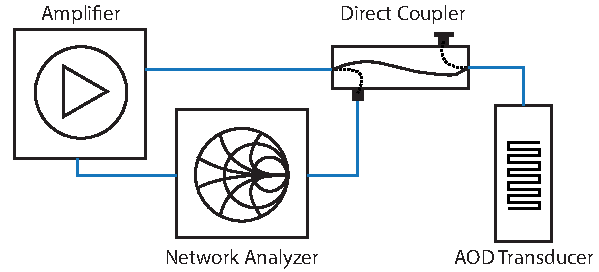
\includegraphics[width=.6\textwidth]{../figure/signal/setup-transducer.pdf}
  \caption{Experimental setup to measure the reflection at the acousto-optic
    transducer. The network analyzer supplies an input signal to the
    amplifier. The output signal of the amplifier is connected through a
    directional coupler with the acousto-optic element. The directional
    coupler allows to safely measure input and output reflection.
  }\label{fig:signal_amplification_transducer_setup}
\end{figure}
The setup is depicted in \Cref{fig:signal_amplification_transducer_setup}.
The network analyzer on the left-hand side supplies an input signal to the
amplifier. The input signal changes linear in frequency. The output signal
of the amplifier is connected through a directional coupler with the
acousto-optic element. The directional coupler allows to measure input and
output reflection.
\begin{figure}[htb]
  \centering
  \begin{adjustbox}{width=\textwidth}
    %% Creator: Matplotlib, PGF backend
%%
%% To include the figure in your LaTeX document, write
%%   \input{<filename>.pgf}
%%
%% Make sure the required packages are loaded in your preamble
%%   \usepackage{pgf}
%%
%% Figures using additional raster images can only be included by \input if
%% they are in the same directory as the main LaTeX file. For loading figures
%% from other directories you can use the `import` package
%%   \usepackage{import}
%% and then include the figures with
%%   \import{<path to file>}{<filename>.pgf}
%%
%% Matplotlib used the following preamble
%%   \usepackage{amsmath}\usepackage{siunitx}\usepackage{lmodern}
%%   \usepackage{fontspec}
%%
\begingroup%
\makeatletter%
\begin{pgfpicture}%
\pgfpathrectangle{\pgfpointorigin}{\pgfqpoint{12.000000in}{6.000000in}}%
\pgfusepath{use as bounding box, clip}%
\begin{pgfscope}%
\pgfsetbuttcap%
\pgfsetmiterjoin%
\pgfsetlinewidth{0.000000pt}%
\definecolor{currentstroke}{rgb}{1.000000,1.000000,1.000000}%
\pgfsetstrokecolor{currentstroke}%
\pgfsetdash{}{0pt}%
\pgfpathmoveto{\pgfqpoint{0.000000in}{0.000000in}}%
\pgfpathlineto{\pgfqpoint{12.000000in}{0.000000in}}%
\pgfpathlineto{\pgfqpoint{12.000000in}{6.000000in}}%
\pgfpathlineto{\pgfqpoint{0.000000in}{6.000000in}}%
\pgfpathclose%
\pgfusepath{}%
\end{pgfscope}%
\begin{pgfscope}%
\pgfsetbuttcap%
\pgfsetmiterjoin%
\definecolor{currentfill}{rgb}{1.000000,1.000000,1.000000}%
\pgfsetfillcolor{currentfill}%
\pgfsetlinewidth{0.000000pt}%
\definecolor{currentstroke}{rgb}{0.000000,0.000000,0.000000}%
\pgfsetstrokecolor{currentstroke}%
\pgfsetstrokeopacity{0.000000}%
\pgfsetdash{}{0pt}%
\pgfpathmoveto{\pgfqpoint{1.500000in}{1.200000in}}%
\pgfpathlineto{\pgfqpoint{10.800000in}{1.200000in}}%
\pgfpathlineto{\pgfqpoint{10.800000in}{5.880000in}}%
\pgfpathlineto{\pgfqpoint{1.500000in}{5.880000in}}%
\pgfpathclose%
\pgfusepath{fill}%
\end{pgfscope}%
\begin{pgfscope}%
\pgfpathrectangle{\pgfqpoint{1.500000in}{1.200000in}}{\pgfqpoint{9.300000in}{4.680000in}}%
\pgfusepath{clip}%
\pgfsetbuttcap%
\pgfsetroundjoin%
\definecolor{currentfill}{rgb}{0.192157,0.509804,0.741176}%
\pgfsetfillcolor{currentfill}%
\pgfsetlinewidth{1.003750pt}%
\definecolor{currentstroke}{rgb}{0.192157,0.509804,0.741176}%
\pgfsetstrokecolor{currentstroke}%
\pgfsetdash{}{0pt}%
\pgfpathmoveto{\pgfqpoint{1.963992in}{4.866659in}}%
\pgfpathcurveto{\pgfqpoint{1.975042in}{4.866659in}}{\pgfqpoint{1.985641in}{4.871049in}}{\pgfqpoint{1.993455in}{4.878863in}}%
\pgfpathcurveto{\pgfqpoint{2.001268in}{4.886677in}}{\pgfqpoint{2.005658in}{4.897276in}}{\pgfqpoint{2.005658in}{4.908326in}}%
\pgfpathcurveto{\pgfqpoint{2.005658in}{4.919376in}}{\pgfqpoint{2.001268in}{4.929975in}}{\pgfqpoint{1.993455in}{4.937789in}}%
\pgfpathcurveto{\pgfqpoint{1.985641in}{4.945602in}}{\pgfqpoint{1.975042in}{4.949992in}}{\pgfqpoint{1.963992in}{4.949992in}}%
\pgfpathcurveto{\pgfqpoint{1.952942in}{4.949992in}}{\pgfqpoint{1.942343in}{4.945602in}}{\pgfqpoint{1.934529in}{4.937789in}}%
\pgfpathcurveto{\pgfqpoint{1.926715in}{4.929975in}}{\pgfqpoint{1.922325in}{4.919376in}}{\pgfqpoint{1.922325in}{4.908326in}}%
\pgfpathcurveto{\pgfqpoint{1.922325in}{4.897276in}}{\pgfqpoint{1.926715in}{4.886677in}}{\pgfqpoint{1.934529in}{4.878863in}}%
\pgfpathcurveto{\pgfqpoint{1.942343in}{4.871049in}}{\pgfqpoint{1.952942in}{4.866659in}}{\pgfqpoint{1.963992in}{4.866659in}}%
\pgfpathclose%
\pgfusepath{stroke,fill}%
\end{pgfscope}%
\begin{pgfscope}%
\pgfpathrectangle{\pgfqpoint{1.500000in}{1.200000in}}{\pgfqpoint{9.300000in}{4.680000in}}%
\pgfusepath{clip}%
\pgfsetbuttcap%
\pgfsetroundjoin%
\definecolor{currentfill}{rgb}{0.192157,0.509804,0.741176}%
\pgfsetfillcolor{currentfill}%
\pgfsetlinewidth{1.003750pt}%
\definecolor{currentstroke}{rgb}{0.192157,0.509804,0.741176}%
\pgfsetstrokecolor{currentstroke}%
\pgfsetdash{}{0pt}%
\pgfpathmoveto{\pgfqpoint{2.005852in}{4.869619in}}%
\pgfpathcurveto{\pgfqpoint{2.016902in}{4.869619in}}{\pgfqpoint{2.027501in}{4.874009in}}{\pgfqpoint{2.035315in}{4.881822in}}%
\pgfpathcurveto{\pgfqpoint{2.043128in}{4.889636in}}{\pgfqpoint{2.047519in}{4.900235in}}{\pgfqpoint{2.047519in}{4.911285in}}%
\pgfpathcurveto{\pgfqpoint{2.047519in}{4.922335in}}{\pgfqpoint{2.043128in}{4.932934in}}{\pgfqpoint{2.035315in}{4.940748in}}%
\pgfpathcurveto{\pgfqpoint{2.027501in}{4.948562in}}{\pgfqpoint{2.016902in}{4.952952in}}{\pgfqpoint{2.005852in}{4.952952in}}%
\pgfpathcurveto{\pgfqpoint{1.994802in}{4.952952in}}{\pgfqpoint{1.984203in}{4.948562in}}{\pgfqpoint{1.976389in}{4.940748in}}%
\pgfpathcurveto{\pgfqpoint{1.968576in}{4.932934in}}{\pgfqpoint{1.964185in}{4.922335in}}{\pgfqpoint{1.964185in}{4.911285in}}%
\pgfpathcurveto{\pgfqpoint{1.964185in}{4.900235in}}{\pgfqpoint{1.968576in}{4.889636in}}{\pgfqpoint{1.976389in}{4.881822in}}%
\pgfpathcurveto{\pgfqpoint{1.984203in}{4.874009in}}{\pgfqpoint{1.994802in}{4.869619in}}{\pgfqpoint{2.005852in}{4.869619in}}%
\pgfpathclose%
\pgfusepath{stroke,fill}%
\end{pgfscope}%
\begin{pgfscope}%
\pgfpathrectangle{\pgfqpoint{1.500000in}{1.200000in}}{\pgfqpoint{9.300000in}{4.680000in}}%
\pgfusepath{clip}%
\pgfsetbuttcap%
\pgfsetroundjoin%
\definecolor{currentfill}{rgb}{0.192157,0.509804,0.741176}%
\pgfsetfillcolor{currentfill}%
\pgfsetlinewidth{1.003750pt}%
\definecolor{currentstroke}{rgb}{0.192157,0.509804,0.741176}%
\pgfsetstrokecolor{currentstroke}%
\pgfsetdash{}{0pt}%
\pgfpathmoveto{\pgfqpoint{2.047712in}{4.879393in}}%
\pgfpathcurveto{\pgfqpoint{2.058762in}{4.879393in}}{\pgfqpoint{2.069361in}{4.883783in}}{\pgfqpoint{2.077175in}{4.891597in}}%
\pgfpathcurveto{\pgfqpoint{2.084988in}{4.899411in}}{\pgfqpoint{2.089379in}{4.910010in}}{\pgfqpoint{2.089379in}{4.921060in}}%
\pgfpathcurveto{\pgfqpoint{2.089379in}{4.932110in}}{\pgfqpoint{2.084988in}{4.942709in}}{\pgfqpoint{2.077175in}{4.950522in}}%
\pgfpathcurveto{\pgfqpoint{2.069361in}{4.958336in}}{\pgfqpoint{2.058762in}{4.962726in}}{\pgfqpoint{2.047712in}{4.962726in}}%
\pgfpathcurveto{\pgfqpoint{2.036662in}{4.962726in}}{\pgfqpoint{2.026063in}{4.958336in}}{\pgfqpoint{2.018249in}{4.950522in}}%
\pgfpathcurveto{\pgfqpoint{2.010436in}{4.942709in}}{\pgfqpoint{2.006045in}{4.932110in}}{\pgfqpoint{2.006045in}{4.921060in}}%
\pgfpathcurveto{\pgfqpoint{2.006045in}{4.910010in}}{\pgfqpoint{2.010436in}{4.899411in}}{\pgfqpoint{2.018249in}{4.891597in}}%
\pgfpathcurveto{\pgfqpoint{2.026063in}{4.883783in}}{\pgfqpoint{2.036662in}{4.879393in}}{\pgfqpoint{2.047712in}{4.879393in}}%
\pgfpathclose%
\pgfusepath{stroke,fill}%
\end{pgfscope}%
\begin{pgfscope}%
\pgfpathrectangle{\pgfqpoint{1.500000in}{1.200000in}}{\pgfqpoint{9.300000in}{4.680000in}}%
\pgfusepath{clip}%
\pgfsetbuttcap%
\pgfsetroundjoin%
\definecolor{currentfill}{rgb}{0.192157,0.509804,0.741176}%
\pgfsetfillcolor{currentfill}%
\pgfsetlinewidth{1.003750pt}%
\definecolor{currentstroke}{rgb}{0.192157,0.509804,0.741176}%
\pgfsetstrokecolor{currentstroke}%
\pgfsetdash{}{0pt}%
\pgfpathmoveto{\pgfqpoint{2.089572in}{4.879150in}}%
\pgfpathcurveto{\pgfqpoint{2.100622in}{4.879150in}}{\pgfqpoint{2.111221in}{4.883541in}}{\pgfqpoint{2.119035in}{4.891354in}}%
\pgfpathcurveto{\pgfqpoint{2.126848in}{4.899168in}}{\pgfqpoint{2.131239in}{4.909767in}}{\pgfqpoint{2.131239in}{4.920817in}}%
\pgfpathcurveto{\pgfqpoint{2.131239in}{4.931867in}}{\pgfqpoint{2.126848in}{4.942466in}}{\pgfqpoint{2.119035in}{4.950280in}}%
\pgfpathcurveto{\pgfqpoint{2.111221in}{4.958093in}}{\pgfqpoint{2.100622in}{4.962484in}}{\pgfqpoint{2.089572in}{4.962484in}}%
\pgfpathcurveto{\pgfqpoint{2.078522in}{4.962484in}}{\pgfqpoint{2.067923in}{4.958093in}}{\pgfqpoint{2.060109in}{4.950280in}}%
\pgfpathcurveto{\pgfqpoint{2.052296in}{4.942466in}}{\pgfqpoint{2.047905in}{4.931867in}}{\pgfqpoint{2.047905in}{4.920817in}}%
\pgfpathcurveto{\pgfqpoint{2.047905in}{4.909767in}}{\pgfqpoint{2.052296in}{4.899168in}}{\pgfqpoint{2.060109in}{4.891354in}}%
\pgfpathcurveto{\pgfqpoint{2.067923in}{4.883541in}}{\pgfqpoint{2.078522in}{4.879150in}}{\pgfqpoint{2.089572in}{4.879150in}}%
\pgfpathclose%
\pgfusepath{stroke,fill}%
\end{pgfscope}%
\begin{pgfscope}%
\pgfpathrectangle{\pgfqpoint{1.500000in}{1.200000in}}{\pgfqpoint{9.300000in}{4.680000in}}%
\pgfusepath{clip}%
\pgfsetbuttcap%
\pgfsetroundjoin%
\definecolor{currentfill}{rgb}{0.192157,0.509804,0.741176}%
\pgfsetfillcolor{currentfill}%
\pgfsetlinewidth{1.003750pt}%
\definecolor{currentstroke}{rgb}{0.192157,0.509804,0.741176}%
\pgfsetstrokecolor{currentstroke}%
\pgfsetdash{}{0pt}%
\pgfpathmoveto{\pgfqpoint{2.131432in}{4.891254in}}%
\pgfpathcurveto{\pgfqpoint{2.142482in}{4.891254in}}{\pgfqpoint{2.153081in}{4.895644in}}{\pgfqpoint{2.160895in}{4.903458in}}%
\pgfpathcurveto{\pgfqpoint{2.168709in}{4.911272in}}{\pgfqpoint{2.173099in}{4.921871in}}{\pgfqpoint{2.173099in}{4.932921in}}%
\pgfpathcurveto{\pgfqpoint{2.173099in}{4.943971in}}{\pgfqpoint{2.168709in}{4.954570in}}{\pgfqpoint{2.160895in}{4.962384in}}%
\pgfpathcurveto{\pgfqpoint{2.153081in}{4.970197in}}{\pgfqpoint{2.142482in}{4.974587in}}{\pgfqpoint{2.131432in}{4.974587in}}%
\pgfpathcurveto{\pgfqpoint{2.120382in}{4.974587in}}{\pgfqpoint{2.109783in}{4.970197in}}{\pgfqpoint{2.101969in}{4.962384in}}%
\pgfpathcurveto{\pgfqpoint{2.094156in}{4.954570in}}{\pgfqpoint{2.089765in}{4.943971in}}{\pgfqpoint{2.089765in}{4.932921in}}%
\pgfpathcurveto{\pgfqpoint{2.089765in}{4.921871in}}{\pgfqpoint{2.094156in}{4.911272in}}{\pgfqpoint{2.101969in}{4.903458in}}%
\pgfpathcurveto{\pgfqpoint{2.109783in}{4.895644in}}{\pgfqpoint{2.120382in}{4.891254in}}{\pgfqpoint{2.131432in}{4.891254in}}%
\pgfpathclose%
\pgfusepath{stroke,fill}%
\end{pgfscope}%
\begin{pgfscope}%
\pgfpathrectangle{\pgfqpoint{1.500000in}{1.200000in}}{\pgfqpoint{9.300000in}{4.680000in}}%
\pgfusepath{clip}%
\pgfsetbuttcap%
\pgfsetroundjoin%
\definecolor{currentfill}{rgb}{0.192157,0.509804,0.741176}%
\pgfsetfillcolor{currentfill}%
\pgfsetlinewidth{1.003750pt}%
\definecolor{currentstroke}{rgb}{0.192157,0.509804,0.741176}%
\pgfsetstrokecolor{currentstroke}%
\pgfsetdash{}{0pt}%
\pgfpathmoveto{\pgfqpoint{2.173292in}{4.888542in}}%
\pgfpathcurveto{\pgfqpoint{2.184342in}{4.888542in}}{\pgfqpoint{2.194941in}{4.892933in}}{\pgfqpoint{2.202755in}{4.900746in}}%
\pgfpathcurveto{\pgfqpoint{2.210569in}{4.908560in}}{\pgfqpoint{2.214959in}{4.919159in}}{\pgfqpoint{2.214959in}{4.930209in}}%
\pgfpathcurveto{\pgfqpoint{2.214959in}{4.941259in}}{\pgfqpoint{2.210569in}{4.951858in}}{\pgfqpoint{2.202755in}{4.959672in}}%
\pgfpathcurveto{\pgfqpoint{2.194941in}{4.967485in}}{\pgfqpoint{2.184342in}{4.971876in}}{\pgfqpoint{2.173292in}{4.971876in}}%
\pgfpathcurveto{\pgfqpoint{2.162242in}{4.971876in}}{\pgfqpoint{2.151643in}{4.967485in}}{\pgfqpoint{2.143829in}{4.959672in}}%
\pgfpathcurveto{\pgfqpoint{2.136016in}{4.951858in}}{\pgfqpoint{2.131626in}{4.941259in}}{\pgfqpoint{2.131626in}{4.930209in}}%
\pgfpathcurveto{\pgfqpoint{2.131626in}{4.919159in}}{\pgfqpoint{2.136016in}{4.908560in}}{\pgfqpoint{2.143829in}{4.900746in}}%
\pgfpathcurveto{\pgfqpoint{2.151643in}{4.892933in}}{\pgfqpoint{2.162242in}{4.888542in}}{\pgfqpoint{2.173292in}{4.888542in}}%
\pgfpathclose%
\pgfusepath{stroke,fill}%
\end{pgfscope}%
\begin{pgfscope}%
\pgfpathrectangle{\pgfqpoint{1.500000in}{1.200000in}}{\pgfqpoint{9.300000in}{4.680000in}}%
\pgfusepath{clip}%
\pgfsetbuttcap%
\pgfsetroundjoin%
\definecolor{currentfill}{rgb}{0.192157,0.509804,0.741176}%
\pgfsetfillcolor{currentfill}%
\pgfsetlinewidth{1.003750pt}%
\definecolor{currentstroke}{rgb}{0.192157,0.509804,0.741176}%
\pgfsetstrokecolor{currentstroke}%
\pgfsetdash{}{0pt}%
\pgfpathmoveto{\pgfqpoint{2.215152in}{4.905637in}}%
\pgfpathcurveto{\pgfqpoint{2.226202in}{4.905637in}}{\pgfqpoint{2.236801in}{4.910027in}}{\pgfqpoint{2.244615in}{4.917841in}}%
\pgfpathcurveto{\pgfqpoint{2.252429in}{4.925655in}}{\pgfqpoint{2.256819in}{4.936254in}}{\pgfqpoint{2.256819in}{4.947304in}}%
\pgfpathcurveto{\pgfqpoint{2.256819in}{4.958354in}}{\pgfqpoint{2.252429in}{4.968953in}}{\pgfqpoint{2.244615in}{4.976766in}}%
\pgfpathcurveto{\pgfqpoint{2.236801in}{4.984580in}}{\pgfqpoint{2.226202in}{4.988970in}}{\pgfqpoint{2.215152in}{4.988970in}}%
\pgfpathcurveto{\pgfqpoint{2.204102in}{4.988970in}}{\pgfqpoint{2.193503in}{4.984580in}}{\pgfqpoint{2.185690in}{4.976766in}}%
\pgfpathcurveto{\pgfqpoint{2.177876in}{4.968953in}}{\pgfqpoint{2.173486in}{4.958354in}}{\pgfqpoint{2.173486in}{4.947304in}}%
\pgfpathcurveto{\pgfqpoint{2.173486in}{4.936254in}}{\pgfqpoint{2.177876in}{4.925655in}}{\pgfqpoint{2.185690in}{4.917841in}}%
\pgfpathcurveto{\pgfqpoint{2.193503in}{4.910027in}}{\pgfqpoint{2.204102in}{4.905637in}}{\pgfqpoint{2.215152in}{4.905637in}}%
\pgfpathclose%
\pgfusepath{stroke,fill}%
\end{pgfscope}%
\begin{pgfscope}%
\pgfpathrectangle{\pgfqpoint{1.500000in}{1.200000in}}{\pgfqpoint{9.300000in}{4.680000in}}%
\pgfusepath{clip}%
\pgfsetbuttcap%
\pgfsetroundjoin%
\definecolor{currentfill}{rgb}{0.192157,0.509804,0.741176}%
\pgfsetfillcolor{currentfill}%
\pgfsetlinewidth{1.003750pt}%
\definecolor{currentstroke}{rgb}{0.192157,0.509804,0.741176}%
\pgfsetstrokecolor{currentstroke}%
\pgfsetdash{}{0pt}%
\pgfpathmoveto{\pgfqpoint{2.257012in}{4.902119in}}%
\pgfpathcurveto{\pgfqpoint{2.268063in}{4.902119in}}{\pgfqpoint{2.278662in}{4.906509in}}{\pgfqpoint{2.286475in}{4.914323in}}%
\pgfpathcurveto{\pgfqpoint{2.294289in}{4.922137in}}{\pgfqpoint{2.298679in}{4.932736in}}{\pgfqpoint{2.298679in}{4.943786in}}%
\pgfpathcurveto{\pgfqpoint{2.298679in}{4.954836in}}{\pgfqpoint{2.294289in}{4.965435in}}{\pgfqpoint{2.286475in}{4.973248in}}%
\pgfpathcurveto{\pgfqpoint{2.278662in}{4.981062in}}{\pgfqpoint{2.268063in}{4.985452in}}{\pgfqpoint{2.257012in}{4.985452in}}%
\pgfpathcurveto{\pgfqpoint{2.245962in}{4.985452in}}{\pgfqpoint{2.235363in}{4.981062in}}{\pgfqpoint{2.227550in}{4.973248in}}%
\pgfpathcurveto{\pgfqpoint{2.219736in}{4.965435in}}{\pgfqpoint{2.215346in}{4.954836in}}{\pgfqpoint{2.215346in}{4.943786in}}%
\pgfpathcurveto{\pgfqpoint{2.215346in}{4.932736in}}{\pgfqpoint{2.219736in}{4.922137in}}{\pgfqpoint{2.227550in}{4.914323in}}%
\pgfpathcurveto{\pgfqpoint{2.235363in}{4.906509in}}{\pgfqpoint{2.245962in}{4.902119in}}{\pgfqpoint{2.257012in}{4.902119in}}%
\pgfpathclose%
\pgfusepath{stroke,fill}%
\end{pgfscope}%
\begin{pgfscope}%
\pgfpathrectangle{\pgfqpoint{1.500000in}{1.200000in}}{\pgfqpoint{9.300000in}{4.680000in}}%
\pgfusepath{clip}%
\pgfsetbuttcap%
\pgfsetroundjoin%
\definecolor{currentfill}{rgb}{0.192157,0.509804,0.741176}%
\pgfsetfillcolor{currentfill}%
\pgfsetlinewidth{1.003750pt}%
\definecolor{currentstroke}{rgb}{0.192157,0.509804,0.741176}%
\pgfsetstrokecolor{currentstroke}%
\pgfsetdash{}{0pt}%
\pgfpathmoveto{\pgfqpoint{2.298872in}{4.919787in}}%
\pgfpathcurveto{\pgfqpoint{2.309923in}{4.919787in}}{\pgfqpoint{2.320522in}{4.924178in}}{\pgfqpoint{2.328335in}{4.931991in}}%
\pgfpathcurveto{\pgfqpoint{2.336149in}{4.939805in}}{\pgfqpoint{2.340539in}{4.950404in}}{\pgfqpoint{2.340539in}{4.961454in}}%
\pgfpathcurveto{\pgfqpoint{2.340539in}{4.972504in}}{\pgfqpoint{2.336149in}{4.983103in}}{\pgfqpoint{2.328335in}{4.990917in}}%
\pgfpathcurveto{\pgfqpoint{2.320522in}{4.998730in}}{\pgfqpoint{2.309923in}{5.003121in}}{\pgfqpoint{2.298872in}{5.003121in}}%
\pgfpathcurveto{\pgfqpoint{2.287822in}{5.003121in}}{\pgfqpoint{2.277223in}{4.998730in}}{\pgfqpoint{2.269410in}{4.990917in}}%
\pgfpathcurveto{\pgfqpoint{2.261596in}{4.983103in}}{\pgfqpoint{2.257206in}{4.972504in}}{\pgfqpoint{2.257206in}{4.961454in}}%
\pgfpathcurveto{\pgfqpoint{2.257206in}{4.950404in}}{\pgfqpoint{2.261596in}{4.939805in}}{\pgfqpoint{2.269410in}{4.931991in}}%
\pgfpathcurveto{\pgfqpoint{2.277223in}{4.924178in}}{\pgfqpoint{2.287822in}{4.919787in}}{\pgfqpoint{2.298872in}{4.919787in}}%
\pgfpathclose%
\pgfusepath{stroke,fill}%
\end{pgfscope}%
\begin{pgfscope}%
\pgfpathrectangle{\pgfqpoint{1.500000in}{1.200000in}}{\pgfqpoint{9.300000in}{4.680000in}}%
\pgfusepath{clip}%
\pgfsetbuttcap%
\pgfsetroundjoin%
\definecolor{currentfill}{rgb}{0.192157,0.509804,0.741176}%
\pgfsetfillcolor{currentfill}%
\pgfsetlinewidth{1.003750pt}%
\definecolor{currentstroke}{rgb}{0.192157,0.509804,0.741176}%
\pgfsetstrokecolor{currentstroke}%
\pgfsetdash{}{0pt}%
\pgfpathmoveto{\pgfqpoint{2.340733in}{4.911099in}}%
\pgfpathcurveto{\pgfqpoint{2.351783in}{4.911099in}}{\pgfqpoint{2.362382in}{4.915490in}}{\pgfqpoint{2.370195in}{4.923303in}}%
\pgfpathcurveto{\pgfqpoint{2.378009in}{4.931117in}}{\pgfqpoint{2.382399in}{4.941716in}}{\pgfqpoint{2.382399in}{4.952766in}}%
\pgfpathcurveto{\pgfqpoint{2.382399in}{4.963816in}}{\pgfqpoint{2.378009in}{4.974415in}}{\pgfqpoint{2.370195in}{4.982229in}}%
\pgfpathcurveto{\pgfqpoint{2.362382in}{4.990042in}}{\pgfqpoint{2.351783in}{4.994433in}}{\pgfqpoint{2.340733in}{4.994433in}}%
\pgfpathcurveto{\pgfqpoint{2.329682in}{4.994433in}}{\pgfqpoint{2.319083in}{4.990042in}}{\pgfqpoint{2.311270in}{4.982229in}}%
\pgfpathcurveto{\pgfqpoint{2.303456in}{4.974415in}}{\pgfqpoint{2.299066in}{4.963816in}}{\pgfqpoint{2.299066in}{4.952766in}}%
\pgfpathcurveto{\pgfqpoint{2.299066in}{4.941716in}}{\pgfqpoint{2.303456in}{4.931117in}}{\pgfqpoint{2.311270in}{4.923303in}}%
\pgfpathcurveto{\pgfqpoint{2.319083in}{4.915490in}}{\pgfqpoint{2.329682in}{4.911099in}}{\pgfqpoint{2.340733in}{4.911099in}}%
\pgfpathclose%
\pgfusepath{stroke,fill}%
\end{pgfscope}%
\begin{pgfscope}%
\pgfpathrectangle{\pgfqpoint{1.500000in}{1.200000in}}{\pgfqpoint{9.300000in}{4.680000in}}%
\pgfusepath{clip}%
\pgfsetbuttcap%
\pgfsetroundjoin%
\definecolor{currentfill}{rgb}{0.192157,0.509804,0.741176}%
\pgfsetfillcolor{currentfill}%
\pgfsetlinewidth{1.003750pt}%
\definecolor{currentstroke}{rgb}{0.192157,0.509804,0.741176}%
\pgfsetstrokecolor{currentstroke}%
\pgfsetdash{}{0pt}%
\pgfpathmoveto{\pgfqpoint{2.382593in}{4.919853in}}%
\pgfpathcurveto{\pgfqpoint{2.393643in}{4.919853in}}{\pgfqpoint{2.404242in}{4.924244in}}{\pgfqpoint{2.412055in}{4.932057in}}%
\pgfpathcurveto{\pgfqpoint{2.419869in}{4.939871in}}{\pgfqpoint{2.424259in}{4.950470in}}{\pgfqpoint{2.424259in}{4.961520in}}%
\pgfpathcurveto{\pgfqpoint{2.424259in}{4.972570in}}{\pgfqpoint{2.419869in}{4.983169in}}{\pgfqpoint{2.412055in}{4.990983in}}%
\pgfpathcurveto{\pgfqpoint{2.404242in}{4.998796in}}{\pgfqpoint{2.393643in}{5.003187in}}{\pgfqpoint{2.382593in}{5.003187in}}%
\pgfpathcurveto{\pgfqpoint{2.371543in}{5.003187in}}{\pgfqpoint{2.360943in}{4.998796in}}{\pgfqpoint{2.353130in}{4.990983in}}%
\pgfpathcurveto{\pgfqpoint{2.345316in}{4.983169in}}{\pgfqpoint{2.340926in}{4.972570in}}{\pgfqpoint{2.340926in}{4.961520in}}%
\pgfpathcurveto{\pgfqpoint{2.340926in}{4.950470in}}{\pgfqpoint{2.345316in}{4.939871in}}{\pgfqpoint{2.353130in}{4.932057in}}%
\pgfpathcurveto{\pgfqpoint{2.360943in}{4.924244in}}{\pgfqpoint{2.371543in}{4.919853in}}{\pgfqpoint{2.382593in}{4.919853in}}%
\pgfpathclose%
\pgfusepath{stroke,fill}%
\end{pgfscope}%
\begin{pgfscope}%
\pgfpathrectangle{\pgfqpoint{1.500000in}{1.200000in}}{\pgfqpoint{9.300000in}{4.680000in}}%
\pgfusepath{clip}%
\pgfsetbuttcap%
\pgfsetroundjoin%
\definecolor{currentfill}{rgb}{0.192157,0.509804,0.741176}%
\pgfsetfillcolor{currentfill}%
\pgfsetlinewidth{1.003750pt}%
\definecolor{currentstroke}{rgb}{0.192157,0.509804,0.741176}%
\pgfsetstrokecolor{currentstroke}%
\pgfsetdash{}{0pt}%
\pgfpathmoveto{\pgfqpoint{2.424453in}{4.925118in}}%
\pgfpathcurveto{\pgfqpoint{2.435503in}{4.925118in}}{\pgfqpoint{2.446102in}{4.929508in}}{\pgfqpoint{2.453916in}{4.937322in}}%
\pgfpathcurveto{\pgfqpoint{2.461729in}{4.945136in}}{\pgfqpoint{2.466119in}{4.955735in}}{\pgfqpoint{2.466119in}{4.966785in}}%
\pgfpathcurveto{\pgfqpoint{2.466119in}{4.977835in}}{\pgfqpoint{2.461729in}{4.988434in}}{\pgfqpoint{2.453916in}{4.996248in}}%
\pgfpathcurveto{\pgfqpoint{2.446102in}{5.004061in}}{\pgfqpoint{2.435503in}{5.008451in}}{\pgfqpoint{2.424453in}{5.008451in}}%
\pgfpathcurveto{\pgfqpoint{2.413403in}{5.008451in}}{\pgfqpoint{2.402804in}{5.004061in}}{\pgfqpoint{2.394990in}{4.996248in}}%
\pgfpathcurveto{\pgfqpoint{2.387176in}{4.988434in}}{\pgfqpoint{2.382786in}{4.977835in}}{\pgfqpoint{2.382786in}{4.966785in}}%
\pgfpathcurveto{\pgfqpoint{2.382786in}{4.955735in}}{\pgfqpoint{2.387176in}{4.945136in}}{\pgfqpoint{2.394990in}{4.937322in}}%
\pgfpathcurveto{\pgfqpoint{2.402804in}{4.929508in}}{\pgfqpoint{2.413403in}{4.925118in}}{\pgfqpoint{2.424453in}{4.925118in}}%
\pgfpathclose%
\pgfusepath{stroke,fill}%
\end{pgfscope}%
\begin{pgfscope}%
\pgfpathrectangle{\pgfqpoint{1.500000in}{1.200000in}}{\pgfqpoint{9.300000in}{4.680000in}}%
\pgfusepath{clip}%
\pgfsetbuttcap%
\pgfsetroundjoin%
\definecolor{currentfill}{rgb}{0.192157,0.509804,0.741176}%
\pgfsetfillcolor{currentfill}%
\pgfsetlinewidth{1.003750pt}%
\definecolor{currentstroke}{rgb}{0.192157,0.509804,0.741176}%
\pgfsetstrokecolor{currentstroke}%
\pgfsetdash{}{0pt}%
\pgfpathmoveto{\pgfqpoint{2.466313in}{4.929390in}}%
\pgfpathcurveto{\pgfqpoint{2.477363in}{4.929390in}}{\pgfqpoint{2.487962in}{4.933781in}}{\pgfqpoint{2.495776in}{4.941594in}}%
\pgfpathcurveto{\pgfqpoint{2.503589in}{4.949408in}}{\pgfqpoint{2.507979in}{4.960007in}}{\pgfqpoint{2.507979in}{4.971057in}}%
\pgfpathcurveto{\pgfqpoint{2.507979in}{4.982107in}}{\pgfqpoint{2.503589in}{4.992706in}}{\pgfqpoint{2.495776in}{5.000520in}}%
\pgfpathcurveto{\pgfqpoint{2.487962in}{5.008333in}}{\pgfqpoint{2.477363in}{5.012724in}}{\pgfqpoint{2.466313in}{5.012724in}}%
\pgfpathcurveto{\pgfqpoint{2.455263in}{5.012724in}}{\pgfqpoint{2.444664in}{5.008333in}}{\pgfqpoint{2.436850in}{5.000520in}}%
\pgfpathcurveto{\pgfqpoint{2.429036in}{4.992706in}}{\pgfqpoint{2.424646in}{4.982107in}}{\pgfqpoint{2.424646in}{4.971057in}}%
\pgfpathcurveto{\pgfqpoint{2.424646in}{4.960007in}}{\pgfqpoint{2.429036in}{4.949408in}}{\pgfqpoint{2.436850in}{4.941594in}}%
\pgfpathcurveto{\pgfqpoint{2.444664in}{4.933781in}}{\pgfqpoint{2.455263in}{4.929390in}}{\pgfqpoint{2.466313in}{4.929390in}}%
\pgfpathclose%
\pgfusepath{stroke,fill}%
\end{pgfscope}%
\begin{pgfscope}%
\pgfpathrectangle{\pgfqpoint{1.500000in}{1.200000in}}{\pgfqpoint{9.300000in}{4.680000in}}%
\pgfusepath{clip}%
\pgfsetbuttcap%
\pgfsetroundjoin%
\definecolor{currentfill}{rgb}{0.192157,0.509804,0.741176}%
\pgfsetfillcolor{currentfill}%
\pgfsetlinewidth{1.003750pt}%
\definecolor{currentstroke}{rgb}{0.192157,0.509804,0.741176}%
\pgfsetstrokecolor{currentstroke}%
\pgfsetdash{}{0pt}%
\pgfpathmoveto{\pgfqpoint{2.508173in}{4.939114in}}%
\pgfpathcurveto{\pgfqpoint{2.519223in}{4.939114in}}{\pgfqpoint{2.529822in}{4.943504in}}{\pgfqpoint{2.537636in}{4.951318in}}%
\pgfpathcurveto{\pgfqpoint{2.545449in}{4.959132in}}{\pgfqpoint{2.549840in}{4.969731in}}{\pgfqpoint{2.549840in}{4.980781in}}%
\pgfpathcurveto{\pgfqpoint{2.549840in}{4.991831in}}{\pgfqpoint{2.545449in}{5.002430in}}{\pgfqpoint{2.537636in}{5.010243in}}%
\pgfpathcurveto{\pgfqpoint{2.529822in}{5.018057in}}{\pgfqpoint{2.519223in}{5.022447in}}{\pgfqpoint{2.508173in}{5.022447in}}%
\pgfpathcurveto{\pgfqpoint{2.497123in}{5.022447in}}{\pgfqpoint{2.486524in}{5.018057in}}{\pgfqpoint{2.478710in}{5.010243in}}%
\pgfpathcurveto{\pgfqpoint{2.470896in}{5.002430in}}{\pgfqpoint{2.466506in}{4.991831in}}{\pgfqpoint{2.466506in}{4.980781in}}%
\pgfpathcurveto{\pgfqpoint{2.466506in}{4.969731in}}{\pgfqpoint{2.470896in}{4.959132in}}{\pgfqpoint{2.478710in}{4.951318in}}%
\pgfpathcurveto{\pgfqpoint{2.486524in}{4.943504in}}{\pgfqpoint{2.497123in}{4.939114in}}{\pgfqpoint{2.508173in}{4.939114in}}%
\pgfpathclose%
\pgfusepath{stroke,fill}%
\end{pgfscope}%
\begin{pgfscope}%
\pgfpathrectangle{\pgfqpoint{1.500000in}{1.200000in}}{\pgfqpoint{9.300000in}{4.680000in}}%
\pgfusepath{clip}%
\pgfsetbuttcap%
\pgfsetroundjoin%
\definecolor{currentfill}{rgb}{0.192157,0.509804,0.741176}%
\pgfsetfillcolor{currentfill}%
\pgfsetlinewidth{1.003750pt}%
\definecolor{currentstroke}{rgb}{0.192157,0.509804,0.741176}%
\pgfsetstrokecolor{currentstroke}%
\pgfsetdash{}{0pt}%
\pgfpathmoveto{\pgfqpoint{2.550033in}{4.942209in}}%
\pgfpathcurveto{\pgfqpoint{2.561083in}{4.942209in}}{\pgfqpoint{2.571682in}{4.946600in}}{\pgfqpoint{2.579496in}{4.954413in}}%
\pgfpathcurveto{\pgfqpoint{2.587309in}{4.962227in}}{\pgfqpoint{2.591700in}{4.972826in}}{\pgfqpoint{2.591700in}{4.983876in}}%
\pgfpathcurveto{\pgfqpoint{2.591700in}{4.994926in}}{\pgfqpoint{2.587309in}{5.005525in}}{\pgfqpoint{2.579496in}{5.013339in}}%
\pgfpathcurveto{\pgfqpoint{2.571682in}{5.021153in}}{\pgfqpoint{2.561083in}{5.025543in}}{\pgfqpoint{2.550033in}{5.025543in}}%
\pgfpathcurveto{\pgfqpoint{2.538983in}{5.025543in}}{\pgfqpoint{2.528384in}{5.021153in}}{\pgfqpoint{2.520570in}{5.013339in}}%
\pgfpathcurveto{\pgfqpoint{2.512757in}{5.005525in}}{\pgfqpoint{2.508366in}{4.994926in}}{\pgfqpoint{2.508366in}{4.983876in}}%
\pgfpathcurveto{\pgfqpoint{2.508366in}{4.972826in}}{\pgfqpoint{2.512757in}{4.962227in}}{\pgfqpoint{2.520570in}{4.954413in}}%
\pgfpathcurveto{\pgfqpoint{2.528384in}{4.946600in}}{\pgfqpoint{2.538983in}{4.942209in}}{\pgfqpoint{2.550033in}{4.942209in}}%
\pgfpathclose%
\pgfusepath{stroke,fill}%
\end{pgfscope}%
\begin{pgfscope}%
\pgfpathrectangle{\pgfqpoint{1.500000in}{1.200000in}}{\pgfqpoint{9.300000in}{4.680000in}}%
\pgfusepath{clip}%
\pgfsetbuttcap%
\pgfsetroundjoin%
\definecolor{currentfill}{rgb}{0.192157,0.509804,0.741176}%
\pgfsetfillcolor{currentfill}%
\pgfsetlinewidth{1.003750pt}%
\definecolor{currentstroke}{rgb}{0.192157,0.509804,0.741176}%
\pgfsetstrokecolor{currentstroke}%
\pgfsetdash{}{0pt}%
\pgfpathmoveto{\pgfqpoint{2.591893in}{4.948041in}}%
\pgfpathcurveto{\pgfqpoint{2.602943in}{4.948041in}}{\pgfqpoint{2.613542in}{4.952432in}}{\pgfqpoint{2.621356in}{4.960245in}}%
\pgfpathcurveto{\pgfqpoint{2.629169in}{4.968059in}}{\pgfqpoint{2.633560in}{4.978658in}}{\pgfqpoint{2.633560in}{4.989708in}}%
\pgfpathcurveto{\pgfqpoint{2.633560in}{5.000758in}}{\pgfqpoint{2.629169in}{5.011357in}}{\pgfqpoint{2.621356in}{5.019171in}}%
\pgfpathcurveto{\pgfqpoint{2.613542in}{5.026984in}}{\pgfqpoint{2.602943in}{5.031375in}}{\pgfqpoint{2.591893in}{5.031375in}}%
\pgfpathcurveto{\pgfqpoint{2.580843in}{5.031375in}}{\pgfqpoint{2.570244in}{5.026984in}}{\pgfqpoint{2.562430in}{5.019171in}}%
\pgfpathcurveto{\pgfqpoint{2.554617in}{5.011357in}}{\pgfqpoint{2.550226in}{5.000758in}}{\pgfqpoint{2.550226in}{4.989708in}}%
\pgfpathcurveto{\pgfqpoint{2.550226in}{4.978658in}}{\pgfqpoint{2.554617in}{4.968059in}}{\pgfqpoint{2.562430in}{4.960245in}}%
\pgfpathcurveto{\pgfqpoint{2.570244in}{4.952432in}}{\pgfqpoint{2.580843in}{4.948041in}}{\pgfqpoint{2.591893in}{4.948041in}}%
\pgfpathclose%
\pgfusepath{stroke,fill}%
\end{pgfscope}%
\begin{pgfscope}%
\pgfpathrectangle{\pgfqpoint{1.500000in}{1.200000in}}{\pgfqpoint{9.300000in}{4.680000in}}%
\pgfusepath{clip}%
\pgfsetbuttcap%
\pgfsetroundjoin%
\definecolor{currentfill}{rgb}{0.192157,0.509804,0.741176}%
\pgfsetfillcolor{currentfill}%
\pgfsetlinewidth{1.003750pt}%
\definecolor{currentstroke}{rgb}{0.192157,0.509804,0.741176}%
\pgfsetstrokecolor{currentstroke}%
\pgfsetdash{}{0pt}%
\pgfpathmoveto{\pgfqpoint{2.633753in}{4.953091in}}%
\pgfpathcurveto{\pgfqpoint{2.644803in}{4.953091in}}{\pgfqpoint{2.655402in}{4.957481in}}{\pgfqpoint{2.663216in}{4.965295in}}%
\pgfpathcurveto{\pgfqpoint{2.671030in}{4.973109in}}{\pgfqpoint{2.675420in}{4.983708in}}{\pgfqpoint{2.675420in}{4.994758in}}%
\pgfpathcurveto{\pgfqpoint{2.675420in}{5.005808in}}{\pgfqpoint{2.671030in}{5.016407in}}{\pgfqpoint{2.663216in}{5.024221in}}%
\pgfpathcurveto{\pgfqpoint{2.655402in}{5.032034in}}{\pgfqpoint{2.644803in}{5.036425in}}{\pgfqpoint{2.633753in}{5.036425in}}%
\pgfpathcurveto{\pgfqpoint{2.622703in}{5.036425in}}{\pgfqpoint{2.612104in}{5.032034in}}{\pgfqpoint{2.604290in}{5.024221in}}%
\pgfpathcurveto{\pgfqpoint{2.596477in}{5.016407in}}{\pgfqpoint{2.592086in}{5.005808in}}{\pgfqpoint{2.592086in}{4.994758in}}%
\pgfpathcurveto{\pgfqpoint{2.592086in}{4.983708in}}{\pgfqpoint{2.596477in}{4.973109in}}{\pgfqpoint{2.604290in}{4.965295in}}%
\pgfpathcurveto{\pgfqpoint{2.612104in}{4.957481in}}{\pgfqpoint{2.622703in}{4.953091in}}{\pgfqpoint{2.633753in}{4.953091in}}%
\pgfpathclose%
\pgfusepath{stroke,fill}%
\end{pgfscope}%
\begin{pgfscope}%
\pgfpathrectangle{\pgfqpoint{1.500000in}{1.200000in}}{\pgfqpoint{9.300000in}{4.680000in}}%
\pgfusepath{clip}%
\pgfsetbuttcap%
\pgfsetroundjoin%
\definecolor{currentfill}{rgb}{0.192157,0.509804,0.741176}%
\pgfsetfillcolor{currentfill}%
\pgfsetlinewidth{1.003750pt}%
\definecolor{currentstroke}{rgb}{0.192157,0.509804,0.741176}%
\pgfsetstrokecolor{currentstroke}%
\pgfsetdash{}{0pt}%
\pgfpathmoveto{\pgfqpoint{2.675613in}{4.964295in}}%
\pgfpathcurveto{\pgfqpoint{2.686663in}{4.964295in}}{\pgfqpoint{2.697262in}{4.968685in}}{\pgfqpoint{2.705076in}{4.976499in}}%
\pgfpathcurveto{\pgfqpoint{2.712890in}{4.984312in}}{\pgfqpoint{2.717280in}{4.994911in}}{\pgfqpoint{2.717280in}{5.005961in}}%
\pgfpathcurveto{\pgfqpoint{2.717280in}{5.017012in}}{\pgfqpoint{2.712890in}{5.027611in}}{\pgfqpoint{2.705076in}{5.035424in}}%
\pgfpathcurveto{\pgfqpoint{2.697262in}{5.043238in}}{\pgfqpoint{2.686663in}{5.047628in}}{\pgfqpoint{2.675613in}{5.047628in}}%
\pgfpathcurveto{\pgfqpoint{2.664563in}{5.047628in}}{\pgfqpoint{2.653964in}{5.043238in}}{\pgfqpoint{2.646150in}{5.035424in}}%
\pgfpathcurveto{\pgfqpoint{2.638337in}{5.027611in}}{\pgfqpoint{2.633947in}{5.017012in}}{\pgfqpoint{2.633947in}{5.005961in}}%
\pgfpathcurveto{\pgfqpoint{2.633947in}{4.994911in}}{\pgfqpoint{2.638337in}{4.984312in}}{\pgfqpoint{2.646150in}{4.976499in}}%
\pgfpathcurveto{\pgfqpoint{2.653964in}{4.968685in}}{\pgfqpoint{2.664563in}{4.964295in}}{\pgfqpoint{2.675613in}{4.964295in}}%
\pgfpathclose%
\pgfusepath{stroke,fill}%
\end{pgfscope}%
\begin{pgfscope}%
\pgfpathrectangle{\pgfqpoint{1.500000in}{1.200000in}}{\pgfqpoint{9.300000in}{4.680000in}}%
\pgfusepath{clip}%
\pgfsetbuttcap%
\pgfsetroundjoin%
\definecolor{currentfill}{rgb}{0.192157,0.509804,0.741176}%
\pgfsetfillcolor{currentfill}%
\pgfsetlinewidth{1.003750pt}%
\definecolor{currentstroke}{rgb}{0.192157,0.509804,0.741176}%
\pgfsetstrokecolor{currentstroke}%
\pgfsetdash{}{0pt}%
\pgfpathmoveto{\pgfqpoint{2.717473in}{4.968589in}}%
\pgfpathcurveto{\pgfqpoint{2.728523in}{4.968589in}}{\pgfqpoint{2.739122in}{4.972979in}}{\pgfqpoint{2.746936in}{4.980793in}}%
\pgfpathcurveto{\pgfqpoint{2.754750in}{4.988606in}}{\pgfqpoint{2.759140in}{4.999205in}}{\pgfqpoint{2.759140in}{5.010255in}}%
\pgfpathcurveto{\pgfqpoint{2.759140in}{5.021306in}}{\pgfqpoint{2.754750in}{5.031905in}}{\pgfqpoint{2.746936in}{5.039718in}}%
\pgfpathcurveto{\pgfqpoint{2.739122in}{5.047532in}}{\pgfqpoint{2.728523in}{5.051922in}}{\pgfqpoint{2.717473in}{5.051922in}}%
\pgfpathcurveto{\pgfqpoint{2.706423in}{5.051922in}}{\pgfqpoint{2.695824in}{5.047532in}}{\pgfqpoint{2.688011in}{5.039718in}}%
\pgfpathcurveto{\pgfqpoint{2.680197in}{5.031905in}}{\pgfqpoint{2.675807in}{5.021306in}}{\pgfqpoint{2.675807in}{5.010255in}}%
\pgfpathcurveto{\pgfqpoint{2.675807in}{4.999205in}}{\pgfqpoint{2.680197in}{4.988606in}}{\pgfqpoint{2.688011in}{4.980793in}}%
\pgfpathcurveto{\pgfqpoint{2.695824in}{4.972979in}}{\pgfqpoint{2.706423in}{4.968589in}}{\pgfqpoint{2.717473in}{4.968589in}}%
\pgfpathclose%
\pgfusepath{stroke,fill}%
\end{pgfscope}%
\begin{pgfscope}%
\pgfpathrectangle{\pgfqpoint{1.500000in}{1.200000in}}{\pgfqpoint{9.300000in}{4.680000in}}%
\pgfusepath{clip}%
\pgfsetbuttcap%
\pgfsetroundjoin%
\definecolor{currentfill}{rgb}{0.192157,0.509804,0.741176}%
\pgfsetfillcolor{currentfill}%
\pgfsetlinewidth{1.003750pt}%
\definecolor{currentstroke}{rgb}{0.192157,0.509804,0.741176}%
\pgfsetstrokecolor{currentstroke}%
\pgfsetdash{}{0pt}%
\pgfpathmoveto{\pgfqpoint{2.759333in}{4.971529in}}%
\pgfpathcurveto{\pgfqpoint{2.770384in}{4.971529in}}{\pgfqpoint{2.780983in}{4.975919in}}{\pgfqpoint{2.788796in}{4.983733in}}%
\pgfpathcurveto{\pgfqpoint{2.796610in}{4.991547in}}{\pgfqpoint{2.801000in}{5.002146in}}{\pgfqpoint{2.801000in}{5.013196in}}%
\pgfpathcurveto{\pgfqpoint{2.801000in}{5.024246in}}{\pgfqpoint{2.796610in}{5.034845in}}{\pgfqpoint{2.788796in}{5.042659in}}%
\pgfpathcurveto{\pgfqpoint{2.780983in}{5.050472in}}{\pgfqpoint{2.770384in}{5.054863in}}{\pgfqpoint{2.759333in}{5.054863in}}%
\pgfpathcurveto{\pgfqpoint{2.748283in}{5.054863in}}{\pgfqpoint{2.737684in}{5.050472in}}{\pgfqpoint{2.729871in}{5.042659in}}%
\pgfpathcurveto{\pgfqpoint{2.722057in}{5.034845in}}{\pgfqpoint{2.717667in}{5.024246in}}{\pgfqpoint{2.717667in}{5.013196in}}%
\pgfpathcurveto{\pgfqpoint{2.717667in}{5.002146in}}{\pgfqpoint{2.722057in}{4.991547in}}{\pgfqpoint{2.729871in}{4.983733in}}%
\pgfpathcurveto{\pgfqpoint{2.737684in}{4.975919in}}{\pgfqpoint{2.748283in}{4.971529in}}{\pgfqpoint{2.759333in}{4.971529in}}%
\pgfpathclose%
\pgfusepath{stroke,fill}%
\end{pgfscope}%
\begin{pgfscope}%
\pgfpathrectangle{\pgfqpoint{1.500000in}{1.200000in}}{\pgfqpoint{9.300000in}{4.680000in}}%
\pgfusepath{clip}%
\pgfsetbuttcap%
\pgfsetroundjoin%
\definecolor{currentfill}{rgb}{0.192157,0.509804,0.741176}%
\pgfsetfillcolor{currentfill}%
\pgfsetlinewidth{1.003750pt}%
\definecolor{currentstroke}{rgb}{0.192157,0.509804,0.741176}%
\pgfsetstrokecolor{currentstroke}%
\pgfsetdash{}{0pt}%
\pgfpathmoveto{\pgfqpoint{2.801193in}{4.980316in}}%
\pgfpathcurveto{\pgfqpoint{2.812244in}{4.980316in}}{\pgfqpoint{2.822843in}{4.984706in}}{\pgfqpoint{2.830656in}{4.992520in}}%
\pgfpathcurveto{\pgfqpoint{2.838470in}{5.000333in}}{\pgfqpoint{2.842860in}{5.010932in}}{\pgfqpoint{2.842860in}{5.021983in}}%
\pgfpathcurveto{\pgfqpoint{2.842860in}{5.033033in}}{\pgfqpoint{2.838470in}{5.043632in}}{\pgfqpoint{2.830656in}{5.051445in}}%
\pgfpathcurveto{\pgfqpoint{2.822843in}{5.059259in}}{\pgfqpoint{2.812244in}{5.063649in}}{\pgfqpoint{2.801193in}{5.063649in}}%
\pgfpathcurveto{\pgfqpoint{2.790143in}{5.063649in}}{\pgfqpoint{2.779544in}{5.059259in}}{\pgfqpoint{2.771731in}{5.051445in}}%
\pgfpathcurveto{\pgfqpoint{2.763917in}{5.043632in}}{\pgfqpoint{2.759527in}{5.033033in}}{\pgfqpoint{2.759527in}{5.021983in}}%
\pgfpathcurveto{\pgfqpoint{2.759527in}{5.010932in}}{\pgfqpoint{2.763917in}{5.000333in}}{\pgfqpoint{2.771731in}{4.992520in}}%
\pgfpathcurveto{\pgfqpoint{2.779544in}{4.984706in}}{\pgfqpoint{2.790143in}{4.980316in}}{\pgfqpoint{2.801193in}{4.980316in}}%
\pgfpathclose%
\pgfusepath{stroke,fill}%
\end{pgfscope}%
\begin{pgfscope}%
\pgfpathrectangle{\pgfqpoint{1.500000in}{1.200000in}}{\pgfqpoint{9.300000in}{4.680000in}}%
\pgfusepath{clip}%
\pgfsetbuttcap%
\pgfsetroundjoin%
\definecolor{currentfill}{rgb}{0.192157,0.509804,0.741176}%
\pgfsetfillcolor{currentfill}%
\pgfsetlinewidth{1.003750pt}%
\definecolor{currentstroke}{rgb}{0.192157,0.509804,0.741176}%
\pgfsetstrokecolor{currentstroke}%
\pgfsetdash{}{0pt}%
\pgfpathmoveto{\pgfqpoint{2.843054in}{4.975697in}}%
\pgfpathcurveto{\pgfqpoint{2.854104in}{4.975697in}}{\pgfqpoint{2.864703in}{4.980087in}}{\pgfqpoint{2.872516in}{4.987900in}}%
\pgfpathcurveto{\pgfqpoint{2.880330in}{4.995714in}}{\pgfqpoint{2.884720in}{5.006313in}}{\pgfqpoint{2.884720in}{5.017363in}}%
\pgfpathcurveto{\pgfqpoint{2.884720in}{5.028413in}}{\pgfqpoint{2.880330in}{5.039012in}}{\pgfqpoint{2.872516in}{5.046826in}}%
\pgfpathcurveto{\pgfqpoint{2.864703in}{5.054640in}}{\pgfqpoint{2.854104in}{5.059030in}}{\pgfqpoint{2.843054in}{5.059030in}}%
\pgfpathcurveto{\pgfqpoint{2.832003in}{5.059030in}}{\pgfqpoint{2.821404in}{5.054640in}}{\pgfqpoint{2.813591in}{5.046826in}}%
\pgfpathcurveto{\pgfqpoint{2.805777in}{5.039012in}}{\pgfqpoint{2.801387in}{5.028413in}}{\pgfqpoint{2.801387in}{5.017363in}}%
\pgfpathcurveto{\pgfqpoint{2.801387in}{5.006313in}}{\pgfqpoint{2.805777in}{4.995714in}}{\pgfqpoint{2.813591in}{4.987900in}}%
\pgfpathcurveto{\pgfqpoint{2.821404in}{4.980087in}}{\pgfqpoint{2.832003in}{4.975697in}}{\pgfqpoint{2.843054in}{4.975697in}}%
\pgfpathclose%
\pgfusepath{stroke,fill}%
\end{pgfscope}%
\begin{pgfscope}%
\pgfpathrectangle{\pgfqpoint{1.500000in}{1.200000in}}{\pgfqpoint{9.300000in}{4.680000in}}%
\pgfusepath{clip}%
\pgfsetbuttcap%
\pgfsetroundjoin%
\definecolor{currentfill}{rgb}{0.192157,0.509804,0.741176}%
\pgfsetfillcolor{currentfill}%
\pgfsetlinewidth{1.003750pt}%
\definecolor{currentstroke}{rgb}{0.192157,0.509804,0.741176}%
\pgfsetstrokecolor{currentstroke}%
\pgfsetdash{}{0pt}%
\pgfpathmoveto{\pgfqpoint{2.884914in}{4.991960in}}%
\pgfpathcurveto{\pgfqpoint{2.895964in}{4.991960in}}{\pgfqpoint{2.906563in}{4.996350in}}{\pgfqpoint{2.914376in}{5.004164in}}%
\pgfpathcurveto{\pgfqpoint{2.922190in}{5.011977in}}{\pgfqpoint{2.926580in}{5.022576in}}{\pgfqpoint{2.926580in}{5.033626in}}%
\pgfpathcurveto{\pgfqpoint{2.926580in}{5.044677in}}{\pgfqpoint{2.922190in}{5.055276in}}{\pgfqpoint{2.914376in}{5.063089in}}%
\pgfpathcurveto{\pgfqpoint{2.906563in}{5.070903in}}{\pgfqpoint{2.895964in}{5.075293in}}{\pgfqpoint{2.884914in}{5.075293in}}%
\pgfpathcurveto{\pgfqpoint{2.873863in}{5.075293in}}{\pgfqpoint{2.863264in}{5.070903in}}{\pgfqpoint{2.855451in}{5.063089in}}%
\pgfpathcurveto{\pgfqpoint{2.847637in}{5.055276in}}{\pgfqpoint{2.843247in}{5.044677in}}{\pgfqpoint{2.843247in}{5.033626in}}%
\pgfpathcurveto{\pgfqpoint{2.843247in}{5.022576in}}{\pgfqpoint{2.847637in}{5.011977in}}{\pgfqpoint{2.855451in}{5.004164in}}%
\pgfpathcurveto{\pgfqpoint{2.863264in}{4.996350in}}{\pgfqpoint{2.873863in}{4.991960in}}{\pgfqpoint{2.884914in}{4.991960in}}%
\pgfpathclose%
\pgfusepath{stroke,fill}%
\end{pgfscope}%
\begin{pgfscope}%
\pgfpathrectangle{\pgfqpoint{1.500000in}{1.200000in}}{\pgfqpoint{9.300000in}{4.680000in}}%
\pgfusepath{clip}%
\pgfsetbuttcap%
\pgfsetroundjoin%
\definecolor{currentfill}{rgb}{0.192157,0.509804,0.741176}%
\pgfsetfillcolor{currentfill}%
\pgfsetlinewidth{1.003750pt}%
\definecolor{currentstroke}{rgb}{0.192157,0.509804,0.741176}%
\pgfsetstrokecolor{currentstroke}%
\pgfsetdash{}{0pt}%
\pgfpathmoveto{\pgfqpoint{2.926774in}{4.988118in}}%
\pgfpathcurveto{\pgfqpoint{2.937824in}{4.988118in}}{\pgfqpoint{2.948423in}{4.992508in}}{\pgfqpoint{2.956236in}{5.000322in}}%
\pgfpathcurveto{\pgfqpoint{2.964050in}{5.008136in}}{\pgfqpoint{2.968440in}{5.018735in}}{\pgfqpoint{2.968440in}{5.029785in}}%
\pgfpathcurveto{\pgfqpoint{2.968440in}{5.040835in}}{\pgfqpoint{2.964050in}{5.051434in}}{\pgfqpoint{2.956236in}{5.059248in}}%
\pgfpathcurveto{\pgfqpoint{2.948423in}{5.067061in}}{\pgfqpoint{2.937824in}{5.071451in}}{\pgfqpoint{2.926774in}{5.071451in}}%
\pgfpathcurveto{\pgfqpoint{2.915724in}{5.071451in}}{\pgfqpoint{2.905125in}{5.067061in}}{\pgfqpoint{2.897311in}{5.059248in}}%
\pgfpathcurveto{\pgfqpoint{2.889497in}{5.051434in}}{\pgfqpoint{2.885107in}{5.040835in}}{\pgfqpoint{2.885107in}{5.029785in}}%
\pgfpathcurveto{\pgfqpoint{2.885107in}{5.018735in}}{\pgfqpoint{2.889497in}{5.008136in}}{\pgfqpoint{2.897311in}{5.000322in}}%
\pgfpathcurveto{\pgfqpoint{2.905125in}{4.992508in}}{\pgfqpoint{2.915724in}{4.988118in}}{\pgfqpoint{2.926774in}{4.988118in}}%
\pgfpathclose%
\pgfusepath{stroke,fill}%
\end{pgfscope}%
\begin{pgfscope}%
\pgfpathrectangle{\pgfqpoint{1.500000in}{1.200000in}}{\pgfqpoint{9.300000in}{4.680000in}}%
\pgfusepath{clip}%
\pgfsetbuttcap%
\pgfsetroundjoin%
\definecolor{currentfill}{rgb}{0.192157,0.509804,0.741176}%
\pgfsetfillcolor{currentfill}%
\pgfsetlinewidth{1.003750pt}%
\definecolor{currentstroke}{rgb}{0.192157,0.509804,0.741176}%
\pgfsetstrokecolor{currentstroke}%
\pgfsetdash{}{0pt}%
\pgfpathmoveto{\pgfqpoint{2.968634in}{4.996748in}}%
\pgfpathcurveto{\pgfqpoint{2.979684in}{4.996748in}}{\pgfqpoint{2.990283in}{5.001138in}}{\pgfqpoint{2.998097in}{5.008952in}}%
\pgfpathcurveto{\pgfqpoint{3.005910in}{5.016766in}}{\pgfqpoint{3.010300in}{5.027365in}}{\pgfqpoint{3.010300in}{5.038415in}}%
\pgfpathcurveto{\pgfqpoint{3.010300in}{5.049465in}}{\pgfqpoint{3.005910in}{5.060064in}}{\pgfqpoint{2.998097in}{5.067877in}}%
\pgfpathcurveto{\pgfqpoint{2.990283in}{5.075691in}}{\pgfqpoint{2.979684in}{5.080081in}}{\pgfqpoint{2.968634in}{5.080081in}}%
\pgfpathcurveto{\pgfqpoint{2.957584in}{5.080081in}}{\pgfqpoint{2.946985in}{5.075691in}}{\pgfqpoint{2.939171in}{5.067877in}}%
\pgfpathcurveto{\pgfqpoint{2.931357in}{5.060064in}}{\pgfqpoint{2.926967in}{5.049465in}}{\pgfqpoint{2.926967in}{5.038415in}}%
\pgfpathcurveto{\pgfqpoint{2.926967in}{5.027365in}}{\pgfqpoint{2.931357in}{5.016766in}}{\pgfqpoint{2.939171in}{5.008952in}}%
\pgfpathcurveto{\pgfqpoint{2.946985in}{5.001138in}}{\pgfqpoint{2.957584in}{4.996748in}}{\pgfqpoint{2.968634in}{4.996748in}}%
\pgfpathclose%
\pgfusepath{stroke,fill}%
\end{pgfscope}%
\begin{pgfscope}%
\pgfpathrectangle{\pgfqpoint{1.500000in}{1.200000in}}{\pgfqpoint{9.300000in}{4.680000in}}%
\pgfusepath{clip}%
\pgfsetbuttcap%
\pgfsetroundjoin%
\definecolor{currentfill}{rgb}{0.192157,0.509804,0.741176}%
\pgfsetfillcolor{currentfill}%
\pgfsetlinewidth{1.003750pt}%
\definecolor{currentstroke}{rgb}{0.192157,0.509804,0.741176}%
\pgfsetstrokecolor{currentstroke}%
\pgfsetdash{}{0pt}%
\pgfpathmoveto{\pgfqpoint{3.010494in}{5.010520in}}%
\pgfpathcurveto{\pgfqpoint{3.021544in}{5.010520in}}{\pgfqpoint{3.032143in}{5.014910in}}{\pgfqpoint{3.039957in}{5.022724in}}%
\pgfpathcurveto{\pgfqpoint{3.047770in}{5.030537in}}{\pgfqpoint{3.052161in}{5.041136in}}{\pgfqpoint{3.052161in}{5.052186in}}%
\pgfpathcurveto{\pgfqpoint{3.052161in}{5.063237in}}{\pgfqpoint{3.047770in}{5.073836in}}{\pgfqpoint{3.039957in}{5.081649in}}%
\pgfpathcurveto{\pgfqpoint{3.032143in}{5.089463in}}{\pgfqpoint{3.021544in}{5.093853in}}{\pgfqpoint{3.010494in}{5.093853in}}%
\pgfpathcurveto{\pgfqpoint{2.999444in}{5.093853in}}{\pgfqpoint{2.988845in}{5.089463in}}{\pgfqpoint{2.981031in}{5.081649in}}%
\pgfpathcurveto{\pgfqpoint{2.973217in}{5.073836in}}{\pgfqpoint{2.968827in}{5.063237in}}{\pgfqpoint{2.968827in}{5.052186in}}%
\pgfpathcurveto{\pgfqpoint{2.968827in}{5.041136in}}{\pgfqpoint{2.973217in}{5.030537in}}{\pgfqpoint{2.981031in}{5.022724in}}%
\pgfpathcurveto{\pgfqpoint{2.988845in}{5.014910in}}{\pgfqpoint{2.999444in}{5.010520in}}{\pgfqpoint{3.010494in}{5.010520in}}%
\pgfpathclose%
\pgfusepath{stroke,fill}%
\end{pgfscope}%
\begin{pgfscope}%
\pgfpathrectangle{\pgfqpoint{1.500000in}{1.200000in}}{\pgfqpoint{9.300000in}{4.680000in}}%
\pgfusepath{clip}%
\pgfsetbuttcap%
\pgfsetroundjoin%
\definecolor{currentfill}{rgb}{0.192157,0.509804,0.741176}%
\pgfsetfillcolor{currentfill}%
\pgfsetlinewidth{1.003750pt}%
\definecolor{currentstroke}{rgb}{0.192157,0.509804,0.741176}%
\pgfsetstrokecolor{currentstroke}%
\pgfsetdash{}{0pt}%
\pgfpathmoveto{\pgfqpoint{3.052354in}{5.007517in}}%
\pgfpathcurveto{\pgfqpoint{3.063404in}{5.007517in}}{\pgfqpoint{3.074003in}{5.011907in}}{\pgfqpoint{3.081817in}{5.019721in}}%
\pgfpathcurveto{\pgfqpoint{3.089630in}{5.027534in}}{\pgfqpoint{3.094021in}{5.038133in}}{\pgfqpoint{3.094021in}{5.049183in}}%
\pgfpathcurveto{\pgfqpoint{3.094021in}{5.060234in}}{\pgfqpoint{3.089630in}{5.070833in}}{\pgfqpoint{3.081817in}{5.078646in}}%
\pgfpathcurveto{\pgfqpoint{3.074003in}{5.086460in}}{\pgfqpoint{3.063404in}{5.090850in}}{\pgfqpoint{3.052354in}{5.090850in}}%
\pgfpathcurveto{\pgfqpoint{3.041304in}{5.090850in}}{\pgfqpoint{3.030705in}{5.086460in}}{\pgfqpoint{3.022891in}{5.078646in}}%
\pgfpathcurveto{\pgfqpoint{3.015078in}{5.070833in}}{\pgfqpoint{3.010687in}{5.060234in}}{\pgfqpoint{3.010687in}{5.049183in}}%
\pgfpathcurveto{\pgfqpoint{3.010687in}{5.038133in}}{\pgfqpoint{3.015078in}{5.027534in}}{\pgfqpoint{3.022891in}{5.019721in}}%
\pgfpathcurveto{\pgfqpoint{3.030705in}{5.011907in}}{\pgfqpoint{3.041304in}{5.007517in}}{\pgfqpoint{3.052354in}{5.007517in}}%
\pgfpathclose%
\pgfusepath{stroke,fill}%
\end{pgfscope}%
\begin{pgfscope}%
\pgfpathrectangle{\pgfqpoint{1.500000in}{1.200000in}}{\pgfqpoint{9.300000in}{4.680000in}}%
\pgfusepath{clip}%
\pgfsetbuttcap%
\pgfsetroundjoin%
\definecolor{currentfill}{rgb}{0.192157,0.509804,0.741176}%
\pgfsetfillcolor{currentfill}%
\pgfsetlinewidth{1.003750pt}%
\definecolor{currentstroke}{rgb}{0.192157,0.509804,0.741176}%
\pgfsetstrokecolor{currentstroke}%
\pgfsetdash{}{0pt}%
\pgfpathmoveto{\pgfqpoint{3.094214in}{5.013325in}}%
\pgfpathcurveto{\pgfqpoint{3.105264in}{5.013325in}}{\pgfqpoint{3.115863in}{5.017716in}}{\pgfqpoint{3.123677in}{5.025529in}}%
\pgfpathcurveto{\pgfqpoint{3.131490in}{5.033343in}}{\pgfqpoint{3.135881in}{5.043942in}}{\pgfqpoint{3.135881in}{5.054992in}}%
\pgfpathcurveto{\pgfqpoint{3.135881in}{5.066042in}}{\pgfqpoint{3.131490in}{5.076641in}}{\pgfqpoint{3.123677in}{5.084455in}}%
\pgfpathcurveto{\pgfqpoint{3.115863in}{5.092268in}}{\pgfqpoint{3.105264in}{5.096659in}}{\pgfqpoint{3.094214in}{5.096659in}}%
\pgfpathcurveto{\pgfqpoint{3.083164in}{5.096659in}}{\pgfqpoint{3.072565in}{5.092268in}}{\pgfqpoint{3.064751in}{5.084455in}}%
\pgfpathcurveto{\pgfqpoint{3.056938in}{5.076641in}}{\pgfqpoint{3.052547in}{5.066042in}}{\pgfqpoint{3.052547in}{5.054992in}}%
\pgfpathcurveto{\pgfqpoint{3.052547in}{5.043942in}}{\pgfqpoint{3.056938in}{5.033343in}}{\pgfqpoint{3.064751in}{5.025529in}}%
\pgfpathcurveto{\pgfqpoint{3.072565in}{5.017716in}}{\pgfqpoint{3.083164in}{5.013325in}}{\pgfqpoint{3.094214in}{5.013325in}}%
\pgfpathclose%
\pgfusepath{stroke,fill}%
\end{pgfscope}%
\begin{pgfscope}%
\pgfpathrectangle{\pgfqpoint{1.500000in}{1.200000in}}{\pgfqpoint{9.300000in}{4.680000in}}%
\pgfusepath{clip}%
\pgfsetbuttcap%
\pgfsetroundjoin%
\definecolor{currentfill}{rgb}{0.192157,0.509804,0.741176}%
\pgfsetfillcolor{currentfill}%
\pgfsetlinewidth{1.003750pt}%
\definecolor{currentstroke}{rgb}{0.192157,0.509804,0.741176}%
\pgfsetstrokecolor{currentstroke}%
\pgfsetdash{}{0pt}%
\pgfpathmoveto{\pgfqpoint{3.136074in}{5.013128in}}%
\pgfpathcurveto{\pgfqpoint{3.147124in}{5.013128in}}{\pgfqpoint{3.157723in}{5.017518in}}{\pgfqpoint{3.165537in}{5.025332in}}%
\pgfpathcurveto{\pgfqpoint{3.173351in}{5.033145in}}{\pgfqpoint{3.177741in}{5.043744in}}{\pgfqpoint{3.177741in}{5.054794in}}%
\pgfpathcurveto{\pgfqpoint{3.177741in}{5.065844in}}{\pgfqpoint{3.173351in}{5.076444in}}{\pgfqpoint{3.165537in}{5.084257in}}%
\pgfpathcurveto{\pgfqpoint{3.157723in}{5.092071in}}{\pgfqpoint{3.147124in}{5.096461in}}{\pgfqpoint{3.136074in}{5.096461in}}%
\pgfpathcurveto{\pgfqpoint{3.125024in}{5.096461in}}{\pgfqpoint{3.114425in}{5.092071in}}{\pgfqpoint{3.106611in}{5.084257in}}%
\pgfpathcurveto{\pgfqpoint{3.098798in}{5.076444in}}{\pgfqpoint{3.094407in}{5.065844in}}{\pgfqpoint{3.094407in}{5.054794in}}%
\pgfpathcurveto{\pgfqpoint{3.094407in}{5.043744in}}{\pgfqpoint{3.098798in}{5.033145in}}{\pgfqpoint{3.106611in}{5.025332in}}%
\pgfpathcurveto{\pgfqpoint{3.114425in}{5.017518in}}{\pgfqpoint{3.125024in}{5.013128in}}{\pgfqpoint{3.136074in}{5.013128in}}%
\pgfpathclose%
\pgfusepath{stroke,fill}%
\end{pgfscope}%
\begin{pgfscope}%
\pgfpathrectangle{\pgfqpoint{1.500000in}{1.200000in}}{\pgfqpoint{9.300000in}{4.680000in}}%
\pgfusepath{clip}%
\pgfsetbuttcap%
\pgfsetroundjoin%
\definecolor{currentfill}{rgb}{0.192157,0.509804,0.741176}%
\pgfsetfillcolor{currentfill}%
\pgfsetlinewidth{1.003750pt}%
\definecolor{currentstroke}{rgb}{0.192157,0.509804,0.741176}%
\pgfsetstrokecolor{currentstroke}%
\pgfsetdash{}{0pt}%
\pgfpathmoveto{\pgfqpoint{3.177934in}{5.017904in}}%
\pgfpathcurveto{\pgfqpoint{3.188984in}{5.017904in}}{\pgfqpoint{3.199583in}{5.022294in}}{\pgfqpoint{3.207397in}{5.030108in}}%
\pgfpathcurveto{\pgfqpoint{3.215211in}{5.037921in}}{\pgfqpoint{3.219601in}{5.048520in}}{\pgfqpoint{3.219601in}{5.059570in}}%
\pgfpathcurveto{\pgfqpoint{3.219601in}{5.070621in}}{\pgfqpoint{3.215211in}{5.081220in}}{\pgfqpoint{3.207397in}{5.089033in}}%
\pgfpathcurveto{\pgfqpoint{3.199583in}{5.096847in}}{\pgfqpoint{3.188984in}{5.101237in}}{\pgfqpoint{3.177934in}{5.101237in}}%
\pgfpathcurveto{\pgfqpoint{3.166884in}{5.101237in}}{\pgfqpoint{3.156285in}{5.096847in}}{\pgfqpoint{3.148471in}{5.089033in}}%
\pgfpathcurveto{\pgfqpoint{3.140658in}{5.081220in}}{\pgfqpoint{3.136268in}{5.070621in}}{\pgfqpoint{3.136268in}{5.059570in}}%
\pgfpathcurveto{\pgfqpoint{3.136268in}{5.048520in}}{\pgfqpoint{3.140658in}{5.037921in}}{\pgfqpoint{3.148471in}{5.030108in}}%
\pgfpathcurveto{\pgfqpoint{3.156285in}{5.022294in}}{\pgfqpoint{3.166884in}{5.017904in}}{\pgfqpoint{3.177934in}{5.017904in}}%
\pgfpathclose%
\pgfusepath{stroke,fill}%
\end{pgfscope}%
\begin{pgfscope}%
\pgfpathrectangle{\pgfqpoint{1.500000in}{1.200000in}}{\pgfqpoint{9.300000in}{4.680000in}}%
\pgfusepath{clip}%
\pgfsetbuttcap%
\pgfsetroundjoin%
\definecolor{currentfill}{rgb}{0.192157,0.509804,0.741176}%
\pgfsetfillcolor{currentfill}%
\pgfsetlinewidth{1.003750pt}%
\definecolor{currentstroke}{rgb}{0.192157,0.509804,0.741176}%
\pgfsetstrokecolor{currentstroke}%
\pgfsetdash{}{0pt}%
\pgfpathmoveto{\pgfqpoint{3.219794in}{5.029411in}}%
\pgfpathcurveto{\pgfqpoint{3.230844in}{5.029411in}}{\pgfqpoint{3.241443in}{5.033802in}}{\pgfqpoint{3.249257in}{5.041615in}}%
\pgfpathcurveto{\pgfqpoint{3.257071in}{5.049429in}}{\pgfqpoint{3.261461in}{5.060028in}}{\pgfqpoint{3.261461in}{5.071078in}}%
\pgfpathcurveto{\pgfqpoint{3.261461in}{5.082128in}}{\pgfqpoint{3.257071in}{5.092727in}}{\pgfqpoint{3.249257in}{5.100541in}}%
\pgfpathcurveto{\pgfqpoint{3.241443in}{5.108355in}}{\pgfqpoint{3.230844in}{5.112745in}}{\pgfqpoint{3.219794in}{5.112745in}}%
\pgfpathcurveto{\pgfqpoint{3.208744in}{5.112745in}}{\pgfqpoint{3.198145in}{5.108355in}}{\pgfqpoint{3.190331in}{5.100541in}}%
\pgfpathcurveto{\pgfqpoint{3.182518in}{5.092727in}}{\pgfqpoint{3.178128in}{5.082128in}}{\pgfqpoint{3.178128in}{5.071078in}}%
\pgfpathcurveto{\pgfqpoint{3.178128in}{5.060028in}}{\pgfqpoint{3.182518in}{5.049429in}}{\pgfqpoint{3.190331in}{5.041615in}}%
\pgfpathcurveto{\pgfqpoint{3.198145in}{5.033802in}}{\pgfqpoint{3.208744in}{5.029411in}}{\pgfqpoint{3.219794in}{5.029411in}}%
\pgfpathclose%
\pgfusepath{stroke,fill}%
\end{pgfscope}%
\begin{pgfscope}%
\pgfpathrectangle{\pgfqpoint{1.500000in}{1.200000in}}{\pgfqpoint{9.300000in}{4.680000in}}%
\pgfusepath{clip}%
\pgfsetbuttcap%
\pgfsetroundjoin%
\definecolor{currentfill}{rgb}{0.192157,0.509804,0.741176}%
\pgfsetfillcolor{currentfill}%
\pgfsetlinewidth{1.003750pt}%
\definecolor{currentstroke}{rgb}{0.192157,0.509804,0.741176}%
\pgfsetstrokecolor{currentstroke}%
\pgfsetdash{}{0pt}%
\pgfpathmoveto{\pgfqpoint{3.261654in}{5.041980in}}%
\pgfpathcurveto{\pgfqpoint{3.272704in}{5.041980in}}{\pgfqpoint{3.283304in}{5.046370in}}{\pgfqpoint{3.291117in}{5.054184in}}%
\pgfpathcurveto{\pgfqpoint{3.298931in}{5.061998in}}{\pgfqpoint{3.303321in}{5.072597in}}{\pgfqpoint{3.303321in}{5.083647in}}%
\pgfpathcurveto{\pgfqpoint{3.303321in}{5.094697in}}{\pgfqpoint{3.298931in}{5.105296in}}{\pgfqpoint{3.291117in}{5.113110in}}%
\pgfpathcurveto{\pgfqpoint{3.283304in}{5.120923in}}{\pgfqpoint{3.272704in}{5.125313in}}{\pgfqpoint{3.261654in}{5.125313in}}%
\pgfpathcurveto{\pgfqpoint{3.250604in}{5.125313in}}{\pgfqpoint{3.240005in}{5.120923in}}{\pgfqpoint{3.232192in}{5.113110in}}%
\pgfpathcurveto{\pgfqpoint{3.224378in}{5.105296in}}{\pgfqpoint{3.219988in}{5.094697in}}{\pgfqpoint{3.219988in}{5.083647in}}%
\pgfpathcurveto{\pgfqpoint{3.219988in}{5.072597in}}{\pgfqpoint{3.224378in}{5.061998in}}{\pgfqpoint{3.232192in}{5.054184in}}%
\pgfpathcurveto{\pgfqpoint{3.240005in}{5.046370in}}{\pgfqpoint{3.250604in}{5.041980in}}{\pgfqpoint{3.261654in}{5.041980in}}%
\pgfpathclose%
\pgfusepath{stroke,fill}%
\end{pgfscope}%
\begin{pgfscope}%
\pgfpathrectangle{\pgfqpoint{1.500000in}{1.200000in}}{\pgfqpoint{9.300000in}{4.680000in}}%
\pgfusepath{clip}%
\pgfsetbuttcap%
\pgfsetroundjoin%
\definecolor{currentfill}{rgb}{0.192157,0.509804,0.741176}%
\pgfsetfillcolor{currentfill}%
\pgfsetlinewidth{1.003750pt}%
\definecolor{currentstroke}{rgb}{0.192157,0.509804,0.741176}%
\pgfsetstrokecolor{currentstroke}%
\pgfsetdash{}{0pt}%
\pgfpathmoveto{\pgfqpoint{3.303514in}{5.036219in}}%
\pgfpathcurveto{\pgfqpoint{3.314565in}{5.036219in}}{\pgfqpoint{3.325164in}{5.040609in}}{\pgfqpoint{3.332977in}{5.048423in}}%
\pgfpathcurveto{\pgfqpoint{3.340791in}{5.056236in}}{\pgfqpoint{3.345181in}{5.066835in}}{\pgfqpoint{3.345181in}{5.077885in}}%
\pgfpathcurveto{\pgfqpoint{3.345181in}{5.088935in}}{\pgfqpoint{3.340791in}{5.099534in}}{\pgfqpoint{3.332977in}{5.107348in}}%
\pgfpathcurveto{\pgfqpoint{3.325164in}{5.115162in}}{\pgfqpoint{3.314565in}{5.119552in}}{\pgfqpoint{3.303514in}{5.119552in}}%
\pgfpathcurveto{\pgfqpoint{3.292464in}{5.119552in}}{\pgfqpoint{3.281865in}{5.115162in}}{\pgfqpoint{3.274052in}{5.107348in}}%
\pgfpathcurveto{\pgfqpoint{3.266238in}{5.099534in}}{\pgfqpoint{3.261848in}{5.088935in}}{\pgfqpoint{3.261848in}{5.077885in}}%
\pgfpathcurveto{\pgfqpoint{3.261848in}{5.066835in}}{\pgfqpoint{3.266238in}{5.056236in}}{\pgfqpoint{3.274052in}{5.048423in}}%
\pgfpathcurveto{\pgfqpoint{3.281865in}{5.040609in}}{\pgfqpoint{3.292464in}{5.036219in}}{\pgfqpoint{3.303514in}{5.036219in}}%
\pgfpathclose%
\pgfusepath{stroke,fill}%
\end{pgfscope}%
\begin{pgfscope}%
\pgfpathrectangle{\pgfqpoint{1.500000in}{1.200000in}}{\pgfqpoint{9.300000in}{4.680000in}}%
\pgfusepath{clip}%
\pgfsetbuttcap%
\pgfsetroundjoin%
\definecolor{currentfill}{rgb}{0.192157,0.509804,0.741176}%
\pgfsetfillcolor{currentfill}%
\pgfsetlinewidth{1.003750pt}%
\definecolor{currentstroke}{rgb}{0.192157,0.509804,0.741176}%
\pgfsetstrokecolor{currentstroke}%
\pgfsetdash{}{0pt}%
\pgfpathmoveto{\pgfqpoint{3.345375in}{5.044686in}}%
\pgfpathcurveto{\pgfqpoint{3.356425in}{5.044686in}}{\pgfqpoint{3.367024in}{5.049077in}}{\pgfqpoint{3.374837in}{5.056890in}}%
\pgfpathcurveto{\pgfqpoint{3.382651in}{5.064704in}}{\pgfqpoint{3.387041in}{5.075303in}}{\pgfqpoint{3.387041in}{5.086353in}}%
\pgfpathcurveto{\pgfqpoint{3.387041in}{5.097403in}}{\pgfqpoint{3.382651in}{5.108002in}}{\pgfqpoint{3.374837in}{5.115816in}}%
\pgfpathcurveto{\pgfqpoint{3.367024in}{5.123629in}}{\pgfqpoint{3.356425in}{5.128020in}}{\pgfqpoint{3.345375in}{5.128020in}}%
\pgfpathcurveto{\pgfqpoint{3.334324in}{5.128020in}}{\pgfqpoint{3.323725in}{5.123629in}}{\pgfqpoint{3.315912in}{5.115816in}}%
\pgfpathcurveto{\pgfqpoint{3.308098in}{5.108002in}}{\pgfqpoint{3.303708in}{5.097403in}}{\pgfqpoint{3.303708in}{5.086353in}}%
\pgfpathcurveto{\pgfqpoint{3.303708in}{5.075303in}}{\pgfqpoint{3.308098in}{5.064704in}}{\pgfqpoint{3.315912in}{5.056890in}}%
\pgfpathcurveto{\pgfqpoint{3.323725in}{5.049077in}}{\pgfqpoint{3.334324in}{5.044686in}}{\pgfqpoint{3.345375in}{5.044686in}}%
\pgfpathclose%
\pgfusepath{stroke,fill}%
\end{pgfscope}%
\begin{pgfscope}%
\pgfpathrectangle{\pgfqpoint{1.500000in}{1.200000in}}{\pgfqpoint{9.300000in}{4.680000in}}%
\pgfusepath{clip}%
\pgfsetbuttcap%
\pgfsetroundjoin%
\definecolor{currentfill}{rgb}{0.192157,0.509804,0.741176}%
\pgfsetfillcolor{currentfill}%
\pgfsetlinewidth{1.003750pt}%
\definecolor{currentstroke}{rgb}{0.192157,0.509804,0.741176}%
\pgfsetstrokecolor{currentstroke}%
\pgfsetdash{}{0pt}%
\pgfpathmoveto{\pgfqpoint{3.387235in}{5.045836in}}%
\pgfpathcurveto{\pgfqpoint{3.398285in}{5.045836in}}{\pgfqpoint{3.408884in}{5.050227in}}{\pgfqpoint{3.416697in}{5.058040in}}%
\pgfpathcurveto{\pgfqpoint{3.424511in}{5.065854in}}{\pgfqpoint{3.428901in}{5.076453in}}{\pgfqpoint{3.428901in}{5.087503in}}%
\pgfpathcurveto{\pgfqpoint{3.428901in}{5.098553in}}{\pgfqpoint{3.424511in}{5.109152in}}{\pgfqpoint{3.416697in}{5.116966in}}%
\pgfpathcurveto{\pgfqpoint{3.408884in}{5.124779in}}{\pgfqpoint{3.398285in}{5.129170in}}{\pgfqpoint{3.387235in}{5.129170in}}%
\pgfpathcurveto{\pgfqpoint{3.376184in}{5.129170in}}{\pgfqpoint{3.365585in}{5.124779in}}{\pgfqpoint{3.357772in}{5.116966in}}%
\pgfpathcurveto{\pgfqpoint{3.349958in}{5.109152in}}{\pgfqpoint{3.345568in}{5.098553in}}{\pgfqpoint{3.345568in}{5.087503in}}%
\pgfpathcurveto{\pgfqpoint{3.345568in}{5.076453in}}{\pgfqpoint{3.349958in}{5.065854in}}{\pgfqpoint{3.357772in}{5.058040in}}%
\pgfpathcurveto{\pgfqpoint{3.365585in}{5.050227in}}{\pgfqpoint{3.376184in}{5.045836in}}{\pgfqpoint{3.387235in}{5.045836in}}%
\pgfpathclose%
\pgfusepath{stroke,fill}%
\end{pgfscope}%
\begin{pgfscope}%
\pgfpathrectangle{\pgfqpoint{1.500000in}{1.200000in}}{\pgfqpoint{9.300000in}{4.680000in}}%
\pgfusepath{clip}%
\pgfsetbuttcap%
\pgfsetroundjoin%
\definecolor{currentfill}{rgb}{0.192157,0.509804,0.741176}%
\pgfsetfillcolor{currentfill}%
\pgfsetlinewidth{1.003750pt}%
\definecolor{currentstroke}{rgb}{0.192157,0.509804,0.741176}%
\pgfsetstrokecolor{currentstroke}%
\pgfsetdash{}{0pt}%
\pgfpathmoveto{\pgfqpoint{3.429095in}{5.057803in}}%
\pgfpathcurveto{\pgfqpoint{3.440145in}{5.057803in}}{\pgfqpoint{3.450744in}{5.062193in}}{\pgfqpoint{3.458557in}{5.070007in}}%
\pgfpathcurveto{\pgfqpoint{3.466371in}{5.077820in}}{\pgfqpoint{3.470761in}{5.088419in}}{\pgfqpoint{3.470761in}{5.099469in}}%
\pgfpathcurveto{\pgfqpoint{3.470761in}{5.110520in}}{\pgfqpoint{3.466371in}{5.121119in}}{\pgfqpoint{3.458557in}{5.128932in}}%
\pgfpathcurveto{\pgfqpoint{3.450744in}{5.136746in}}{\pgfqpoint{3.440145in}{5.141136in}}{\pgfqpoint{3.429095in}{5.141136in}}%
\pgfpathcurveto{\pgfqpoint{3.418045in}{5.141136in}}{\pgfqpoint{3.407446in}{5.136746in}}{\pgfqpoint{3.399632in}{5.128932in}}%
\pgfpathcurveto{\pgfqpoint{3.391818in}{5.121119in}}{\pgfqpoint{3.387428in}{5.110520in}}{\pgfqpoint{3.387428in}{5.099469in}}%
\pgfpathcurveto{\pgfqpoint{3.387428in}{5.088419in}}{\pgfqpoint{3.391818in}{5.077820in}}{\pgfqpoint{3.399632in}{5.070007in}}%
\pgfpathcurveto{\pgfqpoint{3.407446in}{5.062193in}}{\pgfqpoint{3.418045in}{5.057803in}}{\pgfqpoint{3.429095in}{5.057803in}}%
\pgfpathclose%
\pgfusepath{stroke,fill}%
\end{pgfscope}%
\begin{pgfscope}%
\pgfpathrectangle{\pgfqpoint{1.500000in}{1.200000in}}{\pgfqpoint{9.300000in}{4.680000in}}%
\pgfusepath{clip}%
\pgfsetbuttcap%
\pgfsetroundjoin%
\definecolor{currentfill}{rgb}{0.192157,0.509804,0.741176}%
\pgfsetfillcolor{currentfill}%
\pgfsetlinewidth{1.003750pt}%
\definecolor{currentstroke}{rgb}{0.192157,0.509804,0.741176}%
\pgfsetstrokecolor{currentstroke}%
\pgfsetdash{}{0pt}%
\pgfpathmoveto{\pgfqpoint{3.470955in}{5.058095in}}%
\pgfpathcurveto{\pgfqpoint{3.482005in}{5.058095in}}{\pgfqpoint{3.492604in}{5.062485in}}{\pgfqpoint{3.500418in}{5.070299in}}%
\pgfpathcurveto{\pgfqpoint{3.508231in}{5.078112in}}{\pgfqpoint{3.512621in}{5.088711in}}{\pgfqpoint{3.512621in}{5.099762in}}%
\pgfpathcurveto{\pgfqpoint{3.512621in}{5.110812in}}{\pgfqpoint{3.508231in}{5.121411in}}{\pgfqpoint{3.500418in}{5.129224in}}%
\pgfpathcurveto{\pgfqpoint{3.492604in}{5.137038in}}{\pgfqpoint{3.482005in}{5.141428in}}{\pgfqpoint{3.470955in}{5.141428in}}%
\pgfpathcurveto{\pgfqpoint{3.459905in}{5.141428in}}{\pgfqpoint{3.449306in}{5.137038in}}{\pgfqpoint{3.441492in}{5.129224in}}%
\pgfpathcurveto{\pgfqpoint{3.433678in}{5.121411in}}{\pgfqpoint{3.429288in}{5.110812in}}{\pgfqpoint{3.429288in}{5.099762in}}%
\pgfpathcurveto{\pgfqpoint{3.429288in}{5.088711in}}{\pgfqpoint{3.433678in}{5.078112in}}{\pgfqpoint{3.441492in}{5.070299in}}%
\pgfpathcurveto{\pgfqpoint{3.449306in}{5.062485in}}{\pgfqpoint{3.459905in}{5.058095in}}{\pgfqpoint{3.470955in}{5.058095in}}%
\pgfpathclose%
\pgfusepath{stroke,fill}%
\end{pgfscope}%
\begin{pgfscope}%
\pgfpathrectangle{\pgfqpoint{1.500000in}{1.200000in}}{\pgfqpoint{9.300000in}{4.680000in}}%
\pgfusepath{clip}%
\pgfsetbuttcap%
\pgfsetroundjoin%
\definecolor{currentfill}{rgb}{0.192157,0.509804,0.741176}%
\pgfsetfillcolor{currentfill}%
\pgfsetlinewidth{1.003750pt}%
\definecolor{currentstroke}{rgb}{0.192157,0.509804,0.741176}%
\pgfsetstrokecolor{currentstroke}%
\pgfsetdash{}{0pt}%
\pgfpathmoveto{\pgfqpoint{3.512815in}{5.063869in}}%
\pgfpathcurveto{\pgfqpoint{3.523865in}{5.063869in}}{\pgfqpoint{3.534464in}{5.068259in}}{\pgfqpoint{3.542278in}{5.076073in}}%
\pgfpathcurveto{\pgfqpoint{3.550091in}{5.083886in}}{\pgfqpoint{3.554482in}{5.094485in}}{\pgfqpoint{3.554482in}{5.105535in}}%
\pgfpathcurveto{\pgfqpoint{3.554482in}{5.116585in}}{\pgfqpoint{3.550091in}{5.127184in}}{\pgfqpoint{3.542278in}{5.134998in}}%
\pgfpathcurveto{\pgfqpoint{3.534464in}{5.142812in}}{\pgfqpoint{3.523865in}{5.147202in}}{\pgfqpoint{3.512815in}{5.147202in}}%
\pgfpathcurveto{\pgfqpoint{3.501765in}{5.147202in}}{\pgfqpoint{3.491166in}{5.142812in}}{\pgfqpoint{3.483352in}{5.134998in}}%
\pgfpathcurveto{\pgfqpoint{3.475538in}{5.127184in}}{\pgfqpoint{3.471148in}{5.116585in}}{\pgfqpoint{3.471148in}{5.105535in}}%
\pgfpathcurveto{\pgfqpoint{3.471148in}{5.094485in}}{\pgfqpoint{3.475538in}{5.083886in}}{\pgfqpoint{3.483352in}{5.076073in}}%
\pgfpathcurveto{\pgfqpoint{3.491166in}{5.068259in}}{\pgfqpoint{3.501765in}{5.063869in}}{\pgfqpoint{3.512815in}{5.063869in}}%
\pgfpathclose%
\pgfusepath{stroke,fill}%
\end{pgfscope}%
\begin{pgfscope}%
\pgfpathrectangle{\pgfqpoint{1.500000in}{1.200000in}}{\pgfqpoint{9.300000in}{4.680000in}}%
\pgfusepath{clip}%
\pgfsetbuttcap%
\pgfsetroundjoin%
\definecolor{currentfill}{rgb}{0.192157,0.509804,0.741176}%
\pgfsetfillcolor{currentfill}%
\pgfsetlinewidth{1.003750pt}%
\definecolor{currentstroke}{rgb}{0.192157,0.509804,0.741176}%
\pgfsetstrokecolor{currentstroke}%
\pgfsetdash{}{0pt}%
\pgfpathmoveto{\pgfqpoint{3.554675in}{5.065772in}}%
\pgfpathcurveto{\pgfqpoint{3.565725in}{5.065772in}}{\pgfqpoint{3.576324in}{5.070162in}}{\pgfqpoint{3.584138in}{5.077975in}}%
\pgfpathcurveto{\pgfqpoint{3.591951in}{5.085789in}}{\pgfqpoint{3.596342in}{5.096388in}}{\pgfqpoint{3.596342in}{5.107438in}}%
\pgfpathcurveto{\pgfqpoint{3.596342in}{5.118488in}}{\pgfqpoint{3.591951in}{5.129087in}}{\pgfqpoint{3.584138in}{5.136901in}}%
\pgfpathcurveto{\pgfqpoint{3.576324in}{5.144715in}}{\pgfqpoint{3.565725in}{5.149105in}}{\pgfqpoint{3.554675in}{5.149105in}}%
\pgfpathcurveto{\pgfqpoint{3.543625in}{5.149105in}}{\pgfqpoint{3.533026in}{5.144715in}}{\pgfqpoint{3.525212in}{5.136901in}}%
\pgfpathcurveto{\pgfqpoint{3.517399in}{5.129087in}}{\pgfqpoint{3.513008in}{5.118488in}}{\pgfqpoint{3.513008in}{5.107438in}}%
\pgfpathcurveto{\pgfqpoint{3.513008in}{5.096388in}}{\pgfqpoint{3.517399in}{5.085789in}}{\pgfqpoint{3.525212in}{5.077975in}}%
\pgfpathcurveto{\pgfqpoint{3.533026in}{5.070162in}}{\pgfqpoint{3.543625in}{5.065772in}}{\pgfqpoint{3.554675in}{5.065772in}}%
\pgfpathclose%
\pgfusepath{stroke,fill}%
\end{pgfscope}%
\begin{pgfscope}%
\pgfpathrectangle{\pgfqpoint{1.500000in}{1.200000in}}{\pgfqpoint{9.300000in}{4.680000in}}%
\pgfusepath{clip}%
\pgfsetbuttcap%
\pgfsetroundjoin%
\definecolor{currentfill}{rgb}{0.192157,0.509804,0.741176}%
\pgfsetfillcolor{currentfill}%
\pgfsetlinewidth{1.003750pt}%
\definecolor{currentstroke}{rgb}{0.192157,0.509804,0.741176}%
\pgfsetstrokecolor{currentstroke}%
\pgfsetdash{}{0pt}%
\pgfpathmoveto{\pgfqpoint{3.596535in}{5.069406in}}%
\pgfpathcurveto{\pgfqpoint{3.607585in}{5.069406in}}{\pgfqpoint{3.618184in}{5.073796in}}{\pgfqpoint{3.625998in}{5.081610in}}%
\pgfpathcurveto{\pgfqpoint{3.633811in}{5.089424in}}{\pgfqpoint{3.638202in}{5.100023in}}{\pgfqpoint{3.638202in}{5.111073in}}%
\pgfpathcurveto{\pgfqpoint{3.638202in}{5.122123in}}{\pgfqpoint{3.633811in}{5.132722in}}{\pgfqpoint{3.625998in}{5.140536in}}%
\pgfpathcurveto{\pgfqpoint{3.618184in}{5.148349in}}{\pgfqpoint{3.607585in}{5.152739in}}{\pgfqpoint{3.596535in}{5.152739in}}%
\pgfpathcurveto{\pgfqpoint{3.585485in}{5.152739in}}{\pgfqpoint{3.574886in}{5.148349in}}{\pgfqpoint{3.567072in}{5.140536in}}%
\pgfpathcurveto{\pgfqpoint{3.559259in}{5.132722in}}{\pgfqpoint{3.554868in}{5.122123in}}{\pgfqpoint{3.554868in}{5.111073in}}%
\pgfpathcurveto{\pgfqpoint{3.554868in}{5.100023in}}{\pgfqpoint{3.559259in}{5.089424in}}{\pgfqpoint{3.567072in}{5.081610in}}%
\pgfpathcurveto{\pgfqpoint{3.574886in}{5.073796in}}{\pgfqpoint{3.585485in}{5.069406in}}{\pgfqpoint{3.596535in}{5.069406in}}%
\pgfpathclose%
\pgfusepath{stroke,fill}%
\end{pgfscope}%
\begin{pgfscope}%
\pgfpathrectangle{\pgfqpoint{1.500000in}{1.200000in}}{\pgfqpoint{9.300000in}{4.680000in}}%
\pgfusepath{clip}%
\pgfsetbuttcap%
\pgfsetroundjoin%
\definecolor{currentfill}{rgb}{0.192157,0.509804,0.741176}%
\pgfsetfillcolor{currentfill}%
\pgfsetlinewidth{1.003750pt}%
\definecolor{currentstroke}{rgb}{0.192157,0.509804,0.741176}%
\pgfsetstrokecolor{currentstroke}%
\pgfsetdash{}{0pt}%
\pgfpathmoveto{\pgfqpoint{3.638395in}{5.072094in}}%
\pgfpathcurveto{\pgfqpoint{3.649445in}{5.072094in}}{\pgfqpoint{3.660044in}{5.076484in}}{\pgfqpoint{3.667858in}{5.084298in}}%
\pgfpathcurveto{\pgfqpoint{3.675672in}{5.092111in}}{\pgfqpoint{3.680062in}{5.102710in}}{\pgfqpoint{3.680062in}{5.113760in}}%
\pgfpathcurveto{\pgfqpoint{3.680062in}{5.124810in}}{\pgfqpoint{3.675672in}{5.135410in}}{\pgfqpoint{3.667858in}{5.143223in}}%
\pgfpathcurveto{\pgfqpoint{3.660044in}{5.151037in}}{\pgfqpoint{3.649445in}{5.155427in}}{\pgfqpoint{3.638395in}{5.155427in}}%
\pgfpathcurveto{\pgfqpoint{3.627345in}{5.155427in}}{\pgfqpoint{3.616746in}{5.151037in}}{\pgfqpoint{3.608932in}{5.143223in}}%
\pgfpathcurveto{\pgfqpoint{3.601119in}{5.135410in}}{\pgfqpoint{3.596728in}{5.124810in}}{\pgfqpoint{3.596728in}{5.113760in}}%
\pgfpathcurveto{\pgfqpoint{3.596728in}{5.102710in}}{\pgfqpoint{3.601119in}{5.092111in}}{\pgfqpoint{3.608932in}{5.084298in}}%
\pgfpathcurveto{\pgfqpoint{3.616746in}{5.076484in}}{\pgfqpoint{3.627345in}{5.072094in}}{\pgfqpoint{3.638395in}{5.072094in}}%
\pgfpathclose%
\pgfusepath{stroke,fill}%
\end{pgfscope}%
\begin{pgfscope}%
\pgfpathrectangle{\pgfqpoint{1.500000in}{1.200000in}}{\pgfqpoint{9.300000in}{4.680000in}}%
\pgfusepath{clip}%
\pgfsetbuttcap%
\pgfsetroundjoin%
\definecolor{currentfill}{rgb}{0.192157,0.509804,0.741176}%
\pgfsetfillcolor{currentfill}%
\pgfsetlinewidth{1.003750pt}%
\definecolor{currentstroke}{rgb}{0.192157,0.509804,0.741176}%
\pgfsetstrokecolor{currentstroke}%
\pgfsetdash{}{0pt}%
\pgfpathmoveto{\pgfqpoint{3.680255in}{5.075930in}}%
\pgfpathcurveto{\pgfqpoint{3.691305in}{5.075930in}}{\pgfqpoint{3.701904in}{5.080321in}}{\pgfqpoint{3.709718in}{5.088134in}}%
\pgfpathcurveto{\pgfqpoint{3.717532in}{5.095948in}}{\pgfqpoint{3.721922in}{5.106547in}}{\pgfqpoint{3.721922in}{5.117597in}}%
\pgfpathcurveto{\pgfqpoint{3.721922in}{5.128647in}}{\pgfqpoint{3.717532in}{5.139246in}}{\pgfqpoint{3.709718in}{5.147060in}}%
\pgfpathcurveto{\pgfqpoint{3.701904in}{5.154873in}}{\pgfqpoint{3.691305in}{5.159264in}}{\pgfqpoint{3.680255in}{5.159264in}}%
\pgfpathcurveto{\pgfqpoint{3.669205in}{5.159264in}}{\pgfqpoint{3.658606in}{5.154873in}}{\pgfqpoint{3.650792in}{5.147060in}}%
\pgfpathcurveto{\pgfqpoint{3.642979in}{5.139246in}}{\pgfqpoint{3.638589in}{5.128647in}}{\pgfqpoint{3.638589in}{5.117597in}}%
\pgfpathcurveto{\pgfqpoint{3.638589in}{5.106547in}}{\pgfqpoint{3.642979in}{5.095948in}}{\pgfqpoint{3.650792in}{5.088134in}}%
\pgfpathcurveto{\pgfqpoint{3.658606in}{5.080321in}}{\pgfqpoint{3.669205in}{5.075930in}}{\pgfqpoint{3.680255in}{5.075930in}}%
\pgfpathclose%
\pgfusepath{stroke,fill}%
\end{pgfscope}%
\begin{pgfscope}%
\pgfpathrectangle{\pgfqpoint{1.500000in}{1.200000in}}{\pgfqpoint{9.300000in}{4.680000in}}%
\pgfusepath{clip}%
\pgfsetbuttcap%
\pgfsetroundjoin%
\definecolor{currentfill}{rgb}{0.192157,0.509804,0.741176}%
\pgfsetfillcolor{currentfill}%
\pgfsetlinewidth{1.003750pt}%
\definecolor{currentstroke}{rgb}{0.192157,0.509804,0.741176}%
\pgfsetstrokecolor{currentstroke}%
\pgfsetdash{}{0pt}%
\pgfpathmoveto{\pgfqpoint{3.722115in}{5.087749in}}%
\pgfpathcurveto{\pgfqpoint{3.733165in}{5.087749in}}{\pgfqpoint{3.743764in}{5.092139in}}{\pgfqpoint{3.751578in}{5.099953in}}%
\pgfpathcurveto{\pgfqpoint{3.759392in}{5.107767in}}{\pgfqpoint{3.763782in}{5.118366in}}{\pgfqpoint{3.763782in}{5.129416in}}%
\pgfpathcurveto{\pgfqpoint{3.763782in}{5.140466in}}{\pgfqpoint{3.759392in}{5.151065in}}{\pgfqpoint{3.751578in}{5.158878in}}%
\pgfpathcurveto{\pgfqpoint{3.743764in}{5.166692in}}{\pgfqpoint{3.733165in}{5.171082in}}{\pgfqpoint{3.722115in}{5.171082in}}%
\pgfpathcurveto{\pgfqpoint{3.711065in}{5.171082in}}{\pgfqpoint{3.700466in}{5.166692in}}{\pgfqpoint{3.692652in}{5.158878in}}%
\pgfpathcurveto{\pgfqpoint{3.684839in}{5.151065in}}{\pgfqpoint{3.680449in}{5.140466in}}{\pgfqpoint{3.680449in}{5.129416in}}%
\pgfpathcurveto{\pgfqpoint{3.680449in}{5.118366in}}{\pgfqpoint{3.684839in}{5.107767in}}{\pgfqpoint{3.692652in}{5.099953in}}%
\pgfpathcurveto{\pgfqpoint{3.700466in}{5.092139in}}{\pgfqpoint{3.711065in}{5.087749in}}{\pgfqpoint{3.722115in}{5.087749in}}%
\pgfpathclose%
\pgfusepath{stroke,fill}%
\end{pgfscope}%
\begin{pgfscope}%
\pgfpathrectangle{\pgfqpoint{1.500000in}{1.200000in}}{\pgfqpoint{9.300000in}{4.680000in}}%
\pgfusepath{clip}%
\pgfsetbuttcap%
\pgfsetroundjoin%
\definecolor{currentfill}{rgb}{0.192157,0.509804,0.741176}%
\pgfsetfillcolor{currentfill}%
\pgfsetlinewidth{1.003750pt}%
\definecolor{currentstroke}{rgb}{0.192157,0.509804,0.741176}%
\pgfsetstrokecolor{currentstroke}%
\pgfsetdash{}{0pt}%
\pgfpathmoveto{\pgfqpoint{3.763975in}{5.092757in}}%
\pgfpathcurveto{\pgfqpoint{3.775025in}{5.092757in}}{\pgfqpoint{3.785625in}{5.097148in}}{\pgfqpoint{3.793438in}{5.104961in}}%
\pgfpathcurveto{\pgfqpoint{3.801252in}{5.112775in}}{\pgfqpoint{3.805642in}{5.123374in}}{\pgfqpoint{3.805642in}{5.134424in}}%
\pgfpathcurveto{\pgfqpoint{3.805642in}{5.145474in}}{\pgfqpoint{3.801252in}{5.156073in}}{\pgfqpoint{3.793438in}{5.163887in}}%
\pgfpathcurveto{\pgfqpoint{3.785625in}{5.171700in}}{\pgfqpoint{3.775025in}{5.176091in}}{\pgfqpoint{3.763975in}{5.176091in}}%
\pgfpathcurveto{\pgfqpoint{3.752925in}{5.176091in}}{\pgfqpoint{3.742326in}{5.171700in}}{\pgfqpoint{3.734513in}{5.163887in}}%
\pgfpathcurveto{\pgfqpoint{3.726699in}{5.156073in}}{\pgfqpoint{3.722309in}{5.145474in}}{\pgfqpoint{3.722309in}{5.134424in}}%
\pgfpathcurveto{\pgfqpoint{3.722309in}{5.123374in}}{\pgfqpoint{3.726699in}{5.112775in}}{\pgfqpoint{3.734513in}{5.104961in}}%
\pgfpathcurveto{\pgfqpoint{3.742326in}{5.097148in}}{\pgfqpoint{3.752925in}{5.092757in}}{\pgfqpoint{3.763975in}{5.092757in}}%
\pgfpathclose%
\pgfusepath{stroke,fill}%
\end{pgfscope}%
\begin{pgfscope}%
\pgfpathrectangle{\pgfqpoint{1.500000in}{1.200000in}}{\pgfqpoint{9.300000in}{4.680000in}}%
\pgfusepath{clip}%
\pgfsetbuttcap%
\pgfsetroundjoin%
\definecolor{currentfill}{rgb}{0.192157,0.509804,0.741176}%
\pgfsetfillcolor{currentfill}%
\pgfsetlinewidth{1.003750pt}%
\definecolor{currentstroke}{rgb}{0.192157,0.509804,0.741176}%
\pgfsetstrokecolor{currentstroke}%
\pgfsetdash{}{0pt}%
\pgfpathmoveto{\pgfqpoint{3.805835in}{5.097077in}}%
\pgfpathcurveto{\pgfqpoint{3.816886in}{5.097077in}}{\pgfqpoint{3.827485in}{5.101468in}}{\pgfqpoint{3.835298in}{5.109281in}}%
\pgfpathcurveto{\pgfqpoint{3.843112in}{5.117095in}}{\pgfqpoint{3.847502in}{5.127694in}}{\pgfqpoint{3.847502in}{5.138744in}}%
\pgfpathcurveto{\pgfqpoint{3.847502in}{5.149794in}}{\pgfqpoint{3.843112in}{5.160393in}}{\pgfqpoint{3.835298in}{5.168207in}}%
\pgfpathcurveto{\pgfqpoint{3.827485in}{5.176020in}}{\pgfqpoint{3.816886in}{5.180411in}}{\pgfqpoint{3.805835in}{5.180411in}}%
\pgfpathcurveto{\pgfqpoint{3.794785in}{5.180411in}}{\pgfqpoint{3.784186in}{5.176020in}}{\pgfqpoint{3.776373in}{5.168207in}}%
\pgfpathcurveto{\pgfqpoint{3.768559in}{5.160393in}}{\pgfqpoint{3.764169in}{5.149794in}}{\pgfqpoint{3.764169in}{5.138744in}}%
\pgfpathcurveto{\pgfqpoint{3.764169in}{5.127694in}}{\pgfqpoint{3.768559in}{5.117095in}}{\pgfqpoint{3.776373in}{5.109281in}}%
\pgfpathcurveto{\pgfqpoint{3.784186in}{5.101468in}}{\pgfqpoint{3.794785in}{5.097077in}}{\pgfqpoint{3.805835in}{5.097077in}}%
\pgfpathclose%
\pgfusepath{stroke,fill}%
\end{pgfscope}%
\begin{pgfscope}%
\pgfpathrectangle{\pgfqpoint{1.500000in}{1.200000in}}{\pgfqpoint{9.300000in}{4.680000in}}%
\pgfusepath{clip}%
\pgfsetbuttcap%
\pgfsetroundjoin%
\definecolor{currentfill}{rgb}{0.192157,0.509804,0.741176}%
\pgfsetfillcolor{currentfill}%
\pgfsetlinewidth{1.003750pt}%
\definecolor{currentstroke}{rgb}{0.192157,0.509804,0.741176}%
\pgfsetstrokecolor{currentstroke}%
\pgfsetdash{}{0pt}%
\pgfpathmoveto{\pgfqpoint{3.847696in}{5.105823in}}%
\pgfpathcurveto{\pgfqpoint{3.858746in}{5.105823in}}{\pgfqpoint{3.869345in}{5.110213in}}{\pgfqpoint{3.877158in}{5.118027in}}%
\pgfpathcurveto{\pgfqpoint{3.884972in}{5.125840in}}{\pgfqpoint{3.889362in}{5.136440in}}{\pgfqpoint{3.889362in}{5.147490in}}%
\pgfpathcurveto{\pgfqpoint{3.889362in}{5.158540in}}{\pgfqpoint{3.884972in}{5.169139in}}{\pgfqpoint{3.877158in}{5.176952in}}%
\pgfpathcurveto{\pgfqpoint{3.869345in}{5.184766in}}{\pgfqpoint{3.858746in}{5.189156in}}{\pgfqpoint{3.847696in}{5.189156in}}%
\pgfpathcurveto{\pgfqpoint{3.836645in}{5.189156in}}{\pgfqpoint{3.826046in}{5.184766in}}{\pgfqpoint{3.818233in}{5.176952in}}%
\pgfpathcurveto{\pgfqpoint{3.810419in}{5.169139in}}{\pgfqpoint{3.806029in}{5.158540in}}{\pgfqpoint{3.806029in}{5.147490in}}%
\pgfpathcurveto{\pgfqpoint{3.806029in}{5.136440in}}{\pgfqpoint{3.810419in}{5.125840in}}{\pgfqpoint{3.818233in}{5.118027in}}%
\pgfpathcurveto{\pgfqpoint{3.826046in}{5.110213in}}{\pgfqpoint{3.836645in}{5.105823in}}{\pgfqpoint{3.847696in}{5.105823in}}%
\pgfpathclose%
\pgfusepath{stroke,fill}%
\end{pgfscope}%
\begin{pgfscope}%
\pgfpathrectangle{\pgfqpoint{1.500000in}{1.200000in}}{\pgfqpoint{9.300000in}{4.680000in}}%
\pgfusepath{clip}%
\pgfsetbuttcap%
\pgfsetroundjoin%
\definecolor{currentfill}{rgb}{0.192157,0.509804,0.741176}%
\pgfsetfillcolor{currentfill}%
\pgfsetlinewidth{1.003750pt}%
\definecolor{currentstroke}{rgb}{0.192157,0.509804,0.741176}%
\pgfsetstrokecolor{currentstroke}%
\pgfsetdash{}{0pt}%
\pgfpathmoveto{\pgfqpoint{3.889556in}{5.108786in}}%
\pgfpathcurveto{\pgfqpoint{3.900606in}{5.108786in}}{\pgfqpoint{3.911205in}{5.113176in}}{\pgfqpoint{3.919018in}{5.120990in}}%
\pgfpathcurveto{\pgfqpoint{3.926832in}{5.128804in}}{\pgfqpoint{3.931222in}{5.139403in}}{\pgfqpoint{3.931222in}{5.150453in}}%
\pgfpathcurveto{\pgfqpoint{3.931222in}{5.161503in}}{\pgfqpoint{3.926832in}{5.172102in}}{\pgfqpoint{3.919018in}{5.179916in}}%
\pgfpathcurveto{\pgfqpoint{3.911205in}{5.187729in}}{\pgfqpoint{3.900606in}{5.192119in}}{\pgfqpoint{3.889556in}{5.192119in}}%
\pgfpathcurveto{\pgfqpoint{3.878505in}{5.192119in}}{\pgfqpoint{3.867906in}{5.187729in}}{\pgfqpoint{3.860093in}{5.179916in}}%
\pgfpathcurveto{\pgfqpoint{3.852279in}{5.172102in}}{\pgfqpoint{3.847889in}{5.161503in}}{\pgfqpoint{3.847889in}{5.150453in}}%
\pgfpathcurveto{\pgfqpoint{3.847889in}{5.139403in}}{\pgfqpoint{3.852279in}{5.128804in}}{\pgfqpoint{3.860093in}{5.120990in}}%
\pgfpathcurveto{\pgfqpoint{3.867906in}{5.113176in}}{\pgfqpoint{3.878505in}{5.108786in}}{\pgfqpoint{3.889556in}{5.108786in}}%
\pgfpathclose%
\pgfusepath{stroke,fill}%
\end{pgfscope}%
\begin{pgfscope}%
\pgfpathrectangle{\pgfqpoint{1.500000in}{1.200000in}}{\pgfqpoint{9.300000in}{4.680000in}}%
\pgfusepath{clip}%
\pgfsetbuttcap%
\pgfsetroundjoin%
\definecolor{currentfill}{rgb}{0.192157,0.509804,0.741176}%
\pgfsetfillcolor{currentfill}%
\pgfsetlinewidth{1.003750pt}%
\definecolor{currentstroke}{rgb}{0.192157,0.509804,0.741176}%
\pgfsetstrokecolor{currentstroke}%
\pgfsetdash{}{0pt}%
\pgfpathmoveto{\pgfqpoint{3.931416in}{5.115673in}}%
\pgfpathcurveto{\pgfqpoint{3.942466in}{5.115673in}}{\pgfqpoint{3.953065in}{5.120063in}}{\pgfqpoint{3.960878in}{5.127877in}}%
\pgfpathcurveto{\pgfqpoint{3.968692in}{5.135691in}}{\pgfqpoint{3.973082in}{5.146290in}}{\pgfqpoint{3.973082in}{5.157340in}}%
\pgfpathcurveto{\pgfqpoint{3.973082in}{5.168390in}}{\pgfqpoint{3.968692in}{5.178989in}}{\pgfqpoint{3.960878in}{5.186803in}}%
\pgfpathcurveto{\pgfqpoint{3.953065in}{5.194616in}}{\pgfqpoint{3.942466in}{5.199006in}}{\pgfqpoint{3.931416in}{5.199006in}}%
\pgfpathcurveto{\pgfqpoint{3.920366in}{5.199006in}}{\pgfqpoint{3.909767in}{5.194616in}}{\pgfqpoint{3.901953in}{5.186803in}}%
\pgfpathcurveto{\pgfqpoint{3.894139in}{5.178989in}}{\pgfqpoint{3.889749in}{5.168390in}}{\pgfqpoint{3.889749in}{5.157340in}}%
\pgfpathcurveto{\pgfqpoint{3.889749in}{5.146290in}}{\pgfqpoint{3.894139in}{5.135691in}}{\pgfqpoint{3.901953in}{5.127877in}}%
\pgfpathcurveto{\pgfqpoint{3.909767in}{5.120063in}}{\pgfqpoint{3.920366in}{5.115673in}}{\pgfqpoint{3.931416in}{5.115673in}}%
\pgfpathclose%
\pgfusepath{stroke,fill}%
\end{pgfscope}%
\begin{pgfscope}%
\pgfpathrectangle{\pgfqpoint{1.500000in}{1.200000in}}{\pgfqpoint{9.300000in}{4.680000in}}%
\pgfusepath{clip}%
\pgfsetbuttcap%
\pgfsetroundjoin%
\definecolor{currentfill}{rgb}{0.192157,0.509804,0.741176}%
\pgfsetfillcolor{currentfill}%
\pgfsetlinewidth{1.003750pt}%
\definecolor{currentstroke}{rgb}{0.192157,0.509804,0.741176}%
\pgfsetstrokecolor{currentstroke}%
\pgfsetdash{}{0pt}%
\pgfpathmoveto{\pgfqpoint{3.973276in}{5.117206in}}%
\pgfpathcurveto{\pgfqpoint{3.984326in}{5.117206in}}{\pgfqpoint{3.994925in}{5.121597in}}{\pgfqpoint{4.002739in}{5.129410in}}%
\pgfpathcurveto{\pgfqpoint{4.010552in}{5.137224in}}{\pgfqpoint{4.014942in}{5.147823in}}{\pgfqpoint{4.014942in}{5.158873in}}%
\pgfpathcurveto{\pgfqpoint{4.014942in}{5.169923in}}{\pgfqpoint{4.010552in}{5.180522in}}{\pgfqpoint{4.002739in}{5.188336in}}%
\pgfpathcurveto{\pgfqpoint{3.994925in}{5.196150in}}{\pgfqpoint{3.984326in}{5.200540in}}{\pgfqpoint{3.973276in}{5.200540in}}%
\pgfpathcurveto{\pgfqpoint{3.962226in}{5.200540in}}{\pgfqpoint{3.951627in}{5.196150in}}{\pgfqpoint{3.943813in}{5.188336in}}%
\pgfpathcurveto{\pgfqpoint{3.935999in}{5.180522in}}{\pgfqpoint{3.931609in}{5.169923in}}{\pgfqpoint{3.931609in}{5.158873in}}%
\pgfpathcurveto{\pgfqpoint{3.931609in}{5.147823in}}{\pgfqpoint{3.935999in}{5.137224in}}{\pgfqpoint{3.943813in}{5.129410in}}%
\pgfpathcurveto{\pgfqpoint{3.951627in}{5.121597in}}{\pgfqpoint{3.962226in}{5.117206in}}{\pgfqpoint{3.973276in}{5.117206in}}%
\pgfpathclose%
\pgfusepath{stroke,fill}%
\end{pgfscope}%
\begin{pgfscope}%
\pgfpathrectangle{\pgfqpoint{1.500000in}{1.200000in}}{\pgfqpoint{9.300000in}{4.680000in}}%
\pgfusepath{clip}%
\pgfsetbuttcap%
\pgfsetroundjoin%
\definecolor{currentfill}{rgb}{0.192157,0.509804,0.741176}%
\pgfsetfillcolor{currentfill}%
\pgfsetlinewidth{1.003750pt}%
\definecolor{currentstroke}{rgb}{0.192157,0.509804,0.741176}%
\pgfsetstrokecolor{currentstroke}%
\pgfsetdash{}{0pt}%
\pgfpathmoveto{\pgfqpoint{4.015136in}{5.122162in}}%
\pgfpathcurveto{\pgfqpoint{4.026186in}{5.122162in}}{\pgfqpoint{4.036785in}{5.126552in}}{\pgfqpoint{4.044599in}{5.134366in}}%
\pgfpathcurveto{\pgfqpoint{4.052412in}{5.142180in}}{\pgfqpoint{4.056803in}{5.152779in}}{\pgfqpoint{4.056803in}{5.163829in}}%
\pgfpathcurveto{\pgfqpoint{4.056803in}{5.174879in}}{\pgfqpoint{4.052412in}{5.185478in}}{\pgfqpoint{4.044599in}{5.193291in}}%
\pgfpathcurveto{\pgfqpoint{4.036785in}{5.201105in}}{\pgfqpoint{4.026186in}{5.205495in}}{\pgfqpoint{4.015136in}{5.205495in}}%
\pgfpathcurveto{\pgfqpoint{4.004086in}{5.205495in}}{\pgfqpoint{3.993487in}{5.201105in}}{\pgfqpoint{3.985673in}{5.193291in}}%
\pgfpathcurveto{\pgfqpoint{3.977859in}{5.185478in}}{\pgfqpoint{3.973469in}{5.174879in}}{\pgfqpoint{3.973469in}{5.163829in}}%
\pgfpathcurveto{\pgfqpoint{3.973469in}{5.152779in}}{\pgfqpoint{3.977859in}{5.142180in}}{\pgfqpoint{3.985673in}{5.134366in}}%
\pgfpathcurveto{\pgfqpoint{3.993487in}{5.126552in}}{\pgfqpoint{4.004086in}{5.122162in}}{\pgfqpoint{4.015136in}{5.122162in}}%
\pgfpathclose%
\pgfusepath{stroke,fill}%
\end{pgfscope}%
\begin{pgfscope}%
\pgfpathrectangle{\pgfqpoint{1.500000in}{1.200000in}}{\pgfqpoint{9.300000in}{4.680000in}}%
\pgfusepath{clip}%
\pgfsetbuttcap%
\pgfsetroundjoin%
\definecolor{currentfill}{rgb}{0.192157,0.509804,0.741176}%
\pgfsetfillcolor{currentfill}%
\pgfsetlinewidth{1.003750pt}%
\definecolor{currentstroke}{rgb}{0.192157,0.509804,0.741176}%
\pgfsetstrokecolor{currentstroke}%
\pgfsetdash{}{0pt}%
\pgfpathmoveto{\pgfqpoint{4.056996in}{5.120803in}}%
\pgfpathcurveto{\pgfqpoint{4.068046in}{5.120803in}}{\pgfqpoint{4.078645in}{5.125193in}}{\pgfqpoint{4.086459in}{5.133007in}}%
\pgfpathcurveto{\pgfqpoint{4.094272in}{5.140821in}}{\pgfqpoint{4.098663in}{5.151420in}}{\pgfqpoint{4.098663in}{5.162470in}}%
\pgfpathcurveto{\pgfqpoint{4.098663in}{5.173520in}}{\pgfqpoint{4.094272in}{5.184119in}}{\pgfqpoint{4.086459in}{5.191933in}}%
\pgfpathcurveto{\pgfqpoint{4.078645in}{5.199746in}}{\pgfqpoint{4.068046in}{5.204136in}}{\pgfqpoint{4.056996in}{5.204136in}}%
\pgfpathcurveto{\pgfqpoint{4.045946in}{5.204136in}}{\pgfqpoint{4.035347in}{5.199746in}}{\pgfqpoint{4.027533in}{5.191933in}}%
\pgfpathcurveto{\pgfqpoint{4.019720in}{5.184119in}}{\pgfqpoint{4.015329in}{5.173520in}}{\pgfqpoint{4.015329in}{5.162470in}}%
\pgfpathcurveto{\pgfqpoint{4.015329in}{5.151420in}}{\pgfqpoint{4.019720in}{5.140821in}}{\pgfqpoint{4.027533in}{5.133007in}}%
\pgfpathcurveto{\pgfqpoint{4.035347in}{5.125193in}}{\pgfqpoint{4.045946in}{5.120803in}}{\pgfqpoint{4.056996in}{5.120803in}}%
\pgfpathclose%
\pgfusepath{stroke,fill}%
\end{pgfscope}%
\begin{pgfscope}%
\pgfpathrectangle{\pgfqpoint{1.500000in}{1.200000in}}{\pgfqpoint{9.300000in}{4.680000in}}%
\pgfusepath{clip}%
\pgfsetbuttcap%
\pgfsetroundjoin%
\definecolor{currentfill}{rgb}{0.192157,0.509804,0.741176}%
\pgfsetfillcolor{currentfill}%
\pgfsetlinewidth{1.003750pt}%
\definecolor{currentstroke}{rgb}{0.192157,0.509804,0.741176}%
\pgfsetstrokecolor{currentstroke}%
\pgfsetdash{}{0pt}%
\pgfpathmoveto{\pgfqpoint{4.098856in}{5.129475in}}%
\pgfpathcurveto{\pgfqpoint{4.109906in}{5.129475in}}{\pgfqpoint{4.120505in}{5.133865in}}{\pgfqpoint{4.128319in}{5.141679in}}%
\pgfpathcurveto{\pgfqpoint{4.136132in}{5.149492in}}{\pgfqpoint{4.140523in}{5.160091in}}{\pgfqpoint{4.140523in}{5.171141in}}%
\pgfpathcurveto{\pgfqpoint{4.140523in}{5.182191in}}{\pgfqpoint{4.136132in}{5.192790in}}{\pgfqpoint{4.128319in}{5.200604in}}%
\pgfpathcurveto{\pgfqpoint{4.120505in}{5.208418in}}{\pgfqpoint{4.109906in}{5.212808in}}{\pgfqpoint{4.098856in}{5.212808in}}%
\pgfpathcurveto{\pgfqpoint{4.087806in}{5.212808in}}{\pgfqpoint{4.077207in}{5.208418in}}{\pgfqpoint{4.069393in}{5.200604in}}%
\pgfpathcurveto{\pgfqpoint{4.061580in}{5.192790in}}{\pgfqpoint{4.057189in}{5.182191in}}{\pgfqpoint{4.057189in}{5.171141in}}%
\pgfpathcurveto{\pgfqpoint{4.057189in}{5.160091in}}{\pgfqpoint{4.061580in}{5.149492in}}{\pgfqpoint{4.069393in}{5.141679in}}%
\pgfpathcurveto{\pgfqpoint{4.077207in}{5.133865in}}{\pgfqpoint{4.087806in}{5.129475in}}{\pgfqpoint{4.098856in}{5.129475in}}%
\pgfpathclose%
\pgfusepath{stroke,fill}%
\end{pgfscope}%
\begin{pgfscope}%
\pgfpathrectangle{\pgfqpoint{1.500000in}{1.200000in}}{\pgfqpoint{9.300000in}{4.680000in}}%
\pgfusepath{clip}%
\pgfsetbuttcap%
\pgfsetroundjoin%
\definecolor{currentfill}{rgb}{0.192157,0.509804,0.741176}%
\pgfsetfillcolor{currentfill}%
\pgfsetlinewidth{1.003750pt}%
\definecolor{currentstroke}{rgb}{0.192157,0.509804,0.741176}%
\pgfsetstrokecolor{currentstroke}%
\pgfsetdash{}{0pt}%
\pgfpathmoveto{\pgfqpoint{4.140716in}{5.140398in}}%
\pgfpathcurveto{\pgfqpoint{4.151766in}{5.140398in}}{\pgfqpoint{4.162365in}{5.144788in}}{\pgfqpoint{4.170179in}{5.152602in}}%
\pgfpathcurveto{\pgfqpoint{4.177992in}{5.160416in}}{\pgfqpoint{4.182383in}{5.171015in}}{\pgfqpoint{4.182383in}{5.182065in}}%
\pgfpathcurveto{\pgfqpoint{4.182383in}{5.193115in}}{\pgfqpoint{4.177992in}{5.203714in}}{\pgfqpoint{4.170179in}{5.211528in}}%
\pgfpathcurveto{\pgfqpoint{4.162365in}{5.219341in}}{\pgfqpoint{4.151766in}{5.223732in}}{\pgfqpoint{4.140716in}{5.223732in}}%
\pgfpathcurveto{\pgfqpoint{4.129666in}{5.223732in}}{\pgfqpoint{4.119067in}{5.219341in}}{\pgfqpoint{4.111253in}{5.211528in}}%
\pgfpathcurveto{\pgfqpoint{4.103440in}{5.203714in}}{\pgfqpoint{4.099049in}{5.193115in}}{\pgfqpoint{4.099049in}{5.182065in}}%
\pgfpathcurveto{\pgfqpoint{4.099049in}{5.171015in}}{\pgfqpoint{4.103440in}{5.160416in}}{\pgfqpoint{4.111253in}{5.152602in}}%
\pgfpathcurveto{\pgfqpoint{4.119067in}{5.144788in}}{\pgfqpoint{4.129666in}{5.140398in}}{\pgfqpoint{4.140716in}{5.140398in}}%
\pgfpathclose%
\pgfusepath{stroke,fill}%
\end{pgfscope}%
\begin{pgfscope}%
\pgfpathrectangle{\pgfqpoint{1.500000in}{1.200000in}}{\pgfqpoint{9.300000in}{4.680000in}}%
\pgfusepath{clip}%
\pgfsetbuttcap%
\pgfsetroundjoin%
\definecolor{currentfill}{rgb}{0.192157,0.509804,0.741176}%
\pgfsetfillcolor{currentfill}%
\pgfsetlinewidth{1.003750pt}%
\definecolor{currentstroke}{rgb}{0.192157,0.509804,0.741176}%
\pgfsetstrokecolor{currentstroke}%
\pgfsetdash{}{0pt}%
\pgfpathmoveto{\pgfqpoint{4.182576in}{5.130750in}}%
\pgfpathcurveto{\pgfqpoint{4.193626in}{5.130750in}}{\pgfqpoint{4.204225in}{5.135140in}}{\pgfqpoint{4.212039in}{5.142954in}}%
\pgfpathcurveto{\pgfqpoint{4.219853in}{5.150768in}}{\pgfqpoint{4.224243in}{5.161367in}}{\pgfqpoint{4.224243in}{5.172417in}}%
\pgfpathcurveto{\pgfqpoint{4.224243in}{5.183467in}}{\pgfqpoint{4.219853in}{5.194066in}}{\pgfqpoint{4.212039in}{5.201879in}}%
\pgfpathcurveto{\pgfqpoint{4.204225in}{5.209693in}}{\pgfqpoint{4.193626in}{5.214083in}}{\pgfqpoint{4.182576in}{5.214083in}}%
\pgfpathcurveto{\pgfqpoint{4.171526in}{5.214083in}}{\pgfqpoint{4.160927in}{5.209693in}}{\pgfqpoint{4.153113in}{5.201879in}}%
\pgfpathcurveto{\pgfqpoint{4.145300in}{5.194066in}}{\pgfqpoint{4.140909in}{5.183467in}}{\pgfqpoint{4.140909in}{5.172417in}}%
\pgfpathcurveto{\pgfqpoint{4.140909in}{5.161367in}}{\pgfqpoint{4.145300in}{5.150768in}}{\pgfqpoint{4.153113in}{5.142954in}}%
\pgfpathcurveto{\pgfqpoint{4.160927in}{5.135140in}}{\pgfqpoint{4.171526in}{5.130750in}}{\pgfqpoint{4.182576in}{5.130750in}}%
\pgfpathclose%
\pgfusepath{stroke,fill}%
\end{pgfscope}%
\begin{pgfscope}%
\pgfpathrectangle{\pgfqpoint{1.500000in}{1.200000in}}{\pgfqpoint{9.300000in}{4.680000in}}%
\pgfusepath{clip}%
\pgfsetbuttcap%
\pgfsetroundjoin%
\definecolor{currentfill}{rgb}{0.192157,0.509804,0.741176}%
\pgfsetfillcolor{currentfill}%
\pgfsetlinewidth{1.003750pt}%
\definecolor{currentstroke}{rgb}{0.192157,0.509804,0.741176}%
\pgfsetstrokecolor{currentstroke}%
\pgfsetdash{}{0pt}%
\pgfpathmoveto{\pgfqpoint{4.224436in}{5.148128in}}%
\pgfpathcurveto{\pgfqpoint{4.235486in}{5.148128in}}{\pgfqpoint{4.246085in}{5.152518in}}{\pgfqpoint{4.253899in}{5.160332in}}%
\pgfpathcurveto{\pgfqpoint{4.261713in}{5.168145in}}{\pgfqpoint{4.266103in}{5.178744in}}{\pgfqpoint{4.266103in}{5.189794in}}%
\pgfpathcurveto{\pgfqpoint{4.266103in}{5.200844in}}{\pgfqpoint{4.261713in}{5.211443in}}{\pgfqpoint{4.253899in}{5.219257in}}%
\pgfpathcurveto{\pgfqpoint{4.246085in}{5.227071in}}{\pgfqpoint{4.235486in}{5.231461in}}{\pgfqpoint{4.224436in}{5.231461in}}%
\pgfpathcurveto{\pgfqpoint{4.213386in}{5.231461in}}{\pgfqpoint{4.202787in}{5.227071in}}{\pgfqpoint{4.194973in}{5.219257in}}%
\pgfpathcurveto{\pgfqpoint{4.187160in}{5.211443in}}{\pgfqpoint{4.182770in}{5.200844in}}{\pgfqpoint{4.182770in}{5.189794in}}%
\pgfpathcurveto{\pgfqpoint{4.182770in}{5.178744in}}{\pgfqpoint{4.187160in}{5.168145in}}{\pgfqpoint{4.194973in}{5.160332in}}%
\pgfpathcurveto{\pgfqpoint{4.202787in}{5.152518in}}{\pgfqpoint{4.213386in}{5.148128in}}{\pgfqpoint{4.224436in}{5.148128in}}%
\pgfpathclose%
\pgfusepath{stroke,fill}%
\end{pgfscope}%
\begin{pgfscope}%
\pgfpathrectangle{\pgfqpoint{1.500000in}{1.200000in}}{\pgfqpoint{9.300000in}{4.680000in}}%
\pgfusepath{clip}%
\pgfsetbuttcap%
\pgfsetroundjoin%
\definecolor{currentfill}{rgb}{0.192157,0.509804,0.741176}%
\pgfsetfillcolor{currentfill}%
\pgfsetlinewidth{1.003750pt}%
\definecolor{currentstroke}{rgb}{0.192157,0.509804,0.741176}%
\pgfsetstrokecolor{currentstroke}%
\pgfsetdash{}{0pt}%
\pgfpathmoveto{\pgfqpoint{4.266296in}{5.138858in}}%
\pgfpathcurveto{\pgfqpoint{4.277346in}{5.138858in}}{\pgfqpoint{4.287945in}{5.143249in}}{\pgfqpoint{4.295759in}{5.151062in}}%
\pgfpathcurveto{\pgfqpoint{4.303573in}{5.158876in}}{\pgfqpoint{4.307963in}{5.169475in}}{\pgfqpoint{4.307963in}{5.180525in}}%
\pgfpathcurveto{\pgfqpoint{4.307963in}{5.191575in}}{\pgfqpoint{4.303573in}{5.202174in}}{\pgfqpoint{4.295759in}{5.209988in}}%
\pgfpathcurveto{\pgfqpoint{4.287945in}{5.217802in}}{\pgfqpoint{4.277346in}{5.222192in}}{\pgfqpoint{4.266296in}{5.222192in}}%
\pgfpathcurveto{\pgfqpoint{4.255246in}{5.222192in}}{\pgfqpoint{4.244647in}{5.217802in}}{\pgfqpoint{4.236834in}{5.209988in}}%
\pgfpathcurveto{\pgfqpoint{4.229020in}{5.202174in}}{\pgfqpoint{4.224630in}{5.191575in}}{\pgfqpoint{4.224630in}{5.180525in}}%
\pgfpathcurveto{\pgfqpoint{4.224630in}{5.169475in}}{\pgfqpoint{4.229020in}{5.158876in}}{\pgfqpoint{4.236834in}{5.151062in}}%
\pgfpathcurveto{\pgfqpoint{4.244647in}{5.143249in}}{\pgfqpoint{4.255246in}{5.138858in}}{\pgfqpoint{4.266296in}{5.138858in}}%
\pgfpathclose%
\pgfusepath{stroke,fill}%
\end{pgfscope}%
\begin{pgfscope}%
\pgfpathrectangle{\pgfqpoint{1.500000in}{1.200000in}}{\pgfqpoint{9.300000in}{4.680000in}}%
\pgfusepath{clip}%
\pgfsetbuttcap%
\pgfsetroundjoin%
\definecolor{currentfill}{rgb}{0.192157,0.509804,0.741176}%
\pgfsetfillcolor{currentfill}%
\pgfsetlinewidth{1.003750pt}%
\definecolor{currentstroke}{rgb}{0.192157,0.509804,0.741176}%
\pgfsetstrokecolor{currentstroke}%
\pgfsetdash{}{0pt}%
\pgfpathmoveto{\pgfqpoint{4.308156in}{5.150748in}}%
\pgfpathcurveto{\pgfqpoint{4.319207in}{5.150748in}}{\pgfqpoint{4.329806in}{5.155138in}}{\pgfqpoint{4.337619in}{5.162952in}}%
\pgfpathcurveto{\pgfqpoint{4.345433in}{5.170766in}}{\pgfqpoint{4.349823in}{5.181365in}}{\pgfqpoint{4.349823in}{5.192415in}}%
\pgfpathcurveto{\pgfqpoint{4.349823in}{5.203465in}}{\pgfqpoint{4.345433in}{5.214064in}}{\pgfqpoint{4.337619in}{5.221878in}}%
\pgfpathcurveto{\pgfqpoint{4.329806in}{5.229691in}}{\pgfqpoint{4.319207in}{5.234082in}}{\pgfqpoint{4.308156in}{5.234082in}}%
\pgfpathcurveto{\pgfqpoint{4.297106in}{5.234082in}}{\pgfqpoint{4.286507in}{5.229691in}}{\pgfqpoint{4.278694in}{5.221878in}}%
\pgfpathcurveto{\pgfqpoint{4.270880in}{5.214064in}}{\pgfqpoint{4.266490in}{5.203465in}}{\pgfqpoint{4.266490in}{5.192415in}}%
\pgfpathcurveto{\pgfqpoint{4.266490in}{5.181365in}}{\pgfqpoint{4.270880in}{5.170766in}}{\pgfqpoint{4.278694in}{5.162952in}}%
\pgfpathcurveto{\pgfqpoint{4.286507in}{5.155138in}}{\pgfqpoint{4.297106in}{5.150748in}}{\pgfqpoint{4.308156in}{5.150748in}}%
\pgfpathclose%
\pgfusepath{stroke,fill}%
\end{pgfscope}%
\begin{pgfscope}%
\pgfpathrectangle{\pgfqpoint{1.500000in}{1.200000in}}{\pgfqpoint{9.300000in}{4.680000in}}%
\pgfusepath{clip}%
\pgfsetbuttcap%
\pgfsetroundjoin%
\definecolor{currentfill}{rgb}{0.192157,0.509804,0.741176}%
\pgfsetfillcolor{currentfill}%
\pgfsetlinewidth{1.003750pt}%
\definecolor{currentstroke}{rgb}{0.192157,0.509804,0.741176}%
\pgfsetstrokecolor{currentstroke}%
\pgfsetdash{}{0pt}%
\pgfpathmoveto{\pgfqpoint{4.350016in}{5.156432in}}%
\pgfpathcurveto{\pgfqpoint{4.361067in}{5.156432in}}{\pgfqpoint{4.371666in}{5.160822in}}{\pgfqpoint{4.379479in}{5.168636in}}%
\pgfpathcurveto{\pgfqpoint{4.387293in}{5.176450in}}{\pgfqpoint{4.391683in}{5.187049in}}{\pgfqpoint{4.391683in}{5.198099in}}%
\pgfpathcurveto{\pgfqpoint{4.391683in}{5.209149in}}{\pgfqpoint{4.387293in}{5.219748in}}{\pgfqpoint{4.379479in}{5.227562in}}%
\pgfpathcurveto{\pgfqpoint{4.371666in}{5.235375in}}{\pgfqpoint{4.361067in}{5.239765in}}{\pgfqpoint{4.350016in}{5.239765in}}%
\pgfpathcurveto{\pgfqpoint{4.338966in}{5.239765in}}{\pgfqpoint{4.328367in}{5.235375in}}{\pgfqpoint{4.320554in}{5.227562in}}%
\pgfpathcurveto{\pgfqpoint{4.312740in}{5.219748in}}{\pgfqpoint{4.308350in}{5.209149in}}{\pgfqpoint{4.308350in}{5.198099in}}%
\pgfpathcurveto{\pgfqpoint{4.308350in}{5.187049in}}{\pgfqpoint{4.312740in}{5.176450in}}{\pgfqpoint{4.320554in}{5.168636in}}%
\pgfpathcurveto{\pgfqpoint{4.328367in}{5.160822in}}{\pgfqpoint{4.338966in}{5.156432in}}{\pgfqpoint{4.350016in}{5.156432in}}%
\pgfpathclose%
\pgfusepath{stroke,fill}%
\end{pgfscope}%
\begin{pgfscope}%
\pgfpathrectangle{\pgfqpoint{1.500000in}{1.200000in}}{\pgfqpoint{9.300000in}{4.680000in}}%
\pgfusepath{clip}%
\pgfsetbuttcap%
\pgfsetroundjoin%
\definecolor{currentfill}{rgb}{0.192157,0.509804,0.741176}%
\pgfsetfillcolor{currentfill}%
\pgfsetlinewidth{1.003750pt}%
\definecolor{currentstroke}{rgb}{0.192157,0.509804,0.741176}%
\pgfsetstrokecolor{currentstroke}%
\pgfsetdash{}{0pt}%
\pgfpathmoveto{\pgfqpoint{4.391877in}{5.155913in}}%
\pgfpathcurveto{\pgfqpoint{4.402927in}{5.155913in}}{\pgfqpoint{4.413526in}{5.160303in}}{\pgfqpoint{4.421339in}{5.168117in}}%
\pgfpathcurveto{\pgfqpoint{4.429153in}{5.175930in}}{\pgfqpoint{4.433543in}{5.186529in}}{\pgfqpoint{4.433543in}{5.197579in}}%
\pgfpathcurveto{\pgfqpoint{4.433543in}{5.208630in}}{\pgfqpoint{4.429153in}{5.219229in}}{\pgfqpoint{4.421339in}{5.227042in}}%
\pgfpathcurveto{\pgfqpoint{4.413526in}{5.234856in}}{\pgfqpoint{4.402927in}{5.239246in}}{\pgfqpoint{4.391877in}{5.239246in}}%
\pgfpathcurveto{\pgfqpoint{4.380826in}{5.239246in}}{\pgfqpoint{4.370227in}{5.234856in}}{\pgfqpoint{4.362414in}{5.227042in}}%
\pgfpathcurveto{\pgfqpoint{4.354600in}{5.219229in}}{\pgfqpoint{4.350210in}{5.208630in}}{\pgfqpoint{4.350210in}{5.197579in}}%
\pgfpathcurveto{\pgfqpoint{4.350210in}{5.186529in}}{\pgfqpoint{4.354600in}{5.175930in}}{\pgfqpoint{4.362414in}{5.168117in}}%
\pgfpathcurveto{\pgfqpoint{4.370227in}{5.160303in}}{\pgfqpoint{4.380826in}{5.155913in}}{\pgfqpoint{4.391877in}{5.155913in}}%
\pgfpathclose%
\pgfusepath{stroke,fill}%
\end{pgfscope}%
\begin{pgfscope}%
\pgfpathrectangle{\pgfqpoint{1.500000in}{1.200000in}}{\pgfqpoint{9.300000in}{4.680000in}}%
\pgfusepath{clip}%
\pgfsetbuttcap%
\pgfsetroundjoin%
\definecolor{currentfill}{rgb}{0.192157,0.509804,0.741176}%
\pgfsetfillcolor{currentfill}%
\pgfsetlinewidth{1.003750pt}%
\definecolor{currentstroke}{rgb}{0.192157,0.509804,0.741176}%
\pgfsetstrokecolor{currentstroke}%
\pgfsetdash{}{0pt}%
\pgfpathmoveto{\pgfqpoint{4.433737in}{5.154990in}}%
\pgfpathcurveto{\pgfqpoint{4.444787in}{5.154990in}}{\pgfqpoint{4.455386in}{5.159381in}}{\pgfqpoint{4.463199in}{5.167194in}}%
\pgfpathcurveto{\pgfqpoint{4.471013in}{5.175008in}}{\pgfqpoint{4.475403in}{5.185607in}}{\pgfqpoint{4.475403in}{5.196657in}}%
\pgfpathcurveto{\pgfqpoint{4.475403in}{5.207707in}}{\pgfqpoint{4.471013in}{5.218306in}}{\pgfqpoint{4.463199in}{5.226120in}}%
\pgfpathcurveto{\pgfqpoint{4.455386in}{5.233934in}}{\pgfqpoint{4.444787in}{5.238324in}}{\pgfqpoint{4.433737in}{5.238324in}}%
\pgfpathcurveto{\pgfqpoint{4.422687in}{5.238324in}}{\pgfqpoint{4.412087in}{5.233934in}}{\pgfqpoint{4.404274in}{5.226120in}}%
\pgfpathcurveto{\pgfqpoint{4.396460in}{5.218306in}}{\pgfqpoint{4.392070in}{5.207707in}}{\pgfqpoint{4.392070in}{5.196657in}}%
\pgfpathcurveto{\pgfqpoint{4.392070in}{5.185607in}}{\pgfqpoint{4.396460in}{5.175008in}}{\pgfqpoint{4.404274in}{5.167194in}}%
\pgfpathcurveto{\pgfqpoint{4.412087in}{5.159381in}}{\pgfqpoint{4.422687in}{5.154990in}}{\pgfqpoint{4.433737in}{5.154990in}}%
\pgfpathclose%
\pgfusepath{stroke,fill}%
\end{pgfscope}%
\begin{pgfscope}%
\pgfpathrectangle{\pgfqpoint{1.500000in}{1.200000in}}{\pgfqpoint{9.300000in}{4.680000in}}%
\pgfusepath{clip}%
\pgfsetbuttcap%
\pgfsetroundjoin%
\definecolor{currentfill}{rgb}{0.192157,0.509804,0.741176}%
\pgfsetfillcolor{currentfill}%
\pgfsetlinewidth{1.003750pt}%
\definecolor{currentstroke}{rgb}{0.192157,0.509804,0.741176}%
\pgfsetstrokecolor{currentstroke}%
\pgfsetdash{}{0pt}%
\pgfpathmoveto{\pgfqpoint{4.475597in}{5.164596in}}%
\pgfpathcurveto{\pgfqpoint{4.486647in}{5.164596in}}{\pgfqpoint{4.497246in}{5.168986in}}{\pgfqpoint{4.505060in}{5.176800in}}%
\pgfpathcurveto{\pgfqpoint{4.512873in}{5.184613in}}{\pgfqpoint{4.517263in}{5.195212in}}{\pgfqpoint{4.517263in}{5.206262in}}%
\pgfpathcurveto{\pgfqpoint{4.517263in}{5.217312in}}{\pgfqpoint{4.512873in}{5.227912in}}{\pgfqpoint{4.505060in}{5.235725in}}%
\pgfpathcurveto{\pgfqpoint{4.497246in}{5.243539in}}{\pgfqpoint{4.486647in}{5.247929in}}{\pgfqpoint{4.475597in}{5.247929in}}%
\pgfpathcurveto{\pgfqpoint{4.464547in}{5.247929in}}{\pgfqpoint{4.453948in}{5.243539in}}{\pgfqpoint{4.446134in}{5.235725in}}%
\pgfpathcurveto{\pgfqpoint{4.438320in}{5.227912in}}{\pgfqpoint{4.433930in}{5.217312in}}{\pgfqpoint{4.433930in}{5.206262in}}%
\pgfpathcurveto{\pgfqpoint{4.433930in}{5.195212in}}{\pgfqpoint{4.438320in}{5.184613in}}{\pgfqpoint{4.446134in}{5.176800in}}%
\pgfpathcurveto{\pgfqpoint{4.453948in}{5.168986in}}{\pgfqpoint{4.464547in}{5.164596in}}{\pgfqpoint{4.475597in}{5.164596in}}%
\pgfpathclose%
\pgfusepath{stroke,fill}%
\end{pgfscope}%
\begin{pgfscope}%
\pgfpathrectangle{\pgfqpoint{1.500000in}{1.200000in}}{\pgfqpoint{9.300000in}{4.680000in}}%
\pgfusepath{clip}%
\pgfsetbuttcap%
\pgfsetroundjoin%
\definecolor{currentfill}{rgb}{0.192157,0.509804,0.741176}%
\pgfsetfillcolor{currentfill}%
\pgfsetlinewidth{1.003750pt}%
\definecolor{currentstroke}{rgb}{0.192157,0.509804,0.741176}%
\pgfsetstrokecolor{currentstroke}%
\pgfsetdash{}{0pt}%
\pgfpathmoveto{\pgfqpoint{4.517457in}{5.174239in}}%
\pgfpathcurveto{\pgfqpoint{4.528507in}{5.174239in}}{\pgfqpoint{4.539106in}{5.178629in}}{\pgfqpoint{4.546920in}{5.186443in}}%
\pgfpathcurveto{\pgfqpoint{4.554733in}{5.194257in}}{\pgfqpoint{4.559123in}{5.204856in}}{\pgfqpoint{4.559123in}{5.215906in}}%
\pgfpathcurveto{\pgfqpoint{4.559123in}{5.226956in}}{\pgfqpoint{4.554733in}{5.237555in}}{\pgfqpoint{4.546920in}{5.245369in}}%
\pgfpathcurveto{\pgfqpoint{4.539106in}{5.253182in}}{\pgfqpoint{4.528507in}{5.257572in}}{\pgfqpoint{4.517457in}{5.257572in}}%
\pgfpathcurveto{\pgfqpoint{4.506407in}{5.257572in}}{\pgfqpoint{4.495808in}{5.253182in}}{\pgfqpoint{4.487994in}{5.245369in}}%
\pgfpathcurveto{\pgfqpoint{4.480180in}{5.237555in}}{\pgfqpoint{4.475790in}{5.226956in}}{\pgfqpoint{4.475790in}{5.215906in}}%
\pgfpathcurveto{\pgfqpoint{4.475790in}{5.204856in}}{\pgfqpoint{4.480180in}{5.194257in}}{\pgfqpoint{4.487994in}{5.186443in}}%
\pgfpathcurveto{\pgfqpoint{4.495808in}{5.178629in}}{\pgfqpoint{4.506407in}{5.174239in}}{\pgfqpoint{4.517457in}{5.174239in}}%
\pgfpathclose%
\pgfusepath{stroke,fill}%
\end{pgfscope}%
\begin{pgfscope}%
\pgfpathrectangle{\pgfqpoint{1.500000in}{1.200000in}}{\pgfqpoint{9.300000in}{4.680000in}}%
\pgfusepath{clip}%
\pgfsetbuttcap%
\pgfsetroundjoin%
\definecolor{currentfill}{rgb}{0.192157,0.509804,0.741176}%
\pgfsetfillcolor{currentfill}%
\pgfsetlinewidth{1.003750pt}%
\definecolor{currentstroke}{rgb}{0.192157,0.509804,0.741176}%
\pgfsetstrokecolor{currentstroke}%
\pgfsetdash{}{0pt}%
\pgfpathmoveto{\pgfqpoint{4.559317in}{5.181104in}}%
\pgfpathcurveto{\pgfqpoint{4.570367in}{5.181104in}}{\pgfqpoint{4.580966in}{5.185494in}}{\pgfqpoint{4.588780in}{5.193308in}}%
\pgfpathcurveto{\pgfqpoint{4.596593in}{5.201121in}}{\pgfqpoint{4.600984in}{5.211720in}}{\pgfqpoint{4.600984in}{5.222771in}}%
\pgfpathcurveto{\pgfqpoint{4.600984in}{5.233821in}}{\pgfqpoint{4.596593in}{5.244420in}}{\pgfqpoint{4.588780in}{5.252233in}}%
\pgfpathcurveto{\pgfqpoint{4.580966in}{5.260047in}}{\pgfqpoint{4.570367in}{5.264437in}}{\pgfqpoint{4.559317in}{5.264437in}}%
\pgfpathcurveto{\pgfqpoint{4.548267in}{5.264437in}}{\pgfqpoint{4.537668in}{5.260047in}}{\pgfqpoint{4.529854in}{5.252233in}}%
\pgfpathcurveto{\pgfqpoint{4.522040in}{5.244420in}}{\pgfqpoint{4.517650in}{5.233821in}}{\pgfqpoint{4.517650in}{5.222771in}}%
\pgfpathcurveto{\pgfqpoint{4.517650in}{5.211720in}}{\pgfqpoint{4.522040in}{5.201121in}}{\pgfqpoint{4.529854in}{5.193308in}}%
\pgfpathcurveto{\pgfqpoint{4.537668in}{5.185494in}}{\pgfqpoint{4.548267in}{5.181104in}}{\pgfqpoint{4.559317in}{5.181104in}}%
\pgfpathclose%
\pgfusepath{stroke,fill}%
\end{pgfscope}%
\begin{pgfscope}%
\pgfpathrectangle{\pgfqpoint{1.500000in}{1.200000in}}{\pgfqpoint{9.300000in}{4.680000in}}%
\pgfusepath{clip}%
\pgfsetbuttcap%
\pgfsetroundjoin%
\definecolor{currentfill}{rgb}{0.192157,0.509804,0.741176}%
\pgfsetfillcolor{currentfill}%
\pgfsetlinewidth{1.003750pt}%
\definecolor{currentstroke}{rgb}{0.192157,0.509804,0.741176}%
\pgfsetstrokecolor{currentstroke}%
\pgfsetdash{}{0pt}%
\pgfpathmoveto{\pgfqpoint{4.601177in}{5.178190in}}%
\pgfpathcurveto{\pgfqpoint{4.612227in}{5.178190in}}{\pgfqpoint{4.622826in}{5.182580in}}{\pgfqpoint{4.630640in}{5.190394in}}%
\pgfpathcurveto{\pgfqpoint{4.638453in}{5.198208in}}{\pgfqpoint{4.642844in}{5.208807in}}{\pgfqpoint{4.642844in}{5.219857in}}%
\pgfpathcurveto{\pgfqpoint{4.642844in}{5.230907in}}{\pgfqpoint{4.638453in}{5.241506in}}{\pgfqpoint{4.630640in}{5.249320in}}%
\pgfpathcurveto{\pgfqpoint{4.622826in}{5.257133in}}{\pgfqpoint{4.612227in}{5.261523in}}{\pgfqpoint{4.601177in}{5.261523in}}%
\pgfpathcurveto{\pgfqpoint{4.590127in}{5.261523in}}{\pgfqpoint{4.579528in}{5.257133in}}{\pgfqpoint{4.571714in}{5.249320in}}%
\pgfpathcurveto{\pgfqpoint{4.563901in}{5.241506in}}{\pgfqpoint{4.559510in}{5.230907in}}{\pgfqpoint{4.559510in}{5.219857in}}%
\pgfpathcurveto{\pgfqpoint{4.559510in}{5.208807in}}{\pgfqpoint{4.563901in}{5.198208in}}{\pgfqpoint{4.571714in}{5.190394in}}%
\pgfpathcurveto{\pgfqpoint{4.579528in}{5.182580in}}{\pgfqpoint{4.590127in}{5.178190in}}{\pgfqpoint{4.601177in}{5.178190in}}%
\pgfpathclose%
\pgfusepath{stroke,fill}%
\end{pgfscope}%
\begin{pgfscope}%
\pgfpathrectangle{\pgfqpoint{1.500000in}{1.200000in}}{\pgfqpoint{9.300000in}{4.680000in}}%
\pgfusepath{clip}%
\pgfsetbuttcap%
\pgfsetroundjoin%
\definecolor{currentfill}{rgb}{0.192157,0.509804,0.741176}%
\pgfsetfillcolor{currentfill}%
\pgfsetlinewidth{1.003750pt}%
\definecolor{currentstroke}{rgb}{0.192157,0.509804,0.741176}%
\pgfsetstrokecolor{currentstroke}%
\pgfsetdash{}{0pt}%
\pgfpathmoveto{\pgfqpoint{4.643037in}{5.188096in}}%
\pgfpathcurveto{\pgfqpoint{4.654087in}{5.188096in}}{\pgfqpoint{4.664686in}{5.192486in}}{\pgfqpoint{4.672500in}{5.200300in}}%
\pgfpathcurveto{\pgfqpoint{4.680313in}{5.208114in}}{\pgfqpoint{4.684704in}{5.218713in}}{\pgfqpoint{4.684704in}{5.229763in}}%
\pgfpathcurveto{\pgfqpoint{4.684704in}{5.240813in}}{\pgfqpoint{4.680313in}{5.251412in}}{\pgfqpoint{4.672500in}{5.259225in}}%
\pgfpathcurveto{\pgfqpoint{4.664686in}{5.267039in}}{\pgfqpoint{4.654087in}{5.271429in}}{\pgfqpoint{4.643037in}{5.271429in}}%
\pgfpathcurveto{\pgfqpoint{4.631987in}{5.271429in}}{\pgfqpoint{4.621388in}{5.267039in}}{\pgfqpoint{4.613574in}{5.259225in}}%
\pgfpathcurveto{\pgfqpoint{4.605761in}{5.251412in}}{\pgfqpoint{4.601370in}{5.240813in}}{\pgfqpoint{4.601370in}{5.229763in}}%
\pgfpathcurveto{\pgfqpoint{4.601370in}{5.218713in}}{\pgfqpoint{4.605761in}{5.208114in}}{\pgfqpoint{4.613574in}{5.200300in}}%
\pgfpathcurveto{\pgfqpoint{4.621388in}{5.192486in}}{\pgfqpoint{4.631987in}{5.188096in}}{\pgfqpoint{4.643037in}{5.188096in}}%
\pgfpathclose%
\pgfusepath{stroke,fill}%
\end{pgfscope}%
\begin{pgfscope}%
\pgfpathrectangle{\pgfqpoint{1.500000in}{1.200000in}}{\pgfqpoint{9.300000in}{4.680000in}}%
\pgfusepath{clip}%
\pgfsetbuttcap%
\pgfsetroundjoin%
\definecolor{currentfill}{rgb}{0.192157,0.509804,0.741176}%
\pgfsetfillcolor{currentfill}%
\pgfsetlinewidth{1.003750pt}%
\definecolor{currentstroke}{rgb}{0.192157,0.509804,0.741176}%
\pgfsetstrokecolor{currentstroke}%
\pgfsetdash{}{0pt}%
\pgfpathmoveto{\pgfqpoint{4.684897in}{5.194015in}}%
\pgfpathcurveto{\pgfqpoint{4.695947in}{5.194015in}}{\pgfqpoint{4.706546in}{5.198405in}}{\pgfqpoint{4.714360in}{5.206219in}}%
\pgfpathcurveto{\pgfqpoint{4.722174in}{5.214032in}}{\pgfqpoint{4.726564in}{5.224631in}}{\pgfqpoint{4.726564in}{5.235681in}}%
\pgfpathcurveto{\pgfqpoint{4.726564in}{5.246731in}}{\pgfqpoint{4.722174in}{5.257330in}}{\pgfqpoint{4.714360in}{5.265144in}}%
\pgfpathcurveto{\pgfqpoint{4.706546in}{5.272958in}}{\pgfqpoint{4.695947in}{5.277348in}}{\pgfqpoint{4.684897in}{5.277348in}}%
\pgfpathcurveto{\pgfqpoint{4.673847in}{5.277348in}}{\pgfqpoint{4.663248in}{5.272958in}}{\pgfqpoint{4.655434in}{5.265144in}}%
\pgfpathcurveto{\pgfqpoint{4.647621in}{5.257330in}}{\pgfqpoint{4.643230in}{5.246731in}}{\pgfqpoint{4.643230in}{5.235681in}}%
\pgfpathcurveto{\pgfqpoint{4.643230in}{5.224631in}}{\pgfqpoint{4.647621in}{5.214032in}}{\pgfqpoint{4.655434in}{5.206219in}}%
\pgfpathcurveto{\pgfqpoint{4.663248in}{5.198405in}}{\pgfqpoint{4.673847in}{5.194015in}}{\pgfqpoint{4.684897in}{5.194015in}}%
\pgfpathclose%
\pgfusepath{stroke,fill}%
\end{pgfscope}%
\begin{pgfscope}%
\pgfpathrectangle{\pgfqpoint{1.500000in}{1.200000in}}{\pgfqpoint{9.300000in}{4.680000in}}%
\pgfusepath{clip}%
\pgfsetbuttcap%
\pgfsetroundjoin%
\definecolor{currentfill}{rgb}{0.192157,0.509804,0.741176}%
\pgfsetfillcolor{currentfill}%
\pgfsetlinewidth{1.003750pt}%
\definecolor{currentstroke}{rgb}{0.192157,0.509804,0.741176}%
\pgfsetstrokecolor{currentstroke}%
\pgfsetdash{}{0pt}%
\pgfpathmoveto{\pgfqpoint{4.726757in}{5.191514in}}%
\pgfpathcurveto{\pgfqpoint{4.737807in}{5.191514in}}{\pgfqpoint{4.748406in}{5.195904in}}{\pgfqpoint{4.756220in}{5.203718in}}%
\pgfpathcurveto{\pgfqpoint{4.764034in}{5.211532in}}{\pgfqpoint{4.768424in}{5.222131in}}{\pgfqpoint{4.768424in}{5.233181in}}%
\pgfpathcurveto{\pgfqpoint{4.768424in}{5.244231in}}{\pgfqpoint{4.764034in}{5.254830in}}{\pgfqpoint{4.756220in}{5.262643in}}%
\pgfpathcurveto{\pgfqpoint{4.748406in}{5.270457in}}{\pgfqpoint{4.737807in}{5.274847in}}{\pgfqpoint{4.726757in}{5.274847in}}%
\pgfpathcurveto{\pgfqpoint{4.715707in}{5.274847in}}{\pgfqpoint{4.705108in}{5.270457in}}{\pgfqpoint{4.697294in}{5.262643in}}%
\pgfpathcurveto{\pgfqpoint{4.689481in}{5.254830in}}{\pgfqpoint{4.685091in}{5.244231in}}{\pgfqpoint{4.685091in}{5.233181in}}%
\pgfpathcurveto{\pgfqpoint{4.685091in}{5.222131in}}{\pgfqpoint{4.689481in}{5.211532in}}{\pgfqpoint{4.697294in}{5.203718in}}%
\pgfpathcurveto{\pgfqpoint{4.705108in}{5.195904in}}{\pgfqpoint{4.715707in}{5.191514in}}{\pgfqpoint{4.726757in}{5.191514in}}%
\pgfpathclose%
\pgfusepath{stroke,fill}%
\end{pgfscope}%
\begin{pgfscope}%
\pgfpathrectangle{\pgfqpoint{1.500000in}{1.200000in}}{\pgfqpoint{9.300000in}{4.680000in}}%
\pgfusepath{clip}%
\pgfsetbuttcap%
\pgfsetroundjoin%
\definecolor{currentfill}{rgb}{0.192157,0.509804,0.741176}%
\pgfsetfillcolor{currentfill}%
\pgfsetlinewidth{1.003750pt}%
\definecolor{currentstroke}{rgb}{0.192157,0.509804,0.741176}%
\pgfsetstrokecolor{currentstroke}%
\pgfsetdash{}{0pt}%
\pgfpathmoveto{\pgfqpoint{4.768617in}{5.195494in}}%
\pgfpathcurveto{\pgfqpoint{4.779667in}{5.195494in}}{\pgfqpoint{4.790266in}{5.199885in}}{\pgfqpoint{4.798080in}{5.207698in}}%
\pgfpathcurveto{\pgfqpoint{4.805894in}{5.215512in}}{\pgfqpoint{4.810284in}{5.226111in}}{\pgfqpoint{4.810284in}{5.237161in}}%
\pgfpathcurveto{\pgfqpoint{4.810284in}{5.248211in}}{\pgfqpoint{4.805894in}{5.258810in}}{\pgfqpoint{4.798080in}{5.266624in}}%
\pgfpathcurveto{\pgfqpoint{4.790266in}{5.274438in}}{\pgfqpoint{4.779667in}{5.278828in}}{\pgfqpoint{4.768617in}{5.278828in}}%
\pgfpathcurveto{\pgfqpoint{4.757567in}{5.278828in}}{\pgfqpoint{4.746968in}{5.274438in}}{\pgfqpoint{4.739155in}{5.266624in}}%
\pgfpathcurveto{\pgfqpoint{4.731341in}{5.258810in}}{\pgfqpoint{4.726951in}{5.248211in}}{\pgfqpoint{4.726951in}{5.237161in}}%
\pgfpathcurveto{\pgfqpoint{4.726951in}{5.226111in}}{\pgfqpoint{4.731341in}{5.215512in}}{\pgfqpoint{4.739155in}{5.207698in}}%
\pgfpathcurveto{\pgfqpoint{4.746968in}{5.199885in}}{\pgfqpoint{4.757567in}{5.195494in}}{\pgfqpoint{4.768617in}{5.195494in}}%
\pgfpathclose%
\pgfusepath{stroke,fill}%
\end{pgfscope}%
\begin{pgfscope}%
\pgfpathrectangle{\pgfqpoint{1.500000in}{1.200000in}}{\pgfqpoint{9.300000in}{4.680000in}}%
\pgfusepath{clip}%
\pgfsetbuttcap%
\pgfsetroundjoin%
\definecolor{currentfill}{rgb}{0.192157,0.509804,0.741176}%
\pgfsetfillcolor{currentfill}%
\pgfsetlinewidth{1.003750pt}%
\definecolor{currentstroke}{rgb}{0.192157,0.509804,0.741176}%
\pgfsetstrokecolor{currentstroke}%
\pgfsetdash{}{0pt}%
\pgfpathmoveto{\pgfqpoint{4.810477in}{5.194508in}}%
\pgfpathcurveto{\pgfqpoint{4.821528in}{5.194508in}}{\pgfqpoint{4.832127in}{5.198899in}}{\pgfqpoint{4.839940in}{5.206712in}}%
\pgfpathcurveto{\pgfqpoint{4.847754in}{5.214526in}}{\pgfqpoint{4.852144in}{5.225125in}}{\pgfqpoint{4.852144in}{5.236175in}}%
\pgfpathcurveto{\pgfqpoint{4.852144in}{5.247225in}}{\pgfqpoint{4.847754in}{5.257824in}}{\pgfqpoint{4.839940in}{5.265638in}}%
\pgfpathcurveto{\pgfqpoint{4.832127in}{5.273451in}}{\pgfqpoint{4.821528in}{5.277842in}}{\pgfqpoint{4.810477in}{5.277842in}}%
\pgfpathcurveto{\pgfqpoint{4.799427in}{5.277842in}}{\pgfqpoint{4.788828in}{5.273451in}}{\pgfqpoint{4.781015in}{5.265638in}}%
\pgfpathcurveto{\pgfqpoint{4.773201in}{5.257824in}}{\pgfqpoint{4.768811in}{5.247225in}}{\pgfqpoint{4.768811in}{5.236175in}}%
\pgfpathcurveto{\pgfqpoint{4.768811in}{5.225125in}}{\pgfqpoint{4.773201in}{5.214526in}}{\pgfqpoint{4.781015in}{5.206712in}}%
\pgfpathcurveto{\pgfqpoint{4.788828in}{5.198899in}}{\pgfqpoint{4.799427in}{5.194508in}}{\pgfqpoint{4.810477in}{5.194508in}}%
\pgfpathclose%
\pgfusepath{stroke,fill}%
\end{pgfscope}%
\begin{pgfscope}%
\pgfpathrectangle{\pgfqpoint{1.500000in}{1.200000in}}{\pgfqpoint{9.300000in}{4.680000in}}%
\pgfusepath{clip}%
\pgfsetbuttcap%
\pgfsetroundjoin%
\definecolor{currentfill}{rgb}{0.192157,0.509804,0.741176}%
\pgfsetfillcolor{currentfill}%
\pgfsetlinewidth{1.003750pt}%
\definecolor{currentstroke}{rgb}{0.192157,0.509804,0.741176}%
\pgfsetstrokecolor{currentstroke}%
\pgfsetdash{}{0pt}%
\pgfpathmoveto{\pgfqpoint{4.852337in}{5.207094in}}%
\pgfpathcurveto{\pgfqpoint{4.863388in}{5.207094in}}{\pgfqpoint{4.873987in}{5.211484in}}{\pgfqpoint{4.881800in}{5.219297in}}%
\pgfpathcurveto{\pgfqpoint{4.889614in}{5.227111in}}{\pgfqpoint{4.894004in}{5.237710in}}{\pgfqpoint{4.894004in}{5.248760in}}%
\pgfpathcurveto{\pgfqpoint{4.894004in}{5.259810in}}{\pgfqpoint{4.889614in}{5.270409in}}{\pgfqpoint{4.881800in}{5.278223in}}%
\pgfpathcurveto{\pgfqpoint{4.873987in}{5.286037in}}{\pgfqpoint{4.863388in}{5.290427in}}{\pgfqpoint{4.852337in}{5.290427in}}%
\pgfpathcurveto{\pgfqpoint{4.841287in}{5.290427in}}{\pgfqpoint{4.830688in}{5.286037in}}{\pgfqpoint{4.822875in}{5.278223in}}%
\pgfpathcurveto{\pgfqpoint{4.815061in}{5.270409in}}{\pgfqpoint{4.810671in}{5.259810in}}{\pgfqpoint{4.810671in}{5.248760in}}%
\pgfpathcurveto{\pgfqpoint{4.810671in}{5.237710in}}{\pgfqpoint{4.815061in}{5.227111in}}{\pgfqpoint{4.822875in}{5.219297in}}%
\pgfpathcurveto{\pgfqpoint{4.830688in}{5.211484in}}{\pgfqpoint{4.841287in}{5.207094in}}{\pgfqpoint{4.852337in}{5.207094in}}%
\pgfpathclose%
\pgfusepath{stroke,fill}%
\end{pgfscope}%
\begin{pgfscope}%
\pgfpathrectangle{\pgfqpoint{1.500000in}{1.200000in}}{\pgfqpoint{9.300000in}{4.680000in}}%
\pgfusepath{clip}%
\pgfsetbuttcap%
\pgfsetroundjoin%
\definecolor{currentfill}{rgb}{0.192157,0.509804,0.741176}%
\pgfsetfillcolor{currentfill}%
\pgfsetlinewidth{1.003750pt}%
\definecolor{currentstroke}{rgb}{0.192157,0.509804,0.741176}%
\pgfsetstrokecolor{currentstroke}%
\pgfsetdash{}{0pt}%
\pgfpathmoveto{\pgfqpoint{4.894198in}{5.200798in}}%
\pgfpathcurveto{\pgfqpoint{4.905248in}{5.200798in}}{\pgfqpoint{4.915847in}{5.205189in}}{\pgfqpoint{4.923660in}{5.213002in}}%
\pgfpathcurveto{\pgfqpoint{4.931474in}{5.220816in}}{\pgfqpoint{4.935864in}{5.231415in}}{\pgfqpoint{4.935864in}{5.242465in}}%
\pgfpathcurveto{\pgfqpoint{4.935864in}{5.253515in}}{\pgfqpoint{4.931474in}{5.264114in}}{\pgfqpoint{4.923660in}{5.271928in}}%
\pgfpathcurveto{\pgfqpoint{4.915847in}{5.279742in}}{\pgfqpoint{4.905248in}{5.284132in}}{\pgfqpoint{4.894198in}{5.284132in}}%
\pgfpathcurveto{\pgfqpoint{4.883147in}{5.284132in}}{\pgfqpoint{4.872548in}{5.279742in}}{\pgfqpoint{4.864735in}{5.271928in}}%
\pgfpathcurveto{\pgfqpoint{4.856921in}{5.264114in}}{\pgfqpoint{4.852531in}{5.253515in}}{\pgfqpoint{4.852531in}{5.242465in}}%
\pgfpathcurveto{\pgfqpoint{4.852531in}{5.231415in}}{\pgfqpoint{4.856921in}{5.220816in}}{\pgfqpoint{4.864735in}{5.213002in}}%
\pgfpathcurveto{\pgfqpoint{4.872548in}{5.205189in}}{\pgfqpoint{4.883147in}{5.200798in}}{\pgfqpoint{4.894198in}{5.200798in}}%
\pgfpathclose%
\pgfusepath{stroke,fill}%
\end{pgfscope}%
\begin{pgfscope}%
\pgfpathrectangle{\pgfqpoint{1.500000in}{1.200000in}}{\pgfqpoint{9.300000in}{4.680000in}}%
\pgfusepath{clip}%
\pgfsetbuttcap%
\pgfsetroundjoin%
\definecolor{currentfill}{rgb}{0.192157,0.509804,0.741176}%
\pgfsetfillcolor{currentfill}%
\pgfsetlinewidth{1.003750pt}%
\definecolor{currentstroke}{rgb}{0.192157,0.509804,0.741176}%
\pgfsetstrokecolor{currentstroke}%
\pgfsetdash{}{0pt}%
\pgfpathmoveto{\pgfqpoint{4.936058in}{5.213620in}}%
\pgfpathcurveto{\pgfqpoint{4.947108in}{5.213620in}}{\pgfqpoint{4.957707in}{5.218010in}}{\pgfqpoint{4.965520in}{5.225824in}}%
\pgfpathcurveto{\pgfqpoint{4.973334in}{5.233638in}}{\pgfqpoint{4.977724in}{5.244237in}}{\pgfqpoint{4.977724in}{5.255287in}}%
\pgfpathcurveto{\pgfqpoint{4.977724in}{5.266337in}}{\pgfqpoint{4.973334in}{5.276936in}}{\pgfqpoint{4.965520in}{5.284749in}}%
\pgfpathcurveto{\pgfqpoint{4.957707in}{5.292563in}}{\pgfqpoint{4.947108in}{5.296953in}}{\pgfqpoint{4.936058in}{5.296953in}}%
\pgfpathcurveto{\pgfqpoint{4.925008in}{5.296953in}}{\pgfqpoint{4.914408in}{5.292563in}}{\pgfqpoint{4.906595in}{5.284749in}}%
\pgfpathcurveto{\pgfqpoint{4.898781in}{5.276936in}}{\pgfqpoint{4.894391in}{5.266337in}}{\pgfqpoint{4.894391in}{5.255287in}}%
\pgfpathcurveto{\pgfqpoint{4.894391in}{5.244237in}}{\pgfqpoint{4.898781in}{5.233638in}}{\pgfqpoint{4.906595in}{5.225824in}}%
\pgfpathcurveto{\pgfqpoint{4.914408in}{5.218010in}}{\pgfqpoint{4.925008in}{5.213620in}}{\pgfqpoint{4.936058in}{5.213620in}}%
\pgfpathclose%
\pgfusepath{stroke,fill}%
\end{pgfscope}%
\begin{pgfscope}%
\pgfpathrectangle{\pgfqpoint{1.500000in}{1.200000in}}{\pgfqpoint{9.300000in}{4.680000in}}%
\pgfusepath{clip}%
\pgfsetbuttcap%
\pgfsetroundjoin%
\definecolor{currentfill}{rgb}{0.192157,0.509804,0.741176}%
\pgfsetfillcolor{currentfill}%
\pgfsetlinewidth{1.003750pt}%
\definecolor{currentstroke}{rgb}{0.192157,0.509804,0.741176}%
\pgfsetstrokecolor{currentstroke}%
\pgfsetdash{}{0pt}%
\pgfpathmoveto{\pgfqpoint{4.977918in}{5.219255in}}%
\pgfpathcurveto{\pgfqpoint{4.988968in}{5.219255in}}{\pgfqpoint{4.999567in}{5.223645in}}{\pgfqpoint{5.007380in}{5.231459in}}%
\pgfpathcurveto{\pgfqpoint{5.015194in}{5.239273in}}{\pgfqpoint{5.019584in}{5.249872in}}{\pgfqpoint{5.019584in}{5.260922in}}%
\pgfpathcurveto{\pgfqpoint{5.019584in}{5.271972in}}{\pgfqpoint{5.015194in}{5.282571in}}{\pgfqpoint{5.007380in}{5.290384in}}%
\pgfpathcurveto{\pgfqpoint{4.999567in}{5.298198in}}{\pgfqpoint{4.988968in}{5.302588in}}{\pgfqpoint{4.977918in}{5.302588in}}%
\pgfpathcurveto{\pgfqpoint{4.966868in}{5.302588in}}{\pgfqpoint{4.956269in}{5.298198in}}{\pgfqpoint{4.948455in}{5.290384in}}%
\pgfpathcurveto{\pgfqpoint{4.940641in}{5.282571in}}{\pgfqpoint{4.936251in}{5.271972in}}{\pgfqpoint{4.936251in}{5.260922in}}%
\pgfpathcurveto{\pgfqpoint{4.936251in}{5.249872in}}{\pgfqpoint{4.940641in}{5.239273in}}{\pgfqpoint{4.948455in}{5.231459in}}%
\pgfpathcurveto{\pgfqpoint{4.956269in}{5.223645in}}{\pgfqpoint{4.966868in}{5.219255in}}{\pgfqpoint{4.977918in}{5.219255in}}%
\pgfpathclose%
\pgfusepath{stroke,fill}%
\end{pgfscope}%
\begin{pgfscope}%
\pgfpathrectangle{\pgfqpoint{1.500000in}{1.200000in}}{\pgfqpoint{9.300000in}{4.680000in}}%
\pgfusepath{clip}%
\pgfsetbuttcap%
\pgfsetroundjoin%
\definecolor{currentfill}{rgb}{0.192157,0.509804,0.741176}%
\pgfsetfillcolor{currentfill}%
\pgfsetlinewidth{1.003750pt}%
\definecolor{currentstroke}{rgb}{0.192157,0.509804,0.741176}%
\pgfsetstrokecolor{currentstroke}%
\pgfsetdash{}{0pt}%
\pgfpathmoveto{\pgfqpoint{5.019778in}{5.221774in}}%
\pgfpathcurveto{\pgfqpoint{5.030828in}{5.221774in}}{\pgfqpoint{5.041427in}{5.226164in}}{\pgfqpoint{5.049241in}{5.233978in}}%
\pgfpathcurveto{\pgfqpoint{5.057054in}{5.241792in}}{\pgfqpoint{5.061444in}{5.252391in}}{\pgfqpoint{5.061444in}{5.263441in}}%
\pgfpathcurveto{\pgfqpoint{5.061444in}{5.274491in}}{\pgfqpoint{5.057054in}{5.285090in}}{\pgfqpoint{5.049241in}{5.292903in}}%
\pgfpathcurveto{\pgfqpoint{5.041427in}{5.300717in}}{\pgfqpoint{5.030828in}{5.305107in}}{\pgfqpoint{5.019778in}{5.305107in}}%
\pgfpathcurveto{\pgfqpoint{5.008728in}{5.305107in}}{\pgfqpoint{4.998129in}{5.300717in}}{\pgfqpoint{4.990315in}{5.292903in}}%
\pgfpathcurveto{\pgfqpoint{4.982501in}{5.285090in}}{\pgfqpoint{4.978111in}{5.274491in}}{\pgfqpoint{4.978111in}{5.263441in}}%
\pgfpathcurveto{\pgfqpoint{4.978111in}{5.252391in}}{\pgfqpoint{4.982501in}{5.241792in}}{\pgfqpoint{4.990315in}{5.233978in}}%
\pgfpathcurveto{\pgfqpoint{4.998129in}{5.226164in}}{\pgfqpoint{5.008728in}{5.221774in}}{\pgfqpoint{5.019778in}{5.221774in}}%
\pgfpathclose%
\pgfusepath{stroke,fill}%
\end{pgfscope}%
\begin{pgfscope}%
\pgfpathrectangle{\pgfqpoint{1.500000in}{1.200000in}}{\pgfqpoint{9.300000in}{4.680000in}}%
\pgfusepath{clip}%
\pgfsetbuttcap%
\pgfsetroundjoin%
\definecolor{currentfill}{rgb}{0.192157,0.509804,0.741176}%
\pgfsetfillcolor{currentfill}%
\pgfsetlinewidth{1.003750pt}%
\definecolor{currentstroke}{rgb}{0.192157,0.509804,0.741176}%
\pgfsetstrokecolor{currentstroke}%
\pgfsetdash{}{0pt}%
\pgfpathmoveto{\pgfqpoint{5.061638in}{5.224257in}}%
\pgfpathcurveto{\pgfqpoint{5.072688in}{5.224257in}}{\pgfqpoint{5.083287in}{5.228647in}}{\pgfqpoint{5.091101in}{5.236461in}}%
\pgfpathcurveto{\pgfqpoint{5.098914in}{5.244274in}}{\pgfqpoint{5.103305in}{5.254873in}}{\pgfqpoint{5.103305in}{5.265923in}}%
\pgfpathcurveto{\pgfqpoint{5.103305in}{5.276974in}}{\pgfqpoint{5.098914in}{5.287573in}}{\pgfqpoint{5.091101in}{5.295386in}}%
\pgfpathcurveto{\pgfqpoint{5.083287in}{5.303200in}}{\pgfqpoint{5.072688in}{5.307590in}}{\pgfqpoint{5.061638in}{5.307590in}}%
\pgfpathcurveto{\pgfqpoint{5.050588in}{5.307590in}}{\pgfqpoint{5.039989in}{5.303200in}}{\pgfqpoint{5.032175in}{5.295386in}}%
\pgfpathcurveto{\pgfqpoint{5.024361in}{5.287573in}}{\pgfqpoint{5.019971in}{5.276974in}}{\pgfqpoint{5.019971in}{5.265923in}}%
\pgfpathcurveto{\pgfqpoint{5.019971in}{5.254873in}}{\pgfqpoint{5.024361in}{5.244274in}}{\pgfqpoint{5.032175in}{5.236461in}}%
\pgfpathcurveto{\pgfqpoint{5.039989in}{5.228647in}}{\pgfqpoint{5.050588in}{5.224257in}}{\pgfqpoint{5.061638in}{5.224257in}}%
\pgfpathclose%
\pgfusepath{stroke,fill}%
\end{pgfscope}%
\begin{pgfscope}%
\pgfpathrectangle{\pgfqpoint{1.500000in}{1.200000in}}{\pgfqpoint{9.300000in}{4.680000in}}%
\pgfusepath{clip}%
\pgfsetbuttcap%
\pgfsetroundjoin%
\definecolor{currentfill}{rgb}{0.192157,0.509804,0.741176}%
\pgfsetfillcolor{currentfill}%
\pgfsetlinewidth{1.003750pt}%
\definecolor{currentstroke}{rgb}{0.192157,0.509804,0.741176}%
\pgfsetstrokecolor{currentstroke}%
\pgfsetdash{}{0pt}%
\pgfpathmoveto{\pgfqpoint{5.103498in}{5.229656in}}%
\pgfpathcurveto{\pgfqpoint{5.114548in}{5.229656in}}{\pgfqpoint{5.125147in}{5.234046in}}{\pgfqpoint{5.132961in}{5.241860in}}%
\pgfpathcurveto{\pgfqpoint{5.140774in}{5.249673in}}{\pgfqpoint{5.145165in}{5.260272in}}{\pgfqpoint{5.145165in}{5.271322in}}%
\pgfpathcurveto{\pgfqpoint{5.145165in}{5.282373in}}{\pgfqpoint{5.140774in}{5.292972in}}{\pgfqpoint{5.132961in}{5.300785in}}%
\pgfpathcurveto{\pgfqpoint{5.125147in}{5.308599in}}{\pgfqpoint{5.114548in}{5.312989in}}{\pgfqpoint{5.103498in}{5.312989in}}%
\pgfpathcurveto{\pgfqpoint{5.092448in}{5.312989in}}{\pgfqpoint{5.081849in}{5.308599in}}{\pgfqpoint{5.074035in}{5.300785in}}%
\pgfpathcurveto{\pgfqpoint{5.066222in}{5.292972in}}{\pgfqpoint{5.061831in}{5.282373in}}{\pgfqpoint{5.061831in}{5.271322in}}%
\pgfpathcurveto{\pgfqpoint{5.061831in}{5.260272in}}{\pgfqpoint{5.066222in}{5.249673in}}{\pgfqpoint{5.074035in}{5.241860in}}%
\pgfpathcurveto{\pgfqpoint{5.081849in}{5.234046in}}{\pgfqpoint{5.092448in}{5.229656in}}{\pgfqpoint{5.103498in}{5.229656in}}%
\pgfpathclose%
\pgfusepath{stroke,fill}%
\end{pgfscope}%
\begin{pgfscope}%
\pgfpathrectangle{\pgfqpoint{1.500000in}{1.200000in}}{\pgfqpoint{9.300000in}{4.680000in}}%
\pgfusepath{clip}%
\pgfsetbuttcap%
\pgfsetroundjoin%
\definecolor{currentfill}{rgb}{0.192157,0.509804,0.741176}%
\pgfsetfillcolor{currentfill}%
\pgfsetlinewidth{1.003750pt}%
\definecolor{currentstroke}{rgb}{0.192157,0.509804,0.741176}%
\pgfsetstrokecolor{currentstroke}%
\pgfsetdash{}{0pt}%
\pgfpathmoveto{\pgfqpoint{5.145358in}{5.235481in}}%
\pgfpathcurveto{\pgfqpoint{5.156408in}{5.235481in}}{\pgfqpoint{5.167007in}{5.239871in}}{\pgfqpoint{5.174821in}{5.247685in}}%
\pgfpathcurveto{\pgfqpoint{5.182634in}{5.255499in}}{\pgfqpoint{5.187025in}{5.266098in}}{\pgfqpoint{5.187025in}{5.277148in}}%
\pgfpathcurveto{\pgfqpoint{5.187025in}{5.288198in}}{\pgfqpoint{5.182634in}{5.298797in}}{\pgfqpoint{5.174821in}{5.306611in}}%
\pgfpathcurveto{\pgfqpoint{5.167007in}{5.314424in}}{\pgfqpoint{5.156408in}{5.318814in}}{\pgfqpoint{5.145358in}{5.318814in}}%
\pgfpathcurveto{\pgfqpoint{5.134308in}{5.318814in}}{\pgfqpoint{5.123709in}{5.314424in}}{\pgfqpoint{5.115895in}{5.306611in}}%
\pgfpathcurveto{\pgfqpoint{5.108082in}{5.298797in}}{\pgfqpoint{5.103691in}{5.288198in}}{\pgfqpoint{5.103691in}{5.277148in}}%
\pgfpathcurveto{\pgfqpoint{5.103691in}{5.266098in}}{\pgfqpoint{5.108082in}{5.255499in}}{\pgfqpoint{5.115895in}{5.247685in}}%
\pgfpathcurveto{\pgfqpoint{5.123709in}{5.239871in}}{\pgfqpoint{5.134308in}{5.235481in}}{\pgfqpoint{5.145358in}{5.235481in}}%
\pgfpathclose%
\pgfusepath{stroke,fill}%
\end{pgfscope}%
\begin{pgfscope}%
\pgfpathrectangle{\pgfqpoint{1.500000in}{1.200000in}}{\pgfqpoint{9.300000in}{4.680000in}}%
\pgfusepath{clip}%
\pgfsetbuttcap%
\pgfsetroundjoin%
\definecolor{currentfill}{rgb}{0.192157,0.509804,0.741176}%
\pgfsetfillcolor{currentfill}%
\pgfsetlinewidth{1.003750pt}%
\definecolor{currentstroke}{rgb}{0.192157,0.509804,0.741176}%
\pgfsetstrokecolor{currentstroke}%
\pgfsetdash{}{0pt}%
\pgfpathmoveto{\pgfqpoint{5.187218in}{5.240410in}}%
\pgfpathcurveto{\pgfqpoint{5.198268in}{5.240410in}}{\pgfqpoint{5.208867in}{5.244801in}}{\pgfqpoint{5.216681in}{5.252614in}}%
\pgfpathcurveto{\pgfqpoint{5.224495in}{5.260428in}}{\pgfqpoint{5.228885in}{5.271027in}}{\pgfqpoint{5.228885in}{5.282077in}}%
\pgfpathcurveto{\pgfqpoint{5.228885in}{5.293127in}}{\pgfqpoint{5.224495in}{5.303726in}}{\pgfqpoint{5.216681in}{5.311540in}}%
\pgfpathcurveto{\pgfqpoint{5.208867in}{5.319353in}}{\pgfqpoint{5.198268in}{5.323744in}}{\pgfqpoint{5.187218in}{5.323744in}}%
\pgfpathcurveto{\pgfqpoint{5.176168in}{5.323744in}}{\pgfqpoint{5.165569in}{5.319353in}}{\pgfqpoint{5.157755in}{5.311540in}}%
\pgfpathcurveto{\pgfqpoint{5.149942in}{5.303726in}}{\pgfqpoint{5.145551in}{5.293127in}}{\pgfqpoint{5.145551in}{5.282077in}}%
\pgfpathcurveto{\pgfqpoint{5.145551in}{5.271027in}}{\pgfqpoint{5.149942in}{5.260428in}}{\pgfqpoint{5.157755in}{5.252614in}}%
\pgfpathcurveto{\pgfqpoint{5.165569in}{5.244801in}}{\pgfqpoint{5.176168in}{5.240410in}}{\pgfqpoint{5.187218in}{5.240410in}}%
\pgfpathclose%
\pgfusepath{stroke,fill}%
\end{pgfscope}%
\begin{pgfscope}%
\pgfpathrectangle{\pgfqpoint{1.500000in}{1.200000in}}{\pgfqpoint{9.300000in}{4.680000in}}%
\pgfusepath{clip}%
\pgfsetbuttcap%
\pgfsetroundjoin%
\definecolor{currentfill}{rgb}{0.192157,0.509804,0.741176}%
\pgfsetfillcolor{currentfill}%
\pgfsetlinewidth{1.003750pt}%
\definecolor{currentstroke}{rgb}{0.192157,0.509804,0.741176}%
\pgfsetstrokecolor{currentstroke}%
\pgfsetdash{}{0pt}%
\pgfpathmoveto{\pgfqpoint{5.229078in}{5.245763in}}%
\pgfpathcurveto{\pgfqpoint{5.240128in}{5.245763in}}{\pgfqpoint{5.250727in}{5.250153in}}{\pgfqpoint{5.258541in}{5.257967in}}%
\pgfpathcurveto{\pgfqpoint{5.266355in}{5.265780in}}{\pgfqpoint{5.270745in}{5.276379in}}{\pgfqpoint{5.270745in}{5.287429in}}%
\pgfpathcurveto{\pgfqpoint{5.270745in}{5.298480in}}{\pgfqpoint{5.266355in}{5.309079in}}{\pgfqpoint{5.258541in}{5.316892in}}%
\pgfpathcurveto{\pgfqpoint{5.250727in}{5.324706in}}{\pgfqpoint{5.240128in}{5.329096in}}{\pgfqpoint{5.229078in}{5.329096in}}%
\pgfpathcurveto{\pgfqpoint{5.218028in}{5.329096in}}{\pgfqpoint{5.207429in}{5.324706in}}{\pgfqpoint{5.199615in}{5.316892in}}%
\pgfpathcurveto{\pgfqpoint{5.191802in}{5.309079in}}{\pgfqpoint{5.187412in}{5.298480in}}{\pgfqpoint{5.187412in}{5.287429in}}%
\pgfpathcurveto{\pgfqpoint{5.187412in}{5.276379in}}{\pgfqpoint{5.191802in}{5.265780in}}{\pgfqpoint{5.199615in}{5.257967in}}%
\pgfpathcurveto{\pgfqpoint{5.207429in}{5.250153in}}{\pgfqpoint{5.218028in}{5.245763in}}{\pgfqpoint{5.229078in}{5.245763in}}%
\pgfpathclose%
\pgfusepath{stroke,fill}%
\end{pgfscope}%
\begin{pgfscope}%
\pgfpathrectangle{\pgfqpoint{1.500000in}{1.200000in}}{\pgfqpoint{9.300000in}{4.680000in}}%
\pgfusepath{clip}%
\pgfsetbuttcap%
\pgfsetroundjoin%
\definecolor{currentfill}{rgb}{0.192157,0.509804,0.741176}%
\pgfsetfillcolor{currentfill}%
\pgfsetlinewidth{1.003750pt}%
\definecolor{currentstroke}{rgb}{0.192157,0.509804,0.741176}%
\pgfsetstrokecolor{currentstroke}%
\pgfsetdash{}{0pt}%
\pgfpathmoveto{\pgfqpoint{5.270938in}{5.246126in}}%
\pgfpathcurveto{\pgfqpoint{5.281988in}{5.246126in}}{\pgfqpoint{5.292587in}{5.250517in}}{\pgfqpoint{5.300401in}{5.258330in}}%
\pgfpathcurveto{\pgfqpoint{5.308215in}{5.266144in}}{\pgfqpoint{5.312605in}{5.276743in}}{\pgfqpoint{5.312605in}{5.287793in}}%
\pgfpathcurveto{\pgfqpoint{5.312605in}{5.298843in}}{\pgfqpoint{5.308215in}{5.309442in}}{\pgfqpoint{5.300401in}{5.317256in}}%
\pgfpathcurveto{\pgfqpoint{5.292587in}{5.325070in}}{\pgfqpoint{5.281988in}{5.329460in}}{\pgfqpoint{5.270938in}{5.329460in}}%
\pgfpathcurveto{\pgfqpoint{5.259888in}{5.329460in}}{\pgfqpoint{5.249289in}{5.325070in}}{\pgfqpoint{5.241476in}{5.317256in}}%
\pgfpathcurveto{\pgfqpoint{5.233662in}{5.309442in}}{\pgfqpoint{5.229272in}{5.298843in}}{\pgfqpoint{5.229272in}{5.287793in}}%
\pgfpathcurveto{\pgfqpoint{5.229272in}{5.276743in}}{\pgfqpoint{5.233662in}{5.266144in}}{\pgfqpoint{5.241476in}{5.258330in}}%
\pgfpathcurveto{\pgfqpoint{5.249289in}{5.250517in}}{\pgfqpoint{5.259888in}{5.246126in}}{\pgfqpoint{5.270938in}{5.246126in}}%
\pgfpathclose%
\pgfusepath{stroke,fill}%
\end{pgfscope}%
\begin{pgfscope}%
\pgfpathrectangle{\pgfqpoint{1.500000in}{1.200000in}}{\pgfqpoint{9.300000in}{4.680000in}}%
\pgfusepath{clip}%
\pgfsetbuttcap%
\pgfsetroundjoin%
\definecolor{currentfill}{rgb}{0.192157,0.509804,0.741176}%
\pgfsetfillcolor{currentfill}%
\pgfsetlinewidth{1.003750pt}%
\definecolor{currentstroke}{rgb}{0.192157,0.509804,0.741176}%
\pgfsetstrokecolor{currentstroke}%
\pgfsetdash{}{0pt}%
\pgfpathmoveto{\pgfqpoint{5.312798in}{5.251506in}}%
\pgfpathcurveto{\pgfqpoint{5.323848in}{5.251506in}}{\pgfqpoint{5.334448in}{5.255897in}}{\pgfqpoint{5.342261in}{5.263710in}}%
\pgfpathcurveto{\pgfqpoint{5.350075in}{5.271524in}}{\pgfqpoint{5.354465in}{5.282123in}}{\pgfqpoint{5.354465in}{5.293173in}}%
\pgfpathcurveto{\pgfqpoint{5.354465in}{5.304223in}}{\pgfqpoint{5.350075in}{5.314822in}}{\pgfqpoint{5.342261in}{5.322636in}}%
\pgfpathcurveto{\pgfqpoint{5.334448in}{5.330449in}}{\pgfqpoint{5.323848in}{5.334840in}}{\pgfqpoint{5.312798in}{5.334840in}}%
\pgfpathcurveto{\pgfqpoint{5.301748in}{5.334840in}}{\pgfqpoint{5.291149in}{5.330449in}}{\pgfqpoint{5.283336in}{5.322636in}}%
\pgfpathcurveto{\pgfqpoint{5.275522in}{5.314822in}}{\pgfqpoint{5.271132in}{5.304223in}}{\pgfqpoint{5.271132in}{5.293173in}}%
\pgfpathcurveto{\pgfqpoint{5.271132in}{5.282123in}}{\pgfqpoint{5.275522in}{5.271524in}}{\pgfqpoint{5.283336in}{5.263710in}}%
\pgfpathcurveto{\pgfqpoint{5.291149in}{5.255897in}}{\pgfqpoint{5.301748in}{5.251506in}}{\pgfqpoint{5.312798in}{5.251506in}}%
\pgfpathclose%
\pgfusepath{stroke,fill}%
\end{pgfscope}%
\begin{pgfscope}%
\pgfpathrectangle{\pgfqpoint{1.500000in}{1.200000in}}{\pgfqpoint{9.300000in}{4.680000in}}%
\pgfusepath{clip}%
\pgfsetbuttcap%
\pgfsetroundjoin%
\definecolor{currentfill}{rgb}{0.192157,0.509804,0.741176}%
\pgfsetfillcolor{currentfill}%
\pgfsetlinewidth{1.003750pt}%
\definecolor{currentstroke}{rgb}{0.192157,0.509804,0.741176}%
\pgfsetstrokecolor{currentstroke}%
\pgfsetdash{}{0pt}%
\pgfpathmoveto{\pgfqpoint{5.354658in}{5.254547in}}%
\pgfpathcurveto{\pgfqpoint{5.365709in}{5.254547in}}{\pgfqpoint{5.376308in}{5.258937in}}{\pgfqpoint{5.384121in}{5.266751in}}%
\pgfpathcurveto{\pgfqpoint{5.391935in}{5.274564in}}{\pgfqpoint{5.396325in}{5.285163in}}{\pgfqpoint{5.396325in}{5.296213in}}%
\pgfpathcurveto{\pgfqpoint{5.396325in}{5.307263in}}{\pgfqpoint{5.391935in}{5.317862in}}{\pgfqpoint{5.384121in}{5.325676in}}%
\pgfpathcurveto{\pgfqpoint{5.376308in}{5.333490in}}{\pgfqpoint{5.365709in}{5.337880in}}{\pgfqpoint{5.354658in}{5.337880in}}%
\pgfpathcurveto{\pgfqpoint{5.343608in}{5.337880in}}{\pgfqpoint{5.333009in}{5.333490in}}{\pgfqpoint{5.325196in}{5.325676in}}%
\pgfpathcurveto{\pgfqpoint{5.317382in}{5.317862in}}{\pgfqpoint{5.312992in}{5.307263in}}{\pgfqpoint{5.312992in}{5.296213in}}%
\pgfpathcurveto{\pgfqpoint{5.312992in}{5.285163in}}{\pgfqpoint{5.317382in}{5.274564in}}{\pgfqpoint{5.325196in}{5.266751in}}%
\pgfpathcurveto{\pgfqpoint{5.333009in}{5.258937in}}{\pgfqpoint{5.343608in}{5.254547in}}{\pgfqpoint{5.354658in}{5.254547in}}%
\pgfpathclose%
\pgfusepath{stroke,fill}%
\end{pgfscope}%
\begin{pgfscope}%
\pgfpathrectangle{\pgfqpoint{1.500000in}{1.200000in}}{\pgfqpoint{9.300000in}{4.680000in}}%
\pgfusepath{clip}%
\pgfsetbuttcap%
\pgfsetroundjoin%
\definecolor{currentfill}{rgb}{0.192157,0.509804,0.741176}%
\pgfsetfillcolor{currentfill}%
\pgfsetlinewidth{1.003750pt}%
\definecolor{currentstroke}{rgb}{0.192157,0.509804,0.741176}%
\pgfsetstrokecolor{currentstroke}%
\pgfsetdash{}{0pt}%
\pgfpathmoveto{\pgfqpoint{5.396519in}{5.264428in}}%
\pgfpathcurveto{\pgfqpoint{5.407569in}{5.264428in}}{\pgfqpoint{5.418168in}{5.268818in}}{\pgfqpoint{5.425981in}{5.276632in}}%
\pgfpathcurveto{\pgfqpoint{5.433795in}{5.284445in}}{\pgfqpoint{5.438185in}{5.295044in}}{\pgfqpoint{5.438185in}{5.306094in}}%
\pgfpathcurveto{\pgfqpoint{5.438185in}{5.317145in}}{\pgfqpoint{5.433795in}{5.327744in}}{\pgfqpoint{5.425981in}{5.335557in}}%
\pgfpathcurveto{\pgfqpoint{5.418168in}{5.343371in}}{\pgfqpoint{5.407569in}{5.347761in}}{\pgfqpoint{5.396519in}{5.347761in}}%
\pgfpathcurveto{\pgfqpoint{5.385468in}{5.347761in}}{\pgfqpoint{5.374869in}{5.343371in}}{\pgfqpoint{5.367056in}{5.335557in}}%
\pgfpathcurveto{\pgfqpoint{5.359242in}{5.327744in}}{\pgfqpoint{5.354852in}{5.317145in}}{\pgfqpoint{5.354852in}{5.306094in}}%
\pgfpathcurveto{\pgfqpoint{5.354852in}{5.295044in}}{\pgfqpoint{5.359242in}{5.284445in}}{\pgfqpoint{5.367056in}{5.276632in}}%
\pgfpathcurveto{\pgfqpoint{5.374869in}{5.268818in}}{\pgfqpoint{5.385468in}{5.264428in}}{\pgfqpoint{5.396519in}{5.264428in}}%
\pgfpathclose%
\pgfusepath{stroke,fill}%
\end{pgfscope}%
\begin{pgfscope}%
\pgfpathrectangle{\pgfqpoint{1.500000in}{1.200000in}}{\pgfqpoint{9.300000in}{4.680000in}}%
\pgfusepath{clip}%
\pgfsetbuttcap%
\pgfsetroundjoin%
\definecolor{currentfill}{rgb}{0.192157,0.509804,0.741176}%
\pgfsetfillcolor{currentfill}%
\pgfsetlinewidth{1.003750pt}%
\definecolor{currentstroke}{rgb}{0.192157,0.509804,0.741176}%
\pgfsetstrokecolor{currentstroke}%
\pgfsetdash{}{0pt}%
\pgfpathmoveto{\pgfqpoint{5.438379in}{5.263960in}}%
\pgfpathcurveto{\pgfqpoint{5.449429in}{5.263960in}}{\pgfqpoint{5.460028in}{5.268350in}}{\pgfqpoint{5.467841in}{5.276163in}}%
\pgfpathcurveto{\pgfqpoint{5.475655in}{5.283977in}}{\pgfqpoint{5.480045in}{5.294576in}}{\pgfqpoint{5.480045in}{5.305626in}}%
\pgfpathcurveto{\pgfqpoint{5.480045in}{5.316676in}}{\pgfqpoint{5.475655in}{5.327275in}}{\pgfqpoint{5.467841in}{5.335089in}}%
\pgfpathcurveto{\pgfqpoint{5.460028in}{5.342903in}}{\pgfqpoint{5.449429in}{5.347293in}}{\pgfqpoint{5.438379in}{5.347293in}}%
\pgfpathcurveto{\pgfqpoint{5.427328in}{5.347293in}}{\pgfqpoint{5.416729in}{5.342903in}}{\pgfqpoint{5.408916in}{5.335089in}}%
\pgfpathcurveto{\pgfqpoint{5.401102in}{5.327275in}}{\pgfqpoint{5.396712in}{5.316676in}}{\pgfqpoint{5.396712in}{5.305626in}}%
\pgfpathcurveto{\pgfqpoint{5.396712in}{5.294576in}}{\pgfqpoint{5.401102in}{5.283977in}}{\pgfqpoint{5.408916in}{5.276163in}}%
\pgfpathcurveto{\pgfqpoint{5.416729in}{5.268350in}}{\pgfqpoint{5.427328in}{5.263960in}}{\pgfqpoint{5.438379in}{5.263960in}}%
\pgfpathclose%
\pgfusepath{stroke,fill}%
\end{pgfscope}%
\begin{pgfscope}%
\pgfpathrectangle{\pgfqpoint{1.500000in}{1.200000in}}{\pgfqpoint{9.300000in}{4.680000in}}%
\pgfusepath{clip}%
\pgfsetbuttcap%
\pgfsetroundjoin%
\definecolor{currentfill}{rgb}{0.192157,0.509804,0.741176}%
\pgfsetfillcolor{currentfill}%
\pgfsetlinewidth{1.003750pt}%
\definecolor{currentstroke}{rgb}{0.192157,0.509804,0.741176}%
\pgfsetstrokecolor{currentstroke}%
\pgfsetdash{}{0pt}%
\pgfpathmoveto{\pgfqpoint{5.480239in}{5.267358in}}%
\pgfpathcurveto{\pgfqpoint{5.491289in}{5.267358in}}{\pgfqpoint{5.501888in}{5.271748in}}{\pgfqpoint{5.509701in}{5.279561in}}%
\pgfpathcurveto{\pgfqpoint{5.517515in}{5.287375in}}{\pgfqpoint{5.521905in}{5.297974in}}{\pgfqpoint{5.521905in}{5.309024in}}%
\pgfpathcurveto{\pgfqpoint{5.521905in}{5.320074in}}{\pgfqpoint{5.517515in}{5.330673in}}{\pgfqpoint{5.509701in}{5.338487in}}%
\pgfpathcurveto{\pgfqpoint{5.501888in}{5.346301in}}{\pgfqpoint{5.491289in}{5.350691in}}{\pgfqpoint{5.480239in}{5.350691in}}%
\pgfpathcurveto{\pgfqpoint{5.469189in}{5.350691in}}{\pgfqpoint{5.458590in}{5.346301in}}{\pgfqpoint{5.450776in}{5.338487in}}%
\pgfpathcurveto{\pgfqpoint{5.442962in}{5.330673in}}{\pgfqpoint{5.438572in}{5.320074in}}{\pgfqpoint{5.438572in}{5.309024in}}%
\pgfpathcurveto{\pgfqpoint{5.438572in}{5.297974in}}{\pgfqpoint{5.442962in}{5.287375in}}{\pgfqpoint{5.450776in}{5.279561in}}%
\pgfpathcurveto{\pgfqpoint{5.458590in}{5.271748in}}{\pgfqpoint{5.469189in}{5.267358in}}{\pgfqpoint{5.480239in}{5.267358in}}%
\pgfpathclose%
\pgfusepath{stroke,fill}%
\end{pgfscope}%
\begin{pgfscope}%
\pgfpathrectangle{\pgfqpoint{1.500000in}{1.200000in}}{\pgfqpoint{9.300000in}{4.680000in}}%
\pgfusepath{clip}%
\pgfsetbuttcap%
\pgfsetroundjoin%
\definecolor{currentfill}{rgb}{0.192157,0.509804,0.741176}%
\pgfsetfillcolor{currentfill}%
\pgfsetlinewidth{1.003750pt}%
\definecolor{currentstroke}{rgb}{0.192157,0.509804,0.741176}%
\pgfsetstrokecolor{currentstroke}%
\pgfsetdash{}{0pt}%
\pgfpathmoveto{\pgfqpoint{5.522099in}{5.266674in}}%
\pgfpathcurveto{\pgfqpoint{5.533149in}{5.266674in}}{\pgfqpoint{5.543748in}{5.271064in}}{\pgfqpoint{5.551562in}{5.278877in}}%
\pgfpathcurveto{\pgfqpoint{5.559375in}{5.286691in}}{\pgfqpoint{5.563765in}{5.297290in}}{\pgfqpoint{5.563765in}{5.308340in}}%
\pgfpathcurveto{\pgfqpoint{5.563765in}{5.319390in}}{\pgfqpoint{5.559375in}{5.329989in}}{\pgfqpoint{5.551562in}{5.337803in}}%
\pgfpathcurveto{\pgfqpoint{5.543748in}{5.345617in}}{\pgfqpoint{5.533149in}{5.350007in}}{\pgfqpoint{5.522099in}{5.350007in}}%
\pgfpathcurveto{\pgfqpoint{5.511049in}{5.350007in}}{\pgfqpoint{5.500450in}{5.345617in}}{\pgfqpoint{5.492636in}{5.337803in}}%
\pgfpathcurveto{\pgfqpoint{5.484822in}{5.329989in}}{\pgfqpoint{5.480432in}{5.319390in}}{\pgfqpoint{5.480432in}{5.308340in}}%
\pgfpathcurveto{\pgfqpoint{5.480432in}{5.297290in}}{\pgfqpoint{5.484822in}{5.286691in}}{\pgfqpoint{5.492636in}{5.278877in}}%
\pgfpathcurveto{\pgfqpoint{5.500450in}{5.271064in}}{\pgfqpoint{5.511049in}{5.266674in}}{\pgfqpoint{5.522099in}{5.266674in}}%
\pgfpathclose%
\pgfusepath{stroke,fill}%
\end{pgfscope}%
\begin{pgfscope}%
\pgfpathrectangle{\pgfqpoint{1.500000in}{1.200000in}}{\pgfqpoint{9.300000in}{4.680000in}}%
\pgfusepath{clip}%
\pgfsetbuttcap%
\pgfsetroundjoin%
\definecolor{currentfill}{rgb}{0.192157,0.509804,0.741176}%
\pgfsetfillcolor{currentfill}%
\pgfsetlinewidth{1.003750pt}%
\definecolor{currentstroke}{rgb}{0.192157,0.509804,0.741176}%
\pgfsetstrokecolor{currentstroke}%
\pgfsetdash{}{0pt}%
\pgfpathmoveto{\pgfqpoint{5.563959in}{5.275301in}}%
\pgfpathcurveto{\pgfqpoint{5.575009in}{5.275301in}}{\pgfqpoint{5.585608in}{5.279692in}}{\pgfqpoint{5.593422in}{5.287505in}}%
\pgfpathcurveto{\pgfqpoint{5.601235in}{5.295319in}}{\pgfqpoint{5.605626in}{5.305918in}}{\pgfqpoint{5.605626in}{5.316968in}}%
\pgfpathcurveto{\pgfqpoint{5.605626in}{5.328018in}}{\pgfqpoint{5.601235in}{5.338617in}}{\pgfqpoint{5.593422in}{5.346431in}}%
\pgfpathcurveto{\pgfqpoint{5.585608in}{5.354244in}}{\pgfqpoint{5.575009in}{5.358635in}}{\pgfqpoint{5.563959in}{5.358635in}}%
\pgfpathcurveto{\pgfqpoint{5.552909in}{5.358635in}}{\pgfqpoint{5.542310in}{5.354244in}}{\pgfqpoint{5.534496in}{5.346431in}}%
\pgfpathcurveto{\pgfqpoint{5.526682in}{5.338617in}}{\pgfqpoint{5.522292in}{5.328018in}}{\pgfqpoint{5.522292in}{5.316968in}}%
\pgfpathcurveto{\pgfqpoint{5.522292in}{5.305918in}}{\pgfqpoint{5.526682in}{5.295319in}}{\pgfqpoint{5.534496in}{5.287505in}}%
\pgfpathcurveto{\pgfqpoint{5.542310in}{5.279692in}}{\pgfqpoint{5.552909in}{5.275301in}}{\pgfqpoint{5.563959in}{5.275301in}}%
\pgfpathclose%
\pgfusepath{stroke,fill}%
\end{pgfscope}%
\begin{pgfscope}%
\pgfpathrectangle{\pgfqpoint{1.500000in}{1.200000in}}{\pgfqpoint{9.300000in}{4.680000in}}%
\pgfusepath{clip}%
\pgfsetbuttcap%
\pgfsetroundjoin%
\definecolor{currentfill}{rgb}{0.192157,0.509804,0.741176}%
\pgfsetfillcolor{currentfill}%
\pgfsetlinewidth{1.003750pt}%
\definecolor{currentstroke}{rgb}{0.192157,0.509804,0.741176}%
\pgfsetstrokecolor{currentstroke}%
\pgfsetdash{}{0pt}%
\pgfpathmoveto{\pgfqpoint{5.605819in}{5.277228in}}%
\pgfpathcurveto{\pgfqpoint{5.616869in}{5.277228in}}{\pgfqpoint{5.627468in}{5.281618in}}{\pgfqpoint{5.635282in}{5.289432in}}%
\pgfpathcurveto{\pgfqpoint{5.643095in}{5.297246in}}{\pgfqpoint{5.647486in}{5.307845in}}{\pgfqpoint{5.647486in}{5.318895in}}%
\pgfpathcurveto{\pgfqpoint{5.647486in}{5.329945in}}{\pgfqpoint{5.643095in}{5.340544in}}{\pgfqpoint{5.635282in}{5.348358in}}%
\pgfpathcurveto{\pgfqpoint{5.627468in}{5.356171in}}{\pgfqpoint{5.616869in}{5.360561in}}{\pgfqpoint{5.605819in}{5.360561in}}%
\pgfpathcurveto{\pgfqpoint{5.594769in}{5.360561in}}{\pgfqpoint{5.584170in}{5.356171in}}{\pgfqpoint{5.576356in}{5.348358in}}%
\pgfpathcurveto{\pgfqpoint{5.568543in}{5.340544in}}{\pgfqpoint{5.564152in}{5.329945in}}{\pgfqpoint{5.564152in}{5.318895in}}%
\pgfpathcurveto{\pgfqpoint{5.564152in}{5.307845in}}{\pgfqpoint{5.568543in}{5.297246in}}{\pgfqpoint{5.576356in}{5.289432in}}%
\pgfpathcurveto{\pgfqpoint{5.584170in}{5.281618in}}{\pgfqpoint{5.594769in}{5.277228in}}{\pgfqpoint{5.605819in}{5.277228in}}%
\pgfpathclose%
\pgfusepath{stroke,fill}%
\end{pgfscope}%
\begin{pgfscope}%
\pgfpathrectangle{\pgfqpoint{1.500000in}{1.200000in}}{\pgfqpoint{9.300000in}{4.680000in}}%
\pgfusepath{clip}%
\pgfsetbuttcap%
\pgfsetroundjoin%
\definecolor{currentfill}{rgb}{0.192157,0.509804,0.741176}%
\pgfsetfillcolor{currentfill}%
\pgfsetlinewidth{1.003750pt}%
\definecolor{currentstroke}{rgb}{0.192157,0.509804,0.741176}%
\pgfsetstrokecolor{currentstroke}%
\pgfsetdash{}{0pt}%
\pgfpathmoveto{\pgfqpoint{5.647679in}{5.278879in}}%
\pgfpathcurveto{\pgfqpoint{5.658729in}{5.278879in}}{\pgfqpoint{5.669328in}{5.283269in}}{\pgfqpoint{5.677142in}{5.291083in}}%
\pgfpathcurveto{\pgfqpoint{5.684955in}{5.298896in}}{\pgfqpoint{5.689346in}{5.309495in}}{\pgfqpoint{5.689346in}{5.320546in}}%
\pgfpathcurveto{\pgfqpoint{5.689346in}{5.331596in}}{\pgfqpoint{5.684955in}{5.342195in}}{\pgfqpoint{5.677142in}{5.350008in}}%
\pgfpathcurveto{\pgfqpoint{5.669328in}{5.357822in}}{\pgfqpoint{5.658729in}{5.362212in}}{\pgfqpoint{5.647679in}{5.362212in}}%
\pgfpathcurveto{\pgfqpoint{5.636629in}{5.362212in}}{\pgfqpoint{5.626030in}{5.357822in}}{\pgfqpoint{5.618216in}{5.350008in}}%
\pgfpathcurveto{\pgfqpoint{5.610403in}{5.342195in}}{\pgfqpoint{5.606012in}{5.331596in}}{\pgfqpoint{5.606012in}{5.320546in}}%
\pgfpathcurveto{\pgfqpoint{5.606012in}{5.309495in}}{\pgfqpoint{5.610403in}{5.298896in}}{\pgfqpoint{5.618216in}{5.291083in}}%
\pgfpathcurveto{\pgfqpoint{5.626030in}{5.283269in}}{\pgfqpoint{5.636629in}{5.278879in}}{\pgfqpoint{5.647679in}{5.278879in}}%
\pgfpathclose%
\pgfusepath{stroke,fill}%
\end{pgfscope}%
\begin{pgfscope}%
\pgfpathrectangle{\pgfqpoint{1.500000in}{1.200000in}}{\pgfqpoint{9.300000in}{4.680000in}}%
\pgfusepath{clip}%
\pgfsetbuttcap%
\pgfsetroundjoin%
\definecolor{currentfill}{rgb}{0.192157,0.509804,0.741176}%
\pgfsetfillcolor{currentfill}%
\pgfsetlinewidth{1.003750pt}%
\definecolor{currentstroke}{rgb}{0.192157,0.509804,0.741176}%
\pgfsetstrokecolor{currentstroke}%
\pgfsetdash{}{0pt}%
\pgfpathmoveto{\pgfqpoint{5.689539in}{5.287210in}}%
\pgfpathcurveto{\pgfqpoint{5.700589in}{5.287210in}}{\pgfqpoint{5.711188in}{5.291600in}}{\pgfqpoint{5.719002in}{5.299414in}}%
\pgfpathcurveto{\pgfqpoint{5.726816in}{5.307227in}}{\pgfqpoint{5.731206in}{5.317826in}}{\pgfqpoint{5.731206in}{5.328877in}}%
\pgfpathcurveto{\pgfqpoint{5.731206in}{5.339927in}}{\pgfqpoint{5.726816in}{5.350526in}}{\pgfqpoint{5.719002in}{5.358339in}}%
\pgfpathcurveto{\pgfqpoint{5.711188in}{5.366153in}}{\pgfqpoint{5.700589in}{5.370543in}}{\pgfqpoint{5.689539in}{5.370543in}}%
\pgfpathcurveto{\pgfqpoint{5.678489in}{5.370543in}}{\pgfqpoint{5.667890in}{5.366153in}}{\pgfqpoint{5.660076in}{5.358339in}}%
\pgfpathcurveto{\pgfqpoint{5.652263in}{5.350526in}}{\pgfqpoint{5.647872in}{5.339927in}}{\pgfqpoint{5.647872in}{5.328877in}}%
\pgfpathcurveto{\pgfqpoint{5.647872in}{5.317826in}}{\pgfqpoint{5.652263in}{5.307227in}}{\pgfqpoint{5.660076in}{5.299414in}}%
\pgfpathcurveto{\pgfqpoint{5.667890in}{5.291600in}}{\pgfqpoint{5.678489in}{5.287210in}}{\pgfqpoint{5.689539in}{5.287210in}}%
\pgfpathclose%
\pgfusepath{stroke,fill}%
\end{pgfscope}%
\begin{pgfscope}%
\pgfpathrectangle{\pgfqpoint{1.500000in}{1.200000in}}{\pgfqpoint{9.300000in}{4.680000in}}%
\pgfusepath{clip}%
\pgfsetbuttcap%
\pgfsetroundjoin%
\definecolor{currentfill}{rgb}{0.192157,0.509804,0.741176}%
\pgfsetfillcolor{currentfill}%
\pgfsetlinewidth{1.003750pt}%
\definecolor{currentstroke}{rgb}{0.192157,0.509804,0.741176}%
\pgfsetstrokecolor{currentstroke}%
\pgfsetdash{}{0pt}%
\pgfpathmoveto{\pgfqpoint{5.731399in}{5.286360in}}%
\pgfpathcurveto{\pgfqpoint{5.742449in}{5.286360in}}{\pgfqpoint{5.753048in}{5.290750in}}{\pgfqpoint{5.760862in}{5.298564in}}%
\pgfpathcurveto{\pgfqpoint{5.768676in}{5.306377in}}{\pgfqpoint{5.773066in}{5.316976in}}{\pgfqpoint{5.773066in}{5.328026in}}%
\pgfpathcurveto{\pgfqpoint{5.773066in}{5.339077in}}{\pgfqpoint{5.768676in}{5.349676in}}{\pgfqpoint{5.760862in}{5.357489in}}%
\pgfpathcurveto{\pgfqpoint{5.753048in}{5.365303in}}{\pgfqpoint{5.742449in}{5.369693in}}{\pgfqpoint{5.731399in}{5.369693in}}%
\pgfpathcurveto{\pgfqpoint{5.720349in}{5.369693in}}{\pgfqpoint{5.709750in}{5.365303in}}{\pgfqpoint{5.701936in}{5.357489in}}%
\pgfpathcurveto{\pgfqpoint{5.694123in}{5.349676in}}{\pgfqpoint{5.689733in}{5.339077in}}{\pgfqpoint{5.689733in}{5.328026in}}%
\pgfpathcurveto{\pgfqpoint{5.689733in}{5.316976in}}{\pgfqpoint{5.694123in}{5.306377in}}{\pgfqpoint{5.701936in}{5.298564in}}%
\pgfpathcurveto{\pgfqpoint{5.709750in}{5.290750in}}{\pgfqpoint{5.720349in}{5.286360in}}{\pgfqpoint{5.731399in}{5.286360in}}%
\pgfpathclose%
\pgfusepath{stroke,fill}%
\end{pgfscope}%
\begin{pgfscope}%
\pgfpathrectangle{\pgfqpoint{1.500000in}{1.200000in}}{\pgfqpoint{9.300000in}{4.680000in}}%
\pgfusepath{clip}%
\pgfsetbuttcap%
\pgfsetroundjoin%
\definecolor{currentfill}{rgb}{0.192157,0.509804,0.741176}%
\pgfsetfillcolor{currentfill}%
\pgfsetlinewidth{1.003750pt}%
\definecolor{currentstroke}{rgb}{0.192157,0.509804,0.741176}%
\pgfsetstrokecolor{currentstroke}%
\pgfsetdash{}{0pt}%
\pgfpathmoveto{\pgfqpoint{5.773259in}{5.294802in}}%
\pgfpathcurveto{\pgfqpoint{5.784309in}{5.294802in}}{\pgfqpoint{5.794908in}{5.299192in}}{\pgfqpoint{5.802722in}{5.307006in}}%
\pgfpathcurveto{\pgfqpoint{5.810536in}{5.314820in}}{\pgfqpoint{5.814926in}{5.325419in}}{\pgfqpoint{5.814926in}{5.336469in}}%
\pgfpathcurveto{\pgfqpoint{5.814926in}{5.347519in}}{\pgfqpoint{5.810536in}{5.358118in}}{\pgfqpoint{5.802722in}{5.365931in}}%
\pgfpathcurveto{\pgfqpoint{5.794908in}{5.373745in}}{\pgfqpoint{5.784309in}{5.378135in}}{\pgfqpoint{5.773259in}{5.378135in}}%
\pgfpathcurveto{\pgfqpoint{5.762209in}{5.378135in}}{\pgfqpoint{5.751610in}{5.373745in}}{\pgfqpoint{5.743796in}{5.365931in}}%
\pgfpathcurveto{\pgfqpoint{5.735983in}{5.358118in}}{\pgfqpoint{5.731593in}{5.347519in}}{\pgfqpoint{5.731593in}{5.336469in}}%
\pgfpathcurveto{\pgfqpoint{5.731593in}{5.325419in}}{\pgfqpoint{5.735983in}{5.314820in}}{\pgfqpoint{5.743796in}{5.307006in}}%
\pgfpathcurveto{\pgfqpoint{5.751610in}{5.299192in}}{\pgfqpoint{5.762209in}{5.294802in}}{\pgfqpoint{5.773259in}{5.294802in}}%
\pgfpathclose%
\pgfusepath{stroke,fill}%
\end{pgfscope}%
\begin{pgfscope}%
\pgfpathrectangle{\pgfqpoint{1.500000in}{1.200000in}}{\pgfqpoint{9.300000in}{4.680000in}}%
\pgfusepath{clip}%
\pgfsetbuttcap%
\pgfsetroundjoin%
\definecolor{currentfill}{rgb}{0.192157,0.509804,0.741176}%
\pgfsetfillcolor{currentfill}%
\pgfsetlinewidth{1.003750pt}%
\definecolor{currentstroke}{rgb}{0.192157,0.509804,0.741176}%
\pgfsetstrokecolor{currentstroke}%
\pgfsetdash{}{0pt}%
\pgfpathmoveto{\pgfqpoint{5.815119in}{5.292203in}}%
\pgfpathcurveto{\pgfqpoint{5.826169in}{5.292203in}}{\pgfqpoint{5.836769in}{5.296593in}}{\pgfqpoint{5.844582in}{5.304407in}}%
\pgfpathcurveto{\pgfqpoint{5.852396in}{5.312220in}}{\pgfqpoint{5.856786in}{5.322819in}}{\pgfqpoint{5.856786in}{5.333869in}}%
\pgfpathcurveto{\pgfqpoint{5.856786in}{5.344920in}}{\pgfqpoint{5.852396in}{5.355519in}}{\pgfqpoint{5.844582in}{5.363332in}}%
\pgfpathcurveto{\pgfqpoint{5.836769in}{5.371146in}}{\pgfqpoint{5.826169in}{5.375536in}}{\pgfqpoint{5.815119in}{5.375536in}}%
\pgfpathcurveto{\pgfqpoint{5.804069in}{5.375536in}}{\pgfqpoint{5.793470in}{5.371146in}}{\pgfqpoint{5.785657in}{5.363332in}}%
\pgfpathcurveto{\pgfqpoint{5.777843in}{5.355519in}}{\pgfqpoint{5.773453in}{5.344920in}}{\pgfqpoint{5.773453in}{5.333869in}}%
\pgfpathcurveto{\pgfqpoint{5.773453in}{5.322819in}}{\pgfqpoint{5.777843in}{5.312220in}}{\pgfqpoint{5.785657in}{5.304407in}}%
\pgfpathcurveto{\pgfqpoint{5.793470in}{5.296593in}}{\pgfqpoint{5.804069in}{5.292203in}}{\pgfqpoint{5.815119in}{5.292203in}}%
\pgfpathclose%
\pgfusepath{stroke,fill}%
\end{pgfscope}%
\begin{pgfscope}%
\pgfpathrectangle{\pgfqpoint{1.500000in}{1.200000in}}{\pgfqpoint{9.300000in}{4.680000in}}%
\pgfusepath{clip}%
\pgfsetbuttcap%
\pgfsetroundjoin%
\definecolor{currentfill}{rgb}{0.192157,0.509804,0.741176}%
\pgfsetfillcolor{currentfill}%
\pgfsetlinewidth{1.003750pt}%
\definecolor{currentstroke}{rgb}{0.192157,0.509804,0.741176}%
\pgfsetstrokecolor{currentstroke}%
\pgfsetdash{}{0pt}%
\pgfpathmoveto{\pgfqpoint{5.856979in}{5.295030in}}%
\pgfpathcurveto{\pgfqpoint{5.868030in}{5.295030in}}{\pgfqpoint{5.878629in}{5.299420in}}{\pgfqpoint{5.886442in}{5.307234in}}%
\pgfpathcurveto{\pgfqpoint{5.894256in}{5.315047in}}{\pgfqpoint{5.898646in}{5.325646in}}{\pgfqpoint{5.898646in}{5.336696in}}%
\pgfpathcurveto{\pgfqpoint{5.898646in}{5.347746in}}{\pgfqpoint{5.894256in}{5.358345in}}{\pgfqpoint{5.886442in}{5.366159in}}%
\pgfpathcurveto{\pgfqpoint{5.878629in}{5.373973in}}{\pgfqpoint{5.868030in}{5.378363in}}{\pgfqpoint{5.856979in}{5.378363in}}%
\pgfpathcurveto{\pgfqpoint{5.845929in}{5.378363in}}{\pgfqpoint{5.835330in}{5.373973in}}{\pgfqpoint{5.827517in}{5.366159in}}%
\pgfpathcurveto{\pgfqpoint{5.819703in}{5.358345in}}{\pgfqpoint{5.815313in}{5.347746in}}{\pgfqpoint{5.815313in}{5.336696in}}%
\pgfpathcurveto{\pgfqpoint{5.815313in}{5.325646in}}{\pgfqpoint{5.819703in}{5.315047in}}{\pgfqpoint{5.827517in}{5.307234in}}%
\pgfpathcurveto{\pgfqpoint{5.835330in}{5.299420in}}{\pgfqpoint{5.845929in}{5.295030in}}{\pgfqpoint{5.856979in}{5.295030in}}%
\pgfpathclose%
\pgfusepath{stroke,fill}%
\end{pgfscope}%
\begin{pgfscope}%
\pgfpathrectangle{\pgfqpoint{1.500000in}{1.200000in}}{\pgfqpoint{9.300000in}{4.680000in}}%
\pgfusepath{clip}%
\pgfsetbuttcap%
\pgfsetroundjoin%
\definecolor{currentfill}{rgb}{0.192157,0.509804,0.741176}%
\pgfsetfillcolor{currentfill}%
\pgfsetlinewidth{1.003750pt}%
\definecolor{currentstroke}{rgb}{0.192157,0.509804,0.741176}%
\pgfsetstrokecolor{currentstroke}%
\pgfsetdash{}{0pt}%
\pgfpathmoveto{\pgfqpoint{5.898840in}{5.308210in}}%
\pgfpathcurveto{\pgfqpoint{5.909890in}{5.308210in}}{\pgfqpoint{5.920489in}{5.312601in}}{\pgfqpoint{5.928302in}{5.320414in}}%
\pgfpathcurveto{\pgfqpoint{5.936116in}{5.328228in}}{\pgfqpoint{5.940506in}{5.338827in}}{\pgfqpoint{5.940506in}{5.349877in}}%
\pgfpathcurveto{\pgfqpoint{5.940506in}{5.360927in}}{\pgfqpoint{5.936116in}{5.371526in}}{\pgfqpoint{5.928302in}{5.379340in}}%
\pgfpathcurveto{\pgfqpoint{5.920489in}{5.387153in}}{\pgfqpoint{5.909890in}{5.391544in}}{\pgfqpoint{5.898840in}{5.391544in}}%
\pgfpathcurveto{\pgfqpoint{5.887789in}{5.391544in}}{\pgfqpoint{5.877190in}{5.387153in}}{\pgfqpoint{5.869377in}{5.379340in}}%
\pgfpathcurveto{\pgfqpoint{5.861563in}{5.371526in}}{\pgfqpoint{5.857173in}{5.360927in}}{\pgfqpoint{5.857173in}{5.349877in}}%
\pgfpathcurveto{\pgfqpoint{5.857173in}{5.338827in}}{\pgfqpoint{5.861563in}{5.328228in}}{\pgfqpoint{5.869377in}{5.320414in}}%
\pgfpathcurveto{\pgfqpoint{5.877190in}{5.312601in}}{\pgfqpoint{5.887789in}{5.308210in}}{\pgfqpoint{5.898840in}{5.308210in}}%
\pgfpathclose%
\pgfusepath{stroke,fill}%
\end{pgfscope}%
\begin{pgfscope}%
\pgfpathrectangle{\pgfqpoint{1.500000in}{1.200000in}}{\pgfqpoint{9.300000in}{4.680000in}}%
\pgfusepath{clip}%
\pgfsetbuttcap%
\pgfsetroundjoin%
\definecolor{currentfill}{rgb}{0.192157,0.509804,0.741176}%
\pgfsetfillcolor{currentfill}%
\pgfsetlinewidth{1.003750pt}%
\definecolor{currentstroke}{rgb}{0.192157,0.509804,0.741176}%
\pgfsetstrokecolor{currentstroke}%
\pgfsetdash{}{0pt}%
\pgfpathmoveto{\pgfqpoint{5.940700in}{5.310139in}}%
\pgfpathcurveto{\pgfqpoint{5.951750in}{5.310139in}}{\pgfqpoint{5.962349in}{5.314529in}}{\pgfqpoint{5.970162in}{5.322343in}}%
\pgfpathcurveto{\pgfqpoint{5.977976in}{5.330157in}}{\pgfqpoint{5.982366in}{5.340756in}}{\pgfqpoint{5.982366in}{5.351806in}}%
\pgfpathcurveto{\pgfqpoint{5.982366in}{5.362856in}}{\pgfqpoint{5.977976in}{5.373455in}}{\pgfqpoint{5.970162in}{5.381269in}}%
\pgfpathcurveto{\pgfqpoint{5.962349in}{5.389082in}}{\pgfqpoint{5.951750in}{5.393473in}}{\pgfqpoint{5.940700in}{5.393473in}}%
\pgfpathcurveto{\pgfqpoint{5.929649in}{5.393473in}}{\pgfqpoint{5.919050in}{5.389082in}}{\pgfqpoint{5.911237in}{5.381269in}}%
\pgfpathcurveto{\pgfqpoint{5.903423in}{5.373455in}}{\pgfqpoint{5.899033in}{5.362856in}}{\pgfqpoint{5.899033in}{5.351806in}}%
\pgfpathcurveto{\pgfqpoint{5.899033in}{5.340756in}}{\pgfqpoint{5.903423in}{5.330157in}}{\pgfqpoint{5.911237in}{5.322343in}}%
\pgfpathcurveto{\pgfqpoint{5.919050in}{5.314529in}}{\pgfqpoint{5.929649in}{5.310139in}}{\pgfqpoint{5.940700in}{5.310139in}}%
\pgfpathclose%
\pgfusepath{stroke,fill}%
\end{pgfscope}%
\begin{pgfscope}%
\pgfpathrectangle{\pgfqpoint{1.500000in}{1.200000in}}{\pgfqpoint{9.300000in}{4.680000in}}%
\pgfusepath{clip}%
\pgfsetbuttcap%
\pgfsetroundjoin%
\definecolor{currentfill}{rgb}{0.192157,0.509804,0.741176}%
\pgfsetfillcolor{currentfill}%
\pgfsetlinewidth{1.003750pt}%
\definecolor{currentstroke}{rgb}{0.192157,0.509804,0.741176}%
\pgfsetstrokecolor{currentstroke}%
\pgfsetdash{}{0pt}%
\pgfpathmoveto{\pgfqpoint{5.982560in}{5.307214in}}%
\pgfpathcurveto{\pgfqpoint{5.993610in}{5.307214in}}{\pgfqpoint{6.004209in}{5.311604in}}{\pgfqpoint{6.012022in}{5.319418in}}%
\pgfpathcurveto{\pgfqpoint{6.019836in}{5.327232in}}{\pgfqpoint{6.024226in}{5.337831in}}{\pgfqpoint{6.024226in}{5.348881in}}%
\pgfpathcurveto{\pgfqpoint{6.024226in}{5.359931in}}{\pgfqpoint{6.019836in}{5.370530in}}{\pgfqpoint{6.012022in}{5.378344in}}%
\pgfpathcurveto{\pgfqpoint{6.004209in}{5.386157in}}{\pgfqpoint{5.993610in}{5.390548in}}{\pgfqpoint{5.982560in}{5.390548in}}%
\pgfpathcurveto{\pgfqpoint{5.971510in}{5.390548in}}{\pgfqpoint{5.960911in}{5.386157in}}{\pgfqpoint{5.953097in}{5.378344in}}%
\pgfpathcurveto{\pgfqpoint{5.945283in}{5.370530in}}{\pgfqpoint{5.940893in}{5.359931in}}{\pgfqpoint{5.940893in}{5.348881in}}%
\pgfpathcurveto{\pgfqpoint{5.940893in}{5.337831in}}{\pgfqpoint{5.945283in}{5.327232in}}{\pgfqpoint{5.953097in}{5.319418in}}%
\pgfpathcurveto{\pgfqpoint{5.960911in}{5.311604in}}{\pgfqpoint{5.971510in}{5.307214in}}{\pgfqpoint{5.982560in}{5.307214in}}%
\pgfpathclose%
\pgfusepath{stroke,fill}%
\end{pgfscope}%
\begin{pgfscope}%
\pgfpathrectangle{\pgfqpoint{1.500000in}{1.200000in}}{\pgfqpoint{9.300000in}{4.680000in}}%
\pgfusepath{clip}%
\pgfsetbuttcap%
\pgfsetroundjoin%
\definecolor{currentfill}{rgb}{0.192157,0.509804,0.741176}%
\pgfsetfillcolor{currentfill}%
\pgfsetlinewidth{1.003750pt}%
\definecolor{currentstroke}{rgb}{0.192157,0.509804,0.741176}%
\pgfsetstrokecolor{currentstroke}%
\pgfsetdash{}{0pt}%
\pgfpathmoveto{\pgfqpoint{6.024420in}{5.310669in}}%
\pgfpathcurveto{\pgfqpoint{6.035470in}{5.310669in}}{\pgfqpoint{6.046069in}{5.315059in}}{\pgfqpoint{6.053883in}{5.322873in}}%
\pgfpathcurveto{\pgfqpoint{6.061696in}{5.330686in}}{\pgfqpoint{6.066086in}{5.341285in}}{\pgfqpoint{6.066086in}{5.352335in}}%
\pgfpathcurveto{\pgfqpoint{6.066086in}{5.363386in}}{\pgfqpoint{6.061696in}{5.373985in}}{\pgfqpoint{6.053883in}{5.381798in}}%
\pgfpathcurveto{\pgfqpoint{6.046069in}{5.389612in}}{\pgfqpoint{6.035470in}{5.394002in}}{\pgfqpoint{6.024420in}{5.394002in}}%
\pgfpathcurveto{\pgfqpoint{6.013370in}{5.394002in}}{\pgfqpoint{6.002771in}{5.389612in}}{\pgfqpoint{5.994957in}{5.381798in}}%
\pgfpathcurveto{\pgfqpoint{5.987143in}{5.373985in}}{\pgfqpoint{5.982753in}{5.363386in}}{\pgfqpoint{5.982753in}{5.352335in}}%
\pgfpathcurveto{\pgfqpoint{5.982753in}{5.341285in}}{\pgfqpoint{5.987143in}{5.330686in}}{\pgfqpoint{5.994957in}{5.322873in}}%
\pgfpathcurveto{\pgfqpoint{6.002771in}{5.315059in}}{\pgfqpoint{6.013370in}{5.310669in}}{\pgfqpoint{6.024420in}{5.310669in}}%
\pgfpathclose%
\pgfusepath{stroke,fill}%
\end{pgfscope}%
\begin{pgfscope}%
\pgfpathrectangle{\pgfqpoint{1.500000in}{1.200000in}}{\pgfqpoint{9.300000in}{4.680000in}}%
\pgfusepath{clip}%
\pgfsetbuttcap%
\pgfsetroundjoin%
\definecolor{currentfill}{rgb}{0.192157,0.509804,0.741176}%
\pgfsetfillcolor{currentfill}%
\pgfsetlinewidth{1.003750pt}%
\definecolor{currentstroke}{rgb}{0.192157,0.509804,0.741176}%
\pgfsetstrokecolor{currentstroke}%
\pgfsetdash{}{0pt}%
\pgfpathmoveto{\pgfqpoint{6.066280in}{5.316951in}}%
\pgfpathcurveto{\pgfqpoint{6.077330in}{5.316951in}}{\pgfqpoint{6.087929in}{5.321341in}}{\pgfqpoint{6.095743in}{5.329155in}}%
\pgfpathcurveto{\pgfqpoint{6.103556in}{5.336969in}}{\pgfqpoint{6.107947in}{5.347568in}}{\pgfqpoint{6.107947in}{5.358618in}}%
\pgfpathcurveto{\pgfqpoint{6.107947in}{5.369668in}}{\pgfqpoint{6.103556in}{5.380267in}}{\pgfqpoint{6.095743in}{5.388081in}}%
\pgfpathcurveto{\pgfqpoint{6.087929in}{5.395894in}}{\pgfqpoint{6.077330in}{5.400284in}}{\pgfqpoint{6.066280in}{5.400284in}}%
\pgfpathcurveto{\pgfqpoint{6.055230in}{5.400284in}}{\pgfqpoint{6.044631in}{5.395894in}}{\pgfqpoint{6.036817in}{5.388081in}}%
\pgfpathcurveto{\pgfqpoint{6.029003in}{5.380267in}}{\pgfqpoint{6.024613in}{5.369668in}}{\pgfqpoint{6.024613in}{5.358618in}}%
\pgfpathcurveto{\pgfqpoint{6.024613in}{5.347568in}}{\pgfqpoint{6.029003in}{5.336969in}}{\pgfqpoint{6.036817in}{5.329155in}}%
\pgfpathcurveto{\pgfqpoint{6.044631in}{5.321341in}}{\pgfqpoint{6.055230in}{5.316951in}}{\pgfqpoint{6.066280in}{5.316951in}}%
\pgfpathclose%
\pgfusepath{stroke,fill}%
\end{pgfscope}%
\begin{pgfscope}%
\pgfpathrectangle{\pgfqpoint{1.500000in}{1.200000in}}{\pgfqpoint{9.300000in}{4.680000in}}%
\pgfusepath{clip}%
\pgfsetbuttcap%
\pgfsetroundjoin%
\definecolor{currentfill}{rgb}{0.192157,0.509804,0.741176}%
\pgfsetfillcolor{currentfill}%
\pgfsetlinewidth{1.003750pt}%
\definecolor{currentstroke}{rgb}{0.192157,0.509804,0.741176}%
\pgfsetstrokecolor{currentstroke}%
\pgfsetdash{}{0pt}%
\pgfpathmoveto{\pgfqpoint{6.108140in}{5.322644in}}%
\pgfpathcurveto{\pgfqpoint{6.119190in}{5.322644in}}{\pgfqpoint{6.129789in}{5.327034in}}{\pgfqpoint{6.137603in}{5.334848in}}%
\pgfpathcurveto{\pgfqpoint{6.145416in}{5.342662in}}{\pgfqpoint{6.149807in}{5.353261in}}{\pgfqpoint{6.149807in}{5.364311in}}%
\pgfpathcurveto{\pgfqpoint{6.149807in}{5.375361in}}{\pgfqpoint{6.145416in}{5.385960in}}{\pgfqpoint{6.137603in}{5.393774in}}%
\pgfpathcurveto{\pgfqpoint{6.129789in}{5.401587in}}{\pgfqpoint{6.119190in}{5.405978in}}{\pgfqpoint{6.108140in}{5.405978in}}%
\pgfpathcurveto{\pgfqpoint{6.097090in}{5.405978in}}{\pgfqpoint{6.086491in}{5.401587in}}{\pgfqpoint{6.078677in}{5.393774in}}%
\pgfpathcurveto{\pgfqpoint{6.070864in}{5.385960in}}{\pgfqpoint{6.066473in}{5.375361in}}{\pgfqpoint{6.066473in}{5.364311in}}%
\pgfpathcurveto{\pgfqpoint{6.066473in}{5.353261in}}{\pgfqpoint{6.070864in}{5.342662in}}{\pgfqpoint{6.078677in}{5.334848in}}%
\pgfpathcurveto{\pgfqpoint{6.086491in}{5.327034in}}{\pgfqpoint{6.097090in}{5.322644in}}{\pgfqpoint{6.108140in}{5.322644in}}%
\pgfpathclose%
\pgfusepath{stroke,fill}%
\end{pgfscope}%
\begin{pgfscope}%
\pgfpathrectangle{\pgfqpoint{1.500000in}{1.200000in}}{\pgfqpoint{9.300000in}{4.680000in}}%
\pgfusepath{clip}%
\pgfsetbuttcap%
\pgfsetroundjoin%
\definecolor{currentfill}{rgb}{0.192157,0.509804,0.741176}%
\pgfsetfillcolor{currentfill}%
\pgfsetlinewidth{1.003750pt}%
\definecolor{currentstroke}{rgb}{0.192157,0.509804,0.741176}%
\pgfsetstrokecolor{currentstroke}%
\pgfsetdash{}{0pt}%
\pgfpathmoveto{\pgfqpoint{6.150000in}{5.324522in}}%
\pgfpathcurveto{\pgfqpoint{6.161050in}{5.324522in}}{\pgfqpoint{6.171649in}{5.328912in}}{\pgfqpoint{6.179463in}{5.336725in}}%
\pgfpathcurveto{\pgfqpoint{6.187276in}{5.344539in}}{\pgfqpoint{6.191667in}{5.355138in}}{\pgfqpoint{6.191667in}{5.366188in}}%
\pgfpathcurveto{\pgfqpoint{6.191667in}{5.377238in}}{\pgfqpoint{6.187276in}{5.387837in}}{\pgfqpoint{6.179463in}{5.395651in}}%
\pgfpathcurveto{\pgfqpoint{6.171649in}{5.403465in}}{\pgfqpoint{6.161050in}{5.407855in}}{\pgfqpoint{6.150000in}{5.407855in}}%
\pgfpathcurveto{\pgfqpoint{6.138950in}{5.407855in}}{\pgfqpoint{6.128351in}{5.403465in}}{\pgfqpoint{6.120537in}{5.395651in}}%
\pgfpathcurveto{\pgfqpoint{6.112724in}{5.387837in}}{\pgfqpoint{6.108333in}{5.377238in}}{\pgfqpoint{6.108333in}{5.366188in}}%
\pgfpathcurveto{\pgfqpoint{6.108333in}{5.355138in}}{\pgfqpoint{6.112724in}{5.344539in}}{\pgfqpoint{6.120537in}{5.336725in}}%
\pgfpathcurveto{\pgfqpoint{6.128351in}{5.328912in}}{\pgfqpoint{6.138950in}{5.324522in}}{\pgfqpoint{6.150000in}{5.324522in}}%
\pgfpathclose%
\pgfusepath{stroke,fill}%
\end{pgfscope}%
\begin{pgfscope}%
\pgfpathrectangle{\pgfqpoint{1.500000in}{1.200000in}}{\pgfqpoint{9.300000in}{4.680000in}}%
\pgfusepath{clip}%
\pgfsetbuttcap%
\pgfsetroundjoin%
\definecolor{currentfill}{rgb}{0.192157,0.509804,0.741176}%
\pgfsetfillcolor{currentfill}%
\pgfsetlinewidth{1.003750pt}%
\definecolor{currentstroke}{rgb}{0.192157,0.509804,0.741176}%
\pgfsetstrokecolor{currentstroke}%
\pgfsetdash{}{0pt}%
\pgfpathmoveto{\pgfqpoint{6.191860in}{5.330847in}}%
\pgfpathcurveto{\pgfqpoint{6.202910in}{5.330847in}}{\pgfqpoint{6.213509in}{5.335238in}}{\pgfqpoint{6.221323in}{5.343051in}}%
\pgfpathcurveto{\pgfqpoint{6.229136in}{5.350865in}}{\pgfqpoint{6.233527in}{5.361464in}}{\pgfqpoint{6.233527in}{5.372514in}}%
\pgfpathcurveto{\pgfqpoint{6.233527in}{5.383564in}}{\pgfqpoint{6.229136in}{5.394163in}}{\pgfqpoint{6.221323in}{5.401977in}}%
\pgfpathcurveto{\pgfqpoint{6.213509in}{5.409791in}}{\pgfqpoint{6.202910in}{5.414181in}}{\pgfqpoint{6.191860in}{5.414181in}}%
\pgfpathcurveto{\pgfqpoint{6.180810in}{5.414181in}}{\pgfqpoint{6.170211in}{5.409791in}}{\pgfqpoint{6.162397in}{5.401977in}}%
\pgfpathcurveto{\pgfqpoint{6.154584in}{5.394163in}}{\pgfqpoint{6.150193in}{5.383564in}}{\pgfqpoint{6.150193in}{5.372514in}}%
\pgfpathcurveto{\pgfqpoint{6.150193in}{5.361464in}}{\pgfqpoint{6.154584in}{5.350865in}}{\pgfqpoint{6.162397in}{5.343051in}}%
\pgfpathcurveto{\pgfqpoint{6.170211in}{5.335238in}}{\pgfqpoint{6.180810in}{5.330847in}}{\pgfqpoint{6.191860in}{5.330847in}}%
\pgfpathclose%
\pgfusepath{stroke,fill}%
\end{pgfscope}%
\begin{pgfscope}%
\pgfpathrectangle{\pgfqpoint{1.500000in}{1.200000in}}{\pgfqpoint{9.300000in}{4.680000in}}%
\pgfusepath{clip}%
\pgfsetbuttcap%
\pgfsetroundjoin%
\definecolor{currentfill}{rgb}{0.192157,0.509804,0.741176}%
\pgfsetfillcolor{currentfill}%
\pgfsetlinewidth{1.003750pt}%
\definecolor{currentstroke}{rgb}{0.192157,0.509804,0.741176}%
\pgfsetstrokecolor{currentstroke}%
\pgfsetdash{}{0pt}%
\pgfpathmoveto{\pgfqpoint{6.233720in}{5.331784in}}%
\pgfpathcurveto{\pgfqpoint{6.244770in}{5.331784in}}{\pgfqpoint{6.255369in}{5.336175in}}{\pgfqpoint{6.263183in}{5.343988in}}%
\pgfpathcurveto{\pgfqpoint{6.270997in}{5.351802in}}{\pgfqpoint{6.275387in}{5.362401in}}{\pgfqpoint{6.275387in}{5.373451in}}%
\pgfpathcurveto{\pgfqpoint{6.275387in}{5.384501in}}{\pgfqpoint{6.270997in}{5.395100in}}{\pgfqpoint{6.263183in}{5.402914in}}%
\pgfpathcurveto{\pgfqpoint{6.255369in}{5.410727in}}{\pgfqpoint{6.244770in}{5.415118in}}{\pgfqpoint{6.233720in}{5.415118in}}%
\pgfpathcurveto{\pgfqpoint{6.222670in}{5.415118in}}{\pgfqpoint{6.212071in}{5.410727in}}{\pgfqpoint{6.204257in}{5.402914in}}%
\pgfpathcurveto{\pgfqpoint{6.196444in}{5.395100in}}{\pgfqpoint{6.192053in}{5.384501in}}{\pgfqpoint{6.192053in}{5.373451in}}%
\pgfpathcurveto{\pgfqpoint{6.192053in}{5.362401in}}{\pgfqpoint{6.196444in}{5.351802in}}{\pgfqpoint{6.204257in}{5.343988in}}%
\pgfpathcurveto{\pgfqpoint{6.212071in}{5.336175in}}{\pgfqpoint{6.222670in}{5.331784in}}{\pgfqpoint{6.233720in}{5.331784in}}%
\pgfpathclose%
\pgfusepath{stroke,fill}%
\end{pgfscope}%
\begin{pgfscope}%
\pgfpathrectangle{\pgfqpoint{1.500000in}{1.200000in}}{\pgfqpoint{9.300000in}{4.680000in}}%
\pgfusepath{clip}%
\pgfsetbuttcap%
\pgfsetroundjoin%
\definecolor{currentfill}{rgb}{0.192157,0.509804,0.741176}%
\pgfsetfillcolor{currentfill}%
\pgfsetlinewidth{1.003750pt}%
\definecolor{currentstroke}{rgb}{0.192157,0.509804,0.741176}%
\pgfsetstrokecolor{currentstroke}%
\pgfsetdash{}{0pt}%
\pgfpathmoveto{\pgfqpoint{6.275580in}{5.333626in}}%
\pgfpathcurveto{\pgfqpoint{6.286630in}{5.333626in}}{\pgfqpoint{6.297229in}{5.338016in}}{\pgfqpoint{6.305043in}{5.345830in}}%
\pgfpathcurveto{\pgfqpoint{6.312857in}{5.353643in}}{\pgfqpoint{6.317247in}{5.364242in}}{\pgfqpoint{6.317247in}{5.375292in}}%
\pgfpathcurveto{\pgfqpoint{6.317247in}{5.386342in}}{\pgfqpoint{6.312857in}{5.396942in}}{\pgfqpoint{6.305043in}{5.404755in}}%
\pgfpathcurveto{\pgfqpoint{6.297229in}{5.412569in}}{\pgfqpoint{6.286630in}{5.416959in}}{\pgfqpoint{6.275580in}{5.416959in}}%
\pgfpathcurveto{\pgfqpoint{6.264530in}{5.416959in}}{\pgfqpoint{6.253931in}{5.412569in}}{\pgfqpoint{6.246117in}{5.404755in}}%
\pgfpathcurveto{\pgfqpoint{6.238304in}{5.396942in}}{\pgfqpoint{6.233914in}{5.386342in}}{\pgfqpoint{6.233914in}{5.375292in}}%
\pgfpathcurveto{\pgfqpoint{6.233914in}{5.364242in}}{\pgfqpoint{6.238304in}{5.353643in}}{\pgfqpoint{6.246117in}{5.345830in}}%
\pgfpathcurveto{\pgfqpoint{6.253931in}{5.338016in}}{\pgfqpoint{6.264530in}{5.333626in}}{\pgfqpoint{6.275580in}{5.333626in}}%
\pgfpathclose%
\pgfusepath{stroke,fill}%
\end{pgfscope}%
\begin{pgfscope}%
\pgfpathrectangle{\pgfqpoint{1.500000in}{1.200000in}}{\pgfqpoint{9.300000in}{4.680000in}}%
\pgfusepath{clip}%
\pgfsetbuttcap%
\pgfsetroundjoin%
\definecolor{currentfill}{rgb}{0.192157,0.509804,0.741176}%
\pgfsetfillcolor{currentfill}%
\pgfsetlinewidth{1.003750pt}%
\definecolor{currentstroke}{rgb}{0.192157,0.509804,0.741176}%
\pgfsetstrokecolor{currentstroke}%
\pgfsetdash{}{0pt}%
\pgfpathmoveto{\pgfqpoint{6.317440in}{5.336951in}}%
\pgfpathcurveto{\pgfqpoint{6.328490in}{5.336951in}}{\pgfqpoint{6.339089in}{5.341342in}}{\pgfqpoint{6.346903in}{5.349155in}}%
\pgfpathcurveto{\pgfqpoint{6.354717in}{5.356969in}}{\pgfqpoint{6.359107in}{5.367568in}}{\pgfqpoint{6.359107in}{5.378618in}}%
\pgfpathcurveto{\pgfqpoint{6.359107in}{5.389668in}}{\pgfqpoint{6.354717in}{5.400267in}}{\pgfqpoint{6.346903in}{5.408081in}}%
\pgfpathcurveto{\pgfqpoint{6.339089in}{5.415894in}}{\pgfqpoint{6.328490in}{5.420285in}}{\pgfqpoint{6.317440in}{5.420285in}}%
\pgfpathcurveto{\pgfqpoint{6.306390in}{5.420285in}}{\pgfqpoint{6.295791in}{5.415894in}}{\pgfqpoint{6.287978in}{5.408081in}}%
\pgfpathcurveto{\pgfqpoint{6.280164in}{5.400267in}}{\pgfqpoint{6.275774in}{5.389668in}}{\pgfqpoint{6.275774in}{5.378618in}}%
\pgfpathcurveto{\pgfqpoint{6.275774in}{5.367568in}}{\pgfqpoint{6.280164in}{5.356969in}}{\pgfqpoint{6.287978in}{5.349155in}}%
\pgfpathcurveto{\pgfqpoint{6.295791in}{5.341342in}}{\pgfqpoint{6.306390in}{5.336951in}}{\pgfqpoint{6.317440in}{5.336951in}}%
\pgfpathclose%
\pgfusepath{stroke,fill}%
\end{pgfscope}%
\begin{pgfscope}%
\pgfpathrectangle{\pgfqpoint{1.500000in}{1.200000in}}{\pgfqpoint{9.300000in}{4.680000in}}%
\pgfusepath{clip}%
\pgfsetbuttcap%
\pgfsetroundjoin%
\definecolor{currentfill}{rgb}{0.192157,0.509804,0.741176}%
\pgfsetfillcolor{currentfill}%
\pgfsetlinewidth{1.003750pt}%
\definecolor{currentstroke}{rgb}{0.192157,0.509804,0.741176}%
\pgfsetstrokecolor{currentstroke}%
\pgfsetdash{}{0pt}%
\pgfpathmoveto{\pgfqpoint{6.359300in}{5.342095in}}%
\pgfpathcurveto{\pgfqpoint{6.370351in}{5.342095in}}{\pgfqpoint{6.380950in}{5.346485in}}{\pgfqpoint{6.388763in}{5.354299in}}%
\pgfpathcurveto{\pgfqpoint{6.396577in}{5.362112in}}{\pgfqpoint{6.400967in}{5.372711in}}{\pgfqpoint{6.400967in}{5.383762in}}%
\pgfpathcurveto{\pgfqpoint{6.400967in}{5.394812in}}{\pgfqpoint{6.396577in}{5.405411in}}{\pgfqpoint{6.388763in}{5.413224in}}%
\pgfpathcurveto{\pgfqpoint{6.380950in}{5.421038in}}{\pgfqpoint{6.370351in}{5.425428in}}{\pgfqpoint{6.359300in}{5.425428in}}%
\pgfpathcurveto{\pgfqpoint{6.348250in}{5.425428in}}{\pgfqpoint{6.337651in}{5.421038in}}{\pgfqpoint{6.329838in}{5.413224in}}%
\pgfpathcurveto{\pgfqpoint{6.322024in}{5.405411in}}{\pgfqpoint{6.317634in}{5.394812in}}{\pgfqpoint{6.317634in}{5.383762in}}%
\pgfpathcurveto{\pgfqpoint{6.317634in}{5.372711in}}{\pgfqpoint{6.322024in}{5.362112in}}{\pgfqpoint{6.329838in}{5.354299in}}%
\pgfpathcurveto{\pgfqpoint{6.337651in}{5.346485in}}{\pgfqpoint{6.348250in}{5.342095in}}{\pgfqpoint{6.359300in}{5.342095in}}%
\pgfpathclose%
\pgfusepath{stroke,fill}%
\end{pgfscope}%
\begin{pgfscope}%
\pgfpathrectangle{\pgfqpoint{1.500000in}{1.200000in}}{\pgfqpoint{9.300000in}{4.680000in}}%
\pgfusepath{clip}%
\pgfsetbuttcap%
\pgfsetroundjoin%
\definecolor{currentfill}{rgb}{0.192157,0.509804,0.741176}%
\pgfsetfillcolor{currentfill}%
\pgfsetlinewidth{1.003750pt}%
\definecolor{currentstroke}{rgb}{0.192157,0.509804,0.741176}%
\pgfsetstrokecolor{currentstroke}%
\pgfsetdash{}{0pt}%
\pgfpathmoveto{\pgfqpoint{6.401160in}{5.349629in}}%
\pgfpathcurveto{\pgfqpoint{6.412211in}{5.349629in}}{\pgfqpoint{6.422810in}{5.354019in}}{\pgfqpoint{6.430623in}{5.361833in}}%
\pgfpathcurveto{\pgfqpoint{6.438437in}{5.369646in}}{\pgfqpoint{6.442827in}{5.380245in}}{\pgfqpoint{6.442827in}{5.391295in}}%
\pgfpathcurveto{\pgfqpoint{6.442827in}{5.402346in}}{\pgfqpoint{6.438437in}{5.412945in}}{\pgfqpoint{6.430623in}{5.420758in}}%
\pgfpathcurveto{\pgfqpoint{6.422810in}{5.428572in}}{\pgfqpoint{6.412211in}{5.432962in}}{\pgfqpoint{6.401160in}{5.432962in}}%
\pgfpathcurveto{\pgfqpoint{6.390110in}{5.432962in}}{\pgfqpoint{6.379511in}{5.428572in}}{\pgfqpoint{6.371698in}{5.420758in}}%
\pgfpathcurveto{\pgfqpoint{6.363884in}{5.412945in}}{\pgfqpoint{6.359494in}{5.402346in}}{\pgfqpoint{6.359494in}{5.391295in}}%
\pgfpathcurveto{\pgfqpoint{6.359494in}{5.380245in}}{\pgfqpoint{6.363884in}{5.369646in}}{\pgfqpoint{6.371698in}{5.361833in}}%
\pgfpathcurveto{\pgfqpoint{6.379511in}{5.354019in}}{\pgfqpoint{6.390110in}{5.349629in}}{\pgfqpoint{6.401160in}{5.349629in}}%
\pgfpathclose%
\pgfusepath{stroke,fill}%
\end{pgfscope}%
\begin{pgfscope}%
\pgfpathrectangle{\pgfqpoint{1.500000in}{1.200000in}}{\pgfqpoint{9.300000in}{4.680000in}}%
\pgfusepath{clip}%
\pgfsetbuttcap%
\pgfsetroundjoin%
\definecolor{currentfill}{rgb}{0.192157,0.509804,0.741176}%
\pgfsetfillcolor{currentfill}%
\pgfsetlinewidth{1.003750pt}%
\definecolor{currentstroke}{rgb}{0.192157,0.509804,0.741176}%
\pgfsetstrokecolor{currentstroke}%
\pgfsetdash{}{0pt}%
\pgfpathmoveto{\pgfqpoint{6.443021in}{5.352665in}}%
\pgfpathcurveto{\pgfqpoint{6.454071in}{5.352665in}}{\pgfqpoint{6.464670in}{5.357055in}}{\pgfqpoint{6.472483in}{5.364868in}}%
\pgfpathcurveto{\pgfqpoint{6.480297in}{5.372682in}}{\pgfqpoint{6.484687in}{5.383281in}}{\pgfqpoint{6.484687in}{5.394331in}}%
\pgfpathcurveto{\pgfqpoint{6.484687in}{5.405381in}}{\pgfqpoint{6.480297in}{5.415980in}}{\pgfqpoint{6.472483in}{5.423794in}}%
\pgfpathcurveto{\pgfqpoint{6.464670in}{5.431608in}}{\pgfqpoint{6.454071in}{5.435998in}}{\pgfqpoint{6.443021in}{5.435998in}}%
\pgfpathcurveto{\pgfqpoint{6.431970in}{5.435998in}}{\pgfqpoint{6.421371in}{5.431608in}}{\pgfqpoint{6.413558in}{5.423794in}}%
\pgfpathcurveto{\pgfqpoint{6.405744in}{5.415980in}}{\pgfqpoint{6.401354in}{5.405381in}}{\pgfqpoint{6.401354in}{5.394331in}}%
\pgfpathcurveto{\pgfqpoint{6.401354in}{5.383281in}}{\pgfqpoint{6.405744in}{5.372682in}}{\pgfqpoint{6.413558in}{5.364868in}}%
\pgfpathcurveto{\pgfqpoint{6.421371in}{5.357055in}}{\pgfqpoint{6.431970in}{5.352665in}}{\pgfqpoint{6.443021in}{5.352665in}}%
\pgfpathclose%
\pgfusepath{stroke,fill}%
\end{pgfscope}%
\begin{pgfscope}%
\pgfpathrectangle{\pgfqpoint{1.500000in}{1.200000in}}{\pgfqpoint{9.300000in}{4.680000in}}%
\pgfusepath{clip}%
\pgfsetbuttcap%
\pgfsetroundjoin%
\definecolor{currentfill}{rgb}{0.192157,0.509804,0.741176}%
\pgfsetfillcolor{currentfill}%
\pgfsetlinewidth{1.003750pt}%
\definecolor{currentstroke}{rgb}{0.192157,0.509804,0.741176}%
\pgfsetstrokecolor{currentstroke}%
\pgfsetdash{}{0pt}%
\pgfpathmoveto{\pgfqpoint{6.484881in}{5.353929in}}%
\pgfpathcurveto{\pgfqpoint{6.495931in}{5.353929in}}{\pgfqpoint{6.506530in}{5.358319in}}{\pgfqpoint{6.514343in}{5.366133in}}%
\pgfpathcurveto{\pgfqpoint{6.522157in}{5.373946in}}{\pgfqpoint{6.526547in}{5.384545in}}{\pgfqpoint{6.526547in}{5.395596in}}%
\pgfpathcurveto{\pgfqpoint{6.526547in}{5.406646in}}{\pgfqpoint{6.522157in}{5.417245in}}{\pgfqpoint{6.514343in}{5.425058in}}%
\pgfpathcurveto{\pgfqpoint{6.506530in}{5.432872in}}{\pgfqpoint{6.495931in}{5.437262in}}{\pgfqpoint{6.484881in}{5.437262in}}%
\pgfpathcurveto{\pgfqpoint{6.473831in}{5.437262in}}{\pgfqpoint{6.463231in}{5.432872in}}{\pgfqpoint{6.455418in}{5.425058in}}%
\pgfpathcurveto{\pgfqpoint{6.447604in}{5.417245in}}{\pgfqpoint{6.443214in}{5.406646in}}{\pgfqpoint{6.443214in}{5.395596in}}%
\pgfpathcurveto{\pgfqpoint{6.443214in}{5.384545in}}{\pgfqpoint{6.447604in}{5.373946in}}{\pgfqpoint{6.455418in}{5.366133in}}%
\pgfpathcurveto{\pgfqpoint{6.463231in}{5.358319in}}{\pgfqpoint{6.473831in}{5.353929in}}{\pgfqpoint{6.484881in}{5.353929in}}%
\pgfpathclose%
\pgfusepath{stroke,fill}%
\end{pgfscope}%
\begin{pgfscope}%
\pgfpathrectangle{\pgfqpoint{1.500000in}{1.200000in}}{\pgfqpoint{9.300000in}{4.680000in}}%
\pgfusepath{clip}%
\pgfsetbuttcap%
\pgfsetroundjoin%
\definecolor{currentfill}{rgb}{0.192157,0.509804,0.741176}%
\pgfsetfillcolor{currentfill}%
\pgfsetlinewidth{1.003750pt}%
\definecolor{currentstroke}{rgb}{0.192157,0.509804,0.741176}%
\pgfsetstrokecolor{currentstroke}%
\pgfsetdash{}{0pt}%
\pgfpathmoveto{\pgfqpoint{6.526741in}{5.353696in}}%
\pgfpathcurveto{\pgfqpoint{6.537791in}{5.353696in}}{\pgfqpoint{6.548390in}{5.358086in}}{\pgfqpoint{6.556204in}{5.365900in}}%
\pgfpathcurveto{\pgfqpoint{6.564017in}{5.373713in}}{\pgfqpoint{6.568407in}{5.384312in}}{\pgfqpoint{6.568407in}{5.395362in}}%
\pgfpathcurveto{\pgfqpoint{6.568407in}{5.406413in}}{\pgfqpoint{6.564017in}{5.417012in}}{\pgfqpoint{6.556204in}{5.424825in}}%
\pgfpathcurveto{\pgfqpoint{6.548390in}{5.432639in}}{\pgfqpoint{6.537791in}{5.437029in}}{\pgfqpoint{6.526741in}{5.437029in}}%
\pgfpathcurveto{\pgfqpoint{6.515691in}{5.437029in}}{\pgfqpoint{6.505092in}{5.432639in}}{\pgfqpoint{6.497278in}{5.424825in}}%
\pgfpathcurveto{\pgfqpoint{6.489464in}{5.417012in}}{\pgfqpoint{6.485074in}{5.406413in}}{\pgfqpoint{6.485074in}{5.395362in}}%
\pgfpathcurveto{\pgfqpoint{6.485074in}{5.384312in}}{\pgfqpoint{6.489464in}{5.373713in}}{\pgfqpoint{6.497278in}{5.365900in}}%
\pgfpathcurveto{\pgfqpoint{6.505092in}{5.358086in}}{\pgfqpoint{6.515691in}{5.353696in}}{\pgfqpoint{6.526741in}{5.353696in}}%
\pgfpathclose%
\pgfusepath{stroke,fill}%
\end{pgfscope}%
\begin{pgfscope}%
\pgfpathrectangle{\pgfqpoint{1.500000in}{1.200000in}}{\pgfqpoint{9.300000in}{4.680000in}}%
\pgfusepath{clip}%
\pgfsetbuttcap%
\pgfsetroundjoin%
\definecolor{currentfill}{rgb}{0.192157,0.509804,0.741176}%
\pgfsetfillcolor{currentfill}%
\pgfsetlinewidth{1.003750pt}%
\definecolor{currentstroke}{rgb}{0.192157,0.509804,0.741176}%
\pgfsetstrokecolor{currentstroke}%
\pgfsetdash{}{0pt}%
\pgfpathmoveto{\pgfqpoint{6.568601in}{5.358423in}}%
\pgfpathcurveto{\pgfqpoint{6.579651in}{5.358423in}}{\pgfqpoint{6.590250in}{5.362814in}}{\pgfqpoint{6.598064in}{5.370627in}}%
\pgfpathcurveto{\pgfqpoint{6.605877in}{5.378441in}}{\pgfqpoint{6.610267in}{5.389040in}}{\pgfqpoint{6.610267in}{5.400090in}}%
\pgfpathcurveto{\pgfqpoint{6.610267in}{5.411140in}}{\pgfqpoint{6.605877in}{5.421739in}}{\pgfqpoint{6.598064in}{5.429553in}}%
\pgfpathcurveto{\pgfqpoint{6.590250in}{5.437367in}}{\pgfqpoint{6.579651in}{5.441757in}}{\pgfqpoint{6.568601in}{5.441757in}}%
\pgfpathcurveto{\pgfqpoint{6.557551in}{5.441757in}}{\pgfqpoint{6.546952in}{5.437367in}}{\pgfqpoint{6.539138in}{5.429553in}}%
\pgfpathcurveto{\pgfqpoint{6.531324in}{5.421739in}}{\pgfqpoint{6.526934in}{5.411140in}}{\pgfqpoint{6.526934in}{5.400090in}}%
\pgfpathcurveto{\pgfqpoint{6.526934in}{5.389040in}}{\pgfqpoint{6.531324in}{5.378441in}}{\pgfqpoint{6.539138in}{5.370627in}}%
\pgfpathcurveto{\pgfqpoint{6.546952in}{5.362814in}}{\pgfqpoint{6.557551in}{5.358423in}}{\pgfqpoint{6.568601in}{5.358423in}}%
\pgfpathclose%
\pgfusepath{stroke,fill}%
\end{pgfscope}%
\begin{pgfscope}%
\pgfpathrectangle{\pgfqpoint{1.500000in}{1.200000in}}{\pgfqpoint{9.300000in}{4.680000in}}%
\pgfusepath{clip}%
\pgfsetbuttcap%
\pgfsetroundjoin%
\definecolor{currentfill}{rgb}{0.192157,0.509804,0.741176}%
\pgfsetfillcolor{currentfill}%
\pgfsetlinewidth{1.003750pt}%
\definecolor{currentstroke}{rgb}{0.192157,0.509804,0.741176}%
\pgfsetstrokecolor{currentstroke}%
\pgfsetdash{}{0pt}%
\pgfpathmoveto{\pgfqpoint{6.610461in}{5.361868in}}%
\pgfpathcurveto{\pgfqpoint{6.621511in}{5.361868in}}{\pgfqpoint{6.632110in}{5.366258in}}{\pgfqpoint{6.639924in}{5.374072in}}%
\pgfpathcurveto{\pgfqpoint{6.647737in}{5.381886in}}{\pgfqpoint{6.652128in}{5.392485in}}{\pgfqpoint{6.652128in}{5.403535in}}%
\pgfpathcurveto{\pgfqpoint{6.652128in}{5.414585in}}{\pgfqpoint{6.647737in}{5.425184in}}{\pgfqpoint{6.639924in}{5.432998in}}%
\pgfpathcurveto{\pgfqpoint{6.632110in}{5.440811in}}{\pgfqpoint{6.621511in}{5.445202in}}{\pgfqpoint{6.610461in}{5.445202in}}%
\pgfpathcurveto{\pgfqpoint{6.599411in}{5.445202in}}{\pgfqpoint{6.588812in}{5.440811in}}{\pgfqpoint{6.580998in}{5.432998in}}%
\pgfpathcurveto{\pgfqpoint{6.573184in}{5.425184in}}{\pgfqpoint{6.568794in}{5.414585in}}{\pgfqpoint{6.568794in}{5.403535in}}%
\pgfpathcurveto{\pgfqpoint{6.568794in}{5.392485in}}{\pgfqpoint{6.573184in}{5.381886in}}{\pgfqpoint{6.580998in}{5.374072in}}%
\pgfpathcurveto{\pgfqpoint{6.588812in}{5.366258in}}{\pgfqpoint{6.599411in}{5.361868in}}{\pgfqpoint{6.610461in}{5.361868in}}%
\pgfpathclose%
\pgfusepath{stroke,fill}%
\end{pgfscope}%
\begin{pgfscope}%
\pgfpathrectangle{\pgfqpoint{1.500000in}{1.200000in}}{\pgfqpoint{9.300000in}{4.680000in}}%
\pgfusepath{clip}%
\pgfsetbuttcap%
\pgfsetroundjoin%
\definecolor{currentfill}{rgb}{0.192157,0.509804,0.741176}%
\pgfsetfillcolor{currentfill}%
\pgfsetlinewidth{1.003750pt}%
\definecolor{currentstroke}{rgb}{0.192157,0.509804,0.741176}%
\pgfsetstrokecolor{currentstroke}%
\pgfsetdash{}{0pt}%
\pgfpathmoveto{\pgfqpoint{6.652321in}{5.366501in}}%
\pgfpathcurveto{\pgfqpoint{6.663371in}{5.366501in}}{\pgfqpoint{6.673970in}{5.370891in}}{\pgfqpoint{6.681784in}{5.378705in}}%
\pgfpathcurveto{\pgfqpoint{6.689597in}{5.386518in}}{\pgfqpoint{6.693988in}{5.397117in}}{\pgfqpoint{6.693988in}{5.408167in}}%
\pgfpathcurveto{\pgfqpoint{6.693988in}{5.419217in}}{\pgfqpoint{6.689597in}{5.429816in}}{\pgfqpoint{6.681784in}{5.437630in}}%
\pgfpathcurveto{\pgfqpoint{6.673970in}{5.445444in}}{\pgfqpoint{6.663371in}{5.449834in}}{\pgfqpoint{6.652321in}{5.449834in}}%
\pgfpathcurveto{\pgfqpoint{6.641271in}{5.449834in}}{\pgfqpoint{6.630672in}{5.445444in}}{\pgfqpoint{6.622858in}{5.437630in}}%
\pgfpathcurveto{\pgfqpoint{6.615045in}{5.429816in}}{\pgfqpoint{6.610654in}{5.419217in}}{\pgfqpoint{6.610654in}{5.408167in}}%
\pgfpathcurveto{\pgfqpoint{6.610654in}{5.397117in}}{\pgfqpoint{6.615045in}{5.386518in}}{\pgfqpoint{6.622858in}{5.378705in}}%
\pgfpathcurveto{\pgfqpoint{6.630672in}{5.370891in}}{\pgfqpoint{6.641271in}{5.366501in}}{\pgfqpoint{6.652321in}{5.366501in}}%
\pgfpathclose%
\pgfusepath{stroke,fill}%
\end{pgfscope}%
\begin{pgfscope}%
\pgfpathrectangle{\pgfqpoint{1.500000in}{1.200000in}}{\pgfqpoint{9.300000in}{4.680000in}}%
\pgfusepath{clip}%
\pgfsetbuttcap%
\pgfsetroundjoin%
\definecolor{currentfill}{rgb}{0.192157,0.509804,0.741176}%
\pgfsetfillcolor{currentfill}%
\pgfsetlinewidth{1.003750pt}%
\definecolor{currentstroke}{rgb}{0.192157,0.509804,0.741176}%
\pgfsetstrokecolor{currentstroke}%
\pgfsetdash{}{0pt}%
\pgfpathmoveto{\pgfqpoint{6.694181in}{5.376029in}}%
\pgfpathcurveto{\pgfqpoint{6.705231in}{5.376029in}}{\pgfqpoint{6.715830in}{5.380419in}}{\pgfqpoint{6.723644in}{5.388233in}}%
\pgfpathcurveto{\pgfqpoint{6.731457in}{5.396046in}}{\pgfqpoint{6.735848in}{5.406646in}}{\pgfqpoint{6.735848in}{5.417696in}}%
\pgfpathcurveto{\pgfqpoint{6.735848in}{5.428746in}}{\pgfqpoint{6.731457in}{5.439345in}}{\pgfqpoint{6.723644in}{5.447158in}}%
\pgfpathcurveto{\pgfqpoint{6.715830in}{5.454972in}}{\pgfqpoint{6.705231in}{5.459362in}}{\pgfqpoint{6.694181in}{5.459362in}}%
\pgfpathcurveto{\pgfqpoint{6.683131in}{5.459362in}}{\pgfqpoint{6.672532in}{5.454972in}}{\pgfqpoint{6.664718in}{5.447158in}}%
\pgfpathcurveto{\pgfqpoint{6.656905in}{5.439345in}}{\pgfqpoint{6.652514in}{5.428746in}}{\pgfqpoint{6.652514in}{5.417696in}}%
\pgfpathcurveto{\pgfqpoint{6.652514in}{5.406646in}}{\pgfqpoint{6.656905in}{5.396046in}}{\pgfqpoint{6.664718in}{5.388233in}}%
\pgfpathcurveto{\pgfqpoint{6.672532in}{5.380419in}}{\pgfqpoint{6.683131in}{5.376029in}}{\pgfqpoint{6.694181in}{5.376029in}}%
\pgfpathclose%
\pgfusepath{stroke,fill}%
\end{pgfscope}%
\begin{pgfscope}%
\pgfpathrectangle{\pgfqpoint{1.500000in}{1.200000in}}{\pgfqpoint{9.300000in}{4.680000in}}%
\pgfusepath{clip}%
\pgfsetbuttcap%
\pgfsetroundjoin%
\definecolor{currentfill}{rgb}{0.192157,0.509804,0.741176}%
\pgfsetfillcolor{currentfill}%
\pgfsetlinewidth{1.003750pt}%
\definecolor{currentstroke}{rgb}{0.192157,0.509804,0.741176}%
\pgfsetstrokecolor{currentstroke}%
\pgfsetdash{}{0pt}%
\pgfpathmoveto{\pgfqpoint{6.736041in}{5.380362in}}%
\pgfpathcurveto{\pgfqpoint{6.747091in}{5.380362in}}{\pgfqpoint{6.757690in}{5.384752in}}{\pgfqpoint{6.765504in}{5.392566in}}%
\pgfpathcurveto{\pgfqpoint{6.773318in}{5.400380in}}{\pgfqpoint{6.777708in}{5.410979in}}{\pgfqpoint{6.777708in}{5.422029in}}%
\pgfpathcurveto{\pgfqpoint{6.777708in}{5.433079in}}{\pgfqpoint{6.773318in}{5.443678in}}{\pgfqpoint{6.765504in}{5.451491in}}%
\pgfpathcurveto{\pgfqpoint{6.757690in}{5.459305in}}{\pgfqpoint{6.747091in}{5.463695in}}{\pgfqpoint{6.736041in}{5.463695in}}%
\pgfpathcurveto{\pgfqpoint{6.724991in}{5.463695in}}{\pgfqpoint{6.714392in}{5.459305in}}{\pgfqpoint{6.706578in}{5.451491in}}%
\pgfpathcurveto{\pgfqpoint{6.698765in}{5.443678in}}{\pgfqpoint{6.694374in}{5.433079in}}{\pgfqpoint{6.694374in}{5.422029in}}%
\pgfpathcurveto{\pgfqpoint{6.694374in}{5.410979in}}{\pgfqpoint{6.698765in}{5.400380in}}{\pgfqpoint{6.706578in}{5.392566in}}%
\pgfpathcurveto{\pgfqpoint{6.714392in}{5.384752in}}{\pgfqpoint{6.724991in}{5.380362in}}{\pgfqpoint{6.736041in}{5.380362in}}%
\pgfpathclose%
\pgfusepath{stroke,fill}%
\end{pgfscope}%
\begin{pgfscope}%
\pgfpathrectangle{\pgfqpoint{1.500000in}{1.200000in}}{\pgfqpoint{9.300000in}{4.680000in}}%
\pgfusepath{clip}%
\pgfsetbuttcap%
\pgfsetroundjoin%
\definecolor{currentfill}{rgb}{0.192157,0.509804,0.741176}%
\pgfsetfillcolor{currentfill}%
\pgfsetlinewidth{1.003750pt}%
\definecolor{currentstroke}{rgb}{0.192157,0.509804,0.741176}%
\pgfsetstrokecolor{currentstroke}%
\pgfsetdash{}{0pt}%
\pgfpathmoveto{\pgfqpoint{6.777901in}{5.386128in}}%
\pgfpathcurveto{\pgfqpoint{6.788951in}{5.386128in}}{\pgfqpoint{6.799550in}{5.390518in}}{\pgfqpoint{6.807364in}{5.398332in}}%
\pgfpathcurveto{\pgfqpoint{6.815178in}{5.406145in}}{\pgfqpoint{6.819568in}{5.416744in}}{\pgfqpoint{6.819568in}{5.427795in}}%
\pgfpathcurveto{\pgfqpoint{6.819568in}{5.438845in}}{\pgfqpoint{6.815178in}{5.449444in}}{\pgfqpoint{6.807364in}{5.457257in}}%
\pgfpathcurveto{\pgfqpoint{6.799550in}{5.465071in}}{\pgfqpoint{6.788951in}{5.469461in}}{\pgfqpoint{6.777901in}{5.469461in}}%
\pgfpathcurveto{\pgfqpoint{6.766851in}{5.469461in}}{\pgfqpoint{6.756252in}{5.465071in}}{\pgfqpoint{6.748438in}{5.457257in}}%
\pgfpathcurveto{\pgfqpoint{6.740625in}{5.449444in}}{\pgfqpoint{6.736235in}{5.438845in}}{\pgfqpoint{6.736235in}{5.427795in}}%
\pgfpathcurveto{\pgfqpoint{6.736235in}{5.416744in}}{\pgfqpoint{6.740625in}{5.406145in}}{\pgfqpoint{6.748438in}{5.398332in}}%
\pgfpathcurveto{\pgfqpoint{6.756252in}{5.390518in}}{\pgfqpoint{6.766851in}{5.386128in}}{\pgfqpoint{6.777901in}{5.386128in}}%
\pgfpathclose%
\pgfusepath{stroke,fill}%
\end{pgfscope}%
\begin{pgfscope}%
\pgfpathrectangle{\pgfqpoint{1.500000in}{1.200000in}}{\pgfqpoint{9.300000in}{4.680000in}}%
\pgfusepath{clip}%
\pgfsetbuttcap%
\pgfsetroundjoin%
\definecolor{currentfill}{rgb}{0.192157,0.509804,0.741176}%
\pgfsetfillcolor{currentfill}%
\pgfsetlinewidth{1.003750pt}%
\definecolor{currentstroke}{rgb}{0.192157,0.509804,0.741176}%
\pgfsetstrokecolor{currentstroke}%
\pgfsetdash{}{0pt}%
\pgfpathmoveto{\pgfqpoint{6.819761in}{5.381133in}}%
\pgfpathcurveto{\pgfqpoint{6.830811in}{5.381133in}}{\pgfqpoint{6.841410in}{5.385523in}}{\pgfqpoint{6.849224in}{5.393337in}}%
\pgfpathcurveto{\pgfqpoint{6.857038in}{5.401151in}}{\pgfqpoint{6.861428in}{5.411750in}}{\pgfqpoint{6.861428in}{5.422800in}}%
\pgfpathcurveto{\pgfqpoint{6.861428in}{5.433850in}}{\pgfqpoint{6.857038in}{5.444449in}}{\pgfqpoint{6.849224in}{5.452263in}}%
\pgfpathcurveto{\pgfqpoint{6.841410in}{5.460076in}}{\pgfqpoint{6.830811in}{5.464467in}}{\pgfqpoint{6.819761in}{5.464467in}}%
\pgfpathcurveto{\pgfqpoint{6.808711in}{5.464467in}}{\pgfqpoint{6.798112in}{5.460076in}}{\pgfqpoint{6.790299in}{5.452263in}}%
\pgfpathcurveto{\pgfqpoint{6.782485in}{5.444449in}}{\pgfqpoint{6.778095in}{5.433850in}}{\pgfqpoint{6.778095in}{5.422800in}}%
\pgfpathcurveto{\pgfqpoint{6.778095in}{5.411750in}}{\pgfqpoint{6.782485in}{5.401151in}}{\pgfqpoint{6.790299in}{5.393337in}}%
\pgfpathcurveto{\pgfqpoint{6.798112in}{5.385523in}}{\pgfqpoint{6.808711in}{5.381133in}}{\pgfqpoint{6.819761in}{5.381133in}}%
\pgfpathclose%
\pgfusepath{stroke,fill}%
\end{pgfscope}%
\begin{pgfscope}%
\pgfpathrectangle{\pgfqpoint{1.500000in}{1.200000in}}{\pgfqpoint{9.300000in}{4.680000in}}%
\pgfusepath{clip}%
\pgfsetbuttcap%
\pgfsetroundjoin%
\definecolor{currentfill}{rgb}{0.192157,0.509804,0.741176}%
\pgfsetfillcolor{currentfill}%
\pgfsetlinewidth{1.003750pt}%
\definecolor{currentstroke}{rgb}{0.192157,0.509804,0.741176}%
\pgfsetstrokecolor{currentstroke}%
\pgfsetdash{}{0pt}%
\pgfpathmoveto{\pgfqpoint{6.861621in}{5.379919in}}%
\pgfpathcurveto{\pgfqpoint{6.872672in}{5.379919in}}{\pgfqpoint{6.883271in}{5.384309in}}{\pgfqpoint{6.891084in}{5.392123in}}%
\pgfpathcurveto{\pgfqpoint{6.898898in}{5.399937in}}{\pgfqpoint{6.903288in}{5.410536in}}{\pgfqpoint{6.903288in}{5.421586in}}%
\pgfpathcurveto{\pgfqpoint{6.903288in}{5.432636in}}{\pgfqpoint{6.898898in}{5.443235in}}{\pgfqpoint{6.891084in}{5.451049in}}%
\pgfpathcurveto{\pgfqpoint{6.883271in}{5.458862in}}{\pgfqpoint{6.872672in}{5.463252in}}{\pgfqpoint{6.861621in}{5.463252in}}%
\pgfpathcurveto{\pgfqpoint{6.850571in}{5.463252in}}{\pgfqpoint{6.839972in}{5.458862in}}{\pgfqpoint{6.832159in}{5.451049in}}%
\pgfpathcurveto{\pgfqpoint{6.824345in}{5.443235in}}{\pgfqpoint{6.819955in}{5.432636in}}{\pgfqpoint{6.819955in}{5.421586in}}%
\pgfpathcurveto{\pgfqpoint{6.819955in}{5.410536in}}{\pgfqpoint{6.824345in}{5.399937in}}{\pgfqpoint{6.832159in}{5.392123in}}%
\pgfpathcurveto{\pgfqpoint{6.839972in}{5.384309in}}{\pgfqpoint{6.850571in}{5.379919in}}{\pgfqpoint{6.861621in}{5.379919in}}%
\pgfpathclose%
\pgfusepath{stroke,fill}%
\end{pgfscope}%
\begin{pgfscope}%
\pgfpathrectangle{\pgfqpoint{1.500000in}{1.200000in}}{\pgfqpoint{9.300000in}{4.680000in}}%
\pgfusepath{clip}%
\pgfsetbuttcap%
\pgfsetroundjoin%
\definecolor{currentfill}{rgb}{0.192157,0.509804,0.741176}%
\pgfsetfillcolor{currentfill}%
\pgfsetlinewidth{1.003750pt}%
\definecolor{currentstroke}{rgb}{0.192157,0.509804,0.741176}%
\pgfsetstrokecolor{currentstroke}%
\pgfsetdash{}{0pt}%
\pgfpathmoveto{\pgfqpoint{6.903481in}{5.379626in}}%
\pgfpathcurveto{\pgfqpoint{6.914532in}{5.379626in}}{\pgfqpoint{6.925131in}{5.384017in}}{\pgfqpoint{6.932944in}{5.391830in}}%
\pgfpathcurveto{\pgfqpoint{6.940758in}{5.399644in}}{\pgfqpoint{6.945148in}{5.410243in}}{\pgfqpoint{6.945148in}{5.421293in}}%
\pgfpathcurveto{\pgfqpoint{6.945148in}{5.432343in}}{\pgfqpoint{6.940758in}{5.442942in}}{\pgfqpoint{6.932944in}{5.450756in}}%
\pgfpathcurveto{\pgfqpoint{6.925131in}{5.458570in}}{\pgfqpoint{6.914532in}{5.462960in}}{\pgfqpoint{6.903481in}{5.462960in}}%
\pgfpathcurveto{\pgfqpoint{6.892431in}{5.462960in}}{\pgfqpoint{6.881832in}{5.458570in}}{\pgfqpoint{6.874019in}{5.450756in}}%
\pgfpathcurveto{\pgfqpoint{6.866205in}{5.442942in}}{\pgfqpoint{6.861815in}{5.432343in}}{\pgfqpoint{6.861815in}{5.421293in}}%
\pgfpathcurveto{\pgfqpoint{6.861815in}{5.410243in}}{\pgfqpoint{6.866205in}{5.399644in}}{\pgfqpoint{6.874019in}{5.391830in}}%
\pgfpathcurveto{\pgfqpoint{6.881832in}{5.384017in}}{\pgfqpoint{6.892431in}{5.379626in}}{\pgfqpoint{6.903481in}{5.379626in}}%
\pgfpathclose%
\pgfusepath{stroke,fill}%
\end{pgfscope}%
\begin{pgfscope}%
\pgfpathrectangle{\pgfqpoint{1.500000in}{1.200000in}}{\pgfqpoint{9.300000in}{4.680000in}}%
\pgfusepath{clip}%
\pgfsetbuttcap%
\pgfsetroundjoin%
\definecolor{currentfill}{rgb}{0.192157,0.509804,0.741176}%
\pgfsetfillcolor{currentfill}%
\pgfsetlinewidth{1.003750pt}%
\definecolor{currentstroke}{rgb}{0.192157,0.509804,0.741176}%
\pgfsetstrokecolor{currentstroke}%
\pgfsetdash{}{0pt}%
\pgfpathmoveto{\pgfqpoint{6.945342in}{5.392808in}}%
\pgfpathcurveto{\pgfqpoint{6.956392in}{5.392808in}}{\pgfqpoint{6.966991in}{5.397198in}}{\pgfqpoint{6.974804in}{5.405012in}}%
\pgfpathcurveto{\pgfqpoint{6.982618in}{5.412825in}}{\pgfqpoint{6.987008in}{5.423424in}}{\pgfqpoint{6.987008in}{5.434475in}}%
\pgfpathcurveto{\pgfqpoint{6.987008in}{5.445525in}}{\pgfqpoint{6.982618in}{5.456124in}}{\pgfqpoint{6.974804in}{5.463937in}}%
\pgfpathcurveto{\pgfqpoint{6.966991in}{5.471751in}}{\pgfqpoint{6.956392in}{5.476141in}}{\pgfqpoint{6.945342in}{5.476141in}}%
\pgfpathcurveto{\pgfqpoint{6.934291in}{5.476141in}}{\pgfqpoint{6.923692in}{5.471751in}}{\pgfqpoint{6.915879in}{5.463937in}}%
\pgfpathcurveto{\pgfqpoint{6.908065in}{5.456124in}}{\pgfqpoint{6.903675in}{5.445525in}}{\pgfqpoint{6.903675in}{5.434475in}}%
\pgfpathcurveto{\pgfqpoint{6.903675in}{5.423424in}}{\pgfqpoint{6.908065in}{5.412825in}}{\pgfqpoint{6.915879in}{5.405012in}}%
\pgfpathcurveto{\pgfqpoint{6.923692in}{5.397198in}}{\pgfqpoint{6.934291in}{5.392808in}}{\pgfqpoint{6.945342in}{5.392808in}}%
\pgfpathclose%
\pgfusepath{stroke,fill}%
\end{pgfscope}%
\begin{pgfscope}%
\pgfpathrectangle{\pgfqpoint{1.500000in}{1.200000in}}{\pgfqpoint{9.300000in}{4.680000in}}%
\pgfusepath{clip}%
\pgfsetbuttcap%
\pgfsetroundjoin%
\definecolor{currentfill}{rgb}{0.192157,0.509804,0.741176}%
\pgfsetfillcolor{currentfill}%
\pgfsetlinewidth{1.003750pt}%
\definecolor{currentstroke}{rgb}{0.192157,0.509804,0.741176}%
\pgfsetstrokecolor{currentstroke}%
\pgfsetdash{}{0pt}%
\pgfpathmoveto{\pgfqpoint{6.987202in}{5.396544in}}%
\pgfpathcurveto{\pgfqpoint{6.998252in}{5.396544in}}{\pgfqpoint{7.008851in}{5.400934in}}{\pgfqpoint{7.016664in}{5.408748in}}%
\pgfpathcurveto{\pgfqpoint{7.024478in}{5.416562in}}{\pgfqpoint{7.028868in}{5.427161in}}{\pgfqpoint{7.028868in}{5.438211in}}%
\pgfpathcurveto{\pgfqpoint{7.028868in}{5.449261in}}{\pgfqpoint{7.024478in}{5.459860in}}{\pgfqpoint{7.016664in}{5.467674in}}%
\pgfpathcurveto{\pgfqpoint{7.008851in}{5.475487in}}{\pgfqpoint{6.998252in}{5.479877in}}{\pgfqpoint{6.987202in}{5.479877in}}%
\pgfpathcurveto{\pgfqpoint{6.976152in}{5.479877in}}{\pgfqpoint{6.965552in}{5.475487in}}{\pgfqpoint{6.957739in}{5.467674in}}%
\pgfpathcurveto{\pgfqpoint{6.949925in}{5.459860in}}{\pgfqpoint{6.945535in}{5.449261in}}{\pgfqpoint{6.945535in}{5.438211in}}%
\pgfpathcurveto{\pgfqpoint{6.945535in}{5.427161in}}{\pgfqpoint{6.949925in}{5.416562in}}{\pgfqpoint{6.957739in}{5.408748in}}%
\pgfpathcurveto{\pgfqpoint{6.965552in}{5.400934in}}{\pgfqpoint{6.976152in}{5.396544in}}{\pgfqpoint{6.987202in}{5.396544in}}%
\pgfpathclose%
\pgfusepath{stroke,fill}%
\end{pgfscope}%
\begin{pgfscope}%
\pgfpathrectangle{\pgfqpoint{1.500000in}{1.200000in}}{\pgfqpoint{9.300000in}{4.680000in}}%
\pgfusepath{clip}%
\pgfsetbuttcap%
\pgfsetroundjoin%
\definecolor{currentfill}{rgb}{0.192157,0.509804,0.741176}%
\pgfsetfillcolor{currentfill}%
\pgfsetlinewidth{1.003750pt}%
\definecolor{currentstroke}{rgb}{0.192157,0.509804,0.741176}%
\pgfsetstrokecolor{currentstroke}%
\pgfsetdash{}{0pt}%
\pgfpathmoveto{\pgfqpoint{7.029062in}{5.395098in}}%
\pgfpathcurveto{\pgfqpoint{7.040112in}{5.395098in}}{\pgfqpoint{7.050711in}{5.399489in}}{\pgfqpoint{7.058524in}{5.407302in}}%
\pgfpathcurveto{\pgfqpoint{7.066338in}{5.415116in}}{\pgfqpoint{7.070728in}{5.425715in}}{\pgfqpoint{7.070728in}{5.436765in}}%
\pgfpathcurveto{\pgfqpoint{7.070728in}{5.447815in}}{\pgfqpoint{7.066338in}{5.458414in}}{\pgfqpoint{7.058524in}{5.466228in}}%
\pgfpathcurveto{\pgfqpoint{7.050711in}{5.474041in}}{\pgfqpoint{7.040112in}{5.478432in}}{\pgfqpoint{7.029062in}{5.478432in}}%
\pgfpathcurveto{\pgfqpoint{7.018012in}{5.478432in}}{\pgfqpoint{7.007413in}{5.474041in}}{\pgfqpoint{6.999599in}{5.466228in}}%
\pgfpathcurveto{\pgfqpoint{6.991785in}{5.458414in}}{\pgfqpoint{6.987395in}{5.447815in}}{\pgfqpoint{6.987395in}{5.436765in}}%
\pgfpathcurveto{\pgfqpoint{6.987395in}{5.425715in}}{\pgfqpoint{6.991785in}{5.415116in}}{\pgfqpoint{6.999599in}{5.407302in}}%
\pgfpathcurveto{\pgfqpoint{7.007413in}{5.399489in}}{\pgfqpoint{7.018012in}{5.395098in}}{\pgfqpoint{7.029062in}{5.395098in}}%
\pgfpathclose%
\pgfusepath{stroke,fill}%
\end{pgfscope}%
\begin{pgfscope}%
\pgfpathrectangle{\pgfqpoint{1.500000in}{1.200000in}}{\pgfqpoint{9.300000in}{4.680000in}}%
\pgfusepath{clip}%
\pgfsetbuttcap%
\pgfsetroundjoin%
\definecolor{currentfill}{rgb}{0.192157,0.509804,0.741176}%
\pgfsetfillcolor{currentfill}%
\pgfsetlinewidth{1.003750pt}%
\definecolor{currentstroke}{rgb}{0.192157,0.509804,0.741176}%
\pgfsetstrokecolor{currentstroke}%
\pgfsetdash{}{0pt}%
\pgfpathmoveto{\pgfqpoint{7.070922in}{5.402924in}}%
\pgfpathcurveto{\pgfqpoint{7.081972in}{5.402924in}}{\pgfqpoint{7.092571in}{5.407314in}}{\pgfqpoint{7.100385in}{5.415128in}}%
\pgfpathcurveto{\pgfqpoint{7.108198in}{5.422942in}}{\pgfqpoint{7.112588in}{5.433541in}}{\pgfqpoint{7.112588in}{5.444591in}}%
\pgfpathcurveto{\pgfqpoint{7.112588in}{5.455641in}}{\pgfqpoint{7.108198in}{5.466240in}}{\pgfqpoint{7.100385in}{5.474053in}}%
\pgfpathcurveto{\pgfqpoint{7.092571in}{5.481867in}}{\pgfqpoint{7.081972in}{5.486257in}}{\pgfqpoint{7.070922in}{5.486257in}}%
\pgfpathcurveto{\pgfqpoint{7.059872in}{5.486257in}}{\pgfqpoint{7.049273in}{5.481867in}}{\pgfqpoint{7.041459in}{5.474053in}}%
\pgfpathcurveto{\pgfqpoint{7.033645in}{5.466240in}}{\pgfqpoint{7.029255in}{5.455641in}}{\pgfqpoint{7.029255in}{5.444591in}}%
\pgfpathcurveto{\pgfqpoint{7.029255in}{5.433541in}}{\pgfqpoint{7.033645in}{5.422942in}}{\pgfqpoint{7.041459in}{5.415128in}}%
\pgfpathcurveto{\pgfqpoint{7.049273in}{5.407314in}}{\pgfqpoint{7.059872in}{5.402924in}}{\pgfqpoint{7.070922in}{5.402924in}}%
\pgfpathclose%
\pgfusepath{stroke,fill}%
\end{pgfscope}%
\begin{pgfscope}%
\pgfpathrectangle{\pgfqpoint{1.500000in}{1.200000in}}{\pgfqpoint{9.300000in}{4.680000in}}%
\pgfusepath{clip}%
\pgfsetbuttcap%
\pgfsetroundjoin%
\definecolor{currentfill}{rgb}{0.192157,0.509804,0.741176}%
\pgfsetfillcolor{currentfill}%
\pgfsetlinewidth{1.003750pt}%
\definecolor{currentstroke}{rgb}{0.192157,0.509804,0.741176}%
\pgfsetstrokecolor{currentstroke}%
\pgfsetdash{}{0pt}%
\pgfpathmoveto{\pgfqpoint{7.112782in}{5.402031in}}%
\pgfpathcurveto{\pgfqpoint{7.123832in}{5.402031in}}{\pgfqpoint{7.134431in}{5.406421in}}{\pgfqpoint{7.142245in}{5.414235in}}%
\pgfpathcurveto{\pgfqpoint{7.150058in}{5.422048in}}{\pgfqpoint{7.154449in}{5.432647in}}{\pgfqpoint{7.154449in}{5.443698in}}%
\pgfpathcurveto{\pgfqpoint{7.154449in}{5.454748in}}{\pgfqpoint{7.150058in}{5.465347in}}{\pgfqpoint{7.142245in}{5.473160in}}%
\pgfpathcurveto{\pgfqpoint{7.134431in}{5.480974in}}{\pgfqpoint{7.123832in}{5.485364in}}{\pgfqpoint{7.112782in}{5.485364in}}%
\pgfpathcurveto{\pgfqpoint{7.101732in}{5.485364in}}{\pgfqpoint{7.091133in}{5.480974in}}{\pgfqpoint{7.083319in}{5.473160in}}%
\pgfpathcurveto{\pgfqpoint{7.075505in}{5.465347in}}{\pgfqpoint{7.071115in}{5.454748in}}{\pgfqpoint{7.071115in}{5.443698in}}%
\pgfpathcurveto{\pgfqpoint{7.071115in}{5.432647in}}{\pgfqpoint{7.075505in}{5.422048in}}{\pgfqpoint{7.083319in}{5.414235in}}%
\pgfpathcurveto{\pgfqpoint{7.091133in}{5.406421in}}{\pgfqpoint{7.101732in}{5.402031in}}{\pgfqpoint{7.112782in}{5.402031in}}%
\pgfpathclose%
\pgfusepath{stroke,fill}%
\end{pgfscope}%
\begin{pgfscope}%
\pgfpathrectangle{\pgfqpoint{1.500000in}{1.200000in}}{\pgfqpoint{9.300000in}{4.680000in}}%
\pgfusepath{clip}%
\pgfsetbuttcap%
\pgfsetroundjoin%
\definecolor{currentfill}{rgb}{0.192157,0.509804,0.741176}%
\pgfsetfillcolor{currentfill}%
\pgfsetlinewidth{1.003750pt}%
\definecolor{currentstroke}{rgb}{0.192157,0.509804,0.741176}%
\pgfsetstrokecolor{currentstroke}%
\pgfsetdash{}{0pt}%
\pgfpathmoveto{\pgfqpoint{7.154642in}{5.405011in}}%
\pgfpathcurveto{\pgfqpoint{7.165692in}{5.405011in}}{\pgfqpoint{7.176291in}{5.409401in}}{\pgfqpoint{7.184105in}{5.417215in}}%
\pgfpathcurveto{\pgfqpoint{7.191918in}{5.425028in}}{\pgfqpoint{7.196309in}{5.435627in}}{\pgfqpoint{7.196309in}{5.446677in}}%
\pgfpathcurveto{\pgfqpoint{7.196309in}{5.457727in}}{\pgfqpoint{7.191918in}{5.468327in}}{\pgfqpoint{7.184105in}{5.476140in}}%
\pgfpathcurveto{\pgfqpoint{7.176291in}{5.483954in}}{\pgfqpoint{7.165692in}{5.488344in}}{\pgfqpoint{7.154642in}{5.488344in}}%
\pgfpathcurveto{\pgfqpoint{7.143592in}{5.488344in}}{\pgfqpoint{7.132993in}{5.483954in}}{\pgfqpoint{7.125179in}{5.476140in}}%
\pgfpathcurveto{\pgfqpoint{7.117366in}{5.468327in}}{\pgfqpoint{7.112975in}{5.457727in}}{\pgfqpoint{7.112975in}{5.446677in}}%
\pgfpathcurveto{\pgfqpoint{7.112975in}{5.435627in}}{\pgfqpoint{7.117366in}{5.425028in}}{\pgfqpoint{7.125179in}{5.417215in}}%
\pgfpathcurveto{\pgfqpoint{7.132993in}{5.409401in}}{\pgfqpoint{7.143592in}{5.405011in}}{\pgfqpoint{7.154642in}{5.405011in}}%
\pgfpathclose%
\pgfusepath{stroke,fill}%
\end{pgfscope}%
\begin{pgfscope}%
\pgfpathrectangle{\pgfqpoint{1.500000in}{1.200000in}}{\pgfqpoint{9.300000in}{4.680000in}}%
\pgfusepath{clip}%
\pgfsetbuttcap%
\pgfsetroundjoin%
\definecolor{currentfill}{rgb}{0.192157,0.509804,0.741176}%
\pgfsetfillcolor{currentfill}%
\pgfsetlinewidth{1.003750pt}%
\definecolor{currentstroke}{rgb}{0.192157,0.509804,0.741176}%
\pgfsetstrokecolor{currentstroke}%
\pgfsetdash{}{0pt}%
\pgfpathmoveto{\pgfqpoint{7.196502in}{5.406617in}}%
\pgfpathcurveto{\pgfqpoint{7.207552in}{5.406617in}}{\pgfqpoint{7.218151in}{5.411008in}}{\pgfqpoint{7.225965in}{5.418821in}}%
\pgfpathcurveto{\pgfqpoint{7.233778in}{5.426635in}}{\pgfqpoint{7.238169in}{5.437234in}}{\pgfqpoint{7.238169in}{5.448284in}}%
\pgfpathcurveto{\pgfqpoint{7.238169in}{5.459334in}}{\pgfqpoint{7.233778in}{5.469933in}}{\pgfqpoint{7.225965in}{5.477747in}}%
\pgfpathcurveto{\pgfqpoint{7.218151in}{5.485560in}}{\pgfqpoint{7.207552in}{5.489951in}}{\pgfqpoint{7.196502in}{5.489951in}}%
\pgfpathcurveto{\pgfqpoint{7.185452in}{5.489951in}}{\pgfqpoint{7.174853in}{5.485560in}}{\pgfqpoint{7.167039in}{5.477747in}}%
\pgfpathcurveto{\pgfqpoint{7.159226in}{5.469933in}}{\pgfqpoint{7.154835in}{5.459334in}}{\pgfqpoint{7.154835in}{5.448284in}}%
\pgfpathcurveto{\pgfqpoint{7.154835in}{5.437234in}}{\pgfqpoint{7.159226in}{5.426635in}}{\pgfqpoint{7.167039in}{5.418821in}}%
\pgfpathcurveto{\pgfqpoint{7.174853in}{5.411008in}}{\pgfqpoint{7.185452in}{5.406617in}}{\pgfqpoint{7.196502in}{5.406617in}}%
\pgfpathclose%
\pgfusepath{stroke,fill}%
\end{pgfscope}%
\begin{pgfscope}%
\pgfpathrectangle{\pgfqpoint{1.500000in}{1.200000in}}{\pgfqpoint{9.300000in}{4.680000in}}%
\pgfusepath{clip}%
\pgfsetbuttcap%
\pgfsetroundjoin%
\definecolor{currentfill}{rgb}{0.192157,0.509804,0.741176}%
\pgfsetfillcolor{currentfill}%
\pgfsetlinewidth{1.003750pt}%
\definecolor{currentstroke}{rgb}{0.192157,0.509804,0.741176}%
\pgfsetstrokecolor{currentstroke}%
\pgfsetdash{}{0pt}%
\pgfpathmoveto{\pgfqpoint{7.238362in}{5.410373in}}%
\pgfpathcurveto{\pgfqpoint{7.249412in}{5.410373in}}{\pgfqpoint{7.260011in}{5.414764in}}{\pgfqpoint{7.267825in}{5.422577in}}%
\pgfpathcurveto{\pgfqpoint{7.275639in}{5.430391in}}{\pgfqpoint{7.280029in}{5.440990in}}{\pgfqpoint{7.280029in}{5.452040in}}%
\pgfpathcurveto{\pgfqpoint{7.280029in}{5.463090in}}{\pgfqpoint{7.275639in}{5.473689in}}{\pgfqpoint{7.267825in}{5.481503in}}%
\pgfpathcurveto{\pgfqpoint{7.260011in}{5.489316in}}{\pgfqpoint{7.249412in}{5.493707in}}{\pgfqpoint{7.238362in}{5.493707in}}%
\pgfpathcurveto{\pgfqpoint{7.227312in}{5.493707in}}{\pgfqpoint{7.216713in}{5.489316in}}{\pgfqpoint{7.208899in}{5.481503in}}%
\pgfpathcurveto{\pgfqpoint{7.201086in}{5.473689in}}{\pgfqpoint{7.196695in}{5.463090in}}{\pgfqpoint{7.196695in}{5.452040in}}%
\pgfpathcurveto{\pgfqpoint{7.196695in}{5.440990in}}{\pgfqpoint{7.201086in}{5.430391in}}{\pgfqpoint{7.208899in}{5.422577in}}%
\pgfpathcurveto{\pgfqpoint{7.216713in}{5.414764in}}{\pgfqpoint{7.227312in}{5.410373in}}{\pgfqpoint{7.238362in}{5.410373in}}%
\pgfpathclose%
\pgfusepath{stroke,fill}%
\end{pgfscope}%
\begin{pgfscope}%
\pgfpathrectangle{\pgfqpoint{1.500000in}{1.200000in}}{\pgfqpoint{9.300000in}{4.680000in}}%
\pgfusepath{clip}%
\pgfsetbuttcap%
\pgfsetroundjoin%
\definecolor{currentfill}{rgb}{0.192157,0.509804,0.741176}%
\pgfsetfillcolor{currentfill}%
\pgfsetlinewidth{1.003750pt}%
\definecolor{currentstroke}{rgb}{0.192157,0.509804,0.741176}%
\pgfsetstrokecolor{currentstroke}%
\pgfsetdash{}{0pt}%
\pgfpathmoveto{\pgfqpoint{7.280222in}{5.418662in}}%
\pgfpathcurveto{\pgfqpoint{7.291272in}{5.418662in}}{\pgfqpoint{7.301871in}{5.423052in}}{\pgfqpoint{7.309685in}{5.430866in}}%
\pgfpathcurveto{\pgfqpoint{7.317499in}{5.438680in}}{\pgfqpoint{7.321889in}{5.449279in}}{\pgfqpoint{7.321889in}{5.460329in}}%
\pgfpathcurveto{\pgfqpoint{7.321889in}{5.471379in}}{\pgfqpoint{7.317499in}{5.481978in}}{\pgfqpoint{7.309685in}{5.489792in}}%
\pgfpathcurveto{\pgfqpoint{7.301871in}{5.497605in}}{\pgfqpoint{7.291272in}{5.501996in}}{\pgfqpoint{7.280222in}{5.501996in}}%
\pgfpathcurveto{\pgfqpoint{7.269172in}{5.501996in}}{\pgfqpoint{7.258573in}{5.497605in}}{\pgfqpoint{7.250759in}{5.489792in}}%
\pgfpathcurveto{\pgfqpoint{7.242946in}{5.481978in}}{\pgfqpoint{7.238556in}{5.471379in}}{\pgfqpoint{7.238556in}{5.460329in}}%
\pgfpathcurveto{\pgfqpoint{7.238556in}{5.449279in}}{\pgfqpoint{7.242946in}{5.438680in}}{\pgfqpoint{7.250759in}{5.430866in}}%
\pgfpathcurveto{\pgfqpoint{7.258573in}{5.423052in}}{\pgfqpoint{7.269172in}{5.418662in}}{\pgfqpoint{7.280222in}{5.418662in}}%
\pgfpathclose%
\pgfusepath{stroke,fill}%
\end{pgfscope}%
\begin{pgfscope}%
\pgfpathrectangle{\pgfqpoint{1.500000in}{1.200000in}}{\pgfqpoint{9.300000in}{4.680000in}}%
\pgfusepath{clip}%
\pgfsetbuttcap%
\pgfsetroundjoin%
\definecolor{currentfill}{rgb}{0.192157,0.509804,0.741176}%
\pgfsetfillcolor{currentfill}%
\pgfsetlinewidth{1.003750pt}%
\definecolor{currentstroke}{rgb}{0.192157,0.509804,0.741176}%
\pgfsetstrokecolor{currentstroke}%
\pgfsetdash{}{0pt}%
\pgfpathmoveto{\pgfqpoint{7.322082in}{5.419066in}}%
\pgfpathcurveto{\pgfqpoint{7.333132in}{5.419066in}}{\pgfqpoint{7.343731in}{5.423457in}}{\pgfqpoint{7.351545in}{5.431270in}}%
\pgfpathcurveto{\pgfqpoint{7.359359in}{5.439084in}}{\pgfqpoint{7.363749in}{5.449683in}}{\pgfqpoint{7.363749in}{5.460733in}}%
\pgfpathcurveto{\pgfqpoint{7.363749in}{5.471783in}}{\pgfqpoint{7.359359in}{5.482382in}}{\pgfqpoint{7.351545in}{5.490196in}}%
\pgfpathcurveto{\pgfqpoint{7.343731in}{5.498009in}}{\pgfqpoint{7.333132in}{5.502400in}}{\pgfqpoint{7.322082in}{5.502400in}}%
\pgfpathcurveto{\pgfqpoint{7.311032in}{5.502400in}}{\pgfqpoint{7.300433in}{5.498009in}}{\pgfqpoint{7.292620in}{5.490196in}}%
\pgfpathcurveto{\pgfqpoint{7.284806in}{5.482382in}}{\pgfqpoint{7.280416in}{5.471783in}}{\pgfqpoint{7.280416in}{5.460733in}}%
\pgfpathcurveto{\pgfqpoint{7.280416in}{5.449683in}}{\pgfqpoint{7.284806in}{5.439084in}}{\pgfqpoint{7.292620in}{5.431270in}}%
\pgfpathcurveto{\pgfqpoint{7.300433in}{5.423457in}}{\pgfqpoint{7.311032in}{5.419066in}}{\pgfqpoint{7.322082in}{5.419066in}}%
\pgfpathclose%
\pgfusepath{stroke,fill}%
\end{pgfscope}%
\begin{pgfscope}%
\pgfpathrectangle{\pgfqpoint{1.500000in}{1.200000in}}{\pgfqpoint{9.300000in}{4.680000in}}%
\pgfusepath{clip}%
\pgfsetbuttcap%
\pgfsetroundjoin%
\definecolor{currentfill}{rgb}{0.192157,0.509804,0.741176}%
\pgfsetfillcolor{currentfill}%
\pgfsetlinewidth{1.003750pt}%
\definecolor{currentstroke}{rgb}{0.192157,0.509804,0.741176}%
\pgfsetstrokecolor{currentstroke}%
\pgfsetdash{}{0pt}%
\pgfpathmoveto{\pgfqpoint{7.363942in}{5.423628in}}%
\pgfpathcurveto{\pgfqpoint{7.374992in}{5.423628in}}{\pgfqpoint{7.385592in}{5.428018in}}{\pgfqpoint{7.393405in}{5.435832in}}%
\pgfpathcurveto{\pgfqpoint{7.401219in}{5.443645in}}{\pgfqpoint{7.405609in}{5.454244in}}{\pgfqpoint{7.405609in}{5.465294in}}%
\pgfpathcurveto{\pgfqpoint{7.405609in}{5.476345in}}{\pgfqpoint{7.401219in}{5.486944in}}{\pgfqpoint{7.393405in}{5.494757in}}%
\pgfpathcurveto{\pgfqpoint{7.385592in}{5.502571in}}{\pgfqpoint{7.374992in}{5.506961in}}{\pgfqpoint{7.363942in}{5.506961in}}%
\pgfpathcurveto{\pgfqpoint{7.352892in}{5.506961in}}{\pgfqpoint{7.342293in}{5.502571in}}{\pgfqpoint{7.334480in}{5.494757in}}%
\pgfpathcurveto{\pgfqpoint{7.326666in}{5.486944in}}{\pgfqpoint{7.322276in}{5.476345in}}{\pgfqpoint{7.322276in}{5.465294in}}%
\pgfpathcurveto{\pgfqpoint{7.322276in}{5.454244in}}{\pgfqpoint{7.326666in}{5.443645in}}{\pgfqpoint{7.334480in}{5.435832in}}%
\pgfpathcurveto{\pgfqpoint{7.342293in}{5.428018in}}{\pgfqpoint{7.352892in}{5.423628in}}{\pgfqpoint{7.363942in}{5.423628in}}%
\pgfpathclose%
\pgfusepath{stroke,fill}%
\end{pgfscope}%
\begin{pgfscope}%
\pgfpathrectangle{\pgfqpoint{1.500000in}{1.200000in}}{\pgfqpoint{9.300000in}{4.680000in}}%
\pgfusepath{clip}%
\pgfsetbuttcap%
\pgfsetroundjoin%
\definecolor{currentfill}{rgb}{0.192157,0.509804,0.741176}%
\pgfsetfillcolor{currentfill}%
\pgfsetlinewidth{1.003750pt}%
\definecolor{currentstroke}{rgb}{0.192157,0.509804,0.741176}%
\pgfsetstrokecolor{currentstroke}%
\pgfsetdash{}{0pt}%
\pgfpathmoveto{\pgfqpoint{7.405802in}{5.425123in}}%
\pgfpathcurveto{\pgfqpoint{7.416853in}{5.425123in}}{\pgfqpoint{7.427452in}{5.429513in}}{\pgfqpoint{7.435265in}{5.437327in}}%
\pgfpathcurveto{\pgfqpoint{7.443079in}{5.445141in}}{\pgfqpoint{7.447469in}{5.455740in}}{\pgfqpoint{7.447469in}{5.466790in}}%
\pgfpathcurveto{\pgfqpoint{7.447469in}{5.477840in}}{\pgfqpoint{7.443079in}{5.488439in}}{\pgfqpoint{7.435265in}{5.496253in}}%
\pgfpathcurveto{\pgfqpoint{7.427452in}{5.504066in}}{\pgfqpoint{7.416853in}{5.508456in}}{\pgfqpoint{7.405802in}{5.508456in}}%
\pgfpathcurveto{\pgfqpoint{7.394752in}{5.508456in}}{\pgfqpoint{7.384153in}{5.504066in}}{\pgfqpoint{7.376340in}{5.496253in}}%
\pgfpathcurveto{\pgfqpoint{7.368526in}{5.488439in}}{\pgfqpoint{7.364136in}{5.477840in}}{\pgfqpoint{7.364136in}{5.466790in}}%
\pgfpathcurveto{\pgfqpoint{7.364136in}{5.455740in}}{\pgfqpoint{7.368526in}{5.445141in}}{\pgfqpoint{7.376340in}{5.437327in}}%
\pgfpathcurveto{\pgfqpoint{7.384153in}{5.429513in}}{\pgfqpoint{7.394752in}{5.425123in}}{\pgfqpoint{7.405802in}{5.425123in}}%
\pgfpathclose%
\pgfusepath{stroke,fill}%
\end{pgfscope}%
\begin{pgfscope}%
\pgfpathrectangle{\pgfqpoint{1.500000in}{1.200000in}}{\pgfqpoint{9.300000in}{4.680000in}}%
\pgfusepath{clip}%
\pgfsetbuttcap%
\pgfsetroundjoin%
\definecolor{currentfill}{rgb}{0.192157,0.509804,0.741176}%
\pgfsetfillcolor{currentfill}%
\pgfsetlinewidth{1.003750pt}%
\definecolor{currentstroke}{rgb}{0.192157,0.509804,0.741176}%
\pgfsetstrokecolor{currentstroke}%
\pgfsetdash{}{0pt}%
\pgfpathmoveto{\pgfqpoint{7.447663in}{5.433260in}}%
\pgfpathcurveto{\pgfqpoint{7.458713in}{5.433260in}}{\pgfqpoint{7.469312in}{5.437651in}}{\pgfqpoint{7.477125in}{5.445464in}}%
\pgfpathcurveto{\pgfqpoint{7.484939in}{5.453278in}}{\pgfqpoint{7.489329in}{5.463877in}}{\pgfqpoint{7.489329in}{5.474927in}}%
\pgfpathcurveto{\pgfqpoint{7.489329in}{5.485977in}}{\pgfqpoint{7.484939in}{5.496576in}}{\pgfqpoint{7.477125in}{5.504390in}}%
\pgfpathcurveto{\pgfqpoint{7.469312in}{5.512204in}}{\pgfqpoint{7.458713in}{5.516594in}}{\pgfqpoint{7.447663in}{5.516594in}}%
\pgfpathcurveto{\pgfqpoint{7.436612in}{5.516594in}}{\pgfqpoint{7.426013in}{5.512204in}}{\pgfqpoint{7.418200in}{5.504390in}}%
\pgfpathcurveto{\pgfqpoint{7.410386in}{5.496576in}}{\pgfqpoint{7.405996in}{5.485977in}}{\pgfqpoint{7.405996in}{5.474927in}}%
\pgfpathcurveto{\pgfqpoint{7.405996in}{5.463877in}}{\pgfqpoint{7.410386in}{5.453278in}}{\pgfqpoint{7.418200in}{5.445464in}}%
\pgfpathcurveto{\pgfqpoint{7.426013in}{5.437651in}}{\pgfqpoint{7.436612in}{5.433260in}}{\pgfqpoint{7.447663in}{5.433260in}}%
\pgfpathclose%
\pgfusepath{stroke,fill}%
\end{pgfscope}%
\begin{pgfscope}%
\pgfpathrectangle{\pgfqpoint{1.500000in}{1.200000in}}{\pgfqpoint{9.300000in}{4.680000in}}%
\pgfusepath{clip}%
\pgfsetbuttcap%
\pgfsetroundjoin%
\definecolor{currentfill}{rgb}{0.192157,0.509804,0.741176}%
\pgfsetfillcolor{currentfill}%
\pgfsetlinewidth{1.003750pt}%
\definecolor{currentstroke}{rgb}{0.192157,0.509804,0.741176}%
\pgfsetstrokecolor{currentstroke}%
\pgfsetdash{}{0pt}%
\pgfpathmoveto{\pgfqpoint{7.489523in}{5.431691in}}%
\pgfpathcurveto{\pgfqpoint{7.500573in}{5.431691in}}{\pgfqpoint{7.511172in}{5.436082in}}{\pgfqpoint{7.518985in}{5.443895in}}%
\pgfpathcurveto{\pgfqpoint{7.526799in}{5.451709in}}{\pgfqpoint{7.531189in}{5.462308in}}{\pgfqpoint{7.531189in}{5.473358in}}%
\pgfpathcurveto{\pgfqpoint{7.531189in}{5.484408in}}{\pgfqpoint{7.526799in}{5.495007in}}{\pgfqpoint{7.518985in}{5.502821in}}%
\pgfpathcurveto{\pgfqpoint{7.511172in}{5.510634in}}{\pgfqpoint{7.500573in}{5.515025in}}{\pgfqpoint{7.489523in}{5.515025in}}%
\pgfpathcurveto{\pgfqpoint{7.478472in}{5.515025in}}{\pgfqpoint{7.467873in}{5.510634in}}{\pgfqpoint{7.460060in}{5.502821in}}%
\pgfpathcurveto{\pgfqpoint{7.452246in}{5.495007in}}{\pgfqpoint{7.447856in}{5.484408in}}{\pgfqpoint{7.447856in}{5.473358in}}%
\pgfpathcurveto{\pgfqpoint{7.447856in}{5.462308in}}{\pgfqpoint{7.452246in}{5.451709in}}{\pgfqpoint{7.460060in}{5.443895in}}%
\pgfpathcurveto{\pgfqpoint{7.467873in}{5.436082in}}{\pgfqpoint{7.478472in}{5.431691in}}{\pgfqpoint{7.489523in}{5.431691in}}%
\pgfpathclose%
\pgfusepath{stroke,fill}%
\end{pgfscope}%
\begin{pgfscope}%
\pgfpathrectangle{\pgfqpoint{1.500000in}{1.200000in}}{\pgfqpoint{9.300000in}{4.680000in}}%
\pgfusepath{clip}%
\pgfsetbuttcap%
\pgfsetroundjoin%
\definecolor{currentfill}{rgb}{0.192157,0.509804,0.741176}%
\pgfsetfillcolor{currentfill}%
\pgfsetlinewidth{1.003750pt}%
\definecolor{currentstroke}{rgb}{0.192157,0.509804,0.741176}%
\pgfsetstrokecolor{currentstroke}%
\pgfsetdash{}{0pt}%
\pgfpathmoveto{\pgfqpoint{7.531383in}{5.437420in}}%
\pgfpathcurveto{\pgfqpoint{7.542433in}{5.437420in}}{\pgfqpoint{7.553032in}{5.441811in}}{\pgfqpoint{7.560845in}{5.449624in}}%
\pgfpathcurveto{\pgfqpoint{7.568659in}{5.457438in}}{\pgfqpoint{7.573049in}{5.468037in}}{\pgfqpoint{7.573049in}{5.479087in}}%
\pgfpathcurveto{\pgfqpoint{7.573049in}{5.490137in}}{\pgfqpoint{7.568659in}{5.500736in}}{\pgfqpoint{7.560845in}{5.508550in}}%
\pgfpathcurveto{\pgfqpoint{7.553032in}{5.516363in}}{\pgfqpoint{7.542433in}{5.520754in}}{\pgfqpoint{7.531383in}{5.520754in}}%
\pgfpathcurveto{\pgfqpoint{7.520333in}{5.520754in}}{\pgfqpoint{7.509734in}{5.516363in}}{\pgfqpoint{7.501920in}{5.508550in}}%
\pgfpathcurveto{\pgfqpoint{7.494106in}{5.500736in}}{\pgfqpoint{7.489716in}{5.490137in}}{\pgfqpoint{7.489716in}{5.479087in}}%
\pgfpathcurveto{\pgfqpoint{7.489716in}{5.468037in}}{\pgfqpoint{7.494106in}{5.457438in}}{\pgfqpoint{7.501920in}{5.449624in}}%
\pgfpathcurveto{\pgfqpoint{7.509734in}{5.441811in}}{\pgfqpoint{7.520333in}{5.437420in}}{\pgfqpoint{7.531383in}{5.437420in}}%
\pgfpathclose%
\pgfusepath{stroke,fill}%
\end{pgfscope}%
\begin{pgfscope}%
\pgfpathrectangle{\pgfqpoint{1.500000in}{1.200000in}}{\pgfqpoint{9.300000in}{4.680000in}}%
\pgfusepath{clip}%
\pgfsetbuttcap%
\pgfsetroundjoin%
\definecolor{currentfill}{rgb}{0.192157,0.509804,0.741176}%
\pgfsetfillcolor{currentfill}%
\pgfsetlinewidth{1.003750pt}%
\definecolor{currentstroke}{rgb}{0.192157,0.509804,0.741176}%
\pgfsetstrokecolor{currentstroke}%
\pgfsetdash{}{0pt}%
\pgfpathmoveto{\pgfqpoint{7.573243in}{5.439849in}}%
\pgfpathcurveto{\pgfqpoint{7.584293in}{5.439849in}}{\pgfqpoint{7.594892in}{5.444239in}}{\pgfqpoint{7.602706in}{5.452053in}}%
\pgfpathcurveto{\pgfqpoint{7.610519in}{5.459866in}}{\pgfqpoint{7.614909in}{5.470465in}}{\pgfqpoint{7.614909in}{5.481515in}}%
\pgfpathcurveto{\pgfqpoint{7.614909in}{5.492566in}}{\pgfqpoint{7.610519in}{5.503165in}}{\pgfqpoint{7.602706in}{5.510978in}}%
\pgfpathcurveto{\pgfqpoint{7.594892in}{5.518792in}}{\pgfqpoint{7.584293in}{5.523182in}}{\pgfqpoint{7.573243in}{5.523182in}}%
\pgfpathcurveto{\pgfqpoint{7.562193in}{5.523182in}}{\pgfqpoint{7.551594in}{5.518792in}}{\pgfqpoint{7.543780in}{5.510978in}}%
\pgfpathcurveto{\pgfqpoint{7.535966in}{5.503165in}}{\pgfqpoint{7.531576in}{5.492566in}}{\pgfqpoint{7.531576in}{5.481515in}}%
\pgfpathcurveto{\pgfqpoint{7.531576in}{5.470465in}}{\pgfqpoint{7.535966in}{5.459866in}}{\pgfqpoint{7.543780in}{5.452053in}}%
\pgfpathcurveto{\pgfqpoint{7.551594in}{5.444239in}}{\pgfqpoint{7.562193in}{5.439849in}}{\pgfqpoint{7.573243in}{5.439849in}}%
\pgfpathclose%
\pgfusepath{stroke,fill}%
\end{pgfscope}%
\begin{pgfscope}%
\pgfpathrectangle{\pgfqpoint{1.500000in}{1.200000in}}{\pgfqpoint{9.300000in}{4.680000in}}%
\pgfusepath{clip}%
\pgfsetbuttcap%
\pgfsetroundjoin%
\definecolor{currentfill}{rgb}{0.192157,0.509804,0.741176}%
\pgfsetfillcolor{currentfill}%
\pgfsetlinewidth{1.003750pt}%
\definecolor{currentstroke}{rgb}{0.192157,0.509804,0.741176}%
\pgfsetstrokecolor{currentstroke}%
\pgfsetdash{}{0pt}%
\pgfpathmoveto{\pgfqpoint{7.615103in}{5.444677in}}%
\pgfpathcurveto{\pgfqpoint{7.626153in}{5.444677in}}{\pgfqpoint{7.636752in}{5.449067in}}{\pgfqpoint{7.644566in}{5.456881in}}%
\pgfpathcurveto{\pgfqpoint{7.652379in}{5.464695in}}{\pgfqpoint{7.656770in}{5.475294in}}{\pgfqpoint{7.656770in}{5.486344in}}%
\pgfpathcurveto{\pgfqpoint{7.656770in}{5.497394in}}{\pgfqpoint{7.652379in}{5.507993in}}{\pgfqpoint{7.644566in}{5.515807in}}%
\pgfpathcurveto{\pgfqpoint{7.636752in}{5.523620in}}{\pgfqpoint{7.626153in}{5.528010in}}{\pgfqpoint{7.615103in}{5.528010in}}%
\pgfpathcurveto{\pgfqpoint{7.604053in}{5.528010in}}{\pgfqpoint{7.593454in}{5.523620in}}{\pgfqpoint{7.585640in}{5.515807in}}%
\pgfpathcurveto{\pgfqpoint{7.577826in}{5.507993in}}{\pgfqpoint{7.573436in}{5.497394in}}{\pgfqpoint{7.573436in}{5.486344in}}%
\pgfpathcurveto{\pgfqpoint{7.573436in}{5.475294in}}{\pgfqpoint{7.577826in}{5.464695in}}{\pgfqpoint{7.585640in}{5.456881in}}%
\pgfpathcurveto{\pgfqpoint{7.593454in}{5.449067in}}{\pgfqpoint{7.604053in}{5.444677in}}{\pgfqpoint{7.615103in}{5.444677in}}%
\pgfpathclose%
\pgfusepath{stroke,fill}%
\end{pgfscope}%
\begin{pgfscope}%
\pgfpathrectangle{\pgfqpoint{1.500000in}{1.200000in}}{\pgfqpoint{9.300000in}{4.680000in}}%
\pgfusepath{clip}%
\pgfsetbuttcap%
\pgfsetroundjoin%
\definecolor{currentfill}{rgb}{0.192157,0.509804,0.741176}%
\pgfsetfillcolor{currentfill}%
\pgfsetlinewidth{1.003750pt}%
\definecolor{currentstroke}{rgb}{0.192157,0.509804,0.741176}%
\pgfsetstrokecolor{currentstroke}%
\pgfsetdash{}{0pt}%
\pgfpathmoveto{\pgfqpoint{7.656963in}{5.446863in}}%
\pgfpathcurveto{\pgfqpoint{7.668013in}{5.446863in}}{\pgfqpoint{7.678612in}{5.451253in}}{\pgfqpoint{7.686426in}{5.459067in}}%
\pgfpathcurveto{\pgfqpoint{7.694239in}{5.466880in}}{\pgfqpoint{7.698630in}{5.477479in}}{\pgfqpoint{7.698630in}{5.488530in}}%
\pgfpathcurveto{\pgfqpoint{7.698630in}{5.499580in}}{\pgfqpoint{7.694239in}{5.510179in}}{\pgfqpoint{7.686426in}{5.517992in}}%
\pgfpathcurveto{\pgfqpoint{7.678612in}{5.525806in}}{\pgfqpoint{7.668013in}{5.530196in}}{\pgfqpoint{7.656963in}{5.530196in}}%
\pgfpathcurveto{\pgfqpoint{7.645913in}{5.530196in}}{\pgfqpoint{7.635314in}{5.525806in}}{\pgfqpoint{7.627500in}{5.517992in}}%
\pgfpathcurveto{\pgfqpoint{7.619687in}{5.510179in}}{\pgfqpoint{7.615296in}{5.499580in}}{\pgfqpoint{7.615296in}{5.488530in}}%
\pgfpathcurveto{\pgfqpoint{7.615296in}{5.477479in}}{\pgfqpoint{7.619687in}{5.466880in}}{\pgfqpoint{7.627500in}{5.459067in}}%
\pgfpathcurveto{\pgfqpoint{7.635314in}{5.451253in}}{\pgfqpoint{7.645913in}{5.446863in}}{\pgfqpoint{7.656963in}{5.446863in}}%
\pgfpathclose%
\pgfusepath{stroke,fill}%
\end{pgfscope}%
\begin{pgfscope}%
\pgfpathrectangle{\pgfqpoint{1.500000in}{1.200000in}}{\pgfqpoint{9.300000in}{4.680000in}}%
\pgfusepath{clip}%
\pgfsetbuttcap%
\pgfsetroundjoin%
\definecolor{currentfill}{rgb}{0.192157,0.509804,0.741176}%
\pgfsetfillcolor{currentfill}%
\pgfsetlinewidth{1.003750pt}%
\definecolor{currentstroke}{rgb}{0.192157,0.509804,0.741176}%
\pgfsetstrokecolor{currentstroke}%
\pgfsetdash{}{0pt}%
\pgfpathmoveto{\pgfqpoint{7.698823in}{5.450478in}}%
\pgfpathcurveto{\pgfqpoint{7.709873in}{5.450478in}}{\pgfqpoint{7.720472in}{5.454868in}}{\pgfqpoint{7.728286in}{5.462682in}}%
\pgfpathcurveto{\pgfqpoint{7.736099in}{5.470495in}}{\pgfqpoint{7.740490in}{5.481094in}}{\pgfqpoint{7.740490in}{5.492144in}}%
\pgfpathcurveto{\pgfqpoint{7.740490in}{5.503194in}}{\pgfqpoint{7.736099in}{5.513793in}}{\pgfqpoint{7.728286in}{5.521607in}}%
\pgfpathcurveto{\pgfqpoint{7.720472in}{5.529421in}}{\pgfqpoint{7.709873in}{5.533811in}}{\pgfqpoint{7.698823in}{5.533811in}}%
\pgfpathcurveto{\pgfqpoint{7.687773in}{5.533811in}}{\pgfqpoint{7.677174in}{5.529421in}}{\pgfqpoint{7.669360in}{5.521607in}}%
\pgfpathcurveto{\pgfqpoint{7.661547in}{5.513793in}}{\pgfqpoint{7.657156in}{5.503194in}}{\pgfqpoint{7.657156in}{5.492144in}}%
\pgfpathcurveto{\pgfqpoint{7.657156in}{5.481094in}}{\pgfqpoint{7.661547in}{5.470495in}}{\pgfqpoint{7.669360in}{5.462682in}}%
\pgfpathcurveto{\pgfqpoint{7.677174in}{5.454868in}}{\pgfqpoint{7.687773in}{5.450478in}}{\pgfqpoint{7.698823in}{5.450478in}}%
\pgfpathclose%
\pgfusepath{stroke,fill}%
\end{pgfscope}%
\begin{pgfscope}%
\pgfpathrectangle{\pgfqpoint{1.500000in}{1.200000in}}{\pgfqpoint{9.300000in}{4.680000in}}%
\pgfusepath{clip}%
\pgfsetbuttcap%
\pgfsetroundjoin%
\definecolor{currentfill}{rgb}{0.192157,0.509804,0.741176}%
\pgfsetfillcolor{currentfill}%
\pgfsetlinewidth{1.003750pt}%
\definecolor{currentstroke}{rgb}{0.192157,0.509804,0.741176}%
\pgfsetstrokecolor{currentstroke}%
\pgfsetdash{}{0pt}%
\pgfpathmoveto{\pgfqpoint{7.740683in}{5.449857in}}%
\pgfpathcurveto{\pgfqpoint{7.751733in}{5.449857in}}{\pgfqpoint{7.762332in}{5.454247in}}{\pgfqpoint{7.770146in}{5.462060in}}%
\pgfpathcurveto{\pgfqpoint{7.777960in}{5.469874in}}{\pgfqpoint{7.782350in}{5.480473in}}{\pgfqpoint{7.782350in}{5.491523in}}%
\pgfpathcurveto{\pgfqpoint{7.782350in}{5.502573in}}{\pgfqpoint{7.777960in}{5.513172in}}{\pgfqpoint{7.770146in}{5.520986in}}%
\pgfpathcurveto{\pgfqpoint{7.762332in}{5.528800in}}{\pgfqpoint{7.751733in}{5.533190in}}{\pgfqpoint{7.740683in}{5.533190in}}%
\pgfpathcurveto{\pgfqpoint{7.729633in}{5.533190in}}{\pgfqpoint{7.719034in}{5.528800in}}{\pgfqpoint{7.711220in}{5.520986in}}%
\pgfpathcurveto{\pgfqpoint{7.703407in}{5.513172in}}{\pgfqpoint{7.699016in}{5.502573in}}{\pgfqpoint{7.699016in}{5.491523in}}%
\pgfpathcurveto{\pgfqpoint{7.699016in}{5.480473in}}{\pgfqpoint{7.703407in}{5.469874in}}{\pgfqpoint{7.711220in}{5.462060in}}%
\pgfpathcurveto{\pgfqpoint{7.719034in}{5.454247in}}{\pgfqpoint{7.729633in}{5.449857in}}{\pgfqpoint{7.740683in}{5.449857in}}%
\pgfpathclose%
\pgfusepath{stroke,fill}%
\end{pgfscope}%
\begin{pgfscope}%
\pgfpathrectangle{\pgfqpoint{1.500000in}{1.200000in}}{\pgfqpoint{9.300000in}{4.680000in}}%
\pgfusepath{clip}%
\pgfsetbuttcap%
\pgfsetroundjoin%
\definecolor{currentfill}{rgb}{0.192157,0.509804,0.741176}%
\pgfsetfillcolor{currentfill}%
\pgfsetlinewidth{1.003750pt}%
\definecolor{currentstroke}{rgb}{0.192157,0.509804,0.741176}%
\pgfsetstrokecolor{currentstroke}%
\pgfsetdash{}{0pt}%
\pgfpathmoveto{\pgfqpoint{7.782543in}{5.456706in}}%
\pgfpathcurveto{\pgfqpoint{7.793593in}{5.456706in}}{\pgfqpoint{7.804192in}{5.461096in}}{\pgfqpoint{7.812006in}{5.468910in}}%
\pgfpathcurveto{\pgfqpoint{7.819820in}{5.476723in}}{\pgfqpoint{7.824210in}{5.487322in}}{\pgfqpoint{7.824210in}{5.498372in}}%
\pgfpathcurveto{\pgfqpoint{7.824210in}{5.509423in}}{\pgfqpoint{7.819820in}{5.520022in}}{\pgfqpoint{7.812006in}{5.527835in}}%
\pgfpathcurveto{\pgfqpoint{7.804192in}{5.535649in}}{\pgfqpoint{7.793593in}{5.540039in}}{\pgfqpoint{7.782543in}{5.540039in}}%
\pgfpathcurveto{\pgfqpoint{7.771493in}{5.540039in}}{\pgfqpoint{7.760894in}{5.535649in}}{\pgfqpoint{7.753080in}{5.527835in}}%
\pgfpathcurveto{\pgfqpoint{7.745267in}{5.520022in}}{\pgfqpoint{7.740877in}{5.509423in}}{\pgfqpoint{7.740877in}{5.498372in}}%
\pgfpathcurveto{\pgfqpoint{7.740877in}{5.487322in}}{\pgfqpoint{7.745267in}{5.476723in}}{\pgfqpoint{7.753080in}{5.468910in}}%
\pgfpathcurveto{\pgfqpoint{7.760894in}{5.461096in}}{\pgfqpoint{7.771493in}{5.456706in}}{\pgfqpoint{7.782543in}{5.456706in}}%
\pgfpathclose%
\pgfusepath{stroke,fill}%
\end{pgfscope}%
\begin{pgfscope}%
\pgfpathrectangle{\pgfqpoint{1.500000in}{1.200000in}}{\pgfqpoint{9.300000in}{4.680000in}}%
\pgfusepath{clip}%
\pgfsetbuttcap%
\pgfsetroundjoin%
\definecolor{currentfill}{rgb}{0.192157,0.509804,0.741176}%
\pgfsetfillcolor{currentfill}%
\pgfsetlinewidth{1.003750pt}%
\definecolor{currentstroke}{rgb}{0.192157,0.509804,0.741176}%
\pgfsetstrokecolor{currentstroke}%
\pgfsetdash{}{0pt}%
\pgfpathmoveto{\pgfqpoint{7.824403in}{5.454269in}}%
\pgfpathcurveto{\pgfqpoint{7.835453in}{5.454269in}}{\pgfqpoint{7.846052in}{5.458660in}}{\pgfqpoint{7.853866in}{5.466473in}}%
\pgfpathcurveto{\pgfqpoint{7.861680in}{5.474287in}}{\pgfqpoint{7.866070in}{5.484886in}}{\pgfqpoint{7.866070in}{5.495936in}}%
\pgfpathcurveto{\pgfqpoint{7.866070in}{5.506986in}}{\pgfqpoint{7.861680in}{5.517585in}}{\pgfqpoint{7.853866in}{5.525399in}}%
\pgfpathcurveto{\pgfqpoint{7.846052in}{5.533212in}}{\pgfqpoint{7.835453in}{5.537603in}}{\pgfqpoint{7.824403in}{5.537603in}}%
\pgfpathcurveto{\pgfqpoint{7.813353in}{5.537603in}}{\pgfqpoint{7.802754in}{5.533212in}}{\pgfqpoint{7.794940in}{5.525399in}}%
\pgfpathcurveto{\pgfqpoint{7.787127in}{5.517585in}}{\pgfqpoint{7.782737in}{5.506986in}}{\pgfqpoint{7.782737in}{5.495936in}}%
\pgfpathcurveto{\pgfqpoint{7.782737in}{5.484886in}}{\pgfqpoint{7.787127in}{5.474287in}}{\pgfqpoint{7.794940in}{5.466473in}}%
\pgfpathcurveto{\pgfqpoint{7.802754in}{5.458660in}}{\pgfqpoint{7.813353in}{5.454269in}}{\pgfqpoint{7.824403in}{5.454269in}}%
\pgfpathclose%
\pgfusepath{stroke,fill}%
\end{pgfscope}%
\begin{pgfscope}%
\pgfpathrectangle{\pgfqpoint{1.500000in}{1.200000in}}{\pgfqpoint{9.300000in}{4.680000in}}%
\pgfusepath{clip}%
\pgfsetbuttcap%
\pgfsetroundjoin%
\definecolor{currentfill}{rgb}{0.192157,0.509804,0.741176}%
\pgfsetfillcolor{currentfill}%
\pgfsetlinewidth{1.003750pt}%
\definecolor{currentstroke}{rgb}{0.192157,0.509804,0.741176}%
\pgfsetstrokecolor{currentstroke}%
\pgfsetdash{}{0pt}%
\pgfpathmoveto{\pgfqpoint{7.866263in}{5.460872in}}%
\pgfpathcurveto{\pgfqpoint{7.877313in}{5.460872in}}{\pgfqpoint{7.887913in}{5.465263in}}{\pgfqpoint{7.895726in}{5.473076in}}%
\pgfpathcurveto{\pgfqpoint{7.903540in}{5.480890in}}{\pgfqpoint{7.907930in}{5.491489in}}{\pgfqpoint{7.907930in}{5.502539in}}%
\pgfpathcurveto{\pgfqpoint{7.907930in}{5.513589in}}{\pgfqpoint{7.903540in}{5.524188in}}{\pgfqpoint{7.895726in}{5.532002in}}%
\pgfpathcurveto{\pgfqpoint{7.887913in}{5.539815in}}{\pgfqpoint{7.877313in}{5.544206in}}{\pgfqpoint{7.866263in}{5.544206in}}%
\pgfpathcurveto{\pgfqpoint{7.855213in}{5.544206in}}{\pgfqpoint{7.844614in}{5.539815in}}{\pgfqpoint{7.836801in}{5.532002in}}%
\pgfpathcurveto{\pgfqpoint{7.828987in}{5.524188in}}{\pgfqpoint{7.824597in}{5.513589in}}{\pgfqpoint{7.824597in}{5.502539in}}%
\pgfpathcurveto{\pgfqpoint{7.824597in}{5.491489in}}{\pgfqpoint{7.828987in}{5.480890in}}{\pgfqpoint{7.836801in}{5.473076in}}%
\pgfpathcurveto{\pgfqpoint{7.844614in}{5.465263in}}{\pgfqpoint{7.855213in}{5.460872in}}{\pgfqpoint{7.866263in}{5.460872in}}%
\pgfpathclose%
\pgfusepath{stroke,fill}%
\end{pgfscope}%
\begin{pgfscope}%
\pgfpathrectangle{\pgfqpoint{1.500000in}{1.200000in}}{\pgfqpoint{9.300000in}{4.680000in}}%
\pgfusepath{clip}%
\pgfsetbuttcap%
\pgfsetroundjoin%
\definecolor{currentfill}{rgb}{0.192157,0.509804,0.741176}%
\pgfsetfillcolor{currentfill}%
\pgfsetlinewidth{1.003750pt}%
\definecolor{currentstroke}{rgb}{0.192157,0.509804,0.741176}%
\pgfsetstrokecolor{currentstroke}%
\pgfsetdash{}{0pt}%
\pgfpathmoveto{\pgfqpoint{7.908123in}{5.465021in}}%
\pgfpathcurveto{\pgfqpoint{7.919174in}{5.465021in}}{\pgfqpoint{7.929773in}{5.469411in}}{\pgfqpoint{7.937586in}{5.477224in}}%
\pgfpathcurveto{\pgfqpoint{7.945400in}{5.485038in}}{\pgfqpoint{7.949790in}{5.495637in}}{\pgfqpoint{7.949790in}{5.506687in}}%
\pgfpathcurveto{\pgfqpoint{7.949790in}{5.517737in}}{\pgfqpoint{7.945400in}{5.528336in}}{\pgfqpoint{7.937586in}{5.536150in}}%
\pgfpathcurveto{\pgfqpoint{7.929773in}{5.543964in}}{\pgfqpoint{7.919174in}{5.548354in}}{\pgfqpoint{7.908123in}{5.548354in}}%
\pgfpathcurveto{\pgfqpoint{7.897073in}{5.548354in}}{\pgfqpoint{7.886474in}{5.543964in}}{\pgfqpoint{7.878661in}{5.536150in}}%
\pgfpathcurveto{\pgfqpoint{7.870847in}{5.528336in}}{\pgfqpoint{7.866457in}{5.517737in}}{\pgfqpoint{7.866457in}{5.506687in}}%
\pgfpathcurveto{\pgfqpoint{7.866457in}{5.495637in}}{\pgfqpoint{7.870847in}{5.485038in}}{\pgfqpoint{7.878661in}{5.477224in}}%
\pgfpathcurveto{\pgfqpoint{7.886474in}{5.469411in}}{\pgfqpoint{7.897073in}{5.465021in}}{\pgfqpoint{7.908123in}{5.465021in}}%
\pgfpathclose%
\pgfusepath{stroke,fill}%
\end{pgfscope}%
\begin{pgfscope}%
\pgfpathrectangle{\pgfqpoint{1.500000in}{1.200000in}}{\pgfqpoint{9.300000in}{4.680000in}}%
\pgfusepath{clip}%
\pgfsetbuttcap%
\pgfsetroundjoin%
\definecolor{currentfill}{rgb}{0.192157,0.509804,0.741176}%
\pgfsetfillcolor{currentfill}%
\pgfsetlinewidth{1.003750pt}%
\definecolor{currentstroke}{rgb}{0.192157,0.509804,0.741176}%
\pgfsetstrokecolor{currentstroke}%
\pgfsetdash{}{0pt}%
\pgfpathmoveto{\pgfqpoint{7.949984in}{5.466704in}}%
\pgfpathcurveto{\pgfqpoint{7.961034in}{5.466704in}}{\pgfqpoint{7.971633in}{5.471094in}}{\pgfqpoint{7.979446in}{5.478907in}}%
\pgfpathcurveto{\pgfqpoint{7.987260in}{5.486721in}}{\pgfqpoint{7.991650in}{5.497320in}}{\pgfqpoint{7.991650in}{5.508370in}}%
\pgfpathcurveto{\pgfqpoint{7.991650in}{5.519420in}}{\pgfqpoint{7.987260in}{5.530019in}}{\pgfqpoint{7.979446in}{5.537833in}}%
\pgfpathcurveto{\pgfqpoint{7.971633in}{5.545647in}}{\pgfqpoint{7.961034in}{5.550037in}}{\pgfqpoint{7.949984in}{5.550037in}}%
\pgfpathcurveto{\pgfqpoint{7.938933in}{5.550037in}}{\pgfqpoint{7.928334in}{5.545647in}}{\pgfqpoint{7.920521in}{5.537833in}}%
\pgfpathcurveto{\pgfqpoint{7.912707in}{5.530019in}}{\pgfqpoint{7.908317in}{5.519420in}}{\pgfqpoint{7.908317in}{5.508370in}}%
\pgfpathcurveto{\pgfqpoint{7.908317in}{5.497320in}}{\pgfqpoint{7.912707in}{5.486721in}}{\pgfqpoint{7.920521in}{5.478907in}}%
\pgfpathcurveto{\pgfqpoint{7.928334in}{5.471094in}}{\pgfqpoint{7.938933in}{5.466704in}}{\pgfqpoint{7.949984in}{5.466704in}}%
\pgfpathclose%
\pgfusepath{stroke,fill}%
\end{pgfscope}%
\begin{pgfscope}%
\pgfpathrectangle{\pgfqpoint{1.500000in}{1.200000in}}{\pgfqpoint{9.300000in}{4.680000in}}%
\pgfusepath{clip}%
\pgfsetbuttcap%
\pgfsetroundjoin%
\definecolor{currentfill}{rgb}{0.192157,0.509804,0.741176}%
\pgfsetfillcolor{currentfill}%
\pgfsetlinewidth{1.003750pt}%
\definecolor{currentstroke}{rgb}{0.192157,0.509804,0.741176}%
\pgfsetstrokecolor{currentstroke}%
\pgfsetdash{}{0pt}%
\pgfpathmoveto{\pgfqpoint{7.991844in}{5.467751in}}%
\pgfpathcurveto{\pgfqpoint{8.002894in}{5.467751in}}{\pgfqpoint{8.013493in}{5.472142in}}{\pgfqpoint{8.021306in}{5.479955in}}%
\pgfpathcurveto{\pgfqpoint{8.029120in}{5.487769in}}{\pgfqpoint{8.033510in}{5.498368in}}{\pgfqpoint{8.033510in}{5.509418in}}%
\pgfpathcurveto{\pgfqpoint{8.033510in}{5.520468in}}{\pgfqpoint{8.029120in}{5.531067in}}{\pgfqpoint{8.021306in}{5.538881in}}%
\pgfpathcurveto{\pgfqpoint{8.013493in}{5.546695in}}{\pgfqpoint{8.002894in}{5.551085in}}{\pgfqpoint{7.991844in}{5.551085in}}%
\pgfpathcurveto{\pgfqpoint{7.980793in}{5.551085in}}{\pgfqpoint{7.970194in}{5.546695in}}{\pgfqpoint{7.962381in}{5.538881in}}%
\pgfpathcurveto{\pgfqpoint{7.954567in}{5.531067in}}{\pgfqpoint{7.950177in}{5.520468in}}{\pgfqpoint{7.950177in}{5.509418in}}%
\pgfpathcurveto{\pgfqpoint{7.950177in}{5.498368in}}{\pgfqpoint{7.954567in}{5.487769in}}{\pgfqpoint{7.962381in}{5.479955in}}%
\pgfpathcurveto{\pgfqpoint{7.970194in}{5.472142in}}{\pgfqpoint{7.980793in}{5.467751in}}{\pgfqpoint{7.991844in}{5.467751in}}%
\pgfpathclose%
\pgfusepath{stroke,fill}%
\end{pgfscope}%
\begin{pgfscope}%
\pgfpathrectangle{\pgfqpoint{1.500000in}{1.200000in}}{\pgfqpoint{9.300000in}{4.680000in}}%
\pgfusepath{clip}%
\pgfsetbuttcap%
\pgfsetroundjoin%
\definecolor{currentfill}{rgb}{0.192157,0.509804,0.741176}%
\pgfsetfillcolor{currentfill}%
\pgfsetlinewidth{1.003750pt}%
\definecolor{currentstroke}{rgb}{0.192157,0.509804,0.741176}%
\pgfsetstrokecolor{currentstroke}%
\pgfsetdash{}{0pt}%
\pgfpathmoveto{\pgfqpoint{8.033704in}{5.468326in}}%
\pgfpathcurveto{\pgfqpoint{8.044754in}{5.468326in}}{\pgfqpoint{8.055353in}{5.472716in}}{\pgfqpoint{8.063166in}{5.480530in}}%
\pgfpathcurveto{\pgfqpoint{8.070980in}{5.488344in}}{\pgfqpoint{8.075370in}{5.498943in}}{\pgfqpoint{8.075370in}{5.509993in}}%
\pgfpathcurveto{\pgfqpoint{8.075370in}{5.521043in}}{\pgfqpoint{8.070980in}{5.531642in}}{\pgfqpoint{8.063166in}{5.539456in}}%
\pgfpathcurveto{\pgfqpoint{8.055353in}{5.547269in}}{\pgfqpoint{8.044754in}{5.551659in}}{\pgfqpoint{8.033704in}{5.551659in}}%
\pgfpathcurveto{\pgfqpoint{8.022654in}{5.551659in}}{\pgfqpoint{8.012055in}{5.547269in}}{\pgfqpoint{8.004241in}{5.539456in}}%
\pgfpathcurveto{\pgfqpoint{7.996427in}{5.531642in}}{\pgfqpoint{7.992037in}{5.521043in}}{\pgfqpoint{7.992037in}{5.509993in}}%
\pgfpathcurveto{\pgfqpoint{7.992037in}{5.498943in}}{\pgfqpoint{7.996427in}{5.488344in}}{\pgfqpoint{8.004241in}{5.480530in}}%
\pgfpathcurveto{\pgfqpoint{8.012055in}{5.472716in}}{\pgfqpoint{8.022654in}{5.468326in}}{\pgfqpoint{8.033704in}{5.468326in}}%
\pgfpathclose%
\pgfusepath{stroke,fill}%
\end{pgfscope}%
\begin{pgfscope}%
\pgfpathrectangle{\pgfqpoint{1.500000in}{1.200000in}}{\pgfqpoint{9.300000in}{4.680000in}}%
\pgfusepath{clip}%
\pgfsetbuttcap%
\pgfsetroundjoin%
\definecolor{currentfill}{rgb}{0.192157,0.509804,0.741176}%
\pgfsetfillcolor{currentfill}%
\pgfsetlinewidth{1.003750pt}%
\definecolor{currentstroke}{rgb}{0.192157,0.509804,0.741176}%
\pgfsetstrokecolor{currentstroke}%
\pgfsetdash{}{0pt}%
\pgfpathmoveto{\pgfqpoint{8.075564in}{5.476023in}}%
\pgfpathcurveto{\pgfqpoint{8.086614in}{5.476023in}}{\pgfqpoint{8.097213in}{5.480414in}}{\pgfqpoint{8.105027in}{5.488227in}}%
\pgfpathcurveto{\pgfqpoint{8.112840in}{5.496041in}}{\pgfqpoint{8.117230in}{5.506640in}}{\pgfqpoint{8.117230in}{5.517690in}}%
\pgfpathcurveto{\pgfqpoint{8.117230in}{5.528740in}}{\pgfqpoint{8.112840in}{5.539339in}}{\pgfqpoint{8.105027in}{5.547153in}}%
\pgfpathcurveto{\pgfqpoint{8.097213in}{5.554966in}}{\pgfqpoint{8.086614in}{5.559357in}}{\pgfqpoint{8.075564in}{5.559357in}}%
\pgfpathcurveto{\pgfqpoint{8.064514in}{5.559357in}}{\pgfqpoint{8.053915in}{5.554966in}}{\pgfqpoint{8.046101in}{5.547153in}}%
\pgfpathcurveto{\pgfqpoint{8.038287in}{5.539339in}}{\pgfqpoint{8.033897in}{5.528740in}}{\pgfqpoint{8.033897in}{5.517690in}}%
\pgfpathcurveto{\pgfqpoint{8.033897in}{5.506640in}}{\pgfqpoint{8.038287in}{5.496041in}}{\pgfqpoint{8.046101in}{5.488227in}}%
\pgfpathcurveto{\pgfqpoint{8.053915in}{5.480414in}}{\pgfqpoint{8.064514in}{5.476023in}}{\pgfqpoint{8.075564in}{5.476023in}}%
\pgfpathclose%
\pgfusepath{stroke,fill}%
\end{pgfscope}%
\begin{pgfscope}%
\pgfpathrectangle{\pgfqpoint{1.500000in}{1.200000in}}{\pgfqpoint{9.300000in}{4.680000in}}%
\pgfusepath{clip}%
\pgfsetbuttcap%
\pgfsetroundjoin%
\definecolor{currentfill}{rgb}{0.192157,0.509804,0.741176}%
\pgfsetfillcolor{currentfill}%
\pgfsetlinewidth{1.003750pt}%
\definecolor{currentstroke}{rgb}{0.192157,0.509804,0.741176}%
\pgfsetstrokecolor{currentstroke}%
\pgfsetdash{}{0pt}%
\pgfpathmoveto{\pgfqpoint{8.117424in}{5.475960in}}%
\pgfpathcurveto{\pgfqpoint{8.128474in}{5.475960in}}{\pgfqpoint{8.139073in}{5.480350in}}{\pgfqpoint{8.146887in}{5.488164in}}%
\pgfpathcurveto{\pgfqpoint{8.154700in}{5.495977in}}{\pgfqpoint{8.159091in}{5.506576in}}{\pgfqpoint{8.159091in}{5.517626in}}%
\pgfpathcurveto{\pgfqpoint{8.159091in}{5.528676in}}{\pgfqpoint{8.154700in}{5.539275in}}{\pgfqpoint{8.146887in}{5.547089in}}%
\pgfpathcurveto{\pgfqpoint{8.139073in}{5.554903in}}{\pgfqpoint{8.128474in}{5.559293in}}{\pgfqpoint{8.117424in}{5.559293in}}%
\pgfpathcurveto{\pgfqpoint{8.106374in}{5.559293in}}{\pgfqpoint{8.095775in}{5.554903in}}{\pgfqpoint{8.087961in}{5.547089in}}%
\pgfpathcurveto{\pgfqpoint{8.080147in}{5.539275in}}{\pgfqpoint{8.075757in}{5.528676in}}{\pgfqpoint{8.075757in}{5.517626in}}%
\pgfpathcurveto{\pgfqpoint{8.075757in}{5.506576in}}{\pgfqpoint{8.080147in}{5.495977in}}{\pgfqpoint{8.087961in}{5.488164in}}%
\pgfpathcurveto{\pgfqpoint{8.095775in}{5.480350in}}{\pgfqpoint{8.106374in}{5.475960in}}{\pgfqpoint{8.117424in}{5.475960in}}%
\pgfpathclose%
\pgfusepath{stroke,fill}%
\end{pgfscope}%
\begin{pgfscope}%
\pgfpathrectangle{\pgfqpoint{1.500000in}{1.200000in}}{\pgfqpoint{9.300000in}{4.680000in}}%
\pgfusepath{clip}%
\pgfsetbuttcap%
\pgfsetroundjoin%
\definecolor{currentfill}{rgb}{0.192157,0.509804,0.741176}%
\pgfsetfillcolor{currentfill}%
\pgfsetlinewidth{1.003750pt}%
\definecolor{currentstroke}{rgb}{0.192157,0.509804,0.741176}%
\pgfsetstrokecolor{currentstroke}%
\pgfsetdash{}{0pt}%
\pgfpathmoveto{\pgfqpoint{8.159284in}{5.478863in}}%
\pgfpathcurveto{\pgfqpoint{8.170334in}{5.478863in}}{\pgfqpoint{8.180933in}{5.483253in}}{\pgfqpoint{8.188747in}{5.491067in}}%
\pgfpathcurveto{\pgfqpoint{8.196560in}{5.498881in}}{\pgfqpoint{8.200951in}{5.509480in}}{\pgfqpoint{8.200951in}{5.520530in}}%
\pgfpathcurveto{\pgfqpoint{8.200951in}{5.531580in}}{\pgfqpoint{8.196560in}{5.542179in}}{\pgfqpoint{8.188747in}{5.549992in}}%
\pgfpathcurveto{\pgfqpoint{8.180933in}{5.557806in}}{\pgfqpoint{8.170334in}{5.562196in}}{\pgfqpoint{8.159284in}{5.562196in}}%
\pgfpathcurveto{\pgfqpoint{8.148234in}{5.562196in}}{\pgfqpoint{8.137635in}{5.557806in}}{\pgfqpoint{8.129821in}{5.549992in}}%
\pgfpathcurveto{\pgfqpoint{8.122008in}{5.542179in}}{\pgfqpoint{8.117617in}{5.531580in}}{\pgfqpoint{8.117617in}{5.520530in}}%
\pgfpathcurveto{\pgfqpoint{8.117617in}{5.509480in}}{\pgfqpoint{8.122008in}{5.498881in}}{\pgfqpoint{8.129821in}{5.491067in}}%
\pgfpathcurveto{\pgfqpoint{8.137635in}{5.483253in}}{\pgfqpoint{8.148234in}{5.478863in}}{\pgfqpoint{8.159284in}{5.478863in}}%
\pgfpathclose%
\pgfusepath{stroke,fill}%
\end{pgfscope}%
\begin{pgfscope}%
\pgfpathrectangle{\pgfqpoint{1.500000in}{1.200000in}}{\pgfqpoint{9.300000in}{4.680000in}}%
\pgfusepath{clip}%
\pgfsetbuttcap%
\pgfsetroundjoin%
\definecolor{currentfill}{rgb}{0.192157,0.509804,0.741176}%
\pgfsetfillcolor{currentfill}%
\pgfsetlinewidth{1.003750pt}%
\definecolor{currentstroke}{rgb}{0.192157,0.509804,0.741176}%
\pgfsetstrokecolor{currentstroke}%
\pgfsetdash{}{0pt}%
\pgfpathmoveto{\pgfqpoint{8.201144in}{5.484345in}}%
\pgfpathcurveto{\pgfqpoint{8.212194in}{5.484345in}}{\pgfqpoint{8.222793in}{5.488735in}}{\pgfqpoint{8.230607in}{5.496549in}}%
\pgfpathcurveto{\pgfqpoint{8.238420in}{5.504362in}}{\pgfqpoint{8.242811in}{5.514961in}}{\pgfqpoint{8.242811in}{5.526012in}}%
\pgfpathcurveto{\pgfqpoint{8.242811in}{5.537062in}}{\pgfqpoint{8.238420in}{5.547661in}}{\pgfqpoint{8.230607in}{5.555474in}}%
\pgfpathcurveto{\pgfqpoint{8.222793in}{5.563288in}}{\pgfqpoint{8.212194in}{5.567678in}}{\pgfqpoint{8.201144in}{5.567678in}}%
\pgfpathcurveto{\pgfqpoint{8.190094in}{5.567678in}}{\pgfqpoint{8.179495in}{5.563288in}}{\pgfqpoint{8.171681in}{5.555474in}}%
\pgfpathcurveto{\pgfqpoint{8.163868in}{5.547661in}}{\pgfqpoint{8.159477in}{5.537062in}}{\pgfqpoint{8.159477in}{5.526012in}}%
\pgfpathcurveto{\pgfqpoint{8.159477in}{5.514961in}}{\pgfqpoint{8.163868in}{5.504362in}}{\pgfqpoint{8.171681in}{5.496549in}}%
\pgfpathcurveto{\pgfqpoint{8.179495in}{5.488735in}}{\pgfqpoint{8.190094in}{5.484345in}}{\pgfqpoint{8.201144in}{5.484345in}}%
\pgfpathclose%
\pgfusepath{stroke,fill}%
\end{pgfscope}%
\begin{pgfscope}%
\pgfpathrectangle{\pgfqpoint{1.500000in}{1.200000in}}{\pgfqpoint{9.300000in}{4.680000in}}%
\pgfusepath{clip}%
\pgfsetbuttcap%
\pgfsetroundjoin%
\definecolor{currentfill}{rgb}{0.192157,0.509804,0.741176}%
\pgfsetfillcolor{currentfill}%
\pgfsetlinewidth{1.003750pt}%
\definecolor{currentstroke}{rgb}{0.192157,0.509804,0.741176}%
\pgfsetstrokecolor{currentstroke}%
\pgfsetdash{}{0pt}%
\pgfpathmoveto{\pgfqpoint{8.243004in}{5.487387in}}%
\pgfpathcurveto{\pgfqpoint{8.254054in}{5.487387in}}{\pgfqpoint{8.264653in}{5.491778in}}{\pgfqpoint{8.272467in}{5.499591in}}%
\pgfpathcurveto{\pgfqpoint{8.280280in}{5.507405in}}{\pgfqpoint{8.284671in}{5.518004in}}{\pgfqpoint{8.284671in}{5.529054in}}%
\pgfpathcurveto{\pgfqpoint{8.284671in}{5.540104in}}{\pgfqpoint{8.280280in}{5.550703in}}{\pgfqpoint{8.272467in}{5.558517in}}%
\pgfpathcurveto{\pgfqpoint{8.264653in}{5.566331in}}{\pgfqpoint{8.254054in}{5.570721in}}{\pgfqpoint{8.243004in}{5.570721in}}%
\pgfpathcurveto{\pgfqpoint{8.231954in}{5.570721in}}{\pgfqpoint{8.221355in}{5.566331in}}{\pgfqpoint{8.213541in}{5.558517in}}%
\pgfpathcurveto{\pgfqpoint{8.205728in}{5.550703in}}{\pgfqpoint{8.201337in}{5.540104in}}{\pgfqpoint{8.201337in}{5.529054in}}%
\pgfpathcurveto{\pgfqpoint{8.201337in}{5.518004in}}{\pgfqpoint{8.205728in}{5.507405in}}{\pgfqpoint{8.213541in}{5.499591in}}%
\pgfpathcurveto{\pgfqpoint{8.221355in}{5.491778in}}{\pgfqpoint{8.231954in}{5.487387in}}{\pgfqpoint{8.243004in}{5.487387in}}%
\pgfpathclose%
\pgfusepath{stroke,fill}%
\end{pgfscope}%
\begin{pgfscope}%
\pgfpathrectangle{\pgfqpoint{1.500000in}{1.200000in}}{\pgfqpoint{9.300000in}{4.680000in}}%
\pgfusepath{clip}%
\pgfsetbuttcap%
\pgfsetroundjoin%
\definecolor{currentfill}{rgb}{0.192157,0.509804,0.741176}%
\pgfsetfillcolor{currentfill}%
\pgfsetlinewidth{1.003750pt}%
\definecolor{currentstroke}{rgb}{0.192157,0.509804,0.741176}%
\pgfsetstrokecolor{currentstroke}%
\pgfsetdash{}{0pt}%
\pgfpathmoveto{\pgfqpoint{8.284864in}{5.494340in}}%
\pgfpathcurveto{\pgfqpoint{8.295914in}{5.494340in}}{\pgfqpoint{8.306513in}{5.498731in}}{\pgfqpoint{8.314327in}{5.506544in}}%
\pgfpathcurveto{\pgfqpoint{8.322141in}{5.514358in}}{\pgfqpoint{8.326531in}{5.524957in}}{\pgfqpoint{8.326531in}{5.536007in}}%
\pgfpathcurveto{\pgfqpoint{8.326531in}{5.547057in}}{\pgfqpoint{8.322141in}{5.557656in}}{\pgfqpoint{8.314327in}{5.565470in}}%
\pgfpathcurveto{\pgfqpoint{8.306513in}{5.573284in}}{\pgfqpoint{8.295914in}{5.577674in}}{\pgfqpoint{8.284864in}{5.577674in}}%
\pgfpathcurveto{\pgfqpoint{8.273814in}{5.577674in}}{\pgfqpoint{8.263215in}{5.573284in}}{\pgfqpoint{8.255401in}{5.565470in}}%
\pgfpathcurveto{\pgfqpoint{8.247588in}{5.557656in}}{\pgfqpoint{8.243197in}{5.547057in}}{\pgfqpoint{8.243197in}{5.536007in}}%
\pgfpathcurveto{\pgfqpoint{8.243197in}{5.524957in}}{\pgfqpoint{8.247588in}{5.514358in}}{\pgfqpoint{8.255401in}{5.506544in}}%
\pgfpathcurveto{\pgfqpoint{8.263215in}{5.498731in}}{\pgfqpoint{8.273814in}{5.494340in}}{\pgfqpoint{8.284864in}{5.494340in}}%
\pgfpathclose%
\pgfusepath{stroke,fill}%
\end{pgfscope}%
\begin{pgfscope}%
\pgfpathrectangle{\pgfqpoint{1.500000in}{1.200000in}}{\pgfqpoint{9.300000in}{4.680000in}}%
\pgfusepath{clip}%
\pgfsetbuttcap%
\pgfsetroundjoin%
\definecolor{currentfill}{rgb}{0.192157,0.509804,0.741176}%
\pgfsetfillcolor{currentfill}%
\pgfsetlinewidth{1.003750pt}%
\definecolor{currentstroke}{rgb}{0.192157,0.509804,0.741176}%
\pgfsetstrokecolor{currentstroke}%
\pgfsetdash{}{0pt}%
\pgfpathmoveto{\pgfqpoint{8.326724in}{5.497576in}}%
\pgfpathcurveto{\pgfqpoint{8.337774in}{5.497576in}}{\pgfqpoint{8.348373in}{5.501966in}}{\pgfqpoint{8.356187in}{5.509780in}}%
\pgfpathcurveto{\pgfqpoint{8.364001in}{5.517593in}}{\pgfqpoint{8.368391in}{5.528193in}}{\pgfqpoint{8.368391in}{5.539243in}}%
\pgfpathcurveto{\pgfqpoint{8.368391in}{5.550293in}}{\pgfqpoint{8.364001in}{5.560892in}}{\pgfqpoint{8.356187in}{5.568705in}}%
\pgfpathcurveto{\pgfqpoint{8.348373in}{5.576519in}}{\pgfqpoint{8.337774in}{5.580909in}}{\pgfqpoint{8.326724in}{5.580909in}}%
\pgfpathcurveto{\pgfqpoint{8.315674in}{5.580909in}}{\pgfqpoint{8.305075in}{5.576519in}}{\pgfqpoint{8.297261in}{5.568705in}}%
\pgfpathcurveto{\pgfqpoint{8.289448in}{5.560892in}}{\pgfqpoint{8.285058in}{5.550293in}}{\pgfqpoint{8.285058in}{5.539243in}}%
\pgfpathcurveto{\pgfqpoint{8.285058in}{5.528193in}}{\pgfqpoint{8.289448in}{5.517593in}}{\pgfqpoint{8.297261in}{5.509780in}}%
\pgfpathcurveto{\pgfqpoint{8.305075in}{5.501966in}}{\pgfqpoint{8.315674in}{5.497576in}}{\pgfqpoint{8.326724in}{5.497576in}}%
\pgfpathclose%
\pgfusepath{stroke,fill}%
\end{pgfscope}%
\begin{pgfscope}%
\pgfpathrectangle{\pgfqpoint{1.500000in}{1.200000in}}{\pgfqpoint{9.300000in}{4.680000in}}%
\pgfusepath{clip}%
\pgfsetbuttcap%
\pgfsetroundjoin%
\definecolor{currentfill}{rgb}{0.192157,0.509804,0.741176}%
\pgfsetfillcolor{currentfill}%
\pgfsetlinewidth{1.003750pt}%
\definecolor{currentstroke}{rgb}{0.192157,0.509804,0.741176}%
\pgfsetstrokecolor{currentstroke}%
\pgfsetdash{}{0pt}%
\pgfpathmoveto{\pgfqpoint{8.368584in}{5.497079in}}%
\pgfpathcurveto{\pgfqpoint{8.379634in}{5.497079in}}{\pgfqpoint{8.390233in}{5.501470in}}{\pgfqpoint{8.398047in}{5.509283in}}%
\pgfpathcurveto{\pgfqpoint{8.405861in}{5.517097in}}{\pgfqpoint{8.410251in}{5.527696in}}{\pgfqpoint{8.410251in}{5.538746in}}%
\pgfpathcurveto{\pgfqpoint{8.410251in}{5.549796in}}{\pgfqpoint{8.405861in}{5.560395in}}{\pgfqpoint{8.398047in}{5.568209in}}%
\pgfpathcurveto{\pgfqpoint{8.390233in}{5.576022in}}{\pgfqpoint{8.379634in}{5.580413in}}{\pgfqpoint{8.368584in}{5.580413in}}%
\pgfpathcurveto{\pgfqpoint{8.357534in}{5.580413in}}{\pgfqpoint{8.346935in}{5.576022in}}{\pgfqpoint{8.339122in}{5.568209in}}%
\pgfpathcurveto{\pgfqpoint{8.331308in}{5.560395in}}{\pgfqpoint{8.326918in}{5.549796in}}{\pgfqpoint{8.326918in}{5.538746in}}%
\pgfpathcurveto{\pgfqpoint{8.326918in}{5.527696in}}{\pgfqpoint{8.331308in}{5.517097in}}{\pgfqpoint{8.339122in}{5.509283in}}%
\pgfpathcurveto{\pgfqpoint{8.346935in}{5.501470in}}{\pgfqpoint{8.357534in}{5.497079in}}{\pgfqpoint{8.368584in}{5.497079in}}%
\pgfpathclose%
\pgfusepath{stroke,fill}%
\end{pgfscope}%
\begin{pgfscope}%
\pgfpathrectangle{\pgfqpoint{1.500000in}{1.200000in}}{\pgfqpoint{9.300000in}{4.680000in}}%
\pgfusepath{clip}%
\pgfsetbuttcap%
\pgfsetroundjoin%
\definecolor{currentfill}{rgb}{0.192157,0.509804,0.741176}%
\pgfsetfillcolor{currentfill}%
\pgfsetlinewidth{1.003750pt}%
\definecolor{currentstroke}{rgb}{0.192157,0.509804,0.741176}%
\pgfsetstrokecolor{currentstroke}%
\pgfsetdash{}{0pt}%
\pgfpathmoveto{\pgfqpoint{8.410444in}{5.499987in}}%
\pgfpathcurveto{\pgfqpoint{8.421495in}{5.499987in}}{\pgfqpoint{8.432094in}{5.504378in}}{\pgfqpoint{8.439907in}{5.512191in}}%
\pgfpathcurveto{\pgfqpoint{8.447721in}{5.520005in}}{\pgfqpoint{8.452111in}{5.530604in}}{\pgfqpoint{8.452111in}{5.541654in}}%
\pgfpathcurveto{\pgfqpoint{8.452111in}{5.552704in}}{\pgfqpoint{8.447721in}{5.563303in}}{\pgfqpoint{8.439907in}{5.571117in}}%
\pgfpathcurveto{\pgfqpoint{8.432094in}{5.578930in}}{\pgfqpoint{8.421495in}{5.583321in}}{\pgfqpoint{8.410444in}{5.583321in}}%
\pgfpathcurveto{\pgfqpoint{8.399394in}{5.583321in}}{\pgfqpoint{8.388795in}{5.578930in}}{\pgfqpoint{8.380982in}{5.571117in}}%
\pgfpathcurveto{\pgfqpoint{8.373168in}{5.563303in}}{\pgfqpoint{8.368778in}{5.552704in}}{\pgfqpoint{8.368778in}{5.541654in}}%
\pgfpathcurveto{\pgfqpoint{8.368778in}{5.530604in}}{\pgfqpoint{8.373168in}{5.520005in}}{\pgfqpoint{8.380982in}{5.512191in}}%
\pgfpathcurveto{\pgfqpoint{8.388795in}{5.504378in}}{\pgfqpoint{8.399394in}{5.499987in}}{\pgfqpoint{8.410444in}{5.499987in}}%
\pgfpathclose%
\pgfusepath{stroke,fill}%
\end{pgfscope}%
\begin{pgfscope}%
\pgfpathrectangle{\pgfqpoint{1.500000in}{1.200000in}}{\pgfqpoint{9.300000in}{4.680000in}}%
\pgfusepath{clip}%
\pgfsetbuttcap%
\pgfsetroundjoin%
\definecolor{currentfill}{rgb}{0.192157,0.509804,0.741176}%
\pgfsetfillcolor{currentfill}%
\pgfsetlinewidth{1.003750pt}%
\definecolor{currentstroke}{rgb}{0.192157,0.509804,0.741176}%
\pgfsetstrokecolor{currentstroke}%
\pgfsetdash{}{0pt}%
\pgfpathmoveto{\pgfqpoint{8.452304in}{5.496268in}}%
\pgfpathcurveto{\pgfqpoint{8.463355in}{5.496268in}}{\pgfqpoint{8.473954in}{5.500658in}}{\pgfqpoint{8.481767in}{5.508472in}}%
\pgfpathcurveto{\pgfqpoint{8.489581in}{5.516285in}}{\pgfqpoint{8.493971in}{5.526884in}}{\pgfqpoint{8.493971in}{5.537935in}}%
\pgfpathcurveto{\pgfqpoint{8.493971in}{5.548985in}}{\pgfqpoint{8.489581in}{5.559584in}}{\pgfqpoint{8.481767in}{5.567397in}}%
\pgfpathcurveto{\pgfqpoint{8.473954in}{5.575211in}}{\pgfqpoint{8.463355in}{5.579601in}}{\pgfqpoint{8.452304in}{5.579601in}}%
\pgfpathcurveto{\pgfqpoint{8.441254in}{5.579601in}}{\pgfqpoint{8.430655in}{5.575211in}}{\pgfqpoint{8.422842in}{5.567397in}}%
\pgfpathcurveto{\pgfqpoint{8.415028in}{5.559584in}}{\pgfqpoint{8.410638in}{5.548985in}}{\pgfqpoint{8.410638in}{5.537935in}}%
\pgfpathcurveto{\pgfqpoint{8.410638in}{5.526884in}}{\pgfqpoint{8.415028in}{5.516285in}}{\pgfqpoint{8.422842in}{5.508472in}}%
\pgfpathcurveto{\pgfqpoint{8.430655in}{5.500658in}}{\pgfqpoint{8.441254in}{5.496268in}}{\pgfqpoint{8.452304in}{5.496268in}}%
\pgfpathclose%
\pgfusepath{stroke,fill}%
\end{pgfscope}%
\begin{pgfscope}%
\pgfpathrectangle{\pgfqpoint{1.500000in}{1.200000in}}{\pgfqpoint{9.300000in}{4.680000in}}%
\pgfusepath{clip}%
\pgfsetbuttcap%
\pgfsetroundjoin%
\definecolor{currentfill}{rgb}{0.192157,0.509804,0.741176}%
\pgfsetfillcolor{currentfill}%
\pgfsetlinewidth{1.003750pt}%
\definecolor{currentstroke}{rgb}{0.192157,0.509804,0.741176}%
\pgfsetstrokecolor{currentstroke}%
\pgfsetdash{}{0pt}%
\pgfpathmoveto{\pgfqpoint{8.494165in}{5.499752in}}%
\pgfpathcurveto{\pgfqpoint{8.505215in}{5.499752in}}{\pgfqpoint{8.515814in}{5.504142in}}{\pgfqpoint{8.523627in}{5.511956in}}%
\pgfpathcurveto{\pgfqpoint{8.531441in}{5.519769in}}{\pgfqpoint{8.535831in}{5.530368in}}{\pgfqpoint{8.535831in}{5.541419in}}%
\pgfpathcurveto{\pgfqpoint{8.535831in}{5.552469in}}{\pgfqpoint{8.531441in}{5.563068in}}{\pgfqpoint{8.523627in}{5.570881in}}%
\pgfpathcurveto{\pgfqpoint{8.515814in}{5.578695in}}{\pgfqpoint{8.505215in}{5.583085in}}{\pgfqpoint{8.494165in}{5.583085in}}%
\pgfpathcurveto{\pgfqpoint{8.483114in}{5.583085in}}{\pgfqpoint{8.472515in}{5.578695in}}{\pgfqpoint{8.464702in}{5.570881in}}%
\pgfpathcurveto{\pgfqpoint{8.456888in}{5.563068in}}{\pgfqpoint{8.452498in}{5.552469in}}{\pgfqpoint{8.452498in}{5.541419in}}%
\pgfpathcurveto{\pgfqpoint{8.452498in}{5.530368in}}{\pgfqpoint{8.456888in}{5.519769in}}{\pgfqpoint{8.464702in}{5.511956in}}%
\pgfpathcurveto{\pgfqpoint{8.472515in}{5.504142in}}{\pgfqpoint{8.483114in}{5.499752in}}{\pgfqpoint{8.494165in}{5.499752in}}%
\pgfpathclose%
\pgfusepath{stroke,fill}%
\end{pgfscope}%
\begin{pgfscope}%
\pgfpathrectangle{\pgfqpoint{1.500000in}{1.200000in}}{\pgfqpoint{9.300000in}{4.680000in}}%
\pgfusepath{clip}%
\pgfsetbuttcap%
\pgfsetroundjoin%
\definecolor{currentfill}{rgb}{0.192157,0.509804,0.741176}%
\pgfsetfillcolor{currentfill}%
\pgfsetlinewidth{1.003750pt}%
\definecolor{currentstroke}{rgb}{0.192157,0.509804,0.741176}%
\pgfsetstrokecolor{currentstroke}%
\pgfsetdash{}{0pt}%
\pgfpathmoveto{\pgfqpoint{8.536025in}{5.507986in}}%
\pgfpathcurveto{\pgfqpoint{8.547075in}{5.507986in}}{\pgfqpoint{8.557674in}{5.512376in}}{\pgfqpoint{8.565487in}{5.520190in}}%
\pgfpathcurveto{\pgfqpoint{8.573301in}{5.528004in}}{\pgfqpoint{8.577691in}{5.538603in}}{\pgfqpoint{8.577691in}{5.549653in}}%
\pgfpathcurveto{\pgfqpoint{8.577691in}{5.560703in}}{\pgfqpoint{8.573301in}{5.571302in}}{\pgfqpoint{8.565487in}{5.579115in}}%
\pgfpathcurveto{\pgfqpoint{8.557674in}{5.586929in}}{\pgfqpoint{8.547075in}{5.591319in}}{\pgfqpoint{8.536025in}{5.591319in}}%
\pgfpathcurveto{\pgfqpoint{8.524975in}{5.591319in}}{\pgfqpoint{8.514375in}{5.586929in}}{\pgfqpoint{8.506562in}{5.579115in}}%
\pgfpathcurveto{\pgfqpoint{8.498748in}{5.571302in}}{\pgfqpoint{8.494358in}{5.560703in}}{\pgfqpoint{8.494358in}{5.549653in}}%
\pgfpathcurveto{\pgfqpoint{8.494358in}{5.538603in}}{\pgfqpoint{8.498748in}{5.528004in}}{\pgfqpoint{8.506562in}{5.520190in}}%
\pgfpathcurveto{\pgfqpoint{8.514375in}{5.512376in}}{\pgfqpoint{8.524975in}{5.507986in}}{\pgfqpoint{8.536025in}{5.507986in}}%
\pgfpathclose%
\pgfusepath{stroke,fill}%
\end{pgfscope}%
\begin{pgfscope}%
\pgfpathrectangle{\pgfqpoint{1.500000in}{1.200000in}}{\pgfqpoint{9.300000in}{4.680000in}}%
\pgfusepath{clip}%
\pgfsetbuttcap%
\pgfsetroundjoin%
\definecolor{currentfill}{rgb}{0.192157,0.509804,0.741176}%
\pgfsetfillcolor{currentfill}%
\pgfsetlinewidth{1.003750pt}%
\definecolor{currentstroke}{rgb}{0.192157,0.509804,0.741176}%
\pgfsetstrokecolor{currentstroke}%
\pgfsetdash{}{0pt}%
\pgfpathmoveto{\pgfqpoint{8.577885in}{5.509660in}}%
\pgfpathcurveto{\pgfqpoint{8.588935in}{5.509660in}}{\pgfqpoint{8.599534in}{5.514050in}}{\pgfqpoint{8.607348in}{5.521864in}}%
\pgfpathcurveto{\pgfqpoint{8.615161in}{5.529677in}}{\pgfqpoint{8.619551in}{5.540276in}}{\pgfqpoint{8.619551in}{5.551326in}}%
\pgfpathcurveto{\pgfqpoint{8.619551in}{5.562377in}}{\pgfqpoint{8.615161in}{5.572976in}}{\pgfqpoint{8.607348in}{5.580789in}}%
\pgfpathcurveto{\pgfqpoint{8.599534in}{5.588603in}}{\pgfqpoint{8.588935in}{5.592993in}}{\pgfqpoint{8.577885in}{5.592993in}}%
\pgfpathcurveto{\pgfqpoint{8.566835in}{5.592993in}}{\pgfqpoint{8.556236in}{5.588603in}}{\pgfqpoint{8.548422in}{5.580789in}}%
\pgfpathcurveto{\pgfqpoint{8.540608in}{5.572976in}}{\pgfqpoint{8.536218in}{5.562377in}}{\pgfqpoint{8.536218in}{5.551326in}}%
\pgfpathcurveto{\pgfqpoint{8.536218in}{5.540276in}}{\pgfqpoint{8.540608in}{5.529677in}}{\pgfqpoint{8.548422in}{5.521864in}}%
\pgfpathcurveto{\pgfqpoint{8.556236in}{5.514050in}}{\pgfqpoint{8.566835in}{5.509660in}}{\pgfqpoint{8.577885in}{5.509660in}}%
\pgfpathclose%
\pgfusepath{stroke,fill}%
\end{pgfscope}%
\begin{pgfscope}%
\pgfpathrectangle{\pgfqpoint{1.500000in}{1.200000in}}{\pgfqpoint{9.300000in}{4.680000in}}%
\pgfusepath{clip}%
\pgfsetbuttcap%
\pgfsetroundjoin%
\definecolor{currentfill}{rgb}{0.192157,0.509804,0.741176}%
\pgfsetfillcolor{currentfill}%
\pgfsetlinewidth{1.003750pt}%
\definecolor{currentstroke}{rgb}{0.192157,0.509804,0.741176}%
\pgfsetstrokecolor{currentstroke}%
\pgfsetdash{}{0pt}%
\pgfpathmoveto{\pgfqpoint{8.619745in}{5.507274in}}%
\pgfpathcurveto{\pgfqpoint{8.630795in}{5.507274in}}{\pgfqpoint{8.641394in}{5.511664in}}{\pgfqpoint{8.649208in}{5.519478in}}%
\pgfpathcurveto{\pgfqpoint{8.657021in}{5.527291in}}{\pgfqpoint{8.661411in}{5.537890in}}{\pgfqpoint{8.661411in}{5.548940in}}%
\pgfpathcurveto{\pgfqpoint{8.661411in}{5.559991in}}{\pgfqpoint{8.657021in}{5.570590in}}{\pgfqpoint{8.649208in}{5.578403in}}%
\pgfpathcurveto{\pgfqpoint{8.641394in}{5.586217in}}{\pgfqpoint{8.630795in}{5.590607in}}{\pgfqpoint{8.619745in}{5.590607in}}%
\pgfpathcurveto{\pgfqpoint{8.608695in}{5.590607in}}{\pgfqpoint{8.598096in}{5.586217in}}{\pgfqpoint{8.590282in}{5.578403in}}%
\pgfpathcurveto{\pgfqpoint{8.582468in}{5.570590in}}{\pgfqpoint{8.578078in}{5.559991in}}{\pgfqpoint{8.578078in}{5.548940in}}%
\pgfpathcurveto{\pgfqpoint{8.578078in}{5.537890in}}{\pgfqpoint{8.582468in}{5.527291in}}{\pgfqpoint{8.590282in}{5.519478in}}%
\pgfpathcurveto{\pgfqpoint{8.598096in}{5.511664in}}{\pgfqpoint{8.608695in}{5.507274in}}{\pgfqpoint{8.619745in}{5.507274in}}%
\pgfpathclose%
\pgfusepath{stroke,fill}%
\end{pgfscope}%
\begin{pgfscope}%
\pgfpathrectangle{\pgfqpoint{1.500000in}{1.200000in}}{\pgfqpoint{9.300000in}{4.680000in}}%
\pgfusepath{clip}%
\pgfsetbuttcap%
\pgfsetroundjoin%
\definecolor{currentfill}{rgb}{0.192157,0.509804,0.741176}%
\pgfsetfillcolor{currentfill}%
\pgfsetlinewidth{1.003750pt}%
\definecolor{currentstroke}{rgb}{0.192157,0.509804,0.741176}%
\pgfsetstrokecolor{currentstroke}%
\pgfsetdash{}{0pt}%
\pgfpathmoveto{\pgfqpoint{8.661605in}{5.511676in}}%
\pgfpathcurveto{\pgfqpoint{8.672655in}{5.511676in}}{\pgfqpoint{8.683254in}{5.516066in}}{\pgfqpoint{8.691068in}{5.523880in}}%
\pgfpathcurveto{\pgfqpoint{8.698881in}{5.531693in}}{\pgfqpoint{8.703272in}{5.542292in}}{\pgfqpoint{8.703272in}{5.553342in}}%
\pgfpathcurveto{\pgfqpoint{8.703272in}{5.564393in}}{\pgfqpoint{8.698881in}{5.574992in}}{\pgfqpoint{8.691068in}{5.582805in}}%
\pgfpathcurveto{\pgfqpoint{8.683254in}{5.590619in}}{\pgfqpoint{8.672655in}{5.595009in}}{\pgfqpoint{8.661605in}{5.595009in}}%
\pgfpathcurveto{\pgfqpoint{8.650555in}{5.595009in}}{\pgfqpoint{8.639956in}{5.590619in}}{\pgfqpoint{8.632142in}{5.582805in}}%
\pgfpathcurveto{\pgfqpoint{8.624328in}{5.574992in}}{\pgfqpoint{8.619938in}{5.564393in}}{\pgfqpoint{8.619938in}{5.553342in}}%
\pgfpathcurveto{\pgfqpoint{8.619938in}{5.542292in}}{\pgfqpoint{8.624328in}{5.531693in}}{\pgfqpoint{8.632142in}{5.523880in}}%
\pgfpathcurveto{\pgfqpoint{8.639956in}{5.516066in}}{\pgfqpoint{8.650555in}{5.511676in}}{\pgfqpoint{8.661605in}{5.511676in}}%
\pgfpathclose%
\pgfusepath{stroke,fill}%
\end{pgfscope}%
\begin{pgfscope}%
\pgfpathrectangle{\pgfqpoint{1.500000in}{1.200000in}}{\pgfqpoint{9.300000in}{4.680000in}}%
\pgfusepath{clip}%
\pgfsetbuttcap%
\pgfsetroundjoin%
\definecolor{currentfill}{rgb}{0.192157,0.509804,0.741176}%
\pgfsetfillcolor{currentfill}%
\pgfsetlinewidth{1.003750pt}%
\definecolor{currentstroke}{rgb}{0.192157,0.509804,0.741176}%
\pgfsetstrokecolor{currentstroke}%
\pgfsetdash{}{0pt}%
\pgfpathmoveto{\pgfqpoint{8.703465in}{5.517135in}}%
\pgfpathcurveto{\pgfqpoint{8.714515in}{5.517135in}}{\pgfqpoint{8.725114in}{5.521525in}}{\pgfqpoint{8.732928in}{5.529338in}}%
\pgfpathcurveto{\pgfqpoint{8.740741in}{5.537152in}}{\pgfqpoint{8.745132in}{5.547751in}}{\pgfqpoint{8.745132in}{5.558801in}}%
\pgfpathcurveto{\pgfqpoint{8.745132in}{5.569851in}}{\pgfqpoint{8.740741in}{5.580450in}}{\pgfqpoint{8.732928in}{5.588264in}}%
\pgfpathcurveto{\pgfqpoint{8.725114in}{5.596078in}}{\pgfqpoint{8.714515in}{5.600468in}}{\pgfqpoint{8.703465in}{5.600468in}}%
\pgfpathcurveto{\pgfqpoint{8.692415in}{5.600468in}}{\pgfqpoint{8.681816in}{5.596078in}}{\pgfqpoint{8.674002in}{5.588264in}}%
\pgfpathcurveto{\pgfqpoint{8.666189in}{5.580450in}}{\pgfqpoint{8.661798in}{5.569851in}}{\pgfqpoint{8.661798in}{5.558801in}}%
\pgfpathcurveto{\pgfqpoint{8.661798in}{5.547751in}}{\pgfqpoint{8.666189in}{5.537152in}}{\pgfqpoint{8.674002in}{5.529338in}}%
\pgfpathcurveto{\pgfqpoint{8.681816in}{5.521525in}}{\pgfqpoint{8.692415in}{5.517135in}}{\pgfqpoint{8.703465in}{5.517135in}}%
\pgfpathclose%
\pgfusepath{stroke,fill}%
\end{pgfscope}%
\begin{pgfscope}%
\pgfpathrectangle{\pgfqpoint{1.500000in}{1.200000in}}{\pgfqpoint{9.300000in}{4.680000in}}%
\pgfusepath{clip}%
\pgfsetbuttcap%
\pgfsetroundjoin%
\definecolor{currentfill}{rgb}{0.192157,0.509804,0.741176}%
\pgfsetfillcolor{currentfill}%
\pgfsetlinewidth{1.003750pt}%
\definecolor{currentstroke}{rgb}{0.192157,0.509804,0.741176}%
\pgfsetstrokecolor{currentstroke}%
\pgfsetdash{}{0pt}%
\pgfpathmoveto{\pgfqpoint{8.745325in}{5.522272in}}%
\pgfpathcurveto{\pgfqpoint{8.756375in}{5.522272in}}{\pgfqpoint{8.766974in}{5.526662in}}{\pgfqpoint{8.774788in}{5.534476in}}%
\pgfpathcurveto{\pgfqpoint{8.782601in}{5.542289in}}{\pgfqpoint{8.786992in}{5.552888in}}{\pgfqpoint{8.786992in}{5.563938in}}%
\pgfpathcurveto{\pgfqpoint{8.786992in}{5.574989in}}{\pgfqpoint{8.782601in}{5.585588in}}{\pgfqpoint{8.774788in}{5.593401in}}%
\pgfpathcurveto{\pgfqpoint{8.766974in}{5.601215in}}{\pgfqpoint{8.756375in}{5.605605in}}{\pgfqpoint{8.745325in}{5.605605in}}%
\pgfpathcurveto{\pgfqpoint{8.734275in}{5.605605in}}{\pgfqpoint{8.723676in}{5.601215in}}{\pgfqpoint{8.715862in}{5.593401in}}%
\pgfpathcurveto{\pgfqpoint{8.708049in}{5.585588in}}{\pgfqpoint{8.703658in}{5.574989in}}{\pgfqpoint{8.703658in}{5.563938in}}%
\pgfpathcurveto{\pgfqpoint{8.703658in}{5.552888in}}{\pgfqpoint{8.708049in}{5.542289in}}{\pgfqpoint{8.715862in}{5.534476in}}%
\pgfpathcurveto{\pgfqpoint{8.723676in}{5.526662in}}{\pgfqpoint{8.734275in}{5.522272in}}{\pgfqpoint{8.745325in}{5.522272in}}%
\pgfpathclose%
\pgfusepath{stroke,fill}%
\end{pgfscope}%
\begin{pgfscope}%
\pgfpathrectangle{\pgfqpoint{1.500000in}{1.200000in}}{\pgfqpoint{9.300000in}{4.680000in}}%
\pgfusepath{clip}%
\pgfsetbuttcap%
\pgfsetroundjoin%
\definecolor{currentfill}{rgb}{0.192157,0.509804,0.741176}%
\pgfsetfillcolor{currentfill}%
\pgfsetlinewidth{1.003750pt}%
\definecolor{currentstroke}{rgb}{0.192157,0.509804,0.741176}%
\pgfsetstrokecolor{currentstroke}%
\pgfsetdash{}{0pt}%
\pgfpathmoveto{\pgfqpoint{8.787185in}{5.526547in}}%
\pgfpathcurveto{\pgfqpoint{8.798235in}{5.526547in}}{\pgfqpoint{8.808834in}{5.530937in}}{\pgfqpoint{8.816648in}{5.538751in}}%
\pgfpathcurveto{\pgfqpoint{8.824462in}{5.546564in}}{\pgfqpoint{8.828852in}{5.557163in}}{\pgfqpoint{8.828852in}{5.568213in}}%
\pgfpathcurveto{\pgfqpoint{8.828852in}{5.579264in}}{\pgfqpoint{8.824462in}{5.589863in}}{\pgfqpoint{8.816648in}{5.597676in}}%
\pgfpathcurveto{\pgfqpoint{8.808834in}{5.605490in}}{\pgfqpoint{8.798235in}{5.609880in}}{\pgfqpoint{8.787185in}{5.609880in}}%
\pgfpathcurveto{\pgfqpoint{8.776135in}{5.609880in}}{\pgfqpoint{8.765536in}{5.605490in}}{\pgfqpoint{8.757722in}{5.597676in}}%
\pgfpathcurveto{\pgfqpoint{8.749909in}{5.589863in}}{\pgfqpoint{8.745518in}{5.579264in}}{\pgfqpoint{8.745518in}{5.568213in}}%
\pgfpathcurveto{\pgfqpoint{8.745518in}{5.557163in}}{\pgfqpoint{8.749909in}{5.546564in}}{\pgfqpoint{8.757722in}{5.538751in}}%
\pgfpathcurveto{\pgfqpoint{8.765536in}{5.530937in}}{\pgfqpoint{8.776135in}{5.526547in}}{\pgfqpoint{8.787185in}{5.526547in}}%
\pgfpathclose%
\pgfusepath{stroke,fill}%
\end{pgfscope}%
\begin{pgfscope}%
\pgfpathrectangle{\pgfqpoint{1.500000in}{1.200000in}}{\pgfqpoint{9.300000in}{4.680000in}}%
\pgfusepath{clip}%
\pgfsetbuttcap%
\pgfsetroundjoin%
\definecolor{currentfill}{rgb}{0.192157,0.509804,0.741176}%
\pgfsetfillcolor{currentfill}%
\pgfsetlinewidth{1.003750pt}%
\definecolor{currentstroke}{rgb}{0.192157,0.509804,0.741176}%
\pgfsetstrokecolor{currentstroke}%
\pgfsetdash{}{0pt}%
\pgfpathmoveto{\pgfqpoint{8.829045in}{5.526445in}}%
\pgfpathcurveto{\pgfqpoint{8.840095in}{5.526445in}}{\pgfqpoint{8.850694in}{5.530835in}}{\pgfqpoint{8.858508in}{5.538649in}}%
\pgfpathcurveto{\pgfqpoint{8.866322in}{5.546463in}}{\pgfqpoint{8.870712in}{5.557062in}}{\pgfqpoint{8.870712in}{5.568112in}}%
\pgfpathcurveto{\pgfqpoint{8.870712in}{5.579162in}}{\pgfqpoint{8.866322in}{5.589761in}}{\pgfqpoint{8.858508in}{5.597575in}}%
\pgfpathcurveto{\pgfqpoint{8.850694in}{5.605388in}}{\pgfqpoint{8.840095in}{5.609778in}}{\pgfqpoint{8.829045in}{5.609778in}}%
\pgfpathcurveto{\pgfqpoint{8.817995in}{5.609778in}}{\pgfqpoint{8.807396in}{5.605388in}}{\pgfqpoint{8.799582in}{5.597575in}}%
\pgfpathcurveto{\pgfqpoint{8.791769in}{5.589761in}}{\pgfqpoint{8.787379in}{5.579162in}}{\pgfqpoint{8.787379in}{5.568112in}}%
\pgfpathcurveto{\pgfqpoint{8.787379in}{5.557062in}}{\pgfqpoint{8.791769in}{5.546463in}}{\pgfqpoint{8.799582in}{5.538649in}}%
\pgfpathcurveto{\pgfqpoint{8.807396in}{5.530835in}}{\pgfqpoint{8.817995in}{5.526445in}}{\pgfqpoint{8.829045in}{5.526445in}}%
\pgfpathclose%
\pgfusepath{stroke,fill}%
\end{pgfscope}%
\begin{pgfscope}%
\pgfpathrectangle{\pgfqpoint{1.500000in}{1.200000in}}{\pgfqpoint{9.300000in}{4.680000in}}%
\pgfusepath{clip}%
\pgfsetbuttcap%
\pgfsetroundjoin%
\definecolor{currentfill}{rgb}{0.192157,0.509804,0.741176}%
\pgfsetfillcolor{currentfill}%
\pgfsetlinewidth{1.003750pt}%
\definecolor{currentstroke}{rgb}{0.192157,0.509804,0.741176}%
\pgfsetstrokecolor{currentstroke}%
\pgfsetdash{}{0pt}%
\pgfpathmoveto{\pgfqpoint{8.870905in}{5.526086in}}%
\pgfpathcurveto{\pgfqpoint{8.881955in}{5.526086in}}{\pgfqpoint{8.892554in}{5.530476in}}{\pgfqpoint{8.900368in}{5.538290in}}%
\pgfpathcurveto{\pgfqpoint{8.908182in}{5.546103in}}{\pgfqpoint{8.912572in}{5.556702in}}{\pgfqpoint{8.912572in}{5.567752in}}%
\pgfpathcurveto{\pgfqpoint{8.912572in}{5.578803in}}{\pgfqpoint{8.908182in}{5.589402in}}{\pgfqpoint{8.900368in}{5.597215in}}%
\pgfpathcurveto{\pgfqpoint{8.892554in}{5.605029in}}{\pgfqpoint{8.881955in}{5.609419in}}{\pgfqpoint{8.870905in}{5.609419in}}%
\pgfpathcurveto{\pgfqpoint{8.859855in}{5.609419in}}{\pgfqpoint{8.849256in}{5.605029in}}{\pgfqpoint{8.841443in}{5.597215in}}%
\pgfpathcurveto{\pgfqpoint{8.833629in}{5.589402in}}{\pgfqpoint{8.829239in}{5.578803in}}{\pgfqpoint{8.829239in}{5.567752in}}%
\pgfpathcurveto{\pgfqpoint{8.829239in}{5.556702in}}{\pgfqpoint{8.833629in}{5.546103in}}{\pgfqpoint{8.841443in}{5.538290in}}%
\pgfpathcurveto{\pgfqpoint{8.849256in}{5.530476in}}{\pgfqpoint{8.859855in}{5.526086in}}{\pgfqpoint{8.870905in}{5.526086in}}%
\pgfpathclose%
\pgfusepath{stroke,fill}%
\end{pgfscope}%
\begin{pgfscope}%
\pgfpathrectangle{\pgfqpoint{1.500000in}{1.200000in}}{\pgfqpoint{9.300000in}{4.680000in}}%
\pgfusepath{clip}%
\pgfsetbuttcap%
\pgfsetroundjoin%
\definecolor{currentfill}{rgb}{0.192157,0.509804,0.741176}%
\pgfsetfillcolor{currentfill}%
\pgfsetlinewidth{1.003750pt}%
\definecolor{currentstroke}{rgb}{0.192157,0.509804,0.741176}%
\pgfsetstrokecolor{currentstroke}%
\pgfsetdash{}{0pt}%
\pgfpathmoveto{\pgfqpoint{8.912765in}{5.534076in}}%
\pgfpathcurveto{\pgfqpoint{8.923816in}{5.534076in}}{\pgfqpoint{8.934415in}{5.538466in}}{\pgfqpoint{8.942228in}{5.546280in}}%
\pgfpathcurveto{\pgfqpoint{8.950042in}{5.554093in}}{\pgfqpoint{8.954432in}{5.564692in}}{\pgfqpoint{8.954432in}{5.575743in}}%
\pgfpathcurveto{\pgfqpoint{8.954432in}{5.586793in}}{\pgfqpoint{8.950042in}{5.597392in}}{\pgfqpoint{8.942228in}{5.605205in}}%
\pgfpathcurveto{\pgfqpoint{8.934415in}{5.613019in}}{\pgfqpoint{8.923816in}{5.617409in}}{\pgfqpoint{8.912765in}{5.617409in}}%
\pgfpathcurveto{\pgfqpoint{8.901715in}{5.617409in}}{\pgfqpoint{8.891116in}{5.613019in}}{\pgfqpoint{8.883303in}{5.605205in}}%
\pgfpathcurveto{\pgfqpoint{8.875489in}{5.597392in}}{\pgfqpoint{8.871099in}{5.586793in}}{\pgfqpoint{8.871099in}{5.575743in}}%
\pgfpathcurveto{\pgfqpoint{8.871099in}{5.564692in}}{\pgfqpoint{8.875489in}{5.554093in}}{\pgfqpoint{8.883303in}{5.546280in}}%
\pgfpathcurveto{\pgfqpoint{8.891116in}{5.538466in}}{\pgfqpoint{8.901715in}{5.534076in}}{\pgfqpoint{8.912765in}{5.534076in}}%
\pgfpathclose%
\pgfusepath{stroke,fill}%
\end{pgfscope}%
\begin{pgfscope}%
\pgfpathrectangle{\pgfqpoint{1.500000in}{1.200000in}}{\pgfqpoint{9.300000in}{4.680000in}}%
\pgfusepath{clip}%
\pgfsetbuttcap%
\pgfsetroundjoin%
\definecolor{currentfill}{rgb}{0.192157,0.509804,0.741176}%
\pgfsetfillcolor{currentfill}%
\pgfsetlinewidth{1.003750pt}%
\definecolor{currentstroke}{rgb}{0.192157,0.509804,0.741176}%
\pgfsetstrokecolor{currentstroke}%
\pgfsetdash{}{0pt}%
\pgfpathmoveto{\pgfqpoint{8.954625in}{5.534902in}}%
\pgfpathcurveto{\pgfqpoint{8.965676in}{5.534902in}}{\pgfqpoint{8.976275in}{5.539292in}}{\pgfqpoint{8.984088in}{5.547106in}}%
\pgfpathcurveto{\pgfqpoint{8.991902in}{5.554919in}}{\pgfqpoint{8.996292in}{5.565518in}}{\pgfqpoint{8.996292in}{5.576568in}}%
\pgfpathcurveto{\pgfqpoint{8.996292in}{5.587619in}}{\pgfqpoint{8.991902in}{5.598218in}}{\pgfqpoint{8.984088in}{5.606031in}}%
\pgfpathcurveto{\pgfqpoint{8.976275in}{5.613845in}}{\pgfqpoint{8.965676in}{5.618235in}}{\pgfqpoint{8.954625in}{5.618235in}}%
\pgfpathcurveto{\pgfqpoint{8.943575in}{5.618235in}}{\pgfqpoint{8.932976in}{5.613845in}}{\pgfqpoint{8.925163in}{5.606031in}}%
\pgfpathcurveto{\pgfqpoint{8.917349in}{5.598218in}}{\pgfqpoint{8.912959in}{5.587619in}}{\pgfqpoint{8.912959in}{5.576568in}}%
\pgfpathcurveto{\pgfqpoint{8.912959in}{5.565518in}}{\pgfqpoint{8.917349in}{5.554919in}}{\pgfqpoint{8.925163in}{5.547106in}}%
\pgfpathcurveto{\pgfqpoint{8.932976in}{5.539292in}}{\pgfqpoint{8.943575in}{5.534902in}}{\pgfqpoint{8.954625in}{5.534902in}}%
\pgfpathclose%
\pgfusepath{stroke,fill}%
\end{pgfscope}%
\begin{pgfscope}%
\pgfpathrectangle{\pgfqpoint{1.500000in}{1.200000in}}{\pgfqpoint{9.300000in}{4.680000in}}%
\pgfusepath{clip}%
\pgfsetbuttcap%
\pgfsetroundjoin%
\definecolor{currentfill}{rgb}{0.192157,0.509804,0.741176}%
\pgfsetfillcolor{currentfill}%
\pgfsetlinewidth{1.003750pt}%
\definecolor{currentstroke}{rgb}{0.192157,0.509804,0.741176}%
\pgfsetstrokecolor{currentstroke}%
\pgfsetdash{}{0pt}%
\pgfpathmoveto{\pgfqpoint{8.996486in}{5.536866in}}%
\pgfpathcurveto{\pgfqpoint{9.007536in}{5.536866in}}{\pgfqpoint{9.018135in}{5.541256in}}{\pgfqpoint{9.025948in}{5.549070in}}%
\pgfpathcurveto{\pgfqpoint{9.033762in}{5.556883in}}{\pgfqpoint{9.038152in}{5.567482in}}{\pgfqpoint{9.038152in}{5.578532in}}%
\pgfpathcurveto{\pgfqpoint{9.038152in}{5.589583in}}{\pgfqpoint{9.033762in}{5.600182in}}{\pgfqpoint{9.025948in}{5.607995in}}%
\pgfpathcurveto{\pgfqpoint{9.018135in}{5.615809in}}{\pgfqpoint{9.007536in}{5.620199in}}{\pgfqpoint{8.996486in}{5.620199in}}%
\pgfpathcurveto{\pgfqpoint{8.985435in}{5.620199in}}{\pgfqpoint{8.974836in}{5.615809in}}{\pgfqpoint{8.967023in}{5.607995in}}%
\pgfpathcurveto{\pgfqpoint{8.959209in}{5.600182in}}{\pgfqpoint{8.954819in}{5.589583in}}{\pgfqpoint{8.954819in}{5.578532in}}%
\pgfpathcurveto{\pgfqpoint{8.954819in}{5.567482in}}{\pgfqpoint{8.959209in}{5.556883in}}{\pgfqpoint{8.967023in}{5.549070in}}%
\pgfpathcurveto{\pgfqpoint{8.974836in}{5.541256in}}{\pgfqpoint{8.985435in}{5.536866in}}{\pgfqpoint{8.996486in}{5.536866in}}%
\pgfpathclose%
\pgfusepath{stroke,fill}%
\end{pgfscope}%
\begin{pgfscope}%
\pgfpathrectangle{\pgfqpoint{1.500000in}{1.200000in}}{\pgfqpoint{9.300000in}{4.680000in}}%
\pgfusepath{clip}%
\pgfsetbuttcap%
\pgfsetroundjoin%
\definecolor{currentfill}{rgb}{0.192157,0.509804,0.741176}%
\pgfsetfillcolor{currentfill}%
\pgfsetlinewidth{1.003750pt}%
\definecolor{currentstroke}{rgb}{0.192157,0.509804,0.741176}%
\pgfsetstrokecolor{currentstroke}%
\pgfsetdash{}{0pt}%
\pgfpathmoveto{\pgfqpoint{9.038346in}{5.539163in}}%
\pgfpathcurveto{\pgfqpoint{9.049396in}{5.539163in}}{\pgfqpoint{9.059995in}{5.543554in}}{\pgfqpoint{9.067808in}{5.551367in}}%
\pgfpathcurveto{\pgfqpoint{9.075622in}{5.559181in}}{\pgfqpoint{9.080012in}{5.569780in}}{\pgfqpoint{9.080012in}{5.580830in}}%
\pgfpathcurveto{\pgfqpoint{9.080012in}{5.591880in}}{\pgfqpoint{9.075622in}{5.602479in}}{\pgfqpoint{9.067808in}{5.610293in}}%
\pgfpathcurveto{\pgfqpoint{9.059995in}{5.618106in}}{\pgfqpoint{9.049396in}{5.622497in}}{\pgfqpoint{9.038346in}{5.622497in}}%
\pgfpathcurveto{\pgfqpoint{9.027296in}{5.622497in}}{\pgfqpoint{9.016696in}{5.618106in}}{\pgfqpoint{9.008883in}{5.610293in}}%
\pgfpathcurveto{\pgfqpoint{9.001069in}{5.602479in}}{\pgfqpoint{8.996679in}{5.591880in}}{\pgfqpoint{8.996679in}{5.580830in}}%
\pgfpathcurveto{\pgfqpoint{8.996679in}{5.569780in}}{\pgfqpoint{9.001069in}{5.559181in}}{\pgfqpoint{9.008883in}{5.551367in}}%
\pgfpathcurveto{\pgfqpoint{9.016696in}{5.543554in}}{\pgfqpoint{9.027296in}{5.539163in}}{\pgfqpoint{9.038346in}{5.539163in}}%
\pgfpathclose%
\pgfusepath{stroke,fill}%
\end{pgfscope}%
\begin{pgfscope}%
\pgfpathrectangle{\pgfqpoint{1.500000in}{1.200000in}}{\pgfqpoint{9.300000in}{4.680000in}}%
\pgfusepath{clip}%
\pgfsetbuttcap%
\pgfsetroundjoin%
\definecolor{currentfill}{rgb}{0.192157,0.509804,0.741176}%
\pgfsetfillcolor{currentfill}%
\pgfsetlinewidth{1.003750pt}%
\definecolor{currentstroke}{rgb}{0.192157,0.509804,0.741176}%
\pgfsetstrokecolor{currentstroke}%
\pgfsetdash{}{0pt}%
\pgfpathmoveto{\pgfqpoint{9.080206in}{5.537707in}}%
\pgfpathcurveto{\pgfqpoint{9.091256in}{5.537707in}}{\pgfqpoint{9.101855in}{5.542097in}}{\pgfqpoint{9.109669in}{5.549910in}}%
\pgfpathcurveto{\pgfqpoint{9.117482in}{5.557724in}}{\pgfqpoint{9.121872in}{5.568323in}}{\pgfqpoint{9.121872in}{5.579373in}}%
\pgfpathcurveto{\pgfqpoint{9.121872in}{5.590423in}}{\pgfqpoint{9.117482in}{5.601022in}}{\pgfqpoint{9.109669in}{5.608836in}}%
\pgfpathcurveto{\pgfqpoint{9.101855in}{5.616650in}}{\pgfqpoint{9.091256in}{5.621040in}}{\pgfqpoint{9.080206in}{5.621040in}}%
\pgfpathcurveto{\pgfqpoint{9.069156in}{5.621040in}}{\pgfqpoint{9.058557in}{5.616650in}}{\pgfqpoint{9.050743in}{5.608836in}}%
\pgfpathcurveto{\pgfqpoint{9.042929in}{5.601022in}}{\pgfqpoint{9.038539in}{5.590423in}}{\pgfqpoint{9.038539in}{5.579373in}}%
\pgfpathcurveto{\pgfqpoint{9.038539in}{5.568323in}}{\pgfqpoint{9.042929in}{5.557724in}}{\pgfqpoint{9.050743in}{5.549910in}}%
\pgfpathcurveto{\pgfqpoint{9.058557in}{5.542097in}}{\pgfqpoint{9.069156in}{5.537707in}}{\pgfqpoint{9.080206in}{5.537707in}}%
\pgfpathclose%
\pgfusepath{stroke,fill}%
\end{pgfscope}%
\begin{pgfscope}%
\pgfpathrectangle{\pgfqpoint{1.500000in}{1.200000in}}{\pgfqpoint{9.300000in}{4.680000in}}%
\pgfusepath{clip}%
\pgfsetbuttcap%
\pgfsetroundjoin%
\definecolor{currentfill}{rgb}{0.192157,0.509804,0.741176}%
\pgfsetfillcolor{currentfill}%
\pgfsetlinewidth{1.003750pt}%
\definecolor{currentstroke}{rgb}{0.192157,0.509804,0.741176}%
\pgfsetstrokecolor{currentstroke}%
\pgfsetdash{}{0pt}%
\pgfpathmoveto{\pgfqpoint{9.122066in}{5.541563in}}%
\pgfpathcurveto{\pgfqpoint{9.133116in}{5.541563in}}{\pgfqpoint{9.143715in}{5.545953in}}{\pgfqpoint{9.151529in}{5.553767in}}%
\pgfpathcurveto{\pgfqpoint{9.159342in}{5.561580in}}{\pgfqpoint{9.163732in}{5.572179in}}{\pgfqpoint{9.163732in}{5.583230in}}%
\pgfpathcurveto{\pgfqpoint{9.163732in}{5.594280in}}{\pgfqpoint{9.159342in}{5.604879in}}{\pgfqpoint{9.151529in}{5.612692in}}%
\pgfpathcurveto{\pgfqpoint{9.143715in}{5.620506in}}{\pgfqpoint{9.133116in}{5.624896in}}{\pgfqpoint{9.122066in}{5.624896in}}%
\pgfpathcurveto{\pgfqpoint{9.111016in}{5.624896in}}{\pgfqpoint{9.100417in}{5.620506in}}{\pgfqpoint{9.092603in}{5.612692in}}%
\pgfpathcurveto{\pgfqpoint{9.084789in}{5.604879in}}{\pgfqpoint{9.080399in}{5.594280in}}{\pgfqpoint{9.080399in}{5.583230in}}%
\pgfpathcurveto{\pgfqpoint{9.080399in}{5.572179in}}{\pgfqpoint{9.084789in}{5.561580in}}{\pgfqpoint{9.092603in}{5.553767in}}%
\pgfpathcurveto{\pgfqpoint{9.100417in}{5.545953in}}{\pgfqpoint{9.111016in}{5.541563in}}{\pgfqpoint{9.122066in}{5.541563in}}%
\pgfpathclose%
\pgfusepath{stroke,fill}%
\end{pgfscope}%
\begin{pgfscope}%
\pgfpathrectangle{\pgfqpoint{1.500000in}{1.200000in}}{\pgfqpoint{9.300000in}{4.680000in}}%
\pgfusepath{clip}%
\pgfsetbuttcap%
\pgfsetroundjoin%
\definecolor{currentfill}{rgb}{0.192157,0.509804,0.741176}%
\pgfsetfillcolor{currentfill}%
\pgfsetlinewidth{1.003750pt}%
\definecolor{currentstroke}{rgb}{0.192157,0.509804,0.741176}%
\pgfsetstrokecolor{currentstroke}%
\pgfsetdash{}{0pt}%
\pgfpathmoveto{\pgfqpoint{9.163926in}{5.548478in}}%
\pgfpathcurveto{\pgfqpoint{9.174976in}{5.548478in}}{\pgfqpoint{9.185575in}{5.552868in}}{\pgfqpoint{9.193389in}{5.560682in}}%
\pgfpathcurveto{\pgfqpoint{9.201202in}{5.568495in}}{\pgfqpoint{9.205593in}{5.579094in}}{\pgfqpoint{9.205593in}{5.590144in}}%
\pgfpathcurveto{\pgfqpoint{9.205593in}{5.601195in}}{\pgfqpoint{9.201202in}{5.611794in}}{\pgfqpoint{9.193389in}{5.619607in}}%
\pgfpathcurveto{\pgfqpoint{9.185575in}{5.627421in}}{\pgfqpoint{9.174976in}{5.631811in}}{\pgfqpoint{9.163926in}{5.631811in}}%
\pgfpathcurveto{\pgfqpoint{9.152876in}{5.631811in}}{\pgfqpoint{9.142277in}{5.627421in}}{\pgfqpoint{9.134463in}{5.619607in}}%
\pgfpathcurveto{\pgfqpoint{9.126649in}{5.611794in}}{\pgfqpoint{9.122259in}{5.601195in}}{\pgfqpoint{9.122259in}{5.590144in}}%
\pgfpathcurveto{\pgfqpoint{9.122259in}{5.579094in}}{\pgfqpoint{9.126649in}{5.568495in}}{\pgfqpoint{9.134463in}{5.560682in}}%
\pgfpathcurveto{\pgfqpoint{9.142277in}{5.552868in}}{\pgfqpoint{9.152876in}{5.548478in}}{\pgfqpoint{9.163926in}{5.548478in}}%
\pgfpathclose%
\pgfusepath{stroke,fill}%
\end{pgfscope}%
\begin{pgfscope}%
\pgfpathrectangle{\pgfqpoint{1.500000in}{1.200000in}}{\pgfqpoint{9.300000in}{4.680000in}}%
\pgfusepath{clip}%
\pgfsetbuttcap%
\pgfsetroundjoin%
\definecolor{currentfill}{rgb}{0.192157,0.509804,0.741176}%
\pgfsetfillcolor{currentfill}%
\pgfsetlinewidth{1.003750pt}%
\definecolor{currentstroke}{rgb}{0.192157,0.509804,0.741176}%
\pgfsetstrokecolor{currentstroke}%
\pgfsetdash{}{0pt}%
\pgfpathmoveto{\pgfqpoint{9.205786in}{5.548070in}}%
\pgfpathcurveto{\pgfqpoint{9.216836in}{5.548070in}}{\pgfqpoint{9.227435in}{5.552460in}}{\pgfqpoint{9.235249in}{5.560274in}}%
\pgfpathcurveto{\pgfqpoint{9.243062in}{5.568087in}}{\pgfqpoint{9.247453in}{5.578686in}}{\pgfqpoint{9.247453in}{5.589737in}}%
\pgfpathcurveto{\pgfqpoint{9.247453in}{5.600787in}}{\pgfqpoint{9.243062in}{5.611386in}}{\pgfqpoint{9.235249in}{5.619199in}}%
\pgfpathcurveto{\pgfqpoint{9.227435in}{5.627013in}}{\pgfqpoint{9.216836in}{5.631403in}}{\pgfqpoint{9.205786in}{5.631403in}}%
\pgfpathcurveto{\pgfqpoint{9.194736in}{5.631403in}}{\pgfqpoint{9.184137in}{5.627013in}}{\pgfqpoint{9.176323in}{5.619199in}}%
\pgfpathcurveto{\pgfqpoint{9.168510in}{5.611386in}}{\pgfqpoint{9.164119in}{5.600787in}}{\pgfqpoint{9.164119in}{5.589737in}}%
\pgfpathcurveto{\pgfqpoint{9.164119in}{5.578686in}}{\pgfqpoint{9.168510in}{5.568087in}}{\pgfqpoint{9.176323in}{5.560274in}}%
\pgfpathcurveto{\pgfqpoint{9.184137in}{5.552460in}}{\pgfqpoint{9.194736in}{5.548070in}}{\pgfqpoint{9.205786in}{5.548070in}}%
\pgfpathclose%
\pgfusepath{stroke,fill}%
\end{pgfscope}%
\begin{pgfscope}%
\pgfpathrectangle{\pgfqpoint{1.500000in}{1.200000in}}{\pgfqpoint{9.300000in}{4.680000in}}%
\pgfusepath{clip}%
\pgfsetbuttcap%
\pgfsetroundjoin%
\definecolor{currentfill}{rgb}{0.192157,0.509804,0.741176}%
\pgfsetfillcolor{currentfill}%
\pgfsetlinewidth{1.003750pt}%
\definecolor{currentstroke}{rgb}{0.192157,0.509804,0.741176}%
\pgfsetstrokecolor{currentstroke}%
\pgfsetdash{}{0pt}%
\pgfpathmoveto{\pgfqpoint{9.247646in}{5.554147in}}%
\pgfpathcurveto{\pgfqpoint{9.258696in}{5.554147in}}{\pgfqpoint{9.269295in}{5.558538in}}{\pgfqpoint{9.277109in}{5.566351in}}%
\pgfpathcurveto{\pgfqpoint{9.284922in}{5.574165in}}{\pgfqpoint{9.289313in}{5.584764in}}{\pgfqpoint{9.289313in}{5.595814in}}%
\pgfpathcurveto{\pgfqpoint{9.289313in}{5.606864in}}{\pgfqpoint{9.284922in}{5.617463in}}{\pgfqpoint{9.277109in}{5.625277in}}%
\pgfpathcurveto{\pgfqpoint{9.269295in}{5.633091in}}{\pgfqpoint{9.258696in}{5.637481in}}{\pgfqpoint{9.247646in}{5.637481in}}%
\pgfpathcurveto{\pgfqpoint{9.236596in}{5.637481in}}{\pgfqpoint{9.225997in}{5.633091in}}{\pgfqpoint{9.218183in}{5.625277in}}%
\pgfpathcurveto{\pgfqpoint{9.210370in}{5.617463in}}{\pgfqpoint{9.205979in}{5.606864in}}{\pgfqpoint{9.205979in}{5.595814in}}%
\pgfpathcurveto{\pgfqpoint{9.205979in}{5.584764in}}{\pgfqpoint{9.210370in}{5.574165in}}{\pgfqpoint{9.218183in}{5.566351in}}%
\pgfpathcurveto{\pgfqpoint{9.225997in}{5.558538in}}{\pgfqpoint{9.236596in}{5.554147in}}{\pgfqpoint{9.247646in}{5.554147in}}%
\pgfpathclose%
\pgfusepath{stroke,fill}%
\end{pgfscope}%
\begin{pgfscope}%
\pgfpathrectangle{\pgfqpoint{1.500000in}{1.200000in}}{\pgfqpoint{9.300000in}{4.680000in}}%
\pgfusepath{clip}%
\pgfsetbuttcap%
\pgfsetroundjoin%
\definecolor{currentfill}{rgb}{0.192157,0.509804,0.741176}%
\pgfsetfillcolor{currentfill}%
\pgfsetlinewidth{1.003750pt}%
\definecolor{currentstroke}{rgb}{0.192157,0.509804,0.741176}%
\pgfsetstrokecolor{currentstroke}%
\pgfsetdash{}{0pt}%
\pgfpathmoveto{\pgfqpoint{9.289506in}{5.558496in}}%
\pgfpathcurveto{\pgfqpoint{9.300556in}{5.558496in}}{\pgfqpoint{9.311155in}{5.562886in}}{\pgfqpoint{9.318969in}{5.570700in}}%
\pgfpathcurveto{\pgfqpoint{9.326783in}{5.578514in}}{\pgfqpoint{9.331173in}{5.589113in}}{\pgfqpoint{9.331173in}{5.600163in}}%
\pgfpathcurveto{\pgfqpoint{9.331173in}{5.611213in}}{\pgfqpoint{9.326783in}{5.621812in}}{\pgfqpoint{9.318969in}{5.629626in}}%
\pgfpathcurveto{\pgfqpoint{9.311155in}{5.637439in}}{\pgfqpoint{9.300556in}{5.641829in}}{\pgfqpoint{9.289506in}{5.641829in}}%
\pgfpathcurveto{\pgfqpoint{9.278456in}{5.641829in}}{\pgfqpoint{9.267857in}{5.637439in}}{\pgfqpoint{9.260043in}{5.629626in}}%
\pgfpathcurveto{\pgfqpoint{9.252230in}{5.621812in}}{\pgfqpoint{9.247839in}{5.611213in}}{\pgfqpoint{9.247839in}{5.600163in}}%
\pgfpathcurveto{\pgfqpoint{9.247839in}{5.589113in}}{\pgfqpoint{9.252230in}{5.578514in}}{\pgfqpoint{9.260043in}{5.570700in}}%
\pgfpathcurveto{\pgfqpoint{9.267857in}{5.562886in}}{\pgfqpoint{9.278456in}{5.558496in}}{\pgfqpoint{9.289506in}{5.558496in}}%
\pgfpathclose%
\pgfusepath{stroke,fill}%
\end{pgfscope}%
\begin{pgfscope}%
\pgfpathrectangle{\pgfqpoint{1.500000in}{1.200000in}}{\pgfqpoint{9.300000in}{4.680000in}}%
\pgfusepath{clip}%
\pgfsetbuttcap%
\pgfsetroundjoin%
\definecolor{currentfill}{rgb}{0.192157,0.509804,0.741176}%
\pgfsetfillcolor{currentfill}%
\pgfsetlinewidth{1.003750pt}%
\definecolor{currentstroke}{rgb}{0.192157,0.509804,0.741176}%
\pgfsetstrokecolor{currentstroke}%
\pgfsetdash{}{0pt}%
\pgfpathmoveto{\pgfqpoint{9.331366in}{5.559507in}}%
\pgfpathcurveto{\pgfqpoint{9.342416in}{5.559507in}}{\pgfqpoint{9.353015in}{5.563897in}}{\pgfqpoint{9.360829in}{5.571711in}}%
\pgfpathcurveto{\pgfqpoint{9.368643in}{5.579524in}}{\pgfqpoint{9.373033in}{5.590123in}}{\pgfqpoint{9.373033in}{5.601173in}}%
\pgfpathcurveto{\pgfqpoint{9.373033in}{5.612224in}}{\pgfqpoint{9.368643in}{5.622823in}}{\pgfqpoint{9.360829in}{5.630636in}}%
\pgfpathcurveto{\pgfqpoint{9.353015in}{5.638450in}}{\pgfqpoint{9.342416in}{5.642840in}}{\pgfqpoint{9.331366in}{5.642840in}}%
\pgfpathcurveto{\pgfqpoint{9.320316in}{5.642840in}}{\pgfqpoint{9.309717in}{5.638450in}}{\pgfqpoint{9.301903in}{5.630636in}}%
\pgfpathcurveto{\pgfqpoint{9.294090in}{5.622823in}}{\pgfqpoint{9.289700in}{5.612224in}}{\pgfqpoint{9.289700in}{5.601173in}}%
\pgfpathcurveto{\pgfqpoint{9.289700in}{5.590123in}}{\pgfqpoint{9.294090in}{5.579524in}}{\pgfqpoint{9.301903in}{5.571711in}}%
\pgfpathcurveto{\pgfqpoint{9.309717in}{5.563897in}}{\pgfqpoint{9.320316in}{5.559507in}}{\pgfqpoint{9.331366in}{5.559507in}}%
\pgfpathclose%
\pgfusepath{stroke,fill}%
\end{pgfscope}%
\begin{pgfscope}%
\pgfpathrectangle{\pgfqpoint{1.500000in}{1.200000in}}{\pgfqpoint{9.300000in}{4.680000in}}%
\pgfusepath{clip}%
\pgfsetbuttcap%
\pgfsetroundjoin%
\definecolor{currentfill}{rgb}{0.192157,0.509804,0.741176}%
\pgfsetfillcolor{currentfill}%
\pgfsetlinewidth{1.003750pt}%
\definecolor{currentstroke}{rgb}{0.192157,0.509804,0.741176}%
\pgfsetstrokecolor{currentstroke}%
\pgfsetdash{}{0pt}%
\pgfpathmoveto{\pgfqpoint{9.373226in}{5.564015in}}%
\pgfpathcurveto{\pgfqpoint{9.384276in}{5.564015in}}{\pgfqpoint{9.394875in}{5.568406in}}{\pgfqpoint{9.402689in}{5.576219in}}%
\pgfpathcurveto{\pgfqpoint{9.410503in}{5.584033in}}{\pgfqpoint{9.414893in}{5.594632in}}{\pgfqpoint{9.414893in}{5.605682in}}%
\pgfpathcurveto{\pgfqpoint{9.414893in}{5.616732in}}{\pgfqpoint{9.410503in}{5.627331in}}{\pgfqpoint{9.402689in}{5.635145in}}%
\pgfpathcurveto{\pgfqpoint{9.394875in}{5.642958in}}{\pgfqpoint{9.384276in}{5.647349in}}{\pgfqpoint{9.373226in}{5.647349in}}%
\pgfpathcurveto{\pgfqpoint{9.362176in}{5.647349in}}{\pgfqpoint{9.351577in}{5.642958in}}{\pgfqpoint{9.343764in}{5.635145in}}%
\pgfpathcurveto{\pgfqpoint{9.335950in}{5.627331in}}{\pgfqpoint{9.331560in}{5.616732in}}{\pgfqpoint{9.331560in}{5.605682in}}%
\pgfpathcurveto{\pgfqpoint{9.331560in}{5.594632in}}{\pgfqpoint{9.335950in}{5.584033in}}{\pgfqpoint{9.343764in}{5.576219in}}%
\pgfpathcurveto{\pgfqpoint{9.351577in}{5.568406in}}{\pgfqpoint{9.362176in}{5.564015in}}{\pgfqpoint{9.373226in}{5.564015in}}%
\pgfpathclose%
\pgfusepath{stroke,fill}%
\end{pgfscope}%
\begin{pgfscope}%
\pgfpathrectangle{\pgfqpoint{1.500000in}{1.200000in}}{\pgfqpoint{9.300000in}{4.680000in}}%
\pgfusepath{clip}%
\pgfsetbuttcap%
\pgfsetroundjoin%
\definecolor{currentfill}{rgb}{0.192157,0.509804,0.741176}%
\pgfsetfillcolor{currentfill}%
\pgfsetlinewidth{1.003750pt}%
\definecolor{currentstroke}{rgb}{0.192157,0.509804,0.741176}%
\pgfsetstrokecolor{currentstroke}%
\pgfsetdash{}{0pt}%
\pgfpathmoveto{\pgfqpoint{9.415086in}{5.569645in}}%
\pgfpathcurveto{\pgfqpoint{9.426137in}{5.569645in}}{\pgfqpoint{9.436736in}{5.574035in}}{\pgfqpoint{9.444549in}{5.581848in}}%
\pgfpathcurveto{\pgfqpoint{9.452363in}{5.589662in}}{\pgfqpoint{9.456753in}{5.600261in}}{\pgfqpoint{9.456753in}{5.611311in}}%
\pgfpathcurveto{\pgfqpoint{9.456753in}{5.622361in}}{\pgfqpoint{9.452363in}{5.632960in}}{\pgfqpoint{9.444549in}{5.640774in}}%
\pgfpathcurveto{\pgfqpoint{9.436736in}{5.648588in}}{\pgfqpoint{9.426137in}{5.652978in}}{\pgfqpoint{9.415086in}{5.652978in}}%
\pgfpathcurveto{\pgfqpoint{9.404036in}{5.652978in}}{\pgfqpoint{9.393437in}{5.648588in}}{\pgfqpoint{9.385624in}{5.640774in}}%
\pgfpathcurveto{\pgfqpoint{9.377810in}{5.632960in}}{\pgfqpoint{9.373420in}{5.622361in}}{\pgfqpoint{9.373420in}{5.611311in}}%
\pgfpathcurveto{\pgfqpoint{9.373420in}{5.600261in}}{\pgfqpoint{9.377810in}{5.589662in}}{\pgfqpoint{9.385624in}{5.581848in}}%
\pgfpathcurveto{\pgfqpoint{9.393437in}{5.574035in}}{\pgfqpoint{9.404036in}{5.569645in}}{\pgfqpoint{9.415086in}{5.569645in}}%
\pgfpathclose%
\pgfusepath{stroke,fill}%
\end{pgfscope}%
\begin{pgfscope}%
\pgfpathrectangle{\pgfqpoint{1.500000in}{1.200000in}}{\pgfqpoint{9.300000in}{4.680000in}}%
\pgfusepath{clip}%
\pgfsetbuttcap%
\pgfsetroundjoin%
\definecolor{currentfill}{rgb}{0.192157,0.509804,0.741176}%
\pgfsetfillcolor{currentfill}%
\pgfsetlinewidth{1.003750pt}%
\definecolor{currentstroke}{rgb}{0.192157,0.509804,0.741176}%
\pgfsetstrokecolor{currentstroke}%
\pgfsetdash{}{0pt}%
\pgfpathmoveto{\pgfqpoint{9.456946in}{5.572702in}}%
\pgfpathcurveto{\pgfqpoint{9.467997in}{5.572702in}}{\pgfqpoint{9.478596in}{5.577092in}}{\pgfqpoint{9.486409in}{5.584906in}}%
\pgfpathcurveto{\pgfqpoint{9.494223in}{5.592720in}}{\pgfqpoint{9.498613in}{5.603319in}}{\pgfqpoint{9.498613in}{5.614369in}}%
\pgfpathcurveto{\pgfqpoint{9.498613in}{5.625419in}}{\pgfqpoint{9.494223in}{5.636018in}}{\pgfqpoint{9.486409in}{5.643831in}}%
\pgfpathcurveto{\pgfqpoint{9.478596in}{5.651645in}}{\pgfqpoint{9.467997in}{5.656035in}}{\pgfqpoint{9.456946in}{5.656035in}}%
\pgfpathcurveto{\pgfqpoint{9.445896in}{5.656035in}}{\pgfqpoint{9.435297in}{5.651645in}}{\pgfqpoint{9.427484in}{5.643831in}}%
\pgfpathcurveto{\pgfqpoint{9.419670in}{5.636018in}}{\pgfqpoint{9.415280in}{5.625419in}}{\pgfqpoint{9.415280in}{5.614369in}}%
\pgfpathcurveto{\pgfqpoint{9.415280in}{5.603319in}}{\pgfqpoint{9.419670in}{5.592720in}}{\pgfqpoint{9.427484in}{5.584906in}}%
\pgfpathcurveto{\pgfqpoint{9.435297in}{5.577092in}}{\pgfqpoint{9.445896in}{5.572702in}}{\pgfqpoint{9.456946in}{5.572702in}}%
\pgfpathclose%
\pgfusepath{stroke,fill}%
\end{pgfscope}%
\begin{pgfscope}%
\pgfpathrectangle{\pgfqpoint{1.500000in}{1.200000in}}{\pgfqpoint{9.300000in}{4.680000in}}%
\pgfusepath{clip}%
\pgfsetbuttcap%
\pgfsetroundjoin%
\definecolor{currentfill}{rgb}{0.192157,0.509804,0.741176}%
\pgfsetfillcolor{currentfill}%
\pgfsetlinewidth{1.003750pt}%
\definecolor{currentstroke}{rgb}{0.192157,0.509804,0.741176}%
\pgfsetstrokecolor{currentstroke}%
\pgfsetdash{}{0pt}%
\pgfpathmoveto{\pgfqpoint{9.498807in}{5.570839in}}%
\pgfpathcurveto{\pgfqpoint{9.509857in}{5.570839in}}{\pgfqpoint{9.520456in}{5.575229in}}{\pgfqpoint{9.528269in}{5.583043in}}%
\pgfpathcurveto{\pgfqpoint{9.536083in}{5.590856in}}{\pgfqpoint{9.540473in}{5.601455in}}{\pgfqpoint{9.540473in}{5.612505in}}%
\pgfpathcurveto{\pgfqpoint{9.540473in}{5.623556in}}{\pgfqpoint{9.536083in}{5.634155in}}{\pgfqpoint{9.528269in}{5.641968in}}%
\pgfpathcurveto{\pgfqpoint{9.520456in}{5.649782in}}{\pgfqpoint{9.509857in}{5.654172in}}{\pgfqpoint{9.498807in}{5.654172in}}%
\pgfpathcurveto{\pgfqpoint{9.487756in}{5.654172in}}{\pgfqpoint{9.477157in}{5.649782in}}{\pgfqpoint{9.469344in}{5.641968in}}%
\pgfpathcurveto{\pgfqpoint{9.461530in}{5.634155in}}{\pgfqpoint{9.457140in}{5.623556in}}{\pgfqpoint{9.457140in}{5.612505in}}%
\pgfpathcurveto{\pgfqpoint{9.457140in}{5.601455in}}{\pgfqpoint{9.461530in}{5.590856in}}{\pgfqpoint{9.469344in}{5.583043in}}%
\pgfpathcurveto{\pgfqpoint{9.477157in}{5.575229in}}{\pgfqpoint{9.487756in}{5.570839in}}{\pgfqpoint{9.498807in}{5.570839in}}%
\pgfpathclose%
\pgfusepath{stroke,fill}%
\end{pgfscope}%
\begin{pgfscope}%
\pgfpathrectangle{\pgfqpoint{1.500000in}{1.200000in}}{\pgfqpoint{9.300000in}{4.680000in}}%
\pgfusepath{clip}%
\pgfsetbuttcap%
\pgfsetroundjoin%
\definecolor{currentfill}{rgb}{0.192157,0.509804,0.741176}%
\pgfsetfillcolor{currentfill}%
\pgfsetlinewidth{1.003750pt}%
\definecolor{currentstroke}{rgb}{0.192157,0.509804,0.741176}%
\pgfsetstrokecolor{currentstroke}%
\pgfsetdash{}{0pt}%
\pgfpathmoveto{\pgfqpoint{9.540667in}{5.579274in}}%
\pgfpathcurveto{\pgfqpoint{9.551717in}{5.579274in}}{\pgfqpoint{9.562316in}{5.583664in}}{\pgfqpoint{9.570129in}{5.591478in}}%
\pgfpathcurveto{\pgfqpoint{9.577943in}{5.599292in}}{\pgfqpoint{9.582333in}{5.609891in}}{\pgfqpoint{9.582333in}{5.620941in}}%
\pgfpathcurveto{\pgfqpoint{9.582333in}{5.631991in}}{\pgfqpoint{9.577943in}{5.642590in}}{\pgfqpoint{9.570129in}{5.650404in}}%
\pgfpathcurveto{\pgfqpoint{9.562316in}{5.658217in}}{\pgfqpoint{9.551717in}{5.662607in}}{\pgfqpoint{9.540667in}{5.662607in}}%
\pgfpathcurveto{\pgfqpoint{9.529616in}{5.662607in}}{\pgfqpoint{9.519017in}{5.658217in}}{\pgfqpoint{9.511204in}{5.650404in}}%
\pgfpathcurveto{\pgfqpoint{9.503390in}{5.642590in}}{\pgfqpoint{9.499000in}{5.631991in}}{\pgfqpoint{9.499000in}{5.620941in}}%
\pgfpathcurveto{\pgfqpoint{9.499000in}{5.609891in}}{\pgfqpoint{9.503390in}{5.599292in}}{\pgfqpoint{9.511204in}{5.591478in}}%
\pgfpathcurveto{\pgfqpoint{9.519017in}{5.583664in}}{\pgfqpoint{9.529616in}{5.579274in}}{\pgfqpoint{9.540667in}{5.579274in}}%
\pgfpathclose%
\pgfusepath{stroke,fill}%
\end{pgfscope}%
\begin{pgfscope}%
\pgfpathrectangle{\pgfqpoint{1.500000in}{1.200000in}}{\pgfqpoint{9.300000in}{4.680000in}}%
\pgfusepath{clip}%
\pgfsetbuttcap%
\pgfsetroundjoin%
\definecolor{currentfill}{rgb}{0.192157,0.509804,0.741176}%
\pgfsetfillcolor{currentfill}%
\pgfsetlinewidth{1.003750pt}%
\definecolor{currentstroke}{rgb}{0.192157,0.509804,0.741176}%
\pgfsetstrokecolor{currentstroke}%
\pgfsetdash{}{0pt}%
\pgfpathmoveto{\pgfqpoint{9.582527in}{5.578396in}}%
\pgfpathcurveto{\pgfqpoint{9.593577in}{5.578396in}}{\pgfqpoint{9.604176in}{5.582787in}}{\pgfqpoint{9.611989in}{5.590600in}}%
\pgfpathcurveto{\pgfqpoint{9.619803in}{5.598414in}}{\pgfqpoint{9.624193in}{5.609013in}}{\pgfqpoint{9.624193in}{5.620063in}}%
\pgfpathcurveto{\pgfqpoint{9.624193in}{5.631113in}}{\pgfqpoint{9.619803in}{5.641712in}}{\pgfqpoint{9.611989in}{5.649526in}}%
\pgfpathcurveto{\pgfqpoint{9.604176in}{5.657339in}}{\pgfqpoint{9.593577in}{5.661730in}}{\pgfqpoint{9.582527in}{5.661730in}}%
\pgfpathcurveto{\pgfqpoint{9.571477in}{5.661730in}}{\pgfqpoint{9.560878in}{5.657339in}}{\pgfqpoint{9.553064in}{5.649526in}}%
\pgfpathcurveto{\pgfqpoint{9.545250in}{5.641712in}}{\pgfqpoint{9.540860in}{5.631113in}}{\pgfqpoint{9.540860in}{5.620063in}}%
\pgfpathcurveto{\pgfqpoint{9.540860in}{5.609013in}}{\pgfqpoint{9.545250in}{5.598414in}}{\pgfqpoint{9.553064in}{5.590600in}}%
\pgfpathcurveto{\pgfqpoint{9.560878in}{5.582787in}}{\pgfqpoint{9.571477in}{5.578396in}}{\pgfqpoint{9.582527in}{5.578396in}}%
\pgfpathclose%
\pgfusepath{stroke,fill}%
\end{pgfscope}%
\begin{pgfscope}%
\pgfpathrectangle{\pgfqpoint{1.500000in}{1.200000in}}{\pgfqpoint{9.300000in}{4.680000in}}%
\pgfusepath{clip}%
\pgfsetbuttcap%
\pgfsetroundjoin%
\definecolor{currentfill}{rgb}{0.192157,0.509804,0.741176}%
\pgfsetfillcolor{currentfill}%
\pgfsetlinewidth{1.003750pt}%
\definecolor{currentstroke}{rgb}{0.192157,0.509804,0.741176}%
\pgfsetstrokecolor{currentstroke}%
\pgfsetdash{}{0pt}%
\pgfpathmoveto{\pgfqpoint{9.624387in}{5.582830in}}%
\pgfpathcurveto{\pgfqpoint{9.635437in}{5.582830in}}{\pgfqpoint{9.646036in}{5.587221in}}{\pgfqpoint{9.653850in}{5.595034in}}%
\pgfpathcurveto{\pgfqpoint{9.661663in}{5.602848in}}{\pgfqpoint{9.666053in}{5.613447in}}{\pgfqpoint{9.666053in}{5.624497in}}%
\pgfpathcurveto{\pgfqpoint{9.666053in}{5.635547in}}{\pgfqpoint{9.661663in}{5.646146in}}{\pgfqpoint{9.653850in}{5.653960in}}%
\pgfpathcurveto{\pgfqpoint{9.646036in}{5.661773in}}{\pgfqpoint{9.635437in}{5.666164in}}{\pgfqpoint{9.624387in}{5.666164in}}%
\pgfpathcurveto{\pgfqpoint{9.613337in}{5.666164in}}{\pgfqpoint{9.602738in}{5.661773in}}{\pgfqpoint{9.594924in}{5.653960in}}%
\pgfpathcurveto{\pgfqpoint{9.587110in}{5.646146in}}{\pgfqpoint{9.582720in}{5.635547in}}{\pgfqpoint{9.582720in}{5.624497in}}%
\pgfpathcurveto{\pgfqpoint{9.582720in}{5.613447in}}{\pgfqpoint{9.587110in}{5.602848in}}{\pgfqpoint{9.594924in}{5.595034in}}%
\pgfpathcurveto{\pgfqpoint{9.602738in}{5.587221in}}{\pgfqpoint{9.613337in}{5.582830in}}{\pgfqpoint{9.624387in}{5.582830in}}%
\pgfpathclose%
\pgfusepath{stroke,fill}%
\end{pgfscope}%
\begin{pgfscope}%
\pgfpathrectangle{\pgfqpoint{1.500000in}{1.200000in}}{\pgfqpoint{9.300000in}{4.680000in}}%
\pgfusepath{clip}%
\pgfsetbuttcap%
\pgfsetroundjoin%
\definecolor{currentfill}{rgb}{0.192157,0.509804,0.741176}%
\pgfsetfillcolor{currentfill}%
\pgfsetlinewidth{1.003750pt}%
\definecolor{currentstroke}{rgb}{0.192157,0.509804,0.741176}%
\pgfsetstrokecolor{currentstroke}%
\pgfsetdash{}{0pt}%
\pgfpathmoveto{\pgfqpoint{9.666247in}{5.580748in}}%
\pgfpathcurveto{\pgfqpoint{9.677297in}{5.580748in}}{\pgfqpoint{9.687896in}{5.585138in}}{\pgfqpoint{9.695710in}{5.592952in}}%
\pgfpathcurveto{\pgfqpoint{9.703523in}{5.600765in}}{\pgfqpoint{9.707914in}{5.611364in}}{\pgfqpoint{9.707914in}{5.622415in}}%
\pgfpathcurveto{\pgfqpoint{9.707914in}{5.633465in}}{\pgfqpoint{9.703523in}{5.644064in}}{\pgfqpoint{9.695710in}{5.651877in}}%
\pgfpathcurveto{\pgfqpoint{9.687896in}{5.659691in}}{\pgfqpoint{9.677297in}{5.664081in}}{\pgfqpoint{9.666247in}{5.664081in}}%
\pgfpathcurveto{\pgfqpoint{9.655197in}{5.664081in}}{\pgfqpoint{9.644598in}{5.659691in}}{\pgfqpoint{9.636784in}{5.651877in}}%
\pgfpathcurveto{\pgfqpoint{9.628970in}{5.644064in}}{\pgfqpoint{9.624580in}{5.633465in}}{\pgfqpoint{9.624580in}{5.622415in}}%
\pgfpathcurveto{\pgfqpoint{9.624580in}{5.611364in}}{\pgfqpoint{9.628970in}{5.600765in}}{\pgfqpoint{9.636784in}{5.592952in}}%
\pgfpathcurveto{\pgfqpoint{9.644598in}{5.585138in}}{\pgfqpoint{9.655197in}{5.580748in}}{\pgfqpoint{9.666247in}{5.580748in}}%
\pgfpathclose%
\pgfusepath{stroke,fill}%
\end{pgfscope}%
\begin{pgfscope}%
\pgfpathrectangle{\pgfqpoint{1.500000in}{1.200000in}}{\pgfqpoint{9.300000in}{4.680000in}}%
\pgfusepath{clip}%
\pgfsetbuttcap%
\pgfsetroundjoin%
\definecolor{currentfill}{rgb}{0.192157,0.509804,0.741176}%
\pgfsetfillcolor{currentfill}%
\pgfsetlinewidth{1.003750pt}%
\definecolor{currentstroke}{rgb}{0.192157,0.509804,0.741176}%
\pgfsetstrokecolor{currentstroke}%
\pgfsetdash{}{0pt}%
\pgfpathmoveto{\pgfqpoint{9.708107in}{5.586574in}}%
\pgfpathcurveto{\pgfqpoint{9.719157in}{5.586574in}}{\pgfqpoint{9.729756in}{5.590965in}}{\pgfqpoint{9.737570in}{5.598778in}}%
\pgfpathcurveto{\pgfqpoint{9.745383in}{5.606592in}}{\pgfqpoint{9.749774in}{5.617191in}}{\pgfqpoint{9.749774in}{5.628241in}}%
\pgfpathcurveto{\pgfqpoint{9.749774in}{5.639291in}}{\pgfqpoint{9.745383in}{5.649890in}}{\pgfqpoint{9.737570in}{5.657704in}}%
\pgfpathcurveto{\pgfqpoint{9.729756in}{5.665517in}}{\pgfqpoint{9.719157in}{5.669908in}}{\pgfqpoint{9.708107in}{5.669908in}}%
\pgfpathcurveto{\pgfqpoint{9.697057in}{5.669908in}}{\pgfqpoint{9.686458in}{5.665517in}}{\pgfqpoint{9.678644in}{5.657704in}}%
\pgfpathcurveto{\pgfqpoint{9.670831in}{5.649890in}}{\pgfqpoint{9.666440in}{5.639291in}}{\pgfqpoint{9.666440in}{5.628241in}}%
\pgfpathcurveto{\pgfqpoint{9.666440in}{5.617191in}}{\pgfqpoint{9.670831in}{5.606592in}}{\pgfqpoint{9.678644in}{5.598778in}}%
\pgfpathcurveto{\pgfqpoint{9.686458in}{5.590965in}}{\pgfqpoint{9.697057in}{5.586574in}}{\pgfqpoint{9.708107in}{5.586574in}}%
\pgfpathclose%
\pgfusepath{stroke,fill}%
\end{pgfscope}%
\begin{pgfscope}%
\pgfpathrectangle{\pgfqpoint{1.500000in}{1.200000in}}{\pgfqpoint{9.300000in}{4.680000in}}%
\pgfusepath{clip}%
\pgfsetbuttcap%
\pgfsetroundjoin%
\definecolor{currentfill}{rgb}{0.192157,0.509804,0.741176}%
\pgfsetfillcolor{currentfill}%
\pgfsetlinewidth{1.003750pt}%
\definecolor{currentstroke}{rgb}{0.192157,0.509804,0.741176}%
\pgfsetstrokecolor{currentstroke}%
\pgfsetdash{}{0pt}%
\pgfpathmoveto{\pgfqpoint{9.749967in}{5.584520in}}%
\pgfpathcurveto{\pgfqpoint{9.761017in}{5.584520in}}{\pgfqpoint{9.771616in}{5.588910in}}{\pgfqpoint{9.779430in}{5.596724in}}%
\pgfpathcurveto{\pgfqpoint{9.787243in}{5.604537in}}{\pgfqpoint{9.791634in}{5.615136in}}{\pgfqpoint{9.791634in}{5.626186in}}%
\pgfpathcurveto{\pgfqpoint{9.791634in}{5.637237in}}{\pgfqpoint{9.787243in}{5.647836in}}{\pgfqpoint{9.779430in}{5.655649in}}%
\pgfpathcurveto{\pgfqpoint{9.771616in}{5.663463in}}{\pgfqpoint{9.761017in}{5.667853in}}{\pgfqpoint{9.749967in}{5.667853in}}%
\pgfpathcurveto{\pgfqpoint{9.738917in}{5.667853in}}{\pgfqpoint{9.728318in}{5.663463in}}{\pgfqpoint{9.720504in}{5.655649in}}%
\pgfpathcurveto{\pgfqpoint{9.712691in}{5.647836in}}{\pgfqpoint{9.708300in}{5.637237in}}{\pgfqpoint{9.708300in}{5.626186in}}%
\pgfpathcurveto{\pgfqpoint{9.708300in}{5.615136in}}{\pgfqpoint{9.712691in}{5.604537in}}{\pgfqpoint{9.720504in}{5.596724in}}%
\pgfpathcurveto{\pgfqpoint{9.728318in}{5.588910in}}{\pgfqpoint{9.738917in}{5.584520in}}{\pgfqpoint{9.749967in}{5.584520in}}%
\pgfpathclose%
\pgfusepath{stroke,fill}%
\end{pgfscope}%
\begin{pgfscope}%
\pgfpathrectangle{\pgfqpoint{1.500000in}{1.200000in}}{\pgfqpoint{9.300000in}{4.680000in}}%
\pgfusepath{clip}%
\pgfsetbuttcap%
\pgfsetroundjoin%
\definecolor{currentfill}{rgb}{0.192157,0.509804,0.741176}%
\pgfsetfillcolor{currentfill}%
\pgfsetlinewidth{1.003750pt}%
\definecolor{currentstroke}{rgb}{0.192157,0.509804,0.741176}%
\pgfsetstrokecolor{currentstroke}%
\pgfsetdash{}{0pt}%
\pgfpathmoveto{\pgfqpoint{9.791827in}{5.591169in}}%
\pgfpathcurveto{\pgfqpoint{9.802877in}{5.591169in}}{\pgfqpoint{9.813476in}{5.595560in}}{\pgfqpoint{9.821290in}{5.603373in}}%
\pgfpathcurveto{\pgfqpoint{9.829104in}{5.611187in}}{\pgfqpoint{9.833494in}{5.621786in}}{\pgfqpoint{9.833494in}{5.632836in}}%
\pgfpathcurveto{\pgfqpoint{9.833494in}{5.643886in}}{\pgfqpoint{9.829104in}{5.654485in}}{\pgfqpoint{9.821290in}{5.662299in}}%
\pgfpathcurveto{\pgfqpoint{9.813476in}{5.670113in}}{\pgfqpoint{9.802877in}{5.674503in}}{\pgfqpoint{9.791827in}{5.674503in}}%
\pgfpathcurveto{\pgfqpoint{9.780777in}{5.674503in}}{\pgfqpoint{9.770178in}{5.670113in}}{\pgfqpoint{9.762364in}{5.662299in}}%
\pgfpathcurveto{\pgfqpoint{9.754551in}{5.654485in}}{\pgfqpoint{9.750160in}{5.643886in}}{\pgfqpoint{9.750160in}{5.632836in}}%
\pgfpathcurveto{\pgfqpoint{9.750160in}{5.621786in}}{\pgfqpoint{9.754551in}{5.611187in}}{\pgfqpoint{9.762364in}{5.603373in}}%
\pgfpathcurveto{\pgfqpoint{9.770178in}{5.595560in}}{\pgfqpoint{9.780777in}{5.591169in}}{\pgfqpoint{9.791827in}{5.591169in}}%
\pgfpathclose%
\pgfusepath{stroke,fill}%
\end{pgfscope}%
\begin{pgfscope}%
\pgfpathrectangle{\pgfqpoint{1.500000in}{1.200000in}}{\pgfqpoint{9.300000in}{4.680000in}}%
\pgfusepath{clip}%
\pgfsetbuttcap%
\pgfsetroundjoin%
\definecolor{currentfill}{rgb}{0.192157,0.509804,0.741176}%
\pgfsetfillcolor{currentfill}%
\pgfsetlinewidth{1.003750pt}%
\definecolor{currentstroke}{rgb}{0.192157,0.509804,0.741176}%
\pgfsetstrokecolor{currentstroke}%
\pgfsetdash{}{0pt}%
\pgfpathmoveto{\pgfqpoint{9.833687in}{5.592506in}}%
\pgfpathcurveto{\pgfqpoint{9.844737in}{5.592506in}}{\pgfqpoint{9.855336in}{5.596897in}}{\pgfqpoint{9.863150in}{5.604710in}}%
\pgfpathcurveto{\pgfqpoint{9.870964in}{5.612524in}}{\pgfqpoint{9.875354in}{5.623123in}}{\pgfqpoint{9.875354in}{5.634173in}}%
\pgfpathcurveto{\pgfqpoint{9.875354in}{5.645223in}}{\pgfqpoint{9.870964in}{5.655822in}}{\pgfqpoint{9.863150in}{5.663636in}}%
\pgfpathcurveto{\pgfqpoint{9.855336in}{5.671449in}}{\pgfqpoint{9.844737in}{5.675840in}}{\pgfqpoint{9.833687in}{5.675840in}}%
\pgfpathcurveto{\pgfqpoint{9.822637in}{5.675840in}}{\pgfqpoint{9.812038in}{5.671449in}}{\pgfqpoint{9.804224in}{5.663636in}}%
\pgfpathcurveto{\pgfqpoint{9.796411in}{5.655822in}}{\pgfqpoint{9.792021in}{5.645223in}}{\pgfqpoint{9.792021in}{5.634173in}}%
\pgfpathcurveto{\pgfqpoint{9.792021in}{5.623123in}}{\pgfqpoint{9.796411in}{5.612524in}}{\pgfqpoint{9.804224in}{5.604710in}}%
\pgfpathcurveto{\pgfqpoint{9.812038in}{5.596897in}}{\pgfqpoint{9.822637in}{5.592506in}}{\pgfqpoint{9.833687in}{5.592506in}}%
\pgfpathclose%
\pgfusepath{stroke,fill}%
\end{pgfscope}%
\begin{pgfscope}%
\pgfpathrectangle{\pgfqpoint{1.500000in}{1.200000in}}{\pgfqpoint{9.300000in}{4.680000in}}%
\pgfusepath{clip}%
\pgfsetbuttcap%
\pgfsetroundjoin%
\definecolor{currentfill}{rgb}{0.192157,0.509804,0.741176}%
\pgfsetfillcolor{currentfill}%
\pgfsetlinewidth{1.003750pt}%
\definecolor{currentstroke}{rgb}{0.192157,0.509804,0.741176}%
\pgfsetstrokecolor{currentstroke}%
\pgfsetdash{}{0pt}%
\pgfpathmoveto{\pgfqpoint{9.875547in}{5.599886in}}%
\pgfpathcurveto{\pgfqpoint{9.886597in}{5.599886in}}{\pgfqpoint{9.897196in}{5.604276in}}{\pgfqpoint{9.905010in}{5.612090in}}%
\pgfpathcurveto{\pgfqpoint{9.912824in}{5.619903in}}{\pgfqpoint{9.917214in}{5.630502in}}{\pgfqpoint{9.917214in}{5.641552in}}%
\pgfpathcurveto{\pgfqpoint{9.917214in}{5.652602in}}{\pgfqpoint{9.912824in}{5.663201in}}{\pgfqpoint{9.905010in}{5.671015in}}%
\pgfpathcurveto{\pgfqpoint{9.897196in}{5.678829in}}{\pgfqpoint{9.886597in}{5.683219in}}{\pgfqpoint{9.875547in}{5.683219in}}%
\pgfpathcurveto{\pgfqpoint{9.864497in}{5.683219in}}{\pgfqpoint{9.853898in}{5.678829in}}{\pgfqpoint{9.846084in}{5.671015in}}%
\pgfpathcurveto{\pgfqpoint{9.838271in}{5.663201in}}{\pgfqpoint{9.833881in}{5.652602in}}{\pgfqpoint{9.833881in}{5.641552in}}%
\pgfpathcurveto{\pgfqpoint{9.833881in}{5.630502in}}{\pgfqpoint{9.838271in}{5.619903in}}{\pgfqpoint{9.846084in}{5.612090in}}%
\pgfpathcurveto{\pgfqpoint{9.853898in}{5.604276in}}{\pgfqpoint{9.864497in}{5.599886in}}{\pgfqpoint{9.875547in}{5.599886in}}%
\pgfpathclose%
\pgfusepath{stroke,fill}%
\end{pgfscope}%
\begin{pgfscope}%
\pgfpathrectangle{\pgfqpoint{1.500000in}{1.200000in}}{\pgfqpoint{9.300000in}{4.680000in}}%
\pgfusepath{clip}%
\pgfsetbuttcap%
\pgfsetroundjoin%
\definecolor{currentfill}{rgb}{0.192157,0.509804,0.741176}%
\pgfsetfillcolor{currentfill}%
\pgfsetlinewidth{1.003750pt}%
\definecolor{currentstroke}{rgb}{0.192157,0.509804,0.741176}%
\pgfsetstrokecolor{currentstroke}%
\pgfsetdash{}{0pt}%
\pgfpathmoveto{\pgfqpoint{9.917407in}{5.598472in}}%
\pgfpathcurveto{\pgfqpoint{9.928457in}{5.598472in}}{\pgfqpoint{9.939057in}{5.602862in}}{\pgfqpoint{9.946870in}{5.610676in}}%
\pgfpathcurveto{\pgfqpoint{9.954684in}{5.618489in}}{\pgfqpoint{9.959074in}{5.629088in}}{\pgfqpoint{9.959074in}{5.640139in}}%
\pgfpathcurveto{\pgfqpoint{9.959074in}{5.651189in}}{\pgfqpoint{9.954684in}{5.661788in}}{\pgfqpoint{9.946870in}{5.669601in}}%
\pgfpathcurveto{\pgfqpoint{9.939057in}{5.677415in}}{\pgfqpoint{9.928457in}{5.681805in}}{\pgfqpoint{9.917407in}{5.681805in}}%
\pgfpathcurveto{\pgfqpoint{9.906357in}{5.681805in}}{\pgfqpoint{9.895758in}{5.677415in}}{\pgfqpoint{9.887945in}{5.669601in}}%
\pgfpathcurveto{\pgfqpoint{9.880131in}{5.661788in}}{\pgfqpoint{9.875741in}{5.651189in}}{\pgfqpoint{9.875741in}{5.640139in}}%
\pgfpathcurveto{\pgfqpoint{9.875741in}{5.629088in}}{\pgfqpoint{9.880131in}{5.618489in}}{\pgfqpoint{9.887945in}{5.610676in}}%
\pgfpathcurveto{\pgfqpoint{9.895758in}{5.602862in}}{\pgfqpoint{9.906357in}{5.598472in}}{\pgfqpoint{9.917407in}{5.598472in}}%
\pgfpathclose%
\pgfusepath{stroke,fill}%
\end{pgfscope}%
\begin{pgfscope}%
\pgfpathrectangle{\pgfqpoint{1.500000in}{1.200000in}}{\pgfqpoint{9.300000in}{4.680000in}}%
\pgfusepath{clip}%
\pgfsetbuttcap%
\pgfsetroundjoin%
\definecolor{currentfill}{rgb}{0.192157,0.509804,0.741176}%
\pgfsetfillcolor{currentfill}%
\pgfsetlinewidth{1.003750pt}%
\definecolor{currentstroke}{rgb}{0.192157,0.509804,0.741176}%
\pgfsetstrokecolor{currentstroke}%
\pgfsetdash{}{0pt}%
\pgfpathmoveto{\pgfqpoint{9.959267in}{5.603332in}}%
\pgfpathcurveto{\pgfqpoint{9.970318in}{5.603332in}}{\pgfqpoint{9.980917in}{5.607723in}}{\pgfqpoint{9.988730in}{5.615536in}}%
\pgfpathcurveto{\pgfqpoint{9.996544in}{5.623350in}}{\pgfqpoint{10.000934in}{5.633949in}}{\pgfqpoint{10.000934in}{5.644999in}}%
\pgfpathcurveto{\pgfqpoint{10.000934in}{5.656049in}}{\pgfqpoint{9.996544in}{5.666648in}}{\pgfqpoint{9.988730in}{5.674462in}}%
\pgfpathcurveto{\pgfqpoint{9.980917in}{5.682275in}}{\pgfqpoint{9.970318in}{5.686666in}}{\pgfqpoint{9.959267in}{5.686666in}}%
\pgfpathcurveto{\pgfqpoint{9.948217in}{5.686666in}}{\pgfqpoint{9.937618in}{5.682275in}}{\pgfqpoint{9.929805in}{5.674462in}}%
\pgfpathcurveto{\pgfqpoint{9.921991in}{5.666648in}}{\pgfqpoint{9.917601in}{5.656049in}}{\pgfqpoint{9.917601in}{5.644999in}}%
\pgfpathcurveto{\pgfqpoint{9.917601in}{5.633949in}}{\pgfqpoint{9.921991in}{5.623350in}}{\pgfqpoint{9.929805in}{5.615536in}}%
\pgfpathcurveto{\pgfqpoint{9.937618in}{5.607723in}}{\pgfqpoint{9.948217in}{5.603332in}}{\pgfqpoint{9.959267in}{5.603332in}}%
\pgfpathclose%
\pgfusepath{stroke,fill}%
\end{pgfscope}%
\begin{pgfscope}%
\pgfpathrectangle{\pgfqpoint{1.500000in}{1.200000in}}{\pgfqpoint{9.300000in}{4.680000in}}%
\pgfusepath{clip}%
\pgfsetbuttcap%
\pgfsetroundjoin%
\definecolor{currentfill}{rgb}{0.192157,0.509804,0.741176}%
\pgfsetfillcolor{currentfill}%
\pgfsetlinewidth{1.003750pt}%
\definecolor{currentstroke}{rgb}{0.192157,0.509804,0.741176}%
\pgfsetstrokecolor{currentstroke}%
\pgfsetdash{}{0pt}%
\pgfpathmoveto{\pgfqpoint{10.001128in}{5.606504in}}%
\pgfpathcurveto{\pgfqpoint{10.012178in}{5.606504in}}{\pgfqpoint{10.022777in}{5.610894in}}{\pgfqpoint{10.030590in}{5.618708in}}%
\pgfpathcurveto{\pgfqpoint{10.038404in}{5.626521in}}{\pgfqpoint{10.042794in}{5.637120in}}{\pgfqpoint{10.042794in}{5.648170in}}%
\pgfpathcurveto{\pgfqpoint{10.042794in}{5.659220in}}{\pgfqpoint{10.038404in}{5.669819in}}{\pgfqpoint{10.030590in}{5.677633in}}%
\pgfpathcurveto{\pgfqpoint{10.022777in}{5.685447in}}{\pgfqpoint{10.012178in}{5.689837in}}{\pgfqpoint{10.001128in}{5.689837in}}%
\pgfpathcurveto{\pgfqpoint{9.990077in}{5.689837in}}{\pgfqpoint{9.979478in}{5.685447in}}{\pgfqpoint{9.971665in}{5.677633in}}%
\pgfpathcurveto{\pgfqpoint{9.963851in}{5.669819in}}{\pgfqpoint{9.959461in}{5.659220in}}{\pgfqpoint{9.959461in}{5.648170in}}%
\pgfpathcurveto{\pgfqpoint{9.959461in}{5.637120in}}{\pgfqpoint{9.963851in}{5.626521in}}{\pgfqpoint{9.971665in}{5.618708in}}%
\pgfpathcurveto{\pgfqpoint{9.979478in}{5.610894in}}{\pgfqpoint{9.990077in}{5.606504in}}{\pgfqpoint{10.001128in}{5.606504in}}%
\pgfpathclose%
\pgfusepath{stroke,fill}%
\end{pgfscope}%
\begin{pgfscope}%
\pgfpathrectangle{\pgfqpoint{1.500000in}{1.200000in}}{\pgfqpoint{9.300000in}{4.680000in}}%
\pgfusepath{clip}%
\pgfsetbuttcap%
\pgfsetroundjoin%
\definecolor{currentfill}{rgb}{0.192157,0.509804,0.741176}%
\pgfsetfillcolor{currentfill}%
\pgfsetlinewidth{1.003750pt}%
\definecolor{currentstroke}{rgb}{0.192157,0.509804,0.741176}%
\pgfsetstrokecolor{currentstroke}%
\pgfsetdash{}{0pt}%
\pgfpathmoveto{\pgfqpoint{10.042988in}{5.604631in}}%
\pgfpathcurveto{\pgfqpoint{10.054038in}{5.604631in}}{\pgfqpoint{10.064637in}{5.609022in}}{\pgfqpoint{10.072450in}{5.616835in}}%
\pgfpathcurveto{\pgfqpoint{10.080264in}{5.624649in}}{\pgfqpoint{10.084654in}{5.635248in}}{\pgfqpoint{10.084654in}{5.646298in}}%
\pgfpathcurveto{\pgfqpoint{10.084654in}{5.657348in}}{\pgfqpoint{10.080264in}{5.667947in}}{\pgfqpoint{10.072450in}{5.675761in}}%
\pgfpathcurveto{\pgfqpoint{10.064637in}{5.683574in}}{\pgfqpoint{10.054038in}{5.687965in}}{\pgfqpoint{10.042988in}{5.687965in}}%
\pgfpathcurveto{\pgfqpoint{10.031937in}{5.687965in}}{\pgfqpoint{10.021338in}{5.683574in}}{\pgfqpoint{10.013525in}{5.675761in}}%
\pgfpathcurveto{\pgfqpoint{10.005711in}{5.667947in}}{\pgfqpoint{10.001321in}{5.657348in}}{\pgfqpoint{10.001321in}{5.646298in}}%
\pgfpathcurveto{\pgfqpoint{10.001321in}{5.635248in}}{\pgfqpoint{10.005711in}{5.624649in}}{\pgfqpoint{10.013525in}{5.616835in}}%
\pgfpathcurveto{\pgfqpoint{10.021338in}{5.609022in}}{\pgfqpoint{10.031937in}{5.604631in}}{\pgfqpoint{10.042988in}{5.604631in}}%
\pgfpathclose%
\pgfusepath{stroke,fill}%
\end{pgfscope}%
\begin{pgfscope}%
\pgfpathrectangle{\pgfqpoint{1.500000in}{1.200000in}}{\pgfqpoint{9.300000in}{4.680000in}}%
\pgfusepath{clip}%
\pgfsetbuttcap%
\pgfsetroundjoin%
\definecolor{currentfill}{rgb}{0.192157,0.509804,0.741176}%
\pgfsetfillcolor{currentfill}%
\pgfsetlinewidth{1.003750pt}%
\definecolor{currentstroke}{rgb}{0.192157,0.509804,0.741176}%
\pgfsetstrokecolor{currentstroke}%
\pgfsetdash{}{0pt}%
\pgfpathmoveto{\pgfqpoint{10.084848in}{5.605491in}}%
\pgfpathcurveto{\pgfqpoint{10.095898in}{5.605491in}}{\pgfqpoint{10.106497in}{5.609881in}}{\pgfqpoint{10.114310in}{5.617695in}}%
\pgfpathcurveto{\pgfqpoint{10.122124in}{5.625508in}}{\pgfqpoint{10.126514in}{5.636108in}}{\pgfqpoint{10.126514in}{5.647158in}}%
\pgfpathcurveto{\pgfqpoint{10.126514in}{5.658208in}}{\pgfqpoint{10.122124in}{5.668807in}}{\pgfqpoint{10.114310in}{5.676620in}}%
\pgfpathcurveto{\pgfqpoint{10.106497in}{5.684434in}}{\pgfqpoint{10.095898in}{5.688824in}}{\pgfqpoint{10.084848in}{5.688824in}}%
\pgfpathcurveto{\pgfqpoint{10.073798in}{5.688824in}}{\pgfqpoint{10.063199in}{5.684434in}}{\pgfqpoint{10.055385in}{5.676620in}}%
\pgfpathcurveto{\pgfqpoint{10.047571in}{5.668807in}}{\pgfqpoint{10.043181in}{5.658208in}}{\pgfqpoint{10.043181in}{5.647158in}}%
\pgfpathcurveto{\pgfqpoint{10.043181in}{5.636108in}}{\pgfqpoint{10.047571in}{5.625508in}}{\pgfqpoint{10.055385in}{5.617695in}}%
\pgfpathcurveto{\pgfqpoint{10.063199in}{5.609881in}}{\pgfqpoint{10.073798in}{5.605491in}}{\pgfqpoint{10.084848in}{5.605491in}}%
\pgfpathclose%
\pgfusepath{stroke,fill}%
\end{pgfscope}%
\begin{pgfscope}%
\pgfpathrectangle{\pgfqpoint{1.500000in}{1.200000in}}{\pgfqpoint{9.300000in}{4.680000in}}%
\pgfusepath{clip}%
\pgfsetbuttcap%
\pgfsetroundjoin%
\definecolor{currentfill}{rgb}{0.192157,0.509804,0.741176}%
\pgfsetfillcolor{currentfill}%
\pgfsetlinewidth{1.003750pt}%
\definecolor{currentstroke}{rgb}{0.192157,0.509804,0.741176}%
\pgfsetstrokecolor{currentstroke}%
\pgfsetdash{}{0pt}%
\pgfpathmoveto{\pgfqpoint{10.126708in}{5.609531in}}%
\pgfpathcurveto{\pgfqpoint{10.137758in}{5.609531in}}{\pgfqpoint{10.148357in}{5.613921in}}{\pgfqpoint{10.156171in}{5.621735in}}%
\pgfpathcurveto{\pgfqpoint{10.163984in}{5.629549in}}{\pgfqpoint{10.168374in}{5.640148in}}{\pgfqpoint{10.168374in}{5.651198in}}%
\pgfpathcurveto{\pgfqpoint{10.168374in}{5.662248in}}{\pgfqpoint{10.163984in}{5.672847in}}{\pgfqpoint{10.156171in}{5.680660in}}%
\pgfpathcurveto{\pgfqpoint{10.148357in}{5.688474in}}{\pgfqpoint{10.137758in}{5.692864in}}{\pgfqpoint{10.126708in}{5.692864in}}%
\pgfpathcurveto{\pgfqpoint{10.115658in}{5.692864in}}{\pgfqpoint{10.105059in}{5.688474in}}{\pgfqpoint{10.097245in}{5.680660in}}%
\pgfpathcurveto{\pgfqpoint{10.089431in}{5.672847in}}{\pgfqpoint{10.085041in}{5.662248in}}{\pgfqpoint{10.085041in}{5.651198in}}%
\pgfpathcurveto{\pgfqpoint{10.085041in}{5.640148in}}{\pgfqpoint{10.089431in}{5.629549in}}{\pgfqpoint{10.097245in}{5.621735in}}%
\pgfpathcurveto{\pgfqpoint{10.105059in}{5.613921in}}{\pgfqpoint{10.115658in}{5.609531in}}{\pgfqpoint{10.126708in}{5.609531in}}%
\pgfpathclose%
\pgfusepath{stroke,fill}%
\end{pgfscope}%
\begin{pgfscope}%
\pgfpathrectangle{\pgfqpoint{1.500000in}{1.200000in}}{\pgfqpoint{9.300000in}{4.680000in}}%
\pgfusepath{clip}%
\pgfsetbuttcap%
\pgfsetroundjoin%
\definecolor{currentfill}{rgb}{0.192157,0.509804,0.741176}%
\pgfsetfillcolor{currentfill}%
\pgfsetlinewidth{1.003750pt}%
\definecolor{currentstroke}{rgb}{0.192157,0.509804,0.741176}%
\pgfsetstrokecolor{currentstroke}%
\pgfsetdash{}{0pt}%
\pgfpathmoveto{\pgfqpoint{10.168568in}{5.612493in}}%
\pgfpathcurveto{\pgfqpoint{10.179618in}{5.612493in}}{\pgfqpoint{10.190217in}{5.616883in}}{\pgfqpoint{10.198031in}{5.624697in}}%
\pgfpathcurveto{\pgfqpoint{10.205844in}{5.632511in}}{\pgfqpoint{10.210235in}{5.643110in}}{\pgfqpoint{10.210235in}{5.654160in}}%
\pgfpathcurveto{\pgfqpoint{10.210235in}{5.665210in}}{\pgfqpoint{10.205844in}{5.675809in}}{\pgfqpoint{10.198031in}{5.683623in}}%
\pgfpathcurveto{\pgfqpoint{10.190217in}{5.691436in}}{\pgfqpoint{10.179618in}{5.695827in}}{\pgfqpoint{10.168568in}{5.695827in}}%
\pgfpathcurveto{\pgfqpoint{10.157518in}{5.695827in}}{\pgfqpoint{10.146919in}{5.691436in}}{\pgfqpoint{10.139105in}{5.683623in}}%
\pgfpathcurveto{\pgfqpoint{10.131291in}{5.675809in}}{\pgfqpoint{10.126901in}{5.665210in}}{\pgfqpoint{10.126901in}{5.654160in}}%
\pgfpathcurveto{\pgfqpoint{10.126901in}{5.643110in}}{\pgfqpoint{10.131291in}{5.632511in}}{\pgfqpoint{10.139105in}{5.624697in}}%
\pgfpathcurveto{\pgfqpoint{10.146919in}{5.616883in}}{\pgfqpoint{10.157518in}{5.612493in}}{\pgfqpoint{10.168568in}{5.612493in}}%
\pgfpathclose%
\pgfusepath{stroke,fill}%
\end{pgfscope}%
\begin{pgfscope}%
\pgfpathrectangle{\pgfqpoint{1.500000in}{1.200000in}}{\pgfqpoint{9.300000in}{4.680000in}}%
\pgfusepath{clip}%
\pgfsetbuttcap%
\pgfsetroundjoin%
\definecolor{currentfill}{rgb}{0.192157,0.509804,0.741176}%
\pgfsetfillcolor{currentfill}%
\pgfsetlinewidth{1.003750pt}%
\definecolor{currentstroke}{rgb}{0.192157,0.509804,0.741176}%
\pgfsetstrokecolor{currentstroke}%
\pgfsetdash{}{0pt}%
\pgfpathmoveto{\pgfqpoint{10.210428in}{5.620667in}}%
\pgfpathcurveto{\pgfqpoint{10.221478in}{5.620667in}}{\pgfqpoint{10.232077in}{5.625057in}}{\pgfqpoint{10.239891in}{5.632870in}}%
\pgfpathcurveto{\pgfqpoint{10.247704in}{5.640684in}}{\pgfqpoint{10.252095in}{5.651283in}}{\pgfqpoint{10.252095in}{5.662333in}}%
\pgfpathcurveto{\pgfqpoint{10.252095in}{5.673383in}}{\pgfqpoint{10.247704in}{5.683982in}}{\pgfqpoint{10.239891in}{5.691796in}}%
\pgfpathcurveto{\pgfqpoint{10.232077in}{5.699610in}}{\pgfqpoint{10.221478in}{5.704000in}}{\pgfqpoint{10.210428in}{5.704000in}}%
\pgfpathcurveto{\pgfqpoint{10.199378in}{5.704000in}}{\pgfqpoint{10.188779in}{5.699610in}}{\pgfqpoint{10.180965in}{5.691796in}}%
\pgfpathcurveto{\pgfqpoint{10.173152in}{5.683982in}}{\pgfqpoint{10.168761in}{5.673383in}}{\pgfqpoint{10.168761in}{5.662333in}}%
\pgfpathcurveto{\pgfqpoint{10.168761in}{5.651283in}}{\pgfqpoint{10.173152in}{5.640684in}}{\pgfqpoint{10.180965in}{5.632870in}}%
\pgfpathcurveto{\pgfqpoint{10.188779in}{5.625057in}}{\pgfqpoint{10.199378in}{5.620667in}}{\pgfqpoint{10.210428in}{5.620667in}}%
\pgfpathclose%
\pgfusepath{stroke,fill}%
\end{pgfscope}%
\begin{pgfscope}%
\pgfpathrectangle{\pgfqpoint{1.500000in}{1.200000in}}{\pgfqpoint{9.300000in}{4.680000in}}%
\pgfusepath{clip}%
\pgfsetbuttcap%
\pgfsetroundjoin%
\definecolor{currentfill}{rgb}{0.192157,0.509804,0.741176}%
\pgfsetfillcolor{currentfill}%
\pgfsetlinewidth{1.003750pt}%
\definecolor{currentstroke}{rgb}{0.192157,0.509804,0.741176}%
\pgfsetstrokecolor{currentstroke}%
\pgfsetdash{}{0pt}%
\pgfpathmoveto{\pgfqpoint{10.252288in}{5.619292in}}%
\pgfpathcurveto{\pgfqpoint{10.263338in}{5.619292in}}{\pgfqpoint{10.273937in}{5.623682in}}{\pgfqpoint{10.281751in}{5.631496in}}%
\pgfpathcurveto{\pgfqpoint{10.289564in}{5.639309in}}{\pgfqpoint{10.293955in}{5.649908in}}{\pgfqpoint{10.293955in}{5.660959in}}%
\pgfpathcurveto{\pgfqpoint{10.293955in}{5.672009in}}{\pgfqpoint{10.289564in}{5.682608in}}{\pgfqpoint{10.281751in}{5.690421in}}%
\pgfpathcurveto{\pgfqpoint{10.273937in}{5.698235in}}{\pgfqpoint{10.263338in}{5.702625in}}{\pgfqpoint{10.252288in}{5.702625in}}%
\pgfpathcurveto{\pgfqpoint{10.241238in}{5.702625in}}{\pgfqpoint{10.230639in}{5.698235in}}{\pgfqpoint{10.222825in}{5.690421in}}%
\pgfpathcurveto{\pgfqpoint{10.215012in}{5.682608in}}{\pgfqpoint{10.210621in}{5.672009in}}{\pgfqpoint{10.210621in}{5.660959in}}%
\pgfpathcurveto{\pgfqpoint{10.210621in}{5.649908in}}{\pgfqpoint{10.215012in}{5.639309in}}{\pgfqpoint{10.222825in}{5.631496in}}%
\pgfpathcurveto{\pgfqpoint{10.230639in}{5.623682in}}{\pgfqpoint{10.241238in}{5.619292in}}{\pgfqpoint{10.252288in}{5.619292in}}%
\pgfpathclose%
\pgfusepath{stroke,fill}%
\end{pgfscope}%
\begin{pgfscope}%
\pgfpathrectangle{\pgfqpoint{1.500000in}{1.200000in}}{\pgfqpoint{9.300000in}{4.680000in}}%
\pgfusepath{clip}%
\pgfsetbuttcap%
\pgfsetroundjoin%
\definecolor{currentfill}{rgb}{0.192157,0.509804,0.741176}%
\pgfsetfillcolor{currentfill}%
\pgfsetlinewidth{1.003750pt}%
\definecolor{currentstroke}{rgb}{0.192157,0.509804,0.741176}%
\pgfsetstrokecolor{currentstroke}%
\pgfsetdash{}{0pt}%
\pgfpathmoveto{\pgfqpoint{10.294148in}{5.620070in}}%
\pgfpathcurveto{\pgfqpoint{10.305198in}{5.620070in}}{\pgfqpoint{10.315797in}{5.624461in}}{\pgfqpoint{10.323611in}{5.632274in}}%
\pgfpathcurveto{\pgfqpoint{10.331424in}{5.640088in}}{\pgfqpoint{10.335815in}{5.650687in}}{\pgfqpoint{10.335815in}{5.661737in}}%
\pgfpathcurveto{\pgfqpoint{10.335815in}{5.672787in}}{\pgfqpoint{10.331424in}{5.683386in}}{\pgfqpoint{10.323611in}{5.691200in}}%
\pgfpathcurveto{\pgfqpoint{10.315797in}{5.699013in}}{\pgfqpoint{10.305198in}{5.703404in}}{\pgfqpoint{10.294148in}{5.703404in}}%
\pgfpathcurveto{\pgfqpoint{10.283098in}{5.703404in}}{\pgfqpoint{10.272499in}{5.699013in}}{\pgfqpoint{10.264685in}{5.691200in}}%
\pgfpathcurveto{\pgfqpoint{10.256872in}{5.683386in}}{\pgfqpoint{10.252481in}{5.672787in}}{\pgfqpoint{10.252481in}{5.661737in}}%
\pgfpathcurveto{\pgfqpoint{10.252481in}{5.650687in}}{\pgfqpoint{10.256872in}{5.640088in}}{\pgfqpoint{10.264685in}{5.632274in}}%
\pgfpathcurveto{\pgfqpoint{10.272499in}{5.624461in}}{\pgfqpoint{10.283098in}{5.620070in}}{\pgfqpoint{10.294148in}{5.620070in}}%
\pgfpathclose%
\pgfusepath{stroke,fill}%
\end{pgfscope}%
\begin{pgfscope}%
\pgfpathrectangle{\pgfqpoint{1.500000in}{1.200000in}}{\pgfqpoint{9.300000in}{4.680000in}}%
\pgfusepath{clip}%
\pgfsetbuttcap%
\pgfsetroundjoin%
\definecolor{currentfill}{rgb}{0.192157,0.509804,0.741176}%
\pgfsetfillcolor{currentfill}%
\pgfsetlinewidth{1.003750pt}%
\definecolor{currentstroke}{rgb}{0.192157,0.509804,0.741176}%
\pgfsetstrokecolor{currentstroke}%
\pgfsetdash{}{0pt}%
\pgfpathmoveto{\pgfqpoint{10.336008in}{5.624606in}}%
\pgfpathcurveto{\pgfqpoint{10.347058in}{5.624606in}}{\pgfqpoint{10.357657in}{5.628997in}}{\pgfqpoint{10.365471in}{5.636810in}}%
\pgfpathcurveto{\pgfqpoint{10.373285in}{5.644624in}}{\pgfqpoint{10.377675in}{5.655223in}}{\pgfqpoint{10.377675in}{5.666273in}}%
\pgfpathcurveto{\pgfqpoint{10.377675in}{5.677323in}}{\pgfqpoint{10.373285in}{5.687922in}}{\pgfqpoint{10.365471in}{5.695736in}}%
\pgfpathcurveto{\pgfqpoint{10.357657in}{5.703550in}}{\pgfqpoint{10.347058in}{5.707940in}}{\pgfqpoint{10.336008in}{5.707940in}}%
\pgfpathcurveto{\pgfqpoint{10.324958in}{5.707940in}}{\pgfqpoint{10.314359in}{5.703550in}}{\pgfqpoint{10.306545in}{5.695736in}}%
\pgfpathcurveto{\pgfqpoint{10.298732in}{5.687922in}}{\pgfqpoint{10.294342in}{5.677323in}}{\pgfqpoint{10.294342in}{5.666273in}}%
\pgfpathcurveto{\pgfqpoint{10.294342in}{5.655223in}}{\pgfqpoint{10.298732in}{5.644624in}}{\pgfqpoint{10.306545in}{5.636810in}}%
\pgfpathcurveto{\pgfqpoint{10.314359in}{5.628997in}}{\pgfqpoint{10.324958in}{5.624606in}}{\pgfqpoint{10.336008in}{5.624606in}}%
\pgfpathclose%
\pgfusepath{stroke,fill}%
\end{pgfscope}%
\begin{pgfscope}%
\pgfpathrectangle{\pgfqpoint{1.500000in}{1.200000in}}{\pgfqpoint{9.300000in}{4.680000in}}%
\pgfusepath{clip}%
\pgfsetbuttcap%
\pgfsetroundjoin%
\definecolor{currentfill}{rgb}{0.419608,0.682353,0.839216}%
\pgfsetfillcolor{currentfill}%
\pgfsetlinewidth{1.003750pt}%
\definecolor{currentstroke}{rgb}{0.419608,0.682353,0.839216}%
\pgfsetstrokecolor{currentstroke}%
\pgfsetdash{}{0pt}%
\pgfpathmoveto{\pgfqpoint{1.963992in}{1.490645in}}%
\pgfpathcurveto{\pgfqpoint{1.975042in}{1.490645in}}{\pgfqpoint{1.985641in}{1.495036in}}{\pgfqpoint{1.993455in}{1.502849in}}%
\pgfpathcurveto{\pgfqpoint{2.001268in}{1.510663in}}{\pgfqpoint{2.005658in}{1.521262in}}{\pgfqpoint{2.005658in}{1.532312in}}%
\pgfpathcurveto{\pgfqpoint{2.005658in}{1.543362in}}{\pgfqpoint{2.001268in}{1.553961in}}{\pgfqpoint{1.993455in}{1.561775in}}%
\pgfpathcurveto{\pgfqpoint{1.985641in}{1.569589in}}{\pgfqpoint{1.975042in}{1.573979in}}{\pgfqpoint{1.963992in}{1.573979in}}%
\pgfpathcurveto{\pgfqpoint{1.952942in}{1.573979in}}{\pgfqpoint{1.942343in}{1.569589in}}{\pgfqpoint{1.934529in}{1.561775in}}%
\pgfpathcurveto{\pgfqpoint{1.926715in}{1.553961in}}{\pgfqpoint{1.922325in}{1.543362in}}{\pgfqpoint{1.922325in}{1.532312in}}%
\pgfpathcurveto{\pgfqpoint{1.922325in}{1.521262in}}{\pgfqpoint{1.926715in}{1.510663in}}{\pgfqpoint{1.934529in}{1.502849in}}%
\pgfpathcurveto{\pgfqpoint{1.942343in}{1.495036in}}{\pgfqpoint{1.952942in}{1.490645in}}{\pgfqpoint{1.963992in}{1.490645in}}%
\pgfpathclose%
\pgfusepath{stroke,fill}%
\end{pgfscope}%
\begin{pgfscope}%
\pgfpathrectangle{\pgfqpoint{1.500000in}{1.200000in}}{\pgfqpoint{9.300000in}{4.680000in}}%
\pgfusepath{clip}%
\pgfsetbuttcap%
\pgfsetroundjoin%
\definecolor{currentfill}{rgb}{0.419608,0.682353,0.839216}%
\pgfsetfillcolor{currentfill}%
\pgfsetlinewidth{1.003750pt}%
\definecolor{currentstroke}{rgb}{0.419608,0.682353,0.839216}%
\pgfsetstrokecolor{currentstroke}%
\pgfsetdash{}{0pt}%
\pgfpathmoveto{\pgfqpoint{2.005852in}{1.661379in}}%
\pgfpathcurveto{\pgfqpoint{2.016902in}{1.661379in}}{\pgfqpoint{2.027501in}{1.665769in}}{\pgfqpoint{2.035315in}{1.673583in}}%
\pgfpathcurveto{\pgfqpoint{2.043128in}{1.681396in}}{\pgfqpoint{2.047519in}{1.691995in}}{\pgfqpoint{2.047519in}{1.703045in}}%
\pgfpathcurveto{\pgfqpoint{2.047519in}{1.714095in}}{\pgfqpoint{2.043128in}{1.724694in}}{\pgfqpoint{2.035315in}{1.732508in}}%
\pgfpathcurveto{\pgfqpoint{2.027501in}{1.740322in}}{\pgfqpoint{2.016902in}{1.744712in}}{\pgfqpoint{2.005852in}{1.744712in}}%
\pgfpathcurveto{\pgfqpoint{1.994802in}{1.744712in}}{\pgfqpoint{1.984203in}{1.740322in}}{\pgfqpoint{1.976389in}{1.732508in}}%
\pgfpathcurveto{\pgfqpoint{1.968576in}{1.724694in}}{\pgfqpoint{1.964185in}{1.714095in}}{\pgfqpoint{1.964185in}{1.703045in}}%
\pgfpathcurveto{\pgfqpoint{1.964185in}{1.691995in}}{\pgfqpoint{1.968576in}{1.681396in}}{\pgfqpoint{1.976389in}{1.673583in}}%
\pgfpathcurveto{\pgfqpoint{1.984203in}{1.665769in}}{\pgfqpoint{1.994802in}{1.661379in}}{\pgfqpoint{2.005852in}{1.661379in}}%
\pgfpathclose%
\pgfusepath{stroke,fill}%
\end{pgfscope}%
\begin{pgfscope}%
\pgfpathrectangle{\pgfqpoint{1.500000in}{1.200000in}}{\pgfqpoint{9.300000in}{4.680000in}}%
\pgfusepath{clip}%
\pgfsetbuttcap%
\pgfsetroundjoin%
\definecolor{currentfill}{rgb}{0.419608,0.682353,0.839216}%
\pgfsetfillcolor{currentfill}%
\pgfsetlinewidth{1.003750pt}%
\definecolor{currentstroke}{rgb}{0.419608,0.682353,0.839216}%
\pgfsetstrokecolor{currentstroke}%
\pgfsetdash{}{0pt}%
\pgfpathmoveto{\pgfqpoint{2.047712in}{1.537747in}}%
\pgfpathcurveto{\pgfqpoint{2.058762in}{1.537747in}}{\pgfqpoint{2.069361in}{1.542138in}}{\pgfqpoint{2.077175in}{1.549951in}}%
\pgfpathcurveto{\pgfqpoint{2.084988in}{1.557765in}}{\pgfqpoint{2.089379in}{1.568364in}}{\pgfqpoint{2.089379in}{1.579414in}}%
\pgfpathcurveto{\pgfqpoint{2.089379in}{1.590464in}}{\pgfqpoint{2.084988in}{1.601063in}}{\pgfqpoint{2.077175in}{1.608877in}}%
\pgfpathcurveto{\pgfqpoint{2.069361in}{1.616690in}}{\pgfqpoint{2.058762in}{1.621081in}}{\pgfqpoint{2.047712in}{1.621081in}}%
\pgfpathcurveto{\pgfqpoint{2.036662in}{1.621081in}}{\pgfqpoint{2.026063in}{1.616690in}}{\pgfqpoint{2.018249in}{1.608877in}}%
\pgfpathcurveto{\pgfqpoint{2.010436in}{1.601063in}}{\pgfqpoint{2.006045in}{1.590464in}}{\pgfqpoint{2.006045in}{1.579414in}}%
\pgfpathcurveto{\pgfqpoint{2.006045in}{1.568364in}}{\pgfqpoint{2.010436in}{1.557765in}}{\pgfqpoint{2.018249in}{1.549951in}}%
\pgfpathcurveto{\pgfqpoint{2.026063in}{1.542138in}}{\pgfqpoint{2.036662in}{1.537747in}}{\pgfqpoint{2.047712in}{1.537747in}}%
\pgfpathclose%
\pgfusepath{stroke,fill}%
\end{pgfscope}%
\begin{pgfscope}%
\pgfpathrectangle{\pgfqpoint{1.500000in}{1.200000in}}{\pgfqpoint{9.300000in}{4.680000in}}%
\pgfusepath{clip}%
\pgfsetbuttcap%
\pgfsetroundjoin%
\definecolor{currentfill}{rgb}{0.419608,0.682353,0.839216}%
\pgfsetfillcolor{currentfill}%
\pgfsetlinewidth{1.003750pt}%
\definecolor{currentstroke}{rgb}{0.419608,0.682353,0.839216}%
\pgfsetstrokecolor{currentstroke}%
\pgfsetdash{}{0pt}%
\pgfpathmoveto{\pgfqpoint{2.089572in}{1.609484in}}%
\pgfpathcurveto{\pgfqpoint{2.100622in}{1.609484in}}{\pgfqpoint{2.111221in}{1.613875in}}{\pgfqpoint{2.119035in}{1.621688in}}%
\pgfpathcurveto{\pgfqpoint{2.126848in}{1.629502in}}{\pgfqpoint{2.131239in}{1.640101in}}{\pgfqpoint{2.131239in}{1.651151in}}%
\pgfpathcurveto{\pgfqpoint{2.131239in}{1.662201in}}{\pgfqpoint{2.126848in}{1.672800in}}{\pgfqpoint{2.119035in}{1.680614in}}%
\pgfpathcurveto{\pgfqpoint{2.111221in}{1.688427in}}{\pgfqpoint{2.100622in}{1.692818in}}{\pgfqpoint{2.089572in}{1.692818in}}%
\pgfpathcurveto{\pgfqpoint{2.078522in}{1.692818in}}{\pgfqpoint{2.067923in}{1.688427in}}{\pgfqpoint{2.060109in}{1.680614in}}%
\pgfpathcurveto{\pgfqpoint{2.052296in}{1.672800in}}{\pgfqpoint{2.047905in}{1.662201in}}{\pgfqpoint{2.047905in}{1.651151in}}%
\pgfpathcurveto{\pgfqpoint{2.047905in}{1.640101in}}{\pgfqpoint{2.052296in}{1.629502in}}{\pgfqpoint{2.060109in}{1.621688in}}%
\pgfpathcurveto{\pgfqpoint{2.067923in}{1.613875in}}{\pgfqpoint{2.078522in}{1.609484in}}{\pgfqpoint{2.089572in}{1.609484in}}%
\pgfpathclose%
\pgfusepath{stroke,fill}%
\end{pgfscope}%
\begin{pgfscope}%
\pgfpathrectangle{\pgfqpoint{1.500000in}{1.200000in}}{\pgfqpoint{9.300000in}{4.680000in}}%
\pgfusepath{clip}%
\pgfsetbuttcap%
\pgfsetroundjoin%
\definecolor{currentfill}{rgb}{0.419608,0.682353,0.839216}%
\pgfsetfillcolor{currentfill}%
\pgfsetlinewidth{1.003750pt}%
\definecolor{currentstroke}{rgb}{0.419608,0.682353,0.839216}%
\pgfsetstrokecolor{currentstroke}%
\pgfsetdash{}{0pt}%
\pgfpathmoveto{\pgfqpoint{2.131432in}{1.437219in}}%
\pgfpathcurveto{\pgfqpoint{2.142482in}{1.437219in}}{\pgfqpoint{2.153081in}{1.441609in}}{\pgfqpoint{2.160895in}{1.449423in}}%
\pgfpathcurveto{\pgfqpoint{2.168709in}{1.457237in}}{\pgfqpoint{2.173099in}{1.467836in}}{\pgfqpoint{2.173099in}{1.478886in}}%
\pgfpathcurveto{\pgfqpoint{2.173099in}{1.489936in}}{\pgfqpoint{2.168709in}{1.500535in}}{\pgfqpoint{2.160895in}{1.508348in}}%
\pgfpathcurveto{\pgfqpoint{2.153081in}{1.516162in}}{\pgfqpoint{2.142482in}{1.520552in}}{\pgfqpoint{2.131432in}{1.520552in}}%
\pgfpathcurveto{\pgfqpoint{2.120382in}{1.520552in}}{\pgfqpoint{2.109783in}{1.516162in}}{\pgfqpoint{2.101969in}{1.508348in}}%
\pgfpathcurveto{\pgfqpoint{2.094156in}{1.500535in}}{\pgfqpoint{2.089765in}{1.489936in}}{\pgfqpoint{2.089765in}{1.478886in}}%
\pgfpathcurveto{\pgfqpoint{2.089765in}{1.467836in}}{\pgfqpoint{2.094156in}{1.457237in}}{\pgfqpoint{2.101969in}{1.449423in}}%
\pgfpathcurveto{\pgfqpoint{2.109783in}{1.441609in}}{\pgfqpoint{2.120382in}{1.437219in}}{\pgfqpoint{2.131432in}{1.437219in}}%
\pgfpathclose%
\pgfusepath{stroke,fill}%
\end{pgfscope}%
\begin{pgfscope}%
\pgfpathrectangle{\pgfqpoint{1.500000in}{1.200000in}}{\pgfqpoint{9.300000in}{4.680000in}}%
\pgfusepath{clip}%
\pgfsetbuttcap%
\pgfsetroundjoin%
\definecolor{currentfill}{rgb}{0.419608,0.682353,0.839216}%
\pgfsetfillcolor{currentfill}%
\pgfsetlinewidth{1.003750pt}%
\definecolor{currentstroke}{rgb}{0.419608,0.682353,0.839216}%
\pgfsetstrokecolor{currentstroke}%
\pgfsetdash{}{0pt}%
\pgfpathmoveto{\pgfqpoint{2.173292in}{1.709445in}}%
\pgfpathcurveto{\pgfqpoint{2.184342in}{1.709445in}}{\pgfqpoint{2.194941in}{1.713835in}}{\pgfqpoint{2.202755in}{1.721649in}}%
\pgfpathcurveto{\pgfqpoint{2.210569in}{1.729462in}}{\pgfqpoint{2.214959in}{1.740061in}}{\pgfqpoint{2.214959in}{1.751112in}}%
\pgfpathcurveto{\pgfqpoint{2.214959in}{1.762162in}}{\pgfqpoint{2.210569in}{1.772761in}}{\pgfqpoint{2.202755in}{1.780574in}}%
\pgfpathcurveto{\pgfqpoint{2.194941in}{1.788388in}}{\pgfqpoint{2.184342in}{1.792778in}}{\pgfqpoint{2.173292in}{1.792778in}}%
\pgfpathcurveto{\pgfqpoint{2.162242in}{1.792778in}}{\pgfqpoint{2.151643in}{1.788388in}}{\pgfqpoint{2.143829in}{1.780574in}}%
\pgfpathcurveto{\pgfqpoint{2.136016in}{1.772761in}}{\pgfqpoint{2.131626in}{1.762162in}}{\pgfqpoint{2.131626in}{1.751112in}}%
\pgfpathcurveto{\pgfqpoint{2.131626in}{1.740061in}}{\pgfqpoint{2.136016in}{1.729462in}}{\pgfqpoint{2.143829in}{1.721649in}}%
\pgfpathcurveto{\pgfqpoint{2.151643in}{1.713835in}}{\pgfqpoint{2.162242in}{1.709445in}}{\pgfqpoint{2.173292in}{1.709445in}}%
\pgfpathclose%
\pgfusepath{stroke,fill}%
\end{pgfscope}%
\begin{pgfscope}%
\pgfpathrectangle{\pgfqpoint{1.500000in}{1.200000in}}{\pgfqpoint{9.300000in}{4.680000in}}%
\pgfusepath{clip}%
\pgfsetbuttcap%
\pgfsetroundjoin%
\definecolor{currentfill}{rgb}{0.419608,0.682353,0.839216}%
\pgfsetfillcolor{currentfill}%
\pgfsetlinewidth{1.003750pt}%
\definecolor{currentstroke}{rgb}{0.419608,0.682353,0.839216}%
\pgfsetstrokecolor{currentstroke}%
\pgfsetdash{}{0pt}%
\pgfpathmoveto{\pgfqpoint{2.215152in}{1.644143in}}%
\pgfpathcurveto{\pgfqpoint{2.226202in}{1.644143in}}{\pgfqpoint{2.236801in}{1.648533in}}{\pgfqpoint{2.244615in}{1.656347in}}%
\pgfpathcurveto{\pgfqpoint{2.252429in}{1.664161in}}{\pgfqpoint{2.256819in}{1.674760in}}{\pgfqpoint{2.256819in}{1.685810in}}%
\pgfpathcurveto{\pgfqpoint{2.256819in}{1.696860in}}{\pgfqpoint{2.252429in}{1.707459in}}{\pgfqpoint{2.244615in}{1.715273in}}%
\pgfpathcurveto{\pgfqpoint{2.236801in}{1.723086in}}{\pgfqpoint{2.226202in}{1.727477in}}{\pgfqpoint{2.215152in}{1.727477in}}%
\pgfpathcurveto{\pgfqpoint{2.204102in}{1.727477in}}{\pgfqpoint{2.193503in}{1.723086in}}{\pgfqpoint{2.185690in}{1.715273in}}%
\pgfpathcurveto{\pgfqpoint{2.177876in}{1.707459in}}{\pgfqpoint{2.173486in}{1.696860in}}{\pgfqpoint{2.173486in}{1.685810in}}%
\pgfpathcurveto{\pgfqpoint{2.173486in}{1.674760in}}{\pgfqpoint{2.177876in}{1.664161in}}{\pgfqpoint{2.185690in}{1.656347in}}%
\pgfpathcurveto{\pgfqpoint{2.193503in}{1.648533in}}{\pgfqpoint{2.204102in}{1.644143in}}{\pgfqpoint{2.215152in}{1.644143in}}%
\pgfpathclose%
\pgfusepath{stroke,fill}%
\end{pgfscope}%
\begin{pgfscope}%
\pgfpathrectangle{\pgfqpoint{1.500000in}{1.200000in}}{\pgfqpoint{9.300000in}{4.680000in}}%
\pgfusepath{clip}%
\pgfsetbuttcap%
\pgfsetroundjoin%
\definecolor{currentfill}{rgb}{0.419608,0.682353,0.839216}%
\pgfsetfillcolor{currentfill}%
\pgfsetlinewidth{1.003750pt}%
\definecolor{currentstroke}{rgb}{0.419608,0.682353,0.839216}%
\pgfsetstrokecolor{currentstroke}%
\pgfsetdash{}{0pt}%
\pgfpathmoveto{\pgfqpoint{2.257012in}{1.537193in}}%
\pgfpathcurveto{\pgfqpoint{2.268063in}{1.537193in}}{\pgfqpoint{2.278662in}{1.541583in}}{\pgfqpoint{2.286475in}{1.549397in}}%
\pgfpathcurveto{\pgfqpoint{2.294289in}{1.557210in}}{\pgfqpoint{2.298679in}{1.567809in}}{\pgfqpoint{2.298679in}{1.578860in}}%
\pgfpathcurveto{\pgfqpoint{2.298679in}{1.589910in}}{\pgfqpoint{2.294289in}{1.600509in}}{\pgfqpoint{2.286475in}{1.608322in}}%
\pgfpathcurveto{\pgfqpoint{2.278662in}{1.616136in}}{\pgfqpoint{2.268063in}{1.620526in}}{\pgfqpoint{2.257012in}{1.620526in}}%
\pgfpathcurveto{\pgfqpoint{2.245962in}{1.620526in}}{\pgfqpoint{2.235363in}{1.616136in}}{\pgfqpoint{2.227550in}{1.608322in}}%
\pgfpathcurveto{\pgfqpoint{2.219736in}{1.600509in}}{\pgfqpoint{2.215346in}{1.589910in}}{\pgfqpoint{2.215346in}{1.578860in}}%
\pgfpathcurveto{\pgfqpoint{2.215346in}{1.567809in}}{\pgfqpoint{2.219736in}{1.557210in}}{\pgfqpoint{2.227550in}{1.549397in}}%
\pgfpathcurveto{\pgfqpoint{2.235363in}{1.541583in}}{\pgfqpoint{2.245962in}{1.537193in}}{\pgfqpoint{2.257012in}{1.537193in}}%
\pgfpathclose%
\pgfusepath{stroke,fill}%
\end{pgfscope}%
\begin{pgfscope}%
\pgfpathrectangle{\pgfqpoint{1.500000in}{1.200000in}}{\pgfqpoint{9.300000in}{4.680000in}}%
\pgfusepath{clip}%
\pgfsetbuttcap%
\pgfsetroundjoin%
\definecolor{currentfill}{rgb}{0.419608,0.682353,0.839216}%
\pgfsetfillcolor{currentfill}%
\pgfsetlinewidth{1.003750pt}%
\definecolor{currentstroke}{rgb}{0.419608,0.682353,0.839216}%
\pgfsetstrokecolor{currentstroke}%
\pgfsetdash{}{0pt}%
\pgfpathmoveto{\pgfqpoint{2.298872in}{1.736523in}}%
\pgfpathcurveto{\pgfqpoint{2.309923in}{1.736523in}}{\pgfqpoint{2.320522in}{1.740913in}}{\pgfqpoint{2.328335in}{1.748726in}}%
\pgfpathcurveto{\pgfqpoint{2.336149in}{1.756540in}}{\pgfqpoint{2.340539in}{1.767139in}}{\pgfqpoint{2.340539in}{1.778189in}}%
\pgfpathcurveto{\pgfqpoint{2.340539in}{1.789239in}}{\pgfqpoint{2.336149in}{1.799838in}}{\pgfqpoint{2.328335in}{1.807652in}}%
\pgfpathcurveto{\pgfqpoint{2.320522in}{1.815466in}}{\pgfqpoint{2.309923in}{1.819856in}}{\pgfqpoint{2.298872in}{1.819856in}}%
\pgfpathcurveto{\pgfqpoint{2.287822in}{1.819856in}}{\pgfqpoint{2.277223in}{1.815466in}}{\pgfqpoint{2.269410in}{1.807652in}}%
\pgfpathcurveto{\pgfqpoint{2.261596in}{1.799838in}}{\pgfqpoint{2.257206in}{1.789239in}}{\pgfqpoint{2.257206in}{1.778189in}}%
\pgfpathcurveto{\pgfqpoint{2.257206in}{1.767139in}}{\pgfqpoint{2.261596in}{1.756540in}}{\pgfqpoint{2.269410in}{1.748726in}}%
\pgfpathcurveto{\pgfqpoint{2.277223in}{1.740913in}}{\pgfqpoint{2.287822in}{1.736523in}}{\pgfqpoint{2.298872in}{1.736523in}}%
\pgfpathclose%
\pgfusepath{stroke,fill}%
\end{pgfscope}%
\begin{pgfscope}%
\pgfpathrectangle{\pgfqpoint{1.500000in}{1.200000in}}{\pgfqpoint{9.300000in}{4.680000in}}%
\pgfusepath{clip}%
\pgfsetbuttcap%
\pgfsetroundjoin%
\definecolor{currentfill}{rgb}{0.419608,0.682353,0.839216}%
\pgfsetfillcolor{currentfill}%
\pgfsetlinewidth{1.003750pt}%
\definecolor{currentstroke}{rgb}{0.419608,0.682353,0.839216}%
\pgfsetstrokecolor{currentstroke}%
\pgfsetdash{}{0pt}%
\pgfpathmoveto{\pgfqpoint{2.340733in}{1.743636in}}%
\pgfpathcurveto{\pgfqpoint{2.351783in}{1.743636in}}{\pgfqpoint{2.362382in}{1.748026in}}{\pgfqpoint{2.370195in}{1.755840in}}%
\pgfpathcurveto{\pgfqpoint{2.378009in}{1.763654in}}{\pgfqpoint{2.382399in}{1.774253in}}{\pgfqpoint{2.382399in}{1.785303in}}%
\pgfpathcurveto{\pgfqpoint{2.382399in}{1.796353in}}{\pgfqpoint{2.378009in}{1.806952in}}{\pgfqpoint{2.370195in}{1.814766in}}%
\pgfpathcurveto{\pgfqpoint{2.362382in}{1.822579in}}{\pgfqpoint{2.351783in}{1.826970in}}{\pgfqpoint{2.340733in}{1.826970in}}%
\pgfpathcurveto{\pgfqpoint{2.329682in}{1.826970in}}{\pgfqpoint{2.319083in}{1.822579in}}{\pgfqpoint{2.311270in}{1.814766in}}%
\pgfpathcurveto{\pgfqpoint{2.303456in}{1.806952in}}{\pgfqpoint{2.299066in}{1.796353in}}{\pgfqpoint{2.299066in}{1.785303in}}%
\pgfpathcurveto{\pgfqpoint{2.299066in}{1.774253in}}{\pgfqpoint{2.303456in}{1.763654in}}{\pgfqpoint{2.311270in}{1.755840in}}%
\pgfpathcurveto{\pgfqpoint{2.319083in}{1.748026in}}{\pgfqpoint{2.329682in}{1.743636in}}{\pgfqpoint{2.340733in}{1.743636in}}%
\pgfpathclose%
\pgfusepath{stroke,fill}%
\end{pgfscope}%
\begin{pgfscope}%
\pgfpathrectangle{\pgfqpoint{1.500000in}{1.200000in}}{\pgfqpoint{9.300000in}{4.680000in}}%
\pgfusepath{clip}%
\pgfsetbuttcap%
\pgfsetroundjoin%
\definecolor{currentfill}{rgb}{0.419608,0.682353,0.839216}%
\pgfsetfillcolor{currentfill}%
\pgfsetlinewidth{1.003750pt}%
\definecolor{currentstroke}{rgb}{0.419608,0.682353,0.839216}%
\pgfsetstrokecolor{currentstroke}%
\pgfsetdash{}{0pt}%
\pgfpathmoveto{\pgfqpoint{2.382593in}{1.883757in}}%
\pgfpathcurveto{\pgfqpoint{2.393643in}{1.883757in}}{\pgfqpoint{2.404242in}{1.888147in}}{\pgfqpoint{2.412055in}{1.895960in}}%
\pgfpathcurveto{\pgfqpoint{2.419869in}{1.903774in}}{\pgfqpoint{2.424259in}{1.914373in}}{\pgfqpoint{2.424259in}{1.925423in}}%
\pgfpathcurveto{\pgfqpoint{2.424259in}{1.936473in}}{\pgfqpoint{2.419869in}{1.947072in}}{\pgfqpoint{2.412055in}{1.954886in}}%
\pgfpathcurveto{\pgfqpoint{2.404242in}{1.962700in}}{\pgfqpoint{2.393643in}{1.967090in}}{\pgfqpoint{2.382593in}{1.967090in}}%
\pgfpathcurveto{\pgfqpoint{2.371543in}{1.967090in}}{\pgfqpoint{2.360943in}{1.962700in}}{\pgfqpoint{2.353130in}{1.954886in}}%
\pgfpathcurveto{\pgfqpoint{2.345316in}{1.947072in}}{\pgfqpoint{2.340926in}{1.936473in}}{\pgfqpoint{2.340926in}{1.925423in}}%
\pgfpathcurveto{\pgfqpoint{2.340926in}{1.914373in}}{\pgfqpoint{2.345316in}{1.903774in}}{\pgfqpoint{2.353130in}{1.895960in}}%
\pgfpathcurveto{\pgfqpoint{2.360943in}{1.888147in}}{\pgfqpoint{2.371543in}{1.883757in}}{\pgfqpoint{2.382593in}{1.883757in}}%
\pgfpathclose%
\pgfusepath{stroke,fill}%
\end{pgfscope}%
\begin{pgfscope}%
\pgfpathrectangle{\pgfqpoint{1.500000in}{1.200000in}}{\pgfqpoint{9.300000in}{4.680000in}}%
\pgfusepath{clip}%
\pgfsetbuttcap%
\pgfsetroundjoin%
\definecolor{currentfill}{rgb}{0.419608,0.682353,0.839216}%
\pgfsetfillcolor{currentfill}%
\pgfsetlinewidth{1.003750pt}%
\definecolor{currentstroke}{rgb}{0.419608,0.682353,0.839216}%
\pgfsetstrokecolor{currentstroke}%
\pgfsetdash{}{0pt}%
\pgfpathmoveto{\pgfqpoint{2.424453in}{1.451056in}}%
\pgfpathcurveto{\pgfqpoint{2.435503in}{1.451056in}}{\pgfqpoint{2.446102in}{1.455447in}}{\pgfqpoint{2.453916in}{1.463260in}}%
\pgfpathcurveto{\pgfqpoint{2.461729in}{1.471074in}}{\pgfqpoint{2.466119in}{1.481673in}}{\pgfqpoint{2.466119in}{1.492723in}}%
\pgfpathcurveto{\pgfqpoint{2.466119in}{1.503773in}}{\pgfqpoint{2.461729in}{1.514372in}}{\pgfqpoint{2.453916in}{1.522186in}}%
\pgfpathcurveto{\pgfqpoint{2.446102in}{1.529999in}}{\pgfqpoint{2.435503in}{1.534390in}}{\pgfqpoint{2.424453in}{1.534390in}}%
\pgfpathcurveto{\pgfqpoint{2.413403in}{1.534390in}}{\pgfqpoint{2.402804in}{1.529999in}}{\pgfqpoint{2.394990in}{1.522186in}}%
\pgfpathcurveto{\pgfqpoint{2.387176in}{1.514372in}}{\pgfqpoint{2.382786in}{1.503773in}}{\pgfqpoint{2.382786in}{1.492723in}}%
\pgfpathcurveto{\pgfqpoint{2.382786in}{1.481673in}}{\pgfqpoint{2.387176in}{1.471074in}}{\pgfqpoint{2.394990in}{1.463260in}}%
\pgfpathcurveto{\pgfqpoint{2.402804in}{1.455447in}}{\pgfqpoint{2.413403in}{1.451056in}}{\pgfqpoint{2.424453in}{1.451056in}}%
\pgfpathclose%
\pgfusepath{stroke,fill}%
\end{pgfscope}%
\begin{pgfscope}%
\pgfpathrectangle{\pgfqpoint{1.500000in}{1.200000in}}{\pgfqpoint{9.300000in}{4.680000in}}%
\pgfusepath{clip}%
\pgfsetbuttcap%
\pgfsetroundjoin%
\definecolor{currentfill}{rgb}{0.419608,0.682353,0.839216}%
\pgfsetfillcolor{currentfill}%
\pgfsetlinewidth{1.003750pt}%
\definecolor{currentstroke}{rgb}{0.419608,0.682353,0.839216}%
\pgfsetstrokecolor{currentstroke}%
\pgfsetdash{}{0pt}%
\pgfpathmoveto{\pgfqpoint{2.466313in}{1.416580in}}%
\pgfpathcurveto{\pgfqpoint{2.477363in}{1.416580in}}{\pgfqpoint{2.487962in}{1.420970in}}{\pgfqpoint{2.495776in}{1.428784in}}%
\pgfpathcurveto{\pgfqpoint{2.503589in}{1.436597in}}{\pgfqpoint{2.507979in}{1.447197in}}{\pgfqpoint{2.507979in}{1.458247in}}%
\pgfpathcurveto{\pgfqpoint{2.507979in}{1.469297in}}{\pgfqpoint{2.503589in}{1.479896in}}{\pgfqpoint{2.495776in}{1.487709in}}%
\pgfpathcurveto{\pgfqpoint{2.487962in}{1.495523in}}{\pgfqpoint{2.477363in}{1.499913in}}{\pgfqpoint{2.466313in}{1.499913in}}%
\pgfpathcurveto{\pgfqpoint{2.455263in}{1.499913in}}{\pgfqpoint{2.444664in}{1.495523in}}{\pgfqpoint{2.436850in}{1.487709in}}%
\pgfpathcurveto{\pgfqpoint{2.429036in}{1.479896in}}{\pgfqpoint{2.424646in}{1.469297in}}{\pgfqpoint{2.424646in}{1.458247in}}%
\pgfpathcurveto{\pgfqpoint{2.424646in}{1.447197in}}{\pgfqpoint{2.429036in}{1.436597in}}{\pgfqpoint{2.436850in}{1.428784in}}%
\pgfpathcurveto{\pgfqpoint{2.444664in}{1.420970in}}{\pgfqpoint{2.455263in}{1.416580in}}{\pgfqpoint{2.466313in}{1.416580in}}%
\pgfpathclose%
\pgfusepath{stroke,fill}%
\end{pgfscope}%
\begin{pgfscope}%
\pgfpathrectangle{\pgfqpoint{1.500000in}{1.200000in}}{\pgfqpoint{9.300000in}{4.680000in}}%
\pgfusepath{clip}%
\pgfsetbuttcap%
\pgfsetroundjoin%
\definecolor{currentfill}{rgb}{0.419608,0.682353,0.839216}%
\pgfsetfillcolor{currentfill}%
\pgfsetlinewidth{1.003750pt}%
\definecolor{currentstroke}{rgb}{0.419608,0.682353,0.839216}%
\pgfsetstrokecolor{currentstroke}%
\pgfsetdash{}{0pt}%
\pgfpathmoveto{\pgfqpoint{2.508173in}{1.639205in}}%
\pgfpathcurveto{\pgfqpoint{2.519223in}{1.639205in}}{\pgfqpoint{2.529822in}{1.643595in}}{\pgfqpoint{2.537636in}{1.651409in}}%
\pgfpathcurveto{\pgfqpoint{2.545449in}{1.659223in}}{\pgfqpoint{2.549840in}{1.669822in}}{\pgfqpoint{2.549840in}{1.680872in}}%
\pgfpathcurveto{\pgfqpoint{2.549840in}{1.691922in}}{\pgfqpoint{2.545449in}{1.702521in}}{\pgfqpoint{2.537636in}{1.710335in}}%
\pgfpathcurveto{\pgfqpoint{2.529822in}{1.718148in}}{\pgfqpoint{2.519223in}{1.722538in}}{\pgfqpoint{2.508173in}{1.722538in}}%
\pgfpathcurveto{\pgfqpoint{2.497123in}{1.722538in}}{\pgfqpoint{2.486524in}{1.718148in}}{\pgfqpoint{2.478710in}{1.710335in}}%
\pgfpathcurveto{\pgfqpoint{2.470896in}{1.702521in}}{\pgfqpoint{2.466506in}{1.691922in}}{\pgfqpoint{2.466506in}{1.680872in}}%
\pgfpathcurveto{\pgfqpoint{2.466506in}{1.669822in}}{\pgfqpoint{2.470896in}{1.659223in}}{\pgfqpoint{2.478710in}{1.651409in}}%
\pgfpathcurveto{\pgfqpoint{2.486524in}{1.643595in}}{\pgfqpoint{2.497123in}{1.639205in}}{\pgfqpoint{2.508173in}{1.639205in}}%
\pgfpathclose%
\pgfusepath{stroke,fill}%
\end{pgfscope}%
\begin{pgfscope}%
\pgfpathrectangle{\pgfqpoint{1.500000in}{1.200000in}}{\pgfqpoint{9.300000in}{4.680000in}}%
\pgfusepath{clip}%
\pgfsetbuttcap%
\pgfsetroundjoin%
\definecolor{currentfill}{rgb}{0.419608,0.682353,0.839216}%
\pgfsetfillcolor{currentfill}%
\pgfsetlinewidth{1.003750pt}%
\definecolor{currentstroke}{rgb}{0.419608,0.682353,0.839216}%
\pgfsetstrokecolor{currentstroke}%
\pgfsetdash{}{0pt}%
\pgfpathmoveto{\pgfqpoint{2.550033in}{1.633431in}}%
\pgfpathcurveto{\pgfqpoint{2.561083in}{1.633431in}}{\pgfqpoint{2.571682in}{1.637821in}}{\pgfqpoint{2.579496in}{1.645634in}}%
\pgfpathcurveto{\pgfqpoint{2.587309in}{1.653448in}}{\pgfqpoint{2.591700in}{1.664047in}}{\pgfqpoint{2.591700in}{1.675097in}}%
\pgfpathcurveto{\pgfqpoint{2.591700in}{1.686147in}}{\pgfqpoint{2.587309in}{1.696746in}}{\pgfqpoint{2.579496in}{1.704560in}}%
\pgfpathcurveto{\pgfqpoint{2.571682in}{1.712374in}}{\pgfqpoint{2.561083in}{1.716764in}}{\pgfqpoint{2.550033in}{1.716764in}}%
\pgfpathcurveto{\pgfqpoint{2.538983in}{1.716764in}}{\pgfqpoint{2.528384in}{1.712374in}}{\pgfqpoint{2.520570in}{1.704560in}}%
\pgfpathcurveto{\pgfqpoint{2.512757in}{1.696746in}}{\pgfqpoint{2.508366in}{1.686147in}}{\pgfqpoint{2.508366in}{1.675097in}}%
\pgfpathcurveto{\pgfqpoint{2.508366in}{1.664047in}}{\pgfqpoint{2.512757in}{1.653448in}}{\pgfqpoint{2.520570in}{1.645634in}}%
\pgfpathcurveto{\pgfqpoint{2.528384in}{1.637821in}}{\pgfqpoint{2.538983in}{1.633431in}}{\pgfqpoint{2.550033in}{1.633431in}}%
\pgfpathclose%
\pgfusepath{stroke,fill}%
\end{pgfscope}%
\begin{pgfscope}%
\pgfpathrectangle{\pgfqpoint{1.500000in}{1.200000in}}{\pgfqpoint{9.300000in}{4.680000in}}%
\pgfusepath{clip}%
\pgfsetbuttcap%
\pgfsetroundjoin%
\definecolor{currentfill}{rgb}{0.419608,0.682353,0.839216}%
\pgfsetfillcolor{currentfill}%
\pgfsetlinewidth{1.003750pt}%
\definecolor{currentstroke}{rgb}{0.419608,0.682353,0.839216}%
\pgfsetstrokecolor{currentstroke}%
\pgfsetdash{}{0pt}%
\pgfpathmoveto{\pgfqpoint{2.591893in}{1.378750in}}%
\pgfpathcurveto{\pgfqpoint{2.602943in}{1.378750in}}{\pgfqpoint{2.613542in}{1.383140in}}{\pgfqpoint{2.621356in}{1.390953in}}%
\pgfpathcurveto{\pgfqpoint{2.629169in}{1.398767in}}{\pgfqpoint{2.633560in}{1.409366in}}{\pgfqpoint{2.633560in}{1.420416in}}%
\pgfpathcurveto{\pgfqpoint{2.633560in}{1.431466in}}{\pgfqpoint{2.629169in}{1.442065in}}{\pgfqpoint{2.621356in}{1.449879in}}%
\pgfpathcurveto{\pgfqpoint{2.613542in}{1.457693in}}{\pgfqpoint{2.602943in}{1.462083in}}{\pgfqpoint{2.591893in}{1.462083in}}%
\pgfpathcurveto{\pgfqpoint{2.580843in}{1.462083in}}{\pgfqpoint{2.570244in}{1.457693in}}{\pgfqpoint{2.562430in}{1.449879in}}%
\pgfpathcurveto{\pgfqpoint{2.554617in}{1.442065in}}{\pgfqpoint{2.550226in}{1.431466in}}{\pgfqpoint{2.550226in}{1.420416in}}%
\pgfpathcurveto{\pgfqpoint{2.550226in}{1.409366in}}{\pgfqpoint{2.554617in}{1.398767in}}{\pgfqpoint{2.562430in}{1.390953in}}%
\pgfpathcurveto{\pgfqpoint{2.570244in}{1.383140in}}{\pgfqpoint{2.580843in}{1.378750in}}{\pgfqpoint{2.591893in}{1.378750in}}%
\pgfpathclose%
\pgfusepath{stroke,fill}%
\end{pgfscope}%
\begin{pgfscope}%
\pgfpathrectangle{\pgfqpoint{1.500000in}{1.200000in}}{\pgfqpoint{9.300000in}{4.680000in}}%
\pgfusepath{clip}%
\pgfsetbuttcap%
\pgfsetroundjoin%
\definecolor{currentfill}{rgb}{0.419608,0.682353,0.839216}%
\pgfsetfillcolor{currentfill}%
\pgfsetlinewidth{1.003750pt}%
\definecolor{currentstroke}{rgb}{0.419608,0.682353,0.839216}%
\pgfsetstrokecolor{currentstroke}%
\pgfsetdash{}{0pt}%
\pgfpathmoveto{\pgfqpoint{2.633753in}{1.422353in}}%
\pgfpathcurveto{\pgfqpoint{2.644803in}{1.422353in}}{\pgfqpoint{2.655402in}{1.426743in}}{\pgfqpoint{2.663216in}{1.434557in}}%
\pgfpathcurveto{\pgfqpoint{2.671030in}{1.442370in}}{\pgfqpoint{2.675420in}{1.452969in}}{\pgfqpoint{2.675420in}{1.464019in}}%
\pgfpathcurveto{\pgfqpoint{2.675420in}{1.475069in}}{\pgfqpoint{2.671030in}{1.485669in}}{\pgfqpoint{2.663216in}{1.493482in}}%
\pgfpathcurveto{\pgfqpoint{2.655402in}{1.501296in}}{\pgfqpoint{2.644803in}{1.505686in}}{\pgfqpoint{2.633753in}{1.505686in}}%
\pgfpathcurveto{\pgfqpoint{2.622703in}{1.505686in}}{\pgfqpoint{2.612104in}{1.501296in}}{\pgfqpoint{2.604290in}{1.493482in}}%
\pgfpathcurveto{\pgfqpoint{2.596477in}{1.485669in}}{\pgfqpoint{2.592086in}{1.475069in}}{\pgfqpoint{2.592086in}{1.464019in}}%
\pgfpathcurveto{\pgfqpoint{2.592086in}{1.452969in}}{\pgfqpoint{2.596477in}{1.442370in}}{\pgfqpoint{2.604290in}{1.434557in}}%
\pgfpathcurveto{\pgfqpoint{2.612104in}{1.426743in}}{\pgfqpoint{2.622703in}{1.422353in}}{\pgfqpoint{2.633753in}{1.422353in}}%
\pgfpathclose%
\pgfusepath{stroke,fill}%
\end{pgfscope}%
\begin{pgfscope}%
\pgfpathrectangle{\pgfqpoint{1.500000in}{1.200000in}}{\pgfqpoint{9.300000in}{4.680000in}}%
\pgfusepath{clip}%
\pgfsetbuttcap%
\pgfsetroundjoin%
\definecolor{currentfill}{rgb}{0.419608,0.682353,0.839216}%
\pgfsetfillcolor{currentfill}%
\pgfsetlinewidth{1.003750pt}%
\definecolor{currentstroke}{rgb}{0.419608,0.682353,0.839216}%
\pgfsetstrokecolor{currentstroke}%
\pgfsetdash{}{0pt}%
\pgfpathmoveto{\pgfqpoint{2.675613in}{1.856539in}}%
\pgfpathcurveto{\pgfqpoint{2.686663in}{1.856539in}}{\pgfqpoint{2.697262in}{1.860929in}}{\pgfqpoint{2.705076in}{1.868743in}}%
\pgfpathcurveto{\pgfqpoint{2.712890in}{1.876556in}}{\pgfqpoint{2.717280in}{1.887155in}}{\pgfqpoint{2.717280in}{1.898206in}}%
\pgfpathcurveto{\pgfqpoint{2.717280in}{1.909256in}}{\pgfqpoint{2.712890in}{1.919855in}}{\pgfqpoint{2.705076in}{1.927668in}}%
\pgfpathcurveto{\pgfqpoint{2.697262in}{1.935482in}}{\pgfqpoint{2.686663in}{1.939872in}}{\pgfqpoint{2.675613in}{1.939872in}}%
\pgfpathcurveto{\pgfqpoint{2.664563in}{1.939872in}}{\pgfqpoint{2.653964in}{1.935482in}}{\pgfqpoint{2.646150in}{1.927668in}}%
\pgfpathcurveto{\pgfqpoint{2.638337in}{1.919855in}}{\pgfqpoint{2.633947in}{1.909256in}}{\pgfqpoint{2.633947in}{1.898206in}}%
\pgfpathcurveto{\pgfqpoint{2.633947in}{1.887155in}}{\pgfqpoint{2.638337in}{1.876556in}}{\pgfqpoint{2.646150in}{1.868743in}}%
\pgfpathcurveto{\pgfqpoint{2.653964in}{1.860929in}}{\pgfqpoint{2.664563in}{1.856539in}}{\pgfqpoint{2.675613in}{1.856539in}}%
\pgfpathclose%
\pgfusepath{stroke,fill}%
\end{pgfscope}%
\begin{pgfscope}%
\pgfpathrectangle{\pgfqpoint{1.500000in}{1.200000in}}{\pgfqpoint{9.300000in}{4.680000in}}%
\pgfusepath{clip}%
\pgfsetbuttcap%
\pgfsetroundjoin%
\definecolor{currentfill}{rgb}{0.419608,0.682353,0.839216}%
\pgfsetfillcolor{currentfill}%
\pgfsetlinewidth{1.003750pt}%
\definecolor{currentstroke}{rgb}{0.419608,0.682353,0.839216}%
\pgfsetstrokecolor{currentstroke}%
\pgfsetdash{}{0pt}%
\pgfpathmoveto{\pgfqpoint{2.717473in}{1.862268in}}%
\pgfpathcurveto{\pgfqpoint{2.728523in}{1.862268in}}{\pgfqpoint{2.739122in}{1.866658in}}{\pgfqpoint{2.746936in}{1.874472in}}%
\pgfpathcurveto{\pgfqpoint{2.754750in}{1.882285in}}{\pgfqpoint{2.759140in}{1.892884in}}{\pgfqpoint{2.759140in}{1.903934in}}%
\pgfpathcurveto{\pgfqpoint{2.759140in}{1.914985in}}{\pgfqpoint{2.754750in}{1.925584in}}{\pgfqpoint{2.746936in}{1.933397in}}%
\pgfpathcurveto{\pgfqpoint{2.739122in}{1.941211in}}{\pgfqpoint{2.728523in}{1.945601in}}{\pgfqpoint{2.717473in}{1.945601in}}%
\pgfpathcurveto{\pgfqpoint{2.706423in}{1.945601in}}{\pgfqpoint{2.695824in}{1.941211in}}{\pgfqpoint{2.688011in}{1.933397in}}%
\pgfpathcurveto{\pgfqpoint{2.680197in}{1.925584in}}{\pgfqpoint{2.675807in}{1.914985in}}{\pgfqpoint{2.675807in}{1.903934in}}%
\pgfpathcurveto{\pgfqpoint{2.675807in}{1.892884in}}{\pgfqpoint{2.680197in}{1.882285in}}{\pgfqpoint{2.688011in}{1.874472in}}%
\pgfpathcurveto{\pgfqpoint{2.695824in}{1.866658in}}{\pgfqpoint{2.706423in}{1.862268in}}{\pgfqpoint{2.717473in}{1.862268in}}%
\pgfpathclose%
\pgfusepath{stroke,fill}%
\end{pgfscope}%
\begin{pgfscope}%
\pgfpathrectangle{\pgfqpoint{1.500000in}{1.200000in}}{\pgfqpoint{9.300000in}{4.680000in}}%
\pgfusepath{clip}%
\pgfsetbuttcap%
\pgfsetroundjoin%
\definecolor{currentfill}{rgb}{0.419608,0.682353,0.839216}%
\pgfsetfillcolor{currentfill}%
\pgfsetlinewidth{1.003750pt}%
\definecolor{currentstroke}{rgb}{0.419608,0.682353,0.839216}%
\pgfsetstrokecolor{currentstroke}%
\pgfsetdash{}{0pt}%
\pgfpathmoveto{\pgfqpoint{2.759333in}{1.713639in}}%
\pgfpathcurveto{\pgfqpoint{2.770384in}{1.713639in}}{\pgfqpoint{2.780983in}{1.718029in}}{\pgfqpoint{2.788796in}{1.725843in}}%
\pgfpathcurveto{\pgfqpoint{2.796610in}{1.733657in}}{\pgfqpoint{2.801000in}{1.744256in}}{\pgfqpoint{2.801000in}{1.755306in}}%
\pgfpathcurveto{\pgfqpoint{2.801000in}{1.766356in}}{\pgfqpoint{2.796610in}{1.776955in}}{\pgfqpoint{2.788796in}{1.784769in}}%
\pgfpathcurveto{\pgfqpoint{2.780983in}{1.792582in}}{\pgfqpoint{2.770384in}{1.796972in}}{\pgfqpoint{2.759333in}{1.796972in}}%
\pgfpathcurveto{\pgfqpoint{2.748283in}{1.796972in}}{\pgfqpoint{2.737684in}{1.792582in}}{\pgfqpoint{2.729871in}{1.784769in}}%
\pgfpathcurveto{\pgfqpoint{2.722057in}{1.776955in}}{\pgfqpoint{2.717667in}{1.766356in}}{\pgfqpoint{2.717667in}{1.755306in}}%
\pgfpathcurveto{\pgfqpoint{2.717667in}{1.744256in}}{\pgfqpoint{2.722057in}{1.733657in}}{\pgfqpoint{2.729871in}{1.725843in}}%
\pgfpathcurveto{\pgfqpoint{2.737684in}{1.718029in}}{\pgfqpoint{2.748283in}{1.713639in}}{\pgfqpoint{2.759333in}{1.713639in}}%
\pgfpathclose%
\pgfusepath{stroke,fill}%
\end{pgfscope}%
\begin{pgfscope}%
\pgfpathrectangle{\pgfqpoint{1.500000in}{1.200000in}}{\pgfqpoint{9.300000in}{4.680000in}}%
\pgfusepath{clip}%
\pgfsetbuttcap%
\pgfsetroundjoin%
\definecolor{currentfill}{rgb}{0.419608,0.682353,0.839216}%
\pgfsetfillcolor{currentfill}%
\pgfsetlinewidth{1.003750pt}%
\definecolor{currentstroke}{rgb}{0.419608,0.682353,0.839216}%
\pgfsetstrokecolor{currentstroke}%
\pgfsetdash{}{0pt}%
\pgfpathmoveto{\pgfqpoint{2.801193in}{1.821581in}}%
\pgfpathcurveto{\pgfqpoint{2.812244in}{1.821581in}}{\pgfqpoint{2.822843in}{1.825972in}}{\pgfqpoint{2.830656in}{1.833785in}}%
\pgfpathcurveto{\pgfqpoint{2.838470in}{1.841599in}}{\pgfqpoint{2.842860in}{1.852198in}}{\pgfqpoint{2.842860in}{1.863248in}}%
\pgfpathcurveto{\pgfqpoint{2.842860in}{1.874298in}}{\pgfqpoint{2.838470in}{1.884897in}}{\pgfqpoint{2.830656in}{1.892711in}}%
\pgfpathcurveto{\pgfqpoint{2.822843in}{1.900524in}}{\pgfqpoint{2.812244in}{1.904915in}}{\pgfqpoint{2.801193in}{1.904915in}}%
\pgfpathcurveto{\pgfqpoint{2.790143in}{1.904915in}}{\pgfqpoint{2.779544in}{1.900524in}}{\pgfqpoint{2.771731in}{1.892711in}}%
\pgfpathcurveto{\pgfqpoint{2.763917in}{1.884897in}}{\pgfqpoint{2.759527in}{1.874298in}}{\pgfqpoint{2.759527in}{1.863248in}}%
\pgfpathcurveto{\pgfqpoint{2.759527in}{1.852198in}}{\pgfqpoint{2.763917in}{1.841599in}}{\pgfqpoint{2.771731in}{1.833785in}}%
\pgfpathcurveto{\pgfqpoint{2.779544in}{1.825972in}}{\pgfqpoint{2.790143in}{1.821581in}}{\pgfqpoint{2.801193in}{1.821581in}}%
\pgfpathclose%
\pgfusepath{stroke,fill}%
\end{pgfscope}%
\begin{pgfscope}%
\pgfpathrectangle{\pgfqpoint{1.500000in}{1.200000in}}{\pgfqpoint{9.300000in}{4.680000in}}%
\pgfusepath{clip}%
\pgfsetbuttcap%
\pgfsetroundjoin%
\definecolor{currentfill}{rgb}{0.419608,0.682353,0.839216}%
\pgfsetfillcolor{currentfill}%
\pgfsetlinewidth{1.003750pt}%
\definecolor{currentstroke}{rgb}{0.419608,0.682353,0.839216}%
\pgfsetstrokecolor{currentstroke}%
\pgfsetdash{}{0pt}%
\pgfpathmoveto{\pgfqpoint{2.843054in}{1.790370in}}%
\pgfpathcurveto{\pgfqpoint{2.854104in}{1.790370in}}{\pgfqpoint{2.864703in}{1.794760in}}{\pgfqpoint{2.872516in}{1.802574in}}%
\pgfpathcurveto{\pgfqpoint{2.880330in}{1.810387in}}{\pgfqpoint{2.884720in}{1.820986in}}{\pgfqpoint{2.884720in}{1.832036in}}%
\pgfpathcurveto{\pgfqpoint{2.884720in}{1.843086in}}{\pgfqpoint{2.880330in}{1.853686in}}{\pgfqpoint{2.872516in}{1.861499in}}%
\pgfpathcurveto{\pgfqpoint{2.864703in}{1.869313in}}{\pgfqpoint{2.854104in}{1.873703in}}{\pgfqpoint{2.843054in}{1.873703in}}%
\pgfpathcurveto{\pgfqpoint{2.832003in}{1.873703in}}{\pgfqpoint{2.821404in}{1.869313in}}{\pgfqpoint{2.813591in}{1.861499in}}%
\pgfpathcurveto{\pgfqpoint{2.805777in}{1.853686in}}{\pgfqpoint{2.801387in}{1.843086in}}{\pgfqpoint{2.801387in}{1.832036in}}%
\pgfpathcurveto{\pgfqpoint{2.801387in}{1.820986in}}{\pgfqpoint{2.805777in}{1.810387in}}{\pgfqpoint{2.813591in}{1.802574in}}%
\pgfpathcurveto{\pgfqpoint{2.821404in}{1.794760in}}{\pgfqpoint{2.832003in}{1.790370in}}{\pgfqpoint{2.843054in}{1.790370in}}%
\pgfpathclose%
\pgfusepath{stroke,fill}%
\end{pgfscope}%
\begin{pgfscope}%
\pgfpathrectangle{\pgfqpoint{1.500000in}{1.200000in}}{\pgfqpoint{9.300000in}{4.680000in}}%
\pgfusepath{clip}%
\pgfsetbuttcap%
\pgfsetroundjoin%
\definecolor{currentfill}{rgb}{0.419608,0.682353,0.839216}%
\pgfsetfillcolor{currentfill}%
\pgfsetlinewidth{1.003750pt}%
\definecolor{currentstroke}{rgb}{0.419608,0.682353,0.839216}%
\pgfsetstrokecolor{currentstroke}%
\pgfsetdash{}{0pt}%
\pgfpathmoveto{\pgfqpoint{2.884914in}{1.973603in}}%
\pgfpathcurveto{\pgfqpoint{2.895964in}{1.973603in}}{\pgfqpoint{2.906563in}{1.977994in}}{\pgfqpoint{2.914376in}{1.985807in}}%
\pgfpathcurveto{\pgfqpoint{2.922190in}{1.993621in}}{\pgfqpoint{2.926580in}{2.004220in}}{\pgfqpoint{2.926580in}{2.015270in}}%
\pgfpathcurveto{\pgfqpoint{2.926580in}{2.026320in}}{\pgfqpoint{2.922190in}{2.036919in}}{\pgfqpoint{2.914376in}{2.044733in}}%
\pgfpathcurveto{\pgfqpoint{2.906563in}{2.052547in}}{\pgfqpoint{2.895964in}{2.056937in}}{\pgfqpoint{2.884914in}{2.056937in}}%
\pgfpathcurveto{\pgfqpoint{2.873863in}{2.056937in}}{\pgfqpoint{2.863264in}{2.052547in}}{\pgfqpoint{2.855451in}{2.044733in}}%
\pgfpathcurveto{\pgfqpoint{2.847637in}{2.036919in}}{\pgfqpoint{2.843247in}{2.026320in}}{\pgfqpoint{2.843247in}{2.015270in}}%
\pgfpathcurveto{\pgfqpoint{2.843247in}{2.004220in}}{\pgfqpoint{2.847637in}{1.993621in}}{\pgfqpoint{2.855451in}{1.985807in}}%
\pgfpathcurveto{\pgfqpoint{2.863264in}{1.977994in}}{\pgfqpoint{2.873863in}{1.973603in}}{\pgfqpoint{2.884914in}{1.973603in}}%
\pgfpathclose%
\pgfusepath{stroke,fill}%
\end{pgfscope}%
\begin{pgfscope}%
\pgfpathrectangle{\pgfqpoint{1.500000in}{1.200000in}}{\pgfqpoint{9.300000in}{4.680000in}}%
\pgfusepath{clip}%
\pgfsetbuttcap%
\pgfsetroundjoin%
\definecolor{currentfill}{rgb}{0.419608,0.682353,0.839216}%
\pgfsetfillcolor{currentfill}%
\pgfsetlinewidth{1.003750pt}%
\definecolor{currentstroke}{rgb}{0.419608,0.682353,0.839216}%
\pgfsetstrokecolor{currentstroke}%
\pgfsetdash{}{0pt}%
\pgfpathmoveto{\pgfqpoint{2.926774in}{1.851472in}}%
\pgfpathcurveto{\pgfqpoint{2.937824in}{1.851472in}}{\pgfqpoint{2.948423in}{1.855863in}}{\pgfqpoint{2.956236in}{1.863676in}}%
\pgfpathcurveto{\pgfqpoint{2.964050in}{1.871490in}}{\pgfqpoint{2.968440in}{1.882089in}}{\pgfqpoint{2.968440in}{1.893139in}}%
\pgfpathcurveto{\pgfqpoint{2.968440in}{1.904189in}}{\pgfqpoint{2.964050in}{1.914788in}}{\pgfqpoint{2.956236in}{1.922602in}}%
\pgfpathcurveto{\pgfqpoint{2.948423in}{1.930415in}}{\pgfqpoint{2.937824in}{1.934806in}}{\pgfqpoint{2.926774in}{1.934806in}}%
\pgfpathcurveto{\pgfqpoint{2.915724in}{1.934806in}}{\pgfqpoint{2.905125in}{1.930415in}}{\pgfqpoint{2.897311in}{1.922602in}}%
\pgfpathcurveto{\pgfqpoint{2.889497in}{1.914788in}}{\pgfqpoint{2.885107in}{1.904189in}}{\pgfqpoint{2.885107in}{1.893139in}}%
\pgfpathcurveto{\pgfqpoint{2.885107in}{1.882089in}}{\pgfqpoint{2.889497in}{1.871490in}}{\pgfqpoint{2.897311in}{1.863676in}}%
\pgfpathcurveto{\pgfqpoint{2.905125in}{1.855863in}}{\pgfqpoint{2.915724in}{1.851472in}}{\pgfqpoint{2.926774in}{1.851472in}}%
\pgfpathclose%
\pgfusepath{stroke,fill}%
\end{pgfscope}%
\begin{pgfscope}%
\pgfpathrectangle{\pgfqpoint{1.500000in}{1.200000in}}{\pgfqpoint{9.300000in}{4.680000in}}%
\pgfusepath{clip}%
\pgfsetbuttcap%
\pgfsetroundjoin%
\definecolor{currentfill}{rgb}{0.419608,0.682353,0.839216}%
\pgfsetfillcolor{currentfill}%
\pgfsetlinewidth{1.003750pt}%
\definecolor{currentstroke}{rgb}{0.419608,0.682353,0.839216}%
\pgfsetstrokecolor{currentstroke}%
\pgfsetdash{}{0pt}%
\pgfpathmoveto{\pgfqpoint{2.968634in}{1.865786in}}%
\pgfpathcurveto{\pgfqpoint{2.979684in}{1.865786in}}{\pgfqpoint{2.990283in}{1.870177in}}{\pgfqpoint{2.998097in}{1.877990in}}%
\pgfpathcurveto{\pgfqpoint{3.005910in}{1.885804in}}{\pgfqpoint{3.010300in}{1.896403in}}{\pgfqpoint{3.010300in}{1.907453in}}%
\pgfpathcurveto{\pgfqpoint{3.010300in}{1.918503in}}{\pgfqpoint{3.005910in}{1.929102in}}{\pgfqpoint{2.998097in}{1.936916in}}%
\pgfpathcurveto{\pgfqpoint{2.990283in}{1.944729in}}{\pgfqpoint{2.979684in}{1.949120in}}{\pgfqpoint{2.968634in}{1.949120in}}%
\pgfpathcurveto{\pgfqpoint{2.957584in}{1.949120in}}{\pgfqpoint{2.946985in}{1.944729in}}{\pgfqpoint{2.939171in}{1.936916in}}%
\pgfpathcurveto{\pgfqpoint{2.931357in}{1.929102in}}{\pgfqpoint{2.926967in}{1.918503in}}{\pgfqpoint{2.926967in}{1.907453in}}%
\pgfpathcurveto{\pgfqpoint{2.926967in}{1.896403in}}{\pgfqpoint{2.931357in}{1.885804in}}{\pgfqpoint{2.939171in}{1.877990in}}%
\pgfpathcurveto{\pgfqpoint{2.946985in}{1.870177in}}{\pgfqpoint{2.957584in}{1.865786in}}{\pgfqpoint{2.968634in}{1.865786in}}%
\pgfpathclose%
\pgfusepath{stroke,fill}%
\end{pgfscope}%
\begin{pgfscope}%
\pgfpathrectangle{\pgfqpoint{1.500000in}{1.200000in}}{\pgfqpoint{9.300000in}{4.680000in}}%
\pgfusepath{clip}%
\pgfsetbuttcap%
\pgfsetroundjoin%
\definecolor{currentfill}{rgb}{0.419608,0.682353,0.839216}%
\pgfsetfillcolor{currentfill}%
\pgfsetlinewidth{1.003750pt}%
\definecolor{currentstroke}{rgb}{0.419608,0.682353,0.839216}%
\pgfsetstrokecolor{currentstroke}%
\pgfsetdash{}{0pt}%
\pgfpathmoveto{\pgfqpoint{3.010494in}{1.893435in}}%
\pgfpathcurveto{\pgfqpoint{3.021544in}{1.893435in}}{\pgfqpoint{3.032143in}{1.897825in}}{\pgfqpoint{3.039957in}{1.905639in}}%
\pgfpathcurveto{\pgfqpoint{3.047770in}{1.913452in}}{\pgfqpoint{3.052161in}{1.924052in}}{\pgfqpoint{3.052161in}{1.935102in}}%
\pgfpathcurveto{\pgfqpoint{3.052161in}{1.946152in}}{\pgfqpoint{3.047770in}{1.956751in}}{\pgfqpoint{3.039957in}{1.964564in}}%
\pgfpathcurveto{\pgfqpoint{3.032143in}{1.972378in}}{\pgfqpoint{3.021544in}{1.976768in}}{\pgfqpoint{3.010494in}{1.976768in}}%
\pgfpathcurveto{\pgfqpoint{2.999444in}{1.976768in}}{\pgfqpoint{2.988845in}{1.972378in}}{\pgfqpoint{2.981031in}{1.964564in}}%
\pgfpathcurveto{\pgfqpoint{2.973217in}{1.956751in}}{\pgfqpoint{2.968827in}{1.946152in}}{\pgfqpoint{2.968827in}{1.935102in}}%
\pgfpathcurveto{\pgfqpoint{2.968827in}{1.924052in}}{\pgfqpoint{2.973217in}{1.913452in}}{\pgfqpoint{2.981031in}{1.905639in}}%
\pgfpathcurveto{\pgfqpoint{2.988845in}{1.897825in}}{\pgfqpoint{2.999444in}{1.893435in}}{\pgfqpoint{3.010494in}{1.893435in}}%
\pgfpathclose%
\pgfusepath{stroke,fill}%
\end{pgfscope}%
\begin{pgfscope}%
\pgfpathrectangle{\pgfqpoint{1.500000in}{1.200000in}}{\pgfqpoint{9.300000in}{4.680000in}}%
\pgfusepath{clip}%
\pgfsetbuttcap%
\pgfsetroundjoin%
\definecolor{currentfill}{rgb}{0.419608,0.682353,0.839216}%
\pgfsetfillcolor{currentfill}%
\pgfsetlinewidth{1.003750pt}%
\definecolor{currentstroke}{rgb}{0.419608,0.682353,0.839216}%
\pgfsetstrokecolor{currentstroke}%
\pgfsetdash{}{0pt}%
\pgfpathmoveto{\pgfqpoint{3.052354in}{1.849430in}}%
\pgfpathcurveto{\pgfqpoint{3.063404in}{1.849430in}}{\pgfqpoint{3.074003in}{1.853820in}}{\pgfqpoint{3.081817in}{1.861634in}}%
\pgfpathcurveto{\pgfqpoint{3.089630in}{1.869448in}}{\pgfqpoint{3.094021in}{1.880047in}}{\pgfqpoint{3.094021in}{1.891097in}}%
\pgfpathcurveto{\pgfqpoint{3.094021in}{1.902147in}}{\pgfqpoint{3.089630in}{1.912746in}}{\pgfqpoint{3.081817in}{1.920560in}}%
\pgfpathcurveto{\pgfqpoint{3.074003in}{1.928373in}}{\pgfqpoint{3.063404in}{1.932763in}}{\pgfqpoint{3.052354in}{1.932763in}}%
\pgfpathcurveto{\pgfqpoint{3.041304in}{1.932763in}}{\pgfqpoint{3.030705in}{1.928373in}}{\pgfqpoint{3.022891in}{1.920560in}}%
\pgfpathcurveto{\pgfqpoint{3.015078in}{1.912746in}}{\pgfqpoint{3.010687in}{1.902147in}}{\pgfqpoint{3.010687in}{1.891097in}}%
\pgfpathcurveto{\pgfqpoint{3.010687in}{1.880047in}}{\pgfqpoint{3.015078in}{1.869448in}}{\pgfqpoint{3.022891in}{1.861634in}}%
\pgfpathcurveto{\pgfqpoint{3.030705in}{1.853820in}}{\pgfqpoint{3.041304in}{1.849430in}}{\pgfqpoint{3.052354in}{1.849430in}}%
\pgfpathclose%
\pgfusepath{stroke,fill}%
\end{pgfscope}%
\begin{pgfscope}%
\pgfpathrectangle{\pgfqpoint{1.500000in}{1.200000in}}{\pgfqpoint{9.300000in}{4.680000in}}%
\pgfusepath{clip}%
\pgfsetbuttcap%
\pgfsetroundjoin%
\definecolor{currentfill}{rgb}{0.419608,0.682353,0.839216}%
\pgfsetfillcolor{currentfill}%
\pgfsetlinewidth{1.003750pt}%
\definecolor{currentstroke}{rgb}{0.419608,0.682353,0.839216}%
\pgfsetstrokecolor{currentstroke}%
\pgfsetdash{}{0pt}%
\pgfpathmoveto{\pgfqpoint{3.094214in}{1.916002in}}%
\pgfpathcurveto{\pgfqpoint{3.105264in}{1.916002in}}{\pgfqpoint{3.115863in}{1.920392in}}{\pgfqpoint{3.123677in}{1.928206in}}%
\pgfpathcurveto{\pgfqpoint{3.131490in}{1.936019in}}{\pgfqpoint{3.135881in}{1.946618in}}{\pgfqpoint{3.135881in}{1.957669in}}%
\pgfpathcurveto{\pgfqpoint{3.135881in}{1.968719in}}{\pgfqpoint{3.131490in}{1.979318in}}{\pgfqpoint{3.123677in}{1.987131in}}%
\pgfpathcurveto{\pgfqpoint{3.115863in}{1.994945in}}{\pgfqpoint{3.105264in}{1.999335in}}{\pgfqpoint{3.094214in}{1.999335in}}%
\pgfpathcurveto{\pgfqpoint{3.083164in}{1.999335in}}{\pgfqpoint{3.072565in}{1.994945in}}{\pgfqpoint{3.064751in}{1.987131in}}%
\pgfpathcurveto{\pgfqpoint{3.056938in}{1.979318in}}{\pgfqpoint{3.052547in}{1.968719in}}{\pgfqpoint{3.052547in}{1.957669in}}%
\pgfpathcurveto{\pgfqpoint{3.052547in}{1.946618in}}{\pgfqpoint{3.056938in}{1.936019in}}{\pgfqpoint{3.064751in}{1.928206in}}%
\pgfpathcurveto{\pgfqpoint{3.072565in}{1.920392in}}{\pgfqpoint{3.083164in}{1.916002in}}{\pgfqpoint{3.094214in}{1.916002in}}%
\pgfpathclose%
\pgfusepath{stroke,fill}%
\end{pgfscope}%
\begin{pgfscope}%
\pgfpathrectangle{\pgfqpoint{1.500000in}{1.200000in}}{\pgfqpoint{9.300000in}{4.680000in}}%
\pgfusepath{clip}%
\pgfsetbuttcap%
\pgfsetroundjoin%
\definecolor{currentfill}{rgb}{0.419608,0.682353,0.839216}%
\pgfsetfillcolor{currentfill}%
\pgfsetlinewidth{1.003750pt}%
\definecolor{currentstroke}{rgb}{0.419608,0.682353,0.839216}%
\pgfsetstrokecolor{currentstroke}%
\pgfsetdash{}{0pt}%
\pgfpathmoveto{\pgfqpoint{3.136074in}{1.901443in}}%
\pgfpathcurveto{\pgfqpoint{3.147124in}{1.901443in}}{\pgfqpoint{3.157723in}{1.905833in}}{\pgfqpoint{3.165537in}{1.913647in}}%
\pgfpathcurveto{\pgfqpoint{3.173351in}{1.921460in}}{\pgfqpoint{3.177741in}{1.932059in}}{\pgfqpoint{3.177741in}{1.943109in}}%
\pgfpathcurveto{\pgfqpoint{3.177741in}{1.954160in}}{\pgfqpoint{3.173351in}{1.964759in}}{\pgfqpoint{3.165537in}{1.972572in}}%
\pgfpathcurveto{\pgfqpoint{3.157723in}{1.980386in}}{\pgfqpoint{3.147124in}{1.984776in}}{\pgfqpoint{3.136074in}{1.984776in}}%
\pgfpathcurveto{\pgfqpoint{3.125024in}{1.984776in}}{\pgfqpoint{3.114425in}{1.980386in}}{\pgfqpoint{3.106611in}{1.972572in}}%
\pgfpathcurveto{\pgfqpoint{3.098798in}{1.964759in}}{\pgfqpoint{3.094407in}{1.954160in}}{\pgfqpoint{3.094407in}{1.943109in}}%
\pgfpathcurveto{\pgfqpoint{3.094407in}{1.932059in}}{\pgfqpoint{3.098798in}{1.921460in}}{\pgfqpoint{3.106611in}{1.913647in}}%
\pgfpathcurveto{\pgfqpoint{3.114425in}{1.905833in}}{\pgfqpoint{3.125024in}{1.901443in}}{\pgfqpoint{3.136074in}{1.901443in}}%
\pgfpathclose%
\pgfusepath{stroke,fill}%
\end{pgfscope}%
\begin{pgfscope}%
\pgfpathrectangle{\pgfqpoint{1.500000in}{1.200000in}}{\pgfqpoint{9.300000in}{4.680000in}}%
\pgfusepath{clip}%
\pgfsetbuttcap%
\pgfsetroundjoin%
\definecolor{currentfill}{rgb}{0.419608,0.682353,0.839216}%
\pgfsetfillcolor{currentfill}%
\pgfsetlinewidth{1.003750pt}%
\definecolor{currentstroke}{rgb}{0.419608,0.682353,0.839216}%
\pgfsetstrokecolor{currentstroke}%
\pgfsetdash{}{0pt}%
\pgfpathmoveto{\pgfqpoint{3.177934in}{1.894218in}}%
\pgfpathcurveto{\pgfqpoint{3.188984in}{1.894218in}}{\pgfqpoint{3.199583in}{1.898608in}}{\pgfqpoint{3.207397in}{1.906422in}}%
\pgfpathcurveto{\pgfqpoint{3.215211in}{1.914235in}}{\pgfqpoint{3.219601in}{1.924835in}}{\pgfqpoint{3.219601in}{1.935885in}}%
\pgfpathcurveto{\pgfqpoint{3.219601in}{1.946935in}}{\pgfqpoint{3.215211in}{1.957534in}}{\pgfqpoint{3.207397in}{1.965347in}}%
\pgfpathcurveto{\pgfqpoint{3.199583in}{1.973161in}}{\pgfqpoint{3.188984in}{1.977551in}}{\pgfqpoint{3.177934in}{1.977551in}}%
\pgfpathcurveto{\pgfqpoint{3.166884in}{1.977551in}}{\pgfqpoint{3.156285in}{1.973161in}}{\pgfqpoint{3.148471in}{1.965347in}}%
\pgfpathcurveto{\pgfqpoint{3.140658in}{1.957534in}}{\pgfqpoint{3.136268in}{1.946935in}}{\pgfqpoint{3.136268in}{1.935885in}}%
\pgfpathcurveto{\pgfqpoint{3.136268in}{1.924835in}}{\pgfqpoint{3.140658in}{1.914235in}}{\pgfqpoint{3.148471in}{1.906422in}}%
\pgfpathcurveto{\pgfqpoint{3.156285in}{1.898608in}}{\pgfqpoint{3.166884in}{1.894218in}}{\pgfqpoint{3.177934in}{1.894218in}}%
\pgfpathclose%
\pgfusepath{stroke,fill}%
\end{pgfscope}%
\begin{pgfscope}%
\pgfpathrectangle{\pgfqpoint{1.500000in}{1.200000in}}{\pgfqpoint{9.300000in}{4.680000in}}%
\pgfusepath{clip}%
\pgfsetbuttcap%
\pgfsetroundjoin%
\definecolor{currentfill}{rgb}{0.419608,0.682353,0.839216}%
\pgfsetfillcolor{currentfill}%
\pgfsetlinewidth{1.003750pt}%
\definecolor{currentstroke}{rgb}{0.419608,0.682353,0.839216}%
\pgfsetstrokecolor{currentstroke}%
\pgfsetdash{}{0pt}%
\pgfpathmoveto{\pgfqpoint{3.219794in}{1.768663in}}%
\pgfpathcurveto{\pgfqpoint{3.230844in}{1.768663in}}{\pgfqpoint{3.241443in}{1.773054in}}{\pgfqpoint{3.249257in}{1.780867in}}%
\pgfpathcurveto{\pgfqpoint{3.257071in}{1.788681in}}{\pgfqpoint{3.261461in}{1.799280in}}{\pgfqpoint{3.261461in}{1.810330in}}%
\pgfpathcurveto{\pgfqpoint{3.261461in}{1.821380in}}{\pgfqpoint{3.257071in}{1.831979in}}{\pgfqpoint{3.249257in}{1.839793in}}%
\pgfpathcurveto{\pgfqpoint{3.241443in}{1.847606in}}{\pgfqpoint{3.230844in}{1.851997in}}{\pgfqpoint{3.219794in}{1.851997in}}%
\pgfpathcurveto{\pgfqpoint{3.208744in}{1.851997in}}{\pgfqpoint{3.198145in}{1.847606in}}{\pgfqpoint{3.190331in}{1.839793in}}%
\pgfpathcurveto{\pgfqpoint{3.182518in}{1.831979in}}{\pgfqpoint{3.178128in}{1.821380in}}{\pgfqpoint{3.178128in}{1.810330in}}%
\pgfpathcurveto{\pgfqpoint{3.178128in}{1.799280in}}{\pgfqpoint{3.182518in}{1.788681in}}{\pgfqpoint{3.190331in}{1.780867in}}%
\pgfpathcurveto{\pgfqpoint{3.198145in}{1.773054in}}{\pgfqpoint{3.208744in}{1.768663in}}{\pgfqpoint{3.219794in}{1.768663in}}%
\pgfpathclose%
\pgfusepath{stroke,fill}%
\end{pgfscope}%
\begin{pgfscope}%
\pgfpathrectangle{\pgfqpoint{1.500000in}{1.200000in}}{\pgfqpoint{9.300000in}{4.680000in}}%
\pgfusepath{clip}%
\pgfsetbuttcap%
\pgfsetroundjoin%
\definecolor{currentfill}{rgb}{0.419608,0.682353,0.839216}%
\pgfsetfillcolor{currentfill}%
\pgfsetlinewidth{1.003750pt}%
\definecolor{currentstroke}{rgb}{0.419608,0.682353,0.839216}%
\pgfsetstrokecolor{currentstroke}%
\pgfsetdash{}{0pt}%
\pgfpathmoveto{\pgfqpoint{3.261654in}{1.926989in}}%
\pgfpathcurveto{\pgfqpoint{3.272704in}{1.926989in}}{\pgfqpoint{3.283304in}{1.931379in}}{\pgfqpoint{3.291117in}{1.939193in}}%
\pgfpathcurveto{\pgfqpoint{3.298931in}{1.947006in}}{\pgfqpoint{3.303321in}{1.957605in}}{\pgfqpoint{3.303321in}{1.968655in}}%
\pgfpathcurveto{\pgfqpoint{3.303321in}{1.979706in}}{\pgfqpoint{3.298931in}{1.990305in}}{\pgfqpoint{3.291117in}{1.998118in}}%
\pgfpathcurveto{\pgfqpoint{3.283304in}{2.005932in}}{\pgfqpoint{3.272704in}{2.010322in}}{\pgfqpoint{3.261654in}{2.010322in}}%
\pgfpathcurveto{\pgfqpoint{3.250604in}{2.010322in}}{\pgfqpoint{3.240005in}{2.005932in}}{\pgfqpoint{3.232192in}{1.998118in}}%
\pgfpathcurveto{\pgfqpoint{3.224378in}{1.990305in}}{\pgfqpoint{3.219988in}{1.979706in}}{\pgfqpoint{3.219988in}{1.968655in}}%
\pgfpathcurveto{\pgfqpoint{3.219988in}{1.957605in}}{\pgfqpoint{3.224378in}{1.947006in}}{\pgfqpoint{3.232192in}{1.939193in}}%
\pgfpathcurveto{\pgfqpoint{3.240005in}{1.931379in}}{\pgfqpoint{3.250604in}{1.926989in}}{\pgfqpoint{3.261654in}{1.926989in}}%
\pgfpathclose%
\pgfusepath{stroke,fill}%
\end{pgfscope}%
\begin{pgfscope}%
\pgfpathrectangle{\pgfqpoint{1.500000in}{1.200000in}}{\pgfqpoint{9.300000in}{4.680000in}}%
\pgfusepath{clip}%
\pgfsetbuttcap%
\pgfsetroundjoin%
\definecolor{currentfill}{rgb}{0.419608,0.682353,0.839216}%
\pgfsetfillcolor{currentfill}%
\pgfsetlinewidth{1.003750pt}%
\definecolor{currentstroke}{rgb}{0.419608,0.682353,0.839216}%
\pgfsetstrokecolor{currentstroke}%
\pgfsetdash{}{0pt}%
\pgfpathmoveto{\pgfqpoint{3.303514in}{1.828623in}}%
\pgfpathcurveto{\pgfqpoint{3.314565in}{1.828623in}}{\pgfqpoint{3.325164in}{1.833014in}}{\pgfqpoint{3.332977in}{1.840827in}}%
\pgfpathcurveto{\pgfqpoint{3.340791in}{1.848641in}}{\pgfqpoint{3.345181in}{1.859240in}}{\pgfqpoint{3.345181in}{1.870290in}}%
\pgfpathcurveto{\pgfqpoint{3.345181in}{1.881340in}}{\pgfqpoint{3.340791in}{1.891939in}}{\pgfqpoint{3.332977in}{1.899753in}}%
\pgfpathcurveto{\pgfqpoint{3.325164in}{1.907566in}}{\pgfqpoint{3.314565in}{1.911957in}}{\pgfqpoint{3.303514in}{1.911957in}}%
\pgfpathcurveto{\pgfqpoint{3.292464in}{1.911957in}}{\pgfqpoint{3.281865in}{1.907566in}}{\pgfqpoint{3.274052in}{1.899753in}}%
\pgfpathcurveto{\pgfqpoint{3.266238in}{1.891939in}}{\pgfqpoint{3.261848in}{1.881340in}}{\pgfqpoint{3.261848in}{1.870290in}}%
\pgfpathcurveto{\pgfqpoint{3.261848in}{1.859240in}}{\pgfqpoint{3.266238in}{1.848641in}}{\pgfqpoint{3.274052in}{1.840827in}}%
\pgfpathcurveto{\pgfqpoint{3.281865in}{1.833014in}}{\pgfqpoint{3.292464in}{1.828623in}}{\pgfqpoint{3.303514in}{1.828623in}}%
\pgfpathclose%
\pgfusepath{stroke,fill}%
\end{pgfscope}%
\begin{pgfscope}%
\pgfpathrectangle{\pgfqpoint{1.500000in}{1.200000in}}{\pgfqpoint{9.300000in}{4.680000in}}%
\pgfusepath{clip}%
\pgfsetbuttcap%
\pgfsetroundjoin%
\definecolor{currentfill}{rgb}{0.419608,0.682353,0.839216}%
\pgfsetfillcolor{currentfill}%
\pgfsetlinewidth{1.003750pt}%
\definecolor{currentstroke}{rgb}{0.419608,0.682353,0.839216}%
\pgfsetstrokecolor{currentstroke}%
\pgfsetdash{}{0pt}%
\pgfpathmoveto{\pgfqpoint{3.345375in}{1.909904in}}%
\pgfpathcurveto{\pgfqpoint{3.356425in}{1.909904in}}{\pgfqpoint{3.367024in}{1.914294in}}{\pgfqpoint{3.374837in}{1.922108in}}%
\pgfpathcurveto{\pgfqpoint{3.382651in}{1.929922in}}{\pgfqpoint{3.387041in}{1.940521in}}{\pgfqpoint{3.387041in}{1.951571in}}%
\pgfpathcurveto{\pgfqpoint{3.387041in}{1.962621in}}{\pgfqpoint{3.382651in}{1.973220in}}{\pgfqpoint{3.374837in}{1.981034in}}%
\pgfpathcurveto{\pgfqpoint{3.367024in}{1.988847in}}{\pgfqpoint{3.356425in}{1.993237in}}{\pgfqpoint{3.345375in}{1.993237in}}%
\pgfpathcurveto{\pgfqpoint{3.334324in}{1.993237in}}{\pgfqpoint{3.323725in}{1.988847in}}{\pgfqpoint{3.315912in}{1.981034in}}%
\pgfpathcurveto{\pgfqpoint{3.308098in}{1.973220in}}{\pgfqpoint{3.303708in}{1.962621in}}{\pgfqpoint{3.303708in}{1.951571in}}%
\pgfpathcurveto{\pgfqpoint{3.303708in}{1.940521in}}{\pgfqpoint{3.308098in}{1.929922in}}{\pgfqpoint{3.315912in}{1.922108in}}%
\pgfpathcurveto{\pgfqpoint{3.323725in}{1.914294in}}{\pgfqpoint{3.334324in}{1.909904in}}{\pgfqpoint{3.345375in}{1.909904in}}%
\pgfpathclose%
\pgfusepath{stroke,fill}%
\end{pgfscope}%
\begin{pgfscope}%
\pgfpathrectangle{\pgfqpoint{1.500000in}{1.200000in}}{\pgfqpoint{9.300000in}{4.680000in}}%
\pgfusepath{clip}%
\pgfsetbuttcap%
\pgfsetroundjoin%
\definecolor{currentfill}{rgb}{0.419608,0.682353,0.839216}%
\pgfsetfillcolor{currentfill}%
\pgfsetlinewidth{1.003750pt}%
\definecolor{currentstroke}{rgb}{0.419608,0.682353,0.839216}%
\pgfsetstrokecolor{currentstroke}%
\pgfsetdash{}{0pt}%
\pgfpathmoveto{\pgfqpoint{3.387235in}{1.896808in}}%
\pgfpathcurveto{\pgfqpoint{3.398285in}{1.896808in}}{\pgfqpoint{3.408884in}{1.901198in}}{\pgfqpoint{3.416697in}{1.909012in}}%
\pgfpathcurveto{\pgfqpoint{3.424511in}{1.916825in}}{\pgfqpoint{3.428901in}{1.927424in}}{\pgfqpoint{3.428901in}{1.938475in}}%
\pgfpathcurveto{\pgfqpoint{3.428901in}{1.949525in}}{\pgfqpoint{3.424511in}{1.960124in}}{\pgfqpoint{3.416697in}{1.967937in}}%
\pgfpathcurveto{\pgfqpoint{3.408884in}{1.975751in}}{\pgfqpoint{3.398285in}{1.980141in}}{\pgfqpoint{3.387235in}{1.980141in}}%
\pgfpathcurveto{\pgfqpoint{3.376184in}{1.980141in}}{\pgfqpoint{3.365585in}{1.975751in}}{\pgfqpoint{3.357772in}{1.967937in}}%
\pgfpathcurveto{\pgfqpoint{3.349958in}{1.960124in}}{\pgfqpoint{3.345568in}{1.949525in}}{\pgfqpoint{3.345568in}{1.938475in}}%
\pgfpathcurveto{\pgfqpoint{3.345568in}{1.927424in}}{\pgfqpoint{3.349958in}{1.916825in}}{\pgfqpoint{3.357772in}{1.909012in}}%
\pgfpathcurveto{\pgfqpoint{3.365585in}{1.901198in}}{\pgfqpoint{3.376184in}{1.896808in}}{\pgfqpoint{3.387235in}{1.896808in}}%
\pgfpathclose%
\pgfusepath{stroke,fill}%
\end{pgfscope}%
\begin{pgfscope}%
\pgfpathrectangle{\pgfqpoint{1.500000in}{1.200000in}}{\pgfqpoint{9.300000in}{4.680000in}}%
\pgfusepath{clip}%
\pgfsetbuttcap%
\pgfsetroundjoin%
\definecolor{currentfill}{rgb}{0.419608,0.682353,0.839216}%
\pgfsetfillcolor{currentfill}%
\pgfsetlinewidth{1.003750pt}%
\definecolor{currentstroke}{rgb}{0.419608,0.682353,0.839216}%
\pgfsetstrokecolor{currentstroke}%
\pgfsetdash{}{0pt}%
\pgfpathmoveto{\pgfqpoint{3.429095in}{1.804523in}}%
\pgfpathcurveto{\pgfqpoint{3.440145in}{1.804523in}}{\pgfqpoint{3.450744in}{1.808914in}}{\pgfqpoint{3.458557in}{1.816727in}}%
\pgfpathcurveto{\pgfqpoint{3.466371in}{1.824541in}}{\pgfqpoint{3.470761in}{1.835140in}}{\pgfqpoint{3.470761in}{1.846190in}}%
\pgfpathcurveto{\pgfqpoint{3.470761in}{1.857240in}}{\pgfqpoint{3.466371in}{1.867839in}}{\pgfqpoint{3.458557in}{1.875653in}}%
\pgfpathcurveto{\pgfqpoint{3.450744in}{1.883467in}}{\pgfqpoint{3.440145in}{1.887857in}}{\pgfqpoint{3.429095in}{1.887857in}}%
\pgfpathcurveto{\pgfqpoint{3.418045in}{1.887857in}}{\pgfqpoint{3.407446in}{1.883467in}}{\pgfqpoint{3.399632in}{1.875653in}}%
\pgfpathcurveto{\pgfqpoint{3.391818in}{1.867839in}}{\pgfqpoint{3.387428in}{1.857240in}}{\pgfqpoint{3.387428in}{1.846190in}}%
\pgfpathcurveto{\pgfqpoint{3.387428in}{1.835140in}}{\pgfqpoint{3.391818in}{1.824541in}}{\pgfqpoint{3.399632in}{1.816727in}}%
\pgfpathcurveto{\pgfqpoint{3.407446in}{1.808914in}}{\pgfqpoint{3.418045in}{1.804523in}}{\pgfqpoint{3.429095in}{1.804523in}}%
\pgfpathclose%
\pgfusepath{stroke,fill}%
\end{pgfscope}%
\begin{pgfscope}%
\pgfpathrectangle{\pgfqpoint{1.500000in}{1.200000in}}{\pgfqpoint{9.300000in}{4.680000in}}%
\pgfusepath{clip}%
\pgfsetbuttcap%
\pgfsetroundjoin%
\definecolor{currentfill}{rgb}{0.419608,0.682353,0.839216}%
\pgfsetfillcolor{currentfill}%
\pgfsetlinewidth{1.003750pt}%
\definecolor{currentstroke}{rgb}{0.419608,0.682353,0.839216}%
\pgfsetstrokecolor{currentstroke}%
\pgfsetdash{}{0pt}%
\pgfpathmoveto{\pgfqpoint{3.470955in}{1.727048in}}%
\pgfpathcurveto{\pgfqpoint{3.482005in}{1.727048in}}{\pgfqpoint{3.492604in}{1.731438in}}{\pgfqpoint{3.500418in}{1.739251in}}%
\pgfpathcurveto{\pgfqpoint{3.508231in}{1.747065in}}{\pgfqpoint{3.512621in}{1.757664in}}{\pgfqpoint{3.512621in}{1.768714in}}%
\pgfpathcurveto{\pgfqpoint{3.512621in}{1.779764in}}{\pgfqpoint{3.508231in}{1.790363in}}{\pgfqpoint{3.500418in}{1.798177in}}%
\pgfpathcurveto{\pgfqpoint{3.492604in}{1.805991in}}{\pgfqpoint{3.482005in}{1.810381in}}{\pgfqpoint{3.470955in}{1.810381in}}%
\pgfpathcurveto{\pgfqpoint{3.459905in}{1.810381in}}{\pgfqpoint{3.449306in}{1.805991in}}{\pgfqpoint{3.441492in}{1.798177in}}%
\pgfpathcurveto{\pgfqpoint{3.433678in}{1.790363in}}{\pgfqpoint{3.429288in}{1.779764in}}{\pgfqpoint{3.429288in}{1.768714in}}%
\pgfpathcurveto{\pgfqpoint{3.429288in}{1.757664in}}{\pgfqpoint{3.433678in}{1.747065in}}{\pgfqpoint{3.441492in}{1.739251in}}%
\pgfpathcurveto{\pgfqpoint{3.449306in}{1.731438in}}{\pgfqpoint{3.459905in}{1.727048in}}{\pgfqpoint{3.470955in}{1.727048in}}%
\pgfpathclose%
\pgfusepath{stroke,fill}%
\end{pgfscope}%
\begin{pgfscope}%
\pgfpathrectangle{\pgfqpoint{1.500000in}{1.200000in}}{\pgfqpoint{9.300000in}{4.680000in}}%
\pgfusepath{clip}%
\pgfsetbuttcap%
\pgfsetroundjoin%
\definecolor{currentfill}{rgb}{0.419608,0.682353,0.839216}%
\pgfsetfillcolor{currentfill}%
\pgfsetlinewidth{1.003750pt}%
\definecolor{currentstroke}{rgb}{0.419608,0.682353,0.839216}%
\pgfsetstrokecolor{currentstroke}%
\pgfsetdash{}{0pt}%
\pgfpathmoveto{\pgfqpoint{3.512815in}{1.690224in}}%
\pgfpathcurveto{\pgfqpoint{3.523865in}{1.690224in}}{\pgfqpoint{3.534464in}{1.694614in}}{\pgfqpoint{3.542278in}{1.702428in}}%
\pgfpathcurveto{\pgfqpoint{3.550091in}{1.710242in}}{\pgfqpoint{3.554482in}{1.720841in}}{\pgfqpoint{3.554482in}{1.731891in}}%
\pgfpathcurveto{\pgfqpoint{3.554482in}{1.742941in}}{\pgfqpoint{3.550091in}{1.753540in}}{\pgfqpoint{3.542278in}{1.761354in}}%
\pgfpathcurveto{\pgfqpoint{3.534464in}{1.769167in}}{\pgfqpoint{3.523865in}{1.773558in}}{\pgfqpoint{3.512815in}{1.773558in}}%
\pgfpathcurveto{\pgfqpoint{3.501765in}{1.773558in}}{\pgfqpoint{3.491166in}{1.769167in}}{\pgfqpoint{3.483352in}{1.761354in}}%
\pgfpathcurveto{\pgfqpoint{3.475538in}{1.753540in}}{\pgfqpoint{3.471148in}{1.742941in}}{\pgfqpoint{3.471148in}{1.731891in}}%
\pgfpathcurveto{\pgfqpoint{3.471148in}{1.720841in}}{\pgfqpoint{3.475538in}{1.710242in}}{\pgfqpoint{3.483352in}{1.702428in}}%
\pgfpathcurveto{\pgfqpoint{3.491166in}{1.694614in}}{\pgfqpoint{3.501765in}{1.690224in}}{\pgfqpoint{3.512815in}{1.690224in}}%
\pgfpathclose%
\pgfusepath{stroke,fill}%
\end{pgfscope}%
\begin{pgfscope}%
\pgfpathrectangle{\pgfqpoint{1.500000in}{1.200000in}}{\pgfqpoint{9.300000in}{4.680000in}}%
\pgfusepath{clip}%
\pgfsetbuttcap%
\pgfsetroundjoin%
\definecolor{currentfill}{rgb}{0.419608,0.682353,0.839216}%
\pgfsetfillcolor{currentfill}%
\pgfsetlinewidth{1.003750pt}%
\definecolor{currentstroke}{rgb}{0.419608,0.682353,0.839216}%
\pgfsetstrokecolor{currentstroke}%
\pgfsetdash{}{0pt}%
\pgfpathmoveto{\pgfqpoint{3.554675in}{1.786733in}}%
\pgfpathcurveto{\pgfqpoint{3.565725in}{1.786733in}}{\pgfqpoint{3.576324in}{1.791123in}}{\pgfqpoint{3.584138in}{1.798937in}}%
\pgfpathcurveto{\pgfqpoint{3.591951in}{1.806750in}}{\pgfqpoint{3.596342in}{1.817349in}}{\pgfqpoint{3.596342in}{1.828399in}}%
\pgfpathcurveto{\pgfqpoint{3.596342in}{1.839449in}}{\pgfqpoint{3.591951in}{1.850048in}}{\pgfqpoint{3.584138in}{1.857862in}}%
\pgfpathcurveto{\pgfqpoint{3.576324in}{1.865676in}}{\pgfqpoint{3.565725in}{1.870066in}}{\pgfqpoint{3.554675in}{1.870066in}}%
\pgfpathcurveto{\pgfqpoint{3.543625in}{1.870066in}}{\pgfqpoint{3.533026in}{1.865676in}}{\pgfqpoint{3.525212in}{1.857862in}}%
\pgfpathcurveto{\pgfqpoint{3.517399in}{1.850048in}}{\pgfqpoint{3.513008in}{1.839449in}}{\pgfqpoint{3.513008in}{1.828399in}}%
\pgfpathcurveto{\pgfqpoint{3.513008in}{1.817349in}}{\pgfqpoint{3.517399in}{1.806750in}}{\pgfqpoint{3.525212in}{1.798937in}}%
\pgfpathcurveto{\pgfqpoint{3.533026in}{1.791123in}}{\pgfqpoint{3.543625in}{1.786733in}}{\pgfqpoint{3.554675in}{1.786733in}}%
\pgfpathclose%
\pgfusepath{stroke,fill}%
\end{pgfscope}%
\begin{pgfscope}%
\pgfpathrectangle{\pgfqpoint{1.500000in}{1.200000in}}{\pgfqpoint{9.300000in}{4.680000in}}%
\pgfusepath{clip}%
\pgfsetbuttcap%
\pgfsetroundjoin%
\definecolor{currentfill}{rgb}{0.419608,0.682353,0.839216}%
\pgfsetfillcolor{currentfill}%
\pgfsetlinewidth{1.003750pt}%
\definecolor{currentstroke}{rgb}{0.419608,0.682353,0.839216}%
\pgfsetstrokecolor{currentstroke}%
\pgfsetdash{}{0pt}%
\pgfpathmoveto{\pgfqpoint{3.596535in}{1.892568in}}%
\pgfpathcurveto{\pgfqpoint{3.607585in}{1.892568in}}{\pgfqpoint{3.618184in}{1.896959in}}{\pgfqpoint{3.625998in}{1.904772in}}%
\pgfpathcurveto{\pgfqpoint{3.633811in}{1.912586in}}{\pgfqpoint{3.638202in}{1.923185in}}{\pgfqpoint{3.638202in}{1.934235in}}%
\pgfpathcurveto{\pgfqpoint{3.638202in}{1.945285in}}{\pgfqpoint{3.633811in}{1.955884in}}{\pgfqpoint{3.625998in}{1.963698in}}%
\pgfpathcurveto{\pgfqpoint{3.618184in}{1.971511in}}{\pgfqpoint{3.607585in}{1.975902in}}{\pgfqpoint{3.596535in}{1.975902in}}%
\pgfpathcurveto{\pgfqpoint{3.585485in}{1.975902in}}{\pgfqpoint{3.574886in}{1.971511in}}{\pgfqpoint{3.567072in}{1.963698in}}%
\pgfpathcurveto{\pgfqpoint{3.559259in}{1.955884in}}{\pgfqpoint{3.554868in}{1.945285in}}{\pgfqpoint{3.554868in}{1.934235in}}%
\pgfpathcurveto{\pgfqpoint{3.554868in}{1.923185in}}{\pgfqpoint{3.559259in}{1.912586in}}{\pgfqpoint{3.567072in}{1.904772in}}%
\pgfpathcurveto{\pgfqpoint{3.574886in}{1.896959in}}{\pgfqpoint{3.585485in}{1.892568in}}{\pgfqpoint{3.596535in}{1.892568in}}%
\pgfpathclose%
\pgfusepath{stroke,fill}%
\end{pgfscope}%
\begin{pgfscope}%
\pgfpathrectangle{\pgfqpoint{1.500000in}{1.200000in}}{\pgfqpoint{9.300000in}{4.680000in}}%
\pgfusepath{clip}%
\pgfsetbuttcap%
\pgfsetroundjoin%
\definecolor{currentfill}{rgb}{0.419608,0.682353,0.839216}%
\pgfsetfillcolor{currentfill}%
\pgfsetlinewidth{1.003750pt}%
\definecolor{currentstroke}{rgb}{0.419608,0.682353,0.839216}%
\pgfsetstrokecolor{currentstroke}%
\pgfsetdash{}{0pt}%
\pgfpathmoveto{\pgfqpoint{3.638395in}{1.864776in}}%
\pgfpathcurveto{\pgfqpoint{3.649445in}{1.864776in}}{\pgfqpoint{3.660044in}{1.869167in}}{\pgfqpoint{3.667858in}{1.876980in}}%
\pgfpathcurveto{\pgfqpoint{3.675672in}{1.884794in}}{\pgfqpoint{3.680062in}{1.895393in}}{\pgfqpoint{3.680062in}{1.906443in}}%
\pgfpathcurveto{\pgfqpoint{3.680062in}{1.917493in}}{\pgfqpoint{3.675672in}{1.928092in}}{\pgfqpoint{3.667858in}{1.935906in}}%
\pgfpathcurveto{\pgfqpoint{3.660044in}{1.943719in}}{\pgfqpoint{3.649445in}{1.948110in}}{\pgfqpoint{3.638395in}{1.948110in}}%
\pgfpathcurveto{\pgfqpoint{3.627345in}{1.948110in}}{\pgfqpoint{3.616746in}{1.943719in}}{\pgfqpoint{3.608932in}{1.935906in}}%
\pgfpathcurveto{\pgfqpoint{3.601119in}{1.928092in}}{\pgfqpoint{3.596728in}{1.917493in}}{\pgfqpoint{3.596728in}{1.906443in}}%
\pgfpathcurveto{\pgfqpoint{3.596728in}{1.895393in}}{\pgfqpoint{3.601119in}{1.884794in}}{\pgfqpoint{3.608932in}{1.876980in}}%
\pgfpathcurveto{\pgfqpoint{3.616746in}{1.869167in}}{\pgfqpoint{3.627345in}{1.864776in}}{\pgfqpoint{3.638395in}{1.864776in}}%
\pgfpathclose%
\pgfusepath{stroke,fill}%
\end{pgfscope}%
\begin{pgfscope}%
\pgfpathrectangle{\pgfqpoint{1.500000in}{1.200000in}}{\pgfqpoint{9.300000in}{4.680000in}}%
\pgfusepath{clip}%
\pgfsetbuttcap%
\pgfsetroundjoin%
\definecolor{currentfill}{rgb}{0.419608,0.682353,0.839216}%
\pgfsetfillcolor{currentfill}%
\pgfsetlinewidth{1.003750pt}%
\definecolor{currentstroke}{rgb}{0.419608,0.682353,0.839216}%
\pgfsetstrokecolor{currentstroke}%
\pgfsetdash{}{0pt}%
\pgfpathmoveto{\pgfqpoint{3.680255in}{2.091501in}}%
\pgfpathcurveto{\pgfqpoint{3.691305in}{2.091501in}}{\pgfqpoint{3.701904in}{2.095891in}}{\pgfqpoint{3.709718in}{2.103705in}}%
\pgfpathcurveto{\pgfqpoint{3.717532in}{2.111519in}}{\pgfqpoint{3.721922in}{2.122118in}}{\pgfqpoint{3.721922in}{2.133168in}}%
\pgfpathcurveto{\pgfqpoint{3.721922in}{2.144218in}}{\pgfqpoint{3.717532in}{2.154817in}}{\pgfqpoint{3.709718in}{2.162631in}}%
\pgfpathcurveto{\pgfqpoint{3.701904in}{2.170444in}}{\pgfqpoint{3.691305in}{2.174834in}}{\pgfqpoint{3.680255in}{2.174834in}}%
\pgfpathcurveto{\pgfqpoint{3.669205in}{2.174834in}}{\pgfqpoint{3.658606in}{2.170444in}}{\pgfqpoint{3.650792in}{2.162631in}}%
\pgfpathcurveto{\pgfqpoint{3.642979in}{2.154817in}}{\pgfqpoint{3.638589in}{2.144218in}}{\pgfqpoint{3.638589in}{2.133168in}}%
\pgfpathcurveto{\pgfqpoint{3.638589in}{2.122118in}}{\pgfqpoint{3.642979in}{2.111519in}}{\pgfqpoint{3.650792in}{2.103705in}}%
\pgfpathcurveto{\pgfqpoint{3.658606in}{2.095891in}}{\pgfqpoint{3.669205in}{2.091501in}}{\pgfqpoint{3.680255in}{2.091501in}}%
\pgfpathclose%
\pgfusepath{stroke,fill}%
\end{pgfscope}%
\begin{pgfscope}%
\pgfpathrectangle{\pgfqpoint{1.500000in}{1.200000in}}{\pgfqpoint{9.300000in}{4.680000in}}%
\pgfusepath{clip}%
\pgfsetbuttcap%
\pgfsetroundjoin%
\definecolor{currentfill}{rgb}{0.419608,0.682353,0.839216}%
\pgfsetfillcolor{currentfill}%
\pgfsetlinewidth{1.003750pt}%
\definecolor{currentstroke}{rgb}{0.419608,0.682353,0.839216}%
\pgfsetstrokecolor{currentstroke}%
\pgfsetdash{}{0pt}%
\pgfpathmoveto{\pgfqpoint{3.722115in}{2.033237in}}%
\pgfpathcurveto{\pgfqpoint{3.733165in}{2.033237in}}{\pgfqpoint{3.743764in}{2.037628in}}{\pgfqpoint{3.751578in}{2.045441in}}%
\pgfpathcurveto{\pgfqpoint{3.759392in}{2.053255in}}{\pgfqpoint{3.763782in}{2.063854in}}{\pgfqpoint{3.763782in}{2.074904in}}%
\pgfpathcurveto{\pgfqpoint{3.763782in}{2.085954in}}{\pgfqpoint{3.759392in}{2.096553in}}{\pgfqpoint{3.751578in}{2.104367in}}%
\pgfpathcurveto{\pgfqpoint{3.743764in}{2.112180in}}{\pgfqpoint{3.733165in}{2.116571in}}{\pgfqpoint{3.722115in}{2.116571in}}%
\pgfpathcurveto{\pgfqpoint{3.711065in}{2.116571in}}{\pgfqpoint{3.700466in}{2.112180in}}{\pgfqpoint{3.692652in}{2.104367in}}%
\pgfpathcurveto{\pgfqpoint{3.684839in}{2.096553in}}{\pgfqpoint{3.680449in}{2.085954in}}{\pgfqpoint{3.680449in}{2.074904in}}%
\pgfpathcurveto{\pgfqpoint{3.680449in}{2.063854in}}{\pgfqpoint{3.684839in}{2.053255in}}{\pgfqpoint{3.692652in}{2.045441in}}%
\pgfpathcurveto{\pgfqpoint{3.700466in}{2.037628in}}{\pgfqpoint{3.711065in}{2.033237in}}{\pgfqpoint{3.722115in}{2.033237in}}%
\pgfpathclose%
\pgfusepath{stroke,fill}%
\end{pgfscope}%
\begin{pgfscope}%
\pgfpathrectangle{\pgfqpoint{1.500000in}{1.200000in}}{\pgfqpoint{9.300000in}{4.680000in}}%
\pgfusepath{clip}%
\pgfsetbuttcap%
\pgfsetroundjoin%
\definecolor{currentfill}{rgb}{0.419608,0.682353,0.839216}%
\pgfsetfillcolor{currentfill}%
\pgfsetlinewidth{1.003750pt}%
\definecolor{currentstroke}{rgb}{0.419608,0.682353,0.839216}%
\pgfsetstrokecolor{currentstroke}%
\pgfsetdash{}{0pt}%
\pgfpathmoveto{\pgfqpoint{3.763975in}{1.879001in}}%
\pgfpathcurveto{\pgfqpoint{3.775025in}{1.879001in}}{\pgfqpoint{3.785625in}{1.883392in}}{\pgfqpoint{3.793438in}{1.891205in}}%
\pgfpathcurveto{\pgfqpoint{3.801252in}{1.899019in}}{\pgfqpoint{3.805642in}{1.909618in}}{\pgfqpoint{3.805642in}{1.920668in}}%
\pgfpathcurveto{\pgfqpoint{3.805642in}{1.931718in}}{\pgfqpoint{3.801252in}{1.942317in}}{\pgfqpoint{3.793438in}{1.950131in}}%
\pgfpathcurveto{\pgfqpoint{3.785625in}{1.957944in}}{\pgfqpoint{3.775025in}{1.962335in}}{\pgfqpoint{3.763975in}{1.962335in}}%
\pgfpathcurveto{\pgfqpoint{3.752925in}{1.962335in}}{\pgfqpoint{3.742326in}{1.957944in}}{\pgfqpoint{3.734513in}{1.950131in}}%
\pgfpathcurveto{\pgfqpoint{3.726699in}{1.942317in}}{\pgfqpoint{3.722309in}{1.931718in}}{\pgfqpoint{3.722309in}{1.920668in}}%
\pgfpathcurveto{\pgfqpoint{3.722309in}{1.909618in}}{\pgfqpoint{3.726699in}{1.899019in}}{\pgfqpoint{3.734513in}{1.891205in}}%
\pgfpathcurveto{\pgfqpoint{3.742326in}{1.883392in}}{\pgfqpoint{3.752925in}{1.879001in}}{\pgfqpoint{3.763975in}{1.879001in}}%
\pgfpathclose%
\pgfusepath{stroke,fill}%
\end{pgfscope}%
\begin{pgfscope}%
\pgfpathrectangle{\pgfqpoint{1.500000in}{1.200000in}}{\pgfqpoint{9.300000in}{4.680000in}}%
\pgfusepath{clip}%
\pgfsetbuttcap%
\pgfsetroundjoin%
\definecolor{currentfill}{rgb}{0.419608,0.682353,0.839216}%
\pgfsetfillcolor{currentfill}%
\pgfsetlinewidth{1.003750pt}%
\definecolor{currentstroke}{rgb}{0.419608,0.682353,0.839216}%
\pgfsetstrokecolor{currentstroke}%
\pgfsetdash{}{0pt}%
\pgfpathmoveto{\pgfqpoint{3.805835in}{2.101019in}}%
\pgfpathcurveto{\pgfqpoint{3.816886in}{2.101019in}}{\pgfqpoint{3.827485in}{2.105409in}}{\pgfqpoint{3.835298in}{2.113223in}}%
\pgfpathcurveto{\pgfqpoint{3.843112in}{2.121037in}}{\pgfqpoint{3.847502in}{2.131636in}}{\pgfqpoint{3.847502in}{2.142686in}}%
\pgfpathcurveto{\pgfqpoint{3.847502in}{2.153736in}}{\pgfqpoint{3.843112in}{2.164335in}}{\pgfqpoint{3.835298in}{2.172148in}}%
\pgfpathcurveto{\pgfqpoint{3.827485in}{2.179962in}}{\pgfqpoint{3.816886in}{2.184352in}}{\pgfqpoint{3.805835in}{2.184352in}}%
\pgfpathcurveto{\pgfqpoint{3.794785in}{2.184352in}}{\pgfqpoint{3.784186in}{2.179962in}}{\pgfqpoint{3.776373in}{2.172148in}}%
\pgfpathcurveto{\pgfqpoint{3.768559in}{2.164335in}}{\pgfqpoint{3.764169in}{2.153736in}}{\pgfqpoint{3.764169in}{2.142686in}}%
\pgfpathcurveto{\pgfqpoint{3.764169in}{2.131636in}}{\pgfqpoint{3.768559in}{2.121037in}}{\pgfqpoint{3.776373in}{2.113223in}}%
\pgfpathcurveto{\pgfqpoint{3.784186in}{2.105409in}}{\pgfqpoint{3.794785in}{2.101019in}}{\pgfqpoint{3.805835in}{2.101019in}}%
\pgfpathclose%
\pgfusepath{stroke,fill}%
\end{pgfscope}%
\begin{pgfscope}%
\pgfpathrectangle{\pgfqpoint{1.500000in}{1.200000in}}{\pgfqpoint{9.300000in}{4.680000in}}%
\pgfusepath{clip}%
\pgfsetbuttcap%
\pgfsetroundjoin%
\definecolor{currentfill}{rgb}{0.419608,0.682353,0.839216}%
\pgfsetfillcolor{currentfill}%
\pgfsetlinewidth{1.003750pt}%
\definecolor{currentstroke}{rgb}{0.419608,0.682353,0.839216}%
\pgfsetstrokecolor{currentstroke}%
\pgfsetdash{}{0pt}%
\pgfpathmoveto{\pgfqpoint{3.847696in}{2.025309in}}%
\pgfpathcurveto{\pgfqpoint{3.858746in}{2.025309in}}{\pgfqpoint{3.869345in}{2.029699in}}{\pgfqpoint{3.877158in}{2.037513in}}%
\pgfpathcurveto{\pgfqpoint{3.884972in}{2.045326in}}{\pgfqpoint{3.889362in}{2.055925in}}{\pgfqpoint{3.889362in}{2.066976in}}%
\pgfpathcurveto{\pgfqpoint{3.889362in}{2.078026in}}{\pgfqpoint{3.884972in}{2.088625in}}{\pgfqpoint{3.877158in}{2.096438in}}%
\pgfpathcurveto{\pgfqpoint{3.869345in}{2.104252in}}{\pgfqpoint{3.858746in}{2.108642in}}{\pgfqpoint{3.847696in}{2.108642in}}%
\pgfpathcurveto{\pgfqpoint{3.836645in}{2.108642in}}{\pgfqpoint{3.826046in}{2.104252in}}{\pgfqpoint{3.818233in}{2.096438in}}%
\pgfpathcurveto{\pgfqpoint{3.810419in}{2.088625in}}{\pgfqpoint{3.806029in}{2.078026in}}{\pgfqpoint{3.806029in}{2.066976in}}%
\pgfpathcurveto{\pgfqpoint{3.806029in}{2.055925in}}{\pgfqpoint{3.810419in}{2.045326in}}{\pgfqpoint{3.818233in}{2.037513in}}%
\pgfpathcurveto{\pgfqpoint{3.826046in}{2.029699in}}{\pgfqpoint{3.836645in}{2.025309in}}{\pgfqpoint{3.847696in}{2.025309in}}%
\pgfpathclose%
\pgfusepath{stroke,fill}%
\end{pgfscope}%
\begin{pgfscope}%
\pgfpathrectangle{\pgfqpoint{1.500000in}{1.200000in}}{\pgfqpoint{9.300000in}{4.680000in}}%
\pgfusepath{clip}%
\pgfsetbuttcap%
\pgfsetroundjoin%
\definecolor{currentfill}{rgb}{0.419608,0.682353,0.839216}%
\pgfsetfillcolor{currentfill}%
\pgfsetlinewidth{1.003750pt}%
\definecolor{currentstroke}{rgb}{0.419608,0.682353,0.839216}%
\pgfsetstrokecolor{currentstroke}%
\pgfsetdash{}{0pt}%
\pgfpathmoveto{\pgfqpoint{3.889556in}{1.934274in}}%
\pgfpathcurveto{\pgfqpoint{3.900606in}{1.934274in}}{\pgfqpoint{3.911205in}{1.938664in}}{\pgfqpoint{3.919018in}{1.946478in}}%
\pgfpathcurveto{\pgfqpoint{3.926832in}{1.954292in}}{\pgfqpoint{3.931222in}{1.964891in}}{\pgfqpoint{3.931222in}{1.975941in}}%
\pgfpathcurveto{\pgfqpoint{3.931222in}{1.986991in}}{\pgfqpoint{3.926832in}{1.997590in}}{\pgfqpoint{3.919018in}{2.005404in}}%
\pgfpathcurveto{\pgfqpoint{3.911205in}{2.013217in}}{\pgfqpoint{3.900606in}{2.017607in}}{\pgfqpoint{3.889556in}{2.017607in}}%
\pgfpathcurveto{\pgfqpoint{3.878505in}{2.017607in}}{\pgfqpoint{3.867906in}{2.013217in}}{\pgfqpoint{3.860093in}{2.005404in}}%
\pgfpathcurveto{\pgfqpoint{3.852279in}{1.997590in}}{\pgfqpoint{3.847889in}{1.986991in}}{\pgfqpoint{3.847889in}{1.975941in}}%
\pgfpathcurveto{\pgfqpoint{3.847889in}{1.964891in}}{\pgfqpoint{3.852279in}{1.954292in}}{\pgfqpoint{3.860093in}{1.946478in}}%
\pgfpathcurveto{\pgfqpoint{3.867906in}{1.938664in}}{\pgfqpoint{3.878505in}{1.934274in}}{\pgfqpoint{3.889556in}{1.934274in}}%
\pgfpathclose%
\pgfusepath{stroke,fill}%
\end{pgfscope}%
\begin{pgfscope}%
\pgfpathrectangle{\pgfqpoint{1.500000in}{1.200000in}}{\pgfqpoint{9.300000in}{4.680000in}}%
\pgfusepath{clip}%
\pgfsetbuttcap%
\pgfsetroundjoin%
\definecolor{currentfill}{rgb}{0.419608,0.682353,0.839216}%
\pgfsetfillcolor{currentfill}%
\pgfsetlinewidth{1.003750pt}%
\definecolor{currentstroke}{rgb}{0.419608,0.682353,0.839216}%
\pgfsetstrokecolor{currentstroke}%
\pgfsetdash{}{0pt}%
\pgfpathmoveto{\pgfqpoint{3.931416in}{1.881189in}}%
\pgfpathcurveto{\pgfqpoint{3.942466in}{1.881189in}}{\pgfqpoint{3.953065in}{1.885580in}}{\pgfqpoint{3.960878in}{1.893393in}}%
\pgfpathcurveto{\pgfqpoint{3.968692in}{1.901207in}}{\pgfqpoint{3.973082in}{1.911806in}}{\pgfqpoint{3.973082in}{1.922856in}}%
\pgfpathcurveto{\pgfqpoint{3.973082in}{1.933906in}}{\pgfqpoint{3.968692in}{1.944505in}}{\pgfqpoint{3.960878in}{1.952319in}}%
\pgfpathcurveto{\pgfqpoint{3.953065in}{1.960132in}}{\pgfqpoint{3.942466in}{1.964523in}}{\pgfqpoint{3.931416in}{1.964523in}}%
\pgfpathcurveto{\pgfqpoint{3.920366in}{1.964523in}}{\pgfqpoint{3.909767in}{1.960132in}}{\pgfqpoint{3.901953in}{1.952319in}}%
\pgfpathcurveto{\pgfqpoint{3.894139in}{1.944505in}}{\pgfqpoint{3.889749in}{1.933906in}}{\pgfqpoint{3.889749in}{1.922856in}}%
\pgfpathcurveto{\pgfqpoint{3.889749in}{1.911806in}}{\pgfqpoint{3.894139in}{1.901207in}}{\pgfqpoint{3.901953in}{1.893393in}}%
\pgfpathcurveto{\pgfqpoint{3.909767in}{1.885580in}}{\pgfqpoint{3.920366in}{1.881189in}}{\pgfqpoint{3.931416in}{1.881189in}}%
\pgfpathclose%
\pgfusepath{stroke,fill}%
\end{pgfscope}%
\begin{pgfscope}%
\pgfpathrectangle{\pgfqpoint{1.500000in}{1.200000in}}{\pgfqpoint{9.300000in}{4.680000in}}%
\pgfusepath{clip}%
\pgfsetbuttcap%
\pgfsetroundjoin%
\definecolor{currentfill}{rgb}{0.419608,0.682353,0.839216}%
\pgfsetfillcolor{currentfill}%
\pgfsetlinewidth{1.003750pt}%
\definecolor{currentstroke}{rgb}{0.419608,0.682353,0.839216}%
\pgfsetstrokecolor{currentstroke}%
\pgfsetdash{}{0pt}%
\pgfpathmoveto{\pgfqpoint{3.973276in}{2.182118in}}%
\pgfpathcurveto{\pgfqpoint{3.984326in}{2.182118in}}{\pgfqpoint{3.994925in}{2.186508in}}{\pgfqpoint{4.002739in}{2.194322in}}%
\pgfpathcurveto{\pgfqpoint{4.010552in}{2.202136in}}{\pgfqpoint{4.014942in}{2.212735in}}{\pgfqpoint{4.014942in}{2.223785in}}%
\pgfpathcurveto{\pgfqpoint{4.014942in}{2.234835in}}{\pgfqpoint{4.010552in}{2.245434in}}{\pgfqpoint{4.002739in}{2.253248in}}%
\pgfpathcurveto{\pgfqpoint{3.994925in}{2.261061in}}{\pgfqpoint{3.984326in}{2.265451in}}{\pgfqpoint{3.973276in}{2.265451in}}%
\pgfpathcurveto{\pgfqpoint{3.962226in}{2.265451in}}{\pgfqpoint{3.951627in}{2.261061in}}{\pgfqpoint{3.943813in}{2.253248in}}%
\pgfpathcurveto{\pgfqpoint{3.935999in}{2.245434in}}{\pgfqpoint{3.931609in}{2.234835in}}{\pgfqpoint{3.931609in}{2.223785in}}%
\pgfpathcurveto{\pgfqpoint{3.931609in}{2.212735in}}{\pgfqpoint{3.935999in}{2.202136in}}{\pgfqpoint{3.943813in}{2.194322in}}%
\pgfpathcurveto{\pgfqpoint{3.951627in}{2.186508in}}{\pgfqpoint{3.962226in}{2.182118in}}{\pgfqpoint{3.973276in}{2.182118in}}%
\pgfpathclose%
\pgfusepath{stroke,fill}%
\end{pgfscope}%
\begin{pgfscope}%
\pgfpathrectangle{\pgfqpoint{1.500000in}{1.200000in}}{\pgfqpoint{9.300000in}{4.680000in}}%
\pgfusepath{clip}%
\pgfsetbuttcap%
\pgfsetroundjoin%
\definecolor{currentfill}{rgb}{0.419608,0.682353,0.839216}%
\pgfsetfillcolor{currentfill}%
\pgfsetlinewidth{1.003750pt}%
\definecolor{currentstroke}{rgb}{0.419608,0.682353,0.839216}%
\pgfsetstrokecolor{currentstroke}%
\pgfsetdash{}{0pt}%
\pgfpathmoveto{\pgfqpoint{4.015136in}{2.284015in}}%
\pgfpathcurveto{\pgfqpoint{4.026186in}{2.284015in}}{\pgfqpoint{4.036785in}{2.288405in}}{\pgfqpoint{4.044599in}{2.296219in}}%
\pgfpathcurveto{\pgfqpoint{4.052412in}{2.304033in}}{\pgfqpoint{4.056803in}{2.314632in}}{\pgfqpoint{4.056803in}{2.325682in}}%
\pgfpathcurveto{\pgfqpoint{4.056803in}{2.336732in}}{\pgfqpoint{4.052412in}{2.347331in}}{\pgfqpoint{4.044599in}{2.355145in}}%
\pgfpathcurveto{\pgfqpoint{4.036785in}{2.362958in}}{\pgfqpoint{4.026186in}{2.367348in}}{\pgfqpoint{4.015136in}{2.367348in}}%
\pgfpathcurveto{\pgfqpoint{4.004086in}{2.367348in}}{\pgfqpoint{3.993487in}{2.362958in}}{\pgfqpoint{3.985673in}{2.355145in}}%
\pgfpathcurveto{\pgfqpoint{3.977859in}{2.347331in}}{\pgfqpoint{3.973469in}{2.336732in}}{\pgfqpoint{3.973469in}{2.325682in}}%
\pgfpathcurveto{\pgfqpoint{3.973469in}{2.314632in}}{\pgfqpoint{3.977859in}{2.304033in}}{\pgfqpoint{3.985673in}{2.296219in}}%
\pgfpathcurveto{\pgfqpoint{3.993487in}{2.288405in}}{\pgfqpoint{4.004086in}{2.284015in}}{\pgfqpoint{4.015136in}{2.284015in}}%
\pgfpathclose%
\pgfusepath{stroke,fill}%
\end{pgfscope}%
\begin{pgfscope}%
\pgfpathrectangle{\pgfqpoint{1.500000in}{1.200000in}}{\pgfqpoint{9.300000in}{4.680000in}}%
\pgfusepath{clip}%
\pgfsetbuttcap%
\pgfsetroundjoin%
\definecolor{currentfill}{rgb}{0.419608,0.682353,0.839216}%
\pgfsetfillcolor{currentfill}%
\pgfsetlinewidth{1.003750pt}%
\definecolor{currentstroke}{rgb}{0.419608,0.682353,0.839216}%
\pgfsetstrokecolor{currentstroke}%
\pgfsetdash{}{0pt}%
\pgfpathmoveto{\pgfqpoint{4.056996in}{2.028388in}}%
\pgfpathcurveto{\pgfqpoint{4.068046in}{2.028388in}}{\pgfqpoint{4.078645in}{2.032778in}}{\pgfqpoint{4.086459in}{2.040592in}}%
\pgfpathcurveto{\pgfqpoint{4.094272in}{2.048406in}}{\pgfqpoint{4.098663in}{2.059005in}}{\pgfqpoint{4.098663in}{2.070055in}}%
\pgfpathcurveto{\pgfqpoint{4.098663in}{2.081105in}}{\pgfqpoint{4.094272in}{2.091704in}}{\pgfqpoint{4.086459in}{2.099517in}}%
\pgfpathcurveto{\pgfqpoint{4.078645in}{2.107331in}}{\pgfqpoint{4.068046in}{2.111721in}}{\pgfqpoint{4.056996in}{2.111721in}}%
\pgfpathcurveto{\pgfqpoint{4.045946in}{2.111721in}}{\pgfqpoint{4.035347in}{2.107331in}}{\pgfqpoint{4.027533in}{2.099517in}}%
\pgfpathcurveto{\pgfqpoint{4.019720in}{2.091704in}}{\pgfqpoint{4.015329in}{2.081105in}}{\pgfqpoint{4.015329in}{2.070055in}}%
\pgfpathcurveto{\pgfqpoint{4.015329in}{2.059005in}}{\pgfqpoint{4.019720in}{2.048406in}}{\pgfqpoint{4.027533in}{2.040592in}}%
\pgfpathcurveto{\pgfqpoint{4.035347in}{2.032778in}}{\pgfqpoint{4.045946in}{2.028388in}}{\pgfqpoint{4.056996in}{2.028388in}}%
\pgfpathclose%
\pgfusepath{stroke,fill}%
\end{pgfscope}%
\begin{pgfscope}%
\pgfpathrectangle{\pgfqpoint{1.500000in}{1.200000in}}{\pgfqpoint{9.300000in}{4.680000in}}%
\pgfusepath{clip}%
\pgfsetbuttcap%
\pgfsetroundjoin%
\definecolor{currentfill}{rgb}{0.419608,0.682353,0.839216}%
\pgfsetfillcolor{currentfill}%
\pgfsetlinewidth{1.003750pt}%
\definecolor{currentstroke}{rgb}{0.419608,0.682353,0.839216}%
\pgfsetstrokecolor{currentstroke}%
\pgfsetdash{}{0pt}%
\pgfpathmoveto{\pgfqpoint{4.098856in}{2.222941in}}%
\pgfpathcurveto{\pgfqpoint{4.109906in}{2.222941in}}{\pgfqpoint{4.120505in}{2.227331in}}{\pgfqpoint{4.128319in}{2.235145in}}%
\pgfpathcurveto{\pgfqpoint{4.136132in}{2.242958in}}{\pgfqpoint{4.140523in}{2.253557in}}{\pgfqpoint{4.140523in}{2.264608in}}%
\pgfpathcurveto{\pgfqpoint{4.140523in}{2.275658in}}{\pgfqpoint{4.136132in}{2.286257in}}{\pgfqpoint{4.128319in}{2.294070in}}%
\pgfpathcurveto{\pgfqpoint{4.120505in}{2.301884in}}{\pgfqpoint{4.109906in}{2.306274in}}{\pgfqpoint{4.098856in}{2.306274in}}%
\pgfpathcurveto{\pgfqpoint{4.087806in}{2.306274in}}{\pgfqpoint{4.077207in}{2.301884in}}{\pgfqpoint{4.069393in}{2.294070in}}%
\pgfpathcurveto{\pgfqpoint{4.061580in}{2.286257in}}{\pgfqpoint{4.057189in}{2.275658in}}{\pgfqpoint{4.057189in}{2.264608in}}%
\pgfpathcurveto{\pgfqpoint{4.057189in}{2.253557in}}{\pgfqpoint{4.061580in}{2.242958in}}{\pgfqpoint{4.069393in}{2.235145in}}%
\pgfpathcurveto{\pgfqpoint{4.077207in}{2.227331in}}{\pgfqpoint{4.087806in}{2.222941in}}{\pgfqpoint{4.098856in}{2.222941in}}%
\pgfpathclose%
\pgfusepath{stroke,fill}%
\end{pgfscope}%
\begin{pgfscope}%
\pgfpathrectangle{\pgfqpoint{1.500000in}{1.200000in}}{\pgfqpoint{9.300000in}{4.680000in}}%
\pgfusepath{clip}%
\pgfsetbuttcap%
\pgfsetroundjoin%
\definecolor{currentfill}{rgb}{0.419608,0.682353,0.839216}%
\pgfsetfillcolor{currentfill}%
\pgfsetlinewidth{1.003750pt}%
\definecolor{currentstroke}{rgb}{0.419608,0.682353,0.839216}%
\pgfsetstrokecolor{currentstroke}%
\pgfsetdash{}{0pt}%
\pgfpathmoveto{\pgfqpoint{4.140716in}{2.050178in}}%
\pgfpathcurveto{\pgfqpoint{4.151766in}{2.050178in}}{\pgfqpoint{4.162365in}{2.054568in}}{\pgfqpoint{4.170179in}{2.062382in}}%
\pgfpathcurveto{\pgfqpoint{4.177992in}{2.070195in}}{\pgfqpoint{4.182383in}{2.080794in}}{\pgfqpoint{4.182383in}{2.091845in}}%
\pgfpathcurveto{\pgfqpoint{4.182383in}{2.102895in}}{\pgfqpoint{4.177992in}{2.113494in}}{\pgfqpoint{4.170179in}{2.121307in}}%
\pgfpathcurveto{\pgfqpoint{4.162365in}{2.129121in}}{\pgfqpoint{4.151766in}{2.133511in}}{\pgfqpoint{4.140716in}{2.133511in}}%
\pgfpathcurveto{\pgfqpoint{4.129666in}{2.133511in}}{\pgfqpoint{4.119067in}{2.129121in}}{\pgfqpoint{4.111253in}{2.121307in}}%
\pgfpathcurveto{\pgfqpoint{4.103440in}{2.113494in}}{\pgfqpoint{4.099049in}{2.102895in}}{\pgfqpoint{4.099049in}{2.091845in}}%
\pgfpathcurveto{\pgfqpoint{4.099049in}{2.080794in}}{\pgfqpoint{4.103440in}{2.070195in}}{\pgfqpoint{4.111253in}{2.062382in}}%
\pgfpathcurveto{\pgfqpoint{4.119067in}{2.054568in}}{\pgfqpoint{4.129666in}{2.050178in}}{\pgfqpoint{4.140716in}{2.050178in}}%
\pgfpathclose%
\pgfusepath{stroke,fill}%
\end{pgfscope}%
\begin{pgfscope}%
\pgfpathrectangle{\pgfqpoint{1.500000in}{1.200000in}}{\pgfqpoint{9.300000in}{4.680000in}}%
\pgfusepath{clip}%
\pgfsetbuttcap%
\pgfsetroundjoin%
\definecolor{currentfill}{rgb}{0.419608,0.682353,0.839216}%
\pgfsetfillcolor{currentfill}%
\pgfsetlinewidth{1.003750pt}%
\definecolor{currentstroke}{rgb}{0.419608,0.682353,0.839216}%
\pgfsetstrokecolor{currentstroke}%
\pgfsetdash{}{0pt}%
\pgfpathmoveto{\pgfqpoint{4.182576in}{1.958208in}}%
\pgfpathcurveto{\pgfqpoint{4.193626in}{1.958208in}}{\pgfqpoint{4.204225in}{1.962598in}}{\pgfqpoint{4.212039in}{1.970412in}}%
\pgfpathcurveto{\pgfqpoint{4.219853in}{1.978225in}}{\pgfqpoint{4.224243in}{1.988824in}}{\pgfqpoint{4.224243in}{1.999874in}}%
\pgfpathcurveto{\pgfqpoint{4.224243in}{2.010925in}}{\pgfqpoint{4.219853in}{2.021524in}}{\pgfqpoint{4.212039in}{2.029337in}}%
\pgfpathcurveto{\pgfqpoint{4.204225in}{2.037151in}}{\pgfqpoint{4.193626in}{2.041541in}}{\pgfqpoint{4.182576in}{2.041541in}}%
\pgfpathcurveto{\pgfqpoint{4.171526in}{2.041541in}}{\pgfqpoint{4.160927in}{2.037151in}}{\pgfqpoint{4.153113in}{2.029337in}}%
\pgfpathcurveto{\pgfqpoint{4.145300in}{2.021524in}}{\pgfqpoint{4.140909in}{2.010925in}}{\pgfqpoint{4.140909in}{1.999874in}}%
\pgfpathcurveto{\pgfqpoint{4.140909in}{1.988824in}}{\pgfqpoint{4.145300in}{1.978225in}}{\pgfqpoint{4.153113in}{1.970412in}}%
\pgfpathcurveto{\pgfqpoint{4.160927in}{1.962598in}}{\pgfqpoint{4.171526in}{1.958208in}}{\pgfqpoint{4.182576in}{1.958208in}}%
\pgfpathclose%
\pgfusepath{stroke,fill}%
\end{pgfscope}%
\begin{pgfscope}%
\pgfpathrectangle{\pgfqpoint{1.500000in}{1.200000in}}{\pgfqpoint{9.300000in}{4.680000in}}%
\pgfusepath{clip}%
\pgfsetbuttcap%
\pgfsetroundjoin%
\definecolor{currentfill}{rgb}{0.419608,0.682353,0.839216}%
\pgfsetfillcolor{currentfill}%
\pgfsetlinewidth{1.003750pt}%
\definecolor{currentstroke}{rgb}{0.419608,0.682353,0.839216}%
\pgfsetstrokecolor{currentstroke}%
\pgfsetdash{}{0pt}%
\pgfpathmoveto{\pgfqpoint{4.224436in}{2.275193in}}%
\pgfpathcurveto{\pgfqpoint{4.235486in}{2.275193in}}{\pgfqpoint{4.246085in}{2.279583in}}{\pgfqpoint{4.253899in}{2.287397in}}%
\pgfpathcurveto{\pgfqpoint{4.261713in}{2.295211in}}{\pgfqpoint{4.266103in}{2.305810in}}{\pgfqpoint{4.266103in}{2.316860in}}%
\pgfpathcurveto{\pgfqpoint{4.266103in}{2.327910in}}{\pgfqpoint{4.261713in}{2.338509in}}{\pgfqpoint{4.253899in}{2.346323in}}%
\pgfpathcurveto{\pgfqpoint{4.246085in}{2.354136in}}{\pgfqpoint{4.235486in}{2.358527in}}{\pgfqpoint{4.224436in}{2.358527in}}%
\pgfpathcurveto{\pgfqpoint{4.213386in}{2.358527in}}{\pgfqpoint{4.202787in}{2.354136in}}{\pgfqpoint{4.194973in}{2.346323in}}%
\pgfpathcurveto{\pgfqpoint{4.187160in}{2.338509in}}{\pgfqpoint{4.182770in}{2.327910in}}{\pgfqpoint{4.182770in}{2.316860in}}%
\pgfpathcurveto{\pgfqpoint{4.182770in}{2.305810in}}{\pgfqpoint{4.187160in}{2.295211in}}{\pgfqpoint{4.194973in}{2.287397in}}%
\pgfpathcurveto{\pgfqpoint{4.202787in}{2.279583in}}{\pgfqpoint{4.213386in}{2.275193in}}{\pgfqpoint{4.224436in}{2.275193in}}%
\pgfpathclose%
\pgfusepath{stroke,fill}%
\end{pgfscope}%
\begin{pgfscope}%
\pgfpathrectangle{\pgfqpoint{1.500000in}{1.200000in}}{\pgfqpoint{9.300000in}{4.680000in}}%
\pgfusepath{clip}%
\pgfsetbuttcap%
\pgfsetroundjoin%
\definecolor{currentfill}{rgb}{0.419608,0.682353,0.839216}%
\pgfsetfillcolor{currentfill}%
\pgfsetlinewidth{1.003750pt}%
\definecolor{currentstroke}{rgb}{0.419608,0.682353,0.839216}%
\pgfsetstrokecolor{currentstroke}%
\pgfsetdash{}{0pt}%
\pgfpathmoveto{\pgfqpoint{4.266296in}{2.255786in}}%
\pgfpathcurveto{\pgfqpoint{4.277346in}{2.255786in}}{\pgfqpoint{4.287945in}{2.260177in}}{\pgfqpoint{4.295759in}{2.267990in}}%
\pgfpathcurveto{\pgfqpoint{4.303573in}{2.275804in}}{\pgfqpoint{4.307963in}{2.286403in}}{\pgfqpoint{4.307963in}{2.297453in}}%
\pgfpathcurveto{\pgfqpoint{4.307963in}{2.308503in}}{\pgfqpoint{4.303573in}{2.319102in}}{\pgfqpoint{4.295759in}{2.326916in}}%
\pgfpathcurveto{\pgfqpoint{4.287945in}{2.334729in}}{\pgfqpoint{4.277346in}{2.339120in}}{\pgfqpoint{4.266296in}{2.339120in}}%
\pgfpathcurveto{\pgfqpoint{4.255246in}{2.339120in}}{\pgfqpoint{4.244647in}{2.334729in}}{\pgfqpoint{4.236834in}{2.326916in}}%
\pgfpathcurveto{\pgfqpoint{4.229020in}{2.319102in}}{\pgfqpoint{4.224630in}{2.308503in}}{\pgfqpoint{4.224630in}{2.297453in}}%
\pgfpathcurveto{\pgfqpoint{4.224630in}{2.286403in}}{\pgfqpoint{4.229020in}{2.275804in}}{\pgfqpoint{4.236834in}{2.267990in}}%
\pgfpathcurveto{\pgfqpoint{4.244647in}{2.260177in}}{\pgfqpoint{4.255246in}{2.255786in}}{\pgfqpoint{4.266296in}{2.255786in}}%
\pgfpathclose%
\pgfusepath{stroke,fill}%
\end{pgfscope}%
\begin{pgfscope}%
\pgfpathrectangle{\pgfqpoint{1.500000in}{1.200000in}}{\pgfqpoint{9.300000in}{4.680000in}}%
\pgfusepath{clip}%
\pgfsetbuttcap%
\pgfsetroundjoin%
\definecolor{currentfill}{rgb}{0.419608,0.682353,0.839216}%
\pgfsetfillcolor{currentfill}%
\pgfsetlinewidth{1.003750pt}%
\definecolor{currentstroke}{rgb}{0.419608,0.682353,0.839216}%
\pgfsetstrokecolor{currentstroke}%
\pgfsetdash{}{0pt}%
\pgfpathmoveto{\pgfqpoint{4.308156in}{2.091611in}}%
\pgfpathcurveto{\pgfqpoint{4.319207in}{2.091611in}}{\pgfqpoint{4.329806in}{2.096001in}}{\pgfqpoint{4.337619in}{2.103815in}}%
\pgfpathcurveto{\pgfqpoint{4.345433in}{2.111629in}}{\pgfqpoint{4.349823in}{2.122228in}}{\pgfqpoint{4.349823in}{2.133278in}}%
\pgfpathcurveto{\pgfqpoint{4.349823in}{2.144328in}}{\pgfqpoint{4.345433in}{2.154927in}}{\pgfqpoint{4.337619in}{2.162741in}}%
\pgfpathcurveto{\pgfqpoint{4.329806in}{2.170554in}}{\pgfqpoint{4.319207in}{2.174944in}}{\pgfqpoint{4.308156in}{2.174944in}}%
\pgfpathcurveto{\pgfqpoint{4.297106in}{2.174944in}}{\pgfqpoint{4.286507in}{2.170554in}}{\pgfqpoint{4.278694in}{2.162741in}}%
\pgfpathcurveto{\pgfqpoint{4.270880in}{2.154927in}}{\pgfqpoint{4.266490in}{2.144328in}}{\pgfqpoint{4.266490in}{2.133278in}}%
\pgfpathcurveto{\pgfqpoint{4.266490in}{2.122228in}}{\pgfqpoint{4.270880in}{2.111629in}}{\pgfqpoint{4.278694in}{2.103815in}}%
\pgfpathcurveto{\pgfqpoint{4.286507in}{2.096001in}}{\pgfqpoint{4.297106in}{2.091611in}}{\pgfqpoint{4.308156in}{2.091611in}}%
\pgfpathclose%
\pgfusepath{stroke,fill}%
\end{pgfscope}%
\begin{pgfscope}%
\pgfpathrectangle{\pgfqpoint{1.500000in}{1.200000in}}{\pgfqpoint{9.300000in}{4.680000in}}%
\pgfusepath{clip}%
\pgfsetbuttcap%
\pgfsetroundjoin%
\definecolor{currentfill}{rgb}{0.419608,0.682353,0.839216}%
\pgfsetfillcolor{currentfill}%
\pgfsetlinewidth{1.003750pt}%
\definecolor{currentstroke}{rgb}{0.419608,0.682353,0.839216}%
\pgfsetstrokecolor{currentstroke}%
\pgfsetdash{}{0pt}%
\pgfpathmoveto{\pgfqpoint{4.350016in}{2.105756in}}%
\pgfpathcurveto{\pgfqpoint{4.361067in}{2.105756in}}{\pgfqpoint{4.371666in}{2.110146in}}{\pgfqpoint{4.379479in}{2.117960in}}%
\pgfpathcurveto{\pgfqpoint{4.387293in}{2.125774in}}{\pgfqpoint{4.391683in}{2.136373in}}{\pgfqpoint{4.391683in}{2.147423in}}%
\pgfpathcurveto{\pgfqpoint{4.391683in}{2.158473in}}{\pgfqpoint{4.387293in}{2.169072in}}{\pgfqpoint{4.379479in}{2.176886in}}%
\pgfpathcurveto{\pgfqpoint{4.371666in}{2.184699in}}{\pgfqpoint{4.361067in}{2.189090in}}{\pgfqpoint{4.350016in}{2.189090in}}%
\pgfpathcurveto{\pgfqpoint{4.338966in}{2.189090in}}{\pgfqpoint{4.328367in}{2.184699in}}{\pgfqpoint{4.320554in}{2.176886in}}%
\pgfpathcurveto{\pgfqpoint{4.312740in}{2.169072in}}{\pgfqpoint{4.308350in}{2.158473in}}{\pgfqpoint{4.308350in}{2.147423in}}%
\pgfpathcurveto{\pgfqpoint{4.308350in}{2.136373in}}{\pgfqpoint{4.312740in}{2.125774in}}{\pgfqpoint{4.320554in}{2.117960in}}%
\pgfpathcurveto{\pgfqpoint{4.328367in}{2.110146in}}{\pgfqpoint{4.338966in}{2.105756in}}{\pgfqpoint{4.350016in}{2.105756in}}%
\pgfpathclose%
\pgfusepath{stroke,fill}%
\end{pgfscope}%
\begin{pgfscope}%
\pgfpathrectangle{\pgfqpoint{1.500000in}{1.200000in}}{\pgfqpoint{9.300000in}{4.680000in}}%
\pgfusepath{clip}%
\pgfsetbuttcap%
\pgfsetroundjoin%
\definecolor{currentfill}{rgb}{0.419608,0.682353,0.839216}%
\pgfsetfillcolor{currentfill}%
\pgfsetlinewidth{1.003750pt}%
\definecolor{currentstroke}{rgb}{0.419608,0.682353,0.839216}%
\pgfsetstrokecolor{currentstroke}%
\pgfsetdash{}{0pt}%
\pgfpathmoveto{\pgfqpoint{4.391877in}{2.140479in}}%
\pgfpathcurveto{\pgfqpoint{4.402927in}{2.140479in}}{\pgfqpoint{4.413526in}{2.144869in}}{\pgfqpoint{4.421339in}{2.152683in}}%
\pgfpathcurveto{\pgfqpoint{4.429153in}{2.160497in}}{\pgfqpoint{4.433543in}{2.171096in}}{\pgfqpoint{4.433543in}{2.182146in}}%
\pgfpathcurveto{\pgfqpoint{4.433543in}{2.193196in}}{\pgfqpoint{4.429153in}{2.203795in}}{\pgfqpoint{4.421339in}{2.211609in}}%
\pgfpathcurveto{\pgfqpoint{4.413526in}{2.219422in}}{\pgfqpoint{4.402927in}{2.223812in}}{\pgfqpoint{4.391877in}{2.223812in}}%
\pgfpathcurveto{\pgfqpoint{4.380826in}{2.223812in}}{\pgfqpoint{4.370227in}{2.219422in}}{\pgfqpoint{4.362414in}{2.211609in}}%
\pgfpathcurveto{\pgfqpoint{4.354600in}{2.203795in}}{\pgfqpoint{4.350210in}{2.193196in}}{\pgfqpoint{4.350210in}{2.182146in}}%
\pgfpathcurveto{\pgfqpoint{4.350210in}{2.171096in}}{\pgfqpoint{4.354600in}{2.160497in}}{\pgfqpoint{4.362414in}{2.152683in}}%
\pgfpathcurveto{\pgfqpoint{4.370227in}{2.144869in}}{\pgfqpoint{4.380826in}{2.140479in}}{\pgfqpoint{4.391877in}{2.140479in}}%
\pgfpathclose%
\pgfusepath{stroke,fill}%
\end{pgfscope}%
\begin{pgfscope}%
\pgfpathrectangle{\pgfqpoint{1.500000in}{1.200000in}}{\pgfqpoint{9.300000in}{4.680000in}}%
\pgfusepath{clip}%
\pgfsetbuttcap%
\pgfsetroundjoin%
\definecolor{currentfill}{rgb}{0.419608,0.682353,0.839216}%
\pgfsetfillcolor{currentfill}%
\pgfsetlinewidth{1.003750pt}%
\definecolor{currentstroke}{rgb}{0.419608,0.682353,0.839216}%
\pgfsetstrokecolor{currentstroke}%
\pgfsetdash{}{0pt}%
\pgfpathmoveto{\pgfqpoint{4.433737in}{2.178878in}}%
\pgfpathcurveto{\pgfqpoint{4.444787in}{2.178878in}}{\pgfqpoint{4.455386in}{2.183268in}}{\pgfqpoint{4.463199in}{2.191082in}}%
\pgfpathcurveto{\pgfqpoint{4.471013in}{2.198895in}}{\pgfqpoint{4.475403in}{2.209494in}}{\pgfqpoint{4.475403in}{2.220544in}}%
\pgfpathcurveto{\pgfqpoint{4.475403in}{2.231594in}}{\pgfqpoint{4.471013in}{2.242193in}}{\pgfqpoint{4.463199in}{2.250007in}}%
\pgfpathcurveto{\pgfqpoint{4.455386in}{2.257821in}}{\pgfqpoint{4.444787in}{2.262211in}}{\pgfqpoint{4.433737in}{2.262211in}}%
\pgfpathcurveto{\pgfqpoint{4.422687in}{2.262211in}}{\pgfqpoint{4.412087in}{2.257821in}}{\pgfqpoint{4.404274in}{2.250007in}}%
\pgfpathcurveto{\pgfqpoint{4.396460in}{2.242193in}}{\pgfqpoint{4.392070in}{2.231594in}}{\pgfqpoint{4.392070in}{2.220544in}}%
\pgfpathcurveto{\pgfqpoint{4.392070in}{2.209494in}}{\pgfqpoint{4.396460in}{2.198895in}}{\pgfqpoint{4.404274in}{2.191082in}}%
\pgfpathcurveto{\pgfqpoint{4.412087in}{2.183268in}}{\pgfqpoint{4.422687in}{2.178878in}}{\pgfqpoint{4.433737in}{2.178878in}}%
\pgfpathclose%
\pgfusepath{stroke,fill}%
\end{pgfscope}%
\begin{pgfscope}%
\pgfpathrectangle{\pgfqpoint{1.500000in}{1.200000in}}{\pgfqpoint{9.300000in}{4.680000in}}%
\pgfusepath{clip}%
\pgfsetbuttcap%
\pgfsetroundjoin%
\definecolor{currentfill}{rgb}{0.419608,0.682353,0.839216}%
\pgfsetfillcolor{currentfill}%
\pgfsetlinewidth{1.003750pt}%
\definecolor{currentstroke}{rgb}{0.419608,0.682353,0.839216}%
\pgfsetstrokecolor{currentstroke}%
\pgfsetdash{}{0pt}%
\pgfpathmoveto{\pgfqpoint{4.475597in}{2.170094in}}%
\pgfpathcurveto{\pgfqpoint{4.486647in}{2.170094in}}{\pgfqpoint{4.497246in}{2.174484in}}{\pgfqpoint{4.505060in}{2.182298in}}%
\pgfpathcurveto{\pgfqpoint{4.512873in}{2.190111in}}{\pgfqpoint{4.517263in}{2.200710in}}{\pgfqpoint{4.517263in}{2.211761in}}%
\pgfpathcurveto{\pgfqpoint{4.517263in}{2.222811in}}{\pgfqpoint{4.512873in}{2.233410in}}{\pgfqpoint{4.505060in}{2.241223in}}%
\pgfpathcurveto{\pgfqpoint{4.497246in}{2.249037in}}{\pgfqpoint{4.486647in}{2.253427in}}{\pgfqpoint{4.475597in}{2.253427in}}%
\pgfpathcurveto{\pgfqpoint{4.464547in}{2.253427in}}{\pgfqpoint{4.453948in}{2.249037in}}{\pgfqpoint{4.446134in}{2.241223in}}%
\pgfpathcurveto{\pgfqpoint{4.438320in}{2.233410in}}{\pgfqpoint{4.433930in}{2.222811in}}{\pgfqpoint{4.433930in}{2.211761in}}%
\pgfpathcurveto{\pgfqpoint{4.433930in}{2.200710in}}{\pgfqpoint{4.438320in}{2.190111in}}{\pgfqpoint{4.446134in}{2.182298in}}%
\pgfpathcurveto{\pgfqpoint{4.453948in}{2.174484in}}{\pgfqpoint{4.464547in}{2.170094in}}{\pgfqpoint{4.475597in}{2.170094in}}%
\pgfpathclose%
\pgfusepath{stroke,fill}%
\end{pgfscope}%
\begin{pgfscope}%
\pgfpathrectangle{\pgfqpoint{1.500000in}{1.200000in}}{\pgfqpoint{9.300000in}{4.680000in}}%
\pgfusepath{clip}%
\pgfsetbuttcap%
\pgfsetroundjoin%
\definecolor{currentfill}{rgb}{0.419608,0.682353,0.839216}%
\pgfsetfillcolor{currentfill}%
\pgfsetlinewidth{1.003750pt}%
\definecolor{currentstroke}{rgb}{0.419608,0.682353,0.839216}%
\pgfsetstrokecolor{currentstroke}%
\pgfsetdash{}{0pt}%
\pgfpathmoveto{\pgfqpoint{4.517457in}{1.983841in}}%
\pgfpathcurveto{\pgfqpoint{4.528507in}{1.983841in}}{\pgfqpoint{4.539106in}{1.988231in}}{\pgfqpoint{4.546920in}{1.996045in}}%
\pgfpathcurveto{\pgfqpoint{4.554733in}{2.003859in}}{\pgfqpoint{4.559123in}{2.014458in}}{\pgfqpoint{4.559123in}{2.025508in}}%
\pgfpathcurveto{\pgfqpoint{4.559123in}{2.036558in}}{\pgfqpoint{4.554733in}{2.047157in}}{\pgfqpoint{4.546920in}{2.054971in}}%
\pgfpathcurveto{\pgfqpoint{4.539106in}{2.062784in}}{\pgfqpoint{4.528507in}{2.067174in}}{\pgfqpoint{4.517457in}{2.067174in}}%
\pgfpathcurveto{\pgfqpoint{4.506407in}{2.067174in}}{\pgfqpoint{4.495808in}{2.062784in}}{\pgfqpoint{4.487994in}{2.054971in}}%
\pgfpathcurveto{\pgfqpoint{4.480180in}{2.047157in}}{\pgfqpoint{4.475790in}{2.036558in}}{\pgfqpoint{4.475790in}{2.025508in}}%
\pgfpathcurveto{\pgfqpoint{4.475790in}{2.014458in}}{\pgfqpoint{4.480180in}{2.003859in}}{\pgfqpoint{4.487994in}{1.996045in}}%
\pgfpathcurveto{\pgfqpoint{4.495808in}{1.988231in}}{\pgfqpoint{4.506407in}{1.983841in}}{\pgfqpoint{4.517457in}{1.983841in}}%
\pgfpathclose%
\pgfusepath{stroke,fill}%
\end{pgfscope}%
\begin{pgfscope}%
\pgfpathrectangle{\pgfqpoint{1.500000in}{1.200000in}}{\pgfqpoint{9.300000in}{4.680000in}}%
\pgfusepath{clip}%
\pgfsetbuttcap%
\pgfsetroundjoin%
\definecolor{currentfill}{rgb}{0.419608,0.682353,0.839216}%
\pgfsetfillcolor{currentfill}%
\pgfsetlinewidth{1.003750pt}%
\definecolor{currentstroke}{rgb}{0.419608,0.682353,0.839216}%
\pgfsetstrokecolor{currentstroke}%
\pgfsetdash{}{0pt}%
\pgfpathmoveto{\pgfqpoint{4.559317in}{2.030623in}}%
\pgfpathcurveto{\pgfqpoint{4.570367in}{2.030623in}}{\pgfqpoint{4.580966in}{2.035013in}}{\pgfqpoint{4.588780in}{2.042827in}}%
\pgfpathcurveto{\pgfqpoint{4.596593in}{2.050641in}}{\pgfqpoint{4.600984in}{2.061240in}}{\pgfqpoint{4.600984in}{2.072290in}}%
\pgfpathcurveto{\pgfqpoint{4.600984in}{2.083340in}}{\pgfqpoint{4.596593in}{2.093939in}}{\pgfqpoint{4.588780in}{2.101753in}}%
\pgfpathcurveto{\pgfqpoint{4.580966in}{2.109566in}}{\pgfqpoint{4.570367in}{2.113956in}}{\pgfqpoint{4.559317in}{2.113956in}}%
\pgfpathcurveto{\pgfqpoint{4.548267in}{2.113956in}}{\pgfqpoint{4.537668in}{2.109566in}}{\pgfqpoint{4.529854in}{2.101753in}}%
\pgfpathcurveto{\pgfqpoint{4.522040in}{2.093939in}}{\pgfqpoint{4.517650in}{2.083340in}}{\pgfqpoint{4.517650in}{2.072290in}}%
\pgfpathcurveto{\pgfqpoint{4.517650in}{2.061240in}}{\pgfqpoint{4.522040in}{2.050641in}}{\pgfqpoint{4.529854in}{2.042827in}}%
\pgfpathcurveto{\pgfqpoint{4.537668in}{2.035013in}}{\pgfqpoint{4.548267in}{2.030623in}}{\pgfqpoint{4.559317in}{2.030623in}}%
\pgfpathclose%
\pgfusepath{stroke,fill}%
\end{pgfscope}%
\begin{pgfscope}%
\pgfpathrectangle{\pgfqpoint{1.500000in}{1.200000in}}{\pgfqpoint{9.300000in}{4.680000in}}%
\pgfusepath{clip}%
\pgfsetbuttcap%
\pgfsetroundjoin%
\definecolor{currentfill}{rgb}{0.419608,0.682353,0.839216}%
\pgfsetfillcolor{currentfill}%
\pgfsetlinewidth{1.003750pt}%
\definecolor{currentstroke}{rgb}{0.419608,0.682353,0.839216}%
\pgfsetstrokecolor{currentstroke}%
\pgfsetdash{}{0pt}%
\pgfpathmoveto{\pgfqpoint{4.601177in}{2.120107in}}%
\pgfpathcurveto{\pgfqpoint{4.612227in}{2.120107in}}{\pgfqpoint{4.622826in}{2.124497in}}{\pgfqpoint{4.630640in}{2.132310in}}%
\pgfpathcurveto{\pgfqpoint{4.638453in}{2.140124in}}{\pgfqpoint{4.642844in}{2.150723in}}{\pgfqpoint{4.642844in}{2.161773in}}%
\pgfpathcurveto{\pgfqpoint{4.642844in}{2.172823in}}{\pgfqpoint{4.638453in}{2.183422in}}{\pgfqpoint{4.630640in}{2.191236in}}%
\pgfpathcurveto{\pgfqpoint{4.622826in}{2.199050in}}{\pgfqpoint{4.612227in}{2.203440in}}{\pgfqpoint{4.601177in}{2.203440in}}%
\pgfpathcurveto{\pgfqpoint{4.590127in}{2.203440in}}{\pgfqpoint{4.579528in}{2.199050in}}{\pgfqpoint{4.571714in}{2.191236in}}%
\pgfpathcurveto{\pgfqpoint{4.563901in}{2.183422in}}{\pgfqpoint{4.559510in}{2.172823in}}{\pgfqpoint{4.559510in}{2.161773in}}%
\pgfpathcurveto{\pgfqpoint{4.559510in}{2.150723in}}{\pgfqpoint{4.563901in}{2.140124in}}{\pgfqpoint{4.571714in}{2.132310in}}%
\pgfpathcurveto{\pgfqpoint{4.579528in}{2.124497in}}{\pgfqpoint{4.590127in}{2.120107in}}{\pgfqpoint{4.601177in}{2.120107in}}%
\pgfpathclose%
\pgfusepath{stroke,fill}%
\end{pgfscope}%
\begin{pgfscope}%
\pgfpathrectangle{\pgfqpoint{1.500000in}{1.200000in}}{\pgfqpoint{9.300000in}{4.680000in}}%
\pgfusepath{clip}%
\pgfsetbuttcap%
\pgfsetroundjoin%
\definecolor{currentfill}{rgb}{0.419608,0.682353,0.839216}%
\pgfsetfillcolor{currentfill}%
\pgfsetlinewidth{1.003750pt}%
\definecolor{currentstroke}{rgb}{0.419608,0.682353,0.839216}%
\pgfsetstrokecolor{currentstroke}%
\pgfsetdash{}{0pt}%
\pgfpathmoveto{\pgfqpoint{4.643037in}{2.141197in}}%
\pgfpathcurveto{\pgfqpoint{4.654087in}{2.141197in}}{\pgfqpoint{4.664686in}{2.145587in}}{\pgfqpoint{4.672500in}{2.153401in}}%
\pgfpathcurveto{\pgfqpoint{4.680313in}{2.161214in}}{\pgfqpoint{4.684704in}{2.171814in}}{\pgfqpoint{4.684704in}{2.182864in}}%
\pgfpathcurveto{\pgfqpoint{4.684704in}{2.193914in}}{\pgfqpoint{4.680313in}{2.204513in}}{\pgfqpoint{4.672500in}{2.212326in}}%
\pgfpathcurveto{\pgfqpoint{4.664686in}{2.220140in}}{\pgfqpoint{4.654087in}{2.224530in}}{\pgfqpoint{4.643037in}{2.224530in}}%
\pgfpathcurveto{\pgfqpoint{4.631987in}{2.224530in}}{\pgfqpoint{4.621388in}{2.220140in}}{\pgfqpoint{4.613574in}{2.212326in}}%
\pgfpathcurveto{\pgfqpoint{4.605761in}{2.204513in}}{\pgfqpoint{4.601370in}{2.193914in}}{\pgfqpoint{4.601370in}{2.182864in}}%
\pgfpathcurveto{\pgfqpoint{4.601370in}{2.171814in}}{\pgfqpoint{4.605761in}{2.161214in}}{\pgfqpoint{4.613574in}{2.153401in}}%
\pgfpathcurveto{\pgfqpoint{4.621388in}{2.145587in}}{\pgfqpoint{4.631987in}{2.141197in}}{\pgfqpoint{4.643037in}{2.141197in}}%
\pgfpathclose%
\pgfusepath{stroke,fill}%
\end{pgfscope}%
\begin{pgfscope}%
\pgfpathrectangle{\pgfqpoint{1.500000in}{1.200000in}}{\pgfqpoint{9.300000in}{4.680000in}}%
\pgfusepath{clip}%
\pgfsetbuttcap%
\pgfsetroundjoin%
\definecolor{currentfill}{rgb}{0.419608,0.682353,0.839216}%
\pgfsetfillcolor{currentfill}%
\pgfsetlinewidth{1.003750pt}%
\definecolor{currentstroke}{rgb}{0.419608,0.682353,0.839216}%
\pgfsetstrokecolor{currentstroke}%
\pgfsetdash{}{0pt}%
\pgfpathmoveto{\pgfqpoint{4.684897in}{2.134639in}}%
\pgfpathcurveto{\pgfqpoint{4.695947in}{2.134639in}}{\pgfqpoint{4.706546in}{2.139030in}}{\pgfqpoint{4.714360in}{2.146843in}}%
\pgfpathcurveto{\pgfqpoint{4.722174in}{2.154657in}}{\pgfqpoint{4.726564in}{2.165256in}}{\pgfqpoint{4.726564in}{2.176306in}}%
\pgfpathcurveto{\pgfqpoint{4.726564in}{2.187356in}}{\pgfqpoint{4.722174in}{2.197955in}}{\pgfqpoint{4.714360in}{2.205769in}}%
\pgfpathcurveto{\pgfqpoint{4.706546in}{2.213582in}}{\pgfqpoint{4.695947in}{2.217973in}}{\pgfqpoint{4.684897in}{2.217973in}}%
\pgfpathcurveto{\pgfqpoint{4.673847in}{2.217973in}}{\pgfqpoint{4.663248in}{2.213582in}}{\pgfqpoint{4.655434in}{2.205769in}}%
\pgfpathcurveto{\pgfqpoint{4.647621in}{2.197955in}}{\pgfqpoint{4.643230in}{2.187356in}}{\pgfqpoint{4.643230in}{2.176306in}}%
\pgfpathcurveto{\pgfqpoint{4.643230in}{2.165256in}}{\pgfqpoint{4.647621in}{2.154657in}}{\pgfqpoint{4.655434in}{2.146843in}}%
\pgfpathcurveto{\pgfqpoint{4.663248in}{2.139030in}}{\pgfqpoint{4.673847in}{2.134639in}}{\pgfqpoint{4.684897in}{2.134639in}}%
\pgfpathclose%
\pgfusepath{stroke,fill}%
\end{pgfscope}%
\begin{pgfscope}%
\pgfpathrectangle{\pgfqpoint{1.500000in}{1.200000in}}{\pgfqpoint{9.300000in}{4.680000in}}%
\pgfusepath{clip}%
\pgfsetbuttcap%
\pgfsetroundjoin%
\definecolor{currentfill}{rgb}{0.419608,0.682353,0.839216}%
\pgfsetfillcolor{currentfill}%
\pgfsetlinewidth{1.003750pt}%
\definecolor{currentstroke}{rgb}{0.419608,0.682353,0.839216}%
\pgfsetstrokecolor{currentstroke}%
\pgfsetdash{}{0pt}%
\pgfpathmoveto{\pgfqpoint{4.726757in}{2.183098in}}%
\pgfpathcurveto{\pgfqpoint{4.737807in}{2.183098in}}{\pgfqpoint{4.748406in}{2.187488in}}{\pgfqpoint{4.756220in}{2.195302in}}%
\pgfpathcurveto{\pgfqpoint{4.764034in}{2.203116in}}{\pgfqpoint{4.768424in}{2.213715in}}{\pgfqpoint{4.768424in}{2.224765in}}%
\pgfpathcurveto{\pgfqpoint{4.768424in}{2.235815in}}{\pgfqpoint{4.764034in}{2.246414in}}{\pgfqpoint{4.756220in}{2.254228in}}%
\pgfpathcurveto{\pgfqpoint{4.748406in}{2.262041in}}{\pgfqpoint{4.737807in}{2.266431in}}{\pgfqpoint{4.726757in}{2.266431in}}%
\pgfpathcurveto{\pgfqpoint{4.715707in}{2.266431in}}{\pgfqpoint{4.705108in}{2.262041in}}{\pgfqpoint{4.697294in}{2.254228in}}%
\pgfpathcurveto{\pgfqpoint{4.689481in}{2.246414in}}{\pgfqpoint{4.685091in}{2.235815in}}{\pgfqpoint{4.685091in}{2.224765in}}%
\pgfpathcurveto{\pgfqpoint{4.685091in}{2.213715in}}{\pgfqpoint{4.689481in}{2.203116in}}{\pgfqpoint{4.697294in}{2.195302in}}%
\pgfpathcurveto{\pgfqpoint{4.705108in}{2.187488in}}{\pgfqpoint{4.715707in}{2.183098in}}{\pgfqpoint{4.726757in}{2.183098in}}%
\pgfpathclose%
\pgfusepath{stroke,fill}%
\end{pgfscope}%
\begin{pgfscope}%
\pgfpathrectangle{\pgfqpoint{1.500000in}{1.200000in}}{\pgfqpoint{9.300000in}{4.680000in}}%
\pgfusepath{clip}%
\pgfsetbuttcap%
\pgfsetroundjoin%
\definecolor{currentfill}{rgb}{0.419608,0.682353,0.839216}%
\pgfsetfillcolor{currentfill}%
\pgfsetlinewidth{1.003750pt}%
\definecolor{currentstroke}{rgb}{0.419608,0.682353,0.839216}%
\pgfsetstrokecolor{currentstroke}%
\pgfsetdash{}{0pt}%
\pgfpathmoveto{\pgfqpoint{4.768617in}{2.250788in}}%
\pgfpathcurveto{\pgfqpoint{4.779667in}{2.250788in}}{\pgfqpoint{4.790266in}{2.255178in}}{\pgfqpoint{4.798080in}{2.262992in}}%
\pgfpathcurveto{\pgfqpoint{4.805894in}{2.270805in}}{\pgfqpoint{4.810284in}{2.281404in}}{\pgfqpoint{4.810284in}{2.292454in}}%
\pgfpathcurveto{\pgfqpoint{4.810284in}{2.303505in}}{\pgfqpoint{4.805894in}{2.314104in}}{\pgfqpoint{4.798080in}{2.321917in}}%
\pgfpathcurveto{\pgfqpoint{4.790266in}{2.329731in}}{\pgfqpoint{4.779667in}{2.334121in}}{\pgfqpoint{4.768617in}{2.334121in}}%
\pgfpathcurveto{\pgfqpoint{4.757567in}{2.334121in}}{\pgfqpoint{4.746968in}{2.329731in}}{\pgfqpoint{4.739155in}{2.321917in}}%
\pgfpathcurveto{\pgfqpoint{4.731341in}{2.314104in}}{\pgfqpoint{4.726951in}{2.303505in}}{\pgfqpoint{4.726951in}{2.292454in}}%
\pgfpathcurveto{\pgfqpoint{4.726951in}{2.281404in}}{\pgfqpoint{4.731341in}{2.270805in}}{\pgfqpoint{4.739155in}{2.262992in}}%
\pgfpathcurveto{\pgfqpoint{4.746968in}{2.255178in}}{\pgfqpoint{4.757567in}{2.250788in}}{\pgfqpoint{4.768617in}{2.250788in}}%
\pgfpathclose%
\pgfusepath{stroke,fill}%
\end{pgfscope}%
\begin{pgfscope}%
\pgfpathrectangle{\pgfqpoint{1.500000in}{1.200000in}}{\pgfqpoint{9.300000in}{4.680000in}}%
\pgfusepath{clip}%
\pgfsetbuttcap%
\pgfsetroundjoin%
\definecolor{currentfill}{rgb}{0.419608,0.682353,0.839216}%
\pgfsetfillcolor{currentfill}%
\pgfsetlinewidth{1.003750pt}%
\definecolor{currentstroke}{rgb}{0.419608,0.682353,0.839216}%
\pgfsetstrokecolor{currentstroke}%
\pgfsetdash{}{0pt}%
\pgfpathmoveto{\pgfqpoint{4.810477in}{2.125426in}}%
\pgfpathcurveto{\pgfqpoint{4.821528in}{2.125426in}}{\pgfqpoint{4.832127in}{2.129817in}}{\pgfqpoint{4.839940in}{2.137630in}}%
\pgfpathcurveto{\pgfqpoint{4.847754in}{2.145444in}}{\pgfqpoint{4.852144in}{2.156043in}}{\pgfqpoint{4.852144in}{2.167093in}}%
\pgfpathcurveto{\pgfqpoint{4.852144in}{2.178143in}}{\pgfqpoint{4.847754in}{2.188742in}}{\pgfqpoint{4.839940in}{2.196556in}}%
\pgfpathcurveto{\pgfqpoint{4.832127in}{2.204369in}}{\pgfqpoint{4.821528in}{2.208760in}}{\pgfqpoint{4.810477in}{2.208760in}}%
\pgfpathcurveto{\pgfqpoint{4.799427in}{2.208760in}}{\pgfqpoint{4.788828in}{2.204369in}}{\pgfqpoint{4.781015in}{2.196556in}}%
\pgfpathcurveto{\pgfqpoint{4.773201in}{2.188742in}}{\pgfqpoint{4.768811in}{2.178143in}}{\pgfqpoint{4.768811in}{2.167093in}}%
\pgfpathcurveto{\pgfqpoint{4.768811in}{2.156043in}}{\pgfqpoint{4.773201in}{2.145444in}}{\pgfqpoint{4.781015in}{2.137630in}}%
\pgfpathcurveto{\pgfqpoint{4.788828in}{2.129817in}}{\pgfqpoint{4.799427in}{2.125426in}}{\pgfqpoint{4.810477in}{2.125426in}}%
\pgfpathclose%
\pgfusepath{stroke,fill}%
\end{pgfscope}%
\begin{pgfscope}%
\pgfpathrectangle{\pgfqpoint{1.500000in}{1.200000in}}{\pgfqpoint{9.300000in}{4.680000in}}%
\pgfusepath{clip}%
\pgfsetbuttcap%
\pgfsetroundjoin%
\definecolor{currentfill}{rgb}{0.419608,0.682353,0.839216}%
\pgfsetfillcolor{currentfill}%
\pgfsetlinewidth{1.003750pt}%
\definecolor{currentstroke}{rgb}{0.419608,0.682353,0.839216}%
\pgfsetstrokecolor{currentstroke}%
\pgfsetdash{}{0pt}%
\pgfpathmoveto{\pgfqpoint{4.852337in}{2.157777in}}%
\pgfpathcurveto{\pgfqpoint{4.863388in}{2.157777in}}{\pgfqpoint{4.873987in}{2.162167in}}{\pgfqpoint{4.881800in}{2.169980in}}%
\pgfpathcurveto{\pgfqpoint{4.889614in}{2.177794in}}{\pgfqpoint{4.894004in}{2.188393in}}{\pgfqpoint{4.894004in}{2.199443in}}%
\pgfpathcurveto{\pgfqpoint{4.894004in}{2.210493in}}{\pgfqpoint{4.889614in}{2.221092in}}{\pgfqpoint{4.881800in}{2.228906in}}%
\pgfpathcurveto{\pgfqpoint{4.873987in}{2.236720in}}{\pgfqpoint{4.863388in}{2.241110in}}{\pgfqpoint{4.852337in}{2.241110in}}%
\pgfpathcurveto{\pgfqpoint{4.841287in}{2.241110in}}{\pgfqpoint{4.830688in}{2.236720in}}{\pgfqpoint{4.822875in}{2.228906in}}%
\pgfpathcurveto{\pgfqpoint{4.815061in}{2.221092in}}{\pgfqpoint{4.810671in}{2.210493in}}{\pgfqpoint{4.810671in}{2.199443in}}%
\pgfpathcurveto{\pgfqpoint{4.810671in}{2.188393in}}{\pgfqpoint{4.815061in}{2.177794in}}{\pgfqpoint{4.822875in}{2.169980in}}%
\pgfpathcurveto{\pgfqpoint{4.830688in}{2.162167in}}{\pgfqpoint{4.841287in}{2.157777in}}{\pgfqpoint{4.852337in}{2.157777in}}%
\pgfpathclose%
\pgfusepath{stroke,fill}%
\end{pgfscope}%
\begin{pgfscope}%
\pgfpathrectangle{\pgfqpoint{1.500000in}{1.200000in}}{\pgfqpoint{9.300000in}{4.680000in}}%
\pgfusepath{clip}%
\pgfsetbuttcap%
\pgfsetroundjoin%
\definecolor{currentfill}{rgb}{0.419608,0.682353,0.839216}%
\pgfsetfillcolor{currentfill}%
\pgfsetlinewidth{1.003750pt}%
\definecolor{currentstroke}{rgb}{0.419608,0.682353,0.839216}%
\pgfsetstrokecolor{currentstroke}%
\pgfsetdash{}{0pt}%
\pgfpathmoveto{\pgfqpoint{4.894198in}{2.145855in}}%
\pgfpathcurveto{\pgfqpoint{4.905248in}{2.145855in}}{\pgfqpoint{4.915847in}{2.150245in}}{\pgfqpoint{4.923660in}{2.158059in}}%
\pgfpathcurveto{\pgfqpoint{4.931474in}{2.165873in}}{\pgfqpoint{4.935864in}{2.176472in}}{\pgfqpoint{4.935864in}{2.187522in}}%
\pgfpathcurveto{\pgfqpoint{4.935864in}{2.198572in}}{\pgfqpoint{4.931474in}{2.209171in}}{\pgfqpoint{4.923660in}{2.216985in}}%
\pgfpathcurveto{\pgfqpoint{4.915847in}{2.224798in}}{\pgfqpoint{4.905248in}{2.229189in}}{\pgfqpoint{4.894198in}{2.229189in}}%
\pgfpathcurveto{\pgfqpoint{4.883147in}{2.229189in}}{\pgfqpoint{4.872548in}{2.224798in}}{\pgfqpoint{4.864735in}{2.216985in}}%
\pgfpathcurveto{\pgfqpoint{4.856921in}{2.209171in}}{\pgfqpoint{4.852531in}{2.198572in}}{\pgfqpoint{4.852531in}{2.187522in}}%
\pgfpathcurveto{\pgfqpoint{4.852531in}{2.176472in}}{\pgfqpoint{4.856921in}{2.165873in}}{\pgfqpoint{4.864735in}{2.158059in}}%
\pgfpathcurveto{\pgfqpoint{4.872548in}{2.150245in}}{\pgfqpoint{4.883147in}{2.145855in}}{\pgfqpoint{4.894198in}{2.145855in}}%
\pgfpathclose%
\pgfusepath{stroke,fill}%
\end{pgfscope}%
\begin{pgfscope}%
\pgfpathrectangle{\pgfqpoint{1.500000in}{1.200000in}}{\pgfqpoint{9.300000in}{4.680000in}}%
\pgfusepath{clip}%
\pgfsetbuttcap%
\pgfsetroundjoin%
\definecolor{currentfill}{rgb}{0.419608,0.682353,0.839216}%
\pgfsetfillcolor{currentfill}%
\pgfsetlinewidth{1.003750pt}%
\definecolor{currentstroke}{rgb}{0.419608,0.682353,0.839216}%
\pgfsetstrokecolor{currentstroke}%
\pgfsetdash{}{0pt}%
\pgfpathmoveto{\pgfqpoint{4.936058in}{2.138117in}}%
\pgfpathcurveto{\pgfqpoint{4.947108in}{2.138117in}}{\pgfqpoint{4.957707in}{2.142508in}}{\pgfqpoint{4.965520in}{2.150321in}}%
\pgfpathcurveto{\pgfqpoint{4.973334in}{2.158135in}}{\pgfqpoint{4.977724in}{2.168734in}}{\pgfqpoint{4.977724in}{2.179784in}}%
\pgfpathcurveto{\pgfqpoint{4.977724in}{2.190834in}}{\pgfqpoint{4.973334in}{2.201433in}}{\pgfqpoint{4.965520in}{2.209247in}}%
\pgfpathcurveto{\pgfqpoint{4.957707in}{2.217060in}}{\pgfqpoint{4.947108in}{2.221451in}}{\pgfqpoint{4.936058in}{2.221451in}}%
\pgfpathcurveto{\pgfqpoint{4.925008in}{2.221451in}}{\pgfqpoint{4.914408in}{2.217060in}}{\pgfqpoint{4.906595in}{2.209247in}}%
\pgfpathcurveto{\pgfqpoint{4.898781in}{2.201433in}}{\pgfqpoint{4.894391in}{2.190834in}}{\pgfqpoint{4.894391in}{2.179784in}}%
\pgfpathcurveto{\pgfqpoint{4.894391in}{2.168734in}}{\pgfqpoint{4.898781in}{2.158135in}}{\pgfqpoint{4.906595in}{2.150321in}}%
\pgfpathcurveto{\pgfqpoint{4.914408in}{2.142508in}}{\pgfqpoint{4.925008in}{2.138117in}}{\pgfqpoint{4.936058in}{2.138117in}}%
\pgfpathclose%
\pgfusepath{stroke,fill}%
\end{pgfscope}%
\begin{pgfscope}%
\pgfpathrectangle{\pgfqpoint{1.500000in}{1.200000in}}{\pgfqpoint{9.300000in}{4.680000in}}%
\pgfusepath{clip}%
\pgfsetbuttcap%
\pgfsetroundjoin%
\definecolor{currentfill}{rgb}{0.419608,0.682353,0.839216}%
\pgfsetfillcolor{currentfill}%
\pgfsetlinewidth{1.003750pt}%
\definecolor{currentstroke}{rgb}{0.419608,0.682353,0.839216}%
\pgfsetstrokecolor{currentstroke}%
\pgfsetdash{}{0pt}%
\pgfpathmoveto{\pgfqpoint{4.977918in}{2.163514in}}%
\pgfpathcurveto{\pgfqpoint{4.988968in}{2.163514in}}{\pgfqpoint{4.999567in}{2.167904in}}{\pgfqpoint{5.007380in}{2.175718in}}%
\pgfpathcurveto{\pgfqpoint{5.015194in}{2.183532in}}{\pgfqpoint{5.019584in}{2.194131in}}{\pgfqpoint{5.019584in}{2.205181in}}%
\pgfpathcurveto{\pgfqpoint{5.019584in}{2.216231in}}{\pgfqpoint{5.015194in}{2.226830in}}{\pgfqpoint{5.007380in}{2.234643in}}%
\pgfpathcurveto{\pgfqpoint{4.999567in}{2.242457in}}{\pgfqpoint{4.988968in}{2.246847in}}{\pgfqpoint{4.977918in}{2.246847in}}%
\pgfpathcurveto{\pgfqpoint{4.966868in}{2.246847in}}{\pgfqpoint{4.956269in}{2.242457in}}{\pgfqpoint{4.948455in}{2.234643in}}%
\pgfpathcurveto{\pgfqpoint{4.940641in}{2.226830in}}{\pgfqpoint{4.936251in}{2.216231in}}{\pgfqpoint{4.936251in}{2.205181in}}%
\pgfpathcurveto{\pgfqpoint{4.936251in}{2.194131in}}{\pgfqpoint{4.940641in}{2.183532in}}{\pgfqpoint{4.948455in}{2.175718in}}%
\pgfpathcurveto{\pgfqpoint{4.956269in}{2.167904in}}{\pgfqpoint{4.966868in}{2.163514in}}{\pgfqpoint{4.977918in}{2.163514in}}%
\pgfpathclose%
\pgfusepath{stroke,fill}%
\end{pgfscope}%
\begin{pgfscope}%
\pgfpathrectangle{\pgfqpoint{1.500000in}{1.200000in}}{\pgfqpoint{9.300000in}{4.680000in}}%
\pgfusepath{clip}%
\pgfsetbuttcap%
\pgfsetroundjoin%
\definecolor{currentfill}{rgb}{0.419608,0.682353,0.839216}%
\pgfsetfillcolor{currentfill}%
\pgfsetlinewidth{1.003750pt}%
\definecolor{currentstroke}{rgb}{0.419608,0.682353,0.839216}%
\pgfsetstrokecolor{currentstroke}%
\pgfsetdash{}{0pt}%
\pgfpathmoveto{\pgfqpoint{5.019778in}{2.211593in}}%
\pgfpathcurveto{\pgfqpoint{5.030828in}{2.211593in}}{\pgfqpoint{5.041427in}{2.215984in}}{\pgfqpoint{5.049241in}{2.223797in}}%
\pgfpathcurveto{\pgfqpoint{5.057054in}{2.231611in}}{\pgfqpoint{5.061444in}{2.242210in}}{\pgfqpoint{5.061444in}{2.253260in}}%
\pgfpathcurveto{\pgfqpoint{5.061444in}{2.264310in}}{\pgfqpoint{5.057054in}{2.274909in}}{\pgfqpoint{5.049241in}{2.282723in}}%
\pgfpathcurveto{\pgfqpoint{5.041427in}{2.290536in}}{\pgfqpoint{5.030828in}{2.294927in}}{\pgfqpoint{5.019778in}{2.294927in}}%
\pgfpathcurveto{\pgfqpoint{5.008728in}{2.294927in}}{\pgfqpoint{4.998129in}{2.290536in}}{\pgfqpoint{4.990315in}{2.282723in}}%
\pgfpathcurveto{\pgfqpoint{4.982501in}{2.274909in}}{\pgfqpoint{4.978111in}{2.264310in}}{\pgfqpoint{4.978111in}{2.253260in}}%
\pgfpathcurveto{\pgfqpoint{4.978111in}{2.242210in}}{\pgfqpoint{4.982501in}{2.231611in}}{\pgfqpoint{4.990315in}{2.223797in}}%
\pgfpathcurveto{\pgfqpoint{4.998129in}{2.215984in}}{\pgfqpoint{5.008728in}{2.211593in}}{\pgfqpoint{5.019778in}{2.211593in}}%
\pgfpathclose%
\pgfusepath{stroke,fill}%
\end{pgfscope}%
\begin{pgfscope}%
\pgfpathrectangle{\pgfqpoint{1.500000in}{1.200000in}}{\pgfqpoint{9.300000in}{4.680000in}}%
\pgfusepath{clip}%
\pgfsetbuttcap%
\pgfsetroundjoin%
\definecolor{currentfill}{rgb}{0.419608,0.682353,0.839216}%
\pgfsetfillcolor{currentfill}%
\pgfsetlinewidth{1.003750pt}%
\definecolor{currentstroke}{rgb}{0.419608,0.682353,0.839216}%
\pgfsetstrokecolor{currentstroke}%
\pgfsetdash{}{0pt}%
\pgfpathmoveto{\pgfqpoint{5.061638in}{2.339623in}}%
\pgfpathcurveto{\pgfqpoint{5.072688in}{2.339623in}}{\pgfqpoint{5.083287in}{2.344014in}}{\pgfqpoint{5.091101in}{2.351827in}}%
\pgfpathcurveto{\pgfqpoint{5.098914in}{2.359641in}}{\pgfqpoint{5.103305in}{2.370240in}}{\pgfqpoint{5.103305in}{2.381290in}}%
\pgfpathcurveto{\pgfqpoint{5.103305in}{2.392340in}}{\pgfqpoint{5.098914in}{2.402939in}}{\pgfqpoint{5.091101in}{2.410753in}}%
\pgfpathcurveto{\pgfqpoint{5.083287in}{2.418567in}}{\pgfqpoint{5.072688in}{2.422957in}}{\pgfqpoint{5.061638in}{2.422957in}}%
\pgfpathcurveto{\pgfqpoint{5.050588in}{2.422957in}}{\pgfqpoint{5.039989in}{2.418567in}}{\pgfqpoint{5.032175in}{2.410753in}}%
\pgfpathcurveto{\pgfqpoint{5.024361in}{2.402939in}}{\pgfqpoint{5.019971in}{2.392340in}}{\pgfqpoint{5.019971in}{2.381290in}}%
\pgfpathcurveto{\pgfqpoint{5.019971in}{2.370240in}}{\pgfqpoint{5.024361in}{2.359641in}}{\pgfqpoint{5.032175in}{2.351827in}}%
\pgfpathcurveto{\pgfqpoint{5.039989in}{2.344014in}}{\pgfqpoint{5.050588in}{2.339623in}}{\pgfqpoint{5.061638in}{2.339623in}}%
\pgfpathclose%
\pgfusepath{stroke,fill}%
\end{pgfscope}%
\begin{pgfscope}%
\pgfpathrectangle{\pgfqpoint{1.500000in}{1.200000in}}{\pgfqpoint{9.300000in}{4.680000in}}%
\pgfusepath{clip}%
\pgfsetbuttcap%
\pgfsetroundjoin%
\definecolor{currentfill}{rgb}{0.419608,0.682353,0.839216}%
\pgfsetfillcolor{currentfill}%
\pgfsetlinewidth{1.003750pt}%
\definecolor{currentstroke}{rgb}{0.419608,0.682353,0.839216}%
\pgfsetstrokecolor{currentstroke}%
\pgfsetdash{}{0pt}%
\pgfpathmoveto{\pgfqpoint{5.103498in}{2.049499in}}%
\pgfpathcurveto{\pgfqpoint{5.114548in}{2.049499in}}{\pgfqpoint{5.125147in}{2.053889in}}{\pgfqpoint{5.132961in}{2.061703in}}%
\pgfpathcurveto{\pgfqpoint{5.140774in}{2.069517in}}{\pgfqpoint{5.145165in}{2.080116in}}{\pgfqpoint{5.145165in}{2.091166in}}%
\pgfpathcurveto{\pgfqpoint{5.145165in}{2.102216in}}{\pgfqpoint{5.140774in}{2.112815in}}{\pgfqpoint{5.132961in}{2.120628in}}%
\pgfpathcurveto{\pgfqpoint{5.125147in}{2.128442in}}{\pgfqpoint{5.114548in}{2.132832in}}{\pgfqpoint{5.103498in}{2.132832in}}%
\pgfpathcurveto{\pgfqpoint{5.092448in}{2.132832in}}{\pgfqpoint{5.081849in}{2.128442in}}{\pgfqpoint{5.074035in}{2.120628in}}%
\pgfpathcurveto{\pgfqpoint{5.066222in}{2.112815in}}{\pgfqpoint{5.061831in}{2.102216in}}{\pgfqpoint{5.061831in}{2.091166in}}%
\pgfpathcurveto{\pgfqpoint{5.061831in}{2.080116in}}{\pgfqpoint{5.066222in}{2.069517in}}{\pgfqpoint{5.074035in}{2.061703in}}%
\pgfpathcurveto{\pgfqpoint{5.081849in}{2.053889in}}{\pgfqpoint{5.092448in}{2.049499in}}{\pgfqpoint{5.103498in}{2.049499in}}%
\pgfpathclose%
\pgfusepath{stroke,fill}%
\end{pgfscope}%
\begin{pgfscope}%
\pgfpathrectangle{\pgfqpoint{1.500000in}{1.200000in}}{\pgfqpoint{9.300000in}{4.680000in}}%
\pgfusepath{clip}%
\pgfsetbuttcap%
\pgfsetroundjoin%
\definecolor{currentfill}{rgb}{0.419608,0.682353,0.839216}%
\pgfsetfillcolor{currentfill}%
\pgfsetlinewidth{1.003750pt}%
\definecolor{currentstroke}{rgb}{0.419608,0.682353,0.839216}%
\pgfsetstrokecolor{currentstroke}%
\pgfsetdash{}{0pt}%
\pgfpathmoveto{\pgfqpoint{5.145358in}{2.175752in}}%
\pgfpathcurveto{\pgfqpoint{5.156408in}{2.175752in}}{\pgfqpoint{5.167007in}{2.180142in}}{\pgfqpoint{5.174821in}{2.187956in}}%
\pgfpathcurveto{\pgfqpoint{5.182634in}{2.195769in}}{\pgfqpoint{5.187025in}{2.206368in}}{\pgfqpoint{5.187025in}{2.217419in}}%
\pgfpathcurveto{\pgfqpoint{5.187025in}{2.228469in}}{\pgfqpoint{5.182634in}{2.239068in}}{\pgfqpoint{5.174821in}{2.246881in}}%
\pgfpathcurveto{\pgfqpoint{5.167007in}{2.254695in}}{\pgfqpoint{5.156408in}{2.259085in}}{\pgfqpoint{5.145358in}{2.259085in}}%
\pgfpathcurveto{\pgfqpoint{5.134308in}{2.259085in}}{\pgfqpoint{5.123709in}{2.254695in}}{\pgfqpoint{5.115895in}{2.246881in}}%
\pgfpathcurveto{\pgfqpoint{5.108082in}{2.239068in}}{\pgfqpoint{5.103691in}{2.228469in}}{\pgfqpoint{5.103691in}{2.217419in}}%
\pgfpathcurveto{\pgfqpoint{5.103691in}{2.206368in}}{\pgfqpoint{5.108082in}{2.195769in}}{\pgfqpoint{5.115895in}{2.187956in}}%
\pgfpathcurveto{\pgfqpoint{5.123709in}{2.180142in}}{\pgfqpoint{5.134308in}{2.175752in}}{\pgfqpoint{5.145358in}{2.175752in}}%
\pgfpathclose%
\pgfusepath{stroke,fill}%
\end{pgfscope}%
\begin{pgfscope}%
\pgfpathrectangle{\pgfqpoint{1.500000in}{1.200000in}}{\pgfqpoint{9.300000in}{4.680000in}}%
\pgfusepath{clip}%
\pgfsetbuttcap%
\pgfsetroundjoin%
\definecolor{currentfill}{rgb}{0.419608,0.682353,0.839216}%
\pgfsetfillcolor{currentfill}%
\pgfsetlinewidth{1.003750pt}%
\definecolor{currentstroke}{rgb}{0.419608,0.682353,0.839216}%
\pgfsetstrokecolor{currentstroke}%
\pgfsetdash{}{0pt}%
\pgfpathmoveto{\pgfqpoint{5.187218in}{2.375800in}}%
\pgfpathcurveto{\pgfqpoint{5.198268in}{2.375800in}}{\pgfqpoint{5.208867in}{2.380190in}}{\pgfqpoint{5.216681in}{2.388004in}}%
\pgfpathcurveto{\pgfqpoint{5.224495in}{2.395817in}}{\pgfqpoint{5.228885in}{2.406416in}}{\pgfqpoint{5.228885in}{2.417467in}}%
\pgfpathcurveto{\pgfqpoint{5.228885in}{2.428517in}}{\pgfqpoint{5.224495in}{2.439116in}}{\pgfqpoint{5.216681in}{2.446929in}}%
\pgfpathcurveto{\pgfqpoint{5.208867in}{2.454743in}}{\pgfqpoint{5.198268in}{2.459133in}}{\pgfqpoint{5.187218in}{2.459133in}}%
\pgfpathcurveto{\pgfqpoint{5.176168in}{2.459133in}}{\pgfqpoint{5.165569in}{2.454743in}}{\pgfqpoint{5.157755in}{2.446929in}}%
\pgfpathcurveto{\pgfqpoint{5.149942in}{2.439116in}}{\pgfqpoint{5.145551in}{2.428517in}}{\pgfqpoint{5.145551in}{2.417467in}}%
\pgfpathcurveto{\pgfqpoint{5.145551in}{2.406416in}}{\pgfqpoint{5.149942in}{2.395817in}}{\pgfqpoint{5.157755in}{2.388004in}}%
\pgfpathcurveto{\pgfqpoint{5.165569in}{2.380190in}}{\pgfqpoint{5.176168in}{2.375800in}}{\pgfqpoint{5.187218in}{2.375800in}}%
\pgfpathclose%
\pgfusepath{stroke,fill}%
\end{pgfscope}%
\begin{pgfscope}%
\pgfpathrectangle{\pgfqpoint{1.500000in}{1.200000in}}{\pgfqpoint{9.300000in}{4.680000in}}%
\pgfusepath{clip}%
\pgfsetbuttcap%
\pgfsetroundjoin%
\definecolor{currentfill}{rgb}{0.419608,0.682353,0.839216}%
\pgfsetfillcolor{currentfill}%
\pgfsetlinewidth{1.003750pt}%
\definecolor{currentstroke}{rgb}{0.419608,0.682353,0.839216}%
\pgfsetstrokecolor{currentstroke}%
\pgfsetdash{}{0pt}%
\pgfpathmoveto{\pgfqpoint{5.229078in}{2.197035in}}%
\pgfpathcurveto{\pgfqpoint{5.240128in}{2.197035in}}{\pgfqpoint{5.250727in}{2.201426in}}{\pgfqpoint{5.258541in}{2.209239in}}%
\pgfpathcurveto{\pgfqpoint{5.266355in}{2.217053in}}{\pgfqpoint{5.270745in}{2.227652in}}{\pgfqpoint{5.270745in}{2.238702in}}%
\pgfpathcurveto{\pgfqpoint{5.270745in}{2.249752in}}{\pgfqpoint{5.266355in}{2.260351in}}{\pgfqpoint{5.258541in}{2.268165in}}%
\pgfpathcurveto{\pgfqpoint{5.250727in}{2.275978in}}{\pgfqpoint{5.240128in}{2.280369in}}{\pgfqpoint{5.229078in}{2.280369in}}%
\pgfpathcurveto{\pgfqpoint{5.218028in}{2.280369in}}{\pgfqpoint{5.207429in}{2.275978in}}{\pgfqpoint{5.199615in}{2.268165in}}%
\pgfpathcurveto{\pgfqpoint{5.191802in}{2.260351in}}{\pgfqpoint{5.187412in}{2.249752in}}{\pgfqpoint{5.187412in}{2.238702in}}%
\pgfpathcurveto{\pgfqpoint{5.187412in}{2.227652in}}{\pgfqpoint{5.191802in}{2.217053in}}{\pgfqpoint{5.199615in}{2.209239in}}%
\pgfpathcurveto{\pgfqpoint{5.207429in}{2.201426in}}{\pgfqpoint{5.218028in}{2.197035in}}{\pgfqpoint{5.229078in}{2.197035in}}%
\pgfpathclose%
\pgfusepath{stroke,fill}%
\end{pgfscope}%
\begin{pgfscope}%
\pgfpathrectangle{\pgfqpoint{1.500000in}{1.200000in}}{\pgfqpoint{9.300000in}{4.680000in}}%
\pgfusepath{clip}%
\pgfsetbuttcap%
\pgfsetroundjoin%
\definecolor{currentfill}{rgb}{0.419608,0.682353,0.839216}%
\pgfsetfillcolor{currentfill}%
\pgfsetlinewidth{1.003750pt}%
\definecolor{currentstroke}{rgb}{0.419608,0.682353,0.839216}%
\pgfsetstrokecolor{currentstroke}%
\pgfsetdash{}{0pt}%
\pgfpathmoveto{\pgfqpoint{5.270938in}{2.289073in}}%
\pgfpathcurveto{\pgfqpoint{5.281988in}{2.289073in}}{\pgfqpoint{5.292587in}{2.293463in}}{\pgfqpoint{5.300401in}{2.301277in}}%
\pgfpathcurveto{\pgfqpoint{5.308215in}{2.309091in}}{\pgfqpoint{5.312605in}{2.319690in}}{\pgfqpoint{5.312605in}{2.330740in}}%
\pgfpathcurveto{\pgfqpoint{5.312605in}{2.341790in}}{\pgfqpoint{5.308215in}{2.352389in}}{\pgfqpoint{5.300401in}{2.360203in}}%
\pgfpathcurveto{\pgfqpoint{5.292587in}{2.368016in}}{\pgfqpoint{5.281988in}{2.372406in}}{\pgfqpoint{5.270938in}{2.372406in}}%
\pgfpathcurveto{\pgfqpoint{5.259888in}{2.372406in}}{\pgfqpoint{5.249289in}{2.368016in}}{\pgfqpoint{5.241476in}{2.360203in}}%
\pgfpathcurveto{\pgfqpoint{5.233662in}{2.352389in}}{\pgfqpoint{5.229272in}{2.341790in}}{\pgfqpoint{5.229272in}{2.330740in}}%
\pgfpathcurveto{\pgfqpoint{5.229272in}{2.319690in}}{\pgfqpoint{5.233662in}{2.309091in}}{\pgfqpoint{5.241476in}{2.301277in}}%
\pgfpathcurveto{\pgfqpoint{5.249289in}{2.293463in}}{\pgfqpoint{5.259888in}{2.289073in}}{\pgfqpoint{5.270938in}{2.289073in}}%
\pgfpathclose%
\pgfusepath{stroke,fill}%
\end{pgfscope}%
\begin{pgfscope}%
\pgfpathrectangle{\pgfqpoint{1.500000in}{1.200000in}}{\pgfqpoint{9.300000in}{4.680000in}}%
\pgfusepath{clip}%
\pgfsetbuttcap%
\pgfsetroundjoin%
\definecolor{currentfill}{rgb}{0.419608,0.682353,0.839216}%
\pgfsetfillcolor{currentfill}%
\pgfsetlinewidth{1.003750pt}%
\definecolor{currentstroke}{rgb}{0.419608,0.682353,0.839216}%
\pgfsetstrokecolor{currentstroke}%
\pgfsetdash{}{0pt}%
\pgfpathmoveto{\pgfqpoint{5.312798in}{2.228137in}}%
\pgfpathcurveto{\pgfqpoint{5.323848in}{2.228137in}}{\pgfqpoint{5.334448in}{2.232527in}}{\pgfqpoint{5.342261in}{2.240341in}}%
\pgfpathcurveto{\pgfqpoint{5.350075in}{2.248154in}}{\pgfqpoint{5.354465in}{2.258753in}}{\pgfqpoint{5.354465in}{2.269803in}}%
\pgfpathcurveto{\pgfqpoint{5.354465in}{2.280854in}}{\pgfqpoint{5.350075in}{2.291453in}}{\pgfqpoint{5.342261in}{2.299266in}}%
\pgfpathcurveto{\pgfqpoint{5.334448in}{2.307080in}}{\pgfqpoint{5.323848in}{2.311470in}}{\pgfqpoint{5.312798in}{2.311470in}}%
\pgfpathcurveto{\pgfqpoint{5.301748in}{2.311470in}}{\pgfqpoint{5.291149in}{2.307080in}}{\pgfqpoint{5.283336in}{2.299266in}}%
\pgfpathcurveto{\pgfqpoint{5.275522in}{2.291453in}}{\pgfqpoint{5.271132in}{2.280854in}}{\pgfqpoint{5.271132in}{2.269803in}}%
\pgfpathcurveto{\pgfqpoint{5.271132in}{2.258753in}}{\pgfqpoint{5.275522in}{2.248154in}}{\pgfqpoint{5.283336in}{2.240341in}}%
\pgfpathcurveto{\pgfqpoint{5.291149in}{2.232527in}}{\pgfqpoint{5.301748in}{2.228137in}}{\pgfqpoint{5.312798in}{2.228137in}}%
\pgfpathclose%
\pgfusepath{stroke,fill}%
\end{pgfscope}%
\begin{pgfscope}%
\pgfpathrectangle{\pgfqpoint{1.500000in}{1.200000in}}{\pgfqpoint{9.300000in}{4.680000in}}%
\pgfusepath{clip}%
\pgfsetbuttcap%
\pgfsetroundjoin%
\definecolor{currentfill}{rgb}{0.419608,0.682353,0.839216}%
\pgfsetfillcolor{currentfill}%
\pgfsetlinewidth{1.003750pt}%
\definecolor{currentstroke}{rgb}{0.419608,0.682353,0.839216}%
\pgfsetstrokecolor{currentstroke}%
\pgfsetdash{}{0pt}%
\pgfpathmoveto{\pgfqpoint{5.354658in}{2.136745in}}%
\pgfpathcurveto{\pgfqpoint{5.365709in}{2.136745in}}{\pgfqpoint{5.376308in}{2.141135in}}{\pgfqpoint{5.384121in}{2.148949in}}%
\pgfpathcurveto{\pgfqpoint{5.391935in}{2.156762in}}{\pgfqpoint{5.396325in}{2.167361in}}{\pgfqpoint{5.396325in}{2.178411in}}%
\pgfpathcurveto{\pgfqpoint{5.396325in}{2.189461in}}{\pgfqpoint{5.391935in}{2.200060in}}{\pgfqpoint{5.384121in}{2.207874in}}%
\pgfpathcurveto{\pgfqpoint{5.376308in}{2.215688in}}{\pgfqpoint{5.365709in}{2.220078in}}{\pgfqpoint{5.354658in}{2.220078in}}%
\pgfpathcurveto{\pgfqpoint{5.343608in}{2.220078in}}{\pgfqpoint{5.333009in}{2.215688in}}{\pgfqpoint{5.325196in}{2.207874in}}%
\pgfpathcurveto{\pgfqpoint{5.317382in}{2.200060in}}{\pgfqpoint{5.312992in}{2.189461in}}{\pgfqpoint{5.312992in}{2.178411in}}%
\pgfpathcurveto{\pgfqpoint{5.312992in}{2.167361in}}{\pgfqpoint{5.317382in}{2.156762in}}{\pgfqpoint{5.325196in}{2.148949in}}%
\pgfpathcurveto{\pgfqpoint{5.333009in}{2.141135in}}{\pgfqpoint{5.343608in}{2.136745in}}{\pgfqpoint{5.354658in}{2.136745in}}%
\pgfpathclose%
\pgfusepath{stroke,fill}%
\end{pgfscope}%
\begin{pgfscope}%
\pgfpathrectangle{\pgfqpoint{1.500000in}{1.200000in}}{\pgfqpoint{9.300000in}{4.680000in}}%
\pgfusepath{clip}%
\pgfsetbuttcap%
\pgfsetroundjoin%
\definecolor{currentfill}{rgb}{0.419608,0.682353,0.839216}%
\pgfsetfillcolor{currentfill}%
\pgfsetlinewidth{1.003750pt}%
\definecolor{currentstroke}{rgb}{0.419608,0.682353,0.839216}%
\pgfsetstrokecolor{currentstroke}%
\pgfsetdash{}{0pt}%
\pgfpathmoveto{\pgfqpoint{5.396519in}{2.215757in}}%
\pgfpathcurveto{\pgfqpoint{5.407569in}{2.215757in}}{\pgfqpoint{5.418168in}{2.220147in}}{\pgfqpoint{5.425981in}{2.227961in}}%
\pgfpathcurveto{\pgfqpoint{5.433795in}{2.235774in}}{\pgfqpoint{5.438185in}{2.246373in}}{\pgfqpoint{5.438185in}{2.257423in}}%
\pgfpathcurveto{\pgfqpoint{5.438185in}{2.268473in}}{\pgfqpoint{5.433795in}{2.279072in}}{\pgfqpoint{5.425981in}{2.286886in}}%
\pgfpathcurveto{\pgfqpoint{5.418168in}{2.294700in}}{\pgfqpoint{5.407569in}{2.299090in}}{\pgfqpoint{5.396519in}{2.299090in}}%
\pgfpathcurveto{\pgfqpoint{5.385468in}{2.299090in}}{\pgfqpoint{5.374869in}{2.294700in}}{\pgfqpoint{5.367056in}{2.286886in}}%
\pgfpathcurveto{\pgfqpoint{5.359242in}{2.279072in}}{\pgfqpoint{5.354852in}{2.268473in}}{\pgfqpoint{5.354852in}{2.257423in}}%
\pgfpathcurveto{\pgfqpoint{5.354852in}{2.246373in}}{\pgfqpoint{5.359242in}{2.235774in}}{\pgfqpoint{5.367056in}{2.227961in}}%
\pgfpathcurveto{\pgfqpoint{5.374869in}{2.220147in}}{\pgfqpoint{5.385468in}{2.215757in}}{\pgfqpoint{5.396519in}{2.215757in}}%
\pgfpathclose%
\pgfusepath{stroke,fill}%
\end{pgfscope}%
\begin{pgfscope}%
\pgfpathrectangle{\pgfqpoint{1.500000in}{1.200000in}}{\pgfqpoint{9.300000in}{4.680000in}}%
\pgfusepath{clip}%
\pgfsetbuttcap%
\pgfsetroundjoin%
\definecolor{currentfill}{rgb}{0.419608,0.682353,0.839216}%
\pgfsetfillcolor{currentfill}%
\pgfsetlinewidth{1.003750pt}%
\definecolor{currentstroke}{rgb}{0.419608,0.682353,0.839216}%
\pgfsetstrokecolor{currentstroke}%
\pgfsetdash{}{0pt}%
\pgfpathmoveto{\pgfqpoint{5.438379in}{2.317724in}}%
\pgfpathcurveto{\pgfqpoint{5.449429in}{2.317724in}}{\pgfqpoint{5.460028in}{2.322114in}}{\pgfqpoint{5.467841in}{2.329928in}}%
\pgfpathcurveto{\pgfqpoint{5.475655in}{2.337741in}}{\pgfqpoint{5.480045in}{2.348341in}}{\pgfqpoint{5.480045in}{2.359391in}}%
\pgfpathcurveto{\pgfqpoint{5.480045in}{2.370441in}}{\pgfqpoint{5.475655in}{2.381040in}}{\pgfqpoint{5.467841in}{2.388853in}}%
\pgfpathcurveto{\pgfqpoint{5.460028in}{2.396667in}}{\pgfqpoint{5.449429in}{2.401057in}}{\pgfqpoint{5.438379in}{2.401057in}}%
\pgfpathcurveto{\pgfqpoint{5.427328in}{2.401057in}}{\pgfqpoint{5.416729in}{2.396667in}}{\pgfqpoint{5.408916in}{2.388853in}}%
\pgfpathcurveto{\pgfqpoint{5.401102in}{2.381040in}}{\pgfqpoint{5.396712in}{2.370441in}}{\pgfqpoint{5.396712in}{2.359391in}}%
\pgfpathcurveto{\pgfqpoint{5.396712in}{2.348341in}}{\pgfqpoint{5.401102in}{2.337741in}}{\pgfqpoint{5.408916in}{2.329928in}}%
\pgfpathcurveto{\pgfqpoint{5.416729in}{2.322114in}}{\pgfqpoint{5.427328in}{2.317724in}}{\pgfqpoint{5.438379in}{2.317724in}}%
\pgfpathclose%
\pgfusepath{stroke,fill}%
\end{pgfscope}%
\begin{pgfscope}%
\pgfpathrectangle{\pgfqpoint{1.500000in}{1.200000in}}{\pgfqpoint{9.300000in}{4.680000in}}%
\pgfusepath{clip}%
\pgfsetbuttcap%
\pgfsetroundjoin%
\definecolor{currentfill}{rgb}{0.419608,0.682353,0.839216}%
\pgfsetfillcolor{currentfill}%
\pgfsetlinewidth{1.003750pt}%
\definecolor{currentstroke}{rgb}{0.419608,0.682353,0.839216}%
\pgfsetstrokecolor{currentstroke}%
\pgfsetdash{}{0pt}%
\pgfpathmoveto{\pgfqpoint{5.480239in}{2.280706in}}%
\pgfpathcurveto{\pgfqpoint{5.491289in}{2.280706in}}{\pgfqpoint{5.501888in}{2.285097in}}{\pgfqpoint{5.509701in}{2.292910in}}%
\pgfpathcurveto{\pgfqpoint{5.517515in}{2.300724in}}{\pgfqpoint{5.521905in}{2.311323in}}{\pgfqpoint{5.521905in}{2.322373in}}%
\pgfpathcurveto{\pgfqpoint{5.521905in}{2.333423in}}{\pgfqpoint{5.517515in}{2.344022in}}{\pgfqpoint{5.509701in}{2.351836in}}%
\pgfpathcurveto{\pgfqpoint{5.501888in}{2.359650in}}{\pgfqpoint{5.491289in}{2.364040in}}{\pgfqpoint{5.480239in}{2.364040in}}%
\pgfpathcurveto{\pgfqpoint{5.469189in}{2.364040in}}{\pgfqpoint{5.458590in}{2.359650in}}{\pgfqpoint{5.450776in}{2.351836in}}%
\pgfpathcurveto{\pgfqpoint{5.442962in}{2.344022in}}{\pgfqpoint{5.438572in}{2.333423in}}{\pgfqpoint{5.438572in}{2.322373in}}%
\pgfpathcurveto{\pgfqpoint{5.438572in}{2.311323in}}{\pgfqpoint{5.442962in}{2.300724in}}{\pgfqpoint{5.450776in}{2.292910in}}%
\pgfpathcurveto{\pgfqpoint{5.458590in}{2.285097in}}{\pgfqpoint{5.469189in}{2.280706in}}{\pgfqpoint{5.480239in}{2.280706in}}%
\pgfpathclose%
\pgfusepath{stroke,fill}%
\end{pgfscope}%
\begin{pgfscope}%
\pgfpathrectangle{\pgfqpoint{1.500000in}{1.200000in}}{\pgfqpoint{9.300000in}{4.680000in}}%
\pgfusepath{clip}%
\pgfsetbuttcap%
\pgfsetroundjoin%
\definecolor{currentfill}{rgb}{0.419608,0.682353,0.839216}%
\pgfsetfillcolor{currentfill}%
\pgfsetlinewidth{1.003750pt}%
\definecolor{currentstroke}{rgb}{0.419608,0.682353,0.839216}%
\pgfsetstrokecolor{currentstroke}%
\pgfsetdash{}{0pt}%
\pgfpathmoveto{\pgfqpoint{5.522099in}{2.374282in}}%
\pgfpathcurveto{\pgfqpoint{5.533149in}{2.374282in}}{\pgfqpoint{5.543748in}{2.378672in}}{\pgfqpoint{5.551562in}{2.386485in}}%
\pgfpathcurveto{\pgfqpoint{5.559375in}{2.394299in}}{\pgfqpoint{5.563765in}{2.404898in}}{\pgfqpoint{5.563765in}{2.415948in}}%
\pgfpathcurveto{\pgfqpoint{5.563765in}{2.426998in}}{\pgfqpoint{5.559375in}{2.437597in}}{\pgfqpoint{5.551562in}{2.445411in}}%
\pgfpathcurveto{\pgfqpoint{5.543748in}{2.453225in}}{\pgfqpoint{5.533149in}{2.457615in}}{\pgfqpoint{5.522099in}{2.457615in}}%
\pgfpathcurveto{\pgfqpoint{5.511049in}{2.457615in}}{\pgfqpoint{5.500450in}{2.453225in}}{\pgfqpoint{5.492636in}{2.445411in}}%
\pgfpathcurveto{\pgfqpoint{5.484822in}{2.437597in}}{\pgfqpoint{5.480432in}{2.426998in}}{\pgfqpoint{5.480432in}{2.415948in}}%
\pgfpathcurveto{\pgfqpoint{5.480432in}{2.404898in}}{\pgfqpoint{5.484822in}{2.394299in}}{\pgfqpoint{5.492636in}{2.386485in}}%
\pgfpathcurveto{\pgfqpoint{5.500450in}{2.378672in}}{\pgfqpoint{5.511049in}{2.374282in}}{\pgfqpoint{5.522099in}{2.374282in}}%
\pgfpathclose%
\pgfusepath{stroke,fill}%
\end{pgfscope}%
\begin{pgfscope}%
\pgfpathrectangle{\pgfqpoint{1.500000in}{1.200000in}}{\pgfqpoint{9.300000in}{4.680000in}}%
\pgfusepath{clip}%
\pgfsetbuttcap%
\pgfsetroundjoin%
\definecolor{currentfill}{rgb}{0.419608,0.682353,0.839216}%
\pgfsetfillcolor{currentfill}%
\pgfsetlinewidth{1.003750pt}%
\definecolor{currentstroke}{rgb}{0.419608,0.682353,0.839216}%
\pgfsetstrokecolor{currentstroke}%
\pgfsetdash{}{0pt}%
\pgfpathmoveto{\pgfqpoint{5.563959in}{2.267306in}}%
\pgfpathcurveto{\pgfqpoint{5.575009in}{2.267306in}}{\pgfqpoint{5.585608in}{2.271696in}}{\pgfqpoint{5.593422in}{2.279509in}}%
\pgfpathcurveto{\pgfqpoint{5.601235in}{2.287323in}}{\pgfqpoint{5.605626in}{2.297922in}}{\pgfqpoint{5.605626in}{2.308972in}}%
\pgfpathcurveto{\pgfqpoint{5.605626in}{2.320022in}}{\pgfqpoint{5.601235in}{2.330621in}}{\pgfqpoint{5.593422in}{2.338435in}}%
\pgfpathcurveto{\pgfqpoint{5.585608in}{2.346249in}}{\pgfqpoint{5.575009in}{2.350639in}}{\pgfqpoint{5.563959in}{2.350639in}}%
\pgfpathcurveto{\pgfqpoint{5.552909in}{2.350639in}}{\pgfqpoint{5.542310in}{2.346249in}}{\pgfqpoint{5.534496in}{2.338435in}}%
\pgfpathcurveto{\pgfqpoint{5.526682in}{2.330621in}}{\pgfqpoint{5.522292in}{2.320022in}}{\pgfqpoint{5.522292in}{2.308972in}}%
\pgfpathcurveto{\pgfqpoint{5.522292in}{2.297922in}}{\pgfqpoint{5.526682in}{2.287323in}}{\pgfqpoint{5.534496in}{2.279509in}}%
\pgfpathcurveto{\pgfqpoint{5.542310in}{2.271696in}}{\pgfqpoint{5.552909in}{2.267306in}}{\pgfqpoint{5.563959in}{2.267306in}}%
\pgfpathclose%
\pgfusepath{stroke,fill}%
\end{pgfscope}%
\begin{pgfscope}%
\pgfpathrectangle{\pgfqpoint{1.500000in}{1.200000in}}{\pgfqpoint{9.300000in}{4.680000in}}%
\pgfusepath{clip}%
\pgfsetbuttcap%
\pgfsetroundjoin%
\definecolor{currentfill}{rgb}{0.419608,0.682353,0.839216}%
\pgfsetfillcolor{currentfill}%
\pgfsetlinewidth{1.003750pt}%
\definecolor{currentstroke}{rgb}{0.419608,0.682353,0.839216}%
\pgfsetstrokecolor{currentstroke}%
\pgfsetdash{}{0pt}%
\pgfpathmoveto{\pgfqpoint{5.605819in}{2.301772in}}%
\pgfpathcurveto{\pgfqpoint{5.616869in}{2.301772in}}{\pgfqpoint{5.627468in}{2.306162in}}{\pgfqpoint{5.635282in}{2.313975in}}%
\pgfpathcurveto{\pgfqpoint{5.643095in}{2.321789in}}{\pgfqpoint{5.647486in}{2.332388in}}{\pgfqpoint{5.647486in}{2.343438in}}%
\pgfpathcurveto{\pgfqpoint{5.647486in}{2.354488in}}{\pgfqpoint{5.643095in}{2.365087in}}{\pgfqpoint{5.635282in}{2.372901in}}%
\pgfpathcurveto{\pgfqpoint{5.627468in}{2.380715in}}{\pgfqpoint{5.616869in}{2.385105in}}{\pgfqpoint{5.605819in}{2.385105in}}%
\pgfpathcurveto{\pgfqpoint{5.594769in}{2.385105in}}{\pgfqpoint{5.584170in}{2.380715in}}{\pgfqpoint{5.576356in}{2.372901in}}%
\pgfpathcurveto{\pgfqpoint{5.568543in}{2.365087in}}{\pgfqpoint{5.564152in}{2.354488in}}{\pgfqpoint{5.564152in}{2.343438in}}%
\pgfpathcurveto{\pgfqpoint{5.564152in}{2.332388in}}{\pgfqpoint{5.568543in}{2.321789in}}{\pgfqpoint{5.576356in}{2.313975in}}%
\pgfpathcurveto{\pgfqpoint{5.584170in}{2.306162in}}{\pgfqpoint{5.594769in}{2.301772in}}{\pgfqpoint{5.605819in}{2.301772in}}%
\pgfpathclose%
\pgfusepath{stroke,fill}%
\end{pgfscope}%
\begin{pgfscope}%
\pgfpathrectangle{\pgfqpoint{1.500000in}{1.200000in}}{\pgfqpoint{9.300000in}{4.680000in}}%
\pgfusepath{clip}%
\pgfsetbuttcap%
\pgfsetroundjoin%
\definecolor{currentfill}{rgb}{0.419608,0.682353,0.839216}%
\pgfsetfillcolor{currentfill}%
\pgfsetlinewidth{1.003750pt}%
\definecolor{currentstroke}{rgb}{0.419608,0.682353,0.839216}%
\pgfsetstrokecolor{currentstroke}%
\pgfsetdash{}{0pt}%
\pgfpathmoveto{\pgfqpoint{5.647679in}{2.356631in}}%
\pgfpathcurveto{\pgfqpoint{5.658729in}{2.356631in}}{\pgfqpoint{5.669328in}{2.361022in}}{\pgfqpoint{5.677142in}{2.368835in}}%
\pgfpathcurveto{\pgfqpoint{5.684955in}{2.376649in}}{\pgfqpoint{5.689346in}{2.387248in}}{\pgfqpoint{5.689346in}{2.398298in}}%
\pgfpathcurveto{\pgfqpoint{5.689346in}{2.409348in}}{\pgfqpoint{5.684955in}{2.419947in}}{\pgfqpoint{5.677142in}{2.427761in}}%
\pgfpathcurveto{\pgfqpoint{5.669328in}{2.435574in}}{\pgfqpoint{5.658729in}{2.439965in}}{\pgfqpoint{5.647679in}{2.439965in}}%
\pgfpathcurveto{\pgfqpoint{5.636629in}{2.439965in}}{\pgfqpoint{5.626030in}{2.435574in}}{\pgfqpoint{5.618216in}{2.427761in}}%
\pgfpathcurveto{\pgfqpoint{5.610403in}{2.419947in}}{\pgfqpoint{5.606012in}{2.409348in}}{\pgfqpoint{5.606012in}{2.398298in}}%
\pgfpathcurveto{\pgfqpoint{5.606012in}{2.387248in}}{\pgfqpoint{5.610403in}{2.376649in}}{\pgfqpoint{5.618216in}{2.368835in}}%
\pgfpathcurveto{\pgfqpoint{5.626030in}{2.361022in}}{\pgfqpoint{5.636629in}{2.356631in}}{\pgfqpoint{5.647679in}{2.356631in}}%
\pgfpathclose%
\pgfusepath{stroke,fill}%
\end{pgfscope}%
\begin{pgfscope}%
\pgfpathrectangle{\pgfqpoint{1.500000in}{1.200000in}}{\pgfqpoint{9.300000in}{4.680000in}}%
\pgfusepath{clip}%
\pgfsetbuttcap%
\pgfsetroundjoin%
\definecolor{currentfill}{rgb}{0.419608,0.682353,0.839216}%
\pgfsetfillcolor{currentfill}%
\pgfsetlinewidth{1.003750pt}%
\definecolor{currentstroke}{rgb}{0.419608,0.682353,0.839216}%
\pgfsetstrokecolor{currentstroke}%
\pgfsetdash{}{0pt}%
\pgfpathmoveto{\pgfqpoint{5.689539in}{2.438508in}}%
\pgfpathcurveto{\pgfqpoint{5.700589in}{2.438508in}}{\pgfqpoint{5.711188in}{2.442898in}}{\pgfqpoint{5.719002in}{2.450711in}}%
\pgfpathcurveto{\pgfqpoint{5.726816in}{2.458525in}}{\pgfqpoint{5.731206in}{2.469124in}}{\pgfqpoint{5.731206in}{2.480174in}}%
\pgfpathcurveto{\pgfqpoint{5.731206in}{2.491224in}}{\pgfqpoint{5.726816in}{2.501823in}}{\pgfqpoint{5.719002in}{2.509637in}}%
\pgfpathcurveto{\pgfqpoint{5.711188in}{2.517451in}}{\pgfqpoint{5.700589in}{2.521841in}}{\pgfqpoint{5.689539in}{2.521841in}}%
\pgfpathcurveto{\pgfqpoint{5.678489in}{2.521841in}}{\pgfqpoint{5.667890in}{2.517451in}}{\pgfqpoint{5.660076in}{2.509637in}}%
\pgfpathcurveto{\pgfqpoint{5.652263in}{2.501823in}}{\pgfqpoint{5.647872in}{2.491224in}}{\pgfqpoint{5.647872in}{2.480174in}}%
\pgfpathcurveto{\pgfqpoint{5.647872in}{2.469124in}}{\pgfqpoint{5.652263in}{2.458525in}}{\pgfqpoint{5.660076in}{2.450711in}}%
\pgfpathcurveto{\pgfqpoint{5.667890in}{2.442898in}}{\pgfqpoint{5.678489in}{2.438508in}}{\pgfqpoint{5.689539in}{2.438508in}}%
\pgfpathclose%
\pgfusepath{stroke,fill}%
\end{pgfscope}%
\begin{pgfscope}%
\pgfpathrectangle{\pgfqpoint{1.500000in}{1.200000in}}{\pgfqpoint{9.300000in}{4.680000in}}%
\pgfusepath{clip}%
\pgfsetbuttcap%
\pgfsetroundjoin%
\definecolor{currentfill}{rgb}{0.419608,0.682353,0.839216}%
\pgfsetfillcolor{currentfill}%
\pgfsetlinewidth{1.003750pt}%
\definecolor{currentstroke}{rgb}{0.419608,0.682353,0.839216}%
\pgfsetstrokecolor{currentstroke}%
\pgfsetdash{}{0pt}%
\pgfpathmoveto{\pgfqpoint{5.731399in}{2.335577in}}%
\pgfpathcurveto{\pgfqpoint{5.742449in}{2.335577in}}{\pgfqpoint{5.753048in}{2.339967in}}{\pgfqpoint{5.760862in}{2.347780in}}%
\pgfpathcurveto{\pgfqpoint{5.768676in}{2.355594in}}{\pgfqpoint{5.773066in}{2.366193in}}{\pgfqpoint{5.773066in}{2.377243in}}%
\pgfpathcurveto{\pgfqpoint{5.773066in}{2.388293in}}{\pgfqpoint{5.768676in}{2.398892in}}{\pgfqpoint{5.760862in}{2.406706in}}%
\pgfpathcurveto{\pgfqpoint{5.753048in}{2.414520in}}{\pgfqpoint{5.742449in}{2.418910in}}{\pgfqpoint{5.731399in}{2.418910in}}%
\pgfpathcurveto{\pgfqpoint{5.720349in}{2.418910in}}{\pgfqpoint{5.709750in}{2.414520in}}{\pgfqpoint{5.701936in}{2.406706in}}%
\pgfpathcurveto{\pgfqpoint{5.694123in}{2.398892in}}{\pgfqpoint{5.689733in}{2.388293in}}{\pgfqpoint{5.689733in}{2.377243in}}%
\pgfpathcurveto{\pgfqpoint{5.689733in}{2.366193in}}{\pgfqpoint{5.694123in}{2.355594in}}{\pgfqpoint{5.701936in}{2.347780in}}%
\pgfpathcurveto{\pgfqpoint{5.709750in}{2.339967in}}{\pgfqpoint{5.720349in}{2.335577in}}{\pgfqpoint{5.731399in}{2.335577in}}%
\pgfpathclose%
\pgfusepath{stroke,fill}%
\end{pgfscope}%
\begin{pgfscope}%
\pgfpathrectangle{\pgfqpoint{1.500000in}{1.200000in}}{\pgfqpoint{9.300000in}{4.680000in}}%
\pgfusepath{clip}%
\pgfsetbuttcap%
\pgfsetroundjoin%
\definecolor{currentfill}{rgb}{0.419608,0.682353,0.839216}%
\pgfsetfillcolor{currentfill}%
\pgfsetlinewidth{1.003750pt}%
\definecolor{currentstroke}{rgb}{0.419608,0.682353,0.839216}%
\pgfsetstrokecolor{currentstroke}%
\pgfsetdash{}{0pt}%
\pgfpathmoveto{\pgfqpoint{5.773259in}{2.288277in}}%
\pgfpathcurveto{\pgfqpoint{5.784309in}{2.288277in}}{\pgfqpoint{5.794908in}{2.292667in}}{\pgfqpoint{5.802722in}{2.300481in}}%
\pgfpathcurveto{\pgfqpoint{5.810536in}{2.308294in}}{\pgfqpoint{5.814926in}{2.318893in}}{\pgfqpoint{5.814926in}{2.329943in}}%
\pgfpathcurveto{\pgfqpoint{5.814926in}{2.340993in}}{\pgfqpoint{5.810536in}{2.351592in}}{\pgfqpoint{5.802722in}{2.359406in}}%
\pgfpathcurveto{\pgfqpoint{5.794908in}{2.367220in}}{\pgfqpoint{5.784309in}{2.371610in}}{\pgfqpoint{5.773259in}{2.371610in}}%
\pgfpathcurveto{\pgfqpoint{5.762209in}{2.371610in}}{\pgfqpoint{5.751610in}{2.367220in}}{\pgfqpoint{5.743796in}{2.359406in}}%
\pgfpathcurveto{\pgfqpoint{5.735983in}{2.351592in}}{\pgfqpoint{5.731593in}{2.340993in}}{\pgfqpoint{5.731593in}{2.329943in}}%
\pgfpathcurveto{\pgfqpoint{5.731593in}{2.318893in}}{\pgfqpoint{5.735983in}{2.308294in}}{\pgfqpoint{5.743796in}{2.300481in}}%
\pgfpathcurveto{\pgfqpoint{5.751610in}{2.292667in}}{\pgfqpoint{5.762209in}{2.288277in}}{\pgfqpoint{5.773259in}{2.288277in}}%
\pgfpathclose%
\pgfusepath{stroke,fill}%
\end{pgfscope}%
\begin{pgfscope}%
\pgfpathrectangle{\pgfqpoint{1.500000in}{1.200000in}}{\pgfqpoint{9.300000in}{4.680000in}}%
\pgfusepath{clip}%
\pgfsetbuttcap%
\pgfsetroundjoin%
\definecolor{currentfill}{rgb}{0.419608,0.682353,0.839216}%
\pgfsetfillcolor{currentfill}%
\pgfsetlinewidth{1.003750pt}%
\definecolor{currentstroke}{rgb}{0.419608,0.682353,0.839216}%
\pgfsetstrokecolor{currentstroke}%
\pgfsetdash{}{0pt}%
\pgfpathmoveto{\pgfqpoint{5.815119in}{2.290304in}}%
\pgfpathcurveto{\pgfqpoint{5.826169in}{2.290304in}}{\pgfqpoint{5.836769in}{2.294695in}}{\pgfqpoint{5.844582in}{2.302508in}}%
\pgfpathcurveto{\pgfqpoint{5.852396in}{2.310322in}}{\pgfqpoint{5.856786in}{2.320921in}}{\pgfqpoint{5.856786in}{2.331971in}}%
\pgfpathcurveto{\pgfqpoint{5.856786in}{2.343021in}}{\pgfqpoint{5.852396in}{2.353620in}}{\pgfqpoint{5.844582in}{2.361434in}}%
\pgfpathcurveto{\pgfqpoint{5.836769in}{2.369247in}}{\pgfqpoint{5.826169in}{2.373638in}}{\pgfqpoint{5.815119in}{2.373638in}}%
\pgfpathcurveto{\pgfqpoint{5.804069in}{2.373638in}}{\pgfqpoint{5.793470in}{2.369247in}}{\pgfqpoint{5.785657in}{2.361434in}}%
\pgfpathcurveto{\pgfqpoint{5.777843in}{2.353620in}}{\pgfqpoint{5.773453in}{2.343021in}}{\pgfqpoint{5.773453in}{2.331971in}}%
\pgfpathcurveto{\pgfqpoint{5.773453in}{2.320921in}}{\pgfqpoint{5.777843in}{2.310322in}}{\pgfqpoint{5.785657in}{2.302508in}}%
\pgfpathcurveto{\pgfqpoint{5.793470in}{2.294695in}}{\pgfqpoint{5.804069in}{2.290304in}}{\pgfqpoint{5.815119in}{2.290304in}}%
\pgfpathclose%
\pgfusepath{stroke,fill}%
\end{pgfscope}%
\begin{pgfscope}%
\pgfpathrectangle{\pgfqpoint{1.500000in}{1.200000in}}{\pgfqpoint{9.300000in}{4.680000in}}%
\pgfusepath{clip}%
\pgfsetbuttcap%
\pgfsetroundjoin%
\definecolor{currentfill}{rgb}{0.419608,0.682353,0.839216}%
\pgfsetfillcolor{currentfill}%
\pgfsetlinewidth{1.003750pt}%
\definecolor{currentstroke}{rgb}{0.419608,0.682353,0.839216}%
\pgfsetstrokecolor{currentstroke}%
\pgfsetdash{}{0pt}%
\pgfpathmoveto{\pgfqpoint{5.856979in}{2.414724in}}%
\pgfpathcurveto{\pgfqpoint{5.868030in}{2.414724in}}{\pgfqpoint{5.878629in}{2.419114in}}{\pgfqpoint{5.886442in}{2.426928in}}%
\pgfpathcurveto{\pgfqpoint{5.894256in}{2.434741in}}{\pgfqpoint{5.898646in}{2.445340in}}{\pgfqpoint{5.898646in}{2.456391in}}%
\pgfpathcurveto{\pgfqpoint{5.898646in}{2.467441in}}{\pgfqpoint{5.894256in}{2.478040in}}{\pgfqpoint{5.886442in}{2.485853in}}%
\pgfpathcurveto{\pgfqpoint{5.878629in}{2.493667in}}{\pgfqpoint{5.868030in}{2.498057in}}{\pgfqpoint{5.856979in}{2.498057in}}%
\pgfpathcurveto{\pgfqpoint{5.845929in}{2.498057in}}{\pgfqpoint{5.835330in}{2.493667in}}{\pgfqpoint{5.827517in}{2.485853in}}%
\pgfpathcurveto{\pgfqpoint{5.819703in}{2.478040in}}{\pgfqpoint{5.815313in}{2.467441in}}{\pgfqpoint{5.815313in}{2.456391in}}%
\pgfpathcurveto{\pgfqpoint{5.815313in}{2.445340in}}{\pgfqpoint{5.819703in}{2.434741in}}{\pgfqpoint{5.827517in}{2.426928in}}%
\pgfpathcurveto{\pgfqpoint{5.835330in}{2.419114in}}{\pgfqpoint{5.845929in}{2.414724in}}{\pgfqpoint{5.856979in}{2.414724in}}%
\pgfpathclose%
\pgfusepath{stroke,fill}%
\end{pgfscope}%
\begin{pgfscope}%
\pgfpathrectangle{\pgfqpoint{1.500000in}{1.200000in}}{\pgfqpoint{9.300000in}{4.680000in}}%
\pgfusepath{clip}%
\pgfsetbuttcap%
\pgfsetroundjoin%
\definecolor{currentfill}{rgb}{0.419608,0.682353,0.839216}%
\pgfsetfillcolor{currentfill}%
\pgfsetlinewidth{1.003750pt}%
\definecolor{currentstroke}{rgb}{0.419608,0.682353,0.839216}%
\pgfsetstrokecolor{currentstroke}%
\pgfsetdash{}{0pt}%
\pgfpathmoveto{\pgfqpoint{5.898840in}{2.255435in}}%
\pgfpathcurveto{\pgfqpoint{5.909890in}{2.255435in}}{\pgfqpoint{5.920489in}{2.259825in}}{\pgfqpoint{5.928302in}{2.267639in}}%
\pgfpathcurveto{\pgfqpoint{5.936116in}{2.275452in}}{\pgfqpoint{5.940506in}{2.286051in}}{\pgfqpoint{5.940506in}{2.297101in}}%
\pgfpathcurveto{\pgfqpoint{5.940506in}{2.308151in}}{\pgfqpoint{5.936116in}{2.318751in}}{\pgfqpoint{5.928302in}{2.326564in}}%
\pgfpathcurveto{\pgfqpoint{5.920489in}{2.334378in}}{\pgfqpoint{5.909890in}{2.338768in}}{\pgfqpoint{5.898840in}{2.338768in}}%
\pgfpathcurveto{\pgfqpoint{5.887789in}{2.338768in}}{\pgfqpoint{5.877190in}{2.334378in}}{\pgfqpoint{5.869377in}{2.326564in}}%
\pgfpathcurveto{\pgfqpoint{5.861563in}{2.318751in}}{\pgfqpoint{5.857173in}{2.308151in}}{\pgfqpoint{5.857173in}{2.297101in}}%
\pgfpathcurveto{\pgfqpoint{5.857173in}{2.286051in}}{\pgfqpoint{5.861563in}{2.275452in}}{\pgfqpoint{5.869377in}{2.267639in}}%
\pgfpathcurveto{\pgfqpoint{5.877190in}{2.259825in}}{\pgfqpoint{5.887789in}{2.255435in}}{\pgfqpoint{5.898840in}{2.255435in}}%
\pgfpathclose%
\pgfusepath{stroke,fill}%
\end{pgfscope}%
\begin{pgfscope}%
\pgfpathrectangle{\pgfqpoint{1.500000in}{1.200000in}}{\pgfqpoint{9.300000in}{4.680000in}}%
\pgfusepath{clip}%
\pgfsetbuttcap%
\pgfsetroundjoin%
\definecolor{currentfill}{rgb}{0.419608,0.682353,0.839216}%
\pgfsetfillcolor{currentfill}%
\pgfsetlinewidth{1.003750pt}%
\definecolor{currentstroke}{rgb}{0.419608,0.682353,0.839216}%
\pgfsetstrokecolor{currentstroke}%
\pgfsetdash{}{0pt}%
\pgfpathmoveto{\pgfqpoint{5.940700in}{2.199855in}}%
\pgfpathcurveto{\pgfqpoint{5.951750in}{2.199855in}}{\pgfqpoint{5.962349in}{2.204245in}}{\pgfqpoint{5.970162in}{2.212059in}}%
\pgfpathcurveto{\pgfqpoint{5.977976in}{2.219873in}}{\pgfqpoint{5.982366in}{2.230472in}}{\pgfqpoint{5.982366in}{2.241522in}}%
\pgfpathcurveto{\pgfqpoint{5.982366in}{2.252572in}}{\pgfqpoint{5.977976in}{2.263171in}}{\pgfqpoint{5.970162in}{2.270985in}}%
\pgfpathcurveto{\pgfqpoint{5.962349in}{2.278798in}}{\pgfqpoint{5.951750in}{2.283189in}}{\pgfqpoint{5.940700in}{2.283189in}}%
\pgfpathcurveto{\pgfqpoint{5.929649in}{2.283189in}}{\pgfqpoint{5.919050in}{2.278798in}}{\pgfqpoint{5.911237in}{2.270985in}}%
\pgfpathcurveto{\pgfqpoint{5.903423in}{2.263171in}}{\pgfqpoint{5.899033in}{2.252572in}}{\pgfqpoint{5.899033in}{2.241522in}}%
\pgfpathcurveto{\pgfqpoint{5.899033in}{2.230472in}}{\pgfqpoint{5.903423in}{2.219873in}}{\pgfqpoint{5.911237in}{2.212059in}}%
\pgfpathcurveto{\pgfqpoint{5.919050in}{2.204245in}}{\pgfqpoint{5.929649in}{2.199855in}}{\pgfqpoint{5.940700in}{2.199855in}}%
\pgfpathclose%
\pgfusepath{stroke,fill}%
\end{pgfscope}%
\begin{pgfscope}%
\pgfpathrectangle{\pgfqpoint{1.500000in}{1.200000in}}{\pgfqpoint{9.300000in}{4.680000in}}%
\pgfusepath{clip}%
\pgfsetbuttcap%
\pgfsetroundjoin%
\definecolor{currentfill}{rgb}{0.419608,0.682353,0.839216}%
\pgfsetfillcolor{currentfill}%
\pgfsetlinewidth{1.003750pt}%
\definecolor{currentstroke}{rgb}{0.419608,0.682353,0.839216}%
\pgfsetstrokecolor{currentstroke}%
\pgfsetdash{}{0pt}%
\pgfpathmoveto{\pgfqpoint{5.982560in}{2.344133in}}%
\pgfpathcurveto{\pgfqpoint{5.993610in}{2.344133in}}{\pgfqpoint{6.004209in}{2.348523in}}{\pgfqpoint{6.012022in}{2.356336in}}%
\pgfpathcurveto{\pgfqpoint{6.019836in}{2.364150in}}{\pgfqpoint{6.024226in}{2.374749in}}{\pgfqpoint{6.024226in}{2.385799in}}%
\pgfpathcurveto{\pgfqpoint{6.024226in}{2.396849in}}{\pgfqpoint{6.019836in}{2.407448in}}{\pgfqpoint{6.012022in}{2.415262in}}%
\pgfpathcurveto{\pgfqpoint{6.004209in}{2.423076in}}{\pgfqpoint{5.993610in}{2.427466in}}{\pgfqpoint{5.982560in}{2.427466in}}%
\pgfpathcurveto{\pgfqpoint{5.971510in}{2.427466in}}{\pgfqpoint{5.960911in}{2.423076in}}{\pgfqpoint{5.953097in}{2.415262in}}%
\pgfpathcurveto{\pgfqpoint{5.945283in}{2.407448in}}{\pgfqpoint{5.940893in}{2.396849in}}{\pgfqpoint{5.940893in}{2.385799in}}%
\pgfpathcurveto{\pgfqpoint{5.940893in}{2.374749in}}{\pgfqpoint{5.945283in}{2.364150in}}{\pgfqpoint{5.953097in}{2.356336in}}%
\pgfpathcurveto{\pgfqpoint{5.960911in}{2.348523in}}{\pgfqpoint{5.971510in}{2.344133in}}{\pgfqpoint{5.982560in}{2.344133in}}%
\pgfpathclose%
\pgfusepath{stroke,fill}%
\end{pgfscope}%
\begin{pgfscope}%
\pgfpathrectangle{\pgfqpoint{1.500000in}{1.200000in}}{\pgfqpoint{9.300000in}{4.680000in}}%
\pgfusepath{clip}%
\pgfsetbuttcap%
\pgfsetroundjoin%
\definecolor{currentfill}{rgb}{0.419608,0.682353,0.839216}%
\pgfsetfillcolor{currentfill}%
\pgfsetlinewidth{1.003750pt}%
\definecolor{currentstroke}{rgb}{0.419608,0.682353,0.839216}%
\pgfsetstrokecolor{currentstroke}%
\pgfsetdash{}{0pt}%
\pgfpathmoveto{\pgfqpoint{6.024420in}{2.295113in}}%
\pgfpathcurveto{\pgfqpoint{6.035470in}{2.295113in}}{\pgfqpoint{6.046069in}{2.299503in}}{\pgfqpoint{6.053883in}{2.307317in}}%
\pgfpathcurveto{\pgfqpoint{6.061696in}{2.315130in}}{\pgfqpoint{6.066086in}{2.325729in}}{\pgfqpoint{6.066086in}{2.336779in}}%
\pgfpathcurveto{\pgfqpoint{6.066086in}{2.347829in}}{\pgfqpoint{6.061696in}{2.358429in}}{\pgfqpoint{6.053883in}{2.366242in}}%
\pgfpathcurveto{\pgfqpoint{6.046069in}{2.374056in}}{\pgfqpoint{6.035470in}{2.378446in}}{\pgfqpoint{6.024420in}{2.378446in}}%
\pgfpathcurveto{\pgfqpoint{6.013370in}{2.378446in}}{\pgfqpoint{6.002771in}{2.374056in}}{\pgfqpoint{5.994957in}{2.366242in}}%
\pgfpathcurveto{\pgfqpoint{5.987143in}{2.358429in}}{\pgfqpoint{5.982753in}{2.347829in}}{\pgfqpoint{5.982753in}{2.336779in}}%
\pgfpathcurveto{\pgfqpoint{5.982753in}{2.325729in}}{\pgfqpoint{5.987143in}{2.315130in}}{\pgfqpoint{5.994957in}{2.307317in}}%
\pgfpathcurveto{\pgfqpoint{6.002771in}{2.299503in}}{\pgfqpoint{6.013370in}{2.295113in}}{\pgfqpoint{6.024420in}{2.295113in}}%
\pgfpathclose%
\pgfusepath{stroke,fill}%
\end{pgfscope}%
\begin{pgfscope}%
\pgfpathrectangle{\pgfqpoint{1.500000in}{1.200000in}}{\pgfqpoint{9.300000in}{4.680000in}}%
\pgfusepath{clip}%
\pgfsetbuttcap%
\pgfsetroundjoin%
\definecolor{currentfill}{rgb}{0.419608,0.682353,0.839216}%
\pgfsetfillcolor{currentfill}%
\pgfsetlinewidth{1.003750pt}%
\definecolor{currentstroke}{rgb}{0.419608,0.682353,0.839216}%
\pgfsetstrokecolor{currentstroke}%
\pgfsetdash{}{0pt}%
\pgfpathmoveto{\pgfqpoint{6.066280in}{2.543046in}}%
\pgfpathcurveto{\pgfqpoint{6.077330in}{2.543046in}}{\pgfqpoint{6.087929in}{2.547437in}}{\pgfqpoint{6.095743in}{2.555250in}}%
\pgfpathcurveto{\pgfqpoint{6.103556in}{2.563064in}}{\pgfqpoint{6.107947in}{2.573663in}}{\pgfqpoint{6.107947in}{2.584713in}}%
\pgfpathcurveto{\pgfqpoint{6.107947in}{2.595763in}}{\pgfqpoint{6.103556in}{2.606362in}}{\pgfqpoint{6.095743in}{2.614176in}}%
\pgfpathcurveto{\pgfqpoint{6.087929in}{2.621989in}}{\pgfqpoint{6.077330in}{2.626380in}}{\pgfqpoint{6.066280in}{2.626380in}}%
\pgfpathcurveto{\pgfqpoint{6.055230in}{2.626380in}}{\pgfqpoint{6.044631in}{2.621989in}}{\pgfqpoint{6.036817in}{2.614176in}}%
\pgfpathcurveto{\pgfqpoint{6.029003in}{2.606362in}}{\pgfqpoint{6.024613in}{2.595763in}}{\pgfqpoint{6.024613in}{2.584713in}}%
\pgfpathcurveto{\pgfqpoint{6.024613in}{2.573663in}}{\pgfqpoint{6.029003in}{2.563064in}}{\pgfqpoint{6.036817in}{2.555250in}}%
\pgfpathcurveto{\pgfqpoint{6.044631in}{2.547437in}}{\pgfqpoint{6.055230in}{2.543046in}}{\pgfqpoint{6.066280in}{2.543046in}}%
\pgfpathclose%
\pgfusepath{stroke,fill}%
\end{pgfscope}%
\begin{pgfscope}%
\pgfpathrectangle{\pgfqpoint{1.500000in}{1.200000in}}{\pgfqpoint{9.300000in}{4.680000in}}%
\pgfusepath{clip}%
\pgfsetbuttcap%
\pgfsetroundjoin%
\definecolor{currentfill}{rgb}{0.419608,0.682353,0.839216}%
\pgfsetfillcolor{currentfill}%
\pgfsetlinewidth{1.003750pt}%
\definecolor{currentstroke}{rgb}{0.419608,0.682353,0.839216}%
\pgfsetstrokecolor{currentstroke}%
\pgfsetdash{}{0pt}%
\pgfpathmoveto{\pgfqpoint{6.108140in}{2.314476in}}%
\pgfpathcurveto{\pgfqpoint{6.119190in}{2.314476in}}{\pgfqpoint{6.129789in}{2.318866in}}{\pgfqpoint{6.137603in}{2.326680in}}%
\pgfpathcurveto{\pgfqpoint{6.145416in}{2.334493in}}{\pgfqpoint{6.149807in}{2.345092in}}{\pgfqpoint{6.149807in}{2.356143in}}%
\pgfpathcurveto{\pgfqpoint{6.149807in}{2.367193in}}{\pgfqpoint{6.145416in}{2.377792in}}{\pgfqpoint{6.137603in}{2.385605in}}%
\pgfpathcurveto{\pgfqpoint{6.129789in}{2.393419in}}{\pgfqpoint{6.119190in}{2.397809in}}{\pgfqpoint{6.108140in}{2.397809in}}%
\pgfpathcurveto{\pgfqpoint{6.097090in}{2.397809in}}{\pgfqpoint{6.086491in}{2.393419in}}{\pgfqpoint{6.078677in}{2.385605in}}%
\pgfpathcurveto{\pgfqpoint{6.070864in}{2.377792in}}{\pgfqpoint{6.066473in}{2.367193in}}{\pgfqpoint{6.066473in}{2.356143in}}%
\pgfpathcurveto{\pgfqpoint{6.066473in}{2.345092in}}{\pgfqpoint{6.070864in}{2.334493in}}{\pgfqpoint{6.078677in}{2.326680in}}%
\pgfpathcurveto{\pgfqpoint{6.086491in}{2.318866in}}{\pgfqpoint{6.097090in}{2.314476in}}{\pgfqpoint{6.108140in}{2.314476in}}%
\pgfpathclose%
\pgfusepath{stroke,fill}%
\end{pgfscope}%
\begin{pgfscope}%
\pgfpathrectangle{\pgfqpoint{1.500000in}{1.200000in}}{\pgfqpoint{9.300000in}{4.680000in}}%
\pgfusepath{clip}%
\pgfsetbuttcap%
\pgfsetroundjoin%
\definecolor{currentfill}{rgb}{0.419608,0.682353,0.839216}%
\pgfsetfillcolor{currentfill}%
\pgfsetlinewidth{1.003750pt}%
\definecolor{currentstroke}{rgb}{0.419608,0.682353,0.839216}%
\pgfsetstrokecolor{currentstroke}%
\pgfsetdash{}{0pt}%
\pgfpathmoveto{\pgfqpoint{6.150000in}{2.384900in}}%
\pgfpathcurveto{\pgfqpoint{6.161050in}{2.384900in}}{\pgfqpoint{6.171649in}{2.389291in}}{\pgfqpoint{6.179463in}{2.397104in}}%
\pgfpathcurveto{\pgfqpoint{6.187276in}{2.404918in}}{\pgfqpoint{6.191667in}{2.415517in}}{\pgfqpoint{6.191667in}{2.426567in}}%
\pgfpathcurveto{\pgfqpoint{6.191667in}{2.437617in}}{\pgfqpoint{6.187276in}{2.448216in}}{\pgfqpoint{6.179463in}{2.456030in}}%
\pgfpathcurveto{\pgfqpoint{6.171649in}{2.463843in}}{\pgfqpoint{6.161050in}{2.468234in}}{\pgfqpoint{6.150000in}{2.468234in}}%
\pgfpathcurveto{\pgfqpoint{6.138950in}{2.468234in}}{\pgfqpoint{6.128351in}{2.463843in}}{\pgfqpoint{6.120537in}{2.456030in}}%
\pgfpathcurveto{\pgfqpoint{6.112724in}{2.448216in}}{\pgfqpoint{6.108333in}{2.437617in}}{\pgfqpoint{6.108333in}{2.426567in}}%
\pgfpathcurveto{\pgfqpoint{6.108333in}{2.415517in}}{\pgfqpoint{6.112724in}{2.404918in}}{\pgfqpoint{6.120537in}{2.397104in}}%
\pgfpathcurveto{\pgfqpoint{6.128351in}{2.389291in}}{\pgfqpoint{6.138950in}{2.384900in}}{\pgfqpoint{6.150000in}{2.384900in}}%
\pgfpathclose%
\pgfusepath{stroke,fill}%
\end{pgfscope}%
\begin{pgfscope}%
\pgfpathrectangle{\pgfqpoint{1.500000in}{1.200000in}}{\pgfqpoint{9.300000in}{4.680000in}}%
\pgfusepath{clip}%
\pgfsetbuttcap%
\pgfsetroundjoin%
\definecolor{currentfill}{rgb}{0.419608,0.682353,0.839216}%
\pgfsetfillcolor{currentfill}%
\pgfsetlinewidth{1.003750pt}%
\definecolor{currentstroke}{rgb}{0.419608,0.682353,0.839216}%
\pgfsetstrokecolor{currentstroke}%
\pgfsetdash{}{0pt}%
\pgfpathmoveto{\pgfqpoint{6.191860in}{2.323676in}}%
\pgfpathcurveto{\pgfqpoint{6.202910in}{2.323676in}}{\pgfqpoint{6.213509in}{2.328066in}}{\pgfqpoint{6.221323in}{2.335880in}}%
\pgfpathcurveto{\pgfqpoint{6.229136in}{2.343693in}}{\pgfqpoint{6.233527in}{2.354292in}}{\pgfqpoint{6.233527in}{2.365343in}}%
\pgfpathcurveto{\pgfqpoint{6.233527in}{2.376393in}}{\pgfqpoint{6.229136in}{2.386992in}}{\pgfqpoint{6.221323in}{2.394805in}}%
\pgfpathcurveto{\pgfqpoint{6.213509in}{2.402619in}}{\pgfqpoint{6.202910in}{2.407009in}}{\pgfqpoint{6.191860in}{2.407009in}}%
\pgfpathcurveto{\pgfqpoint{6.180810in}{2.407009in}}{\pgfqpoint{6.170211in}{2.402619in}}{\pgfqpoint{6.162397in}{2.394805in}}%
\pgfpathcurveto{\pgfqpoint{6.154584in}{2.386992in}}{\pgfqpoint{6.150193in}{2.376393in}}{\pgfqpoint{6.150193in}{2.365343in}}%
\pgfpathcurveto{\pgfqpoint{6.150193in}{2.354292in}}{\pgfqpoint{6.154584in}{2.343693in}}{\pgfqpoint{6.162397in}{2.335880in}}%
\pgfpathcurveto{\pgfqpoint{6.170211in}{2.328066in}}{\pgfqpoint{6.180810in}{2.323676in}}{\pgfqpoint{6.191860in}{2.323676in}}%
\pgfpathclose%
\pgfusepath{stroke,fill}%
\end{pgfscope}%
\begin{pgfscope}%
\pgfpathrectangle{\pgfqpoint{1.500000in}{1.200000in}}{\pgfqpoint{9.300000in}{4.680000in}}%
\pgfusepath{clip}%
\pgfsetbuttcap%
\pgfsetroundjoin%
\definecolor{currentfill}{rgb}{0.419608,0.682353,0.839216}%
\pgfsetfillcolor{currentfill}%
\pgfsetlinewidth{1.003750pt}%
\definecolor{currentstroke}{rgb}{0.419608,0.682353,0.839216}%
\pgfsetstrokecolor{currentstroke}%
\pgfsetdash{}{0pt}%
\pgfpathmoveto{\pgfqpoint{6.233720in}{2.222951in}}%
\pgfpathcurveto{\pgfqpoint{6.244770in}{2.222951in}}{\pgfqpoint{6.255369in}{2.227341in}}{\pgfqpoint{6.263183in}{2.235154in}}%
\pgfpathcurveto{\pgfqpoint{6.270997in}{2.242968in}}{\pgfqpoint{6.275387in}{2.253567in}}{\pgfqpoint{6.275387in}{2.264617in}}%
\pgfpathcurveto{\pgfqpoint{6.275387in}{2.275667in}}{\pgfqpoint{6.270997in}{2.286266in}}{\pgfqpoint{6.263183in}{2.294080in}}%
\pgfpathcurveto{\pgfqpoint{6.255369in}{2.301894in}}{\pgfqpoint{6.244770in}{2.306284in}}{\pgfqpoint{6.233720in}{2.306284in}}%
\pgfpathcurveto{\pgfqpoint{6.222670in}{2.306284in}}{\pgfqpoint{6.212071in}{2.301894in}}{\pgfqpoint{6.204257in}{2.294080in}}%
\pgfpathcurveto{\pgfqpoint{6.196444in}{2.286266in}}{\pgfqpoint{6.192053in}{2.275667in}}{\pgfqpoint{6.192053in}{2.264617in}}%
\pgfpathcurveto{\pgfqpoint{6.192053in}{2.253567in}}{\pgfqpoint{6.196444in}{2.242968in}}{\pgfqpoint{6.204257in}{2.235154in}}%
\pgfpathcurveto{\pgfqpoint{6.212071in}{2.227341in}}{\pgfqpoint{6.222670in}{2.222951in}}{\pgfqpoint{6.233720in}{2.222951in}}%
\pgfpathclose%
\pgfusepath{stroke,fill}%
\end{pgfscope}%
\begin{pgfscope}%
\pgfpathrectangle{\pgfqpoint{1.500000in}{1.200000in}}{\pgfqpoint{9.300000in}{4.680000in}}%
\pgfusepath{clip}%
\pgfsetbuttcap%
\pgfsetroundjoin%
\definecolor{currentfill}{rgb}{0.419608,0.682353,0.839216}%
\pgfsetfillcolor{currentfill}%
\pgfsetlinewidth{1.003750pt}%
\definecolor{currentstroke}{rgb}{0.419608,0.682353,0.839216}%
\pgfsetstrokecolor{currentstroke}%
\pgfsetdash{}{0pt}%
\pgfpathmoveto{\pgfqpoint{6.275580in}{2.326893in}}%
\pgfpathcurveto{\pgfqpoint{6.286630in}{2.326893in}}{\pgfqpoint{6.297229in}{2.331283in}}{\pgfqpoint{6.305043in}{2.339097in}}%
\pgfpathcurveto{\pgfqpoint{6.312857in}{2.346910in}}{\pgfqpoint{6.317247in}{2.357509in}}{\pgfqpoint{6.317247in}{2.368559in}}%
\pgfpathcurveto{\pgfqpoint{6.317247in}{2.379609in}}{\pgfqpoint{6.312857in}{2.390208in}}{\pgfqpoint{6.305043in}{2.398022in}}%
\pgfpathcurveto{\pgfqpoint{6.297229in}{2.405836in}}{\pgfqpoint{6.286630in}{2.410226in}}{\pgfqpoint{6.275580in}{2.410226in}}%
\pgfpathcurveto{\pgfqpoint{6.264530in}{2.410226in}}{\pgfqpoint{6.253931in}{2.405836in}}{\pgfqpoint{6.246117in}{2.398022in}}%
\pgfpathcurveto{\pgfqpoint{6.238304in}{2.390208in}}{\pgfqpoint{6.233914in}{2.379609in}}{\pgfqpoint{6.233914in}{2.368559in}}%
\pgfpathcurveto{\pgfqpoint{6.233914in}{2.357509in}}{\pgfqpoint{6.238304in}{2.346910in}}{\pgfqpoint{6.246117in}{2.339097in}}%
\pgfpathcurveto{\pgfqpoint{6.253931in}{2.331283in}}{\pgfqpoint{6.264530in}{2.326893in}}{\pgfqpoint{6.275580in}{2.326893in}}%
\pgfpathclose%
\pgfusepath{stroke,fill}%
\end{pgfscope}%
\begin{pgfscope}%
\pgfpathrectangle{\pgfqpoint{1.500000in}{1.200000in}}{\pgfqpoint{9.300000in}{4.680000in}}%
\pgfusepath{clip}%
\pgfsetbuttcap%
\pgfsetroundjoin%
\definecolor{currentfill}{rgb}{0.419608,0.682353,0.839216}%
\pgfsetfillcolor{currentfill}%
\pgfsetlinewidth{1.003750pt}%
\definecolor{currentstroke}{rgb}{0.419608,0.682353,0.839216}%
\pgfsetstrokecolor{currentstroke}%
\pgfsetdash{}{0pt}%
\pgfpathmoveto{\pgfqpoint{6.317440in}{2.466520in}}%
\pgfpathcurveto{\pgfqpoint{6.328490in}{2.466520in}}{\pgfqpoint{6.339089in}{2.470911in}}{\pgfqpoint{6.346903in}{2.478724in}}%
\pgfpathcurveto{\pgfqpoint{6.354717in}{2.486538in}}{\pgfqpoint{6.359107in}{2.497137in}}{\pgfqpoint{6.359107in}{2.508187in}}%
\pgfpathcurveto{\pgfqpoint{6.359107in}{2.519237in}}{\pgfqpoint{6.354717in}{2.529836in}}{\pgfqpoint{6.346903in}{2.537650in}}%
\pgfpathcurveto{\pgfqpoint{6.339089in}{2.545463in}}{\pgfqpoint{6.328490in}{2.549854in}}{\pgfqpoint{6.317440in}{2.549854in}}%
\pgfpathcurveto{\pgfqpoint{6.306390in}{2.549854in}}{\pgfqpoint{6.295791in}{2.545463in}}{\pgfqpoint{6.287978in}{2.537650in}}%
\pgfpathcurveto{\pgfqpoint{6.280164in}{2.529836in}}{\pgfqpoint{6.275774in}{2.519237in}}{\pgfqpoint{6.275774in}{2.508187in}}%
\pgfpathcurveto{\pgfqpoint{6.275774in}{2.497137in}}{\pgfqpoint{6.280164in}{2.486538in}}{\pgfqpoint{6.287978in}{2.478724in}}%
\pgfpathcurveto{\pgfqpoint{6.295791in}{2.470911in}}{\pgfqpoint{6.306390in}{2.466520in}}{\pgfqpoint{6.317440in}{2.466520in}}%
\pgfpathclose%
\pgfusepath{stroke,fill}%
\end{pgfscope}%
\begin{pgfscope}%
\pgfpathrectangle{\pgfqpoint{1.500000in}{1.200000in}}{\pgfqpoint{9.300000in}{4.680000in}}%
\pgfusepath{clip}%
\pgfsetbuttcap%
\pgfsetroundjoin%
\definecolor{currentfill}{rgb}{0.419608,0.682353,0.839216}%
\pgfsetfillcolor{currentfill}%
\pgfsetlinewidth{1.003750pt}%
\definecolor{currentstroke}{rgb}{0.419608,0.682353,0.839216}%
\pgfsetstrokecolor{currentstroke}%
\pgfsetdash{}{0pt}%
\pgfpathmoveto{\pgfqpoint{6.359300in}{2.413823in}}%
\pgfpathcurveto{\pgfqpoint{6.370351in}{2.413823in}}{\pgfqpoint{6.380950in}{2.418213in}}{\pgfqpoint{6.388763in}{2.426027in}}%
\pgfpathcurveto{\pgfqpoint{6.396577in}{2.433841in}}{\pgfqpoint{6.400967in}{2.444440in}}{\pgfqpoint{6.400967in}{2.455490in}}%
\pgfpathcurveto{\pgfqpoint{6.400967in}{2.466540in}}{\pgfqpoint{6.396577in}{2.477139in}}{\pgfqpoint{6.388763in}{2.484953in}}%
\pgfpathcurveto{\pgfqpoint{6.380950in}{2.492766in}}{\pgfqpoint{6.370351in}{2.497156in}}{\pgfqpoint{6.359300in}{2.497156in}}%
\pgfpathcurveto{\pgfqpoint{6.348250in}{2.497156in}}{\pgfqpoint{6.337651in}{2.492766in}}{\pgfqpoint{6.329838in}{2.484953in}}%
\pgfpathcurveto{\pgfqpoint{6.322024in}{2.477139in}}{\pgfqpoint{6.317634in}{2.466540in}}{\pgfqpoint{6.317634in}{2.455490in}}%
\pgfpathcurveto{\pgfqpoint{6.317634in}{2.444440in}}{\pgfqpoint{6.322024in}{2.433841in}}{\pgfqpoint{6.329838in}{2.426027in}}%
\pgfpathcurveto{\pgfqpoint{6.337651in}{2.418213in}}{\pgfqpoint{6.348250in}{2.413823in}}{\pgfqpoint{6.359300in}{2.413823in}}%
\pgfpathclose%
\pgfusepath{stroke,fill}%
\end{pgfscope}%
\begin{pgfscope}%
\pgfpathrectangle{\pgfqpoint{1.500000in}{1.200000in}}{\pgfqpoint{9.300000in}{4.680000in}}%
\pgfusepath{clip}%
\pgfsetbuttcap%
\pgfsetroundjoin%
\definecolor{currentfill}{rgb}{0.419608,0.682353,0.839216}%
\pgfsetfillcolor{currentfill}%
\pgfsetlinewidth{1.003750pt}%
\definecolor{currentstroke}{rgb}{0.419608,0.682353,0.839216}%
\pgfsetstrokecolor{currentstroke}%
\pgfsetdash{}{0pt}%
\pgfpathmoveto{\pgfqpoint{6.401160in}{2.399226in}}%
\pgfpathcurveto{\pgfqpoint{6.412211in}{2.399226in}}{\pgfqpoint{6.422810in}{2.403617in}}{\pgfqpoint{6.430623in}{2.411430in}}%
\pgfpathcurveto{\pgfqpoint{6.438437in}{2.419244in}}{\pgfqpoint{6.442827in}{2.429843in}}{\pgfqpoint{6.442827in}{2.440893in}}%
\pgfpathcurveto{\pgfqpoint{6.442827in}{2.451943in}}{\pgfqpoint{6.438437in}{2.462542in}}{\pgfqpoint{6.430623in}{2.470356in}}%
\pgfpathcurveto{\pgfqpoint{6.422810in}{2.478170in}}{\pgfqpoint{6.412211in}{2.482560in}}{\pgfqpoint{6.401160in}{2.482560in}}%
\pgfpathcurveto{\pgfqpoint{6.390110in}{2.482560in}}{\pgfqpoint{6.379511in}{2.478170in}}{\pgfqpoint{6.371698in}{2.470356in}}%
\pgfpathcurveto{\pgfqpoint{6.363884in}{2.462542in}}{\pgfqpoint{6.359494in}{2.451943in}}{\pgfqpoint{6.359494in}{2.440893in}}%
\pgfpathcurveto{\pgfqpoint{6.359494in}{2.429843in}}{\pgfqpoint{6.363884in}{2.419244in}}{\pgfqpoint{6.371698in}{2.411430in}}%
\pgfpathcurveto{\pgfqpoint{6.379511in}{2.403617in}}{\pgfqpoint{6.390110in}{2.399226in}}{\pgfqpoint{6.401160in}{2.399226in}}%
\pgfpathclose%
\pgfusepath{stroke,fill}%
\end{pgfscope}%
\begin{pgfscope}%
\pgfpathrectangle{\pgfqpoint{1.500000in}{1.200000in}}{\pgfqpoint{9.300000in}{4.680000in}}%
\pgfusepath{clip}%
\pgfsetbuttcap%
\pgfsetroundjoin%
\definecolor{currentfill}{rgb}{0.419608,0.682353,0.839216}%
\pgfsetfillcolor{currentfill}%
\pgfsetlinewidth{1.003750pt}%
\definecolor{currentstroke}{rgb}{0.419608,0.682353,0.839216}%
\pgfsetstrokecolor{currentstroke}%
\pgfsetdash{}{0pt}%
\pgfpathmoveto{\pgfqpoint{6.443021in}{2.377031in}}%
\pgfpathcurveto{\pgfqpoint{6.454071in}{2.377031in}}{\pgfqpoint{6.464670in}{2.381421in}}{\pgfqpoint{6.472483in}{2.389235in}}%
\pgfpathcurveto{\pgfqpoint{6.480297in}{2.397048in}}{\pgfqpoint{6.484687in}{2.407648in}}{\pgfqpoint{6.484687in}{2.418698in}}%
\pgfpathcurveto{\pgfqpoint{6.484687in}{2.429748in}}{\pgfqpoint{6.480297in}{2.440347in}}{\pgfqpoint{6.472483in}{2.448160in}}%
\pgfpathcurveto{\pgfqpoint{6.464670in}{2.455974in}}{\pgfqpoint{6.454071in}{2.460364in}}{\pgfqpoint{6.443021in}{2.460364in}}%
\pgfpathcurveto{\pgfqpoint{6.431970in}{2.460364in}}{\pgfqpoint{6.421371in}{2.455974in}}{\pgfqpoint{6.413558in}{2.448160in}}%
\pgfpathcurveto{\pgfqpoint{6.405744in}{2.440347in}}{\pgfqpoint{6.401354in}{2.429748in}}{\pgfqpoint{6.401354in}{2.418698in}}%
\pgfpathcurveto{\pgfqpoint{6.401354in}{2.407648in}}{\pgfqpoint{6.405744in}{2.397048in}}{\pgfqpoint{6.413558in}{2.389235in}}%
\pgfpathcurveto{\pgfqpoint{6.421371in}{2.381421in}}{\pgfqpoint{6.431970in}{2.377031in}}{\pgfqpoint{6.443021in}{2.377031in}}%
\pgfpathclose%
\pgfusepath{stroke,fill}%
\end{pgfscope}%
\begin{pgfscope}%
\pgfpathrectangle{\pgfqpoint{1.500000in}{1.200000in}}{\pgfqpoint{9.300000in}{4.680000in}}%
\pgfusepath{clip}%
\pgfsetbuttcap%
\pgfsetroundjoin%
\definecolor{currentfill}{rgb}{0.419608,0.682353,0.839216}%
\pgfsetfillcolor{currentfill}%
\pgfsetlinewidth{1.003750pt}%
\definecolor{currentstroke}{rgb}{0.419608,0.682353,0.839216}%
\pgfsetstrokecolor{currentstroke}%
\pgfsetdash{}{0pt}%
\pgfpathmoveto{\pgfqpoint{6.484881in}{2.546680in}}%
\pgfpathcurveto{\pgfqpoint{6.495931in}{2.546680in}}{\pgfqpoint{6.506530in}{2.551070in}}{\pgfqpoint{6.514343in}{2.558884in}}%
\pgfpathcurveto{\pgfqpoint{6.522157in}{2.566698in}}{\pgfqpoint{6.526547in}{2.577297in}}{\pgfqpoint{6.526547in}{2.588347in}}%
\pgfpathcurveto{\pgfqpoint{6.526547in}{2.599397in}}{\pgfqpoint{6.522157in}{2.609996in}}{\pgfqpoint{6.514343in}{2.617810in}}%
\pgfpathcurveto{\pgfqpoint{6.506530in}{2.625623in}}{\pgfqpoint{6.495931in}{2.630013in}}{\pgfqpoint{6.484881in}{2.630013in}}%
\pgfpathcurveto{\pgfqpoint{6.473831in}{2.630013in}}{\pgfqpoint{6.463231in}{2.625623in}}{\pgfqpoint{6.455418in}{2.617810in}}%
\pgfpathcurveto{\pgfqpoint{6.447604in}{2.609996in}}{\pgfqpoint{6.443214in}{2.599397in}}{\pgfqpoint{6.443214in}{2.588347in}}%
\pgfpathcurveto{\pgfqpoint{6.443214in}{2.577297in}}{\pgfqpoint{6.447604in}{2.566698in}}{\pgfqpoint{6.455418in}{2.558884in}}%
\pgfpathcurveto{\pgfqpoint{6.463231in}{2.551070in}}{\pgfqpoint{6.473831in}{2.546680in}}{\pgfqpoint{6.484881in}{2.546680in}}%
\pgfpathclose%
\pgfusepath{stroke,fill}%
\end{pgfscope}%
\begin{pgfscope}%
\pgfpathrectangle{\pgfqpoint{1.500000in}{1.200000in}}{\pgfqpoint{9.300000in}{4.680000in}}%
\pgfusepath{clip}%
\pgfsetbuttcap%
\pgfsetroundjoin%
\definecolor{currentfill}{rgb}{0.419608,0.682353,0.839216}%
\pgfsetfillcolor{currentfill}%
\pgfsetlinewidth{1.003750pt}%
\definecolor{currentstroke}{rgb}{0.419608,0.682353,0.839216}%
\pgfsetstrokecolor{currentstroke}%
\pgfsetdash{}{0pt}%
\pgfpathmoveto{\pgfqpoint{6.526741in}{2.549287in}}%
\pgfpathcurveto{\pgfqpoint{6.537791in}{2.549287in}}{\pgfqpoint{6.548390in}{2.553677in}}{\pgfqpoint{6.556204in}{2.561491in}}%
\pgfpathcurveto{\pgfqpoint{6.564017in}{2.569304in}}{\pgfqpoint{6.568407in}{2.579903in}}{\pgfqpoint{6.568407in}{2.590953in}}%
\pgfpathcurveto{\pgfqpoint{6.568407in}{2.602004in}}{\pgfqpoint{6.564017in}{2.612603in}}{\pgfqpoint{6.556204in}{2.620416in}}%
\pgfpathcurveto{\pgfqpoint{6.548390in}{2.628230in}}{\pgfqpoint{6.537791in}{2.632620in}}{\pgfqpoint{6.526741in}{2.632620in}}%
\pgfpathcurveto{\pgfqpoint{6.515691in}{2.632620in}}{\pgfqpoint{6.505092in}{2.628230in}}{\pgfqpoint{6.497278in}{2.620416in}}%
\pgfpathcurveto{\pgfqpoint{6.489464in}{2.612603in}}{\pgfqpoint{6.485074in}{2.602004in}}{\pgfqpoint{6.485074in}{2.590953in}}%
\pgfpathcurveto{\pgfqpoint{6.485074in}{2.579903in}}{\pgfqpoint{6.489464in}{2.569304in}}{\pgfqpoint{6.497278in}{2.561491in}}%
\pgfpathcurveto{\pgfqpoint{6.505092in}{2.553677in}}{\pgfqpoint{6.515691in}{2.549287in}}{\pgfqpoint{6.526741in}{2.549287in}}%
\pgfpathclose%
\pgfusepath{stroke,fill}%
\end{pgfscope}%
\begin{pgfscope}%
\pgfpathrectangle{\pgfqpoint{1.500000in}{1.200000in}}{\pgfqpoint{9.300000in}{4.680000in}}%
\pgfusepath{clip}%
\pgfsetbuttcap%
\pgfsetroundjoin%
\definecolor{currentfill}{rgb}{0.419608,0.682353,0.839216}%
\pgfsetfillcolor{currentfill}%
\pgfsetlinewidth{1.003750pt}%
\definecolor{currentstroke}{rgb}{0.419608,0.682353,0.839216}%
\pgfsetstrokecolor{currentstroke}%
\pgfsetdash{}{0pt}%
\pgfpathmoveto{\pgfqpoint{6.568601in}{2.498654in}}%
\pgfpathcurveto{\pgfqpoint{6.579651in}{2.498654in}}{\pgfqpoint{6.590250in}{2.503044in}}{\pgfqpoint{6.598064in}{2.510858in}}%
\pgfpathcurveto{\pgfqpoint{6.605877in}{2.518672in}}{\pgfqpoint{6.610267in}{2.529271in}}{\pgfqpoint{6.610267in}{2.540321in}}%
\pgfpathcurveto{\pgfqpoint{6.610267in}{2.551371in}}{\pgfqpoint{6.605877in}{2.561970in}}{\pgfqpoint{6.598064in}{2.569784in}}%
\pgfpathcurveto{\pgfqpoint{6.590250in}{2.577597in}}{\pgfqpoint{6.579651in}{2.581987in}}{\pgfqpoint{6.568601in}{2.581987in}}%
\pgfpathcurveto{\pgfqpoint{6.557551in}{2.581987in}}{\pgfqpoint{6.546952in}{2.577597in}}{\pgfqpoint{6.539138in}{2.569784in}}%
\pgfpathcurveto{\pgfqpoint{6.531324in}{2.561970in}}{\pgfqpoint{6.526934in}{2.551371in}}{\pgfqpoint{6.526934in}{2.540321in}}%
\pgfpathcurveto{\pgfqpoint{6.526934in}{2.529271in}}{\pgfqpoint{6.531324in}{2.518672in}}{\pgfqpoint{6.539138in}{2.510858in}}%
\pgfpathcurveto{\pgfqpoint{6.546952in}{2.503044in}}{\pgfqpoint{6.557551in}{2.498654in}}{\pgfqpoint{6.568601in}{2.498654in}}%
\pgfpathclose%
\pgfusepath{stroke,fill}%
\end{pgfscope}%
\begin{pgfscope}%
\pgfpathrectangle{\pgfqpoint{1.500000in}{1.200000in}}{\pgfqpoint{9.300000in}{4.680000in}}%
\pgfusepath{clip}%
\pgfsetbuttcap%
\pgfsetroundjoin%
\definecolor{currentfill}{rgb}{0.419608,0.682353,0.839216}%
\pgfsetfillcolor{currentfill}%
\pgfsetlinewidth{1.003750pt}%
\definecolor{currentstroke}{rgb}{0.419608,0.682353,0.839216}%
\pgfsetstrokecolor{currentstroke}%
\pgfsetdash{}{0pt}%
\pgfpathmoveto{\pgfqpoint{6.610461in}{2.485374in}}%
\pgfpathcurveto{\pgfqpoint{6.621511in}{2.485374in}}{\pgfqpoint{6.632110in}{2.489764in}}{\pgfqpoint{6.639924in}{2.497578in}}%
\pgfpathcurveto{\pgfqpoint{6.647737in}{2.505391in}}{\pgfqpoint{6.652128in}{2.515990in}}{\pgfqpoint{6.652128in}{2.527041in}}%
\pgfpathcurveto{\pgfqpoint{6.652128in}{2.538091in}}{\pgfqpoint{6.647737in}{2.548690in}}{\pgfqpoint{6.639924in}{2.556503in}}%
\pgfpathcurveto{\pgfqpoint{6.632110in}{2.564317in}}{\pgfqpoint{6.621511in}{2.568707in}}{\pgfqpoint{6.610461in}{2.568707in}}%
\pgfpathcurveto{\pgfqpoint{6.599411in}{2.568707in}}{\pgfqpoint{6.588812in}{2.564317in}}{\pgfqpoint{6.580998in}{2.556503in}}%
\pgfpathcurveto{\pgfqpoint{6.573184in}{2.548690in}}{\pgfqpoint{6.568794in}{2.538091in}}{\pgfqpoint{6.568794in}{2.527041in}}%
\pgfpathcurveto{\pgfqpoint{6.568794in}{2.515990in}}{\pgfqpoint{6.573184in}{2.505391in}}{\pgfqpoint{6.580998in}{2.497578in}}%
\pgfpathcurveto{\pgfqpoint{6.588812in}{2.489764in}}{\pgfqpoint{6.599411in}{2.485374in}}{\pgfqpoint{6.610461in}{2.485374in}}%
\pgfpathclose%
\pgfusepath{stroke,fill}%
\end{pgfscope}%
\begin{pgfscope}%
\pgfpathrectangle{\pgfqpoint{1.500000in}{1.200000in}}{\pgfqpoint{9.300000in}{4.680000in}}%
\pgfusepath{clip}%
\pgfsetbuttcap%
\pgfsetroundjoin%
\definecolor{currentfill}{rgb}{0.419608,0.682353,0.839216}%
\pgfsetfillcolor{currentfill}%
\pgfsetlinewidth{1.003750pt}%
\definecolor{currentstroke}{rgb}{0.419608,0.682353,0.839216}%
\pgfsetstrokecolor{currentstroke}%
\pgfsetdash{}{0pt}%
\pgfpathmoveto{\pgfqpoint{6.652321in}{2.491649in}}%
\pgfpathcurveto{\pgfqpoint{6.663371in}{2.491649in}}{\pgfqpoint{6.673970in}{2.496040in}}{\pgfqpoint{6.681784in}{2.503853in}}%
\pgfpathcurveto{\pgfqpoint{6.689597in}{2.511667in}}{\pgfqpoint{6.693988in}{2.522266in}}{\pgfqpoint{6.693988in}{2.533316in}}%
\pgfpathcurveto{\pgfqpoint{6.693988in}{2.544366in}}{\pgfqpoint{6.689597in}{2.554965in}}{\pgfqpoint{6.681784in}{2.562779in}}%
\pgfpathcurveto{\pgfqpoint{6.673970in}{2.570592in}}{\pgfqpoint{6.663371in}{2.574983in}}{\pgfqpoint{6.652321in}{2.574983in}}%
\pgfpathcurveto{\pgfqpoint{6.641271in}{2.574983in}}{\pgfqpoint{6.630672in}{2.570592in}}{\pgfqpoint{6.622858in}{2.562779in}}%
\pgfpathcurveto{\pgfqpoint{6.615045in}{2.554965in}}{\pgfqpoint{6.610654in}{2.544366in}}{\pgfqpoint{6.610654in}{2.533316in}}%
\pgfpathcurveto{\pgfqpoint{6.610654in}{2.522266in}}{\pgfqpoint{6.615045in}{2.511667in}}{\pgfqpoint{6.622858in}{2.503853in}}%
\pgfpathcurveto{\pgfqpoint{6.630672in}{2.496040in}}{\pgfqpoint{6.641271in}{2.491649in}}{\pgfqpoint{6.652321in}{2.491649in}}%
\pgfpathclose%
\pgfusepath{stroke,fill}%
\end{pgfscope}%
\begin{pgfscope}%
\pgfpathrectangle{\pgfqpoint{1.500000in}{1.200000in}}{\pgfqpoint{9.300000in}{4.680000in}}%
\pgfusepath{clip}%
\pgfsetbuttcap%
\pgfsetroundjoin%
\definecolor{currentfill}{rgb}{0.419608,0.682353,0.839216}%
\pgfsetfillcolor{currentfill}%
\pgfsetlinewidth{1.003750pt}%
\definecolor{currentstroke}{rgb}{0.419608,0.682353,0.839216}%
\pgfsetstrokecolor{currentstroke}%
\pgfsetdash{}{0pt}%
\pgfpathmoveto{\pgfqpoint{6.694181in}{2.474425in}}%
\pgfpathcurveto{\pgfqpoint{6.705231in}{2.474425in}}{\pgfqpoint{6.715830in}{2.478815in}}{\pgfqpoint{6.723644in}{2.486629in}}%
\pgfpathcurveto{\pgfqpoint{6.731457in}{2.494442in}}{\pgfqpoint{6.735848in}{2.505041in}}{\pgfqpoint{6.735848in}{2.516092in}}%
\pgfpathcurveto{\pgfqpoint{6.735848in}{2.527142in}}{\pgfqpoint{6.731457in}{2.537741in}}{\pgfqpoint{6.723644in}{2.545554in}}%
\pgfpathcurveto{\pgfqpoint{6.715830in}{2.553368in}}{\pgfqpoint{6.705231in}{2.557758in}}{\pgfqpoint{6.694181in}{2.557758in}}%
\pgfpathcurveto{\pgfqpoint{6.683131in}{2.557758in}}{\pgfqpoint{6.672532in}{2.553368in}}{\pgfqpoint{6.664718in}{2.545554in}}%
\pgfpathcurveto{\pgfqpoint{6.656905in}{2.537741in}}{\pgfqpoint{6.652514in}{2.527142in}}{\pgfqpoint{6.652514in}{2.516092in}}%
\pgfpathcurveto{\pgfqpoint{6.652514in}{2.505041in}}{\pgfqpoint{6.656905in}{2.494442in}}{\pgfqpoint{6.664718in}{2.486629in}}%
\pgfpathcurveto{\pgfqpoint{6.672532in}{2.478815in}}{\pgfqpoint{6.683131in}{2.474425in}}{\pgfqpoint{6.694181in}{2.474425in}}%
\pgfpathclose%
\pgfusepath{stroke,fill}%
\end{pgfscope}%
\begin{pgfscope}%
\pgfpathrectangle{\pgfqpoint{1.500000in}{1.200000in}}{\pgfqpoint{9.300000in}{4.680000in}}%
\pgfusepath{clip}%
\pgfsetbuttcap%
\pgfsetroundjoin%
\definecolor{currentfill}{rgb}{0.419608,0.682353,0.839216}%
\pgfsetfillcolor{currentfill}%
\pgfsetlinewidth{1.003750pt}%
\definecolor{currentstroke}{rgb}{0.419608,0.682353,0.839216}%
\pgfsetstrokecolor{currentstroke}%
\pgfsetdash{}{0pt}%
\pgfpathmoveto{\pgfqpoint{6.736041in}{2.528061in}}%
\pgfpathcurveto{\pgfqpoint{6.747091in}{2.528061in}}{\pgfqpoint{6.757690in}{2.532451in}}{\pgfqpoint{6.765504in}{2.540265in}}%
\pgfpathcurveto{\pgfqpoint{6.773318in}{2.548079in}}{\pgfqpoint{6.777708in}{2.558678in}}{\pgfqpoint{6.777708in}{2.569728in}}%
\pgfpathcurveto{\pgfqpoint{6.777708in}{2.580778in}}{\pgfqpoint{6.773318in}{2.591377in}}{\pgfqpoint{6.765504in}{2.599190in}}%
\pgfpathcurveto{\pgfqpoint{6.757690in}{2.607004in}}{\pgfqpoint{6.747091in}{2.611394in}}{\pgfqpoint{6.736041in}{2.611394in}}%
\pgfpathcurveto{\pgfqpoint{6.724991in}{2.611394in}}{\pgfqpoint{6.714392in}{2.607004in}}{\pgfqpoint{6.706578in}{2.599190in}}%
\pgfpathcurveto{\pgfqpoint{6.698765in}{2.591377in}}{\pgfqpoint{6.694374in}{2.580778in}}{\pgfqpoint{6.694374in}{2.569728in}}%
\pgfpathcurveto{\pgfqpoint{6.694374in}{2.558678in}}{\pgfqpoint{6.698765in}{2.548079in}}{\pgfqpoint{6.706578in}{2.540265in}}%
\pgfpathcurveto{\pgfqpoint{6.714392in}{2.532451in}}{\pgfqpoint{6.724991in}{2.528061in}}{\pgfqpoint{6.736041in}{2.528061in}}%
\pgfpathclose%
\pgfusepath{stroke,fill}%
\end{pgfscope}%
\begin{pgfscope}%
\pgfpathrectangle{\pgfqpoint{1.500000in}{1.200000in}}{\pgfqpoint{9.300000in}{4.680000in}}%
\pgfusepath{clip}%
\pgfsetbuttcap%
\pgfsetroundjoin%
\definecolor{currentfill}{rgb}{0.419608,0.682353,0.839216}%
\pgfsetfillcolor{currentfill}%
\pgfsetlinewidth{1.003750pt}%
\definecolor{currentstroke}{rgb}{0.419608,0.682353,0.839216}%
\pgfsetstrokecolor{currentstroke}%
\pgfsetdash{}{0pt}%
\pgfpathmoveto{\pgfqpoint{6.777901in}{2.543205in}}%
\pgfpathcurveto{\pgfqpoint{6.788951in}{2.543205in}}{\pgfqpoint{6.799550in}{2.547596in}}{\pgfqpoint{6.807364in}{2.555409in}}%
\pgfpathcurveto{\pgfqpoint{6.815178in}{2.563223in}}{\pgfqpoint{6.819568in}{2.573822in}}{\pgfqpoint{6.819568in}{2.584872in}}%
\pgfpathcurveto{\pgfqpoint{6.819568in}{2.595922in}}{\pgfqpoint{6.815178in}{2.606521in}}{\pgfqpoint{6.807364in}{2.614335in}}%
\pgfpathcurveto{\pgfqpoint{6.799550in}{2.622148in}}{\pgfqpoint{6.788951in}{2.626539in}}{\pgfqpoint{6.777901in}{2.626539in}}%
\pgfpathcurveto{\pgfqpoint{6.766851in}{2.626539in}}{\pgfqpoint{6.756252in}{2.622148in}}{\pgfqpoint{6.748438in}{2.614335in}}%
\pgfpathcurveto{\pgfqpoint{6.740625in}{2.606521in}}{\pgfqpoint{6.736235in}{2.595922in}}{\pgfqpoint{6.736235in}{2.584872in}}%
\pgfpathcurveto{\pgfqpoint{6.736235in}{2.573822in}}{\pgfqpoint{6.740625in}{2.563223in}}{\pgfqpoint{6.748438in}{2.555409in}}%
\pgfpathcurveto{\pgfqpoint{6.756252in}{2.547596in}}{\pgfqpoint{6.766851in}{2.543205in}}{\pgfqpoint{6.777901in}{2.543205in}}%
\pgfpathclose%
\pgfusepath{stroke,fill}%
\end{pgfscope}%
\begin{pgfscope}%
\pgfpathrectangle{\pgfqpoint{1.500000in}{1.200000in}}{\pgfqpoint{9.300000in}{4.680000in}}%
\pgfusepath{clip}%
\pgfsetbuttcap%
\pgfsetroundjoin%
\definecolor{currentfill}{rgb}{0.419608,0.682353,0.839216}%
\pgfsetfillcolor{currentfill}%
\pgfsetlinewidth{1.003750pt}%
\definecolor{currentstroke}{rgb}{0.419608,0.682353,0.839216}%
\pgfsetstrokecolor{currentstroke}%
\pgfsetdash{}{0pt}%
\pgfpathmoveto{\pgfqpoint{6.819761in}{2.533085in}}%
\pgfpathcurveto{\pgfqpoint{6.830811in}{2.533085in}}{\pgfqpoint{6.841410in}{2.537475in}}{\pgfqpoint{6.849224in}{2.545289in}}%
\pgfpathcurveto{\pgfqpoint{6.857038in}{2.553102in}}{\pgfqpoint{6.861428in}{2.563701in}}{\pgfqpoint{6.861428in}{2.574751in}}%
\pgfpathcurveto{\pgfqpoint{6.861428in}{2.585802in}}{\pgfqpoint{6.857038in}{2.596401in}}{\pgfqpoint{6.849224in}{2.604214in}}%
\pgfpathcurveto{\pgfqpoint{6.841410in}{2.612028in}}{\pgfqpoint{6.830811in}{2.616418in}}{\pgfqpoint{6.819761in}{2.616418in}}%
\pgfpathcurveto{\pgfqpoint{6.808711in}{2.616418in}}{\pgfqpoint{6.798112in}{2.612028in}}{\pgfqpoint{6.790299in}{2.604214in}}%
\pgfpathcurveto{\pgfqpoint{6.782485in}{2.596401in}}{\pgfqpoint{6.778095in}{2.585802in}}{\pgfqpoint{6.778095in}{2.574751in}}%
\pgfpathcurveto{\pgfqpoint{6.778095in}{2.563701in}}{\pgfqpoint{6.782485in}{2.553102in}}{\pgfqpoint{6.790299in}{2.545289in}}%
\pgfpathcurveto{\pgfqpoint{6.798112in}{2.537475in}}{\pgfqpoint{6.808711in}{2.533085in}}{\pgfqpoint{6.819761in}{2.533085in}}%
\pgfpathclose%
\pgfusepath{stroke,fill}%
\end{pgfscope}%
\begin{pgfscope}%
\pgfpathrectangle{\pgfqpoint{1.500000in}{1.200000in}}{\pgfqpoint{9.300000in}{4.680000in}}%
\pgfusepath{clip}%
\pgfsetbuttcap%
\pgfsetroundjoin%
\definecolor{currentfill}{rgb}{0.419608,0.682353,0.839216}%
\pgfsetfillcolor{currentfill}%
\pgfsetlinewidth{1.003750pt}%
\definecolor{currentstroke}{rgb}{0.419608,0.682353,0.839216}%
\pgfsetstrokecolor{currentstroke}%
\pgfsetdash{}{0pt}%
\pgfpathmoveto{\pgfqpoint{6.861621in}{2.501031in}}%
\pgfpathcurveto{\pgfqpoint{6.872672in}{2.501031in}}{\pgfqpoint{6.883271in}{2.505422in}}{\pgfqpoint{6.891084in}{2.513235in}}%
\pgfpathcurveto{\pgfqpoint{6.898898in}{2.521049in}}{\pgfqpoint{6.903288in}{2.531648in}}{\pgfqpoint{6.903288in}{2.542698in}}%
\pgfpathcurveto{\pgfqpoint{6.903288in}{2.553748in}}{\pgfqpoint{6.898898in}{2.564347in}}{\pgfqpoint{6.891084in}{2.572161in}}%
\pgfpathcurveto{\pgfqpoint{6.883271in}{2.579974in}}{\pgfqpoint{6.872672in}{2.584365in}}{\pgfqpoint{6.861621in}{2.584365in}}%
\pgfpathcurveto{\pgfqpoint{6.850571in}{2.584365in}}{\pgfqpoint{6.839972in}{2.579974in}}{\pgfqpoint{6.832159in}{2.572161in}}%
\pgfpathcurveto{\pgfqpoint{6.824345in}{2.564347in}}{\pgfqpoint{6.819955in}{2.553748in}}{\pgfqpoint{6.819955in}{2.542698in}}%
\pgfpathcurveto{\pgfqpoint{6.819955in}{2.531648in}}{\pgfqpoint{6.824345in}{2.521049in}}{\pgfqpoint{6.832159in}{2.513235in}}%
\pgfpathcurveto{\pgfqpoint{6.839972in}{2.505422in}}{\pgfqpoint{6.850571in}{2.501031in}}{\pgfqpoint{6.861621in}{2.501031in}}%
\pgfpathclose%
\pgfusepath{stroke,fill}%
\end{pgfscope}%
\begin{pgfscope}%
\pgfpathrectangle{\pgfqpoint{1.500000in}{1.200000in}}{\pgfqpoint{9.300000in}{4.680000in}}%
\pgfusepath{clip}%
\pgfsetbuttcap%
\pgfsetroundjoin%
\definecolor{currentfill}{rgb}{0.419608,0.682353,0.839216}%
\pgfsetfillcolor{currentfill}%
\pgfsetlinewidth{1.003750pt}%
\definecolor{currentstroke}{rgb}{0.419608,0.682353,0.839216}%
\pgfsetstrokecolor{currentstroke}%
\pgfsetdash{}{0pt}%
\pgfpathmoveto{\pgfqpoint{6.903481in}{2.527429in}}%
\pgfpathcurveto{\pgfqpoint{6.914532in}{2.527429in}}{\pgfqpoint{6.925131in}{2.531819in}}{\pgfqpoint{6.932944in}{2.539633in}}%
\pgfpathcurveto{\pgfqpoint{6.940758in}{2.547446in}}{\pgfqpoint{6.945148in}{2.558046in}}{\pgfqpoint{6.945148in}{2.569096in}}%
\pgfpathcurveto{\pgfqpoint{6.945148in}{2.580146in}}{\pgfqpoint{6.940758in}{2.590745in}}{\pgfqpoint{6.932944in}{2.598558in}}%
\pgfpathcurveto{\pgfqpoint{6.925131in}{2.606372in}}{\pgfqpoint{6.914532in}{2.610762in}}{\pgfqpoint{6.903481in}{2.610762in}}%
\pgfpathcurveto{\pgfqpoint{6.892431in}{2.610762in}}{\pgfqpoint{6.881832in}{2.606372in}}{\pgfqpoint{6.874019in}{2.598558in}}%
\pgfpathcurveto{\pgfqpoint{6.866205in}{2.590745in}}{\pgfqpoint{6.861815in}{2.580146in}}{\pgfqpoint{6.861815in}{2.569096in}}%
\pgfpathcurveto{\pgfqpoint{6.861815in}{2.558046in}}{\pgfqpoint{6.866205in}{2.547446in}}{\pgfqpoint{6.874019in}{2.539633in}}%
\pgfpathcurveto{\pgfqpoint{6.881832in}{2.531819in}}{\pgfqpoint{6.892431in}{2.527429in}}{\pgfqpoint{6.903481in}{2.527429in}}%
\pgfpathclose%
\pgfusepath{stroke,fill}%
\end{pgfscope}%
\begin{pgfscope}%
\pgfpathrectangle{\pgfqpoint{1.500000in}{1.200000in}}{\pgfqpoint{9.300000in}{4.680000in}}%
\pgfusepath{clip}%
\pgfsetbuttcap%
\pgfsetroundjoin%
\definecolor{currentfill}{rgb}{0.419608,0.682353,0.839216}%
\pgfsetfillcolor{currentfill}%
\pgfsetlinewidth{1.003750pt}%
\definecolor{currentstroke}{rgb}{0.419608,0.682353,0.839216}%
\pgfsetstrokecolor{currentstroke}%
\pgfsetdash{}{0pt}%
\pgfpathmoveto{\pgfqpoint{6.945342in}{2.571294in}}%
\pgfpathcurveto{\pgfqpoint{6.956392in}{2.571294in}}{\pgfqpoint{6.966991in}{2.575684in}}{\pgfqpoint{6.974804in}{2.583498in}}%
\pgfpathcurveto{\pgfqpoint{6.982618in}{2.591312in}}{\pgfqpoint{6.987008in}{2.601911in}}{\pgfqpoint{6.987008in}{2.612961in}}%
\pgfpathcurveto{\pgfqpoint{6.987008in}{2.624011in}}{\pgfqpoint{6.982618in}{2.634610in}}{\pgfqpoint{6.974804in}{2.642424in}}%
\pgfpathcurveto{\pgfqpoint{6.966991in}{2.650237in}}{\pgfqpoint{6.956392in}{2.654627in}}{\pgfqpoint{6.945342in}{2.654627in}}%
\pgfpathcurveto{\pgfqpoint{6.934291in}{2.654627in}}{\pgfqpoint{6.923692in}{2.650237in}}{\pgfqpoint{6.915879in}{2.642424in}}%
\pgfpathcurveto{\pgfqpoint{6.908065in}{2.634610in}}{\pgfqpoint{6.903675in}{2.624011in}}{\pgfqpoint{6.903675in}{2.612961in}}%
\pgfpathcurveto{\pgfqpoint{6.903675in}{2.601911in}}{\pgfqpoint{6.908065in}{2.591312in}}{\pgfqpoint{6.915879in}{2.583498in}}%
\pgfpathcurveto{\pgfqpoint{6.923692in}{2.575684in}}{\pgfqpoint{6.934291in}{2.571294in}}{\pgfqpoint{6.945342in}{2.571294in}}%
\pgfpathclose%
\pgfusepath{stroke,fill}%
\end{pgfscope}%
\begin{pgfscope}%
\pgfpathrectangle{\pgfqpoint{1.500000in}{1.200000in}}{\pgfqpoint{9.300000in}{4.680000in}}%
\pgfusepath{clip}%
\pgfsetbuttcap%
\pgfsetroundjoin%
\definecolor{currentfill}{rgb}{0.419608,0.682353,0.839216}%
\pgfsetfillcolor{currentfill}%
\pgfsetlinewidth{1.003750pt}%
\definecolor{currentstroke}{rgb}{0.419608,0.682353,0.839216}%
\pgfsetstrokecolor{currentstroke}%
\pgfsetdash{}{0pt}%
\pgfpathmoveto{\pgfqpoint{6.987202in}{2.530233in}}%
\pgfpathcurveto{\pgfqpoint{6.998252in}{2.530233in}}{\pgfqpoint{7.008851in}{2.534623in}}{\pgfqpoint{7.016664in}{2.542437in}}%
\pgfpathcurveto{\pgfqpoint{7.024478in}{2.550250in}}{\pgfqpoint{7.028868in}{2.560849in}}{\pgfqpoint{7.028868in}{2.571900in}}%
\pgfpathcurveto{\pgfqpoint{7.028868in}{2.582950in}}{\pgfqpoint{7.024478in}{2.593549in}}{\pgfqpoint{7.016664in}{2.601362in}}%
\pgfpathcurveto{\pgfqpoint{7.008851in}{2.609176in}}{\pgfqpoint{6.998252in}{2.613566in}}{\pgfqpoint{6.987202in}{2.613566in}}%
\pgfpathcurveto{\pgfqpoint{6.976152in}{2.613566in}}{\pgfqpoint{6.965552in}{2.609176in}}{\pgfqpoint{6.957739in}{2.601362in}}%
\pgfpathcurveto{\pgfqpoint{6.949925in}{2.593549in}}{\pgfqpoint{6.945535in}{2.582950in}}{\pgfqpoint{6.945535in}{2.571900in}}%
\pgfpathcurveto{\pgfqpoint{6.945535in}{2.560849in}}{\pgfqpoint{6.949925in}{2.550250in}}{\pgfqpoint{6.957739in}{2.542437in}}%
\pgfpathcurveto{\pgfqpoint{6.965552in}{2.534623in}}{\pgfqpoint{6.976152in}{2.530233in}}{\pgfqpoint{6.987202in}{2.530233in}}%
\pgfpathclose%
\pgfusepath{stroke,fill}%
\end{pgfscope}%
\begin{pgfscope}%
\pgfpathrectangle{\pgfqpoint{1.500000in}{1.200000in}}{\pgfqpoint{9.300000in}{4.680000in}}%
\pgfusepath{clip}%
\pgfsetbuttcap%
\pgfsetroundjoin%
\definecolor{currentfill}{rgb}{0.419608,0.682353,0.839216}%
\pgfsetfillcolor{currentfill}%
\pgfsetlinewidth{1.003750pt}%
\definecolor{currentstroke}{rgb}{0.419608,0.682353,0.839216}%
\pgfsetstrokecolor{currentstroke}%
\pgfsetdash{}{0pt}%
\pgfpathmoveto{\pgfqpoint{7.029062in}{2.429592in}}%
\pgfpathcurveto{\pgfqpoint{7.040112in}{2.429592in}}{\pgfqpoint{7.050711in}{2.433982in}}{\pgfqpoint{7.058524in}{2.441796in}}%
\pgfpathcurveto{\pgfqpoint{7.066338in}{2.449610in}}{\pgfqpoint{7.070728in}{2.460209in}}{\pgfqpoint{7.070728in}{2.471259in}}%
\pgfpathcurveto{\pgfqpoint{7.070728in}{2.482309in}}{\pgfqpoint{7.066338in}{2.492908in}}{\pgfqpoint{7.058524in}{2.500722in}}%
\pgfpathcurveto{\pgfqpoint{7.050711in}{2.508535in}}{\pgfqpoint{7.040112in}{2.512925in}}{\pgfqpoint{7.029062in}{2.512925in}}%
\pgfpathcurveto{\pgfqpoint{7.018012in}{2.512925in}}{\pgfqpoint{7.007413in}{2.508535in}}{\pgfqpoint{6.999599in}{2.500722in}}%
\pgfpathcurveto{\pgfqpoint{6.991785in}{2.492908in}}{\pgfqpoint{6.987395in}{2.482309in}}{\pgfqpoint{6.987395in}{2.471259in}}%
\pgfpathcurveto{\pgfqpoint{6.987395in}{2.460209in}}{\pgfqpoint{6.991785in}{2.449610in}}{\pgfqpoint{6.999599in}{2.441796in}}%
\pgfpathcurveto{\pgfqpoint{7.007413in}{2.433982in}}{\pgfqpoint{7.018012in}{2.429592in}}{\pgfqpoint{7.029062in}{2.429592in}}%
\pgfpathclose%
\pgfusepath{stroke,fill}%
\end{pgfscope}%
\begin{pgfscope}%
\pgfpathrectangle{\pgfqpoint{1.500000in}{1.200000in}}{\pgfqpoint{9.300000in}{4.680000in}}%
\pgfusepath{clip}%
\pgfsetbuttcap%
\pgfsetroundjoin%
\definecolor{currentfill}{rgb}{0.419608,0.682353,0.839216}%
\pgfsetfillcolor{currentfill}%
\pgfsetlinewidth{1.003750pt}%
\definecolor{currentstroke}{rgb}{0.419608,0.682353,0.839216}%
\pgfsetstrokecolor{currentstroke}%
\pgfsetdash{}{0pt}%
\pgfpathmoveto{\pgfqpoint{7.070922in}{2.503774in}}%
\pgfpathcurveto{\pgfqpoint{7.081972in}{2.503774in}}{\pgfqpoint{7.092571in}{2.508164in}}{\pgfqpoint{7.100385in}{2.515978in}}%
\pgfpathcurveto{\pgfqpoint{7.108198in}{2.523791in}}{\pgfqpoint{7.112588in}{2.534390in}}{\pgfqpoint{7.112588in}{2.545440in}}%
\pgfpathcurveto{\pgfqpoint{7.112588in}{2.556490in}}{\pgfqpoint{7.108198in}{2.567090in}}{\pgfqpoint{7.100385in}{2.574903in}}%
\pgfpathcurveto{\pgfqpoint{7.092571in}{2.582717in}}{\pgfqpoint{7.081972in}{2.587107in}}{\pgfqpoint{7.070922in}{2.587107in}}%
\pgfpathcurveto{\pgfqpoint{7.059872in}{2.587107in}}{\pgfqpoint{7.049273in}{2.582717in}}{\pgfqpoint{7.041459in}{2.574903in}}%
\pgfpathcurveto{\pgfqpoint{7.033645in}{2.567090in}}{\pgfqpoint{7.029255in}{2.556490in}}{\pgfqpoint{7.029255in}{2.545440in}}%
\pgfpathcurveto{\pgfqpoint{7.029255in}{2.534390in}}{\pgfqpoint{7.033645in}{2.523791in}}{\pgfqpoint{7.041459in}{2.515978in}}%
\pgfpathcurveto{\pgfqpoint{7.049273in}{2.508164in}}{\pgfqpoint{7.059872in}{2.503774in}}{\pgfqpoint{7.070922in}{2.503774in}}%
\pgfpathclose%
\pgfusepath{stroke,fill}%
\end{pgfscope}%
\begin{pgfscope}%
\pgfpathrectangle{\pgfqpoint{1.500000in}{1.200000in}}{\pgfqpoint{9.300000in}{4.680000in}}%
\pgfusepath{clip}%
\pgfsetbuttcap%
\pgfsetroundjoin%
\definecolor{currentfill}{rgb}{0.419608,0.682353,0.839216}%
\pgfsetfillcolor{currentfill}%
\pgfsetlinewidth{1.003750pt}%
\definecolor{currentstroke}{rgb}{0.419608,0.682353,0.839216}%
\pgfsetstrokecolor{currentstroke}%
\pgfsetdash{}{0pt}%
\pgfpathmoveto{\pgfqpoint{7.112782in}{2.513421in}}%
\pgfpathcurveto{\pgfqpoint{7.123832in}{2.513421in}}{\pgfqpoint{7.134431in}{2.517812in}}{\pgfqpoint{7.142245in}{2.525625in}}%
\pgfpathcurveto{\pgfqpoint{7.150058in}{2.533439in}}{\pgfqpoint{7.154449in}{2.544038in}}{\pgfqpoint{7.154449in}{2.555088in}}%
\pgfpathcurveto{\pgfqpoint{7.154449in}{2.566138in}}{\pgfqpoint{7.150058in}{2.576737in}}{\pgfqpoint{7.142245in}{2.584551in}}%
\pgfpathcurveto{\pgfqpoint{7.134431in}{2.592365in}}{\pgfqpoint{7.123832in}{2.596755in}}{\pgfqpoint{7.112782in}{2.596755in}}%
\pgfpathcurveto{\pgfqpoint{7.101732in}{2.596755in}}{\pgfqpoint{7.091133in}{2.592365in}}{\pgfqpoint{7.083319in}{2.584551in}}%
\pgfpathcurveto{\pgfqpoint{7.075505in}{2.576737in}}{\pgfqpoint{7.071115in}{2.566138in}}{\pgfqpoint{7.071115in}{2.555088in}}%
\pgfpathcurveto{\pgfqpoint{7.071115in}{2.544038in}}{\pgfqpoint{7.075505in}{2.533439in}}{\pgfqpoint{7.083319in}{2.525625in}}%
\pgfpathcurveto{\pgfqpoint{7.091133in}{2.517812in}}{\pgfqpoint{7.101732in}{2.513421in}}{\pgfqpoint{7.112782in}{2.513421in}}%
\pgfpathclose%
\pgfusepath{stroke,fill}%
\end{pgfscope}%
\begin{pgfscope}%
\pgfpathrectangle{\pgfqpoint{1.500000in}{1.200000in}}{\pgfqpoint{9.300000in}{4.680000in}}%
\pgfusepath{clip}%
\pgfsetbuttcap%
\pgfsetroundjoin%
\definecolor{currentfill}{rgb}{0.419608,0.682353,0.839216}%
\pgfsetfillcolor{currentfill}%
\pgfsetlinewidth{1.003750pt}%
\definecolor{currentstroke}{rgb}{0.419608,0.682353,0.839216}%
\pgfsetstrokecolor{currentstroke}%
\pgfsetdash{}{0pt}%
\pgfpathmoveto{\pgfqpoint{7.154642in}{2.576812in}}%
\pgfpathcurveto{\pgfqpoint{7.165692in}{2.576812in}}{\pgfqpoint{7.176291in}{2.581203in}}{\pgfqpoint{7.184105in}{2.589016in}}%
\pgfpathcurveto{\pgfqpoint{7.191918in}{2.596830in}}{\pgfqpoint{7.196309in}{2.607429in}}{\pgfqpoint{7.196309in}{2.618479in}}%
\pgfpathcurveto{\pgfqpoint{7.196309in}{2.629529in}}{\pgfqpoint{7.191918in}{2.640128in}}{\pgfqpoint{7.184105in}{2.647942in}}%
\pgfpathcurveto{\pgfqpoint{7.176291in}{2.655755in}}{\pgfqpoint{7.165692in}{2.660146in}}{\pgfqpoint{7.154642in}{2.660146in}}%
\pgfpathcurveto{\pgfqpoint{7.143592in}{2.660146in}}{\pgfqpoint{7.132993in}{2.655755in}}{\pgfqpoint{7.125179in}{2.647942in}}%
\pgfpathcurveto{\pgfqpoint{7.117366in}{2.640128in}}{\pgfqpoint{7.112975in}{2.629529in}}{\pgfqpoint{7.112975in}{2.618479in}}%
\pgfpathcurveto{\pgfqpoint{7.112975in}{2.607429in}}{\pgfqpoint{7.117366in}{2.596830in}}{\pgfqpoint{7.125179in}{2.589016in}}%
\pgfpathcurveto{\pgfqpoint{7.132993in}{2.581203in}}{\pgfqpoint{7.143592in}{2.576812in}}{\pgfqpoint{7.154642in}{2.576812in}}%
\pgfpathclose%
\pgfusepath{stroke,fill}%
\end{pgfscope}%
\begin{pgfscope}%
\pgfpathrectangle{\pgfqpoint{1.500000in}{1.200000in}}{\pgfqpoint{9.300000in}{4.680000in}}%
\pgfusepath{clip}%
\pgfsetbuttcap%
\pgfsetroundjoin%
\definecolor{currentfill}{rgb}{0.419608,0.682353,0.839216}%
\pgfsetfillcolor{currentfill}%
\pgfsetlinewidth{1.003750pt}%
\definecolor{currentstroke}{rgb}{0.419608,0.682353,0.839216}%
\pgfsetstrokecolor{currentstroke}%
\pgfsetdash{}{0pt}%
\pgfpathmoveto{\pgfqpoint{7.196502in}{2.579015in}}%
\pgfpathcurveto{\pgfqpoint{7.207552in}{2.579015in}}{\pgfqpoint{7.218151in}{2.583405in}}{\pgfqpoint{7.225965in}{2.591219in}}%
\pgfpathcurveto{\pgfqpoint{7.233778in}{2.599032in}}{\pgfqpoint{7.238169in}{2.609631in}}{\pgfqpoint{7.238169in}{2.620681in}}%
\pgfpathcurveto{\pgfqpoint{7.238169in}{2.631732in}}{\pgfqpoint{7.233778in}{2.642331in}}{\pgfqpoint{7.225965in}{2.650144in}}%
\pgfpathcurveto{\pgfqpoint{7.218151in}{2.657958in}}{\pgfqpoint{7.207552in}{2.662348in}}{\pgfqpoint{7.196502in}{2.662348in}}%
\pgfpathcurveto{\pgfqpoint{7.185452in}{2.662348in}}{\pgfqpoint{7.174853in}{2.657958in}}{\pgfqpoint{7.167039in}{2.650144in}}%
\pgfpathcurveto{\pgfqpoint{7.159226in}{2.642331in}}{\pgfqpoint{7.154835in}{2.631732in}}{\pgfqpoint{7.154835in}{2.620681in}}%
\pgfpathcurveto{\pgfqpoint{7.154835in}{2.609631in}}{\pgfqpoint{7.159226in}{2.599032in}}{\pgfqpoint{7.167039in}{2.591219in}}%
\pgfpathcurveto{\pgfqpoint{7.174853in}{2.583405in}}{\pgfqpoint{7.185452in}{2.579015in}}{\pgfqpoint{7.196502in}{2.579015in}}%
\pgfpathclose%
\pgfusepath{stroke,fill}%
\end{pgfscope}%
\begin{pgfscope}%
\pgfpathrectangle{\pgfqpoint{1.500000in}{1.200000in}}{\pgfqpoint{9.300000in}{4.680000in}}%
\pgfusepath{clip}%
\pgfsetbuttcap%
\pgfsetroundjoin%
\definecolor{currentfill}{rgb}{0.419608,0.682353,0.839216}%
\pgfsetfillcolor{currentfill}%
\pgfsetlinewidth{1.003750pt}%
\definecolor{currentstroke}{rgb}{0.419608,0.682353,0.839216}%
\pgfsetstrokecolor{currentstroke}%
\pgfsetdash{}{0pt}%
\pgfpathmoveto{\pgfqpoint{7.238362in}{2.532208in}}%
\pgfpathcurveto{\pgfqpoint{7.249412in}{2.532208in}}{\pgfqpoint{7.260011in}{2.536598in}}{\pgfqpoint{7.267825in}{2.544412in}}%
\pgfpathcurveto{\pgfqpoint{7.275639in}{2.552225in}}{\pgfqpoint{7.280029in}{2.562824in}}{\pgfqpoint{7.280029in}{2.573875in}}%
\pgfpathcurveto{\pgfqpoint{7.280029in}{2.584925in}}{\pgfqpoint{7.275639in}{2.595524in}}{\pgfqpoint{7.267825in}{2.603337in}}%
\pgfpathcurveto{\pgfqpoint{7.260011in}{2.611151in}}{\pgfqpoint{7.249412in}{2.615541in}}{\pgfqpoint{7.238362in}{2.615541in}}%
\pgfpathcurveto{\pgfqpoint{7.227312in}{2.615541in}}{\pgfqpoint{7.216713in}{2.611151in}}{\pgfqpoint{7.208899in}{2.603337in}}%
\pgfpathcurveto{\pgfqpoint{7.201086in}{2.595524in}}{\pgfqpoint{7.196695in}{2.584925in}}{\pgfqpoint{7.196695in}{2.573875in}}%
\pgfpathcurveto{\pgfqpoint{7.196695in}{2.562824in}}{\pgfqpoint{7.201086in}{2.552225in}}{\pgfqpoint{7.208899in}{2.544412in}}%
\pgfpathcurveto{\pgfqpoint{7.216713in}{2.536598in}}{\pgfqpoint{7.227312in}{2.532208in}}{\pgfqpoint{7.238362in}{2.532208in}}%
\pgfpathclose%
\pgfusepath{stroke,fill}%
\end{pgfscope}%
\begin{pgfscope}%
\pgfpathrectangle{\pgfqpoint{1.500000in}{1.200000in}}{\pgfqpoint{9.300000in}{4.680000in}}%
\pgfusepath{clip}%
\pgfsetbuttcap%
\pgfsetroundjoin%
\definecolor{currentfill}{rgb}{0.419608,0.682353,0.839216}%
\pgfsetfillcolor{currentfill}%
\pgfsetlinewidth{1.003750pt}%
\definecolor{currentstroke}{rgb}{0.419608,0.682353,0.839216}%
\pgfsetstrokecolor{currentstroke}%
\pgfsetdash{}{0pt}%
\pgfpathmoveto{\pgfqpoint{7.280222in}{2.589741in}}%
\pgfpathcurveto{\pgfqpoint{7.291272in}{2.589741in}}{\pgfqpoint{7.301871in}{2.594131in}}{\pgfqpoint{7.309685in}{2.601945in}}%
\pgfpathcurveto{\pgfqpoint{7.317499in}{2.609758in}}{\pgfqpoint{7.321889in}{2.620357in}}{\pgfqpoint{7.321889in}{2.631407in}}%
\pgfpathcurveto{\pgfqpoint{7.321889in}{2.642458in}}{\pgfqpoint{7.317499in}{2.653057in}}{\pgfqpoint{7.309685in}{2.660870in}}%
\pgfpathcurveto{\pgfqpoint{7.301871in}{2.668684in}}{\pgfqpoint{7.291272in}{2.673074in}}{\pgfqpoint{7.280222in}{2.673074in}}%
\pgfpathcurveto{\pgfqpoint{7.269172in}{2.673074in}}{\pgfqpoint{7.258573in}{2.668684in}}{\pgfqpoint{7.250759in}{2.660870in}}%
\pgfpathcurveto{\pgfqpoint{7.242946in}{2.653057in}}{\pgfqpoint{7.238556in}{2.642458in}}{\pgfqpoint{7.238556in}{2.631407in}}%
\pgfpathcurveto{\pgfqpoint{7.238556in}{2.620357in}}{\pgfqpoint{7.242946in}{2.609758in}}{\pgfqpoint{7.250759in}{2.601945in}}%
\pgfpathcurveto{\pgfqpoint{7.258573in}{2.594131in}}{\pgfqpoint{7.269172in}{2.589741in}}{\pgfqpoint{7.280222in}{2.589741in}}%
\pgfpathclose%
\pgfusepath{stroke,fill}%
\end{pgfscope}%
\begin{pgfscope}%
\pgfpathrectangle{\pgfqpoint{1.500000in}{1.200000in}}{\pgfqpoint{9.300000in}{4.680000in}}%
\pgfusepath{clip}%
\pgfsetbuttcap%
\pgfsetroundjoin%
\definecolor{currentfill}{rgb}{0.419608,0.682353,0.839216}%
\pgfsetfillcolor{currentfill}%
\pgfsetlinewidth{1.003750pt}%
\definecolor{currentstroke}{rgb}{0.419608,0.682353,0.839216}%
\pgfsetstrokecolor{currentstroke}%
\pgfsetdash{}{0pt}%
\pgfpathmoveto{\pgfqpoint{7.322082in}{2.584110in}}%
\pgfpathcurveto{\pgfqpoint{7.333132in}{2.584110in}}{\pgfqpoint{7.343731in}{2.588500in}}{\pgfqpoint{7.351545in}{2.596314in}}%
\pgfpathcurveto{\pgfqpoint{7.359359in}{2.604127in}}{\pgfqpoint{7.363749in}{2.614726in}}{\pgfqpoint{7.363749in}{2.625776in}}%
\pgfpathcurveto{\pgfqpoint{7.363749in}{2.636826in}}{\pgfqpoint{7.359359in}{2.647425in}}{\pgfqpoint{7.351545in}{2.655239in}}%
\pgfpathcurveto{\pgfqpoint{7.343731in}{2.663053in}}{\pgfqpoint{7.333132in}{2.667443in}}{\pgfqpoint{7.322082in}{2.667443in}}%
\pgfpathcurveto{\pgfqpoint{7.311032in}{2.667443in}}{\pgfqpoint{7.300433in}{2.663053in}}{\pgfqpoint{7.292620in}{2.655239in}}%
\pgfpathcurveto{\pgfqpoint{7.284806in}{2.647425in}}{\pgfqpoint{7.280416in}{2.636826in}}{\pgfqpoint{7.280416in}{2.625776in}}%
\pgfpathcurveto{\pgfqpoint{7.280416in}{2.614726in}}{\pgfqpoint{7.284806in}{2.604127in}}{\pgfqpoint{7.292620in}{2.596314in}}%
\pgfpathcurveto{\pgfqpoint{7.300433in}{2.588500in}}{\pgfqpoint{7.311032in}{2.584110in}}{\pgfqpoint{7.322082in}{2.584110in}}%
\pgfpathclose%
\pgfusepath{stroke,fill}%
\end{pgfscope}%
\begin{pgfscope}%
\pgfpathrectangle{\pgfqpoint{1.500000in}{1.200000in}}{\pgfqpoint{9.300000in}{4.680000in}}%
\pgfusepath{clip}%
\pgfsetbuttcap%
\pgfsetroundjoin%
\definecolor{currentfill}{rgb}{0.419608,0.682353,0.839216}%
\pgfsetfillcolor{currentfill}%
\pgfsetlinewidth{1.003750pt}%
\definecolor{currentstroke}{rgb}{0.419608,0.682353,0.839216}%
\pgfsetstrokecolor{currentstroke}%
\pgfsetdash{}{0pt}%
\pgfpathmoveto{\pgfqpoint{7.363942in}{2.507503in}}%
\pgfpathcurveto{\pgfqpoint{7.374992in}{2.507503in}}{\pgfqpoint{7.385592in}{2.511893in}}{\pgfqpoint{7.393405in}{2.519707in}}%
\pgfpathcurveto{\pgfqpoint{7.401219in}{2.527520in}}{\pgfqpoint{7.405609in}{2.538119in}}{\pgfqpoint{7.405609in}{2.549169in}}%
\pgfpathcurveto{\pgfqpoint{7.405609in}{2.560220in}}{\pgfqpoint{7.401219in}{2.570819in}}{\pgfqpoint{7.393405in}{2.578632in}}%
\pgfpathcurveto{\pgfqpoint{7.385592in}{2.586446in}}{\pgfqpoint{7.374992in}{2.590836in}}{\pgfqpoint{7.363942in}{2.590836in}}%
\pgfpathcurveto{\pgfqpoint{7.352892in}{2.590836in}}{\pgfqpoint{7.342293in}{2.586446in}}{\pgfqpoint{7.334480in}{2.578632in}}%
\pgfpathcurveto{\pgfqpoint{7.326666in}{2.570819in}}{\pgfqpoint{7.322276in}{2.560220in}}{\pgfqpoint{7.322276in}{2.549169in}}%
\pgfpathcurveto{\pgfqpoint{7.322276in}{2.538119in}}{\pgfqpoint{7.326666in}{2.527520in}}{\pgfqpoint{7.334480in}{2.519707in}}%
\pgfpathcurveto{\pgfqpoint{7.342293in}{2.511893in}}{\pgfqpoint{7.352892in}{2.507503in}}{\pgfqpoint{7.363942in}{2.507503in}}%
\pgfpathclose%
\pgfusepath{stroke,fill}%
\end{pgfscope}%
\begin{pgfscope}%
\pgfpathrectangle{\pgfqpoint{1.500000in}{1.200000in}}{\pgfqpoint{9.300000in}{4.680000in}}%
\pgfusepath{clip}%
\pgfsetbuttcap%
\pgfsetroundjoin%
\definecolor{currentfill}{rgb}{0.419608,0.682353,0.839216}%
\pgfsetfillcolor{currentfill}%
\pgfsetlinewidth{1.003750pt}%
\definecolor{currentstroke}{rgb}{0.419608,0.682353,0.839216}%
\pgfsetstrokecolor{currentstroke}%
\pgfsetdash{}{0pt}%
\pgfpathmoveto{\pgfqpoint{7.405802in}{2.497321in}}%
\pgfpathcurveto{\pgfqpoint{7.416853in}{2.497321in}}{\pgfqpoint{7.427452in}{2.501712in}}{\pgfqpoint{7.435265in}{2.509525in}}%
\pgfpathcurveto{\pgfqpoint{7.443079in}{2.517339in}}{\pgfqpoint{7.447469in}{2.527938in}}{\pgfqpoint{7.447469in}{2.538988in}}%
\pgfpathcurveto{\pgfqpoint{7.447469in}{2.550038in}}{\pgfqpoint{7.443079in}{2.560637in}}{\pgfqpoint{7.435265in}{2.568451in}}%
\pgfpathcurveto{\pgfqpoint{7.427452in}{2.576265in}}{\pgfqpoint{7.416853in}{2.580655in}}{\pgfqpoint{7.405802in}{2.580655in}}%
\pgfpathcurveto{\pgfqpoint{7.394752in}{2.580655in}}{\pgfqpoint{7.384153in}{2.576265in}}{\pgfqpoint{7.376340in}{2.568451in}}%
\pgfpathcurveto{\pgfqpoint{7.368526in}{2.560637in}}{\pgfqpoint{7.364136in}{2.550038in}}{\pgfqpoint{7.364136in}{2.538988in}}%
\pgfpathcurveto{\pgfqpoint{7.364136in}{2.527938in}}{\pgfqpoint{7.368526in}{2.517339in}}{\pgfqpoint{7.376340in}{2.509525in}}%
\pgfpathcurveto{\pgfqpoint{7.384153in}{2.501712in}}{\pgfqpoint{7.394752in}{2.497321in}}{\pgfqpoint{7.405802in}{2.497321in}}%
\pgfpathclose%
\pgfusepath{stroke,fill}%
\end{pgfscope}%
\begin{pgfscope}%
\pgfpathrectangle{\pgfqpoint{1.500000in}{1.200000in}}{\pgfqpoint{9.300000in}{4.680000in}}%
\pgfusepath{clip}%
\pgfsetbuttcap%
\pgfsetroundjoin%
\definecolor{currentfill}{rgb}{0.419608,0.682353,0.839216}%
\pgfsetfillcolor{currentfill}%
\pgfsetlinewidth{1.003750pt}%
\definecolor{currentstroke}{rgb}{0.419608,0.682353,0.839216}%
\pgfsetstrokecolor{currentstroke}%
\pgfsetdash{}{0pt}%
\pgfpathmoveto{\pgfqpoint{7.447663in}{2.538167in}}%
\pgfpathcurveto{\pgfqpoint{7.458713in}{2.538167in}}{\pgfqpoint{7.469312in}{2.542557in}}{\pgfqpoint{7.477125in}{2.550371in}}%
\pgfpathcurveto{\pgfqpoint{7.484939in}{2.558184in}}{\pgfqpoint{7.489329in}{2.568783in}}{\pgfqpoint{7.489329in}{2.579833in}}%
\pgfpathcurveto{\pgfqpoint{7.489329in}{2.590884in}}{\pgfqpoint{7.484939in}{2.601483in}}{\pgfqpoint{7.477125in}{2.609296in}}%
\pgfpathcurveto{\pgfqpoint{7.469312in}{2.617110in}}{\pgfqpoint{7.458713in}{2.621500in}}{\pgfqpoint{7.447663in}{2.621500in}}%
\pgfpathcurveto{\pgfqpoint{7.436612in}{2.621500in}}{\pgfqpoint{7.426013in}{2.617110in}}{\pgfqpoint{7.418200in}{2.609296in}}%
\pgfpathcurveto{\pgfqpoint{7.410386in}{2.601483in}}{\pgfqpoint{7.405996in}{2.590884in}}{\pgfqpoint{7.405996in}{2.579833in}}%
\pgfpathcurveto{\pgfqpoint{7.405996in}{2.568783in}}{\pgfqpoint{7.410386in}{2.558184in}}{\pgfqpoint{7.418200in}{2.550371in}}%
\pgfpathcurveto{\pgfqpoint{7.426013in}{2.542557in}}{\pgfqpoint{7.436612in}{2.538167in}}{\pgfqpoint{7.447663in}{2.538167in}}%
\pgfpathclose%
\pgfusepath{stroke,fill}%
\end{pgfscope}%
\begin{pgfscope}%
\pgfpathrectangle{\pgfqpoint{1.500000in}{1.200000in}}{\pgfqpoint{9.300000in}{4.680000in}}%
\pgfusepath{clip}%
\pgfsetbuttcap%
\pgfsetroundjoin%
\definecolor{currentfill}{rgb}{0.419608,0.682353,0.839216}%
\pgfsetfillcolor{currentfill}%
\pgfsetlinewidth{1.003750pt}%
\definecolor{currentstroke}{rgb}{0.419608,0.682353,0.839216}%
\pgfsetstrokecolor{currentstroke}%
\pgfsetdash{}{0pt}%
\pgfpathmoveto{\pgfqpoint{7.489523in}{2.642293in}}%
\pgfpathcurveto{\pgfqpoint{7.500573in}{2.642293in}}{\pgfqpoint{7.511172in}{2.646683in}}{\pgfqpoint{7.518985in}{2.654497in}}%
\pgfpathcurveto{\pgfqpoint{7.526799in}{2.662310in}}{\pgfqpoint{7.531189in}{2.672909in}}{\pgfqpoint{7.531189in}{2.683960in}}%
\pgfpathcurveto{\pgfqpoint{7.531189in}{2.695010in}}{\pgfqpoint{7.526799in}{2.705609in}}{\pgfqpoint{7.518985in}{2.713422in}}%
\pgfpathcurveto{\pgfqpoint{7.511172in}{2.721236in}}{\pgfqpoint{7.500573in}{2.725626in}}{\pgfqpoint{7.489523in}{2.725626in}}%
\pgfpathcurveto{\pgfqpoint{7.478472in}{2.725626in}}{\pgfqpoint{7.467873in}{2.721236in}}{\pgfqpoint{7.460060in}{2.713422in}}%
\pgfpathcurveto{\pgfqpoint{7.452246in}{2.705609in}}{\pgfqpoint{7.447856in}{2.695010in}}{\pgfqpoint{7.447856in}{2.683960in}}%
\pgfpathcurveto{\pgfqpoint{7.447856in}{2.672909in}}{\pgfqpoint{7.452246in}{2.662310in}}{\pgfqpoint{7.460060in}{2.654497in}}%
\pgfpathcurveto{\pgfqpoint{7.467873in}{2.646683in}}{\pgfqpoint{7.478472in}{2.642293in}}{\pgfqpoint{7.489523in}{2.642293in}}%
\pgfpathclose%
\pgfusepath{stroke,fill}%
\end{pgfscope}%
\begin{pgfscope}%
\pgfpathrectangle{\pgfqpoint{1.500000in}{1.200000in}}{\pgfqpoint{9.300000in}{4.680000in}}%
\pgfusepath{clip}%
\pgfsetbuttcap%
\pgfsetroundjoin%
\definecolor{currentfill}{rgb}{0.419608,0.682353,0.839216}%
\pgfsetfillcolor{currentfill}%
\pgfsetlinewidth{1.003750pt}%
\definecolor{currentstroke}{rgb}{0.419608,0.682353,0.839216}%
\pgfsetstrokecolor{currentstroke}%
\pgfsetdash{}{0pt}%
\pgfpathmoveto{\pgfqpoint{7.531383in}{2.651495in}}%
\pgfpathcurveto{\pgfqpoint{7.542433in}{2.651495in}}{\pgfqpoint{7.553032in}{2.655885in}}{\pgfqpoint{7.560845in}{2.663698in}}%
\pgfpathcurveto{\pgfqpoint{7.568659in}{2.671512in}}{\pgfqpoint{7.573049in}{2.682111in}}{\pgfqpoint{7.573049in}{2.693161in}}%
\pgfpathcurveto{\pgfqpoint{7.573049in}{2.704211in}}{\pgfqpoint{7.568659in}{2.714810in}}{\pgfqpoint{7.560845in}{2.722624in}}%
\pgfpathcurveto{\pgfqpoint{7.553032in}{2.730438in}}{\pgfqpoint{7.542433in}{2.734828in}}{\pgfqpoint{7.531383in}{2.734828in}}%
\pgfpathcurveto{\pgfqpoint{7.520333in}{2.734828in}}{\pgfqpoint{7.509734in}{2.730438in}}{\pgfqpoint{7.501920in}{2.722624in}}%
\pgfpathcurveto{\pgfqpoint{7.494106in}{2.714810in}}{\pgfqpoint{7.489716in}{2.704211in}}{\pgfqpoint{7.489716in}{2.693161in}}%
\pgfpathcurveto{\pgfqpoint{7.489716in}{2.682111in}}{\pgfqpoint{7.494106in}{2.671512in}}{\pgfqpoint{7.501920in}{2.663698in}}%
\pgfpathcurveto{\pgfqpoint{7.509734in}{2.655885in}}{\pgfqpoint{7.520333in}{2.651495in}}{\pgfqpoint{7.531383in}{2.651495in}}%
\pgfpathclose%
\pgfusepath{stroke,fill}%
\end{pgfscope}%
\begin{pgfscope}%
\pgfpathrectangle{\pgfqpoint{1.500000in}{1.200000in}}{\pgfqpoint{9.300000in}{4.680000in}}%
\pgfusepath{clip}%
\pgfsetbuttcap%
\pgfsetroundjoin%
\definecolor{currentfill}{rgb}{0.419608,0.682353,0.839216}%
\pgfsetfillcolor{currentfill}%
\pgfsetlinewidth{1.003750pt}%
\definecolor{currentstroke}{rgb}{0.419608,0.682353,0.839216}%
\pgfsetstrokecolor{currentstroke}%
\pgfsetdash{}{0pt}%
\pgfpathmoveto{\pgfqpoint{7.573243in}{2.567264in}}%
\pgfpathcurveto{\pgfqpoint{7.584293in}{2.567264in}}{\pgfqpoint{7.594892in}{2.571654in}}{\pgfqpoint{7.602706in}{2.579468in}}%
\pgfpathcurveto{\pgfqpoint{7.610519in}{2.587282in}}{\pgfqpoint{7.614909in}{2.597881in}}{\pgfqpoint{7.614909in}{2.608931in}}%
\pgfpathcurveto{\pgfqpoint{7.614909in}{2.619981in}}{\pgfqpoint{7.610519in}{2.630580in}}{\pgfqpoint{7.602706in}{2.638393in}}%
\pgfpathcurveto{\pgfqpoint{7.594892in}{2.646207in}}{\pgfqpoint{7.584293in}{2.650597in}}{\pgfqpoint{7.573243in}{2.650597in}}%
\pgfpathcurveto{\pgfqpoint{7.562193in}{2.650597in}}{\pgfqpoint{7.551594in}{2.646207in}}{\pgfqpoint{7.543780in}{2.638393in}}%
\pgfpathcurveto{\pgfqpoint{7.535966in}{2.630580in}}{\pgfqpoint{7.531576in}{2.619981in}}{\pgfqpoint{7.531576in}{2.608931in}}%
\pgfpathcurveto{\pgfqpoint{7.531576in}{2.597881in}}{\pgfqpoint{7.535966in}{2.587282in}}{\pgfqpoint{7.543780in}{2.579468in}}%
\pgfpathcurveto{\pgfqpoint{7.551594in}{2.571654in}}{\pgfqpoint{7.562193in}{2.567264in}}{\pgfqpoint{7.573243in}{2.567264in}}%
\pgfpathclose%
\pgfusepath{stroke,fill}%
\end{pgfscope}%
\begin{pgfscope}%
\pgfpathrectangle{\pgfqpoint{1.500000in}{1.200000in}}{\pgfqpoint{9.300000in}{4.680000in}}%
\pgfusepath{clip}%
\pgfsetbuttcap%
\pgfsetroundjoin%
\definecolor{currentfill}{rgb}{0.419608,0.682353,0.839216}%
\pgfsetfillcolor{currentfill}%
\pgfsetlinewidth{1.003750pt}%
\definecolor{currentstroke}{rgb}{0.419608,0.682353,0.839216}%
\pgfsetstrokecolor{currentstroke}%
\pgfsetdash{}{0pt}%
\pgfpathmoveto{\pgfqpoint{7.615103in}{2.609624in}}%
\pgfpathcurveto{\pgfqpoint{7.626153in}{2.609624in}}{\pgfqpoint{7.636752in}{2.614015in}}{\pgfqpoint{7.644566in}{2.621828in}}%
\pgfpathcurveto{\pgfqpoint{7.652379in}{2.629642in}}{\pgfqpoint{7.656770in}{2.640241in}}{\pgfqpoint{7.656770in}{2.651291in}}%
\pgfpathcurveto{\pgfqpoint{7.656770in}{2.662341in}}{\pgfqpoint{7.652379in}{2.672940in}}{\pgfqpoint{7.644566in}{2.680754in}}%
\pgfpathcurveto{\pgfqpoint{7.636752in}{2.688567in}}{\pgfqpoint{7.626153in}{2.692958in}}{\pgfqpoint{7.615103in}{2.692958in}}%
\pgfpathcurveto{\pgfqpoint{7.604053in}{2.692958in}}{\pgfqpoint{7.593454in}{2.688567in}}{\pgfqpoint{7.585640in}{2.680754in}}%
\pgfpathcurveto{\pgfqpoint{7.577826in}{2.672940in}}{\pgfqpoint{7.573436in}{2.662341in}}{\pgfqpoint{7.573436in}{2.651291in}}%
\pgfpathcurveto{\pgfqpoint{7.573436in}{2.640241in}}{\pgfqpoint{7.577826in}{2.629642in}}{\pgfqpoint{7.585640in}{2.621828in}}%
\pgfpathcurveto{\pgfqpoint{7.593454in}{2.614015in}}{\pgfqpoint{7.604053in}{2.609624in}}{\pgfqpoint{7.615103in}{2.609624in}}%
\pgfpathclose%
\pgfusepath{stroke,fill}%
\end{pgfscope}%
\begin{pgfscope}%
\pgfpathrectangle{\pgfqpoint{1.500000in}{1.200000in}}{\pgfqpoint{9.300000in}{4.680000in}}%
\pgfusepath{clip}%
\pgfsetbuttcap%
\pgfsetroundjoin%
\definecolor{currentfill}{rgb}{0.419608,0.682353,0.839216}%
\pgfsetfillcolor{currentfill}%
\pgfsetlinewidth{1.003750pt}%
\definecolor{currentstroke}{rgb}{0.419608,0.682353,0.839216}%
\pgfsetstrokecolor{currentstroke}%
\pgfsetdash{}{0pt}%
\pgfpathmoveto{\pgfqpoint{7.656963in}{2.589396in}}%
\pgfpathcurveto{\pgfqpoint{7.668013in}{2.589396in}}{\pgfqpoint{7.678612in}{2.593786in}}{\pgfqpoint{7.686426in}{2.601600in}}%
\pgfpathcurveto{\pgfqpoint{7.694239in}{2.609413in}}{\pgfqpoint{7.698630in}{2.620012in}}{\pgfqpoint{7.698630in}{2.631062in}}%
\pgfpathcurveto{\pgfqpoint{7.698630in}{2.642112in}}{\pgfqpoint{7.694239in}{2.652712in}}{\pgfqpoint{7.686426in}{2.660525in}}%
\pgfpathcurveto{\pgfqpoint{7.678612in}{2.668339in}}{\pgfqpoint{7.668013in}{2.672729in}}{\pgfqpoint{7.656963in}{2.672729in}}%
\pgfpathcurveto{\pgfqpoint{7.645913in}{2.672729in}}{\pgfqpoint{7.635314in}{2.668339in}}{\pgfqpoint{7.627500in}{2.660525in}}%
\pgfpathcurveto{\pgfqpoint{7.619687in}{2.652712in}}{\pgfqpoint{7.615296in}{2.642112in}}{\pgfqpoint{7.615296in}{2.631062in}}%
\pgfpathcurveto{\pgfqpoint{7.615296in}{2.620012in}}{\pgfqpoint{7.619687in}{2.609413in}}{\pgfqpoint{7.627500in}{2.601600in}}%
\pgfpathcurveto{\pgfqpoint{7.635314in}{2.593786in}}{\pgfqpoint{7.645913in}{2.589396in}}{\pgfqpoint{7.656963in}{2.589396in}}%
\pgfpathclose%
\pgfusepath{stroke,fill}%
\end{pgfscope}%
\begin{pgfscope}%
\pgfpathrectangle{\pgfqpoint{1.500000in}{1.200000in}}{\pgfqpoint{9.300000in}{4.680000in}}%
\pgfusepath{clip}%
\pgfsetbuttcap%
\pgfsetroundjoin%
\definecolor{currentfill}{rgb}{0.419608,0.682353,0.839216}%
\pgfsetfillcolor{currentfill}%
\pgfsetlinewidth{1.003750pt}%
\definecolor{currentstroke}{rgb}{0.419608,0.682353,0.839216}%
\pgfsetstrokecolor{currentstroke}%
\pgfsetdash{}{0pt}%
\pgfpathmoveto{\pgfqpoint{7.698823in}{2.658254in}}%
\pgfpathcurveto{\pgfqpoint{7.709873in}{2.658254in}}{\pgfqpoint{7.720472in}{2.662645in}}{\pgfqpoint{7.728286in}{2.670458in}}%
\pgfpathcurveto{\pgfqpoint{7.736099in}{2.678272in}}{\pgfqpoint{7.740490in}{2.688871in}}{\pgfqpoint{7.740490in}{2.699921in}}%
\pgfpathcurveto{\pgfqpoint{7.740490in}{2.710971in}}{\pgfqpoint{7.736099in}{2.721570in}}{\pgfqpoint{7.728286in}{2.729384in}}%
\pgfpathcurveto{\pgfqpoint{7.720472in}{2.737197in}}{\pgfqpoint{7.709873in}{2.741588in}}{\pgfqpoint{7.698823in}{2.741588in}}%
\pgfpathcurveto{\pgfqpoint{7.687773in}{2.741588in}}{\pgfqpoint{7.677174in}{2.737197in}}{\pgfqpoint{7.669360in}{2.729384in}}%
\pgfpathcurveto{\pgfqpoint{7.661547in}{2.721570in}}{\pgfqpoint{7.657156in}{2.710971in}}{\pgfqpoint{7.657156in}{2.699921in}}%
\pgfpathcurveto{\pgfqpoint{7.657156in}{2.688871in}}{\pgfqpoint{7.661547in}{2.678272in}}{\pgfqpoint{7.669360in}{2.670458in}}%
\pgfpathcurveto{\pgfqpoint{7.677174in}{2.662645in}}{\pgfqpoint{7.687773in}{2.658254in}}{\pgfqpoint{7.698823in}{2.658254in}}%
\pgfpathclose%
\pgfusepath{stroke,fill}%
\end{pgfscope}%
\begin{pgfscope}%
\pgfpathrectangle{\pgfqpoint{1.500000in}{1.200000in}}{\pgfqpoint{9.300000in}{4.680000in}}%
\pgfusepath{clip}%
\pgfsetbuttcap%
\pgfsetroundjoin%
\definecolor{currentfill}{rgb}{0.419608,0.682353,0.839216}%
\pgfsetfillcolor{currentfill}%
\pgfsetlinewidth{1.003750pt}%
\definecolor{currentstroke}{rgb}{0.419608,0.682353,0.839216}%
\pgfsetstrokecolor{currentstroke}%
\pgfsetdash{}{0pt}%
\pgfpathmoveto{\pgfqpoint{7.740683in}{2.669863in}}%
\pgfpathcurveto{\pgfqpoint{7.751733in}{2.669863in}}{\pgfqpoint{7.762332in}{2.674253in}}{\pgfqpoint{7.770146in}{2.682067in}}%
\pgfpathcurveto{\pgfqpoint{7.777960in}{2.689881in}}{\pgfqpoint{7.782350in}{2.700480in}}{\pgfqpoint{7.782350in}{2.711530in}}%
\pgfpathcurveto{\pgfqpoint{7.782350in}{2.722580in}}{\pgfqpoint{7.777960in}{2.733179in}}{\pgfqpoint{7.770146in}{2.740993in}}%
\pgfpathcurveto{\pgfqpoint{7.762332in}{2.748806in}}{\pgfqpoint{7.751733in}{2.753196in}}{\pgfqpoint{7.740683in}{2.753196in}}%
\pgfpathcurveto{\pgfqpoint{7.729633in}{2.753196in}}{\pgfqpoint{7.719034in}{2.748806in}}{\pgfqpoint{7.711220in}{2.740993in}}%
\pgfpathcurveto{\pgfqpoint{7.703407in}{2.733179in}}{\pgfqpoint{7.699016in}{2.722580in}}{\pgfqpoint{7.699016in}{2.711530in}}%
\pgfpathcurveto{\pgfqpoint{7.699016in}{2.700480in}}{\pgfqpoint{7.703407in}{2.689881in}}{\pgfqpoint{7.711220in}{2.682067in}}%
\pgfpathcurveto{\pgfqpoint{7.719034in}{2.674253in}}{\pgfqpoint{7.729633in}{2.669863in}}{\pgfqpoint{7.740683in}{2.669863in}}%
\pgfpathclose%
\pgfusepath{stroke,fill}%
\end{pgfscope}%
\begin{pgfscope}%
\pgfpathrectangle{\pgfqpoint{1.500000in}{1.200000in}}{\pgfqpoint{9.300000in}{4.680000in}}%
\pgfusepath{clip}%
\pgfsetbuttcap%
\pgfsetroundjoin%
\definecolor{currentfill}{rgb}{0.419608,0.682353,0.839216}%
\pgfsetfillcolor{currentfill}%
\pgfsetlinewidth{1.003750pt}%
\definecolor{currentstroke}{rgb}{0.419608,0.682353,0.839216}%
\pgfsetstrokecolor{currentstroke}%
\pgfsetdash{}{0pt}%
\pgfpathmoveto{\pgfqpoint{7.782543in}{2.709165in}}%
\pgfpathcurveto{\pgfqpoint{7.793593in}{2.709165in}}{\pgfqpoint{7.804192in}{2.713555in}}{\pgfqpoint{7.812006in}{2.721369in}}%
\pgfpathcurveto{\pgfqpoint{7.819820in}{2.729182in}}{\pgfqpoint{7.824210in}{2.739781in}}{\pgfqpoint{7.824210in}{2.750831in}}%
\pgfpathcurveto{\pgfqpoint{7.824210in}{2.761882in}}{\pgfqpoint{7.819820in}{2.772481in}}{\pgfqpoint{7.812006in}{2.780294in}}%
\pgfpathcurveto{\pgfqpoint{7.804192in}{2.788108in}}{\pgfqpoint{7.793593in}{2.792498in}}{\pgfqpoint{7.782543in}{2.792498in}}%
\pgfpathcurveto{\pgfqpoint{7.771493in}{2.792498in}}{\pgfqpoint{7.760894in}{2.788108in}}{\pgfqpoint{7.753080in}{2.780294in}}%
\pgfpathcurveto{\pgfqpoint{7.745267in}{2.772481in}}{\pgfqpoint{7.740877in}{2.761882in}}{\pgfqpoint{7.740877in}{2.750831in}}%
\pgfpathcurveto{\pgfqpoint{7.740877in}{2.739781in}}{\pgfqpoint{7.745267in}{2.729182in}}{\pgfqpoint{7.753080in}{2.721369in}}%
\pgfpathcurveto{\pgfqpoint{7.760894in}{2.713555in}}{\pgfqpoint{7.771493in}{2.709165in}}{\pgfqpoint{7.782543in}{2.709165in}}%
\pgfpathclose%
\pgfusepath{stroke,fill}%
\end{pgfscope}%
\begin{pgfscope}%
\pgfpathrectangle{\pgfqpoint{1.500000in}{1.200000in}}{\pgfqpoint{9.300000in}{4.680000in}}%
\pgfusepath{clip}%
\pgfsetbuttcap%
\pgfsetroundjoin%
\definecolor{currentfill}{rgb}{0.419608,0.682353,0.839216}%
\pgfsetfillcolor{currentfill}%
\pgfsetlinewidth{1.003750pt}%
\definecolor{currentstroke}{rgb}{0.419608,0.682353,0.839216}%
\pgfsetstrokecolor{currentstroke}%
\pgfsetdash{}{0pt}%
\pgfpathmoveto{\pgfqpoint{7.824403in}{2.625805in}}%
\pgfpathcurveto{\pgfqpoint{7.835453in}{2.625805in}}{\pgfqpoint{7.846052in}{2.630195in}}{\pgfqpoint{7.853866in}{2.638009in}}%
\pgfpathcurveto{\pgfqpoint{7.861680in}{2.645823in}}{\pgfqpoint{7.866070in}{2.656422in}}{\pgfqpoint{7.866070in}{2.667472in}}%
\pgfpathcurveto{\pgfqpoint{7.866070in}{2.678522in}}{\pgfqpoint{7.861680in}{2.689121in}}{\pgfqpoint{7.853866in}{2.696935in}}%
\pgfpathcurveto{\pgfqpoint{7.846052in}{2.704748in}}{\pgfqpoint{7.835453in}{2.709139in}}{\pgfqpoint{7.824403in}{2.709139in}}%
\pgfpathcurveto{\pgfqpoint{7.813353in}{2.709139in}}{\pgfqpoint{7.802754in}{2.704748in}}{\pgfqpoint{7.794940in}{2.696935in}}%
\pgfpathcurveto{\pgfqpoint{7.787127in}{2.689121in}}{\pgfqpoint{7.782737in}{2.678522in}}{\pgfqpoint{7.782737in}{2.667472in}}%
\pgfpathcurveto{\pgfqpoint{7.782737in}{2.656422in}}{\pgfqpoint{7.787127in}{2.645823in}}{\pgfqpoint{7.794940in}{2.638009in}}%
\pgfpathcurveto{\pgfqpoint{7.802754in}{2.630195in}}{\pgfqpoint{7.813353in}{2.625805in}}{\pgfqpoint{7.824403in}{2.625805in}}%
\pgfpathclose%
\pgfusepath{stroke,fill}%
\end{pgfscope}%
\begin{pgfscope}%
\pgfpathrectangle{\pgfqpoint{1.500000in}{1.200000in}}{\pgfqpoint{9.300000in}{4.680000in}}%
\pgfusepath{clip}%
\pgfsetbuttcap%
\pgfsetroundjoin%
\definecolor{currentfill}{rgb}{0.419608,0.682353,0.839216}%
\pgfsetfillcolor{currentfill}%
\pgfsetlinewidth{1.003750pt}%
\definecolor{currentstroke}{rgb}{0.419608,0.682353,0.839216}%
\pgfsetstrokecolor{currentstroke}%
\pgfsetdash{}{0pt}%
\pgfpathmoveto{\pgfqpoint{7.866263in}{2.685350in}}%
\pgfpathcurveto{\pgfqpoint{7.877313in}{2.685350in}}{\pgfqpoint{7.887913in}{2.689740in}}{\pgfqpoint{7.895726in}{2.697554in}}%
\pgfpathcurveto{\pgfqpoint{7.903540in}{2.705368in}}{\pgfqpoint{7.907930in}{2.715967in}}{\pgfqpoint{7.907930in}{2.727017in}}%
\pgfpathcurveto{\pgfqpoint{7.907930in}{2.738067in}}{\pgfqpoint{7.903540in}{2.748666in}}{\pgfqpoint{7.895726in}{2.756479in}}%
\pgfpathcurveto{\pgfqpoint{7.887913in}{2.764293in}}{\pgfqpoint{7.877313in}{2.768683in}}{\pgfqpoint{7.866263in}{2.768683in}}%
\pgfpathcurveto{\pgfqpoint{7.855213in}{2.768683in}}{\pgfqpoint{7.844614in}{2.764293in}}{\pgfqpoint{7.836801in}{2.756479in}}%
\pgfpathcurveto{\pgfqpoint{7.828987in}{2.748666in}}{\pgfqpoint{7.824597in}{2.738067in}}{\pgfqpoint{7.824597in}{2.727017in}}%
\pgfpathcurveto{\pgfqpoint{7.824597in}{2.715967in}}{\pgfqpoint{7.828987in}{2.705368in}}{\pgfqpoint{7.836801in}{2.697554in}}%
\pgfpathcurveto{\pgfqpoint{7.844614in}{2.689740in}}{\pgfqpoint{7.855213in}{2.685350in}}{\pgfqpoint{7.866263in}{2.685350in}}%
\pgfpathclose%
\pgfusepath{stroke,fill}%
\end{pgfscope}%
\begin{pgfscope}%
\pgfpathrectangle{\pgfqpoint{1.500000in}{1.200000in}}{\pgfqpoint{9.300000in}{4.680000in}}%
\pgfusepath{clip}%
\pgfsetbuttcap%
\pgfsetroundjoin%
\definecolor{currentfill}{rgb}{0.419608,0.682353,0.839216}%
\pgfsetfillcolor{currentfill}%
\pgfsetlinewidth{1.003750pt}%
\definecolor{currentstroke}{rgb}{0.419608,0.682353,0.839216}%
\pgfsetstrokecolor{currentstroke}%
\pgfsetdash{}{0pt}%
\pgfpathmoveto{\pgfqpoint{7.908123in}{2.592167in}}%
\pgfpathcurveto{\pgfqpoint{7.919174in}{2.592167in}}{\pgfqpoint{7.929773in}{2.596557in}}{\pgfqpoint{7.937586in}{2.604371in}}%
\pgfpathcurveto{\pgfqpoint{7.945400in}{2.612184in}}{\pgfqpoint{7.949790in}{2.622783in}}{\pgfqpoint{7.949790in}{2.633833in}}%
\pgfpathcurveto{\pgfqpoint{7.949790in}{2.644883in}}{\pgfqpoint{7.945400in}{2.655483in}}{\pgfqpoint{7.937586in}{2.663296in}}%
\pgfpathcurveto{\pgfqpoint{7.929773in}{2.671110in}}{\pgfqpoint{7.919174in}{2.675500in}}{\pgfqpoint{7.908123in}{2.675500in}}%
\pgfpathcurveto{\pgfqpoint{7.897073in}{2.675500in}}{\pgfqpoint{7.886474in}{2.671110in}}{\pgfqpoint{7.878661in}{2.663296in}}%
\pgfpathcurveto{\pgfqpoint{7.870847in}{2.655483in}}{\pgfqpoint{7.866457in}{2.644883in}}{\pgfqpoint{7.866457in}{2.633833in}}%
\pgfpathcurveto{\pgfqpoint{7.866457in}{2.622783in}}{\pgfqpoint{7.870847in}{2.612184in}}{\pgfqpoint{7.878661in}{2.604371in}}%
\pgfpathcurveto{\pgfqpoint{7.886474in}{2.596557in}}{\pgfqpoint{7.897073in}{2.592167in}}{\pgfqpoint{7.908123in}{2.592167in}}%
\pgfpathclose%
\pgfusepath{stroke,fill}%
\end{pgfscope}%
\begin{pgfscope}%
\pgfpathrectangle{\pgfqpoint{1.500000in}{1.200000in}}{\pgfqpoint{9.300000in}{4.680000in}}%
\pgfusepath{clip}%
\pgfsetbuttcap%
\pgfsetroundjoin%
\definecolor{currentfill}{rgb}{0.419608,0.682353,0.839216}%
\pgfsetfillcolor{currentfill}%
\pgfsetlinewidth{1.003750pt}%
\definecolor{currentstroke}{rgb}{0.419608,0.682353,0.839216}%
\pgfsetstrokecolor{currentstroke}%
\pgfsetdash{}{0pt}%
\pgfpathmoveto{\pgfqpoint{7.949984in}{2.609312in}}%
\pgfpathcurveto{\pgfqpoint{7.961034in}{2.609312in}}{\pgfqpoint{7.971633in}{2.613702in}}{\pgfqpoint{7.979446in}{2.621516in}}%
\pgfpathcurveto{\pgfqpoint{7.987260in}{2.629330in}}{\pgfqpoint{7.991650in}{2.639929in}}{\pgfqpoint{7.991650in}{2.650979in}}%
\pgfpathcurveto{\pgfqpoint{7.991650in}{2.662029in}}{\pgfqpoint{7.987260in}{2.672628in}}{\pgfqpoint{7.979446in}{2.680441in}}%
\pgfpathcurveto{\pgfqpoint{7.971633in}{2.688255in}}{\pgfqpoint{7.961034in}{2.692645in}}{\pgfqpoint{7.949984in}{2.692645in}}%
\pgfpathcurveto{\pgfqpoint{7.938933in}{2.692645in}}{\pgfqpoint{7.928334in}{2.688255in}}{\pgfqpoint{7.920521in}{2.680441in}}%
\pgfpathcurveto{\pgfqpoint{7.912707in}{2.672628in}}{\pgfqpoint{7.908317in}{2.662029in}}{\pgfqpoint{7.908317in}{2.650979in}}%
\pgfpathcurveto{\pgfqpoint{7.908317in}{2.639929in}}{\pgfqpoint{7.912707in}{2.629330in}}{\pgfqpoint{7.920521in}{2.621516in}}%
\pgfpathcurveto{\pgfqpoint{7.928334in}{2.613702in}}{\pgfqpoint{7.938933in}{2.609312in}}{\pgfqpoint{7.949984in}{2.609312in}}%
\pgfpathclose%
\pgfusepath{stroke,fill}%
\end{pgfscope}%
\begin{pgfscope}%
\pgfpathrectangle{\pgfqpoint{1.500000in}{1.200000in}}{\pgfqpoint{9.300000in}{4.680000in}}%
\pgfusepath{clip}%
\pgfsetbuttcap%
\pgfsetroundjoin%
\definecolor{currentfill}{rgb}{0.419608,0.682353,0.839216}%
\pgfsetfillcolor{currentfill}%
\pgfsetlinewidth{1.003750pt}%
\definecolor{currentstroke}{rgb}{0.419608,0.682353,0.839216}%
\pgfsetstrokecolor{currentstroke}%
\pgfsetdash{}{0pt}%
\pgfpathmoveto{\pgfqpoint{7.991844in}{2.577387in}}%
\pgfpathcurveto{\pgfqpoint{8.002894in}{2.577387in}}{\pgfqpoint{8.013493in}{2.581777in}}{\pgfqpoint{8.021306in}{2.589590in}}%
\pgfpathcurveto{\pgfqpoint{8.029120in}{2.597404in}}{\pgfqpoint{8.033510in}{2.608003in}}{\pgfqpoint{8.033510in}{2.619053in}}%
\pgfpathcurveto{\pgfqpoint{8.033510in}{2.630103in}}{\pgfqpoint{8.029120in}{2.640702in}}{\pgfqpoint{8.021306in}{2.648516in}}%
\pgfpathcurveto{\pgfqpoint{8.013493in}{2.656330in}}{\pgfqpoint{8.002894in}{2.660720in}}{\pgfqpoint{7.991844in}{2.660720in}}%
\pgfpathcurveto{\pgfqpoint{7.980793in}{2.660720in}}{\pgfqpoint{7.970194in}{2.656330in}}{\pgfqpoint{7.962381in}{2.648516in}}%
\pgfpathcurveto{\pgfqpoint{7.954567in}{2.640702in}}{\pgfqpoint{7.950177in}{2.630103in}}{\pgfqpoint{7.950177in}{2.619053in}}%
\pgfpathcurveto{\pgfqpoint{7.950177in}{2.608003in}}{\pgfqpoint{7.954567in}{2.597404in}}{\pgfqpoint{7.962381in}{2.589590in}}%
\pgfpathcurveto{\pgfqpoint{7.970194in}{2.581777in}}{\pgfqpoint{7.980793in}{2.577387in}}{\pgfqpoint{7.991844in}{2.577387in}}%
\pgfpathclose%
\pgfusepath{stroke,fill}%
\end{pgfscope}%
\begin{pgfscope}%
\pgfpathrectangle{\pgfqpoint{1.500000in}{1.200000in}}{\pgfqpoint{9.300000in}{4.680000in}}%
\pgfusepath{clip}%
\pgfsetbuttcap%
\pgfsetroundjoin%
\definecolor{currentfill}{rgb}{0.419608,0.682353,0.839216}%
\pgfsetfillcolor{currentfill}%
\pgfsetlinewidth{1.003750pt}%
\definecolor{currentstroke}{rgb}{0.419608,0.682353,0.839216}%
\pgfsetstrokecolor{currentstroke}%
\pgfsetdash{}{0pt}%
\pgfpathmoveto{\pgfqpoint{8.033704in}{2.666474in}}%
\pgfpathcurveto{\pgfqpoint{8.044754in}{2.666474in}}{\pgfqpoint{8.055353in}{2.670864in}}{\pgfqpoint{8.063166in}{2.678677in}}%
\pgfpathcurveto{\pgfqpoint{8.070980in}{2.686491in}}{\pgfqpoint{8.075370in}{2.697090in}}{\pgfqpoint{8.075370in}{2.708140in}}%
\pgfpathcurveto{\pgfqpoint{8.075370in}{2.719190in}}{\pgfqpoint{8.070980in}{2.729789in}}{\pgfqpoint{8.063166in}{2.737603in}}%
\pgfpathcurveto{\pgfqpoint{8.055353in}{2.745417in}}{\pgfqpoint{8.044754in}{2.749807in}}{\pgfqpoint{8.033704in}{2.749807in}}%
\pgfpathcurveto{\pgfqpoint{8.022654in}{2.749807in}}{\pgfqpoint{8.012055in}{2.745417in}}{\pgfqpoint{8.004241in}{2.737603in}}%
\pgfpathcurveto{\pgfqpoint{7.996427in}{2.729789in}}{\pgfqpoint{7.992037in}{2.719190in}}{\pgfqpoint{7.992037in}{2.708140in}}%
\pgfpathcurveto{\pgfqpoint{7.992037in}{2.697090in}}{\pgfqpoint{7.996427in}{2.686491in}}{\pgfqpoint{8.004241in}{2.678677in}}%
\pgfpathcurveto{\pgfqpoint{8.012055in}{2.670864in}}{\pgfqpoint{8.022654in}{2.666474in}}{\pgfqpoint{8.033704in}{2.666474in}}%
\pgfpathclose%
\pgfusepath{stroke,fill}%
\end{pgfscope}%
\begin{pgfscope}%
\pgfpathrectangle{\pgfqpoint{1.500000in}{1.200000in}}{\pgfqpoint{9.300000in}{4.680000in}}%
\pgfusepath{clip}%
\pgfsetbuttcap%
\pgfsetroundjoin%
\definecolor{currentfill}{rgb}{0.419608,0.682353,0.839216}%
\pgfsetfillcolor{currentfill}%
\pgfsetlinewidth{1.003750pt}%
\definecolor{currentstroke}{rgb}{0.419608,0.682353,0.839216}%
\pgfsetstrokecolor{currentstroke}%
\pgfsetdash{}{0pt}%
\pgfpathmoveto{\pgfqpoint{8.075564in}{2.654638in}}%
\pgfpathcurveto{\pgfqpoint{8.086614in}{2.654638in}}{\pgfqpoint{8.097213in}{2.659028in}}{\pgfqpoint{8.105027in}{2.666842in}}%
\pgfpathcurveto{\pgfqpoint{8.112840in}{2.674656in}}{\pgfqpoint{8.117230in}{2.685255in}}{\pgfqpoint{8.117230in}{2.696305in}}%
\pgfpathcurveto{\pgfqpoint{8.117230in}{2.707355in}}{\pgfqpoint{8.112840in}{2.717954in}}{\pgfqpoint{8.105027in}{2.725767in}}%
\pgfpathcurveto{\pgfqpoint{8.097213in}{2.733581in}}{\pgfqpoint{8.086614in}{2.737971in}}{\pgfqpoint{8.075564in}{2.737971in}}%
\pgfpathcurveto{\pgfqpoint{8.064514in}{2.737971in}}{\pgfqpoint{8.053915in}{2.733581in}}{\pgfqpoint{8.046101in}{2.725767in}}%
\pgfpathcurveto{\pgfqpoint{8.038287in}{2.717954in}}{\pgfqpoint{8.033897in}{2.707355in}}{\pgfqpoint{8.033897in}{2.696305in}}%
\pgfpathcurveto{\pgfqpoint{8.033897in}{2.685255in}}{\pgfqpoint{8.038287in}{2.674656in}}{\pgfqpoint{8.046101in}{2.666842in}}%
\pgfpathcurveto{\pgfqpoint{8.053915in}{2.659028in}}{\pgfqpoint{8.064514in}{2.654638in}}{\pgfqpoint{8.075564in}{2.654638in}}%
\pgfpathclose%
\pgfusepath{stroke,fill}%
\end{pgfscope}%
\begin{pgfscope}%
\pgfpathrectangle{\pgfqpoint{1.500000in}{1.200000in}}{\pgfqpoint{9.300000in}{4.680000in}}%
\pgfusepath{clip}%
\pgfsetbuttcap%
\pgfsetroundjoin%
\definecolor{currentfill}{rgb}{0.419608,0.682353,0.839216}%
\pgfsetfillcolor{currentfill}%
\pgfsetlinewidth{1.003750pt}%
\definecolor{currentstroke}{rgb}{0.419608,0.682353,0.839216}%
\pgfsetstrokecolor{currentstroke}%
\pgfsetdash{}{0pt}%
\pgfpathmoveto{\pgfqpoint{8.117424in}{2.718405in}}%
\pgfpathcurveto{\pgfqpoint{8.128474in}{2.718405in}}{\pgfqpoint{8.139073in}{2.722795in}}{\pgfqpoint{8.146887in}{2.730608in}}%
\pgfpathcurveto{\pgfqpoint{8.154700in}{2.738422in}}{\pgfqpoint{8.159091in}{2.749021in}}{\pgfqpoint{8.159091in}{2.760071in}}%
\pgfpathcurveto{\pgfqpoint{8.159091in}{2.771121in}}{\pgfqpoint{8.154700in}{2.781720in}}{\pgfqpoint{8.146887in}{2.789534in}}%
\pgfpathcurveto{\pgfqpoint{8.139073in}{2.797348in}}{\pgfqpoint{8.128474in}{2.801738in}}{\pgfqpoint{8.117424in}{2.801738in}}%
\pgfpathcurveto{\pgfqpoint{8.106374in}{2.801738in}}{\pgfqpoint{8.095775in}{2.797348in}}{\pgfqpoint{8.087961in}{2.789534in}}%
\pgfpathcurveto{\pgfqpoint{8.080147in}{2.781720in}}{\pgfqpoint{8.075757in}{2.771121in}}{\pgfqpoint{8.075757in}{2.760071in}}%
\pgfpathcurveto{\pgfqpoint{8.075757in}{2.749021in}}{\pgfqpoint{8.080147in}{2.738422in}}{\pgfqpoint{8.087961in}{2.730608in}}%
\pgfpathcurveto{\pgfqpoint{8.095775in}{2.722795in}}{\pgfqpoint{8.106374in}{2.718405in}}{\pgfqpoint{8.117424in}{2.718405in}}%
\pgfpathclose%
\pgfusepath{stroke,fill}%
\end{pgfscope}%
\begin{pgfscope}%
\pgfpathrectangle{\pgfqpoint{1.500000in}{1.200000in}}{\pgfqpoint{9.300000in}{4.680000in}}%
\pgfusepath{clip}%
\pgfsetbuttcap%
\pgfsetroundjoin%
\definecolor{currentfill}{rgb}{0.419608,0.682353,0.839216}%
\pgfsetfillcolor{currentfill}%
\pgfsetlinewidth{1.003750pt}%
\definecolor{currentstroke}{rgb}{0.419608,0.682353,0.839216}%
\pgfsetstrokecolor{currentstroke}%
\pgfsetdash{}{0pt}%
\pgfpathmoveto{\pgfqpoint{8.159284in}{2.664801in}}%
\pgfpathcurveto{\pgfqpoint{8.170334in}{2.664801in}}{\pgfqpoint{8.180933in}{2.669192in}}{\pgfqpoint{8.188747in}{2.677005in}}%
\pgfpathcurveto{\pgfqpoint{8.196560in}{2.684819in}}{\pgfqpoint{8.200951in}{2.695418in}}{\pgfqpoint{8.200951in}{2.706468in}}%
\pgfpathcurveto{\pgfqpoint{8.200951in}{2.717518in}}{\pgfqpoint{8.196560in}{2.728117in}}{\pgfqpoint{8.188747in}{2.735931in}}%
\pgfpathcurveto{\pgfqpoint{8.180933in}{2.743744in}}{\pgfqpoint{8.170334in}{2.748135in}}{\pgfqpoint{8.159284in}{2.748135in}}%
\pgfpathcurveto{\pgfqpoint{8.148234in}{2.748135in}}{\pgfqpoint{8.137635in}{2.743744in}}{\pgfqpoint{8.129821in}{2.735931in}}%
\pgfpathcurveto{\pgfqpoint{8.122008in}{2.728117in}}{\pgfqpoint{8.117617in}{2.717518in}}{\pgfqpoint{8.117617in}{2.706468in}}%
\pgfpathcurveto{\pgfqpoint{8.117617in}{2.695418in}}{\pgfqpoint{8.122008in}{2.684819in}}{\pgfqpoint{8.129821in}{2.677005in}}%
\pgfpathcurveto{\pgfqpoint{8.137635in}{2.669192in}}{\pgfqpoint{8.148234in}{2.664801in}}{\pgfqpoint{8.159284in}{2.664801in}}%
\pgfpathclose%
\pgfusepath{stroke,fill}%
\end{pgfscope}%
\begin{pgfscope}%
\pgfpathrectangle{\pgfqpoint{1.500000in}{1.200000in}}{\pgfqpoint{9.300000in}{4.680000in}}%
\pgfusepath{clip}%
\pgfsetbuttcap%
\pgfsetroundjoin%
\definecolor{currentfill}{rgb}{0.419608,0.682353,0.839216}%
\pgfsetfillcolor{currentfill}%
\pgfsetlinewidth{1.003750pt}%
\definecolor{currentstroke}{rgb}{0.419608,0.682353,0.839216}%
\pgfsetstrokecolor{currentstroke}%
\pgfsetdash{}{0pt}%
\pgfpathmoveto{\pgfqpoint{8.201144in}{2.534274in}}%
\pgfpathcurveto{\pgfqpoint{8.212194in}{2.534274in}}{\pgfqpoint{8.222793in}{2.538664in}}{\pgfqpoint{8.230607in}{2.546477in}}%
\pgfpathcurveto{\pgfqpoint{8.238420in}{2.554291in}}{\pgfqpoint{8.242811in}{2.564890in}}{\pgfqpoint{8.242811in}{2.575940in}}%
\pgfpathcurveto{\pgfqpoint{8.242811in}{2.586990in}}{\pgfqpoint{8.238420in}{2.597589in}}{\pgfqpoint{8.230607in}{2.605403in}}%
\pgfpathcurveto{\pgfqpoint{8.222793in}{2.613217in}}{\pgfqpoint{8.212194in}{2.617607in}}{\pgfqpoint{8.201144in}{2.617607in}}%
\pgfpathcurveto{\pgfqpoint{8.190094in}{2.617607in}}{\pgfqpoint{8.179495in}{2.613217in}}{\pgfqpoint{8.171681in}{2.605403in}}%
\pgfpathcurveto{\pgfqpoint{8.163868in}{2.597589in}}{\pgfqpoint{8.159477in}{2.586990in}}{\pgfqpoint{8.159477in}{2.575940in}}%
\pgfpathcurveto{\pgfqpoint{8.159477in}{2.564890in}}{\pgfqpoint{8.163868in}{2.554291in}}{\pgfqpoint{8.171681in}{2.546477in}}%
\pgfpathcurveto{\pgfqpoint{8.179495in}{2.538664in}}{\pgfqpoint{8.190094in}{2.534274in}}{\pgfqpoint{8.201144in}{2.534274in}}%
\pgfpathclose%
\pgfusepath{stroke,fill}%
\end{pgfscope}%
\begin{pgfscope}%
\pgfpathrectangle{\pgfqpoint{1.500000in}{1.200000in}}{\pgfqpoint{9.300000in}{4.680000in}}%
\pgfusepath{clip}%
\pgfsetbuttcap%
\pgfsetroundjoin%
\definecolor{currentfill}{rgb}{0.419608,0.682353,0.839216}%
\pgfsetfillcolor{currentfill}%
\pgfsetlinewidth{1.003750pt}%
\definecolor{currentstroke}{rgb}{0.419608,0.682353,0.839216}%
\pgfsetstrokecolor{currentstroke}%
\pgfsetdash{}{0pt}%
\pgfpathmoveto{\pgfqpoint{8.243004in}{2.751690in}}%
\pgfpathcurveto{\pgfqpoint{8.254054in}{2.751690in}}{\pgfqpoint{8.264653in}{2.756080in}}{\pgfqpoint{8.272467in}{2.763894in}}%
\pgfpathcurveto{\pgfqpoint{8.280280in}{2.771708in}}{\pgfqpoint{8.284671in}{2.782307in}}{\pgfqpoint{8.284671in}{2.793357in}}%
\pgfpathcurveto{\pgfqpoint{8.284671in}{2.804407in}}{\pgfqpoint{8.280280in}{2.815006in}}{\pgfqpoint{8.272467in}{2.822820in}}%
\pgfpathcurveto{\pgfqpoint{8.264653in}{2.830633in}}{\pgfqpoint{8.254054in}{2.835024in}}{\pgfqpoint{8.243004in}{2.835024in}}%
\pgfpathcurveto{\pgfqpoint{8.231954in}{2.835024in}}{\pgfqpoint{8.221355in}{2.830633in}}{\pgfqpoint{8.213541in}{2.822820in}}%
\pgfpathcurveto{\pgfqpoint{8.205728in}{2.815006in}}{\pgfqpoint{8.201337in}{2.804407in}}{\pgfqpoint{8.201337in}{2.793357in}}%
\pgfpathcurveto{\pgfqpoint{8.201337in}{2.782307in}}{\pgfqpoint{8.205728in}{2.771708in}}{\pgfqpoint{8.213541in}{2.763894in}}%
\pgfpathcurveto{\pgfqpoint{8.221355in}{2.756080in}}{\pgfqpoint{8.231954in}{2.751690in}}{\pgfqpoint{8.243004in}{2.751690in}}%
\pgfpathclose%
\pgfusepath{stroke,fill}%
\end{pgfscope}%
\begin{pgfscope}%
\pgfpathrectangle{\pgfqpoint{1.500000in}{1.200000in}}{\pgfqpoint{9.300000in}{4.680000in}}%
\pgfusepath{clip}%
\pgfsetbuttcap%
\pgfsetroundjoin%
\definecolor{currentfill}{rgb}{0.419608,0.682353,0.839216}%
\pgfsetfillcolor{currentfill}%
\pgfsetlinewidth{1.003750pt}%
\definecolor{currentstroke}{rgb}{0.419608,0.682353,0.839216}%
\pgfsetstrokecolor{currentstroke}%
\pgfsetdash{}{0pt}%
\pgfpathmoveto{\pgfqpoint{8.284864in}{2.631855in}}%
\pgfpathcurveto{\pgfqpoint{8.295914in}{2.631855in}}{\pgfqpoint{8.306513in}{2.636245in}}{\pgfqpoint{8.314327in}{2.644058in}}%
\pgfpathcurveto{\pgfqpoint{8.322141in}{2.651872in}}{\pgfqpoint{8.326531in}{2.662471in}}{\pgfqpoint{8.326531in}{2.673521in}}%
\pgfpathcurveto{\pgfqpoint{8.326531in}{2.684571in}}{\pgfqpoint{8.322141in}{2.695170in}}{\pgfqpoint{8.314327in}{2.702984in}}%
\pgfpathcurveto{\pgfqpoint{8.306513in}{2.710798in}}{\pgfqpoint{8.295914in}{2.715188in}}{\pgfqpoint{8.284864in}{2.715188in}}%
\pgfpathcurveto{\pgfqpoint{8.273814in}{2.715188in}}{\pgfqpoint{8.263215in}{2.710798in}}{\pgfqpoint{8.255401in}{2.702984in}}%
\pgfpathcurveto{\pgfqpoint{8.247588in}{2.695170in}}{\pgfqpoint{8.243197in}{2.684571in}}{\pgfqpoint{8.243197in}{2.673521in}}%
\pgfpathcurveto{\pgfqpoint{8.243197in}{2.662471in}}{\pgfqpoint{8.247588in}{2.651872in}}{\pgfqpoint{8.255401in}{2.644058in}}%
\pgfpathcurveto{\pgfqpoint{8.263215in}{2.636245in}}{\pgfqpoint{8.273814in}{2.631855in}}{\pgfqpoint{8.284864in}{2.631855in}}%
\pgfpathclose%
\pgfusepath{stroke,fill}%
\end{pgfscope}%
\begin{pgfscope}%
\pgfpathrectangle{\pgfqpoint{1.500000in}{1.200000in}}{\pgfqpoint{9.300000in}{4.680000in}}%
\pgfusepath{clip}%
\pgfsetbuttcap%
\pgfsetroundjoin%
\definecolor{currentfill}{rgb}{0.419608,0.682353,0.839216}%
\pgfsetfillcolor{currentfill}%
\pgfsetlinewidth{1.003750pt}%
\definecolor{currentstroke}{rgb}{0.419608,0.682353,0.839216}%
\pgfsetstrokecolor{currentstroke}%
\pgfsetdash{}{0pt}%
\pgfpathmoveto{\pgfqpoint{8.326724in}{2.700540in}}%
\pgfpathcurveto{\pgfqpoint{8.337774in}{2.700540in}}{\pgfqpoint{8.348373in}{2.704930in}}{\pgfqpoint{8.356187in}{2.712744in}}%
\pgfpathcurveto{\pgfqpoint{8.364001in}{2.720557in}}{\pgfqpoint{8.368391in}{2.731156in}}{\pgfqpoint{8.368391in}{2.742206in}}%
\pgfpathcurveto{\pgfqpoint{8.368391in}{2.753257in}}{\pgfqpoint{8.364001in}{2.763856in}}{\pgfqpoint{8.356187in}{2.771669in}}%
\pgfpathcurveto{\pgfqpoint{8.348373in}{2.779483in}}{\pgfqpoint{8.337774in}{2.783873in}}{\pgfqpoint{8.326724in}{2.783873in}}%
\pgfpathcurveto{\pgfqpoint{8.315674in}{2.783873in}}{\pgfqpoint{8.305075in}{2.779483in}}{\pgfqpoint{8.297261in}{2.771669in}}%
\pgfpathcurveto{\pgfqpoint{8.289448in}{2.763856in}}{\pgfqpoint{8.285058in}{2.753257in}}{\pgfqpoint{8.285058in}{2.742206in}}%
\pgfpathcurveto{\pgfqpoint{8.285058in}{2.731156in}}{\pgfqpoint{8.289448in}{2.720557in}}{\pgfqpoint{8.297261in}{2.712744in}}%
\pgfpathcurveto{\pgfqpoint{8.305075in}{2.704930in}}{\pgfqpoint{8.315674in}{2.700540in}}{\pgfqpoint{8.326724in}{2.700540in}}%
\pgfpathclose%
\pgfusepath{stroke,fill}%
\end{pgfscope}%
\begin{pgfscope}%
\pgfpathrectangle{\pgfqpoint{1.500000in}{1.200000in}}{\pgfqpoint{9.300000in}{4.680000in}}%
\pgfusepath{clip}%
\pgfsetbuttcap%
\pgfsetroundjoin%
\definecolor{currentfill}{rgb}{0.419608,0.682353,0.839216}%
\pgfsetfillcolor{currentfill}%
\pgfsetlinewidth{1.003750pt}%
\definecolor{currentstroke}{rgb}{0.419608,0.682353,0.839216}%
\pgfsetstrokecolor{currentstroke}%
\pgfsetdash{}{0pt}%
\pgfpathmoveto{\pgfqpoint{8.368584in}{2.741951in}}%
\pgfpathcurveto{\pgfqpoint{8.379634in}{2.741951in}}{\pgfqpoint{8.390233in}{2.746341in}}{\pgfqpoint{8.398047in}{2.754155in}}%
\pgfpathcurveto{\pgfqpoint{8.405861in}{2.761969in}}{\pgfqpoint{8.410251in}{2.772568in}}{\pgfqpoint{8.410251in}{2.783618in}}%
\pgfpathcurveto{\pgfqpoint{8.410251in}{2.794668in}}{\pgfqpoint{8.405861in}{2.805267in}}{\pgfqpoint{8.398047in}{2.813081in}}%
\pgfpathcurveto{\pgfqpoint{8.390233in}{2.820894in}}{\pgfqpoint{8.379634in}{2.825284in}}{\pgfqpoint{8.368584in}{2.825284in}}%
\pgfpathcurveto{\pgfqpoint{8.357534in}{2.825284in}}{\pgfqpoint{8.346935in}{2.820894in}}{\pgfqpoint{8.339122in}{2.813081in}}%
\pgfpathcurveto{\pgfqpoint{8.331308in}{2.805267in}}{\pgfqpoint{8.326918in}{2.794668in}}{\pgfqpoint{8.326918in}{2.783618in}}%
\pgfpathcurveto{\pgfqpoint{8.326918in}{2.772568in}}{\pgfqpoint{8.331308in}{2.761969in}}{\pgfqpoint{8.339122in}{2.754155in}}%
\pgfpathcurveto{\pgfqpoint{8.346935in}{2.746341in}}{\pgfqpoint{8.357534in}{2.741951in}}{\pgfqpoint{8.368584in}{2.741951in}}%
\pgfpathclose%
\pgfusepath{stroke,fill}%
\end{pgfscope}%
\begin{pgfscope}%
\pgfpathrectangle{\pgfqpoint{1.500000in}{1.200000in}}{\pgfqpoint{9.300000in}{4.680000in}}%
\pgfusepath{clip}%
\pgfsetbuttcap%
\pgfsetroundjoin%
\definecolor{currentfill}{rgb}{0.419608,0.682353,0.839216}%
\pgfsetfillcolor{currentfill}%
\pgfsetlinewidth{1.003750pt}%
\definecolor{currentstroke}{rgb}{0.419608,0.682353,0.839216}%
\pgfsetstrokecolor{currentstroke}%
\pgfsetdash{}{0pt}%
\pgfpathmoveto{\pgfqpoint{8.410444in}{2.679290in}}%
\pgfpathcurveto{\pgfqpoint{8.421495in}{2.679290in}}{\pgfqpoint{8.432094in}{2.683680in}}{\pgfqpoint{8.439907in}{2.691493in}}%
\pgfpathcurveto{\pgfqpoint{8.447721in}{2.699307in}}{\pgfqpoint{8.452111in}{2.709906in}}{\pgfqpoint{8.452111in}{2.720956in}}%
\pgfpathcurveto{\pgfqpoint{8.452111in}{2.732006in}}{\pgfqpoint{8.447721in}{2.742605in}}{\pgfqpoint{8.439907in}{2.750419in}}%
\pgfpathcurveto{\pgfqpoint{8.432094in}{2.758233in}}{\pgfqpoint{8.421495in}{2.762623in}}{\pgfqpoint{8.410444in}{2.762623in}}%
\pgfpathcurveto{\pgfqpoint{8.399394in}{2.762623in}}{\pgfqpoint{8.388795in}{2.758233in}}{\pgfqpoint{8.380982in}{2.750419in}}%
\pgfpathcurveto{\pgfqpoint{8.373168in}{2.742605in}}{\pgfqpoint{8.368778in}{2.732006in}}{\pgfqpoint{8.368778in}{2.720956in}}%
\pgfpathcurveto{\pgfqpoint{8.368778in}{2.709906in}}{\pgfqpoint{8.373168in}{2.699307in}}{\pgfqpoint{8.380982in}{2.691493in}}%
\pgfpathcurveto{\pgfqpoint{8.388795in}{2.683680in}}{\pgfqpoint{8.399394in}{2.679290in}}{\pgfqpoint{8.410444in}{2.679290in}}%
\pgfpathclose%
\pgfusepath{stroke,fill}%
\end{pgfscope}%
\begin{pgfscope}%
\pgfpathrectangle{\pgfqpoint{1.500000in}{1.200000in}}{\pgfqpoint{9.300000in}{4.680000in}}%
\pgfusepath{clip}%
\pgfsetbuttcap%
\pgfsetroundjoin%
\definecolor{currentfill}{rgb}{0.419608,0.682353,0.839216}%
\pgfsetfillcolor{currentfill}%
\pgfsetlinewidth{1.003750pt}%
\definecolor{currentstroke}{rgb}{0.419608,0.682353,0.839216}%
\pgfsetstrokecolor{currentstroke}%
\pgfsetdash{}{0pt}%
\pgfpathmoveto{\pgfqpoint{8.452304in}{2.770615in}}%
\pgfpathcurveto{\pgfqpoint{8.463355in}{2.770615in}}{\pgfqpoint{8.473954in}{2.775005in}}{\pgfqpoint{8.481767in}{2.782819in}}%
\pgfpathcurveto{\pgfqpoint{8.489581in}{2.790632in}}{\pgfqpoint{8.493971in}{2.801231in}}{\pgfqpoint{8.493971in}{2.812281in}}%
\pgfpathcurveto{\pgfqpoint{8.493971in}{2.823332in}}{\pgfqpoint{8.489581in}{2.833931in}}{\pgfqpoint{8.481767in}{2.841744in}}%
\pgfpathcurveto{\pgfqpoint{8.473954in}{2.849558in}}{\pgfqpoint{8.463355in}{2.853948in}}{\pgfqpoint{8.452304in}{2.853948in}}%
\pgfpathcurveto{\pgfqpoint{8.441254in}{2.853948in}}{\pgfqpoint{8.430655in}{2.849558in}}{\pgfqpoint{8.422842in}{2.841744in}}%
\pgfpathcurveto{\pgfqpoint{8.415028in}{2.833931in}}{\pgfqpoint{8.410638in}{2.823332in}}{\pgfqpoint{8.410638in}{2.812281in}}%
\pgfpathcurveto{\pgfqpoint{8.410638in}{2.801231in}}{\pgfqpoint{8.415028in}{2.790632in}}{\pgfqpoint{8.422842in}{2.782819in}}%
\pgfpathcurveto{\pgfqpoint{8.430655in}{2.775005in}}{\pgfqpoint{8.441254in}{2.770615in}}{\pgfqpoint{8.452304in}{2.770615in}}%
\pgfpathclose%
\pgfusepath{stroke,fill}%
\end{pgfscope}%
\begin{pgfscope}%
\pgfpathrectangle{\pgfqpoint{1.500000in}{1.200000in}}{\pgfqpoint{9.300000in}{4.680000in}}%
\pgfusepath{clip}%
\pgfsetbuttcap%
\pgfsetroundjoin%
\definecolor{currentfill}{rgb}{0.419608,0.682353,0.839216}%
\pgfsetfillcolor{currentfill}%
\pgfsetlinewidth{1.003750pt}%
\definecolor{currentstroke}{rgb}{0.419608,0.682353,0.839216}%
\pgfsetstrokecolor{currentstroke}%
\pgfsetdash{}{0pt}%
\pgfpathmoveto{\pgfqpoint{8.494165in}{2.675208in}}%
\pgfpathcurveto{\pgfqpoint{8.505215in}{2.675208in}}{\pgfqpoint{8.515814in}{2.679598in}}{\pgfqpoint{8.523627in}{2.687412in}}%
\pgfpathcurveto{\pgfqpoint{8.531441in}{2.695226in}}{\pgfqpoint{8.535831in}{2.705825in}}{\pgfqpoint{8.535831in}{2.716875in}}%
\pgfpathcurveto{\pgfqpoint{8.535831in}{2.727925in}}{\pgfqpoint{8.531441in}{2.738524in}}{\pgfqpoint{8.523627in}{2.746338in}}%
\pgfpathcurveto{\pgfqpoint{8.515814in}{2.754151in}}{\pgfqpoint{8.505215in}{2.758542in}}{\pgfqpoint{8.494165in}{2.758542in}}%
\pgfpathcurveto{\pgfqpoint{8.483114in}{2.758542in}}{\pgfqpoint{8.472515in}{2.754151in}}{\pgfqpoint{8.464702in}{2.746338in}}%
\pgfpathcurveto{\pgfqpoint{8.456888in}{2.738524in}}{\pgfqpoint{8.452498in}{2.727925in}}{\pgfqpoint{8.452498in}{2.716875in}}%
\pgfpathcurveto{\pgfqpoint{8.452498in}{2.705825in}}{\pgfqpoint{8.456888in}{2.695226in}}{\pgfqpoint{8.464702in}{2.687412in}}%
\pgfpathcurveto{\pgfqpoint{8.472515in}{2.679598in}}{\pgfqpoint{8.483114in}{2.675208in}}{\pgfqpoint{8.494165in}{2.675208in}}%
\pgfpathclose%
\pgfusepath{stroke,fill}%
\end{pgfscope}%
\begin{pgfscope}%
\pgfpathrectangle{\pgfqpoint{1.500000in}{1.200000in}}{\pgfqpoint{9.300000in}{4.680000in}}%
\pgfusepath{clip}%
\pgfsetbuttcap%
\pgfsetroundjoin%
\definecolor{currentfill}{rgb}{0.419608,0.682353,0.839216}%
\pgfsetfillcolor{currentfill}%
\pgfsetlinewidth{1.003750pt}%
\definecolor{currentstroke}{rgb}{0.419608,0.682353,0.839216}%
\pgfsetstrokecolor{currentstroke}%
\pgfsetdash{}{0pt}%
\pgfpathmoveto{\pgfqpoint{8.536025in}{2.670474in}}%
\pgfpathcurveto{\pgfqpoint{8.547075in}{2.670474in}}{\pgfqpoint{8.557674in}{2.674864in}}{\pgfqpoint{8.565487in}{2.682678in}}%
\pgfpathcurveto{\pgfqpoint{8.573301in}{2.690491in}}{\pgfqpoint{8.577691in}{2.701090in}}{\pgfqpoint{8.577691in}{2.712141in}}%
\pgfpathcurveto{\pgfqpoint{8.577691in}{2.723191in}}{\pgfqpoint{8.573301in}{2.733790in}}{\pgfqpoint{8.565487in}{2.741603in}}%
\pgfpathcurveto{\pgfqpoint{8.557674in}{2.749417in}}{\pgfqpoint{8.547075in}{2.753807in}}{\pgfqpoint{8.536025in}{2.753807in}}%
\pgfpathcurveto{\pgfqpoint{8.524975in}{2.753807in}}{\pgfqpoint{8.514375in}{2.749417in}}{\pgfqpoint{8.506562in}{2.741603in}}%
\pgfpathcurveto{\pgfqpoint{8.498748in}{2.733790in}}{\pgfqpoint{8.494358in}{2.723191in}}{\pgfqpoint{8.494358in}{2.712141in}}%
\pgfpathcurveto{\pgfqpoint{8.494358in}{2.701090in}}{\pgfqpoint{8.498748in}{2.690491in}}{\pgfqpoint{8.506562in}{2.682678in}}%
\pgfpathcurveto{\pgfqpoint{8.514375in}{2.674864in}}{\pgfqpoint{8.524975in}{2.670474in}}{\pgfqpoint{8.536025in}{2.670474in}}%
\pgfpathclose%
\pgfusepath{stroke,fill}%
\end{pgfscope}%
\begin{pgfscope}%
\pgfpathrectangle{\pgfqpoint{1.500000in}{1.200000in}}{\pgfqpoint{9.300000in}{4.680000in}}%
\pgfusepath{clip}%
\pgfsetbuttcap%
\pgfsetroundjoin%
\definecolor{currentfill}{rgb}{0.419608,0.682353,0.839216}%
\pgfsetfillcolor{currentfill}%
\pgfsetlinewidth{1.003750pt}%
\definecolor{currentstroke}{rgb}{0.419608,0.682353,0.839216}%
\pgfsetstrokecolor{currentstroke}%
\pgfsetdash{}{0pt}%
\pgfpathmoveto{\pgfqpoint{8.577885in}{2.696686in}}%
\pgfpathcurveto{\pgfqpoint{8.588935in}{2.696686in}}{\pgfqpoint{8.599534in}{2.701077in}}{\pgfqpoint{8.607348in}{2.708890in}}%
\pgfpathcurveto{\pgfqpoint{8.615161in}{2.716704in}}{\pgfqpoint{8.619551in}{2.727303in}}{\pgfqpoint{8.619551in}{2.738353in}}%
\pgfpathcurveto{\pgfqpoint{8.619551in}{2.749403in}}{\pgfqpoint{8.615161in}{2.760002in}}{\pgfqpoint{8.607348in}{2.767816in}}%
\pgfpathcurveto{\pgfqpoint{8.599534in}{2.775629in}}{\pgfqpoint{8.588935in}{2.780020in}}{\pgfqpoint{8.577885in}{2.780020in}}%
\pgfpathcurveto{\pgfqpoint{8.566835in}{2.780020in}}{\pgfqpoint{8.556236in}{2.775629in}}{\pgfqpoint{8.548422in}{2.767816in}}%
\pgfpathcurveto{\pgfqpoint{8.540608in}{2.760002in}}{\pgfqpoint{8.536218in}{2.749403in}}{\pgfqpoint{8.536218in}{2.738353in}}%
\pgfpathcurveto{\pgfqpoint{8.536218in}{2.727303in}}{\pgfqpoint{8.540608in}{2.716704in}}{\pgfqpoint{8.548422in}{2.708890in}}%
\pgfpathcurveto{\pgfqpoint{8.556236in}{2.701077in}}{\pgfqpoint{8.566835in}{2.696686in}}{\pgfqpoint{8.577885in}{2.696686in}}%
\pgfpathclose%
\pgfusepath{stroke,fill}%
\end{pgfscope}%
\begin{pgfscope}%
\pgfpathrectangle{\pgfqpoint{1.500000in}{1.200000in}}{\pgfqpoint{9.300000in}{4.680000in}}%
\pgfusepath{clip}%
\pgfsetbuttcap%
\pgfsetroundjoin%
\definecolor{currentfill}{rgb}{0.419608,0.682353,0.839216}%
\pgfsetfillcolor{currentfill}%
\pgfsetlinewidth{1.003750pt}%
\definecolor{currentstroke}{rgb}{0.419608,0.682353,0.839216}%
\pgfsetstrokecolor{currentstroke}%
\pgfsetdash{}{0pt}%
\pgfpathmoveto{\pgfqpoint{8.619745in}{2.680495in}}%
\pgfpathcurveto{\pgfqpoint{8.630795in}{2.680495in}}{\pgfqpoint{8.641394in}{2.684885in}}{\pgfqpoint{8.649208in}{2.692698in}}%
\pgfpathcurveto{\pgfqpoint{8.657021in}{2.700512in}}{\pgfqpoint{8.661411in}{2.711111in}}{\pgfqpoint{8.661411in}{2.722161in}}%
\pgfpathcurveto{\pgfqpoint{8.661411in}{2.733211in}}{\pgfqpoint{8.657021in}{2.743810in}}{\pgfqpoint{8.649208in}{2.751624in}}%
\pgfpathcurveto{\pgfqpoint{8.641394in}{2.759438in}}{\pgfqpoint{8.630795in}{2.763828in}}{\pgfqpoint{8.619745in}{2.763828in}}%
\pgfpathcurveto{\pgfqpoint{8.608695in}{2.763828in}}{\pgfqpoint{8.598096in}{2.759438in}}{\pgfqpoint{8.590282in}{2.751624in}}%
\pgfpathcurveto{\pgfqpoint{8.582468in}{2.743810in}}{\pgfqpoint{8.578078in}{2.733211in}}{\pgfqpoint{8.578078in}{2.722161in}}%
\pgfpathcurveto{\pgfqpoint{8.578078in}{2.711111in}}{\pgfqpoint{8.582468in}{2.700512in}}{\pgfqpoint{8.590282in}{2.692698in}}%
\pgfpathcurveto{\pgfqpoint{8.598096in}{2.684885in}}{\pgfqpoint{8.608695in}{2.680495in}}{\pgfqpoint{8.619745in}{2.680495in}}%
\pgfpathclose%
\pgfusepath{stroke,fill}%
\end{pgfscope}%
\begin{pgfscope}%
\pgfpathrectangle{\pgfqpoint{1.500000in}{1.200000in}}{\pgfqpoint{9.300000in}{4.680000in}}%
\pgfusepath{clip}%
\pgfsetbuttcap%
\pgfsetroundjoin%
\definecolor{currentfill}{rgb}{0.419608,0.682353,0.839216}%
\pgfsetfillcolor{currentfill}%
\pgfsetlinewidth{1.003750pt}%
\definecolor{currentstroke}{rgb}{0.419608,0.682353,0.839216}%
\pgfsetstrokecolor{currentstroke}%
\pgfsetdash{}{0pt}%
\pgfpathmoveto{\pgfqpoint{8.661605in}{2.748513in}}%
\pgfpathcurveto{\pgfqpoint{8.672655in}{2.748513in}}{\pgfqpoint{8.683254in}{2.752903in}}{\pgfqpoint{8.691068in}{2.760716in}}%
\pgfpathcurveto{\pgfqpoint{8.698881in}{2.768530in}}{\pgfqpoint{8.703272in}{2.779129in}}{\pgfqpoint{8.703272in}{2.790179in}}%
\pgfpathcurveto{\pgfqpoint{8.703272in}{2.801229in}}{\pgfqpoint{8.698881in}{2.811828in}}{\pgfqpoint{8.691068in}{2.819642in}}%
\pgfpathcurveto{\pgfqpoint{8.683254in}{2.827456in}}{\pgfqpoint{8.672655in}{2.831846in}}{\pgfqpoint{8.661605in}{2.831846in}}%
\pgfpathcurveto{\pgfqpoint{8.650555in}{2.831846in}}{\pgfqpoint{8.639956in}{2.827456in}}{\pgfqpoint{8.632142in}{2.819642in}}%
\pgfpathcurveto{\pgfqpoint{8.624328in}{2.811828in}}{\pgfqpoint{8.619938in}{2.801229in}}{\pgfqpoint{8.619938in}{2.790179in}}%
\pgfpathcurveto{\pgfqpoint{8.619938in}{2.779129in}}{\pgfqpoint{8.624328in}{2.768530in}}{\pgfqpoint{8.632142in}{2.760716in}}%
\pgfpathcurveto{\pgfqpoint{8.639956in}{2.752903in}}{\pgfqpoint{8.650555in}{2.748513in}}{\pgfqpoint{8.661605in}{2.748513in}}%
\pgfpathclose%
\pgfusepath{stroke,fill}%
\end{pgfscope}%
\begin{pgfscope}%
\pgfpathrectangle{\pgfqpoint{1.500000in}{1.200000in}}{\pgfqpoint{9.300000in}{4.680000in}}%
\pgfusepath{clip}%
\pgfsetbuttcap%
\pgfsetroundjoin%
\definecolor{currentfill}{rgb}{0.419608,0.682353,0.839216}%
\pgfsetfillcolor{currentfill}%
\pgfsetlinewidth{1.003750pt}%
\definecolor{currentstroke}{rgb}{0.419608,0.682353,0.839216}%
\pgfsetstrokecolor{currentstroke}%
\pgfsetdash{}{0pt}%
\pgfpathmoveto{\pgfqpoint{8.703465in}{2.708621in}}%
\pgfpathcurveto{\pgfqpoint{8.714515in}{2.708621in}}{\pgfqpoint{8.725114in}{2.713011in}}{\pgfqpoint{8.732928in}{2.720825in}}%
\pgfpathcurveto{\pgfqpoint{8.740741in}{2.728638in}}{\pgfqpoint{8.745132in}{2.739237in}}{\pgfqpoint{8.745132in}{2.750287in}}%
\pgfpathcurveto{\pgfqpoint{8.745132in}{2.761338in}}{\pgfqpoint{8.740741in}{2.771937in}}{\pgfqpoint{8.732928in}{2.779750in}}%
\pgfpathcurveto{\pgfqpoint{8.725114in}{2.787564in}}{\pgfqpoint{8.714515in}{2.791954in}}{\pgfqpoint{8.703465in}{2.791954in}}%
\pgfpathcurveto{\pgfqpoint{8.692415in}{2.791954in}}{\pgfqpoint{8.681816in}{2.787564in}}{\pgfqpoint{8.674002in}{2.779750in}}%
\pgfpathcurveto{\pgfqpoint{8.666189in}{2.771937in}}{\pgfqpoint{8.661798in}{2.761338in}}{\pgfqpoint{8.661798in}{2.750287in}}%
\pgfpathcurveto{\pgfqpoint{8.661798in}{2.739237in}}{\pgfqpoint{8.666189in}{2.728638in}}{\pgfqpoint{8.674002in}{2.720825in}}%
\pgfpathcurveto{\pgfqpoint{8.681816in}{2.713011in}}{\pgfqpoint{8.692415in}{2.708621in}}{\pgfqpoint{8.703465in}{2.708621in}}%
\pgfpathclose%
\pgfusepath{stroke,fill}%
\end{pgfscope}%
\begin{pgfscope}%
\pgfpathrectangle{\pgfqpoint{1.500000in}{1.200000in}}{\pgfqpoint{9.300000in}{4.680000in}}%
\pgfusepath{clip}%
\pgfsetbuttcap%
\pgfsetroundjoin%
\definecolor{currentfill}{rgb}{0.419608,0.682353,0.839216}%
\pgfsetfillcolor{currentfill}%
\pgfsetlinewidth{1.003750pt}%
\definecolor{currentstroke}{rgb}{0.419608,0.682353,0.839216}%
\pgfsetstrokecolor{currentstroke}%
\pgfsetdash{}{0pt}%
\pgfpathmoveto{\pgfqpoint{8.745325in}{2.711249in}}%
\pgfpathcurveto{\pgfqpoint{8.756375in}{2.711249in}}{\pgfqpoint{8.766974in}{2.715639in}}{\pgfqpoint{8.774788in}{2.723452in}}%
\pgfpathcurveto{\pgfqpoint{8.782601in}{2.731266in}}{\pgfqpoint{8.786992in}{2.741865in}}{\pgfqpoint{8.786992in}{2.752915in}}%
\pgfpathcurveto{\pgfqpoint{8.786992in}{2.763965in}}{\pgfqpoint{8.782601in}{2.774564in}}{\pgfqpoint{8.774788in}{2.782378in}}%
\pgfpathcurveto{\pgfqpoint{8.766974in}{2.790192in}}{\pgfqpoint{8.756375in}{2.794582in}}{\pgfqpoint{8.745325in}{2.794582in}}%
\pgfpathcurveto{\pgfqpoint{8.734275in}{2.794582in}}{\pgfqpoint{8.723676in}{2.790192in}}{\pgfqpoint{8.715862in}{2.782378in}}%
\pgfpathcurveto{\pgfqpoint{8.708049in}{2.774564in}}{\pgfqpoint{8.703658in}{2.763965in}}{\pgfqpoint{8.703658in}{2.752915in}}%
\pgfpathcurveto{\pgfqpoint{8.703658in}{2.741865in}}{\pgfqpoint{8.708049in}{2.731266in}}{\pgfqpoint{8.715862in}{2.723452in}}%
\pgfpathcurveto{\pgfqpoint{8.723676in}{2.715639in}}{\pgfqpoint{8.734275in}{2.711249in}}{\pgfqpoint{8.745325in}{2.711249in}}%
\pgfpathclose%
\pgfusepath{stroke,fill}%
\end{pgfscope}%
\begin{pgfscope}%
\pgfpathrectangle{\pgfqpoint{1.500000in}{1.200000in}}{\pgfqpoint{9.300000in}{4.680000in}}%
\pgfusepath{clip}%
\pgfsetbuttcap%
\pgfsetroundjoin%
\definecolor{currentfill}{rgb}{0.419608,0.682353,0.839216}%
\pgfsetfillcolor{currentfill}%
\pgfsetlinewidth{1.003750pt}%
\definecolor{currentstroke}{rgb}{0.419608,0.682353,0.839216}%
\pgfsetstrokecolor{currentstroke}%
\pgfsetdash{}{0pt}%
\pgfpathmoveto{\pgfqpoint{8.787185in}{2.620960in}}%
\pgfpathcurveto{\pgfqpoint{8.798235in}{2.620960in}}{\pgfqpoint{8.808834in}{2.625350in}}{\pgfqpoint{8.816648in}{2.633164in}}%
\pgfpathcurveto{\pgfqpoint{8.824462in}{2.640977in}}{\pgfqpoint{8.828852in}{2.651576in}}{\pgfqpoint{8.828852in}{2.662626in}}%
\pgfpathcurveto{\pgfqpoint{8.828852in}{2.673676in}}{\pgfqpoint{8.824462in}{2.684275in}}{\pgfqpoint{8.816648in}{2.692089in}}%
\pgfpathcurveto{\pgfqpoint{8.808834in}{2.699903in}}{\pgfqpoint{8.798235in}{2.704293in}}{\pgfqpoint{8.787185in}{2.704293in}}%
\pgfpathcurveto{\pgfqpoint{8.776135in}{2.704293in}}{\pgfqpoint{8.765536in}{2.699903in}}{\pgfqpoint{8.757722in}{2.692089in}}%
\pgfpathcurveto{\pgfqpoint{8.749909in}{2.684275in}}{\pgfqpoint{8.745518in}{2.673676in}}{\pgfqpoint{8.745518in}{2.662626in}}%
\pgfpathcurveto{\pgfqpoint{8.745518in}{2.651576in}}{\pgfqpoint{8.749909in}{2.640977in}}{\pgfqpoint{8.757722in}{2.633164in}}%
\pgfpathcurveto{\pgfqpoint{8.765536in}{2.625350in}}{\pgfqpoint{8.776135in}{2.620960in}}{\pgfqpoint{8.787185in}{2.620960in}}%
\pgfpathclose%
\pgfusepath{stroke,fill}%
\end{pgfscope}%
\begin{pgfscope}%
\pgfpathrectangle{\pgfqpoint{1.500000in}{1.200000in}}{\pgfqpoint{9.300000in}{4.680000in}}%
\pgfusepath{clip}%
\pgfsetbuttcap%
\pgfsetroundjoin%
\definecolor{currentfill}{rgb}{0.419608,0.682353,0.839216}%
\pgfsetfillcolor{currentfill}%
\pgfsetlinewidth{1.003750pt}%
\definecolor{currentstroke}{rgb}{0.419608,0.682353,0.839216}%
\pgfsetstrokecolor{currentstroke}%
\pgfsetdash{}{0pt}%
\pgfpathmoveto{\pgfqpoint{8.829045in}{2.816895in}}%
\pgfpathcurveto{\pgfqpoint{8.840095in}{2.816895in}}{\pgfqpoint{8.850694in}{2.821286in}}{\pgfqpoint{8.858508in}{2.829099in}}%
\pgfpathcurveto{\pgfqpoint{8.866322in}{2.836913in}}{\pgfqpoint{8.870712in}{2.847512in}}{\pgfqpoint{8.870712in}{2.858562in}}%
\pgfpathcurveto{\pgfqpoint{8.870712in}{2.869612in}}{\pgfqpoint{8.866322in}{2.880211in}}{\pgfqpoint{8.858508in}{2.888025in}}%
\pgfpathcurveto{\pgfqpoint{8.850694in}{2.895839in}}{\pgfqpoint{8.840095in}{2.900229in}}{\pgfqpoint{8.829045in}{2.900229in}}%
\pgfpathcurveto{\pgfqpoint{8.817995in}{2.900229in}}{\pgfqpoint{8.807396in}{2.895839in}}{\pgfqpoint{8.799582in}{2.888025in}}%
\pgfpathcurveto{\pgfqpoint{8.791769in}{2.880211in}}{\pgfqpoint{8.787379in}{2.869612in}}{\pgfqpoint{8.787379in}{2.858562in}}%
\pgfpathcurveto{\pgfqpoint{8.787379in}{2.847512in}}{\pgfqpoint{8.791769in}{2.836913in}}{\pgfqpoint{8.799582in}{2.829099in}}%
\pgfpathcurveto{\pgfqpoint{8.807396in}{2.821286in}}{\pgfqpoint{8.817995in}{2.816895in}}{\pgfqpoint{8.829045in}{2.816895in}}%
\pgfpathclose%
\pgfusepath{stroke,fill}%
\end{pgfscope}%
\begin{pgfscope}%
\pgfpathrectangle{\pgfqpoint{1.500000in}{1.200000in}}{\pgfqpoint{9.300000in}{4.680000in}}%
\pgfusepath{clip}%
\pgfsetbuttcap%
\pgfsetroundjoin%
\definecolor{currentfill}{rgb}{0.419608,0.682353,0.839216}%
\pgfsetfillcolor{currentfill}%
\pgfsetlinewidth{1.003750pt}%
\definecolor{currentstroke}{rgb}{0.419608,0.682353,0.839216}%
\pgfsetstrokecolor{currentstroke}%
\pgfsetdash{}{0pt}%
\pgfpathmoveto{\pgfqpoint{8.870905in}{2.861551in}}%
\pgfpathcurveto{\pgfqpoint{8.881955in}{2.861551in}}{\pgfqpoint{8.892554in}{2.865941in}}{\pgfqpoint{8.900368in}{2.873755in}}%
\pgfpathcurveto{\pgfqpoint{8.908182in}{2.881569in}}{\pgfqpoint{8.912572in}{2.892168in}}{\pgfqpoint{8.912572in}{2.903218in}}%
\pgfpathcurveto{\pgfqpoint{8.912572in}{2.914268in}}{\pgfqpoint{8.908182in}{2.924867in}}{\pgfqpoint{8.900368in}{2.932680in}}%
\pgfpathcurveto{\pgfqpoint{8.892554in}{2.940494in}}{\pgfqpoint{8.881955in}{2.944884in}}{\pgfqpoint{8.870905in}{2.944884in}}%
\pgfpathcurveto{\pgfqpoint{8.859855in}{2.944884in}}{\pgfqpoint{8.849256in}{2.940494in}}{\pgfqpoint{8.841443in}{2.932680in}}%
\pgfpathcurveto{\pgfqpoint{8.833629in}{2.924867in}}{\pgfqpoint{8.829239in}{2.914268in}}{\pgfqpoint{8.829239in}{2.903218in}}%
\pgfpathcurveto{\pgfqpoint{8.829239in}{2.892168in}}{\pgfqpoint{8.833629in}{2.881569in}}{\pgfqpoint{8.841443in}{2.873755in}}%
\pgfpathcurveto{\pgfqpoint{8.849256in}{2.865941in}}{\pgfqpoint{8.859855in}{2.861551in}}{\pgfqpoint{8.870905in}{2.861551in}}%
\pgfpathclose%
\pgfusepath{stroke,fill}%
\end{pgfscope}%
\begin{pgfscope}%
\pgfpathrectangle{\pgfqpoint{1.500000in}{1.200000in}}{\pgfqpoint{9.300000in}{4.680000in}}%
\pgfusepath{clip}%
\pgfsetbuttcap%
\pgfsetroundjoin%
\definecolor{currentfill}{rgb}{0.419608,0.682353,0.839216}%
\pgfsetfillcolor{currentfill}%
\pgfsetlinewidth{1.003750pt}%
\definecolor{currentstroke}{rgb}{0.419608,0.682353,0.839216}%
\pgfsetstrokecolor{currentstroke}%
\pgfsetdash{}{0pt}%
\pgfpathmoveto{\pgfqpoint{8.912765in}{2.752636in}}%
\pgfpathcurveto{\pgfqpoint{8.923816in}{2.752636in}}{\pgfqpoint{8.934415in}{2.757026in}}{\pgfqpoint{8.942228in}{2.764840in}}%
\pgfpathcurveto{\pgfqpoint{8.950042in}{2.772654in}}{\pgfqpoint{8.954432in}{2.783253in}}{\pgfqpoint{8.954432in}{2.794303in}}%
\pgfpathcurveto{\pgfqpoint{8.954432in}{2.805353in}}{\pgfqpoint{8.950042in}{2.815952in}}{\pgfqpoint{8.942228in}{2.823765in}}%
\pgfpathcurveto{\pgfqpoint{8.934415in}{2.831579in}}{\pgfqpoint{8.923816in}{2.835969in}}{\pgfqpoint{8.912765in}{2.835969in}}%
\pgfpathcurveto{\pgfqpoint{8.901715in}{2.835969in}}{\pgfqpoint{8.891116in}{2.831579in}}{\pgfqpoint{8.883303in}{2.823765in}}%
\pgfpathcurveto{\pgfqpoint{8.875489in}{2.815952in}}{\pgfqpoint{8.871099in}{2.805353in}}{\pgfqpoint{8.871099in}{2.794303in}}%
\pgfpathcurveto{\pgfqpoint{8.871099in}{2.783253in}}{\pgfqpoint{8.875489in}{2.772654in}}{\pgfqpoint{8.883303in}{2.764840in}}%
\pgfpathcurveto{\pgfqpoint{8.891116in}{2.757026in}}{\pgfqpoint{8.901715in}{2.752636in}}{\pgfqpoint{8.912765in}{2.752636in}}%
\pgfpathclose%
\pgfusepath{stroke,fill}%
\end{pgfscope}%
\begin{pgfscope}%
\pgfpathrectangle{\pgfqpoint{1.500000in}{1.200000in}}{\pgfqpoint{9.300000in}{4.680000in}}%
\pgfusepath{clip}%
\pgfsetbuttcap%
\pgfsetroundjoin%
\definecolor{currentfill}{rgb}{0.419608,0.682353,0.839216}%
\pgfsetfillcolor{currentfill}%
\pgfsetlinewidth{1.003750pt}%
\definecolor{currentstroke}{rgb}{0.419608,0.682353,0.839216}%
\pgfsetstrokecolor{currentstroke}%
\pgfsetdash{}{0pt}%
\pgfpathmoveto{\pgfqpoint{8.954625in}{2.783377in}}%
\pgfpathcurveto{\pgfqpoint{8.965676in}{2.783377in}}{\pgfqpoint{8.976275in}{2.787768in}}{\pgfqpoint{8.984088in}{2.795581in}}%
\pgfpathcurveto{\pgfqpoint{8.991902in}{2.803395in}}{\pgfqpoint{8.996292in}{2.813994in}}{\pgfqpoint{8.996292in}{2.825044in}}%
\pgfpathcurveto{\pgfqpoint{8.996292in}{2.836094in}}{\pgfqpoint{8.991902in}{2.846693in}}{\pgfqpoint{8.984088in}{2.854507in}}%
\pgfpathcurveto{\pgfqpoint{8.976275in}{2.862320in}}{\pgfqpoint{8.965676in}{2.866711in}}{\pgfqpoint{8.954625in}{2.866711in}}%
\pgfpathcurveto{\pgfqpoint{8.943575in}{2.866711in}}{\pgfqpoint{8.932976in}{2.862320in}}{\pgfqpoint{8.925163in}{2.854507in}}%
\pgfpathcurveto{\pgfqpoint{8.917349in}{2.846693in}}{\pgfqpoint{8.912959in}{2.836094in}}{\pgfqpoint{8.912959in}{2.825044in}}%
\pgfpathcurveto{\pgfqpoint{8.912959in}{2.813994in}}{\pgfqpoint{8.917349in}{2.803395in}}{\pgfqpoint{8.925163in}{2.795581in}}%
\pgfpathcurveto{\pgfqpoint{8.932976in}{2.787768in}}{\pgfqpoint{8.943575in}{2.783377in}}{\pgfqpoint{8.954625in}{2.783377in}}%
\pgfpathclose%
\pgfusepath{stroke,fill}%
\end{pgfscope}%
\begin{pgfscope}%
\pgfpathrectangle{\pgfqpoint{1.500000in}{1.200000in}}{\pgfqpoint{9.300000in}{4.680000in}}%
\pgfusepath{clip}%
\pgfsetbuttcap%
\pgfsetroundjoin%
\definecolor{currentfill}{rgb}{0.419608,0.682353,0.839216}%
\pgfsetfillcolor{currentfill}%
\pgfsetlinewidth{1.003750pt}%
\definecolor{currentstroke}{rgb}{0.419608,0.682353,0.839216}%
\pgfsetstrokecolor{currentstroke}%
\pgfsetdash{}{0pt}%
\pgfpathmoveto{\pgfqpoint{8.996486in}{2.728177in}}%
\pgfpathcurveto{\pgfqpoint{9.007536in}{2.728177in}}{\pgfqpoint{9.018135in}{2.732567in}}{\pgfqpoint{9.025948in}{2.740381in}}%
\pgfpathcurveto{\pgfqpoint{9.033762in}{2.748194in}}{\pgfqpoint{9.038152in}{2.758794in}}{\pgfqpoint{9.038152in}{2.769844in}}%
\pgfpathcurveto{\pgfqpoint{9.038152in}{2.780894in}}{\pgfqpoint{9.033762in}{2.791493in}}{\pgfqpoint{9.025948in}{2.799306in}}%
\pgfpathcurveto{\pgfqpoint{9.018135in}{2.807120in}}{\pgfqpoint{9.007536in}{2.811510in}}{\pgfqpoint{8.996486in}{2.811510in}}%
\pgfpathcurveto{\pgfqpoint{8.985435in}{2.811510in}}{\pgfqpoint{8.974836in}{2.807120in}}{\pgfqpoint{8.967023in}{2.799306in}}%
\pgfpathcurveto{\pgfqpoint{8.959209in}{2.791493in}}{\pgfqpoint{8.954819in}{2.780894in}}{\pgfqpoint{8.954819in}{2.769844in}}%
\pgfpathcurveto{\pgfqpoint{8.954819in}{2.758794in}}{\pgfqpoint{8.959209in}{2.748194in}}{\pgfqpoint{8.967023in}{2.740381in}}%
\pgfpathcurveto{\pgfqpoint{8.974836in}{2.732567in}}{\pgfqpoint{8.985435in}{2.728177in}}{\pgfqpoint{8.996486in}{2.728177in}}%
\pgfpathclose%
\pgfusepath{stroke,fill}%
\end{pgfscope}%
\begin{pgfscope}%
\pgfpathrectangle{\pgfqpoint{1.500000in}{1.200000in}}{\pgfqpoint{9.300000in}{4.680000in}}%
\pgfusepath{clip}%
\pgfsetbuttcap%
\pgfsetroundjoin%
\definecolor{currentfill}{rgb}{0.419608,0.682353,0.839216}%
\pgfsetfillcolor{currentfill}%
\pgfsetlinewidth{1.003750pt}%
\definecolor{currentstroke}{rgb}{0.419608,0.682353,0.839216}%
\pgfsetstrokecolor{currentstroke}%
\pgfsetdash{}{0pt}%
\pgfpathmoveto{\pgfqpoint{9.038346in}{2.798497in}}%
\pgfpathcurveto{\pgfqpoint{9.049396in}{2.798497in}}{\pgfqpoint{9.059995in}{2.802887in}}{\pgfqpoint{9.067808in}{2.810701in}}%
\pgfpathcurveto{\pgfqpoint{9.075622in}{2.818514in}}{\pgfqpoint{9.080012in}{2.829114in}}{\pgfqpoint{9.080012in}{2.840164in}}%
\pgfpathcurveto{\pgfqpoint{9.080012in}{2.851214in}}{\pgfqpoint{9.075622in}{2.861813in}}{\pgfqpoint{9.067808in}{2.869626in}}%
\pgfpathcurveto{\pgfqpoint{9.059995in}{2.877440in}}{\pgfqpoint{9.049396in}{2.881830in}}{\pgfqpoint{9.038346in}{2.881830in}}%
\pgfpathcurveto{\pgfqpoint{9.027296in}{2.881830in}}{\pgfqpoint{9.016696in}{2.877440in}}{\pgfqpoint{9.008883in}{2.869626in}}%
\pgfpathcurveto{\pgfqpoint{9.001069in}{2.861813in}}{\pgfqpoint{8.996679in}{2.851214in}}{\pgfqpoint{8.996679in}{2.840164in}}%
\pgfpathcurveto{\pgfqpoint{8.996679in}{2.829114in}}{\pgfqpoint{9.001069in}{2.818514in}}{\pgfqpoint{9.008883in}{2.810701in}}%
\pgfpathcurveto{\pgfqpoint{9.016696in}{2.802887in}}{\pgfqpoint{9.027296in}{2.798497in}}{\pgfqpoint{9.038346in}{2.798497in}}%
\pgfpathclose%
\pgfusepath{stroke,fill}%
\end{pgfscope}%
\begin{pgfscope}%
\pgfpathrectangle{\pgfqpoint{1.500000in}{1.200000in}}{\pgfqpoint{9.300000in}{4.680000in}}%
\pgfusepath{clip}%
\pgfsetbuttcap%
\pgfsetroundjoin%
\definecolor{currentfill}{rgb}{0.419608,0.682353,0.839216}%
\pgfsetfillcolor{currentfill}%
\pgfsetlinewidth{1.003750pt}%
\definecolor{currentstroke}{rgb}{0.419608,0.682353,0.839216}%
\pgfsetstrokecolor{currentstroke}%
\pgfsetdash{}{0pt}%
\pgfpathmoveto{\pgfqpoint{9.080206in}{2.705010in}}%
\pgfpathcurveto{\pgfqpoint{9.091256in}{2.705010in}}{\pgfqpoint{9.101855in}{2.709401in}}{\pgfqpoint{9.109669in}{2.717214in}}%
\pgfpathcurveto{\pgfqpoint{9.117482in}{2.725028in}}{\pgfqpoint{9.121872in}{2.735627in}}{\pgfqpoint{9.121872in}{2.746677in}}%
\pgfpathcurveto{\pgfqpoint{9.121872in}{2.757727in}}{\pgfqpoint{9.117482in}{2.768326in}}{\pgfqpoint{9.109669in}{2.776140in}}%
\pgfpathcurveto{\pgfqpoint{9.101855in}{2.783954in}}{\pgfqpoint{9.091256in}{2.788344in}}{\pgfqpoint{9.080206in}{2.788344in}}%
\pgfpathcurveto{\pgfqpoint{9.069156in}{2.788344in}}{\pgfqpoint{9.058557in}{2.783954in}}{\pgfqpoint{9.050743in}{2.776140in}}%
\pgfpathcurveto{\pgfqpoint{9.042929in}{2.768326in}}{\pgfqpoint{9.038539in}{2.757727in}}{\pgfqpoint{9.038539in}{2.746677in}}%
\pgfpathcurveto{\pgfqpoint{9.038539in}{2.735627in}}{\pgfqpoint{9.042929in}{2.725028in}}{\pgfqpoint{9.050743in}{2.717214in}}%
\pgfpathcurveto{\pgfqpoint{9.058557in}{2.709401in}}{\pgfqpoint{9.069156in}{2.705010in}}{\pgfqpoint{9.080206in}{2.705010in}}%
\pgfpathclose%
\pgfusepath{stroke,fill}%
\end{pgfscope}%
\begin{pgfscope}%
\pgfpathrectangle{\pgfqpoint{1.500000in}{1.200000in}}{\pgfqpoint{9.300000in}{4.680000in}}%
\pgfusepath{clip}%
\pgfsetbuttcap%
\pgfsetroundjoin%
\definecolor{currentfill}{rgb}{0.419608,0.682353,0.839216}%
\pgfsetfillcolor{currentfill}%
\pgfsetlinewidth{1.003750pt}%
\definecolor{currentstroke}{rgb}{0.419608,0.682353,0.839216}%
\pgfsetstrokecolor{currentstroke}%
\pgfsetdash{}{0pt}%
\pgfpathmoveto{\pgfqpoint{9.122066in}{2.785222in}}%
\pgfpathcurveto{\pgfqpoint{9.133116in}{2.785222in}}{\pgfqpoint{9.143715in}{2.789612in}}{\pgfqpoint{9.151529in}{2.797426in}}%
\pgfpathcurveto{\pgfqpoint{9.159342in}{2.805240in}}{\pgfqpoint{9.163732in}{2.815839in}}{\pgfqpoint{9.163732in}{2.826889in}}%
\pgfpathcurveto{\pgfqpoint{9.163732in}{2.837939in}}{\pgfqpoint{9.159342in}{2.848538in}}{\pgfqpoint{9.151529in}{2.856352in}}%
\pgfpathcurveto{\pgfqpoint{9.143715in}{2.864165in}}{\pgfqpoint{9.133116in}{2.868556in}}{\pgfqpoint{9.122066in}{2.868556in}}%
\pgfpathcurveto{\pgfqpoint{9.111016in}{2.868556in}}{\pgfqpoint{9.100417in}{2.864165in}}{\pgfqpoint{9.092603in}{2.856352in}}%
\pgfpathcurveto{\pgfqpoint{9.084789in}{2.848538in}}{\pgfqpoint{9.080399in}{2.837939in}}{\pgfqpoint{9.080399in}{2.826889in}}%
\pgfpathcurveto{\pgfqpoint{9.080399in}{2.815839in}}{\pgfqpoint{9.084789in}{2.805240in}}{\pgfqpoint{9.092603in}{2.797426in}}%
\pgfpathcurveto{\pgfqpoint{9.100417in}{2.789612in}}{\pgfqpoint{9.111016in}{2.785222in}}{\pgfqpoint{9.122066in}{2.785222in}}%
\pgfpathclose%
\pgfusepath{stroke,fill}%
\end{pgfscope}%
\begin{pgfscope}%
\pgfpathrectangle{\pgfqpoint{1.500000in}{1.200000in}}{\pgfqpoint{9.300000in}{4.680000in}}%
\pgfusepath{clip}%
\pgfsetbuttcap%
\pgfsetroundjoin%
\definecolor{currentfill}{rgb}{0.419608,0.682353,0.839216}%
\pgfsetfillcolor{currentfill}%
\pgfsetlinewidth{1.003750pt}%
\definecolor{currentstroke}{rgb}{0.419608,0.682353,0.839216}%
\pgfsetstrokecolor{currentstroke}%
\pgfsetdash{}{0pt}%
\pgfpathmoveto{\pgfqpoint{9.163926in}{2.858029in}}%
\pgfpathcurveto{\pgfqpoint{9.174976in}{2.858029in}}{\pgfqpoint{9.185575in}{2.862419in}}{\pgfqpoint{9.193389in}{2.870233in}}%
\pgfpathcurveto{\pgfqpoint{9.201202in}{2.878047in}}{\pgfqpoint{9.205593in}{2.888646in}}{\pgfqpoint{9.205593in}{2.899696in}}%
\pgfpathcurveto{\pgfqpoint{9.205593in}{2.910746in}}{\pgfqpoint{9.201202in}{2.921345in}}{\pgfqpoint{9.193389in}{2.929158in}}%
\pgfpathcurveto{\pgfqpoint{9.185575in}{2.936972in}}{\pgfqpoint{9.174976in}{2.941362in}}{\pgfqpoint{9.163926in}{2.941362in}}%
\pgfpathcurveto{\pgfqpoint{9.152876in}{2.941362in}}{\pgfqpoint{9.142277in}{2.936972in}}{\pgfqpoint{9.134463in}{2.929158in}}%
\pgfpathcurveto{\pgfqpoint{9.126649in}{2.921345in}}{\pgfqpoint{9.122259in}{2.910746in}}{\pgfqpoint{9.122259in}{2.899696in}}%
\pgfpathcurveto{\pgfqpoint{9.122259in}{2.888646in}}{\pgfqpoint{9.126649in}{2.878047in}}{\pgfqpoint{9.134463in}{2.870233in}}%
\pgfpathcurveto{\pgfqpoint{9.142277in}{2.862419in}}{\pgfqpoint{9.152876in}{2.858029in}}{\pgfqpoint{9.163926in}{2.858029in}}%
\pgfpathclose%
\pgfusepath{stroke,fill}%
\end{pgfscope}%
\begin{pgfscope}%
\pgfpathrectangle{\pgfqpoint{1.500000in}{1.200000in}}{\pgfqpoint{9.300000in}{4.680000in}}%
\pgfusepath{clip}%
\pgfsetbuttcap%
\pgfsetroundjoin%
\definecolor{currentfill}{rgb}{0.419608,0.682353,0.839216}%
\pgfsetfillcolor{currentfill}%
\pgfsetlinewidth{1.003750pt}%
\definecolor{currentstroke}{rgb}{0.419608,0.682353,0.839216}%
\pgfsetstrokecolor{currentstroke}%
\pgfsetdash{}{0pt}%
\pgfpathmoveto{\pgfqpoint{9.205786in}{2.795526in}}%
\pgfpathcurveto{\pgfqpoint{9.216836in}{2.795526in}}{\pgfqpoint{9.227435in}{2.799916in}}{\pgfqpoint{9.235249in}{2.807730in}}%
\pgfpathcurveto{\pgfqpoint{9.243062in}{2.815543in}}{\pgfqpoint{9.247453in}{2.826142in}}{\pgfqpoint{9.247453in}{2.837193in}}%
\pgfpathcurveto{\pgfqpoint{9.247453in}{2.848243in}}{\pgfqpoint{9.243062in}{2.858842in}}{\pgfqpoint{9.235249in}{2.866655in}}%
\pgfpathcurveto{\pgfqpoint{9.227435in}{2.874469in}}{\pgfqpoint{9.216836in}{2.878859in}}{\pgfqpoint{9.205786in}{2.878859in}}%
\pgfpathcurveto{\pgfqpoint{9.194736in}{2.878859in}}{\pgfqpoint{9.184137in}{2.874469in}}{\pgfqpoint{9.176323in}{2.866655in}}%
\pgfpathcurveto{\pgfqpoint{9.168510in}{2.858842in}}{\pgfqpoint{9.164119in}{2.848243in}}{\pgfqpoint{9.164119in}{2.837193in}}%
\pgfpathcurveto{\pgfqpoint{9.164119in}{2.826142in}}{\pgfqpoint{9.168510in}{2.815543in}}{\pgfqpoint{9.176323in}{2.807730in}}%
\pgfpathcurveto{\pgfqpoint{9.184137in}{2.799916in}}{\pgfqpoint{9.194736in}{2.795526in}}{\pgfqpoint{9.205786in}{2.795526in}}%
\pgfpathclose%
\pgfusepath{stroke,fill}%
\end{pgfscope}%
\begin{pgfscope}%
\pgfpathrectangle{\pgfqpoint{1.500000in}{1.200000in}}{\pgfqpoint{9.300000in}{4.680000in}}%
\pgfusepath{clip}%
\pgfsetbuttcap%
\pgfsetroundjoin%
\definecolor{currentfill}{rgb}{0.419608,0.682353,0.839216}%
\pgfsetfillcolor{currentfill}%
\pgfsetlinewidth{1.003750pt}%
\definecolor{currentstroke}{rgb}{0.419608,0.682353,0.839216}%
\pgfsetstrokecolor{currentstroke}%
\pgfsetdash{}{0pt}%
\pgfpathmoveto{\pgfqpoint{9.247646in}{2.848299in}}%
\pgfpathcurveto{\pgfqpoint{9.258696in}{2.848299in}}{\pgfqpoint{9.269295in}{2.852689in}}{\pgfqpoint{9.277109in}{2.860503in}}%
\pgfpathcurveto{\pgfqpoint{9.284922in}{2.868316in}}{\pgfqpoint{9.289313in}{2.878915in}}{\pgfqpoint{9.289313in}{2.889965in}}%
\pgfpathcurveto{\pgfqpoint{9.289313in}{2.901015in}}{\pgfqpoint{9.284922in}{2.911614in}}{\pgfqpoint{9.277109in}{2.919428in}}%
\pgfpathcurveto{\pgfqpoint{9.269295in}{2.927242in}}{\pgfqpoint{9.258696in}{2.931632in}}{\pgfqpoint{9.247646in}{2.931632in}}%
\pgfpathcurveto{\pgfqpoint{9.236596in}{2.931632in}}{\pgfqpoint{9.225997in}{2.927242in}}{\pgfqpoint{9.218183in}{2.919428in}}%
\pgfpathcurveto{\pgfqpoint{9.210370in}{2.911614in}}{\pgfqpoint{9.205979in}{2.901015in}}{\pgfqpoint{9.205979in}{2.889965in}}%
\pgfpathcurveto{\pgfqpoint{9.205979in}{2.878915in}}{\pgfqpoint{9.210370in}{2.868316in}}{\pgfqpoint{9.218183in}{2.860503in}}%
\pgfpathcurveto{\pgfqpoint{9.225997in}{2.852689in}}{\pgfqpoint{9.236596in}{2.848299in}}{\pgfqpoint{9.247646in}{2.848299in}}%
\pgfpathclose%
\pgfusepath{stroke,fill}%
\end{pgfscope}%
\begin{pgfscope}%
\pgfpathrectangle{\pgfqpoint{1.500000in}{1.200000in}}{\pgfqpoint{9.300000in}{4.680000in}}%
\pgfusepath{clip}%
\pgfsetbuttcap%
\pgfsetroundjoin%
\definecolor{currentfill}{rgb}{0.419608,0.682353,0.839216}%
\pgfsetfillcolor{currentfill}%
\pgfsetlinewidth{1.003750pt}%
\definecolor{currentstroke}{rgb}{0.419608,0.682353,0.839216}%
\pgfsetstrokecolor{currentstroke}%
\pgfsetdash{}{0pt}%
\pgfpathmoveto{\pgfqpoint{9.289506in}{2.797406in}}%
\pgfpathcurveto{\pgfqpoint{9.300556in}{2.797406in}}{\pgfqpoint{9.311155in}{2.801796in}}{\pgfqpoint{9.318969in}{2.809610in}}%
\pgfpathcurveto{\pgfqpoint{9.326783in}{2.817423in}}{\pgfqpoint{9.331173in}{2.828022in}}{\pgfqpoint{9.331173in}{2.839072in}}%
\pgfpathcurveto{\pgfqpoint{9.331173in}{2.850122in}}{\pgfqpoint{9.326783in}{2.860721in}}{\pgfqpoint{9.318969in}{2.868535in}}%
\pgfpathcurveto{\pgfqpoint{9.311155in}{2.876349in}}{\pgfqpoint{9.300556in}{2.880739in}}{\pgfqpoint{9.289506in}{2.880739in}}%
\pgfpathcurveto{\pgfqpoint{9.278456in}{2.880739in}}{\pgfqpoint{9.267857in}{2.876349in}}{\pgfqpoint{9.260043in}{2.868535in}}%
\pgfpathcurveto{\pgfqpoint{9.252230in}{2.860721in}}{\pgfqpoint{9.247839in}{2.850122in}}{\pgfqpoint{9.247839in}{2.839072in}}%
\pgfpathcurveto{\pgfqpoint{9.247839in}{2.828022in}}{\pgfqpoint{9.252230in}{2.817423in}}{\pgfqpoint{9.260043in}{2.809610in}}%
\pgfpathcurveto{\pgfqpoint{9.267857in}{2.801796in}}{\pgfqpoint{9.278456in}{2.797406in}}{\pgfqpoint{9.289506in}{2.797406in}}%
\pgfpathclose%
\pgfusepath{stroke,fill}%
\end{pgfscope}%
\begin{pgfscope}%
\pgfpathrectangle{\pgfqpoint{1.500000in}{1.200000in}}{\pgfqpoint{9.300000in}{4.680000in}}%
\pgfusepath{clip}%
\pgfsetbuttcap%
\pgfsetroundjoin%
\definecolor{currentfill}{rgb}{0.419608,0.682353,0.839216}%
\pgfsetfillcolor{currentfill}%
\pgfsetlinewidth{1.003750pt}%
\definecolor{currentstroke}{rgb}{0.419608,0.682353,0.839216}%
\pgfsetstrokecolor{currentstroke}%
\pgfsetdash{}{0pt}%
\pgfpathmoveto{\pgfqpoint{9.331366in}{2.847629in}}%
\pgfpathcurveto{\pgfqpoint{9.342416in}{2.847629in}}{\pgfqpoint{9.353015in}{2.852019in}}{\pgfqpoint{9.360829in}{2.859833in}}%
\pgfpathcurveto{\pgfqpoint{9.368643in}{2.867646in}}{\pgfqpoint{9.373033in}{2.878245in}}{\pgfqpoint{9.373033in}{2.889295in}}%
\pgfpathcurveto{\pgfqpoint{9.373033in}{2.900346in}}{\pgfqpoint{9.368643in}{2.910945in}}{\pgfqpoint{9.360829in}{2.918758in}}%
\pgfpathcurveto{\pgfqpoint{9.353015in}{2.926572in}}{\pgfqpoint{9.342416in}{2.930962in}}{\pgfqpoint{9.331366in}{2.930962in}}%
\pgfpathcurveto{\pgfqpoint{9.320316in}{2.930962in}}{\pgfqpoint{9.309717in}{2.926572in}}{\pgfqpoint{9.301903in}{2.918758in}}%
\pgfpathcurveto{\pgfqpoint{9.294090in}{2.910945in}}{\pgfqpoint{9.289700in}{2.900346in}}{\pgfqpoint{9.289700in}{2.889295in}}%
\pgfpathcurveto{\pgfqpoint{9.289700in}{2.878245in}}{\pgfqpoint{9.294090in}{2.867646in}}{\pgfqpoint{9.301903in}{2.859833in}}%
\pgfpathcurveto{\pgfqpoint{9.309717in}{2.852019in}}{\pgfqpoint{9.320316in}{2.847629in}}{\pgfqpoint{9.331366in}{2.847629in}}%
\pgfpathclose%
\pgfusepath{stroke,fill}%
\end{pgfscope}%
\begin{pgfscope}%
\pgfpathrectangle{\pgfqpoint{1.500000in}{1.200000in}}{\pgfqpoint{9.300000in}{4.680000in}}%
\pgfusepath{clip}%
\pgfsetbuttcap%
\pgfsetroundjoin%
\definecolor{currentfill}{rgb}{0.419608,0.682353,0.839216}%
\pgfsetfillcolor{currentfill}%
\pgfsetlinewidth{1.003750pt}%
\definecolor{currentstroke}{rgb}{0.419608,0.682353,0.839216}%
\pgfsetstrokecolor{currentstroke}%
\pgfsetdash{}{0pt}%
\pgfpathmoveto{\pgfqpoint{9.373226in}{2.798926in}}%
\pgfpathcurveto{\pgfqpoint{9.384276in}{2.798926in}}{\pgfqpoint{9.394875in}{2.803316in}}{\pgfqpoint{9.402689in}{2.811130in}}%
\pgfpathcurveto{\pgfqpoint{9.410503in}{2.818943in}}{\pgfqpoint{9.414893in}{2.829542in}}{\pgfqpoint{9.414893in}{2.840592in}}%
\pgfpathcurveto{\pgfqpoint{9.414893in}{2.851643in}}{\pgfqpoint{9.410503in}{2.862242in}}{\pgfqpoint{9.402689in}{2.870055in}}%
\pgfpathcurveto{\pgfqpoint{9.394875in}{2.877869in}}{\pgfqpoint{9.384276in}{2.882259in}}{\pgfqpoint{9.373226in}{2.882259in}}%
\pgfpathcurveto{\pgfqpoint{9.362176in}{2.882259in}}{\pgfqpoint{9.351577in}{2.877869in}}{\pgfqpoint{9.343764in}{2.870055in}}%
\pgfpathcurveto{\pgfqpoint{9.335950in}{2.862242in}}{\pgfqpoint{9.331560in}{2.851643in}}{\pgfqpoint{9.331560in}{2.840592in}}%
\pgfpathcurveto{\pgfqpoint{9.331560in}{2.829542in}}{\pgfqpoint{9.335950in}{2.818943in}}{\pgfqpoint{9.343764in}{2.811130in}}%
\pgfpathcurveto{\pgfqpoint{9.351577in}{2.803316in}}{\pgfqpoint{9.362176in}{2.798926in}}{\pgfqpoint{9.373226in}{2.798926in}}%
\pgfpathclose%
\pgfusepath{stroke,fill}%
\end{pgfscope}%
\begin{pgfscope}%
\pgfpathrectangle{\pgfqpoint{1.500000in}{1.200000in}}{\pgfqpoint{9.300000in}{4.680000in}}%
\pgfusepath{clip}%
\pgfsetbuttcap%
\pgfsetroundjoin%
\definecolor{currentfill}{rgb}{0.419608,0.682353,0.839216}%
\pgfsetfillcolor{currentfill}%
\pgfsetlinewidth{1.003750pt}%
\definecolor{currentstroke}{rgb}{0.419608,0.682353,0.839216}%
\pgfsetstrokecolor{currentstroke}%
\pgfsetdash{}{0pt}%
\pgfpathmoveto{\pgfqpoint{9.415086in}{2.811442in}}%
\pgfpathcurveto{\pgfqpoint{9.426137in}{2.811442in}}{\pgfqpoint{9.436736in}{2.815833in}}{\pgfqpoint{9.444549in}{2.823646in}}%
\pgfpathcurveto{\pgfqpoint{9.452363in}{2.831460in}}{\pgfqpoint{9.456753in}{2.842059in}}{\pgfqpoint{9.456753in}{2.853109in}}%
\pgfpathcurveto{\pgfqpoint{9.456753in}{2.864159in}}{\pgfqpoint{9.452363in}{2.874758in}}{\pgfqpoint{9.444549in}{2.882572in}}%
\pgfpathcurveto{\pgfqpoint{9.436736in}{2.890385in}}{\pgfqpoint{9.426137in}{2.894776in}}{\pgfqpoint{9.415086in}{2.894776in}}%
\pgfpathcurveto{\pgfqpoint{9.404036in}{2.894776in}}{\pgfqpoint{9.393437in}{2.890385in}}{\pgfqpoint{9.385624in}{2.882572in}}%
\pgfpathcurveto{\pgfqpoint{9.377810in}{2.874758in}}{\pgfqpoint{9.373420in}{2.864159in}}{\pgfqpoint{9.373420in}{2.853109in}}%
\pgfpathcurveto{\pgfqpoint{9.373420in}{2.842059in}}{\pgfqpoint{9.377810in}{2.831460in}}{\pgfqpoint{9.385624in}{2.823646in}}%
\pgfpathcurveto{\pgfqpoint{9.393437in}{2.815833in}}{\pgfqpoint{9.404036in}{2.811442in}}{\pgfqpoint{9.415086in}{2.811442in}}%
\pgfpathclose%
\pgfusepath{stroke,fill}%
\end{pgfscope}%
\begin{pgfscope}%
\pgfpathrectangle{\pgfqpoint{1.500000in}{1.200000in}}{\pgfqpoint{9.300000in}{4.680000in}}%
\pgfusepath{clip}%
\pgfsetbuttcap%
\pgfsetroundjoin%
\definecolor{currentfill}{rgb}{0.419608,0.682353,0.839216}%
\pgfsetfillcolor{currentfill}%
\pgfsetlinewidth{1.003750pt}%
\definecolor{currentstroke}{rgb}{0.419608,0.682353,0.839216}%
\pgfsetstrokecolor{currentstroke}%
\pgfsetdash{}{0pt}%
\pgfpathmoveto{\pgfqpoint{9.456946in}{2.887579in}}%
\pgfpathcurveto{\pgfqpoint{9.467997in}{2.887579in}}{\pgfqpoint{9.478596in}{2.891969in}}{\pgfqpoint{9.486409in}{2.899783in}}%
\pgfpathcurveto{\pgfqpoint{9.494223in}{2.907597in}}{\pgfqpoint{9.498613in}{2.918196in}}{\pgfqpoint{9.498613in}{2.929246in}}%
\pgfpathcurveto{\pgfqpoint{9.498613in}{2.940296in}}{\pgfqpoint{9.494223in}{2.950895in}}{\pgfqpoint{9.486409in}{2.958709in}}%
\pgfpathcurveto{\pgfqpoint{9.478596in}{2.966522in}}{\pgfqpoint{9.467997in}{2.970913in}}{\pgfqpoint{9.456946in}{2.970913in}}%
\pgfpathcurveto{\pgfqpoint{9.445896in}{2.970913in}}{\pgfqpoint{9.435297in}{2.966522in}}{\pgfqpoint{9.427484in}{2.958709in}}%
\pgfpathcurveto{\pgfqpoint{9.419670in}{2.950895in}}{\pgfqpoint{9.415280in}{2.940296in}}{\pgfqpoint{9.415280in}{2.929246in}}%
\pgfpathcurveto{\pgfqpoint{9.415280in}{2.918196in}}{\pgfqpoint{9.419670in}{2.907597in}}{\pgfqpoint{9.427484in}{2.899783in}}%
\pgfpathcurveto{\pgfqpoint{9.435297in}{2.891969in}}{\pgfqpoint{9.445896in}{2.887579in}}{\pgfqpoint{9.456946in}{2.887579in}}%
\pgfpathclose%
\pgfusepath{stroke,fill}%
\end{pgfscope}%
\begin{pgfscope}%
\pgfpathrectangle{\pgfqpoint{1.500000in}{1.200000in}}{\pgfqpoint{9.300000in}{4.680000in}}%
\pgfusepath{clip}%
\pgfsetbuttcap%
\pgfsetroundjoin%
\definecolor{currentfill}{rgb}{0.419608,0.682353,0.839216}%
\pgfsetfillcolor{currentfill}%
\pgfsetlinewidth{1.003750pt}%
\definecolor{currentstroke}{rgb}{0.419608,0.682353,0.839216}%
\pgfsetstrokecolor{currentstroke}%
\pgfsetdash{}{0pt}%
\pgfpathmoveto{\pgfqpoint{9.498807in}{2.884815in}}%
\pgfpathcurveto{\pgfqpoint{9.509857in}{2.884815in}}{\pgfqpoint{9.520456in}{2.889205in}}{\pgfqpoint{9.528269in}{2.897018in}}%
\pgfpathcurveto{\pgfqpoint{9.536083in}{2.904832in}}{\pgfqpoint{9.540473in}{2.915431in}}{\pgfqpoint{9.540473in}{2.926481in}}%
\pgfpathcurveto{\pgfqpoint{9.540473in}{2.937531in}}{\pgfqpoint{9.536083in}{2.948130in}}{\pgfqpoint{9.528269in}{2.955944in}}%
\pgfpathcurveto{\pgfqpoint{9.520456in}{2.963758in}}{\pgfqpoint{9.509857in}{2.968148in}}{\pgfqpoint{9.498807in}{2.968148in}}%
\pgfpathcurveto{\pgfqpoint{9.487756in}{2.968148in}}{\pgfqpoint{9.477157in}{2.963758in}}{\pgfqpoint{9.469344in}{2.955944in}}%
\pgfpathcurveto{\pgfqpoint{9.461530in}{2.948130in}}{\pgfqpoint{9.457140in}{2.937531in}}{\pgfqpoint{9.457140in}{2.926481in}}%
\pgfpathcurveto{\pgfqpoint{9.457140in}{2.915431in}}{\pgfqpoint{9.461530in}{2.904832in}}{\pgfqpoint{9.469344in}{2.897018in}}%
\pgfpathcurveto{\pgfqpoint{9.477157in}{2.889205in}}{\pgfqpoint{9.487756in}{2.884815in}}{\pgfqpoint{9.498807in}{2.884815in}}%
\pgfpathclose%
\pgfusepath{stroke,fill}%
\end{pgfscope}%
\begin{pgfscope}%
\pgfpathrectangle{\pgfqpoint{1.500000in}{1.200000in}}{\pgfqpoint{9.300000in}{4.680000in}}%
\pgfusepath{clip}%
\pgfsetbuttcap%
\pgfsetroundjoin%
\definecolor{currentfill}{rgb}{0.419608,0.682353,0.839216}%
\pgfsetfillcolor{currentfill}%
\pgfsetlinewidth{1.003750pt}%
\definecolor{currentstroke}{rgb}{0.419608,0.682353,0.839216}%
\pgfsetstrokecolor{currentstroke}%
\pgfsetdash{}{0pt}%
\pgfpathmoveto{\pgfqpoint{9.540667in}{2.835232in}}%
\pgfpathcurveto{\pgfqpoint{9.551717in}{2.835232in}}{\pgfqpoint{9.562316in}{2.839622in}}{\pgfqpoint{9.570129in}{2.847435in}}%
\pgfpathcurveto{\pgfqpoint{9.577943in}{2.855249in}}{\pgfqpoint{9.582333in}{2.865848in}}{\pgfqpoint{9.582333in}{2.876898in}}%
\pgfpathcurveto{\pgfqpoint{9.582333in}{2.887948in}}{\pgfqpoint{9.577943in}{2.898547in}}{\pgfqpoint{9.570129in}{2.906361in}}%
\pgfpathcurveto{\pgfqpoint{9.562316in}{2.914175in}}{\pgfqpoint{9.551717in}{2.918565in}}{\pgfqpoint{9.540667in}{2.918565in}}%
\pgfpathcurveto{\pgfqpoint{9.529616in}{2.918565in}}{\pgfqpoint{9.519017in}{2.914175in}}{\pgfqpoint{9.511204in}{2.906361in}}%
\pgfpathcurveto{\pgfqpoint{9.503390in}{2.898547in}}{\pgfqpoint{9.499000in}{2.887948in}}{\pgfqpoint{9.499000in}{2.876898in}}%
\pgfpathcurveto{\pgfqpoint{9.499000in}{2.865848in}}{\pgfqpoint{9.503390in}{2.855249in}}{\pgfqpoint{9.511204in}{2.847435in}}%
\pgfpathcurveto{\pgfqpoint{9.519017in}{2.839622in}}{\pgfqpoint{9.529616in}{2.835232in}}{\pgfqpoint{9.540667in}{2.835232in}}%
\pgfpathclose%
\pgfusepath{stroke,fill}%
\end{pgfscope}%
\begin{pgfscope}%
\pgfpathrectangle{\pgfqpoint{1.500000in}{1.200000in}}{\pgfqpoint{9.300000in}{4.680000in}}%
\pgfusepath{clip}%
\pgfsetbuttcap%
\pgfsetroundjoin%
\definecolor{currentfill}{rgb}{0.419608,0.682353,0.839216}%
\pgfsetfillcolor{currentfill}%
\pgfsetlinewidth{1.003750pt}%
\definecolor{currentstroke}{rgb}{0.419608,0.682353,0.839216}%
\pgfsetstrokecolor{currentstroke}%
\pgfsetdash{}{0pt}%
\pgfpathmoveto{\pgfqpoint{9.582527in}{2.866960in}}%
\pgfpathcurveto{\pgfqpoint{9.593577in}{2.866960in}}{\pgfqpoint{9.604176in}{2.871350in}}{\pgfqpoint{9.611989in}{2.879163in}}%
\pgfpathcurveto{\pgfqpoint{9.619803in}{2.886977in}}{\pgfqpoint{9.624193in}{2.897576in}}{\pgfqpoint{9.624193in}{2.908626in}}%
\pgfpathcurveto{\pgfqpoint{9.624193in}{2.919676in}}{\pgfqpoint{9.619803in}{2.930275in}}{\pgfqpoint{9.611989in}{2.938089in}}%
\pgfpathcurveto{\pgfqpoint{9.604176in}{2.945903in}}{\pgfqpoint{9.593577in}{2.950293in}}{\pgfqpoint{9.582527in}{2.950293in}}%
\pgfpathcurveto{\pgfqpoint{9.571477in}{2.950293in}}{\pgfqpoint{9.560878in}{2.945903in}}{\pgfqpoint{9.553064in}{2.938089in}}%
\pgfpathcurveto{\pgfqpoint{9.545250in}{2.930275in}}{\pgfqpoint{9.540860in}{2.919676in}}{\pgfqpoint{9.540860in}{2.908626in}}%
\pgfpathcurveto{\pgfqpoint{9.540860in}{2.897576in}}{\pgfqpoint{9.545250in}{2.886977in}}{\pgfqpoint{9.553064in}{2.879163in}}%
\pgfpathcurveto{\pgfqpoint{9.560878in}{2.871350in}}{\pgfqpoint{9.571477in}{2.866960in}}{\pgfqpoint{9.582527in}{2.866960in}}%
\pgfpathclose%
\pgfusepath{stroke,fill}%
\end{pgfscope}%
\begin{pgfscope}%
\pgfpathrectangle{\pgfqpoint{1.500000in}{1.200000in}}{\pgfqpoint{9.300000in}{4.680000in}}%
\pgfusepath{clip}%
\pgfsetbuttcap%
\pgfsetroundjoin%
\definecolor{currentfill}{rgb}{0.419608,0.682353,0.839216}%
\pgfsetfillcolor{currentfill}%
\pgfsetlinewidth{1.003750pt}%
\definecolor{currentstroke}{rgb}{0.419608,0.682353,0.839216}%
\pgfsetstrokecolor{currentstroke}%
\pgfsetdash{}{0pt}%
\pgfpathmoveto{\pgfqpoint{9.624387in}{2.915365in}}%
\pgfpathcurveto{\pgfqpoint{9.635437in}{2.915365in}}{\pgfqpoint{9.646036in}{2.919756in}}{\pgfqpoint{9.653850in}{2.927569in}}%
\pgfpathcurveto{\pgfqpoint{9.661663in}{2.935383in}}{\pgfqpoint{9.666053in}{2.945982in}}{\pgfqpoint{9.666053in}{2.957032in}}%
\pgfpathcurveto{\pgfqpoint{9.666053in}{2.968082in}}{\pgfqpoint{9.661663in}{2.978681in}}{\pgfqpoint{9.653850in}{2.986495in}}%
\pgfpathcurveto{\pgfqpoint{9.646036in}{2.994309in}}{\pgfqpoint{9.635437in}{2.998699in}}{\pgfqpoint{9.624387in}{2.998699in}}%
\pgfpathcurveto{\pgfqpoint{9.613337in}{2.998699in}}{\pgfqpoint{9.602738in}{2.994309in}}{\pgfqpoint{9.594924in}{2.986495in}}%
\pgfpathcurveto{\pgfqpoint{9.587110in}{2.978681in}}{\pgfqpoint{9.582720in}{2.968082in}}{\pgfqpoint{9.582720in}{2.957032in}}%
\pgfpathcurveto{\pgfqpoint{9.582720in}{2.945982in}}{\pgfqpoint{9.587110in}{2.935383in}}{\pgfqpoint{9.594924in}{2.927569in}}%
\pgfpathcurveto{\pgfqpoint{9.602738in}{2.919756in}}{\pgfqpoint{9.613337in}{2.915365in}}{\pgfqpoint{9.624387in}{2.915365in}}%
\pgfpathclose%
\pgfusepath{stroke,fill}%
\end{pgfscope}%
\begin{pgfscope}%
\pgfpathrectangle{\pgfqpoint{1.500000in}{1.200000in}}{\pgfqpoint{9.300000in}{4.680000in}}%
\pgfusepath{clip}%
\pgfsetbuttcap%
\pgfsetroundjoin%
\definecolor{currentfill}{rgb}{0.419608,0.682353,0.839216}%
\pgfsetfillcolor{currentfill}%
\pgfsetlinewidth{1.003750pt}%
\definecolor{currentstroke}{rgb}{0.419608,0.682353,0.839216}%
\pgfsetstrokecolor{currentstroke}%
\pgfsetdash{}{0pt}%
\pgfpathmoveto{\pgfqpoint{9.666247in}{2.928887in}}%
\pgfpathcurveto{\pgfqpoint{9.677297in}{2.928887in}}{\pgfqpoint{9.687896in}{2.933277in}}{\pgfqpoint{9.695710in}{2.941091in}}%
\pgfpathcurveto{\pgfqpoint{9.703523in}{2.948904in}}{\pgfqpoint{9.707914in}{2.959503in}}{\pgfqpoint{9.707914in}{2.970553in}}%
\pgfpathcurveto{\pgfqpoint{9.707914in}{2.981603in}}{\pgfqpoint{9.703523in}{2.992202in}}{\pgfqpoint{9.695710in}{3.000016in}}%
\pgfpathcurveto{\pgfqpoint{9.687896in}{3.007830in}}{\pgfqpoint{9.677297in}{3.012220in}}{\pgfqpoint{9.666247in}{3.012220in}}%
\pgfpathcurveto{\pgfqpoint{9.655197in}{3.012220in}}{\pgfqpoint{9.644598in}{3.007830in}}{\pgfqpoint{9.636784in}{3.000016in}}%
\pgfpathcurveto{\pgfqpoint{9.628970in}{2.992202in}}{\pgfqpoint{9.624580in}{2.981603in}}{\pgfqpoint{9.624580in}{2.970553in}}%
\pgfpathcurveto{\pgfqpoint{9.624580in}{2.959503in}}{\pgfqpoint{9.628970in}{2.948904in}}{\pgfqpoint{9.636784in}{2.941091in}}%
\pgfpathcurveto{\pgfqpoint{9.644598in}{2.933277in}}{\pgfqpoint{9.655197in}{2.928887in}}{\pgfqpoint{9.666247in}{2.928887in}}%
\pgfpathclose%
\pgfusepath{stroke,fill}%
\end{pgfscope}%
\begin{pgfscope}%
\pgfpathrectangle{\pgfqpoint{1.500000in}{1.200000in}}{\pgfqpoint{9.300000in}{4.680000in}}%
\pgfusepath{clip}%
\pgfsetbuttcap%
\pgfsetroundjoin%
\definecolor{currentfill}{rgb}{0.419608,0.682353,0.839216}%
\pgfsetfillcolor{currentfill}%
\pgfsetlinewidth{1.003750pt}%
\definecolor{currentstroke}{rgb}{0.419608,0.682353,0.839216}%
\pgfsetstrokecolor{currentstroke}%
\pgfsetdash{}{0pt}%
\pgfpathmoveto{\pgfqpoint{9.708107in}{2.870940in}}%
\pgfpathcurveto{\pgfqpoint{9.719157in}{2.870940in}}{\pgfqpoint{9.729756in}{2.875330in}}{\pgfqpoint{9.737570in}{2.883144in}}%
\pgfpathcurveto{\pgfqpoint{9.745383in}{2.890957in}}{\pgfqpoint{9.749774in}{2.901556in}}{\pgfqpoint{9.749774in}{2.912606in}}%
\pgfpathcurveto{\pgfqpoint{9.749774in}{2.923657in}}{\pgfqpoint{9.745383in}{2.934256in}}{\pgfqpoint{9.737570in}{2.942069in}}%
\pgfpathcurveto{\pgfqpoint{9.729756in}{2.949883in}}{\pgfqpoint{9.719157in}{2.954273in}}{\pgfqpoint{9.708107in}{2.954273in}}%
\pgfpathcurveto{\pgfqpoint{9.697057in}{2.954273in}}{\pgfqpoint{9.686458in}{2.949883in}}{\pgfqpoint{9.678644in}{2.942069in}}%
\pgfpathcurveto{\pgfqpoint{9.670831in}{2.934256in}}{\pgfqpoint{9.666440in}{2.923657in}}{\pgfqpoint{9.666440in}{2.912606in}}%
\pgfpathcurveto{\pgfqpoint{9.666440in}{2.901556in}}{\pgfqpoint{9.670831in}{2.890957in}}{\pgfqpoint{9.678644in}{2.883144in}}%
\pgfpathcurveto{\pgfqpoint{9.686458in}{2.875330in}}{\pgfqpoint{9.697057in}{2.870940in}}{\pgfqpoint{9.708107in}{2.870940in}}%
\pgfpathclose%
\pgfusepath{stroke,fill}%
\end{pgfscope}%
\begin{pgfscope}%
\pgfpathrectangle{\pgfqpoint{1.500000in}{1.200000in}}{\pgfqpoint{9.300000in}{4.680000in}}%
\pgfusepath{clip}%
\pgfsetbuttcap%
\pgfsetroundjoin%
\definecolor{currentfill}{rgb}{0.419608,0.682353,0.839216}%
\pgfsetfillcolor{currentfill}%
\pgfsetlinewidth{1.003750pt}%
\definecolor{currentstroke}{rgb}{0.419608,0.682353,0.839216}%
\pgfsetstrokecolor{currentstroke}%
\pgfsetdash{}{0pt}%
\pgfpathmoveto{\pgfqpoint{9.749967in}{2.821903in}}%
\pgfpathcurveto{\pgfqpoint{9.761017in}{2.821903in}}{\pgfqpoint{9.771616in}{2.826293in}}{\pgfqpoint{9.779430in}{2.834107in}}%
\pgfpathcurveto{\pgfqpoint{9.787243in}{2.841921in}}{\pgfqpoint{9.791634in}{2.852520in}}{\pgfqpoint{9.791634in}{2.863570in}}%
\pgfpathcurveto{\pgfqpoint{9.791634in}{2.874620in}}{\pgfqpoint{9.787243in}{2.885219in}}{\pgfqpoint{9.779430in}{2.893033in}}%
\pgfpathcurveto{\pgfqpoint{9.771616in}{2.900846in}}{\pgfqpoint{9.761017in}{2.905236in}}{\pgfqpoint{9.749967in}{2.905236in}}%
\pgfpathcurveto{\pgfqpoint{9.738917in}{2.905236in}}{\pgfqpoint{9.728318in}{2.900846in}}{\pgfqpoint{9.720504in}{2.893033in}}%
\pgfpathcurveto{\pgfqpoint{9.712691in}{2.885219in}}{\pgfqpoint{9.708300in}{2.874620in}}{\pgfqpoint{9.708300in}{2.863570in}}%
\pgfpathcurveto{\pgfqpoint{9.708300in}{2.852520in}}{\pgfqpoint{9.712691in}{2.841921in}}{\pgfqpoint{9.720504in}{2.834107in}}%
\pgfpathcurveto{\pgfqpoint{9.728318in}{2.826293in}}{\pgfqpoint{9.738917in}{2.821903in}}{\pgfqpoint{9.749967in}{2.821903in}}%
\pgfpathclose%
\pgfusepath{stroke,fill}%
\end{pgfscope}%
\begin{pgfscope}%
\pgfpathrectangle{\pgfqpoint{1.500000in}{1.200000in}}{\pgfqpoint{9.300000in}{4.680000in}}%
\pgfusepath{clip}%
\pgfsetbuttcap%
\pgfsetroundjoin%
\definecolor{currentfill}{rgb}{0.419608,0.682353,0.839216}%
\pgfsetfillcolor{currentfill}%
\pgfsetlinewidth{1.003750pt}%
\definecolor{currentstroke}{rgb}{0.419608,0.682353,0.839216}%
\pgfsetstrokecolor{currentstroke}%
\pgfsetdash{}{0pt}%
\pgfpathmoveto{\pgfqpoint{9.791827in}{2.886983in}}%
\pgfpathcurveto{\pgfqpoint{9.802877in}{2.886983in}}{\pgfqpoint{9.813476in}{2.891373in}}{\pgfqpoint{9.821290in}{2.899187in}}%
\pgfpathcurveto{\pgfqpoint{9.829104in}{2.907000in}}{\pgfqpoint{9.833494in}{2.917599in}}{\pgfqpoint{9.833494in}{2.928650in}}%
\pgfpathcurveto{\pgfqpoint{9.833494in}{2.939700in}}{\pgfqpoint{9.829104in}{2.950299in}}{\pgfqpoint{9.821290in}{2.958112in}}%
\pgfpathcurveto{\pgfqpoint{9.813476in}{2.965926in}}{\pgfqpoint{9.802877in}{2.970316in}}{\pgfqpoint{9.791827in}{2.970316in}}%
\pgfpathcurveto{\pgfqpoint{9.780777in}{2.970316in}}{\pgfqpoint{9.770178in}{2.965926in}}{\pgfqpoint{9.762364in}{2.958112in}}%
\pgfpathcurveto{\pgfqpoint{9.754551in}{2.950299in}}{\pgfqpoint{9.750160in}{2.939700in}}{\pgfqpoint{9.750160in}{2.928650in}}%
\pgfpathcurveto{\pgfqpoint{9.750160in}{2.917599in}}{\pgfqpoint{9.754551in}{2.907000in}}{\pgfqpoint{9.762364in}{2.899187in}}%
\pgfpathcurveto{\pgfqpoint{9.770178in}{2.891373in}}{\pgfqpoint{9.780777in}{2.886983in}}{\pgfqpoint{9.791827in}{2.886983in}}%
\pgfpathclose%
\pgfusepath{stroke,fill}%
\end{pgfscope}%
\begin{pgfscope}%
\pgfpathrectangle{\pgfqpoint{1.500000in}{1.200000in}}{\pgfqpoint{9.300000in}{4.680000in}}%
\pgfusepath{clip}%
\pgfsetbuttcap%
\pgfsetroundjoin%
\definecolor{currentfill}{rgb}{0.419608,0.682353,0.839216}%
\pgfsetfillcolor{currentfill}%
\pgfsetlinewidth{1.003750pt}%
\definecolor{currentstroke}{rgb}{0.419608,0.682353,0.839216}%
\pgfsetstrokecolor{currentstroke}%
\pgfsetdash{}{0pt}%
\pgfpathmoveto{\pgfqpoint{9.833687in}{2.948670in}}%
\pgfpathcurveto{\pgfqpoint{9.844737in}{2.948670in}}{\pgfqpoint{9.855336in}{2.953060in}}{\pgfqpoint{9.863150in}{2.960874in}}%
\pgfpathcurveto{\pgfqpoint{9.870964in}{2.968688in}}{\pgfqpoint{9.875354in}{2.979287in}}{\pgfqpoint{9.875354in}{2.990337in}}%
\pgfpathcurveto{\pgfqpoint{9.875354in}{3.001387in}}{\pgfqpoint{9.870964in}{3.011986in}}{\pgfqpoint{9.863150in}{3.019800in}}%
\pgfpathcurveto{\pgfqpoint{9.855336in}{3.027613in}}{\pgfqpoint{9.844737in}{3.032004in}}{\pgfqpoint{9.833687in}{3.032004in}}%
\pgfpathcurveto{\pgfqpoint{9.822637in}{3.032004in}}{\pgfqpoint{9.812038in}{3.027613in}}{\pgfqpoint{9.804224in}{3.019800in}}%
\pgfpathcurveto{\pgfqpoint{9.796411in}{3.011986in}}{\pgfqpoint{9.792021in}{3.001387in}}{\pgfqpoint{9.792021in}{2.990337in}}%
\pgfpathcurveto{\pgfqpoint{9.792021in}{2.979287in}}{\pgfqpoint{9.796411in}{2.968688in}}{\pgfqpoint{9.804224in}{2.960874in}}%
\pgfpathcurveto{\pgfqpoint{9.812038in}{2.953060in}}{\pgfqpoint{9.822637in}{2.948670in}}{\pgfqpoint{9.833687in}{2.948670in}}%
\pgfpathclose%
\pgfusepath{stroke,fill}%
\end{pgfscope}%
\begin{pgfscope}%
\pgfpathrectangle{\pgfqpoint{1.500000in}{1.200000in}}{\pgfqpoint{9.300000in}{4.680000in}}%
\pgfusepath{clip}%
\pgfsetbuttcap%
\pgfsetroundjoin%
\definecolor{currentfill}{rgb}{0.419608,0.682353,0.839216}%
\pgfsetfillcolor{currentfill}%
\pgfsetlinewidth{1.003750pt}%
\definecolor{currentstroke}{rgb}{0.419608,0.682353,0.839216}%
\pgfsetstrokecolor{currentstroke}%
\pgfsetdash{}{0pt}%
\pgfpathmoveto{\pgfqpoint{9.875547in}{2.864456in}}%
\pgfpathcurveto{\pgfqpoint{9.886597in}{2.864456in}}{\pgfqpoint{9.897196in}{2.868846in}}{\pgfqpoint{9.905010in}{2.876660in}}%
\pgfpathcurveto{\pgfqpoint{9.912824in}{2.884473in}}{\pgfqpoint{9.917214in}{2.895072in}}{\pgfqpoint{9.917214in}{2.906122in}}%
\pgfpathcurveto{\pgfqpoint{9.917214in}{2.917173in}}{\pgfqpoint{9.912824in}{2.927772in}}{\pgfqpoint{9.905010in}{2.935585in}}%
\pgfpathcurveto{\pgfqpoint{9.897196in}{2.943399in}}{\pgfqpoint{9.886597in}{2.947789in}}{\pgfqpoint{9.875547in}{2.947789in}}%
\pgfpathcurveto{\pgfqpoint{9.864497in}{2.947789in}}{\pgfqpoint{9.853898in}{2.943399in}}{\pgfqpoint{9.846084in}{2.935585in}}%
\pgfpathcurveto{\pgfqpoint{9.838271in}{2.927772in}}{\pgfqpoint{9.833881in}{2.917173in}}{\pgfqpoint{9.833881in}{2.906122in}}%
\pgfpathcurveto{\pgfqpoint{9.833881in}{2.895072in}}{\pgfqpoint{9.838271in}{2.884473in}}{\pgfqpoint{9.846084in}{2.876660in}}%
\pgfpathcurveto{\pgfqpoint{9.853898in}{2.868846in}}{\pgfqpoint{9.864497in}{2.864456in}}{\pgfqpoint{9.875547in}{2.864456in}}%
\pgfpathclose%
\pgfusepath{stroke,fill}%
\end{pgfscope}%
\begin{pgfscope}%
\pgfpathrectangle{\pgfqpoint{1.500000in}{1.200000in}}{\pgfqpoint{9.300000in}{4.680000in}}%
\pgfusepath{clip}%
\pgfsetbuttcap%
\pgfsetroundjoin%
\definecolor{currentfill}{rgb}{0.419608,0.682353,0.839216}%
\pgfsetfillcolor{currentfill}%
\pgfsetlinewidth{1.003750pt}%
\definecolor{currentstroke}{rgb}{0.419608,0.682353,0.839216}%
\pgfsetstrokecolor{currentstroke}%
\pgfsetdash{}{0pt}%
\pgfpathmoveto{\pgfqpoint{9.917407in}{2.894036in}}%
\pgfpathcurveto{\pgfqpoint{9.928457in}{2.894036in}}{\pgfqpoint{9.939057in}{2.898427in}}{\pgfqpoint{9.946870in}{2.906240in}}%
\pgfpathcurveto{\pgfqpoint{9.954684in}{2.914054in}}{\pgfqpoint{9.959074in}{2.924653in}}{\pgfqpoint{9.959074in}{2.935703in}}%
\pgfpathcurveto{\pgfqpoint{9.959074in}{2.946753in}}{\pgfqpoint{9.954684in}{2.957352in}}{\pgfqpoint{9.946870in}{2.965166in}}%
\pgfpathcurveto{\pgfqpoint{9.939057in}{2.972979in}}{\pgfqpoint{9.928457in}{2.977370in}}{\pgfqpoint{9.917407in}{2.977370in}}%
\pgfpathcurveto{\pgfqpoint{9.906357in}{2.977370in}}{\pgfqpoint{9.895758in}{2.972979in}}{\pgfqpoint{9.887945in}{2.965166in}}%
\pgfpathcurveto{\pgfqpoint{9.880131in}{2.957352in}}{\pgfqpoint{9.875741in}{2.946753in}}{\pgfqpoint{9.875741in}{2.935703in}}%
\pgfpathcurveto{\pgfqpoint{9.875741in}{2.924653in}}{\pgfqpoint{9.880131in}{2.914054in}}{\pgfqpoint{9.887945in}{2.906240in}}%
\pgfpathcurveto{\pgfqpoint{9.895758in}{2.898427in}}{\pgfqpoint{9.906357in}{2.894036in}}{\pgfqpoint{9.917407in}{2.894036in}}%
\pgfpathclose%
\pgfusepath{stroke,fill}%
\end{pgfscope}%
\begin{pgfscope}%
\pgfpathrectangle{\pgfqpoint{1.500000in}{1.200000in}}{\pgfqpoint{9.300000in}{4.680000in}}%
\pgfusepath{clip}%
\pgfsetbuttcap%
\pgfsetroundjoin%
\definecolor{currentfill}{rgb}{0.419608,0.682353,0.839216}%
\pgfsetfillcolor{currentfill}%
\pgfsetlinewidth{1.003750pt}%
\definecolor{currentstroke}{rgb}{0.419608,0.682353,0.839216}%
\pgfsetstrokecolor{currentstroke}%
\pgfsetdash{}{0pt}%
\pgfpathmoveto{\pgfqpoint{9.959267in}{2.964280in}}%
\pgfpathcurveto{\pgfqpoint{9.970318in}{2.964280in}}{\pgfqpoint{9.980917in}{2.968670in}}{\pgfqpoint{9.988730in}{2.976484in}}%
\pgfpathcurveto{\pgfqpoint{9.996544in}{2.984298in}}{\pgfqpoint{10.000934in}{2.994897in}}{\pgfqpoint{10.000934in}{3.005947in}}%
\pgfpathcurveto{\pgfqpoint{10.000934in}{3.016997in}}{\pgfqpoint{9.996544in}{3.027596in}}{\pgfqpoint{9.988730in}{3.035409in}}%
\pgfpathcurveto{\pgfqpoint{9.980917in}{3.043223in}}{\pgfqpoint{9.970318in}{3.047613in}}{\pgfqpoint{9.959267in}{3.047613in}}%
\pgfpathcurveto{\pgfqpoint{9.948217in}{3.047613in}}{\pgfqpoint{9.937618in}{3.043223in}}{\pgfqpoint{9.929805in}{3.035409in}}%
\pgfpathcurveto{\pgfqpoint{9.921991in}{3.027596in}}{\pgfqpoint{9.917601in}{3.016997in}}{\pgfqpoint{9.917601in}{3.005947in}}%
\pgfpathcurveto{\pgfqpoint{9.917601in}{2.994897in}}{\pgfqpoint{9.921991in}{2.984298in}}{\pgfqpoint{9.929805in}{2.976484in}}%
\pgfpathcurveto{\pgfqpoint{9.937618in}{2.968670in}}{\pgfqpoint{9.948217in}{2.964280in}}{\pgfqpoint{9.959267in}{2.964280in}}%
\pgfpathclose%
\pgfusepath{stroke,fill}%
\end{pgfscope}%
\begin{pgfscope}%
\pgfpathrectangle{\pgfqpoint{1.500000in}{1.200000in}}{\pgfqpoint{9.300000in}{4.680000in}}%
\pgfusepath{clip}%
\pgfsetbuttcap%
\pgfsetroundjoin%
\definecolor{currentfill}{rgb}{0.419608,0.682353,0.839216}%
\pgfsetfillcolor{currentfill}%
\pgfsetlinewidth{1.003750pt}%
\definecolor{currentstroke}{rgb}{0.419608,0.682353,0.839216}%
\pgfsetstrokecolor{currentstroke}%
\pgfsetdash{}{0pt}%
\pgfpathmoveto{\pgfqpoint{10.001128in}{2.953689in}}%
\pgfpathcurveto{\pgfqpoint{10.012178in}{2.953689in}}{\pgfqpoint{10.022777in}{2.958079in}}{\pgfqpoint{10.030590in}{2.965893in}}%
\pgfpathcurveto{\pgfqpoint{10.038404in}{2.973706in}}{\pgfqpoint{10.042794in}{2.984305in}}{\pgfqpoint{10.042794in}{2.995356in}}%
\pgfpathcurveto{\pgfqpoint{10.042794in}{3.006406in}}{\pgfqpoint{10.038404in}{3.017005in}}{\pgfqpoint{10.030590in}{3.024818in}}%
\pgfpathcurveto{\pgfqpoint{10.022777in}{3.032632in}}{\pgfqpoint{10.012178in}{3.037022in}}{\pgfqpoint{10.001128in}{3.037022in}}%
\pgfpathcurveto{\pgfqpoint{9.990077in}{3.037022in}}{\pgfqpoint{9.979478in}{3.032632in}}{\pgfqpoint{9.971665in}{3.024818in}}%
\pgfpathcurveto{\pgfqpoint{9.963851in}{3.017005in}}{\pgfqpoint{9.959461in}{3.006406in}}{\pgfqpoint{9.959461in}{2.995356in}}%
\pgfpathcurveto{\pgfqpoint{9.959461in}{2.984305in}}{\pgfqpoint{9.963851in}{2.973706in}}{\pgfqpoint{9.971665in}{2.965893in}}%
\pgfpathcurveto{\pgfqpoint{9.979478in}{2.958079in}}{\pgfqpoint{9.990077in}{2.953689in}}{\pgfqpoint{10.001128in}{2.953689in}}%
\pgfpathclose%
\pgfusepath{stroke,fill}%
\end{pgfscope}%
\begin{pgfscope}%
\pgfpathrectangle{\pgfqpoint{1.500000in}{1.200000in}}{\pgfqpoint{9.300000in}{4.680000in}}%
\pgfusepath{clip}%
\pgfsetbuttcap%
\pgfsetroundjoin%
\definecolor{currentfill}{rgb}{0.419608,0.682353,0.839216}%
\pgfsetfillcolor{currentfill}%
\pgfsetlinewidth{1.003750pt}%
\definecolor{currentstroke}{rgb}{0.419608,0.682353,0.839216}%
\pgfsetstrokecolor{currentstroke}%
\pgfsetdash{}{0pt}%
\pgfpathmoveto{\pgfqpoint{10.042988in}{2.989142in}}%
\pgfpathcurveto{\pgfqpoint{10.054038in}{2.989142in}}{\pgfqpoint{10.064637in}{2.993533in}}{\pgfqpoint{10.072450in}{3.001346in}}%
\pgfpathcurveto{\pgfqpoint{10.080264in}{3.009160in}}{\pgfqpoint{10.084654in}{3.019759in}}{\pgfqpoint{10.084654in}{3.030809in}}%
\pgfpathcurveto{\pgfqpoint{10.084654in}{3.041859in}}{\pgfqpoint{10.080264in}{3.052458in}}{\pgfqpoint{10.072450in}{3.060272in}}%
\pgfpathcurveto{\pgfqpoint{10.064637in}{3.068085in}}{\pgfqpoint{10.054038in}{3.072476in}}{\pgfqpoint{10.042988in}{3.072476in}}%
\pgfpathcurveto{\pgfqpoint{10.031937in}{3.072476in}}{\pgfqpoint{10.021338in}{3.068085in}}{\pgfqpoint{10.013525in}{3.060272in}}%
\pgfpathcurveto{\pgfqpoint{10.005711in}{3.052458in}}{\pgfqpoint{10.001321in}{3.041859in}}{\pgfqpoint{10.001321in}{3.030809in}}%
\pgfpathcurveto{\pgfqpoint{10.001321in}{3.019759in}}{\pgfqpoint{10.005711in}{3.009160in}}{\pgfqpoint{10.013525in}{3.001346in}}%
\pgfpathcurveto{\pgfqpoint{10.021338in}{2.993533in}}{\pgfqpoint{10.031937in}{2.989142in}}{\pgfqpoint{10.042988in}{2.989142in}}%
\pgfpathclose%
\pgfusepath{stroke,fill}%
\end{pgfscope}%
\begin{pgfscope}%
\pgfpathrectangle{\pgfqpoint{1.500000in}{1.200000in}}{\pgfqpoint{9.300000in}{4.680000in}}%
\pgfusepath{clip}%
\pgfsetbuttcap%
\pgfsetroundjoin%
\definecolor{currentfill}{rgb}{0.419608,0.682353,0.839216}%
\pgfsetfillcolor{currentfill}%
\pgfsetlinewidth{1.003750pt}%
\definecolor{currentstroke}{rgb}{0.419608,0.682353,0.839216}%
\pgfsetstrokecolor{currentstroke}%
\pgfsetdash{}{0pt}%
\pgfpathmoveto{\pgfqpoint{10.084848in}{2.956902in}}%
\pgfpathcurveto{\pgfqpoint{10.095898in}{2.956902in}}{\pgfqpoint{10.106497in}{2.961293in}}{\pgfqpoint{10.114310in}{2.969106in}}%
\pgfpathcurveto{\pgfqpoint{10.122124in}{2.976920in}}{\pgfqpoint{10.126514in}{2.987519in}}{\pgfqpoint{10.126514in}{2.998569in}}%
\pgfpathcurveto{\pgfqpoint{10.126514in}{3.009619in}}{\pgfqpoint{10.122124in}{3.020218in}}{\pgfqpoint{10.114310in}{3.028032in}}%
\pgfpathcurveto{\pgfqpoint{10.106497in}{3.035845in}}{\pgfqpoint{10.095898in}{3.040236in}}{\pgfqpoint{10.084848in}{3.040236in}}%
\pgfpathcurveto{\pgfqpoint{10.073798in}{3.040236in}}{\pgfqpoint{10.063199in}{3.035845in}}{\pgfqpoint{10.055385in}{3.028032in}}%
\pgfpathcurveto{\pgfqpoint{10.047571in}{3.020218in}}{\pgfqpoint{10.043181in}{3.009619in}}{\pgfqpoint{10.043181in}{2.998569in}}%
\pgfpathcurveto{\pgfqpoint{10.043181in}{2.987519in}}{\pgfqpoint{10.047571in}{2.976920in}}{\pgfqpoint{10.055385in}{2.969106in}}%
\pgfpathcurveto{\pgfqpoint{10.063199in}{2.961293in}}{\pgfqpoint{10.073798in}{2.956902in}}{\pgfqpoint{10.084848in}{2.956902in}}%
\pgfpathclose%
\pgfusepath{stroke,fill}%
\end{pgfscope}%
\begin{pgfscope}%
\pgfpathrectangle{\pgfqpoint{1.500000in}{1.200000in}}{\pgfqpoint{9.300000in}{4.680000in}}%
\pgfusepath{clip}%
\pgfsetbuttcap%
\pgfsetroundjoin%
\definecolor{currentfill}{rgb}{0.419608,0.682353,0.839216}%
\pgfsetfillcolor{currentfill}%
\pgfsetlinewidth{1.003750pt}%
\definecolor{currentstroke}{rgb}{0.419608,0.682353,0.839216}%
\pgfsetstrokecolor{currentstroke}%
\pgfsetdash{}{0pt}%
\pgfpathmoveto{\pgfqpoint{10.126708in}{2.879564in}}%
\pgfpathcurveto{\pgfqpoint{10.137758in}{2.879564in}}{\pgfqpoint{10.148357in}{2.883955in}}{\pgfqpoint{10.156171in}{2.891768in}}%
\pgfpathcurveto{\pgfqpoint{10.163984in}{2.899582in}}{\pgfqpoint{10.168374in}{2.910181in}}{\pgfqpoint{10.168374in}{2.921231in}}%
\pgfpathcurveto{\pgfqpoint{10.168374in}{2.932281in}}{\pgfqpoint{10.163984in}{2.942880in}}{\pgfqpoint{10.156171in}{2.950694in}}%
\pgfpathcurveto{\pgfqpoint{10.148357in}{2.958508in}}{\pgfqpoint{10.137758in}{2.962898in}}{\pgfqpoint{10.126708in}{2.962898in}}%
\pgfpathcurveto{\pgfqpoint{10.115658in}{2.962898in}}{\pgfqpoint{10.105059in}{2.958508in}}{\pgfqpoint{10.097245in}{2.950694in}}%
\pgfpathcurveto{\pgfqpoint{10.089431in}{2.942880in}}{\pgfqpoint{10.085041in}{2.932281in}}{\pgfqpoint{10.085041in}{2.921231in}}%
\pgfpathcurveto{\pgfqpoint{10.085041in}{2.910181in}}{\pgfqpoint{10.089431in}{2.899582in}}{\pgfqpoint{10.097245in}{2.891768in}}%
\pgfpathcurveto{\pgfqpoint{10.105059in}{2.883955in}}{\pgfqpoint{10.115658in}{2.879564in}}{\pgfqpoint{10.126708in}{2.879564in}}%
\pgfpathclose%
\pgfusepath{stroke,fill}%
\end{pgfscope}%
\begin{pgfscope}%
\pgfpathrectangle{\pgfqpoint{1.500000in}{1.200000in}}{\pgfqpoint{9.300000in}{4.680000in}}%
\pgfusepath{clip}%
\pgfsetbuttcap%
\pgfsetroundjoin%
\definecolor{currentfill}{rgb}{0.419608,0.682353,0.839216}%
\pgfsetfillcolor{currentfill}%
\pgfsetlinewidth{1.003750pt}%
\definecolor{currentstroke}{rgb}{0.419608,0.682353,0.839216}%
\pgfsetstrokecolor{currentstroke}%
\pgfsetdash{}{0pt}%
\pgfpathmoveto{\pgfqpoint{10.168568in}{2.931210in}}%
\pgfpathcurveto{\pgfqpoint{10.179618in}{2.931210in}}{\pgfqpoint{10.190217in}{2.935601in}}{\pgfqpoint{10.198031in}{2.943414in}}%
\pgfpathcurveto{\pgfqpoint{10.205844in}{2.951228in}}{\pgfqpoint{10.210235in}{2.961827in}}{\pgfqpoint{10.210235in}{2.972877in}}%
\pgfpathcurveto{\pgfqpoint{10.210235in}{2.983927in}}{\pgfqpoint{10.205844in}{2.994526in}}{\pgfqpoint{10.198031in}{3.002340in}}%
\pgfpathcurveto{\pgfqpoint{10.190217in}{3.010153in}}{\pgfqpoint{10.179618in}{3.014544in}}{\pgfqpoint{10.168568in}{3.014544in}}%
\pgfpathcurveto{\pgfqpoint{10.157518in}{3.014544in}}{\pgfqpoint{10.146919in}{3.010153in}}{\pgfqpoint{10.139105in}{3.002340in}}%
\pgfpathcurveto{\pgfqpoint{10.131291in}{2.994526in}}{\pgfqpoint{10.126901in}{2.983927in}}{\pgfqpoint{10.126901in}{2.972877in}}%
\pgfpathcurveto{\pgfqpoint{10.126901in}{2.961827in}}{\pgfqpoint{10.131291in}{2.951228in}}{\pgfqpoint{10.139105in}{2.943414in}}%
\pgfpathcurveto{\pgfqpoint{10.146919in}{2.935601in}}{\pgfqpoint{10.157518in}{2.931210in}}{\pgfqpoint{10.168568in}{2.931210in}}%
\pgfpathclose%
\pgfusepath{stroke,fill}%
\end{pgfscope}%
\begin{pgfscope}%
\pgfpathrectangle{\pgfqpoint{1.500000in}{1.200000in}}{\pgfqpoint{9.300000in}{4.680000in}}%
\pgfusepath{clip}%
\pgfsetbuttcap%
\pgfsetroundjoin%
\definecolor{currentfill}{rgb}{0.419608,0.682353,0.839216}%
\pgfsetfillcolor{currentfill}%
\pgfsetlinewidth{1.003750pt}%
\definecolor{currentstroke}{rgb}{0.419608,0.682353,0.839216}%
\pgfsetstrokecolor{currentstroke}%
\pgfsetdash{}{0pt}%
\pgfpathmoveto{\pgfqpoint{10.210428in}{2.963383in}}%
\pgfpathcurveto{\pgfqpoint{10.221478in}{2.963383in}}{\pgfqpoint{10.232077in}{2.967773in}}{\pgfqpoint{10.239891in}{2.975586in}}%
\pgfpathcurveto{\pgfqpoint{10.247704in}{2.983400in}}{\pgfqpoint{10.252095in}{2.993999in}}{\pgfqpoint{10.252095in}{3.005049in}}%
\pgfpathcurveto{\pgfqpoint{10.252095in}{3.016099in}}{\pgfqpoint{10.247704in}{3.026698in}}{\pgfqpoint{10.239891in}{3.034512in}}%
\pgfpathcurveto{\pgfqpoint{10.232077in}{3.042326in}}{\pgfqpoint{10.221478in}{3.046716in}}{\pgfqpoint{10.210428in}{3.046716in}}%
\pgfpathcurveto{\pgfqpoint{10.199378in}{3.046716in}}{\pgfqpoint{10.188779in}{3.042326in}}{\pgfqpoint{10.180965in}{3.034512in}}%
\pgfpathcurveto{\pgfqpoint{10.173152in}{3.026698in}}{\pgfqpoint{10.168761in}{3.016099in}}{\pgfqpoint{10.168761in}{3.005049in}}%
\pgfpathcurveto{\pgfqpoint{10.168761in}{2.993999in}}{\pgfqpoint{10.173152in}{2.983400in}}{\pgfqpoint{10.180965in}{2.975586in}}%
\pgfpathcurveto{\pgfqpoint{10.188779in}{2.967773in}}{\pgfqpoint{10.199378in}{2.963383in}}{\pgfqpoint{10.210428in}{2.963383in}}%
\pgfpathclose%
\pgfusepath{stroke,fill}%
\end{pgfscope}%
\begin{pgfscope}%
\pgfpathrectangle{\pgfqpoint{1.500000in}{1.200000in}}{\pgfqpoint{9.300000in}{4.680000in}}%
\pgfusepath{clip}%
\pgfsetbuttcap%
\pgfsetroundjoin%
\definecolor{currentfill}{rgb}{0.419608,0.682353,0.839216}%
\pgfsetfillcolor{currentfill}%
\pgfsetlinewidth{1.003750pt}%
\definecolor{currentstroke}{rgb}{0.419608,0.682353,0.839216}%
\pgfsetstrokecolor{currentstroke}%
\pgfsetdash{}{0pt}%
\pgfpathmoveto{\pgfqpoint{10.252288in}{2.937053in}}%
\pgfpathcurveto{\pgfqpoint{10.263338in}{2.937053in}}{\pgfqpoint{10.273937in}{2.941443in}}{\pgfqpoint{10.281751in}{2.949257in}}%
\pgfpathcurveto{\pgfqpoint{10.289564in}{2.957070in}}{\pgfqpoint{10.293955in}{2.967669in}}{\pgfqpoint{10.293955in}{2.978720in}}%
\pgfpathcurveto{\pgfqpoint{10.293955in}{2.989770in}}{\pgfqpoint{10.289564in}{3.000369in}}{\pgfqpoint{10.281751in}{3.008182in}}%
\pgfpathcurveto{\pgfqpoint{10.273937in}{3.015996in}}{\pgfqpoint{10.263338in}{3.020386in}}{\pgfqpoint{10.252288in}{3.020386in}}%
\pgfpathcurveto{\pgfqpoint{10.241238in}{3.020386in}}{\pgfqpoint{10.230639in}{3.015996in}}{\pgfqpoint{10.222825in}{3.008182in}}%
\pgfpathcurveto{\pgfqpoint{10.215012in}{3.000369in}}{\pgfqpoint{10.210621in}{2.989770in}}{\pgfqpoint{10.210621in}{2.978720in}}%
\pgfpathcurveto{\pgfqpoint{10.210621in}{2.967669in}}{\pgfqpoint{10.215012in}{2.957070in}}{\pgfqpoint{10.222825in}{2.949257in}}%
\pgfpathcurveto{\pgfqpoint{10.230639in}{2.941443in}}{\pgfqpoint{10.241238in}{2.937053in}}{\pgfqpoint{10.252288in}{2.937053in}}%
\pgfpathclose%
\pgfusepath{stroke,fill}%
\end{pgfscope}%
\begin{pgfscope}%
\pgfpathrectangle{\pgfqpoint{1.500000in}{1.200000in}}{\pgfqpoint{9.300000in}{4.680000in}}%
\pgfusepath{clip}%
\pgfsetbuttcap%
\pgfsetroundjoin%
\definecolor{currentfill}{rgb}{0.419608,0.682353,0.839216}%
\pgfsetfillcolor{currentfill}%
\pgfsetlinewidth{1.003750pt}%
\definecolor{currentstroke}{rgb}{0.419608,0.682353,0.839216}%
\pgfsetstrokecolor{currentstroke}%
\pgfsetdash{}{0pt}%
\pgfpathmoveto{\pgfqpoint{10.294148in}{2.985015in}}%
\pgfpathcurveto{\pgfqpoint{10.305198in}{2.985015in}}{\pgfqpoint{10.315797in}{2.989405in}}{\pgfqpoint{10.323611in}{2.997219in}}%
\pgfpathcurveto{\pgfqpoint{10.331424in}{3.005032in}}{\pgfqpoint{10.335815in}{3.015631in}}{\pgfqpoint{10.335815in}{3.026681in}}%
\pgfpathcurveto{\pgfqpoint{10.335815in}{3.037732in}}{\pgfqpoint{10.331424in}{3.048331in}}{\pgfqpoint{10.323611in}{3.056144in}}%
\pgfpathcurveto{\pgfqpoint{10.315797in}{3.063958in}}{\pgfqpoint{10.305198in}{3.068348in}}{\pgfqpoint{10.294148in}{3.068348in}}%
\pgfpathcurveto{\pgfqpoint{10.283098in}{3.068348in}}{\pgfqpoint{10.272499in}{3.063958in}}{\pgfqpoint{10.264685in}{3.056144in}}%
\pgfpathcurveto{\pgfqpoint{10.256872in}{3.048331in}}{\pgfqpoint{10.252481in}{3.037732in}}{\pgfqpoint{10.252481in}{3.026681in}}%
\pgfpathcurveto{\pgfqpoint{10.252481in}{3.015631in}}{\pgfqpoint{10.256872in}{3.005032in}}{\pgfqpoint{10.264685in}{2.997219in}}%
\pgfpathcurveto{\pgfqpoint{10.272499in}{2.989405in}}{\pgfqpoint{10.283098in}{2.985015in}}{\pgfqpoint{10.294148in}{2.985015in}}%
\pgfpathclose%
\pgfusepath{stroke,fill}%
\end{pgfscope}%
\begin{pgfscope}%
\pgfpathrectangle{\pgfqpoint{1.500000in}{1.200000in}}{\pgfqpoint{9.300000in}{4.680000in}}%
\pgfusepath{clip}%
\pgfsetbuttcap%
\pgfsetroundjoin%
\definecolor{currentfill}{rgb}{0.419608,0.682353,0.839216}%
\pgfsetfillcolor{currentfill}%
\pgfsetlinewidth{1.003750pt}%
\definecolor{currentstroke}{rgb}{0.419608,0.682353,0.839216}%
\pgfsetstrokecolor{currentstroke}%
\pgfsetdash{}{0pt}%
\pgfpathmoveto{\pgfqpoint{10.336008in}{2.936013in}}%
\pgfpathcurveto{\pgfqpoint{10.347058in}{2.936013in}}{\pgfqpoint{10.357657in}{2.940403in}}{\pgfqpoint{10.365471in}{2.948216in}}%
\pgfpathcurveto{\pgfqpoint{10.373285in}{2.956030in}}{\pgfqpoint{10.377675in}{2.966629in}}{\pgfqpoint{10.377675in}{2.977679in}}%
\pgfpathcurveto{\pgfqpoint{10.377675in}{2.988729in}}{\pgfqpoint{10.373285in}{2.999328in}}{\pgfqpoint{10.365471in}{3.007142in}}%
\pgfpathcurveto{\pgfqpoint{10.357657in}{3.014956in}}{\pgfqpoint{10.347058in}{3.019346in}}{\pgfqpoint{10.336008in}{3.019346in}}%
\pgfpathcurveto{\pgfqpoint{10.324958in}{3.019346in}}{\pgfqpoint{10.314359in}{3.014956in}}{\pgfqpoint{10.306545in}{3.007142in}}%
\pgfpathcurveto{\pgfqpoint{10.298732in}{2.999328in}}{\pgfqpoint{10.294342in}{2.988729in}}{\pgfqpoint{10.294342in}{2.977679in}}%
\pgfpathcurveto{\pgfqpoint{10.294342in}{2.966629in}}{\pgfqpoint{10.298732in}{2.956030in}}{\pgfqpoint{10.306545in}{2.948216in}}%
\pgfpathcurveto{\pgfqpoint{10.314359in}{2.940403in}}{\pgfqpoint{10.324958in}{2.936013in}}{\pgfqpoint{10.336008in}{2.936013in}}%
\pgfpathclose%
\pgfusepath{stroke,fill}%
\end{pgfscope}%
\begin{pgfscope}%
\pgfsetbuttcap%
\pgfsetroundjoin%
\definecolor{currentfill}{rgb}{0.000000,0.000000,0.000000}%
\pgfsetfillcolor{currentfill}%
\pgfsetlinewidth{1.003750pt}%
\definecolor{currentstroke}{rgb}{0.000000,0.000000,0.000000}%
\pgfsetstrokecolor{currentstroke}%
\pgfsetdash{}{0pt}%
\pgfsys@defobject{currentmarker}{\pgfqpoint{0.000000in}{0.000000in}}{\pgfqpoint{0.000000in}{0.055556in}}{%
\pgfpathmoveto{\pgfqpoint{0.000000in}{0.000000in}}%
\pgfpathlineto{\pgfqpoint{0.000000in}{0.055556in}}%
\pgfusepath{stroke,fill}%
}%
\begin{pgfscope}%
\pgfsys@transformshift{1.963992in}{1.200000in}%
\pgfsys@useobject{currentmarker}{}%
\end{pgfscope}%
\end{pgfscope}%
\begin{pgfscope}%
\pgfsetbuttcap%
\pgfsetroundjoin%
\definecolor{currentfill}{rgb}{0.000000,0.000000,0.000000}%
\pgfsetfillcolor{currentfill}%
\pgfsetlinewidth{1.003750pt}%
\definecolor{currentstroke}{rgb}{0.000000,0.000000,0.000000}%
\pgfsetstrokecolor{currentstroke}%
\pgfsetdash{}{0pt}%
\pgfsys@defobject{currentmarker}{\pgfqpoint{0.000000in}{-0.055556in}}{\pgfqpoint{0.000000in}{0.000000in}}{%
\pgfpathmoveto{\pgfqpoint{0.000000in}{0.000000in}}%
\pgfpathlineto{\pgfqpoint{0.000000in}{-0.055556in}}%
\pgfusepath{stroke,fill}%
}%
\begin{pgfscope}%
\pgfsys@transformshift{1.963992in}{5.880000in}%
\pgfsys@useobject{currentmarker}{}%
\end{pgfscope}%
\end{pgfscope}%
\begin{pgfscope}%
\pgftext[x=1.963992in,y=1.102778in,,top]{\fontsize{10.000000}{12.000000}\selectfont \(\displaystyle 60\)}%
\end{pgfscope}%
\begin{pgfscope}%
\pgfsetbuttcap%
\pgfsetroundjoin%
\definecolor{currentfill}{rgb}{0.000000,0.000000,0.000000}%
\pgfsetfillcolor{currentfill}%
\pgfsetlinewidth{1.003750pt}%
\definecolor{currentstroke}{rgb}{0.000000,0.000000,0.000000}%
\pgfsetstrokecolor{currentstroke}%
\pgfsetdash{}{0pt}%
\pgfsys@defobject{currentmarker}{\pgfqpoint{0.000000in}{0.000000in}}{\pgfqpoint{0.000000in}{0.055556in}}{%
\pgfpathmoveto{\pgfqpoint{0.000000in}{0.000000in}}%
\pgfpathlineto{\pgfqpoint{0.000000in}{0.055556in}}%
\pgfusepath{stroke,fill}%
}%
\begin{pgfscope}%
\pgfsys@transformshift{3.010494in}{1.200000in}%
\pgfsys@useobject{currentmarker}{}%
\end{pgfscope}%
\end{pgfscope}%
\begin{pgfscope}%
\pgfsetbuttcap%
\pgfsetroundjoin%
\definecolor{currentfill}{rgb}{0.000000,0.000000,0.000000}%
\pgfsetfillcolor{currentfill}%
\pgfsetlinewidth{1.003750pt}%
\definecolor{currentstroke}{rgb}{0.000000,0.000000,0.000000}%
\pgfsetstrokecolor{currentstroke}%
\pgfsetdash{}{0pt}%
\pgfsys@defobject{currentmarker}{\pgfqpoint{0.000000in}{-0.055556in}}{\pgfqpoint{0.000000in}{0.000000in}}{%
\pgfpathmoveto{\pgfqpoint{0.000000in}{0.000000in}}%
\pgfpathlineto{\pgfqpoint{0.000000in}{-0.055556in}}%
\pgfusepath{stroke,fill}%
}%
\begin{pgfscope}%
\pgfsys@transformshift{3.010494in}{5.880000in}%
\pgfsys@useobject{currentmarker}{}%
\end{pgfscope}%
\end{pgfscope}%
\begin{pgfscope}%
\pgftext[x=3.010494in,y=1.102778in,,top]{\fontsize{10.000000}{12.000000}\selectfont \(\displaystyle 70\)}%
\end{pgfscope}%
\begin{pgfscope}%
\pgfsetbuttcap%
\pgfsetroundjoin%
\definecolor{currentfill}{rgb}{0.000000,0.000000,0.000000}%
\pgfsetfillcolor{currentfill}%
\pgfsetlinewidth{1.003750pt}%
\definecolor{currentstroke}{rgb}{0.000000,0.000000,0.000000}%
\pgfsetstrokecolor{currentstroke}%
\pgfsetdash{}{0pt}%
\pgfsys@defobject{currentmarker}{\pgfqpoint{0.000000in}{0.000000in}}{\pgfqpoint{0.000000in}{0.055556in}}{%
\pgfpathmoveto{\pgfqpoint{0.000000in}{0.000000in}}%
\pgfpathlineto{\pgfqpoint{0.000000in}{0.055556in}}%
\pgfusepath{stroke,fill}%
}%
\begin{pgfscope}%
\pgfsys@transformshift{4.056996in}{1.200000in}%
\pgfsys@useobject{currentmarker}{}%
\end{pgfscope}%
\end{pgfscope}%
\begin{pgfscope}%
\pgfsetbuttcap%
\pgfsetroundjoin%
\definecolor{currentfill}{rgb}{0.000000,0.000000,0.000000}%
\pgfsetfillcolor{currentfill}%
\pgfsetlinewidth{1.003750pt}%
\definecolor{currentstroke}{rgb}{0.000000,0.000000,0.000000}%
\pgfsetstrokecolor{currentstroke}%
\pgfsetdash{}{0pt}%
\pgfsys@defobject{currentmarker}{\pgfqpoint{0.000000in}{-0.055556in}}{\pgfqpoint{0.000000in}{0.000000in}}{%
\pgfpathmoveto{\pgfqpoint{0.000000in}{0.000000in}}%
\pgfpathlineto{\pgfqpoint{0.000000in}{-0.055556in}}%
\pgfusepath{stroke,fill}%
}%
\begin{pgfscope}%
\pgfsys@transformshift{4.056996in}{5.880000in}%
\pgfsys@useobject{currentmarker}{}%
\end{pgfscope}%
\end{pgfscope}%
\begin{pgfscope}%
\pgftext[x=4.056996in,y=1.102778in,,top]{\fontsize{10.000000}{12.000000}\selectfont \(\displaystyle 80\)}%
\end{pgfscope}%
\begin{pgfscope}%
\pgfsetbuttcap%
\pgfsetroundjoin%
\definecolor{currentfill}{rgb}{0.000000,0.000000,0.000000}%
\pgfsetfillcolor{currentfill}%
\pgfsetlinewidth{1.003750pt}%
\definecolor{currentstroke}{rgb}{0.000000,0.000000,0.000000}%
\pgfsetstrokecolor{currentstroke}%
\pgfsetdash{}{0pt}%
\pgfsys@defobject{currentmarker}{\pgfqpoint{0.000000in}{0.000000in}}{\pgfqpoint{0.000000in}{0.055556in}}{%
\pgfpathmoveto{\pgfqpoint{0.000000in}{0.000000in}}%
\pgfpathlineto{\pgfqpoint{0.000000in}{0.055556in}}%
\pgfusepath{stroke,fill}%
}%
\begin{pgfscope}%
\pgfsys@transformshift{5.103498in}{1.200000in}%
\pgfsys@useobject{currentmarker}{}%
\end{pgfscope}%
\end{pgfscope}%
\begin{pgfscope}%
\pgfsetbuttcap%
\pgfsetroundjoin%
\definecolor{currentfill}{rgb}{0.000000,0.000000,0.000000}%
\pgfsetfillcolor{currentfill}%
\pgfsetlinewidth{1.003750pt}%
\definecolor{currentstroke}{rgb}{0.000000,0.000000,0.000000}%
\pgfsetstrokecolor{currentstroke}%
\pgfsetdash{}{0pt}%
\pgfsys@defobject{currentmarker}{\pgfqpoint{0.000000in}{-0.055556in}}{\pgfqpoint{0.000000in}{0.000000in}}{%
\pgfpathmoveto{\pgfqpoint{0.000000in}{0.000000in}}%
\pgfpathlineto{\pgfqpoint{0.000000in}{-0.055556in}}%
\pgfusepath{stroke,fill}%
}%
\begin{pgfscope}%
\pgfsys@transformshift{5.103498in}{5.880000in}%
\pgfsys@useobject{currentmarker}{}%
\end{pgfscope}%
\end{pgfscope}%
\begin{pgfscope}%
\pgftext[x=5.103498in,y=1.102778in,,top]{\fontsize{10.000000}{12.000000}\selectfont \(\displaystyle 90\)}%
\end{pgfscope}%
\begin{pgfscope}%
\pgfsetbuttcap%
\pgfsetroundjoin%
\definecolor{currentfill}{rgb}{0.000000,0.000000,0.000000}%
\pgfsetfillcolor{currentfill}%
\pgfsetlinewidth{1.003750pt}%
\definecolor{currentstroke}{rgb}{0.000000,0.000000,0.000000}%
\pgfsetstrokecolor{currentstroke}%
\pgfsetdash{}{0pt}%
\pgfsys@defobject{currentmarker}{\pgfqpoint{0.000000in}{0.000000in}}{\pgfqpoint{0.000000in}{0.055556in}}{%
\pgfpathmoveto{\pgfqpoint{0.000000in}{0.000000in}}%
\pgfpathlineto{\pgfqpoint{0.000000in}{0.055556in}}%
\pgfusepath{stroke,fill}%
}%
\begin{pgfscope}%
\pgfsys@transformshift{6.150000in}{1.200000in}%
\pgfsys@useobject{currentmarker}{}%
\end{pgfscope}%
\end{pgfscope}%
\begin{pgfscope}%
\pgfsetbuttcap%
\pgfsetroundjoin%
\definecolor{currentfill}{rgb}{0.000000,0.000000,0.000000}%
\pgfsetfillcolor{currentfill}%
\pgfsetlinewidth{1.003750pt}%
\definecolor{currentstroke}{rgb}{0.000000,0.000000,0.000000}%
\pgfsetstrokecolor{currentstroke}%
\pgfsetdash{}{0pt}%
\pgfsys@defobject{currentmarker}{\pgfqpoint{0.000000in}{-0.055556in}}{\pgfqpoint{0.000000in}{0.000000in}}{%
\pgfpathmoveto{\pgfqpoint{0.000000in}{0.000000in}}%
\pgfpathlineto{\pgfqpoint{0.000000in}{-0.055556in}}%
\pgfusepath{stroke,fill}%
}%
\begin{pgfscope}%
\pgfsys@transformshift{6.150000in}{5.880000in}%
\pgfsys@useobject{currentmarker}{}%
\end{pgfscope}%
\end{pgfscope}%
\begin{pgfscope}%
\pgftext[x=6.150000in,y=1.102778in,,top]{\fontsize{10.000000}{12.000000}\selectfont \(\displaystyle 100\)}%
\end{pgfscope}%
\begin{pgfscope}%
\pgfsetbuttcap%
\pgfsetroundjoin%
\definecolor{currentfill}{rgb}{0.000000,0.000000,0.000000}%
\pgfsetfillcolor{currentfill}%
\pgfsetlinewidth{1.003750pt}%
\definecolor{currentstroke}{rgb}{0.000000,0.000000,0.000000}%
\pgfsetstrokecolor{currentstroke}%
\pgfsetdash{}{0pt}%
\pgfsys@defobject{currentmarker}{\pgfqpoint{0.000000in}{0.000000in}}{\pgfqpoint{0.000000in}{0.055556in}}{%
\pgfpathmoveto{\pgfqpoint{0.000000in}{0.000000in}}%
\pgfpathlineto{\pgfqpoint{0.000000in}{0.055556in}}%
\pgfusepath{stroke,fill}%
}%
\begin{pgfscope}%
\pgfsys@transformshift{7.196502in}{1.200000in}%
\pgfsys@useobject{currentmarker}{}%
\end{pgfscope}%
\end{pgfscope}%
\begin{pgfscope}%
\pgfsetbuttcap%
\pgfsetroundjoin%
\definecolor{currentfill}{rgb}{0.000000,0.000000,0.000000}%
\pgfsetfillcolor{currentfill}%
\pgfsetlinewidth{1.003750pt}%
\definecolor{currentstroke}{rgb}{0.000000,0.000000,0.000000}%
\pgfsetstrokecolor{currentstroke}%
\pgfsetdash{}{0pt}%
\pgfsys@defobject{currentmarker}{\pgfqpoint{0.000000in}{-0.055556in}}{\pgfqpoint{0.000000in}{0.000000in}}{%
\pgfpathmoveto{\pgfqpoint{0.000000in}{0.000000in}}%
\pgfpathlineto{\pgfqpoint{0.000000in}{-0.055556in}}%
\pgfusepath{stroke,fill}%
}%
\begin{pgfscope}%
\pgfsys@transformshift{7.196502in}{5.880000in}%
\pgfsys@useobject{currentmarker}{}%
\end{pgfscope}%
\end{pgfscope}%
\begin{pgfscope}%
\pgftext[x=7.196502in,y=1.102778in,,top]{\fontsize{10.000000}{12.000000}\selectfont \(\displaystyle 110\)}%
\end{pgfscope}%
\begin{pgfscope}%
\pgfsetbuttcap%
\pgfsetroundjoin%
\definecolor{currentfill}{rgb}{0.000000,0.000000,0.000000}%
\pgfsetfillcolor{currentfill}%
\pgfsetlinewidth{1.003750pt}%
\definecolor{currentstroke}{rgb}{0.000000,0.000000,0.000000}%
\pgfsetstrokecolor{currentstroke}%
\pgfsetdash{}{0pt}%
\pgfsys@defobject{currentmarker}{\pgfqpoint{0.000000in}{0.000000in}}{\pgfqpoint{0.000000in}{0.055556in}}{%
\pgfpathmoveto{\pgfqpoint{0.000000in}{0.000000in}}%
\pgfpathlineto{\pgfqpoint{0.000000in}{0.055556in}}%
\pgfusepath{stroke,fill}%
}%
\begin{pgfscope}%
\pgfsys@transformshift{8.243004in}{1.200000in}%
\pgfsys@useobject{currentmarker}{}%
\end{pgfscope}%
\end{pgfscope}%
\begin{pgfscope}%
\pgfsetbuttcap%
\pgfsetroundjoin%
\definecolor{currentfill}{rgb}{0.000000,0.000000,0.000000}%
\pgfsetfillcolor{currentfill}%
\pgfsetlinewidth{1.003750pt}%
\definecolor{currentstroke}{rgb}{0.000000,0.000000,0.000000}%
\pgfsetstrokecolor{currentstroke}%
\pgfsetdash{}{0pt}%
\pgfsys@defobject{currentmarker}{\pgfqpoint{0.000000in}{-0.055556in}}{\pgfqpoint{0.000000in}{0.000000in}}{%
\pgfpathmoveto{\pgfqpoint{0.000000in}{0.000000in}}%
\pgfpathlineto{\pgfqpoint{0.000000in}{-0.055556in}}%
\pgfusepath{stroke,fill}%
}%
\begin{pgfscope}%
\pgfsys@transformshift{8.243004in}{5.880000in}%
\pgfsys@useobject{currentmarker}{}%
\end{pgfscope}%
\end{pgfscope}%
\begin{pgfscope}%
\pgftext[x=8.243004in,y=1.102778in,,top]{\fontsize{10.000000}{12.000000}\selectfont \(\displaystyle 120\)}%
\end{pgfscope}%
\begin{pgfscope}%
\pgfsetbuttcap%
\pgfsetroundjoin%
\definecolor{currentfill}{rgb}{0.000000,0.000000,0.000000}%
\pgfsetfillcolor{currentfill}%
\pgfsetlinewidth{1.003750pt}%
\definecolor{currentstroke}{rgb}{0.000000,0.000000,0.000000}%
\pgfsetstrokecolor{currentstroke}%
\pgfsetdash{}{0pt}%
\pgfsys@defobject{currentmarker}{\pgfqpoint{0.000000in}{0.000000in}}{\pgfqpoint{0.000000in}{0.055556in}}{%
\pgfpathmoveto{\pgfqpoint{0.000000in}{0.000000in}}%
\pgfpathlineto{\pgfqpoint{0.000000in}{0.055556in}}%
\pgfusepath{stroke,fill}%
}%
\begin{pgfscope}%
\pgfsys@transformshift{9.289506in}{1.200000in}%
\pgfsys@useobject{currentmarker}{}%
\end{pgfscope}%
\end{pgfscope}%
\begin{pgfscope}%
\pgfsetbuttcap%
\pgfsetroundjoin%
\definecolor{currentfill}{rgb}{0.000000,0.000000,0.000000}%
\pgfsetfillcolor{currentfill}%
\pgfsetlinewidth{1.003750pt}%
\definecolor{currentstroke}{rgb}{0.000000,0.000000,0.000000}%
\pgfsetstrokecolor{currentstroke}%
\pgfsetdash{}{0pt}%
\pgfsys@defobject{currentmarker}{\pgfqpoint{0.000000in}{-0.055556in}}{\pgfqpoint{0.000000in}{0.000000in}}{%
\pgfpathmoveto{\pgfqpoint{0.000000in}{0.000000in}}%
\pgfpathlineto{\pgfqpoint{0.000000in}{-0.055556in}}%
\pgfusepath{stroke,fill}%
}%
\begin{pgfscope}%
\pgfsys@transformshift{9.289506in}{5.880000in}%
\pgfsys@useobject{currentmarker}{}%
\end{pgfscope}%
\end{pgfscope}%
\begin{pgfscope}%
\pgftext[x=9.289506in,y=1.102778in,,top]{\fontsize{10.000000}{12.000000}\selectfont \(\displaystyle 130\)}%
\end{pgfscope}%
\begin{pgfscope}%
\pgfsetbuttcap%
\pgfsetroundjoin%
\definecolor{currentfill}{rgb}{0.000000,0.000000,0.000000}%
\pgfsetfillcolor{currentfill}%
\pgfsetlinewidth{1.003750pt}%
\definecolor{currentstroke}{rgb}{0.000000,0.000000,0.000000}%
\pgfsetstrokecolor{currentstroke}%
\pgfsetdash{}{0pt}%
\pgfsys@defobject{currentmarker}{\pgfqpoint{0.000000in}{0.000000in}}{\pgfqpoint{0.000000in}{0.055556in}}{%
\pgfpathmoveto{\pgfqpoint{0.000000in}{0.000000in}}%
\pgfpathlineto{\pgfqpoint{0.000000in}{0.055556in}}%
\pgfusepath{stroke,fill}%
}%
\begin{pgfscope}%
\pgfsys@transformshift{10.336008in}{1.200000in}%
\pgfsys@useobject{currentmarker}{}%
\end{pgfscope}%
\end{pgfscope}%
\begin{pgfscope}%
\pgfsetbuttcap%
\pgfsetroundjoin%
\definecolor{currentfill}{rgb}{0.000000,0.000000,0.000000}%
\pgfsetfillcolor{currentfill}%
\pgfsetlinewidth{1.003750pt}%
\definecolor{currentstroke}{rgb}{0.000000,0.000000,0.000000}%
\pgfsetstrokecolor{currentstroke}%
\pgfsetdash{}{0pt}%
\pgfsys@defobject{currentmarker}{\pgfqpoint{0.000000in}{-0.055556in}}{\pgfqpoint{0.000000in}{0.000000in}}{%
\pgfpathmoveto{\pgfqpoint{0.000000in}{0.000000in}}%
\pgfpathlineto{\pgfqpoint{0.000000in}{-0.055556in}}%
\pgfusepath{stroke,fill}%
}%
\begin{pgfscope}%
\pgfsys@transformshift{10.336008in}{5.880000in}%
\pgfsys@useobject{currentmarker}{}%
\end{pgfscope}%
\end{pgfscope}%
\begin{pgfscope}%
\pgftext[x=10.336008in,y=1.102778in,,top]{\fontsize{10.000000}{12.000000}\selectfont \(\displaystyle 140\)}%
\end{pgfscope}%
\begin{pgfscope}%
\pgftext[x=6.150000in,y=0.868333in,,top]{\fontsize{14.000000}{16.800000}\selectfont \(\displaystyle f\) (\si{\mega\hertz})}%
\end{pgfscope}%
\begin{pgfscope}%
\pgfsetbuttcap%
\pgfsetroundjoin%
\definecolor{currentfill}{rgb}{0.000000,0.000000,0.000000}%
\pgfsetfillcolor{currentfill}%
\pgfsetlinewidth{1.003750pt}%
\definecolor{currentstroke}{rgb}{0.000000,0.000000,0.000000}%
\pgfsetstrokecolor{currentstroke}%
\pgfsetdash{}{0pt}%
\pgfsys@defobject{currentmarker}{\pgfqpoint{0.000000in}{0.000000in}}{\pgfqpoint{0.055556in}{0.000000in}}{%
\pgfpathmoveto{\pgfqpoint{0.000000in}{0.000000in}}%
\pgfpathlineto{\pgfqpoint{0.055556in}{0.000000in}}%
\pgfusepath{stroke,fill}%
}%
\begin{pgfscope}%
\pgfsys@transformshift{1.500000in}{1.327733in}%
\pgfsys@useobject{currentmarker}{}%
\end{pgfscope}%
\end{pgfscope}%
\begin{pgfscope}%
\pgfsetbuttcap%
\pgfsetroundjoin%
\definecolor{currentfill}{rgb}{0.000000,0.000000,0.000000}%
\pgfsetfillcolor{currentfill}%
\pgfsetlinewidth{1.003750pt}%
\definecolor{currentstroke}{rgb}{0.000000,0.000000,0.000000}%
\pgfsetstrokecolor{currentstroke}%
\pgfsetdash{}{0pt}%
\pgfsys@defobject{currentmarker}{\pgfqpoint{-0.055556in}{0.000000in}}{\pgfqpoint{0.000000in}{0.000000in}}{%
\pgfpathmoveto{\pgfqpoint{0.000000in}{0.000000in}}%
\pgfpathlineto{\pgfqpoint{-0.055556in}{0.000000in}}%
\pgfusepath{stroke,fill}%
}%
\begin{pgfscope}%
\pgfsys@transformshift{10.800000in}{1.327733in}%
\pgfsys@useobject{currentmarker}{}%
\end{pgfscope}%
\end{pgfscope}%
\begin{pgfscope}%
\pgftext[x=1.155864in,y=1.279538in,left,base]{\fontsize{10.000000}{12.000000}\selectfont \(\displaystyle -70\)}%
\end{pgfscope}%
\begin{pgfscope}%
\pgfsetbuttcap%
\pgfsetroundjoin%
\definecolor{currentfill}{rgb}{0.000000,0.000000,0.000000}%
\pgfsetfillcolor{currentfill}%
\pgfsetlinewidth{1.003750pt}%
\definecolor{currentstroke}{rgb}{0.000000,0.000000,0.000000}%
\pgfsetstrokecolor{currentstroke}%
\pgfsetdash{}{0pt}%
\pgfsys@defobject{currentmarker}{\pgfqpoint{0.000000in}{0.000000in}}{\pgfqpoint{0.055556in}{0.000000in}}{%
\pgfpathmoveto{\pgfqpoint{0.000000in}{0.000000in}}%
\pgfpathlineto{\pgfqpoint{0.055556in}{0.000000in}}%
\pgfusepath{stroke,fill}%
}%
\begin{pgfscope}%
\pgfsys@transformshift{1.500000in}{1.871116in}%
\pgfsys@useobject{currentmarker}{}%
\end{pgfscope}%
\end{pgfscope}%
\begin{pgfscope}%
\pgfsetbuttcap%
\pgfsetroundjoin%
\definecolor{currentfill}{rgb}{0.000000,0.000000,0.000000}%
\pgfsetfillcolor{currentfill}%
\pgfsetlinewidth{1.003750pt}%
\definecolor{currentstroke}{rgb}{0.000000,0.000000,0.000000}%
\pgfsetstrokecolor{currentstroke}%
\pgfsetdash{}{0pt}%
\pgfsys@defobject{currentmarker}{\pgfqpoint{-0.055556in}{0.000000in}}{\pgfqpoint{0.000000in}{0.000000in}}{%
\pgfpathmoveto{\pgfqpoint{0.000000in}{0.000000in}}%
\pgfpathlineto{\pgfqpoint{-0.055556in}{0.000000in}}%
\pgfusepath{stroke,fill}%
}%
\begin{pgfscope}%
\pgfsys@transformshift{10.800000in}{1.871116in}%
\pgfsys@useobject{currentmarker}{}%
\end{pgfscope}%
\end{pgfscope}%
\begin{pgfscope}%
\pgftext[x=1.155864in,y=1.822921in,left,base]{\fontsize{10.000000}{12.000000}\selectfont \(\displaystyle -65\)}%
\end{pgfscope}%
\begin{pgfscope}%
\pgfsetbuttcap%
\pgfsetroundjoin%
\definecolor{currentfill}{rgb}{0.000000,0.000000,0.000000}%
\pgfsetfillcolor{currentfill}%
\pgfsetlinewidth{1.003750pt}%
\definecolor{currentstroke}{rgb}{0.000000,0.000000,0.000000}%
\pgfsetstrokecolor{currentstroke}%
\pgfsetdash{}{0pt}%
\pgfsys@defobject{currentmarker}{\pgfqpoint{0.000000in}{0.000000in}}{\pgfqpoint{0.055556in}{0.000000in}}{%
\pgfpathmoveto{\pgfqpoint{0.000000in}{0.000000in}}%
\pgfpathlineto{\pgfqpoint{0.055556in}{0.000000in}}%
\pgfusepath{stroke,fill}%
}%
\begin{pgfscope}%
\pgfsys@transformshift{1.500000in}{2.414499in}%
\pgfsys@useobject{currentmarker}{}%
\end{pgfscope}%
\end{pgfscope}%
\begin{pgfscope}%
\pgfsetbuttcap%
\pgfsetroundjoin%
\definecolor{currentfill}{rgb}{0.000000,0.000000,0.000000}%
\pgfsetfillcolor{currentfill}%
\pgfsetlinewidth{1.003750pt}%
\definecolor{currentstroke}{rgb}{0.000000,0.000000,0.000000}%
\pgfsetstrokecolor{currentstroke}%
\pgfsetdash{}{0pt}%
\pgfsys@defobject{currentmarker}{\pgfqpoint{-0.055556in}{0.000000in}}{\pgfqpoint{0.000000in}{0.000000in}}{%
\pgfpathmoveto{\pgfqpoint{0.000000in}{0.000000in}}%
\pgfpathlineto{\pgfqpoint{-0.055556in}{0.000000in}}%
\pgfusepath{stroke,fill}%
}%
\begin{pgfscope}%
\pgfsys@transformshift{10.800000in}{2.414499in}%
\pgfsys@useobject{currentmarker}{}%
\end{pgfscope}%
\end{pgfscope}%
\begin{pgfscope}%
\pgftext[x=1.155864in,y=2.366304in,left,base]{\fontsize{10.000000}{12.000000}\selectfont \(\displaystyle -60\)}%
\end{pgfscope}%
\begin{pgfscope}%
\pgfsetbuttcap%
\pgfsetroundjoin%
\definecolor{currentfill}{rgb}{0.000000,0.000000,0.000000}%
\pgfsetfillcolor{currentfill}%
\pgfsetlinewidth{1.003750pt}%
\definecolor{currentstroke}{rgb}{0.000000,0.000000,0.000000}%
\pgfsetstrokecolor{currentstroke}%
\pgfsetdash{}{0pt}%
\pgfsys@defobject{currentmarker}{\pgfqpoint{0.000000in}{0.000000in}}{\pgfqpoint{0.055556in}{0.000000in}}{%
\pgfpathmoveto{\pgfqpoint{0.000000in}{0.000000in}}%
\pgfpathlineto{\pgfqpoint{0.055556in}{0.000000in}}%
\pgfusepath{stroke,fill}%
}%
\begin{pgfscope}%
\pgfsys@transformshift{1.500000in}{2.957882in}%
\pgfsys@useobject{currentmarker}{}%
\end{pgfscope}%
\end{pgfscope}%
\begin{pgfscope}%
\pgfsetbuttcap%
\pgfsetroundjoin%
\definecolor{currentfill}{rgb}{0.000000,0.000000,0.000000}%
\pgfsetfillcolor{currentfill}%
\pgfsetlinewidth{1.003750pt}%
\definecolor{currentstroke}{rgb}{0.000000,0.000000,0.000000}%
\pgfsetstrokecolor{currentstroke}%
\pgfsetdash{}{0pt}%
\pgfsys@defobject{currentmarker}{\pgfqpoint{-0.055556in}{0.000000in}}{\pgfqpoint{0.000000in}{0.000000in}}{%
\pgfpathmoveto{\pgfqpoint{0.000000in}{0.000000in}}%
\pgfpathlineto{\pgfqpoint{-0.055556in}{0.000000in}}%
\pgfusepath{stroke,fill}%
}%
\begin{pgfscope}%
\pgfsys@transformshift{10.800000in}{2.957882in}%
\pgfsys@useobject{currentmarker}{}%
\end{pgfscope}%
\end{pgfscope}%
\begin{pgfscope}%
\pgftext[x=1.155864in,y=2.909687in,left,base]{\fontsize{10.000000}{12.000000}\selectfont \(\displaystyle -55\)}%
\end{pgfscope}%
\begin{pgfscope}%
\pgfsetbuttcap%
\pgfsetroundjoin%
\definecolor{currentfill}{rgb}{0.000000,0.000000,0.000000}%
\pgfsetfillcolor{currentfill}%
\pgfsetlinewidth{1.003750pt}%
\definecolor{currentstroke}{rgb}{0.000000,0.000000,0.000000}%
\pgfsetstrokecolor{currentstroke}%
\pgfsetdash{}{0pt}%
\pgfsys@defobject{currentmarker}{\pgfqpoint{0.000000in}{0.000000in}}{\pgfqpoint{0.055556in}{0.000000in}}{%
\pgfpathmoveto{\pgfqpoint{0.000000in}{0.000000in}}%
\pgfpathlineto{\pgfqpoint{0.055556in}{0.000000in}}%
\pgfusepath{stroke,fill}%
}%
\begin{pgfscope}%
\pgfsys@transformshift{1.500000in}{3.501265in}%
\pgfsys@useobject{currentmarker}{}%
\end{pgfscope}%
\end{pgfscope}%
\begin{pgfscope}%
\pgfsetbuttcap%
\pgfsetroundjoin%
\definecolor{currentfill}{rgb}{0.000000,0.000000,0.000000}%
\pgfsetfillcolor{currentfill}%
\pgfsetlinewidth{1.003750pt}%
\definecolor{currentstroke}{rgb}{0.000000,0.000000,0.000000}%
\pgfsetstrokecolor{currentstroke}%
\pgfsetdash{}{0pt}%
\pgfsys@defobject{currentmarker}{\pgfqpoint{-0.055556in}{0.000000in}}{\pgfqpoint{0.000000in}{0.000000in}}{%
\pgfpathmoveto{\pgfqpoint{0.000000in}{0.000000in}}%
\pgfpathlineto{\pgfqpoint{-0.055556in}{0.000000in}}%
\pgfusepath{stroke,fill}%
}%
\begin{pgfscope}%
\pgfsys@transformshift{10.800000in}{3.501265in}%
\pgfsys@useobject{currentmarker}{}%
\end{pgfscope}%
\end{pgfscope}%
\begin{pgfscope}%
\pgftext[x=1.155864in,y=3.453071in,left,base]{\fontsize{10.000000}{12.000000}\selectfont \(\displaystyle -50\)}%
\end{pgfscope}%
\begin{pgfscope}%
\pgfsetbuttcap%
\pgfsetroundjoin%
\definecolor{currentfill}{rgb}{0.000000,0.000000,0.000000}%
\pgfsetfillcolor{currentfill}%
\pgfsetlinewidth{1.003750pt}%
\definecolor{currentstroke}{rgb}{0.000000,0.000000,0.000000}%
\pgfsetstrokecolor{currentstroke}%
\pgfsetdash{}{0pt}%
\pgfsys@defobject{currentmarker}{\pgfqpoint{0.000000in}{0.000000in}}{\pgfqpoint{0.055556in}{0.000000in}}{%
\pgfpathmoveto{\pgfqpoint{0.000000in}{0.000000in}}%
\pgfpathlineto{\pgfqpoint{0.055556in}{0.000000in}}%
\pgfusepath{stroke,fill}%
}%
\begin{pgfscope}%
\pgfsys@transformshift{1.500000in}{4.044648in}%
\pgfsys@useobject{currentmarker}{}%
\end{pgfscope}%
\end{pgfscope}%
\begin{pgfscope}%
\pgfsetbuttcap%
\pgfsetroundjoin%
\definecolor{currentfill}{rgb}{0.000000,0.000000,0.000000}%
\pgfsetfillcolor{currentfill}%
\pgfsetlinewidth{1.003750pt}%
\definecolor{currentstroke}{rgb}{0.000000,0.000000,0.000000}%
\pgfsetstrokecolor{currentstroke}%
\pgfsetdash{}{0pt}%
\pgfsys@defobject{currentmarker}{\pgfqpoint{-0.055556in}{0.000000in}}{\pgfqpoint{0.000000in}{0.000000in}}{%
\pgfpathmoveto{\pgfqpoint{0.000000in}{0.000000in}}%
\pgfpathlineto{\pgfqpoint{-0.055556in}{0.000000in}}%
\pgfusepath{stroke,fill}%
}%
\begin{pgfscope}%
\pgfsys@transformshift{10.800000in}{4.044648in}%
\pgfsys@useobject{currentmarker}{}%
\end{pgfscope}%
\end{pgfscope}%
\begin{pgfscope}%
\pgftext[x=1.155864in,y=3.996454in,left,base]{\fontsize{10.000000}{12.000000}\selectfont \(\displaystyle -45\)}%
\end{pgfscope}%
\begin{pgfscope}%
\pgfsetbuttcap%
\pgfsetroundjoin%
\definecolor{currentfill}{rgb}{0.000000,0.000000,0.000000}%
\pgfsetfillcolor{currentfill}%
\pgfsetlinewidth{1.003750pt}%
\definecolor{currentstroke}{rgb}{0.000000,0.000000,0.000000}%
\pgfsetstrokecolor{currentstroke}%
\pgfsetdash{}{0pt}%
\pgfsys@defobject{currentmarker}{\pgfqpoint{0.000000in}{0.000000in}}{\pgfqpoint{0.055556in}{0.000000in}}{%
\pgfpathmoveto{\pgfqpoint{0.000000in}{0.000000in}}%
\pgfpathlineto{\pgfqpoint{0.055556in}{0.000000in}}%
\pgfusepath{stroke,fill}%
}%
\begin{pgfscope}%
\pgfsys@transformshift{1.500000in}{4.588031in}%
\pgfsys@useobject{currentmarker}{}%
\end{pgfscope}%
\end{pgfscope}%
\begin{pgfscope}%
\pgfsetbuttcap%
\pgfsetroundjoin%
\definecolor{currentfill}{rgb}{0.000000,0.000000,0.000000}%
\pgfsetfillcolor{currentfill}%
\pgfsetlinewidth{1.003750pt}%
\definecolor{currentstroke}{rgb}{0.000000,0.000000,0.000000}%
\pgfsetstrokecolor{currentstroke}%
\pgfsetdash{}{0pt}%
\pgfsys@defobject{currentmarker}{\pgfqpoint{-0.055556in}{0.000000in}}{\pgfqpoint{0.000000in}{0.000000in}}{%
\pgfpathmoveto{\pgfqpoint{0.000000in}{0.000000in}}%
\pgfpathlineto{\pgfqpoint{-0.055556in}{0.000000in}}%
\pgfusepath{stroke,fill}%
}%
\begin{pgfscope}%
\pgfsys@transformshift{10.800000in}{4.588031in}%
\pgfsys@useobject{currentmarker}{}%
\end{pgfscope}%
\end{pgfscope}%
\begin{pgfscope}%
\pgftext[x=1.155864in,y=4.539837in,left,base]{\fontsize{10.000000}{12.000000}\selectfont \(\displaystyle -40\)}%
\end{pgfscope}%
\begin{pgfscope}%
\pgfsetbuttcap%
\pgfsetroundjoin%
\definecolor{currentfill}{rgb}{0.000000,0.000000,0.000000}%
\pgfsetfillcolor{currentfill}%
\pgfsetlinewidth{1.003750pt}%
\definecolor{currentstroke}{rgb}{0.000000,0.000000,0.000000}%
\pgfsetstrokecolor{currentstroke}%
\pgfsetdash{}{0pt}%
\pgfsys@defobject{currentmarker}{\pgfqpoint{0.000000in}{0.000000in}}{\pgfqpoint{0.055556in}{0.000000in}}{%
\pgfpathmoveto{\pgfqpoint{0.000000in}{0.000000in}}%
\pgfpathlineto{\pgfqpoint{0.055556in}{0.000000in}}%
\pgfusepath{stroke,fill}%
}%
\begin{pgfscope}%
\pgfsys@transformshift{1.500000in}{5.131414in}%
\pgfsys@useobject{currentmarker}{}%
\end{pgfscope}%
\end{pgfscope}%
\begin{pgfscope}%
\pgfsetbuttcap%
\pgfsetroundjoin%
\definecolor{currentfill}{rgb}{0.000000,0.000000,0.000000}%
\pgfsetfillcolor{currentfill}%
\pgfsetlinewidth{1.003750pt}%
\definecolor{currentstroke}{rgb}{0.000000,0.000000,0.000000}%
\pgfsetstrokecolor{currentstroke}%
\pgfsetdash{}{0pt}%
\pgfsys@defobject{currentmarker}{\pgfqpoint{-0.055556in}{0.000000in}}{\pgfqpoint{0.000000in}{0.000000in}}{%
\pgfpathmoveto{\pgfqpoint{0.000000in}{0.000000in}}%
\pgfpathlineto{\pgfqpoint{-0.055556in}{0.000000in}}%
\pgfusepath{stroke,fill}%
}%
\begin{pgfscope}%
\pgfsys@transformshift{10.800000in}{5.131414in}%
\pgfsys@useobject{currentmarker}{}%
\end{pgfscope}%
\end{pgfscope}%
\begin{pgfscope}%
\pgftext[x=1.155864in,y=5.083220in,left,base]{\fontsize{10.000000}{12.000000}\selectfont \(\displaystyle -35\)}%
\end{pgfscope}%
\begin{pgfscope}%
\pgfsetbuttcap%
\pgfsetroundjoin%
\definecolor{currentfill}{rgb}{0.000000,0.000000,0.000000}%
\pgfsetfillcolor{currentfill}%
\pgfsetlinewidth{1.003750pt}%
\definecolor{currentstroke}{rgb}{0.000000,0.000000,0.000000}%
\pgfsetstrokecolor{currentstroke}%
\pgfsetdash{}{0pt}%
\pgfsys@defobject{currentmarker}{\pgfqpoint{0.000000in}{0.000000in}}{\pgfqpoint{0.055556in}{0.000000in}}{%
\pgfpathmoveto{\pgfqpoint{0.000000in}{0.000000in}}%
\pgfpathlineto{\pgfqpoint{0.055556in}{0.000000in}}%
\pgfusepath{stroke,fill}%
}%
\begin{pgfscope}%
\pgfsys@transformshift{1.500000in}{5.674797in}%
\pgfsys@useobject{currentmarker}{}%
\end{pgfscope}%
\end{pgfscope}%
\begin{pgfscope}%
\pgfsetbuttcap%
\pgfsetroundjoin%
\definecolor{currentfill}{rgb}{0.000000,0.000000,0.000000}%
\pgfsetfillcolor{currentfill}%
\pgfsetlinewidth{1.003750pt}%
\definecolor{currentstroke}{rgb}{0.000000,0.000000,0.000000}%
\pgfsetstrokecolor{currentstroke}%
\pgfsetdash{}{0pt}%
\pgfsys@defobject{currentmarker}{\pgfqpoint{-0.055556in}{0.000000in}}{\pgfqpoint{0.000000in}{0.000000in}}{%
\pgfpathmoveto{\pgfqpoint{0.000000in}{0.000000in}}%
\pgfpathlineto{\pgfqpoint{-0.055556in}{0.000000in}}%
\pgfusepath{stroke,fill}%
}%
\begin{pgfscope}%
\pgfsys@transformshift{10.800000in}{5.674797in}%
\pgfsys@useobject{currentmarker}{}%
\end{pgfscope}%
\end{pgfscope}%
\begin{pgfscope}%
\pgftext[x=1.155864in,y=5.626603in,left,base]{\fontsize{10.000000}{12.000000}\selectfont \(\displaystyle -30\)}%
\end{pgfscope}%
\begin{pgfscope}%
\pgfsetbuttcap%
\pgfsetroundjoin%
\definecolor{currentfill}{rgb}{0.000000,0.000000,0.000000}%
\pgfsetfillcolor{currentfill}%
\pgfsetlinewidth{0.501875pt}%
\definecolor{currentstroke}{rgb}{0.000000,0.000000,0.000000}%
\pgfsetstrokecolor{currentstroke}%
\pgfsetdash{}{0pt}%
\pgfsys@defobject{currentmarker}{\pgfqpoint{0.000000in}{0.000000in}}{\pgfqpoint{0.027778in}{0.000000in}}{%
\pgfpathmoveto{\pgfqpoint{0.000000in}{0.000000in}}%
\pgfpathlineto{\pgfqpoint{0.027778in}{0.000000in}}%
\pgfusepath{stroke,fill}%
}%
\begin{pgfscope}%
\pgfsys@transformshift{1.500000in}{1.219056in}%
\pgfsys@useobject{currentmarker}{}%
\end{pgfscope}%
\end{pgfscope}%
\begin{pgfscope}%
\pgfsetbuttcap%
\pgfsetroundjoin%
\definecolor{currentfill}{rgb}{0.000000,0.000000,0.000000}%
\pgfsetfillcolor{currentfill}%
\pgfsetlinewidth{0.501875pt}%
\definecolor{currentstroke}{rgb}{0.000000,0.000000,0.000000}%
\pgfsetstrokecolor{currentstroke}%
\pgfsetdash{}{0pt}%
\pgfsys@defobject{currentmarker}{\pgfqpoint{-0.027778in}{0.000000in}}{\pgfqpoint{0.000000in}{0.000000in}}{%
\pgfpathmoveto{\pgfqpoint{0.000000in}{0.000000in}}%
\pgfpathlineto{\pgfqpoint{-0.027778in}{0.000000in}}%
\pgfusepath{stroke,fill}%
}%
\begin{pgfscope}%
\pgfsys@transformshift{10.800000in}{1.219056in}%
\pgfsys@useobject{currentmarker}{}%
\end{pgfscope}%
\end{pgfscope}%
\begin{pgfscope}%
\pgfsetbuttcap%
\pgfsetroundjoin%
\definecolor{currentfill}{rgb}{0.000000,0.000000,0.000000}%
\pgfsetfillcolor{currentfill}%
\pgfsetlinewidth{0.501875pt}%
\definecolor{currentstroke}{rgb}{0.000000,0.000000,0.000000}%
\pgfsetstrokecolor{currentstroke}%
\pgfsetdash{}{0pt}%
\pgfsys@defobject{currentmarker}{\pgfqpoint{0.000000in}{0.000000in}}{\pgfqpoint{0.027778in}{0.000000in}}{%
\pgfpathmoveto{\pgfqpoint{0.000000in}{0.000000in}}%
\pgfpathlineto{\pgfqpoint{0.027778in}{0.000000in}}%
\pgfusepath{stroke,fill}%
}%
\begin{pgfscope}%
\pgfsys@transformshift{1.500000in}{1.436409in}%
\pgfsys@useobject{currentmarker}{}%
\end{pgfscope}%
\end{pgfscope}%
\begin{pgfscope}%
\pgfsetbuttcap%
\pgfsetroundjoin%
\definecolor{currentfill}{rgb}{0.000000,0.000000,0.000000}%
\pgfsetfillcolor{currentfill}%
\pgfsetlinewidth{0.501875pt}%
\definecolor{currentstroke}{rgb}{0.000000,0.000000,0.000000}%
\pgfsetstrokecolor{currentstroke}%
\pgfsetdash{}{0pt}%
\pgfsys@defobject{currentmarker}{\pgfqpoint{-0.027778in}{0.000000in}}{\pgfqpoint{0.000000in}{0.000000in}}{%
\pgfpathmoveto{\pgfqpoint{0.000000in}{0.000000in}}%
\pgfpathlineto{\pgfqpoint{-0.027778in}{0.000000in}}%
\pgfusepath{stroke,fill}%
}%
\begin{pgfscope}%
\pgfsys@transformshift{10.800000in}{1.436409in}%
\pgfsys@useobject{currentmarker}{}%
\end{pgfscope}%
\end{pgfscope}%
\begin{pgfscope}%
\pgfsetbuttcap%
\pgfsetroundjoin%
\definecolor{currentfill}{rgb}{0.000000,0.000000,0.000000}%
\pgfsetfillcolor{currentfill}%
\pgfsetlinewidth{0.501875pt}%
\definecolor{currentstroke}{rgb}{0.000000,0.000000,0.000000}%
\pgfsetstrokecolor{currentstroke}%
\pgfsetdash{}{0pt}%
\pgfsys@defobject{currentmarker}{\pgfqpoint{0.000000in}{0.000000in}}{\pgfqpoint{0.027778in}{0.000000in}}{%
\pgfpathmoveto{\pgfqpoint{0.000000in}{0.000000in}}%
\pgfpathlineto{\pgfqpoint{0.027778in}{0.000000in}}%
\pgfusepath{stroke,fill}%
}%
\begin{pgfscope}%
\pgfsys@transformshift{1.500000in}{1.545086in}%
\pgfsys@useobject{currentmarker}{}%
\end{pgfscope}%
\end{pgfscope}%
\begin{pgfscope}%
\pgfsetbuttcap%
\pgfsetroundjoin%
\definecolor{currentfill}{rgb}{0.000000,0.000000,0.000000}%
\pgfsetfillcolor{currentfill}%
\pgfsetlinewidth{0.501875pt}%
\definecolor{currentstroke}{rgb}{0.000000,0.000000,0.000000}%
\pgfsetstrokecolor{currentstroke}%
\pgfsetdash{}{0pt}%
\pgfsys@defobject{currentmarker}{\pgfqpoint{-0.027778in}{0.000000in}}{\pgfqpoint{0.000000in}{0.000000in}}{%
\pgfpathmoveto{\pgfqpoint{0.000000in}{0.000000in}}%
\pgfpathlineto{\pgfqpoint{-0.027778in}{0.000000in}}%
\pgfusepath{stroke,fill}%
}%
\begin{pgfscope}%
\pgfsys@transformshift{10.800000in}{1.545086in}%
\pgfsys@useobject{currentmarker}{}%
\end{pgfscope}%
\end{pgfscope}%
\begin{pgfscope}%
\pgfsetbuttcap%
\pgfsetroundjoin%
\definecolor{currentfill}{rgb}{0.000000,0.000000,0.000000}%
\pgfsetfillcolor{currentfill}%
\pgfsetlinewidth{0.501875pt}%
\definecolor{currentstroke}{rgb}{0.000000,0.000000,0.000000}%
\pgfsetstrokecolor{currentstroke}%
\pgfsetdash{}{0pt}%
\pgfsys@defobject{currentmarker}{\pgfqpoint{0.000000in}{0.000000in}}{\pgfqpoint{0.027778in}{0.000000in}}{%
\pgfpathmoveto{\pgfqpoint{0.000000in}{0.000000in}}%
\pgfpathlineto{\pgfqpoint{0.027778in}{0.000000in}}%
\pgfusepath{stroke,fill}%
}%
\begin{pgfscope}%
\pgfsys@transformshift{1.500000in}{1.653763in}%
\pgfsys@useobject{currentmarker}{}%
\end{pgfscope}%
\end{pgfscope}%
\begin{pgfscope}%
\pgfsetbuttcap%
\pgfsetroundjoin%
\definecolor{currentfill}{rgb}{0.000000,0.000000,0.000000}%
\pgfsetfillcolor{currentfill}%
\pgfsetlinewidth{0.501875pt}%
\definecolor{currentstroke}{rgb}{0.000000,0.000000,0.000000}%
\pgfsetstrokecolor{currentstroke}%
\pgfsetdash{}{0pt}%
\pgfsys@defobject{currentmarker}{\pgfqpoint{-0.027778in}{0.000000in}}{\pgfqpoint{0.000000in}{0.000000in}}{%
\pgfpathmoveto{\pgfqpoint{0.000000in}{0.000000in}}%
\pgfpathlineto{\pgfqpoint{-0.027778in}{0.000000in}}%
\pgfusepath{stroke,fill}%
}%
\begin{pgfscope}%
\pgfsys@transformshift{10.800000in}{1.653763in}%
\pgfsys@useobject{currentmarker}{}%
\end{pgfscope}%
\end{pgfscope}%
\begin{pgfscope}%
\pgfsetbuttcap%
\pgfsetroundjoin%
\definecolor{currentfill}{rgb}{0.000000,0.000000,0.000000}%
\pgfsetfillcolor{currentfill}%
\pgfsetlinewidth{0.501875pt}%
\definecolor{currentstroke}{rgb}{0.000000,0.000000,0.000000}%
\pgfsetstrokecolor{currentstroke}%
\pgfsetdash{}{0pt}%
\pgfsys@defobject{currentmarker}{\pgfqpoint{0.000000in}{0.000000in}}{\pgfqpoint{0.027778in}{0.000000in}}{%
\pgfpathmoveto{\pgfqpoint{0.000000in}{0.000000in}}%
\pgfpathlineto{\pgfqpoint{0.027778in}{0.000000in}}%
\pgfusepath{stroke,fill}%
}%
\begin{pgfscope}%
\pgfsys@transformshift{1.500000in}{1.762439in}%
\pgfsys@useobject{currentmarker}{}%
\end{pgfscope}%
\end{pgfscope}%
\begin{pgfscope}%
\pgfsetbuttcap%
\pgfsetroundjoin%
\definecolor{currentfill}{rgb}{0.000000,0.000000,0.000000}%
\pgfsetfillcolor{currentfill}%
\pgfsetlinewidth{0.501875pt}%
\definecolor{currentstroke}{rgb}{0.000000,0.000000,0.000000}%
\pgfsetstrokecolor{currentstroke}%
\pgfsetdash{}{0pt}%
\pgfsys@defobject{currentmarker}{\pgfqpoint{-0.027778in}{0.000000in}}{\pgfqpoint{0.000000in}{0.000000in}}{%
\pgfpathmoveto{\pgfqpoint{0.000000in}{0.000000in}}%
\pgfpathlineto{\pgfqpoint{-0.027778in}{0.000000in}}%
\pgfusepath{stroke,fill}%
}%
\begin{pgfscope}%
\pgfsys@transformshift{10.800000in}{1.762439in}%
\pgfsys@useobject{currentmarker}{}%
\end{pgfscope}%
\end{pgfscope}%
\begin{pgfscope}%
\pgfsetbuttcap%
\pgfsetroundjoin%
\definecolor{currentfill}{rgb}{0.000000,0.000000,0.000000}%
\pgfsetfillcolor{currentfill}%
\pgfsetlinewidth{0.501875pt}%
\definecolor{currentstroke}{rgb}{0.000000,0.000000,0.000000}%
\pgfsetstrokecolor{currentstroke}%
\pgfsetdash{}{0pt}%
\pgfsys@defobject{currentmarker}{\pgfqpoint{0.000000in}{0.000000in}}{\pgfqpoint{0.027778in}{0.000000in}}{%
\pgfpathmoveto{\pgfqpoint{0.000000in}{0.000000in}}%
\pgfpathlineto{\pgfqpoint{0.027778in}{0.000000in}}%
\pgfusepath{stroke,fill}%
}%
\begin{pgfscope}%
\pgfsys@transformshift{1.500000in}{1.979792in}%
\pgfsys@useobject{currentmarker}{}%
\end{pgfscope}%
\end{pgfscope}%
\begin{pgfscope}%
\pgfsetbuttcap%
\pgfsetroundjoin%
\definecolor{currentfill}{rgb}{0.000000,0.000000,0.000000}%
\pgfsetfillcolor{currentfill}%
\pgfsetlinewidth{0.501875pt}%
\definecolor{currentstroke}{rgb}{0.000000,0.000000,0.000000}%
\pgfsetstrokecolor{currentstroke}%
\pgfsetdash{}{0pt}%
\pgfsys@defobject{currentmarker}{\pgfqpoint{-0.027778in}{0.000000in}}{\pgfqpoint{0.000000in}{0.000000in}}{%
\pgfpathmoveto{\pgfqpoint{0.000000in}{0.000000in}}%
\pgfpathlineto{\pgfqpoint{-0.027778in}{0.000000in}}%
\pgfusepath{stroke,fill}%
}%
\begin{pgfscope}%
\pgfsys@transformshift{10.800000in}{1.979792in}%
\pgfsys@useobject{currentmarker}{}%
\end{pgfscope}%
\end{pgfscope}%
\begin{pgfscope}%
\pgfsetbuttcap%
\pgfsetroundjoin%
\definecolor{currentfill}{rgb}{0.000000,0.000000,0.000000}%
\pgfsetfillcolor{currentfill}%
\pgfsetlinewidth{0.501875pt}%
\definecolor{currentstroke}{rgb}{0.000000,0.000000,0.000000}%
\pgfsetstrokecolor{currentstroke}%
\pgfsetdash{}{0pt}%
\pgfsys@defobject{currentmarker}{\pgfqpoint{0.000000in}{0.000000in}}{\pgfqpoint{0.027778in}{0.000000in}}{%
\pgfpathmoveto{\pgfqpoint{0.000000in}{0.000000in}}%
\pgfpathlineto{\pgfqpoint{0.027778in}{0.000000in}}%
\pgfusepath{stroke,fill}%
}%
\begin{pgfscope}%
\pgfsys@transformshift{1.500000in}{2.088469in}%
\pgfsys@useobject{currentmarker}{}%
\end{pgfscope}%
\end{pgfscope}%
\begin{pgfscope}%
\pgfsetbuttcap%
\pgfsetroundjoin%
\definecolor{currentfill}{rgb}{0.000000,0.000000,0.000000}%
\pgfsetfillcolor{currentfill}%
\pgfsetlinewidth{0.501875pt}%
\definecolor{currentstroke}{rgb}{0.000000,0.000000,0.000000}%
\pgfsetstrokecolor{currentstroke}%
\pgfsetdash{}{0pt}%
\pgfsys@defobject{currentmarker}{\pgfqpoint{-0.027778in}{0.000000in}}{\pgfqpoint{0.000000in}{0.000000in}}{%
\pgfpathmoveto{\pgfqpoint{0.000000in}{0.000000in}}%
\pgfpathlineto{\pgfqpoint{-0.027778in}{0.000000in}}%
\pgfusepath{stroke,fill}%
}%
\begin{pgfscope}%
\pgfsys@transformshift{10.800000in}{2.088469in}%
\pgfsys@useobject{currentmarker}{}%
\end{pgfscope}%
\end{pgfscope}%
\begin{pgfscope}%
\pgfsetbuttcap%
\pgfsetroundjoin%
\definecolor{currentfill}{rgb}{0.000000,0.000000,0.000000}%
\pgfsetfillcolor{currentfill}%
\pgfsetlinewidth{0.501875pt}%
\definecolor{currentstroke}{rgb}{0.000000,0.000000,0.000000}%
\pgfsetstrokecolor{currentstroke}%
\pgfsetdash{}{0pt}%
\pgfsys@defobject{currentmarker}{\pgfqpoint{0.000000in}{0.000000in}}{\pgfqpoint{0.027778in}{0.000000in}}{%
\pgfpathmoveto{\pgfqpoint{0.000000in}{0.000000in}}%
\pgfpathlineto{\pgfqpoint{0.027778in}{0.000000in}}%
\pgfusepath{stroke,fill}%
}%
\begin{pgfscope}%
\pgfsys@transformshift{1.500000in}{2.197146in}%
\pgfsys@useobject{currentmarker}{}%
\end{pgfscope}%
\end{pgfscope}%
\begin{pgfscope}%
\pgfsetbuttcap%
\pgfsetroundjoin%
\definecolor{currentfill}{rgb}{0.000000,0.000000,0.000000}%
\pgfsetfillcolor{currentfill}%
\pgfsetlinewidth{0.501875pt}%
\definecolor{currentstroke}{rgb}{0.000000,0.000000,0.000000}%
\pgfsetstrokecolor{currentstroke}%
\pgfsetdash{}{0pt}%
\pgfsys@defobject{currentmarker}{\pgfqpoint{-0.027778in}{0.000000in}}{\pgfqpoint{0.000000in}{0.000000in}}{%
\pgfpathmoveto{\pgfqpoint{0.000000in}{0.000000in}}%
\pgfpathlineto{\pgfqpoint{-0.027778in}{0.000000in}}%
\pgfusepath{stroke,fill}%
}%
\begin{pgfscope}%
\pgfsys@transformshift{10.800000in}{2.197146in}%
\pgfsys@useobject{currentmarker}{}%
\end{pgfscope}%
\end{pgfscope}%
\begin{pgfscope}%
\pgfsetbuttcap%
\pgfsetroundjoin%
\definecolor{currentfill}{rgb}{0.000000,0.000000,0.000000}%
\pgfsetfillcolor{currentfill}%
\pgfsetlinewidth{0.501875pt}%
\definecolor{currentstroke}{rgb}{0.000000,0.000000,0.000000}%
\pgfsetstrokecolor{currentstroke}%
\pgfsetdash{}{0pt}%
\pgfsys@defobject{currentmarker}{\pgfqpoint{0.000000in}{0.000000in}}{\pgfqpoint{0.027778in}{0.000000in}}{%
\pgfpathmoveto{\pgfqpoint{0.000000in}{0.000000in}}%
\pgfpathlineto{\pgfqpoint{0.027778in}{0.000000in}}%
\pgfusepath{stroke,fill}%
}%
\begin{pgfscope}%
\pgfsys@transformshift{1.500000in}{2.305822in}%
\pgfsys@useobject{currentmarker}{}%
\end{pgfscope}%
\end{pgfscope}%
\begin{pgfscope}%
\pgfsetbuttcap%
\pgfsetroundjoin%
\definecolor{currentfill}{rgb}{0.000000,0.000000,0.000000}%
\pgfsetfillcolor{currentfill}%
\pgfsetlinewidth{0.501875pt}%
\definecolor{currentstroke}{rgb}{0.000000,0.000000,0.000000}%
\pgfsetstrokecolor{currentstroke}%
\pgfsetdash{}{0pt}%
\pgfsys@defobject{currentmarker}{\pgfqpoint{-0.027778in}{0.000000in}}{\pgfqpoint{0.000000in}{0.000000in}}{%
\pgfpathmoveto{\pgfqpoint{0.000000in}{0.000000in}}%
\pgfpathlineto{\pgfqpoint{-0.027778in}{0.000000in}}%
\pgfusepath{stroke,fill}%
}%
\begin{pgfscope}%
\pgfsys@transformshift{10.800000in}{2.305822in}%
\pgfsys@useobject{currentmarker}{}%
\end{pgfscope}%
\end{pgfscope}%
\begin{pgfscope}%
\pgfsetbuttcap%
\pgfsetroundjoin%
\definecolor{currentfill}{rgb}{0.000000,0.000000,0.000000}%
\pgfsetfillcolor{currentfill}%
\pgfsetlinewidth{0.501875pt}%
\definecolor{currentstroke}{rgb}{0.000000,0.000000,0.000000}%
\pgfsetstrokecolor{currentstroke}%
\pgfsetdash{}{0pt}%
\pgfsys@defobject{currentmarker}{\pgfqpoint{0.000000in}{0.000000in}}{\pgfqpoint{0.027778in}{0.000000in}}{%
\pgfpathmoveto{\pgfqpoint{0.000000in}{0.000000in}}%
\pgfpathlineto{\pgfqpoint{0.027778in}{0.000000in}}%
\pgfusepath{stroke,fill}%
}%
\begin{pgfscope}%
\pgfsys@transformshift{1.500000in}{2.523175in}%
\pgfsys@useobject{currentmarker}{}%
\end{pgfscope}%
\end{pgfscope}%
\begin{pgfscope}%
\pgfsetbuttcap%
\pgfsetroundjoin%
\definecolor{currentfill}{rgb}{0.000000,0.000000,0.000000}%
\pgfsetfillcolor{currentfill}%
\pgfsetlinewidth{0.501875pt}%
\definecolor{currentstroke}{rgb}{0.000000,0.000000,0.000000}%
\pgfsetstrokecolor{currentstroke}%
\pgfsetdash{}{0pt}%
\pgfsys@defobject{currentmarker}{\pgfqpoint{-0.027778in}{0.000000in}}{\pgfqpoint{0.000000in}{0.000000in}}{%
\pgfpathmoveto{\pgfqpoint{0.000000in}{0.000000in}}%
\pgfpathlineto{\pgfqpoint{-0.027778in}{0.000000in}}%
\pgfusepath{stroke,fill}%
}%
\begin{pgfscope}%
\pgfsys@transformshift{10.800000in}{2.523175in}%
\pgfsys@useobject{currentmarker}{}%
\end{pgfscope}%
\end{pgfscope}%
\begin{pgfscope}%
\pgfsetbuttcap%
\pgfsetroundjoin%
\definecolor{currentfill}{rgb}{0.000000,0.000000,0.000000}%
\pgfsetfillcolor{currentfill}%
\pgfsetlinewidth{0.501875pt}%
\definecolor{currentstroke}{rgb}{0.000000,0.000000,0.000000}%
\pgfsetstrokecolor{currentstroke}%
\pgfsetdash{}{0pt}%
\pgfsys@defobject{currentmarker}{\pgfqpoint{0.000000in}{0.000000in}}{\pgfqpoint{0.027778in}{0.000000in}}{%
\pgfpathmoveto{\pgfqpoint{0.000000in}{0.000000in}}%
\pgfpathlineto{\pgfqpoint{0.027778in}{0.000000in}}%
\pgfusepath{stroke,fill}%
}%
\begin{pgfscope}%
\pgfsys@transformshift{1.500000in}{2.631852in}%
\pgfsys@useobject{currentmarker}{}%
\end{pgfscope}%
\end{pgfscope}%
\begin{pgfscope}%
\pgfsetbuttcap%
\pgfsetroundjoin%
\definecolor{currentfill}{rgb}{0.000000,0.000000,0.000000}%
\pgfsetfillcolor{currentfill}%
\pgfsetlinewidth{0.501875pt}%
\definecolor{currentstroke}{rgb}{0.000000,0.000000,0.000000}%
\pgfsetstrokecolor{currentstroke}%
\pgfsetdash{}{0pt}%
\pgfsys@defobject{currentmarker}{\pgfqpoint{-0.027778in}{0.000000in}}{\pgfqpoint{0.000000in}{0.000000in}}{%
\pgfpathmoveto{\pgfqpoint{0.000000in}{0.000000in}}%
\pgfpathlineto{\pgfqpoint{-0.027778in}{0.000000in}}%
\pgfusepath{stroke,fill}%
}%
\begin{pgfscope}%
\pgfsys@transformshift{10.800000in}{2.631852in}%
\pgfsys@useobject{currentmarker}{}%
\end{pgfscope}%
\end{pgfscope}%
\begin{pgfscope}%
\pgfsetbuttcap%
\pgfsetroundjoin%
\definecolor{currentfill}{rgb}{0.000000,0.000000,0.000000}%
\pgfsetfillcolor{currentfill}%
\pgfsetlinewidth{0.501875pt}%
\definecolor{currentstroke}{rgb}{0.000000,0.000000,0.000000}%
\pgfsetstrokecolor{currentstroke}%
\pgfsetdash{}{0pt}%
\pgfsys@defobject{currentmarker}{\pgfqpoint{0.000000in}{0.000000in}}{\pgfqpoint{0.027778in}{0.000000in}}{%
\pgfpathmoveto{\pgfqpoint{0.000000in}{0.000000in}}%
\pgfpathlineto{\pgfqpoint{0.027778in}{0.000000in}}%
\pgfusepath{stroke,fill}%
}%
\begin{pgfscope}%
\pgfsys@transformshift{1.500000in}{2.740529in}%
\pgfsys@useobject{currentmarker}{}%
\end{pgfscope}%
\end{pgfscope}%
\begin{pgfscope}%
\pgfsetbuttcap%
\pgfsetroundjoin%
\definecolor{currentfill}{rgb}{0.000000,0.000000,0.000000}%
\pgfsetfillcolor{currentfill}%
\pgfsetlinewidth{0.501875pt}%
\definecolor{currentstroke}{rgb}{0.000000,0.000000,0.000000}%
\pgfsetstrokecolor{currentstroke}%
\pgfsetdash{}{0pt}%
\pgfsys@defobject{currentmarker}{\pgfqpoint{-0.027778in}{0.000000in}}{\pgfqpoint{0.000000in}{0.000000in}}{%
\pgfpathmoveto{\pgfqpoint{0.000000in}{0.000000in}}%
\pgfpathlineto{\pgfqpoint{-0.027778in}{0.000000in}}%
\pgfusepath{stroke,fill}%
}%
\begin{pgfscope}%
\pgfsys@transformshift{10.800000in}{2.740529in}%
\pgfsys@useobject{currentmarker}{}%
\end{pgfscope}%
\end{pgfscope}%
\begin{pgfscope}%
\pgfsetbuttcap%
\pgfsetroundjoin%
\definecolor{currentfill}{rgb}{0.000000,0.000000,0.000000}%
\pgfsetfillcolor{currentfill}%
\pgfsetlinewidth{0.501875pt}%
\definecolor{currentstroke}{rgb}{0.000000,0.000000,0.000000}%
\pgfsetstrokecolor{currentstroke}%
\pgfsetdash{}{0pt}%
\pgfsys@defobject{currentmarker}{\pgfqpoint{0.000000in}{0.000000in}}{\pgfqpoint{0.027778in}{0.000000in}}{%
\pgfpathmoveto{\pgfqpoint{0.000000in}{0.000000in}}%
\pgfpathlineto{\pgfqpoint{0.027778in}{0.000000in}}%
\pgfusepath{stroke,fill}%
}%
\begin{pgfscope}%
\pgfsys@transformshift{1.500000in}{2.849205in}%
\pgfsys@useobject{currentmarker}{}%
\end{pgfscope}%
\end{pgfscope}%
\begin{pgfscope}%
\pgfsetbuttcap%
\pgfsetroundjoin%
\definecolor{currentfill}{rgb}{0.000000,0.000000,0.000000}%
\pgfsetfillcolor{currentfill}%
\pgfsetlinewidth{0.501875pt}%
\definecolor{currentstroke}{rgb}{0.000000,0.000000,0.000000}%
\pgfsetstrokecolor{currentstroke}%
\pgfsetdash{}{0pt}%
\pgfsys@defobject{currentmarker}{\pgfqpoint{-0.027778in}{0.000000in}}{\pgfqpoint{0.000000in}{0.000000in}}{%
\pgfpathmoveto{\pgfqpoint{0.000000in}{0.000000in}}%
\pgfpathlineto{\pgfqpoint{-0.027778in}{0.000000in}}%
\pgfusepath{stroke,fill}%
}%
\begin{pgfscope}%
\pgfsys@transformshift{10.800000in}{2.849205in}%
\pgfsys@useobject{currentmarker}{}%
\end{pgfscope}%
\end{pgfscope}%
\begin{pgfscope}%
\pgfsetbuttcap%
\pgfsetroundjoin%
\definecolor{currentfill}{rgb}{0.000000,0.000000,0.000000}%
\pgfsetfillcolor{currentfill}%
\pgfsetlinewidth{0.501875pt}%
\definecolor{currentstroke}{rgb}{0.000000,0.000000,0.000000}%
\pgfsetstrokecolor{currentstroke}%
\pgfsetdash{}{0pt}%
\pgfsys@defobject{currentmarker}{\pgfqpoint{0.000000in}{0.000000in}}{\pgfqpoint{0.027778in}{0.000000in}}{%
\pgfpathmoveto{\pgfqpoint{0.000000in}{0.000000in}}%
\pgfpathlineto{\pgfqpoint{0.027778in}{0.000000in}}%
\pgfusepath{stroke,fill}%
}%
\begin{pgfscope}%
\pgfsys@transformshift{1.500000in}{3.066559in}%
\pgfsys@useobject{currentmarker}{}%
\end{pgfscope}%
\end{pgfscope}%
\begin{pgfscope}%
\pgfsetbuttcap%
\pgfsetroundjoin%
\definecolor{currentfill}{rgb}{0.000000,0.000000,0.000000}%
\pgfsetfillcolor{currentfill}%
\pgfsetlinewidth{0.501875pt}%
\definecolor{currentstroke}{rgb}{0.000000,0.000000,0.000000}%
\pgfsetstrokecolor{currentstroke}%
\pgfsetdash{}{0pt}%
\pgfsys@defobject{currentmarker}{\pgfqpoint{-0.027778in}{0.000000in}}{\pgfqpoint{0.000000in}{0.000000in}}{%
\pgfpathmoveto{\pgfqpoint{0.000000in}{0.000000in}}%
\pgfpathlineto{\pgfqpoint{-0.027778in}{0.000000in}}%
\pgfusepath{stroke,fill}%
}%
\begin{pgfscope}%
\pgfsys@transformshift{10.800000in}{3.066559in}%
\pgfsys@useobject{currentmarker}{}%
\end{pgfscope}%
\end{pgfscope}%
\begin{pgfscope}%
\pgfsetbuttcap%
\pgfsetroundjoin%
\definecolor{currentfill}{rgb}{0.000000,0.000000,0.000000}%
\pgfsetfillcolor{currentfill}%
\pgfsetlinewidth{0.501875pt}%
\definecolor{currentstroke}{rgb}{0.000000,0.000000,0.000000}%
\pgfsetstrokecolor{currentstroke}%
\pgfsetdash{}{0pt}%
\pgfsys@defobject{currentmarker}{\pgfqpoint{0.000000in}{0.000000in}}{\pgfqpoint{0.027778in}{0.000000in}}{%
\pgfpathmoveto{\pgfqpoint{0.000000in}{0.000000in}}%
\pgfpathlineto{\pgfqpoint{0.027778in}{0.000000in}}%
\pgfusepath{stroke,fill}%
}%
\begin{pgfscope}%
\pgfsys@transformshift{1.500000in}{3.175235in}%
\pgfsys@useobject{currentmarker}{}%
\end{pgfscope}%
\end{pgfscope}%
\begin{pgfscope}%
\pgfsetbuttcap%
\pgfsetroundjoin%
\definecolor{currentfill}{rgb}{0.000000,0.000000,0.000000}%
\pgfsetfillcolor{currentfill}%
\pgfsetlinewidth{0.501875pt}%
\definecolor{currentstroke}{rgb}{0.000000,0.000000,0.000000}%
\pgfsetstrokecolor{currentstroke}%
\pgfsetdash{}{0pt}%
\pgfsys@defobject{currentmarker}{\pgfqpoint{-0.027778in}{0.000000in}}{\pgfqpoint{0.000000in}{0.000000in}}{%
\pgfpathmoveto{\pgfqpoint{0.000000in}{0.000000in}}%
\pgfpathlineto{\pgfqpoint{-0.027778in}{0.000000in}}%
\pgfusepath{stroke,fill}%
}%
\begin{pgfscope}%
\pgfsys@transformshift{10.800000in}{3.175235in}%
\pgfsys@useobject{currentmarker}{}%
\end{pgfscope}%
\end{pgfscope}%
\begin{pgfscope}%
\pgfsetbuttcap%
\pgfsetroundjoin%
\definecolor{currentfill}{rgb}{0.000000,0.000000,0.000000}%
\pgfsetfillcolor{currentfill}%
\pgfsetlinewidth{0.501875pt}%
\definecolor{currentstroke}{rgb}{0.000000,0.000000,0.000000}%
\pgfsetstrokecolor{currentstroke}%
\pgfsetdash{}{0pt}%
\pgfsys@defobject{currentmarker}{\pgfqpoint{0.000000in}{0.000000in}}{\pgfqpoint{0.027778in}{0.000000in}}{%
\pgfpathmoveto{\pgfqpoint{0.000000in}{0.000000in}}%
\pgfpathlineto{\pgfqpoint{0.027778in}{0.000000in}}%
\pgfusepath{stroke,fill}%
}%
\begin{pgfscope}%
\pgfsys@transformshift{1.500000in}{3.283912in}%
\pgfsys@useobject{currentmarker}{}%
\end{pgfscope}%
\end{pgfscope}%
\begin{pgfscope}%
\pgfsetbuttcap%
\pgfsetroundjoin%
\definecolor{currentfill}{rgb}{0.000000,0.000000,0.000000}%
\pgfsetfillcolor{currentfill}%
\pgfsetlinewidth{0.501875pt}%
\definecolor{currentstroke}{rgb}{0.000000,0.000000,0.000000}%
\pgfsetstrokecolor{currentstroke}%
\pgfsetdash{}{0pt}%
\pgfsys@defobject{currentmarker}{\pgfqpoint{-0.027778in}{0.000000in}}{\pgfqpoint{0.000000in}{0.000000in}}{%
\pgfpathmoveto{\pgfqpoint{0.000000in}{0.000000in}}%
\pgfpathlineto{\pgfqpoint{-0.027778in}{0.000000in}}%
\pgfusepath{stroke,fill}%
}%
\begin{pgfscope}%
\pgfsys@transformshift{10.800000in}{3.283912in}%
\pgfsys@useobject{currentmarker}{}%
\end{pgfscope}%
\end{pgfscope}%
\begin{pgfscope}%
\pgfsetbuttcap%
\pgfsetroundjoin%
\definecolor{currentfill}{rgb}{0.000000,0.000000,0.000000}%
\pgfsetfillcolor{currentfill}%
\pgfsetlinewidth{0.501875pt}%
\definecolor{currentstroke}{rgb}{0.000000,0.000000,0.000000}%
\pgfsetstrokecolor{currentstroke}%
\pgfsetdash{}{0pt}%
\pgfsys@defobject{currentmarker}{\pgfqpoint{0.000000in}{0.000000in}}{\pgfqpoint{0.027778in}{0.000000in}}{%
\pgfpathmoveto{\pgfqpoint{0.000000in}{0.000000in}}%
\pgfpathlineto{\pgfqpoint{0.027778in}{0.000000in}}%
\pgfusepath{stroke,fill}%
}%
\begin{pgfscope}%
\pgfsys@transformshift{1.500000in}{3.392588in}%
\pgfsys@useobject{currentmarker}{}%
\end{pgfscope}%
\end{pgfscope}%
\begin{pgfscope}%
\pgfsetbuttcap%
\pgfsetroundjoin%
\definecolor{currentfill}{rgb}{0.000000,0.000000,0.000000}%
\pgfsetfillcolor{currentfill}%
\pgfsetlinewidth{0.501875pt}%
\definecolor{currentstroke}{rgb}{0.000000,0.000000,0.000000}%
\pgfsetstrokecolor{currentstroke}%
\pgfsetdash{}{0pt}%
\pgfsys@defobject{currentmarker}{\pgfqpoint{-0.027778in}{0.000000in}}{\pgfqpoint{0.000000in}{0.000000in}}{%
\pgfpathmoveto{\pgfqpoint{0.000000in}{0.000000in}}%
\pgfpathlineto{\pgfqpoint{-0.027778in}{0.000000in}}%
\pgfusepath{stroke,fill}%
}%
\begin{pgfscope}%
\pgfsys@transformshift{10.800000in}{3.392588in}%
\pgfsys@useobject{currentmarker}{}%
\end{pgfscope}%
\end{pgfscope}%
\begin{pgfscope}%
\pgfsetbuttcap%
\pgfsetroundjoin%
\definecolor{currentfill}{rgb}{0.000000,0.000000,0.000000}%
\pgfsetfillcolor{currentfill}%
\pgfsetlinewidth{0.501875pt}%
\definecolor{currentstroke}{rgb}{0.000000,0.000000,0.000000}%
\pgfsetstrokecolor{currentstroke}%
\pgfsetdash{}{0pt}%
\pgfsys@defobject{currentmarker}{\pgfqpoint{0.000000in}{0.000000in}}{\pgfqpoint{0.027778in}{0.000000in}}{%
\pgfpathmoveto{\pgfqpoint{0.000000in}{0.000000in}}%
\pgfpathlineto{\pgfqpoint{0.027778in}{0.000000in}}%
\pgfusepath{stroke,fill}%
}%
\begin{pgfscope}%
\pgfsys@transformshift{1.500000in}{3.609942in}%
\pgfsys@useobject{currentmarker}{}%
\end{pgfscope}%
\end{pgfscope}%
\begin{pgfscope}%
\pgfsetbuttcap%
\pgfsetroundjoin%
\definecolor{currentfill}{rgb}{0.000000,0.000000,0.000000}%
\pgfsetfillcolor{currentfill}%
\pgfsetlinewidth{0.501875pt}%
\definecolor{currentstroke}{rgb}{0.000000,0.000000,0.000000}%
\pgfsetstrokecolor{currentstroke}%
\pgfsetdash{}{0pt}%
\pgfsys@defobject{currentmarker}{\pgfqpoint{-0.027778in}{0.000000in}}{\pgfqpoint{0.000000in}{0.000000in}}{%
\pgfpathmoveto{\pgfqpoint{0.000000in}{0.000000in}}%
\pgfpathlineto{\pgfqpoint{-0.027778in}{0.000000in}}%
\pgfusepath{stroke,fill}%
}%
\begin{pgfscope}%
\pgfsys@transformshift{10.800000in}{3.609942in}%
\pgfsys@useobject{currentmarker}{}%
\end{pgfscope}%
\end{pgfscope}%
\begin{pgfscope}%
\pgfsetbuttcap%
\pgfsetroundjoin%
\definecolor{currentfill}{rgb}{0.000000,0.000000,0.000000}%
\pgfsetfillcolor{currentfill}%
\pgfsetlinewidth{0.501875pt}%
\definecolor{currentstroke}{rgb}{0.000000,0.000000,0.000000}%
\pgfsetstrokecolor{currentstroke}%
\pgfsetdash{}{0pt}%
\pgfsys@defobject{currentmarker}{\pgfqpoint{0.000000in}{0.000000in}}{\pgfqpoint{0.027778in}{0.000000in}}{%
\pgfpathmoveto{\pgfqpoint{0.000000in}{0.000000in}}%
\pgfpathlineto{\pgfqpoint{0.027778in}{0.000000in}}%
\pgfusepath{stroke,fill}%
}%
\begin{pgfscope}%
\pgfsys@transformshift{1.500000in}{3.718618in}%
\pgfsys@useobject{currentmarker}{}%
\end{pgfscope}%
\end{pgfscope}%
\begin{pgfscope}%
\pgfsetbuttcap%
\pgfsetroundjoin%
\definecolor{currentfill}{rgb}{0.000000,0.000000,0.000000}%
\pgfsetfillcolor{currentfill}%
\pgfsetlinewidth{0.501875pt}%
\definecolor{currentstroke}{rgb}{0.000000,0.000000,0.000000}%
\pgfsetstrokecolor{currentstroke}%
\pgfsetdash{}{0pt}%
\pgfsys@defobject{currentmarker}{\pgfqpoint{-0.027778in}{0.000000in}}{\pgfqpoint{0.000000in}{0.000000in}}{%
\pgfpathmoveto{\pgfqpoint{0.000000in}{0.000000in}}%
\pgfpathlineto{\pgfqpoint{-0.027778in}{0.000000in}}%
\pgfusepath{stroke,fill}%
}%
\begin{pgfscope}%
\pgfsys@transformshift{10.800000in}{3.718618in}%
\pgfsys@useobject{currentmarker}{}%
\end{pgfscope}%
\end{pgfscope}%
\begin{pgfscope}%
\pgfsetbuttcap%
\pgfsetroundjoin%
\definecolor{currentfill}{rgb}{0.000000,0.000000,0.000000}%
\pgfsetfillcolor{currentfill}%
\pgfsetlinewidth{0.501875pt}%
\definecolor{currentstroke}{rgb}{0.000000,0.000000,0.000000}%
\pgfsetstrokecolor{currentstroke}%
\pgfsetdash{}{0pt}%
\pgfsys@defobject{currentmarker}{\pgfqpoint{0.000000in}{0.000000in}}{\pgfqpoint{0.027778in}{0.000000in}}{%
\pgfpathmoveto{\pgfqpoint{0.000000in}{0.000000in}}%
\pgfpathlineto{\pgfqpoint{0.027778in}{0.000000in}}%
\pgfusepath{stroke,fill}%
}%
\begin{pgfscope}%
\pgfsys@transformshift{1.500000in}{3.827295in}%
\pgfsys@useobject{currentmarker}{}%
\end{pgfscope}%
\end{pgfscope}%
\begin{pgfscope}%
\pgfsetbuttcap%
\pgfsetroundjoin%
\definecolor{currentfill}{rgb}{0.000000,0.000000,0.000000}%
\pgfsetfillcolor{currentfill}%
\pgfsetlinewidth{0.501875pt}%
\definecolor{currentstroke}{rgb}{0.000000,0.000000,0.000000}%
\pgfsetstrokecolor{currentstroke}%
\pgfsetdash{}{0pt}%
\pgfsys@defobject{currentmarker}{\pgfqpoint{-0.027778in}{0.000000in}}{\pgfqpoint{0.000000in}{0.000000in}}{%
\pgfpathmoveto{\pgfqpoint{0.000000in}{0.000000in}}%
\pgfpathlineto{\pgfqpoint{-0.027778in}{0.000000in}}%
\pgfusepath{stroke,fill}%
}%
\begin{pgfscope}%
\pgfsys@transformshift{10.800000in}{3.827295in}%
\pgfsys@useobject{currentmarker}{}%
\end{pgfscope}%
\end{pgfscope}%
\begin{pgfscope}%
\pgfsetbuttcap%
\pgfsetroundjoin%
\definecolor{currentfill}{rgb}{0.000000,0.000000,0.000000}%
\pgfsetfillcolor{currentfill}%
\pgfsetlinewidth{0.501875pt}%
\definecolor{currentstroke}{rgb}{0.000000,0.000000,0.000000}%
\pgfsetstrokecolor{currentstroke}%
\pgfsetdash{}{0pt}%
\pgfsys@defobject{currentmarker}{\pgfqpoint{0.000000in}{0.000000in}}{\pgfqpoint{0.027778in}{0.000000in}}{%
\pgfpathmoveto{\pgfqpoint{0.000000in}{0.000000in}}%
\pgfpathlineto{\pgfqpoint{0.027778in}{0.000000in}}%
\pgfusepath{stroke,fill}%
}%
\begin{pgfscope}%
\pgfsys@transformshift{1.500000in}{3.935971in}%
\pgfsys@useobject{currentmarker}{}%
\end{pgfscope}%
\end{pgfscope}%
\begin{pgfscope}%
\pgfsetbuttcap%
\pgfsetroundjoin%
\definecolor{currentfill}{rgb}{0.000000,0.000000,0.000000}%
\pgfsetfillcolor{currentfill}%
\pgfsetlinewidth{0.501875pt}%
\definecolor{currentstroke}{rgb}{0.000000,0.000000,0.000000}%
\pgfsetstrokecolor{currentstroke}%
\pgfsetdash{}{0pt}%
\pgfsys@defobject{currentmarker}{\pgfqpoint{-0.027778in}{0.000000in}}{\pgfqpoint{0.000000in}{0.000000in}}{%
\pgfpathmoveto{\pgfqpoint{0.000000in}{0.000000in}}%
\pgfpathlineto{\pgfqpoint{-0.027778in}{0.000000in}}%
\pgfusepath{stroke,fill}%
}%
\begin{pgfscope}%
\pgfsys@transformshift{10.800000in}{3.935971in}%
\pgfsys@useobject{currentmarker}{}%
\end{pgfscope}%
\end{pgfscope}%
\begin{pgfscope}%
\pgfsetbuttcap%
\pgfsetroundjoin%
\definecolor{currentfill}{rgb}{0.000000,0.000000,0.000000}%
\pgfsetfillcolor{currentfill}%
\pgfsetlinewidth{0.501875pt}%
\definecolor{currentstroke}{rgb}{0.000000,0.000000,0.000000}%
\pgfsetstrokecolor{currentstroke}%
\pgfsetdash{}{0pt}%
\pgfsys@defobject{currentmarker}{\pgfqpoint{0.000000in}{0.000000in}}{\pgfqpoint{0.027778in}{0.000000in}}{%
\pgfpathmoveto{\pgfqpoint{0.000000in}{0.000000in}}%
\pgfpathlineto{\pgfqpoint{0.027778in}{0.000000in}}%
\pgfusepath{stroke,fill}%
}%
\begin{pgfscope}%
\pgfsys@transformshift{1.500000in}{4.153325in}%
\pgfsys@useobject{currentmarker}{}%
\end{pgfscope}%
\end{pgfscope}%
\begin{pgfscope}%
\pgfsetbuttcap%
\pgfsetroundjoin%
\definecolor{currentfill}{rgb}{0.000000,0.000000,0.000000}%
\pgfsetfillcolor{currentfill}%
\pgfsetlinewidth{0.501875pt}%
\definecolor{currentstroke}{rgb}{0.000000,0.000000,0.000000}%
\pgfsetstrokecolor{currentstroke}%
\pgfsetdash{}{0pt}%
\pgfsys@defobject{currentmarker}{\pgfqpoint{-0.027778in}{0.000000in}}{\pgfqpoint{0.000000in}{0.000000in}}{%
\pgfpathmoveto{\pgfqpoint{0.000000in}{0.000000in}}%
\pgfpathlineto{\pgfqpoint{-0.027778in}{0.000000in}}%
\pgfusepath{stroke,fill}%
}%
\begin{pgfscope}%
\pgfsys@transformshift{10.800000in}{4.153325in}%
\pgfsys@useobject{currentmarker}{}%
\end{pgfscope}%
\end{pgfscope}%
\begin{pgfscope}%
\pgfsetbuttcap%
\pgfsetroundjoin%
\definecolor{currentfill}{rgb}{0.000000,0.000000,0.000000}%
\pgfsetfillcolor{currentfill}%
\pgfsetlinewidth{0.501875pt}%
\definecolor{currentstroke}{rgb}{0.000000,0.000000,0.000000}%
\pgfsetstrokecolor{currentstroke}%
\pgfsetdash{}{0pt}%
\pgfsys@defobject{currentmarker}{\pgfqpoint{0.000000in}{0.000000in}}{\pgfqpoint{0.027778in}{0.000000in}}{%
\pgfpathmoveto{\pgfqpoint{0.000000in}{0.000000in}}%
\pgfpathlineto{\pgfqpoint{0.027778in}{0.000000in}}%
\pgfusepath{stroke,fill}%
}%
\begin{pgfscope}%
\pgfsys@transformshift{1.500000in}{4.262001in}%
\pgfsys@useobject{currentmarker}{}%
\end{pgfscope}%
\end{pgfscope}%
\begin{pgfscope}%
\pgfsetbuttcap%
\pgfsetroundjoin%
\definecolor{currentfill}{rgb}{0.000000,0.000000,0.000000}%
\pgfsetfillcolor{currentfill}%
\pgfsetlinewidth{0.501875pt}%
\definecolor{currentstroke}{rgb}{0.000000,0.000000,0.000000}%
\pgfsetstrokecolor{currentstroke}%
\pgfsetdash{}{0pt}%
\pgfsys@defobject{currentmarker}{\pgfqpoint{-0.027778in}{0.000000in}}{\pgfqpoint{0.000000in}{0.000000in}}{%
\pgfpathmoveto{\pgfqpoint{0.000000in}{0.000000in}}%
\pgfpathlineto{\pgfqpoint{-0.027778in}{0.000000in}}%
\pgfusepath{stroke,fill}%
}%
\begin{pgfscope}%
\pgfsys@transformshift{10.800000in}{4.262001in}%
\pgfsys@useobject{currentmarker}{}%
\end{pgfscope}%
\end{pgfscope}%
\begin{pgfscope}%
\pgfsetbuttcap%
\pgfsetroundjoin%
\definecolor{currentfill}{rgb}{0.000000,0.000000,0.000000}%
\pgfsetfillcolor{currentfill}%
\pgfsetlinewidth{0.501875pt}%
\definecolor{currentstroke}{rgb}{0.000000,0.000000,0.000000}%
\pgfsetstrokecolor{currentstroke}%
\pgfsetdash{}{0pt}%
\pgfsys@defobject{currentmarker}{\pgfqpoint{0.000000in}{0.000000in}}{\pgfqpoint{0.027778in}{0.000000in}}{%
\pgfpathmoveto{\pgfqpoint{0.000000in}{0.000000in}}%
\pgfpathlineto{\pgfqpoint{0.027778in}{0.000000in}}%
\pgfusepath{stroke,fill}%
}%
\begin{pgfscope}%
\pgfsys@transformshift{1.500000in}{4.370678in}%
\pgfsys@useobject{currentmarker}{}%
\end{pgfscope}%
\end{pgfscope}%
\begin{pgfscope}%
\pgfsetbuttcap%
\pgfsetroundjoin%
\definecolor{currentfill}{rgb}{0.000000,0.000000,0.000000}%
\pgfsetfillcolor{currentfill}%
\pgfsetlinewidth{0.501875pt}%
\definecolor{currentstroke}{rgb}{0.000000,0.000000,0.000000}%
\pgfsetstrokecolor{currentstroke}%
\pgfsetdash{}{0pt}%
\pgfsys@defobject{currentmarker}{\pgfqpoint{-0.027778in}{0.000000in}}{\pgfqpoint{0.000000in}{0.000000in}}{%
\pgfpathmoveto{\pgfqpoint{0.000000in}{0.000000in}}%
\pgfpathlineto{\pgfqpoint{-0.027778in}{0.000000in}}%
\pgfusepath{stroke,fill}%
}%
\begin{pgfscope}%
\pgfsys@transformshift{10.800000in}{4.370678in}%
\pgfsys@useobject{currentmarker}{}%
\end{pgfscope}%
\end{pgfscope}%
\begin{pgfscope}%
\pgfsetbuttcap%
\pgfsetroundjoin%
\definecolor{currentfill}{rgb}{0.000000,0.000000,0.000000}%
\pgfsetfillcolor{currentfill}%
\pgfsetlinewidth{0.501875pt}%
\definecolor{currentstroke}{rgb}{0.000000,0.000000,0.000000}%
\pgfsetstrokecolor{currentstroke}%
\pgfsetdash{}{0pt}%
\pgfsys@defobject{currentmarker}{\pgfqpoint{0.000000in}{0.000000in}}{\pgfqpoint{0.027778in}{0.000000in}}{%
\pgfpathmoveto{\pgfqpoint{0.000000in}{0.000000in}}%
\pgfpathlineto{\pgfqpoint{0.027778in}{0.000000in}}%
\pgfusepath{stroke,fill}%
}%
\begin{pgfscope}%
\pgfsys@transformshift{1.500000in}{4.479354in}%
\pgfsys@useobject{currentmarker}{}%
\end{pgfscope}%
\end{pgfscope}%
\begin{pgfscope}%
\pgfsetbuttcap%
\pgfsetroundjoin%
\definecolor{currentfill}{rgb}{0.000000,0.000000,0.000000}%
\pgfsetfillcolor{currentfill}%
\pgfsetlinewidth{0.501875pt}%
\definecolor{currentstroke}{rgb}{0.000000,0.000000,0.000000}%
\pgfsetstrokecolor{currentstroke}%
\pgfsetdash{}{0pt}%
\pgfsys@defobject{currentmarker}{\pgfqpoint{-0.027778in}{0.000000in}}{\pgfqpoint{0.000000in}{0.000000in}}{%
\pgfpathmoveto{\pgfqpoint{0.000000in}{0.000000in}}%
\pgfpathlineto{\pgfqpoint{-0.027778in}{0.000000in}}%
\pgfusepath{stroke,fill}%
}%
\begin{pgfscope}%
\pgfsys@transformshift{10.800000in}{4.479354in}%
\pgfsys@useobject{currentmarker}{}%
\end{pgfscope}%
\end{pgfscope}%
\begin{pgfscope}%
\pgfsetbuttcap%
\pgfsetroundjoin%
\definecolor{currentfill}{rgb}{0.000000,0.000000,0.000000}%
\pgfsetfillcolor{currentfill}%
\pgfsetlinewidth{0.501875pt}%
\definecolor{currentstroke}{rgb}{0.000000,0.000000,0.000000}%
\pgfsetstrokecolor{currentstroke}%
\pgfsetdash{}{0pt}%
\pgfsys@defobject{currentmarker}{\pgfqpoint{0.000000in}{0.000000in}}{\pgfqpoint{0.027778in}{0.000000in}}{%
\pgfpathmoveto{\pgfqpoint{0.000000in}{0.000000in}}%
\pgfpathlineto{\pgfqpoint{0.027778in}{0.000000in}}%
\pgfusepath{stroke,fill}%
}%
\begin{pgfscope}%
\pgfsys@transformshift{1.500000in}{4.696708in}%
\pgfsys@useobject{currentmarker}{}%
\end{pgfscope}%
\end{pgfscope}%
\begin{pgfscope}%
\pgfsetbuttcap%
\pgfsetroundjoin%
\definecolor{currentfill}{rgb}{0.000000,0.000000,0.000000}%
\pgfsetfillcolor{currentfill}%
\pgfsetlinewidth{0.501875pt}%
\definecolor{currentstroke}{rgb}{0.000000,0.000000,0.000000}%
\pgfsetstrokecolor{currentstroke}%
\pgfsetdash{}{0pt}%
\pgfsys@defobject{currentmarker}{\pgfqpoint{-0.027778in}{0.000000in}}{\pgfqpoint{0.000000in}{0.000000in}}{%
\pgfpathmoveto{\pgfqpoint{0.000000in}{0.000000in}}%
\pgfpathlineto{\pgfqpoint{-0.027778in}{0.000000in}}%
\pgfusepath{stroke,fill}%
}%
\begin{pgfscope}%
\pgfsys@transformshift{10.800000in}{4.696708in}%
\pgfsys@useobject{currentmarker}{}%
\end{pgfscope}%
\end{pgfscope}%
\begin{pgfscope}%
\pgfsetbuttcap%
\pgfsetroundjoin%
\definecolor{currentfill}{rgb}{0.000000,0.000000,0.000000}%
\pgfsetfillcolor{currentfill}%
\pgfsetlinewidth{0.501875pt}%
\definecolor{currentstroke}{rgb}{0.000000,0.000000,0.000000}%
\pgfsetstrokecolor{currentstroke}%
\pgfsetdash{}{0pt}%
\pgfsys@defobject{currentmarker}{\pgfqpoint{0.000000in}{0.000000in}}{\pgfqpoint{0.027778in}{0.000000in}}{%
\pgfpathmoveto{\pgfqpoint{0.000000in}{0.000000in}}%
\pgfpathlineto{\pgfqpoint{0.027778in}{0.000000in}}%
\pgfusepath{stroke,fill}%
}%
\begin{pgfscope}%
\pgfsys@transformshift{1.500000in}{4.805384in}%
\pgfsys@useobject{currentmarker}{}%
\end{pgfscope}%
\end{pgfscope}%
\begin{pgfscope}%
\pgfsetbuttcap%
\pgfsetroundjoin%
\definecolor{currentfill}{rgb}{0.000000,0.000000,0.000000}%
\pgfsetfillcolor{currentfill}%
\pgfsetlinewidth{0.501875pt}%
\definecolor{currentstroke}{rgb}{0.000000,0.000000,0.000000}%
\pgfsetstrokecolor{currentstroke}%
\pgfsetdash{}{0pt}%
\pgfsys@defobject{currentmarker}{\pgfqpoint{-0.027778in}{0.000000in}}{\pgfqpoint{0.000000in}{0.000000in}}{%
\pgfpathmoveto{\pgfqpoint{0.000000in}{0.000000in}}%
\pgfpathlineto{\pgfqpoint{-0.027778in}{0.000000in}}%
\pgfusepath{stroke,fill}%
}%
\begin{pgfscope}%
\pgfsys@transformshift{10.800000in}{4.805384in}%
\pgfsys@useobject{currentmarker}{}%
\end{pgfscope}%
\end{pgfscope}%
\begin{pgfscope}%
\pgfsetbuttcap%
\pgfsetroundjoin%
\definecolor{currentfill}{rgb}{0.000000,0.000000,0.000000}%
\pgfsetfillcolor{currentfill}%
\pgfsetlinewidth{0.501875pt}%
\definecolor{currentstroke}{rgb}{0.000000,0.000000,0.000000}%
\pgfsetstrokecolor{currentstroke}%
\pgfsetdash{}{0pt}%
\pgfsys@defobject{currentmarker}{\pgfqpoint{0.000000in}{0.000000in}}{\pgfqpoint{0.027778in}{0.000000in}}{%
\pgfpathmoveto{\pgfqpoint{0.000000in}{0.000000in}}%
\pgfpathlineto{\pgfqpoint{0.027778in}{0.000000in}}%
\pgfusepath{stroke,fill}%
}%
\begin{pgfscope}%
\pgfsys@transformshift{1.500000in}{4.914061in}%
\pgfsys@useobject{currentmarker}{}%
\end{pgfscope}%
\end{pgfscope}%
\begin{pgfscope}%
\pgfsetbuttcap%
\pgfsetroundjoin%
\definecolor{currentfill}{rgb}{0.000000,0.000000,0.000000}%
\pgfsetfillcolor{currentfill}%
\pgfsetlinewidth{0.501875pt}%
\definecolor{currentstroke}{rgb}{0.000000,0.000000,0.000000}%
\pgfsetstrokecolor{currentstroke}%
\pgfsetdash{}{0pt}%
\pgfsys@defobject{currentmarker}{\pgfqpoint{-0.027778in}{0.000000in}}{\pgfqpoint{0.000000in}{0.000000in}}{%
\pgfpathmoveto{\pgfqpoint{0.000000in}{0.000000in}}%
\pgfpathlineto{\pgfqpoint{-0.027778in}{0.000000in}}%
\pgfusepath{stroke,fill}%
}%
\begin{pgfscope}%
\pgfsys@transformshift{10.800000in}{4.914061in}%
\pgfsys@useobject{currentmarker}{}%
\end{pgfscope}%
\end{pgfscope}%
\begin{pgfscope}%
\pgfsetbuttcap%
\pgfsetroundjoin%
\definecolor{currentfill}{rgb}{0.000000,0.000000,0.000000}%
\pgfsetfillcolor{currentfill}%
\pgfsetlinewidth{0.501875pt}%
\definecolor{currentstroke}{rgb}{0.000000,0.000000,0.000000}%
\pgfsetstrokecolor{currentstroke}%
\pgfsetdash{}{0pt}%
\pgfsys@defobject{currentmarker}{\pgfqpoint{0.000000in}{0.000000in}}{\pgfqpoint{0.027778in}{0.000000in}}{%
\pgfpathmoveto{\pgfqpoint{0.000000in}{0.000000in}}%
\pgfpathlineto{\pgfqpoint{0.027778in}{0.000000in}}%
\pgfusepath{stroke,fill}%
}%
\begin{pgfscope}%
\pgfsys@transformshift{1.500000in}{5.022738in}%
\pgfsys@useobject{currentmarker}{}%
\end{pgfscope}%
\end{pgfscope}%
\begin{pgfscope}%
\pgfsetbuttcap%
\pgfsetroundjoin%
\definecolor{currentfill}{rgb}{0.000000,0.000000,0.000000}%
\pgfsetfillcolor{currentfill}%
\pgfsetlinewidth{0.501875pt}%
\definecolor{currentstroke}{rgb}{0.000000,0.000000,0.000000}%
\pgfsetstrokecolor{currentstroke}%
\pgfsetdash{}{0pt}%
\pgfsys@defobject{currentmarker}{\pgfqpoint{-0.027778in}{0.000000in}}{\pgfqpoint{0.000000in}{0.000000in}}{%
\pgfpathmoveto{\pgfqpoint{0.000000in}{0.000000in}}%
\pgfpathlineto{\pgfqpoint{-0.027778in}{0.000000in}}%
\pgfusepath{stroke,fill}%
}%
\begin{pgfscope}%
\pgfsys@transformshift{10.800000in}{5.022738in}%
\pgfsys@useobject{currentmarker}{}%
\end{pgfscope}%
\end{pgfscope}%
\begin{pgfscope}%
\pgfsetbuttcap%
\pgfsetroundjoin%
\definecolor{currentfill}{rgb}{0.000000,0.000000,0.000000}%
\pgfsetfillcolor{currentfill}%
\pgfsetlinewidth{0.501875pt}%
\definecolor{currentstroke}{rgb}{0.000000,0.000000,0.000000}%
\pgfsetstrokecolor{currentstroke}%
\pgfsetdash{}{0pt}%
\pgfsys@defobject{currentmarker}{\pgfqpoint{0.000000in}{0.000000in}}{\pgfqpoint{0.027778in}{0.000000in}}{%
\pgfpathmoveto{\pgfqpoint{0.000000in}{0.000000in}}%
\pgfpathlineto{\pgfqpoint{0.027778in}{0.000000in}}%
\pgfusepath{stroke,fill}%
}%
\begin{pgfscope}%
\pgfsys@transformshift{1.500000in}{5.240091in}%
\pgfsys@useobject{currentmarker}{}%
\end{pgfscope}%
\end{pgfscope}%
\begin{pgfscope}%
\pgfsetbuttcap%
\pgfsetroundjoin%
\definecolor{currentfill}{rgb}{0.000000,0.000000,0.000000}%
\pgfsetfillcolor{currentfill}%
\pgfsetlinewidth{0.501875pt}%
\definecolor{currentstroke}{rgb}{0.000000,0.000000,0.000000}%
\pgfsetstrokecolor{currentstroke}%
\pgfsetdash{}{0pt}%
\pgfsys@defobject{currentmarker}{\pgfqpoint{-0.027778in}{0.000000in}}{\pgfqpoint{0.000000in}{0.000000in}}{%
\pgfpathmoveto{\pgfqpoint{0.000000in}{0.000000in}}%
\pgfpathlineto{\pgfqpoint{-0.027778in}{0.000000in}}%
\pgfusepath{stroke,fill}%
}%
\begin{pgfscope}%
\pgfsys@transformshift{10.800000in}{5.240091in}%
\pgfsys@useobject{currentmarker}{}%
\end{pgfscope}%
\end{pgfscope}%
\begin{pgfscope}%
\pgfsetbuttcap%
\pgfsetroundjoin%
\definecolor{currentfill}{rgb}{0.000000,0.000000,0.000000}%
\pgfsetfillcolor{currentfill}%
\pgfsetlinewidth{0.501875pt}%
\definecolor{currentstroke}{rgb}{0.000000,0.000000,0.000000}%
\pgfsetstrokecolor{currentstroke}%
\pgfsetdash{}{0pt}%
\pgfsys@defobject{currentmarker}{\pgfqpoint{0.000000in}{0.000000in}}{\pgfqpoint{0.027778in}{0.000000in}}{%
\pgfpathmoveto{\pgfqpoint{0.000000in}{0.000000in}}%
\pgfpathlineto{\pgfqpoint{0.027778in}{0.000000in}}%
\pgfusepath{stroke,fill}%
}%
\begin{pgfscope}%
\pgfsys@transformshift{1.500000in}{5.348767in}%
\pgfsys@useobject{currentmarker}{}%
\end{pgfscope}%
\end{pgfscope}%
\begin{pgfscope}%
\pgfsetbuttcap%
\pgfsetroundjoin%
\definecolor{currentfill}{rgb}{0.000000,0.000000,0.000000}%
\pgfsetfillcolor{currentfill}%
\pgfsetlinewidth{0.501875pt}%
\definecolor{currentstroke}{rgb}{0.000000,0.000000,0.000000}%
\pgfsetstrokecolor{currentstroke}%
\pgfsetdash{}{0pt}%
\pgfsys@defobject{currentmarker}{\pgfqpoint{-0.027778in}{0.000000in}}{\pgfqpoint{0.000000in}{0.000000in}}{%
\pgfpathmoveto{\pgfqpoint{0.000000in}{0.000000in}}%
\pgfpathlineto{\pgfqpoint{-0.027778in}{0.000000in}}%
\pgfusepath{stroke,fill}%
}%
\begin{pgfscope}%
\pgfsys@transformshift{10.800000in}{5.348767in}%
\pgfsys@useobject{currentmarker}{}%
\end{pgfscope}%
\end{pgfscope}%
\begin{pgfscope}%
\pgfsetbuttcap%
\pgfsetroundjoin%
\definecolor{currentfill}{rgb}{0.000000,0.000000,0.000000}%
\pgfsetfillcolor{currentfill}%
\pgfsetlinewidth{0.501875pt}%
\definecolor{currentstroke}{rgb}{0.000000,0.000000,0.000000}%
\pgfsetstrokecolor{currentstroke}%
\pgfsetdash{}{0pt}%
\pgfsys@defobject{currentmarker}{\pgfqpoint{0.000000in}{0.000000in}}{\pgfqpoint{0.027778in}{0.000000in}}{%
\pgfpathmoveto{\pgfqpoint{0.000000in}{0.000000in}}%
\pgfpathlineto{\pgfqpoint{0.027778in}{0.000000in}}%
\pgfusepath{stroke,fill}%
}%
\begin{pgfscope}%
\pgfsys@transformshift{1.500000in}{5.457444in}%
\pgfsys@useobject{currentmarker}{}%
\end{pgfscope}%
\end{pgfscope}%
\begin{pgfscope}%
\pgfsetbuttcap%
\pgfsetroundjoin%
\definecolor{currentfill}{rgb}{0.000000,0.000000,0.000000}%
\pgfsetfillcolor{currentfill}%
\pgfsetlinewidth{0.501875pt}%
\definecolor{currentstroke}{rgb}{0.000000,0.000000,0.000000}%
\pgfsetstrokecolor{currentstroke}%
\pgfsetdash{}{0pt}%
\pgfsys@defobject{currentmarker}{\pgfqpoint{-0.027778in}{0.000000in}}{\pgfqpoint{0.000000in}{0.000000in}}{%
\pgfpathmoveto{\pgfqpoint{0.000000in}{0.000000in}}%
\pgfpathlineto{\pgfqpoint{-0.027778in}{0.000000in}}%
\pgfusepath{stroke,fill}%
}%
\begin{pgfscope}%
\pgfsys@transformshift{10.800000in}{5.457444in}%
\pgfsys@useobject{currentmarker}{}%
\end{pgfscope}%
\end{pgfscope}%
\begin{pgfscope}%
\pgfsetbuttcap%
\pgfsetroundjoin%
\definecolor{currentfill}{rgb}{0.000000,0.000000,0.000000}%
\pgfsetfillcolor{currentfill}%
\pgfsetlinewidth{0.501875pt}%
\definecolor{currentstroke}{rgb}{0.000000,0.000000,0.000000}%
\pgfsetstrokecolor{currentstroke}%
\pgfsetdash{}{0pt}%
\pgfsys@defobject{currentmarker}{\pgfqpoint{0.000000in}{0.000000in}}{\pgfqpoint{0.027778in}{0.000000in}}{%
\pgfpathmoveto{\pgfqpoint{0.000000in}{0.000000in}}%
\pgfpathlineto{\pgfqpoint{0.027778in}{0.000000in}}%
\pgfusepath{stroke,fill}%
}%
\begin{pgfscope}%
\pgfsys@transformshift{1.500000in}{5.566121in}%
\pgfsys@useobject{currentmarker}{}%
\end{pgfscope}%
\end{pgfscope}%
\begin{pgfscope}%
\pgfsetbuttcap%
\pgfsetroundjoin%
\definecolor{currentfill}{rgb}{0.000000,0.000000,0.000000}%
\pgfsetfillcolor{currentfill}%
\pgfsetlinewidth{0.501875pt}%
\definecolor{currentstroke}{rgb}{0.000000,0.000000,0.000000}%
\pgfsetstrokecolor{currentstroke}%
\pgfsetdash{}{0pt}%
\pgfsys@defobject{currentmarker}{\pgfqpoint{-0.027778in}{0.000000in}}{\pgfqpoint{0.000000in}{0.000000in}}{%
\pgfpathmoveto{\pgfqpoint{0.000000in}{0.000000in}}%
\pgfpathlineto{\pgfqpoint{-0.027778in}{0.000000in}}%
\pgfusepath{stroke,fill}%
}%
\begin{pgfscope}%
\pgfsys@transformshift{10.800000in}{5.566121in}%
\pgfsys@useobject{currentmarker}{}%
\end{pgfscope}%
\end{pgfscope}%
\begin{pgfscope}%
\pgfsetbuttcap%
\pgfsetroundjoin%
\definecolor{currentfill}{rgb}{0.000000,0.000000,0.000000}%
\pgfsetfillcolor{currentfill}%
\pgfsetlinewidth{0.501875pt}%
\definecolor{currentstroke}{rgb}{0.000000,0.000000,0.000000}%
\pgfsetstrokecolor{currentstroke}%
\pgfsetdash{}{0pt}%
\pgfsys@defobject{currentmarker}{\pgfqpoint{0.000000in}{0.000000in}}{\pgfqpoint{0.027778in}{0.000000in}}{%
\pgfpathmoveto{\pgfqpoint{0.000000in}{0.000000in}}%
\pgfpathlineto{\pgfqpoint{0.027778in}{0.000000in}}%
\pgfusepath{stroke,fill}%
}%
\begin{pgfscope}%
\pgfsys@transformshift{1.500000in}{5.783474in}%
\pgfsys@useobject{currentmarker}{}%
\end{pgfscope}%
\end{pgfscope}%
\begin{pgfscope}%
\pgfsetbuttcap%
\pgfsetroundjoin%
\definecolor{currentfill}{rgb}{0.000000,0.000000,0.000000}%
\pgfsetfillcolor{currentfill}%
\pgfsetlinewidth{0.501875pt}%
\definecolor{currentstroke}{rgb}{0.000000,0.000000,0.000000}%
\pgfsetstrokecolor{currentstroke}%
\pgfsetdash{}{0pt}%
\pgfsys@defobject{currentmarker}{\pgfqpoint{-0.027778in}{0.000000in}}{\pgfqpoint{0.000000in}{0.000000in}}{%
\pgfpathmoveto{\pgfqpoint{0.000000in}{0.000000in}}%
\pgfpathlineto{\pgfqpoint{-0.027778in}{0.000000in}}%
\pgfusepath{stroke,fill}%
}%
\begin{pgfscope}%
\pgfsys@transformshift{10.800000in}{5.783474in}%
\pgfsys@useobject{currentmarker}{}%
\end{pgfscope}%
\end{pgfscope}%
\begin{pgfscope}%
\pgftext[x=1.044753in,y=3.540000in,,bottom,rotate=90.000000]{\fontsize{14.000000}{16.800000}\selectfont Reflection (\si{\decibel})}%
\end{pgfscope}%
\begin{pgfscope}%
\pgfsetrectcap%
\pgfsetmiterjoin%
\pgfsetlinewidth{1.003750pt}%
\definecolor{currentstroke}{rgb}{0.000000,0.000000,0.000000}%
\pgfsetstrokecolor{currentstroke}%
\pgfsetdash{}{0pt}%
\pgfpathmoveto{\pgfqpoint{1.500000in}{1.200000in}}%
\pgfpathlineto{\pgfqpoint{1.500000in}{5.880000in}}%
\pgfusepath{stroke}%
\end{pgfscope}%
\begin{pgfscope}%
\pgfsetrectcap%
\pgfsetmiterjoin%
\pgfsetlinewidth{1.003750pt}%
\definecolor{currentstroke}{rgb}{0.000000,0.000000,0.000000}%
\pgfsetstrokecolor{currentstroke}%
\pgfsetdash{}{0pt}%
\pgfpathmoveto{\pgfqpoint{10.800000in}{1.200000in}}%
\pgfpathlineto{\pgfqpoint{10.800000in}{5.880000in}}%
\pgfusepath{stroke}%
\end{pgfscope}%
\begin{pgfscope}%
\pgfsetrectcap%
\pgfsetmiterjoin%
\pgfsetlinewidth{1.003750pt}%
\definecolor{currentstroke}{rgb}{0.000000,0.000000,0.000000}%
\pgfsetstrokecolor{currentstroke}%
\pgfsetdash{}{0pt}%
\pgfpathmoveto{\pgfqpoint{1.500000in}{1.200000in}}%
\pgfpathlineto{\pgfqpoint{10.800000in}{1.200000in}}%
\pgfusepath{stroke}%
\end{pgfscope}%
\begin{pgfscope}%
\pgfsetrectcap%
\pgfsetmiterjoin%
\pgfsetlinewidth{1.003750pt}%
\definecolor{currentstroke}{rgb}{0.000000,0.000000,0.000000}%
\pgfsetstrokecolor{currentstroke}%
\pgfsetdash{}{0pt}%
\pgfpathmoveto{\pgfqpoint{1.500000in}{5.880000in}}%
\pgfpathlineto{\pgfqpoint{10.800000in}{5.880000in}}%
\pgfusepath{stroke}%
\end{pgfscope}%
\begin{pgfscope}%
\pgfsetbuttcap%
\pgfsetmiterjoin%
\definecolor{currentfill}{rgb}{1.000000,1.000000,1.000000}%
\pgfsetfillcolor{currentfill}%
\pgfsetfillopacity{0.800000}%
\pgfsetlinewidth{1.003750pt}%
\definecolor{currentstroke}{rgb}{1.000000,1.000000,1.000000}%
\pgfsetstrokecolor{currentstroke}%
\pgfsetstrokeopacity{0.800000}%
\pgfsetdash{}{0pt}%
\pgfpathmoveto{\pgfqpoint{3.877042in}{0.071389in}}%
\pgfpathlineto{\pgfqpoint{8.422958in}{0.071389in}}%
\pgfpathlineto{\pgfqpoint{8.422958in}{0.400778in}}%
\pgfpathlineto{\pgfqpoint{3.877042in}{0.400778in}}%
\pgfpathclose%
\pgfusepath{stroke,fill}%
\end{pgfscope}%
\begin{pgfscope}%
\pgfsetbuttcap%
\pgfsetroundjoin%
\definecolor{currentfill}{rgb}{0.192157,0.509804,0.741176}%
\pgfsetfillcolor{currentfill}%
\pgfsetlinewidth{1.003750pt}%
\definecolor{currentstroke}{rgb}{0.192157,0.509804,0.741176}%
\pgfsetstrokecolor{currentstroke}%
\pgfsetdash{}{0pt}%
\pgfpathmoveto{\pgfqpoint{4.052042in}{0.196264in}}%
\pgfpathcurveto{\pgfqpoint{4.063092in}{0.196264in}}{\pgfqpoint{4.073691in}{0.200654in}}{\pgfqpoint{4.081505in}{0.208468in}}%
\pgfpathcurveto{\pgfqpoint{4.089319in}{0.216281in}}{\pgfqpoint{4.093709in}{0.226880in}}{\pgfqpoint{4.093709in}{0.237931in}}%
\pgfpathcurveto{\pgfqpoint{4.093709in}{0.248981in}}{\pgfqpoint{4.089319in}{0.259580in}}{\pgfqpoint{4.081505in}{0.267393in}}%
\pgfpathcurveto{\pgfqpoint{4.073691in}{0.275207in}}{\pgfqpoint{4.063092in}{0.279597in}}{\pgfqpoint{4.052042in}{0.279597in}}%
\pgfpathcurveto{\pgfqpoint{4.040992in}{0.279597in}}{\pgfqpoint{4.030393in}{0.275207in}}{\pgfqpoint{4.022579in}{0.267393in}}%
\pgfpathcurveto{\pgfqpoint{4.014766in}{0.259580in}}{\pgfqpoint{4.010376in}{0.248981in}}{\pgfqpoint{4.010376in}{0.237931in}}%
\pgfpathcurveto{\pgfqpoint{4.010376in}{0.226880in}}{\pgfqpoint{4.014766in}{0.216281in}}{\pgfqpoint{4.022579in}{0.208468in}}%
\pgfpathcurveto{\pgfqpoint{4.030393in}{0.200654in}}{\pgfqpoint{4.040992in}{0.196264in}}{\pgfqpoint{4.052042in}{0.196264in}}%
\pgfpathclose%
\pgfusepath{stroke,fill}%
\end{pgfscope}%
\begin{pgfscope}%
\pgftext[x=4.304820in,y=0.186889in,left,base]{\fontsize{14.000000}{16.800000}\selectfont Direct-coupler input}%
\end{pgfscope}%
\begin{pgfscope}%
\pgfsetbuttcap%
\pgfsetroundjoin%
\definecolor{currentfill}{rgb}{0.419608,0.682353,0.839216}%
\pgfsetfillcolor{currentfill}%
\pgfsetlinewidth{1.003750pt}%
\definecolor{currentstroke}{rgb}{0.419608,0.682353,0.839216}%
\pgfsetstrokecolor{currentstroke}%
\pgfsetdash{}{0pt}%
\pgfpathmoveto{\pgfqpoint{6.286208in}{0.196264in}}%
\pgfpathcurveto{\pgfqpoint{6.297258in}{0.196264in}}{\pgfqpoint{6.307857in}{0.200654in}}{\pgfqpoint{6.315671in}{0.208468in}}%
\pgfpathcurveto{\pgfqpoint{6.323485in}{0.216281in}}{\pgfqpoint{6.327875in}{0.226880in}}{\pgfqpoint{6.327875in}{0.237931in}}%
\pgfpathcurveto{\pgfqpoint{6.327875in}{0.248981in}}{\pgfqpoint{6.323485in}{0.259580in}}{\pgfqpoint{6.315671in}{0.267393in}}%
\pgfpathcurveto{\pgfqpoint{6.307857in}{0.275207in}}{\pgfqpoint{6.297258in}{0.279597in}}{\pgfqpoint{6.286208in}{0.279597in}}%
\pgfpathcurveto{\pgfqpoint{6.275158in}{0.279597in}}{\pgfqpoint{6.264559in}{0.275207in}}{\pgfqpoint{6.256746in}{0.267393in}}%
\pgfpathcurveto{\pgfqpoint{6.248932in}{0.259580in}}{\pgfqpoint{6.244542in}{0.248981in}}{\pgfqpoint{6.244542in}{0.237931in}}%
\pgfpathcurveto{\pgfqpoint{6.244542in}{0.226880in}}{\pgfqpoint{6.248932in}{0.216281in}}{\pgfqpoint{6.256746in}{0.208468in}}%
\pgfpathcurveto{\pgfqpoint{6.264559in}{0.200654in}}{\pgfqpoint{6.275158in}{0.196264in}}{\pgfqpoint{6.286208in}{0.196264in}}%
\pgfpathclose%
\pgfusepath{stroke,fill}%
\end{pgfscope}%
\begin{pgfscope}%
\pgftext[x=6.538986in,y=0.186889in,left,base]{\fontsize{14.000000}{16.800000}\selectfont Direct-coupler output}%
\end{pgfscope}%
\end{pgfpicture}%
\makeatother%
\endgroup%

  \end{adjustbox}
  \caption{Input power reflection when supplying the directional coupler with
    \SI{-10}{\decibel\meter} input signal and reflection at the closed output
    of the directional coupler while other ports are closed with
    \SI{50}{\ohm}.
  }\label{fig:signal_reflection_coupler}
\end{figure}
In \Cref{fig:signal_reflection_coupled} we see the effective reflection
spectrum for the distinct \gls{aod} elements. The effective reflection
spectrum is obtained when subtracting the input reflection from the output
reflection.

\subsubsection{Comparison}

In the previous part we saw that the reflection spectrum does not show any
power dependence, thus we should be able to compare the spectrum we obtained
directly with the amplified result.
\begin{figure}[htb]
  \centering
  \begin{adjustbox}{width=\textwidth}
    %% Creator: Matplotlib, PGF backend
%%
%% To include the figure in your LaTeX document, write
%%   \input{<filename>.pgf}
%%
%% Make sure the required packages are loaded in your preamble
%%   \usepackage{pgf}
%%
%% Figures using additional raster images can only be included by \input if
%% they are in the same directory as the main LaTeX file. For loading figures
%% from other directories you can use the `import` package
%%   \usepackage{import}
%% and then include the figures with
%%   \import{<path to file>}{<filename>.pgf}
%%
%% Matplotlib used the following preamble
%%   \usepackage{amsmath}\usepackage{siunitx}\usepackage{lmodern}
%%   \usepackage{fontspec}
%%
\begingroup%
\makeatletter%
\begin{pgfpicture}%
\pgfpathrectangle{\pgfpointorigin}{\pgfqpoint{12.000000in}{6.000000in}}%
\pgfusepath{use as bounding box, clip}%
\begin{pgfscope}%
\pgfsetbuttcap%
\pgfsetmiterjoin%
\pgfsetlinewidth{0.000000pt}%
\definecolor{currentstroke}{rgb}{1.000000,1.000000,1.000000}%
\pgfsetstrokecolor{currentstroke}%
\pgfsetdash{}{0pt}%
\pgfpathmoveto{\pgfqpoint{0.000000in}{0.000000in}}%
\pgfpathlineto{\pgfqpoint{12.000000in}{0.000000in}}%
\pgfpathlineto{\pgfqpoint{12.000000in}{6.000000in}}%
\pgfpathlineto{\pgfqpoint{0.000000in}{6.000000in}}%
\pgfpathclose%
\pgfusepath{}%
\end{pgfscope}%
\begin{pgfscope}%
\pgfsetbuttcap%
\pgfsetmiterjoin%
\definecolor{currentfill}{rgb}{1.000000,1.000000,1.000000}%
\pgfsetfillcolor{currentfill}%
\pgfsetlinewidth{0.000000pt}%
\definecolor{currentstroke}{rgb}{0.000000,0.000000,0.000000}%
\pgfsetstrokecolor{currentstroke}%
\pgfsetstrokeopacity{0.000000}%
\pgfsetdash{}{0pt}%
\pgfpathmoveto{\pgfqpoint{1.500000in}{1.200000in}}%
\pgfpathlineto{\pgfqpoint{4.500000in}{1.200000in}}%
\pgfpathlineto{\pgfqpoint{4.500000in}{5.400000in}}%
\pgfpathlineto{\pgfqpoint{1.500000in}{5.400000in}}%
\pgfpathclose%
\pgfusepath{fill}%
\end{pgfscope}%
\begin{pgfscope}%
\pgfsetbuttcap%
\pgfsetroundjoin%
\definecolor{currentfill}{rgb}{0.000000,0.000000,0.000000}%
\pgfsetfillcolor{currentfill}%
\pgfsetlinewidth{1.003750pt}%
\definecolor{currentstroke}{rgb}{0.000000,0.000000,0.000000}%
\pgfsetstrokecolor{currentstroke}%
\pgfsetdash{}{0pt}%
\pgfsys@defobject{currentmarker}{\pgfqpoint{0.000000in}{0.000000in}}{\pgfqpoint{0.000000in}{0.055556in}}{%
\pgfpathmoveto{\pgfqpoint{0.000000in}{0.000000in}}%
\pgfpathlineto{\pgfqpoint{0.000000in}{0.055556in}}%
\pgfusepath{stroke,fill}%
}%
\begin{pgfscope}%
\pgfsys@transformshift{1.636364in}{1.200000in}%
\pgfsys@useobject{currentmarker}{}%
\end{pgfscope}%
\end{pgfscope}%
\begin{pgfscope}%
\pgfsetbuttcap%
\pgfsetroundjoin%
\definecolor{currentfill}{rgb}{0.000000,0.000000,0.000000}%
\pgfsetfillcolor{currentfill}%
\pgfsetlinewidth{1.003750pt}%
\definecolor{currentstroke}{rgb}{0.000000,0.000000,0.000000}%
\pgfsetstrokecolor{currentstroke}%
\pgfsetdash{}{0pt}%
\pgfsys@defobject{currentmarker}{\pgfqpoint{0.000000in}{-0.055556in}}{\pgfqpoint{0.000000in}{0.000000in}}{%
\pgfpathmoveto{\pgfqpoint{0.000000in}{0.000000in}}%
\pgfpathlineto{\pgfqpoint{0.000000in}{-0.055556in}}%
\pgfusepath{stroke,fill}%
}%
\begin{pgfscope}%
\pgfsys@transformshift{1.636364in}{5.400000in}%
\pgfsys@useobject{currentmarker}{}%
\end{pgfscope}%
\end{pgfscope}%
\begin{pgfscope}%
\pgftext[x=1.636364in,y=1.102778in,,top]{\fontsize{10.000000}{12.000000}\selectfont \(\displaystyle 60\)}%
\end{pgfscope}%
\begin{pgfscope}%
\pgfsetbuttcap%
\pgfsetroundjoin%
\definecolor{currentfill}{rgb}{0.000000,0.000000,0.000000}%
\pgfsetfillcolor{currentfill}%
\pgfsetlinewidth{1.003750pt}%
\definecolor{currentstroke}{rgb}{0.000000,0.000000,0.000000}%
\pgfsetstrokecolor{currentstroke}%
\pgfsetdash{}{0pt}%
\pgfsys@defobject{currentmarker}{\pgfqpoint{0.000000in}{0.000000in}}{\pgfqpoint{0.000000in}{0.055556in}}{%
\pgfpathmoveto{\pgfqpoint{0.000000in}{0.000000in}}%
\pgfpathlineto{\pgfqpoint{0.000000in}{0.055556in}}%
\pgfusepath{stroke,fill}%
}%
\begin{pgfscope}%
\pgfsys@transformshift{2.318182in}{1.200000in}%
\pgfsys@useobject{currentmarker}{}%
\end{pgfscope}%
\end{pgfscope}%
\begin{pgfscope}%
\pgfsetbuttcap%
\pgfsetroundjoin%
\definecolor{currentfill}{rgb}{0.000000,0.000000,0.000000}%
\pgfsetfillcolor{currentfill}%
\pgfsetlinewidth{1.003750pt}%
\definecolor{currentstroke}{rgb}{0.000000,0.000000,0.000000}%
\pgfsetstrokecolor{currentstroke}%
\pgfsetdash{}{0pt}%
\pgfsys@defobject{currentmarker}{\pgfqpoint{0.000000in}{-0.055556in}}{\pgfqpoint{0.000000in}{0.000000in}}{%
\pgfpathmoveto{\pgfqpoint{0.000000in}{0.000000in}}%
\pgfpathlineto{\pgfqpoint{0.000000in}{-0.055556in}}%
\pgfusepath{stroke,fill}%
}%
\begin{pgfscope}%
\pgfsys@transformshift{2.318182in}{5.400000in}%
\pgfsys@useobject{currentmarker}{}%
\end{pgfscope}%
\end{pgfscope}%
\begin{pgfscope}%
\pgftext[x=2.318182in,y=1.102778in,,top]{\fontsize{10.000000}{12.000000}\selectfont \(\displaystyle 80\)}%
\end{pgfscope}%
\begin{pgfscope}%
\pgfsetbuttcap%
\pgfsetroundjoin%
\definecolor{currentfill}{rgb}{0.000000,0.000000,0.000000}%
\pgfsetfillcolor{currentfill}%
\pgfsetlinewidth{1.003750pt}%
\definecolor{currentstroke}{rgb}{0.000000,0.000000,0.000000}%
\pgfsetstrokecolor{currentstroke}%
\pgfsetdash{}{0pt}%
\pgfsys@defobject{currentmarker}{\pgfqpoint{0.000000in}{0.000000in}}{\pgfqpoint{0.000000in}{0.055556in}}{%
\pgfpathmoveto{\pgfqpoint{0.000000in}{0.000000in}}%
\pgfpathlineto{\pgfqpoint{0.000000in}{0.055556in}}%
\pgfusepath{stroke,fill}%
}%
\begin{pgfscope}%
\pgfsys@transformshift{3.000000in}{1.200000in}%
\pgfsys@useobject{currentmarker}{}%
\end{pgfscope}%
\end{pgfscope}%
\begin{pgfscope}%
\pgfsetbuttcap%
\pgfsetroundjoin%
\definecolor{currentfill}{rgb}{0.000000,0.000000,0.000000}%
\pgfsetfillcolor{currentfill}%
\pgfsetlinewidth{1.003750pt}%
\definecolor{currentstroke}{rgb}{0.000000,0.000000,0.000000}%
\pgfsetstrokecolor{currentstroke}%
\pgfsetdash{}{0pt}%
\pgfsys@defobject{currentmarker}{\pgfqpoint{0.000000in}{-0.055556in}}{\pgfqpoint{0.000000in}{0.000000in}}{%
\pgfpathmoveto{\pgfqpoint{0.000000in}{0.000000in}}%
\pgfpathlineto{\pgfqpoint{0.000000in}{-0.055556in}}%
\pgfusepath{stroke,fill}%
}%
\begin{pgfscope}%
\pgfsys@transformshift{3.000000in}{5.400000in}%
\pgfsys@useobject{currentmarker}{}%
\end{pgfscope}%
\end{pgfscope}%
\begin{pgfscope}%
\pgftext[x=3.000000in,y=1.102778in,,top]{\fontsize{10.000000}{12.000000}\selectfont \(\displaystyle 100\)}%
\end{pgfscope}%
\begin{pgfscope}%
\pgfsetbuttcap%
\pgfsetroundjoin%
\definecolor{currentfill}{rgb}{0.000000,0.000000,0.000000}%
\pgfsetfillcolor{currentfill}%
\pgfsetlinewidth{1.003750pt}%
\definecolor{currentstroke}{rgb}{0.000000,0.000000,0.000000}%
\pgfsetstrokecolor{currentstroke}%
\pgfsetdash{}{0pt}%
\pgfsys@defobject{currentmarker}{\pgfqpoint{0.000000in}{0.000000in}}{\pgfqpoint{0.000000in}{0.055556in}}{%
\pgfpathmoveto{\pgfqpoint{0.000000in}{0.000000in}}%
\pgfpathlineto{\pgfqpoint{0.000000in}{0.055556in}}%
\pgfusepath{stroke,fill}%
}%
\begin{pgfscope}%
\pgfsys@transformshift{3.681818in}{1.200000in}%
\pgfsys@useobject{currentmarker}{}%
\end{pgfscope}%
\end{pgfscope}%
\begin{pgfscope}%
\pgfsetbuttcap%
\pgfsetroundjoin%
\definecolor{currentfill}{rgb}{0.000000,0.000000,0.000000}%
\pgfsetfillcolor{currentfill}%
\pgfsetlinewidth{1.003750pt}%
\definecolor{currentstroke}{rgb}{0.000000,0.000000,0.000000}%
\pgfsetstrokecolor{currentstroke}%
\pgfsetdash{}{0pt}%
\pgfsys@defobject{currentmarker}{\pgfqpoint{0.000000in}{-0.055556in}}{\pgfqpoint{0.000000in}{0.000000in}}{%
\pgfpathmoveto{\pgfqpoint{0.000000in}{0.000000in}}%
\pgfpathlineto{\pgfqpoint{0.000000in}{-0.055556in}}%
\pgfusepath{stroke,fill}%
}%
\begin{pgfscope}%
\pgfsys@transformshift{3.681818in}{5.400000in}%
\pgfsys@useobject{currentmarker}{}%
\end{pgfscope}%
\end{pgfscope}%
\begin{pgfscope}%
\pgftext[x=3.681818in,y=1.102778in,,top]{\fontsize{10.000000}{12.000000}\selectfont \(\displaystyle 120\)}%
\end{pgfscope}%
\begin{pgfscope}%
\pgfsetbuttcap%
\pgfsetroundjoin%
\definecolor{currentfill}{rgb}{0.000000,0.000000,0.000000}%
\pgfsetfillcolor{currentfill}%
\pgfsetlinewidth{1.003750pt}%
\definecolor{currentstroke}{rgb}{0.000000,0.000000,0.000000}%
\pgfsetstrokecolor{currentstroke}%
\pgfsetdash{}{0pt}%
\pgfsys@defobject{currentmarker}{\pgfqpoint{0.000000in}{0.000000in}}{\pgfqpoint{0.000000in}{0.055556in}}{%
\pgfpathmoveto{\pgfqpoint{0.000000in}{0.000000in}}%
\pgfpathlineto{\pgfqpoint{0.000000in}{0.055556in}}%
\pgfusepath{stroke,fill}%
}%
\begin{pgfscope}%
\pgfsys@transformshift{4.363636in}{1.200000in}%
\pgfsys@useobject{currentmarker}{}%
\end{pgfscope}%
\end{pgfscope}%
\begin{pgfscope}%
\pgfsetbuttcap%
\pgfsetroundjoin%
\definecolor{currentfill}{rgb}{0.000000,0.000000,0.000000}%
\pgfsetfillcolor{currentfill}%
\pgfsetlinewidth{1.003750pt}%
\definecolor{currentstroke}{rgb}{0.000000,0.000000,0.000000}%
\pgfsetstrokecolor{currentstroke}%
\pgfsetdash{}{0pt}%
\pgfsys@defobject{currentmarker}{\pgfqpoint{0.000000in}{-0.055556in}}{\pgfqpoint{0.000000in}{0.000000in}}{%
\pgfpathmoveto{\pgfqpoint{0.000000in}{0.000000in}}%
\pgfpathlineto{\pgfqpoint{0.000000in}{-0.055556in}}%
\pgfusepath{stroke,fill}%
}%
\begin{pgfscope}%
\pgfsys@transformshift{4.363636in}{5.400000in}%
\pgfsys@useobject{currentmarker}{}%
\end{pgfscope}%
\end{pgfscope}%
\begin{pgfscope}%
\pgftext[x=4.363636in,y=1.102778in,,top]{\fontsize{10.000000}{12.000000}\selectfont \(\displaystyle 140\)}%
\end{pgfscope}%
\begin{pgfscope}%
\pgftext[x=3.000000in,y=0.868333in,,top]{\fontsize{14.000000}{16.800000}\selectfont \(\displaystyle f\) (\si{\mega\hertz})}%
\end{pgfscope}%
\begin{pgfscope}%
\pgfsetbuttcap%
\pgfsetroundjoin%
\definecolor{currentfill}{rgb}{0.000000,0.000000,0.000000}%
\pgfsetfillcolor{currentfill}%
\pgfsetlinewidth{1.003750pt}%
\definecolor{currentstroke}{rgb}{0.000000,0.000000,0.000000}%
\pgfsetstrokecolor{currentstroke}%
\pgfsetdash{}{0pt}%
\pgfsys@defobject{currentmarker}{\pgfqpoint{0.000000in}{0.000000in}}{\pgfqpoint{0.055556in}{0.000000in}}{%
\pgfpathmoveto{\pgfqpoint{0.000000in}{0.000000in}}%
\pgfpathlineto{\pgfqpoint{0.055556in}{0.000000in}}%
\pgfusepath{stroke,fill}%
}%
\begin{pgfscope}%
\pgfsys@transformshift{1.500000in}{1.322630in}%
\pgfsys@useobject{currentmarker}{}%
\end{pgfscope}%
\end{pgfscope}%
\begin{pgfscope}%
\pgfsetbuttcap%
\pgfsetroundjoin%
\definecolor{currentfill}{rgb}{0.000000,0.000000,0.000000}%
\pgfsetfillcolor{currentfill}%
\pgfsetlinewidth{1.003750pt}%
\definecolor{currentstroke}{rgb}{0.000000,0.000000,0.000000}%
\pgfsetstrokecolor{currentstroke}%
\pgfsetdash{}{0pt}%
\pgfsys@defobject{currentmarker}{\pgfqpoint{-0.055556in}{0.000000in}}{\pgfqpoint{0.000000in}{0.000000in}}{%
\pgfpathmoveto{\pgfqpoint{0.000000in}{0.000000in}}%
\pgfpathlineto{\pgfqpoint{-0.055556in}{0.000000in}}%
\pgfusepath{stroke,fill}%
}%
\begin{pgfscope}%
\pgfsys@transformshift{4.500000in}{1.322630in}%
\pgfsys@useobject{currentmarker}{}%
\end{pgfscope}%
\end{pgfscope}%
\begin{pgfscope}%
\pgftext[x=1.155864in,y=1.274435in,left,base]{\fontsize{10.000000}{12.000000}\selectfont \(\displaystyle -10\)}%
\end{pgfscope}%
\begin{pgfscope}%
\pgfsetbuttcap%
\pgfsetroundjoin%
\definecolor{currentfill}{rgb}{0.000000,0.000000,0.000000}%
\pgfsetfillcolor{currentfill}%
\pgfsetlinewidth{1.003750pt}%
\definecolor{currentstroke}{rgb}{0.000000,0.000000,0.000000}%
\pgfsetstrokecolor{currentstroke}%
\pgfsetdash{}{0pt}%
\pgfsys@defobject{currentmarker}{\pgfqpoint{0.000000in}{0.000000in}}{\pgfqpoint{0.055556in}{0.000000in}}{%
\pgfpathmoveto{\pgfqpoint{0.000000in}{0.000000in}}%
\pgfpathlineto{\pgfqpoint{0.055556in}{0.000000in}}%
\pgfusepath{stroke,fill}%
}%
\begin{pgfscope}%
\pgfsys@transformshift{1.500000in}{2.184051in}%
\pgfsys@useobject{currentmarker}{}%
\end{pgfscope}%
\end{pgfscope}%
\begin{pgfscope}%
\pgfsetbuttcap%
\pgfsetroundjoin%
\definecolor{currentfill}{rgb}{0.000000,0.000000,0.000000}%
\pgfsetfillcolor{currentfill}%
\pgfsetlinewidth{1.003750pt}%
\definecolor{currentstroke}{rgb}{0.000000,0.000000,0.000000}%
\pgfsetstrokecolor{currentstroke}%
\pgfsetdash{}{0pt}%
\pgfsys@defobject{currentmarker}{\pgfqpoint{-0.055556in}{0.000000in}}{\pgfqpoint{0.000000in}{0.000000in}}{%
\pgfpathmoveto{\pgfqpoint{0.000000in}{0.000000in}}%
\pgfpathlineto{\pgfqpoint{-0.055556in}{0.000000in}}%
\pgfusepath{stroke,fill}%
}%
\begin{pgfscope}%
\pgfsys@transformshift{4.500000in}{2.184051in}%
\pgfsys@useobject{currentmarker}{}%
\end{pgfscope}%
\end{pgfscope}%
\begin{pgfscope}%
\pgftext[x=1.225308in,y=2.135856in,left,base]{\fontsize{10.000000}{12.000000}\selectfont \(\displaystyle -8\)}%
\end{pgfscope}%
\begin{pgfscope}%
\pgfsetbuttcap%
\pgfsetroundjoin%
\definecolor{currentfill}{rgb}{0.000000,0.000000,0.000000}%
\pgfsetfillcolor{currentfill}%
\pgfsetlinewidth{1.003750pt}%
\definecolor{currentstroke}{rgb}{0.000000,0.000000,0.000000}%
\pgfsetstrokecolor{currentstroke}%
\pgfsetdash{}{0pt}%
\pgfsys@defobject{currentmarker}{\pgfqpoint{0.000000in}{0.000000in}}{\pgfqpoint{0.055556in}{0.000000in}}{%
\pgfpathmoveto{\pgfqpoint{0.000000in}{0.000000in}}%
\pgfpathlineto{\pgfqpoint{0.055556in}{0.000000in}}%
\pgfusepath{stroke,fill}%
}%
\begin{pgfscope}%
\pgfsys@transformshift{1.500000in}{3.045472in}%
\pgfsys@useobject{currentmarker}{}%
\end{pgfscope}%
\end{pgfscope}%
\begin{pgfscope}%
\pgfsetbuttcap%
\pgfsetroundjoin%
\definecolor{currentfill}{rgb}{0.000000,0.000000,0.000000}%
\pgfsetfillcolor{currentfill}%
\pgfsetlinewidth{1.003750pt}%
\definecolor{currentstroke}{rgb}{0.000000,0.000000,0.000000}%
\pgfsetstrokecolor{currentstroke}%
\pgfsetdash{}{0pt}%
\pgfsys@defobject{currentmarker}{\pgfqpoint{-0.055556in}{0.000000in}}{\pgfqpoint{0.000000in}{0.000000in}}{%
\pgfpathmoveto{\pgfqpoint{0.000000in}{0.000000in}}%
\pgfpathlineto{\pgfqpoint{-0.055556in}{0.000000in}}%
\pgfusepath{stroke,fill}%
}%
\begin{pgfscope}%
\pgfsys@transformshift{4.500000in}{3.045472in}%
\pgfsys@useobject{currentmarker}{}%
\end{pgfscope}%
\end{pgfscope}%
\begin{pgfscope}%
\pgftext[x=1.225308in,y=2.997278in,left,base]{\fontsize{10.000000}{12.000000}\selectfont \(\displaystyle -6\)}%
\end{pgfscope}%
\begin{pgfscope}%
\pgfsetbuttcap%
\pgfsetroundjoin%
\definecolor{currentfill}{rgb}{0.000000,0.000000,0.000000}%
\pgfsetfillcolor{currentfill}%
\pgfsetlinewidth{1.003750pt}%
\definecolor{currentstroke}{rgb}{0.000000,0.000000,0.000000}%
\pgfsetstrokecolor{currentstroke}%
\pgfsetdash{}{0pt}%
\pgfsys@defobject{currentmarker}{\pgfqpoint{0.000000in}{0.000000in}}{\pgfqpoint{0.055556in}{0.000000in}}{%
\pgfpathmoveto{\pgfqpoint{0.000000in}{0.000000in}}%
\pgfpathlineto{\pgfqpoint{0.055556in}{0.000000in}}%
\pgfusepath{stroke,fill}%
}%
\begin{pgfscope}%
\pgfsys@transformshift{1.500000in}{3.906893in}%
\pgfsys@useobject{currentmarker}{}%
\end{pgfscope}%
\end{pgfscope}%
\begin{pgfscope}%
\pgfsetbuttcap%
\pgfsetroundjoin%
\definecolor{currentfill}{rgb}{0.000000,0.000000,0.000000}%
\pgfsetfillcolor{currentfill}%
\pgfsetlinewidth{1.003750pt}%
\definecolor{currentstroke}{rgb}{0.000000,0.000000,0.000000}%
\pgfsetstrokecolor{currentstroke}%
\pgfsetdash{}{0pt}%
\pgfsys@defobject{currentmarker}{\pgfqpoint{-0.055556in}{0.000000in}}{\pgfqpoint{0.000000in}{0.000000in}}{%
\pgfpathmoveto{\pgfqpoint{0.000000in}{0.000000in}}%
\pgfpathlineto{\pgfqpoint{-0.055556in}{0.000000in}}%
\pgfusepath{stroke,fill}%
}%
\begin{pgfscope}%
\pgfsys@transformshift{4.500000in}{3.906893in}%
\pgfsys@useobject{currentmarker}{}%
\end{pgfscope}%
\end{pgfscope}%
\begin{pgfscope}%
\pgftext[x=1.225308in,y=3.858699in,left,base]{\fontsize{10.000000}{12.000000}\selectfont \(\displaystyle -4\)}%
\end{pgfscope}%
\begin{pgfscope}%
\pgfsetbuttcap%
\pgfsetroundjoin%
\definecolor{currentfill}{rgb}{0.000000,0.000000,0.000000}%
\pgfsetfillcolor{currentfill}%
\pgfsetlinewidth{1.003750pt}%
\definecolor{currentstroke}{rgb}{0.000000,0.000000,0.000000}%
\pgfsetstrokecolor{currentstroke}%
\pgfsetdash{}{0pt}%
\pgfsys@defobject{currentmarker}{\pgfqpoint{0.000000in}{0.000000in}}{\pgfqpoint{0.055556in}{0.000000in}}{%
\pgfpathmoveto{\pgfqpoint{0.000000in}{0.000000in}}%
\pgfpathlineto{\pgfqpoint{0.055556in}{0.000000in}}%
\pgfusepath{stroke,fill}%
}%
\begin{pgfscope}%
\pgfsys@transformshift{1.500000in}{4.768315in}%
\pgfsys@useobject{currentmarker}{}%
\end{pgfscope}%
\end{pgfscope}%
\begin{pgfscope}%
\pgfsetbuttcap%
\pgfsetroundjoin%
\definecolor{currentfill}{rgb}{0.000000,0.000000,0.000000}%
\pgfsetfillcolor{currentfill}%
\pgfsetlinewidth{1.003750pt}%
\definecolor{currentstroke}{rgb}{0.000000,0.000000,0.000000}%
\pgfsetstrokecolor{currentstroke}%
\pgfsetdash{}{0pt}%
\pgfsys@defobject{currentmarker}{\pgfqpoint{-0.055556in}{0.000000in}}{\pgfqpoint{0.000000in}{0.000000in}}{%
\pgfpathmoveto{\pgfqpoint{0.000000in}{0.000000in}}%
\pgfpathlineto{\pgfqpoint{-0.055556in}{0.000000in}}%
\pgfusepath{stroke,fill}%
}%
\begin{pgfscope}%
\pgfsys@transformshift{4.500000in}{4.768315in}%
\pgfsys@useobject{currentmarker}{}%
\end{pgfscope}%
\end{pgfscope}%
\begin{pgfscope}%
\pgftext[x=1.225308in,y=4.720120in,left,base]{\fontsize{10.000000}{12.000000}\selectfont \(\displaystyle -2\)}%
\end{pgfscope}%
\begin{pgfscope}%
\pgfsetbuttcap%
\pgfsetroundjoin%
\definecolor{currentfill}{rgb}{0.000000,0.000000,0.000000}%
\pgfsetfillcolor{currentfill}%
\pgfsetlinewidth{0.501875pt}%
\definecolor{currentstroke}{rgb}{0.000000,0.000000,0.000000}%
\pgfsetstrokecolor{currentstroke}%
\pgfsetdash{}{0pt}%
\pgfsys@defobject{currentmarker}{\pgfqpoint{0.000000in}{0.000000in}}{\pgfqpoint{0.027778in}{0.000000in}}{%
\pgfpathmoveto{\pgfqpoint{0.000000in}{0.000000in}}%
\pgfpathlineto{\pgfqpoint{0.027778in}{0.000000in}}%
\pgfusepath{stroke,fill}%
}%
\begin{pgfscope}%
\pgfsys@transformshift{1.500000in}{1.537985in}%
\pgfsys@useobject{currentmarker}{}%
\end{pgfscope}%
\end{pgfscope}%
\begin{pgfscope}%
\pgfsetbuttcap%
\pgfsetroundjoin%
\definecolor{currentfill}{rgb}{0.000000,0.000000,0.000000}%
\pgfsetfillcolor{currentfill}%
\pgfsetlinewidth{0.501875pt}%
\definecolor{currentstroke}{rgb}{0.000000,0.000000,0.000000}%
\pgfsetstrokecolor{currentstroke}%
\pgfsetdash{}{0pt}%
\pgfsys@defobject{currentmarker}{\pgfqpoint{-0.027778in}{0.000000in}}{\pgfqpoint{0.000000in}{0.000000in}}{%
\pgfpathmoveto{\pgfqpoint{0.000000in}{0.000000in}}%
\pgfpathlineto{\pgfqpoint{-0.027778in}{0.000000in}}%
\pgfusepath{stroke,fill}%
}%
\begin{pgfscope}%
\pgfsys@transformshift{4.500000in}{1.537985in}%
\pgfsys@useobject{currentmarker}{}%
\end{pgfscope}%
\end{pgfscope}%
\begin{pgfscope}%
\pgfsetbuttcap%
\pgfsetroundjoin%
\definecolor{currentfill}{rgb}{0.000000,0.000000,0.000000}%
\pgfsetfillcolor{currentfill}%
\pgfsetlinewidth{0.501875pt}%
\definecolor{currentstroke}{rgb}{0.000000,0.000000,0.000000}%
\pgfsetstrokecolor{currentstroke}%
\pgfsetdash{}{0pt}%
\pgfsys@defobject{currentmarker}{\pgfqpoint{0.000000in}{0.000000in}}{\pgfqpoint{0.027778in}{0.000000in}}{%
\pgfpathmoveto{\pgfqpoint{0.000000in}{0.000000in}}%
\pgfpathlineto{\pgfqpoint{0.027778in}{0.000000in}}%
\pgfusepath{stroke,fill}%
}%
\begin{pgfscope}%
\pgfsys@transformshift{1.500000in}{1.753340in}%
\pgfsys@useobject{currentmarker}{}%
\end{pgfscope}%
\end{pgfscope}%
\begin{pgfscope}%
\pgfsetbuttcap%
\pgfsetroundjoin%
\definecolor{currentfill}{rgb}{0.000000,0.000000,0.000000}%
\pgfsetfillcolor{currentfill}%
\pgfsetlinewidth{0.501875pt}%
\definecolor{currentstroke}{rgb}{0.000000,0.000000,0.000000}%
\pgfsetstrokecolor{currentstroke}%
\pgfsetdash{}{0pt}%
\pgfsys@defobject{currentmarker}{\pgfqpoint{-0.027778in}{0.000000in}}{\pgfqpoint{0.000000in}{0.000000in}}{%
\pgfpathmoveto{\pgfqpoint{0.000000in}{0.000000in}}%
\pgfpathlineto{\pgfqpoint{-0.027778in}{0.000000in}}%
\pgfusepath{stroke,fill}%
}%
\begin{pgfscope}%
\pgfsys@transformshift{4.500000in}{1.753340in}%
\pgfsys@useobject{currentmarker}{}%
\end{pgfscope}%
\end{pgfscope}%
\begin{pgfscope}%
\pgfsetbuttcap%
\pgfsetroundjoin%
\definecolor{currentfill}{rgb}{0.000000,0.000000,0.000000}%
\pgfsetfillcolor{currentfill}%
\pgfsetlinewidth{0.501875pt}%
\definecolor{currentstroke}{rgb}{0.000000,0.000000,0.000000}%
\pgfsetstrokecolor{currentstroke}%
\pgfsetdash{}{0pt}%
\pgfsys@defobject{currentmarker}{\pgfqpoint{0.000000in}{0.000000in}}{\pgfqpoint{0.027778in}{0.000000in}}{%
\pgfpathmoveto{\pgfqpoint{0.000000in}{0.000000in}}%
\pgfpathlineto{\pgfqpoint{0.027778in}{0.000000in}}%
\pgfusepath{stroke,fill}%
}%
\begin{pgfscope}%
\pgfsys@transformshift{1.500000in}{1.968696in}%
\pgfsys@useobject{currentmarker}{}%
\end{pgfscope}%
\end{pgfscope}%
\begin{pgfscope}%
\pgfsetbuttcap%
\pgfsetroundjoin%
\definecolor{currentfill}{rgb}{0.000000,0.000000,0.000000}%
\pgfsetfillcolor{currentfill}%
\pgfsetlinewidth{0.501875pt}%
\definecolor{currentstroke}{rgb}{0.000000,0.000000,0.000000}%
\pgfsetstrokecolor{currentstroke}%
\pgfsetdash{}{0pt}%
\pgfsys@defobject{currentmarker}{\pgfqpoint{-0.027778in}{0.000000in}}{\pgfqpoint{0.000000in}{0.000000in}}{%
\pgfpathmoveto{\pgfqpoint{0.000000in}{0.000000in}}%
\pgfpathlineto{\pgfqpoint{-0.027778in}{0.000000in}}%
\pgfusepath{stroke,fill}%
}%
\begin{pgfscope}%
\pgfsys@transformshift{4.500000in}{1.968696in}%
\pgfsys@useobject{currentmarker}{}%
\end{pgfscope}%
\end{pgfscope}%
\begin{pgfscope}%
\pgfsetbuttcap%
\pgfsetroundjoin%
\definecolor{currentfill}{rgb}{0.000000,0.000000,0.000000}%
\pgfsetfillcolor{currentfill}%
\pgfsetlinewidth{0.501875pt}%
\definecolor{currentstroke}{rgb}{0.000000,0.000000,0.000000}%
\pgfsetstrokecolor{currentstroke}%
\pgfsetdash{}{0pt}%
\pgfsys@defobject{currentmarker}{\pgfqpoint{0.000000in}{0.000000in}}{\pgfqpoint{0.027778in}{0.000000in}}{%
\pgfpathmoveto{\pgfqpoint{0.000000in}{0.000000in}}%
\pgfpathlineto{\pgfqpoint{0.027778in}{0.000000in}}%
\pgfusepath{stroke,fill}%
}%
\begin{pgfscope}%
\pgfsys@transformshift{1.500000in}{2.399406in}%
\pgfsys@useobject{currentmarker}{}%
\end{pgfscope}%
\end{pgfscope}%
\begin{pgfscope}%
\pgfsetbuttcap%
\pgfsetroundjoin%
\definecolor{currentfill}{rgb}{0.000000,0.000000,0.000000}%
\pgfsetfillcolor{currentfill}%
\pgfsetlinewidth{0.501875pt}%
\definecolor{currentstroke}{rgb}{0.000000,0.000000,0.000000}%
\pgfsetstrokecolor{currentstroke}%
\pgfsetdash{}{0pt}%
\pgfsys@defobject{currentmarker}{\pgfqpoint{-0.027778in}{0.000000in}}{\pgfqpoint{0.000000in}{0.000000in}}{%
\pgfpathmoveto{\pgfqpoint{0.000000in}{0.000000in}}%
\pgfpathlineto{\pgfqpoint{-0.027778in}{0.000000in}}%
\pgfusepath{stroke,fill}%
}%
\begin{pgfscope}%
\pgfsys@transformshift{4.500000in}{2.399406in}%
\pgfsys@useobject{currentmarker}{}%
\end{pgfscope}%
\end{pgfscope}%
\begin{pgfscope}%
\pgfsetbuttcap%
\pgfsetroundjoin%
\definecolor{currentfill}{rgb}{0.000000,0.000000,0.000000}%
\pgfsetfillcolor{currentfill}%
\pgfsetlinewidth{0.501875pt}%
\definecolor{currentstroke}{rgb}{0.000000,0.000000,0.000000}%
\pgfsetstrokecolor{currentstroke}%
\pgfsetdash{}{0pt}%
\pgfsys@defobject{currentmarker}{\pgfqpoint{0.000000in}{0.000000in}}{\pgfqpoint{0.027778in}{0.000000in}}{%
\pgfpathmoveto{\pgfqpoint{0.000000in}{0.000000in}}%
\pgfpathlineto{\pgfqpoint{0.027778in}{0.000000in}}%
\pgfusepath{stroke,fill}%
}%
\begin{pgfscope}%
\pgfsys@transformshift{1.500000in}{2.614761in}%
\pgfsys@useobject{currentmarker}{}%
\end{pgfscope}%
\end{pgfscope}%
\begin{pgfscope}%
\pgfsetbuttcap%
\pgfsetroundjoin%
\definecolor{currentfill}{rgb}{0.000000,0.000000,0.000000}%
\pgfsetfillcolor{currentfill}%
\pgfsetlinewidth{0.501875pt}%
\definecolor{currentstroke}{rgb}{0.000000,0.000000,0.000000}%
\pgfsetstrokecolor{currentstroke}%
\pgfsetdash{}{0pt}%
\pgfsys@defobject{currentmarker}{\pgfqpoint{-0.027778in}{0.000000in}}{\pgfqpoint{0.000000in}{0.000000in}}{%
\pgfpathmoveto{\pgfqpoint{0.000000in}{0.000000in}}%
\pgfpathlineto{\pgfqpoint{-0.027778in}{0.000000in}}%
\pgfusepath{stroke,fill}%
}%
\begin{pgfscope}%
\pgfsys@transformshift{4.500000in}{2.614761in}%
\pgfsys@useobject{currentmarker}{}%
\end{pgfscope}%
\end{pgfscope}%
\begin{pgfscope}%
\pgfsetbuttcap%
\pgfsetroundjoin%
\definecolor{currentfill}{rgb}{0.000000,0.000000,0.000000}%
\pgfsetfillcolor{currentfill}%
\pgfsetlinewidth{0.501875pt}%
\definecolor{currentstroke}{rgb}{0.000000,0.000000,0.000000}%
\pgfsetstrokecolor{currentstroke}%
\pgfsetdash{}{0pt}%
\pgfsys@defobject{currentmarker}{\pgfqpoint{0.000000in}{0.000000in}}{\pgfqpoint{0.027778in}{0.000000in}}{%
\pgfpathmoveto{\pgfqpoint{0.000000in}{0.000000in}}%
\pgfpathlineto{\pgfqpoint{0.027778in}{0.000000in}}%
\pgfusepath{stroke,fill}%
}%
\begin{pgfscope}%
\pgfsys@transformshift{1.500000in}{2.830117in}%
\pgfsys@useobject{currentmarker}{}%
\end{pgfscope}%
\end{pgfscope}%
\begin{pgfscope}%
\pgfsetbuttcap%
\pgfsetroundjoin%
\definecolor{currentfill}{rgb}{0.000000,0.000000,0.000000}%
\pgfsetfillcolor{currentfill}%
\pgfsetlinewidth{0.501875pt}%
\definecolor{currentstroke}{rgb}{0.000000,0.000000,0.000000}%
\pgfsetstrokecolor{currentstroke}%
\pgfsetdash{}{0pt}%
\pgfsys@defobject{currentmarker}{\pgfqpoint{-0.027778in}{0.000000in}}{\pgfqpoint{0.000000in}{0.000000in}}{%
\pgfpathmoveto{\pgfqpoint{0.000000in}{0.000000in}}%
\pgfpathlineto{\pgfqpoint{-0.027778in}{0.000000in}}%
\pgfusepath{stroke,fill}%
}%
\begin{pgfscope}%
\pgfsys@transformshift{4.500000in}{2.830117in}%
\pgfsys@useobject{currentmarker}{}%
\end{pgfscope}%
\end{pgfscope}%
\begin{pgfscope}%
\pgfsetbuttcap%
\pgfsetroundjoin%
\definecolor{currentfill}{rgb}{0.000000,0.000000,0.000000}%
\pgfsetfillcolor{currentfill}%
\pgfsetlinewidth{0.501875pt}%
\definecolor{currentstroke}{rgb}{0.000000,0.000000,0.000000}%
\pgfsetstrokecolor{currentstroke}%
\pgfsetdash{}{0pt}%
\pgfsys@defobject{currentmarker}{\pgfqpoint{0.000000in}{0.000000in}}{\pgfqpoint{0.027778in}{0.000000in}}{%
\pgfpathmoveto{\pgfqpoint{0.000000in}{0.000000in}}%
\pgfpathlineto{\pgfqpoint{0.027778in}{0.000000in}}%
\pgfusepath{stroke,fill}%
}%
\begin{pgfscope}%
\pgfsys@transformshift{1.500000in}{3.260827in}%
\pgfsys@useobject{currentmarker}{}%
\end{pgfscope}%
\end{pgfscope}%
\begin{pgfscope}%
\pgfsetbuttcap%
\pgfsetroundjoin%
\definecolor{currentfill}{rgb}{0.000000,0.000000,0.000000}%
\pgfsetfillcolor{currentfill}%
\pgfsetlinewidth{0.501875pt}%
\definecolor{currentstroke}{rgb}{0.000000,0.000000,0.000000}%
\pgfsetstrokecolor{currentstroke}%
\pgfsetdash{}{0pt}%
\pgfsys@defobject{currentmarker}{\pgfqpoint{-0.027778in}{0.000000in}}{\pgfqpoint{0.000000in}{0.000000in}}{%
\pgfpathmoveto{\pgfqpoint{0.000000in}{0.000000in}}%
\pgfpathlineto{\pgfqpoint{-0.027778in}{0.000000in}}%
\pgfusepath{stroke,fill}%
}%
\begin{pgfscope}%
\pgfsys@transformshift{4.500000in}{3.260827in}%
\pgfsys@useobject{currentmarker}{}%
\end{pgfscope}%
\end{pgfscope}%
\begin{pgfscope}%
\pgfsetbuttcap%
\pgfsetroundjoin%
\definecolor{currentfill}{rgb}{0.000000,0.000000,0.000000}%
\pgfsetfillcolor{currentfill}%
\pgfsetlinewidth{0.501875pt}%
\definecolor{currentstroke}{rgb}{0.000000,0.000000,0.000000}%
\pgfsetstrokecolor{currentstroke}%
\pgfsetdash{}{0pt}%
\pgfsys@defobject{currentmarker}{\pgfqpoint{0.000000in}{0.000000in}}{\pgfqpoint{0.027778in}{0.000000in}}{%
\pgfpathmoveto{\pgfqpoint{0.000000in}{0.000000in}}%
\pgfpathlineto{\pgfqpoint{0.027778in}{0.000000in}}%
\pgfusepath{stroke,fill}%
}%
\begin{pgfscope}%
\pgfsys@transformshift{1.500000in}{3.476183in}%
\pgfsys@useobject{currentmarker}{}%
\end{pgfscope}%
\end{pgfscope}%
\begin{pgfscope}%
\pgfsetbuttcap%
\pgfsetroundjoin%
\definecolor{currentfill}{rgb}{0.000000,0.000000,0.000000}%
\pgfsetfillcolor{currentfill}%
\pgfsetlinewidth{0.501875pt}%
\definecolor{currentstroke}{rgb}{0.000000,0.000000,0.000000}%
\pgfsetstrokecolor{currentstroke}%
\pgfsetdash{}{0pt}%
\pgfsys@defobject{currentmarker}{\pgfqpoint{-0.027778in}{0.000000in}}{\pgfqpoint{0.000000in}{0.000000in}}{%
\pgfpathmoveto{\pgfqpoint{0.000000in}{0.000000in}}%
\pgfpathlineto{\pgfqpoint{-0.027778in}{0.000000in}}%
\pgfusepath{stroke,fill}%
}%
\begin{pgfscope}%
\pgfsys@transformshift{4.500000in}{3.476183in}%
\pgfsys@useobject{currentmarker}{}%
\end{pgfscope}%
\end{pgfscope}%
\begin{pgfscope}%
\pgfsetbuttcap%
\pgfsetroundjoin%
\definecolor{currentfill}{rgb}{0.000000,0.000000,0.000000}%
\pgfsetfillcolor{currentfill}%
\pgfsetlinewidth{0.501875pt}%
\definecolor{currentstroke}{rgb}{0.000000,0.000000,0.000000}%
\pgfsetstrokecolor{currentstroke}%
\pgfsetdash{}{0pt}%
\pgfsys@defobject{currentmarker}{\pgfqpoint{0.000000in}{0.000000in}}{\pgfqpoint{0.027778in}{0.000000in}}{%
\pgfpathmoveto{\pgfqpoint{0.000000in}{0.000000in}}%
\pgfpathlineto{\pgfqpoint{0.027778in}{0.000000in}}%
\pgfusepath{stroke,fill}%
}%
\begin{pgfscope}%
\pgfsys@transformshift{1.500000in}{3.691538in}%
\pgfsys@useobject{currentmarker}{}%
\end{pgfscope}%
\end{pgfscope}%
\begin{pgfscope}%
\pgfsetbuttcap%
\pgfsetroundjoin%
\definecolor{currentfill}{rgb}{0.000000,0.000000,0.000000}%
\pgfsetfillcolor{currentfill}%
\pgfsetlinewidth{0.501875pt}%
\definecolor{currentstroke}{rgb}{0.000000,0.000000,0.000000}%
\pgfsetstrokecolor{currentstroke}%
\pgfsetdash{}{0pt}%
\pgfsys@defobject{currentmarker}{\pgfqpoint{-0.027778in}{0.000000in}}{\pgfqpoint{0.000000in}{0.000000in}}{%
\pgfpathmoveto{\pgfqpoint{0.000000in}{0.000000in}}%
\pgfpathlineto{\pgfqpoint{-0.027778in}{0.000000in}}%
\pgfusepath{stroke,fill}%
}%
\begin{pgfscope}%
\pgfsys@transformshift{4.500000in}{3.691538in}%
\pgfsys@useobject{currentmarker}{}%
\end{pgfscope}%
\end{pgfscope}%
\begin{pgfscope}%
\pgfsetbuttcap%
\pgfsetroundjoin%
\definecolor{currentfill}{rgb}{0.000000,0.000000,0.000000}%
\pgfsetfillcolor{currentfill}%
\pgfsetlinewidth{0.501875pt}%
\definecolor{currentstroke}{rgb}{0.000000,0.000000,0.000000}%
\pgfsetstrokecolor{currentstroke}%
\pgfsetdash{}{0pt}%
\pgfsys@defobject{currentmarker}{\pgfqpoint{0.000000in}{0.000000in}}{\pgfqpoint{0.027778in}{0.000000in}}{%
\pgfpathmoveto{\pgfqpoint{0.000000in}{0.000000in}}%
\pgfpathlineto{\pgfqpoint{0.027778in}{0.000000in}}%
\pgfusepath{stroke,fill}%
}%
\begin{pgfscope}%
\pgfsys@transformshift{1.500000in}{4.122249in}%
\pgfsys@useobject{currentmarker}{}%
\end{pgfscope}%
\end{pgfscope}%
\begin{pgfscope}%
\pgfsetbuttcap%
\pgfsetroundjoin%
\definecolor{currentfill}{rgb}{0.000000,0.000000,0.000000}%
\pgfsetfillcolor{currentfill}%
\pgfsetlinewidth{0.501875pt}%
\definecolor{currentstroke}{rgb}{0.000000,0.000000,0.000000}%
\pgfsetstrokecolor{currentstroke}%
\pgfsetdash{}{0pt}%
\pgfsys@defobject{currentmarker}{\pgfqpoint{-0.027778in}{0.000000in}}{\pgfqpoint{0.000000in}{0.000000in}}{%
\pgfpathmoveto{\pgfqpoint{0.000000in}{0.000000in}}%
\pgfpathlineto{\pgfqpoint{-0.027778in}{0.000000in}}%
\pgfusepath{stroke,fill}%
}%
\begin{pgfscope}%
\pgfsys@transformshift{4.500000in}{4.122249in}%
\pgfsys@useobject{currentmarker}{}%
\end{pgfscope}%
\end{pgfscope}%
\begin{pgfscope}%
\pgfsetbuttcap%
\pgfsetroundjoin%
\definecolor{currentfill}{rgb}{0.000000,0.000000,0.000000}%
\pgfsetfillcolor{currentfill}%
\pgfsetlinewidth{0.501875pt}%
\definecolor{currentstroke}{rgb}{0.000000,0.000000,0.000000}%
\pgfsetstrokecolor{currentstroke}%
\pgfsetdash{}{0pt}%
\pgfsys@defobject{currentmarker}{\pgfqpoint{0.000000in}{0.000000in}}{\pgfqpoint{0.027778in}{0.000000in}}{%
\pgfpathmoveto{\pgfqpoint{0.000000in}{0.000000in}}%
\pgfpathlineto{\pgfqpoint{0.027778in}{0.000000in}}%
\pgfusepath{stroke,fill}%
}%
\begin{pgfscope}%
\pgfsys@transformshift{1.500000in}{4.337604in}%
\pgfsys@useobject{currentmarker}{}%
\end{pgfscope}%
\end{pgfscope}%
\begin{pgfscope}%
\pgfsetbuttcap%
\pgfsetroundjoin%
\definecolor{currentfill}{rgb}{0.000000,0.000000,0.000000}%
\pgfsetfillcolor{currentfill}%
\pgfsetlinewidth{0.501875pt}%
\definecolor{currentstroke}{rgb}{0.000000,0.000000,0.000000}%
\pgfsetstrokecolor{currentstroke}%
\pgfsetdash{}{0pt}%
\pgfsys@defobject{currentmarker}{\pgfqpoint{-0.027778in}{0.000000in}}{\pgfqpoint{0.000000in}{0.000000in}}{%
\pgfpathmoveto{\pgfqpoint{0.000000in}{0.000000in}}%
\pgfpathlineto{\pgfqpoint{-0.027778in}{0.000000in}}%
\pgfusepath{stroke,fill}%
}%
\begin{pgfscope}%
\pgfsys@transformshift{4.500000in}{4.337604in}%
\pgfsys@useobject{currentmarker}{}%
\end{pgfscope}%
\end{pgfscope}%
\begin{pgfscope}%
\pgfsetbuttcap%
\pgfsetroundjoin%
\definecolor{currentfill}{rgb}{0.000000,0.000000,0.000000}%
\pgfsetfillcolor{currentfill}%
\pgfsetlinewidth{0.501875pt}%
\definecolor{currentstroke}{rgb}{0.000000,0.000000,0.000000}%
\pgfsetstrokecolor{currentstroke}%
\pgfsetdash{}{0pt}%
\pgfsys@defobject{currentmarker}{\pgfqpoint{0.000000in}{0.000000in}}{\pgfqpoint{0.027778in}{0.000000in}}{%
\pgfpathmoveto{\pgfqpoint{0.000000in}{0.000000in}}%
\pgfpathlineto{\pgfqpoint{0.027778in}{0.000000in}}%
\pgfusepath{stroke,fill}%
}%
\begin{pgfscope}%
\pgfsys@transformshift{1.500000in}{4.552959in}%
\pgfsys@useobject{currentmarker}{}%
\end{pgfscope}%
\end{pgfscope}%
\begin{pgfscope}%
\pgfsetbuttcap%
\pgfsetroundjoin%
\definecolor{currentfill}{rgb}{0.000000,0.000000,0.000000}%
\pgfsetfillcolor{currentfill}%
\pgfsetlinewidth{0.501875pt}%
\definecolor{currentstroke}{rgb}{0.000000,0.000000,0.000000}%
\pgfsetstrokecolor{currentstroke}%
\pgfsetdash{}{0pt}%
\pgfsys@defobject{currentmarker}{\pgfqpoint{-0.027778in}{0.000000in}}{\pgfqpoint{0.000000in}{0.000000in}}{%
\pgfpathmoveto{\pgfqpoint{0.000000in}{0.000000in}}%
\pgfpathlineto{\pgfqpoint{-0.027778in}{0.000000in}}%
\pgfusepath{stroke,fill}%
}%
\begin{pgfscope}%
\pgfsys@transformshift{4.500000in}{4.552959in}%
\pgfsys@useobject{currentmarker}{}%
\end{pgfscope}%
\end{pgfscope}%
\begin{pgfscope}%
\pgfsetbuttcap%
\pgfsetroundjoin%
\definecolor{currentfill}{rgb}{0.000000,0.000000,0.000000}%
\pgfsetfillcolor{currentfill}%
\pgfsetlinewidth{0.501875pt}%
\definecolor{currentstroke}{rgb}{0.000000,0.000000,0.000000}%
\pgfsetstrokecolor{currentstroke}%
\pgfsetdash{}{0pt}%
\pgfsys@defobject{currentmarker}{\pgfqpoint{0.000000in}{0.000000in}}{\pgfqpoint{0.027778in}{0.000000in}}{%
\pgfpathmoveto{\pgfqpoint{0.000000in}{0.000000in}}%
\pgfpathlineto{\pgfqpoint{0.027778in}{0.000000in}}%
\pgfusepath{stroke,fill}%
}%
\begin{pgfscope}%
\pgfsys@transformshift{1.500000in}{4.983670in}%
\pgfsys@useobject{currentmarker}{}%
\end{pgfscope}%
\end{pgfscope}%
\begin{pgfscope}%
\pgfsetbuttcap%
\pgfsetroundjoin%
\definecolor{currentfill}{rgb}{0.000000,0.000000,0.000000}%
\pgfsetfillcolor{currentfill}%
\pgfsetlinewidth{0.501875pt}%
\definecolor{currentstroke}{rgb}{0.000000,0.000000,0.000000}%
\pgfsetstrokecolor{currentstroke}%
\pgfsetdash{}{0pt}%
\pgfsys@defobject{currentmarker}{\pgfqpoint{-0.027778in}{0.000000in}}{\pgfqpoint{0.000000in}{0.000000in}}{%
\pgfpathmoveto{\pgfqpoint{0.000000in}{0.000000in}}%
\pgfpathlineto{\pgfqpoint{-0.027778in}{0.000000in}}%
\pgfusepath{stroke,fill}%
}%
\begin{pgfscope}%
\pgfsys@transformshift{4.500000in}{4.983670in}%
\pgfsys@useobject{currentmarker}{}%
\end{pgfscope}%
\end{pgfscope}%
\begin{pgfscope}%
\pgfsetbuttcap%
\pgfsetroundjoin%
\definecolor{currentfill}{rgb}{0.000000,0.000000,0.000000}%
\pgfsetfillcolor{currentfill}%
\pgfsetlinewidth{0.501875pt}%
\definecolor{currentstroke}{rgb}{0.000000,0.000000,0.000000}%
\pgfsetstrokecolor{currentstroke}%
\pgfsetdash{}{0pt}%
\pgfsys@defobject{currentmarker}{\pgfqpoint{0.000000in}{0.000000in}}{\pgfqpoint{0.027778in}{0.000000in}}{%
\pgfpathmoveto{\pgfqpoint{0.000000in}{0.000000in}}%
\pgfpathlineto{\pgfqpoint{0.027778in}{0.000000in}}%
\pgfusepath{stroke,fill}%
}%
\begin{pgfscope}%
\pgfsys@transformshift{1.500000in}{5.199025in}%
\pgfsys@useobject{currentmarker}{}%
\end{pgfscope}%
\end{pgfscope}%
\begin{pgfscope}%
\pgfsetbuttcap%
\pgfsetroundjoin%
\definecolor{currentfill}{rgb}{0.000000,0.000000,0.000000}%
\pgfsetfillcolor{currentfill}%
\pgfsetlinewidth{0.501875pt}%
\definecolor{currentstroke}{rgb}{0.000000,0.000000,0.000000}%
\pgfsetstrokecolor{currentstroke}%
\pgfsetdash{}{0pt}%
\pgfsys@defobject{currentmarker}{\pgfqpoint{-0.027778in}{0.000000in}}{\pgfqpoint{0.000000in}{0.000000in}}{%
\pgfpathmoveto{\pgfqpoint{0.000000in}{0.000000in}}%
\pgfpathlineto{\pgfqpoint{-0.027778in}{0.000000in}}%
\pgfusepath{stroke,fill}%
}%
\begin{pgfscope}%
\pgfsys@transformshift{4.500000in}{5.199025in}%
\pgfsys@useobject{currentmarker}{}%
\end{pgfscope}%
\end{pgfscope}%
\begin{pgfscope}%
\pgftext[x=1.044753in,y=3.300000in,,bottom,rotate=90.000000]{\fontsize{14.000000}{16.800000}\selectfont Reflection (\si{\decibel})}%
\end{pgfscope}%
\begin{pgfscope}%
\pgfpathrectangle{\pgfqpoint{1.500000in}{1.200000in}}{\pgfqpoint{3.000000in}{4.200000in}}%
\pgfusepath{clip}%
\pgfsetrectcap%
\pgfsetroundjoin%
\pgfsetlinewidth{2.007500pt}%
\definecolor{currentstroke}{rgb}{0.192157,0.509804,0.741176}%
\pgfsetstrokecolor{currentstroke}%
\pgfsetdash{}{0pt}%
\pgfpathmoveto{\pgfqpoint{1.636364in}{4.901717in}}%
\pgfpathlineto{\pgfqpoint{1.650000in}{4.884796in}}%
\pgfpathlineto{\pgfqpoint{1.663636in}{4.865661in}}%
\pgfpathlineto{\pgfqpoint{1.677273in}{4.843292in}}%
\pgfpathlineto{\pgfqpoint{1.690909in}{4.823591in}}%
\pgfpathlineto{\pgfqpoint{1.704545in}{4.793857in}}%
\pgfpathlineto{\pgfqpoint{1.718182in}{4.775662in}}%
\pgfpathlineto{\pgfqpoint{1.731818in}{4.742445in}}%
\pgfpathlineto{\pgfqpoint{1.745455in}{4.723823in}}%
\pgfpathlineto{\pgfqpoint{1.759091in}{4.684006in}}%
\pgfpathlineto{\pgfqpoint{1.772727in}{4.660995in}}%
\pgfpathlineto{\pgfqpoint{1.786364in}{4.620797in}}%
\pgfpathlineto{\pgfqpoint{1.800000in}{4.599121in}}%
\pgfpathlineto{\pgfqpoint{1.813636in}{4.563724in}}%
\pgfpathlineto{\pgfqpoint{1.827273in}{4.529678in}}%
\pgfpathlineto{\pgfqpoint{1.854545in}{4.454002in}}%
\pgfpathlineto{\pgfqpoint{1.868182in}{4.417405in}}%
\pgfpathlineto{\pgfqpoint{1.881818in}{4.365927in}}%
\pgfpathlineto{\pgfqpoint{1.895455in}{4.329211in}}%
\pgfpathlineto{\pgfqpoint{1.909091in}{4.279820in}}%
\pgfpathlineto{\pgfqpoint{1.922727in}{4.244502in}}%
\pgfpathlineto{\pgfqpoint{1.936364in}{4.188368in}}%
\pgfpathlineto{\pgfqpoint{1.950000in}{4.147405in}}%
\pgfpathlineto{\pgfqpoint{1.963636in}{4.089451in}}%
\pgfpathlineto{\pgfqpoint{1.977273in}{4.045786in}}%
\pgfpathlineto{\pgfqpoint{1.990909in}{3.985144in}}%
\pgfpathlineto{\pgfqpoint{2.004545in}{3.937295in}}%
\pgfpathlineto{\pgfqpoint{2.018182in}{3.879542in}}%
\pgfpathlineto{\pgfqpoint{2.031818in}{3.826131in}}%
\pgfpathlineto{\pgfqpoint{2.045455in}{3.775517in}}%
\pgfpathlineto{\pgfqpoint{2.059091in}{3.710874in}}%
\pgfpathlineto{\pgfqpoint{2.072727in}{3.656436in}}%
\pgfpathlineto{\pgfqpoint{2.086364in}{3.596372in}}%
\pgfpathlineto{\pgfqpoint{2.100000in}{3.540236in}}%
\pgfpathlineto{\pgfqpoint{2.113636in}{3.462526in}}%
\pgfpathlineto{\pgfqpoint{2.127273in}{3.414282in}}%
\pgfpathlineto{\pgfqpoint{2.140909in}{3.348656in}}%
\pgfpathlineto{\pgfqpoint{2.154545in}{3.275439in}}%
\pgfpathlineto{\pgfqpoint{2.168182in}{3.217428in}}%
\pgfpathlineto{\pgfqpoint{2.181818in}{3.165014in}}%
\pgfpathlineto{\pgfqpoint{2.195455in}{3.102161in}}%
\pgfpathlineto{\pgfqpoint{2.222727in}{2.969264in}}%
\pgfpathlineto{\pgfqpoint{2.236364in}{2.907279in}}%
\pgfpathlineto{\pgfqpoint{2.250000in}{2.852543in}}%
\pgfpathlineto{\pgfqpoint{2.263636in}{2.790940in}}%
\pgfpathlineto{\pgfqpoint{2.277273in}{2.744391in}}%
\pgfpathlineto{\pgfqpoint{2.290909in}{2.672221in}}%
\pgfpathlineto{\pgfqpoint{2.304545in}{2.619492in}}%
\pgfpathlineto{\pgfqpoint{2.318182in}{2.576335in}}%
\pgfpathlineto{\pgfqpoint{2.331818in}{2.506595in}}%
\pgfpathlineto{\pgfqpoint{2.345455in}{2.452902in}}%
\pgfpathlineto{\pgfqpoint{2.359091in}{2.408706in}}%
\pgfpathlineto{\pgfqpoint{2.386364in}{2.329538in}}%
\pgfpathlineto{\pgfqpoint{2.400000in}{2.284928in}}%
\pgfpathlineto{\pgfqpoint{2.413636in}{2.247418in}}%
\pgfpathlineto{\pgfqpoint{2.427273in}{2.227901in}}%
\pgfpathlineto{\pgfqpoint{2.440909in}{2.216101in}}%
\pgfpathlineto{\pgfqpoint{2.454545in}{2.182427in}}%
\pgfpathlineto{\pgfqpoint{2.468182in}{2.175194in}}%
\pgfpathlineto{\pgfqpoint{2.481818in}{2.173176in}}%
\pgfpathlineto{\pgfqpoint{2.495455in}{2.184204in}}%
\pgfpathlineto{\pgfqpoint{2.509091in}{2.185853in}}%
\pgfpathlineto{\pgfqpoint{2.522727in}{2.183380in}}%
\pgfpathlineto{\pgfqpoint{2.536364in}{2.194581in}}%
\pgfpathlineto{\pgfqpoint{2.550000in}{2.228908in}}%
\pgfpathlineto{\pgfqpoint{2.563636in}{2.232945in}}%
\pgfpathlineto{\pgfqpoint{2.577273in}{2.224361in}}%
\pgfpathlineto{\pgfqpoint{2.590909in}{2.262904in}}%
\pgfpathlineto{\pgfqpoint{2.604545in}{2.284238in}}%
\pgfpathlineto{\pgfqpoint{2.618182in}{2.293622in}}%
\pgfpathlineto{\pgfqpoint{2.631818in}{2.324024in}}%
\pgfpathlineto{\pgfqpoint{2.645455in}{2.362965in}}%
\pgfpathlineto{\pgfqpoint{2.659091in}{2.394535in}}%
\pgfpathlineto{\pgfqpoint{2.672727in}{2.420703in}}%
\pgfpathlineto{\pgfqpoint{2.686364in}{2.438822in}}%
\pgfpathlineto{\pgfqpoint{2.700000in}{2.462570in}}%
\pgfpathlineto{\pgfqpoint{2.713636in}{2.506154in}}%
\pgfpathlineto{\pgfqpoint{2.727273in}{2.520828in}}%
\pgfpathlineto{\pgfqpoint{2.740909in}{2.556220in}}%
\pgfpathlineto{\pgfqpoint{2.754545in}{2.586686in}}%
\pgfpathlineto{\pgfqpoint{2.768182in}{2.607585in}}%
\pgfpathlineto{\pgfqpoint{2.781818in}{2.616846in}}%
\pgfpathlineto{\pgfqpoint{2.795455in}{2.645394in}}%
\pgfpathlineto{\pgfqpoint{2.809091in}{2.668839in}}%
\pgfpathlineto{\pgfqpoint{2.822727in}{2.680171in}}%
\pgfpathlineto{\pgfqpoint{2.836364in}{2.694095in}}%
\pgfpathlineto{\pgfqpoint{2.850000in}{2.714871in}}%
\pgfpathlineto{\pgfqpoint{2.863636in}{2.722573in}}%
\pgfpathlineto{\pgfqpoint{2.877273in}{2.732290in}}%
\pgfpathlineto{\pgfqpoint{2.890909in}{2.751856in}}%
\pgfpathlineto{\pgfqpoint{2.904545in}{2.746653in}}%
\pgfpathlineto{\pgfqpoint{2.918182in}{2.740773in}}%
\pgfpathlineto{\pgfqpoint{2.931818in}{2.738818in}}%
\pgfpathlineto{\pgfqpoint{2.945455in}{2.742837in}}%
\pgfpathlineto{\pgfqpoint{2.959091in}{2.720545in}}%
\pgfpathlineto{\pgfqpoint{2.972727in}{2.709692in}}%
\pgfpathlineto{\pgfqpoint{2.986364in}{2.698141in}}%
\pgfpathlineto{\pgfqpoint{3.000000in}{2.679167in}}%
\pgfpathlineto{\pgfqpoint{3.013636in}{2.662898in}}%
\pgfpathlineto{\pgfqpoint{3.027273in}{2.643042in}}%
\pgfpathlineto{\pgfqpoint{3.040909in}{2.617362in}}%
\pgfpathlineto{\pgfqpoint{3.054545in}{2.590026in}}%
\pgfpathlineto{\pgfqpoint{3.068182in}{2.566050in}}%
\pgfpathlineto{\pgfqpoint{3.081818in}{2.525740in}}%
\pgfpathlineto{\pgfqpoint{3.095455in}{2.496640in}}%
\pgfpathlineto{\pgfqpoint{3.109091in}{2.447833in}}%
\pgfpathlineto{\pgfqpoint{3.122727in}{2.413664in}}%
\pgfpathlineto{\pgfqpoint{3.136364in}{2.375427in}}%
\pgfpathlineto{\pgfqpoint{3.150000in}{2.339075in}}%
\pgfpathlineto{\pgfqpoint{3.163636in}{2.286656in}}%
\pgfpathlineto{\pgfqpoint{3.190909in}{2.204863in}}%
\pgfpathlineto{\pgfqpoint{3.204545in}{2.152810in}}%
\pgfpathlineto{\pgfqpoint{3.218182in}{2.112574in}}%
\pgfpathlineto{\pgfqpoint{3.231818in}{2.057872in}}%
\pgfpathlineto{\pgfqpoint{3.245455in}{2.017498in}}%
\pgfpathlineto{\pgfqpoint{3.259091in}{1.968003in}}%
\pgfpathlineto{\pgfqpoint{3.272727in}{1.942078in}}%
\pgfpathlineto{\pgfqpoint{3.286364in}{1.902830in}}%
\pgfpathlineto{\pgfqpoint{3.300000in}{1.879652in}}%
\pgfpathlineto{\pgfqpoint{3.313636in}{1.857545in}}%
\pgfpathlineto{\pgfqpoint{3.327273in}{1.849166in}}%
\pgfpathlineto{\pgfqpoint{3.340909in}{1.845509in}}%
\pgfpathlineto{\pgfqpoint{3.354545in}{1.847924in}}%
\pgfpathlineto{\pgfqpoint{3.368182in}{1.864169in}}%
\pgfpathlineto{\pgfqpoint{3.381818in}{1.869793in}}%
\pgfpathlineto{\pgfqpoint{3.395455in}{1.904285in}}%
\pgfpathlineto{\pgfqpoint{3.409091in}{1.934700in}}%
\pgfpathlineto{\pgfqpoint{3.422727in}{1.985131in}}%
\pgfpathlineto{\pgfqpoint{3.436364in}{2.027977in}}%
\pgfpathlineto{\pgfqpoint{3.450000in}{2.090660in}}%
\pgfpathlineto{\pgfqpoint{3.463636in}{2.155758in}}%
\pgfpathlineto{\pgfqpoint{3.477273in}{2.226117in}}%
\pgfpathlineto{\pgfqpoint{3.490909in}{2.298668in}}%
\pgfpathlineto{\pgfqpoint{3.504545in}{2.374214in}}%
\pgfpathlineto{\pgfqpoint{3.518182in}{2.457016in}}%
\pgfpathlineto{\pgfqpoint{3.531818in}{2.532983in}}%
\pgfpathlineto{\pgfqpoint{3.545455in}{2.619454in}}%
\pgfpathlineto{\pgfqpoint{3.559091in}{2.696420in}}%
\pgfpathlineto{\pgfqpoint{3.572727in}{2.777982in}}%
\pgfpathlineto{\pgfqpoint{3.586364in}{2.852217in}}%
\pgfpathlineto{\pgfqpoint{3.600000in}{2.937309in}}%
\pgfpathlineto{\pgfqpoint{3.613636in}{3.014132in}}%
\pgfpathlineto{\pgfqpoint{3.640909in}{3.160250in}}%
\pgfpathlineto{\pgfqpoint{3.668182in}{3.303544in}}%
\pgfpathlineto{\pgfqpoint{3.695455in}{3.436477in}}%
\pgfpathlineto{\pgfqpoint{3.709091in}{3.496104in}}%
\pgfpathlineto{\pgfqpoint{3.722727in}{3.559549in}}%
\pgfpathlineto{\pgfqpoint{3.736364in}{3.616688in}}%
\pgfpathlineto{\pgfqpoint{3.750000in}{3.675463in}}%
\pgfpathlineto{\pgfqpoint{3.777273in}{3.781266in}}%
\pgfpathlineto{\pgfqpoint{3.790909in}{3.831379in}}%
\pgfpathlineto{\pgfqpoint{3.818182in}{3.927119in}}%
\pgfpathlineto{\pgfqpoint{3.845455in}{4.014618in}}%
\pgfpathlineto{\pgfqpoint{3.872727in}{4.095520in}}%
\pgfpathlineto{\pgfqpoint{3.913636in}{4.205043in}}%
\pgfpathlineto{\pgfqpoint{3.927273in}{4.239221in}}%
\pgfpathlineto{\pgfqpoint{3.968182in}{4.333195in}}%
\pgfpathlineto{\pgfqpoint{3.995455in}{4.390040in}}%
\pgfpathlineto{\pgfqpoint{4.022727in}{4.442742in}}%
\pgfpathlineto{\pgfqpoint{4.063636in}{4.513456in}}%
\pgfpathlineto{\pgfqpoint{4.077273in}{4.536506in}}%
\pgfpathlineto{\pgfqpoint{4.090909in}{4.557601in}}%
\pgfpathlineto{\pgfqpoint{4.118182in}{4.598519in}}%
\pgfpathlineto{\pgfqpoint{4.145455in}{4.635801in}}%
\pgfpathlineto{\pgfqpoint{4.172727in}{4.670534in}}%
\pgfpathlineto{\pgfqpoint{4.213636in}{4.717639in}}%
\pgfpathlineto{\pgfqpoint{4.240909in}{4.746547in}}%
\pgfpathlineto{\pgfqpoint{4.268182in}{4.772513in}}%
\pgfpathlineto{\pgfqpoint{4.281818in}{4.785494in}}%
\pgfpathlineto{\pgfqpoint{4.309091in}{4.809059in}}%
\pgfpathlineto{\pgfqpoint{4.322727in}{4.820327in}}%
\pgfpathlineto{\pgfqpoint{4.350000in}{4.841269in}}%
\pgfpathlineto{\pgfqpoint{4.363636in}{4.851297in}}%
\pgfpathlineto{\pgfqpoint{4.363636in}{4.851297in}}%
\pgfusepath{stroke}%
\end{pgfscope}%
\begin{pgfscope}%
\pgfpathrectangle{\pgfqpoint{1.500000in}{1.200000in}}{\pgfqpoint{3.000000in}{4.200000in}}%
\pgfusepath{clip}%
\pgfsetrectcap%
\pgfsetroundjoin%
\pgfsetlinewidth{2.007500pt}%
\definecolor{currentstroke}{rgb}{0.419608,0.682353,0.839216}%
\pgfsetstrokecolor{currentstroke}%
\pgfsetdash{}{0pt}%
\pgfpathmoveto{\pgfqpoint{1.636364in}{5.046291in}}%
\pgfpathlineto{\pgfqpoint{1.650000in}{5.032136in}}%
\pgfpathlineto{\pgfqpoint{1.663636in}{4.998223in}}%
\pgfpathlineto{\pgfqpoint{1.677273in}{4.979418in}}%
\pgfpathlineto{\pgfqpoint{1.690909in}{4.948881in}}%
\pgfpathlineto{\pgfqpoint{1.704545in}{4.923946in}}%
\pgfpathlineto{\pgfqpoint{1.718182in}{4.892807in}}%
\pgfpathlineto{\pgfqpoint{1.731818in}{4.855860in}}%
\pgfpathlineto{\pgfqpoint{1.745455in}{4.825996in}}%
\pgfpathlineto{\pgfqpoint{1.759091in}{4.791712in}}%
\pgfpathlineto{\pgfqpoint{1.772727in}{4.763954in}}%
\pgfpathlineto{\pgfqpoint{1.786364in}{4.716906in}}%
\pgfpathlineto{\pgfqpoint{1.800000in}{4.686277in}}%
\pgfpathlineto{\pgfqpoint{1.813636in}{4.639083in}}%
\pgfpathlineto{\pgfqpoint{1.827273in}{4.605663in}}%
\pgfpathlineto{\pgfqpoint{1.840909in}{4.552392in}}%
\pgfpathlineto{\pgfqpoint{1.854545in}{4.521481in}}%
\pgfpathlineto{\pgfqpoint{1.868182in}{4.473752in}}%
\pgfpathlineto{\pgfqpoint{1.881818in}{4.433026in}}%
\pgfpathlineto{\pgfqpoint{1.895455in}{4.386093in}}%
\pgfpathlineto{\pgfqpoint{1.909091in}{4.341566in}}%
\pgfpathlineto{\pgfqpoint{1.922727in}{4.292549in}}%
\pgfpathlineto{\pgfqpoint{1.936364in}{4.239666in}}%
\pgfpathlineto{\pgfqpoint{1.950000in}{4.196251in}}%
\pgfpathlineto{\pgfqpoint{1.963636in}{4.139326in}}%
\pgfpathlineto{\pgfqpoint{1.977273in}{4.094058in}}%
\pgfpathlineto{\pgfqpoint{1.990909in}{4.034423in}}%
\pgfpathlineto{\pgfqpoint{2.004545in}{3.994837in}}%
\pgfpathlineto{\pgfqpoint{2.018182in}{3.938364in}}%
\pgfpathlineto{\pgfqpoint{2.031818in}{3.903618in}}%
\pgfpathlineto{\pgfqpoint{2.045455in}{3.857085in}}%
\pgfpathlineto{\pgfqpoint{2.059091in}{3.812228in}}%
\pgfpathlineto{\pgfqpoint{2.086364in}{3.699960in}}%
\pgfpathlineto{\pgfqpoint{2.100000in}{3.648749in}}%
\pgfpathlineto{\pgfqpoint{2.113636in}{3.589567in}}%
\pgfpathlineto{\pgfqpoint{2.127273in}{3.536008in}}%
\pgfpathlineto{\pgfqpoint{2.140909in}{3.474624in}}%
\pgfpathlineto{\pgfqpoint{2.154545in}{3.429102in}}%
\pgfpathlineto{\pgfqpoint{2.168182in}{3.368770in}}%
\pgfpathlineto{\pgfqpoint{2.195455in}{3.258559in}}%
\pgfpathlineto{\pgfqpoint{2.209091in}{3.206921in}}%
\pgfpathlineto{\pgfqpoint{2.222727in}{3.151903in}}%
\pgfpathlineto{\pgfqpoint{2.236364in}{3.106639in}}%
\pgfpathlineto{\pgfqpoint{2.250000in}{3.067758in}}%
\pgfpathlineto{\pgfqpoint{2.263636in}{3.007990in}}%
\pgfpathlineto{\pgfqpoint{2.277273in}{2.960733in}}%
\pgfpathlineto{\pgfqpoint{2.290909in}{2.906714in}}%
\pgfpathlineto{\pgfqpoint{2.304545in}{2.836585in}}%
\pgfpathlineto{\pgfqpoint{2.318182in}{2.796248in}}%
\pgfpathlineto{\pgfqpoint{2.331818in}{2.747815in}}%
\pgfpathlineto{\pgfqpoint{2.345455in}{2.686173in}}%
\pgfpathlineto{\pgfqpoint{2.372727in}{2.583642in}}%
\pgfpathlineto{\pgfqpoint{2.386364in}{2.531912in}}%
\pgfpathlineto{\pgfqpoint{2.400000in}{2.486023in}}%
\pgfpathlineto{\pgfqpoint{2.413636in}{2.441803in}}%
\pgfpathlineto{\pgfqpoint{2.427273in}{2.402692in}}%
\pgfpathlineto{\pgfqpoint{2.440909in}{2.358661in}}%
\pgfpathlineto{\pgfqpoint{2.468182in}{2.298738in}}%
\pgfpathlineto{\pgfqpoint{2.481818in}{2.276645in}}%
\pgfpathlineto{\pgfqpoint{2.495455in}{2.262814in}}%
\pgfpathlineto{\pgfqpoint{2.509091in}{2.242368in}}%
\pgfpathlineto{\pgfqpoint{2.522727in}{2.240119in}}%
\pgfpathlineto{\pgfqpoint{2.536364in}{2.234784in}}%
\pgfpathlineto{\pgfqpoint{2.550000in}{2.232528in}}%
\pgfpathlineto{\pgfqpoint{2.563636in}{2.211692in}}%
\pgfpathlineto{\pgfqpoint{2.577273in}{2.225472in}}%
\pgfpathlineto{\pgfqpoint{2.590909in}{2.246992in}}%
\pgfpathlineto{\pgfqpoint{2.604545in}{2.244398in}}%
\pgfpathlineto{\pgfqpoint{2.618182in}{2.260725in}}%
\pgfpathlineto{\pgfqpoint{2.631818in}{2.298504in}}%
\pgfpathlineto{\pgfqpoint{2.645455in}{2.331748in}}%
\pgfpathlineto{\pgfqpoint{2.659091in}{2.359057in}}%
\pgfpathlineto{\pgfqpoint{2.672727in}{2.402068in}}%
\pgfpathlineto{\pgfqpoint{2.686364in}{2.430511in}}%
\pgfpathlineto{\pgfqpoint{2.700000in}{2.470289in}}%
\pgfpathlineto{\pgfqpoint{2.727273in}{2.540491in}}%
\pgfpathlineto{\pgfqpoint{2.740909in}{2.590527in}}%
\pgfpathlineto{\pgfqpoint{2.754545in}{2.633359in}}%
\pgfpathlineto{\pgfqpoint{2.768182in}{2.660471in}}%
\pgfpathlineto{\pgfqpoint{2.781818in}{2.701940in}}%
\pgfpathlineto{\pgfqpoint{2.795455in}{2.740930in}}%
\pgfpathlineto{\pgfqpoint{2.809091in}{2.777242in}}%
\pgfpathlineto{\pgfqpoint{2.822727in}{2.814940in}}%
\pgfpathlineto{\pgfqpoint{2.836364in}{2.839546in}}%
\pgfpathlineto{\pgfqpoint{2.850000in}{2.867313in}}%
\pgfpathlineto{\pgfqpoint{2.863636in}{2.889348in}}%
\pgfpathlineto{\pgfqpoint{2.877273in}{2.922381in}}%
\pgfpathlineto{\pgfqpoint{2.890909in}{2.930178in}}%
\pgfpathlineto{\pgfqpoint{2.904545in}{2.944763in}}%
\pgfpathlineto{\pgfqpoint{2.918182in}{2.953709in}}%
\pgfpathlineto{\pgfqpoint{2.931818in}{2.960206in}}%
\pgfpathlineto{\pgfqpoint{2.945455in}{2.967800in}}%
\pgfpathlineto{\pgfqpoint{2.959091in}{2.965790in}}%
\pgfpathlineto{\pgfqpoint{2.972727in}{2.966789in}}%
\pgfpathlineto{\pgfqpoint{2.986364in}{2.954154in}}%
\pgfpathlineto{\pgfqpoint{3.000000in}{2.947469in}}%
\pgfpathlineto{\pgfqpoint{3.013636in}{2.920976in}}%
\pgfpathlineto{\pgfqpoint{3.027273in}{2.906605in}}%
\pgfpathlineto{\pgfqpoint{3.054545in}{2.844632in}}%
\pgfpathlineto{\pgfqpoint{3.068182in}{2.807176in}}%
\pgfpathlineto{\pgfqpoint{3.081818in}{2.784686in}}%
\pgfpathlineto{\pgfqpoint{3.095455in}{2.734468in}}%
\pgfpathlineto{\pgfqpoint{3.109091in}{2.678798in}}%
\pgfpathlineto{\pgfqpoint{3.122727in}{2.635131in}}%
\pgfpathlineto{\pgfqpoint{3.136364in}{2.574638in}}%
\pgfpathlineto{\pgfqpoint{3.150000in}{2.520421in}}%
\pgfpathlineto{\pgfqpoint{3.163636in}{2.458130in}}%
\pgfpathlineto{\pgfqpoint{3.177273in}{2.407081in}}%
\pgfpathlineto{\pgfqpoint{3.190909in}{2.331371in}}%
\pgfpathlineto{\pgfqpoint{3.204545in}{2.288190in}}%
\pgfpathlineto{\pgfqpoint{3.218182in}{2.222060in}}%
\pgfpathlineto{\pgfqpoint{3.231818in}{2.165619in}}%
\pgfpathlineto{\pgfqpoint{3.245455in}{2.104544in}}%
\pgfpathlineto{\pgfqpoint{3.259091in}{2.052368in}}%
\pgfpathlineto{\pgfqpoint{3.286364in}{1.936643in}}%
\pgfpathlineto{\pgfqpoint{3.300000in}{1.896366in}}%
\pgfpathlineto{\pgfqpoint{3.313636in}{1.854433in}}%
\pgfpathlineto{\pgfqpoint{3.327273in}{1.830968in}}%
\pgfpathlineto{\pgfqpoint{3.340909in}{1.804541in}}%
\pgfpathlineto{\pgfqpoint{3.354545in}{1.819741in}}%
\pgfpathlineto{\pgfqpoint{3.368182in}{1.823222in}}%
\pgfpathlineto{\pgfqpoint{3.381818in}{1.848641in}}%
\pgfpathlineto{\pgfqpoint{3.395455in}{1.877248in}}%
\pgfpathlineto{\pgfqpoint{3.409091in}{1.916171in}}%
\pgfpathlineto{\pgfqpoint{3.422727in}{1.971238in}}%
\pgfpathlineto{\pgfqpoint{3.436364in}{2.031463in}}%
\pgfpathlineto{\pgfqpoint{3.463636in}{2.173779in}}%
\pgfpathlineto{\pgfqpoint{3.490909in}{2.343286in}}%
\pgfpathlineto{\pgfqpoint{3.504545in}{2.438125in}}%
\pgfpathlineto{\pgfqpoint{3.518182in}{2.523445in}}%
\pgfpathlineto{\pgfqpoint{3.531818in}{2.618719in}}%
\pgfpathlineto{\pgfqpoint{3.545455in}{2.709536in}}%
\pgfpathlineto{\pgfqpoint{3.572727in}{2.901692in}}%
\pgfpathlineto{\pgfqpoint{3.600000in}{3.079997in}}%
\pgfpathlineto{\pgfqpoint{3.613636in}{3.164656in}}%
\pgfpathlineto{\pgfqpoint{3.627273in}{3.252982in}}%
\pgfpathlineto{\pgfqpoint{3.654545in}{3.408931in}}%
\pgfpathlineto{\pgfqpoint{3.695455in}{3.616864in}}%
\pgfpathlineto{\pgfqpoint{3.709091in}{3.682146in}}%
\pgfpathlineto{\pgfqpoint{3.722727in}{3.743061in}}%
\pgfpathlineto{\pgfqpoint{3.750000in}{3.859833in}}%
\pgfpathlineto{\pgfqpoint{3.763636in}{3.914724in}}%
\pgfpathlineto{\pgfqpoint{3.777273in}{3.964281in}}%
\pgfpathlineto{\pgfqpoint{3.790909in}{4.007231in}}%
\pgfpathlineto{\pgfqpoint{3.804545in}{4.051924in}}%
\pgfpathlineto{\pgfqpoint{3.845455in}{4.179642in}}%
\pgfpathlineto{\pgfqpoint{3.872727in}{4.267520in}}%
\pgfpathlineto{\pgfqpoint{3.886364in}{4.306813in}}%
\pgfpathlineto{\pgfqpoint{3.900000in}{4.340037in}}%
\pgfpathlineto{\pgfqpoint{3.913636in}{4.371873in}}%
\pgfpathlineto{\pgfqpoint{3.927273in}{4.401607in}}%
\pgfpathlineto{\pgfqpoint{3.940909in}{4.429313in}}%
\pgfpathlineto{\pgfqpoint{3.954545in}{4.455545in}}%
\pgfpathlineto{\pgfqpoint{3.968182in}{4.479140in}}%
\pgfpathlineto{\pgfqpoint{3.981818in}{4.501933in}}%
\pgfpathlineto{\pgfqpoint{4.009091in}{4.539329in}}%
\pgfpathlineto{\pgfqpoint{4.022727in}{4.557330in}}%
\pgfpathlineto{\pgfqpoint{4.036364in}{4.574280in}}%
\pgfpathlineto{\pgfqpoint{4.050000in}{4.588770in}}%
\pgfpathlineto{\pgfqpoint{4.063636in}{4.605584in}}%
\pgfpathlineto{\pgfqpoint{4.077273in}{4.619930in}}%
\pgfpathlineto{\pgfqpoint{4.090909in}{4.633368in}}%
\pgfpathlineto{\pgfqpoint{4.131818in}{4.671387in}}%
\pgfpathlineto{\pgfqpoint{4.159091in}{4.694836in}}%
\pgfpathlineto{\pgfqpoint{4.172727in}{4.704666in}}%
\pgfpathlineto{\pgfqpoint{4.186364in}{4.716421in}}%
\pgfpathlineto{\pgfqpoint{4.200000in}{4.730467in}}%
\pgfpathlineto{\pgfqpoint{4.213636in}{4.742569in}}%
\pgfpathlineto{\pgfqpoint{4.240909in}{4.765187in}}%
\pgfpathlineto{\pgfqpoint{4.268182in}{4.782974in}}%
\pgfpathlineto{\pgfqpoint{4.309091in}{4.806619in}}%
\pgfpathlineto{\pgfqpoint{4.322727in}{4.816849in}}%
\pgfpathlineto{\pgfqpoint{4.336364in}{4.828850in}}%
\pgfpathlineto{\pgfqpoint{4.350000in}{4.843503in}}%
\pgfpathlineto{\pgfqpoint{4.363636in}{4.857360in}}%
\pgfpathlineto{\pgfqpoint{4.363636in}{4.857360in}}%
\pgfusepath{stroke}%
\end{pgfscope}%
\begin{pgfscope}%
\pgfsetrectcap%
\pgfsetmiterjoin%
\pgfsetlinewidth{1.003750pt}%
\definecolor{currentstroke}{rgb}{0.000000,0.000000,0.000000}%
\pgfsetstrokecolor{currentstroke}%
\pgfsetdash{}{0pt}%
\pgfpathmoveto{\pgfqpoint{1.500000in}{1.200000in}}%
\pgfpathlineto{\pgfqpoint{1.500000in}{5.400000in}}%
\pgfusepath{stroke}%
\end{pgfscope}%
\begin{pgfscope}%
\pgfsetrectcap%
\pgfsetmiterjoin%
\pgfsetlinewidth{1.003750pt}%
\definecolor{currentstroke}{rgb}{0.000000,0.000000,0.000000}%
\pgfsetstrokecolor{currentstroke}%
\pgfsetdash{}{0pt}%
\pgfpathmoveto{\pgfqpoint{4.500000in}{1.200000in}}%
\pgfpathlineto{\pgfqpoint{4.500000in}{5.400000in}}%
\pgfusepath{stroke}%
\end{pgfscope}%
\begin{pgfscope}%
\pgfsetrectcap%
\pgfsetmiterjoin%
\pgfsetlinewidth{1.003750pt}%
\definecolor{currentstroke}{rgb}{0.000000,0.000000,0.000000}%
\pgfsetstrokecolor{currentstroke}%
\pgfsetdash{}{0pt}%
\pgfpathmoveto{\pgfqpoint{1.500000in}{1.200000in}}%
\pgfpathlineto{\pgfqpoint{4.500000in}{1.200000in}}%
\pgfusepath{stroke}%
\end{pgfscope}%
\begin{pgfscope}%
\pgfsetrectcap%
\pgfsetmiterjoin%
\pgfsetlinewidth{1.003750pt}%
\definecolor{currentstroke}{rgb}{0.000000,0.000000,0.000000}%
\pgfsetstrokecolor{currentstroke}%
\pgfsetdash{}{0pt}%
\pgfpathmoveto{\pgfqpoint{1.500000in}{5.400000in}}%
\pgfpathlineto{\pgfqpoint{4.500000in}{5.400000in}}%
\pgfusepath{stroke}%
\end{pgfscope}%
\begin{pgfscope}%
\pgftext[x=3.000000in,y=5.677778in,,base]{\fontsize{16.000000}{19.200000}\selectfont AOD H}%
\end{pgfscope}%
\begin{pgfscope}%
\pgfsetbuttcap%
\pgfsetmiterjoin%
\definecolor{currentfill}{rgb}{1.000000,1.000000,1.000000}%
\pgfsetfillcolor{currentfill}%
\pgfsetfillopacity{0.800000}%
\pgfsetlinewidth{1.003750pt}%
\definecolor{currentstroke}{rgb}{1.000000,1.000000,1.000000}%
\pgfsetstrokecolor{currentstroke}%
\pgfsetstrokeopacity{0.800000}%
\pgfsetdash{}{0pt}%
\pgfpathmoveto{\pgfqpoint{2.818779in}{0.122583in}}%
\pgfpathlineto{\pgfqpoint{6.181221in}{0.122583in}}%
\pgfpathlineto{\pgfqpoint{6.181221in}{0.472778in}}%
\pgfpathlineto{\pgfqpoint{2.818779in}{0.472778in}}%
\pgfpathclose%
\pgfusepath{stroke,fill}%
\end{pgfscope}%
\begin{pgfscope}%
\pgfsetrectcap%
\pgfsetroundjoin%
\pgfsetlinewidth{2.007500pt}%
\definecolor{currentstroke}{rgb}{0.192157,0.509804,0.741176}%
\pgfsetstrokecolor{currentstroke}%
\pgfsetdash{}{0pt}%
\pgfpathmoveto{\pgfqpoint{2.896557in}{0.317222in}}%
\pgfpathlineto{\pgfqpoint{3.091001in}{0.317222in}}%
\pgfusepath{stroke}%
\end{pgfscope}%
\begin{pgfscope}%
\pgftext[x=3.246557in,y=0.249167in,left,base]{\fontsize{14.000000}{16.800000}\selectfont \SI{10}{\decibel}}%
\end{pgfscope}%
\begin{pgfscope}%
\pgfsetrectcap%
\pgfsetroundjoin%
\pgfsetlinewidth{2.007500pt}%
\definecolor{currentstroke}{rgb}{0.419608,0.682353,0.839216}%
\pgfsetstrokecolor{currentstroke}%
\pgfsetdash{}{0pt}%
\pgfpathmoveto{\pgfqpoint{3.904417in}{0.317222in}}%
\pgfpathlineto{\pgfqpoint{4.098861in}{0.317222in}}%
\pgfusepath{stroke}%
\end{pgfscope}%
\begin{pgfscope}%
\pgftext[x=4.254417in,y=0.249167in,left,base]{\fontsize{14.000000}{16.800000}\selectfont \SI{33}{\decibel} (direct-coupled)}%
\end{pgfscope}%
\begin{pgfscope}%
\pgfsetbuttcap%
\pgfsetmiterjoin%
\definecolor{currentfill}{rgb}{1.000000,1.000000,1.000000}%
\pgfsetfillcolor{currentfill}%
\pgfsetlinewidth{0.000000pt}%
\definecolor{currentstroke}{rgb}{0.000000,0.000000,0.000000}%
\pgfsetstrokecolor{currentstroke}%
\pgfsetstrokeopacity{0.000000}%
\pgfsetdash{}{0pt}%
\pgfpathmoveto{\pgfqpoint{4.650000in}{1.200000in}}%
\pgfpathlineto{\pgfqpoint{7.650000in}{1.200000in}}%
\pgfpathlineto{\pgfqpoint{7.650000in}{5.400000in}}%
\pgfpathlineto{\pgfqpoint{4.650000in}{5.400000in}}%
\pgfpathclose%
\pgfusepath{fill}%
\end{pgfscope}%
\begin{pgfscope}%
\pgfsetbuttcap%
\pgfsetroundjoin%
\definecolor{currentfill}{rgb}{0.000000,0.000000,0.000000}%
\pgfsetfillcolor{currentfill}%
\pgfsetlinewidth{1.003750pt}%
\definecolor{currentstroke}{rgb}{0.000000,0.000000,0.000000}%
\pgfsetstrokecolor{currentstroke}%
\pgfsetdash{}{0pt}%
\pgfsys@defobject{currentmarker}{\pgfqpoint{0.000000in}{0.000000in}}{\pgfqpoint{0.000000in}{0.055556in}}{%
\pgfpathmoveto{\pgfqpoint{0.000000in}{0.000000in}}%
\pgfpathlineto{\pgfqpoint{0.000000in}{0.055556in}}%
\pgfusepath{stroke,fill}%
}%
\begin{pgfscope}%
\pgfsys@transformshift{4.786364in}{1.200000in}%
\pgfsys@useobject{currentmarker}{}%
\end{pgfscope}%
\end{pgfscope}%
\begin{pgfscope}%
\pgfsetbuttcap%
\pgfsetroundjoin%
\definecolor{currentfill}{rgb}{0.000000,0.000000,0.000000}%
\pgfsetfillcolor{currentfill}%
\pgfsetlinewidth{1.003750pt}%
\definecolor{currentstroke}{rgb}{0.000000,0.000000,0.000000}%
\pgfsetstrokecolor{currentstroke}%
\pgfsetdash{}{0pt}%
\pgfsys@defobject{currentmarker}{\pgfqpoint{0.000000in}{-0.055556in}}{\pgfqpoint{0.000000in}{0.000000in}}{%
\pgfpathmoveto{\pgfqpoint{0.000000in}{0.000000in}}%
\pgfpathlineto{\pgfqpoint{0.000000in}{-0.055556in}}%
\pgfusepath{stroke,fill}%
}%
\begin{pgfscope}%
\pgfsys@transformshift{4.786364in}{5.400000in}%
\pgfsys@useobject{currentmarker}{}%
\end{pgfscope}%
\end{pgfscope}%
\begin{pgfscope}%
\pgftext[x=4.786364in,y=1.102778in,,top]{\fontsize{10.000000}{12.000000}\selectfont \(\displaystyle 60\)}%
\end{pgfscope}%
\begin{pgfscope}%
\pgfsetbuttcap%
\pgfsetroundjoin%
\definecolor{currentfill}{rgb}{0.000000,0.000000,0.000000}%
\pgfsetfillcolor{currentfill}%
\pgfsetlinewidth{1.003750pt}%
\definecolor{currentstroke}{rgb}{0.000000,0.000000,0.000000}%
\pgfsetstrokecolor{currentstroke}%
\pgfsetdash{}{0pt}%
\pgfsys@defobject{currentmarker}{\pgfqpoint{0.000000in}{0.000000in}}{\pgfqpoint{0.000000in}{0.055556in}}{%
\pgfpathmoveto{\pgfqpoint{0.000000in}{0.000000in}}%
\pgfpathlineto{\pgfqpoint{0.000000in}{0.055556in}}%
\pgfusepath{stroke,fill}%
}%
\begin{pgfscope}%
\pgfsys@transformshift{5.468182in}{1.200000in}%
\pgfsys@useobject{currentmarker}{}%
\end{pgfscope}%
\end{pgfscope}%
\begin{pgfscope}%
\pgfsetbuttcap%
\pgfsetroundjoin%
\definecolor{currentfill}{rgb}{0.000000,0.000000,0.000000}%
\pgfsetfillcolor{currentfill}%
\pgfsetlinewidth{1.003750pt}%
\definecolor{currentstroke}{rgb}{0.000000,0.000000,0.000000}%
\pgfsetstrokecolor{currentstroke}%
\pgfsetdash{}{0pt}%
\pgfsys@defobject{currentmarker}{\pgfqpoint{0.000000in}{-0.055556in}}{\pgfqpoint{0.000000in}{0.000000in}}{%
\pgfpathmoveto{\pgfqpoint{0.000000in}{0.000000in}}%
\pgfpathlineto{\pgfqpoint{0.000000in}{-0.055556in}}%
\pgfusepath{stroke,fill}%
}%
\begin{pgfscope}%
\pgfsys@transformshift{5.468182in}{5.400000in}%
\pgfsys@useobject{currentmarker}{}%
\end{pgfscope}%
\end{pgfscope}%
\begin{pgfscope}%
\pgftext[x=5.468182in,y=1.102778in,,top]{\fontsize{10.000000}{12.000000}\selectfont \(\displaystyle 80\)}%
\end{pgfscope}%
\begin{pgfscope}%
\pgfsetbuttcap%
\pgfsetroundjoin%
\definecolor{currentfill}{rgb}{0.000000,0.000000,0.000000}%
\pgfsetfillcolor{currentfill}%
\pgfsetlinewidth{1.003750pt}%
\definecolor{currentstroke}{rgb}{0.000000,0.000000,0.000000}%
\pgfsetstrokecolor{currentstroke}%
\pgfsetdash{}{0pt}%
\pgfsys@defobject{currentmarker}{\pgfqpoint{0.000000in}{0.000000in}}{\pgfqpoint{0.000000in}{0.055556in}}{%
\pgfpathmoveto{\pgfqpoint{0.000000in}{0.000000in}}%
\pgfpathlineto{\pgfqpoint{0.000000in}{0.055556in}}%
\pgfusepath{stroke,fill}%
}%
\begin{pgfscope}%
\pgfsys@transformshift{6.150000in}{1.200000in}%
\pgfsys@useobject{currentmarker}{}%
\end{pgfscope}%
\end{pgfscope}%
\begin{pgfscope}%
\pgfsetbuttcap%
\pgfsetroundjoin%
\definecolor{currentfill}{rgb}{0.000000,0.000000,0.000000}%
\pgfsetfillcolor{currentfill}%
\pgfsetlinewidth{1.003750pt}%
\definecolor{currentstroke}{rgb}{0.000000,0.000000,0.000000}%
\pgfsetstrokecolor{currentstroke}%
\pgfsetdash{}{0pt}%
\pgfsys@defobject{currentmarker}{\pgfqpoint{0.000000in}{-0.055556in}}{\pgfqpoint{0.000000in}{0.000000in}}{%
\pgfpathmoveto{\pgfqpoint{0.000000in}{0.000000in}}%
\pgfpathlineto{\pgfqpoint{0.000000in}{-0.055556in}}%
\pgfusepath{stroke,fill}%
}%
\begin{pgfscope}%
\pgfsys@transformshift{6.150000in}{5.400000in}%
\pgfsys@useobject{currentmarker}{}%
\end{pgfscope}%
\end{pgfscope}%
\begin{pgfscope}%
\pgftext[x=6.150000in,y=1.102778in,,top]{\fontsize{10.000000}{12.000000}\selectfont \(\displaystyle 100\)}%
\end{pgfscope}%
\begin{pgfscope}%
\pgfsetbuttcap%
\pgfsetroundjoin%
\definecolor{currentfill}{rgb}{0.000000,0.000000,0.000000}%
\pgfsetfillcolor{currentfill}%
\pgfsetlinewidth{1.003750pt}%
\definecolor{currentstroke}{rgb}{0.000000,0.000000,0.000000}%
\pgfsetstrokecolor{currentstroke}%
\pgfsetdash{}{0pt}%
\pgfsys@defobject{currentmarker}{\pgfqpoint{0.000000in}{0.000000in}}{\pgfqpoint{0.000000in}{0.055556in}}{%
\pgfpathmoveto{\pgfqpoint{0.000000in}{0.000000in}}%
\pgfpathlineto{\pgfqpoint{0.000000in}{0.055556in}}%
\pgfusepath{stroke,fill}%
}%
\begin{pgfscope}%
\pgfsys@transformshift{6.831818in}{1.200000in}%
\pgfsys@useobject{currentmarker}{}%
\end{pgfscope}%
\end{pgfscope}%
\begin{pgfscope}%
\pgfsetbuttcap%
\pgfsetroundjoin%
\definecolor{currentfill}{rgb}{0.000000,0.000000,0.000000}%
\pgfsetfillcolor{currentfill}%
\pgfsetlinewidth{1.003750pt}%
\definecolor{currentstroke}{rgb}{0.000000,0.000000,0.000000}%
\pgfsetstrokecolor{currentstroke}%
\pgfsetdash{}{0pt}%
\pgfsys@defobject{currentmarker}{\pgfqpoint{0.000000in}{-0.055556in}}{\pgfqpoint{0.000000in}{0.000000in}}{%
\pgfpathmoveto{\pgfqpoint{0.000000in}{0.000000in}}%
\pgfpathlineto{\pgfqpoint{0.000000in}{-0.055556in}}%
\pgfusepath{stroke,fill}%
}%
\begin{pgfscope}%
\pgfsys@transformshift{6.831818in}{5.400000in}%
\pgfsys@useobject{currentmarker}{}%
\end{pgfscope}%
\end{pgfscope}%
\begin{pgfscope}%
\pgftext[x=6.831818in,y=1.102778in,,top]{\fontsize{10.000000}{12.000000}\selectfont \(\displaystyle 120\)}%
\end{pgfscope}%
\begin{pgfscope}%
\pgfsetbuttcap%
\pgfsetroundjoin%
\definecolor{currentfill}{rgb}{0.000000,0.000000,0.000000}%
\pgfsetfillcolor{currentfill}%
\pgfsetlinewidth{1.003750pt}%
\definecolor{currentstroke}{rgb}{0.000000,0.000000,0.000000}%
\pgfsetstrokecolor{currentstroke}%
\pgfsetdash{}{0pt}%
\pgfsys@defobject{currentmarker}{\pgfqpoint{0.000000in}{0.000000in}}{\pgfqpoint{0.000000in}{0.055556in}}{%
\pgfpathmoveto{\pgfqpoint{0.000000in}{0.000000in}}%
\pgfpathlineto{\pgfqpoint{0.000000in}{0.055556in}}%
\pgfusepath{stroke,fill}%
}%
\begin{pgfscope}%
\pgfsys@transformshift{7.513636in}{1.200000in}%
\pgfsys@useobject{currentmarker}{}%
\end{pgfscope}%
\end{pgfscope}%
\begin{pgfscope}%
\pgfsetbuttcap%
\pgfsetroundjoin%
\definecolor{currentfill}{rgb}{0.000000,0.000000,0.000000}%
\pgfsetfillcolor{currentfill}%
\pgfsetlinewidth{1.003750pt}%
\definecolor{currentstroke}{rgb}{0.000000,0.000000,0.000000}%
\pgfsetstrokecolor{currentstroke}%
\pgfsetdash{}{0pt}%
\pgfsys@defobject{currentmarker}{\pgfqpoint{0.000000in}{-0.055556in}}{\pgfqpoint{0.000000in}{0.000000in}}{%
\pgfpathmoveto{\pgfqpoint{0.000000in}{0.000000in}}%
\pgfpathlineto{\pgfqpoint{0.000000in}{-0.055556in}}%
\pgfusepath{stroke,fill}%
}%
\begin{pgfscope}%
\pgfsys@transformshift{7.513636in}{5.400000in}%
\pgfsys@useobject{currentmarker}{}%
\end{pgfscope}%
\end{pgfscope}%
\begin{pgfscope}%
\pgftext[x=7.513636in,y=1.102778in,,top]{\fontsize{10.000000}{12.000000}\selectfont \(\displaystyle 140\)}%
\end{pgfscope}%
\begin{pgfscope}%
\pgftext[x=6.150000in,y=0.868333in,,top]{\fontsize{14.000000}{16.800000}\selectfont \(\displaystyle f\) (\si{\mega\hertz})}%
\end{pgfscope}%
\begin{pgfscope}%
\pgfsetbuttcap%
\pgfsetroundjoin%
\definecolor{currentfill}{rgb}{0.000000,0.000000,0.000000}%
\pgfsetfillcolor{currentfill}%
\pgfsetlinewidth{1.003750pt}%
\definecolor{currentstroke}{rgb}{0.000000,0.000000,0.000000}%
\pgfsetstrokecolor{currentstroke}%
\pgfsetdash{}{0pt}%
\pgfsys@defobject{currentmarker}{\pgfqpoint{0.000000in}{0.000000in}}{\pgfqpoint{0.055556in}{0.000000in}}{%
\pgfpathmoveto{\pgfqpoint{0.000000in}{0.000000in}}%
\pgfpathlineto{\pgfqpoint{0.055556in}{0.000000in}}%
\pgfusepath{stroke,fill}%
}%
\begin{pgfscope}%
\pgfsys@transformshift{4.650000in}{1.322630in}%
\pgfsys@useobject{currentmarker}{}%
\end{pgfscope}%
\end{pgfscope}%
\begin{pgfscope}%
\pgfsetbuttcap%
\pgfsetroundjoin%
\definecolor{currentfill}{rgb}{0.000000,0.000000,0.000000}%
\pgfsetfillcolor{currentfill}%
\pgfsetlinewidth{1.003750pt}%
\definecolor{currentstroke}{rgb}{0.000000,0.000000,0.000000}%
\pgfsetstrokecolor{currentstroke}%
\pgfsetdash{}{0pt}%
\pgfsys@defobject{currentmarker}{\pgfqpoint{-0.055556in}{0.000000in}}{\pgfqpoint{0.000000in}{0.000000in}}{%
\pgfpathmoveto{\pgfqpoint{0.000000in}{0.000000in}}%
\pgfpathlineto{\pgfqpoint{-0.055556in}{0.000000in}}%
\pgfusepath{stroke,fill}%
}%
\begin{pgfscope}%
\pgfsys@transformshift{7.650000in}{1.322630in}%
\pgfsys@useobject{currentmarker}{}%
\end{pgfscope}%
\end{pgfscope}%
\begin{pgfscope}%
\pgfsetbuttcap%
\pgfsetroundjoin%
\definecolor{currentfill}{rgb}{0.000000,0.000000,0.000000}%
\pgfsetfillcolor{currentfill}%
\pgfsetlinewidth{1.003750pt}%
\definecolor{currentstroke}{rgb}{0.000000,0.000000,0.000000}%
\pgfsetstrokecolor{currentstroke}%
\pgfsetdash{}{0pt}%
\pgfsys@defobject{currentmarker}{\pgfqpoint{0.000000in}{0.000000in}}{\pgfqpoint{0.055556in}{0.000000in}}{%
\pgfpathmoveto{\pgfqpoint{0.000000in}{0.000000in}}%
\pgfpathlineto{\pgfqpoint{0.055556in}{0.000000in}}%
\pgfusepath{stroke,fill}%
}%
\begin{pgfscope}%
\pgfsys@transformshift{4.650000in}{2.184051in}%
\pgfsys@useobject{currentmarker}{}%
\end{pgfscope}%
\end{pgfscope}%
\begin{pgfscope}%
\pgfsetbuttcap%
\pgfsetroundjoin%
\definecolor{currentfill}{rgb}{0.000000,0.000000,0.000000}%
\pgfsetfillcolor{currentfill}%
\pgfsetlinewidth{1.003750pt}%
\definecolor{currentstroke}{rgb}{0.000000,0.000000,0.000000}%
\pgfsetstrokecolor{currentstroke}%
\pgfsetdash{}{0pt}%
\pgfsys@defobject{currentmarker}{\pgfqpoint{-0.055556in}{0.000000in}}{\pgfqpoint{0.000000in}{0.000000in}}{%
\pgfpathmoveto{\pgfqpoint{0.000000in}{0.000000in}}%
\pgfpathlineto{\pgfqpoint{-0.055556in}{0.000000in}}%
\pgfusepath{stroke,fill}%
}%
\begin{pgfscope}%
\pgfsys@transformshift{7.650000in}{2.184051in}%
\pgfsys@useobject{currentmarker}{}%
\end{pgfscope}%
\end{pgfscope}%
\begin{pgfscope}%
\pgfsetbuttcap%
\pgfsetroundjoin%
\definecolor{currentfill}{rgb}{0.000000,0.000000,0.000000}%
\pgfsetfillcolor{currentfill}%
\pgfsetlinewidth{1.003750pt}%
\definecolor{currentstroke}{rgb}{0.000000,0.000000,0.000000}%
\pgfsetstrokecolor{currentstroke}%
\pgfsetdash{}{0pt}%
\pgfsys@defobject{currentmarker}{\pgfqpoint{0.000000in}{0.000000in}}{\pgfqpoint{0.055556in}{0.000000in}}{%
\pgfpathmoveto{\pgfqpoint{0.000000in}{0.000000in}}%
\pgfpathlineto{\pgfqpoint{0.055556in}{0.000000in}}%
\pgfusepath{stroke,fill}%
}%
\begin{pgfscope}%
\pgfsys@transformshift{4.650000in}{3.045472in}%
\pgfsys@useobject{currentmarker}{}%
\end{pgfscope}%
\end{pgfscope}%
\begin{pgfscope}%
\pgfsetbuttcap%
\pgfsetroundjoin%
\definecolor{currentfill}{rgb}{0.000000,0.000000,0.000000}%
\pgfsetfillcolor{currentfill}%
\pgfsetlinewidth{1.003750pt}%
\definecolor{currentstroke}{rgb}{0.000000,0.000000,0.000000}%
\pgfsetstrokecolor{currentstroke}%
\pgfsetdash{}{0pt}%
\pgfsys@defobject{currentmarker}{\pgfqpoint{-0.055556in}{0.000000in}}{\pgfqpoint{0.000000in}{0.000000in}}{%
\pgfpathmoveto{\pgfqpoint{0.000000in}{0.000000in}}%
\pgfpathlineto{\pgfqpoint{-0.055556in}{0.000000in}}%
\pgfusepath{stroke,fill}%
}%
\begin{pgfscope}%
\pgfsys@transformshift{7.650000in}{3.045472in}%
\pgfsys@useobject{currentmarker}{}%
\end{pgfscope}%
\end{pgfscope}%
\begin{pgfscope}%
\pgfsetbuttcap%
\pgfsetroundjoin%
\definecolor{currentfill}{rgb}{0.000000,0.000000,0.000000}%
\pgfsetfillcolor{currentfill}%
\pgfsetlinewidth{1.003750pt}%
\definecolor{currentstroke}{rgb}{0.000000,0.000000,0.000000}%
\pgfsetstrokecolor{currentstroke}%
\pgfsetdash{}{0pt}%
\pgfsys@defobject{currentmarker}{\pgfqpoint{0.000000in}{0.000000in}}{\pgfqpoint{0.055556in}{0.000000in}}{%
\pgfpathmoveto{\pgfqpoint{0.000000in}{0.000000in}}%
\pgfpathlineto{\pgfqpoint{0.055556in}{0.000000in}}%
\pgfusepath{stroke,fill}%
}%
\begin{pgfscope}%
\pgfsys@transformshift{4.650000in}{3.906893in}%
\pgfsys@useobject{currentmarker}{}%
\end{pgfscope}%
\end{pgfscope}%
\begin{pgfscope}%
\pgfsetbuttcap%
\pgfsetroundjoin%
\definecolor{currentfill}{rgb}{0.000000,0.000000,0.000000}%
\pgfsetfillcolor{currentfill}%
\pgfsetlinewidth{1.003750pt}%
\definecolor{currentstroke}{rgb}{0.000000,0.000000,0.000000}%
\pgfsetstrokecolor{currentstroke}%
\pgfsetdash{}{0pt}%
\pgfsys@defobject{currentmarker}{\pgfqpoint{-0.055556in}{0.000000in}}{\pgfqpoint{0.000000in}{0.000000in}}{%
\pgfpathmoveto{\pgfqpoint{0.000000in}{0.000000in}}%
\pgfpathlineto{\pgfqpoint{-0.055556in}{0.000000in}}%
\pgfusepath{stroke,fill}%
}%
\begin{pgfscope}%
\pgfsys@transformshift{7.650000in}{3.906893in}%
\pgfsys@useobject{currentmarker}{}%
\end{pgfscope}%
\end{pgfscope}%
\begin{pgfscope}%
\pgfsetbuttcap%
\pgfsetroundjoin%
\definecolor{currentfill}{rgb}{0.000000,0.000000,0.000000}%
\pgfsetfillcolor{currentfill}%
\pgfsetlinewidth{1.003750pt}%
\definecolor{currentstroke}{rgb}{0.000000,0.000000,0.000000}%
\pgfsetstrokecolor{currentstroke}%
\pgfsetdash{}{0pt}%
\pgfsys@defobject{currentmarker}{\pgfqpoint{0.000000in}{0.000000in}}{\pgfqpoint{0.055556in}{0.000000in}}{%
\pgfpathmoveto{\pgfqpoint{0.000000in}{0.000000in}}%
\pgfpathlineto{\pgfqpoint{0.055556in}{0.000000in}}%
\pgfusepath{stroke,fill}%
}%
\begin{pgfscope}%
\pgfsys@transformshift{4.650000in}{4.768315in}%
\pgfsys@useobject{currentmarker}{}%
\end{pgfscope}%
\end{pgfscope}%
\begin{pgfscope}%
\pgfsetbuttcap%
\pgfsetroundjoin%
\definecolor{currentfill}{rgb}{0.000000,0.000000,0.000000}%
\pgfsetfillcolor{currentfill}%
\pgfsetlinewidth{1.003750pt}%
\definecolor{currentstroke}{rgb}{0.000000,0.000000,0.000000}%
\pgfsetstrokecolor{currentstroke}%
\pgfsetdash{}{0pt}%
\pgfsys@defobject{currentmarker}{\pgfqpoint{-0.055556in}{0.000000in}}{\pgfqpoint{0.000000in}{0.000000in}}{%
\pgfpathmoveto{\pgfqpoint{0.000000in}{0.000000in}}%
\pgfpathlineto{\pgfqpoint{-0.055556in}{0.000000in}}%
\pgfusepath{stroke,fill}%
}%
\begin{pgfscope}%
\pgfsys@transformshift{7.650000in}{4.768315in}%
\pgfsys@useobject{currentmarker}{}%
\end{pgfscope}%
\end{pgfscope}%
\begin{pgfscope}%
\pgfsetbuttcap%
\pgfsetroundjoin%
\definecolor{currentfill}{rgb}{0.000000,0.000000,0.000000}%
\pgfsetfillcolor{currentfill}%
\pgfsetlinewidth{0.501875pt}%
\definecolor{currentstroke}{rgb}{0.000000,0.000000,0.000000}%
\pgfsetstrokecolor{currentstroke}%
\pgfsetdash{}{0pt}%
\pgfsys@defobject{currentmarker}{\pgfqpoint{0.000000in}{0.000000in}}{\pgfqpoint{0.027778in}{0.000000in}}{%
\pgfpathmoveto{\pgfqpoint{0.000000in}{0.000000in}}%
\pgfpathlineto{\pgfqpoint{0.027778in}{0.000000in}}%
\pgfusepath{stroke,fill}%
}%
\begin{pgfscope}%
\pgfsys@transformshift{4.650000in}{1.537985in}%
\pgfsys@useobject{currentmarker}{}%
\end{pgfscope}%
\end{pgfscope}%
\begin{pgfscope}%
\pgfsetbuttcap%
\pgfsetroundjoin%
\definecolor{currentfill}{rgb}{0.000000,0.000000,0.000000}%
\pgfsetfillcolor{currentfill}%
\pgfsetlinewidth{0.501875pt}%
\definecolor{currentstroke}{rgb}{0.000000,0.000000,0.000000}%
\pgfsetstrokecolor{currentstroke}%
\pgfsetdash{}{0pt}%
\pgfsys@defobject{currentmarker}{\pgfqpoint{-0.027778in}{0.000000in}}{\pgfqpoint{0.000000in}{0.000000in}}{%
\pgfpathmoveto{\pgfqpoint{0.000000in}{0.000000in}}%
\pgfpathlineto{\pgfqpoint{-0.027778in}{0.000000in}}%
\pgfusepath{stroke,fill}%
}%
\begin{pgfscope}%
\pgfsys@transformshift{7.650000in}{1.537985in}%
\pgfsys@useobject{currentmarker}{}%
\end{pgfscope}%
\end{pgfscope}%
\begin{pgfscope}%
\pgfsetbuttcap%
\pgfsetroundjoin%
\definecolor{currentfill}{rgb}{0.000000,0.000000,0.000000}%
\pgfsetfillcolor{currentfill}%
\pgfsetlinewidth{0.501875pt}%
\definecolor{currentstroke}{rgb}{0.000000,0.000000,0.000000}%
\pgfsetstrokecolor{currentstroke}%
\pgfsetdash{}{0pt}%
\pgfsys@defobject{currentmarker}{\pgfqpoint{0.000000in}{0.000000in}}{\pgfqpoint{0.027778in}{0.000000in}}{%
\pgfpathmoveto{\pgfqpoint{0.000000in}{0.000000in}}%
\pgfpathlineto{\pgfqpoint{0.027778in}{0.000000in}}%
\pgfusepath{stroke,fill}%
}%
\begin{pgfscope}%
\pgfsys@transformshift{4.650000in}{1.753340in}%
\pgfsys@useobject{currentmarker}{}%
\end{pgfscope}%
\end{pgfscope}%
\begin{pgfscope}%
\pgfsetbuttcap%
\pgfsetroundjoin%
\definecolor{currentfill}{rgb}{0.000000,0.000000,0.000000}%
\pgfsetfillcolor{currentfill}%
\pgfsetlinewidth{0.501875pt}%
\definecolor{currentstroke}{rgb}{0.000000,0.000000,0.000000}%
\pgfsetstrokecolor{currentstroke}%
\pgfsetdash{}{0pt}%
\pgfsys@defobject{currentmarker}{\pgfqpoint{-0.027778in}{0.000000in}}{\pgfqpoint{0.000000in}{0.000000in}}{%
\pgfpathmoveto{\pgfqpoint{0.000000in}{0.000000in}}%
\pgfpathlineto{\pgfqpoint{-0.027778in}{0.000000in}}%
\pgfusepath{stroke,fill}%
}%
\begin{pgfscope}%
\pgfsys@transformshift{7.650000in}{1.753340in}%
\pgfsys@useobject{currentmarker}{}%
\end{pgfscope}%
\end{pgfscope}%
\begin{pgfscope}%
\pgfsetbuttcap%
\pgfsetroundjoin%
\definecolor{currentfill}{rgb}{0.000000,0.000000,0.000000}%
\pgfsetfillcolor{currentfill}%
\pgfsetlinewidth{0.501875pt}%
\definecolor{currentstroke}{rgb}{0.000000,0.000000,0.000000}%
\pgfsetstrokecolor{currentstroke}%
\pgfsetdash{}{0pt}%
\pgfsys@defobject{currentmarker}{\pgfqpoint{0.000000in}{0.000000in}}{\pgfqpoint{0.027778in}{0.000000in}}{%
\pgfpathmoveto{\pgfqpoint{0.000000in}{0.000000in}}%
\pgfpathlineto{\pgfqpoint{0.027778in}{0.000000in}}%
\pgfusepath{stroke,fill}%
}%
\begin{pgfscope}%
\pgfsys@transformshift{4.650000in}{1.968696in}%
\pgfsys@useobject{currentmarker}{}%
\end{pgfscope}%
\end{pgfscope}%
\begin{pgfscope}%
\pgfsetbuttcap%
\pgfsetroundjoin%
\definecolor{currentfill}{rgb}{0.000000,0.000000,0.000000}%
\pgfsetfillcolor{currentfill}%
\pgfsetlinewidth{0.501875pt}%
\definecolor{currentstroke}{rgb}{0.000000,0.000000,0.000000}%
\pgfsetstrokecolor{currentstroke}%
\pgfsetdash{}{0pt}%
\pgfsys@defobject{currentmarker}{\pgfqpoint{-0.027778in}{0.000000in}}{\pgfqpoint{0.000000in}{0.000000in}}{%
\pgfpathmoveto{\pgfqpoint{0.000000in}{0.000000in}}%
\pgfpathlineto{\pgfqpoint{-0.027778in}{0.000000in}}%
\pgfusepath{stroke,fill}%
}%
\begin{pgfscope}%
\pgfsys@transformshift{7.650000in}{1.968696in}%
\pgfsys@useobject{currentmarker}{}%
\end{pgfscope}%
\end{pgfscope}%
\begin{pgfscope}%
\pgfsetbuttcap%
\pgfsetroundjoin%
\definecolor{currentfill}{rgb}{0.000000,0.000000,0.000000}%
\pgfsetfillcolor{currentfill}%
\pgfsetlinewidth{0.501875pt}%
\definecolor{currentstroke}{rgb}{0.000000,0.000000,0.000000}%
\pgfsetstrokecolor{currentstroke}%
\pgfsetdash{}{0pt}%
\pgfsys@defobject{currentmarker}{\pgfqpoint{0.000000in}{0.000000in}}{\pgfqpoint{0.027778in}{0.000000in}}{%
\pgfpathmoveto{\pgfqpoint{0.000000in}{0.000000in}}%
\pgfpathlineto{\pgfqpoint{0.027778in}{0.000000in}}%
\pgfusepath{stroke,fill}%
}%
\begin{pgfscope}%
\pgfsys@transformshift{4.650000in}{2.399406in}%
\pgfsys@useobject{currentmarker}{}%
\end{pgfscope}%
\end{pgfscope}%
\begin{pgfscope}%
\pgfsetbuttcap%
\pgfsetroundjoin%
\definecolor{currentfill}{rgb}{0.000000,0.000000,0.000000}%
\pgfsetfillcolor{currentfill}%
\pgfsetlinewidth{0.501875pt}%
\definecolor{currentstroke}{rgb}{0.000000,0.000000,0.000000}%
\pgfsetstrokecolor{currentstroke}%
\pgfsetdash{}{0pt}%
\pgfsys@defobject{currentmarker}{\pgfqpoint{-0.027778in}{0.000000in}}{\pgfqpoint{0.000000in}{0.000000in}}{%
\pgfpathmoveto{\pgfqpoint{0.000000in}{0.000000in}}%
\pgfpathlineto{\pgfqpoint{-0.027778in}{0.000000in}}%
\pgfusepath{stroke,fill}%
}%
\begin{pgfscope}%
\pgfsys@transformshift{7.650000in}{2.399406in}%
\pgfsys@useobject{currentmarker}{}%
\end{pgfscope}%
\end{pgfscope}%
\begin{pgfscope}%
\pgfsetbuttcap%
\pgfsetroundjoin%
\definecolor{currentfill}{rgb}{0.000000,0.000000,0.000000}%
\pgfsetfillcolor{currentfill}%
\pgfsetlinewidth{0.501875pt}%
\definecolor{currentstroke}{rgb}{0.000000,0.000000,0.000000}%
\pgfsetstrokecolor{currentstroke}%
\pgfsetdash{}{0pt}%
\pgfsys@defobject{currentmarker}{\pgfqpoint{0.000000in}{0.000000in}}{\pgfqpoint{0.027778in}{0.000000in}}{%
\pgfpathmoveto{\pgfqpoint{0.000000in}{0.000000in}}%
\pgfpathlineto{\pgfqpoint{0.027778in}{0.000000in}}%
\pgfusepath{stroke,fill}%
}%
\begin{pgfscope}%
\pgfsys@transformshift{4.650000in}{2.614761in}%
\pgfsys@useobject{currentmarker}{}%
\end{pgfscope}%
\end{pgfscope}%
\begin{pgfscope}%
\pgfsetbuttcap%
\pgfsetroundjoin%
\definecolor{currentfill}{rgb}{0.000000,0.000000,0.000000}%
\pgfsetfillcolor{currentfill}%
\pgfsetlinewidth{0.501875pt}%
\definecolor{currentstroke}{rgb}{0.000000,0.000000,0.000000}%
\pgfsetstrokecolor{currentstroke}%
\pgfsetdash{}{0pt}%
\pgfsys@defobject{currentmarker}{\pgfqpoint{-0.027778in}{0.000000in}}{\pgfqpoint{0.000000in}{0.000000in}}{%
\pgfpathmoveto{\pgfqpoint{0.000000in}{0.000000in}}%
\pgfpathlineto{\pgfqpoint{-0.027778in}{0.000000in}}%
\pgfusepath{stroke,fill}%
}%
\begin{pgfscope}%
\pgfsys@transformshift{7.650000in}{2.614761in}%
\pgfsys@useobject{currentmarker}{}%
\end{pgfscope}%
\end{pgfscope}%
\begin{pgfscope}%
\pgfsetbuttcap%
\pgfsetroundjoin%
\definecolor{currentfill}{rgb}{0.000000,0.000000,0.000000}%
\pgfsetfillcolor{currentfill}%
\pgfsetlinewidth{0.501875pt}%
\definecolor{currentstroke}{rgb}{0.000000,0.000000,0.000000}%
\pgfsetstrokecolor{currentstroke}%
\pgfsetdash{}{0pt}%
\pgfsys@defobject{currentmarker}{\pgfqpoint{0.000000in}{0.000000in}}{\pgfqpoint{0.027778in}{0.000000in}}{%
\pgfpathmoveto{\pgfqpoint{0.000000in}{0.000000in}}%
\pgfpathlineto{\pgfqpoint{0.027778in}{0.000000in}}%
\pgfusepath{stroke,fill}%
}%
\begin{pgfscope}%
\pgfsys@transformshift{4.650000in}{2.830117in}%
\pgfsys@useobject{currentmarker}{}%
\end{pgfscope}%
\end{pgfscope}%
\begin{pgfscope}%
\pgfsetbuttcap%
\pgfsetroundjoin%
\definecolor{currentfill}{rgb}{0.000000,0.000000,0.000000}%
\pgfsetfillcolor{currentfill}%
\pgfsetlinewidth{0.501875pt}%
\definecolor{currentstroke}{rgb}{0.000000,0.000000,0.000000}%
\pgfsetstrokecolor{currentstroke}%
\pgfsetdash{}{0pt}%
\pgfsys@defobject{currentmarker}{\pgfqpoint{-0.027778in}{0.000000in}}{\pgfqpoint{0.000000in}{0.000000in}}{%
\pgfpathmoveto{\pgfqpoint{0.000000in}{0.000000in}}%
\pgfpathlineto{\pgfqpoint{-0.027778in}{0.000000in}}%
\pgfusepath{stroke,fill}%
}%
\begin{pgfscope}%
\pgfsys@transformshift{7.650000in}{2.830117in}%
\pgfsys@useobject{currentmarker}{}%
\end{pgfscope}%
\end{pgfscope}%
\begin{pgfscope}%
\pgfsetbuttcap%
\pgfsetroundjoin%
\definecolor{currentfill}{rgb}{0.000000,0.000000,0.000000}%
\pgfsetfillcolor{currentfill}%
\pgfsetlinewidth{0.501875pt}%
\definecolor{currentstroke}{rgb}{0.000000,0.000000,0.000000}%
\pgfsetstrokecolor{currentstroke}%
\pgfsetdash{}{0pt}%
\pgfsys@defobject{currentmarker}{\pgfqpoint{0.000000in}{0.000000in}}{\pgfqpoint{0.027778in}{0.000000in}}{%
\pgfpathmoveto{\pgfqpoint{0.000000in}{0.000000in}}%
\pgfpathlineto{\pgfqpoint{0.027778in}{0.000000in}}%
\pgfusepath{stroke,fill}%
}%
\begin{pgfscope}%
\pgfsys@transformshift{4.650000in}{3.260827in}%
\pgfsys@useobject{currentmarker}{}%
\end{pgfscope}%
\end{pgfscope}%
\begin{pgfscope}%
\pgfsetbuttcap%
\pgfsetroundjoin%
\definecolor{currentfill}{rgb}{0.000000,0.000000,0.000000}%
\pgfsetfillcolor{currentfill}%
\pgfsetlinewidth{0.501875pt}%
\definecolor{currentstroke}{rgb}{0.000000,0.000000,0.000000}%
\pgfsetstrokecolor{currentstroke}%
\pgfsetdash{}{0pt}%
\pgfsys@defobject{currentmarker}{\pgfqpoint{-0.027778in}{0.000000in}}{\pgfqpoint{0.000000in}{0.000000in}}{%
\pgfpathmoveto{\pgfqpoint{0.000000in}{0.000000in}}%
\pgfpathlineto{\pgfqpoint{-0.027778in}{0.000000in}}%
\pgfusepath{stroke,fill}%
}%
\begin{pgfscope}%
\pgfsys@transformshift{7.650000in}{3.260827in}%
\pgfsys@useobject{currentmarker}{}%
\end{pgfscope}%
\end{pgfscope}%
\begin{pgfscope}%
\pgfsetbuttcap%
\pgfsetroundjoin%
\definecolor{currentfill}{rgb}{0.000000,0.000000,0.000000}%
\pgfsetfillcolor{currentfill}%
\pgfsetlinewidth{0.501875pt}%
\definecolor{currentstroke}{rgb}{0.000000,0.000000,0.000000}%
\pgfsetstrokecolor{currentstroke}%
\pgfsetdash{}{0pt}%
\pgfsys@defobject{currentmarker}{\pgfqpoint{0.000000in}{0.000000in}}{\pgfqpoint{0.027778in}{0.000000in}}{%
\pgfpathmoveto{\pgfqpoint{0.000000in}{0.000000in}}%
\pgfpathlineto{\pgfqpoint{0.027778in}{0.000000in}}%
\pgfusepath{stroke,fill}%
}%
\begin{pgfscope}%
\pgfsys@transformshift{4.650000in}{3.476183in}%
\pgfsys@useobject{currentmarker}{}%
\end{pgfscope}%
\end{pgfscope}%
\begin{pgfscope}%
\pgfsetbuttcap%
\pgfsetroundjoin%
\definecolor{currentfill}{rgb}{0.000000,0.000000,0.000000}%
\pgfsetfillcolor{currentfill}%
\pgfsetlinewidth{0.501875pt}%
\definecolor{currentstroke}{rgb}{0.000000,0.000000,0.000000}%
\pgfsetstrokecolor{currentstroke}%
\pgfsetdash{}{0pt}%
\pgfsys@defobject{currentmarker}{\pgfqpoint{-0.027778in}{0.000000in}}{\pgfqpoint{0.000000in}{0.000000in}}{%
\pgfpathmoveto{\pgfqpoint{0.000000in}{0.000000in}}%
\pgfpathlineto{\pgfqpoint{-0.027778in}{0.000000in}}%
\pgfusepath{stroke,fill}%
}%
\begin{pgfscope}%
\pgfsys@transformshift{7.650000in}{3.476183in}%
\pgfsys@useobject{currentmarker}{}%
\end{pgfscope}%
\end{pgfscope}%
\begin{pgfscope}%
\pgfsetbuttcap%
\pgfsetroundjoin%
\definecolor{currentfill}{rgb}{0.000000,0.000000,0.000000}%
\pgfsetfillcolor{currentfill}%
\pgfsetlinewidth{0.501875pt}%
\definecolor{currentstroke}{rgb}{0.000000,0.000000,0.000000}%
\pgfsetstrokecolor{currentstroke}%
\pgfsetdash{}{0pt}%
\pgfsys@defobject{currentmarker}{\pgfqpoint{0.000000in}{0.000000in}}{\pgfqpoint{0.027778in}{0.000000in}}{%
\pgfpathmoveto{\pgfqpoint{0.000000in}{0.000000in}}%
\pgfpathlineto{\pgfqpoint{0.027778in}{0.000000in}}%
\pgfusepath{stroke,fill}%
}%
\begin{pgfscope}%
\pgfsys@transformshift{4.650000in}{3.691538in}%
\pgfsys@useobject{currentmarker}{}%
\end{pgfscope}%
\end{pgfscope}%
\begin{pgfscope}%
\pgfsetbuttcap%
\pgfsetroundjoin%
\definecolor{currentfill}{rgb}{0.000000,0.000000,0.000000}%
\pgfsetfillcolor{currentfill}%
\pgfsetlinewidth{0.501875pt}%
\definecolor{currentstroke}{rgb}{0.000000,0.000000,0.000000}%
\pgfsetstrokecolor{currentstroke}%
\pgfsetdash{}{0pt}%
\pgfsys@defobject{currentmarker}{\pgfqpoint{-0.027778in}{0.000000in}}{\pgfqpoint{0.000000in}{0.000000in}}{%
\pgfpathmoveto{\pgfqpoint{0.000000in}{0.000000in}}%
\pgfpathlineto{\pgfqpoint{-0.027778in}{0.000000in}}%
\pgfusepath{stroke,fill}%
}%
\begin{pgfscope}%
\pgfsys@transformshift{7.650000in}{3.691538in}%
\pgfsys@useobject{currentmarker}{}%
\end{pgfscope}%
\end{pgfscope}%
\begin{pgfscope}%
\pgfsetbuttcap%
\pgfsetroundjoin%
\definecolor{currentfill}{rgb}{0.000000,0.000000,0.000000}%
\pgfsetfillcolor{currentfill}%
\pgfsetlinewidth{0.501875pt}%
\definecolor{currentstroke}{rgb}{0.000000,0.000000,0.000000}%
\pgfsetstrokecolor{currentstroke}%
\pgfsetdash{}{0pt}%
\pgfsys@defobject{currentmarker}{\pgfqpoint{0.000000in}{0.000000in}}{\pgfqpoint{0.027778in}{0.000000in}}{%
\pgfpathmoveto{\pgfqpoint{0.000000in}{0.000000in}}%
\pgfpathlineto{\pgfqpoint{0.027778in}{0.000000in}}%
\pgfusepath{stroke,fill}%
}%
\begin{pgfscope}%
\pgfsys@transformshift{4.650000in}{4.122249in}%
\pgfsys@useobject{currentmarker}{}%
\end{pgfscope}%
\end{pgfscope}%
\begin{pgfscope}%
\pgfsetbuttcap%
\pgfsetroundjoin%
\definecolor{currentfill}{rgb}{0.000000,0.000000,0.000000}%
\pgfsetfillcolor{currentfill}%
\pgfsetlinewidth{0.501875pt}%
\definecolor{currentstroke}{rgb}{0.000000,0.000000,0.000000}%
\pgfsetstrokecolor{currentstroke}%
\pgfsetdash{}{0pt}%
\pgfsys@defobject{currentmarker}{\pgfqpoint{-0.027778in}{0.000000in}}{\pgfqpoint{0.000000in}{0.000000in}}{%
\pgfpathmoveto{\pgfqpoint{0.000000in}{0.000000in}}%
\pgfpathlineto{\pgfqpoint{-0.027778in}{0.000000in}}%
\pgfusepath{stroke,fill}%
}%
\begin{pgfscope}%
\pgfsys@transformshift{7.650000in}{4.122249in}%
\pgfsys@useobject{currentmarker}{}%
\end{pgfscope}%
\end{pgfscope}%
\begin{pgfscope}%
\pgfsetbuttcap%
\pgfsetroundjoin%
\definecolor{currentfill}{rgb}{0.000000,0.000000,0.000000}%
\pgfsetfillcolor{currentfill}%
\pgfsetlinewidth{0.501875pt}%
\definecolor{currentstroke}{rgb}{0.000000,0.000000,0.000000}%
\pgfsetstrokecolor{currentstroke}%
\pgfsetdash{}{0pt}%
\pgfsys@defobject{currentmarker}{\pgfqpoint{0.000000in}{0.000000in}}{\pgfqpoint{0.027778in}{0.000000in}}{%
\pgfpathmoveto{\pgfqpoint{0.000000in}{0.000000in}}%
\pgfpathlineto{\pgfqpoint{0.027778in}{0.000000in}}%
\pgfusepath{stroke,fill}%
}%
\begin{pgfscope}%
\pgfsys@transformshift{4.650000in}{4.337604in}%
\pgfsys@useobject{currentmarker}{}%
\end{pgfscope}%
\end{pgfscope}%
\begin{pgfscope}%
\pgfsetbuttcap%
\pgfsetroundjoin%
\definecolor{currentfill}{rgb}{0.000000,0.000000,0.000000}%
\pgfsetfillcolor{currentfill}%
\pgfsetlinewidth{0.501875pt}%
\definecolor{currentstroke}{rgb}{0.000000,0.000000,0.000000}%
\pgfsetstrokecolor{currentstroke}%
\pgfsetdash{}{0pt}%
\pgfsys@defobject{currentmarker}{\pgfqpoint{-0.027778in}{0.000000in}}{\pgfqpoint{0.000000in}{0.000000in}}{%
\pgfpathmoveto{\pgfqpoint{0.000000in}{0.000000in}}%
\pgfpathlineto{\pgfqpoint{-0.027778in}{0.000000in}}%
\pgfusepath{stroke,fill}%
}%
\begin{pgfscope}%
\pgfsys@transformshift{7.650000in}{4.337604in}%
\pgfsys@useobject{currentmarker}{}%
\end{pgfscope}%
\end{pgfscope}%
\begin{pgfscope}%
\pgfsetbuttcap%
\pgfsetroundjoin%
\definecolor{currentfill}{rgb}{0.000000,0.000000,0.000000}%
\pgfsetfillcolor{currentfill}%
\pgfsetlinewidth{0.501875pt}%
\definecolor{currentstroke}{rgb}{0.000000,0.000000,0.000000}%
\pgfsetstrokecolor{currentstroke}%
\pgfsetdash{}{0pt}%
\pgfsys@defobject{currentmarker}{\pgfqpoint{0.000000in}{0.000000in}}{\pgfqpoint{0.027778in}{0.000000in}}{%
\pgfpathmoveto{\pgfqpoint{0.000000in}{0.000000in}}%
\pgfpathlineto{\pgfqpoint{0.027778in}{0.000000in}}%
\pgfusepath{stroke,fill}%
}%
\begin{pgfscope}%
\pgfsys@transformshift{4.650000in}{4.552959in}%
\pgfsys@useobject{currentmarker}{}%
\end{pgfscope}%
\end{pgfscope}%
\begin{pgfscope}%
\pgfsetbuttcap%
\pgfsetroundjoin%
\definecolor{currentfill}{rgb}{0.000000,0.000000,0.000000}%
\pgfsetfillcolor{currentfill}%
\pgfsetlinewidth{0.501875pt}%
\definecolor{currentstroke}{rgb}{0.000000,0.000000,0.000000}%
\pgfsetstrokecolor{currentstroke}%
\pgfsetdash{}{0pt}%
\pgfsys@defobject{currentmarker}{\pgfqpoint{-0.027778in}{0.000000in}}{\pgfqpoint{0.000000in}{0.000000in}}{%
\pgfpathmoveto{\pgfqpoint{0.000000in}{0.000000in}}%
\pgfpathlineto{\pgfqpoint{-0.027778in}{0.000000in}}%
\pgfusepath{stroke,fill}%
}%
\begin{pgfscope}%
\pgfsys@transformshift{7.650000in}{4.552959in}%
\pgfsys@useobject{currentmarker}{}%
\end{pgfscope}%
\end{pgfscope}%
\begin{pgfscope}%
\pgfsetbuttcap%
\pgfsetroundjoin%
\definecolor{currentfill}{rgb}{0.000000,0.000000,0.000000}%
\pgfsetfillcolor{currentfill}%
\pgfsetlinewidth{0.501875pt}%
\definecolor{currentstroke}{rgb}{0.000000,0.000000,0.000000}%
\pgfsetstrokecolor{currentstroke}%
\pgfsetdash{}{0pt}%
\pgfsys@defobject{currentmarker}{\pgfqpoint{0.000000in}{0.000000in}}{\pgfqpoint{0.027778in}{0.000000in}}{%
\pgfpathmoveto{\pgfqpoint{0.000000in}{0.000000in}}%
\pgfpathlineto{\pgfqpoint{0.027778in}{0.000000in}}%
\pgfusepath{stroke,fill}%
}%
\begin{pgfscope}%
\pgfsys@transformshift{4.650000in}{4.983670in}%
\pgfsys@useobject{currentmarker}{}%
\end{pgfscope}%
\end{pgfscope}%
\begin{pgfscope}%
\pgfsetbuttcap%
\pgfsetroundjoin%
\definecolor{currentfill}{rgb}{0.000000,0.000000,0.000000}%
\pgfsetfillcolor{currentfill}%
\pgfsetlinewidth{0.501875pt}%
\definecolor{currentstroke}{rgb}{0.000000,0.000000,0.000000}%
\pgfsetstrokecolor{currentstroke}%
\pgfsetdash{}{0pt}%
\pgfsys@defobject{currentmarker}{\pgfqpoint{-0.027778in}{0.000000in}}{\pgfqpoint{0.000000in}{0.000000in}}{%
\pgfpathmoveto{\pgfqpoint{0.000000in}{0.000000in}}%
\pgfpathlineto{\pgfqpoint{-0.027778in}{0.000000in}}%
\pgfusepath{stroke,fill}%
}%
\begin{pgfscope}%
\pgfsys@transformshift{7.650000in}{4.983670in}%
\pgfsys@useobject{currentmarker}{}%
\end{pgfscope}%
\end{pgfscope}%
\begin{pgfscope}%
\pgfsetbuttcap%
\pgfsetroundjoin%
\definecolor{currentfill}{rgb}{0.000000,0.000000,0.000000}%
\pgfsetfillcolor{currentfill}%
\pgfsetlinewidth{0.501875pt}%
\definecolor{currentstroke}{rgb}{0.000000,0.000000,0.000000}%
\pgfsetstrokecolor{currentstroke}%
\pgfsetdash{}{0pt}%
\pgfsys@defobject{currentmarker}{\pgfqpoint{0.000000in}{0.000000in}}{\pgfqpoint{0.027778in}{0.000000in}}{%
\pgfpathmoveto{\pgfqpoint{0.000000in}{0.000000in}}%
\pgfpathlineto{\pgfqpoint{0.027778in}{0.000000in}}%
\pgfusepath{stroke,fill}%
}%
\begin{pgfscope}%
\pgfsys@transformshift{4.650000in}{5.199025in}%
\pgfsys@useobject{currentmarker}{}%
\end{pgfscope}%
\end{pgfscope}%
\begin{pgfscope}%
\pgfsetbuttcap%
\pgfsetroundjoin%
\definecolor{currentfill}{rgb}{0.000000,0.000000,0.000000}%
\pgfsetfillcolor{currentfill}%
\pgfsetlinewidth{0.501875pt}%
\definecolor{currentstroke}{rgb}{0.000000,0.000000,0.000000}%
\pgfsetstrokecolor{currentstroke}%
\pgfsetdash{}{0pt}%
\pgfsys@defobject{currentmarker}{\pgfqpoint{-0.027778in}{0.000000in}}{\pgfqpoint{0.000000in}{0.000000in}}{%
\pgfpathmoveto{\pgfqpoint{0.000000in}{0.000000in}}%
\pgfpathlineto{\pgfqpoint{-0.027778in}{0.000000in}}%
\pgfusepath{stroke,fill}%
}%
\begin{pgfscope}%
\pgfsys@transformshift{7.650000in}{5.199025in}%
\pgfsys@useobject{currentmarker}{}%
\end{pgfscope}%
\end{pgfscope}%
\begin{pgfscope}%
\pgfpathrectangle{\pgfqpoint{4.650000in}{1.200000in}}{\pgfqpoint{3.000000in}{4.200000in}}%
\pgfusepath{clip}%
\pgfsetrectcap%
\pgfsetroundjoin%
\pgfsetlinewidth{2.007500pt}%
\definecolor{currentstroke}{rgb}{0.192157,0.509804,0.741176}%
\pgfsetstrokecolor{currentstroke}%
\pgfsetdash{}{0pt}%
\pgfpathmoveto{\pgfqpoint{4.786364in}{4.835341in}}%
\pgfpathlineto{\pgfqpoint{4.800000in}{4.838688in}}%
\pgfpathlineto{\pgfqpoint{4.813636in}{4.819027in}}%
\pgfpathlineto{\pgfqpoint{4.827273in}{4.815585in}}%
\pgfpathlineto{\pgfqpoint{4.840909in}{4.806197in}}%
\pgfpathlineto{\pgfqpoint{4.854545in}{4.797610in}}%
\pgfpathlineto{\pgfqpoint{4.868182in}{4.794918in}}%
\pgfpathlineto{\pgfqpoint{4.881818in}{4.774152in}}%
\pgfpathlineto{\pgfqpoint{4.895455in}{4.777406in}}%
\pgfpathlineto{\pgfqpoint{4.909091in}{4.752672in}}%
\pgfpathlineto{\pgfqpoint{4.922727in}{4.752517in}}%
\pgfpathlineto{\pgfqpoint{4.936364in}{4.729756in}}%
\pgfpathlineto{\pgfqpoint{4.950000in}{4.729629in}}%
\pgfpathlineto{\pgfqpoint{4.963636in}{4.710709in}}%
\pgfpathlineto{\pgfqpoint{4.977273in}{4.702104in}}%
\pgfpathlineto{\pgfqpoint{4.990909in}{4.689751in}}%
\pgfpathlineto{\pgfqpoint{5.004545in}{4.673895in}}%
\pgfpathlineto{\pgfqpoint{5.018182in}{4.665843in}}%
\pgfpathlineto{\pgfqpoint{5.031818in}{4.637175in}}%
\pgfpathlineto{\pgfqpoint{5.045455in}{4.633149in}}%
\pgfpathlineto{\pgfqpoint{5.059091in}{4.608300in}}%
\pgfpathlineto{\pgfqpoint{5.072727in}{4.604735in}}%
\pgfpathlineto{\pgfqpoint{5.086364in}{4.576726in}}%
\pgfpathlineto{\pgfqpoint{5.100000in}{4.568625in}}%
\pgfpathlineto{\pgfqpoint{5.113636in}{4.543059in}}%
\pgfpathlineto{\pgfqpoint{5.127273in}{4.528638in}}%
\pgfpathlineto{\pgfqpoint{5.140909in}{4.514989in}}%
\pgfpathlineto{\pgfqpoint{5.154545in}{4.488699in}}%
\pgfpathlineto{\pgfqpoint{5.168182in}{4.473153in}}%
\pgfpathlineto{\pgfqpoint{5.181818in}{4.440376in}}%
\pgfpathlineto{\pgfqpoint{5.195455in}{4.426378in}}%
\pgfpathlineto{\pgfqpoint{5.209091in}{4.394202in}}%
\pgfpathlineto{\pgfqpoint{5.222727in}{4.383816in}}%
\pgfpathlineto{\pgfqpoint{5.236364in}{4.349874in}}%
\pgfpathlineto{\pgfqpoint{5.250000in}{4.326737in}}%
\pgfpathlineto{\pgfqpoint{5.263636in}{4.298475in}}%
\pgfpathlineto{\pgfqpoint{5.277273in}{4.264202in}}%
\pgfpathlineto{\pgfqpoint{5.290909in}{4.237523in}}%
\pgfpathlineto{\pgfqpoint{5.304545in}{4.207705in}}%
\pgfpathlineto{\pgfqpoint{5.318182in}{4.189319in}}%
\pgfpathlineto{\pgfqpoint{5.331818in}{4.141335in}}%
\pgfpathlineto{\pgfqpoint{5.345455in}{4.119984in}}%
\pgfpathlineto{\pgfqpoint{5.359091in}{4.077220in}}%
\pgfpathlineto{\pgfqpoint{5.372727in}{4.044185in}}%
\pgfpathlineto{\pgfqpoint{5.386364in}{4.005821in}}%
\pgfpathlineto{\pgfqpoint{5.400000in}{3.970876in}}%
\pgfpathlineto{\pgfqpoint{5.440909in}{3.857575in}}%
\pgfpathlineto{\pgfqpoint{5.454545in}{3.782719in}}%
\pgfpathlineto{\pgfqpoint{5.468182in}{3.748296in}}%
\pgfpathlineto{\pgfqpoint{5.481818in}{3.680887in}}%
\pgfpathlineto{\pgfqpoint{5.495455in}{3.627279in}}%
\pgfpathlineto{\pgfqpoint{5.509091in}{3.578007in}}%
\pgfpathlineto{\pgfqpoint{5.522727in}{3.521050in}}%
\pgfpathlineto{\pgfqpoint{5.536364in}{3.450852in}}%
\pgfpathlineto{\pgfqpoint{5.550000in}{3.392342in}}%
\pgfpathlineto{\pgfqpoint{5.563636in}{3.329719in}}%
\pgfpathlineto{\pgfqpoint{5.577273in}{3.245617in}}%
\pgfpathlineto{\pgfqpoint{5.590909in}{3.196198in}}%
\pgfpathlineto{\pgfqpoint{5.604545in}{3.119140in}}%
\pgfpathlineto{\pgfqpoint{5.618182in}{3.055967in}}%
\pgfpathlineto{\pgfqpoint{5.631818in}{2.973393in}}%
\pgfpathlineto{\pgfqpoint{5.645455in}{2.904259in}}%
\pgfpathlineto{\pgfqpoint{5.659091in}{2.829019in}}%
\pgfpathlineto{\pgfqpoint{5.672727in}{2.757054in}}%
\pgfpathlineto{\pgfqpoint{5.686364in}{2.669780in}}%
\pgfpathlineto{\pgfqpoint{5.700000in}{2.579798in}}%
\pgfpathlineto{\pgfqpoint{5.713636in}{2.521541in}}%
\pgfpathlineto{\pgfqpoint{5.727273in}{2.442397in}}%
\pgfpathlineto{\pgfqpoint{5.740909in}{2.369325in}}%
\pgfpathlineto{\pgfqpoint{5.754545in}{2.274861in}}%
\pgfpathlineto{\pgfqpoint{5.768182in}{2.196886in}}%
\pgfpathlineto{\pgfqpoint{5.781818in}{2.128794in}}%
\pgfpathlineto{\pgfqpoint{5.809091in}{1.982589in}}%
\pgfpathlineto{\pgfqpoint{5.822727in}{1.912578in}}%
\pgfpathlineto{\pgfqpoint{5.836364in}{1.858363in}}%
\pgfpathlineto{\pgfqpoint{5.850000in}{1.778847in}}%
\pgfpathlineto{\pgfqpoint{5.863636in}{1.737708in}}%
\pgfpathlineto{\pgfqpoint{5.877273in}{1.673660in}}%
\pgfpathlineto{\pgfqpoint{5.890909in}{1.617360in}}%
\pgfpathlineto{\pgfqpoint{5.904545in}{1.578510in}}%
\pgfpathlineto{\pgfqpoint{5.918182in}{1.543183in}}%
\pgfpathlineto{\pgfqpoint{5.931818in}{1.512390in}}%
\pgfpathlineto{\pgfqpoint{5.945455in}{1.467808in}}%
\pgfpathlineto{\pgfqpoint{5.959091in}{1.467151in}}%
\pgfpathlineto{\pgfqpoint{5.972727in}{1.426425in}}%
\pgfpathlineto{\pgfqpoint{5.986364in}{1.423597in}}%
\pgfpathlineto{\pgfqpoint{6.000000in}{1.407119in}}%
\pgfpathlineto{\pgfqpoint{6.013636in}{1.406081in}}%
\pgfpathlineto{\pgfqpoint{6.027273in}{1.401350in}}%
\pgfpathlineto{\pgfqpoint{6.040909in}{1.390909in}}%
\pgfpathlineto{\pgfqpoint{6.054545in}{1.407021in}}%
\pgfpathlineto{\pgfqpoint{6.068182in}{1.394794in}}%
\pgfpathlineto{\pgfqpoint{6.081818in}{1.418538in}}%
\pgfpathlineto{\pgfqpoint{6.095455in}{1.415972in}}%
\pgfpathlineto{\pgfqpoint{6.109091in}{1.440128in}}%
\pgfpathlineto{\pgfqpoint{6.122727in}{1.435006in}}%
\pgfpathlineto{\pgfqpoint{6.136364in}{1.436813in}}%
\pgfpathlineto{\pgfqpoint{6.150000in}{1.450345in}}%
\pgfpathlineto{\pgfqpoint{6.163636in}{1.461919in}}%
\pgfpathlineto{\pgfqpoint{6.177273in}{1.488163in}}%
\pgfpathlineto{\pgfqpoint{6.190909in}{1.500046in}}%
\pgfpathlineto{\pgfqpoint{6.204545in}{1.506712in}}%
\pgfpathlineto{\pgfqpoint{6.218182in}{1.512760in}}%
\pgfpathlineto{\pgfqpoint{6.231818in}{1.545408in}}%
\pgfpathlineto{\pgfqpoint{6.245455in}{1.539633in}}%
\pgfpathlineto{\pgfqpoint{6.259091in}{1.557634in}}%
\pgfpathlineto{\pgfqpoint{6.272727in}{1.566811in}}%
\pgfpathlineto{\pgfqpoint{6.286364in}{1.588971in}}%
\pgfpathlineto{\pgfqpoint{6.300000in}{1.609389in}}%
\pgfpathlineto{\pgfqpoint{6.313636in}{1.615513in}}%
\pgfpathlineto{\pgfqpoint{6.327273in}{1.646316in}}%
\pgfpathlineto{\pgfqpoint{6.340909in}{1.657269in}}%
\pgfpathlineto{\pgfqpoint{6.354545in}{1.692547in}}%
\pgfpathlineto{\pgfqpoint{6.368182in}{1.696261in}}%
\pgfpathlineto{\pgfqpoint{6.381818in}{1.723559in}}%
\pgfpathlineto{\pgfqpoint{6.395455in}{1.749890in}}%
\pgfpathlineto{\pgfqpoint{6.409091in}{1.779130in}}%
\pgfpathlineto{\pgfqpoint{6.422727in}{1.804921in}}%
\pgfpathlineto{\pgfqpoint{6.436364in}{1.833959in}}%
\pgfpathlineto{\pgfqpoint{6.450000in}{1.877642in}}%
\pgfpathlineto{\pgfqpoint{6.463636in}{1.911355in}}%
\pgfpathlineto{\pgfqpoint{6.490909in}{1.988803in}}%
\pgfpathlineto{\pgfqpoint{6.504545in}{2.039889in}}%
\pgfpathlineto{\pgfqpoint{6.518182in}{2.074073in}}%
\pgfpathlineto{\pgfqpoint{6.545455in}{2.182063in}}%
\pgfpathlineto{\pgfqpoint{6.559091in}{2.231868in}}%
\pgfpathlineto{\pgfqpoint{6.572727in}{2.290203in}}%
\pgfpathlineto{\pgfqpoint{6.586364in}{2.345853in}}%
\pgfpathlineto{\pgfqpoint{6.600000in}{2.412553in}}%
\pgfpathlineto{\pgfqpoint{6.627273in}{2.537308in}}%
\pgfpathlineto{\pgfqpoint{6.640909in}{2.596353in}}%
\pgfpathlineto{\pgfqpoint{6.654545in}{2.666954in}}%
\pgfpathlineto{\pgfqpoint{6.668182in}{2.727237in}}%
\pgfpathlineto{\pgfqpoint{6.681818in}{2.790958in}}%
\pgfpathlineto{\pgfqpoint{6.695455in}{2.861686in}}%
\pgfpathlineto{\pgfqpoint{6.709091in}{2.923555in}}%
\pgfpathlineto{\pgfqpoint{6.750000in}{3.121154in}}%
\pgfpathlineto{\pgfqpoint{6.790909in}{3.308445in}}%
\pgfpathlineto{\pgfqpoint{6.818182in}{3.429959in}}%
\pgfpathlineto{\pgfqpoint{6.831818in}{3.490681in}}%
\pgfpathlineto{\pgfqpoint{6.872727in}{3.660030in}}%
\pgfpathlineto{\pgfqpoint{6.900000in}{3.765984in}}%
\pgfpathlineto{\pgfqpoint{6.927273in}{3.867552in}}%
\pgfpathlineto{\pgfqpoint{6.954545in}{3.962336in}}%
\pgfpathlineto{\pgfqpoint{6.968182in}{4.008921in}}%
\pgfpathlineto{\pgfqpoint{6.981818in}{4.053701in}}%
\pgfpathlineto{\pgfqpoint{7.009091in}{4.137854in}}%
\pgfpathlineto{\pgfqpoint{7.036364in}{4.216174in}}%
\pgfpathlineto{\pgfqpoint{7.050000in}{4.253654in}}%
\pgfpathlineto{\pgfqpoint{7.063636in}{4.289247in}}%
\pgfpathlineto{\pgfqpoint{7.077273in}{4.323628in}}%
\pgfpathlineto{\pgfqpoint{7.090909in}{4.356717in}}%
\pgfpathlineto{\pgfqpoint{7.118182in}{4.419820in}}%
\pgfpathlineto{\pgfqpoint{7.131818in}{4.449635in}}%
\pgfpathlineto{\pgfqpoint{7.159091in}{4.504659in}}%
\pgfpathlineto{\pgfqpoint{7.172727in}{4.530909in}}%
\pgfpathlineto{\pgfqpoint{7.200000in}{4.580740in}}%
\pgfpathlineto{\pgfqpoint{7.227273in}{4.626285in}}%
\pgfpathlineto{\pgfqpoint{7.240909in}{4.647959in}}%
\pgfpathlineto{\pgfqpoint{7.268182in}{4.687968in}}%
\pgfpathlineto{\pgfqpoint{7.281818in}{4.706876in}}%
\pgfpathlineto{\pgfqpoint{7.295455in}{4.724912in}}%
\pgfpathlineto{\pgfqpoint{7.309091in}{4.742323in}}%
\pgfpathlineto{\pgfqpoint{7.322727in}{4.758997in}}%
\pgfpathlineto{\pgfqpoint{7.350000in}{4.790234in}}%
\pgfpathlineto{\pgfqpoint{7.377273in}{4.818946in}}%
\pgfpathlineto{\pgfqpoint{7.404545in}{4.845647in}}%
\pgfpathlineto{\pgfqpoint{7.418182in}{4.857988in}}%
\pgfpathlineto{\pgfqpoint{7.459091in}{4.892041in}}%
\pgfpathlineto{\pgfqpoint{7.486364in}{4.912569in}}%
\pgfpathlineto{\pgfqpoint{7.513636in}{4.932195in}}%
\pgfpathlineto{\pgfqpoint{7.513636in}{4.932195in}}%
\pgfusepath{stroke}%
\end{pgfscope}%
\begin{pgfscope}%
\pgfpathrectangle{\pgfqpoint{4.650000in}{1.200000in}}{\pgfqpoint{3.000000in}{4.200000in}}%
\pgfusepath{clip}%
\pgfsetrectcap%
\pgfsetroundjoin%
\pgfsetlinewidth{2.007500pt}%
\definecolor{currentstroke}{rgb}{0.419608,0.682353,0.839216}%
\pgfsetstrokecolor{currentstroke}%
\pgfsetdash{}{0pt}%
\pgfpathmoveto{\pgfqpoint{4.786364in}{5.075729in}}%
\pgfpathlineto{\pgfqpoint{4.800000in}{5.095163in}}%
\pgfpathlineto{\pgfqpoint{4.813636in}{5.082225in}}%
\pgfpathlineto{\pgfqpoint{4.827273in}{5.076761in}}%
\pgfpathlineto{\pgfqpoint{4.840909in}{5.049441in}}%
\pgfpathlineto{\pgfqpoint{4.854545in}{5.030227in}}%
\pgfpathlineto{\pgfqpoint{4.868182in}{5.008811in}}%
\pgfpathlineto{\pgfqpoint{4.881818in}{4.991281in}}%
\pgfpathlineto{\pgfqpoint{4.895455in}{5.009159in}}%
\pgfpathlineto{\pgfqpoint{4.909091in}{5.035708in}}%
\pgfpathlineto{\pgfqpoint{4.922727in}{5.070393in}}%
\pgfpathlineto{\pgfqpoint{4.936364in}{5.055319in}}%
\pgfpathlineto{\pgfqpoint{4.950000in}{5.061104in}}%
\pgfpathlineto{\pgfqpoint{4.963636in}{5.037289in}}%
\pgfpathlineto{\pgfqpoint{4.977273in}{5.032874in}}%
\pgfpathlineto{\pgfqpoint{4.990909in}{5.006502in}}%
\pgfpathlineto{\pgfqpoint{5.004545in}{4.993558in}}%
\pgfpathlineto{\pgfqpoint{5.018182in}{4.978201in}}%
\pgfpathlineto{\pgfqpoint{5.031818in}{4.958532in}}%
\pgfpathlineto{\pgfqpoint{5.045455in}{4.949304in}}%
\pgfpathlineto{\pgfqpoint{5.059091in}{4.912052in}}%
\pgfpathlineto{\pgfqpoint{5.072727in}{4.909522in}}%
\pgfpathlineto{\pgfqpoint{5.086364in}{4.874342in}}%
\pgfpathlineto{\pgfqpoint{5.100000in}{4.859621in}}%
\pgfpathlineto{\pgfqpoint{5.113636in}{4.826901in}}%
\pgfpathlineto{\pgfqpoint{5.127273in}{4.816265in}}%
\pgfpathlineto{\pgfqpoint{5.140909in}{4.789138in}}%
\pgfpathlineto{\pgfqpoint{5.154545in}{4.766893in}}%
\pgfpathlineto{\pgfqpoint{5.168182in}{4.746773in}}%
\pgfpathlineto{\pgfqpoint{5.181818in}{4.712488in}}%
\pgfpathlineto{\pgfqpoint{5.195455in}{4.696227in}}%
\pgfpathlineto{\pgfqpoint{5.209091in}{4.651380in}}%
\pgfpathlineto{\pgfqpoint{5.222727in}{4.630489in}}%
\pgfpathlineto{\pgfqpoint{5.236364in}{4.584506in}}%
\pgfpathlineto{\pgfqpoint{5.250000in}{4.557881in}}%
\pgfpathlineto{\pgfqpoint{5.263636in}{4.513263in}}%
\pgfpathlineto{\pgfqpoint{5.277273in}{4.480464in}}%
\pgfpathlineto{\pgfqpoint{5.290909in}{4.440582in}}%
\pgfpathlineto{\pgfqpoint{5.304545in}{4.395921in}}%
\pgfpathlineto{\pgfqpoint{5.318182in}{4.364841in}}%
\pgfpathlineto{\pgfqpoint{5.331818in}{4.318226in}}%
\pgfpathlineto{\pgfqpoint{5.345455in}{4.285734in}}%
\pgfpathlineto{\pgfqpoint{5.359091in}{4.232576in}}%
\pgfpathlineto{\pgfqpoint{5.372727in}{4.201799in}}%
\pgfpathlineto{\pgfqpoint{5.386364in}{4.151399in}}%
\pgfpathlineto{\pgfqpoint{5.400000in}{4.108646in}}%
\pgfpathlineto{\pgfqpoint{5.413636in}{4.059442in}}%
\pgfpathlineto{\pgfqpoint{5.427273in}{4.005689in}}%
\pgfpathlineto{\pgfqpoint{5.440909in}{3.950283in}}%
\pgfpathlineto{\pgfqpoint{5.454545in}{3.897120in}}%
\pgfpathlineto{\pgfqpoint{5.468182in}{3.846332in}}%
\pgfpathlineto{\pgfqpoint{5.481818in}{3.767386in}}%
\pgfpathlineto{\pgfqpoint{5.495455in}{3.724375in}}%
\pgfpathlineto{\pgfqpoint{5.509091in}{3.641468in}}%
\pgfpathlineto{\pgfqpoint{5.522727in}{3.584187in}}%
\pgfpathlineto{\pgfqpoint{5.536364in}{3.530907in}}%
\pgfpathlineto{\pgfqpoint{5.563636in}{3.419964in}}%
\pgfpathlineto{\pgfqpoint{5.577273in}{3.367873in}}%
\pgfpathlineto{\pgfqpoint{5.590909in}{3.311624in}}%
\pgfpathlineto{\pgfqpoint{5.604545in}{3.227276in}}%
\pgfpathlineto{\pgfqpoint{5.618182in}{3.174212in}}%
\pgfpathlineto{\pgfqpoint{5.631818in}{3.095319in}}%
\pgfpathlineto{\pgfqpoint{5.645455in}{3.031758in}}%
\pgfpathlineto{\pgfqpoint{5.659091in}{2.954524in}}%
\pgfpathlineto{\pgfqpoint{5.672727in}{2.880469in}}%
\pgfpathlineto{\pgfqpoint{5.700000in}{2.752237in}}%
\pgfpathlineto{\pgfqpoint{5.713636in}{2.674076in}}%
\pgfpathlineto{\pgfqpoint{5.727273in}{2.572400in}}%
\pgfpathlineto{\pgfqpoint{5.740909in}{2.512465in}}%
\pgfpathlineto{\pgfqpoint{5.754545in}{2.438016in}}%
\pgfpathlineto{\pgfqpoint{5.768182in}{2.386528in}}%
\pgfpathlineto{\pgfqpoint{5.781818in}{2.301339in}}%
\pgfpathlineto{\pgfqpoint{5.795455in}{2.232749in}}%
\pgfpathlineto{\pgfqpoint{5.809091in}{2.195433in}}%
\pgfpathlineto{\pgfqpoint{5.822727in}{2.123702in}}%
\pgfpathlineto{\pgfqpoint{5.850000in}{2.003144in}}%
\pgfpathlineto{\pgfqpoint{5.863636in}{1.966128in}}%
\pgfpathlineto{\pgfqpoint{5.877273in}{1.911683in}}%
\pgfpathlineto{\pgfqpoint{5.890909in}{1.892101in}}%
\pgfpathlineto{\pgfqpoint{5.904545in}{1.847853in}}%
\pgfpathlineto{\pgfqpoint{5.918182in}{1.813966in}}%
\pgfpathlineto{\pgfqpoint{5.931818in}{1.796326in}}%
\pgfpathlineto{\pgfqpoint{5.945455in}{1.772002in}}%
\pgfpathlineto{\pgfqpoint{5.959091in}{1.757376in}}%
\pgfpathlineto{\pgfqpoint{5.972727in}{1.731340in}}%
\pgfpathlineto{\pgfqpoint{5.986364in}{1.730739in}}%
\pgfpathlineto{\pgfqpoint{6.000000in}{1.701246in}}%
\pgfpathlineto{\pgfqpoint{6.013636in}{1.707419in}}%
\pgfpathlineto{\pgfqpoint{6.027273in}{1.694912in}}%
\pgfpathlineto{\pgfqpoint{6.040909in}{1.698962in}}%
\pgfpathlineto{\pgfqpoint{6.054545in}{1.701833in}}%
\pgfpathlineto{\pgfqpoint{6.068182in}{1.697133in}}%
\pgfpathlineto{\pgfqpoint{6.081818in}{1.704877in}}%
\pgfpathlineto{\pgfqpoint{6.095455in}{1.686420in}}%
\pgfpathlineto{\pgfqpoint{6.109091in}{1.703685in}}%
\pgfpathlineto{\pgfqpoint{6.122727in}{1.692380in}}%
\pgfpathlineto{\pgfqpoint{6.136364in}{1.714955in}}%
\pgfpathlineto{\pgfqpoint{6.150000in}{1.718204in}}%
\pgfpathlineto{\pgfqpoint{6.163636in}{1.720673in}}%
\pgfpathlineto{\pgfqpoint{6.177273in}{1.725216in}}%
\pgfpathlineto{\pgfqpoint{6.190909in}{1.719994in}}%
\pgfpathlineto{\pgfqpoint{6.204545in}{1.740957in}}%
\pgfpathlineto{\pgfqpoint{6.218182in}{1.740915in}}%
\pgfpathlineto{\pgfqpoint{6.231818in}{1.736342in}}%
\pgfpathlineto{\pgfqpoint{6.245455in}{1.720563in}}%
\pgfpathlineto{\pgfqpoint{6.259091in}{1.732472in}}%
\pgfpathlineto{\pgfqpoint{6.272727in}{1.722060in}}%
\pgfpathlineto{\pgfqpoint{6.286364in}{1.723446in}}%
\pgfpathlineto{\pgfqpoint{6.300000in}{1.720497in}}%
\pgfpathlineto{\pgfqpoint{6.313636in}{1.735757in}}%
\pgfpathlineto{\pgfqpoint{6.340909in}{1.744045in}}%
\pgfpathlineto{\pgfqpoint{6.354545in}{1.755042in}}%
\pgfpathlineto{\pgfqpoint{6.368182in}{1.761930in}}%
\pgfpathlineto{\pgfqpoint{6.381818in}{1.797454in}}%
\pgfpathlineto{\pgfqpoint{6.395455in}{1.810145in}}%
\pgfpathlineto{\pgfqpoint{6.409091in}{1.840917in}}%
\pgfpathlineto{\pgfqpoint{6.422727in}{1.874232in}}%
\pgfpathlineto{\pgfqpoint{6.436364in}{1.915483in}}%
\pgfpathlineto{\pgfqpoint{6.463636in}{1.984228in}}%
\pgfpathlineto{\pgfqpoint{6.477273in}{2.039622in}}%
\pgfpathlineto{\pgfqpoint{6.490909in}{2.090229in}}%
\pgfpathlineto{\pgfqpoint{6.504545in}{2.147829in}}%
\pgfpathlineto{\pgfqpoint{6.518182in}{2.201606in}}%
\pgfpathlineto{\pgfqpoint{6.531818in}{2.272643in}}%
\pgfpathlineto{\pgfqpoint{6.545455in}{2.334047in}}%
\pgfpathlineto{\pgfqpoint{6.559091in}{2.404937in}}%
\pgfpathlineto{\pgfqpoint{6.572727in}{2.482445in}}%
\pgfpathlineto{\pgfqpoint{6.613636in}{2.707553in}}%
\pgfpathlineto{\pgfqpoint{6.640909in}{2.866926in}}%
\pgfpathlineto{\pgfqpoint{6.654545in}{2.943503in}}%
\pgfpathlineto{\pgfqpoint{6.668182in}{3.012592in}}%
\pgfpathlineto{\pgfqpoint{6.681818in}{3.093949in}}%
\pgfpathlineto{\pgfqpoint{6.695455in}{3.160975in}}%
\pgfpathlineto{\pgfqpoint{6.722727in}{3.299050in}}%
\pgfpathlineto{\pgfqpoint{6.736364in}{3.356006in}}%
\pgfpathlineto{\pgfqpoint{6.750000in}{3.416657in}}%
\pgfpathlineto{\pgfqpoint{6.763636in}{3.472457in}}%
\pgfpathlineto{\pgfqpoint{6.777273in}{3.530955in}}%
\pgfpathlineto{\pgfqpoint{6.790909in}{3.585105in}}%
\pgfpathlineto{\pgfqpoint{6.804545in}{3.642207in}}%
\pgfpathlineto{\pgfqpoint{6.818182in}{3.695003in}}%
\pgfpathlineto{\pgfqpoint{6.845455in}{3.794841in}}%
\pgfpathlineto{\pgfqpoint{6.859091in}{3.840161in}}%
\pgfpathlineto{\pgfqpoint{6.872727in}{3.878097in}}%
\pgfpathlineto{\pgfqpoint{6.886364in}{3.914733in}}%
\pgfpathlineto{\pgfqpoint{6.913636in}{3.992740in}}%
\pgfpathlineto{\pgfqpoint{6.927273in}{4.031279in}}%
\pgfpathlineto{\pgfqpoint{6.954545in}{4.104893in}}%
\pgfpathlineto{\pgfqpoint{6.968182in}{4.138868in}}%
\pgfpathlineto{\pgfqpoint{6.995455in}{4.204392in}}%
\pgfpathlineto{\pgfqpoint{7.009091in}{4.238272in}}%
\pgfpathlineto{\pgfqpoint{7.050000in}{4.331177in}}%
\pgfpathlineto{\pgfqpoint{7.077273in}{4.389799in}}%
\pgfpathlineto{\pgfqpoint{7.090909in}{4.416939in}}%
\pgfpathlineto{\pgfqpoint{7.131818in}{4.501978in}}%
\pgfpathlineto{\pgfqpoint{7.145455in}{4.533551in}}%
\pgfpathlineto{\pgfqpoint{7.159091in}{4.567907in}}%
\pgfpathlineto{\pgfqpoint{7.172727in}{4.600829in}}%
\pgfpathlineto{\pgfqpoint{7.186364in}{4.635932in}}%
\pgfpathlineto{\pgfqpoint{7.227273in}{4.745647in}}%
\pgfpathlineto{\pgfqpoint{7.240909in}{4.780070in}}%
\pgfpathlineto{\pgfqpoint{7.254545in}{4.809960in}}%
\pgfpathlineto{\pgfqpoint{7.268182in}{4.838646in}}%
\pgfpathlineto{\pgfqpoint{7.281818in}{4.864800in}}%
\pgfpathlineto{\pgfqpoint{7.295455in}{4.889860in}}%
\pgfpathlineto{\pgfqpoint{7.309091in}{4.913244in}}%
\pgfpathlineto{\pgfqpoint{7.322727in}{4.938626in}}%
\pgfpathlineto{\pgfqpoint{7.336364in}{4.961168in}}%
\pgfpathlineto{\pgfqpoint{7.350000in}{4.981985in}}%
\pgfpathlineto{\pgfqpoint{7.363636in}{4.997612in}}%
\pgfpathlineto{\pgfqpoint{7.377273in}{5.019543in}}%
\pgfpathlineto{\pgfqpoint{7.390909in}{5.045576in}}%
\pgfpathlineto{\pgfqpoint{7.431818in}{5.105193in}}%
\pgfpathlineto{\pgfqpoint{7.445455in}{5.123079in}}%
\pgfpathlineto{\pgfqpoint{7.459091in}{5.142316in}}%
\pgfpathlineto{\pgfqpoint{7.486364in}{5.177564in}}%
\pgfpathlineto{\pgfqpoint{7.500000in}{5.195877in}}%
\pgfpathlineto{\pgfqpoint{7.513636in}{5.209091in}}%
\pgfpathlineto{\pgfqpoint{7.513636in}{5.209091in}}%
\pgfusepath{stroke}%
\end{pgfscope}%
\begin{pgfscope}%
\pgfsetrectcap%
\pgfsetmiterjoin%
\pgfsetlinewidth{1.003750pt}%
\definecolor{currentstroke}{rgb}{0.000000,0.000000,0.000000}%
\pgfsetstrokecolor{currentstroke}%
\pgfsetdash{}{0pt}%
\pgfpathmoveto{\pgfqpoint{4.650000in}{1.200000in}}%
\pgfpathlineto{\pgfqpoint{4.650000in}{5.400000in}}%
\pgfusepath{stroke}%
\end{pgfscope}%
\begin{pgfscope}%
\pgfsetrectcap%
\pgfsetmiterjoin%
\pgfsetlinewidth{1.003750pt}%
\definecolor{currentstroke}{rgb}{0.000000,0.000000,0.000000}%
\pgfsetstrokecolor{currentstroke}%
\pgfsetdash{}{0pt}%
\pgfpathmoveto{\pgfqpoint{7.650000in}{1.200000in}}%
\pgfpathlineto{\pgfqpoint{7.650000in}{5.400000in}}%
\pgfusepath{stroke}%
\end{pgfscope}%
\begin{pgfscope}%
\pgfsetrectcap%
\pgfsetmiterjoin%
\pgfsetlinewidth{1.003750pt}%
\definecolor{currentstroke}{rgb}{0.000000,0.000000,0.000000}%
\pgfsetstrokecolor{currentstroke}%
\pgfsetdash{}{0pt}%
\pgfpathmoveto{\pgfqpoint{4.650000in}{1.200000in}}%
\pgfpathlineto{\pgfqpoint{7.650000in}{1.200000in}}%
\pgfusepath{stroke}%
\end{pgfscope}%
\begin{pgfscope}%
\pgfsetrectcap%
\pgfsetmiterjoin%
\pgfsetlinewidth{1.003750pt}%
\definecolor{currentstroke}{rgb}{0.000000,0.000000,0.000000}%
\pgfsetstrokecolor{currentstroke}%
\pgfsetdash{}{0pt}%
\pgfpathmoveto{\pgfqpoint{4.650000in}{5.400000in}}%
\pgfpathlineto{\pgfqpoint{7.650000in}{5.400000in}}%
\pgfusepath{stroke}%
\end{pgfscope}%
\begin{pgfscope}%
\pgftext[x=6.150000in,y=5.677778in,,base]{\fontsize{16.000000}{19.200000}\selectfont AOD V}%
\end{pgfscope}%
\begin{pgfscope}%
\pgfsetbuttcap%
\pgfsetmiterjoin%
\definecolor{currentfill}{rgb}{1.000000,1.000000,1.000000}%
\pgfsetfillcolor{currentfill}%
\pgfsetlinewidth{0.000000pt}%
\definecolor{currentstroke}{rgb}{0.000000,0.000000,0.000000}%
\pgfsetstrokecolor{currentstroke}%
\pgfsetstrokeopacity{0.000000}%
\pgfsetdash{}{0pt}%
\pgfpathmoveto{\pgfqpoint{7.800000in}{1.200000in}}%
\pgfpathlineto{\pgfqpoint{10.800000in}{1.200000in}}%
\pgfpathlineto{\pgfqpoint{10.800000in}{5.400000in}}%
\pgfpathlineto{\pgfqpoint{7.800000in}{5.400000in}}%
\pgfpathclose%
\pgfusepath{fill}%
\end{pgfscope}%
\begin{pgfscope}%
\pgfsetbuttcap%
\pgfsetroundjoin%
\definecolor{currentfill}{rgb}{0.000000,0.000000,0.000000}%
\pgfsetfillcolor{currentfill}%
\pgfsetlinewidth{1.003750pt}%
\definecolor{currentstroke}{rgb}{0.000000,0.000000,0.000000}%
\pgfsetstrokecolor{currentstroke}%
\pgfsetdash{}{0pt}%
\pgfsys@defobject{currentmarker}{\pgfqpoint{0.000000in}{0.000000in}}{\pgfqpoint{0.000000in}{0.055556in}}{%
\pgfpathmoveto{\pgfqpoint{0.000000in}{0.000000in}}%
\pgfpathlineto{\pgfqpoint{0.000000in}{0.055556in}}%
\pgfusepath{stroke,fill}%
}%
\begin{pgfscope}%
\pgfsys@transformshift{7.936364in}{1.200000in}%
\pgfsys@useobject{currentmarker}{}%
\end{pgfscope}%
\end{pgfscope}%
\begin{pgfscope}%
\pgfsetbuttcap%
\pgfsetroundjoin%
\definecolor{currentfill}{rgb}{0.000000,0.000000,0.000000}%
\pgfsetfillcolor{currentfill}%
\pgfsetlinewidth{1.003750pt}%
\definecolor{currentstroke}{rgb}{0.000000,0.000000,0.000000}%
\pgfsetstrokecolor{currentstroke}%
\pgfsetdash{}{0pt}%
\pgfsys@defobject{currentmarker}{\pgfqpoint{0.000000in}{-0.055556in}}{\pgfqpoint{0.000000in}{0.000000in}}{%
\pgfpathmoveto{\pgfqpoint{0.000000in}{0.000000in}}%
\pgfpathlineto{\pgfqpoint{0.000000in}{-0.055556in}}%
\pgfusepath{stroke,fill}%
}%
\begin{pgfscope}%
\pgfsys@transformshift{7.936364in}{5.400000in}%
\pgfsys@useobject{currentmarker}{}%
\end{pgfscope}%
\end{pgfscope}%
\begin{pgfscope}%
\pgftext[x=7.936364in,y=1.102778in,,top]{\fontsize{10.000000}{12.000000}\selectfont \(\displaystyle 60\)}%
\end{pgfscope}%
\begin{pgfscope}%
\pgfsetbuttcap%
\pgfsetroundjoin%
\definecolor{currentfill}{rgb}{0.000000,0.000000,0.000000}%
\pgfsetfillcolor{currentfill}%
\pgfsetlinewidth{1.003750pt}%
\definecolor{currentstroke}{rgb}{0.000000,0.000000,0.000000}%
\pgfsetstrokecolor{currentstroke}%
\pgfsetdash{}{0pt}%
\pgfsys@defobject{currentmarker}{\pgfqpoint{0.000000in}{0.000000in}}{\pgfqpoint{0.000000in}{0.055556in}}{%
\pgfpathmoveto{\pgfqpoint{0.000000in}{0.000000in}}%
\pgfpathlineto{\pgfqpoint{0.000000in}{0.055556in}}%
\pgfusepath{stroke,fill}%
}%
\begin{pgfscope}%
\pgfsys@transformshift{8.618182in}{1.200000in}%
\pgfsys@useobject{currentmarker}{}%
\end{pgfscope}%
\end{pgfscope}%
\begin{pgfscope}%
\pgfsetbuttcap%
\pgfsetroundjoin%
\definecolor{currentfill}{rgb}{0.000000,0.000000,0.000000}%
\pgfsetfillcolor{currentfill}%
\pgfsetlinewidth{1.003750pt}%
\definecolor{currentstroke}{rgb}{0.000000,0.000000,0.000000}%
\pgfsetstrokecolor{currentstroke}%
\pgfsetdash{}{0pt}%
\pgfsys@defobject{currentmarker}{\pgfqpoint{0.000000in}{-0.055556in}}{\pgfqpoint{0.000000in}{0.000000in}}{%
\pgfpathmoveto{\pgfqpoint{0.000000in}{0.000000in}}%
\pgfpathlineto{\pgfqpoint{0.000000in}{-0.055556in}}%
\pgfusepath{stroke,fill}%
}%
\begin{pgfscope}%
\pgfsys@transformshift{8.618182in}{5.400000in}%
\pgfsys@useobject{currentmarker}{}%
\end{pgfscope}%
\end{pgfscope}%
\begin{pgfscope}%
\pgftext[x=8.618182in,y=1.102778in,,top]{\fontsize{10.000000}{12.000000}\selectfont \(\displaystyle 80\)}%
\end{pgfscope}%
\begin{pgfscope}%
\pgfsetbuttcap%
\pgfsetroundjoin%
\definecolor{currentfill}{rgb}{0.000000,0.000000,0.000000}%
\pgfsetfillcolor{currentfill}%
\pgfsetlinewidth{1.003750pt}%
\definecolor{currentstroke}{rgb}{0.000000,0.000000,0.000000}%
\pgfsetstrokecolor{currentstroke}%
\pgfsetdash{}{0pt}%
\pgfsys@defobject{currentmarker}{\pgfqpoint{0.000000in}{0.000000in}}{\pgfqpoint{0.000000in}{0.055556in}}{%
\pgfpathmoveto{\pgfqpoint{0.000000in}{0.000000in}}%
\pgfpathlineto{\pgfqpoint{0.000000in}{0.055556in}}%
\pgfusepath{stroke,fill}%
}%
\begin{pgfscope}%
\pgfsys@transformshift{9.300000in}{1.200000in}%
\pgfsys@useobject{currentmarker}{}%
\end{pgfscope}%
\end{pgfscope}%
\begin{pgfscope}%
\pgfsetbuttcap%
\pgfsetroundjoin%
\definecolor{currentfill}{rgb}{0.000000,0.000000,0.000000}%
\pgfsetfillcolor{currentfill}%
\pgfsetlinewidth{1.003750pt}%
\definecolor{currentstroke}{rgb}{0.000000,0.000000,0.000000}%
\pgfsetstrokecolor{currentstroke}%
\pgfsetdash{}{0pt}%
\pgfsys@defobject{currentmarker}{\pgfqpoint{0.000000in}{-0.055556in}}{\pgfqpoint{0.000000in}{0.000000in}}{%
\pgfpathmoveto{\pgfqpoint{0.000000in}{0.000000in}}%
\pgfpathlineto{\pgfqpoint{0.000000in}{-0.055556in}}%
\pgfusepath{stroke,fill}%
}%
\begin{pgfscope}%
\pgfsys@transformshift{9.300000in}{5.400000in}%
\pgfsys@useobject{currentmarker}{}%
\end{pgfscope}%
\end{pgfscope}%
\begin{pgfscope}%
\pgftext[x=9.300000in,y=1.102778in,,top]{\fontsize{10.000000}{12.000000}\selectfont \(\displaystyle 100\)}%
\end{pgfscope}%
\begin{pgfscope}%
\pgfsetbuttcap%
\pgfsetroundjoin%
\definecolor{currentfill}{rgb}{0.000000,0.000000,0.000000}%
\pgfsetfillcolor{currentfill}%
\pgfsetlinewidth{1.003750pt}%
\definecolor{currentstroke}{rgb}{0.000000,0.000000,0.000000}%
\pgfsetstrokecolor{currentstroke}%
\pgfsetdash{}{0pt}%
\pgfsys@defobject{currentmarker}{\pgfqpoint{0.000000in}{0.000000in}}{\pgfqpoint{0.000000in}{0.055556in}}{%
\pgfpathmoveto{\pgfqpoint{0.000000in}{0.000000in}}%
\pgfpathlineto{\pgfqpoint{0.000000in}{0.055556in}}%
\pgfusepath{stroke,fill}%
}%
\begin{pgfscope}%
\pgfsys@transformshift{9.981818in}{1.200000in}%
\pgfsys@useobject{currentmarker}{}%
\end{pgfscope}%
\end{pgfscope}%
\begin{pgfscope}%
\pgfsetbuttcap%
\pgfsetroundjoin%
\definecolor{currentfill}{rgb}{0.000000,0.000000,0.000000}%
\pgfsetfillcolor{currentfill}%
\pgfsetlinewidth{1.003750pt}%
\definecolor{currentstroke}{rgb}{0.000000,0.000000,0.000000}%
\pgfsetstrokecolor{currentstroke}%
\pgfsetdash{}{0pt}%
\pgfsys@defobject{currentmarker}{\pgfqpoint{0.000000in}{-0.055556in}}{\pgfqpoint{0.000000in}{0.000000in}}{%
\pgfpathmoveto{\pgfqpoint{0.000000in}{0.000000in}}%
\pgfpathlineto{\pgfqpoint{0.000000in}{-0.055556in}}%
\pgfusepath{stroke,fill}%
}%
\begin{pgfscope}%
\pgfsys@transformshift{9.981818in}{5.400000in}%
\pgfsys@useobject{currentmarker}{}%
\end{pgfscope}%
\end{pgfscope}%
\begin{pgfscope}%
\pgftext[x=9.981818in,y=1.102778in,,top]{\fontsize{10.000000}{12.000000}\selectfont \(\displaystyle 120\)}%
\end{pgfscope}%
\begin{pgfscope}%
\pgfsetbuttcap%
\pgfsetroundjoin%
\definecolor{currentfill}{rgb}{0.000000,0.000000,0.000000}%
\pgfsetfillcolor{currentfill}%
\pgfsetlinewidth{1.003750pt}%
\definecolor{currentstroke}{rgb}{0.000000,0.000000,0.000000}%
\pgfsetstrokecolor{currentstroke}%
\pgfsetdash{}{0pt}%
\pgfsys@defobject{currentmarker}{\pgfqpoint{0.000000in}{0.000000in}}{\pgfqpoint{0.000000in}{0.055556in}}{%
\pgfpathmoveto{\pgfqpoint{0.000000in}{0.000000in}}%
\pgfpathlineto{\pgfqpoint{0.000000in}{0.055556in}}%
\pgfusepath{stroke,fill}%
}%
\begin{pgfscope}%
\pgfsys@transformshift{10.663636in}{1.200000in}%
\pgfsys@useobject{currentmarker}{}%
\end{pgfscope}%
\end{pgfscope}%
\begin{pgfscope}%
\pgfsetbuttcap%
\pgfsetroundjoin%
\definecolor{currentfill}{rgb}{0.000000,0.000000,0.000000}%
\pgfsetfillcolor{currentfill}%
\pgfsetlinewidth{1.003750pt}%
\definecolor{currentstroke}{rgb}{0.000000,0.000000,0.000000}%
\pgfsetstrokecolor{currentstroke}%
\pgfsetdash{}{0pt}%
\pgfsys@defobject{currentmarker}{\pgfqpoint{0.000000in}{-0.055556in}}{\pgfqpoint{0.000000in}{0.000000in}}{%
\pgfpathmoveto{\pgfqpoint{0.000000in}{0.000000in}}%
\pgfpathlineto{\pgfqpoint{0.000000in}{-0.055556in}}%
\pgfusepath{stroke,fill}%
}%
\begin{pgfscope}%
\pgfsys@transformshift{10.663636in}{5.400000in}%
\pgfsys@useobject{currentmarker}{}%
\end{pgfscope}%
\end{pgfscope}%
\begin{pgfscope}%
\pgftext[x=10.663636in,y=1.102778in,,top]{\fontsize{10.000000}{12.000000}\selectfont \(\displaystyle 140\)}%
\end{pgfscope}%
\begin{pgfscope}%
\pgftext[x=9.300000in,y=0.868333in,,top]{\fontsize{14.000000}{16.800000}\selectfont \(\displaystyle f\) (\si{\mega\hertz})}%
\end{pgfscope}%
\begin{pgfscope}%
\pgfsetbuttcap%
\pgfsetroundjoin%
\definecolor{currentfill}{rgb}{0.000000,0.000000,0.000000}%
\pgfsetfillcolor{currentfill}%
\pgfsetlinewidth{1.003750pt}%
\definecolor{currentstroke}{rgb}{0.000000,0.000000,0.000000}%
\pgfsetstrokecolor{currentstroke}%
\pgfsetdash{}{0pt}%
\pgfsys@defobject{currentmarker}{\pgfqpoint{-0.055556in}{0.000000in}}{\pgfqpoint{0.000000in}{0.000000in}}{%
\pgfpathmoveto{\pgfqpoint{0.000000in}{0.000000in}}%
\pgfpathlineto{\pgfqpoint{-0.055556in}{0.000000in}}%
\pgfusepath{stroke,fill}%
}%
\begin{pgfscope}%
\pgfsys@transformshift{10.800000in}{1.749187in}%
\pgfsys@useobject{currentmarker}{}%
\end{pgfscope}%
\end{pgfscope}%
\begin{pgfscope}%
\pgftext[x=10.897222in,y=1.700993in,left,base]{\fontsize{10.000000}{12.000000}\selectfont \(\displaystyle 5.0\)}%
\end{pgfscope}%
\begin{pgfscope}%
\pgfsetbuttcap%
\pgfsetroundjoin%
\definecolor{currentfill}{rgb}{0.000000,0.000000,0.000000}%
\pgfsetfillcolor{currentfill}%
\pgfsetlinewidth{1.003750pt}%
\definecolor{currentstroke}{rgb}{0.000000,0.000000,0.000000}%
\pgfsetstrokecolor{currentstroke}%
\pgfsetdash{}{0pt}%
\pgfsys@defobject{currentmarker}{\pgfqpoint{-0.055556in}{0.000000in}}{\pgfqpoint{0.000000in}{0.000000in}}{%
\pgfpathmoveto{\pgfqpoint{0.000000in}{0.000000in}}%
\pgfpathlineto{\pgfqpoint{-0.055556in}{0.000000in}}%
\pgfusepath{stroke,fill}%
}%
\begin{pgfscope}%
\pgfsys@transformshift{10.800000in}{2.484211in}%
\pgfsys@useobject{currentmarker}{}%
\end{pgfscope}%
\end{pgfscope}%
\begin{pgfscope}%
\pgftext[x=10.897222in,y=2.436016in,left,base]{\fontsize{10.000000}{12.000000}\selectfont \(\displaystyle 5.1\)}%
\end{pgfscope}%
\begin{pgfscope}%
\pgfsetbuttcap%
\pgfsetroundjoin%
\definecolor{currentfill}{rgb}{0.000000,0.000000,0.000000}%
\pgfsetfillcolor{currentfill}%
\pgfsetlinewidth{1.003750pt}%
\definecolor{currentstroke}{rgb}{0.000000,0.000000,0.000000}%
\pgfsetstrokecolor{currentstroke}%
\pgfsetdash{}{0pt}%
\pgfsys@defobject{currentmarker}{\pgfqpoint{-0.055556in}{0.000000in}}{\pgfqpoint{0.000000in}{0.000000in}}{%
\pgfpathmoveto{\pgfqpoint{0.000000in}{0.000000in}}%
\pgfpathlineto{\pgfqpoint{-0.055556in}{0.000000in}}%
\pgfusepath{stroke,fill}%
}%
\begin{pgfscope}%
\pgfsys@transformshift{10.800000in}{3.219234in}%
\pgfsys@useobject{currentmarker}{}%
\end{pgfscope}%
\end{pgfscope}%
\begin{pgfscope}%
\pgftext[x=10.897222in,y=3.171040in,left,base]{\fontsize{10.000000}{12.000000}\selectfont \(\displaystyle 5.2\)}%
\end{pgfscope}%
\begin{pgfscope}%
\pgfsetbuttcap%
\pgfsetroundjoin%
\definecolor{currentfill}{rgb}{0.000000,0.000000,0.000000}%
\pgfsetfillcolor{currentfill}%
\pgfsetlinewidth{1.003750pt}%
\definecolor{currentstroke}{rgb}{0.000000,0.000000,0.000000}%
\pgfsetstrokecolor{currentstroke}%
\pgfsetdash{}{0pt}%
\pgfsys@defobject{currentmarker}{\pgfqpoint{-0.055556in}{0.000000in}}{\pgfqpoint{0.000000in}{0.000000in}}{%
\pgfpathmoveto{\pgfqpoint{0.000000in}{0.000000in}}%
\pgfpathlineto{\pgfqpoint{-0.055556in}{0.000000in}}%
\pgfusepath{stroke,fill}%
}%
\begin{pgfscope}%
\pgfsys@transformshift{10.800000in}{3.954258in}%
\pgfsys@useobject{currentmarker}{}%
\end{pgfscope}%
\end{pgfscope}%
\begin{pgfscope}%
\pgftext[x=10.897222in,y=3.906064in,left,base]{\fontsize{10.000000}{12.000000}\selectfont \(\displaystyle 5.3\)}%
\end{pgfscope}%
\begin{pgfscope}%
\pgfsetbuttcap%
\pgfsetroundjoin%
\definecolor{currentfill}{rgb}{0.000000,0.000000,0.000000}%
\pgfsetfillcolor{currentfill}%
\pgfsetlinewidth{1.003750pt}%
\definecolor{currentstroke}{rgb}{0.000000,0.000000,0.000000}%
\pgfsetstrokecolor{currentstroke}%
\pgfsetdash{}{0pt}%
\pgfsys@defobject{currentmarker}{\pgfqpoint{-0.055556in}{0.000000in}}{\pgfqpoint{0.000000in}{0.000000in}}{%
\pgfpathmoveto{\pgfqpoint{0.000000in}{0.000000in}}%
\pgfpathlineto{\pgfqpoint{-0.055556in}{0.000000in}}%
\pgfusepath{stroke,fill}%
}%
\begin{pgfscope}%
\pgfsys@transformshift{10.800000in}{4.689282in}%
\pgfsys@useobject{currentmarker}{}%
\end{pgfscope}%
\end{pgfscope}%
\begin{pgfscope}%
\pgftext[x=10.897222in,y=4.641087in,left,base]{\fontsize{10.000000}{12.000000}\selectfont \(\displaystyle 5.4\)}%
\end{pgfscope}%
\begin{pgfscope}%
\pgfsetbuttcap%
\pgfsetroundjoin%
\definecolor{currentfill}{rgb}{0.000000,0.000000,0.000000}%
\pgfsetfillcolor{currentfill}%
\pgfsetlinewidth{0.501875pt}%
\definecolor{currentstroke}{rgb}{0.000000,0.000000,0.000000}%
\pgfsetstrokecolor{currentstroke}%
\pgfsetdash{}{0pt}%
\pgfsys@defobject{currentmarker}{\pgfqpoint{-0.027778in}{0.000000in}}{\pgfqpoint{0.000000in}{0.000000in}}{%
\pgfpathmoveto{\pgfqpoint{0.000000in}{0.000000in}}%
\pgfpathlineto{\pgfqpoint{-0.027778in}{0.000000in}}%
\pgfusepath{stroke,fill}%
}%
\begin{pgfscope}%
\pgfsys@transformshift{10.800000in}{1.308173in}%
\pgfsys@useobject{currentmarker}{}%
\end{pgfscope}%
\end{pgfscope}%
\begin{pgfscope}%
\pgfsetbuttcap%
\pgfsetroundjoin%
\definecolor{currentfill}{rgb}{0.000000,0.000000,0.000000}%
\pgfsetfillcolor{currentfill}%
\pgfsetlinewidth{0.501875pt}%
\definecolor{currentstroke}{rgb}{0.000000,0.000000,0.000000}%
\pgfsetstrokecolor{currentstroke}%
\pgfsetdash{}{0pt}%
\pgfsys@defobject{currentmarker}{\pgfqpoint{-0.027778in}{0.000000in}}{\pgfqpoint{0.000000in}{0.000000in}}{%
\pgfpathmoveto{\pgfqpoint{0.000000in}{0.000000in}}%
\pgfpathlineto{\pgfqpoint{-0.027778in}{0.000000in}}%
\pgfusepath{stroke,fill}%
}%
\begin{pgfscope}%
\pgfsys@transformshift{10.800000in}{1.455178in}%
\pgfsys@useobject{currentmarker}{}%
\end{pgfscope}%
\end{pgfscope}%
\begin{pgfscope}%
\pgfsetbuttcap%
\pgfsetroundjoin%
\definecolor{currentfill}{rgb}{0.000000,0.000000,0.000000}%
\pgfsetfillcolor{currentfill}%
\pgfsetlinewidth{0.501875pt}%
\definecolor{currentstroke}{rgb}{0.000000,0.000000,0.000000}%
\pgfsetstrokecolor{currentstroke}%
\pgfsetdash{}{0pt}%
\pgfsys@defobject{currentmarker}{\pgfqpoint{-0.027778in}{0.000000in}}{\pgfqpoint{0.000000in}{0.000000in}}{%
\pgfpathmoveto{\pgfqpoint{0.000000in}{0.000000in}}%
\pgfpathlineto{\pgfqpoint{-0.027778in}{0.000000in}}%
\pgfusepath{stroke,fill}%
}%
\begin{pgfscope}%
\pgfsys@transformshift{10.800000in}{1.602183in}%
\pgfsys@useobject{currentmarker}{}%
\end{pgfscope}%
\end{pgfscope}%
\begin{pgfscope}%
\pgfsetbuttcap%
\pgfsetroundjoin%
\definecolor{currentfill}{rgb}{0.000000,0.000000,0.000000}%
\pgfsetfillcolor{currentfill}%
\pgfsetlinewidth{0.501875pt}%
\definecolor{currentstroke}{rgb}{0.000000,0.000000,0.000000}%
\pgfsetstrokecolor{currentstroke}%
\pgfsetdash{}{0pt}%
\pgfsys@defobject{currentmarker}{\pgfqpoint{-0.027778in}{0.000000in}}{\pgfqpoint{0.000000in}{0.000000in}}{%
\pgfpathmoveto{\pgfqpoint{0.000000in}{0.000000in}}%
\pgfpathlineto{\pgfqpoint{-0.027778in}{0.000000in}}%
\pgfusepath{stroke,fill}%
}%
\begin{pgfscope}%
\pgfsys@transformshift{10.800000in}{1.896192in}%
\pgfsys@useobject{currentmarker}{}%
\end{pgfscope}%
\end{pgfscope}%
\begin{pgfscope}%
\pgfsetbuttcap%
\pgfsetroundjoin%
\definecolor{currentfill}{rgb}{0.000000,0.000000,0.000000}%
\pgfsetfillcolor{currentfill}%
\pgfsetlinewidth{0.501875pt}%
\definecolor{currentstroke}{rgb}{0.000000,0.000000,0.000000}%
\pgfsetstrokecolor{currentstroke}%
\pgfsetdash{}{0pt}%
\pgfsys@defobject{currentmarker}{\pgfqpoint{-0.027778in}{0.000000in}}{\pgfqpoint{0.000000in}{0.000000in}}{%
\pgfpathmoveto{\pgfqpoint{0.000000in}{0.000000in}}%
\pgfpathlineto{\pgfqpoint{-0.027778in}{0.000000in}}%
\pgfusepath{stroke,fill}%
}%
\begin{pgfscope}%
\pgfsys@transformshift{10.800000in}{2.043197in}%
\pgfsys@useobject{currentmarker}{}%
\end{pgfscope}%
\end{pgfscope}%
\begin{pgfscope}%
\pgfsetbuttcap%
\pgfsetroundjoin%
\definecolor{currentfill}{rgb}{0.000000,0.000000,0.000000}%
\pgfsetfillcolor{currentfill}%
\pgfsetlinewidth{0.501875pt}%
\definecolor{currentstroke}{rgb}{0.000000,0.000000,0.000000}%
\pgfsetstrokecolor{currentstroke}%
\pgfsetdash{}{0pt}%
\pgfsys@defobject{currentmarker}{\pgfqpoint{-0.027778in}{0.000000in}}{\pgfqpoint{0.000000in}{0.000000in}}{%
\pgfpathmoveto{\pgfqpoint{0.000000in}{0.000000in}}%
\pgfpathlineto{\pgfqpoint{-0.027778in}{0.000000in}}%
\pgfusepath{stroke,fill}%
}%
\begin{pgfscope}%
\pgfsys@transformshift{10.800000in}{2.190201in}%
\pgfsys@useobject{currentmarker}{}%
\end{pgfscope}%
\end{pgfscope}%
\begin{pgfscope}%
\pgfsetbuttcap%
\pgfsetroundjoin%
\definecolor{currentfill}{rgb}{0.000000,0.000000,0.000000}%
\pgfsetfillcolor{currentfill}%
\pgfsetlinewidth{0.501875pt}%
\definecolor{currentstroke}{rgb}{0.000000,0.000000,0.000000}%
\pgfsetstrokecolor{currentstroke}%
\pgfsetdash{}{0pt}%
\pgfsys@defobject{currentmarker}{\pgfqpoint{-0.027778in}{0.000000in}}{\pgfqpoint{0.000000in}{0.000000in}}{%
\pgfpathmoveto{\pgfqpoint{0.000000in}{0.000000in}}%
\pgfpathlineto{\pgfqpoint{-0.027778in}{0.000000in}}%
\pgfusepath{stroke,fill}%
}%
\begin{pgfscope}%
\pgfsys@transformshift{10.800000in}{2.337206in}%
\pgfsys@useobject{currentmarker}{}%
\end{pgfscope}%
\end{pgfscope}%
\begin{pgfscope}%
\pgfsetbuttcap%
\pgfsetroundjoin%
\definecolor{currentfill}{rgb}{0.000000,0.000000,0.000000}%
\pgfsetfillcolor{currentfill}%
\pgfsetlinewidth{0.501875pt}%
\definecolor{currentstroke}{rgb}{0.000000,0.000000,0.000000}%
\pgfsetstrokecolor{currentstroke}%
\pgfsetdash{}{0pt}%
\pgfsys@defobject{currentmarker}{\pgfqpoint{-0.027778in}{0.000000in}}{\pgfqpoint{0.000000in}{0.000000in}}{%
\pgfpathmoveto{\pgfqpoint{0.000000in}{0.000000in}}%
\pgfpathlineto{\pgfqpoint{-0.027778in}{0.000000in}}%
\pgfusepath{stroke,fill}%
}%
\begin{pgfscope}%
\pgfsys@transformshift{10.800000in}{2.631216in}%
\pgfsys@useobject{currentmarker}{}%
\end{pgfscope}%
\end{pgfscope}%
\begin{pgfscope}%
\pgfsetbuttcap%
\pgfsetroundjoin%
\definecolor{currentfill}{rgb}{0.000000,0.000000,0.000000}%
\pgfsetfillcolor{currentfill}%
\pgfsetlinewidth{0.501875pt}%
\definecolor{currentstroke}{rgb}{0.000000,0.000000,0.000000}%
\pgfsetstrokecolor{currentstroke}%
\pgfsetdash{}{0pt}%
\pgfsys@defobject{currentmarker}{\pgfqpoint{-0.027778in}{0.000000in}}{\pgfqpoint{0.000000in}{0.000000in}}{%
\pgfpathmoveto{\pgfqpoint{0.000000in}{0.000000in}}%
\pgfpathlineto{\pgfqpoint{-0.027778in}{0.000000in}}%
\pgfusepath{stroke,fill}%
}%
\begin{pgfscope}%
\pgfsys@transformshift{10.800000in}{2.778220in}%
\pgfsys@useobject{currentmarker}{}%
\end{pgfscope}%
\end{pgfscope}%
\begin{pgfscope}%
\pgfsetbuttcap%
\pgfsetroundjoin%
\definecolor{currentfill}{rgb}{0.000000,0.000000,0.000000}%
\pgfsetfillcolor{currentfill}%
\pgfsetlinewidth{0.501875pt}%
\definecolor{currentstroke}{rgb}{0.000000,0.000000,0.000000}%
\pgfsetstrokecolor{currentstroke}%
\pgfsetdash{}{0pt}%
\pgfsys@defobject{currentmarker}{\pgfqpoint{-0.027778in}{0.000000in}}{\pgfqpoint{0.000000in}{0.000000in}}{%
\pgfpathmoveto{\pgfqpoint{0.000000in}{0.000000in}}%
\pgfpathlineto{\pgfqpoint{-0.027778in}{0.000000in}}%
\pgfusepath{stroke,fill}%
}%
\begin{pgfscope}%
\pgfsys@transformshift{10.800000in}{2.925225in}%
\pgfsys@useobject{currentmarker}{}%
\end{pgfscope}%
\end{pgfscope}%
\begin{pgfscope}%
\pgfsetbuttcap%
\pgfsetroundjoin%
\definecolor{currentfill}{rgb}{0.000000,0.000000,0.000000}%
\pgfsetfillcolor{currentfill}%
\pgfsetlinewidth{0.501875pt}%
\definecolor{currentstroke}{rgb}{0.000000,0.000000,0.000000}%
\pgfsetstrokecolor{currentstroke}%
\pgfsetdash{}{0pt}%
\pgfsys@defobject{currentmarker}{\pgfqpoint{-0.027778in}{0.000000in}}{\pgfqpoint{0.000000in}{0.000000in}}{%
\pgfpathmoveto{\pgfqpoint{0.000000in}{0.000000in}}%
\pgfpathlineto{\pgfqpoint{-0.027778in}{0.000000in}}%
\pgfusepath{stroke,fill}%
}%
\begin{pgfscope}%
\pgfsys@transformshift{10.800000in}{3.072230in}%
\pgfsys@useobject{currentmarker}{}%
\end{pgfscope}%
\end{pgfscope}%
\begin{pgfscope}%
\pgfsetbuttcap%
\pgfsetroundjoin%
\definecolor{currentfill}{rgb}{0.000000,0.000000,0.000000}%
\pgfsetfillcolor{currentfill}%
\pgfsetlinewidth{0.501875pt}%
\definecolor{currentstroke}{rgb}{0.000000,0.000000,0.000000}%
\pgfsetstrokecolor{currentstroke}%
\pgfsetdash{}{0pt}%
\pgfsys@defobject{currentmarker}{\pgfqpoint{-0.027778in}{0.000000in}}{\pgfqpoint{0.000000in}{0.000000in}}{%
\pgfpathmoveto{\pgfqpoint{0.000000in}{0.000000in}}%
\pgfpathlineto{\pgfqpoint{-0.027778in}{0.000000in}}%
\pgfusepath{stroke,fill}%
}%
\begin{pgfscope}%
\pgfsys@transformshift{10.800000in}{3.366239in}%
\pgfsys@useobject{currentmarker}{}%
\end{pgfscope}%
\end{pgfscope}%
\begin{pgfscope}%
\pgfsetbuttcap%
\pgfsetroundjoin%
\definecolor{currentfill}{rgb}{0.000000,0.000000,0.000000}%
\pgfsetfillcolor{currentfill}%
\pgfsetlinewidth{0.501875pt}%
\definecolor{currentstroke}{rgb}{0.000000,0.000000,0.000000}%
\pgfsetstrokecolor{currentstroke}%
\pgfsetdash{}{0pt}%
\pgfsys@defobject{currentmarker}{\pgfqpoint{-0.027778in}{0.000000in}}{\pgfqpoint{0.000000in}{0.000000in}}{%
\pgfpathmoveto{\pgfqpoint{0.000000in}{0.000000in}}%
\pgfpathlineto{\pgfqpoint{-0.027778in}{0.000000in}}%
\pgfusepath{stroke,fill}%
}%
\begin{pgfscope}%
\pgfsys@transformshift{10.800000in}{3.513244in}%
\pgfsys@useobject{currentmarker}{}%
\end{pgfscope}%
\end{pgfscope}%
\begin{pgfscope}%
\pgfsetbuttcap%
\pgfsetroundjoin%
\definecolor{currentfill}{rgb}{0.000000,0.000000,0.000000}%
\pgfsetfillcolor{currentfill}%
\pgfsetlinewidth{0.501875pt}%
\definecolor{currentstroke}{rgb}{0.000000,0.000000,0.000000}%
\pgfsetstrokecolor{currentstroke}%
\pgfsetdash{}{0pt}%
\pgfsys@defobject{currentmarker}{\pgfqpoint{-0.027778in}{0.000000in}}{\pgfqpoint{0.000000in}{0.000000in}}{%
\pgfpathmoveto{\pgfqpoint{0.000000in}{0.000000in}}%
\pgfpathlineto{\pgfqpoint{-0.027778in}{0.000000in}}%
\pgfusepath{stroke,fill}%
}%
\begin{pgfscope}%
\pgfsys@transformshift{10.800000in}{3.660249in}%
\pgfsys@useobject{currentmarker}{}%
\end{pgfscope}%
\end{pgfscope}%
\begin{pgfscope}%
\pgfsetbuttcap%
\pgfsetroundjoin%
\definecolor{currentfill}{rgb}{0.000000,0.000000,0.000000}%
\pgfsetfillcolor{currentfill}%
\pgfsetlinewidth{0.501875pt}%
\definecolor{currentstroke}{rgb}{0.000000,0.000000,0.000000}%
\pgfsetstrokecolor{currentstroke}%
\pgfsetdash{}{0pt}%
\pgfsys@defobject{currentmarker}{\pgfqpoint{-0.027778in}{0.000000in}}{\pgfqpoint{0.000000in}{0.000000in}}{%
\pgfpathmoveto{\pgfqpoint{0.000000in}{0.000000in}}%
\pgfpathlineto{\pgfqpoint{-0.027778in}{0.000000in}}%
\pgfusepath{stroke,fill}%
}%
\begin{pgfscope}%
\pgfsys@transformshift{10.800000in}{3.807253in}%
\pgfsys@useobject{currentmarker}{}%
\end{pgfscope}%
\end{pgfscope}%
\begin{pgfscope}%
\pgfsetbuttcap%
\pgfsetroundjoin%
\definecolor{currentfill}{rgb}{0.000000,0.000000,0.000000}%
\pgfsetfillcolor{currentfill}%
\pgfsetlinewidth{0.501875pt}%
\definecolor{currentstroke}{rgb}{0.000000,0.000000,0.000000}%
\pgfsetstrokecolor{currentstroke}%
\pgfsetdash{}{0pt}%
\pgfsys@defobject{currentmarker}{\pgfqpoint{-0.027778in}{0.000000in}}{\pgfqpoint{0.000000in}{0.000000in}}{%
\pgfpathmoveto{\pgfqpoint{0.000000in}{0.000000in}}%
\pgfpathlineto{\pgfqpoint{-0.027778in}{0.000000in}}%
\pgfusepath{stroke,fill}%
}%
\begin{pgfscope}%
\pgfsys@transformshift{10.800000in}{4.101263in}%
\pgfsys@useobject{currentmarker}{}%
\end{pgfscope}%
\end{pgfscope}%
\begin{pgfscope}%
\pgfsetbuttcap%
\pgfsetroundjoin%
\definecolor{currentfill}{rgb}{0.000000,0.000000,0.000000}%
\pgfsetfillcolor{currentfill}%
\pgfsetlinewidth{0.501875pt}%
\definecolor{currentstroke}{rgb}{0.000000,0.000000,0.000000}%
\pgfsetstrokecolor{currentstroke}%
\pgfsetdash{}{0pt}%
\pgfsys@defobject{currentmarker}{\pgfqpoint{-0.027778in}{0.000000in}}{\pgfqpoint{0.000000in}{0.000000in}}{%
\pgfpathmoveto{\pgfqpoint{0.000000in}{0.000000in}}%
\pgfpathlineto{\pgfqpoint{-0.027778in}{0.000000in}}%
\pgfusepath{stroke,fill}%
}%
\begin{pgfscope}%
\pgfsys@transformshift{10.800000in}{4.248267in}%
\pgfsys@useobject{currentmarker}{}%
\end{pgfscope}%
\end{pgfscope}%
\begin{pgfscope}%
\pgfsetbuttcap%
\pgfsetroundjoin%
\definecolor{currentfill}{rgb}{0.000000,0.000000,0.000000}%
\pgfsetfillcolor{currentfill}%
\pgfsetlinewidth{0.501875pt}%
\definecolor{currentstroke}{rgb}{0.000000,0.000000,0.000000}%
\pgfsetstrokecolor{currentstroke}%
\pgfsetdash{}{0pt}%
\pgfsys@defobject{currentmarker}{\pgfqpoint{-0.027778in}{0.000000in}}{\pgfqpoint{0.000000in}{0.000000in}}{%
\pgfpathmoveto{\pgfqpoint{0.000000in}{0.000000in}}%
\pgfpathlineto{\pgfqpoint{-0.027778in}{0.000000in}}%
\pgfusepath{stroke,fill}%
}%
\begin{pgfscope}%
\pgfsys@transformshift{10.800000in}{4.395272in}%
\pgfsys@useobject{currentmarker}{}%
\end{pgfscope}%
\end{pgfscope}%
\begin{pgfscope}%
\pgfsetbuttcap%
\pgfsetroundjoin%
\definecolor{currentfill}{rgb}{0.000000,0.000000,0.000000}%
\pgfsetfillcolor{currentfill}%
\pgfsetlinewidth{0.501875pt}%
\definecolor{currentstroke}{rgb}{0.000000,0.000000,0.000000}%
\pgfsetstrokecolor{currentstroke}%
\pgfsetdash{}{0pt}%
\pgfsys@defobject{currentmarker}{\pgfqpoint{-0.027778in}{0.000000in}}{\pgfqpoint{0.000000in}{0.000000in}}{%
\pgfpathmoveto{\pgfqpoint{0.000000in}{0.000000in}}%
\pgfpathlineto{\pgfqpoint{-0.027778in}{0.000000in}}%
\pgfusepath{stroke,fill}%
}%
\begin{pgfscope}%
\pgfsys@transformshift{10.800000in}{4.542277in}%
\pgfsys@useobject{currentmarker}{}%
\end{pgfscope}%
\end{pgfscope}%
\begin{pgfscope}%
\pgfsetbuttcap%
\pgfsetroundjoin%
\definecolor{currentfill}{rgb}{0.000000,0.000000,0.000000}%
\pgfsetfillcolor{currentfill}%
\pgfsetlinewidth{0.501875pt}%
\definecolor{currentstroke}{rgb}{0.000000,0.000000,0.000000}%
\pgfsetstrokecolor{currentstroke}%
\pgfsetdash{}{0pt}%
\pgfsys@defobject{currentmarker}{\pgfqpoint{-0.027778in}{0.000000in}}{\pgfqpoint{0.000000in}{0.000000in}}{%
\pgfpathmoveto{\pgfqpoint{0.000000in}{0.000000in}}%
\pgfpathlineto{\pgfqpoint{-0.027778in}{0.000000in}}%
\pgfusepath{stroke,fill}%
}%
\begin{pgfscope}%
\pgfsys@transformshift{10.800000in}{4.836286in}%
\pgfsys@useobject{currentmarker}{}%
\end{pgfscope}%
\end{pgfscope}%
\begin{pgfscope}%
\pgfsetbuttcap%
\pgfsetroundjoin%
\definecolor{currentfill}{rgb}{0.000000,0.000000,0.000000}%
\pgfsetfillcolor{currentfill}%
\pgfsetlinewidth{0.501875pt}%
\definecolor{currentstroke}{rgb}{0.000000,0.000000,0.000000}%
\pgfsetstrokecolor{currentstroke}%
\pgfsetdash{}{0pt}%
\pgfsys@defobject{currentmarker}{\pgfqpoint{-0.027778in}{0.000000in}}{\pgfqpoint{0.000000in}{0.000000in}}{%
\pgfpathmoveto{\pgfqpoint{0.000000in}{0.000000in}}%
\pgfpathlineto{\pgfqpoint{-0.027778in}{0.000000in}}%
\pgfusepath{stroke,fill}%
}%
\begin{pgfscope}%
\pgfsys@transformshift{10.800000in}{4.983291in}%
\pgfsys@useobject{currentmarker}{}%
\end{pgfscope}%
\end{pgfscope}%
\begin{pgfscope}%
\pgfsetbuttcap%
\pgfsetroundjoin%
\definecolor{currentfill}{rgb}{0.000000,0.000000,0.000000}%
\pgfsetfillcolor{currentfill}%
\pgfsetlinewidth{0.501875pt}%
\definecolor{currentstroke}{rgb}{0.000000,0.000000,0.000000}%
\pgfsetstrokecolor{currentstroke}%
\pgfsetdash{}{0pt}%
\pgfsys@defobject{currentmarker}{\pgfqpoint{-0.027778in}{0.000000in}}{\pgfqpoint{0.000000in}{0.000000in}}{%
\pgfpathmoveto{\pgfqpoint{0.000000in}{0.000000in}}%
\pgfpathlineto{\pgfqpoint{-0.027778in}{0.000000in}}%
\pgfusepath{stroke,fill}%
}%
\begin{pgfscope}%
\pgfsys@transformshift{10.800000in}{5.130296in}%
\pgfsys@useobject{currentmarker}{}%
\end{pgfscope}%
\end{pgfscope}%
\begin{pgfscope}%
\pgfsetbuttcap%
\pgfsetroundjoin%
\definecolor{currentfill}{rgb}{0.000000,0.000000,0.000000}%
\pgfsetfillcolor{currentfill}%
\pgfsetlinewidth{0.501875pt}%
\definecolor{currentstroke}{rgb}{0.000000,0.000000,0.000000}%
\pgfsetstrokecolor{currentstroke}%
\pgfsetdash{}{0pt}%
\pgfsys@defobject{currentmarker}{\pgfqpoint{-0.027778in}{0.000000in}}{\pgfqpoint{0.000000in}{0.000000in}}{%
\pgfpathmoveto{\pgfqpoint{0.000000in}{0.000000in}}%
\pgfpathlineto{\pgfqpoint{-0.027778in}{0.000000in}}%
\pgfusepath{stroke,fill}%
}%
\begin{pgfscope}%
\pgfsys@transformshift{10.800000in}{5.277300in}%
\pgfsys@useobject{currentmarker}{}%
\end{pgfscope}%
\end{pgfscope}%
\begin{pgfscope}%
\pgftext[x=11.185803in,y=3.300000in,,top,rotate=90.000000]{\fontsize{14.000000}{16.800000}\selectfont Transmission (\si{\decibel})}%
\end{pgfscope}%
\begin{pgfscope}%
\pgfpathrectangle{\pgfqpoint{7.800000in}{1.200000in}}{\pgfqpoint{3.000000in}{4.200000in}}%
\pgfusepath{clip}%
\pgfsetrectcap%
\pgfsetroundjoin%
\pgfsetlinewidth{2.007500pt}%
\definecolor{currentstroke}{rgb}{0.192157,0.509804,0.741176}%
\pgfsetstrokecolor{currentstroke}%
\pgfsetdash{}{0pt}%
\pgfpathmoveto{\pgfqpoint{7.936364in}{3.030258in}}%
\pgfpathlineto{\pgfqpoint{7.950000in}{2.979356in}}%
\pgfpathlineto{\pgfqpoint{7.963636in}{2.985220in}}%
\pgfpathlineto{\pgfqpoint{7.977273in}{2.935936in}}%
\pgfpathlineto{\pgfqpoint{7.990909in}{2.902783in}}%
\pgfpathlineto{\pgfqpoint{8.004545in}{2.901217in}}%
\pgfpathlineto{\pgfqpoint{8.018182in}{2.865152in}}%
\pgfpathlineto{\pgfqpoint{8.031818in}{2.865898in}}%
\pgfpathlineto{\pgfqpoint{8.045455in}{2.837186in}}%
\pgfpathlineto{\pgfqpoint{8.059091in}{2.805932in}}%
\pgfpathlineto{\pgfqpoint{8.072727in}{2.825000in}}%
\pgfpathlineto{\pgfqpoint{8.086364in}{2.789193in}}%
\pgfpathlineto{\pgfqpoint{8.100000in}{2.763393in}}%
\pgfpathlineto{\pgfqpoint{8.113636in}{2.787369in}}%
\pgfpathlineto{\pgfqpoint{8.127273in}{2.768892in}}%
\pgfpathlineto{\pgfqpoint{8.140909in}{2.770917in}}%
\pgfpathlineto{\pgfqpoint{8.154545in}{2.818780in}}%
\pgfpathlineto{\pgfqpoint{8.168182in}{2.794368in}}%
\pgfpathlineto{\pgfqpoint{8.181818in}{2.798635in}}%
\pgfpathlineto{\pgfqpoint{8.195455in}{2.842171in}}%
\pgfpathlineto{\pgfqpoint{8.209091in}{2.846348in}}%
\pgfpathlineto{\pgfqpoint{8.222727in}{2.883296in}}%
\pgfpathlineto{\pgfqpoint{8.236364in}{2.867257in}}%
\pgfpathlineto{\pgfqpoint{8.250000in}{2.835345in}}%
\pgfpathlineto{\pgfqpoint{8.263636in}{2.869492in}}%
\pgfpathlineto{\pgfqpoint{8.277273in}{2.850511in}}%
\pgfpathlineto{\pgfqpoint{8.290909in}{2.867844in}}%
\pgfpathlineto{\pgfqpoint{8.304545in}{2.966590in}}%
\pgfpathlineto{\pgfqpoint{8.318182in}{2.979259in}}%
\pgfpathlineto{\pgfqpoint{8.331818in}{3.005957in}}%
\pgfpathlineto{\pgfqpoint{8.345455in}{3.061319in}}%
\pgfpathlineto{\pgfqpoint{8.359091in}{3.070807in}}%
\pgfpathlineto{\pgfqpoint{8.372727in}{3.058418in}}%
\pgfpathlineto{\pgfqpoint{8.386364in}{3.090101in}}%
\pgfpathlineto{\pgfqpoint{8.400000in}{3.043094in}}%
\pgfpathlineto{\pgfqpoint{8.413636in}{3.019081in}}%
\pgfpathlineto{\pgfqpoint{8.427273in}{3.033809in}}%
\pgfpathlineto{\pgfqpoint{8.440909in}{2.980220in}}%
\pgfpathlineto{\pgfqpoint{8.454545in}{2.939789in}}%
\pgfpathlineto{\pgfqpoint{8.468182in}{2.895615in}}%
\pgfpathlineto{\pgfqpoint{8.481818in}{2.900583in}}%
\pgfpathlineto{\pgfqpoint{8.509091in}{2.759869in}}%
\pgfpathlineto{\pgfqpoint{8.522727in}{2.745597in}}%
\pgfpathlineto{\pgfqpoint{8.536364in}{2.672918in}}%
\pgfpathlineto{\pgfqpoint{8.550000in}{2.579237in}}%
\pgfpathlineto{\pgfqpoint{8.563636in}{2.553254in}}%
\pgfpathlineto{\pgfqpoint{8.577273in}{2.475626in}}%
\pgfpathlineto{\pgfqpoint{8.590909in}{2.392506in}}%
\pgfpathlineto{\pgfqpoint{8.604545in}{2.395586in}}%
\pgfpathlineto{\pgfqpoint{8.618182in}{2.306439in}}%
\pgfpathlineto{\pgfqpoint{8.631818in}{2.299187in}}%
\pgfpathlineto{\pgfqpoint{8.645455in}{2.276782in}}%
\pgfpathlineto{\pgfqpoint{8.659091in}{2.274585in}}%
\pgfpathlineto{\pgfqpoint{8.672727in}{2.257327in}}%
\pgfpathlineto{\pgfqpoint{8.686364in}{2.177450in}}%
\pgfpathlineto{\pgfqpoint{8.700000in}{2.172309in}}%
\pgfpathlineto{\pgfqpoint{8.713636in}{2.134062in}}%
\pgfpathlineto{\pgfqpoint{8.727273in}{2.135548in}}%
\pgfpathlineto{\pgfqpoint{8.740909in}{2.105989in}}%
\pgfpathlineto{\pgfqpoint{8.754545in}{2.087716in}}%
\pgfpathlineto{\pgfqpoint{8.768182in}{2.078194in}}%
\pgfpathlineto{\pgfqpoint{8.781818in}{2.067285in}}%
\pgfpathlineto{\pgfqpoint{8.795455in}{2.044232in}}%
\pgfpathlineto{\pgfqpoint{8.809091in}{1.978139in}}%
\pgfpathlineto{\pgfqpoint{8.822727in}{1.961813in}}%
\pgfpathlineto{\pgfqpoint{8.836364in}{1.953089in}}%
\pgfpathlineto{\pgfqpoint{8.850000in}{1.948113in}}%
\pgfpathlineto{\pgfqpoint{8.863636in}{1.930788in}}%
\pgfpathlineto{\pgfqpoint{8.877273in}{1.899481in}}%
\pgfpathlineto{\pgfqpoint{8.890909in}{1.876547in}}%
\pgfpathlineto{\pgfqpoint{8.904545in}{1.857323in}}%
\pgfpathlineto{\pgfqpoint{8.918182in}{1.840652in}}%
\pgfpathlineto{\pgfqpoint{8.931818in}{1.771126in}}%
\pgfpathlineto{\pgfqpoint{8.945455in}{1.766684in}}%
\pgfpathlineto{\pgfqpoint{8.959091in}{1.749290in}}%
\pgfpathlineto{\pgfqpoint{8.972727in}{1.738190in}}%
\pgfpathlineto{\pgfqpoint{8.986364in}{1.654691in}}%
\pgfpathlineto{\pgfqpoint{9.000000in}{1.692789in}}%
\pgfpathlineto{\pgfqpoint{9.013636in}{1.653881in}}%
\pgfpathlineto{\pgfqpoint{9.027273in}{1.681748in}}%
\pgfpathlineto{\pgfqpoint{9.040909in}{1.700695in}}%
\pgfpathlineto{\pgfqpoint{9.054545in}{1.700053in}}%
\pgfpathlineto{\pgfqpoint{9.068182in}{1.661613in}}%
\pgfpathlineto{\pgfqpoint{9.081818in}{1.664182in}}%
\pgfpathlineto{\pgfqpoint{9.095455in}{1.668802in}}%
\pgfpathlineto{\pgfqpoint{9.109091in}{1.670227in}}%
\pgfpathlineto{\pgfqpoint{9.122727in}{1.621633in}}%
\pgfpathlineto{\pgfqpoint{9.136364in}{1.641728in}}%
\pgfpathlineto{\pgfqpoint{9.150000in}{1.663505in}}%
\pgfpathlineto{\pgfqpoint{9.163636in}{1.672509in}}%
\pgfpathlineto{\pgfqpoint{9.177273in}{1.632826in}}%
\pgfpathlineto{\pgfqpoint{9.190909in}{1.661824in}}%
\pgfpathlineto{\pgfqpoint{9.204545in}{1.683563in}}%
\pgfpathlineto{\pgfqpoint{9.218182in}{1.699572in}}%
\pgfpathlineto{\pgfqpoint{9.231818in}{1.652746in}}%
\pgfpathlineto{\pgfqpoint{9.245455in}{1.683481in}}%
\pgfpathlineto{\pgfqpoint{9.259091in}{1.703991in}}%
\pgfpathlineto{\pgfqpoint{9.272727in}{1.726514in}}%
\pgfpathlineto{\pgfqpoint{9.286364in}{1.700240in}}%
\pgfpathlineto{\pgfqpoint{9.300000in}{1.729052in}}%
\pgfpathlineto{\pgfqpoint{9.313636in}{1.753686in}}%
\pgfpathlineto{\pgfqpoint{9.327273in}{1.689053in}}%
\pgfpathlineto{\pgfqpoint{9.340909in}{1.649707in}}%
\pgfpathlineto{\pgfqpoint{9.354545in}{1.681435in}}%
\pgfpathlineto{\pgfqpoint{9.368182in}{1.718214in}}%
\pgfpathlineto{\pgfqpoint{9.381818in}{1.746997in}}%
\pgfpathlineto{\pgfqpoint{9.395455in}{1.791807in}}%
\pgfpathlineto{\pgfqpoint{9.409091in}{1.768697in}}%
\pgfpathlineto{\pgfqpoint{9.422727in}{1.799577in}}%
\pgfpathlineto{\pgfqpoint{9.436364in}{1.820649in}}%
\pgfpathlineto{\pgfqpoint{9.450000in}{1.867995in}}%
\pgfpathlineto{\pgfqpoint{9.463636in}{1.899634in}}%
\pgfpathlineto{\pgfqpoint{9.477273in}{1.861013in}}%
\pgfpathlineto{\pgfqpoint{9.490909in}{1.892020in}}%
\pgfpathlineto{\pgfqpoint{9.504545in}{1.915381in}}%
\pgfpathlineto{\pgfqpoint{9.518182in}{1.950356in}}%
\pgfpathlineto{\pgfqpoint{9.531818in}{1.974835in}}%
\pgfpathlineto{\pgfqpoint{9.545455in}{1.936146in}}%
\pgfpathlineto{\pgfqpoint{9.559091in}{1.969685in}}%
\pgfpathlineto{\pgfqpoint{9.572727in}{1.987013in}}%
\pgfpathlineto{\pgfqpoint{9.586364in}{2.001108in}}%
\pgfpathlineto{\pgfqpoint{9.600000in}{2.034404in}}%
\pgfpathlineto{\pgfqpoint{9.613636in}{1.982696in}}%
\pgfpathlineto{\pgfqpoint{9.640909in}{2.024560in}}%
\pgfpathlineto{\pgfqpoint{9.654545in}{2.044270in}}%
\pgfpathlineto{\pgfqpoint{9.668182in}{2.056949in}}%
\pgfpathlineto{\pgfqpoint{9.681818in}{2.008139in}}%
\pgfpathlineto{\pgfqpoint{9.695455in}{2.028669in}}%
\pgfpathlineto{\pgfqpoint{9.709091in}{2.038132in}}%
\pgfpathlineto{\pgfqpoint{9.722727in}{2.068653in}}%
\pgfpathlineto{\pgfqpoint{9.736364in}{2.077540in}}%
\pgfpathlineto{\pgfqpoint{9.750000in}{2.024113in}}%
\pgfpathlineto{\pgfqpoint{9.763636in}{2.028528in}}%
\pgfpathlineto{\pgfqpoint{9.777273in}{2.047678in}}%
\pgfpathlineto{\pgfqpoint{9.790909in}{2.060193in}}%
\pgfpathlineto{\pgfqpoint{9.804545in}{2.079246in}}%
\pgfpathlineto{\pgfqpoint{9.818182in}{2.019930in}}%
\pgfpathlineto{\pgfqpoint{9.831818in}{2.059315in}}%
\pgfpathlineto{\pgfqpoint{9.845455in}{2.076009in}}%
\pgfpathlineto{\pgfqpoint{9.859091in}{2.091197in}}%
\pgfpathlineto{\pgfqpoint{9.872727in}{2.121053in}}%
\pgfpathlineto{\pgfqpoint{9.886364in}{2.071518in}}%
\pgfpathlineto{\pgfqpoint{9.900000in}{2.089941in}}%
\pgfpathlineto{\pgfqpoint{9.913636in}{2.104222in}}%
\pgfpathlineto{\pgfqpoint{9.927273in}{2.132213in}}%
\pgfpathlineto{\pgfqpoint{9.940909in}{2.149036in}}%
\pgfpathlineto{\pgfqpoint{9.954545in}{2.087236in}}%
\pgfpathlineto{\pgfqpoint{9.968182in}{2.108342in}}%
\pgfpathlineto{\pgfqpoint{9.981818in}{2.124351in}}%
\pgfpathlineto{\pgfqpoint{9.995455in}{2.131016in}}%
\pgfpathlineto{\pgfqpoint{10.009091in}{2.148323in}}%
\pgfpathlineto{\pgfqpoint{10.022727in}{2.074879in}}%
\pgfpathlineto{\pgfqpoint{10.036364in}{2.084782in}}%
\pgfpathlineto{\pgfqpoint{10.050000in}{2.099496in}}%
\pgfpathlineto{\pgfqpoint{10.063636in}{2.116904in}}%
\pgfpathlineto{\pgfqpoint{10.077273in}{2.115089in}}%
\pgfpathlineto{\pgfqpoint{10.090909in}{2.062629in}}%
\pgfpathlineto{\pgfqpoint{10.104545in}{2.056562in}}%
\pgfpathlineto{\pgfqpoint{10.118182in}{2.058230in}}%
\pgfpathlineto{\pgfqpoint{10.131818in}{2.062209in}}%
\pgfpathlineto{\pgfqpoint{10.145455in}{2.075986in}}%
\pgfpathlineto{\pgfqpoint{10.159091in}{2.012677in}}%
\pgfpathlineto{\pgfqpoint{10.172727in}{2.016698in}}%
\pgfpathlineto{\pgfqpoint{10.186364in}{2.017207in}}%
\pgfpathlineto{\pgfqpoint{10.200000in}{2.016509in}}%
\pgfpathlineto{\pgfqpoint{10.213636in}{2.012658in}}%
\pgfpathlineto{\pgfqpoint{10.227273in}{1.941313in}}%
\pgfpathlineto{\pgfqpoint{10.240909in}{1.939379in}}%
\pgfpathlineto{\pgfqpoint{10.254545in}{1.921747in}}%
\pgfpathlineto{\pgfqpoint{10.268182in}{1.915264in}}%
\pgfpathlineto{\pgfqpoint{10.281818in}{1.921658in}}%
\pgfpathlineto{\pgfqpoint{10.295455in}{1.836083in}}%
\pgfpathlineto{\pgfqpoint{10.309091in}{1.834804in}}%
\pgfpathlineto{\pgfqpoint{10.322727in}{1.825152in}}%
\pgfpathlineto{\pgfqpoint{10.336364in}{1.814623in}}%
\pgfpathlineto{\pgfqpoint{10.350000in}{1.798786in}}%
\pgfpathlineto{\pgfqpoint{10.363636in}{1.724046in}}%
\pgfpathlineto{\pgfqpoint{10.377273in}{1.723003in}}%
\pgfpathlineto{\pgfqpoint{10.390909in}{1.716617in}}%
\pgfpathlineto{\pgfqpoint{10.404545in}{1.704053in}}%
\pgfpathlineto{\pgfqpoint{10.418182in}{1.699106in}}%
\pgfpathlineto{\pgfqpoint{10.431818in}{1.622447in}}%
\pgfpathlineto{\pgfqpoint{10.445455in}{1.630336in}}%
\pgfpathlineto{\pgfqpoint{10.459091in}{1.609468in}}%
\pgfpathlineto{\pgfqpoint{10.472727in}{1.622344in}}%
\pgfpathlineto{\pgfqpoint{10.486364in}{1.615896in}}%
\pgfpathlineto{\pgfqpoint{10.500000in}{1.543360in}}%
\pgfpathlineto{\pgfqpoint{10.513636in}{1.549644in}}%
\pgfpathlineto{\pgfqpoint{10.527273in}{1.544824in}}%
\pgfpathlineto{\pgfqpoint{10.540909in}{1.539512in}}%
\pgfpathlineto{\pgfqpoint{10.554545in}{1.542976in}}%
\pgfpathlineto{\pgfqpoint{10.568182in}{1.457343in}}%
\pgfpathlineto{\pgfqpoint{10.581818in}{1.463728in}}%
\pgfpathlineto{\pgfqpoint{10.595455in}{1.460453in}}%
\pgfpathlineto{\pgfqpoint{10.609091in}{1.452437in}}%
\pgfpathlineto{\pgfqpoint{10.622727in}{1.460501in}}%
\pgfpathlineto{\pgfqpoint{10.636364in}{1.393458in}}%
\pgfpathlineto{\pgfqpoint{10.650000in}{1.390909in}}%
\pgfpathlineto{\pgfqpoint{10.663636in}{1.404107in}}%
\pgfpathlineto{\pgfqpoint{10.663636in}{1.404107in}}%
\pgfusepath{stroke}%
\end{pgfscope}%
\begin{pgfscope}%
\pgfpathrectangle{\pgfqpoint{7.800000in}{1.200000in}}{\pgfqpoint{3.000000in}{4.200000in}}%
\pgfusepath{clip}%
\pgfsetrectcap%
\pgfsetroundjoin%
\pgfsetlinewidth{2.007500pt}%
\definecolor{currentstroke}{rgb}{0.419608,0.682353,0.839216}%
\pgfsetstrokecolor{currentstroke}%
\pgfsetdash{}{0pt}%
\pgfpathmoveto{\pgfqpoint{7.936364in}{5.209091in}}%
\pgfpathlineto{\pgfqpoint{7.950000in}{5.096120in}}%
\pgfpathlineto{\pgfqpoint{7.963636in}{5.076485in}}%
\pgfpathlineto{\pgfqpoint{7.977273in}{4.974024in}}%
\pgfpathlineto{\pgfqpoint{7.990909in}{4.877534in}}%
\pgfpathlineto{\pgfqpoint{8.004545in}{4.843548in}}%
\pgfpathlineto{\pgfqpoint{8.018182in}{4.769654in}}%
\pgfpathlineto{\pgfqpoint{8.031818in}{4.752529in}}%
\pgfpathlineto{\pgfqpoint{8.045455in}{4.681306in}}%
\pgfpathlineto{\pgfqpoint{8.059091in}{4.606956in}}%
\pgfpathlineto{\pgfqpoint{8.072727in}{4.632826in}}%
\pgfpathlineto{\pgfqpoint{8.086364in}{4.553405in}}%
\pgfpathlineto{\pgfqpoint{8.100000in}{4.507405in}}%
\pgfpathlineto{\pgfqpoint{8.113636in}{4.536347in}}%
\pgfpathlineto{\pgfqpoint{8.127273in}{4.459565in}}%
\pgfpathlineto{\pgfqpoint{8.140909in}{4.435386in}}%
\pgfpathlineto{\pgfqpoint{8.154545in}{4.493977in}}%
\pgfpathlineto{\pgfqpoint{8.168182in}{4.467601in}}%
\pgfpathlineto{\pgfqpoint{8.181818in}{4.448928in}}%
\pgfpathlineto{\pgfqpoint{8.195455in}{4.497330in}}%
\pgfpathlineto{\pgfqpoint{8.209091in}{4.467539in}}%
\pgfpathlineto{\pgfqpoint{8.222727in}{4.514571in}}%
\pgfpathlineto{\pgfqpoint{8.236364in}{4.486192in}}%
\pgfpathlineto{\pgfqpoint{8.250000in}{4.470527in}}%
\pgfpathlineto{\pgfqpoint{8.263636in}{4.505093in}}%
\pgfpathlineto{\pgfqpoint{8.277273in}{4.467844in}}%
\pgfpathlineto{\pgfqpoint{8.290909in}{4.521441in}}%
\pgfpathlineto{\pgfqpoint{8.304545in}{4.619723in}}%
\pgfpathlineto{\pgfqpoint{8.318182in}{4.661881in}}%
\pgfpathlineto{\pgfqpoint{8.331818in}{4.685903in}}%
\pgfpathlineto{\pgfqpoint{8.345455in}{4.744003in}}%
\pgfpathlineto{\pgfqpoint{8.359091in}{4.733625in}}%
\pgfpathlineto{\pgfqpoint{8.372727in}{4.721170in}}%
\pgfpathlineto{\pgfqpoint{8.386364in}{4.768561in}}%
\pgfpathlineto{\pgfqpoint{8.400000in}{4.726000in}}%
\pgfpathlineto{\pgfqpoint{8.413636in}{4.674166in}}%
\pgfpathlineto{\pgfqpoint{8.427273in}{4.654637in}}%
\pgfpathlineto{\pgfqpoint{8.440909in}{4.587508in}}%
\pgfpathlineto{\pgfqpoint{8.454545in}{4.532425in}}%
\pgfpathlineto{\pgfqpoint{8.468182in}{4.446050in}}%
\pgfpathlineto{\pgfqpoint{8.481818in}{4.429094in}}%
\pgfpathlineto{\pgfqpoint{8.495455in}{4.338357in}}%
\pgfpathlineto{\pgfqpoint{8.509091in}{4.244299in}}%
\pgfpathlineto{\pgfqpoint{8.522727in}{4.234560in}}%
\pgfpathlineto{\pgfqpoint{8.536364in}{4.113625in}}%
\pgfpathlineto{\pgfqpoint{8.550000in}{4.004806in}}%
\pgfpathlineto{\pgfqpoint{8.563636in}{3.938357in}}%
\pgfpathlineto{\pgfqpoint{8.577273in}{3.821936in}}%
\pgfpathlineto{\pgfqpoint{8.590909in}{3.729886in}}%
\pgfpathlineto{\pgfqpoint{8.604545in}{3.705853in}}%
\pgfpathlineto{\pgfqpoint{8.618182in}{3.590354in}}%
\pgfpathlineto{\pgfqpoint{8.631818in}{3.572921in}}%
\pgfpathlineto{\pgfqpoint{8.645455in}{3.568816in}}%
\pgfpathlineto{\pgfqpoint{8.659091in}{3.557675in}}%
\pgfpathlineto{\pgfqpoint{8.672727in}{3.538506in}}%
\pgfpathlineto{\pgfqpoint{8.686364in}{3.447200in}}%
\pgfpathlineto{\pgfqpoint{8.700000in}{3.419921in}}%
\pgfpathlineto{\pgfqpoint{8.713636in}{3.397685in}}%
\pgfpathlineto{\pgfqpoint{8.727273in}{3.385211in}}%
\pgfpathlineto{\pgfqpoint{8.740909in}{3.364453in}}%
\pgfpathlineto{\pgfqpoint{8.754545in}{3.345361in}}%
\pgfpathlineto{\pgfqpoint{8.768182in}{3.335207in}}%
\pgfpathlineto{\pgfqpoint{8.781818in}{3.346505in}}%
\pgfpathlineto{\pgfqpoint{8.795455in}{3.325195in}}%
\pgfpathlineto{\pgfqpoint{8.809091in}{3.244084in}}%
\pgfpathlineto{\pgfqpoint{8.822727in}{3.248120in}}%
\pgfpathlineto{\pgfqpoint{8.836364in}{3.231730in}}%
\pgfpathlineto{\pgfqpoint{8.850000in}{3.188152in}}%
\pgfpathlineto{\pgfqpoint{8.863636in}{3.186208in}}%
\pgfpathlineto{\pgfqpoint{8.877273in}{3.176127in}}%
\pgfpathlineto{\pgfqpoint{8.890909in}{3.149364in}}%
\pgfpathlineto{\pgfqpoint{8.904545in}{3.123813in}}%
\pgfpathlineto{\pgfqpoint{8.918182in}{3.097404in}}%
\pgfpathlineto{\pgfqpoint{8.931818in}{3.003912in}}%
\pgfpathlineto{\pgfqpoint{8.945455in}{2.982362in}}%
\pgfpathlineto{\pgfqpoint{8.959091in}{2.952680in}}%
\pgfpathlineto{\pgfqpoint{8.972727in}{2.925169in}}%
\pgfpathlineto{\pgfqpoint{8.986364in}{2.848859in}}%
\pgfpathlineto{\pgfqpoint{9.000000in}{2.849895in}}%
\pgfpathlineto{\pgfqpoint{9.013636in}{2.777078in}}%
\pgfpathlineto{\pgfqpoint{9.027273in}{2.771319in}}%
\pgfpathlineto{\pgfqpoint{9.040909in}{2.753101in}}%
\pgfpathlineto{\pgfqpoint{9.054545in}{2.749186in}}%
\pgfpathlineto{\pgfqpoint{9.068182in}{2.656402in}}%
\pgfpathlineto{\pgfqpoint{9.081818in}{2.641888in}}%
\pgfpathlineto{\pgfqpoint{9.095455in}{2.620334in}}%
\pgfpathlineto{\pgfqpoint{9.109091in}{2.580423in}}%
\pgfpathlineto{\pgfqpoint{9.122727in}{2.498984in}}%
\pgfpathlineto{\pgfqpoint{9.136364in}{2.493935in}}%
\pgfpathlineto{\pgfqpoint{9.150000in}{2.520215in}}%
\pgfpathlineto{\pgfqpoint{9.163636in}{2.540380in}}%
\pgfpathlineto{\pgfqpoint{9.177273in}{2.466739in}}%
\pgfpathlineto{\pgfqpoint{9.190909in}{2.460166in}}%
\pgfpathlineto{\pgfqpoint{9.204545in}{2.458650in}}%
\pgfpathlineto{\pgfqpoint{9.218182in}{2.462668in}}%
\pgfpathlineto{\pgfqpoint{9.231818in}{2.391563in}}%
\pgfpathlineto{\pgfqpoint{9.245455in}{2.383214in}}%
\pgfpathlineto{\pgfqpoint{9.259091in}{2.408643in}}%
\pgfpathlineto{\pgfqpoint{9.272727in}{2.418746in}}%
\pgfpathlineto{\pgfqpoint{9.286364in}{2.348319in}}%
\pgfpathlineto{\pgfqpoint{9.300000in}{2.370521in}}%
\pgfpathlineto{\pgfqpoint{9.313636in}{2.383568in}}%
\pgfpathlineto{\pgfqpoint{9.327273in}{2.426235in}}%
\pgfpathlineto{\pgfqpoint{9.340909in}{2.360600in}}%
\pgfpathlineto{\pgfqpoint{9.354545in}{2.382359in}}%
\pgfpathlineto{\pgfqpoint{9.368182in}{2.410690in}}%
\pgfpathlineto{\pgfqpoint{9.381818in}{2.435787in}}%
\pgfpathlineto{\pgfqpoint{9.395455in}{2.464019in}}%
\pgfpathlineto{\pgfqpoint{9.409091in}{2.407998in}}%
\pgfpathlineto{\pgfqpoint{9.422727in}{2.441912in}}%
\pgfpathlineto{\pgfqpoint{9.436364in}{2.465435in}}%
\pgfpathlineto{\pgfqpoint{9.450000in}{2.495424in}}%
\pgfpathlineto{\pgfqpoint{9.463636in}{2.510342in}}%
\pgfpathlineto{\pgfqpoint{9.477273in}{2.460656in}}%
\pgfpathlineto{\pgfqpoint{9.490909in}{2.476389in}}%
\pgfpathlineto{\pgfqpoint{9.504545in}{2.501686in}}%
\pgfpathlineto{\pgfqpoint{9.518182in}{2.516098in}}%
\pgfpathlineto{\pgfqpoint{9.531818in}{2.520510in}}%
\pgfpathlineto{\pgfqpoint{9.545455in}{2.474298in}}%
\pgfpathlineto{\pgfqpoint{9.559091in}{2.472833in}}%
\pgfpathlineto{\pgfqpoint{9.572727in}{2.484041in}}%
\pgfpathlineto{\pgfqpoint{9.586364in}{2.488042in}}%
\pgfpathlineto{\pgfqpoint{9.600000in}{2.493968in}}%
\pgfpathlineto{\pgfqpoint{9.613636in}{2.418197in}}%
\pgfpathlineto{\pgfqpoint{9.627273in}{2.425906in}}%
\pgfpathlineto{\pgfqpoint{9.640909in}{2.418597in}}%
\pgfpathlineto{\pgfqpoint{9.654545in}{2.423147in}}%
\pgfpathlineto{\pgfqpoint{9.668182in}{2.417156in}}%
\pgfpathlineto{\pgfqpoint{9.681818in}{2.349621in}}%
\pgfpathlineto{\pgfqpoint{9.709091in}{2.354192in}}%
\pgfpathlineto{\pgfqpoint{9.722727in}{2.359266in}}%
\pgfpathlineto{\pgfqpoint{9.736364in}{2.361304in}}%
\pgfpathlineto{\pgfqpoint{9.750000in}{2.282726in}}%
\pgfpathlineto{\pgfqpoint{9.763636in}{2.311896in}}%
\pgfpathlineto{\pgfqpoint{9.777273in}{2.308553in}}%
\pgfpathlineto{\pgfqpoint{9.790909in}{2.339578in}}%
\pgfpathlineto{\pgfqpoint{9.804545in}{2.328936in}}%
\pgfpathlineto{\pgfqpoint{9.818182in}{2.274539in}}%
\pgfpathlineto{\pgfqpoint{9.831818in}{2.287863in}}%
\pgfpathlineto{\pgfqpoint{9.845455in}{2.299791in}}%
\pgfpathlineto{\pgfqpoint{9.859091in}{2.309548in}}%
\pgfpathlineto{\pgfqpoint{9.872727in}{2.321571in}}%
\pgfpathlineto{\pgfqpoint{9.886364in}{2.262283in}}%
\pgfpathlineto{\pgfqpoint{9.900000in}{2.289400in}}%
\pgfpathlineto{\pgfqpoint{9.913636in}{2.307197in}}%
\pgfpathlineto{\pgfqpoint{9.927273in}{2.320100in}}%
\pgfpathlineto{\pgfqpoint{9.940909in}{2.341309in}}%
\pgfpathlineto{\pgfqpoint{9.954545in}{2.281021in}}%
\pgfpathlineto{\pgfqpoint{9.981818in}{2.328979in}}%
\pgfpathlineto{\pgfqpoint{9.995455in}{2.328815in}}%
\pgfpathlineto{\pgfqpoint{10.009091in}{2.342406in}}%
\pgfpathlineto{\pgfqpoint{10.022727in}{2.273700in}}%
\pgfpathlineto{\pgfqpoint{10.036364in}{2.287368in}}%
\pgfpathlineto{\pgfqpoint{10.050000in}{2.300218in}}%
\pgfpathlineto{\pgfqpoint{10.063636in}{2.318360in}}%
\pgfpathlineto{\pgfqpoint{10.077273in}{2.314658in}}%
\pgfpathlineto{\pgfqpoint{10.090909in}{2.265836in}}%
\pgfpathlineto{\pgfqpoint{10.104545in}{2.271559in}}%
\pgfpathlineto{\pgfqpoint{10.118182in}{2.292070in}}%
\pgfpathlineto{\pgfqpoint{10.131818in}{2.272833in}}%
\pgfpathlineto{\pgfqpoint{10.145455in}{2.281752in}}%
\pgfpathlineto{\pgfqpoint{10.159091in}{2.207075in}}%
\pgfpathlineto{\pgfqpoint{10.172727in}{2.222395in}}%
\pgfpathlineto{\pgfqpoint{10.186364in}{2.219500in}}%
\pgfpathlineto{\pgfqpoint{10.200000in}{2.218322in}}%
\pgfpathlineto{\pgfqpoint{10.213636in}{2.212555in}}%
\pgfpathlineto{\pgfqpoint{10.227273in}{2.152736in}}%
\pgfpathlineto{\pgfqpoint{10.240909in}{2.149916in}}%
\pgfpathlineto{\pgfqpoint{10.254545in}{2.142110in}}%
\pgfpathlineto{\pgfqpoint{10.268182in}{2.143701in}}%
\pgfpathlineto{\pgfqpoint{10.281818in}{2.131170in}}%
\pgfpathlineto{\pgfqpoint{10.295455in}{2.049183in}}%
\pgfpathlineto{\pgfqpoint{10.309091in}{2.059726in}}%
\pgfpathlineto{\pgfqpoint{10.322727in}{2.041534in}}%
\pgfpathlineto{\pgfqpoint{10.336364in}{2.039568in}}%
\pgfpathlineto{\pgfqpoint{10.350000in}{2.034932in}}%
\pgfpathlineto{\pgfqpoint{10.363636in}{1.945526in}}%
\pgfpathlineto{\pgfqpoint{10.377273in}{1.952449in}}%
\pgfpathlineto{\pgfqpoint{10.390909in}{1.935722in}}%
\pgfpathlineto{\pgfqpoint{10.404545in}{1.929155in}}%
\pgfpathlineto{\pgfqpoint{10.418182in}{1.940786in}}%
\pgfpathlineto{\pgfqpoint{10.431818in}{1.845885in}}%
\pgfpathlineto{\pgfqpoint{10.445455in}{1.847555in}}%
\pgfpathlineto{\pgfqpoint{10.459091in}{1.854069in}}%
\pgfpathlineto{\pgfqpoint{10.472727in}{1.866088in}}%
\pgfpathlineto{\pgfqpoint{10.486364in}{1.885158in}}%
\pgfpathlineto{\pgfqpoint{10.500000in}{1.816890in}}%
\pgfpathlineto{\pgfqpoint{10.513636in}{1.833321in}}%
\pgfpathlineto{\pgfqpoint{10.527273in}{1.853480in}}%
\pgfpathlineto{\pgfqpoint{10.540909in}{1.880947in}}%
\pgfpathlineto{\pgfqpoint{10.554545in}{1.905212in}}%
\pgfpathlineto{\pgfqpoint{10.568182in}{1.868659in}}%
\pgfpathlineto{\pgfqpoint{10.581818in}{1.894596in}}%
\pgfpathlineto{\pgfqpoint{10.595455in}{1.922507in}}%
\pgfpathlineto{\pgfqpoint{10.609091in}{1.969825in}}%
\pgfpathlineto{\pgfqpoint{10.622727in}{1.995797in}}%
\pgfpathlineto{\pgfqpoint{10.636364in}{1.939351in}}%
\pgfpathlineto{\pgfqpoint{10.650000in}{1.954866in}}%
\pgfpathlineto{\pgfqpoint{10.663636in}{1.975172in}}%
\pgfpathlineto{\pgfqpoint{10.663636in}{1.975172in}}%
\pgfusepath{stroke}%
\end{pgfscope}%
\begin{pgfscope}%
\pgfsetrectcap%
\pgfsetmiterjoin%
\pgfsetlinewidth{1.003750pt}%
\definecolor{currentstroke}{rgb}{0.000000,0.000000,0.000000}%
\pgfsetstrokecolor{currentstroke}%
\pgfsetdash{}{0pt}%
\pgfpathmoveto{\pgfqpoint{7.800000in}{1.200000in}}%
\pgfpathlineto{\pgfqpoint{7.800000in}{5.400000in}}%
\pgfusepath{stroke}%
\end{pgfscope}%
\begin{pgfscope}%
\pgfsetrectcap%
\pgfsetmiterjoin%
\pgfsetlinewidth{1.003750pt}%
\definecolor{currentstroke}{rgb}{0.000000,0.000000,0.000000}%
\pgfsetstrokecolor{currentstroke}%
\pgfsetdash{}{0pt}%
\pgfpathmoveto{\pgfqpoint{10.800000in}{1.200000in}}%
\pgfpathlineto{\pgfqpoint{10.800000in}{5.400000in}}%
\pgfusepath{stroke}%
\end{pgfscope}%
\begin{pgfscope}%
\pgfsetrectcap%
\pgfsetmiterjoin%
\pgfsetlinewidth{1.003750pt}%
\definecolor{currentstroke}{rgb}{0.000000,0.000000,0.000000}%
\pgfsetstrokecolor{currentstroke}%
\pgfsetdash{}{0pt}%
\pgfpathmoveto{\pgfqpoint{7.800000in}{1.200000in}}%
\pgfpathlineto{\pgfqpoint{10.800000in}{1.200000in}}%
\pgfusepath{stroke}%
\end{pgfscope}%
\begin{pgfscope}%
\pgfsetrectcap%
\pgfsetmiterjoin%
\pgfsetlinewidth{1.003750pt}%
\definecolor{currentstroke}{rgb}{0.000000,0.000000,0.000000}%
\pgfsetstrokecolor{currentstroke}%
\pgfsetdash{}{0pt}%
\pgfpathmoveto{\pgfqpoint{7.800000in}{5.400000in}}%
\pgfpathlineto{\pgfqpoint{10.800000in}{5.400000in}}%
\pgfusepath{stroke}%
\end{pgfscope}%
\begin{pgfscope}%
\pgftext[x=9.300000in,y=5.677778in,,base]{\fontsize{16.000000}{19.200000}\selectfont Amplifier}%
\end{pgfscope}%
\begin{pgfscope}%
\pgfsetbuttcap%
\pgfsetmiterjoin%
\definecolor{currentfill}{rgb}{1.000000,1.000000,1.000000}%
\pgfsetfillcolor{currentfill}%
\pgfsetfillopacity{0.800000}%
\pgfsetlinewidth{1.003750pt}%
\definecolor{currentstroke}{rgb}{1.000000,1.000000,1.000000}%
\pgfsetstrokecolor{currentstroke}%
\pgfsetstrokeopacity{0.800000}%
\pgfsetdash{}{0pt}%
\pgfpathmoveto{\pgfqpoint{7.791500in}{0.140667in}}%
\pgfpathlineto{\pgfqpoint{10.808500in}{0.140667in}}%
\pgfpathlineto{\pgfqpoint{10.808500in}{0.472778in}}%
\pgfpathlineto{\pgfqpoint{7.791500in}{0.472778in}}%
\pgfpathclose%
\pgfusepath{stroke,fill}%
\end{pgfscope}%
\begin{pgfscope}%
\pgfsetrectcap%
\pgfsetroundjoin%
\pgfsetlinewidth{2.007500pt}%
\definecolor{currentstroke}{rgb}{0.192157,0.509804,0.741176}%
\pgfsetstrokecolor{currentstroke}%
\pgfsetdash{}{0pt}%
\pgfpathmoveto{\pgfqpoint{7.869278in}{0.324222in}}%
\pgfpathlineto{\pgfqpoint{8.063723in}{0.324222in}}%
\pgfusepath{stroke}%
\end{pgfscope}%
\begin{pgfscope}%
\pgftext[x=8.219278in,y=0.256167in,left,base]{\fontsize{14.000000}{16.800000}\selectfont Amplifier H}%
\end{pgfscope}%
\begin{pgfscope}%
\pgfsetrectcap%
\pgfsetroundjoin%
\pgfsetlinewidth{2.007500pt}%
\definecolor{currentstroke}{rgb}{0.419608,0.682353,0.839216}%
\pgfsetstrokecolor{currentstroke}%
\pgfsetdash{}{0pt}%
\pgfpathmoveto{\pgfqpoint{9.397222in}{0.324222in}}%
\pgfpathlineto{\pgfqpoint{9.591667in}{0.324222in}}%
\pgfusepath{stroke}%
\end{pgfscope}%
\begin{pgfscope}%
\pgftext[x=9.747222in,y=0.256167in,left,base]{\fontsize{14.000000}{16.800000}\selectfont Amplifier V}%
\end{pgfscope}%
\end{pgfpicture}%
\makeatother%
\endgroup%

  \end{adjustbox}
  \caption{Reflection from amplified input signal and direct signal as well as
    transmission spectrum from the amplifier. We can see that the better
    amplification left of \SI{90}{\mega\hertz} slightly changes the reflection
    spectrum of the \gls{aod}.
  }\label{fig:signal_reflection_comparison}
\end{figure}
In \Cref{fig:signal_reflection_comparison} we can see how there is additional
reflection from the amplifier, nevertheless the global characteristics remain
the same.

\subsubsection{Summary}

Distinct \gls{aod} elements show different power transmission characteristics
independent of the applied power. A detailed examination of the \gls{aod}
elements discloses different impedance matching circuits. Impedance matching
is used to reduce power reflection by providing a constant input resistance
of \SI{50}{\ohm} accross a wide frequency range. Still the impedance
differs between the \gls{aod}s. We assume that the crystal properties,
i.e.\ cutting angle or purity, are responsible for that. This is supported by
the fact that the impedance matching circuits differ between the \gls{aod}
elements.
